\documentclass[10pt,aspectratio=169,usepdftitle=false]{beamer}


\usetheme{metropolis}
\makeatletter
\setbeamertemplate{headline}{%
  \begin{beamercolorbox}[colsep=1.5pt]{upper separation line head}
  \end{beamercolorbox}
  \begin{beamercolorbox}{section in head/foot}
    \vskip2pt\insertnavigation{\paperwidth}\vskip2pt
  \end{beamercolorbox}%
  \begin{beamercolorbox}[colsep=1.5pt]{lower separation line head}
  \end{beamercolorbox}
}
\makeatother
\setbeamercolor{section in head/foot}{fg=normal text.bg, bg=structure.fg}

\AtBeginSection{
  \frame{
    \sectionpage
    \tableofcontents[currentsection]
  }
}

\setcounter{tocdepth}{2}
\usepackage[utf8]{inputenc}
\usepackage[english]{babel}
\usepackage[T1]{fontenc}
\usepackage{amsmath}
\usepackage{amsfonts}
\usepackage{amssymb}
\newcommand\hmmax{0} % default 3
\newcommand\bmmax{0} % default 4
\usepackage{bm}
\usepackage{mathrsfs}
\usepackage{booktabs}
\usepackage{siunitx}
%% Fig mgmt ---------------------------------------
\graphicspath{{../Figures/}}
\usepackage{adjustbox}
\usetikzlibrary{positioning}
\usepackage{subfig}
\usepackage{pgfplots}
\pgfplotsset{compat=newest}
\newcommand\manupath{/home/victor/acadwriting/Manuscrit/Text/}


%% Bib mgmt ---------------------------------------
\usepackage[authoryear,square]{natbib}
% \setcitestyle{square,aysep={},yysep={;}}

%% New commands --------------------------------------- 
\newcommand{\Uspace}{\mathbb{U}}
\newcommand{\Kspace}{\Theta}
\newcommand{\Xspace}{\mathbb{X}}
\newcommand{\Ex}{\mathbb{E}}
\newcommand{\Var}{\mathbb{V}\mathrm{ar}}
\newcommand{\GP}{\mathsf{GP}}
\newcommand{\Prob}{\mathbb{P}}
\DeclareMathOperator*{\argmin}{arg\,min}
\DeclareMathOperator*{\argmax}{arg\,max}
\newcommand{\Cov}{\textsf{Cov}}
\newcommand{\tra}{\mathrm{tr}}
\newcommand{\yobs}{y}
% \newcommand{\yobs}{\bm{y}^{\mathrm{obs}}}
\newcommand{\kest}{\hat{\bm{k}}}
\newcommand{\kk}{\theta}
\newcommand{\uu}{u}
\newcommand{\UU}{U}
\DeclareMathOperator*{\KL}{\textsf{KL}}

\newcommand{\inputpgf}[2][\textwidth]{
  \renewcommand\rmfamily{\sffamily}
  \resizebox{#1}{!}{\input{#2}}}



%% Pdfpc notes ---------------------------------------
\usepackage[duration=45, lastminutes=5]{pdfpcnotes}



\definecolor{blkcol}{HTML}{E1E1EA}
\definecolor{blkcol2}{RGB}{209, 224, 224}

\definecolor{darkcyan}{rgb}{0.0, 0.55, 0.55}
\definecolor{halfgray}{gray}{0.55}
\definecolor{webgreen}{rgb}{0,.5,0}
\definecolor{webbrown}{rgb}{.6,0,0}
\definecolor{Maroon}{cmyk}{0, 0.87, 0.68, 0.32}
\definecolor{RoyalBlue}{cmyk}{1, 0.50, 0, 0}
\definecolor{Black}{cmyk}{0, 0, 0, 0}
\definecolor{blueGreen}{HTML}{4CA6A7}
\definecolor{blueGreenN2}{HTML}{3964B4}
% Using colorbrewer, 1 is lightest colour, 4 is darkest
\definecolor{brewsuperlight}{HTML}{F0F9E8}
\definecolor{brewlight}{HTML}{BAE4BC}
\definecolor{brewdark}{HTML}{7BCCC4}
\definecolor{brewsuperdark}{HTML}{2B8CBE}


%%% VICTOR COLORS ----------------------------------------
\colorlet{cfgHeaderBoxColor}{brewsuperdark} %{green!50!blue!70}
\colorlet{cfgCiteColor}{RoyalBlue} % vLionel : RoyalBlue
\colorlet{cfgUrlColor}{RoyalBlue}  % vLionel : RoyalBlue
\colorlet{cfgLinkColor}{RoyalBlue} % vLionel : blueGreenN2

\setbeamercolor{block title}{bg = blkcol}
\setbeamercolor{block body}{bg = blkcol!50}
\setbeamerfont{author}{size=\footnotesize}

\usepackage{appendixnumberbeamer}
\metroset{progressbar=foot,
  numbering=fraction, sectionpage=simpleinv, subsectionpage=none}




\title{Parameter control in the presence of uncertainties}
\subtitle{PhD Defense, June 11th 2021}
\author[Victor Trappler]{%
  % \begin{center}%
  \begin{columns}
    \begin{column}{0.4\textwidth}
      \begin{center}
        {\Large \textbf{Victor Trappler} \vspace{.0cm}}%
      \end{center}
    \end{column} 
    \begin{column}{0.6\textwidth}
      \begin{center}
    \begin{tabular}{rrr}
      \textit{Advisors}: & Élise Arnaud  & Univ. Grenoble Alpes\\
                & Laurent Debreu & Inria Grenoble\\
                & Arthur Vidard & Inria Grenoble\\
          \textit{Jury}: & Youssef Marzouk & MIT\\
                & Pietro Marco Congedo & Inria Paris Saclay\\
                & Olivier Roustant & INSA Toulouse\\
                & Rémy Baraille & SHOM
    \end{tabular}
  \end{center}
  \end{column} 
\end{columns}
% \end{center}%
}


\institute{%
  % \hrulefill
  \begin{center}
      
\includegraphics[height=30pt]{INRIA_SCIENTIFIQUE_UK_CMJN}
    \hspace{1cm}
        
\includegraphics[height=30pt]{ljk}
        \hspace{1cm}
        
\includegraphics[height=30pt]{logo_UGA.pdf}
      \end{center}
      % \hrulefill%
}

% \date{\textbf{PhD Defence, Grenoble, June 11th 2021}}
%   % {\bf } \today
% }
\date{}
\setcounter{tocdepth}{3}

\begin{document}
\AtBeginSection{}
\begin{frame}
  \pnote{Thank you for the introduction, and thank you to the jury for
    being here today.

    My name is Victor Trappler, and I'm going to defend my PhD, which
    is named ``Parameter control in the presence of uncertainties''

    This work has been realized in the AIRSEA team, here in Grenoble,
    under the supervision of Élise Arnaud, Arthur Vidard and Laurent
    Debreu}
  \maketitle
\end{frame}

\section{Introduction}

\begin{frame}{Why do we need models ?}
  \pnote{Reality is often very complex to understand in its
    entirety, but at the same time, the ability to understand, and to
    predict our surroundings allow us to take decisions which have
    environmental, societal or economic impact.

    However, due to this complexity, a lot of simplifications are
    required in order to be able to represent mathematically natural
    phenomena. Those simplified versions can then be studied more
    precisely, and even implemented numerically, to create
    simulations, and provide prediction and forecasts}

  The ability to understand is
  essential in order to forecast, and to take decisions.
  \begin{itemize}
  \item Natural phenomena are often very complex to understand in their entirety
  \item Mathematical models are \alert{simplified} versions, which
    allow to study the relationships between some observed (or not) quantities
  \item Mathematical models can be used to construct numerical
    models, which are used for forecasts
  \end{itemize}
  \begin{center}
    \begin{figure}
  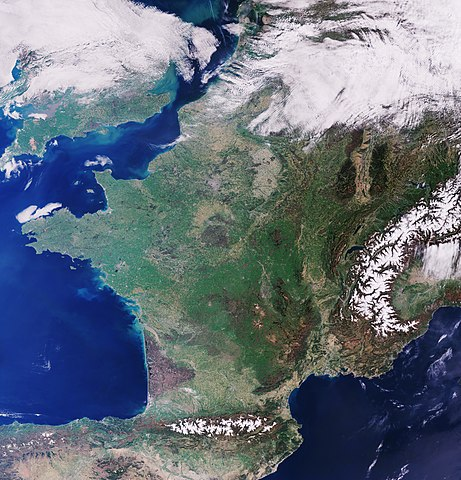
\includegraphics[scale=0.20]{france_satellite.jpg} \quad 
  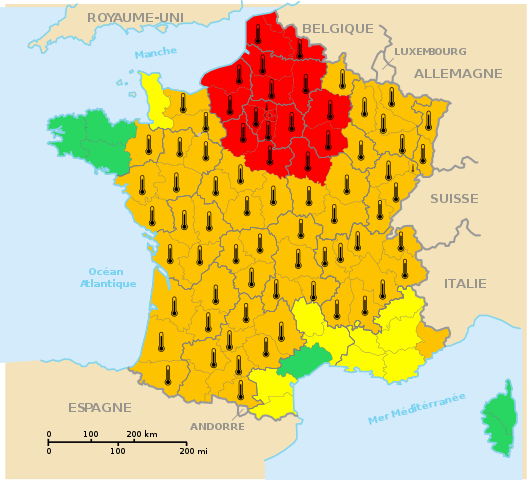
\includegraphics[scale=0.20]{heatwave_map.png}%
  \caption{From the reality to predictions}
  \end{figure}
\end{center}
\end{frame}


\begin{frame}{Modelling of the ocean, bottom friction}
  \pnote{We are going to take for instance the modelling of the ocean.

    First thing first, most numerical models are usually based
    on a subdivision of the ocean into cells, which interacts with
    each others. Those cells have a size in the order of the kilometer.
    
    At the bottom of the ocean, the different types of soil and
    sediments have an influence on the circulation of the water at the
    surface.  Indeed, the ocean bed is not completely smooth, there
    are rocks, sand, gravel, and all those asperities create
    turbulences, which dissipate energy. This phenomenon happens at a
    scale much smaller than the scale of the mesh provided for the
    simulation.

    All in all, instead of modelling individually each rock or
    asperity, we can introduce a parameter, which will quantify for
    each cell the effect of the friction.
  }
  % A lot of choices/simplifications are required to construct models, which depends on
  % the scale we wish to represent: 
  \begin{block}{Example: modelling of the ocean}
    \begin{itemize}
    \item Ocean domain discretized
    \item External tidal forcing
    \item Energy is dissipated through turbulences caused by the asperities at the bottom
      \begin{itemize}
      \item The water currents at the surface are affected
      \item The friction is taken into account at a cell level
    \end{itemize}
    \end{itemize}
  \end{block}
  \begin{center}
    \only<1>{\scalebox{.9}{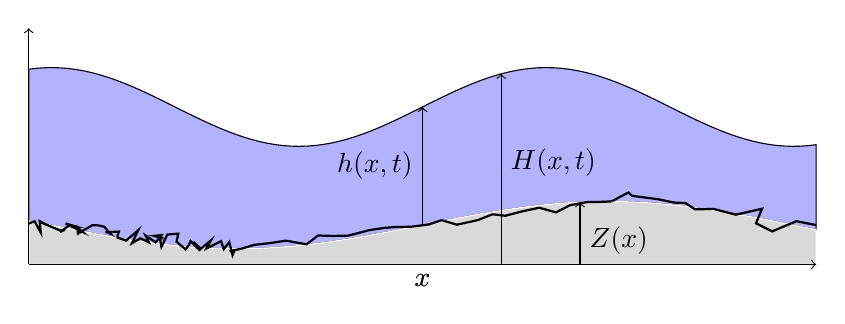
\begin{tikzpicture}
\usetikzlibrary{decorations.pathmorphing}

\definecolor{copper}{rgb}{0.69, 0.25, 0.21}
\definecolor{tin}{rgb}{0.7, 0.7, 0.7}

\tikzset{
  rugous1/.style = {black, thick,
    decoration={random steps,segment length=0.05cm,amplitude=.1cm}
  },
}
\tikzset{
  rugous2/.style = {black, thick,
    decoration={random steps,segment length=0.2cm,amplitude=.05cm}
  },
}
\tikzset{
  rugous3/.style = {black, thick,
    decoration={random steps,segment length=0.2cm,amplitude=.15cm}
  },
}

\filldraw [fill = blue!30]
   plot [samples = 100,domain = -5:5] (\x, {0.5*sin(\x r) + 2} )
-- plot [samples = 100,domain = 5:-5] (\x, {0.3*sin(\x/1.5 r)+0.5})
-- cycle;

\filldraw[fill = gray!30, draw = white]
   plot [samples = 100,domain = -5:5] (\x, {0.3*sin(\x/1.5 r)+0.5})
-- plot [samples = 100,domain = 5:-5] (\x, 0)
-- cycle;

\draw[rugous1, decorate](-5,0.52) -- (-2.3,0.2);
\draw[rugous2, decorate](-2.3,0.2) -- (2.4,0.8);
\draw[rugous3, decorate](2.4,0.8) -- (5,0.5);

\draw[->] (-5,0) -- (5,0);
\draw (0,0) node[below] {$x$};



\draw[->] (-5,0) -- (-5,3);

\draw[->] (0,0.5) -- (0,2);
\draw (0, 1.25) node[left] {$h(x,t)$} ;
\draw (0,0) node[below] {$x$};
\draw[->] (2,0) -- (2,{0.3*sin(2/1.5 r)+0.5});
\draw (2, 0.3) node[right] {$Z(x)$} ;
\draw[->] (1,0) -- (1,{0.5*sin(1 r)+2});
\draw (1, 1.3) node[right] {$H(x,t)$} ;
\end{tikzpicture}}}
    \only<2>{\scalebox{.9}{\newcommand{\turb}[2]
{\draw [domain=0:25.1327,variable=\t,smooth,samples=75, -Latex]
        plot ({\t r}: {0.002*\t*\t});}

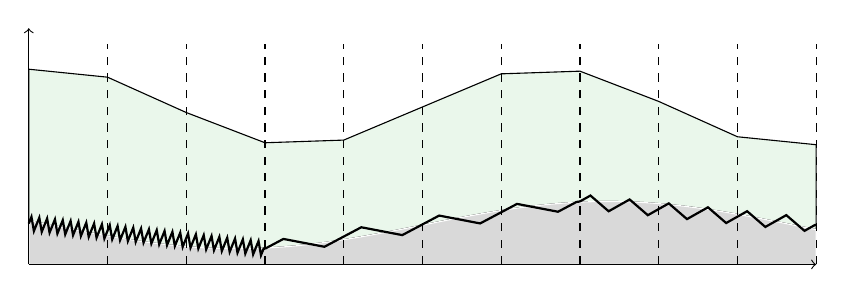
\begin{tikzpicture}
\usetikzlibrary{decorations.pathmorphing}
\definecolor{copper}{rgb}{0.69, 0.25, 0.21}
\definecolor{tin}{rgb}{0.7, 0.7, 0.7}
\definecolor{water}{HTML}{BAE4BC}
\tikzset{
  rugous1/.style = {black, thick,decoration={zigzag, segment length=0.1cm}
   % decoration={random steps,segment length=0.05cm,amplitude=.1cm}
  },
}
\tikzset{
  rugous2/.style = {black, thick,decoration={zigzag, segment length=1cm}
  %  decoration={random steps,segment length=0.2cm,amplitude=.05cm}
  },
}
\tikzset{
  rugous3/.style = {black, thick,decoration={zigzag, segment length=0.5cm}
    %decoration={random steps,segment length=0.2cm,amplitude=.15cm}
  },
}

\filldraw [fill = water!30]
   plot [samples = 11,domain = -5:5] (\x, {0.5*sin(\x r) + 2} )
-- plot [samples = 100,domain = 5:-5] (\x, {0.3*sin(\x/1.5 r)+0.5})
-- cycle;

\filldraw[fill = gray!30, draw = white]
   plot [samples = 100,domain = -5:5] (\x, {0.3*sin(\x/1.5 r)+0.5})
-- plot [samples = 100,domain = 5:-5] (\x, 0)
-- cycle;

\draw[rugous1, decorate](-5,0.52) -- (-2.,0.2);
\draw[rugous2, decorate](-2,0.2) -- (2.,0.8);
\draw[rugous3, decorate](2,0.8) -- (5,0.5);

\draw[->] (-5,0) -- (5,0);
%\draw (0,0) node[below] {$x$};
\foreach \x in {-4,...,5}{
\draw[dashed] (\x,0) -- (\x, 2.8);}


\draw[->] (-5,0) -- (-5,3);
%\draw[<->, red, very thick] (-5, {0.5*sin(-5 r)+2.5}) -- (-5, {0.5*sin(-5 r)+1.5}) node[midway,left] {$f(\mathbf{u})$};
\
% \draw[->] (0,0.5) -- (0,2);
% \draw (0, 1.25) node[left] {$h(x,t)$} ; %
% \draw (0,0) node[below] {$x$};
% \draw[->] (2,0) -- (2,{0.3*sin(2/1.5 r)+0.5});
% \draw (2, 0.3) node[right] {$Z(x)$} ;
% \draw[->] (1,0) -- (1,{0.5*sin(1 r)+2});
% \draw (1, 1.3) node[right] {$H(x,t)$} ;
\end{tikzpicture}}}
  \end{center}
\end{frame}

\begin{frame}{The modelling process}
  \pnote{ To summarize, in the end, we have a model, with a lot of
    parameters, which is supposed to represent the reality.

    Some of those parameters cannot be chosen, as their value may
    come from real observations, measured physical properties, or
    other environmental conditions.

    Some other need to be tuned accordingly.  Now, the question, is
    how to choose the value of those remaining parameters, so that the
    model, the simulations are accurate enough ?

  }
  \begin{center}
    \begin{adjustbox}{clip,
        trim=33cm 0cm 0cm 0cm,
        max width=0.9\textwidth, center}
     \usetikzlibrary{calc, arrows, decorations.markings}

\begin{tikzpicture}[decoration = {markings,
    mark = at position 0.5 with {\arrow[>=stealth]{>}}
  }, node distance= 40ex, text centered
  ]
\definecolor{mycolor}{rgb}{1,0.2,0.3}
\fill[gray!10] (-1.8,-.7) -- (1.8,-.7) -- (1.8,2.5) -- (-1.8,2.5);

 \draw  node[rectangle, fill=brewdark] (x) {Physical system} ;
  \draw node[rectangle, fill=brewdark, right of=x] (y) {Mathematical model};
 \draw  node[rectangle, fill=brewdark, right of = y] (z) {Computer code};
  \draw[postaction = decorate, very thick] (x) to node[midway, below, text width=20ex](az) {Simplifications, parametrizations} (y)  ;
  \draw[postaction = decorate, very thick] (y) to node[midway, below, text width=20ex] {Discretization implementation}(z);
\draw node[text width = 20ex, text centered](tune) at (40ex,-15ex) {Error on the parameters};
\draw node[text width = 20ex] (nature) at (0ex, 10ex) {Natural variability};
\draw[->] (nature) to (x);
\draw[->] (tune) to  (55ex,-7ex);
\draw[->] (tune) to  (25ex,-7ex);
\end{tikzpicture}
    \end{adjustbox}
  \end{center}

  $\rightarrow$ How well can we calibrate the model, so that it depicts \emph{accurately} the reality ?
\end{frame}



\AtBeginSection{
  \frame{
    \sectionpage
    \tableofcontents[currentsection,currentsubsection]% ,hideothersubsections, 
    % sectionstyle=show/hide, 
    % subsectionstyle=show/shaded]
  }
}

\begin{frame}[t]{Computer code and inverse problem}
  \pnote{We are now going to translate these questions using a
    classical setting of inverse problem.

    The parameter we want to calibrate, to control is called the control
    parameter theta

    The other parameters, that we do not have much control are called
    the environmental variables, which are considered fixed, and
    known.

    our numerical model, M can be seen as an operator, taking as
    inputs theta and u, and outputs an observable quantity, for
    instance the sea water height. This is the direct simulation.

    Our goal, in an inverse problem setting, is, given some
    observations y, what is the best value of theta, so that the
    output of the numerical model matches as closely as possible the observations ?
  }
  \begin{itemize}
  \item[Input]
    \begin{itemize}
    \item $\kk$: Control
      parameter%Bottom friction (spatially distributed)
    \item $\uu$: Environmental variables (fixed and known)
    \end{itemize}
  \item[Output] \begin{itemize}
    \item $\mathcal{M}(\kk,\uu)$: Quantity to be compared to
      observations $y$%Sea surface height, at predetermined time of the
                  %simulation and at certain location
    \end{itemize}
  \end{itemize}
  \vfill
  % \only<1>{\tikzstyle{block} = [rectangle, draw, fill=blue!20, 
     text centered, minimum width=1cm]

\tikzstyle{block2} = [rectangle, draw, fill=green!20, 
     text centered, rounded corners, minimum width=1cm]

\tikzstyle{LHS}=[rectangle, draw, text centered]

\begin{tikzpicture}[node distance=3cm]

\node [align = center] at (0,0) (input) {Control variable \\$K \in \mathcal{K}$};
%\node [align = center] at (4,1.5) (envir) {Environmental variables \\$\bm{u} \in \mathcal{U}$ fixed};
\node [align = center] at (4,1.5) (envir) {Environmental variables \\$\bm{x}_e \in \mathbb{X}$ fixed};

\node[block] at (4,0)(code){Direct Simulation};

\node[align = center] at (8,0) (output) {$W(K)$}; %\\ $\Rightarrow j(K)$};

\draw[->] (input) -- (code);
\draw[->] (envir) -- (code);
\draw[->] (code) -- (output);

\end{tikzpicture}}
  \only<1>{
    \begin{center}
      \usetikzlibrary{positioning}
% \tikzstyle{block} = [rectangle, draw, fill=blue!30, 
%     text centered, minimum width=3em] 
 \tikzstyle{block} = [rectangle, draw, fill=blkcol, 
      text centered, minimum width=3em]

\tikzstyle{block2} = [rectangle, draw, fill=blkcol2, 
     text centered, rounded corners, minimum width=3em]

% \tikzstyle{block2} = [rectangle, draw, fill=blkcol2, 
%      text centered, rounded corners, minimum width=3em]

\tikzstyle{LHS}=[rectangle, draw, text centered]

\begin{tikzpicture}

%\node [align = center] at (0,0) (input) {Control variable \\$\mathbf{k} \in \mathbb{K}$};
\node [align = center] at (0,0) (input) {Control variable \\$\bm{k} \in \mathbb{K}$};
\node[block] at (4,0) (code){Direct Simulation};
%\node [align = center, above =of  code ] (envir) {Environmental variables \\$\mathbf{u} \in \mathbb{U}$ fixed};
\node [align = center] at (4,1.5) (envir) {Environmental variables \\$\bm{u} \in \mathbb{U}$ fixed};




%\node[align = center, right =of  code] (output) {$M(\mathbf{k})$};
\node[align = center] at (8,0) (output) {$\mathcal{M}(\bm{k},\bm{u})$};
%\node [align = center, right =of  inv, below = of output]  (obs) {$\mathbf{y}$};
\node [align = center] at (8,-1) (obs) {$\yobs$};
\node[block] at (4,-1) (inv) {Inverse Problem};

\draw[->] (input) -- (code);
\draw[->] (envir) -- (code);
\draw[->] (code) -- (output);

 % \node [align = center] at (0,0) (input) {$Y = \mathbb{H}M(K_{\mathrm{ref}})$};
 % \node [align = center] at (4,1.5) (envir) {Environmental variables \\$X_e$ r.v.};

 % \node[block] at (4,0)(code){"Inverse Problem"};

% \node[align = center] at (8,0) (output) {$K$};

\draw[->] (input) -- (code);
% \draw[->] (envir) -- (code);
\draw[->] (code) -- (output);
\draw[->] (output) -- (obs) ;
\draw[->] (inv) -|(input) ;
\draw[->] (obs) -- (inv);
\end{tikzpicture}
    \end{center}
  }
\end{frame}

\begin{frame}{Data assimilation framework}
  \pnote{ In practice, we select a value of the environmental
    parameters u, and using the least square approach, we define J, an
    objective function, as the sum of the squares of the difference
    between the observations and the output of the numerical model.


    This is a deterministic optimisation problem, that we can solve
    using classical methods such as adjoint gradient.
    The resulting parameter theta hat is then optimal in this situation.

    However, this estimation depends on the value of the environmental
    parameter chosen initially.  Now, what happens if this parameter
    changes ? 
    The minimisation procedure is supposed to correct the
    error on theta but will it try to compensate too much ? }

  Let $\uu \in \Uspace$, assumed fixed and known
  \begin{block}{Objective function}
    We define $J$ as the squared difference between the output of the
    model and the observations
    \begin{equation}
      J(\kk, \uu) =  \frac12 \|\mathcal{M}(\kk,\uu) - \yobs \|^2
    \end{equation}
    \alert<1>{$\rightarrow$ the smaller $J$ is, the better the fit is}
  \end{block}
 \onslide<2>{
  We can get an estimate by solving an optimisation problem:
  \begin{equation}
    \min_{\kk\in\Kspace} J(\kk, \uu) = J(\hat{\kk},\uu)
  \end{equation}
  % \begin{enumerate}[$\rightarrow$]
  % \item Deterministic optimization problem
  % \item Possibly add regularization
  % \item Classical methods: Adjoint gradient and Gradient-descent
  % \end{enumerate}
\begin{itemize} %A: Mettre en valeur
  \item \alert{$\hat{\kk}$ depends inherently on $\uu$}
  \item What if $\uu$ is uncertain by nature ?
  \item Does $\hat{\kk}$ compensate the errors brought by variability? ($\sim$ overfitting)
    % \item How well will $\bm{\hat{k}}$ perform under other
    %   conditions?
  \end{itemize}
}

\end{frame}
\begin{frame}{An example: Misspecification of $u$ }
  \pnote{ We are going to illustrate this issue, with the calibration
    problem of the bottom friction in a model of the north atlantic
    ocean. This setting will be detailed later, but we can see how the optimal value depends on the environmental parameter:
    
    Some regions are left unaffected, especially in the bay of biscay,
    but some other vary directly with the environmental parameter.

    So now the question is, how to select a value of the control
    parameter, such that it is quite close to the reality, even when u
    changes? }
  
  Minimization of $\kk\mapsto J\left(\kk,\uu\right)$, for
  different $\uu$, which parametrizes some boundary conditions:  $\uu=\only<1>{(0.0, 0.0)}%
  \only<2>{(0.0, 0.5)}%
  \only<3>{(0.0, 1.0)}%
  \only<4>{(0.5, 0.0)}%
  \only<5>{(0.5, 0.5)}%
  \only<6>{(0.5, 1.0)}%
  \only<7>{(1.0, 0.0)}%
  \only<8>{(1.0, 0.5)}%
  \only<9>{(1.0, 1.0)}%
  $
  \vfill % \only<2>{Well-specified model} \only<3>{1\%
  %   error on the amplitude of the M2 tide} \only<4>{1\% error on the
  %   amplitude of the M2 tide}
  % % \only<5>{0.5\% error on the amplitude of the M2 tide, starting at
  % % the truth}
  \begin{center}
    \includegraphics<1>[scale=.9]{/home/victor/optimisation_dahu/1b/map_slides_lognorm_200.png}%
    \includegraphics<2>[scale=.9]{/home/victor/optimisation_dahu/2b/map_slides_lognorm_200.png}%
    \includegraphics<3>[scale=.9]{/home/victor/optimisation_dahu/3b/map_slides_lognorm_200.png}%
    \includegraphics<4>[scale=.9]{/home/victor/optimisation_dahu/4b/map_slides_lognorm_200.png}%
    \includegraphics<5>[scale=.9]{/home/victor/optimisation_dahu/optim_sediments/map_slides_lognorm_200.png}%
    \includegraphics<6>[scale=.9]{/home/victor/optimisation_dahu/6b/map_slides_lognorm_200.png}%
    \includegraphics<7>[scale=.9]{/home/victor/optimisation_dahu/7b/map_slides_lognorm_200.png}%
    \includegraphics<8>[scale=.9]{/home/victor/optimisation_dahu/8b/map_slides_lognorm_200.png}%
    \includegraphics<9>[scale=.9]{/home/victor/optimisation_dahu/9b/map_slides_lognorm_200.png}%
  \end{center}
\end{frame}

\begin{frame}{A definition of robustness ?}
  \pnote{This is how we are going to define robustness: an estimate
    will be considered robust if the objective function gives good
    performances when u varies

    
    In this presentation we are going to see how this notion of
    robustness can be translated quantitatively, especially by
    introducing notions of regret.

    As we are going to see, such robust estimates can become expensive
    to compute. We will then introduce methods based on gaussian
    processes, in order to make computations tractable

    Finally, we are going to apply some of those methods to the
    calibration of an academic model of the ocean, based on CROCO}
  \begin{block}{Robustness}
    $\hat{\kk}$ can be considered ``robust'' if $J(\hat{\kk}, \uu)$
    gives ``good enough'' performances when $\uu$ varies
  \end{block}

  \textbf{Main objectives:}
  \begin{itemize}
  \item Define quantitative criteria of robustness
  \item Develop methods in order to compute robust estimates efficiently
  \item Apply those methods to the robust calibration of CROCO 
  \end{itemize}
\end{frame}


%%%%
\AtBeginSection{
  \frame{
    \sectionpage
    \tableofcontents% [currentsection,currentsubsection]
    % ,hideothersubsections, 
    % sectionstyle=show/hide, 
    % subsectionstyle=show/shaded]
  }
}
\section*{Outline}
\metroset{sectionpage=progressbar}
\AtBeginSection{
  \frame{
    \sectionpage
    \tableofcontents[currentsection,currentsubsection]% ,hideothersubsections, 
    % sectionstyle=show/hide, 
    % subsectionstyle=show/shaded]
  }
}


\section{Robustness in calibration}
\begin{frame}{Different types of uncertainties}
    \pnote{We evoked earlier that the
    uncertainty on theta or on u is not the same, and we can make a
    rough distinction between two types:

    - First, the epistemic uncertainties that result from a lack of
    knowledge, but can be reduced. An example is the uncertainty
    during the estimation of the mean value. The more samples you
    take, the less uncertainty there is on your estimation

    - Secondly, there is the aleatoric uncertainty, that comes from
    the inherent variability of the system studied. Think of the
    different values that a random variable takes.

    Our goal, is then to be able to reduce the epistemic uncertainty
    on the value of theta, while taking into account the aleatoric
    uncertainty.}
  
  \begin{block}{Epistemic or aleatoric
      uncertainties?~\citep{walker_defining_2003}}
    \begin{itemize}
    \item Epistemic uncertainties: From a lack of knowledge, that can
      be reduced with more research/exploration
    \item Aleatoric uncertainties: Inherent variability of the system
      studied, operating conditions that we cannot afford to research further
    \end{itemize}
  \end{block}

  \begin{itemize}
  \item $\kk$: Control parameter, needs to be tuned
  \item $\uu$: Environmental variable, subject to natural variability
  \end{itemize}
  
  Our goal is to take into account the aleatoric uncertainties (=the
  assumed variability of the environmental conditions) in the
  estimation of the control parameter (=reduction of the epistemic uncertainties).
\end{frame}

\begin{frame}[t]{Aleatoric uncertainty as a random variable}
  \pnote{The aleatoric uncertainty present in the environmental
    variable will be modelled using a random variable.

    The distribution of this random variable, written using an
    uppercase letter U is assumed to be known.
    The lowercase u is a sample, a realization of this random variable

    In this case, we can consider that the output of the model is a
    random variable.
  }
  \begin{itemize}
  \item $\UU$: random variable of known distribution, with support $\Uspace$
  \item $\uu$ is a sample of $\UU$ 
  \end{itemize}
  \vfill \only<1>{
    \begin{center}
      \usetikzlibrary{positioning}
% \tikzstyle{block} = [rectangle, draw, fill=blue!30, 
%     text centered, minimum width=3em] 
 \tikzstyle{block} = [rectangle, draw, fill=blkcol, 
      text centered, minimum width=3em]

\tikzstyle{block2} = [rectangle, draw, fill=blkcol2, 
     text centered, rounded corners, minimum width=3em]

% \tikzstyle{block2} = [rectangle, draw, fill=blkcol2, 
%      text centered, rounded corners, minimum width=3em]

\tikzstyle{LHS}=[rectangle, draw, text centered]

\begin{tikzpicture}

%\node [align = center] at (0,0) (input) {Control variable \\$\mathbf{k} \in \mathbb{K}$};
\node [align = center] at (0,0) (input) {Control variable \\$\bm{k} \in \mathbb{K}$};
\node[block] at (4,0) (code){Direct Simulation};
%\node [align = center, above =of  code ] (envir) {Environmental variables \\$\mathbf{u} \in \mathbb{U}$ fixed};
\node [align = center] at (4,1.5) (envir) {Environmental variables \\$\bm{u} \in \mathbb{U}$ fixed};




%\node[align = center, right =of  code] (output) {$M(\mathbf{k})$};
\node[align = center] at (8,0) (output) {$\mathcal{M}(\bm{k},\bm{u})$};
%\node [align = center, right =of  inv, below = of output]  (obs) {$\mathbf{y}$};
\node [align = center] at (8,-1) (obs) {$\yobs$};
\node[block] at (4,-1) (inv) {Inverse Problem};

\draw[->] (input) -- (code);
\draw[->] (envir) -- (code);
\draw[->] (code) -- (output);

 % \node [align = center] at (0,0) (input) {$Y = \mathbb{H}M(K_{\mathrm{ref}})$};
 % \node [align = center] at (4,1.5) (envir) {Environmental variables \\$X_e$ r.v.};

 % \node[block] at (4,0)(code){"Inverse Problem"};

% \node[align = center] at (8,0) (output) {$K$};

\draw[->] (input) -- (code);
% \draw[->] (envir) -- (code);
\draw[->] (code) -- (output);
\draw[->] (output) -- (obs) ;
\draw[->] (inv) -|(input) ;
\draw[->] (obs) -- (inv);
\end{tikzpicture}%
    \end{center}
  }%
  \only<2>{
    \begin{center}
      
\tikzstyle{block} = [rectangle, draw, fill=blkcol, 
     text centered, minimum width=1cm]
\tikzstyle{block2} = [rectangle, draw, fill=blkcol2, 
     text centered, rounded corners, minimum width=1cm]

\tikzstyle{LHS}=[rectangle, draw, text centered]

\begin{tikzpicture}[node distance=3cm]

\node [align = center] at (0,0) (input) {Control variable \\$\bm{k} \in \mathcal{K}$};
\node [align = center] at (4,1.5) (envir) {Environmental variables \\\alert<2>{$\bm{U}$ random}};
\node[block] at (4,0)(code){Direct Simulation};
\node[align = center] at (8,0) (output) {$W(\alert<2>{\bm{U}},\bm{k})$};
\node [align = center] at (8,-1) (obs) {$\yobs$};
\node[block] at (4,-1) (inv) {Inverse Problem};
\draw[->] (input) -- (code);
\draw[->] (envir) -- (code);
\draw[->] (code) -- (output);
\draw[->] (inv) -|(input) ;
\draw[->] (obs) -- (inv);
\draw[->] (output) -- (obs);
\end{tikzpicture}%
    \end{center}
  } \vfill
\end{frame}

\begin{frame}{The objective function as a random variable}
  \pnote{I'd like to point out that the numerical model is still
    completely deterministic: the choice and sampling of lowercase u
    is still up to the user.

    But in terms of random variable, we will now have to consider that
    the objective function is a random variable, indexed by theta }
  \begin{itemize}
  \item The computer code is \textit{still} deterministic, and takes $\kk$ and $\uu$
    as inputs (from the user):
    \begin{equation*}
      \mathcal{M}(\kk,\alert{\uu})
    \end{equation*}
  \item Due to the previous assumptions, the quadratic error $J$ is
    now considered as a random variable, indexed by $\kk$
    \begin{equation*}
      J(\kk,\alert{\UU}) =  \frac12\|\mathcal{M}(\kk,\alert{\UU}) - \yobs\|^2
    \end{equation*}
  \end{itemize}

\end{frame}




% \subsection{Definitions of robustness}
\begin{frame}{Robust objectives of the objective function}
  \pnote{I'm going to present very quickly some estimates that can be
    considered robust.

    First we can think about minimising the objective function in the
    worst case sense. This usually leads to overly conservative
    estimates as we are maximizing over the whole space U.

    Due to the fact that the objective function can be considered as a
    random variable, we can also think about minimising the moments,
    such as the mean value. Or by looking for the pareto front in
    order to get a good compromise between mean and variance of the
    objective function.

    Finally, we can also look to minimize some well-chosen quantile of
    the objective function.

    In this presentation, we are going to focus on a specific idea,
    based on the regret:

    Every choice of environmental variable gives a
    distinct situation The aspect we are going to focus on is based on
    the regret, so it implies a comparison with the best performance
    attainable for each u.  }
  We are looking for $\hat{\kk}$, such
  that $J(\hat{\kk}, \UU)$ gives ``good performances''

  \begin{itemize}
    % \item Global Optimum: $ \min_{(\kk,\uu)} J(\uu,\kk)$
    %   $ \longrightarrow $ EGO
  \item Worst case~\citep{marzat_worst-case_2013}:
    $$ \min_{\kk \in \Kspace} \left\{\max_{\uu \in \Uspace}
      J(\kk,\uu)\right\}$$
  \item M-robustness % V-robustness
    ~\citep{lehman_designing_2004}:
    $$\min_{\kk\in\Kspace} \Ex_{\UU}\left[J(\kk,\UU)\right]$$
  \item Multiobjective~\citep{baudoui_optimisation_2012}:
    $$\text{Pareto frontier of } (\Ex_{\UU}\left[J(\kk,\UU)\right],\Var_{\UU}\left[J(\kk,\UU)\right])$$
    \item Reliability
      $$ \min_{\kk\in\Kspace} Q_{\UU}(J(\kk, \UU); p) $$
  % \item Region of failure given by
  %   $J(\kk,\uu)>T$~\cite{bect_sequential_2012}:
  %   $$\max_{\kk \in \Kspace} R(\kk) = \max_{\kk\in \Kspace}
  %   \Prob_{\uu}\left[J(\kk,\uu) \leq T \right]$$
\item \alert{Regret-based estimates}
\end{itemize}
\end{frame}

\begin{frame}{The notion of relative-regret}
  \pnote{For each choice of u, the environmental variable, we have a
    different calibration problem. Once the optimisation is performed,
    we have an optimal value Jstar, and an estimate theta star.

    But in the end, we want a single value of theta, which is good
    even when u varies, so we are going to compare the performances,
    so the value of the objective function when theta is set to the optimal value given u, so Jstar

    So we are going to introduce the relative-regret, which is defined
    by ratio of the objective function, divided by the conditional
    minimum Jstar. So when the regret is large, there is a lot of
    deviations from the optimal value.

    Based on this idea, we can introduce a notion of acceptability by
    using a threshold, alpha.  So a pair of points is considered
    acceptable at a level alpha, if the relative regret is less than
    alpha.}
  
  Given $\uu\in\Uspace$, how well can we calibrate the model ?
  \begin{itemize}
  \item The best performance is $\min_{\kk\in\Kspace} J(\kk, \uu) = J^*(\uu)>0$
  \item How does $J^*(\uu)$ compare to $J(\kk, \uu)$ ?
  \item What is the cost of choosing $\kk$ instead of $\kk^*(\uu)=\argmin_{\kk} J(\kk, \uu)$ ?
  \end{itemize}
\onslide<2>{
  \begin{block}{The relative-regret, $\alpha$-acceptability}
    \begin{itemize}
    \item We define the relative-regret as the ratio $\frac{J(\kk, \uu)}{J^*(\uu)}$
    \item $(\kk,\uu)$ said $\alpha$-acceptable if $\frac{J(\kk, \uu)}{J^*(\uu)} \leq \alpha \Rightarrow J(\kk,\uu) \leq \alpha J^*(\uu)$
    \end{itemize}
  \end{block}
  }
\end{frame}

 
\begin{frame}{Construction of regions of acceptability}
  \pnote{For an illustration purpose, we are going to see what does it
    look like on an analytical function J, which is strictly positive.
    On the x axis, we have the control parameter, on the y axis, the environmental parameter.
    
    So for a given u, so for an horizontal slice of this figure, we
    can optimize the objective function, this leads to Jstar, the
    conditional minimum, and theta star, the conditional minimiser.

    By doing so for all the other values of the environmental
    paramter, we can get visualize the set of all conditional
    minimisers.

    We now introduce the threshold, alpha, and define the region of
    alpha acceptability.  So within the yellow lines, we are
    acceptable at a level alpha, since the objective function is less
    than alpha times Jstar.

    We want to see how often each single value theta is
    acceptable, so we are going to measure the set of acceptable value
    with respect to the probability distribution of U, this is the
    green line.

    Finally, that is how Gamma alpha is defined: this represent the
    probabiltiy to be acceptable at a level alpha, or in other words,
    the probability that the relative-regret is less than alpha.  This
    can be seen as a measure of robustness, so we want this green line
    to be as long as possible.
  } \scalebox{0.5}{%
    Analytical objective function
    $J(\kk, \uu) = \frac{1}{51.95}\left[\left(x_2 -
        \frac{5.1}{4\pi^2}x_1^2 + \frac{5}{\pi}x_1-6\right)^2 + (10 -
      \frac{10}{8\pi})\cos(x_1) - 44.81\right] + 2,\quad x_1 =
    15\kk-5,\quad x_2 = 15\uu$}\vspace{-.5cm}
  \begin{columns}
    \begin{column}{0.45\textwidth}
      \vspace{0.5cm}
      \begin{overlayarea}{\textwidth}{\textheight}
      \only<1>{\resizebox{\textwidth}{!}{%% Creator: Matplotlib, PGF backend
%%
%% To include the figure in your LaTeX document, write
%%   \input{<filename>.pgf}
%%
%% Make sure the required packages are loaded in your preamble
%%   \usepackage{pgf}
%%
%% Figures using additional raster images can only be included by \input if
%% they are in the same directory as the main LaTeX file. For loading figures
%% from other directories you can use the `import` package
%%   \usepackage{import}
%%
%% and then include the figures with
%%   \import{<path to file>}{<filename>.pgf}
%%
%% Matplotlib used the following preamble
%%   \usepackage{fontspec}
%%   \setmainfont{DejaVuSans.ttf}[Path=\detokenize{/home/victor/virtualenvs/robustGP/lib/python3.8/site-packages/matplotlib/mpl-data/fonts/ttf/}]
%%   \setsansfont{LiberationSans-Regular.ttf}[Path=\detokenize{/usr/share/fonts/truetype/liberation/}]
%%   \setmonofont{DejaVuSansMono.ttf}[Path=\detokenize{/home/victor/virtualenvs/robustGP/lib/python3.8/site-packages/matplotlib/mpl-data/fonts/ttf/}]
%%
\begingroup%
\makeatletter%
\begin{pgfpicture}%
\pgfpathrectangle{\pgfpointorigin}{\pgfqpoint{4.000000in}{4.000000in}}%
\pgfusepath{use as bounding box, clip}%
\begin{pgfscope}%
\pgfsetbuttcap%
\pgfsetmiterjoin%
\definecolor{currentfill}{rgb}{1.000000,1.000000,1.000000}%
\pgfsetfillcolor{currentfill}%
\pgfsetlinewidth{0.000000pt}%
\definecolor{currentstroke}{rgb}{1.000000,1.000000,1.000000}%
\pgfsetstrokecolor{currentstroke}%
\pgfsetdash{}{0pt}%
\pgfpathmoveto{\pgfqpoint{0.000000in}{0.000000in}}%
\pgfpathlineto{\pgfqpoint{4.000000in}{0.000000in}}%
\pgfpathlineto{\pgfqpoint{4.000000in}{4.000000in}}%
\pgfpathlineto{\pgfqpoint{0.000000in}{4.000000in}}%
\pgfpathclose%
\pgfusepath{fill}%
\end{pgfscope}%
\begin{pgfscope}%
\pgfsetbuttcap%
\pgfsetmiterjoin%
\definecolor{currentfill}{rgb}{0.917647,0.917647,0.949020}%
\pgfsetfillcolor{currentfill}%
\pgfsetlinewidth{0.000000pt}%
\definecolor{currentstroke}{rgb}{0.000000,0.000000,0.000000}%
\pgfsetstrokecolor{currentstroke}%
\pgfsetstrokeopacity{0.000000}%
\pgfsetdash{}{0pt}%
\pgfpathmoveto{\pgfqpoint{0.500000in}{0.440000in}}%
\pgfpathlineto{\pgfqpoint{3.600000in}{0.440000in}}%
\pgfpathlineto{\pgfqpoint{3.600000in}{3.520000in}}%
\pgfpathlineto{\pgfqpoint{0.500000in}{3.520000in}}%
\pgfpathclose%
\pgfusepath{fill}%
\end{pgfscope}%
\begin{pgfscope}%
\pgfpathrectangle{\pgfqpoint{0.500000in}{0.440000in}}{\pgfqpoint{3.100000in}{3.080000in}}%
\pgfusepath{clip}%
\pgfsetroundcap%
\pgfsetroundjoin%
\pgfsetlinewidth{1.003750pt}%
\definecolor{currentstroke}{rgb}{1.000000,1.000000,1.000000}%
\pgfsetstrokecolor{currentstroke}%
\pgfsetdash{}{0pt}%
\pgfpathmoveto{\pgfqpoint{0.500000in}{0.440000in}}%
\pgfpathlineto{\pgfqpoint{0.500000in}{3.520000in}}%
\pgfusepath{stroke}%
\end{pgfscope}%
\begin{pgfscope}%
\definecolor{textcolor}{rgb}{0.150000,0.150000,0.150000}%
\pgfsetstrokecolor{textcolor}%
\pgfsetfillcolor{textcolor}%
\pgftext[x=0.500000in,y=0.342778in,,top]{\color{textcolor}\sffamily\fontsize{10.000000}{12.000000}\selectfont \(\displaystyle {0.0}\)}%
\end{pgfscope}%
\begin{pgfscope}%
\pgfpathrectangle{\pgfqpoint{0.500000in}{0.440000in}}{\pgfqpoint{3.100000in}{3.080000in}}%
\pgfusepath{clip}%
\pgfsetroundcap%
\pgfsetroundjoin%
\pgfsetlinewidth{1.003750pt}%
\definecolor{currentstroke}{rgb}{1.000000,1.000000,1.000000}%
\pgfsetstrokecolor{currentstroke}%
\pgfsetdash{}{0pt}%
\pgfpathmoveto{\pgfqpoint{1.120000in}{0.440000in}}%
\pgfpathlineto{\pgfqpoint{1.120000in}{3.520000in}}%
\pgfusepath{stroke}%
\end{pgfscope}%
\begin{pgfscope}%
\definecolor{textcolor}{rgb}{0.150000,0.150000,0.150000}%
\pgfsetstrokecolor{textcolor}%
\pgfsetfillcolor{textcolor}%
\pgftext[x=1.120000in,y=0.342778in,,top]{\color{textcolor}\sffamily\fontsize{10.000000}{12.000000}\selectfont \(\displaystyle {0.2}\)}%
\end{pgfscope}%
\begin{pgfscope}%
\pgfpathrectangle{\pgfqpoint{0.500000in}{0.440000in}}{\pgfqpoint{3.100000in}{3.080000in}}%
\pgfusepath{clip}%
\pgfsetroundcap%
\pgfsetroundjoin%
\pgfsetlinewidth{1.003750pt}%
\definecolor{currentstroke}{rgb}{1.000000,1.000000,1.000000}%
\pgfsetstrokecolor{currentstroke}%
\pgfsetdash{}{0pt}%
\pgfpathmoveto{\pgfqpoint{1.740000in}{0.440000in}}%
\pgfpathlineto{\pgfqpoint{1.740000in}{3.520000in}}%
\pgfusepath{stroke}%
\end{pgfscope}%
\begin{pgfscope}%
\definecolor{textcolor}{rgb}{0.150000,0.150000,0.150000}%
\pgfsetstrokecolor{textcolor}%
\pgfsetfillcolor{textcolor}%
\pgftext[x=1.740000in,y=0.342778in,,top]{\color{textcolor}\sffamily\fontsize{10.000000}{12.000000}\selectfont \(\displaystyle {0.4}\)}%
\end{pgfscope}%
\begin{pgfscope}%
\pgfpathrectangle{\pgfqpoint{0.500000in}{0.440000in}}{\pgfqpoint{3.100000in}{3.080000in}}%
\pgfusepath{clip}%
\pgfsetroundcap%
\pgfsetroundjoin%
\pgfsetlinewidth{1.003750pt}%
\definecolor{currentstroke}{rgb}{1.000000,1.000000,1.000000}%
\pgfsetstrokecolor{currentstroke}%
\pgfsetdash{}{0pt}%
\pgfpathmoveto{\pgfqpoint{2.360000in}{0.440000in}}%
\pgfpathlineto{\pgfqpoint{2.360000in}{3.520000in}}%
\pgfusepath{stroke}%
\end{pgfscope}%
\begin{pgfscope}%
\definecolor{textcolor}{rgb}{0.150000,0.150000,0.150000}%
\pgfsetstrokecolor{textcolor}%
\pgfsetfillcolor{textcolor}%
\pgftext[x=2.360000in,y=0.342778in,,top]{\color{textcolor}\sffamily\fontsize{10.000000}{12.000000}\selectfont \(\displaystyle {0.6}\)}%
\end{pgfscope}%
\begin{pgfscope}%
\pgfpathrectangle{\pgfqpoint{0.500000in}{0.440000in}}{\pgfqpoint{3.100000in}{3.080000in}}%
\pgfusepath{clip}%
\pgfsetroundcap%
\pgfsetroundjoin%
\pgfsetlinewidth{1.003750pt}%
\definecolor{currentstroke}{rgb}{1.000000,1.000000,1.000000}%
\pgfsetstrokecolor{currentstroke}%
\pgfsetdash{}{0pt}%
\pgfpathmoveto{\pgfqpoint{2.980000in}{0.440000in}}%
\pgfpathlineto{\pgfqpoint{2.980000in}{3.520000in}}%
\pgfusepath{stroke}%
\end{pgfscope}%
\begin{pgfscope}%
\definecolor{textcolor}{rgb}{0.150000,0.150000,0.150000}%
\pgfsetstrokecolor{textcolor}%
\pgfsetfillcolor{textcolor}%
\pgftext[x=2.980000in,y=0.342778in,,top]{\color{textcolor}\sffamily\fontsize{10.000000}{12.000000}\selectfont \(\displaystyle {0.8}\)}%
\end{pgfscope}%
\begin{pgfscope}%
\pgfpathrectangle{\pgfqpoint{0.500000in}{0.440000in}}{\pgfqpoint{3.100000in}{3.080000in}}%
\pgfusepath{clip}%
\pgfsetroundcap%
\pgfsetroundjoin%
\pgfsetlinewidth{1.003750pt}%
\definecolor{currentstroke}{rgb}{1.000000,1.000000,1.000000}%
\pgfsetstrokecolor{currentstroke}%
\pgfsetdash{}{0pt}%
\pgfpathmoveto{\pgfqpoint{3.600000in}{0.440000in}}%
\pgfpathlineto{\pgfqpoint{3.600000in}{3.520000in}}%
\pgfusepath{stroke}%
\end{pgfscope}%
\begin{pgfscope}%
\definecolor{textcolor}{rgb}{0.150000,0.150000,0.150000}%
\pgfsetstrokecolor{textcolor}%
\pgfsetfillcolor{textcolor}%
\pgftext[x=3.600000in,y=0.342778in,,top]{\color{textcolor}\sffamily\fontsize{10.000000}{12.000000}\selectfont \(\displaystyle {1.0}\)}%
\end{pgfscope}%
\begin{pgfscope}%
\definecolor{textcolor}{rgb}{0.150000,0.150000,0.150000}%
\pgfsetstrokecolor{textcolor}%
\pgfsetfillcolor{textcolor}%
\pgftext[x=2.050000in,y=0.157760in,,top]{\color{textcolor}\sffamily\fontsize{10.000000}{12.000000}\selectfont \(\displaystyle \theta\)}%
\end{pgfscope}%
\begin{pgfscope}%
\pgfpathrectangle{\pgfqpoint{0.500000in}{0.440000in}}{\pgfqpoint{3.100000in}{3.080000in}}%
\pgfusepath{clip}%
\pgfsetroundcap%
\pgfsetroundjoin%
\pgfsetlinewidth{1.003750pt}%
\definecolor{currentstroke}{rgb}{1.000000,1.000000,1.000000}%
\pgfsetstrokecolor{currentstroke}%
\pgfsetdash{}{0pt}%
\pgfpathmoveto{\pgfqpoint{0.500000in}{0.440000in}}%
\pgfpathlineto{\pgfqpoint{3.600000in}{0.440000in}}%
\pgfusepath{stroke}%
\end{pgfscope}%
\begin{pgfscope}%
\definecolor{textcolor}{rgb}{0.150000,0.150000,0.150000}%
\pgfsetstrokecolor{textcolor}%
\pgfsetfillcolor{textcolor}%
\pgftext[x=0.225308in, y=0.389680in, left, base]{\color{textcolor}\sffamily\fontsize{10.000000}{12.000000}\selectfont \(\displaystyle {0.0}\)}%
\end{pgfscope}%
\begin{pgfscope}%
\pgfpathrectangle{\pgfqpoint{0.500000in}{0.440000in}}{\pgfqpoint{3.100000in}{3.080000in}}%
\pgfusepath{clip}%
\pgfsetroundcap%
\pgfsetroundjoin%
\pgfsetlinewidth{1.003750pt}%
\definecolor{currentstroke}{rgb}{1.000000,1.000000,1.000000}%
\pgfsetstrokecolor{currentstroke}%
\pgfsetdash{}{0pt}%
\pgfpathmoveto{\pgfqpoint{0.500000in}{1.056000in}}%
\pgfpathlineto{\pgfqpoint{3.600000in}{1.056000in}}%
\pgfusepath{stroke}%
\end{pgfscope}%
\begin{pgfscope}%
\definecolor{textcolor}{rgb}{0.150000,0.150000,0.150000}%
\pgfsetstrokecolor{textcolor}%
\pgfsetfillcolor{textcolor}%
\pgftext[x=0.225308in, y=1.005680in, left, base]{\color{textcolor}\sffamily\fontsize{10.000000}{12.000000}\selectfont \(\displaystyle {0.2}\)}%
\end{pgfscope}%
\begin{pgfscope}%
\pgfpathrectangle{\pgfqpoint{0.500000in}{0.440000in}}{\pgfqpoint{3.100000in}{3.080000in}}%
\pgfusepath{clip}%
\pgfsetroundcap%
\pgfsetroundjoin%
\pgfsetlinewidth{1.003750pt}%
\definecolor{currentstroke}{rgb}{1.000000,1.000000,1.000000}%
\pgfsetstrokecolor{currentstroke}%
\pgfsetdash{}{0pt}%
\pgfpathmoveto{\pgfqpoint{0.500000in}{1.672000in}}%
\pgfpathlineto{\pgfqpoint{3.600000in}{1.672000in}}%
\pgfusepath{stroke}%
\end{pgfscope}%
\begin{pgfscope}%
\definecolor{textcolor}{rgb}{0.150000,0.150000,0.150000}%
\pgfsetstrokecolor{textcolor}%
\pgfsetfillcolor{textcolor}%
\pgftext[x=0.225308in, y=1.621680in, left, base]{\color{textcolor}\sffamily\fontsize{10.000000}{12.000000}\selectfont \(\displaystyle {0.4}\)}%
\end{pgfscope}%
\begin{pgfscope}%
\pgfpathrectangle{\pgfqpoint{0.500000in}{0.440000in}}{\pgfqpoint{3.100000in}{3.080000in}}%
\pgfusepath{clip}%
\pgfsetroundcap%
\pgfsetroundjoin%
\pgfsetlinewidth{1.003750pt}%
\definecolor{currentstroke}{rgb}{1.000000,1.000000,1.000000}%
\pgfsetstrokecolor{currentstroke}%
\pgfsetdash{}{0pt}%
\pgfpathmoveto{\pgfqpoint{0.500000in}{2.288000in}}%
\pgfpathlineto{\pgfqpoint{3.600000in}{2.288000in}}%
\pgfusepath{stroke}%
\end{pgfscope}%
\begin{pgfscope}%
\definecolor{textcolor}{rgb}{0.150000,0.150000,0.150000}%
\pgfsetstrokecolor{textcolor}%
\pgfsetfillcolor{textcolor}%
\pgftext[x=0.225308in, y=2.237680in, left, base]{\color{textcolor}\sffamily\fontsize{10.000000}{12.000000}\selectfont \(\displaystyle {0.6}\)}%
\end{pgfscope}%
\begin{pgfscope}%
\pgfpathrectangle{\pgfqpoint{0.500000in}{0.440000in}}{\pgfqpoint{3.100000in}{3.080000in}}%
\pgfusepath{clip}%
\pgfsetroundcap%
\pgfsetroundjoin%
\pgfsetlinewidth{1.003750pt}%
\definecolor{currentstroke}{rgb}{1.000000,1.000000,1.000000}%
\pgfsetstrokecolor{currentstroke}%
\pgfsetdash{}{0pt}%
\pgfpathmoveto{\pgfqpoint{0.500000in}{2.904000in}}%
\pgfpathlineto{\pgfqpoint{3.600000in}{2.904000in}}%
\pgfusepath{stroke}%
\end{pgfscope}%
\begin{pgfscope}%
\definecolor{textcolor}{rgb}{0.150000,0.150000,0.150000}%
\pgfsetstrokecolor{textcolor}%
\pgfsetfillcolor{textcolor}%
\pgftext[x=0.225308in, y=2.853680in, left, base]{\color{textcolor}\sffamily\fontsize{10.000000}{12.000000}\selectfont \(\displaystyle {0.8}\)}%
\end{pgfscope}%
\begin{pgfscope}%
\pgfpathrectangle{\pgfqpoint{0.500000in}{0.440000in}}{\pgfqpoint{3.100000in}{3.080000in}}%
\pgfusepath{clip}%
\pgfsetroundcap%
\pgfsetroundjoin%
\pgfsetlinewidth{1.003750pt}%
\definecolor{currentstroke}{rgb}{1.000000,1.000000,1.000000}%
\pgfsetstrokecolor{currentstroke}%
\pgfsetdash{}{0pt}%
\pgfpathmoveto{\pgfqpoint{0.500000in}{3.520000in}}%
\pgfpathlineto{\pgfqpoint{3.600000in}{3.520000in}}%
\pgfusepath{stroke}%
\end{pgfscope}%
\begin{pgfscope}%
\definecolor{textcolor}{rgb}{0.150000,0.150000,0.150000}%
\pgfsetstrokecolor{textcolor}%
\pgfsetfillcolor{textcolor}%
\pgftext[x=0.225308in, y=3.469680in, left, base]{\color{textcolor}\sffamily\fontsize{10.000000}{12.000000}\selectfont \(\displaystyle {1.0}\)}%
\end{pgfscope}%
\begin{pgfscope}%
\definecolor{textcolor}{rgb}{0.150000,0.150000,0.150000}%
\pgfsetstrokecolor{textcolor}%
\pgfsetfillcolor{textcolor}%
\pgftext[x=0.169753in,y=1.980000in,,bottom,rotate=90.000000]{\color{textcolor}\sffamily\fontsize{10.000000}{12.000000}\selectfont \(\displaystyle u\)}%
\end{pgfscope}%
\begin{pgfscope}%
\pgfpathrectangle{\pgfqpoint{0.500000in}{0.440000in}}{\pgfqpoint{3.100000in}{3.080000in}}%
\pgfusepath{clip}%
\pgfsetbuttcap%
\pgfsetroundjoin%
\definecolor{currentfill}{rgb}{0.279566,0.067836,0.391917}%
\pgfsetfillcolor{currentfill}%
\pgfsetlinewidth{0.000000pt}%
\definecolor{currentstroke}{rgb}{0.000000,0.000000,0.000000}%
\pgfsetstrokecolor{currentstroke}%
\pgfsetdash{}{0pt}%
\pgfpathmoveto{\pgfqpoint{0.500000in}{3.402843in}}%
\pgfpathlineto{\pgfqpoint{0.500000in}{3.405926in}}%
\pgfpathlineto{\pgfqpoint{0.500000in}{3.409009in}}%
\pgfpathlineto{\pgfqpoint{0.500000in}{3.412092in}}%
\pgfpathlineto{\pgfqpoint{0.500000in}{3.415175in}}%
\pgfpathlineto{\pgfqpoint{0.500000in}{3.418258in}}%
\pgfpathlineto{\pgfqpoint{0.500000in}{3.421341in}}%
\pgfpathlineto{\pgfqpoint{0.500000in}{3.424424in}}%
\pgfpathlineto{\pgfqpoint{0.500000in}{3.427508in}}%
\pgfpathlineto{\pgfqpoint{0.500000in}{3.430591in}}%
\pgfpathlineto{\pgfqpoint{0.500000in}{3.433674in}}%
\pgfpathlineto{\pgfqpoint{0.500000in}{3.436757in}}%
\pgfpathlineto{\pgfqpoint{0.500000in}{3.439840in}}%
\pgfpathlineto{\pgfqpoint{0.500000in}{3.442923in}}%
\pgfpathlineto{\pgfqpoint{0.500000in}{3.446006in}}%
\pgfpathlineto{\pgfqpoint{0.500000in}{3.449089in}}%
\pgfpathlineto{\pgfqpoint{0.500000in}{3.452172in}}%
\pgfpathlineto{\pgfqpoint{0.500000in}{3.455255in}}%
\pgfpathlineto{\pgfqpoint{0.500000in}{3.458338in}}%
\pgfpathlineto{\pgfqpoint{0.500000in}{3.461421in}}%
\pgfpathlineto{\pgfqpoint{0.500000in}{3.464505in}}%
\pgfpathlineto{\pgfqpoint{0.500000in}{3.467588in}}%
\pgfpathlineto{\pgfqpoint{0.500000in}{3.470671in}}%
\pgfpathlineto{\pgfqpoint{0.500000in}{3.473754in}}%
\pgfpathlineto{\pgfqpoint{0.500000in}{3.476837in}}%
\pgfpathlineto{\pgfqpoint{0.500000in}{3.479920in}}%
\pgfpathlineto{\pgfqpoint{0.500000in}{3.483003in}}%
\pgfpathlineto{\pgfqpoint{0.500000in}{3.486086in}}%
\pgfpathlineto{\pgfqpoint{0.500000in}{3.489169in}}%
\pgfpathlineto{\pgfqpoint{0.500000in}{3.492252in}}%
\pgfpathlineto{\pgfqpoint{0.500000in}{3.495335in}}%
\pgfpathlineto{\pgfqpoint{0.500000in}{3.498418in}}%
\pgfpathlineto{\pgfqpoint{0.500000in}{3.501502in}}%
\pgfpathlineto{\pgfqpoint{0.500000in}{3.504585in}}%
\pgfpathlineto{\pgfqpoint{0.500000in}{3.507668in}}%
\pgfpathlineto{\pgfqpoint{0.500000in}{3.510751in}}%
\pgfpathlineto{\pgfqpoint{0.500000in}{3.513834in}}%
\pgfpathlineto{\pgfqpoint{0.500000in}{3.516917in}}%
\pgfpathlineto{\pgfqpoint{0.500000in}{3.520000in}}%
\pgfpathlineto{\pgfqpoint{0.503103in}{3.520000in}}%
\pgfpathlineto{\pgfqpoint{0.506206in}{3.520000in}}%
\pgfpathlineto{\pgfqpoint{0.509309in}{3.520000in}}%
\pgfpathlineto{\pgfqpoint{0.512412in}{3.520000in}}%
\pgfpathlineto{\pgfqpoint{0.515516in}{3.520000in}}%
\pgfpathlineto{\pgfqpoint{0.518619in}{3.520000in}}%
\pgfpathlineto{\pgfqpoint{0.521722in}{3.520000in}}%
\pgfpathlineto{\pgfqpoint{0.524825in}{3.520000in}}%
\pgfpathlineto{\pgfqpoint{0.527928in}{3.520000in}}%
\pgfpathlineto{\pgfqpoint{0.531031in}{3.520000in}}%
\pgfpathlineto{\pgfqpoint{0.534134in}{3.520000in}}%
\pgfpathlineto{\pgfqpoint{0.537237in}{3.520000in}}%
\pgfpathlineto{\pgfqpoint{0.540340in}{3.520000in}}%
\pgfpathlineto{\pgfqpoint{0.543443in}{3.520000in}}%
\pgfpathlineto{\pgfqpoint{0.546547in}{3.520000in}}%
\pgfpathlineto{\pgfqpoint{0.549650in}{3.520000in}}%
\pgfpathlineto{\pgfqpoint{0.552753in}{3.520000in}}%
\pgfpathlineto{\pgfqpoint{0.555856in}{3.520000in}}%
\pgfpathlineto{\pgfqpoint{0.558959in}{3.520000in}}%
\pgfpathlineto{\pgfqpoint{0.562062in}{3.520000in}}%
\pgfpathlineto{\pgfqpoint{0.565165in}{3.520000in}}%
\pgfpathlineto{\pgfqpoint{0.568268in}{3.520000in}}%
\pgfpathlineto{\pgfqpoint{0.571371in}{3.520000in}}%
\pgfpathlineto{\pgfqpoint{0.574474in}{3.520000in}}%
\pgfpathlineto{\pgfqpoint{0.577578in}{3.520000in}}%
\pgfpathlineto{\pgfqpoint{0.580681in}{3.520000in}}%
\pgfpathlineto{\pgfqpoint{0.583784in}{3.520000in}}%
\pgfpathlineto{\pgfqpoint{0.586887in}{3.520000in}}%
\pgfpathlineto{\pgfqpoint{0.589990in}{3.520000in}}%
\pgfpathlineto{\pgfqpoint{0.591171in}{3.520000in}}%
\pgfpathlineto{\pgfqpoint{0.590583in}{3.516917in}}%
\pgfpathlineto{\pgfqpoint{0.589990in}{3.513902in}}%
\pgfpathlineto{\pgfqpoint{0.589976in}{3.513834in}}%
\pgfpathlineto{\pgfqpoint{0.589337in}{3.510751in}}%
\pgfpathlineto{\pgfqpoint{0.588676in}{3.507668in}}%
\pgfpathlineto{\pgfqpoint{0.587994in}{3.504585in}}%
\pgfpathlineto{\pgfqpoint{0.587290in}{3.501502in}}%
\pgfpathlineto{\pgfqpoint{0.586887in}{3.499785in}}%
\pgfpathlineto{\pgfqpoint{0.586556in}{3.498418in}}%
\pgfpathlineto{\pgfqpoint{0.585789in}{3.495335in}}%
\pgfpathlineto{\pgfqpoint{0.584996in}{3.492252in}}%
\pgfpathlineto{\pgfqpoint{0.584179in}{3.489169in}}%
\pgfpathlineto{\pgfqpoint{0.583784in}{3.487718in}}%
\pgfpathlineto{\pgfqpoint{0.583324in}{3.486086in}}%
\pgfpathlineto{\pgfqpoint{0.582431in}{3.483003in}}%
\pgfpathlineto{\pgfqpoint{0.581510in}{3.479920in}}%
\pgfpathlineto{\pgfqpoint{0.580681in}{3.477230in}}%
\pgfpathlineto{\pgfqpoint{0.580555in}{3.476837in}}%
\pgfpathlineto{\pgfqpoint{0.579546in}{3.473754in}}%
\pgfpathlineto{\pgfqpoint{0.578504in}{3.470671in}}%
\pgfpathlineto{\pgfqpoint{0.577578in}{3.468013in}}%
\pgfpathlineto{\pgfqpoint{0.577423in}{3.467588in}}%
\pgfpathlineto{\pgfqpoint{0.576279in}{3.464505in}}%
\pgfpathlineto{\pgfqpoint{0.575096in}{3.461421in}}%
\pgfpathlineto{\pgfqpoint{0.574474in}{3.459844in}}%
\pgfpathlineto{\pgfqpoint{0.573855in}{3.458338in}}%
\pgfpathlineto{\pgfqpoint{0.572550in}{3.455255in}}%
\pgfpathlineto{\pgfqpoint{0.571371in}{3.452557in}}%
\pgfpathlineto{\pgfqpoint{0.571195in}{3.452172in}}%
\pgfpathlineto{\pgfqpoint{0.569751in}{3.449089in}}%
\pgfpathlineto{\pgfqpoint{0.568268in}{3.446034in}}%
\pgfpathlineto{\pgfqpoint{0.568254in}{3.446006in}}%
\pgfpathlineto{\pgfqpoint{0.566646in}{3.442923in}}%
\pgfpathlineto{\pgfqpoint{0.565165in}{3.440180in}}%
\pgfpathlineto{\pgfqpoint{0.564971in}{3.439840in}}%
\pgfpathlineto{\pgfqpoint{0.563171in}{3.436757in}}%
\pgfpathlineto{\pgfqpoint{0.562062in}{3.434918in}}%
\pgfpathlineto{\pgfqpoint{0.561267in}{3.433674in}}%
\pgfpathlineto{\pgfqpoint{0.559236in}{3.430591in}}%
\pgfpathlineto{\pgfqpoint{0.558959in}{3.430181in}}%
\pgfpathlineto{\pgfqpoint{0.557033in}{3.427508in}}%
\pgfpathlineto{\pgfqpoint{0.555856in}{3.425925in}}%
\pgfpathlineto{\pgfqpoint{0.554661in}{3.424424in}}%
\pgfpathlineto{\pgfqpoint{0.552753in}{3.422101in}}%
\pgfpathlineto{\pgfqpoint{0.552080in}{3.421341in}}%
\pgfpathlineto{\pgfqpoint{0.549650in}{3.418677in}}%
\pgfpathlineto{\pgfqpoint{0.549235in}{3.418258in}}%
\pgfpathlineto{\pgfqpoint{0.546547in}{3.415622in}}%
\pgfpathlineto{\pgfqpoint{0.546047in}{3.415175in}}%
\pgfpathlineto{\pgfqpoint{0.543443in}{3.412909in}}%
\pgfpathlineto{\pgfqpoint{0.542403in}{3.412092in}}%
\pgfpathlineto{\pgfqpoint{0.540340in}{3.410516in}}%
\pgfpathlineto{\pgfqpoint{0.538127in}{3.409009in}}%
\pgfpathlineto{\pgfqpoint{0.537237in}{3.408419in}}%
\pgfpathlineto{\pgfqpoint{0.534134in}{3.406604in}}%
\pgfpathlineto{\pgfqpoint{0.532794in}{3.405926in}}%
\pgfpathlineto{\pgfqpoint{0.531031in}{3.405055in}}%
\pgfpathlineto{\pgfqpoint{0.527928in}{3.403758in}}%
\pgfpathlineto{\pgfqpoint{0.525259in}{3.402843in}}%
\pgfpathlineto{\pgfqpoint{0.524825in}{3.402698in}}%
\pgfpathlineto{\pgfqpoint{0.521722in}{3.401869in}}%
\pgfpathlineto{\pgfqpoint{0.518619in}{3.401257in}}%
\pgfpathlineto{\pgfqpoint{0.515516in}{3.400853in}}%
\pgfpathlineto{\pgfqpoint{0.512412in}{3.400650in}}%
\pgfpathlineto{\pgfqpoint{0.509309in}{3.400641in}}%
\pgfpathlineto{\pgfqpoint{0.506206in}{3.400818in}}%
\pgfpathlineto{\pgfqpoint{0.503103in}{3.401175in}}%
\pgfpathlineto{\pgfqpoint{0.500000in}{3.401707in}}%
\pgfpathclose%
\pgfusepath{fill}%
\end{pgfscope}%
\begin{pgfscope}%
\pgfpathrectangle{\pgfqpoint{0.500000in}{0.440000in}}{\pgfqpoint{3.100000in}{3.080000in}}%
\pgfusepath{clip}%
\pgfsetbuttcap%
\pgfsetroundjoin%
\definecolor{currentfill}{rgb}{0.279566,0.067836,0.391917}%
\pgfsetfillcolor{currentfill}%
\pgfsetlinewidth{0.000000pt}%
\definecolor{currentstroke}{rgb}{0.000000,0.000000,0.000000}%
\pgfsetstrokecolor{currentstroke}%
\pgfsetdash{}{0pt}%
\pgfpathmoveto{\pgfqpoint{1.167099in}{2.252853in}}%
\pgfpathlineto{\pgfqpoint{1.166954in}{2.255936in}}%
\pgfpathlineto{\pgfqpoint{1.166815in}{2.259019in}}%
\pgfpathlineto{\pgfqpoint{1.166679in}{2.262102in}}%
\pgfpathlineto{\pgfqpoint{1.166549in}{2.265185in}}%
\pgfpathlineto{\pgfqpoint{1.166423in}{2.268268in}}%
\pgfpathlineto{\pgfqpoint{1.166301in}{2.271351in}}%
\pgfpathlineto{\pgfqpoint{1.166185in}{2.274434in}}%
\pgfpathlineto{\pgfqpoint{1.166073in}{2.277518in}}%
\pgfpathlineto{\pgfqpoint{1.165967in}{2.280601in}}%
\pgfpathlineto{\pgfqpoint{1.165865in}{2.283684in}}%
\pgfpathlineto{\pgfqpoint{1.165768in}{2.286767in}}%
\pgfpathlineto{\pgfqpoint{1.165676in}{2.289850in}}%
\pgfpathlineto{\pgfqpoint{1.165590in}{2.292933in}}%
\pgfpathlineto{\pgfqpoint{1.165508in}{2.296016in}}%
\pgfpathlineto{\pgfqpoint{1.165432in}{2.299099in}}%
\pgfpathlineto{\pgfqpoint{1.165361in}{2.302182in}}%
\pgfpathlineto{\pgfqpoint{1.165295in}{2.305265in}}%
\pgfpathlineto{\pgfqpoint{1.165235in}{2.308348in}}%
\pgfpathlineto{\pgfqpoint{1.165180in}{2.311431in}}%
\pgfpathlineto{\pgfqpoint{1.165131in}{2.314515in}}%
\pgfpathlineto{\pgfqpoint{1.165088in}{2.317598in}}%
\pgfpathlineto{\pgfqpoint{1.165050in}{2.320681in}}%
\pgfpathlineto{\pgfqpoint{1.165018in}{2.323764in}}%
\pgfpathlineto{\pgfqpoint{1.164991in}{2.326847in}}%
\pgfpathlineto{\pgfqpoint{1.164971in}{2.329930in}}%
\pgfpathlineto{\pgfqpoint{1.164956in}{2.333013in}}%
\pgfpathlineto{\pgfqpoint{1.164948in}{2.336096in}}%
\pgfpathlineto{\pgfqpoint{1.164946in}{2.339179in}}%
\pgfpathlineto{\pgfqpoint{1.164949in}{2.342262in}}%
\pgfpathlineto{\pgfqpoint{1.164959in}{2.345345in}}%
\pgfpathlineto{\pgfqpoint{1.164976in}{2.348428in}}%
\pgfpathlineto{\pgfqpoint{1.164999in}{2.351512in}}%
\pgfpathlineto{\pgfqpoint{1.165028in}{2.354595in}}%
\pgfpathlineto{\pgfqpoint{1.165064in}{2.357678in}}%
\pgfpathlineto{\pgfqpoint{1.165107in}{2.360761in}}%
\pgfpathlineto{\pgfqpoint{1.165156in}{2.363844in}}%
\pgfpathlineto{\pgfqpoint{1.165212in}{2.366927in}}%
\pgfpathlineto{\pgfqpoint{1.165275in}{2.370010in}}%
\pgfpathlineto{\pgfqpoint{1.165345in}{2.373093in}}%
\pgfpathlineto{\pgfqpoint{1.165422in}{2.376176in}}%
\pgfpathlineto{\pgfqpoint{1.165507in}{2.379259in}}%
\pgfpathlineto{\pgfqpoint{1.165598in}{2.382342in}}%
\pgfpathlineto{\pgfqpoint{1.165697in}{2.385425in}}%
\pgfpathlineto{\pgfqpoint{1.165804in}{2.388509in}}%
\pgfpathlineto{\pgfqpoint{1.165918in}{2.391592in}}%
\pgfpathlineto{\pgfqpoint{1.166039in}{2.394675in}}%
\pgfpathlineto{\pgfqpoint{1.166169in}{2.397758in}}%
\pgfpathlineto{\pgfqpoint{1.166306in}{2.400841in}}%
\pgfpathlineto{\pgfqpoint{1.166451in}{2.403924in}}%
\pgfpathlineto{\pgfqpoint{1.166605in}{2.407007in}}%
\pgfpathlineto{\pgfqpoint{1.166766in}{2.410090in}}%
\pgfpathlineto{\pgfqpoint{1.166936in}{2.413173in}}%
\pgfpathlineto{\pgfqpoint{1.167115in}{2.416256in}}%
\pgfpathlineto{\pgfqpoint{1.167167in}{2.417128in}}%
\pgfpathlineto{\pgfqpoint{1.167302in}{2.419339in}}%
\pgfpathlineto{\pgfqpoint{1.167499in}{2.422422in}}%
\pgfpathlineto{\pgfqpoint{1.167704in}{2.425506in}}%
\pgfpathlineto{\pgfqpoint{1.167919in}{2.428589in}}%
\pgfpathlineto{\pgfqpoint{1.168142in}{2.431672in}}%
\pgfpathlineto{\pgfqpoint{1.168375in}{2.434755in}}%
\pgfpathlineto{\pgfqpoint{1.168617in}{2.437838in}}%
\pgfpathlineto{\pgfqpoint{1.168868in}{2.440921in}}%
\pgfpathlineto{\pgfqpoint{1.169129in}{2.444004in}}%
\pgfpathlineto{\pgfqpoint{1.169400in}{2.447087in}}%
\pgfpathlineto{\pgfqpoint{1.169681in}{2.450170in}}%
\pgfpathlineto{\pgfqpoint{1.169971in}{2.453253in}}%
\pgfpathlineto{\pgfqpoint{1.170270in}{2.456315in}}%
\pgfpathlineto{\pgfqpoint{1.170272in}{2.456336in}}%
\pgfpathlineto{\pgfqpoint{1.170585in}{2.459419in}}%
\pgfpathlineto{\pgfqpoint{1.170909in}{2.462503in}}%
\pgfpathlineto{\pgfqpoint{1.171244in}{2.465586in}}%
\pgfpathlineto{\pgfqpoint{1.171589in}{2.468669in}}%
\pgfpathlineto{\pgfqpoint{1.171945in}{2.471752in}}%
\pgfpathlineto{\pgfqpoint{1.172312in}{2.474835in}}%
\pgfpathlineto{\pgfqpoint{1.172691in}{2.477918in}}%
\pgfpathlineto{\pgfqpoint{1.173082in}{2.481001in}}%
\pgfpathlineto{\pgfqpoint{1.173373in}{2.483241in}}%
\pgfpathlineto{\pgfqpoint{1.173484in}{2.484084in}}%
\pgfpathlineto{\pgfqpoint{1.173901in}{2.487167in}}%
\pgfpathlineto{\pgfqpoint{1.174330in}{2.490250in}}%
\pgfpathlineto{\pgfqpoint{1.174771in}{2.493333in}}%
\pgfpathlineto{\pgfqpoint{1.175225in}{2.496416in}}%
\pgfpathlineto{\pgfqpoint{1.175692in}{2.499499in}}%
\pgfpathlineto{\pgfqpoint{1.176171in}{2.502583in}}%
\pgfpathlineto{\pgfqpoint{1.176476in}{2.504496in}}%
\pgfpathlineto{\pgfqpoint{1.176665in}{2.505666in}}%
\pgfpathlineto{\pgfqpoint{1.177175in}{2.508749in}}%
\pgfpathlineto{\pgfqpoint{1.177698in}{2.511832in}}%
\pgfpathlineto{\pgfqpoint{1.178236in}{2.514915in}}%
\pgfpathlineto{\pgfqpoint{1.178787in}{2.517998in}}%
\pgfpathlineto{\pgfqpoint{1.179353in}{2.521081in}}%
\pgfpathlineto{\pgfqpoint{1.179580in}{2.522287in}}%
\pgfpathlineto{\pgfqpoint{1.179936in}{2.524164in}}%
\pgfpathlineto{\pgfqpoint{1.180536in}{2.527247in}}%
\pgfpathlineto{\pgfqpoint{1.181152in}{2.530330in}}%
\pgfpathlineto{\pgfqpoint{1.181782in}{2.533413in}}%
\pgfpathlineto{\pgfqpoint{1.182429in}{2.536496in}}%
\pgfpathlineto{\pgfqpoint{1.182683in}{2.537680in}}%
\pgfpathlineto{\pgfqpoint{1.183095in}{2.539580in}}%
\pgfpathlineto{\pgfqpoint{1.183780in}{2.542663in}}%
\pgfpathlineto{\pgfqpoint{1.184481in}{2.545746in}}%
\pgfpathlineto{\pgfqpoint{1.185200in}{2.548829in}}%
\pgfpathlineto{\pgfqpoint{1.185786in}{2.551288in}}%
\pgfpathlineto{\pgfqpoint{1.185937in}{2.551912in}}%
\pgfpathlineto{\pgfqpoint{1.186697in}{2.554995in}}%
\pgfpathlineto{\pgfqpoint{1.187475in}{2.558078in}}%
\pgfpathlineto{\pgfqpoint{1.188272in}{2.561161in}}%
\pgfpathlineto{\pgfqpoint{1.188889in}{2.563495in}}%
\pgfpathlineto{\pgfqpoint{1.189090in}{2.564244in}}%
\pgfpathlineto{\pgfqpoint{1.189933in}{2.567327in}}%
\pgfpathlineto{\pgfqpoint{1.190795in}{2.570410in}}%
\pgfpathlineto{\pgfqpoint{1.191678in}{2.573493in}}%
\pgfpathlineto{\pgfqpoint{1.191992in}{2.574569in}}%
\pgfpathlineto{\pgfqpoint{1.192587in}{2.576577in}}%
\pgfpathlineto{\pgfqpoint{1.193521in}{2.579660in}}%
\pgfpathlineto{\pgfqpoint{1.194476in}{2.582743in}}%
\pgfpathlineto{\pgfqpoint{1.195095in}{2.584700in}}%
\pgfpathlineto{\pgfqpoint{1.195457in}{2.585826in}}%
\pgfpathlineto{\pgfqpoint{1.196467in}{2.588909in}}%
\pgfpathlineto{\pgfqpoint{1.197501in}{2.591992in}}%
\pgfpathlineto{\pgfqpoint{1.198198in}{2.594030in}}%
\pgfpathlineto{\pgfqpoint{1.198562in}{2.595075in}}%
\pgfpathlineto{\pgfqpoint{1.199655in}{2.598158in}}%
\pgfpathlineto{\pgfqpoint{1.200774in}{2.601241in}}%
\pgfpathlineto{\pgfqpoint{1.201301in}{2.602668in}}%
\pgfpathlineto{\pgfqpoint{1.201925in}{2.604324in}}%
\pgfpathlineto{\pgfqpoint{1.203109in}{2.607407in}}%
\pgfpathlineto{\pgfqpoint{1.204320in}{2.610490in}}%
\pgfpathlineto{\pgfqpoint{1.204404in}{2.610703in}}%
\pgfpathlineto{\pgfqpoint{1.205572in}{2.613574in}}%
\pgfpathlineto{\pgfqpoint{1.206855in}{2.616657in}}%
\pgfpathlineto{\pgfqpoint{1.207508in}{2.618195in}}%
\pgfpathlineto{\pgfqpoint{1.208175in}{2.619740in}}%
\pgfpathlineto{\pgfqpoint{1.209535in}{2.622823in}}%
\pgfpathlineto{\pgfqpoint{1.210611in}{2.625211in}}%
\pgfpathlineto{\pgfqpoint{1.210930in}{2.625906in}}%
\pgfpathlineto{\pgfqpoint{1.212372in}{2.628989in}}%
\pgfpathlineto{\pgfqpoint{1.213714in}{2.631794in}}%
\pgfpathlineto{\pgfqpoint{1.213849in}{2.632072in}}%
\pgfpathlineto{\pgfqpoint{1.215381in}{2.635155in}}%
\pgfpathlineto{\pgfqpoint{1.216817in}{2.637982in}}%
\pgfpathlineto{\pgfqpoint{1.216950in}{2.638238in}}%
\pgfpathlineto{\pgfqpoint{1.218578in}{2.641321in}}%
\pgfpathlineto{\pgfqpoint{1.219920in}{2.643809in}}%
\pgfpathlineto{\pgfqpoint{1.220249in}{2.644404in}}%
\pgfpathlineto{\pgfqpoint{1.221982in}{2.647487in}}%
\pgfpathlineto{\pgfqpoint{1.223023in}{2.649303in}}%
\pgfpathlineto{\pgfqpoint{1.223768in}{2.650571in}}%
\pgfpathlineto{\pgfqpoint{1.225614in}{2.653654in}}%
\pgfpathlineto{\pgfqpoint{1.226126in}{2.654493in}}%
\pgfpathlineto{\pgfqpoint{1.227530in}{2.656737in}}%
\pgfpathlineto{\pgfqpoint{1.229229in}{2.659397in}}%
\pgfpathlineto{\pgfqpoint{1.229507in}{2.659820in}}%
\pgfpathlineto{\pgfqpoint{1.231564in}{2.662903in}}%
\pgfpathlineto{\pgfqpoint{1.232332in}{2.664033in}}%
\pgfpathlineto{\pgfqpoint{1.233698in}{2.665986in}}%
\pgfpathlineto{\pgfqpoint{1.235435in}{2.668421in}}%
\pgfpathlineto{\pgfqpoint{1.235912in}{2.669069in}}%
\pgfpathlineto{\pgfqpoint{1.238218in}{2.672152in}}%
\pgfpathlineto{\pgfqpoint{1.238539in}{2.672574in}}%
\pgfpathlineto{\pgfqpoint{1.240628in}{2.675235in}}%
\pgfpathlineto{\pgfqpoint{1.241642in}{2.676503in}}%
\pgfpathlineto{\pgfqpoint{1.243141in}{2.678318in}}%
\pgfpathlineto{\pgfqpoint{1.244745in}{2.680224in}}%
\pgfpathlineto{\pgfqpoint{1.245770in}{2.681401in}}%
\pgfpathlineto{\pgfqpoint{1.247848in}{2.683746in}}%
\pgfpathlineto{\pgfqpoint{1.248526in}{2.684484in}}%
\pgfpathlineto{\pgfqpoint{1.250951in}{2.687078in}}%
\pgfpathlineto{\pgfqpoint{1.251426in}{2.687568in}}%
\pgfpathlineto{\pgfqpoint{1.254054in}{2.690228in}}%
\pgfpathlineto{\pgfqpoint{1.254488in}{2.690651in}}%
\pgfpathlineto{\pgfqpoint{1.257157in}{2.693205in}}%
\pgfpathlineto{\pgfqpoint{1.257733in}{2.693734in}}%
\pgfpathlineto{\pgfqpoint{1.260260in}{2.696015in}}%
\pgfpathlineto{\pgfqpoint{1.261188in}{2.696817in}}%
\pgfpathlineto{\pgfqpoint{1.263363in}{2.698666in}}%
\pgfpathlineto{\pgfqpoint{1.264884in}{2.699900in}}%
\pgfpathlineto{\pgfqpoint{1.266466in}{2.701164in}}%
\pgfpathlineto{\pgfqpoint{1.268860in}{2.702983in}}%
\pgfpathlineto{\pgfqpoint{1.269570in}{2.703514in}}%
\pgfpathlineto{\pgfqpoint{1.272673in}{2.705720in}}%
\pgfpathlineto{\pgfqpoint{1.273185in}{2.706066in}}%
\pgfpathlineto{\pgfqpoint{1.275776in}{2.707787in}}%
\pgfpathlineto{\pgfqpoint{1.277952in}{2.709149in}}%
\pgfpathlineto{\pgfqpoint{1.278879in}{2.709721in}}%
\pgfpathlineto{\pgfqpoint{1.281982in}{2.711524in}}%
\pgfpathlineto{\pgfqpoint{1.283282in}{2.712232in}}%
\pgfpathlineto{\pgfqpoint{1.285085in}{2.713200in}}%
\pgfpathlineto{\pgfqpoint{1.288188in}{2.714754in}}%
\pgfpathlineto{\pgfqpoint{1.289392in}{2.715315in}}%
\pgfpathlineto{\pgfqpoint{1.291291in}{2.716187in}}%
\pgfpathlineto{\pgfqpoint{1.294394in}{2.717504in}}%
\pgfpathlineto{\pgfqpoint{1.296694in}{2.718398in}}%
\pgfpathlineto{\pgfqpoint{1.297497in}{2.718707in}}%
\pgfpathlineto{\pgfqpoint{1.300601in}{2.719796in}}%
\pgfpathlineto{\pgfqpoint{1.303704in}{2.720777in}}%
\pgfpathlineto{\pgfqpoint{1.306196in}{2.721481in}}%
\pgfpathlineto{\pgfqpoint{1.306807in}{2.721652in}}%
\pgfpathlineto{\pgfqpoint{1.309910in}{2.722419in}}%
\pgfpathlineto{\pgfqpoint{1.313013in}{2.723085in}}%
\pgfpathlineto{\pgfqpoint{1.316116in}{2.723649in}}%
\pgfpathlineto{\pgfqpoint{1.319219in}{2.724115in}}%
\pgfpathlineto{\pgfqpoint{1.322322in}{2.724482in}}%
\pgfpathlineto{\pgfqpoint{1.323256in}{2.724565in}}%
\pgfpathlineto{\pgfqpoint{1.325425in}{2.724753in}}%
\pgfpathlineto{\pgfqpoint{1.328529in}{2.724928in}}%
\pgfpathlineto{\pgfqpoint{1.331632in}{2.725010in}}%
\pgfpathlineto{\pgfqpoint{1.334735in}{2.725000in}}%
\pgfpathlineto{\pgfqpoint{1.337838in}{2.724899in}}%
\pgfpathlineto{\pgfqpoint{1.340941in}{2.724708in}}%
\pgfpathlineto{\pgfqpoint{1.342524in}{2.724565in}}%
\pgfpathlineto{\pgfqpoint{1.344044in}{2.724428in}}%
\pgfpathlineto{\pgfqpoint{1.347147in}{2.724059in}}%
\pgfpathlineto{\pgfqpoint{1.350250in}{2.723603in}}%
\pgfpathlineto{\pgfqpoint{1.353353in}{2.723062in}}%
\pgfpathlineto{\pgfqpoint{1.356456in}{2.722436in}}%
\pgfpathlineto{\pgfqpoint{1.359560in}{2.721726in}}%
\pgfpathlineto{\pgfqpoint{1.360511in}{2.721481in}}%
\pgfpathlineto{\pgfqpoint{1.362663in}{2.720931in}}%
\pgfpathlineto{\pgfqpoint{1.365766in}{2.720053in}}%
\pgfpathlineto{\pgfqpoint{1.368869in}{2.719094in}}%
\pgfpathlineto{\pgfqpoint{1.370941in}{2.718398in}}%
\pgfpathlineto{\pgfqpoint{1.371972in}{2.718053in}}%
\pgfpathlineto{\pgfqpoint{1.375075in}{2.716930in}}%
\pgfpathlineto{\pgfqpoint{1.378178in}{2.715729in}}%
\pgfpathlineto{\pgfqpoint{1.379176in}{2.715315in}}%
\pgfpathlineto{\pgfqpoint{1.381281in}{2.714446in}}%
\pgfpathlineto{\pgfqpoint{1.384384in}{2.713084in}}%
\pgfpathlineto{\pgfqpoint{1.386218in}{2.712232in}}%
\pgfpathlineto{\pgfqpoint{1.387487in}{2.711644in}}%
\pgfpathlineto{\pgfqpoint{1.390591in}{2.710125in}}%
\pgfpathlineto{\pgfqpoint{1.392486in}{2.709149in}}%
\pgfpathlineto{\pgfqpoint{1.393694in}{2.708529in}}%
\pgfpathlineto{\pgfqpoint{1.396797in}{2.706855in}}%
\pgfpathlineto{\pgfqpoint{1.398192in}{2.706066in}}%
\pgfpathlineto{\pgfqpoint{1.399900in}{2.705103in}}%
\pgfpathlineto{\pgfqpoint{1.403003in}{2.703276in}}%
\pgfpathlineto{\pgfqpoint{1.403479in}{2.702983in}}%
\pgfpathlineto{\pgfqpoint{1.406106in}{2.701371in}}%
\pgfpathlineto{\pgfqpoint{1.408411in}{2.699900in}}%
\pgfpathlineto{\pgfqpoint{1.409209in}{2.699392in}}%
\pgfpathlineto{\pgfqpoint{1.412312in}{2.697336in}}%
\pgfpathlineto{\pgfqpoint{1.413066in}{2.696817in}}%
\pgfpathlineto{\pgfqpoint{1.415415in}{2.695204in}}%
\pgfpathlineto{\pgfqpoint{1.417482in}{2.693734in}}%
\pgfpathlineto{\pgfqpoint{1.418519in}{2.692998in}}%
\pgfpathlineto{\pgfqpoint{1.421622in}{2.690718in}}%
\pgfpathlineto{\pgfqpoint{1.421710in}{2.690651in}}%
\pgfpathlineto{\pgfqpoint{1.424725in}{2.688362in}}%
\pgfpathlineto{\pgfqpoint{1.425737in}{2.687568in}}%
\pgfpathlineto{\pgfqpoint{1.427828in}{2.685932in}}%
\pgfpathlineto{\pgfqpoint{1.429620in}{2.684484in}}%
\pgfpathlineto{\pgfqpoint{1.430931in}{2.683428in}}%
\pgfpathlineto{\pgfqpoint{1.433370in}{2.681401in}}%
\pgfpathlineto{\pgfqpoint{1.434034in}{2.680851in}}%
\pgfpathlineto{\pgfqpoint{1.436999in}{2.678318in}}%
\pgfpathlineto{\pgfqpoint{1.437137in}{2.678201in}}%
\pgfpathlineto{\pgfqpoint{1.440240in}{2.675476in}}%
\pgfpathlineto{\pgfqpoint{1.440507in}{2.675235in}}%
\pgfpathlineto{\pgfqpoint{1.443343in}{2.672678in}}%
\pgfpathlineto{\pgfqpoint{1.443911in}{2.672152in}}%
\pgfpathlineto{\pgfqpoint{1.446446in}{2.669807in}}%
\pgfpathlineto{\pgfqpoint{1.447223in}{2.669069in}}%
\pgfpathlineto{\pgfqpoint{1.449550in}{2.666864in}}%
\pgfpathlineto{\pgfqpoint{1.450451in}{2.665986in}}%
\pgfpathlineto{\pgfqpoint{1.452653in}{2.663848in}}%
\pgfpathlineto{\pgfqpoint{1.453600in}{2.662903in}}%
\pgfpathlineto{\pgfqpoint{1.455756in}{2.660759in}}%
\pgfpathlineto{\pgfqpoint{1.456676in}{2.659820in}}%
\pgfpathlineto{\pgfqpoint{1.458859in}{2.657598in}}%
\pgfpathlineto{\pgfqpoint{1.459684in}{2.656737in}}%
\pgfpathlineto{\pgfqpoint{1.461962in}{2.654365in}}%
\pgfpathlineto{\pgfqpoint{1.462629in}{2.653654in}}%
\pgfpathlineto{\pgfqpoint{1.465065in}{2.651060in}}%
\pgfpathlineto{\pgfqpoint{1.465514in}{2.650571in}}%
\pgfpathlineto{\pgfqpoint{1.468168in}{2.647683in}}%
\pgfpathlineto{\pgfqpoint{1.468344in}{2.647487in}}%
\pgfpathlineto{\pgfqpoint{1.471118in}{2.644404in}}%
\pgfpathlineto{\pgfqpoint{1.471271in}{2.644234in}}%
\pgfpathlineto{\pgfqpoint{1.473837in}{2.641321in}}%
\pgfpathlineto{\pgfqpoint{1.474374in}{2.640713in}}%
\pgfpathlineto{\pgfqpoint{1.476510in}{2.638238in}}%
\pgfpathlineto{\pgfqpoint{1.477477in}{2.637120in}}%
\pgfpathlineto{\pgfqpoint{1.479140in}{2.635155in}}%
\pgfpathlineto{\pgfqpoint{1.480581in}{2.633456in}}%
\pgfpathlineto{\pgfqpoint{1.481729in}{2.632072in}}%
\pgfpathlineto{\pgfqpoint{1.483684in}{2.629721in}}%
\pgfpathlineto{\pgfqpoint{1.484279in}{2.628989in}}%
\pgfpathlineto{\pgfqpoint{1.486787in}{2.625915in}}%
\pgfpathlineto{\pgfqpoint{1.486794in}{2.625906in}}%
\pgfpathlineto{\pgfqpoint{1.489259in}{2.622823in}}%
\pgfpathlineto{\pgfqpoint{1.489890in}{2.622036in}}%
\pgfpathlineto{\pgfqpoint{1.491692in}{2.619740in}}%
\pgfpathlineto{\pgfqpoint{1.492993in}{2.618086in}}%
\pgfpathlineto{\pgfqpoint{1.494095in}{2.616657in}}%
\pgfpathlineto{\pgfqpoint{1.496096in}{2.614066in}}%
\pgfpathlineto{\pgfqpoint{1.496469in}{2.613574in}}%
\pgfpathlineto{\pgfqpoint{1.498807in}{2.610490in}}%
\pgfpathlineto{\pgfqpoint{1.499199in}{2.609974in}}%
\pgfpathlineto{\pgfqpoint{1.501111in}{2.607407in}}%
\pgfpathlineto{\pgfqpoint{1.502302in}{2.605811in}}%
\pgfpathlineto{\pgfqpoint{1.503390in}{2.604324in}}%
\pgfpathlineto{\pgfqpoint{1.505405in}{2.601578in}}%
\pgfpathlineto{\pgfqpoint{1.505648in}{2.601241in}}%
\pgfpathlineto{\pgfqpoint{1.507869in}{2.598158in}}%
\pgfpathlineto{\pgfqpoint{1.508509in}{2.597272in}}%
\pgfpathlineto{\pgfqpoint{1.510065in}{2.595075in}}%
\pgfpathlineto{\pgfqpoint{1.511612in}{2.592897in}}%
\pgfpathlineto{\pgfqpoint{1.512242in}{2.591992in}}%
\pgfpathlineto{\pgfqpoint{1.514394in}{2.588909in}}%
\pgfpathlineto{\pgfqpoint{1.514715in}{2.588450in}}%
\pgfpathlineto{\pgfqpoint{1.516516in}{2.585826in}}%
\pgfpathlineto{\pgfqpoint{1.517818in}{2.583932in}}%
\pgfpathlineto{\pgfqpoint{1.518621in}{2.582743in}}%
\pgfpathlineto{\pgfqpoint{1.520708in}{2.579660in}}%
\pgfpathlineto{\pgfqpoint{1.520921in}{2.579345in}}%
\pgfpathlineto{\pgfqpoint{1.522763in}{2.576577in}}%
\pgfpathlineto{\pgfqpoint{1.524024in}{2.574685in}}%
\pgfpathlineto{\pgfqpoint{1.524805in}{2.573493in}}%
\pgfpathlineto{\pgfqpoint{1.526828in}{2.570410in}}%
\pgfpathlineto{\pgfqpoint{1.527127in}{2.569956in}}%
\pgfpathlineto{\pgfqpoint{1.528824in}{2.567327in}}%
\pgfpathlineto{\pgfqpoint{1.530230in}{2.565155in}}%
\pgfpathlineto{\pgfqpoint{1.530810in}{2.564244in}}%
\pgfpathlineto{\pgfqpoint{1.532773in}{2.561161in}}%
\pgfpathlineto{\pgfqpoint{1.533333in}{2.560283in}}%
\pgfpathlineto{\pgfqpoint{1.534716in}{2.558078in}}%
\pgfpathlineto{\pgfqpoint{1.536436in}{2.555341in}}%
\pgfpathlineto{\pgfqpoint{1.536651in}{2.554995in}}%
\pgfpathlineto{\pgfqpoint{1.538558in}{2.551912in}}%
\pgfpathlineto{\pgfqpoint{1.539540in}{2.550328in}}%
\pgfpathlineto{\pgfqpoint{1.540453in}{2.548829in}}%
\pgfpathlineto{\pgfqpoint{1.542336in}{2.545746in}}%
\pgfpathlineto{\pgfqpoint{1.542643in}{2.545244in}}%
\pgfpathlineto{\pgfqpoint{1.544195in}{2.542663in}}%
\pgfpathlineto{\pgfqpoint{1.545746in}{2.540090in}}%
\pgfpathlineto{\pgfqpoint{1.546048in}{2.539580in}}%
\pgfpathlineto{\pgfqpoint{1.547878in}{2.536496in}}%
\pgfpathlineto{\pgfqpoint{1.548849in}{2.534864in}}%
\pgfpathlineto{\pgfqpoint{1.549698in}{2.533413in}}%
\pgfpathlineto{\pgfqpoint{1.551505in}{2.530330in}}%
\pgfpathlineto{\pgfqpoint{1.551952in}{2.529568in}}%
\pgfpathlineto{\pgfqpoint{1.553292in}{2.527247in}}%
\pgfpathlineto{\pgfqpoint{1.555055in}{2.524201in}}%
\pgfpathlineto{\pgfqpoint{1.555076in}{2.524164in}}%
\pgfpathlineto{\pgfqpoint{1.556834in}{2.521081in}}%
\pgfpathlineto{\pgfqpoint{1.558158in}{2.518762in}}%
\pgfpathlineto{\pgfqpoint{1.558588in}{2.517998in}}%
\pgfpathlineto{\pgfqpoint{1.560324in}{2.514915in}}%
\pgfpathlineto{\pgfqpoint{1.561261in}{2.513253in}}%
\pgfpathlineto{\pgfqpoint{1.562051in}{2.511832in}}%
\pgfpathlineto{\pgfqpoint{1.563766in}{2.508749in}}%
\pgfpathlineto{\pgfqpoint{1.564364in}{2.507673in}}%
\pgfpathlineto{\pgfqpoint{1.565466in}{2.505666in}}%
\pgfpathlineto{\pgfqpoint{1.567160in}{2.502583in}}%
\pgfpathlineto{\pgfqpoint{1.567467in}{2.502023in}}%
\pgfpathlineto{\pgfqpoint{1.568835in}{2.499499in}}%
\pgfpathlineto{\pgfqpoint{1.570508in}{2.496416in}}%
\pgfpathlineto{\pgfqpoint{1.570571in}{2.496301in}}%
\pgfpathlineto{\pgfqpoint{1.572159in}{2.493333in}}%
\pgfpathlineto{\pgfqpoint{1.573674in}{2.490508in}}%
\pgfpathlineto{\pgfqpoint{1.573810in}{2.490250in}}%
\pgfpathlineto{\pgfqpoint{1.575440in}{2.487167in}}%
\pgfpathlineto{\pgfqpoint{1.576777in}{2.484643in}}%
\pgfpathlineto{\pgfqpoint{1.577069in}{2.484084in}}%
\pgfpathlineto{\pgfqpoint{1.578680in}{2.481001in}}%
\pgfpathlineto{\pgfqpoint{1.579880in}{2.478707in}}%
\pgfpathlineto{\pgfqpoint{1.580288in}{2.477918in}}%
\pgfpathlineto{\pgfqpoint{1.581880in}{2.474835in}}%
\pgfpathlineto{\pgfqpoint{1.582983in}{2.472700in}}%
\pgfpathlineto{\pgfqpoint{1.583467in}{2.471752in}}%
\pgfpathlineto{\pgfqpoint{1.585041in}{2.468669in}}%
\pgfpathlineto{\pgfqpoint{1.586086in}{2.466622in}}%
\pgfpathlineto{\pgfqpoint{1.586609in}{2.465586in}}%
\pgfpathlineto{\pgfqpoint{1.588164in}{2.462503in}}%
\pgfpathlineto{\pgfqpoint{1.589189in}{2.460472in}}%
\pgfpathlineto{\pgfqpoint{1.589714in}{2.459419in}}%
\pgfpathlineto{\pgfqpoint{1.591252in}{2.456336in}}%
\pgfpathlineto{\pgfqpoint{1.592292in}{2.454251in}}%
\pgfpathlineto{\pgfqpoint{1.592784in}{2.453253in}}%
\pgfpathlineto{\pgfqpoint{1.594304in}{2.450170in}}%
\pgfpathlineto{\pgfqpoint{1.595395in}{2.447958in}}%
\pgfpathlineto{\pgfqpoint{1.595820in}{2.447087in}}%
\pgfpathlineto{\pgfqpoint{1.597323in}{2.444004in}}%
\pgfpathlineto{\pgfqpoint{1.598498in}{2.441594in}}%
\pgfpathlineto{\pgfqpoint{1.598823in}{2.440921in}}%
\pgfpathlineto{\pgfqpoint{1.600308in}{2.437838in}}%
\pgfpathlineto{\pgfqpoint{1.601602in}{2.435158in}}%
\pgfpathlineto{\pgfqpoint{1.601794in}{2.434755in}}%
\pgfpathlineto{\pgfqpoint{1.603263in}{2.431672in}}%
\pgfpathlineto{\pgfqpoint{1.604705in}{2.428650in}}%
\pgfpathlineto{\pgfqpoint{1.604733in}{2.428589in}}%
\pgfpathlineto{\pgfqpoint{1.606186in}{2.425506in}}%
\pgfpathlineto{\pgfqpoint{1.607641in}{2.422422in}}%
\pgfpathlineto{\pgfqpoint{1.607808in}{2.422069in}}%
\pgfpathlineto{\pgfqpoint{1.609080in}{2.419339in}}%
\pgfpathlineto{\pgfqpoint{1.610519in}{2.416256in}}%
\pgfpathlineto{\pgfqpoint{1.610911in}{2.415415in}}%
\pgfpathlineto{\pgfqpoint{1.611945in}{2.413173in}}%
\pgfpathlineto{\pgfqpoint{1.613368in}{2.410090in}}%
\pgfpathlineto{\pgfqpoint{1.614014in}{2.408690in}}%
\pgfpathlineto{\pgfqpoint{1.614782in}{2.407007in}}%
\pgfpathlineto{\pgfqpoint{1.616189in}{2.403924in}}%
\pgfpathlineto{\pgfqpoint{1.617117in}{2.401892in}}%
\pgfpathlineto{\pgfqpoint{1.617592in}{2.400841in}}%
\pgfpathlineto{\pgfqpoint{1.618984in}{2.397758in}}%
\pgfpathlineto{\pgfqpoint{1.620220in}{2.395023in}}%
\pgfpathlineto{\pgfqpoint{1.620376in}{2.394675in}}%
\pgfpathlineto{\pgfqpoint{1.621753in}{2.391592in}}%
\pgfpathlineto{\pgfqpoint{1.623132in}{2.388509in}}%
\pgfpathlineto{\pgfqpoint{1.623323in}{2.388079in}}%
\pgfpathlineto{\pgfqpoint{1.624496in}{2.385425in}}%
\pgfpathlineto{\pgfqpoint{1.625860in}{2.382342in}}%
\pgfpathlineto{\pgfqpoint{1.626426in}{2.381062in}}%
\pgfpathlineto{\pgfqpoint{1.627216in}{2.379259in}}%
\pgfpathlineto{\pgfqpoint{1.628565in}{2.376176in}}%
\pgfpathlineto{\pgfqpoint{1.629530in}{2.373973in}}%
\pgfpathlineto{\pgfqpoint{1.629911in}{2.373093in}}%
\pgfpathlineto{\pgfqpoint{1.631246in}{2.370010in}}%
\pgfpathlineto{\pgfqpoint{1.632583in}{2.366927in}}%
\pgfpathlineto{\pgfqpoint{1.632633in}{2.366812in}}%
\pgfpathlineto{\pgfqpoint{1.633905in}{2.363844in}}%
\pgfpathlineto{\pgfqpoint{1.635227in}{2.360761in}}%
\pgfpathlineto{\pgfqpoint{1.635736in}{2.359574in}}%
\pgfpathlineto{\pgfqpoint{1.636541in}{2.357678in}}%
\pgfpathlineto{\pgfqpoint{1.637849in}{2.354595in}}%
\pgfpathlineto{\pgfqpoint{1.638839in}{2.352264in}}%
\pgfpathlineto{\pgfqpoint{1.639155in}{2.351512in}}%
\pgfpathlineto{\pgfqpoint{1.640451in}{2.348428in}}%
\pgfpathlineto{\pgfqpoint{1.641747in}{2.345345in}}%
\pgfpathlineto{\pgfqpoint{1.641942in}{2.344881in}}%
\pgfpathlineto{\pgfqpoint{1.643031in}{2.342262in}}%
\pgfpathlineto{\pgfqpoint{1.644314in}{2.339179in}}%
\pgfpathlineto{\pgfqpoint{1.645045in}{2.337422in}}%
\pgfpathlineto{\pgfqpoint{1.645591in}{2.336096in}}%
\pgfpathlineto{\pgfqpoint{1.646861in}{2.333013in}}%
\pgfpathlineto{\pgfqpoint{1.648132in}{2.329930in}}%
\pgfpathlineto{\pgfqpoint{1.648148in}{2.329890in}}%
\pgfpathlineto{\pgfqpoint{1.649389in}{2.326847in}}%
\pgfpathlineto{\pgfqpoint{1.650647in}{2.323764in}}%
\pgfpathlineto{\pgfqpoint{1.651251in}{2.322281in}}%
\pgfpathlineto{\pgfqpoint{1.651898in}{2.320681in}}%
\pgfpathlineto{\pgfqpoint{1.653143in}{2.317598in}}%
\pgfpathlineto{\pgfqpoint{1.654354in}{2.314600in}}%
\pgfpathlineto{\pgfqpoint{1.654389in}{2.314515in}}%
\pgfpathlineto{\pgfqpoint{1.655621in}{2.311431in}}%
\pgfpathlineto{\pgfqpoint{1.656855in}{2.308348in}}%
\pgfpathlineto{\pgfqpoint{1.657457in}{2.306841in}}%
\pgfpathlineto{\pgfqpoint{1.658082in}{2.305265in}}%
\pgfpathlineto{\pgfqpoint{1.659303in}{2.302182in}}%
\pgfpathlineto{\pgfqpoint{1.660525in}{2.299099in}}%
\pgfpathlineto{\pgfqpoint{1.660561in}{2.299008in}}%
\pgfpathlineto{\pgfqpoint{1.661734in}{2.296016in}}%
\pgfpathlineto{\pgfqpoint{1.662944in}{2.292933in}}%
\pgfpathlineto{\pgfqpoint{1.663664in}{2.291097in}}%
\pgfpathlineto{\pgfqpoint{1.664149in}{2.289850in}}%
\pgfpathlineto{\pgfqpoint{1.665347in}{2.286767in}}%
\pgfpathlineto{\pgfqpoint{1.666545in}{2.283684in}}%
\pgfpathlineto{\pgfqpoint{1.666767in}{2.283112in}}%
\pgfpathlineto{\pgfqpoint{1.667733in}{2.280601in}}%
\pgfpathlineto{\pgfqpoint{1.668920in}{2.277518in}}%
\pgfpathlineto{\pgfqpoint{1.669870in}{2.275049in}}%
\pgfpathlineto{\pgfqpoint{1.670105in}{2.274434in}}%
\pgfpathlineto{\pgfqpoint{1.671280in}{2.271351in}}%
\pgfpathlineto{\pgfqpoint{1.672455in}{2.268268in}}%
\pgfpathlineto{\pgfqpoint{1.672973in}{2.266909in}}%
\pgfpathlineto{\pgfqpoint{1.673624in}{2.265185in}}%
\pgfpathlineto{\pgfqpoint{1.674789in}{2.262102in}}%
\pgfpathlineto{\pgfqpoint{1.675953in}{2.259019in}}%
\pgfpathlineto{\pgfqpoint{1.676076in}{2.258693in}}%
\pgfpathlineto{\pgfqpoint{1.677107in}{2.255936in}}%
\pgfpathlineto{\pgfqpoint{1.678261in}{2.252853in}}%
\pgfpathlineto{\pgfqpoint{1.679179in}{2.250398in}}%
\pgfpathlineto{\pgfqpoint{1.679412in}{2.249770in}}%
\pgfpathlineto{\pgfqpoint{1.680555in}{2.246687in}}%
\pgfpathlineto{\pgfqpoint{1.681697in}{2.243604in}}%
\pgfpathlineto{\pgfqpoint{1.682282in}{2.242024in}}%
\pgfpathlineto{\pgfqpoint{1.682835in}{2.240521in}}%
\pgfpathlineto{\pgfqpoint{1.683967in}{2.237437in}}%
\pgfpathlineto{\pgfqpoint{1.685098in}{2.234354in}}%
\pgfpathlineto{\pgfqpoint{1.685385in}{2.233572in}}%
\pgfpathlineto{\pgfqpoint{1.686223in}{2.231271in}}%
\pgfpathlineto{\pgfqpoint{1.687344in}{2.228188in}}%
\pgfpathlineto{\pgfqpoint{1.688465in}{2.225105in}}%
\pgfpathlineto{\pgfqpoint{1.688488in}{2.225041in}}%
\pgfpathlineto{\pgfqpoint{1.689577in}{2.222022in}}%
\pgfpathlineto{\pgfqpoint{1.690688in}{2.218939in}}%
\pgfpathlineto{\pgfqpoint{1.691592in}{2.216429in}}%
\pgfpathlineto{\pgfqpoint{1.691797in}{2.215856in}}%
\pgfpathlineto{\pgfqpoint{1.692897in}{2.212773in}}%
\pgfpathlineto{\pgfqpoint{1.693998in}{2.209690in}}%
\pgfpathlineto{\pgfqpoint{1.694695in}{2.207737in}}%
\pgfpathlineto{\pgfqpoint{1.695095in}{2.206607in}}%
\pgfpathlineto{\pgfqpoint{1.696186in}{2.203524in}}%
\pgfpathlineto{\pgfqpoint{1.697276in}{2.200440in}}%
\pgfpathlineto{\pgfqpoint{1.697798in}{2.198964in}}%
\pgfpathlineto{\pgfqpoint{1.698362in}{2.197357in}}%
\pgfpathlineto{\pgfqpoint{1.699442in}{2.194274in}}%
\pgfpathlineto{\pgfqpoint{1.700523in}{2.191191in}}%
\pgfpathlineto{\pgfqpoint{1.700901in}{2.190110in}}%
\pgfpathlineto{\pgfqpoint{1.701597in}{2.188108in}}%
\pgfpathlineto{\pgfqpoint{1.702667in}{2.185025in}}%
\pgfpathlineto{\pgfqpoint{1.703738in}{2.181942in}}%
\pgfpathlineto{\pgfqpoint{1.704004in}{2.181174in}}%
\pgfpathlineto{\pgfqpoint{1.704801in}{2.178859in}}%
\pgfpathlineto{\pgfqpoint{1.705862in}{2.175776in}}%
\pgfpathlineto{\pgfqpoint{1.706922in}{2.172693in}}%
\pgfpathlineto{\pgfqpoint{1.707107in}{2.172155in}}%
\pgfpathlineto{\pgfqpoint{1.707975in}{2.169610in}}%
\pgfpathlineto{\pgfqpoint{1.709026in}{2.166527in}}%
\pgfpathlineto{\pgfqpoint{1.710077in}{2.163443in}}%
\pgfpathlineto{\pgfqpoint{1.710210in}{2.163052in}}%
\pgfpathlineto{\pgfqpoint{1.711120in}{2.160360in}}%
\pgfpathlineto{\pgfqpoint{1.712161in}{2.157277in}}%
\pgfpathlineto{\pgfqpoint{1.713202in}{2.154194in}}%
\pgfpathlineto{\pgfqpoint{1.713313in}{2.153865in}}%
\pgfpathlineto{\pgfqpoint{1.714235in}{2.151111in}}%
\pgfpathlineto{\pgfqpoint{1.715267in}{2.148028in}}%
\pgfpathlineto{\pgfqpoint{1.716299in}{2.144945in}}%
\pgfpathlineto{\pgfqpoint{1.716416in}{2.144592in}}%
\pgfpathlineto{\pgfqpoint{1.717322in}{2.141862in}}%
\pgfpathlineto{\pgfqpoint{1.718345in}{2.138779in}}%
\pgfpathlineto{\pgfqpoint{1.719367in}{2.135696in}}%
\pgfpathlineto{\pgfqpoint{1.719520in}{2.135233in}}%
\pgfpathlineto{\pgfqpoint{1.720381in}{2.132613in}}%
\pgfpathlineto{\pgfqpoint{1.721394in}{2.129530in}}%
\pgfpathlineto{\pgfqpoint{1.722407in}{2.126446in}}%
\pgfpathlineto{\pgfqpoint{1.722623in}{2.125787in}}%
\pgfpathlineto{\pgfqpoint{1.723412in}{2.123363in}}%
\pgfpathlineto{\pgfqpoint{1.724416in}{2.120280in}}%
\pgfpathlineto{\pgfqpoint{1.725419in}{2.117197in}}%
\pgfpathlineto{\pgfqpoint{1.725726in}{2.116254in}}%
\pgfpathlineto{\pgfqpoint{1.726417in}{2.114114in}}%
\pgfpathlineto{\pgfqpoint{1.727411in}{2.111031in}}%
\pgfpathlineto{\pgfqpoint{1.728405in}{2.107948in}}%
\pgfpathlineto{\pgfqpoint{1.728829in}{2.106631in}}%
\pgfpathlineto{\pgfqpoint{1.729394in}{2.104865in}}%
\pgfpathlineto{\pgfqpoint{1.730379in}{2.101782in}}%
\pgfpathlineto{\pgfqpoint{1.731364in}{2.098699in}}%
\pgfpathlineto{\pgfqpoint{1.731932in}{2.096919in}}%
\pgfpathlineto{\pgfqpoint{1.732345in}{2.095616in}}%
\pgfpathlineto{\pgfqpoint{1.733322in}{2.092533in}}%
\pgfpathlineto{\pgfqpoint{1.734297in}{2.089449in}}%
\pgfpathlineto{\pgfqpoint{1.735035in}{2.087115in}}%
\pgfpathlineto{\pgfqpoint{1.735271in}{2.086366in}}%
\pgfpathlineto{\pgfqpoint{1.736238in}{2.083283in}}%
\pgfpathlineto{\pgfqpoint{1.737205in}{2.080200in}}%
\pgfpathlineto{\pgfqpoint{1.738138in}{2.077221in}}%
\pgfpathlineto{\pgfqpoint{1.738170in}{2.077117in}}%
\pgfpathlineto{\pgfqpoint{1.739129in}{2.074034in}}%
\pgfpathlineto{\pgfqpoint{1.740087in}{2.070951in}}%
\pgfpathlineto{\pgfqpoint{1.741044in}{2.067868in}}%
\pgfpathlineto{\pgfqpoint{1.741241in}{2.067230in}}%
\pgfpathlineto{\pgfqpoint{1.741995in}{2.064785in}}%
\pgfpathlineto{\pgfqpoint{1.742944in}{2.061702in}}%
\pgfpathlineto{\pgfqpoint{1.743892in}{2.058619in}}%
\pgfpathlineto{\pgfqpoint{1.744344in}{2.057145in}}%
\pgfpathlineto{\pgfqpoint{1.744836in}{2.055536in}}%
\pgfpathlineto{\pgfqpoint{1.745776in}{2.052452in}}%
\pgfpathlineto{\pgfqpoint{1.746716in}{2.049369in}}%
\pgfpathlineto{\pgfqpoint{1.747447in}{2.046965in}}%
\pgfpathlineto{\pgfqpoint{1.747653in}{2.046286in}}%
\pgfpathlineto{\pgfqpoint{1.748585in}{2.043203in}}%
\pgfpathlineto{\pgfqpoint{1.749515in}{2.040120in}}%
\pgfpathlineto{\pgfqpoint{1.750445in}{2.037037in}}%
\pgfpathlineto{\pgfqpoint{1.750551in}{2.036687in}}%
\pgfpathlineto{\pgfqpoint{1.751369in}{2.033954in}}%
\pgfpathlineto{\pgfqpoint{1.752291in}{2.030871in}}%
\pgfpathlineto{\pgfqpoint{1.753212in}{2.027788in}}%
\pgfpathlineto{\pgfqpoint{1.753654in}{2.026308in}}%
\pgfpathlineto{\pgfqpoint{1.754130in}{2.024705in}}%
\pgfpathlineto{\pgfqpoint{1.755043in}{2.021622in}}%
\pgfpathlineto{\pgfqpoint{1.755956in}{2.018539in}}%
\pgfpathlineto{\pgfqpoint{1.756757in}{2.015829in}}%
\pgfpathlineto{\pgfqpoint{1.756867in}{2.015455in}}%
\pgfpathlineto{\pgfqpoint{1.757772in}{2.012372in}}%
\pgfpathlineto{\pgfqpoint{1.758676in}{2.009289in}}%
\pgfpathlineto{\pgfqpoint{1.759579in}{2.006206in}}%
\pgfpathlineto{\pgfqpoint{1.759860in}{2.005246in}}%
\pgfpathlineto{\pgfqpoint{1.760478in}{2.003123in}}%
\pgfpathlineto{\pgfqpoint{1.761373in}{2.000040in}}%
\pgfpathlineto{\pgfqpoint{1.762268in}{1.996957in}}%
\pgfpathlineto{\pgfqpoint{1.762963in}{1.994559in}}%
\pgfpathlineto{\pgfqpoint{1.763161in}{1.993874in}}%
\pgfpathlineto{\pgfqpoint{1.764048in}{1.990791in}}%
\pgfpathlineto{\pgfqpoint{1.764934in}{1.987708in}}%
\pgfpathlineto{\pgfqpoint{1.765820in}{1.984625in}}%
\pgfpathlineto{\pgfqpoint{1.766066in}{1.983764in}}%
\pgfpathlineto{\pgfqpoint{1.766700in}{1.981542in}}%
\pgfpathlineto{\pgfqpoint{1.767578in}{1.978458in}}%
\pgfpathlineto{\pgfqpoint{1.768455in}{1.975375in}}%
\pgfpathlineto{\pgfqpoint{1.769169in}{1.972861in}}%
\pgfpathlineto{\pgfqpoint{1.769330in}{1.972292in}}%
\pgfpathlineto{\pgfqpoint{1.770200in}{1.969209in}}%
\pgfpathlineto{\pgfqpoint{1.771068in}{1.966126in}}%
\pgfpathlineto{\pgfqpoint{1.771936in}{1.963043in}}%
\pgfpathlineto{\pgfqpoint{1.772272in}{1.961844in}}%
\pgfpathlineto{\pgfqpoint{1.772799in}{1.959960in}}%
\pgfpathlineto{\pgfqpoint{1.773660in}{1.956877in}}%
\pgfpathlineto{\pgfqpoint{1.774519in}{1.953794in}}%
\pgfpathlineto{\pgfqpoint{1.775375in}{1.950716in}}%
\pgfpathlineto{\pgfqpoint{1.775377in}{1.950711in}}%
\pgfpathlineto{\pgfqpoint{1.776229in}{1.947628in}}%
\pgfpathlineto{\pgfqpoint{1.777080in}{1.944545in}}%
\pgfpathlineto{\pgfqpoint{1.777930in}{1.941461in}}%
\pgfpathlineto{\pgfqpoint{1.778478in}{1.939467in}}%
\pgfpathlineto{\pgfqpoint{1.778777in}{1.938378in}}%
\pgfpathlineto{\pgfqpoint{1.779620in}{1.935295in}}%
\pgfpathlineto{\pgfqpoint{1.780461in}{1.932212in}}%
\pgfpathlineto{\pgfqpoint{1.781302in}{1.929129in}}%
\pgfpathlineto{\pgfqpoint{1.781582in}{1.928100in}}%
\pgfpathlineto{\pgfqpoint{1.782138in}{1.926046in}}%
\pgfpathlineto{\pgfqpoint{1.782972in}{1.922963in}}%
\pgfpathlineto{\pgfqpoint{1.783804in}{1.919880in}}%
\pgfpathlineto{\pgfqpoint{1.784635in}{1.916797in}}%
\pgfpathlineto{\pgfqpoint{1.784685in}{1.916611in}}%
\pgfpathlineto{\pgfqpoint{1.785460in}{1.913714in}}%
\pgfpathlineto{\pgfqpoint{1.786285in}{1.910631in}}%
\pgfpathlineto{\pgfqpoint{1.787107in}{1.907548in}}%
\pgfpathlineto{\pgfqpoint{1.787788in}{1.904993in}}%
\pgfpathlineto{\pgfqpoint{1.787928in}{1.904464in}}%
\pgfpathlineto{\pgfqpoint{1.788744in}{1.901381in}}%
\pgfpathlineto{\pgfqpoint{1.789559in}{1.898298in}}%
\pgfpathlineto{\pgfqpoint{1.790372in}{1.895215in}}%
\pgfpathlineto{\pgfqpoint{1.790891in}{1.893245in}}%
\pgfpathlineto{\pgfqpoint{1.791183in}{1.892132in}}%
\pgfpathlineto{\pgfqpoint{1.791990in}{1.889049in}}%
\pgfpathlineto{\pgfqpoint{1.792795in}{1.885966in}}%
\pgfpathlineto{\pgfqpoint{1.793599in}{1.882883in}}%
\pgfpathlineto{\pgfqpoint{1.793994in}{1.881363in}}%
\pgfpathlineto{\pgfqpoint{1.794399in}{1.879800in}}%
\pgfpathlineto{\pgfqpoint{1.795197in}{1.876717in}}%
\pgfpathlineto{\pgfqpoint{1.795993in}{1.873634in}}%
\pgfpathlineto{\pgfqpoint{1.796787in}{1.870551in}}%
\pgfpathlineto{\pgfqpoint{1.797097in}{1.869344in}}%
\pgfpathlineto{\pgfqpoint{1.797578in}{1.867467in}}%
\pgfpathlineto{\pgfqpoint{1.798366in}{1.864384in}}%
\pgfpathlineto{\pgfqpoint{1.799152in}{1.861301in}}%
\pgfpathlineto{\pgfqpoint{1.799937in}{1.858218in}}%
\pgfpathlineto{\pgfqpoint{1.800200in}{1.857181in}}%
\pgfpathlineto{\pgfqpoint{1.800718in}{1.855135in}}%
\pgfpathlineto{\pgfqpoint{1.801496in}{1.852052in}}%
\pgfpathlineto{\pgfqpoint{1.802273in}{1.848969in}}%
\pgfpathlineto{\pgfqpoint{1.803049in}{1.845886in}}%
\pgfpathlineto{\pgfqpoint{1.803303in}{1.844869in}}%
\pgfpathlineto{\pgfqpoint{1.803820in}{1.842803in}}%
\pgfpathlineto{\pgfqpoint{1.804589in}{1.839720in}}%
\pgfpathlineto{\pgfqpoint{1.805356in}{1.836637in}}%
\pgfpathlineto{\pgfqpoint{1.806122in}{1.833554in}}%
\pgfpathlineto{\pgfqpoint{1.806406in}{1.832404in}}%
\pgfpathlineto{\pgfqpoint{1.806884in}{1.830470in}}%
\pgfpathlineto{\pgfqpoint{1.807643in}{1.827387in}}%
\pgfpathlineto{\pgfqpoint{1.808401in}{1.824304in}}%
\pgfpathlineto{\pgfqpoint{1.809157in}{1.821221in}}%
\pgfpathlineto{\pgfqpoint{1.809510in}{1.819779in}}%
\pgfpathlineto{\pgfqpoint{1.809910in}{1.818138in}}%
\pgfpathlineto{\pgfqpoint{1.810660in}{1.815055in}}%
\pgfpathlineto{\pgfqpoint{1.811408in}{1.811972in}}%
\pgfpathlineto{\pgfqpoint{1.812154in}{1.808889in}}%
\pgfpathlineto{\pgfqpoint{1.812613in}{1.806989in}}%
\pgfpathlineto{\pgfqpoint{1.812898in}{1.805806in}}%
\pgfpathlineto{\pgfqpoint{1.813638in}{1.802723in}}%
\pgfpathlineto{\pgfqpoint{1.814376in}{1.799640in}}%
\pgfpathlineto{\pgfqpoint{1.815113in}{1.796557in}}%
\pgfpathlineto{\pgfqpoint{1.815716in}{1.794026in}}%
\pgfpathlineto{\pgfqpoint{1.815847in}{1.793473in}}%
\pgfpathlineto{\pgfqpoint{1.816577in}{1.790390in}}%
\pgfpathlineto{\pgfqpoint{1.817306in}{1.787307in}}%
\pgfpathlineto{\pgfqpoint{1.818033in}{1.784224in}}%
\pgfpathlineto{\pgfqpoint{1.818758in}{1.781141in}}%
\pgfpathlineto{\pgfqpoint{1.818819in}{1.780881in}}%
\pgfpathlineto{\pgfqpoint{1.819479in}{1.778058in}}%
\pgfpathlineto{\pgfqpoint{1.820198in}{1.774975in}}%
\pgfpathlineto{\pgfqpoint{1.820915in}{1.771892in}}%
\pgfpathlineto{\pgfqpoint{1.821630in}{1.768809in}}%
\pgfpathlineto{\pgfqpoint{1.821922in}{1.767544in}}%
\pgfpathlineto{\pgfqpoint{1.822342in}{1.765726in}}%
\pgfpathlineto{\pgfqpoint{1.823051in}{1.762643in}}%
\pgfpathlineto{\pgfqpoint{1.823758in}{1.759560in}}%
\pgfpathlineto{\pgfqpoint{1.824463in}{1.756476in}}%
\pgfpathlineto{\pgfqpoint{1.825025in}{1.754011in}}%
\pgfpathlineto{\pgfqpoint{1.825166in}{1.753393in}}%
\pgfpathlineto{\pgfqpoint{1.825865in}{1.750310in}}%
\pgfpathlineto{\pgfqpoint{1.826562in}{1.747227in}}%
\pgfpathlineto{\pgfqpoint{1.827257in}{1.744144in}}%
\pgfpathlineto{\pgfqpoint{1.827950in}{1.741061in}}%
\pgfpathlineto{\pgfqpoint{1.828128in}{1.740266in}}%
\pgfpathlineto{\pgfqpoint{1.828640in}{1.737978in}}%
\pgfpathlineto{\pgfqpoint{1.829327in}{1.734895in}}%
\pgfpathlineto{\pgfqpoint{1.830012in}{1.731812in}}%
\pgfpathlineto{\pgfqpoint{1.830695in}{1.728729in}}%
\pgfpathlineto{\pgfqpoint{1.831231in}{1.726300in}}%
\pgfpathlineto{\pgfqpoint{1.831376in}{1.725646in}}%
\pgfpathlineto{\pgfqpoint{1.832053in}{1.722563in}}%
\pgfpathlineto{\pgfqpoint{1.832728in}{1.719479in}}%
\pgfpathlineto{\pgfqpoint{1.833400in}{1.716396in}}%
\pgfpathlineto{\pgfqpoint{1.834071in}{1.713313in}}%
\pgfpathlineto{\pgfqpoint{1.834334in}{1.712098in}}%
\pgfpathlineto{\pgfqpoint{1.834739in}{1.710230in}}%
\pgfpathlineto{\pgfqpoint{1.835403in}{1.707147in}}%
\pgfpathlineto{\pgfqpoint{1.836066in}{1.704064in}}%
\pgfpathlineto{\pgfqpoint{1.836726in}{1.700981in}}%
\pgfpathlineto{\pgfqpoint{1.837385in}{1.697898in}}%
\pgfpathlineto{\pgfqpoint{1.837437in}{1.697649in}}%
\pgfpathlineto{\pgfqpoint{1.838039in}{1.694815in}}%
\pgfpathlineto{\pgfqpoint{1.838691in}{1.691732in}}%
\pgfpathlineto{\pgfqpoint{1.839341in}{1.688649in}}%
\pgfpathlineto{\pgfqpoint{1.839989in}{1.685566in}}%
\pgfpathlineto{\pgfqpoint{1.840541in}{1.682932in}}%
\pgfpathlineto{\pgfqpoint{1.840634in}{1.682482in}}%
\pgfpathlineto{\pgfqpoint{1.841276in}{1.679399in}}%
\pgfpathlineto{\pgfqpoint{1.841916in}{1.676316in}}%
\pgfpathlineto{\pgfqpoint{1.842553in}{1.673233in}}%
\pgfpathlineto{\pgfqpoint{1.843188in}{1.670150in}}%
\pgfpathlineto{\pgfqpoint{1.843644in}{1.667928in}}%
\pgfpathlineto{\pgfqpoint{1.843820in}{1.667067in}}%
\pgfpathlineto{\pgfqpoint{1.844449in}{1.663984in}}%
\pgfpathlineto{\pgfqpoint{1.845076in}{1.660901in}}%
\pgfpathlineto{\pgfqpoint{1.845700in}{1.657818in}}%
\pgfpathlineto{\pgfqpoint{1.846322in}{1.654735in}}%
\pgfpathlineto{\pgfqpoint{1.846747in}{1.652618in}}%
\pgfpathlineto{\pgfqpoint{1.846941in}{1.651652in}}%
\pgfpathlineto{\pgfqpoint{1.847557in}{1.648569in}}%
\pgfpathlineto{\pgfqpoint{1.848170in}{1.645485in}}%
\pgfpathlineto{\pgfqpoint{1.848781in}{1.642402in}}%
\pgfpathlineto{\pgfqpoint{1.849390in}{1.639319in}}%
\pgfpathlineto{\pgfqpoint{1.849850in}{1.636978in}}%
\pgfpathlineto{\pgfqpoint{1.849996in}{1.636236in}}%
\pgfpathlineto{\pgfqpoint{1.850598in}{1.633153in}}%
\pgfpathlineto{\pgfqpoint{1.851198in}{1.630070in}}%
\pgfpathlineto{\pgfqpoint{1.851796in}{1.626987in}}%
\pgfpathlineto{\pgfqpoint{1.852391in}{1.623904in}}%
\pgfpathlineto{\pgfqpoint{1.852953in}{1.620978in}}%
\pgfpathlineto{\pgfqpoint{1.852983in}{1.620821in}}%
\pgfpathlineto{\pgfqpoint{1.853572in}{1.617738in}}%
\pgfpathlineto{\pgfqpoint{1.854158in}{1.614655in}}%
\pgfpathlineto{\pgfqpoint{1.854742in}{1.611572in}}%
\pgfpathlineto{\pgfqpoint{1.855323in}{1.608488in}}%
\pgfpathlineto{\pgfqpoint{1.855902in}{1.605405in}}%
\pgfpathlineto{\pgfqpoint{1.856056in}{1.604580in}}%
\pgfpathlineto{\pgfqpoint{1.856477in}{1.602322in}}%
\pgfpathlineto{\pgfqpoint{1.857050in}{1.599239in}}%
\pgfpathlineto{\pgfqpoint{1.857620in}{1.596156in}}%
\pgfpathlineto{\pgfqpoint{1.858187in}{1.593073in}}%
\pgfpathlineto{\pgfqpoint{1.858751in}{1.589990in}}%
\pgfpathlineto{\pgfqpoint{1.859159in}{1.587751in}}%
\pgfpathlineto{\pgfqpoint{1.859313in}{1.586907in}}%
\pgfpathlineto{\pgfqpoint{1.859871in}{1.583824in}}%
\pgfpathlineto{\pgfqpoint{1.860427in}{1.580741in}}%
\pgfpathlineto{\pgfqpoint{1.860980in}{1.577658in}}%
\pgfpathlineto{\pgfqpoint{1.861530in}{1.574575in}}%
\pgfpathlineto{\pgfqpoint{1.862077in}{1.571491in}}%
\pgfpathlineto{\pgfqpoint{1.862262in}{1.570442in}}%
\pgfpathlineto{\pgfqpoint{1.862621in}{1.568408in}}%
\pgfpathlineto{\pgfqpoint{1.863162in}{1.565325in}}%
\pgfpathlineto{\pgfqpoint{1.863700in}{1.562242in}}%
\pgfpathlineto{\pgfqpoint{1.864236in}{1.559159in}}%
\pgfpathlineto{\pgfqpoint{1.864768in}{1.556076in}}%
\pgfpathlineto{\pgfqpoint{1.865298in}{1.552993in}}%
\pgfpathlineto{\pgfqpoint{1.865365in}{1.552598in}}%
\pgfpathlineto{\pgfqpoint{1.865824in}{1.549910in}}%
\pgfpathlineto{\pgfqpoint{1.866347in}{1.546827in}}%
\pgfpathlineto{\pgfqpoint{1.866868in}{1.543744in}}%
\pgfpathlineto{\pgfqpoint{1.867385in}{1.540661in}}%
\pgfpathlineto{\pgfqpoint{1.867900in}{1.537578in}}%
\pgfpathlineto{\pgfqpoint{1.868411in}{1.534494in}}%
\pgfpathlineto{\pgfqpoint{1.868468in}{1.534146in}}%
\pgfpathlineto{\pgfqpoint{1.868919in}{1.531411in}}%
\pgfpathlineto{\pgfqpoint{1.869424in}{1.528328in}}%
\pgfpathlineto{\pgfqpoint{1.869926in}{1.525245in}}%
\pgfpathlineto{\pgfqpoint{1.870425in}{1.522162in}}%
\pgfpathlineto{\pgfqpoint{1.870921in}{1.519079in}}%
\pgfpathlineto{\pgfqpoint{1.871414in}{1.515996in}}%
\pgfpathlineto{\pgfqpoint{1.871572in}{1.515000in}}%
\pgfpathlineto{\pgfqpoint{1.871903in}{1.512913in}}%
\pgfpathlineto{\pgfqpoint{1.872389in}{1.509830in}}%
\pgfpathlineto{\pgfqpoint{1.872872in}{1.506747in}}%
\pgfpathlineto{\pgfqpoint{1.873352in}{1.503664in}}%
\pgfpathlineto{\pgfqpoint{1.873829in}{1.500581in}}%
\pgfpathlineto{\pgfqpoint{1.874302in}{1.497497in}}%
\pgfpathlineto{\pgfqpoint{1.874675in}{1.495056in}}%
\pgfpathlineto{\pgfqpoint{1.874773in}{1.494414in}}%
\pgfpathlineto{\pgfqpoint{1.875239in}{1.491331in}}%
\pgfpathlineto{\pgfqpoint{1.875703in}{1.488248in}}%
\pgfpathlineto{\pgfqpoint{1.876163in}{1.485165in}}%
\pgfpathlineto{\pgfqpoint{1.876620in}{1.482082in}}%
\pgfpathlineto{\pgfqpoint{1.877074in}{1.478999in}}%
\pgfpathlineto{\pgfqpoint{1.877524in}{1.475916in}}%
\pgfpathlineto{\pgfqpoint{1.877778in}{1.474167in}}%
\pgfpathlineto{\pgfqpoint{1.877971in}{1.472833in}}%
\pgfpathlineto{\pgfqpoint{1.878415in}{1.469750in}}%
\pgfpathlineto{\pgfqpoint{1.878855in}{1.466667in}}%
\pgfpathlineto{\pgfqpoint{1.879292in}{1.463584in}}%
\pgfpathlineto{\pgfqpoint{1.879725in}{1.460501in}}%
\pgfpathlineto{\pgfqpoint{1.880155in}{1.457417in}}%
\pgfpathlineto{\pgfqpoint{1.880581in}{1.454334in}}%
\pgfpathlineto{\pgfqpoint{1.880881in}{1.452146in}}%
\pgfpathlineto{\pgfqpoint{1.881004in}{1.451251in}}%
\pgfpathlineto{\pgfqpoint{1.881423in}{1.448168in}}%
\pgfpathlineto{\pgfqpoint{1.881839in}{1.445085in}}%
\pgfpathlineto{\pgfqpoint{1.882251in}{1.442002in}}%
\pgfpathlineto{\pgfqpoint{1.882659in}{1.438919in}}%
\pgfpathlineto{\pgfqpoint{1.883064in}{1.435836in}}%
\pgfpathlineto{\pgfqpoint{1.883466in}{1.432753in}}%
\pgfpathlineto{\pgfqpoint{1.883864in}{1.429670in}}%
\pgfpathlineto{\pgfqpoint{1.883984in}{1.428726in}}%
\pgfpathlineto{\pgfqpoint{1.884258in}{1.426587in}}%
\pgfpathlineto{\pgfqpoint{1.884648in}{1.423504in}}%
\pgfpathlineto{\pgfqpoint{1.885035in}{1.420420in}}%
\pgfpathlineto{\pgfqpoint{1.885418in}{1.417337in}}%
\pgfpathlineto{\pgfqpoint{1.885797in}{1.414254in}}%
\pgfpathlineto{\pgfqpoint{1.886172in}{1.411171in}}%
\pgfpathlineto{\pgfqpoint{1.886544in}{1.408088in}}%
\pgfpathlineto{\pgfqpoint{1.886912in}{1.405005in}}%
\pgfpathlineto{\pgfqpoint{1.887087in}{1.403519in}}%
\pgfpathlineto{\pgfqpoint{1.887276in}{1.401922in}}%
\pgfpathlineto{\pgfqpoint{1.887636in}{1.398839in}}%
\pgfpathlineto{\pgfqpoint{1.887992in}{1.395756in}}%
\pgfpathlineto{\pgfqpoint{1.888345in}{1.392673in}}%
\pgfpathlineto{\pgfqpoint{1.888693in}{1.389590in}}%
\pgfpathlineto{\pgfqpoint{1.889038in}{1.386507in}}%
\pgfpathlineto{\pgfqpoint{1.889378in}{1.383423in}}%
\pgfpathlineto{\pgfqpoint{1.889715in}{1.380340in}}%
\pgfpathlineto{\pgfqpoint{1.890047in}{1.377257in}}%
\pgfpathlineto{\pgfqpoint{1.890190in}{1.375914in}}%
\pgfpathlineto{\pgfqpoint{1.890376in}{1.374174in}}%
\pgfpathlineto{\pgfqpoint{1.890700in}{1.371091in}}%
\pgfpathlineto{\pgfqpoint{1.891021in}{1.368008in}}%
\pgfpathlineto{\pgfqpoint{1.891337in}{1.364925in}}%
\pgfpathlineto{\pgfqpoint{1.891649in}{1.361842in}}%
\pgfpathlineto{\pgfqpoint{1.891957in}{1.358759in}}%
\pgfpathlineto{\pgfqpoint{1.892261in}{1.355676in}}%
\pgfpathlineto{\pgfqpoint{1.892560in}{1.352593in}}%
\pgfpathlineto{\pgfqpoint{1.892855in}{1.349510in}}%
\pgfpathlineto{\pgfqpoint{1.893146in}{1.346426in}}%
\pgfpathlineto{\pgfqpoint{1.893293in}{1.344843in}}%
\pgfpathlineto{\pgfqpoint{1.893433in}{1.343343in}}%
\pgfpathlineto{\pgfqpoint{1.893715in}{1.340260in}}%
\pgfpathlineto{\pgfqpoint{1.893994in}{1.337177in}}%
\pgfpathlineto{\pgfqpoint{1.894267in}{1.334094in}}%
\pgfpathlineto{\pgfqpoint{1.894537in}{1.331011in}}%
\pgfpathlineto{\pgfqpoint{1.894801in}{1.327928in}}%
\pgfpathlineto{\pgfqpoint{1.895062in}{1.324845in}}%
\pgfpathlineto{\pgfqpoint{1.895318in}{1.321762in}}%
\pgfpathlineto{\pgfqpoint{1.895569in}{1.318679in}}%
\pgfpathlineto{\pgfqpoint{1.895816in}{1.315596in}}%
\pgfpathlineto{\pgfqpoint{1.896058in}{1.312513in}}%
\pgfpathlineto{\pgfqpoint{1.896296in}{1.309429in}}%
\pgfpathlineto{\pgfqpoint{1.896396in}{1.308097in}}%
\pgfpathlineto{\pgfqpoint{1.896529in}{1.306346in}}%
\pgfpathlineto{\pgfqpoint{1.896757in}{1.303263in}}%
\pgfpathlineto{\pgfqpoint{1.896981in}{1.300180in}}%
\pgfpathlineto{\pgfqpoint{1.897200in}{1.297097in}}%
\pgfpathlineto{\pgfqpoint{1.897415in}{1.294014in}}%
\pgfpathlineto{\pgfqpoint{1.897624in}{1.290931in}}%
\pgfpathlineto{\pgfqpoint{1.897829in}{1.287848in}}%
\pgfpathlineto{\pgfqpoint{1.898029in}{1.284765in}}%
\pgfpathlineto{\pgfqpoint{1.898224in}{1.281682in}}%
\pgfpathlineto{\pgfqpoint{1.898414in}{1.278599in}}%
\pgfpathlineto{\pgfqpoint{1.898599in}{1.275516in}}%
\pgfpathlineto{\pgfqpoint{1.898779in}{1.272432in}}%
\pgfpathlineto{\pgfqpoint{1.898954in}{1.269349in}}%
\pgfpathlineto{\pgfqpoint{1.899124in}{1.266266in}}%
\pgfpathlineto{\pgfqpoint{1.899290in}{1.263183in}}%
\pgfpathlineto{\pgfqpoint{1.899450in}{1.260100in}}%
\pgfpathlineto{\pgfqpoint{1.899499in}{1.259104in}}%
\pgfpathlineto{\pgfqpoint{1.899604in}{1.257017in}}%
\pgfpathlineto{\pgfqpoint{1.899754in}{1.253934in}}%
\pgfpathlineto{\pgfqpoint{1.899899in}{1.250851in}}%
\pgfpathlineto{\pgfqpoint{1.900038in}{1.247768in}}%
\pgfpathlineto{\pgfqpoint{1.900172in}{1.244685in}}%
\pgfpathlineto{\pgfqpoint{1.900301in}{1.241602in}}%
\pgfpathlineto{\pgfqpoint{1.900425in}{1.238519in}}%
\pgfpathlineto{\pgfqpoint{1.900543in}{1.235435in}}%
\pgfpathlineto{\pgfqpoint{1.900656in}{1.232352in}}%
\pgfpathlineto{\pgfqpoint{1.900763in}{1.229269in}}%
\pgfpathlineto{\pgfqpoint{1.900865in}{1.226186in}}%
\pgfpathlineto{\pgfqpoint{1.900961in}{1.223103in}}%
\pgfpathlineto{\pgfqpoint{1.901052in}{1.220020in}}%
\pgfpathlineto{\pgfqpoint{1.901137in}{1.216937in}}%
\pgfpathlineto{\pgfqpoint{1.901217in}{1.213854in}}%
\pgfpathlineto{\pgfqpoint{1.901291in}{1.210771in}}%
\pgfpathlineto{\pgfqpoint{1.901359in}{1.207688in}}%
\pgfpathlineto{\pgfqpoint{1.901421in}{1.204605in}}%
\pgfpathlineto{\pgfqpoint{1.901478in}{1.201522in}}%
\pgfpathlineto{\pgfqpoint{1.901529in}{1.198438in}}%
\pgfpathlineto{\pgfqpoint{1.901574in}{1.195355in}}%
\pgfpathlineto{\pgfqpoint{1.901613in}{1.192272in}}%
\pgfpathlineto{\pgfqpoint{1.901647in}{1.189189in}}%
\pgfpathlineto{\pgfqpoint{1.901674in}{1.186106in}}%
\pgfpathlineto{\pgfqpoint{1.901695in}{1.183023in}}%
\pgfpathlineto{\pgfqpoint{1.901711in}{1.179940in}}%
\pgfpathlineto{\pgfqpoint{1.901720in}{1.176857in}}%
\pgfpathlineto{\pgfqpoint{1.901723in}{1.173774in}}%
\pgfpathlineto{\pgfqpoint{1.901720in}{1.170691in}}%
\pgfpathlineto{\pgfqpoint{1.901711in}{1.167608in}}%
\pgfpathlineto{\pgfqpoint{1.901695in}{1.164525in}}%
\pgfpathlineto{\pgfqpoint{1.901673in}{1.161441in}}%
\pgfpathlineto{\pgfqpoint{1.901645in}{1.158358in}}%
\pgfpathlineto{\pgfqpoint{1.901611in}{1.155275in}}%
\pgfpathlineto{\pgfqpoint{1.901570in}{1.152192in}}%
\pgfpathlineto{\pgfqpoint{1.901522in}{1.149109in}}%
\pgfpathlineto{\pgfqpoint{1.901469in}{1.146026in}}%
\pgfpathlineto{\pgfqpoint{1.901408in}{1.142943in}}%
\pgfpathlineto{\pgfqpoint{1.901341in}{1.139860in}}%
\pgfpathlineto{\pgfqpoint{1.901267in}{1.136777in}}%
\pgfpathlineto{\pgfqpoint{1.901187in}{1.133694in}}%
\pgfpathlineto{\pgfqpoint{1.901100in}{1.130611in}}%
\pgfpathlineto{\pgfqpoint{1.901006in}{1.127528in}}%
\pgfpathlineto{\pgfqpoint{1.900905in}{1.124444in}}%
\pgfpathlineto{\pgfqpoint{1.900798in}{1.121361in}}%
\pgfpathlineto{\pgfqpoint{1.900683in}{1.118278in}}%
\pgfpathlineto{\pgfqpoint{1.900562in}{1.115195in}}%
\pgfpathlineto{\pgfqpoint{1.900433in}{1.112112in}}%
\pgfpathlineto{\pgfqpoint{1.900298in}{1.109029in}}%
\pgfpathlineto{\pgfqpoint{1.900155in}{1.105946in}}%
\pgfpathlineto{\pgfqpoint{1.900005in}{1.102863in}}%
\pgfpathlineto{\pgfqpoint{1.899848in}{1.099780in}}%
\pgfpathlineto{\pgfqpoint{1.899683in}{1.096697in}}%
\pgfpathlineto{\pgfqpoint{1.899512in}{1.093614in}}%
\pgfpathlineto{\pgfqpoint{1.899499in}{1.093403in}}%
\pgfpathlineto{\pgfqpoint{1.899333in}{1.090531in}}%
\pgfpathlineto{\pgfqpoint{1.899146in}{1.087447in}}%
\pgfpathlineto{\pgfqpoint{1.898952in}{1.084364in}}%
\pgfpathlineto{\pgfqpoint{1.898751in}{1.081281in}}%
\pgfpathlineto{\pgfqpoint{1.898542in}{1.078198in}}%
\pgfpathlineto{\pgfqpoint{1.898325in}{1.075115in}}%
\pgfpathlineto{\pgfqpoint{1.898100in}{1.072032in}}%
\pgfpathlineto{\pgfqpoint{1.897868in}{1.068949in}}%
\pgfpathlineto{\pgfqpoint{1.897628in}{1.065866in}}%
\pgfpathlineto{\pgfqpoint{1.897380in}{1.062783in}}%
\pgfpathlineto{\pgfqpoint{1.897124in}{1.059700in}}%
\pgfpathlineto{\pgfqpoint{1.896860in}{1.056617in}}%
\pgfpathlineto{\pgfqpoint{1.896588in}{1.053534in}}%
\pgfpathlineto{\pgfqpoint{1.896396in}{1.051420in}}%
\pgfpathlineto{\pgfqpoint{1.896308in}{1.050450in}}%
\pgfpathlineto{\pgfqpoint{1.896020in}{1.047367in}}%
\pgfpathlineto{\pgfqpoint{1.895723in}{1.044284in}}%
\pgfpathlineto{\pgfqpoint{1.895419in}{1.041201in}}%
\pgfpathlineto{\pgfqpoint{1.895105in}{1.038118in}}%
\pgfpathlineto{\pgfqpoint{1.894784in}{1.035035in}}%
\pgfpathlineto{\pgfqpoint{1.894454in}{1.031952in}}%
\pgfpathlineto{\pgfqpoint{1.894115in}{1.028869in}}%
\pgfpathlineto{\pgfqpoint{1.893768in}{1.025786in}}%
\pgfpathlineto{\pgfqpoint{1.893412in}{1.022703in}}%
\pgfpathlineto{\pgfqpoint{1.893293in}{1.021701in}}%
\pgfpathlineto{\pgfqpoint{1.893047in}{1.019620in}}%
\pgfpathlineto{\pgfqpoint{1.892673in}{1.016537in}}%
\pgfpathlineto{\pgfqpoint{1.892290in}{1.013453in}}%
\pgfpathlineto{\pgfqpoint{1.891899in}{1.010370in}}%
\pgfpathlineto{\pgfqpoint{1.891498in}{1.007287in}}%
\pgfpathlineto{\pgfqpoint{1.891088in}{1.004204in}}%
\pgfpathlineto{\pgfqpoint{1.890669in}{1.001121in}}%
\pgfpathlineto{\pgfqpoint{1.890241in}{0.998038in}}%
\pgfpathlineto{\pgfqpoint{1.890190in}{0.997679in}}%
\pgfpathlineto{\pgfqpoint{1.889803in}{0.994955in}}%
\pgfpathlineto{\pgfqpoint{1.889356in}{0.991872in}}%
\pgfpathlineto{\pgfqpoint{1.888899in}{0.988789in}}%
\pgfpathlineto{\pgfqpoint{1.888433in}{0.985706in}}%
\pgfpathlineto{\pgfqpoint{1.887957in}{0.982623in}}%
\pgfpathlineto{\pgfqpoint{1.887471in}{0.979540in}}%
\pgfpathlineto{\pgfqpoint{1.887087in}{0.977151in}}%
\pgfpathlineto{\pgfqpoint{1.886975in}{0.976456in}}%
\pgfpathlineto{\pgfqpoint{1.886469in}{0.973373in}}%
\pgfpathlineto{\pgfqpoint{1.885953in}{0.970290in}}%
\pgfpathlineto{\pgfqpoint{1.885427in}{0.967207in}}%
\pgfpathlineto{\pgfqpoint{1.884891in}{0.964124in}}%
\pgfpathlineto{\pgfqpoint{1.884344in}{0.961041in}}%
\pgfpathlineto{\pgfqpoint{1.883984in}{0.959044in}}%
\pgfpathlineto{\pgfqpoint{1.883787in}{0.957958in}}%
\pgfpathlineto{\pgfqpoint{1.883219in}{0.954875in}}%
\pgfpathlineto{\pgfqpoint{1.882641in}{0.951792in}}%
\pgfpathlineto{\pgfqpoint{1.882051in}{0.948709in}}%
\pgfpathlineto{\pgfqpoint{1.881452in}{0.945626in}}%
\pgfpathlineto{\pgfqpoint{1.880881in}{0.942743in}}%
\pgfpathlineto{\pgfqpoint{1.880841in}{0.942543in}}%
\pgfpathlineto{\pgfqpoint{1.880218in}{0.939459in}}%
\pgfpathlineto{\pgfqpoint{1.879584in}{0.936376in}}%
\pgfpathlineto{\pgfqpoint{1.878940in}{0.933293in}}%
\pgfpathlineto{\pgfqpoint{1.878284in}{0.930210in}}%
\pgfpathlineto{\pgfqpoint{1.877778in}{0.927871in}}%
\pgfpathlineto{\pgfqpoint{1.877616in}{0.927127in}}%
\pgfpathlineto{\pgfqpoint{1.876936in}{0.924044in}}%
\pgfpathlineto{\pgfqpoint{1.876244in}{0.920961in}}%
\pgfpathlineto{\pgfqpoint{1.875541in}{0.917878in}}%
\pgfpathlineto{\pgfqpoint{1.874826in}{0.914795in}}%
\pgfpathlineto{\pgfqpoint{1.874675in}{0.914153in}}%
\pgfpathlineto{\pgfqpoint{1.874097in}{0.911712in}}%
\pgfpathlineto{\pgfqpoint{1.873356in}{0.908629in}}%
\pgfpathlineto{\pgfqpoint{1.872603in}{0.905546in}}%
\pgfpathlineto{\pgfqpoint{1.871838in}{0.902462in}}%
\pgfpathlineto{\pgfqpoint{1.871572in}{0.901403in}}%
\pgfpathlineto{\pgfqpoint{1.871059in}{0.899379in}}%
\pgfpathlineto{\pgfqpoint{1.870267in}{0.896296in}}%
\pgfpathlineto{\pgfqpoint{1.869462in}{0.893213in}}%
\pgfpathlineto{\pgfqpoint{1.868644in}{0.890130in}}%
\pgfpathlineto{\pgfqpoint{1.868468in}{0.889477in}}%
\pgfpathlineto{\pgfqpoint{1.867811in}{0.887047in}}%
\pgfpathlineto{\pgfqpoint{1.866965in}{0.883964in}}%
\pgfpathlineto{\pgfqpoint{1.866105in}{0.880881in}}%
\pgfpathlineto{\pgfqpoint{1.865365in}{0.878267in}}%
\pgfpathlineto{\pgfqpoint{1.865232in}{0.877798in}}%
\pgfpathlineto{\pgfqpoint{1.864342in}{0.874715in}}%
\pgfpathlineto{\pgfqpoint{1.863439in}{0.871632in}}%
\pgfpathlineto{\pgfqpoint{1.862521in}{0.868549in}}%
\pgfpathlineto{\pgfqpoint{1.862262in}{0.867688in}}%
\pgfpathlineto{\pgfqpoint{1.861588in}{0.865465in}}%
\pgfpathlineto{\pgfqpoint{1.860638in}{0.862382in}}%
\pgfpathlineto{\pgfqpoint{1.859675in}{0.859299in}}%
\pgfpathlineto{\pgfqpoint{1.859159in}{0.857670in}}%
\pgfpathlineto{\pgfqpoint{1.858695in}{0.856216in}}%
\pgfpathlineto{\pgfqpoint{1.857698in}{0.853133in}}%
\pgfpathlineto{\pgfqpoint{1.856686in}{0.850050in}}%
\pgfpathlineto{\pgfqpoint{1.856056in}{0.848155in}}%
\pgfpathlineto{\pgfqpoint{1.855658in}{0.846967in}}%
\pgfpathlineto{\pgfqpoint{1.854610in}{0.843884in}}%
\pgfpathlineto{\pgfqpoint{1.853548in}{0.840801in}}%
\pgfpathlineto{\pgfqpoint{1.852953in}{0.839097in}}%
\pgfpathlineto{\pgfqpoint{1.852467in}{0.837718in}}%
\pgfpathlineto{\pgfqpoint{1.851367in}{0.834635in}}%
\pgfpathlineto{\pgfqpoint{1.850251in}{0.831552in}}%
\pgfpathlineto{\pgfqpoint{1.849850in}{0.830457in}}%
\pgfpathlineto{\pgfqpoint{1.849114in}{0.828468in}}%
\pgfpathlineto{\pgfqpoint{1.847958in}{0.825385in}}%
\pgfpathlineto{\pgfqpoint{1.846786in}{0.822302in}}%
\pgfpathlineto{\pgfqpoint{1.846747in}{0.822200in}}%
\pgfpathlineto{\pgfqpoint{1.845589in}{0.819219in}}%
\pgfpathlineto{\pgfqpoint{1.844375in}{0.816136in}}%
\pgfpathlineto{\pgfqpoint{1.843644in}{0.814302in}}%
\pgfpathlineto{\pgfqpoint{1.843140in}{0.813053in}}%
\pgfpathlineto{\pgfqpoint{1.841882in}{0.809970in}}%
\pgfpathlineto{\pgfqpoint{1.840606in}{0.806887in}}%
\pgfpathlineto{\pgfqpoint{1.840541in}{0.806731in}}%
\pgfpathlineto{\pgfqpoint{1.839302in}{0.803804in}}%
\pgfpathlineto{\pgfqpoint{1.837979in}{0.800721in}}%
\pgfpathlineto{\pgfqpoint{1.837437in}{0.799473in}}%
\pgfpathlineto{\pgfqpoint{1.836631in}{0.797638in}}%
\pgfpathlineto{\pgfqpoint{1.835259in}{0.794555in}}%
\pgfpathlineto{\pgfqpoint{1.834334in}{0.792504in}}%
\pgfpathlineto{\pgfqpoint{1.833863in}{0.791471in}}%
\pgfpathlineto{\pgfqpoint{1.832439in}{0.788388in}}%
\pgfpathlineto{\pgfqpoint{1.831231in}{0.785807in}}%
\pgfpathlineto{\pgfqpoint{1.830993in}{0.785305in}}%
\pgfpathlineto{\pgfqpoint{1.829515in}{0.782222in}}%
\pgfpathlineto{\pgfqpoint{1.828128in}{0.779370in}}%
\pgfpathlineto{\pgfqpoint{1.828014in}{0.779139in}}%
\pgfpathlineto{\pgfqpoint{1.826479in}{0.776056in}}%
\pgfpathlineto{\pgfqpoint{1.825025in}{0.773179in}}%
\pgfpathlineto{\pgfqpoint{1.824920in}{0.772973in}}%
\pgfpathlineto{\pgfqpoint{1.823323in}{0.769890in}}%
\pgfpathlineto{\pgfqpoint{1.821922in}{0.767222in}}%
\pgfpathlineto{\pgfqpoint{1.821701in}{0.766807in}}%
\pgfpathlineto{\pgfqpoint{1.820039in}{0.763724in}}%
\pgfpathlineto{\pgfqpoint{1.818819in}{0.761489in}}%
\pgfpathlineto{\pgfqpoint{1.818348in}{0.760641in}}%
\pgfpathlineto{\pgfqpoint{1.816618in}{0.757558in}}%
\pgfpathlineto{\pgfqpoint{1.815716in}{0.755969in}}%
\pgfpathlineto{\pgfqpoint{1.814852in}{0.754474in}}%
\pgfpathlineto{\pgfqpoint{1.813049in}{0.751391in}}%
\pgfpathlineto{\pgfqpoint{1.812613in}{0.750653in}}%
\pgfpathlineto{\pgfqpoint{1.811201in}{0.748308in}}%
\pgfpathlineto{\pgfqpoint{1.809510in}{0.745534in}}%
\pgfpathlineto{\pgfqpoint{1.809318in}{0.745225in}}%
\pgfpathlineto{\pgfqpoint{1.807382in}{0.742142in}}%
\pgfpathlineto{\pgfqpoint{1.806406in}{0.740608in}}%
\pgfpathlineto{\pgfqpoint{1.805403in}{0.739059in}}%
\pgfpathlineto{\pgfqpoint{1.803379in}{0.735976in}}%
\pgfpathlineto{\pgfqpoint{1.803303in}{0.735862in}}%
\pgfpathlineto{\pgfqpoint{1.801294in}{0.732893in}}%
\pgfpathlineto{\pgfqpoint{1.800200in}{0.731297in}}%
\pgfpathlineto{\pgfqpoint{1.799159in}{0.729810in}}%
\pgfpathlineto{\pgfqpoint{1.797097in}{0.726900in}}%
\pgfpathlineto{\pgfqpoint{1.796971in}{0.726727in}}%
\pgfpathlineto{\pgfqpoint{1.794713in}{0.723644in}}%
\pgfpathlineto{\pgfqpoint{1.793994in}{0.722674in}}%
\pgfpathlineto{\pgfqpoint{1.792390in}{0.720561in}}%
\pgfpathlineto{\pgfqpoint{1.790891in}{0.718609in}}%
\pgfpathlineto{\pgfqpoint{1.790000in}{0.717477in}}%
\pgfpathlineto{\pgfqpoint{1.787788in}{0.714701in}}%
\pgfpathlineto{\pgfqpoint{1.787537in}{0.714394in}}%
\pgfpathlineto{\pgfqpoint{1.784988in}{0.711311in}}%
\pgfpathlineto{\pgfqpoint{1.784685in}{0.710949in}}%
\pgfpathlineto{\pgfqpoint{1.782347in}{0.708228in}}%
\pgfpathlineto{\pgfqpoint{1.781582in}{0.707347in}}%
\pgfpathlineto{\pgfqpoint{1.779612in}{0.705145in}}%
\pgfpathlineto{\pgfqpoint{1.778478in}{0.703892in}}%
\pgfpathlineto{\pgfqpoint{1.776772in}{0.702062in}}%
\pgfpathlineto{\pgfqpoint{1.775375in}{0.700581in}}%
\pgfpathlineto{\pgfqpoint{1.773816in}{0.698979in}}%
\pgfpathlineto{\pgfqpoint{1.772272in}{0.697411in}}%
\pgfpathlineto{\pgfqpoint{1.770730in}{0.695896in}}%
\pgfpathlineto{\pgfqpoint{1.769169in}{0.694379in}}%
\pgfpathlineto{\pgfqpoint{1.767500in}{0.692813in}}%
\pgfpathlineto{\pgfqpoint{1.766066in}{0.691482in}}%
\pgfpathlineto{\pgfqpoint{1.764106in}{0.689730in}}%
\pgfpathlineto{\pgfqpoint{1.762963in}{0.688719in}}%
\pgfpathlineto{\pgfqpoint{1.760525in}{0.686647in}}%
\pgfpathlineto{\pgfqpoint{1.759860in}{0.686087in}}%
\pgfpathlineto{\pgfqpoint{1.756757in}{0.683583in}}%
\pgfpathlineto{\pgfqpoint{1.756732in}{0.683564in}}%
\pgfpathlineto{\pgfqpoint{1.753654in}{0.681208in}}%
\pgfpathlineto{\pgfqpoint{1.752658in}{0.680480in}}%
\pgfpathlineto{\pgfqpoint{1.750551in}{0.678958in}}%
\pgfpathlineto{\pgfqpoint{1.748282in}{0.677397in}}%
\pgfpathlineto{\pgfqpoint{1.747447in}{0.676830in}}%
\pgfpathlineto{\pgfqpoint{1.744344in}{0.674824in}}%
\pgfpathlineto{\pgfqpoint{1.743512in}{0.674314in}}%
\pgfpathlineto{\pgfqpoint{1.741241in}{0.672939in}}%
\pgfpathlineto{\pgfqpoint{1.738244in}{0.671231in}}%
\pgfpathlineto{\pgfqpoint{1.738138in}{0.671171in}}%
\pgfpathlineto{\pgfqpoint{1.735035in}{0.669524in}}%
\pgfpathlineto{\pgfqpoint{1.732255in}{0.668148in}}%
\pgfpathlineto{\pgfqpoint{1.731932in}{0.667990in}}%
\pgfpathlineto{\pgfqpoint{1.728829in}{0.666574in}}%
\pgfpathlineto{\pgfqpoint{1.725726in}{0.665269in}}%
\pgfpathlineto{\pgfqpoint{1.725199in}{0.665065in}}%
\pgfpathlineto{\pgfqpoint{1.722623in}{0.664079in}}%
\pgfpathlineto{\pgfqpoint{1.719520in}{0.663000in}}%
\pgfpathlineto{\pgfqpoint{1.716416in}{0.662030in}}%
\pgfpathlineto{\pgfqpoint{1.716243in}{0.661982in}}%
\pgfpathlineto{\pgfqpoint{1.713313in}{0.661173in}}%
\pgfpathlineto{\pgfqpoint{1.710210in}{0.660424in}}%
\pgfpathlineto{\pgfqpoint{1.707107in}{0.659783in}}%
\pgfpathlineto{\pgfqpoint{1.704004in}{0.659249in}}%
\pgfpathlineto{\pgfqpoint{1.701460in}{0.658899in}}%
\pgfpathlineto{\pgfqpoint{1.700901in}{0.658823in}}%
\pgfpathlineto{\pgfqpoint{1.697798in}{0.658503in}}%
\pgfpathlineto{\pgfqpoint{1.694695in}{0.658288in}}%
\pgfpathlineto{\pgfqpoint{1.691592in}{0.658179in}}%
\pgfpathlineto{\pgfqpoint{1.688488in}{0.658173in}}%
\pgfpathlineto{\pgfqpoint{1.685385in}{0.658271in}}%
\pgfpathlineto{\pgfqpoint{1.682282in}{0.658472in}}%
\pgfpathlineto{\pgfqpoint{1.679179in}{0.658776in}}%
\pgfpathlineto{\pgfqpoint{1.678242in}{0.658899in}}%
\pgfpathlineto{\pgfqpoint{1.676076in}{0.659183in}}%
\pgfpathlineto{\pgfqpoint{1.672973in}{0.659691in}}%
\pgfpathlineto{\pgfqpoint{1.669870in}{0.660301in}}%
\pgfpathlineto{\pgfqpoint{1.666767in}{0.661012in}}%
\pgfpathlineto{\pgfqpoint{1.663664in}{0.661822in}}%
\pgfpathlineto{\pgfqpoint{1.663120in}{0.661982in}}%
\pgfpathlineto{\pgfqpoint{1.660561in}{0.662734in}}%
\pgfpathlineto{\pgfqpoint{1.657457in}{0.663746in}}%
\pgfpathlineto{\pgfqpoint{1.654354in}{0.664856in}}%
\pgfpathlineto{\pgfqpoint{1.653819in}{0.665065in}}%
\pgfpathlineto{\pgfqpoint{1.651251in}{0.666067in}}%
\pgfpathlineto{\pgfqpoint{1.648148in}{0.667376in}}%
\pgfpathlineto{\pgfqpoint{1.646447in}{0.668148in}}%
\pgfpathlineto{\pgfqpoint{1.645045in}{0.668783in}}%
\pgfpathlineto{\pgfqpoint{1.641942in}{0.670290in}}%
\pgfpathlineto{\pgfqpoint{1.640122in}{0.671231in}}%
\pgfpathlineto{\pgfqpoint{1.638839in}{0.671894in}}%
\pgfpathlineto{\pgfqpoint{1.635736in}{0.673597in}}%
\pgfpathlineto{\pgfqpoint{1.634500in}{0.674314in}}%
\pgfpathlineto{\pgfqpoint{1.632633in}{0.675397in}}%
\pgfpathlineto{\pgfqpoint{1.629530in}{0.677293in}}%
\pgfpathlineto{\pgfqpoint{1.629368in}{0.677397in}}%
\pgfpathlineto{\pgfqpoint{1.626426in}{0.679289in}}%
\pgfpathlineto{\pgfqpoint{1.624661in}{0.680480in}}%
\pgfpathlineto{\pgfqpoint{1.623323in}{0.681381in}}%
\pgfpathlineto{\pgfqpoint{1.620228in}{0.683564in}}%
\pgfpathlineto{\pgfqpoint{1.620220in}{0.683569in}}%
\pgfpathlineto{\pgfqpoint{1.617117in}{0.685855in}}%
\pgfpathlineto{\pgfqpoint{1.616088in}{0.686647in}}%
\pgfpathlineto{\pgfqpoint{1.614014in}{0.688238in}}%
\pgfpathlineto{\pgfqpoint{1.612147in}{0.689730in}}%
\pgfpathlineto{\pgfqpoint{1.610911in}{0.690716in}}%
\pgfpathlineto{\pgfqpoint{1.608385in}{0.692813in}}%
\pgfpathlineto{\pgfqpoint{1.607808in}{0.693291in}}%
\pgfpathlineto{\pgfqpoint{1.604781in}{0.695896in}}%
\pgfpathlineto{\pgfqpoint{1.604705in}{0.695961in}}%
\pgfpathlineto{\pgfqpoint{1.601602in}{0.698728in}}%
\pgfpathlineto{\pgfqpoint{1.601331in}{0.698979in}}%
\pgfpathlineto{\pgfqpoint{1.598498in}{0.701592in}}%
\pgfpathlineto{\pgfqpoint{1.598006in}{0.702062in}}%
\pgfpathlineto{\pgfqpoint{1.595395in}{0.704551in}}%
\pgfpathlineto{\pgfqpoint{1.594792in}{0.705145in}}%
\pgfpathlineto{\pgfqpoint{1.592292in}{0.707605in}}%
\pgfpathlineto{\pgfqpoint{1.591679in}{0.708228in}}%
\pgfpathlineto{\pgfqpoint{1.589189in}{0.710755in}}%
\pgfpathlineto{\pgfqpoint{1.588658in}{0.711311in}}%
\pgfpathlineto{\pgfqpoint{1.586086in}{0.714000in}}%
\pgfpathlineto{\pgfqpoint{1.585720in}{0.714394in}}%
\pgfpathlineto{\pgfqpoint{1.582983in}{0.717340in}}%
\pgfpathlineto{\pgfqpoint{1.582859in}{0.717477in}}%
\pgfpathlineto{\pgfqpoint{1.580075in}{0.720561in}}%
\pgfpathlineto{\pgfqpoint{1.579880in}{0.720777in}}%
\pgfpathlineto{\pgfqpoint{1.577362in}{0.723644in}}%
\pgfpathlineto{\pgfqpoint{1.576777in}{0.724309in}}%
\pgfpathlineto{\pgfqpoint{1.574709in}{0.726727in}}%
\pgfpathlineto{\pgfqpoint{1.573674in}{0.727935in}}%
\pgfpathlineto{\pgfqpoint{1.572112in}{0.729810in}}%
\pgfpathlineto{\pgfqpoint{1.570571in}{0.731657in}}%
\pgfpathlineto{\pgfqpoint{1.569567in}{0.732893in}}%
\pgfpathlineto{\pgfqpoint{1.567467in}{0.735473in}}%
\pgfpathlineto{\pgfqpoint{1.567069in}{0.735976in}}%
\pgfpathlineto{\pgfqpoint{1.564623in}{0.739059in}}%
\pgfpathlineto{\pgfqpoint{1.564364in}{0.739385in}}%
\pgfpathlineto{\pgfqpoint{1.562230in}{0.742142in}}%
\pgfpathlineto{\pgfqpoint{1.561261in}{0.743392in}}%
\pgfpathlineto{\pgfqpoint{1.559876in}{0.745225in}}%
\pgfpathlineto{\pgfqpoint{1.558158in}{0.747493in}}%
\pgfpathlineto{\pgfqpoint{1.557556in}{0.748308in}}%
\pgfpathlineto{\pgfqpoint{1.555275in}{0.751391in}}%
\pgfpathlineto{\pgfqpoint{1.555055in}{0.751689in}}%
\pgfpathlineto{\pgfqpoint{1.553042in}{0.754474in}}%
\pgfpathlineto{\pgfqpoint{1.551952in}{0.755981in}}%
\pgfpathlineto{\pgfqpoint{1.550838in}{0.757558in}}%
\pgfpathlineto{\pgfqpoint{1.548849in}{0.760366in}}%
\pgfpathlineto{\pgfqpoint{1.548659in}{0.760641in}}%
\pgfpathlineto{\pgfqpoint{1.546525in}{0.763724in}}%
\pgfpathlineto{\pgfqpoint{1.545746in}{0.764847in}}%
\pgfpathlineto{\pgfqpoint{1.544418in}{0.766807in}}%
\pgfpathlineto{\pgfqpoint{1.542643in}{0.769422in}}%
\pgfpathlineto{\pgfqpoint{1.542332in}{0.769890in}}%
\pgfpathlineto{\pgfqpoint{1.540284in}{0.772973in}}%
\pgfpathlineto{\pgfqpoint{1.539540in}{0.774093in}}%
\pgfpathlineto{\pgfqpoint{1.538262in}{0.776056in}}%
\pgfpathlineto{\pgfqpoint{1.536436in}{0.778857in}}%
\pgfpathlineto{\pgfqpoint{1.536256in}{0.779139in}}%
\pgfpathlineto{\pgfqpoint{1.534289in}{0.782222in}}%
\pgfpathlineto{\pgfqpoint{1.533333in}{0.783717in}}%
\pgfpathlineto{\pgfqpoint{1.532340in}{0.785305in}}%
\pgfpathlineto{\pgfqpoint{1.530407in}{0.788388in}}%
\pgfpathlineto{\pgfqpoint{1.530230in}{0.788670in}}%
\pgfpathlineto{\pgfqpoint{1.528511in}{0.791471in}}%
\pgfpathlineto{\pgfqpoint{1.527127in}{0.793720in}}%
\pgfpathlineto{\pgfqpoint{1.526624in}{0.794555in}}%
\pgfpathlineto{\pgfqpoint{1.524765in}{0.797638in}}%
\pgfpathlineto{\pgfqpoint{1.524024in}{0.798864in}}%
\pgfpathlineto{\pgfqpoint{1.522925in}{0.800721in}}%
\pgfpathlineto{\pgfqpoint{1.521097in}{0.803804in}}%
\pgfpathlineto{\pgfqpoint{1.520921in}{0.804101in}}%
\pgfpathlineto{\pgfqpoint{1.519302in}{0.806887in}}%
\pgfpathlineto{\pgfqpoint{1.517818in}{0.809435in}}%
\pgfpathlineto{\pgfqpoint{1.517512in}{0.809970in}}%
\pgfpathlineto{\pgfqpoint{1.515751in}{0.813053in}}%
\pgfpathlineto{\pgfqpoint{1.514715in}{0.814863in}}%
\pgfpathlineto{\pgfqpoint{1.514000in}{0.816136in}}%
\pgfpathlineto{\pgfqpoint{1.512268in}{0.819219in}}%
\pgfpathlineto{\pgfqpoint{1.511612in}{0.820386in}}%
\pgfpathlineto{\pgfqpoint{1.510554in}{0.822302in}}%
\pgfpathlineto{\pgfqpoint{1.508850in}{0.825385in}}%
\pgfpathlineto{\pgfqpoint{1.508509in}{0.826003in}}%
\pgfpathlineto{\pgfqpoint{1.507171in}{0.828468in}}%
\pgfpathlineto{\pgfqpoint{1.505494in}{0.831552in}}%
\pgfpathlineto{\pgfqpoint{1.505405in}{0.831715in}}%
\pgfpathlineto{\pgfqpoint{1.503847in}{0.834635in}}%
\pgfpathlineto{\pgfqpoint{1.502302in}{0.837522in}}%
\pgfpathlineto{\pgfqpoint{1.502199in}{0.837718in}}%
\pgfpathlineto{\pgfqpoint{1.500580in}{0.840801in}}%
\pgfpathlineto{\pgfqpoint{1.499199in}{0.843424in}}%
\pgfpathlineto{\pgfqpoint{1.498962in}{0.843884in}}%
\pgfpathlineto{\pgfqpoint{1.497368in}{0.846967in}}%
\pgfpathlineto{\pgfqpoint{1.496096in}{0.849422in}}%
\pgfpathlineto{\pgfqpoint{1.495776in}{0.850050in}}%
\pgfpathlineto{\pgfqpoint{1.494207in}{0.853133in}}%
\pgfpathlineto{\pgfqpoint{1.492993in}{0.855514in}}%
\pgfpathlineto{\pgfqpoint{1.492641in}{0.856216in}}%
\pgfpathlineto{\pgfqpoint{1.491096in}{0.859299in}}%
\pgfpathlineto{\pgfqpoint{1.489890in}{0.861701in}}%
\pgfpathlineto{\pgfqpoint{1.489554in}{0.862382in}}%
\pgfpathlineto{\pgfqpoint{1.488032in}{0.865465in}}%
\pgfpathlineto{\pgfqpoint{1.486787in}{0.867984in}}%
\pgfpathlineto{\pgfqpoint{1.486512in}{0.868549in}}%
\pgfpathlineto{\pgfqpoint{1.485013in}{0.871632in}}%
\pgfpathlineto{\pgfqpoint{1.483684in}{0.874361in}}%
\pgfpathlineto{\pgfqpoint{1.483514in}{0.874715in}}%
\pgfpathlineto{\pgfqpoint{1.482037in}{0.877798in}}%
\pgfpathlineto{\pgfqpoint{1.480581in}{0.880833in}}%
\pgfpathlineto{\pgfqpoint{1.480558in}{0.880881in}}%
\pgfpathlineto{\pgfqpoint{1.479103in}{0.883964in}}%
\pgfpathlineto{\pgfqpoint{1.477645in}{0.887047in}}%
\pgfpathlineto{\pgfqpoint{1.477477in}{0.887402in}}%
\pgfpathlineto{\pgfqpoint{1.476208in}{0.890130in}}%
\pgfpathlineto{\pgfqpoint{1.474772in}{0.893213in}}%
\pgfpathlineto{\pgfqpoint{1.474374in}{0.894067in}}%
\pgfpathlineto{\pgfqpoint{1.473352in}{0.896296in}}%
\pgfpathlineto{\pgfqpoint{1.471936in}{0.899379in}}%
\pgfpathlineto{\pgfqpoint{1.471271in}{0.900826in}}%
\pgfpathlineto{\pgfqpoint{1.470531in}{0.902462in}}%
\pgfpathlineto{\pgfqpoint{1.469136in}{0.905546in}}%
\pgfpathlineto{\pgfqpoint{1.468168in}{0.907681in}}%
\pgfpathlineto{\pgfqpoint{1.467745in}{0.908629in}}%
\pgfpathlineto{\pgfqpoint{1.466370in}{0.911712in}}%
\pgfpathlineto{\pgfqpoint{1.465065in}{0.914631in}}%
\pgfpathlineto{\pgfqpoint{1.464993in}{0.914795in}}%
\pgfpathlineto{\pgfqpoint{1.463637in}{0.917878in}}%
\pgfpathlineto{\pgfqpoint{1.462278in}{0.920961in}}%
\pgfpathlineto{\pgfqpoint{1.461962in}{0.921678in}}%
\pgfpathlineto{\pgfqpoint{1.460935in}{0.924044in}}%
\pgfpathlineto{\pgfqpoint{1.459595in}{0.927127in}}%
\pgfpathlineto{\pgfqpoint{1.458859in}{0.928822in}}%
\pgfpathlineto{\pgfqpoint{1.458264in}{0.930210in}}%
\pgfpathlineto{\pgfqpoint{1.456943in}{0.933293in}}%
\pgfpathlineto{\pgfqpoint{1.455756in}{0.936060in}}%
\pgfpathlineto{\pgfqpoint{1.455622in}{0.936376in}}%
\pgfpathlineto{\pgfqpoint{1.454319in}{0.939459in}}%
\pgfpathlineto{\pgfqpoint{1.453014in}{0.942543in}}%
\pgfpathlineto{\pgfqpoint{1.452653in}{0.943395in}}%
\pgfpathlineto{\pgfqpoint{1.451722in}{0.945626in}}%
\pgfpathlineto{\pgfqpoint{1.450435in}{0.948709in}}%
\pgfpathlineto{\pgfqpoint{1.449550in}{0.950827in}}%
\pgfpathlineto{\pgfqpoint{1.449152in}{0.951792in}}%
\pgfpathlineto{\pgfqpoint{1.447882in}{0.954875in}}%
\pgfpathlineto{\pgfqpoint{1.446610in}{0.957958in}}%
\pgfpathlineto{\pgfqpoint{1.446446in}{0.958355in}}%
\pgfpathlineto{\pgfqpoint{1.445354in}{0.961041in}}%
\pgfpathlineto{\pgfqpoint{1.444099in}{0.964124in}}%
\pgfpathlineto{\pgfqpoint{1.443343in}{0.965980in}}%
\pgfpathlineto{\pgfqpoint{1.442850in}{0.967207in}}%
\pgfpathlineto{\pgfqpoint{1.441612in}{0.970290in}}%
\pgfpathlineto{\pgfqpoint{1.440372in}{0.973373in}}%
\pgfpathlineto{\pgfqpoint{1.440240in}{0.973701in}}%
\pgfpathlineto{\pgfqpoint{1.439148in}{0.976456in}}%
\pgfpathlineto{\pgfqpoint{1.437924in}{0.979540in}}%
\pgfpathlineto{\pgfqpoint{1.437137in}{0.981521in}}%
\pgfpathlineto{\pgfqpoint{1.436705in}{0.982623in}}%
\pgfpathlineto{\pgfqpoint{1.435497in}{0.985706in}}%
\pgfpathlineto{\pgfqpoint{1.434288in}{0.988789in}}%
\pgfpathlineto{\pgfqpoint{1.434034in}{0.989437in}}%
\pgfpathlineto{\pgfqpoint{1.433092in}{0.991872in}}%
\pgfpathlineto{\pgfqpoint{1.431898in}{0.994955in}}%
\pgfpathlineto{\pgfqpoint{1.430931in}{0.997450in}}%
\pgfpathlineto{\pgfqpoint{1.430706in}{0.998038in}}%
\pgfpathlineto{\pgfqpoint{1.429527in}{1.001121in}}%
\pgfpathlineto{\pgfqpoint{1.428348in}{1.004204in}}%
\pgfpathlineto{\pgfqpoint{1.427828in}{1.005562in}}%
\pgfpathlineto{\pgfqpoint{1.427176in}{1.007287in}}%
\pgfpathlineto{\pgfqpoint{1.426011in}{1.010370in}}%
\pgfpathlineto{\pgfqpoint{1.424845in}{1.013453in}}%
\pgfpathlineto{\pgfqpoint{1.424725in}{1.013771in}}%
\pgfpathlineto{\pgfqpoint{1.423692in}{1.016537in}}%
\pgfpathlineto{\pgfqpoint{1.422541in}{1.019620in}}%
\pgfpathlineto{\pgfqpoint{1.421622in}{1.022079in}}%
\pgfpathlineto{\pgfqpoint{1.421391in}{1.022703in}}%
\pgfpathlineto{\pgfqpoint{1.420254in}{1.025786in}}%
\pgfpathlineto{\pgfqpoint{1.419115in}{1.028869in}}%
\pgfpathlineto{\pgfqpoint{1.418519in}{1.030485in}}%
\pgfpathlineto{\pgfqpoint{1.417983in}{1.031952in}}%
\pgfpathlineto{\pgfqpoint{1.416859in}{1.035035in}}%
\pgfpathlineto{\pgfqpoint{1.415733in}{1.038118in}}%
\pgfpathlineto{\pgfqpoint{1.415415in}{1.038990in}}%
\pgfpathlineto{\pgfqpoint{1.414618in}{1.041201in}}%
\pgfpathlineto{\pgfqpoint{1.413506in}{1.044284in}}%
\pgfpathlineto{\pgfqpoint{1.412393in}{1.047367in}}%
\pgfpathlineto{\pgfqpoint{1.412312in}{1.047592in}}%
\pgfpathlineto{\pgfqpoint{1.411294in}{1.050450in}}%
\pgfpathlineto{\pgfqpoint{1.410195in}{1.053534in}}%
\pgfpathlineto{\pgfqpoint{1.409209in}{1.056295in}}%
\pgfpathlineto{\pgfqpoint{1.409096in}{1.056617in}}%
\pgfpathlineto{\pgfqpoint{1.408010in}{1.059700in}}%
\pgfpathlineto{\pgfqpoint{1.406923in}{1.062783in}}%
\pgfpathlineto{\pgfqpoint{1.406106in}{1.065098in}}%
\pgfpathlineto{\pgfqpoint{1.405838in}{1.065866in}}%
\pgfpathlineto{\pgfqpoint{1.404764in}{1.068949in}}%
\pgfpathlineto{\pgfqpoint{1.403689in}{1.072032in}}%
\pgfpathlineto{\pgfqpoint{1.403003in}{1.074001in}}%
\pgfpathlineto{\pgfqpoint{1.402619in}{1.075115in}}%
\pgfpathlineto{\pgfqpoint{1.401557in}{1.078198in}}%
\pgfpathlineto{\pgfqpoint{1.400494in}{1.081281in}}%
\pgfpathlineto{\pgfqpoint{1.399900in}{1.083004in}}%
\pgfpathlineto{\pgfqpoint{1.399436in}{1.084364in}}%
\pgfpathlineto{\pgfqpoint{1.398385in}{1.087447in}}%
\pgfpathlineto{\pgfqpoint{1.397334in}{1.090531in}}%
\pgfpathlineto{\pgfqpoint{1.396797in}{1.092107in}}%
\pgfpathlineto{\pgfqpoint{1.396289in}{1.093614in}}%
\pgfpathlineto{\pgfqpoint{1.395250in}{1.096697in}}%
\pgfpathlineto{\pgfqpoint{1.394210in}{1.099780in}}%
\pgfpathlineto{\pgfqpoint{1.393694in}{1.101311in}}%
\pgfpathlineto{\pgfqpoint{1.393176in}{1.102863in}}%
\pgfpathlineto{\pgfqpoint{1.392148in}{1.105946in}}%
\pgfpathlineto{\pgfqpoint{1.391120in}{1.109029in}}%
\pgfpathlineto{\pgfqpoint{1.390591in}{1.110616in}}%
\pgfpathlineto{\pgfqpoint{1.390097in}{1.112112in}}%
\pgfpathlineto{\pgfqpoint{1.389081in}{1.115195in}}%
\pgfpathlineto{\pgfqpoint{1.388063in}{1.118278in}}%
\pgfpathlineto{\pgfqpoint{1.387487in}{1.120024in}}%
\pgfpathlineto{\pgfqpoint{1.387051in}{1.121361in}}%
\pgfpathlineto{\pgfqpoint{1.386045in}{1.124444in}}%
\pgfpathlineto{\pgfqpoint{1.385039in}{1.127528in}}%
\pgfpathlineto{\pgfqpoint{1.384384in}{1.129533in}}%
\pgfpathlineto{\pgfqpoint{1.384036in}{1.130611in}}%
\pgfpathlineto{\pgfqpoint{1.383042in}{1.133694in}}%
\pgfpathlineto{\pgfqpoint{1.382046in}{1.136777in}}%
\pgfpathlineto{\pgfqpoint{1.381281in}{1.139145in}}%
\pgfpathlineto{\pgfqpoint{1.381053in}{1.139860in}}%
\pgfpathlineto{\pgfqpoint{1.380069in}{1.142943in}}%
\pgfpathlineto{\pgfqpoint{1.379084in}{1.146026in}}%
\pgfpathlineto{\pgfqpoint{1.378178in}{1.148860in}}%
\pgfpathlineto{\pgfqpoint{1.378099in}{1.149109in}}%
\pgfpathlineto{\pgfqpoint{1.377126in}{1.152192in}}%
\pgfpathlineto{\pgfqpoint{1.376151in}{1.155275in}}%
\pgfpathlineto{\pgfqpoint{1.375177in}{1.158358in}}%
\pgfpathlineto{\pgfqpoint{1.375075in}{1.158680in}}%
\pgfpathlineto{\pgfqpoint{1.374212in}{1.161441in}}%
\pgfpathlineto{\pgfqpoint{1.373248in}{1.164525in}}%
\pgfpathlineto{\pgfqpoint{1.372283in}{1.167608in}}%
\pgfpathlineto{\pgfqpoint{1.371972in}{1.168604in}}%
\pgfpathlineto{\pgfqpoint{1.371326in}{1.170691in}}%
\pgfpathlineto{\pgfqpoint{1.370372in}{1.173774in}}%
\pgfpathlineto{\pgfqpoint{1.369418in}{1.176857in}}%
\pgfpathlineto{\pgfqpoint{1.368869in}{1.178633in}}%
\pgfpathlineto{\pgfqpoint{1.368468in}{1.179940in}}%
\pgfpathlineto{\pgfqpoint{1.367525in}{1.183023in}}%
\pgfpathlineto{\pgfqpoint{1.366580in}{1.186106in}}%
\pgfpathlineto{\pgfqpoint{1.365766in}{1.188766in}}%
\pgfpathlineto{\pgfqpoint{1.365637in}{1.189189in}}%
\pgfpathlineto{\pgfqpoint{1.364703in}{1.192272in}}%
\pgfpathlineto{\pgfqpoint{1.363769in}{1.195355in}}%
\pgfpathlineto{\pgfqpoint{1.362835in}{1.198438in}}%
\pgfpathlineto{\pgfqpoint{1.362663in}{1.199006in}}%
\pgfpathlineto{\pgfqpoint{1.361908in}{1.201522in}}%
\pgfpathlineto{\pgfqpoint{1.360984in}{1.204605in}}%
\pgfpathlineto{\pgfqpoint{1.360059in}{1.207688in}}%
\pgfpathlineto{\pgfqpoint{1.359560in}{1.209354in}}%
\pgfpathlineto{\pgfqpoint{1.359139in}{1.210771in}}%
\pgfpathlineto{\pgfqpoint{1.358224in}{1.213854in}}%
\pgfpathlineto{\pgfqpoint{1.357309in}{1.216937in}}%
\pgfpathlineto{\pgfqpoint{1.356456in}{1.219807in}}%
\pgfpathlineto{\pgfqpoint{1.356394in}{1.220020in}}%
\pgfpathlineto{\pgfqpoint{1.355488in}{1.223103in}}%
\pgfpathlineto{\pgfqpoint{1.354583in}{1.226186in}}%
\pgfpathlineto{\pgfqpoint{1.353677in}{1.229269in}}%
\pgfpathlineto{\pgfqpoint{1.353353in}{1.230371in}}%
\pgfpathlineto{\pgfqpoint{1.352777in}{1.232352in}}%
\pgfpathlineto{\pgfqpoint{1.351881in}{1.235435in}}%
\pgfpathlineto{\pgfqpoint{1.350984in}{1.238519in}}%
\pgfpathlineto{\pgfqpoint{1.350250in}{1.241043in}}%
\pgfpathlineto{\pgfqpoint{1.350089in}{1.241602in}}%
\pgfpathlineto{\pgfqpoint{1.349202in}{1.244685in}}%
\pgfpathlineto{\pgfqpoint{1.348315in}{1.247768in}}%
\pgfpathlineto{\pgfqpoint{1.347427in}{1.250851in}}%
\pgfpathlineto{\pgfqpoint{1.347147in}{1.251825in}}%
\pgfpathlineto{\pgfqpoint{1.346546in}{1.253934in}}%
\pgfpathlineto{\pgfqpoint{1.345668in}{1.257017in}}%
\pgfpathlineto{\pgfqpoint{1.344790in}{1.260100in}}%
\pgfpathlineto{\pgfqpoint{1.344044in}{1.262718in}}%
\pgfpathlineto{\pgfqpoint{1.343913in}{1.263183in}}%
\pgfpathlineto{\pgfqpoint{1.343043in}{1.266266in}}%
\pgfpathlineto{\pgfqpoint{1.342174in}{1.269349in}}%
\pgfpathlineto{\pgfqpoint{1.341304in}{1.272432in}}%
\pgfpathlineto{\pgfqpoint{1.340941in}{1.273723in}}%
\pgfpathlineto{\pgfqpoint{1.340440in}{1.275516in}}%
\pgfpathlineto{\pgfqpoint{1.339580in}{1.278599in}}%
\pgfpathlineto{\pgfqpoint{1.338719in}{1.281682in}}%
\pgfpathlineto{\pgfqpoint{1.337859in}{1.284765in}}%
\pgfpathlineto{\pgfqpoint{1.337838in}{1.284839in}}%
\pgfpathlineto{\pgfqpoint{1.337007in}{1.287848in}}%
\pgfpathlineto{\pgfqpoint{1.336155in}{1.290931in}}%
\pgfpathlineto{\pgfqpoint{1.335303in}{1.294014in}}%
\pgfpathlineto{\pgfqpoint{1.334735in}{1.296072in}}%
\pgfpathlineto{\pgfqpoint{1.334454in}{1.297097in}}%
\pgfpathlineto{\pgfqpoint{1.333611in}{1.300180in}}%
\pgfpathlineto{\pgfqpoint{1.332768in}{1.303263in}}%
\pgfpathlineto{\pgfqpoint{1.331924in}{1.306346in}}%
\pgfpathlineto{\pgfqpoint{1.331632in}{1.307418in}}%
\pgfpathlineto{\pgfqpoint{1.331087in}{1.309429in}}%
\pgfpathlineto{\pgfqpoint{1.330252in}{1.312513in}}%
\pgfpathlineto{\pgfqpoint{1.329417in}{1.315596in}}%
\pgfpathlineto{\pgfqpoint{1.328583in}{1.318679in}}%
\pgfpathlineto{\pgfqpoint{1.328529in}{1.318880in}}%
\pgfpathlineto{\pgfqpoint{1.327756in}{1.321762in}}%
\pgfpathlineto{\pgfqpoint{1.326930in}{1.324845in}}%
\pgfpathlineto{\pgfqpoint{1.326104in}{1.327928in}}%
\pgfpathlineto{\pgfqpoint{1.325425in}{1.330460in}}%
\pgfpathlineto{\pgfqpoint{1.325279in}{1.331011in}}%
\pgfpathlineto{\pgfqpoint{1.324461in}{1.334094in}}%
\pgfpathlineto{\pgfqpoint{1.323643in}{1.337177in}}%
\pgfpathlineto{\pgfqpoint{1.322826in}{1.340260in}}%
\pgfpathlineto{\pgfqpoint{1.322322in}{1.342160in}}%
\pgfpathlineto{\pgfqpoint{1.322011in}{1.343343in}}%
\pgfpathlineto{\pgfqpoint{1.321202in}{1.346426in}}%
\pgfpathlineto{\pgfqpoint{1.320392in}{1.349510in}}%
\pgfpathlineto{\pgfqpoint{1.319583in}{1.352593in}}%
\pgfpathlineto{\pgfqpoint{1.319219in}{1.353980in}}%
\pgfpathlineto{\pgfqpoint{1.318778in}{1.355676in}}%
\pgfpathlineto{\pgfqpoint{1.317977in}{1.358759in}}%
\pgfpathlineto{\pgfqpoint{1.317175in}{1.361842in}}%
\pgfpathlineto{\pgfqpoint{1.316374in}{1.364925in}}%
\pgfpathlineto{\pgfqpoint{1.316116in}{1.365921in}}%
\pgfpathlineto{\pgfqpoint{1.315579in}{1.368008in}}%
\pgfpathlineto{\pgfqpoint{1.314785in}{1.371091in}}%
\pgfpathlineto{\pgfqpoint{1.313993in}{1.374174in}}%
\pgfpathlineto{\pgfqpoint{1.313200in}{1.377257in}}%
\pgfpathlineto{\pgfqpoint{1.313013in}{1.377985in}}%
\pgfpathlineto{\pgfqpoint{1.312413in}{1.380340in}}%
\pgfpathlineto{\pgfqpoint{1.311628in}{1.383423in}}%
\pgfpathlineto{\pgfqpoint{1.310843in}{1.386507in}}%
\pgfpathlineto{\pgfqpoint{1.310058in}{1.389590in}}%
\pgfpathlineto{\pgfqpoint{1.309910in}{1.390174in}}%
\pgfpathlineto{\pgfqpoint{1.309280in}{1.392673in}}%
\pgfpathlineto{\pgfqpoint{1.308503in}{1.395756in}}%
\pgfpathlineto{\pgfqpoint{1.307726in}{1.398839in}}%
\pgfpathlineto{\pgfqpoint{1.306950in}{1.401922in}}%
\pgfpathlineto{\pgfqpoint{1.306807in}{1.402491in}}%
\pgfpathlineto{\pgfqpoint{1.306179in}{1.405005in}}%
\pgfpathlineto{\pgfqpoint{1.305411in}{1.408088in}}%
\pgfpathlineto{\pgfqpoint{1.304642in}{1.411171in}}%
\pgfpathlineto{\pgfqpoint{1.303874in}{1.414254in}}%
\pgfpathlineto{\pgfqpoint{1.303704in}{1.414937in}}%
\pgfpathlineto{\pgfqpoint{1.303111in}{1.417337in}}%
\pgfpathlineto{\pgfqpoint{1.302350in}{1.420420in}}%
\pgfpathlineto{\pgfqpoint{1.301589in}{1.423504in}}%
\pgfpathlineto{\pgfqpoint{1.300829in}{1.426587in}}%
\pgfpathlineto{\pgfqpoint{1.300601in}{1.427514in}}%
\pgfpathlineto{\pgfqpoint{1.300074in}{1.429670in}}%
\pgfpathlineto{\pgfqpoint{1.299321in}{1.432753in}}%
\pgfpathlineto{\pgfqpoint{1.298568in}{1.435836in}}%
\pgfpathlineto{\pgfqpoint{1.297816in}{1.438919in}}%
\pgfpathlineto{\pgfqpoint{1.297497in}{1.440224in}}%
\pgfpathlineto{\pgfqpoint{1.297067in}{1.442002in}}%
\pgfpathlineto{\pgfqpoint{1.296322in}{1.445085in}}%
\pgfpathlineto{\pgfqpoint{1.295577in}{1.448168in}}%
\pgfpathlineto{\pgfqpoint{1.294833in}{1.451251in}}%
\pgfpathlineto{\pgfqpoint{1.294394in}{1.453070in}}%
\pgfpathlineto{\pgfqpoint{1.294092in}{1.454334in}}%
\pgfpathlineto{\pgfqpoint{1.293354in}{1.457417in}}%
\pgfpathlineto{\pgfqpoint{1.292617in}{1.460501in}}%
\pgfpathlineto{\pgfqpoint{1.291881in}{1.463584in}}%
\pgfpathlineto{\pgfqpoint{1.291291in}{1.466053in}}%
\pgfpathlineto{\pgfqpoint{1.291146in}{1.466667in}}%
\pgfpathlineto{\pgfqpoint{1.290416in}{1.469750in}}%
\pgfpathlineto{\pgfqpoint{1.289687in}{1.472833in}}%
\pgfpathlineto{\pgfqpoint{1.288959in}{1.475916in}}%
\pgfpathlineto{\pgfqpoint{1.288230in}{1.478999in}}%
\pgfpathlineto{\pgfqpoint{1.288188in}{1.479178in}}%
\pgfpathlineto{\pgfqpoint{1.287508in}{1.482082in}}%
\pgfpathlineto{\pgfqpoint{1.286787in}{1.485165in}}%
\pgfpathlineto{\pgfqpoint{1.286066in}{1.488248in}}%
\pgfpathlineto{\pgfqpoint{1.285345in}{1.491331in}}%
\pgfpathlineto{\pgfqpoint{1.285085in}{1.492448in}}%
\pgfpathlineto{\pgfqpoint{1.284629in}{1.494414in}}%
\pgfpathlineto{\pgfqpoint{1.283916in}{1.497497in}}%
\pgfpathlineto{\pgfqpoint{1.283203in}{1.500581in}}%
\pgfpathlineto{\pgfqpoint{1.282490in}{1.503664in}}%
\pgfpathlineto{\pgfqpoint{1.281982in}{1.505864in}}%
\pgfpathlineto{\pgfqpoint{1.281779in}{1.506747in}}%
\pgfpathlineto{\pgfqpoint{1.281073in}{1.509830in}}%
\pgfpathlineto{\pgfqpoint{1.280368in}{1.512913in}}%
\pgfpathlineto{\pgfqpoint{1.279663in}{1.515996in}}%
\pgfpathlineto{\pgfqpoint{1.278959in}{1.519079in}}%
\pgfpathlineto{\pgfqpoint{1.278879in}{1.519429in}}%
\pgfpathlineto{\pgfqpoint{1.278260in}{1.522162in}}%
\pgfpathlineto{\pgfqpoint{1.277562in}{1.525245in}}%
\pgfpathlineto{\pgfqpoint{1.276865in}{1.528328in}}%
\pgfpathlineto{\pgfqpoint{1.276168in}{1.531411in}}%
\pgfpathlineto{\pgfqpoint{1.275776in}{1.533151in}}%
\pgfpathlineto{\pgfqpoint{1.275475in}{1.534494in}}%
\pgfpathlineto{\pgfqpoint{1.274785in}{1.537578in}}%
\pgfpathlineto{\pgfqpoint{1.274095in}{1.540661in}}%
\pgfpathlineto{\pgfqpoint{1.273406in}{1.543744in}}%
\pgfpathlineto{\pgfqpoint{1.272718in}{1.546827in}}%
\pgfpathlineto{\pgfqpoint{1.272673in}{1.547029in}}%
\pgfpathlineto{\pgfqpoint{1.272035in}{1.549910in}}%
\pgfpathlineto{\pgfqpoint{1.271353in}{1.552993in}}%
\pgfpathlineto{\pgfqpoint{1.270672in}{1.556076in}}%
\pgfpathlineto{\pgfqpoint{1.269991in}{1.559159in}}%
\pgfpathlineto{\pgfqpoint{1.269570in}{1.561071in}}%
\pgfpathlineto{\pgfqpoint{1.269313in}{1.562242in}}%
\pgfpathlineto{\pgfqpoint{1.268639in}{1.565325in}}%
\pgfpathlineto{\pgfqpoint{1.267965in}{1.568408in}}%
\pgfpathlineto{\pgfqpoint{1.267292in}{1.571491in}}%
\pgfpathlineto{\pgfqpoint{1.266620in}{1.574575in}}%
\pgfpathlineto{\pgfqpoint{1.266466in}{1.575279in}}%
\pgfpathlineto{\pgfqpoint{1.265952in}{1.577658in}}%
\pgfpathlineto{\pgfqpoint{1.265286in}{1.580741in}}%
\pgfpathlineto{\pgfqpoint{1.264621in}{1.583824in}}%
\pgfpathlineto{\pgfqpoint{1.263956in}{1.586907in}}%
\pgfpathlineto{\pgfqpoint{1.263363in}{1.589659in}}%
\pgfpathlineto{\pgfqpoint{1.263292in}{1.589990in}}%
\pgfpathlineto{\pgfqpoint{1.262634in}{1.593073in}}%
\pgfpathlineto{\pgfqpoint{1.261976in}{1.596156in}}%
\pgfpathlineto{\pgfqpoint{1.261319in}{1.599239in}}%
\pgfpathlineto{\pgfqpoint{1.260663in}{1.602322in}}%
\pgfpathlineto{\pgfqpoint{1.260260in}{1.604218in}}%
\pgfpathlineto{\pgfqpoint{1.260009in}{1.605405in}}%
\pgfpathlineto{\pgfqpoint{1.259359in}{1.608488in}}%
\pgfpathlineto{\pgfqpoint{1.258710in}{1.611572in}}%
\pgfpathlineto{\pgfqpoint{1.258061in}{1.614655in}}%
\pgfpathlineto{\pgfqpoint{1.257413in}{1.617738in}}%
\pgfpathlineto{\pgfqpoint{1.257157in}{1.618960in}}%
\pgfpathlineto{\pgfqpoint{1.256769in}{1.620821in}}%
\pgfpathlineto{\pgfqpoint{1.256127in}{1.623904in}}%
\pgfpathlineto{\pgfqpoint{1.255486in}{1.626987in}}%
\pgfpathlineto{\pgfqpoint{1.254846in}{1.630070in}}%
\pgfpathlineto{\pgfqpoint{1.254207in}{1.633153in}}%
\pgfpathlineto{\pgfqpoint{1.254054in}{1.633891in}}%
\pgfpathlineto{\pgfqpoint{1.253572in}{1.636236in}}%
\pgfpathlineto{\pgfqpoint{1.252938in}{1.639319in}}%
\pgfpathlineto{\pgfqpoint{1.252306in}{1.642402in}}%
\pgfpathlineto{\pgfqpoint{1.251674in}{1.645485in}}%
\pgfpathlineto{\pgfqpoint{1.251043in}{1.648569in}}%
\pgfpathlineto{\pgfqpoint{1.250951in}{1.649020in}}%
\pgfpathlineto{\pgfqpoint{1.250417in}{1.651652in}}%
\pgfpathlineto{\pgfqpoint{1.249792in}{1.654735in}}%
\pgfpathlineto{\pgfqpoint{1.249168in}{1.657818in}}%
\pgfpathlineto{\pgfqpoint{1.248545in}{1.660901in}}%
\pgfpathlineto{\pgfqpoint{1.247922in}{1.663984in}}%
\pgfpathlineto{\pgfqpoint{1.247848in}{1.664353in}}%
\pgfpathlineto{\pgfqpoint{1.247305in}{1.667067in}}%
\pgfpathlineto{\pgfqpoint{1.246688in}{1.670150in}}%
\pgfpathlineto{\pgfqpoint{1.246073in}{1.673233in}}%
\pgfpathlineto{\pgfqpoint{1.245458in}{1.676316in}}%
\pgfpathlineto{\pgfqpoint{1.244844in}{1.679399in}}%
\pgfpathlineto{\pgfqpoint{1.244745in}{1.679902in}}%
\pgfpathlineto{\pgfqpoint{1.244235in}{1.682482in}}%
\pgfpathlineto{\pgfqpoint{1.243627in}{1.685566in}}%
\pgfpathlineto{\pgfqpoint{1.243021in}{1.688649in}}%
\pgfpathlineto{\pgfqpoint{1.242415in}{1.691732in}}%
\pgfpathlineto{\pgfqpoint{1.241810in}{1.694815in}}%
\pgfpathlineto{\pgfqpoint{1.241642in}{1.695673in}}%
\pgfpathlineto{\pgfqpoint{1.241208in}{1.697898in}}%
\pgfpathlineto{\pgfqpoint{1.240609in}{1.700981in}}%
\pgfpathlineto{\pgfqpoint{1.240011in}{1.704064in}}%
\pgfpathlineto{\pgfqpoint{1.239414in}{1.707147in}}%
\pgfpathlineto{\pgfqpoint{1.238818in}{1.710230in}}%
\pgfpathlineto{\pgfqpoint{1.238539in}{1.711679in}}%
\pgfpathlineto{\pgfqpoint{1.238225in}{1.713313in}}%
\pgfpathlineto{\pgfqpoint{1.237634in}{1.716396in}}%
\pgfpathlineto{\pgfqpoint{1.237045in}{1.719479in}}%
\pgfpathlineto{\pgfqpoint{1.236457in}{1.722563in}}%
\pgfpathlineto{\pgfqpoint{1.235869in}{1.725646in}}%
\pgfpathlineto{\pgfqpoint{1.235435in}{1.727929in}}%
\pgfpathlineto{\pgfqpoint{1.235284in}{1.728729in}}%
\pgfpathlineto{\pgfqpoint{1.234703in}{1.731812in}}%
\pgfpathlineto{\pgfqpoint{1.234122in}{1.734895in}}%
\pgfpathlineto{\pgfqpoint{1.233543in}{1.737978in}}%
\pgfpathlineto{\pgfqpoint{1.232964in}{1.741061in}}%
\pgfpathlineto{\pgfqpoint{1.232387in}{1.744144in}}%
\pgfpathlineto{\pgfqpoint{1.232332in}{1.744437in}}%
\pgfpathlineto{\pgfqpoint{1.231814in}{1.747227in}}%
\pgfpathlineto{\pgfqpoint{1.231243in}{1.750310in}}%
\pgfpathlineto{\pgfqpoint{1.230672in}{1.753393in}}%
\pgfpathlineto{\pgfqpoint{1.230103in}{1.756476in}}%
\pgfpathlineto{\pgfqpoint{1.229535in}{1.759560in}}%
\pgfpathlineto{\pgfqpoint{1.229229in}{1.761222in}}%
\pgfpathlineto{\pgfqpoint{1.228969in}{1.762643in}}%
\pgfpathlineto{\pgfqpoint{1.228407in}{1.765726in}}%
\pgfpathlineto{\pgfqpoint{1.227846in}{1.768809in}}%
\pgfpathlineto{\pgfqpoint{1.227285in}{1.771892in}}%
\pgfpathlineto{\pgfqpoint{1.226726in}{1.774975in}}%
\pgfpathlineto{\pgfqpoint{1.226169in}{1.778058in}}%
\pgfpathlineto{\pgfqpoint{1.226126in}{1.778293in}}%
\pgfpathlineto{\pgfqpoint{1.225615in}{1.781141in}}%
\pgfpathlineto{\pgfqpoint{1.225063in}{1.784224in}}%
\pgfpathlineto{\pgfqpoint{1.224512in}{1.787307in}}%
\pgfpathlineto{\pgfqpoint{1.223963in}{1.790390in}}%
\pgfpathlineto{\pgfqpoint{1.223414in}{1.793473in}}%
\pgfpathlineto{\pgfqpoint{1.223023in}{1.795677in}}%
\pgfpathlineto{\pgfqpoint{1.222868in}{1.796557in}}%
\pgfpathlineto{\pgfqpoint{1.222325in}{1.799640in}}%
\pgfpathlineto{\pgfqpoint{1.221784in}{1.802723in}}%
\pgfpathlineto{\pgfqpoint{1.221243in}{1.805806in}}%
\pgfpathlineto{\pgfqpoint{1.220704in}{1.808889in}}%
\pgfpathlineto{\pgfqpoint{1.220167in}{1.811972in}}%
\pgfpathlineto{\pgfqpoint{1.219920in}{1.813392in}}%
\pgfpathlineto{\pgfqpoint{1.219632in}{1.815055in}}%
\pgfpathlineto{\pgfqpoint{1.219100in}{1.818138in}}%
\pgfpathlineto{\pgfqpoint{1.218569in}{1.821221in}}%
\pgfpathlineto{\pgfqpoint{1.218040in}{1.824304in}}%
\pgfpathlineto{\pgfqpoint{1.217512in}{1.827387in}}%
\pgfpathlineto{\pgfqpoint{1.216985in}{1.830470in}}%
\pgfpathlineto{\pgfqpoint{1.216817in}{1.831460in}}%
\pgfpathlineto{\pgfqpoint{1.216462in}{1.833554in}}%
\pgfpathlineto{\pgfqpoint{1.215941in}{1.836637in}}%
\pgfpathlineto{\pgfqpoint{1.215422in}{1.839720in}}%
\pgfpathlineto{\pgfqpoint{1.214903in}{1.842803in}}%
\pgfpathlineto{\pgfqpoint{1.214386in}{1.845886in}}%
\pgfpathlineto{\pgfqpoint{1.213871in}{1.848969in}}%
\pgfpathlineto{\pgfqpoint{1.213714in}{1.849914in}}%
\pgfpathlineto{\pgfqpoint{1.213359in}{1.852052in}}%
\pgfpathlineto{\pgfqpoint{1.212849in}{1.855135in}}%
\pgfpathlineto{\pgfqpoint{1.212341in}{1.858218in}}%
\pgfpathlineto{\pgfqpoint{1.211834in}{1.861301in}}%
\pgfpathlineto{\pgfqpoint{1.211329in}{1.864384in}}%
\pgfpathlineto{\pgfqpoint{1.210825in}{1.867467in}}%
\pgfpathlineto{\pgfqpoint{1.210611in}{1.868786in}}%
\pgfpathlineto{\pgfqpoint{1.210324in}{1.870551in}}%
\pgfpathlineto{\pgfqpoint{1.209826in}{1.873634in}}%
\pgfpathlineto{\pgfqpoint{1.209330in}{1.876717in}}%
\pgfpathlineto{\pgfqpoint{1.208835in}{1.879800in}}%
\pgfpathlineto{\pgfqpoint{1.208341in}{1.882883in}}%
\pgfpathlineto{\pgfqpoint{1.207849in}{1.885966in}}%
\pgfpathlineto{\pgfqpoint{1.207508in}{1.888114in}}%
\pgfpathlineto{\pgfqpoint{1.207359in}{1.889049in}}%
\pgfpathlineto{\pgfqpoint{1.206873in}{1.892132in}}%
\pgfpathlineto{\pgfqpoint{1.206389in}{1.895215in}}%
\pgfpathlineto{\pgfqpoint{1.205905in}{1.898298in}}%
\pgfpathlineto{\pgfqpoint{1.205424in}{1.901381in}}%
\pgfpathlineto{\pgfqpoint{1.204944in}{1.904464in}}%
\pgfpathlineto{\pgfqpoint{1.204466in}{1.907548in}}%
\pgfpathlineto{\pgfqpoint{1.204404in}{1.907945in}}%
\pgfpathlineto{\pgfqpoint{1.203991in}{1.910631in}}%
\pgfpathlineto{\pgfqpoint{1.203519in}{1.913714in}}%
\pgfpathlineto{\pgfqpoint{1.203048in}{1.916797in}}%
\pgfpathlineto{\pgfqpoint{1.202579in}{1.919880in}}%
\pgfpathlineto{\pgfqpoint{1.202112in}{1.922963in}}%
\pgfpathlineto{\pgfqpoint{1.201646in}{1.926046in}}%
\pgfpathlineto{\pgfqpoint{1.201301in}{1.928340in}}%
\pgfpathlineto{\pgfqpoint{1.201183in}{1.929129in}}%
\pgfpathlineto{\pgfqpoint{1.200723in}{1.932212in}}%
\pgfpathlineto{\pgfqpoint{1.200265in}{1.935295in}}%
\pgfpathlineto{\pgfqpoint{1.199809in}{1.938378in}}%
\pgfpathlineto{\pgfqpoint{1.199355in}{1.941461in}}%
\pgfpathlineto{\pgfqpoint{1.198902in}{1.944545in}}%
\pgfpathlineto{\pgfqpoint{1.198451in}{1.947628in}}%
\pgfpathlineto{\pgfqpoint{1.198198in}{1.949364in}}%
\pgfpathlineto{\pgfqpoint{1.198003in}{1.950711in}}%
\pgfpathlineto{\pgfqpoint{1.197558in}{1.953794in}}%
\pgfpathlineto{\pgfqpoint{1.197115in}{1.956877in}}%
\pgfpathlineto{\pgfqpoint{1.196674in}{1.959960in}}%
\pgfpathlineto{\pgfqpoint{1.196234in}{1.963043in}}%
\pgfpathlineto{\pgfqpoint{1.195797in}{1.966126in}}%
\pgfpathlineto{\pgfqpoint{1.195361in}{1.969209in}}%
\pgfpathlineto{\pgfqpoint{1.195095in}{1.971103in}}%
\pgfpathlineto{\pgfqpoint{1.194928in}{1.972292in}}%
\pgfpathlineto{\pgfqpoint{1.194499in}{1.975375in}}%
\pgfpathlineto{\pgfqpoint{1.194072in}{1.978458in}}%
\pgfpathlineto{\pgfqpoint{1.193646in}{1.981542in}}%
\pgfpathlineto{\pgfqpoint{1.193222in}{1.984625in}}%
\pgfpathlineto{\pgfqpoint{1.192801in}{1.987708in}}%
\pgfpathlineto{\pgfqpoint{1.192381in}{1.990791in}}%
\pgfpathlineto{\pgfqpoint{1.191992in}{1.993665in}}%
\pgfpathlineto{\pgfqpoint{1.191964in}{1.993874in}}%
\pgfpathlineto{\pgfqpoint{1.191550in}{1.996957in}}%
\pgfpathlineto{\pgfqpoint{1.191139in}{2.000040in}}%
\pgfpathlineto{\pgfqpoint{1.190730in}{2.003123in}}%
\pgfpathlineto{\pgfqpoint{1.190323in}{2.006206in}}%
\pgfpathlineto{\pgfqpoint{1.189918in}{2.009289in}}%
\pgfpathlineto{\pgfqpoint{1.189515in}{2.012372in}}%
\pgfpathlineto{\pgfqpoint{1.189114in}{2.015455in}}%
\pgfpathlineto{\pgfqpoint{1.188889in}{2.017199in}}%
\pgfpathlineto{\pgfqpoint{1.188716in}{2.018539in}}%
\pgfpathlineto{\pgfqpoint{1.188322in}{2.021622in}}%
\pgfpathlineto{\pgfqpoint{1.187930in}{2.024705in}}%
\pgfpathlineto{\pgfqpoint{1.187540in}{2.027788in}}%
\pgfpathlineto{\pgfqpoint{1.187152in}{2.030871in}}%
\pgfpathlineto{\pgfqpoint{1.186767in}{2.033954in}}%
\pgfpathlineto{\pgfqpoint{1.186384in}{2.037037in}}%
\pgfpathlineto{\pgfqpoint{1.186003in}{2.040120in}}%
\pgfpathlineto{\pgfqpoint{1.185786in}{2.041888in}}%
\pgfpathlineto{\pgfqpoint{1.185625in}{2.043203in}}%
\pgfpathlineto{\pgfqpoint{1.185251in}{2.046286in}}%
\pgfpathlineto{\pgfqpoint{1.184879in}{2.049369in}}%
\pgfpathlineto{\pgfqpoint{1.184509in}{2.052452in}}%
\pgfpathlineto{\pgfqpoint{1.184142in}{2.055536in}}%
\pgfpathlineto{\pgfqpoint{1.183777in}{2.058619in}}%
\pgfpathlineto{\pgfqpoint{1.183415in}{2.061702in}}%
\pgfpathlineto{\pgfqpoint{1.183055in}{2.064785in}}%
\pgfpathlineto{\pgfqpoint{1.182697in}{2.067868in}}%
\pgfpathlineto{\pgfqpoint{1.182683in}{2.067995in}}%
\pgfpathlineto{\pgfqpoint{1.182344in}{2.070951in}}%
\pgfpathlineto{\pgfqpoint{1.181993in}{2.074034in}}%
\pgfpathlineto{\pgfqpoint{1.181645in}{2.077117in}}%
\pgfpathlineto{\pgfqpoint{1.181300in}{2.080200in}}%
\pgfpathlineto{\pgfqpoint{1.180957in}{2.083283in}}%
\pgfpathlineto{\pgfqpoint{1.180617in}{2.086366in}}%
\pgfpathlineto{\pgfqpoint{1.180279in}{2.089449in}}%
\pgfpathlineto{\pgfqpoint{1.179944in}{2.092533in}}%
\pgfpathlineto{\pgfqpoint{1.179612in}{2.095616in}}%
\pgfpathlineto{\pgfqpoint{1.179580in}{2.095917in}}%
\pgfpathlineto{\pgfqpoint{1.179284in}{2.098699in}}%
\pgfpathlineto{\pgfqpoint{1.178958in}{2.101782in}}%
\pgfpathlineto{\pgfqpoint{1.178636in}{2.104865in}}%
\pgfpathlineto{\pgfqpoint{1.178316in}{2.107948in}}%
\pgfpathlineto{\pgfqpoint{1.177999in}{2.111031in}}%
\pgfpathlineto{\pgfqpoint{1.177685in}{2.114114in}}%
\pgfpathlineto{\pgfqpoint{1.177374in}{2.117197in}}%
\pgfpathlineto{\pgfqpoint{1.177066in}{2.120280in}}%
\pgfpathlineto{\pgfqpoint{1.176761in}{2.123363in}}%
\pgfpathlineto{\pgfqpoint{1.176476in}{2.126260in}}%
\pgfpathlineto{\pgfqpoint{1.176458in}{2.126446in}}%
\pgfpathlineto{\pgfqpoint{1.176160in}{2.129530in}}%
\pgfpathlineto{\pgfqpoint{1.175865in}{2.132613in}}%
\pgfpathlineto{\pgfqpoint{1.175573in}{2.135696in}}%
\pgfpathlineto{\pgfqpoint{1.175284in}{2.138779in}}%
\pgfpathlineto{\pgfqpoint{1.174999in}{2.141862in}}%
\pgfpathlineto{\pgfqpoint{1.174716in}{2.144945in}}%
\pgfpathlineto{\pgfqpoint{1.174436in}{2.148028in}}%
\pgfpathlineto{\pgfqpoint{1.174160in}{2.151111in}}%
\pgfpathlineto{\pgfqpoint{1.173887in}{2.154194in}}%
\pgfpathlineto{\pgfqpoint{1.173617in}{2.157277in}}%
\pgfpathlineto{\pgfqpoint{1.173373in}{2.160093in}}%
\pgfpathlineto{\pgfqpoint{1.173350in}{2.160360in}}%
\pgfpathlineto{\pgfqpoint{1.173088in}{2.163443in}}%
\pgfpathlineto{\pgfqpoint{1.172829in}{2.166527in}}%
\pgfpathlineto{\pgfqpoint{1.172574in}{2.169610in}}%
\pgfpathlineto{\pgfqpoint{1.172322in}{2.172693in}}%
\pgfpathlineto{\pgfqpoint{1.172073in}{2.175776in}}%
\pgfpathlineto{\pgfqpoint{1.171828in}{2.178859in}}%
\pgfpathlineto{\pgfqpoint{1.171587in}{2.181942in}}%
\pgfpathlineto{\pgfqpoint{1.171349in}{2.185025in}}%
\pgfpathlineto{\pgfqpoint{1.171114in}{2.188108in}}%
\pgfpathlineto{\pgfqpoint{1.170883in}{2.191191in}}%
\pgfpathlineto{\pgfqpoint{1.170656in}{2.194274in}}%
\pgfpathlineto{\pgfqpoint{1.170432in}{2.197357in}}%
\pgfpathlineto{\pgfqpoint{1.170270in}{2.199629in}}%
\pgfpathlineto{\pgfqpoint{1.170213in}{2.200440in}}%
\pgfpathlineto{\pgfqpoint{1.169997in}{2.203524in}}%
\pgfpathlineto{\pgfqpoint{1.169786in}{2.206607in}}%
\pgfpathlineto{\pgfqpoint{1.169579in}{2.209690in}}%
\pgfpathlineto{\pgfqpoint{1.169375in}{2.212773in}}%
\pgfpathlineto{\pgfqpoint{1.169175in}{2.215856in}}%
\pgfpathlineto{\pgfqpoint{1.168980in}{2.218939in}}%
\pgfpathlineto{\pgfqpoint{1.168788in}{2.222022in}}%
\pgfpathlineto{\pgfqpoint{1.168600in}{2.225105in}}%
\pgfpathlineto{\pgfqpoint{1.168416in}{2.228188in}}%
\pgfpathlineto{\pgfqpoint{1.168237in}{2.231271in}}%
\pgfpathlineto{\pgfqpoint{1.168061in}{2.234354in}}%
\pgfpathlineto{\pgfqpoint{1.167890in}{2.237437in}}%
\pgfpathlineto{\pgfqpoint{1.167723in}{2.240521in}}%
\pgfpathlineto{\pgfqpoint{1.167560in}{2.243604in}}%
\pgfpathlineto{\pgfqpoint{1.167402in}{2.246687in}}%
\pgfpathlineto{\pgfqpoint{1.167248in}{2.249770in}}%
\pgfpathlineto{\pgfqpoint{1.167167in}{2.251437in}}%
\pgfpathclose%
\pgfusepath{fill}%
\end{pgfscope}%
\begin{pgfscope}%
\pgfpathrectangle{\pgfqpoint{0.500000in}{0.440000in}}{\pgfqpoint{3.100000in}{3.080000in}}%
\pgfusepath{clip}%
\pgfsetbuttcap%
\pgfsetroundjoin%
\definecolor{currentfill}{rgb}{0.279566,0.067836,0.391917}%
\pgfsetfillcolor{currentfill}%
\pgfsetlinewidth{0.000000pt}%
\definecolor{currentstroke}{rgb}{0.000000,0.000000,0.000000}%
\pgfsetstrokecolor{currentstroke}%
\pgfsetdash{}{0pt}%
\pgfpathmoveto{\pgfqpoint{2.464229in}{0.689730in}}%
\pgfpathlineto{\pgfqpoint{2.464137in}{0.692813in}}%
\pgfpathlineto{\pgfqpoint{2.464050in}{0.695896in}}%
\pgfpathlineto{\pgfqpoint{2.463969in}{0.698979in}}%
\pgfpathlineto{\pgfqpoint{2.463894in}{0.702062in}}%
\pgfpathlineto{\pgfqpoint{2.463826in}{0.705145in}}%
\pgfpathlineto{\pgfqpoint{2.463763in}{0.708228in}}%
\pgfpathlineto{\pgfqpoint{2.463706in}{0.711311in}}%
\pgfpathlineto{\pgfqpoint{2.463655in}{0.714394in}}%
\pgfpathlineto{\pgfqpoint{2.463611in}{0.717477in}}%
\pgfpathlineto{\pgfqpoint{2.463572in}{0.720561in}}%
\pgfpathlineto{\pgfqpoint{2.463539in}{0.723644in}}%
\pgfpathlineto{\pgfqpoint{2.463513in}{0.726727in}}%
\pgfpathlineto{\pgfqpoint{2.463492in}{0.729810in}}%
\pgfpathlineto{\pgfqpoint{2.463478in}{0.732893in}}%
\pgfpathlineto{\pgfqpoint{2.463470in}{0.735976in}}%
\pgfpathlineto{\pgfqpoint{2.463468in}{0.739059in}}%
\pgfpathlineto{\pgfqpoint{2.463472in}{0.742142in}}%
\pgfpathlineto{\pgfqpoint{2.463483in}{0.745225in}}%
\pgfpathlineto{\pgfqpoint{2.463499in}{0.748308in}}%
\pgfpathlineto{\pgfqpoint{2.463522in}{0.751391in}}%
\pgfpathlineto{\pgfqpoint{2.463551in}{0.754474in}}%
\pgfpathlineto{\pgfqpoint{2.463586in}{0.757558in}}%
\pgfpathlineto{\pgfqpoint{2.463628in}{0.760641in}}%
\pgfpathlineto{\pgfqpoint{2.463676in}{0.763724in}}%
\pgfpathlineto{\pgfqpoint{2.463730in}{0.766807in}}%
\pgfpathlineto{\pgfqpoint{2.463790in}{0.769890in}}%
\pgfpathlineto{\pgfqpoint{2.463857in}{0.772973in}}%
\pgfpathlineto{\pgfqpoint{2.463930in}{0.776056in}}%
\pgfpathlineto{\pgfqpoint{2.464010in}{0.779139in}}%
\pgfpathlineto{\pgfqpoint{2.464096in}{0.782222in}}%
\pgfpathlineto{\pgfqpoint{2.464188in}{0.785305in}}%
\pgfpathlineto{\pgfqpoint{2.464264in}{0.787687in}}%
\pgfpathlineto{\pgfqpoint{2.464287in}{0.788388in}}%
\pgfpathlineto{\pgfqpoint{2.464391in}{0.791471in}}%
\pgfpathlineto{\pgfqpoint{2.464503in}{0.794555in}}%
\pgfpathlineto{\pgfqpoint{2.464620in}{0.797638in}}%
\pgfpathlineto{\pgfqpoint{2.464745in}{0.800721in}}%
\pgfpathlineto{\pgfqpoint{2.464875in}{0.803804in}}%
\pgfpathlineto{\pgfqpoint{2.465012in}{0.806887in}}%
\pgfpathlineto{\pgfqpoint{2.465156in}{0.809970in}}%
\pgfpathlineto{\pgfqpoint{2.465306in}{0.813053in}}%
\pgfpathlineto{\pgfqpoint{2.465463in}{0.816136in}}%
\pgfpathlineto{\pgfqpoint{2.465626in}{0.819219in}}%
\pgfpathlineto{\pgfqpoint{2.465796in}{0.822302in}}%
\pgfpathlineto{\pgfqpoint{2.465972in}{0.825385in}}%
\pgfpathlineto{\pgfqpoint{2.466155in}{0.828468in}}%
\pgfpathlineto{\pgfqpoint{2.466345in}{0.831552in}}%
\pgfpathlineto{\pgfqpoint{2.466541in}{0.834635in}}%
\pgfpathlineto{\pgfqpoint{2.466744in}{0.837718in}}%
\pgfpathlineto{\pgfqpoint{2.466954in}{0.840801in}}%
\pgfpathlineto{\pgfqpoint{2.467170in}{0.843884in}}%
\pgfpathlineto{\pgfqpoint{2.467367in}{0.846611in}}%
\pgfpathlineto{\pgfqpoint{2.467393in}{0.846967in}}%
\pgfpathlineto{\pgfqpoint{2.467622in}{0.850050in}}%
\pgfpathlineto{\pgfqpoint{2.467858in}{0.853133in}}%
\pgfpathlineto{\pgfqpoint{2.468101in}{0.856216in}}%
\pgfpathlineto{\pgfqpoint{2.468350in}{0.859299in}}%
\pgfpathlineto{\pgfqpoint{2.468606in}{0.862382in}}%
\pgfpathlineto{\pgfqpoint{2.468869in}{0.865465in}}%
\pgfpathlineto{\pgfqpoint{2.469139in}{0.868549in}}%
\pgfpathlineto{\pgfqpoint{2.469415in}{0.871632in}}%
\pgfpathlineto{\pgfqpoint{2.469699in}{0.874715in}}%
\pgfpathlineto{\pgfqpoint{2.469989in}{0.877798in}}%
\pgfpathlineto{\pgfqpoint{2.470286in}{0.880881in}}%
\pgfpathlineto{\pgfqpoint{2.470470in}{0.882751in}}%
\pgfpathlineto{\pgfqpoint{2.470590in}{0.883964in}}%
\pgfpathlineto{\pgfqpoint{2.470900in}{0.887047in}}%
\pgfpathlineto{\pgfqpoint{2.471217in}{0.890130in}}%
\pgfpathlineto{\pgfqpoint{2.471541in}{0.893213in}}%
\pgfpathlineto{\pgfqpoint{2.471872in}{0.896296in}}%
\pgfpathlineto{\pgfqpoint{2.472210in}{0.899379in}}%
\pgfpathlineto{\pgfqpoint{2.472554in}{0.902462in}}%
\pgfpathlineto{\pgfqpoint{2.472906in}{0.905546in}}%
\pgfpathlineto{\pgfqpoint{2.473265in}{0.908629in}}%
\pgfpathlineto{\pgfqpoint{2.473574in}{0.911228in}}%
\pgfpathlineto{\pgfqpoint{2.473631in}{0.911712in}}%
\pgfpathlineto{\pgfqpoint{2.474003in}{0.914795in}}%
\pgfpathlineto{\pgfqpoint{2.474382in}{0.917878in}}%
\pgfpathlineto{\pgfqpoint{2.474768in}{0.920961in}}%
\pgfpathlineto{\pgfqpoint{2.475161in}{0.924044in}}%
\pgfpathlineto{\pgfqpoint{2.475561in}{0.927127in}}%
\pgfpathlineto{\pgfqpoint{2.475969in}{0.930210in}}%
\pgfpathlineto{\pgfqpoint{2.476383in}{0.933293in}}%
\pgfpathlineto{\pgfqpoint{2.476677in}{0.935441in}}%
\pgfpathlineto{\pgfqpoint{2.476804in}{0.936376in}}%
\pgfpathlineto{\pgfqpoint{2.477232in}{0.939459in}}%
\pgfpathlineto{\pgfqpoint{2.477667in}{0.942543in}}%
\pgfpathlineto{\pgfqpoint{2.478109in}{0.945626in}}%
\pgfpathlineto{\pgfqpoint{2.478558in}{0.948709in}}%
\pgfpathlineto{\pgfqpoint{2.479015in}{0.951792in}}%
\pgfpathlineto{\pgfqpoint{2.479479in}{0.954875in}}%
\pgfpathlineto{\pgfqpoint{2.479780in}{0.956846in}}%
\pgfpathlineto{\pgfqpoint{2.479949in}{0.957958in}}%
\pgfpathlineto{\pgfqpoint{2.480426in}{0.961041in}}%
\pgfpathlineto{\pgfqpoint{2.480911in}{0.964124in}}%
\pgfpathlineto{\pgfqpoint{2.481403in}{0.967207in}}%
\pgfpathlineto{\pgfqpoint{2.481902in}{0.970290in}}%
\pgfpathlineto{\pgfqpoint{2.482408in}{0.973373in}}%
\pgfpathlineto{\pgfqpoint{2.482883in}{0.976224in}}%
\pgfpathlineto{\pgfqpoint{2.482922in}{0.976456in}}%
\pgfpathlineto{\pgfqpoint{2.483441in}{0.979540in}}%
\pgfpathlineto{\pgfqpoint{2.483969in}{0.982623in}}%
\pgfpathlineto{\pgfqpoint{2.484503in}{0.985706in}}%
\pgfpathlineto{\pgfqpoint{2.485045in}{0.988789in}}%
\pgfpathlineto{\pgfqpoint{2.485595in}{0.991872in}}%
\pgfpathlineto{\pgfqpoint{2.485986in}{0.994039in}}%
\pgfpathlineto{\pgfqpoint{2.486151in}{0.994955in}}%
\pgfpathlineto{\pgfqpoint{2.486714in}{0.998038in}}%
\pgfpathlineto{\pgfqpoint{2.487285in}{1.001121in}}%
\pgfpathlineto{\pgfqpoint{2.487863in}{1.004204in}}%
\pgfpathlineto{\pgfqpoint{2.488449in}{1.007287in}}%
\pgfpathlineto{\pgfqpoint{2.489042in}{1.010370in}}%
\pgfpathlineto{\pgfqpoint{2.489089in}{1.010615in}}%
\pgfpathlineto{\pgfqpoint{2.489641in}{1.013453in}}%
\pgfpathlineto{\pgfqpoint{2.490248in}{1.016537in}}%
\pgfpathlineto{\pgfqpoint{2.490862in}{1.019620in}}%
\pgfpathlineto{\pgfqpoint{2.491485in}{1.022703in}}%
\pgfpathlineto{\pgfqpoint{2.492114in}{1.025786in}}%
\pgfpathlineto{\pgfqpoint{2.492192in}{1.026164in}}%
\pgfpathlineto{\pgfqpoint{2.492750in}{1.028869in}}%
\pgfpathlineto{\pgfqpoint{2.493394in}{1.031952in}}%
\pgfpathlineto{\pgfqpoint{2.494045in}{1.035035in}}%
\pgfpathlineto{\pgfqpoint{2.494704in}{1.038118in}}%
\pgfpathlineto{\pgfqpoint{2.495295in}{1.040852in}}%
\pgfpathlineto{\pgfqpoint{2.495371in}{1.041201in}}%
\pgfpathlineto{\pgfqpoint{2.496044in}{1.044284in}}%
\pgfpathlineto{\pgfqpoint{2.496725in}{1.047367in}}%
\pgfpathlineto{\pgfqpoint{2.497413in}{1.050450in}}%
\pgfpathlineto{\pgfqpoint{2.498109in}{1.053534in}}%
\pgfpathlineto{\pgfqpoint{2.498398in}{1.054800in}}%
\pgfpathlineto{\pgfqpoint{2.498813in}{1.056617in}}%
\pgfpathlineto{\pgfqpoint{2.499523in}{1.059700in}}%
\pgfpathlineto{\pgfqpoint{2.500242in}{1.062783in}}%
\pgfpathlineto{\pgfqpoint{2.500968in}{1.065866in}}%
\pgfpathlineto{\pgfqpoint{2.501502in}{1.068107in}}%
\pgfpathlineto{\pgfqpoint{2.501702in}{1.068949in}}%
\pgfpathlineto{\pgfqpoint{2.502443in}{1.072032in}}%
\pgfpathlineto{\pgfqpoint{2.503191in}{1.075115in}}%
\pgfpathlineto{\pgfqpoint{2.503948in}{1.078198in}}%
\pgfpathlineto{\pgfqpoint{2.504605in}{1.080848in}}%
\pgfpathlineto{\pgfqpoint{2.504712in}{1.081281in}}%
\pgfpathlineto{\pgfqpoint{2.505483in}{1.084364in}}%
\pgfpathlineto{\pgfqpoint{2.506263in}{1.087447in}}%
\pgfpathlineto{\pgfqpoint{2.507050in}{1.090531in}}%
\pgfpathlineto{\pgfqpoint{2.507708in}{1.093082in}}%
\pgfpathlineto{\pgfqpoint{2.507845in}{1.093614in}}%
\pgfpathlineto{\pgfqpoint{2.508647in}{1.096697in}}%
\pgfpathlineto{\pgfqpoint{2.509457in}{1.099780in}}%
\pgfpathlineto{\pgfqpoint{2.510275in}{1.102863in}}%
\pgfpathlineto{\pgfqpoint{2.510811in}{1.104862in}}%
\pgfpathlineto{\pgfqpoint{2.511101in}{1.105946in}}%
\pgfpathlineto{\pgfqpoint{2.511935in}{1.109029in}}%
\pgfpathlineto{\pgfqpoint{2.512776in}{1.112112in}}%
\pgfpathlineto{\pgfqpoint{2.513626in}{1.115195in}}%
\pgfpathlineto{\pgfqpoint{2.513914in}{1.116232in}}%
\pgfpathlineto{\pgfqpoint{2.514483in}{1.118278in}}%
\pgfpathlineto{\pgfqpoint{2.515348in}{1.121361in}}%
\pgfpathlineto{\pgfqpoint{2.516221in}{1.124444in}}%
\pgfpathlineto{\pgfqpoint{2.517017in}{1.127228in}}%
\pgfpathlineto{\pgfqpoint{2.517103in}{1.127528in}}%
\pgfpathlineto{\pgfqpoint{2.517992in}{1.130611in}}%
\pgfpathlineto{\pgfqpoint{2.518889in}{1.133694in}}%
\pgfpathlineto{\pgfqpoint{2.519795in}{1.136777in}}%
\pgfpathlineto{\pgfqpoint{2.520120in}{1.137876in}}%
\pgfpathlineto{\pgfqpoint{2.520708in}{1.139860in}}%
\pgfpathlineto{\pgfqpoint{2.521630in}{1.142943in}}%
\pgfpathlineto{\pgfqpoint{2.522559in}{1.146026in}}%
\pgfpathlineto{\pgfqpoint{2.523223in}{1.148209in}}%
\pgfpathlineto{\pgfqpoint{2.523497in}{1.149109in}}%
\pgfpathlineto{\pgfqpoint{2.524444in}{1.152192in}}%
\pgfpathlineto{\pgfqpoint{2.525398in}{1.155275in}}%
\pgfpathlineto{\pgfqpoint{2.526326in}{1.158248in}}%
\pgfpathlineto{\pgfqpoint{2.526361in}{1.158358in}}%
\pgfpathlineto{\pgfqpoint{2.527332in}{1.161441in}}%
\pgfpathlineto{\pgfqpoint{2.528312in}{1.164525in}}%
\pgfpathlineto{\pgfqpoint{2.529300in}{1.167608in}}%
\pgfpathlineto{\pgfqpoint{2.529429in}{1.168009in}}%
\pgfpathlineto{\pgfqpoint{2.530296in}{1.170691in}}%
\pgfpathlineto{\pgfqpoint{2.531302in}{1.173774in}}%
\pgfpathlineto{\pgfqpoint{2.532315in}{1.176857in}}%
\pgfpathlineto{\pgfqpoint{2.532533in}{1.177514in}}%
\pgfpathlineto{\pgfqpoint{2.533337in}{1.179940in}}%
\pgfpathlineto{\pgfqpoint{2.534368in}{1.183023in}}%
\pgfpathlineto{\pgfqpoint{2.535407in}{1.186106in}}%
\pgfpathlineto{\pgfqpoint{2.535636in}{1.186778in}}%
\pgfpathlineto{\pgfqpoint{2.536456in}{1.189189in}}%
\pgfpathlineto{\pgfqpoint{2.537513in}{1.192272in}}%
\pgfpathlineto{\pgfqpoint{2.538579in}{1.195355in}}%
\pgfpathlineto{\pgfqpoint{2.538739in}{1.195815in}}%
\pgfpathlineto{\pgfqpoint{2.539654in}{1.198438in}}%
\pgfpathlineto{\pgfqpoint{2.540738in}{1.201522in}}%
\pgfpathlineto{\pgfqpoint{2.541830in}{1.204605in}}%
\pgfpathlineto{\pgfqpoint{2.541842in}{1.204637in}}%
\pgfpathlineto{\pgfqpoint{2.542933in}{1.207688in}}%
\pgfpathlineto{\pgfqpoint{2.544044in}{1.210771in}}%
\pgfpathlineto{\pgfqpoint{2.544945in}{1.213252in}}%
\pgfpathlineto{\pgfqpoint{2.545164in}{1.213854in}}%
\pgfpathlineto{\pgfqpoint{2.546294in}{1.216937in}}%
\pgfpathlineto{\pgfqpoint{2.547433in}{1.220020in}}%
\pgfpathlineto{\pgfqpoint{2.548048in}{1.221674in}}%
\pgfpathlineto{\pgfqpoint{2.548581in}{1.223103in}}%
\pgfpathlineto{\pgfqpoint{2.549739in}{1.226186in}}%
\pgfpathlineto{\pgfqpoint{2.550906in}{1.229269in}}%
\pgfpathlineto{\pgfqpoint{2.551151in}{1.229912in}}%
\pgfpathlineto{\pgfqpoint{2.552084in}{1.232352in}}%
\pgfpathlineto{\pgfqpoint{2.553270in}{1.235435in}}%
\pgfpathlineto{\pgfqpoint{2.554254in}{1.237973in}}%
\pgfpathlineto{\pgfqpoint{2.554466in}{1.238519in}}%
\pgfpathlineto{\pgfqpoint{2.555673in}{1.241602in}}%
\pgfpathlineto{\pgfqpoint{2.556889in}{1.244685in}}%
\pgfpathlineto{\pgfqpoint{2.557357in}{1.245864in}}%
\pgfpathlineto{\pgfqpoint{2.558116in}{1.247768in}}%
\pgfpathlineto{\pgfqpoint{2.559352in}{1.250851in}}%
\pgfpathlineto{\pgfqpoint{2.560460in}{1.253594in}}%
\pgfpathlineto{\pgfqpoint{2.560598in}{1.253934in}}%
\pgfpathlineto{\pgfqpoint{2.561856in}{1.257017in}}%
\pgfpathlineto{\pgfqpoint{2.563123in}{1.260100in}}%
\pgfpathlineto{\pgfqpoint{2.563564in}{1.261165in}}%
\pgfpathlineto{\pgfqpoint{2.564401in}{1.263183in}}%
\pgfpathlineto{\pgfqpoint{2.565690in}{1.266266in}}%
\pgfpathlineto{\pgfqpoint{2.566667in}{1.268588in}}%
\pgfpathlineto{\pgfqpoint{2.566988in}{1.269349in}}%
\pgfpathlineto{\pgfqpoint{2.568299in}{1.272432in}}%
\pgfpathlineto{\pgfqpoint{2.569619in}{1.275516in}}%
\pgfpathlineto{\pgfqpoint{2.569770in}{1.275865in}}%
\pgfpathlineto{\pgfqpoint{2.570953in}{1.278599in}}%
\pgfpathlineto{\pgfqpoint{2.572295in}{1.281682in}}%
\pgfpathlineto{\pgfqpoint{2.572873in}{1.283000in}}%
\pgfpathlineto{\pgfqpoint{2.573650in}{1.284765in}}%
\pgfpathlineto{\pgfqpoint{2.575016in}{1.287848in}}%
\pgfpathlineto{\pgfqpoint{2.575976in}{1.290000in}}%
\pgfpathlineto{\pgfqpoint{2.576393in}{1.290931in}}%
\pgfpathlineto{\pgfqpoint{2.577784in}{1.294014in}}%
\pgfpathlineto{\pgfqpoint{2.579079in}{1.296868in}}%
\pgfpathlineto{\pgfqpoint{2.579183in}{1.297097in}}%
\pgfpathlineto{\pgfqpoint{2.580598in}{1.300180in}}%
\pgfpathlineto{\pgfqpoint{2.582022in}{1.303263in}}%
\pgfpathlineto{\pgfqpoint{2.582182in}{1.303608in}}%
\pgfpathlineto{\pgfqpoint{2.583461in}{1.306346in}}%
\pgfpathlineto{\pgfqpoint{2.584911in}{1.309429in}}%
\pgfpathlineto{\pgfqpoint{2.585285in}{1.310222in}}%
\pgfpathlineto{\pgfqpoint{2.586375in}{1.312513in}}%
\pgfpathlineto{\pgfqpoint{2.587850in}{1.315596in}}%
\pgfpathlineto{\pgfqpoint{2.588388in}{1.316715in}}%
\pgfpathlineto{\pgfqpoint{2.589339in}{1.318679in}}%
\pgfpathlineto{\pgfqpoint{2.590841in}{1.321762in}}%
\pgfpathlineto{\pgfqpoint{2.591491in}{1.323089in}}%
\pgfpathlineto{\pgfqpoint{2.592357in}{1.324845in}}%
\pgfpathlineto{\pgfqpoint{2.593886in}{1.327928in}}%
\pgfpathlineto{\pgfqpoint{2.594595in}{1.329349in}}%
\pgfpathlineto{\pgfqpoint{2.595429in}{1.331011in}}%
\pgfpathlineto{\pgfqpoint{2.596986in}{1.334094in}}%
\pgfpathlineto{\pgfqpoint{2.597698in}{1.335495in}}%
\pgfpathlineto{\pgfqpoint{2.598558in}{1.337177in}}%
\pgfpathlineto{\pgfqpoint{2.600143in}{1.340260in}}%
\pgfpathlineto{\pgfqpoint{2.600801in}{1.341531in}}%
\pgfpathlineto{\pgfqpoint{2.601745in}{1.343343in}}%
\pgfpathlineto{\pgfqpoint{2.603360in}{1.346426in}}%
\pgfpathlineto{\pgfqpoint{2.603904in}{1.347459in}}%
\pgfpathlineto{\pgfqpoint{2.604992in}{1.349510in}}%
\pgfpathlineto{\pgfqpoint{2.606637in}{1.352593in}}%
\pgfpathlineto{\pgfqpoint{2.607007in}{1.353281in}}%
\pgfpathlineto{\pgfqpoint{2.608302in}{1.355676in}}%
\pgfpathlineto{\pgfqpoint{2.609978in}{1.358759in}}%
\pgfpathlineto{\pgfqpoint{2.610110in}{1.359000in}}%
\pgfpathlineto{\pgfqpoint{2.611676in}{1.361842in}}%
\pgfpathlineto{\pgfqpoint{2.613213in}{1.364615in}}%
\pgfpathlineto{\pgfqpoint{2.613386in}{1.364925in}}%
\pgfpathlineto{\pgfqpoint{2.615118in}{1.368008in}}%
\pgfpathlineto{\pgfqpoint{2.616316in}{1.370130in}}%
\pgfpathlineto{\pgfqpoint{2.616864in}{1.371091in}}%
\pgfpathlineto{\pgfqpoint{2.618629in}{1.374174in}}%
\pgfpathlineto{\pgfqpoint{2.619419in}{1.375547in}}%
\pgfpathlineto{\pgfqpoint{2.620413in}{1.377257in}}%
\pgfpathlineto{\pgfqpoint{2.622213in}{1.380340in}}%
\pgfpathlineto{\pgfqpoint{2.622523in}{1.380867in}}%
\pgfpathlineto{\pgfqpoint{2.624037in}{1.383423in}}%
\pgfpathlineto{\pgfqpoint{2.625626in}{1.386092in}}%
\pgfpathlineto{\pgfqpoint{2.625875in}{1.386507in}}%
\pgfpathlineto{\pgfqpoint{2.627738in}{1.389590in}}%
\pgfpathlineto{\pgfqpoint{2.628729in}{1.391221in}}%
\pgfpathlineto{\pgfqpoint{2.629619in}{1.392673in}}%
\pgfpathlineto{\pgfqpoint{2.631520in}{1.395756in}}%
\pgfpathlineto{\pgfqpoint{2.631832in}{1.396259in}}%
\pgfpathlineto{\pgfqpoint{2.633447in}{1.398839in}}%
\pgfpathlineto{\pgfqpoint{2.634935in}{1.401204in}}%
\pgfpathlineto{\pgfqpoint{2.635392in}{1.401922in}}%
\pgfpathlineto{\pgfqpoint{2.637362in}{1.405005in}}%
\pgfpathlineto{\pgfqpoint{2.638038in}{1.406058in}}%
\pgfpathlineto{\pgfqpoint{2.639356in}{1.408088in}}%
\pgfpathlineto{\pgfqpoint{2.641141in}{1.410825in}}%
\pgfpathlineto{\pgfqpoint{2.641370in}{1.411171in}}%
\pgfpathlineto{\pgfqpoint{2.643414in}{1.414254in}}%
\pgfpathlineto{\pgfqpoint{2.644244in}{1.415501in}}%
\pgfpathlineto{\pgfqpoint{2.645482in}{1.417337in}}%
\pgfpathlineto{\pgfqpoint{2.647347in}{1.420092in}}%
\pgfpathlineto{\pgfqpoint{2.647573in}{1.420420in}}%
\pgfpathlineto{\pgfqpoint{2.649696in}{1.423504in}}%
\pgfpathlineto{\pgfqpoint{2.650450in}{1.424594in}}%
\pgfpathlineto{\pgfqpoint{2.651846in}{1.426587in}}%
\pgfpathlineto{\pgfqpoint{2.653554in}{1.429012in}}%
\pgfpathlineto{\pgfqpoint{2.654022in}{1.429670in}}%
\pgfpathlineto{\pgfqpoint{2.656230in}{1.432753in}}%
\pgfpathlineto{\pgfqpoint{2.656657in}{1.433345in}}%
\pgfpathlineto{\pgfqpoint{2.658472in}{1.435836in}}%
\pgfpathlineto{\pgfqpoint{2.659760in}{1.437594in}}%
\pgfpathlineto{\pgfqpoint{2.660743in}{1.438919in}}%
\pgfpathlineto{\pgfqpoint{2.662863in}{1.441761in}}%
\pgfpathlineto{\pgfqpoint{2.663045in}{1.442002in}}%
\pgfpathlineto{\pgfqpoint{2.665387in}{1.445085in}}%
\pgfpathlineto{\pgfqpoint{2.665966in}{1.445843in}}%
\pgfpathlineto{\pgfqpoint{2.667766in}{1.448168in}}%
\pgfpathlineto{\pgfqpoint{2.669069in}{1.449844in}}%
\pgfpathlineto{\pgfqpoint{2.670179in}{1.451251in}}%
\pgfpathlineto{\pgfqpoint{2.672172in}{1.453765in}}%
\pgfpathlineto{\pgfqpoint{2.672630in}{1.454334in}}%
\pgfpathlineto{\pgfqpoint{2.675123in}{1.457417in}}%
\pgfpathlineto{\pgfqpoint{2.675275in}{1.457605in}}%
\pgfpathlineto{\pgfqpoint{2.677663in}{1.460501in}}%
\pgfpathlineto{\pgfqpoint{2.678378in}{1.461364in}}%
\pgfpathlineto{\pgfqpoint{2.680247in}{1.463584in}}%
\pgfpathlineto{\pgfqpoint{2.681481in}{1.465043in}}%
\pgfpathlineto{\pgfqpoint{2.682877in}{1.466667in}}%
\pgfpathlineto{\pgfqpoint{2.684585in}{1.468644in}}%
\pgfpathlineto{\pgfqpoint{2.685556in}{1.469750in}}%
\pgfpathlineto{\pgfqpoint{2.687688in}{1.472167in}}%
\pgfpathlineto{\pgfqpoint{2.688286in}{1.472833in}}%
\pgfpathlineto{\pgfqpoint{2.690791in}{1.475611in}}%
\pgfpathlineto{\pgfqpoint{2.691070in}{1.475916in}}%
\pgfpathlineto{\pgfqpoint{2.693894in}{1.478978in}}%
\pgfpathlineto{\pgfqpoint{2.693913in}{1.478999in}}%
\pgfpathlineto{\pgfqpoint{2.696821in}{1.482082in}}%
\pgfpathlineto{\pgfqpoint{2.696997in}{1.482267in}}%
\pgfpathlineto{\pgfqpoint{2.699795in}{1.485165in}}%
\pgfpathlineto{\pgfqpoint{2.700100in}{1.485480in}}%
\pgfpathlineto{\pgfqpoint{2.702838in}{1.488248in}}%
\pgfpathlineto{\pgfqpoint{2.703203in}{1.488616in}}%
\pgfpathlineto{\pgfqpoint{2.705956in}{1.491331in}}%
\pgfpathlineto{\pgfqpoint{2.706306in}{1.491675in}}%
\pgfpathlineto{\pgfqpoint{2.709154in}{1.494414in}}%
\pgfpathlineto{\pgfqpoint{2.709409in}{1.494660in}}%
\pgfpathlineto{\pgfqpoint{2.712437in}{1.497497in}}%
\pgfpathlineto{\pgfqpoint{2.712513in}{1.497568in}}%
\pgfpathlineto{\pgfqpoint{2.715616in}{1.500401in}}%
\pgfpathlineto{\pgfqpoint{2.715816in}{1.500581in}}%
\pgfpathlineto{\pgfqpoint{2.718719in}{1.503159in}}%
\pgfpathlineto{\pgfqpoint{2.719300in}{1.503664in}}%
\pgfpathlineto{\pgfqpoint{2.721822in}{1.505843in}}%
\pgfpathlineto{\pgfqpoint{2.722894in}{1.506747in}}%
\pgfpathlineto{\pgfqpoint{2.724925in}{1.508452in}}%
\pgfpathlineto{\pgfqpoint{2.726608in}{1.509830in}}%
\pgfpathlineto{\pgfqpoint{2.728028in}{1.510988in}}%
\pgfpathlineto{\pgfqpoint{2.730453in}{1.512913in}}%
\pgfpathlineto{\pgfqpoint{2.731131in}{1.513450in}}%
\pgfpathlineto{\pgfqpoint{2.734234in}{1.515838in}}%
\pgfpathlineto{\pgfqpoint{2.734446in}{1.515996in}}%
\pgfpathlineto{\pgfqpoint{2.737337in}{1.518151in}}%
\pgfpathlineto{\pgfqpoint{2.738619in}{1.519079in}}%
\pgfpathlineto{\pgfqpoint{2.740440in}{1.520392in}}%
\pgfpathlineto{\pgfqpoint{2.742971in}{1.522162in}}%
\pgfpathlineto{\pgfqpoint{2.743544in}{1.522561in}}%
\pgfpathlineto{\pgfqpoint{2.746647in}{1.524656in}}%
\pgfpathlineto{\pgfqpoint{2.747549in}{1.525245in}}%
\pgfpathlineto{\pgfqpoint{2.749750in}{1.526678in}}%
\pgfpathlineto{\pgfqpoint{2.752374in}{1.528328in}}%
\pgfpathlineto{\pgfqpoint{2.752853in}{1.528628in}}%
\pgfpathlineto{\pgfqpoint{2.755956in}{1.530505in}}%
\pgfpathlineto{\pgfqpoint{2.757511in}{1.531411in}}%
\pgfpathlineto{\pgfqpoint{2.759059in}{1.532310in}}%
\pgfpathlineto{\pgfqpoint{2.762162in}{1.534043in}}%
\pgfpathlineto{\pgfqpoint{2.763003in}{1.534494in}}%
\pgfpathlineto{\pgfqpoint{2.765265in}{1.535704in}}%
\pgfpathlineto{\pgfqpoint{2.768368in}{1.537293in}}%
\pgfpathlineto{\pgfqpoint{2.768948in}{1.537578in}}%
\pgfpathlineto{\pgfqpoint{2.771471in}{1.538810in}}%
\pgfpathlineto{\pgfqpoint{2.774575in}{1.540256in}}%
\pgfpathlineto{\pgfqpoint{2.775487in}{1.540661in}}%
\pgfpathlineto{\pgfqpoint{2.777678in}{1.541629in}}%
\pgfpathlineto{\pgfqpoint{2.780781in}{1.542932in}}%
\pgfpathlineto{\pgfqpoint{2.782825in}{1.543744in}}%
\pgfpathlineto{\pgfqpoint{2.783884in}{1.544163in}}%
\pgfpathlineto{\pgfqpoint{2.786987in}{1.545322in}}%
\pgfpathlineto{\pgfqpoint{2.790090in}{1.546411in}}%
\pgfpathlineto{\pgfqpoint{2.791356in}{1.546827in}}%
\pgfpathlineto{\pgfqpoint{2.793193in}{1.547428in}}%
\pgfpathlineto{\pgfqpoint{2.796296in}{1.548374in}}%
\pgfpathlineto{\pgfqpoint{2.799399in}{1.549249in}}%
\pgfpathlineto{\pgfqpoint{2.801947in}{1.549910in}}%
\pgfpathlineto{\pgfqpoint{2.802503in}{1.550053in}}%
\pgfpathlineto{\pgfqpoint{2.805606in}{1.550785in}}%
\pgfpathlineto{\pgfqpoint{2.808709in}{1.551447in}}%
\pgfpathlineto{\pgfqpoint{2.811812in}{1.552038in}}%
\pgfpathlineto{\pgfqpoint{2.814915in}{1.552559in}}%
\pgfpathlineto{\pgfqpoint{2.817907in}{1.552993in}}%
\pgfpathlineto{\pgfqpoint{2.818018in}{1.553009in}}%
\pgfpathlineto{\pgfqpoint{2.821121in}{1.553387in}}%
\pgfpathlineto{\pgfqpoint{2.824224in}{1.553694in}}%
\pgfpathlineto{\pgfqpoint{2.827327in}{1.553931in}}%
\pgfpathlineto{\pgfqpoint{2.830430in}{1.554097in}}%
\pgfpathlineto{\pgfqpoint{2.833534in}{1.554192in}}%
\pgfpathlineto{\pgfqpoint{2.836637in}{1.554217in}}%
\pgfpathlineto{\pgfqpoint{2.839740in}{1.554171in}}%
\pgfpathlineto{\pgfqpoint{2.842843in}{1.554054in}}%
\pgfpathlineto{\pgfqpoint{2.845946in}{1.553866in}}%
\pgfpathlineto{\pgfqpoint{2.849049in}{1.553607in}}%
\pgfpathlineto{\pgfqpoint{2.852152in}{1.553278in}}%
\pgfpathlineto{\pgfqpoint{2.854366in}{1.552993in}}%
\pgfpathlineto{\pgfqpoint{2.855255in}{1.552878in}}%
\pgfpathlineto{\pgfqpoint{2.858358in}{1.552406in}}%
\pgfpathlineto{\pgfqpoint{2.861461in}{1.551863in}}%
\pgfpathlineto{\pgfqpoint{2.864565in}{1.551250in}}%
\pgfpathlineto{\pgfqpoint{2.867668in}{1.550566in}}%
\pgfpathlineto{\pgfqpoint{2.870367in}{1.549910in}}%
\pgfpathlineto{\pgfqpoint{2.870771in}{1.549811in}}%
\pgfpathlineto{\pgfqpoint{2.873874in}{1.548984in}}%
\pgfpathlineto{\pgfqpoint{2.876977in}{1.548086in}}%
\pgfpathlineto{\pgfqpoint{2.880080in}{1.547118in}}%
\pgfpathlineto{\pgfqpoint{2.880950in}{1.546827in}}%
\pgfpathlineto{\pgfqpoint{2.883183in}{1.546077in}}%
\pgfpathlineto{\pgfqpoint{2.886286in}{1.544965in}}%
\pgfpathlineto{\pgfqpoint{2.889389in}{1.543783in}}%
\pgfpathlineto{\pgfqpoint{2.889486in}{1.543744in}}%
\pgfpathlineto{\pgfqpoint{2.892492in}{1.542527in}}%
\pgfpathlineto{\pgfqpoint{2.895596in}{1.541200in}}%
\pgfpathlineto{\pgfqpoint{2.896796in}{1.540661in}}%
\pgfpathlineto{\pgfqpoint{2.898699in}{1.539802in}}%
\pgfpathlineto{\pgfqpoint{2.901802in}{1.538331in}}%
\pgfpathlineto{\pgfqpoint{2.903322in}{1.537578in}}%
\pgfpathlineto{\pgfqpoint{2.904905in}{1.536789in}}%
\pgfpathlineto{\pgfqpoint{2.908008in}{1.535175in}}%
\pgfpathlineto{\pgfqpoint{2.909262in}{1.534494in}}%
\pgfpathlineto{\pgfqpoint{2.911111in}{1.533488in}}%
\pgfpathlineto{\pgfqpoint{2.914214in}{1.531729in}}%
\pgfpathlineto{\pgfqpoint{2.914754in}{1.531411in}}%
\pgfpathlineto{\pgfqpoint{2.917317in}{1.529896in}}%
\pgfpathlineto{\pgfqpoint{2.919875in}{1.528328in}}%
\pgfpathlineto{\pgfqpoint{2.920420in}{1.527992in}}%
\pgfpathlineto{\pgfqpoint{2.923524in}{1.526014in}}%
\pgfpathlineto{\pgfqpoint{2.924690in}{1.525245in}}%
\pgfpathlineto{\pgfqpoint{2.926627in}{1.523963in}}%
\pgfpathlineto{\pgfqpoint{2.929261in}{1.522162in}}%
\pgfpathlineto{\pgfqpoint{2.929730in}{1.521840in}}%
\pgfpathlineto{\pgfqpoint{2.932833in}{1.519643in}}%
\pgfpathlineto{\pgfqpoint{2.933605in}{1.519079in}}%
\pgfpathlineto{\pgfqpoint{2.935936in}{1.517371in}}%
\pgfpathlineto{\pgfqpoint{2.937759in}{1.515996in}}%
\pgfpathlineto{\pgfqpoint{2.939039in}{1.515026in}}%
\pgfpathlineto{\pgfqpoint{2.941752in}{1.512913in}}%
\pgfpathlineto{\pgfqpoint{2.942142in}{1.512608in}}%
\pgfpathlineto{\pgfqpoint{2.945245in}{1.510114in}}%
\pgfpathlineto{\pgfqpoint{2.945590in}{1.509830in}}%
\pgfpathlineto{\pgfqpoint{2.948348in}{1.507546in}}%
\pgfpathlineto{\pgfqpoint{2.949289in}{1.506747in}}%
\pgfpathlineto{\pgfqpoint{2.951451in}{1.504902in}}%
\pgfpathlineto{\pgfqpoint{2.952869in}{1.503664in}}%
\pgfpathlineto{\pgfqpoint{2.954555in}{1.502184in}}%
\pgfpathlineto{\pgfqpoint{2.956339in}{1.500581in}}%
\pgfpathlineto{\pgfqpoint{2.957658in}{1.499390in}}%
\pgfpathlineto{\pgfqpoint{2.959708in}{1.497497in}}%
\pgfpathlineto{\pgfqpoint{2.960761in}{1.496521in}}%
\pgfpathlineto{\pgfqpoint{2.962983in}{1.494414in}}%
\pgfpathlineto{\pgfqpoint{2.963864in}{1.493575in}}%
\pgfpathlineto{\pgfqpoint{2.966171in}{1.491331in}}%
\pgfpathlineto{\pgfqpoint{2.966967in}{1.490553in}}%
\pgfpathlineto{\pgfqpoint{2.969277in}{1.488248in}}%
\pgfpathlineto{\pgfqpoint{2.970070in}{1.487454in}}%
\pgfpathlineto{\pgfqpoint{2.972309in}{1.485165in}}%
\pgfpathlineto{\pgfqpoint{2.973173in}{1.484277in}}%
\pgfpathlineto{\pgfqpoint{2.975270in}{1.482082in}}%
\pgfpathlineto{\pgfqpoint{2.976276in}{1.481023in}}%
\pgfpathlineto{\pgfqpoint{2.978165in}{1.478999in}}%
\pgfpathlineto{\pgfqpoint{2.979379in}{1.477691in}}%
\pgfpathlineto{\pgfqpoint{2.980998in}{1.475916in}}%
\pgfpathlineto{\pgfqpoint{2.982482in}{1.474280in}}%
\pgfpathlineto{\pgfqpoint{2.983773in}{1.472833in}}%
\pgfpathlineto{\pgfqpoint{2.985586in}{1.470790in}}%
\pgfpathlineto{\pgfqpoint{2.986493in}{1.469750in}}%
\pgfpathlineto{\pgfqpoint{2.988689in}{1.467221in}}%
\pgfpathlineto{\pgfqpoint{2.989162in}{1.466667in}}%
\pgfpathlineto{\pgfqpoint{2.991782in}{1.463584in}}%
\pgfpathlineto{\pgfqpoint{2.991792in}{1.463572in}}%
\pgfpathlineto{\pgfqpoint{2.994349in}{1.460501in}}%
\pgfpathlineto{\pgfqpoint{2.994895in}{1.459841in}}%
\pgfpathlineto{\pgfqpoint{2.996871in}{1.457417in}}%
\pgfpathlineto{\pgfqpoint{2.997998in}{1.456029in}}%
\pgfpathlineto{\pgfqpoint{2.999353in}{1.454334in}}%
\pgfpathlineto{\pgfqpoint{3.001101in}{1.452136in}}%
\pgfpathlineto{\pgfqpoint{3.001794in}{1.451251in}}%
\pgfpathlineto{\pgfqpoint{3.004199in}{1.448168in}}%
\pgfpathlineto{\pgfqpoint{3.004204in}{1.448161in}}%
\pgfpathlineto{\pgfqpoint{3.006558in}{1.445085in}}%
\pgfpathlineto{\pgfqpoint{3.007307in}{1.444100in}}%
\pgfpathlineto{\pgfqpoint{3.008883in}{1.442002in}}%
\pgfpathlineto{\pgfqpoint{3.010410in}{1.439957in}}%
\pgfpathlineto{\pgfqpoint{3.011175in}{1.438919in}}%
\pgfpathlineto{\pgfqpoint{3.013436in}{1.435836in}}%
\pgfpathlineto{\pgfqpoint{3.013514in}{1.435730in}}%
\pgfpathlineto{\pgfqpoint{3.015658in}{1.432753in}}%
\pgfpathlineto{\pgfqpoint{3.016617in}{1.431414in}}%
\pgfpathlineto{\pgfqpoint{3.017851in}{1.429670in}}%
\pgfpathlineto{\pgfqpoint{3.019720in}{1.427015in}}%
\pgfpathlineto{\pgfqpoint{3.020017in}{1.426587in}}%
\pgfpathlineto{\pgfqpoint{3.022150in}{1.423504in}}%
\pgfpathlineto{\pgfqpoint{3.022823in}{1.422526in}}%
\pgfpathlineto{\pgfqpoint{3.024255in}{1.420420in}}%
\pgfpathlineto{\pgfqpoint{3.025926in}{1.417950in}}%
\pgfpathlineto{\pgfqpoint{3.026336in}{1.417337in}}%
\pgfpathlineto{\pgfqpoint{3.028387in}{1.414254in}}%
\pgfpathlineto{\pgfqpoint{3.029029in}{1.413284in}}%
\pgfpathlineto{\pgfqpoint{3.030412in}{1.411171in}}%
\pgfpathlineto{\pgfqpoint{3.032132in}{1.408528in}}%
\pgfpathlineto{\pgfqpoint{3.032415in}{1.408088in}}%
\pgfpathlineto{\pgfqpoint{3.034390in}{1.405005in}}%
\pgfpathlineto{\pgfqpoint{3.035235in}{1.403679in}}%
\pgfpathlineto{\pgfqpoint{3.036343in}{1.401922in}}%
\pgfpathlineto{\pgfqpoint{3.038276in}{1.398839in}}%
\pgfpathlineto{\pgfqpoint{3.038338in}{1.398739in}}%
\pgfpathlineto{\pgfqpoint{3.040181in}{1.395756in}}%
\pgfpathlineto{\pgfqpoint{3.041441in}{1.393702in}}%
\pgfpathlineto{\pgfqpoint{3.042068in}{1.392673in}}%
\pgfpathlineto{\pgfqpoint{3.043932in}{1.389590in}}%
\pgfpathlineto{\pgfqpoint{3.044545in}{1.388571in}}%
\pgfpathlineto{\pgfqpoint{3.045775in}{1.386507in}}%
\pgfpathlineto{\pgfqpoint{3.047601in}{1.383423in}}%
\pgfpathlineto{\pgfqpoint{3.047648in}{1.383344in}}%
\pgfpathlineto{\pgfqpoint{3.049402in}{1.380340in}}%
\pgfpathlineto{\pgfqpoint{3.050751in}{1.378016in}}%
\pgfpathlineto{\pgfqpoint{3.051187in}{1.377257in}}%
\pgfpathlineto{\pgfqpoint{3.052952in}{1.374174in}}%
\pgfpathlineto{\pgfqpoint{3.053854in}{1.372588in}}%
\pgfpathlineto{\pgfqpoint{3.054698in}{1.371091in}}%
\pgfpathlineto{\pgfqpoint{3.056427in}{1.368008in}}%
\pgfpathlineto{\pgfqpoint{3.056957in}{1.367058in}}%
\pgfpathlineto{\pgfqpoint{3.058137in}{1.364925in}}%
\pgfpathlineto{\pgfqpoint{3.059832in}{1.361842in}}%
\pgfpathlineto{\pgfqpoint{3.060060in}{1.361425in}}%
\pgfpathlineto{\pgfqpoint{3.061507in}{1.358759in}}%
\pgfpathlineto{\pgfqpoint{3.063163in}{1.355686in}}%
\pgfpathlineto{\pgfqpoint{3.063169in}{1.355676in}}%
\pgfpathlineto{\pgfqpoint{3.064809in}{1.352593in}}%
\pgfpathlineto{\pgfqpoint{3.066266in}{1.349837in}}%
\pgfpathlineto{\pgfqpoint{3.066438in}{1.349510in}}%
\pgfpathlineto{\pgfqpoint{3.068047in}{1.346426in}}%
\pgfpathlineto{\pgfqpoint{3.069369in}{1.343878in}}%
\pgfpathlineto{\pgfqpoint{3.069645in}{1.343343in}}%
\pgfpathlineto{\pgfqpoint{3.071223in}{1.340260in}}%
\pgfpathlineto{\pgfqpoint{3.072472in}{1.337805in}}%
\pgfpathlineto{\pgfqpoint{3.072790in}{1.337177in}}%
\pgfpathlineto{\pgfqpoint{3.074339in}{1.334094in}}%
\pgfpathlineto{\pgfqpoint{3.075576in}{1.331617in}}%
\pgfpathlineto{\pgfqpoint{3.075876in}{1.331011in}}%
\pgfpathlineto{\pgfqpoint{3.077397in}{1.327928in}}%
\pgfpathlineto{\pgfqpoint{3.078679in}{1.325311in}}%
\pgfpathlineto{\pgfqpoint{3.078906in}{1.324845in}}%
\pgfpathlineto{\pgfqpoint{3.080398in}{1.321762in}}%
\pgfpathlineto{\pgfqpoint{3.081782in}{1.318883in}}%
\pgfpathlineto{\pgfqpoint{3.081880in}{1.318679in}}%
\pgfpathlineto{\pgfqpoint{3.083344in}{1.315596in}}%
\pgfpathlineto{\pgfqpoint{3.084799in}{1.312513in}}%
\pgfpathlineto{\pgfqpoint{3.084885in}{1.312330in}}%
\pgfpathlineto{\pgfqpoint{3.086238in}{1.309429in}}%
\pgfpathlineto{\pgfqpoint{3.087666in}{1.306346in}}%
\pgfpathlineto{\pgfqpoint{3.087988in}{1.305647in}}%
\pgfpathlineto{\pgfqpoint{3.089080in}{1.303263in}}%
\pgfpathlineto{\pgfqpoint{3.090482in}{1.300180in}}%
\pgfpathlineto{\pgfqpoint{3.091091in}{1.298833in}}%
\pgfpathlineto{\pgfqpoint{3.091871in}{1.297097in}}%
\pgfpathlineto{\pgfqpoint{3.093248in}{1.294014in}}%
\pgfpathlineto{\pgfqpoint{3.094194in}{1.291882in}}%
\pgfpathlineto{\pgfqpoint{3.094614in}{1.290931in}}%
\pgfpathlineto{\pgfqpoint{3.095967in}{1.287848in}}%
\pgfpathlineto{\pgfqpoint{3.097297in}{1.284792in}}%
\pgfpathlineto{\pgfqpoint{3.097309in}{1.284765in}}%
\pgfpathlineto{\pgfqpoint{3.098637in}{1.281682in}}%
\pgfpathlineto{\pgfqpoint{3.099956in}{1.278599in}}%
\pgfpathlineto{\pgfqpoint{3.100400in}{1.277553in}}%
\pgfpathlineto{\pgfqpoint{3.101262in}{1.275516in}}%
\pgfpathlineto{\pgfqpoint{3.102558in}{1.272432in}}%
\pgfpathlineto{\pgfqpoint{3.103504in}{1.270165in}}%
\pgfpathlineto{\pgfqpoint{3.103842in}{1.269349in}}%
\pgfpathlineto{\pgfqpoint{3.105114in}{1.266266in}}%
\pgfpathlineto{\pgfqpoint{3.106377in}{1.263183in}}%
\pgfpathlineto{\pgfqpoint{3.106607in}{1.262620in}}%
\pgfpathlineto{\pgfqpoint{3.107628in}{1.260100in}}%
\pgfpathlineto{\pgfqpoint{3.108868in}{1.257017in}}%
\pgfpathlineto{\pgfqpoint{3.109710in}{1.254911in}}%
\pgfpathlineto{\pgfqpoint{3.110099in}{1.253934in}}%
\pgfpathlineto{\pgfqpoint{3.111317in}{1.250851in}}%
\pgfpathlineto{\pgfqpoint{3.112526in}{1.247768in}}%
\pgfpathlineto{\pgfqpoint{3.112813in}{1.247033in}}%
\pgfpathlineto{\pgfqpoint{3.113724in}{1.244685in}}%
\pgfpathlineto{\pgfqpoint{3.114912in}{1.241602in}}%
\pgfpathlineto{\pgfqpoint{3.115916in}{1.238977in}}%
\pgfpathlineto{\pgfqpoint{3.116091in}{1.238519in}}%
\pgfpathlineto{\pgfqpoint{3.117258in}{1.235435in}}%
\pgfpathlineto{\pgfqpoint{3.118416in}{1.232352in}}%
\pgfpathlineto{\pgfqpoint{3.119019in}{1.230735in}}%
\pgfpathlineto{\pgfqpoint{3.119564in}{1.229269in}}%
\pgfpathlineto{\pgfqpoint{3.120701in}{1.226186in}}%
\pgfpathlineto{\pgfqpoint{3.121830in}{1.223103in}}%
\pgfpathlineto{\pgfqpoint{3.122122in}{1.222299in}}%
\pgfpathlineto{\pgfqpoint{3.122948in}{1.220020in}}%
\pgfpathlineto{\pgfqpoint{3.124056in}{1.216937in}}%
\pgfpathlineto{\pgfqpoint{3.125156in}{1.213854in}}%
\pgfpathlineto{\pgfqpoint{3.125225in}{1.213659in}}%
\pgfpathlineto{\pgfqpoint{3.126245in}{1.210771in}}%
\pgfpathlineto{\pgfqpoint{3.127325in}{1.207688in}}%
\pgfpathlineto{\pgfqpoint{3.128328in}{1.204801in}}%
\pgfpathlineto{\pgfqpoint{3.128396in}{1.204605in}}%
\pgfpathlineto{\pgfqpoint{3.129457in}{1.201522in}}%
\pgfpathlineto{\pgfqpoint{3.130510in}{1.198438in}}%
\pgfpathlineto{\pgfqpoint{3.131431in}{1.195715in}}%
\pgfpathlineto{\pgfqpoint{3.131553in}{1.195355in}}%
\pgfpathlineto{\pgfqpoint{3.132586in}{1.192272in}}%
\pgfpathlineto{\pgfqpoint{3.133611in}{1.189189in}}%
\pgfpathlineto{\pgfqpoint{3.134535in}{1.186386in}}%
\pgfpathlineto{\pgfqpoint{3.134627in}{1.186106in}}%
\pgfpathlineto{\pgfqpoint{3.135633in}{1.183023in}}%
\pgfpathlineto{\pgfqpoint{3.136630in}{1.179940in}}%
\pgfpathlineto{\pgfqpoint{3.137619in}{1.176857in}}%
\pgfpathlineto{\pgfqpoint{3.137638in}{1.176799in}}%
\pgfpathlineto{\pgfqpoint{3.138599in}{1.173774in}}%
\pgfpathlineto{\pgfqpoint{3.139570in}{1.170691in}}%
\pgfpathlineto{\pgfqpoint{3.140532in}{1.167608in}}%
\pgfpathlineto{\pgfqpoint{3.140741in}{1.166934in}}%
\pgfpathlineto{\pgfqpoint{3.141486in}{1.164525in}}%
\pgfpathlineto{\pgfqpoint{3.142430in}{1.161441in}}%
\pgfpathlineto{\pgfqpoint{3.143366in}{1.158358in}}%
\pgfpathlineto{\pgfqpoint{3.143844in}{1.156773in}}%
\pgfpathlineto{\pgfqpoint{3.144294in}{1.155275in}}%
\pgfpathlineto{\pgfqpoint{3.145213in}{1.152192in}}%
\pgfpathlineto{\pgfqpoint{3.146123in}{1.149109in}}%
\pgfpathlineto{\pgfqpoint{3.146947in}{1.146294in}}%
\pgfpathlineto{\pgfqpoint{3.147025in}{1.146026in}}%
\pgfpathlineto{\pgfqpoint{3.147919in}{1.142943in}}%
\pgfpathlineto{\pgfqpoint{3.148804in}{1.139860in}}%
\pgfpathlineto{\pgfqpoint{3.149681in}{1.136777in}}%
\pgfpathlineto{\pgfqpoint{3.150050in}{1.135465in}}%
\pgfpathlineto{\pgfqpoint{3.150549in}{1.133694in}}%
\pgfpathlineto{\pgfqpoint{3.151409in}{1.130611in}}%
\pgfpathlineto{\pgfqpoint{3.152261in}{1.127528in}}%
\pgfpathlineto{\pgfqpoint{3.153104in}{1.124444in}}%
\pgfpathlineto{\pgfqpoint{3.153153in}{1.124263in}}%
\pgfpathlineto{\pgfqpoint{3.153939in}{1.121361in}}%
\pgfpathlineto{\pgfqpoint{3.154766in}{1.118278in}}%
\pgfpathlineto{\pgfqpoint{3.155585in}{1.115195in}}%
\pgfpathlineto{\pgfqpoint{3.156256in}{1.112643in}}%
\pgfpathlineto{\pgfqpoint{3.156396in}{1.112112in}}%
\pgfpathlineto{\pgfqpoint{3.157199in}{1.109029in}}%
\pgfpathlineto{\pgfqpoint{3.157993in}{1.105946in}}%
\pgfpathlineto{\pgfqpoint{3.158779in}{1.102863in}}%
\pgfpathlineto{\pgfqpoint{3.159359in}{1.100566in}}%
\pgfpathlineto{\pgfqpoint{3.159558in}{1.099780in}}%
\pgfpathlineto{\pgfqpoint{3.160328in}{1.096697in}}%
\pgfpathlineto{\pgfqpoint{3.161091in}{1.093614in}}%
\pgfpathlineto{\pgfqpoint{3.161845in}{1.090531in}}%
\pgfpathlineto{\pgfqpoint{3.162462in}{1.087980in}}%
\pgfpathlineto{\pgfqpoint{3.162591in}{1.087447in}}%
\pgfpathlineto{\pgfqpoint{3.163330in}{1.084364in}}%
\pgfpathlineto{\pgfqpoint{3.164061in}{1.081281in}}%
\pgfpathlineto{\pgfqpoint{3.164784in}{1.078198in}}%
\pgfpathlineto{\pgfqpoint{3.165498in}{1.075115in}}%
\pgfpathlineto{\pgfqpoint{3.165566in}{1.074822in}}%
\pgfpathlineto{\pgfqpoint{3.166206in}{1.072032in}}%
\pgfpathlineto{\pgfqpoint{3.166905in}{1.068949in}}%
\pgfpathlineto{\pgfqpoint{3.167597in}{1.065866in}}%
\pgfpathlineto{\pgfqpoint{3.168280in}{1.062783in}}%
\pgfpathlineto{\pgfqpoint{3.168669in}{1.061012in}}%
\pgfpathlineto{\pgfqpoint{3.168956in}{1.059700in}}%
\pgfpathlineto{\pgfqpoint{3.169625in}{1.056617in}}%
\pgfpathlineto{\pgfqpoint{3.170286in}{1.053534in}}%
\pgfpathlineto{\pgfqpoint{3.170938in}{1.050450in}}%
\pgfpathlineto{\pgfqpoint{3.171583in}{1.047367in}}%
\pgfpathlineto{\pgfqpoint{3.171772in}{1.046456in}}%
\pgfpathlineto{\pgfqpoint{3.172221in}{1.044284in}}%
\pgfpathlineto{\pgfqpoint{3.172851in}{1.041201in}}%
\pgfpathlineto{\pgfqpoint{3.173474in}{1.038118in}}%
\pgfpathlineto{\pgfqpoint{3.174088in}{1.035035in}}%
\pgfpathlineto{\pgfqpoint{3.174695in}{1.031952in}}%
\pgfpathlineto{\pgfqpoint{3.174875in}{1.031027in}}%
\pgfpathlineto{\pgfqpoint{3.175295in}{1.028869in}}%
\pgfpathlineto{\pgfqpoint{3.175887in}{1.025786in}}%
\pgfpathlineto{\pgfqpoint{3.176472in}{1.022703in}}%
\pgfpathlineto{\pgfqpoint{3.177049in}{1.019620in}}%
\pgfpathlineto{\pgfqpoint{3.177618in}{1.016537in}}%
\pgfpathlineto{\pgfqpoint{3.177978in}{1.014560in}}%
\pgfpathlineto{\pgfqpoint{3.178180in}{1.013453in}}%
\pgfpathlineto{\pgfqpoint{3.178735in}{1.010370in}}%
\pgfpathlineto{\pgfqpoint{3.179282in}{1.007287in}}%
\pgfpathlineto{\pgfqpoint{3.179822in}{1.004204in}}%
\pgfpathlineto{\pgfqpoint{3.180354in}{1.001121in}}%
\pgfpathlineto{\pgfqpoint{3.180878in}{0.998038in}}%
\pgfpathlineto{\pgfqpoint{3.181081in}{0.996827in}}%
\pgfpathlineto{\pgfqpoint{3.181396in}{0.994955in}}%
\pgfpathlineto{\pgfqpoint{3.181906in}{0.991872in}}%
\pgfpathlineto{\pgfqpoint{3.182409in}{0.988789in}}%
\pgfpathlineto{\pgfqpoint{3.182904in}{0.985706in}}%
\pgfpathlineto{\pgfqpoint{3.183392in}{0.982623in}}%
\pgfpathlineto{\pgfqpoint{3.183872in}{0.979540in}}%
\pgfpathlineto{\pgfqpoint{3.184184in}{0.977508in}}%
\pgfpathlineto{\pgfqpoint{3.184346in}{0.976456in}}%
\pgfpathlineto{\pgfqpoint{3.184812in}{0.973373in}}%
\pgfpathlineto{\pgfqpoint{3.185271in}{0.970290in}}%
\pgfpathlineto{\pgfqpoint{3.185723in}{0.967207in}}%
\pgfpathlineto{\pgfqpoint{3.186167in}{0.964124in}}%
\pgfpathlineto{\pgfqpoint{3.186604in}{0.961041in}}%
\pgfpathlineto{\pgfqpoint{3.187034in}{0.957958in}}%
\pgfpathlineto{\pgfqpoint{3.187287in}{0.956108in}}%
\pgfpathlineto{\pgfqpoint{3.187456in}{0.954875in}}%
\pgfpathlineto{\pgfqpoint{3.187872in}{0.951792in}}%
\pgfpathlineto{\pgfqpoint{3.188281in}{0.948709in}}%
\pgfpathlineto{\pgfqpoint{3.188682in}{0.945626in}}%
\pgfpathlineto{\pgfqpoint{3.189076in}{0.942543in}}%
\pgfpathlineto{\pgfqpoint{3.189463in}{0.939459in}}%
\pgfpathlineto{\pgfqpoint{3.189843in}{0.936376in}}%
\pgfpathlineto{\pgfqpoint{3.190215in}{0.933293in}}%
\pgfpathlineto{\pgfqpoint{3.190390in}{0.931816in}}%
\pgfpathlineto{\pgfqpoint{3.190581in}{0.930210in}}%
\pgfpathlineto{\pgfqpoint{3.190940in}{0.927127in}}%
\pgfpathlineto{\pgfqpoint{3.191292in}{0.924044in}}%
\pgfpathlineto{\pgfqpoint{3.191636in}{0.920961in}}%
\pgfpathlineto{\pgfqpoint{3.191974in}{0.917878in}}%
\pgfpathlineto{\pgfqpoint{3.192305in}{0.914795in}}%
\pgfpathlineto{\pgfqpoint{3.192628in}{0.911712in}}%
\pgfpathlineto{\pgfqpoint{3.192944in}{0.908629in}}%
\pgfpathlineto{\pgfqpoint{3.193253in}{0.905546in}}%
\pgfpathlineto{\pgfqpoint{3.193493in}{0.903098in}}%
\pgfpathlineto{\pgfqpoint{3.193556in}{0.902462in}}%
\pgfpathlineto{\pgfqpoint{3.193852in}{0.899379in}}%
\pgfpathlineto{\pgfqpoint{3.194141in}{0.896296in}}%
\pgfpathlineto{\pgfqpoint{3.194423in}{0.893213in}}%
\pgfpathlineto{\pgfqpoint{3.194698in}{0.890130in}}%
\pgfpathlineto{\pgfqpoint{3.194967in}{0.887047in}}%
\pgfpathlineto{\pgfqpoint{3.195228in}{0.883964in}}%
\pgfpathlineto{\pgfqpoint{3.195482in}{0.880881in}}%
\pgfpathlineto{\pgfqpoint{3.195730in}{0.877798in}}%
\pgfpathlineto{\pgfqpoint{3.195970in}{0.874715in}}%
\pgfpathlineto{\pgfqpoint{3.196204in}{0.871632in}}%
\pgfpathlineto{\pgfqpoint{3.196431in}{0.868549in}}%
\pgfpathlineto{\pgfqpoint{3.196597in}{0.866235in}}%
\pgfpathlineto{\pgfqpoint{3.196652in}{0.865465in}}%
\pgfpathlineto{\pgfqpoint{3.196866in}{0.862382in}}%
\pgfpathlineto{\pgfqpoint{3.197073in}{0.859299in}}%
\pgfpathlineto{\pgfqpoint{3.197274in}{0.856216in}}%
\pgfpathlineto{\pgfqpoint{3.197467in}{0.853133in}}%
\pgfpathlineto{\pgfqpoint{3.197654in}{0.850050in}}%
\pgfpathlineto{\pgfqpoint{3.197835in}{0.846967in}}%
\pgfpathlineto{\pgfqpoint{3.198009in}{0.843884in}}%
\pgfpathlineto{\pgfqpoint{3.198176in}{0.840801in}}%
\pgfpathlineto{\pgfqpoint{3.198336in}{0.837718in}}%
\pgfpathlineto{\pgfqpoint{3.198490in}{0.834635in}}%
\pgfpathlineto{\pgfqpoint{3.198637in}{0.831552in}}%
\pgfpathlineto{\pgfqpoint{3.198778in}{0.828468in}}%
\pgfpathlineto{\pgfqpoint{3.198912in}{0.825385in}}%
\pgfpathlineto{\pgfqpoint{3.199039in}{0.822302in}}%
\pgfpathlineto{\pgfqpoint{3.199160in}{0.819219in}}%
\pgfpathlineto{\pgfqpoint{3.199275in}{0.816136in}}%
\pgfpathlineto{\pgfqpoint{3.199383in}{0.813053in}}%
\pgfpathlineto{\pgfqpoint{3.199484in}{0.809970in}}%
\pgfpathlineto{\pgfqpoint{3.199580in}{0.806887in}}%
\pgfpathlineto{\pgfqpoint{3.199668in}{0.803804in}}%
\pgfpathlineto{\pgfqpoint{3.199700in}{0.802627in}}%
\pgfpathlineto{\pgfqpoint{3.199751in}{0.800721in}}%
\pgfpathlineto{\pgfqpoint{3.199827in}{0.797638in}}%
\pgfpathlineto{\pgfqpoint{3.199897in}{0.794555in}}%
\pgfpathlineto{\pgfqpoint{3.199960in}{0.791471in}}%
\pgfpathlineto{\pgfqpoint{3.200017in}{0.788388in}}%
\pgfpathlineto{\pgfqpoint{3.200068in}{0.785305in}}%
\pgfpathlineto{\pgfqpoint{3.200112in}{0.782222in}}%
\pgfpathlineto{\pgfqpoint{3.200150in}{0.779139in}}%
\pgfpathlineto{\pgfqpoint{3.200182in}{0.776056in}}%
\pgfpathlineto{\pgfqpoint{3.200208in}{0.772973in}}%
\pgfpathlineto{\pgfqpoint{3.200227in}{0.769890in}}%
\pgfpathlineto{\pgfqpoint{3.200240in}{0.766807in}}%
\pgfpathlineto{\pgfqpoint{3.200247in}{0.763724in}}%
\pgfpathlineto{\pgfqpoint{3.200248in}{0.760641in}}%
\pgfpathlineto{\pgfqpoint{3.200243in}{0.757558in}}%
\pgfpathlineto{\pgfqpoint{3.200231in}{0.754474in}}%
\pgfpathlineto{\pgfqpoint{3.200213in}{0.751391in}}%
\pgfpathlineto{\pgfqpoint{3.200190in}{0.748308in}}%
\pgfpathlineto{\pgfqpoint{3.200160in}{0.745225in}}%
\pgfpathlineto{\pgfqpoint{3.200124in}{0.742142in}}%
\pgfpathlineto{\pgfqpoint{3.200082in}{0.739059in}}%
\pgfpathlineto{\pgfqpoint{3.200034in}{0.735976in}}%
\pgfpathlineto{\pgfqpoint{3.199980in}{0.732893in}}%
\pgfpathlineto{\pgfqpoint{3.199920in}{0.729810in}}%
\pgfpathlineto{\pgfqpoint{3.199854in}{0.726727in}}%
\pgfpathlineto{\pgfqpoint{3.199782in}{0.723644in}}%
\pgfpathlineto{\pgfqpoint{3.199704in}{0.720561in}}%
\pgfpathlineto{\pgfqpoint{3.199700in}{0.720417in}}%
\pgfpathlineto{\pgfqpoint{3.199620in}{0.717477in}}%
\pgfpathlineto{\pgfqpoint{3.199530in}{0.714394in}}%
\pgfpathlineto{\pgfqpoint{3.199435in}{0.711311in}}%
\pgfpathlineto{\pgfqpoint{3.199334in}{0.708228in}}%
\pgfpathlineto{\pgfqpoint{3.199226in}{0.705145in}}%
\pgfpathlineto{\pgfqpoint{3.199113in}{0.702062in}}%
\pgfpathlineto{\pgfqpoint{3.198995in}{0.698979in}}%
\pgfpathlineto{\pgfqpoint{3.198870in}{0.695896in}}%
\pgfpathlineto{\pgfqpoint{3.198740in}{0.692813in}}%
\pgfpathlineto{\pgfqpoint{3.198603in}{0.689730in}}%
\pgfpathlineto{\pgfqpoint{3.198461in}{0.686647in}}%
\pgfpathlineto{\pgfqpoint{3.198314in}{0.683564in}}%
\pgfpathlineto{\pgfqpoint{3.198160in}{0.680480in}}%
\pgfpathlineto{\pgfqpoint{3.198001in}{0.677397in}}%
\pgfpathlineto{\pgfqpoint{3.197836in}{0.674314in}}%
\pgfpathlineto{\pgfqpoint{3.197666in}{0.671231in}}%
\pgfpathlineto{\pgfqpoint{3.197490in}{0.668148in}}%
\pgfpathlineto{\pgfqpoint{3.197308in}{0.665065in}}%
\pgfpathlineto{\pgfqpoint{3.197121in}{0.661982in}}%
\pgfpathlineto{\pgfqpoint{3.196928in}{0.658899in}}%
\pgfpathlineto{\pgfqpoint{3.196729in}{0.655816in}}%
\pgfpathlineto{\pgfqpoint{3.196597in}{0.653813in}}%
\pgfpathlineto{\pgfqpoint{3.196525in}{0.652733in}}%
\pgfpathlineto{\pgfqpoint{3.196316in}{0.649650in}}%
\pgfpathlineto{\pgfqpoint{3.196101in}{0.646567in}}%
\pgfpathlineto{\pgfqpoint{3.195881in}{0.643483in}}%
\pgfpathlineto{\pgfqpoint{3.195655in}{0.640400in}}%
\pgfpathlineto{\pgfqpoint{3.195424in}{0.637317in}}%
\pgfpathlineto{\pgfqpoint{3.195187in}{0.634234in}}%
\pgfpathlineto{\pgfqpoint{3.194945in}{0.631151in}}%
\pgfpathlineto{\pgfqpoint{3.194697in}{0.628068in}}%
\pgfpathlineto{\pgfqpoint{3.194444in}{0.624985in}}%
\pgfpathlineto{\pgfqpoint{3.194185in}{0.621902in}}%
\pgfpathlineto{\pgfqpoint{3.193922in}{0.618819in}}%
\pgfpathlineto{\pgfqpoint{3.193652in}{0.615736in}}%
\pgfpathlineto{\pgfqpoint{3.193493in}{0.613955in}}%
\pgfpathlineto{\pgfqpoint{3.193378in}{0.612653in}}%
\pgfpathlineto{\pgfqpoint{3.193098in}{0.609570in}}%
\pgfpathlineto{\pgfqpoint{3.192813in}{0.606486in}}%
\pgfpathlineto{\pgfqpoint{3.192523in}{0.603403in}}%
\pgfpathlineto{\pgfqpoint{3.192228in}{0.600320in}}%
\pgfpathlineto{\pgfqpoint{3.191927in}{0.597237in}}%
\pgfpathlineto{\pgfqpoint{3.191621in}{0.594154in}}%
\pgfpathlineto{\pgfqpoint{3.191310in}{0.591071in}}%
\pgfpathlineto{\pgfqpoint{3.190993in}{0.587988in}}%
\pgfpathlineto{\pgfqpoint{3.190671in}{0.584905in}}%
\pgfpathlineto{\pgfqpoint{3.190390in}{0.582259in}}%
\pgfpathlineto{\pgfqpoint{3.190344in}{0.581822in}}%
\pgfpathlineto{\pgfqpoint{3.190012in}{0.578739in}}%
\pgfpathlineto{\pgfqpoint{3.189675in}{0.575656in}}%
\pgfpathlineto{\pgfqpoint{3.189333in}{0.572573in}}%
\pgfpathlineto{\pgfqpoint{3.188986in}{0.569489in}}%
\pgfpathlineto{\pgfqpoint{3.188634in}{0.566406in}}%
\pgfpathlineto{\pgfqpoint{3.188276in}{0.563323in}}%
\pgfpathlineto{\pgfqpoint{3.187913in}{0.560240in}}%
\pgfpathlineto{\pgfqpoint{3.187546in}{0.557157in}}%
\pgfpathlineto{\pgfqpoint{3.187287in}{0.555022in}}%
\pgfpathlineto{\pgfqpoint{3.187173in}{0.554074in}}%
\pgfpathlineto{\pgfqpoint{3.186795in}{0.550991in}}%
\pgfpathlineto{\pgfqpoint{3.186413in}{0.547908in}}%
\pgfpathlineto{\pgfqpoint{3.186025in}{0.544825in}}%
\pgfpathlineto{\pgfqpoint{3.185633in}{0.541742in}}%
\pgfpathlineto{\pgfqpoint{3.185235in}{0.538659in}}%
\pgfpathlineto{\pgfqpoint{3.184832in}{0.535576in}}%
\pgfpathlineto{\pgfqpoint{3.184424in}{0.532492in}}%
\pgfpathlineto{\pgfqpoint{3.184184in}{0.530698in}}%
\pgfpathlineto{\pgfqpoint{3.184012in}{0.529409in}}%
\pgfpathlineto{\pgfqpoint{3.183595in}{0.526326in}}%
\pgfpathlineto{\pgfqpoint{3.183172in}{0.523243in}}%
\pgfpathlineto{\pgfqpoint{3.182745in}{0.520160in}}%
\pgfpathlineto{\pgfqpoint{3.182313in}{0.517077in}}%
\pgfpathlineto{\pgfqpoint{3.181876in}{0.513994in}}%
\pgfpathlineto{\pgfqpoint{3.181434in}{0.510911in}}%
\pgfpathlineto{\pgfqpoint{3.181081in}{0.508476in}}%
\pgfpathlineto{\pgfqpoint{3.180987in}{0.507828in}}%
\pgfpathlineto{\pgfqpoint{3.180536in}{0.504745in}}%
\pgfpathlineto{\pgfqpoint{3.180079in}{0.501662in}}%
\pgfpathlineto{\pgfqpoint{3.179618in}{0.498579in}}%
\pgfpathlineto{\pgfqpoint{3.179152in}{0.495495in}}%
\pgfpathlineto{\pgfqpoint{3.178681in}{0.492412in}}%
\pgfpathlineto{\pgfqpoint{3.178206in}{0.489329in}}%
\pgfpathlineto{\pgfqpoint{3.177978in}{0.487870in}}%
\pgfpathlineto{\pgfqpoint{3.177725in}{0.486246in}}%
\pgfpathlineto{\pgfqpoint{3.177240in}{0.483163in}}%
\pgfpathlineto{\pgfqpoint{3.176750in}{0.480080in}}%
\pgfpathlineto{\pgfqpoint{3.176255in}{0.476997in}}%
\pgfpathlineto{\pgfqpoint{3.175756in}{0.473914in}}%
\pgfpathlineto{\pgfqpoint{3.175252in}{0.470831in}}%
\pgfpathlineto{\pgfqpoint{3.174875in}{0.468549in}}%
\pgfpathlineto{\pgfqpoint{3.174743in}{0.467748in}}%
\pgfpathlineto{\pgfqpoint{3.174229in}{0.464665in}}%
\pgfpathlineto{\pgfqpoint{3.173711in}{0.461582in}}%
\pgfpathlineto{\pgfqpoint{3.173188in}{0.458498in}}%
\pgfpathlineto{\pgfqpoint{3.172660in}{0.455415in}}%
\pgfpathlineto{\pgfqpoint{3.172127in}{0.452332in}}%
\pgfpathlineto{\pgfqpoint{3.171772in}{0.450292in}}%
\pgfpathlineto{\pgfqpoint{3.171590in}{0.449249in}}%
\pgfpathlineto{\pgfqpoint{3.171048in}{0.446166in}}%
\pgfpathlineto{\pgfqpoint{3.170502in}{0.443083in}}%
\pgfpathlineto{\pgfqpoint{3.169951in}{0.440000in}}%
\pgfpathlineto{\pgfqpoint{3.168669in}{0.440000in}}%
\pgfpathlineto{\pgfqpoint{3.165566in}{0.440000in}}%
\pgfpathlineto{\pgfqpoint{3.162462in}{0.440000in}}%
\pgfpathlineto{\pgfqpoint{3.159359in}{0.440000in}}%
\pgfpathlineto{\pgfqpoint{3.156256in}{0.440000in}}%
\pgfpathlineto{\pgfqpoint{3.153153in}{0.440000in}}%
\pgfpathlineto{\pgfqpoint{3.150050in}{0.440000in}}%
\pgfpathlineto{\pgfqpoint{3.146947in}{0.440000in}}%
\pgfpathlineto{\pgfqpoint{3.143844in}{0.440000in}}%
\pgfpathlineto{\pgfqpoint{3.140741in}{0.440000in}}%
\pgfpathlineto{\pgfqpoint{3.137638in}{0.440000in}}%
\pgfpathlineto{\pgfqpoint{3.134535in}{0.440000in}}%
\pgfpathlineto{\pgfqpoint{3.131431in}{0.440000in}}%
\pgfpathlineto{\pgfqpoint{3.128328in}{0.440000in}}%
\pgfpathlineto{\pgfqpoint{3.125225in}{0.440000in}}%
\pgfpathlineto{\pgfqpoint{3.122122in}{0.440000in}}%
\pgfpathlineto{\pgfqpoint{3.119019in}{0.440000in}}%
\pgfpathlineto{\pgfqpoint{3.115916in}{0.440000in}}%
\pgfpathlineto{\pgfqpoint{3.112813in}{0.440000in}}%
\pgfpathlineto{\pgfqpoint{3.109710in}{0.440000in}}%
\pgfpathlineto{\pgfqpoint{3.106607in}{0.440000in}}%
\pgfpathlineto{\pgfqpoint{3.103504in}{0.440000in}}%
\pgfpathlineto{\pgfqpoint{3.100400in}{0.440000in}}%
\pgfpathlineto{\pgfqpoint{3.097297in}{0.440000in}}%
\pgfpathlineto{\pgfqpoint{3.094194in}{0.440000in}}%
\pgfpathlineto{\pgfqpoint{3.091091in}{0.440000in}}%
\pgfpathlineto{\pgfqpoint{3.087988in}{0.440000in}}%
\pgfpathlineto{\pgfqpoint{3.084885in}{0.440000in}}%
\pgfpathlineto{\pgfqpoint{3.081782in}{0.440000in}}%
\pgfpathlineto{\pgfqpoint{3.078679in}{0.440000in}}%
\pgfpathlineto{\pgfqpoint{3.075576in}{0.440000in}}%
\pgfpathlineto{\pgfqpoint{3.072472in}{0.440000in}}%
\pgfpathlineto{\pgfqpoint{3.069369in}{0.440000in}}%
\pgfpathlineto{\pgfqpoint{3.066266in}{0.440000in}}%
\pgfpathlineto{\pgfqpoint{3.063163in}{0.440000in}}%
\pgfpathlineto{\pgfqpoint{3.060060in}{0.440000in}}%
\pgfpathlineto{\pgfqpoint{3.056957in}{0.440000in}}%
\pgfpathlineto{\pgfqpoint{3.053854in}{0.440000in}}%
\pgfpathlineto{\pgfqpoint{3.050751in}{0.440000in}}%
\pgfpathlineto{\pgfqpoint{3.047648in}{0.440000in}}%
\pgfpathlineto{\pgfqpoint{3.044545in}{0.440000in}}%
\pgfpathlineto{\pgfqpoint{3.041441in}{0.440000in}}%
\pgfpathlineto{\pgfqpoint{3.038338in}{0.440000in}}%
\pgfpathlineto{\pgfqpoint{3.035235in}{0.440000in}}%
\pgfpathlineto{\pgfqpoint{3.032132in}{0.440000in}}%
\pgfpathlineto{\pgfqpoint{3.029029in}{0.440000in}}%
\pgfpathlineto{\pgfqpoint{3.025926in}{0.440000in}}%
\pgfpathlineto{\pgfqpoint{3.022823in}{0.440000in}}%
\pgfpathlineto{\pgfqpoint{3.019720in}{0.440000in}}%
\pgfpathlineto{\pgfqpoint{3.016617in}{0.440000in}}%
\pgfpathlineto{\pgfqpoint{3.013514in}{0.440000in}}%
\pgfpathlineto{\pgfqpoint{3.010410in}{0.440000in}}%
\pgfpathlineto{\pgfqpoint{3.007307in}{0.440000in}}%
\pgfpathlineto{\pgfqpoint{3.004204in}{0.440000in}}%
\pgfpathlineto{\pgfqpoint{3.001101in}{0.440000in}}%
\pgfpathlineto{\pgfqpoint{2.997998in}{0.440000in}}%
\pgfpathlineto{\pgfqpoint{2.994895in}{0.440000in}}%
\pgfpathlineto{\pgfqpoint{2.991792in}{0.440000in}}%
\pgfpathlineto{\pgfqpoint{2.988689in}{0.440000in}}%
\pgfpathlineto{\pgfqpoint{2.985586in}{0.440000in}}%
\pgfpathlineto{\pgfqpoint{2.982482in}{0.440000in}}%
\pgfpathlineto{\pgfqpoint{2.979379in}{0.440000in}}%
\pgfpathlineto{\pgfqpoint{2.976276in}{0.440000in}}%
\pgfpathlineto{\pgfqpoint{2.973173in}{0.440000in}}%
\pgfpathlineto{\pgfqpoint{2.970070in}{0.440000in}}%
\pgfpathlineto{\pgfqpoint{2.966967in}{0.440000in}}%
\pgfpathlineto{\pgfqpoint{2.963864in}{0.440000in}}%
\pgfpathlineto{\pgfqpoint{2.960761in}{0.440000in}}%
\pgfpathlineto{\pgfqpoint{2.957658in}{0.440000in}}%
\pgfpathlineto{\pgfqpoint{2.954555in}{0.440000in}}%
\pgfpathlineto{\pgfqpoint{2.951451in}{0.440000in}}%
\pgfpathlineto{\pgfqpoint{2.948348in}{0.440000in}}%
\pgfpathlineto{\pgfqpoint{2.945245in}{0.440000in}}%
\pgfpathlineto{\pgfqpoint{2.942142in}{0.440000in}}%
\pgfpathlineto{\pgfqpoint{2.939039in}{0.440000in}}%
\pgfpathlineto{\pgfqpoint{2.935936in}{0.440000in}}%
\pgfpathlineto{\pgfqpoint{2.932833in}{0.440000in}}%
\pgfpathlineto{\pgfqpoint{2.929730in}{0.440000in}}%
\pgfpathlineto{\pgfqpoint{2.926627in}{0.440000in}}%
\pgfpathlineto{\pgfqpoint{2.923524in}{0.440000in}}%
\pgfpathlineto{\pgfqpoint{2.920420in}{0.440000in}}%
\pgfpathlineto{\pgfqpoint{2.917317in}{0.440000in}}%
\pgfpathlineto{\pgfqpoint{2.914214in}{0.440000in}}%
\pgfpathlineto{\pgfqpoint{2.911111in}{0.440000in}}%
\pgfpathlineto{\pgfqpoint{2.908008in}{0.440000in}}%
\pgfpathlineto{\pgfqpoint{2.904905in}{0.440000in}}%
\pgfpathlineto{\pgfqpoint{2.901802in}{0.440000in}}%
\pgfpathlineto{\pgfqpoint{2.898699in}{0.440000in}}%
\pgfpathlineto{\pgfqpoint{2.895596in}{0.440000in}}%
\pgfpathlineto{\pgfqpoint{2.892492in}{0.440000in}}%
\pgfpathlineto{\pgfqpoint{2.889389in}{0.440000in}}%
\pgfpathlineto{\pgfqpoint{2.886286in}{0.440000in}}%
\pgfpathlineto{\pgfqpoint{2.883183in}{0.440000in}}%
\pgfpathlineto{\pgfqpoint{2.880080in}{0.440000in}}%
\pgfpathlineto{\pgfqpoint{2.876977in}{0.440000in}}%
\pgfpathlineto{\pgfqpoint{2.873874in}{0.440000in}}%
\pgfpathlineto{\pgfqpoint{2.870771in}{0.440000in}}%
\pgfpathlineto{\pgfqpoint{2.867668in}{0.440000in}}%
\pgfpathlineto{\pgfqpoint{2.864565in}{0.440000in}}%
\pgfpathlineto{\pgfqpoint{2.861461in}{0.440000in}}%
\pgfpathlineto{\pgfqpoint{2.858358in}{0.440000in}}%
\pgfpathlineto{\pgfqpoint{2.855255in}{0.440000in}}%
\pgfpathlineto{\pgfqpoint{2.852152in}{0.440000in}}%
\pgfpathlineto{\pgfqpoint{2.849049in}{0.440000in}}%
\pgfpathlineto{\pgfqpoint{2.845946in}{0.440000in}}%
\pgfpathlineto{\pgfqpoint{2.842843in}{0.440000in}}%
\pgfpathlineto{\pgfqpoint{2.839740in}{0.440000in}}%
\pgfpathlineto{\pgfqpoint{2.836637in}{0.440000in}}%
\pgfpathlineto{\pgfqpoint{2.833534in}{0.440000in}}%
\pgfpathlineto{\pgfqpoint{2.830430in}{0.440000in}}%
\pgfpathlineto{\pgfqpoint{2.827327in}{0.440000in}}%
\pgfpathlineto{\pgfqpoint{2.824224in}{0.440000in}}%
\pgfpathlineto{\pgfqpoint{2.821121in}{0.440000in}}%
\pgfpathlineto{\pgfqpoint{2.818018in}{0.440000in}}%
\pgfpathlineto{\pgfqpoint{2.814915in}{0.440000in}}%
\pgfpathlineto{\pgfqpoint{2.811812in}{0.440000in}}%
\pgfpathlineto{\pgfqpoint{2.808709in}{0.440000in}}%
\pgfpathlineto{\pgfqpoint{2.805606in}{0.440000in}}%
\pgfpathlineto{\pgfqpoint{2.802503in}{0.440000in}}%
\pgfpathlineto{\pgfqpoint{2.799399in}{0.440000in}}%
\pgfpathlineto{\pgfqpoint{2.796296in}{0.440000in}}%
\pgfpathlineto{\pgfqpoint{2.793193in}{0.440000in}}%
\pgfpathlineto{\pgfqpoint{2.790090in}{0.440000in}}%
\pgfpathlineto{\pgfqpoint{2.786987in}{0.440000in}}%
\pgfpathlineto{\pgfqpoint{2.783884in}{0.440000in}}%
\pgfpathlineto{\pgfqpoint{2.780781in}{0.440000in}}%
\pgfpathlineto{\pgfqpoint{2.777678in}{0.440000in}}%
\pgfpathlineto{\pgfqpoint{2.774575in}{0.440000in}}%
\pgfpathlineto{\pgfqpoint{2.771471in}{0.440000in}}%
\pgfpathlineto{\pgfqpoint{2.768368in}{0.440000in}}%
\pgfpathlineto{\pgfqpoint{2.765265in}{0.440000in}}%
\pgfpathlineto{\pgfqpoint{2.762162in}{0.440000in}}%
\pgfpathlineto{\pgfqpoint{2.759059in}{0.440000in}}%
\pgfpathlineto{\pgfqpoint{2.755956in}{0.440000in}}%
\pgfpathlineto{\pgfqpoint{2.752853in}{0.440000in}}%
\pgfpathlineto{\pgfqpoint{2.749750in}{0.440000in}}%
\pgfpathlineto{\pgfqpoint{2.746647in}{0.440000in}}%
\pgfpathlineto{\pgfqpoint{2.743544in}{0.440000in}}%
\pgfpathlineto{\pgfqpoint{2.740440in}{0.440000in}}%
\pgfpathlineto{\pgfqpoint{2.737337in}{0.440000in}}%
\pgfpathlineto{\pgfqpoint{2.734234in}{0.440000in}}%
\pgfpathlineto{\pgfqpoint{2.731131in}{0.440000in}}%
\pgfpathlineto{\pgfqpoint{2.728028in}{0.440000in}}%
\pgfpathlineto{\pgfqpoint{2.724925in}{0.440000in}}%
\pgfpathlineto{\pgfqpoint{2.721822in}{0.440000in}}%
\pgfpathlineto{\pgfqpoint{2.718719in}{0.440000in}}%
\pgfpathlineto{\pgfqpoint{2.715616in}{0.440000in}}%
\pgfpathlineto{\pgfqpoint{2.712513in}{0.440000in}}%
\pgfpathlineto{\pgfqpoint{2.709409in}{0.440000in}}%
\pgfpathlineto{\pgfqpoint{2.706306in}{0.440000in}}%
\pgfpathlineto{\pgfqpoint{2.703203in}{0.440000in}}%
\pgfpathlineto{\pgfqpoint{2.700100in}{0.440000in}}%
\pgfpathlineto{\pgfqpoint{2.696997in}{0.440000in}}%
\pgfpathlineto{\pgfqpoint{2.693894in}{0.440000in}}%
\pgfpathlineto{\pgfqpoint{2.690791in}{0.440000in}}%
\pgfpathlineto{\pgfqpoint{2.687688in}{0.440000in}}%
\pgfpathlineto{\pgfqpoint{2.684585in}{0.440000in}}%
\pgfpathlineto{\pgfqpoint{2.681481in}{0.440000in}}%
\pgfpathlineto{\pgfqpoint{2.678378in}{0.440000in}}%
\pgfpathlineto{\pgfqpoint{2.675275in}{0.440000in}}%
\pgfpathlineto{\pgfqpoint{2.672172in}{0.440000in}}%
\pgfpathlineto{\pgfqpoint{2.669069in}{0.440000in}}%
\pgfpathlineto{\pgfqpoint{2.665966in}{0.440000in}}%
\pgfpathlineto{\pgfqpoint{2.662863in}{0.440000in}}%
\pgfpathlineto{\pgfqpoint{2.659760in}{0.440000in}}%
\pgfpathlineto{\pgfqpoint{2.656657in}{0.440000in}}%
\pgfpathlineto{\pgfqpoint{2.653554in}{0.440000in}}%
\pgfpathlineto{\pgfqpoint{2.650450in}{0.440000in}}%
\pgfpathlineto{\pgfqpoint{2.647347in}{0.440000in}}%
\pgfpathlineto{\pgfqpoint{2.644244in}{0.440000in}}%
\pgfpathlineto{\pgfqpoint{2.641141in}{0.440000in}}%
\pgfpathlineto{\pgfqpoint{2.638038in}{0.440000in}}%
\pgfpathlineto{\pgfqpoint{2.634935in}{0.440000in}}%
\pgfpathlineto{\pgfqpoint{2.631832in}{0.440000in}}%
\pgfpathlineto{\pgfqpoint{2.628729in}{0.440000in}}%
\pgfpathlineto{\pgfqpoint{2.625626in}{0.440000in}}%
\pgfpathlineto{\pgfqpoint{2.622523in}{0.440000in}}%
\pgfpathlineto{\pgfqpoint{2.619419in}{0.440000in}}%
\pgfpathlineto{\pgfqpoint{2.616316in}{0.440000in}}%
\pgfpathlineto{\pgfqpoint{2.613213in}{0.440000in}}%
\pgfpathlineto{\pgfqpoint{2.610110in}{0.440000in}}%
\pgfpathlineto{\pgfqpoint{2.607007in}{0.440000in}}%
\pgfpathlineto{\pgfqpoint{2.603904in}{0.440000in}}%
\pgfpathlineto{\pgfqpoint{2.600801in}{0.440000in}}%
\pgfpathlineto{\pgfqpoint{2.597698in}{0.440000in}}%
\pgfpathlineto{\pgfqpoint{2.594595in}{0.440000in}}%
\pgfpathlineto{\pgfqpoint{2.591491in}{0.440000in}}%
\pgfpathlineto{\pgfqpoint{2.588388in}{0.440000in}}%
\pgfpathlineto{\pgfqpoint{2.585285in}{0.440000in}}%
\pgfpathlineto{\pgfqpoint{2.582182in}{0.440000in}}%
\pgfpathlineto{\pgfqpoint{2.579079in}{0.440000in}}%
\pgfpathlineto{\pgfqpoint{2.575976in}{0.440000in}}%
\pgfpathlineto{\pgfqpoint{2.572873in}{0.440000in}}%
\pgfpathlineto{\pgfqpoint{2.569770in}{0.440000in}}%
\pgfpathlineto{\pgfqpoint{2.566667in}{0.440000in}}%
\pgfpathlineto{\pgfqpoint{2.563564in}{0.440000in}}%
\pgfpathlineto{\pgfqpoint{2.560460in}{0.440000in}}%
\pgfpathlineto{\pgfqpoint{2.557357in}{0.440000in}}%
\pgfpathlineto{\pgfqpoint{2.554254in}{0.440000in}}%
\pgfpathlineto{\pgfqpoint{2.551151in}{0.440000in}}%
\pgfpathlineto{\pgfqpoint{2.548048in}{0.440000in}}%
\pgfpathlineto{\pgfqpoint{2.544945in}{0.440000in}}%
\pgfpathlineto{\pgfqpoint{2.541842in}{0.440000in}}%
\pgfpathlineto{\pgfqpoint{2.538739in}{0.440000in}}%
\pgfpathlineto{\pgfqpoint{2.535636in}{0.440000in}}%
\pgfpathlineto{\pgfqpoint{2.532533in}{0.440000in}}%
\pgfpathlineto{\pgfqpoint{2.529429in}{0.440000in}}%
\pgfpathlineto{\pgfqpoint{2.526326in}{0.440000in}}%
\pgfpathlineto{\pgfqpoint{2.523223in}{0.440000in}}%
\pgfpathlineto{\pgfqpoint{2.520120in}{0.440000in}}%
\pgfpathlineto{\pgfqpoint{2.517017in}{0.440000in}}%
\pgfpathlineto{\pgfqpoint{2.513914in}{0.440000in}}%
\pgfpathlineto{\pgfqpoint{2.510811in}{0.440000in}}%
\pgfpathlineto{\pgfqpoint{2.507708in}{0.440000in}}%
\pgfpathlineto{\pgfqpoint{2.504605in}{0.440000in}}%
\pgfpathlineto{\pgfqpoint{2.501502in}{0.440000in}}%
\pgfpathlineto{\pgfqpoint{2.498398in}{0.440000in}}%
\pgfpathlineto{\pgfqpoint{2.495295in}{0.440000in}}%
\pgfpathlineto{\pgfqpoint{2.492192in}{0.440000in}}%
\pgfpathlineto{\pgfqpoint{2.489999in}{0.440000in}}%
\pgfpathlineto{\pgfqpoint{2.489475in}{0.443083in}}%
\pgfpathlineto{\pgfqpoint{2.489089in}{0.445376in}}%
\pgfpathlineto{\pgfqpoint{2.488956in}{0.446166in}}%
\pgfpathlineto{\pgfqpoint{2.488442in}{0.449249in}}%
\pgfpathlineto{\pgfqpoint{2.487933in}{0.452332in}}%
\pgfpathlineto{\pgfqpoint{2.487428in}{0.455415in}}%
\pgfpathlineto{\pgfqpoint{2.486929in}{0.458498in}}%
\pgfpathlineto{\pgfqpoint{2.486434in}{0.461582in}}%
\pgfpathlineto{\pgfqpoint{2.485986in}{0.464406in}}%
\pgfpathlineto{\pgfqpoint{2.485945in}{0.464665in}}%
\pgfpathlineto{\pgfqpoint{2.485460in}{0.467748in}}%
\pgfpathlineto{\pgfqpoint{2.484980in}{0.470831in}}%
\pgfpathlineto{\pgfqpoint{2.484505in}{0.473914in}}%
\pgfpathlineto{\pgfqpoint{2.484035in}{0.476997in}}%
\pgfpathlineto{\pgfqpoint{2.483571in}{0.480080in}}%
\pgfpathlineto{\pgfqpoint{2.483111in}{0.483163in}}%
\pgfpathlineto{\pgfqpoint{2.482883in}{0.484708in}}%
\pgfpathlineto{\pgfqpoint{2.482656in}{0.486246in}}%
\pgfpathlineto{\pgfqpoint{2.482206in}{0.489329in}}%
\pgfpathlineto{\pgfqpoint{2.481760in}{0.492412in}}%
\pgfpathlineto{\pgfqpoint{2.481320in}{0.495495in}}%
\pgfpathlineto{\pgfqpoint{2.480885in}{0.498579in}}%
\pgfpathlineto{\pgfqpoint{2.480455in}{0.501662in}}%
\pgfpathlineto{\pgfqpoint{2.480031in}{0.504745in}}%
\pgfpathlineto{\pgfqpoint{2.479780in}{0.506588in}}%
\pgfpathlineto{\pgfqpoint{2.479611in}{0.507828in}}%
\pgfpathlineto{\pgfqpoint{2.479196in}{0.510911in}}%
\pgfpathlineto{\pgfqpoint{2.478786in}{0.513994in}}%
\pgfpathlineto{\pgfqpoint{2.478381in}{0.517077in}}%
\pgfpathlineto{\pgfqpoint{2.477981in}{0.520160in}}%
\pgfpathlineto{\pgfqpoint{2.477587in}{0.523243in}}%
\pgfpathlineto{\pgfqpoint{2.477198in}{0.526326in}}%
\pgfpathlineto{\pgfqpoint{2.476814in}{0.529409in}}%
\pgfpathlineto{\pgfqpoint{2.476677in}{0.530524in}}%
\pgfpathlineto{\pgfqpoint{2.476434in}{0.532492in}}%
\pgfpathlineto{\pgfqpoint{2.476060in}{0.535576in}}%
\pgfpathlineto{\pgfqpoint{2.475691in}{0.538659in}}%
\pgfpathlineto{\pgfqpoint{2.475327in}{0.541742in}}%
\pgfpathlineto{\pgfqpoint{2.474969in}{0.544825in}}%
\pgfpathlineto{\pgfqpoint{2.474616in}{0.547908in}}%
\pgfpathlineto{\pgfqpoint{2.474268in}{0.550991in}}%
\pgfpathlineto{\pgfqpoint{2.473925in}{0.554074in}}%
\pgfpathlineto{\pgfqpoint{2.473588in}{0.557157in}}%
\pgfpathlineto{\pgfqpoint{2.473574in}{0.557287in}}%
\pgfpathlineto{\pgfqpoint{2.473255in}{0.560240in}}%
\pgfpathlineto{\pgfqpoint{2.472928in}{0.563323in}}%
\pgfpathlineto{\pgfqpoint{2.472606in}{0.566406in}}%
\pgfpathlineto{\pgfqpoint{2.472289in}{0.569489in}}%
\pgfpathlineto{\pgfqpoint{2.471978in}{0.572573in}}%
\pgfpathlineto{\pgfqpoint{2.471672in}{0.575656in}}%
\pgfpathlineto{\pgfqpoint{2.471371in}{0.578739in}}%
\pgfpathlineto{\pgfqpoint{2.471076in}{0.581822in}}%
\pgfpathlineto{\pgfqpoint{2.470787in}{0.584905in}}%
\pgfpathlineto{\pgfqpoint{2.470502in}{0.587988in}}%
\pgfpathlineto{\pgfqpoint{2.470470in}{0.588340in}}%
\pgfpathlineto{\pgfqpoint{2.470223in}{0.591071in}}%
\pgfpathlineto{\pgfqpoint{2.469949in}{0.594154in}}%
\pgfpathlineto{\pgfqpoint{2.469681in}{0.597237in}}%
\pgfpathlineto{\pgfqpoint{2.469418in}{0.600320in}}%
\pgfpathlineto{\pgfqpoint{2.469160in}{0.603403in}}%
\pgfpathlineto{\pgfqpoint{2.468908in}{0.606486in}}%
\pgfpathlineto{\pgfqpoint{2.468662in}{0.609570in}}%
\pgfpathlineto{\pgfqpoint{2.468421in}{0.612653in}}%
\pgfpathlineto{\pgfqpoint{2.468186in}{0.615736in}}%
\pgfpathlineto{\pgfqpoint{2.467956in}{0.618819in}}%
\pgfpathlineto{\pgfqpoint{2.467732in}{0.621902in}}%
\pgfpathlineto{\pgfqpoint{2.467513in}{0.624985in}}%
\pgfpathlineto{\pgfqpoint{2.467367in}{0.627092in}}%
\pgfpathlineto{\pgfqpoint{2.467300in}{0.628068in}}%
\pgfpathlineto{\pgfqpoint{2.467092in}{0.631151in}}%
\pgfpathlineto{\pgfqpoint{2.466890in}{0.634234in}}%
\pgfpathlineto{\pgfqpoint{2.466693in}{0.637317in}}%
\pgfpathlineto{\pgfqpoint{2.466502in}{0.640400in}}%
\pgfpathlineto{\pgfqpoint{2.466317in}{0.643483in}}%
\pgfpathlineto{\pgfqpoint{2.466137in}{0.646567in}}%
\pgfpathlineto{\pgfqpoint{2.465963in}{0.649650in}}%
\pgfpathlineto{\pgfqpoint{2.465795in}{0.652733in}}%
\pgfpathlineto{\pgfqpoint{2.465633in}{0.655816in}}%
\pgfpathlineto{\pgfqpoint{2.465476in}{0.658899in}}%
\pgfpathlineto{\pgfqpoint{2.465325in}{0.661982in}}%
\pgfpathlineto{\pgfqpoint{2.465180in}{0.665065in}}%
\pgfpathlineto{\pgfqpoint{2.465041in}{0.668148in}}%
\pgfpathlineto{\pgfqpoint{2.464908in}{0.671231in}}%
\pgfpathlineto{\pgfqpoint{2.464780in}{0.674314in}}%
\pgfpathlineto{\pgfqpoint{2.464658in}{0.677397in}}%
\pgfpathlineto{\pgfqpoint{2.464542in}{0.680480in}}%
\pgfpathlineto{\pgfqpoint{2.464432in}{0.683564in}}%
\pgfpathlineto{\pgfqpoint{2.464328in}{0.686647in}}%
\pgfpathlineto{\pgfqpoint{2.464264in}{0.688641in}}%
\pgfpathclose%
\pgfusepath{fill}%
\end{pgfscope}%
\begin{pgfscope}%
\pgfpathrectangle{\pgfqpoint{0.500000in}{0.440000in}}{\pgfqpoint{3.100000in}{3.080000in}}%
\pgfusepath{clip}%
\pgfsetbuttcap%
\pgfsetroundjoin%
\definecolor{currentfill}{rgb}{0.277134,0.185228,0.489898}%
\pgfsetfillcolor{currentfill}%
\pgfsetlinewidth{0.000000pt}%
\definecolor{currentstroke}{rgb}{0.000000,0.000000,0.000000}%
\pgfsetstrokecolor{currentstroke}%
\pgfsetdash{}{0pt}%
\pgfpathmoveto{\pgfqpoint{0.501462in}{2.687568in}}%
\pgfpathlineto{\pgfqpoint{0.500000in}{2.690013in}}%
\pgfpathlineto{\pgfqpoint{0.500000in}{2.690651in}}%
\pgfpathlineto{\pgfqpoint{0.500000in}{2.693734in}}%
\pgfpathlineto{\pgfqpoint{0.500000in}{2.696817in}}%
\pgfpathlineto{\pgfqpoint{0.500000in}{2.699900in}}%
\pgfpathlineto{\pgfqpoint{0.500000in}{2.702983in}}%
\pgfpathlineto{\pgfqpoint{0.500000in}{2.706066in}}%
\pgfpathlineto{\pgfqpoint{0.500000in}{2.709149in}}%
\pgfpathlineto{\pgfqpoint{0.500000in}{2.712232in}}%
\pgfpathlineto{\pgfqpoint{0.500000in}{2.715315in}}%
\pgfpathlineto{\pgfqpoint{0.500000in}{2.718398in}}%
\pgfpathlineto{\pgfqpoint{0.500000in}{2.721481in}}%
\pgfpathlineto{\pgfqpoint{0.500000in}{2.724565in}}%
\pgfpathlineto{\pgfqpoint{0.500000in}{2.727648in}}%
\pgfpathlineto{\pgfqpoint{0.500000in}{2.730731in}}%
\pgfpathlineto{\pgfqpoint{0.500000in}{2.733814in}}%
\pgfpathlineto{\pgfqpoint{0.500000in}{2.736897in}}%
\pgfpathlineto{\pgfqpoint{0.500000in}{2.739980in}}%
\pgfpathlineto{\pgfqpoint{0.500000in}{2.743063in}}%
\pgfpathlineto{\pgfqpoint{0.500000in}{2.746146in}}%
\pgfpathlineto{\pgfqpoint{0.500000in}{2.749229in}}%
\pgfpathlineto{\pgfqpoint{0.500000in}{2.752312in}}%
\pgfpathlineto{\pgfqpoint{0.500000in}{2.755395in}}%
\pgfpathlineto{\pgfqpoint{0.500000in}{2.758478in}}%
\pgfpathlineto{\pgfqpoint{0.500000in}{2.761562in}}%
\pgfpathlineto{\pgfqpoint{0.500000in}{2.764645in}}%
\pgfpathlineto{\pgfqpoint{0.500000in}{2.767728in}}%
\pgfpathlineto{\pgfqpoint{0.500000in}{2.770811in}}%
\pgfpathlineto{\pgfqpoint{0.500000in}{2.773894in}}%
\pgfpathlineto{\pgfqpoint{0.500000in}{2.776977in}}%
\pgfpathlineto{\pgfqpoint{0.500000in}{2.780060in}}%
\pgfpathlineto{\pgfqpoint{0.500000in}{2.783143in}}%
\pgfpathlineto{\pgfqpoint{0.500000in}{2.786226in}}%
\pgfpathlineto{\pgfqpoint{0.500000in}{2.789309in}}%
\pgfpathlineto{\pgfqpoint{0.500000in}{2.792392in}}%
\pgfpathlineto{\pgfqpoint{0.500000in}{2.795475in}}%
\pgfpathlineto{\pgfqpoint{0.500000in}{2.798559in}}%
\pgfpathlineto{\pgfqpoint{0.500000in}{2.801642in}}%
\pgfpathlineto{\pgfqpoint{0.500000in}{2.804725in}}%
\pgfpathlineto{\pgfqpoint{0.500000in}{2.807808in}}%
\pgfpathlineto{\pgfqpoint{0.500000in}{2.810891in}}%
\pgfpathlineto{\pgfqpoint{0.500000in}{2.813974in}}%
\pgfpathlineto{\pgfqpoint{0.500000in}{2.817057in}}%
\pgfpathlineto{\pgfqpoint{0.500000in}{2.820140in}}%
\pgfpathlineto{\pgfqpoint{0.500000in}{2.823223in}}%
\pgfpathlineto{\pgfqpoint{0.500000in}{2.826306in}}%
\pgfpathlineto{\pgfqpoint{0.500000in}{2.829389in}}%
\pgfpathlineto{\pgfqpoint{0.500000in}{2.832472in}}%
\pgfpathlineto{\pgfqpoint{0.500000in}{2.835556in}}%
\pgfpathlineto{\pgfqpoint{0.500000in}{2.838639in}}%
\pgfpathlineto{\pgfqpoint{0.500000in}{2.841722in}}%
\pgfpathlineto{\pgfqpoint{0.500000in}{2.844805in}}%
\pgfpathlineto{\pgfqpoint{0.500000in}{2.847888in}}%
\pgfpathlineto{\pgfqpoint{0.500000in}{2.850971in}}%
\pgfpathlineto{\pgfqpoint{0.500000in}{2.854054in}}%
\pgfpathlineto{\pgfqpoint{0.500000in}{2.857137in}}%
\pgfpathlineto{\pgfqpoint{0.500000in}{2.860220in}}%
\pgfpathlineto{\pgfqpoint{0.500000in}{2.863303in}}%
\pgfpathlineto{\pgfqpoint{0.500000in}{2.866386in}}%
\pgfpathlineto{\pgfqpoint{0.500000in}{2.869469in}}%
\pgfpathlineto{\pgfqpoint{0.500000in}{2.872553in}}%
\pgfpathlineto{\pgfqpoint{0.500000in}{2.875636in}}%
\pgfpathlineto{\pgfqpoint{0.500000in}{2.878719in}}%
\pgfpathlineto{\pgfqpoint{0.500000in}{2.881802in}}%
\pgfpathlineto{\pgfqpoint{0.500000in}{2.884885in}}%
\pgfpathlineto{\pgfqpoint{0.500000in}{2.887968in}}%
\pgfpathlineto{\pgfqpoint{0.500000in}{2.891051in}}%
\pgfpathlineto{\pgfqpoint{0.500000in}{2.894134in}}%
\pgfpathlineto{\pgfqpoint{0.500000in}{2.897217in}}%
\pgfpathlineto{\pgfqpoint{0.500000in}{2.900300in}}%
\pgfpathlineto{\pgfqpoint{0.500000in}{2.903383in}}%
\pgfpathlineto{\pgfqpoint{0.500000in}{2.906466in}}%
\pgfpathlineto{\pgfqpoint{0.500000in}{2.909550in}}%
\pgfpathlineto{\pgfqpoint{0.500000in}{2.912633in}}%
\pgfpathlineto{\pgfqpoint{0.500000in}{2.915716in}}%
\pgfpathlineto{\pgfqpoint{0.500000in}{2.918799in}}%
\pgfpathlineto{\pgfqpoint{0.500000in}{2.921882in}}%
\pgfpathlineto{\pgfqpoint{0.500000in}{2.924965in}}%
\pgfpathlineto{\pgfqpoint{0.500000in}{2.928048in}}%
\pgfpathlineto{\pgfqpoint{0.500000in}{2.931131in}}%
\pgfpathlineto{\pgfqpoint{0.500000in}{2.934214in}}%
\pgfpathlineto{\pgfqpoint{0.500000in}{2.937297in}}%
\pgfpathlineto{\pgfqpoint{0.500000in}{2.940380in}}%
\pgfpathlineto{\pgfqpoint{0.500000in}{2.943463in}}%
\pgfpathlineto{\pgfqpoint{0.500000in}{2.946547in}}%
\pgfpathlineto{\pgfqpoint{0.500000in}{2.949630in}}%
\pgfpathlineto{\pgfqpoint{0.500000in}{2.952713in}}%
\pgfpathlineto{\pgfqpoint{0.500000in}{2.955796in}}%
\pgfpathlineto{\pgfqpoint{0.500000in}{2.958879in}}%
\pgfpathlineto{\pgfqpoint{0.500000in}{2.961962in}}%
\pgfpathlineto{\pgfqpoint{0.500000in}{2.965045in}}%
\pgfpathlineto{\pgfqpoint{0.500000in}{2.968128in}}%
\pgfpathlineto{\pgfqpoint{0.500000in}{2.971211in}}%
\pgfpathlineto{\pgfqpoint{0.500000in}{2.974294in}}%
\pgfpathlineto{\pgfqpoint{0.500000in}{2.977377in}}%
\pgfpathlineto{\pgfqpoint{0.500000in}{2.980460in}}%
\pgfpathlineto{\pgfqpoint{0.500000in}{2.983544in}}%
\pgfpathlineto{\pgfqpoint{0.500000in}{2.986627in}}%
\pgfpathlineto{\pgfqpoint{0.500000in}{2.989710in}}%
\pgfpathlineto{\pgfqpoint{0.500000in}{2.992793in}}%
\pgfpathlineto{\pgfqpoint{0.500000in}{2.995876in}}%
\pgfpathlineto{\pgfqpoint{0.500000in}{2.998959in}}%
\pgfpathlineto{\pgfqpoint{0.500000in}{3.002042in}}%
\pgfpathlineto{\pgfqpoint{0.500000in}{3.005125in}}%
\pgfpathlineto{\pgfqpoint{0.500000in}{3.008208in}}%
\pgfpathlineto{\pgfqpoint{0.500000in}{3.011291in}}%
\pgfpathlineto{\pgfqpoint{0.500000in}{3.014374in}}%
\pgfpathlineto{\pgfqpoint{0.500000in}{3.017457in}}%
\pgfpathlineto{\pgfqpoint{0.500000in}{3.020541in}}%
\pgfpathlineto{\pgfqpoint{0.500000in}{3.023624in}}%
\pgfpathlineto{\pgfqpoint{0.500000in}{3.026707in}}%
\pgfpathlineto{\pgfqpoint{0.500000in}{3.029790in}}%
\pgfpathlineto{\pgfqpoint{0.500000in}{3.032873in}}%
\pgfpathlineto{\pgfqpoint{0.500000in}{3.035956in}}%
\pgfpathlineto{\pgfqpoint{0.500000in}{3.039039in}}%
\pgfpathlineto{\pgfqpoint{0.500000in}{3.042122in}}%
\pgfpathlineto{\pgfqpoint{0.500000in}{3.045205in}}%
\pgfpathlineto{\pgfqpoint{0.500000in}{3.048288in}}%
\pgfpathlineto{\pgfqpoint{0.500000in}{3.051371in}}%
\pgfpathlineto{\pgfqpoint{0.500000in}{3.054454in}}%
\pgfpathlineto{\pgfqpoint{0.500000in}{3.057538in}}%
\pgfpathlineto{\pgfqpoint{0.500000in}{3.060621in}}%
\pgfpathlineto{\pgfqpoint{0.500000in}{3.063704in}}%
\pgfpathlineto{\pgfqpoint{0.500000in}{3.066787in}}%
\pgfpathlineto{\pgfqpoint{0.500000in}{3.069870in}}%
\pgfpathlineto{\pgfqpoint{0.500000in}{3.072953in}}%
\pgfpathlineto{\pgfqpoint{0.500000in}{3.076036in}}%
\pgfpathlineto{\pgfqpoint{0.500000in}{3.079119in}}%
\pgfpathlineto{\pgfqpoint{0.500000in}{3.082202in}}%
\pgfpathlineto{\pgfqpoint{0.500000in}{3.085285in}}%
\pgfpathlineto{\pgfqpoint{0.500000in}{3.088368in}}%
\pgfpathlineto{\pgfqpoint{0.500000in}{3.091451in}}%
\pgfpathlineto{\pgfqpoint{0.500000in}{3.094535in}}%
\pgfpathlineto{\pgfqpoint{0.500000in}{3.097618in}}%
\pgfpathlineto{\pgfqpoint{0.500000in}{3.100701in}}%
\pgfpathlineto{\pgfqpoint{0.500000in}{3.103784in}}%
\pgfpathlineto{\pgfqpoint{0.500000in}{3.106867in}}%
\pgfpathlineto{\pgfqpoint{0.500000in}{3.109950in}}%
\pgfpathlineto{\pgfqpoint{0.500000in}{3.113033in}}%
\pgfpathlineto{\pgfqpoint{0.500000in}{3.116116in}}%
\pgfpathlineto{\pgfqpoint{0.500000in}{3.119199in}}%
\pgfpathlineto{\pgfqpoint{0.500000in}{3.122282in}}%
\pgfpathlineto{\pgfqpoint{0.500000in}{3.125365in}}%
\pgfpathlineto{\pgfqpoint{0.500000in}{3.128448in}}%
\pgfpathlineto{\pgfqpoint{0.500000in}{3.131532in}}%
\pgfpathlineto{\pgfqpoint{0.500000in}{3.134615in}}%
\pgfpathlineto{\pgfqpoint{0.500000in}{3.137698in}}%
\pgfpathlineto{\pgfqpoint{0.500000in}{3.140781in}}%
\pgfpathlineto{\pgfqpoint{0.500000in}{3.143864in}}%
\pgfpathlineto{\pgfqpoint{0.500000in}{3.146947in}}%
\pgfpathlineto{\pgfqpoint{0.500000in}{3.150030in}}%
\pgfpathlineto{\pgfqpoint{0.500000in}{3.153113in}}%
\pgfpathlineto{\pgfqpoint{0.500000in}{3.156196in}}%
\pgfpathlineto{\pgfqpoint{0.500000in}{3.159279in}}%
\pgfpathlineto{\pgfqpoint{0.500000in}{3.162362in}}%
\pgfpathlineto{\pgfqpoint{0.500000in}{3.165445in}}%
\pgfpathlineto{\pgfqpoint{0.500000in}{3.168529in}}%
\pgfpathlineto{\pgfqpoint{0.500000in}{3.171612in}}%
\pgfpathlineto{\pgfqpoint{0.500000in}{3.174695in}}%
\pgfpathlineto{\pgfqpoint{0.500000in}{3.177778in}}%
\pgfpathlineto{\pgfqpoint{0.500000in}{3.180861in}}%
\pgfpathlineto{\pgfqpoint{0.500000in}{3.183944in}}%
\pgfpathlineto{\pgfqpoint{0.500000in}{3.187027in}}%
\pgfpathlineto{\pgfqpoint{0.500000in}{3.190110in}}%
\pgfpathlineto{\pgfqpoint{0.500000in}{3.193193in}}%
\pgfpathlineto{\pgfqpoint{0.500000in}{3.196276in}}%
\pgfpathlineto{\pgfqpoint{0.500000in}{3.199359in}}%
\pgfpathlineto{\pgfqpoint{0.500000in}{3.202442in}}%
\pgfpathlineto{\pgfqpoint{0.500000in}{3.205526in}}%
\pgfpathlineto{\pgfqpoint{0.500000in}{3.208609in}}%
\pgfpathlineto{\pgfqpoint{0.500000in}{3.211692in}}%
\pgfpathlineto{\pgfqpoint{0.500000in}{3.214775in}}%
\pgfpathlineto{\pgfqpoint{0.500000in}{3.217858in}}%
\pgfpathlineto{\pgfqpoint{0.500000in}{3.220941in}}%
\pgfpathlineto{\pgfqpoint{0.500000in}{3.224024in}}%
\pgfpathlineto{\pgfqpoint{0.500000in}{3.227107in}}%
\pgfpathlineto{\pgfqpoint{0.500000in}{3.230190in}}%
\pgfpathlineto{\pgfqpoint{0.500000in}{3.233273in}}%
\pgfpathlineto{\pgfqpoint{0.500000in}{3.236356in}}%
\pgfpathlineto{\pgfqpoint{0.500000in}{3.239439in}}%
\pgfpathlineto{\pgfqpoint{0.500000in}{3.242523in}}%
\pgfpathlineto{\pgfqpoint{0.500000in}{3.245606in}}%
\pgfpathlineto{\pgfqpoint{0.500000in}{3.248689in}}%
\pgfpathlineto{\pgfqpoint{0.500000in}{3.251772in}}%
\pgfpathlineto{\pgfqpoint{0.500000in}{3.254855in}}%
\pgfpathlineto{\pgfqpoint{0.500000in}{3.257938in}}%
\pgfpathlineto{\pgfqpoint{0.500000in}{3.261021in}}%
\pgfpathlineto{\pgfqpoint{0.500000in}{3.264104in}}%
\pgfpathlineto{\pgfqpoint{0.500000in}{3.267187in}}%
\pgfpathlineto{\pgfqpoint{0.500000in}{3.270270in}}%
\pgfpathlineto{\pgfqpoint{0.500000in}{3.273353in}}%
\pgfpathlineto{\pgfqpoint{0.500000in}{3.276436in}}%
\pgfpathlineto{\pgfqpoint{0.500000in}{3.279520in}}%
\pgfpathlineto{\pgfqpoint{0.500000in}{3.282603in}}%
\pgfpathlineto{\pgfqpoint{0.500000in}{3.285686in}}%
\pgfpathlineto{\pgfqpoint{0.500000in}{3.288769in}}%
\pgfpathlineto{\pgfqpoint{0.500000in}{3.291852in}}%
\pgfpathlineto{\pgfqpoint{0.500000in}{3.294935in}}%
\pgfpathlineto{\pgfqpoint{0.500000in}{3.298018in}}%
\pgfpathlineto{\pgfqpoint{0.500000in}{3.301101in}}%
\pgfpathlineto{\pgfqpoint{0.500000in}{3.304184in}}%
\pgfpathlineto{\pgfqpoint{0.500000in}{3.307267in}}%
\pgfpathlineto{\pgfqpoint{0.500000in}{3.310350in}}%
\pgfpathlineto{\pgfqpoint{0.500000in}{3.313433in}}%
\pgfpathlineto{\pgfqpoint{0.500000in}{3.316517in}}%
\pgfpathlineto{\pgfqpoint{0.500000in}{3.319600in}}%
\pgfpathlineto{\pgfqpoint{0.500000in}{3.322683in}}%
\pgfpathlineto{\pgfqpoint{0.500000in}{3.325766in}}%
\pgfpathlineto{\pgfqpoint{0.500000in}{3.328849in}}%
\pgfpathlineto{\pgfqpoint{0.500000in}{3.331932in}}%
\pgfpathlineto{\pgfqpoint{0.500000in}{3.335015in}}%
\pgfpathlineto{\pgfqpoint{0.500000in}{3.338098in}}%
\pgfpathlineto{\pgfqpoint{0.500000in}{3.341181in}}%
\pgfpathlineto{\pgfqpoint{0.500000in}{3.344264in}}%
\pgfpathlineto{\pgfqpoint{0.500000in}{3.347347in}}%
\pgfpathlineto{\pgfqpoint{0.500000in}{3.350430in}}%
\pgfpathlineto{\pgfqpoint{0.500000in}{3.353514in}}%
\pgfpathlineto{\pgfqpoint{0.500000in}{3.356597in}}%
\pgfpathlineto{\pgfqpoint{0.500000in}{3.359680in}}%
\pgfpathlineto{\pgfqpoint{0.500000in}{3.362763in}}%
\pgfpathlineto{\pgfqpoint{0.500000in}{3.365846in}}%
\pgfpathlineto{\pgfqpoint{0.500000in}{3.368929in}}%
\pgfpathlineto{\pgfqpoint{0.500000in}{3.372012in}}%
\pgfpathlineto{\pgfqpoint{0.500000in}{3.375095in}}%
\pgfpathlineto{\pgfqpoint{0.500000in}{3.378178in}}%
\pgfpathlineto{\pgfqpoint{0.500000in}{3.381261in}}%
\pgfpathlineto{\pgfqpoint{0.500000in}{3.384344in}}%
\pgfpathlineto{\pgfqpoint{0.500000in}{3.387427in}}%
\pgfpathlineto{\pgfqpoint{0.500000in}{3.390511in}}%
\pgfpathlineto{\pgfqpoint{0.500000in}{3.393594in}}%
\pgfpathlineto{\pgfqpoint{0.500000in}{3.396677in}}%
\pgfpathlineto{\pgfqpoint{0.500000in}{3.399760in}}%
\pgfpathlineto{\pgfqpoint{0.500000in}{3.401707in}}%
\pgfpathlineto{\pgfqpoint{0.503103in}{3.401175in}}%
\pgfpathlineto{\pgfqpoint{0.506206in}{3.400818in}}%
\pgfpathlineto{\pgfqpoint{0.509309in}{3.400641in}}%
\pgfpathlineto{\pgfqpoint{0.512412in}{3.400650in}}%
\pgfpathlineto{\pgfqpoint{0.515516in}{3.400853in}}%
\pgfpathlineto{\pgfqpoint{0.518619in}{3.401257in}}%
\pgfpathlineto{\pgfqpoint{0.521722in}{3.401869in}}%
\pgfpathlineto{\pgfqpoint{0.524825in}{3.402698in}}%
\pgfpathlineto{\pgfqpoint{0.525259in}{3.402843in}}%
\pgfpathlineto{\pgfqpoint{0.527928in}{3.403758in}}%
\pgfpathlineto{\pgfqpoint{0.531031in}{3.405055in}}%
\pgfpathlineto{\pgfqpoint{0.532794in}{3.405926in}}%
\pgfpathlineto{\pgfqpoint{0.534134in}{3.406604in}}%
\pgfpathlineto{\pgfqpoint{0.537237in}{3.408419in}}%
\pgfpathlineto{\pgfqpoint{0.538127in}{3.409009in}}%
\pgfpathlineto{\pgfqpoint{0.540340in}{3.410516in}}%
\pgfpathlineto{\pgfqpoint{0.542403in}{3.412092in}}%
\pgfpathlineto{\pgfqpoint{0.543443in}{3.412909in}}%
\pgfpathlineto{\pgfqpoint{0.546047in}{3.415175in}}%
\pgfpathlineto{\pgfqpoint{0.546547in}{3.415622in}}%
\pgfpathlineto{\pgfqpoint{0.549235in}{3.418258in}}%
\pgfpathlineto{\pgfqpoint{0.549650in}{3.418677in}}%
\pgfpathlineto{\pgfqpoint{0.552080in}{3.421341in}}%
\pgfpathlineto{\pgfqpoint{0.552753in}{3.422101in}}%
\pgfpathlineto{\pgfqpoint{0.554661in}{3.424424in}}%
\pgfpathlineto{\pgfqpoint{0.555856in}{3.425925in}}%
\pgfpathlineto{\pgfqpoint{0.557033in}{3.427508in}}%
\pgfpathlineto{\pgfqpoint{0.558959in}{3.430181in}}%
\pgfpathlineto{\pgfqpoint{0.559236in}{3.430591in}}%
\pgfpathlineto{\pgfqpoint{0.561267in}{3.433674in}}%
\pgfpathlineto{\pgfqpoint{0.562062in}{3.434918in}}%
\pgfpathlineto{\pgfqpoint{0.563171in}{3.436757in}}%
\pgfpathlineto{\pgfqpoint{0.564971in}{3.439840in}}%
\pgfpathlineto{\pgfqpoint{0.565165in}{3.440180in}}%
\pgfpathlineto{\pgfqpoint{0.566646in}{3.442923in}}%
\pgfpathlineto{\pgfqpoint{0.568254in}{3.446006in}}%
\pgfpathlineto{\pgfqpoint{0.568268in}{3.446034in}}%
\pgfpathlineto{\pgfqpoint{0.569751in}{3.449089in}}%
\pgfpathlineto{\pgfqpoint{0.571195in}{3.452172in}}%
\pgfpathlineto{\pgfqpoint{0.571371in}{3.452557in}}%
\pgfpathlineto{\pgfqpoint{0.572550in}{3.455255in}}%
\pgfpathlineto{\pgfqpoint{0.573855in}{3.458338in}}%
\pgfpathlineto{\pgfqpoint{0.574474in}{3.459844in}}%
\pgfpathlineto{\pgfqpoint{0.575096in}{3.461421in}}%
\pgfpathlineto{\pgfqpoint{0.576279in}{3.464505in}}%
\pgfpathlineto{\pgfqpoint{0.577423in}{3.467588in}}%
\pgfpathlineto{\pgfqpoint{0.577578in}{3.468013in}}%
\pgfpathlineto{\pgfqpoint{0.578504in}{3.470671in}}%
\pgfpathlineto{\pgfqpoint{0.579546in}{3.473754in}}%
\pgfpathlineto{\pgfqpoint{0.580555in}{3.476837in}}%
\pgfpathlineto{\pgfqpoint{0.580681in}{3.477230in}}%
\pgfpathlineto{\pgfqpoint{0.581510in}{3.479920in}}%
\pgfpathlineto{\pgfqpoint{0.582431in}{3.483003in}}%
\pgfpathlineto{\pgfqpoint{0.583324in}{3.486086in}}%
\pgfpathlineto{\pgfqpoint{0.583784in}{3.487718in}}%
\pgfpathlineto{\pgfqpoint{0.584179in}{3.489169in}}%
\pgfpathlineto{\pgfqpoint{0.584996in}{3.492252in}}%
\pgfpathlineto{\pgfqpoint{0.585789in}{3.495335in}}%
\pgfpathlineto{\pgfqpoint{0.586556in}{3.498418in}}%
\pgfpathlineto{\pgfqpoint{0.586887in}{3.499785in}}%
\pgfpathlineto{\pgfqpoint{0.587290in}{3.501502in}}%
\pgfpathlineto{\pgfqpoint{0.587994in}{3.504585in}}%
\pgfpathlineto{\pgfqpoint{0.588676in}{3.507668in}}%
\pgfpathlineto{\pgfqpoint{0.589337in}{3.510751in}}%
\pgfpathlineto{\pgfqpoint{0.589976in}{3.513834in}}%
\pgfpathlineto{\pgfqpoint{0.589990in}{3.513902in}}%
\pgfpathlineto{\pgfqpoint{0.590583in}{3.516917in}}%
\pgfpathlineto{\pgfqpoint{0.591171in}{3.520000in}}%
\pgfpathlineto{\pgfqpoint{0.593093in}{3.520000in}}%
\pgfpathlineto{\pgfqpoint{0.596196in}{3.520000in}}%
\pgfpathlineto{\pgfqpoint{0.599299in}{3.520000in}}%
\pgfpathlineto{\pgfqpoint{0.602402in}{3.520000in}}%
\pgfpathlineto{\pgfqpoint{0.605506in}{3.520000in}}%
\pgfpathlineto{\pgfqpoint{0.608609in}{3.520000in}}%
\pgfpathlineto{\pgfqpoint{0.611712in}{3.520000in}}%
\pgfpathlineto{\pgfqpoint{0.614815in}{3.520000in}}%
\pgfpathlineto{\pgfqpoint{0.617918in}{3.520000in}}%
\pgfpathlineto{\pgfqpoint{0.621021in}{3.520000in}}%
\pgfpathlineto{\pgfqpoint{0.624124in}{3.520000in}}%
\pgfpathlineto{\pgfqpoint{0.627227in}{3.520000in}}%
\pgfpathlineto{\pgfqpoint{0.630330in}{3.520000in}}%
\pgfpathlineto{\pgfqpoint{0.633433in}{3.520000in}}%
\pgfpathlineto{\pgfqpoint{0.636537in}{3.520000in}}%
\pgfpathlineto{\pgfqpoint{0.639640in}{3.520000in}}%
\pgfpathlineto{\pgfqpoint{0.642743in}{3.520000in}}%
\pgfpathlineto{\pgfqpoint{0.645846in}{3.520000in}}%
\pgfpathlineto{\pgfqpoint{0.648949in}{3.520000in}}%
\pgfpathlineto{\pgfqpoint{0.652052in}{3.520000in}}%
\pgfpathlineto{\pgfqpoint{0.655155in}{3.520000in}}%
\pgfpathlineto{\pgfqpoint{0.658258in}{3.520000in}}%
\pgfpathlineto{\pgfqpoint{0.661361in}{3.520000in}}%
\pgfpathlineto{\pgfqpoint{0.664464in}{3.520000in}}%
\pgfpathlineto{\pgfqpoint{0.667568in}{3.520000in}}%
\pgfpathlineto{\pgfqpoint{0.670671in}{3.520000in}}%
\pgfpathlineto{\pgfqpoint{0.673774in}{3.520000in}}%
\pgfpathlineto{\pgfqpoint{0.676877in}{3.520000in}}%
\pgfpathlineto{\pgfqpoint{0.679980in}{3.520000in}}%
\pgfpathlineto{\pgfqpoint{0.683083in}{3.520000in}}%
\pgfpathlineto{\pgfqpoint{0.686186in}{3.520000in}}%
\pgfpathlineto{\pgfqpoint{0.689289in}{3.520000in}}%
\pgfpathlineto{\pgfqpoint{0.692392in}{3.520000in}}%
\pgfpathlineto{\pgfqpoint{0.695495in}{3.520000in}}%
\pgfpathlineto{\pgfqpoint{0.698599in}{3.520000in}}%
\pgfpathlineto{\pgfqpoint{0.701702in}{3.520000in}}%
\pgfpathlineto{\pgfqpoint{0.704805in}{3.520000in}}%
\pgfpathlineto{\pgfqpoint{0.707908in}{3.520000in}}%
\pgfpathlineto{\pgfqpoint{0.711011in}{3.520000in}}%
\pgfpathlineto{\pgfqpoint{0.714114in}{3.520000in}}%
\pgfpathlineto{\pgfqpoint{0.717217in}{3.520000in}}%
\pgfpathlineto{\pgfqpoint{0.720320in}{3.520000in}}%
\pgfpathlineto{\pgfqpoint{0.723423in}{3.520000in}}%
\pgfpathlineto{\pgfqpoint{0.726527in}{3.520000in}}%
\pgfpathlineto{\pgfqpoint{0.729630in}{3.520000in}}%
\pgfpathlineto{\pgfqpoint{0.732733in}{3.520000in}}%
\pgfpathlineto{\pgfqpoint{0.735836in}{3.520000in}}%
\pgfpathlineto{\pgfqpoint{0.738939in}{3.520000in}}%
\pgfpathlineto{\pgfqpoint{0.742042in}{3.520000in}}%
\pgfpathlineto{\pgfqpoint{0.745145in}{3.520000in}}%
\pgfpathlineto{\pgfqpoint{0.748248in}{3.520000in}}%
\pgfpathlineto{\pgfqpoint{0.751351in}{3.520000in}}%
\pgfpathlineto{\pgfqpoint{0.754454in}{3.520000in}}%
\pgfpathlineto{\pgfqpoint{0.757558in}{3.520000in}}%
\pgfpathlineto{\pgfqpoint{0.760661in}{3.520000in}}%
\pgfpathlineto{\pgfqpoint{0.763764in}{3.520000in}}%
\pgfpathlineto{\pgfqpoint{0.766867in}{3.520000in}}%
\pgfpathlineto{\pgfqpoint{0.769970in}{3.520000in}}%
\pgfpathlineto{\pgfqpoint{0.773073in}{3.520000in}}%
\pgfpathlineto{\pgfqpoint{0.776176in}{3.520000in}}%
\pgfpathlineto{\pgfqpoint{0.779279in}{3.520000in}}%
\pgfpathlineto{\pgfqpoint{0.782382in}{3.520000in}}%
\pgfpathlineto{\pgfqpoint{0.785485in}{3.520000in}}%
\pgfpathlineto{\pgfqpoint{0.788589in}{3.520000in}}%
\pgfpathlineto{\pgfqpoint{0.791692in}{3.520000in}}%
\pgfpathlineto{\pgfqpoint{0.794795in}{3.520000in}}%
\pgfpathlineto{\pgfqpoint{0.797898in}{3.520000in}}%
\pgfpathlineto{\pgfqpoint{0.801001in}{3.520000in}}%
\pgfpathlineto{\pgfqpoint{0.804104in}{3.520000in}}%
\pgfpathlineto{\pgfqpoint{0.807207in}{3.520000in}}%
\pgfpathlineto{\pgfqpoint{0.810310in}{3.520000in}}%
\pgfpathlineto{\pgfqpoint{0.813413in}{3.520000in}}%
\pgfpathlineto{\pgfqpoint{0.816517in}{3.520000in}}%
\pgfpathlineto{\pgfqpoint{0.819620in}{3.520000in}}%
\pgfpathlineto{\pgfqpoint{0.822723in}{3.520000in}}%
\pgfpathlineto{\pgfqpoint{0.825826in}{3.520000in}}%
\pgfpathlineto{\pgfqpoint{0.828929in}{3.520000in}}%
\pgfpathlineto{\pgfqpoint{0.832032in}{3.520000in}}%
\pgfpathlineto{\pgfqpoint{0.835135in}{3.520000in}}%
\pgfpathlineto{\pgfqpoint{0.838238in}{3.520000in}}%
\pgfpathlineto{\pgfqpoint{0.841341in}{3.520000in}}%
\pgfpathlineto{\pgfqpoint{0.844444in}{3.520000in}}%
\pgfpathlineto{\pgfqpoint{0.847548in}{3.520000in}}%
\pgfpathlineto{\pgfqpoint{0.850651in}{3.520000in}}%
\pgfpathlineto{\pgfqpoint{0.853754in}{3.520000in}}%
\pgfpathlineto{\pgfqpoint{0.856857in}{3.520000in}}%
\pgfpathlineto{\pgfqpoint{0.859960in}{3.520000in}}%
\pgfpathlineto{\pgfqpoint{0.863063in}{3.520000in}}%
\pgfpathlineto{\pgfqpoint{0.866166in}{3.520000in}}%
\pgfpathlineto{\pgfqpoint{0.869269in}{3.520000in}}%
\pgfpathlineto{\pgfqpoint{0.872372in}{3.520000in}}%
\pgfpathlineto{\pgfqpoint{0.875475in}{3.520000in}}%
\pgfpathlineto{\pgfqpoint{0.878579in}{3.520000in}}%
\pgfpathlineto{\pgfqpoint{0.881682in}{3.520000in}}%
\pgfpathlineto{\pgfqpoint{0.884785in}{3.520000in}}%
\pgfpathlineto{\pgfqpoint{0.887888in}{3.520000in}}%
\pgfpathlineto{\pgfqpoint{0.890991in}{3.520000in}}%
\pgfpathlineto{\pgfqpoint{0.894094in}{3.520000in}}%
\pgfpathlineto{\pgfqpoint{0.897197in}{3.520000in}}%
\pgfpathlineto{\pgfqpoint{0.900300in}{3.520000in}}%
\pgfpathlineto{\pgfqpoint{0.903403in}{3.520000in}}%
\pgfpathlineto{\pgfqpoint{0.906507in}{3.520000in}}%
\pgfpathlineto{\pgfqpoint{0.909610in}{3.520000in}}%
\pgfpathlineto{\pgfqpoint{0.912713in}{3.520000in}}%
\pgfpathlineto{\pgfqpoint{0.915816in}{3.520000in}}%
\pgfpathlineto{\pgfqpoint{0.918919in}{3.520000in}}%
\pgfpathlineto{\pgfqpoint{0.922022in}{3.520000in}}%
\pgfpathlineto{\pgfqpoint{0.925125in}{3.520000in}}%
\pgfpathlineto{\pgfqpoint{0.928228in}{3.520000in}}%
\pgfpathlineto{\pgfqpoint{0.931331in}{3.520000in}}%
\pgfpathlineto{\pgfqpoint{0.934434in}{3.520000in}}%
\pgfpathlineto{\pgfqpoint{0.937538in}{3.520000in}}%
\pgfpathlineto{\pgfqpoint{0.940641in}{3.520000in}}%
\pgfpathlineto{\pgfqpoint{0.943744in}{3.520000in}}%
\pgfpathlineto{\pgfqpoint{0.946847in}{3.520000in}}%
\pgfpathlineto{\pgfqpoint{0.949950in}{3.520000in}}%
\pgfpathlineto{\pgfqpoint{0.953053in}{3.520000in}}%
\pgfpathlineto{\pgfqpoint{0.956156in}{3.520000in}}%
\pgfpathlineto{\pgfqpoint{0.959259in}{3.520000in}}%
\pgfpathlineto{\pgfqpoint{0.962362in}{3.520000in}}%
\pgfpathlineto{\pgfqpoint{0.965465in}{3.520000in}}%
\pgfpathlineto{\pgfqpoint{0.968569in}{3.520000in}}%
\pgfpathlineto{\pgfqpoint{0.971672in}{3.520000in}}%
\pgfpathlineto{\pgfqpoint{0.974775in}{3.520000in}}%
\pgfpathlineto{\pgfqpoint{0.977878in}{3.520000in}}%
\pgfpathlineto{\pgfqpoint{0.980981in}{3.520000in}}%
\pgfpathlineto{\pgfqpoint{0.984084in}{3.520000in}}%
\pgfpathlineto{\pgfqpoint{0.987187in}{3.520000in}}%
\pgfpathlineto{\pgfqpoint{0.990290in}{3.520000in}}%
\pgfpathlineto{\pgfqpoint{0.993393in}{3.520000in}}%
\pgfpathlineto{\pgfqpoint{0.996496in}{3.520000in}}%
\pgfpathlineto{\pgfqpoint{0.999600in}{3.520000in}}%
\pgfpathlineto{\pgfqpoint{1.002703in}{3.520000in}}%
\pgfpathlineto{\pgfqpoint{1.005806in}{3.520000in}}%
\pgfpathlineto{\pgfqpoint{1.008909in}{3.520000in}}%
\pgfpathlineto{\pgfqpoint{1.012012in}{3.520000in}}%
\pgfpathlineto{\pgfqpoint{1.015115in}{3.520000in}}%
\pgfpathlineto{\pgfqpoint{1.018218in}{3.520000in}}%
\pgfpathlineto{\pgfqpoint{1.021321in}{3.520000in}}%
\pgfpathlineto{\pgfqpoint{1.024424in}{3.520000in}}%
\pgfpathlineto{\pgfqpoint{1.027528in}{3.520000in}}%
\pgfpathlineto{\pgfqpoint{1.030631in}{3.520000in}}%
\pgfpathlineto{\pgfqpoint{1.033734in}{3.520000in}}%
\pgfpathlineto{\pgfqpoint{1.036837in}{3.520000in}}%
\pgfpathlineto{\pgfqpoint{1.039940in}{3.520000in}}%
\pgfpathlineto{\pgfqpoint{1.043043in}{3.520000in}}%
\pgfpathlineto{\pgfqpoint{1.046146in}{3.520000in}}%
\pgfpathlineto{\pgfqpoint{1.049249in}{3.520000in}}%
\pgfpathlineto{\pgfqpoint{1.052352in}{3.520000in}}%
\pgfpathlineto{\pgfqpoint{1.055455in}{3.520000in}}%
\pgfpathlineto{\pgfqpoint{1.058559in}{3.520000in}}%
\pgfpathlineto{\pgfqpoint{1.061662in}{3.520000in}}%
\pgfpathlineto{\pgfqpoint{1.064765in}{3.520000in}}%
\pgfpathlineto{\pgfqpoint{1.067868in}{3.520000in}}%
\pgfpathlineto{\pgfqpoint{1.070971in}{3.520000in}}%
\pgfpathlineto{\pgfqpoint{1.074074in}{3.520000in}}%
\pgfpathlineto{\pgfqpoint{1.077177in}{3.520000in}}%
\pgfpathlineto{\pgfqpoint{1.080280in}{3.520000in}}%
\pgfpathlineto{\pgfqpoint{1.083383in}{3.520000in}}%
\pgfpathlineto{\pgfqpoint{1.086486in}{3.520000in}}%
\pgfpathlineto{\pgfqpoint{1.089590in}{3.520000in}}%
\pgfpathlineto{\pgfqpoint{1.092693in}{3.520000in}}%
\pgfpathlineto{\pgfqpoint{1.095796in}{3.520000in}}%
\pgfpathlineto{\pgfqpoint{1.098899in}{3.520000in}}%
\pgfpathlineto{\pgfqpoint{1.102002in}{3.520000in}}%
\pgfpathlineto{\pgfqpoint{1.105105in}{3.520000in}}%
\pgfpathlineto{\pgfqpoint{1.108208in}{3.520000in}}%
\pgfpathlineto{\pgfqpoint{1.111311in}{3.520000in}}%
\pgfpathlineto{\pgfqpoint{1.114414in}{3.520000in}}%
\pgfpathlineto{\pgfqpoint{1.117323in}{3.520000in}}%
\pgfpathlineto{\pgfqpoint{1.117518in}{3.519848in}}%
\pgfpathlineto{\pgfqpoint{1.120621in}{3.517438in}}%
\pgfpathlineto{\pgfqpoint{1.121297in}{3.516917in}}%
\pgfpathlineto{\pgfqpoint{1.123724in}{3.515052in}}%
\pgfpathlineto{\pgfqpoint{1.125322in}{3.513834in}}%
\pgfpathlineto{\pgfqpoint{1.126827in}{3.512690in}}%
\pgfpathlineto{\pgfqpoint{1.129399in}{3.510751in}}%
\pgfpathlineto{\pgfqpoint{1.129930in}{3.510351in}}%
\pgfpathlineto{\pgfqpoint{1.133033in}{3.508033in}}%
\pgfpathlineto{\pgfqpoint{1.133525in}{3.507668in}}%
\pgfpathlineto{\pgfqpoint{1.136136in}{3.505734in}}%
\pgfpathlineto{\pgfqpoint{1.137700in}{3.504585in}}%
\pgfpathlineto{\pgfqpoint{1.139239in}{3.503456in}}%
\pgfpathlineto{\pgfqpoint{1.141921in}{3.501502in}}%
\pgfpathlineto{\pgfqpoint{1.142342in}{3.501196in}}%
\pgfpathlineto{\pgfqpoint{1.145445in}{3.498952in}}%
\pgfpathlineto{\pgfqpoint{1.146187in}{3.498418in}}%
\pgfpathlineto{\pgfqpoint{1.148549in}{3.496725in}}%
\pgfpathlineto{\pgfqpoint{1.150496in}{3.495335in}}%
\pgfpathlineto{\pgfqpoint{1.151652in}{3.494513in}}%
\pgfpathlineto{\pgfqpoint{1.154755in}{3.492316in}}%
\pgfpathlineto{\pgfqpoint{1.154845in}{3.492252in}}%
\pgfpathlineto{\pgfqpoint{1.157858in}{3.490131in}}%
\pgfpathlineto{\pgfqpoint{1.159230in}{3.489169in}}%
\pgfpathlineto{\pgfqpoint{1.160961in}{3.487959in}}%
\pgfpathlineto{\pgfqpoint{1.163651in}{3.486086in}}%
\pgfpathlineto{\pgfqpoint{1.164064in}{3.485799in}}%
\pgfpathlineto{\pgfqpoint{1.167167in}{3.483649in}}%
\pgfpathlineto{\pgfqpoint{1.168102in}{3.483003in}}%
\pgfpathlineto{\pgfqpoint{1.170270in}{3.481508in}}%
\pgfpathlineto{\pgfqpoint{1.172581in}{3.479920in}}%
\pgfpathlineto{\pgfqpoint{1.173373in}{3.479377in}}%
\pgfpathlineto{\pgfqpoint{1.176476in}{3.477253in}}%
\pgfpathlineto{\pgfqpoint{1.177085in}{3.476837in}}%
\pgfpathlineto{\pgfqpoint{1.179580in}{3.475136in}}%
\pgfpathlineto{\pgfqpoint{1.181609in}{3.473754in}}%
\pgfpathlineto{\pgfqpoint{1.182683in}{3.473025in}}%
\pgfpathlineto{\pgfqpoint{1.185786in}{3.470919in}}%
\pgfpathlineto{\pgfqpoint{1.186152in}{3.470671in}}%
\pgfpathlineto{\pgfqpoint{1.188889in}{3.468817in}}%
\pgfpathlineto{\pgfqpoint{1.190705in}{3.467588in}}%
\pgfpathlineto{\pgfqpoint{1.191992in}{3.466719in}}%
\pgfpathlineto{\pgfqpoint{1.195095in}{3.464624in}}%
\pgfpathlineto{\pgfqpoint{1.195271in}{3.464505in}}%
\pgfpathlineto{\pgfqpoint{1.198198in}{3.462529in}}%
\pgfpathlineto{\pgfqpoint{1.199838in}{3.461421in}}%
\pgfpathlineto{\pgfqpoint{1.201301in}{3.460436in}}%
\pgfpathlineto{\pgfqpoint{1.204404in}{3.458344in}}%
\pgfpathlineto{\pgfqpoint{1.204413in}{3.458338in}}%
\pgfpathlineto{\pgfqpoint{1.207508in}{3.456250in}}%
\pgfpathlineto{\pgfqpoint{1.208979in}{3.455255in}}%
\pgfpathlineto{\pgfqpoint{1.210611in}{3.454155in}}%
\pgfpathlineto{\pgfqpoint{1.213545in}{3.452172in}}%
\pgfpathlineto{\pgfqpoint{1.213714in}{3.452058in}}%
\pgfpathlineto{\pgfqpoint{1.216817in}{3.449958in}}%
\pgfpathlineto{\pgfqpoint{1.218096in}{3.449089in}}%
\pgfpathlineto{\pgfqpoint{1.219920in}{3.447854in}}%
\pgfpathlineto{\pgfqpoint{1.222639in}{3.446006in}}%
\pgfpathlineto{\pgfqpoint{1.223023in}{3.445746in}}%
\pgfpathlineto{\pgfqpoint{1.226126in}{3.443632in}}%
\pgfpathlineto{\pgfqpoint{1.227162in}{3.442923in}}%
\pgfpathlineto{\pgfqpoint{1.229229in}{3.441512in}}%
\pgfpathlineto{\pgfqpoint{1.231669in}{3.439840in}}%
\pgfpathlineto{\pgfqpoint{1.232332in}{3.439386in}}%
\pgfpathlineto{\pgfqpoint{1.235435in}{3.437253in}}%
\pgfpathlineto{\pgfqpoint{1.236153in}{3.436757in}}%
\pgfpathlineto{\pgfqpoint{1.238539in}{3.435111in}}%
\pgfpathlineto{\pgfqpoint{1.240611in}{3.433674in}}%
\pgfpathlineto{\pgfqpoint{1.241642in}{3.432960in}}%
\pgfpathlineto{\pgfqpoint{1.244745in}{3.430801in}}%
\pgfpathlineto{\pgfqpoint{1.245045in}{3.430591in}}%
\pgfpathlineto{\pgfqpoint{1.247848in}{3.428630in}}%
\pgfpathlineto{\pgfqpoint{1.249444in}{3.427508in}}%
\pgfpathlineto{\pgfqpoint{1.250951in}{3.426450in}}%
\pgfpathlineto{\pgfqpoint{1.253818in}{3.424424in}}%
\pgfpathlineto{\pgfqpoint{1.254054in}{3.424258in}}%
\pgfpathlineto{\pgfqpoint{1.257157in}{3.422053in}}%
\pgfpathlineto{\pgfqpoint{1.258152in}{3.421341in}}%
\pgfpathlineto{\pgfqpoint{1.260260in}{3.419836in}}%
\pgfpathlineto{\pgfqpoint{1.262454in}{3.418258in}}%
\pgfpathlineto{\pgfqpoint{1.263363in}{3.417606in}}%
\pgfpathlineto{\pgfqpoint{1.266466in}{3.415362in}}%
\pgfpathlineto{\pgfqpoint{1.266723in}{3.415175in}}%
\pgfpathlineto{\pgfqpoint{1.269570in}{3.413103in}}%
\pgfpathlineto{\pgfqpoint{1.270947in}{3.412092in}}%
\pgfpathlineto{\pgfqpoint{1.272673in}{3.410829in}}%
\pgfpathlineto{\pgfqpoint{1.275138in}{3.409009in}}%
\pgfpathlineto{\pgfqpoint{1.275776in}{3.408540in}}%
\pgfpathlineto{\pgfqpoint{1.278879in}{3.406234in}}%
\pgfpathlineto{\pgfqpoint{1.279289in}{3.405926in}}%
\pgfpathlineto{\pgfqpoint{1.281982in}{3.403911in}}%
\pgfpathlineto{\pgfqpoint{1.283396in}{3.402843in}}%
\pgfpathlineto{\pgfqpoint{1.285085in}{3.401570in}}%
\pgfpathlineto{\pgfqpoint{1.287467in}{3.399760in}}%
\pgfpathlineto{\pgfqpoint{1.288188in}{3.399212in}}%
\pgfpathlineto{\pgfqpoint{1.291291in}{3.396836in}}%
\pgfpathlineto{\pgfqpoint{1.291497in}{3.396677in}}%
\pgfpathlineto{\pgfqpoint{1.294394in}{3.394440in}}%
\pgfpathlineto{\pgfqpoint{1.295480in}{3.393594in}}%
\pgfpathlineto{\pgfqpoint{1.297497in}{3.392024in}}%
\pgfpathlineto{\pgfqpoint{1.299424in}{3.390511in}}%
\pgfpathlineto{\pgfqpoint{1.300601in}{3.389588in}}%
\pgfpathlineto{\pgfqpoint{1.303331in}{3.387427in}}%
\pgfpathlineto{\pgfqpoint{1.303704in}{3.387133in}}%
\pgfpathlineto{\pgfqpoint{1.306807in}{3.384655in}}%
\pgfpathlineto{\pgfqpoint{1.307192in}{3.384344in}}%
\pgfpathlineto{\pgfqpoint{1.309910in}{3.382156in}}%
\pgfpathlineto{\pgfqpoint{1.311010in}{3.381261in}}%
\pgfpathlineto{\pgfqpoint{1.313013in}{3.379635in}}%
\pgfpathlineto{\pgfqpoint{1.314788in}{3.378178in}}%
\pgfpathlineto{\pgfqpoint{1.316116in}{3.377091in}}%
\pgfpathlineto{\pgfqpoint{1.318528in}{3.375095in}}%
\pgfpathlineto{\pgfqpoint{1.319219in}{3.374524in}}%
\pgfpathlineto{\pgfqpoint{1.322229in}{3.372012in}}%
\pgfpathlineto{\pgfqpoint{1.322322in}{3.371935in}}%
\pgfpathlineto{\pgfqpoint{1.325425in}{3.369320in}}%
\pgfpathlineto{\pgfqpoint{1.325884in}{3.368929in}}%
\pgfpathlineto{\pgfqpoint{1.328529in}{3.366681in}}%
\pgfpathlineto{\pgfqpoint{1.329500in}{3.365846in}}%
\pgfpathlineto{\pgfqpoint{1.331632in}{3.364017in}}%
\pgfpathlineto{\pgfqpoint{1.333078in}{3.362763in}}%
\pgfpathlineto{\pgfqpoint{1.334735in}{3.361328in}}%
\pgfpathlineto{\pgfqpoint{1.336618in}{3.359680in}}%
\pgfpathlineto{\pgfqpoint{1.337838in}{3.358614in}}%
\pgfpathlineto{\pgfqpoint{1.340120in}{3.356597in}}%
\pgfpathlineto{\pgfqpoint{1.340941in}{3.355873in}}%
\pgfpathlineto{\pgfqpoint{1.343586in}{3.353514in}}%
\pgfpathlineto{\pgfqpoint{1.344044in}{3.353106in}}%
\pgfpathlineto{\pgfqpoint{1.347015in}{3.350430in}}%
\pgfpathlineto{\pgfqpoint{1.347147in}{3.350312in}}%
\pgfpathlineto{\pgfqpoint{1.350250in}{3.347490in}}%
\pgfpathlineto{\pgfqpoint{1.350405in}{3.347347in}}%
\pgfpathlineto{\pgfqpoint{1.353353in}{3.344640in}}%
\pgfpathlineto{\pgfqpoint{1.353758in}{3.344264in}}%
\pgfpathlineto{\pgfqpoint{1.356456in}{3.341763in}}%
\pgfpathlineto{\pgfqpoint{1.357076in}{3.341181in}}%
\pgfpathlineto{\pgfqpoint{1.359560in}{3.338856in}}%
\pgfpathlineto{\pgfqpoint{1.360360in}{3.338098in}}%
\pgfpathlineto{\pgfqpoint{1.362663in}{3.335921in}}%
\pgfpathlineto{\pgfqpoint{1.363610in}{3.335015in}}%
\pgfpathlineto{\pgfqpoint{1.365766in}{3.332957in}}%
\pgfpathlineto{\pgfqpoint{1.366827in}{3.331932in}}%
\pgfpathlineto{\pgfqpoint{1.368869in}{3.329963in}}%
\pgfpathlineto{\pgfqpoint{1.370011in}{3.328849in}}%
\pgfpathlineto{\pgfqpoint{1.371972in}{3.326940in}}%
\pgfpathlineto{\pgfqpoint{1.373163in}{3.325766in}}%
\pgfpathlineto{\pgfqpoint{1.375075in}{3.323886in}}%
\pgfpathlineto{\pgfqpoint{1.376284in}{3.322683in}}%
\pgfpathlineto{\pgfqpoint{1.378178in}{3.320801in}}%
\pgfpathlineto{\pgfqpoint{1.379374in}{3.319600in}}%
\pgfpathlineto{\pgfqpoint{1.381281in}{3.317686in}}%
\pgfpathlineto{\pgfqpoint{1.382433in}{3.316517in}}%
\pgfpathlineto{\pgfqpoint{1.384384in}{3.314539in}}%
\pgfpathlineto{\pgfqpoint{1.385463in}{3.313433in}}%
\pgfpathlineto{\pgfqpoint{1.387487in}{3.311361in}}%
\pgfpathlineto{\pgfqpoint{1.388463in}{3.310350in}}%
\pgfpathlineto{\pgfqpoint{1.390591in}{3.308151in}}%
\pgfpathlineto{\pgfqpoint{1.391435in}{3.307267in}}%
\pgfpathlineto{\pgfqpoint{1.393694in}{3.304909in}}%
\pgfpathlineto{\pgfqpoint{1.394380in}{3.304184in}}%
\pgfpathlineto{\pgfqpoint{1.396797in}{3.301635in}}%
\pgfpathlineto{\pgfqpoint{1.397297in}{3.301101in}}%
\pgfpathlineto{\pgfqpoint{1.399900in}{3.298327in}}%
\pgfpathlineto{\pgfqpoint{1.400187in}{3.298018in}}%
\pgfpathlineto{\pgfqpoint{1.403003in}{3.294987in}}%
\pgfpathlineto{\pgfqpoint{1.403051in}{3.294935in}}%
\pgfpathlineto{\pgfqpoint{1.405887in}{3.291852in}}%
\pgfpathlineto{\pgfqpoint{1.406106in}{3.291614in}}%
\pgfpathlineto{\pgfqpoint{1.408696in}{3.288769in}}%
\pgfpathlineto{\pgfqpoint{1.409209in}{3.288207in}}%
\pgfpathlineto{\pgfqpoint{1.411482in}{3.285686in}}%
\pgfpathlineto{\pgfqpoint{1.412312in}{3.284766in}}%
\pgfpathlineto{\pgfqpoint{1.414243in}{3.282603in}}%
\pgfpathlineto{\pgfqpoint{1.415415in}{3.281291in}}%
\pgfpathlineto{\pgfqpoint{1.416980in}{3.279520in}}%
\pgfpathlineto{\pgfqpoint{1.418519in}{3.277782in}}%
\pgfpathlineto{\pgfqpoint{1.419695in}{3.276436in}}%
\pgfpathlineto{\pgfqpoint{1.421622in}{3.274238in}}%
\pgfpathlineto{\pgfqpoint{1.422388in}{3.273353in}}%
\pgfpathlineto{\pgfqpoint{1.424725in}{3.270660in}}%
\pgfpathlineto{\pgfqpoint{1.425059in}{3.270270in}}%
\pgfpathlineto{\pgfqpoint{1.427708in}{3.267187in}}%
\pgfpathlineto{\pgfqpoint{1.427828in}{3.267048in}}%
\pgfpathlineto{\pgfqpoint{1.430330in}{3.264104in}}%
\pgfpathlineto{\pgfqpoint{1.430931in}{3.263399in}}%
\pgfpathlineto{\pgfqpoint{1.432933in}{3.261021in}}%
\pgfpathlineto{\pgfqpoint{1.434034in}{3.259715in}}%
\pgfpathlineto{\pgfqpoint{1.435515in}{3.257938in}}%
\pgfpathlineto{\pgfqpoint{1.437137in}{3.255996in}}%
\pgfpathlineto{\pgfqpoint{1.438079in}{3.254855in}}%
\pgfpathlineto{\pgfqpoint{1.440240in}{3.252241in}}%
\pgfpathlineto{\pgfqpoint{1.440624in}{3.251772in}}%
\pgfpathlineto{\pgfqpoint{1.443148in}{3.248689in}}%
\pgfpathlineto{\pgfqpoint{1.443343in}{3.248450in}}%
\pgfpathlineto{\pgfqpoint{1.445649in}{3.245606in}}%
\pgfpathlineto{\pgfqpoint{1.446446in}{3.244623in}}%
\pgfpathlineto{\pgfqpoint{1.448132in}{3.242523in}}%
\pgfpathlineto{\pgfqpoint{1.449550in}{3.240759in}}%
\pgfpathlineto{\pgfqpoint{1.450599in}{3.239439in}}%
\pgfpathlineto{\pgfqpoint{1.452653in}{3.236860in}}%
\pgfpathlineto{\pgfqpoint{1.453049in}{3.236356in}}%
\pgfpathlineto{\pgfqpoint{1.455480in}{3.233273in}}%
\pgfpathlineto{\pgfqpoint{1.455756in}{3.232924in}}%
\pgfpathlineto{\pgfqpoint{1.457889in}{3.230190in}}%
\pgfpathlineto{\pgfqpoint{1.458859in}{3.228950in}}%
\pgfpathlineto{\pgfqpoint{1.460284in}{3.227107in}}%
\pgfpathlineto{\pgfqpoint{1.461962in}{3.224940in}}%
\pgfpathlineto{\pgfqpoint{1.462663in}{3.224024in}}%
\pgfpathlineto{\pgfqpoint{1.465028in}{3.220941in}}%
\pgfpathlineto{\pgfqpoint{1.465065in}{3.220893in}}%
\pgfpathlineto{\pgfqpoint{1.467370in}{3.217858in}}%
\pgfpathlineto{\pgfqpoint{1.468168in}{3.216808in}}%
\pgfpathlineto{\pgfqpoint{1.469698in}{3.214775in}}%
\pgfpathlineto{\pgfqpoint{1.471271in}{3.212686in}}%
\pgfpathlineto{\pgfqpoint{1.472012in}{3.211692in}}%
\pgfpathlineto{\pgfqpoint{1.474314in}{3.208609in}}%
\pgfpathlineto{\pgfqpoint{1.474374in}{3.208527in}}%
\pgfpathlineto{\pgfqpoint{1.476592in}{3.205526in}}%
\pgfpathlineto{\pgfqpoint{1.477477in}{3.204329in}}%
\pgfpathlineto{\pgfqpoint{1.478859in}{3.202442in}}%
\pgfpathlineto{\pgfqpoint{1.480581in}{3.200095in}}%
\pgfpathlineto{\pgfqpoint{1.481114in}{3.199359in}}%
\pgfpathlineto{\pgfqpoint{1.483354in}{3.196276in}}%
\pgfpathlineto{\pgfqpoint{1.483684in}{3.195822in}}%
\pgfpathlineto{\pgfqpoint{1.485575in}{3.193193in}}%
\pgfpathlineto{\pgfqpoint{1.486787in}{3.191511in}}%
\pgfpathlineto{\pgfqpoint{1.487786in}{3.190110in}}%
\pgfpathlineto{\pgfqpoint{1.489890in}{3.187164in}}%
\pgfpathlineto{\pgfqpoint{1.489986in}{3.187027in}}%
\pgfpathlineto{\pgfqpoint{1.492166in}{3.183944in}}%
\pgfpathlineto{\pgfqpoint{1.492993in}{3.182776in}}%
\pgfpathlineto{\pgfqpoint{1.494335in}{3.180861in}}%
\pgfpathlineto{\pgfqpoint{1.496096in}{3.178352in}}%
\pgfpathlineto{\pgfqpoint{1.496495in}{3.177778in}}%
\pgfpathlineto{\pgfqpoint{1.498638in}{3.174695in}}%
\pgfpathlineto{\pgfqpoint{1.499199in}{3.173888in}}%
\pgfpathlineto{\pgfqpoint{1.500768in}{3.171612in}}%
\pgfpathlineto{\pgfqpoint{1.502302in}{3.169387in}}%
\pgfpathlineto{\pgfqpoint{1.502889in}{3.168529in}}%
\pgfpathlineto{\pgfqpoint{1.504996in}{3.165445in}}%
\pgfpathlineto{\pgfqpoint{1.505405in}{3.164847in}}%
\pgfpathlineto{\pgfqpoint{1.507088in}{3.162362in}}%
\pgfpathlineto{\pgfqpoint{1.508509in}{3.160269in}}%
\pgfpathlineto{\pgfqpoint{1.509173in}{3.159279in}}%
\pgfpathlineto{\pgfqpoint{1.511245in}{3.156196in}}%
\pgfpathlineto{\pgfqpoint{1.511612in}{3.155652in}}%
\pgfpathlineto{\pgfqpoint{1.513303in}{3.153113in}}%
\pgfpathlineto{\pgfqpoint{1.514715in}{3.150996in}}%
\pgfpathlineto{\pgfqpoint{1.515353in}{3.150030in}}%
\pgfpathlineto{\pgfqpoint{1.517391in}{3.146947in}}%
\pgfpathlineto{\pgfqpoint{1.517818in}{3.146302in}}%
\pgfpathlineto{\pgfqpoint{1.519416in}{3.143864in}}%
\pgfpathlineto{\pgfqpoint{1.520921in}{3.141569in}}%
\pgfpathlineto{\pgfqpoint{1.521433in}{3.140781in}}%
\pgfpathlineto{\pgfqpoint{1.523438in}{3.137698in}}%
\pgfpathlineto{\pgfqpoint{1.524024in}{3.136798in}}%
\pgfpathlineto{\pgfqpoint{1.525432in}{3.134615in}}%
\pgfpathlineto{\pgfqpoint{1.527127in}{3.131988in}}%
\pgfpathlineto{\pgfqpoint{1.527419in}{3.131532in}}%
\pgfpathlineto{\pgfqpoint{1.529392in}{3.128448in}}%
\pgfpathlineto{\pgfqpoint{1.530230in}{3.127139in}}%
\pgfpathlineto{\pgfqpoint{1.531356in}{3.125365in}}%
\pgfpathlineto{\pgfqpoint{1.533314in}{3.122282in}}%
\pgfpathlineto{\pgfqpoint{1.533333in}{3.122252in}}%
\pgfpathlineto{\pgfqpoint{1.535255in}{3.119199in}}%
\pgfpathlineto{\pgfqpoint{1.536436in}{3.117325in}}%
\pgfpathlineto{\pgfqpoint{1.537192in}{3.116116in}}%
\pgfpathlineto{\pgfqpoint{1.539119in}{3.113033in}}%
\pgfpathlineto{\pgfqpoint{1.539540in}{3.112360in}}%
\pgfpathlineto{\pgfqpoint{1.541034in}{3.109950in}}%
\pgfpathlineto{\pgfqpoint{1.542643in}{3.107357in}}%
\pgfpathlineto{\pgfqpoint{1.542944in}{3.106867in}}%
\pgfpathlineto{\pgfqpoint{1.544841in}{3.103784in}}%
\pgfpathlineto{\pgfqpoint{1.545746in}{3.102314in}}%
\pgfpathlineto{\pgfqpoint{1.546731in}{3.100701in}}%
\pgfpathlineto{\pgfqpoint{1.548614in}{3.097618in}}%
\pgfpathlineto{\pgfqpoint{1.548849in}{3.097234in}}%
\pgfpathlineto{\pgfqpoint{1.550484in}{3.094535in}}%
\pgfpathlineto{\pgfqpoint{1.551952in}{3.092114in}}%
\pgfpathlineto{\pgfqpoint{1.552350in}{3.091451in}}%
\pgfpathlineto{\pgfqpoint{1.554204in}{3.088368in}}%
\pgfpathlineto{\pgfqpoint{1.555055in}{3.086955in}}%
\pgfpathlineto{\pgfqpoint{1.556052in}{3.085285in}}%
\pgfpathlineto{\pgfqpoint{1.557893in}{3.082202in}}%
\pgfpathlineto{\pgfqpoint{1.558158in}{3.081759in}}%
\pgfpathlineto{\pgfqpoint{1.559722in}{3.079119in}}%
\pgfpathlineto{\pgfqpoint{1.561261in}{3.076523in}}%
\pgfpathlineto{\pgfqpoint{1.561548in}{3.076036in}}%
\pgfpathlineto{\pgfqpoint{1.563361in}{3.072953in}}%
\pgfpathlineto{\pgfqpoint{1.564364in}{3.071249in}}%
\pgfpathlineto{\pgfqpoint{1.565170in}{3.069870in}}%
\pgfpathlineto{\pgfqpoint{1.566971in}{3.066787in}}%
\pgfpathlineto{\pgfqpoint{1.567467in}{3.065937in}}%
\pgfpathlineto{\pgfqpoint{1.568762in}{3.063704in}}%
\pgfpathlineto{\pgfqpoint{1.570551in}{3.060621in}}%
\pgfpathlineto{\pgfqpoint{1.570571in}{3.060587in}}%
\pgfpathlineto{\pgfqpoint{1.572326in}{3.057538in}}%
\pgfpathlineto{\pgfqpoint{1.573674in}{3.055198in}}%
\pgfpathlineto{\pgfqpoint{1.574098in}{3.054454in}}%
\pgfpathlineto{\pgfqpoint{1.575861in}{3.051371in}}%
\pgfpathlineto{\pgfqpoint{1.576777in}{3.049770in}}%
\pgfpathlineto{\pgfqpoint{1.577618in}{3.048288in}}%
\pgfpathlineto{\pgfqpoint{1.579369in}{3.045205in}}%
\pgfpathlineto{\pgfqpoint{1.579880in}{3.044305in}}%
\pgfpathlineto{\pgfqpoint{1.581110in}{3.042122in}}%
\pgfpathlineto{\pgfqpoint{1.582850in}{3.039039in}}%
\pgfpathlineto{\pgfqpoint{1.582983in}{3.038802in}}%
\pgfpathlineto{\pgfqpoint{1.584576in}{3.035956in}}%
\pgfpathlineto{\pgfqpoint{1.586086in}{3.033261in}}%
\pgfpathlineto{\pgfqpoint{1.586302in}{3.032873in}}%
\pgfpathlineto{\pgfqpoint{1.588016in}{3.029790in}}%
\pgfpathlineto{\pgfqpoint{1.589189in}{3.027682in}}%
\pgfpathlineto{\pgfqpoint{1.589728in}{3.026707in}}%
\pgfpathlineto{\pgfqpoint{1.591431in}{3.023624in}}%
\pgfpathlineto{\pgfqpoint{1.592292in}{3.022065in}}%
\pgfpathlineto{\pgfqpoint{1.593129in}{3.020541in}}%
\pgfpathlineto{\pgfqpoint{1.594821in}{3.017457in}}%
\pgfpathlineto{\pgfqpoint{1.595395in}{3.016411in}}%
\pgfpathlineto{\pgfqpoint{1.596505in}{3.014374in}}%
\pgfpathlineto{\pgfqpoint{1.598186in}{3.011291in}}%
\pgfpathlineto{\pgfqpoint{1.598498in}{3.010719in}}%
\pgfpathlineto{\pgfqpoint{1.599858in}{3.008208in}}%
\pgfpathlineto{\pgfqpoint{1.601529in}{3.005125in}}%
\pgfpathlineto{\pgfqpoint{1.601602in}{3.004990in}}%
\pgfpathlineto{\pgfqpoint{1.603187in}{3.002042in}}%
\pgfpathlineto{\pgfqpoint{1.604705in}{2.999224in}}%
\pgfpathlineto{\pgfqpoint{1.604846in}{2.998959in}}%
\pgfpathlineto{\pgfqpoint{1.606494in}{2.995876in}}%
\pgfpathlineto{\pgfqpoint{1.607808in}{2.993420in}}%
\pgfpathlineto{\pgfqpoint{1.608141in}{2.992793in}}%
\pgfpathlineto{\pgfqpoint{1.609779in}{2.989710in}}%
\pgfpathlineto{\pgfqpoint{1.610911in}{2.987579in}}%
\pgfpathlineto{\pgfqpoint{1.611414in}{2.986627in}}%
\pgfpathlineto{\pgfqpoint{1.613041in}{2.983544in}}%
\pgfpathlineto{\pgfqpoint{1.614014in}{2.981702in}}%
\pgfpathlineto{\pgfqpoint{1.614665in}{2.980460in}}%
\pgfpathlineto{\pgfqpoint{1.616283in}{2.977377in}}%
\pgfpathlineto{\pgfqpoint{1.617117in}{2.975788in}}%
\pgfpathlineto{\pgfqpoint{1.617896in}{2.974294in}}%
\pgfpathlineto{\pgfqpoint{1.619504in}{2.971211in}}%
\pgfpathlineto{\pgfqpoint{1.620220in}{2.969838in}}%
\pgfpathlineto{\pgfqpoint{1.621106in}{2.968128in}}%
\pgfpathlineto{\pgfqpoint{1.622704in}{2.965045in}}%
\pgfpathlineto{\pgfqpoint{1.623323in}{2.963851in}}%
\pgfpathlineto{\pgfqpoint{1.624296in}{2.961962in}}%
\pgfpathlineto{\pgfqpoint{1.625885in}{2.958879in}}%
\pgfpathlineto{\pgfqpoint{1.626426in}{2.957828in}}%
\pgfpathlineto{\pgfqpoint{1.627467in}{2.955796in}}%
\pgfpathlineto{\pgfqpoint{1.629046in}{2.952713in}}%
\pgfpathlineto{\pgfqpoint{1.629530in}{2.951769in}}%
\pgfpathlineto{\pgfqpoint{1.630619in}{2.949630in}}%
\pgfpathlineto{\pgfqpoint{1.632189in}{2.946547in}}%
\pgfpathlineto{\pgfqpoint{1.632633in}{2.945675in}}%
\pgfpathlineto{\pgfqpoint{1.633752in}{2.943463in}}%
\pgfpathlineto{\pgfqpoint{1.635313in}{2.940380in}}%
\pgfpathlineto{\pgfqpoint{1.635736in}{2.939545in}}%
\pgfpathlineto{\pgfqpoint{1.636866in}{2.937297in}}%
\pgfpathlineto{\pgfqpoint{1.638419in}{2.934214in}}%
\pgfpathlineto{\pgfqpoint{1.638839in}{2.933379in}}%
\pgfpathlineto{\pgfqpoint{1.639964in}{2.931131in}}%
\pgfpathlineto{\pgfqpoint{1.641507in}{2.928048in}}%
\pgfpathlineto{\pgfqpoint{1.641942in}{2.927179in}}%
\pgfpathlineto{\pgfqpoint{1.643043in}{2.924965in}}%
\pgfpathlineto{\pgfqpoint{1.644578in}{2.921882in}}%
\pgfpathlineto{\pgfqpoint{1.645045in}{2.920943in}}%
\pgfpathlineto{\pgfqpoint{1.646106in}{2.918799in}}%
\pgfpathlineto{\pgfqpoint{1.647632in}{2.915716in}}%
\pgfpathlineto{\pgfqpoint{1.648148in}{2.914673in}}%
\pgfpathlineto{\pgfqpoint{1.649152in}{2.912633in}}%
\pgfpathlineto{\pgfqpoint{1.650670in}{2.909550in}}%
\pgfpathlineto{\pgfqpoint{1.651251in}{2.908368in}}%
\pgfpathlineto{\pgfqpoint{1.652182in}{2.906466in}}%
\pgfpathlineto{\pgfqpoint{1.653691in}{2.903383in}}%
\pgfpathlineto{\pgfqpoint{1.654354in}{2.902029in}}%
\pgfpathlineto{\pgfqpoint{1.655196in}{2.900300in}}%
\pgfpathlineto{\pgfqpoint{1.656697in}{2.897217in}}%
\pgfpathlineto{\pgfqpoint{1.657457in}{2.895656in}}%
\pgfpathlineto{\pgfqpoint{1.658194in}{2.894134in}}%
\pgfpathlineto{\pgfqpoint{1.659688in}{2.891051in}}%
\pgfpathlineto{\pgfqpoint{1.660561in}{2.889249in}}%
\pgfpathlineto{\pgfqpoint{1.661178in}{2.887968in}}%
\pgfpathlineto{\pgfqpoint{1.662663in}{2.884885in}}%
\pgfpathlineto{\pgfqpoint{1.663664in}{2.882809in}}%
\pgfpathlineto{\pgfqpoint{1.664146in}{2.881802in}}%
\pgfpathlineto{\pgfqpoint{1.665624in}{2.878719in}}%
\pgfpathlineto{\pgfqpoint{1.666767in}{2.876336in}}%
\pgfpathlineto{\pgfqpoint{1.667101in}{2.875636in}}%
\pgfpathlineto{\pgfqpoint{1.668571in}{2.872553in}}%
\pgfpathlineto{\pgfqpoint{1.669870in}{2.869829in}}%
\pgfpathlineto{\pgfqpoint{1.670041in}{2.869469in}}%
\pgfpathlineto{\pgfqpoint{1.671503in}{2.866386in}}%
\pgfpathlineto{\pgfqpoint{1.672967in}{2.863303in}}%
\pgfpathlineto{\pgfqpoint{1.672973in}{2.863290in}}%
\pgfpathlineto{\pgfqpoint{1.674422in}{2.860220in}}%
\pgfpathlineto{\pgfqpoint{1.675878in}{2.857137in}}%
\pgfpathlineto{\pgfqpoint{1.676076in}{2.856718in}}%
\pgfpathlineto{\pgfqpoint{1.677328in}{2.854054in}}%
\pgfpathlineto{\pgfqpoint{1.678777in}{2.850971in}}%
\pgfpathlineto{\pgfqpoint{1.679179in}{2.850114in}}%
\pgfpathlineto{\pgfqpoint{1.680220in}{2.847888in}}%
\pgfpathlineto{\pgfqpoint{1.681662in}{2.844805in}}%
\pgfpathlineto{\pgfqpoint{1.682282in}{2.843479in}}%
\pgfpathlineto{\pgfqpoint{1.683100in}{2.841722in}}%
\pgfpathlineto{\pgfqpoint{1.684535in}{2.838639in}}%
\pgfpathlineto{\pgfqpoint{1.685385in}{2.836812in}}%
\pgfpathlineto{\pgfqpoint{1.685967in}{2.835556in}}%
\pgfpathlineto{\pgfqpoint{1.687395in}{2.832472in}}%
\pgfpathlineto{\pgfqpoint{1.688488in}{2.830113in}}%
\pgfpathlineto{\pgfqpoint{1.688822in}{2.829389in}}%
\pgfpathlineto{\pgfqpoint{1.690244in}{2.826306in}}%
\pgfpathlineto{\pgfqpoint{1.691592in}{2.823385in}}%
\pgfpathlineto{\pgfqpoint{1.691666in}{2.823223in}}%
\pgfpathlineto{\pgfqpoint{1.693081in}{2.820140in}}%
\pgfpathlineto{\pgfqpoint{1.694496in}{2.817057in}}%
\pgfpathlineto{\pgfqpoint{1.694695in}{2.816625in}}%
\pgfpathlineto{\pgfqpoint{1.695906in}{2.813974in}}%
\pgfpathlineto{\pgfqpoint{1.697315in}{2.810891in}}%
\pgfpathlineto{\pgfqpoint{1.697798in}{2.809834in}}%
\pgfpathlineto{\pgfqpoint{1.698720in}{2.807808in}}%
\pgfpathlineto{\pgfqpoint{1.700123in}{2.804725in}}%
\pgfpathlineto{\pgfqpoint{1.700901in}{2.803014in}}%
\pgfpathlineto{\pgfqpoint{1.701523in}{2.801642in}}%
\pgfpathlineto{\pgfqpoint{1.702919in}{2.798559in}}%
\pgfpathlineto{\pgfqpoint{1.704004in}{2.796165in}}%
\pgfpathlineto{\pgfqpoint{1.704315in}{2.795475in}}%
\pgfpathlineto{\pgfqpoint{1.705706in}{2.792392in}}%
\pgfpathlineto{\pgfqpoint{1.707097in}{2.789309in}}%
\pgfpathlineto{\pgfqpoint{1.707107in}{2.789286in}}%
\pgfpathlineto{\pgfqpoint{1.708481in}{2.786226in}}%
\pgfpathlineto{\pgfqpoint{1.709867in}{2.783143in}}%
\pgfpathlineto{\pgfqpoint{1.710210in}{2.782378in}}%
\pgfpathlineto{\pgfqpoint{1.711247in}{2.780060in}}%
\pgfpathlineto{\pgfqpoint{1.712627in}{2.776977in}}%
\pgfpathlineto{\pgfqpoint{1.713313in}{2.775442in}}%
\pgfpathlineto{\pgfqpoint{1.714003in}{2.773894in}}%
\pgfpathlineto{\pgfqpoint{1.715377in}{2.770811in}}%
\pgfpathlineto{\pgfqpoint{1.716416in}{2.768478in}}%
\pgfpathlineto{\pgfqpoint{1.716749in}{2.767728in}}%
\pgfpathlineto{\pgfqpoint{1.718117in}{2.764645in}}%
\pgfpathlineto{\pgfqpoint{1.719486in}{2.761562in}}%
\pgfpathlineto{\pgfqpoint{1.719520in}{2.761486in}}%
\pgfpathlineto{\pgfqpoint{1.720849in}{2.758478in}}%
\pgfpathlineto{\pgfqpoint{1.722212in}{2.755395in}}%
\pgfpathlineto{\pgfqpoint{1.722623in}{2.754466in}}%
\pgfpathlineto{\pgfqpoint{1.723571in}{2.752312in}}%
\pgfpathlineto{\pgfqpoint{1.724929in}{2.749229in}}%
\pgfpathlineto{\pgfqpoint{1.725726in}{2.747420in}}%
\pgfpathlineto{\pgfqpoint{1.726285in}{2.746146in}}%
\pgfpathlineto{\pgfqpoint{1.727637in}{2.743063in}}%
\pgfpathlineto{\pgfqpoint{1.728829in}{2.740347in}}%
\pgfpathlineto{\pgfqpoint{1.728989in}{2.739980in}}%
\pgfpathlineto{\pgfqpoint{1.730337in}{2.736897in}}%
\pgfpathlineto{\pgfqpoint{1.731685in}{2.733814in}}%
\pgfpathlineto{\pgfqpoint{1.731932in}{2.733248in}}%
\pgfpathlineto{\pgfqpoint{1.733028in}{2.730731in}}%
\pgfpathlineto{\pgfqpoint{1.734371in}{2.727648in}}%
\pgfpathlineto{\pgfqpoint{1.735035in}{2.726123in}}%
\pgfpathlineto{\pgfqpoint{1.735711in}{2.724565in}}%
\pgfpathlineto{\pgfqpoint{1.737049in}{2.721481in}}%
\pgfpathlineto{\pgfqpoint{1.738138in}{2.718973in}}%
\pgfpathlineto{\pgfqpoint{1.738387in}{2.718398in}}%
\pgfpathlineto{\pgfqpoint{1.739720in}{2.715315in}}%
\pgfpathlineto{\pgfqpoint{1.741054in}{2.712232in}}%
\pgfpathlineto{\pgfqpoint{1.741241in}{2.711798in}}%
\pgfpathlineto{\pgfqpoint{1.742383in}{2.709149in}}%
\pgfpathlineto{\pgfqpoint{1.743712in}{2.706066in}}%
\pgfpathlineto{\pgfqpoint{1.744344in}{2.704598in}}%
\pgfpathlineto{\pgfqpoint{1.745038in}{2.702983in}}%
\pgfpathlineto{\pgfqpoint{1.746363in}{2.699900in}}%
\pgfpathlineto{\pgfqpoint{1.747447in}{2.697375in}}%
\pgfpathlineto{\pgfqpoint{1.747687in}{2.696817in}}%
\pgfpathlineto{\pgfqpoint{1.749007in}{2.693734in}}%
\pgfpathlineto{\pgfqpoint{1.750327in}{2.690651in}}%
\pgfpathlineto{\pgfqpoint{1.750551in}{2.690128in}}%
\pgfpathlineto{\pgfqpoint{1.751643in}{2.687568in}}%
\pgfpathlineto{\pgfqpoint{1.752960in}{2.684484in}}%
\pgfpathlineto{\pgfqpoint{1.753654in}{2.682858in}}%
\pgfpathlineto{\pgfqpoint{1.754274in}{2.681401in}}%
\pgfpathlineto{\pgfqpoint{1.755585in}{2.678318in}}%
\pgfpathlineto{\pgfqpoint{1.756757in}{2.675566in}}%
\pgfpathlineto{\pgfqpoint{1.756897in}{2.675235in}}%
\pgfpathlineto{\pgfqpoint{1.758205in}{2.672152in}}%
\pgfpathlineto{\pgfqpoint{1.759513in}{2.669069in}}%
\pgfpathlineto{\pgfqpoint{1.759860in}{2.668251in}}%
\pgfpathlineto{\pgfqpoint{1.760818in}{2.665986in}}%
\pgfpathlineto{\pgfqpoint{1.762122in}{2.662903in}}%
\pgfpathlineto{\pgfqpoint{1.762963in}{2.660914in}}%
\pgfpathlineto{\pgfqpoint{1.763425in}{2.659820in}}%
\pgfpathlineto{\pgfqpoint{1.764725in}{2.656737in}}%
\pgfpathlineto{\pgfqpoint{1.766025in}{2.653654in}}%
\pgfpathlineto{\pgfqpoint{1.766066in}{2.653557in}}%
\pgfpathlineto{\pgfqpoint{1.767322in}{2.650571in}}%
\pgfpathlineto{\pgfqpoint{1.768619in}{2.647487in}}%
\pgfpathlineto{\pgfqpoint{1.769169in}{2.646178in}}%
\pgfpathlineto{\pgfqpoint{1.769913in}{2.644404in}}%
\pgfpathlineto{\pgfqpoint{1.771207in}{2.641321in}}%
\pgfpathlineto{\pgfqpoint{1.772272in}{2.638780in}}%
\pgfpathlineto{\pgfqpoint{1.772499in}{2.638238in}}%
\pgfpathlineto{\pgfqpoint{1.773789in}{2.635155in}}%
\pgfpathlineto{\pgfqpoint{1.775079in}{2.632072in}}%
\pgfpathlineto{\pgfqpoint{1.775375in}{2.631362in}}%
\pgfpathlineto{\pgfqpoint{1.776366in}{2.628989in}}%
\pgfpathlineto{\pgfqpoint{1.777652in}{2.625906in}}%
\pgfpathlineto{\pgfqpoint{1.778478in}{2.623925in}}%
\pgfpathlineto{\pgfqpoint{1.778938in}{2.622823in}}%
\pgfpathlineto{\pgfqpoint{1.780221in}{2.619740in}}%
\pgfpathlineto{\pgfqpoint{1.781504in}{2.616657in}}%
\pgfpathlineto{\pgfqpoint{1.781582in}{2.616470in}}%
\pgfpathlineto{\pgfqpoint{1.782784in}{2.613574in}}%
\pgfpathlineto{\pgfqpoint{1.784064in}{2.610490in}}%
\pgfpathlineto{\pgfqpoint{1.784685in}{2.608996in}}%
\pgfpathlineto{\pgfqpoint{1.785343in}{2.607407in}}%
\pgfpathlineto{\pgfqpoint{1.786620in}{2.604324in}}%
\pgfpathlineto{\pgfqpoint{1.787788in}{2.601506in}}%
\pgfpathlineto{\pgfqpoint{1.787897in}{2.601241in}}%
\pgfpathlineto{\pgfqpoint{1.789171in}{2.598158in}}%
\pgfpathlineto{\pgfqpoint{1.790446in}{2.595075in}}%
\pgfpathlineto{\pgfqpoint{1.790891in}{2.593997in}}%
\pgfpathlineto{\pgfqpoint{1.791718in}{2.591992in}}%
\pgfpathlineto{\pgfqpoint{1.792990in}{2.588909in}}%
\pgfpathlineto{\pgfqpoint{1.793994in}{2.586474in}}%
\pgfpathlineto{\pgfqpoint{1.794261in}{2.585826in}}%
\pgfpathlineto{\pgfqpoint{1.795530in}{2.582743in}}%
\pgfpathlineto{\pgfqpoint{1.796799in}{2.579660in}}%
\pgfpathlineto{\pgfqpoint{1.797097in}{2.578934in}}%
\pgfpathlineto{\pgfqpoint{1.798065in}{2.576577in}}%
\pgfpathlineto{\pgfqpoint{1.799332in}{2.573493in}}%
\pgfpathlineto{\pgfqpoint{1.800200in}{2.571378in}}%
\pgfpathlineto{\pgfqpoint{1.800597in}{2.570410in}}%
\pgfpathlineto{\pgfqpoint{1.801861in}{2.567327in}}%
\pgfpathlineto{\pgfqpoint{1.803125in}{2.564244in}}%
\pgfpathlineto{\pgfqpoint{1.803303in}{2.563809in}}%
\pgfpathlineto{\pgfqpoint{1.804387in}{2.561161in}}%
\pgfpathlineto{\pgfqpoint{1.805649in}{2.558078in}}%
\pgfpathlineto{\pgfqpoint{1.806406in}{2.556225in}}%
\pgfpathlineto{\pgfqpoint{1.806909in}{2.554995in}}%
\pgfpathlineto{\pgfqpoint{1.808169in}{2.551912in}}%
\pgfpathlineto{\pgfqpoint{1.809428in}{2.548829in}}%
\pgfpathlineto{\pgfqpoint{1.809510in}{2.548629in}}%
\pgfpathlineto{\pgfqpoint{1.810685in}{2.545746in}}%
\pgfpathlineto{\pgfqpoint{1.811943in}{2.542663in}}%
\pgfpathlineto{\pgfqpoint{1.812613in}{2.541019in}}%
\pgfpathlineto{\pgfqpoint{1.813199in}{2.539580in}}%
\pgfpathlineto{\pgfqpoint{1.814454in}{2.536496in}}%
\pgfpathlineto{\pgfqpoint{1.815710in}{2.533413in}}%
\pgfpathlineto{\pgfqpoint{1.815716in}{2.533398in}}%
\pgfpathlineto{\pgfqpoint{1.816963in}{2.530330in}}%
\pgfpathlineto{\pgfqpoint{1.818216in}{2.527247in}}%
\pgfpathlineto{\pgfqpoint{1.818819in}{2.525765in}}%
\pgfpathlineto{\pgfqpoint{1.819469in}{2.524164in}}%
\pgfpathlineto{\pgfqpoint{1.820721in}{2.521081in}}%
\pgfpathlineto{\pgfqpoint{1.821922in}{2.518122in}}%
\pgfpathlineto{\pgfqpoint{1.821972in}{2.517998in}}%
\pgfpathlineto{\pgfqpoint{1.823222in}{2.514915in}}%
\pgfpathlineto{\pgfqpoint{1.824472in}{2.511832in}}%
\pgfpathlineto{\pgfqpoint{1.825025in}{2.510467in}}%
\pgfpathlineto{\pgfqpoint{1.825721in}{2.508749in}}%
\pgfpathlineto{\pgfqpoint{1.826970in}{2.505666in}}%
\pgfpathlineto{\pgfqpoint{1.828128in}{2.502804in}}%
\pgfpathlineto{\pgfqpoint{1.828218in}{2.502583in}}%
\pgfpathlineto{\pgfqpoint{1.829465in}{2.499499in}}%
\pgfpathlineto{\pgfqpoint{1.830712in}{2.496416in}}%
\pgfpathlineto{\pgfqpoint{1.831231in}{2.495132in}}%
\pgfpathlineto{\pgfqpoint{1.831958in}{2.493333in}}%
\pgfpathlineto{\pgfqpoint{1.833204in}{2.490250in}}%
\pgfpathlineto{\pgfqpoint{1.834334in}{2.487452in}}%
\pgfpathlineto{\pgfqpoint{1.834449in}{2.487167in}}%
\pgfpathlineto{\pgfqpoint{1.835694in}{2.484084in}}%
\pgfpathlineto{\pgfqpoint{1.836938in}{2.481001in}}%
\pgfpathlineto{\pgfqpoint{1.837437in}{2.479764in}}%
\pgfpathlineto{\pgfqpoint{1.838182in}{2.477918in}}%
\pgfpathlineto{\pgfqpoint{1.839426in}{2.474835in}}%
\pgfpathlineto{\pgfqpoint{1.840541in}{2.472070in}}%
\pgfpathlineto{\pgfqpoint{1.840669in}{2.471752in}}%
\pgfpathlineto{\pgfqpoint{1.841912in}{2.468669in}}%
\pgfpathlineto{\pgfqpoint{1.843154in}{2.465586in}}%
\pgfpathlineto{\pgfqpoint{1.843644in}{2.464369in}}%
\pgfpathlineto{\pgfqpoint{1.844396in}{2.462503in}}%
\pgfpathlineto{\pgfqpoint{1.845638in}{2.459419in}}%
\pgfpathlineto{\pgfqpoint{1.846747in}{2.456665in}}%
\pgfpathlineto{\pgfqpoint{1.846879in}{2.456336in}}%
\pgfpathlineto{\pgfqpoint{1.848120in}{2.453253in}}%
\pgfpathlineto{\pgfqpoint{1.849361in}{2.450170in}}%
\pgfpathlineto{\pgfqpoint{1.849850in}{2.448954in}}%
\pgfpathlineto{\pgfqpoint{1.850601in}{2.447087in}}%
\pgfpathlineto{\pgfqpoint{1.851842in}{2.444004in}}%
\pgfpathlineto{\pgfqpoint{1.852953in}{2.441241in}}%
\pgfpathlineto{\pgfqpoint{1.853082in}{2.440921in}}%
\pgfpathlineto{\pgfqpoint{1.854322in}{2.437838in}}%
\pgfpathlineto{\pgfqpoint{1.855562in}{2.434755in}}%
\pgfpathlineto{\pgfqpoint{1.856056in}{2.433524in}}%
\pgfpathlineto{\pgfqpoint{1.856801in}{2.431672in}}%
\pgfpathlineto{\pgfqpoint{1.858041in}{2.428589in}}%
\pgfpathlineto{\pgfqpoint{1.859159in}{2.425806in}}%
\pgfpathlineto{\pgfqpoint{1.859280in}{2.425506in}}%
\pgfpathlineto{\pgfqpoint{1.860519in}{2.422422in}}%
\pgfpathlineto{\pgfqpoint{1.861758in}{2.419339in}}%
\pgfpathlineto{\pgfqpoint{1.862262in}{2.418085in}}%
\pgfpathlineto{\pgfqpoint{1.862998in}{2.416256in}}%
\pgfpathlineto{\pgfqpoint{1.864237in}{2.413173in}}%
\pgfpathlineto{\pgfqpoint{1.865365in}{2.410365in}}%
\pgfpathlineto{\pgfqpoint{1.865476in}{2.410090in}}%
\pgfpathlineto{\pgfqpoint{1.866715in}{2.407007in}}%
\pgfpathlineto{\pgfqpoint{1.867954in}{2.403924in}}%
\pgfpathlineto{\pgfqpoint{1.868468in}{2.402643in}}%
\pgfpathlineto{\pgfqpoint{1.869193in}{2.400841in}}%
\pgfpathlineto{\pgfqpoint{1.870433in}{2.397758in}}%
\pgfpathlineto{\pgfqpoint{1.871572in}{2.394924in}}%
\pgfpathlineto{\pgfqpoint{1.871672in}{2.394675in}}%
\pgfpathlineto{\pgfqpoint{1.872912in}{2.391592in}}%
\pgfpathlineto{\pgfqpoint{1.874151in}{2.388509in}}%
\pgfpathlineto{\pgfqpoint{1.874675in}{2.387205in}}%
\pgfpathlineto{\pgfqpoint{1.875391in}{2.385425in}}%
\pgfpathlineto{\pgfqpoint{1.876631in}{2.382342in}}%
\pgfpathlineto{\pgfqpoint{1.877778in}{2.379490in}}%
\pgfpathlineto{\pgfqpoint{1.877871in}{2.379259in}}%
\pgfpathlineto{\pgfqpoint{1.879112in}{2.376176in}}%
\pgfpathlineto{\pgfqpoint{1.880352in}{2.373093in}}%
\pgfpathlineto{\pgfqpoint{1.880881in}{2.371778in}}%
\pgfpathlineto{\pgfqpoint{1.881593in}{2.370010in}}%
\pgfpathlineto{\pgfqpoint{1.882834in}{2.366927in}}%
\pgfpathlineto{\pgfqpoint{1.883984in}{2.364071in}}%
\pgfpathlineto{\pgfqpoint{1.884075in}{2.363844in}}%
\pgfpathlineto{\pgfqpoint{1.885318in}{2.360761in}}%
\pgfpathlineto{\pgfqpoint{1.886560in}{2.357678in}}%
\pgfpathlineto{\pgfqpoint{1.887087in}{2.356367in}}%
\pgfpathlineto{\pgfqpoint{1.887802in}{2.354595in}}%
\pgfpathlineto{\pgfqpoint{1.889045in}{2.351512in}}%
\pgfpathlineto{\pgfqpoint{1.890190in}{2.348671in}}%
\pgfpathlineto{\pgfqpoint{1.890288in}{2.348428in}}%
\pgfpathlineto{\pgfqpoint{1.891533in}{2.345345in}}%
\pgfpathlineto{\pgfqpoint{1.892777in}{2.342262in}}%
\pgfpathlineto{\pgfqpoint{1.893293in}{2.340981in}}%
\pgfpathlineto{\pgfqpoint{1.894022in}{2.339179in}}%
\pgfpathlineto{\pgfqpoint{1.895267in}{2.336096in}}%
\pgfpathlineto{\pgfqpoint{1.896396in}{2.333299in}}%
\pgfpathlineto{\pgfqpoint{1.896512in}{2.333013in}}%
\pgfpathlineto{\pgfqpoint{1.897759in}{2.329930in}}%
\pgfpathlineto{\pgfqpoint{1.899006in}{2.326847in}}%
\pgfpathlineto{\pgfqpoint{1.899499in}{2.325625in}}%
\pgfpathlineto{\pgfqpoint{1.900254in}{2.323764in}}%
\pgfpathlineto{\pgfqpoint{1.901502in}{2.320681in}}%
\pgfpathlineto{\pgfqpoint{1.902603in}{2.317962in}}%
\pgfpathlineto{\pgfqpoint{1.902751in}{2.317598in}}%
\pgfpathlineto{\pgfqpoint{1.904001in}{2.314515in}}%
\pgfpathlineto{\pgfqpoint{1.905251in}{2.311431in}}%
\pgfpathlineto{\pgfqpoint{1.905706in}{2.310308in}}%
\pgfpathlineto{\pgfqpoint{1.906502in}{2.308348in}}%
\pgfpathlineto{\pgfqpoint{1.907754in}{2.305265in}}%
\pgfpathlineto{\pgfqpoint{1.908809in}{2.302667in}}%
\pgfpathlineto{\pgfqpoint{1.909006in}{2.302182in}}%
\pgfpathlineto{\pgfqpoint{1.910260in}{2.299099in}}%
\pgfpathlineto{\pgfqpoint{1.911514in}{2.296016in}}%
\pgfpathlineto{\pgfqpoint{1.911912in}{2.295037in}}%
\pgfpathlineto{\pgfqpoint{1.912770in}{2.292933in}}%
\pgfpathlineto{\pgfqpoint{1.914026in}{2.289850in}}%
\pgfpathlineto{\pgfqpoint{1.915015in}{2.287421in}}%
\pgfpathlineto{\pgfqpoint{1.915282in}{2.286767in}}%
\pgfpathlineto{\pgfqpoint{1.916541in}{2.283684in}}%
\pgfpathlineto{\pgfqpoint{1.917799in}{2.280601in}}%
\pgfpathlineto{\pgfqpoint{1.918118in}{2.279819in}}%
\pgfpathlineto{\pgfqpoint{1.919060in}{2.277518in}}%
\pgfpathlineto{\pgfqpoint{1.920321in}{2.274434in}}%
\pgfpathlineto{\pgfqpoint{1.921221in}{2.272232in}}%
\pgfpathlineto{\pgfqpoint{1.921583in}{2.271351in}}%
\pgfpathlineto{\pgfqpoint{1.922847in}{2.268268in}}%
\pgfpathlineto{\pgfqpoint{1.924110in}{2.265185in}}%
\pgfpathlineto{\pgfqpoint{1.924324in}{2.264662in}}%
\pgfpathlineto{\pgfqpoint{1.925377in}{2.262102in}}%
\pgfpathlineto{\pgfqpoint{1.926643in}{2.259019in}}%
\pgfpathlineto{\pgfqpoint{1.927427in}{2.257108in}}%
\pgfpathlineto{\pgfqpoint{1.927911in}{2.255936in}}%
\pgfpathlineto{\pgfqpoint{1.929181in}{2.252853in}}%
\pgfpathlineto{\pgfqpoint{1.930450in}{2.249770in}}%
\pgfpathlineto{\pgfqpoint{1.930531in}{2.249574in}}%
\pgfpathlineto{\pgfqpoint{1.931723in}{2.246687in}}%
\pgfpathlineto{\pgfqpoint{1.932996in}{2.243604in}}%
\pgfpathlineto{\pgfqpoint{1.933634in}{2.242058in}}%
\pgfpathlineto{\pgfqpoint{1.934271in}{2.240521in}}%
\pgfpathlineto{\pgfqpoint{1.935547in}{2.237437in}}%
\pgfpathlineto{\pgfqpoint{1.936737in}{2.234563in}}%
\pgfpathlineto{\pgfqpoint{1.936823in}{2.234354in}}%
\pgfpathlineto{\pgfqpoint{1.938104in}{2.231271in}}%
\pgfpathlineto{\pgfqpoint{1.939384in}{2.228188in}}%
\pgfpathlineto{\pgfqpoint{1.939840in}{2.227088in}}%
\pgfpathlineto{\pgfqpoint{1.940666in}{2.225105in}}%
\pgfpathlineto{\pgfqpoint{1.941950in}{2.222022in}}%
\pgfpathlineto{\pgfqpoint{1.942943in}{2.219636in}}%
\pgfpathlineto{\pgfqpoint{1.943235in}{2.218939in}}%
\pgfpathlineto{\pgfqpoint{1.944523in}{2.215856in}}%
\pgfpathlineto{\pgfqpoint{1.945811in}{2.212773in}}%
\pgfpathlineto{\pgfqpoint{1.946046in}{2.212208in}}%
\pgfpathlineto{\pgfqpoint{1.947102in}{2.209690in}}%
\pgfpathlineto{\pgfqpoint{1.948394in}{2.206607in}}%
\pgfpathlineto{\pgfqpoint{1.949149in}{2.204804in}}%
\pgfpathlineto{\pgfqpoint{1.949688in}{2.203524in}}%
\pgfpathlineto{\pgfqpoint{1.950985in}{2.200440in}}%
\pgfpathlineto{\pgfqpoint{1.952252in}{2.197426in}}%
\pgfpathlineto{\pgfqpoint{1.952281in}{2.197357in}}%
\pgfpathlineto{\pgfqpoint{1.953583in}{2.194274in}}%
\pgfpathlineto{\pgfqpoint{1.954884in}{2.191191in}}%
\pgfpathlineto{\pgfqpoint{1.955355in}{2.190073in}}%
\pgfpathlineto{\pgfqpoint{1.956189in}{2.188108in}}%
\pgfpathlineto{\pgfqpoint{1.957495in}{2.185025in}}%
\pgfpathlineto{\pgfqpoint{1.958458in}{2.182749in}}%
\pgfpathlineto{\pgfqpoint{1.958802in}{2.181942in}}%
\pgfpathlineto{\pgfqpoint{1.960114in}{2.178859in}}%
\pgfpathlineto{\pgfqpoint{1.961425in}{2.175776in}}%
\pgfpathlineto{\pgfqpoint{1.961562in}{2.175454in}}%
\pgfpathlineto{\pgfqpoint{1.962741in}{2.172693in}}%
\pgfpathlineto{\pgfqpoint{1.964058in}{2.169610in}}%
\pgfpathlineto{\pgfqpoint{1.964665in}{2.168188in}}%
\pgfpathlineto{\pgfqpoint{1.965378in}{2.166527in}}%
\pgfpathlineto{\pgfqpoint{1.966700in}{2.163443in}}%
\pgfpathlineto{\pgfqpoint{1.967768in}{2.160954in}}%
\pgfpathlineto{\pgfqpoint{1.968024in}{2.160360in}}%
\pgfpathlineto{\pgfqpoint{1.969352in}{2.157277in}}%
\pgfpathlineto{\pgfqpoint{1.970681in}{2.154194in}}%
\pgfpathlineto{\pgfqpoint{1.970871in}{2.153752in}}%
\pgfpathlineto{\pgfqpoint{1.972014in}{2.151111in}}%
\pgfpathlineto{\pgfqpoint{1.973349in}{2.148028in}}%
\pgfpathlineto{\pgfqpoint{1.973974in}{2.146582in}}%
\pgfpathlineto{\pgfqpoint{1.974687in}{2.144945in}}%
\pgfpathlineto{\pgfqpoint{1.976028in}{2.141862in}}%
\pgfpathlineto{\pgfqpoint{1.977077in}{2.139448in}}%
\pgfpathlineto{\pgfqpoint{1.977370in}{2.138779in}}%
\pgfpathlineto{\pgfqpoint{1.978718in}{2.135696in}}%
\pgfpathlineto{\pgfqpoint{1.980065in}{2.132613in}}%
\pgfpathlineto{\pgfqpoint{1.980180in}{2.132349in}}%
\pgfpathlineto{\pgfqpoint{1.981419in}{2.129530in}}%
\pgfpathlineto{\pgfqpoint{1.982774in}{2.126446in}}%
\pgfpathlineto{\pgfqpoint{1.983283in}{2.125286in}}%
\pgfpathlineto{\pgfqpoint{1.984133in}{2.123363in}}%
\pgfpathlineto{\pgfqpoint{1.985495in}{2.120280in}}%
\pgfpathlineto{\pgfqpoint{1.986386in}{2.118261in}}%
\pgfpathlineto{\pgfqpoint{1.986859in}{2.117197in}}%
\pgfpathlineto{\pgfqpoint{1.988229in}{2.114114in}}%
\pgfpathlineto{\pgfqpoint{1.989489in}{2.111276in}}%
\pgfpathlineto{\pgfqpoint{1.989599in}{2.111031in}}%
\pgfpathlineto{\pgfqpoint{1.990977in}{2.107948in}}%
\pgfpathlineto{\pgfqpoint{1.992354in}{2.104865in}}%
\pgfpathlineto{\pgfqpoint{1.992593in}{2.104330in}}%
\pgfpathlineto{\pgfqpoint{1.993738in}{2.101782in}}%
\pgfpathlineto{\pgfqpoint{1.995124in}{2.098699in}}%
\pgfpathlineto{\pgfqpoint{1.995696in}{2.097426in}}%
\pgfpathlineto{\pgfqpoint{1.996515in}{2.095616in}}%
\pgfpathlineto{\pgfqpoint{1.997909in}{2.092533in}}%
\pgfpathlineto{\pgfqpoint{1.998799in}{2.090564in}}%
\pgfpathlineto{\pgfqpoint{1.999307in}{2.089449in}}%
\pgfpathlineto{\pgfqpoint{2.000710in}{2.086366in}}%
\pgfpathlineto{\pgfqpoint{2.001902in}{2.083747in}}%
\pgfpathlineto{\pgfqpoint{2.002115in}{2.083283in}}%
\pgfpathlineto{\pgfqpoint{2.003527in}{2.080200in}}%
\pgfpathlineto{\pgfqpoint{2.004940in}{2.077117in}}%
\pgfpathlineto{\pgfqpoint{2.005005in}{2.076974in}}%
\pgfpathlineto{\pgfqpoint{2.006362in}{2.074034in}}%
\pgfpathlineto{\pgfqpoint{2.007784in}{2.070951in}}%
\pgfpathlineto{\pgfqpoint{2.008108in}{2.070247in}}%
\pgfpathlineto{\pgfqpoint{2.009214in}{2.067868in}}%
\pgfpathlineto{\pgfqpoint{2.010646in}{2.064785in}}%
\pgfpathlineto{\pgfqpoint{2.011211in}{2.063567in}}%
\pgfpathlineto{\pgfqpoint{2.012085in}{2.061702in}}%
\pgfpathlineto{\pgfqpoint{2.013528in}{2.058619in}}%
\pgfpathlineto{\pgfqpoint{2.014314in}{2.056936in}}%
\pgfpathlineto{\pgfqpoint{2.014975in}{2.055536in}}%
\pgfpathlineto{\pgfqpoint{2.016429in}{2.052452in}}%
\pgfpathlineto{\pgfqpoint{2.017417in}{2.050355in}}%
\pgfpathlineto{\pgfqpoint{2.017886in}{2.049369in}}%
\pgfpathlineto{\pgfqpoint{2.019351in}{2.046286in}}%
\pgfpathlineto{\pgfqpoint{2.020521in}{2.043825in}}%
\pgfpathlineto{\pgfqpoint{2.020819in}{2.043203in}}%
\pgfpathlineto{\pgfqpoint{2.022296in}{2.040120in}}%
\pgfpathlineto{\pgfqpoint{2.023624in}{2.037347in}}%
\pgfpathlineto{\pgfqpoint{2.023774in}{2.037037in}}%
\pgfpathlineto{\pgfqpoint{2.025263in}{2.033954in}}%
\pgfpathlineto{\pgfqpoint{2.026727in}{2.030923in}}%
\pgfpathlineto{\pgfqpoint{2.026752in}{2.030871in}}%
\pgfpathlineto{\pgfqpoint{2.028254in}{2.027788in}}%
\pgfpathlineto{\pgfqpoint{2.029756in}{2.024705in}}%
\pgfpathlineto{\pgfqpoint{2.029830in}{2.024552in}}%
\pgfpathlineto{\pgfqpoint{2.031270in}{2.021622in}}%
\pgfpathlineto{\pgfqpoint{2.032785in}{2.018539in}}%
\pgfpathlineto{\pgfqpoint{2.032933in}{2.018237in}}%
\pgfpathlineto{\pgfqpoint{2.034313in}{2.015455in}}%
\pgfpathlineto{\pgfqpoint{2.035841in}{2.012372in}}%
\pgfpathlineto{\pgfqpoint{2.036036in}{2.011979in}}%
\pgfpathlineto{\pgfqpoint{2.037383in}{2.009289in}}%
\pgfpathlineto{\pgfqpoint{2.038926in}{2.006206in}}%
\pgfpathlineto{\pgfqpoint{2.039139in}{2.005780in}}%
\pgfpathlineto{\pgfqpoint{2.040482in}{2.003123in}}%
\pgfpathlineto{\pgfqpoint{2.042040in}{2.000040in}}%
\pgfpathlineto{\pgfqpoint{2.042242in}{1.999640in}}%
\pgfpathlineto{\pgfqpoint{2.043612in}{1.996957in}}%
\pgfpathlineto{\pgfqpoint{2.045185in}{1.993874in}}%
\pgfpathlineto{\pgfqpoint{2.045345in}{1.993560in}}%
\pgfpathlineto{\pgfqpoint{2.046774in}{1.990791in}}%
\pgfpathlineto{\pgfqpoint{2.048363in}{1.987708in}}%
\pgfpathlineto{\pgfqpoint{2.048448in}{1.987542in}}%
\pgfpathlineto{\pgfqpoint{2.049969in}{1.984625in}}%
\pgfpathlineto{\pgfqpoint{2.051552in}{1.981587in}}%
\pgfpathlineto{\pgfqpoint{2.051576in}{1.981542in}}%
\pgfpathlineto{\pgfqpoint{2.053200in}{1.978458in}}%
\pgfpathlineto{\pgfqpoint{2.054655in}{1.975696in}}%
\pgfpathlineto{\pgfqpoint{2.054826in}{1.975375in}}%
\pgfpathlineto{\pgfqpoint{2.056468in}{1.972292in}}%
\pgfpathlineto{\pgfqpoint{2.057758in}{1.969870in}}%
\pgfpathlineto{\pgfqpoint{2.058114in}{1.969209in}}%
\pgfpathlineto{\pgfqpoint{2.059775in}{1.966126in}}%
\pgfpathlineto{\pgfqpoint{2.060861in}{1.964110in}}%
\pgfpathlineto{\pgfqpoint{2.061443in}{1.963043in}}%
\pgfpathlineto{\pgfqpoint{2.063124in}{1.959960in}}%
\pgfpathlineto{\pgfqpoint{2.063964in}{1.958418in}}%
\pgfpathlineto{\pgfqpoint{2.064815in}{1.956877in}}%
\pgfpathlineto{\pgfqpoint{2.066516in}{1.953794in}}%
\pgfpathlineto{\pgfqpoint{2.067067in}{1.952795in}}%
\pgfpathlineto{\pgfqpoint{2.068232in}{1.950711in}}%
\pgfpathlineto{\pgfqpoint{2.069955in}{1.947628in}}%
\pgfpathlineto{\pgfqpoint{2.070170in}{1.947242in}}%
\pgfpathlineto{\pgfqpoint{2.071697in}{1.944545in}}%
\pgfpathlineto{\pgfqpoint{2.073273in}{1.941759in}}%
\pgfpathlineto{\pgfqpoint{2.073444in}{1.941461in}}%
\pgfpathlineto{\pgfqpoint{2.075213in}{1.938378in}}%
\pgfpathlineto{\pgfqpoint{2.076376in}{1.936348in}}%
\pgfpathlineto{\pgfqpoint{2.076989in}{1.935295in}}%
\pgfpathlineto{\pgfqpoint{2.078782in}{1.932212in}}%
\pgfpathlineto{\pgfqpoint{2.079479in}{1.931011in}}%
\pgfpathlineto{\pgfqpoint{2.080589in}{1.929129in}}%
\pgfpathlineto{\pgfqpoint{2.082407in}{1.926046in}}%
\pgfpathlineto{\pgfqpoint{2.082583in}{1.925748in}}%
\pgfpathlineto{\pgfqpoint{2.084248in}{1.922963in}}%
\pgfpathlineto{\pgfqpoint{2.085686in}{1.920559in}}%
\pgfpathlineto{\pgfqpoint{2.086099in}{1.919880in}}%
\pgfpathlineto{\pgfqpoint{2.087970in}{1.916797in}}%
\pgfpathlineto{\pgfqpoint{2.088789in}{1.915447in}}%
\pgfpathlineto{\pgfqpoint{2.089858in}{1.913714in}}%
\pgfpathlineto{\pgfqpoint{2.091758in}{1.910631in}}%
\pgfpathlineto{\pgfqpoint{2.091892in}{1.910413in}}%
\pgfpathlineto{\pgfqpoint{2.093686in}{1.907548in}}%
\pgfpathlineto{\pgfqpoint{2.094995in}{1.905456in}}%
\pgfpathlineto{\pgfqpoint{2.095626in}{1.904464in}}%
\pgfpathlineto{\pgfqpoint{2.097588in}{1.901381in}}%
\pgfpathlineto{\pgfqpoint{2.098098in}{1.900579in}}%
\pgfpathlineto{\pgfqpoint{2.099574in}{1.898298in}}%
\pgfpathlineto{\pgfqpoint{2.101201in}{1.895782in}}%
\pgfpathlineto{\pgfqpoint{2.101575in}{1.895215in}}%
\pgfpathlineto{\pgfqpoint{2.103603in}{1.892132in}}%
\pgfpathlineto{\pgfqpoint{2.104304in}{1.891066in}}%
\pgfpathlineto{\pgfqpoint{2.105655in}{1.889049in}}%
\pgfpathlineto{\pgfqpoint{2.107407in}{1.886433in}}%
\pgfpathlineto{\pgfqpoint{2.107726in}{1.885966in}}%
\pgfpathlineto{\pgfqpoint{2.109828in}{1.882883in}}%
\pgfpathlineto{\pgfqpoint{2.110511in}{1.881881in}}%
\pgfpathlineto{\pgfqpoint{2.111957in}{1.879800in}}%
\pgfpathlineto{\pgfqpoint{2.113614in}{1.877414in}}%
\pgfpathlineto{\pgfqpoint{2.114108in}{1.876717in}}%
\pgfpathlineto{\pgfqpoint{2.116291in}{1.873634in}}%
\pgfpathlineto{\pgfqpoint{2.116717in}{1.873031in}}%
\pgfpathlineto{\pgfqpoint{2.118508in}{1.870551in}}%
\pgfpathlineto{\pgfqpoint{2.119820in}{1.868734in}}%
\pgfpathlineto{\pgfqpoint{2.120753in}{1.867467in}}%
\pgfpathlineto{\pgfqpoint{2.122923in}{1.864523in}}%
\pgfpathlineto{\pgfqpoint{2.123028in}{1.864384in}}%
\pgfpathlineto{\pgfqpoint{2.125347in}{1.861301in}}%
\pgfpathlineto{\pgfqpoint{2.126026in}{1.860398in}}%
\pgfpathlineto{\pgfqpoint{2.127702in}{1.858218in}}%
\pgfpathlineto{\pgfqpoint{2.129129in}{1.856361in}}%
\pgfpathlineto{\pgfqpoint{2.130093in}{1.855135in}}%
\pgfpathlineto{\pgfqpoint{2.132232in}{1.852414in}}%
\pgfpathlineto{\pgfqpoint{2.132523in}{1.852052in}}%
\pgfpathlineto{\pgfqpoint{2.135002in}{1.848969in}}%
\pgfpathlineto{\pgfqpoint{2.135335in}{1.848554in}}%
\pgfpathlineto{\pgfqpoint{2.137532in}{1.845886in}}%
\pgfpathlineto{\pgfqpoint{2.138438in}{1.844784in}}%
\pgfpathlineto{\pgfqpoint{2.140109in}{1.842803in}}%
\pgfpathlineto{\pgfqpoint{2.141542in}{1.841104in}}%
\pgfpathlineto{\pgfqpoint{2.142739in}{1.839720in}}%
\pgfpathlineto{\pgfqpoint{2.144645in}{1.837515in}}%
\pgfpathlineto{\pgfqpoint{2.145424in}{1.836637in}}%
\pgfpathlineto{\pgfqpoint{2.147748in}{1.834017in}}%
\pgfpathlineto{\pgfqpoint{2.148170in}{1.833554in}}%
\pgfpathlineto{\pgfqpoint{2.150851in}{1.830611in}}%
\pgfpathlineto{\pgfqpoint{2.150982in}{1.830470in}}%
\pgfpathlineto{\pgfqpoint{2.153869in}{1.827387in}}%
\pgfpathlineto{\pgfqpoint{2.153954in}{1.827297in}}%
\pgfpathlineto{\pgfqpoint{2.156836in}{1.824304in}}%
\pgfpathlineto{\pgfqpoint{2.157057in}{1.824074in}}%
\pgfpathlineto{\pgfqpoint{2.159887in}{1.821221in}}%
\pgfpathlineto{\pgfqpoint{2.160160in}{1.820945in}}%
\pgfpathlineto{\pgfqpoint{2.163029in}{1.818138in}}%
\pgfpathlineto{\pgfqpoint{2.163263in}{1.817909in}}%
\pgfpathlineto{\pgfqpoint{2.166273in}{1.815055in}}%
\pgfpathlineto{\pgfqpoint{2.166366in}{1.814967in}}%
\pgfpathlineto{\pgfqpoint{2.169469in}{1.812117in}}%
\pgfpathlineto{\pgfqpoint{2.169633in}{1.811972in}}%
\pgfpathlineto{\pgfqpoint{2.172573in}{1.809362in}}%
\pgfpathlineto{\pgfqpoint{2.173124in}{1.808889in}}%
\pgfpathlineto{\pgfqpoint{2.175676in}{1.806700in}}%
\pgfpathlineto{\pgfqpoint{2.176757in}{1.805806in}}%
\pgfpathlineto{\pgfqpoint{2.178779in}{1.804132in}}%
\pgfpathlineto{\pgfqpoint{2.180548in}{1.802723in}}%
\pgfpathlineto{\pgfqpoint{2.181882in}{1.801659in}}%
\pgfpathlineto{\pgfqpoint{2.184518in}{1.799640in}}%
\pgfpathlineto{\pgfqpoint{2.184985in}{1.799281in}}%
\pgfpathlineto{\pgfqpoint{2.188088in}{1.796996in}}%
\pgfpathlineto{\pgfqpoint{2.188711in}{1.796557in}}%
\pgfpathlineto{\pgfqpoint{2.191191in}{1.794805in}}%
\pgfpathlineto{\pgfqpoint{2.193163in}{1.793473in}}%
\pgfpathlineto{\pgfqpoint{2.194294in}{1.792709in}}%
\pgfpathlineto{\pgfqpoint{2.197397in}{1.790706in}}%
\pgfpathlineto{\pgfqpoint{2.197911in}{1.790390in}}%
\pgfpathlineto{\pgfqpoint{2.200501in}{1.788796in}}%
\pgfpathlineto{\pgfqpoint{2.203047in}{1.787307in}}%
\pgfpathlineto{\pgfqpoint{2.203604in}{1.786982in}}%
\pgfpathlineto{\pgfqpoint{2.206707in}{1.785259in}}%
\pgfpathlineto{\pgfqpoint{2.208678in}{1.784224in}}%
\pgfpathlineto{\pgfqpoint{2.209810in}{1.783630in}}%
\pgfpathlineto{\pgfqpoint{2.212913in}{1.782092in}}%
\pgfpathlineto{\pgfqpoint{2.214958in}{1.781141in}}%
\pgfpathlineto{\pgfqpoint{2.216016in}{1.780648in}}%
\pgfpathlineto{\pgfqpoint{2.219119in}{1.779295in}}%
\pgfpathlineto{\pgfqpoint{2.222165in}{1.778058in}}%
\pgfpathlineto{\pgfqpoint{2.222222in}{1.778035in}}%
\pgfpathlineto{\pgfqpoint{2.225325in}{1.776863in}}%
\pgfpathlineto{\pgfqpoint{2.228428in}{1.775783in}}%
\pgfpathlineto{\pgfqpoint{2.230963in}{1.774975in}}%
\pgfpathlineto{\pgfqpoint{2.231532in}{1.774794in}}%
\pgfpathlineto{\pgfqpoint{2.234635in}{1.773891in}}%
\pgfpathlineto{\pgfqpoint{2.237738in}{1.773079in}}%
\pgfpathlineto{\pgfqpoint{2.240841in}{1.772355in}}%
\pgfpathlineto{\pgfqpoint{2.243096in}{1.771892in}}%
\pgfpathlineto{\pgfqpoint{2.243944in}{1.771718in}}%
\pgfpathlineto{\pgfqpoint{2.247047in}{1.771166in}}%
\pgfpathlineto{\pgfqpoint{2.250150in}{1.770700in}}%
\pgfpathlineto{\pgfqpoint{2.253253in}{1.770320in}}%
\pgfpathlineto{\pgfqpoint{2.256356in}{1.770024in}}%
\pgfpathlineto{\pgfqpoint{2.259459in}{1.769811in}}%
\pgfpathlineto{\pgfqpoint{2.262563in}{1.769681in}}%
\pgfpathlineto{\pgfqpoint{2.265666in}{1.769632in}}%
\pgfpathlineto{\pgfqpoint{2.268769in}{1.769664in}}%
\pgfpathlineto{\pgfqpoint{2.271872in}{1.769775in}}%
\pgfpathlineto{\pgfqpoint{2.274975in}{1.769965in}}%
\pgfpathlineto{\pgfqpoint{2.278078in}{1.770233in}}%
\pgfpathlineto{\pgfqpoint{2.281181in}{1.770577in}}%
\pgfpathlineto{\pgfqpoint{2.284284in}{1.770997in}}%
\pgfpathlineto{\pgfqpoint{2.287387in}{1.771493in}}%
\pgfpathlineto{\pgfqpoint{2.289562in}{1.771892in}}%
\pgfpathlineto{\pgfqpoint{2.290490in}{1.772061in}}%
\pgfpathlineto{\pgfqpoint{2.293594in}{1.772702in}}%
\pgfpathlineto{\pgfqpoint{2.296697in}{1.773413in}}%
\pgfpathlineto{\pgfqpoint{2.299800in}{1.774196in}}%
\pgfpathlineto{\pgfqpoint{2.302632in}{1.774975in}}%
\pgfpathlineto{\pgfqpoint{2.302903in}{1.775049in}}%
\pgfpathlineto{\pgfqpoint{2.306006in}{1.775968in}}%
\pgfpathlineto{\pgfqpoint{2.309109in}{1.776954in}}%
\pgfpathlineto{\pgfqpoint{2.312212in}{1.778008in}}%
\pgfpathlineto{\pgfqpoint{2.312351in}{1.778058in}}%
\pgfpathlineto{\pgfqpoint{2.315315in}{1.779124in}}%
\pgfpathlineto{\pgfqpoint{2.318418in}{1.780304in}}%
\pgfpathlineto{\pgfqpoint{2.320504in}{1.781141in}}%
\pgfpathlineto{\pgfqpoint{2.321522in}{1.781548in}}%
\pgfpathlineto{\pgfqpoint{2.324625in}{1.782851in}}%
\pgfpathlineto{\pgfqpoint{2.327728in}{1.784216in}}%
\pgfpathlineto{\pgfqpoint{2.327747in}{1.784224in}}%
\pgfpathlineto{\pgfqpoint{2.330831in}{1.785637in}}%
\pgfpathlineto{\pgfqpoint{2.333934in}{1.787117in}}%
\pgfpathlineto{\pgfqpoint{2.334316in}{1.787307in}}%
\pgfpathlineto{\pgfqpoint{2.337037in}{1.788653in}}%
\pgfpathlineto{\pgfqpoint{2.340140in}{1.790245in}}%
\pgfpathlineto{\pgfqpoint{2.340414in}{1.790390in}}%
\pgfpathlineto{\pgfqpoint{2.343243in}{1.791889in}}%
\pgfpathlineto{\pgfqpoint{2.346137in}{1.793473in}}%
\pgfpathlineto{\pgfqpoint{2.346346in}{1.793588in}}%
\pgfpathlineto{\pgfqpoint{2.349449in}{1.795336in}}%
\pgfpathlineto{\pgfqpoint{2.351551in}{1.796557in}}%
\pgfpathlineto{\pgfqpoint{2.352553in}{1.797136in}}%
\pgfpathlineto{\pgfqpoint{2.355656in}{1.798984in}}%
\pgfpathlineto{\pgfqpoint{2.356725in}{1.799640in}}%
\pgfpathlineto{\pgfqpoint{2.358759in}{1.800880in}}%
\pgfpathlineto{\pgfqpoint{2.361699in}{1.802723in}}%
\pgfpathlineto{\pgfqpoint{2.361862in}{1.802824in}}%
\pgfpathlineto{\pgfqpoint{2.364965in}{1.804812in}}%
\pgfpathlineto{\pgfqpoint{2.366478in}{1.805806in}}%
\pgfpathlineto{\pgfqpoint{2.368068in}{1.806845in}}%
\pgfpathlineto{\pgfqpoint{2.371122in}{1.808889in}}%
\pgfpathlineto{\pgfqpoint{2.371171in}{1.808922in}}%
\pgfpathlineto{\pgfqpoint{2.374274in}{1.811039in}}%
\pgfpathlineto{\pgfqpoint{2.375612in}{1.811972in}}%
\pgfpathlineto{\pgfqpoint{2.377377in}{1.813197in}}%
\pgfpathlineto{\pgfqpoint{2.379998in}{1.815055in}}%
\pgfpathlineto{\pgfqpoint{2.380480in}{1.815396in}}%
\pgfpathlineto{\pgfqpoint{2.383584in}{1.817632in}}%
\pgfpathlineto{\pgfqpoint{2.384272in}{1.818138in}}%
\pgfpathlineto{\pgfqpoint{2.386687in}{1.819905in}}%
\pgfpathlineto{\pgfqpoint{2.388451in}{1.821221in}}%
\pgfpathlineto{\pgfqpoint{2.389790in}{1.822215in}}%
\pgfpathlineto{\pgfqpoint{2.392552in}{1.824304in}}%
\pgfpathlineto{\pgfqpoint{2.392893in}{1.824561in}}%
\pgfpathlineto{\pgfqpoint{2.395996in}{1.826939in}}%
\pgfpathlineto{\pgfqpoint{2.396571in}{1.827387in}}%
\pgfpathlineto{\pgfqpoint{2.399099in}{1.829350in}}%
\pgfpathlineto{\pgfqpoint{2.400520in}{1.830470in}}%
\pgfpathlineto{\pgfqpoint{2.402202in}{1.831792in}}%
\pgfpathlineto{\pgfqpoint{2.404409in}{1.833554in}}%
\pgfpathlineto{\pgfqpoint{2.405305in}{1.834266in}}%
\pgfpathlineto{\pgfqpoint{2.408244in}{1.836637in}}%
\pgfpathlineto{\pgfqpoint{2.408408in}{1.836769in}}%
\pgfpathlineto{\pgfqpoint{2.411512in}{1.839299in}}%
\pgfpathlineto{\pgfqpoint{2.412020in}{1.839720in}}%
\pgfpathlineto{\pgfqpoint{2.414615in}{1.841856in}}%
\pgfpathlineto{\pgfqpoint{2.415749in}{1.842803in}}%
\pgfpathlineto{\pgfqpoint{2.417718in}{1.844440in}}%
\pgfpathlineto{\pgfqpoint{2.419435in}{1.845886in}}%
\pgfpathlineto{\pgfqpoint{2.420821in}{1.847048in}}%
\pgfpathlineto{\pgfqpoint{2.423082in}{1.848969in}}%
\pgfpathlineto{\pgfqpoint{2.423924in}{1.849681in}}%
\pgfpathlineto{\pgfqpoint{2.426693in}{1.852052in}}%
\pgfpathlineto{\pgfqpoint{2.427027in}{1.852337in}}%
\pgfpathlineto{\pgfqpoint{2.430130in}{1.855014in}}%
\pgfpathlineto{\pgfqpoint{2.430269in}{1.855135in}}%
\pgfpathlineto{\pgfqpoint{2.433233in}{1.857711in}}%
\pgfpathlineto{\pgfqpoint{2.433810in}{1.858218in}}%
\pgfpathlineto{\pgfqpoint{2.436336in}{1.860429in}}%
\pgfpathlineto{\pgfqpoint{2.437323in}{1.861301in}}%
\pgfpathlineto{\pgfqpoint{2.439439in}{1.863165in}}%
\pgfpathlineto{\pgfqpoint{2.440811in}{1.864384in}}%
\pgfpathlineto{\pgfqpoint{2.442543in}{1.865918in}}%
\pgfpathlineto{\pgfqpoint{2.444274in}{1.867467in}}%
\pgfpathlineto{\pgfqpoint{2.445646in}{1.868689in}}%
\pgfpathlineto{\pgfqpoint{2.447716in}{1.870551in}}%
\pgfpathlineto{\pgfqpoint{2.448749in}{1.871476in}}%
\pgfpathlineto{\pgfqpoint{2.451137in}{1.873634in}}%
\pgfpathlineto{\pgfqpoint{2.451852in}{1.874277in}}%
\pgfpathlineto{\pgfqpoint{2.454540in}{1.876717in}}%
\pgfpathlineto{\pgfqpoint{2.454955in}{1.877092in}}%
\pgfpathlineto{\pgfqpoint{2.457926in}{1.879800in}}%
\pgfpathlineto{\pgfqpoint{2.458058in}{1.879920in}}%
\pgfpathlineto{\pgfqpoint{2.461161in}{1.882759in}}%
\pgfpathlineto{\pgfqpoint{2.461296in}{1.882883in}}%
\pgfpathlineto{\pgfqpoint{2.464264in}{1.885609in}}%
\pgfpathlineto{\pgfqpoint{2.464650in}{1.885966in}}%
\pgfpathlineto{\pgfqpoint{2.467367in}{1.888469in}}%
\pgfpathlineto{\pgfqpoint{2.467993in}{1.889049in}}%
\pgfpathlineto{\pgfqpoint{2.470470in}{1.891338in}}%
\pgfpathlineto{\pgfqpoint{2.471324in}{1.892132in}}%
\pgfpathlineto{\pgfqpoint{2.473574in}{1.894216in}}%
\pgfpathlineto{\pgfqpoint{2.474646in}{1.895215in}}%
\pgfpathlineto{\pgfqpoint{2.476677in}{1.897101in}}%
\pgfpathlineto{\pgfqpoint{2.477959in}{1.898298in}}%
\pgfpathlineto{\pgfqpoint{2.479780in}{1.899992in}}%
\pgfpathlineto{\pgfqpoint{2.481265in}{1.901381in}}%
\pgfpathlineto{\pgfqpoint{2.482883in}{1.902889in}}%
\pgfpathlineto{\pgfqpoint{2.484565in}{1.904464in}}%
\pgfpathlineto{\pgfqpoint{2.485986in}{1.905790in}}%
\pgfpathlineto{\pgfqpoint{2.487860in}{1.907548in}}%
\pgfpathlineto{\pgfqpoint{2.489089in}{1.908696in}}%
\pgfpathlineto{\pgfqpoint{2.491151in}{1.910631in}}%
\pgfpathlineto{\pgfqpoint{2.492192in}{1.911604in}}%
\pgfpathlineto{\pgfqpoint{2.494439in}{1.913714in}}%
\pgfpathlineto{\pgfqpoint{2.495295in}{1.914514in}}%
\pgfpathlineto{\pgfqpoint{2.497726in}{1.916797in}}%
\pgfpathlineto{\pgfqpoint{2.498398in}{1.917426in}}%
\pgfpathlineto{\pgfqpoint{2.501011in}{1.919880in}}%
\pgfpathlineto{\pgfqpoint{2.501502in}{1.920339in}}%
\pgfpathlineto{\pgfqpoint{2.504297in}{1.922963in}}%
\pgfpathlineto{\pgfqpoint{2.504605in}{1.923251in}}%
\pgfpathlineto{\pgfqpoint{2.507584in}{1.926046in}}%
\pgfpathlineto{\pgfqpoint{2.507708in}{1.926162in}}%
\pgfpathlineto{\pgfqpoint{2.510811in}{1.929071in}}%
\pgfpathlineto{\pgfqpoint{2.510873in}{1.929129in}}%
\pgfpathlineto{\pgfqpoint{2.513914in}{1.931977in}}%
\pgfpathlineto{\pgfqpoint{2.514165in}{1.932212in}}%
\pgfpathlineto{\pgfqpoint{2.517017in}{1.934880in}}%
\pgfpathlineto{\pgfqpoint{2.517461in}{1.935295in}}%
\pgfpathlineto{\pgfqpoint{2.520120in}{1.937778in}}%
\pgfpathlineto{\pgfqpoint{2.520762in}{1.938378in}}%
\pgfpathlineto{\pgfqpoint{2.523223in}{1.940672in}}%
\pgfpathlineto{\pgfqpoint{2.524069in}{1.941461in}}%
\pgfpathlineto{\pgfqpoint{2.526326in}{1.943560in}}%
\pgfpathlineto{\pgfqpoint{2.527384in}{1.944545in}}%
\pgfpathlineto{\pgfqpoint{2.529429in}{1.946442in}}%
\pgfpathlineto{\pgfqpoint{2.530706in}{1.947628in}}%
\pgfpathlineto{\pgfqpoint{2.532533in}{1.949317in}}%
\pgfpathlineto{\pgfqpoint{2.534038in}{1.950711in}}%
\pgfpathlineto{\pgfqpoint{2.535636in}{1.952184in}}%
\pgfpathlineto{\pgfqpoint{2.537380in}{1.953794in}}%
\pgfpathlineto{\pgfqpoint{2.538739in}{1.955043in}}%
\pgfpathlineto{\pgfqpoint{2.540733in}{1.956877in}}%
\pgfpathlineto{\pgfqpoint{2.541842in}{1.957893in}}%
\pgfpathlineto{\pgfqpoint{2.544099in}{1.959960in}}%
\pgfpathlineto{\pgfqpoint{2.544945in}{1.960732in}}%
\pgfpathlineto{\pgfqpoint{2.547478in}{1.963043in}}%
\pgfpathlineto{\pgfqpoint{2.548048in}{1.963562in}}%
\pgfpathlineto{\pgfqpoint{2.550870in}{1.966126in}}%
\pgfpathlineto{\pgfqpoint{2.551151in}{1.966380in}}%
\pgfpathlineto{\pgfqpoint{2.554254in}{1.969187in}}%
\pgfpathlineto{\pgfqpoint{2.554279in}{1.969209in}}%
\pgfpathlineto{\pgfqpoint{2.557357in}{1.971981in}}%
\pgfpathlineto{\pgfqpoint{2.557704in}{1.972292in}}%
\pgfpathlineto{\pgfqpoint{2.560460in}{1.974761in}}%
\pgfpathlineto{\pgfqpoint{2.561147in}{1.975375in}}%
\pgfpathlineto{\pgfqpoint{2.563564in}{1.977528in}}%
\pgfpathlineto{\pgfqpoint{2.564610in}{1.978458in}}%
\pgfpathlineto{\pgfqpoint{2.566667in}{1.980281in}}%
\pgfpathlineto{\pgfqpoint{2.568093in}{1.981542in}}%
\pgfpathlineto{\pgfqpoint{2.569770in}{1.983019in}}%
\pgfpathlineto{\pgfqpoint{2.571597in}{1.984625in}}%
\pgfpathlineto{\pgfqpoint{2.572873in}{1.985742in}}%
\pgfpathlineto{\pgfqpoint{2.575124in}{1.987708in}}%
\pgfpathlineto{\pgfqpoint{2.575976in}{1.988449in}}%
\pgfpathlineto{\pgfqpoint{2.578676in}{1.990791in}}%
\pgfpathlineto{\pgfqpoint{2.579079in}{1.991139in}}%
\pgfpathlineto{\pgfqpoint{2.582182in}{1.993812in}}%
\pgfpathlineto{\pgfqpoint{2.582254in}{1.993874in}}%
\pgfpathlineto{\pgfqpoint{2.585285in}{1.996467in}}%
\pgfpathlineto{\pgfqpoint{2.585860in}{1.996957in}}%
\pgfpathlineto{\pgfqpoint{2.588388in}{1.999104in}}%
\pgfpathlineto{\pgfqpoint{2.589496in}{2.000040in}}%
\pgfpathlineto{\pgfqpoint{2.591491in}{2.001722in}}%
\pgfpathlineto{\pgfqpoint{2.593163in}{2.003123in}}%
\pgfpathlineto{\pgfqpoint{2.594595in}{2.004320in}}%
\pgfpathlineto{\pgfqpoint{2.596862in}{2.006206in}}%
\pgfpathlineto{\pgfqpoint{2.597698in}{2.006899in}}%
\pgfpathlineto{\pgfqpoint{2.600596in}{2.009289in}}%
\pgfpathlineto{\pgfqpoint{2.600801in}{2.009458in}}%
\pgfpathlineto{\pgfqpoint{2.603904in}{2.011995in}}%
\pgfpathlineto{\pgfqpoint{2.604368in}{2.012372in}}%
\pgfpathlineto{\pgfqpoint{2.607007in}{2.014511in}}%
\pgfpathlineto{\pgfqpoint{2.608180in}{2.015455in}}%
\pgfpathlineto{\pgfqpoint{2.610110in}{2.017005in}}%
\pgfpathlineto{\pgfqpoint{2.612033in}{2.018539in}}%
\pgfpathlineto{\pgfqpoint{2.613213in}{2.019477in}}%
\pgfpathlineto{\pgfqpoint{2.615930in}{2.021622in}}%
\pgfpathlineto{\pgfqpoint{2.616316in}{2.021926in}}%
\pgfpathlineto{\pgfqpoint{2.619419in}{2.024352in}}%
\pgfpathlineto{\pgfqpoint{2.619875in}{2.024705in}}%
\pgfpathlineto{\pgfqpoint{2.622523in}{2.026753in}}%
\pgfpathlineto{\pgfqpoint{2.623871in}{2.027788in}}%
\pgfpathlineto{\pgfqpoint{2.625626in}{2.029131in}}%
\pgfpathlineto{\pgfqpoint{2.627919in}{2.030871in}}%
\pgfpathlineto{\pgfqpoint{2.628729in}{2.031484in}}%
\pgfpathlineto{\pgfqpoint{2.631832in}{2.033812in}}%
\pgfpathlineto{\pgfqpoint{2.632023in}{2.033954in}}%
\pgfpathlineto{\pgfqpoint{2.634935in}{2.036114in}}%
\pgfpathlineto{\pgfqpoint{2.636192in}{2.037037in}}%
\pgfpathlineto{\pgfqpoint{2.638038in}{2.038390in}}%
\pgfpathlineto{\pgfqpoint{2.640423in}{2.040120in}}%
\pgfpathlineto{\pgfqpoint{2.641141in}{2.040640in}}%
\pgfpathlineto{\pgfqpoint{2.644244in}{2.042863in}}%
\pgfpathlineto{\pgfqpoint{2.644724in}{2.043203in}}%
\pgfpathlineto{\pgfqpoint{2.647347in}{2.045059in}}%
\pgfpathlineto{\pgfqpoint{2.649102in}{2.046286in}}%
\pgfpathlineto{\pgfqpoint{2.650450in}{2.047227in}}%
\pgfpathlineto{\pgfqpoint{2.653554in}{2.049368in}}%
\pgfpathlineto{\pgfqpoint{2.653555in}{2.049369in}}%
\pgfpathlineto{\pgfqpoint{2.656657in}{2.051480in}}%
\pgfpathlineto{\pgfqpoint{2.658104in}{2.052452in}}%
\pgfpathlineto{\pgfqpoint{2.659760in}{2.053563in}}%
\pgfpathlineto{\pgfqpoint{2.662738in}{2.055536in}}%
\pgfpathlineto{\pgfqpoint{2.662863in}{2.055618in}}%
\pgfpathlineto{\pgfqpoint{2.665966in}{2.057642in}}%
\pgfpathlineto{\pgfqpoint{2.667482in}{2.058619in}}%
\pgfpathlineto{\pgfqpoint{2.669069in}{2.059637in}}%
\pgfpathlineto{\pgfqpoint{2.672172in}{2.061603in}}%
\pgfpathlineto{\pgfqpoint{2.672330in}{2.061702in}}%
\pgfpathlineto{\pgfqpoint{2.675275in}{2.063537in}}%
\pgfpathlineto{\pgfqpoint{2.677307in}{2.064785in}}%
\pgfpathlineto{\pgfqpoint{2.678378in}{2.065441in}}%
\pgfpathlineto{\pgfqpoint{2.681481in}{2.067314in}}%
\pgfpathlineto{\pgfqpoint{2.682413in}{2.067868in}}%
\pgfpathlineto{\pgfqpoint{2.684585in}{2.069155in}}%
\pgfpathlineto{\pgfqpoint{2.687662in}{2.070951in}}%
\pgfpathlineto{\pgfqpoint{2.687688in}{2.070966in}}%
\pgfpathlineto{\pgfqpoint{2.690791in}{2.072743in}}%
\pgfpathlineto{\pgfqpoint{2.693085in}{2.074034in}}%
\pgfpathlineto{\pgfqpoint{2.693894in}{2.074488in}}%
\pgfpathlineto{\pgfqpoint{2.696997in}{2.076201in}}%
\pgfpathlineto{\pgfqpoint{2.698687in}{2.077117in}}%
\pgfpathlineto{\pgfqpoint{2.700100in}{2.077881in}}%
\pgfpathlineto{\pgfqpoint{2.703203in}{2.079528in}}%
\pgfpathlineto{\pgfqpoint{2.704495in}{2.080200in}}%
\pgfpathlineto{\pgfqpoint{2.706306in}{2.081141in}}%
\pgfpathlineto{\pgfqpoint{2.709409in}{2.082721in}}%
\pgfpathlineto{\pgfqpoint{2.710536in}{2.083283in}}%
\pgfpathlineto{\pgfqpoint{2.712513in}{2.084267in}}%
\pgfpathlineto{\pgfqpoint{2.715616in}{2.085779in}}%
\pgfpathlineto{\pgfqpoint{2.716848in}{2.086366in}}%
\pgfpathlineto{\pgfqpoint{2.718719in}{2.087256in}}%
\pgfpathlineto{\pgfqpoint{2.721822in}{2.088699in}}%
\pgfpathlineto{\pgfqpoint{2.723474in}{2.089449in}}%
\pgfpathlineto{\pgfqpoint{2.724925in}{2.090107in}}%
\pgfpathlineto{\pgfqpoint{2.728028in}{2.091480in}}%
\pgfpathlineto{\pgfqpoint{2.730468in}{2.092533in}}%
\pgfpathlineto{\pgfqpoint{2.731131in}{2.092818in}}%
\pgfpathlineto{\pgfqpoint{2.734234in}{2.094120in}}%
\pgfpathlineto{\pgfqpoint{2.737337in}{2.095387in}}%
\pgfpathlineto{\pgfqpoint{2.737914in}{2.095616in}}%
\pgfpathlineto{\pgfqpoint{2.740440in}{2.096617in}}%
\pgfpathlineto{\pgfqpoint{2.743544in}{2.097812in}}%
\pgfpathlineto{\pgfqpoint{2.745918in}{2.098699in}}%
\pgfpathlineto{\pgfqpoint{2.746647in}{2.098970in}}%
\pgfpathlineto{\pgfqpoint{2.749750in}{2.100092in}}%
\pgfpathlineto{\pgfqpoint{2.752853in}{2.101178in}}%
\pgfpathlineto{\pgfqpoint{2.754639in}{2.101782in}}%
\pgfpathlineto{\pgfqpoint{2.755956in}{2.102226in}}%
\pgfpathlineto{\pgfqpoint{2.759059in}{2.103238in}}%
\pgfpathlineto{\pgfqpoint{2.762162in}{2.104213in}}%
\pgfpathlineto{\pgfqpoint{2.764318in}{2.104865in}}%
\pgfpathlineto{\pgfqpoint{2.765265in}{2.105151in}}%
\pgfpathlineto{\pgfqpoint{2.768368in}{2.106050in}}%
\pgfpathlineto{\pgfqpoint{2.771471in}{2.106913in}}%
\pgfpathlineto{\pgfqpoint{2.774575in}{2.107739in}}%
\pgfpathlineto{\pgfqpoint{2.775396in}{2.107948in}}%
\pgfpathlineto{\pgfqpoint{2.777678in}{2.108527in}}%
\pgfpathlineto{\pgfqpoint{2.780781in}{2.109276in}}%
\pgfpathlineto{\pgfqpoint{2.783884in}{2.109988in}}%
\pgfpathlineto{\pgfqpoint{2.786987in}{2.110663in}}%
\pgfpathlineto{\pgfqpoint{2.788783in}{2.111031in}}%
\pgfpathlineto{\pgfqpoint{2.790090in}{2.111298in}}%
\pgfpathlineto{\pgfqpoint{2.793193in}{2.111896in}}%
\pgfpathlineto{\pgfqpoint{2.796296in}{2.112455in}}%
\pgfpathlineto{\pgfqpoint{2.799399in}{2.112976in}}%
\pgfpathlineto{\pgfqpoint{2.802503in}{2.113459in}}%
\pgfpathlineto{\pgfqpoint{2.805606in}{2.113904in}}%
\pgfpathlineto{\pgfqpoint{2.807210in}{2.114114in}}%
\pgfpathlineto{\pgfqpoint{2.808709in}{2.114310in}}%
\pgfpathlineto{\pgfqpoint{2.811812in}{2.114677in}}%
\pgfpathlineto{\pgfqpoint{2.814915in}{2.115005in}}%
\pgfpathlineto{\pgfqpoint{2.818018in}{2.115295in}}%
\pgfpathlineto{\pgfqpoint{2.821121in}{2.115547in}}%
\pgfpathlineto{\pgfqpoint{2.824224in}{2.115759in}}%
\pgfpathlineto{\pgfqpoint{2.827327in}{2.115934in}}%
\pgfpathlineto{\pgfqpoint{2.830430in}{2.116069in}}%
\pgfpathlineto{\pgfqpoint{2.833534in}{2.116165in}}%
\pgfpathlineto{\pgfqpoint{2.836637in}{2.116223in}}%
\pgfpathlineto{\pgfqpoint{2.839740in}{2.116243in}}%
\pgfpathlineto{\pgfqpoint{2.842843in}{2.116223in}}%
\pgfpathlineto{\pgfqpoint{2.845946in}{2.116165in}}%
\pgfpathlineto{\pgfqpoint{2.849049in}{2.116068in}}%
\pgfpathlineto{\pgfqpoint{2.852152in}{2.115932in}}%
\pgfpathlineto{\pgfqpoint{2.855255in}{2.115758in}}%
\pgfpathlineto{\pgfqpoint{2.858358in}{2.115546in}}%
\pgfpathlineto{\pgfqpoint{2.861461in}{2.115294in}}%
\pgfpathlineto{\pgfqpoint{2.864565in}{2.115005in}}%
\pgfpathlineto{\pgfqpoint{2.867668in}{2.114677in}}%
\pgfpathlineto{\pgfqpoint{2.870771in}{2.114311in}}%
\pgfpathlineto{\pgfqpoint{2.872285in}{2.114114in}}%
\pgfpathlineto{\pgfqpoint{2.873874in}{2.113907in}}%
\pgfpathlineto{\pgfqpoint{2.876977in}{2.113464in}}%
\pgfpathlineto{\pgfqpoint{2.880080in}{2.112983in}}%
\pgfpathlineto{\pgfqpoint{2.883183in}{2.112464in}}%
\pgfpathlineto{\pgfqpoint{2.886286in}{2.111908in}}%
\pgfpathlineto{\pgfqpoint{2.889389in}{2.111314in}}%
\pgfpathlineto{\pgfqpoint{2.890779in}{2.111031in}}%
\pgfpathlineto{\pgfqpoint{2.892492in}{2.110682in}}%
\pgfpathlineto{\pgfqpoint{2.895596in}{2.110012in}}%
\pgfpathlineto{\pgfqpoint{2.898699in}{2.109304in}}%
\pgfpathlineto{\pgfqpoint{2.901802in}{2.108560in}}%
\pgfpathlineto{\pgfqpoint{2.904236in}{2.107948in}}%
\pgfpathlineto{\pgfqpoint{2.904905in}{2.107779in}}%
\pgfpathlineto{\pgfqpoint{2.908008in}{2.106960in}}%
\pgfpathlineto{\pgfqpoint{2.911111in}{2.106105in}}%
\pgfpathlineto{\pgfqpoint{2.914214in}{2.105213in}}%
\pgfpathlineto{\pgfqpoint{2.915380in}{2.104865in}}%
\pgfpathlineto{\pgfqpoint{2.917317in}{2.104285in}}%
\pgfpathlineto{\pgfqpoint{2.920420in}{2.103319in}}%
\pgfpathlineto{\pgfqpoint{2.923524in}{2.102318in}}%
\pgfpathlineto{\pgfqpoint{2.925131in}{2.101782in}}%
\pgfpathlineto{\pgfqpoint{2.926627in}{2.101281in}}%
\pgfpathlineto{\pgfqpoint{2.929730in}{2.100208in}}%
\pgfpathlineto{\pgfqpoint{2.932833in}{2.099099in}}%
\pgfpathlineto{\pgfqpoint{2.933921in}{2.098699in}}%
\pgfpathlineto{\pgfqpoint{2.935936in}{2.097955in}}%
\pgfpathlineto{\pgfqpoint{2.939039in}{2.096775in}}%
\pgfpathlineto{\pgfqpoint{2.942004in}{2.095616in}}%
\pgfpathlineto{\pgfqpoint{2.942142in}{2.095561in}}%
\pgfpathlineto{\pgfqpoint{2.945245in}{2.094311in}}%
\pgfpathlineto{\pgfqpoint{2.948348in}{2.093028in}}%
\pgfpathlineto{\pgfqpoint{2.949516in}{2.092533in}}%
\pgfpathlineto{\pgfqpoint{2.951451in}{2.091709in}}%
\pgfpathlineto{\pgfqpoint{2.954555in}{2.090357in}}%
\pgfpathlineto{\pgfqpoint{2.956588in}{2.089449in}}%
\pgfpathlineto{\pgfqpoint{2.957658in}{2.088971in}}%
\pgfpathlineto{\pgfqpoint{2.960761in}{2.087551in}}%
\pgfpathlineto{\pgfqpoint{2.963292in}{2.086366in}}%
\pgfpathlineto{\pgfqpoint{2.963864in}{2.086098in}}%
\pgfpathlineto{\pgfqpoint{2.966967in}{2.084611in}}%
\pgfpathlineto{\pgfqpoint{2.969681in}{2.083283in}}%
\pgfpathlineto{\pgfqpoint{2.970070in}{2.083093in}}%
\pgfpathlineto{\pgfqpoint{2.973173in}{2.081540in}}%
\pgfpathlineto{\pgfqpoint{2.975801in}{2.080200in}}%
\pgfpathlineto{\pgfqpoint{2.976276in}{2.079957in}}%
\pgfpathlineto{\pgfqpoint{2.979379in}{2.078340in}}%
\pgfpathlineto{\pgfqpoint{2.981685in}{2.077117in}}%
\pgfpathlineto{\pgfqpoint{2.982482in}{2.076693in}}%
\pgfpathlineto{\pgfqpoint{2.985586in}{2.075014in}}%
\pgfpathlineto{\pgfqpoint{2.987366in}{2.074034in}}%
\pgfpathlineto{\pgfqpoint{2.988689in}{2.073304in}}%
\pgfpathlineto{\pgfqpoint{2.991792in}{2.071563in}}%
\pgfpathlineto{\pgfqpoint{2.992866in}{2.070951in}}%
\pgfpathlineto{\pgfqpoint{2.994895in}{2.069792in}}%
\pgfpathlineto{\pgfqpoint{2.997998in}{2.067991in}}%
\pgfpathlineto{\pgfqpoint{2.998207in}{2.067868in}}%
\pgfpathlineto{\pgfqpoint{3.001101in}{2.066159in}}%
\pgfpathlineto{\pgfqpoint{3.003396in}{2.064785in}}%
\pgfpathlineto{\pgfqpoint{3.004204in}{2.064299in}}%
\pgfpathlineto{\pgfqpoint{3.007307in}{2.062410in}}%
\pgfpathlineto{\pgfqpoint{3.008455in}{2.061702in}}%
\pgfpathlineto{\pgfqpoint{3.010410in}{2.060492in}}%
\pgfpathlineto{\pgfqpoint{3.013398in}{2.058619in}}%
\pgfpathlineto{\pgfqpoint{3.013514in}{2.058546in}}%
\pgfpathlineto{\pgfqpoint{3.016617in}{2.056571in}}%
\pgfpathlineto{\pgfqpoint{3.018224in}{2.055536in}}%
\pgfpathlineto{\pgfqpoint{3.019720in}{2.054569in}}%
\pgfpathlineto{\pgfqpoint{3.022823in}{2.052541in}}%
\pgfpathlineto{\pgfqpoint{3.022956in}{2.052452in}}%
\pgfpathlineto{\pgfqpoint{3.025926in}{2.050484in}}%
\pgfpathlineto{\pgfqpoint{3.027590in}{2.049369in}}%
\pgfpathlineto{\pgfqpoint{3.029029in}{2.048402in}}%
\pgfpathlineto{\pgfqpoint{3.032132in}{2.046295in}}%
\pgfpathlineto{\pgfqpoint{3.032145in}{2.046286in}}%
\pgfpathlineto{\pgfqpoint{3.035235in}{2.044161in}}%
\pgfpathlineto{\pgfqpoint{3.036614in}{2.043203in}}%
\pgfpathlineto{\pgfqpoint{3.038338in}{2.042002in}}%
\pgfpathlineto{\pgfqpoint{3.041015in}{2.040120in}}%
\pgfpathlineto{\pgfqpoint{3.041441in}{2.039819in}}%
\pgfpathlineto{\pgfqpoint{3.044545in}{2.037612in}}%
\pgfpathlineto{\pgfqpoint{3.045345in}{2.037037in}}%
\pgfpathlineto{\pgfqpoint{3.047648in}{2.035380in}}%
\pgfpathlineto{\pgfqpoint{3.049613in}{2.033954in}}%
\pgfpathlineto{\pgfqpoint{3.050751in}{2.033126in}}%
\pgfpathlineto{\pgfqpoint{3.053824in}{2.030871in}}%
\pgfpathlineto{\pgfqpoint{3.053854in}{2.030849in}}%
\pgfpathlineto{\pgfqpoint{3.056957in}{2.028549in}}%
\pgfpathlineto{\pgfqpoint{3.057976in}{2.027788in}}%
\pgfpathlineto{\pgfqpoint{3.060060in}{2.026227in}}%
\pgfpathlineto{\pgfqpoint{3.062079in}{2.024705in}}%
\pgfpathlineto{\pgfqpoint{3.063163in}{2.023885in}}%
\pgfpathlineto{\pgfqpoint{3.066135in}{2.021622in}}%
\pgfpathlineto{\pgfqpoint{3.066266in}{2.021521in}}%
\pgfpathlineto{\pgfqpoint{3.069369in}{2.019137in}}%
\pgfpathlineto{\pgfqpoint{3.070144in}{2.018539in}}%
\pgfpathlineto{\pgfqpoint{3.072472in}{2.016733in}}%
\pgfpathlineto{\pgfqpoint{3.074111in}{2.015455in}}%
\pgfpathlineto{\pgfqpoint{3.075576in}{2.014310in}}%
\pgfpathlineto{\pgfqpoint{3.078039in}{2.012372in}}%
\pgfpathlineto{\pgfqpoint{3.078679in}{2.011868in}}%
\pgfpathlineto{\pgfqpoint{3.081782in}{2.009408in}}%
\pgfpathlineto{\pgfqpoint{3.081931in}{2.009289in}}%
\pgfpathlineto{\pgfqpoint{3.084885in}{2.006929in}}%
\pgfpathlineto{\pgfqpoint{3.085786in}{2.006206in}}%
\pgfpathlineto{\pgfqpoint{3.087988in}{2.004434in}}%
\pgfpathlineto{\pgfqpoint{3.089610in}{2.003123in}}%
\pgfpathlineto{\pgfqpoint{3.091091in}{2.001922in}}%
\pgfpathlineto{\pgfqpoint{3.093404in}{2.000040in}}%
\pgfpathlineto{\pgfqpoint{3.094194in}{1.999395in}}%
\pgfpathlineto{\pgfqpoint{3.097170in}{1.996957in}}%
\pgfpathlineto{\pgfqpoint{3.097297in}{1.996852in}}%
\pgfpathlineto{\pgfqpoint{3.100400in}{1.994294in}}%
\pgfpathlineto{\pgfqpoint{3.100909in}{1.993874in}}%
\pgfpathlineto{\pgfqpoint{3.103504in}{1.991722in}}%
\pgfpathlineto{\pgfqpoint{3.104623in}{1.990791in}}%
\pgfpathlineto{\pgfqpoint{3.106607in}{1.989136in}}%
\pgfpathlineto{\pgfqpoint{3.108315in}{1.987708in}}%
\pgfpathlineto{\pgfqpoint{3.109710in}{1.986537in}}%
\pgfpathlineto{\pgfqpoint{3.111985in}{1.984625in}}%
\pgfpathlineto{\pgfqpoint{3.112813in}{1.983926in}}%
\pgfpathlineto{\pgfqpoint{3.115636in}{1.981542in}}%
\pgfpathlineto{\pgfqpoint{3.115916in}{1.981304in}}%
\pgfpathlineto{\pgfqpoint{3.119019in}{1.978670in}}%
\pgfpathlineto{\pgfqpoint{3.119268in}{1.978458in}}%
\pgfpathlineto{\pgfqpoint{3.122122in}{1.976025in}}%
\pgfpathlineto{\pgfqpoint{3.122884in}{1.975375in}}%
\pgfpathlineto{\pgfqpoint{3.125225in}{1.973371in}}%
\pgfpathlineto{\pgfqpoint{3.126485in}{1.972292in}}%
\pgfpathlineto{\pgfqpoint{3.128328in}{1.970708in}}%
\pgfpathlineto{\pgfqpoint{3.130072in}{1.969209in}}%
\pgfpathlineto{\pgfqpoint{3.131431in}{1.968037in}}%
\pgfpathlineto{\pgfqpoint{3.133647in}{1.966126in}}%
\pgfpathlineto{\pgfqpoint{3.134535in}{1.965358in}}%
\pgfpathlineto{\pgfqpoint{3.137210in}{1.963043in}}%
\pgfpathlineto{\pgfqpoint{3.137638in}{1.962672in}}%
\pgfpathlineto{\pgfqpoint{3.140741in}{1.959980in}}%
\pgfpathlineto{\pgfqpoint{3.140763in}{1.959960in}}%
\pgfpathlineto{\pgfqpoint{3.143844in}{1.957281in}}%
\pgfpathlineto{\pgfqpoint{3.144309in}{1.956877in}}%
\pgfpathlineto{\pgfqpoint{3.146947in}{1.954578in}}%
\pgfpathlineto{\pgfqpoint{3.147848in}{1.953794in}}%
\pgfpathlineto{\pgfqpoint{3.150050in}{1.951871in}}%
\pgfpathlineto{\pgfqpoint{3.151381in}{1.950711in}}%
\pgfpathlineto{\pgfqpoint{3.153153in}{1.949160in}}%
\pgfpathlineto{\pgfqpoint{3.154909in}{1.947628in}}%
\pgfpathlineto{\pgfqpoint{3.156256in}{1.946448in}}%
\pgfpathlineto{\pgfqpoint{3.158434in}{1.944545in}}%
\pgfpathlineto{\pgfqpoint{3.159359in}{1.943733in}}%
\pgfpathlineto{\pgfqpoint{3.161957in}{1.941461in}}%
\pgfpathlineto{\pgfqpoint{3.162462in}{1.941018in}}%
\pgfpathlineto{\pgfqpoint{3.165479in}{1.938378in}}%
\pgfpathlineto{\pgfqpoint{3.165566in}{1.938302in}}%
\pgfpathlineto{\pgfqpoint{3.168669in}{1.935586in}}%
\pgfpathlineto{\pgfqpoint{3.169003in}{1.935295in}}%
\pgfpathlineto{\pgfqpoint{3.171772in}{1.932872in}}%
\pgfpathlineto{\pgfqpoint{3.172529in}{1.932212in}}%
\pgfpathlineto{\pgfqpoint{3.174875in}{1.930160in}}%
\pgfpathlineto{\pgfqpoint{3.176059in}{1.929129in}}%
\pgfpathlineto{\pgfqpoint{3.177978in}{1.927451in}}%
\pgfpathlineto{\pgfqpoint{3.179593in}{1.926046in}}%
\pgfpathlineto{\pgfqpoint{3.181081in}{1.924746in}}%
\pgfpathlineto{\pgfqpoint{3.183134in}{1.922963in}}%
\pgfpathlineto{\pgfqpoint{3.184184in}{1.922046in}}%
\pgfpathlineto{\pgfqpoint{3.186681in}{1.919880in}}%
\pgfpathlineto{\pgfqpoint{3.187287in}{1.919352in}}%
\pgfpathlineto{\pgfqpoint{3.190238in}{1.916797in}}%
\pgfpathlineto{\pgfqpoint{3.190390in}{1.916665in}}%
\pgfpathlineto{\pgfqpoint{3.193493in}{1.913984in}}%
\pgfpathlineto{\pgfqpoint{3.193808in}{1.913714in}}%
\pgfpathlineto{\pgfqpoint{3.196597in}{1.911311in}}%
\pgfpathlineto{\pgfqpoint{3.197391in}{1.910631in}}%
\pgfpathlineto{\pgfqpoint{3.199700in}{1.908647in}}%
\pgfpathlineto{\pgfqpoint{3.200989in}{1.907548in}}%
\pgfpathlineto{\pgfqpoint{3.202803in}{1.905994in}}%
\pgfpathlineto{\pgfqpoint{3.204602in}{1.904464in}}%
\pgfpathlineto{\pgfqpoint{3.205906in}{1.903352in}}%
\pgfpathlineto{\pgfqpoint{3.208233in}{1.901381in}}%
\pgfpathlineto{\pgfqpoint{3.209009in}{1.900722in}}%
\pgfpathlineto{\pgfqpoint{3.211884in}{1.898298in}}%
\pgfpathlineto{\pgfqpoint{3.212112in}{1.898105in}}%
\pgfpathlineto{\pgfqpoint{3.215215in}{1.895501in}}%
\pgfpathlineto{\pgfqpoint{3.215559in}{1.895215in}}%
\pgfpathlineto{\pgfqpoint{3.218318in}{1.892912in}}%
\pgfpathlineto{\pgfqpoint{3.219261in}{1.892132in}}%
\pgfpathlineto{\pgfqpoint{3.221421in}{1.890339in}}%
\pgfpathlineto{\pgfqpoint{3.222990in}{1.889049in}}%
\pgfpathlineto{\pgfqpoint{3.224525in}{1.887782in}}%
\pgfpathlineto{\pgfqpoint{3.226748in}{1.885966in}}%
\pgfpathlineto{\pgfqpoint{3.227628in}{1.885244in}}%
\pgfpathlineto{\pgfqpoint{3.230537in}{1.882883in}}%
\pgfpathlineto{\pgfqpoint{3.230731in}{1.882725in}}%
\pgfpathlineto{\pgfqpoint{3.233834in}{1.880225in}}%
\pgfpathlineto{\pgfqpoint{3.234368in}{1.879800in}}%
\pgfpathlineto{\pgfqpoint{3.236937in}{1.877745in}}%
\pgfpathlineto{\pgfqpoint{3.238239in}{1.876717in}}%
\pgfpathlineto{\pgfqpoint{3.240040in}{1.875288in}}%
\pgfpathlineto{\pgfqpoint{3.242152in}{1.873634in}}%
\pgfpathlineto{\pgfqpoint{3.243143in}{1.872854in}}%
\pgfpathlineto{\pgfqpoint{3.246110in}{1.870551in}}%
\pgfpathlineto{\pgfqpoint{3.246246in}{1.870444in}}%
\pgfpathlineto{\pgfqpoint{3.249349in}{1.868058in}}%
\pgfpathlineto{\pgfqpoint{3.250129in}{1.867467in}}%
\pgfpathlineto{\pgfqpoint{3.252452in}{1.865699in}}%
\pgfpathlineto{\pgfqpoint{3.254205in}{1.864384in}}%
\pgfpathlineto{\pgfqpoint{3.255556in}{1.863367in}}%
\pgfpathlineto{\pgfqpoint{3.258340in}{1.861301in}}%
\pgfpathlineto{\pgfqpoint{3.258659in}{1.861064in}}%
\pgfpathlineto{\pgfqpoint{3.261762in}{1.858789in}}%
\pgfpathlineto{\pgfqpoint{3.262553in}{1.858218in}}%
\pgfpathlineto{\pgfqpoint{3.264865in}{1.856544in}}%
\pgfpathlineto{\pgfqpoint{3.266845in}{1.855135in}}%
\pgfpathlineto{\pgfqpoint{3.267968in}{1.854332in}}%
\pgfpathlineto{\pgfqpoint{3.271071in}{1.852154in}}%
\pgfpathlineto{\pgfqpoint{3.271218in}{1.852052in}}%
\pgfpathlineto{\pgfqpoint{3.274174in}{1.850007in}}%
\pgfpathlineto{\pgfqpoint{3.275704in}{1.848969in}}%
\pgfpathlineto{\pgfqpoint{3.277277in}{1.847896in}}%
\pgfpathlineto{\pgfqpoint{3.280286in}{1.845886in}}%
\pgfpathlineto{\pgfqpoint{3.280380in}{1.845823in}}%
\pgfpathlineto{\pgfqpoint{3.283483in}{1.843785in}}%
\pgfpathlineto{\pgfqpoint{3.285011in}{1.842803in}}%
\pgfpathlineto{\pgfqpoint{3.286587in}{1.841786in}}%
\pgfpathlineto{\pgfqpoint{3.289690in}{1.839828in}}%
\pgfpathlineto{\pgfqpoint{3.289865in}{1.839720in}}%
\pgfpathlineto{\pgfqpoint{3.292793in}{1.837908in}}%
\pgfpathlineto{\pgfqpoint{3.294900in}{1.836637in}}%
\pgfpathlineto{\pgfqpoint{3.295896in}{1.836032in}}%
\pgfpathlineto{\pgfqpoint{3.298999in}{1.834199in}}%
\pgfpathlineto{\pgfqpoint{3.300123in}{1.833554in}}%
\pgfpathlineto{\pgfqpoint{3.302102in}{1.832410in}}%
\pgfpathlineto{\pgfqpoint{3.305205in}{1.830668in}}%
\pgfpathlineto{\pgfqpoint{3.305568in}{1.830470in}}%
\pgfpathlineto{\pgfqpoint{3.308308in}{1.828971in}}%
\pgfpathlineto{\pgfqpoint{3.311292in}{1.827387in}}%
\pgfpathlineto{\pgfqpoint{3.311411in}{1.827323in}}%
\pgfpathlineto{\pgfqpoint{3.314515in}{1.825723in}}%
\pgfpathlineto{\pgfqpoint{3.317360in}{1.824304in}}%
\pgfpathlineto{\pgfqpoint{3.317618in}{1.824175in}}%
\pgfpathlineto{\pgfqpoint{3.320721in}{1.822677in}}%
\pgfpathlineto{\pgfqpoint{3.323824in}{1.821234in}}%
\pgfpathlineto{\pgfqpoint{3.323851in}{1.821221in}}%
\pgfpathlineto{\pgfqpoint{3.326927in}{1.819842in}}%
\pgfpathlineto{\pgfqpoint{3.330030in}{1.818507in}}%
\pgfpathlineto{\pgfqpoint{3.330928in}{1.818138in}}%
\pgfpathlineto{\pgfqpoint{3.333133in}{1.817228in}}%
\pgfpathlineto{\pgfqpoint{3.336236in}{1.816006in}}%
\pgfpathlineto{\pgfqpoint{3.338779in}{1.815055in}}%
\pgfpathlineto{\pgfqpoint{3.339339in}{1.814844in}}%
\pgfpathlineto{\pgfqpoint{3.342442in}{1.813741in}}%
\pgfpathlineto{\pgfqpoint{3.345546in}{1.812699in}}%
\pgfpathlineto{\pgfqpoint{3.347856in}{1.811972in}}%
\pgfpathlineto{\pgfqpoint{3.348649in}{1.811721in}}%
\pgfpathlineto{\pgfqpoint{3.351752in}{1.810804in}}%
\pgfpathlineto{\pgfqpoint{3.354855in}{1.809953in}}%
\pgfpathlineto{\pgfqpoint{3.357958in}{1.809169in}}%
\pgfpathlineto{\pgfqpoint{3.359172in}{1.808889in}}%
\pgfpathlineto{\pgfqpoint{3.361061in}{1.808451in}}%
\pgfpathlineto{\pgfqpoint{3.364164in}{1.807800in}}%
\pgfpathlineto{\pgfqpoint{3.367267in}{1.807219in}}%
\pgfpathlineto{\pgfqpoint{3.370370in}{1.806709in}}%
\pgfpathlineto{\pgfqpoint{3.373473in}{1.806271in}}%
\pgfpathlineto{\pgfqpoint{3.376577in}{1.805905in}}%
\pgfpathlineto{\pgfqpoint{3.377633in}{1.805806in}}%
\pgfpathlineto{\pgfqpoint{3.379680in}{1.805612in}}%
\pgfpathlineto{\pgfqpoint{3.382783in}{1.805394in}}%
\pgfpathlineto{\pgfqpoint{3.385886in}{1.805252in}}%
\pgfpathlineto{\pgfqpoint{3.388989in}{1.805187in}}%
\pgfpathlineto{\pgfqpoint{3.392092in}{1.805199in}}%
\pgfpathlineto{\pgfqpoint{3.395195in}{1.805290in}}%
\pgfpathlineto{\pgfqpoint{3.398298in}{1.805462in}}%
\pgfpathlineto{\pgfqpoint{3.401401in}{1.805714in}}%
\pgfpathlineto{\pgfqpoint{3.402261in}{1.805806in}}%
\pgfpathlineto{\pgfqpoint{3.404505in}{1.806047in}}%
\pgfpathlineto{\pgfqpoint{3.407608in}{1.806462in}}%
\pgfpathlineto{\pgfqpoint{3.410711in}{1.806961in}}%
\pgfpathlineto{\pgfqpoint{3.413814in}{1.807544in}}%
\pgfpathlineto{\pgfqpoint{3.416917in}{1.808213in}}%
\pgfpathlineto{\pgfqpoint{3.419697in}{1.808889in}}%
\pgfpathlineto{\pgfqpoint{3.420020in}{1.808967in}}%
\pgfpathlineto{\pgfqpoint{3.423123in}{1.809807in}}%
\pgfpathlineto{\pgfqpoint{3.426226in}{1.810735in}}%
\pgfpathlineto{\pgfqpoint{3.429329in}{1.811752in}}%
\pgfpathlineto{\pgfqpoint{3.429948in}{1.811972in}}%
\pgfpathlineto{\pgfqpoint{3.432432in}{1.812855in}}%
\pgfpathlineto{\pgfqpoint{3.435536in}{1.814049in}}%
\pgfpathlineto{\pgfqpoint{3.437966in}{1.815055in}}%
\pgfpathlineto{\pgfqpoint{3.438639in}{1.815333in}}%
\pgfpathlineto{\pgfqpoint{3.441742in}{1.816707in}}%
\pgfpathlineto{\pgfqpoint{3.444771in}{1.818138in}}%
\pgfpathlineto{\pgfqpoint{3.444845in}{1.818173in}}%
\pgfpathlineto{\pgfqpoint{3.447948in}{1.819728in}}%
\pgfpathlineto{\pgfqpoint{3.450757in}{1.821221in}}%
\pgfpathlineto{\pgfqpoint{3.451051in}{1.821377in}}%
\pgfpathlineto{\pgfqpoint{3.454154in}{1.823117in}}%
\pgfpathlineto{\pgfqpoint{3.456164in}{1.824304in}}%
\pgfpathlineto{\pgfqpoint{3.457257in}{1.824950in}}%
\pgfpathlineto{\pgfqpoint{3.460360in}{1.826876in}}%
\pgfpathlineto{\pgfqpoint{3.461146in}{1.827387in}}%
\pgfpathlineto{\pgfqpoint{3.463463in}{1.828895in}}%
\pgfpathlineto{\pgfqpoint{3.465776in}{1.830470in}}%
\pgfpathlineto{\pgfqpoint{3.466567in}{1.831008in}}%
\pgfpathlineto{\pgfqpoint{3.469670in}{1.833215in}}%
\pgfpathlineto{\pgfqpoint{3.470126in}{1.833554in}}%
\pgfpathlineto{\pgfqpoint{3.472773in}{1.835515in}}%
\pgfpathlineto{\pgfqpoint{3.474226in}{1.836637in}}%
\pgfpathlineto{\pgfqpoint{3.475876in}{1.837909in}}%
\pgfpathlineto{\pgfqpoint{3.478133in}{1.839720in}}%
\pgfpathlineto{\pgfqpoint{3.478979in}{1.840398in}}%
\pgfpathlineto{\pgfqpoint{3.481867in}{1.842803in}}%
\pgfpathlineto{\pgfqpoint{3.482082in}{1.842982in}}%
\pgfpathlineto{\pgfqpoint{3.485185in}{1.845658in}}%
\pgfpathlineto{\pgfqpoint{3.485440in}{1.845886in}}%
\pgfpathlineto{\pgfqpoint{3.488288in}{1.848429in}}%
\pgfpathlineto{\pgfqpoint{3.488873in}{1.848969in}}%
\pgfpathlineto{\pgfqpoint{3.491391in}{1.851294in}}%
\pgfpathlineto{\pgfqpoint{3.492186in}{1.852052in}}%
\pgfpathlineto{\pgfqpoint{3.494494in}{1.854253in}}%
\pgfpathlineto{\pgfqpoint{3.495391in}{1.855135in}}%
\pgfpathlineto{\pgfqpoint{3.497598in}{1.857306in}}%
\pgfpathlineto{\pgfqpoint{3.498497in}{1.858218in}}%
\pgfpathlineto{\pgfqpoint{3.500701in}{1.860452in}}%
\pgfpathlineto{\pgfqpoint{3.501514in}{1.861301in}}%
\pgfpathlineto{\pgfqpoint{3.503804in}{1.863692in}}%
\pgfpathlineto{\pgfqpoint{3.504448in}{1.864384in}}%
\pgfpathlineto{\pgfqpoint{3.506907in}{1.867025in}}%
\pgfpathlineto{\pgfqpoint{3.507307in}{1.867467in}}%
\pgfpathlineto{\pgfqpoint{3.510010in}{1.870451in}}%
\pgfpathlineto{\pgfqpoint{3.510097in}{1.870551in}}%
\pgfpathlineto{\pgfqpoint{3.512817in}{1.873634in}}%
\pgfpathlineto{\pgfqpoint{3.513113in}{1.873969in}}%
\pgfpathlineto{\pgfqpoint{3.515475in}{1.876717in}}%
\pgfpathlineto{\pgfqpoint{3.516216in}{1.877579in}}%
\pgfpathlineto{\pgfqpoint{3.518078in}{1.879800in}}%
\pgfpathlineto{\pgfqpoint{3.519319in}{1.881280in}}%
\pgfpathlineto{\pgfqpoint{3.520630in}{1.882883in}}%
\pgfpathlineto{\pgfqpoint{3.522422in}{1.885073in}}%
\pgfpathlineto{\pgfqpoint{3.523136in}{1.885966in}}%
\pgfpathlineto{\pgfqpoint{3.525526in}{1.888957in}}%
\pgfpathlineto{\pgfqpoint{3.525597in}{1.889049in}}%
\pgfpathlineto{\pgfqpoint{3.528005in}{1.892132in}}%
\pgfpathlineto{\pgfqpoint{3.528629in}{1.892930in}}%
\pgfpathlineto{\pgfqpoint{3.530374in}{1.895215in}}%
\pgfpathlineto{\pgfqpoint{3.531732in}{1.896992in}}%
\pgfpathlineto{\pgfqpoint{3.532707in}{1.898298in}}%
\pgfpathlineto{\pgfqpoint{3.534835in}{1.901145in}}%
\pgfpathlineto{\pgfqpoint{3.535008in}{1.901381in}}%
\pgfpathlineto{\pgfqpoint{3.537264in}{1.904464in}}%
\pgfpathlineto{\pgfqpoint{3.537938in}{1.905384in}}%
\pgfpathlineto{\pgfqpoint{3.539489in}{1.907548in}}%
\pgfpathlineto{\pgfqpoint{3.541041in}{1.909712in}}%
\pgfpathlineto{\pgfqpoint{3.541686in}{1.910631in}}%
\pgfpathlineto{\pgfqpoint{3.543854in}{1.913714in}}%
\pgfpathlineto{\pgfqpoint{3.544144in}{1.914127in}}%
\pgfpathlineto{\pgfqpoint{3.545985in}{1.916797in}}%
\pgfpathlineto{\pgfqpoint{3.547247in}{1.918626in}}%
\pgfpathlineto{\pgfqpoint{3.548095in}{1.919880in}}%
\pgfpathlineto{\pgfqpoint{3.550181in}{1.922963in}}%
\pgfpathlineto{\pgfqpoint{3.550350in}{1.923213in}}%
\pgfpathlineto{\pgfqpoint{3.552233in}{1.926046in}}%
\pgfpathlineto{\pgfqpoint{3.553453in}{1.927882in}}%
\pgfpathlineto{\pgfqpoint{3.554267in}{1.929129in}}%
\pgfpathlineto{\pgfqpoint{3.556279in}{1.932212in}}%
\pgfpathlineto{\pgfqpoint{3.556557in}{1.932637in}}%
\pgfpathlineto{\pgfqpoint{3.558262in}{1.935295in}}%
\pgfpathlineto{\pgfqpoint{3.559660in}{1.937473in}}%
\pgfpathlineto{\pgfqpoint{3.560230in}{1.938378in}}%
\pgfpathlineto{\pgfqpoint{3.562175in}{1.941461in}}%
\pgfpathlineto{\pgfqpoint{3.562763in}{1.942392in}}%
\pgfpathlineto{\pgfqpoint{3.564098in}{1.944545in}}%
\pgfpathlineto{\pgfqpoint{3.565866in}{1.947392in}}%
\pgfpathlineto{\pgfqpoint{3.566009in}{1.947628in}}%
\pgfpathlineto{\pgfqpoint{3.567893in}{1.950711in}}%
\pgfpathlineto{\pgfqpoint{3.568969in}{1.952471in}}%
\pgfpathlineto{\pgfqpoint{3.569764in}{1.953794in}}%
\pgfpathlineto{\pgfqpoint{3.571618in}{1.956877in}}%
\pgfpathlineto{\pgfqpoint{3.572072in}{1.957631in}}%
\pgfpathlineto{\pgfqpoint{3.573452in}{1.959960in}}%
\pgfpathlineto{\pgfqpoint{3.575175in}{1.962868in}}%
\pgfpathlineto{\pgfqpoint{3.575277in}{1.963043in}}%
\pgfpathlineto{\pgfqpoint{3.577077in}{1.966126in}}%
\pgfpathlineto{\pgfqpoint{3.578278in}{1.968182in}}%
\pgfpathlineto{\pgfqpoint{3.578869in}{1.969209in}}%
\pgfpathlineto{\pgfqpoint{3.580644in}{1.972292in}}%
\pgfpathlineto{\pgfqpoint{3.581381in}{1.973572in}}%
\pgfpathlineto{\pgfqpoint{3.582405in}{1.975375in}}%
\pgfpathlineto{\pgfqpoint{3.584155in}{1.978458in}}%
\pgfpathlineto{\pgfqpoint{3.584484in}{1.979038in}}%
\pgfpathlineto{\pgfqpoint{3.585886in}{1.981542in}}%
\pgfpathlineto{\pgfqpoint{3.587588in}{1.984579in}}%
\pgfpathlineto{\pgfqpoint{3.587613in}{1.984625in}}%
\pgfpathlineto{\pgfqpoint{3.589318in}{1.987708in}}%
\pgfpathlineto{\pgfqpoint{3.590691in}{1.990191in}}%
\pgfpathlineto{\pgfqpoint{3.591018in}{1.990791in}}%
\pgfpathlineto{\pgfqpoint{3.592701in}{1.993874in}}%
\pgfpathlineto{\pgfqpoint{3.593794in}{1.995875in}}%
\pgfpathlineto{\pgfqpoint{3.594377in}{1.996957in}}%
\pgfpathlineto{\pgfqpoint{3.596039in}{2.000040in}}%
\pgfpathlineto{\pgfqpoint{3.596897in}{2.001630in}}%
\pgfpathlineto{\pgfqpoint{3.597692in}{2.003123in}}%
\pgfpathlineto{\pgfqpoint{3.599334in}{2.006206in}}%
\pgfpathlineto{\pgfqpoint{3.600000in}{2.007455in}}%
\pgfpathlineto{\pgfqpoint{3.600000in}{2.006206in}}%
\pgfpathlineto{\pgfqpoint{3.600000in}{2.003123in}}%
\pgfpathlineto{\pgfqpoint{3.600000in}{2.000040in}}%
\pgfpathlineto{\pgfqpoint{3.600000in}{1.996957in}}%
\pgfpathlineto{\pgfqpoint{3.600000in}{1.993874in}}%
\pgfpathlineto{\pgfqpoint{3.600000in}{1.990791in}}%
\pgfpathlineto{\pgfqpoint{3.600000in}{1.987708in}}%
\pgfpathlineto{\pgfqpoint{3.600000in}{1.984625in}}%
\pgfpathlineto{\pgfqpoint{3.600000in}{1.981542in}}%
\pgfpathlineto{\pgfqpoint{3.600000in}{1.978458in}}%
\pgfpathlineto{\pgfqpoint{3.600000in}{1.975375in}}%
\pgfpathlineto{\pgfqpoint{3.600000in}{1.972292in}}%
\pgfpathlineto{\pgfqpoint{3.600000in}{1.969209in}}%
\pgfpathlineto{\pgfqpoint{3.600000in}{1.966126in}}%
\pgfpathlineto{\pgfqpoint{3.600000in}{1.963043in}}%
\pgfpathlineto{\pgfqpoint{3.600000in}{1.959960in}}%
\pgfpathlineto{\pgfqpoint{3.600000in}{1.956877in}}%
\pgfpathlineto{\pgfqpoint{3.600000in}{1.953794in}}%
\pgfpathlineto{\pgfqpoint{3.600000in}{1.950711in}}%
\pgfpathlineto{\pgfqpoint{3.600000in}{1.947628in}}%
\pgfpathlineto{\pgfqpoint{3.600000in}{1.944545in}}%
\pgfpathlineto{\pgfqpoint{3.600000in}{1.941461in}}%
\pgfpathlineto{\pgfqpoint{3.600000in}{1.938378in}}%
\pgfpathlineto{\pgfqpoint{3.600000in}{1.935295in}}%
\pgfpathlineto{\pgfqpoint{3.600000in}{1.932212in}}%
\pgfpathlineto{\pgfqpoint{3.600000in}{1.929129in}}%
\pgfpathlineto{\pgfqpoint{3.600000in}{1.926046in}}%
\pgfpathlineto{\pgfqpoint{3.600000in}{1.922963in}}%
\pgfpathlineto{\pgfqpoint{3.600000in}{1.919880in}}%
\pgfpathlineto{\pgfqpoint{3.600000in}{1.916797in}}%
\pgfpathlineto{\pgfqpoint{3.600000in}{1.913714in}}%
\pgfpathlineto{\pgfqpoint{3.600000in}{1.910631in}}%
\pgfpathlineto{\pgfqpoint{3.600000in}{1.907548in}}%
\pgfpathlineto{\pgfqpoint{3.600000in}{1.904464in}}%
\pgfpathlineto{\pgfqpoint{3.600000in}{1.901381in}}%
\pgfpathlineto{\pgfqpoint{3.600000in}{1.898298in}}%
\pgfpathlineto{\pgfqpoint{3.600000in}{1.895215in}}%
\pgfpathlineto{\pgfqpoint{3.600000in}{1.892132in}}%
\pgfpathlineto{\pgfqpoint{3.600000in}{1.889049in}}%
\pgfpathlineto{\pgfqpoint{3.600000in}{1.885966in}}%
\pgfpathlineto{\pgfqpoint{3.600000in}{1.882883in}}%
\pgfpathlineto{\pgfqpoint{3.600000in}{1.879800in}}%
\pgfpathlineto{\pgfqpoint{3.600000in}{1.876717in}}%
\pgfpathlineto{\pgfqpoint{3.600000in}{1.873634in}}%
\pgfpathlineto{\pgfqpoint{3.600000in}{1.870551in}}%
\pgfpathlineto{\pgfqpoint{3.600000in}{1.867467in}}%
\pgfpathlineto{\pgfqpoint{3.600000in}{1.864384in}}%
\pgfpathlineto{\pgfqpoint{3.600000in}{1.861301in}}%
\pgfpathlineto{\pgfqpoint{3.600000in}{1.858218in}}%
\pgfpathlineto{\pgfqpoint{3.600000in}{1.855135in}}%
\pgfpathlineto{\pgfqpoint{3.600000in}{1.852052in}}%
\pgfpathlineto{\pgfqpoint{3.600000in}{1.848969in}}%
\pgfpathlineto{\pgfqpoint{3.600000in}{1.845886in}}%
\pgfpathlineto{\pgfqpoint{3.600000in}{1.842803in}}%
\pgfpathlineto{\pgfqpoint{3.600000in}{1.839720in}}%
\pgfpathlineto{\pgfqpoint{3.600000in}{1.836637in}}%
\pgfpathlineto{\pgfqpoint{3.600000in}{1.833554in}}%
\pgfpathlineto{\pgfqpoint{3.600000in}{1.830470in}}%
\pgfpathlineto{\pgfqpoint{3.600000in}{1.827387in}}%
\pgfpathlineto{\pgfqpoint{3.600000in}{1.824304in}}%
\pgfpathlineto{\pgfqpoint{3.600000in}{1.821221in}}%
\pgfpathlineto{\pgfqpoint{3.600000in}{1.818138in}}%
\pgfpathlineto{\pgfqpoint{3.600000in}{1.815055in}}%
\pgfpathlineto{\pgfqpoint{3.600000in}{1.811972in}}%
\pgfpathlineto{\pgfqpoint{3.600000in}{1.808889in}}%
\pgfpathlineto{\pgfqpoint{3.600000in}{1.805806in}}%
\pgfpathlineto{\pgfqpoint{3.600000in}{1.802723in}}%
\pgfpathlineto{\pgfqpoint{3.600000in}{1.799640in}}%
\pgfpathlineto{\pgfqpoint{3.600000in}{1.796557in}}%
\pgfpathlineto{\pgfqpoint{3.600000in}{1.793473in}}%
\pgfpathlineto{\pgfqpoint{3.600000in}{1.790390in}}%
\pgfpathlineto{\pgfqpoint{3.600000in}{1.787307in}}%
\pgfpathlineto{\pgfqpoint{3.600000in}{1.784224in}}%
\pgfpathlineto{\pgfqpoint{3.600000in}{1.781141in}}%
\pgfpathlineto{\pgfqpoint{3.600000in}{1.778058in}}%
\pgfpathlineto{\pgfqpoint{3.600000in}{1.774975in}}%
\pgfpathlineto{\pgfqpoint{3.600000in}{1.771892in}}%
\pgfpathlineto{\pgfqpoint{3.600000in}{1.768809in}}%
\pgfpathlineto{\pgfqpoint{3.600000in}{1.765726in}}%
\pgfpathlineto{\pgfqpoint{3.600000in}{1.762643in}}%
\pgfpathlineto{\pgfqpoint{3.600000in}{1.759560in}}%
\pgfpathlineto{\pgfqpoint{3.600000in}{1.756476in}}%
\pgfpathlineto{\pgfqpoint{3.600000in}{1.753393in}}%
\pgfpathlineto{\pgfqpoint{3.600000in}{1.750310in}}%
\pgfpathlineto{\pgfqpoint{3.600000in}{1.747227in}}%
\pgfpathlineto{\pgfqpoint{3.600000in}{1.744144in}}%
\pgfpathlineto{\pgfqpoint{3.600000in}{1.741061in}}%
\pgfpathlineto{\pgfqpoint{3.600000in}{1.737978in}}%
\pgfpathlineto{\pgfqpoint{3.600000in}{1.734895in}}%
\pgfpathlineto{\pgfqpoint{3.600000in}{1.731812in}}%
\pgfpathlineto{\pgfqpoint{3.600000in}{1.728729in}}%
\pgfpathlineto{\pgfqpoint{3.600000in}{1.725646in}}%
\pgfpathlineto{\pgfqpoint{3.600000in}{1.722563in}}%
\pgfpathlineto{\pgfqpoint{3.600000in}{1.719479in}}%
\pgfpathlineto{\pgfqpoint{3.600000in}{1.716396in}}%
\pgfpathlineto{\pgfqpoint{3.600000in}{1.713313in}}%
\pgfpathlineto{\pgfqpoint{3.600000in}{1.710230in}}%
\pgfpathlineto{\pgfqpoint{3.600000in}{1.707147in}}%
\pgfpathlineto{\pgfqpoint{3.600000in}{1.704064in}}%
\pgfpathlineto{\pgfqpoint{3.600000in}{1.700981in}}%
\pgfpathlineto{\pgfqpoint{3.600000in}{1.697898in}}%
\pgfpathlineto{\pgfqpoint{3.600000in}{1.694815in}}%
\pgfpathlineto{\pgfqpoint{3.600000in}{1.691732in}}%
\pgfpathlineto{\pgfqpoint{3.600000in}{1.688649in}}%
\pgfpathlineto{\pgfqpoint{3.600000in}{1.685566in}}%
\pgfpathlineto{\pgfqpoint{3.600000in}{1.682482in}}%
\pgfpathlineto{\pgfqpoint{3.600000in}{1.679399in}}%
\pgfpathlineto{\pgfqpoint{3.600000in}{1.676316in}}%
\pgfpathlineto{\pgfqpoint{3.600000in}{1.673233in}}%
\pgfpathlineto{\pgfqpoint{3.600000in}{1.670150in}}%
\pgfpathlineto{\pgfqpoint{3.600000in}{1.667067in}}%
\pgfpathlineto{\pgfqpoint{3.600000in}{1.663984in}}%
\pgfpathlineto{\pgfqpoint{3.600000in}{1.660901in}}%
\pgfpathlineto{\pgfqpoint{3.600000in}{1.657818in}}%
\pgfpathlineto{\pgfqpoint{3.600000in}{1.654735in}}%
\pgfpathlineto{\pgfqpoint{3.600000in}{1.651652in}}%
\pgfpathlineto{\pgfqpoint{3.600000in}{1.648569in}}%
\pgfpathlineto{\pgfqpoint{3.600000in}{1.645485in}}%
\pgfpathlineto{\pgfqpoint{3.600000in}{1.642402in}}%
\pgfpathlineto{\pgfqpoint{3.600000in}{1.639319in}}%
\pgfpathlineto{\pgfqpoint{3.600000in}{1.636236in}}%
\pgfpathlineto{\pgfqpoint{3.600000in}{1.633153in}}%
\pgfpathlineto{\pgfqpoint{3.600000in}{1.630070in}}%
\pgfpathlineto{\pgfqpoint{3.600000in}{1.626987in}}%
\pgfpathlineto{\pgfqpoint{3.600000in}{1.623904in}}%
\pgfpathlineto{\pgfqpoint{3.600000in}{1.620821in}}%
\pgfpathlineto{\pgfqpoint{3.600000in}{1.617738in}}%
\pgfpathlineto{\pgfqpoint{3.600000in}{1.614655in}}%
\pgfpathlineto{\pgfqpoint{3.600000in}{1.611572in}}%
\pgfpathlineto{\pgfqpoint{3.600000in}{1.608488in}}%
\pgfpathlineto{\pgfqpoint{3.600000in}{1.605405in}}%
\pgfpathlineto{\pgfqpoint{3.600000in}{1.602322in}}%
\pgfpathlineto{\pgfqpoint{3.600000in}{1.599239in}}%
\pgfpathlineto{\pgfqpoint{3.600000in}{1.596156in}}%
\pgfpathlineto{\pgfqpoint{3.600000in}{1.593073in}}%
\pgfpathlineto{\pgfqpoint{3.600000in}{1.589990in}}%
\pgfpathlineto{\pgfqpoint{3.600000in}{1.586907in}}%
\pgfpathlineto{\pgfqpoint{3.600000in}{1.583824in}}%
\pgfpathlineto{\pgfqpoint{3.600000in}{1.580741in}}%
\pgfpathlineto{\pgfqpoint{3.600000in}{1.577658in}}%
\pgfpathlineto{\pgfqpoint{3.600000in}{1.574575in}}%
\pgfpathlineto{\pgfqpoint{3.600000in}{1.571491in}}%
\pgfpathlineto{\pgfqpoint{3.600000in}{1.568408in}}%
\pgfpathlineto{\pgfqpoint{3.600000in}{1.565325in}}%
\pgfpathlineto{\pgfqpoint{3.600000in}{1.562242in}}%
\pgfpathlineto{\pgfqpoint{3.600000in}{1.559159in}}%
\pgfpathlineto{\pgfqpoint{3.600000in}{1.556076in}}%
\pgfpathlineto{\pgfqpoint{3.600000in}{1.552993in}}%
\pgfpathlineto{\pgfqpoint{3.600000in}{1.549910in}}%
\pgfpathlineto{\pgfqpoint{3.600000in}{1.546827in}}%
\pgfpathlineto{\pgfqpoint{3.600000in}{1.543744in}}%
\pgfpathlineto{\pgfqpoint{3.600000in}{1.540661in}}%
\pgfpathlineto{\pgfqpoint{3.600000in}{1.537578in}}%
\pgfpathlineto{\pgfqpoint{3.600000in}{1.534494in}}%
\pgfpathlineto{\pgfqpoint{3.600000in}{1.531411in}}%
\pgfpathlineto{\pgfqpoint{3.600000in}{1.528328in}}%
\pgfpathlineto{\pgfqpoint{3.600000in}{1.525245in}}%
\pgfpathlineto{\pgfqpoint{3.600000in}{1.522162in}}%
\pgfpathlineto{\pgfqpoint{3.600000in}{1.519079in}}%
\pgfpathlineto{\pgfqpoint{3.600000in}{1.515996in}}%
\pgfpathlineto{\pgfqpoint{3.600000in}{1.512913in}}%
\pgfpathlineto{\pgfqpoint{3.600000in}{1.509830in}}%
\pgfpathlineto{\pgfqpoint{3.600000in}{1.506747in}}%
\pgfpathlineto{\pgfqpoint{3.600000in}{1.503664in}}%
\pgfpathlineto{\pgfqpoint{3.600000in}{1.500581in}}%
\pgfpathlineto{\pgfqpoint{3.600000in}{1.497497in}}%
\pgfpathlineto{\pgfqpoint{3.600000in}{1.494414in}}%
\pgfpathlineto{\pgfqpoint{3.600000in}{1.491331in}}%
\pgfpathlineto{\pgfqpoint{3.600000in}{1.488248in}}%
\pgfpathlineto{\pgfqpoint{3.600000in}{1.485165in}}%
\pgfpathlineto{\pgfqpoint{3.600000in}{1.482082in}}%
\pgfpathlineto{\pgfqpoint{3.600000in}{1.478999in}}%
\pgfpathlineto{\pgfqpoint{3.600000in}{1.475916in}}%
\pgfpathlineto{\pgfqpoint{3.600000in}{1.472833in}}%
\pgfpathlineto{\pgfqpoint{3.600000in}{1.469750in}}%
\pgfpathlineto{\pgfqpoint{3.600000in}{1.466667in}}%
\pgfpathlineto{\pgfqpoint{3.600000in}{1.463584in}}%
\pgfpathlineto{\pgfqpoint{3.600000in}{1.460501in}}%
\pgfpathlineto{\pgfqpoint{3.600000in}{1.457417in}}%
\pgfpathlineto{\pgfqpoint{3.600000in}{1.454334in}}%
\pgfpathlineto{\pgfqpoint{3.600000in}{1.451251in}}%
\pgfpathlineto{\pgfqpoint{3.600000in}{1.448168in}}%
\pgfpathlineto{\pgfqpoint{3.600000in}{1.445085in}}%
\pgfpathlineto{\pgfqpoint{3.600000in}{1.442002in}}%
\pgfpathlineto{\pgfqpoint{3.600000in}{1.438919in}}%
\pgfpathlineto{\pgfqpoint{3.600000in}{1.435836in}}%
\pgfpathlineto{\pgfqpoint{3.600000in}{1.432753in}}%
\pgfpathlineto{\pgfqpoint{3.600000in}{1.429670in}}%
\pgfpathlineto{\pgfqpoint{3.600000in}{1.426587in}}%
\pgfpathlineto{\pgfqpoint{3.600000in}{1.423504in}}%
\pgfpathlineto{\pgfqpoint{3.600000in}{1.420420in}}%
\pgfpathlineto{\pgfqpoint{3.600000in}{1.417337in}}%
\pgfpathlineto{\pgfqpoint{3.600000in}{1.414254in}}%
\pgfpathlineto{\pgfqpoint{3.600000in}{1.411171in}}%
\pgfpathlineto{\pgfqpoint{3.600000in}{1.408088in}}%
\pgfpathlineto{\pgfqpoint{3.600000in}{1.405005in}}%
\pgfpathlineto{\pgfqpoint{3.600000in}{1.401922in}}%
\pgfpathlineto{\pgfqpoint{3.600000in}{1.398839in}}%
\pgfpathlineto{\pgfqpoint{3.600000in}{1.395756in}}%
\pgfpathlineto{\pgfqpoint{3.600000in}{1.392673in}}%
\pgfpathlineto{\pgfqpoint{3.600000in}{1.389590in}}%
\pgfpathlineto{\pgfqpoint{3.600000in}{1.386507in}}%
\pgfpathlineto{\pgfqpoint{3.600000in}{1.383423in}}%
\pgfpathlineto{\pgfqpoint{3.600000in}{1.380340in}}%
\pgfpathlineto{\pgfqpoint{3.600000in}{1.377257in}}%
\pgfpathlineto{\pgfqpoint{3.600000in}{1.374174in}}%
\pgfpathlineto{\pgfqpoint{3.600000in}{1.371091in}}%
\pgfpathlineto{\pgfqpoint{3.600000in}{1.368008in}}%
\pgfpathlineto{\pgfqpoint{3.600000in}{1.364925in}}%
\pgfpathlineto{\pgfqpoint{3.600000in}{1.361842in}}%
\pgfpathlineto{\pgfqpoint{3.600000in}{1.358759in}}%
\pgfpathlineto{\pgfqpoint{3.600000in}{1.355676in}}%
\pgfpathlineto{\pgfqpoint{3.600000in}{1.352593in}}%
\pgfpathlineto{\pgfqpoint{3.600000in}{1.349510in}}%
\pgfpathlineto{\pgfqpoint{3.600000in}{1.346426in}}%
\pgfpathlineto{\pgfqpoint{3.600000in}{1.343343in}}%
\pgfpathlineto{\pgfqpoint{3.600000in}{1.340260in}}%
\pgfpathlineto{\pgfqpoint{3.600000in}{1.337177in}}%
\pgfpathlineto{\pgfqpoint{3.600000in}{1.334094in}}%
\pgfpathlineto{\pgfqpoint{3.600000in}{1.331011in}}%
\pgfpathlineto{\pgfqpoint{3.600000in}{1.327928in}}%
\pgfpathlineto{\pgfqpoint{3.600000in}{1.324845in}}%
\pgfpathlineto{\pgfqpoint{3.600000in}{1.321762in}}%
\pgfpathlineto{\pgfqpoint{3.600000in}{1.318679in}}%
\pgfpathlineto{\pgfqpoint{3.600000in}{1.315596in}}%
\pgfpathlineto{\pgfqpoint{3.600000in}{1.312513in}}%
\pgfpathlineto{\pgfqpoint{3.600000in}{1.309429in}}%
\pgfpathlineto{\pgfqpoint{3.600000in}{1.306346in}}%
\pgfpathlineto{\pgfqpoint{3.600000in}{1.303263in}}%
\pgfpathlineto{\pgfqpoint{3.600000in}{1.300180in}}%
\pgfpathlineto{\pgfqpoint{3.600000in}{1.297097in}}%
\pgfpathlineto{\pgfqpoint{3.600000in}{1.294014in}}%
\pgfpathlineto{\pgfqpoint{3.600000in}{1.290931in}}%
\pgfpathlineto{\pgfqpoint{3.600000in}{1.287848in}}%
\pgfpathlineto{\pgfqpoint{3.600000in}{1.284765in}}%
\pgfpathlineto{\pgfqpoint{3.600000in}{1.281682in}}%
\pgfpathlineto{\pgfqpoint{3.600000in}{1.278599in}}%
\pgfpathlineto{\pgfqpoint{3.600000in}{1.275516in}}%
\pgfpathlineto{\pgfqpoint{3.600000in}{1.272432in}}%
\pgfpathlineto{\pgfqpoint{3.600000in}{1.269349in}}%
\pgfpathlineto{\pgfqpoint{3.600000in}{1.266266in}}%
\pgfpathlineto{\pgfqpoint{3.600000in}{1.263183in}}%
\pgfpathlineto{\pgfqpoint{3.600000in}{1.260100in}}%
\pgfpathlineto{\pgfqpoint{3.600000in}{1.257017in}}%
\pgfpathlineto{\pgfqpoint{3.600000in}{1.253934in}}%
\pgfpathlineto{\pgfqpoint{3.600000in}{1.250851in}}%
\pgfpathlineto{\pgfqpoint{3.600000in}{1.247768in}}%
\pgfpathlineto{\pgfqpoint{3.600000in}{1.244685in}}%
\pgfpathlineto{\pgfqpoint{3.600000in}{1.241602in}}%
\pgfpathlineto{\pgfqpoint{3.600000in}{1.238519in}}%
\pgfpathlineto{\pgfqpoint{3.600000in}{1.235435in}}%
\pgfpathlineto{\pgfqpoint{3.600000in}{1.232352in}}%
\pgfpathlineto{\pgfqpoint{3.600000in}{1.229269in}}%
\pgfpathlineto{\pgfqpoint{3.600000in}{1.226186in}}%
\pgfpathlineto{\pgfqpoint{3.600000in}{1.223103in}}%
\pgfpathlineto{\pgfqpoint{3.600000in}{1.220020in}}%
\pgfpathlineto{\pgfqpoint{3.600000in}{1.216937in}}%
\pgfpathlineto{\pgfqpoint{3.600000in}{1.213854in}}%
\pgfpathlineto{\pgfqpoint{3.600000in}{1.210771in}}%
\pgfpathlineto{\pgfqpoint{3.600000in}{1.207688in}}%
\pgfpathlineto{\pgfqpoint{3.600000in}{1.204605in}}%
\pgfpathlineto{\pgfqpoint{3.600000in}{1.201522in}}%
\pgfpathlineto{\pgfqpoint{3.600000in}{1.198438in}}%
\pgfpathlineto{\pgfqpoint{3.600000in}{1.195355in}}%
\pgfpathlineto{\pgfqpoint{3.600000in}{1.192272in}}%
\pgfpathlineto{\pgfqpoint{3.600000in}{1.189189in}}%
\pgfpathlineto{\pgfqpoint{3.600000in}{1.186106in}}%
\pgfpathlineto{\pgfqpoint{3.600000in}{1.183023in}}%
\pgfpathlineto{\pgfqpoint{3.600000in}{1.179940in}}%
\pgfpathlineto{\pgfqpoint{3.600000in}{1.176857in}}%
\pgfpathlineto{\pgfqpoint{3.600000in}{1.173774in}}%
\pgfpathlineto{\pgfqpoint{3.600000in}{1.170691in}}%
\pgfpathlineto{\pgfqpoint{3.600000in}{1.167608in}}%
\pgfpathlineto{\pgfqpoint{3.600000in}{1.164525in}}%
\pgfpathlineto{\pgfqpoint{3.600000in}{1.161441in}}%
\pgfpathlineto{\pgfqpoint{3.600000in}{1.158358in}}%
\pgfpathlineto{\pgfqpoint{3.600000in}{1.155275in}}%
\pgfpathlineto{\pgfqpoint{3.600000in}{1.152192in}}%
\pgfpathlineto{\pgfqpoint{3.600000in}{1.149109in}}%
\pgfpathlineto{\pgfqpoint{3.600000in}{1.146026in}}%
\pgfpathlineto{\pgfqpoint{3.600000in}{1.142943in}}%
\pgfpathlineto{\pgfqpoint{3.600000in}{1.139860in}}%
\pgfpathlineto{\pgfqpoint{3.600000in}{1.136777in}}%
\pgfpathlineto{\pgfqpoint{3.600000in}{1.133694in}}%
\pgfpathlineto{\pgfqpoint{3.600000in}{1.130611in}}%
\pgfpathlineto{\pgfqpoint{3.600000in}{1.127528in}}%
\pgfpathlineto{\pgfqpoint{3.600000in}{1.124444in}}%
\pgfpathlineto{\pgfqpoint{3.600000in}{1.121361in}}%
\pgfpathlineto{\pgfqpoint{3.600000in}{1.118278in}}%
\pgfpathlineto{\pgfqpoint{3.600000in}{1.115195in}}%
\pgfpathlineto{\pgfqpoint{3.600000in}{1.112112in}}%
\pgfpathlineto{\pgfqpoint{3.600000in}{1.109029in}}%
\pgfpathlineto{\pgfqpoint{3.600000in}{1.105946in}}%
\pgfpathlineto{\pgfqpoint{3.600000in}{1.102863in}}%
\pgfpathlineto{\pgfqpoint{3.600000in}{1.099780in}}%
\pgfpathlineto{\pgfqpoint{3.600000in}{1.096697in}}%
\pgfpathlineto{\pgfqpoint{3.600000in}{1.093614in}}%
\pgfpathlineto{\pgfqpoint{3.600000in}{1.090531in}}%
\pgfpathlineto{\pgfqpoint{3.600000in}{1.087447in}}%
\pgfpathlineto{\pgfqpoint{3.600000in}{1.084364in}}%
\pgfpathlineto{\pgfqpoint{3.600000in}{1.081281in}}%
\pgfpathlineto{\pgfqpoint{3.600000in}{1.078198in}}%
\pgfpathlineto{\pgfqpoint{3.600000in}{1.075115in}}%
\pgfpathlineto{\pgfqpoint{3.600000in}{1.072032in}}%
\pgfpathlineto{\pgfqpoint{3.600000in}{1.068949in}}%
\pgfpathlineto{\pgfqpoint{3.600000in}{1.065866in}}%
\pgfpathlineto{\pgfqpoint{3.600000in}{1.062783in}}%
\pgfpathlineto{\pgfqpoint{3.600000in}{1.059700in}}%
\pgfpathlineto{\pgfqpoint{3.600000in}{1.056617in}}%
\pgfpathlineto{\pgfqpoint{3.600000in}{1.053534in}}%
\pgfpathlineto{\pgfqpoint{3.600000in}{1.050450in}}%
\pgfpathlineto{\pgfqpoint{3.600000in}{1.047367in}}%
\pgfpathlineto{\pgfqpoint{3.600000in}{1.044284in}}%
\pgfpathlineto{\pgfqpoint{3.600000in}{1.041201in}}%
\pgfpathlineto{\pgfqpoint{3.600000in}{1.038118in}}%
\pgfpathlineto{\pgfqpoint{3.600000in}{1.035035in}}%
\pgfpathlineto{\pgfqpoint{3.600000in}{1.031952in}}%
\pgfpathlineto{\pgfqpoint{3.600000in}{1.028869in}}%
\pgfpathlineto{\pgfqpoint{3.600000in}{1.025786in}}%
\pgfpathlineto{\pgfqpoint{3.600000in}{1.022703in}}%
\pgfpathlineto{\pgfqpoint{3.600000in}{1.019620in}}%
\pgfpathlineto{\pgfqpoint{3.600000in}{1.016537in}}%
\pgfpathlineto{\pgfqpoint{3.600000in}{1.013453in}}%
\pgfpathlineto{\pgfqpoint{3.600000in}{1.010370in}}%
\pgfpathlineto{\pgfqpoint{3.600000in}{1.007287in}}%
\pgfpathlineto{\pgfqpoint{3.600000in}{1.004204in}}%
\pgfpathlineto{\pgfqpoint{3.600000in}{1.001121in}}%
\pgfpathlineto{\pgfqpoint{3.600000in}{0.998038in}}%
\pgfpathlineto{\pgfqpoint{3.600000in}{0.994955in}}%
\pgfpathlineto{\pgfqpoint{3.600000in}{0.991872in}}%
\pgfpathlineto{\pgfqpoint{3.600000in}{0.988789in}}%
\pgfpathlineto{\pgfqpoint{3.600000in}{0.985706in}}%
\pgfpathlineto{\pgfqpoint{3.600000in}{0.982623in}}%
\pgfpathlineto{\pgfqpoint{3.600000in}{0.979540in}}%
\pgfpathlineto{\pgfqpoint{3.600000in}{0.976456in}}%
\pgfpathlineto{\pgfqpoint{3.600000in}{0.973373in}}%
\pgfpathlineto{\pgfqpoint{3.600000in}{0.970290in}}%
\pgfpathlineto{\pgfqpoint{3.600000in}{0.967207in}}%
\pgfpathlineto{\pgfqpoint{3.600000in}{0.964124in}}%
\pgfpathlineto{\pgfqpoint{3.600000in}{0.961041in}}%
\pgfpathlineto{\pgfqpoint{3.600000in}{0.957958in}}%
\pgfpathlineto{\pgfqpoint{3.600000in}{0.954875in}}%
\pgfpathlineto{\pgfqpoint{3.600000in}{0.951792in}}%
\pgfpathlineto{\pgfqpoint{3.600000in}{0.948709in}}%
\pgfpathlineto{\pgfqpoint{3.600000in}{0.945626in}}%
\pgfpathlineto{\pgfqpoint{3.600000in}{0.942543in}}%
\pgfpathlineto{\pgfqpoint{3.600000in}{0.939459in}}%
\pgfpathlineto{\pgfqpoint{3.600000in}{0.936376in}}%
\pgfpathlineto{\pgfqpoint{3.600000in}{0.933293in}}%
\pgfpathlineto{\pgfqpoint{3.600000in}{0.930210in}}%
\pgfpathlineto{\pgfqpoint{3.600000in}{0.927127in}}%
\pgfpathlineto{\pgfqpoint{3.600000in}{0.924044in}}%
\pgfpathlineto{\pgfqpoint{3.600000in}{0.920961in}}%
\pgfpathlineto{\pgfqpoint{3.600000in}{0.917878in}}%
\pgfpathlineto{\pgfqpoint{3.600000in}{0.914795in}}%
\pgfpathlineto{\pgfqpoint{3.600000in}{0.911712in}}%
\pgfpathlineto{\pgfqpoint{3.600000in}{0.908629in}}%
\pgfpathlineto{\pgfqpoint{3.600000in}{0.905546in}}%
\pgfpathlineto{\pgfqpoint{3.600000in}{0.902462in}}%
\pgfpathlineto{\pgfqpoint{3.600000in}{0.899379in}}%
\pgfpathlineto{\pgfqpoint{3.600000in}{0.896296in}}%
\pgfpathlineto{\pgfqpoint{3.600000in}{0.893213in}}%
\pgfpathlineto{\pgfqpoint{3.600000in}{0.890130in}}%
\pgfpathlineto{\pgfqpoint{3.600000in}{0.887047in}}%
\pgfpathlineto{\pgfqpoint{3.600000in}{0.883964in}}%
\pgfpathlineto{\pgfqpoint{3.600000in}{0.880881in}}%
\pgfpathlineto{\pgfqpoint{3.600000in}{0.877798in}}%
\pgfpathlineto{\pgfqpoint{3.600000in}{0.874715in}}%
\pgfpathlineto{\pgfqpoint{3.600000in}{0.871632in}}%
\pgfpathlineto{\pgfqpoint{3.600000in}{0.868549in}}%
\pgfpathlineto{\pgfqpoint{3.600000in}{0.865465in}}%
\pgfpathlineto{\pgfqpoint{3.600000in}{0.862382in}}%
\pgfpathlineto{\pgfqpoint{3.600000in}{0.859299in}}%
\pgfpathlineto{\pgfqpoint{3.600000in}{0.856216in}}%
\pgfpathlineto{\pgfqpoint{3.600000in}{0.853133in}}%
\pgfpathlineto{\pgfqpoint{3.600000in}{0.850050in}}%
\pgfpathlineto{\pgfqpoint{3.600000in}{0.846967in}}%
\pgfpathlineto{\pgfqpoint{3.600000in}{0.843884in}}%
\pgfpathlineto{\pgfqpoint{3.600000in}{0.840801in}}%
\pgfpathlineto{\pgfqpoint{3.600000in}{0.837718in}}%
\pgfpathlineto{\pgfqpoint{3.600000in}{0.834635in}}%
\pgfpathlineto{\pgfqpoint{3.600000in}{0.831552in}}%
\pgfpathlineto{\pgfqpoint{3.600000in}{0.828468in}}%
\pgfpathlineto{\pgfqpoint{3.600000in}{0.825385in}}%
\pgfpathlineto{\pgfqpoint{3.600000in}{0.822302in}}%
\pgfpathlineto{\pgfqpoint{3.600000in}{0.819219in}}%
\pgfpathlineto{\pgfqpoint{3.600000in}{0.816136in}}%
\pgfpathlineto{\pgfqpoint{3.600000in}{0.813053in}}%
\pgfpathlineto{\pgfqpoint{3.600000in}{0.809970in}}%
\pgfpathlineto{\pgfqpoint{3.600000in}{0.806887in}}%
\pgfpathlineto{\pgfqpoint{3.600000in}{0.803804in}}%
\pgfpathlineto{\pgfqpoint{3.600000in}{0.800721in}}%
\pgfpathlineto{\pgfqpoint{3.600000in}{0.797638in}}%
\pgfpathlineto{\pgfqpoint{3.600000in}{0.794555in}}%
\pgfpathlineto{\pgfqpoint{3.600000in}{0.791471in}}%
\pgfpathlineto{\pgfqpoint{3.600000in}{0.788388in}}%
\pgfpathlineto{\pgfqpoint{3.600000in}{0.785305in}}%
\pgfpathlineto{\pgfqpoint{3.600000in}{0.782222in}}%
\pgfpathlineto{\pgfqpoint{3.600000in}{0.779139in}}%
\pgfpathlineto{\pgfqpoint{3.600000in}{0.776056in}}%
\pgfpathlineto{\pgfqpoint{3.600000in}{0.772973in}}%
\pgfpathlineto{\pgfqpoint{3.600000in}{0.769890in}}%
\pgfpathlineto{\pgfqpoint{3.600000in}{0.766807in}}%
\pgfpathlineto{\pgfqpoint{3.600000in}{0.763724in}}%
\pgfpathlineto{\pgfqpoint{3.600000in}{0.760641in}}%
\pgfpathlineto{\pgfqpoint{3.600000in}{0.757558in}}%
\pgfpathlineto{\pgfqpoint{3.600000in}{0.754474in}}%
\pgfpathlineto{\pgfqpoint{3.600000in}{0.751391in}}%
\pgfpathlineto{\pgfqpoint{3.600000in}{0.748308in}}%
\pgfpathlineto{\pgfqpoint{3.600000in}{0.745225in}}%
\pgfpathlineto{\pgfqpoint{3.600000in}{0.742142in}}%
\pgfpathlineto{\pgfqpoint{3.600000in}{0.739059in}}%
\pgfpathlineto{\pgfqpoint{3.600000in}{0.735976in}}%
\pgfpathlineto{\pgfqpoint{3.600000in}{0.732893in}}%
\pgfpathlineto{\pgfqpoint{3.600000in}{0.729810in}}%
\pgfpathlineto{\pgfqpoint{3.600000in}{0.726727in}}%
\pgfpathlineto{\pgfqpoint{3.600000in}{0.723644in}}%
\pgfpathlineto{\pgfqpoint{3.600000in}{0.720561in}}%
\pgfpathlineto{\pgfqpoint{3.600000in}{0.717477in}}%
\pgfpathlineto{\pgfqpoint{3.600000in}{0.714394in}}%
\pgfpathlineto{\pgfqpoint{3.600000in}{0.711311in}}%
\pgfpathlineto{\pgfqpoint{3.600000in}{0.708228in}}%
\pgfpathlineto{\pgfqpoint{3.600000in}{0.705145in}}%
\pgfpathlineto{\pgfqpoint{3.600000in}{0.702062in}}%
\pgfpathlineto{\pgfqpoint{3.600000in}{0.698979in}}%
\pgfpathlineto{\pgfqpoint{3.600000in}{0.695896in}}%
\pgfpathlineto{\pgfqpoint{3.600000in}{0.692813in}}%
\pgfpathlineto{\pgfqpoint{3.600000in}{0.689730in}}%
\pgfpathlineto{\pgfqpoint{3.600000in}{0.686647in}}%
\pgfpathlineto{\pgfqpoint{3.600000in}{0.683564in}}%
\pgfpathlineto{\pgfqpoint{3.600000in}{0.680480in}}%
\pgfpathlineto{\pgfqpoint{3.600000in}{0.677397in}}%
\pgfpathlineto{\pgfqpoint{3.600000in}{0.674314in}}%
\pgfpathlineto{\pgfqpoint{3.600000in}{0.671231in}}%
\pgfpathlineto{\pgfqpoint{3.600000in}{0.668148in}}%
\pgfpathlineto{\pgfqpoint{3.600000in}{0.665065in}}%
\pgfpathlineto{\pgfqpoint{3.600000in}{0.661982in}}%
\pgfpathlineto{\pgfqpoint{3.600000in}{0.658899in}}%
\pgfpathlineto{\pgfqpoint{3.600000in}{0.655816in}}%
\pgfpathlineto{\pgfqpoint{3.600000in}{0.652733in}}%
\pgfpathlineto{\pgfqpoint{3.600000in}{0.649650in}}%
\pgfpathlineto{\pgfqpoint{3.600000in}{0.646567in}}%
\pgfpathlineto{\pgfqpoint{3.600000in}{0.643483in}}%
\pgfpathlineto{\pgfqpoint{3.600000in}{0.640400in}}%
\pgfpathlineto{\pgfqpoint{3.600000in}{0.637317in}}%
\pgfpathlineto{\pgfqpoint{3.600000in}{0.634234in}}%
\pgfpathlineto{\pgfqpoint{3.600000in}{0.631151in}}%
\pgfpathlineto{\pgfqpoint{3.600000in}{0.628068in}}%
\pgfpathlineto{\pgfqpoint{3.600000in}{0.624985in}}%
\pgfpathlineto{\pgfqpoint{3.600000in}{0.621902in}}%
\pgfpathlineto{\pgfqpoint{3.600000in}{0.618819in}}%
\pgfpathlineto{\pgfqpoint{3.600000in}{0.615736in}}%
\pgfpathlineto{\pgfqpoint{3.600000in}{0.612653in}}%
\pgfpathlineto{\pgfqpoint{3.600000in}{0.609570in}}%
\pgfpathlineto{\pgfqpoint{3.600000in}{0.606486in}}%
\pgfpathlineto{\pgfqpoint{3.600000in}{0.603403in}}%
\pgfpathlineto{\pgfqpoint{3.600000in}{0.600320in}}%
\pgfpathlineto{\pgfqpoint{3.600000in}{0.597237in}}%
\pgfpathlineto{\pgfqpoint{3.600000in}{0.594154in}}%
\pgfpathlineto{\pgfqpoint{3.600000in}{0.591071in}}%
\pgfpathlineto{\pgfqpoint{3.600000in}{0.587988in}}%
\pgfpathlineto{\pgfqpoint{3.600000in}{0.584905in}}%
\pgfpathlineto{\pgfqpoint{3.600000in}{0.581822in}}%
\pgfpathlineto{\pgfqpoint{3.600000in}{0.578739in}}%
\pgfpathlineto{\pgfqpoint{3.600000in}{0.575656in}}%
\pgfpathlineto{\pgfqpoint{3.600000in}{0.572573in}}%
\pgfpathlineto{\pgfqpoint{3.600000in}{0.569489in}}%
\pgfpathlineto{\pgfqpoint{3.600000in}{0.566406in}}%
\pgfpathlineto{\pgfqpoint{3.600000in}{0.563323in}}%
\pgfpathlineto{\pgfqpoint{3.600000in}{0.560240in}}%
\pgfpathlineto{\pgfqpoint{3.600000in}{0.557157in}}%
\pgfpathlineto{\pgfqpoint{3.600000in}{0.554074in}}%
\pgfpathlineto{\pgfqpoint{3.600000in}{0.550991in}}%
\pgfpathlineto{\pgfqpoint{3.600000in}{0.547908in}}%
\pgfpathlineto{\pgfqpoint{3.600000in}{0.544825in}}%
\pgfpathlineto{\pgfqpoint{3.600000in}{0.541742in}}%
\pgfpathlineto{\pgfqpoint{3.600000in}{0.538659in}}%
\pgfpathlineto{\pgfqpoint{3.600000in}{0.535576in}}%
\pgfpathlineto{\pgfqpoint{3.600000in}{0.532492in}}%
\pgfpathlineto{\pgfqpoint{3.600000in}{0.529409in}}%
\pgfpathlineto{\pgfqpoint{3.600000in}{0.526326in}}%
\pgfpathlineto{\pgfqpoint{3.600000in}{0.523243in}}%
\pgfpathlineto{\pgfqpoint{3.600000in}{0.520160in}}%
\pgfpathlineto{\pgfqpoint{3.600000in}{0.517077in}}%
\pgfpathlineto{\pgfqpoint{3.600000in}{0.513994in}}%
\pgfpathlineto{\pgfqpoint{3.600000in}{0.510911in}}%
\pgfpathlineto{\pgfqpoint{3.600000in}{0.507828in}}%
\pgfpathlineto{\pgfqpoint{3.600000in}{0.504745in}}%
\pgfpathlineto{\pgfqpoint{3.600000in}{0.501662in}}%
\pgfpathlineto{\pgfqpoint{3.600000in}{0.498579in}}%
\pgfpathlineto{\pgfqpoint{3.600000in}{0.495495in}}%
\pgfpathlineto{\pgfqpoint{3.600000in}{0.492412in}}%
\pgfpathlineto{\pgfqpoint{3.600000in}{0.489329in}}%
\pgfpathlineto{\pgfqpoint{3.600000in}{0.486246in}}%
\pgfpathlineto{\pgfqpoint{3.600000in}{0.483163in}}%
\pgfpathlineto{\pgfqpoint{3.600000in}{0.480080in}}%
\pgfpathlineto{\pgfqpoint{3.600000in}{0.476997in}}%
\pgfpathlineto{\pgfqpoint{3.600000in}{0.473914in}}%
\pgfpathlineto{\pgfqpoint{3.600000in}{0.470831in}}%
\pgfpathlineto{\pgfqpoint{3.600000in}{0.467748in}}%
\pgfpathlineto{\pgfqpoint{3.600000in}{0.464665in}}%
\pgfpathlineto{\pgfqpoint{3.600000in}{0.461582in}}%
\pgfpathlineto{\pgfqpoint{3.600000in}{0.458498in}}%
\pgfpathlineto{\pgfqpoint{3.600000in}{0.455415in}}%
\pgfpathlineto{\pgfqpoint{3.600000in}{0.452332in}}%
\pgfpathlineto{\pgfqpoint{3.600000in}{0.449249in}}%
\pgfpathlineto{\pgfqpoint{3.600000in}{0.446166in}}%
\pgfpathlineto{\pgfqpoint{3.600000in}{0.443083in}}%
\pgfpathlineto{\pgfqpoint{3.600000in}{0.440000in}}%
\pgfpathlineto{\pgfqpoint{3.596897in}{0.440000in}}%
\pgfpathlineto{\pgfqpoint{3.593794in}{0.440000in}}%
\pgfpathlineto{\pgfqpoint{3.590691in}{0.440000in}}%
\pgfpathlineto{\pgfqpoint{3.587588in}{0.440000in}}%
\pgfpathlineto{\pgfqpoint{3.584484in}{0.440000in}}%
\pgfpathlineto{\pgfqpoint{3.581381in}{0.440000in}}%
\pgfpathlineto{\pgfqpoint{3.578278in}{0.440000in}}%
\pgfpathlineto{\pgfqpoint{3.575175in}{0.440000in}}%
\pgfpathlineto{\pgfqpoint{3.572072in}{0.440000in}}%
\pgfpathlineto{\pgfqpoint{3.568969in}{0.440000in}}%
\pgfpathlineto{\pgfqpoint{3.565866in}{0.440000in}}%
\pgfpathlineto{\pgfqpoint{3.562763in}{0.440000in}}%
\pgfpathlineto{\pgfqpoint{3.559660in}{0.440000in}}%
\pgfpathlineto{\pgfqpoint{3.556557in}{0.440000in}}%
\pgfpathlineto{\pgfqpoint{3.553453in}{0.440000in}}%
\pgfpathlineto{\pgfqpoint{3.550350in}{0.440000in}}%
\pgfpathlineto{\pgfqpoint{3.547247in}{0.440000in}}%
\pgfpathlineto{\pgfqpoint{3.544144in}{0.440000in}}%
\pgfpathlineto{\pgfqpoint{3.541041in}{0.440000in}}%
\pgfpathlineto{\pgfqpoint{3.537938in}{0.440000in}}%
\pgfpathlineto{\pgfqpoint{3.534835in}{0.440000in}}%
\pgfpathlineto{\pgfqpoint{3.531732in}{0.440000in}}%
\pgfpathlineto{\pgfqpoint{3.528629in}{0.440000in}}%
\pgfpathlineto{\pgfqpoint{3.525526in}{0.440000in}}%
\pgfpathlineto{\pgfqpoint{3.522422in}{0.440000in}}%
\pgfpathlineto{\pgfqpoint{3.519319in}{0.440000in}}%
\pgfpathlineto{\pgfqpoint{3.516216in}{0.440000in}}%
\pgfpathlineto{\pgfqpoint{3.513113in}{0.440000in}}%
\pgfpathlineto{\pgfqpoint{3.510010in}{0.440000in}}%
\pgfpathlineto{\pgfqpoint{3.506907in}{0.440000in}}%
\pgfpathlineto{\pgfqpoint{3.503804in}{0.440000in}}%
\pgfpathlineto{\pgfqpoint{3.500701in}{0.440000in}}%
\pgfpathlineto{\pgfqpoint{3.497598in}{0.440000in}}%
\pgfpathlineto{\pgfqpoint{3.494494in}{0.440000in}}%
\pgfpathlineto{\pgfqpoint{3.491391in}{0.440000in}}%
\pgfpathlineto{\pgfqpoint{3.488288in}{0.440000in}}%
\pgfpathlineto{\pgfqpoint{3.485185in}{0.440000in}}%
\pgfpathlineto{\pgfqpoint{3.482082in}{0.440000in}}%
\pgfpathlineto{\pgfqpoint{3.478979in}{0.440000in}}%
\pgfpathlineto{\pgfqpoint{3.475876in}{0.440000in}}%
\pgfpathlineto{\pgfqpoint{3.472773in}{0.440000in}}%
\pgfpathlineto{\pgfqpoint{3.469670in}{0.440000in}}%
\pgfpathlineto{\pgfqpoint{3.466567in}{0.440000in}}%
\pgfpathlineto{\pgfqpoint{3.463463in}{0.440000in}}%
\pgfpathlineto{\pgfqpoint{3.460360in}{0.440000in}}%
\pgfpathlineto{\pgfqpoint{3.457257in}{0.440000in}}%
\pgfpathlineto{\pgfqpoint{3.454154in}{0.440000in}}%
\pgfpathlineto{\pgfqpoint{3.451051in}{0.440000in}}%
\pgfpathlineto{\pgfqpoint{3.447948in}{0.440000in}}%
\pgfpathlineto{\pgfqpoint{3.444845in}{0.440000in}}%
\pgfpathlineto{\pgfqpoint{3.441742in}{0.440000in}}%
\pgfpathlineto{\pgfqpoint{3.438639in}{0.440000in}}%
\pgfpathlineto{\pgfqpoint{3.435536in}{0.440000in}}%
\pgfpathlineto{\pgfqpoint{3.432432in}{0.440000in}}%
\pgfpathlineto{\pgfqpoint{3.429329in}{0.440000in}}%
\pgfpathlineto{\pgfqpoint{3.426226in}{0.440000in}}%
\pgfpathlineto{\pgfqpoint{3.423123in}{0.440000in}}%
\pgfpathlineto{\pgfqpoint{3.420020in}{0.440000in}}%
\pgfpathlineto{\pgfqpoint{3.416917in}{0.440000in}}%
\pgfpathlineto{\pgfqpoint{3.413814in}{0.440000in}}%
\pgfpathlineto{\pgfqpoint{3.410711in}{0.440000in}}%
\pgfpathlineto{\pgfqpoint{3.407608in}{0.440000in}}%
\pgfpathlineto{\pgfqpoint{3.404505in}{0.440000in}}%
\pgfpathlineto{\pgfqpoint{3.401401in}{0.440000in}}%
\pgfpathlineto{\pgfqpoint{3.398298in}{0.440000in}}%
\pgfpathlineto{\pgfqpoint{3.395195in}{0.440000in}}%
\pgfpathlineto{\pgfqpoint{3.392092in}{0.440000in}}%
\pgfpathlineto{\pgfqpoint{3.388989in}{0.440000in}}%
\pgfpathlineto{\pgfqpoint{3.385886in}{0.440000in}}%
\pgfpathlineto{\pgfqpoint{3.382783in}{0.440000in}}%
\pgfpathlineto{\pgfqpoint{3.379680in}{0.440000in}}%
\pgfpathlineto{\pgfqpoint{3.376577in}{0.440000in}}%
\pgfpathlineto{\pgfqpoint{3.373473in}{0.440000in}}%
\pgfpathlineto{\pgfqpoint{3.370370in}{0.440000in}}%
\pgfpathlineto{\pgfqpoint{3.367267in}{0.440000in}}%
\pgfpathlineto{\pgfqpoint{3.364164in}{0.440000in}}%
\pgfpathlineto{\pgfqpoint{3.361061in}{0.440000in}}%
\pgfpathlineto{\pgfqpoint{3.357958in}{0.440000in}}%
\pgfpathlineto{\pgfqpoint{3.354855in}{0.440000in}}%
\pgfpathlineto{\pgfqpoint{3.351752in}{0.440000in}}%
\pgfpathlineto{\pgfqpoint{3.348649in}{0.440000in}}%
\pgfpathlineto{\pgfqpoint{3.345546in}{0.440000in}}%
\pgfpathlineto{\pgfqpoint{3.342442in}{0.440000in}}%
\pgfpathlineto{\pgfqpoint{3.339339in}{0.440000in}}%
\pgfpathlineto{\pgfqpoint{3.336236in}{0.440000in}}%
\pgfpathlineto{\pgfqpoint{3.333133in}{0.440000in}}%
\pgfpathlineto{\pgfqpoint{3.330030in}{0.440000in}}%
\pgfpathlineto{\pgfqpoint{3.326927in}{0.440000in}}%
\pgfpathlineto{\pgfqpoint{3.323824in}{0.440000in}}%
\pgfpathlineto{\pgfqpoint{3.320721in}{0.440000in}}%
\pgfpathlineto{\pgfqpoint{3.317618in}{0.440000in}}%
\pgfpathlineto{\pgfqpoint{3.314515in}{0.440000in}}%
\pgfpathlineto{\pgfqpoint{3.311411in}{0.440000in}}%
\pgfpathlineto{\pgfqpoint{3.308308in}{0.440000in}}%
\pgfpathlineto{\pgfqpoint{3.305205in}{0.440000in}}%
\pgfpathlineto{\pgfqpoint{3.302102in}{0.440000in}}%
\pgfpathlineto{\pgfqpoint{3.298999in}{0.440000in}}%
\pgfpathlineto{\pgfqpoint{3.295896in}{0.440000in}}%
\pgfpathlineto{\pgfqpoint{3.292793in}{0.440000in}}%
\pgfpathlineto{\pgfqpoint{3.289690in}{0.440000in}}%
\pgfpathlineto{\pgfqpoint{3.286587in}{0.440000in}}%
\pgfpathlineto{\pgfqpoint{3.283483in}{0.440000in}}%
\pgfpathlineto{\pgfqpoint{3.280380in}{0.440000in}}%
\pgfpathlineto{\pgfqpoint{3.277277in}{0.440000in}}%
\pgfpathlineto{\pgfqpoint{3.274174in}{0.440000in}}%
\pgfpathlineto{\pgfqpoint{3.271071in}{0.440000in}}%
\pgfpathlineto{\pgfqpoint{3.267968in}{0.440000in}}%
\pgfpathlineto{\pgfqpoint{3.264865in}{0.440000in}}%
\pgfpathlineto{\pgfqpoint{3.261762in}{0.440000in}}%
\pgfpathlineto{\pgfqpoint{3.258659in}{0.440000in}}%
\pgfpathlineto{\pgfqpoint{3.255556in}{0.440000in}}%
\pgfpathlineto{\pgfqpoint{3.252452in}{0.440000in}}%
\pgfpathlineto{\pgfqpoint{3.249349in}{0.440000in}}%
\pgfpathlineto{\pgfqpoint{3.246246in}{0.440000in}}%
\pgfpathlineto{\pgfqpoint{3.243143in}{0.440000in}}%
\pgfpathlineto{\pgfqpoint{3.240040in}{0.440000in}}%
\pgfpathlineto{\pgfqpoint{3.236937in}{0.440000in}}%
\pgfpathlineto{\pgfqpoint{3.233834in}{0.440000in}}%
\pgfpathlineto{\pgfqpoint{3.230731in}{0.440000in}}%
\pgfpathlineto{\pgfqpoint{3.227628in}{0.440000in}}%
\pgfpathlineto{\pgfqpoint{3.224525in}{0.440000in}}%
\pgfpathlineto{\pgfqpoint{3.221421in}{0.440000in}}%
\pgfpathlineto{\pgfqpoint{3.218318in}{0.440000in}}%
\pgfpathlineto{\pgfqpoint{3.215215in}{0.440000in}}%
\pgfpathlineto{\pgfqpoint{3.212112in}{0.440000in}}%
\pgfpathlineto{\pgfqpoint{3.209009in}{0.440000in}}%
\pgfpathlineto{\pgfqpoint{3.205906in}{0.440000in}}%
\pgfpathlineto{\pgfqpoint{3.202803in}{0.440000in}}%
\pgfpathlineto{\pgfqpoint{3.199700in}{0.440000in}}%
\pgfpathlineto{\pgfqpoint{3.196597in}{0.440000in}}%
\pgfpathlineto{\pgfqpoint{3.193493in}{0.440000in}}%
\pgfpathlineto{\pgfqpoint{3.190390in}{0.440000in}}%
\pgfpathlineto{\pgfqpoint{3.187287in}{0.440000in}}%
\pgfpathlineto{\pgfqpoint{3.184184in}{0.440000in}}%
\pgfpathlineto{\pgfqpoint{3.181081in}{0.440000in}}%
\pgfpathlineto{\pgfqpoint{3.177978in}{0.440000in}}%
\pgfpathlineto{\pgfqpoint{3.174875in}{0.440000in}}%
\pgfpathlineto{\pgfqpoint{3.171772in}{0.440000in}}%
\pgfpathlineto{\pgfqpoint{3.169951in}{0.440000in}}%
\pgfpathlineto{\pgfqpoint{3.170502in}{0.443083in}}%
\pgfpathlineto{\pgfqpoint{3.171048in}{0.446166in}}%
\pgfpathlineto{\pgfqpoint{3.171590in}{0.449249in}}%
\pgfpathlineto{\pgfqpoint{3.171772in}{0.450292in}}%
\pgfpathlineto{\pgfqpoint{3.172127in}{0.452332in}}%
\pgfpathlineto{\pgfqpoint{3.172660in}{0.455415in}}%
\pgfpathlineto{\pgfqpoint{3.173188in}{0.458498in}}%
\pgfpathlineto{\pgfqpoint{3.173711in}{0.461582in}}%
\pgfpathlineto{\pgfqpoint{3.174229in}{0.464665in}}%
\pgfpathlineto{\pgfqpoint{3.174743in}{0.467748in}}%
\pgfpathlineto{\pgfqpoint{3.174875in}{0.468549in}}%
\pgfpathlineto{\pgfqpoint{3.175252in}{0.470831in}}%
\pgfpathlineto{\pgfqpoint{3.175756in}{0.473914in}}%
\pgfpathlineto{\pgfqpoint{3.176255in}{0.476997in}}%
\pgfpathlineto{\pgfqpoint{3.176750in}{0.480080in}}%
\pgfpathlineto{\pgfqpoint{3.177240in}{0.483163in}}%
\pgfpathlineto{\pgfqpoint{3.177725in}{0.486246in}}%
\pgfpathlineto{\pgfqpoint{3.177978in}{0.487870in}}%
\pgfpathlineto{\pgfqpoint{3.178206in}{0.489329in}}%
\pgfpathlineto{\pgfqpoint{3.178681in}{0.492412in}}%
\pgfpathlineto{\pgfqpoint{3.179152in}{0.495495in}}%
\pgfpathlineto{\pgfqpoint{3.179618in}{0.498579in}}%
\pgfpathlineto{\pgfqpoint{3.180079in}{0.501662in}}%
\pgfpathlineto{\pgfqpoint{3.180536in}{0.504745in}}%
\pgfpathlineto{\pgfqpoint{3.180987in}{0.507828in}}%
\pgfpathlineto{\pgfqpoint{3.181081in}{0.508476in}}%
\pgfpathlineto{\pgfqpoint{3.181434in}{0.510911in}}%
\pgfpathlineto{\pgfqpoint{3.181876in}{0.513994in}}%
\pgfpathlineto{\pgfqpoint{3.182313in}{0.517077in}}%
\pgfpathlineto{\pgfqpoint{3.182745in}{0.520160in}}%
\pgfpathlineto{\pgfqpoint{3.183172in}{0.523243in}}%
\pgfpathlineto{\pgfqpoint{3.183595in}{0.526326in}}%
\pgfpathlineto{\pgfqpoint{3.184012in}{0.529409in}}%
\pgfpathlineto{\pgfqpoint{3.184184in}{0.530698in}}%
\pgfpathlineto{\pgfqpoint{3.184424in}{0.532492in}}%
\pgfpathlineto{\pgfqpoint{3.184832in}{0.535576in}}%
\pgfpathlineto{\pgfqpoint{3.185235in}{0.538659in}}%
\pgfpathlineto{\pgfqpoint{3.185633in}{0.541742in}}%
\pgfpathlineto{\pgfqpoint{3.186025in}{0.544825in}}%
\pgfpathlineto{\pgfqpoint{3.186413in}{0.547908in}}%
\pgfpathlineto{\pgfqpoint{3.186795in}{0.550991in}}%
\pgfpathlineto{\pgfqpoint{3.187173in}{0.554074in}}%
\pgfpathlineto{\pgfqpoint{3.187287in}{0.555022in}}%
\pgfpathlineto{\pgfqpoint{3.187546in}{0.557157in}}%
\pgfpathlineto{\pgfqpoint{3.187913in}{0.560240in}}%
\pgfpathlineto{\pgfqpoint{3.188276in}{0.563323in}}%
\pgfpathlineto{\pgfqpoint{3.188634in}{0.566406in}}%
\pgfpathlineto{\pgfqpoint{3.188986in}{0.569489in}}%
\pgfpathlineto{\pgfqpoint{3.189333in}{0.572573in}}%
\pgfpathlineto{\pgfqpoint{3.189675in}{0.575656in}}%
\pgfpathlineto{\pgfqpoint{3.190012in}{0.578739in}}%
\pgfpathlineto{\pgfqpoint{3.190344in}{0.581822in}}%
\pgfpathlineto{\pgfqpoint{3.190390in}{0.582259in}}%
\pgfpathlineto{\pgfqpoint{3.190671in}{0.584905in}}%
\pgfpathlineto{\pgfqpoint{3.190993in}{0.587988in}}%
\pgfpathlineto{\pgfqpoint{3.191310in}{0.591071in}}%
\pgfpathlineto{\pgfqpoint{3.191621in}{0.594154in}}%
\pgfpathlineto{\pgfqpoint{3.191927in}{0.597237in}}%
\pgfpathlineto{\pgfqpoint{3.192228in}{0.600320in}}%
\pgfpathlineto{\pgfqpoint{3.192523in}{0.603403in}}%
\pgfpathlineto{\pgfqpoint{3.192813in}{0.606486in}}%
\pgfpathlineto{\pgfqpoint{3.193098in}{0.609570in}}%
\pgfpathlineto{\pgfqpoint{3.193378in}{0.612653in}}%
\pgfpathlineto{\pgfqpoint{3.193493in}{0.613955in}}%
\pgfpathlineto{\pgfqpoint{3.193652in}{0.615736in}}%
\pgfpathlineto{\pgfqpoint{3.193922in}{0.618819in}}%
\pgfpathlineto{\pgfqpoint{3.194185in}{0.621902in}}%
\pgfpathlineto{\pgfqpoint{3.194444in}{0.624985in}}%
\pgfpathlineto{\pgfqpoint{3.194697in}{0.628068in}}%
\pgfpathlineto{\pgfqpoint{3.194945in}{0.631151in}}%
\pgfpathlineto{\pgfqpoint{3.195187in}{0.634234in}}%
\pgfpathlineto{\pgfqpoint{3.195424in}{0.637317in}}%
\pgfpathlineto{\pgfqpoint{3.195655in}{0.640400in}}%
\pgfpathlineto{\pgfqpoint{3.195881in}{0.643483in}}%
\pgfpathlineto{\pgfqpoint{3.196101in}{0.646567in}}%
\pgfpathlineto{\pgfqpoint{3.196316in}{0.649650in}}%
\pgfpathlineto{\pgfqpoint{3.196525in}{0.652733in}}%
\pgfpathlineto{\pgfqpoint{3.196597in}{0.653813in}}%
\pgfpathlineto{\pgfqpoint{3.196729in}{0.655816in}}%
\pgfpathlineto{\pgfqpoint{3.196928in}{0.658899in}}%
\pgfpathlineto{\pgfqpoint{3.197121in}{0.661982in}}%
\pgfpathlineto{\pgfqpoint{3.197308in}{0.665065in}}%
\pgfpathlineto{\pgfqpoint{3.197490in}{0.668148in}}%
\pgfpathlineto{\pgfqpoint{3.197666in}{0.671231in}}%
\pgfpathlineto{\pgfqpoint{3.197836in}{0.674314in}}%
\pgfpathlineto{\pgfqpoint{3.198001in}{0.677397in}}%
\pgfpathlineto{\pgfqpoint{3.198160in}{0.680480in}}%
\pgfpathlineto{\pgfqpoint{3.198314in}{0.683564in}}%
\pgfpathlineto{\pgfqpoint{3.198461in}{0.686647in}}%
\pgfpathlineto{\pgfqpoint{3.198603in}{0.689730in}}%
\pgfpathlineto{\pgfqpoint{3.198740in}{0.692813in}}%
\pgfpathlineto{\pgfqpoint{3.198870in}{0.695896in}}%
\pgfpathlineto{\pgfqpoint{3.198995in}{0.698979in}}%
\pgfpathlineto{\pgfqpoint{3.199113in}{0.702062in}}%
\pgfpathlineto{\pgfqpoint{3.199226in}{0.705145in}}%
\pgfpathlineto{\pgfqpoint{3.199334in}{0.708228in}}%
\pgfpathlineto{\pgfqpoint{3.199435in}{0.711311in}}%
\pgfpathlineto{\pgfqpoint{3.199530in}{0.714394in}}%
\pgfpathlineto{\pgfqpoint{3.199620in}{0.717477in}}%
\pgfpathlineto{\pgfqpoint{3.199700in}{0.720417in}}%
\pgfpathlineto{\pgfqpoint{3.199704in}{0.720561in}}%
\pgfpathlineto{\pgfqpoint{3.199782in}{0.723644in}}%
\pgfpathlineto{\pgfqpoint{3.199854in}{0.726727in}}%
\pgfpathlineto{\pgfqpoint{3.199920in}{0.729810in}}%
\pgfpathlineto{\pgfqpoint{3.199980in}{0.732893in}}%
\pgfpathlineto{\pgfqpoint{3.200034in}{0.735976in}}%
\pgfpathlineto{\pgfqpoint{3.200082in}{0.739059in}}%
\pgfpathlineto{\pgfqpoint{3.200124in}{0.742142in}}%
\pgfpathlineto{\pgfqpoint{3.200160in}{0.745225in}}%
\pgfpathlineto{\pgfqpoint{3.200190in}{0.748308in}}%
\pgfpathlineto{\pgfqpoint{3.200213in}{0.751391in}}%
\pgfpathlineto{\pgfqpoint{3.200231in}{0.754474in}}%
\pgfpathlineto{\pgfqpoint{3.200243in}{0.757558in}}%
\pgfpathlineto{\pgfqpoint{3.200248in}{0.760641in}}%
\pgfpathlineto{\pgfqpoint{3.200247in}{0.763724in}}%
\pgfpathlineto{\pgfqpoint{3.200240in}{0.766807in}}%
\pgfpathlineto{\pgfqpoint{3.200227in}{0.769890in}}%
\pgfpathlineto{\pgfqpoint{3.200208in}{0.772973in}}%
\pgfpathlineto{\pgfqpoint{3.200182in}{0.776056in}}%
\pgfpathlineto{\pgfqpoint{3.200150in}{0.779139in}}%
\pgfpathlineto{\pgfqpoint{3.200112in}{0.782222in}}%
\pgfpathlineto{\pgfqpoint{3.200068in}{0.785305in}}%
\pgfpathlineto{\pgfqpoint{3.200017in}{0.788388in}}%
\pgfpathlineto{\pgfqpoint{3.199960in}{0.791471in}}%
\pgfpathlineto{\pgfqpoint{3.199897in}{0.794555in}}%
\pgfpathlineto{\pgfqpoint{3.199827in}{0.797638in}}%
\pgfpathlineto{\pgfqpoint{3.199751in}{0.800721in}}%
\pgfpathlineto{\pgfqpoint{3.199700in}{0.802627in}}%
\pgfpathlineto{\pgfqpoint{3.199668in}{0.803804in}}%
\pgfpathlineto{\pgfqpoint{3.199580in}{0.806887in}}%
\pgfpathlineto{\pgfqpoint{3.199484in}{0.809970in}}%
\pgfpathlineto{\pgfqpoint{3.199383in}{0.813053in}}%
\pgfpathlineto{\pgfqpoint{3.199275in}{0.816136in}}%
\pgfpathlineto{\pgfqpoint{3.199160in}{0.819219in}}%
\pgfpathlineto{\pgfqpoint{3.199039in}{0.822302in}}%
\pgfpathlineto{\pgfqpoint{3.198912in}{0.825385in}}%
\pgfpathlineto{\pgfqpoint{3.198778in}{0.828468in}}%
\pgfpathlineto{\pgfqpoint{3.198637in}{0.831552in}}%
\pgfpathlineto{\pgfqpoint{3.198490in}{0.834635in}}%
\pgfpathlineto{\pgfqpoint{3.198336in}{0.837718in}}%
\pgfpathlineto{\pgfqpoint{3.198176in}{0.840801in}}%
\pgfpathlineto{\pgfqpoint{3.198009in}{0.843884in}}%
\pgfpathlineto{\pgfqpoint{3.197835in}{0.846967in}}%
\pgfpathlineto{\pgfqpoint{3.197654in}{0.850050in}}%
\pgfpathlineto{\pgfqpoint{3.197467in}{0.853133in}}%
\pgfpathlineto{\pgfqpoint{3.197274in}{0.856216in}}%
\pgfpathlineto{\pgfqpoint{3.197073in}{0.859299in}}%
\pgfpathlineto{\pgfqpoint{3.196866in}{0.862382in}}%
\pgfpathlineto{\pgfqpoint{3.196652in}{0.865465in}}%
\pgfpathlineto{\pgfqpoint{3.196597in}{0.866235in}}%
\pgfpathlineto{\pgfqpoint{3.196431in}{0.868549in}}%
\pgfpathlineto{\pgfqpoint{3.196204in}{0.871632in}}%
\pgfpathlineto{\pgfqpoint{3.195970in}{0.874715in}}%
\pgfpathlineto{\pgfqpoint{3.195730in}{0.877798in}}%
\pgfpathlineto{\pgfqpoint{3.195482in}{0.880881in}}%
\pgfpathlineto{\pgfqpoint{3.195228in}{0.883964in}}%
\pgfpathlineto{\pgfqpoint{3.194967in}{0.887047in}}%
\pgfpathlineto{\pgfqpoint{3.194698in}{0.890130in}}%
\pgfpathlineto{\pgfqpoint{3.194423in}{0.893213in}}%
\pgfpathlineto{\pgfqpoint{3.194141in}{0.896296in}}%
\pgfpathlineto{\pgfqpoint{3.193852in}{0.899379in}}%
\pgfpathlineto{\pgfqpoint{3.193556in}{0.902462in}}%
\pgfpathlineto{\pgfqpoint{3.193493in}{0.903098in}}%
\pgfpathlineto{\pgfqpoint{3.193253in}{0.905546in}}%
\pgfpathlineto{\pgfqpoint{3.192944in}{0.908629in}}%
\pgfpathlineto{\pgfqpoint{3.192628in}{0.911712in}}%
\pgfpathlineto{\pgfqpoint{3.192305in}{0.914795in}}%
\pgfpathlineto{\pgfqpoint{3.191974in}{0.917878in}}%
\pgfpathlineto{\pgfqpoint{3.191636in}{0.920961in}}%
\pgfpathlineto{\pgfqpoint{3.191292in}{0.924044in}}%
\pgfpathlineto{\pgfqpoint{3.190940in}{0.927127in}}%
\pgfpathlineto{\pgfqpoint{3.190581in}{0.930210in}}%
\pgfpathlineto{\pgfqpoint{3.190390in}{0.931816in}}%
\pgfpathlineto{\pgfqpoint{3.190215in}{0.933293in}}%
\pgfpathlineto{\pgfqpoint{3.189843in}{0.936376in}}%
\pgfpathlineto{\pgfqpoint{3.189463in}{0.939459in}}%
\pgfpathlineto{\pgfqpoint{3.189076in}{0.942543in}}%
\pgfpathlineto{\pgfqpoint{3.188682in}{0.945626in}}%
\pgfpathlineto{\pgfqpoint{3.188281in}{0.948709in}}%
\pgfpathlineto{\pgfqpoint{3.187872in}{0.951792in}}%
\pgfpathlineto{\pgfqpoint{3.187456in}{0.954875in}}%
\pgfpathlineto{\pgfqpoint{3.187287in}{0.956108in}}%
\pgfpathlineto{\pgfqpoint{3.187034in}{0.957958in}}%
\pgfpathlineto{\pgfqpoint{3.186604in}{0.961041in}}%
\pgfpathlineto{\pgfqpoint{3.186167in}{0.964124in}}%
\pgfpathlineto{\pgfqpoint{3.185723in}{0.967207in}}%
\pgfpathlineto{\pgfqpoint{3.185271in}{0.970290in}}%
\pgfpathlineto{\pgfqpoint{3.184812in}{0.973373in}}%
\pgfpathlineto{\pgfqpoint{3.184346in}{0.976456in}}%
\pgfpathlineto{\pgfqpoint{3.184184in}{0.977508in}}%
\pgfpathlineto{\pgfqpoint{3.183872in}{0.979540in}}%
\pgfpathlineto{\pgfqpoint{3.183392in}{0.982623in}}%
\pgfpathlineto{\pgfqpoint{3.182904in}{0.985706in}}%
\pgfpathlineto{\pgfqpoint{3.182409in}{0.988789in}}%
\pgfpathlineto{\pgfqpoint{3.181906in}{0.991872in}}%
\pgfpathlineto{\pgfqpoint{3.181396in}{0.994955in}}%
\pgfpathlineto{\pgfqpoint{3.181081in}{0.996827in}}%
\pgfpathlineto{\pgfqpoint{3.180878in}{0.998038in}}%
\pgfpathlineto{\pgfqpoint{3.180354in}{1.001121in}}%
\pgfpathlineto{\pgfqpoint{3.179822in}{1.004204in}}%
\pgfpathlineto{\pgfqpoint{3.179282in}{1.007287in}}%
\pgfpathlineto{\pgfqpoint{3.178735in}{1.010370in}}%
\pgfpathlineto{\pgfqpoint{3.178180in}{1.013453in}}%
\pgfpathlineto{\pgfqpoint{3.177978in}{1.014560in}}%
\pgfpathlineto{\pgfqpoint{3.177618in}{1.016537in}}%
\pgfpathlineto{\pgfqpoint{3.177049in}{1.019620in}}%
\pgfpathlineto{\pgfqpoint{3.176472in}{1.022703in}}%
\pgfpathlineto{\pgfqpoint{3.175887in}{1.025786in}}%
\pgfpathlineto{\pgfqpoint{3.175295in}{1.028869in}}%
\pgfpathlineto{\pgfqpoint{3.174875in}{1.031027in}}%
\pgfpathlineto{\pgfqpoint{3.174695in}{1.031952in}}%
\pgfpathlineto{\pgfqpoint{3.174088in}{1.035035in}}%
\pgfpathlineto{\pgfqpoint{3.173474in}{1.038118in}}%
\pgfpathlineto{\pgfqpoint{3.172851in}{1.041201in}}%
\pgfpathlineto{\pgfqpoint{3.172221in}{1.044284in}}%
\pgfpathlineto{\pgfqpoint{3.171772in}{1.046456in}}%
\pgfpathlineto{\pgfqpoint{3.171583in}{1.047367in}}%
\pgfpathlineto{\pgfqpoint{3.170938in}{1.050450in}}%
\pgfpathlineto{\pgfqpoint{3.170286in}{1.053534in}}%
\pgfpathlineto{\pgfqpoint{3.169625in}{1.056617in}}%
\pgfpathlineto{\pgfqpoint{3.168956in}{1.059700in}}%
\pgfpathlineto{\pgfqpoint{3.168669in}{1.061012in}}%
\pgfpathlineto{\pgfqpoint{3.168280in}{1.062783in}}%
\pgfpathlineto{\pgfqpoint{3.167597in}{1.065866in}}%
\pgfpathlineto{\pgfqpoint{3.166905in}{1.068949in}}%
\pgfpathlineto{\pgfqpoint{3.166206in}{1.072032in}}%
\pgfpathlineto{\pgfqpoint{3.165566in}{1.074822in}}%
\pgfpathlineto{\pgfqpoint{3.165498in}{1.075115in}}%
\pgfpathlineto{\pgfqpoint{3.164784in}{1.078198in}}%
\pgfpathlineto{\pgfqpoint{3.164061in}{1.081281in}}%
\pgfpathlineto{\pgfqpoint{3.163330in}{1.084364in}}%
\pgfpathlineto{\pgfqpoint{3.162591in}{1.087447in}}%
\pgfpathlineto{\pgfqpoint{3.162462in}{1.087980in}}%
\pgfpathlineto{\pgfqpoint{3.161845in}{1.090531in}}%
\pgfpathlineto{\pgfqpoint{3.161091in}{1.093614in}}%
\pgfpathlineto{\pgfqpoint{3.160328in}{1.096697in}}%
\pgfpathlineto{\pgfqpoint{3.159558in}{1.099780in}}%
\pgfpathlineto{\pgfqpoint{3.159359in}{1.100566in}}%
\pgfpathlineto{\pgfqpoint{3.158779in}{1.102863in}}%
\pgfpathlineto{\pgfqpoint{3.157993in}{1.105946in}}%
\pgfpathlineto{\pgfqpoint{3.157199in}{1.109029in}}%
\pgfpathlineto{\pgfqpoint{3.156396in}{1.112112in}}%
\pgfpathlineto{\pgfqpoint{3.156256in}{1.112643in}}%
\pgfpathlineto{\pgfqpoint{3.155585in}{1.115195in}}%
\pgfpathlineto{\pgfqpoint{3.154766in}{1.118278in}}%
\pgfpathlineto{\pgfqpoint{3.153939in}{1.121361in}}%
\pgfpathlineto{\pgfqpoint{3.153153in}{1.124263in}}%
\pgfpathlineto{\pgfqpoint{3.153104in}{1.124444in}}%
\pgfpathlineto{\pgfqpoint{3.152261in}{1.127528in}}%
\pgfpathlineto{\pgfqpoint{3.151409in}{1.130611in}}%
\pgfpathlineto{\pgfqpoint{3.150549in}{1.133694in}}%
\pgfpathlineto{\pgfqpoint{3.150050in}{1.135465in}}%
\pgfpathlineto{\pgfqpoint{3.149681in}{1.136777in}}%
\pgfpathlineto{\pgfqpoint{3.148804in}{1.139860in}}%
\pgfpathlineto{\pgfqpoint{3.147919in}{1.142943in}}%
\pgfpathlineto{\pgfqpoint{3.147025in}{1.146026in}}%
\pgfpathlineto{\pgfqpoint{3.146947in}{1.146294in}}%
\pgfpathlineto{\pgfqpoint{3.146123in}{1.149109in}}%
\pgfpathlineto{\pgfqpoint{3.145213in}{1.152192in}}%
\pgfpathlineto{\pgfqpoint{3.144294in}{1.155275in}}%
\pgfpathlineto{\pgfqpoint{3.143844in}{1.156773in}}%
\pgfpathlineto{\pgfqpoint{3.143366in}{1.158358in}}%
\pgfpathlineto{\pgfqpoint{3.142430in}{1.161441in}}%
\pgfpathlineto{\pgfqpoint{3.141486in}{1.164525in}}%
\pgfpathlineto{\pgfqpoint{3.140741in}{1.166934in}}%
\pgfpathlineto{\pgfqpoint{3.140532in}{1.167608in}}%
\pgfpathlineto{\pgfqpoint{3.139570in}{1.170691in}}%
\pgfpathlineto{\pgfqpoint{3.138599in}{1.173774in}}%
\pgfpathlineto{\pgfqpoint{3.137638in}{1.176799in}}%
\pgfpathlineto{\pgfqpoint{3.137619in}{1.176857in}}%
\pgfpathlineto{\pgfqpoint{3.136630in}{1.179940in}}%
\pgfpathlineto{\pgfqpoint{3.135633in}{1.183023in}}%
\pgfpathlineto{\pgfqpoint{3.134627in}{1.186106in}}%
\pgfpathlineto{\pgfqpoint{3.134535in}{1.186386in}}%
\pgfpathlineto{\pgfqpoint{3.133611in}{1.189189in}}%
\pgfpathlineto{\pgfqpoint{3.132586in}{1.192272in}}%
\pgfpathlineto{\pgfqpoint{3.131553in}{1.195355in}}%
\pgfpathlineto{\pgfqpoint{3.131431in}{1.195715in}}%
\pgfpathlineto{\pgfqpoint{3.130510in}{1.198438in}}%
\pgfpathlineto{\pgfqpoint{3.129457in}{1.201522in}}%
\pgfpathlineto{\pgfqpoint{3.128396in}{1.204605in}}%
\pgfpathlineto{\pgfqpoint{3.128328in}{1.204801in}}%
\pgfpathlineto{\pgfqpoint{3.127325in}{1.207688in}}%
\pgfpathlineto{\pgfqpoint{3.126245in}{1.210771in}}%
\pgfpathlineto{\pgfqpoint{3.125225in}{1.213659in}}%
\pgfpathlineto{\pgfqpoint{3.125156in}{1.213854in}}%
\pgfpathlineto{\pgfqpoint{3.124056in}{1.216937in}}%
\pgfpathlineto{\pgfqpoint{3.122948in}{1.220020in}}%
\pgfpathlineto{\pgfqpoint{3.122122in}{1.222299in}}%
\pgfpathlineto{\pgfqpoint{3.121830in}{1.223103in}}%
\pgfpathlineto{\pgfqpoint{3.120701in}{1.226186in}}%
\pgfpathlineto{\pgfqpoint{3.119564in}{1.229269in}}%
\pgfpathlineto{\pgfqpoint{3.119019in}{1.230735in}}%
\pgfpathlineto{\pgfqpoint{3.118416in}{1.232352in}}%
\pgfpathlineto{\pgfqpoint{3.117258in}{1.235435in}}%
\pgfpathlineto{\pgfqpoint{3.116091in}{1.238519in}}%
\pgfpathlineto{\pgfqpoint{3.115916in}{1.238977in}}%
\pgfpathlineto{\pgfqpoint{3.114912in}{1.241602in}}%
\pgfpathlineto{\pgfqpoint{3.113724in}{1.244685in}}%
\pgfpathlineto{\pgfqpoint{3.112813in}{1.247033in}}%
\pgfpathlineto{\pgfqpoint{3.112526in}{1.247768in}}%
\pgfpathlineto{\pgfqpoint{3.111317in}{1.250851in}}%
\pgfpathlineto{\pgfqpoint{3.110099in}{1.253934in}}%
\pgfpathlineto{\pgfqpoint{3.109710in}{1.254911in}}%
\pgfpathlineto{\pgfqpoint{3.108868in}{1.257017in}}%
\pgfpathlineto{\pgfqpoint{3.107628in}{1.260100in}}%
\pgfpathlineto{\pgfqpoint{3.106607in}{1.262620in}}%
\pgfpathlineto{\pgfqpoint{3.106377in}{1.263183in}}%
\pgfpathlineto{\pgfqpoint{3.105114in}{1.266266in}}%
\pgfpathlineto{\pgfqpoint{3.103842in}{1.269349in}}%
\pgfpathlineto{\pgfqpoint{3.103504in}{1.270165in}}%
\pgfpathlineto{\pgfqpoint{3.102558in}{1.272432in}}%
\pgfpathlineto{\pgfqpoint{3.101262in}{1.275516in}}%
\pgfpathlineto{\pgfqpoint{3.100400in}{1.277553in}}%
\pgfpathlineto{\pgfqpoint{3.099956in}{1.278599in}}%
\pgfpathlineto{\pgfqpoint{3.098637in}{1.281682in}}%
\pgfpathlineto{\pgfqpoint{3.097309in}{1.284765in}}%
\pgfpathlineto{\pgfqpoint{3.097297in}{1.284792in}}%
\pgfpathlineto{\pgfqpoint{3.095967in}{1.287848in}}%
\pgfpathlineto{\pgfqpoint{3.094614in}{1.290931in}}%
\pgfpathlineto{\pgfqpoint{3.094194in}{1.291882in}}%
\pgfpathlineto{\pgfqpoint{3.093248in}{1.294014in}}%
\pgfpathlineto{\pgfqpoint{3.091871in}{1.297097in}}%
\pgfpathlineto{\pgfqpoint{3.091091in}{1.298833in}}%
\pgfpathlineto{\pgfqpoint{3.090482in}{1.300180in}}%
\pgfpathlineto{\pgfqpoint{3.089080in}{1.303263in}}%
\pgfpathlineto{\pgfqpoint{3.087988in}{1.305647in}}%
\pgfpathlineto{\pgfqpoint{3.087666in}{1.306346in}}%
\pgfpathlineto{\pgfqpoint{3.086238in}{1.309429in}}%
\pgfpathlineto{\pgfqpoint{3.084885in}{1.312330in}}%
\pgfpathlineto{\pgfqpoint{3.084799in}{1.312513in}}%
\pgfpathlineto{\pgfqpoint{3.083344in}{1.315596in}}%
\pgfpathlineto{\pgfqpoint{3.081880in}{1.318679in}}%
\pgfpathlineto{\pgfqpoint{3.081782in}{1.318883in}}%
\pgfpathlineto{\pgfqpoint{3.080398in}{1.321762in}}%
\pgfpathlineto{\pgfqpoint{3.078906in}{1.324845in}}%
\pgfpathlineto{\pgfqpoint{3.078679in}{1.325311in}}%
\pgfpathlineto{\pgfqpoint{3.077397in}{1.327928in}}%
\pgfpathlineto{\pgfqpoint{3.075876in}{1.331011in}}%
\pgfpathlineto{\pgfqpoint{3.075576in}{1.331617in}}%
\pgfpathlineto{\pgfqpoint{3.074339in}{1.334094in}}%
\pgfpathlineto{\pgfqpoint{3.072790in}{1.337177in}}%
\pgfpathlineto{\pgfqpoint{3.072472in}{1.337805in}}%
\pgfpathlineto{\pgfqpoint{3.071223in}{1.340260in}}%
\pgfpathlineto{\pgfqpoint{3.069645in}{1.343343in}}%
\pgfpathlineto{\pgfqpoint{3.069369in}{1.343878in}}%
\pgfpathlineto{\pgfqpoint{3.068047in}{1.346426in}}%
\pgfpathlineto{\pgfqpoint{3.066438in}{1.349510in}}%
\pgfpathlineto{\pgfqpoint{3.066266in}{1.349837in}}%
\pgfpathlineto{\pgfqpoint{3.064809in}{1.352593in}}%
\pgfpathlineto{\pgfqpoint{3.063169in}{1.355676in}}%
\pgfpathlineto{\pgfqpoint{3.063163in}{1.355686in}}%
\pgfpathlineto{\pgfqpoint{3.061507in}{1.358759in}}%
\pgfpathlineto{\pgfqpoint{3.060060in}{1.361425in}}%
\pgfpathlineto{\pgfqpoint{3.059832in}{1.361842in}}%
\pgfpathlineto{\pgfqpoint{3.058137in}{1.364925in}}%
\pgfpathlineto{\pgfqpoint{3.056957in}{1.367058in}}%
\pgfpathlineto{\pgfqpoint{3.056427in}{1.368008in}}%
\pgfpathlineto{\pgfqpoint{3.054698in}{1.371091in}}%
\pgfpathlineto{\pgfqpoint{3.053854in}{1.372588in}}%
\pgfpathlineto{\pgfqpoint{3.052952in}{1.374174in}}%
\pgfpathlineto{\pgfqpoint{3.051187in}{1.377257in}}%
\pgfpathlineto{\pgfqpoint{3.050751in}{1.378016in}}%
\pgfpathlineto{\pgfqpoint{3.049402in}{1.380340in}}%
\pgfpathlineto{\pgfqpoint{3.047648in}{1.383344in}}%
\pgfpathlineto{\pgfqpoint{3.047601in}{1.383423in}}%
\pgfpathlineto{\pgfqpoint{3.045775in}{1.386507in}}%
\pgfpathlineto{\pgfqpoint{3.044545in}{1.388571in}}%
\pgfpathlineto{\pgfqpoint{3.043932in}{1.389590in}}%
\pgfpathlineto{\pgfqpoint{3.042068in}{1.392673in}}%
\pgfpathlineto{\pgfqpoint{3.041441in}{1.393702in}}%
\pgfpathlineto{\pgfqpoint{3.040181in}{1.395756in}}%
\pgfpathlineto{\pgfqpoint{3.038338in}{1.398739in}}%
\pgfpathlineto{\pgfqpoint{3.038276in}{1.398839in}}%
\pgfpathlineto{\pgfqpoint{3.036343in}{1.401922in}}%
\pgfpathlineto{\pgfqpoint{3.035235in}{1.403679in}}%
\pgfpathlineto{\pgfqpoint{3.034390in}{1.405005in}}%
\pgfpathlineto{\pgfqpoint{3.032415in}{1.408088in}}%
\pgfpathlineto{\pgfqpoint{3.032132in}{1.408528in}}%
\pgfpathlineto{\pgfqpoint{3.030412in}{1.411171in}}%
\pgfpathlineto{\pgfqpoint{3.029029in}{1.413284in}}%
\pgfpathlineto{\pgfqpoint{3.028387in}{1.414254in}}%
\pgfpathlineto{\pgfqpoint{3.026336in}{1.417337in}}%
\pgfpathlineto{\pgfqpoint{3.025926in}{1.417950in}}%
\pgfpathlineto{\pgfqpoint{3.024255in}{1.420420in}}%
\pgfpathlineto{\pgfqpoint{3.022823in}{1.422526in}}%
\pgfpathlineto{\pgfqpoint{3.022150in}{1.423504in}}%
\pgfpathlineto{\pgfqpoint{3.020017in}{1.426587in}}%
\pgfpathlineto{\pgfqpoint{3.019720in}{1.427015in}}%
\pgfpathlineto{\pgfqpoint{3.017851in}{1.429670in}}%
\pgfpathlineto{\pgfqpoint{3.016617in}{1.431414in}}%
\pgfpathlineto{\pgfqpoint{3.015658in}{1.432753in}}%
\pgfpathlineto{\pgfqpoint{3.013514in}{1.435730in}}%
\pgfpathlineto{\pgfqpoint{3.013436in}{1.435836in}}%
\pgfpathlineto{\pgfqpoint{3.011175in}{1.438919in}}%
\pgfpathlineto{\pgfqpoint{3.010410in}{1.439957in}}%
\pgfpathlineto{\pgfqpoint{3.008883in}{1.442002in}}%
\pgfpathlineto{\pgfqpoint{3.007307in}{1.444100in}}%
\pgfpathlineto{\pgfqpoint{3.006558in}{1.445085in}}%
\pgfpathlineto{\pgfqpoint{3.004204in}{1.448161in}}%
\pgfpathlineto{\pgfqpoint{3.004199in}{1.448168in}}%
\pgfpathlineto{\pgfqpoint{3.001794in}{1.451251in}}%
\pgfpathlineto{\pgfqpoint{3.001101in}{1.452136in}}%
\pgfpathlineto{\pgfqpoint{2.999353in}{1.454334in}}%
\pgfpathlineto{\pgfqpoint{2.997998in}{1.456029in}}%
\pgfpathlineto{\pgfqpoint{2.996871in}{1.457417in}}%
\pgfpathlineto{\pgfqpoint{2.994895in}{1.459841in}}%
\pgfpathlineto{\pgfqpoint{2.994349in}{1.460501in}}%
\pgfpathlineto{\pgfqpoint{2.991792in}{1.463572in}}%
\pgfpathlineto{\pgfqpoint{2.991782in}{1.463584in}}%
\pgfpathlineto{\pgfqpoint{2.989162in}{1.466667in}}%
\pgfpathlineto{\pgfqpoint{2.988689in}{1.467221in}}%
\pgfpathlineto{\pgfqpoint{2.986493in}{1.469750in}}%
\pgfpathlineto{\pgfqpoint{2.985586in}{1.470790in}}%
\pgfpathlineto{\pgfqpoint{2.983773in}{1.472833in}}%
\pgfpathlineto{\pgfqpoint{2.982482in}{1.474280in}}%
\pgfpathlineto{\pgfqpoint{2.980998in}{1.475916in}}%
\pgfpathlineto{\pgfqpoint{2.979379in}{1.477691in}}%
\pgfpathlineto{\pgfqpoint{2.978165in}{1.478999in}}%
\pgfpathlineto{\pgfqpoint{2.976276in}{1.481023in}}%
\pgfpathlineto{\pgfqpoint{2.975270in}{1.482082in}}%
\pgfpathlineto{\pgfqpoint{2.973173in}{1.484277in}}%
\pgfpathlineto{\pgfqpoint{2.972309in}{1.485165in}}%
\pgfpathlineto{\pgfqpoint{2.970070in}{1.487454in}}%
\pgfpathlineto{\pgfqpoint{2.969277in}{1.488248in}}%
\pgfpathlineto{\pgfqpoint{2.966967in}{1.490553in}}%
\pgfpathlineto{\pgfqpoint{2.966171in}{1.491331in}}%
\pgfpathlineto{\pgfqpoint{2.963864in}{1.493575in}}%
\pgfpathlineto{\pgfqpoint{2.962983in}{1.494414in}}%
\pgfpathlineto{\pgfqpoint{2.960761in}{1.496521in}}%
\pgfpathlineto{\pgfqpoint{2.959708in}{1.497497in}}%
\pgfpathlineto{\pgfqpoint{2.957658in}{1.499390in}}%
\pgfpathlineto{\pgfqpoint{2.956339in}{1.500581in}}%
\pgfpathlineto{\pgfqpoint{2.954555in}{1.502184in}}%
\pgfpathlineto{\pgfqpoint{2.952869in}{1.503664in}}%
\pgfpathlineto{\pgfqpoint{2.951451in}{1.504902in}}%
\pgfpathlineto{\pgfqpoint{2.949289in}{1.506747in}}%
\pgfpathlineto{\pgfqpoint{2.948348in}{1.507546in}}%
\pgfpathlineto{\pgfqpoint{2.945590in}{1.509830in}}%
\pgfpathlineto{\pgfqpoint{2.945245in}{1.510114in}}%
\pgfpathlineto{\pgfqpoint{2.942142in}{1.512608in}}%
\pgfpathlineto{\pgfqpoint{2.941752in}{1.512913in}}%
\pgfpathlineto{\pgfqpoint{2.939039in}{1.515026in}}%
\pgfpathlineto{\pgfqpoint{2.937759in}{1.515996in}}%
\pgfpathlineto{\pgfqpoint{2.935936in}{1.517371in}}%
\pgfpathlineto{\pgfqpoint{2.933605in}{1.519079in}}%
\pgfpathlineto{\pgfqpoint{2.932833in}{1.519643in}}%
\pgfpathlineto{\pgfqpoint{2.929730in}{1.521840in}}%
\pgfpathlineto{\pgfqpoint{2.929261in}{1.522162in}}%
\pgfpathlineto{\pgfqpoint{2.926627in}{1.523963in}}%
\pgfpathlineto{\pgfqpoint{2.924690in}{1.525245in}}%
\pgfpathlineto{\pgfqpoint{2.923524in}{1.526014in}}%
\pgfpathlineto{\pgfqpoint{2.920420in}{1.527992in}}%
\pgfpathlineto{\pgfqpoint{2.919875in}{1.528328in}}%
\pgfpathlineto{\pgfqpoint{2.917317in}{1.529896in}}%
\pgfpathlineto{\pgfqpoint{2.914754in}{1.531411in}}%
\pgfpathlineto{\pgfqpoint{2.914214in}{1.531729in}}%
\pgfpathlineto{\pgfqpoint{2.911111in}{1.533488in}}%
\pgfpathlineto{\pgfqpoint{2.909262in}{1.534494in}}%
\pgfpathlineto{\pgfqpoint{2.908008in}{1.535175in}}%
\pgfpathlineto{\pgfqpoint{2.904905in}{1.536789in}}%
\pgfpathlineto{\pgfqpoint{2.903322in}{1.537578in}}%
\pgfpathlineto{\pgfqpoint{2.901802in}{1.538331in}}%
\pgfpathlineto{\pgfqpoint{2.898699in}{1.539802in}}%
\pgfpathlineto{\pgfqpoint{2.896796in}{1.540661in}}%
\pgfpathlineto{\pgfqpoint{2.895596in}{1.541200in}}%
\pgfpathlineto{\pgfqpoint{2.892492in}{1.542527in}}%
\pgfpathlineto{\pgfqpoint{2.889486in}{1.543744in}}%
\pgfpathlineto{\pgfqpoint{2.889389in}{1.543783in}}%
\pgfpathlineto{\pgfqpoint{2.886286in}{1.544965in}}%
\pgfpathlineto{\pgfqpoint{2.883183in}{1.546077in}}%
\pgfpathlineto{\pgfqpoint{2.880950in}{1.546827in}}%
\pgfpathlineto{\pgfqpoint{2.880080in}{1.547118in}}%
\pgfpathlineto{\pgfqpoint{2.876977in}{1.548086in}}%
\pgfpathlineto{\pgfqpoint{2.873874in}{1.548984in}}%
\pgfpathlineto{\pgfqpoint{2.870771in}{1.549811in}}%
\pgfpathlineto{\pgfqpoint{2.870367in}{1.549910in}}%
\pgfpathlineto{\pgfqpoint{2.867668in}{1.550566in}}%
\pgfpathlineto{\pgfqpoint{2.864565in}{1.551250in}}%
\pgfpathlineto{\pgfqpoint{2.861461in}{1.551863in}}%
\pgfpathlineto{\pgfqpoint{2.858358in}{1.552406in}}%
\pgfpathlineto{\pgfqpoint{2.855255in}{1.552878in}}%
\pgfpathlineto{\pgfqpoint{2.854366in}{1.552993in}}%
\pgfpathlineto{\pgfqpoint{2.852152in}{1.553278in}}%
\pgfpathlineto{\pgfqpoint{2.849049in}{1.553607in}}%
\pgfpathlineto{\pgfqpoint{2.845946in}{1.553866in}}%
\pgfpathlineto{\pgfqpoint{2.842843in}{1.554054in}}%
\pgfpathlineto{\pgfqpoint{2.839740in}{1.554171in}}%
\pgfpathlineto{\pgfqpoint{2.836637in}{1.554217in}}%
\pgfpathlineto{\pgfqpoint{2.833534in}{1.554192in}}%
\pgfpathlineto{\pgfqpoint{2.830430in}{1.554097in}}%
\pgfpathlineto{\pgfqpoint{2.827327in}{1.553931in}}%
\pgfpathlineto{\pgfqpoint{2.824224in}{1.553694in}}%
\pgfpathlineto{\pgfqpoint{2.821121in}{1.553387in}}%
\pgfpathlineto{\pgfqpoint{2.818018in}{1.553009in}}%
\pgfpathlineto{\pgfqpoint{2.817907in}{1.552993in}}%
\pgfpathlineto{\pgfqpoint{2.814915in}{1.552559in}}%
\pgfpathlineto{\pgfqpoint{2.811812in}{1.552038in}}%
\pgfpathlineto{\pgfqpoint{2.808709in}{1.551447in}}%
\pgfpathlineto{\pgfqpoint{2.805606in}{1.550785in}}%
\pgfpathlineto{\pgfqpoint{2.802503in}{1.550053in}}%
\pgfpathlineto{\pgfqpoint{2.801947in}{1.549910in}}%
\pgfpathlineto{\pgfqpoint{2.799399in}{1.549249in}}%
\pgfpathlineto{\pgfqpoint{2.796296in}{1.548374in}}%
\pgfpathlineto{\pgfqpoint{2.793193in}{1.547428in}}%
\pgfpathlineto{\pgfqpoint{2.791356in}{1.546827in}}%
\pgfpathlineto{\pgfqpoint{2.790090in}{1.546411in}}%
\pgfpathlineto{\pgfqpoint{2.786987in}{1.545322in}}%
\pgfpathlineto{\pgfqpoint{2.783884in}{1.544163in}}%
\pgfpathlineto{\pgfqpoint{2.782825in}{1.543744in}}%
\pgfpathlineto{\pgfqpoint{2.780781in}{1.542932in}}%
\pgfpathlineto{\pgfqpoint{2.777678in}{1.541629in}}%
\pgfpathlineto{\pgfqpoint{2.775487in}{1.540661in}}%
\pgfpathlineto{\pgfqpoint{2.774575in}{1.540256in}}%
\pgfpathlineto{\pgfqpoint{2.771471in}{1.538810in}}%
\pgfpathlineto{\pgfqpoint{2.768948in}{1.537578in}}%
\pgfpathlineto{\pgfqpoint{2.768368in}{1.537293in}}%
\pgfpathlineto{\pgfqpoint{2.765265in}{1.535704in}}%
\pgfpathlineto{\pgfqpoint{2.763003in}{1.534494in}}%
\pgfpathlineto{\pgfqpoint{2.762162in}{1.534043in}}%
\pgfpathlineto{\pgfqpoint{2.759059in}{1.532310in}}%
\pgfpathlineto{\pgfqpoint{2.757511in}{1.531411in}}%
\pgfpathlineto{\pgfqpoint{2.755956in}{1.530505in}}%
\pgfpathlineto{\pgfqpoint{2.752853in}{1.528628in}}%
\pgfpathlineto{\pgfqpoint{2.752374in}{1.528328in}}%
\pgfpathlineto{\pgfqpoint{2.749750in}{1.526678in}}%
\pgfpathlineto{\pgfqpoint{2.747549in}{1.525245in}}%
\pgfpathlineto{\pgfqpoint{2.746647in}{1.524656in}}%
\pgfpathlineto{\pgfqpoint{2.743544in}{1.522561in}}%
\pgfpathlineto{\pgfqpoint{2.742971in}{1.522162in}}%
\pgfpathlineto{\pgfqpoint{2.740440in}{1.520392in}}%
\pgfpathlineto{\pgfqpoint{2.738619in}{1.519079in}}%
\pgfpathlineto{\pgfqpoint{2.737337in}{1.518151in}}%
\pgfpathlineto{\pgfqpoint{2.734446in}{1.515996in}}%
\pgfpathlineto{\pgfqpoint{2.734234in}{1.515838in}}%
\pgfpathlineto{\pgfqpoint{2.731131in}{1.513450in}}%
\pgfpathlineto{\pgfqpoint{2.730453in}{1.512913in}}%
\pgfpathlineto{\pgfqpoint{2.728028in}{1.510988in}}%
\pgfpathlineto{\pgfqpoint{2.726608in}{1.509830in}}%
\pgfpathlineto{\pgfqpoint{2.724925in}{1.508452in}}%
\pgfpathlineto{\pgfqpoint{2.722894in}{1.506747in}}%
\pgfpathlineto{\pgfqpoint{2.721822in}{1.505843in}}%
\pgfpathlineto{\pgfqpoint{2.719300in}{1.503664in}}%
\pgfpathlineto{\pgfqpoint{2.718719in}{1.503159in}}%
\pgfpathlineto{\pgfqpoint{2.715816in}{1.500581in}}%
\pgfpathlineto{\pgfqpoint{2.715616in}{1.500401in}}%
\pgfpathlineto{\pgfqpoint{2.712513in}{1.497568in}}%
\pgfpathlineto{\pgfqpoint{2.712437in}{1.497497in}}%
\pgfpathlineto{\pgfqpoint{2.709409in}{1.494660in}}%
\pgfpathlineto{\pgfqpoint{2.709154in}{1.494414in}}%
\pgfpathlineto{\pgfqpoint{2.706306in}{1.491675in}}%
\pgfpathlineto{\pgfqpoint{2.705956in}{1.491331in}}%
\pgfpathlineto{\pgfqpoint{2.703203in}{1.488616in}}%
\pgfpathlineto{\pgfqpoint{2.702838in}{1.488248in}}%
\pgfpathlineto{\pgfqpoint{2.700100in}{1.485480in}}%
\pgfpathlineto{\pgfqpoint{2.699795in}{1.485165in}}%
\pgfpathlineto{\pgfqpoint{2.696997in}{1.482267in}}%
\pgfpathlineto{\pgfqpoint{2.696821in}{1.482082in}}%
\pgfpathlineto{\pgfqpoint{2.693913in}{1.478999in}}%
\pgfpathlineto{\pgfqpoint{2.693894in}{1.478978in}}%
\pgfpathlineto{\pgfqpoint{2.691070in}{1.475916in}}%
\pgfpathlineto{\pgfqpoint{2.690791in}{1.475611in}}%
\pgfpathlineto{\pgfqpoint{2.688286in}{1.472833in}}%
\pgfpathlineto{\pgfqpoint{2.687688in}{1.472167in}}%
\pgfpathlineto{\pgfqpoint{2.685556in}{1.469750in}}%
\pgfpathlineto{\pgfqpoint{2.684585in}{1.468644in}}%
\pgfpathlineto{\pgfqpoint{2.682877in}{1.466667in}}%
\pgfpathlineto{\pgfqpoint{2.681481in}{1.465043in}}%
\pgfpathlineto{\pgfqpoint{2.680247in}{1.463584in}}%
\pgfpathlineto{\pgfqpoint{2.678378in}{1.461364in}}%
\pgfpathlineto{\pgfqpoint{2.677663in}{1.460501in}}%
\pgfpathlineto{\pgfqpoint{2.675275in}{1.457605in}}%
\pgfpathlineto{\pgfqpoint{2.675123in}{1.457417in}}%
\pgfpathlineto{\pgfqpoint{2.672630in}{1.454334in}}%
\pgfpathlineto{\pgfqpoint{2.672172in}{1.453765in}}%
\pgfpathlineto{\pgfqpoint{2.670179in}{1.451251in}}%
\pgfpathlineto{\pgfqpoint{2.669069in}{1.449844in}}%
\pgfpathlineto{\pgfqpoint{2.667766in}{1.448168in}}%
\pgfpathlineto{\pgfqpoint{2.665966in}{1.445843in}}%
\pgfpathlineto{\pgfqpoint{2.665387in}{1.445085in}}%
\pgfpathlineto{\pgfqpoint{2.663045in}{1.442002in}}%
\pgfpathlineto{\pgfqpoint{2.662863in}{1.441761in}}%
\pgfpathlineto{\pgfqpoint{2.660743in}{1.438919in}}%
\pgfpathlineto{\pgfqpoint{2.659760in}{1.437594in}}%
\pgfpathlineto{\pgfqpoint{2.658472in}{1.435836in}}%
\pgfpathlineto{\pgfqpoint{2.656657in}{1.433345in}}%
\pgfpathlineto{\pgfqpoint{2.656230in}{1.432753in}}%
\pgfpathlineto{\pgfqpoint{2.654022in}{1.429670in}}%
\pgfpathlineto{\pgfqpoint{2.653554in}{1.429012in}}%
\pgfpathlineto{\pgfqpoint{2.651846in}{1.426587in}}%
\pgfpathlineto{\pgfqpoint{2.650450in}{1.424594in}}%
\pgfpathlineto{\pgfqpoint{2.649696in}{1.423504in}}%
\pgfpathlineto{\pgfqpoint{2.647573in}{1.420420in}}%
\pgfpathlineto{\pgfqpoint{2.647347in}{1.420092in}}%
\pgfpathlineto{\pgfqpoint{2.645482in}{1.417337in}}%
\pgfpathlineto{\pgfqpoint{2.644244in}{1.415501in}}%
\pgfpathlineto{\pgfqpoint{2.643414in}{1.414254in}}%
\pgfpathlineto{\pgfqpoint{2.641370in}{1.411171in}}%
\pgfpathlineto{\pgfqpoint{2.641141in}{1.410825in}}%
\pgfpathlineto{\pgfqpoint{2.639356in}{1.408088in}}%
\pgfpathlineto{\pgfqpoint{2.638038in}{1.406058in}}%
\pgfpathlineto{\pgfqpoint{2.637362in}{1.405005in}}%
\pgfpathlineto{\pgfqpoint{2.635392in}{1.401922in}}%
\pgfpathlineto{\pgfqpoint{2.634935in}{1.401204in}}%
\pgfpathlineto{\pgfqpoint{2.633447in}{1.398839in}}%
\pgfpathlineto{\pgfqpoint{2.631832in}{1.396259in}}%
\pgfpathlineto{\pgfqpoint{2.631520in}{1.395756in}}%
\pgfpathlineto{\pgfqpoint{2.629619in}{1.392673in}}%
\pgfpathlineto{\pgfqpoint{2.628729in}{1.391221in}}%
\pgfpathlineto{\pgfqpoint{2.627738in}{1.389590in}}%
\pgfpathlineto{\pgfqpoint{2.625875in}{1.386507in}}%
\pgfpathlineto{\pgfqpoint{2.625626in}{1.386092in}}%
\pgfpathlineto{\pgfqpoint{2.624037in}{1.383423in}}%
\pgfpathlineto{\pgfqpoint{2.622523in}{1.380867in}}%
\pgfpathlineto{\pgfqpoint{2.622213in}{1.380340in}}%
\pgfpathlineto{\pgfqpoint{2.620413in}{1.377257in}}%
\pgfpathlineto{\pgfqpoint{2.619419in}{1.375547in}}%
\pgfpathlineto{\pgfqpoint{2.618629in}{1.374174in}}%
\pgfpathlineto{\pgfqpoint{2.616864in}{1.371091in}}%
\pgfpathlineto{\pgfqpoint{2.616316in}{1.370130in}}%
\pgfpathlineto{\pgfqpoint{2.615118in}{1.368008in}}%
\pgfpathlineto{\pgfqpoint{2.613386in}{1.364925in}}%
\pgfpathlineto{\pgfqpoint{2.613213in}{1.364615in}}%
\pgfpathlineto{\pgfqpoint{2.611676in}{1.361842in}}%
\pgfpathlineto{\pgfqpoint{2.610110in}{1.359000in}}%
\pgfpathlineto{\pgfqpoint{2.609978in}{1.358759in}}%
\pgfpathlineto{\pgfqpoint{2.608302in}{1.355676in}}%
\pgfpathlineto{\pgfqpoint{2.607007in}{1.353281in}}%
\pgfpathlineto{\pgfqpoint{2.606637in}{1.352593in}}%
\pgfpathlineto{\pgfqpoint{2.604992in}{1.349510in}}%
\pgfpathlineto{\pgfqpoint{2.603904in}{1.347459in}}%
\pgfpathlineto{\pgfqpoint{2.603360in}{1.346426in}}%
\pgfpathlineto{\pgfqpoint{2.601745in}{1.343343in}}%
\pgfpathlineto{\pgfqpoint{2.600801in}{1.341531in}}%
\pgfpathlineto{\pgfqpoint{2.600143in}{1.340260in}}%
\pgfpathlineto{\pgfqpoint{2.598558in}{1.337177in}}%
\pgfpathlineto{\pgfqpoint{2.597698in}{1.335495in}}%
\pgfpathlineto{\pgfqpoint{2.596986in}{1.334094in}}%
\pgfpathlineto{\pgfqpoint{2.595429in}{1.331011in}}%
\pgfpathlineto{\pgfqpoint{2.594595in}{1.329349in}}%
\pgfpathlineto{\pgfqpoint{2.593886in}{1.327928in}}%
\pgfpathlineto{\pgfqpoint{2.592357in}{1.324845in}}%
\pgfpathlineto{\pgfqpoint{2.591491in}{1.323089in}}%
\pgfpathlineto{\pgfqpoint{2.590841in}{1.321762in}}%
\pgfpathlineto{\pgfqpoint{2.589339in}{1.318679in}}%
\pgfpathlineto{\pgfqpoint{2.588388in}{1.316715in}}%
\pgfpathlineto{\pgfqpoint{2.587850in}{1.315596in}}%
\pgfpathlineto{\pgfqpoint{2.586375in}{1.312513in}}%
\pgfpathlineto{\pgfqpoint{2.585285in}{1.310222in}}%
\pgfpathlineto{\pgfqpoint{2.584911in}{1.309429in}}%
\pgfpathlineto{\pgfqpoint{2.583461in}{1.306346in}}%
\pgfpathlineto{\pgfqpoint{2.582182in}{1.303608in}}%
\pgfpathlineto{\pgfqpoint{2.582022in}{1.303263in}}%
\pgfpathlineto{\pgfqpoint{2.580598in}{1.300180in}}%
\pgfpathlineto{\pgfqpoint{2.579183in}{1.297097in}}%
\pgfpathlineto{\pgfqpoint{2.579079in}{1.296868in}}%
\pgfpathlineto{\pgfqpoint{2.577784in}{1.294014in}}%
\pgfpathlineto{\pgfqpoint{2.576393in}{1.290931in}}%
\pgfpathlineto{\pgfqpoint{2.575976in}{1.290000in}}%
\pgfpathlineto{\pgfqpoint{2.575016in}{1.287848in}}%
\pgfpathlineto{\pgfqpoint{2.573650in}{1.284765in}}%
\pgfpathlineto{\pgfqpoint{2.572873in}{1.283000in}}%
\pgfpathlineto{\pgfqpoint{2.572295in}{1.281682in}}%
\pgfpathlineto{\pgfqpoint{2.570953in}{1.278599in}}%
\pgfpathlineto{\pgfqpoint{2.569770in}{1.275865in}}%
\pgfpathlineto{\pgfqpoint{2.569619in}{1.275516in}}%
\pgfpathlineto{\pgfqpoint{2.568299in}{1.272432in}}%
\pgfpathlineto{\pgfqpoint{2.566988in}{1.269349in}}%
\pgfpathlineto{\pgfqpoint{2.566667in}{1.268588in}}%
\pgfpathlineto{\pgfqpoint{2.565690in}{1.266266in}}%
\pgfpathlineto{\pgfqpoint{2.564401in}{1.263183in}}%
\pgfpathlineto{\pgfqpoint{2.563564in}{1.261165in}}%
\pgfpathlineto{\pgfqpoint{2.563123in}{1.260100in}}%
\pgfpathlineto{\pgfqpoint{2.561856in}{1.257017in}}%
\pgfpathlineto{\pgfqpoint{2.560598in}{1.253934in}}%
\pgfpathlineto{\pgfqpoint{2.560460in}{1.253594in}}%
\pgfpathlineto{\pgfqpoint{2.559352in}{1.250851in}}%
\pgfpathlineto{\pgfqpoint{2.558116in}{1.247768in}}%
\pgfpathlineto{\pgfqpoint{2.557357in}{1.245864in}}%
\pgfpathlineto{\pgfqpoint{2.556889in}{1.244685in}}%
\pgfpathlineto{\pgfqpoint{2.555673in}{1.241602in}}%
\pgfpathlineto{\pgfqpoint{2.554466in}{1.238519in}}%
\pgfpathlineto{\pgfqpoint{2.554254in}{1.237973in}}%
\pgfpathlineto{\pgfqpoint{2.553270in}{1.235435in}}%
\pgfpathlineto{\pgfqpoint{2.552084in}{1.232352in}}%
\pgfpathlineto{\pgfqpoint{2.551151in}{1.229912in}}%
\pgfpathlineto{\pgfqpoint{2.550906in}{1.229269in}}%
\pgfpathlineto{\pgfqpoint{2.549739in}{1.226186in}}%
\pgfpathlineto{\pgfqpoint{2.548581in}{1.223103in}}%
\pgfpathlineto{\pgfqpoint{2.548048in}{1.221674in}}%
\pgfpathlineto{\pgfqpoint{2.547433in}{1.220020in}}%
\pgfpathlineto{\pgfqpoint{2.546294in}{1.216937in}}%
\pgfpathlineto{\pgfqpoint{2.545164in}{1.213854in}}%
\pgfpathlineto{\pgfqpoint{2.544945in}{1.213252in}}%
\pgfpathlineto{\pgfqpoint{2.544044in}{1.210771in}}%
\pgfpathlineto{\pgfqpoint{2.542933in}{1.207688in}}%
\pgfpathlineto{\pgfqpoint{2.541842in}{1.204637in}}%
\pgfpathlineto{\pgfqpoint{2.541830in}{1.204605in}}%
\pgfpathlineto{\pgfqpoint{2.540738in}{1.201522in}}%
\pgfpathlineto{\pgfqpoint{2.539654in}{1.198438in}}%
\pgfpathlineto{\pgfqpoint{2.538739in}{1.195815in}}%
\pgfpathlineto{\pgfqpoint{2.538579in}{1.195355in}}%
\pgfpathlineto{\pgfqpoint{2.537513in}{1.192272in}}%
\pgfpathlineto{\pgfqpoint{2.536456in}{1.189189in}}%
\pgfpathlineto{\pgfqpoint{2.535636in}{1.186778in}}%
\pgfpathlineto{\pgfqpoint{2.535407in}{1.186106in}}%
\pgfpathlineto{\pgfqpoint{2.534368in}{1.183023in}}%
\pgfpathlineto{\pgfqpoint{2.533337in}{1.179940in}}%
\pgfpathlineto{\pgfqpoint{2.532533in}{1.177514in}}%
\pgfpathlineto{\pgfqpoint{2.532315in}{1.176857in}}%
\pgfpathlineto{\pgfqpoint{2.531302in}{1.173774in}}%
\pgfpathlineto{\pgfqpoint{2.530296in}{1.170691in}}%
\pgfpathlineto{\pgfqpoint{2.529429in}{1.168009in}}%
\pgfpathlineto{\pgfqpoint{2.529300in}{1.167608in}}%
\pgfpathlineto{\pgfqpoint{2.528312in}{1.164525in}}%
\pgfpathlineto{\pgfqpoint{2.527332in}{1.161441in}}%
\pgfpathlineto{\pgfqpoint{2.526361in}{1.158358in}}%
\pgfpathlineto{\pgfqpoint{2.526326in}{1.158248in}}%
\pgfpathlineto{\pgfqpoint{2.525398in}{1.155275in}}%
\pgfpathlineto{\pgfqpoint{2.524444in}{1.152192in}}%
\pgfpathlineto{\pgfqpoint{2.523497in}{1.149109in}}%
\pgfpathlineto{\pgfqpoint{2.523223in}{1.148209in}}%
\pgfpathlineto{\pgfqpoint{2.522559in}{1.146026in}}%
\pgfpathlineto{\pgfqpoint{2.521630in}{1.142943in}}%
\pgfpathlineto{\pgfqpoint{2.520708in}{1.139860in}}%
\pgfpathlineto{\pgfqpoint{2.520120in}{1.137876in}}%
\pgfpathlineto{\pgfqpoint{2.519795in}{1.136777in}}%
\pgfpathlineto{\pgfqpoint{2.518889in}{1.133694in}}%
\pgfpathlineto{\pgfqpoint{2.517992in}{1.130611in}}%
\pgfpathlineto{\pgfqpoint{2.517103in}{1.127528in}}%
\pgfpathlineto{\pgfqpoint{2.517017in}{1.127228in}}%
\pgfpathlineto{\pgfqpoint{2.516221in}{1.124444in}}%
\pgfpathlineto{\pgfqpoint{2.515348in}{1.121361in}}%
\pgfpathlineto{\pgfqpoint{2.514483in}{1.118278in}}%
\pgfpathlineto{\pgfqpoint{2.513914in}{1.116232in}}%
\pgfpathlineto{\pgfqpoint{2.513626in}{1.115195in}}%
\pgfpathlineto{\pgfqpoint{2.512776in}{1.112112in}}%
\pgfpathlineto{\pgfqpoint{2.511935in}{1.109029in}}%
\pgfpathlineto{\pgfqpoint{2.511101in}{1.105946in}}%
\pgfpathlineto{\pgfqpoint{2.510811in}{1.104862in}}%
\pgfpathlineto{\pgfqpoint{2.510275in}{1.102863in}}%
\pgfpathlineto{\pgfqpoint{2.509457in}{1.099780in}}%
\pgfpathlineto{\pgfqpoint{2.508647in}{1.096697in}}%
\pgfpathlineto{\pgfqpoint{2.507845in}{1.093614in}}%
\pgfpathlineto{\pgfqpoint{2.507708in}{1.093082in}}%
\pgfpathlineto{\pgfqpoint{2.507050in}{1.090531in}}%
\pgfpathlineto{\pgfqpoint{2.506263in}{1.087447in}}%
\pgfpathlineto{\pgfqpoint{2.505483in}{1.084364in}}%
\pgfpathlineto{\pgfqpoint{2.504712in}{1.081281in}}%
\pgfpathlineto{\pgfqpoint{2.504605in}{1.080848in}}%
\pgfpathlineto{\pgfqpoint{2.503948in}{1.078198in}}%
\pgfpathlineto{\pgfqpoint{2.503191in}{1.075115in}}%
\pgfpathlineto{\pgfqpoint{2.502443in}{1.072032in}}%
\pgfpathlineto{\pgfqpoint{2.501702in}{1.068949in}}%
\pgfpathlineto{\pgfqpoint{2.501502in}{1.068107in}}%
\pgfpathlineto{\pgfqpoint{2.500968in}{1.065866in}}%
\pgfpathlineto{\pgfqpoint{2.500242in}{1.062783in}}%
\pgfpathlineto{\pgfqpoint{2.499523in}{1.059700in}}%
\pgfpathlineto{\pgfqpoint{2.498813in}{1.056617in}}%
\pgfpathlineto{\pgfqpoint{2.498398in}{1.054800in}}%
\pgfpathlineto{\pgfqpoint{2.498109in}{1.053534in}}%
\pgfpathlineto{\pgfqpoint{2.497413in}{1.050450in}}%
\pgfpathlineto{\pgfqpoint{2.496725in}{1.047367in}}%
\pgfpathlineto{\pgfqpoint{2.496044in}{1.044284in}}%
\pgfpathlineto{\pgfqpoint{2.495371in}{1.041201in}}%
\pgfpathlineto{\pgfqpoint{2.495295in}{1.040852in}}%
\pgfpathlineto{\pgfqpoint{2.494704in}{1.038118in}}%
\pgfpathlineto{\pgfqpoint{2.494045in}{1.035035in}}%
\pgfpathlineto{\pgfqpoint{2.493394in}{1.031952in}}%
\pgfpathlineto{\pgfqpoint{2.492750in}{1.028869in}}%
\pgfpathlineto{\pgfqpoint{2.492192in}{1.026164in}}%
\pgfpathlineto{\pgfqpoint{2.492114in}{1.025786in}}%
\pgfpathlineto{\pgfqpoint{2.491485in}{1.022703in}}%
\pgfpathlineto{\pgfqpoint{2.490862in}{1.019620in}}%
\pgfpathlineto{\pgfqpoint{2.490248in}{1.016537in}}%
\pgfpathlineto{\pgfqpoint{2.489641in}{1.013453in}}%
\pgfpathlineto{\pgfqpoint{2.489089in}{1.010615in}}%
\pgfpathlineto{\pgfqpoint{2.489042in}{1.010370in}}%
\pgfpathlineto{\pgfqpoint{2.488449in}{1.007287in}}%
\pgfpathlineto{\pgfqpoint{2.487863in}{1.004204in}}%
\pgfpathlineto{\pgfqpoint{2.487285in}{1.001121in}}%
\pgfpathlineto{\pgfqpoint{2.486714in}{0.998038in}}%
\pgfpathlineto{\pgfqpoint{2.486151in}{0.994955in}}%
\pgfpathlineto{\pgfqpoint{2.485986in}{0.994039in}}%
\pgfpathlineto{\pgfqpoint{2.485595in}{0.991872in}}%
\pgfpathlineto{\pgfqpoint{2.485045in}{0.988789in}}%
\pgfpathlineto{\pgfqpoint{2.484503in}{0.985706in}}%
\pgfpathlineto{\pgfqpoint{2.483969in}{0.982623in}}%
\pgfpathlineto{\pgfqpoint{2.483441in}{0.979540in}}%
\pgfpathlineto{\pgfqpoint{2.482922in}{0.976456in}}%
\pgfpathlineto{\pgfqpoint{2.482883in}{0.976224in}}%
\pgfpathlineto{\pgfqpoint{2.482408in}{0.973373in}}%
\pgfpathlineto{\pgfqpoint{2.481902in}{0.970290in}}%
\pgfpathlineto{\pgfqpoint{2.481403in}{0.967207in}}%
\pgfpathlineto{\pgfqpoint{2.480911in}{0.964124in}}%
\pgfpathlineto{\pgfqpoint{2.480426in}{0.961041in}}%
\pgfpathlineto{\pgfqpoint{2.479949in}{0.957958in}}%
\pgfpathlineto{\pgfqpoint{2.479780in}{0.956846in}}%
\pgfpathlineto{\pgfqpoint{2.479479in}{0.954875in}}%
\pgfpathlineto{\pgfqpoint{2.479015in}{0.951792in}}%
\pgfpathlineto{\pgfqpoint{2.478558in}{0.948709in}}%
\pgfpathlineto{\pgfqpoint{2.478109in}{0.945626in}}%
\pgfpathlineto{\pgfqpoint{2.477667in}{0.942543in}}%
\pgfpathlineto{\pgfqpoint{2.477232in}{0.939459in}}%
\pgfpathlineto{\pgfqpoint{2.476804in}{0.936376in}}%
\pgfpathlineto{\pgfqpoint{2.476677in}{0.935441in}}%
\pgfpathlineto{\pgfqpoint{2.476383in}{0.933293in}}%
\pgfpathlineto{\pgfqpoint{2.475969in}{0.930210in}}%
\pgfpathlineto{\pgfqpoint{2.475561in}{0.927127in}}%
\pgfpathlineto{\pgfqpoint{2.475161in}{0.924044in}}%
\pgfpathlineto{\pgfqpoint{2.474768in}{0.920961in}}%
\pgfpathlineto{\pgfqpoint{2.474382in}{0.917878in}}%
\pgfpathlineto{\pgfqpoint{2.474003in}{0.914795in}}%
\pgfpathlineto{\pgfqpoint{2.473631in}{0.911712in}}%
\pgfpathlineto{\pgfqpoint{2.473574in}{0.911228in}}%
\pgfpathlineto{\pgfqpoint{2.473265in}{0.908629in}}%
\pgfpathlineto{\pgfqpoint{2.472906in}{0.905546in}}%
\pgfpathlineto{\pgfqpoint{2.472554in}{0.902462in}}%
\pgfpathlineto{\pgfqpoint{2.472210in}{0.899379in}}%
\pgfpathlineto{\pgfqpoint{2.471872in}{0.896296in}}%
\pgfpathlineto{\pgfqpoint{2.471541in}{0.893213in}}%
\pgfpathlineto{\pgfqpoint{2.471217in}{0.890130in}}%
\pgfpathlineto{\pgfqpoint{2.470900in}{0.887047in}}%
\pgfpathlineto{\pgfqpoint{2.470590in}{0.883964in}}%
\pgfpathlineto{\pgfqpoint{2.470470in}{0.882751in}}%
\pgfpathlineto{\pgfqpoint{2.470286in}{0.880881in}}%
\pgfpathlineto{\pgfqpoint{2.469989in}{0.877798in}}%
\pgfpathlineto{\pgfqpoint{2.469699in}{0.874715in}}%
\pgfpathlineto{\pgfqpoint{2.469415in}{0.871632in}}%
\pgfpathlineto{\pgfqpoint{2.469139in}{0.868549in}}%
\pgfpathlineto{\pgfqpoint{2.468869in}{0.865465in}}%
\pgfpathlineto{\pgfqpoint{2.468606in}{0.862382in}}%
\pgfpathlineto{\pgfqpoint{2.468350in}{0.859299in}}%
\pgfpathlineto{\pgfqpoint{2.468101in}{0.856216in}}%
\pgfpathlineto{\pgfqpoint{2.467858in}{0.853133in}}%
\pgfpathlineto{\pgfqpoint{2.467622in}{0.850050in}}%
\pgfpathlineto{\pgfqpoint{2.467393in}{0.846967in}}%
\pgfpathlineto{\pgfqpoint{2.467367in}{0.846611in}}%
\pgfpathlineto{\pgfqpoint{2.467170in}{0.843884in}}%
\pgfpathlineto{\pgfqpoint{2.466954in}{0.840801in}}%
\pgfpathlineto{\pgfqpoint{2.466744in}{0.837718in}}%
\pgfpathlineto{\pgfqpoint{2.466541in}{0.834635in}}%
\pgfpathlineto{\pgfqpoint{2.466345in}{0.831552in}}%
\pgfpathlineto{\pgfqpoint{2.466155in}{0.828468in}}%
\pgfpathlineto{\pgfqpoint{2.465972in}{0.825385in}}%
\pgfpathlineto{\pgfqpoint{2.465796in}{0.822302in}}%
\pgfpathlineto{\pgfqpoint{2.465626in}{0.819219in}}%
\pgfpathlineto{\pgfqpoint{2.465463in}{0.816136in}}%
\pgfpathlineto{\pgfqpoint{2.465306in}{0.813053in}}%
\pgfpathlineto{\pgfqpoint{2.465156in}{0.809970in}}%
\pgfpathlineto{\pgfqpoint{2.465012in}{0.806887in}}%
\pgfpathlineto{\pgfqpoint{2.464875in}{0.803804in}}%
\pgfpathlineto{\pgfqpoint{2.464745in}{0.800721in}}%
\pgfpathlineto{\pgfqpoint{2.464620in}{0.797638in}}%
\pgfpathlineto{\pgfqpoint{2.464503in}{0.794555in}}%
\pgfpathlineto{\pgfqpoint{2.464391in}{0.791471in}}%
\pgfpathlineto{\pgfqpoint{2.464287in}{0.788388in}}%
\pgfpathlineto{\pgfqpoint{2.464264in}{0.787687in}}%
\pgfpathlineto{\pgfqpoint{2.464188in}{0.785305in}}%
\pgfpathlineto{\pgfqpoint{2.464096in}{0.782222in}}%
\pgfpathlineto{\pgfqpoint{2.464010in}{0.779139in}}%
\pgfpathlineto{\pgfqpoint{2.463930in}{0.776056in}}%
\pgfpathlineto{\pgfqpoint{2.463857in}{0.772973in}}%
\pgfpathlineto{\pgfqpoint{2.463790in}{0.769890in}}%
\pgfpathlineto{\pgfqpoint{2.463730in}{0.766807in}}%
\pgfpathlineto{\pgfqpoint{2.463676in}{0.763724in}}%
\pgfpathlineto{\pgfqpoint{2.463628in}{0.760641in}}%
\pgfpathlineto{\pgfqpoint{2.463586in}{0.757558in}}%
\pgfpathlineto{\pgfqpoint{2.463551in}{0.754474in}}%
\pgfpathlineto{\pgfqpoint{2.463522in}{0.751391in}}%
\pgfpathlineto{\pgfqpoint{2.463499in}{0.748308in}}%
\pgfpathlineto{\pgfqpoint{2.463483in}{0.745225in}}%
\pgfpathlineto{\pgfqpoint{2.463472in}{0.742142in}}%
\pgfpathlineto{\pgfqpoint{2.463468in}{0.739059in}}%
\pgfpathlineto{\pgfqpoint{2.463470in}{0.735976in}}%
\pgfpathlineto{\pgfqpoint{2.463478in}{0.732893in}}%
\pgfpathlineto{\pgfqpoint{2.463492in}{0.729810in}}%
\pgfpathlineto{\pgfqpoint{2.463513in}{0.726727in}}%
\pgfpathlineto{\pgfqpoint{2.463539in}{0.723644in}}%
\pgfpathlineto{\pgfqpoint{2.463572in}{0.720561in}}%
\pgfpathlineto{\pgfqpoint{2.463611in}{0.717477in}}%
\pgfpathlineto{\pgfqpoint{2.463655in}{0.714394in}}%
\pgfpathlineto{\pgfqpoint{2.463706in}{0.711311in}}%
\pgfpathlineto{\pgfqpoint{2.463763in}{0.708228in}}%
\pgfpathlineto{\pgfqpoint{2.463826in}{0.705145in}}%
\pgfpathlineto{\pgfqpoint{2.463894in}{0.702062in}}%
\pgfpathlineto{\pgfqpoint{2.463969in}{0.698979in}}%
\pgfpathlineto{\pgfqpoint{2.464050in}{0.695896in}}%
\pgfpathlineto{\pgfqpoint{2.464137in}{0.692813in}}%
\pgfpathlineto{\pgfqpoint{2.464229in}{0.689730in}}%
\pgfpathlineto{\pgfqpoint{2.464264in}{0.688641in}}%
\pgfpathlineto{\pgfqpoint{2.464328in}{0.686647in}}%
\pgfpathlineto{\pgfqpoint{2.464432in}{0.683564in}}%
\pgfpathlineto{\pgfqpoint{2.464542in}{0.680480in}}%
\pgfpathlineto{\pgfqpoint{2.464658in}{0.677397in}}%
\pgfpathlineto{\pgfqpoint{2.464780in}{0.674314in}}%
\pgfpathlineto{\pgfqpoint{2.464908in}{0.671231in}}%
\pgfpathlineto{\pgfqpoint{2.465041in}{0.668148in}}%
\pgfpathlineto{\pgfqpoint{2.465180in}{0.665065in}}%
\pgfpathlineto{\pgfqpoint{2.465325in}{0.661982in}}%
\pgfpathlineto{\pgfqpoint{2.465476in}{0.658899in}}%
\pgfpathlineto{\pgfqpoint{2.465633in}{0.655816in}}%
\pgfpathlineto{\pgfqpoint{2.465795in}{0.652733in}}%
\pgfpathlineto{\pgfqpoint{2.465963in}{0.649650in}}%
\pgfpathlineto{\pgfqpoint{2.466137in}{0.646567in}}%
\pgfpathlineto{\pgfqpoint{2.466317in}{0.643483in}}%
\pgfpathlineto{\pgfqpoint{2.466502in}{0.640400in}}%
\pgfpathlineto{\pgfqpoint{2.466693in}{0.637317in}}%
\pgfpathlineto{\pgfqpoint{2.466890in}{0.634234in}}%
\pgfpathlineto{\pgfqpoint{2.467092in}{0.631151in}}%
\pgfpathlineto{\pgfqpoint{2.467300in}{0.628068in}}%
\pgfpathlineto{\pgfqpoint{2.467367in}{0.627092in}}%
\pgfpathlineto{\pgfqpoint{2.467513in}{0.624985in}}%
\pgfpathlineto{\pgfqpoint{2.467732in}{0.621902in}}%
\pgfpathlineto{\pgfqpoint{2.467956in}{0.618819in}}%
\pgfpathlineto{\pgfqpoint{2.468186in}{0.615736in}}%
\pgfpathlineto{\pgfqpoint{2.468421in}{0.612653in}}%
\pgfpathlineto{\pgfqpoint{2.468662in}{0.609570in}}%
\pgfpathlineto{\pgfqpoint{2.468908in}{0.606486in}}%
\pgfpathlineto{\pgfqpoint{2.469160in}{0.603403in}}%
\pgfpathlineto{\pgfqpoint{2.469418in}{0.600320in}}%
\pgfpathlineto{\pgfqpoint{2.469681in}{0.597237in}}%
\pgfpathlineto{\pgfqpoint{2.469949in}{0.594154in}}%
\pgfpathlineto{\pgfqpoint{2.470223in}{0.591071in}}%
\pgfpathlineto{\pgfqpoint{2.470470in}{0.588340in}}%
\pgfpathlineto{\pgfqpoint{2.470502in}{0.587988in}}%
\pgfpathlineto{\pgfqpoint{2.470787in}{0.584905in}}%
\pgfpathlineto{\pgfqpoint{2.471076in}{0.581822in}}%
\pgfpathlineto{\pgfqpoint{2.471371in}{0.578739in}}%
\pgfpathlineto{\pgfqpoint{2.471672in}{0.575656in}}%
\pgfpathlineto{\pgfqpoint{2.471978in}{0.572573in}}%
\pgfpathlineto{\pgfqpoint{2.472289in}{0.569489in}}%
\pgfpathlineto{\pgfqpoint{2.472606in}{0.566406in}}%
\pgfpathlineto{\pgfqpoint{2.472928in}{0.563323in}}%
\pgfpathlineto{\pgfqpoint{2.473255in}{0.560240in}}%
\pgfpathlineto{\pgfqpoint{2.473574in}{0.557287in}}%
\pgfpathlineto{\pgfqpoint{2.473588in}{0.557157in}}%
\pgfpathlineto{\pgfqpoint{2.473925in}{0.554074in}}%
\pgfpathlineto{\pgfqpoint{2.474268in}{0.550991in}}%
\pgfpathlineto{\pgfqpoint{2.474616in}{0.547908in}}%
\pgfpathlineto{\pgfqpoint{2.474969in}{0.544825in}}%
\pgfpathlineto{\pgfqpoint{2.475327in}{0.541742in}}%
\pgfpathlineto{\pgfqpoint{2.475691in}{0.538659in}}%
\pgfpathlineto{\pgfqpoint{2.476060in}{0.535576in}}%
\pgfpathlineto{\pgfqpoint{2.476434in}{0.532492in}}%
\pgfpathlineto{\pgfqpoint{2.476677in}{0.530524in}}%
\pgfpathlineto{\pgfqpoint{2.476814in}{0.529409in}}%
\pgfpathlineto{\pgfqpoint{2.477198in}{0.526326in}}%
\pgfpathlineto{\pgfqpoint{2.477587in}{0.523243in}}%
\pgfpathlineto{\pgfqpoint{2.477981in}{0.520160in}}%
\pgfpathlineto{\pgfqpoint{2.478381in}{0.517077in}}%
\pgfpathlineto{\pgfqpoint{2.478786in}{0.513994in}}%
\pgfpathlineto{\pgfqpoint{2.479196in}{0.510911in}}%
\pgfpathlineto{\pgfqpoint{2.479611in}{0.507828in}}%
\pgfpathlineto{\pgfqpoint{2.479780in}{0.506588in}}%
\pgfpathlineto{\pgfqpoint{2.480031in}{0.504745in}}%
\pgfpathlineto{\pgfqpoint{2.480455in}{0.501662in}}%
\pgfpathlineto{\pgfqpoint{2.480885in}{0.498579in}}%
\pgfpathlineto{\pgfqpoint{2.481320in}{0.495495in}}%
\pgfpathlineto{\pgfqpoint{2.481760in}{0.492412in}}%
\pgfpathlineto{\pgfqpoint{2.482206in}{0.489329in}}%
\pgfpathlineto{\pgfqpoint{2.482656in}{0.486246in}}%
\pgfpathlineto{\pgfqpoint{2.482883in}{0.484708in}}%
\pgfpathlineto{\pgfqpoint{2.483111in}{0.483163in}}%
\pgfpathlineto{\pgfqpoint{2.483571in}{0.480080in}}%
\pgfpathlineto{\pgfqpoint{2.484035in}{0.476997in}}%
\pgfpathlineto{\pgfqpoint{2.484505in}{0.473914in}}%
\pgfpathlineto{\pgfqpoint{2.484980in}{0.470831in}}%
\pgfpathlineto{\pgfqpoint{2.485460in}{0.467748in}}%
\pgfpathlineto{\pgfqpoint{2.485945in}{0.464665in}}%
\pgfpathlineto{\pgfqpoint{2.485986in}{0.464406in}}%
\pgfpathlineto{\pgfqpoint{2.486434in}{0.461582in}}%
\pgfpathlineto{\pgfqpoint{2.486929in}{0.458498in}}%
\pgfpathlineto{\pgfqpoint{2.487428in}{0.455415in}}%
\pgfpathlineto{\pgfqpoint{2.487933in}{0.452332in}}%
\pgfpathlineto{\pgfqpoint{2.488442in}{0.449249in}}%
\pgfpathlineto{\pgfqpoint{2.488956in}{0.446166in}}%
\pgfpathlineto{\pgfqpoint{2.489089in}{0.445376in}}%
\pgfpathlineto{\pgfqpoint{2.489475in}{0.443083in}}%
\pgfpathlineto{\pgfqpoint{2.489999in}{0.440000in}}%
\pgfpathlineto{\pgfqpoint{2.489089in}{0.440000in}}%
\pgfpathlineto{\pgfqpoint{2.485986in}{0.440000in}}%
\pgfpathlineto{\pgfqpoint{2.482883in}{0.440000in}}%
\pgfpathlineto{\pgfqpoint{2.479780in}{0.440000in}}%
\pgfpathlineto{\pgfqpoint{2.476677in}{0.440000in}}%
\pgfpathlineto{\pgfqpoint{2.473574in}{0.440000in}}%
\pgfpathlineto{\pgfqpoint{2.470470in}{0.440000in}}%
\pgfpathlineto{\pgfqpoint{2.467367in}{0.440000in}}%
\pgfpathlineto{\pgfqpoint{2.464264in}{0.440000in}}%
\pgfpathlineto{\pgfqpoint{2.461161in}{0.440000in}}%
\pgfpathlineto{\pgfqpoint{2.458058in}{0.440000in}}%
\pgfpathlineto{\pgfqpoint{2.454955in}{0.440000in}}%
\pgfpathlineto{\pgfqpoint{2.451852in}{0.440000in}}%
\pgfpathlineto{\pgfqpoint{2.448749in}{0.440000in}}%
\pgfpathlineto{\pgfqpoint{2.445646in}{0.440000in}}%
\pgfpathlineto{\pgfqpoint{2.442543in}{0.440000in}}%
\pgfpathlineto{\pgfqpoint{2.439439in}{0.440000in}}%
\pgfpathlineto{\pgfqpoint{2.436336in}{0.440000in}}%
\pgfpathlineto{\pgfqpoint{2.433233in}{0.440000in}}%
\pgfpathlineto{\pgfqpoint{2.430130in}{0.440000in}}%
\pgfpathlineto{\pgfqpoint{2.427027in}{0.440000in}}%
\pgfpathlineto{\pgfqpoint{2.423924in}{0.440000in}}%
\pgfpathlineto{\pgfqpoint{2.420821in}{0.440000in}}%
\pgfpathlineto{\pgfqpoint{2.417718in}{0.440000in}}%
\pgfpathlineto{\pgfqpoint{2.414615in}{0.440000in}}%
\pgfpathlineto{\pgfqpoint{2.411512in}{0.440000in}}%
\pgfpathlineto{\pgfqpoint{2.408408in}{0.440000in}}%
\pgfpathlineto{\pgfqpoint{2.405305in}{0.440000in}}%
\pgfpathlineto{\pgfqpoint{2.402202in}{0.440000in}}%
\pgfpathlineto{\pgfqpoint{2.399099in}{0.440000in}}%
\pgfpathlineto{\pgfqpoint{2.395996in}{0.440000in}}%
\pgfpathlineto{\pgfqpoint{2.392893in}{0.440000in}}%
\pgfpathlineto{\pgfqpoint{2.389790in}{0.440000in}}%
\pgfpathlineto{\pgfqpoint{2.386687in}{0.440000in}}%
\pgfpathlineto{\pgfqpoint{2.383584in}{0.440000in}}%
\pgfpathlineto{\pgfqpoint{2.380480in}{0.440000in}}%
\pgfpathlineto{\pgfqpoint{2.377377in}{0.440000in}}%
\pgfpathlineto{\pgfqpoint{2.374274in}{0.440000in}}%
\pgfpathlineto{\pgfqpoint{2.371171in}{0.440000in}}%
\pgfpathlineto{\pgfqpoint{2.368068in}{0.440000in}}%
\pgfpathlineto{\pgfqpoint{2.364965in}{0.440000in}}%
\pgfpathlineto{\pgfqpoint{2.361862in}{0.440000in}}%
\pgfpathlineto{\pgfqpoint{2.358759in}{0.440000in}}%
\pgfpathlineto{\pgfqpoint{2.355656in}{0.440000in}}%
\pgfpathlineto{\pgfqpoint{2.352553in}{0.440000in}}%
\pgfpathlineto{\pgfqpoint{2.349449in}{0.440000in}}%
\pgfpathlineto{\pgfqpoint{2.346346in}{0.440000in}}%
\pgfpathlineto{\pgfqpoint{2.343243in}{0.440000in}}%
\pgfpathlineto{\pgfqpoint{2.340140in}{0.440000in}}%
\pgfpathlineto{\pgfqpoint{2.337037in}{0.440000in}}%
\pgfpathlineto{\pgfqpoint{2.333934in}{0.440000in}}%
\pgfpathlineto{\pgfqpoint{2.330831in}{0.440000in}}%
\pgfpathlineto{\pgfqpoint{2.327728in}{0.440000in}}%
\pgfpathlineto{\pgfqpoint{2.324625in}{0.440000in}}%
\pgfpathlineto{\pgfqpoint{2.321522in}{0.440000in}}%
\pgfpathlineto{\pgfqpoint{2.318418in}{0.440000in}}%
\pgfpathlineto{\pgfqpoint{2.315315in}{0.440000in}}%
\pgfpathlineto{\pgfqpoint{2.312212in}{0.440000in}}%
\pgfpathlineto{\pgfqpoint{2.309109in}{0.440000in}}%
\pgfpathlineto{\pgfqpoint{2.306006in}{0.440000in}}%
\pgfpathlineto{\pgfqpoint{2.302903in}{0.440000in}}%
\pgfpathlineto{\pgfqpoint{2.299800in}{0.440000in}}%
\pgfpathlineto{\pgfqpoint{2.296697in}{0.440000in}}%
\pgfpathlineto{\pgfqpoint{2.293594in}{0.440000in}}%
\pgfpathlineto{\pgfqpoint{2.290490in}{0.440000in}}%
\pgfpathlineto{\pgfqpoint{2.287387in}{0.440000in}}%
\pgfpathlineto{\pgfqpoint{2.284284in}{0.440000in}}%
\pgfpathlineto{\pgfqpoint{2.281181in}{0.440000in}}%
\pgfpathlineto{\pgfqpoint{2.278078in}{0.440000in}}%
\pgfpathlineto{\pgfqpoint{2.274975in}{0.440000in}}%
\pgfpathlineto{\pgfqpoint{2.271872in}{0.440000in}}%
\pgfpathlineto{\pgfqpoint{2.268769in}{0.440000in}}%
\pgfpathlineto{\pgfqpoint{2.265666in}{0.440000in}}%
\pgfpathlineto{\pgfqpoint{2.262563in}{0.440000in}}%
\pgfpathlineto{\pgfqpoint{2.259459in}{0.440000in}}%
\pgfpathlineto{\pgfqpoint{2.256356in}{0.440000in}}%
\pgfpathlineto{\pgfqpoint{2.253253in}{0.440000in}}%
\pgfpathlineto{\pgfqpoint{2.250150in}{0.440000in}}%
\pgfpathlineto{\pgfqpoint{2.247047in}{0.440000in}}%
\pgfpathlineto{\pgfqpoint{2.243944in}{0.440000in}}%
\pgfpathlineto{\pgfqpoint{2.240841in}{0.440000in}}%
\pgfpathlineto{\pgfqpoint{2.237738in}{0.440000in}}%
\pgfpathlineto{\pgfqpoint{2.234635in}{0.440000in}}%
\pgfpathlineto{\pgfqpoint{2.231532in}{0.440000in}}%
\pgfpathlineto{\pgfqpoint{2.228428in}{0.440000in}}%
\pgfpathlineto{\pgfqpoint{2.225325in}{0.440000in}}%
\pgfpathlineto{\pgfqpoint{2.222222in}{0.440000in}}%
\pgfpathlineto{\pgfqpoint{2.219119in}{0.440000in}}%
\pgfpathlineto{\pgfqpoint{2.216016in}{0.440000in}}%
\pgfpathlineto{\pgfqpoint{2.212913in}{0.440000in}}%
\pgfpathlineto{\pgfqpoint{2.209810in}{0.440000in}}%
\pgfpathlineto{\pgfqpoint{2.206707in}{0.440000in}}%
\pgfpathlineto{\pgfqpoint{2.203604in}{0.440000in}}%
\pgfpathlineto{\pgfqpoint{2.200501in}{0.440000in}}%
\pgfpathlineto{\pgfqpoint{2.197397in}{0.440000in}}%
\pgfpathlineto{\pgfqpoint{2.194294in}{0.440000in}}%
\pgfpathlineto{\pgfqpoint{2.191191in}{0.440000in}}%
\pgfpathlineto{\pgfqpoint{2.188088in}{0.440000in}}%
\pgfpathlineto{\pgfqpoint{2.184985in}{0.440000in}}%
\pgfpathlineto{\pgfqpoint{2.181882in}{0.440000in}}%
\pgfpathlineto{\pgfqpoint{2.178779in}{0.440000in}}%
\pgfpathlineto{\pgfqpoint{2.175676in}{0.440000in}}%
\pgfpathlineto{\pgfqpoint{2.172573in}{0.440000in}}%
\pgfpathlineto{\pgfqpoint{2.169469in}{0.440000in}}%
\pgfpathlineto{\pgfqpoint{2.166366in}{0.440000in}}%
\pgfpathlineto{\pgfqpoint{2.163263in}{0.440000in}}%
\pgfpathlineto{\pgfqpoint{2.160160in}{0.440000in}}%
\pgfpathlineto{\pgfqpoint{2.157057in}{0.440000in}}%
\pgfpathlineto{\pgfqpoint{2.153954in}{0.440000in}}%
\pgfpathlineto{\pgfqpoint{2.150851in}{0.440000in}}%
\pgfpathlineto{\pgfqpoint{2.147748in}{0.440000in}}%
\pgfpathlineto{\pgfqpoint{2.144645in}{0.440000in}}%
\pgfpathlineto{\pgfqpoint{2.141542in}{0.440000in}}%
\pgfpathlineto{\pgfqpoint{2.138438in}{0.440000in}}%
\pgfpathlineto{\pgfqpoint{2.135335in}{0.440000in}}%
\pgfpathlineto{\pgfqpoint{2.132232in}{0.440000in}}%
\pgfpathlineto{\pgfqpoint{2.129129in}{0.440000in}}%
\pgfpathlineto{\pgfqpoint{2.126026in}{0.440000in}}%
\pgfpathlineto{\pgfqpoint{2.122923in}{0.440000in}}%
\pgfpathlineto{\pgfqpoint{2.119820in}{0.440000in}}%
\pgfpathlineto{\pgfqpoint{2.116717in}{0.440000in}}%
\pgfpathlineto{\pgfqpoint{2.113614in}{0.440000in}}%
\pgfpathlineto{\pgfqpoint{2.110511in}{0.440000in}}%
\pgfpathlineto{\pgfqpoint{2.107407in}{0.440000in}}%
\pgfpathlineto{\pgfqpoint{2.104304in}{0.440000in}}%
\pgfpathlineto{\pgfqpoint{2.101201in}{0.440000in}}%
\pgfpathlineto{\pgfqpoint{2.098098in}{0.440000in}}%
\pgfpathlineto{\pgfqpoint{2.094995in}{0.440000in}}%
\pgfpathlineto{\pgfqpoint{2.091892in}{0.440000in}}%
\pgfpathlineto{\pgfqpoint{2.088789in}{0.440000in}}%
\pgfpathlineto{\pgfqpoint{2.085686in}{0.440000in}}%
\pgfpathlineto{\pgfqpoint{2.082583in}{0.440000in}}%
\pgfpathlineto{\pgfqpoint{2.079479in}{0.440000in}}%
\pgfpathlineto{\pgfqpoint{2.076376in}{0.440000in}}%
\pgfpathlineto{\pgfqpoint{2.073273in}{0.440000in}}%
\pgfpathlineto{\pgfqpoint{2.070170in}{0.440000in}}%
\pgfpathlineto{\pgfqpoint{2.067067in}{0.440000in}}%
\pgfpathlineto{\pgfqpoint{2.063964in}{0.440000in}}%
\pgfpathlineto{\pgfqpoint{2.060861in}{0.440000in}}%
\pgfpathlineto{\pgfqpoint{2.057758in}{0.440000in}}%
\pgfpathlineto{\pgfqpoint{2.054655in}{0.440000in}}%
\pgfpathlineto{\pgfqpoint{2.051552in}{0.440000in}}%
\pgfpathlineto{\pgfqpoint{2.048448in}{0.440000in}}%
\pgfpathlineto{\pgfqpoint{2.045345in}{0.440000in}}%
\pgfpathlineto{\pgfqpoint{2.042242in}{0.440000in}}%
\pgfpathlineto{\pgfqpoint{2.039139in}{0.440000in}}%
\pgfpathlineto{\pgfqpoint{2.036036in}{0.440000in}}%
\pgfpathlineto{\pgfqpoint{2.032933in}{0.440000in}}%
\pgfpathlineto{\pgfqpoint{2.029830in}{0.440000in}}%
\pgfpathlineto{\pgfqpoint{2.026727in}{0.440000in}}%
\pgfpathlineto{\pgfqpoint{2.023624in}{0.440000in}}%
\pgfpathlineto{\pgfqpoint{2.020521in}{0.440000in}}%
\pgfpathlineto{\pgfqpoint{2.017417in}{0.440000in}}%
\pgfpathlineto{\pgfqpoint{2.014314in}{0.440000in}}%
\pgfpathlineto{\pgfqpoint{2.011211in}{0.440000in}}%
\pgfpathlineto{\pgfqpoint{2.008108in}{0.440000in}}%
\pgfpathlineto{\pgfqpoint{2.005005in}{0.440000in}}%
\pgfpathlineto{\pgfqpoint{2.001902in}{0.440000in}}%
\pgfpathlineto{\pgfqpoint{1.998799in}{0.440000in}}%
\pgfpathlineto{\pgfqpoint{1.995696in}{0.440000in}}%
\pgfpathlineto{\pgfqpoint{1.992593in}{0.440000in}}%
\pgfpathlineto{\pgfqpoint{1.989489in}{0.440000in}}%
\pgfpathlineto{\pgfqpoint{1.986386in}{0.440000in}}%
\pgfpathlineto{\pgfqpoint{1.983283in}{0.440000in}}%
\pgfpathlineto{\pgfqpoint{1.980180in}{0.440000in}}%
\pgfpathlineto{\pgfqpoint{1.977077in}{0.440000in}}%
\pgfpathlineto{\pgfqpoint{1.973974in}{0.440000in}}%
\pgfpathlineto{\pgfqpoint{1.970871in}{0.440000in}}%
\pgfpathlineto{\pgfqpoint{1.967768in}{0.440000in}}%
\pgfpathlineto{\pgfqpoint{1.964665in}{0.440000in}}%
\pgfpathlineto{\pgfqpoint{1.961562in}{0.440000in}}%
\pgfpathlineto{\pgfqpoint{1.958458in}{0.440000in}}%
\pgfpathlineto{\pgfqpoint{1.955355in}{0.440000in}}%
\pgfpathlineto{\pgfqpoint{1.952252in}{0.440000in}}%
\pgfpathlineto{\pgfqpoint{1.949149in}{0.440000in}}%
\pgfpathlineto{\pgfqpoint{1.946046in}{0.440000in}}%
\pgfpathlineto{\pgfqpoint{1.942943in}{0.440000in}}%
\pgfpathlineto{\pgfqpoint{1.939840in}{0.440000in}}%
\pgfpathlineto{\pgfqpoint{1.936737in}{0.440000in}}%
\pgfpathlineto{\pgfqpoint{1.933634in}{0.440000in}}%
\pgfpathlineto{\pgfqpoint{1.930531in}{0.440000in}}%
\pgfpathlineto{\pgfqpoint{1.927427in}{0.440000in}}%
\pgfpathlineto{\pgfqpoint{1.924324in}{0.440000in}}%
\pgfpathlineto{\pgfqpoint{1.921221in}{0.440000in}}%
\pgfpathlineto{\pgfqpoint{1.918118in}{0.440000in}}%
\pgfpathlineto{\pgfqpoint{1.915015in}{0.440000in}}%
\pgfpathlineto{\pgfqpoint{1.911912in}{0.440000in}}%
\pgfpathlineto{\pgfqpoint{1.908809in}{0.440000in}}%
\pgfpathlineto{\pgfqpoint{1.905706in}{0.440000in}}%
\pgfpathlineto{\pgfqpoint{1.902603in}{0.440000in}}%
\pgfpathlineto{\pgfqpoint{1.899499in}{0.440000in}}%
\pgfpathlineto{\pgfqpoint{1.896396in}{0.440000in}}%
\pgfpathlineto{\pgfqpoint{1.893293in}{0.440000in}}%
\pgfpathlineto{\pgfqpoint{1.890190in}{0.440000in}}%
\pgfpathlineto{\pgfqpoint{1.887087in}{0.440000in}}%
\pgfpathlineto{\pgfqpoint{1.883984in}{0.440000in}}%
\pgfpathlineto{\pgfqpoint{1.880881in}{0.440000in}}%
\pgfpathlineto{\pgfqpoint{1.877778in}{0.440000in}}%
\pgfpathlineto{\pgfqpoint{1.874675in}{0.440000in}}%
\pgfpathlineto{\pgfqpoint{1.871572in}{0.440000in}}%
\pgfpathlineto{\pgfqpoint{1.868468in}{0.440000in}}%
\pgfpathlineto{\pgfqpoint{1.865365in}{0.440000in}}%
\pgfpathlineto{\pgfqpoint{1.862262in}{0.440000in}}%
\pgfpathlineto{\pgfqpoint{1.859159in}{0.440000in}}%
\pgfpathlineto{\pgfqpoint{1.856056in}{0.440000in}}%
\pgfpathlineto{\pgfqpoint{1.852953in}{0.440000in}}%
\pgfpathlineto{\pgfqpoint{1.849850in}{0.440000in}}%
\pgfpathlineto{\pgfqpoint{1.846747in}{0.440000in}}%
\pgfpathlineto{\pgfqpoint{1.843644in}{0.440000in}}%
\pgfpathlineto{\pgfqpoint{1.840541in}{0.440000in}}%
\pgfpathlineto{\pgfqpoint{1.837437in}{0.440000in}}%
\pgfpathlineto{\pgfqpoint{1.834334in}{0.440000in}}%
\pgfpathlineto{\pgfqpoint{1.831231in}{0.440000in}}%
\pgfpathlineto{\pgfqpoint{1.828128in}{0.440000in}}%
\pgfpathlineto{\pgfqpoint{1.825025in}{0.440000in}}%
\pgfpathlineto{\pgfqpoint{1.821922in}{0.440000in}}%
\pgfpathlineto{\pgfqpoint{1.818819in}{0.440000in}}%
\pgfpathlineto{\pgfqpoint{1.815716in}{0.440000in}}%
\pgfpathlineto{\pgfqpoint{1.812613in}{0.440000in}}%
\pgfpathlineto{\pgfqpoint{1.809510in}{0.440000in}}%
\pgfpathlineto{\pgfqpoint{1.806406in}{0.440000in}}%
\pgfpathlineto{\pgfqpoint{1.803303in}{0.440000in}}%
\pgfpathlineto{\pgfqpoint{1.800200in}{0.440000in}}%
\pgfpathlineto{\pgfqpoint{1.797097in}{0.440000in}}%
\pgfpathlineto{\pgfqpoint{1.793994in}{0.440000in}}%
\pgfpathlineto{\pgfqpoint{1.790891in}{0.440000in}}%
\pgfpathlineto{\pgfqpoint{1.787788in}{0.440000in}}%
\pgfpathlineto{\pgfqpoint{1.784685in}{0.440000in}}%
\pgfpathlineto{\pgfqpoint{1.781582in}{0.440000in}}%
\pgfpathlineto{\pgfqpoint{1.778478in}{0.440000in}}%
\pgfpathlineto{\pgfqpoint{1.775375in}{0.440000in}}%
\pgfpathlineto{\pgfqpoint{1.772272in}{0.440000in}}%
\pgfpathlineto{\pgfqpoint{1.769169in}{0.440000in}}%
\pgfpathlineto{\pgfqpoint{1.766066in}{0.440000in}}%
\pgfpathlineto{\pgfqpoint{1.762963in}{0.440000in}}%
\pgfpathlineto{\pgfqpoint{1.759860in}{0.440000in}}%
\pgfpathlineto{\pgfqpoint{1.756757in}{0.440000in}}%
\pgfpathlineto{\pgfqpoint{1.753654in}{0.440000in}}%
\pgfpathlineto{\pgfqpoint{1.750551in}{0.440000in}}%
\pgfpathlineto{\pgfqpoint{1.747447in}{0.440000in}}%
\pgfpathlineto{\pgfqpoint{1.744344in}{0.440000in}}%
\pgfpathlineto{\pgfqpoint{1.741241in}{0.440000in}}%
\pgfpathlineto{\pgfqpoint{1.738138in}{0.440000in}}%
\pgfpathlineto{\pgfqpoint{1.735035in}{0.440000in}}%
\pgfpathlineto{\pgfqpoint{1.731932in}{0.440000in}}%
\pgfpathlineto{\pgfqpoint{1.728829in}{0.440000in}}%
\pgfpathlineto{\pgfqpoint{1.725726in}{0.440000in}}%
\pgfpathlineto{\pgfqpoint{1.722623in}{0.440000in}}%
\pgfpathlineto{\pgfqpoint{1.719520in}{0.440000in}}%
\pgfpathlineto{\pgfqpoint{1.716416in}{0.440000in}}%
\pgfpathlineto{\pgfqpoint{1.713313in}{0.440000in}}%
\pgfpathlineto{\pgfqpoint{1.710210in}{0.440000in}}%
\pgfpathlineto{\pgfqpoint{1.707107in}{0.440000in}}%
\pgfpathlineto{\pgfqpoint{1.704004in}{0.440000in}}%
\pgfpathlineto{\pgfqpoint{1.700901in}{0.440000in}}%
\pgfpathlineto{\pgfqpoint{1.697798in}{0.440000in}}%
\pgfpathlineto{\pgfqpoint{1.694695in}{0.440000in}}%
\pgfpathlineto{\pgfqpoint{1.691592in}{0.440000in}}%
\pgfpathlineto{\pgfqpoint{1.688488in}{0.440000in}}%
\pgfpathlineto{\pgfqpoint{1.685385in}{0.440000in}}%
\pgfpathlineto{\pgfqpoint{1.682282in}{0.440000in}}%
\pgfpathlineto{\pgfqpoint{1.679179in}{0.440000in}}%
\pgfpathlineto{\pgfqpoint{1.676076in}{0.440000in}}%
\pgfpathlineto{\pgfqpoint{1.672973in}{0.440000in}}%
\pgfpathlineto{\pgfqpoint{1.669870in}{0.440000in}}%
\pgfpathlineto{\pgfqpoint{1.666767in}{0.440000in}}%
\pgfpathlineto{\pgfqpoint{1.663664in}{0.440000in}}%
\pgfpathlineto{\pgfqpoint{1.660561in}{0.440000in}}%
\pgfpathlineto{\pgfqpoint{1.657457in}{0.440000in}}%
\pgfpathlineto{\pgfqpoint{1.654354in}{0.440000in}}%
\pgfpathlineto{\pgfqpoint{1.651251in}{0.440000in}}%
\pgfpathlineto{\pgfqpoint{1.648148in}{0.440000in}}%
\pgfpathlineto{\pgfqpoint{1.645045in}{0.440000in}}%
\pgfpathlineto{\pgfqpoint{1.641942in}{0.440000in}}%
\pgfpathlineto{\pgfqpoint{1.638839in}{0.440000in}}%
\pgfpathlineto{\pgfqpoint{1.635736in}{0.440000in}}%
\pgfpathlineto{\pgfqpoint{1.632633in}{0.440000in}}%
\pgfpathlineto{\pgfqpoint{1.629530in}{0.440000in}}%
\pgfpathlineto{\pgfqpoint{1.626426in}{0.440000in}}%
\pgfpathlineto{\pgfqpoint{1.623323in}{0.440000in}}%
\pgfpathlineto{\pgfqpoint{1.620220in}{0.440000in}}%
\pgfpathlineto{\pgfqpoint{1.617117in}{0.440000in}}%
\pgfpathlineto{\pgfqpoint{1.614014in}{0.440000in}}%
\pgfpathlineto{\pgfqpoint{1.610911in}{0.440000in}}%
\pgfpathlineto{\pgfqpoint{1.607808in}{0.440000in}}%
\pgfpathlineto{\pgfqpoint{1.604705in}{0.440000in}}%
\pgfpathlineto{\pgfqpoint{1.601602in}{0.440000in}}%
\pgfpathlineto{\pgfqpoint{1.598498in}{0.440000in}}%
\pgfpathlineto{\pgfqpoint{1.595395in}{0.440000in}}%
\pgfpathlineto{\pgfqpoint{1.592292in}{0.440000in}}%
\pgfpathlineto{\pgfqpoint{1.589189in}{0.440000in}}%
\pgfpathlineto{\pgfqpoint{1.586086in}{0.440000in}}%
\pgfpathlineto{\pgfqpoint{1.582983in}{0.440000in}}%
\pgfpathlineto{\pgfqpoint{1.579880in}{0.440000in}}%
\pgfpathlineto{\pgfqpoint{1.576777in}{0.440000in}}%
\pgfpathlineto{\pgfqpoint{1.573674in}{0.440000in}}%
\pgfpathlineto{\pgfqpoint{1.570571in}{0.440000in}}%
\pgfpathlineto{\pgfqpoint{1.567467in}{0.440000in}}%
\pgfpathlineto{\pgfqpoint{1.564364in}{0.440000in}}%
\pgfpathlineto{\pgfqpoint{1.561261in}{0.440000in}}%
\pgfpathlineto{\pgfqpoint{1.558158in}{0.440000in}}%
\pgfpathlineto{\pgfqpoint{1.555055in}{0.440000in}}%
\pgfpathlineto{\pgfqpoint{1.551952in}{0.440000in}}%
\pgfpathlineto{\pgfqpoint{1.548849in}{0.440000in}}%
\pgfpathlineto{\pgfqpoint{1.545746in}{0.440000in}}%
\pgfpathlineto{\pgfqpoint{1.542643in}{0.440000in}}%
\pgfpathlineto{\pgfqpoint{1.539540in}{0.440000in}}%
\pgfpathlineto{\pgfqpoint{1.536436in}{0.440000in}}%
\pgfpathlineto{\pgfqpoint{1.533333in}{0.440000in}}%
\pgfpathlineto{\pgfqpoint{1.530230in}{0.440000in}}%
\pgfpathlineto{\pgfqpoint{1.527127in}{0.440000in}}%
\pgfpathlineto{\pgfqpoint{1.524024in}{0.440000in}}%
\pgfpathlineto{\pgfqpoint{1.520921in}{0.440000in}}%
\pgfpathlineto{\pgfqpoint{1.517818in}{0.440000in}}%
\pgfpathlineto{\pgfqpoint{1.514715in}{0.440000in}}%
\pgfpathlineto{\pgfqpoint{1.511612in}{0.440000in}}%
\pgfpathlineto{\pgfqpoint{1.508509in}{0.440000in}}%
\pgfpathlineto{\pgfqpoint{1.505405in}{0.440000in}}%
\pgfpathlineto{\pgfqpoint{1.502302in}{0.440000in}}%
\pgfpathlineto{\pgfqpoint{1.499199in}{0.440000in}}%
\pgfpathlineto{\pgfqpoint{1.496096in}{0.440000in}}%
\pgfpathlineto{\pgfqpoint{1.492993in}{0.440000in}}%
\pgfpathlineto{\pgfqpoint{1.489890in}{0.440000in}}%
\pgfpathlineto{\pgfqpoint{1.486787in}{0.440000in}}%
\pgfpathlineto{\pgfqpoint{1.483684in}{0.440000in}}%
\pgfpathlineto{\pgfqpoint{1.480581in}{0.440000in}}%
\pgfpathlineto{\pgfqpoint{1.477477in}{0.440000in}}%
\pgfpathlineto{\pgfqpoint{1.474374in}{0.440000in}}%
\pgfpathlineto{\pgfqpoint{1.471271in}{0.440000in}}%
\pgfpathlineto{\pgfqpoint{1.468168in}{0.440000in}}%
\pgfpathlineto{\pgfqpoint{1.465065in}{0.440000in}}%
\pgfpathlineto{\pgfqpoint{1.461962in}{0.440000in}}%
\pgfpathlineto{\pgfqpoint{1.458859in}{0.440000in}}%
\pgfpathlineto{\pgfqpoint{1.455756in}{0.440000in}}%
\pgfpathlineto{\pgfqpoint{1.452653in}{0.440000in}}%
\pgfpathlineto{\pgfqpoint{1.449550in}{0.440000in}}%
\pgfpathlineto{\pgfqpoint{1.446446in}{0.440000in}}%
\pgfpathlineto{\pgfqpoint{1.443343in}{0.440000in}}%
\pgfpathlineto{\pgfqpoint{1.440240in}{0.440000in}}%
\pgfpathlineto{\pgfqpoint{1.437137in}{0.440000in}}%
\pgfpathlineto{\pgfqpoint{1.434034in}{0.440000in}}%
\pgfpathlineto{\pgfqpoint{1.430931in}{0.440000in}}%
\pgfpathlineto{\pgfqpoint{1.427828in}{0.440000in}}%
\pgfpathlineto{\pgfqpoint{1.424725in}{0.440000in}}%
\pgfpathlineto{\pgfqpoint{1.421622in}{0.440000in}}%
\pgfpathlineto{\pgfqpoint{1.420995in}{0.440000in}}%
\pgfpathlineto{\pgfqpoint{1.419656in}{0.443083in}}%
\pgfpathlineto{\pgfqpoint{1.418519in}{0.445701in}}%
\pgfpathlineto{\pgfqpoint{1.418318in}{0.446166in}}%
\pgfpathlineto{\pgfqpoint{1.416990in}{0.449249in}}%
\pgfpathlineto{\pgfqpoint{1.415661in}{0.452332in}}%
\pgfpathlineto{\pgfqpoint{1.415415in}{0.452903in}}%
\pgfpathlineto{\pgfqpoint{1.414342in}{0.455415in}}%
\pgfpathlineto{\pgfqpoint{1.413024in}{0.458498in}}%
\pgfpathlineto{\pgfqpoint{1.412312in}{0.460163in}}%
\pgfpathlineto{\pgfqpoint{1.411711in}{0.461582in}}%
\pgfpathlineto{\pgfqpoint{1.410404in}{0.464665in}}%
\pgfpathlineto{\pgfqpoint{1.409209in}{0.467480in}}%
\pgfpathlineto{\pgfqpoint{1.409097in}{0.467748in}}%
\pgfpathlineto{\pgfqpoint{1.407800in}{0.470831in}}%
\pgfpathlineto{\pgfqpoint{1.406503in}{0.473914in}}%
\pgfpathlineto{\pgfqpoint{1.406106in}{0.474856in}}%
\pgfpathlineto{\pgfqpoint{1.405213in}{0.476997in}}%
\pgfpathlineto{\pgfqpoint{1.403926in}{0.480080in}}%
\pgfpathlineto{\pgfqpoint{1.403003in}{0.482289in}}%
\pgfpathlineto{\pgfqpoint{1.402641in}{0.483163in}}%
\pgfpathlineto{\pgfqpoint{1.401364in}{0.486246in}}%
\pgfpathlineto{\pgfqpoint{1.400086in}{0.489329in}}%
\pgfpathlineto{\pgfqpoint{1.399900in}{0.489779in}}%
\pgfpathlineto{\pgfqpoint{1.398818in}{0.492412in}}%
\pgfpathlineto{\pgfqpoint{1.397550in}{0.495495in}}%
\pgfpathlineto{\pgfqpoint{1.396797in}{0.497327in}}%
\pgfpathlineto{\pgfqpoint{1.396286in}{0.498579in}}%
\pgfpathlineto{\pgfqpoint{1.395028in}{0.501662in}}%
\pgfpathlineto{\pgfqpoint{1.393769in}{0.504745in}}%
\pgfpathlineto{\pgfqpoint{1.393694in}{0.504930in}}%
\pgfpathlineto{\pgfqpoint{1.392520in}{0.507828in}}%
\pgfpathlineto{\pgfqpoint{1.391271in}{0.510911in}}%
\pgfpathlineto{\pgfqpoint{1.390591in}{0.512591in}}%
\pgfpathlineto{\pgfqpoint{1.390026in}{0.513994in}}%
\pgfpathlineto{\pgfqpoint{1.388787in}{0.517077in}}%
\pgfpathlineto{\pgfqpoint{1.387546in}{0.520160in}}%
\pgfpathlineto{\pgfqpoint{1.387487in}{0.520306in}}%
\pgfpathlineto{\pgfqpoint{1.386315in}{0.523243in}}%
\pgfpathlineto{\pgfqpoint{1.385084in}{0.526326in}}%
\pgfpathlineto{\pgfqpoint{1.384384in}{0.528078in}}%
\pgfpathlineto{\pgfqpoint{1.383857in}{0.529409in}}%
\pgfpathlineto{\pgfqpoint{1.382635in}{0.532492in}}%
\pgfpathlineto{\pgfqpoint{1.381412in}{0.535576in}}%
\pgfpathlineto{\pgfqpoint{1.381281in}{0.535905in}}%
\pgfpathlineto{\pgfqpoint{1.380198in}{0.538659in}}%
\pgfpathlineto{\pgfqpoint{1.378984in}{0.541742in}}%
\pgfpathlineto{\pgfqpoint{1.378178in}{0.543788in}}%
\pgfpathlineto{\pgfqpoint{1.377773in}{0.544825in}}%
\pgfpathlineto{\pgfqpoint{1.376568in}{0.547908in}}%
\pgfpathlineto{\pgfqpoint{1.375362in}{0.550991in}}%
\pgfpathlineto{\pgfqpoint{1.375075in}{0.551725in}}%
\pgfpathlineto{\pgfqpoint{1.374164in}{0.554074in}}%
\pgfpathlineto{\pgfqpoint{1.372966in}{0.557157in}}%
\pgfpathlineto{\pgfqpoint{1.371972in}{0.559717in}}%
\pgfpathlineto{\pgfqpoint{1.371770in}{0.560240in}}%
\pgfpathlineto{\pgfqpoint{1.370582in}{0.563323in}}%
\pgfpathlineto{\pgfqpoint{1.369392in}{0.566406in}}%
\pgfpathlineto{\pgfqpoint{1.368869in}{0.567763in}}%
\pgfpathlineto{\pgfqpoint{1.368208in}{0.569489in}}%
\pgfpathlineto{\pgfqpoint{1.367027in}{0.572573in}}%
\pgfpathlineto{\pgfqpoint{1.365845in}{0.575656in}}%
\pgfpathlineto{\pgfqpoint{1.365766in}{0.575862in}}%
\pgfpathlineto{\pgfqpoint{1.364672in}{0.578739in}}%
\pgfpathlineto{\pgfqpoint{1.363498in}{0.581822in}}%
\pgfpathlineto{\pgfqpoint{1.362663in}{0.584016in}}%
\pgfpathlineto{\pgfqpoint{1.362327in}{0.584905in}}%
\pgfpathlineto{\pgfqpoint{1.361161in}{0.587988in}}%
\pgfpathlineto{\pgfqpoint{1.359995in}{0.591071in}}%
\pgfpathlineto{\pgfqpoint{1.359560in}{0.592223in}}%
\pgfpathlineto{\pgfqpoint{1.358834in}{0.594154in}}%
\pgfpathlineto{\pgfqpoint{1.357676in}{0.597237in}}%
\pgfpathlineto{\pgfqpoint{1.356517in}{0.600320in}}%
\pgfpathlineto{\pgfqpoint{1.356456in}{0.600481in}}%
\pgfpathlineto{\pgfqpoint{1.355366in}{0.603403in}}%
\pgfpathlineto{\pgfqpoint{1.354215in}{0.606486in}}%
\pgfpathlineto{\pgfqpoint{1.353353in}{0.608793in}}%
\pgfpathlineto{\pgfqpoint{1.353065in}{0.609570in}}%
\pgfpathlineto{\pgfqpoint{1.351922in}{0.612653in}}%
\pgfpathlineto{\pgfqpoint{1.350778in}{0.615736in}}%
\pgfpathlineto{\pgfqpoint{1.350250in}{0.617157in}}%
\pgfpathlineto{\pgfqpoint{1.349638in}{0.618819in}}%
\pgfpathlineto{\pgfqpoint{1.348501in}{0.621902in}}%
\pgfpathlineto{\pgfqpoint{1.347364in}{0.624985in}}%
\pgfpathlineto{\pgfqpoint{1.347147in}{0.625572in}}%
\pgfpathlineto{\pgfqpoint{1.346233in}{0.628068in}}%
\pgfpathlineto{\pgfqpoint{1.345103in}{0.631151in}}%
\pgfpathlineto{\pgfqpoint{1.344044in}{0.634039in}}%
\pgfpathlineto{\pgfqpoint{1.343973in}{0.634234in}}%
\pgfpathlineto{\pgfqpoint{1.342850in}{0.637317in}}%
\pgfpathlineto{\pgfqpoint{1.341727in}{0.640400in}}%
\pgfpathlineto{\pgfqpoint{1.340941in}{0.642557in}}%
\pgfpathlineto{\pgfqpoint{1.340605in}{0.643483in}}%
\pgfpathlineto{\pgfqpoint{1.339489in}{0.646567in}}%
\pgfpathlineto{\pgfqpoint{1.338372in}{0.649650in}}%
\pgfpathlineto{\pgfqpoint{1.337838in}{0.651125in}}%
\pgfpathlineto{\pgfqpoint{1.337259in}{0.652733in}}%
\pgfpathlineto{\pgfqpoint{1.336149in}{0.655816in}}%
\pgfpathlineto{\pgfqpoint{1.335039in}{0.658899in}}%
\pgfpathlineto{\pgfqpoint{1.334735in}{0.659743in}}%
\pgfpathlineto{\pgfqpoint{1.333933in}{0.661982in}}%
\pgfpathlineto{\pgfqpoint{1.332830in}{0.665065in}}%
\pgfpathlineto{\pgfqpoint{1.331725in}{0.668148in}}%
\pgfpathlineto{\pgfqpoint{1.331632in}{0.668410in}}%
\pgfpathlineto{\pgfqpoint{1.330628in}{0.671231in}}%
\pgfpathlineto{\pgfqpoint{1.329530in}{0.674314in}}%
\pgfpathlineto{\pgfqpoint{1.328529in}{0.677127in}}%
\pgfpathlineto{\pgfqpoint{1.328433in}{0.677397in}}%
\pgfpathlineto{\pgfqpoint{1.327342in}{0.680480in}}%
\pgfpathlineto{\pgfqpoint{1.326250in}{0.683564in}}%
\pgfpathlineto{\pgfqpoint{1.325425in}{0.685893in}}%
\pgfpathlineto{\pgfqpoint{1.325160in}{0.686647in}}%
\pgfpathlineto{\pgfqpoint{1.324075in}{0.689730in}}%
\pgfpathlineto{\pgfqpoint{1.322990in}{0.692813in}}%
\pgfpathlineto{\pgfqpoint{1.322322in}{0.694707in}}%
\pgfpathlineto{\pgfqpoint{1.321906in}{0.695896in}}%
\pgfpathlineto{\pgfqpoint{1.320827in}{0.698979in}}%
\pgfpathlineto{\pgfqpoint{1.319747in}{0.702062in}}%
\pgfpathlineto{\pgfqpoint{1.319219in}{0.703569in}}%
\pgfpathlineto{\pgfqpoint{1.318671in}{0.705145in}}%
\pgfpathlineto{\pgfqpoint{1.317597in}{0.708228in}}%
\pgfpathlineto{\pgfqpoint{1.316523in}{0.711311in}}%
\pgfpathlineto{\pgfqpoint{1.316116in}{0.712479in}}%
\pgfpathlineto{\pgfqpoint{1.315453in}{0.714394in}}%
\pgfpathlineto{\pgfqpoint{1.314385in}{0.717477in}}%
\pgfpathlineto{\pgfqpoint{1.313316in}{0.720561in}}%
\pgfpathlineto{\pgfqpoint{1.313013in}{0.721435in}}%
\pgfpathlineto{\pgfqpoint{1.312252in}{0.723644in}}%
\pgfpathlineto{\pgfqpoint{1.311190in}{0.726727in}}%
\pgfpathlineto{\pgfqpoint{1.310126in}{0.729810in}}%
\pgfpathlineto{\pgfqpoint{1.309910in}{0.730438in}}%
\pgfpathlineto{\pgfqpoint{1.309068in}{0.732893in}}%
\pgfpathlineto{\pgfqpoint{1.308011in}{0.735976in}}%
\pgfpathlineto{\pgfqpoint{1.306954in}{0.739059in}}%
\pgfpathlineto{\pgfqpoint{1.306807in}{0.739487in}}%
\pgfpathlineto{\pgfqpoint{1.305901in}{0.742142in}}%
\pgfpathlineto{\pgfqpoint{1.304849in}{0.745225in}}%
\pgfpathlineto{\pgfqpoint{1.303797in}{0.748308in}}%
\pgfpathlineto{\pgfqpoint{1.303704in}{0.748581in}}%
\pgfpathlineto{\pgfqpoint{1.302750in}{0.751391in}}%
\pgfpathlineto{\pgfqpoint{1.301703in}{0.754474in}}%
\pgfpathlineto{\pgfqpoint{1.300656in}{0.757558in}}%
\pgfpathlineto{\pgfqpoint{1.300601in}{0.757721in}}%
\pgfpathlineto{\pgfqpoint{1.299615in}{0.760641in}}%
\pgfpathlineto{\pgfqpoint{1.298573in}{0.763724in}}%
\pgfpathlineto{\pgfqpoint{1.297531in}{0.766807in}}%
\pgfpathlineto{\pgfqpoint{1.297497in}{0.766905in}}%
\pgfpathlineto{\pgfqpoint{1.296494in}{0.769890in}}%
\pgfpathlineto{\pgfqpoint{1.295458in}{0.772973in}}%
\pgfpathlineto{\pgfqpoint{1.294420in}{0.776056in}}%
\pgfpathlineto{\pgfqpoint{1.294394in}{0.776133in}}%
\pgfpathlineto{\pgfqpoint{1.293389in}{0.779139in}}%
\pgfpathlineto{\pgfqpoint{1.292357in}{0.782222in}}%
\pgfpathlineto{\pgfqpoint{1.291325in}{0.785305in}}%
\pgfpathlineto{\pgfqpoint{1.291291in}{0.785405in}}%
\pgfpathlineto{\pgfqpoint{1.290298in}{0.788388in}}%
\pgfpathlineto{\pgfqpoint{1.289271in}{0.791471in}}%
\pgfpathlineto{\pgfqpoint{1.288243in}{0.794555in}}%
\pgfpathlineto{\pgfqpoint{1.288188in}{0.794720in}}%
\pgfpathlineto{\pgfqpoint{1.287221in}{0.797638in}}%
\pgfpathlineto{\pgfqpoint{1.286199in}{0.800721in}}%
\pgfpathlineto{\pgfqpoint{1.285176in}{0.803804in}}%
\pgfpathlineto{\pgfqpoint{1.285085in}{0.804077in}}%
\pgfpathlineto{\pgfqpoint{1.284158in}{0.806887in}}%
\pgfpathlineto{\pgfqpoint{1.283140in}{0.809970in}}%
\pgfpathlineto{\pgfqpoint{1.282122in}{0.813053in}}%
\pgfpathlineto{\pgfqpoint{1.281982in}{0.813477in}}%
\pgfpathlineto{\pgfqpoint{1.281108in}{0.816136in}}%
\pgfpathlineto{\pgfqpoint{1.280095in}{0.819219in}}%
\pgfpathlineto{\pgfqpoint{1.279081in}{0.822302in}}%
\pgfpathlineto{\pgfqpoint{1.278879in}{0.822917in}}%
\pgfpathlineto{\pgfqpoint{1.278071in}{0.825385in}}%
\pgfpathlineto{\pgfqpoint{1.277063in}{0.828468in}}%
\pgfpathlineto{\pgfqpoint{1.276053in}{0.831552in}}%
\pgfpathlineto{\pgfqpoint{1.275776in}{0.832399in}}%
\pgfpathlineto{\pgfqpoint{1.275047in}{0.834635in}}%
\pgfpathlineto{\pgfqpoint{1.274043in}{0.837718in}}%
\pgfpathlineto{\pgfqpoint{1.273038in}{0.840801in}}%
\pgfpathlineto{\pgfqpoint{1.272673in}{0.841920in}}%
\pgfpathlineto{\pgfqpoint{1.272036in}{0.843884in}}%
\pgfpathlineto{\pgfqpoint{1.271035in}{0.846967in}}%
\pgfpathlineto{\pgfqpoint{1.270034in}{0.850050in}}%
\pgfpathlineto{\pgfqpoint{1.269570in}{0.851482in}}%
\pgfpathlineto{\pgfqpoint{1.269036in}{0.853133in}}%
\pgfpathlineto{\pgfqpoint{1.268040in}{0.856216in}}%
\pgfpathlineto{\pgfqpoint{1.267043in}{0.859299in}}%
\pgfpathlineto{\pgfqpoint{1.266466in}{0.861082in}}%
\pgfpathlineto{\pgfqpoint{1.266048in}{0.862382in}}%
\pgfpathlineto{\pgfqpoint{1.265056in}{0.865465in}}%
\pgfpathlineto{\pgfqpoint{1.264063in}{0.868549in}}%
\pgfpathlineto{\pgfqpoint{1.263363in}{0.870720in}}%
\pgfpathlineto{\pgfqpoint{1.263071in}{0.871632in}}%
\pgfpathlineto{\pgfqpoint{1.262083in}{0.874715in}}%
\pgfpathlineto{\pgfqpoint{1.261094in}{0.877798in}}%
\pgfpathlineto{\pgfqpoint{1.260260in}{0.880397in}}%
\pgfpathlineto{\pgfqpoint{1.260106in}{0.880881in}}%
\pgfpathlineto{\pgfqpoint{1.259121in}{0.883964in}}%
\pgfpathlineto{\pgfqpoint{1.258136in}{0.887047in}}%
\pgfpathlineto{\pgfqpoint{1.257157in}{0.890110in}}%
\pgfpathlineto{\pgfqpoint{1.257151in}{0.890130in}}%
\pgfpathlineto{\pgfqpoint{1.256170in}{0.893213in}}%
\pgfpathlineto{\pgfqpoint{1.255189in}{0.896296in}}%
\pgfpathlineto{\pgfqpoint{1.254207in}{0.899379in}}%
\pgfpathlineto{\pgfqpoint{1.254054in}{0.899861in}}%
\pgfpathlineto{\pgfqpoint{1.253230in}{0.902462in}}%
\pgfpathlineto{\pgfqpoint{1.252252in}{0.905546in}}%
\pgfpathlineto{\pgfqpoint{1.251274in}{0.908629in}}%
\pgfpathlineto{\pgfqpoint{1.250951in}{0.909648in}}%
\pgfpathlineto{\pgfqpoint{1.250299in}{0.911712in}}%
\pgfpathlineto{\pgfqpoint{1.249325in}{0.914795in}}%
\pgfpathlineto{\pgfqpoint{1.248351in}{0.917878in}}%
\pgfpathlineto{\pgfqpoint{1.247848in}{0.919470in}}%
\pgfpathlineto{\pgfqpoint{1.247378in}{0.920961in}}%
\pgfpathlineto{\pgfqpoint{1.246408in}{0.924044in}}%
\pgfpathlineto{\pgfqpoint{1.245437in}{0.927127in}}%
\pgfpathlineto{\pgfqpoint{1.244745in}{0.929326in}}%
\pgfpathlineto{\pgfqpoint{1.244467in}{0.930210in}}%
\pgfpathlineto{\pgfqpoint{1.243500in}{0.933293in}}%
\pgfpathlineto{\pgfqpoint{1.242533in}{0.936376in}}%
\pgfpathlineto{\pgfqpoint{1.241642in}{0.939216in}}%
\pgfpathlineto{\pgfqpoint{1.241565in}{0.939459in}}%
\pgfpathlineto{\pgfqpoint{1.240602in}{0.942543in}}%
\pgfpathlineto{\pgfqpoint{1.239638in}{0.945626in}}%
\pgfpathlineto{\pgfqpoint{1.238673in}{0.948709in}}%
\pgfpathlineto{\pgfqpoint{1.238539in}{0.949140in}}%
\pgfpathlineto{\pgfqpoint{1.237712in}{0.951792in}}%
\pgfpathlineto{\pgfqpoint{1.236752in}{0.954875in}}%
\pgfpathlineto{\pgfqpoint{1.235790in}{0.957958in}}%
\pgfpathlineto{\pgfqpoint{1.235435in}{0.959097in}}%
\pgfpathlineto{\pgfqpoint{1.234832in}{0.961041in}}%
\pgfpathlineto{\pgfqpoint{1.233874in}{0.964124in}}%
\pgfpathlineto{\pgfqpoint{1.232916in}{0.967207in}}%
\pgfpathlineto{\pgfqpoint{1.232332in}{0.969086in}}%
\pgfpathlineto{\pgfqpoint{1.231959in}{0.970290in}}%
\pgfpathlineto{\pgfqpoint{1.231005in}{0.973373in}}%
\pgfpathlineto{\pgfqpoint{1.230050in}{0.976456in}}%
\pgfpathlineto{\pgfqpoint{1.229229in}{0.979105in}}%
\pgfpathlineto{\pgfqpoint{1.229095in}{0.979540in}}%
\pgfpathlineto{\pgfqpoint{1.228144in}{0.982623in}}%
\pgfpathlineto{\pgfqpoint{1.227192in}{0.985706in}}%
\pgfpathlineto{\pgfqpoint{1.226239in}{0.988789in}}%
\pgfpathlineto{\pgfqpoint{1.226126in}{0.989155in}}%
\pgfpathlineto{\pgfqpoint{1.225290in}{0.991872in}}%
\pgfpathlineto{\pgfqpoint{1.224341in}{0.994955in}}%
\pgfpathlineto{\pgfqpoint{1.223392in}{0.998038in}}%
\pgfpathlineto{\pgfqpoint{1.223023in}{0.999236in}}%
\pgfpathlineto{\pgfqpoint{1.222445in}{1.001121in}}%
\pgfpathlineto{\pgfqpoint{1.221498in}{1.004204in}}%
\pgfpathlineto{\pgfqpoint{1.220552in}{1.007287in}}%
\pgfpathlineto{\pgfqpoint{1.219920in}{1.009346in}}%
\pgfpathlineto{\pgfqpoint{1.219606in}{1.010370in}}%
\pgfpathlineto{\pgfqpoint{1.218663in}{1.013453in}}%
\pgfpathlineto{\pgfqpoint{1.217719in}{1.016537in}}%
\pgfpathlineto{\pgfqpoint{1.216817in}{1.019483in}}%
\pgfpathlineto{\pgfqpoint{1.216775in}{1.019620in}}%
\pgfpathlineto{\pgfqpoint{1.215834in}{1.022703in}}%
\pgfpathlineto{\pgfqpoint{1.214893in}{1.025786in}}%
\pgfpathlineto{\pgfqpoint{1.213952in}{1.028869in}}%
\pgfpathlineto{\pgfqpoint{1.213714in}{1.029649in}}%
\pgfpathlineto{\pgfqpoint{1.213013in}{1.031952in}}%
\pgfpathlineto{\pgfqpoint{1.212074in}{1.035035in}}%
\pgfpathlineto{\pgfqpoint{1.211135in}{1.038118in}}%
\pgfpathlineto{\pgfqpoint{1.210611in}{1.039841in}}%
\pgfpathlineto{\pgfqpoint{1.210198in}{1.041201in}}%
\pgfpathlineto{\pgfqpoint{1.209262in}{1.044284in}}%
\pgfpathlineto{\pgfqpoint{1.208325in}{1.047367in}}%
\pgfpathlineto{\pgfqpoint{1.207508in}{1.050059in}}%
\pgfpathlineto{\pgfqpoint{1.207389in}{1.050450in}}%
\pgfpathlineto{\pgfqpoint{1.206456in}{1.053534in}}%
\pgfpathlineto{\pgfqpoint{1.205522in}{1.056617in}}%
\pgfpathlineto{\pgfqpoint{1.204587in}{1.059700in}}%
\pgfpathlineto{\pgfqpoint{1.204404in}{1.060304in}}%
\pgfpathlineto{\pgfqpoint{1.203656in}{1.062783in}}%
\pgfpathlineto{\pgfqpoint{1.202724in}{1.065866in}}%
\pgfpathlineto{\pgfqpoint{1.201792in}{1.068949in}}%
\pgfpathlineto{\pgfqpoint{1.201301in}{1.070573in}}%
\pgfpathlineto{\pgfqpoint{1.200861in}{1.072032in}}%
\pgfpathlineto{\pgfqpoint{1.199932in}{1.075115in}}%
\pgfpathlineto{\pgfqpoint{1.199002in}{1.078198in}}%
\pgfpathlineto{\pgfqpoint{1.198198in}{1.080864in}}%
\pgfpathlineto{\pgfqpoint{1.198073in}{1.081281in}}%
\pgfpathlineto{\pgfqpoint{1.197146in}{1.084364in}}%
\pgfpathlineto{\pgfqpoint{1.196218in}{1.087447in}}%
\pgfpathlineto{\pgfqpoint{1.195290in}{1.090531in}}%
\pgfpathlineto{\pgfqpoint{1.195095in}{1.091180in}}%
\pgfpathlineto{\pgfqpoint{1.194365in}{1.093614in}}%
\pgfpathlineto{\pgfqpoint{1.193440in}{1.096697in}}%
\pgfpathlineto{\pgfqpoint{1.192514in}{1.099780in}}%
\pgfpathlineto{\pgfqpoint{1.191992in}{1.101518in}}%
\pgfpathlineto{\pgfqpoint{1.191589in}{1.102863in}}%
\pgfpathlineto{\pgfqpoint{1.190666in}{1.105946in}}%
\pgfpathlineto{\pgfqpoint{1.189742in}{1.109029in}}%
\pgfpathlineto{\pgfqpoint{1.188889in}{1.111876in}}%
\pgfpathlineto{\pgfqpoint{1.188818in}{1.112112in}}%
\pgfpathlineto{\pgfqpoint{1.187897in}{1.115195in}}%
\pgfpathlineto{\pgfqpoint{1.186975in}{1.118278in}}%
\pgfpathlineto{\pgfqpoint{1.186053in}{1.121361in}}%
\pgfpathlineto{\pgfqpoint{1.185786in}{1.122255in}}%
\pgfpathlineto{\pgfqpoint{1.185133in}{1.124444in}}%
\pgfpathlineto{\pgfqpoint{1.184213in}{1.127528in}}%
\pgfpathlineto{\pgfqpoint{1.183293in}{1.130611in}}%
\pgfpathlineto{\pgfqpoint{1.182683in}{1.132654in}}%
\pgfpathlineto{\pgfqpoint{1.182373in}{1.133694in}}%
\pgfpathlineto{\pgfqpoint{1.181455in}{1.136777in}}%
\pgfpathlineto{\pgfqpoint{1.180537in}{1.139860in}}%
\pgfpathlineto{\pgfqpoint{1.179618in}{1.142943in}}%
\pgfpathlineto{\pgfqpoint{1.179580in}{1.143071in}}%
\pgfpathlineto{\pgfqpoint{1.178702in}{1.146026in}}%
\pgfpathlineto{\pgfqpoint{1.177785in}{1.149109in}}%
\pgfpathlineto{\pgfqpoint{1.176868in}{1.152192in}}%
\pgfpathlineto{\pgfqpoint{1.176476in}{1.153508in}}%
\pgfpathlineto{\pgfqpoint{1.175952in}{1.155275in}}%
\pgfpathlineto{\pgfqpoint{1.175037in}{1.158358in}}%
\pgfpathlineto{\pgfqpoint{1.174121in}{1.161441in}}%
\pgfpathlineto{\pgfqpoint{1.173373in}{1.163960in}}%
\pgfpathlineto{\pgfqpoint{1.173206in}{1.164525in}}%
\pgfpathlineto{\pgfqpoint{1.172293in}{1.167608in}}%
\pgfpathlineto{\pgfqpoint{1.171379in}{1.170691in}}%
\pgfpathlineto{\pgfqpoint{1.170464in}{1.173774in}}%
\pgfpathlineto{\pgfqpoint{1.170270in}{1.174429in}}%
\pgfpathlineto{\pgfqpoint{1.169552in}{1.176857in}}%
\pgfpathlineto{\pgfqpoint{1.168640in}{1.179940in}}%
\pgfpathlineto{\pgfqpoint{1.167727in}{1.183023in}}%
\pgfpathlineto{\pgfqpoint{1.167167in}{1.184914in}}%
\pgfpathlineto{\pgfqpoint{1.166815in}{1.186106in}}%
\pgfpathlineto{\pgfqpoint{1.165904in}{1.189189in}}%
\pgfpathlineto{\pgfqpoint{1.164992in}{1.192272in}}%
\pgfpathlineto{\pgfqpoint{1.164081in}{1.195355in}}%
\pgfpathlineto{\pgfqpoint{1.164064in}{1.195411in}}%
\pgfpathlineto{\pgfqpoint{1.163171in}{1.198438in}}%
\pgfpathlineto{\pgfqpoint{1.162261in}{1.201522in}}%
\pgfpathlineto{\pgfqpoint{1.161350in}{1.204605in}}%
\pgfpathlineto{\pgfqpoint{1.160961in}{1.205924in}}%
\pgfpathlineto{\pgfqpoint{1.160441in}{1.207688in}}%
\pgfpathlineto{\pgfqpoint{1.159532in}{1.210771in}}%
\pgfpathlineto{\pgfqpoint{1.158623in}{1.213854in}}%
\pgfpathlineto{\pgfqpoint{1.157858in}{1.216448in}}%
\pgfpathlineto{\pgfqpoint{1.157714in}{1.216937in}}%
\pgfpathlineto{\pgfqpoint{1.156806in}{1.220020in}}%
\pgfpathlineto{\pgfqpoint{1.155898in}{1.223103in}}%
\pgfpathlineto{\pgfqpoint{1.154990in}{1.226186in}}%
\pgfpathlineto{\pgfqpoint{1.154755in}{1.226984in}}%
\pgfpathlineto{\pgfqpoint{1.154083in}{1.229269in}}%
\pgfpathlineto{\pgfqpoint{1.153176in}{1.232352in}}%
\pgfpathlineto{\pgfqpoint{1.152268in}{1.235435in}}%
\pgfpathlineto{\pgfqpoint{1.151652in}{1.237531in}}%
\pgfpathlineto{\pgfqpoint{1.151361in}{1.238519in}}%
\pgfpathlineto{\pgfqpoint{1.150455in}{1.241602in}}%
\pgfpathlineto{\pgfqpoint{1.149549in}{1.244685in}}%
\pgfpathlineto{\pgfqpoint{1.148642in}{1.247768in}}%
\pgfpathlineto{\pgfqpoint{1.148549in}{1.248086in}}%
\pgfpathlineto{\pgfqpoint{1.147737in}{1.250851in}}%
\pgfpathlineto{\pgfqpoint{1.146832in}{1.253934in}}%
\pgfpathlineto{\pgfqpoint{1.145926in}{1.257017in}}%
\pgfpathlineto{\pgfqpoint{1.145445in}{1.258652in}}%
\pgfpathlineto{\pgfqpoint{1.145020in}{1.260100in}}%
\pgfpathlineto{\pgfqpoint{1.144116in}{1.263183in}}%
\pgfpathlineto{\pgfqpoint{1.143211in}{1.266266in}}%
\pgfpathlineto{\pgfqpoint{1.142342in}{1.269223in}}%
\pgfpathlineto{\pgfqpoint{1.142305in}{1.269349in}}%
\pgfpathlineto{\pgfqpoint{1.141402in}{1.272432in}}%
\pgfpathlineto{\pgfqpoint{1.140497in}{1.275516in}}%
\pgfpathlineto{\pgfqpoint{1.139593in}{1.278599in}}%
\pgfpathlineto{\pgfqpoint{1.139239in}{1.279803in}}%
\pgfpathlineto{\pgfqpoint{1.138689in}{1.281682in}}%
\pgfpathlineto{\pgfqpoint{1.137785in}{1.284765in}}%
\pgfpathlineto{\pgfqpoint{1.136881in}{1.287848in}}%
\pgfpathlineto{\pgfqpoint{1.136136in}{1.290388in}}%
\pgfpathlineto{\pgfqpoint{1.135977in}{1.290931in}}%
\pgfpathlineto{\pgfqpoint{1.135074in}{1.294014in}}%
\pgfpathlineto{\pgfqpoint{1.134171in}{1.297097in}}%
\pgfpathlineto{\pgfqpoint{1.133267in}{1.300180in}}%
\pgfpathlineto{\pgfqpoint{1.133033in}{1.300978in}}%
\pgfpathlineto{\pgfqpoint{1.132364in}{1.303263in}}%
\pgfpathlineto{\pgfqpoint{1.131461in}{1.306346in}}%
\pgfpathlineto{\pgfqpoint{1.130558in}{1.309429in}}%
\pgfpathlineto{\pgfqpoint{1.129930in}{1.311571in}}%
\pgfpathlineto{\pgfqpoint{1.129654in}{1.312513in}}%
\pgfpathlineto{\pgfqpoint{1.128752in}{1.315596in}}%
\pgfpathlineto{\pgfqpoint{1.127849in}{1.318679in}}%
\pgfpathlineto{\pgfqpoint{1.126945in}{1.321762in}}%
\pgfpathlineto{\pgfqpoint{1.126827in}{1.322167in}}%
\pgfpathlineto{\pgfqpoint{1.126043in}{1.324845in}}%
\pgfpathlineto{\pgfqpoint{1.125141in}{1.327928in}}%
\pgfpathlineto{\pgfqpoint{1.124237in}{1.331011in}}%
\pgfpathlineto{\pgfqpoint{1.123724in}{1.332765in}}%
\pgfpathlineto{\pgfqpoint{1.123335in}{1.334094in}}%
\pgfpathlineto{\pgfqpoint{1.122432in}{1.337177in}}%
\pgfpathlineto{\pgfqpoint{1.121529in}{1.340260in}}%
\pgfpathlineto{\pgfqpoint{1.120626in}{1.343343in}}%
\pgfpathlineto{\pgfqpoint{1.120621in}{1.343362in}}%
\pgfpathlineto{\pgfqpoint{1.119724in}{1.346426in}}%
\pgfpathlineto{\pgfqpoint{1.118821in}{1.349510in}}%
\pgfpathlineto{\pgfqpoint{1.117918in}{1.352593in}}%
\pgfpathlineto{\pgfqpoint{1.117518in}{1.353960in}}%
\pgfpathlineto{\pgfqpoint{1.117015in}{1.355676in}}%
\pgfpathlineto{\pgfqpoint{1.116113in}{1.358759in}}%
\pgfpathlineto{\pgfqpoint{1.115210in}{1.361842in}}%
\pgfpathlineto{\pgfqpoint{1.114414in}{1.364555in}}%
\pgfpathlineto{\pgfqpoint{1.114306in}{1.364925in}}%
\pgfpathlineto{\pgfqpoint{1.113404in}{1.368008in}}%
\pgfpathlineto{\pgfqpoint{1.112501in}{1.371091in}}%
\pgfpathlineto{\pgfqpoint{1.111597in}{1.374174in}}%
\pgfpathlineto{\pgfqpoint{1.111311in}{1.375149in}}%
\pgfpathlineto{\pgfqpoint{1.110694in}{1.377257in}}%
\pgfpathlineto{\pgfqpoint{1.109791in}{1.380340in}}%
\pgfpathlineto{\pgfqpoint{1.108887in}{1.383423in}}%
\pgfpathlineto{\pgfqpoint{1.108208in}{1.385738in}}%
\pgfpathlineto{\pgfqpoint{1.107983in}{1.386507in}}%
\pgfpathlineto{\pgfqpoint{1.107080in}{1.389590in}}%
\pgfpathlineto{\pgfqpoint{1.106176in}{1.392673in}}%
\pgfpathlineto{\pgfqpoint{1.105271in}{1.395756in}}%
\pgfpathlineto{\pgfqpoint{1.105105in}{1.396323in}}%
\pgfpathlineto{\pgfqpoint{1.104368in}{1.398839in}}%
\pgfpathlineto{\pgfqpoint{1.103463in}{1.401922in}}%
\pgfpathlineto{\pgfqpoint{1.102559in}{1.405005in}}%
\pgfpathlineto{\pgfqpoint{1.102002in}{1.406902in}}%
\pgfpathlineto{\pgfqpoint{1.101654in}{1.408088in}}%
\pgfpathlineto{\pgfqpoint{1.100749in}{1.411171in}}%
\pgfpathlineto{\pgfqpoint{1.099844in}{1.414254in}}%
\pgfpathlineto{\pgfqpoint{1.098939in}{1.417337in}}%
\pgfpathlineto{\pgfqpoint{1.098899in}{1.417472in}}%
\pgfpathlineto{\pgfqpoint{1.098034in}{1.420420in}}%
\pgfpathlineto{\pgfqpoint{1.097128in}{1.423504in}}%
\pgfpathlineto{\pgfqpoint{1.096222in}{1.426587in}}%
\pgfpathlineto{\pgfqpoint{1.095796in}{1.428037in}}%
\pgfpathlineto{\pgfqpoint{1.095316in}{1.429670in}}%
\pgfpathlineto{\pgfqpoint{1.094410in}{1.432753in}}%
\pgfpathlineto{\pgfqpoint{1.093503in}{1.435836in}}%
\pgfpathlineto{\pgfqpoint{1.092693in}{1.438590in}}%
\pgfpathlineto{\pgfqpoint{1.092596in}{1.438919in}}%
\pgfpathlineto{\pgfqpoint{1.091689in}{1.442002in}}%
\pgfpathlineto{\pgfqpoint{1.090782in}{1.445085in}}%
\pgfpathlineto{\pgfqpoint{1.089874in}{1.448168in}}%
\pgfpathlineto{\pgfqpoint{1.089590in}{1.449134in}}%
\pgfpathlineto{\pgfqpoint{1.088966in}{1.451251in}}%
\pgfpathlineto{\pgfqpoint{1.088058in}{1.454334in}}%
\pgfpathlineto{\pgfqpoint{1.087149in}{1.457417in}}%
\pgfpathlineto{\pgfqpoint{1.086486in}{1.459666in}}%
\pgfpathlineto{\pgfqpoint{1.086240in}{1.460501in}}%
\pgfpathlineto{\pgfqpoint{1.085331in}{1.463584in}}%
\pgfpathlineto{\pgfqpoint{1.084422in}{1.466667in}}%
\pgfpathlineto{\pgfqpoint{1.083512in}{1.469750in}}%
\pgfpathlineto{\pgfqpoint{1.083383in}{1.470185in}}%
\pgfpathlineto{\pgfqpoint{1.082602in}{1.472833in}}%
\pgfpathlineto{\pgfqpoint{1.081691in}{1.475916in}}%
\pgfpathlineto{\pgfqpoint{1.080780in}{1.478999in}}%
\pgfpathlineto{\pgfqpoint{1.080280in}{1.480690in}}%
\pgfpathlineto{\pgfqpoint{1.079869in}{1.482082in}}%
\pgfpathlineto{\pgfqpoint{1.078957in}{1.485165in}}%
\pgfpathlineto{\pgfqpoint{1.078045in}{1.488248in}}%
\pgfpathlineto{\pgfqpoint{1.077177in}{1.491180in}}%
\pgfpathlineto{\pgfqpoint{1.077132in}{1.491331in}}%
\pgfpathlineto{\pgfqpoint{1.076220in}{1.494414in}}%
\pgfpathlineto{\pgfqpoint{1.075306in}{1.497497in}}%
\pgfpathlineto{\pgfqpoint{1.074392in}{1.500581in}}%
\pgfpathlineto{\pgfqpoint{1.074074in}{1.501654in}}%
\pgfpathlineto{\pgfqpoint{1.073478in}{1.503664in}}%
\pgfpathlineto{\pgfqpoint{1.072564in}{1.506747in}}%
\pgfpathlineto{\pgfqpoint{1.071648in}{1.509830in}}%
\pgfpathlineto{\pgfqpoint{1.070971in}{1.512111in}}%
\pgfpathlineto{\pgfqpoint{1.070732in}{1.512913in}}%
\pgfpathlineto{\pgfqpoint{1.069817in}{1.515996in}}%
\pgfpathlineto{\pgfqpoint{1.068900in}{1.519079in}}%
\pgfpathlineto{\pgfqpoint{1.067983in}{1.522162in}}%
\pgfpathlineto{\pgfqpoint{1.067868in}{1.522548in}}%
\pgfpathlineto{\pgfqpoint{1.067065in}{1.525245in}}%
\pgfpathlineto{\pgfqpoint{1.066147in}{1.528328in}}%
\pgfpathlineto{\pgfqpoint{1.065228in}{1.531411in}}%
\pgfpathlineto{\pgfqpoint{1.064765in}{1.532967in}}%
\pgfpathlineto{\pgfqpoint{1.064309in}{1.534494in}}%
\pgfpathlineto{\pgfqpoint{1.063389in}{1.537578in}}%
\pgfpathlineto{\pgfqpoint{1.062469in}{1.540661in}}%
\pgfpathlineto{\pgfqpoint{1.061662in}{1.543363in}}%
\pgfpathlineto{\pgfqpoint{1.061548in}{1.543744in}}%
\pgfpathlineto{\pgfqpoint{1.060626in}{1.546827in}}%
\pgfpathlineto{\pgfqpoint{1.059704in}{1.549910in}}%
\pgfpathlineto{\pgfqpoint{1.058781in}{1.552993in}}%
\pgfpathlineto{\pgfqpoint{1.058559in}{1.553738in}}%
\pgfpathlineto{\pgfqpoint{1.057858in}{1.556076in}}%
\pgfpathlineto{\pgfqpoint{1.056934in}{1.559159in}}%
\pgfpathlineto{\pgfqpoint{1.056010in}{1.562242in}}%
\pgfpathlineto{\pgfqpoint{1.055455in}{1.564090in}}%
\pgfpathlineto{\pgfqpoint{1.055084in}{1.565325in}}%
\pgfpathlineto{\pgfqpoint{1.054159in}{1.568408in}}%
\pgfpathlineto{\pgfqpoint{1.053232in}{1.571491in}}%
\pgfpathlineto{\pgfqpoint{1.052352in}{1.574415in}}%
\pgfpathlineto{\pgfqpoint{1.052304in}{1.574575in}}%
\pgfpathlineto{\pgfqpoint{1.051377in}{1.577658in}}%
\pgfpathlineto{\pgfqpoint{1.050448in}{1.580741in}}%
\pgfpathlineto{\pgfqpoint{1.049518in}{1.583824in}}%
\pgfpathlineto{\pgfqpoint{1.049249in}{1.584717in}}%
\pgfpathlineto{\pgfqpoint{1.048588in}{1.586907in}}%
\pgfpathlineto{\pgfqpoint{1.047658in}{1.589990in}}%
\pgfpathlineto{\pgfqpoint{1.046726in}{1.593073in}}%
\pgfpathlineto{\pgfqpoint{1.046146in}{1.594991in}}%
\pgfpathlineto{\pgfqpoint{1.045794in}{1.596156in}}%
\pgfpathlineto{\pgfqpoint{1.044860in}{1.599239in}}%
\pgfpathlineto{\pgfqpoint{1.043927in}{1.602322in}}%
\pgfpathlineto{\pgfqpoint{1.043043in}{1.605236in}}%
\pgfpathlineto{\pgfqpoint{1.042992in}{1.605405in}}%
\pgfpathlineto{\pgfqpoint{1.042056in}{1.608488in}}%
\pgfpathlineto{\pgfqpoint{1.041120in}{1.611572in}}%
\pgfpathlineto{\pgfqpoint{1.040183in}{1.614655in}}%
\pgfpathlineto{\pgfqpoint{1.039940in}{1.615453in}}%
\pgfpathlineto{\pgfqpoint{1.039245in}{1.617738in}}%
\pgfpathlineto{\pgfqpoint{1.038306in}{1.620821in}}%
\pgfpathlineto{\pgfqpoint{1.037366in}{1.623904in}}%
\pgfpathlineto{\pgfqpoint{1.036837in}{1.625639in}}%
\pgfpathlineto{\pgfqpoint{1.036425in}{1.626987in}}%
\pgfpathlineto{\pgfqpoint{1.035484in}{1.630070in}}%
\pgfpathlineto{\pgfqpoint{1.034541in}{1.633153in}}%
\pgfpathlineto{\pgfqpoint{1.033734in}{1.635793in}}%
\pgfpathlineto{\pgfqpoint{1.033598in}{1.636236in}}%
\pgfpathlineto{\pgfqpoint{1.032654in}{1.639319in}}%
\pgfpathlineto{\pgfqpoint{1.031708in}{1.642402in}}%
\pgfpathlineto{\pgfqpoint{1.030762in}{1.645485in}}%
\pgfpathlineto{\pgfqpoint{1.030631in}{1.645913in}}%
\pgfpathlineto{\pgfqpoint{1.029815in}{1.648569in}}%
\pgfpathlineto{\pgfqpoint{1.028867in}{1.651652in}}%
\pgfpathlineto{\pgfqpoint{1.027917in}{1.654735in}}%
\pgfpathlineto{\pgfqpoint{1.027528in}{1.656001in}}%
\pgfpathlineto{\pgfqpoint{1.026967in}{1.657818in}}%
\pgfpathlineto{\pgfqpoint{1.026016in}{1.660901in}}%
\pgfpathlineto{\pgfqpoint{1.025064in}{1.663984in}}%
\pgfpathlineto{\pgfqpoint{1.024424in}{1.666052in}}%
\pgfpathlineto{\pgfqpoint{1.024110in}{1.667067in}}%
\pgfpathlineto{\pgfqpoint{1.023156in}{1.670150in}}%
\pgfpathlineto{\pgfqpoint{1.022200in}{1.673233in}}%
\pgfpathlineto{\pgfqpoint{1.021321in}{1.676066in}}%
\pgfpathlineto{\pgfqpoint{1.021244in}{1.676316in}}%
\pgfpathlineto{\pgfqpoint{1.020286in}{1.679399in}}%
\pgfpathlineto{\pgfqpoint{1.019327in}{1.682482in}}%
\pgfpathlineto{\pgfqpoint{1.018367in}{1.685566in}}%
\pgfpathlineto{\pgfqpoint{1.018218in}{1.686043in}}%
\pgfpathlineto{\pgfqpoint{1.017406in}{1.688649in}}%
\pgfpathlineto{\pgfqpoint{1.016443in}{1.691732in}}%
\pgfpathlineto{\pgfqpoint{1.015480in}{1.694815in}}%
\pgfpathlineto{\pgfqpoint{1.015115in}{1.695982in}}%
\pgfpathlineto{\pgfqpoint{1.014515in}{1.697898in}}%
\pgfpathlineto{\pgfqpoint{1.013549in}{1.700981in}}%
\pgfpathlineto{\pgfqpoint{1.012582in}{1.704064in}}%
\pgfpathlineto{\pgfqpoint{1.012012in}{1.705880in}}%
\pgfpathlineto{\pgfqpoint{1.011613in}{1.707147in}}%
\pgfpathlineto{\pgfqpoint{1.010644in}{1.710230in}}%
\pgfpathlineto{\pgfqpoint{1.009672in}{1.713313in}}%
\pgfpathlineto{\pgfqpoint{1.008909in}{1.715736in}}%
\pgfpathlineto{\pgfqpoint{1.008700in}{1.716396in}}%
\pgfpathlineto{\pgfqpoint{1.007726in}{1.719479in}}%
\pgfpathlineto{\pgfqpoint{1.006751in}{1.722563in}}%
\pgfpathlineto{\pgfqpoint{1.005806in}{1.725549in}}%
\pgfpathlineto{\pgfqpoint{1.005775in}{1.725646in}}%
\pgfpathlineto{\pgfqpoint{1.004797in}{1.728729in}}%
\pgfpathlineto{\pgfqpoint{1.003818in}{1.731812in}}%
\pgfpathlineto{\pgfqpoint{1.002838in}{1.734895in}}%
\pgfpathlineto{\pgfqpoint{1.002703in}{1.735320in}}%
\pgfpathlineto{\pgfqpoint{1.001856in}{1.737978in}}%
\pgfpathlineto{\pgfqpoint{1.000872in}{1.741061in}}%
\pgfpathlineto{\pgfqpoint{0.999888in}{1.744144in}}%
\pgfpathlineto{\pgfqpoint{0.999600in}{1.745046in}}%
\pgfpathlineto{\pgfqpoint{0.998901in}{1.747227in}}%
\pgfpathlineto{\pgfqpoint{0.997913in}{1.750310in}}%
\pgfpathlineto{\pgfqpoint{0.996924in}{1.753393in}}%
\pgfpathlineto{\pgfqpoint{0.996496in}{1.754726in}}%
\pgfpathlineto{\pgfqpoint{0.995933in}{1.756476in}}%
\pgfpathlineto{\pgfqpoint{0.994941in}{1.759560in}}%
\pgfpathlineto{\pgfqpoint{0.993947in}{1.762643in}}%
\pgfpathlineto{\pgfqpoint{0.993393in}{1.764359in}}%
\pgfpathlineto{\pgfqpoint{0.992951in}{1.765726in}}%
\pgfpathlineto{\pgfqpoint{0.991954in}{1.768809in}}%
\pgfpathlineto{\pgfqpoint{0.990955in}{1.771892in}}%
\pgfpathlineto{\pgfqpoint{0.990290in}{1.773944in}}%
\pgfpathlineto{\pgfqpoint{0.989955in}{1.774975in}}%
\pgfpathlineto{\pgfqpoint{0.988953in}{1.778058in}}%
\pgfpathlineto{\pgfqpoint{0.987949in}{1.781141in}}%
\pgfpathlineto{\pgfqpoint{0.987187in}{1.783479in}}%
\pgfpathlineto{\pgfqpoint{0.986944in}{1.784224in}}%
\pgfpathlineto{\pgfqpoint{0.985936in}{1.787307in}}%
\pgfpathlineto{\pgfqpoint{0.984927in}{1.790390in}}%
\pgfpathlineto{\pgfqpoint{0.984084in}{1.792965in}}%
\pgfpathlineto{\pgfqpoint{0.983917in}{1.793473in}}%
\pgfpathlineto{\pgfqpoint{0.982904in}{1.796557in}}%
\pgfpathlineto{\pgfqpoint{0.981890in}{1.799640in}}%
\pgfpathlineto{\pgfqpoint{0.980981in}{1.802399in}}%
\pgfpathlineto{\pgfqpoint{0.980874in}{1.802723in}}%
\pgfpathlineto{\pgfqpoint{0.979856in}{1.805806in}}%
\pgfpathlineto{\pgfqpoint{0.978836in}{1.808889in}}%
\pgfpathlineto{\pgfqpoint{0.977878in}{1.811780in}}%
\pgfpathlineto{\pgfqpoint{0.977814in}{1.811972in}}%
\pgfpathlineto{\pgfqpoint{0.976790in}{1.815055in}}%
\pgfpathlineto{\pgfqpoint{0.975765in}{1.818138in}}%
\pgfpathlineto{\pgfqpoint{0.974775in}{1.821109in}}%
\pgfpathlineto{\pgfqpoint{0.974737in}{1.821221in}}%
\pgfpathlineto{\pgfqpoint{0.973707in}{1.824304in}}%
\pgfpathlineto{\pgfqpoint{0.972676in}{1.827387in}}%
\pgfpathlineto{\pgfqpoint{0.971672in}{1.830383in}}%
\pgfpathlineto{\pgfqpoint{0.971642in}{1.830470in}}%
\pgfpathlineto{\pgfqpoint{0.970606in}{1.833554in}}%
\pgfpathlineto{\pgfqpoint{0.969568in}{1.836637in}}%
\pgfpathlineto{\pgfqpoint{0.968569in}{1.839602in}}%
\pgfpathlineto{\pgfqpoint{0.968529in}{1.839720in}}%
\pgfpathlineto{\pgfqpoint{0.967486in}{1.842803in}}%
\pgfpathlineto{\pgfqpoint{0.966442in}{1.845886in}}%
\pgfpathlineto{\pgfqpoint{0.965465in}{1.848764in}}%
\pgfpathlineto{\pgfqpoint{0.965396in}{1.848969in}}%
\pgfpathlineto{\pgfqpoint{0.964347in}{1.852052in}}%
\pgfpathlineto{\pgfqpoint{0.963296in}{1.855135in}}%
\pgfpathlineto{\pgfqpoint{0.962362in}{1.857870in}}%
\pgfpathlineto{\pgfqpoint{0.962243in}{1.858218in}}%
\pgfpathlineto{\pgfqpoint{0.961187in}{1.861301in}}%
\pgfpathlineto{\pgfqpoint{0.960130in}{1.864384in}}%
\pgfpathlineto{\pgfqpoint{0.959259in}{1.866918in}}%
\pgfpathlineto{\pgfqpoint{0.959070in}{1.867467in}}%
\pgfpathlineto{\pgfqpoint{0.958007in}{1.870551in}}%
\pgfpathlineto{\pgfqpoint{0.956942in}{1.873634in}}%
\pgfpathlineto{\pgfqpoint{0.956156in}{1.875906in}}%
\pgfpathlineto{\pgfqpoint{0.955875in}{1.876717in}}%
\pgfpathlineto{\pgfqpoint{0.954805in}{1.879800in}}%
\pgfpathlineto{\pgfqpoint{0.953733in}{1.882883in}}%
\pgfpathlineto{\pgfqpoint{0.953053in}{1.884835in}}%
\pgfpathlineto{\pgfqpoint{0.952658in}{1.885966in}}%
\pgfpathlineto{\pgfqpoint{0.951580in}{1.889049in}}%
\pgfpathlineto{\pgfqpoint{0.950501in}{1.892132in}}%
\pgfpathlineto{\pgfqpoint{0.949950in}{1.893703in}}%
\pgfpathlineto{\pgfqpoint{0.949418in}{1.895215in}}%
\pgfpathlineto{\pgfqpoint{0.948333in}{1.898298in}}%
\pgfpathlineto{\pgfqpoint{0.947245in}{1.901381in}}%
\pgfpathlineto{\pgfqpoint{0.946847in}{1.902509in}}%
\pgfpathlineto{\pgfqpoint{0.946154in}{1.904464in}}%
\pgfpathlineto{\pgfqpoint{0.945061in}{1.907548in}}%
\pgfpathlineto{\pgfqpoint{0.943965in}{1.910631in}}%
\pgfpathlineto{\pgfqpoint{0.943744in}{1.911253in}}%
\pgfpathlineto{\pgfqpoint{0.942866in}{1.913714in}}%
\pgfpathlineto{\pgfqpoint{0.941764in}{1.916797in}}%
\pgfpathlineto{\pgfqpoint{0.940660in}{1.919880in}}%
\pgfpathlineto{\pgfqpoint{0.940641in}{1.919934in}}%
\pgfpathlineto{\pgfqpoint{0.939552in}{1.922963in}}%
\pgfpathlineto{\pgfqpoint{0.938442in}{1.926046in}}%
\pgfpathlineto{\pgfqpoint{0.937538in}{1.928552in}}%
\pgfpathlineto{\pgfqpoint{0.937329in}{1.929129in}}%
\pgfpathlineto{\pgfqpoint{0.936212in}{1.932212in}}%
\pgfpathlineto{\pgfqpoint{0.935092in}{1.935295in}}%
\pgfpathlineto{\pgfqpoint{0.934434in}{1.937106in}}%
\pgfpathlineto{\pgfqpoint{0.933970in}{1.938378in}}%
\pgfpathlineto{\pgfqpoint{0.932844in}{1.941461in}}%
\pgfpathlineto{\pgfqpoint{0.931716in}{1.944545in}}%
\pgfpathlineto{\pgfqpoint{0.931331in}{1.945594in}}%
\pgfpathlineto{\pgfqpoint{0.930584in}{1.947628in}}%
\pgfpathlineto{\pgfqpoint{0.929448in}{1.950711in}}%
\pgfpathlineto{\pgfqpoint{0.928310in}{1.953794in}}%
\pgfpathlineto{\pgfqpoint{0.928228in}{1.954016in}}%
\pgfpathlineto{\pgfqpoint{0.927168in}{1.956877in}}%
\pgfpathlineto{\pgfqpoint{0.926023in}{1.959960in}}%
\pgfpathlineto{\pgfqpoint{0.925125in}{1.962373in}}%
\pgfpathlineto{\pgfqpoint{0.924875in}{1.963043in}}%
\pgfpathlineto{\pgfqpoint{0.923722in}{1.966126in}}%
\pgfpathlineto{\pgfqpoint{0.922567in}{1.969209in}}%
\pgfpathlineto{\pgfqpoint{0.922022in}{1.970663in}}%
\pgfpathlineto{\pgfqpoint{0.921408in}{1.972292in}}%
\pgfpathlineto{\pgfqpoint{0.920246in}{1.975375in}}%
\pgfpathlineto{\pgfqpoint{0.919080in}{1.978458in}}%
\pgfpathlineto{\pgfqpoint{0.918919in}{1.978885in}}%
\pgfpathlineto{\pgfqpoint{0.917910in}{1.981542in}}%
\pgfpathlineto{\pgfqpoint{0.916737in}{1.984625in}}%
\pgfpathlineto{\pgfqpoint{0.915816in}{1.987040in}}%
\pgfpathlineto{\pgfqpoint{0.915560in}{1.987708in}}%
\pgfpathlineto{\pgfqpoint{0.914379in}{1.990791in}}%
\pgfpathlineto{\pgfqpoint{0.913194in}{1.993874in}}%
\pgfpathlineto{\pgfqpoint{0.912713in}{1.995127in}}%
\pgfpathlineto{\pgfqpoint{0.912006in}{1.996957in}}%
\pgfpathlineto{\pgfqpoint{0.910813in}{2.000040in}}%
\pgfpathlineto{\pgfqpoint{0.909618in}{2.003123in}}%
\pgfpathlineto{\pgfqpoint{0.909610in}{2.003144in}}%
\pgfpathlineto{\pgfqpoint{0.908417in}{2.006206in}}%
\pgfpathlineto{\pgfqpoint{0.907213in}{2.009289in}}%
\pgfpathlineto{\pgfqpoint{0.906507in}{2.011094in}}%
\pgfpathlineto{\pgfqpoint{0.906004in}{2.012372in}}%
\pgfpathlineto{\pgfqpoint{0.904792in}{2.015455in}}%
\pgfpathlineto{\pgfqpoint{0.903575in}{2.018539in}}%
\pgfpathlineto{\pgfqpoint{0.903403in}{2.018974in}}%
\pgfpathlineto{\pgfqpoint{0.902354in}{2.021622in}}%
\pgfpathlineto{\pgfqpoint{0.901129in}{2.024705in}}%
\pgfpathlineto{\pgfqpoint{0.900300in}{2.026785in}}%
\pgfpathlineto{\pgfqpoint{0.899899in}{2.027788in}}%
\pgfpathlineto{\pgfqpoint{0.898665in}{2.030871in}}%
\pgfpathlineto{\pgfqpoint{0.897427in}{2.033954in}}%
\pgfpathlineto{\pgfqpoint{0.897197in}{2.034526in}}%
\pgfpathlineto{\pgfqpoint{0.896184in}{2.037037in}}%
\pgfpathlineto{\pgfqpoint{0.894936in}{2.040120in}}%
\pgfpathlineto{\pgfqpoint{0.894094in}{2.042197in}}%
\pgfpathlineto{\pgfqpoint{0.893684in}{2.043203in}}%
\pgfpathlineto{\pgfqpoint{0.892427in}{2.046286in}}%
\pgfpathlineto{\pgfqpoint{0.891166in}{2.049369in}}%
\pgfpathlineto{\pgfqpoint{0.890991in}{2.049798in}}%
\pgfpathlineto{\pgfqpoint{0.889900in}{2.052452in}}%
\pgfpathlineto{\pgfqpoint{0.888629in}{2.055536in}}%
\pgfpathlineto{\pgfqpoint{0.887888in}{2.057329in}}%
\pgfpathlineto{\pgfqpoint{0.887353in}{2.058619in}}%
\pgfpathlineto{\pgfqpoint{0.886072in}{2.061702in}}%
\pgfpathlineto{\pgfqpoint{0.884786in}{2.064785in}}%
\pgfpathlineto{\pgfqpoint{0.884785in}{2.064788in}}%
\pgfpathlineto{\pgfqpoint{0.883495in}{2.067868in}}%
\pgfpathlineto{\pgfqpoint{0.882199in}{2.070951in}}%
\pgfpathlineto{\pgfqpoint{0.881682in}{2.072180in}}%
\pgfpathlineto{\pgfqpoint{0.880898in}{2.074034in}}%
\pgfpathlineto{\pgfqpoint{0.879591in}{2.077117in}}%
\pgfpathlineto{\pgfqpoint{0.878579in}{2.079500in}}%
\pgfpathlineto{\pgfqpoint{0.878280in}{2.080200in}}%
\pgfpathlineto{\pgfqpoint{0.876962in}{2.083283in}}%
\pgfpathlineto{\pgfqpoint{0.875640in}{2.086366in}}%
\pgfpathlineto{\pgfqpoint{0.875475in}{2.086750in}}%
\pgfpathlineto{\pgfqpoint{0.874312in}{2.089449in}}%
\pgfpathlineto{\pgfqpoint{0.872978in}{2.092533in}}%
\pgfpathlineto{\pgfqpoint{0.872372in}{2.093930in}}%
\pgfpathlineto{\pgfqpoint{0.871639in}{2.095616in}}%
\pgfpathlineto{\pgfqpoint{0.870294in}{2.098699in}}%
\pgfpathlineto{\pgfqpoint{0.869269in}{2.101040in}}%
\pgfpathlineto{\pgfqpoint{0.868943in}{2.101782in}}%
\pgfpathlineto{\pgfqpoint{0.867586in}{2.104865in}}%
\pgfpathlineto{\pgfqpoint{0.866224in}{2.107948in}}%
\pgfpathlineto{\pgfqpoint{0.866166in}{2.108079in}}%
\pgfpathlineto{\pgfqpoint{0.864855in}{2.111031in}}%
\pgfpathlineto{\pgfqpoint{0.863481in}{2.114114in}}%
\pgfpathlineto{\pgfqpoint{0.863063in}{2.115051in}}%
\pgfpathlineto{\pgfqpoint{0.862100in}{2.117197in}}%
\pgfpathlineto{\pgfqpoint{0.860714in}{2.120280in}}%
\pgfpathlineto{\pgfqpoint{0.859960in}{2.121952in}}%
\pgfpathlineto{\pgfqpoint{0.859321in}{2.123363in}}%
\pgfpathlineto{\pgfqpoint{0.857921in}{2.126446in}}%
\pgfpathlineto{\pgfqpoint{0.856857in}{2.128784in}}%
\pgfpathlineto{\pgfqpoint{0.856516in}{2.129530in}}%
\pgfpathlineto{\pgfqpoint{0.855103in}{2.132613in}}%
\pgfpathlineto{\pgfqpoint{0.853754in}{2.135547in}}%
\pgfpathlineto{\pgfqpoint{0.853685in}{2.135696in}}%
\pgfpathlineto{\pgfqpoint{0.852259in}{2.138779in}}%
\pgfpathlineto{\pgfqpoint{0.850828in}{2.141862in}}%
\pgfpathlineto{\pgfqpoint{0.850651in}{2.142243in}}%
\pgfpathlineto{\pgfqpoint{0.849389in}{2.144945in}}%
\pgfpathlineto{\pgfqpoint{0.847943in}{2.148028in}}%
\pgfpathlineto{\pgfqpoint{0.847548in}{2.148870in}}%
\pgfpathlineto{\pgfqpoint{0.846490in}{2.151111in}}%
\pgfpathlineto{\pgfqpoint{0.845031in}{2.154194in}}%
\pgfpathlineto{\pgfqpoint{0.844444in}{2.155431in}}%
\pgfpathlineto{\pgfqpoint{0.843564in}{2.157277in}}%
\pgfpathlineto{\pgfqpoint{0.842091in}{2.160360in}}%
\pgfpathlineto{\pgfqpoint{0.841341in}{2.161924in}}%
\pgfpathlineto{\pgfqpoint{0.840610in}{2.163443in}}%
\pgfpathlineto{\pgfqpoint{0.839121in}{2.166527in}}%
\pgfpathlineto{\pgfqpoint{0.838238in}{2.168350in}}%
\pgfpathlineto{\pgfqpoint{0.837626in}{2.169610in}}%
\pgfpathlineto{\pgfqpoint{0.836122in}{2.172693in}}%
\pgfpathlineto{\pgfqpoint{0.835135in}{2.174711in}}%
\pgfpathlineto{\pgfqpoint{0.834612in}{2.175776in}}%
\pgfpathlineto{\pgfqpoint{0.833093in}{2.178859in}}%
\pgfpathlineto{\pgfqpoint{0.832032in}{2.181006in}}%
\pgfpathlineto{\pgfqpoint{0.831567in}{2.181942in}}%
\pgfpathlineto{\pgfqpoint{0.830033in}{2.185025in}}%
\pgfpathlineto{\pgfqpoint{0.828929in}{2.187237in}}%
\pgfpathlineto{\pgfqpoint{0.828492in}{2.188108in}}%
\pgfpathlineto{\pgfqpoint{0.826942in}{2.191191in}}%
\pgfpathlineto{\pgfqpoint{0.825826in}{2.193403in}}%
\pgfpathlineto{\pgfqpoint{0.825384in}{2.194274in}}%
\pgfpathlineto{\pgfqpoint{0.823819in}{2.197357in}}%
\pgfpathlineto{\pgfqpoint{0.822723in}{2.199507in}}%
\pgfpathlineto{\pgfqpoint{0.822245in}{2.200440in}}%
\pgfpathlineto{\pgfqpoint{0.820662in}{2.203524in}}%
\pgfpathlineto{\pgfqpoint{0.819620in}{2.205548in}}%
\pgfpathlineto{\pgfqpoint{0.819072in}{2.206607in}}%
\pgfpathlineto{\pgfqpoint{0.817473in}{2.209690in}}%
\pgfpathlineto{\pgfqpoint{0.816517in}{2.211527in}}%
\pgfpathlineto{\pgfqpoint{0.815865in}{2.212773in}}%
\pgfpathlineto{\pgfqpoint{0.814249in}{2.215856in}}%
\pgfpathlineto{\pgfqpoint{0.813413in}{2.217445in}}%
\pgfpathlineto{\pgfqpoint{0.812624in}{2.218939in}}%
\pgfpathlineto{\pgfqpoint{0.810991in}{2.222022in}}%
\pgfpathlineto{\pgfqpoint{0.810310in}{2.223303in}}%
\pgfpathlineto{\pgfqpoint{0.809349in}{2.225105in}}%
\pgfpathlineto{\pgfqpoint{0.807697in}{2.228188in}}%
\pgfpathlineto{\pgfqpoint{0.807207in}{2.229101in}}%
\pgfpathlineto{\pgfqpoint{0.806037in}{2.231271in}}%
\pgfpathlineto{\pgfqpoint{0.804368in}{2.234354in}}%
\pgfpathlineto{\pgfqpoint{0.804104in}{2.234841in}}%
\pgfpathlineto{\pgfqpoint{0.802690in}{2.237437in}}%
\pgfpathlineto{\pgfqpoint{0.801002in}{2.240521in}}%
\pgfpathlineto{\pgfqpoint{0.801001in}{2.240522in}}%
\pgfpathlineto{\pgfqpoint{0.799305in}{2.243604in}}%
\pgfpathlineto{\pgfqpoint{0.797898in}{2.246149in}}%
\pgfpathlineto{\pgfqpoint{0.797599in}{2.246687in}}%
\pgfpathlineto{\pgfqpoint{0.795884in}{2.249770in}}%
\pgfpathlineto{\pgfqpoint{0.794795in}{2.251719in}}%
\pgfpathlineto{\pgfqpoint{0.794159in}{2.252853in}}%
\pgfpathlineto{\pgfqpoint{0.792424in}{2.255936in}}%
\pgfpathlineto{\pgfqpoint{0.791692in}{2.257234in}}%
\pgfpathlineto{\pgfqpoint{0.790681in}{2.259019in}}%
\pgfpathlineto{\pgfqpoint{0.788927in}{2.262102in}}%
\pgfpathlineto{\pgfqpoint{0.788589in}{2.262695in}}%
\pgfpathlineto{\pgfqpoint{0.787164in}{2.265185in}}%
\pgfpathlineto{\pgfqpoint{0.785485in}{2.268103in}}%
\pgfpathlineto{\pgfqpoint{0.785390in}{2.268268in}}%
\pgfpathlineto{\pgfqpoint{0.783608in}{2.271351in}}%
\pgfpathlineto{\pgfqpoint{0.782382in}{2.273461in}}%
\pgfpathlineto{\pgfqpoint{0.781815in}{2.274434in}}%
\pgfpathlineto{\pgfqpoint{0.780012in}{2.277518in}}%
\pgfpathlineto{\pgfqpoint{0.779279in}{2.278767in}}%
\pgfpathlineto{\pgfqpoint{0.778200in}{2.280601in}}%
\pgfpathlineto{\pgfqpoint{0.776377in}{2.283684in}}%
\pgfpathlineto{\pgfqpoint{0.776176in}{2.284023in}}%
\pgfpathlineto{\pgfqpoint{0.774545in}{2.286767in}}%
\pgfpathlineto{\pgfqpoint{0.773073in}{2.289231in}}%
\pgfpathlineto{\pgfqpoint{0.772702in}{2.289850in}}%
\pgfpathlineto{\pgfqpoint{0.770850in}{2.292933in}}%
\pgfpathlineto{\pgfqpoint{0.769970in}{2.294392in}}%
\pgfpathlineto{\pgfqpoint{0.768987in}{2.296016in}}%
\pgfpathlineto{\pgfqpoint{0.767114in}{2.299099in}}%
\pgfpathlineto{\pgfqpoint{0.766867in}{2.299505in}}%
\pgfpathlineto{\pgfqpoint{0.765232in}{2.302182in}}%
\pgfpathlineto{\pgfqpoint{0.763764in}{2.304574in}}%
\pgfpathlineto{\pgfqpoint{0.763338in}{2.305265in}}%
\pgfpathlineto{\pgfqpoint{0.761436in}{2.308348in}}%
\pgfpathlineto{\pgfqpoint{0.760661in}{2.309599in}}%
\pgfpathlineto{\pgfqpoint{0.759523in}{2.311431in}}%
\pgfpathlineto{\pgfqpoint{0.757598in}{2.314515in}}%
\pgfpathlineto{\pgfqpoint{0.757558in}{2.314579in}}%
\pgfpathlineto{\pgfqpoint{0.755666in}{2.317598in}}%
\pgfpathlineto{\pgfqpoint{0.754454in}{2.319520in}}%
\pgfpathlineto{\pgfqpoint{0.753722in}{2.320681in}}%
\pgfpathlineto{\pgfqpoint{0.751768in}{2.323764in}}%
\pgfpathlineto{\pgfqpoint{0.751351in}{2.324419in}}%
\pgfpathlineto{\pgfqpoint{0.749805in}{2.326847in}}%
\pgfpathlineto{\pgfqpoint{0.748248in}{2.329279in}}%
\pgfpathlineto{\pgfqpoint{0.747831in}{2.329930in}}%
\pgfpathlineto{\pgfqpoint{0.745847in}{2.333013in}}%
\pgfpathlineto{\pgfqpoint{0.745145in}{2.334100in}}%
\pgfpathlineto{\pgfqpoint{0.743854in}{2.336096in}}%
\pgfpathlineto{\pgfqpoint{0.742042in}{2.338884in}}%
\pgfpathlineto{\pgfqpoint{0.741850in}{2.339179in}}%
\pgfpathlineto{\pgfqpoint{0.739837in}{2.342262in}}%
\pgfpathlineto{\pgfqpoint{0.738939in}{2.343633in}}%
\pgfpathlineto{\pgfqpoint{0.737815in}{2.345345in}}%
\pgfpathlineto{\pgfqpoint{0.735836in}{2.348345in}}%
\pgfpathlineto{\pgfqpoint{0.735781in}{2.348428in}}%
\pgfpathlineto{\pgfqpoint{0.733740in}{2.351512in}}%
\pgfpathlineto{\pgfqpoint{0.732733in}{2.353026in}}%
\pgfpathlineto{\pgfqpoint{0.731689in}{2.354595in}}%
\pgfpathlineto{\pgfqpoint{0.729630in}{2.357672in}}%
\pgfpathlineto{\pgfqpoint{0.729626in}{2.357678in}}%
\pgfpathlineto{\pgfqpoint{0.727558in}{2.360761in}}%
\pgfpathlineto{\pgfqpoint{0.726527in}{2.362290in}}%
\pgfpathlineto{\pgfqpoint{0.725478in}{2.363844in}}%
\pgfpathlineto{\pgfqpoint{0.723423in}{2.366875in}}%
\pgfpathlineto{\pgfqpoint{0.723388in}{2.366927in}}%
\pgfpathlineto{\pgfqpoint{0.721293in}{2.370010in}}%
\pgfpathlineto{\pgfqpoint{0.720320in}{2.371434in}}%
\pgfpathlineto{\pgfqpoint{0.719187in}{2.373093in}}%
\pgfpathlineto{\pgfqpoint{0.717217in}{2.375963in}}%
\pgfpathlineto{\pgfqpoint{0.717071in}{2.376176in}}%
\pgfpathlineto{\pgfqpoint{0.714950in}{2.379259in}}%
\pgfpathlineto{\pgfqpoint{0.714114in}{2.380468in}}%
\pgfpathlineto{\pgfqpoint{0.712819in}{2.382342in}}%
\pgfpathlineto{\pgfqpoint{0.711011in}{2.384946in}}%
\pgfpathlineto{\pgfqpoint{0.710678in}{2.385425in}}%
\pgfpathlineto{\pgfqpoint{0.708532in}{2.388509in}}%
\pgfpathlineto{\pgfqpoint{0.707908in}{2.389401in}}%
\pgfpathlineto{\pgfqpoint{0.706378in}{2.391592in}}%
\pgfpathlineto{\pgfqpoint{0.704805in}{2.393833in}}%
\pgfpathlineto{\pgfqpoint{0.704214in}{2.394675in}}%
\pgfpathlineto{\pgfqpoint{0.702044in}{2.397758in}}%
\pgfpathlineto{\pgfqpoint{0.701702in}{2.398243in}}%
\pgfpathlineto{\pgfqpoint{0.699869in}{2.400841in}}%
\pgfpathlineto{\pgfqpoint{0.698599in}{2.402633in}}%
\pgfpathlineto{\pgfqpoint{0.697685in}{2.403924in}}%
\pgfpathlineto{\pgfqpoint{0.695495in}{2.407003in}}%
\pgfpathlineto{\pgfqpoint{0.695493in}{2.407007in}}%
\pgfpathlineto{\pgfqpoint{0.693298in}{2.410090in}}%
\pgfpathlineto{\pgfqpoint{0.692392in}{2.411357in}}%
\pgfpathlineto{\pgfqpoint{0.691096in}{2.413173in}}%
\pgfpathlineto{\pgfqpoint{0.689289in}{2.415692in}}%
\pgfpathlineto{\pgfqpoint{0.688886in}{2.416256in}}%
\pgfpathlineto{\pgfqpoint{0.686672in}{2.419339in}}%
\pgfpathlineto{\pgfqpoint{0.686186in}{2.420013in}}%
\pgfpathlineto{\pgfqpoint{0.684454in}{2.422422in}}%
\pgfpathlineto{\pgfqpoint{0.683083in}{2.424319in}}%
\pgfpathlineto{\pgfqpoint{0.682228in}{2.425506in}}%
\pgfpathlineto{\pgfqpoint{0.679996in}{2.428589in}}%
\pgfpathlineto{\pgfqpoint{0.679980in}{2.428611in}}%
\pgfpathlineto{\pgfqpoint{0.677765in}{2.431672in}}%
\pgfpathlineto{\pgfqpoint{0.676877in}{2.432892in}}%
\pgfpathlineto{\pgfqpoint{0.675527in}{2.434755in}}%
\pgfpathlineto{\pgfqpoint{0.673774in}{2.437161in}}%
\pgfpathlineto{\pgfqpoint{0.673283in}{2.437838in}}%
\pgfpathlineto{\pgfqpoint{0.671036in}{2.440921in}}%
\pgfpathlineto{\pgfqpoint{0.670671in}{2.441421in}}%
\pgfpathlineto{\pgfqpoint{0.668789in}{2.444004in}}%
\pgfpathlineto{\pgfqpoint{0.667568in}{2.445672in}}%
\pgfpathlineto{\pgfqpoint{0.666536in}{2.447087in}}%
\pgfpathlineto{\pgfqpoint{0.664464in}{2.449915in}}%
\pgfpathlineto{\pgfqpoint{0.664278in}{2.450170in}}%
\pgfpathlineto{\pgfqpoint{0.662022in}{2.453253in}}%
\pgfpathlineto{\pgfqpoint{0.661361in}{2.454152in}}%
\pgfpathlineto{\pgfqpoint{0.659763in}{2.456336in}}%
\pgfpathlineto{\pgfqpoint{0.658258in}{2.458384in}}%
\pgfpathlineto{\pgfqpoint{0.657500in}{2.459419in}}%
\pgfpathlineto{\pgfqpoint{0.655234in}{2.462503in}}%
\pgfpathlineto{\pgfqpoint{0.655155in}{2.462610in}}%
\pgfpathlineto{\pgfqpoint{0.652973in}{2.465586in}}%
\pgfpathlineto{\pgfqpoint{0.652052in}{2.466835in}}%
\pgfpathlineto{\pgfqpoint{0.650708in}{2.468669in}}%
\pgfpathlineto{\pgfqpoint{0.648949in}{2.471056in}}%
\pgfpathlineto{\pgfqpoint{0.648440in}{2.471752in}}%
\pgfpathlineto{\pgfqpoint{0.646172in}{2.474835in}}%
\pgfpathlineto{\pgfqpoint{0.645846in}{2.475277in}}%
\pgfpathlineto{\pgfqpoint{0.643908in}{2.477918in}}%
\pgfpathlineto{\pgfqpoint{0.642743in}{2.479498in}}%
\pgfpathlineto{\pgfqpoint{0.641642in}{2.481001in}}%
\pgfpathlineto{\pgfqpoint{0.639640in}{2.483720in}}%
\pgfpathlineto{\pgfqpoint{0.639373in}{2.484084in}}%
\pgfpathlineto{\pgfqpoint{0.637110in}{2.487167in}}%
\pgfpathlineto{\pgfqpoint{0.636537in}{2.487944in}}%
\pgfpathlineto{\pgfqpoint{0.634848in}{2.490250in}}%
\pgfpathlineto{\pgfqpoint{0.633433in}{2.492172in}}%
\pgfpathlineto{\pgfqpoint{0.632585in}{2.493333in}}%
\pgfpathlineto{\pgfqpoint{0.630330in}{2.496403in}}%
\pgfpathlineto{\pgfqpoint{0.630320in}{2.496416in}}%
\pgfpathlineto{\pgfqpoint{0.628066in}{2.499499in}}%
\pgfpathlineto{\pgfqpoint{0.627227in}{2.500640in}}%
\pgfpathlineto{\pgfqpoint{0.625810in}{2.502583in}}%
\pgfpathlineto{\pgfqpoint{0.624124in}{2.504883in}}%
\pgfpathlineto{\pgfqpoint{0.623555in}{2.505666in}}%
\pgfpathlineto{\pgfqpoint{0.621303in}{2.508749in}}%
\pgfpathlineto{\pgfqpoint{0.621021in}{2.509133in}}%
\pgfpathlineto{\pgfqpoint{0.619058in}{2.511832in}}%
\pgfpathlineto{\pgfqpoint{0.617918in}{2.513392in}}%
\pgfpathlineto{\pgfqpoint{0.616814in}{2.514915in}}%
\pgfpathlineto{\pgfqpoint{0.614815in}{2.517659in}}%
\pgfpathlineto{\pgfqpoint{0.614570in}{2.517998in}}%
\pgfpathlineto{\pgfqpoint{0.612335in}{2.521081in}}%
\pgfpathlineto{\pgfqpoint{0.611712in}{2.521938in}}%
\pgfpathlineto{\pgfqpoint{0.610104in}{2.524164in}}%
\pgfpathlineto{\pgfqpoint{0.608609in}{2.526227in}}%
\pgfpathlineto{\pgfqpoint{0.607875in}{2.527247in}}%
\pgfpathlineto{\pgfqpoint{0.605648in}{2.530330in}}%
\pgfpathlineto{\pgfqpoint{0.605506in}{2.530527in}}%
\pgfpathlineto{\pgfqpoint{0.603433in}{2.533413in}}%
\pgfpathlineto{\pgfqpoint{0.602402in}{2.534842in}}%
\pgfpathlineto{\pgfqpoint{0.601219in}{2.536496in}}%
\pgfpathlineto{\pgfqpoint{0.599299in}{2.539169in}}%
\pgfpathlineto{\pgfqpoint{0.599007in}{2.539580in}}%
\pgfpathlineto{\pgfqpoint{0.596805in}{2.542663in}}%
\pgfpathlineto{\pgfqpoint{0.596196in}{2.543512in}}%
\pgfpathlineto{\pgfqpoint{0.594610in}{2.545746in}}%
\pgfpathlineto{\pgfqpoint{0.593093in}{2.547871in}}%
\pgfpathlineto{\pgfqpoint{0.592416in}{2.548829in}}%
\pgfpathlineto{\pgfqpoint{0.590228in}{2.551912in}}%
\pgfpathlineto{\pgfqpoint{0.589990in}{2.552246in}}%
\pgfpathlineto{\pgfqpoint{0.588051in}{2.554995in}}%
\pgfpathlineto{\pgfqpoint{0.586887in}{2.556639in}}%
\pgfpathlineto{\pgfqpoint{0.585877in}{2.558078in}}%
\pgfpathlineto{\pgfqpoint{0.583784in}{2.561049in}}%
\pgfpathlineto{\pgfqpoint{0.583706in}{2.561161in}}%
\pgfpathlineto{\pgfqpoint{0.581549in}{2.564244in}}%
\pgfpathlineto{\pgfqpoint{0.580681in}{2.565480in}}%
\pgfpathlineto{\pgfqpoint{0.579396in}{2.567327in}}%
\pgfpathlineto{\pgfqpoint{0.577578in}{2.569930in}}%
\pgfpathlineto{\pgfqpoint{0.577246in}{2.570410in}}%
\pgfpathlineto{\pgfqpoint{0.575107in}{2.573493in}}%
\pgfpathlineto{\pgfqpoint{0.574474in}{2.574402in}}%
\pgfpathlineto{\pgfqpoint{0.572976in}{2.576577in}}%
\pgfpathlineto{\pgfqpoint{0.571371in}{2.578895in}}%
\pgfpathlineto{\pgfqpoint{0.570848in}{2.579660in}}%
\pgfpathlineto{\pgfqpoint{0.568729in}{2.582743in}}%
\pgfpathlineto{\pgfqpoint{0.568268in}{2.583411in}}%
\pgfpathlineto{\pgfqpoint{0.566621in}{2.585826in}}%
\pgfpathlineto{\pgfqpoint{0.565165in}{2.587950in}}%
\pgfpathlineto{\pgfqpoint{0.564515in}{2.588909in}}%
\pgfpathlineto{\pgfqpoint{0.562418in}{2.591992in}}%
\pgfpathlineto{\pgfqpoint{0.562062in}{2.592513in}}%
\pgfpathlineto{\pgfqpoint{0.560333in}{2.595075in}}%
\pgfpathlineto{\pgfqpoint{0.558959in}{2.597102in}}%
\pgfpathlineto{\pgfqpoint{0.558251in}{2.598158in}}%
\pgfpathlineto{\pgfqpoint{0.556176in}{2.601241in}}%
\pgfpathlineto{\pgfqpoint{0.555856in}{2.601716in}}%
\pgfpathlineto{\pgfqpoint{0.554115in}{2.604324in}}%
\pgfpathlineto{\pgfqpoint{0.552753in}{2.606357in}}%
\pgfpathlineto{\pgfqpoint{0.552057in}{2.607407in}}%
\pgfpathlineto{\pgfqpoint{0.550006in}{2.610490in}}%
\pgfpathlineto{\pgfqpoint{0.549650in}{2.611025in}}%
\pgfpathlineto{\pgfqpoint{0.547969in}{2.613574in}}%
\pgfpathlineto{\pgfqpoint{0.546547in}{2.615721in}}%
\pgfpathlineto{\pgfqpoint{0.545934in}{2.616657in}}%
\pgfpathlineto{\pgfqpoint{0.543909in}{2.619740in}}%
\pgfpathlineto{\pgfqpoint{0.543443in}{2.620446in}}%
\pgfpathlineto{\pgfqpoint{0.541896in}{2.622823in}}%
\pgfpathlineto{\pgfqpoint{0.540340in}{2.625201in}}%
\pgfpathlineto{\pgfqpoint{0.539885in}{2.625906in}}%
\pgfpathlineto{\pgfqpoint{0.537886in}{2.628989in}}%
\pgfpathlineto{\pgfqpoint{0.537237in}{2.629986in}}%
\pgfpathlineto{\pgfqpoint{0.535896in}{2.632072in}}%
\pgfpathlineto{\pgfqpoint{0.534134in}{2.634801in}}%
\pgfpathlineto{\pgfqpoint{0.533908in}{2.635155in}}%
\pgfpathlineto{\pgfqpoint{0.531937in}{2.638238in}}%
\pgfpathlineto{\pgfqpoint{0.531031in}{2.639649in}}%
\pgfpathlineto{\pgfqpoint{0.529970in}{2.641321in}}%
\pgfpathlineto{\pgfqpoint{0.528007in}{2.644404in}}%
\pgfpathlineto{\pgfqpoint{0.527928in}{2.644528in}}%
\pgfpathlineto{\pgfqpoint{0.526062in}{2.647487in}}%
\pgfpathlineto{\pgfqpoint{0.524825in}{2.649441in}}%
\pgfpathlineto{\pgfqpoint{0.524119in}{2.650571in}}%
\pgfpathlineto{\pgfqpoint{0.522184in}{2.653654in}}%
\pgfpathlineto{\pgfqpoint{0.521722in}{2.654388in}}%
\pgfpathlineto{\pgfqpoint{0.520262in}{2.656737in}}%
\pgfpathlineto{\pgfqpoint{0.518619in}{2.659369in}}%
\pgfpathlineto{\pgfqpoint{0.518340in}{2.659820in}}%
\pgfpathlineto{\pgfqpoint{0.516435in}{2.662903in}}%
\pgfpathlineto{\pgfqpoint{0.515516in}{2.664385in}}%
\pgfpathlineto{\pgfqpoint{0.514535in}{2.665986in}}%
\pgfpathlineto{\pgfqpoint{0.512639in}{2.669069in}}%
\pgfpathlineto{\pgfqpoint{0.512412in}{2.669436in}}%
\pgfpathlineto{\pgfqpoint{0.510760in}{2.672152in}}%
\pgfpathlineto{\pgfqpoint{0.509309in}{2.674524in}}%
\pgfpathlineto{\pgfqpoint{0.508880in}{2.675235in}}%
\pgfpathlineto{\pgfqpoint{0.507015in}{2.678318in}}%
\pgfpathlineto{\pgfqpoint{0.506206in}{2.679650in}}%
\pgfpathlineto{\pgfqpoint{0.505156in}{2.681401in}}%
\pgfpathlineto{\pgfqpoint{0.503301in}{2.684484in}}%
\pgfpathlineto{\pgfqpoint{0.503103in}{2.684812in}}%
\pgfpathclose%
\pgfpathmoveto{\pgfqpoint{1.167167in}{2.251437in}}%
\pgfpathlineto{\pgfqpoint{1.167248in}{2.249770in}}%
\pgfpathlineto{\pgfqpoint{1.167402in}{2.246687in}}%
\pgfpathlineto{\pgfqpoint{1.167560in}{2.243604in}}%
\pgfpathlineto{\pgfqpoint{1.167723in}{2.240521in}}%
\pgfpathlineto{\pgfqpoint{1.167890in}{2.237437in}}%
\pgfpathlineto{\pgfqpoint{1.168061in}{2.234354in}}%
\pgfpathlineto{\pgfqpoint{1.168237in}{2.231271in}}%
\pgfpathlineto{\pgfqpoint{1.168416in}{2.228188in}}%
\pgfpathlineto{\pgfqpoint{1.168600in}{2.225105in}}%
\pgfpathlineto{\pgfqpoint{1.168788in}{2.222022in}}%
\pgfpathlineto{\pgfqpoint{1.168980in}{2.218939in}}%
\pgfpathlineto{\pgfqpoint{1.169175in}{2.215856in}}%
\pgfpathlineto{\pgfqpoint{1.169375in}{2.212773in}}%
\pgfpathlineto{\pgfqpoint{1.169579in}{2.209690in}}%
\pgfpathlineto{\pgfqpoint{1.169786in}{2.206607in}}%
\pgfpathlineto{\pgfqpoint{1.169997in}{2.203524in}}%
\pgfpathlineto{\pgfqpoint{1.170213in}{2.200440in}}%
\pgfpathlineto{\pgfqpoint{1.170270in}{2.199629in}}%
\pgfpathlineto{\pgfqpoint{1.170432in}{2.197357in}}%
\pgfpathlineto{\pgfqpoint{1.170656in}{2.194274in}}%
\pgfpathlineto{\pgfqpoint{1.170883in}{2.191191in}}%
\pgfpathlineto{\pgfqpoint{1.171114in}{2.188108in}}%
\pgfpathlineto{\pgfqpoint{1.171349in}{2.185025in}}%
\pgfpathlineto{\pgfqpoint{1.171587in}{2.181942in}}%
\pgfpathlineto{\pgfqpoint{1.171828in}{2.178859in}}%
\pgfpathlineto{\pgfqpoint{1.172073in}{2.175776in}}%
\pgfpathlineto{\pgfqpoint{1.172322in}{2.172693in}}%
\pgfpathlineto{\pgfqpoint{1.172574in}{2.169610in}}%
\pgfpathlineto{\pgfqpoint{1.172829in}{2.166527in}}%
\pgfpathlineto{\pgfqpoint{1.173088in}{2.163443in}}%
\pgfpathlineto{\pgfqpoint{1.173350in}{2.160360in}}%
\pgfpathlineto{\pgfqpoint{1.173373in}{2.160093in}}%
\pgfpathlineto{\pgfqpoint{1.173617in}{2.157277in}}%
\pgfpathlineto{\pgfqpoint{1.173887in}{2.154194in}}%
\pgfpathlineto{\pgfqpoint{1.174160in}{2.151111in}}%
\pgfpathlineto{\pgfqpoint{1.174436in}{2.148028in}}%
\pgfpathlineto{\pgfqpoint{1.174716in}{2.144945in}}%
\pgfpathlineto{\pgfqpoint{1.174999in}{2.141862in}}%
\pgfpathlineto{\pgfqpoint{1.175284in}{2.138779in}}%
\pgfpathlineto{\pgfqpoint{1.175573in}{2.135696in}}%
\pgfpathlineto{\pgfqpoint{1.175865in}{2.132613in}}%
\pgfpathlineto{\pgfqpoint{1.176160in}{2.129530in}}%
\pgfpathlineto{\pgfqpoint{1.176458in}{2.126446in}}%
\pgfpathlineto{\pgfqpoint{1.176476in}{2.126260in}}%
\pgfpathlineto{\pgfqpoint{1.176761in}{2.123363in}}%
\pgfpathlineto{\pgfqpoint{1.177066in}{2.120280in}}%
\pgfpathlineto{\pgfqpoint{1.177374in}{2.117197in}}%
\pgfpathlineto{\pgfqpoint{1.177685in}{2.114114in}}%
\pgfpathlineto{\pgfqpoint{1.177999in}{2.111031in}}%
\pgfpathlineto{\pgfqpoint{1.178316in}{2.107948in}}%
\pgfpathlineto{\pgfqpoint{1.178636in}{2.104865in}}%
\pgfpathlineto{\pgfqpoint{1.178958in}{2.101782in}}%
\pgfpathlineto{\pgfqpoint{1.179284in}{2.098699in}}%
\pgfpathlineto{\pgfqpoint{1.179580in}{2.095917in}}%
\pgfpathlineto{\pgfqpoint{1.179612in}{2.095616in}}%
\pgfpathlineto{\pgfqpoint{1.179944in}{2.092533in}}%
\pgfpathlineto{\pgfqpoint{1.180279in}{2.089449in}}%
\pgfpathlineto{\pgfqpoint{1.180617in}{2.086366in}}%
\pgfpathlineto{\pgfqpoint{1.180957in}{2.083283in}}%
\pgfpathlineto{\pgfqpoint{1.181300in}{2.080200in}}%
\pgfpathlineto{\pgfqpoint{1.181645in}{2.077117in}}%
\pgfpathlineto{\pgfqpoint{1.181993in}{2.074034in}}%
\pgfpathlineto{\pgfqpoint{1.182344in}{2.070951in}}%
\pgfpathlineto{\pgfqpoint{1.182683in}{2.067995in}}%
\pgfpathlineto{\pgfqpoint{1.182697in}{2.067868in}}%
\pgfpathlineto{\pgfqpoint{1.183055in}{2.064785in}}%
\pgfpathlineto{\pgfqpoint{1.183415in}{2.061702in}}%
\pgfpathlineto{\pgfqpoint{1.183777in}{2.058619in}}%
\pgfpathlineto{\pgfqpoint{1.184142in}{2.055536in}}%
\pgfpathlineto{\pgfqpoint{1.184509in}{2.052452in}}%
\pgfpathlineto{\pgfqpoint{1.184879in}{2.049369in}}%
\pgfpathlineto{\pgfqpoint{1.185251in}{2.046286in}}%
\pgfpathlineto{\pgfqpoint{1.185625in}{2.043203in}}%
\pgfpathlineto{\pgfqpoint{1.185786in}{2.041888in}}%
\pgfpathlineto{\pgfqpoint{1.186003in}{2.040120in}}%
\pgfpathlineto{\pgfqpoint{1.186384in}{2.037037in}}%
\pgfpathlineto{\pgfqpoint{1.186767in}{2.033954in}}%
\pgfpathlineto{\pgfqpoint{1.187152in}{2.030871in}}%
\pgfpathlineto{\pgfqpoint{1.187540in}{2.027788in}}%
\pgfpathlineto{\pgfqpoint{1.187930in}{2.024705in}}%
\pgfpathlineto{\pgfqpoint{1.188322in}{2.021622in}}%
\pgfpathlineto{\pgfqpoint{1.188716in}{2.018539in}}%
\pgfpathlineto{\pgfqpoint{1.188889in}{2.017199in}}%
\pgfpathlineto{\pgfqpoint{1.189114in}{2.015455in}}%
\pgfpathlineto{\pgfqpoint{1.189515in}{2.012372in}}%
\pgfpathlineto{\pgfqpoint{1.189918in}{2.009289in}}%
\pgfpathlineto{\pgfqpoint{1.190323in}{2.006206in}}%
\pgfpathlineto{\pgfqpoint{1.190730in}{2.003123in}}%
\pgfpathlineto{\pgfqpoint{1.191139in}{2.000040in}}%
\pgfpathlineto{\pgfqpoint{1.191550in}{1.996957in}}%
\pgfpathlineto{\pgfqpoint{1.191964in}{1.993874in}}%
\pgfpathlineto{\pgfqpoint{1.191992in}{1.993665in}}%
\pgfpathlineto{\pgfqpoint{1.192381in}{1.990791in}}%
\pgfpathlineto{\pgfqpoint{1.192801in}{1.987708in}}%
\pgfpathlineto{\pgfqpoint{1.193222in}{1.984625in}}%
\pgfpathlineto{\pgfqpoint{1.193646in}{1.981542in}}%
\pgfpathlineto{\pgfqpoint{1.194072in}{1.978458in}}%
\pgfpathlineto{\pgfqpoint{1.194499in}{1.975375in}}%
\pgfpathlineto{\pgfqpoint{1.194928in}{1.972292in}}%
\pgfpathlineto{\pgfqpoint{1.195095in}{1.971103in}}%
\pgfpathlineto{\pgfqpoint{1.195361in}{1.969209in}}%
\pgfpathlineto{\pgfqpoint{1.195797in}{1.966126in}}%
\pgfpathlineto{\pgfqpoint{1.196234in}{1.963043in}}%
\pgfpathlineto{\pgfqpoint{1.196674in}{1.959960in}}%
\pgfpathlineto{\pgfqpoint{1.197115in}{1.956877in}}%
\pgfpathlineto{\pgfqpoint{1.197558in}{1.953794in}}%
\pgfpathlineto{\pgfqpoint{1.198003in}{1.950711in}}%
\pgfpathlineto{\pgfqpoint{1.198198in}{1.949364in}}%
\pgfpathlineto{\pgfqpoint{1.198451in}{1.947628in}}%
\pgfpathlineto{\pgfqpoint{1.198902in}{1.944545in}}%
\pgfpathlineto{\pgfqpoint{1.199355in}{1.941461in}}%
\pgfpathlineto{\pgfqpoint{1.199809in}{1.938378in}}%
\pgfpathlineto{\pgfqpoint{1.200265in}{1.935295in}}%
\pgfpathlineto{\pgfqpoint{1.200723in}{1.932212in}}%
\pgfpathlineto{\pgfqpoint{1.201183in}{1.929129in}}%
\pgfpathlineto{\pgfqpoint{1.201301in}{1.928340in}}%
\pgfpathlineto{\pgfqpoint{1.201646in}{1.926046in}}%
\pgfpathlineto{\pgfqpoint{1.202112in}{1.922963in}}%
\pgfpathlineto{\pgfqpoint{1.202579in}{1.919880in}}%
\pgfpathlineto{\pgfqpoint{1.203048in}{1.916797in}}%
\pgfpathlineto{\pgfqpoint{1.203519in}{1.913714in}}%
\pgfpathlineto{\pgfqpoint{1.203991in}{1.910631in}}%
\pgfpathlineto{\pgfqpoint{1.204404in}{1.907945in}}%
\pgfpathlineto{\pgfqpoint{1.204466in}{1.907548in}}%
\pgfpathlineto{\pgfqpoint{1.204944in}{1.904464in}}%
\pgfpathlineto{\pgfqpoint{1.205424in}{1.901381in}}%
\pgfpathlineto{\pgfqpoint{1.205905in}{1.898298in}}%
\pgfpathlineto{\pgfqpoint{1.206389in}{1.895215in}}%
\pgfpathlineto{\pgfqpoint{1.206873in}{1.892132in}}%
\pgfpathlineto{\pgfqpoint{1.207359in}{1.889049in}}%
\pgfpathlineto{\pgfqpoint{1.207508in}{1.888114in}}%
\pgfpathlineto{\pgfqpoint{1.207849in}{1.885966in}}%
\pgfpathlineto{\pgfqpoint{1.208341in}{1.882883in}}%
\pgfpathlineto{\pgfqpoint{1.208835in}{1.879800in}}%
\pgfpathlineto{\pgfqpoint{1.209330in}{1.876717in}}%
\pgfpathlineto{\pgfqpoint{1.209826in}{1.873634in}}%
\pgfpathlineto{\pgfqpoint{1.210324in}{1.870551in}}%
\pgfpathlineto{\pgfqpoint{1.210611in}{1.868786in}}%
\pgfpathlineto{\pgfqpoint{1.210825in}{1.867467in}}%
\pgfpathlineto{\pgfqpoint{1.211329in}{1.864384in}}%
\pgfpathlineto{\pgfqpoint{1.211834in}{1.861301in}}%
\pgfpathlineto{\pgfqpoint{1.212341in}{1.858218in}}%
\pgfpathlineto{\pgfqpoint{1.212849in}{1.855135in}}%
\pgfpathlineto{\pgfqpoint{1.213359in}{1.852052in}}%
\pgfpathlineto{\pgfqpoint{1.213714in}{1.849914in}}%
\pgfpathlineto{\pgfqpoint{1.213871in}{1.848969in}}%
\pgfpathlineto{\pgfqpoint{1.214386in}{1.845886in}}%
\pgfpathlineto{\pgfqpoint{1.214903in}{1.842803in}}%
\pgfpathlineto{\pgfqpoint{1.215422in}{1.839720in}}%
\pgfpathlineto{\pgfqpoint{1.215941in}{1.836637in}}%
\pgfpathlineto{\pgfqpoint{1.216462in}{1.833554in}}%
\pgfpathlineto{\pgfqpoint{1.216817in}{1.831460in}}%
\pgfpathlineto{\pgfqpoint{1.216985in}{1.830470in}}%
\pgfpathlineto{\pgfqpoint{1.217512in}{1.827387in}}%
\pgfpathlineto{\pgfqpoint{1.218040in}{1.824304in}}%
\pgfpathlineto{\pgfqpoint{1.218569in}{1.821221in}}%
\pgfpathlineto{\pgfqpoint{1.219100in}{1.818138in}}%
\pgfpathlineto{\pgfqpoint{1.219632in}{1.815055in}}%
\pgfpathlineto{\pgfqpoint{1.219920in}{1.813392in}}%
\pgfpathlineto{\pgfqpoint{1.220167in}{1.811972in}}%
\pgfpathlineto{\pgfqpoint{1.220704in}{1.808889in}}%
\pgfpathlineto{\pgfqpoint{1.221243in}{1.805806in}}%
\pgfpathlineto{\pgfqpoint{1.221784in}{1.802723in}}%
\pgfpathlineto{\pgfqpoint{1.222325in}{1.799640in}}%
\pgfpathlineto{\pgfqpoint{1.222868in}{1.796557in}}%
\pgfpathlineto{\pgfqpoint{1.223023in}{1.795677in}}%
\pgfpathlineto{\pgfqpoint{1.223414in}{1.793473in}}%
\pgfpathlineto{\pgfqpoint{1.223963in}{1.790390in}}%
\pgfpathlineto{\pgfqpoint{1.224512in}{1.787307in}}%
\pgfpathlineto{\pgfqpoint{1.225063in}{1.784224in}}%
\pgfpathlineto{\pgfqpoint{1.225615in}{1.781141in}}%
\pgfpathlineto{\pgfqpoint{1.226126in}{1.778293in}}%
\pgfpathlineto{\pgfqpoint{1.226169in}{1.778058in}}%
\pgfpathlineto{\pgfqpoint{1.226726in}{1.774975in}}%
\pgfpathlineto{\pgfqpoint{1.227285in}{1.771892in}}%
\pgfpathlineto{\pgfqpoint{1.227846in}{1.768809in}}%
\pgfpathlineto{\pgfqpoint{1.228407in}{1.765726in}}%
\pgfpathlineto{\pgfqpoint{1.228969in}{1.762643in}}%
\pgfpathlineto{\pgfqpoint{1.229229in}{1.761222in}}%
\pgfpathlineto{\pgfqpoint{1.229535in}{1.759560in}}%
\pgfpathlineto{\pgfqpoint{1.230103in}{1.756476in}}%
\pgfpathlineto{\pgfqpoint{1.230672in}{1.753393in}}%
\pgfpathlineto{\pgfqpoint{1.231243in}{1.750310in}}%
\pgfpathlineto{\pgfqpoint{1.231814in}{1.747227in}}%
\pgfpathlineto{\pgfqpoint{1.232332in}{1.744437in}}%
\pgfpathlineto{\pgfqpoint{1.232387in}{1.744144in}}%
\pgfpathlineto{\pgfqpoint{1.232964in}{1.741061in}}%
\pgfpathlineto{\pgfqpoint{1.233543in}{1.737978in}}%
\pgfpathlineto{\pgfqpoint{1.234122in}{1.734895in}}%
\pgfpathlineto{\pgfqpoint{1.234703in}{1.731812in}}%
\pgfpathlineto{\pgfqpoint{1.235284in}{1.728729in}}%
\pgfpathlineto{\pgfqpoint{1.235435in}{1.727929in}}%
\pgfpathlineto{\pgfqpoint{1.235869in}{1.725646in}}%
\pgfpathlineto{\pgfqpoint{1.236457in}{1.722563in}}%
\pgfpathlineto{\pgfqpoint{1.237045in}{1.719479in}}%
\pgfpathlineto{\pgfqpoint{1.237634in}{1.716396in}}%
\pgfpathlineto{\pgfqpoint{1.238225in}{1.713313in}}%
\pgfpathlineto{\pgfqpoint{1.238539in}{1.711679in}}%
\pgfpathlineto{\pgfqpoint{1.238818in}{1.710230in}}%
\pgfpathlineto{\pgfqpoint{1.239414in}{1.707147in}}%
\pgfpathlineto{\pgfqpoint{1.240011in}{1.704064in}}%
\pgfpathlineto{\pgfqpoint{1.240609in}{1.700981in}}%
\pgfpathlineto{\pgfqpoint{1.241208in}{1.697898in}}%
\pgfpathlineto{\pgfqpoint{1.241642in}{1.695673in}}%
\pgfpathlineto{\pgfqpoint{1.241810in}{1.694815in}}%
\pgfpathlineto{\pgfqpoint{1.242415in}{1.691732in}}%
\pgfpathlineto{\pgfqpoint{1.243021in}{1.688649in}}%
\pgfpathlineto{\pgfqpoint{1.243627in}{1.685566in}}%
\pgfpathlineto{\pgfqpoint{1.244235in}{1.682482in}}%
\pgfpathlineto{\pgfqpoint{1.244745in}{1.679902in}}%
\pgfpathlineto{\pgfqpoint{1.244844in}{1.679399in}}%
\pgfpathlineto{\pgfqpoint{1.245458in}{1.676316in}}%
\pgfpathlineto{\pgfqpoint{1.246073in}{1.673233in}}%
\pgfpathlineto{\pgfqpoint{1.246688in}{1.670150in}}%
\pgfpathlineto{\pgfqpoint{1.247305in}{1.667067in}}%
\pgfpathlineto{\pgfqpoint{1.247848in}{1.664353in}}%
\pgfpathlineto{\pgfqpoint{1.247922in}{1.663984in}}%
\pgfpathlineto{\pgfqpoint{1.248545in}{1.660901in}}%
\pgfpathlineto{\pgfqpoint{1.249168in}{1.657818in}}%
\pgfpathlineto{\pgfqpoint{1.249792in}{1.654735in}}%
\pgfpathlineto{\pgfqpoint{1.250417in}{1.651652in}}%
\pgfpathlineto{\pgfqpoint{1.250951in}{1.649020in}}%
\pgfpathlineto{\pgfqpoint{1.251043in}{1.648569in}}%
\pgfpathlineto{\pgfqpoint{1.251674in}{1.645485in}}%
\pgfpathlineto{\pgfqpoint{1.252306in}{1.642402in}}%
\pgfpathlineto{\pgfqpoint{1.252938in}{1.639319in}}%
\pgfpathlineto{\pgfqpoint{1.253572in}{1.636236in}}%
\pgfpathlineto{\pgfqpoint{1.254054in}{1.633891in}}%
\pgfpathlineto{\pgfqpoint{1.254207in}{1.633153in}}%
\pgfpathlineto{\pgfqpoint{1.254846in}{1.630070in}}%
\pgfpathlineto{\pgfqpoint{1.255486in}{1.626987in}}%
\pgfpathlineto{\pgfqpoint{1.256127in}{1.623904in}}%
\pgfpathlineto{\pgfqpoint{1.256769in}{1.620821in}}%
\pgfpathlineto{\pgfqpoint{1.257157in}{1.618960in}}%
\pgfpathlineto{\pgfqpoint{1.257413in}{1.617738in}}%
\pgfpathlineto{\pgfqpoint{1.258061in}{1.614655in}}%
\pgfpathlineto{\pgfqpoint{1.258710in}{1.611572in}}%
\pgfpathlineto{\pgfqpoint{1.259359in}{1.608488in}}%
\pgfpathlineto{\pgfqpoint{1.260009in}{1.605405in}}%
\pgfpathlineto{\pgfqpoint{1.260260in}{1.604218in}}%
\pgfpathlineto{\pgfqpoint{1.260663in}{1.602322in}}%
\pgfpathlineto{\pgfqpoint{1.261319in}{1.599239in}}%
\pgfpathlineto{\pgfqpoint{1.261976in}{1.596156in}}%
\pgfpathlineto{\pgfqpoint{1.262634in}{1.593073in}}%
\pgfpathlineto{\pgfqpoint{1.263292in}{1.589990in}}%
\pgfpathlineto{\pgfqpoint{1.263363in}{1.589659in}}%
\pgfpathlineto{\pgfqpoint{1.263956in}{1.586907in}}%
\pgfpathlineto{\pgfqpoint{1.264621in}{1.583824in}}%
\pgfpathlineto{\pgfqpoint{1.265286in}{1.580741in}}%
\pgfpathlineto{\pgfqpoint{1.265952in}{1.577658in}}%
\pgfpathlineto{\pgfqpoint{1.266466in}{1.575279in}}%
\pgfpathlineto{\pgfqpoint{1.266620in}{1.574575in}}%
\pgfpathlineto{\pgfqpoint{1.267292in}{1.571491in}}%
\pgfpathlineto{\pgfqpoint{1.267965in}{1.568408in}}%
\pgfpathlineto{\pgfqpoint{1.268639in}{1.565325in}}%
\pgfpathlineto{\pgfqpoint{1.269313in}{1.562242in}}%
\pgfpathlineto{\pgfqpoint{1.269570in}{1.561071in}}%
\pgfpathlineto{\pgfqpoint{1.269991in}{1.559159in}}%
\pgfpathlineto{\pgfqpoint{1.270672in}{1.556076in}}%
\pgfpathlineto{\pgfqpoint{1.271353in}{1.552993in}}%
\pgfpathlineto{\pgfqpoint{1.272035in}{1.549910in}}%
\pgfpathlineto{\pgfqpoint{1.272673in}{1.547029in}}%
\pgfpathlineto{\pgfqpoint{1.272718in}{1.546827in}}%
\pgfpathlineto{\pgfqpoint{1.273406in}{1.543744in}}%
\pgfpathlineto{\pgfqpoint{1.274095in}{1.540661in}}%
\pgfpathlineto{\pgfqpoint{1.274785in}{1.537578in}}%
\pgfpathlineto{\pgfqpoint{1.275475in}{1.534494in}}%
\pgfpathlineto{\pgfqpoint{1.275776in}{1.533151in}}%
\pgfpathlineto{\pgfqpoint{1.276168in}{1.531411in}}%
\pgfpathlineto{\pgfqpoint{1.276865in}{1.528328in}}%
\pgfpathlineto{\pgfqpoint{1.277562in}{1.525245in}}%
\pgfpathlineto{\pgfqpoint{1.278260in}{1.522162in}}%
\pgfpathlineto{\pgfqpoint{1.278879in}{1.519429in}}%
\pgfpathlineto{\pgfqpoint{1.278959in}{1.519079in}}%
\pgfpathlineto{\pgfqpoint{1.279663in}{1.515996in}}%
\pgfpathlineto{\pgfqpoint{1.280368in}{1.512913in}}%
\pgfpathlineto{\pgfqpoint{1.281073in}{1.509830in}}%
\pgfpathlineto{\pgfqpoint{1.281779in}{1.506747in}}%
\pgfpathlineto{\pgfqpoint{1.281982in}{1.505864in}}%
\pgfpathlineto{\pgfqpoint{1.282490in}{1.503664in}}%
\pgfpathlineto{\pgfqpoint{1.283203in}{1.500581in}}%
\pgfpathlineto{\pgfqpoint{1.283916in}{1.497497in}}%
\pgfpathlineto{\pgfqpoint{1.284629in}{1.494414in}}%
\pgfpathlineto{\pgfqpoint{1.285085in}{1.492448in}}%
\pgfpathlineto{\pgfqpoint{1.285345in}{1.491331in}}%
\pgfpathlineto{\pgfqpoint{1.286066in}{1.488248in}}%
\pgfpathlineto{\pgfqpoint{1.286787in}{1.485165in}}%
\pgfpathlineto{\pgfqpoint{1.287508in}{1.482082in}}%
\pgfpathlineto{\pgfqpoint{1.288188in}{1.479178in}}%
\pgfpathlineto{\pgfqpoint{1.288230in}{1.478999in}}%
\pgfpathlineto{\pgfqpoint{1.288959in}{1.475916in}}%
\pgfpathlineto{\pgfqpoint{1.289687in}{1.472833in}}%
\pgfpathlineto{\pgfqpoint{1.290416in}{1.469750in}}%
\pgfpathlineto{\pgfqpoint{1.291146in}{1.466667in}}%
\pgfpathlineto{\pgfqpoint{1.291291in}{1.466053in}}%
\pgfpathlineto{\pgfqpoint{1.291881in}{1.463584in}}%
\pgfpathlineto{\pgfqpoint{1.292617in}{1.460501in}}%
\pgfpathlineto{\pgfqpoint{1.293354in}{1.457417in}}%
\pgfpathlineto{\pgfqpoint{1.294092in}{1.454334in}}%
\pgfpathlineto{\pgfqpoint{1.294394in}{1.453070in}}%
\pgfpathlineto{\pgfqpoint{1.294833in}{1.451251in}}%
\pgfpathlineto{\pgfqpoint{1.295577in}{1.448168in}}%
\pgfpathlineto{\pgfqpoint{1.296322in}{1.445085in}}%
\pgfpathlineto{\pgfqpoint{1.297067in}{1.442002in}}%
\pgfpathlineto{\pgfqpoint{1.297497in}{1.440224in}}%
\pgfpathlineto{\pgfqpoint{1.297816in}{1.438919in}}%
\pgfpathlineto{\pgfqpoint{1.298568in}{1.435836in}}%
\pgfpathlineto{\pgfqpoint{1.299321in}{1.432753in}}%
\pgfpathlineto{\pgfqpoint{1.300074in}{1.429670in}}%
\pgfpathlineto{\pgfqpoint{1.300601in}{1.427514in}}%
\pgfpathlineto{\pgfqpoint{1.300829in}{1.426587in}}%
\pgfpathlineto{\pgfqpoint{1.301589in}{1.423504in}}%
\pgfpathlineto{\pgfqpoint{1.302350in}{1.420420in}}%
\pgfpathlineto{\pgfqpoint{1.303111in}{1.417337in}}%
\pgfpathlineto{\pgfqpoint{1.303704in}{1.414937in}}%
\pgfpathlineto{\pgfqpoint{1.303874in}{1.414254in}}%
\pgfpathlineto{\pgfqpoint{1.304642in}{1.411171in}}%
\pgfpathlineto{\pgfqpoint{1.305411in}{1.408088in}}%
\pgfpathlineto{\pgfqpoint{1.306179in}{1.405005in}}%
\pgfpathlineto{\pgfqpoint{1.306807in}{1.402491in}}%
\pgfpathlineto{\pgfqpoint{1.306950in}{1.401922in}}%
\pgfpathlineto{\pgfqpoint{1.307726in}{1.398839in}}%
\pgfpathlineto{\pgfqpoint{1.308503in}{1.395756in}}%
\pgfpathlineto{\pgfqpoint{1.309280in}{1.392673in}}%
\pgfpathlineto{\pgfqpoint{1.309910in}{1.390174in}}%
\pgfpathlineto{\pgfqpoint{1.310058in}{1.389590in}}%
\pgfpathlineto{\pgfqpoint{1.310843in}{1.386507in}}%
\pgfpathlineto{\pgfqpoint{1.311628in}{1.383423in}}%
\pgfpathlineto{\pgfqpoint{1.312413in}{1.380340in}}%
\pgfpathlineto{\pgfqpoint{1.313013in}{1.377985in}}%
\pgfpathlineto{\pgfqpoint{1.313200in}{1.377257in}}%
\pgfpathlineto{\pgfqpoint{1.313993in}{1.374174in}}%
\pgfpathlineto{\pgfqpoint{1.314785in}{1.371091in}}%
\pgfpathlineto{\pgfqpoint{1.315579in}{1.368008in}}%
\pgfpathlineto{\pgfqpoint{1.316116in}{1.365921in}}%
\pgfpathlineto{\pgfqpoint{1.316374in}{1.364925in}}%
\pgfpathlineto{\pgfqpoint{1.317175in}{1.361842in}}%
\pgfpathlineto{\pgfqpoint{1.317977in}{1.358759in}}%
\pgfpathlineto{\pgfqpoint{1.318778in}{1.355676in}}%
\pgfpathlineto{\pgfqpoint{1.319219in}{1.353980in}}%
\pgfpathlineto{\pgfqpoint{1.319583in}{1.352593in}}%
\pgfpathlineto{\pgfqpoint{1.320392in}{1.349510in}}%
\pgfpathlineto{\pgfqpoint{1.321202in}{1.346426in}}%
\pgfpathlineto{\pgfqpoint{1.322011in}{1.343343in}}%
\pgfpathlineto{\pgfqpoint{1.322322in}{1.342160in}}%
\pgfpathlineto{\pgfqpoint{1.322826in}{1.340260in}}%
\pgfpathlineto{\pgfqpoint{1.323643in}{1.337177in}}%
\pgfpathlineto{\pgfqpoint{1.324461in}{1.334094in}}%
\pgfpathlineto{\pgfqpoint{1.325279in}{1.331011in}}%
\pgfpathlineto{\pgfqpoint{1.325425in}{1.330460in}}%
\pgfpathlineto{\pgfqpoint{1.326104in}{1.327928in}}%
\pgfpathlineto{\pgfqpoint{1.326930in}{1.324845in}}%
\pgfpathlineto{\pgfqpoint{1.327756in}{1.321762in}}%
\pgfpathlineto{\pgfqpoint{1.328529in}{1.318880in}}%
\pgfpathlineto{\pgfqpoint{1.328583in}{1.318679in}}%
\pgfpathlineto{\pgfqpoint{1.329417in}{1.315596in}}%
\pgfpathlineto{\pgfqpoint{1.330252in}{1.312513in}}%
\pgfpathlineto{\pgfqpoint{1.331087in}{1.309429in}}%
\pgfpathlineto{\pgfqpoint{1.331632in}{1.307418in}}%
\pgfpathlineto{\pgfqpoint{1.331924in}{1.306346in}}%
\pgfpathlineto{\pgfqpoint{1.332768in}{1.303263in}}%
\pgfpathlineto{\pgfqpoint{1.333611in}{1.300180in}}%
\pgfpathlineto{\pgfqpoint{1.334454in}{1.297097in}}%
\pgfpathlineto{\pgfqpoint{1.334735in}{1.296072in}}%
\pgfpathlineto{\pgfqpoint{1.335303in}{1.294014in}}%
\pgfpathlineto{\pgfqpoint{1.336155in}{1.290931in}}%
\pgfpathlineto{\pgfqpoint{1.337007in}{1.287848in}}%
\pgfpathlineto{\pgfqpoint{1.337838in}{1.284839in}}%
\pgfpathlineto{\pgfqpoint{1.337859in}{1.284765in}}%
\pgfpathlineto{\pgfqpoint{1.338719in}{1.281682in}}%
\pgfpathlineto{\pgfqpoint{1.339580in}{1.278599in}}%
\pgfpathlineto{\pgfqpoint{1.340440in}{1.275516in}}%
\pgfpathlineto{\pgfqpoint{1.340941in}{1.273723in}}%
\pgfpathlineto{\pgfqpoint{1.341304in}{1.272432in}}%
\pgfpathlineto{\pgfqpoint{1.342174in}{1.269349in}}%
\pgfpathlineto{\pgfqpoint{1.343043in}{1.266266in}}%
\pgfpathlineto{\pgfqpoint{1.343913in}{1.263183in}}%
\pgfpathlineto{\pgfqpoint{1.344044in}{1.262718in}}%
\pgfpathlineto{\pgfqpoint{1.344790in}{1.260100in}}%
\pgfpathlineto{\pgfqpoint{1.345668in}{1.257017in}}%
\pgfpathlineto{\pgfqpoint{1.346546in}{1.253934in}}%
\pgfpathlineto{\pgfqpoint{1.347147in}{1.251825in}}%
\pgfpathlineto{\pgfqpoint{1.347427in}{1.250851in}}%
\pgfpathlineto{\pgfqpoint{1.348315in}{1.247768in}}%
\pgfpathlineto{\pgfqpoint{1.349202in}{1.244685in}}%
\pgfpathlineto{\pgfqpoint{1.350089in}{1.241602in}}%
\pgfpathlineto{\pgfqpoint{1.350250in}{1.241043in}}%
\pgfpathlineto{\pgfqpoint{1.350984in}{1.238519in}}%
\pgfpathlineto{\pgfqpoint{1.351881in}{1.235435in}}%
\pgfpathlineto{\pgfqpoint{1.352777in}{1.232352in}}%
\pgfpathlineto{\pgfqpoint{1.353353in}{1.230371in}}%
\pgfpathlineto{\pgfqpoint{1.353677in}{1.229269in}}%
\pgfpathlineto{\pgfqpoint{1.354583in}{1.226186in}}%
\pgfpathlineto{\pgfqpoint{1.355488in}{1.223103in}}%
\pgfpathlineto{\pgfqpoint{1.356394in}{1.220020in}}%
\pgfpathlineto{\pgfqpoint{1.356456in}{1.219807in}}%
\pgfpathlineto{\pgfqpoint{1.357309in}{1.216937in}}%
\pgfpathlineto{\pgfqpoint{1.358224in}{1.213854in}}%
\pgfpathlineto{\pgfqpoint{1.359139in}{1.210771in}}%
\pgfpathlineto{\pgfqpoint{1.359560in}{1.209354in}}%
\pgfpathlineto{\pgfqpoint{1.360059in}{1.207688in}}%
\pgfpathlineto{\pgfqpoint{1.360984in}{1.204605in}}%
\pgfpathlineto{\pgfqpoint{1.361908in}{1.201522in}}%
\pgfpathlineto{\pgfqpoint{1.362663in}{1.199006in}}%
\pgfpathlineto{\pgfqpoint{1.362835in}{1.198438in}}%
\pgfpathlineto{\pgfqpoint{1.363769in}{1.195355in}}%
\pgfpathlineto{\pgfqpoint{1.364703in}{1.192272in}}%
\pgfpathlineto{\pgfqpoint{1.365637in}{1.189189in}}%
\pgfpathlineto{\pgfqpoint{1.365766in}{1.188766in}}%
\pgfpathlineto{\pgfqpoint{1.366580in}{1.186106in}}%
\pgfpathlineto{\pgfqpoint{1.367525in}{1.183023in}}%
\pgfpathlineto{\pgfqpoint{1.368468in}{1.179940in}}%
\pgfpathlineto{\pgfqpoint{1.368869in}{1.178633in}}%
\pgfpathlineto{\pgfqpoint{1.369418in}{1.176857in}}%
\pgfpathlineto{\pgfqpoint{1.370372in}{1.173774in}}%
\pgfpathlineto{\pgfqpoint{1.371326in}{1.170691in}}%
\pgfpathlineto{\pgfqpoint{1.371972in}{1.168604in}}%
\pgfpathlineto{\pgfqpoint{1.372283in}{1.167608in}}%
\pgfpathlineto{\pgfqpoint{1.373248in}{1.164525in}}%
\pgfpathlineto{\pgfqpoint{1.374212in}{1.161441in}}%
\pgfpathlineto{\pgfqpoint{1.375075in}{1.158680in}}%
\pgfpathlineto{\pgfqpoint{1.375177in}{1.158358in}}%
\pgfpathlineto{\pgfqpoint{1.376151in}{1.155275in}}%
\pgfpathlineto{\pgfqpoint{1.377126in}{1.152192in}}%
\pgfpathlineto{\pgfqpoint{1.378099in}{1.149109in}}%
\pgfpathlineto{\pgfqpoint{1.378178in}{1.148860in}}%
\pgfpathlineto{\pgfqpoint{1.379084in}{1.146026in}}%
\pgfpathlineto{\pgfqpoint{1.380069in}{1.142943in}}%
\pgfpathlineto{\pgfqpoint{1.381053in}{1.139860in}}%
\pgfpathlineto{\pgfqpoint{1.381281in}{1.139145in}}%
\pgfpathlineto{\pgfqpoint{1.382046in}{1.136777in}}%
\pgfpathlineto{\pgfqpoint{1.383042in}{1.133694in}}%
\pgfpathlineto{\pgfqpoint{1.384036in}{1.130611in}}%
\pgfpathlineto{\pgfqpoint{1.384384in}{1.129533in}}%
\pgfpathlineto{\pgfqpoint{1.385039in}{1.127528in}}%
\pgfpathlineto{\pgfqpoint{1.386045in}{1.124444in}}%
\pgfpathlineto{\pgfqpoint{1.387051in}{1.121361in}}%
\pgfpathlineto{\pgfqpoint{1.387487in}{1.120024in}}%
\pgfpathlineto{\pgfqpoint{1.388063in}{1.118278in}}%
\pgfpathlineto{\pgfqpoint{1.389081in}{1.115195in}}%
\pgfpathlineto{\pgfqpoint{1.390097in}{1.112112in}}%
\pgfpathlineto{\pgfqpoint{1.390591in}{1.110616in}}%
\pgfpathlineto{\pgfqpoint{1.391120in}{1.109029in}}%
\pgfpathlineto{\pgfqpoint{1.392148in}{1.105946in}}%
\pgfpathlineto{\pgfqpoint{1.393176in}{1.102863in}}%
\pgfpathlineto{\pgfqpoint{1.393694in}{1.101311in}}%
\pgfpathlineto{\pgfqpoint{1.394210in}{1.099780in}}%
\pgfpathlineto{\pgfqpoint{1.395250in}{1.096697in}}%
\pgfpathlineto{\pgfqpoint{1.396289in}{1.093614in}}%
\pgfpathlineto{\pgfqpoint{1.396797in}{1.092107in}}%
\pgfpathlineto{\pgfqpoint{1.397334in}{1.090531in}}%
\pgfpathlineto{\pgfqpoint{1.398385in}{1.087447in}}%
\pgfpathlineto{\pgfqpoint{1.399436in}{1.084364in}}%
\pgfpathlineto{\pgfqpoint{1.399900in}{1.083004in}}%
\pgfpathlineto{\pgfqpoint{1.400494in}{1.081281in}}%
\pgfpathlineto{\pgfqpoint{1.401557in}{1.078198in}}%
\pgfpathlineto{\pgfqpoint{1.402619in}{1.075115in}}%
\pgfpathlineto{\pgfqpoint{1.403003in}{1.074001in}}%
\pgfpathlineto{\pgfqpoint{1.403689in}{1.072032in}}%
\pgfpathlineto{\pgfqpoint{1.404764in}{1.068949in}}%
\pgfpathlineto{\pgfqpoint{1.405838in}{1.065866in}}%
\pgfpathlineto{\pgfqpoint{1.406106in}{1.065098in}}%
\pgfpathlineto{\pgfqpoint{1.406923in}{1.062783in}}%
\pgfpathlineto{\pgfqpoint{1.408010in}{1.059700in}}%
\pgfpathlineto{\pgfqpoint{1.409096in}{1.056617in}}%
\pgfpathlineto{\pgfqpoint{1.409209in}{1.056295in}}%
\pgfpathlineto{\pgfqpoint{1.410195in}{1.053534in}}%
\pgfpathlineto{\pgfqpoint{1.411294in}{1.050450in}}%
\pgfpathlineto{\pgfqpoint{1.412312in}{1.047592in}}%
\pgfpathlineto{\pgfqpoint{1.412393in}{1.047367in}}%
\pgfpathlineto{\pgfqpoint{1.413506in}{1.044284in}}%
\pgfpathlineto{\pgfqpoint{1.414618in}{1.041201in}}%
\pgfpathlineto{\pgfqpoint{1.415415in}{1.038990in}}%
\pgfpathlineto{\pgfqpoint{1.415733in}{1.038118in}}%
\pgfpathlineto{\pgfqpoint{1.416859in}{1.035035in}}%
\pgfpathlineto{\pgfqpoint{1.417983in}{1.031952in}}%
\pgfpathlineto{\pgfqpoint{1.418519in}{1.030485in}}%
\pgfpathlineto{\pgfqpoint{1.419115in}{1.028869in}}%
\pgfpathlineto{\pgfqpoint{1.420254in}{1.025786in}}%
\pgfpathlineto{\pgfqpoint{1.421391in}{1.022703in}}%
\pgfpathlineto{\pgfqpoint{1.421622in}{1.022079in}}%
\pgfpathlineto{\pgfqpoint{1.422541in}{1.019620in}}%
\pgfpathlineto{\pgfqpoint{1.423692in}{1.016537in}}%
\pgfpathlineto{\pgfqpoint{1.424725in}{1.013771in}}%
\pgfpathlineto{\pgfqpoint{1.424845in}{1.013453in}}%
\pgfpathlineto{\pgfqpoint{1.426011in}{1.010370in}}%
\pgfpathlineto{\pgfqpoint{1.427176in}{1.007287in}}%
\pgfpathlineto{\pgfqpoint{1.427828in}{1.005562in}}%
\pgfpathlineto{\pgfqpoint{1.428348in}{1.004204in}}%
\pgfpathlineto{\pgfqpoint{1.429527in}{1.001121in}}%
\pgfpathlineto{\pgfqpoint{1.430706in}{0.998038in}}%
\pgfpathlineto{\pgfqpoint{1.430931in}{0.997450in}}%
\pgfpathlineto{\pgfqpoint{1.431898in}{0.994955in}}%
\pgfpathlineto{\pgfqpoint{1.433092in}{0.991872in}}%
\pgfpathlineto{\pgfqpoint{1.434034in}{0.989437in}}%
\pgfpathlineto{\pgfqpoint{1.434288in}{0.988789in}}%
\pgfpathlineto{\pgfqpoint{1.435497in}{0.985706in}}%
\pgfpathlineto{\pgfqpoint{1.436705in}{0.982623in}}%
\pgfpathlineto{\pgfqpoint{1.437137in}{0.981521in}}%
\pgfpathlineto{\pgfqpoint{1.437924in}{0.979540in}}%
\pgfpathlineto{\pgfqpoint{1.439148in}{0.976456in}}%
\pgfpathlineto{\pgfqpoint{1.440240in}{0.973701in}}%
\pgfpathlineto{\pgfqpoint{1.440372in}{0.973373in}}%
\pgfpathlineto{\pgfqpoint{1.441612in}{0.970290in}}%
\pgfpathlineto{\pgfqpoint{1.442850in}{0.967207in}}%
\pgfpathlineto{\pgfqpoint{1.443343in}{0.965980in}}%
\pgfpathlineto{\pgfqpoint{1.444099in}{0.964124in}}%
\pgfpathlineto{\pgfqpoint{1.445354in}{0.961041in}}%
\pgfpathlineto{\pgfqpoint{1.446446in}{0.958355in}}%
\pgfpathlineto{\pgfqpoint{1.446610in}{0.957958in}}%
\pgfpathlineto{\pgfqpoint{1.447882in}{0.954875in}}%
\pgfpathlineto{\pgfqpoint{1.449152in}{0.951792in}}%
\pgfpathlineto{\pgfqpoint{1.449550in}{0.950827in}}%
\pgfpathlineto{\pgfqpoint{1.450435in}{0.948709in}}%
\pgfpathlineto{\pgfqpoint{1.451722in}{0.945626in}}%
\pgfpathlineto{\pgfqpoint{1.452653in}{0.943395in}}%
\pgfpathlineto{\pgfqpoint{1.453014in}{0.942543in}}%
\pgfpathlineto{\pgfqpoint{1.454319in}{0.939459in}}%
\pgfpathlineto{\pgfqpoint{1.455622in}{0.936376in}}%
\pgfpathlineto{\pgfqpoint{1.455756in}{0.936060in}}%
\pgfpathlineto{\pgfqpoint{1.456943in}{0.933293in}}%
\pgfpathlineto{\pgfqpoint{1.458264in}{0.930210in}}%
\pgfpathlineto{\pgfqpoint{1.458859in}{0.928822in}}%
\pgfpathlineto{\pgfqpoint{1.459595in}{0.927127in}}%
\pgfpathlineto{\pgfqpoint{1.460935in}{0.924044in}}%
\pgfpathlineto{\pgfqpoint{1.461962in}{0.921678in}}%
\pgfpathlineto{\pgfqpoint{1.462278in}{0.920961in}}%
\pgfpathlineto{\pgfqpoint{1.463637in}{0.917878in}}%
\pgfpathlineto{\pgfqpoint{1.464993in}{0.914795in}}%
\pgfpathlineto{\pgfqpoint{1.465065in}{0.914631in}}%
\pgfpathlineto{\pgfqpoint{1.466370in}{0.911712in}}%
\pgfpathlineto{\pgfqpoint{1.467745in}{0.908629in}}%
\pgfpathlineto{\pgfqpoint{1.468168in}{0.907681in}}%
\pgfpathlineto{\pgfqpoint{1.469136in}{0.905546in}}%
\pgfpathlineto{\pgfqpoint{1.470531in}{0.902462in}}%
\pgfpathlineto{\pgfqpoint{1.471271in}{0.900826in}}%
\pgfpathlineto{\pgfqpoint{1.471936in}{0.899379in}}%
\pgfpathlineto{\pgfqpoint{1.473352in}{0.896296in}}%
\pgfpathlineto{\pgfqpoint{1.474374in}{0.894067in}}%
\pgfpathlineto{\pgfqpoint{1.474772in}{0.893213in}}%
\pgfpathlineto{\pgfqpoint{1.476208in}{0.890130in}}%
\pgfpathlineto{\pgfqpoint{1.477477in}{0.887402in}}%
\pgfpathlineto{\pgfqpoint{1.477645in}{0.887047in}}%
\pgfpathlineto{\pgfqpoint{1.479103in}{0.883964in}}%
\pgfpathlineto{\pgfqpoint{1.480558in}{0.880881in}}%
\pgfpathlineto{\pgfqpoint{1.480581in}{0.880833in}}%
\pgfpathlineto{\pgfqpoint{1.482037in}{0.877798in}}%
\pgfpathlineto{\pgfqpoint{1.483514in}{0.874715in}}%
\pgfpathlineto{\pgfqpoint{1.483684in}{0.874361in}}%
\pgfpathlineto{\pgfqpoint{1.485013in}{0.871632in}}%
\pgfpathlineto{\pgfqpoint{1.486512in}{0.868549in}}%
\pgfpathlineto{\pgfqpoint{1.486787in}{0.867984in}}%
\pgfpathlineto{\pgfqpoint{1.488032in}{0.865465in}}%
\pgfpathlineto{\pgfqpoint{1.489554in}{0.862382in}}%
\pgfpathlineto{\pgfqpoint{1.489890in}{0.861701in}}%
\pgfpathlineto{\pgfqpoint{1.491096in}{0.859299in}}%
\pgfpathlineto{\pgfqpoint{1.492641in}{0.856216in}}%
\pgfpathlineto{\pgfqpoint{1.492993in}{0.855514in}}%
\pgfpathlineto{\pgfqpoint{1.494207in}{0.853133in}}%
\pgfpathlineto{\pgfqpoint{1.495776in}{0.850050in}}%
\pgfpathlineto{\pgfqpoint{1.496096in}{0.849422in}}%
\pgfpathlineto{\pgfqpoint{1.497368in}{0.846967in}}%
\pgfpathlineto{\pgfqpoint{1.498962in}{0.843884in}}%
\pgfpathlineto{\pgfqpoint{1.499199in}{0.843424in}}%
\pgfpathlineto{\pgfqpoint{1.500580in}{0.840801in}}%
\pgfpathlineto{\pgfqpoint{1.502199in}{0.837718in}}%
\pgfpathlineto{\pgfqpoint{1.502302in}{0.837522in}}%
\pgfpathlineto{\pgfqpoint{1.503847in}{0.834635in}}%
\pgfpathlineto{\pgfqpoint{1.505405in}{0.831715in}}%
\pgfpathlineto{\pgfqpoint{1.505494in}{0.831552in}}%
\pgfpathlineto{\pgfqpoint{1.507171in}{0.828468in}}%
\pgfpathlineto{\pgfqpoint{1.508509in}{0.826003in}}%
\pgfpathlineto{\pgfqpoint{1.508850in}{0.825385in}}%
\pgfpathlineto{\pgfqpoint{1.510554in}{0.822302in}}%
\pgfpathlineto{\pgfqpoint{1.511612in}{0.820386in}}%
\pgfpathlineto{\pgfqpoint{1.512268in}{0.819219in}}%
\pgfpathlineto{\pgfqpoint{1.514000in}{0.816136in}}%
\pgfpathlineto{\pgfqpoint{1.514715in}{0.814863in}}%
\pgfpathlineto{\pgfqpoint{1.515751in}{0.813053in}}%
\pgfpathlineto{\pgfqpoint{1.517512in}{0.809970in}}%
\pgfpathlineto{\pgfqpoint{1.517818in}{0.809435in}}%
\pgfpathlineto{\pgfqpoint{1.519302in}{0.806887in}}%
\pgfpathlineto{\pgfqpoint{1.520921in}{0.804101in}}%
\pgfpathlineto{\pgfqpoint{1.521097in}{0.803804in}}%
\pgfpathlineto{\pgfqpoint{1.522925in}{0.800721in}}%
\pgfpathlineto{\pgfqpoint{1.524024in}{0.798864in}}%
\pgfpathlineto{\pgfqpoint{1.524765in}{0.797638in}}%
\pgfpathlineto{\pgfqpoint{1.526624in}{0.794555in}}%
\pgfpathlineto{\pgfqpoint{1.527127in}{0.793720in}}%
\pgfpathlineto{\pgfqpoint{1.528511in}{0.791471in}}%
\pgfpathlineto{\pgfqpoint{1.530230in}{0.788670in}}%
\pgfpathlineto{\pgfqpoint{1.530407in}{0.788388in}}%
\pgfpathlineto{\pgfqpoint{1.532340in}{0.785305in}}%
\pgfpathlineto{\pgfqpoint{1.533333in}{0.783717in}}%
\pgfpathlineto{\pgfqpoint{1.534289in}{0.782222in}}%
\pgfpathlineto{\pgfqpoint{1.536256in}{0.779139in}}%
\pgfpathlineto{\pgfqpoint{1.536436in}{0.778857in}}%
\pgfpathlineto{\pgfqpoint{1.538262in}{0.776056in}}%
\pgfpathlineto{\pgfqpoint{1.539540in}{0.774093in}}%
\pgfpathlineto{\pgfqpoint{1.540284in}{0.772973in}}%
\pgfpathlineto{\pgfqpoint{1.542332in}{0.769890in}}%
\pgfpathlineto{\pgfqpoint{1.542643in}{0.769422in}}%
\pgfpathlineto{\pgfqpoint{1.544418in}{0.766807in}}%
\pgfpathlineto{\pgfqpoint{1.545746in}{0.764847in}}%
\pgfpathlineto{\pgfqpoint{1.546525in}{0.763724in}}%
\pgfpathlineto{\pgfqpoint{1.548659in}{0.760641in}}%
\pgfpathlineto{\pgfqpoint{1.548849in}{0.760366in}}%
\pgfpathlineto{\pgfqpoint{1.550838in}{0.757558in}}%
\pgfpathlineto{\pgfqpoint{1.551952in}{0.755981in}}%
\pgfpathlineto{\pgfqpoint{1.553042in}{0.754474in}}%
\pgfpathlineto{\pgfqpoint{1.555055in}{0.751689in}}%
\pgfpathlineto{\pgfqpoint{1.555275in}{0.751391in}}%
\pgfpathlineto{\pgfqpoint{1.557556in}{0.748308in}}%
\pgfpathlineto{\pgfqpoint{1.558158in}{0.747493in}}%
\pgfpathlineto{\pgfqpoint{1.559876in}{0.745225in}}%
\pgfpathlineto{\pgfqpoint{1.561261in}{0.743392in}}%
\pgfpathlineto{\pgfqpoint{1.562230in}{0.742142in}}%
\pgfpathlineto{\pgfqpoint{1.564364in}{0.739385in}}%
\pgfpathlineto{\pgfqpoint{1.564623in}{0.739059in}}%
\pgfpathlineto{\pgfqpoint{1.567069in}{0.735976in}}%
\pgfpathlineto{\pgfqpoint{1.567467in}{0.735473in}}%
\pgfpathlineto{\pgfqpoint{1.569567in}{0.732893in}}%
\pgfpathlineto{\pgfqpoint{1.570571in}{0.731657in}}%
\pgfpathlineto{\pgfqpoint{1.572112in}{0.729810in}}%
\pgfpathlineto{\pgfqpoint{1.573674in}{0.727935in}}%
\pgfpathlineto{\pgfqpoint{1.574709in}{0.726727in}}%
\pgfpathlineto{\pgfqpoint{1.576777in}{0.724309in}}%
\pgfpathlineto{\pgfqpoint{1.577362in}{0.723644in}}%
\pgfpathlineto{\pgfqpoint{1.579880in}{0.720777in}}%
\pgfpathlineto{\pgfqpoint{1.580075in}{0.720561in}}%
\pgfpathlineto{\pgfqpoint{1.582859in}{0.717477in}}%
\pgfpathlineto{\pgfqpoint{1.582983in}{0.717340in}}%
\pgfpathlineto{\pgfqpoint{1.585720in}{0.714394in}}%
\pgfpathlineto{\pgfqpoint{1.586086in}{0.714000in}}%
\pgfpathlineto{\pgfqpoint{1.588658in}{0.711311in}}%
\pgfpathlineto{\pgfqpoint{1.589189in}{0.710755in}}%
\pgfpathlineto{\pgfqpoint{1.591679in}{0.708228in}}%
\pgfpathlineto{\pgfqpoint{1.592292in}{0.707605in}}%
\pgfpathlineto{\pgfqpoint{1.594792in}{0.705145in}}%
\pgfpathlineto{\pgfqpoint{1.595395in}{0.704551in}}%
\pgfpathlineto{\pgfqpoint{1.598006in}{0.702062in}}%
\pgfpathlineto{\pgfqpoint{1.598498in}{0.701592in}}%
\pgfpathlineto{\pgfqpoint{1.601331in}{0.698979in}}%
\pgfpathlineto{\pgfqpoint{1.601602in}{0.698728in}}%
\pgfpathlineto{\pgfqpoint{1.604705in}{0.695961in}}%
\pgfpathlineto{\pgfqpoint{1.604781in}{0.695896in}}%
\pgfpathlineto{\pgfqpoint{1.607808in}{0.693291in}}%
\pgfpathlineto{\pgfqpoint{1.608385in}{0.692813in}}%
\pgfpathlineto{\pgfqpoint{1.610911in}{0.690716in}}%
\pgfpathlineto{\pgfqpoint{1.612147in}{0.689730in}}%
\pgfpathlineto{\pgfqpoint{1.614014in}{0.688238in}}%
\pgfpathlineto{\pgfqpoint{1.616088in}{0.686647in}}%
\pgfpathlineto{\pgfqpoint{1.617117in}{0.685855in}}%
\pgfpathlineto{\pgfqpoint{1.620220in}{0.683569in}}%
\pgfpathlineto{\pgfqpoint{1.620228in}{0.683564in}}%
\pgfpathlineto{\pgfqpoint{1.623323in}{0.681381in}}%
\pgfpathlineto{\pgfqpoint{1.624661in}{0.680480in}}%
\pgfpathlineto{\pgfqpoint{1.626426in}{0.679289in}}%
\pgfpathlineto{\pgfqpoint{1.629368in}{0.677397in}}%
\pgfpathlineto{\pgfqpoint{1.629530in}{0.677293in}}%
\pgfpathlineto{\pgfqpoint{1.632633in}{0.675397in}}%
\pgfpathlineto{\pgfqpoint{1.634500in}{0.674314in}}%
\pgfpathlineto{\pgfqpoint{1.635736in}{0.673597in}}%
\pgfpathlineto{\pgfqpoint{1.638839in}{0.671894in}}%
\pgfpathlineto{\pgfqpoint{1.640122in}{0.671231in}}%
\pgfpathlineto{\pgfqpoint{1.641942in}{0.670290in}}%
\pgfpathlineto{\pgfqpoint{1.645045in}{0.668783in}}%
\pgfpathlineto{\pgfqpoint{1.646447in}{0.668148in}}%
\pgfpathlineto{\pgfqpoint{1.648148in}{0.667376in}}%
\pgfpathlineto{\pgfqpoint{1.651251in}{0.666067in}}%
\pgfpathlineto{\pgfqpoint{1.653819in}{0.665065in}}%
\pgfpathlineto{\pgfqpoint{1.654354in}{0.664856in}}%
\pgfpathlineto{\pgfqpoint{1.657457in}{0.663746in}}%
\pgfpathlineto{\pgfqpoint{1.660561in}{0.662734in}}%
\pgfpathlineto{\pgfqpoint{1.663120in}{0.661982in}}%
\pgfpathlineto{\pgfqpoint{1.663664in}{0.661822in}}%
\pgfpathlineto{\pgfqpoint{1.666767in}{0.661012in}}%
\pgfpathlineto{\pgfqpoint{1.669870in}{0.660301in}}%
\pgfpathlineto{\pgfqpoint{1.672973in}{0.659691in}}%
\pgfpathlineto{\pgfqpoint{1.676076in}{0.659183in}}%
\pgfpathlineto{\pgfqpoint{1.678242in}{0.658899in}}%
\pgfpathlineto{\pgfqpoint{1.679179in}{0.658776in}}%
\pgfpathlineto{\pgfqpoint{1.682282in}{0.658472in}}%
\pgfpathlineto{\pgfqpoint{1.685385in}{0.658271in}}%
\pgfpathlineto{\pgfqpoint{1.688488in}{0.658173in}}%
\pgfpathlineto{\pgfqpoint{1.691592in}{0.658179in}}%
\pgfpathlineto{\pgfqpoint{1.694695in}{0.658288in}}%
\pgfpathlineto{\pgfqpoint{1.697798in}{0.658503in}}%
\pgfpathlineto{\pgfqpoint{1.700901in}{0.658823in}}%
\pgfpathlineto{\pgfqpoint{1.701460in}{0.658899in}}%
\pgfpathlineto{\pgfqpoint{1.704004in}{0.659249in}}%
\pgfpathlineto{\pgfqpoint{1.707107in}{0.659783in}}%
\pgfpathlineto{\pgfqpoint{1.710210in}{0.660424in}}%
\pgfpathlineto{\pgfqpoint{1.713313in}{0.661173in}}%
\pgfpathlineto{\pgfqpoint{1.716243in}{0.661982in}}%
\pgfpathlineto{\pgfqpoint{1.716416in}{0.662030in}}%
\pgfpathlineto{\pgfqpoint{1.719520in}{0.663000in}}%
\pgfpathlineto{\pgfqpoint{1.722623in}{0.664079in}}%
\pgfpathlineto{\pgfqpoint{1.725199in}{0.665065in}}%
\pgfpathlineto{\pgfqpoint{1.725726in}{0.665269in}}%
\pgfpathlineto{\pgfqpoint{1.728829in}{0.666574in}}%
\pgfpathlineto{\pgfqpoint{1.731932in}{0.667990in}}%
\pgfpathlineto{\pgfqpoint{1.732255in}{0.668148in}}%
\pgfpathlineto{\pgfqpoint{1.735035in}{0.669524in}}%
\pgfpathlineto{\pgfqpoint{1.738138in}{0.671171in}}%
\pgfpathlineto{\pgfqpoint{1.738244in}{0.671231in}}%
\pgfpathlineto{\pgfqpoint{1.741241in}{0.672939in}}%
\pgfpathlineto{\pgfqpoint{1.743512in}{0.674314in}}%
\pgfpathlineto{\pgfqpoint{1.744344in}{0.674824in}}%
\pgfpathlineto{\pgfqpoint{1.747447in}{0.676830in}}%
\pgfpathlineto{\pgfqpoint{1.748282in}{0.677397in}}%
\pgfpathlineto{\pgfqpoint{1.750551in}{0.678958in}}%
\pgfpathlineto{\pgfqpoint{1.752658in}{0.680480in}}%
\pgfpathlineto{\pgfqpoint{1.753654in}{0.681208in}}%
\pgfpathlineto{\pgfqpoint{1.756732in}{0.683564in}}%
\pgfpathlineto{\pgfqpoint{1.756757in}{0.683583in}}%
\pgfpathlineto{\pgfqpoint{1.759860in}{0.686087in}}%
\pgfpathlineto{\pgfqpoint{1.760525in}{0.686647in}}%
\pgfpathlineto{\pgfqpoint{1.762963in}{0.688719in}}%
\pgfpathlineto{\pgfqpoint{1.764106in}{0.689730in}}%
\pgfpathlineto{\pgfqpoint{1.766066in}{0.691482in}}%
\pgfpathlineto{\pgfqpoint{1.767500in}{0.692813in}}%
\pgfpathlineto{\pgfqpoint{1.769169in}{0.694379in}}%
\pgfpathlineto{\pgfqpoint{1.770730in}{0.695896in}}%
\pgfpathlineto{\pgfqpoint{1.772272in}{0.697411in}}%
\pgfpathlineto{\pgfqpoint{1.773816in}{0.698979in}}%
\pgfpathlineto{\pgfqpoint{1.775375in}{0.700581in}}%
\pgfpathlineto{\pgfqpoint{1.776772in}{0.702062in}}%
\pgfpathlineto{\pgfqpoint{1.778478in}{0.703892in}}%
\pgfpathlineto{\pgfqpoint{1.779612in}{0.705145in}}%
\pgfpathlineto{\pgfqpoint{1.781582in}{0.707347in}}%
\pgfpathlineto{\pgfqpoint{1.782347in}{0.708228in}}%
\pgfpathlineto{\pgfqpoint{1.784685in}{0.710949in}}%
\pgfpathlineto{\pgfqpoint{1.784988in}{0.711311in}}%
\pgfpathlineto{\pgfqpoint{1.787537in}{0.714394in}}%
\pgfpathlineto{\pgfqpoint{1.787788in}{0.714701in}}%
\pgfpathlineto{\pgfqpoint{1.790000in}{0.717477in}}%
\pgfpathlineto{\pgfqpoint{1.790891in}{0.718609in}}%
\pgfpathlineto{\pgfqpoint{1.792390in}{0.720561in}}%
\pgfpathlineto{\pgfqpoint{1.793994in}{0.722674in}}%
\pgfpathlineto{\pgfqpoint{1.794713in}{0.723644in}}%
\pgfpathlineto{\pgfqpoint{1.796971in}{0.726727in}}%
\pgfpathlineto{\pgfqpoint{1.797097in}{0.726900in}}%
\pgfpathlineto{\pgfqpoint{1.799159in}{0.729810in}}%
\pgfpathlineto{\pgfqpoint{1.800200in}{0.731297in}}%
\pgfpathlineto{\pgfqpoint{1.801294in}{0.732893in}}%
\pgfpathlineto{\pgfqpoint{1.803303in}{0.735862in}}%
\pgfpathlineto{\pgfqpoint{1.803379in}{0.735976in}}%
\pgfpathlineto{\pgfqpoint{1.805403in}{0.739059in}}%
\pgfpathlineto{\pgfqpoint{1.806406in}{0.740608in}}%
\pgfpathlineto{\pgfqpoint{1.807382in}{0.742142in}}%
\pgfpathlineto{\pgfqpoint{1.809318in}{0.745225in}}%
\pgfpathlineto{\pgfqpoint{1.809510in}{0.745534in}}%
\pgfpathlineto{\pgfqpoint{1.811201in}{0.748308in}}%
\pgfpathlineto{\pgfqpoint{1.812613in}{0.750653in}}%
\pgfpathlineto{\pgfqpoint{1.813049in}{0.751391in}}%
\pgfpathlineto{\pgfqpoint{1.814852in}{0.754474in}}%
\pgfpathlineto{\pgfqpoint{1.815716in}{0.755969in}}%
\pgfpathlineto{\pgfqpoint{1.816618in}{0.757558in}}%
\pgfpathlineto{\pgfqpoint{1.818348in}{0.760641in}}%
\pgfpathlineto{\pgfqpoint{1.818819in}{0.761489in}}%
\pgfpathlineto{\pgfqpoint{1.820039in}{0.763724in}}%
\pgfpathlineto{\pgfqpoint{1.821701in}{0.766807in}}%
\pgfpathlineto{\pgfqpoint{1.821922in}{0.767222in}}%
\pgfpathlineto{\pgfqpoint{1.823323in}{0.769890in}}%
\pgfpathlineto{\pgfqpoint{1.824920in}{0.772973in}}%
\pgfpathlineto{\pgfqpoint{1.825025in}{0.773179in}}%
\pgfpathlineto{\pgfqpoint{1.826479in}{0.776056in}}%
\pgfpathlineto{\pgfqpoint{1.828014in}{0.779139in}}%
\pgfpathlineto{\pgfqpoint{1.828128in}{0.779370in}}%
\pgfpathlineto{\pgfqpoint{1.829515in}{0.782222in}}%
\pgfpathlineto{\pgfqpoint{1.830993in}{0.785305in}}%
\pgfpathlineto{\pgfqpoint{1.831231in}{0.785807in}}%
\pgfpathlineto{\pgfqpoint{1.832439in}{0.788388in}}%
\pgfpathlineto{\pgfqpoint{1.833863in}{0.791471in}}%
\pgfpathlineto{\pgfqpoint{1.834334in}{0.792504in}}%
\pgfpathlineto{\pgfqpoint{1.835259in}{0.794555in}}%
\pgfpathlineto{\pgfqpoint{1.836631in}{0.797638in}}%
\pgfpathlineto{\pgfqpoint{1.837437in}{0.799473in}}%
\pgfpathlineto{\pgfqpoint{1.837979in}{0.800721in}}%
\pgfpathlineto{\pgfqpoint{1.839302in}{0.803804in}}%
\pgfpathlineto{\pgfqpoint{1.840541in}{0.806731in}}%
\pgfpathlineto{\pgfqpoint{1.840606in}{0.806887in}}%
\pgfpathlineto{\pgfqpoint{1.841882in}{0.809970in}}%
\pgfpathlineto{\pgfqpoint{1.843140in}{0.813053in}}%
\pgfpathlineto{\pgfqpoint{1.843644in}{0.814302in}}%
\pgfpathlineto{\pgfqpoint{1.844375in}{0.816136in}}%
\pgfpathlineto{\pgfqpoint{1.845589in}{0.819219in}}%
\pgfpathlineto{\pgfqpoint{1.846747in}{0.822200in}}%
\pgfpathlineto{\pgfqpoint{1.846786in}{0.822302in}}%
\pgfpathlineto{\pgfqpoint{1.847958in}{0.825385in}}%
\pgfpathlineto{\pgfqpoint{1.849114in}{0.828468in}}%
\pgfpathlineto{\pgfqpoint{1.849850in}{0.830457in}}%
\pgfpathlineto{\pgfqpoint{1.850251in}{0.831552in}}%
\pgfpathlineto{\pgfqpoint{1.851367in}{0.834635in}}%
\pgfpathlineto{\pgfqpoint{1.852467in}{0.837718in}}%
\pgfpathlineto{\pgfqpoint{1.852953in}{0.839097in}}%
\pgfpathlineto{\pgfqpoint{1.853548in}{0.840801in}}%
\pgfpathlineto{\pgfqpoint{1.854610in}{0.843884in}}%
\pgfpathlineto{\pgfqpoint{1.855658in}{0.846967in}}%
\pgfpathlineto{\pgfqpoint{1.856056in}{0.848155in}}%
\pgfpathlineto{\pgfqpoint{1.856686in}{0.850050in}}%
\pgfpathlineto{\pgfqpoint{1.857698in}{0.853133in}}%
\pgfpathlineto{\pgfqpoint{1.858695in}{0.856216in}}%
\pgfpathlineto{\pgfqpoint{1.859159in}{0.857670in}}%
\pgfpathlineto{\pgfqpoint{1.859675in}{0.859299in}}%
\pgfpathlineto{\pgfqpoint{1.860638in}{0.862382in}}%
\pgfpathlineto{\pgfqpoint{1.861588in}{0.865465in}}%
\pgfpathlineto{\pgfqpoint{1.862262in}{0.867688in}}%
\pgfpathlineto{\pgfqpoint{1.862521in}{0.868549in}}%
\pgfpathlineto{\pgfqpoint{1.863439in}{0.871632in}}%
\pgfpathlineto{\pgfqpoint{1.864342in}{0.874715in}}%
\pgfpathlineto{\pgfqpoint{1.865232in}{0.877798in}}%
\pgfpathlineto{\pgfqpoint{1.865365in}{0.878267in}}%
\pgfpathlineto{\pgfqpoint{1.866105in}{0.880881in}}%
\pgfpathlineto{\pgfqpoint{1.866965in}{0.883964in}}%
\pgfpathlineto{\pgfqpoint{1.867811in}{0.887047in}}%
\pgfpathlineto{\pgfqpoint{1.868468in}{0.889477in}}%
\pgfpathlineto{\pgfqpoint{1.868644in}{0.890130in}}%
\pgfpathlineto{\pgfqpoint{1.869462in}{0.893213in}}%
\pgfpathlineto{\pgfqpoint{1.870267in}{0.896296in}}%
\pgfpathlineto{\pgfqpoint{1.871059in}{0.899379in}}%
\pgfpathlineto{\pgfqpoint{1.871572in}{0.901403in}}%
\pgfpathlineto{\pgfqpoint{1.871838in}{0.902462in}}%
\pgfpathlineto{\pgfqpoint{1.872603in}{0.905546in}}%
\pgfpathlineto{\pgfqpoint{1.873356in}{0.908629in}}%
\pgfpathlineto{\pgfqpoint{1.874097in}{0.911712in}}%
\pgfpathlineto{\pgfqpoint{1.874675in}{0.914153in}}%
\pgfpathlineto{\pgfqpoint{1.874826in}{0.914795in}}%
\pgfpathlineto{\pgfqpoint{1.875541in}{0.917878in}}%
\pgfpathlineto{\pgfqpoint{1.876244in}{0.920961in}}%
\pgfpathlineto{\pgfqpoint{1.876936in}{0.924044in}}%
\pgfpathlineto{\pgfqpoint{1.877616in}{0.927127in}}%
\pgfpathlineto{\pgfqpoint{1.877778in}{0.927871in}}%
\pgfpathlineto{\pgfqpoint{1.878284in}{0.930210in}}%
\pgfpathlineto{\pgfqpoint{1.878940in}{0.933293in}}%
\pgfpathlineto{\pgfqpoint{1.879584in}{0.936376in}}%
\pgfpathlineto{\pgfqpoint{1.880218in}{0.939459in}}%
\pgfpathlineto{\pgfqpoint{1.880841in}{0.942543in}}%
\pgfpathlineto{\pgfqpoint{1.880881in}{0.942743in}}%
\pgfpathlineto{\pgfqpoint{1.881452in}{0.945626in}}%
\pgfpathlineto{\pgfqpoint{1.882051in}{0.948709in}}%
\pgfpathlineto{\pgfqpoint{1.882641in}{0.951792in}}%
\pgfpathlineto{\pgfqpoint{1.883219in}{0.954875in}}%
\pgfpathlineto{\pgfqpoint{1.883787in}{0.957958in}}%
\pgfpathlineto{\pgfqpoint{1.883984in}{0.959044in}}%
\pgfpathlineto{\pgfqpoint{1.884344in}{0.961041in}}%
\pgfpathlineto{\pgfqpoint{1.884891in}{0.964124in}}%
\pgfpathlineto{\pgfqpoint{1.885427in}{0.967207in}}%
\pgfpathlineto{\pgfqpoint{1.885953in}{0.970290in}}%
\pgfpathlineto{\pgfqpoint{1.886469in}{0.973373in}}%
\pgfpathlineto{\pgfqpoint{1.886975in}{0.976456in}}%
\pgfpathlineto{\pgfqpoint{1.887087in}{0.977151in}}%
\pgfpathlineto{\pgfqpoint{1.887471in}{0.979540in}}%
\pgfpathlineto{\pgfqpoint{1.887957in}{0.982623in}}%
\pgfpathlineto{\pgfqpoint{1.888433in}{0.985706in}}%
\pgfpathlineto{\pgfqpoint{1.888899in}{0.988789in}}%
\pgfpathlineto{\pgfqpoint{1.889356in}{0.991872in}}%
\pgfpathlineto{\pgfqpoint{1.889803in}{0.994955in}}%
\pgfpathlineto{\pgfqpoint{1.890190in}{0.997679in}}%
\pgfpathlineto{\pgfqpoint{1.890241in}{0.998038in}}%
\pgfpathlineto{\pgfqpoint{1.890669in}{1.001121in}}%
\pgfpathlineto{\pgfqpoint{1.891088in}{1.004204in}}%
\pgfpathlineto{\pgfqpoint{1.891498in}{1.007287in}}%
\pgfpathlineto{\pgfqpoint{1.891899in}{1.010370in}}%
\pgfpathlineto{\pgfqpoint{1.892290in}{1.013453in}}%
\pgfpathlineto{\pgfqpoint{1.892673in}{1.016537in}}%
\pgfpathlineto{\pgfqpoint{1.893047in}{1.019620in}}%
\pgfpathlineto{\pgfqpoint{1.893293in}{1.021701in}}%
\pgfpathlineto{\pgfqpoint{1.893412in}{1.022703in}}%
\pgfpathlineto{\pgfqpoint{1.893768in}{1.025786in}}%
\pgfpathlineto{\pgfqpoint{1.894115in}{1.028869in}}%
\pgfpathlineto{\pgfqpoint{1.894454in}{1.031952in}}%
\pgfpathlineto{\pgfqpoint{1.894784in}{1.035035in}}%
\pgfpathlineto{\pgfqpoint{1.895105in}{1.038118in}}%
\pgfpathlineto{\pgfqpoint{1.895419in}{1.041201in}}%
\pgfpathlineto{\pgfqpoint{1.895723in}{1.044284in}}%
\pgfpathlineto{\pgfqpoint{1.896020in}{1.047367in}}%
\pgfpathlineto{\pgfqpoint{1.896308in}{1.050450in}}%
\pgfpathlineto{\pgfqpoint{1.896396in}{1.051420in}}%
\pgfpathlineto{\pgfqpoint{1.896588in}{1.053534in}}%
\pgfpathlineto{\pgfqpoint{1.896860in}{1.056617in}}%
\pgfpathlineto{\pgfqpoint{1.897124in}{1.059700in}}%
\pgfpathlineto{\pgfqpoint{1.897380in}{1.062783in}}%
\pgfpathlineto{\pgfqpoint{1.897628in}{1.065866in}}%
\pgfpathlineto{\pgfqpoint{1.897868in}{1.068949in}}%
\pgfpathlineto{\pgfqpoint{1.898100in}{1.072032in}}%
\pgfpathlineto{\pgfqpoint{1.898325in}{1.075115in}}%
\pgfpathlineto{\pgfqpoint{1.898542in}{1.078198in}}%
\pgfpathlineto{\pgfqpoint{1.898751in}{1.081281in}}%
\pgfpathlineto{\pgfqpoint{1.898952in}{1.084364in}}%
\pgfpathlineto{\pgfqpoint{1.899146in}{1.087447in}}%
\pgfpathlineto{\pgfqpoint{1.899333in}{1.090531in}}%
\pgfpathlineto{\pgfqpoint{1.899499in}{1.093403in}}%
\pgfpathlineto{\pgfqpoint{1.899512in}{1.093614in}}%
\pgfpathlineto{\pgfqpoint{1.899683in}{1.096697in}}%
\pgfpathlineto{\pgfqpoint{1.899848in}{1.099780in}}%
\pgfpathlineto{\pgfqpoint{1.900005in}{1.102863in}}%
\pgfpathlineto{\pgfqpoint{1.900155in}{1.105946in}}%
\pgfpathlineto{\pgfqpoint{1.900298in}{1.109029in}}%
\pgfpathlineto{\pgfqpoint{1.900433in}{1.112112in}}%
\pgfpathlineto{\pgfqpoint{1.900562in}{1.115195in}}%
\pgfpathlineto{\pgfqpoint{1.900683in}{1.118278in}}%
\pgfpathlineto{\pgfqpoint{1.900798in}{1.121361in}}%
\pgfpathlineto{\pgfqpoint{1.900905in}{1.124444in}}%
\pgfpathlineto{\pgfqpoint{1.901006in}{1.127528in}}%
\pgfpathlineto{\pgfqpoint{1.901100in}{1.130611in}}%
\pgfpathlineto{\pgfqpoint{1.901187in}{1.133694in}}%
\pgfpathlineto{\pgfqpoint{1.901267in}{1.136777in}}%
\pgfpathlineto{\pgfqpoint{1.901341in}{1.139860in}}%
\pgfpathlineto{\pgfqpoint{1.901408in}{1.142943in}}%
\pgfpathlineto{\pgfqpoint{1.901469in}{1.146026in}}%
\pgfpathlineto{\pgfqpoint{1.901522in}{1.149109in}}%
\pgfpathlineto{\pgfqpoint{1.901570in}{1.152192in}}%
\pgfpathlineto{\pgfqpoint{1.901611in}{1.155275in}}%
\pgfpathlineto{\pgfqpoint{1.901645in}{1.158358in}}%
\pgfpathlineto{\pgfqpoint{1.901673in}{1.161441in}}%
\pgfpathlineto{\pgfqpoint{1.901695in}{1.164525in}}%
\pgfpathlineto{\pgfqpoint{1.901711in}{1.167608in}}%
\pgfpathlineto{\pgfqpoint{1.901720in}{1.170691in}}%
\pgfpathlineto{\pgfqpoint{1.901723in}{1.173774in}}%
\pgfpathlineto{\pgfqpoint{1.901720in}{1.176857in}}%
\pgfpathlineto{\pgfqpoint{1.901711in}{1.179940in}}%
\pgfpathlineto{\pgfqpoint{1.901695in}{1.183023in}}%
\pgfpathlineto{\pgfqpoint{1.901674in}{1.186106in}}%
\pgfpathlineto{\pgfqpoint{1.901647in}{1.189189in}}%
\pgfpathlineto{\pgfqpoint{1.901613in}{1.192272in}}%
\pgfpathlineto{\pgfqpoint{1.901574in}{1.195355in}}%
\pgfpathlineto{\pgfqpoint{1.901529in}{1.198438in}}%
\pgfpathlineto{\pgfqpoint{1.901478in}{1.201522in}}%
\pgfpathlineto{\pgfqpoint{1.901421in}{1.204605in}}%
\pgfpathlineto{\pgfqpoint{1.901359in}{1.207688in}}%
\pgfpathlineto{\pgfqpoint{1.901291in}{1.210771in}}%
\pgfpathlineto{\pgfqpoint{1.901217in}{1.213854in}}%
\pgfpathlineto{\pgfqpoint{1.901137in}{1.216937in}}%
\pgfpathlineto{\pgfqpoint{1.901052in}{1.220020in}}%
\pgfpathlineto{\pgfqpoint{1.900961in}{1.223103in}}%
\pgfpathlineto{\pgfqpoint{1.900865in}{1.226186in}}%
\pgfpathlineto{\pgfqpoint{1.900763in}{1.229269in}}%
\pgfpathlineto{\pgfqpoint{1.900656in}{1.232352in}}%
\pgfpathlineto{\pgfqpoint{1.900543in}{1.235435in}}%
\pgfpathlineto{\pgfqpoint{1.900425in}{1.238519in}}%
\pgfpathlineto{\pgfqpoint{1.900301in}{1.241602in}}%
\pgfpathlineto{\pgfqpoint{1.900172in}{1.244685in}}%
\pgfpathlineto{\pgfqpoint{1.900038in}{1.247768in}}%
\pgfpathlineto{\pgfqpoint{1.899899in}{1.250851in}}%
\pgfpathlineto{\pgfqpoint{1.899754in}{1.253934in}}%
\pgfpathlineto{\pgfqpoint{1.899604in}{1.257017in}}%
\pgfpathlineto{\pgfqpoint{1.899499in}{1.259104in}}%
\pgfpathlineto{\pgfqpoint{1.899450in}{1.260100in}}%
\pgfpathlineto{\pgfqpoint{1.899290in}{1.263183in}}%
\pgfpathlineto{\pgfqpoint{1.899124in}{1.266266in}}%
\pgfpathlineto{\pgfqpoint{1.898954in}{1.269349in}}%
\pgfpathlineto{\pgfqpoint{1.898779in}{1.272432in}}%
\pgfpathlineto{\pgfqpoint{1.898599in}{1.275516in}}%
\pgfpathlineto{\pgfqpoint{1.898414in}{1.278599in}}%
\pgfpathlineto{\pgfqpoint{1.898224in}{1.281682in}}%
\pgfpathlineto{\pgfqpoint{1.898029in}{1.284765in}}%
\pgfpathlineto{\pgfqpoint{1.897829in}{1.287848in}}%
\pgfpathlineto{\pgfqpoint{1.897624in}{1.290931in}}%
\pgfpathlineto{\pgfqpoint{1.897415in}{1.294014in}}%
\pgfpathlineto{\pgfqpoint{1.897200in}{1.297097in}}%
\pgfpathlineto{\pgfqpoint{1.896981in}{1.300180in}}%
\pgfpathlineto{\pgfqpoint{1.896757in}{1.303263in}}%
\pgfpathlineto{\pgfqpoint{1.896529in}{1.306346in}}%
\pgfpathlineto{\pgfqpoint{1.896396in}{1.308097in}}%
\pgfpathlineto{\pgfqpoint{1.896296in}{1.309429in}}%
\pgfpathlineto{\pgfqpoint{1.896058in}{1.312513in}}%
\pgfpathlineto{\pgfqpoint{1.895816in}{1.315596in}}%
\pgfpathlineto{\pgfqpoint{1.895569in}{1.318679in}}%
\pgfpathlineto{\pgfqpoint{1.895318in}{1.321762in}}%
\pgfpathlineto{\pgfqpoint{1.895062in}{1.324845in}}%
\pgfpathlineto{\pgfqpoint{1.894801in}{1.327928in}}%
\pgfpathlineto{\pgfqpoint{1.894537in}{1.331011in}}%
\pgfpathlineto{\pgfqpoint{1.894267in}{1.334094in}}%
\pgfpathlineto{\pgfqpoint{1.893994in}{1.337177in}}%
\pgfpathlineto{\pgfqpoint{1.893715in}{1.340260in}}%
\pgfpathlineto{\pgfqpoint{1.893433in}{1.343343in}}%
\pgfpathlineto{\pgfqpoint{1.893293in}{1.344843in}}%
\pgfpathlineto{\pgfqpoint{1.893146in}{1.346426in}}%
\pgfpathlineto{\pgfqpoint{1.892855in}{1.349510in}}%
\pgfpathlineto{\pgfqpoint{1.892560in}{1.352593in}}%
\pgfpathlineto{\pgfqpoint{1.892261in}{1.355676in}}%
\pgfpathlineto{\pgfqpoint{1.891957in}{1.358759in}}%
\pgfpathlineto{\pgfqpoint{1.891649in}{1.361842in}}%
\pgfpathlineto{\pgfqpoint{1.891337in}{1.364925in}}%
\pgfpathlineto{\pgfqpoint{1.891021in}{1.368008in}}%
\pgfpathlineto{\pgfqpoint{1.890700in}{1.371091in}}%
\pgfpathlineto{\pgfqpoint{1.890376in}{1.374174in}}%
\pgfpathlineto{\pgfqpoint{1.890190in}{1.375914in}}%
\pgfpathlineto{\pgfqpoint{1.890047in}{1.377257in}}%
\pgfpathlineto{\pgfqpoint{1.889715in}{1.380340in}}%
\pgfpathlineto{\pgfqpoint{1.889378in}{1.383423in}}%
\pgfpathlineto{\pgfqpoint{1.889038in}{1.386507in}}%
\pgfpathlineto{\pgfqpoint{1.888693in}{1.389590in}}%
\pgfpathlineto{\pgfqpoint{1.888345in}{1.392673in}}%
\pgfpathlineto{\pgfqpoint{1.887992in}{1.395756in}}%
\pgfpathlineto{\pgfqpoint{1.887636in}{1.398839in}}%
\pgfpathlineto{\pgfqpoint{1.887276in}{1.401922in}}%
\pgfpathlineto{\pgfqpoint{1.887087in}{1.403519in}}%
\pgfpathlineto{\pgfqpoint{1.886912in}{1.405005in}}%
\pgfpathlineto{\pgfqpoint{1.886544in}{1.408088in}}%
\pgfpathlineto{\pgfqpoint{1.886172in}{1.411171in}}%
\pgfpathlineto{\pgfqpoint{1.885797in}{1.414254in}}%
\pgfpathlineto{\pgfqpoint{1.885418in}{1.417337in}}%
\pgfpathlineto{\pgfqpoint{1.885035in}{1.420420in}}%
\pgfpathlineto{\pgfqpoint{1.884648in}{1.423504in}}%
\pgfpathlineto{\pgfqpoint{1.884258in}{1.426587in}}%
\pgfpathlineto{\pgfqpoint{1.883984in}{1.428726in}}%
\pgfpathlineto{\pgfqpoint{1.883864in}{1.429670in}}%
\pgfpathlineto{\pgfqpoint{1.883466in}{1.432753in}}%
\pgfpathlineto{\pgfqpoint{1.883064in}{1.435836in}}%
\pgfpathlineto{\pgfqpoint{1.882659in}{1.438919in}}%
\pgfpathlineto{\pgfqpoint{1.882251in}{1.442002in}}%
\pgfpathlineto{\pgfqpoint{1.881839in}{1.445085in}}%
\pgfpathlineto{\pgfqpoint{1.881423in}{1.448168in}}%
\pgfpathlineto{\pgfqpoint{1.881004in}{1.451251in}}%
\pgfpathlineto{\pgfqpoint{1.880881in}{1.452146in}}%
\pgfpathlineto{\pgfqpoint{1.880581in}{1.454334in}}%
\pgfpathlineto{\pgfqpoint{1.880155in}{1.457417in}}%
\pgfpathlineto{\pgfqpoint{1.879725in}{1.460501in}}%
\pgfpathlineto{\pgfqpoint{1.879292in}{1.463584in}}%
\pgfpathlineto{\pgfqpoint{1.878855in}{1.466667in}}%
\pgfpathlineto{\pgfqpoint{1.878415in}{1.469750in}}%
\pgfpathlineto{\pgfqpoint{1.877971in}{1.472833in}}%
\pgfpathlineto{\pgfqpoint{1.877778in}{1.474167in}}%
\pgfpathlineto{\pgfqpoint{1.877524in}{1.475916in}}%
\pgfpathlineto{\pgfqpoint{1.877074in}{1.478999in}}%
\pgfpathlineto{\pgfqpoint{1.876620in}{1.482082in}}%
\pgfpathlineto{\pgfqpoint{1.876163in}{1.485165in}}%
\pgfpathlineto{\pgfqpoint{1.875703in}{1.488248in}}%
\pgfpathlineto{\pgfqpoint{1.875239in}{1.491331in}}%
\pgfpathlineto{\pgfqpoint{1.874773in}{1.494414in}}%
\pgfpathlineto{\pgfqpoint{1.874675in}{1.495056in}}%
\pgfpathlineto{\pgfqpoint{1.874302in}{1.497497in}}%
\pgfpathlineto{\pgfqpoint{1.873829in}{1.500581in}}%
\pgfpathlineto{\pgfqpoint{1.873352in}{1.503664in}}%
\pgfpathlineto{\pgfqpoint{1.872872in}{1.506747in}}%
\pgfpathlineto{\pgfqpoint{1.872389in}{1.509830in}}%
\pgfpathlineto{\pgfqpoint{1.871903in}{1.512913in}}%
\pgfpathlineto{\pgfqpoint{1.871572in}{1.515000in}}%
\pgfpathlineto{\pgfqpoint{1.871414in}{1.515996in}}%
\pgfpathlineto{\pgfqpoint{1.870921in}{1.519079in}}%
\pgfpathlineto{\pgfqpoint{1.870425in}{1.522162in}}%
\pgfpathlineto{\pgfqpoint{1.869926in}{1.525245in}}%
\pgfpathlineto{\pgfqpoint{1.869424in}{1.528328in}}%
\pgfpathlineto{\pgfqpoint{1.868919in}{1.531411in}}%
\pgfpathlineto{\pgfqpoint{1.868468in}{1.534146in}}%
\pgfpathlineto{\pgfqpoint{1.868411in}{1.534494in}}%
\pgfpathlineto{\pgfqpoint{1.867900in}{1.537578in}}%
\pgfpathlineto{\pgfqpoint{1.867385in}{1.540661in}}%
\pgfpathlineto{\pgfqpoint{1.866868in}{1.543744in}}%
\pgfpathlineto{\pgfqpoint{1.866347in}{1.546827in}}%
\pgfpathlineto{\pgfqpoint{1.865824in}{1.549910in}}%
\pgfpathlineto{\pgfqpoint{1.865365in}{1.552598in}}%
\pgfpathlineto{\pgfqpoint{1.865298in}{1.552993in}}%
\pgfpathlineto{\pgfqpoint{1.864768in}{1.556076in}}%
\pgfpathlineto{\pgfqpoint{1.864236in}{1.559159in}}%
\pgfpathlineto{\pgfqpoint{1.863700in}{1.562242in}}%
\pgfpathlineto{\pgfqpoint{1.863162in}{1.565325in}}%
\pgfpathlineto{\pgfqpoint{1.862621in}{1.568408in}}%
\pgfpathlineto{\pgfqpoint{1.862262in}{1.570442in}}%
\pgfpathlineto{\pgfqpoint{1.862077in}{1.571491in}}%
\pgfpathlineto{\pgfqpoint{1.861530in}{1.574575in}}%
\pgfpathlineto{\pgfqpoint{1.860980in}{1.577658in}}%
\pgfpathlineto{\pgfqpoint{1.860427in}{1.580741in}}%
\pgfpathlineto{\pgfqpoint{1.859871in}{1.583824in}}%
\pgfpathlineto{\pgfqpoint{1.859313in}{1.586907in}}%
\pgfpathlineto{\pgfqpoint{1.859159in}{1.587751in}}%
\pgfpathlineto{\pgfqpoint{1.858751in}{1.589990in}}%
\pgfpathlineto{\pgfqpoint{1.858187in}{1.593073in}}%
\pgfpathlineto{\pgfqpoint{1.857620in}{1.596156in}}%
\pgfpathlineto{\pgfqpoint{1.857050in}{1.599239in}}%
\pgfpathlineto{\pgfqpoint{1.856477in}{1.602322in}}%
\pgfpathlineto{\pgfqpoint{1.856056in}{1.604580in}}%
\pgfpathlineto{\pgfqpoint{1.855902in}{1.605405in}}%
\pgfpathlineto{\pgfqpoint{1.855323in}{1.608488in}}%
\pgfpathlineto{\pgfqpoint{1.854742in}{1.611572in}}%
\pgfpathlineto{\pgfqpoint{1.854158in}{1.614655in}}%
\pgfpathlineto{\pgfqpoint{1.853572in}{1.617738in}}%
\pgfpathlineto{\pgfqpoint{1.852983in}{1.620821in}}%
\pgfpathlineto{\pgfqpoint{1.852953in}{1.620978in}}%
\pgfpathlineto{\pgfqpoint{1.852391in}{1.623904in}}%
\pgfpathlineto{\pgfqpoint{1.851796in}{1.626987in}}%
\pgfpathlineto{\pgfqpoint{1.851198in}{1.630070in}}%
\pgfpathlineto{\pgfqpoint{1.850598in}{1.633153in}}%
\pgfpathlineto{\pgfqpoint{1.849996in}{1.636236in}}%
\pgfpathlineto{\pgfqpoint{1.849850in}{1.636978in}}%
\pgfpathlineto{\pgfqpoint{1.849390in}{1.639319in}}%
\pgfpathlineto{\pgfqpoint{1.848781in}{1.642402in}}%
\pgfpathlineto{\pgfqpoint{1.848170in}{1.645485in}}%
\pgfpathlineto{\pgfqpoint{1.847557in}{1.648569in}}%
\pgfpathlineto{\pgfqpoint{1.846941in}{1.651652in}}%
\pgfpathlineto{\pgfqpoint{1.846747in}{1.652618in}}%
\pgfpathlineto{\pgfqpoint{1.846322in}{1.654735in}}%
\pgfpathlineto{\pgfqpoint{1.845700in}{1.657818in}}%
\pgfpathlineto{\pgfqpoint{1.845076in}{1.660901in}}%
\pgfpathlineto{\pgfqpoint{1.844449in}{1.663984in}}%
\pgfpathlineto{\pgfqpoint{1.843820in}{1.667067in}}%
\pgfpathlineto{\pgfqpoint{1.843644in}{1.667928in}}%
\pgfpathlineto{\pgfqpoint{1.843188in}{1.670150in}}%
\pgfpathlineto{\pgfqpoint{1.842553in}{1.673233in}}%
\pgfpathlineto{\pgfqpoint{1.841916in}{1.676316in}}%
\pgfpathlineto{\pgfqpoint{1.841276in}{1.679399in}}%
\pgfpathlineto{\pgfqpoint{1.840634in}{1.682482in}}%
\pgfpathlineto{\pgfqpoint{1.840541in}{1.682932in}}%
\pgfpathlineto{\pgfqpoint{1.839989in}{1.685566in}}%
\pgfpathlineto{\pgfqpoint{1.839341in}{1.688649in}}%
\pgfpathlineto{\pgfqpoint{1.838691in}{1.691732in}}%
\pgfpathlineto{\pgfqpoint{1.838039in}{1.694815in}}%
\pgfpathlineto{\pgfqpoint{1.837437in}{1.697649in}}%
\pgfpathlineto{\pgfqpoint{1.837385in}{1.697898in}}%
\pgfpathlineto{\pgfqpoint{1.836726in}{1.700981in}}%
\pgfpathlineto{\pgfqpoint{1.836066in}{1.704064in}}%
\pgfpathlineto{\pgfqpoint{1.835403in}{1.707147in}}%
\pgfpathlineto{\pgfqpoint{1.834739in}{1.710230in}}%
\pgfpathlineto{\pgfqpoint{1.834334in}{1.712098in}}%
\pgfpathlineto{\pgfqpoint{1.834071in}{1.713313in}}%
\pgfpathlineto{\pgfqpoint{1.833400in}{1.716396in}}%
\pgfpathlineto{\pgfqpoint{1.832728in}{1.719479in}}%
\pgfpathlineto{\pgfqpoint{1.832053in}{1.722563in}}%
\pgfpathlineto{\pgfqpoint{1.831376in}{1.725646in}}%
\pgfpathlineto{\pgfqpoint{1.831231in}{1.726300in}}%
\pgfpathlineto{\pgfqpoint{1.830695in}{1.728729in}}%
\pgfpathlineto{\pgfqpoint{1.830012in}{1.731812in}}%
\pgfpathlineto{\pgfqpoint{1.829327in}{1.734895in}}%
\pgfpathlineto{\pgfqpoint{1.828640in}{1.737978in}}%
\pgfpathlineto{\pgfqpoint{1.828128in}{1.740266in}}%
\pgfpathlineto{\pgfqpoint{1.827950in}{1.741061in}}%
\pgfpathlineto{\pgfqpoint{1.827257in}{1.744144in}}%
\pgfpathlineto{\pgfqpoint{1.826562in}{1.747227in}}%
\pgfpathlineto{\pgfqpoint{1.825865in}{1.750310in}}%
\pgfpathlineto{\pgfqpoint{1.825166in}{1.753393in}}%
\pgfpathlineto{\pgfqpoint{1.825025in}{1.754011in}}%
\pgfpathlineto{\pgfqpoint{1.824463in}{1.756476in}}%
\pgfpathlineto{\pgfqpoint{1.823758in}{1.759560in}}%
\pgfpathlineto{\pgfqpoint{1.823051in}{1.762643in}}%
\pgfpathlineto{\pgfqpoint{1.822342in}{1.765726in}}%
\pgfpathlineto{\pgfqpoint{1.821922in}{1.767544in}}%
\pgfpathlineto{\pgfqpoint{1.821630in}{1.768809in}}%
\pgfpathlineto{\pgfqpoint{1.820915in}{1.771892in}}%
\pgfpathlineto{\pgfqpoint{1.820198in}{1.774975in}}%
\pgfpathlineto{\pgfqpoint{1.819479in}{1.778058in}}%
\pgfpathlineto{\pgfqpoint{1.818819in}{1.780881in}}%
\pgfpathlineto{\pgfqpoint{1.818758in}{1.781141in}}%
\pgfpathlineto{\pgfqpoint{1.818033in}{1.784224in}}%
\pgfpathlineto{\pgfqpoint{1.817306in}{1.787307in}}%
\pgfpathlineto{\pgfqpoint{1.816577in}{1.790390in}}%
\pgfpathlineto{\pgfqpoint{1.815847in}{1.793473in}}%
\pgfpathlineto{\pgfqpoint{1.815716in}{1.794026in}}%
\pgfpathlineto{\pgfqpoint{1.815113in}{1.796557in}}%
\pgfpathlineto{\pgfqpoint{1.814376in}{1.799640in}}%
\pgfpathlineto{\pgfqpoint{1.813638in}{1.802723in}}%
\pgfpathlineto{\pgfqpoint{1.812898in}{1.805806in}}%
\pgfpathlineto{\pgfqpoint{1.812613in}{1.806989in}}%
\pgfpathlineto{\pgfqpoint{1.812154in}{1.808889in}}%
\pgfpathlineto{\pgfqpoint{1.811408in}{1.811972in}}%
\pgfpathlineto{\pgfqpoint{1.810660in}{1.815055in}}%
\pgfpathlineto{\pgfqpoint{1.809910in}{1.818138in}}%
\pgfpathlineto{\pgfqpoint{1.809510in}{1.819779in}}%
\pgfpathlineto{\pgfqpoint{1.809157in}{1.821221in}}%
\pgfpathlineto{\pgfqpoint{1.808401in}{1.824304in}}%
\pgfpathlineto{\pgfqpoint{1.807643in}{1.827387in}}%
\pgfpathlineto{\pgfqpoint{1.806884in}{1.830470in}}%
\pgfpathlineto{\pgfqpoint{1.806406in}{1.832404in}}%
\pgfpathlineto{\pgfqpoint{1.806122in}{1.833554in}}%
\pgfpathlineto{\pgfqpoint{1.805356in}{1.836637in}}%
\pgfpathlineto{\pgfqpoint{1.804589in}{1.839720in}}%
\pgfpathlineto{\pgfqpoint{1.803820in}{1.842803in}}%
\pgfpathlineto{\pgfqpoint{1.803303in}{1.844869in}}%
\pgfpathlineto{\pgfqpoint{1.803049in}{1.845886in}}%
\pgfpathlineto{\pgfqpoint{1.802273in}{1.848969in}}%
\pgfpathlineto{\pgfqpoint{1.801496in}{1.852052in}}%
\pgfpathlineto{\pgfqpoint{1.800718in}{1.855135in}}%
\pgfpathlineto{\pgfqpoint{1.800200in}{1.857181in}}%
\pgfpathlineto{\pgfqpoint{1.799937in}{1.858218in}}%
\pgfpathlineto{\pgfqpoint{1.799152in}{1.861301in}}%
\pgfpathlineto{\pgfqpoint{1.798366in}{1.864384in}}%
\pgfpathlineto{\pgfqpoint{1.797578in}{1.867467in}}%
\pgfpathlineto{\pgfqpoint{1.797097in}{1.869344in}}%
\pgfpathlineto{\pgfqpoint{1.796787in}{1.870551in}}%
\pgfpathlineto{\pgfqpoint{1.795993in}{1.873634in}}%
\pgfpathlineto{\pgfqpoint{1.795197in}{1.876717in}}%
\pgfpathlineto{\pgfqpoint{1.794399in}{1.879800in}}%
\pgfpathlineto{\pgfqpoint{1.793994in}{1.881363in}}%
\pgfpathlineto{\pgfqpoint{1.793599in}{1.882883in}}%
\pgfpathlineto{\pgfqpoint{1.792795in}{1.885966in}}%
\pgfpathlineto{\pgfqpoint{1.791990in}{1.889049in}}%
\pgfpathlineto{\pgfqpoint{1.791183in}{1.892132in}}%
\pgfpathlineto{\pgfqpoint{1.790891in}{1.893245in}}%
\pgfpathlineto{\pgfqpoint{1.790372in}{1.895215in}}%
\pgfpathlineto{\pgfqpoint{1.789559in}{1.898298in}}%
\pgfpathlineto{\pgfqpoint{1.788744in}{1.901381in}}%
\pgfpathlineto{\pgfqpoint{1.787928in}{1.904464in}}%
\pgfpathlineto{\pgfqpoint{1.787788in}{1.904993in}}%
\pgfpathlineto{\pgfqpoint{1.787107in}{1.907548in}}%
\pgfpathlineto{\pgfqpoint{1.786285in}{1.910631in}}%
\pgfpathlineto{\pgfqpoint{1.785460in}{1.913714in}}%
\pgfpathlineto{\pgfqpoint{1.784685in}{1.916611in}}%
\pgfpathlineto{\pgfqpoint{1.784635in}{1.916797in}}%
\pgfpathlineto{\pgfqpoint{1.783804in}{1.919880in}}%
\pgfpathlineto{\pgfqpoint{1.782972in}{1.922963in}}%
\pgfpathlineto{\pgfqpoint{1.782138in}{1.926046in}}%
\pgfpathlineto{\pgfqpoint{1.781582in}{1.928100in}}%
\pgfpathlineto{\pgfqpoint{1.781302in}{1.929129in}}%
\pgfpathlineto{\pgfqpoint{1.780461in}{1.932212in}}%
\pgfpathlineto{\pgfqpoint{1.779620in}{1.935295in}}%
\pgfpathlineto{\pgfqpoint{1.778777in}{1.938378in}}%
\pgfpathlineto{\pgfqpoint{1.778478in}{1.939467in}}%
\pgfpathlineto{\pgfqpoint{1.777930in}{1.941461in}}%
\pgfpathlineto{\pgfqpoint{1.777080in}{1.944545in}}%
\pgfpathlineto{\pgfqpoint{1.776229in}{1.947628in}}%
\pgfpathlineto{\pgfqpoint{1.775377in}{1.950711in}}%
\pgfpathlineto{\pgfqpoint{1.775375in}{1.950716in}}%
\pgfpathlineto{\pgfqpoint{1.774519in}{1.953794in}}%
\pgfpathlineto{\pgfqpoint{1.773660in}{1.956877in}}%
\pgfpathlineto{\pgfqpoint{1.772799in}{1.959960in}}%
\pgfpathlineto{\pgfqpoint{1.772272in}{1.961844in}}%
\pgfpathlineto{\pgfqpoint{1.771936in}{1.963043in}}%
\pgfpathlineto{\pgfqpoint{1.771068in}{1.966126in}}%
\pgfpathlineto{\pgfqpoint{1.770200in}{1.969209in}}%
\pgfpathlineto{\pgfqpoint{1.769330in}{1.972292in}}%
\pgfpathlineto{\pgfqpoint{1.769169in}{1.972861in}}%
\pgfpathlineto{\pgfqpoint{1.768455in}{1.975375in}}%
\pgfpathlineto{\pgfqpoint{1.767578in}{1.978458in}}%
\pgfpathlineto{\pgfqpoint{1.766700in}{1.981542in}}%
\pgfpathlineto{\pgfqpoint{1.766066in}{1.983764in}}%
\pgfpathlineto{\pgfqpoint{1.765820in}{1.984625in}}%
\pgfpathlineto{\pgfqpoint{1.764934in}{1.987708in}}%
\pgfpathlineto{\pgfqpoint{1.764048in}{1.990791in}}%
\pgfpathlineto{\pgfqpoint{1.763161in}{1.993874in}}%
\pgfpathlineto{\pgfqpoint{1.762963in}{1.994559in}}%
\pgfpathlineto{\pgfqpoint{1.762268in}{1.996957in}}%
\pgfpathlineto{\pgfqpoint{1.761373in}{2.000040in}}%
\pgfpathlineto{\pgfqpoint{1.760478in}{2.003123in}}%
\pgfpathlineto{\pgfqpoint{1.759860in}{2.005246in}}%
\pgfpathlineto{\pgfqpoint{1.759579in}{2.006206in}}%
\pgfpathlineto{\pgfqpoint{1.758676in}{2.009289in}}%
\pgfpathlineto{\pgfqpoint{1.757772in}{2.012372in}}%
\pgfpathlineto{\pgfqpoint{1.756867in}{2.015455in}}%
\pgfpathlineto{\pgfqpoint{1.756757in}{2.015829in}}%
\pgfpathlineto{\pgfqpoint{1.755956in}{2.018539in}}%
\pgfpathlineto{\pgfqpoint{1.755043in}{2.021622in}}%
\pgfpathlineto{\pgfqpoint{1.754130in}{2.024705in}}%
\pgfpathlineto{\pgfqpoint{1.753654in}{2.026308in}}%
\pgfpathlineto{\pgfqpoint{1.753212in}{2.027788in}}%
\pgfpathlineto{\pgfqpoint{1.752291in}{2.030871in}}%
\pgfpathlineto{\pgfqpoint{1.751369in}{2.033954in}}%
\pgfpathlineto{\pgfqpoint{1.750551in}{2.036687in}}%
\pgfpathlineto{\pgfqpoint{1.750445in}{2.037037in}}%
\pgfpathlineto{\pgfqpoint{1.749515in}{2.040120in}}%
\pgfpathlineto{\pgfqpoint{1.748585in}{2.043203in}}%
\pgfpathlineto{\pgfqpoint{1.747653in}{2.046286in}}%
\pgfpathlineto{\pgfqpoint{1.747447in}{2.046965in}}%
\pgfpathlineto{\pgfqpoint{1.746716in}{2.049369in}}%
\pgfpathlineto{\pgfqpoint{1.745776in}{2.052452in}}%
\pgfpathlineto{\pgfqpoint{1.744836in}{2.055536in}}%
\pgfpathlineto{\pgfqpoint{1.744344in}{2.057145in}}%
\pgfpathlineto{\pgfqpoint{1.743892in}{2.058619in}}%
\pgfpathlineto{\pgfqpoint{1.742944in}{2.061702in}}%
\pgfpathlineto{\pgfqpoint{1.741995in}{2.064785in}}%
\pgfpathlineto{\pgfqpoint{1.741241in}{2.067230in}}%
\pgfpathlineto{\pgfqpoint{1.741044in}{2.067868in}}%
\pgfpathlineto{\pgfqpoint{1.740087in}{2.070951in}}%
\pgfpathlineto{\pgfqpoint{1.739129in}{2.074034in}}%
\pgfpathlineto{\pgfqpoint{1.738170in}{2.077117in}}%
\pgfpathlineto{\pgfqpoint{1.738138in}{2.077221in}}%
\pgfpathlineto{\pgfqpoint{1.737205in}{2.080200in}}%
\pgfpathlineto{\pgfqpoint{1.736238in}{2.083283in}}%
\pgfpathlineto{\pgfqpoint{1.735271in}{2.086366in}}%
\pgfpathlineto{\pgfqpoint{1.735035in}{2.087115in}}%
\pgfpathlineto{\pgfqpoint{1.734297in}{2.089449in}}%
\pgfpathlineto{\pgfqpoint{1.733322in}{2.092533in}}%
\pgfpathlineto{\pgfqpoint{1.732345in}{2.095616in}}%
\pgfpathlineto{\pgfqpoint{1.731932in}{2.096919in}}%
\pgfpathlineto{\pgfqpoint{1.731364in}{2.098699in}}%
\pgfpathlineto{\pgfqpoint{1.730379in}{2.101782in}}%
\pgfpathlineto{\pgfqpoint{1.729394in}{2.104865in}}%
\pgfpathlineto{\pgfqpoint{1.728829in}{2.106631in}}%
\pgfpathlineto{\pgfqpoint{1.728405in}{2.107948in}}%
\pgfpathlineto{\pgfqpoint{1.727411in}{2.111031in}}%
\pgfpathlineto{\pgfqpoint{1.726417in}{2.114114in}}%
\pgfpathlineto{\pgfqpoint{1.725726in}{2.116254in}}%
\pgfpathlineto{\pgfqpoint{1.725419in}{2.117197in}}%
\pgfpathlineto{\pgfqpoint{1.724416in}{2.120280in}}%
\pgfpathlineto{\pgfqpoint{1.723412in}{2.123363in}}%
\pgfpathlineto{\pgfqpoint{1.722623in}{2.125787in}}%
\pgfpathlineto{\pgfqpoint{1.722407in}{2.126446in}}%
\pgfpathlineto{\pgfqpoint{1.721394in}{2.129530in}}%
\pgfpathlineto{\pgfqpoint{1.720381in}{2.132613in}}%
\pgfpathlineto{\pgfqpoint{1.719520in}{2.135233in}}%
\pgfpathlineto{\pgfqpoint{1.719367in}{2.135696in}}%
\pgfpathlineto{\pgfqpoint{1.718345in}{2.138779in}}%
\pgfpathlineto{\pgfqpoint{1.717322in}{2.141862in}}%
\pgfpathlineto{\pgfqpoint{1.716416in}{2.144592in}}%
\pgfpathlineto{\pgfqpoint{1.716299in}{2.144945in}}%
\pgfpathlineto{\pgfqpoint{1.715267in}{2.148028in}}%
\pgfpathlineto{\pgfqpoint{1.714235in}{2.151111in}}%
\pgfpathlineto{\pgfqpoint{1.713313in}{2.153865in}}%
\pgfpathlineto{\pgfqpoint{1.713202in}{2.154194in}}%
\pgfpathlineto{\pgfqpoint{1.712161in}{2.157277in}}%
\pgfpathlineto{\pgfqpoint{1.711120in}{2.160360in}}%
\pgfpathlineto{\pgfqpoint{1.710210in}{2.163052in}}%
\pgfpathlineto{\pgfqpoint{1.710077in}{2.163443in}}%
\pgfpathlineto{\pgfqpoint{1.709026in}{2.166527in}}%
\pgfpathlineto{\pgfqpoint{1.707975in}{2.169610in}}%
\pgfpathlineto{\pgfqpoint{1.707107in}{2.172155in}}%
\pgfpathlineto{\pgfqpoint{1.706922in}{2.172693in}}%
\pgfpathlineto{\pgfqpoint{1.705862in}{2.175776in}}%
\pgfpathlineto{\pgfqpoint{1.704801in}{2.178859in}}%
\pgfpathlineto{\pgfqpoint{1.704004in}{2.181174in}}%
\pgfpathlineto{\pgfqpoint{1.703738in}{2.181942in}}%
\pgfpathlineto{\pgfqpoint{1.702667in}{2.185025in}}%
\pgfpathlineto{\pgfqpoint{1.701597in}{2.188108in}}%
\pgfpathlineto{\pgfqpoint{1.700901in}{2.190110in}}%
\pgfpathlineto{\pgfqpoint{1.700523in}{2.191191in}}%
\pgfpathlineto{\pgfqpoint{1.699442in}{2.194274in}}%
\pgfpathlineto{\pgfqpoint{1.698362in}{2.197357in}}%
\pgfpathlineto{\pgfqpoint{1.697798in}{2.198964in}}%
\pgfpathlineto{\pgfqpoint{1.697276in}{2.200440in}}%
\pgfpathlineto{\pgfqpoint{1.696186in}{2.203524in}}%
\pgfpathlineto{\pgfqpoint{1.695095in}{2.206607in}}%
\pgfpathlineto{\pgfqpoint{1.694695in}{2.207737in}}%
\pgfpathlineto{\pgfqpoint{1.693998in}{2.209690in}}%
\pgfpathlineto{\pgfqpoint{1.692897in}{2.212773in}}%
\pgfpathlineto{\pgfqpoint{1.691797in}{2.215856in}}%
\pgfpathlineto{\pgfqpoint{1.691592in}{2.216429in}}%
\pgfpathlineto{\pgfqpoint{1.690688in}{2.218939in}}%
\pgfpathlineto{\pgfqpoint{1.689577in}{2.222022in}}%
\pgfpathlineto{\pgfqpoint{1.688488in}{2.225041in}}%
\pgfpathlineto{\pgfqpoint{1.688465in}{2.225105in}}%
\pgfpathlineto{\pgfqpoint{1.687344in}{2.228188in}}%
\pgfpathlineto{\pgfqpoint{1.686223in}{2.231271in}}%
\pgfpathlineto{\pgfqpoint{1.685385in}{2.233572in}}%
\pgfpathlineto{\pgfqpoint{1.685098in}{2.234354in}}%
\pgfpathlineto{\pgfqpoint{1.683967in}{2.237437in}}%
\pgfpathlineto{\pgfqpoint{1.682835in}{2.240521in}}%
\pgfpathlineto{\pgfqpoint{1.682282in}{2.242024in}}%
\pgfpathlineto{\pgfqpoint{1.681697in}{2.243604in}}%
\pgfpathlineto{\pgfqpoint{1.680555in}{2.246687in}}%
\pgfpathlineto{\pgfqpoint{1.679412in}{2.249770in}}%
\pgfpathlineto{\pgfqpoint{1.679179in}{2.250398in}}%
\pgfpathlineto{\pgfqpoint{1.678261in}{2.252853in}}%
\pgfpathlineto{\pgfqpoint{1.677107in}{2.255936in}}%
\pgfpathlineto{\pgfqpoint{1.676076in}{2.258693in}}%
\pgfpathlineto{\pgfqpoint{1.675953in}{2.259019in}}%
\pgfpathlineto{\pgfqpoint{1.674789in}{2.262102in}}%
\pgfpathlineto{\pgfqpoint{1.673624in}{2.265185in}}%
\pgfpathlineto{\pgfqpoint{1.672973in}{2.266909in}}%
\pgfpathlineto{\pgfqpoint{1.672455in}{2.268268in}}%
\pgfpathlineto{\pgfqpoint{1.671280in}{2.271351in}}%
\pgfpathlineto{\pgfqpoint{1.670105in}{2.274434in}}%
\pgfpathlineto{\pgfqpoint{1.669870in}{2.275049in}}%
\pgfpathlineto{\pgfqpoint{1.668920in}{2.277518in}}%
\pgfpathlineto{\pgfqpoint{1.667733in}{2.280601in}}%
\pgfpathlineto{\pgfqpoint{1.666767in}{2.283112in}}%
\pgfpathlineto{\pgfqpoint{1.666545in}{2.283684in}}%
\pgfpathlineto{\pgfqpoint{1.665347in}{2.286767in}}%
\pgfpathlineto{\pgfqpoint{1.664149in}{2.289850in}}%
\pgfpathlineto{\pgfqpoint{1.663664in}{2.291097in}}%
\pgfpathlineto{\pgfqpoint{1.662944in}{2.292933in}}%
\pgfpathlineto{\pgfqpoint{1.661734in}{2.296016in}}%
\pgfpathlineto{\pgfqpoint{1.660561in}{2.299008in}}%
\pgfpathlineto{\pgfqpoint{1.660525in}{2.299099in}}%
\pgfpathlineto{\pgfqpoint{1.659303in}{2.302182in}}%
\pgfpathlineto{\pgfqpoint{1.658082in}{2.305265in}}%
\pgfpathlineto{\pgfqpoint{1.657457in}{2.306841in}}%
\pgfpathlineto{\pgfqpoint{1.656855in}{2.308348in}}%
\pgfpathlineto{\pgfqpoint{1.655621in}{2.311431in}}%
\pgfpathlineto{\pgfqpoint{1.654389in}{2.314515in}}%
\pgfpathlineto{\pgfqpoint{1.654354in}{2.314600in}}%
\pgfpathlineto{\pgfqpoint{1.653143in}{2.317598in}}%
\pgfpathlineto{\pgfqpoint{1.651898in}{2.320681in}}%
\pgfpathlineto{\pgfqpoint{1.651251in}{2.322281in}}%
\pgfpathlineto{\pgfqpoint{1.650647in}{2.323764in}}%
\pgfpathlineto{\pgfqpoint{1.649389in}{2.326847in}}%
\pgfpathlineto{\pgfqpoint{1.648148in}{2.329890in}}%
\pgfpathlineto{\pgfqpoint{1.648132in}{2.329930in}}%
\pgfpathlineto{\pgfqpoint{1.646861in}{2.333013in}}%
\pgfpathlineto{\pgfqpoint{1.645591in}{2.336096in}}%
\pgfpathlineto{\pgfqpoint{1.645045in}{2.337422in}}%
\pgfpathlineto{\pgfqpoint{1.644314in}{2.339179in}}%
\pgfpathlineto{\pgfqpoint{1.643031in}{2.342262in}}%
\pgfpathlineto{\pgfqpoint{1.641942in}{2.344881in}}%
\pgfpathlineto{\pgfqpoint{1.641747in}{2.345345in}}%
\pgfpathlineto{\pgfqpoint{1.640451in}{2.348428in}}%
\pgfpathlineto{\pgfqpoint{1.639155in}{2.351512in}}%
\pgfpathlineto{\pgfqpoint{1.638839in}{2.352264in}}%
\pgfpathlineto{\pgfqpoint{1.637849in}{2.354595in}}%
\pgfpathlineto{\pgfqpoint{1.636541in}{2.357678in}}%
\pgfpathlineto{\pgfqpoint{1.635736in}{2.359574in}}%
\pgfpathlineto{\pgfqpoint{1.635227in}{2.360761in}}%
\pgfpathlineto{\pgfqpoint{1.633905in}{2.363844in}}%
\pgfpathlineto{\pgfqpoint{1.632633in}{2.366812in}}%
\pgfpathlineto{\pgfqpoint{1.632583in}{2.366927in}}%
\pgfpathlineto{\pgfqpoint{1.631246in}{2.370010in}}%
\pgfpathlineto{\pgfqpoint{1.629911in}{2.373093in}}%
\pgfpathlineto{\pgfqpoint{1.629530in}{2.373973in}}%
\pgfpathlineto{\pgfqpoint{1.628565in}{2.376176in}}%
\pgfpathlineto{\pgfqpoint{1.627216in}{2.379259in}}%
\pgfpathlineto{\pgfqpoint{1.626426in}{2.381062in}}%
\pgfpathlineto{\pgfqpoint{1.625860in}{2.382342in}}%
\pgfpathlineto{\pgfqpoint{1.624496in}{2.385425in}}%
\pgfpathlineto{\pgfqpoint{1.623323in}{2.388079in}}%
\pgfpathlineto{\pgfqpoint{1.623132in}{2.388509in}}%
\pgfpathlineto{\pgfqpoint{1.621753in}{2.391592in}}%
\pgfpathlineto{\pgfqpoint{1.620376in}{2.394675in}}%
\pgfpathlineto{\pgfqpoint{1.620220in}{2.395023in}}%
\pgfpathlineto{\pgfqpoint{1.618984in}{2.397758in}}%
\pgfpathlineto{\pgfqpoint{1.617592in}{2.400841in}}%
\pgfpathlineto{\pgfqpoint{1.617117in}{2.401892in}}%
\pgfpathlineto{\pgfqpoint{1.616189in}{2.403924in}}%
\pgfpathlineto{\pgfqpoint{1.614782in}{2.407007in}}%
\pgfpathlineto{\pgfqpoint{1.614014in}{2.408690in}}%
\pgfpathlineto{\pgfqpoint{1.613368in}{2.410090in}}%
\pgfpathlineto{\pgfqpoint{1.611945in}{2.413173in}}%
\pgfpathlineto{\pgfqpoint{1.610911in}{2.415415in}}%
\pgfpathlineto{\pgfqpoint{1.610519in}{2.416256in}}%
\pgfpathlineto{\pgfqpoint{1.609080in}{2.419339in}}%
\pgfpathlineto{\pgfqpoint{1.607808in}{2.422069in}}%
\pgfpathlineto{\pgfqpoint{1.607641in}{2.422422in}}%
\pgfpathlineto{\pgfqpoint{1.606186in}{2.425506in}}%
\pgfpathlineto{\pgfqpoint{1.604733in}{2.428589in}}%
\pgfpathlineto{\pgfqpoint{1.604705in}{2.428650in}}%
\pgfpathlineto{\pgfqpoint{1.603263in}{2.431672in}}%
\pgfpathlineto{\pgfqpoint{1.601794in}{2.434755in}}%
\pgfpathlineto{\pgfqpoint{1.601602in}{2.435158in}}%
\pgfpathlineto{\pgfqpoint{1.600308in}{2.437838in}}%
\pgfpathlineto{\pgfqpoint{1.598823in}{2.440921in}}%
\pgfpathlineto{\pgfqpoint{1.598498in}{2.441594in}}%
\pgfpathlineto{\pgfqpoint{1.597323in}{2.444004in}}%
\pgfpathlineto{\pgfqpoint{1.595820in}{2.447087in}}%
\pgfpathlineto{\pgfqpoint{1.595395in}{2.447958in}}%
\pgfpathlineto{\pgfqpoint{1.594304in}{2.450170in}}%
\pgfpathlineto{\pgfqpoint{1.592784in}{2.453253in}}%
\pgfpathlineto{\pgfqpoint{1.592292in}{2.454251in}}%
\pgfpathlineto{\pgfqpoint{1.591252in}{2.456336in}}%
\pgfpathlineto{\pgfqpoint{1.589714in}{2.459419in}}%
\pgfpathlineto{\pgfqpoint{1.589189in}{2.460472in}}%
\pgfpathlineto{\pgfqpoint{1.588164in}{2.462503in}}%
\pgfpathlineto{\pgfqpoint{1.586609in}{2.465586in}}%
\pgfpathlineto{\pgfqpoint{1.586086in}{2.466622in}}%
\pgfpathlineto{\pgfqpoint{1.585041in}{2.468669in}}%
\pgfpathlineto{\pgfqpoint{1.583467in}{2.471752in}}%
\pgfpathlineto{\pgfqpoint{1.582983in}{2.472700in}}%
\pgfpathlineto{\pgfqpoint{1.581880in}{2.474835in}}%
\pgfpathlineto{\pgfqpoint{1.580288in}{2.477918in}}%
\pgfpathlineto{\pgfqpoint{1.579880in}{2.478707in}}%
\pgfpathlineto{\pgfqpoint{1.578680in}{2.481001in}}%
\pgfpathlineto{\pgfqpoint{1.577069in}{2.484084in}}%
\pgfpathlineto{\pgfqpoint{1.576777in}{2.484643in}}%
\pgfpathlineto{\pgfqpoint{1.575440in}{2.487167in}}%
\pgfpathlineto{\pgfqpoint{1.573810in}{2.490250in}}%
\pgfpathlineto{\pgfqpoint{1.573674in}{2.490508in}}%
\pgfpathlineto{\pgfqpoint{1.572159in}{2.493333in}}%
\pgfpathlineto{\pgfqpoint{1.570571in}{2.496301in}}%
\pgfpathlineto{\pgfqpoint{1.570508in}{2.496416in}}%
\pgfpathlineto{\pgfqpoint{1.568835in}{2.499499in}}%
\pgfpathlineto{\pgfqpoint{1.567467in}{2.502023in}}%
\pgfpathlineto{\pgfqpoint{1.567160in}{2.502583in}}%
\pgfpathlineto{\pgfqpoint{1.565466in}{2.505666in}}%
\pgfpathlineto{\pgfqpoint{1.564364in}{2.507673in}}%
\pgfpathlineto{\pgfqpoint{1.563766in}{2.508749in}}%
\pgfpathlineto{\pgfqpoint{1.562051in}{2.511832in}}%
\pgfpathlineto{\pgfqpoint{1.561261in}{2.513253in}}%
\pgfpathlineto{\pgfqpoint{1.560324in}{2.514915in}}%
\pgfpathlineto{\pgfqpoint{1.558588in}{2.517998in}}%
\pgfpathlineto{\pgfqpoint{1.558158in}{2.518762in}}%
\pgfpathlineto{\pgfqpoint{1.556834in}{2.521081in}}%
\pgfpathlineto{\pgfqpoint{1.555076in}{2.524164in}}%
\pgfpathlineto{\pgfqpoint{1.555055in}{2.524201in}}%
\pgfpathlineto{\pgfqpoint{1.553292in}{2.527247in}}%
\pgfpathlineto{\pgfqpoint{1.551952in}{2.529568in}}%
\pgfpathlineto{\pgfqpoint{1.551505in}{2.530330in}}%
\pgfpathlineto{\pgfqpoint{1.549698in}{2.533413in}}%
\pgfpathlineto{\pgfqpoint{1.548849in}{2.534864in}}%
\pgfpathlineto{\pgfqpoint{1.547878in}{2.536496in}}%
\pgfpathlineto{\pgfqpoint{1.546048in}{2.539580in}}%
\pgfpathlineto{\pgfqpoint{1.545746in}{2.540090in}}%
\pgfpathlineto{\pgfqpoint{1.544195in}{2.542663in}}%
\pgfpathlineto{\pgfqpoint{1.542643in}{2.545244in}}%
\pgfpathlineto{\pgfqpoint{1.542336in}{2.545746in}}%
\pgfpathlineto{\pgfqpoint{1.540453in}{2.548829in}}%
\pgfpathlineto{\pgfqpoint{1.539540in}{2.550328in}}%
\pgfpathlineto{\pgfqpoint{1.538558in}{2.551912in}}%
\pgfpathlineto{\pgfqpoint{1.536651in}{2.554995in}}%
\pgfpathlineto{\pgfqpoint{1.536436in}{2.555341in}}%
\pgfpathlineto{\pgfqpoint{1.534716in}{2.558078in}}%
\pgfpathlineto{\pgfqpoint{1.533333in}{2.560283in}}%
\pgfpathlineto{\pgfqpoint{1.532773in}{2.561161in}}%
\pgfpathlineto{\pgfqpoint{1.530810in}{2.564244in}}%
\pgfpathlineto{\pgfqpoint{1.530230in}{2.565155in}}%
\pgfpathlineto{\pgfqpoint{1.528824in}{2.567327in}}%
\pgfpathlineto{\pgfqpoint{1.527127in}{2.569956in}}%
\pgfpathlineto{\pgfqpoint{1.526828in}{2.570410in}}%
\pgfpathlineto{\pgfqpoint{1.524805in}{2.573493in}}%
\pgfpathlineto{\pgfqpoint{1.524024in}{2.574685in}}%
\pgfpathlineto{\pgfqpoint{1.522763in}{2.576577in}}%
\pgfpathlineto{\pgfqpoint{1.520921in}{2.579345in}}%
\pgfpathlineto{\pgfqpoint{1.520708in}{2.579660in}}%
\pgfpathlineto{\pgfqpoint{1.518621in}{2.582743in}}%
\pgfpathlineto{\pgfqpoint{1.517818in}{2.583932in}}%
\pgfpathlineto{\pgfqpoint{1.516516in}{2.585826in}}%
\pgfpathlineto{\pgfqpoint{1.514715in}{2.588450in}}%
\pgfpathlineto{\pgfqpoint{1.514394in}{2.588909in}}%
\pgfpathlineto{\pgfqpoint{1.512242in}{2.591992in}}%
\pgfpathlineto{\pgfqpoint{1.511612in}{2.592897in}}%
\pgfpathlineto{\pgfqpoint{1.510065in}{2.595075in}}%
\pgfpathlineto{\pgfqpoint{1.508509in}{2.597272in}}%
\pgfpathlineto{\pgfqpoint{1.507869in}{2.598158in}}%
\pgfpathlineto{\pgfqpoint{1.505648in}{2.601241in}}%
\pgfpathlineto{\pgfqpoint{1.505405in}{2.601578in}}%
\pgfpathlineto{\pgfqpoint{1.503390in}{2.604324in}}%
\pgfpathlineto{\pgfqpoint{1.502302in}{2.605811in}}%
\pgfpathlineto{\pgfqpoint{1.501111in}{2.607407in}}%
\pgfpathlineto{\pgfqpoint{1.499199in}{2.609974in}}%
\pgfpathlineto{\pgfqpoint{1.498807in}{2.610490in}}%
\pgfpathlineto{\pgfqpoint{1.496469in}{2.613574in}}%
\pgfpathlineto{\pgfqpoint{1.496096in}{2.614066in}}%
\pgfpathlineto{\pgfqpoint{1.494095in}{2.616657in}}%
\pgfpathlineto{\pgfqpoint{1.492993in}{2.618086in}}%
\pgfpathlineto{\pgfqpoint{1.491692in}{2.619740in}}%
\pgfpathlineto{\pgfqpoint{1.489890in}{2.622036in}}%
\pgfpathlineto{\pgfqpoint{1.489259in}{2.622823in}}%
\pgfpathlineto{\pgfqpoint{1.486794in}{2.625906in}}%
\pgfpathlineto{\pgfqpoint{1.486787in}{2.625915in}}%
\pgfpathlineto{\pgfqpoint{1.484279in}{2.628989in}}%
\pgfpathlineto{\pgfqpoint{1.483684in}{2.629721in}}%
\pgfpathlineto{\pgfqpoint{1.481729in}{2.632072in}}%
\pgfpathlineto{\pgfqpoint{1.480581in}{2.633456in}}%
\pgfpathlineto{\pgfqpoint{1.479140in}{2.635155in}}%
\pgfpathlineto{\pgfqpoint{1.477477in}{2.637120in}}%
\pgfpathlineto{\pgfqpoint{1.476510in}{2.638238in}}%
\pgfpathlineto{\pgfqpoint{1.474374in}{2.640713in}}%
\pgfpathlineto{\pgfqpoint{1.473837in}{2.641321in}}%
\pgfpathlineto{\pgfqpoint{1.471271in}{2.644234in}}%
\pgfpathlineto{\pgfqpoint{1.471118in}{2.644404in}}%
\pgfpathlineto{\pgfqpoint{1.468344in}{2.647487in}}%
\pgfpathlineto{\pgfqpoint{1.468168in}{2.647683in}}%
\pgfpathlineto{\pgfqpoint{1.465514in}{2.650571in}}%
\pgfpathlineto{\pgfqpoint{1.465065in}{2.651060in}}%
\pgfpathlineto{\pgfqpoint{1.462629in}{2.653654in}}%
\pgfpathlineto{\pgfqpoint{1.461962in}{2.654365in}}%
\pgfpathlineto{\pgfqpoint{1.459684in}{2.656737in}}%
\pgfpathlineto{\pgfqpoint{1.458859in}{2.657598in}}%
\pgfpathlineto{\pgfqpoint{1.456676in}{2.659820in}}%
\pgfpathlineto{\pgfqpoint{1.455756in}{2.660759in}}%
\pgfpathlineto{\pgfqpoint{1.453600in}{2.662903in}}%
\pgfpathlineto{\pgfqpoint{1.452653in}{2.663848in}}%
\pgfpathlineto{\pgfqpoint{1.450451in}{2.665986in}}%
\pgfpathlineto{\pgfqpoint{1.449550in}{2.666864in}}%
\pgfpathlineto{\pgfqpoint{1.447223in}{2.669069in}}%
\pgfpathlineto{\pgfqpoint{1.446446in}{2.669807in}}%
\pgfpathlineto{\pgfqpoint{1.443911in}{2.672152in}}%
\pgfpathlineto{\pgfqpoint{1.443343in}{2.672678in}}%
\pgfpathlineto{\pgfqpoint{1.440507in}{2.675235in}}%
\pgfpathlineto{\pgfqpoint{1.440240in}{2.675476in}}%
\pgfpathlineto{\pgfqpoint{1.437137in}{2.678201in}}%
\pgfpathlineto{\pgfqpoint{1.436999in}{2.678318in}}%
\pgfpathlineto{\pgfqpoint{1.434034in}{2.680851in}}%
\pgfpathlineto{\pgfqpoint{1.433370in}{2.681401in}}%
\pgfpathlineto{\pgfqpoint{1.430931in}{2.683428in}}%
\pgfpathlineto{\pgfqpoint{1.429620in}{2.684484in}}%
\pgfpathlineto{\pgfqpoint{1.427828in}{2.685932in}}%
\pgfpathlineto{\pgfqpoint{1.425737in}{2.687568in}}%
\pgfpathlineto{\pgfqpoint{1.424725in}{2.688362in}}%
\pgfpathlineto{\pgfqpoint{1.421710in}{2.690651in}}%
\pgfpathlineto{\pgfqpoint{1.421622in}{2.690718in}}%
\pgfpathlineto{\pgfqpoint{1.418519in}{2.692998in}}%
\pgfpathlineto{\pgfqpoint{1.417482in}{2.693734in}}%
\pgfpathlineto{\pgfqpoint{1.415415in}{2.695204in}}%
\pgfpathlineto{\pgfqpoint{1.413066in}{2.696817in}}%
\pgfpathlineto{\pgfqpoint{1.412312in}{2.697336in}}%
\pgfpathlineto{\pgfqpoint{1.409209in}{2.699392in}}%
\pgfpathlineto{\pgfqpoint{1.408411in}{2.699900in}}%
\pgfpathlineto{\pgfqpoint{1.406106in}{2.701371in}}%
\pgfpathlineto{\pgfqpoint{1.403479in}{2.702983in}}%
\pgfpathlineto{\pgfqpoint{1.403003in}{2.703276in}}%
\pgfpathlineto{\pgfqpoint{1.399900in}{2.705103in}}%
\pgfpathlineto{\pgfqpoint{1.398192in}{2.706066in}}%
\pgfpathlineto{\pgfqpoint{1.396797in}{2.706855in}}%
\pgfpathlineto{\pgfqpoint{1.393694in}{2.708529in}}%
\pgfpathlineto{\pgfqpoint{1.392486in}{2.709149in}}%
\pgfpathlineto{\pgfqpoint{1.390591in}{2.710125in}}%
\pgfpathlineto{\pgfqpoint{1.387487in}{2.711644in}}%
\pgfpathlineto{\pgfqpoint{1.386218in}{2.712232in}}%
\pgfpathlineto{\pgfqpoint{1.384384in}{2.713084in}}%
\pgfpathlineto{\pgfqpoint{1.381281in}{2.714446in}}%
\pgfpathlineto{\pgfqpoint{1.379176in}{2.715315in}}%
\pgfpathlineto{\pgfqpoint{1.378178in}{2.715729in}}%
\pgfpathlineto{\pgfqpoint{1.375075in}{2.716930in}}%
\pgfpathlineto{\pgfqpoint{1.371972in}{2.718053in}}%
\pgfpathlineto{\pgfqpoint{1.370941in}{2.718398in}}%
\pgfpathlineto{\pgfqpoint{1.368869in}{2.719094in}}%
\pgfpathlineto{\pgfqpoint{1.365766in}{2.720053in}}%
\pgfpathlineto{\pgfqpoint{1.362663in}{2.720931in}}%
\pgfpathlineto{\pgfqpoint{1.360511in}{2.721481in}}%
\pgfpathlineto{\pgfqpoint{1.359560in}{2.721726in}}%
\pgfpathlineto{\pgfqpoint{1.356456in}{2.722436in}}%
\pgfpathlineto{\pgfqpoint{1.353353in}{2.723062in}}%
\pgfpathlineto{\pgfqpoint{1.350250in}{2.723603in}}%
\pgfpathlineto{\pgfqpoint{1.347147in}{2.724059in}}%
\pgfpathlineto{\pgfqpoint{1.344044in}{2.724428in}}%
\pgfpathlineto{\pgfqpoint{1.342524in}{2.724565in}}%
\pgfpathlineto{\pgfqpoint{1.340941in}{2.724708in}}%
\pgfpathlineto{\pgfqpoint{1.337838in}{2.724899in}}%
\pgfpathlineto{\pgfqpoint{1.334735in}{2.725000in}}%
\pgfpathlineto{\pgfqpoint{1.331632in}{2.725010in}}%
\pgfpathlineto{\pgfqpoint{1.328529in}{2.724928in}}%
\pgfpathlineto{\pgfqpoint{1.325425in}{2.724753in}}%
\pgfpathlineto{\pgfqpoint{1.323256in}{2.724565in}}%
\pgfpathlineto{\pgfqpoint{1.322322in}{2.724482in}}%
\pgfpathlineto{\pgfqpoint{1.319219in}{2.724115in}}%
\pgfpathlineto{\pgfqpoint{1.316116in}{2.723649in}}%
\pgfpathlineto{\pgfqpoint{1.313013in}{2.723085in}}%
\pgfpathlineto{\pgfqpoint{1.309910in}{2.722419in}}%
\pgfpathlineto{\pgfqpoint{1.306807in}{2.721652in}}%
\pgfpathlineto{\pgfqpoint{1.306196in}{2.721481in}}%
\pgfpathlineto{\pgfqpoint{1.303704in}{2.720777in}}%
\pgfpathlineto{\pgfqpoint{1.300601in}{2.719796in}}%
\pgfpathlineto{\pgfqpoint{1.297497in}{2.718707in}}%
\pgfpathlineto{\pgfqpoint{1.296694in}{2.718398in}}%
\pgfpathlineto{\pgfqpoint{1.294394in}{2.717504in}}%
\pgfpathlineto{\pgfqpoint{1.291291in}{2.716187in}}%
\pgfpathlineto{\pgfqpoint{1.289392in}{2.715315in}}%
\pgfpathlineto{\pgfqpoint{1.288188in}{2.714754in}}%
\pgfpathlineto{\pgfqpoint{1.285085in}{2.713200in}}%
\pgfpathlineto{\pgfqpoint{1.283282in}{2.712232in}}%
\pgfpathlineto{\pgfqpoint{1.281982in}{2.711524in}}%
\pgfpathlineto{\pgfqpoint{1.278879in}{2.709721in}}%
\pgfpathlineto{\pgfqpoint{1.277952in}{2.709149in}}%
\pgfpathlineto{\pgfqpoint{1.275776in}{2.707787in}}%
\pgfpathlineto{\pgfqpoint{1.273185in}{2.706066in}}%
\pgfpathlineto{\pgfqpoint{1.272673in}{2.705720in}}%
\pgfpathlineto{\pgfqpoint{1.269570in}{2.703514in}}%
\pgfpathlineto{\pgfqpoint{1.268860in}{2.702983in}}%
\pgfpathlineto{\pgfqpoint{1.266466in}{2.701164in}}%
\pgfpathlineto{\pgfqpoint{1.264884in}{2.699900in}}%
\pgfpathlineto{\pgfqpoint{1.263363in}{2.698666in}}%
\pgfpathlineto{\pgfqpoint{1.261188in}{2.696817in}}%
\pgfpathlineto{\pgfqpoint{1.260260in}{2.696015in}}%
\pgfpathlineto{\pgfqpoint{1.257733in}{2.693734in}}%
\pgfpathlineto{\pgfqpoint{1.257157in}{2.693205in}}%
\pgfpathlineto{\pgfqpoint{1.254488in}{2.690651in}}%
\pgfpathlineto{\pgfqpoint{1.254054in}{2.690228in}}%
\pgfpathlineto{\pgfqpoint{1.251426in}{2.687568in}}%
\pgfpathlineto{\pgfqpoint{1.250951in}{2.687078in}}%
\pgfpathlineto{\pgfqpoint{1.248526in}{2.684484in}}%
\pgfpathlineto{\pgfqpoint{1.247848in}{2.683746in}}%
\pgfpathlineto{\pgfqpoint{1.245770in}{2.681401in}}%
\pgfpathlineto{\pgfqpoint{1.244745in}{2.680224in}}%
\pgfpathlineto{\pgfqpoint{1.243141in}{2.678318in}}%
\pgfpathlineto{\pgfqpoint{1.241642in}{2.676503in}}%
\pgfpathlineto{\pgfqpoint{1.240628in}{2.675235in}}%
\pgfpathlineto{\pgfqpoint{1.238539in}{2.672574in}}%
\pgfpathlineto{\pgfqpoint{1.238218in}{2.672152in}}%
\pgfpathlineto{\pgfqpoint{1.235912in}{2.669069in}}%
\pgfpathlineto{\pgfqpoint{1.235435in}{2.668421in}}%
\pgfpathlineto{\pgfqpoint{1.233698in}{2.665986in}}%
\pgfpathlineto{\pgfqpoint{1.232332in}{2.664033in}}%
\pgfpathlineto{\pgfqpoint{1.231564in}{2.662903in}}%
\pgfpathlineto{\pgfqpoint{1.229507in}{2.659820in}}%
\pgfpathlineto{\pgfqpoint{1.229229in}{2.659397in}}%
\pgfpathlineto{\pgfqpoint{1.227530in}{2.656737in}}%
\pgfpathlineto{\pgfqpoint{1.226126in}{2.654493in}}%
\pgfpathlineto{\pgfqpoint{1.225614in}{2.653654in}}%
\pgfpathlineto{\pgfqpoint{1.223768in}{2.650571in}}%
\pgfpathlineto{\pgfqpoint{1.223023in}{2.649303in}}%
\pgfpathlineto{\pgfqpoint{1.221982in}{2.647487in}}%
\pgfpathlineto{\pgfqpoint{1.220249in}{2.644404in}}%
\pgfpathlineto{\pgfqpoint{1.219920in}{2.643809in}}%
\pgfpathlineto{\pgfqpoint{1.218578in}{2.641321in}}%
\pgfpathlineto{\pgfqpoint{1.216950in}{2.638238in}}%
\pgfpathlineto{\pgfqpoint{1.216817in}{2.637982in}}%
\pgfpathlineto{\pgfqpoint{1.215381in}{2.635155in}}%
\pgfpathlineto{\pgfqpoint{1.213849in}{2.632072in}}%
\pgfpathlineto{\pgfqpoint{1.213714in}{2.631794in}}%
\pgfpathlineto{\pgfqpoint{1.212372in}{2.628989in}}%
\pgfpathlineto{\pgfqpoint{1.210930in}{2.625906in}}%
\pgfpathlineto{\pgfqpoint{1.210611in}{2.625211in}}%
\pgfpathlineto{\pgfqpoint{1.209535in}{2.622823in}}%
\pgfpathlineto{\pgfqpoint{1.208175in}{2.619740in}}%
\pgfpathlineto{\pgfqpoint{1.207508in}{2.618195in}}%
\pgfpathlineto{\pgfqpoint{1.206855in}{2.616657in}}%
\pgfpathlineto{\pgfqpoint{1.205572in}{2.613574in}}%
\pgfpathlineto{\pgfqpoint{1.204404in}{2.610703in}}%
\pgfpathlineto{\pgfqpoint{1.204320in}{2.610490in}}%
\pgfpathlineto{\pgfqpoint{1.203109in}{2.607407in}}%
\pgfpathlineto{\pgfqpoint{1.201925in}{2.604324in}}%
\pgfpathlineto{\pgfqpoint{1.201301in}{2.602668in}}%
\pgfpathlineto{\pgfqpoint{1.200774in}{2.601241in}}%
\pgfpathlineto{\pgfqpoint{1.199655in}{2.598158in}}%
\pgfpathlineto{\pgfqpoint{1.198562in}{2.595075in}}%
\pgfpathlineto{\pgfqpoint{1.198198in}{2.594030in}}%
\pgfpathlineto{\pgfqpoint{1.197501in}{2.591992in}}%
\pgfpathlineto{\pgfqpoint{1.196467in}{2.588909in}}%
\pgfpathlineto{\pgfqpoint{1.195457in}{2.585826in}}%
\pgfpathlineto{\pgfqpoint{1.195095in}{2.584700in}}%
\pgfpathlineto{\pgfqpoint{1.194476in}{2.582743in}}%
\pgfpathlineto{\pgfqpoint{1.193521in}{2.579660in}}%
\pgfpathlineto{\pgfqpoint{1.192587in}{2.576577in}}%
\pgfpathlineto{\pgfqpoint{1.191992in}{2.574569in}}%
\pgfpathlineto{\pgfqpoint{1.191678in}{2.573493in}}%
\pgfpathlineto{\pgfqpoint{1.190795in}{2.570410in}}%
\pgfpathlineto{\pgfqpoint{1.189933in}{2.567327in}}%
\pgfpathlineto{\pgfqpoint{1.189090in}{2.564244in}}%
\pgfpathlineto{\pgfqpoint{1.188889in}{2.563495in}}%
\pgfpathlineto{\pgfqpoint{1.188272in}{2.561161in}}%
\pgfpathlineto{\pgfqpoint{1.187475in}{2.558078in}}%
\pgfpathlineto{\pgfqpoint{1.186697in}{2.554995in}}%
\pgfpathlineto{\pgfqpoint{1.185937in}{2.551912in}}%
\pgfpathlineto{\pgfqpoint{1.185786in}{2.551288in}}%
\pgfpathlineto{\pgfqpoint{1.185200in}{2.548829in}}%
\pgfpathlineto{\pgfqpoint{1.184481in}{2.545746in}}%
\pgfpathlineto{\pgfqpoint{1.183780in}{2.542663in}}%
\pgfpathlineto{\pgfqpoint{1.183095in}{2.539580in}}%
\pgfpathlineto{\pgfqpoint{1.182683in}{2.537680in}}%
\pgfpathlineto{\pgfqpoint{1.182429in}{2.536496in}}%
\pgfpathlineto{\pgfqpoint{1.181782in}{2.533413in}}%
\pgfpathlineto{\pgfqpoint{1.181152in}{2.530330in}}%
\pgfpathlineto{\pgfqpoint{1.180536in}{2.527247in}}%
\pgfpathlineto{\pgfqpoint{1.179936in}{2.524164in}}%
\pgfpathlineto{\pgfqpoint{1.179580in}{2.522287in}}%
\pgfpathlineto{\pgfqpoint{1.179353in}{2.521081in}}%
\pgfpathlineto{\pgfqpoint{1.178787in}{2.517998in}}%
\pgfpathlineto{\pgfqpoint{1.178236in}{2.514915in}}%
\pgfpathlineto{\pgfqpoint{1.177698in}{2.511832in}}%
\pgfpathlineto{\pgfqpoint{1.177175in}{2.508749in}}%
\pgfpathlineto{\pgfqpoint{1.176665in}{2.505666in}}%
\pgfpathlineto{\pgfqpoint{1.176476in}{2.504496in}}%
\pgfpathlineto{\pgfqpoint{1.176171in}{2.502583in}}%
\pgfpathlineto{\pgfqpoint{1.175692in}{2.499499in}}%
\pgfpathlineto{\pgfqpoint{1.175225in}{2.496416in}}%
\pgfpathlineto{\pgfqpoint{1.174771in}{2.493333in}}%
\pgfpathlineto{\pgfqpoint{1.174330in}{2.490250in}}%
\pgfpathlineto{\pgfqpoint{1.173901in}{2.487167in}}%
\pgfpathlineto{\pgfqpoint{1.173484in}{2.484084in}}%
\pgfpathlineto{\pgfqpoint{1.173373in}{2.483241in}}%
\pgfpathlineto{\pgfqpoint{1.173082in}{2.481001in}}%
\pgfpathlineto{\pgfqpoint{1.172691in}{2.477918in}}%
\pgfpathlineto{\pgfqpoint{1.172312in}{2.474835in}}%
\pgfpathlineto{\pgfqpoint{1.171945in}{2.471752in}}%
\pgfpathlineto{\pgfqpoint{1.171589in}{2.468669in}}%
\pgfpathlineto{\pgfqpoint{1.171244in}{2.465586in}}%
\pgfpathlineto{\pgfqpoint{1.170909in}{2.462503in}}%
\pgfpathlineto{\pgfqpoint{1.170585in}{2.459419in}}%
\pgfpathlineto{\pgfqpoint{1.170272in}{2.456336in}}%
\pgfpathlineto{\pgfqpoint{1.170270in}{2.456315in}}%
\pgfpathlineto{\pgfqpoint{1.169971in}{2.453253in}}%
\pgfpathlineto{\pgfqpoint{1.169681in}{2.450170in}}%
\pgfpathlineto{\pgfqpoint{1.169400in}{2.447087in}}%
\pgfpathlineto{\pgfqpoint{1.169129in}{2.444004in}}%
\pgfpathlineto{\pgfqpoint{1.168868in}{2.440921in}}%
\pgfpathlineto{\pgfqpoint{1.168617in}{2.437838in}}%
\pgfpathlineto{\pgfqpoint{1.168375in}{2.434755in}}%
\pgfpathlineto{\pgfqpoint{1.168142in}{2.431672in}}%
\pgfpathlineto{\pgfqpoint{1.167919in}{2.428589in}}%
\pgfpathlineto{\pgfqpoint{1.167704in}{2.425506in}}%
\pgfpathlineto{\pgfqpoint{1.167499in}{2.422422in}}%
\pgfpathlineto{\pgfqpoint{1.167302in}{2.419339in}}%
\pgfpathlineto{\pgfqpoint{1.167167in}{2.417128in}}%
\pgfpathlineto{\pgfqpoint{1.167115in}{2.416256in}}%
\pgfpathlineto{\pgfqpoint{1.166936in}{2.413173in}}%
\pgfpathlineto{\pgfqpoint{1.166766in}{2.410090in}}%
\pgfpathlineto{\pgfqpoint{1.166605in}{2.407007in}}%
\pgfpathlineto{\pgfqpoint{1.166451in}{2.403924in}}%
\pgfpathlineto{\pgfqpoint{1.166306in}{2.400841in}}%
\pgfpathlineto{\pgfqpoint{1.166169in}{2.397758in}}%
\pgfpathlineto{\pgfqpoint{1.166039in}{2.394675in}}%
\pgfpathlineto{\pgfqpoint{1.165918in}{2.391592in}}%
\pgfpathlineto{\pgfqpoint{1.165804in}{2.388509in}}%
\pgfpathlineto{\pgfqpoint{1.165697in}{2.385425in}}%
\pgfpathlineto{\pgfqpoint{1.165598in}{2.382342in}}%
\pgfpathlineto{\pgfqpoint{1.165507in}{2.379259in}}%
\pgfpathlineto{\pgfqpoint{1.165422in}{2.376176in}}%
\pgfpathlineto{\pgfqpoint{1.165345in}{2.373093in}}%
\pgfpathlineto{\pgfqpoint{1.165275in}{2.370010in}}%
\pgfpathlineto{\pgfqpoint{1.165212in}{2.366927in}}%
\pgfpathlineto{\pgfqpoint{1.165156in}{2.363844in}}%
\pgfpathlineto{\pgfqpoint{1.165107in}{2.360761in}}%
\pgfpathlineto{\pgfqpoint{1.165064in}{2.357678in}}%
\pgfpathlineto{\pgfqpoint{1.165028in}{2.354595in}}%
\pgfpathlineto{\pgfqpoint{1.164999in}{2.351512in}}%
\pgfpathlineto{\pgfqpoint{1.164976in}{2.348428in}}%
\pgfpathlineto{\pgfqpoint{1.164959in}{2.345345in}}%
\pgfpathlineto{\pgfqpoint{1.164949in}{2.342262in}}%
\pgfpathlineto{\pgfqpoint{1.164946in}{2.339179in}}%
\pgfpathlineto{\pgfqpoint{1.164948in}{2.336096in}}%
\pgfpathlineto{\pgfqpoint{1.164956in}{2.333013in}}%
\pgfpathlineto{\pgfqpoint{1.164971in}{2.329930in}}%
\pgfpathlineto{\pgfqpoint{1.164991in}{2.326847in}}%
\pgfpathlineto{\pgfqpoint{1.165018in}{2.323764in}}%
\pgfpathlineto{\pgfqpoint{1.165050in}{2.320681in}}%
\pgfpathlineto{\pgfqpoint{1.165088in}{2.317598in}}%
\pgfpathlineto{\pgfqpoint{1.165131in}{2.314515in}}%
\pgfpathlineto{\pgfqpoint{1.165180in}{2.311431in}}%
\pgfpathlineto{\pgfqpoint{1.165235in}{2.308348in}}%
\pgfpathlineto{\pgfqpoint{1.165295in}{2.305265in}}%
\pgfpathlineto{\pgfqpoint{1.165361in}{2.302182in}}%
\pgfpathlineto{\pgfqpoint{1.165432in}{2.299099in}}%
\pgfpathlineto{\pgfqpoint{1.165508in}{2.296016in}}%
\pgfpathlineto{\pgfqpoint{1.165590in}{2.292933in}}%
\pgfpathlineto{\pgfqpoint{1.165676in}{2.289850in}}%
\pgfpathlineto{\pgfqpoint{1.165768in}{2.286767in}}%
\pgfpathlineto{\pgfqpoint{1.165865in}{2.283684in}}%
\pgfpathlineto{\pgfqpoint{1.165967in}{2.280601in}}%
\pgfpathlineto{\pgfqpoint{1.166073in}{2.277518in}}%
\pgfpathlineto{\pgfqpoint{1.166185in}{2.274434in}}%
\pgfpathlineto{\pgfqpoint{1.166301in}{2.271351in}}%
\pgfpathlineto{\pgfqpoint{1.166423in}{2.268268in}}%
\pgfpathlineto{\pgfqpoint{1.166549in}{2.265185in}}%
\pgfpathlineto{\pgfqpoint{1.166679in}{2.262102in}}%
\pgfpathlineto{\pgfqpoint{1.166815in}{2.259019in}}%
\pgfpathlineto{\pgfqpoint{1.166954in}{2.255936in}}%
\pgfpathlineto{\pgfqpoint{1.167099in}{2.252853in}}%
\pgfpathclose%
\pgfusepath{fill}%
\end{pgfscope}%
\begin{pgfscope}%
\pgfpathrectangle{\pgfqpoint{0.500000in}{0.440000in}}{\pgfqpoint{3.100000in}{3.080000in}}%
\pgfusepath{clip}%
\pgfsetbuttcap%
\pgfsetroundjoin%
\definecolor{currentfill}{rgb}{0.241237,0.296485,0.539709}%
\pgfsetfillcolor{currentfill}%
\pgfsetlinewidth{0.000000pt}%
\definecolor{currentstroke}{rgb}{0.000000,0.000000,0.000000}%
\pgfsetstrokecolor{currentstroke}%
\pgfsetdash{}{0pt}%
\pgfpathmoveto{\pgfqpoint{0.502424in}{2.246687in}}%
\pgfpathlineto{\pgfqpoint{0.500867in}{2.249770in}}%
\pgfpathlineto{\pgfqpoint{0.500000in}{2.251482in}}%
\pgfpathlineto{\pgfqpoint{0.500000in}{2.252853in}}%
\pgfpathlineto{\pgfqpoint{0.500000in}{2.255936in}}%
\pgfpathlineto{\pgfqpoint{0.500000in}{2.259019in}}%
\pgfpathlineto{\pgfqpoint{0.500000in}{2.262102in}}%
\pgfpathlineto{\pgfqpoint{0.500000in}{2.265185in}}%
\pgfpathlineto{\pgfqpoint{0.500000in}{2.268268in}}%
\pgfpathlineto{\pgfqpoint{0.500000in}{2.271351in}}%
\pgfpathlineto{\pgfqpoint{0.500000in}{2.274434in}}%
\pgfpathlineto{\pgfqpoint{0.500000in}{2.277518in}}%
\pgfpathlineto{\pgfqpoint{0.500000in}{2.280601in}}%
\pgfpathlineto{\pgfqpoint{0.500000in}{2.283684in}}%
\pgfpathlineto{\pgfqpoint{0.500000in}{2.286767in}}%
\pgfpathlineto{\pgfqpoint{0.500000in}{2.289850in}}%
\pgfpathlineto{\pgfqpoint{0.500000in}{2.292933in}}%
\pgfpathlineto{\pgfqpoint{0.500000in}{2.296016in}}%
\pgfpathlineto{\pgfqpoint{0.500000in}{2.299099in}}%
\pgfpathlineto{\pgfqpoint{0.500000in}{2.302182in}}%
\pgfpathlineto{\pgfqpoint{0.500000in}{2.305265in}}%
\pgfpathlineto{\pgfqpoint{0.500000in}{2.308348in}}%
\pgfpathlineto{\pgfqpoint{0.500000in}{2.311431in}}%
\pgfpathlineto{\pgfqpoint{0.500000in}{2.314515in}}%
\pgfpathlineto{\pgfqpoint{0.500000in}{2.317598in}}%
\pgfpathlineto{\pgfqpoint{0.500000in}{2.320681in}}%
\pgfpathlineto{\pgfqpoint{0.500000in}{2.323764in}}%
\pgfpathlineto{\pgfqpoint{0.500000in}{2.326847in}}%
\pgfpathlineto{\pgfqpoint{0.500000in}{2.329930in}}%
\pgfpathlineto{\pgfqpoint{0.500000in}{2.333013in}}%
\pgfpathlineto{\pgfqpoint{0.500000in}{2.336096in}}%
\pgfpathlineto{\pgfqpoint{0.500000in}{2.339179in}}%
\pgfpathlineto{\pgfqpoint{0.500000in}{2.342262in}}%
\pgfpathlineto{\pgfqpoint{0.500000in}{2.345345in}}%
\pgfpathlineto{\pgfqpoint{0.500000in}{2.348428in}}%
\pgfpathlineto{\pgfqpoint{0.500000in}{2.351512in}}%
\pgfpathlineto{\pgfqpoint{0.500000in}{2.354595in}}%
\pgfpathlineto{\pgfqpoint{0.500000in}{2.357678in}}%
\pgfpathlineto{\pgfqpoint{0.500000in}{2.360761in}}%
\pgfpathlineto{\pgfqpoint{0.500000in}{2.363844in}}%
\pgfpathlineto{\pgfqpoint{0.500000in}{2.366927in}}%
\pgfpathlineto{\pgfqpoint{0.500000in}{2.370010in}}%
\pgfpathlineto{\pgfqpoint{0.500000in}{2.373093in}}%
\pgfpathlineto{\pgfqpoint{0.500000in}{2.376176in}}%
\pgfpathlineto{\pgfqpoint{0.500000in}{2.379259in}}%
\pgfpathlineto{\pgfqpoint{0.500000in}{2.382342in}}%
\pgfpathlineto{\pgfqpoint{0.500000in}{2.385425in}}%
\pgfpathlineto{\pgfqpoint{0.500000in}{2.388509in}}%
\pgfpathlineto{\pgfqpoint{0.500000in}{2.391592in}}%
\pgfpathlineto{\pgfqpoint{0.500000in}{2.394675in}}%
\pgfpathlineto{\pgfqpoint{0.500000in}{2.397758in}}%
\pgfpathlineto{\pgfqpoint{0.500000in}{2.400841in}}%
\pgfpathlineto{\pgfqpoint{0.500000in}{2.403924in}}%
\pgfpathlineto{\pgfqpoint{0.500000in}{2.407007in}}%
\pgfpathlineto{\pgfqpoint{0.500000in}{2.410090in}}%
\pgfpathlineto{\pgfqpoint{0.500000in}{2.413173in}}%
\pgfpathlineto{\pgfqpoint{0.500000in}{2.416256in}}%
\pgfpathlineto{\pgfqpoint{0.500000in}{2.419339in}}%
\pgfpathlineto{\pgfqpoint{0.500000in}{2.422422in}}%
\pgfpathlineto{\pgfqpoint{0.500000in}{2.425506in}}%
\pgfpathlineto{\pgfqpoint{0.500000in}{2.428589in}}%
\pgfpathlineto{\pgfqpoint{0.500000in}{2.431672in}}%
\pgfpathlineto{\pgfqpoint{0.500000in}{2.434755in}}%
\pgfpathlineto{\pgfqpoint{0.500000in}{2.437838in}}%
\pgfpathlineto{\pgfqpoint{0.500000in}{2.440921in}}%
\pgfpathlineto{\pgfqpoint{0.500000in}{2.444004in}}%
\pgfpathlineto{\pgfqpoint{0.500000in}{2.447087in}}%
\pgfpathlineto{\pgfqpoint{0.500000in}{2.450170in}}%
\pgfpathlineto{\pgfqpoint{0.500000in}{2.453253in}}%
\pgfpathlineto{\pgfqpoint{0.500000in}{2.456336in}}%
\pgfpathlineto{\pgfqpoint{0.500000in}{2.459419in}}%
\pgfpathlineto{\pgfqpoint{0.500000in}{2.462503in}}%
\pgfpathlineto{\pgfqpoint{0.500000in}{2.465586in}}%
\pgfpathlineto{\pgfqpoint{0.500000in}{2.468669in}}%
\pgfpathlineto{\pgfqpoint{0.500000in}{2.471752in}}%
\pgfpathlineto{\pgfqpoint{0.500000in}{2.474835in}}%
\pgfpathlineto{\pgfqpoint{0.500000in}{2.477918in}}%
\pgfpathlineto{\pgfqpoint{0.500000in}{2.481001in}}%
\pgfpathlineto{\pgfqpoint{0.500000in}{2.484084in}}%
\pgfpathlineto{\pgfqpoint{0.500000in}{2.487167in}}%
\pgfpathlineto{\pgfqpoint{0.500000in}{2.490250in}}%
\pgfpathlineto{\pgfqpoint{0.500000in}{2.493333in}}%
\pgfpathlineto{\pgfqpoint{0.500000in}{2.496416in}}%
\pgfpathlineto{\pgfqpoint{0.500000in}{2.499499in}}%
\pgfpathlineto{\pgfqpoint{0.500000in}{2.502583in}}%
\pgfpathlineto{\pgfqpoint{0.500000in}{2.505666in}}%
\pgfpathlineto{\pgfqpoint{0.500000in}{2.508749in}}%
\pgfpathlineto{\pgfqpoint{0.500000in}{2.511832in}}%
\pgfpathlineto{\pgfqpoint{0.500000in}{2.514915in}}%
\pgfpathlineto{\pgfqpoint{0.500000in}{2.517998in}}%
\pgfpathlineto{\pgfqpoint{0.500000in}{2.521081in}}%
\pgfpathlineto{\pgfqpoint{0.500000in}{2.524164in}}%
\pgfpathlineto{\pgfqpoint{0.500000in}{2.527247in}}%
\pgfpathlineto{\pgfqpoint{0.500000in}{2.530330in}}%
\pgfpathlineto{\pgfqpoint{0.500000in}{2.533413in}}%
\pgfpathlineto{\pgfqpoint{0.500000in}{2.536496in}}%
\pgfpathlineto{\pgfqpoint{0.500000in}{2.539580in}}%
\pgfpathlineto{\pgfqpoint{0.500000in}{2.542663in}}%
\pgfpathlineto{\pgfqpoint{0.500000in}{2.545746in}}%
\pgfpathlineto{\pgfqpoint{0.500000in}{2.548829in}}%
\pgfpathlineto{\pgfqpoint{0.500000in}{2.551912in}}%
\pgfpathlineto{\pgfqpoint{0.500000in}{2.554995in}}%
\pgfpathlineto{\pgfqpoint{0.500000in}{2.558078in}}%
\pgfpathlineto{\pgfqpoint{0.500000in}{2.561161in}}%
\pgfpathlineto{\pgfqpoint{0.500000in}{2.564244in}}%
\pgfpathlineto{\pgfqpoint{0.500000in}{2.567327in}}%
\pgfpathlineto{\pgfqpoint{0.500000in}{2.570410in}}%
\pgfpathlineto{\pgfqpoint{0.500000in}{2.573493in}}%
\pgfpathlineto{\pgfqpoint{0.500000in}{2.576577in}}%
\pgfpathlineto{\pgfqpoint{0.500000in}{2.579660in}}%
\pgfpathlineto{\pgfqpoint{0.500000in}{2.582743in}}%
\pgfpathlineto{\pgfqpoint{0.500000in}{2.585826in}}%
\pgfpathlineto{\pgfqpoint{0.500000in}{2.588909in}}%
\pgfpathlineto{\pgfqpoint{0.500000in}{2.591992in}}%
\pgfpathlineto{\pgfqpoint{0.500000in}{2.595075in}}%
\pgfpathlineto{\pgfqpoint{0.500000in}{2.598158in}}%
\pgfpathlineto{\pgfqpoint{0.500000in}{2.601241in}}%
\pgfpathlineto{\pgfqpoint{0.500000in}{2.604324in}}%
\pgfpathlineto{\pgfqpoint{0.500000in}{2.607407in}}%
\pgfpathlineto{\pgfqpoint{0.500000in}{2.610490in}}%
\pgfpathlineto{\pgfqpoint{0.500000in}{2.613574in}}%
\pgfpathlineto{\pgfqpoint{0.500000in}{2.616657in}}%
\pgfpathlineto{\pgfqpoint{0.500000in}{2.619740in}}%
\pgfpathlineto{\pgfqpoint{0.500000in}{2.622823in}}%
\pgfpathlineto{\pgfqpoint{0.500000in}{2.625906in}}%
\pgfpathlineto{\pgfqpoint{0.500000in}{2.628989in}}%
\pgfpathlineto{\pgfqpoint{0.500000in}{2.632072in}}%
\pgfpathlineto{\pgfqpoint{0.500000in}{2.635155in}}%
\pgfpathlineto{\pgfqpoint{0.500000in}{2.638238in}}%
\pgfpathlineto{\pgfqpoint{0.500000in}{2.641321in}}%
\pgfpathlineto{\pgfqpoint{0.500000in}{2.644404in}}%
\pgfpathlineto{\pgfqpoint{0.500000in}{2.647487in}}%
\pgfpathlineto{\pgfqpoint{0.500000in}{2.650571in}}%
\pgfpathlineto{\pgfqpoint{0.500000in}{2.653654in}}%
\pgfpathlineto{\pgfqpoint{0.500000in}{2.656737in}}%
\pgfpathlineto{\pgfqpoint{0.500000in}{2.659820in}}%
\pgfpathlineto{\pgfqpoint{0.500000in}{2.662903in}}%
\pgfpathlineto{\pgfqpoint{0.500000in}{2.665986in}}%
\pgfpathlineto{\pgfqpoint{0.500000in}{2.669069in}}%
\pgfpathlineto{\pgfqpoint{0.500000in}{2.672152in}}%
\pgfpathlineto{\pgfqpoint{0.500000in}{2.675235in}}%
\pgfpathlineto{\pgfqpoint{0.500000in}{2.678318in}}%
\pgfpathlineto{\pgfqpoint{0.500000in}{2.681401in}}%
\pgfpathlineto{\pgfqpoint{0.500000in}{2.684484in}}%
\pgfpathlineto{\pgfqpoint{0.500000in}{2.687568in}}%
\pgfpathlineto{\pgfqpoint{0.500000in}{2.690013in}}%
\pgfpathlineto{\pgfqpoint{0.501462in}{2.687568in}}%
\pgfpathlineto{\pgfqpoint{0.503103in}{2.684812in}}%
\pgfpathlineto{\pgfqpoint{0.503301in}{2.684484in}}%
\pgfpathlineto{\pgfqpoint{0.505156in}{2.681401in}}%
\pgfpathlineto{\pgfqpoint{0.506206in}{2.679650in}}%
\pgfpathlineto{\pgfqpoint{0.507015in}{2.678318in}}%
\pgfpathlineto{\pgfqpoint{0.508880in}{2.675235in}}%
\pgfpathlineto{\pgfqpoint{0.509309in}{2.674524in}}%
\pgfpathlineto{\pgfqpoint{0.510760in}{2.672152in}}%
\pgfpathlineto{\pgfqpoint{0.512412in}{2.669436in}}%
\pgfpathlineto{\pgfqpoint{0.512639in}{2.669069in}}%
\pgfpathlineto{\pgfqpoint{0.514535in}{2.665986in}}%
\pgfpathlineto{\pgfqpoint{0.515516in}{2.664385in}}%
\pgfpathlineto{\pgfqpoint{0.516435in}{2.662903in}}%
\pgfpathlineto{\pgfqpoint{0.518340in}{2.659820in}}%
\pgfpathlineto{\pgfqpoint{0.518619in}{2.659369in}}%
\pgfpathlineto{\pgfqpoint{0.520262in}{2.656737in}}%
\pgfpathlineto{\pgfqpoint{0.521722in}{2.654388in}}%
\pgfpathlineto{\pgfqpoint{0.522184in}{2.653654in}}%
\pgfpathlineto{\pgfqpoint{0.524119in}{2.650571in}}%
\pgfpathlineto{\pgfqpoint{0.524825in}{2.649441in}}%
\pgfpathlineto{\pgfqpoint{0.526062in}{2.647487in}}%
\pgfpathlineto{\pgfqpoint{0.527928in}{2.644528in}}%
\pgfpathlineto{\pgfqpoint{0.528007in}{2.644404in}}%
\pgfpathlineto{\pgfqpoint{0.529970in}{2.641321in}}%
\pgfpathlineto{\pgfqpoint{0.531031in}{2.639649in}}%
\pgfpathlineto{\pgfqpoint{0.531937in}{2.638238in}}%
\pgfpathlineto{\pgfqpoint{0.533908in}{2.635155in}}%
\pgfpathlineto{\pgfqpoint{0.534134in}{2.634801in}}%
\pgfpathlineto{\pgfqpoint{0.535896in}{2.632072in}}%
\pgfpathlineto{\pgfqpoint{0.537237in}{2.629986in}}%
\pgfpathlineto{\pgfqpoint{0.537886in}{2.628989in}}%
\pgfpathlineto{\pgfqpoint{0.539885in}{2.625906in}}%
\pgfpathlineto{\pgfqpoint{0.540340in}{2.625201in}}%
\pgfpathlineto{\pgfqpoint{0.541896in}{2.622823in}}%
\pgfpathlineto{\pgfqpoint{0.543443in}{2.620446in}}%
\pgfpathlineto{\pgfqpoint{0.543909in}{2.619740in}}%
\pgfpathlineto{\pgfqpoint{0.545934in}{2.616657in}}%
\pgfpathlineto{\pgfqpoint{0.546547in}{2.615721in}}%
\pgfpathlineto{\pgfqpoint{0.547969in}{2.613574in}}%
\pgfpathlineto{\pgfqpoint{0.549650in}{2.611025in}}%
\pgfpathlineto{\pgfqpoint{0.550006in}{2.610490in}}%
\pgfpathlineto{\pgfqpoint{0.552057in}{2.607407in}}%
\pgfpathlineto{\pgfqpoint{0.552753in}{2.606357in}}%
\pgfpathlineto{\pgfqpoint{0.554115in}{2.604324in}}%
\pgfpathlineto{\pgfqpoint{0.555856in}{2.601716in}}%
\pgfpathlineto{\pgfqpoint{0.556176in}{2.601241in}}%
\pgfpathlineto{\pgfqpoint{0.558251in}{2.598158in}}%
\pgfpathlineto{\pgfqpoint{0.558959in}{2.597102in}}%
\pgfpathlineto{\pgfqpoint{0.560333in}{2.595075in}}%
\pgfpathlineto{\pgfqpoint{0.562062in}{2.592513in}}%
\pgfpathlineto{\pgfqpoint{0.562418in}{2.591992in}}%
\pgfpathlineto{\pgfqpoint{0.564515in}{2.588909in}}%
\pgfpathlineto{\pgfqpoint{0.565165in}{2.587950in}}%
\pgfpathlineto{\pgfqpoint{0.566621in}{2.585826in}}%
\pgfpathlineto{\pgfqpoint{0.568268in}{2.583411in}}%
\pgfpathlineto{\pgfqpoint{0.568729in}{2.582743in}}%
\pgfpathlineto{\pgfqpoint{0.570848in}{2.579660in}}%
\pgfpathlineto{\pgfqpoint{0.571371in}{2.578895in}}%
\pgfpathlineto{\pgfqpoint{0.572976in}{2.576577in}}%
\pgfpathlineto{\pgfqpoint{0.574474in}{2.574402in}}%
\pgfpathlineto{\pgfqpoint{0.575107in}{2.573493in}}%
\pgfpathlineto{\pgfqpoint{0.577246in}{2.570410in}}%
\pgfpathlineto{\pgfqpoint{0.577578in}{2.569930in}}%
\pgfpathlineto{\pgfqpoint{0.579396in}{2.567327in}}%
\pgfpathlineto{\pgfqpoint{0.580681in}{2.565480in}}%
\pgfpathlineto{\pgfqpoint{0.581549in}{2.564244in}}%
\pgfpathlineto{\pgfqpoint{0.583706in}{2.561161in}}%
\pgfpathlineto{\pgfqpoint{0.583784in}{2.561049in}}%
\pgfpathlineto{\pgfqpoint{0.585877in}{2.558078in}}%
\pgfpathlineto{\pgfqpoint{0.586887in}{2.556639in}}%
\pgfpathlineto{\pgfqpoint{0.588051in}{2.554995in}}%
\pgfpathlineto{\pgfqpoint{0.589990in}{2.552246in}}%
\pgfpathlineto{\pgfqpoint{0.590228in}{2.551912in}}%
\pgfpathlineto{\pgfqpoint{0.592416in}{2.548829in}}%
\pgfpathlineto{\pgfqpoint{0.593093in}{2.547871in}}%
\pgfpathlineto{\pgfqpoint{0.594610in}{2.545746in}}%
\pgfpathlineto{\pgfqpoint{0.596196in}{2.543512in}}%
\pgfpathlineto{\pgfqpoint{0.596805in}{2.542663in}}%
\pgfpathlineto{\pgfqpoint{0.599007in}{2.539580in}}%
\pgfpathlineto{\pgfqpoint{0.599299in}{2.539169in}}%
\pgfpathlineto{\pgfqpoint{0.601219in}{2.536496in}}%
\pgfpathlineto{\pgfqpoint{0.602402in}{2.534842in}}%
\pgfpathlineto{\pgfqpoint{0.603433in}{2.533413in}}%
\pgfpathlineto{\pgfqpoint{0.605506in}{2.530527in}}%
\pgfpathlineto{\pgfqpoint{0.605648in}{2.530330in}}%
\pgfpathlineto{\pgfqpoint{0.607875in}{2.527247in}}%
\pgfpathlineto{\pgfqpoint{0.608609in}{2.526227in}}%
\pgfpathlineto{\pgfqpoint{0.610104in}{2.524164in}}%
\pgfpathlineto{\pgfqpoint{0.611712in}{2.521938in}}%
\pgfpathlineto{\pgfqpoint{0.612335in}{2.521081in}}%
\pgfpathlineto{\pgfqpoint{0.614570in}{2.517998in}}%
\pgfpathlineto{\pgfqpoint{0.614815in}{2.517659in}}%
\pgfpathlineto{\pgfqpoint{0.616814in}{2.514915in}}%
\pgfpathlineto{\pgfqpoint{0.617918in}{2.513392in}}%
\pgfpathlineto{\pgfqpoint{0.619058in}{2.511832in}}%
\pgfpathlineto{\pgfqpoint{0.621021in}{2.509133in}}%
\pgfpathlineto{\pgfqpoint{0.621303in}{2.508749in}}%
\pgfpathlineto{\pgfqpoint{0.623555in}{2.505666in}}%
\pgfpathlineto{\pgfqpoint{0.624124in}{2.504883in}}%
\pgfpathlineto{\pgfqpoint{0.625810in}{2.502583in}}%
\pgfpathlineto{\pgfqpoint{0.627227in}{2.500640in}}%
\pgfpathlineto{\pgfqpoint{0.628066in}{2.499499in}}%
\pgfpathlineto{\pgfqpoint{0.630320in}{2.496416in}}%
\pgfpathlineto{\pgfqpoint{0.630330in}{2.496403in}}%
\pgfpathlineto{\pgfqpoint{0.632585in}{2.493333in}}%
\pgfpathlineto{\pgfqpoint{0.633433in}{2.492172in}}%
\pgfpathlineto{\pgfqpoint{0.634848in}{2.490250in}}%
\pgfpathlineto{\pgfqpoint{0.636537in}{2.487944in}}%
\pgfpathlineto{\pgfqpoint{0.637110in}{2.487167in}}%
\pgfpathlineto{\pgfqpoint{0.639373in}{2.484084in}}%
\pgfpathlineto{\pgfqpoint{0.639640in}{2.483720in}}%
\pgfpathlineto{\pgfqpoint{0.641642in}{2.481001in}}%
\pgfpathlineto{\pgfqpoint{0.642743in}{2.479498in}}%
\pgfpathlineto{\pgfqpoint{0.643908in}{2.477918in}}%
\pgfpathlineto{\pgfqpoint{0.645846in}{2.475277in}}%
\pgfpathlineto{\pgfqpoint{0.646172in}{2.474835in}}%
\pgfpathlineto{\pgfqpoint{0.648440in}{2.471752in}}%
\pgfpathlineto{\pgfqpoint{0.648949in}{2.471056in}}%
\pgfpathlineto{\pgfqpoint{0.650708in}{2.468669in}}%
\pgfpathlineto{\pgfqpoint{0.652052in}{2.466835in}}%
\pgfpathlineto{\pgfqpoint{0.652973in}{2.465586in}}%
\pgfpathlineto{\pgfqpoint{0.655155in}{2.462610in}}%
\pgfpathlineto{\pgfqpoint{0.655234in}{2.462503in}}%
\pgfpathlineto{\pgfqpoint{0.657500in}{2.459419in}}%
\pgfpathlineto{\pgfqpoint{0.658258in}{2.458384in}}%
\pgfpathlineto{\pgfqpoint{0.659763in}{2.456336in}}%
\pgfpathlineto{\pgfqpoint{0.661361in}{2.454152in}}%
\pgfpathlineto{\pgfqpoint{0.662022in}{2.453253in}}%
\pgfpathlineto{\pgfqpoint{0.664278in}{2.450170in}}%
\pgfpathlineto{\pgfqpoint{0.664464in}{2.449915in}}%
\pgfpathlineto{\pgfqpoint{0.666536in}{2.447087in}}%
\pgfpathlineto{\pgfqpoint{0.667568in}{2.445672in}}%
\pgfpathlineto{\pgfqpoint{0.668789in}{2.444004in}}%
\pgfpathlineto{\pgfqpoint{0.670671in}{2.441421in}}%
\pgfpathlineto{\pgfqpoint{0.671036in}{2.440921in}}%
\pgfpathlineto{\pgfqpoint{0.673283in}{2.437838in}}%
\pgfpathlineto{\pgfqpoint{0.673774in}{2.437161in}}%
\pgfpathlineto{\pgfqpoint{0.675527in}{2.434755in}}%
\pgfpathlineto{\pgfqpoint{0.676877in}{2.432892in}}%
\pgfpathlineto{\pgfqpoint{0.677765in}{2.431672in}}%
\pgfpathlineto{\pgfqpoint{0.679980in}{2.428611in}}%
\pgfpathlineto{\pgfqpoint{0.679996in}{2.428589in}}%
\pgfpathlineto{\pgfqpoint{0.682228in}{2.425506in}}%
\pgfpathlineto{\pgfqpoint{0.683083in}{2.424319in}}%
\pgfpathlineto{\pgfqpoint{0.684454in}{2.422422in}}%
\pgfpathlineto{\pgfqpoint{0.686186in}{2.420013in}}%
\pgfpathlineto{\pgfqpoint{0.686672in}{2.419339in}}%
\pgfpathlineto{\pgfqpoint{0.688886in}{2.416256in}}%
\pgfpathlineto{\pgfqpoint{0.689289in}{2.415692in}}%
\pgfpathlineto{\pgfqpoint{0.691096in}{2.413173in}}%
\pgfpathlineto{\pgfqpoint{0.692392in}{2.411357in}}%
\pgfpathlineto{\pgfqpoint{0.693298in}{2.410090in}}%
\pgfpathlineto{\pgfqpoint{0.695493in}{2.407007in}}%
\pgfpathlineto{\pgfqpoint{0.695495in}{2.407003in}}%
\pgfpathlineto{\pgfqpoint{0.697685in}{2.403924in}}%
\pgfpathlineto{\pgfqpoint{0.698599in}{2.402633in}}%
\pgfpathlineto{\pgfqpoint{0.699869in}{2.400841in}}%
\pgfpathlineto{\pgfqpoint{0.701702in}{2.398243in}}%
\pgfpathlineto{\pgfqpoint{0.702044in}{2.397758in}}%
\pgfpathlineto{\pgfqpoint{0.704214in}{2.394675in}}%
\pgfpathlineto{\pgfqpoint{0.704805in}{2.393833in}}%
\pgfpathlineto{\pgfqpoint{0.706378in}{2.391592in}}%
\pgfpathlineto{\pgfqpoint{0.707908in}{2.389401in}}%
\pgfpathlineto{\pgfqpoint{0.708532in}{2.388509in}}%
\pgfpathlineto{\pgfqpoint{0.710678in}{2.385425in}}%
\pgfpathlineto{\pgfqpoint{0.711011in}{2.384946in}}%
\pgfpathlineto{\pgfqpoint{0.712819in}{2.382342in}}%
\pgfpathlineto{\pgfqpoint{0.714114in}{2.380468in}}%
\pgfpathlineto{\pgfqpoint{0.714950in}{2.379259in}}%
\pgfpathlineto{\pgfqpoint{0.717071in}{2.376176in}}%
\pgfpathlineto{\pgfqpoint{0.717217in}{2.375963in}}%
\pgfpathlineto{\pgfqpoint{0.719187in}{2.373093in}}%
\pgfpathlineto{\pgfqpoint{0.720320in}{2.371434in}}%
\pgfpathlineto{\pgfqpoint{0.721293in}{2.370010in}}%
\pgfpathlineto{\pgfqpoint{0.723388in}{2.366927in}}%
\pgfpathlineto{\pgfqpoint{0.723423in}{2.366875in}}%
\pgfpathlineto{\pgfqpoint{0.725478in}{2.363844in}}%
\pgfpathlineto{\pgfqpoint{0.726527in}{2.362290in}}%
\pgfpathlineto{\pgfqpoint{0.727558in}{2.360761in}}%
\pgfpathlineto{\pgfqpoint{0.729626in}{2.357678in}}%
\pgfpathlineto{\pgfqpoint{0.729630in}{2.357672in}}%
\pgfpathlineto{\pgfqpoint{0.731689in}{2.354595in}}%
\pgfpathlineto{\pgfqpoint{0.732733in}{2.353026in}}%
\pgfpathlineto{\pgfqpoint{0.733740in}{2.351512in}}%
\pgfpathlineto{\pgfqpoint{0.735781in}{2.348428in}}%
\pgfpathlineto{\pgfqpoint{0.735836in}{2.348345in}}%
\pgfpathlineto{\pgfqpoint{0.737815in}{2.345345in}}%
\pgfpathlineto{\pgfqpoint{0.738939in}{2.343633in}}%
\pgfpathlineto{\pgfqpoint{0.739837in}{2.342262in}}%
\pgfpathlineto{\pgfqpoint{0.741850in}{2.339179in}}%
\pgfpathlineto{\pgfqpoint{0.742042in}{2.338884in}}%
\pgfpathlineto{\pgfqpoint{0.743854in}{2.336096in}}%
\pgfpathlineto{\pgfqpoint{0.745145in}{2.334100in}}%
\pgfpathlineto{\pgfqpoint{0.745847in}{2.333013in}}%
\pgfpathlineto{\pgfqpoint{0.747831in}{2.329930in}}%
\pgfpathlineto{\pgfqpoint{0.748248in}{2.329279in}}%
\pgfpathlineto{\pgfqpoint{0.749805in}{2.326847in}}%
\pgfpathlineto{\pgfqpoint{0.751351in}{2.324419in}}%
\pgfpathlineto{\pgfqpoint{0.751768in}{2.323764in}}%
\pgfpathlineto{\pgfqpoint{0.753722in}{2.320681in}}%
\pgfpathlineto{\pgfqpoint{0.754454in}{2.319520in}}%
\pgfpathlineto{\pgfqpoint{0.755666in}{2.317598in}}%
\pgfpathlineto{\pgfqpoint{0.757558in}{2.314579in}}%
\pgfpathlineto{\pgfqpoint{0.757598in}{2.314515in}}%
\pgfpathlineto{\pgfqpoint{0.759523in}{2.311431in}}%
\pgfpathlineto{\pgfqpoint{0.760661in}{2.309599in}}%
\pgfpathlineto{\pgfqpoint{0.761436in}{2.308348in}}%
\pgfpathlineto{\pgfqpoint{0.763338in}{2.305265in}}%
\pgfpathlineto{\pgfqpoint{0.763764in}{2.304574in}}%
\pgfpathlineto{\pgfqpoint{0.765232in}{2.302182in}}%
\pgfpathlineto{\pgfqpoint{0.766867in}{2.299505in}}%
\pgfpathlineto{\pgfqpoint{0.767114in}{2.299099in}}%
\pgfpathlineto{\pgfqpoint{0.768987in}{2.296016in}}%
\pgfpathlineto{\pgfqpoint{0.769970in}{2.294392in}}%
\pgfpathlineto{\pgfqpoint{0.770850in}{2.292933in}}%
\pgfpathlineto{\pgfqpoint{0.772702in}{2.289850in}}%
\pgfpathlineto{\pgfqpoint{0.773073in}{2.289231in}}%
\pgfpathlineto{\pgfqpoint{0.774545in}{2.286767in}}%
\pgfpathlineto{\pgfqpoint{0.776176in}{2.284023in}}%
\pgfpathlineto{\pgfqpoint{0.776377in}{2.283684in}}%
\pgfpathlineto{\pgfqpoint{0.778200in}{2.280601in}}%
\pgfpathlineto{\pgfqpoint{0.779279in}{2.278767in}}%
\pgfpathlineto{\pgfqpoint{0.780012in}{2.277518in}}%
\pgfpathlineto{\pgfqpoint{0.781815in}{2.274434in}}%
\pgfpathlineto{\pgfqpoint{0.782382in}{2.273461in}}%
\pgfpathlineto{\pgfqpoint{0.783608in}{2.271351in}}%
\pgfpathlineto{\pgfqpoint{0.785390in}{2.268268in}}%
\pgfpathlineto{\pgfqpoint{0.785485in}{2.268103in}}%
\pgfpathlineto{\pgfqpoint{0.787164in}{2.265185in}}%
\pgfpathlineto{\pgfqpoint{0.788589in}{2.262695in}}%
\pgfpathlineto{\pgfqpoint{0.788927in}{2.262102in}}%
\pgfpathlineto{\pgfqpoint{0.790681in}{2.259019in}}%
\pgfpathlineto{\pgfqpoint{0.791692in}{2.257234in}}%
\pgfpathlineto{\pgfqpoint{0.792424in}{2.255936in}}%
\pgfpathlineto{\pgfqpoint{0.794159in}{2.252853in}}%
\pgfpathlineto{\pgfqpoint{0.794795in}{2.251719in}}%
\pgfpathlineto{\pgfqpoint{0.795884in}{2.249770in}}%
\pgfpathlineto{\pgfqpoint{0.797599in}{2.246687in}}%
\pgfpathlineto{\pgfqpoint{0.797898in}{2.246149in}}%
\pgfpathlineto{\pgfqpoint{0.799305in}{2.243604in}}%
\pgfpathlineto{\pgfqpoint{0.801001in}{2.240522in}}%
\pgfpathlineto{\pgfqpoint{0.801002in}{2.240521in}}%
\pgfpathlineto{\pgfqpoint{0.802690in}{2.237437in}}%
\pgfpathlineto{\pgfqpoint{0.804104in}{2.234841in}}%
\pgfpathlineto{\pgfqpoint{0.804368in}{2.234354in}}%
\pgfpathlineto{\pgfqpoint{0.806037in}{2.231271in}}%
\pgfpathlineto{\pgfqpoint{0.807207in}{2.229101in}}%
\pgfpathlineto{\pgfqpoint{0.807697in}{2.228188in}}%
\pgfpathlineto{\pgfqpoint{0.809349in}{2.225105in}}%
\pgfpathlineto{\pgfqpoint{0.810310in}{2.223303in}}%
\pgfpathlineto{\pgfqpoint{0.810991in}{2.222022in}}%
\pgfpathlineto{\pgfqpoint{0.812624in}{2.218939in}}%
\pgfpathlineto{\pgfqpoint{0.813413in}{2.217445in}}%
\pgfpathlineto{\pgfqpoint{0.814249in}{2.215856in}}%
\pgfpathlineto{\pgfqpoint{0.815865in}{2.212773in}}%
\pgfpathlineto{\pgfqpoint{0.816517in}{2.211527in}}%
\pgfpathlineto{\pgfqpoint{0.817473in}{2.209690in}}%
\pgfpathlineto{\pgfqpoint{0.819072in}{2.206607in}}%
\pgfpathlineto{\pgfqpoint{0.819620in}{2.205548in}}%
\pgfpathlineto{\pgfqpoint{0.820662in}{2.203524in}}%
\pgfpathlineto{\pgfqpoint{0.822245in}{2.200440in}}%
\pgfpathlineto{\pgfqpoint{0.822723in}{2.199507in}}%
\pgfpathlineto{\pgfqpoint{0.823819in}{2.197357in}}%
\pgfpathlineto{\pgfqpoint{0.825384in}{2.194274in}}%
\pgfpathlineto{\pgfqpoint{0.825826in}{2.193403in}}%
\pgfpathlineto{\pgfqpoint{0.826942in}{2.191191in}}%
\pgfpathlineto{\pgfqpoint{0.828492in}{2.188108in}}%
\pgfpathlineto{\pgfqpoint{0.828929in}{2.187237in}}%
\pgfpathlineto{\pgfqpoint{0.830033in}{2.185025in}}%
\pgfpathlineto{\pgfqpoint{0.831567in}{2.181942in}}%
\pgfpathlineto{\pgfqpoint{0.832032in}{2.181006in}}%
\pgfpathlineto{\pgfqpoint{0.833093in}{2.178859in}}%
\pgfpathlineto{\pgfqpoint{0.834612in}{2.175776in}}%
\pgfpathlineto{\pgfqpoint{0.835135in}{2.174711in}}%
\pgfpathlineto{\pgfqpoint{0.836122in}{2.172693in}}%
\pgfpathlineto{\pgfqpoint{0.837626in}{2.169610in}}%
\pgfpathlineto{\pgfqpoint{0.838238in}{2.168350in}}%
\pgfpathlineto{\pgfqpoint{0.839121in}{2.166527in}}%
\pgfpathlineto{\pgfqpoint{0.840610in}{2.163443in}}%
\pgfpathlineto{\pgfqpoint{0.841341in}{2.161924in}}%
\pgfpathlineto{\pgfqpoint{0.842091in}{2.160360in}}%
\pgfpathlineto{\pgfqpoint{0.843564in}{2.157277in}}%
\pgfpathlineto{\pgfqpoint{0.844444in}{2.155431in}}%
\pgfpathlineto{\pgfqpoint{0.845031in}{2.154194in}}%
\pgfpathlineto{\pgfqpoint{0.846490in}{2.151111in}}%
\pgfpathlineto{\pgfqpoint{0.847548in}{2.148870in}}%
\pgfpathlineto{\pgfqpoint{0.847943in}{2.148028in}}%
\pgfpathlineto{\pgfqpoint{0.849389in}{2.144945in}}%
\pgfpathlineto{\pgfqpoint{0.850651in}{2.142243in}}%
\pgfpathlineto{\pgfqpoint{0.850828in}{2.141862in}}%
\pgfpathlineto{\pgfqpoint{0.852259in}{2.138779in}}%
\pgfpathlineto{\pgfqpoint{0.853685in}{2.135696in}}%
\pgfpathlineto{\pgfqpoint{0.853754in}{2.135547in}}%
\pgfpathlineto{\pgfqpoint{0.855103in}{2.132613in}}%
\pgfpathlineto{\pgfqpoint{0.856516in}{2.129530in}}%
\pgfpathlineto{\pgfqpoint{0.856857in}{2.128784in}}%
\pgfpathlineto{\pgfqpoint{0.857921in}{2.126446in}}%
\pgfpathlineto{\pgfqpoint{0.859321in}{2.123363in}}%
\pgfpathlineto{\pgfqpoint{0.859960in}{2.121952in}}%
\pgfpathlineto{\pgfqpoint{0.860714in}{2.120280in}}%
\pgfpathlineto{\pgfqpoint{0.862100in}{2.117197in}}%
\pgfpathlineto{\pgfqpoint{0.863063in}{2.115051in}}%
\pgfpathlineto{\pgfqpoint{0.863481in}{2.114114in}}%
\pgfpathlineto{\pgfqpoint{0.864855in}{2.111031in}}%
\pgfpathlineto{\pgfqpoint{0.866166in}{2.108079in}}%
\pgfpathlineto{\pgfqpoint{0.866224in}{2.107948in}}%
\pgfpathlineto{\pgfqpoint{0.867586in}{2.104865in}}%
\pgfpathlineto{\pgfqpoint{0.868943in}{2.101782in}}%
\pgfpathlineto{\pgfqpoint{0.869269in}{2.101040in}}%
\pgfpathlineto{\pgfqpoint{0.870294in}{2.098699in}}%
\pgfpathlineto{\pgfqpoint{0.871639in}{2.095616in}}%
\pgfpathlineto{\pgfqpoint{0.872372in}{2.093930in}}%
\pgfpathlineto{\pgfqpoint{0.872978in}{2.092533in}}%
\pgfpathlineto{\pgfqpoint{0.874312in}{2.089449in}}%
\pgfpathlineto{\pgfqpoint{0.875475in}{2.086750in}}%
\pgfpathlineto{\pgfqpoint{0.875640in}{2.086366in}}%
\pgfpathlineto{\pgfqpoint{0.876962in}{2.083283in}}%
\pgfpathlineto{\pgfqpoint{0.878280in}{2.080200in}}%
\pgfpathlineto{\pgfqpoint{0.878579in}{2.079500in}}%
\pgfpathlineto{\pgfqpoint{0.879591in}{2.077117in}}%
\pgfpathlineto{\pgfqpoint{0.880898in}{2.074034in}}%
\pgfpathlineto{\pgfqpoint{0.881682in}{2.072180in}}%
\pgfpathlineto{\pgfqpoint{0.882199in}{2.070951in}}%
\pgfpathlineto{\pgfqpoint{0.883495in}{2.067868in}}%
\pgfpathlineto{\pgfqpoint{0.884785in}{2.064788in}}%
\pgfpathlineto{\pgfqpoint{0.884786in}{2.064785in}}%
\pgfpathlineto{\pgfqpoint{0.886072in}{2.061702in}}%
\pgfpathlineto{\pgfqpoint{0.887353in}{2.058619in}}%
\pgfpathlineto{\pgfqpoint{0.887888in}{2.057329in}}%
\pgfpathlineto{\pgfqpoint{0.888629in}{2.055536in}}%
\pgfpathlineto{\pgfqpoint{0.889900in}{2.052452in}}%
\pgfpathlineto{\pgfqpoint{0.890991in}{2.049798in}}%
\pgfpathlineto{\pgfqpoint{0.891166in}{2.049369in}}%
\pgfpathlineto{\pgfqpoint{0.892427in}{2.046286in}}%
\pgfpathlineto{\pgfqpoint{0.893684in}{2.043203in}}%
\pgfpathlineto{\pgfqpoint{0.894094in}{2.042197in}}%
\pgfpathlineto{\pgfqpoint{0.894936in}{2.040120in}}%
\pgfpathlineto{\pgfqpoint{0.896184in}{2.037037in}}%
\pgfpathlineto{\pgfqpoint{0.897197in}{2.034526in}}%
\pgfpathlineto{\pgfqpoint{0.897427in}{2.033954in}}%
\pgfpathlineto{\pgfqpoint{0.898665in}{2.030871in}}%
\pgfpathlineto{\pgfqpoint{0.899899in}{2.027788in}}%
\pgfpathlineto{\pgfqpoint{0.900300in}{2.026785in}}%
\pgfpathlineto{\pgfqpoint{0.901129in}{2.024705in}}%
\pgfpathlineto{\pgfqpoint{0.902354in}{2.021622in}}%
\pgfpathlineto{\pgfqpoint{0.903403in}{2.018974in}}%
\pgfpathlineto{\pgfqpoint{0.903575in}{2.018539in}}%
\pgfpathlineto{\pgfqpoint{0.904792in}{2.015455in}}%
\pgfpathlineto{\pgfqpoint{0.906004in}{2.012372in}}%
\pgfpathlineto{\pgfqpoint{0.906507in}{2.011094in}}%
\pgfpathlineto{\pgfqpoint{0.907213in}{2.009289in}}%
\pgfpathlineto{\pgfqpoint{0.908417in}{2.006206in}}%
\pgfpathlineto{\pgfqpoint{0.909610in}{2.003144in}}%
\pgfpathlineto{\pgfqpoint{0.909618in}{2.003123in}}%
\pgfpathlineto{\pgfqpoint{0.910813in}{2.000040in}}%
\pgfpathlineto{\pgfqpoint{0.912006in}{1.996957in}}%
\pgfpathlineto{\pgfqpoint{0.912713in}{1.995127in}}%
\pgfpathlineto{\pgfqpoint{0.913194in}{1.993874in}}%
\pgfpathlineto{\pgfqpoint{0.914379in}{1.990791in}}%
\pgfpathlineto{\pgfqpoint{0.915560in}{1.987708in}}%
\pgfpathlineto{\pgfqpoint{0.915816in}{1.987040in}}%
\pgfpathlineto{\pgfqpoint{0.916737in}{1.984625in}}%
\pgfpathlineto{\pgfqpoint{0.917910in}{1.981542in}}%
\pgfpathlineto{\pgfqpoint{0.918919in}{1.978885in}}%
\pgfpathlineto{\pgfqpoint{0.919080in}{1.978458in}}%
\pgfpathlineto{\pgfqpoint{0.920246in}{1.975375in}}%
\pgfpathlineto{\pgfqpoint{0.921408in}{1.972292in}}%
\pgfpathlineto{\pgfqpoint{0.922022in}{1.970663in}}%
\pgfpathlineto{\pgfqpoint{0.922567in}{1.969209in}}%
\pgfpathlineto{\pgfqpoint{0.923722in}{1.966126in}}%
\pgfpathlineto{\pgfqpoint{0.924875in}{1.963043in}}%
\pgfpathlineto{\pgfqpoint{0.925125in}{1.962373in}}%
\pgfpathlineto{\pgfqpoint{0.926023in}{1.959960in}}%
\pgfpathlineto{\pgfqpoint{0.927168in}{1.956877in}}%
\pgfpathlineto{\pgfqpoint{0.928228in}{1.954016in}}%
\pgfpathlineto{\pgfqpoint{0.928310in}{1.953794in}}%
\pgfpathlineto{\pgfqpoint{0.929448in}{1.950711in}}%
\pgfpathlineto{\pgfqpoint{0.930584in}{1.947628in}}%
\pgfpathlineto{\pgfqpoint{0.931331in}{1.945594in}}%
\pgfpathlineto{\pgfqpoint{0.931716in}{1.944545in}}%
\pgfpathlineto{\pgfqpoint{0.932844in}{1.941461in}}%
\pgfpathlineto{\pgfqpoint{0.933970in}{1.938378in}}%
\pgfpathlineto{\pgfqpoint{0.934434in}{1.937106in}}%
\pgfpathlineto{\pgfqpoint{0.935092in}{1.935295in}}%
\pgfpathlineto{\pgfqpoint{0.936212in}{1.932212in}}%
\pgfpathlineto{\pgfqpoint{0.937329in}{1.929129in}}%
\pgfpathlineto{\pgfqpoint{0.937538in}{1.928552in}}%
\pgfpathlineto{\pgfqpoint{0.938442in}{1.926046in}}%
\pgfpathlineto{\pgfqpoint{0.939552in}{1.922963in}}%
\pgfpathlineto{\pgfqpoint{0.940641in}{1.919934in}}%
\pgfpathlineto{\pgfqpoint{0.940660in}{1.919880in}}%
\pgfpathlineto{\pgfqpoint{0.941764in}{1.916797in}}%
\pgfpathlineto{\pgfqpoint{0.942866in}{1.913714in}}%
\pgfpathlineto{\pgfqpoint{0.943744in}{1.911253in}}%
\pgfpathlineto{\pgfqpoint{0.943965in}{1.910631in}}%
\pgfpathlineto{\pgfqpoint{0.945061in}{1.907548in}}%
\pgfpathlineto{\pgfqpoint{0.946154in}{1.904464in}}%
\pgfpathlineto{\pgfqpoint{0.946847in}{1.902509in}}%
\pgfpathlineto{\pgfqpoint{0.947245in}{1.901381in}}%
\pgfpathlineto{\pgfqpoint{0.948333in}{1.898298in}}%
\pgfpathlineto{\pgfqpoint{0.949418in}{1.895215in}}%
\pgfpathlineto{\pgfqpoint{0.949950in}{1.893703in}}%
\pgfpathlineto{\pgfqpoint{0.950501in}{1.892132in}}%
\pgfpathlineto{\pgfqpoint{0.951580in}{1.889049in}}%
\pgfpathlineto{\pgfqpoint{0.952658in}{1.885966in}}%
\pgfpathlineto{\pgfqpoint{0.953053in}{1.884835in}}%
\pgfpathlineto{\pgfqpoint{0.953733in}{1.882883in}}%
\pgfpathlineto{\pgfqpoint{0.954805in}{1.879800in}}%
\pgfpathlineto{\pgfqpoint{0.955875in}{1.876717in}}%
\pgfpathlineto{\pgfqpoint{0.956156in}{1.875906in}}%
\pgfpathlineto{\pgfqpoint{0.956942in}{1.873634in}}%
\pgfpathlineto{\pgfqpoint{0.958007in}{1.870551in}}%
\pgfpathlineto{\pgfqpoint{0.959070in}{1.867467in}}%
\pgfpathlineto{\pgfqpoint{0.959259in}{1.866918in}}%
\pgfpathlineto{\pgfqpoint{0.960130in}{1.864384in}}%
\pgfpathlineto{\pgfqpoint{0.961187in}{1.861301in}}%
\pgfpathlineto{\pgfqpoint{0.962243in}{1.858218in}}%
\pgfpathlineto{\pgfqpoint{0.962362in}{1.857870in}}%
\pgfpathlineto{\pgfqpoint{0.963296in}{1.855135in}}%
\pgfpathlineto{\pgfqpoint{0.964347in}{1.852052in}}%
\pgfpathlineto{\pgfqpoint{0.965396in}{1.848969in}}%
\pgfpathlineto{\pgfqpoint{0.965465in}{1.848764in}}%
\pgfpathlineto{\pgfqpoint{0.966442in}{1.845886in}}%
\pgfpathlineto{\pgfqpoint{0.967486in}{1.842803in}}%
\pgfpathlineto{\pgfqpoint{0.968529in}{1.839720in}}%
\pgfpathlineto{\pgfqpoint{0.968569in}{1.839602in}}%
\pgfpathlineto{\pgfqpoint{0.969568in}{1.836637in}}%
\pgfpathlineto{\pgfqpoint{0.970606in}{1.833554in}}%
\pgfpathlineto{\pgfqpoint{0.971642in}{1.830470in}}%
\pgfpathlineto{\pgfqpoint{0.971672in}{1.830383in}}%
\pgfpathlineto{\pgfqpoint{0.972676in}{1.827387in}}%
\pgfpathlineto{\pgfqpoint{0.973707in}{1.824304in}}%
\pgfpathlineto{\pgfqpoint{0.974737in}{1.821221in}}%
\pgfpathlineto{\pgfqpoint{0.974775in}{1.821109in}}%
\pgfpathlineto{\pgfqpoint{0.975765in}{1.818138in}}%
\pgfpathlineto{\pgfqpoint{0.976790in}{1.815055in}}%
\pgfpathlineto{\pgfqpoint{0.977814in}{1.811972in}}%
\pgfpathlineto{\pgfqpoint{0.977878in}{1.811780in}}%
\pgfpathlineto{\pgfqpoint{0.978836in}{1.808889in}}%
\pgfpathlineto{\pgfqpoint{0.979856in}{1.805806in}}%
\pgfpathlineto{\pgfqpoint{0.980874in}{1.802723in}}%
\pgfpathlineto{\pgfqpoint{0.980981in}{1.802399in}}%
\pgfpathlineto{\pgfqpoint{0.981890in}{1.799640in}}%
\pgfpathlineto{\pgfqpoint{0.982904in}{1.796557in}}%
\pgfpathlineto{\pgfqpoint{0.983917in}{1.793473in}}%
\pgfpathlineto{\pgfqpoint{0.984084in}{1.792965in}}%
\pgfpathlineto{\pgfqpoint{0.984927in}{1.790390in}}%
\pgfpathlineto{\pgfqpoint{0.985936in}{1.787307in}}%
\pgfpathlineto{\pgfqpoint{0.986944in}{1.784224in}}%
\pgfpathlineto{\pgfqpoint{0.987187in}{1.783479in}}%
\pgfpathlineto{\pgfqpoint{0.987949in}{1.781141in}}%
\pgfpathlineto{\pgfqpoint{0.988953in}{1.778058in}}%
\pgfpathlineto{\pgfqpoint{0.989955in}{1.774975in}}%
\pgfpathlineto{\pgfqpoint{0.990290in}{1.773944in}}%
\pgfpathlineto{\pgfqpoint{0.990955in}{1.771892in}}%
\pgfpathlineto{\pgfqpoint{0.991954in}{1.768809in}}%
\pgfpathlineto{\pgfqpoint{0.992951in}{1.765726in}}%
\pgfpathlineto{\pgfqpoint{0.993393in}{1.764359in}}%
\pgfpathlineto{\pgfqpoint{0.993947in}{1.762643in}}%
\pgfpathlineto{\pgfqpoint{0.994941in}{1.759560in}}%
\pgfpathlineto{\pgfqpoint{0.995933in}{1.756476in}}%
\pgfpathlineto{\pgfqpoint{0.996496in}{1.754726in}}%
\pgfpathlineto{\pgfqpoint{0.996924in}{1.753393in}}%
\pgfpathlineto{\pgfqpoint{0.997913in}{1.750310in}}%
\pgfpathlineto{\pgfqpoint{0.998901in}{1.747227in}}%
\pgfpathlineto{\pgfqpoint{0.999600in}{1.745046in}}%
\pgfpathlineto{\pgfqpoint{0.999888in}{1.744144in}}%
\pgfpathlineto{\pgfqpoint{1.000872in}{1.741061in}}%
\pgfpathlineto{\pgfqpoint{1.001856in}{1.737978in}}%
\pgfpathlineto{\pgfqpoint{1.002703in}{1.735320in}}%
\pgfpathlineto{\pgfqpoint{1.002838in}{1.734895in}}%
\pgfpathlineto{\pgfqpoint{1.003818in}{1.731812in}}%
\pgfpathlineto{\pgfqpoint{1.004797in}{1.728729in}}%
\pgfpathlineto{\pgfqpoint{1.005775in}{1.725646in}}%
\pgfpathlineto{\pgfqpoint{1.005806in}{1.725549in}}%
\pgfpathlineto{\pgfqpoint{1.006751in}{1.722563in}}%
\pgfpathlineto{\pgfqpoint{1.007726in}{1.719479in}}%
\pgfpathlineto{\pgfqpoint{1.008700in}{1.716396in}}%
\pgfpathlineto{\pgfqpoint{1.008909in}{1.715736in}}%
\pgfpathlineto{\pgfqpoint{1.009672in}{1.713313in}}%
\pgfpathlineto{\pgfqpoint{1.010644in}{1.710230in}}%
\pgfpathlineto{\pgfqpoint{1.011613in}{1.707147in}}%
\pgfpathlineto{\pgfqpoint{1.012012in}{1.705880in}}%
\pgfpathlineto{\pgfqpoint{1.012582in}{1.704064in}}%
\pgfpathlineto{\pgfqpoint{1.013549in}{1.700981in}}%
\pgfpathlineto{\pgfqpoint{1.014515in}{1.697898in}}%
\pgfpathlineto{\pgfqpoint{1.015115in}{1.695982in}}%
\pgfpathlineto{\pgfqpoint{1.015480in}{1.694815in}}%
\pgfpathlineto{\pgfqpoint{1.016443in}{1.691732in}}%
\pgfpathlineto{\pgfqpoint{1.017406in}{1.688649in}}%
\pgfpathlineto{\pgfqpoint{1.018218in}{1.686043in}}%
\pgfpathlineto{\pgfqpoint{1.018367in}{1.685566in}}%
\pgfpathlineto{\pgfqpoint{1.019327in}{1.682482in}}%
\pgfpathlineto{\pgfqpoint{1.020286in}{1.679399in}}%
\pgfpathlineto{\pgfqpoint{1.021244in}{1.676316in}}%
\pgfpathlineto{\pgfqpoint{1.021321in}{1.676066in}}%
\pgfpathlineto{\pgfqpoint{1.022200in}{1.673233in}}%
\pgfpathlineto{\pgfqpoint{1.023156in}{1.670150in}}%
\pgfpathlineto{\pgfqpoint{1.024110in}{1.667067in}}%
\pgfpathlineto{\pgfqpoint{1.024424in}{1.666052in}}%
\pgfpathlineto{\pgfqpoint{1.025064in}{1.663984in}}%
\pgfpathlineto{\pgfqpoint{1.026016in}{1.660901in}}%
\pgfpathlineto{\pgfqpoint{1.026967in}{1.657818in}}%
\pgfpathlineto{\pgfqpoint{1.027528in}{1.656001in}}%
\pgfpathlineto{\pgfqpoint{1.027917in}{1.654735in}}%
\pgfpathlineto{\pgfqpoint{1.028867in}{1.651652in}}%
\pgfpathlineto{\pgfqpoint{1.029815in}{1.648569in}}%
\pgfpathlineto{\pgfqpoint{1.030631in}{1.645913in}}%
\pgfpathlineto{\pgfqpoint{1.030762in}{1.645485in}}%
\pgfpathlineto{\pgfqpoint{1.031708in}{1.642402in}}%
\pgfpathlineto{\pgfqpoint{1.032654in}{1.639319in}}%
\pgfpathlineto{\pgfqpoint{1.033598in}{1.636236in}}%
\pgfpathlineto{\pgfqpoint{1.033734in}{1.635793in}}%
\pgfpathlineto{\pgfqpoint{1.034541in}{1.633153in}}%
\pgfpathlineto{\pgfqpoint{1.035484in}{1.630070in}}%
\pgfpathlineto{\pgfqpoint{1.036425in}{1.626987in}}%
\pgfpathlineto{\pgfqpoint{1.036837in}{1.625639in}}%
\pgfpathlineto{\pgfqpoint{1.037366in}{1.623904in}}%
\pgfpathlineto{\pgfqpoint{1.038306in}{1.620821in}}%
\pgfpathlineto{\pgfqpoint{1.039245in}{1.617738in}}%
\pgfpathlineto{\pgfqpoint{1.039940in}{1.615453in}}%
\pgfpathlineto{\pgfqpoint{1.040183in}{1.614655in}}%
\pgfpathlineto{\pgfqpoint{1.041120in}{1.611572in}}%
\pgfpathlineto{\pgfqpoint{1.042056in}{1.608488in}}%
\pgfpathlineto{\pgfqpoint{1.042992in}{1.605405in}}%
\pgfpathlineto{\pgfqpoint{1.043043in}{1.605236in}}%
\pgfpathlineto{\pgfqpoint{1.043927in}{1.602322in}}%
\pgfpathlineto{\pgfqpoint{1.044860in}{1.599239in}}%
\pgfpathlineto{\pgfqpoint{1.045794in}{1.596156in}}%
\pgfpathlineto{\pgfqpoint{1.046146in}{1.594991in}}%
\pgfpathlineto{\pgfqpoint{1.046726in}{1.593073in}}%
\pgfpathlineto{\pgfqpoint{1.047658in}{1.589990in}}%
\pgfpathlineto{\pgfqpoint{1.048588in}{1.586907in}}%
\pgfpathlineto{\pgfqpoint{1.049249in}{1.584717in}}%
\pgfpathlineto{\pgfqpoint{1.049518in}{1.583824in}}%
\pgfpathlineto{\pgfqpoint{1.050448in}{1.580741in}}%
\pgfpathlineto{\pgfqpoint{1.051377in}{1.577658in}}%
\pgfpathlineto{\pgfqpoint{1.052304in}{1.574575in}}%
\pgfpathlineto{\pgfqpoint{1.052352in}{1.574415in}}%
\pgfpathlineto{\pgfqpoint{1.053232in}{1.571491in}}%
\pgfpathlineto{\pgfqpoint{1.054159in}{1.568408in}}%
\pgfpathlineto{\pgfqpoint{1.055084in}{1.565325in}}%
\pgfpathlineto{\pgfqpoint{1.055455in}{1.564090in}}%
\pgfpathlineto{\pgfqpoint{1.056010in}{1.562242in}}%
\pgfpathlineto{\pgfqpoint{1.056934in}{1.559159in}}%
\pgfpathlineto{\pgfqpoint{1.057858in}{1.556076in}}%
\pgfpathlineto{\pgfqpoint{1.058559in}{1.553738in}}%
\pgfpathlineto{\pgfqpoint{1.058781in}{1.552993in}}%
\pgfpathlineto{\pgfqpoint{1.059704in}{1.549910in}}%
\pgfpathlineto{\pgfqpoint{1.060626in}{1.546827in}}%
\pgfpathlineto{\pgfqpoint{1.061548in}{1.543744in}}%
\pgfpathlineto{\pgfqpoint{1.061662in}{1.543363in}}%
\pgfpathlineto{\pgfqpoint{1.062469in}{1.540661in}}%
\pgfpathlineto{\pgfqpoint{1.063389in}{1.537578in}}%
\pgfpathlineto{\pgfqpoint{1.064309in}{1.534494in}}%
\pgfpathlineto{\pgfqpoint{1.064765in}{1.532967in}}%
\pgfpathlineto{\pgfqpoint{1.065228in}{1.531411in}}%
\pgfpathlineto{\pgfqpoint{1.066147in}{1.528328in}}%
\pgfpathlineto{\pgfqpoint{1.067065in}{1.525245in}}%
\pgfpathlineto{\pgfqpoint{1.067868in}{1.522548in}}%
\pgfpathlineto{\pgfqpoint{1.067983in}{1.522162in}}%
\pgfpathlineto{\pgfqpoint{1.068900in}{1.519079in}}%
\pgfpathlineto{\pgfqpoint{1.069817in}{1.515996in}}%
\pgfpathlineto{\pgfqpoint{1.070732in}{1.512913in}}%
\pgfpathlineto{\pgfqpoint{1.070971in}{1.512111in}}%
\pgfpathlineto{\pgfqpoint{1.071648in}{1.509830in}}%
\pgfpathlineto{\pgfqpoint{1.072564in}{1.506747in}}%
\pgfpathlineto{\pgfqpoint{1.073478in}{1.503664in}}%
\pgfpathlineto{\pgfqpoint{1.074074in}{1.501654in}}%
\pgfpathlineto{\pgfqpoint{1.074392in}{1.500581in}}%
\pgfpathlineto{\pgfqpoint{1.075306in}{1.497497in}}%
\pgfpathlineto{\pgfqpoint{1.076220in}{1.494414in}}%
\pgfpathlineto{\pgfqpoint{1.077132in}{1.491331in}}%
\pgfpathlineto{\pgfqpoint{1.077177in}{1.491180in}}%
\pgfpathlineto{\pgfqpoint{1.078045in}{1.488248in}}%
\pgfpathlineto{\pgfqpoint{1.078957in}{1.485165in}}%
\pgfpathlineto{\pgfqpoint{1.079869in}{1.482082in}}%
\pgfpathlineto{\pgfqpoint{1.080280in}{1.480690in}}%
\pgfpathlineto{\pgfqpoint{1.080780in}{1.478999in}}%
\pgfpathlineto{\pgfqpoint{1.081691in}{1.475916in}}%
\pgfpathlineto{\pgfqpoint{1.082602in}{1.472833in}}%
\pgfpathlineto{\pgfqpoint{1.083383in}{1.470185in}}%
\pgfpathlineto{\pgfqpoint{1.083512in}{1.469750in}}%
\pgfpathlineto{\pgfqpoint{1.084422in}{1.466667in}}%
\pgfpathlineto{\pgfqpoint{1.085331in}{1.463584in}}%
\pgfpathlineto{\pgfqpoint{1.086240in}{1.460501in}}%
\pgfpathlineto{\pgfqpoint{1.086486in}{1.459666in}}%
\pgfpathlineto{\pgfqpoint{1.087149in}{1.457417in}}%
\pgfpathlineto{\pgfqpoint{1.088058in}{1.454334in}}%
\pgfpathlineto{\pgfqpoint{1.088966in}{1.451251in}}%
\pgfpathlineto{\pgfqpoint{1.089590in}{1.449134in}}%
\pgfpathlineto{\pgfqpoint{1.089874in}{1.448168in}}%
\pgfpathlineto{\pgfqpoint{1.090782in}{1.445085in}}%
\pgfpathlineto{\pgfqpoint{1.091689in}{1.442002in}}%
\pgfpathlineto{\pgfqpoint{1.092596in}{1.438919in}}%
\pgfpathlineto{\pgfqpoint{1.092693in}{1.438590in}}%
\pgfpathlineto{\pgfqpoint{1.093503in}{1.435836in}}%
\pgfpathlineto{\pgfqpoint{1.094410in}{1.432753in}}%
\pgfpathlineto{\pgfqpoint{1.095316in}{1.429670in}}%
\pgfpathlineto{\pgfqpoint{1.095796in}{1.428037in}}%
\pgfpathlineto{\pgfqpoint{1.096222in}{1.426587in}}%
\pgfpathlineto{\pgfqpoint{1.097128in}{1.423504in}}%
\pgfpathlineto{\pgfqpoint{1.098034in}{1.420420in}}%
\pgfpathlineto{\pgfqpoint{1.098899in}{1.417472in}}%
\pgfpathlineto{\pgfqpoint{1.098939in}{1.417337in}}%
\pgfpathlineto{\pgfqpoint{1.099844in}{1.414254in}}%
\pgfpathlineto{\pgfqpoint{1.100749in}{1.411171in}}%
\pgfpathlineto{\pgfqpoint{1.101654in}{1.408088in}}%
\pgfpathlineto{\pgfqpoint{1.102002in}{1.406902in}}%
\pgfpathlineto{\pgfqpoint{1.102559in}{1.405005in}}%
\pgfpathlineto{\pgfqpoint{1.103463in}{1.401922in}}%
\pgfpathlineto{\pgfqpoint{1.104368in}{1.398839in}}%
\pgfpathlineto{\pgfqpoint{1.105105in}{1.396323in}}%
\pgfpathlineto{\pgfqpoint{1.105271in}{1.395756in}}%
\pgfpathlineto{\pgfqpoint{1.106176in}{1.392673in}}%
\pgfpathlineto{\pgfqpoint{1.107080in}{1.389590in}}%
\pgfpathlineto{\pgfqpoint{1.107983in}{1.386507in}}%
\pgfpathlineto{\pgfqpoint{1.108208in}{1.385738in}}%
\pgfpathlineto{\pgfqpoint{1.108887in}{1.383423in}}%
\pgfpathlineto{\pgfqpoint{1.109791in}{1.380340in}}%
\pgfpathlineto{\pgfqpoint{1.110694in}{1.377257in}}%
\pgfpathlineto{\pgfqpoint{1.111311in}{1.375149in}}%
\pgfpathlineto{\pgfqpoint{1.111597in}{1.374174in}}%
\pgfpathlineto{\pgfqpoint{1.112501in}{1.371091in}}%
\pgfpathlineto{\pgfqpoint{1.113404in}{1.368008in}}%
\pgfpathlineto{\pgfqpoint{1.114306in}{1.364925in}}%
\pgfpathlineto{\pgfqpoint{1.114414in}{1.364555in}}%
\pgfpathlineto{\pgfqpoint{1.115210in}{1.361842in}}%
\pgfpathlineto{\pgfqpoint{1.116113in}{1.358759in}}%
\pgfpathlineto{\pgfqpoint{1.117015in}{1.355676in}}%
\pgfpathlineto{\pgfqpoint{1.117518in}{1.353960in}}%
\pgfpathlineto{\pgfqpoint{1.117918in}{1.352593in}}%
\pgfpathlineto{\pgfqpoint{1.118821in}{1.349510in}}%
\pgfpathlineto{\pgfqpoint{1.119724in}{1.346426in}}%
\pgfpathlineto{\pgfqpoint{1.120621in}{1.343362in}}%
\pgfpathlineto{\pgfqpoint{1.120626in}{1.343343in}}%
\pgfpathlineto{\pgfqpoint{1.121529in}{1.340260in}}%
\pgfpathlineto{\pgfqpoint{1.122432in}{1.337177in}}%
\pgfpathlineto{\pgfqpoint{1.123335in}{1.334094in}}%
\pgfpathlineto{\pgfqpoint{1.123724in}{1.332765in}}%
\pgfpathlineto{\pgfqpoint{1.124237in}{1.331011in}}%
\pgfpathlineto{\pgfqpoint{1.125141in}{1.327928in}}%
\pgfpathlineto{\pgfqpoint{1.126043in}{1.324845in}}%
\pgfpathlineto{\pgfqpoint{1.126827in}{1.322167in}}%
\pgfpathlineto{\pgfqpoint{1.126945in}{1.321762in}}%
\pgfpathlineto{\pgfqpoint{1.127849in}{1.318679in}}%
\pgfpathlineto{\pgfqpoint{1.128752in}{1.315596in}}%
\pgfpathlineto{\pgfqpoint{1.129654in}{1.312513in}}%
\pgfpathlineto{\pgfqpoint{1.129930in}{1.311571in}}%
\pgfpathlineto{\pgfqpoint{1.130558in}{1.309429in}}%
\pgfpathlineto{\pgfqpoint{1.131461in}{1.306346in}}%
\pgfpathlineto{\pgfqpoint{1.132364in}{1.303263in}}%
\pgfpathlineto{\pgfqpoint{1.133033in}{1.300978in}}%
\pgfpathlineto{\pgfqpoint{1.133267in}{1.300180in}}%
\pgfpathlineto{\pgfqpoint{1.134171in}{1.297097in}}%
\pgfpathlineto{\pgfqpoint{1.135074in}{1.294014in}}%
\pgfpathlineto{\pgfqpoint{1.135977in}{1.290931in}}%
\pgfpathlineto{\pgfqpoint{1.136136in}{1.290388in}}%
\pgfpathlineto{\pgfqpoint{1.136881in}{1.287848in}}%
\pgfpathlineto{\pgfqpoint{1.137785in}{1.284765in}}%
\pgfpathlineto{\pgfqpoint{1.138689in}{1.281682in}}%
\pgfpathlineto{\pgfqpoint{1.139239in}{1.279803in}}%
\pgfpathlineto{\pgfqpoint{1.139593in}{1.278599in}}%
\pgfpathlineto{\pgfqpoint{1.140497in}{1.275516in}}%
\pgfpathlineto{\pgfqpoint{1.141402in}{1.272432in}}%
\pgfpathlineto{\pgfqpoint{1.142305in}{1.269349in}}%
\pgfpathlineto{\pgfqpoint{1.142342in}{1.269223in}}%
\pgfpathlineto{\pgfqpoint{1.143211in}{1.266266in}}%
\pgfpathlineto{\pgfqpoint{1.144116in}{1.263183in}}%
\pgfpathlineto{\pgfqpoint{1.145020in}{1.260100in}}%
\pgfpathlineto{\pgfqpoint{1.145445in}{1.258652in}}%
\pgfpathlineto{\pgfqpoint{1.145926in}{1.257017in}}%
\pgfpathlineto{\pgfqpoint{1.146832in}{1.253934in}}%
\pgfpathlineto{\pgfqpoint{1.147737in}{1.250851in}}%
\pgfpathlineto{\pgfqpoint{1.148549in}{1.248086in}}%
\pgfpathlineto{\pgfqpoint{1.148642in}{1.247768in}}%
\pgfpathlineto{\pgfqpoint{1.149549in}{1.244685in}}%
\pgfpathlineto{\pgfqpoint{1.150455in}{1.241602in}}%
\pgfpathlineto{\pgfqpoint{1.151361in}{1.238519in}}%
\pgfpathlineto{\pgfqpoint{1.151652in}{1.237531in}}%
\pgfpathlineto{\pgfqpoint{1.152268in}{1.235435in}}%
\pgfpathlineto{\pgfqpoint{1.153176in}{1.232352in}}%
\pgfpathlineto{\pgfqpoint{1.154083in}{1.229269in}}%
\pgfpathlineto{\pgfqpoint{1.154755in}{1.226984in}}%
\pgfpathlineto{\pgfqpoint{1.154990in}{1.226186in}}%
\pgfpathlineto{\pgfqpoint{1.155898in}{1.223103in}}%
\pgfpathlineto{\pgfqpoint{1.156806in}{1.220020in}}%
\pgfpathlineto{\pgfqpoint{1.157714in}{1.216937in}}%
\pgfpathlineto{\pgfqpoint{1.157858in}{1.216448in}}%
\pgfpathlineto{\pgfqpoint{1.158623in}{1.213854in}}%
\pgfpathlineto{\pgfqpoint{1.159532in}{1.210771in}}%
\pgfpathlineto{\pgfqpoint{1.160441in}{1.207688in}}%
\pgfpathlineto{\pgfqpoint{1.160961in}{1.205924in}}%
\pgfpathlineto{\pgfqpoint{1.161350in}{1.204605in}}%
\pgfpathlineto{\pgfqpoint{1.162261in}{1.201522in}}%
\pgfpathlineto{\pgfqpoint{1.163171in}{1.198438in}}%
\pgfpathlineto{\pgfqpoint{1.164064in}{1.195411in}}%
\pgfpathlineto{\pgfqpoint{1.164081in}{1.195355in}}%
\pgfpathlineto{\pgfqpoint{1.164992in}{1.192272in}}%
\pgfpathlineto{\pgfqpoint{1.165904in}{1.189189in}}%
\pgfpathlineto{\pgfqpoint{1.166815in}{1.186106in}}%
\pgfpathlineto{\pgfqpoint{1.167167in}{1.184914in}}%
\pgfpathlineto{\pgfqpoint{1.167727in}{1.183023in}}%
\pgfpathlineto{\pgfqpoint{1.168640in}{1.179940in}}%
\pgfpathlineto{\pgfqpoint{1.169552in}{1.176857in}}%
\pgfpathlineto{\pgfqpoint{1.170270in}{1.174429in}}%
\pgfpathlineto{\pgfqpoint{1.170464in}{1.173774in}}%
\pgfpathlineto{\pgfqpoint{1.171379in}{1.170691in}}%
\pgfpathlineto{\pgfqpoint{1.172293in}{1.167608in}}%
\pgfpathlineto{\pgfqpoint{1.173206in}{1.164525in}}%
\pgfpathlineto{\pgfqpoint{1.173373in}{1.163960in}}%
\pgfpathlineto{\pgfqpoint{1.174121in}{1.161441in}}%
\pgfpathlineto{\pgfqpoint{1.175037in}{1.158358in}}%
\pgfpathlineto{\pgfqpoint{1.175952in}{1.155275in}}%
\pgfpathlineto{\pgfqpoint{1.176476in}{1.153508in}}%
\pgfpathlineto{\pgfqpoint{1.176868in}{1.152192in}}%
\pgfpathlineto{\pgfqpoint{1.177785in}{1.149109in}}%
\pgfpathlineto{\pgfqpoint{1.178702in}{1.146026in}}%
\pgfpathlineto{\pgfqpoint{1.179580in}{1.143071in}}%
\pgfpathlineto{\pgfqpoint{1.179618in}{1.142943in}}%
\pgfpathlineto{\pgfqpoint{1.180537in}{1.139860in}}%
\pgfpathlineto{\pgfqpoint{1.181455in}{1.136777in}}%
\pgfpathlineto{\pgfqpoint{1.182373in}{1.133694in}}%
\pgfpathlineto{\pgfqpoint{1.182683in}{1.132654in}}%
\pgfpathlineto{\pgfqpoint{1.183293in}{1.130611in}}%
\pgfpathlineto{\pgfqpoint{1.184213in}{1.127528in}}%
\pgfpathlineto{\pgfqpoint{1.185133in}{1.124444in}}%
\pgfpathlineto{\pgfqpoint{1.185786in}{1.122255in}}%
\pgfpathlineto{\pgfqpoint{1.186053in}{1.121361in}}%
\pgfpathlineto{\pgfqpoint{1.186975in}{1.118278in}}%
\pgfpathlineto{\pgfqpoint{1.187897in}{1.115195in}}%
\pgfpathlineto{\pgfqpoint{1.188818in}{1.112112in}}%
\pgfpathlineto{\pgfqpoint{1.188889in}{1.111876in}}%
\pgfpathlineto{\pgfqpoint{1.189742in}{1.109029in}}%
\pgfpathlineto{\pgfqpoint{1.190666in}{1.105946in}}%
\pgfpathlineto{\pgfqpoint{1.191589in}{1.102863in}}%
\pgfpathlineto{\pgfqpoint{1.191992in}{1.101518in}}%
\pgfpathlineto{\pgfqpoint{1.192514in}{1.099780in}}%
\pgfpathlineto{\pgfqpoint{1.193440in}{1.096697in}}%
\pgfpathlineto{\pgfqpoint{1.194365in}{1.093614in}}%
\pgfpathlineto{\pgfqpoint{1.195095in}{1.091180in}}%
\pgfpathlineto{\pgfqpoint{1.195290in}{1.090531in}}%
\pgfpathlineto{\pgfqpoint{1.196218in}{1.087447in}}%
\pgfpathlineto{\pgfqpoint{1.197146in}{1.084364in}}%
\pgfpathlineto{\pgfqpoint{1.198073in}{1.081281in}}%
\pgfpathlineto{\pgfqpoint{1.198198in}{1.080864in}}%
\pgfpathlineto{\pgfqpoint{1.199002in}{1.078198in}}%
\pgfpathlineto{\pgfqpoint{1.199932in}{1.075115in}}%
\pgfpathlineto{\pgfqpoint{1.200861in}{1.072032in}}%
\pgfpathlineto{\pgfqpoint{1.201301in}{1.070573in}}%
\pgfpathlineto{\pgfqpoint{1.201792in}{1.068949in}}%
\pgfpathlineto{\pgfqpoint{1.202724in}{1.065866in}}%
\pgfpathlineto{\pgfqpoint{1.203656in}{1.062783in}}%
\pgfpathlineto{\pgfqpoint{1.204404in}{1.060304in}}%
\pgfpathlineto{\pgfqpoint{1.204587in}{1.059700in}}%
\pgfpathlineto{\pgfqpoint{1.205522in}{1.056617in}}%
\pgfpathlineto{\pgfqpoint{1.206456in}{1.053534in}}%
\pgfpathlineto{\pgfqpoint{1.207389in}{1.050450in}}%
\pgfpathlineto{\pgfqpoint{1.207508in}{1.050059in}}%
\pgfpathlineto{\pgfqpoint{1.208325in}{1.047367in}}%
\pgfpathlineto{\pgfqpoint{1.209262in}{1.044284in}}%
\pgfpathlineto{\pgfqpoint{1.210198in}{1.041201in}}%
\pgfpathlineto{\pgfqpoint{1.210611in}{1.039841in}}%
\pgfpathlineto{\pgfqpoint{1.211135in}{1.038118in}}%
\pgfpathlineto{\pgfqpoint{1.212074in}{1.035035in}}%
\pgfpathlineto{\pgfqpoint{1.213013in}{1.031952in}}%
\pgfpathlineto{\pgfqpoint{1.213714in}{1.029649in}}%
\pgfpathlineto{\pgfqpoint{1.213952in}{1.028869in}}%
\pgfpathlineto{\pgfqpoint{1.214893in}{1.025786in}}%
\pgfpathlineto{\pgfqpoint{1.215834in}{1.022703in}}%
\pgfpathlineto{\pgfqpoint{1.216775in}{1.019620in}}%
\pgfpathlineto{\pgfqpoint{1.216817in}{1.019483in}}%
\pgfpathlineto{\pgfqpoint{1.217719in}{1.016537in}}%
\pgfpathlineto{\pgfqpoint{1.218663in}{1.013453in}}%
\pgfpathlineto{\pgfqpoint{1.219606in}{1.010370in}}%
\pgfpathlineto{\pgfqpoint{1.219920in}{1.009346in}}%
\pgfpathlineto{\pgfqpoint{1.220552in}{1.007287in}}%
\pgfpathlineto{\pgfqpoint{1.221498in}{1.004204in}}%
\pgfpathlineto{\pgfqpoint{1.222445in}{1.001121in}}%
\pgfpathlineto{\pgfqpoint{1.223023in}{0.999236in}}%
\pgfpathlineto{\pgfqpoint{1.223392in}{0.998038in}}%
\pgfpathlineto{\pgfqpoint{1.224341in}{0.994955in}}%
\pgfpathlineto{\pgfqpoint{1.225290in}{0.991872in}}%
\pgfpathlineto{\pgfqpoint{1.226126in}{0.989155in}}%
\pgfpathlineto{\pgfqpoint{1.226239in}{0.988789in}}%
\pgfpathlineto{\pgfqpoint{1.227192in}{0.985706in}}%
\pgfpathlineto{\pgfqpoint{1.228144in}{0.982623in}}%
\pgfpathlineto{\pgfqpoint{1.229095in}{0.979540in}}%
\pgfpathlineto{\pgfqpoint{1.229229in}{0.979105in}}%
\pgfpathlineto{\pgfqpoint{1.230050in}{0.976456in}}%
\pgfpathlineto{\pgfqpoint{1.231005in}{0.973373in}}%
\pgfpathlineto{\pgfqpoint{1.231959in}{0.970290in}}%
\pgfpathlineto{\pgfqpoint{1.232332in}{0.969086in}}%
\pgfpathlineto{\pgfqpoint{1.232916in}{0.967207in}}%
\pgfpathlineto{\pgfqpoint{1.233874in}{0.964124in}}%
\pgfpathlineto{\pgfqpoint{1.234832in}{0.961041in}}%
\pgfpathlineto{\pgfqpoint{1.235435in}{0.959097in}}%
\pgfpathlineto{\pgfqpoint{1.235790in}{0.957958in}}%
\pgfpathlineto{\pgfqpoint{1.236752in}{0.954875in}}%
\pgfpathlineto{\pgfqpoint{1.237712in}{0.951792in}}%
\pgfpathlineto{\pgfqpoint{1.238539in}{0.949140in}}%
\pgfpathlineto{\pgfqpoint{1.238673in}{0.948709in}}%
\pgfpathlineto{\pgfqpoint{1.239638in}{0.945626in}}%
\pgfpathlineto{\pgfqpoint{1.240602in}{0.942543in}}%
\pgfpathlineto{\pgfqpoint{1.241565in}{0.939459in}}%
\pgfpathlineto{\pgfqpoint{1.241642in}{0.939216in}}%
\pgfpathlineto{\pgfqpoint{1.242533in}{0.936376in}}%
\pgfpathlineto{\pgfqpoint{1.243500in}{0.933293in}}%
\pgfpathlineto{\pgfqpoint{1.244467in}{0.930210in}}%
\pgfpathlineto{\pgfqpoint{1.244745in}{0.929326in}}%
\pgfpathlineto{\pgfqpoint{1.245437in}{0.927127in}}%
\pgfpathlineto{\pgfqpoint{1.246408in}{0.924044in}}%
\pgfpathlineto{\pgfqpoint{1.247378in}{0.920961in}}%
\pgfpathlineto{\pgfqpoint{1.247848in}{0.919470in}}%
\pgfpathlineto{\pgfqpoint{1.248351in}{0.917878in}}%
\pgfpathlineto{\pgfqpoint{1.249325in}{0.914795in}}%
\pgfpathlineto{\pgfqpoint{1.250299in}{0.911712in}}%
\pgfpathlineto{\pgfqpoint{1.250951in}{0.909648in}}%
\pgfpathlineto{\pgfqpoint{1.251274in}{0.908629in}}%
\pgfpathlineto{\pgfqpoint{1.252252in}{0.905546in}}%
\pgfpathlineto{\pgfqpoint{1.253230in}{0.902462in}}%
\pgfpathlineto{\pgfqpoint{1.254054in}{0.899861in}}%
\pgfpathlineto{\pgfqpoint{1.254207in}{0.899379in}}%
\pgfpathlineto{\pgfqpoint{1.255189in}{0.896296in}}%
\pgfpathlineto{\pgfqpoint{1.256170in}{0.893213in}}%
\pgfpathlineto{\pgfqpoint{1.257151in}{0.890130in}}%
\pgfpathlineto{\pgfqpoint{1.257157in}{0.890110in}}%
\pgfpathlineto{\pgfqpoint{1.258136in}{0.887047in}}%
\pgfpathlineto{\pgfqpoint{1.259121in}{0.883964in}}%
\pgfpathlineto{\pgfqpoint{1.260106in}{0.880881in}}%
\pgfpathlineto{\pgfqpoint{1.260260in}{0.880397in}}%
\pgfpathlineto{\pgfqpoint{1.261094in}{0.877798in}}%
\pgfpathlineto{\pgfqpoint{1.262083in}{0.874715in}}%
\pgfpathlineto{\pgfqpoint{1.263071in}{0.871632in}}%
\pgfpathlineto{\pgfqpoint{1.263363in}{0.870720in}}%
\pgfpathlineto{\pgfqpoint{1.264063in}{0.868549in}}%
\pgfpathlineto{\pgfqpoint{1.265056in}{0.865465in}}%
\pgfpathlineto{\pgfqpoint{1.266048in}{0.862382in}}%
\pgfpathlineto{\pgfqpoint{1.266466in}{0.861082in}}%
\pgfpathlineto{\pgfqpoint{1.267043in}{0.859299in}}%
\pgfpathlineto{\pgfqpoint{1.268040in}{0.856216in}}%
\pgfpathlineto{\pgfqpoint{1.269036in}{0.853133in}}%
\pgfpathlineto{\pgfqpoint{1.269570in}{0.851482in}}%
\pgfpathlineto{\pgfqpoint{1.270034in}{0.850050in}}%
\pgfpathlineto{\pgfqpoint{1.271035in}{0.846967in}}%
\pgfpathlineto{\pgfqpoint{1.272036in}{0.843884in}}%
\pgfpathlineto{\pgfqpoint{1.272673in}{0.841920in}}%
\pgfpathlineto{\pgfqpoint{1.273038in}{0.840801in}}%
\pgfpathlineto{\pgfqpoint{1.274043in}{0.837718in}}%
\pgfpathlineto{\pgfqpoint{1.275047in}{0.834635in}}%
\pgfpathlineto{\pgfqpoint{1.275776in}{0.832399in}}%
\pgfpathlineto{\pgfqpoint{1.276053in}{0.831552in}}%
\pgfpathlineto{\pgfqpoint{1.277063in}{0.828468in}}%
\pgfpathlineto{\pgfqpoint{1.278071in}{0.825385in}}%
\pgfpathlineto{\pgfqpoint{1.278879in}{0.822917in}}%
\pgfpathlineto{\pgfqpoint{1.279081in}{0.822302in}}%
\pgfpathlineto{\pgfqpoint{1.280095in}{0.819219in}}%
\pgfpathlineto{\pgfqpoint{1.281108in}{0.816136in}}%
\pgfpathlineto{\pgfqpoint{1.281982in}{0.813477in}}%
\pgfpathlineto{\pgfqpoint{1.282122in}{0.813053in}}%
\pgfpathlineto{\pgfqpoint{1.283140in}{0.809970in}}%
\pgfpathlineto{\pgfqpoint{1.284158in}{0.806887in}}%
\pgfpathlineto{\pgfqpoint{1.285085in}{0.804077in}}%
\pgfpathlineto{\pgfqpoint{1.285176in}{0.803804in}}%
\pgfpathlineto{\pgfqpoint{1.286199in}{0.800721in}}%
\pgfpathlineto{\pgfqpoint{1.287221in}{0.797638in}}%
\pgfpathlineto{\pgfqpoint{1.288188in}{0.794720in}}%
\pgfpathlineto{\pgfqpoint{1.288243in}{0.794555in}}%
\pgfpathlineto{\pgfqpoint{1.289271in}{0.791471in}}%
\pgfpathlineto{\pgfqpoint{1.290298in}{0.788388in}}%
\pgfpathlineto{\pgfqpoint{1.291291in}{0.785405in}}%
\pgfpathlineto{\pgfqpoint{1.291325in}{0.785305in}}%
\pgfpathlineto{\pgfqpoint{1.292357in}{0.782222in}}%
\pgfpathlineto{\pgfqpoint{1.293389in}{0.779139in}}%
\pgfpathlineto{\pgfqpoint{1.294394in}{0.776133in}}%
\pgfpathlineto{\pgfqpoint{1.294420in}{0.776056in}}%
\pgfpathlineto{\pgfqpoint{1.295458in}{0.772973in}}%
\pgfpathlineto{\pgfqpoint{1.296494in}{0.769890in}}%
\pgfpathlineto{\pgfqpoint{1.297497in}{0.766905in}}%
\pgfpathlineto{\pgfqpoint{1.297531in}{0.766807in}}%
\pgfpathlineto{\pgfqpoint{1.298573in}{0.763724in}}%
\pgfpathlineto{\pgfqpoint{1.299615in}{0.760641in}}%
\pgfpathlineto{\pgfqpoint{1.300601in}{0.757721in}}%
\pgfpathlineto{\pgfqpoint{1.300656in}{0.757558in}}%
\pgfpathlineto{\pgfqpoint{1.301703in}{0.754474in}}%
\pgfpathlineto{\pgfqpoint{1.302750in}{0.751391in}}%
\pgfpathlineto{\pgfqpoint{1.303704in}{0.748581in}}%
\pgfpathlineto{\pgfqpoint{1.303797in}{0.748308in}}%
\pgfpathlineto{\pgfqpoint{1.304849in}{0.745225in}}%
\pgfpathlineto{\pgfqpoint{1.305901in}{0.742142in}}%
\pgfpathlineto{\pgfqpoint{1.306807in}{0.739487in}}%
\pgfpathlineto{\pgfqpoint{1.306954in}{0.739059in}}%
\pgfpathlineto{\pgfqpoint{1.308011in}{0.735976in}}%
\pgfpathlineto{\pgfqpoint{1.309068in}{0.732893in}}%
\pgfpathlineto{\pgfqpoint{1.309910in}{0.730438in}}%
\pgfpathlineto{\pgfqpoint{1.310126in}{0.729810in}}%
\pgfpathlineto{\pgfqpoint{1.311190in}{0.726727in}}%
\pgfpathlineto{\pgfqpoint{1.312252in}{0.723644in}}%
\pgfpathlineto{\pgfqpoint{1.313013in}{0.721435in}}%
\pgfpathlineto{\pgfqpoint{1.313316in}{0.720561in}}%
\pgfpathlineto{\pgfqpoint{1.314385in}{0.717477in}}%
\pgfpathlineto{\pgfqpoint{1.315453in}{0.714394in}}%
\pgfpathlineto{\pgfqpoint{1.316116in}{0.712479in}}%
\pgfpathlineto{\pgfqpoint{1.316523in}{0.711311in}}%
\pgfpathlineto{\pgfqpoint{1.317597in}{0.708228in}}%
\pgfpathlineto{\pgfqpoint{1.318671in}{0.705145in}}%
\pgfpathlineto{\pgfqpoint{1.319219in}{0.703569in}}%
\pgfpathlineto{\pgfqpoint{1.319747in}{0.702062in}}%
\pgfpathlineto{\pgfqpoint{1.320827in}{0.698979in}}%
\pgfpathlineto{\pgfqpoint{1.321906in}{0.695896in}}%
\pgfpathlineto{\pgfqpoint{1.322322in}{0.694707in}}%
\pgfpathlineto{\pgfqpoint{1.322990in}{0.692813in}}%
\pgfpathlineto{\pgfqpoint{1.324075in}{0.689730in}}%
\pgfpathlineto{\pgfqpoint{1.325160in}{0.686647in}}%
\pgfpathlineto{\pgfqpoint{1.325425in}{0.685893in}}%
\pgfpathlineto{\pgfqpoint{1.326250in}{0.683564in}}%
\pgfpathlineto{\pgfqpoint{1.327342in}{0.680480in}}%
\pgfpathlineto{\pgfqpoint{1.328433in}{0.677397in}}%
\pgfpathlineto{\pgfqpoint{1.328529in}{0.677127in}}%
\pgfpathlineto{\pgfqpoint{1.329530in}{0.674314in}}%
\pgfpathlineto{\pgfqpoint{1.330628in}{0.671231in}}%
\pgfpathlineto{\pgfqpoint{1.331632in}{0.668410in}}%
\pgfpathlineto{\pgfqpoint{1.331725in}{0.668148in}}%
\pgfpathlineto{\pgfqpoint{1.332830in}{0.665065in}}%
\pgfpathlineto{\pgfqpoint{1.333933in}{0.661982in}}%
\pgfpathlineto{\pgfqpoint{1.334735in}{0.659743in}}%
\pgfpathlineto{\pgfqpoint{1.335039in}{0.658899in}}%
\pgfpathlineto{\pgfqpoint{1.336149in}{0.655816in}}%
\pgfpathlineto{\pgfqpoint{1.337259in}{0.652733in}}%
\pgfpathlineto{\pgfqpoint{1.337838in}{0.651125in}}%
\pgfpathlineto{\pgfqpoint{1.338372in}{0.649650in}}%
\pgfpathlineto{\pgfqpoint{1.339489in}{0.646567in}}%
\pgfpathlineto{\pgfqpoint{1.340605in}{0.643483in}}%
\pgfpathlineto{\pgfqpoint{1.340941in}{0.642557in}}%
\pgfpathlineto{\pgfqpoint{1.341727in}{0.640400in}}%
\pgfpathlineto{\pgfqpoint{1.342850in}{0.637317in}}%
\pgfpathlineto{\pgfqpoint{1.343973in}{0.634234in}}%
\pgfpathlineto{\pgfqpoint{1.344044in}{0.634039in}}%
\pgfpathlineto{\pgfqpoint{1.345103in}{0.631151in}}%
\pgfpathlineto{\pgfqpoint{1.346233in}{0.628068in}}%
\pgfpathlineto{\pgfqpoint{1.347147in}{0.625572in}}%
\pgfpathlineto{\pgfqpoint{1.347364in}{0.624985in}}%
\pgfpathlineto{\pgfqpoint{1.348501in}{0.621902in}}%
\pgfpathlineto{\pgfqpoint{1.349638in}{0.618819in}}%
\pgfpathlineto{\pgfqpoint{1.350250in}{0.617157in}}%
\pgfpathlineto{\pgfqpoint{1.350778in}{0.615736in}}%
\pgfpathlineto{\pgfqpoint{1.351922in}{0.612653in}}%
\pgfpathlineto{\pgfqpoint{1.353065in}{0.609570in}}%
\pgfpathlineto{\pgfqpoint{1.353353in}{0.608793in}}%
\pgfpathlineto{\pgfqpoint{1.354215in}{0.606486in}}%
\pgfpathlineto{\pgfqpoint{1.355366in}{0.603403in}}%
\pgfpathlineto{\pgfqpoint{1.356456in}{0.600481in}}%
\pgfpathlineto{\pgfqpoint{1.356517in}{0.600320in}}%
\pgfpathlineto{\pgfqpoint{1.357676in}{0.597237in}}%
\pgfpathlineto{\pgfqpoint{1.358834in}{0.594154in}}%
\pgfpathlineto{\pgfqpoint{1.359560in}{0.592223in}}%
\pgfpathlineto{\pgfqpoint{1.359995in}{0.591071in}}%
\pgfpathlineto{\pgfqpoint{1.361161in}{0.587988in}}%
\pgfpathlineto{\pgfqpoint{1.362327in}{0.584905in}}%
\pgfpathlineto{\pgfqpoint{1.362663in}{0.584016in}}%
\pgfpathlineto{\pgfqpoint{1.363498in}{0.581822in}}%
\pgfpathlineto{\pgfqpoint{1.364672in}{0.578739in}}%
\pgfpathlineto{\pgfqpoint{1.365766in}{0.575862in}}%
\pgfpathlineto{\pgfqpoint{1.365845in}{0.575656in}}%
\pgfpathlineto{\pgfqpoint{1.367027in}{0.572573in}}%
\pgfpathlineto{\pgfqpoint{1.368208in}{0.569489in}}%
\pgfpathlineto{\pgfqpoint{1.368869in}{0.567763in}}%
\pgfpathlineto{\pgfqpoint{1.369392in}{0.566406in}}%
\pgfpathlineto{\pgfqpoint{1.370582in}{0.563323in}}%
\pgfpathlineto{\pgfqpoint{1.371770in}{0.560240in}}%
\pgfpathlineto{\pgfqpoint{1.371972in}{0.559717in}}%
\pgfpathlineto{\pgfqpoint{1.372966in}{0.557157in}}%
\pgfpathlineto{\pgfqpoint{1.374164in}{0.554074in}}%
\pgfpathlineto{\pgfqpoint{1.375075in}{0.551725in}}%
\pgfpathlineto{\pgfqpoint{1.375362in}{0.550991in}}%
\pgfpathlineto{\pgfqpoint{1.376568in}{0.547908in}}%
\pgfpathlineto{\pgfqpoint{1.377773in}{0.544825in}}%
\pgfpathlineto{\pgfqpoint{1.378178in}{0.543788in}}%
\pgfpathlineto{\pgfqpoint{1.378984in}{0.541742in}}%
\pgfpathlineto{\pgfqpoint{1.380198in}{0.538659in}}%
\pgfpathlineto{\pgfqpoint{1.381281in}{0.535905in}}%
\pgfpathlineto{\pgfqpoint{1.381412in}{0.535576in}}%
\pgfpathlineto{\pgfqpoint{1.382635in}{0.532492in}}%
\pgfpathlineto{\pgfqpoint{1.383857in}{0.529409in}}%
\pgfpathlineto{\pgfqpoint{1.384384in}{0.528078in}}%
\pgfpathlineto{\pgfqpoint{1.385084in}{0.526326in}}%
\pgfpathlineto{\pgfqpoint{1.386315in}{0.523243in}}%
\pgfpathlineto{\pgfqpoint{1.387487in}{0.520306in}}%
\pgfpathlineto{\pgfqpoint{1.387546in}{0.520160in}}%
\pgfpathlineto{\pgfqpoint{1.388787in}{0.517077in}}%
\pgfpathlineto{\pgfqpoint{1.390026in}{0.513994in}}%
\pgfpathlineto{\pgfqpoint{1.390591in}{0.512591in}}%
\pgfpathlineto{\pgfqpoint{1.391271in}{0.510911in}}%
\pgfpathlineto{\pgfqpoint{1.392520in}{0.507828in}}%
\pgfpathlineto{\pgfqpoint{1.393694in}{0.504930in}}%
\pgfpathlineto{\pgfqpoint{1.393769in}{0.504745in}}%
\pgfpathlineto{\pgfqpoint{1.395028in}{0.501662in}}%
\pgfpathlineto{\pgfqpoint{1.396286in}{0.498579in}}%
\pgfpathlineto{\pgfqpoint{1.396797in}{0.497327in}}%
\pgfpathlineto{\pgfqpoint{1.397550in}{0.495495in}}%
\pgfpathlineto{\pgfqpoint{1.398818in}{0.492412in}}%
\pgfpathlineto{\pgfqpoint{1.399900in}{0.489779in}}%
\pgfpathlineto{\pgfqpoint{1.400086in}{0.489329in}}%
\pgfpathlineto{\pgfqpoint{1.401364in}{0.486246in}}%
\pgfpathlineto{\pgfqpoint{1.402641in}{0.483163in}}%
\pgfpathlineto{\pgfqpoint{1.403003in}{0.482289in}}%
\pgfpathlineto{\pgfqpoint{1.403926in}{0.480080in}}%
\pgfpathlineto{\pgfqpoint{1.405213in}{0.476997in}}%
\pgfpathlineto{\pgfqpoint{1.406106in}{0.474856in}}%
\pgfpathlineto{\pgfqpoint{1.406503in}{0.473914in}}%
\pgfpathlineto{\pgfqpoint{1.407800in}{0.470831in}}%
\pgfpathlineto{\pgfqpoint{1.409097in}{0.467748in}}%
\pgfpathlineto{\pgfqpoint{1.409209in}{0.467480in}}%
\pgfpathlineto{\pgfqpoint{1.410404in}{0.464665in}}%
\pgfpathlineto{\pgfqpoint{1.411711in}{0.461582in}}%
\pgfpathlineto{\pgfqpoint{1.412312in}{0.460163in}}%
\pgfpathlineto{\pgfqpoint{1.413024in}{0.458498in}}%
\pgfpathlineto{\pgfqpoint{1.414342in}{0.455415in}}%
\pgfpathlineto{\pgfqpoint{1.415415in}{0.452903in}}%
\pgfpathlineto{\pgfqpoint{1.415661in}{0.452332in}}%
\pgfpathlineto{\pgfqpoint{1.416990in}{0.449249in}}%
\pgfpathlineto{\pgfqpoint{1.418318in}{0.446166in}}%
\pgfpathlineto{\pgfqpoint{1.418519in}{0.445701in}}%
\pgfpathlineto{\pgfqpoint{1.419656in}{0.443083in}}%
\pgfpathlineto{\pgfqpoint{1.420995in}{0.440000in}}%
\pgfpathlineto{\pgfqpoint{1.418519in}{0.440000in}}%
\pgfpathlineto{\pgfqpoint{1.415415in}{0.440000in}}%
\pgfpathlineto{\pgfqpoint{1.412312in}{0.440000in}}%
\pgfpathlineto{\pgfqpoint{1.409209in}{0.440000in}}%
\pgfpathlineto{\pgfqpoint{1.406106in}{0.440000in}}%
\pgfpathlineto{\pgfqpoint{1.403003in}{0.440000in}}%
\pgfpathlineto{\pgfqpoint{1.399900in}{0.440000in}}%
\pgfpathlineto{\pgfqpoint{1.396797in}{0.440000in}}%
\pgfpathlineto{\pgfqpoint{1.393694in}{0.440000in}}%
\pgfpathlineto{\pgfqpoint{1.390591in}{0.440000in}}%
\pgfpathlineto{\pgfqpoint{1.387487in}{0.440000in}}%
\pgfpathlineto{\pgfqpoint{1.384384in}{0.440000in}}%
\pgfpathlineto{\pgfqpoint{1.381281in}{0.440000in}}%
\pgfpathlineto{\pgfqpoint{1.378178in}{0.440000in}}%
\pgfpathlineto{\pgfqpoint{1.375075in}{0.440000in}}%
\pgfpathlineto{\pgfqpoint{1.371972in}{0.440000in}}%
\pgfpathlineto{\pgfqpoint{1.368869in}{0.440000in}}%
\pgfpathlineto{\pgfqpoint{1.365766in}{0.440000in}}%
\pgfpathlineto{\pgfqpoint{1.362663in}{0.440000in}}%
\pgfpathlineto{\pgfqpoint{1.359560in}{0.440000in}}%
\pgfpathlineto{\pgfqpoint{1.356456in}{0.440000in}}%
\pgfpathlineto{\pgfqpoint{1.353353in}{0.440000in}}%
\pgfpathlineto{\pgfqpoint{1.350250in}{0.440000in}}%
\pgfpathlineto{\pgfqpoint{1.347147in}{0.440000in}}%
\pgfpathlineto{\pgfqpoint{1.344044in}{0.440000in}}%
\pgfpathlineto{\pgfqpoint{1.340941in}{0.440000in}}%
\pgfpathlineto{\pgfqpoint{1.337838in}{0.440000in}}%
\pgfpathlineto{\pgfqpoint{1.334735in}{0.440000in}}%
\pgfpathlineto{\pgfqpoint{1.331632in}{0.440000in}}%
\pgfpathlineto{\pgfqpoint{1.328529in}{0.440000in}}%
\pgfpathlineto{\pgfqpoint{1.325425in}{0.440000in}}%
\pgfpathlineto{\pgfqpoint{1.322322in}{0.440000in}}%
\pgfpathlineto{\pgfqpoint{1.319219in}{0.440000in}}%
\pgfpathlineto{\pgfqpoint{1.316116in}{0.440000in}}%
\pgfpathlineto{\pgfqpoint{1.313013in}{0.440000in}}%
\pgfpathlineto{\pgfqpoint{1.309910in}{0.440000in}}%
\pgfpathlineto{\pgfqpoint{1.306807in}{0.440000in}}%
\pgfpathlineto{\pgfqpoint{1.303704in}{0.440000in}}%
\pgfpathlineto{\pgfqpoint{1.300601in}{0.440000in}}%
\pgfpathlineto{\pgfqpoint{1.297497in}{0.440000in}}%
\pgfpathlineto{\pgfqpoint{1.294394in}{0.440000in}}%
\pgfpathlineto{\pgfqpoint{1.291291in}{0.440000in}}%
\pgfpathlineto{\pgfqpoint{1.288188in}{0.440000in}}%
\pgfpathlineto{\pgfqpoint{1.285085in}{0.440000in}}%
\pgfpathlineto{\pgfqpoint{1.281982in}{0.440000in}}%
\pgfpathlineto{\pgfqpoint{1.278879in}{0.440000in}}%
\pgfpathlineto{\pgfqpoint{1.275776in}{0.440000in}}%
\pgfpathlineto{\pgfqpoint{1.272673in}{0.440000in}}%
\pgfpathlineto{\pgfqpoint{1.269570in}{0.440000in}}%
\pgfpathlineto{\pgfqpoint{1.266466in}{0.440000in}}%
\pgfpathlineto{\pgfqpoint{1.263363in}{0.440000in}}%
\pgfpathlineto{\pgfqpoint{1.260260in}{0.440000in}}%
\pgfpathlineto{\pgfqpoint{1.260066in}{0.440000in}}%
\pgfpathlineto{\pgfqpoint{1.258973in}{0.443083in}}%
\pgfpathlineto{\pgfqpoint{1.257879in}{0.446166in}}%
\pgfpathlineto{\pgfqpoint{1.257157in}{0.448199in}}%
\pgfpathlineto{\pgfqpoint{1.256786in}{0.449249in}}%
\pgfpathlineto{\pgfqpoint{1.255695in}{0.452332in}}%
\pgfpathlineto{\pgfqpoint{1.254605in}{0.455415in}}%
\pgfpathlineto{\pgfqpoint{1.254054in}{0.456971in}}%
\pgfpathlineto{\pgfqpoint{1.253515in}{0.458498in}}%
\pgfpathlineto{\pgfqpoint{1.252428in}{0.461582in}}%
\pgfpathlineto{\pgfqpoint{1.251341in}{0.464665in}}%
\pgfpathlineto{\pgfqpoint{1.250951in}{0.465769in}}%
\pgfpathlineto{\pgfqpoint{1.250255in}{0.467748in}}%
\pgfpathlineto{\pgfqpoint{1.249171in}{0.470831in}}%
\pgfpathlineto{\pgfqpoint{1.248087in}{0.473914in}}%
\pgfpathlineto{\pgfqpoint{1.247848in}{0.474593in}}%
\pgfpathlineto{\pgfqpoint{1.247005in}{0.476997in}}%
\pgfpathlineto{\pgfqpoint{1.245924in}{0.480080in}}%
\pgfpathlineto{\pgfqpoint{1.244842in}{0.483163in}}%
\pgfpathlineto{\pgfqpoint{1.244745in}{0.483441in}}%
\pgfpathlineto{\pgfqpoint{1.243764in}{0.486246in}}%
\pgfpathlineto{\pgfqpoint{1.242686in}{0.489329in}}%
\pgfpathlineto{\pgfqpoint{1.241642in}{0.492313in}}%
\pgfpathlineto{\pgfqpoint{1.241607in}{0.492412in}}%
\pgfpathlineto{\pgfqpoint{1.240532in}{0.495495in}}%
\pgfpathlineto{\pgfqpoint{1.239457in}{0.498579in}}%
\pgfpathlineto{\pgfqpoint{1.238539in}{0.501210in}}%
\pgfpathlineto{\pgfqpoint{1.238381in}{0.501662in}}%
\pgfpathlineto{\pgfqpoint{1.237309in}{0.504745in}}%
\pgfpathlineto{\pgfqpoint{1.236237in}{0.507828in}}%
\pgfpathlineto{\pgfqpoint{1.235435in}{0.510129in}}%
\pgfpathlineto{\pgfqpoint{1.235164in}{0.510911in}}%
\pgfpathlineto{\pgfqpoint{1.234095in}{0.513994in}}%
\pgfpathlineto{\pgfqpoint{1.233025in}{0.517077in}}%
\pgfpathlineto{\pgfqpoint{1.232332in}{0.519071in}}%
\pgfpathlineto{\pgfqpoint{1.231956in}{0.520160in}}%
\pgfpathlineto{\pgfqpoint{1.230889in}{0.523243in}}%
\pgfpathlineto{\pgfqpoint{1.229821in}{0.526326in}}%
\pgfpathlineto{\pgfqpoint{1.229229in}{0.528035in}}%
\pgfpathlineto{\pgfqpoint{1.228755in}{0.529409in}}%
\pgfpathlineto{\pgfqpoint{1.227690in}{0.532492in}}%
\pgfpathlineto{\pgfqpoint{1.226625in}{0.535576in}}%
\pgfpathlineto{\pgfqpoint{1.226126in}{0.537020in}}%
\pgfpathlineto{\pgfqpoint{1.225562in}{0.538659in}}%
\pgfpathlineto{\pgfqpoint{1.224500in}{0.541742in}}%
\pgfpathlineto{\pgfqpoint{1.223437in}{0.544825in}}%
\pgfpathlineto{\pgfqpoint{1.223023in}{0.546026in}}%
\pgfpathlineto{\pgfqpoint{1.222376in}{0.547908in}}%
\pgfpathlineto{\pgfqpoint{1.221316in}{0.550991in}}%
\pgfpathlineto{\pgfqpoint{1.220256in}{0.554074in}}%
\pgfpathlineto{\pgfqpoint{1.219920in}{0.555052in}}%
\pgfpathlineto{\pgfqpoint{1.219198in}{0.557157in}}%
\pgfpathlineto{\pgfqpoint{1.218140in}{0.560240in}}%
\pgfpathlineto{\pgfqpoint{1.217082in}{0.563323in}}%
\pgfpathlineto{\pgfqpoint{1.216817in}{0.564097in}}%
\pgfpathlineto{\pgfqpoint{1.216026in}{0.566406in}}%
\pgfpathlineto{\pgfqpoint{1.214971in}{0.569489in}}%
\pgfpathlineto{\pgfqpoint{1.213915in}{0.572573in}}%
\pgfpathlineto{\pgfqpoint{1.213714in}{0.573160in}}%
\pgfpathlineto{\pgfqpoint{1.212862in}{0.575656in}}%
\pgfpathlineto{\pgfqpoint{1.211808in}{0.578739in}}%
\pgfpathlineto{\pgfqpoint{1.210754in}{0.581822in}}%
\pgfpathlineto{\pgfqpoint{1.210611in}{0.582243in}}%
\pgfpathlineto{\pgfqpoint{1.209703in}{0.584905in}}%
\pgfpathlineto{\pgfqpoint{1.208652in}{0.587988in}}%
\pgfpathlineto{\pgfqpoint{1.207600in}{0.591071in}}%
\pgfpathlineto{\pgfqpoint{1.207508in}{0.591342in}}%
\pgfpathlineto{\pgfqpoint{1.206551in}{0.594154in}}%
\pgfpathlineto{\pgfqpoint{1.205502in}{0.597237in}}%
\pgfpathlineto{\pgfqpoint{1.204452in}{0.600320in}}%
\pgfpathlineto{\pgfqpoint{1.204404in}{0.600459in}}%
\pgfpathlineto{\pgfqpoint{1.203405in}{0.603403in}}%
\pgfpathlineto{\pgfqpoint{1.202357in}{0.606486in}}%
\pgfpathlineto{\pgfqpoint{1.201309in}{0.609570in}}%
\pgfpathlineto{\pgfqpoint{1.201301in}{0.609592in}}%
\pgfpathlineto{\pgfqpoint{1.200264in}{0.612653in}}%
\pgfpathlineto{\pgfqpoint{1.199218in}{0.615736in}}%
\pgfpathlineto{\pgfqpoint{1.198198in}{0.618740in}}%
\pgfpathlineto{\pgfqpoint{1.198172in}{0.618819in}}%
\pgfpathlineto{\pgfqpoint{1.197128in}{0.621902in}}%
\pgfpathlineto{\pgfqpoint{1.196084in}{0.624985in}}%
\pgfpathlineto{\pgfqpoint{1.195095in}{0.627904in}}%
\pgfpathlineto{\pgfqpoint{1.195040in}{0.628068in}}%
\pgfpathlineto{\pgfqpoint{1.193998in}{0.631151in}}%
\pgfpathlineto{\pgfqpoint{1.192955in}{0.634234in}}%
\pgfpathlineto{\pgfqpoint{1.191992in}{0.637082in}}%
\pgfpathlineto{\pgfqpoint{1.191913in}{0.637317in}}%
\pgfpathlineto{\pgfqpoint{1.190872in}{0.640400in}}%
\pgfpathlineto{\pgfqpoint{1.189831in}{0.643483in}}%
\pgfpathlineto{\pgfqpoint{1.188889in}{0.646274in}}%
\pgfpathlineto{\pgfqpoint{1.188790in}{0.646567in}}%
\pgfpathlineto{\pgfqpoint{1.187751in}{0.649650in}}%
\pgfpathlineto{\pgfqpoint{1.186712in}{0.652733in}}%
\pgfpathlineto{\pgfqpoint{1.185786in}{0.655478in}}%
\pgfpathlineto{\pgfqpoint{1.185672in}{0.655816in}}%
\pgfpathlineto{\pgfqpoint{1.184635in}{0.658899in}}%
\pgfpathlineto{\pgfqpoint{1.183597in}{0.661982in}}%
\pgfpathlineto{\pgfqpoint{1.182683in}{0.664695in}}%
\pgfpathlineto{\pgfqpoint{1.182558in}{0.665065in}}%
\pgfpathlineto{\pgfqpoint{1.181522in}{0.668148in}}%
\pgfpathlineto{\pgfqpoint{1.180486in}{0.671231in}}%
\pgfpathlineto{\pgfqpoint{1.179580in}{0.673924in}}%
\pgfpathlineto{\pgfqpoint{1.179448in}{0.674314in}}%
\pgfpathlineto{\pgfqpoint{1.178414in}{0.677397in}}%
\pgfpathlineto{\pgfqpoint{1.177378in}{0.680480in}}%
\pgfpathlineto{\pgfqpoint{1.176476in}{0.683164in}}%
\pgfpathlineto{\pgfqpoint{1.176342in}{0.683564in}}%
\pgfpathlineto{\pgfqpoint{1.175309in}{0.686647in}}%
\pgfpathlineto{\pgfqpoint{1.174274in}{0.689730in}}%
\pgfpathlineto{\pgfqpoint{1.173373in}{0.692414in}}%
\pgfpathlineto{\pgfqpoint{1.173240in}{0.692813in}}%
\pgfpathlineto{\pgfqpoint{1.172207in}{0.695896in}}%
\pgfpathlineto{\pgfqpoint{1.171174in}{0.698979in}}%
\pgfpathlineto{\pgfqpoint{1.170270in}{0.701673in}}%
\pgfpathlineto{\pgfqpoint{1.170140in}{0.702062in}}%
\pgfpathlineto{\pgfqpoint{1.169109in}{0.705145in}}%
\pgfpathlineto{\pgfqpoint{1.168076in}{0.708228in}}%
\pgfpathlineto{\pgfqpoint{1.167167in}{0.710942in}}%
\pgfpathlineto{\pgfqpoint{1.167044in}{0.711311in}}%
\pgfpathlineto{\pgfqpoint{1.166013in}{0.714394in}}%
\pgfpathlineto{\pgfqpoint{1.164982in}{0.717477in}}%
\pgfpathlineto{\pgfqpoint{1.164064in}{0.720219in}}%
\pgfpathlineto{\pgfqpoint{1.163950in}{0.720561in}}%
\pgfpathlineto{\pgfqpoint{1.162920in}{0.723644in}}%
\pgfpathlineto{\pgfqpoint{1.161890in}{0.726727in}}%
\pgfpathlineto{\pgfqpoint{1.160961in}{0.729504in}}%
\pgfpathlineto{\pgfqpoint{1.160859in}{0.729810in}}%
\pgfpathlineto{\pgfqpoint{1.159830in}{0.732893in}}%
\pgfpathlineto{\pgfqpoint{1.158800in}{0.735976in}}%
\pgfpathlineto{\pgfqpoint{1.157858in}{0.738795in}}%
\pgfpathlineto{\pgfqpoint{1.157770in}{0.739059in}}%
\pgfpathlineto{\pgfqpoint{1.156741in}{0.742142in}}%
\pgfpathlineto{\pgfqpoint{1.155712in}{0.745225in}}%
\pgfpathlineto{\pgfqpoint{1.154755in}{0.748093in}}%
\pgfpathlineto{\pgfqpoint{1.154683in}{0.748308in}}%
\pgfpathlineto{\pgfqpoint{1.153655in}{0.751391in}}%
\pgfpathlineto{\pgfqpoint{1.152627in}{0.754474in}}%
\pgfpathlineto{\pgfqpoint{1.151652in}{0.757396in}}%
\pgfpathlineto{\pgfqpoint{1.151598in}{0.757558in}}%
\pgfpathlineto{\pgfqpoint{1.150571in}{0.760641in}}%
\pgfpathlineto{\pgfqpoint{1.149543in}{0.763724in}}%
\pgfpathlineto{\pgfqpoint{1.148549in}{0.766704in}}%
\pgfpathlineto{\pgfqpoint{1.148514in}{0.766807in}}%
\pgfpathlineto{\pgfqpoint{1.147488in}{0.769890in}}%
\pgfpathlineto{\pgfqpoint{1.146460in}{0.772973in}}%
\pgfpathlineto{\pgfqpoint{1.145445in}{0.776016in}}%
\pgfpathlineto{\pgfqpoint{1.145432in}{0.776056in}}%
\pgfpathlineto{\pgfqpoint{1.144406in}{0.779139in}}%
\pgfpathlineto{\pgfqpoint{1.143379in}{0.782222in}}%
\pgfpathlineto{\pgfqpoint{1.142351in}{0.785305in}}%
\pgfpathlineto{\pgfqpoint{1.142342in}{0.785332in}}%
\pgfpathlineto{\pgfqpoint{1.141325in}{0.788388in}}%
\pgfpathlineto{\pgfqpoint{1.140299in}{0.791471in}}%
\pgfpathlineto{\pgfqpoint{1.139271in}{0.794555in}}%
\pgfpathlineto{\pgfqpoint{1.139239in}{0.794651in}}%
\pgfpathlineto{\pgfqpoint{1.138245in}{0.797638in}}%
\pgfpathlineto{\pgfqpoint{1.137219in}{0.800721in}}%
\pgfpathlineto{\pgfqpoint{1.136192in}{0.803804in}}%
\pgfpathlineto{\pgfqpoint{1.136136in}{0.803971in}}%
\pgfpathlineto{\pgfqpoint{1.135166in}{0.806887in}}%
\pgfpathlineto{\pgfqpoint{1.134140in}{0.809970in}}%
\pgfpathlineto{\pgfqpoint{1.133113in}{0.813053in}}%
\pgfpathlineto{\pgfqpoint{1.133033in}{0.813293in}}%
\pgfpathlineto{\pgfqpoint{1.132087in}{0.816136in}}%
\pgfpathlineto{\pgfqpoint{1.131061in}{0.819219in}}%
\pgfpathlineto{\pgfqpoint{1.130034in}{0.822302in}}%
\pgfpathlineto{\pgfqpoint{1.129930in}{0.822615in}}%
\pgfpathlineto{\pgfqpoint{1.129009in}{0.825385in}}%
\pgfpathlineto{\pgfqpoint{1.127982in}{0.828468in}}%
\pgfpathlineto{\pgfqpoint{1.126955in}{0.831552in}}%
\pgfpathlineto{\pgfqpoint{1.126827in}{0.831938in}}%
\pgfpathlineto{\pgfqpoint{1.125930in}{0.834635in}}%
\pgfpathlineto{\pgfqpoint{1.124903in}{0.837718in}}%
\pgfpathlineto{\pgfqpoint{1.123876in}{0.840801in}}%
\pgfpathlineto{\pgfqpoint{1.123724in}{0.841259in}}%
\pgfpathlineto{\pgfqpoint{1.122850in}{0.843884in}}%
\pgfpathlineto{\pgfqpoint{1.121824in}{0.846967in}}%
\pgfpathlineto{\pgfqpoint{1.120797in}{0.850050in}}%
\pgfpathlineto{\pgfqpoint{1.120621in}{0.850579in}}%
\pgfpathlineto{\pgfqpoint{1.119771in}{0.853133in}}%
\pgfpathlineto{\pgfqpoint{1.118744in}{0.856216in}}%
\pgfpathlineto{\pgfqpoint{1.117717in}{0.859299in}}%
\pgfpathlineto{\pgfqpoint{1.117518in}{0.859897in}}%
\pgfpathlineto{\pgfqpoint{1.116690in}{0.862382in}}%
\pgfpathlineto{\pgfqpoint{1.115663in}{0.865465in}}%
\pgfpathlineto{\pgfqpoint{1.114635in}{0.868549in}}%
\pgfpathlineto{\pgfqpoint{1.114414in}{0.869212in}}%
\pgfpathlineto{\pgfqpoint{1.113608in}{0.871632in}}%
\pgfpathlineto{\pgfqpoint{1.112581in}{0.874715in}}%
\pgfpathlineto{\pgfqpoint{1.111553in}{0.877798in}}%
\pgfpathlineto{\pgfqpoint{1.111311in}{0.878523in}}%
\pgfpathlineto{\pgfqpoint{1.110526in}{0.880881in}}%
\pgfpathlineto{\pgfqpoint{1.109498in}{0.883964in}}%
\pgfpathlineto{\pgfqpoint{1.108469in}{0.887047in}}%
\pgfpathlineto{\pgfqpoint{1.108208in}{0.887830in}}%
\pgfpathlineto{\pgfqpoint{1.107441in}{0.890130in}}%
\pgfpathlineto{\pgfqpoint{1.106413in}{0.893213in}}%
\pgfpathlineto{\pgfqpoint{1.105384in}{0.896296in}}%
\pgfpathlineto{\pgfqpoint{1.105105in}{0.897131in}}%
\pgfpathlineto{\pgfqpoint{1.104355in}{0.899379in}}%
\pgfpathlineto{\pgfqpoint{1.103326in}{0.902462in}}%
\pgfpathlineto{\pgfqpoint{1.102296in}{0.905546in}}%
\pgfpathlineto{\pgfqpoint{1.102002in}{0.906427in}}%
\pgfpathlineto{\pgfqpoint{1.101267in}{0.908629in}}%
\pgfpathlineto{\pgfqpoint{1.100237in}{0.911712in}}%
\pgfpathlineto{\pgfqpoint{1.099207in}{0.914795in}}%
\pgfpathlineto{\pgfqpoint{1.098899in}{0.915717in}}%
\pgfpathlineto{\pgfqpoint{1.098177in}{0.917878in}}%
\pgfpathlineto{\pgfqpoint{1.097146in}{0.920961in}}%
\pgfpathlineto{\pgfqpoint{1.096115in}{0.924044in}}%
\pgfpathlineto{\pgfqpoint{1.095796in}{0.924999in}}%
\pgfpathlineto{\pgfqpoint{1.095084in}{0.927127in}}%
\pgfpathlineto{\pgfqpoint{1.094053in}{0.930210in}}%
\pgfpathlineto{\pgfqpoint{1.093021in}{0.933293in}}%
\pgfpathlineto{\pgfqpoint{1.092693in}{0.934273in}}%
\pgfpathlineto{\pgfqpoint{1.091989in}{0.936376in}}%
\pgfpathlineto{\pgfqpoint{1.090956in}{0.939459in}}%
\pgfpathlineto{\pgfqpoint{1.089923in}{0.942543in}}%
\pgfpathlineto{\pgfqpoint{1.089590in}{0.943539in}}%
\pgfpathlineto{\pgfqpoint{1.088890in}{0.945626in}}%
\pgfpathlineto{\pgfqpoint{1.087857in}{0.948709in}}%
\pgfpathlineto{\pgfqpoint{1.086823in}{0.951792in}}%
\pgfpathlineto{\pgfqpoint{1.086486in}{0.952795in}}%
\pgfpathlineto{\pgfqpoint{1.085789in}{0.954875in}}%
\pgfpathlineto{\pgfqpoint{1.084754in}{0.957958in}}%
\pgfpathlineto{\pgfqpoint{1.083719in}{0.961041in}}%
\pgfpathlineto{\pgfqpoint{1.083383in}{0.962041in}}%
\pgfpathlineto{\pgfqpoint{1.082684in}{0.964124in}}%
\pgfpathlineto{\pgfqpoint{1.081648in}{0.967207in}}%
\pgfpathlineto{\pgfqpoint{1.080612in}{0.970290in}}%
\pgfpathlineto{\pgfqpoint{1.080280in}{0.971276in}}%
\pgfpathlineto{\pgfqpoint{1.079575in}{0.973373in}}%
\pgfpathlineto{\pgfqpoint{1.078538in}{0.976456in}}%
\pgfpathlineto{\pgfqpoint{1.077501in}{0.979540in}}%
\pgfpathlineto{\pgfqpoint{1.077177in}{0.980500in}}%
\pgfpathlineto{\pgfqpoint{1.076463in}{0.982623in}}%
\pgfpathlineto{\pgfqpoint{1.075425in}{0.985706in}}%
\pgfpathlineto{\pgfqpoint{1.074385in}{0.988789in}}%
\pgfpathlineto{\pgfqpoint{1.074074in}{0.989712in}}%
\pgfpathlineto{\pgfqpoint{1.073346in}{0.991872in}}%
\pgfpathlineto{\pgfqpoint{1.072306in}{0.994955in}}%
\pgfpathlineto{\pgfqpoint{1.071266in}{0.998038in}}%
\pgfpathlineto{\pgfqpoint{1.070971in}{0.998911in}}%
\pgfpathlineto{\pgfqpoint{1.070225in}{1.001121in}}%
\pgfpathlineto{\pgfqpoint{1.069184in}{1.004204in}}%
\pgfpathlineto{\pgfqpoint{1.068141in}{1.007287in}}%
\pgfpathlineto{\pgfqpoint{1.067868in}{1.008097in}}%
\pgfpathlineto{\pgfqpoint{1.067099in}{1.010370in}}%
\pgfpathlineto{\pgfqpoint{1.066056in}{1.013453in}}%
\pgfpathlineto{\pgfqpoint{1.065012in}{1.016537in}}%
\pgfpathlineto{\pgfqpoint{1.064765in}{1.017268in}}%
\pgfpathlineto{\pgfqpoint{1.063968in}{1.019620in}}%
\pgfpathlineto{\pgfqpoint{1.062924in}{1.022703in}}%
\pgfpathlineto{\pgfqpoint{1.061878in}{1.025786in}}%
\pgfpathlineto{\pgfqpoint{1.061662in}{1.026424in}}%
\pgfpathlineto{\pgfqpoint{1.060832in}{1.028869in}}%
\pgfpathlineto{\pgfqpoint{1.059786in}{1.031952in}}%
\pgfpathlineto{\pgfqpoint{1.058739in}{1.035035in}}%
\pgfpathlineto{\pgfqpoint{1.058559in}{1.035565in}}%
\pgfpathlineto{\pgfqpoint{1.057691in}{1.038118in}}%
\pgfpathlineto{\pgfqpoint{1.056643in}{1.041201in}}%
\pgfpathlineto{\pgfqpoint{1.055593in}{1.044284in}}%
\pgfpathlineto{\pgfqpoint{1.055455in}{1.044690in}}%
\pgfpathlineto{\pgfqpoint{1.054544in}{1.047367in}}%
\pgfpathlineto{\pgfqpoint{1.053494in}{1.050450in}}%
\pgfpathlineto{\pgfqpoint{1.052442in}{1.053534in}}%
\pgfpathlineto{\pgfqpoint{1.052352in}{1.053797in}}%
\pgfpathlineto{\pgfqpoint{1.051391in}{1.056617in}}%
\pgfpathlineto{\pgfqpoint{1.050338in}{1.059700in}}%
\pgfpathlineto{\pgfqpoint{1.049285in}{1.062783in}}%
\pgfpathlineto{\pgfqpoint{1.049249in}{1.062887in}}%
\pgfpathlineto{\pgfqpoint{1.048231in}{1.065866in}}%
\pgfpathlineto{\pgfqpoint{1.047177in}{1.068949in}}%
\pgfpathlineto{\pgfqpoint{1.046146in}{1.071959in}}%
\pgfpathlineto{\pgfqpoint{1.046121in}{1.072032in}}%
\pgfpathlineto{\pgfqpoint{1.045065in}{1.075115in}}%
\pgfpathlineto{\pgfqpoint{1.044008in}{1.078198in}}%
\pgfpathlineto{\pgfqpoint{1.043043in}{1.081012in}}%
\pgfpathlineto{\pgfqpoint{1.042951in}{1.081281in}}%
\pgfpathlineto{\pgfqpoint{1.041892in}{1.084364in}}%
\pgfpathlineto{\pgfqpoint{1.040833in}{1.087447in}}%
\pgfpathlineto{\pgfqpoint{1.039940in}{1.090046in}}%
\pgfpathlineto{\pgfqpoint{1.039773in}{1.090531in}}%
\pgfpathlineto{\pgfqpoint{1.038712in}{1.093614in}}%
\pgfpathlineto{\pgfqpoint{1.037651in}{1.096697in}}%
\pgfpathlineto{\pgfqpoint{1.036837in}{1.099059in}}%
\pgfpathlineto{\pgfqpoint{1.036588in}{1.099780in}}%
\pgfpathlineto{\pgfqpoint{1.035525in}{1.102863in}}%
\pgfpathlineto{\pgfqpoint{1.034461in}{1.105946in}}%
\pgfpathlineto{\pgfqpoint{1.033734in}{1.108051in}}%
\pgfpathlineto{\pgfqpoint{1.033396in}{1.109029in}}%
\pgfpathlineto{\pgfqpoint{1.032330in}{1.112112in}}%
\pgfpathlineto{\pgfqpoint{1.031263in}{1.115195in}}%
\pgfpathlineto{\pgfqpoint{1.030631in}{1.117022in}}%
\pgfpathlineto{\pgfqpoint{1.030195in}{1.118278in}}%
\pgfpathlineto{\pgfqpoint{1.029127in}{1.121361in}}%
\pgfpathlineto{\pgfqpoint{1.028057in}{1.124444in}}%
\pgfpathlineto{\pgfqpoint{1.027528in}{1.125971in}}%
\pgfpathlineto{\pgfqpoint{1.026987in}{1.127528in}}%
\pgfpathlineto{\pgfqpoint{1.025916in}{1.130611in}}%
\pgfpathlineto{\pgfqpoint{1.024843in}{1.133694in}}%
\pgfpathlineto{\pgfqpoint{1.024424in}{1.134897in}}%
\pgfpathlineto{\pgfqpoint{1.023770in}{1.136777in}}%
\pgfpathlineto{\pgfqpoint{1.022696in}{1.139860in}}%
\pgfpathlineto{\pgfqpoint{1.021620in}{1.142943in}}%
\pgfpathlineto{\pgfqpoint{1.021321in}{1.143800in}}%
\pgfpathlineto{\pgfqpoint{1.020544in}{1.146026in}}%
\pgfpathlineto{\pgfqpoint{1.019467in}{1.149109in}}%
\pgfpathlineto{\pgfqpoint{1.018388in}{1.152192in}}%
\pgfpathlineto{\pgfqpoint{1.018218in}{1.152678in}}%
\pgfpathlineto{\pgfqpoint{1.017309in}{1.155275in}}%
\pgfpathlineto{\pgfqpoint{1.016229in}{1.158358in}}%
\pgfpathlineto{\pgfqpoint{1.015147in}{1.161441in}}%
\pgfpathlineto{\pgfqpoint{1.015115in}{1.161533in}}%
\pgfpathlineto{\pgfqpoint{1.014065in}{1.164525in}}%
\pgfpathlineto{\pgfqpoint{1.012981in}{1.167608in}}%
\pgfpathlineto{\pgfqpoint{1.012012in}{1.170362in}}%
\pgfpathlineto{\pgfqpoint{1.011896in}{1.170691in}}%
\pgfpathlineto{\pgfqpoint{1.010811in}{1.173774in}}%
\pgfpathlineto{\pgfqpoint{1.009724in}{1.176857in}}%
\pgfpathlineto{\pgfqpoint{1.008909in}{1.179166in}}%
\pgfpathlineto{\pgfqpoint{1.008635in}{1.179940in}}%
\pgfpathlineto{\pgfqpoint{1.007546in}{1.183023in}}%
\pgfpathlineto{\pgfqpoint{1.006456in}{1.186106in}}%
\pgfpathlineto{\pgfqpoint{1.005806in}{1.187943in}}%
\pgfpathlineto{\pgfqpoint{1.005364in}{1.189189in}}%
\pgfpathlineto{\pgfqpoint{1.004272in}{1.192272in}}%
\pgfpathlineto{\pgfqpoint{1.003178in}{1.195355in}}%
\pgfpathlineto{\pgfqpoint{1.002703in}{1.196694in}}%
\pgfpathlineto{\pgfqpoint{1.002083in}{1.198438in}}%
\pgfpathlineto{\pgfqpoint{1.000986in}{1.201522in}}%
\pgfpathlineto{\pgfqpoint{0.999889in}{1.204605in}}%
\pgfpathlineto{\pgfqpoint{0.999600in}{1.205417in}}%
\pgfpathlineto{\pgfqpoint{0.998790in}{1.207688in}}%
\pgfpathlineto{\pgfqpoint{0.997690in}{1.210771in}}%
\pgfpathlineto{\pgfqpoint{0.996589in}{1.213854in}}%
\pgfpathlineto{\pgfqpoint{0.996496in}{1.214112in}}%
\pgfpathlineto{\pgfqpoint{0.995486in}{1.216937in}}%
\pgfpathlineto{\pgfqpoint{0.994382in}{1.220020in}}%
\pgfpathlineto{\pgfqpoint{0.993393in}{1.222779in}}%
\pgfpathlineto{\pgfqpoint{0.993277in}{1.223103in}}%
\pgfpathlineto{\pgfqpoint{0.992171in}{1.226186in}}%
\pgfpathlineto{\pgfqpoint{0.991063in}{1.229269in}}%
\pgfpathlineto{\pgfqpoint{0.990290in}{1.231417in}}%
\pgfpathlineto{\pgfqpoint{0.989954in}{1.232352in}}%
\pgfpathlineto{\pgfqpoint{0.988843in}{1.235435in}}%
\pgfpathlineto{\pgfqpoint{0.987731in}{1.238519in}}%
\pgfpathlineto{\pgfqpoint{0.987187in}{1.240026in}}%
\pgfpathlineto{\pgfqpoint{0.986618in}{1.241602in}}%
\pgfpathlineto{\pgfqpoint{0.985503in}{1.244685in}}%
\pgfpathlineto{\pgfqpoint{0.984387in}{1.247768in}}%
\pgfpathlineto{\pgfqpoint{0.984084in}{1.248605in}}%
\pgfpathlineto{\pgfqpoint{0.983270in}{1.250851in}}%
\pgfpathlineto{\pgfqpoint{0.982151in}{1.253934in}}%
\pgfpathlineto{\pgfqpoint{0.981030in}{1.257017in}}%
\pgfpathlineto{\pgfqpoint{0.980981in}{1.257152in}}%
\pgfpathlineto{\pgfqpoint{0.979908in}{1.260100in}}%
\pgfpathlineto{\pgfqpoint{0.978785in}{1.263183in}}%
\pgfpathlineto{\pgfqpoint{0.977878in}{1.265670in}}%
\pgfpathlineto{\pgfqpoint{0.977660in}{1.266266in}}%
\pgfpathlineto{\pgfqpoint{0.976534in}{1.269349in}}%
\pgfpathlineto{\pgfqpoint{0.975406in}{1.272432in}}%
\pgfpathlineto{\pgfqpoint{0.974775in}{1.274156in}}%
\pgfpathlineto{\pgfqpoint{0.974276in}{1.275516in}}%
\pgfpathlineto{\pgfqpoint{0.973145in}{1.278599in}}%
\pgfpathlineto{\pgfqpoint{0.972013in}{1.281682in}}%
\pgfpathlineto{\pgfqpoint{0.971672in}{1.282610in}}%
\pgfpathlineto{\pgfqpoint{0.970879in}{1.284765in}}%
\pgfpathlineto{\pgfqpoint{0.969743in}{1.287848in}}%
\pgfpathlineto{\pgfqpoint{0.968606in}{1.290931in}}%
\pgfpathlineto{\pgfqpoint{0.968569in}{1.291032in}}%
\pgfpathlineto{\pgfqpoint{0.967467in}{1.294014in}}%
\pgfpathlineto{\pgfqpoint{0.966326in}{1.297097in}}%
\pgfpathlineto{\pgfqpoint{0.965465in}{1.299422in}}%
\pgfpathlineto{\pgfqpoint{0.965184in}{1.300180in}}%
\pgfpathlineto{\pgfqpoint{0.964040in}{1.303263in}}%
\pgfpathlineto{\pgfqpoint{0.962895in}{1.306346in}}%
\pgfpathlineto{\pgfqpoint{0.962362in}{1.307778in}}%
\pgfpathlineto{\pgfqpoint{0.961747in}{1.309429in}}%
\pgfpathlineto{\pgfqpoint{0.960598in}{1.312513in}}%
\pgfpathlineto{\pgfqpoint{0.959448in}{1.315596in}}%
\pgfpathlineto{\pgfqpoint{0.959259in}{1.316100in}}%
\pgfpathlineto{\pgfqpoint{0.958295in}{1.318679in}}%
\pgfpathlineto{\pgfqpoint{0.957141in}{1.321762in}}%
\pgfpathlineto{\pgfqpoint{0.956156in}{1.324389in}}%
\pgfpathlineto{\pgfqpoint{0.955985in}{1.324845in}}%
\pgfpathlineto{\pgfqpoint{0.954827in}{1.327928in}}%
\pgfpathlineto{\pgfqpoint{0.953668in}{1.331011in}}%
\pgfpathlineto{\pgfqpoint{0.953053in}{1.332644in}}%
\pgfpathlineto{\pgfqpoint{0.952506in}{1.334094in}}%
\pgfpathlineto{\pgfqpoint{0.951343in}{1.337177in}}%
\pgfpathlineto{\pgfqpoint{0.950178in}{1.340260in}}%
\pgfpathlineto{\pgfqpoint{0.949950in}{1.340864in}}%
\pgfpathlineto{\pgfqpoint{0.949011in}{1.343343in}}%
\pgfpathlineto{\pgfqpoint{0.947842in}{1.346426in}}%
\pgfpathlineto{\pgfqpoint{0.946847in}{1.349049in}}%
\pgfpathlineto{\pgfqpoint{0.946672in}{1.349510in}}%
\pgfpathlineto{\pgfqpoint{0.945499in}{1.352593in}}%
\pgfpathlineto{\pgfqpoint{0.944325in}{1.355676in}}%
\pgfpathlineto{\pgfqpoint{0.943744in}{1.357199in}}%
\pgfpathlineto{\pgfqpoint{0.943148in}{1.358759in}}%
\pgfpathlineto{\pgfqpoint{0.941970in}{1.361842in}}%
\pgfpathlineto{\pgfqpoint{0.940789in}{1.364925in}}%
\pgfpathlineto{\pgfqpoint{0.940641in}{1.365313in}}%
\pgfpathlineto{\pgfqpoint{0.939607in}{1.368008in}}%
\pgfpathlineto{\pgfqpoint{0.938422in}{1.371091in}}%
\pgfpathlineto{\pgfqpoint{0.937538in}{1.373392in}}%
\pgfpathlineto{\pgfqpoint{0.937236in}{1.374174in}}%
\pgfpathlineto{\pgfqpoint{0.936047in}{1.377257in}}%
\pgfpathlineto{\pgfqpoint{0.934857in}{1.380340in}}%
\pgfpathlineto{\pgfqpoint{0.934434in}{1.381434in}}%
\pgfpathlineto{\pgfqpoint{0.933664in}{1.383423in}}%
\pgfpathlineto{\pgfqpoint{0.932470in}{1.386507in}}%
\pgfpathlineto{\pgfqpoint{0.931331in}{1.389439in}}%
\pgfpathlineto{\pgfqpoint{0.931273in}{1.389590in}}%
\pgfpathlineto{\pgfqpoint{0.930074in}{1.392673in}}%
\pgfpathlineto{\pgfqpoint{0.928873in}{1.395756in}}%
\pgfpathlineto{\pgfqpoint{0.928228in}{1.397409in}}%
\pgfpathlineto{\pgfqpoint{0.927670in}{1.398839in}}%
\pgfpathlineto{\pgfqpoint{0.926464in}{1.401922in}}%
\pgfpathlineto{\pgfqpoint{0.925257in}{1.405005in}}%
\pgfpathlineto{\pgfqpoint{0.925125in}{1.405341in}}%
\pgfpathlineto{\pgfqpoint{0.924047in}{1.408088in}}%
\pgfpathlineto{\pgfqpoint{0.922835in}{1.411171in}}%
\pgfpathlineto{\pgfqpoint{0.922022in}{1.413236in}}%
\pgfpathlineto{\pgfqpoint{0.921620in}{1.414254in}}%
\pgfpathlineto{\pgfqpoint{0.920404in}{1.417337in}}%
\pgfpathlineto{\pgfqpoint{0.919185in}{1.420420in}}%
\pgfpathlineto{\pgfqpoint{0.918919in}{1.421094in}}%
\pgfpathlineto{\pgfqpoint{0.917964in}{1.423504in}}%
\pgfpathlineto{\pgfqpoint{0.916741in}{1.426587in}}%
\pgfpathlineto{\pgfqpoint{0.915816in}{1.428914in}}%
\pgfpathlineto{\pgfqpoint{0.915515in}{1.429670in}}%
\pgfpathlineto{\pgfqpoint{0.914287in}{1.432753in}}%
\pgfpathlineto{\pgfqpoint{0.913056in}{1.435836in}}%
\pgfpathlineto{\pgfqpoint{0.912713in}{1.436696in}}%
\pgfpathlineto{\pgfqpoint{0.911823in}{1.438919in}}%
\pgfpathlineto{\pgfqpoint{0.910588in}{1.442002in}}%
\pgfpathlineto{\pgfqpoint{0.909610in}{1.444441in}}%
\pgfpathlineto{\pgfqpoint{0.909350in}{1.445085in}}%
\pgfpathlineto{\pgfqpoint{0.908110in}{1.448168in}}%
\pgfpathlineto{\pgfqpoint{0.906868in}{1.451251in}}%
\pgfpathlineto{\pgfqpoint{0.906507in}{1.452147in}}%
\pgfpathlineto{\pgfqpoint{0.905623in}{1.454334in}}%
\pgfpathlineto{\pgfqpoint{0.904375in}{1.457417in}}%
\pgfpathlineto{\pgfqpoint{0.903403in}{1.459815in}}%
\pgfpathlineto{\pgfqpoint{0.903125in}{1.460501in}}%
\pgfpathlineto{\pgfqpoint{0.901873in}{1.463584in}}%
\pgfpathlineto{\pgfqpoint{0.900618in}{1.466667in}}%
\pgfpathlineto{\pgfqpoint{0.900300in}{1.467446in}}%
\pgfpathlineto{\pgfqpoint{0.899360in}{1.469750in}}%
\pgfpathlineto{\pgfqpoint{0.898100in}{1.472833in}}%
\pgfpathlineto{\pgfqpoint{0.897197in}{1.475037in}}%
\pgfpathlineto{\pgfqpoint{0.896837in}{1.475916in}}%
\pgfpathlineto{\pgfqpoint{0.895571in}{1.478999in}}%
\pgfpathlineto{\pgfqpoint{0.894303in}{1.482082in}}%
\pgfpathlineto{\pgfqpoint{0.894094in}{1.482590in}}%
\pgfpathlineto{\pgfqpoint{0.893032in}{1.485165in}}%
\pgfpathlineto{\pgfqpoint{0.891759in}{1.488248in}}%
\pgfpathlineto{\pgfqpoint{0.890991in}{1.490105in}}%
\pgfpathlineto{\pgfqpoint{0.890483in}{1.491331in}}%
\pgfpathlineto{\pgfqpoint{0.889204in}{1.494414in}}%
\pgfpathlineto{\pgfqpoint{0.887922in}{1.497497in}}%
\pgfpathlineto{\pgfqpoint{0.887888in}{1.497581in}}%
\pgfpathlineto{\pgfqpoint{0.886638in}{1.500581in}}%
\pgfpathlineto{\pgfqpoint{0.885351in}{1.503664in}}%
\pgfpathlineto{\pgfqpoint{0.884785in}{1.505019in}}%
\pgfpathlineto{\pgfqpoint{0.884061in}{1.506747in}}%
\pgfpathlineto{\pgfqpoint{0.882769in}{1.509830in}}%
\pgfpathlineto{\pgfqpoint{0.881682in}{1.512418in}}%
\pgfpathlineto{\pgfqpoint{0.881473in}{1.512913in}}%
\pgfpathlineto{\pgfqpoint{0.880175in}{1.515996in}}%
\pgfpathlineto{\pgfqpoint{0.878874in}{1.519079in}}%
\pgfpathlineto{\pgfqpoint{0.878579in}{1.519778in}}%
\pgfpathlineto{\pgfqpoint{0.877570in}{1.522162in}}%
\pgfpathlineto{\pgfqpoint{0.876263in}{1.525245in}}%
\pgfpathlineto{\pgfqpoint{0.875475in}{1.527100in}}%
\pgfpathlineto{\pgfqpoint{0.874953in}{1.528328in}}%
\pgfpathlineto{\pgfqpoint{0.873640in}{1.531411in}}%
\pgfpathlineto{\pgfqpoint{0.872372in}{1.534383in}}%
\pgfpathlineto{\pgfqpoint{0.872325in}{1.534494in}}%
\pgfpathlineto{\pgfqpoint{0.871006in}{1.537578in}}%
\pgfpathlineto{\pgfqpoint{0.869684in}{1.540661in}}%
\pgfpathlineto{\pgfqpoint{0.869269in}{1.541628in}}%
\pgfpathlineto{\pgfqpoint{0.868360in}{1.543744in}}%
\pgfpathlineto{\pgfqpoint{0.867032in}{1.546827in}}%
\pgfpathlineto{\pgfqpoint{0.866166in}{1.548835in}}%
\pgfpathlineto{\pgfqpoint{0.865701in}{1.549910in}}%
\pgfpathlineto{\pgfqpoint{0.864368in}{1.552993in}}%
\pgfpathlineto{\pgfqpoint{0.863063in}{1.556002in}}%
\pgfpathlineto{\pgfqpoint{0.863031in}{1.556076in}}%
\pgfpathlineto{\pgfqpoint{0.861691in}{1.559159in}}%
\pgfpathlineto{\pgfqpoint{0.860348in}{1.562242in}}%
\pgfpathlineto{\pgfqpoint{0.859960in}{1.563132in}}%
\pgfpathlineto{\pgfqpoint{0.859002in}{1.565325in}}%
\pgfpathlineto{\pgfqpoint{0.857653in}{1.568408in}}%
\pgfpathlineto{\pgfqpoint{0.856857in}{1.570224in}}%
\pgfpathlineto{\pgfqpoint{0.856300in}{1.571491in}}%
\pgfpathlineto{\pgfqpoint{0.854945in}{1.574575in}}%
\pgfpathlineto{\pgfqpoint{0.853754in}{1.577278in}}%
\pgfpathlineto{\pgfqpoint{0.853586in}{1.577658in}}%
\pgfpathlineto{\pgfqpoint{0.852224in}{1.580741in}}%
\pgfpathlineto{\pgfqpoint{0.850859in}{1.583824in}}%
\pgfpathlineto{\pgfqpoint{0.850651in}{1.584294in}}%
\pgfpathlineto{\pgfqpoint{0.849490in}{1.586907in}}%
\pgfpathlineto{\pgfqpoint{0.848119in}{1.589990in}}%
\pgfpathlineto{\pgfqpoint{0.847548in}{1.591272in}}%
\pgfpathlineto{\pgfqpoint{0.846744in}{1.593073in}}%
\pgfpathlineto{\pgfqpoint{0.845366in}{1.596156in}}%
\pgfpathlineto{\pgfqpoint{0.844444in}{1.598213in}}%
\pgfpathlineto{\pgfqpoint{0.843984in}{1.599239in}}%
\pgfpathlineto{\pgfqpoint{0.842599in}{1.602322in}}%
\pgfpathlineto{\pgfqpoint{0.841341in}{1.605116in}}%
\pgfpathlineto{\pgfqpoint{0.841211in}{1.605405in}}%
\pgfpathlineto{\pgfqpoint{0.839820in}{1.608488in}}%
\pgfpathlineto{\pgfqpoint{0.838425in}{1.611572in}}%
\pgfpathlineto{\pgfqpoint{0.838238in}{1.611983in}}%
\pgfpathlineto{\pgfqpoint{0.837026in}{1.614655in}}%
\pgfpathlineto{\pgfqpoint{0.835625in}{1.617738in}}%
\pgfpathlineto{\pgfqpoint{0.835135in}{1.618813in}}%
\pgfpathlineto{\pgfqpoint{0.834220in}{1.620821in}}%
\pgfpathlineto{\pgfqpoint{0.832811in}{1.623904in}}%
\pgfpathlineto{\pgfqpoint{0.832032in}{1.625607in}}%
\pgfpathlineto{\pgfqpoint{0.831399in}{1.626987in}}%
\pgfpathlineto{\pgfqpoint{0.829984in}{1.630070in}}%
\pgfpathlineto{\pgfqpoint{0.828929in}{1.632364in}}%
\pgfpathlineto{\pgfqpoint{0.828565in}{1.633153in}}%
\pgfpathlineto{\pgfqpoint{0.827143in}{1.636236in}}%
\pgfpathlineto{\pgfqpoint{0.825826in}{1.639084in}}%
\pgfpathlineto{\pgfqpoint{0.825717in}{1.639319in}}%
\pgfpathlineto{\pgfqpoint{0.824288in}{1.642402in}}%
\pgfpathlineto{\pgfqpoint{0.822855in}{1.645485in}}%
\pgfpathlineto{\pgfqpoint{0.822723in}{1.645769in}}%
\pgfpathlineto{\pgfqpoint{0.821419in}{1.648569in}}%
\pgfpathlineto{\pgfqpoint{0.819979in}{1.651652in}}%
\pgfpathlineto{\pgfqpoint{0.819620in}{1.652420in}}%
\pgfpathlineto{\pgfqpoint{0.818535in}{1.654735in}}%
\pgfpathlineto{\pgfqpoint{0.817088in}{1.657818in}}%
\pgfpathlineto{\pgfqpoint{0.816517in}{1.659035in}}%
\pgfpathlineto{\pgfqpoint{0.815638in}{1.660901in}}%
\pgfpathlineto{\pgfqpoint{0.814184in}{1.663984in}}%
\pgfpathlineto{\pgfqpoint{0.813413in}{1.665615in}}%
\pgfpathlineto{\pgfqpoint{0.812726in}{1.667067in}}%
\pgfpathlineto{\pgfqpoint{0.811265in}{1.670150in}}%
\pgfpathlineto{\pgfqpoint{0.810310in}{1.672160in}}%
\pgfpathlineto{\pgfqpoint{0.809800in}{1.673233in}}%
\pgfpathlineto{\pgfqpoint{0.808331in}{1.676316in}}%
\pgfpathlineto{\pgfqpoint{0.807207in}{1.678672in}}%
\pgfpathlineto{\pgfqpoint{0.806859in}{1.679399in}}%
\pgfpathlineto{\pgfqpoint{0.805384in}{1.682482in}}%
\pgfpathlineto{\pgfqpoint{0.804104in}{1.685149in}}%
\pgfpathlineto{\pgfqpoint{0.803904in}{1.685566in}}%
\pgfpathlineto{\pgfqpoint{0.802421in}{1.688649in}}%
\pgfpathlineto{\pgfqpoint{0.801001in}{1.691594in}}%
\pgfpathlineto{\pgfqpoint{0.800934in}{1.691732in}}%
\pgfpathlineto{\pgfqpoint{0.799444in}{1.694815in}}%
\pgfpathlineto{\pgfqpoint{0.797950in}{1.697898in}}%
\pgfpathlineto{\pgfqpoint{0.797898in}{1.698005in}}%
\pgfpathlineto{\pgfqpoint{0.796453in}{1.700981in}}%
\pgfpathlineto{\pgfqpoint{0.794951in}{1.704064in}}%
\pgfpathlineto{\pgfqpoint{0.794795in}{1.704385in}}%
\pgfpathlineto{\pgfqpoint{0.793447in}{1.707147in}}%
\pgfpathlineto{\pgfqpoint{0.791938in}{1.710230in}}%
\pgfpathlineto{\pgfqpoint{0.791692in}{1.710733in}}%
\pgfpathlineto{\pgfqpoint{0.790426in}{1.713313in}}%
\pgfpathlineto{\pgfqpoint{0.788910in}{1.716396in}}%
\pgfpathlineto{\pgfqpoint{0.788589in}{1.717048in}}%
\pgfpathlineto{\pgfqpoint{0.787390in}{1.719479in}}%
\pgfpathlineto{\pgfqpoint{0.785867in}{1.722563in}}%
\pgfpathlineto{\pgfqpoint{0.785485in}{1.723333in}}%
\pgfpathlineto{\pgfqpoint{0.784340in}{1.725646in}}%
\pgfpathlineto{\pgfqpoint{0.782809in}{1.728729in}}%
\pgfpathlineto{\pgfqpoint{0.782382in}{1.729587in}}%
\pgfpathlineto{\pgfqpoint{0.781275in}{1.731812in}}%
\pgfpathlineto{\pgfqpoint{0.779737in}{1.734895in}}%
\pgfpathlineto{\pgfqpoint{0.779279in}{1.735811in}}%
\pgfpathlineto{\pgfqpoint{0.778196in}{1.737978in}}%
\pgfpathlineto{\pgfqpoint{0.776650in}{1.741061in}}%
\pgfpathlineto{\pgfqpoint{0.776176in}{1.742006in}}%
\pgfpathlineto{\pgfqpoint{0.775102in}{1.744144in}}%
\pgfpathlineto{\pgfqpoint{0.773549in}{1.747227in}}%
\pgfpathlineto{\pgfqpoint{0.773073in}{1.748171in}}%
\pgfpathlineto{\pgfqpoint{0.771993in}{1.750310in}}%
\pgfpathlineto{\pgfqpoint{0.770433in}{1.753393in}}%
\pgfpathlineto{\pgfqpoint{0.769970in}{1.754307in}}%
\pgfpathlineto{\pgfqpoint{0.768870in}{1.756476in}}%
\pgfpathlineto{\pgfqpoint{0.767302in}{1.759560in}}%
\pgfpathlineto{\pgfqpoint{0.766867in}{1.760415in}}%
\pgfpathlineto{\pgfqpoint{0.765732in}{1.762643in}}%
\pgfpathlineto{\pgfqpoint{0.764158in}{1.765726in}}%
\pgfpathlineto{\pgfqpoint{0.763764in}{1.766496in}}%
\pgfpathlineto{\pgfqpoint{0.762580in}{1.768809in}}%
\pgfpathlineto{\pgfqpoint{0.760998in}{1.771892in}}%
\pgfpathlineto{\pgfqpoint{0.760661in}{1.772550in}}%
\pgfpathlineto{\pgfqpoint{0.759414in}{1.774975in}}%
\pgfpathlineto{\pgfqpoint{0.757825in}{1.778058in}}%
\pgfpathlineto{\pgfqpoint{0.757558in}{1.778577in}}%
\pgfpathlineto{\pgfqpoint{0.756234in}{1.781141in}}%
\pgfpathlineto{\pgfqpoint{0.754638in}{1.784224in}}%
\pgfpathlineto{\pgfqpoint{0.754454in}{1.784578in}}%
\pgfpathlineto{\pgfqpoint{0.753039in}{1.787307in}}%
\pgfpathlineto{\pgfqpoint{0.751436in}{1.790390in}}%
\pgfpathlineto{\pgfqpoint{0.751351in}{1.790554in}}%
\pgfpathlineto{\pgfqpoint{0.749831in}{1.793473in}}%
\pgfpathlineto{\pgfqpoint{0.748248in}{1.796505in}}%
\pgfpathlineto{\pgfqpoint{0.748221in}{1.796557in}}%
\pgfpathlineto{\pgfqpoint{0.746609in}{1.799640in}}%
\pgfpathlineto{\pgfqpoint{0.745145in}{1.802432in}}%
\pgfpathlineto{\pgfqpoint{0.744992in}{1.802723in}}%
\pgfpathlineto{\pgfqpoint{0.743374in}{1.805806in}}%
\pgfpathlineto{\pgfqpoint{0.742042in}{1.808335in}}%
\pgfpathlineto{\pgfqpoint{0.741750in}{1.808889in}}%
\pgfpathlineto{\pgfqpoint{0.740125in}{1.811972in}}%
\pgfpathlineto{\pgfqpoint{0.738939in}{1.814216in}}%
\pgfpathlineto{\pgfqpoint{0.738495in}{1.815055in}}%
\pgfpathlineto{\pgfqpoint{0.736863in}{1.818138in}}%
\pgfpathlineto{\pgfqpoint{0.735836in}{1.820074in}}%
\pgfpathlineto{\pgfqpoint{0.735227in}{1.821221in}}%
\pgfpathlineto{\pgfqpoint{0.733588in}{1.824304in}}%
\pgfpathlineto{\pgfqpoint{0.732733in}{1.825910in}}%
\pgfpathlineto{\pgfqpoint{0.731946in}{1.827387in}}%
\pgfpathlineto{\pgfqpoint{0.730301in}{1.830470in}}%
\pgfpathlineto{\pgfqpoint{0.729630in}{1.831725in}}%
\pgfpathlineto{\pgfqpoint{0.728652in}{1.833554in}}%
\pgfpathlineto{\pgfqpoint{0.727000in}{1.836637in}}%
\pgfpathlineto{\pgfqpoint{0.726527in}{1.837520in}}%
\pgfpathlineto{\pgfqpoint{0.725346in}{1.839720in}}%
\pgfpathlineto{\pgfqpoint{0.723688in}{1.842803in}}%
\pgfpathlineto{\pgfqpoint{0.723423in}{1.843294in}}%
\pgfpathlineto{\pgfqpoint{0.722028in}{1.845886in}}%
\pgfpathlineto{\pgfqpoint{0.720364in}{1.848969in}}%
\pgfpathlineto{\pgfqpoint{0.720320in}{1.849049in}}%
\pgfpathlineto{\pgfqpoint{0.718699in}{1.852052in}}%
\pgfpathlineto{\pgfqpoint{0.717217in}{1.854787in}}%
\pgfpathlineto{\pgfqpoint{0.717029in}{1.855135in}}%
\pgfpathlineto{\pgfqpoint{0.715358in}{1.858218in}}%
\pgfpathlineto{\pgfqpoint{0.714114in}{1.860506in}}%
\pgfpathlineto{\pgfqpoint{0.713682in}{1.861301in}}%
\pgfpathlineto{\pgfqpoint{0.712005in}{1.864384in}}%
\pgfpathlineto{\pgfqpoint{0.711011in}{1.866208in}}%
\pgfpathlineto{\pgfqpoint{0.710325in}{1.867467in}}%
\pgfpathlineto{\pgfqpoint{0.708642in}{1.870551in}}%
\pgfpathlineto{\pgfqpoint{0.707908in}{1.871893in}}%
\pgfpathlineto{\pgfqpoint{0.706957in}{1.873634in}}%
\pgfpathlineto{\pgfqpoint{0.705269in}{1.876717in}}%
\pgfpathlineto{\pgfqpoint{0.704805in}{1.877563in}}%
\pgfpathlineto{\pgfqpoint{0.703579in}{1.879800in}}%
\pgfpathlineto{\pgfqpoint{0.701885in}{1.882883in}}%
\pgfpathlineto{\pgfqpoint{0.701702in}{1.883217in}}%
\pgfpathlineto{\pgfqpoint{0.700191in}{1.885966in}}%
\pgfpathlineto{\pgfqpoint{0.698599in}{1.888856in}}%
\pgfpathlineto{\pgfqpoint{0.698493in}{1.889049in}}%
\pgfpathlineto{\pgfqpoint{0.696794in}{1.892132in}}%
\pgfpathlineto{\pgfqpoint{0.695495in}{1.894483in}}%
\pgfpathlineto{\pgfqpoint{0.695091in}{1.895215in}}%
\pgfpathlineto{\pgfqpoint{0.693388in}{1.898298in}}%
\pgfpathlineto{\pgfqpoint{0.692392in}{1.900095in}}%
\pgfpathlineto{\pgfqpoint{0.691681in}{1.901381in}}%
\pgfpathlineto{\pgfqpoint{0.689973in}{1.904464in}}%
\pgfpathlineto{\pgfqpoint{0.689289in}{1.905696in}}%
\pgfpathlineto{\pgfqpoint{0.688263in}{1.907548in}}%
\pgfpathlineto{\pgfqpoint{0.686550in}{1.910631in}}%
\pgfpathlineto{\pgfqpoint{0.686186in}{1.911284in}}%
\pgfpathlineto{\pgfqpoint{0.684837in}{1.913714in}}%
\pgfpathlineto{\pgfqpoint{0.683119in}{1.916797in}}%
\pgfpathlineto{\pgfqpoint{0.683083in}{1.916861in}}%
\pgfpathlineto{\pgfqpoint{0.681403in}{1.919880in}}%
\pgfpathlineto{\pgfqpoint{0.679980in}{1.922428in}}%
\pgfpathlineto{\pgfqpoint{0.679682in}{1.922963in}}%
\pgfpathlineto{\pgfqpoint{0.677962in}{1.926046in}}%
\pgfpathlineto{\pgfqpoint{0.676877in}{1.927986in}}%
\pgfpathlineto{\pgfqpoint{0.676239in}{1.929129in}}%
\pgfpathlineto{\pgfqpoint{0.674515in}{1.932212in}}%
\pgfpathlineto{\pgfqpoint{0.673774in}{1.933535in}}%
\pgfpathlineto{\pgfqpoint{0.672790in}{1.935295in}}%
\pgfpathlineto{\pgfqpoint{0.671062in}{1.938378in}}%
\pgfpathlineto{\pgfqpoint{0.670671in}{1.939075in}}%
\pgfpathlineto{\pgfqpoint{0.669334in}{1.941461in}}%
\pgfpathlineto{\pgfqpoint{0.667603in}{1.944545in}}%
\pgfpathlineto{\pgfqpoint{0.667568in}{1.944607in}}%
\pgfpathlineto{\pgfqpoint{0.665874in}{1.947628in}}%
\pgfpathlineto{\pgfqpoint{0.664464in}{1.950133in}}%
\pgfpathlineto{\pgfqpoint{0.664140in}{1.950711in}}%
\pgfpathlineto{\pgfqpoint{0.662409in}{1.953794in}}%
\pgfpathlineto{\pgfqpoint{0.661361in}{1.955653in}}%
\pgfpathlineto{\pgfqpoint{0.660674in}{1.956877in}}%
\pgfpathlineto{\pgfqpoint{0.658939in}{1.959960in}}%
\pgfpathlineto{\pgfqpoint{0.658258in}{1.961167in}}%
\pgfpathlineto{\pgfqpoint{0.657204in}{1.963043in}}%
\pgfpathlineto{\pgfqpoint{0.655466in}{1.966126in}}%
\pgfpathlineto{\pgfqpoint{0.655155in}{1.966677in}}%
\pgfpathlineto{\pgfqpoint{0.653730in}{1.969209in}}%
\pgfpathlineto{\pgfqpoint{0.652052in}{1.972182in}}%
\pgfpathlineto{\pgfqpoint{0.651990in}{1.972292in}}%
\pgfpathlineto{\pgfqpoint{0.650254in}{1.975375in}}%
\pgfpathlineto{\pgfqpoint{0.648949in}{1.977685in}}%
\pgfpathlineto{\pgfqpoint{0.648513in}{1.978458in}}%
\pgfpathlineto{\pgfqpoint{0.646775in}{1.981542in}}%
\pgfpathlineto{\pgfqpoint{0.645846in}{1.983185in}}%
\pgfpathlineto{\pgfqpoint{0.645035in}{1.984625in}}%
\pgfpathlineto{\pgfqpoint{0.643294in}{1.987708in}}%
\pgfpathlineto{\pgfqpoint{0.642743in}{1.988682in}}%
\pgfpathlineto{\pgfqpoint{0.641555in}{1.990791in}}%
\pgfpathlineto{\pgfqpoint{0.639812in}{1.993874in}}%
\pgfpathlineto{\pgfqpoint{0.639640in}{1.994179in}}%
\pgfpathlineto{\pgfqpoint{0.638074in}{1.996957in}}%
\pgfpathlineto{\pgfqpoint{0.636537in}{1.999675in}}%
\pgfpathlineto{\pgfqpoint{0.636331in}{2.000040in}}%
\pgfpathlineto{\pgfqpoint{0.634592in}{2.003123in}}%
\pgfpathlineto{\pgfqpoint{0.633433in}{2.005172in}}%
\pgfpathlineto{\pgfqpoint{0.632851in}{2.006206in}}%
\pgfpathlineto{\pgfqpoint{0.631111in}{2.009289in}}%
\pgfpathlineto{\pgfqpoint{0.630330in}{2.010670in}}%
\pgfpathlineto{\pgfqpoint{0.629372in}{2.012372in}}%
\pgfpathlineto{\pgfqpoint{0.627631in}{2.015455in}}%
\pgfpathlineto{\pgfqpoint{0.627227in}{2.016169in}}%
\pgfpathlineto{\pgfqpoint{0.625893in}{2.018539in}}%
\pgfpathlineto{\pgfqpoint{0.624152in}{2.021622in}}%
\pgfpathlineto{\pgfqpoint{0.624124in}{2.021670in}}%
\pgfpathlineto{\pgfqpoint{0.622416in}{2.024705in}}%
\pgfpathlineto{\pgfqpoint{0.621021in}{2.027176in}}%
\pgfpathlineto{\pgfqpoint{0.620677in}{2.027788in}}%
\pgfpathlineto{\pgfqpoint{0.618942in}{2.030871in}}%
\pgfpathlineto{\pgfqpoint{0.617918in}{2.032684in}}%
\pgfpathlineto{\pgfqpoint{0.617205in}{2.033954in}}%
\pgfpathlineto{\pgfqpoint{0.615469in}{2.037037in}}%
\pgfpathlineto{\pgfqpoint{0.614815in}{2.038198in}}%
\pgfpathlineto{\pgfqpoint{0.613736in}{2.040120in}}%
\pgfpathlineto{\pgfqpoint{0.612001in}{2.043203in}}%
\pgfpathlineto{\pgfqpoint{0.611712in}{2.043716in}}%
\pgfpathlineto{\pgfqpoint{0.610270in}{2.046286in}}%
\pgfpathlineto{\pgfqpoint{0.608609in}{2.049240in}}%
\pgfpathlineto{\pgfqpoint{0.608536in}{2.049369in}}%
\pgfpathlineto{\pgfqpoint{0.606809in}{2.052452in}}%
\pgfpathlineto{\pgfqpoint{0.605506in}{2.054771in}}%
\pgfpathlineto{\pgfqpoint{0.605078in}{2.055536in}}%
\pgfpathlineto{\pgfqpoint{0.603352in}{2.058619in}}%
\pgfpathlineto{\pgfqpoint{0.602402in}{2.060309in}}%
\pgfpathlineto{\pgfqpoint{0.601625in}{2.061702in}}%
\pgfpathlineto{\pgfqpoint{0.599900in}{2.064785in}}%
\pgfpathlineto{\pgfqpoint{0.599299in}{2.065855in}}%
\pgfpathlineto{\pgfqpoint{0.598177in}{2.067868in}}%
\pgfpathlineto{\pgfqpoint{0.596453in}{2.070951in}}%
\pgfpathlineto{\pgfqpoint{0.596196in}{2.071410in}}%
\pgfpathlineto{\pgfqpoint{0.594735in}{2.074034in}}%
\pgfpathlineto{\pgfqpoint{0.593093in}{2.076974in}}%
\pgfpathlineto{\pgfqpoint{0.593014in}{2.077117in}}%
\pgfpathlineto{\pgfqpoint{0.591300in}{2.080200in}}%
\pgfpathlineto{\pgfqpoint{0.589990in}{2.082549in}}%
\pgfpathlineto{\pgfqpoint{0.589583in}{2.083283in}}%
\pgfpathlineto{\pgfqpoint{0.587871in}{2.086366in}}%
\pgfpathlineto{\pgfqpoint{0.586887in}{2.088134in}}%
\pgfpathlineto{\pgfqpoint{0.586159in}{2.089449in}}%
\pgfpathlineto{\pgfqpoint{0.584449in}{2.092533in}}%
\pgfpathlineto{\pgfqpoint{0.583784in}{2.093730in}}%
\pgfpathlineto{\pgfqpoint{0.582743in}{2.095616in}}%
\pgfpathlineto{\pgfqpoint{0.581035in}{2.098699in}}%
\pgfpathlineto{\pgfqpoint{0.580681in}{2.099338in}}%
\pgfpathlineto{\pgfqpoint{0.579334in}{2.101782in}}%
\pgfpathlineto{\pgfqpoint{0.577630in}{2.104865in}}%
\pgfpathlineto{\pgfqpoint{0.577578in}{2.104959in}}%
\pgfpathlineto{\pgfqpoint{0.575934in}{2.107948in}}%
\pgfpathlineto{\pgfqpoint{0.574474in}{2.110594in}}%
\pgfpathlineto{\pgfqpoint{0.574235in}{2.111031in}}%
\pgfpathlineto{\pgfqpoint{0.572543in}{2.114114in}}%
\pgfpathlineto{\pgfqpoint{0.571371in}{2.116242in}}%
\pgfpathlineto{\pgfqpoint{0.570849in}{2.117197in}}%
\pgfpathlineto{\pgfqpoint{0.569161in}{2.120280in}}%
\pgfpathlineto{\pgfqpoint{0.568268in}{2.121906in}}%
\pgfpathlineto{\pgfqpoint{0.567473in}{2.123363in}}%
\pgfpathlineto{\pgfqpoint{0.565788in}{2.126446in}}%
\pgfpathlineto{\pgfqpoint{0.565165in}{2.127584in}}%
\pgfpathlineto{\pgfqpoint{0.564107in}{2.129530in}}%
\pgfpathlineto{\pgfqpoint{0.562426in}{2.132613in}}%
\pgfpathlineto{\pgfqpoint{0.562062in}{2.133279in}}%
\pgfpathlineto{\pgfqpoint{0.560751in}{2.135696in}}%
\pgfpathlineto{\pgfqpoint{0.559074in}{2.138779in}}%
\pgfpathlineto{\pgfqpoint{0.558959in}{2.138989in}}%
\pgfpathlineto{\pgfqpoint{0.557406in}{2.141862in}}%
\pgfpathlineto{\pgfqpoint{0.555856in}{2.144718in}}%
\pgfpathlineto{\pgfqpoint{0.555734in}{2.144945in}}%
\pgfpathlineto{\pgfqpoint{0.554071in}{2.148028in}}%
\pgfpathlineto{\pgfqpoint{0.552753in}{2.150465in}}%
\pgfpathlineto{\pgfqpoint{0.552406in}{2.151111in}}%
\pgfpathlineto{\pgfqpoint{0.550747in}{2.154194in}}%
\pgfpathlineto{\pgfqpoint{0.549650in}{2.156230in}}%
\pgfpathlineto{\pgfqpoint{0.549089in}{2.157277in}}%
\pgfpathlineto{\pgfqpoint{0.547435in}{2.160360in}}%
\pgfpathlineto{\pgfqpoint{0.546547in}{2.162014in}}%
\pgfpathlineto{\pgfqpoint{0.545784in}{2.163443in}}%
\pgfpathlineto{\pgfqpoint{0.544135in}{2.166527in}}%
\pgfpathlineto{\pgfqpoint{0.543443in}{2.167817in}}%
\pgfpathlineto{\pgfqpoint{0.542490in}{2.169610in}}%
\pgfpathlineto{\pgfqpoint{0.540847in}{2.172693in}}%
\pgfpathlineto{\pgfqpoint{0.540340in}{2.173642in}}%
\pgfpathlineto{\pgfqpoint{0.539209in}{2.175776in}}%
\pgfpathlineto{\pgfqpoint{0.537571in}{2.178859in}}%
\pgfpathlineto{\pgfqpoint{0.537237in}{2.179487in}}%
\pgfpathlineto{\pgfqpoint{0.535941in}{2.181942in}}%
\pgfpathlineto{\pgfqpoint{0.534308in}{2.185025in}}%
\pgfpathlineto{\pgfqpoint{0.534134in}{2.185353in}}%
\pgfpathlineto{\pgfqpoint{0.532685in}{2.188108in}}%
\pgfpathlineto{\pgfqpoint{0.531058in}{2.191191in}}%
\pgfpathlineto{\pgfqpoint{0.531031in}{2.191242in}}%
\pgfpathlineto{\pgfqpoint{0.529442in}{2.194274in}}%
\pgfpathlineto{\pgfqpoint{0.527928in}{2.197154in}}%
\pgfpathlineto{\pgfqpoint{0.527822in}{2.197357in}}%
\pgfpathlineto{\pgfqpoint{0.526212in}{2.200440in}}%
\pgfpathlineto{\pgfqpoint{0.524825in}{2.203089in}}%
\pgfpathlineto{\pgfqpoint{0.524599in}{2.203524in}}%
\pgfpathlineto{\pgfqpoint{0.522996in}{2.206607in}}%
\pgfpathlineto{\pgfqpoint{0.521722in}{2.209048in}}%
\pgfpathlineto{\pgfqpoint{0.521390in}{2.209690in}}%
\pgfpathlineto{\pgfqpoint{0.519793in}{2.212773in}}%
\pgfpathlineto{\pgfqpoint{0.518619in}{2.215032in}}%
\pgfpathlineto{\pgfqpoint{0.518194in}{2.215856in}}%
\pgfpathlineto{\pgfqpoint{0.516603in}{2.218939in}}%
\pgfpathlineto{\pgfqpoint{0.515516in}{2.221041in}}%
\pgfpathlineto{\pgfqpoint{0.515012in}{2.222022in}}%
\pgfpathlineto{\pgfqpoint{0.513428in}{2.225105in}}%
\pgfpathlineto{\pgfqpoint{0.512412in}{2.227076in}}%
\pgfpathlineto{\pgfqpoint{0.511844in}{2.228188in}}%
\pgfpathlineto{\pgfqpoint{0.510266in}{2.231271in}}%
\pgfpathlineto{\pgfqpoint{0.509309in}{2.233136in}}%
\pgfpathlineto{\pgfqpoint{0.508690in}{2.234354in}}%
\pgfpathlineto{\pgfqpoint{0.507119in}{2.237437in}}%
\pgfpathlineto{\pgfqpoint{0.506206in}{2.239224in}}%
\pgfpathlineto{\pgfqpoint{0.505550in}{2.240521in}}%
\pgfpathlineto{\pgfqpoint{0.503985in}{2.243604in}}%
\pgfpathlineto{\pgfqpoint{0.503103in}{2.245339in}}%
\pgfpathclose%
\pgfusepath{fill}%
\end{pgfscope}%
\begin{pgfscope}%
\pgfpathrectangle{\pgfqpoint{0.500000in}{0.440000in}}{\pgfqpoint{3.100000in}{3.080000in}}%
\pgfusepath{clip}%
\pgfsetbuttcap%
\pgfsetroundjoin%
\definecolor{currentfill}{rgb}{0.241237,0.296485,0.539709}%
\pgfsetfillcolor{currentfill}%
\pgfsetlinewidth{0.000000pt}%
\definecolor{currentstroke}{rgb}{0.000000,0.000000,0.000000}%
\pgfsetstrokecolor{currentstroke}%
\pgfsetdash{}{0pt}%
\pgfpathmoveto{\pgfqpoint{1.117323in}{3.520000in}}%
\pgfpathlineto{\pgfqpoint{1.117518in}{3.520000in}}%
\pgfpathlineto{\pgfqpoint{1.120621in}{3.520000in}}%
\pgfpathlineto{\pgfqpoint{1.123724in}{3.520000in}}%
\pgfpathlineto{\pgfqpoint{1.126827in}{3.520000in}}%
\pgfpathlineto{\pgfqpoint{1.129930in}{3.520000in}}%
\pgfpathlineto{\pgfqpoint{1.133033in}{3.520000in}}%
\pgfpathlineto{\pgfqpoint{1.136136in}{3.520000in}}%
\pgfpathlineto{\pgfqpoint{1.139239in}{3.520000in}}%
\pgfpathlineto{\pgfqpoint{1.142342in}{3.520000in}}%
\pgfpathlineto{\pgfqpoint{1.145445in}{3.520000in}}%
\pgfpathlineto{\pgfqpoint{1.148549in}{3.520000in}}%
\pgfpathlineto{\pgfqpoint{1.151652in}{3.520000in}}%
\pgfpathlineto{\pgfqpoint{1.154755in}{3.520000in}}%
\pgfpathlineto{\pgfqpoint{1.157858in}{3.520000in}}%
\pgfpathlineto{\pgfqpoint{1.160961in}{3.520000in}}%
\pgfpathlineto{\pgfqpoint{1.164064in}{3.520000in}}%
\pgfpathlineto{\pgfqpoint{1.167167in}{3.520000in}}%
\pgfpathlineto{\pgfqpoint{1.170270in}{3.520000in}}%
\pgfpathlineto{\pgfqpoint{1.173373in}{3.520000in}}%
\pgfpathlineto{\pgfqpoint{1.176476in}{3.520000in}}%
\pgfpathlineto{\pgfqpoint{1.179580in}{3.520000in}}%
\pgfpathlineto{\pgfqpoint{1.182683in}{3.520000in}}%
\pgfpathlineto{\pgfqpoint{1.185786in}{3.520000in}}%
\pgfpathlineto{\pgfqpoint{1.188889in}{3.520000in}}%
\pgfpathlineto{\pgfqpoint{1.191992in}{3.520000in}}%
\pgfpathlineto{\pgfqpoint{1.195095in}{3.520000in}}%
\pgfpathlineto{\pgfqpoint{1.198198in}{3.520000in}}%
\pgfpathlineto{\pgfqpoint{1.201301in}{3.520000in}}%
\pgfpathlineto{\pgfqpoint{1.204404in}{3.520000in}}%
\pgfpathlineto{\pgfqpoint{1.207508in}{3.520000in}}%
\pgfpathlineto{\pgfqpoint{1.210611in}{3.520000in}}%
\pgfpathlineto{\pgfqpoint{1.213714in}{3.520000in}}%
\pgfpathlineto{\pgfqpoint{1.216817in}{3.520000in}}%
\pgfpathlineto{\pgfqpoint{1.219920in}{3.520000in}}%
\pgfpathlineto{\pgfqpoint{1.223023in}{3.520000in}}%
\pgfpathlineto{\pgfqpoint{1.226126in}{3.520000in}}%
\pgfpathlineto{\pgfqpoint{1.229229in}{3.520000in}}%
\pgfpathlineto{\pgfqpoint{1.232332in}{3.520000in}}%
\pgfpathlineto{\pgfqpoint{1.235435in}{3.520000in}}%
\pgfpathlineto{\pgfqpoint{1.238539in}{3.520000in}}%
\pgfpathlineto{\pgfqpoint{1.241642in}{3.520000in}}%
\pgfpathlineto{\pgfqpoint{1.244745in}{3.520000in}}%
\pgfpathlineto{\pgfqpoint{1.247848in}{3.520000in}}%
\pgfpathlineto{\pgfqpoint{1.250951in}{3.520000in}}%
\pgfpathlineto{\pgfqpoint{1.254054in}{3.520000in}}%
\pgfpathlineto{\pgfqpoint{1.257157in}{3.520000in}}%
\pgfpathlineto{\pgfqpoint{1.260260in}{3.520000in}}%
\pgfpathlineto{\pgfqpoint{1.263363in}{3.520000in}}%
\pgfpathlineto{\pgfqpoint{1.266466in}{3.520000in}}%
\pgfpathlineto{\pgfqpoint{1.269570in}{3.520000in}}%
\pgfpathlineto{\pgfqpoint{1.272673in}{3.520000in}}%
\pgfpathlineto{\pgfqpoint{1.275776in}{3.520000in}}%
\pgfpathlineto{\pgfqpoint{1.278879in}{3.520000in}}%
\pgfpathlineto{\pgfqpoint{1.281982in}{3.520000in}}%
\pgfpathlineto{\pgfqpoint{1.285085in}{3.520000in}}%
\pgfpathlineto{\pgfqpoint{1.288188in}{3.520000in}}%
\pgfpathlineto{\pgfqpoint{1.291291in}{3.520000in}}%
\pgfpathlineto{\pgfqpoint{1.294394in}{3.520000in}}%
\pgfpathlineto{\pgfqpoint{1.297497in}{3.520000in}}%
\pgfpathlineto{\pgfqpoint{1.300601in}{3.520000in}}%
\pgfpathlineto{\pgfqpoint{1.303704in}{3.520000in}}%
\pgfpathlineto{\pgfqpoint{1.306807in}{3.520000in}}%
\pgfpathlineto{\pgfqpoint{1.309910in}{3.520000in}}%
\pgfpathlineto{\pgfqpoint{1.313013in}{3.520000in}}%
\pgfpathlineto{\pgfqpoint{1.316116in}{3.520000in}}%
\pgfpathlineto{\pgfqpoint{1.319219in}{3.520000in}}%
\pgfpathlineto{\pgfqpoint{1.322322in}{3.520000in}}%
\pgfpathlineto{\pgfqpoint{1.325425in}{3.520000in}}%
\pgfpathlineto{\pgfqpoint{1.328529in}{3.520000in}}%
\pgfpathlineto{\pgfqpoint{1.331632in}{3.520000in}}%
\pgfpathlineto{\pgfqpoint{1.334735in}{3.520000in}}%
\pgfpathlineto{\pgfqpoint{1.337838in}{3.520000in}}%
\pgfpathlineto{\pgfqpoint{1.340941in}{3.520000in}}%
\pgfpathlineto{\pgfqpoint{1.344044in}{3.520000in}}%
\pgfpathlineto{\pgfqpoint{1.347147in}{3.520000in}}%
\pgfpathlineto{\pgfqpoint{1.350250in}{3.520000in}}%
\pgfpathlineto{\pgfqpoint{1.353353in}{3.520000in}}%
\pgfpathlineto{\pgfqpoint{1.356456in}{3.520000in}}%
\pgfpathlineto{\pgfqpoint{1.359560in}{3.520000in}}%
\pgfpathlineto{\pgfqpoint{1.362663in}{3.520000in}}%
\pgfpathlineto{\pgfqpoint{1.365766in}{3.520000in}}%
\pgfpathlineto{\pgfqpoint{1.368869in}{3.520000in}}%
\pgfpathlineto{\pgfqpoint{1.371972in}{3.520000in}}%
\pgfpathlineto{\pgfqpoint{1.375075in}{3.520000in}}%
\pgfpathlineto{\pgfqpoint{1.378178in}{3.520000in}}%
\pgfpathlineto{\pgfqpoint{1.381281in}{3.520000in}}%
\pgfpathlineto{\pgfqpoint{1.384384in}{3.520000in}}%
\pgfpathlineto{\pgfqpoint{1.387487in}{3.520000in}}%
\pgfpathlineto{\pgfqpoint{1.390591in}{3.520000in}}%
\pgfpathlineto{\pgfqpoint{1.393694in}{3.520000in}}%
\pgfpathlineto{\pgfqpoint{1.396797in}{3.520000in}}%
\pgfpathlineto{\pgfqpoint{1.399900in}{3.520000in}}%
\pgfpathlineto{\pgfqpoint{1.403003in}{3.520000in}}%
\pgfpathlineto{\pgfqpoint{1.406106in}{3.520000in}}%
\pgfpathlineto{\pgfqpoint{1.409209in}{3.520000in}}%
\pgfpathlineto{\pgfqpoint{1.412312in}{3.520000in}}%
\pgfpathlineto{\pgfqpoint{1.415415in}{3.520000in}}%
\pgfpathlineto{\pgfqpoint{1.418519in}{3.520000in}}%
\pgfpathlineto{\pgfqpoint{1.421622in}{3.520000in}}%
\pgfpathlineto{\pgfqpoint{1.424725in}{3.520000in}}%
\pgfpathlineto{\pgfqpoint{1.427828in}{3.520000in}}%
\pgfpathlineto{\pgfqpoint{1.430931in}{3.520000in}}%
\pgfpathlineto{\pgfqpoint{1.434034in}{3.520000in}}%
\pgfpathlineto{\pgfqpoint{1.437137in}{3.520000in}}%
\pgfpathlineto{\pgfqpoint{1.440240in}{3.520000in}}%
\pgfpathlineto{\pgfqpoint{1.443343in}{3.520000in}}%
\pgfpathlineto{\pgfqpoint{1.446446in}{3.520000in}}%
\pgfpathlineto{\pgfqpoint{1.449550in}{3.520000in}}%
\pgfpathlineto{\pgfqpoint{1.452653in}{3.520000in}}%
\pgfpathlineto{\pgfqpoint{1.455756in}{3.520000in}}%
\pgfpathlineto{\pgfqpoint{1.458859in}{3.520000in}}%
\pgfpathlineto{\pgfqpoint{1.461962in}{3.520000in}}%
\pgfpathlineto{\pgfqpoint{1.465065in}{3.520000in}}%
\pgfpathlineto{\pgfqpoint{1.468168in}{3.520000in}}%
\pgfpathlineto{\pgfqpoint{1.471271in}{3.520000in}}%
\pgfpathlineto{\pgfqpoint{1.474374in}{3.520000in}}%
\pgfpathlineto{\pgfqpoint{1.477477in}{3.520000in}}%
\pgfpathlineto{\pgfqpoint{1.480581in}{3.520000in}}%
\pgfpathlineto{\pgfqpoint{1.483684in}{3.520000in}}%
\pgfpathlineto{\pgfqpoint{1.486787in}{3.520000in}}%
\pgfpathlineto{\pgfqpoint{1.489890in}{3.520000in}}%
\pgfpathlineto{\pgfqpoint{1.492993in}{3.520000in}}%
\pgfpathlineto{\pgfqpoint{1.496096in}{3.520000in}}%
\pgfpathlineto{\pgfqpoint{1.499199in}{3.520000in}}%
\pgfpathlineto{\pgfqpoint{1.502302in}{3.520000in}}%
\pgfpathlineto{\pgfqpoint{1.505405in}{3.520000in}}%
\pgfpathlineto{\pgfqpoint{1.508509in}{3.520000in}}%
\pgfpathlineto{\pgfqpoint{1.511612in}{3.520000in}}%
\pgfpathlineto{\pgfqpoint{1.514715in}{3.520000in}}%
\pgfpathlineto{\pgfqpoint{1.517818in}{3.520000in}}%
\pgfpathlineto{\pgfqpoint{1.520921in}{3.520000in}}%
\pgfpathlineto{\pgfqpoint{1.524024in}{3.520000in}}%
\pgfpathlineto{\pgfqpoint{1.527127in}{3.520000in}}%
\pgfpathlineto{\pgfqpoint{1.530230in}{3.520000in}}%
\pgfpathlineto{\pgfqpoint{1.533333in}{3.520000in}}%
\pgfpathlineto{\pgfqpoint{1.533727in}{3.520000in}}%
\pgfpathlineto{\pgfqpoint{1.535671in}{3.516917in}}%
\pgfpathlineto{\pgfqpoint{1.536436in}{3.515704in}}%
\pgfpathlineto{\pgfqpoint{1.537608in}{3.513834in}}%
\pgfpathlineto{\pgfqpoint{1.539540in}{3.510756in}}%
\pgfpathlineto{\pgfqpoint{1.539543in}{3.510751in}}%
\pgfpathlineto{\pgfqpoint{1.541464in}{3.507668in}}%
\pgfpathlineto{\pgfqpoint{1.542643in}{3.505779in}}%
\pgfpathlineto{\pgfqpoint{1.543383in}{3.504585in}}%
\pgfpathlineto{\pgfqpoint{1.545295in}{3.501502in}}%
\pgfpathlineto{\pgfqpoint{1.545746in}{3.500775in}}%
\pgfpathlineto{\pgfqpoint{1.547198in}{3.498418in}}%
\pgfpathlineto{\pgfqpoint{1.548849in}{3.495743in}}%
\pgfpathlineto{\pgfqpoint{1.549099in}{3.495335in}}%
\pgfpathlineto{\pgfqpoint{1.550989in}{3.492252in}}%
\pgfpathlineto{\pgfqpoint{1.551952in}{3.490683in}}%
\pgfpathlineto{\pgfqpoint{1.552875in}{3.489169in}}%
\pgfpathlineto{\pgfqpoint{1.554756in}{3.486086in}}%
\pgfpathlineto{\pgfqpoint{1.555055in}{3.485596in}}%
\pgfpathlineto{\pgfqpoint{1.556627in}{3.483003in}}%
\pgfpathlineto{\pgfqpoint{1.558158in}{3.480481in}}%
\pgfpathlineto{\pgfqpoint{1.558497in}{3.479920in}}%
\pgfpathlineto{\pgfqpoint{1.560357in}{3.476837in}}%
\pgfpathlineto{\pgfqpoint{1.561261in}{3.475338in}}%
\pgfpathlineto{\pgfqpoint{1.562212in}{3.473754in}}%
\pgfpathlineto{\pgfqpoint{1.564063in}{3.470671in}}%
\pgfpathlineto{\pgfqpoint{1.564364in}{3.470169in}}%
\pgfpathlineto{\pgfqpoint{1.565905in}{3.467588in}}%
\pgfpathlineto{\pgfqpoint{1.567467in}{3.464971in}}%
\pgfpathlineto{\pgfqpoint{1.567744in}{3.464505in}}%
\pgfpathlineto{\pgfqpoint{1.569575in}{3.461421in}}%
\pgfpathlineto{\pgfqpoint{1.570571in}{3.459746in}}%
\pgfpathlineto{\pgfqpoint{1.571402in}{3.458338in}}%
\pgfpathlineto{\pgfqpoint{1.573224in}{3.455255in}}%
\pgfpathlineto{\pgfqpoint{1.573674in}{3.454494in}}%
\pgfpathlineto{\pgfqpoint{1.575038in}{3.452172in}}%
\pgfpathlineto{\pgfqpoint{1.576777in}{3.449215in}}%
\pgfpathlineto{\pgfqpoint{1.576850in}{3.449089in}}%
\pgfpathlineto{\pgfqpoint{1.578652in}{3.446006in}}%
\pgfpathlineto{\pgfqpoint{1.579880in}{3.443907in}}%
\pgfpathlineto{\pgfqpoint{1.580452in}{3.442923in}}%
\pgfpathlineto{\pgfqpoint{1.582246in}{3.439840in}}%
\pgfpathlineto{\pgfqpoint{1.582983in}{3.438573in}}%
\pgfpathlineto{\pgfqpoint{1.584034in}{3.436757in}}%
\pgfpathlineto{\pgfqpoint{1.585819in}{3.433674in}}%
\pgfpathlineto{\pgfqpoint{1.586086in}{3.433213in}}%
\pgfpathlineto{\pgfqpoint{1.587596in}{3.430591in}}%
\pgfpathlineto{\pgfqpoint{1.589189in}{3.427825in}}%
\pgfpathlineto{\pgfqpoint{1.589371in}{3.427508in}}%
\pgfpathlineto{\pgfqpoint{1.591138in}{3.424424in}}%
\pgfpathlineto{\pgfqpoint{1.592292in}{3.422411in}}%
\pgfpathlineto{\pgfqpoint{1.592902in}{3.421341in}}%
\pgfpathlineto{\pgfqpoint{1.594660in}{3.418258in}}%
\pgfpathlineto{\pgfqpoint{1.595395in}{3.416970in}}%
\pgfpathlineto{\pgfqpoint{1.596413in}{3.415175in}}%
\pgfpathlineto{\pgfqpoint{1.598164in}{3.412092in}}%
\pgfpathlineto{\pgfqpoint{1.598498in}{3.411502in}}%
\pgfpathlineto{\pgfqpoint{1.599906in}{3.409009in}}%
\pgfpathlineto{\pgfqpoint{1.601602in}{3.406009in}}%
\pgfpathlineto{\pgfqpoint{1.601648in}{3.405926in}}%
\pgfpathlineto{\pgfqpoint{1.603381in}{3.402843in}}%
\pgfpathlineto{\pgfqpoint{1.604705in}{3.400488in}}%
\pgfpathlineto{\pgfqpoint{1.605112in}{3.399760in}}%
\pgfpathlineto{\pgfqpoint{1.606837in}{3.396677in}}%
\pgfpathlineto{\pgfqpoint{1.607808in}{3.394942in}}%
\pgfpathlineto{\pgfqpoint{1.608558in}{3.393594in}}%
\pgfpathlineto{\pgfqpoint{1.610275in}{3.390511in}}%
\pgfpathlineto{\pgfqpoint{1.610911in}{3.389369in}}%
\pgfpathlineto{\pgfqpoint{1.611987in}{3.387427in}}%
\pgfpathlineto{\pgfqpoint{1.613696in}{3.384344in}}%
\pgfpathlineto{\pgfqpoint{1.614014in}{3.383772in}}%
\pgfpathlineto{\pgfqpoint{1.615399in}{3.381261in}}%
\pgfpathlineto{\pgfqpoint{1.617101in}{3.378178in}}%
\pgfpathlineto{\pgfqpoint{1.617117in}{3.378148in}}%
\pgfpathlineto{\pgfqpoint{1.618794in}{3.375095in}}%
\pgfpathlineto{\pgfqpoint{1.620220in}{3.372499in}}%
\pgfpathlineto{\pgfqpoint{1.620486in}{3.372012in}}%
\pgfpathlineto{\pgfqpoint{1.622172in}{3.368929in}}%
\pgfpathlineto{\pgfqpoint{1.623323in}{3.366824in}}%
\pgfpathlineto{\pgfqpoint{1.623856in}{3.365846in}}%
\pgfpathlineto{\pgfqpoint{1.625534in}{3.362763in}}%
\pgfpathlineto{\pgfqpoint{1.626426in}{3.361125in}}%
\pgfpathlineto{\pgfqpoint{1.627209in}{3.359680in}}%
\pgfpathlineto{\pgfqpoint{1.628881in}{3.356597in}}%
\pgfpathlineto{\pgfqpoint{1.629530in}{3.355400in}}%
\pgfpathlineto{\pgfqpoint{1.630548in}{3.353514in}}%
\pgfpathlineto{\pgfqpoint{1.632212in}{3.350430in}}%
\pgfpathlineto{\pgfqpoint{1.632633in}{3.349651in}}%
\pgfpathlineto{\pgfqpoint{1.633870in}{3.347347in}}%
\pgfpathlineto{\pgfqpoint{1.635528in}{3.344264in}}%
\pgfpathlineto{\pgfqpoint{1.635736in}{3.343878in}}%
\pgfpathlineto{\pgfqpoint{1.637178in}{3.341181in}}%
\pgfpathlineto{\pgfqpoint{1.638829in}{3.338098in}}%
\pgfpathlineto{\pgfqpoint{1.638839in}{3.338080in}}%
\pgfpathlineto{\pgfqpoint{1.640472in}{3.335015in}}%
\pgfpathlineto{\pgfqpoint{1.641942in}{3.332257in}}%
\pgfpathlineto{\pgfqpoint{1.642115in}{3.331932in}}%
\pgfpathlineto{\pgfqpoint{1.643751in}{3.328849in}}%
\pgfpathlineto{\pgfqpoint{1.645045in}{3.326411in}}%
\pgfpathlineto{\pgfqpoint{1.645386in}{3.325766in}}%
\pgfpathlineto{\pgfqpoint{1.647016in}{3.322683in}}%
\pgfpathlineto{\pgfqpoint{1.648148in}{3.320542in}}%
\pgfpathlineto{\pgfqpoint{1.648644in}{3.319600in}}%
\pgfpathlineto{\pgfqpoint{1.650267in}{3.316517in}}%
\pgfpathlineto{\pgfqpoint{1.651251in}{3.314648in}}%
\pgfpathlineto{\pgfqpoint{1.651888in}{3.313433in}}%
\pgfpathlineto{\pgfqpoint{1.653505in}{3.310350in}}%
\pgfpathlineto{\pgfqpoint{1.654354in}{3.308732in}}%
\pgfpathlineto{\pgfqpoint{1.655120in}{3.307267in}}%
\pgfpathlineto{\pgfqpoint{1.656730in}{3.304184in}}%
\pgfpathlineto{\pgfqpoint{1.657457in}{3.302793in}}%
\pgfpathlineto{\pgfqpoint{1.658338in}{3.301101in}}%
\pgfpathlineto{\pgfqpoint{1.659943in}{3.298018in}}%
\pgfpathlineto{\pgfqpoint{1.660561in}{3.296831in}}%
\pgfpathlineto{\pgfqpoint{1.661544in}{3.294935in}}%
\pgfpathlineto{\pgfqpoint{1.663143in}{3.291852in}}%
\pgfpathlineto{\pgfqpoint{1.663664in}{3.290847in}}%
\pgfpathlineto{\pgfqpoint{1.664737in}{3.288769in}}%
\pgfpathlineto{\pgfqpoint{1.666330in}{3.285686in}}%
\pgfpathlineto{\pgfqpoint{1.666767in}{3.284841in}}%
\pgfpathlineto{\pgfqpoint{1.667919in}{3.282603in}}%
\pgfpathlineto{\pgfqpoint{1.669506in}{3.279520in}}%
\pgfpathlineto{\pgfqpoint{1.669870in}{3.278812in}}%
\pgfpathlineto{\pgfqpoint{1.671088in}{3.276436in}}%
\pgfpathlineto{\pgfqpoint{1.672670in}{3.273353in}}%
\pgfpathlineto{\pgfqpoint{1.672973in}{3.272763in}}%
\pgfpathlineto{\pgfqpoint{1.674247in}{3.270270in}}%
\pgfpathlineto{\pgfqpoint{1.675823in}{3.267187in}}%
\pgfpathlineto{\pgfqpoint{1.676076in}{3.266691in}}%
\pgfpathlineto{\pgfqpoint{1.677394in}{3.264104in}}%
\pgfpathlineto{\pgfqpoint{1.678964in}{3.261021in}}%
\pgfpathlineto{\pgfqpoint{1.679179in}{3.260599in}}%
\pgfpathlineto{\pgfqpoint{1.680530in}{3.257938in}}%
\pgfpathlineto{\pgfqpoint{1.682095in}{3.254855in}}%
\pgfpathlineto{\pgfqpoint{1.682282in}{3.254486in}}%
\pgfpathlineto{\pgfqpoint{1.683655in}{3.251772in}}%
\pgfpathlineto{\pgfqpoint{1.685216in}{3.248689in}}%
\pgfpathlineto{\pgfqpoint{1.685385in}{3.248353in}}%
\pgfpathlineto{\pgfqpoint{1.686770in}{3.245606in}}%
\pgfpathlineto{\pgfqpoint{1.688326in}{3.242523in}}%
\pgfpathlineto{\pgfqpoint{1.688488in}{3.242200in}}%
\pgfpathlineto{\pgfqpoint{1.689875in}{3.239439in}}%
\pgfpathlineto{\pgfqpoint{1.691426in}{3.236356in}}%
\pgfpathlineto{\pgfqpoint{1.691592in}{3.236026in}}%
\pgfpathlineto{\pgfqpoint{1.692971in}{3.233273in}}%
\pgfpathlineto{\pgfqpoint{1.694516in}{3.230190in}}%
\pgfpathlineto{\pgfqpoint{1.694695in}{3.229833in}}%
\pgfpathlineto{\pgfqpoint{1.696056in}{3.227107in}}%
\pgfpathlineto{\pgfqpoint{1.697597in}{3.224024in}}%
\pgfpathlineto{\pgfqpoint{1.697798in}{3.223622in}}%
\pgfpathlineto{\pgfqpoint{1.699132in}{3.220941in}}%
\pgfpathlineto{\pgfqpoint{1.700668in}{3.217858in}}%
\pgfpathlineto{\pgfqpoint{1.700901in}{3.217391in}}%
\pgfpathlineto{\pgfqpoint{1.702200in}{3.214775in}}%
\pgfpathlineto{\pgfqpoint{1.703731in}{3.211692in}}%
\pgfpathlineto{\pgfqpoint{1.704004in}{3.211142in}}%
\pgfpathlineto{\pgfqpoint{1.705258in}{3.208609in}}%
\pgfpathlineto{\pgfqpoint{1.706785in}{3.205526in}}%
\pgfpathlineto{\pgfqpoint{1.707107in}{3.204874in}}%
\pgfpathlineto{\pgfqpoint{1.708308in}{3.202442in}}%
\pgfpathlineto{\pgfqpoint{1.709830in}{3.199359in}}%
\pgfpathlineto{\pgfqpoint{1.710210in}{3.198589in}}%
\pgfpathlineto{\pgfqpoint{1.711349in}{3.196276in}}%
\pgfpathlineto{\pgfqpoint{1.712867in}{3.193193in}}%
\pgfpathlineto{\pgfqpoint{1.713313in}{3.192287in}}%
\pgfpathlineto{\pgfqpoint{1.714382in}{3.190110in}}%
\pgfpathlineto{\pgfqpoint{1.715896in}{3.187027in}}%
\pgfpathlineto{\pgfqpoint{1.716416in}{3.185967in}}%
\pgfpathlineto{\pgfqpoint{1.717407in}{3.183944in}}%
\pgfpathlineto{\pgfqpoint{1.718917in}{3.180861in}}%
\pgfpathlineto{\pgfqpoint{1.719520in}{3.179631in}}%
\pgfpathlineto{\pgfqpoint{1.720425in}{3.177778in}}%
\pgfpathlineto{\pgfqpoint{1.721931in}{3.174695in}}%
\pgfpathlineto{\pgfqpoint{1.722623in}{3.173278in}}%
\pgfpathlineto{\pgfqpoint{1.723435in}{3.171612in}}%
\pgfpathlineto{\pgfqpoint{1.724937in}{3.168529in}}%
\pgfpathlineto{\pgfqpoint{1.725726in}{3.166910in}}%
\pgfpathlineto{\pgfqpoint{1.726438in}{3.165445in}}%
\pgfpathlineto{\pgfqpoint{1.727936in}{3.162362in}}%
\pgfpathlineto{\pgfqpoint{1.728829in}{3.160526in}}%
\pgfpathlineto{\pgfqpoint{1.729434in}{3.159279in}}%
\pgfpathlineto{\pgfqpoint{1.730929in}{3.156196in}}%
\pgfpathlineto{\pgfqpoint{1.731932in}{3.154128in}}%
\pgfpathlineto{\pgfqpoint{1.732423in}{3.153113in}}%
\pgfpathlineto{\pgfqpoint{1.733914in}{3.150030in}}%
\pgfpathlineto{\pgfqpoint{1.735035in}{3.147714in}}%
\pgfpathlineto{\pgfqpoint{1.735405in}{3.146947in}}%
\pgfpathlineto{\pgfqpoint{1.736894in}{3.143864in}}%
\pgfpathlineto{\pgfqpoint{1.738138in}{3.141286in}}%
\pgfpathlineto{\pgfqpoint{1.738382in}{3.140781in}}%
\pgfpathlineto{\pgfqpoint{1.739867in}{3.137698in}}%
\pgfpathlineto{\pgfqpoint{1.741241in}{3.134845in}}%
\pgfpathlineto{\pgfqpoint{1.741352in}{3.134615in}}%
\pgfpathlineto{\pgfqpoint{1.742834in}{3.131532in}}%
\pgfpathlineto{\pgfqpoint{1.744316in}{3.128448in}}%
\pgfpathlineto{\pgfqpoint{1.744344in}{3.128390in}}%
\pgfpathlineto{\pgfqpoint{1.745795in}{3.125365in}}%
\pgfpathlineto{\pgfqpoint{1.747274in}{3.122282in}}%
\pgfpathlineto{\pgfqpoint{1.747447in}{3.121921in}}%
\pgfpathlineto{\pgfqpoint{1.748751in}{3.119199in}}%
\pgfpathlineto{\pgfqpoint{1.750227in}{3.116116in}}%
\pgfpathlineto{\pgfqpoint{1.750551in}{3.115440in}}%
\pgfpathlineto{\pgfqpoint{1.751701in}{3.113033in}}%
\pgfpathlineto{\pgfqpoint{1.753175in}{3.109950in}}%
\pgfpathlineto{\pgfqpoint{1.753654in}{3.108947in}}%
\pgfpathlineto{\pgfqpoint{1.754646in}{3.106867in}}%
\pgfpathlineto{\pgfqpoint{1.756117in}{3.103784in}}%
\pgfpathlineto{\pgfqpoint{1.756757in}{3.102443in}}%
\pgfpathlineto{\pgfqpoint{1.757586in}{3.100701in}}%
\pgfpathlineto{\pgfqpoint{1.759055in}{3.097618in}}%
\pgfpathlineto{\pgfqpoint{1.759860in}{3.095927in}}%
\pgfpathlineto{\pgfqpoint{1.760522in}{3.094535in}}%
\pgfpathlineto{\pgfqpoint{1.761988in}{3.091451in}}%
\pgfpathlineto{\pgfqpoint{1.762963in}{3.089400in}}%
\pgfpathlineto{\pgfqpoint{1.763453in}{3.088368in}}%
\pgfpathlineto{\pgfqpoint{1.764916in}{3.085285in}}%
\pgfpathlineto{\pgfqpoint{1.766066in}{3.082863in}}%
\pgfpathlineto{\pgfqpoint{1.766380in}{3.082202in}}%
\pgfpathlineto{\pgfqpoint{1.767841in}{3.079119in}}%
\pgfpathlineto{\pgfqpoint{1.769169in}{3.076317in}}%
\pgfpathlineto{\pgfqpoint{1.769302in}{3.076036in}}%
\pgfpathlineto{\pgfqpoint{1.770761in}{3.072953in}}%
\pgfpathlineto{\pgfqpoint{1.772221in}{3.069870in}}%
\pgfpathlineto{\pgfqpoint{1.772272in}{3.069761in}}%
\pgfpathlineto{\pgfqpoint{1.773678in}{3.066787in}}%
\pgfpathlineto{\pgfqpoint{1.775135in}{3.063704in}}%
\pgfpathlineto{\pgfqpoint{1.775375in}{3.063196in}}%
\pgfpathlineto{\pgfqpoint{1.776591in}{3.060621in}}%
\pgfpathlineto{\pgfqpoint{1.778047in}{3.057538in}}%
\pgfpathlineto{\pgfqpoint{1.778478in}{3.056622in}}%
\pgfpathlineto{\pgfqpoint{1.779501in}{3.054454in}}%
\pgfpathlineto{\pgfqpoint{1.780954in}{3.051371in}}%
\pgfpathlineto{\pgfqpoint{1.781582in}{3.050041in}}%
\pgfpathlineto{\pgfqpoint{1.782407in}{3.048288in}}%
\pgfpathlineto{\pgfqpoint{1.783859in}{3.045205in}}%
\pgfpathlineto{\pgfqpoint{1.784685in}{3.043452in}}%
\pgfpathlineto{\pgfqpoint{1.785311in}{3.042122in}}%
\pgfpathlineto{\pgfqpoint{1.786761in}{3.039039in}}%
\pgfpathlineto{\pgfqpoint{1.787788in}{3.036857in}}%
\pgfpathlineto{\pgfqpoint{1.788212in}{3.035956in}}%
\pgfpathlineto{\pgfqpoint{1.789661in}{3.032873in}}%
\pgfpathlineto{\pgfqpoint{1.790891in}{3.030256in}}%
\pgfpathlineto{\pgfqpoint{1.791110in}{3.029790in}}%
\pgfpathlineto{\pgfqpoint{1.792557in}{3.026707in}}%
\pgfpathlineto{\pgfqpoint{1.793994in}{3.023648in}}%
\pgfpathlineto{\pgfqpoint{1.794006in}{3.023624in}}%
\pgfpathlineto{\pgfqpoint{1.795452in}{3.020541in}}%
\pgfpathlineto{\pgfqpoint{1.796899in}{3.017457in}}%
\pgfpathlineto{\pgfqpoint{1.797097in}{3.017035in}}%
\pgfpathlineto{\pgfqpoint{1.798345in}{3.014374in}}%
\pgfpathlineto{\pgfqpoint{1.799790in}{3.011291in}}%
\pgfpathlineto{\pgfqpoint{1.800200in}{3.010417in}}%
\pgfpathlineto{\pgfqpoint{1.801235in}{3.008208in}}%
\pgfpathlineto{\pgfqpoint{1.802680in}{3.005125in}}%
\pgfpathlineto{\pgfqpoint{1.803303in}{3.003795in}}%
\pgfpathlineto{\pgfqpoint{1.804125in}{3.002042in}}%
\pgfpathlineto{\pgfqpoint{1.805568in}{2.998959in}}%
\pgfpathlineto{\pgfqpoint{1.806406in}{2.997170in}}%
\pgfpathlineto{\pgfqpoint{1.807012in}{2.995876in}}%
\pgfpathlineto{\pgfqpoint{1.808455in}{2.992793in}}%
\pgfpathlineto{\pgfqpoint{1.809510in}{2.990541in}}%
\pgfpathlineto{\pgfqpoint{1.809899in}{2.989710in}}%
\pgfpathlineto{\pgfqpoint{1.811341in}{2.986627in}}%
\pgfpathlineto{\pgfqpoint{1.812613in}{2.983910in}}%
\pgfpathlineto{\pgfqpoint{1.812784in}{2.983544in}}%
\pgfpathlineto{\pgfqpoint{1.814226in}{2.980460in}}%
\pgfpathlineto{\pgfqpoint{1.815669in}{2.977377in}}%
\pgfpathlineto{\pgfqpoint{1.815716in}{2.977277in}}%
\pgfpathlineto{\pgfqpoint{1.817110in}{2.974294in}}%
\pgfpathlineto{\pgfqpoint{1.818553in}{2.971211in}}%
\pgfpathlineto{\pgfqpoint{1.818819in}{2.970642in}}%
\pgfpathlineto{\pgfqpoint{1.819994in}{2.968128in}}%
\pgfpathlineto{\pgfqpoint{1.821436in}{2.965045in}}%
\pgfpathlineto{\pgfqpoint{1.821922in}{2.964006in}}%
\pgfpathlineto{\pgfqpoint{1.822878in}{2.961962in}}%
\pgfpathlineto{\pgfqpoint{1.824319in}{2.958879in}}%
\pgfpathlineto{\pgfqpoint{1.825025in}{2.957370in}}%
\pgfpathlineto{\pgfqpoint{1.825761in}{2.955796in}}%
\pgfpathlineto{\pgfqpoint{1.827203in}{2.952713in}}%
\pgfpathlineto{\pgfqpoint{1.828128in}{2.950734in}}%
\pgfpathlineto{\pgfqpoint{1.828645in}{2.949630in}}%
\pgfpathlineto{\pgfqpoint{1.830087in}{2.946547in}}%
\pgfpathlineto{\pgfqpoint{1.831231in}{2.944099in}}%
\pgfpathlineto{\pgfqpoint{1.831529in}{2.943463in}}%
\pgfpathlineto{\pgfqpoint{1.832971in}{2.940380in}}%
\pgfpathlineto{\pgfqpoint{1.834334in}{2.937466in}}%
\pgfpathlineto{\pgfqpoint{1.834413in}{2.937297in}}%
\pgfpathlineto{\pgfqpoint{1.835856in}{2.934214in}}%
\pgfpathlineto{\pgfqpoint{1.837299in}{2.931131in}}%
\pgfpathlineto{\pgfqpoint{1.837437in}{2.930834in}}%
\pgfpathlineto{\pgfqpoint{1.838742in}{2.928048in}}%
\pgfpathlineto{\pgfqpoint{1.840185in}{2.924965in}}%
\pgfpathlineto{\pgfqpoint{1.840541in}{2.924205in}}%
\pgfpathlineto{\pgfqpoint{1.841629in}{2.921882in}}%
\pgfpathlineto{\pgfqpoint{1.843073in}{2.918799in}}%
\pgfpathlineto{\pgfqpoint{1.843644in}{2.917580in}}%
\pgfpathlineto{\pgfqpoint{1.844517in}{2.915716in}}%
\pgfpathlineto{\pgfqpoint{1.845962in}{2.912633in}}%
\pgfpathlineto{\pgfqpoint{1.846747in}{2.910958in}}%
\pgfpathlineto{\pgfqpoint{1.847407in}{2.909550in}}%
\pgfpathlineto{\pgfqpoint{1.848853in}{2.906466in}}%
\pgfpathlineto{\pgfqpoint{1.849850in}{2.904341in}}%
\pgfpathlineto{\pgfqpoint{1.850299in}{2.903383in}}%
\pgfpathlineto{\pgfqpoint{1.851746in}{2.900300in}}%
\pgfpathlineto{\pgfqpoint{1.852953in}{2.897729in}}%
\pgfpathlineto{\pgfqpoint{1.853194in}{2.897217in}}%
\pgfpathlineto{\pgfqpoint{1.854642in}{2.894134in}}%
\pgfpathlineto{\pgfqpoint{1.856056in}{2.891123in}}%
\pgfpathlineto{\pgfqpoint{1.856090in}{2.891051in}}%
\pgfpathlineto{\pgfqpoint{1.857539in}{2.887968in}}%
\pgfpathlineto{\pgfqpoint{1.858989in}{2.884885in}}%
\pgfpathlineto{\pgfqpoint{1.859159in}{2.884523in}}%
\pgfpathlineto{\pgfqpoint{1.860440in}{2.881802in}}%
\pgfpathlineto{\pgfqpoint{1.861891in}{2.878719in}}%
\pgfpathlineto{\pgfqpoint{1.862262in}{2.877930in}}%
\pgfpathlineto{\pgfqpoint{1.863343in}{2.875636in}}%
\pgfpathlineto{\pgfqpoint{1.864796in}{2.872553in}}%
\pgfpathlineto{\pgfqpoint{1.865365in}{2.871344in}}%
\pgfpathlineto{\pgfqpoint{1.866250in}{2.869469in}}%
\pgfpathlineto{\pgfqpoint{1.867705in}{2.866386in}}%
\pgfpathlineto{\pgfqpoint{1.868468in}{2.864767in}}%
\pgfpathlineto{\pgfqpoint{1.869160in}{2.863303in}}%
\pgfpathlineto{\pgfqpoint{1.870617in}{2.860220in}}%
\pgfpathlineto{\pgfqpoint{1.871572in}{2.858199in}}%
\pgfpathlineto{\pgfqpoint{1.872074in}{2.857137in}}%
\pgfpathlineto{\pgfqpoint{1.873533in}{2.854054in}}%
\pgfpathlineto{\pgfqpoint{1.874675in}{2.851641in}}%
\pgfpathlineto{\pgfqpoint{1.874992in}{2.850971in}}%
\pgfpathlineto{\pgfqpoint{1.876453in}{2.847888in}}%
\pgfpathlineto{\pgfqpoint{1.877778in}{2.845092in}}%
\pgfpathlineto{\pgfqpoint{1.877914in}{2.844805in}}%
\pgfpathlineto{\pgfqpoint{1.879378in}{2.841722in}}%
\pgfpathlineto{\pgfqpoint{1.880841in}{2.838639in}}%
\pgfpathlineto{\pgfqpoint{1.880881in}{2.838555in}}%
\pgfpathlineto{\pgfqpoint{1.882307in}{2.835556in}}%
\pgfpathlineto{\pgfqpoint{1.883773in}{2.832472in}}%
\pgfpathlineto{\pgfqpoint{1.883984in}{2.832029in}}%
\pgfpathlineto{\pgfqpoint{1.885242in}{2.829389in}}%
\pgfpathlineto{\pgfqpoint{1.886710in}{2.826306in}}%
\pgfpathlineto{\pgfqpoint{1.887087in}{2.825515in}}%
\pgfpathlineto{\pgfqpoint{1.888181in}{2.823223in}}%
\pgfpathlineto{\pgfqpoint{1.889653in}{2.820140in}}%
\pgfpathlineto{\pgfqpoint{1.890190in}{2.819014in}}%
\pgfpathlineto{\pgfqpoint{1.891127in}{2.817057in}}%
\pgfpathlineto{\pgfqpoint{1.892601in}{2.813974in}}%
\pgfpathlineto{\pgfqpoint{1.893293in}{2.812527in}}%
\pgfpathlineto{\pgfqpoint{1.894078in}{2.810891in}}%
\pgfpathlineto{\pgfqpoint{1.895556in}{2.807808in}}%
\pgfpathlineto{\pgfqpoint{1.896396in}{2.806054in}}%
\pgfpathlineto{\pgfqpoint{1.897036in}{2.804725in}}%
\pgfpathlineto{\pgfqpoint{1.898517in}{2.801642in}}%
\pgfpathlineto{\pgfqpoint{1.899499in}{2.799596in}}%
\pgfpathlineto{\pgfqpoint{1.900000in}{2.798559in}}%
\pgfpathlineto{\pgfqpoint{1.901485in}{2.795475in}}%
\pgfpathlineto{\pgfqpoint{1.902603in}{2.793154in}}%
\pgfpathlineto{\pgfqpoint{1.902971in}{2.792392in}}%
\pgfpathlineto{\pgfqpoint{1.904459in}{2.789309in}}%
\pgfpathlineto{\pgfqpoint{1.905706in}{2.786728in}}%
\pgfpathlineto{\pgfqpoint{1.905949in}{2.786226in}}%
\pgfpathlineto{\pgfqpoint{1.907442in}{2.783143in}}%
\pgfpathlineto{\pgfqpoint{1.908809in}{2.780319in}}%
\pgfpathlineto{\pgfqpoint{1.908935in}{2.780060in}}%
\pgfpathlineto{\pgfqpoint{1.910432in}{2.776977in}}%
\pgfpathlineto{\pgfqpoint{1.911912in}{2.773928in}}%
\pgfpathlineto{\pgfqpoint{1.911929in}{2.773894in}}%
\pgfpathlineto{\pgfqpoint{1.913430in}{2.770811in}}%
\pgfpathlineto{\pgfqpoint{1.914931in}{2.767728in}}%
\pgfpathlineto{\pgfqpoint{1.915015in}{2.767555in}}%
\pgfpathlineto{\pgfqpoint{1.916436in}{2.764645in}}%
\pgfpathlineto{\pgfqpoint{1.917942in}{2.761562in}}%
\pgfpathlineto{\pgfqpoint{1.918118in}{2.761201in}}%
\pgfpathlineto{\pgfqpoint{1.919452in}{2.758478in}}%
\pgfpathlineto{\pgfqpoint{1.920962in}{2.755395in}}%
\pgfpathlineto{\pgfqpoint{1.921221in}{2.754867in}}%
\pgfpathlineto{\pgfqpoint{1.922477in}{2.752312in}}%
\pgfpathlineto{\pgfqpoint{1.923992in}{2.749229in}}%
\pgfpathlineto{\pgfqpoint{1.924324in}{2.748553in}}%
\pgfpathlineto{\pgfqpoint{1.925512in}{2.746146in}}%
\pgfpathlineto{\pgfqpoint{1.927032in}{2.743063in}}%
\pgfpathlineto{\pgfqpoint{1.927427in}{2.742261in}}%
\pgfpathlineto{\pgfqpoint{1.928556in}{2.739980in}}%
\pgfpathlineto{\pgfqpoint{1.930082in}{2.736897in}}%
\pgfpathlineto{\pgfqpoint{1.930531in}{2.735990in}}%
\pgfpathlineto{\pgfqpoint{1.931612in}{2.733814in}}%
\pgfpathlineto{\pgfqpoint{1.933143in}{2.730731in}}%
\pgfpathlineto{\pgfqpoint{1.933634in}{2.729742in}}%
\pgfpathlineto{\pgfqpoint{1.934678in}{2.727648in}}%
\pgfpathlineto{\pgfqpoint{1.936215in}{2.724565in}}%
\pgfpathlineto{\pgfqpoint{1.936737in}{2.723518in}}%
\pgfpathlineto{\pgfqpoint{1.937756in}{2.721481in}}%
\pgfpathlineto{\pgfqpoint{1.939299in}{2.718398in}}%
\pgfpathlineto{\pgfqpoint{1.939840in}{2.717317in}}%
\pgfpathlineto{\pgfqpoint{1.940846in}{2.715315in}}%
\pgfpathlineto{\pgfqpoint{1.942395in}{2.712232in}}%
\pgfpathlineto{\pgfqpoint{1.942943in}{2.711141in}}%
\pgfpathlineto{\pgfqpoint{1.943948in}{2.709149in}}%
\pgfpathlineto{\pgfqpoint{1.945504in}{2.706066in}}%
\pgfpathlineto{\pgfqpoint{1.946046in}{2.704991in}}%
\pgfpathlineto{\pgfqpoint{1.947064in}{2.702983in}}%
\pgfpathlineto{\pgfqpoint{1.948626in}{2.699900in}}%
\pgfpathlineto{\pgfqpoint{1.949149in}{2.698867in}}%
\pgfpathlineto{\pgfqpoint{1.950193in}{2.696817in}}%
\pgfpathlineto{\pgfqpoint{1.951762in}{2.693734in}}%
\pgfpathlineto{\pgfqpoint{1.952252in}{2.692769in}}%
\pgfpathlineto{\pgfqpoint{1.953336in}{2.690651in}}%
\pgfpathlineto{\pgfqpoint{1.954912in}{2.687568in}}%
\pgfpathlineto{\pgfqpoint{1.955355in}{2.686700in}}%
\pgfpathlineto{\pgfqpoint{1.956493in}{2.684484in}}%
\pgfpathlineto{\pgfqpoint{1.958077in}{2.681401in}}%
\pgfpathlineto{\pgfqpoint{1.958458in}{2.680658in}}%
\pgfpathlineto{\pgfqpoint{1.959666in}{2.678318in}}%
\pgfpathlineto{\pgfqpoint{1.961257in}{2.675235in}}%
\pgfpathlineto{\pgfqpoint{1.961562in}{2.674646in}}%
\pgfpathlineto{\pgfqpoint{1.962855in}{2.672152in}}%
\pgfpathlineto{\pgfqpoint{1.964454in}{2.669069in}}%
\pgfpathlineto{\pgfqpoint{1.964665in}{2.668663in}}%
\pgfpathlineto{\pgfqpoint{1.966060in}{2.665986in}}%
\pgfpathlineto{\pgfqpoint{1.967668in}{2.662903in}}%
\pgfpathlineto{\pgfqpoint{1.967768in}{2.662711in}}%
\pgfpathlineto{\pgfqpoint{1.969283in}{2.659820in}}%
\pgfpathlineto{\pgfqpoint{1.970871in}{2.656790in}}%
\pgfpathlineto{\pgfqpoint{1.970899in}{2.656737in}}%
\pgfpathlineto{\pgfqpoint{1.972523in}{2.653654in}}%
\pgfpathlineto{\pgfqpoint{1.973974in}{2.650900in}}%
\pgfpathlineto{\pgfqpoint{1.974149in}{2.650571in}}%
\pgfpathlineto{\pgfqpoint{1.975782in}{2.647487in}}%
\pgfpathlineto{\pgfqpoint{1.977077in}{2.645043in}}%
\pgfpathlineto{\pgfqpoint{1.977418in}{2.644404in}}%
\pgfpathlineto{\pgfqpoint{1.979060in}{2.641321in}}%
\pgfpathlineto{\pgfqpoint{1.980180in}{2.639219in}}%
\pgfpathlineto{\pgfqpoint{1.980706in}{2.638238in}}%
\pgfpathlineto{\pgfqpoint{1.982359in}{2.635155in}}%
\pgfpathlineto{\pgfqpoint{1.983283in}{2.633430in}}%
\pgfpathlineto{\pgfqpoint{1.984016in}{2.632072in}}%
\pgfpathlineto{\pgfqpoint{1.985678in}{2.628989in}}%
\pgfpathlineto{\pgfqpoint{1.986386in}{2.627675in}}%
\pgfpathlineto{\pgfqpoint{1.987346in}{2.625906in}}%
\pgfpathlineto{\pgfqpoint{1.989019in}{2.622823in}}%
\pgfpathlineto{\pgfqpoint{1.989489in}{2.621955in}}%
\pgfpathlineto{\pgfqpoint{1.990699in}{2.619740in}}%
\pgfpathlineto{\pgfqpoint{1.992383in}{2.616657in}}%
\pgfpathlineto{\pgfqpoint{1.992593in}{2.616272in}}%
\pgfpathlineto{\pgfqpoint{1.994076in}{2.613574in}}%
\pgfpathlineto{\pgfqpoint{1.995696in}{2.610626in}}%
\pgfpathlineto{\pgfqpoint{1.995770in}{2.610490in}}%
\pgfpathlineto{\pgfqpoint{1.997476in}{2.607407in}}%
\pgfpathlineto{\pgfqpoint{1.998799in}{2.605016in}}%
\pgfpathlineto{\pgfqpoint{1.999184in}{2.604324in}}%
\pgfpathlineto{\pgfqpoint{2.000901in}{2.601241in}}%
\pgfpathlineto{\pgfqpoint{2.001902in}{2.599444in}}%
\pgfpathlineto{\pgfqpoint{2.002624in}{2.598158in}}%
\pgfpathlineto{\pgfqpoint{2.004353in}{2.595075in}}%
\pgfpathlineto{\pgfqpoint{2.005005in}{2.593912in}}%
\pgfpathlineto{\pgfqpoint{2.006090in}{2.591992in}}%
\pgfpathlineto{\pgfqpoint{2.007832in}{2.588909in}}%
\pgfpathlineto{\pgfqpoint{2.008108in}{2.588420in}}%
\pgfpathlineto{\pgfqpoint{2.009584in}{2.585826in}}%
\pgfpathlineto{\pgfqpoint{2.011211in}{2.582967in}}%
\pgfpathlineto{\pgfqpoint{2.011340in}{2.582743in}}%
\pgfpathlineto{\pgfqpoint{2.013108in}{2.579660in}}%
\pgfpathlineto{\pgfqpoint{2.014314in}{2.577555in}}%
\pgfpathlineto{\pgfqpoint{2.014880in}{2.576577in}}%
\pgfpathlineto{\pgfqpoint{2.016661in}{2.573493in}}%
\pgfpathlineto{\pgfqpoint{2.017417in}{2.572184in}}%
\pgfpathlineto{\pgfqpoint{2.018451in}{2.570410in}}%
\pgfpathlineto{\pgfqpoint{2.020247in}{2.567327in}}%
\pgfpathlineto{\pgfqpoint{2.020521in}{2.566857in}}%
\pgfpathlineto{\pgfqpoint{2.022054in}{2.564244in}}%
\pgfpathlineto{\pgfqpoint{2.023624in}{2.561571in}}%
\pgfpathlineto{\pgfqpoint{2.023867in}{2.561161in}}%
\pgfpathlineto{\pgfqpoint{2.025692in}{2.558078in}}%
\pgfpathlineto{\pgfqpoint{2.026727in}{2.556329in}}%
\pgfpathlineto{\pgfqpoint{2.027523in}{2.554995in}}%
\pgfpathlineto{\pgfqpoint{2.029364in}{2.551912in}}%
\pgfpathlineto{\pgfqpoint{2.029830in}{2.551131in}}%
\pgfpathlineto{\pgfqpoint{2.031217in}{2.548829in}}%
\pgfpathlineto{\pgfqpoint{2.032933in}{2.545979in}}%
\pgfpathlineto{\pgfqpoint{2.033075in}{2.545746in}}%
\pgfpathlineto{\pgfqpoint{2.034948in}{2.542663in}}%
\pgfpathlineto{\pgfqpoint{2.036036in}{2.540871in}}%
\pgfpathlineto{\pgfqpoint{2.036828in}{2.539580in}}%
\pgfpathlineto{\pgfqpoint{2.038718in}{2.536496in}}%
\pgfpathlineto{\pgfqpoint{2.039139in}{2.535809in}}%
\pgfpathlineto{\pgfqpoint{2.040622in}{2.533413in}}%
\pgfpathlineto{\pgfqpoint{2.042242in}{2.530794in}}%
\pgfpathlineto{\pgfqpoint{2.042532in}{2.530330in}}%
\pgfpathlineto{\pgfqpoint{2.044458in}{2.527247in}}%
\pgfpathlineto{\pgfqpoint{2.045345in}{2.525826in}}%
\pgfpathlineto{\pgfqpoint{2.046394in}{2.524164in}}%
\pgfpathlineto{\pgfqpoint{2.048339in}{2.521081in}}%
\pgfpathlineto{\pgfqpoint{2.048448in}{2.520907in}}%
\pgfpathlineto{\pgfqpoint{2.050301in}{2.517998in}}%
\pgfpathlineto{\pgfqpoint{2.051552in}{2.516035in}}%
\pgfpathlineto{\pgfqpoint{2.052272in}{2.514915in}}%
\pgfpathlineto{\pgfqpoint{2.054256in}{2.511832in}}%
\pgfpathlineto{\pgfqpoint{2.054655in}{2.511213in}}%
\pgfpathlineto{\pgfqpoint{2.056257in}{2.508749in}}%
\pgfpathlineto{\pgfqpoint{2.057758in}{2.506440in}}%
\pgfpathlineto{\pgfqpoint{2.058267in}{2.505666in}}%
\pgfpathlineto{\pgfqpoint{2.060292in}{2.502583in}}%
\pgfpathlineto{\pgfqpoint{2.060861in}{2.501717in}}%
\pgfpathlineto{\pgfqpoint{2.062334in}{2.499499in}}%
\pgfpathlineto{\pgfqpoint{2.063964in}{2.497045in}}%
\pgfpathlineto{\pgfqpoint{2.064386in}{2.496416in}}%
\pgfpathlineto{\pgfqpoint{2.066457in}{2.493333in}}%
\pgfpathlineto{\pgfqpoint{2.067067in}{2.492424in}}%
\pgfpathlineto{\pgfqpoint{2.068544in}{2.490250in}}%
\pgfpathlineto{\pgfqpoint{2.070170in}{2.487855in}}%
\pgfpathlineto{\pgfqpoint{2.070643in}{2.487167in}}%
\pgfpathlineto{\pgfqpoint{2.072761in}{2.484084in}}%
\pgfpathlineto{\pgfqpoint{2.073273in}{2.483339in}}%
\pgfpathlineto{\pgfqpoint{2.074898in}{2.481001in}}%
\pgfpathlineto{\pgfqpoint{2.076376in}{2.478875in}}%
\pgfpathlineto{\pgfqpoint{2.077050in}{2.477918in}}%
\pgfpathlineto{\pgfqpoint{2.079219in}{2.474835in}}%
\pgfpathlineto{\pgfqpoint{2.079479in}{2.474465in}}%
\pgfpathlineto{\pgfqpoint{2.081412in}{2.471752in}}%
\pgfpathlineto{\pgfqpoint{2.082583in}{2.470108in}}%
\pgfpathlineto{\pgfqpoint{2.083621in}{2.468669in}}%
\pgfpathlineto{\pgfqpoint{2.085686in}{2.465806in}}%
\pgfpathlineto{\pgfqpoint{2.085847in}{2.465586in}}%
\pgfpathlineto{\pgfqpoint{2.088099in}{2.462503in}}%
\pgfpathlineto{\pgfqpoint{2.088789in}{2.461558in}}%
\pgfpathlineto{\pgfqpoint{2.090372in}{2.459419in}}%
\pgfpathlineto{\pgfqpoint{2.091892in}{2.457366in}}%
\pgfpathlineto{\pgfqpoint{2.092664in}{2.456336in}}%
\pgfpathlineto{\pgfqpoint{2.094978in}{2.453253in}}%
\pgfpathlineto{\pgfqpoint{2.094995in}{2.453230in}}%
\pgfpathlineto{\pgfqpoint{2.097322in}{2.450170in}}%
\pgfpathlineto{\pgfqpoint{2.098098in}{2.449149in}}%
\pgfpathlineto{\pgfqpoint{2.099689in}{2.447087in}}%
\pgfpathlineto{\pgfqpoint{2.101201in}{2.445125in}}%
\pgfpathlineto{\pgfqpoint{2.102079in}{2.444004in}}%
\pgfpathlineto{\pgfqpoint{2.104304in}{2.441159in}}%
\pgfpathlineto{\pgfqpoint{2.104494in}{2.440921in}}%
\pgfpathlineto{\pgfqpoint{2.106941in}{2.437838in}}%
\pgfpathlineto{\pgfqpoint{2.107407in}{2.437250in}}%
\pgfpathlineto{\pgfqpoint{2.109418in}{2.434755in}}%
\pgfpathlineto{\pgfqpoint{2.110511in}{2.433398in}}%
\pgfpathlineto{\pgfqpoint{2.111923in}{2.431672in}}%
\pgfpathlineto{\pgfqpoint{2.113614in}{2.429605in}}%
\pgfpathlineto{\pgfqpoint{2.114458in}{2.428589in}}%
\pgfpathlineto{\pgfqpoint{2.116717in}{2.425870in}}%
\pgfpathlineto{\pgfqpoint{2.117025in}{2.425506in}}%
\pgfpathlineto{\pgfqpoint{2.119627in}{2.422422in}}%
\pgfpathlineto{\pgfqpoint{2.119820in}{2.422194in}}%
\pgfpathlineto{\pgfqpoint{2.122269in}{2.419339in}}%
\pgfpathlineto{\pgfqpoint{2.122923in}{2.418577in}}%
\pgfpathlineto{\pgfqpoint{2.124948in}{2.416256in}}%
\pgfpathlineto{\pgfqpoint{2.126026in}{2.415020in}}%
\pgfpathlineto{\pgfqpoint{2.127665in}{2.413173in}}%
\pgfpathlineto{\pgfqpoint{2.129129in}{2.411522in}}%
\pgfpathlineto{\pgfqpoint{2.130422in}{2.410090in}}%
\pgfpathlineto{\pgfqpoint{2.132232in}{2.408085in}}%
\pgfpathlineto{\pgfqpoint{2.133223in}{2.407007in}}%
\pgfpathlineto{\pgfqpoint{2.135335in}{2.404708in}}%
\pgfpathlineto{\pgfqpoint{2.136069in}{2.403924in}}%
\pgfpathlineto{\pgfqpoint{2.138438in}{2.401392in}}%
\pgfpathlineto{\pgfqpoint{2.138963in}{2.400841in}}%
\pgfpathlineto{\pgfqpoint{2.141542in}{2.398136in}}%
\pgfpathlineto{\pgfqpoint{2.141909in}{2.397758in}}%
\pgfpathlineto{\pgfqpoint{2.144645in}{2.394942in}}%
\pgfpathlineto{\pgfqpoint{2.144909in}{2.394675in}}%
\pgfpathlineto{\pgfqpoint{2.147748in}{2.391808in}}%
\pgfpathlineto{\pgfqpoint{2.147967in}{2.391592in}}%
\pgfpathlineto{\pgfqpoint{2.150851in}{2.388737in}}%
\pgfpathlineto{\pgfqpoint{2.151086in}{2.388509in}}%
\pgfpathlineto{\pgfqpoint{2.153954in}{2.385726in}}%
\pgfpathlineto{\pgfqpoint{2.154271in}{2.385425in}}%
\pgfpathlineto{\pgfqpoint{2.157057in}{2.382778in}}%
\pgfpathlineto{\pgfqpoint{2.157526in}{2.382342in}}%
\pgfpathlineto{\pgfqpoint{2.160160in}{2.379891in}}%
\pgfpathlineto{\pgfqpoint{2.160855in}{2.379259in}}%
\pgfpathlineto{\pgfqpoint{2.163263in}{2.377067in}}%
\pgfpathlineto{\pgfqpoint{2.164264in}{2.376176in}}%
\pgfpathlineto{\pgfqpoint{2.166366in}{2.374305in}}%
\pgfpathlineto{\pgfqpoint{2.167759in}{2.373093in}}%
\pgfpathlineto{\pgfqpoint{2.169469in}{2.371605in}}%
\pgfpathlineto{\pgfqpoint{2.171346in}{2.370010in}}%
\pgfpathlineto{\pgfqpoint{2.172573in}{2.368968in}}%
\pgfpathlineto{\pgfqpoint{2.175032in}{2.366927in}}%
\pgfpathlineto{\pgfqpoint{2.175676in}{2.366393in}}%
\pgfpathlineto{\pgfqpoint{2.178779in}{2.363881in}}%
\pgfpathlineto{\pgfqpoint{2.178826in}{2.363844in}}%
\pgfpathlineto{\pgfqpoint{2.181882in}{2.361430in}}%
\pgfpathlineto{\pgfqpoint{2.182752in}{2.360761in}}%
\pgfpathlineto{\pgfqpoint{2.184985in}{2.359043in}}%
\pgfpathlineto{\pgfqpoint{2.186807in}{2.357678in}}%
\pgfpathlineto{\pgfqpoint{2.188088in}{2.356718in}}%
\pgfpathlineto{\pgfqpoint{2.191001in}{2.354595in}}%
\pgfpathlineto{\pgfqpoint{2.191191in}{2.354456in}}%
\pgfpathlineto{\pgfqpoint{2.194294in}{2.352255in}}%
\pgfpathlineto{\pgfqpoint{2.195374in}{2.351512in}}%
\pgfpathlineto{\pgfqpoint{2.197397in}{2.350117in}}%
\pgfpathlineto{\pgfqpoint{2.199924in}{2.348428in}}%
\pgfpathlineto{\pgfqpoint{2.200501in}{2.348043in}}%
\pgfpathlineto{\pgfqpoint{2.203604in}{2.346029in}}%
\pgfpathlineto{\pgfqpoint{2.204692in}{2.345345in}}%
\pgfpathlineto{\pgfqpoint{2.206707in}{2.344078in}}%
\pgfpathlineto{\pgfqpoint{2.209691in}{2.342262in}}%
\pgfpathlineto{\pgfqpoint{2.209810in}{2.342190in}}%
\pgfpathlineto{\pgfqpoint{2.212913in}{2.340362in}}%
\pgfpathlineto{\pgfqpoint{2.214993in}{2.339179in}}%
\pgfpathlineto{\pgfqpoint{2.216016in}{2.338597in}}%
\pgfpathlineto{\pgfqpoint{2.219119in}{2.336893in}}%
\pgfpathlineto{\pgfqpoint{2.220626in}{2.336096in}}%
\pgfpathlineto{\pgfqpoint{2.222222in}{2.335251in}}%
\pgfpathlineto{\pgfqpoint{2.225325in}{2.333670in}}%
\pgfpathlineto{\pgfqpoint{2.226666in}{2.333013in}}%
\pgfpathlineto{\pgfqpoint{2.228428in}{2.332149in}}%
\pgfpathlineto{\pgfqpoint{2.231532in}{2.330690in}}%
\pgfpathlineto{\pgfqpoint{2.233218in}{2.329930in}}%
\pgfpathlineto{\pgfqpoint{2.234635in}{2.329291in}}%
\pgfpathlineto{\pgfqpoint{2.237738in}{2.327952in}}%
\pgfpathlineto{\pgfqpoint{2.240420in}{2.326847in}}%
\pgfpathlineto{\pgfqpoint{2.240841in}{2.326674in}}%
\pgfpathlineto{\pgfqpoint{2.243944in}{2.325454in}}%
\pgfpathlineto{\pgfqpoint{2.247047in}{2.324294in}}%
\pgfpathlineto{\pgfqpoint{2.248542in}{2.323764in}}%
\pgfpathlineto{\pgfqpoint{2.250150in}{2.323193in}}%
\pgfpathlineto{\pgfqpoint{2.253253in}{2.322151in}}%
\pgfpathlineto{\pgfqpoint{2.256356in}{2.321167in}}%
\pgfpathlineto{\pgfqpoint{2.257986in}{2.320681in}}%
\pgfpathlineto{\pgfqpoint{2.259459in}{2.320241in}}%
\pgfpathlineto{\pgfqpoint{2.262563in}{2.319372in}}%
\pgfpathlineto{\pgfqpoint{2.265666in}{2.318561in}}%
\pgfpathlineto{\pgfqpoint{2.268769in}{2.317807in}}%
\pgfpathlineto{\pgfqpoint{2.269700in}{2.317598in}}%
\pgfpathlineto{\pgfqpoint{2.271872in}{2.317109in}}%
\pgfpathlineto{\pgfqpoint{2.274975in}{2.316466in}}%
\pgfpathlineto{\pgfqpoint{2.278078in}{2.315879in}}%
\pgfpathlineto{\pgfqpoint{2.281181in}{2.315348in}}%
\pgfpathlineto{\pgfqpoint{2.284284in}{2.314871in}}%
\pgfpathlineto{\pgfqpoint{2.286902in}{2.314515in}}%
\pgfpathlineto{\pgfqpoint{2.287387in}{2.314448in}}%
\pgfpathlineto{\pgfqpoint{2.290490in}{2.314079in}}%
\pgfpathlineto{\pgfqpoint{2.293594in}{2.313762in}}%
\pgfpathlineto{\pgfqpoint{2.296697in}{2.313498in}}%
\pgfpathlineto{\pgfqpoint{2.299800in}{2.313286in}}%
\pgfpathlineto{\pgfqpoint{2.302903in}{2.313126in}}%
\pgfpathlineto{\pgfqpoint{2.306006in}{2.313017in}}%
\pgfpathlineto{\pgfqpoint{2.309109in}{2.312958in}}%
\pgfpathlineto{\pgfqpoint{2.312212in}{2.312949in}}%
\pgfpathlineto{\pgfqpoint{2.315315in}{2.312989in}}%
\pgfpathlineto{\pgfqpoint{2.318418in}{2.313078in}}%
\pgfpathlineto{\pgfqpoint{2.321522in}{2.313215in}}%
\pgfpathlineto{\pgfqpoint{2.324625in}{2.313400in}}%
\pgfpathlineto{\pgfqpoint{2.327728in}{2.313631in}}%
\pgfpathlineto{\pgfqpoint{2.330831in}{2.313909in}}%
\pgfpathlineto{\pgfqpoint{2.333934in}{2.314233in}}%
\pgfpathlineto{\pgfqpoint{2.336301in}{2.314515in}}%
\pgfpathlineto{\pgfqpoint{2.337037in}{2.314602in}}%
\pgfpathlineto{\pgfqpoint{2.340140in}{2.315014in}}%
\pgfpathlineto{\pgfqpoint{2.343243in}{2.315471in}}%
\pgfpathlineto{\pgfqpoint{2.346346in}{2.315970in}}%
\pgfpathlineto{\pgfqpoint{2.349449in}{2.316513in}}%
\pgfpathlineto{\pgfqpoint{2.352553in}{2.317097in}}%
\pgfpathlineto{\pgfqpoint{2.355033in}{2.317598in}}%
\pgfpathlineto{\pgfqpoint{2.355656in}{2.317723in}}%
\pgfpathlineto{\pgfqpoint{2.358759in}{2.318388in}}%
\pgfpathlineto{\pgfqpoint{2.361862in}{2.319093in}}%
\pgfpathlineto{\pgfqpoint{2.364965in}{2.319838in}}%
\pgfpathlineto{\pgfqpoint{2.368068in}{2.320622in}}%
\pgfpathlineto{\pgfqpoint{2.368290in}{2.320681in}}%
\pgfpathlineto{\pgfqpoint{2.371171in}{2.321442in}}%
\pgfpathlineto{\pgfqpoint{2.374274in}{2.322300in}}%
\pgfpathlineto{\pgfqpoint{2.377377in}{2.323194in}}%
\pgfpathlineto{\pgfqpoint{2.379274in}{2.323764in}}%
\pgfpathlineto{\pgfqpoint{2.380480in}{2.324125in}}%
\pgfpathlineto{\pgfqpoint{2.383584in}{2.325089in}}%
\pgfpathlineto{\pgfqpoint{2.386687in}{2.326089in}}%
\pgfpathlineto{\pgfqpoint{2.388962in}{2.326847in}}%
\pgfpathlineto{\pgfqpoint{2.389790in}{2.327122in}}%
\pgfpathlineto{\pgfqpoint{2.392893in}{2.328187in}}%
\pgfpathlineto{\pgfqpoint{2.395996in}{2.329285in}}%
\pgfpathlineto{\pgfqpoint{2.397765in}{2.329930in}}%
\pgfpathlineto{\pgfqpoint{2.399099in}{2.330415in}}%
\pgfpathlineto{\pgfqpoint{2.402202in}{2.331574in}}%
\pgfpathlineto{\pgfqpoint{2.405305in}{2.332765in}}%
\pgfpathlineto{\pgfqpoint{2.405935in}{2.333013in}}%
\pgfpathlineto{\pgfqpoint{2.408408in}{2.333984in}}%
\pgfpathlineto{\pgfqpoint{2.411512in}{2.335232in}}%
\pgfpathlineto{\pgfqpoint{2.413610in}{2.336096in}}%
\pgfpathlineto{\pgfqpoint{2.414615in}{2.336509in}}%
\pgfpathlineto{\pgfqpoint{2.417718in}{2.337811in}}%
\pgfpathlineto{\pgfqpoint{2.420821in}{2.339142in}}%
\pgfpathlineto{\pgfqpoint{2.420906in}{2.339179in}}%
\pgfpathlineto{\pgfqpoint{2.423924in}{2.340497in}}%
\pgfpathlineto{\pgfqpoint{2.427027in}{2.341878in}}%
\pgfpathlineto{\pgfqpoint{2.427875in}{2.342262in}}%
\pgfpathlineto{\pgfqpoint{2.430130in}{2.343282in}}%
\pgfpathlineto{\pgfqpoint{2.433233in}{2.344711in}}%
\pgfpathlineto{\pgfqpoint{2.434588in}{2.345345in}}%
\pgfpathlineto{\pgfqpoint{2.436336in}{2.346162in}}%
\pgfpathlineto{\pgfqpoint{2.439439in}{2.347636in}}%
\pgfpathlineto{\pgfqpoint{2.441082in}{2.348428in}}%
\pgfpathlineto{\pgfqpoint{2.442543in}{2.349131in}}%
\pgfpathlineto{\pgfqpoint{2.445646in}{2.350647in}}%
\pgfpathlineto{\pgfqpoint{2.447390in}{2.351512in}}%
\pgfpathlineto{\pgfqpoint{2.448749in}{2.352183in}}%
\pgfpathlineto{\pgfqpoint{2.451852in}{2.353739in}}%
\pgfpathlineto{\pgfqpoint{2.453537in}{2.354595in}}%
\pgfpathlineto{\pgfqpoint{2.454955in}{2.355313in}}%
\pgfpathlineto{\pgfqpoint{2.458058in}{2.356905in}}%
\pgfpathlineto{\pgfqpoint{2.459545in}{2.357678in}}%
\pgfpathlineto{\pgfqpoint{2.461161in}{2.358515in}}%
\pgfpathlineto{\pgfqpoint{2.464264in}{2.360141in}}%
\pgfpathlineto{\pgfqpoint{2.465433in}{2.360761in}}%
\pgfpathlineto{\pgfqpoint{2.467367in}{2.361783in}}%
\pgfpathlineto{\pgfqpoint{2.470470in}{2.363441in}}%
\pgfpathlineto{\pgfqpoint{2.471217in}{2.363844in}}%
\pgfpathlineto{\pgfqpoint{2.473574in}{2.365112in}}%
\pgfpathlineto{\pgfqpoint{2.476677in}{2.366799in}}%
\pgfpathlineto{\pgfqpoint{2.476910in}{2.366927in}}%
\pgfpathlineto{\pgfqpoint{2.479780in}{2.368497in}}%
\pgfpathlineto{\pgfqpoint{2.482521in}{2.370010in}}%
\pgfpathlineto{\pgfqpoint{2.482883in}{2.370209in}}%
\pgfpathlineto{\pgfqpoint{2.485986in}{2.371932in}}%
\pgfpathlineto{\pgfqpoint{2.488061in}{2.373093in}}%
\pgfpathlineto{\pgfqpoint{2.489089in}{2.373667in}}%
\pgfpathlineto{\pgfqpoint{2.492192in}{2.375412in}}%
\pgfpathlineto{\pgfqpoint{2.493541in}{2.376176in}}%
\pgfpathlineto{\pgfqpoint{2.495295in}{2.377167in}}%
\pgfpathlineto{\pgfqpoint{2.498398in}{2.378932in}}%
\pgfpathlineto{\pgfqpoint{2.498970in}{2.379259in}}%
\pgfpathlineto{\pgfqpoint{2.501502in}{2.380704in}}%
\pgfpathlineto{\pgfqpoint{2.504354in}{2.382342in}}%
\pgfpathlineto{\pgfqpoint{2.504605in}{2.382486in}}%
\pgfpathlineto{\pgfqpoint{2.507708in}{2.384273in}}%
\pgfpathlineto{\pgfqpoint{2.509698in}{2.385425in}}%
\pgfpathlineto{\pgfqpoint{2.510811in}{2.386068in}}%
\pgfpathlineto{\pgfqpoint{2.513914in}{2.387869in}}%
\pgfpathlineto{\pgfqpoint{2.515011in}{2.388509in}}%
\pgfpathlineto{\pgfqpoint{2.517017in}{2.389675in}}%
\pgfpathlineto{\pgfqpoint{2.520120in}{2.391486in}}%
\pgfpathlineto{\pgfqpoint{2.520300in}{2.391592in}}%
\pgfpathlineto{\pgfqpoint{2.523223in}{2.393301in}}%
\pgfpathlineto{\pgfqpoint{2.525565in}{2.394675in}}%
\pgfpathlineto{\pgfqpoint{2.526326in}{2.395120in}}%
\pgfpathlineto{\pgfqpoint{2.529429in}{2.396941in}}%
\pgfpathlineto{\pgfqpoint{2.530817in}{2.397758in}}%
\pgfpathlineto{\pgfqpoint{2.532533in}{2.398765in}}%
\pgfpathlineto{\pgfqpoint{2.535636in}{2.400591in}}%
\pgfpathlineto{\pgfqpoint{2.536059in}{2.400841in}}%
\pgfpathlineto{\pgfqpoint{2.538739in}{2.402417in}}%
\pgfpathlineto{\pgfqpoint{2.541296in}{2.403924in}}%
\pgfpathlineto{\pgfqpoint{2.541842in}{2.404245in}}%
\pgfpathlineto{\pgfqpoint{2.544945in}{2.406072in}}%
\pgfpathlineto{\pgfqpoint{2.546532in}{2.407007in}}%
\pgfpathlineto{\pgfqpoint{2.548048in}{2.407898in}}%
\pgfpathlineto{\pgfqpoint{2.551151in}{2.409724in}}%
\pgfpathlineto{\pgfqpoint{2.551773in}{2.410090in}}%
\pgfpathlineto{\pgfqpoint{2.554254in}{2.411547in}}%
\pgfpathlineto{\pgfqpoint{2.557023in}{2.413173in}}%
\pgfpathlineto{\pgfqpoint{2.557357in}{2.413369in}}%
\pgfpathlineto{\pgfqpoint{2.560460in}{2.415187in}}%
\pgfpathlineto{\pgfqpoint{2.562287in}{2.416256in}}%
\pgfpathlineto{\pgfqpoint{2.563564in}{2.417002in}}%
\pgfpathlineto{\pgfqpoint{2.566667in}{2.418813in}}%
\pgfpathlineto{\pgfqpoint{2.567570in}{2.419339in}}%
\pgfpathlineto{\pgfqpoint{2.569770in}{2.420619in}}%
\pgfpathlineto{\pgfqpoint{2.572873in}{2.422421in}}%
\pgfpathlineto{\pgfqpoint{2.572875in}{2.422422in}}%
\pgfpathlineto{\pgfqpoint{2.575976in}{2.424216in}}%
\pgfpathlineto{\pgfqpoint{2.578210in}{2.425506in}}%
\pgfpathlineto{\pgfqpoint{2.579079in}{2.426006in}}%
\pgfpathlineto{\pgfqpoint{2.582182in}{2.427789in}}%
\pgfpathlineto{\pgfqpoint{2.583578in}{2.428589in}}%
\pgfpathlineto{\pgfqpoint{2.585285in}{2.429565in}}%
\pgfpathlineto{\pgfqpoint{2.588388in}{2.431333in}}%
\pgfpathlineto{\pgfqpoint{2.588984in}{2.431672in}}%
\pgfpathlineto{\pgfqpoint{2.591491in}{2.433093in}}%
\pgfpathlineto{\pgfqpoint{2.594434in}{2.434755in}}%
\pgfpathlineto{\pgfqpoint{2.594595in}{2.434845in}}%
\pgfpathlineto{\pgfqpoint{2.597698in}{2.436587in}}%
\pgfpathlineto{\pgfqpoint{2.599936in}{2.437838in}}%
\pgfpathlineto{\pgfqpoint{2.600801in}{2.438320in}}%
\pgfpathlineto{\pgfqpoint{2.603904in}{2.440042in}}%
\pgfpathlineto{\pgfqpoint{2.605494in}{2.440921in}}%
\pgfpathlineto{\pgfqpoint{2.607007in}{2.441755in}}%
\pgfpathlineto{\pgfqpoint{2.610110in}{2.443456in}}%
\pgfpathlineto{\pgfqpoint{2.611116in}{2.444004in}}%
\pgfpathlineto{\pgfqpoint{2.613213in}{2.445145in}}%
\pgfpathlineto{\pgfqpoint{2.616316in}{2.446823in}}%
\pgfpathlineto{\pgfqpoint{2.616807in}{2.447087in}}%
\pgfpathlineto{\pgfqpoint{2.619419in}{2.448488in}}%
\pgfpathlineto{\pgfqpoint{2.622523in}{2.450141in}}%
\pgfpathlineto{\pgfqpoint{2.622577in}{2.450170in}}%
\pgfpathlineto{\pgfqpoint{2.625626in}{2.451780in}}%
\pgfpathlineto{\pgfqpoint{2.628437in}{2.453253in}}%
\pgfpathlineto{\pgfqpoint{2.628729in}{2.453406in}}%
\pgfpathlineto{\pgfqpoint{2.631832in}{2.455017in}}%
\pgfpathlineto{\pgfqpoint{2.634394in}{2.456336in}}%
\pgfpathlineto{\pgfqpoint{2.634935in}{2.456614in}}%
\pgfpathlineto{\pgfqpoint{2.638038in}{2.458196in}}%
\pgfpathlineto{\pgfqpoint{2.640459in}{2.459419in}}%
\pgfpathlineto{\pgfqpoint{2.641141in}{2.459763in}}%
\pgfpathlineto{\pgfqpoint{2.644244in}{2.461314in}}%
\pgfpathlineto{\pgfqpoint{2.646646in}{2.462503in}}%
\pgfpathlineto{\pgfqpoint{2.647347in}{2.462849in}}%
\pgfpathlineto{\pgfqpoint{2.650450in}{2.464367in}}%
\pgfpathlineto{\pgfqpoint{2.652967in}{2.465586in}}%
\pgfpathlineto{\pgfqpoint{2.653554in}{2.465869in}}%
\pgfpathlineto{\pgfqpoint{2.656657in}{2.467353in}}%
\pgfpathlineto{\pgfqpoint{2.659438in}{2.468669in}}%
\pgfpathlineto{\pgfqpoint{2.659760in}{2.468820in}}%
\pgfpathlineto{\pgfqpoint{2.662863in}{2.470269in}}%
\pgfpathlineto{\pgfqpoint{2.665966in}{2.471700in}}%
\pgfpathlineto{\pgfqpoint{2.666080in}{2.471752in}}%
\pgfpathlineto{\pgfqpoint{2.669069in}{2.473111in}}%
\pgfpathlineto{\pgfqpoint{2.672172in}{2.474504in}}%
\pgfpathlineto{\pgfqpoint{2.672918in}{2.474835in}}%
\pgfpathlineto{\pgfqpoint{2.675275in}{2.475877in}}%
\pgfpathlineto{\pgfqpoint{2.678378in}{2.477232in}}%
\pgfpathlineto{\pgfqpoint{2.679974in}{2.477918in}}%
\pgfpathlineto{\pgfqpoint{2.681481in}{2.478565in}}%
\pgfpathlineto{\pgfqpoint{2.684585in}{2.479879in}}%
\pgfpathlineto{\pgfqpoint{2.687276in}{2.481001in}}%
\pgfpathlineto{\pgfqpoint{2.687688in}{2.481172in}}%
\pgfpathlineto{\pgfqpoint{2.690791in}{2.482444in}}%
\pgfpathlineto{\pgfqpoint{2.693894in}{2.483695in}}%
\pgfpathlineto{\pgfqpoint{2.694874in}{2.484084in}}%
\pgfpathlineto{\pgfqpoint{2.696997in}{2.484925in}}%
\pgfpathlineto{\pgfqpoint{2.700100in}{2.486132in}}%
\pgfpathlineto{\pgfqpoint{2.702806in}{2.487167in}}%
\pgfpathlineto{\pgfqpoint{2.703203in}{2.487319in}}%
\pgfpathlineto{\pgfqpoint{2.706306in}{2.488482in}}%
\pgfpathlineto{\pgfqpoint{2.709409in}{2.489623in}}%
\pgfpathlineto{\pgfqpoint{2.711150in}{2.490250in}}%
\pgfpathlineto{\pgfqpoint{2.712513in}{2.490741in}}%
\pgfpathlineto{\pgfqpoint{2.715616in}{2.491836in}}%
\pgfpathlineto{\pgfqpoint{2.718719in}{2.492908in}}%
\pgfpathlineto{\pgfqpoint{2.719978in}{2.493333in}}%
\pgfpathlineto{\pgfqpoint{2.721822in}{2.493956in}}%
\pgfpathlineto{\pgfqpoint{2.724925in}{2.494980in}}%
\pgfpathlineto{\pgfqpoint{2.728028in}{2.495980in}}%
\pgfpathlineto{\pgfqpoint{2.729412in}{2.496416in}}%
\pgfpathlineto{\pgfqpoint{2.731131in}{2.496957in}}%
\pgfpathlineto{\pgfqpoint{2.734234in}{2.497908in}}%
\pgfpathlineto{\pgfqpoint{2.737337in}{2.498835in}}%
\pgfpathlineto{\pgfqpoint{2.739619in}{2.499499in}}%
\pgfpathlineto{\pgfqpoint{2.740440in}{2.499738in}}%
\pgfpathlineto{\pgfqpoint{2.743544in}{2.500615in}}%
\pgfpathlineto{\pgfqpoint{2.746647in}{2.501467in}}%
\pgfpathlineto{\pgfqpoint{2.749750in}{2.502294in}}%
\pgfpathlineto{\pgfqpoint{2.750867in}{2.502583in}}%
\pgfpathlineto{\pgfqpoint{2.752853in}{2.503095in}}%
\pgfpathlineto{\pgfqpoint{2.755956in}{2.503870in}}%
\pgfpathlineto{\pgfqpoint{2.759059in}{2.504620in}}%
\pgfpathlineto{\pgfqpoint{2.762162in}{2.505343in}}%
\pgfpathlineto{\pgfqpoint{2.763595in}{2.505666in}}%
\pgfpathlineto{\pgfqpoint{2.765265in}{2.506041in}}%
\pgfpathlineto{\pgfqpoint{2.768368in}{2.506711in}}%
\pgfpathlineto{\pgfqpoint{2.771471in}{2.507356in}}%
\pgfpathlineto{\pgfqpoint{2.774575in}{2.507974in}}%
\pgfpathlineto{\pgfqpoint{2.777678in}{2.508565in}}%
\pgfpathlineto{\pgfqpoint{2.778685in}{2.508749in}}%
\pgfpathlineto{\pgfqpoint{2.780781in}{2.509130in}}%
\pgfpathlineto{\pgfqpoint{2.783884in}{2.509667in}}%
\pgfpathlineto{\pgfqpoint{2.786987in}{2.510177in}}%
\pgfpathlineto{\pgfqpoint{2.790090in}{2.510661in}}%
\pgfpathlineto{\pgfqpoint{2.793193in}{2.511117in}}%
\pgfpathlineto{\pgfqpoint{2.796296in}{2.511546in}}%
\pgfpathlineto{\pgfqpoint{2.798505in}{2.511832in}}%
\pgfpathlineto{\pgfqpoint{2.799399in}{2.511947in}}%
\pgfpathlineto{\pgfqpoint{2.802503in}{2.512321in}}%
\pgfpathlineto{\pgfqpoint{2.805606in}{2.512667in}}%
\pgfpathlineto{\pgfqpoint{2.808709in}{2.512986in}}%
\pgfpathlineto{\pgfqpoint{2.811812in}{2.513277in}}%
\pgfpathlineto{\pgfqpoint{2.814915in}{2.513541in}}%
\pgfpathlineto{\pgfqpoint{2.818018in}{2.513777in}}%
\pgfpathlineto{\pgfqpoint{2.821121in}{2.513985in}}%
\pgfpathlineto{\pgfqpoint{2.824224in}{2.514166in}}%
\pgfpathlineto{\pgfqpoint{2.827327in}{2.514318in}}%
\pgfpathlineto{\pgfqpoint{2.830430in}{2.514443in}}%
\pgfpathlineto{\pgfqpoint{2.833534in}{2.514540in}}%
\pgfpathlineto{\pgfqpoint{2.836637in}{2.514610in}}%
\pgfpathlineto{\pgfqpoint{2.839740in}{2.514651in}}%
\pgfpathlineto{\pgfqpoint{2.842843in}{2.514665in}}%
\pgfpathlineto{\pgfqpoint{2.845946in}{2.514651in}}%
\pgfpathlineto{\pgfqpoint{2.849049in}{2.514609in}}%
\pgfpathlineto{\pgfqpoint{2.852152in}{2.514539in}}%
\pgfpathlineto{\pgfqpoint{2.855255in}{2.514442in}}%
\pgfpathlineto{\pgfqpoint{2.858358in}{2.514317in}}%
\pgfpathlineto{\pgfqpoint{2.861461in}{2.514165in}}%
\pgfpathlineto{\pgfqpoint{2.864565in}{2.513985in}}%
\pgfpathlineto{\pgfqpoint{2.867668in}{2.513777in}}%
\pgfpathlineto{\pgfqpoint{2.870771in}{2.513543in}}%
\pgfpathlineto{\pgfqpoint{2.873874in}{2.513281in}}%
\pgfpathlineto{\pgfqpoint{2.876977in}{2.512991in}}%
\pgfpathlineto{\pgfqpoint{2.880080in}{2.512675in}}%
\pgfpathlineto{\pgfqpoint{2.883183in}{2.512332in}}%
\pgfpathlineto{\pgfqpoint{2.886286in}{2.511962in}}%
\pgfpathlineto{\pgfqpoint{2.887304in}{2.511832in}}%
\pgfpathlineto{\pgfqpoint{2.889389in}{2.511565in}}%
\pgfpathlineto{\pgfqpoint{2.892492in}{2.511141in}}%
\pgfpathlineto{\pgfqpoint{2.895596in}{2.510690in}}%
\pgfpathlineto{\pgfqpoint{2.898699in}{2.510213in}}%
\pgfpathlineto{\pgfqpoint{2.901802in}{2.509710in}}%
\pgfpathlineto{\pgfqpoint{2.904905in}{2.509181in}}%
\pgfpathlineto{\pgfqpoint{2.907324in}{2.508749in}}%
\pgfpathlineto{\pgfqpoint{2.908008in}{2.508626in}}%
\pgfpathlineto{\pgfqpoint{2.911111in}{2.508045in}}%
\pgfpathlineto{\pgfqpoint{2.914214in}{2.507438in}}%
\pgfpathlineto{\pgfqpoint{2.917317in}{2.506805in}}%
\pgfpathlineto{\pgfqpoint{2.920420in}{2.506148in}}%
\pgfpathlineto{\pgfqpoint{2.922612in}{2.505666in}}%
\pgfpathlineto{\pgfqpoint{2.923524in}{2.505465in}}%
\pgfpathlineto{\pgfqpoint{2.926627in}{2.504757in}}%
\pgfpathlineto{\pgfqpoint{2.929730in}{2.504024in}}%
\pgfpathlineto{\pgfqpoint{2.932833in}{2.503266in}}%
\pgfpathlineto{\pgfqpoint{2.935549in}{2.502583in}}%
\pgfpathlineto{\pgfqpoint{2.935936in}{2.502485in}}%
\pgfpathlineto{\pgfqpoint{2.939039in}{2.501678in}}%
\pgfpathlineto{\pgfqpoint{2.942142in}{2.500848in}}%
\pgfpathlineto{\pgfqpoint{2.945245in}{2.499995in}}%
\pgfpathlineto{\pgfqpoint{2.946999in}{2.499499in}}%
\pgfpathlineto{\pgfqpoint{2.948348in}{2.499118in}}%
\pgfpathlineto{\pgfqpoint{2.951451in}{2.498217in}}%
\pgfpathlineto{\pgfqpoint{2.954555in}{2.497293in}}%
\pgfpathlineto{\pgfqpoint{2.957431in}{2.496416in}}%
\pgfpathlineto{\pgfqpoint{2.957658in}{2.496347in}}%
\pgfpathlineto{\pgfqpoint{2.960761in}{2.495378in}}%
\pgfpathlineto{\pgfqpoint{2.963864in}{2.494386in}}%
\pgfpathlineto{\pgfqpoint{2.966967in}{2.493374in}}%
\pgfpathlineto{\pgfqpoint{2.967088in}{2.493333in}}%
\pgfpathlineto{\pgfqpoint{2.970070in}{2.492338in}}%
\pgfpathlineto{\pgfqpoint{2.973173in}{2.491282in}}%
\pgfpathlineto{\pgfqpoint{2.976146in}{2.490250in}}%
\pgfpathlineto{\pgfqpoint{2.976276in}{2.490205in}}%
\pgfpathlineto{\pgfqpoint{2.979379in}{2.489106in}}%
\pgfpathlineto{\pgfqpoint{2.982482in}{2.487987in}}%
\pgfpathlineto{\pgfqpoint{2.984717in}{2.487167in}}%
\pgfpathlineto{\pgfqpoint{2.985586in}{2.486848in}}%
\pgfpathlineto{\pgfqpoint{2.988689in}{2.485688in}}%
\pgfpathlineto{\pgfqpoint{2.991792in}{2.484510in}}%
\pgfpathlineto{\pgfqpoint{2.992896in}{2.484084in}}%
\pgfpathlineto{\pgfqpoint{2.994895in}{2.483312in}}%
\pgfpathlineto{\pgfqpoint{2.997998in}{2.482094in}}%
\pgfpathlineto{\pgfqpoint{3.000745in}{2.481001in}}%
\pgfpathlineto{\pgfqpoint{3.001101in}{2.480859in}}%
\pgfpathlineto{\pgfqpoint{3.004204in}{2.479605in}}%
\pgfpathlineto{\pgfqpoint{3.007307in}{2.478333in}}%
\pgfpathlineto{\pgfqpoint{3.008308in}{2.477918in}}%
\pgfpathlineto{\pgfqpoint{3.010410in}{2.477043in}}%
\pgfpathlineto{\pgfqpoint{3.013514in}{2.475737in}}%
\pgfpathlineto{\pgfqpoint{3.015630in}{2.474835in}}%
\pgfpathlineto{\pgfqpoint{3.016617in}{2.474413in}}%
\pgfpathlineto{\pgfqpoint{3.019720in}{2.473073in}}%
\pgfpathlineto{\pgfqpoint{3.022745in}{2.471752in}}%
\pgfpathlineto{\pgfqpoint{3.022823in}{2.471718in}}%
\pgfpathlineto{\pgfqpoint{3.025926in}{2.470345in}}%
\pgfpathlineto{\pgfqpoint{3.029029in}{2.468959in}}%
\pgfpathlineto{\pgfqpoint{3.029672in}{2.468669in}}%
\pgfpathlineto{\pgfqpoint{3.032132in}{2.467557in}}%
\pgfpathlineto{\pgfqpoint{3.035235in}{2.466140in}}%
\pgfpathlineto{\pgfqpoint{3.036441in}{2.465586in}}%
\pgfpathlineto{\pgfqpoint{3.038338in}{2.464710in}}%
\pgfpathlineto{\pgfqpoint{3.041441in}{2.463266in}}%
\pgfpathlineto{\pgfqpoint{3.043069in}{2.462503in}}%
\pgfpathlineto{\pgfqpoint{3.044545in}{2.461809in}}%
\pgfpathlineto{\pgfqpoint{3.047648in}{2.460339in}}%
\pgfpathlineto{\pgfqpoint{3.049574in}{2.459419in}}%
\pgfpathlineto{\pgfqpoint{3.050751in}{2.458856in}}%
\pgfpathlineto{\pgfqpoint{3.053854in}{2.457362in}}%
\pgfpathlineto{\pgfqpoint{3.055969in}{2.456336in}}%
\pgfpathlineto{\pgfqpoint{3.056957in}{2.455856in}}%
\pgfpathlineto{\pgfqpoint{3.060060in}{2.454340in}}%
\pgfpathlineto{\pgfqpoint{3.062269in}{2.453253in}}%
\pgfpathlineto{\pgfqpoint{3.063163in}{2.452813in}}%
\pgfpathlineto{\pgfqpoint{3.066266in}{2.451275in}}%
\pgfpathlineto{\pgfqpoint{3.068485in}{2.450170in}}%
\pgfpathlineto{\pgfqpoint{3.069369in}{2.449729in}}%
\pgfpathlineto{\pgfqpoint{3.072472in}{2.448172in}}%
\pgfpathlineto{\pgfqpoint{3.074627in}{2.447087in}}%
\pgfpathlineto{\pgfqpoint{3.075576in}{2.446608in}}%
\pgfpathlineto{\pgfqpoint{3.078679in}{2.445035in}}%
\pgfpathlineto{\pgfqpoint{3.080706in}{2.444004in}}%
\pgfpathlineto{\pgfqpoint{3.081782in}{2.443455in}}%
\pgfpathlineto{\pgfqpoint{3.084885in}{2.441868in}}%
\pgfpathlineto{\pgfqpoint{3.086730in}{2.440921in}}%
\pgfpathlineto{\pgfqpoint{3.087988in}{2.440274in}}%
\pgfpathlineto{\pgfqpoint{3.091091in}{2.438674in}}%
\pgfpathlineto{\pgfqpoint{3.092709in}{2.437838in}}%
\pgfpathlineto{\pgfqpoint{3.094194in}{2.437068in}}%
\pgfpathlineto{\pgfqpoint{3.097297in}{2.435458in}}%
\pgfpathlineto{\pgfqpoint{3.098650in}{2.434755in}}%
\pgfpathlineto{\pgfqpoint{3.100400in}{2.433843in}}%
\pgfpathlineto{\pgfqpoint{3.103504in}{2.432224in}}%
\pgfpathlineto{\pgfqpoint{3.104562in}{2.431672in}}%
\pgfpathlineto{\pgfqpoint{3.106607in}{2.430602in}}%
\pgfpathlineto{\pgfqpoint{3.109710in}{2.428977in}}%
\pgfpathlineto{\pgfqpoint{3.110451in}{2.428589in}}%
\pgfpathlineto{\pgfqpoint{3.112813in}{2.427349in}}%
\pgfpathlineto{\pgfqpoint{3.115916in}{2.425720in}}%
\pgfpathlineto{\pgfqpoint{3.116325in}{2.425506in}}%
\pgfpathlineto{\pgfqpoint{3.119019in}{2.424089in}}%
\pgfpathlineto{\pgfqpoint{3.122122in}{2.422459in}}%
\pgfpathlineto{\pgfqpoint{3.122192in}{2.422422in}}%
\pgfpathlineto{\pgfqpoint{3.125225in}{2.420827in}}%
\pgfpathlineto{\pgfqpoint{3.128059in}{2.419339in}}%
\pgfpathlineto{\pgfqpoint{3.128328in}{2.419198in}}%
\pgfpathlineto{\pgfqpoint{3.131431in}{2.417568in}}%
\pgfpathlineto{\pgfqpoint{3.133934in}{2.416256in}}%
\pgfpathlineto{\pgfqpoint{3.134535in}{2.415941in}}%
\pgfpathlineto{\pgfqpoint{3.137638in}{2.414315in}}%
\pgfpathlineto{\pgfqpoint{3.139825in}{2.413173in}}%
\pgfpathlineto{\pgfqpoint{3.140741in}{2.412694in}}%
\pgfpathlineto{\pgfqpoint{3.143844in}{2.411075in}}%
\pgfpathlineto{\pgfqpoint{3.145739in}{2.410090in}}%
\pgfpathlineto{\pgfqpoint{3.146947in}{2.409461in}}%
\pgfpathlineto{\pgfqpoint{3.150050in}{2.407851in}}%
\pgfpathlineto{\pgfqpoint{3.151685in}{2.407007in}}%
\pgfpathlineto{\pgfqpoint{3.153153in}{2.406247in}}%
\pgfpathlineto{\pgfqpoint{3.156256in}{2.404649in}}%
\pgfpathlineto{\pgfqpoint{3.157673in}{2.403924in}}%
\pgfpathlineto{\pgfqpoint{3.159359in}{2.403058in}}%
\pgfpathlineto{\pgfqpoint{3.162462in}{2.401474in}}%
\pgfpathlineto{\pgfqpoint{3.163711in}{2.400841in}}%
\pgfpathlineto{\pgfqpoint{3.165566in}{2.399898in}}%
\pgfpathlineto{\pgfqpoint{3.168669in}{2.398331in}}%
\pgfpathlineto{\pgfqpoint{3.169812in}{2.397758in}}%
\pgfpathlineto{\pgfqpoint{3.171772in}{2.396773in}}%
\pgfpathlineto{\pgfqpoint{3.174875in}{2.395225in}}%
\pgfpathlineto{\pgfqpoint{3.175987in}{2.394675in}}%
\pgfpathlineto{\pgfqpoint{3.177978in}{2.393687in}}%
\pgfpathlineto{\pgfqpoint{3.181081in}{2.392161in}}%
\pgfpathlineto{\pgfqpoint{3.182250in}{2.391592in}}%
\pgfpathlineto{\pgfqpoint{3.184184in}{2.390646in}}%
\pgfpathlineto{\pgfqpoint{3.187287in}{2.389145in}}%
\pgfpathlineto{\pgfqpoint{3.188616in}{2.388509in}}%
\pgfpathlineto{\pgfqpoint{3.190390in}{2.387656in}}%
\pgfpathlineto{\pgfqpoint{3.193493in}{2.386182in}}%
\pgfpathlineto{\pgfqpoint{3.195103in}{2.385425in}}%
\pgfpathlineto{\pgfqpoint{3.196597in}{2.384722in}}%
\pgfpathlineto{\pgfqpoint{3.199700in}{2.383277in}}%
\pgfpathlineto{\pgfqpoint{3.201732in}{2.382342in}}%
\pgfpathlineto{\pgfqpoint{3.202803in}{2.381849in}}%
\pgfpathlineto{\pgfqpoint{3.205906in}{2.380437in}}%
\pgfpathlineto{\pgfqpoint{3.208528in}{2.379259in}}%
\pgfpathlineto{\pgfqpoint{3.209009in}{2.379042in}}%
\pgfpathlineto{\pgfqpoint{3.212112in}{2.377665in}}%
\pgfpathlineto{\pgfqpoint{3.215215in}{2.376308in}}%
\pgfpathlineto{\pgfqpoint{3.215522in}{2.376176in}}%
\pgfpathlineto{\pgfqpoint{3.218318in}{2.374969in}}%
\pgfpathlineto{\pgfqpoint{3.221421in}{2.373652in}}%
\pgfpathlineto{\pgfqpoint{3.222760in}{2.373093in}}%
\pgfpathlineto{\pgfqpoint{3.224525in}{2.372354in}}%
\pgfpathlineto{\pgfqpoint{3.227628in}{2.371079in}}%
\pgfpathlineto{\pgfqpoint{3.230275in}{2.370010in}}%
\pgfpathlineto{\pgfqpoint{3.230731in}{2.369826in}}%
\pgfpathlineto{\pgfqpoint{3.233834in}{2.368595in}}%
\pgfpathlineto{\pgfqpoint{3.236937in}{2.367388in}}%
\pgfpathlineto{\pgfqpoint{3.238150in}{2.366927in}}%
\pgfpathlineto{\pgfqpoint{3.240040in}{2.366206in}}%
\pgfpathlineto{\pgfqpoint{3.243143in}{2.365049in}}%
\pgfpathlineto{\pgfqpoint{3.246246in}{2.363918in}}%
\pgfpathlineto{\pgfqpoint{3.246455in}{2.363844in}}%
\pgfpathlineto{\pgfqpoint{3.249349in}{2.362812in}}%
\pgfpathlineto{\pgfqpoint{3.252452in}{2.361735in}}%
\pgfpathlineto{\pgfqpoint{3.255335in}{2.360761in}}%
\pgfpathlineto{\pgfqpoint{3.255556in}{2.360686in}}%
\pgfpathlineto{\pgfqpoint{3.258659in}{2.359664in}}%
\pgfpathlineto{\pgfqpoint{3.261762in}{2.358673in}}%
\pgfpathlineto{\pgfqpoint{3.264865in}{2.357712in}}%
\pgfpathlineto{\pgfqpoint{3.264980in}{2.357678in}}%
\pgfpathlineto{\pgfqpoint{3.267968in}{2.356781in}}%
\pgfpathlineto{\pgfqpoint{3.271071in}{2.355882in}}%
\pgfpathlineto{\pgfqpoint{3.274174in}{2.355015in}}%
\pgfpathlineto{\pgfqpoint{3.275742in}{2.354595in}}%
\pgfpathlineto{\pgfqpoint{3.277277in}{2.354181in}}%
\pgfpathlineto{\pgfqpoint{3.280380in}{2.353381in}}%
\pgfpathlineto{\pgfqpoint{3.283483in}{2.352615in}}%
\pgfpathlineto{\pgfqpoint{3.286587in}{2.351884in}}%
\pgfpathlineto{\pgfqpoint{3.288252in}{2.351512in}}%
\pgfpathlineto{\pgfqpoint{3.289690in}{2.351189in}}%
\pgfpathlineto{\pgfqpoint{3.292793in}{2.350530in}}%
\pgfpathlineto{\pgfqpoint{3.295896in}{2.349908in}}%
\pgfpathlineto{\pgfqpoint{3.298999in}{2.349325in}}%
\pgfpathlineto{\pgfqpoint{3.302102in}{2.348780in}}%
\pgfpathlineto{\pgfqpoint{3.304258in}{2.348428in}}%
\pgfpathlineto{\pgfqpoint{3.305205in}{2.348274in}}%
\pgfpathlineto{\pgfqpoint{3.308308in}{2.347807in}}%
\pgfpathlineto{\pgfqpoint{3.311411in}{2.347381in}}%
\pgfpathlineto{\pgfqpoint{3.314515in}{2.346997in}}%
\pgfpathlineto{\pgfqpoint{3.317618in}{2.346654in}}%
\pgfpathlineto{\pgfqpoint{3.320721in}{2.346354in}}%
\pgfpathlineto{\pgfqpoint{3.323824in}{2.346097in}}%
\pgfpathlineto{\pgfqpoint{3.326927in}{2.345884in}}%
\pgfpathlineto{\pgfqpoint{3.330030in}{2.345716in}}%
\pgfpathlineto{\pgfqpoint{3.333133in}{2.345592in}}%
\pgfpathlineto{\pgfqpoint{3.336236in}{2.345514in}}%
\pgfpathlineto{\pgfqpoint{3.339339in}{2.345483in}}%
\pgfpathlineto{\pgfqpoint{3.342442in}{2.345498in}}%
\pgfpathlineto{\pgfqpoint{3.345546in}{2.345561in}}%
\pgfpathlineto{\pgfqpoint{3.348649in}{2.345672in}}%
\pgfpathlineto{\pgfqpoint{3.351752in}{2.345832in}}%
\pgfpathlineto{\pgfqpoint{3.354855in}{2.346041in}}%
\pgfpathlineto{\pgfqpoint{3.357958in}{2.346300in}}%
\pgfpathlineto{\pgfqpoint{3.361061in}{2.346610in}}%
\pgfpathlineto{\pgfqpoint{3.364164in}{2.346970in}}%
\pgfpathlineto{\pgfqpoint{3.367267in}{2.347382in}}%
\pgfpathlineto{\pgfqpoint{3.370370in}{2.347847in}}%
\pgfpathlineto{\pgfqpoint{3.373473in}{2.348364in}}%
\pgfpathlineto{\pgfqpoint{3.373823in}{2.348428in}}%
\pgfpathlineto{\pgfqpoint{3.376577in}{2.348934in}}%
\pgfpathlineto{\pgfqpoint{3.379680in}{2.349557in}}%
\pgfpathlineto{\pgfqpoint{3.382783in}{2.350235in}}%
\pgfpathlineto{\pgfqpoint{3.385886in}{2.350967in}}%
\pgfpathlineto{\pgfqpoint{3.388029in}{2.351512in}}%
\pgfpathlineto{\pgfqpoint{3.388989in}{2.351755in}}%
\pgfpathlineto{\pgfqpoint{3.392092in}{2.352597in}}%
\pgfpathlineto{\pgfqpoint{3.395195in}{2.353496in}}%
\pgfpathlineto{\pgfqpoint{3.398298in}{2.354452in}}%
\pgfpathlineto{\pgfqpoint{3.398735in}{2.354595in}}%
\pgfpathlineto{\pgfqpoint{3.401401in}{2.355464in}}%
\pgfpathlineto{\pgfqpoint{3.404505in}{2.356533in}}%
\pgfpathlineto{\pgfqpoint{3.407608in}{2.357661in}}%
\pgfpathlineto{\pgfqpoint{3.407653in}{2.357678in}}%
\pgfpathlineto{\pgfqpoint{3.410711in}{2.358845in}}%
\pgfpathlineto{\pgfqpoint{3.413814in}{2.360088in}}%
\pgfpathlineto{\pgfqpoint{3.415417in}{2.360761in}}%
\pgfpathlineto{\pgfqpoint{3.416917in}{2.361390in}}%
\pgfpathlineto{\pgfqpoint{3.420020in}{2.362751in}}%
\pgfpathlineto{\pgfqpoint{3.422407in}{2.363844in}}%
\pgfpathlineto{\pgfqpoint{3.423123in}{2.364171in}}%
\pgfpathlineto{\pgfqpoint{3.426226in}{2.365651in}}%
\pgfpathlineto{\pgfqpoint{3.428796in}{2.366927in}}%
\pgfpathlineto{\pgfqpoint{3.429329in}{2.367191in}}%
\pgfpathlineto{\pgfqpoint{3.432432in}{2.368791in}}%
\pgfpathlineto{\pgfqpoint{3.434710in}{2.370010in}}%
\pgfpathlineto{\pgfqpoint{3.435536in}{2.370452in}}%
\pgfpathlineto{\pgfqpoint{3.438639in}{2.372173in}}%
\pgfpathlineto{\pgfqpoint{3.440240in}{2.373093in}}%
\pgfpathlineto{\pgfqpoint{3.441742in}{2.373955in}}%
\pgfpathlineto{\pgfqpoint{3.444845in}{2.375799in}}%
\pgfpathlineto{\pgfqpoint{3.445459in}{2.376176in}}%
\pgfpathlineto{\pgfqpoint{3.447948in}{2.377704in}}%
\pgfpathlineto{\pgfqpoint{3.450402in}{2.379259in}}%
\pgfpathlineto{\pgfqpoint{3.451051in}{2.379671in}}%
\pgfpathlineto{\pgfqpoint{3.454154in}{2.381699in}}%
\pgfpathlineto{\pgfqpoint{3.455109in}{2.382342in}}%
\pgfpathlineto{\pgfqpoint{3.457257in}{2.383789in}}%
\pgfpathlineto{\pgfqpoint{3.459617in}{2.385425in}}%
\pgfpathlineto{\pgfqpoint{3.460360in}{2.385941in}}%
\pgfpathlineto{\pgfqpoint{3.463463in}{2.388156in}}%
\pgfpathlineto{\pgfqpoint{3.463944in}{2.388509in}}%
\pgfpathlineto{\pgfqpoint{3.466567in}{2.390432in}}%
\pgfpathlineto{\pgfqpoint{3.468105in}{2.391592in}}%
\pgfpathlineto{\pgfqpoint{3.469670in}{2.392771in}}%
\pgfpathlineto{\pgfqpoint{3.472130in}{2.394675in}}%
\pgfpathlineto{\pgfqpoint{3.472773in}{2.395172in}}%
\pgfpathlineto{\pgfqpoint{3.475876in}{2.397636in}}%
\pgfpathlineto{\pgfqpoint{3.476025in}{2.397758in}}%
\pgfpathlineto{\pgfqpoint{3.478979in}{2.400162in}}%
\pgfpathlineto{\pgfqpoint{3.479792in}{2.400841in}}%
\pgfpathlineto{\pgfqpoint{3.482082in}{2.402751in}}%
\pgfpathlineto{\pgfqpoint{3.483455in}{2.403924in}}%
\pgfpathlineto{\pgfqpoint{3.485185in}{2.405402in}}%
\pgfpathlineto{\pgfqpoint{3.487020in}{2.407007in}}%
\pgfpathlineto{\pgfqpoint{3.488288in}{2.408116in}}%
\pgfpathlineto{\pgfqpoint{3.490495in}{2.410090in}}%
\pgfpathlineto{\pgfqpoint{3.491391in}{2.410892in}}%
\pgfpathlineto{\pgfqpoint{3.493885in}{2.413173in}}%
\pgfpathlineto{\pgfqpoint{3.494494in}{2.413731in}}%
\pgfpathlineto{\pgfqpoint{3.497196in}{2.416256in}}%
\pgfpathlineto{\pgfqpoint{3.497598in}{2.416632in}}%
\pgfpathlineto{\pgfqpoint{3.500432in}{2.419339in}}%
\pgfpathlineto{\pgfqpoint{3.500701in}{2.419595in}}%
\pgfpathlineto{\pgfqpoint{3.503600in}{2.422422in}}%
\pgfpathlineto{\pgfqpoint{3.503804in}{2.422621in}}%
\pgfpathlineto{\pgfqpoint{3.506703in}{2.425506in}}%
\pgfpathlineto{\pgfqpoint{3.506907in}{2.425709in}}%
\pgfpathlineto{\pgfqpoint{3.509744in}{2.428589in}}%
\pgfpathlineto{\pgfqpoint{3.510010in}{2.428858in}}%
\pgfpathlineto{\pgfqpoint{3.512729in}{2.431672in}}%
\pgfpathlineto{\pgfqpoint{3.513113in}{2.432069in}}%
\pgfpathlineto{\pgfqpoint{3.515659in}{2.434755in}}%
\pgfpathlineto{\pgfqpoint{3.516216in}{2.435342in}}%
\pgfpathlineto{\pgfqpoint{3.518539in}{2.437838in}}%
\pgfpathlineto{\pgfqpoint{3.519319in}{2.438676in}}%
\pgfpathlineto{\pgfqpoint{3.521370in}{2.440921in}}%
\pgfpathlineto{\pgfqpoint{3.522422in}{2.442072in}}%
\pgfpathlineto{\pgfqpoint{3.524157in}{2.444004in}}%
\pgfpathlineto{\pgfqpoint{3.525526in}{2.445529in}}%
\pgfpathlineto{\pgfqpoint{3.526900in}{2.447087in}}%
\pgfpathlineto{\pgfqpoint{3.528629in}{2.449046in}}%
\pgfpathlineto{\pgfqpoint{3.529603in}{2.450170in}}%
\pgfpathlineto{\pgfqpoint{3.531732in}{2.452625in}}%
\pgfpathlineto{\pgfqpoint{3.532268in}{2.453253in}}%
\pgfpathlineto{\pgfqpoint{3.534835in}{2.456264in}}%
\pgfpathlineto{\pgfqpoint{3.534896in}{2.456336in}}%
\pgfpathlineto{\pgfqpoint{3.537483in}{2.459419in}}%
\pgfpathlineto{\pgfqpoint{3.537938in}{2.459962in}}%
\pgfpathlineto{\pgfqpoint{3.540036in}{2.462503in}}%
\pgfpathlineto{\pgfqpoint{3.541041in}{2.463720in}}%
\pgfpathlineto{\pgfqpoint{3.542557in}{2.465586in}}%
\pgfpathlineto{\pgfqpoint{3.544144in}{2.467538in}}%
\pgfpathlineto{\pgfqpoint{3.545049in}{2.468669in}}%
\pgfpathlineto{\pgfqpoint{3.547247in}{2.471415in}}%
\pgfpathlineto{\pgfqpoint{3.547513in}{2.471752in}}%
\pgfpathlineto{\pgfqpoint{3.549943in}{2.474835in}}%
\pgfpathlineto{\pgfqpoint{3.550350in}{2.475351in}}%
\pgfpathlineto{\pgfqpoint{3.552345in}{2.477918in}}%
\pgfpathlineto{\pgfqpoint{3.553453in}{2.479345in}}%
\pgfpathlineto{\pgfqpoint{3.554722in}{2.481001in}}%
\pgfpathlineto{\pgfqpoint{3.556557in}{2.483397in}}%
\pgfpathlineto{\pgfqpoint{3.557075in}{2.484084in}}%
\pgfpathlineto{\pgfqpoint{3.559402in}{2.487167in}}%
\pgfpathlineto{\pgfqpoint{3.559660in}{2.487508in}}%
\pgfpathlineto{\pgfqpoint{3.561702in}{2.490250in}}%
\pgfpathlineto{\pgfqpoint{3.562763in}{2.491675in}}%
\pgfpathlineto{\pgfqpoint{3.563981in}{2.493333in}}%
\pgfpathlineto{\pgfqpoint{3.565866in}{2.495900in}}%
\pgfpathlineto{\pgfqpoint{3.566240in}{2.496416in}}%
\pgfpathlineto{\pgfqpoint{3.568475in}{2.499499in}}%
\pgfpathlineto{\pgfqpoint{3.568969in}{2.500180in}}%
\pgfpathlineto{\pgfqpoint{3.570688in}{2.502583in}}%
\pgfpathlineto{\pgfqpoint{3.572072in}{2.504517in}}%
\pgfpathlineto{\pgfqpoint{3.572883in}{2.505666in}}%
\pgfpathlineto{\pgfqpoint{3.575061in}{2.508749in}}%
\pgfpathlineto{\pgfqpoint{3.575175in}{2.508911in}}%
\pgfpathlineto{\pgfqpoint{3.577213in}{2.511832in}}%
\pgfpathlineto{\pgfqpoint{3.578278in}{2.513358in}}%
\pgfpathlineto{\pgfqpoint{3.579351in}{2.514915in}}%
\pgfpathlineto{\pgfqpoint{3.581381in}{2.517862in}}%
\pgfpathlineto{\pgfqpoint{3.581474in}{2.517998in}}%
\pgfpathlineto{\pgfqpoint{3.583574in}{2.521081in}}%
\pgfpathlineto{\pgfqpoint{3.584484in}{2.522418in}}%
\pgfpathlineto{\pgfqpoint{3.585659in}{2.524164in}}%
\pgfpathlineto{\pgfqpoint{3.587588in}{2.527030in}}%
\pgfpathlineto{\pgfqpoint{3.587732in}{2.527247in}}%
\pgfpathlineto{\pgfqpoint{3.589784in}{2.530330in}}%
\pgfpathlineto{\pgfqpoint{3.590691in}{2.531694in}}%
\pgfpathlineto{\pgfqpoint{3.591822in}{2.533413in}}%
\pgfpathlineto{\pgfqpoint{3.593794in}{2.536411in}}%
\pgfpathlineto{\pgfqpoint{3.593849in}{2.536496in}}%
\pgfpathlineto{\pgfqpoint{3.595855in}{2.539580in}}%
\pgfpathlineto{\pgfqpoint{3.596897in}{2.541180in}}%
\pgfpathlineto{\pgfqpoint{3.597851in}{2.542663in}}%
\pgfpathlineto{\pgfqpoint{3.599835in}{2.545746in}}%
\pgfpathlineto{\pgfqpoint{3.600000in}{2.546002in}}%
\pgfpathlineto{\pgfqpoint{3.600000in}{2.545746in}}%
\pgfpathlineto{\pgfqpoint{3.600000in}{2.542663in}}%
\pgfpathlineto{\pgfqpoint{3.600000in}{2.539580in}}%
\pgfpathlineto{\pgfqpoint{3.600000in}{2.536496in}}%
\pgfpathlineto{\pgfqpoint{3.600000in}{2.533413in}}%
\pgfpathlineto{\pgfqpoint{3.600000in}{2.530330in}}%
\pgfpathlineto{\pgfqpoint{3.600000in}{2.527247in}}%
\pgfpathlineto{\pgfqpoint{3.600000in}{2.524164in}}%
\pgfpathlineto{\pgfqpoint{3.600000in}{2.521081in}}%
\pgfpathlineto{\pgfqpoint{3.600000in}{2.517998in}}%
\pgfpathlineto{\pgfqpoint{3.600000in}{2.514915in}}%
\pgfpathlineto{\pgfqpoint{3.600000in}{2.511832in}}%
\pgfpathlineto{\pgfqpoint{3.600000in}{2.508749in}}%
\pgfpathlineto{\pgfqpoint{3.600000in}{2.505666in}}%
\pgfpathlineto{\pgfqpoint{3.600000in}{2.502583in}}%
\pgfpathlineto{\pgfqpoint{3.600000in}{2.499499in}}%
\pgfpathlineto{\pgfqpoint{3.600000in}{2.496416in}}%
\pgfpathlineto{\pgfqpoint{3.600000in}{2.493333in}}%
\pgfpathlineto{\pgfqpoint{3.600000in}{2.490250in}}%
\pgfpathlineto{\pgfqpoint{3.600000in}{2.487167in}}%
\pgfpathlineto{\pgfqpoint{3.600000in}{2.484084in}}%
\pgfpathlineto{\pgfqpoint{3.600000in}{2.481001in}}%
\pgfpathlineto{\pgfqpoint{3.600000in}{2.477918in}}%
\pgfpathlineto{\pgfqpoint{3.600000in}{2.474835in}}%
\pgfpathlineto{\pgfqpoint{3.600000in}{2.471752in}}%
\pgfpathlineto{\pgfqpoint{3.600000in}{2.468669in}}%
\pgfpathlineto{\pgfqpoint{3.600000in}{2.465586in}}%
\pgfpathlineto{\pgfqpoint{3.600000in}{2.462503in}}%
\pgfpathlineto{\pgfqpoint{3.600000in}{2.459419in}}%
\pgfpathlineto{\pgfqpoint{3.600000in}{2.456336in}}%
\pgfpathlineto{\pgfqpoint{3.600000in}{2.453253in}}%
\pgfpathlineto{\pgfqpoint{3.600000in}{2.450170in}}%
\pgfpathlineto{\pgfqpoint{3.600000in}{2.447087in}}%
\pgfpathlineto{\pgfqpoint{3.600000in}{2.444004in}}%
\pgfpathlineto{\pgfqpoint{3.600000in}{2.440921in}}%
\pgfpathlineto{\pgfqpoint{3.600000in}{2.437838in}}%
\pgfpathlineto{\pgfqpoint{3.600000in}{2.434755in}}%
\pgfpathlineto{\pgfqpoint{3.600000in}{2.431672in}}%
\pgfpathlineto{\pgfqpoint{3.600000in}{2.428589in}}%
\pgfpathlineto{\pgfqpoint{3.600000in}{2.425506in}}%
\pgfpathlineto{\pgfqpoint{3.600000in}{2.422422in}}%
\pgfpathlineto{\pgfqpoint{3.600000in}{2.419339in}}%
\pgfpathlineto{\pgfqpoint{3.600000in}{2.416256in}}%
\pgfpathlineto{\pgfqpoint{3.600000in}{2.413173in}}%
\pgfpathlineto{\pgfqpoint{3.600000in}{2.410090in}}%
\pgfpathlineto{\pgfqpoint{3.600000in}{2.407007in}}%
\pgfpathlineto{\pgfqpoint{3.600000in}{2.403924in}}%
\pgfpathlineto{\pgfqpoint{3.600000in}{2.400841in}}%
\pgfpathlineto{\pgfqpoint{3.600000in}{2.397758in}}%
\pgfpathlineto{\pgfqpoint{3.600000in}{2.394675in}}%
\pgfpathlineto{\pgfqpoint{3.600000in}{2.391592in}}%
\pgfpathlineto{\pgfqpoint{3.600000in}{2.388509in}}%
\pgfpathlineto{\pgfqpoint{3.600000in}{2.385425in}}%
\pgfpathlineto{\pgfqpoint{3.600000in}{2.382342in}}%
\pgfpathlineto{\pgfqpoint{3.600000in}{2.379259in}}%
\pgfpathlineto{\pgfqpoint{3.600000in}{2.376176in}}%
\pgfpathlineto{\pgfqpoint{3.600000in}{2.373093in}}%
\pgfpathlineto{\pgfqpoint{3.600000in}{2.370010in}}%
\pgfpathlineto{\pgfqpoint{3.600000in}{2.366927in}}%
\pgfpathlineto{\pgfqpoint{3.600000in}{2.363844in}}%
\pgfpathlineto{\pgfqpoint{3.600000in}{2.360761in}}%
\pgfpathlineto{\pgfqpoint{3.600000in}{2.357678in}}%
\pgfpathlineto{\pgfqpoint{3.600000in}{2.354595in}}%
\pgfpathlineto{\pgfqpoint{3.600000in}{2.351512in}}%
\pgfpathlineto{\pgfqpoint{3.600000in}{2.348428in}}%
\pgfpathlineto{\pgfqpoint{3.600000in}{2.345345in}}%
\pgfpathlineto{\pgfqpoint{3.600000in}{2.342262in}}%
\pgfpathlineto{\pgfqpoint{3.600000in}{2.339179in}}%
\pgfpathlineto{\pgfqpoint{3.600000in}{2.336096in}}%
\pgfpathlineto{\pgfqpoint{3.600000in}{2.333013in}}%
\pgfpathlineto{\pgfqpoint{3.600000in}{2.329930in}}%
\pgfpathlineto{\pgfqpoint{3.600000in}{2.326847in}}%
\pgfpathlineto{\pgfqpoint{3.600000in}{2.323764in}}%
\pgfpathlineto{\pgfqpoint{3.600000in}{2.320681in}}%
\pgfpathlineto{\pgfqpoint{3.600000in}{2.317598in}}%
\pgfpathlineto{\pgfqpoint{3.600000in}{2.314515in}}%
\pgfpathlineto{\pgfqpoint{3.600000in}{2.311431in}}%
\pgfpathlineto{\pgfqpoint{3.600000in}{2.308348in}}%
\pgfpathlineto{\pgfqpoint{3.600000in}{2.305265in}}%
\pgfpathlineto{\pgfqpoint{3.600000in}{2.302182in}}%
\pgfpathlineto{\pgfqpoint{3.600000in}{2.299099in}}%
\pgfpathlineto{\pgfqpoint{3.600000in}{2.296016in}}%
\pgfpathlineto{\pgfqpoint{3.600000in}{2.292933in}}%
\pgfpathlineto{\pgfqpoint{3.600000in}{2.289850in}}%
\pgfpathlineto{\pgfqpoint{3.600000in}{2.286767in}}%
\pgfpathlineto{\pgfqpoint{3.600000in}{2.283684in}}%
\pgfpathlineto{\pgfqpoint{3.600000in}{2.280601in}}%
\pgfpathlineto{\pgfqpoint{3.600000in}{2.277518in}}%
\pgfpathlineto{\pgfqpoint{3.600000in}{2.274434in}}%
\pgfpathlineto{\pgfqpoint{3.600000in}{2.271351in}}%
\pgfpathlineto{\pgfqpoint{3.600000in}{2.268268in}}%
\pgfpathlineto{\pgfqpoint{3.600000in}{2.265185in}}%
\pgfpathlineto{\pgfqpoint{3.600000in}{2.262102in}}%
\pgfpathlineto{\pgfqpoint{3.600000in}{2.259019in}}%
\pgfpathlineto{\pgfqpoint{3.600000in}{2.255936in}}%
\pgfpathlineto{\pgfqpoint{3.600000in}{2.252853in}}%
\pgfpathlineto{\pgfqpoint{3.600000in}{2.249770in}}%
\pgfpathlineto{\pgfqpoint{3.600000in}{2.246687in}}%
\pgfpathlineto{\pgfqpoint{3.600000in}{2.243604in}}%
\pgfpathlineto{\pgfqpoint{3.600000in}{2.240521in}}%
\pgfpathlineto{\pgfqpoint{3.600000in}{2.237437in}}%
\pgfpathlineto{\pgfqpoint{3.600000in}{2.234354in}}%
\pgfpathlineto{\pgfqpoint{3.600000in}{2.231271in}}%
\pgfpathlineto{\pgfqpoint{3.600000in}{2.228188in}}%
\pgfpathlineto{\pgfqpoint{3.600000in}{2.225105in}}%
\pgfpathlineto{\pgfqpoint{3.600000in}{2.222022in}}%
\pgfpathlineto{\pgfqpoint{3.600000in}{2.218939in}}%
\pgfpathlineto{\pgfqpoint{3.600000in}{2.215856in}}%
\pgfpathlineto{\pgfqpoint{3.600000in}{2.212773in}}%
\pgfpathlineto{\pgfqpoint{3.600000in}{2.209690in}}%
\pgfpathlineto{\pgfqpoint{3.600000in}{2.206607in}}%
\pgfpathlineto{\pgfqpoint{3.600000in}{2.203524in}}%
\pgfpathlineto{\pgfqpoint{3.600000in}{2.200440in}}%
\pgfpathlineto{\pgfqpoint{3.600000in}{2.197357in}}%
\pgfpathlineto{\pgfqpoint{3.600000in}{2.194274in}}%
\pgfpathlineto{\pgfqpoint{3.600000in}{2.191191in}}%
\pgfpathlineto{\pgfqpoint{3.600000in}{2.188108in}}%
\pgfpathlineto{\pgfqpoint{3.600000in}{2.185025in}}%
\pgfpathlineto{\pgfqpoint{3.600000in}{2.181942in}}%
\pgfpathlineto{\pgfqpoint{3.600000in}{2.178859in}}%
\pgfpathlineto{\pgfqpoint{3.600000in}{2.175776in}}%
\pgfpathlineto{\pgfqpoint{3.600000in}{2.172693in}}%
\pgfpathlineto{\pgfqpoint{3.600000in}{2.169610in}}%
\pgfpathlineto{\pgfqpoint{3.600000in}{2.166527in}}%
\pgfpathlineto{\pgfqpoint{3.600000in}{2.163443in}}%
\pgfpathlineto{\pgfqpoint{3.600000in}{2.160360in}}%
\pgfpathlineto{\pgfqpoint{3.600000in}{2.157277in}}%
\pgfpathlineto{\pgfqpoint{3.600000in}{2.154194in}}%
\pgfpathlineto{\pgfqpoint{3.600000in}{2.151111in}}%
\pgfpathlineto{\pgfqpoint{3.600000in}{2.148028in}}%
\pgfpathlineto{\pgfqpoint{3.600000in}{2.144945in}}%
\pgfpathlineto{\pgfqpoint{3.600000in}{2.141862in}}%
\pgfpathlineto{\pgfqpoint{3.600000in}{2.138779in}}%
\pgfpathlineto{\pgfqpoint{3.600000in}{2.135696in}}%
\pgfpathlineto{\pgfqpoint{3.600000in}{2.132613in}}%
\pgfpathlineto{\pgfqpoint{3.600000in}{2.129530in}}%
\pgfpathlineto{\pgfqpoint{3.600000in}{2.126446in}}%
\pgfpathlineto{\pgfqpoint{3.600000in}{2.123363in}}%
\pgfpathlineto{\pgfqpoint{3.600000in}{2.120280in}}%
\pgfpathlineto{\pgfqpoint{3.600000in}{2.117197in}}%
\pgfpathlineto{\pgfqpoint{3.600000in}{2.114114in}}%
\pgfpathlineto{\pgfqpoint{3.600000in}{2.111031in}}%
\pgfpathlineto{\pgfqpoint{3.600000in}{2.107948in}}%
\pgfpathlineto{\pgfqpoint{3.600000in}{2.104865in}}%
\pgfpathlineto{\pgfqpoint{3.600000in}{2.101782in}}%
\pgfpathlineto{\pgfqpoint{3.600000in}{2.098699in}}%
\pgfpathlineto{\pgfqpoint{3.600000in}{2.095616in}}%
\pgfpathlineto{\pgfqpoint{3.600000in}{2.092533in}}%
\pgfpathlineto{\pgfqpoint{3.600000in}{2.089449in}}%
\pgfpathlineto{\pgfqpoint{3.600000in}{2.086366in}}%
\pgfpathlineto{\pgfqpoint{3.600000in}{2.083283in}}%
\pgfpathlineto{\pgfqpoint{3.600000in}{2.080200in}}%
\pgfpathlineto{\pgfqpoint{3.600000in}{2.077117in}}%
\pgfpathlineto{\pgfqpoint{3.600000in}{2.074034in}}%
\pgfpathlineto{\pgfqpoint{3.600000in}{2.070951in}}%
\pgfpathlineto{\pgfqpoint{3.600000in}{2.067868in}}%
\pgfpathlineto{\pgfqpoint{3.600000in}{2.064785in}}%
\pgfpathlineto{\pgfqpoint{3.600000in}{2.061702in}}%
\pgfpathlineto{\pgfqpoint{3.600000in}{2.058619in}}%
\pgfpathlineto{\pgfqpoint{3.600000in}{2.055536in}}%
\pgfpathlineto{\pgfqpoint{3.600000in}{2.052452in}}%
\pgfpathlineto{\pgfqpoint{3.600000in}{2.049369in}}%
\pgfpathlineto{\pgfqpoint{3.600000in}{2.046286in}}%
\pgfpathlineto{\pgfqpoint{3.600000in}{2.043203in}}%
\pgfpathlineto{\pgfqpoint{3.600000in}{2.040120in}}%
\pgfpathlineto{\pgfqpoint{3.600000in}{2.037037in}}%
\pgfpathlineto{\pgfqpoint{3.600000in}{2.033954in}}%
\pgfpathlineto{\pgfqpoint{3.600000in}{2.030871in}}%
\pgfpathlineto{\pgfqpoint{3.600000in}{2.027788in}}%
\pgfpathlineto{\pgfqpoint{3.600000in}{2.024705in}}%
\pgfpathlineto{\pgfqpoint{3.600000in}{2.021622in}}%
\pgfpathlineto{\pgfqpoint{3.600000in}{2.018539in}}%
\pgfpathlineto{\pgfqpoint{3.600000in}{2.015455in}}%
\pgfpathlineto{\pgfqpoint{3.600000in}{2.012372in}}%
\pgfpathlineto{\pgfqpoint{3.600000in}{2.009289in}}%
\pgfpathlineto{\pgfqpoint{3.600000in}{2.007455in}}%
\pgfpathlineto{\pgfqpoint{3.599334in}{2.006206in}}%
\pgfpathlineto{\pgfqpoint{3.597692in}{2.003123in}}%
\pgfpathlineto{\pgfqpoint{3.596897in}{2.001630in}}%
\pgfpathlineto{\pgfqpoint{3.596039in}{2.000040in}}%
\pgfpathlineto{\pgfqpoint{3.594377in}{1.996957in}}%
\pgfpathlineto{\pgfqpoint{3.593794in}{1.995875in}}%
\pgfpathlineto{\pgfqpoint{3.592701in}{1.993874in}}%
\pgfpathlineto{\pgfqpoint{3.591018in}{1.990791in}}%
\pgfpathlineto{\pgfqpoint{3.590691in}{1.990191in}}%
\pgfpathlineto{\pgfqpoint{3.589318in}{1.987708in}}%
\pgfpathlineto{\pgfqpoint{3.587613in}{1.984625in}}%
\pgfpathlineto{\pgfqpoint{3.587588in}{1.984579in}}%
\pgfpathlineto{\pgfqpoint{3.585886in}{1.981542in}}%
\pgfpathlineto{\pgfqpoint{3.584484in}{1.979038in}}%
\pgfpathlineto{\pgfqpoint{3.584155in}{1.978458in}}%
\pgfpathlineto{\pgfqpoint{3.582405in}{1.975375in}}%
\pgfpathlineto{\pgfqpoint{3.581381in}{1.973572in}}%
\pgfpathlineto{\pgfqpoint{3.580644in}{1.972292in}}%
\pgfpathlineto{\pgfqpoint{3.578869in}{1.969209in}}%
\pgfpathlineto{\pgfqpoint{3.578278in}{1.968182in}}%
\pgfpathlineto{\pgfqpoint{3.577077in}{1.966126in}}%
\pgfpathlineto{\pgfqpoint{3.575277in}{1.963043in}}%
\pgfpathlineto{\pgfqpoint{3.575175in}{1.962868in}}%
\pgfpathlineto{\pgfqpoint{3.573452in}{1.959960in}}%
\pgfpathlineto{\pgfqpoint{3.572072in}{1.957631in}}%
\pgfpathlineto{\pgfqpoint{3.571618in}{1.956877in}}%
\pgfpathlineto{\pgfqpoint{3.569764in}{1.953794in}}%
\pgfpathlineto{\pgfqpoint{3.568969in}{1.952471in}}%
\pgfpathlineto{\pgfqpoint{3.567893in}{1.950711in}}%
\pgfpathlineto{\pgfqpoint{3.566009in}{1.947628in}}%
\pgfpathlineto{\pgfqpoint{3.565866in}{1.947392in}}%
\pgfpathlineto{\pgfqpoint{3.564098in}{1.944545in}}%
\pgfpathlineto{\pgfqpoint{3.562763in}{1.942392in}}%
\pgfpathlineto{\pgfqpoint{3.562175in}{1.941461in}}%
\pgfpathlineto{\pgfqpoint{3.560230in}{1.938378in}}%
\pgfpathlineto{\pgfqpoint{3.559660in}{1.937473in}}%
\pgfpathlineto{\pgfqpoint{3.558262in}{1.935295in}}%
\pgfpathlineto{\pgfqpoint{3.556557in}{1.932637in}}%
\pgfpathlineto{\pgfqpoint{3.556279in}{1.932212in}}%
\pgfpathlineto{\pgfqpoint{3.554267in}{1.929129in}}%
\pgfpathlineto{\pgfqpoint{3.553453in}{1.927882in}}%
\pgfpathlineto{\pgfqpoint{3.552233in}{1.926046in}}%
\pgfpathlineto{\pgfqpoint{3.550350in}{1.923213in}}%
\pgfpathlineto{\pgfqpoint{3.550181in}{1.922963in}}%
\pgfpathlineto{\pgfqpoint{3.548095in}{1.919880in}}%
\pgfpathlineto{\pgfqpoint{3.547247in}{1.918626in}}%
\pgfpathlineto{\pgfqpoint{3.545985in}{1.916797in}}%
\pgfpathlineto{\pgfqpoint{3.544144in}{1.914127in}}%
\pgfpathlineto{\pgfqpoint{3.543854in}{1.913714in}}%
\pgfpathlineto{\pgfqpoint{3.541686in}{1.910631in}}%
\pgfpathlineto{\pgfqpoint{3.541041in}{1.909712in}}%
\pgfpathlineto{\pgfqpoint{3.539489in}{1.907548in}}%
\pgfpathlineto{\pgfqpoint{3.537938in}{1.905384in}}%
\pgfpathlineto{\pgfqpoint{3.537264in}{1.904464in}}%
\pgfpathlineto{\pgfqpoint{3.535008in}{1.901381in}}%
\pgfpathlineto{\pgfqpoint{3.534835in}{1.901145in}}%
\pgfpathlineto{\pgfqpoint{3.532707in}{1.898298in}}%
\pgfpathlineto{\pgfqpoint{3.531732in}{1.896992in}}%
\pgfpathlineto{\pgfqpoint{3.530374in}{1.895215in}}%
\pgfpathlineto{\pgfqpoint{3.528629in}{1.892930in}}%
\pgfpathlineto{\pgfqpoint{3.528005in}{1.892132in}}%
\pgfpathlineto{\pgfqpoint{3.525597in}{1.889049in}}%
\pgfpathlineto{\pgfqpoint{3.525526in}{1.888957in}}%
\pgfpathlineto{\pgfqpoint{3.523136in}{1.885966in}}%
\pgfpathlineto{\pgfqpoint{3.522422in}{1.885073in}}%
\pgfpathlineto{\pgfqpoint{3.520630in}{1.882883in}}%
\pgfpathlineto{\pgfqpoint{3.519319in}{1.881280in}}%
\pgfpathlineto{\pgfqpoint{3.518078in}{1.879800in}}%
\pgfpathlineto{\pgfqpoint{3.516216in}{1.877579in}}%
\pgfpathlineto{\pgfqpoint{3.515475in}{1.876717in}}%
\pgfpathlineto{\pgfqpoint{3.513113in}{1.873969in}}%
\pgfpathlineto{\pgfqpoint{3.512817in}{1.873634in}}%
\pgfpathlineto{\pgfqpoint{3.510097in}{1.870551in}}%
\pgfpathlineto{\pgfqpoint{3.510010in}{1.870451in}}%
\pgfpathlineto{\pgfqpoint{3.507307in}{1.867467in}}%
\pgfpathlineto{\pgfqpoint{3.506907in}{1.867025in}}%
\pgfpathlineto{\pgfqpoint{3.504448in}{1.864384in}}%
\pgfpathlineto{\pgfqpoint{3.503804in}{1.863692in}}%
\pgfpathlineto{\pgfqpoint{3.501514in}{1.861301in}}%
\pgfpathlineto{\pgfqpoint{3.500701in}{1.860452in}}%
\pgfpathlineto{\pgfqpoint{3.498497in}{1.858218in}}%
\pgfpathlineto{\pgfqpoint{3.497598in}{1.857306in}}%
\pgfpathlineto{\pgfqpoint{3.495391in}{1.855135in}}%
\pgfpathlineto{\pgfqpoint{3.494494in}{1.854253in}}%
\pgfpathlineto{\pgfqpoint{3.492186in}{1.852052in}}%
\pgfpathlineto{\pgfqpoint{3.491391in}{1.851294in}}%
\pgfpathlineto{\pgfqpoint{3.488873in}{1.848969in}}%
\pgfpathlineto{\pgfqpoint{3.488288in}{1.848429in}}%
\pgfpathlineto{\pgfqpoint{3.485440in}{1.845886in}}%
\pgfpathlineto{\pgfqpoint{3.485185in}{1.845658in}}%
\pgfpathlineto{\pgfqpoint{3.482082in}{1.842982in}}%
\pgfpathlineto{\pgfqpoint{3.481867in}{1.842803in}}%
\pgfpathlineto{\pgfqpoint{3.478979in}{1.840398in}}%
\pgfpathlineto{\pgfqpoint{3.478133in}{1.839720in}}%
\pgfpathlineto{\pgfqpoint{3.475876in}{1.837909in}}%
\pgfpathlineto{\pgfqpoint{3.474226in}{1.836637in}}%
\pgfpathlineto{\pgfqpoint{3.472773in}{1.835515in}}%
\pgfpathlineto{\pgfqpoint{3.470126in}{1.833554in}}%
\pgfpathlineto{\pgfqpoint{3.469670in}{1.833215in}}%
\pgfpathlineto{\pgfqpoint{3.466567in}{1.831008in}}%
\pgfpathlineto{\pgfqpoint{3.465776in}{1.830470in}}%
\pgfpathlineto{\pgfqpoint{3.463463in}{1.828895in}}%
\pgfpathlineto{\pgfqpoint{3.461146in}{1.827387in}}%
\pgfpathlineto{\pgfqpoint{3.460360in}{1.826876in}}%
\pgfpathlineto{\pgfqpoint{3.457257in}{1.824950in}}%
\pgfpathlineto{\pgfqpoint{3.456164in}{1.824304in}}%
\pgfpathlineto{\pgfqpoint{3.454154in}{1.823117in}}%
\pgfpathlineto{\pgfqpoint{3.451051in}{1.821377in}}%
\pgfpathlineto{\pgfqpoint{3.450757in}{1.821221in}}%
\pgfpathlineto{\pgfqpoint{3.447948in}{1.819728in}}%
\pgfpathlineto{\pgfqpoint{3.444845in}{1.818173in}}%
\pgfpathlineto{\pgfqpoint{3.444771in}{1.818138in}}%
\pgfpathlineto{\pgfqpoint{3.441742in}{1.816707in}}%
\pgfpathlineto{\pgfqpoint{3.438639in}{1.815333in}}%
\pgfpathlineto{\pgfqpoint{3.437966in}{1.815055in}}%
\pgfpathlineto{\pgfqpoint{3.435536in}{1.814049in}}%
\pgfpathlineto{\pgfqpoint{3.432432in}{1.812855in}}%
\pgfpathlineto{\pgfqpoint{3.429948in}{1.811972in}}%
\pgfpathlineto{\pgfqpoint{3.429329in}{1.811752in}}%
\pgfpathlineto{\pgfqpoint{3.426226in}{1.810735in}}%
\pgfpathlineto{\pgfqpoint{3.423123in}{1.809807in}}%
\pgfpathlineto{\pgfqpoint{3.420020in}{1.808967in}}%
\pgfpathlineto{\pgfqpoint{3.419697in}{1.808889in}}%
\pgfpathlineto{\pgfqpoint{3.416917in}{1.808213in}}%
\pgfpathlineto{\pgfqpoint{3.413814in}{1.807544in}}%
\pgfpathlineto{\pgfqpoint{3.410711in}{1.806961in}}%
\pgfpathlineto{\pgfqpoint{3.407608in}{1.806462in}}%
\pgfpathlineto{\pgfqpoint{3.404505in}{1.806047in}}%
\pgfpathlineto{\pgfqpoint{3.402261in}{1.805806in}}%
\pgfpathlineto{\pgfqpoint{3.401401in}{1.805714in}}%
\pgfpathlineto{\pgfqpoint{3.398298in}{1.805462in}}%
\pgfpathlineto{\pgfqpoint{3.395195in}{1.805290in}}%
\pgfpathlineto{\pgfqpoint{3.392092in}{1.805199in}}%
\pgfpathlineto{\pgfqpoint{3.388989in}{1.805187in}}%
\pgfpathlineto{\pgfqpoint{3.385886in}{1.805252in}}%
\pgfpathlineto{\pgfqpoint{3.382783in}{1.805394in}}%
\pgfpathlineto{\pgfqpoint{3.379680in}{1.805612in}}%
\pgfpathlineto{\pgfqpoint{3.377633in}{1.805806in}}%
\pgfpathlineto{\pgfqpoint{3.376577in}{1.805905in}}%
\pgfpathlineto{\pgfqpoint{3.373473in}{1.806271in}}%
\pgfpathlineto{\pgfqpoint{3.370370in}{1.806709in}}%
\pgfpathlineto{\pgfqpoint{3.367267in}{1.807219in}}%
\pgfpathlineto{\pgfqpoint{3.364164in}{1.807800in}}%
\pgfpathlineto{\pgfqpoint{3.361061in}{1.808451in}}%
\pgfpathlineto{\pgfqpoint{3.359172in}{1.808889in}}%
\pgfpathlineto{\pgfqpoint{3.357958in}{1.809169in}}%
\pgfpathlineto{\pgfqpoint{3.354855in}{1.809953in}}%
\pgfpathlineto{\pgfqpoint{3.351752in}{1.810804in}}%
\pgfpathlineto{\pgfqpoint{3.348649in}{1.811721in}}%
\pgfpathlineto{\pgfqpoint{3.347856in}{1.811972in}}%
\pgfpathlineto{\pgfqpoint{3.345546in}{1.812699in}}%
\pgfpathlineto{\pgfqpoint{3.342442in}{1.813741in}}%
\pgfpathlineto{\pgfqpoint{3.339339in}{1.814844in}}%
\pgfpathlineto{\pgfqpoint{3.338779in}{1.815055in}}%
\pgfpathlineto{\pgfqpoint{3.336236in}{1.816006in}}%
\pgfpathlineto{\pgfqpoint{3.333133in}{1.817228in}}%
\pgfpathlineto{\pgfqpoint{3.330928in}{1.818138in}}%
\pgfpathlineto{\pgfqpoint{3.330030in}{1.818507in}}%
\pgfpathlineto{\pgfqpoint{3.326927in}{1.819842in}}%
\pgfpathlineto{\pgfqpoint{3.323851in}{1.821221in}}%
\pgfpathlineto{\pgfqpoint{3.323824in}{1.821234in}}%
\pgfpathlineto{\pgfqpoint{3.320721in}{1.822677in}}%
\pgfpathlineto{\pgfqpoint{3.317618in}{1.824175in}}%
\pgfpathlineto{\pgfqpoint{3.317360in}{1.824304in}}%
\pgfpathlineto{\pgfqpoint{3.314515in}{1.825723in}}%
\pgfpathlineto{\pgfqpoint{3.311411in}{1.827323in}}%
\pgfpathlineto{\pgfqpoint{3.311292in}{1.827387in}}%
\pgfpathlineto{\pgfqpoint{3.308308in}{1.828971in}}%
\pgfpathlineto{\pgfqpoint{3.305568in}{1.830470in}}%
\pgfpathlineto{\pgfqpoint{3.305205in}{1.830668in}}%
\pgfpathlineto{\pgfqpoint{3.302102in}{1.832410in}}%
\pgfpathlineto{\pgfqpoint{3.300123in}{1.833554in}}%
\pgfpathlineto{\pgfqpoint{3.298999in}{1.834199in}}%
\pgfpathlineto{\pgfqpoint{3.295896in}{1.836032in}}%
\pgfpathlineto{\pgfqpoint{3.294900in}{1.836637in}}%
\pgfpathlineto{\pgfqpoint{3.292793in}{1.837908in}}%
\pgfpathlineto{\pgfqpoint{3.289865in}{1.839720in}}%
\pgfpathlineto{\pgfqpoint{3.289690in}{1.839828in}}%
\pgfpathlineto{\pgfqpoint{3.286587in}{1.841786in}}%
\pgfpathlineto{\pgfqpoint{3.285011in}{1.842803in}}%
\pgfpathlineto{\pgfqpoint{3.283483in}{1.843785in}}%
\pgfpathlineto{\pgfqpoint{3.280380in}{1.845823in}}%
\pgfpathlineto{\pgfqpoint{3.280286in}{1.845886in}}%
\pgfpathlineto{\pgfqpoint{3.277277in}{1.847896in}}%
\pgfpathlineto{\pgfqpoint{3.275704in}{1.848969in}}%
\pgfpathlineto{\pgfqpoint{3.274174in}{1.850007in}}%
\pgfpathlineto{\pgfqpoint{3.271218in}{1.852052in}}%
\pgfpathlineto{\pgfqpoint{3.271071in}{1.852154in}}%
\pgfpathlineto{\pgfqpoint{3.267968in}{1.854332in}}%
\pgfpathlineto{\pgfqpoint{3.266845in}{1.855135in}}%
\pgfpathlineto{\pgfqpoint{3.264865in}{1.856544in}}%
\pgfpathlineto{\pgfqpoint{3.262553in}{1.858218in}}%
\pgfpathlineto{\pgfqpoint{3.261762in}{1.858789in}}%
\pgfpathlineto{\pgfqpoint{3.258659in}{1.861064in}}%
\pgfpathlineto{\pgfqpoint{3.258340in}{1.861301in}}%
\pgfpathlineto{\pgfqpoint{3.255556in}{1.863367in}}%
\pgfpathlineto{\pgfqpoint{3.254205in}{1.864384in}}%
\pgfpathlineto{\pgfqpoint{3.252452in}{1.865699in}}%
\pgfpathlineto{\pgfqpoint{3.250129in}{1.867467in}}%
\pgfpathlineto{\pgfqpoint{3.249349in}{1.868058in}}%
\pgfpathlineto{\pgfqpoint{3.246246in}{1.870444in}}%
\pgfpathlineto{\pgfqpoint{3.246110in}{1.870551in}}%
\pgfpathlineto{\pgfqpoint{3.243143in}{1.872854in}}%
\pgfpathlineto{\pgfqpoint{3.242152in}{1.873634in}}%
\pgfpathlineto{\pgfqpoint{3.240040in}{1.875288in}}%
\pgfpathlineto{\pgfqpoint{3.238239in}{1.876717in}}%
\pgfpathlineto{\pgfqpoint{3.236937in}{1.877745in}}%
\pgfpathlineto{\pgfqpoint{3.234368in}{1.879800in}}%
\pgfpathlineto{\pgfqpoint{3.233834in}{1.880225in}}%
\pgfpathlineto{\pgfqpoint{3.230731in}{1.882725in}}%
\pgfpathlineto{\pgfqpoint{3.230537in}{1.882883in}}%
\pgfpathlineto{\pgfqpoint{3.227628in}{1.885244in}}%
\pgfpathlineto{\pgfqpoint{3.226748in}{1.885966in}}%
\pgfpathlineto{\pgfqpoint{3.224525in}{1.887782in}}%
\pgfpathlineto{\pgfqpoint{3.222990in}{1.889049in}}%
\pgfpathlineto{\pgfqpoint{3.221421in}{1.890339in}}%
\pgfpathlineto{\pgfqpoint{3.219261in}{1.892132in}}%
\pgfpathlineto{\pgfqpoint{3.218318in}{1.892912in}}%
\pgfpathlineto{\pgfqpoint{3.215559in}{1.895215in}}%
\pgfpathlineto{\pgfqpoint{3.215215in}{1.895501in}}%
\pgfpathlineto{\pgfqpoint{3.212112in}{1.898105in}}%
\pgfpathlineto{\pgfqpoint{3.211884in}{1.898298in}}%
\pgfpathlineto{\pgfqpoint{3.209009in}{1.900722in}}%
\pgfpathlineto{\pgfqpoint{3.208233in}{1.901381in}}%
\pgfpathlineto{\pgfqpoint{3.205906in}{1.903352in}}%
\pgfpathlineto{\pgfqpoint{3.204602in}{1.904464in}}%
\pgfpathlineto{\pgfqpoint{3.202803in}{1.905994in}}%
\pgfpathlineto{\pgfqpoint{3.200989in}{1.907548in}}%
\pgfpathlineto{\pgfqpoint{3.199700in}{1.908647in}}%
\pgfpathlineto{\pgfqpoint{3.197391in}{1.910631in}}%
\pgfpathlineto{\pgfqpoint{3.196597in}{1.911311in}}%
\pgfpathlineto{\pgfqpoint{3.193808in}{1.913714in}}%
\pgfpathlineto{\pgfqpoint{3.193493in}{1.913984in}}%
\pgfpathlineto{\pgfqpoint{3.190390in}{1.916665in}}%
\pgfpathlineto{\pgfqpoint{3.190238in}{1.916797in}}%
\pgfpathlineto{\pgfqpoint{3.187287in}{1.919352in}}%
\pgfpathlineto{\pgfqpoint{3.186681in}{1.919880in}}%
\pgfpathlineto{\pgfqpoint{3.184184in}{1.922046in}}%
\pgfpathlineto{\pgfqpoint{3.183134in}{1.922963in}}%
\pgfpathlineto{\pgfqpoint{3.181081in}{1.924746in}}%
\pgfpathlineto{\pgfqpoint{3.179593in}{1.926046in}}%
\pgfpathlineto{\pgfqpoint{3.177978in}{1.927451in}}%
\pgfpathlineto{\pgfqpoint{3.176059in}{1.929129in}}%
\pgfpathlineto{\pgfqpoint{3.174875in}{1.930160in}}%
\pgfpathlineto{\pgfqpoint{3.172529in}{1.932212in}}%
\pgfpathlineto{\pgfqpoint{3.171772in}{1.932872in}}%
\pgfpathlineto{\pgfqpoint{3.169003in}{1.935295in}}%
\pgfpathlineto{\pgfqpoint{3.168669in}{1.935586in}}%
\pgfpathlineto{\pgfqpoint{3.165566in}{1.938302in}}%
\pgfpathlineto{\pgfqpoint{3.165479in}{1.938378in}}%
\pgfpathlineto{\pgfqpoint{3.162462in}{1.941018in}}%
\pgfpathlineto{\pgfqpoint{3.161957in}{1.941461in}}%
\pgfpathlineto{\pgfqpoint{3.159359in}{1.943733in}}%
\pgfpathlineto{\pgfqpoint{3.158434in}{1.944545in}}%
\pgfpathlineto{\pgfqpoint{3.156256in}{1.946448in}}%
\pgfpathlineto{\pgfqpoint{3.154909in}{1.947628in}}%
\pgfpathlineto{\pgfqpoint{3.153153in}{1.949160in}}%
\pgfpathlineto{\pgfqpoint{3.151381in}{1.950711in}}%
\pgfpathlineto{\pgfqpoint{3.150050in}{1.951871in}}%
\pgfpathlineto{\pgfqpoint{3.147848in}{1.953794in}}%
\pgfpathlineto{\pgfqpoint{3.146947in}{1.954578in}}%
\pgfpathlineto{\pgfqpoint{3.144309in}{1.956877in}}%
\pgfpathlineto{\pgfqpoint{3.143844in}{1.957281in}}%
\pgfpathlineto{\pgfqpoint{3.140763in}{1.959960in}}%
\pgfpathlineto{\pgfqpoint{3.140741in}{1.959980in}}%
\pgfpathlineto{\pgfqpoint{3.137638in}{1.962672in}}%
\pgfpathlineto{\pgfqpoint{3.137210in}{1.963043in}}%
\pgfpathlineto{\pgfqpoint{3.134535in}{1.965358in}}%
\pgfpathlineto{\pgfqpoint{3.133647in}{1.966126in}}%
\pgfpathlineto{\pgfqpoint{3.131431in}{1.968037in}}%
\pgfpathlineto{\pgfqpoint{3.130072in}{1.969209in}}%
\pgfpathlineto{\pgfqpoint{3.128328in}{1.970708in}}%
\pgfpathlineto{\pgfqpoint{3.126485in}{1.972292in}}%
\pgfpathlineto{\pgfqpoint{3.125225in}{1.973371in}}%
\pgfpathlineto{\pgfqpoint{3.122884in}{1.975375in}}%
\pgfpathlineto{\pgfqpoint{3.122122in}{1.976025in}}%
\pgfpathlineto{\pgfqpoint{3.119268in}{1.978458in}}%
\pgfpathlineto{\pgfqpoint{3.119019in}{1.978670in}}%
\pgfpathlineto{\pgfqpoint{3.115916in}{1.981304in}}%
\pgfpathlineto{\pgfqpoint{3.115636in}{1.981542in}}%
\pgfpathlineto{\pgfqpoint{3.112813in}{1.983926in}}%
\pgfpathlineto{\pgfqpoint{3.111985in}{1.984625in}}%
\pgfpathlineto{\pgfqpoint{3.109710in}{1.986537in}}%
\pgfpathlineto{\pgfqpoint{3.108315in}{1.987708in}}%
\pgfpathlineto{\pgfqpoint{3.106607in}{1.989136in}}%
\pgfpathlineto{\pgfqpoint{3.104623in}{1.990791in}}%
\pgfpathlineto{\pgfqpoint{3.103504in}{1.991722in}}%
\pgfpathlineto{\pgfqpoint{3.100909in}{1.993874in}}%
\pgfpathlineto{\pgfqpoint{3.100400in}{1.994294in}}%
\pgfpathlineto{\pgfqpoint{3.097297in}{1.996852in}}%
\pgfpathlineto{\pgfqpoint{3.097170in}{1.996957in}}%
\pgfpathlineto{\pgfqpoint{3.094194in}{1.999395in}}%
\pgfpathlineto{\pgfqpoint{3.093404in}{2.000040in}}%
\pgfpathlineto{\pgfqpoint{3.091091in}{2.001922in}}%
\pgfpathlineto{\pgfqpoint{3.089610in}{2.003123in}}%
\pgfpathlineto{\pgfqpoint{3.087988in}{2.004434in}}%
\pgfpathlineto{\pgfqpoint{3.085786in}{2.006206in}}%
\pgfpathlineto{\pgfqpoint{3.084885in}{2.006929in}}%
\pgfpathlineto{\pgfqpoint{3.081931in}{2.009289in}}%
\pgfpathlineto{\pgfqpoint{3.081782in}{2.009408in}}%
\pgfpathlineto{\pgfqpoint{3.078679in}{2.011868in}}%
\pgfpathlineto{\pgfqpoint{3.078039in}{2.012372in}}%
\pgfpathlineto{\pgfqpoint{3.075576in}{2.014310in}}%
\pgfpathlineto{\pgfqpoint{3.074111in}{2.015455in}}%
\pgfpathlineto{\pgfqpoint{3.072472in}{2.016733in}}%
\pgfpathlineto{\pgfqpoint{3.070144in}{2.018539in}}%
\pgfpathlineto{\pgfqpoint{3.069369in}{2.019137in}}%
\pgfpathlineto{\pgfqpoint{3.066266in}{2.021521in}}%
\pgfpathlineto{\pgfqpoint{3.066135in}{2.021622in}}%
\pgfpathlineto{\pgfqpoint{3.063163in}{2.023885in}}%
\pgfpathlineto{\pgfqpoint{3.062079in}{2.024705in}}%
\pgfpathlineto{\pgfqpoint{3.060060in}{2.026227in}}%
\pgfpathlineto{\pgfqpoint{3.057976in}{2.027788in}}%
\pgfpathlineto{\pgfqpoint{3.056957in}{2.028549in}}%
\pgfpathlineto{\pgfqpoint{3.053854in}{2.030849in}}%
\pgfpathlineto{\pgfqpoint{3.053824in}{2.030871in}}%
\pgfpathlineto{\pgfqpoint{3.050751in}{2.033126in}}%
\pgfpathlineto{\pgfqpoint{3.049613in}{2.033954in}}%
\pgfpathlineto{\pgfqpoint{3.047648in}{2.035380in}}%
\pgfpathlineto{\pgfqpoint{3.045345in}{2.037037in}}%
\pgfpathlineto{\pgfqpoint{3.044545in}{2.037612in}}%
\pgfpathlineto{\pgfqpoint{3.041441in}{2.039819in}}%
\pgfpathlineto{\pgfqpoint{3.041015in}{2.040120in}}%
\pgfpathlineto{\pgfqpoint{3.038338in}{2.042002in}}%
\pgfpathlineto{\pgfqpoint{3.036614in}{2.043203in}}%
\pgfpathlineto{\pgfqpoint{3.035235in}{2.044161in}}%
\pgfpathlineto{\pgfqpoint{3.032145in}{2.046286in}}%
\pgfpathlineto{\pgfqpoint{3.032132in}{2.046295in}}%
\pgfpathlineto{\pgfqpoint{3.029029in}{2.048402in}}%
\pgfpathlineto{\pgfqpoint{3.027590in}{2.049369in}}%
\pgfpathlineto{\pgfqpoint{3.025926in}{2.050484in}}%
\pgfpathlineto{\pgfqpoint{3.022956in}{2.052452in}}%
\pgfpathlineto{\pgfqpoint{3.022823in}{2.052541in}}%
\pgfpathlineto{\pgfqpoint{3.019720in}{2.054569in}}%
\pgfpathlineto{\pgfqpoint{3.018224in}{2.055536in}}%
\pgfpathlineto{\pgfqpoint{3.016617in}{2.056571in}}%
\pgfpathlineto{\pgfqpoint{3.013514in}{2.058546in}}%
\pgfpathlineto{\pgfqpoint{3.013398in}{2.058619in}}%
\pgfpathlineto{\pgfqpoint{3.010410in}{2.060492in}}%
\pgfpathlineto{\pgfqpoint{3.008455in}{2.061702in}}%
\pgfpathlineto{\pgfqpoint{3.007307in}{2.062410in}}%
\pgfpathlineto{\pgfqpoint{3.004204in}{2.064299in}}%
\pgfpathlineto{\pgfqpoint{3.003396in}{2.064785in}}%
\pgfpathlineto{\pgfqpoint{3.001101in}{2.066159in}}%
\pgfpathlineto{\pgfqpoint{2.998207in}{2.067868in}}%
\pgfpathlineto{\pgfqpoint{2.997998in}{2.067991in}}%
\pgfpathlineto{\pgfqpoint{2.994895in}{2.069792in}}%
\pgfpathlineto{\pgfqpoint{2.992866in}{2.070951in}}%
\pgfpathlineto{\pgfqpoint{2.991792in}{2.071563in}}%
\pgfpathlineto{\pgfqpoint{2.988689in}{2.073304in}}%
\pgfpathlineto{\pgfqpoint{2.987366in}{2.074034in}}%
\pgfpathlineto{\pgfqpoint{2.985586in}{2.075014in}}%
\pgfpathlineto{\pgfqpoint{2.982482in}{2.076693in}}%
\pgfpathlineto{\pgfqpoint{2.981685in}{2.077117in}}%
\pgfpathlineto{\pgfqpoint{2.979379in}{2.078340in}}%
\pgfpathlineto{\pgfqpoint{2.976276in}{2.079957in}}%
\pgfpathlineto{\pgfqpoint{2.975801in}{2.080200in}}%
\pgfpathlineto{\pgfqpoint{2.973173in}{2.081540in}}%
\pgfpathlineto{\pgfqpoint{2.970070in}{2.083093in}}%
\pgfpathlineto{\pgfqpoint{2.969681in}{2.083283in}}%
\pgfpathlineto{\pgfqpoint{2.966967in}{2.084611in}}%
\pgfpathlineto{\pgfqpoint{2.963864in}{2.086098in}}%
\pgfpathlineto{\pgfqpoint{2.963292in}{2.086366in}}%
\pgfpathlineto{\pgfqpoint{2.960761in}{2.087551in}}%
\pgfpathlineto{\pgfqpoint{2.957658in}{2.088971in}}%
\pgfpathlineto{\pgfqpoint{2.956588in}{2.089449in}}%
\pgfpathlineto{\pgfqpoint{2.954555in}{2.090357in}}%
\pgfpathlineto{\pgfqpoint{2.951451in}{2.091709in}}%
\pgfpathlineto{\pgfqpoint{2.949516in}{2.092533in}}%
\pgfpathlineto{\pgfqpoint{2.948348in}{2.093028in}}%
\pgfpathlineto{\pgfqpoint{2.945245in}{2.094311in}}%
\pgfpathlineto{\pgfqpoint{2.942142in}{2.095561in}}%
\pgfpathlineto{\pgfqpoint{2.942004in}{2.095616in}}%
\pgfpathlineto{\pgfqpoint{2.939039in}{2.096775in}}%
\pgfpathlineto{\pgfqpoint{2.935936in}{2.097955in}}%
\pgfpathlineto{\pgfqpoint{2.933921in}{2.098699in}}%
\pgfpathlineto{\pgfqpoint{2.932833in}{2.099099in}}%
\pgfpathlineto{\pgfqpoint{2.929730in}{2.100208in}}%
\pgfpathlineto{\pgfqpoint{2.926627in}{2.101281in}}%
\pgfpathlineto{\pgfqpoint{2.925131in}{2.101782in}}%
\pgfpathlineto{\pgfqpoint{2.923524in}{2.102318in}}%
\pgfpathlineto{\pgfqpoint{2.920420in}{2.103319in}}%
\pgfpathlineto{\pgfqpoint{2.917317in}{2.104285in}}%
\pgfpathlineto{\pgfqpoint{2.915380in}{2.104865in}}%
\pgfpathlineto{\pgfqpoint{2.914214in}{2.105213in}}%
\pgfpathlineto{\pgfqpoint{2.911111in}{2.106105in}}%
\pgfpathlineto{\pgfqpoint{2.908008in}{2.106960in}}%
\pgfpathlineto{\pgfqpoint{2.904905in}{2.107779in}}%
\pgfpathlineto{\pgfqpoint{2.904236in}{2.107948in}}%
\pgfpathlineto{\pgfqpoint{2.901802in}{2.108560in}}%
\pgfpathlineto{\pgfqpoint{2.898699in}{2.109304in}}%
\pgfpathlineto{\pgfqpoint{2.895596in}{2.110012in}}%
\pgfpathlineto{\pgfqpoint{2.892492in}{2.110682in}}%
\pgfpathlineto{\pgfqpoint{2.890779in}{2.111031in}}%
\pgfpathlineto{\pgfqpoint{2.889389in}{2.111314in}}%
\pgfpathlineto{\pgfqpoint{2.886286in}{2.111908in}}%
\pgfpathlineto{\pgfqpoint{2.883183in}{2.112464in}}%
\pgfpathlineto{\pgfqpoint{2.880080in}{2.112983in}}%
\pgfpathlineto{\pgfqpoint{2.876977in}{2.113464in}}%
\pgfpathlineto{\pgfqpoint{2.873874in}{2.113907in}}%
\pgfpathlineto{\pgfqpoint{2.872285in}{2.114114in}}%
\pgfpathlineto{\pgfqpoint{2.870771in}{2.114311in}}%
\pgfpathlineto{\pgfqpoint{2.867668in}{2.114677in}}%
\pgfpathlineto{\pgfqpoint{2.864565in}{2.115005in}}%
\pgfpathlineto{\pgfqpoint{2.861461in}{2.115294in}}%
\pgfpathlineto{\pgfqpoint{2.858358in}{2.115546in}}%
\pgfpathlineto{\pgfqpoint{2.855255in}{2.115758in}}%
\pgfpathlineto{\pgfqpoint{2.852152in}{2.115932in}}%
\pgfpathlineto{\pgfqpoint{2.849049in}{2.116068in}}%
\pgfpathlineto{\pgfqpoint{2.845946in}{2.116165in}}%
\pgfpathlineto{\pgfqpoint{2.842843in}{2.116223in}}%
\pgfpathlineto{\pgfqpoint{2.839740in}{2.116243in}}%
\pgfpathlineto{\pgfqpoint{2.836637in}{2.116223in}}%
\pgfpathlineto{\pgfqpoint{2.833534in}{2.116165in}}%
\pgfpathlineto{\pgfqpoint{2.830430in}{2.116069in}}%
\pgfpathlineto{\pgfqpoint{2.827327in}{2.115934in}}%
\pgfpathlineto{\pgfqpoint{2.824224in}{2.115759in}}%
\pgfpathlineto{\pgfqpoint{2.821121in}{2.115547in}}%
\pgfpathlineto{\pgfqpoint{2.818018in}{2.115295in}}%
\pgfpathlineto{\pgfqpoint{2.814915in}{2.115005in}}%
\pgfpathlineto{\pgfqpoint{2.811812in}{2.114677in}}%
\pgfpathlineto{\pgfqpoint{2.808709in}{2.114310in}}%
\pgfpathlineto{\pgfqpoint{2.807210in}{2.114114in}}%
\pgfpathlineto{\pgfqpoint{2.805606in}{2.113904in}}%
\pgfpathlineto{\pgfqpoint{2.802503in}{2.113459in}}%
\pgfpathlineto{\pgfqpoint{2.799399in}{2.112976in}}%
\pgfpathlineto{\pgfqpoint{2.796296in}{2.112455in}}%
\pgfpathlineto{\pgfqpoint{2.793193in}{2.111896in}}%
\pgfpathlineto{\pgfqpoint{2.790090in}{2.111298in}}%
\pgfpathlineto{\pgfqpoint{2.788783in}{2.111031in}}%
\pgfpathlineto{\pgfqpoint{2.786987in}{2.110663in}}%
\pgfpathlineto{\pgfqpoint{2.783884in}{2.109988in}}%
\pgfpathlineto{\pgfqpoint{2.780781in}{2.109276in}}%
\pgfpathlineto{\pgfqpoint{2.777678in}{2.108527in}}%
\pgfpathlineto{\pgfqpoint{2.775396in}{2.107948in}}%
\pgfpathlineto{\pgfqpoint{2.774575in}{2.107739in}}%
\pgfpathlineto{\pgfqpoint{2.771471in}{2.106913in}}%
\pgfpathlineto{\pgfqpoint{2.768368in}{2.106050in}}%
\pgfpathlineto{\pgfqpoint{2.765265in}{2.105151in}}%
\pgfpathlineto{\pgfqpoint{2.764318in}{2.104865in}}%
\pgfpathlineto{\pgfqpoint{2.762162in}{2.104213in}}%
\pgfpathlineto{\pgfqpoint{2.759059in}{2.103238in}}%
\pgfpathlineto{\pgfqpoint{2.755956in}{2.102226in}}%
\pgfpathlineto{\pgfqpoint{2.754639in}{2.101782in}}%
\pgfpathlineto{\pgfqpoint{2.752853in}{2.101178in}}%
\pgfpathlineto{\pgfqpoint{2.749750in}{2.100092in}}%
\pgfpathlineto{\pgfqpoint{2.746647in}{2.098970in}}%
\pgfpathlineto{\pgfqpoint{2.745918in}{2.098699in}}%
\pgfpathlineto{\pgfqpoint{2.743544in}{2.097812in}}%
\pgfpathlineto{\pgfqpoint{2.740440in}{2.096617in}}%
\pgfpathlineto{\pgfqpoint{2.737914in}{2.095616in}}%
\pgfpathlineto{\pgfqpoint{2.737337in}{2.095387in}}%
\pgfpathlineto{\pgfqpoint{2.734234in}{2.094120in}}%
\pgfpathlineto{\pgfqpoint{2.731131in}{2.092818in}}%
\pgfpathlineto{\pgfqpoint{2.730468in}{2.092533in}}%
\pgfpathlineto{\pgfqpoint{2.728028in}{2.091480in}}%
\pgfpathlineto{\pgfqpoint{2.724925in}{2.090107in}}%
\pgfpathlineto{\pgfqpoint{2.723474in}{2.089449in}}%
\pgfpathlineto{\pgfqpoint{2.721822in}{2.088699in}}%
\pgfpathlineto{\pgfqpoint{2.718719in}{2.087256in}}%
\pgfpathlineto{\pgfqpoint{2.716848in}{2.086366in}}%
\pgfpathlineto{\pgfqpoint{2.715616in}{2.085779in}}%
\pgfpathlineto{\pgfqpoint{2.712513in}{2.084267in}}%
\pgfpathlineto{\pgfqpoint{2.710536in}{2.083283in}}%
\pgfpathlineto{\pgfqpoint{2.709409in}{2.082721in}}%
\pgfpathlineto{\pgfqpoint{2.706306in}{2.081141in}}%
\pgfpathlineto{\pgfqpoint{2.704495in}{2.080200in}}%
\pgfpathlineto{\pgfqpoint{2.703203in}{2.079528in}}%
\pgfpathlineto{\pgfqpoint{2.700100in}{2.077881in}}%
\pgfpathlineto{\pgfqpoint{2.698687in}{2.077117in}}%
\pgfpathlineto{\pgfqpoint{2.696997in}{2.076201in}}%
\pgfpathlineto{\pgfqpoint{2.693894in}{2.074488in}}%
\pgfpathlineto{\pgfqpoint{2.693085in}{2.074034in}}%
\pgfpathlineto{\pgfqpoint{2.690791in}{2.072743in}}%
\pgfpathlineto{\pgfqpoint{2.687688in}{2.070966in}}%
\pgfpathlineto{\pgfqpoint{2.687662in}{2.070951in}}%
\pgfpathlineto{\pgfqpoint{2.684585in}{2.069155in}}%
\pgfpathlineto{\pgfqpoint{2.682413in}{2.067868in}}%
\pgfpathlineto{\pgfqpoint{2.681481in}{2.067314in}}%
\pgfpathlineto{\pgfqpoint{2.678378in}{2.065441in}}%
\pgfpathlineto{\pgfqpoint{2.677307in}{2.064785in}}%
\pgfpathlineto{\pgfqpoint{2.675275in}{2.063537in}}%
\pgfpathlineto{\pgfqpoint{2.672330in}{2.061702in}}%
\pgfpathlineto{\pgfqpoint{2.672172in}{2.061603in}}%
\pgfpathlineto{\pgfqpoint{2.669069in}{2.059637in}}%
\pgfpathlineto{\pgfqpoint{2.667482in}{2.058619in}}%
\pgfpathlineto{\pgfqpoint{2.665966in}{2.057642in}}%
\pgfpathlineto{\pgfqpoint{2.662863in}{2.055618in}}%
\pgfpathlineto{\pgfqpoint{2.662738in}{2.055536in}}%
\pgfpathlineto{\pgfqpoint{2.659760in}{2.053563in}}%
\pgfpathlineto{\pgfqpoint{2.658104in}{2.052452in}}%
\pgfpathlineto{\pgfqpoint{2.656657in}{2.051480in}}%
\pgfpathlineto{\pgfqpoint{2.653555in}{2.049369in}}%
\pgfpathlineto{\pgfqpoint{2.653554in}{2.049368in}}%
\pgfpathlineto{\pgfqpoint{2.650450in}{2.047227in}}%
\pgfpathlineto{\pgfqpoint{2.649102in}{2.046286in}}%
\pgfpathlineto{\pgfqpoint{2.647347in}{2.045059in}}%
\pgfpathlineto{\pgfqpoint{2.644724in}{2.043203in}}%
\pgfpathlineto{\pgfqpoint{2.644244in}{2.042863in}}%
\pgfpathlineto{\pgfqpoint{2.641141in}{2.040640in}}%
\pgfpathlineto{\pgfqpoint{2.640423in}{2.040120in}}%
\pgfpathlineto{\pgfqpoint{2.638038in}{2.038390in}}%
\pgfpathlineto{\pgfqpoint{2.636192in}{2.037037in}}%
\pgfpathlineto{\pgfqpoint{2.634935in}{2.036114in}}%
\pgfpathlineto{\pgfqpoint{2.632023in}{2.033954in}}%
\pgfpathlineto{\pgfqpoint{2.631832in}{2.033812in}}%
\pgfpathlineto{\pgfqpoint{2.628729in}{2.031484in}}%
\pgfpathlineto{\pgfqpoint{2.627919in}{2.030871in}}%
\pgfpathlineto{\pgfqpoint{2.625626in}{2.029131in}}%
\pgfpathlineto{\pgfqpoint{2.623871in}{2.027788in}}%
\pgfpathlineto{\pgfqpoint{2.622523in}{2.026753in}}%
\pgfpathlineto{\pgfqpoint{2.619875in}{2.024705in}}%
\pgfpathlineto{\pgfqpoint{2.619419in}{2.024352in}}%
\pgfpathlineto{\pgfqpoint{2.616316in}{2.021926in}}%
\pgfpathlineto{\pgfqpoint{2.615930in}{2.021622in}}%
\pgfpathlineto{\pgfqpoint{2.613213in}{2.019477in}}%
\pgfpathlineto{\pgfqpoint{2.612033in}{2.018539in}}%
\pgfpathlineto{\pgfqpoint{2.610110in}{2.017005in}}%
\pgfpathlineto{\pgfqpoint{2.608180in}{2.015455in}}%
\pgfpathlineto{\pgfqpoint{2.607007in}{2.014511in}}%
\pgfpathlineto{\pgfqpoint{2.604368in}{2.012372in}}%
\pgfpathlineto{\pgfqpoint{2.603904in}{2.011995in}}%
\pgfpathlineto{\pgfqpoint{2.600801in}{2.009458in}}%
\pgfpathlineto{\pgfqpoint{2.600596in}{2.009289in}}%
\pgfpathlineto{\pgfqpoint{2.597698in}{2.006899in}}%
\pgfpathlineto{\pgfqpoint{2.596862in}{2.006206in}}%
\pgfpathlineto{\pgfqpoint{2.594595in}{2.004320in}}%
\pgfpathlineto{\pgfqpoint{2.593163in}{2.003123in}}%
\pgfpathlineto{\pgfqpoint{2.591491in}{2.001722in}}%
\pgfpathlineto{\pgfqpoint{2.589496in}{2.000040in}}%
\pgfpathlineto{\pgfqpoint{2.588388in}{1.999104in}}%
\pgfpathlineto{\pgfqpoint{2.585860in}{1.996957in}}%
\pgfpathlineto{\pgfqpoint{2.585285in}{1.996467in}}%
\pgfpathlineto{\pgfqpoint{2.582254in}{1.993874in}}%
\pgfpathlineto{\pgfqpoint{2.582182in}{1.993812in}}%
\pgfpathlineto{\pgfqpoint{2.579079in}{1.991139in}}%
\pgfpathlineto{\pgfqpoint{2.578676in}{1.990791in}}%
\pgfpathlineto{\pgfqpoint{2.575976in}{1.988449in}}%
\pgfpathlineto{\pgfqpoint{2.575124in}{1.987708in}}%
\pgfpathlineto{\pgfqpoint{2.572873in}{1.985742in}}%
\pgfpathlineto{\pgfqpoint{2.571597in}{1.984625in}}%
\pgfpathlineto{\pgfqpoint{2.569770in}{1.983019in}}%
\pgfpathlineto{\pgfqpoint{2.568093in}{1.981542in}}%
\pgfpathlineto{\pgfqpoint{2.566667in}{1.980281in}}%
\pgfpathlineto{\pgfqpoint{2.564610in}{1.978458in}}%
\pgfpathlineto{\pgfqpoint{2.563564in}{1.977528in}}%
\pgfpathlineto{\pgfqpoint{2.561147in}{1.975375in}}%
\pgfpathlineto{\pgfqpoint{2.560460in}{1.974761in}}%
\pgfpathlineto{\pgfqpoint{2.557704in}{1.972292in}}%
\pgfpathlineto{\pgfqpoint{2.557357in}{1.971981in}}%
\pgfpathlineto{\pgfqpoint{2.554279in}{1.969209in}}%
\pgfpathlineto{\pgfqpoint{2.554254in}{1.969187in}}%
\pgfpathlineto{\pgfqpoint{2.551151in}{1.966380in}}%
\pgfpathlineto{\pgfqpoint{2.550870in}{1.966126in}}%
\pgfpathlineto{\pgfqpoint{2.548048in}{1.963562in}}%
\pgfpathlineto{\pgfqpoint{2.547478in}{1.963043in}}%
\pgfpathlineto{\pgfqpoint{2.544945in}{1.960732in}}%
\pgfpathlineto{\pgfqpoint{2.544099in}{1.959960in}}%
\pgfpathlineto{\pgfqpoint{2.541842in}{1.957893in}}%
\pgfpathlineto{\pgfqpoint{2.540733in}{1.956877in}}%
\pgfpathlineto{\pgfqpoint{2.538739in}{1.955043in}}%
\pgfpathlineto{\pgfqpoint{2.537380in}{1.953794in}}%
\pgfpathlineto{\pgfqpoint{2.535636in}{1.952184in}}%
\pgfpathlineto{\pgfqpoint{2.534038in}{1.950711in}}%
\pgfpathlineto{\pgfqpoint{2.532533in}{1.949317in}}%
\pgfpathlineto{\pgfqpoint{2.530706in}{1.947628in}}%
\pgfpathlineto{\pgfqpoint{2.529429in}{1.946442in}}%
\pgfpathlineto{\pgfqpoint{2.527384in}{1.944545in}}%
\pgfpathlineto{\pgfqpoint{2.526326in}{1.943560in}}%
\pgfpathlineto{\pgfqpoint{2.524069in}{1.941461in}}%
\pgfpathlineto{\pgfqpoint{2.523223in}{1.940672in}}%
\pgfpathlineto{\pgfqpoint{2.520762in}{1.938378in}}%
\pgfpathlineto{\pgfqpoint{2.520120in}{1.937778in}}%
\pgfpathlineto{\pgfqpoint{2.517461in}{1.935295in}}%
\pgfpathlineto{\pgfqpoint{2.517017in}{1.934880in}}%
\pgfpathlineto{\pgfqpoint{2.514165in}{1.932212in}}%
\pgfpathlineto{\pgfqpoint{2.513914in}{1.931977in}}%
\pgfpathlineto{\pgfqpoint{2.510873in}{1.929129in}}%
\pgfpathlineto{\pgfqpoint{2.510811in}{1.929071in}}%
\pgfpathlineto{\pgfqpoint{2.507708in}{1.926162in}}%
\pgfpathlineto{\pgfqpoint{2.507584in}{1.926046in}}%
\pgfpathlineto{\pgfqpoint{2.504605in}{1.923251in}}%
\pgfpathlineto{\pgfqpoint{2.504297in}{1.922963in}}%
\pgfpathlineto{\pgfqpoint{2.501502in}{1.920339in}}%
\pgfpathlineto{\pgfqpoint{2.501011in}{1.919880in}}%
\pgfpathlineto{\pgfqpoint{2.498398in}{1.917426in}}%
\pgfpathlineto{\pgfqpoint{2.497726in}{1.916797in}}%
\pgfpathlineto{\pgfqpoint{2.495295in}{1.914514in}}%
\pgfpathlineto{\pgfqpoint{2.494439in}{1.913714in}}%
\pgfpathlineto{\pgfqpoint{2.492192in}{1.911604in}}%
\pgfpathlineto{\pgfqpoint{2.491151in}{1.910631in}}%
\pgfpathlineto{\pgfqpoint{2.489089in}{1.908696in}}%
\pgfpathlineto{\pgfqpoint{2.487860in}{1.907548in}}%
\pgfpathlineto{\pgfqpoint{2.485986in}{1.905790in}}%
\pgfpathlineto{\pgfqpoint{2.484565in}{1.904464in}}%
\pgfpathlineto{\pgfqpoint{2.482883in}{1.902889in}}%
\pgfpathlineto{\pgfqpoint{2.481265in}{1.901381in}}%
\pgfpathlineto{\pgfqpoint{2.479780in}{1.899992in}}%
\pgfpathlineto{\pgfqpoint{2.477959in}{1.898298in}}%
\pgfpathlineto{\pgfqpoint{2.476677in}{1.897101in}}%
\pgfpathlineto{\pgfqpoint{2.474646in}{1.895215in}}%
\pgfpathlineto{\pgfqpoint{2.473574in}{1.894216in}}%
\pgfpathlineto{\pgfqpoint{2.471324in}{1.892132in}}%
\pgfpathlineto{\pgfqpoint{2.470470in}{1.891338in}}%
\pgfpathlineto{\pgfqpoint{2.467993in}{1.889049in}}%
\pgfpathlineto{\pgfqpoint{2.467367in}{1.888469in}}%
\pgfpathlineto{\pgfqpoint{2.464650in}{1.885966in}}%
\pgfpathlineto{\pgfqpoint{2.464264in}{1.885609in}}%
\pgfpathlineto{\pgfqpoint{2.461296in}{1.882883in}}%
\pgfpathlineto{\pgfqpoint{2.461161in}{1.882759in}}%
\pgfpathlineto{\pgfqpoint{2.458058in}{1.879920in}}%
\pgfpathlineto{\pgfqpoint{2.457926in}{1.879800in}}%
\pgfpathlineto{\pgfqpoint{2.454955in}{1.877092in}}%
\pgfpathlineto{\pgfqpoint{2.454540in}{1.876717in}}%
\pgfpathlineto{\pgfqpoint{2.451852in}{1.874277in}}%
\pgfpathlineto{\pgfqpoint{2.451137in}{1.873634in}}%
\pgfpathlineto{\pgfqpoint{2.448749in}{1.871476in}}%
\pgfpathlineto{\pgfqpoint{2.447716in}{1.870551in}}%
\pgfpathlineto{\pgfqpoint{2.445646in}{1.868689in}}%
\pgfpathlineto{\pgfqpoint{2.444274in}{1.867467in}}%
\pgfpathlineto{\pgfqpoint{2.442543in}{1.865918in}}%
\pgfpathlineto{\pgfqpoint{2.440811in}{1.864384in}}%
\pgfpathlineto{\pgfqpoint{2.439439in}{1.863165in}}%
\pgfpathlineto{\pgfqpoint{2.437323in}{1.861301in}}%
\pgfpathlineto{\pgfqpoint{2.436336in}{1.860429in}}%
\pgfpathlineto{\pgfqpoint{2.433810in}{1.858218in}}%
\pgfpathlineto{\pgfqpoint{2.433233in}{1.857711in}}%
\pgfpathlineto{\pgfqpoint{2.430269in}{1.855135in}}%
\pgfpathlineto{\pgfqpoint{2.430130in}{1.855014in}}%
\pgfpathlineto{\pgfqpoint{2.427027in}{1.852337in}}%
\pgfpathlineto{\pgfqpoint{2.426693in}{1.852052in}}%
\pgfpathlineto{\pgfqpoint{2.423924in}{1.849681in}}%
\pgfpathlineto{\pgfqpoint{2.423082in}{1.848969in}}%
\pgfpathlineto{\pgfqpoint{2.420821in}{1.847048in}}%
\pgfpathlineto{\pgfqpoint{2.419435in}{1.845886in}}%
\pgfpathlineto{\pgfqpoint{2.417718in}{1.844440in}}%
\pgfpathlineto{\pgfqpoint{2.415749in}{1.842803in}}%
\pgfpathlineto{\pgfqpoint{2.414615in}{1.841856in}}%
\pgfpathlineto{\pgfqpoint{2.412020in}{1.839720in}}%
\pgfpathlineto{\pgfqpoint{2.411512in}{1.839299in}}%
\pgfpathlineto{\pgfqpoint{2.408408in}{1.836769in}}%
\pgfpathlineto{\pgfqpoint{2.408244in}{1.836637in}}%
\pgfpathlineto{\pgfqpoint{2.405305in}{1.834266in}}%
\pgfpathlineto{\pgfqpoint{2.404409in}{1.833554in}}%
\pgfpathlineto{\pgfqpoint{2.402202in}{1.831792in}}%
\pgfpathlineto{\pgfqpoint{2.400520in}{1.830470in}}%
\pgfpathlineto{\pgfqpoint{2.399099in}{1.829350in}}%
\pgfpathlineto{\pgfqpoint{2.396571in}{1.827387in}}%
\pgfpathlineto{\pgfqpoint{2.395996in}{1.826939in}}%
\pgfpathlineto{\pgfqpoint{2.392893in}{1.824561in}}%
\pgfpathlineto{\pgfqpoint{2.392552in}{1.824304in}}%
\pgfpathlineto{\pgfqpoint{2.389790in}{1.822215in}}%
\pgfpathlineto{\pgfqpoint{2.388451in}{1.821221in}}%
\pgfpathlineto{\pgfqpoint{2.386687in}{1.819905in}}%
\pgfpathlineto{\pgfqpoint{2.384272in}{1.818138in}}%
\pgfpathlineto{\pgfqpoint{2.383584in}{1.817632in}}%
\pgfpathlineto{\pgfqpoint{2.380480in}{1.815396in}}%
\pgfpathlineto{\pgfqpoint{2.379998in}{1.815055in}}%
\pgfpathlineto{\pgfqpoint{2.377377in}{1.813197in}}%
\pgfpathlineto{\pgfqpoint{2.375612in}{1.811972in}}%
\pgfpathlineto{\pgfqpoint{2.374274in}{1.811039in}}%
\pgfpathlineto{\pgfqpoint{2.371171in}{1.808922in}}%
\pgfpathlineto{\pgfqpoint{2.371122in}{1.808889in}}%
\pgfpathlineto{\pgfqpoint{2.368068in}{1.806845in}}%
\pgfpathlineto{\pgfqpoint{2.366478in}{1.805806in}}%
\pgfpathlineto{\pgfqpoint{2.364965in}{1.804812in}}%
\pgfpathlineto{\pgfqpoint{2.361862in}{1.802824in}}%
\pgfpathlineto{\pgfqpoint{2.361699in}{1.802723in}}%
\pgfpathlineto{\pgfqpoint{2.358759in}{1.800880in}}%
\pgfpathlineto{\pgfqpoint{2.356725in}{1.799640in}}%
\pgfpathlineto{\pgfqpoint{2.355656in}{1.798984in}}%
\pgfpathlineto{\pgfqpoint{2.352553in}{1.797136in}}%
\pgfpathlineto{\pgfqpoint{2.351551in}{1.796557in}}%
\pgfpathlineto{\pgfqpoint{2.349449in}{1.795336in}}%
\pgfpathlineto{\pgfqpoint{2.346346in}{1.793588in}}%
\pgfpathlineto{\pgfqpoint{2.346137in}{1.793473in}}%
\pgfpathlineto{\pgfqpoint{2.343243in}{1.791889in}}%
\pgfpathlineto{\pgfqpoint{2.340414in}{1.790390in}}%
\pgfpathlineto{\pgfqpoint{2.340140in}{1.790245in}}%
\pgfpathlineto{\pgfqpoint{2.337037in}{1.788653in}}%
\pgfpathlineto{\pgfqpoint{2.334316in}{1.787307in}}%
\pgfpathlineto{\pgfqpoint{2.333934in}{1.787117in}}%
\pgfpathlineto{\pgfqpoint{2.330831in}{1.785637in}}%
\pgfpathlineto{\pgfqpoint{2.327747in}{1.784224in}}%
\pgfpathlineto{\pgfqpoint{2.327728in}{1.784216in}}%
\pgfpathlineto{\pgfqpoint{2.324625in}{1.782851in}}%
\pgfpathlineto{\pgfqpoint{2.321522in}{1.781548in}}%
\pgfpathlineto{\pgfqpoint{2.320504in}{1.781141in}}%
\pgfpathlineto{\pgfqpoint{2.318418in}{1.780304in}}%
\pgfpathlineto{\pgfqpoint{2.315315in}{1.779124in}}%
\pgfpathlineto{\pgfqpoint{2.312351in}{1.778058in}}%
\pgfpathlineto{\pgfqpoint{2.312212in}{1.778008in}}%
\pgfpathlineto{\pgfqpoint{2.309109in}{1.776954in}}%
\pgfpathlineto{\pgfqpoint{2.306006in}{1.775968in}}%
\pgfpathlineto{\pgfqpoint{2.302903in}{1.775049in}}%
\pgfpathlineto{\pgfqpoint{2.302632in}{1.774975in}}%
\pgfpathlineto{\pgfqpoint{2.299800in}{1.774196in}}%
\pgfpathlineto{\pgfqpoint{2.296697in}{1.773413in}}%
\pgfpathlineto{\pgfqpoint{2.293594in}{1.772702in}}%
\pgfpathlineto{\pgfqpoint{2.290490in}{1.772061in}}%
\pgfpathlineto{\pgfqpoint{2.289562in}{1.771892in}}%
\pgfpathlineto{\pgfqpoint{2.287387in}{1.771493in}}%
\pgfpathlineto{\pgfqpoint{2.284284in}{1.770997in}}%
\pgfpathlineto{\pgfqpoint{2.281181in}{1.770577in}}%
\pgfpathlineto{\pgfqpoint{2.278078in}{1.770233in}}%
\pgfpathlineto{\pgfqpoint{2.274975in}{1.769965in}}%
\pgfpathlineto{\pgfqpoint{2.271872in}{1.769775in}}%
\pgfpathlineto{\pgfqpoint{2.268769in}{1.769664in}}%
\pgfpathlineto{\pgfqpoint{2.265666in}{1.769632in}}%
\pgfpathlineto{\pgfqpoint{2.262563in}{1.769681in}}%
\pgfpathlineto{\pgfqpoint{2.259459in}{1.769811in}}%
\pgfpathlineto{\pgfqpoint{2.256356in}{1.770024in}}%
\pgfpathlineto{\pgfqpoint{2.253253in}{1.770320in}}%
\pgfpathlineto{\pgfqpoint{2.250150in}{1.770700in}}%
\pgfpathlineto{\pgfqpoint{2.247047in}{1.771166in}}%
\pgfpathlineto{\pgfqpoint{2.243944in}{1.771718in}}%
\pgfpathlineto{\pgfqpoint{2.243096in}{1.771892in}}%
\pgfpathlineto{\pgfqpoint{2.240841in}{1.772355in}}%
\pgfpathlineto{\pgfqpoint{2.237738in}{1.773079in}}%
\pgfpathlineto{\pgfqpoint{2.234635in}{1.773891in}}%
\pgfpathlineto{\pgfqpoint{2.231532in}{1.774794in}}%
\pgfpathlineto{\pgfqpoint{2.230963in}{1.774975in}}%
\pgfpathlineto{\pgfqpoint{2.228428in}{1.775783in}}%
\pgfpathlineto{\pgfqpoint{2.225325in}{1.776863in}}%
\pgfpathlineto{\pgfqpoint{2.222222in}{1.778035in}}%
\pgfpathlineto{\pgfqpoint{2.222165in}{1.778058in}}%
\pgfpathlineto{\pgfqpoint{2.219119in}{1.779295in}}%
\pgfpathlineto{\pgfqpoint{2.216016in}{1.780648in}}%
\pgfpathlineto{\pgfqpoint{2.214958in}{1.781141in}}%
\pgfpathlineto{\pgfqpoint{2.212913in}{1.782092in}}%
\pgfpathlineto{\pgfqpoint{2.209810in}{1.783630in}}%
\pgfpathlineto{\pgfqpoint{2.208678in}{1.784224in}}%
\pgfpathlineto{\pgfqpoint{2.206707in}{1.785259in}}%
\pgfpathlineto{\pgfqpoint{2.203604in}{1.786982in}}%
\pgfpathlineto{\pgfqpoint{2.203047in}{1.787307in}}%
\pgfpathlineto{\pgfqpoint{2.200501in}{1.788796in}}%
\pgfpathlineto{\pgfqpoint{2.197911in}{1.790390in}}%
\pgfpathlineto{\pgfqpoint{2.197397in}{1.790706in}}%
\pgfpathlineto{\pgfqpoint{2.194294in}{1.792709in}}%
\pgfpathlineto{\pgfqpoint{2.193163in}{1.793473in}}%
\pgfpathlineto{\pgfqpoint{2.191191in}{1.794805in}}%
\pgfpathlineto{\pgfqpoint{2.188711in}{1.796557in}}%
\pgfpathlineto{\pgfqpoint{2.188088in}{1.796996in}}%
\pgfpathlineto{\pgfqpoint{2.184985in}{1.799281in}}%
\pgfpathlineto{\pgfqpoint{2.184518in}{1.799640in}}%
\pgfpathlineto{\pgfqpoint{2.181882in}{1.801659in}}%
\pgfpathlineto{\pgfqpoint{2.180548in}{1.802723in}}%
\pgfpathlineto{\pgfqpoint{2.178779in}{1.804132in}}%
\pgfpathlineto{\pgfqpoint{2.176757in}{1.805806in}}%
\pgfpathlineto{\pgfqpoint{2.175676in}{1.806700in}}%
\pgfpathlineto{\pgfqpoint{2.173124in}{1.808889in}}%
\pgfpathlineto{\pgfqpoint{2.172573in}{1.809362in}}%
\pgfpathlineto{\pgfqpoint{2.169633in}{1.811972in}}%
\pgfpathlineto{\pgfqpoint{2.169469in}{1.812117in}}%
\pgfpathlineto{\pgfqpoint{2.166366in}{1.814967in}}%
\pgfpathlineto{\pgfqpoint{2.166273in}{1.815055in}}%
\pgfpathlineto{\pgfqpoint{2.163263in}{1.817909in}}%
\pgfpathlineto{\pgfqpoint{2.163029in}{1.818138in}}%
\pgfpathlineto{\pgfqpoint{2.160160in}{1.820945in}}%
\pgfpathlineto{\pgfqpoint{2.159887in}{1.821221in}}%
\pgfpathlineto{\pgfqpoint{2.157057in}{1.824074in}}%
\pgfpathlineto{\pgfqpoint{2.156836in}{1.824304in}}%
\pgfpathlineto{\pgfqpoint{2.153954in}{1.827297in}}%
\pgfpathlineto{\pgfqpoint{2.153869in}{1.827387in}}%
\pgfpathlineto{\pgfqpoint{2.150982in}{1.830470in}}%
\pgfpathlineto{\pgfqpoint{2.150851in}{1.830611in}}%
\pgfpathlineto{\pgfqpoint{2.148170in}{1.833554in}}%
\pgfpathlineto{\pgfqpoint{2.147748in}{1.834017in}}%
\pgfpathlineto{\pgfqpoint{2.145424in}{1.836637in}}%
\pgfpathlineto{\pgfqpoint{2.144645in}{1.837515in}}%
\pgfpathlineto{\pgfqpoint{2.142739in}{1.839720in}}%
\pgfpathlineto{\pgfqpoint{2.141542in}{1.841104in}}%
\pgfpathlineto{\pgfqpoint{2.140109in}{1.842803in}}%
\pgfpathlineto{\pgfqpoint{2.138438in}{1.844784in}}%
\pgfpathlineto{\pgfqpoint{2.137532in}{1.845886in}}%
\pgfpathlineto{\pgfqpoint{2.135335in}{1.848554in}}%
\pgfpathlineto{\pgfqpoint{2.135002in}{1.848969in}}%
\pgfpathlineto{\pgfqpoint{2.132523in}{1.852052in}}%
\pgfpathlineto{\pgfqpoint{2.132232in}{1.852414in}}%
\pgfpathlineto{\pgfqpoint{2.130093in}{1.855135in}}%
\pgfpathlineto{\pgfqpoint{2.129129in}{1.856361in}}%
\pgfpathlineto{\pgfqpoint{2.127702in}{1.858218in}}%
\pgfpathlineto{\pgfqpoint{2.126026in}{1.860398in}}%
\pgfpathlineto{\pgfqpoint{2.125347in}{1.861301in}}%
\pgfpathlineto{\pgfqpoint{2.123028in}{1.864384in}}%
\pgfpathlineto{\pgfqpoint{2.122923in}{1.864523in}}%
\pgfpathlineto{\pgfqpoint{2.120753in}{1.867467in}}%
\pgfpathlineto{\pgfqpoint{2.119820in}{1.868734in}}%
\pgfpathlineto{\pgfqpoint{2.118508in}{1.870551in}}%
\pgfpathlineto{\pgfqpoint{2.116717in}{1.873031in}}%
\pgfpathlineto{\pgfqpoint{2.116291in}{1.873634in}}%
\pgfpathlineto{\pgfqpoint{2.114108in}{1.876717in}}%
\pgfpathlineto{\pgfqpoint{2.113614in}{1.877414in}}%
\pgfpathlineto{\pgfqpoint{2.111957in}{1.879800in}}%
\pgfpathlineto{\pgfqpoint{2.110511in}{1.881881in}}%
\pgfpathlineto{\pgfqpoint{2.109828in}{1.882883in}}%
\pgfpathlineto{\pgfqpoint{2.107726in}{1.885966in}}%
\pgfpathlineto{\pgfqpoint{2.107407in}{1.886433in}}%
\pgfpathlineto{\pgfqpoint{2.105655in}{1.889049in}}%
\pgfpathlineto{\pgfqpoint{2.104304in}{1.891066in}}%
\pgfpathlineto{\pgfqpoint{2.103603in}{1.892132in}}%
\pgfpathlineto{\pgfqpoint{2.101575in}{1.895215in}}%
\pgfpathlineto{\pgfqpoint{2.101201in}{1.895782in}}%
\pgfpathlineto{\pgfqpoint{2.099574in}{1.898298in}}%
\pgfpathlineto{\pgfqpoint{2.098098in}{1.900579in}}%
\pgfpathlineto{\pgfqpoint{2.097588in}{1.901381in}}%
\pgfpathlineto{\pgfqpoint{2.095626in}{1.904464in}}%
\pgfpathlineto{\pgfqpoint{2.094995in}{1.905456in}}%
\pgfpathlineto{\pgfqpoint{2.093686in}{1.907548in}}%
\pgfpathlineto{\pgfqpoint{2.091892in}{1.910413in}}%
\pgfpathlineto{\pgfqpoint{2.091758in}{1.910631in}}%
\pgfpathlineto{\pgfqpoint{2.089858in}{1.913714in}}%
\pgfpathlineto{\pgfqpoint{2.088789in}{1.915447in}}%
\pgfpathlineto{\pgfqpoint{2.087970in}{1.916797in}}%
\pgfpathlineto{\pgfqpoint{2.086099in}{1.919880in}}%
\pgfpathlineto{\pgfqpoint{2.085686in}{1.920559in}}%
\pgfpathlineto{\pgfqpoint{2.084248in}{1.922963in}}%
\pgfpathlineto{\pgfqpoint{2.082583in}{1.925748in}}%
\pgfpathlineto{\pgfqpoint{2.082407in}{1.926046in}}%
\pgfpathlineto{\pgfqpoint{2.080589in}{1.929129in}}%
\pgfpathlineto{\pgfqpoint{2.079479in}{1.931011in}}%
\pgfpathlineto{\pgfqpoint{2.078782in}{1.932212in}}%
\pgfpathlineto{\pgfqpoint{2.076989in}{1.935295in}}%
\pgfpathlineto{\pgfqpoint{2.076376in}{1.936348in}}%
\pgfpathlineto{\pgfqpoint{2.075213in}{1.938378in}}%
\pgfpathlineto{\pgfqpoint{2.073444in}{1.941461in}}%
\pgfpathlineto{\pgfqpoint{2.073273in}{1.941759in}}%
\pgfpathlineto{\pgfqpoint{2.071697in}{1.944545in}}%
\pgfpathlineto{\pgfqpoint{2.070170in}{1.947242in}}%
\pgfpathlineto{\pgfqpoint{2.069955in}{1.947628in}}%
\pgfpathlineto{\pgfqpoint{2.068232in}{1.950711in}}%
\pgfpathlineto{\pgfqpoint{2.067067in}{1.952795in}}%
\pgfpathlineto{\pgfqpoint{2.066516in}{1.953794in}}%
\pgfpathlineto{\pgfqpoint{2.064815in}{1.956877in}}%
\pgfpathlineto{\pgfqpoint{2.063964in}{1.958418in}}%
\pgfpathlineto{\pgfqpoint{2.063124in}{1.959960in}}%
\pgfpathlineto{\pgfqpoint{2.061443in}{1.963043in}}%
\pgfpathlineto{\pgfqpoint{2.060861in}{1.964110in}}%
\pgfpathlineto{\pgfqpoint{2.059775in}{1.966126in}}%
\pgfpathlineto{\pgfqpoint{2.058114in}{1.969209in}}%
\pgfpathlineto{\pgfqpoint{2.057758in}{1.969870in}}%
\pgfpathlineto{\pgfqpoint{2.056468in}{1.972292in}}%
\pgfpathlineto{\pgfqpoint{2.054826in}{1.975375in}}%
\pgfpathlineto{\pgfqpoint{2.054655in}{1.975696in}}%
\pgfpathlineto{\pgfqpoint{2.053200in}{1.978458in}}%
\pgfpathlineto{\pgfqpoint{2.051576in}{1.981542in}}%
\pgfpathlineto{\pgfqpoint{2.051552in}{1.981587in}}%
\pgfpathlineto{\pgfqpoint{2.049969in}{1.984625in}}%
\pgfpathlineto{\pgfqpoint{2.048448in}{1.987542in}}%
\pgfpathlineto{\pgfqpoint{2.048363in}{1.987708in}}%
\pgfpathlineto{\pgfqpoint{2.046774in}{1.990791in}}%
\pgfpathlineto{\pgfqpoint{2.045345in}{1.993560in}}%
\pgfpathlineto{\pgfqpoint{2.045185in}{1.993874in}}%
\pgfpathlineto{\pgfqpoint{2.043612in}{1.996957in}}%
\pgfpathlineto{\pgfqpoint{2.042242in}{1.999640in}}%
\pgfpathlineto{\pgfqpoint{2.042040in}{2.000040in}}%
\pgfpathlineto{\pgfqpoint{2.040482in}{2.003123in}}%
\pgfpathlineto{\pgfqpoint{2.039139in}{2.005780in}}%
\pgfpathlineto{\pgfqpoint{2.038926in}{2.006206in}}%
\pgfpathlineto{\pgfqpoint{2.037383in}{2.009289in}}%
\pgfpathlineto{\pgfqpoint{2.036036in}{2.011979in}}%
\pgfpathlineto{\pgfqpoint{2.035841in}{2.012372in}}%
\pgfpathlineto{\pgfqpoint{2.034313in}{2.015455in}}%
\pgfpathlineto{\pgfqpoint{2.032933in}{2.018237in}}%
\pgfpathlineto{\pgfqpoint{2.032785in}{2.018539in}}%
\pgfpathlineto{\pgfqpoint{2.031270in}{2.021622in}}%
\pgfpathlineto{\pgfqpoint{2.029830in}{2.024552in}}%
\pgfpathlineto{\pgfqpoint{2.029756in}{2.024705in}}%
\pgfpathlineto{\pgfqpoint{2.028254in}{2.027788in}}%
\pgfpathlineto{\pgfqpoint{2.026752in}{2.030871in}}%
\pgfpathlineto{\pgfqpoint{2.026727in}{2.030923in}}%
\pgfpathlineto{\pgfqpoint{2.025263in}{2.033954in}}%
\pgfpathlineto{\pgfqpoint{2.023774in}{2.037037in}}%
\pgfpathlineto{\pgfqpoint{2.023624in}{2.037347in}}%
\pgfpathlineto{\pgfqpoint{2.022296in}{2.040120in}}%
\pgfpathlineto{\pgfqpoint{2.020819in}{2.043203in}}%
\pgfpathlineto{\pgfqpoint{2.020521in}{2.043825in}}%
\pgfpathlineto{\pgfqpoint{2.019351in}{2.046286in}}%
\pgfpathlineto{\pgfqpoint{2.017886in}{2.049369in}}%
\pgfpathlineto{\pgfqpoint{2.017417in}{2.050355in}}%
\pgfpathlineto{\pgfqpoint{2.016429in}{2.052452in}}%
\pgfpathlineto{\pgfqpoint{2.014975in}{2.055536in}}%
\pgfpathlineto{\pgfqpoint{2.014314in}{2.056936in}}%
\pgfpathlineto{\pgfqpoint{2.013528in}{2.058619in}}%
\pgfpathlineto{\pgfqpoint{2.012085in}{2.061702in}}%
\pgfpathlineto{\pgfqpoint{2.011211in}{2.063567in}}%
\pgfpathlineto{\pgfqpoint{2.010646in}{2.064785in}}%
\pgfpathlineto{\pgfqpoint{2.009214in}{2.067868in}}%
\pgfpathlineto{\pgfqpoint{2.008108in}{2.070247in}}%
\pgfpathlineto{\pgfqpoint{2.007784in}{2.070951in}}%
\pgfpathlineto{\pgfqpoint{2.006362in}{2.074034in}}%
\pgfpathlineto{\pgfqpoint{2.005005in}{2.076974in}}%
\pgfpathlineto{\pgfqpoint{2.004940in}{2.077117in}}%
\pgfpathlineto{\pgfqpoint{2.003527in}{2.080200in}}%
\pgfpathlineto{\pgfqpoint{2.002115in}{2.083283in}}%
\pgfpathlineto{\pgfqpoint{2.001902in}{2.083747in}}%
\pgfpathlineto{\pgfqpoint{2.000710in}{2.086366in}}%
\pgfpathlineto{\pgfqpoint{1.999307in}{2.089449in}}%
\pgfpathlineto{\pgfqpoint{1.998799in}{2.090564in}}%
\pgfpathlineto{\pgfqpoint{1.997909in}{2.092533in}}%
\pgfpathlineto{\pgfqpoint{1.996515in}{2.095616in}}%
\pgfpathlineto{\pgfqpoint{1.995696in}{2.097426in}}%
\pgfpathlineto{\pgfqpoint{1.995124in}{2.098699in}}%
\pgfpathlineto{\pgfqpoint{1.993738in}{2.101782in}}%
\pgfpathlineto{\pgfqpoint{1.992593in}{2.104330in}}%
\pgfpathlineto{\pgfqpoint{1.992354in}{2.104865in}}%
\pgfpathlineto{\pgfqpoint{1.990977in}{2.107948in}}%
\pgfpathlineto{\pgfqpoint{1.989599in}{2.111031in}}%
\pgfpathlineto{\pgfqpoint{1.989489in}{2.111276in}}%
\pgfpathlineto{\pgfqpoint{1.988229in}{2.114114in}}%
\pgfpathlineto{\pgfqpoint{1.986859in}{2.117197in}}%
\pgfpathlineto{\pgfqpoint{1.986386in}{2.118261in}}%
\pgfpathlineto{\pgfqpoint{1.985495in}{2.120280in}}%
\pgfpathlineto{\pgfqpoint{1.984133in}{2.123363in}}%
\pgfpathlineto{\pgfqpoint{1.983283in}{2.125286in}}%
\pgfpathlineto{\pgfqpoint{1.982774in}{2.126446in}}%
\pgfpathlineto{\pgfqpoint{1.981419in}{2.129530in}}%
\pgfpathlineto{\pgfqpoint{1.980180in}{2.132349in}}%
\pgfpathlineto{\pgfqpoint{1.980065in}{2.132613in}}%
\pgfpathlineto{\pgfqpoint{1.978718in}{2.135696in}}%
\pgfpathlineto{\pgfqpoint{1.977370in}{2.138779in}}%
\pgfpathlineto{\pgfqpoint{1.977077in}{2.139448in}}%
\pgfpathlineto{\pgfqpoint{1.976028in}{2.141862in}}%
\pgfpathlineto{\pgfqpoint{1.974687in}{2.144945in}}%
\pgfpathlineto{\pgfqpoint{1.973974in}{2.146582in}}%
\pgfpathlineto{\pgfqpoint{1.973349in}{2.148028in}}%
\pgfpathlineto{\pgfqpoint{1.972014in}{2.151111in}}%
\pgfpathlineto{\pgfqpoint{1.970871in}{2.153752in}}%
\pgfpathlineto{\pgfqpoint{1.970681in}{2.154194in}}%
\pgfpathlineto{\pgfqpoint{1.969352in}{2.157277in}}%
\pgfpathlineto{\pgfqpoint{1.968024in}{2.160360in}}%
\pgfpathlineto{\pgfqpoint{1.967768in}{2.160954in}}%
\pgfpathlineto{\pgfqpoint{1.966700in}{2.163443in}}%
\pgfpathlineto{\pgfqpoint{1.965378in}{2.166527in}}%
\pgfpathlineto{\pgfqpoint{1.964665in}{2.168188in}}%
\pgfpathlineto{\pgfqpoint{1.964058in}{2.169610in}}%
\pgfpathlineto{\pgfqpoint{1.962741in}{2.172693in}}%
\pgfpathlineto{\pgfqpoint{1.961562in}{2.175454in}}%
\pgfpathlineto{\pgfqpoint{1.961425in}{2.175776in}}%
\pgfpathlineto{\pgfqpoint{1.960114in}{2.178859in}}%
\pgfpathlineto{\pgfqpoint{1.958802in}{2.181942in}}%
\pgfpathlineto{\pgfqpoint{1.958458in}{2.182749in}}%
\pgfpathlineto{\pgfqpoint{1.957495in}{2.185025in}}%
\pgfpathlineto{\pgfqpoint{1.956189in}{2.188108in}}%
\pgfpathlineto{\pgfqpoint{1.955355in}{2.190073in}}%
\pgfpathlineto{\pgfqpoint{1.954884in}{2.191191in}}%
\pgfpathlineto{\pgfqpoint{1.953583in}{2.194274in}}%
\pgfpathlineto{\pgfqpoint{1.952281in}{2.197357in}}%
\pgfpathlineto{\pgfqpoint{1.952252in}{2.197426in}}%
\pgfpathlineto{\pgfqpoint{1.950985in}{2.200440in}}%
\pgfpathlineto{\pgfqpoint{1.949688in}{2.203524in}}%
\pgfpathlineto{\pgfqpoint{1.949149in}{2.204804in}}%
\pgfpathlineto{\pgfqpoint{1.948394in}{2.206607in}}%
\pgfpathlineto{\pgfqpoint{1.947102in}{2.209690in}}%
\pgfpathlineto{\pgfqpoint{1.946046in}{2.212208in}}%
\pgfpathlineto{\pgfqpoint{1.945811in}{2.212773in}}%
\pgfpathlineto{\pgfqpoint{1.944523in}{2.215856in}}%
\pgfpathlineto{\pgfqpoint{1.943235in}{2.218939in}}%
\pgfpathlineto{\pgfqpoint{1.942943in}{2.219636in}}%
\pgfpathlineto{\pgfqpoint{1.941950in}{2.222022in}}%
\pgfpathlineto{\pgfqpoint{1.940666in}{2.225105in}}%
\pgfpathlineto{\pgfqpoint{1.939840in}{2.227088in}}%
\pgfpathlineto{\pgfqpoint{1.939384in}{2.228188in}}%
\pgfpathlineto{\pgfqpoint{1.938104in}{2.231271in}}%
\pgfpathlineto{\pgfqpoint{1.936823in}{2.234354in}}%
\pgfpathlineto{\pgfqpoint{1.936737in}{2.234563in}}%
\pgfpathlineto{\pgfqpoint{1.935547in}{2.237437in}}%
\pgfpathlineto{\pgfqpoint{1.934271in}{2.240521in}}%
\pgfpathlineto{\pgfqpoint{1.933634in}{2.242058in}}%
\pgfpathlineto{\pgfqpoint{1.932996in}{2.243604in}}%
\pgfpathlineto{\pgfqpoint{1.931723in}{2.246687in}}%
\pgfpathlineto{\pgfqpoint{1.930531in}{2.249574in}}%
\pgfpathlineto{\pgfqpoint{1.930450in}{2.249770in}}%
\pgfpathlineto{\pgfqpoint{1.929181in}{2.252853in}}%
\pgfpathlineto{\pgfqpoint{1.927911in}{2.255936in}}%
\pgfpathlineto{\pgfqpoint{1.927427in}{2.257108in}}%
\pgfpathlineto{\pgfqpoint{1.926643in}{2.259019in}}%
\pgfpathlineto{\pgfqpoint{1.925377in}{2.262102in}}%
\pgfpathlineto{\pgfqpoint{1.924324in}{2.264662in}}%
\pgfpathlineto{\pgfqpoint{1.924110in}{2.265185in}}%
\pgfpathlineto{\pgfqpoint{1.922847in}{2.268268in}}%
\pgfpathlineto{\pgfqpoint{1.921583in}{2.271351in}}%
\pgfpathlineto{\pgfqpoint{1.921221in}{2.272232in}}%
\pgfpathlineto{\pgfqpoint{1.920321in}{2.274434in}}%
\pgfpathlineto{\pgfqpoint{1.919060in}{2.277518in}}%
\pgfpathlineto{\pgfqpoint{1.918118in}{2.279819in}}%
\pgfpathlineto{\pgfqpoint{1.917799in}{2.280601in}}%
\pgfpathlineto{\pgfqpoint{1.916541in}{2.283684in}}%
\pgfpathlineto{\pgfqpoint{1.915282in}{2.286767in}}%
\pgfpathlineto{\pgfqpoint{1.915015in}{2.287421in}}%
\pgfpathlineto{\pgfqpoint{1.914026in}{2.289850in}}%
\pgfpathlineto{\pgfqpoint{1.912770in}{2.292933in}}%
\pgfpathlineto{\pgfqpoint{1.911912in}{2.295037in}}%
\pgfpathlineto{\pgfqpoint{1.911514in}{2.296016in}}%
\pgfpathlineto{\pgfqpoint{1.910260in}{2.299099in}}%
\pgfpathlineto{\pgfqpoint{1.909006in}{2.302182in}}%
\pgfpathlineto{\pgfqpoint{1.908809in}{2.302667in}}%
\pgfpathlineto{\pgfqpoint{1.907754in}{2.305265in}}%
\pgfpathlineto{\pgfqpoint{1.906502in}{2.308348in}}%
\pgfpathlineto{\pgfqpoint{1.905706in}{2.310308in}}%
\pgfpathlineto{\pgfqpoint{1.905251in}{2.311431in}}%
\pgfpathlineto{\pgfqpoint{1.904001in}{2.314515in}}%
\pgfpathlineto{\pgfqpoint{1.902751in}{2.317598in}}%
\pgfpathlineto{\pgfqpoint{1.902603in}{2.317962in}}%
\pgfpathlineto{\pgfqpoint{1.901502in}{2.320681in}}%
\pgfpathlineto{\pgfqpoint{1.900254in}{2.323764in}}%
\pgfpathlineto{\pgfqpoint{1.899499in}{2.325625in}}%
\pgfpathlineto{\pgfqpoint{1.899006in}{2.326847in}}%
\pgfpathlineto{\pgfqpoint{1.897759in}{2.329930in}}%
\pgfpathlineto{\pgfqpoint{1.896512in}{2.333013in}}%
\pgfpathlineto{\pgfqpoint{1.896396in}{2.333299in}}%
\pgfpathlineto{\pgfqpoint{1.895267in}{2.336096in}}%
\pgfpathlineto{\pgfqpoint{1.894022in}{2.339179in}}%
\pgfpathlineto{\pgfqpoint{1.893293in}{2.340981in}}%
\pgfpathlineto{\pgfqpoint{1.892777in}{2.342262in}}%
\pgfpathlineto{\pgfqpoint{1.891533in}{2.345345in}}%
\pgfpathlineto{\pgfqpoint{1.890288in}{2.348428in}}%
\pgfpathlineto{\pgfqpoint{1.890190in}{2.348671in}}%
\pgfpathlineto{\pgfqpoint{1.889045in}{2.351512in}}%
\pgfpathlineto{\pgfqpoint{1.887802in}{2.354595in}}%
\pgfpathlineto{\pgfqpoint{1.887087in}{2.356367in}}%
\pgfpathlineto{\pgfqpoint{1.886560in}{2.357678in}}%
\pgfpathlineto{\pgfqpoint{1.885318in}{2.360761in}}%
\pgfpathlineto{\pgfqpoint{1.884075in}{2.363844in}}%
\pgfpathlineto{\pgfqpoint{1.883984in}{2.364071in}}%
\pgfpathlineto{\pgfqpoint{1.882834in}{2.366927in}}%
\pgfpathlineto{\pgfqpoint{1.881593in}{2.370010in}}%
\pgfpathlineto{\pgfqpoint{1.880881in}{2.371778in}}%
\pgfpathlineto{\pgfqpoint{1.880352in}{2.373093in}}%
\pgfpathlineto{\pgfqpoint{1.879112in}{2.376176in}}%
\pgfpathlineto{\pgfqpoint{1.877871in}{2.379259in}}%
\pgfpathlineto{\pgfqpoint{1.877778in}{2.379490in}}%
\pgfpathlineto{\pgfqpoint{1.876631in}{2.382342in}}%
\pgfpathlineto{\pgfqpoint{1.875391in}{2.385425in}}%
\pgfpathlineto{\pgfqpoint{1.874675in}{2.387205in}}%
\pgfpathlineto{\pgfqpoint{1.874151in}{2.388509in}}%
\pgfpathlineto{\pgfqpoint{1.872912in}{2.391592in}}%
\pgfpathlineto{\pgfqpoint{1.871672in}{2.394675in}}%
\pgfpathlineto{\pgfqpoint{1.871572in}{2.394924in}}%
\pgfpathlineto{\pgfqpoint{1.870433in}{2.397758in}}%
\pgfpathlineto{\pgfqpoint{1.869193in}{2.400841in}}%
\pgfpathlineto{\pgfqpoint{1.868468in}{2.402643in}}%
\pgfpathlineto{\pgfqpoint{1.867954in}{2.403924in}}%
\pgfpathlineto{\pgfqpoint{1.866715in}{2.407007in}}%
\pgfpathlineto{\pgfqpoint{1.865476in}{2.410090in}}%
\pgfpathlineto{\pgfqpoint{1.865365in}{2.410365in}}%
\pgfpathlineto{\pgfqpoint{1.864237in}{2.413173in}}%
\pgfpathlineto{\pgfqpoint{1.862998in}{2.416256in}}%
\pgfpathlineto{\pgfqpoint{1.862262in}{2.418085in}}%
\pgfpathlineto{\pgfqpoint{1.861758in}{2.419339in}}%
\pgfpathlineto{\pgfqpoint{1.860519in}{2.422422in}}%
\pgfpathlineto{\pgfqpoint{1.859280in}{2.425506in}}%
\pgfpathlineto{\pgfqpoint{1.859159in}{2.425806in}}%
\pgfpathlineto{\pgfqpoint{1.858041in}{2.428589in}}%
\pgfpathlineto{\pgfqpoint{1.856801in}{2.431672in}}%
\pgfpathlineto{\pgfqpoint{1.856056in}{2.433524in}}%
\pgfpathlineto{\pgfqpoint{1.855562in}{2.434755in}}%
\pgfpathlineto{\pgfqpoint{1.854322in}{2.437838in}}%
\pgfpathlineto{\pgfqpoint{1.853082in}{2.440921in}}%
\pgfpathlineto{\pgfqpoint{1.852953in}{2.441241in}}%
\pgfpathlineto{\pgfqpoint{1.851842in}{2.444004in}}%
\pgfpathlineto{\pgfqpoint{1.850601in}{2.447087in}}%
\pgfpathlineto{\pgfqpoint{1.849850in}{2.448954in}}%
\pgfpathlineto{\pgfqpoint{1.849361in}{2.450170in}}%
\pgfpathlineto{\pgfqpoint{1.848120in}{2.453253in}}%
\pgfpathlineto{\pgfqpoint{1.846879in}{2.456336in}}%
\pgfpathlineto{\pgfqpoint{1.846747in}{2.456665in}}%
\pgfpathlineto{\pgfqpoint{1.845638in}{2.459419in}}%
\pgfpathlineto{\pgfqpoint{1.844396in}{2.462503in}}%
\pgfpathlineto{\pgfqpoint{1.843644in}{2.464369in}}%
\pgfpathlineto{\pgfqpoint{1.843154in}{2.465586in}}%
\pgfpathlineto{\pgfqpoint{1.841912in}{2.468669in}}%
\pgfpathlineto{\pgfqpoint{1.840669in}{2.471752in}}%
\pgfpathlineto{\pgfqpoint{1.840541in}{2.472070in}}%
\pgfpathlineto{\pgfqpoint{1.839426in}{2.474835in}}%
\pgfpathlineto{\pgfqpoint{1.838182in}{2.477918in}}%
\pgfpathlineto{\pgfqpoint{1.837437in}{2.479764in}}%
\pgfpathlineto{\pgfqpoint{1.836938in}{2.481001in}}%
\pgfpathlineto{\pgfqpoint{1.835694in}{2.484084in}}%
\pgfpathlineto{\pgfqpoint{1.834449in}{2.487167in}}%
\pgfpathlineto{\pgfqpoint{1.834334in}{2.487452in}}%
\pgfpathlineto{\pgfqpoint{1.833204in}{2.490250in}}%
\pgfpathlineto{\pgfqpoint{1.831958in}{2.493333in}}%
\pgfpathlineto{\pgfqpoint{1.831231in}{2.495132in}}%
\pgfpathlineto{\pgfqpoint{1.830712in}{2.496416in}}%
\pgfpathlineto{\pgfqpoint{1.829465in}{2.499499in}}%
\pgfpathlineto{\pgfqpoint{1.828218in}{2.502583in}}%
\pgfpathlineto{\pgfqpoint{1.828128in}{2.502804in}}%
\pgfpathlineto{\pgfqpoint{1.826970in}{2.505666in}}%
\pgfpathlineto{\pgfqpoint{1.825721in}{2.508749in}}%
\pgfpathlineto{\pgfqpoint{1.825025in}{2.510467in}}%
\pgfpathlineto{\pgfqpoint{1.824472in}{2.511832in}}%
\pgfpathlineto{\pgfqpoint{1.823222in}{2.514915in}}%
\pgfpathlineto{\pgfqpoint{1.821972in}{2.517998in}}%
\pgfpathlineto{\pgfqpoint{1.821922in}{2.518122in}}%
\pgfpathlineto{\pgfqpoint{1.820721in}{2.521081in}}%
\pgfpathlineto{\pgfqpoint{1.819469in}{2.524164in}}%
\pgfpathlineto{\pgfqpoint{1.818819in}{2.525765in}}%
\pgfpathlineto{\pgfqpoint{1.818216in}{2.527247in}}%
\pgfpathlineto{\pgfqpoint{1.816963in}{2.530330in}}%
\pgfpathlineto{\pgfqpoint{1.815716in}{2.533398in}}%
\pgfpathlineto{\pgfqpoint{1.815710in}{2.533413in}}%
\pgfpathlineto{\pgfqpoint{1.814454in}{2.536496in}}%
\pgfpathlineto{\pgfqpoint{1.813199in}{2.539580in}}%
\pgfpathlineto{\pgfqpoint{1.812613in}{2.541019in}}%
\pgfpathlineto{\pgfqpoint{1.811943in}{2.542663in}}%
\pgfpathlineto{\pgfqpoint{1.810685in}{2.545746in}}%
\pgfpathlineto{\pgfqpoint{1.809510in}{2.548629in}}%
\pgfpathlineto{\pgfqpoint{1.809428in}{2.548829in}}%
\pgfpathlineto{\pgfqpoint{1.808169in}{2.551912in}}%
\pgfpathlineto{\pgfqpoint{1.806909in}{2.554995in}}%
\pgfpathlineto{\pgfqpoint{1.806406in}{2.556225in}}%
\pgfpathlineto{\pgfqpoint{1.805649in}{2.558078in}}%
\pgfpathlineto{\pgfqpoint{1.804387in}{2.561161in}}%
\pgfpathlineto{\pgfqpoint{1.803303in}{2.563809in}}%
\pgfpathlineto{\pgfqpoint{1.803125in}{2.564244in}}%
\pgfpathlineto{\pgfqpoint{1.801861in}{2.567327in}}%
\pgfpathlineto{\pgfqpoint{1.800597in}{2.570410in}}%
\pgfpathlineto{\pgfqpoint{1.800200in}{2.571378in}}%
\pgfpathlineto{\pgfqpoint{1.799332in}{2.573493in}}%
\pgfpathlineto{\pgfqpoint{1.798065in}{2.576577in}}%
\pgfpathlineto{\pgfqpoint{1.797097in}{2.578934in}}%
\pgfpathlineto{\pgfqpoint{1.796799in}{2.579660in}}%
\pgfpathlineto{\pgfqpoint{1.795530in}{2.582743in}}%
\pgfpathlineto{\pgfqpoint{1.794261in}{2.585826in}}%
\pgfpathlineto{\pgfqpoint{1.793994in}{2.586474in}}%
\pgfpathlineto{\pgfqpoint{1.792990in}{2.588909in}}%
\pgfpathlineto{\pgfqpoint{1.791718in}{2.591992in}}%
\pgfpathlineto{\pgfqpoint{1.790891in}{2.593997in}}%
\pgfpathlineto{\pgfqpoint{1.790446in}{2.595075in}}%
\pgfpathlineto{\pgfqpoint{1.789171in}{2.598158in}}%
\pgfpathlineto{\pgfqpoint{1.787897in}{2.601241in}}%
\pgfpathlineto{\pgfqpoint{1.787788in}{2.601506in}}%
\pgfpathlineto{\pgfqpoint{1.786620in}{2.604324in}}%
\pgfpathlineto{\pgfqpoint{1.785343in}{2.607407in}}%
\pgfpathlineto{\pgfqpoint{1.784685in}{2.608996in}}%
\pgfpathlineto{\pgfqpoint{1.784064in}{2.610490in}}%
\pgfpathlineto{\pgfqpoint{1.782784in}{2.613574in}}%
\pgfpathlineto{\pgfqpoint{1.781582in}{2.616470in}}%
\pgfpathlineto{\pgfqpoint{1.781504in}{2.616657in}}%
\pgfpathlineto{\pgfqpoint{1.780221in}{2.619740in}}%
\pgfpathlineto{\pgfqpoint{1.778938in}{2.622823in}}%
\pgfpathlineto{\pgfqpoint{1.778478in}{2.623925in}}%
\pgfpathlineto{\pgfqpoint{1.777652in}{2.625906in}}%
\pgfpathlineto{\pgfqpoint{1.776366in}{2.628989in}}%
\pgfpathlineto{\pgfqpoint{1.775375in}{2.631362in}}%
\pgfpathlineto{\pgfqpoint{1.775079in}{2.632072in}}%
\pgfpathlineto{\pgfqpoint{1.773789in}{2.635155in}}%
\pgfpathlineto{\pgfqpoint{1.772499in}{2.638238in}}%
\pgfpathlineto{\pgfqpoint{1.772272in}{2.638780in}}%
\pgfpathlineto{\pgfqpoint{1.771207in}{2.641321in}}%
\pgfpathlineto{\pgfqpoint{1.769913in}{2.644404in}}%
\pgfpathlineto{\pgfqpoint{1.769169in}{2.646178in}}%
\pgfpathlineto{\pgfqpoint{1.768619in}{2.647487in}}%
\pgfpathlineto{\pgfqpoint{1.767322in}{2.650571in}}%
\pgfpathlineto{\pgfqpoint{1.766066in}{2.653557in}}%
\pgfpathlineto{\pgfqpoint{1.766025in}{2.653654in}}%
\pgfpathlineto{\pgfqpoint{1.764725in}{2.656737in}}%
\pgfpathlineto{\pgfqpoint{1.763425in}{2.659820in}}%
\pgfpathlineto{\pgfqpoint{1.762963in}{2.660914in}}%
\pgfpathlineto{\pgfqpoint{1.762122in}{2.662903in}}%
\pgfpathlineto{\pgfqpoint{1.760818in}{2.665986in}}%
\pgfpathlineto{\pgfqpoint{1.759860in}{2.668251in}}%
\pgfpathlineto{\pgfqpoint{1.759513in}{2.669069in}}%
\pgfpathlineto{\pgfqpoint{1.758205in}{2.672152in}}%
\pgfpathlineto{\pgfqpoint{1.756897in}{2.675235in}}%
\pgfpathlineto{\pgfqpoint{1.756757in}{2.675566in}}%
\pgfpathlineto{\pgfqpoint{1.755585in}{2.678318in}}%
\pgfpathlineto{\pgfqpoint{1.754274in}{2.681401in}}%
\pgfpathlineto{\pgfqpoint{1.753654in}{2.682858in}}%
\pgfpathlineto{\pgfqpoint{1.752960in}{2.684484in}}%
\pgfpathlineto{\pgfqpoint{1.751643in}{2.687568in}}%
\pgfpathlineto{\pgfqpoint{1.750551in}{2.690128in}}%
\pgfpathlineto{\pgfqpoint{1.750327in}{2.690651in}}%
\pgfpathlineto{\pgfqpoint{1.749007in}{2.693734in}}%
\pgfpathlineto{\pgfqpoint{1.747687in}{2.696817in}}%
\pgfpathlineto{\pgfqpoint{1.747447in}{2.697375in}}%
\pgfpathlineto{\pgfqpoint{1.746363in}{2.699900in}}%
\pgfpathlineto{\pgfqpoint{1.745038in}{2.702983in}}%
\pgfpathlineto{\pgfqpoint{1.744344in}{2.704598in}}%
\pgfpathlineto{\pgfqpoint{1.743712in}{2.706066in}}%
\pgfpathlineto{\pgfqpoint{1.742383in}{2.709149in}}%
\pgfpathlineto{\pgfqpoint{1.741241in}{2.711798in}}%
\pgfpathlineto{\pgfqpoint{1.741054in}{2.712232in}}%
\pgfpathlineto{\pgfqpoint{1.739720in}{2.715315in}}%
\pgfpathlineto{\pgfqpoint{1.738387in}{2.718398in}}%
\pgfpathlineto{\pgfqpoint{1.738138in}{2.718973in}}%
\pgfpathlineto{\pgfqpoint{1.737049in}{2.721481in}}%
\pgfpathlineto{\pgfqpoint{1.735711in}{2.724565in}}%
\pgfpathlineto{\pgfqpoint{1.735035in}{2.726123in}}%
\pgfpathlineto{\pgfqpoint{1.734371in}{2.727648in}}%
\pgfpathlineto{\pgfqpoint{1.733028in}{2.730731in}}%
\pgfpathlineto{\pgfqpoint{1.731932in}{2.733248in}}%
\pgfpathlineto{\pgfqpoint{1.731685in}{2.733814in}}%
\pgfpathlineto{\pgfqpoint{1.730337in}{2.736897in}}%
\pgfpathlineto{\pgfqpoint{1.728989in}{2.739980in}}%
\pgfpathlineto{\pgfqpoint{1.728829in}{2.740347in}}%
\pgfpathlineto{\pgfqpoint{1.727637in}{2.743063in}}%
\pgfpathlineto{\pgfqpoint{1.726285in}{2.746146in}}%
\pgfpathlineto{\pgfqpoint{1.725726in}{2.747420in}}%
\pgfpathlineto{\pgfqpoint{1.724929in}{2.749229in}}%
\pgfpathlineto{\pgfqpoint{1.723571in}{2.752312in}}%
\pgfpathlineto{\pgfqpoint{1.722623in}{2.754466in}}%
\pgfpathlineto{\pgfqpoint{1.722212in}{2.755395in}}%
\pgfpathlineto{\pgfqpoint{1.720849in}{2.758478in}}%
\pgfpathlineto{\pgfqpoint{1.719520in}{2.761486in}}%
\pgfpathlineto{\pgfqpoint{1.719486in}{2.761562in}}%
\pgfpathlineto{\pgfqpoint{1.718117in}{2.764645in}}%
\pgfpathlineto{\pgfqpoint{1.716749in}{2.767728in}}%
\pgfpathlineto{\pgfqpoint{1.716416in}{2.768478in}}%
\pgfpathlineto{\pgfqpoint{1.715377in}{2.770811in}}%
\pgfpathlineto{\pgfqpoint{1.714003in}{2.773894in}}%
\pgfpathlineto{\pgfqpoint{1.713313in}{2.775442in}}%
\pgfpathlineto{\pgfqpoint{1.712627in}{2.776977in}}%
\pgfpathlineto{\pgfqpoint{1.711247in}{2.780060in}}%
\pgfpathlineto{\pgfqpoint{1.710210in}{2.782378in}}%
\pgfpathlineto{\pgfqpoint{1.709867in}{2.783143in}}%
\pgfpathlineto{\pgfqpoint{1.708481in}{2.786226in}}%
\pgfpathlineto{\pgfqpoint{1.707107in}{2.789286in}}%
\pgfpathlineto{\pgfqpoint{1.707097in}{2.789309in}}%
\pgfpathlineto{\pgfqpoint{1.705706in}{2.792392in}}%
\pgfpathlineto{\pgfqpoint{1.704315in}{2.795475in}}%
\pgfpathlineto{\pgfqpoint{1.704004in}{2.796165in}}%
\pgfpathlineto{\pgfqpoint{1.702919in}{2.798559in}}%
\pgfpathlineto{\pgfqpoint{1.701523in}{2.801642in}}%
\pgfpathlineto{\pgfqpoint{1.700901in}{2.803014in}}%
\pgfpathlineto{\pgfqpoint{1.700123in}{2.804725in}}%
\pgfpathlineto{\pgfqpoint{1.698720in}{2.807808in}}%
\pgfpathlineto{\pgfqpoint{1.697798in}{2.809834in}}%
\pgfpathlineto{\pgfqpoint{1.697315in}{2.810891in}}%
\pgfpathlineto{\pgfqpoint{1.695906in}{2.813974in}}%
\pgfpathlineto{\pgfqpoint{1.694695in}{2.816625in}}%
\pgfpathlineto{\pgfqpoint{1.694496in}{2.817057in}}%
\pgfpathlineto{\pgfqpoint{1.693081in}{2.820140in}}%
\pgfpathlineto{\pgfqpoint{1.691666in}{2.823223in}}%
\pgfpathlineto{\pgfqpoint{1.691592in}{2.823385in}}%
\pgfpathlineto{\pgfqpoint{1.690244in}{2.826306in}}%
\pgfpathlineto{\pgfqpoint{1.688822in}{2.829389in}}%
\pgfpathlineto{\pgfqpoint{1.688488in}{2.830113in}}%
\pgfpathlineto{\pgfqpoint{1.687395in}{2.832472in}}%
\pgfpathlineto{\pgfqpoint{1.685967in}{2.835556in}}%
\pgfpathlineto{\pgfqpoint{1.685385in}{2.836812in}}%
\pgfpathlineto{\pgfqpoint{1.684535in}{2.838639in}}%
\pgfpathlineto{\pgfqpoint{1.683100in}{2.841722in}}%
\pgfpathlineto{\pgfqpoint{1.682282in}{2.843479in}}%
\pgfpathlineto{\pgfqpoint{1.681662in}{2.844805in}}%
\pgfpathlineto{\pgfqpoint{1.680220in}{2.847888in}}%
\pgfpathlineto{\pgfqpoint{1.679179in}{2.850114in}}%
\pgfpathlineto{\pgfqpoint{1.678777in}{2.850971in}}%
\pgfpathlineto{\pgfqpoint{1.677328in}{2.854054in}}%
\pgfpathlineto{\pgfqpoint{1.676076in}{2.856718in}}%
\pgfpathlineto{\pgfqpoint{1.675878in}{2.857137in}}%
\pgfpathlineto{\pgfqpoint{1.674422in}{2.860220in}}%
\pgfpathlineto{\pgfqpoint{1.672973in}{2.863290in}}%
\pgfpathlineto{\pgfqpoint{1.672967in}{2.863303in}}%
\pgfpathlineto{\pgfqpoint{1.671503in}{2.866386in}}%
\pgfpathlineto{\pgfqpoint{1.670041in}{2.869469in}}%
\pgfpathlineto{\pgfqpoint{1.669870in}{2.869829in}}%
\pgfpathlineto{\pgfqpoint{1.668571in}{2.872553in}}%
\pgfpathlineto{\pgfqpoint{1.667101in}{2.875636in}}%
\pgfpathlineto{\pgfqpoint{1.666767in}{2.876336in}}%
\pgfpathlineto{\pgfqpoint{1.665624in}{2.878719in}}%
\pgfpathlineto{\pgfqpoint{1.664146in}{2.881802in}}%
\pgfpathlineto{\pgfqpoint{1.663664in}{2.882809in}}%
\pgfpathlineto{\pgfqpoint{1.662663in}{2.884885in}}%
\pgfpathlineto{\pgfqpoint{1.661178in}{2.887968in}}%
\pgfpathlineto{\pgfqpoint{1.660561in}{2.889249in}}%
\pgfpathlineto{\pgfqpoint{1.659688in}{2.891051in}}%
\pgfpathlineto{\pgfqpoint{1.658194in}{2.894134in}}%
\pgfpathlineto{\pgfqpoint{1.657457in}{2.895656in}}%
\pgfpathlineto{\pgfqpoint{1.656697in}{2.897217in}}%
\pgfpathlineto{\pgfqpoint{1.655196in}{2.900300in}}%
\pgfpathlineto{\pgfqpoint{1.654354in}{2.902029in}}%
\pgfpathlineto{\pgfqpoint{1.653691in}{2.903383in}}%
\pgfpathlineto{\pgfqpoint{1.652182in}{2.906466in}}%
\pgfpathlineto{\pgfqpoint{1.651251in}{2.908368in}}%
\pgfpathlineto{\pgfqpoint{1.650670in}{2.909550in}}%
\pgfpathlineto{\pgfqpoint{1.649152in}{2.912633in}}%
\pgfpathlineto{\pgfqpoint{1.648148in}{2.914673in}}%
\pgfpathlineto{\pgfqpoint{1.647632in}{2.915716in}}%
\pgfpathlineto{\pgfqpoint{1.646106in}{2.918799in}}%
\pgfpathlineto{\pgfqpoint{1.645045in}{2.920943in}}%
\pgfpathlineto{\pgfqpoint{1.644578in}{2.921882in}}%
\pgfpathlineto{\pgfqpoint{1.643043in}{2.924965in}}%
\pgfpathlineto{\pgfqpoint{1.641942in}{2.927179in}}%
\pgfpathlineto{\pgfqpoint{1.641507in}{2.928048in}}%
\pgfpathlineto{\pgfqpoint{1.639964in}{2.931131in}}%
\pgfpathlineto{\pgfqpoint{1.638839in}{2.933379in}}%
\pgfpathlineto{\pgfqpoint{1.638419in}{2.934214in}}%
\pgfpathlineto{\pgfqpoint{1.636866in}{2.937297in}}%
\pgfpathlineto{\pgfqpoint{1.635736in}{2.939545in}}%
\pgfpathlineto{\pgfqpoint{1.635313in}{2.940380in}}%
\pgfpathlineto{\pgfqpoint{1.633752in}{2.943463in}}%
\pgfpathlineto{\pgfqpoint{1.632633in}{2.945675in}}%
\pgfpathlineto{\pgfqpoint{1.632189in}{2.946547in}}%
\pgfpathlineto{\pgfqpoint{1.630619in}{2.949630in}}%
\pgfpathlineto{\pgfqpoint{1.629530in}{2.951769in}}%
\pgfpathlineto{\pgfqpoint{1.629046in}{2.952713in}}%
\pgfpathlineto{\pgfqpoint{1.627467in}{2.955796in}}%
\pgfpathlineto{\pgfqpoint{1.626426in}{2.957828in}}%
\pgfpathlineto{\pgfqpoint{1.625885in}{2.958879in}}%
\pgfpathlineto{\pgfqpoint{1.624296in}{2.961962in}}%
\pgfpathlineto{\pgfqpoint{1.623323in}{2.963851in}}%
\pgfpathlineto{\pgfqpoint{1.622704in}{2.965045in}}%
\pgfpathlineto{\pgfqpoint{1.621106in}{2.968128in}}%
\pgfpathlineto{\pgfqpoint{1.620220in}{2.969838in}}%
\pgfpathlineto{\pgfqpoint{1.619504in}{2.971211in}}%
\pgfpathlineto{\pgfqpoint{1.617896in}{2.974294in}}%
\pgfpathlineto{\pgfqpoint{1.617117in}{2.975788in}}%
\pgfpathlineto{\pgfqpoint{1.616283in}{2.977377in}}%
\pgfpathlineto{\pgfqpoint{1.614665in}{2.980460in}}%
\pgfpathlineto{\pgfqpoint{1.614014in}{2.981702in}}%
\pgfpathlineto{\pgfqpoint{1.613041in}{2.983544in}}%
\pgfpathlineto{\pgfqpoint{1.611414in}{2.986627in}}%
\pgfpathlineto{\pgfqpoint{1.610911in}{2.987579in}}%
\pgfpathlineto{\pgfqpoint{1.609779in}{2.989710in}}%
\pgfpathlineto{\pgfqpoint{1.608141in}{2.992793in}}%
\pgfpathlineto{\pgfqpoint{1.607808in}{2.993420in}}%
\pgfpathlineto{\pgfqpoint{1.606494in}{2.995876in}}%
\pgfpathlineto{\pgfqpoint{1.604846in}{2.998959in}}%
\pgfpathlineto{\pgfqpoint{1.604705in}{2.999224in}}%
\pgfpathlineto{\pgfqpoint{1.603187in}{3.002042in}}%
\pgfpathlineto{\pgfqpoint{1.601602in}{3.004990in}}%
\pgfpathlineto{\pgfqpoint{1.601529in}{3.005125in}}%
\pgfpathlineto{\pgfqpoint{1.599858in}{3.008208in}}%
\pgfpathlineto{\pgfqpoint{1.598498in}{3.010719in}}%
\pgfpathlineto{\pgfqpoint{1.598186in}{3.011291in}}%
\pgfpathlineto{\pgfqpoint{1.596505in}{3.014374in}}%
\pgfpathlineto{\pgfqpoint{1.595395in}{3.016411in}}%
\pgfpathlineto{\pgfqpoint{1.594821in}{3.017457in}}%
\pgfpathlineto{\pgfqpoint{1.593129in}{3.020541in}}%
\pgfpathlineto{\pgfqpoint{1.592292in}{3.022065in}}%
\pgfpathlineto{\pgfqpoint{1.591431in}{3.023624in}}%
\pgfpathlineto{\pgfqpoint{1.589728in}{3.026707in}}%
\pgfpathlineto{\pgfqpoint{1.589189in}{3.027682in}}%
\pgfpathlineto{\pgfqpoint{1.588016in}{3.029790in}}%
\pgfpathlineto{\pgfqpoint{1.586302in}{3.032873in}}%
\pgfpathlineto{\pgfqpoint{1.586086in}{3.033261in}}%
\pgfpathlineto{\pgfqpoint{1.584576in}{3.035956in}}%
\pgfpathlineto{\pgfqpoint{1.582983in}{3.038802in}}%
\pgfpathlineto{\pgfqpoint{1.582850in}{3.039039in}}%
\pgfpathlineto{\pgfqpoint{1.581110in}{3.042122in}}%
\pgfpathlineto{\pgfqpoint{1.579880in}{3.044305in}}%
\pgfpathlineto{\pgfqpoint{1.579369in}{3.045205in}}%
\pgfpathlineto{\pgfqpoint{1.577618in}{3.048288in}}%
\pgfpathlineto{\pgfqpoint{1.576777in}{3.049770in}}%
\pgfpathlineto{\pgfqpoint{1.575861in}{3.051371in}}%
\pgfpathlineto{\pgfqpoint{1.574098in}{3.054454in}}%
\pgfpathlineto{\pgfqpoint{1.573674in}{3.055198in}}%
\pgfpathlineto{\pgfqpoint{1.572326in}{3.057538in}}%
\pgfpathlineto{\pgfqpoint{1.570571in}{3.060587in}}%
\pgfpathlineto{\pgfqpoint{1.570551in}{3.060621in}}%
\pgfpathlineto{\pgfqpoint{1.568762in}{3.063704in}}%
\pgfpathlineto{\pgfqpoint{1.567467in}{3.065937in}}%
\pgfpathlineto{\pgfqpoint{1.566971in}{3.066787in}}%
\pgfpathlineto{\pgfqpoint{1.565170in}{3.069870in}}%
\pgfpathlineto{\pgfqpoint{1.564364in}{3.071249in}}%
\pgfpathlineto{\pgfqpoint{1.563361in}{3.072953in}}%
\pgfpathlineto{\pgfqpoint{1.561548in}{3.076036in}}%
\pgfpathlineto{\pgfqpoint{1.561261in}{3.076523in}}%
\pgfpathlineto{\pgfqpoint{1.559722in}{3.079119in}}%
\pgfpathlineto{\pgfqpoint{1.558158in}{3.081759in}}%
\pgfpathlineto{\pgfqpoint{1.557893in}{3.082202in}}%
\pgfpathlineto{\pgfqpoint{1.556052in}{3.085285in}}%
\pgfpathlineto{\pgfqpoint{1.555055in}{3.086955in}}%
\pgfpathlineto{\pgfqpoint{1.554204in}{3.088368in}}%
\pgfpathlineto{\pgfqpoint{1.552350in}{3.091451in}}%
\pgfpathlineto{\pgfqpoint{1.551952in}{3.092114in}}%
\pgfpathlineto{\pgfqpoint{1.550484in}{3.094535in}}%
\pgfpathlineto{\pgfqpoint{1.548849in}{3.097234in}}%
\pgfpathlineto{\pgfqpoint{1.548614in}{3.097618in}}%
\pgfpathlineto{\pgfqpoint{1.546731in}{3.100701in}}%
\pgfpathlineto{\pgfqpoint{1.545746in}{3.102314in}}%
\pgfpathlineto{\pgfqpoint{1.544841in}{3.103784in}}%
\pgfpathlineto{\pgfqpoint{1.542944in}{3.106867in}}%
\pgfpathlineto{\pgfqpoint{1.542643in}{3.107357in}}%
\pgfpathlineto{\pgfqpoint{1.541034in}{3.109950in}}%
\pgfpathlineto{\pgfqpoint{1.539540in}{3.112360in}}%
\pgfpathlineto{\pgfqpoint{1.539119in}{3.113033in}}%
\pgfpathlineto{\pgfqpoint{1.537192in}{3.116116in}}%
\pgfpathlineto{\pgfqpoint{1.536436in}{3.117325in}}%
\pgfpathlineto{\pgfqpoint{1.535255in}{3.119199in}}%
\pgfpathlineto{\pgfqpoint{1.533333in}{3.122252in}}%
\pgfpathlineto{\pgfqpoint{1.533314in}{3.122282in}}%
\pgfpathlineto{\pgfqpoint{1.531356in}{3.125365in}}%
\pgfpathlineto{\pgfqpoint{1.530230in}{3.127139in}}%
\pgfpathlineto{\pgfqpoint{1.529392in}{3.128448in}}%
\pgfpathlineto{\pgfqpoint{1.527419in}{3.131532in}}%
\pgfpathlineto{\pgfqpoint{1.527127in}{3.131988in}}%
\pgfpathlineto{\pgfqpoint{1.525432in}{3.134615in}}%
\pgfpathlineto{\pgfqpoint{1.524024in}{3.136798in}}%
\pgfpathlineto{\pgfqpoint{1.523438in}{3.137698in}}%
\pgfpathlineto{\pgfqpoint{1.521433in}{3.140781in}}%
\pgfpathlineto{\pgfqpoint{1.520921in}{3.141569in}}%
\pgfpathlineto{\pgfqpoint{1.519416in}{3.143864in}}%
\pgfpathlineto{\pgfqpoint{1.517818in}{3.146302in}}%
\pgfpathlineto{\pgfqpoint{1.517391in}{3.146947in}}%
\pgfpathlineto{\pgfqpoint{1.515353in}{3.150030in}}%
\pgfpathlineto{\pgfqpoint{1.514715in}{3.150996in}}%
\pgfpathlineto{\pgfqpoint{1.513303in}{3.153113in}}%
\pgfpathlineto{\pgfqpoint{1.511612in}{3.155652in}}%
\pgfpathlineto{\pgfqpoint{1.511245in}{3.156196in}}%
\pgfpathlineto{\pgfqpoint{1.509173in}{3.159279in}}%
\pgfpathlineto{\pgfqpoint{1.508509in}{3.160269in}}%
\pgfpathlineto{\pgfqpoint{1.507088in}{3.162362in}}%
\pgfpathlineto{\pgfqpoint{1.505405in}{3.164847in}}%
\pgfpathlineto{\pgfqpoint{1.504996in}{3.165445in}}%
\pgfpathlineto{\pgfqpoint{1.502889in}{3.168529in}}%
\pgfpathlineto{\pgfqpoint{1.502302in}{3.169387in}}%
\pgfpathlineto{\pgfqpoint{1.500768in}{3.171612in}}%
\pgfpathlineto{\pgfqpoint{1.499199in}{3.173888in}}%
\pgfpathlineto{\pgfqpoint{1.498638in}{3.174695in}}%
\pgfpathlineto{\pgfqpoint{1.496495in}{3.177778in}}%
\pgfpathlineto{\pgfqpoint{1.496096in}{3.178352in}}%
\pgfpathlineto{\pgfqpoint{1.494335in}{3.180861in}}%
\pgfpathlineto{\pgfqpoint{1.492993in}{3.182776in}}%
\pgfpathlineto{\pgfqpoint{1.492166in}{3.183944in}}%
\pgfpathlineto{\pgfqpoint{1.489986in}{3.187027in}}%
\pgfpathlineto{\pgfqpoint{1.489890in}{3.187164in}}%
\pgfpathlineto{\pgfqpoint{1.487786in}{3.190110in}}%
\pgfpathlineto{\pgfqpoint{1.486787in}{3.191511in}}%
\pgfpathlineto{\pgfqpoint{1.485575in}{3.193193in}}%
\pgfpathlineto{\pgfqpoint{1.483684in}{3.195822in}}%
\pgfpathlineto{\pgfqpoint{1.483354in}{3.196276in}}%
\pgfpathlineto{\pgfqpoint{1.481114in}{3.199359in}}%
\pgfpathlineto{\pgfqpoint{1.480581in}{3.200095in}}%
\pgfpathlineto{\pgfqpoint{1.478859in}{3.202442in}}%
\pgfpathlineto{\pgfqpoint{1.477477in}{3.204329in}}%
\pgfpathlineto{\pgfqpoint{1.476592in}{3.205526in}}%
\pgfpathlineto{\pgfqpoint{1.474374in}{3.208527in}}%
\pgfpathlineto{\pgfqpoint{1.474314in}{3.208609in}}%
\pgfpathlineto{\pgfqpoint{1.472012in}{3.211692in}}%
\pgfpathlineto{\pgfqpoint{1.471271in}{3.212686in}}%
\pgfpathlineto{\pgfqpoint{1.469698in}{3.214775in}}%
\pgfpathlineto{\pgfqpoint{1.468168in}{3.216808in}}%
\pgfpathlineto{\pgfqpoint{1.467370in}{3.217858in}}%
\pgfpathlineto{\pgfqpoint{1.465065in}{3.220893in}}%
\pgfpathlineto{\pgfqpoint{1.465028in}{3.220941in}}%
\pgfpathlineto{\pgfqpoint{1.462663in}{3.224024in}}%
\pgfpathlineto{\pgfqpoint{1.461962in}{3.224940in}}%
\pgfpathlineto{\pgfqpoint{1.460284in}{3.227107in}}%
\pgfpathlineto{\pgfqpoint{1.458859in}{3.228950in}}%
\pgfpathlineto{\pgfqpoint{1.457889in}{3.230190in}}%
\pgfpathlineto{\pgfqpoint{1.455756in}{3.232924in}}%
\pgfpathlineto{\pgfqpoint{1.455480in}{3.233273in}}%
\pgfpathlineto{\pgfqpoint{1.453049in}{3.236356in}}%
\pgfpathlineto{\pgfqpoint{1.452653in}{3.236860in}}%
\pgfpathlineto{\pgfqpoint{1.450599in}{3.239439in}}%
\pgfpathlineto{\pgfqpoint{1.449550in}{3.240759in}}%
\pgfpathlineto{\pgfqpoint{1.448132in}{3.242523in}}%
\pgfpathlineto{\pgfqpoint{1.446446in}{3.244623in}}%
\pgfpathlineto{\pgfqpoint{1.445649in}{3.245606in}}%
\pgfpathlineto{\pgfqpoint{1.443343in}{3.248450in}}%
\pgfpathlineto{\pgfqpoint{1.443148in}{3.248689in}}%
\pgfpathlineto{\pgfqpoint{1.440624in}{3.251772in}}%
\pgfpathlineto{\pgfqpoint{1.440240in}{3.252241in}}%
\pgfpathlineto{\pgfqpoint{1.438079in}{3.254855in}}%
\pgfpathlineto{\pgfqpoint{1.437137in}{3.255996in}}%
\pgfpathlineto{\pgfqpoint{1.435515in}{3.257938in}}%
\pgfpathlineto{\pgfqpoint{1.434034in}{3.259715in}}%
\pgfpathlineto{\pgfqpoint{1.432933in}{3.261021in}}%
\pgfpathlineto{\pgfqpoint{1.430931in}{3.263399in}}%
\pgfpathlineto{\pgfqpoint{1.430330in}{3.264104in}}%
\pgfpathlineto{\pgfqpoint{1.427828in}{3.267048in}}%
\pgfpathlineto{\pgfqpoint{1.427708in}{3.267187in}}%
\pgfpathlineto{\pgfqpoint{1.425059in}{3.270270in}}%
\pgfpathlineto{\pgfqpoint{1.424725in}{3.270660in}}%
\pgfpathlineto{\pgfqpoint{1.422388in}{3.273353in}}%
\pgfpathlineto{\pgfqpoint{1.421622in}{3.274238in}}%
\pgfpathlineto{\pgfqpoint{1.419695in}{3.276436in}}%
\pgfpathlineto{\pgfqpoint{1.418519in}{3.277782in}}%
\pgfpathlineto{\pgfqpoint{1.416980in}{3.279520in}}%
\pgfpathlineto{\pgfqpoint{1.415415in}{3.281291in}}%
\pgfpathlineto{\pgfqpoint{1.414243in}{3.282603in}}%
\pgfpathlineto{\pgfqpoint{1.412312in}{3.284766in}}%
\pgfpathlineto{\pgfqpoint{1.411482in}{3.285686in}}%
\pgfpathlineto{\pgfqpoint{1.409209in}{3.288207in}}%
\pgfpathlineto{\pgfqpoint{1.408696in}{3.288769in}}%
\pgfpathlineto{\pgfqpoint{1.406106in}{3.291614in}}%
\pgfpathlineto{\pgfqpoint{1.405887in}{3.291852in}}%
\pgfpathlineto{\pgfqpoint{1.403051in}{3.294935in}}%
\pgfpathlineto{\pgfqpoint{1.403003in}{3.294987in}}%
\pgfpathlineto{\pgfqpoint{1.400187in}{3.298018in}}%
\pgfpathlineto{\pgfqpoint{1.399900in}{3.298327in}}%
\pgfpathlineto{\pgfqpoint{1.397297in}{3.301101in}}%
\pgfpathlineto{\pgfqpoint{1.396797in}{3.301635in}}%
\pgfpathlineto{\pgfqpoint{1.394380in}{3.304184in}}%
\pgfpathlineto{\pgfqpoint{1.393694in}{3.304909in}}%
\pgfpathlineto{\pgfqpoint{1.391435in}{3.307267in}}%
\pgfpathlineto{\pgfqpoint{1.390591in}{3.308151in}}%
\pgfpathlineto{\pgfqpoint{1.388463in}{3.310350in}}%
\pgfpathlineto{\pgfqpoint{1.387487in}{3.311361in}}%
\pgfpathlineto{\pgfqpoint{1.385463in}{3.313433in}}%
\pgfpathlineto{\pgfqpoint{1.384384in}{3.314539in}}%
\pgfpathlineto{\pgfqpoint{1.382433in}{3.316517in}}%
\pgfpathlineto{\pgfqpoint{1.381281in}{3.317686in}}%
\pgfpathlineto{\pgfqpoint{1.379374in}{3.319600in}}%
\pgfpathlineto{\pgfqpoint{1.378178in}{3.320801in}}%
\pgfpathlineto{\pgfqpoint{1.376284in}{3.322683in}}%
\pgfpathlineto{\pgfqpoint{1.375075in}{3.323886in}}%
\pgfpathlineto{\pgfqpoint{1.373163in}{3.325766in}}%
\pgfpathlineto{\pgfqpoint{1.371972in}{3.326940in}}%
\pgfpathlineto{\pgfqpoint{1.370011in}{3.328849in}}%
\pgfpathlineto{\pgfqpoint{1.368869in}{3.329963in}}%
\pgfpathlineto{\pgfqpoint{1.366827in}{3.331932in}}%
\pgfpathlineto{\pgfqpoint{1.365766in}{3.332957in}}%
\pgfpathlineto{\pgfqpoint{1.363610in}{3.335015in}}%
\pgfpathlineto{\pgfqpoint{1.362663in}{3.335921in}}%
\pgfpathlineto{\pgfqpoint{1.360360in}{3.338098in}}%
\pgfpathlineto{\pgfqpoint{1.359560in}{3.338856in}}%
\pgfpathlineto{\pgfqpoint{1.357076in}{3.341181in}}%
\pgfpathlineto{\pgfqpoint{1.356456in}{3.341763in}}%
\pgfpathlineto{\pgfqpoint{1.353758in}{3.344264in}}%
\pgfpathlineto{\pgfqpoint{1.353353in}{3.344640in}}%
\pgfpathlineto{\pgfqpoint{1.350405in}{3.347347in}}%
\pgfpathlineto{\pgfqpoint{1.350250in}{3.347490in}}%
\pgfpathlineto{\pgfqpoint{1.347147in}{3.350312in}}%
\pgfpathlineto{\pgfqpoint{1.347015in}{3.350430in}}%
\pgfpathlineto{\pgfqpoint{1.344044in}{3.353106in}}%
\pgfpathlineto{\pgfqpoint{1.343586in}{3.353514in}}%
\pgfpathlineto{\pgfqpoint{1.340941in}{3.355873in}}%
\pgfpathlineto{\pgfqpoint{1.340120in}{3.356597in}}%
\pgfpathlineto{\pgfqpoint{1.337838in}{3.358614in}}%
\pgfpathlineto{\pgfqpoint{1.336618in}{3.359680in}}%
\pgfpathlineto{\pgfqpoint{1.334735in}{3.361328in}}%
\pgfpathlineto{\pgfqpoint{1.333078in}{3.362763in}}%
\pgfpathlineto{\pgfqpoint{1.331632in}{3.364017in}}%
\pgfpathlineto{\pgfqpoint{1.329500in}{3.365846in}}%
\pgfpathlineto{\pgfqpoint{1.328529in}{3.366681in}}%
\pgfpathlineto{\pgfqpoint{1.325884in}{3.368929in}}%
\pgfpathlineto{\pgfqpoint{1.325425in}{3.369320in}}%
\pgfpathlineto{\pgfqpoint{1.322322in}{3.371935in}}%
\pgfpathlineto{\pgfqpoint{1.322229in}{3.372012in}}%
\pgfpathlineto{\pgfqpoint{1.319219in}{3.374524in}}%
\pgfpathlineto{\pgfqpoint{1.318528in}{3.375095in}}%
\pgfpathlineto{\pgfqpoint{1.316116in}{3.377091in}}%
\pgfpathlineto{\pgfqpoint{1.314788in}{3.378178in}}%
\pgfpathlineto{\pgfqpoint{1.313013in}{3.379635in}}%
\pgfpathlineto{\pgfqpoint{1.311010in}{3.381261in}}%
\pgfpathlineto{\pgfqpoint{1.309910in}{3.382156in}}%
\pgfpathlineto{\pgfqpoint{1.307192in}{3.384344in}}%
\pgfpathlineto{\pgfqpoint{1.306807in}{3.384655in}}%
\pgfpathlineto{\pgfqpoint{1.303704in}{3.387133in}}%
\pgfpathlineto{\pgfqpoint{1.303331in}{3.387427in}}%
\pgfpathlineto{\pgfqpoint{1.300601in}{3.389588in}}%
\pgfpathlineto{\pgfqpoint{1.299424in}{3.390511in}}%
\pgfpathlineto{\pgfqpoint{1.297497in}{3.392024in}}%
\pgfpathlineto{\pgfqpoint{1.295480in}{3.393594in}}%
\pgfpathlineto{\pgfqpoint{1.294394in}{3.394440in}}%
\pgfpathlineto{\pgfqpoint{1.291497in}{3.396677in}}%
\pgfpathlineto{\pgfqpoint{1.291291in}{3.396836in}}%
\pgfpathlineto{\pgfqpoint{1.288188in}{3.399212in}}%
\pgfpathlineto{\pgfqpoint{1.287467in}{3.399760in}}%
\pgfpathlineto{\pgfqpoint{1.285085in}{3.401570in}}%
\pgfpathlineto{\pgfqpoint{1.283396in}{3.402843in}}%
\pgfpathlineto{\pgfqpoint{1.281982in}{3.403911in}}%
\pgfpathlineto{\pgfqpoint{1.279289in}{3.405926in}}%
\pgfpathlineto{\pgfqpoint{1.278879in}{3.406234in}}%
\pgfpathlineto{\pgfqpoint{1.275776in}{3.408540in}}%
\pgfpathlineto{\pgfqpoint{1.275138in}{3.409009in}}%
\pgfpathlineto{\pgfqpoint{1.272673in}{3.410829in}}%
\pgfpathlineto{\pgfqpoint{1.270947in}{3.412092in}}%
\pgfpathlineto{\pgfqpoint{1.269570in}{3.413103in}}%
\pgfpathlineto{\pgfqpoint{1.266723in}{3.415175in}}%
\pgfpathlineto{\pgfqpoint{1.266466in}{3.415362in}}%
\pgfpathlineto{\pgfqpoint{1.263363in}{3.417606in}}%
\pgfpathlineto{\pgfqpoint{1.262454in}{3.418258in}}%
\pgfpathlineto{\pgfqpoint{1.260260in}{3.419836in}}%
\pgfpathlineto{\pgfqpoint{1.258152in}{3.421341in}}%
\pgfpathlineto{\pgfqpoint{1.257157in}{3.422053in}}%
\pgfpathlineto{\pgfqpoint{1.254054in}{3.424258in}}%
\pgfpathlineto{\pgfqpoint{1.253818in}{3.424424in}}%
\pgfpathlineto{\pgfqpoint{1.250951in}{3.426450in}}%
\pgfpathlineto{\pgfqpoint{1.249444in}{3.427508in}}%
\pgfpathlineto{\pgfqpoint{1.247848in}{3.428630in}}%
\pgfpathlineto{\pgfqpoint{1.245045in}{3.430591in}}%
\pgfpathlineto{\pgfqpoint{1.244745in}{3.430801in}}%
\pgfpathlineto{\pgfqpoint{1.241642in}{3.432960in}}%
\pgfpathlineto{\pgfqpoint{1.240611in}{3.433674in}}%
\pgfpathlineto{\pgfqpoint{1.238539in}{3.435111in}}%
\pgfpathlineto{\pgfqpoint{1.236153in}{3.436757in}}%
\pgfpathlineto{\pgfqpoint{1.235435in}{3.437253in}}%
\pgfpathlineto{\pgfqpoint{1.232332in}{3.439386in}}%
\pgfpathlineto{\pgfqpoint{1.231669in}{3.439840in}}%
\pgfpathlineto{\pgfqpoint{1.229229in}{3.441512in}}%
\pgfpathlineto{\pgfqpoint{1.227162in}{3.442923in}}%
\pgfpathlineto{\pgfqpoint{1.226126in}{3.443632in}}%
\pgfpathlineto{\pgfqpoint{1.223023in}{3.445746in}}%
\pgfpathlineto{\pgfqpoint{1.222639in}{3.446006in}}%
\pgfpathlineto{\pgfqpoint{1.219920in}{3.447854in}}%
\pgfpathlineto{\pgfqpoint{1.218096in}{3.449089in}}%
\pgfpathlineto{\pgfqpoint{1.216817in}{3.449958in}}%
\pgfpathlineto{\pgfqpoint{1.213714in}{3.452058in}}%
\pgfpathlineto{\pgfqpoint{1.213545in}{3.452172in}}%
\pgfpathlineto{\pgfqpoint{1.210611in}{3.454155in}}%
\pgfpathlineto{\pgfqpoint{1.208979in}{3.455255in}}%
\pgfpathlineto{\pgfqpoint{1.207508in}{3.456250in}}%
\pgfpathlineto{\pgfqpoint{1.204413in}{3.458338in}}%
\pgfpathlineto{\pgfqpoint{1.204404in}{3.458344in}}%
\pgfpathlineto{\pgfqpoint{1.201301in}{3.460436in}}%
\pgfpathlineto{\pgfqpoint{1.199838in}{3.461421in}}%
\pgfpathlineto{\pgfqpoint{1.198198in}{3.462529in}}%
\pgfpathlineto{\pgfqpoint{1.195271in}{3.464505in}}%
\pgfpathlineto{\pgfqpoint{1.195095in}{3.464624in}}%
\pgfpathlineto{\pgfqpoint{1.191992in}{3.466719in}}%
\pgfpathlineto{\pgfqpoint{1.190705in}{3.467588in}}%
\pgfpathlineto{\pgfqpoint{1.188889in}{3.468817in}}%
\pgfpathlineto{\pgfqpoint{1.186152in}{3.470671in}}%
\pgfpathlineto{\pgfqpoint{1.185786in}{3.470919in}}%
\pgfpathlineto{\pgfqpoint{1.182683in}{3.473025in}}%
\pgfpathlineto{\pgfqpoint{1.181609in}{3.473754in}}%
\pgfpathlineto{\pgfqpoint{1.179580in}{3.475136in}}%
\pgfpathlineto{\pgfqpoint{1.177085in}{3.476837in}}%
\pgfpathlineto{\pgfqpoint{1.176476in}{3.477253in}}%
\pgfpathlineto{\pgfqpoint{1.173373in}{3.479377in}}%
\pgfpathlineto{\pgfqpoint{1.172581in}{3.479920in}}%
\pgfpathlineto{\pgfqpoint{1.170270in}{3.481508in}}%
\pgfpathlineto{\pgfqpoint{1.168102in}{3.483003in}}%
\pgfpathlineto{\pgfqpoint{1.167167in}{3.483649in}}%
\pgfpathlineto{\pgfqpoint{1.164064in}{3.485799in}}%
\pgfpathlineto{\pgfqpoint{1.163651in}{3.486086in}}%
\pgfpathlineto{\pgfqpoint{1.160961in}{3.487959in}}%
\pgfpathlineto{\pgfqpoint{1.159230in}{3.489169in}}%
\pgfpathlineto{\pgfqpoint{1.157858in}{3.490131in}}%
\pgfpathlineto{\pgfqpoint{1.154845in}{3.492252in}}%
\pgfpathlineto{\pgfqpoint{1.154755in}{3.492316in}}%
\pgfpathlineto{\pgfqpoint{1.151652in}{3.494513in}}%
\pgfpathlineto{\pgfqpoint{1.150496in}{3.495335in}}%
\pgfpathlineto{\pgfqpoint{1.148549in}{3.496725in}}%
\pgfpathlineto{\pgfqpoint{1.146187in}{3.498418in}}%
\pgfpathlineto{\pgfqpoint{1.145445in}{3.498952in}}%
\pgfpathlineto{\pgfqpoint{1.142342in}{3.501196in}}%
\pgfpathlineto{\pgfqpoint{1.141921in}{3.501502in}}%
\pgfpathlineto{\pgfqpoint{1.139239in}{3.503456in}}%
\pgfpathlineto{\pgfqpoint{1.137700in}{3.504585in}}%
\pgfpathlineto{\pgfqpoint{1.136136in}{3.505734in}}%
\pgfpathlineto{\pgfqpoint{1.133525in}{3.507668in}}%
\pgfpathlineto{\pgfqpoint{1.133033in}{3.508033in}}%
\pgfpathlineto{\pgfqpoint{1.129930in}{3.510351in}}%
\pgfpathlineto{\pgfqpoint{1.129399in}{3.510751in}}%
\pgfpathlineto{\pgfqpoint{1.126827in}{3.512690in}}%
\pgfpathlineto{\pgfqpoint{1.125322in}{3.513834in}}%
\pgfpathlineto{\pgfqpoint{1.123724in}{3.515052in}}%
\pgfpathlineto{\pgfqpoint{1.121297in}{3.516917in}}%
\pgfpathlineto{\pgfqpoint{1.120621in}{3.517438in}}%
\pgfpathlineto{\pgfqpoint{1.117518in}{3.519848in}}%
\pgfpathclose%
\pgfusepath{fill}%
\end{pgfscope}%
\begin{pgfscope}%
\pgfpathrectangle{\pgfqpoint{0.500000in}{0.440000in}}{\pgfqpoint{3.100000in}{3.080000in}}%
\pgfusepath{clip}%
\pgfsetbuttcap%
\pgfsetroundjoin%
\definecolor{currentfill}{rgb}{0.197636,0.391528,0.554969}%
\pgfsetfillcolor{currentfill}%
\pgfsetlinewidth{0.000000pt}%
\definecolor{currentstroke}{rgb}{0.000000,0.000000,0.000000}%
\pgfsetstrokecolor{currentstroke}%
\pgfsetdash{}{0pt}%
\pgfpathmoveto{\pgfqpoint{0.502710in}{1.898298in}}%
\pgfpathlineto{\pgfqpoint{0.501263in}{1.901381in}}%
\pgfpathlineto{\pgfqpoint{0.500000in}{1.904065in}}%
\pgfpathlineto{\pgfqpoint{0.500000in}{1.904464in}}%
\pgfpathlineto{\pgfqpoint{0.500000in}{1.907548in}}%
\pgfpathlineto{\pgfqpoint{0.500000in}{1.910631in}}%
\pgfpathlineto{\pgfqpoint{0.500000in}{1.913714in}}%
\pgfpathlineto{\pgfqpoint{0.500000in}{1.916797in}}%
\pgfpathlineto{\pgfqpoint{0.500000in}{1.919880in}}%
\pgfpathlineto{\pgfqpoint{0.500000in}{1.922963in}}%
\pgfpathlineto{\pgfqpoint{0.500000in}{1.926046in}}%
\pgfpathlineto{\pgfqpoint{0.500000in}{1.929129in}}%
\pgfpathlineto{\pgfqpoint{0.500000in}{1.932212in}}%
\pgfpathlineto{\pgfqpoint{0.500000in}{1.935295in}}%
\pgfpathlineto{\pgfqpoint{0.500000in}{1.938378in}}%
\pgfpathlineto{\pgfqpoint{0.500000in}{1.941461in}}%
\pgfpathlineto{\pgfqpoint{0.500000in}{1.944545in}}%
\pgfpathlineto{\pgfqpoint{0.500000in}{1.947628in}}%
\pgfpathlineto{\pgfqpoint{0.500000in}{1.950711in}}%
\pgfpathlineto{\pgfqpoint{0.500000in}{1.953794in}}%
\pgfpathlineto{\pgfqpoint{0.500000in}{1.956877in}}%
\pgfpathlineto{\pgfqpoint{0.500000in}{1.959960in}}%
\pgfpathlineto{\pgfqpoint{0.500000in}{1.963043in}}%
\pgfpathlineto{\pgfqpoint{0.500000in}{1.966126in}}%
\pgfpathlineto{\pgfqpoint{0.500000in}{1.969209in}}%
\pgfpathlineto{\pgfqpoint{0.500000in}{1.972292in}}%
\pgfpathlineto{\pgfqpoint{0.500000in}{1.975375in}}%
\pgfpathlineto{\pgfqpoint{0.500000in}{1.978458in}}%
\pgfpathlineto{\pgfqpoint{0.500000in}{1.981542in}}%
\pgfpathlineto{\pgfqpoint{0.500000in}{1.984625in}}%
\pgfpathlineto{\pgfqpoint{0.500000in}{1.987708in}}%
\pgfpathlineto{\pgfqpoint{0.500000in}{1.990791in}}%
\pgfpathlineto{\pgfqpoint{0.500000in}{1.993874in}}%
\pgfpathlineto{\pgfqpoint{0.500000in}{1.996957in}}%
\pgfpathlineto{\pgfqpoint{0.500000in}{2.000040in}}%
\pgfpathlineto{\pgfqpoint{0.500000in}{2.003123in}}%
\pgfpathlineto{\pgfqpoint{0.500000in}{2.006206in}}%
\pgfpathlineto{\pgfqpoint{0.500000in}{2.009289in}}%
\pgfpathlineto{\pgfqpoint{0.500000in}{2.012372in}}%
\pgfpathlineto{\pgfqpoint{0.500000in}{2.015455in}}%
\pgfpathlineto{\pgfqpoint{0.500000in}{2.018539in}}%
\pgfpathlineto{\pgfqpoint{0.500000in}{2.021622in}}%
\pgfpathlineto{\pgfqpoint{0.500000in}{2.024705in}}%
\pgfpathlineto{\pgfqpoint{0.500000in}{2.027788in}}%
\pgfpathlineto{\pgfqpoint{0.500000in}{2.030871in}}%
\pgfpathlineto{\pgfqpoint{0.500000in}{2.033954in}}%
\pgfpathlineto{\pgfqpoint{0.500000in}{2.037037in}}%
\pgfpathlineto{\pgfqpoint{0.500000in}{2.040120in}}%
\pgfpathlineto{\pgfqpoint{0.500000in}{2.043203in}}%
\pgfpathlineto{\pgfqpoint{0.500000in}{2.046286in}}%
\pgfpathlineto{\pgfqpoint{0.500000in}{2.049369in}}%
\pgfpathlineto{\pgfqpoint{0.500000in}{2.052452in}}%
\pgfpathlineto{\pgfqpoint{0.500000in}{2.055536in}}%
\pgfpathlineto{\pgfqpoint{0.500000in}{2.058619in}}%
\pgfpathlineto{\pgfqpoint{0.500000in}{2.061702in}}%
\pgfpathlineto{\pgfqpoint{0.500000in}{2.064785in}}%
\pgfpathlineto{\pgfqpoint{0.500000in}{2.067868in}}%
\pgfpathlineto{\pgfqpoint{0.500000in}{2.070951in}}%
\pgfpathlineto{\pgfqpoint{0.500000in}{2.074034in}}%
\pgfpathlineto{\pgfqpoint{0.500000in}{2.077117in}}%
\pgfpathlineto{\pgfqpoint{0.500000in}{2.080200in}}%
\pgfpathlineto{\pgfqpoint{0.500000in}{2.083283in}}%
\pgfpathlineto{\pgfqpoint{0.500000in}{2.086366in}}%
\pgfpathlineto{\pgfqpoint{0.500000in}{2.089449in}}%
\pgfpathlineto{\pgfqpoint{0.500000in}{2.092533in}}%
\pgfpathlineto{\pgfqpoint{0.500000in}{2.095616in}}%
\pgfpathlineto{\pgfqpoint{0.500000in}{2.098699in}}%
\pgfpathlineto{\pgfqpoint{0.500000in}{2.101782in}}%
\pgfpathlineto{\pgfqpoint{0.500000in}{2.104865in}}%
\pgfpathlineto{\pgfqpoint{0.500000in}{2.107948in}}%
\pgfpathlineto{\pgfqpoint{0.500000in}{2.111031in}}%
\pgfpathlineto{\pgfqpoint{0.500000in}{2.114114in}}%
\pgfpathlineto{\pgfqpoint{0.500000in}{2.117197in}}%
\pgfpathlineto{\pgfqpoint{0.500000in}{2.120280in}}%
\pgfpathlineto{\pgfqpoint{0.500000in}{2.123363in}}%
\pgfpathlineto{\pgfqpoint{0.500000in}{2.126446in}}%
\pgfpathlineto{\pgfqpoint{0.500000in}{2.129530in}}%
\pgfpathlineto{\pgfqpoint{0.500000in}{2.132613in}}%
\pgfpathlineto{\pgfqpoint{0.500000in}{2.135696in}}%
\pgfpathlineto{\pgfqpoint{0.500000in}{2.138779in}}%
\pgfpathlineto{\pgfqpoint{0.500000in}{2.141862in}}%
\pgfpathlineto{\pgfqpoint{0.500000in}{2.144945in}}%
\pgfpathlineto{\pgfqpoint{0.500000in}{2.148028in}}%
\pgfpathlineto{\pgfqpoint{0.500000in}{2.151111in}}%
\pgfpathlineto{\pgfqpoint{0.500000in}{2.154194in}}%
\pgfpathlineto{\pgfqpoint{0.500000in}{2.157277in}}%
\pgfpathlineto{\pgfqpoint{0.500000in}{2.160360in}}%
\pgfpathlineto{\pgfqpoint{0.500000in}{2.163443in}}%
\pgfpathlineto{\pgfqpoint{0.500000in}{2.166527in}}%
\pgfpathlineto{\pgfqpoint{0.500000in}{2.169610in}}%
\pgfpathlineto{\pgfqpoint{0.500000in}{2.172693in}}%
\pgfpathlineto{\pgfqpoint{0.500000in}{2.175776in}}%
\pgfpathlineto{\pgfqpoint{0.500000in}{2.178859in}}%
\pgfpathlineto{\pgfqpoint{0.500000in}{2.181942in}}%
\pgfpathlineto{\pgfqpoint{0.500000in}{2.185025in}}%
\pgfpathlineto{\pgfqpoint{0.500000in}{2.188108in}}%
\pgfpathlineto{\pgfqpoint{0.500000in}{2.191191in}}%
\pgfpathlineto{\pgfqpoint{0.500000in}{2.194274in}}%
\pgfpathlineto{\pgfqpoint{0.500000in}{2.197357in}}%
\pgfpathlineto{\pgfqpoint{0.500000in}{2.200440in}}%
\pgfpathlineto{\pgfqpoint{0.500000in}{2.203524in}}%
\pgfpathlineto{\pgfqpoint{0.500000in}{2.206607in}}%
\pgfpathlineto{\pgfqpoint{0.500000in}{2.209690in}}%
\pgfpathlineto{\pgfqpoint{0.500000in}{2.212773in}}%
\pgfpathlineto{\pgfqpoint{0.500000in}{2.215856in}}%
\pgfpathlineto{\pgfqpoint{0.500000in}{2.218939in}}%
\pgfpathlineto{\pgfqpoint{0.500000in}{2.222022in}}%
\pgfpathlineto{\pgfqpoint{0.500000in}{2.225105in}}%
\pgfpathlineto{\pgfqpoint{0.500000in}{2.228188in}}%
\pgfpathlineto{\pgfqpoint{0.500000in}{2.231271in}}%
\pgfpathlineto{\pgfqpoint{0.500000in}{2.234354in}}%
\pgfpathlineto{\pgfqpoint{0.500000in}{2.237437in}}%
\pgfpathlineto{\pgfqpoint{0.500000in}{2.240521in}}%
\pgfpathlineto{\pgfqpoint{0.500000in}{2.243604in}}%
\pgfpathlineto{\pgfqpoint{0.500000in}{2.246687in}}%
\pgfpathlineto{\pgfqpoint{0.500000in}{2.249770in}}%
\pgfpathlineto{\pgfqpoint{0.500000in}{2.251482in}}%
\pgfpathlineto{\pgfqpoint{0.500867in}{2.249770in}}%
\pgfpathlineto{\pgfqpoint{0.502424in}{2.246687in}}%
\pgfpathlineto{\pgfqpoint{0.503103in}{2.245339in}}%
\pgfpathlineto{\pgfqpoint{0.503985in}{2.243604in}}%
\pgfpathlineto{\pgfqpoint{0.505550in}{2.240521in}}%
\pgfpathlineto{\pgfqpoint{0.506206in}{2.239224in}}%
\pgfpathlineto{\pgfqpoint{0.507119in}{2.237437in}}%
\pgfpathlineto{\pgfqpoint{0.508690in}{2.234354in}}%
\pgfpathlineto{\pgfqpoint{0.509309in}{2.233136in}}%
\pgfpathlineto{\pgfqpoint{0.510266in}{2.231271in}}%
\pgfpathlineto{\pgfqpoint{0.511844in}{2.228188in}}%
\pgfpathlineto{\pgfqpoint{0.512412in}{2.227076in}}%
\pgfpathlineto{\pgfqpoint{0.513428in}{2.225105in}}%
\pgfpathlineto{\pgfqpoint{0.515012in}{2.222022in}}%
\pgfpathlineto{\pgfqpoint{0.515516in}{2.221041in}}%
\pgfpathlineto{\pgfqpoint{0.516603in}{2.218939in}}%
\pgfpathlineto{\pgfqpoint{0.518194in}{2.215856in}}%
\pgfpathlineto{\pgfqpoint{0.518619in}{2.215032in}}%
\pgfpathlineto{\pgfqpoint{0.519793in}{2.212773in}}%
\pgfpathlineto{\pgfqpoint{0.521390in}{2.209690in}}%
\pgfpathlineto{\pgfqpoint{0.521722in}{2.209048in}}%
\pgfpathlineto{\pgfqpoint{0.522996in}{2.206607in}}%
\pgfpathlineto{\pgfqpoint{0.524599in}{2.203524in}}%
\pgfpathlineto{\pgfqpoint{0.524825in}{2.203089in}}%
\pgfpathlineto{\pgfqpoint{0.526212in}{2.200440in}}%
\pgfpathlineto{\pgfqpoint{0.527822in}{2.197357in}}%
\pgfpathlineto{\pgfqpoint{0.527928in}{2.197154in}}%
\pgfpathlineto{\pgfqpoint{0.529442in}{2.194274in}}%
\pgfpathlineto{\pgfqpoint{0.531031in}{2.191242in}}%
\pgfpathlineto{\pgfqpoint{0.531058in}{2.191191in}}%
\pgfpathlineto{\pgfqpoint{0.532685in}{2.188108in}}%
\pgfpathlineto{\pgfqpoint{0.534134in}{2.185353in}}%
\pgfpathlineto{\pgfqpoint{0.534308in}{2.185025in}}%
\pgfpathlineto{\pgfqpoint{0.535941in}{2.181942in}}%
\pgfpathlineto{\pgfqpoint{0.537237in}{2.179487in}}%
\pgfpathlineto{\pgfqpoint{0.537571in}{2.178859in}}%
\pgfpathlineto{\pgfqpoint{0.539209in}{2.175776in}}%
\pgfpathlineto{\pgfqpoint{0.540340in}{2.173642in}}%
\pgfpathlineto{\pgfqpoint{0.540847in}{2.172693in}}%
\pgfpathlineto{\pgfqpoint{0.542490in}{2.169610in}}%
\pgfpathlineto{\pgfqpoint{0.543443in}{2.167817in}}%
\pgfpathlineto{\pgfqpoint{0.544135in}{2.166527in}}%
\pgfpathlineto{\pgfqpoint{0.545784in}{2.163443in}}%
\pgfpathlineto{\pgfqpoint{0.546547in}{2.162014in}}%
\pgfpathlineto{\pgfqpoint{0.547435in}{2.160360in}}%
\pgfpathlineto{\pgfqpoint{0.549089in}{2.157277in}}%
\pgfpathlineto{\pgfqpoint{0.549650in}{2.156230in}}%
\pgfpathlineto{\pgfqpoint{0.550747in}{2.154194in}}%
\pgfpathlineto{\pgfqpoint{0.552406in}{2.151111in}}%
\pgfpathlineto{\pgfqpoint{0.552753in}{2.150465in}}%
\pgfpathlineto{\pgfqpoint{0.554071in}{2.148028in}}%
\pgfpathlineto{\pgfqpoint{0.555734in}{2.144945in}}%
\pgfpathlineto{\pgfqpoint{0.555856in}{2.144718in}}%
\pgfpathlineto{\pgfqpoint{0.557406in}{2.141862in}}%
\pgfpathlineto{\pgfqpoint{0.558959in}{2.138989in}}%
\pgfpathlineto{\pgfqpoint{0.559074in}{2.138779in}}%
\pgfpathlineto{\pgfqpoint{0.560751in}{2.135696in}}%
\pgfpathlineto{\pgfqpoint{0.562062in}{2.133279in}}%
\pgfpathlineto{\pgfqpoint{0.562426in}{2.132613in}}%
\pgfpathlineto{\pgfqpoint{0.564107in}{2.129530in}}%
\pgfpathlineto{\pgfqpoint{0.565165in}{2.127584in}}%
\pgfpathlineto{\pgfqpoint{0.565788in}{2.126446in}}%
\pgfpathlineto{\pgfqpoint{0.567473in}{2.123363in}}%
\pgfpathlineto{\pgfqpoint{0.568268in}{2.121906in}}%
\pgfpathlineto{\pgfqpoint{0.569161in}{2.120280in}}%
\pgfpathlineto{\pgfqpoint{0.570849in}{2.117197in}}%
\pgfpathlineto{\pgfqpoint{0.571371in}{2.116242in}}%
\pgfpathlineto{\pgfqpoint{0.572543in}{2.114114in}}%
\pgfpathlineto{\pgfqpoint{0.574235in}{2.111031in}}%
\pgfpathlineto{\pgfqpoint{0.574474in}{2.110594in}}%
\pgfpathlineto{\pgfqpoint{0.575934in}{2.107948in}}%
\pgfpathlineto{\pgfqpoint{0.577578in}{2.104959in}}%
\pgfpathlineto{\pgfqpoint{0.577630in}{2.104865in}}%
\pgfpathlineto{\pgfqpoint{0.579334in}{2.101782in}}%
\pgfpathlineto{\pgfqpoint{0.580681in}{2.099338in}}%
\pgfpathlineto{\pgfqpoint{0.581035in}{2.098699in}}%
\pgfpathlineto{\pgfqpoint{0.582743in}{2.095616in}}%
\pgfpathlineto{\pgfqpoint{0.583784in}{2.093730in}}%
\pgfpathlineto{\pgfqpoint{0.584449in}{2.092533in}}%
\pgfpathlineto{\pgfqpoint{0.586159in}{2.089449in}}%
\pgfpathlineto{\pgfqpoint{0.586887in}{2.088134in}}%
\pgfpathlineto{\pgfqpoint{0.587871in}{2.086366in}}%
\pgfpathlineto{\pgfqpoint{0.589583in}{2.083283in}}%
\pgfpathlineto{\pgfqpoint{0.589990in}{2.082549in}}%
\pgfpathlineto{\pgfqpoint{0.591300in}{2.080200in}}%
\pgfpathlineto{\pgfqpoint{0.593014in}{2.077117in}}%
\pgfpathlineto{\pgfqpoint{0.593093in}{2.076974in}}%
\pgfpathlineto{\pgfqpoint{0.594735in}{2.074034in}}%
\pgfpathlineto{\pgfqpoint{0.596196in}{2.071410in}}%
\pgfpathlineto{\pgfqpoint{0.596453in}{2.070951in}}%
\pgfpathlineto{\pgfqpoint{0.598177in}{2.067868in}}%
\pgfpathlineto{\pgfqpoint{0.599299in}{2.065855in}}%
\pgfpathlineto{\pgfqpoint{0.599900in}{2.064785in}}%
\pgfpathlineto{\pgfqpoint{0.601625in}{2.061702in}}%
\pgfpathlineto{\pgfqpoint{0.602402in}{2.060309in}}%
\pgfpathlineto{\pgfqpoint{0.603352in}{2.058619in}}%
\pgfpathlineto{\pgfqpoint{0.605078in}{2.055536in}}%
\pgfpathlineto{\pgfqpoint{0.605506in}{2.054771in}}%
\pgfpathlineto{\pgfqpoint{0.606809in}{2.052452in}}%
\pgfpathlineto{\pgfqpoint{0.608536in}{2.049369in}}%
\pgfpathlineto{\pgfqpoint{0.608609in}{2.049240in}}%
\pgfpathlineto{\pgfqpoint{0.610270in}{2.046286in}}%
\pgfpathlineto{\pgfqpoint{0.611712in}{2.043716in}}%
\pgfpathlineto{\pgfqpoint{0.612001in}{2.043203in}}%
\pgfpathlineto{\pgfqpoint{0.613736in}{2.040120in}}%
\pgfpathlineto{\pgfqpoint{0.614815in}{2.038198in}}%
\pgfpathlineto{\pgfqpoint{0.615469in}{2.037037in}}%
\pgfpathlineto{\pgfqpoint{0.617205in}{2.033954in}}%
\pgfpathlineto{\pgfqpoint{0.617918in}{2.032684in}}%
\pgfpathlineto{\pgfqpoint{0.618942in}{2.030871in}}%
\pgfpathlineto{\pgfqpoint{0.620677in}{2.027788in}}%
\pgfpathlineto{\pgfqpoint{0.621021in}{2.027176in}}%
\pgfpathlineto{\pgfqpoint{0.622416in}{2.024705in}}%
\pgfpathlineto{\pgfqpoint{0.624124in}{2.021670in}}%
\pgfpathlineto{\pgfqpoint{0.624152in}{2.021622in}}%
\pgfpathlineto{\pgfqpoint{0.625893in}{2.018539in}}%
\pgfpathlineto{\pgfqpoint{0.627227in}{2.016169in}}%
\pgfpathlineto{\pgfqpoint{0.627631in}{2.015455in}}%
\pgfpathlineto{\pgfqpoint{0.629372in}{2.012372in}}%
\pgfpathlineto{\pgfqpoint{0.630330in}{2.010670in}}%
\pgfpathlineto{\pgfqpoint{0.631111in}{2.009289in}}%
\pgfpathlineto{\pgfqpoint{0.632851in}{2.006206in}}%
\pgfpathlineto{\pgfqpoint{0.633433in}{2.005172in}}%
\pgfpathlineto{\pgfqpoint{0.634592in}{2.003123in}}%
\pgfpathlineto{\pgfqpoint{0.636331in}{2.000040in}}%
\pgfpathlineto{\pgfqpoint{0.636537in}{1.999675in}}%
\pgfpathlineto{\pgfqpoint{0.638074in}{1.996957in}}%
\pgfpathlineto{\pgfqpoint{0.639640in}{1.994179in}}%
\pgfpathlineto{\pgfqpoint{0.639812in}{1.993874in}}%
\pgfpathlineto{\pgfqpoint{0.641555in}{1.990791in}}%
\pgfpathlineto{\pgfqpoint{0.642743in}{1.988682in}}%
\pgfpathlineto{\pgfqpoint{0.643294in}{1.987708in}}%
\pgfpathlineto{\pgfqpoint{0.645035in}{1.984625in}}%
\pgfpathlineto{\pgfqpoint{0.645846in}{1.983185in}}%
\pgfpathlineto{\pgfqpoint{0.646775in}{1.981542in}}%
\pgfpathlineto{\pgfqpoint{0.648513in}{1.978458in}}%
\pgfpathlineto{\pgfqpoint{0.648949in}{1.977685in}}%
\pgfpathlineto{\pgfqpoint{0.650254in}{1.975375in}}%
\pgfpathlineto{\pgfqpoint{0.651990in}{1.972292in}}%
\pgfpathlineto{\pgfqpoint{0.652052in}{1.972182in}}%
\pgfpathlineto{\pgfqpoint{0.653730in}{1.969209in}}%
\pgfpathlineto{\pgfqpoint{0.655155in}{1.966677in}}%
\pgfpathlineto{\pgfqpoint{0.655466in}{1.966126in}}%
\pgfpathlineto{\pgfqpoint{0.657204in}{1.963043in}}%
\pgfpathlineto{\pgfqpoint{0.658258in}{1.961167in}}%
\pgfpathlineto{\pgfqpoint{0.658939in}{1.959960in}}%
\pgfpathlineto{\pgfqpoint{0.660674in}{1.956877in}}%
\pgfpathlineto{\pgfqpoint{0.661361in}{1.955653in}}%
\pgfpathlineto{\pgfqpoint{0.662409in}{1.953794in}}%
\pgfpathlineto{\pgfqpoint{0.664140in}{1.950711in}}%
\pgfpathlineto{\pgfqpoint{0.664464in}{1.950133in}}%
\pgfpathlineto{\pgfqpoint{0.665874in}{1.947628in}}%
\pgfpathlineto{\pgfqpoint{0.667568in}{1.944607in}}%
\pgfpathlineto{\pgfqpoint{0.667603in}{1.944545in}}%
\pgfpathlineto{\pgfqpoint{0.669334in}{1.941461in}}%
\pgfpathlineto{\pgfqpoint{0.670671in}{1.939075in}}%
\pgfpathlineto{\pgfqpoint{0.671062in}{1.938378in}}%
\pgfpathlineto{\pgfqpoint{0.672790in}{1.935295in}}%
\pgfpathlineto{\pgfqpoint{0.673774in}{1.933535in}}%
\pgfpathlineto{\pgfqpoint{0.674515in}{1.932212in}}%
\pgfpathlineto{\pgfqpoint{0.676239in}{1.929129in}}%
\pgfpathlineto{\pgfqpoint{0.676877in}{1.927986in}}%
\pgfpathlineto{\pgfqpoint{0.677962in}{1.926046in}}%
\pgfpathlineto{\pgfqpoint{0.679682in}{1.922963in}}%
\pgfpathlineto{\pgfqpoint{0.679980in}{1.922428in}}%
\pgfpathlineto{\pgfqpoint{0.681403in}{1.919880in}}%
\pgfpathlineto{\pgfqpoint{0.683083in}{1.916861in}}%
\pgfpathlineto{\pgfqpoint{0.683119in}{1.916797in}}%
\pgfpathlineto{\pgfqpoint{0.684837in}{1.913714in}}%
\pgfpathlineto{\pgfqpoint{0.686186in}{1.911284in}}%
\pgfpathlineto{\pgfqpoint{0.686550in}{1.910631in}}%
\pgfpathlineto{\pgfqpoint{0.688263in}{1.907548in}}%
\pgfpathlineto{\pgfqpoint{0.689289in}{1.905696in}}%
\pgfpathlineto{\pgfqpoint{0.689973in}{1.904464in}}%
\pgfpathlineto{\pgfqpoint{0.691681in}{1.901381in}}%
\pgfpathlineto{\pgfqpoint{0.692392in}{1.900095in}}%
\pgfpathlineto{\pgfqpoint{0.693388in}{1.898298in}}%
\pgfpathlineto{\pgfqpoint{0.695091in}{1.895215in}}%
\pgfpathlineto{\pgfqpoint{0.695495in}{1.894483in}}%
\pgfpathlineto{\pgfqpoint{0.696794in}{1.892132in}}%
\pgfpathlineto{\pgfqpoint{0.698493in}{1.889049in}}%
\pgfpathlineto{\pgfqpoint{0.698599in}{1.888856in}}%
\pgfpathlineto{\pgfqpoint{0.700191in}{1.885966in}}%
\pgfpathlineto{\pgfqpoint{0.701702in}{1.883217in}}%
\pgfpathlineto{\pgfqpoint{0.701885in}{1.882883in}}%
\pgfpathlineto{\pgfqpoint{0.703579in}{1.879800in}}%
\pgfpathlineto{\pgfqpoint{0.704805in}{1.877563in}}%
\pgfpathlineto{\pgfqpoint{0.705269in}{1.876717in}}%
\pgfpathlineto{\pgfqpoint{0.706957in}{1.873634in}}%
\pgfpathlineto{\pgfqpoint{0.707908in}{1.871893in}}%
\pgfpathlineto{\pgfqpoint{0.708642in}{1.870551in}}%
\pgfpathlineto{\pgfqpoint{0.710325in}{1.867467in}}%
\pgfpathlineto{\pgfqpoint{0.711011in}{1.866208in}}%
\pgfpathlineto{\pgfqpoint{0.712005in}{1.864384in}}%
\pgfpathlineto{\pgfqpoint{0.713682in}{1.861301in}}%
\pgfpathlineto{\pgfqpoint{0.714114in}{1.860506in}}%
\pgfpathlineto{\pgfqpoint{0.715358in}{1.858218in}}%
\pgfpathlineto{\pgfqpoint{0.717029in}{1.855135in}}%
\pgfpathlineto{\pgfqpoint{0.717217in}{1.854787in}}%
\pgfpathlineto{\pgfqpoint{0.718699in}{1.852052in}}%
\pgfpathlineto{\pgfqpoint{0.720320in}{1.849049in}}%
\pgfpathlineto{\pgfqpoint{0.720364in}{1.848969in}}%
\pgfpathlineto{\pgfqpoint{0.722028in}{1.845886in}}%
\pgfpathlineto{\pgfqpoint{0.723423in}{1.843294in}}%
\pgfpathlineto{\pgfqpoint{0.723688in}{1.842803in}}%
\pgfpathlineto{\pgfqpoint{0.725346in}{1.839720in}}%
\pgfpathlineto{\pgfqpoint{0.726527in}{1.837520in}}%
\pgfpathlineto{\pgfqpoint{0.727000in}{1.836637in}}%
\pgfpathlineto{\pgfqpoint{0.728652in}{1.833554in}}%
\pgfpathlineto{\pgfqpoint{0.729630in}{1.831725in}}%
\pgfpathlineto{\pgfqpoint{0.730301in}{1.830470in}}%
\pgfpathlineto{\pgfqpoint{0.731946in}{1.827387in}}%
\pgfpathlineto{\pgfqpoint{0.732733in}{1.825910in}}%
\pgfpathlineto{\pgfqpoint{0.733588in}{1.824304in}}%
\pgfpathlineto{\pgfqpoint{0.735227in}{1.821221in}}%
\pgfpathlineto{\pgfqpoint{0.735836in}{1.820074in}}%
\pgfpathlineto{\pgfqpoint{0.736863in}{1.818138in}}%
\pgfpathlineto{\pgfqpoint{0.738495in}{1.815055in}}%
\pgfpathlineto{\pgfqpoint{0.738939in}{1.814216in}}%
\pgfpathlineto{\pgfqpoint{0.740125in}{1.811972in}}%
\pgfpathlineto{\pgfqpoint{0.741750in}{1.808889in}}%
\pgfpathlineto{\pgfqpoint{0.742042in}{1.808335in}}%
\pgfpathlineto{\pgfqpoint{0.743374in}{1.805806in}}%
\pgfpathlineto{\pgfqpoint{0.744992in}{1.802723in}}%
\pgfpathlineto{\pgfqpoint{0.745145in}{1.802432in}}%
\pgfpathlineto{\pgfqpoint{0.746609in}{1.799640in}}%
\pgfpathlineto{\pgfqpoint{0.748221in}{1.796557in}}%
\pgfpathlineto{\pgfqpoint{0.748248in}{1.796505in}}%
\pgfpathlineto{\pgfqpoint{0.749831in}{1.793473in}}%
\pgfpathlineto{\pgfqpoint{0.751351in}{1.790554in}}%
\pgfpathlineto{\pgfqpoint{0.751436in}{1.790390in}}%
\pgfpathlineto{\pgfqpoint{0.753039in}{1.787307in}}%
\pgfpathlineto{\pgfqpoint{0.754454in}{1.784578in}}%
\pgfpathlineto{\pgfqpoint{0.754638in}{1.784224in}}%
\pgfpathlineto{\pgfqpoint{0.756234in}{1.781141in}}%
\pgfpathlineto{\pgfqpoint{0.757558in}{1.778577in}}%
\pgfpathlineto{\pgfqpoint{0.757825in}{1.778058in}}%
\pgfpathlineto{\pgfqpoint{0.759414in}{1.774975in}}%
\pgfpathlineto{\pgfqpoint{0.760661in}{1.772550in}}%
\pgfpathlineto{\pgfqpoint{0.760998in}{1.771892in}}%
\pgfpathlineto{\pgfqpoint{0.762580in}{1.768809in}}%
\pgfpathlineto{\pgfqpoint{0.763764in}{1.766496in}}%
\pgfpathlineto{\pgfqpoint{0.764158in}{1.765726in}}%
\pgfpathlineto{\pgfqpoint{0.765732in}{1.762643in}}%
\pgfpathlineto{\pgfqpoint{0.766867in}{1.760415in}}%
\pgfpathlineto{\pgfqpoint{0.767302in}{1.759560in}}%
\pgfpathlineto{\pgfqpoint{0.768870in}{1.756476in}}%
\pgfpathlineto{\pgfqpoint{0.769970in}{1.754307in}}%
\pgfpathlineto{\pgfqpoint{0.770433in}{1.753393in}}%
\pgfpathlineto{\pgfqpoint{0.771993in}{1.750310in}}%
\pgfpathlineto{\pgfqpoint{0.773073in}{1.748171in}}%
\pgfpathlineto{\pgfqpoint{0.773549in}{1.747227in}}%
\pgfpathlineto{\pgfqpoint{0.775102in}{1.744144in}}%
\pgfpathlineto{\pgfqpoint{0.776176in}{1.742006in}}%
\pgfpathlineto{\pgfqpoint{0.776650in}{1.741061in}}%
\pgfpathlineto{\pgfqpoint{0.778196in}{1.737978in}}%
\pgfpathlineto{\pgfqpoint{0.779279in}{1.735811in}}%
\pgfpathlineto{\pgfqpoint{0.779737in}{1.734895in}}%
\pgfpathlineto{\pgfqpoint{0.781275in}{1.731812in}}%
\pgfpathlineto{\pgfqpoint{0.782382in}{1.729587in}}%
\pgfpathlineto{\pgfqpoint{0.782809in}{1.728729in}}%
\pgfpathlineto{\pgfqpoint{0.784340in}{1.725646in}}%
\pgfpathlineto{\pgfqpoint{0.785485in}{1.723333in}}%
\pgfpathlineto{\pgfqpoint{0.785867in}{1.722563in}}%
\pgfpathlineto{\pgfqpoint{0.787390in}{1.719479in}}%
\pgfpathlineto{\pgfqpoint{0.788589in}{1.717048in}}%
\pgfpathlineto{\pgfqpoint{0.788910in}{1.716396in}}%
\pgfpathlineto{\pgfqpoint{0.790426in}{1.713313in}}%
\pgfpathlineto{\pgfqpoint{0.791692in}{1.710733in}}%
\pgfpathlineto{\pgfqpoint{0.791938in}{1.710230in}}%
\pgfpathlineto{\pgfqpoint{0.793447in}{1.707147in}}%
\pgfpathlineto{\pgfqpoint{0.794795in}{1.704385in}}%
\pgfpathlineto{\pgfqpoint{0.794951in}{1.704064in}}%
\pgfpathlineto{\pgfqpoint{0.796453in}{1.700981in}}%
\pgfpathlineto{\pgfqpoint{0.797898in}{1.698005in}}%
\pgfpathlineto{\pgfqpoint{0.797950in}{1.697898in}}%
\pgfpathlineto{\pgfqpoint{0.799444in}{1.694815in}}%
\pgfpathlineto{\pgfqpoint{0.800934in}{1.691732in}}%
\pgfpathlineto{\pgfqpoint{0.801001in}{1.691594in}}%
\pgfpathlineto{\pgfqpoint{0.802421in}{1.688649in}}%
\pgfpathlineto{\pgfqpoint{0.803904in}{1.685566in}}%
\pgfpathlineto{\pgfqpoint{0.804104in}{1.685149in}}%
\pgfpathlineto{\pgfqpoint{0.805384in}{1.682482in}}%
\pgfpathlineto{\pgfqpoint{0.806859in}{1.679399in}}%
\pgfpathlineto{\pgfqpoint{0.807207in}{1.678672in}}%
\pgfpathlineto{\pgfqpoint{0.808331in}{1.676316in}}%
\pgfpathlineto{\pgfqpoint{0.809800in}{1.673233in}}%
\pgfpathlineto{\pgfqpoint{0.810310in}{1.672160in}}%
\pgfpathlineto{\pgfqpoint{0.811265in}{1.670150in}}%
\pgfpathlineto{\pgfqpoint{0.812726in}{1.667067in}}%
\pgfpathlineto{\pgfqpoint{0.813413in}{1.665615in}}%
\pgfpathlineto{\pgfqpoint{0.814184in}{1.663984in}}%
\pgfpathlineto{\pgfqpoint{0.815638in}{1.660901in}}%
\pgfpathlineto{\pgfqpoint{0.816517in}{1.659035in}}%
\pgfpathlineto{\pgfqpoint{0.817088in}{1.657818in}}%
\pgfpathlineto{\pgfqpoint{0.818535in}{1.654735in}}%
\pgfpathlineto{\pgfqpoint{0.819620in}{1.652420in}}%
\pgfpathlineto{\pgfqpoint{0.819979in}{1.651652in}}%
\pgfpathlineto{\pgfqpoint{0.821419in}{1.648569in}}%
\pgfpathlineto{\pgfqpoint{0.822723in}{1.645769in}}%
\pgfpathlineto{\pgfqpoint{0.822855in}{1.645485in}}%
\pgfpathlineto{\pgfqpoint{0.824288in}{1.642402in}}%
\pgfpathlineto{\pgfqpoint{0.825717in}{1.639319in}}%
\pgfpathlineto{\pgfqpoint{0.825826in}{1.639084in}}%
\pgfpathlineto{\pgfqpoint{0.827143in}{1.636236in}}%
\pgfpathlineto{\pgfqpoint{0.828565in}{1.633153in}}%
\pgfpathlineto{\pgfqpoint{0.828929in}{1.632364in}}%
\pgfpathlineto{\pgfqpoint{0.829984in}{1.630070in}}%
\pgfpathlineto{\pgfqpoint{0.831399in}{1.626987in}}%
\pgfpathlineto{\pgfqpoint{0.832032in}{1.625607in}}%
\pgfpathlineto{\pgfqpoint{0.832811in}{1.623904in}}%
\pgfpathlineto{\pgfqpoint{0.834220in}{1.620821in}}%
\pgfpathlineto{\pgfqpoint{0.835135in}{1.618813in}}%
\pgfpathlineto{\pgfqpoint{0.835625in}{1.617738in}}%
\pgfpathlineto{\pgfqpoint{0.837026in}{1.614655in}}%
\pgfpathlineto{\pgfqpoint{0.838238in}{1.611983in}}%
\pgfpathlineto{\pgfqpoint{0.838425in}{1.611572in}}%
\pgfpathlineto{\pgfqpoint{0.839820in}{1.608488in}}%
\pgfpathlineto{\pgfqpoint{0.841211in}{1.605405in}}%
\pgfpathlineto{\pgfqpoint{0.841341in}{1.605116in}}%
\pgfpathlineto{\pgfqpoint{0.842599in}{1.602322in}}%
\pgfpathlineto{\pgfqpoint{0.843984in}{1.599239in}}%
\pgfpathlineto{\pgfqpoint{0.844444in}{1.598213in}}%
\pgfpathlineto{\pgfqpoint{0.845366in}{1.596156in}}%
\pgfpathlineto{\pgfqpoint{0.846744in}{1.593073in}}%
\pgfpathlineto{\pgfqpoint{0.847548in}{1.591272in}}%
\pgfpathlineto{\pgfqpoint{0.848119in}{1.589990in}}%
\pgfpathlineto{\pgfqpoint{0.849490in}{1.586907in}}%
\pgfpathlineto{\pgfqpoint{0.850651in}{1.584294in}}%
\pgfpathlineto{\pgfqpoint{0.850859in}{1.583824in}}%
\pgfpathlineto{\pgfqpoint{0.852224in}{1.580741in}}%
\pgfpathlineto{\pgfqpoint{0.853586in}{1.577658in}}%
\pgfpathlineto{\pgfqpoint{0.853754in}{1.577278in}}%
\pgfpathlineto{\pgfqpoint{0.854945in}{1.574575in}}%
\pgfpathlineto{\pgfqpoint{0.856300in}{1.571491in}}%
\pgfpathlineto{\pgfqpoint{0.856857in}{1.570224in}}%
\pgfpathlineto{\pgfqpoint{0.857653in}{1.568408in}}%
\pgfpathlineto{\pgfqpoint{0.859002in}{1.565325in}}%
\pgfpathlineto{\pgfqpoint{0.859960in}{1.563132in}}%
\pgfpathlineto{\pgfqpoint{0.860348in}{1.562242in}}%
\pgfpathlineto{\pgfqpoint{0.861691in}{1.559159in}}%
\pgfpathlineto{\pgfqpoint{0.863031in}{1.556076in}}%
\pgfpathlineto{\pgfqpoint{0.863063in}{1.556002in}}%
\pgfpathlineto{\pgfqpoint{0.864368in}{1.552993in}}%
\pgfpathlineto{\pgfqpoint{0.865701in}{1.549910in}}%
\pgfpathlineto{\pgfqpoint{0.866166in}{1.548835in}}%
\pgfpathlineto{\pgfqpoint{0.867032in}{1.546827in}}%
\pgfpathlineto{\pgfqpoint{0.868360in}{1.543744in}}%
\pgfpathlineto{\pgfqpoint{0.869269in}{1.541628in}}%
\pgfpathlineto{\pgfqpoint{0.869684in}{1.540661in}}%
\pgfpathlineto{\pgfqpoint{0.871006in}{1.537578in}}%
\pgfpathlineto{\pgfqpoint{0.872325in}{1.534494in}}%
\pgfpathlineto{\pgfqpoint{0.872372in}{1.534383in}}%
\pgfpathlineto{\pgfqpoint{0.873640in}{1.531411in}}%
\pgfpathlineto{\pgfqpoint{0.874953in}{1.528328in}}%
\pgfpathlineto{\pgfqpoint{0.875475in}{1.527100in}}%
\pgfpathlineto{\pgfqpoint{0.876263in}{1.525245in}}%
\pgfpathlineto{\pgfqpoint{0.877570in}{1.522162in}}%
\pgfpathlineto{\pgfqpoint{0.878579in}{1.519778in}}%
\pgfpathlineto{\pgfqpoint{0.878874in}{1.519079in}}%
\pgfpathlineto{\pgfqpoint{0.880175in}{1.515996in}}%
\pgfpathlineto{\pgfqpoint{0.881473in}{1.512913in}}%
\pgfpathlineto{\pgfqpoint{0.881682in}{1.512418in}}%
\pgfpathlineto{\pgfqpoint{0.882769in}{1.509830in}}%
\pgfpathlineto{\pgfqpoint{0.884061in}{1.506747in}}%
\pgfpathlineto{\pgfqpoint{0.884785in}{1.505019in}}%
\pgfpathlineto{\pgfqpoint{0.885351in}{1.503664in}}%
\pgfpathlineto{\pgfqpoint{0.886638in}{1.500581in}}%
\pgfpathlineto{\pgfqpoint{0.887888in}{1.497581in}}%
\pgfpathlineto{\pgfqpoint{0.887922in}{1.497497in}}%
\pgfpathlineto{\pgfqpoint{0.889204in}{1.494414in}}%
\pgfpathlineto{\pgfqpoint{0.890483in}{1.491331in}}%
\pgfpathlineto{\pgfqpoint{0.890991in}{1.490105in}}%
\pgfpathlineto{\pgfqpoint{0.891759in}{1.488248in}}%
\pgfpathlineto{\pgfqpoint{0.893032in}{1.485165in}}%
\pgfpathlineto{\pgfqpoint{0.894094in}{1.482590in}}%
\pgfpathlineto{\pgfqpoint{0.894303in}{1.482082in}}%
\pgfpathlineto{\pgfqpoint{0.895571in}{1.478999in}}%
\pgfpathlineto{\pgfqpoint{0.896837in}{1.475916in}}%
\pgfpathlineto{\pgfqpoint{0.897197in}{1.475037in}}%
\pgfpathlineto{\pgfqpoint{0.898100in}{1.472833in}}%
\pgfpathlineto{\pgfqpoint{0.899360in}{1.469750in}}%
\pgfpathlineto{\pgfqpoint{0.900300in}{1.467446in}}%
\pgfpathlineto{\pgfqpoint{0.900618in}{1.466667in}}%
\pgfpathlineto{\pgfqpoint{0.901873in}{1.463584in}}%
\pgfpathlineto{\pgfqpoint{0.903125in}{1.460501in}}%
\pgfpathlineto{\pgfqpoint{0.903403in}{1.459815in}}%
\pgfpathlineto{\pgfqpoint{0.904375in}{1.457417in}}%
\pgfpathlineto{\pgfqpoint{0.905623in}{1.454334in}}%
\pgfpathlineto{\pgfqpoint{0.906507in}{1.452147in}}%
\pgfpathlineto{\pgfqpoint{0.906868in}{1.451251in}}%
\pgfpathlineto{\pgfqpoint{0.908110in}{1.448168in}}%
\pgfpathlineto{\pgfqpoint{0.909350in}{1.445085in}}%
\pgfpathlineto{\pgfqpoint{0.909610in}{1.444441in}}%
\pgfpathlineto{\pgfqpoint{0.910588in}{1.442002in}}%
\pgfpathlineto{\pgfqpoint{0.911823in}{1.438919in}}%
\pgfpathlineto{\pgfqpoint{0.912713in}{1.436696in}}%
\pgfpathlineto{\pgfqpoint{0.913056in}{1.435836in}}%
\pgfpathlineto{\pgfqpoint{0.914287in}{1.432753in}}%
\pgfpathlineto{\pgfqpoint{0.915515in}{1.429670in}}%
\pgfpathlineto{\pgfqpoint{0.915816in}{1.428914in}}%
\pgfpathlineto{\pgfqpoint{0.916741in}{1.426587in}}%
\pgfpathlineto{\pgfqpoint{0.917964in}{1.423504in}}%
\pgfpathlineto{\pgfqpoint{0.918919in}{1.421094in}}%
\pgfpathlineto{\pgfqpoint{0.919185in}{1.420420in}}%
\pgfpathlineto{\pgfqpoint{0.920404in}{1.417337in}}%
\pgfpathlineto{\pgfqpoint{0.921620in}{1.414254in}}%
\pgfpathlineto{\pgfqpoint{0.922022in}{1.413236in}}%
\pgfpathlineto{\pgfqpoint{0.922835in}{1.411171in}}%
\pgfpathlineto{\pgfqpoint{0.924047in}{1.408088in}}%
\pgfpathlineto{\pgfqpoint{0.925125in}{1.405341in}}%
\pgfpathlineto{\pgfqpoint{0.925257in}{1.405005in}}%
\pgfpathlineto{\pgfqpoint{0.926464in}{1.401922in}}%
\pgfpathlineto{\pgfqpoint{0.927670in}{1.398839in}}%
\pgfpathlineto{\pgfqpoint{0.928228in}{1.397409in}}%
\pgfpathlineto{\pgfqpoint{0.928873in}{1.395756in}}%
\pgfpathlineto{\pgfqpoint{0.930074in}{1.392673in}}%
\pgfpathlineto{\pgfqpoint{0.931273in}{1.389590in}}%
\pgfpathlineto{\pgfqpoint{0.931331in}{1.389439in}}%
\pgfpathlineto{\pgfqpoint{0.932470in}{1.386507in}}%
\pgfpathlineto{\pgfqpoint{0.933664in}{1.383423in}}%
\pgfpathlineto{\pgfqpoint{0.934434in}{1.381434in}}%
\pgfpathlineto{\pgfqpoint{0.934857in}{1.380340in}}%
\pgfpathlineto{\pgfqpoint{0.936047in}{1.377257in}}%
\pgfpathlineto{\pgfqpoint{0.937236in}{1.374174in}}%
\pgfpathlineto{\pgfqpoint{0.937538in}{1.373392in}}%
\pgfpathlineto{\pgfqpoint{0.938422in}{1.371091in}}%
\pgfpathlineto{\pgfqpoint{0.939607in}{1.368008in}}%
\pgfpathlineto{\pgfqpoint{0.940641in}{1.365313in}}%
\pgfpathlineto{\pgfqpoint{0.940789in}{1.364925in}}%
\pgfpathlineto{\pgfqpoint{0.941970in}{1.361842in}}%
\pgfpathlineto{\pgfqpoint{0.943148in}{1.358759in}}%
\pgfpathlineto{\pgfqpoint{0.943744in}{1.357199in}}%
\pgfpathlineto{\pgfqpoint{0.944325in}{1.355676in}}%
\pgfpathlineto{\pgfqpoint{0.945499in}{1.352593in}}%
\pgfpathlineto{\pgfqpoint{0.946672in}{1.349510in}}%
\pgfpathlineto{\pgfqpoint{0.946847in}{1.349049in}}%
\pgfpathlineto{\pgfqpoint{0.947842in}{1.346426in}}%
\pgfpathlineto{\pgfqpoint{0.949011in}{1.343343in}}%
\pgfpathlineto{\pgfqpoint{0.949950in}{1.340864in}}%
\pgfpathlineto{\pgfqpoint{0.950178in}{1.340260in}}%
\pgfpathlineto{\pgfqpoint{0.951343in}{1.337177in}}%
\pgfpathlineto{\pgfqpoint{0.952506in}{1.334094in}}%
\pgfpathlineto{\pgfqpoint{0.953053in}{1.332644in}}%
\pgfpathlineto{\pgfqpoint{0.953668in}{1.331011in}}%
\pgfpathlineto{\pgfqpoint{0.954827in}{1.327928in}}%
\pgfpathlineto{\pgfqpoint{0.955985in}{1.324845in}}%
\pgfpathlineto{\pgfqpoint{0.956156in}{1.324389in}}%
\pgfpathlineto{\pgfqpoint{0.957141in}{1.321762in}}%
\pgfpathlineto{\pgfqpoint{0.958295in}{1.318679in}}%
\pgfpathlineto{\pgfqpoint{0.959259in}{1.316100in}}%
\pgfpathlineto{\pgfqpoint{0.959448in}{1.315596in}}%
\pgfpathlineto{\pgfqpoint{0.960598in}{1.312513in}}%
\pgfpathlineto{\pgfqpoint{0.961747in}{1.309429in}}%
\pgfpathlineto{\pgfqpoint{0.962362in}{1.307778in}}%
\pgfpathlineto{\pgfqpoint{0.962895in}{1.306346in}}%
\pgfpathlineto{\pgfqpoint{0.964040in}{1.303263in}}%
\pgfpathlineto{\pgfqpoint{0.965184in}{1.300180in}}%
\pgfpathlineto{\pgfqpoint{0.965465in}{1.299422in}}%
\pgfpathlineto{\pgfqpoint{0.966326in}{1.297097in}}%
\pgfpathlineto{\pgfqpoint{0.967467in}{1.294014in}}%
\pgfpathlineto{\pgfqpoint{0.968569in}{1.291032in}}%
\pgfpathlineto{\pgfqpoint{0.968606in}{1.290931in}}%
\pgfpathlineto{\pgfqpoint{0.969743in}{1.287848in}}%
\pgfpathlineto{\pgfqpoint{0.970879in}{1.284765in}}%
\pgfpathlineto{\pgfqpoint{0.971672in}{1.282610in}}%
\pgfpathlineto{\pgfqpoint{0.972013in}{1.281682in}}%
\pgfpathlineto{\pgfqpoint{0.973145in}{1.278599in}}%
\pgfpathlineto{\pgfqpoint{0.974276in}{1.275516in}}%
\pgfpathlineto{\pgfqpoint{0.974775in}{1.274156in}}%
\pgfpathlineto{\pgfqpoint{0.975406in}{1.272432in}}%
\pgfpathlineto{\pgfqpoint{0.976534in}{1.269349in}}%
\pgfpathlineto{\pgfqpoint{0.977660in}{1.266266in}}%
\pgfpathlineto{\pgfqpoint{0.977878in}{1.265670in}}%
\pgfpathlineto{\pgfqpoint{0.978785in}{1.263183in}}%
\pgfpathlineto{\pgfqpoint{0.979908in}{1.260100in}}%
\pgfpathlineto{\pgfqpoint{0.980981in}{1.257152in}}%
\pgfpathlineto{\pgfqpoint{0.981030in}{1.257017in}}%
\pgfpathlineto{\pgfqpoint{0.982151in}{1.253934in}}%
\pgfpathlineto{\pgfqpoint{0.983270in}{1.250851in}}%
\pgfpathlineto{\pgfqpoint{0.984084in}{1.248605in}}%
\pgfpathlineto{\pgfqpoint{0.984387in}{1.247768in}}%
\pgfpathlineto{\pgfqpoint{0.985503in}{1.244685in}}%
\pgfpathlineto{\pgfqpoint{0.986618in}{1.241602in}}%
\pgfpathlineto{\pgfqpoint{0.987187in}{1.240026in}}%
\pgfpathlineto{\pgfqpoint{0.987731in}{1.238519in}}%
\pgfpathlineto{\pgfqpoint{0.988843in}{1.235435in}}%
\pgfpathlineto{\pgfqpoint{0.989954in}{1.232352in}}%
\pgfpathlineto{\pgfqpoint{0.990290in}{1.231417in}}%
\pgfpathlineto{\pgfqpoint{0.991063in}{1.229269in}}%
\pgfpathlineto{\pgfqpoint{0.992171in}{1.226186in}}%
\pgfpathlineto{\pgfqpoint{0.993277in}{1.223103in}}%
\pgfpathlineto{\pgfqpoint{0.993393in}{1.222779in}}%
\pgfpathlineto{\pgfqpoint{0.994382in}{1.220020in}}%
\pgfpathlineto{\pgfqpoint{0.995486in}{1.216937in}}%
\pgfpathlineto{\pgfqpoint{0.996496in}{1.214112in}}%
\pgfpathlineto{\pgfqpoint{0.996589in}{1.213854in}}%
\pgfpathlineto{\pgfqpoint{0.997690in}{1.210771in}}%
\pgfpathlineto{\pgfqpoint{0.998790in}{1.207688in}}%
\pgfpathlineto{\pgfqpoint{0.999600in}{1.205417in}}%
\pgfpathlineto{\pgfqpoint{0.999889in}{1.204605in}}%
\pgfpathlineto{\pgfqpoint{1.000986in}{1.201522in}}%
\pgfpathlineto{\pgfqpoint{1.002083in}{1.198438in}}%
\pgfpathlineto{\pgfqpoint{1.002703in}{1.196694in}}%
\pgfpathlineto{\pgfqpoint{1.003178in}{1.195355in}}%
\pgfpathlineto{\pgfqpoint{1.004272in}{1.192272in}}%
\pgfpathlineto{\pgfqpoint{1.005364in}{1.189189in}}%
\pgfpathlineto{\pgfqpoint{1.005806in}{1.187943in}}%
\pgfpathlineto{\pgfqpoint{1.006456in}{1.186106in}}%
\pgfpathlineto{\pgfqpoint{1.007546in}{1.183023in}}%
\pgfpathlineto{\pgfqpoint{1.008635in}{1.179940in}}%
\pgfpathlineto{\pgfqpoint{1.008909in}{1.179166in}}%
\pgfpathlineto{\pgfqpoint{1.009724in}{1.176857in}}%
\pgfpathlineto{\pgfqpoint{1.010811in}{1.173774in}}%
\pgfpathlineto{\pgfqpoint{1.011896in}{1.170691in}}%
\pgfpathlineto{\pgfqpoint{1.012012in}{1.170362in}}%
\pgfpathlineto{\pgfqpoint{1.012981in}{1.167608in}}%
\pgfpathlineto{\pgfqpoint{1.014065in}{1.164525in}}%
\pgfpathlineto{\pgfqpoint{1.015115in}{1.161533in}}%
\pgfpathlineto{\pgfqpoint{1.015147in}{1.161441in}}%
\pgfpathlineto{\pgfqpoint{1.016229in}{1.158358in}}%
\pgfpathlineto{\pgfqpoint{1.017309in}{1.155275in}}%
\pgfpathlineto{\pgfqpoint{1.018218in}{1.152678in}}%
\pgfpathlineto{\pgfqpoint{1.018388in}{1.152192in}}%
\pgfpathlineto{\pgfqpoint{1.019467in}{1.149109in}}%
\pgfpathlineto{\pgfqpoint{1.020544in}{1.146026in}}%
\pgfpathlineto{\pgfqpoint{1.021321in}{1.143800in}}%
\pgfpathlineto{\pgfqpoint{1.021620in}{1.142943in}}%
\pgfpathlineto{\pgfqpoint{1.022696in}{1.139860in}}%
\pgfpathlineto{\pgfqpoint{1.023770in}{1.136777in}}%
\pgfpathlineto{\pgfqpoint{1.024424in}{1.134897in}}%
\pgfpathlineto{\pgfqpoint{1.024843in}{1.133694in}}%
\pgfpathlineto{\pgfqpoint{1.025916in}{1.130611in}}%
\pgfpathlineto{\pgfqpoint{1.026987in}{1.127528in}}%
\pgfpathlineto{\pgfqpoint{1.027528in}{1.125971in}}%
\pgfpathlineto{\pgfqpoint{1.028057in}{1.124444in}}%
\pgfpathlineto{\pgfqpoint{1.029127in}{1.121361in}}%
\pgfpathlineto{\pgfqpoint{1.030195in}{1.118278in}}%
\pgfpathlineto{\pgfqpoint{1.030631in}{1.117022in}}%
\pgfpathlineto{\pgfqpoint{1.031263in}{1.115195in}}%
\pgfpathlineto{\pgfqpoint{1.032330in}{1.112112in}}%
\pgfpathlineto{\pgfqpoint{1.033396in}{1.109029in}}%
\pgfpathlineto{\pgfqpoint{1.033734in}{1.108051in}}%
\pgfpathlineto{\pgfqpoint{1.034461in}{1.105946in}}%
\pgfpathlineto{\pgfqpoint{1.035525in}{1.102863in}}%
\pgfpathlineto{\pgfqpoint{1.036588in}{1.099780in}}%
\pgfpathlineto{\pgfqpoint{1.036837in}{1.099059in}}%
\pgfpathlineto{\pgfqpoint{1.037651in}{1.096697in}}%
\pgfpathlineto{\pgfqpoint{1.038712in}{1.093614in}}%
\pgfpathlineto{\pgfqpoint{1.039773in}{1.090531in}}%
\pgfpathlineto{\pgfqpoint{1.039940in}{1.090046in}}%
\pgfpathlineto{\pgfqpoint{1.040833in}{1.087447in}}%
\pgfpathlineto{\pgfqpoint{1.041892in}{1.084364in}}%
\pgfpathlineto{\pgfqpoint{1.042951in}{1.081281in}}%
\pgfpathlineto{\pgfqpoint{1.043043in}{1.081012in}}%
\pgfpathlineto{\pgfqpoint{1.044008in}{1.078198in}}%
\pgfpathlineto{\pgfqpoint{1.045065in}{1.075115in}}%
\pgfpathlineto{\pgfqpoint{1.046121in}{1.072032in}}%
\pgfpathlineto{\pgfqpoint{1.046146in}{1.071959in}}%
\pgfpathlineto{\pgfqpoint{1.047177in}{1.068949in}}%
\pgfpathlineto{\pgfqpoint{1.048231in}{1.065866in}}%
\pgfpathlineto{\pgfqpoint{1.049249in}{1.062887in}}%
\pgfpathlineto{\pgfqpoint{1.049285in}{1.062783in}}%
\pgfpathlineto{\pgfqpoint{1.050338in}{1.059700in}}%
\pgfpathlineto{\pgfqpoint{1.051391in}{1.056617in}}%
\pgfpathlineto{\pgfqpoint{1.052352in}{1.053797in}}%
\pgfpathlineto{\pgfqpoint{1.052442in}{1.053534in}}%
\pgfpathlineto{\pgfqpoint{1.053494in}{1.050450in}}%
\pgfpathlineto{\pgfqpoint{1.054544in}{1.047367in}}%
\pgfpathlineto{\pgfqpoint{1.055455in}{1.044690in}}%
\pgfpathlineto{\pgfqpoint{1.055593in}{1.044284in}}%
\pgfpathlineto{\pgfqpoint{1.056643in}{1.041201in}}%
\pgfpathlineto{\pgfqpoint{1.057691in}{1.038118in}}%
\pgfpathlineto{\pgfqpoint{1.058559in}{1.035565in}}%
\pgfpathlineto{\pgfqpoint{1.058739in}{1.035035in}}%
\pgfpathlineto{\pgfqpoint{1.059786in}{1.031952in}}%
\pgfpathlineto{\pgfqpoint{1.060832in}{1.028869in}}%
\pgfpathlineto{\pgfqpoint{1.061662in}{1.026424in}}%
\pgfpathlineto{\pgfqpoint{1.061878in}{1.025786in}}%
\pgfpathlineto{\pgfqpoint{1.062924in}{1.022703in}}%
\pgfpathlineto{\pgfqpoint{1.063968in}{1.019620in}}%
\pgfpathlineto{\pgfqpoint{1.064765in}{1.017268in}}%
\pgfpathlineto{\pgfqpoint{1.065012in}{1.016537in}}%
\pgfpathlineto{\pgfqpoint{1.066056in}{1.013453in}}%
\pgfpathlineto{\pgfqpoint{1.067099in}{1.010370in}}%
\pgfpathlineto{\pgfqpoint{1.067868in}{1.008097in}}%
\pgfpathlineto{\pgfqpoint{1.068141in}{1.007287in}}%
\pgfpathlineto{\pgfqpoint{1.069184in}{1.004204in}}%
\pgfpathlineto{\pgfqpoint{1.070225in}{1.001121in}}%
\pgfpathlineto{\pgfqpoint{1.070971in}{0.998911in}}%
\pgfpathlineto{\pgfqpoint{1.071266in}{0.998038in}}%
\pgfpathlineto{\pgfqpoint{1.072306in}{0.994955in}}%
\pgfpathlineto{\pgfqpoint{1.073346in}{0.991872in}}%
\pgfpathlineto{\pgfqpoint{1.074074in}{0.989712in}}%
\pgfpathlineto{\pgfqpoint{1.074385in}{0.988789in}}%
\pgfpathlineto{\pgfqpoint{1.075425in}{0.985706in}}%
\pgfpathlineto{\pgfqpoint{1.076463in}{0.982623in}}%
\pgfpathlineto{\pgfqpoint{1.077177in}{0.980500in}}%
\pgfpathlineto{\pgfqpoint{1.077501in}{0.979540in}}%
\pgfpathlineto{\pgfqpoint{1.078538in}{0.976456in}}%
\pgfpathlineto{\pgfqpoint{1.079575in}{0.973373in}}%
\pgfpathlineto{\pgfqpoint{1.080280in}{0.971276in}}%
\pgfpathlineto{\pgfqpoint{1.080612in}{0.970290in}}%
\pgfpathlineto{\pgfqpoint{1.081648in}{0.967207in}}%
\pgfpathlineto{\pgfqpoint{1.082684in}{0.964124in}}%
\pgfpathlineto{\pgfqpoint{1.083383in}{0.962041in}}%
\pgfpathlineto{\pgfqpoint{1.083719in}{0.961041in}}%
\pgfpathlineto{\pgfqpoint{1.084754in}{0.957958in}}%
\pgfpathlineto{\pgfqpoint{1.085789in}{0.954875in}}%
\pgfpathlineto{\pgfqpoint{1.086486in}{0.952795in}}%
\pgfpathlineto{\pgfqpoint{1.086823in}{0.951792in}}%
\pgfpathlineto{\pgfqpoint{1.087857in}{0.948709in}}%
\pgfpathlineto{\pgfqpoint{1.088890in}{0.945626in}}%
\pgfpathlineto{\pgfqpoint{1.089590in}{0.943539in}}%
\pgfpathlineto{\pgfqpoint{1.089923in}{0.942543in}}%
\pgfpathlineto{\pgfqpoint{1.090956in}{0.939459in}}%
\pgfpathlineto{\pgfqpoint{1.091989in}{0.936376in}}%
\pgfpathlineto{\pgfqpoint{1.092693in}{0.934273in}}%
\pgfpathlineto{\pgfqpoint{1.093021in}{0.933293in}}%
\pgfpathlineto{\pgfqpoint{1.094053in}{0.930210in}}%
\pgfpathlineto{\pgfqpoint{1.095084in}{0.927127in}}%
\pgfpathlineto{\pgfqpoint{1.095796in}{0.924999in}}%
\pgfpathlineto{\pgfqpoint{1.096115in}{0.924044in}}%
\pgfpathlineto{\pgfqpoint{1.097146in}{0.920961in}}%
\pgfpathlineto{\pgfqpoint{1.098177in}{0.917878in}}%
\pgfpathlineto{\pgfqpoint{1.098899in}{0.915717in}}%
\pgfpathlineto{\pgfqpoint{1.099207in}{0.914795in}}%
\pgfpathlineto{\pgfqpoint{1.100237in}{0.911712in}}%
\pgfpathlineto{\pgfqpoint{1.101267in}{0.908629in}}%
\pgfpathlineto{\pgfqpoint{1.102002in}{0.906427in}}%
\pgfpathlineto{\pgfqpoint{1.102296in}{0.905546in}}%
\pgfpathlineto{\pgfqpoint{1.103326in}{0.902462in}}%
\pgfpathlineto{\pgfqpoint{1.104355in}{0.899379in}}%
\pgfpathlineto{\pgfqpoint{1.105105in}{0.897131in}}%
\pgfpathlineto{\pgfqpoint{1.105384in}{0.896296in}}%
\pgfpathlineto{\pgfqpoint{1.106413in}{0.893213in}}%
\pgfpathlineto{\pgfqpoint{1.107441in}{0.890130in}}%
\pgfpathlineto{\pgfqpoint{1.108208in}{0.887830in}}%
\pgfpathlineto{\pgfqpoint{1.108469in}{0.887047in}}%
\pgfpathlineto{\pgfqpoint{1.109498in}{0.883964in}}%
\pgfpathlineto{\pgfqpoint{1.110526in}{0.880881in}}%
\pgfpathlineto{\pgfqpoint{1.111311in}{0.878523in}}%
\pgfpathlineto{\pgfqpoint{1.111553in}{0.877798in}}%
\pgfpathlineto{\pgfqpoint{1.112581in}{0.874715in}}%
\pgfpathlineto{\pgfqpoint{1.113608in}{0.871632in}}%
\pgfpathlineto{\pgfqpoint{1.114414in}{0.869212in}}%
\pgfpathlineto{\pgfqpoint{1.114635in}{0.868549in}}%
\pgfpathlineto{\pgfqpoint{1.115663in}{0.865465in}}%
\pgfpathlineto{\pgfqpoint{1.116690in}{0.862382in}}%
\pgfpathlineto{\pgfqpoint{1.117518in}{0.859897in}}%
\pgfpathlineto{\pgfqpoint{1.117717in}{0.859299in}}%
\pgfpathlineto{\pgfqpoint{1.118744in}{0.856216in}}%
\pgfpathlineto{\pgfqpoint{1.119771in}{0.853133in}}%
\pgfpathlineto{\pgfqpoint{1.120621in}{0.850579in}}%
\pgfpathlineto{\pgfqpoint{1.120797in}{0.850050in}}%
\pgfpathlineto{\pgfqpoint{1.121824in}{0.846967in}}%
\pgfpathlineto{\pgfqpoint{1.122850in}{0.843884in}}%
\pgfpathlineto{\pgfqpoint{1.123724in}{0.841259in}}%
\pgfpathlineto{\pgfqpoint{1.123876in}{0.840801in}}%
\pgfpathlineto{\pgfqpoint{1.124903in}{0.837718in}}%
\pgfpathlineto{\pgfqpoint{1.125930in}{0.834635in}}%
\pgfpathlineto{\pgfqpoint{1.126827in}{0.831938in}}%
\pgfpathlineto{\pgfqpoint{1.126955in}{0.831552in}}%
\pgfpathlineto{\pgfqpoint{1.127982in}{0.828468in}}%
\pgfpathlineto{\pgfqpoint{1.129009in}{0.825385in}}%
\pgfpathlineto{\pgfqpoint{1.129930in}{0.822615in}}%
\pgfpathlineto{\pgfqpoint{1.130034in}{0.822302in}}%
\pgfpathlineto{\pgfqpoint{1.131061in}{0.819219in}}%
\pgfpathlineto{\pgfqpoint{1.132087in}{0.816136in}}%
\pgfpathlineto{\pgfqpoint{1.133033in}{0.813293in}}%
\pgfpathlineto{\pgfqpoint{1.133113in}{0.813053in}}%
\pgfpathlineto{\pgfqpoint{1.134140in}{0.809970in}}%
\pgfpathlineto{\pgfqpoint{1.135166in}{0.806887in}}%
\pgfpathlineto{\pgfqpoint{1.136136in}{0.803971in}}%
\pgfpathlineto{\pgfqpoint{1.136192in}{0.803804in}}%
\pgfpathlineto{\pgfqpoint{1.137219in}{0.800721in}}%
\pgfpathlineto{\pgfqpoint{1.138245in}{0.797638in}}%
\pgfpathlineto{\pgfqpoint{1.139239in}{0.794651in}}%
\pgfpathlineto{\pgfqpoint{1.139271in}{0.794555in}}%
\pgfpathlineto{\pgfqpoint{1.140299in}{0.791471in}}%
\pgfpathlineto{\pgfqpoint{1.141325in}{0.788388in}}%
\pgfpathlineto{\pgfqpoint{1.142342in}{0.785332in}}%
\pgfpathlineto{\pgfqpoint{1.142351in}{0.785305in}}%
\pgfpathlineto{\pgfqpoint{1.143379in}{0.782222in}}%
\pgfpathlineto{\pgfqpoint{1.144406in}{0.779139in}}%
\pgfpathlineto{\pgfqpoint{1.145432in}{0.776056in}}%
\pgfpathlineto{\pgfqpoint{1.145445in}{0.776016in}}%
\pgfpathlineto{\pgfqpoint{1.146460in}{0.772973in}}%
\pgfpathlineto{\pgfqpoint{1.147488in}{0.769890in}}%
\pgfpathlineto{\pgfqpoint{1.148514in}{0.766807in}}%
\pgfpathlineto{\pgfqpoint{1.148549in}{0.766704in}}%
\pgfpathlineto{\pgfqpoint{1.149543in}{0.763724in}}%
\pgfpathlineto{\pgfqpoint{1.150571in}{0.760641in}}%
\pgfpathlineto{\pgfqpoint{1.151598in}{0.757558in}}%
\pgfpathlineto{\pgfqpoint{1.151652in}{0.757396in}}%
\pgfpathlineto{\pgfqpoint{1.152627in}{0.754474in}}%
\pgfpathlineto{\pgfqpoint{1.153655in}{0.751391in}}%
\pgfpathlineto{\pgfqpoint{1.154683in}{0.748308in}}%
\pgfpathlineto{\pgfqpoint{1.154755in}{0.748093in}}%
\pgfpathlineto{\pgfqpoint{1.155712in}{0.745225in}}%
\pgfpathlineto{\pgfqpoint{1.156741in}{0.742142in}}%
\pgfpathlineto{\pgfqpoint{1.157770in}{0.739059in}}%
\pgfpathlineto{\pgfqpoint{1.157858in}{0.738795in}}%
\pgfpathlineto{\pgfqpoint{1.158800in}{0.735976in}}%
\pgfpathlineto{\pgfqpoint{1.159830in}{0.732893in}}%
\pgfpathlineto{\pgfqpoint{1.160859in}{0.729810in}}%
\pgfpathlineto{\pgfqpoint{1.160961in}{0.729504in}}%
\pgfpathlineto{\pgfqpoint{1.161890in}{0.726727in}}%
\pgfpathlineto{\pgfqpoint{1.162920in}{0.723644in}}%
\pgfpathlineto{\pgfqpoint{1.163950in}{0.720561in}}%
\pgfpathlineto{\pgfqpoint{1.164064in}{0.720219in}}%
\pgfpathlineto{\pgfqpoint{1.164982in}{0.717477in}}%
\pgfpathlineto{\pgfqpoint{1.166013in}{0.714394in}}%
\pgfpathlineto{\pgfqpoint{1.167044in}{0.711311in}}%
\pgfpathlineto{\pgfqpoint{1.167167in}{0.710942in}}%
\pgfpathlineto{\pgfqpoint{1.168076in}{0.708228in}}%
\pgfpathlineto{\pgfqpoint{1.169109in}{0.705145in}}%
\pgfpathlineto{\pgfqpoint{1.170140in}{0.702062in}}%
\pgfpathlineto{\pgfqpoint{1.170270in}{0.701673in}}%
\pgfpathlineto{\pgfqpoint{1.171174in}{0.698979in}}%
\pgfpathlineto{\pgfqpoint{1.172207in}{0.695896in}}%
\pgfpathlineto{\pgfqpoint{1.173240in}{0.692813in}}%
\pgfpathlineto{\pgfqpoint{1.173373in}{0.692414in}}%
\pgfpathlineto{\pgfqpoint{1.174274in}{0.689730in}}%
\pgfpathlineto{\pgfqpoint{1.175309in}{0.686647in}}%
\pgfpathlineto{\pgfqpoint{1.176342in}{0.683564in}}%
\pgfpathlineto{\pgfqpoint{1.176476in}{0.683164in}}%
\pgfpathlineto{\pgfqpoint{1.177378in}{0.680480in}}%
\pgfpathlineto{\pgfqpoint{1.178414in}{0.677397in}}%
\pgfpathlineto{\pgfqpoint{1.179448in}{0.674314in}}%
\pgfpathlineto{\pgfqpoint{1.179580in}{0.673924in}}%
\pgfpathlineto{\pgfqpoint{1.180486in}{0.671231in}}%
\pgfpathlineto{\pgfqpoint{1.181522in}{0.668148in}}%
\pgfpathlineto{\pgfqpoint{1.182558in}{0.665065in}}%
\pgfpathlineto{\pgfqpoint{1.182683in}{0.664695in}}%
\pgfpathlineto{\pgfqpoint{1.183597in}{0.661982in}}%
\pgfpathlineto{\pgfqpoint{1.184635in}{0.658899in}}%
\pgfpathlineto{\pgfqpoint{1.185672in}{0.655816in}}%
\pgfpathlineto{\pgfqpoint{1.185786in}{0.655478in}}%
\pgfpathlineto{\pgfqpoint{1.186712in}{0.652733in}}%
\pgfpathlineto{\pgfqpoint{1.187751in}{0.649650in}}%
\pgfpathlineto{\pgfqpoint{1.188790in}{0.646567in}}%
\pgfpathlineto{\pgfqpoint{1.188889in}{0.646274in}}%
\pgfpathlineto{\pgfqpoint{1.189831in}{0.643483in}}%
\pgfpathlineto{\pgfqpoint{1.190872in}{0.640400in}}%
\pgfpathlineto{\pgfqpoint{1.191913in}{0.637317in}}%
\pgfpathlineto{\pgfqpoint{1.191992in}{0.637082in}}%
\pgfpathlineto{\pgfqpoint{1.192955in}{0.634234in}}%
\pgfpathlineto{\pgfqpoint{1.193998in}{0.631151in}}%
\pgfpathlineto{\pgfqpoint{1.195040in}{0.628068in}}%
\pgfpathlineto{\pgfqpoint{1.195095in}{0.627904in}}%
\pgfpathlineto{\pgfqpoint{1.196084in}{0.624985in}}%
\pgfpathlineto{\pgfqpoint{1.197128in}{0.621902in}}%
\pgfpathlineto{\pgfqpoint{1.198172in}{0.618819in}}%
\pgfpathlineto{\pgfqpoint{1.198198in}{0.618740in}}%
\pgfpathlineto{\pgfqpoint{1.199218in}{0.615736in}}%
\pgfpathlineto{\pgfqpoint{1.200264in}{0.612653in}}%
\pgfpathlineto{\pgfqpoint{1.201301in}{0.609592in}}%
\pgfpathlineto{\pgfqpoint{1.201309in}{0.609570in}}%
\pgfpathlineto{\pgfqpoint{1.202357in}{0.606486in}}%
\pgfpathlineto{\pgfqpoint{1.203405in}{0.603403in}}%
\pgfpathlineto{\pgfqpoint{1.204404in}{0.600459in}}%
\pgfpathlineto{\pgfqpoint{1.204452in}{0.600320in}}%
\pgfpathlineto{\pgfqpoint{1.205502in}{0.597237in}}%
\pgfpathlineto{\pgfqpoint{1.206551in}{0.594154in}}%
\pgfpathlineto{\pgfqpoint{1.207508in}{0.591342in}}%
\pgfpathlineto{\pgfqpoint{1.207600in}{0.591071in}}%
\pgfpathlineto{\pgfqpoint{1.208652in}{0.587988in}}%
\pgfpathlineto{\pgfqpoint{1.209703in}{0.584905in}}%
\pgfpathlineto{\pgfqpoint{1.210611in}{0.582243in}}%
\pgfpathlineto{\pgfqpoint{1.210754in}{0.581822in}}%
\pgfpathlineto{\pgfqpoint{1.211808in}{0.578739in}}%
\pgfpathlineto{\pgfqpoint{1.212862in}{0.575656in}}%
\pgfpathlineto{\pgfqpoint{1.213714in}{0.573160in}}%
\pgfpathlineto{\pgfqpoint{1.213915in}{0.572573in}}%
\pgfpathlineto{\pgfqpoint{1.214971in}{0.569489in}}%
\pgfpathlineto{\pgfqpoint{1.216026in}{0.566406in}}%
\pgfpathlineto{\pgfqpoint{1.216817in}{0.564097in}}%
\pgfpathlineto{\pgfqpoint{1.217082in}{0.563323in}}%
\pgfpathlineto{\pgfqpoint{1.218140in}{0.560240in}}%
\pgfpathlineto{\pgfqpoint{1.219198in}{0.557157in}}%
\pgfpathlineto{\pgfqpoint{1.219920in}{0.555052in}}%
\pgfpathlineto{\pgfqpoint{1.220256in}{0.554074in}}%
\pgfpathlineto{\pgfqpoint{1.221316in}{0.550991in}}%
\pgfpathlineto{\pgfqpoint{1.222376in}{0.547908in}}%
\pgfpathlineto{\pgfqpoint{1.223023in}{0.546026in}}%
\pgfpathlineto{\pgfqpoint{1.223437in}{0.544825in}}%
\pgfpathlineto{\pgfqpoint{1.224500in}{0.541742in}}%
\pgfpathlineto{\pgfqpoint{1.225562in}{0.538659in}}%
\pgfpathlineto{\pgfqpoint{1.226126in}{0.537020in}}%
\pgfpathlineto{\pgfqpoint{1.226625in}{0.535576in}}%
\pgfpathlineto{\pgfqpoint{1.227690in}{0.532492in}}%
\pgfpathlineto{\pgfqpoint{1.228755in}{0.529409in}}%
\pgfpathlineto{\pgfqpoint{1.229229in}{0.528035in}}%
\pgfpathlineto{\pgfqpoint{1.229821in}{0.526326in}}%
\pgfpathlineto{\pgfqpoint{1.230889in}{0.523243in}}%
\pgfpathlineto{\pgfqpoint{1.231956in}{0.520160in}}%
\pgfpathlineto{\pgfqpoint{1.232332in}{0.519071in}}%
\pgfpathlineto{\pgfqpoint{1.233025in}{0.517077in}}%
\pgfpathlineto{\pgfqpoint{1.234095in}{0.513994in}}%
\pgfpathlineto{\pgfqpoint{1.235164in}{0.510911in}}%
\pgfpathlineto{\pgfqpoint{1.235435in}{0.510129in}}%
\pgfpathlineto{\pgfqpoint{1.236237in}{0.507828in}}%
\pgfpathlineto{\pgfqpoint{1.237309in}{0.504745in}}%
\pgfpathlineto{\pgfqpoint{1.238381in}{0.501662in}}%
\pgfpathlineto{\pgfqpoint{1.238539in}{0.501210in}}%
\pgfpathlineto{\pgfqpoint{1.239457in}{0.498579in}}%
\pgfpathlineto{\pgfqpoint{1.240532in}{0.495495in}}%
\pgfpathlineto{\pgfqpoint{1.241607in}{0.492412in}}%
\pgfpathlineto{\pgfqpoint{1.241642in}{0.492313in}}%
\pgfpathlineto{\pgfqpoint{1.242686in}{0.489329in}}%
\pgfpathlineto{\pgfqpoint{1.243764in}{0.486246in}}%
\pgfpathlineto{\pgfqpoint{1.244745in}{0.483441in}}%
\pgfpathlineto{\pgfqpoint{1.244842in}{0.483163in}}%
\pgfpathlineto{\pgfqpoint{1.245924in}{0.480080in}}%
\pgfpathlineto{\pgfqpoint{1.247005in}{0.476997in}}%
\pgfpathlineto{\pgfqpoint{1.247848in}{0.474593in}}%
\pgfpathlineto{\pgfqpoint{1.248087in}{0.473914in}}%
\pgfpathlineto{\pgfqpoint{1.249171in}{0.470831in}}%
\pgfpathlineto{\pgfqpoint{1.250255in}{0.467748in}}%
\pgfpathlineto{\pgfqpoint{1.250951in}{0.465769in}}%
\pgfpathlineto{\pgfqpoint{1.251341in}{0.464665in}}%
\pgfpathlineto{\pgfqpoint{1.252428in}{0.461582in}}%
\pgfpathlineto{\pgfqpoint{1.253515in}{0.458498in}}%
\pgfpathlineto{\pgfqpoint{1.254054in}{0.456971in}}%
\pgfpathlineto{\pgfqpoint{1.254605in}{0.455415in}}%
\pgfpathlineto{\pgfqpoint{1.255695in}{0.452332in}}%
\pgfpathlineto{\pgfqpoint{1.256786in}{0.449249in}}%
\pgfpathlineto{\pgfqpoint{1.257157in}{0.448199in}}%
\pgfpathlineto{\pgfqpoint{1.257879in}{0.446166in}}%
\pgfpathlineto{\pgfqpoint{1.258973in}{0.443083in}}%
\pgfpathlineto{\pgfqpoint{1.260066in}{0.440000in}}%
\pgfpathlineto{\pgfqpoint{1.257157in}{0.440000in}}%
\pgfpathlineto{\pgfqpoint{1.254054in}{0.440000in}}%
\pgfpathlineto{\pgfqpoint{1.250951in}{0.440000in}}%
\pgfpathlineto{\pgfqpoint{1.247848in}{0.440000in}}%
\pgfpathlineto{\pgfqpoint{1.244745in}{0.440000in}}%
\pgfpathlineto{\pgfqpoint{1.241642in}{0.440000in}}%
\pgfpathlineto{\pgfqpoint{1.238539in}{0.440000in}}%
\pgfpathlineto{\pgfqpoint{1.235435in}{0.440000in}}%
\pgfpathlineto{\pgfqpoint{1.232332in}{0.440000in}}%
\pgfpathlineto{\pgfqpoint{1.229229in}{0.440000in}}%
\pgfpathlineto{\pgfqpoint{1.226126in}{0.440000in}}%
\pgfpathlineto{\pgfqpoint{1.223023in}{0.440000in}}%
\pgfpathlineto{\pgfqpoint{1.219920in}{0.440000in}}%
\pgfpathlineto{\pgfqpoint{1.216817in}{0.440000in}}%
\pgfpathlineto{\pgfqpoint{1.213714in}{0.440000in}}%
\pgfpathlineto{\pgfqpoint{1.210611in}{0.440000in}}%
\pgfpathlineto{\pgfqpoint{1.207508in}{0.440000in}}%
\pgfpathlineto{\pgfqpoint{1.204404in}{0.440000in}}%
\pgfpathlineto{\pgfqpoint{1.201301in}{0.440000in}}%
\pgfpathlineto{\pgfqpoint{1.198198in}{0.440000in}}%
\pgfpathlineto{\pgfqpoint{1.195095in}{0.440000in}}%
\pgfpathlineto{\pgfqpoint{1.191992in}{0.440000in}}%
\pgfpathlineto{\pgfqpoint{1.188889in}{0.440000in}}%
\pgfpathlineto{\pgfqpoint{1.185786in}{0.440000in}}%
\pgfpathlineto{\pgfqpoint{1.182683in}{0.440000in}}%
\pgfpathlineto{\pgfqpoint{1.179580in}{0.440000in}}%
\pgfpathlineto{\pgfqpoint{1.176476in}{0.440000in}}%
\pgfpathlineto{\pgfqpoint{1.173373in}{0.440000in}}%
\pgfpathlineto{\pgfqpoint{1.170270in}{0.440000in}}%
\pgfpathlineto{\pgfqpoint{1.167167in}{0.440000in}}%
\pgfpathlineto{\pgfqpoint{1.164064in}{0.440000in}}%
\pgfpathlineto{\pgfqpoint{1.160961in}{0.440000in}}%
\pgfpathlineto{\pgfqpoint{1.157858in}{0.440000in}}%
\pgfpathlineto{\pgfqpoint{1.154755in}{0.440000in}}%
\pgfpathlineto{\pgfqpoint{1.151652in}{0.440000in}}%
\pgfpathlineto{\pgfqpoint{1.148549in}{0.440000in}}%
\pgfpathlineto{\pgfqpoint{1.145445in}{0.440000in}}%
\pgfpathlineto{\pgfqpoint{1.142342in}{0.440000in}}%
\pgfpathlineto{\pgfqpoint{1.139239in}{0.440000in}}%
\pgfpathlineto{\pgfqpoint{1.136136in}{0.440000in}}%
\pgfpathlineto{\pgfqpoint{1.134217in}{0.440000in}}%
\pgfpathlineto{\pgfqpoint{1.133127in}{0.443083in}}%
\pgfpathlineto{\pgfqpoint{1.133033in}{0.443348in}}%
\pgfpathlineto{\pgfqpoint{1.132038in}{0.446166in}}%
\pgfpathlineto{\pgfqpoint{1.130948in}{0.449249in}}%
\pgfpathlineto{\pgfqpoint{1.129930in}{0.452129in}}%
\pgfpathlineto{\pgfqpoint{1.129858in}{0.452332in}}%
\pgfpathlineto{\pgfqpoint{1.128769in}{0.455415in}}%
\pgfpathlineto{\pgfqpoint{1.127680in}{0.458498in}}%
\pgfpathlineto{\pgfqpoint{1.126827in}{0.460910in}}%
\pgfpathlineto{\pgfqpoint{1.126590in}{0.461582in}}%
\pgfpathlineto{\pgfqpoint{1.125501in}{0.464665in}}%
\pgfpathlineto{\pgfqpoint{1.124411in}{0.467748in}}%
\pgfpathlineto{\pgfqpoint{1.123724in}{0.469692in}}%
\pgfpathlineto{\pgfqpoint{1.123322in}{0.470831in}}%
\pgfpathlineto{\pgfqpoint{1.122233in}{0.473914in}}%
\pgfpathlineto{\pgfqpoint{1.121143in}{0.476997in}}%
\pgfpathlineto{\pgfqpoint{1.120621in}{0.478474in}}%
\pgfpathlineto{\pgfqpoint{1.120053in}{0.480080in}}%
\pgfpathlineto{\pgfqpoint{1.118964in}{0.483163in}}%
\pgfpathlineto{\pgfqpoint{1.117874in}{0.486246in}}%
\pgfpathlineto{\pgfqpoint{1.117518in}{0.487254in}}%
\pgfpathlineto{\pgfqpoint{1.116785in}{0.489329in}}%
\pgfpathlineto{\pgfqpoint{1.115695in}{0.492412in}}%
\pgfpathlineto{\pgfqpoint{1.114605in}{0.495495in}}%
\pgfpathlineto{\pgfqpoint{1.114414in}{0.496033in}}%
\pgfpathlineto{\pgfqpoint{1.113515in}{0.498579in}}%
\pgfpathlineto{\pgfqpoint{1.112425in}{0.501662in}}%
\pgfpathlineto{\pgfqpoint{1.111334in}{0.504745in}}%
\pgfpathlineto{\pgfqpoint{1.111311in}{0.504810in}}%
\pgfpathlineto{\pgfqpoint{1.110245in}{0.507828in}}%
\pgfpathlineto{\pgfqpoint{1.109154in}{0.510911in}}%
\pgfpathlineto{\pgfqpoint{1.108208in}{0.513585in}}%
\pgfpathlineto{\pgfqpoint{1.108063in}{0.513994in}}%
\pgfpathlineto{\pgfqpoint{1.106973in}{0.517077in}}%
\pgfpathlineto{\pgfqpoint{1.105882in}{0.520160in}}%
\pgfpathlineto{\pgfqpoint{1.105105in}{0.522356in}}%
\pgfpathlineto{\pgfqpoint{1.104791in}{0.523243in}}%
\pgfpathlineto{\pgfqpoint{1.103701in}{0.526326in}}%
\pgfpathlineto{\pgfqpoint{1.102609in}{0.529409in}}%
\pgfpathlineto{\pgfqpoint{1.102002in}{0.531124in}}%
\pgfpathlineto{\pgfqpoint{1.101518in}{0.532492in}}%
\pgfpathlineto{\pgfqpoint{1.100426in}{0.535576in}}%
\pgfpathlineto{\pgfqpoint{1.099334in}{0.538659in}}%
\pgfpathlineto{\pgfqpoint{1.098899in}{0.539887in}}%
\pgfpathlineto{\pgfqpoint{1.098242in}{0.541742in}}%
\pgfpathlineto{\pgfqpoint{1.097150in}{0.544825in}}%
\pgfpathlineto{\pgfqpoint{1.096057in}{0.547908in}}%
\pgfpathlineto{\pgfqpoint{1.095796in}{0.548645in}}%
\pgfpathlineto{\pgfqpoint{1.094965in}{0.550991in}}%
\pgfpathlineto{\pgfqpoint{1.093872in}{0.554074in}}%
\pgfpathlineto{\pgfqpoint{1.092778in}{0.557157in}}%
\pgfpathlineto{\pgfqpoint{1.092693in}{0.557398in}}%
\pgfpathlineto{\pgfqpoint{1.091685in}{0.560240in}}%
\pgfpathlineto{\pgfqpoint{1.090591in}{0.563323in}}%
\pgfpathlineto{\pgfqpoint{1.089590in}{0.566145in}}%
\pgfpathlineto{\pgfqpoint{1.089497in}{0.566406in}}%
\pgfpathlineto{\pgfqpoint{1.088403in}{0.569489in}}%
\pgfpathlineto{\pgfqpoint{1.087308in}{0.572573in}}%
\pgfpathlineto{\pgfqpoint{1.086486in}{0.574886in}}%
\pgfpathlineto{\pgfqpoint{1.086213in}{0.575656in}}%
\pgfpathlineto{\pgfqpoint{1.085118in}{0.578739in}}%
\pgfpathlineto{\pgfqpoint{1.084023in}{0.581822in}}%
\pgfpathlineto{\pgfqpoint{1.083383in}{0.583620in}}%
\pgfpathlineto{\pgfqpoint{1.082927in}{0.584905in}}%
\pgfpathlineto{\pgfqpoint{1.081831in}{0.587988in}}%
\pgfpathlineto{\pgfqpoint{1.080734in}{0.591071in}}%
\pgfpathlineto{\pgfqpoint{1.080280in}{0.592346in}}%
\pgfpathlineto{\pgfqpoint{1.079637in}{0.594154in}}%
\pgfpathlineto{\pgfqpoint{1.078540in}{0.597237in}}%
\pgfpathlineto{\pgfqpoint{1.077442in}{0.600320in}}%
\pgfpathlineto{\pgfqpoint{1.077177in}{0.601064in}}%
\pgfpathlineto{\pgfqpoint{1.076344in}{0.603403in}}%
\pgfpathlineto{\pgfqpoint{1.075246in}{0.606486in}}%
\pgfpathlineto{\pgfqpoint{1.074147in}{0.609570in}}%
\pgfpathlineto{\pgfqpoint{1.074074in}{0.609773in}}%
\pgfpathlineto{\pgfqpoint{1.073048in}{0.612653in}}%
\pgfpathlineto{\pgfqpoint{1.071948in}{0.615736in}}%
\pgfpathlineto{\pgfqpoint{1.070971in}{0.618474in}}%
\pgfpathlineto{\pgfqpoint{1.070848in}{0.618819in}}%
\pgfpathlineto{\pgfqpoint{1.069748in}{0.621902in}}%
\pgfpathlineto{\pgfqpoint{1.068647in}{0.624985in}}%
\pgfpathlineto{\pgfqpoint{1.067868in}{0.627165in}}%
\pgfpathlineto{\pgfqpoint{1.067545in}{0.628068in}}%
\pgfpathlineto{\pgfqpoint{1.066444in}{0.631151in}}%
\pgfpathlineto{\pgfqpoint{1.065341in}{0.634234in}}%
\pgfpathlineto{\pgfqpoint{1.064765in}{0.635846in}}%
\pgfpathlineto{\pgfqpoint{1.064238in}{0.637317in}}%
\pgfpathlineto{\pgfqpoint{1.063135in}{0.640400in}}%
\pgfpathlineto{\pgfqpoint{1.062031in}{0.643483in}}%
\pgfpathlineto{\pgfqpoint{1.061662in}{0.644515in}}%
\pgfpathlineto{\pgfqpoint{1.060927in}{0.646567in}}%
\pgfpathlineto{\pgfqpoint{1.059822in}{0.649650in}}%
\pgfpathlineto{\pgfqpoint{1.058717in}{0.652733in}}%
\pgfpathlineto{\pgfqpoint{1.058559in}{0.653174in}}%
\pgfpathlineto{\pgfqpoint{1.057611in}{0.655816in}}%
\pgfpathlineto{\pgfqpoint{1.056505in}{0.658899in}}%
\pgfpathlineto{\pgfqpoint{1.055455in}{0.661821in}}%
\pgfpathlineto{\pgfqpoint{1.055398in}{0.661982in}}%
\pgfpathlineto{\pgfqpoint{1.054291in}{0.665065in}}%
\pgfpathlineto{\pgfqpoint{1.053182in}{0.668148in}}%
\pgfpathlineto{\pgfqpoint{1.052352in}{0.670456in}}%
\pgfpathlineto{\pgfqpoint{1.052074in}{0.671231in}}%
\pgfpathlineto{\pgfqpoint{1.050965in}{0.674314in}}%
\pgfpathlineto{\pgfqpoint{1.049855in}{0.677397in}}%
\pgfpathlineto{\pgfqpoint{1.049249in}{0.679079in}}%
\pgfpathlineto{\pgfqpoint{1.048744in}{0.680480in}}%
\pgfpathlineto{\pgfqpoint{1.047633in}{0.683564in}}%
\pgfpathlineto{\pgfqpoint{1.046522in}{0.686647in}}%
\pgfpathlineto{\pgfqpoint{1.046146in}{0.687688in}}%
\pgfpathlineto{\pgfqpoint{1.045409in}{0.689730in}}%
\pgfpathlineto{\pgfqpoint{1.044297in}{0.692813in}}%
\pgfpathlineto{\pgfqpoint{1.043183in}{0.695896in}}%
\pgfpathlineto{\pgfqpoint{1.043043in}{0.696283in}}%
\pgfpathlineto{\pgfqpoint{1.042069in}{0.698979in}}%
\pgfpathlineto{\pgfqpoint{1.040954in}{0.702062in}}%
\pgfpathlineto{\pgfqpoint{1.039940in}{0.704864in}}%
\pgfpathlineto{\pgfqpoint{1.039838in}{0.705145in}}%
\pgfpathlineto{\pgfqpoint{1.038722in}{0.708228in}}%
\pgfpathlineto{\pgfqpoint{1.037605in}{0.711311in}}%
\pgfpathlineto{\pgfqpoint{1.036837in}{0.713431in}}%
\pgfpathlineto{\pgfqpoint{1.036487in}{0.714394in}}%
\pgfpathlineto{\pgfqpoint{1.035369in}{0.717477in}}%
\pgfpathlineto{\pgfqpoint{1.034250in}{0.720561in}}%
\pgfpathlineto{\pgfqpoint{1.033734in}{0.721983in}}%
\pgfpathlineto{\pgfqpoint{1.033130in}{0.723644in}}%
\pgfpathlineto{\pgfqpoint{1.032010in}{0.726727in}}%
\pgfpathlineto{\pgfqpoint{1.030888in}{0.729810in}}%
\pgfpathlineto{\pgfqpoint{1.030631in}{0.730518in}}%
\pgfpathlineto{\pgfqpoint{1.029766in}{0.732893in}}%
\pgfpathlineto{\pgfqpoint{1.028644in}{0.735976in}}%
\pgfpathlineto{\pgfqpoint{1.027528in}{0.739038in}}%
\pgfpathlineto{\pgfqpoint{1.027520in}{0.739059in}}%
\pgfpathlineto{\pgfqpoint{1.026396in}{0.742142in}}%
\pgfpathlineto{\pgfqpoint{1.025271in}{0.745225in}}%
\pgfpathlineto{\pgfqpoint{1.024424in}{0.747542in}}%
\pgfpathlineto{\pgfqpoint{1.024144in}{0.748308in}}%
\pgfpathlineto{\pgfqpoint{1.023018in}{0.751391in}}%
\pgfpathlineto{\pgfqpoint{1.021890in}{0.754474in}}%
\pgfpathlineto{\pgfqpoint{1.021321in}{0.756029in}}%
\pgfpathlineto{\pgfqpoint{1.020762in}{0.757558in}}%
\pgfpathlineto{\pgfqpoint{1.019632in}{0.760641in}}%
\pgfpathlineto{\pgfqpoint{1.018502in}{0.763724in}}%
\pgfpathlineto{\pgfqpoint{1.018218in}{0.764498in}}%
\pgfpathlineto{\pgfqpoint{1.017371in}{0.766807in}}%
\pgfpathlineto{\pgfqpoint{1.016239in}{0.769890in}}%
\pgfpathlineto{\pgfqpoint{1.015115in}{0.772949in}}%
\pgfpathlineto{\pgfqpoint{1.015106in}{0.772973in}}%
\pgfpathlineto{\pgfqpoint{1.013973in}{0.776056in}}%
\pgfpathlineto{\pgfqpoint{1.012838in}{0.779139in}}%
\pgfpathlineto{\pgfqpoint{1.012012in}{0.781383in}}%
\pgfpathlineto{\pgfqpoint{1.011703in}{0.782222in}}%
\pgfpathlineto{\pgfqpoint{1.010567in}{0.785305in}}%
\pgfpathlineto{\pgfqpoint{1.009429in}{0.788388in}}%
\pgfpathlineto{\pgfqpoint{1.008909in}{0.789798in}}%
\pgfpathlineto{\pgfqpoint{1.008291in}{0.791471in}}%
\pgfpathlineto{\pgfqpoint{1.007152in}{0.794555in}}%
\pgfpathlineto{\pgfqpoint{1.006011in}{0.797638in}}%
\pgfpathlineto{\pgfqpoint{1.005806in}{0.798193in}}%
\pgfpathlineto{\pgfqpoint{1.004870in}{0.800721in}}%
\pgfpathlineto{\pgfqpoint{1.003728in}{0.803804in}}%
\pgfpathlineto{\pgfqpoint{1.002703in}{0.806570in}}%
\pgfpathlineto{\pgfqpoint{1.002585in}{0.806887in}}%
\pgfpathlineto{\pgfqpoint{1.001441in}{0.809970in}}%
\pgfpathlineto{\pgfqpoint{1.000296in}{0.813053in}}%
\pgfpathlineto{\pgfqpoint{0.999600in}{0.814926in}}%
\pgfpathlineto{\pgfqpoint{0.999150in}{0.816136in}}%
\pgfpathlineto{\pgfqpoint{0.998003in}{0.819219in}}%
\pgfpathlineto{\pgfqpoint{0.996854in}{0.822302in}}%
\pgfpathlineto{\pgfqpoint{0.996496in}{0.823263in}}%
\pgfpathlineto{\pgfqpoint{0.995705in}{0.825385in}}%
\pgfpathlineto{\pgfqpoint{0.994555in}{0.828468in}}%
\pgfpathlineto{\pgfqpoint{0.993403in}{0.831552in}}%
\pgfpathlineto{\pgfqpoint{0.993393in}{0.831578in}}%
\pgfpathlineto{\pgfqpoint{0.992251in}{0.834635in}}%
\pgfpathlineto{\pgfqpoint{0.991097in}{0.837718in}}%
\pgfpathlineto{\pgfqpoint{0.990290in}{0.839873in}}%
\pgfpathlineto{\pgfqpoint{0.989943in}{0.840801in}}%
\pgfpathlineto{\pgfqpoint{0.988787in}{0.843884in}}%
\pgfpathlineto{\pgfqpoint{0.987630in}{0.846967in}}%
\pgfpathlineto{\pgfqpoint{0.987187in}{0.848147in}}%
\pgfpathlineto{\pgfqpoint{0.986472in}{0.850050in}}%
\pgfpathlineto{\pgfqpoint{0.985313in}{0.853133in}}%
\pgfpathlineto{\pgfqpoint{0.984153in}{0.856216in}}%
\pgfpathlineto{\pgfqpoint{0.984084in}{0.856398in}}%
\pgfpathlineto{\pgfqpoint{0.982991in}{0.859299in}}%
\pgfpathlineto{\pgfqpoint{0.981829in}{0.862382in}}%
\pgfpathlineto{\pgfqpoint{0.980981in}{0.864628in}}%
\pgfpathlineto{\pgfqpoint{0.980665in}{0.865465in}}%
\pgfpathlineto{\pgfqpoint{0.979500in}{0.868549in}}%
\pgfpathlineto{\pgfqpoint{0.978334in}{0.871632in}}%
\pgfpathlineto{\pgfqpoint{0.977878in}{0.872836in}}%
\pgfpathlineto{\pgfqpoint{0.977166in}{0.874715in}}%
\pgfpathlineto{\pgfqpoint{0.975998in}{0.877798in}}%
\pgfpathlineto{\pgfqpoint{0.974828in}{0.880881in}}%
\pgfpathlineto{\pgfqpoint{0.974775in}{0.881020in}}%
\pgfpathlineto{\pgfqpoint{0.973657in}{0.883964in}}%
\pgfpathlineto{\pgfqpoint{0.972484in}{0.887047in}}%
\pgfpathlineto{\pgfqpoint{0.971672in}{0.889182in}}%
\pgfpathlineto{\pgfqpoint{0.971311in}{0.890130in}}%
\pgfpathlineto{\pgfqpoint{0.970136in}{0.893213in}}%
\pgfpathlineto{\pgfqpoint{0.968960in}{0.896296in}}%
\pgfpathlineto{\pgfqpoint{0.968569in}{0.897321in}}%
\pgfpathlineto{\pgfqpoint{0.967782in}{0.899379in}}%
\pgfpathlineto{\pgfqpoint{0.966603in}{0.902462in}}%
\pgfpathlineto{\pgfqpoint{0.965465in}{0.905435in}}%
\pgfpathlineto{\pgfqpoint{0.965423in}{0.905546in}}%
\pgfpathlineto{\pgfqpoint{0.964242in}{0.908629in}}%
\pgfpathlineto{\pgfqpoint{0.963059in}{0.911712in}}%
\pgfpathlineto{\pgfqpoint{0.962362in}{0.913527in}}%
\pgfpathlineto{\pgfqpoint{0.961875in}{0.914795in}}%
\pgfpathlineto{\pgfqpoint{0.960690in}{0.917878in}}%
\pgfpathlineto{\pgfqpoint{0.959503in}{0.920961in}}%
\pgfpathlineto{\pgfqpoint{0.959259in}{0.921593in}}%
\pgfpathlineto{\pgfqpoint{0.958315in}{0.924044in}}%
\pgfpathlineto{\pgfqpoint{0.957125in}{0.927127in}}%
\pgfpathlineto{\pgfqpoint{0.956156in}{0.929636in}}%
\pgfpathlineto{\pgfqpoint{0.955934in}{0.930210in}}%
\pgfpathlineto{\pgfqpoint{0.954742in}{0.933293in}}%
\pgfpathlineto{\pgfqpoint{0.953548in}{0.936376in}}%
\pgfpathlineto{\pgfqpoint{0.953053in}{0.937654in}}%
\pgfpathlineto{\pgfqpoint{0.952353in}{0.939459in}}%
\pgfpathlineto{\pgfqpoint{0.951156in}{0.942543in}}%
\pgfpathlineto{\pgfqpoint{0.949958in}{0.945626in}}%
\pgfpathlineto{\pgfqpoint{0.949950in}{0.945646in}}%
\pgfpathlineto{\pgfqpoint{0.948758in}{0.948709in}}%
\pgfpathlineto{\pgfqpoint{0.947557in}{0.951792in}}%
\pgfpathlineto{\pgfqpoint{0.946847in}{0.953614in}}%
\pgfpathlineto{\pgfqpoint{0.946355in}{0.954875in}}%
\pgfpathlineto{\pgfqpoint{0.945151in}{0.957958in}}%
\pgfpathlineto{\pgfqpoint{0.943945in}{0.961041in}}%
\pgfpathlineto{\pgfqpoint{0.943744in}{0.961556in}}%
\pgfpathlineto{\pgfqpoint{0.942738in}{0.964124in}}%
\pgfpathlineto{\pgfqpoint{0.941529in}{0.967207in}}%
\pgfpathlineto{\pgfqpoint{0.940641in}{0.969472in}}%
\pgfpathlineto{\pgfqpoint{0.940319in}{0.970290in}}%
\pgfpathlineto{\pgfqpoint{0.939108in}{0.973373in}}%
\pgfpathlineto{\pgfqpoint{0.937894in}{0.976456in}}%
\pgfpathlineto{\pgfqpoint{0.937538in}{0.977363in}}%
\pgfpathlineto{\pgfqpoint{0.936680in}{0.979540in}}%
\pgfpathlineto{\pgfqpoint{0.935463in}{0.982623in}}%
\pgfpathlineto{\pgfqpoint{0.934434in}{0.985227in}}%
\pgfpathlineto{\pgfqpoint{0.934245in}{0.985706in}}%
\pgfpathlineto{\pgfqpoint{0.933026in}{0.988789in}}%
\pgfpathlineto{\pgfqpoint{0.931804in}{0.991872in}}%
\pgfpathlineto{\pgfqpoint{0.931331in}{0.993066in}}%
\pgfpathlineto{\pgfqpoint{0.930582in}{0.994955in}}%
\pgfpathlineto{\pgfqpoint{0.929357in}{0.998038in}}%
\pgfpathlineto{\pgfqpoint{0.928228in}{1.000877in}}%
\pgfpathlineto{\pgfqpoint{0.928131in}{1.001121in}}%
\pgfpathlineto{\pgfqpoint{0.926903in}{1.004204in}}%
\pgfpathlineto{\pgfqpoint{0.925674in}{1.007287in}}%
\pgfpathlineto{\pgfqpoint{0.925125in}{1.008663in}}%
\pgfpathlineto{\pgfqpoint{0.924443in}{1.010370in}}%
\pgfpathlineto{\pgfqpoint{0.923210in}{1.013453in}}%
\pgfpathlineto{\pgfqpoint{0.922022in}{1.016421in}}%
\pgfpathlineto{\pgfqpoint{0.921976in}{1.016537in}}%
\pgfpathlineto{\pgfqpoint{0.920740in}{1.019620in}}%
\pgfpathlineto{\pgfqpoint{0.919502in}{1.022703in}}%
\pgfpathlineto{\pgfqpoint{0.918919in}{1.024153in}}%
\pgfpathlineto{\pgfqpoint{0.918262in}{1.025786in}}%
\pgfpathlineto{\pgfqpoint{0.917021in}{1.028869in}}%
\pgfpathlineto{\pgfqpoint{0.915816in}{1.031857in}}%
\pgfpathlineto{\pgfqpoint{0.915778in}{1.031952in}}%
\pgfpathlineto{\pgfqpoint{0.914533in}{1.035035in}}%
\pgfpathlineto{\pgfqpoint{0.913286in}{1.038118in}}%
\pgfpathlineto{\pgfqpoint{0.912713in}{1.039535in}}%
\pgfpathlineto{\pgfqpoint{0.912038in}{1.041201in}}%
\pgfpathlineto{\pgfqpoint{0.910788in}{1.044284in}}%
\pgfpathlineto{\pgfqpoint{0.909610in}{1.047185in}}%
\pgfpathlineto{\pgfqpoint{0.909536in}{1.047367in}}%
\pgfpathlineto{\pgfqpoint{0.908282in}{1.050450in}}%
\pgfpathlineto{\pgfqpoint{0.907026in}{1.053534in}}%
\pgfpathlineto{\pgfqpoint{0.906507in}{1.054809in}}%
\pgfpathlineto{\pgfqpoint{0.905769in}{1.056617in}}%
\pgfpathlineto{\pgfqpoint{0.904509in}{1.059700in}}%
\pgfpathlineto{\pgfqpoint{0.903403in}{1.062404in}}%
\pgfpathlineto{\pgfqpoint{0.903248in}{1.062783in}}%
\pgfpathlineto{\pgfqpoint{0.901985in}{1.065866in}}%
\pgfpathlineto{\pgfqpoint{0.900720in}{1.068949in}}%
\pgfpathlineto{\pgfqpoint{0.900300in}{1.069972in}}%
\pgfpathlineto{\pgfqpoint{0.899454in}{1.072032in}}%
\pgfpathlineto{\pgfqpoint{0.898185in}{1.075115in}}%
\pgfpathlineto{\pgfqpoint{0.897197in}{1.077512in}}%
\pgfpathlineto{\pgfqpoint{0.896914in}{1.078198in}}%
\pgfpathlineto{\pgfqpoint{0.895642in}{1.081281in}}%
\pgfpathlineto{\pgfqpoint{0.894367in}{1.084364in}}%
\pgfpathlineto{\pgfqpoint{0.894094in}{1.085025in}}%
\pgfpathlineto{\pgfqpoint{0.893091in}{1.087447in}}%
\pgfpathlineto{\pgfqpoint{0.891813in}{1.090531in}}%
\pgfpathlineto{\pgfqpoint{0.890991in}{1.092510in}}%
\pgfpathlineto{\pgfqpoint{0.890532in}{1.093614in}}%
\pgfpathlineto{\pgfqpoint{0.889250in}{1.096697in}}%
\pgfpathlineto{\pgfqpoint{0.887966in}{1.099780in}}%
\pgfpathlineto{\pgfqpoint{0.887888in}{1.099967in}}%
\pgfpathlineto{\pgfqpoint{0.886680in}{1.102863in}}%
\pgfpathlineto{\pgfqpoint{0.885392in}{1.105946in}}%
\pgfpathlineto{\pgfqpoint{0.884785in}{1.107397in}}%
\pgfpathlineto{\pgfqpoint{0.884102in}{1.109029in}}%
\pgfpathlineto{\pgfqpoint{0.882809in}{1.112112in}}%
\pgfpathlineto{\pgfqpoint{0.881682in}{1.114799in}}%
\pgfpathlineto{\pgfqpoint{0.881515in}{1.115195in}}%
\pgfpathlineto{\pgfqpoint{0.880219in}{1.118278in}}%
\pgfpathlineto{\pgfqpoint{0.878921in}{1.121361in}}%
\pgfpathlineto{\pgfqpoint{0.878579in}{1.122173in}}%
\pgfpathlineto{\pgfqpoint{0.877620in}{1.124444in}}%
\pgfpathlineto{\pgfqpoint{0.876318in}{1.127528in}}%
\pgfpathlineto{\pgfqpoint{0.875475in}{1.129520in}}%
\pgfpathlineto{\pgfqpoint{0.875014in}{1.130611in}}%
\pgfpathlineto{\pgfqpoint{0.873707in}{1.133694in}}%
\pgfpathlineto{\pgfqpoint{0.872398in}{1.136777in}}%
\pgfpathlineto{\pgfqpoint{0.872372in}{1.136838in}}%
\pgfpathlineto{\pgfqpoint{0.871088in}{1.139860in}}%
\pgfpathlineto{\pgfqpoint{0.869775in}{1.142943in}}%
\pgfpathlineto{\pgfqpoint{0.869269in}{1.144130in}}%
\pgfpathlineto{\pgfqpoint{0.868460in}{1.146026in}}%
\pgfpathlineto{\pgfqpoint{0.867143in}{1.149109in}}%
\pgfpathlineto{\pgfqpoint{0.866166in}{1.151393in}}%
\pgfpathlineto{\pgfqpoint{0.865824in}{1.152192in}}%
\pgfpathlineto{\pgfqpoint{0.864503in}{1.155275in}}%
\pgfpathlineto{\pgfqpoint{0.863179in}{1.158358in}}%
\pgfpathlineto{\pgfqpoint{0.863063in}{1.158629in}}%
\pgfpathlineto{\pgfqpoint{0.861854in}{1.161441in}}%
\pgfpathlineto{\pgfqpoint{0.860526in}{1.164525in}}%
\pgfpathlineto{\pgfqpoint{0.859960in}{1.165838in}}%
\pgfpathlineto{\pgfqpoint{0.859196in}{1.167608in}}%
\pgfpathlineto{\pgfqpoint{0.857864in}{1.170691in}}%
\pgfpathlineto{\pgfqpoint{0.856857in}{1.173019in}}%
\pgfpathlineto{\pgfqpoint{0.856530in}{1.173774in}}%
\pgfpathlineto{\pgfqpoint{0.855193in}{1.176857in}}%
\pgfpathlineto{\pgfqpoint{0.853855in}{1.179940in}}%
\pgfpathlineto{\pgfqpoint{0.853754in}{1.180172in}}%
\pgfpathlineto{\pgfqpoint{0.852514in}{1.183023in}}%
\pgfpathlineto{\pgfqpoint{0.851171in}{1.186106in}}%
\pgfpathlineto{\pgfqpoint{0.850651in}{1.187299in}}%
\pgfpathlineto{\pgfqpoint{0.849826in}{1.189189in}}%
\pgfpathlineto{\pgfqpoint{0.848478in}{1.192272in}}%
\pgfpathlineto{\pgfqpoint{0.847548in}{1.194398in}}%
\pgfpathlineto{\pgfqpoint{0.847128in}{1.195355in}}%
\pgfpathlineto{\pgfqpoint{0.845776in}{1.198438in}}%
\pgfpathlineto{\pgfqpoint{0.844444in}{1.201471in}}%
\pgfpathlineto{\pgfqpoint{0.844422in}{1.201522in}}%
\pgfpathlineto{\pgfqpoint{0.843066in}{1.204605in}}%
\pgfpathlineto{\pgfqpoint{0.841707in}{1.207688in}}%
\pgfpathlineto{\pgfqpoint{0.841341in}{1.208517in}}%
\pgfpathlineto{\pgfqpoint{0.840346in}{1.210771in}}%
\pgfpathlineto{\pgfqpoint{0.838983in}{1.213854in}}%
\pgfpathlineto{\pgfqpoint{0.838238in}{1.215536in}}%
\pgfpathlineto{\pgfqpoint{0.837617in}{1.216937in}}%
\pgfpathlineto{\pgfqpoint{0.836250in}{1.220020in}}%
\pgfpathlineto{\pgfqpoint{0.835135in}{1.222528in}}%
\pgfpathlineto{\pgfqpoint{0.834879in}{1.223103in}}%
\pgfpathlineto{\pgfqpoint{0.833507in}{1.226186in}}%
\pgfpathlineto{\pgfqpoint{0.832132in}{1.229269in}}%
\pgfpathlineto{\pgfqpoint{0.832032in}{1.229494in}}%
\pgfpathlineto{\pgfqpoint{0.830756in}{1.232352in}}%
\pgfpathlineto{\pgfqpoint{0.829376in}{1.235435in}}%
\pgfpathlineto{\pgfqpoint{0.828929in}{1.236435in}}%
\pgfpathlineto{\pgfqpoint{0.827995in}{1.238519in}}%
\pgfpathlineto{\pgfqpoint{0.826611in}{1.241602in}}%
\pgfpathlineto{\pgfqpoint{0.825826in}{1.243349in}}%
\pgfpathlineto{\pgfqpoint{0.825225in}{1.244685in}}%
\pgfpathlineto{\pgfqpoint{0.823837in}{1.247768in}}%
\pgfpathlineto{\pgfqpoint{0.822723in}{1.250237in}}%
\pgfpathlineto{\pgfqpoint{0.822446in}{1.250851in}}%
\pgfpathlineto{\pgfqpoint{0.821053in}{1.253934in}}%
\pgfpathlineto{\pgfqpoint{0.819657in}{1.257017in}}%
\pgfpathlineto{\pgfqpoint{0.819620in}{1.257100in}}%
\pgfpathlineto{\pgfqpoint{0.818260in}{1.260100in}}%
\pgfpathlineto{\pgfqpoint{0.816860in}{1.263183in}}%
\pgfpathlineto{\pgfqpoint{0.816517in}{1.263938in}}%
\pgfpathlineto{\pgfqpoint{0.815457in}{1.266266in}}%
\pgfpathlineto{\pgfqpoint{0.814053in}{1.269349in}}%
\pgfpathlineto{\pgfqpoint{0.813413in}{1.270751in}}%
\pgfpathlineto{\pgfqpoint{0.812646in}{1.272432in}}%
\pgfpathlineto{\pgfqpoint{0.811236in}{1.275516in}}%
\pgfpathlineto{\pgfqpoint{0.810310in}{1.277538in}}%
\pgfpathlineto{\pgfqpoint{0.809825in}{1.278599in}}%
\pgfpathlineto{\pgfqpoint{0.808411in}{1.281682in}}%
\pgfpathlineto{\pgfqpoint{0.807207in}{1.284301in}}%
\pgfpathlineto{\pgfqpoint{0.806994in}{1.284765in}}%
\pgfpathlineto{\pgfqpoint{0.805576in}{1.287848in}}%
\pgfpathlineto{\pgfqpoint{0.804154in}{1.290931in}}%
\pgfpathlineto{\pgfqpoint{0.804104in}{1.291040in}}%
\pgfpathlineto{\pgfqpoint{0.802731in}{1.294014in}}%
\pgfpathlineto{\pgfqpoint{0.801306in}{1.297097in}}%
\pgfpathlineto{\pgfqpoint{0.801001in}{1.297755in}}%
\pgfpathlineto{\pgfqpoint{0.799878in}{1.300180in}}%
\pgfpathlineto{\pgfqpoint{0.798447in}{1.303263in}}%
\pgfpathlineto{\pgfqpoint{0.797898in}{1.304446in}}%
\pgfpathlineto{\pgfqpoint{0.797015in}{1.306346in}}%
\pgfpathlineto{\pgfqpoint{0.795580in}{1.309429in}}%
\pgfpathlineto{\pgfqpoint{0.794795in}{1.311114in}}%
\pgfpathlineto{\pgfqpoint{0.794143in}{1.312513in}}%
\pgfpathlineto{\pgfqpoint{0.792703in}{1.315596in}}%
\pgfpathlineto{\pgfqpoint{0.791692in}{1.317759in}}%
\pgfpathlineto{\pgfqpoint{0.791261in}{1.318679in}}%
\pgfpathlineto{\pgfqpoint{0.789817in}{1.321762in}}%
\pgfpathlineto{\pgfqpoint{0.788589in}{1.324380in}}%
\pgfpathlineto{\pgfqpoint{0.788370in}{1.324845in}}%
\pgfpathlineto{\pgfqpoint{0.786922in}{1.327928in}}%
\pgfpathlineto{\pgfqpoint{0.785485in}{1.330979in}}%
\pgfpathlineto{\pgfqpoint{0.785470in}{1.331011in}}%
\pgfpathlineto{\pgfqpoint{0.784018in}{1.334094in}}%
\pgfpathlineto{\pgfqpoint{0.782562in}{1.337177in}}%
\pgfpathlineto{\pgfqpoint{0.782382in}{1.337556in}}%
\pgfpathlineto{\pgfqpoint{0.781104in}{1.340260in}}%
\pgfpathlineto{\pgfqpoint{0.779644in}{1.343343in}}%
\pgfpathlineto{\pgfqpoint{0.779279in}{1.344112in}}%
\pgfpathlineto{\pgfqpoint{0.778181in}{1.346426in}}%
\pgfpathlineto{\pgfqpoint{0.776717in}{1.349510in}}%
\pgfpathlineto{\pgfqpoint{0.776176in}{1.350646in}}%
\pgfpathlineto{\pgfqpoint{0.775250in}{1.352593in}}%
\pgfpathlineto{\pgfqpoint{0.773781in}{1.355676in}}%
\pgfpathlineto{\pgfqpoint{0.773073in}{1.357158in}}%
\pgfpathlineto{\pgfqpoint{0.772309in}{1.358759in}}%
\pgfpathlineto{\pgfqpoint{0.770836in}{1.361842in}}%
\pgfpathlineto{\pgfqpoint{0.769970in}{1.363650in}}%
\pgfpathlineto{\pgfqpoint{0.769360in}{1.364925in}}%
\pgfpathlineto{\pgfqpoint{0.767882in}{1.368008in}}%
\pgfpathlineto{\pgfqpoint{0.766867in}{1.370122in}}%
\pgfpathlineto{\pgfqpoint{0.766401in}{1.371091in}}%
\pgfpathlineto{\pgfqpoint{0.764919in}{1.374174in}}%
\pgfpathlineto{\pgfqpoint{0.763764in}{1.376573in}}%
\pgfpathlineto{\pgfqpoint{0.763434in}{1.377257in}}%
\pgfpathlineto{\pgfqpoint{0.761948in}{1.380340in}}%
\pgfpathlineto{\pgfqpoint{0.760661in}{1.383005in}}%
\pgfpathlineto{\pgfqpoint{0.760458in}{1.383423in}}%
\pgfpathlineto{\pgfqpoint{0.758968in}{1.386507in}}%
\pgfpathlineto{\pgfqpoint{0.757558in}{1.389417in}}%
\pgfpathlineto{\pgfqpoint{0.757474in}{1.389590in}}%
\pgfpathlineto{\pgfqpoint{0.755980in}{1.392673in}}%
\pgfpathlineto{\pgfqpoint{0.754481in}{1.395756in}}%
\pgfpathlineto{\pgfqpoint{0.754454in}{1.395811in}}%
\pgfpathlineto{\pgfqpoint{0.752983in}{1.398839in}}%
\pgfpathlineto{\pgfqpoint{0.751481in}{1.401922in}}%
\pgfpathlineto{\pgfqpoint{0.751351in}{1.402187in}}%
\pgfpathlineto{\pgfqpoint{0.749978in}{1.405005in}}%
\pgfpathlineto{\pgfqpoint{0.748471in}{1.408088in}}%
\pgfpathlineto{\pgfqpoint{0.748248in}{1.408545in}}%
\pgfpathlineto{\pgfqpoint{0.746964in}{1.411171in}}%
\pgfpathlineto{\pgfqpoint{0.745454in}{1.414254in}}%
\pgfpathlineto{\pgfqpoint{0.745145in}{1.414885in}}%
\pgfpathlineto{\pgfqpoint{0.743943in}{1.417337in}}%
\pgfpathlineto{\pgfqpoint{0.742429in}{1.420420in}}%
\pgfpathlineto{\pgfqpoint{0.742042in}{1.421208in}}%
\pgfpathlineto{\pgfqpoint{0.740914in}{1.423504in}}%
\pgfpathlineto{\pgfqpoint{0.739396in}{1.426587in}}%
\pgfpathlineto{\pgfqpoint{0.738939in}{1.427514in}}%
\pgfpathlineto{\pgfqpoint{0.737877in}{1.429670in}}%
\pgfpathlineto{\pgfqpoint{0.736355in}{1.432753in}}%
\pgfpathlineto{\pgfqpoint{0.735836in}{1.433804in}}%
\pgfpathlineto{\pgfqpoint{0.734832in}{1.435836in}}%
\pgfpathlineto{\pgfqpoint{0.733307in}{1.438919in}}%
\pgfpathlineto{\pgfqpoint{0.732733in}{1.440078in}}%
\pgfpathlineto{\pgfqpoint{0.731780in}{1.442002in}}%
\pgfpathlineto{\pgfqpoint{0.730251in}{1.445085in}}%
\pgfpathlineto{\pgfqpoint{0.729630in}{1.446337in}}%
\pgfpathlineto{\pgfqpoint{0.728721in}{1.448168in}}%
\pgfpathlineto{\pgfqpoint{0.727189in}{1.451251in}}%
\pgfpathlineto{\pgfqpoint{0.726527in}{1.452582in}}%
\pgfpathlineto{\pgfqpoint{0.725655in}{1.454334in}}%
\pgfpathlineto{\pgfqpoint{0.724119in}{1.457417in}}%
\pgfpathlineto{\pgfqpoint{0.723423in}{1.458811in}}%
\pgfpathlineto{\pgfqpoint{0.722581in}{1.460501in}}%
\pgfpathlineto{\pgfqpoint{0.721042in}{1.463584in}}%
\pgfpathlineto{\pgfqpoint{0.720320in}{1.465027in}}%
\pgfpathlineto{\pgfqpoint{0.719501in}{1.466667in}}%
\pgfpathlineto{\pgfqpoint{0.717959in}{1.469750in}}%
\pgfpathlineto{\pgfqpoint{0.717217in}{1.471230in}}%
\pgfpathlineto{\pgfqpoint{0.716415in}{1.472833in}}%
\pgfpathlineto{\pgfqpoint{0.714869in}{1.475916in}}%
\pgfpathlineto{\pgfqpoint{0.714114in}{1.477420in}}%
\pgfpathlineto{\pgfqpoint{0.713322in}{1.478999in}}%
\pgfpathlineto{\pgfqpoint{0.711773in}{1.482082in}}%
\pgfpathlineto{\pgfqpoint{0.711011in}{1.483597in}}%
\pgfpathlineto{\pgfqpoint{0.710223in}{1.485165in}}%
\pgfpathlineto{\pgfqpoint{0.708671in}{1.488248in}}%
\pgfpathlineto{\pgfqpoint{0.707908in}{1.489762in}}%
\pgfpathlineto{\pgfqpoint{0.707118in}{1.491331in}}%
\pgfpathlineto{\pgfqpoint{0.705563in}{1.494414in}}%
\pgfpathlineto{\pgfqpoint{0.704805in}{1.495916in}}%
\pgfpathlineto{\pgfqpoint{0.704007in}{1.497497in}}%
\pgfpathlineto{\pgfqpoint{0.702450in}{1.500581in}}%
\pgfpathlineto{\pgfqpoint{0.701702in}{1.502059in}}%
\pgfpathlineto{\pgfqpoint{0.700891in}{1.503664in}}%
\pgfpathlineto{\pgfqpoint{0.699331in}{1.506747in}}%
\pgfpathlineto{\pgfqpoint{0.698599in}{1.508192in}}%
\pgfpathlineto{\pgfqpoint{0.697770in}{1.509830in}}%
\pgfpathlineto{\pgfqpoint{0.696207in}{1.512913in}}%
\pgfpathlineto{\pgfqpoint{0.695495in}{1.514314in}}%
\pgfpathlineto{\pgfqpoint{0.694643in}{1.515996in}}%
\pgfpathlineto{\pgfqpoint{0.693078in}{1.519079in}}%
\pgfpathlineto{\pgfqpoint{0.692392in}{1.520428in}}%
\pgfpathlineto{\pgfqpoint{0.691512in}{1.522162in}}%
\pgfpathlineto{\pgfqpoint{0.689945in}{1.525245in}}%
\pgfpathlineto{\pgfqpoint{0.689289in}{1.526532in}}%
\pgfpathlineto{\pgfqpoint{0.688376in}{1.528328in}}%
\pgfpathlineto{\pgfqpoint{0.686807in}{1.531411in}}%
\pgfpathlineto{\pgfqpoint{0.686186in}{1.532628in}}%
\pgfpathlineto{\pgfqpoint{0.685237in}{1.534494in}}%
\pgfpathlineto{\pgfqpoint{0.683665in}{1.537578in}}%
\pgfpathlineto{\pgfqpoint{0.683083in}{1.538717in}}%
\pgfpathlineto{\pgfqpoint{0.682093in}{1.540661in}}%
\pgfpathlineto{\pgfqpoint{0.680519in}{1.543744in}}%
\pgfpathlineto{\pgfqpoint{0.679980in}{1.544798in}}%
\pgfpathlineto{\pgfqpoint{0.678945in}{1.546827in}}%
\pgfpathlineto{\pgfqpoint{0.677369in}{1.549910in}}%
\pgfpathlineto{\pgfqpoint{0.676877in}{1.550873in}}%
\pgfpathlineto{\pgfqpoint{0.675794in}{1.552993in}}%
\pgfpathlineto{\pgfqpoint{0.674217in}{1.556076in}}%
\pgfpathlineto{\pgfqpoint{0.673774in}{1.556941in}}%
\pgfpathlineto{\pgfqpoint{0.672640in}{1.559159in}}%
\pgfpathlineto{\pgfqpoint{0.671061in}{1.562242in}}%
\pgfpathlineto{\pgfqpoint{0.670671in}{1.563004in}}%
\pgfpathlineto{\pgfqpoint{0.669483in}{1.565325in}}%
\pgfpathlineto{\pgfqpoint{0.667903in}{1.568408in}}%
\pgfpathlineto{\pgfqpoint{0.667568in}{1.569061in}}%
\pgfpathlineto{\pgfqpoint{0.666324in}{1.571491in}}%
\pgfpathlineto{\pgfqpoint{0.664742in}{1.574575in}}%
\pgfpathlineto{\pgfqpoint{0.664464in}{1.575114in}}%
\pgfpathlineto{\pgfqpoint{0.663162in}{1.577658in}}%
\pgfpathlineto{\pgfqpoint{0.661579in}{1.580741in}}%
\pgfpathlineto{\pgfqpoint{0.661361in}{1.581163in}}%
\pgfpathlineto{\pgfqpoint{0.659998in}{1.583824in}}%
\pgfpathlineto{\pgfqpoint{0.658414in}{1.586907in}}%
\pgfpathlineto{\pgfqpoint{0.658258in}{1.587209in}}%
\pgfpathlineto{\pgfqpoint{0.656832in}{1.589990in}}%
\pgfpathlineto{\pgfqpoint{0.655247in}{1.593073in}}%
\pgfpathlineto{\pgfqpoint{0.655155in}{1.593252in}}%
\pgfpathlineto{\pgfqpoint{0.653665in}{1.596156in}}%
\pgfpathlineto{\pgfqpoint{0.652079in}{1.599239in}}%
\pgfpathlineto{\pgfqpoint{0.652052in}{1.599293in}}%
\pgfpathlineto{\pgfqpoint{0.650497in}{1.602322in}}%
\pgfpathlineto{\pgfqpoint{0.648949in}{1.605331in}}%
\pgfpathlineto{\pgfqpoint{0.648911in}{1.605405in}}%
\pgfpathlineto{\pgfqpoint{0.647328in}{1.608488in}}%
\pgfpathlineto{\pgfqpoint{0.645846in}{1.611369in}}%
\pgfpathlineto{\pgfqpoint{0.645742in}{1.611572in}}%
\pgfpathlineto{\pgfqpoint{0.644159in}{1.614655in}}%
\pgfpathlineto{\pgfqpoint{0.642743in}{1.617406in}}%
\pgfpathlineto{\pgfqpoint{0.642573in}{1.617738in}}%
\pgfpathlineto{\pgfqpoint{0.640990in}{1.620821in}}%
\pgfpathlineto{\pgfqpoint{0.639640in}{1.623443in}}%
\pgfpathlineto{\pgfqpoint{0.639403in}{1.623904in}}%
\pgfpathlineto{\pgfqpoint{0.637820in}{1.626987in}}%
\pgfpathlineto{\pgfqpoint{0.636537in}{1.629481in}}%
\pgfpathlineto{\pgfqpoint{0.636234in}{1.630070in}}%
\pgfpathlineto{\pgfqpoint{0.634651in}{1.633153in}}%
\pgfpathlineto{\pgfqpoint{0.633433in}{1.635519in}}%
\pgfpathlineto{\pgfqpoint{0.633066in}{1.636236in}}%
\pgfpathlineto{\pgfqpoint{0.631483in}{1.639319in}}%
\pgfpathlineto{\pgfqpoint{0.630330in}{1.641559in}}%
\pgfpathlineto{\pgfqpoint{0.629898in}{1.642402in}}%
\pgfpathlineto{\pgfqpoint{0.628316in}{1.645485in}}%
\pgfpathlineto{\pgfqpoint{0.627227in}{1.647602in}}%
\pgfpathlineto{\pgfqpoint{0.626732in}{1.648569in}}%
\pgfpathlineto{\pgfqpoint{0.625150in}{1.651652in}}%
\pgfpathlineto{\pgfqpoint{0.624124in}{1.653647in}}%
\pgfpathlineto{\pgfqpoint{0.623567in}{1.654735in}}%
\pgfpathlineto{\pgfqpoint{0.621986in}{1.657818in}}%
\pgfpathlineto{\pgfqpoint{0.621021in}{1.659695in}}%
\pgfpathlineto{\pgfqpoint{0.620404in}{1.660901in}}%
\pgfpathlineto{\pgfqpoint{0.618824in}{1.663984in}}%
\pgfpathlineto{\pgfqpoint{0.617918in}{1.665748in}}%
\pgfpathlineto{\pgfqpoint{0.617243in}{1.667067in}}%
\pgfpathlineto{\pgfqpoint{0.615664in}{1.670150in}}%
\pgfpathlineto{\pgfqpoint{0.614815in}{1.671804in}}%
\pgfpathlineto{\pgfqpoint{0.614084in}{1.673233in}}%
\pgfpathlineto{\pgfqpoint{0.612506in}{1.676316in}}%
\pgfpathlineto{\pgfqpoint{0.611712in}{1.677866in}}%
\pgfpathlineto{\pgfqpoint{0.610929in}{1.679399in}}%
\pgfpathlineto{\pgfqpoint{0.609352in}{1.682482in}}%
\pgfpathlineto{\pgfqpoint{0.608609in}{1.683933in}}%
\pgfpathlineto{\pgfqpoint{0.607776in}{1.685566in}}%
\pgfpathlineto{\pgfqpoint{0.606200in}{1.688649in}}%
\pgfpathlineto{\pgfqpoint{0.605506in}{1.690006in}}%
\pgfpathlineto{\pgfqpoint{0.604626in}{1.691732in}}%
\pgfpathlineto{\pgfqpoint{0.603053in}{1.694815in}}%
\pgfpathlineto{\pgfqpoint{0.602402in}{1.696086in}}%
\pgfpathlineto{\pgfqpoint{0.601480in}{1.697898in}}%
\pgfpathlineto{\pgfqpoint{0.599908in}{1.700981in}}%
\pgfpathlineto{\pgfqpoint{0.599299in}{1.702174in}}%
\pgfpathlineto{\pgfqpoint{0.598338in}{1.704064in}}%
\pgfpathlineto{\pgfqpoint{0.596768in}{1.707147in}}%
\pgfpathlineto{\pgfqpoint{0.596196in}{1.708269in}}%
\pgfpathlineto{\pgfqpoint{0.595201in}{1.710230in}}%
\pgfpathlineto{\pgfqpoint{0.593632in}{1.713313in}}%
\pgfpathlineto{\pgfqpoint{0.593093in}{1.714372in}}%
\pgfpathlineto{\pgfqpoint{0.592067in}{1.716396in}}%
\pgfpathlineto{\pgfqpoint{0.590501in}{1.719479in}}%
\pgfpathlineto{\pgfqpoint{0.589990in}{1.720485in}}%
\pgfpathlineto{\pgfqpoint{0.588938in}{1.722563in}}%
\pgfpathlineto{\pgfqpoint{0.587375in}{1.725646in}}%
\pgfpathlineto{\pgfqpoint{0.586887in}{1.726607in}}%
\pgfpathlineto{\pgfqpoint{0.585815in}{1.728729in}}%
\pgfpathlineto{\pgfqpoint{0.584254in}{1.731812in}}%
\pgfpathlineto{\pgfqpoint{0.583784in}{1.732738in}}%
\pgfpathlineto{\pgfqpoint{0.582696in}{1.734895in}}%
\pgfpathlineto{\pgfqpoint{0.581138in}{1.737978in}}%
\pgfpathlineto{\pgfqpoint{0.580681in}{1.738881in}}%
\pgfpathlineto{\pgfqpoint{0.579583in}{1.741061in}}%
\pgfpathlineto{\pgfqpoint{0.578027in}{1.744144in}}%
\pgfpathlineto{\pgfqpoint{0.577578in}{1.745035in}}%
\pgfpathlineto{\pgfqpoint{0.576476in}{1.747227in}}%
\pgfpathlineto{\pgfqpoint{0.574923in}{1.750310in}}%
\pgfpathlineto{\pgfqpoint{0.574474in}{1.751200in}}%
\pgfpathlineto{\pgfqpoint{0.573374in}{1.753393in}}%
\pgfpathlineto{\pgfqpoint{0.571825in}{1.756476in}}%
\pgfpathlineto{\pgfqpoint{0.571371in}{1.757378in}}%
\pgfpathlineto{\pgfqpoint{0.570279in}{1.759560in}}%
\pgfpathlineto{\pgfqpoint{0.568733in}{1.762643in}}%
\pgfpathlineto{\pgfqpoint{0.568268in}{1.763568in}}%
\pgfpathlineto{\pgfqpoint{0.567191in}{1.765726in}}%
\pgfpathlineto{\pgfqpoint{0.565648in}{1.768809in}}%
\pgfpathlineto{\pgfqpoint{0.565165in}{1.769772in}}%
\pgfpathlineto{\pgfqpoint{0.564109in}{1.771892in}}%
\pgfpathlineto{\pgfqpoint{0.562569in}{1.774975in}}%
\pgfpathlineto{\pgfqpoint{0.562062in}{1.775989in}}%
\pgfpathlineto{\pgfqpoint{0.561034in}{1.778058in}}%
\pgfpathlineto{\pgfqpoint{0.559498in}{1.781141in}}%
\pgfpathlineto{\pgfqpoint{0.558959in}{1.782221in}}%
\pgfpathlineto{\pgfqpoint{0.557966in}{1.784224in}}%
\pgfpathlineto{\pgfqpoint{0.556434in}{1.787307in}}%
\pgfpathlineto{\pgfqpoint{0.555856in}{1.788468in}}%
\pgfpathlineto{\pgfqpoint{0.554905in}{1.790390in}}%
\pgfpathlineto{\pgfqpoint{0.553377in}{1.793473in}}%
\pgfpathlineto{\pgfqpoint{0.552753in}{1.794731in}}%
\pgfpathlineto{\pgfqpoint{0.551852in}{1.796557in}}%
\pgfpathlineto{\pgfqpoint{0.550328in}{1.799640in}}%
\pgfpathlineto{\pgfqpoint{0.549650in}{1.801009in}}%
\pgfpathlineto{\pgfqpoint{0.548806in}{1.802723in}}%
\pgfpathlineto{\pgfqpoint{0.547286in}{1.805806in}}%
\pgfpathlineto{\pgfqpoint{0.546547in}{1.807304in}}%
\pgfpathlineto{\pgfqpoint{0.545769in}{1.808889in}}%
\pgfpathlineto{\pgfqpoint{0.544253in}{1.811972in}}%
\pgfpathlineto{\pgfqpoint{0.543443in}{1.813616in}}%
\pgfpathlineto{\pgfqpoint{0.542739in}{1.815055in}}%
\pgfpathlineto{\pgfqpoint{0.541228in}{1.818138in}}%
\pgfpathlineto{\pgfqpoint{0.540340in}{1.819946in}}%
\pgfpathlineto{\pgfqpoint{0.539718in}{1.821221in}}%
\pgfpathlineto{\pgfqpoint{0.538211in}{1.824304in}}%
\pgfpathlineto{\pgfqpoint{0.537237in}{1.826294in}}%
\pgfpathlineto{\pgfqpoint{0.536705in}{1.827387in}}%
\pgfpathlineto{\pgfqpoint{0.535203in}{1.830470in}}%
\pgfpathlineto{\pgfqpoint{0.534134in}{1.832660in}}%
\pgfpathlineto{\pgfqpoint{0.533701in}{1.833554in}}%
\pgfpathlineto{\pgfqpoint{0.532204in}{1.836637in}}%
\pgfpathlineto{\pgfqpoint{0.531031in}{1.839046in}}%
\pgfpathlineto{\pgfqpoint{0.530705in}{1.839720in}}%
\pgfpathlineto{\pgfqpoint{0.529213in}{1.842803in}}%
\pgfpathlineto{\pgfqpoint{0.527928in}{1.845451in}}%
\pgfpathlineto{\pgfqpoint{0.527718in}{1.845886in}}%
\pgfpathlineto{\pgfqpoint{0.526231in}{1.848969in}}%
\pgfpathlineto{\pgfqpoint{0.524825in}{1.851876in}}%
\pgfpathlineto{\pgfqpoint{0.524740in}{1.852052in}}%
\pgfpathlineto{\pgfqpoint{0.523258in}{1.855135in}}%
\pgfpathlineto{\pgfqpoint{0.521772in}{1.858218in}}%
\pgfpathlineto{\pgfqpoint{0.521722in}{1.858322in}}%
\pgfpathlineto{\pgfqpoint{0.520294in}{1.861301in}}%
\pgfpathlineto{\pgfqpoint{0.518813in}{1.864384in}}%
\pgfpathlineto{\pgfqpoint{0.518619in}{1.864789in}}%
\pgfpathlineto{\pgfqpoint{0.517340in}{1.867467in}}%
\pgfpathlineto{\pgfqpoint{0.515864in}{1.870551in}}%
\pgfpathlineto{\pgfqpoint{0.515516in}{1.871279in}}%
\pgfpathlineto{\pgfqpoint{0.514395in}{1.873634in}}%
\pgfpathlineto{\pgfqpoint{0.512925in}{1.876717in}}%
\pgfpathlineto{\pgfqpoint{0.512412in}{1.877790in}}%
\pgfpathlineto{\pgfqpoint{0.511459in}{1.879800in}}%
\pgfpathlineto{\pgfqpoint{0.509995in}{1.882883in}}%
\pgfpathlineto{\pgfqpoint{0.509309in}{1.884323in}}%
\pgfpathlineto{\pgfqpoint{0.508533in}{1.885966in}}%
\pgfpathlineto{\pgfqpoint{0.507074in}{1.889049in}}%
\pgfpathlineto{\pgfqpoint{0.506206in}{1.890880in}}%
\pgfpathlineto{\pgfqpoint{0.505617in}{1.892132in}}%
\pgfpathlineto{\pgfqpoint{0.504164in}{1.895215in}}%
\pgfpathlineto{\pgfqpoint{0.503103in}{1.897461in}}%
\pgfpathclose%
\pgfusepath{fill}%
\end{pgfscope}%
\begin{pgfscope}%
\pgfpathrectangle{\pgfqpoint{0.500000in}{0.440000in}}{\pgfqpoint{3.100000in}{3.080000in}}%
\pgfusepath{clip}%
\pgfsetbuttcap%
\pgfsetroundjoin%
\definecolor{currentfill}{rgb}{0.197636,0.391528,0.554969}%
\pgfsetfillcolor{currentfill}%
\pgfsetlinewidth{0.000000pt}%
\definecolor{currentstroke}{rgb}{0.000000,0.000000,0.000000}%
\pgfsetstrokecolor{currentstroke}%
\pgfsetdash{}{0pt}%
\pgfpathmoveto{\pgfqpoint{1.535671in}{3.516917in}}%
\pgfpathlineto{\pgfqpoint{1.533727in}{3.520000in}}%
\pgfpathlineto{\pgfqpoint{1.536436in}{3.520000in}}%
\pgfpathlineto{\pgfqpoint{1.539540in}{3.520000in}}%
\pgfpathlineto{\pgfqpoint{1.542643in}{3.520000in}}%
\pgfpathlineto{\pgfqpoint{1.545746in}{3.520000in}}%
\pgfpathlineto{\pgfqpoint{1.548849in}{3.520000in}}%
\pgfpathlineto{\pgfqpoint{1.551952in}{3.520000in}}%
\pgfpathlineto{\pgfqpoint{1.555055in}{3.520000in}}%
\pgfpathlineto{\pgfqpoint{1.558158in}{3.520000in}}%
\pgfpathlineto{\pgfqpoint{1.561261in}{3.520000in}}%
\pgfpathlineto{\pgfqpoint{1.564364in}{3.520000in}}%
\pgfpathlineto{\pgfqpoint{1.567467in}{3.520000in}}%
\pgfpathlineto{\pgfqpoint{1.570571in}{3.520000in}}%
\pgfpathlineto{\pgfqpoint{1.573674in}{3.520000in}}%
\pgfpathlineto{\pgfqpoint{1.576777in}{3.520000in}}%
\pgfpathlineto{\pgfqpoint{1.579880in}{3.520000in}}%
\pgfpathlineto{\pgfqpoint{1.582983in}{3.520000in}}%
\pgfpathlineto{\pgfqpoint{1.586086in}{3.520000in}}%
\pgfpathlineto{\pgfqpoint{1.589189in}{3.520000in}}%
\pgfpathlineto{\pgfqpoint{1.592292in}{3.520000in}}%
\pgfpathlineto{\pgfqpoint{1.595395in}{3.520000in}}%
\pgfpathlineto{\pgfqpoint{1.598498in}{3.520000in}}%
\pgfpathlineto{\pgfqpoint{1.601602in}{3.520000in}}%
\pgfpathlineto{\pgfqpoint{1.604705in}{3.520000in}}%
\pgfpathlineto{\pgfqpoint{1.607808in}{3.520000in}}%
\pgfpathlineto{\pgfqpoint{1.610911in}{3.520000in}}%
\pgfpathlineto{\pgfqpoint{1.614014in}{3.520000in}}%
\pgfpathlineto{\pgfqpoint{1.617117in}{3.520000in}}%
\pgfpathlineto{\pgfqpoint{1.620220in}{3.520000in}}%
\pgfpathlineto{\pgfqpoint{1.623323in}{3.520000in}}%
\pgfpathlineto{\pgfqpoint{1.626426in}{3.520000in}}%
\pgfpathlineto{\pgfqpoint{1.629530in}{3.520000in}}%
\pgfpathlineto{\pgfqpoint{1.632633in}{3.520000in}}%
\pgfpathlineto{\pgfqpoint{1.635736in}{3.520000in}}%
\pgfpathlineto{\pgfqpoint{1.638839in}{3.520000in}}%
\pgfpathlineto{\pgfqpoint{1.641942in}{3.520000in}}%
\pgfpathlineto{\pgfqpoint{1.645045in}{3.520000in}}%
\pgfpathlineto{\pgfqpoint{1.648148in}{3.520000in}}%
\pgfpathlineto{\pgfqpoint{1.651251in}{3.520000in}}%
\pgfpathlineto{\pgfqpoint{1.654354in}{3.520000in}}%
\pgfpathlineto{\pgfqpoint{1.657457in}{3.520000in}}%
\pgfpathlineto{\pgfqpoint{1.660561in}{3.520000in}}%
\pgfpathlineto{\pgfqpoint{1.663664in}{3.520000in}}%
\pgfpathlineto{\pgfqpoint{1.666767in}{3.520000in}}%
\pgfpathlineto{\pgfqpoint{1.669870in}{3.520000in}}%
\pgfpathlineto{\pgfqpoint{1.672973in}{3.520000in}}%
\pgfpathlineto{\pgfqpoint{1.676076in}{3.520000in}}%
\pgfpathlineto{\pgfqpoint{1.679179in}{3.520000in}}%
\pgfpathlineto{\pgfqpoint{1.682282in}{3.520000in}}%
\pgfpathlineto{\pgfqpoint{1.685385in}{3.520000in}}%
\pgfpathlineto{\pgfqpoint{1.688488in}{3.520000in}}%
\pgfpathlineto{\pgfqpoint{1.691592in}{3.520000in}}%
\pgfpathlineto{\pgfqpoint{1.694695in}{3.520000in}}%
\pgfpathlineto{\pgfqpoint{1.697798in}{3.520000in}}%
\pgfpathlineto{\pgfqpoint{1.700901in}{3.520000in}}%
\pgfpathlineto{\pgfqpoint{1.704004in}{3.520000in}}%
\pgfpathlineto{\pgfqpoint{1.707107in}{3.520000in}}%
\pgfpathlineto{\pgfqpoint{1.710210in}{3.520000in}}%
\pgfpathlineto{\pgfqpoint{1.713313in}{3.520000in}}%
\pgfpathlineto{\pgfqpoint{1.716416in}{3.520000in}}%
\pgfpathlineto{\pgfqpoint{1.717842in}{3.520000in}}%
\pgfpathlineto{\pgfqpoint{1.719439in}{3.516917in}}%
\pgfpathlineto{\pgfqpoint{1.719520in}{3.516760in}}%
\pgfpathlineto{\pgfqpoint{1.721031in}{3.513834in}}%
\pgfpathlineto{\pgfqpoint{1.722623in}{3.510754in}}%
\pgfpathlineto{\pgfqpoint{1.722624in}{3.510751in}}%
\pgfpathlineto{\pgfqpoint{1.724214in}{3.507668in}}%
\pgfpathlineto{\pgfqpoint{1.725726in}{3.504736in}}%
\pgfpathlineto{\pgfqpoint{1.725804in}{3.504585in}}%
\pgfpathlineto{\pgfqpoint{1.727390in}{3.501502in}}%
\pgfpathlineto{\pgfqpoint{1.728829in}{3.498708in}}%
\pgfpathlineto{\pgfqpoint{1.728978in}{3.498418in}}%
\pgfpathlineto{\pgfqpoint{1.730562in}{3.495335in}}%
\pgfpathlineto{\pgfqpoint{1.731932in}{3.492670in}}%
\pgfpathlineto{\pgfqpoint{1.732146in}{3.492252in}}%
\pgfpathlineto{\pgfqpoint{1.733728in}{3.489169in}}%
\pgfpathlineto{\pgfqpoint{1.735035in}{3.486622in}}%
\pgfpathlineto{\pgfqpoint{1.735310in}{3.486086in}}%
\pgfpathlineto{\pgfqpoint{1.736889in}{3.483003in}}%
\pgfpathlineto{\pgfqpoint{1.738138in}{3.480565in}}%
\pgfpathlineto{\pgfqpoint{1.738468in}{3.479920in}}%
\pgfpathlineto{\pgfqpoint{1.740045in}{3.476837in}}%
\pgfpathlineto{\pgfqpoint{1.741241in}{3.474499in}}%
\pgfpathlineto{\pgfqpoint{1.741622in}{3.473754in}}%
\pgfpathlineto{\pgfqpoint{1.743197in}{3.470671in}}%
\pgfpathlineto{\pgfqpoint{1.744344in}{3.468424in}}%
\pgfpathlineto{\pgfqpoint{1.744771in}{3.467588in}}%
\pgfpathlineto{\pgfqpoint{1.746344in}{3.464505in}}%
\pgfpathlineto{\pgfqpoint{1.747447in}{3.462342in}}%
\pgfpathlineto{\pgfqpoint{1.747916in}{3.461421in}}%
\pgfpathlineto{\pgfqpoint{1.749487in}{3.458338in}}%
\pgfpathlineto{\pgfqpoint{1.750551in}{3.456251in}}%
\pgfpathlineto{\pgfqpoint{1.751057in}{3.455255in}}%
\pgfpathlineto{\pgfqpoint{1.752626in}{3.452172in}}%
\pgfpathlineto{\pgfqpoint{1.753654in}{3.450153in}}%
\pgfpathlineto{\pgfqpoint{1.754194in}{3.449089in}}%
\pgfpathlineto{\pgfqpoint{1.755761in}{3.446006in}}%
\pgfpathlineto{\pgfqpoint{1.756757in}{3.444048in}}%
\pgfpathlineto{\pgfqpoint{1.757328in}{3.442923in}}%
\pgfpathlineto{\pgfqpoint{1.758893in}{3.439840in}}%
\pgfpathlineto{\pgfqpoint{1.759860in}{3.437936in}}%
\pgfpathlineto{\pgfqpoint{1.760458in}{3.436757in}}%
\pgfpathlineto{\pgfqpoint{1.762022in}{3.433674in}}%
\pgfpathlineto{\pgfqpoint{1.762963in}{3.431819in}}%
\pgfpathlineto{\pgfqpoint{1.763585in}{3.430591in}}%
\pgfpathlineto{\pgfqpoint{1.765148in}{3.427508in}}%
\pgfpathlineto{\pgfqpoint{1.766066in}{3.425695in}}%
\pgfpathlineto{\pgfqpoint{1.766710in}{3.424424in}}%
\pgfpathlineto{\pgfqpoint{1.768271in}{3.421341in}}%
\pgfpathlineto{\pgfqpoint{1.769169in}{3.419567in}}%
\pgfpathlineto{\pgfqpoint{1.769831in}{3.418258in}}%
\pgfpathlineto{\pgfqpoint{1.771391in}{3.415175in}}%
\pgfpathlineto{\pgfqpoint{1.772272in}{3.413433in}}%
\pgfpathlineto{\pgfqpoint{1.772950in}{3.412092in}}%
\pgfpathlineto{\pgfqpoint{1.774509in}{3.409009in}}%
\pgfpathlineto{\pgfqpoint{1.775375in}{3.407295in}}%
\pgfpathlineto{\pgfqpoint{1.776067in}{3.405926in}}%
\pgfpathlineto{\pgfqpoint{1.777625in}{3.402843in}}%
\pgfpathlineto{\pgfqpoint{1.778478in}{3.401153in}}%
\pgfpathlineto{\pgfqpoint{1.779182in}{3.399760in}}%
\pgfpathlineto{\pgfqpoint{1.780739in}{3.396677in}}%
\pgfpathlineto{\pgfqpoint{1.781582in}{3.395007in}}%
\pgfpathlineto{\pgfqpoint{1.782295in}{3.393594in}}%
\pgfpathlineto{\pgfqpoint{1.783851in}{3.390511in}}%
\pgfpathlineto{\pgfqpoint{1.784685in}{3.388858in}}%
\pgfpathlineto{\pgfqpoint{1.785406in}{3.387427in}}%
\pgfpathlineto{\pgfqpoint{1.786962in}{3.384344in}}%
\pgfpathlineto{\pgfqpoint{1.787788in}{3.382706in}}%
\pgfpathlineto{\pgfqpoint{1.788517in}{3.381261in}}%
\pgfpathlineto{\pgfqpoint{1.790071in}{3.378178in}}%
\pgfpathlineto{\pgfqpoint{1.790891in}{3.376553in}}%
\pgfpathlineto{\pgfqpoint{1.791626in}{3.375095in}}%
\pgfpathlineto{\pgfqpoint{1.793180in}{3.372012in}}%
\pgfpathlineto{\pgfqpoint{1.793994in}{3.370397in}}%
\pgfpathlineto{\pgfqpoint{1.794734in}{3.368929in}}%
\pgfpathlineto{\pgfqpoint{1.796288in}{3.365846in}}%
\pgfpathlineto{\pgfqpoint{1.797097in}{3.364240in}}%
\pgfpathlineto{\pgfqpoint{1.797842in}{3.362763in}}%
\pgfpathlineto{\pgfqpoint{1.799395in}{3.359680in}}%
\pgfpathlineto{\pgfqpoint{1.800200in}{3.358082in}}%
\pgfpathlineto{\pgfqpoint{1.800949in}{3.356597in}}%
\pgfpathlineto{\pgfqpoint{1.802503in}{3.353514in}}%
\pgfpathlineto{\pgfqpoint{1.803303in}{3.351924in}}%
\pgfpathlineto{\pgfqpoint{1.804056in}{3.350430in}}%
\pgfpathlineto{\pgfqpoint{1.805610in}{3.347347in}}%
\pgfpathlineto{\pgfqpoint{1.806406in}{3.345766in}}%
\pgfpathlineto{\pgfqpoint{1.807163in}{3.344264in}}%
\pgfpathlineto{\pgfqpoint{1.808717in}{3.341181in}}%
\pgfpathlineto{\pgfqpoint{1.809510in}{3.339609in}}%
\pgfpathlineto{\pgfqpoint{1.810271in}{3.338098in}}%
\pgfpathlineto{\pgfqpoint{1.811825in}{3.335015in}}%
\pgfpathlineto{\pgfqpoint{1.812613in}{3.333452in}}%
\pgfpathlineto{\pgfqpoint{1.813379in}{3.331932in}}%
\pgfpathlineto{\pgfqpoint{1.814934in}{3.328849in}}%
\pgfpathlineto{\pgfqpoint{1.815716in}{3.327297in}}%
\pgfpathlineto{\pgfqpoint{1.816488in}{3.325766in}}%
\pgfpathlineto{\pgfqpoint{1.818043in}{3.322683in}}%
\pgfpathlineto{\pgfqpoint{1.818819in}{3.321144in}}%
\pgfpathlineto{\pgfqpoint{1.819598in}{3.319600in}}%
\pgfpathlineto{\pgfqpoint{1.821154in}{3.316517in}}%
\pgfpathlineto{\pgfqpoint{1.821922in}{3.314994in}}%
\pgfpathlineto{\pgfqpoint{1.822710in}{3.313433in}}%
\pgfpathlineto{\pgfqpoint{1.824266in}{3.310350in}}%
\pgfpathlineto{\pgfqpoint{1.825025in}{3.308847in}}%
\pgfpathlineto{\pgfqpoint{1.825823in}{3.307267in}}%
\pgfpathlineto{\pgfqpoint{1.827380in}{3.304184in}}%
\pgfpathlineto{\pgfqpoint{1.828128in}{3.302703in}}%
\pgfpathlineto{\pgfqpoint{1.828938in}{3.301101in}}%
\pgfpathlineto{\pgfqpoint{1.830496in}{3.298018in}}%
\pgfpathlineto{\pgfqpoint{1.831231in}{3.296563in}}%
\pgfpathlineto{\pgfqpoint{1.832055in}{3.294935in}}%
\pgfpathlineto{\pgfqpoint{1.833614in}{3.291852in}}%
\pgfpathlineto{\pgfqpoint{1.834334in}{3.290428in}}%
\pgfpathlineto{\pgfqpoint{1.835174in}{3.288769in}}%
\pgfpathlineto{\pgfqpoint{1.836735in}{3.285686in}}%
\pgfpathlineto{\pgfqpoint{1.837437in}{3.284298in}}%
\pgfpathlineto{\pgfqpoint{1.838296in}{3.282603in}}%
\pgfpathlineto{\pgfqpoint{1.839859in}{3.279520in}}%
\pgfpathlineto{\pgfqpoint{1.840541in}{3.278173in}}%
\pgfpathlineto{\pgfqpoint{1.841422in}{3.276436in}}%
\pgfpathlineto{\pgfqpoint{1.842985in}{3.273353in}}%
\pgfpathlineto{\pgfqpoint{1.843644in}{3.272055in}}%
\pgfpathlineto{\pgfqpoint{1.844550in}{3.270270in}}%
\pgfpathlineto{\pgfqpoint{1.846115in}{3.267187in}}%
\pgfpathlineto{\pgfqpoint{1.846747in}{3.265943in}}%
\pgfpathlineto{\pgfqpoint{1.847682in}{3.264104in}}%
\pgfpathlineto{\pgfqpoint{1.849249in}{3.261021in}}%
\pgfpathlineto{\pgfqpoint{1.849850in}{3.259838in}}%
\pgfpathlineto{\pgfqpoint{1.850817in}{3.257938in}}%
\pgfpathlineto{\pgfqpoint{1.852386in}{3.254855in}}%
\pgfpathlineto{\pgfqpoint{1.852953in}{3.253741in}}%
\pgfpathlineto{\pgfqpoint{1.853957in}{3.251772in}}%
\pgfpathlineto{\pgfqpoint{1.855528in}{3.248689in}}%
\pgfpathlineto{\pgfqpoint{1.856056in}{3.247652in}}%
\pgfpathlineto{\pgfqpoint{1.857101in}{3.245606in}}%
\pgfpathlineto{\pgfqpoint{1.858674in}{3.242523in}}%
\pgfpathlineto{\pgfqpoint{1.859159in}{3.241572in}}%
\pgfpathlineto{\pgfqpoint{1.860249in}{3.239439in}}%
\pgfpathlineto{\pgfqpoint{1.861825in}{3.236356in}}%
\pgfpathlineto{\pgfqpoint{1.862262in}{3.235501in}}%
\pgfpathlineto{\pgfqpoint{1.863403in}{3.233273in}}%
\pgfpathlineto{\pgfqpoint{1.864981in}{3.230190in}}%
\pgfpathlineto{\pgfqpoint{1.865365in}{3.229440in}}%
\pgfpathlineto{\pgfqpoint{1.866562in}{3.227107in}}%
\pgfpathlineto{\pgfqpoint{1.868143in}{3.224024in}}%
\pgfpathlineto{\pgfqpoint{1.868468in}{3.223389in}}%
\pgfpathlineto{\pgfqpoint{1.869726in}{3.220941in}}%
\pgfpathlineto{\pgfqpoint{1.871310in}{3.217858in}}%
\pgfpathlineto{\pgfqpoint{1.871572in}{3.217349in}}%
\pgfpathlineto{\pgfqpoint{1.872897in}{3.214775in}}%
\pgfpathlineto{\pgfqpoint{1.874484in}{3.211692in}}%
\pgfpathlineto{\pgfqpoint{1.874675in}{3.211321in}}%
\pgfpathlineto{\pgfqpoint{1.876074in}{3.208609in}}%
\pgfpathlineto{\pgfqpoint{1.877664in}{3.205526in}}%
\pgfpathlineto{\pgfqpoint{1.877778in}{3.205305in}}%
\pgfpathlineto{\pgfqpoint{1.879257in}{3.202442in}}%
\pgfpathlineto{\pgfqpoint{1.880851in}{3.199359in}}%
\pgfpathlineto{\pgfqpoint{1.880881in}{3.199301in}}%
\pgfpathlineto{\pgfqpoint{1.882447in}{3.196276in}}%
\pgfpathlineto{\pgfqpoint{1.883984in}{3.193310in}}%
\pgfpathlineto{\pgfqpoint{1.884045in}{3.193193in}}%
\pgfpathlineto{\pgfqpoint{1.885645in}{3.190110in}}%
\pgfpathlineto{\pgfqpoint{1.887087in}{3.187332in}}%
\pgfpathlineto{\pgfqpoint{1.887246in}{3.187027in}}%
\pgfpathlineto{\pgfqpoint{1.888850in}{3.183944in}}%
\pgfpathlineto{\pgfqpoint{1.890190in}{3.181369in}}%
\pgfpathlineto{\pgfqpoint{1.890455in}{3.180861in}}%
\pgfpathlineto{\pgfqpoint{1.892064in}{3.177778in}}%
\pgfpathlineto{\pgfqpoint{1.893293in}{3.175421in}}%
\pgfpathlineto{\pgfqpoint{1.893673in}{3.174695in}}%
\pgfpathlineto{\pgfqpoint{1.895286in}{3.171612in}}%
\pgfpathlineto{\pgfqpoint{1.896396in}{3.169487in}}%
\pgfpathlineto{\pgfqpoint{1.896899in}{3.168529in}}%
\pgfpathlineto{\pgfqpoint{1.898516in}{3.165445in}}%
\pgfpathlineto{\pgfqpoint{1.899499in}{3.163570in}}%
\pgfpathlineto{\pgfqpoint{1.900135in}{3.162362in}}%
\pgfpathlineto{\pgfqpoint{1.901756in}{3.159279in}}%
\pgfpathlineto{\pgfqpoint{1.902603in}{3.157669in}}%
\pgfpathlineto{\pgfqpoint{1.903380in}{3.156196in}}%
\pgfpathlineto{\pgfqpoint{1.905006in}{3.153113in}}%
\pgfpathlineto{\pgfqpoint{1.905706in}{3.151786in}}%
\pgfpathlineto{\pgfqpoint{1.906634in}{3.150030in}}%
\pgfpathlineto{\pgfqpoint{1.908265in}{3.146947in}}%
\pgfpathlineto{\pgfqpoint{1.908809in}{3.145919in}}%
\pgfpathlineto{\pgfqpoint{1.909900in}{3.143864in}}%
\pgfpathlineto{\pgfqpoint{1.911536in}{3.140781in}}%
\pgfpathlineto{\pgfqpoint{1.911912in}{3.140071in}}%
\pgfpathlineto{\pgfqpoint{1.913175in}{3.137698in}}%
\pgfpathlineto{\pgfqpoint{1.914817in}{3.134615in}}%
\pgfpathlineto{\pgfqpoint{1.915015in}{3.134242in}}%
\pgfpathlineto{\pgfqpoint{1.916462in}{3.131532in}}%
\pgfpathlineto{\pgfqpoint{1.918109in}{3.128448in}}%
\pgfpathlineto{\pgfqpoint{1.918118in}{3.128432in}}%
\pgfpathlineto{\pgfqpoint{1.919761in}{3.125365in}}%
\pgfpathlineto{\pgfqpoint{1.921221in}{3.122641in}}%
\pgfpathlineto{\pgfqpoint{1.921414in}{3.122282in}}%
\pgfpathlineto{\pgfqpoint{1.923072in}{3.119199in}}%
\pgfpathlineto{\pgfqpoint{1.924324in}{3.116871in}}%
\pgfpathlineto{\pgfqpoint{1.924732in}{3.116116in}}%
\pgfpathlineto{\pgfqpoint{1.926396in}{3.113033in}}%
\pgfpathlineto{\pgfqpoint{1.927427in}{3.111121in}}%
\pgfpathlineto{\pgfqpoint{1.928062in}{3.109950in}}%
\pgfpathlineto{\pgfqpoint{1.929732in}{3.106867in}}%
\pgfpathlineto{\pgfqpoint{1.930531in}{3.105393in}}%
\pgfpathlineto{\pgfqpoint{1.931406in}{3.103784in}}%
\pgfpathlineto{\pgfqpoint{1.933083in}{3.100701in}}%
\pgfpathlineto{\pgfqpoint{1.933634in}{3.099688in}}%
\pgfpathlineto{\pgfqpoint{1.934764in}{3.097618in}}%
\pgfpathlineto{\pgfqpoint{1.936448in}{3.094535in}}%
\pgfpathlineto{\pgfqpoint{1.936737in}{3.094005in}}%
\pgfpathlineto{\pgfqpoint{1.938137in}{3.091451in}}%
\pgfpathlineto{\pgfqpoint{1.939827in}{3.088368in}}%
\pgfpathlineto{\pgfqpoint{1.939840in}{3.088345in}}%
\pgfpathlineto{\pgfqpoint{1.941524in}{3.085285in}}%
\pgfpathlineto{\pgfqpoint{1.942943in}{3.082709in}}%
\pgfpathlineto{\pgfqpoint{1.943223in}{3.082202in}}%
\pgfpathlineto{\pgfqpoint{1.944928in}{3.079119in}}%
\pgfpathlineto{\pgfqpoint{1.946046in}{3.077096in}}%
\pgfpathlineto{\pgfqpoint{1.946635in}{3.076036in}}%
\pgfpathlineto{\pgfqpoint{1.948347in}{3.072953in}}%
\pgfpathlineto{\pgfqpoint{1.949149in}{3.071509in}}%
\pgfpathlineto{\pgfqpoint{1.950064in}{3.069870in}}%
\pgfpathlineto{\pgfqpoint{1.951784in}{3.066787in}}%
\pgfpathlineto{\pgfqpoint{1.952252in}{3.065948in}}%
\pgfpathlineto{\pgfqpoint{1.953510in}{3.063704in}}%
\pgfpathlineto{\pgfqpoint{1.955239in}{3.060621in}}%
\pgfpathlineto{\pgfqpoint{1.955355in}{3.060412in}}%
\pgfpathlineto{\pgfqpoint{1.956975in}{3.057538in}}%
\pgfpathlineto{\pgfqpoint{1.958458in}{3.054903in}}%
\pgfpathlineto{\pgfqpoint{1.958713in}{3.054454in}}%
\pgfpathlineto{\pgfqpoint{1.960458in}{3.051371in}}%
\pgfpathlineto{\pgfqpoint{1.961562in}{3.049421in}}%
\pgfpathlineto{\pgfqpoint{1.962206in}{3.048288in}}%
\pgfpathlineto{\pgfqpoint{1.963960in}{3.045205in}}%
\pgfpathlineto{\pgfqpoint{1.964665in}{3.043966in}}%
\pgfpathlineto{\pgfqpoint{1.965719in}{3.042122in}}%
\pgfpathlineto{\pgfqpoint{1.967483in}{3.039039in}}%
\pgfpathlineto{\pgfqpoint{1.967768in}{3.038540in}}%
\pgfpathlineto{\pgfqpoint{1.969254in}{3.035956in}}%
\pgfpathlineto{\pgfqpoint{1.970871in}{3.033143in}}%
\pgfpathlineto{\pgfqpoint{1.971027in}{3.032873in}}%
\pgfpathlineto{\pgfqpoint{1.972809in}{3.029790in}}%
\pgfpathlineto{\pgfqpoint{1.973974in}{3.027774in}}%
\pgfpathlineto{\pgfqpoint{1.974595in}{3.026707in}}%
\pgfpathlineto{\pgfqpoint{1.976387in}{3.023624in}}%
\pgfpathlineto{\pgfqpoint{1.977077in}{3.022436in}}%
\pgfpathlineto{\pgfqpoint{1.978185in}{3.020541in}}%
\pgfpathlineto{\pgfqpoint{1.979988in}{3.017457in}}%
\pgfpathlineto{\pgfqpoint{1.980180in}{3.017128in}}%
\pgfpathlineto{\pgfqpoint{1.981799in}{3.014374in}}%
\pgfpathlineto{\pgfqpoint{1.983283in}{3.011851in}}%
\pgfpathlineto{\pgfqpoint{1.983615in}{3.011291in}}%
\pgfpathlineto{\pgfqpoint{1.985438in}{3.008208in}}%
\pgfpathlineto{\pgfqpoint{1.986386in}{3.006605in}}%
\pgfpathlineto{\pgfqpoint{1.987267in}{3.005125in}}%
\pgfpathlineto{\pgfqpoint{1.989103in}{3.002042in}}%
\pgfpathlineto{\pgfqpoint{1.989489in}{3.001392in}}%
\pgfpathlineto{\pgfqpoint{1.990947in}{2.998959in}}%
\pgfpathlineto{\pgfqpoint{1.992593in}{2.996211in}}%
\pgfpathlineto{\pgfqpoint{1.992794in}{2.995876in}}%
\pgfpathlineto{\pgfqpoint{1.994653in}{2.992793in}}%
\pgfpathlineto{\pgfqpoint{1.995696in}{2.991062in}}%
\pgfpathlineto{\pgfqpoint{1.996516in}{2.989710in}}%
\pgfpathlineto{\pgfqpoint{1.998387in}{2.986627in}}%
\pgfpathlineto{\pgfqpoint{1.998799in}{2.985948in}}%
\pgfpathlineto{\pgfqpoint{2.000267in}{2.983544in}}%
\pgfpathlineto{\pgfqpoint{2.001902in}{2.980867in}}%
\pgfpathlineto{\pgfqpoint{2.002152in}{2.980460in}}%
\pgfpathlineto{\pgfqpoint{2.004048in}{2.977377in}}%
\pgfpathlineto{\pgfqpoint{2.005005in}{2.975821in}}%
\pgfpathlineto{\pgfqpoint{2.005951in}{2.974294in}}%
\pgfpathlineto{\pgfqpoint{2.007860in}{2.971211in}}%
\pgfpathlineto{\pgfqpoint{2.008108in}{2.970811in}}%
\pgfpathlineto{\pgfqpoint{2.009781in}{2.968128in}}%
\pgfpathlineto{\pgfqpoint{2.011211in}{2.965835in}}%
\pgfpathlineto{\pgfqpoint{2.011708in}{2.965045in}}%
\pgfpathlineto{\pgfqpoint{2.013645in}{2.961962in}}%
\pgfpathlineto{\pgfqpoint{2.014314in}{2.960896in}}%
\pgfpathlineto{\pgfqpoint{2.015591in}{2.958879in}}%
\pgfpathlineto{\pgfqpoint{2.017417in}{2.955994in}}%
\pgfpathlineto{\pgfqpoint{2.017544in}{2.955796in}}%
\pgfpathlineto{\pgfqpoint{2.019510in}{2.952713in}}%
\pgfpathlineto{\pgfqpoint{2.020521in}{2.951128in}}%
\pgfpathlineto{\pgfqpoint{2.021484in}{2.949630in}}%
\pgfpathlineto{\pgfqpoint{2.023466in}{2.946547in}}%
\pgfpathlineto{\pgfqpoint{2.023624in}{2.946301in}}%
\pgfpathlineto{\pgfqpoint{2.025462in}{2.943463in}}%
\pgfpathlineto{\pgfqpoint{2.026727in}{2.941511in}}%
\pgfpathlineto{\pgfqpoint{2.027465in}{2.940380in}}%
\pgfpathlineto{\pgfqpoint{2.029479in}{2.937297in}}%
\pgfpathlineto{\pgfqpoint{2.029830in}{2.936760in}}%
\pgfpathlineto{\pgfqpoint{2.031506in}{2.934214in}}%
\pgfpathlineto{\pgfqpoint{2.032933in}{2.932047in}}%
\pgfpathlineto{\pgfqpoint{2.033541in}{2.931131in}}%
\pgfpathlineto{\pgfqpoint{2.035589in}{2.928048in}}%
\pgfpathlineto{\pgfqpoint{2.036036in}{2.927375in}}%
\pgfpathlineto{\pgfqpoint{2.037650in}{2.924965in}}%
\pgfpathlineto{\pgfqpoint{2.039139in}{2.922742in}}%
\pgfpathlineto{\pgfqpoint{2.039720in}{2.921882in}}%
\pgfpathlineto{\pgfqpoint{2.041803in}{2.918799in}}%
\pgfpathlineto{\pgfqpoint{2.042242in}{2.918149in}}%
\pgfpathlineto{\pgfqpoint{2.043901in}{2.915716in}}%
\pgfpathlineto{\pgfqpoint{2.045345in}{2.913597in}}%
\pgfpathlineto{\pgfqpoint{2.046009in}{2.912633in}}%
\pgfpathlineto{\pgfqpoint{2.048131in}{2.909550in}}%
\pgfpathlineto{\pgfqpoint{2.048448in}{2.909087in}}%
\pgfpathlineto{\pgfqpoint{2.050268in}{2.906466in}}%
\pgfpathlineto{\pgfqpoint{2.051552in}{2.904618in}}%
\pgfpathlineto{\pgfqpoint{2.052417in}{2.903383in}}%
\pgfpathlineto{\pgfqpoint{2.054579in}{2.900300in}}%
\pgfpathlineto{\pgfqpoint{2.054655in}{2.900192in}}%
\pgfpathlineto{\pgfqpoint{2.056760in}{2.897217in}}%
\pgfpathlineto{\pgfqpoint{2.057758in}{2.895808in}}%
\pgfpathlineto{\pgfqpoint{2.058954in}{2.894134in}}%
\pgfpathlineto{\pgfqpoint{2.060861in}{2.891467in}}%
\pgfpathlineto{\pgfqpoint{2.061161in}{2.891051in}}%
\pgfpathlineto{\pgfqpoint{2.063387in}{2.887968in}}%
\pgfpathlineto{\pgfqpoint{2.063964in}{2.887169in}}%
\pgfpathlineto{\pgfqpoint{2.065630in}{2.884885in}}%
\pgfpathlineto{\pgfqpoint{2.067067in}{2.882915in}}%
\pgfpathlineto{\pgfqpoint{2.067888in}{2.881802in}}%
\pgfpathlineto{\pgfqpoint{2.070160in}{2.878719in}}%
\pgfpathlineto{\pgfqpoint{2.070170in}{2.878705in}}%
\pgfpathlineto{\pgfqpoint{2.072457in}{2.875636in}}%
\pgfpathlineto{\pgfqpoint{2.073273in}{2.874539in}}%
\pgfpathlineto{\pgfqpoint{2.074770in}{2.872553in}}%
\pgfpathlineto{\pgfqpoint{2.076376in}{2.870419in}}%
\pgfpathlineto{\pgfqpoint{2.077099in}{2.869469in}}%
\pgfpathlineto{\pgfqpoint{2.079447in}{2.866386in}}%
\pgfpathlineto{\pgfqpoint{2.079479in}{2.866344in}}%
\pgfpathlineto{\pgfqpoint{2.081821in}{2.863303in}}%
\pgfpathlineto{\pgfqpoint{2.082583in}{2.862314in}}%
\pgfpathlineto{\pgfqpoint{2.084213in}{2.860220in}}%
\pgfpathlineto{\pgfqpoint{2.085686in}{2.858330in}}%
\pgfpathlineto{\pgfqpoint{2.086626in}{2.857137in}}%
\pgfpathlineto{\pgfqpoint{2.088789in}{2.854393in}}%
\pgfpathlineto{\pgfqpoint{2.089059in}{2.854054in}}%
\pgfpathlineto{\pgfqpoint{2.091518in}{2.850971in}}%
\pgfpathlineto{\pgfqpoint{2.091892in}{2.850502in}}%
\pgfpathlineto{\pgfqpoint{2.094002in}{2.847888in}}%
\pgfpathlineto{\pgfqpoint{2.094995in}{2.846657in}}%
\pgfpathlineto{\pgfqpoint{2.096509in}{2.844805in}}%
\pgfpathlineto{\pgfqpoint{2.098098in}{2.842861in}}%
\pgfpathlineto{\pgfqpoint{2.099041in}{2.841722in}}%
\pgfpathlineto{\pgfqpoint{2.101201in}{2.839112in}}%
\pgfpathlineto{\pgfqpoint{2.101598in}{2.838639in}}%
\pgfpathlineto{\pgfqpoint{2.104183in}{2.835556in}}%
\pgfpathlineto{\pgfqpoint{2.104304in}{2.835410in}}%
\pgfpathlineto{\pgfqpoint{2.106800in}{2.832472in}}%
\pgfpathlineto{\pgfqpoint{2.107407in}{2.831757in}}%
\pgfpathlineto{\pgfqpoint{2.109445in}{2.829389in}}%
\pgfpathlineto{\pgfqpoint{2.110511in}{2.828152in}}%
\pgfpathlineto{\pgfqpoint{2.112121in}{2.826306in}}%
\pgfpathlineto{\pgfqpoint{2.113614in}{2.824595in}}%
\pgfpathlineto{\pgfqpoint{2.114828in}{2.823223in}}%
\pgfpathlineto{\pgfqpoint{2.116717in}{2.821088in}}%
\pgfpathlineto{\pgfqpoint{2.117567in}{2.820140in}}%
\pgfpathlineto{\pgfqpoint{2.119820in}{2.817630in}}%
\pgfpathlineto{\pgfqpoint{2.120341in}{2.817057in}}%
\pgfpathlineto{\pgfqpoint{2.122923in}{2.814221in}}%
\pgfpathlineto{\pgfqpoint{2.123151in}{2.813974in}}%
\pgfpathlineto{\pgfqpoint{2.125999in}{2.810891in}}%
\pgfpathlineto{\pgfqpoint{2.126026in}{2.810861in}}%
\pgfpathlineto{\pgfqpoint{2.128889in}{2.807808in}}%
\pgfpathlineto{\pgfqpoint{2.129129in}{2.807551in}}%
\pgfpathlineto{\pgfqpoint{2.131820in}{2.804725in}}%
\pgfpathlineto{\pgfqpoint{2.132232in}{2.804292in}}%
\pgfpathlineto{\pgfqpoint{2.134794in}{2.801642in}}%
\pgfpathlineto{\pgfqpoint{2.135335in}{2.801082in}}%
\pgfpathlineto{\pgfqpoint{2.137814in}{2.798559in}}%
\pgfpathlineto{\pgfqpoint{2.138438in}{2.797923in}}%
\pgfpathlineto{\pgfqpoint{2.140881in}{2.795475in}}%
\pgfpathlineto{\pgfqpoint{2.141542in}{2.794814in}}%
\pgfpathlineto{\pgfqpoint{2.143999in}{2.792392in}}%
\pgfpathlineto{\pgfqpoint{2.144645in}{2.791756in}}%
\pgfpathlineto{\pgfqpoint{2.147169in}{2.789309in}}%
\pgfpathlineto{\pgfqpoint{2.147748in}{2.788749in}}%
\pgfpathlineto{\pgfqpoint{2.150396in}{2.786226in}}%
\pgfpathlineto{\pgfqpoint{2.150851in}{2.785792in}}%
\pgfpathlineto{\pgfqpoint{2.153681in}{2.783143in}}%
\pgfpathlineto{\pgfqpoint{2.153954in}{2.782887in}}%
\pgfpathlineto{\pgfqpoint{2.157028in}{2.780060in}}%
\pgfpathlineto{\pgfqpoint{2.157057in}{2.780033in}}%
\pgfpathlineto{\pgfqpoint{2.160160in}{2.777230in}}%
\pgfpathlineto{\pgfqpoint{2.160446in}{2.776977in}}%
\pgfpathlineto{\pgfqpoint{2.163263in}{2.774479in}}%
\pgfpathlineto{\pgfqpoint{2.163936in}{2.773894in}}%
\pgfpathlineto{\pgfqpoint{2.166366in}{2.771779in}}%
\pgfpathlineto{\pgfqpoint{2.167500in}{2.770811in}}%
\pgfpathlineto{\pgfqpoint{2.169469in}{2.769130in}}%
\pgfpathlineto{\pgfqpoint{2.171145in}{2.767728in}}%
\pgfpathlineto{\pgfqpoint{2.172573in}{2.766533in}}%
\pgfpathlineto{\pgfqpoint{2.174875in}{2.764645in}}%
\pgfpathlineto{\pgfqpoint{2.175676in}{2.763988in}}%
\pgfpathlineto{\pgfqpoint{2.178695in}{2.761562in}}%
\pgfpathlineto{\pgfqpoint{2.178779in}{2.761494in}}%
\pgfpathlineto{\pgfqpoint{2.181882in}{2.759052in}}%
\pgfpathlineto{\pgfqpoint{2.182627in}{2.758478in}}%
\pgfpathlineto{\pgfqpoint{2.184985in}{2.756661in}}%
\pgfpathlineto{\pgfqpoint{2.186665in}{2.755395in}}%
\pgfpathlineto{\pgfqpoint{2.188088in}{2.754323in}}%
\pgfpathlineto{\pgfqpoint{2.190816in}{2.752312in}}%
\pgfpathlineto{\pgfqpoint{2.191191in}{2.752036in}}%
\pgfpathlineto{\pgfqpoint{2.194294in}{2.749800in}}%
\pgfpathlineto{\pgfqpoint{2.195106in}{2.749229in}}%
\pgfpathlineto{\pgfqpoint{2.197397in}{2.747616in}}%
\pgfpathlineto{\pgfqpoint{2.199537in}{2.746146in}}%
\pgfpathlineto{\pgfqpoint{2.200501in}{2.745484in}}%
\pgfpathlineto{\pgfqpoint{2.203604in}{2.743403in}}%
\pgfpathlineto{\pgfqpoint{2.204123in}{2.743063in}}%
\pgfpathlineto{\pgfqpoint{2.206707in}{2.741373in}}%
\pgfpathlineto{\pgfqpoint{2.208893in}{2.739980in}}%
\pgfpathlineto{\pgfqpoint{2.209810in}{2.739395in}}%
\pgfpathlineto{\pgfqpoint{2.212913in}{2.737468in}}%
\pgfpathlineto{\pgfqpoint{2.213858in}{2.736897in}}%
\pgfpathlineto{\pgfqpoint{2.216016in}{2.735592in}}%
\pgfpathlineto{\pgfqpoint{2.219041in}{2.733814in}}%
\pgfpathlineto{\pgfqpoint{2.219119in}{2.733768in}}%
\pgfpathlineto{\pgfqpoint{2.222222in}{2.731993in}}%
\pgfpathlineto{\pgfqpoint{2.224496in}{2.730731in}}%
\pgfpathlineto{\pgfqpoint{2.225325in}{2.730270in}}%
\pgfpathlineto{\pgfqpoint{2.228428in}{2.728597in}}%
\pgfpathlineto{\pgfqpoint{2.230245in}{2.727648in}}%
\pgfpathlineto{\pgfqpoint{2.231532in}{2.726975in}}%
\pgfpathlineto{\pgfqpoint{2.234635in}{2.725403in}}%
\pgfpathlineto{\pgfqpoint{2.236344in}{2.724565in}}%
\pgfpathlineto{\pgfqpoint{2.237738in}{2.723881in}}%
\pgfpathlineto{\pgfqpoint{2.240841in}{2.722409in}}%
\pgfpathlineto{\pgfqpoint{2.242864in}{2.721481in}}%
\pgfpathlineto{\pgfqpoint{2.243944in}{2.720986in}}%
\pgfpathlineto{\pgfqpoint{2.247047in}{2.719613in}}%
\pgfpathlineto{\pgfqpoint{2.249895in}{2.718398in}}%
\pgfpathlineto{\pgfqpoint{2.250150in}{2.718290in}}%
\pgfpathlineto{\pgfqpoint{2.253253in}{2.717014in}}%
\pgfpathlineto{\pgfqpoint{2.256356in}{2.715789in}}%
\pgfpathlineto{\pgfqpoint{2.257604in}{2.715315in}}%
\pgfpathlineto{\pgfqpoint{2.259459in}{2.714611in}}%
\pgfpathlineto{\pgfqpoint{2.262563in}{2.713481in}}%
\pgfpathlineto{\pgfqpoint{2.265666in}{2.712400in}}%
\pgfpathlineto{\pgfqpoint{2.266170in}{2.712232in}}%
\pgfpathlineto{\pgfqpoint{2.268769in}{2.711366in}}%
\pgfpathlineto{\pgfqpoint{2.271872in}{2.710380in}}%
\pgfpathlineto{\pgfqpoint{2.274975in}{2.709441in}}%
\pgfpathlineto{\pgfqpoint{2.275989in}{2.709149in}}%
\pgfpathlineto{\pgfqpoint{2.278078in}{2.708548in}}%
\pgfpathlineto{\pgfqpoint{2.281181in}{2.707702in}}%
\pgfpathlineto{\pgfqpoint{2.284284in}{2.706902in}}%
\pgfpathlineto{\pgfqpoint{2.287387in}{2.706148in}}%
\pgfpathlineto{\pgfqpoint{2.287744in}{2.706066in}}%
\pgfpathlineto{\pgfqpoint{2.290490in}{2.705438in}}%
\pgfpathlineto{\pgfqpoint{2.293594in}{2.704774in}}%
\pgfpathlineto{\pgfqpoint{2.296697in}{2.704155in}}%
\pgfpathlineto{\pgfqpoint{2.299800in}{2.703580in}}%
\pgfpathlineto{\pgfqpoint{2.302903in}{2.703050in}}%
\pgfpathlineto{\pgfqpoint{2.303326in}{2.702983in}}%
\pgfpathlineto{\pgfqpoint{2.306006in}{2.702562in}}%
\pgfpathlineto{\pgfqpoint{2.309109in}{2.702117in}}%
\pgfpathlineto{\pgfqpoint{2.312212in}{2.701715in}}%
\pgfpathlineto{\pgfqpoint{2.315315in}{2.701356in}}%
\pgfpathlineto{\pgfqpoint{2.318418in}{2.701039in}}%
\pgfpathlineto{\pgfqpoint{2.321522in}{2.700763in}}%
\pgfpathlineto{\pgfqpoint{2.324625in}{2.700528in}}%
\pgfpathlineto{\pgfqpoint{2.327728in}{2.700333in}}%
\pgfpathlineto{\pgfqpoint{2.330831in}{2.700179in}}%
\pgfpathlineto{\pgfqpoint{2.333934in}{2.700065in}}%
\pgfpathlineto{\pgfqpoint{2.337037in}{2.699989in}}%
\pgfpathlineto{\pgfqpoint{2.340140in}{2.699953in}}%
\pgfpathlineto{\pgfqpoint{2.343243in}{2.699954in}}%
\pgfpathlineto{\pgfqpoint{2.346346in}{2.699994in}}%
\pgfpathlineto{\pgfqpoint{2.349449in}{2.700070in}}%
\pgfpathlineto{\pgfqpoint{2.352553in}{2.700184in}}%
\pgfpathlineto{\pgfqpoint{2.355656in}{2.700334in}}%
\pgfpathlineto{\pgfqpoint{2.358759in}{2.700519in}}%
\pgfpathlineto{\pgfqpoint{2.361862in}{2.700740in}}%
\pgfpathlineto{\pgfqpoint{2.364965in}{2.700996in}}%
\pgfpathlineto{\pgfqpoint{2.368068in}{2.701286in}}%
\pgfpathlineto{\pgfqpoint{2.371171in}{2.701610in}}%
\pgfpathlineto{\pgfqpoint{2.374274in}{2.701968in}}%
\pgfpathlineto{\pgfqpoint{2.377377in}{2.702358in}}%
\pgfpathlineto{\pgfqpoint{2.380480in}{2.702780in}}%
\pgfpathlineto{\pgfqpoint{2.381863in}{2.702983in}}%
\pgfpathlineto{\pgfqpoint{2.383584in}{2.703234in}}%
\pgfpathlineto{\pgfqpoint{2.386687in}{2.703719in}}%
\pgfpathlineto{\pgfqpoint{2.389790in}{2.704235in}}%
\pgfpathlineto{\pgfqpoint{2.392893in}{2.704781in}}%
\pgfpathlineto{\pgfqpoint{2.395996in}{2.705356in}}%
\pgfpathlineto{\pgfqpoint{2.399099in}{2.705961in}}%
\pgfpathlineto{\pgfqpoint{2.399614in}{2.706066in}}%
\pgfpathlineto{\pgfqpoint{2.402202in}{2.706593in}}%
\pgfpathlineto{\pgfqpoint{2.405305in}{2.707254in}}%
\pgfpathlineto{\pgfqpoint{2.408408in}{2.707942in}}%
\pgfpathlineto{\pgfqpoint{2.411512in}{2.708657in}}%
\pgfpathlineto{\pgfqpoint{2.413571in}{2.709149in}}%
\pgfpathlineto{\pgfqpoint{2.414615in}{2.709398in}}%
\pgfpathlineto{\pgfqpoint{2.417718in}{2.710164in}}%
\pgfpathlineto{\pgfqpoint{2.420821in}{2.710956in}}%
\pgfpathlineto{\pgfqpoint{2.423924in}{2.711773in}}%
\pgfpathlineto{\pgfqpoint{2.425618in}{2.712232in}}%
\pgfpathlineto{\pgfqpoint{2.427027in}{2.712613in}}%
\pgfpathlineto{\pgfqpoint{2.430130in}{2.713477in}}%
\pgfpathlineto{\pgfqpoint{2.433233in}{2.714363in}}%
\pgfpathlineto{\pgfqpoint{2.436336in}{2.715273in}}%
\pgfpathlineto{\pgfqpoint{2.436477in}{2.715315in}}%
\pgfpathlineto{\pgfqpoint{2.439439in}{2.716203in}}%
\pgfpathlineto{\pgfqpoint{2.442543in}{2.717155in}}%
\pgfpathlineto{\pgfqpoint{2.445646in}{2.718128in}}%
\pgfpathlineto{\pgfqpoint{2.446490in}{2.718398in}}%
\pgfpathlineto{\pgfqpoint{2.448749in}{2.719120in}}%
\pgfpathlineto{\pgfqpoint{2.451852in}{2.720132in}}%
\pgfpathlineto{\pgfqpoint{2.454955in}{2.721163in}}%
\pgfpathlineto{\pgfqpoint{2.455894in}{2.721481in}}%
\pgfpathlineto{\pgfqpoint{2.458058in}{2.722212in}}%
\pgfpathlineto{\pgfqpoint{2.461161in}{2.723279in}}%
\pgfpathlineto{\pgfqpoint{2.464264in}{2.724364in}}%
\pgfpathlineto{\pgfqpoint{2.464828in}{2.724565in}}%
\pgfpathlineto{\pgfqpoint{2.467367in}{2.725465in}}%
\pgfpathlineto{\pgfqpoint{2.470470in}{2.726582in}}%
\pgfpathlineto{\pgfqpoint{2.473389in}{2.727648in}}%
\pgfpathlineto{\pgfqpoint{2.473574in}{2.727715in}}%
\pgfpathlineto{\pgfqpoint{2.476677in}{2.728862in}}%
\pgfpathlineto{\pgfqpoint{2.479780in}{2.730024in}}%
\pgfpathlineto{\pgfqpoint{2.481642in}{2.730731in}}%
\pgfpathlineto{\pgfqpoint{2.482883in}{2.731201in}}%
\pgfpathlineto{\pgfqpoint{2.485986in}{2.732390in}}%
\pgfpathlineto{\pgfqpoint{2.489089in}{2.733592in}}%
\pgfpathlineto{\pgfqpoint{2.489655in}{2.733814in}}%
\pgfpathlineto{\pgfqpoint{2.492192in}{2.734806in}}%
\pgfpathlineto{\pgfqpoint{2.495295in}{2.736032in}}%
\pgfpathlineto{\pgfqpoint{2.497463in}{2.736897in}}%
\pgfpathlineto{\pgfqpoint{2.498398in}{2.737269in}}%
\pgfpathlineto{\pgfqpoint{2.501502in}{2.738517in}}%
\pgfpathlineto{\pgfqpoint{2.504605in}{2.739775in}}%
\pgfpathlineto{\pgfqpoint{2.505106in}{2.739980in}}%
\pgfpathlineto{\pgfqpoint{2.507708in}{2.741042in}}%
\pgfpathlineto{\pgfqpoint{2.510811in}{2.742318in}}%
\pgfpathlineto{\pgfqpoint{2.512609in}{2.743063in}}%
\pgfpathlineto{\pgfqpoint{2.513914in}{2.743603in}}%
\pgfpathlineto{\pgfqpoint{2.517017in}{2.744895in}}%
\pgfpathlineto{\pgfqpoint{2.520002in}{2.746146in}}%
\pgfpathlineto{\pgfqpoint{2.520120in}{2.746196in}}%
\pgfpathlineto{\pgfqpoint{2.523223in}{2.747502in}}%
\pgfpathlineto{\pgfqpoint{2.526326in}{2.748815in}}%
\pgfpathlineto{\pgfqpoint{2.527299in}{2.749229in}}%
\pgfpathlineto{\pgfqpoint{2.529429in}{2.750134in}}%
\pgfpathlineto{\pgfqpoint{2.532533in}{2.751458in}}%
\pgfpathlineto{\pgfqpoint{2.534525in}{2.752312in}}%
\pgfpathlineto{\pgfqpoint{2.535636in}{2.752787in}}%
\pgfpathlineto{\pgfqpoint{2.538739in}{2.754120in}}%
\pgfpathlineto{\pgfqpoint{2.541696in}{2.755395in}}%
\pgfpathlineto{\pgfqpoint{2.541842in}{2.755458in}}%
\pgfpathlineto{\pgfqpoint{2.544945in}{2.756798in}}%
\pgfpathlineto{\pgfqpoint{2.548048in}{2.758141in}}%
\pgfpathlineto{\pgfqpoint{2.548825in}{2.758478in}}%
\pgfpathlineto{\pgfqpoint{2.551151in}{2.759486in}}%
\pgfpathlineto{\pgfqpoint{2.554254in}{2.760833in}}%
\pgfpathlineto{\pgfqpoint{2.555929in}{2.761562in}}%
\pgfpathlineto{\pgfqpoint{2.557357in}{2.762182in}}%
\pgfpathlineto{\pgfqpoint{2.560460in}{2.763531in}}%
\pgfpathlineto{\pgfqpoint{2.563021in}{2.764645in}}%
\pgfpathlineto{\pgfqpoint{2.563564in}{2.764880in}}%
\pgfpathlineto{\pgfqpoint{2.566667in}{2.766229in}}%
\pgfpathlineto{\pgfqpoint{2.569770in}{2.767578in}}%
\pgfpathlineto{\pgfqpoint{2.570113in}{2.767728in}}%
\pgfpathlineto{\pgfqpoint{2.572873in}{2.768925in}}%
\pgfpathlineto{\pgfqpoint{2.575976in}{2.770272in}}%
\pgfpathlineto{\pgfqpoint{2.577220in}{2.770811in}}%
\pgfpathlineto{\pgfqpoint{2.579079in}{2.771615in}}%
\pgfpathlineto{\pgfqpoint{2.582182in}{2.772957in}}%
\pgfpathlineto{\pgfqpoint{2.584353in}{2.773894in}}%
\pgfpathlineto{\pgfqpoint{2.585285in}{2.774295in}}%
\pgfpathlineto{\pgfqpoint{2.588388in}{2.775630in}}%
\pgfpathlineto{\pgfqpoint{2.591491in}{2.776962in}}%
\pgfpathlineto{\pgfqpoint{2.591526in}{2.776977in}}%
\pgfpathlineto{\pgfqpoint{2.594595in}{2.778289in}}%
\pgfpathlineto{\pgfqpoint{2.597698in}{2.779611in}}%
\pgfpathlineto{\pgfqpoint{2.598754in}{2.780060in}}%
\pgfpathlineto{\pgfqpoint{2.600801in}{2.780928in}}%
\pgfpathlineto{\pgfqpoint{2.603904in}{2.782240in}}%
\pgfpathlineto{\pgfqpoint{2.606049in}{2.783143in}}%
\pgfpathlineto{\pgfqpoint{2.607007in}{2.783546in}}%
\pgfpathlineto{\pgfqpoint{2.610110in}{2.784845in}}%
\pgfpathlineto{\pgfqpoint{2.613213in}{2.786138in}}%
\pgfpathlineto{\pgfqpoint{2.613427in}{2.786226in}}%
\pgfpathlineto{\pgfqpoint{2.616316in}{2.787422in}}%
\pgfpathlineto{\pgfqpoint{2.619419in}{2.788700in}}%
\pgfpathlineto{\pgfqpoint{2.620907in}{2.789309in}}%
\pgfpathlineto{\pgfqpoint{2.622523in}{2.789970in}}%
\pgfpathlineto{\pgfqpoint{2.625626in}{2.791231in}}%
\pgfpathlineto{\pgfqpoint{2.628501in}{2.792392in}}%
\pgfpathlineto{\pgfqpoint{2.628729in}{2.792484in}}%
\pgfpathlineto{\pgfqpoint{2.631832in}{2.793727in}}%
\pgfpathlineto{\pgfqpoint{2.634935in}{2.794961in}}%
\pgfpathlineto{\pgfqpoint{2.636238in}{2.795475in}}%
\pgfpathlineto{\pgfqpoint{2.638038in}{2.796185in}}%
\pgfpathlineto{\pgfqpoint{2.641141in}{2.797398in}}%
\pgfpathlineto{\pgfqpoint{2.644133in}{2.798559in}}%
\pgfpathlineto{\pgfqpoint{2.644244in}{2.798602in}}%
\pgfpathlineto{\pgfqpoint{2.647347in}{2.799793in}}%
\pgfpathlineto{\pgfqpoint{2.650450in}{2.800974in}}%
\pgfpathlineto{\pgfqpoint{2.652221in}{2.801642in}}%
\pgfpathlineto{\pgfqpoint{2.653554in}{2.802143in}}%
\pgfpathlineto{\pgfqpoint{2.656657in}{2.803300in}}%
\pgfpathlineto{\pgfqpoint{2.659760in}{2.804445in}}%
\pgfpathlineto{\pgfqpoint{2.660525in}{2.804725in}}%
\pgfpathlineto{\pgfqpoint{2.662863in}{2.805577in}}%
\pgfpathlineto{\pgfqpoint{2.665966in}{2.806696in}}%
\pgfpathlineto{\pgfqpoint{2.669069in}{2.807802in}}%
\pgfpathlineto{\pgfqpoint{2.669085in}{2.807808in}}%
\pgfpathlineto{\pgfqpoint{2.672172in}{2.808894in}}%
\pgfpathlineto{\pgfqpoint{2.675275in}{2.809972in}}%
\pgfpathlineto{\pgfqpoint{2.677954in}{2.810891in}}%
\pgfpathlineto{\pgfqpoint{2.678378in}{2.811036in}}%
\pgfpathlineto{\pgfqpoint{2.681481in}{2.812085in}}%
\pgfpathlineto{\pgfqpoint{2.684585in}{2.813120in}}%
\pgfpathlineto{\pgfqpoint{2.687182in}{2.813974in}}%
\pgfpathlineto{\pgfqpoint{2.687688in}{2.814140in}}%
\pgfpathlineto{\pgfqpoint{2.690791in}{2.815144in}}%
\pgfpathlineto{\pgfqpoint{2.693894in}{2.816132in}}%
\pgfpathlineto{\pgfqpoint{2.696843in}{2.817057in}}%
\pgfpathlineto{\pgfqpoint{2.696997in}{2.817105in}}%
\pgfpathlineto{\pgfqpoint{2.700100in}{2.818061in}}%
\pgfpathlineto{\pgfqpoint{2.703203in}{2.819001in}}%
\pgfpathlineto{\pgfqpoint{2.706306in}{2.819925in}}%
\pgfpathlineto{\pgfqpoint{2.707042in}{2.820140in}}%
\pgfpathlineto{\pgfqpoint{2.709409in}{2.820831in}}%
\pgfpathlineto{\pgfqpoint{2.712513in}{2.821720in}}%
\pgfpathlineto{\pgfqpoint{2.715616in}{2.822592in}}%
\pgfpathlineto{\pgfqpoint{2.717906in}{2.823223in}}%
\pgfpathlineto{\pgfqpoint{2.718719in}{2.823447in}}%
\pgfpathlineto{\pgfqpoint{2.721822in}{2.824283in}}%
\pgfpathlineto{\pgfqpoint{2.724925in}{2.825101in}}%
\pgfpathlineto{\pgfqpoint{2.728028in}{2.825902in}}%
\pgfpathlineto{\pgfqpoint{2.729634in}{2.826306in}}%
\pgfpathlineto{\pgfqpoint{2.731131in}{2.826683in}}%
\pgfpathlineto{\pgfqpoint{2.734234in}{2.827446in}}%
\pgfpathlineto{\pgfqpoint{2.737337in}{2.828190in}}%
\pgfpathlineto{\pgfqpoint{2.740440in}{2.828915in}}%
\pgfpathlineto{\pgfqpoint{2.742523in}{2.829389in}}%
\pgfpathlineto{\pgfqpoint{2.743544in}{2.829621in}}%
\pgfpathlineto{\pgfqpoint{2.746647in}{2.830308in}}%
\pgfpathlineto{\pgfqpoint{2.749750in}{2.830974in}}%
\pgfpathlineto{\pgfqpoint{2.752853in}{2.831622in}}%
\pgfpathlineto{\pgfqpoint{2.755956in}{2.832249in}}%
\pgfpathlineto{\pgfqpoint{2.757095in}{2.832472in}}%
\pgfpathlineto{\pgfqpoint{2.759059in}{2.832857in}}%
\pgfpathlineto{\pgfqpoint{2.762162in}{2.833444in}}%
\pgfpathlineto{\pgfqpoint{2.765265in}{2.834010in}}%
\pgfpathlineto{\pgfqpoint{2.768368in}{2.834557in}}%
\pgfpathlineto{\pgfqpoint{2.771471in}{2.835083in}}%
\pgfpathlineto{\pgfqpoint{2.774374in}{2.835556in}}%
\pgfpathlineto{\pgfqpoint{2.774575in}{2.835588in}}%
\pgfpathlineto{\pgfqpoint{2.777678in}{2.836072in}}%
\pgfpathlineto{\pgfqpoint{2.780781in}{2.836536in}}%
\pgfpathlineto{\pgfqpoint{2.783884in}{2.836978in}}%
\pgfpathlineto{\pgfqpoint{2.786987in}{2.837399in}}%
\pgfpathlineto{\pgfqpoint{2.790090in}{2.837799in}}%
\pgfpathlineto{\pgfqpoint{2.793193in}{2.838178in}}%
\pgfpathlineto{\pgfqpoint{2.796296in}{2.838536in}}%
\pgfpathlineto{\pgfqpoint{2.797242in}{2.838639in}}%
\pgfpathlineto{\pgfqpoint{2.799399in}{2.838872in}}%
\pgfpathlineto{\pgfqpoint{2.802503in}{2.839187in}}%
\pgfpathlineto{\pgfqpoint{2.805606in}{2.839479in}}%
\pgfpathlineto{\pgfqpoint{2.808709in}{2.839751in}}%
\pgfpathlineto{\pgfqpoint{2.811812in}{2.840000in}}%
\pgfpathlineto{\pgfqpoint{2.814915in}{2.840228in}}%
\pgfpathlineto{\pgfqpoint{2.818018in}{2.840435in}}%
\pgfpathlineto{\pgfqpoint{2.821121in}{2.840619in}}%
\pgfpathlineto{\pgfqpoint{2.824224in}{2.840782in}}%
\pgfpathlineto{\pgfqpoint{2.827327in}{2.840923in}}%
\pgfpathlineto{\pgfqpoint{2.830430in}{2.841042in}}%
\pgfpathlineto{\pgfqpoint{2.833534in}{2.841139in}}%
\pgfpathlineto{\pgfqpoint{2.836637in}{2.841215in}}%
\pgfpathlineto{\pgfqpoint{2.839740in}{2.841269in}}%
\pgfpathlineto{\pgfqpoint{2.842843in}{2.841300in}}%
\pgfpathlineto{\pgfqpoint{2.845946in}{2.841310in}}%
\pgfpathlineto{\pgfqpoint{2.849049in}{2.841299in}}%
\pgfpathlineto{\pgfqpoint{2.852152in}{2.841265in}}%
\pgfpathlineto{\pgfqpoint{2.855255in}{2.841210in}}%
\pgfpathlineto{\pgfqpoint{2.858358in}{2.841133in}}%
\pgfpathlineto{\pgfqpoint{2.861461in}{2.841035in}}%
\pgfpathlineto{\pgfqpoint{2.864565in}{2.840915in}}%
\pgfpathlineto{\pgfqpoint{2.867668in}{2.840773in}}%
\pgfpathlineto{\pgfqpoint{2.870771in}{2.840610in}}%
\pgfpathlineto{\pgfqpoint{2.873874in}{2.840426in}}%
\pgfpathlineto{\pgfqpoint{2.876977in}{2.840220in}}%
\pgfpathlineto{\pgfqpoint{2.880080in}{2.839994in}}%
\pgfpathlineto{\pgfqpoint{2.883183in}{2.839746in}}%
\pgfpathlineto{\pgfqpoint{2.886286in}{2.839477in}}%
\pgfpathlineto{\pgfqpoint{2.889389in}{2.839187in}}%
\pgfpathlineto{\pgfqpoint{2.892492in}{2.838877in}}%
\pgfpathlineto{\pgfqpoint{2.894727in}{2.838639in}}%
\pgfpathlineto{\pgfqpoint{2.895596in}{2.838546in}}%
\pgfpathlineto{\pgfqpoint{2.898699in}{2.838194in}}%
\pgfpathlineto{\pgfqpoint{2.901802in}{2.837822in}}%
\pgfpathlineto{\pgfqpoint{2.904905in}{2.837429in}}%
\pgfpathlineto{\pgfqpoint{2.908008in}{2.837016in}}%
\pgfpathlineto{\pgfqpoint{2.911111in}{2.836584in}}%
\pgfpathlineto{\pgfqpoint{2.914214in}{2.836131in}}%
\pgfpathlineto{\pgfqpoint{2.917317in}{2.835659in}}%
\pgfpathlineto{\pgfqpoint{2.917973in}{2.835556in}}%
\pgfpathlineto{\pgfqpoint{2.920420in}{2.835167in}}%
\pgfpathlineto{\pgfqpoint{2.923524in}{2.834656in}}%
\pgfpathlineto{\pgfqpoint{2.926627in}{2.834126in}}%
\pgfpathlineto{\pgfqpoint{2.929730in}{2.833576in}}%
\pgfpathlineto{\pgfqpoint{2.932833in}{2.833008in}}%
\pgfpathlineto{\pgfqpoint{2.935667in}{2.832472in}}%
\pgfpathlineto{\pgfqpoint{2.935936in}{2.832422in}}%
\pgfpathlineto{\pgfqpoint{2.939039in}{2.831816in}}%
\pgfpathlineto{\pgfqpoint{2.942142in}{2.831192in}}%
\pgfpathlineto{\pgfqpoint{2.945245in}{2.830551in}}%
\pgfpathlineto{\pgfqpoint{2.948348in}{2.829892in}}%
\pgfpathlineto{\pgfqpoint{2.950652in}{2.829389in}}%
\pgfpathlineto{\pgfqpoint{2.951451in}{2.829215in}}%
\pgfpathlineto{\pgfqpoint{2.954555in}{2.828520in}}%
\pgfpathlineto{\pgfqpoint{2.957658in}{2.827808in}}%
\pgfpathlineto{\pgfqpoint{2.960761in}{2.827080in}}%
\pgfpathlineto{\pgfqpoint{2.963864in}{2.826336in}}%
\pgfpathlineto{\pgfqpoint{2.963983in}{2.826306in}}%
\pgfpathlineto{\pgfqpoint{2.966967in}{2.825574in}}%
\pgfpathlineto{\pgfqpoint{2.970070in}{2.824796in}}%
\pgfpathlineto{\pgfqpoint{2.973173in}{2.824003in}}%
\pgfpathlineto{\pgfqpoint{2.976164in}{2.823223in}}%
\pgfpathlineto{\pgfqpoint{2.976276in}{2.823194in}}%
\pgfpathlineto{\pgfqpoint{2.979379in}{2.822369in}}%
\pgfpathlineto{\pgfqpoint{2.982482in}{2.821529in}}%
\pgfpathlineto{\pgfqpoint{2.985586in}{2.820675in}}%
\pgfpathlineto{\pgfqpoint{2.987498in}{2.820140in}}%
\pgfpathlineto{\pgfqpoint{2.988689in}{2.819807in}}%
\pgfpathlineto{\pgfqpoint{2.991792in}{2.818923in}}%
\pgfpathlineto{\pgfqpoint{2.994895in}{2.818026in}}%
\pgfpathlineto{\pgfqpoint{2.997998in}{2.817116in}}%
\pgfpathlineto{\pgfqpoint{2.998197in}{2.817057in}}%
\pgfpathlineto{\pgfqpoint{3.001101in}{2.816192in}}%
\pgfpathlineto{\pgfqpoint{3.004204in}{2.815255in}}%
\pgfpathlineto{\pgfqpoint{3.007307in}{2.814306in}}%
\pgfpathlineto{\pgfqpoint{3.008380in}{2.813974in}}%
\pgfpathlineto{\pgfqpoint{3.010410in}{2.813344in}}%
\pgfpathlineto{\pgfqpoint{3.013514in}{2.812370in}}%
\pgfpathlineto{\pgfqpoint{3.016617in}{2.811385in}}%
\pgfpathlineto{\pgfqpoint{3.018157in}{2.810891in}}%
\pgfpathlineto{\pgfqpoint{3.019720in}{2.810388in}}%
\pgfpathlineto{\pgfqpoint{3.022823in}{2.809381in}}%
\pgfpathlineto{\pgfqpoint{3.025926in}{2.808363in}}%
\pgfpathlineto{\pgfqpoint{3.027601in}{2.807808in}}%
\pgfpathlineto{\pgfqpoint{3.029029in}{2.807334in}}%
\pgfpathlineto{\pgfqpoint{3.032132in}{2.806296in}}%
\pgfpathlineto{\pgfqpoint{3.035235in}{2.805248in}}%
\pgfpathlineto{\pgfqpoint{3.036773in}{2.804725in}}%
\pgfpathlineto{\pgfqpoint{3.038338in}{2.804191in}}%
\pgfpathlineto{\pgfqpoint{3.041441in}{2.803125in}}%
\pgfpathlineto{\pgfqpoint{3.044545in}{2.802051in}}%
\pgfpathlineto{\pgfqpoint{3.045721in}{2.801642in}}%
\pgfpathlineto{\pgfqpoint{3.047648in}{2.800969in}}%
\pgfpathlineto{\pgfqpoint{3.050751in}{2.799880in}}%
\pgfpathlineto{\pgfqpoint{3.053854in}{2.798783in}}%
\pgfpathlineto{\pgfqpoint{3.054486in}{2.798559in}}%
\pgfpathlineto{\pgfqpoint{3.056957in}{2.797679in}}%
\pgfpathlineto{\pgfqpoint{3.060060in}{2.796569in}}%
\pgfpathlineto{\pgfqpoint{3.063104in}{2.795475in}}%
\pgfpathlineto{\pgfqpoint{3.063163in}{2.795454in}}%
\pgfpathlineto{\pgfqpoint{3.066266in}{2.794332in}}%
\pgfpathlineto{\pgfqpoint{3.069369in}{2.793206in}}%
\pgfpathlineto{\pgfqpoint{3.071603in}{2.792392in}}%
\pgfpathlineto{\pgfqpoint{3.072472in}{2.792075in}}%
\pgfpathlineto{\pgfqpoint{3.075576in}{2.790939in}}%
\pgfpathlineto{\pgfqpoint{3.078679in}{2.789801in}}%
\pgfpathlineto{\pgfqpoint{3.080014in}{2.789309in}}%
\pgfpathlineto{\pgfqpoint{3.081782in}{2.788658in}}%
\pgfpathlineto{\pgfqpoint{3.084885in}{2.787512in}}%
\pgfpathlineto{\pgfqpoint{3.087988in}{2.786365in}}%
\pgfpathlineto{\pgfqpoint{3.088363in}{2.786226in}}%
\pgfpathlineto{\pgfqpoint{3.091091in}{2.785215in}}%
\pgfpathlineto{\pgfqpoint{3.094194in}{2.784063in}}%
\pgfpathlineto{\pgfqpoint{3.096674in}{2.783143in}}%
\pgfpathlineto{\pgfqpoint{3.097297in}{2.782911in}}%
\pgfpathlineto{\pgfqpoint{3.100400in}{2.781758in}}%
\pgfpathlineto{\pgfqpoint{3.103504in}{2.780605in}}%
\pgfpathlineto{\pgfqpoint{3.104972in}{2.780060in}}%
\pgfpathlineto{\pgfqpoint{3.106607in}{2.779452in}}%
\pgfpathlineto{\pgfqpoint{3.109710in}{2.778300in}}%
\pgfpathlineto{\pgfqpoint{3.112813in}{2.777150in}}%
\pgfpathlineto{\pgfqpoint{3.113280in}{2.776977in}}%
\pgfpathlineto{\pgfqpoint{3.115916in}{2.776001in}}%
\pgfpathlineto{\pgfqpoint{3.119019in}{2.774854in}}%
\pgfpathlineto{\pgfqpoint{3.121626in}{2.773894in}}%
\pgfpathlineto{\pgfqpoint{3.122122in}{2.773711in}}%
\pgfpathlineto{\pgfqpoint{3.125225in}{2.772570in}}%
\pgfpathlineto{\pgfqpoint{3.128328in}{2.771433in}}%
\pgfpathlineto{\pgfqpoint{3.130036in}{2.770811in}}%
\pgfpathlineto{\pgfqpoint{3.131431in}{2.770301in}}%
\pgfpathlineto{\pgfqpoint{3.134535in}{2.769173in}}%
\pgfpathlineto{\pgfqpoint{3.137638in}{2.768051in}}%
\pgfpathlineto{\pgfqpoint{3.138539in}{2.767728in}}%
\pgfpathlineto{\pgfqpoint{3.140741in}{2.766935in}}%
\pgfpathlineto{\pgfqpoint{3.143844in}{2.765825in}}%
\pgfpathlineto{\pgfqpoint{3.146947in}{2.764722in}}%
\pgfpathlineto{\pgfqpoint{3.147167in}{2.764645in}}%
\pgfpathlineto{\pgfqpoint{3.150050in}{2.763626in}}%
\pgfpathlineto{\pgfqpoint{3.153153in}{2.762538in}}%
\pgfpathlineto{\pgfqpoint{3.155963in}{2.761562in}}%
\pgfpathlineto{\pgfqpoint{3.156256in}{2.761459in}}%
\pgfpathlineto{\pgfqpoint{3.159359in}{2.760389in}}%
\pgfpathlineto{\pgfqpoint{3.162462in}{2.759328in}}%
\pgfpathlineto{\pgfqpoint{3.164974in}{2.758478in}}%
\pgfpathlineto{\pgfqpoint{3.165566in}{2.758278in}}%
\pgfpathlineto{\pgfqpoint{3.168669in}{2.757237in}}%
\pgfpathlineto{\pgfqpoint{3.171772in}{2.756209in}}%
\pgfpathlineto{\pgfqpoint{3.174255in}{2.755395in}}%
\pgfpathlineto{\pgfqpoint{3.174875in}{2.755192in}}%
\pgfpathlineto{\pgfqpoint{3.177978in}{2.754187in}}%
\pgfpathlineto{\pgfqpoint{3.181081in}{2.753195in}}%
\pgfpathlineto{\pgfqpoint{3.183882in}{2.752312in}}%
\pgfpathlineto{\pgfqpoint{3.184184in}{2.752217in}}%
\pgfpathlineto{\pgfqpoint{3.187287in}{2.751252in}}%
\pgfpathlineto{\pgfqpoint{3.190390in}{2.750301in}}%
\pgfpathlineto{\pgfqpoint{3.193493in}{2.749367in}}%
\pgfpathlineto{\pgfqpoint{3.193958in}{2.749229in}}%
\pgfpathlineto{\pgfqpoint{3.196597in}{2.748447in}}%
\pgfpathlineto{\pgfqpoint{3.199700in}{2.747543in}}%
\pgfpathlineto{\pgfqpoint{3.202803in}{2.746657in}}%
\pgfpathlineto{\pgfqpoint{3.204627in}{2.746146in}}%
\pgfpathlineto{\pgfqpoint{3.205906in}{2.745787in}}%
\pgfpathlineto{\pgfqpoint{3.209009in}{2.744935in}}%
\pgfpathlineto{\pgfqpoint{3.212112in}{2.744102in}}%
\pgfpathlineto{\pgfqpoint{3.215215in}{2.743288in}}%
\pgfpathlineto{\pgfqpoint{3.216096in}{2.743063in}}%
\pgfpathlineto{\pgfqpoint{3.218318in}{2.742494in}}%
\pgfpathlineto{\pgfqpoint{3.221421in}{2.741719in}}%
\pgfpathlineto{\pgfqpoint{3.224525in}{2.740965in}}%
\pgfpathlineto{\pgfqpoint{3.227628in}{2.740232in}}%
\pgfpathlineto{\pgfqpoint{3.228731in}{2.739980in}}%
\pgfpathlineto{\pgfqpoint{3.230731in}{2.739521in}}%
\pgfpathlineto{\pgfqpoint{3.233834in}{2.738833in}}%
\pgfpathlineto{\pgfqpoint{3.236937in}{2.738167in}}%
\pgfpathlineto{\pgfqpoint{3.240040in}{2.737525in}}%
\pgfpathlineto{\pgfqpoint{3.243143in}{2.736907in}}%
\pgfpathlineto{\pgfqpoint{3.243196in}{2.736897in}}%
\pgfpathlineto{\pgfqpoint{3.246246in}{2.736313in}}%
\pgfpathlineto{\pgfqpoint{3.249349in}{2.735745in}}%
\pgfpathlineto{\pgfqpoint{3.252452in}{2.735202in}}%
\pgfpathlineto{\pgfqpoint{3.255556in}{2.734685in}}%
\pgfpathlineto{\pgfqpoint{3.258659in}{2.734196in}}%
\pgfpathlineto{\pgfqpoint{3.261228in}{2.733814in}}%
\pgfpathlineto{\pgfqpoint{3.261762in}{2.733734in}}%
\pgfpathlineto{\pgfqpoint{3.264865in}{2.733300in}}%
\pgfpathlineto{\pgfqpoint{3.267968in}{2.732894in}}%
\pgfpathlineto{\pgfqpoint{3.271071in}{2.732517in}}%
\pgfpathlineto{\pgfqpoint{3.274174in}{2.732170in}}%
\pgfpathlineto{\pgfqpoint{3.277277in}{2.731853in}}%
\pgfpathlineto{\pgfqpoint{3.280380in}{2.731566in}}%
\pgfpathlineto{\pgfqpoint{3.283483in}{2.731311in}}%
\pgfpathlineto{\pgfqpoint{3.286587in}{2.731088in}}%
\pgfpathlineto{\pgfqpoint{3.289690in}{2.730897in}}%
\pgfpathlineto{\pgfqpoint{3.292793in}{2.730739in}}%
\pgfpathlineto{\pgfqpoint{3.292990in}{2.730731in}}%
\pgfpathlineto{\pgfqpoint{3.295896in}{2.730614in}}%
\pgfpathlineto{\pgfqpoint{3.298999in}{2.730522in}}%
\pgfpathlineto{\pgfqpoint{3.302102in}{2.730465in}}%
\pgfpathlineto{\pgfqpoint{3.305205in}{2.730443in}}%
\pgfpathlineto{\pgfqpoint{3.308308in}{2.730457in}}%
\pgfpathlineto{\pgfqpoint{3.311411in}{2.730506in}}%
\pgfpathlineto{\pgfqpoint{3.314515in}{2.730592in}}%
\pgfpathlineto{\pgfqpoint{3.317618in}{2.730714in}}%
\pgfpathlineto{\pgfqpoint{3.317939in}{2.730731in}}%
\pgfpathlineto{\pgfqpoint{3.320721in}{2.730874in}}%
\pgfpathlineto{\pgfqpoint{3.323824in}{2.731071in}}%
\pgfpathlineto{\pgfqpoint{3.326927in}{2.731307in}}%
\pgfpathlineto{\pgfqpoint{3.330030in}{2.731582in}}%
\pgfpathlineto{\pgfqpoint{3.333133in}{2.731896in}}%
\pgfpathlineto{\pgfqpoint{3.336236in}{2.732250in}}%
\pgfpathlineto{\pgfqpoint{3.339339in}{2.732644in}}%
\pgfpathlineto{\pgfqpoint{3.342442in}{2.733078in}}%
\pgfpathlineto{\pgfqpoint{3.345546in}{2.733554in}}%
\pgfpathlineto{\pgfqpoint{3.347104in}{2.733814in}}%
\pgfpathlineto{\pgfqpoint{3.348649in}{2.734071in}}%
\pgfpathlineto{\pgfqpoint{3.351752in}{2.734630in}}%
\pgfpathlineto{\pgfqpoint{3.354855in}{2.735231in}}%
\pgfpathlineto{\pgfqpoint{3.357958in}{2.735875in}}%
\pgfpathlineto{\pgfqpoint{3.361061in}{2.736563in}}%
\pgfpathlineto{\pgfqpoint{3.362479in}{2.736897in}}%
\pgfpathlineto{\pgfqpoint{3.364164in}{2.737294in}}%
\pgfpathlineto{\pgfqpoint{3.367267in}{2.738068in}}%
\pgfpathlineto{\pgfqpoint{3.370370in}{2.738887in}}%
\pgfpathlineto{\pgfqpoint{3.373473in}{2.739751in}}%
\pgfpathlineto{\pgfqpoint{3.374254in}{2.739980in}}%
\pgfpathlineto{\pgfqpoint{3.376577in}{2.740660in}}%
\pgfpathlineto{\pgfqpoint{3.379680in}{2.741614in}}%
\pgfpathlineto{\pgfqpoint{3.382783in}{2.742614in}}%
\pgfpathlineto{\pgfqpoint{3.384114in}{2.743063in}}%
\pgfpathlineto{\pgfqpoint{3.385886in}{2.743660in}}%
\pgfpathlineto{\pgfqpoint{3.388989in}{2.744753in}}%
\pgfpathlineto{\pgfqpoint{3.392092in}{2.745893in}}%
\pgfpathlineto{\pgfqpoint{3.392755in}{2.746146in}}%
\pgfpathlineto{\pgfqpoint{3.395195in}{2.747079in}}%
\pgfpathlineto{\pgfqpoint{3.398298in}{2.748312in}}%
\pgfpathlineto{\pgfqpoint{3.400517in}{2.749229in}}%
\pgfpathlineto{\pgfqpoint{3.401401in}{2.749594in}}%
\pgfpathlineto{\pgfqpoint{3.404505in}{2.750923in}}%
\pgfpathlineto{\pgfqpoint{3.407608in}{2.752302in}}%
\pgfpathlineto{\pgfqpoint{3.407631in}{2.752312in}}%
\pgfpathlineto{\pgfqpoint{3.410711in}{2.753727in}}%
\pgfpathlineto{\pgfqpoint{3.413814in}{2.755203in}}%
\pgfpathlineto{\pgfqpoint{3.414206in}{2.755395in}}%
\pgfpathlineto{\pgfqpoint{3.416917in}{2.756726in}}%
\pgfpathlineto{\pgfqpoint{3.420020in}{2.758300in}}%
\pgfpathlineto{\pgfqpoint{3.420361in}{2.758478in}}%
\pgfpathlineto{\pgfqpoint{3.423123in}{2.759922in}}%
\pgfpathlineto{\pgfqpoint{3.426164in}{2.761562in}}%
\pgfpathlineto{\pgfqpoint{3.426226in}{2.761595in}}%
\pgfpathlineto{\pgfqpoint{3.429329in}{2.763317in}}%
\pgfpathlineto{\pgfqpoint{3.431653in}{2.764645in}}%
\pgfpathlineto{\pgfqpoint{3.432432in}{2.765090in}}%
\pgfpathlineto{\pgfqpoint{3.435536in}{2.766912in}}%
\pgfpathlineto{\pgfqpoint{3.436887in}{2.767728in}}%
\pgfpathlineto{\pgfqpoint{3.438639in}{2.768785in}}%
\pgfpathlineto{\pgfqpoint{3.441742in}{2.770709in}}%
\pgfpathlineto{\pgfqpoint{3.441902in}{2.770811in}}%
\pgfpathlineto{\pgfqpoint{3.444845in}{2.772683in}}%
\pgfpathlineto{\pgfqpoint{3.446700in}{2.773894in}}%
\pgfpathlineto{\pgfqpoint{3.447948in}{2.774708in}}%
\pgfpathlineto{\pgfqpoint{3.451051in}{2.776785in}}%
\pgfpathlineto{\pgfqpoint{3.451331in}{2.776977in}}%
\pgfpathlineto{\pgfqpoint{3.454154in}{2.778912in}}%
\pgfpathlineto{\pgfqpoint{3.455790in}{2.780060in}}%
\pgfpathlineto{\pgfqpoint{3.457257in}{2.781090in}}%
\pgfpathlineto{\pgfqpoint{3.460113in}{2.783143in}}%
\pgfpathlineto{\pgfqpoint{3.460360in}{2.783321in}}%
\pgfpathlineto{\pgfqpoint{3.463463in}{2.785602in}}%
\pgfpathlineto{\pgfqpoint{3.464294in}{2.786226in}}%
\pgfpathlineto{\pgfqpoint{3.466567in}{2.787934in}}%
\pgfpathlineto{\pgfqpoint{3.468356in}{2.789309in}}%
\pgfpathlineto{\pgfqpoint{3.469670in}{2.790319in}}%
\pgfpathlineto{\pgfqpoint{3.472311in}{2.792392in}}%
\pgfpathlineto{\pgfqpoint{3.472773in}{2.792755in}}%
\pgfpathlineto{\pgfqpoint{3.475876in}{2.795242in}}%
\pgfpathlineto{\pgfqpoint{3.476161in}{2.795475in}}%
\pgfpathlineto{\pgfqpoint{3.478979in}{2.797781in}}%
\pgfpathlineto{\pgfqpoint{3.479910in}{2.798559in}}%
\pgfpathlineto{\pgfqpoint{3.482082in}{2.800372in}}%
\pgfpathlineto{\pgfqpoint{3.483573in}{2.801642in}}%
\pgfpathlineto{\pgfqpoint{3.485185in}{2.803014in}}%
\pgfpathlineto{\pgfqpoint{3.487155in}{2.804725in}}%
\pgfpathlineto{\pgfqpoint{3.488288in}{2.805709in}}%
\pgfpathlineto{\pgfqpoint{3.490660in}{2.807808in}}%
\pgfpathlineto{\pgfqpoint{3.491391in}{2.808455in}}%
\pgfpathlineto{\pgfqpoint{3.494094in}{2.810891in}}%
\pgfpathlineto{\pgfqpoint{3.494494in}{2.811252in}}%
\pgfpathlineto{\pgfqpoint{3.497459in}{2.813974in}}%
\pgfpathlineto{\pgfqpoint{3.497598in}{2.814101in}}%
\pgfpathlineto{\pgfqpoint{3.500701in}{2.817002in}}%
\pgfpathlineto{\pgfqpoint{3.500759in}{2.817057in}}%
\pgfpathlineto{\pgfqpoint{3.503804in}{2.819953in}}%
\pgfpathlineto{\pgfqpoint{3.503997in}{2.820140in}}%
\pgfpathlineto{\pgfqpoint{3.506907in}{2.822956in}}%
\pgfpathlineto{\pgfqpoint{3.507178in}{2.823223in}}%
\pgfpathlineto{\pgfqpoint{3.510010in}{2.826011in}}%
\pgfpathlineto{\pgfqpoint{3.510305in}{2.826306in}}%
\pgfpathlineto{\pgfqpoint{3.513113in}{2.829117in}}%
\pgfpathlineto{\pgfqpoint{3.513381in}{2.829389in}}%
\pgfpathlineto{\pgfqpoint{3.516216in}{2.832273in}}%
\pgfpathlineto{\pgfqpoint{3.516409in}{2.832472in}}%
\pgfpathlineto{\pgfqpoint{3.519319in}{2.835481in}}%
\pgfpathlineto{\pgfqpoint{3.519390in}{2.835556in}}%
\pgfpathlineto{\pgfqpoint{3.522327in}{2.838639in}}%
\pgfpathlineto{\pgfqpoint{3.522422in}{2.838739in}}%
\pgfpathlineto{\pgfqpoint{3.525219in}{2.841722in}}%
\pgfpathlineto{\pgfqpoint{3.525526in}{2.842048in}}%
\pgfpathlineto{\pgfqpoint{3.528072in}{2.844805in}}%
\pgfpathlineto{\pgfqpoint{3.528629in}{2.845408in}}%
\pgfpathlineto{\pgfqpoint{3.530886in}{2.847888in}}%
\pgfpathlineto{\pgfqpoint{3.531732in}{2.848817in}}%
\pgfpathlineto{\pgfqpoint{3.533663in}{2.850971in}}%
\pgfpathlineto{\pgfqpoint{3.534835in}{2.852277in}}%
\pgfpathlineto{\pgfqpoint{3.536406in}{2.854054in}}%
\pgfpathlineto{\pgfqpoint{3.537938in}{2.855787in}}%
\pgfpathlineto{\pgfqpoint{3.539115in}{2.857137in}}%
\pgfpathlineto{\pgfqpoint{3.541041in}{2.859347in}}%
\pgfpathlineto{\pgfqpoint{3.541792in}{2.860220in}}%
\pgfpathlineto{\pgfqpoint{3.544144in}{2.862957in}}%
\pgfpathlineto{\pgfqpoint{3.544438in}{2.863303in}}%
\pgfpathlineto{\pgfqpoint{3.547053in}{2.866386in}}%
\pgfpathlineto{\pgfqpoint{3.547247in}{2.866615in}}%
\pgfpathlineto{\pgfqpoint{3.549636in}{2.869469in}}%
\pgfpathlineto{\pgfqpoint{3.550350in}{2.870323in}}%
\pgfpathlineto{\pgfqpoint{3.552192in}{2.872553in}}%
\pgfpathlineto{\pgfqpoint{3.553453in}{2.874079in}}%
\pgfpathlineto{\pgfqpoint{3.554723in}{2.875636in}}%
\pgfpathlineto{\pgfqpoint{3.556557in}{2.877884in}}%
\pgfpathlineto{\pgfqpoint{3.557228in}{2.878719in}}%
\pgfpathlineto{\pgfqpoint{3.559660in}{2.881738in}}%
\pgfpathlineto{\pgfqpoint{3.559710in}{2.881802in}}%
\pgfpathlineto{\pgfqpoint{3.562163in}{2.884885in}}%
\pgfpathlineto{\pgfqpoint{3.562763in}{2.885639in}}%
\pgfpathlineto{\pgfqpoint{3.564592in}{2.887968in}}%
\pgfpathlineto{\pgfqpoint{3.565866in}{2.889588in}}%
\pgfpathlineto{\pgfqpoint{3.567001in}{2.891051in}}%
\pgfpathlineto{\pgfqpoint{3.568969in}{2.893586in}}%
\pgfpathlineto{\pgfqpoint{3.569390in}{2.894134in}}%
\pgfpathlineto{\pgfqpoint{3.571755in}{2.897217in}}%
\pgfpathlineto{\pgfqpoint{3.572072in}{2.897630in}}%
\pgfpathlineto{\pgfqpoint{3.574098in}{2.900300in}}%
\pgfpathlineto{\pgfqpoint{3.575175in}{2.901720in}}%
\pgfpathlineto{\pgfqpoint{3.576422in}{2.903383in}}%
\pgfpathlineto{\pgfqpoint{3.578278in}{2.905858in}}%
\pgfpathlineto{\pgfqpoint{3.578729in}{2.906466in}}%
\pgfpathlineto{\pgfqpoint{3.581016in}{2.909550in}}%
\pgfpathlineto{\pgfqpoint{3.581381in}{2.910042in}}%
\pgfpathlineto{\pgfqpoint{3.583282in}{2.912633in}}%
\pgfpathlineto{\pgfqpoint{3.584484in}{2.914271in}}%
\pgfpathlineto{\pgfqpoint{3.585533in}{2.915716in}}%
\pgfpathlineto{\pgfqpoint{3.587588in}{2.918547in}}%
\pgfpathlineto{\pgfqpoint{3.587768in}{2.918799in}}%
\pgfpathlineto{\pgfqpoint{3.589983in}{2.921882in}}%
\pgfpathlineto{\pgfqpoint{3.590691in}{2.922867in}}%
\pgfpathlineto{\pgfqpoint{3.592182in}{2.924965in}}%
\pgfpathlineto{\pgfqpoint{3.593794in}{2.927232in}}%
\pgfpathlineto{\pgfqpoint{3.594368in}{2.928048in}}%
\pgfpathlineto{\pgfqpoint{3.596537in}{2.931131in}}%
\pgfpathlineto{\pgfqpoint{3.596897in}{2.931642in}}%
\pgfpathlineto{\pgfqpoint{3.598689in}{2.934214in}}%
\pgfpathlineto{\pgfqpoint{3.600000in}{2.936096in}}%
\pgfpathlineto{\pgfqpoint{3.600000in}{2.934214in}}%
\pgfpathlineto{\pgfqpoint{3.600000in}{2.931131in}}%
\pgfpathlineto{\pgfqpoint{3.600000in}{2.928048in}}%
\pgfpathlineto{\pgfqpoint{3.600000in}{2.924965in}}%
\pgfpathlineto{\pgfqpoint{3.600000in}{2.921882in}}%
\pgfpathlineto{\pgfqpoint{3.600000in}{2.918799in}}%
\pgfpathlineto{\pgfqpoint{3.600000in}{2.915716in}}%
\pgfpathlineto{\pgfqpoint{3.600000in}{2.912633in}}%
\pgfpathlineto{\pgfqpoint{3.600000in}{2.909550in}}%
\pgfpathlineto{\pgfqpoint{3.600000in}{2.906466in}}%
\pgfpathlineto{\pgfqpoint{3.600000in}{2.903383in}}%
\pgfpathlineto{\pgfqpoint{3.600000in}{2.900300in}}%
\pgfpathlineto{\pgfqpoint{3.600000in}{2.897217in}}%
\pgfpathlineto{\pgfqpoint{3.600000in}{2.894134in}}%
\pgfpathlineto{\pgfqpoint{3.600000in}{2.891051in}}%
\pgfpathlineto{\pgfqpoint{3.600000in}{2.887968in}}%
\pgfpathlineto{\pgfqpoint{3.600000in}{2.884885in}}%
\pgfpathlineto{\pgfqpoint{3.600000in}{2.881802in}}%
\pgfpathlineto{\pgfqpoint{3.600000in}{2.878719in}}%
\pgfpathlineto{\pgfqpoint{3.600000in}{2.875636in}}%
\pgfpathlineto{\pgfqpoint{3.600000in}{2.872553in}}%
\pgfpathlineto{\pgfqpoint{3.600000in}{2.869469in}}%
\pgfpathlineto{\pgfqpoint{3.600000in}{2.866386in}}%
\pgfpathlineto{\pgfqpoint{3.600000in}{2.863303in}}%
\pgfpathlineto{\pgfqpoint{3.600000in}{2.860220in}}%
\pgfpathlineto{\pgfqpoint{3.600000in}{2.857137in}}%
\pgfpathlineto{\pgfqpoint{3.600000in}{2.854054in}}%
\pgfpathlineto{\pgfqpoint{3.600000in}{2.850971in}}%
\pgfpathlineto{\pgfqpoint{3.600000in}{2.847888in}}%
\pgfpathlineto{\pgfqpoint{3.600000in}{2.844805in}}%
\pgfpathlineto{\pgfqpoint{3.600000in}{2.841722in}}%
\pgfpathlineto{\pgfqpoint{3.600000in}{2.838639in}}%
\pgfpathlineto{\pgfqpoint{3.600000in}{2.835556in}}%
\pgfpathlineto{\pgfqpoint{3.600000in}{2.832472in}}%
\pgfpathlineto{\pgfqpoint{3.600000in}{2.829389in}}%
\pgfpathlineto{\pgfqpoint{3.600000in}{2.826306in}}%
\pgfpathlineto{\pgfqpoint{3.600000in}{2.823223in}}%
\pgfpathlineto{\pgfqpoint{3.600000in}{2.820140in}}%
\pgfpathlineto{\pgfqpoint{3.600000in}{2.817057in}}%
\pgfpathlineto{\pgfqpoint{3.600000in}{2.813974in}}%
\pgfpathlineto{\pgfqpoint{3.600000in}{2.810891in}}%
\pgfpathlineto{\pgfqpoint{3.600000in}{2.807808in}}%
\pgfpathlineto{\pgfqpoint{3.600000in}{2.804725in}}%
\pgfpathlineto{\pgfqpoint{3.600000in}{2.801642in}}%
\pgfpathlineto{\pgfqpoint{3.600000in}{2.798559in}}%
\pgfpathlineto{\pgfqpoint{3.600000in}{2.795475in}}%
\pgfpathlineto{\pgfqpoint{3.600000in}{2.792392in}}%
\pgfpathlineto{\pgfqpoint{3.600000in}{2.789309in}}%
\pgfpathlineto{\pgfqpoint{3.600000in}{2.786226in}}%
\pgfpathlineto{\pgfqpoint{3.600000in}{2.783143in}}%
\pgfpathlineto{\pgfqpoint{3.600000in}{2.780060in}}%
\pgfpathlineto{\pgfqpoint{3.600000in}{2.776977in}}%
\pgfpathlineto{\pgfqpoint{3.600000in}{2.773894in}}%
\pgfpathlineto{\pgfqpoint{3.600000in}{2.770811in}}%
\pgfpathlineto{\pgfqpoint{3.600000in}{2.767728in}}%
\pgfpathlineto{\pgfqpoint{3.600000in}{2.764645in}}%
\pgfpathlineto{\pgfqpoint{3.600000in}{2.761562in}}%
\pgfpathlineto{\pgfqpoint{3.600000in}{2.758478in}}%
\pgfpathlineto{\pgfqpoint{3.600000in}{2.755395in}}%
\pgfpathlineto{\pgfqpoint{3.600000in}{2.752312in}}%
\pgfpathlineto{\pgfqpoint{3.600000in}{2.749229in}}%
\pgfpathlineto{\pgfqpoint{3.600000in}{2.746146in}}%
\pgfpathlineto{\pgfqpoint{3.600000in}{2.743063in}}%
\pgfpathlineto{\pgfqpoint{3.600000in}{2.739980in}}%
\pgfpathlineto{\pgfqpoint{3.600000in}{2.736897in}}%
\pgfpathlineto{\pgfqpoint{3.600000in}{2.733814in}}%
\pgfpathlineto{\pgfqpoint{3.600000in}{2.730731in}}%
\pgfpathlineto{\pgfqpoint{3.600000in}{2.727648in}}%
\pgfpathlineto{\pgfqpoint{3.600000in}{2.724565in}}%
\pgfpathlineto{\pgfqpoint{3.600000in}{2.721481in}}%
\pgfpathlineto{\pgfqpoint{3.600000in}{2.718398in}}%
\pgfpathlineto{\pgfqpoint{3.600000in}{2.715315in}}%
\pgfpathlineto{\pgfqpoint{3.600000in}{2.712232in}}%
\pgfpathlineto{\pgfqpoint{3.600000in}{2.709149in}}%
\pgfpathlineto{\pgfqpoint{3.600000in}{2.706066in}}%
\pgfpathlineto{\pgfqpoint{3.600000in}{2.702983in}}%
\pgfpathlineto{\pgfqpoint{3.600000in}{2.699900in}}%
\pgfpathlineto{\pgfqpoint{3.600000in}{2.696817in}}%
\pgfpathlineto{\pgfqpoint{3.600000in}{2.693734in}}%
\pgfpathlineto{\pgfqpoint{3.600000in}{2.690651in}}%
\pgfpathlineto{\pgfqpoint{3.600000in}{2.687568in}}%
\pgfpathlineto{\pgfqpoint{3.600000in}{2.684484in}}%
\pgfpathlineto{\pgfqpoint{3.600000in}{2.681401in}}%
\pgfpathlineto{\pgfqpoint{3.600000in}{2.678318in}}%
\pgfpathlineto{\pgfqpoint{3.600000in}{2.675235in}}%
\pgfpathlineto{\pgfqpoint{3.600000in}{2.672152in}}%
\pgfpathlineto{\pgfqpoint{3.600000in}{2.669069in}}%
\pgfpathlineto{\pgfqpoint{3.600000in}{2.665986in}}%
\pgfpathlineto{\pgfqpoint{3.600000in}{2.662903in}}%
\pgfpathlineto{\pgfqpoint{3.600000in}{2.659820in}}%
\pgfpathlineto{\pgfqpoint{3.600000in}{2.656737in}}%
\pgfpathlineto{\pgfqpoint{3.600000in}{2.653654in}}%
\pgfpathlineto{\pgfqpoint{3.600000in}{2.650571in}}%
\pgfpathlineto{\pgfqpoint{3.600000in}{2.647487in}}%
\pgfpathlineto{\pgfqpoint{3.600000in}{2.644404in}}%
\pgfpathlineto{\pgfqpoint{3.600000in}{2.641321in}}%
\pgfpathlineto{\pgfqpoint{3.600000in}{2.638238in}}%
\pgfpathlineto{\pgfqpoint{3.600000in}{2.635155in}}%
\pgfpathlineto{\pgfqpoint{3.600000in}{2.632072in}}%
\pgfpathlineto{\pgfqpoint{3.600000in}{2.628989in}}%
\pgfpathlineto{\pgfqpoint{3.600000in}{2.625906in}}%
\pgfpathlineto{\pgfqpoint{3.600000in}{2.622823in}}%
\pgfpathlineto{\pgfqpoint{3.600000in}{2.619740in}}%
\pgfpathlineto{\pgfqpoint{3.600000in}{2.616657in}}%
\pgfpathlineto{\pgfqpoint{3.600000in}{2.613574in}}%
\pgfpathlineto{\pgfqpoint{3.600000in}{2.610490in}}%
\pgfpathlineto{\pgfqpoint{3.600000in}{2.607407in}}%
\pgfpathlineto{\pgfqpoint{3.600000in}{2.604324in}}%
\pgfpathlineto{\pgfqpoint{3.600000in}{2.601241in}}%
\pgfpathlineto{\pgfqpoint{3.600000in}{2.598158in}}%
\pgfpathlineto{\pgfqpoint{3.600000in}{2.595075in}}%
\pgfpathlineto{\pgfqpoint{3.600000in}{2.591992in}}%
\pgfpathlineto{\pgfqpoint{3.600000in}{2.588909in}}%
\pgfpathlineto{\pgfqpoint{3.600000in}{2.585826in}}%
\pgfpathlineto{\pgfqpoint{3.600000in}{2.582743in}}%
\pgfpathlineto{\pgfqpoint{3.600000in}{2.579660in}}%
\pgfpathlineto{\pgfqpoint{3.600000in}{2.576577in}}%
\pgfpathlineto{\pgfqpoint{3.600000in}{2.573493in}}%
\pgfpathlineto{\pgfqpoint{3.600000in}{2.570410in}}%
\pgfpathlineto{\pgfqpoint{3.600000in}{2.567327in}}%
\pgfpathlineto{\pgfqpoint{3.600000in}{2.564244in}}%
\pgfpathlineto{\pgfqpoint{3.600000in}{2.561161in}}%
\pgfpathlineto{\pgfqpoint{3.600000in}{2.558078in}}%
\pgfpathlineto{\pgfqpoint{3.600000in}{2.554995in}}%
\pgfpathlineto{\pgfqpoint{3.600000in}{2.551912in}}%
\pgfpathlineto{\pgfqpoint{3.600000in}{2.548829in}}%
\pgfpathlineto{\pgfqpoint{3.600000in}{2.546002in}}%
\pgfpathlineto{\pgfqpoint{3.599835in}{2.545746in}}%
\pgfpathlineto{\pgfqpoint{3.597851in}{2.542663in}}%
\pgfpathlineto{\pgfqpoint{3.596897in}{2.541180in}}%
\pgfpathlineto{\pgfqpoint{3.595855in}{2.539580in}}%
\pgfpathlineto{\pgfqpoint{3.593849in}{2.536496in}}%
\pgfpathlineto{\pgfqpoint{3.593794in}{2.536411in}}%
\pgfpathlineto{\pgfqpoint{3.591822in}{2.533413in}}%
\pgfpathlineto{\pgfqpoint{3.590691in}{2.531694in}}%
\pgfpathlineto{\pgfqpoint{3.589784in}{2.530330in}}%
\pgfpathlineto{\pgfqpoint{3.587732in}{2.527247in}}%
\pgfpathlineto{\pgfqpoint{3.587588in}{2.527030in}}%
\pgfpathlineto{\pgfqpoint{3.585659in}{2.524164in}}%
\pgfpathlineto{\pgfqpoint{3.584484in}{2.522418in}}%
\pgfpathlineto{\pgfqpoint{3.583574in}{2.521081in}}%
\pgfpathlineto{\pgfqpoint{3.581474in}{2.517998in}}%
\pgfpathlineto{\pgfqpoint{3.581381in}{2.517862in}}%
\pgfpathlineto{\pgfqpoint{3.579351in}{2.514915in}}%
\pgfpathlineto{\pgfqpoint{3.578278in}{2.513358in}}%
\pgfpathlineto{\pgfqpoint{3.577213in}{2.511832in}}%
\pgfpathlineto{\pgfqpoint{3.575175in}{2.508911in}}%
\pgfpathlineto{\pgfqpoint{3.575061in}{2.508749in}}%
\pgfpathlineto{\pgfqpoint{3.572883in}{2.505666in}}%
\pgfpathlineto{\pgfqpoint{3.572072in}{2.504517in}}%
\pgfpathlineto{\pgfqpoint{3.570688in}{2.502583in}}%
\pgfpathlineto{\pgfqpoint{3.568969in}{2.500180in}}%
\pgfpathlineto{\pgfqpoint{3.568475in}{2.499499in}}%
\pgfpathlineto{\pgfqpoint{3.566240in}{2.496416in}}%
\pgfpathlineto{\pgfqpoint{3.565866in}{2.495900in}}%
\pgfpathlineto{\pgfqpoint{3.563981in}{2.493333in}}%
\pgfpathlineto{\pgfqpoint{3.562763in}{2.491675in}}%
\pgfpathlineto{\pgfqpoint{3.561702in}{2.490250in}}%
\pgfpathlineto{\pgfqpoint{3.559660in}{2.487508in}}%
\pgfpathlineto{\pgfqpoint{3.559402in}{2.487167in}}%
\pgfpathlineto{\pgfqpoint{3.557075in}{2.484084in}}%
\pgfpathlineto{\pgfqpoint{3.556557in}{2.483397in}}%
\pgfpathlineto{\pgfqpoint{3.554722in}{2.481001in}}%
\pgfpathlineto{\pgfqpoint{3.553453in}{2.479345in}}%
\pgfpathlineto{\pgfqpoint{3.552345in}{2.477918in}}%
\pgfpathlineto{\pgfqpoint{3.550350in}{2.475351in}}%
\pgfpathlineto{\pgfqpoint{3.549943in}{2.474835in}}%
\pgfpathlineto{\pgfqpoint{3.547513in}{2.471752in}}%
\pgfpathlineto{\pgfqpoint{3.547247in}{2.471415in}}%
\pgfpathlineto{\pgfqpoint{3.545049in}{2.468669in}}%
\pgfpathlineto{\pgfqpoint{3.544144in}{2.467538in}}%
\pgfpathlineto{\pgfqpoint{3.542557in}{2.465586in}}%
\pgfpathlineto{\pgfqpoint{3.541041in}{2.463720in}}%
\pgfpathlineto{\pgfqpoint{3.540036in}{2.462503in}}%
\pgfpathlineto{\pgfqpoint{3.537938in}{2.459962in}}%
\pgfpathlineto{\pgfqpoint{3.537483in}{2.459419in}}%
\pgfpathlineto{\pgfqpoint{3.534896in}{2.456336in}}%
\pgfpathlineto{\pgfqpoint{3.534835in}{2.456264in}}%
\pgfpathlineto{\pgfqpoint{3.532268in}{2.453253in}}%
\pgfpathlineto{\pgfqpoint{3.531732in}{2.452625in}}%
\pgfpathlineto{\pgfqpoint{3.529603in}{2.450170in}}%
\pgfpathlineto{\pgfqpoint{3.528629in}{2.449046in}}%
\pgfpathlineto{\pgfqpoint{3.526900in}{2.447087in}}%
\pgfpathlineto{\pgfqpoint{3.525526in}{2.445529in}}%
\pgfpathlineto{\pgfqpoint{3.524157in}{2.444004in}}%
\pgfpathlineto{\pgfqpoint{3.522422in}{2.442072in}}%
\pgfpathlineto{\pgfqpoint{3.521370in}{2.440921in}}%
\pgfpathlineto{\pgfqpoint{3.519319in}{2.438676in}}%
\pgfpathlineto{\pgfqpoint{3.518539in}{2.437838in}}%
\pgfpathlineto{\pgfqpoint{3.516216in}{2.435342in}}%
\pgfpathlineto{\pgfqpoint{3.515659in}{2.434755in}}%
\pgfpathlineto{\pgfqpoint{3.513113in}{2.432069in}}%
\pgfpathlineto{\pgfqpoint{3.512729in}{2.431672in}}%
\pgfpathlineto{\pgfqpoint{3.510010in}{2.428858in}}%
\pgfpathlineto{\pgfqpoint{3.509744in}{2.428589in}}%
\pgfpathlineto{\pgfqpoint{3.506907in}{2.425709in}}%
\pgfpathlineto{\pgfqpoint{3.506703in}{2.425506in}}%
\pgfpathlineto{\pgfqpoint{3.503804in}{2.422621in}}%
\pgfpathlineto{\pgfqpoint{3.503600in}{2.422422in}}%
\pgfpathlineto{\pgfqpoint{3.500701in}{2.419595in}}%
\pgfpathlineto{\pgfqpoint{3.500432in}{2.419339in}}%
\pgfpathlineto{\pgfqpoint{3.497598in}{2.416632in}}%
\pgfpathlineto{\pgfqpoint{3.497196in}{2.416256in}}%
\pgfpathlineto{\pgfqpoint{3.494494in}{2.413731in}}%
\pgfpathlineto{\pgfqpoint{3.493885in}{2.413173in}}%
\pgfpathlineto{\pgfqpoint{3.491391in}{2.410892in}}%
\pgfpathlineto{\pgfqpoint{3.490495in}{2.410090in}}%
\pgfpathlineto{\pgfqpoint{3.488288in}{2.408116in}}%
\pgfpathlineto{\pgfqpoint{3.487020in}{2.407007in}}%
\pgfpathlineto{\pgfqpoint{3.485185in}{2.405402in}}%
\pgfpathlineto{\pgfqpoint{3.483455in}{2.403924in}}%
\pgfpathlineto{\pgfqpoint{3.482082in}{2.402751in}}%
\pgfpathlineto{\pgfqpoint{3.479792in}{2.400841in}}%
\pgfpathlineto{\pgfqpoint{3.478979in}{2.400162in}}%
\pgfpathlineto{\pgfqpoint{3.476025in}{2.397758in}}%
\pgfpathlineto{\pgfqpoint{3.475876in}{2.397636in}}%
\pgfpathlineto{\pgfqpoint{3.472773in}{2.395172in}}%
\pgfpathlineto{\pgfqpoint{3.472130in}{2.394675in}}%
\pgfpathlineto{\pgfqpoint{3.469670in}{2.392771in}}%
\pgfpathlineto{\pgfqpoint{3.468105in}{2.391592in}}%
\pgfpathlineto{\pgfqpoint{3.466567in}{2.390432in}}%
\pgfpathlineto{\pgfqpoint{3.463944in}{2.388509in}}%
\pgfpathlineto{\pgfqpoint{3.463463in}{2.388156in}}%
\pgfpathlineto{\pgfqpoint{3.460360in}{2.385941in}}%
\pgfpathlineto{\pgfqpoint{3.459617in}{2.385425in}}%
\pgfpathlineto{\pgfqpoint{3.457257in}{2.383789in}}%
\pgfpathlineto{\pgfqpoint{3.455109in}{2.382342in}}%
\pgfpathlineto{\pgfqpoint{3.454154in}{2.381699in}}%
\pgfpathlineto{\pgfqpoint{3.451051in}{2.379671in}}%
\pgfpathlineto{\pgfqpoint{3.450402in}{2.379259in}}%
\pgfpathlineto{\pgfqpoint{3.447948in}{2.377704in}}%
\pgfpathlineto{\pgfqpoint{3.445459in}{2.376176in}}%
\pgfpathlineto{\pgfqpoint{3.444845in}{2.375799in}}%
\pgfpathlineto{\pgfqpoint{3.441742in}{2.373955in}}%
\pgfpathlineto{\pgfqpoint{3.440240in}{2.373093in}}%
\pgfpathlineto{\pgfqpoint{3.438639in}{2.372173in}}%
\pgfpathlineto{\pgfqpoint{3.435536in}{2.370452in}}%
\pgfpathlineto{\pgfqpoint{3.434710in}{2.370010in}}%
\pgfpathlineto{\pgfqpoint{3.432432in}{2.368791in}}%
\pgfpathlineto{\pgfqpoint{3.429329in}{2.367191in}}%
\pgfpathlineto{\pgfqpoint{3.428796in}{2.366927in}}%
\pgfpathlineto{\pgfqpoint{3.426226in}{2.365651in}}%
\pgfpathlineto{\pgfqpoint{3.423123in}{2.364171in}}%
\pgfpathlineto{\pgfqpoint{3.422407in}{2.363844in}}%
\pgfpathlineto{\pgfqpoint{3.420020in}{2.362751in}}%
\pgfpathlineto{\pgfqpoint{3.416917in}{2.361390in}}%
\pgfpathlineto{\pgfqpoint{3.415417in}{2.360761in}}%
\pgfpathlineto{\pgfqpoint{3.413814in}{2.360088in}}%
\pgfpathlineto{\pgfqpoint{3.410711in}{2.358845in}}%
\pgfpathlineto{\pgfqpoint{3.407653in}{2.357678in}}%
\pgfpathlineto{\pgfqpoint{3.407608in}{2.357661in}}%
\pgfpathlineto{\pgfqpoint{3.404505in}{2.356533in}}%
\pgfpathlineto{\pgfqpoint{3.401401in}{2.355464in}}%
\pgfpathlineto{\pgfqpoint{3.398735in}{2.354595in}}%
\pgfpathlineto{\pgfqpoint{3.398298in}{2.354452in}}%
\pgfpathlineto{\pgfqpoint{3.395195in}{2.353496in}}%
\pgfpathlineto{\pgfqpoint{3.392092in}{2.352597in}}%
\pgfpathlineto{\pgfqpoint{3.388989in}{2.351755in}}%
\pgfpathlineto{\pgfqpoint{3.388029in}{2.351512in}}%
\pgfpathlineto{\pgfqpoint{3.385886in}{2.350967in}}%
\pgfpathlineto{\pgfqpoint{3.382783in}{2.350235in}}%
\pgfpathlineto{\pgfqpoint{3.379680in}{2.349557in}}%
\pgfpathlineto{\pgfqpoint{3.376577in}{2.348934in}}%
\pgfpathlineto{\pgfqpoint{3.373823in}{2.348428in}}%
\pgfpathlineto{\pgfqpoint{3.373473in}{2.348364in}}%
\pgfpathlineto{\pgfqpoint{3.370370in}{2.347847in}}%
\pgfpathlineto{\pgfqpoint{3.367267in}{2.347382in}}%
\pgfpathlineto{\pgfqpoint{3.364164in}{2.346970in}}%
\pgfpathlineto{\pgfqpoint{3.361061in}{2.346610in}}%
\pgfpathlineto{\pgfqpoint{3.357958in}{2.346300in}}%
\pgfpathlineto{\pgfqpoint{3.354855in}{2.346041in}}%
\pgfpathlineto{\pgfqpoint{3.351752in}{2.345832in}}%
\pgfpathlineto{\pgfqpoint{3.348649in}{2.345672in}}%
\pgfpathlineto{\pgfqpoint{3.345546in}{2.345561in}}%
\pgfpathlineto{\pgfqpoint{3.342442in}{2.345498in}}%
\pgfpathlineto{\pgfqpoint{3.339339in}{2.345483in}}%
\pgfpathlineto{\pgfqpoint{3.336236in}{2.345514in}}%
\pgfpathlineto{\pgfqpoint{3.333133in}{2.345592in}}%
\pgfpathlineto{\pgfqpoint{3.330030in}{2.345716in}}%
\pgfpathlineto{\pgfqpoint{3.326927in}{2.345884in}}%
\pgfpathlineto{\pgfqpoint{3.323824in}{2.346097in}}%
\pgfpathlineto{\pgfqpoint{3.320721in}{2.346354in}}%
\pgfpathlineto{\pgfqpoint{3.317618in}{2.346654in}}%
\pgfpathlineto{\pgfqpoint{3.314515in}{2.346997in}}%
\pgfpathlineto{\pgfqpoint{3.311411in}{2.347381in}}%
\pgfpathlineto{\pgfqpoint{3.308308in}{2.347807in}}%
\pgfpathlineto{\pgfqpoint{3.305205in}{2.348274in}}%
\pgfpathlineto{\pgfqpoint{3.304258in}{2.348428in}}%
\pgfpathlineto{\pgfqpoint{3.302102in}{2.348780in}}%
\pgfpathlineto{\pgfqpoint{3.298999in}{2.349325in}}%
\pgfpathlineto{\pgfqpoint{3.295896in}{2.349908in}}%
\pgfpathlineto{\pgfqpoint{3.292793in}{2.350530in}}%
\pgfpathlineto{\pgfqpoint{3.289690in}{2.351189in}}%
\pgfpathlineto{\pgfqpoint{3.288252in}{2.351512in}}%
\pgfpathlineto{\pgfqpoint{3.286587in}{2.351884in}}%
\pgfpathlineto{\pgfqpoint{3.283483in}{2.352615in}}%
\pgfpathlineto{\pgfqpoint{3.280380in}{2.353381in}}%
\pgfpathlineto{\pgfqpoint{3.277277in}{2.354181in}}%
\pgfpathlineto{\pgfqpoint{3.275742in}{2.354595in}}%
\pgfpathlineto{\pgfqpoint{3.274174in}{2.355015in}}%
\pgfpathlineto{\pgfqpoint{3.271071in}{2.355882in}}%
\pgfpathlineto{\pgfqpoint{3.267968in}{2.356781in}}%
\pgfpathlineto{\pgfqpoint{3.264980in}{2.357678in}}%
\pgfpathlineto{\pgfqpoint{3.264865in}{2.357712in}}%
\pgfpathlineto{\pgfqpoint{3.261762in}{2.358673in}}%
\pgfpathlineto{\pgfqpoint{3.258659in}{2.359664in}}%
\pgfpathlineto{\pgfqpoint{3.255556in}{2.360686in}}%
\pgfpathlineto{\pgfqpoint{3.255335in}{2.360761in}}%
\pgfpathlineto{\pgfqpoint{3.252452in}{2.361735in}}%
\pgfpathlineto{\pgfqpoint{3.249349in}{2.362812in}}%
\pgfpathlineto{\pgfqpoint{3.246455in}{2.363844in}}%
\pgfpathlineto{\pgfqpoint{3.246246in}{2.363918in}}%
\pgfpathlineto{\pgfqpoint{3.243143in}{2.365049in}}%
\pgfpathlineto{\pgfqpoint{3.240040in}{2.366206in}}%
\pgfpathlineto{\pgfqpoint{3.238150in}{2.366927in}}%
\pgfpathlineto{\pgfqpoint{3.236937in}{2.367388in}}%
\pgfpathlineto{\pgfqpoint{3.233834in}{2.368595in}}%
\pgfpathlineto{\pgfqpoint{3.230731in}{2.369826in}}%
\pgfpathlineto{\pgfqpoint{3.230275in}{2.370010in}}%
\pgfpathlineto{\pgfqpoint{3.227628in}{2.371079in}}%
\pgfpathlineto{\pgfqpoint{3.224525in}{2.372354in}}%
\pgfpathlineto{\pgfqpoint{3.222760in}{2.373093in}}%
\pgfpathlineto{\pgfqpoint{3.221421in}{2.373652in}}%
\pgfpathlineto{\pgfqpoint{3.218318in}{2.374969in}}%
\pgfpathlineto{\pgfqpoint{3.215522in}{2.376176in}}%
\pgfpathlineto{\pgfqpoint{3.215215in}{2.376308in}}%
\pgfpathlineto{\pgfqpoint{3.212112in}{2.377665in}}%
\pgfpathlineto{\pgfqpoint{3.209009in}{2.379042in}}%
\pgfpathlineto{\pgfqpoint{3.208528in}{2.379259in}}%
\pgfpathlineto{\pgfqpoint{3.205906in}{2.380437in}}%
\pgfpathlineto{\pgfqpoint{3.202803in}{2.381849in}}%
\pgfpathlineto{\pgfqpoint{3.201732in}{2.382342in}}%
\pgfpathlineto{\pgfqpoint{3.199700in}{2.383277in}}%
\pgfpathlineto{\pgfqpoint{3.196597in}{2.384722in}}%
\pgfpathlineto{\pgfqpoint{3.195103in}{2.385425in}}%
\pgfpathlineto{\pgfqpoint{3.193493in}{2.386182in}}%
\pgfpathlineto{\pgfqpoint{3.190390in}{2.387656in}}%
\pgfpathlineto{\pgfqpoint{3.188616in}{2.388509in}}%
\pgfpathlineto{\pgfqpoint{3.187287in}{2.389145in}}%
\pgfpathlineto{\pgfqpoint{3.184184in}{2.390646in}}%
\pgfpathlineto{\pgfqpoint{3.182250in}{2.391592in}}%
\pgfpathlineto{\pgfqpoint{3.181081in}{2.392161in}}%
\pgfpathlineto{\pgfqpoint{3.177978in}{2.393687in}}%
\pgfpathlineto{\pgfqpoint{3.175987in}{2.394675in}}%
\pgfpathlineto{\pgfqpoint{3.174875in}{2.395225in}}%
\pgfpathlineto{\pgfqpoint{3.171772in}{2.396773in}}%
\pgfpathlineto{\pgfqpoint{3.169812in}{2.397758in}}%
\pgfpathlineto{\pgfqpoint{3.168669in}{2.398331in}}%
\pgfpathlineto{\pgfqpoint{3.165566in}{2.399898in}}%
\pgfpathlineto{\pgfqpoint{3.163711in}{2.400841in}}%
\pgfpathlineto{\pgfqpoint{3.162462in}{2.401474in}}%
\pgfpathlineto{\pgfqpoint{3.159359in}{2.403058in}}%
\pgfpathlineto{\pgfqpoint{3.157673in}{2.403924in}}%
\pgfpathlineto{\pgfqpoint{3.156256in}{2.404649in}}%
\pgfpathlineto{\pgfqpoint{3.153153in}{2.406247in}}%
\pgfpathlineto{\pgfqpoint{3.151685in}{2.407007in}}%
\pgfpathlineto{\pgfqpoint{3.150050in}{2.407851in}}%
\pgfpathlineto{\pgfqpoint{3.146947in}{2.409461in}}%
\pgfpathlineto{\pgfqpoint{3.145739in}{2.410090in}}%
\pgfpathlineto{\pgfqpoint{3.143844in}{2.411075in}}%
\pgfpathlineto{\pgfqpoint{3.140741in}{2.412694in}}%
\pgfpathlineto{\pgfqpoint{3.139825in}{2.413173in}}%
\pgfpathlineto{\pgfqpoint{3.137638in}{2.414315in}}%
\pgfpathlineto{\pgfqpoint{3.134535in}{2.415941in}}%
\pgfpathlineto{\pgfqpoint{3.133934in}{2.416256in}}%
\pgfpathlineto{\pgfqpoint{3.131431in}{2.417568in}}%
\pgfpathlineto{\pgfqpoint{3.128328in}{2.419198in}}%
\pgfpathlineto{\pgfqpoint{3.128059in}{2.419339in}}%
\pgfpathlineto{\pgfqpoint{3.125225in}{2.420827in}}%
\pgfpathlineto{\pgfqpoint{3.122192in}{2.422422in}}%
\pgfpathlineto{\pgfqpoint{3.122122in}{2.422459in}}%
\pgfpathlineto{\pgfqpoint{3.119019in}{2.424089in}}%
\pgfpathlineto{\pgfqpoint{3.116325in}{2.425506in}}%
\pgfpathlineto{\pgfqpoint{3.115916in}{2.425720in}}%
\pgfpathlineto{\pgfqpoint{3.112813in}{2.427349in}}%
\pgfpathlineto{\pgfqpoint{3.110451in}{2.428589in}}%
\pgfpathlineto{\pgfqpoint{3.109710in}{2.428977in}}%
\pgfpathlineto{\pgfqpoint{3.106607in}{2.430602in}}%
\pgfpathlineto{\pgfqpoint{3.104562in}{2.431672in}}%
\pgfpathlineto{\pgfqpoint{3.103504in}{2.432224in}}%
\pgfpathlineto{\pgfqpoint{3.100400in}{2.433843in}}%
\pgfpathlineto{\pgfqpoint{3.098650in}{2.434755in}}%
\pgfpathlineto{\pgfqpoint{3.097297in}{2.435458in}}%
\pgfpathlineto{\pgfqpoint{3.094194in}{2.437068in}}%
\pgfpathlineto{\pgfqpoint{3.092709in}{2.437838in}}%
\pgfpathlineto{\pgfqpoint{3.091091in}{2.438674in}}%
\pgfpathlineto{\pgfqpoint{3.087988in}{2.440274in}}%
\pgfpathlineto{\pgfqpoint{3.086730in}{2.440921in}}%
\pgfpathlineto{\pgfqpoint{3.084885in}{2.441868in}}%
\pgfpathlineto{\pgfqpoint{3.081782in}{2.443455in}}%
\pgfpathlineto{\pgfqpoint{3.080706in}{2.444004in}}%
\pgfpathlineto{\pgfqpoint{3.078679in}{2.445035in}}%
\pgfpathlineto{\pgfqpoint{3.075576in}{2.446608in}}%
\pgfpathlineto{\pgfqpoint{3.074627in}{2.447087in}}%
\pgfpathlineto{\pgfqpoint{3.072472in}{2.448172in}}%
\pgfpathlineto{\pgfqpoint{3.069369in}{2.449729in}}%
\pgfpathlineto{\pgfqpoint{3.068485in}{2.450170in}}%
\pgfpathlineto{\pgfqpoint{3.066266in}{2.451275in}}%
\pgfpathlineto{\pgfqpoint{3.063163in}{2.452813in}}%
\pgfpathlineto{\pgfqpoint{3.062269in}{2.453253in}}%
\pgfpathlineto{\pgfqpoint{3.060060in}{2.454340in}}%
\pgfpathlineto{\pgfqpoint{3.056957in}{2.455856in}}%
\pgfpathlineto{\pgfqpoint{3.055969in}{2.456336in}}%
\pgfpathlineto{\pgfqpoint{3.053854in}{2.457362in}}%
\pgfpathlineto{\pgfqpoint{3.050751in}{2.458856in}}%
\pgfpathlineto{\pgfqpoint{3.049574in}{2.459419in}}%
\pgfpathlineto{\pgfqpoint{3.047648in}{2.460339in}}%
\pgfpathlineto{\pgfqpoint{3.044545in}{2.461809in}}%
\pgfpathlineto{\pgfqpoint{3.043069in}{2.462503in}}%
\pgfpathlineto{\pgfqpoint{3.041441in}{2.463266in}}%
\pgfpathlineto{\pgfqpoint{3.038338in}{2.464710in}}%
\pgfpathlineto{\pgfqpoint{3.036441in}{2.465586in}}%
\pgfpathlineto{\pgfqpoint{3.035235in}{2.466140in}}%
\pgfpathlineto{\pgfqpoint{3.032132in}{2.467557in}}%
\pgfpathlineto{\pgfqpoint{3.029672in}{2.468669in}}%
\pgfpathlineto{\pgfqpoint{3.029029in}{2.468959in}}%
\pgfpathlineto{\pgfqpoint{3.025926in}{2.470345in}}%
\pgfpathlineto{\pgfqpoint{3.022823in}{2.471718in}}%
\pgfpathlineto{\pgfqpoint{3.022745in}{2.471752in}}%
\pgfpathlineto{\pgfqpoint{3.019720in}{2.473073in}}%
\pgfpathlineto{\pgfqpoint{3.016617in}{2.474413in}}%
\pgfpathlineto{\pgfqpoint{3.015630in}{2.474835in}}%
\pgfpathlineto{\pgfqpoint{3.013514in}{2.475737in}}%
\pgfpathlineto{\pgfqpoint{3.010410in}{2.477043in}}%
\pgfpathlineto{\pgfqpoint{3.008308in}{2.477918in}}%
\pgfpathlineto{\pgfqpoint{3.007307in}{2.478333in}}%
\pgfpathlineto{\pgfqpoint{3.004204in}{2.479605in}}%
\pgfpathlineto{\pgfqpoint{3.001101in}{2.480859in}}%
\pgfpathlineto{\pgfqpoint{3.000745in}{2.481001in}}%
\pgfpathlineto{\pgfqpoint{2.997998in}{2.482094in}}%
\pgfpathlineto{\pgfqpoint{2.994895in}{2.483312in}}%
\pgfpathlineto{\pgfqpoint{2.992896in}{2.484084in}}%
\pgfpathlineto{\pgfqpoint{2.991792in}{2.484510in}}%
\pgfpathlineto{\pgfqpoint{2.988689in}{2.485688in}}%
\pgfpathlineto{\pgfqpoint{2.985586in}{2.486848in}}%
\pgfpathlineto{\pgfqpoint{2.984717in}{2.487167in}}%
\pgfpathlineto{\pgfqpoint{2.982482in}{2.487987in}}%
\pgfpathlineto{\pgfqpoint{2.979379in}{2.489106in}}%
\pgfpathlineto{\pgfqpoint{2.976276in}{2.490205in}}%
\pgfpathlineto{\pgfqpoint{2.976146in}{2.490250in}}%
\pgfpathlineto{\pgfqpoint{2.973173in}{2.491282in}}%
\pgfpathlineto{\pgfqpoint{2.970070in}{2.492338in}}%
\pgfpathlineto{\pgfqpoint{2.967088in}{2.493333in}}%
\pgfpathlineto{\pgfqpoint{2.966967in}{2.493374in}}%
\pgfpathlineto{\pgfqpoint{2.963864in}{2.494386in}}%
\pgfpathlineto{\pgfqpoint{2.960761in}{2.495378in}}%
\pgfpathlineto{\pgfqpoint{2.957658in}{2.496347in}}%
\pgfpathlineto{\pgfqpoint{2.957431in}{2.496416in}}%
\pgfpathlineto{\pgfqpoint{2.954555in}{2.497293in}}%
\pgfpathlineto{\pgfqpoint{2.951451in}{2.498217in}}%
\pgfpathlineto{\pgfqpoint{2.948348in}{2.499118in}}%
\pgfpathlineto{\pgfqpoint{2.946999in}{2.499499in}}%
\pgfpathlineto{\pgfqpoint{2.945245in}{2.499995in}}%
\pgfpathlineto{\pgfqpoint{2.942142in}{2.500848in}}%
\pgfpathlineto{\pgfqpoint{2.939039in}{2.501678in}}%
\pgfpathlineto{\pgfqpoint{2.935936in}{2.502485in}}%
\pgfpathlineto{\pgfqpoint{2.935549in}{2.502583in}}%
\pgfpathlineto{\pgfqpoint{2.932833in}{2.503266in}}%
\pgfpathlineto{\pgfqpoint{2.929730in}{2.504024in}}%
\pgfpathlineto{\pgfqpoint{2.926627in}{2.504757in}}%
\pgfpathlineto{\pgfqpoint{2.923524in}{2.505465in}}%
\pgfpathlineto{\pgfqpoint{2.922612in}{2.505666in}}%
\pgfpathlineto{\pgfqpoint{2.920420in}{2.506148in}}%
\pgfpathlineto{\pgfqpoint{2.917317in}{2.506805in}}%
\pgfpathlineto{\pgfqpoint{2.914214in}{2.507438in}}%
\pgfpathlineto{\pgfqpoint{2.911111in}{2.508045in}}%
\pgfpathlineto{\pgfqpoint{2.908008in}{2.508626in}}%
\pgfpathlineto{\pgfqpoint{2.907324in}{2.508749in}}%
\pgfpathlineto{\pgfqpoint{2.904905in}{2.509181in}}%
\pgfpathlineto{\pgfqpoint{2.901802in}{2.509710in}}%
\pgfpathlineto{\pgfqpoint{2.898699in}{2.510213in}}%
\pgfpathlineto{\pgfqpoint{2.895596in}{2.510690in}}%
\pgfpathlineto{\pgfqpoint{2.892492in}{2.511141in}}%
\pgfpathlineto{\pgfqpoint{2.889389in}{2.511565in}}%
\pgfpathlineto{\pgfqpoint{2.887304in}{2.511832in}}%
\pgfpathlineto{\pgfqpoint{2.886286in}{2.511962in}}%
\pgfpathlineto{\pgfqpoint{2.883183in}{2.512332in}}%
\pgfpathlineto{\pgfqpoint{2.880080in}{2.512675in}}%
\pgfpathlineto{\pgfqpoint{2.876977in}{2.512991in}}%
\pgfpathlineto{\pgfqpoint{2.873874in}{2.513281in}}%
\pgfpathlineto{\pgfqpoint{2.870771in}{2.513543in}}%
\pgfpathlineto{\pgfqpoint{2.867668in}{2.513777in}}%
\pgfpathlineto{\pgfqpoint{2.864565in}{2.513985in}}%
\pgfpathlineto{\pgfqpoint{2.861461in}{2.514165in}}%
\pgfpathlineto{\pgfqpoint{2.858358in}{2.514317in}}%
\pgfpathlineto{\pgfqpoint{2.855255in}{2.514442in}}%
\pgfpathlineto{\pgfqpoint{2.852152in}{2.514539in}}%
\pgfpathlineto{\pgfqpoint{2.849049in}{2.514609in}}%
\pgfpathlineto{\pgfqpoint{2.845946in}{2.514651in}}%
\pgfpathlineto{\pgfqpoint{2.842843in}{2.514665in}}%
\pgfpathlineto{\pgfqpoint{2.839740in}{2.514651in}}%
\pgfpathlineto{\pgfqpoint{2.836637in}{2.514610in}}%
\pgfpathlineto{\pgfqpoint{2.833534in}{2.514540in}}%
\pgfpathlineto{\pgfqpoint{2.830430in}{2.514443in}}%
\pgfpathlineto{\pgfqpoint{2.827327in}{2.514318in}}%
\pgfpathlineto{\pgfqpoint{2.824224in}{2.514166in}}%
\pgfpathlineto{\pgfqpoint{2.821121in}{2.513985in}}%
\pgfpathlineto{\pgfqpoint{2.818018in}{2.513777in}}%
\pgfpathlineto{\pgfqpoint{2.814915in}{2.513541in}}%
\pgfpathlineto{\pgfqpoint{2.811812in}{2.513277in}}%
\pgfpathlineto{\pgfqpoint{2.808709in}{2.512986in}}%
\pgfpathlineto{\pgfqpoint{2.805606in}{2.512667in}}%
\pgfpathlineto{\pgfqpoint{2.802503in}{2.512321in}}%
\pgfpathlineto{\pgfqpoint{2.799399in}{2.511947in}}%
\pgfpathlineto{\pgfqpoint{2.798505in}{2.511832in}}%
\pgfpathlineto{\pgfqpoint{2.796296in}{2.511546in}}%
\pgfpathlineto{\pgfqpoint{2.793193in}{2.511117in}}%
\pgfpathlineto{\pgfqpoint{2.790090in}{2.510661in}}%
\pgfpathlineto{\pgfqpoint{2.786987in}{2.510177in}}%
\pgfpathlineto{\pgfqpoint{2.783884in}{2.509667in}}%
\pgfpathlineto{\pgfqpoint{2.780781in}{2.509130in}}%
\pgfpathlineto{\pgfqpoint{2.778685in}{2.508749in}}%
\pgfpathlineto{\pgfqpoint{2.777678in}{2.508565in}}%
\pgfpathlineto{\pgfqpoint{2.774575in}{2.507974in}}%
\pgfpathlineto{\pgfqpoint{2.771471in}{2.507356in}}%
\pgfpathlineto{\pgfqpoint{2.768368in}{2.506711in}}%
\pgfpathlineto{\pgfqpoint{2.765265in}{2.506041in}}%
\pgfpathlineto{\pgfqpoint{2.763595in}{2.505666in}}%
\pgfpathlineto{\pgfqpoint{2.762162in}{2.505343in}}%
\pgfpathlineto{\pgfqpoint{2.759059in}{2.504620in}}%
\pgfpathlineto{\pgfqpoint{2.755956in}{2.503870in}}%
\pgfpathlineto{\pgfqpoint{2.752853in}{2.503095in}}%
\pgfpathlineto{\pgfqpoint{2.750867in}{2.502583in}}%
\pgfpathlineto{\pgfqpoint{2.749750in}{2.502294in}}%
\pgfpathlineto{\pgfqpoint{2.746647in}{2.501467in}}%
\pgfpathlineto{\pgfqpoint{2.743544in}{2.500615in}}%
\pgfpathlineto{\pgfqpoint{2.740440in}{2.499738in}}%
\pgfpathlineto{\pgfqpoint{2.739619in}{2.499499in}}%
\pgfpathlineto{\pgfqpoint{2.737337in}{2.498835in}}%
\pgfpathlineto{\pgfqpoint{2.734234in}{2.497908in}}%
\pgfpathlineto{\pgfqpoint{2.731131in}{2.496957in}}%
\pgfpathlineto{\pgfqpoint{2.729412in}{2.496416in}}%
\pgfpathlineto{\pgfqpoint{2.728028in}{2.495980in}}%
\pgfpathlineto{\pgfqpoint{2.724925in}{2.494980in}}%
\pgfpathlineto{\pgfqpoint{2.721822in}{2.493956in}}%
\pgfpathlineto{\pgfqpoint{2.719978in}{2.493333in}}%
\pgfpathlineto{\pgfqpoint{2.718719in}{2.492908in}}%
\pgfpathlineto{\pgfqpoint{2.715616in}{2.491836in}}%
\pgfpathlineto{\pgfqpoint{2.712513in}{2.490741in}}%
\pgfpathlineto{\pgfqpoint{2.711150in}{2.490250in}}%
\pgfpathlineto{\pgfqpoint{2.709409in}{2.489623in}}%
\pgfpathlineto{\pgfqpoint{2.706306in}{2.488482in}}%
\pgfpathlineto{\pgfqpoint{2.703203in}{2.487319in}}%
\pgfpathlineto{\pgfqpoint{2.702806in}{2.487167in}}%
\pgfpathlineto{\pgfqpoint{2.700100in}{2.486132in}}%
\pgfpathlineto{\pgfqpoint{2.696997in}{2.484925in}}%
\pgfpathlineto{\pgfqpoint{2.694874in}{2.484084in}}%
\pgfpathlineto{\pgfqpoint{2.693894in}{2.483695in}}%
\pgfpathlineto{\pgfqpoint{2.690791in}{2.482444in}}%
\pgfpathlineto{\pgfqpoint{2.687688in}{2.481172in}}%
\pgfpathlineto{\pgfqpoint{2.687276in}{2.481001in}}%
\pgfpathlineto{\pgfqpoint{2.684585in}{2.479879in}}%
\pgfpathlineto{\pgfqpoint{2.681481in}{2.478565in}}%
\pgfpathlineto{\pgfqpoint{2.679974in}{2.477918in}}%
\pgfpathlineto{\pgfqpoint{2.678378in}{2.477232in}}%
\pgfpathlineto{\pgfqpoint{2.675275in}{2.475877in}}%
\pgfpathlineto{\pgfqpoint{2.672918in}{2.474835in}}%
\pgfpathlineto{\pgfqpoint{2.672172in}{2.474504in}}%
\pgfpathlineto{\pgfqpoint{2.669069in}{2.473111in}}%
\pgfpathlineto{\pgfqpoint{2.666080in}{2.471752in}}%
\pgfpathlineto{\pgfqpoint{2.665966in}{2.471700in}}%
\pgfpathlineto{\pgfqpoint{2.662863in}{2.470269in}}%
\pgfpathlineto{\pgfqpoint{2.659760in}{2.468820in}}%
\pgfpathlineto{\pgfqpoint{2.659438in}{2.468669in}}%
\pgfpathlineto{\pgfqpoint{2.656657in}{2.467353in}}%
\pgfpathlineto{\pgfqpoint{2.653554in}{2.465869in}}%
\pgfpathlineto{\pgfqpoint{2.652967in}{2.465586in}}%
\pgfpathlineto{\pgfqpoint{2.650450in}{2.464367in}}%
\pgfpathlineto{\pgfqpoint{2.647347in}{2.462849in}}%
\pgfpathlineto{\pgfqpoint{2.646646in}{2.462503in}}%
\pgfpathlineto{\pgfqpoint{2.644244in}{2.461314in}}%
\pgfpathlineto{\pgfqpoint{2.641141in}{2.459763in}}%
\pgfpathlineto{\pgfqpoint{2.640459in}{2.459419in}}%
\pgfpathlineto{\pgfqpoint{2.638038in}{2.458196in}}%
\pgfpathlineto{\pgfqpoint{2.634935in}{2.456614in}}%
\pgfpathlineto{\pgfqpoint{2.634394in}{2.456336in}}%
\pgfpathlineto{\pgfqpoint{2.631832in}{2.455017in}}%
\pgfpathlineto{\pgfqpoint{2.628729in}{2.453406in}}%
\pgfpathlineto{\pgfqpoint{2.628437in}{2.453253in}}%
\pgfpathlineto{\pgfqpoint{2.625626in}{2.451780in}}%
\pgfpathlineto{\pgfqpoint{2.622577in}{2.450170in}}%
\pgfpathlineto{\pgfqpoint{2.622523in}{2.450141in}}%
\pgfpathlineto{\pgfqpoint{2.619419in}{2.448488in}}%
\pgfpathlineto{\pgfqpoint{2.616807in}{2.447087in}}%
\pgfpathlineto{\pgfqpoint{2.616316in}{2.446823in}}%
\pgfpathlineto{\pgfqpoint{2.613213in}{2.445145in}}%
\pgfpathlineto{\pgfqpoint{2.611116in}{2.444004in}}%
\pgfpathlineto{\pgfqpoint{2.610110in}{2.443456in}}%
\pgfpathlineto{\pgfqpoint{2.607007in}{2.441755in}}%
\pgfpathlineto{\pgfqpoint{2.605494in}{2.440921in}}%
\pgfpathlineto{\pgfqpoint{2.603904in}{2.440042in}}%
\pgfpathlineto{\pgfqpoint{2.600801in}{2.438320in}}%
\pgfpathlineto{\pgfqpoint{2.599936in}{2.437838in}}%
\pgfpathlineto{\pgfqpoint{2.597698in}{2.436587in}}%
\pgfpathlineto{\pgfqpoint{2.594595in}{2.434845in}}%
\pgfpathlineto{\pgfqpoint{2.594434in}{2.434755in}}%
\pgfpathlineto{\pgfqpoint{2.591491in}{2.433093in}}%
\pgfpathlineto{\pgfqpoint{2.588984in}{2.431672in}}%
\pgfpathlineto{\pgfqpoint{2.588388in}{2.431333in}}%
\pgfpathlineto{\pgfqpoint{2.585285in}{2.429565in}}%
\pgfpathlineto{\pgfqpoint{2.583578in}{2.428589in}}%
\pgfpathlineto{\pgfqpoint{2.582182in}{2.427789in}}%
\pgfpathlineto{\pgfqpoint{2.579079in}{2.426006in}}%
\pgfpathlineto{\pgfqpoint{2.578210in}{2.425506in}}%
\pgfpathlineto{\pgfqpoint{2.575976in}{2.424216in}}%
\pgfpathlineto{\pgfqpoint{2.572875in}{2.422422in}}%
\pgfpathlineto{\pgfqpoint{2.572873in}{2.422421in}}%
\pgfpathlineto{\pgfqpoint{2.569770in}{2.420619in}}%
\pgfpathlineto{\pgfqpoint{2.567570in}{2.419339in}}%
\pgfpathlineto{\pgfqpoint{2.566667in}{2.418813in}}%
\pgfpathlineto{\pgfqpoint{2.563564in}{2.417002in}}%
\pgfpathlineto{\pgfqpoint{2.562287in}{2.416256in}}%
\pgfpathlineto{\pgfqpoint{2.560460in}{2.415187in}}%
\pgfpathlineto{\pgfqpoint{2.557357in}{2.413369in}}%
\pgfpathlineto{\pgfqpoint{2.557023in}{2.413173in}}%
\pgfpathlineto{\pgfqpoint{2.554254in}{2.411547in}}%
\pgfpathlineto{\pgfqpoint{2.551773in}{2.410090in}}%
\pgfpathlineto{\pgfqpoint{2.551151in}{2.409724in}}%
\pgfpathlineto{\pgfqpoint{2.548048in}{2.407898in}}%
\pgfpathlineto{\pgfqpoint{2.546532in}{2.407007in}}%
\pgfpathlineto{\pgfqpoint{2.544945in}{2.406072in}}%
\pgfpathlineto{\pgfqpoint{2.541842in}{2.404245in}}%
\pgfpathlineto{\pgfqpoint{2.541296in}{2.403924in}}%
\pgfpathlineto{\pgfqpoint{2.538739in}{2.402417in}}%
\pgfpathlineto{\pgfqpoint{2.536059in}{2.400841in}}%
\pgfpathlineto{\pgfqpoint{2.535636in}{2.400591in}}%
\pgfpathlineto{\pgfqpoint{2.532533in}{2.398765in}}%
\pgfpathlineto{\pgfqpoint{2.530817in}{2.397758in}}%
\pgfpathlineto{\pgfqpoint{2.529429in}{2.396941in}}%
\pgfpathlineto{\pgfqpoint{2.526326in}{2.395120in}}%
\pgfpathlineto{\pgfqpoint{2.525565in}{2.394675in}}%
\pgfpathlineto{\pgfqpoint{2.523223in}{2.393301in}}%
\pgfpathlineto{\pgfqpoint{2.520300in}{2.391592in}}%
\pgfpathlineto{\pgfqpoint{2.520120in}{2.391486in}}%
\pgfpathlineto{\pgfqpoint{2.517017in}{2.389675in}}%
\pgfpathlineto{\pgfqpoint{2.515011in}{2.388509in}}%
\pgfpathlineto{\pgfqpoint{2.513914in}{2.387869in}}%
\pgfpathlineto{\pgfqpoint{2.510811in}{2.386068in}}%
\pgfpathlineto{\pgfqpoint{2.509698in}{2.385425in}}%
\pgfpathlineto{\pgfqpoint{2.507708in}{2.384273in}}%
\pgfpathlineto{\pgfqpoint{2.504605in}{2.382486in}}%
\pgfpathlineto{\pgfqpoint{2.504354in}{2.382342in}}%
\pgfpathlineto{\pgfqpoint{2.501502in}{2.380704in}}%
\pgfpathlineto{\pgfqpoint{2.498970in}{2.379259in}}%
\pgfpathlineto{\pgfqpoint{2.498398in}{2.378932in}}%
\pgfpathlineto{\pgfqpoint{2.495295in}{2.377167in}}%
\pgfpathlineto{\pgfqpoint{2.493541in}{2.376176in}}%
\pgfpathlineto{\pgfqpoint{2.492192in}{2.375412in}}%
\pgfpathlineto{\pgfqpoint{2.489089in}{2.373667in}}%
\pgfpathlineto{\pgfqpoint{2.488061in}{2.373093in}}%
\pgfpathlineto{\pgfqpoint{2.485986in}{2.371932in}}%
\pgfpathlineto{\pgfqpoint{2.482883in}{2.370209in}}%
\pgfpathlineto{\pgfqpoint{2.482521in}{2.370010in}}%
\pgfpathlineto{\pgfqpoint{2.479780in}{2.368497in}}%
\pgfpathlineto{\pgfqpoint{2.476910in}{2.366927in}}%
\pgfpathlineto{\pgfqpoint{2.476677in}{2.366799in}}%
\pgfpathlineto{\pgfqpoint{2.473574in}{2.365112in}}%
\pgfpathlineto{\pgfqpoint{2.471217in}{2.363844in}}%
\pgfpathlineto{\pgfqpoint{2.470470in}{2.363441in}}%
\pgfpathlineto{\pgfqpoint{2.467367in}{2.361783in}}%
\pgfpathlineto{\pgfqpoint{2.465433in}{2.360761in}}%
\pgfpathlineto{\pgfqpoint{2.464264in}{2.360141in}}%
\pgfpathlineto{\pgfqpoint{2.461161in}{2.358515in}}%
\pgfpathlineto{\pgfqpoint{2.459545in}{2.357678in}}%
\pgfpathlineto{\pgfqpoint{2.458058in}{2.356905in}}%
\pgfpathlineto{\pgfqpoint{2.454955in}{2.355313in}}%
\pgfpathlineto{\pgfqpoint{2.453537in}{2.354595in}}%
\pgfpathlineto{\pgfqpoint{2.451852in}{2.353739in}}%
\pgfpathlineto{\pgfqpoint{2.448749in}{2.352183in}}%
\pgfpathlineto{\pgfqpoint{2.447390in}{2.351512in}}%
\pgfpathlineto{\pgfqpoint{2.445646in}{2.350647in}}%
\pgfpathlineto{\pgfqpoint{2.442543in}{2.349131in}}%
\pgfpathlineto{\pgfqpoint{2.441082in}{2.348428in}}%
\pgfpathlineto{\pgfqpoint{2.439439in}{2.347636in}}%
\pgfpathlineto{\pgfqpoint{2.436336in}{2.346162in}}%
\pgfpathlineto{\pgfqpoint{2.434588in}{2.345345in}}%
\pgfpathlineto{\pgfqpoint{2.433233in}{2.344711in}}%
\pgfpathlineto{\pgfqpoint{2.430130in}{2.343282in}}%
\pgfpathlineto{\pgfqpoint{2.427875in}{2.342262in}}%
\pgfpathlineto{\pgfqpoint{2.427027in}{2.341878in}}%
\pgfpathlineto{\pgfqpoint{2.423924in}{2.340497in}}%
\pgfpathlineto{\pgfqpoint{2.420906in}{2.339179in}}%
\pgfpathlineto{\pgfqpoint{2.420821in}{2.339142in}}%
\pgfpathlineto{\pgfqpoint{2.417718in}{2.337811in}}%
\pgfpathlineto{\pgfqpoint{2.414615in}{2.336509in}}%
\pgfpathlineto{\pgfqpoint{2.413610in}{2.336096in}}%
\pgfpathlineto{\pgfqpoint{2.411512in}{2.335232in}}%
\pgfpathlineto{\pgfqpoint{2.408408in}{2.333984in}}%
\pgfpathlineto{\pgfqpoint{2.405935in}{2.333013in}}%
\pgfpathlineto{\pgfqpoint{2.405305in}{2.332765in}}%
\pgfpathlineto{\pgfqpoint{2.402202in}{2.331574in}}%
\pgfpathlineto{\pgfqpoint{2.399099in}{2.330415in}}%
\pgfpathlineto{\pgfqpoint{2.397765in}{2.329930in}}%
\pgfpathlineto{\pgfqpoint{2.395996in}{2.329285in}}%
\pgfpathlineto{\pgfqpoint{2.392893in}{2.328187in}}%
\pgfpathlineto{\pgfqpoint{2.389790in}{2.327122in}}%
\pgfpathlineto{\pgfqpoint{2.388962in}{2.326847in}}%
\pgfpathlineto{\pgfqpoint{2.386687in}{2.326089in}}%
\pgfpathlineto{\pgfqpoint{2.383584in}{2.325089in}}%
\pgfpathlineto{\pgfqpoint{2.380480in}{2.324125in}}%
\pgfpathlineto{\pgfqpoint{2.379274in}{2.323764in}}%
\pgfpathlineto{\pgfqpoint{2.377377in}{2.323194in}}%
\pgfpathlineto{\pgfqpoint{2.374274in}{2.322300in}}%
\pgfpathlineto{\pgfqpoint{2.371171in}{2.321442in}}%
\pgfpathlineto{\pgfqpoint{2.368290in}{2.320681in}}%
\pgfpathlineto{\pgfqpoint{2.368068in}{2.320622in}}%
\pgfpathlineto{\pgfqpoint{2.364965in}{2.319838in}}%
\pgfpathlineto{\pgfqpoint{2.361862in}{2.319093in}}%
\pgfpathlineto{\pgfqpoint{2.358759in}{2.318388in}}%
\pgfpathlineto{\pgfqpoint{2.355656in}{2.317723in}}%
\pgfpathlineto{\pgfqpoint{2.355033in}{2.317598in}}%
\pgfpathlineto{\pgfqpoint{2.352553in}{2.317097in}}%
\pgfpathlineto{\pgfqpoint{2.349449in}{2.316513in}}%
\pgfpathlineto{\pgfqpoint{2.346346in}{2.315970in}}%
\pgfpathlineto{\pgfqpoint{2.343243in}{2.315471in}}%
\pgfpathlineto{\pgfqpoint{2.340140in}{2.315014in}}%
\pgfpathlineto{\pgfqpoint{2.337037in}{2.314602in}}%
\pgfpathlineto{\pgfqpoint{2.336301in}{2.314515in}}%
\pgfpathlineto{\pgfqpoint{2.333934in}{2.314233in}}%
\pgfpathlineto{\pgfqpoint{2.330831in}{2.313909in}}%
\pgfpathlineto{\pgfqpoint{2.327728in}{2.313631in}}%
\pgfpathlineto{\pgfqpoint{2.324625in}{2.313400in}}%
\pgfpathlineto{\pgfqpoint{2.321522in}{2.313215in}}%
\pgfpathlineto{\pgfqpoint{2.318418in}{2.313078in}}%
\pgfpathlineto{\pgfqpoint{2.315315in}{2.312989in}}%
\pgfpathlineto{\pgfqpoint{2.312212in}{2.312949in}}%
\pgfpathlineto{\pgfqpoint{2.309109in}{2.312958in}}%
\pgfpathlineto{\pgfqpoint{2.306006in}{2.313017in}}%
\pgfpathlineto{\pgfqpoint{2.302903in}{2.313126in}}%
\pgfpathlineto{\pgfqpoint{2.299800in}{2.313286in}}%
\pgfpathlineto{\pgfqpoint{2.296697in}{2.313498in}}%
\pgfpathlineto{\pgfqpoint{2.293594in}{2.313762in}}%
\pgfpathlineto{\pgfqpoint{2.290490in}{2.314079in}}%
\pgfpathlineto{\pgfqpoint{2.287387in}{2.314448in}}%
\pgfpathlineto{\pgfqpoint{2.286902in}{2.314515in}}%
\pgfpathlineto{\pgfqpoint{2.284284in}{2.314871in}}%
\pgfpathlineto{\pgfqpoint{2.281181in}{2.315348in}}%
\pgfpathlineto{\pgfqpoint{2.278078in}{2.315879in}}%
\pgfpathlineto{\pgfqpoint{2.274975in}{2.316466in}}%
\pgfpathlineto{\pgfqpoint{2.271872in}{2.317109in}}%
\pgfpathlineto{\pgfqpoint{2.269700in}{2.317598in}}%
\pgfpathlineto{\pgfqpoint{2.268769in}{2.317807in}}%
\pgfpathlineto{\pgfqpoint{2.265666in}{2.318561in}}%
\pgfpathlineto{\pgfqpoint{2.262563in}{2.319372in}}%
\pgfpathlineto{\pgfqpoint{2.259459in}{2.320241in}}%
\pgfpathlineto{\pgfqpoint{2.257986in}{2.320681in}}%
\pgfpathlineto{\pgfqpoint{2.256356in}{2.321167in}}%
\pgfpathlineto{\pgfqpoint{2.253253in}{2.322151in}}%
\pgfpathlineto{\pgfqpoint{2.250150in}{2.323193in}}%
\pgfpathlineto{\pgfqpoint{2.248542in}{2.323764in}}%
\pgfpathlineto{\pgfqpoint{2.247047in}{2.324294in}}%
\pgfpathlineto{\pgfqpoint{2.243944in}{2.325454in}}%
\pgfpathlineto{\pgfqpoint{2.240841in}{2.326674in}}%
\pgfpathlineto{\pgfqpoint{2.240420in}{2.326847in}}%
\pgfpathlineto{\pgfqpoint{2.237738in}{2.327952in}}%
\pgfpathlineto{\pgfqpoint{2.234635in}{2.329291in}}%
\pgfpathlineto{\pgfqpoint{2.233218in}{2.329930in}}%
\pgfpathlineto{\pgfqpoint{2.231532in}{2.330690in}}%
\pgfpathlineto{\pgfqpoint{2.228428in}{2.332149in}}%
\pgfpathlineto{\pgfqpoint{2.226666in}{2.333013in}}%
\pgfpathlineto{\pgfqpoint{2.225325in}{2.333670in}}%
\pgfpathlineto{\pgfqpoint{2.222222in}{2.335251in}}%
\pgfpathlineto{\pgfqpoint{2.220626in}{2.336096in}}%
\pgfpathlineto{\pgfqpoint{2.219119in}{2.336893in}}%
\pgfpathlineto{\pgfqpoint{2.216016in}{2.338597in}}%
\pgfpathlineto{\pgfqpoint{2.214993in}{2.339179in}}%
\pgfpathlineto{\pgfqpoint{2.212913in}{2.340362in}}%
\pgfpathlineto{\pgfqpoint{2.209810in}{2.342190in}}%
\pgfpathlineto{\pgfqpoint{2.209691in}{2.342262in}}%
\pgfpathlineto{\pgfqpoint{2.206707in}{2.344078in}}%
\pgfpathlineto{\pgfqpoint{2.204692in}{2.345345in}}%
\pgfpathlineto{\pgfqpoint{2.203604in}{2.346029in}}%
\pgfpathlineto{\pgfqpoint{2.200501in}{2.348043in}}%
\pgfpathlineto{\pgfqpoint{2.199924in}{2.348428in}}%
\pgfpathlineto{\pgfqpoint{2.197397in}{2.350117in}}%
\pgfpathlineto{\pgfqpoint{2.195374in}{2.351512in}}%
\pgfpathlineto{\pgfqpoint{2.194294in}{2.352255in}}%
\pgfpathlineto{\pgfqpoint{2.191191in}{2.354456in}}%
\pgfpathlineto{\pgfqpoint{2.191001in}{2.354595in}}%
\pgfpathlineto{\pgfqpoint{2.188088in}{2.356718in}}%
\pgfpathlineto{\pgfqpoint{2.186807in}{2.357678in}}%
\pgfpathlineto{\pgfqpoint{2.184985in}{2.359043in}}%
\pgfpathlineto{\pgfqpoint{2.182752in}{2.360761in}}%
\pgfpathlineto{\pgfqpoint{2.181882in}{2.361430in}}%
\pgfpathlineto{\pgfqpoint{2.178826in}{2.363844in}}%
\pgfpathlineto{\pgfqpoint{2.178779in}{2.363881in}}%
\pgfpathlineto{\pgfqpoint{2.175676in}{2.366393in}}%
\pgfpathlineto{\pgfqpoint{2.175032in}{2.366927in}}%
\pgfpathlineto{\pgfqpoint{2.172573in}{2.368968in}}%
\pgfpathlineto{\pgfqpoint{2.171346in}{2.370010in}}%
\pgfpathlineto{\pgfqpoint{2.169469in}{2.371605in}}%
\pgfpathlineto{\pgfqpoint{2.167759in}{2.373093in}}%
\pgfpathlineto{\pgfqpoint{2.166366in}{2.374305in}}%
\pgfpathlineto{\pgfqpoint{2.164264in}{2.376176in}}%
\pgfpathlineto{\pgfqpoint{2.163263in}{2.377067in}}%
\pgfpathlineto{\pgfqpoint{2.160855in}{2.379259in}}%
\pgfpathlineto{\pgfqpoint{2.160160in}{2.379891in}}%
\pgfpathlineto{\pgfqpoint{2.157526in}{2.382342in}}%
\pgfpathlineto{\pgfqpoint{2.157057in}{2.382778in}}%
\pgfpathlineto{\pgfqpoint{2.154271in}{2.385425in}}%
\pgfpathlineto{\pgfqpoint{2.153954in}{2.385726in}}%
\pgfpathlineto{\pgfqpoint{2.151086in}{2.388509in}}%
\pgfpathlineto{\pgfqpoint{2.150851in}{2.388737in}}%
\pgfpathlineto{\pgfqpoint{2.147967in}{2.391592in}}%
\pgfpathlineto{\pgfqpoint{2.147748in}{2.391808in}}%
\pgfpathlineto{\pgfqpoint{2.144909in}{2.394675in}}%
\pgfpathlineto{\pgfqpoint{2.144645in}{2.394942in}}%
\pgfpathlineto{\pgfqpoint{2.141909in}{2.397758in}}%
\pgfpathlineto{\pgfqpoint{2.141542in}{2.398136in}}%
\pgfpathlineto{\pgfqpoint{2.138963in}{2.400841in}}%
\pgfpathlineto{\pgfqpoint{2.138438in}{2.401392in}}%
\pgfpathlineto{\pgfqpoint{2.136069in}{2.403924in}}%
\pgfpathlineto{\pgfqpoint{2.135335in}{2.404708in}}%
\pgfpathlineto{\pgfqpoint{2.133223in}{2.407007in}}%
\pgfpathlineto{\pgfqpoint{2.132232in}{2.408085in}}%
\pgfpathlineto{\pgfqpoint{2.130422in}{2.410090in}}%
\pgfpathlineto{\pgfqpoint{2.129129in}{2.411522in}}%
\pgfpathlineto{\pgfqpoint{2.127665in}{2.413173in}}%
\pgfpathlineto{\pgfqpoint{2.126026in}{2.415020in}}%
\pgfpathlineto{\pgfqpoint{2.124948in}{2.416256in}}%
\pgfpathlineto{\pgfqpoint{2.122923in}{2.418577in}}%
\pgfpathlineto{\pgfqpoint{2.122269in}{2.419339in}}%
\pgfpathlineto{\pgfqpoint{2.119820in}{2.422194in}}%
\pgfpathlineto{\pgfqpoint{2.119627in}{2.422422in}}%
\pgfpathlineto{\pgfqpoint{2.117025in}{2.425506in}}%
\pgfpathlineto{\pgfqpoint{2.116717in}{2.425870in}}%
\pgfpathlineto{\pgfqpoint{2.114458in}{2.428589in}}%
\pgfpathlineto{\pgfqpoint{2.113614in}{2.429605in}}%
\pgfpathlineto{\pgfqpoint{2.111923in}{2.431672in}}%
\pgfpathlineto{\pgfqpoint{2.110511in}{2.433398in}}%
\pgfpathlineto{\pgfqpoint{2.109418in}{2.434755in}}%
\pgfpathlineto{\pgfqpoint{2.107407in}{2.437250in}}%
\pgfpathlineto{\pgfqpoint{2.106941in}{2.437838in}}%
\pgfpathlineto{\pgfqpoint{2.104494in}{2.440921in}}%
\pgfpathlineto{\pgfqpoint{2.104304in}{2.441159in}}%
\pgfpathlineto{\pgfqpoint{2.102079in}{2.444004in}}%
\pgfpathlineto{\pgfqpoint{2.101201in}{2.445125in}}%
\pgfpathlineto{\pgfqpoint{2.099689in}{2.447087in}}%
\pgfpathlineto{\pgfqpoint{2.098098in}{2.449149in}}%
\pgfpathlineto{\pgfqpoint{2.097322in}{2.450170in}}%
\pgfpathlineto{\pgfqpoint{2.094995in}{2.453230in}}%
\pgfpathlineto{\pgfqpoint{2.094978in}{2.453253in}}%
\pgfpathlineto{\pgfqpoint{2.092664in}{2.456336in}}%
\pgfpathlineto{\pgfqpoint{2.091892in}{2.457366in}}%
\pgfpathlineto{\pgfqpoint{2.090372in}{2.459419in}}%
\pgfpathlineto{\pgfqpoint{2.088789in}{2.461558in}}%
\pgfpathlineto{\pgfqpoint{2.088099in}{2.462503in}}%
\pgfpathlineto{\pgfqpoint{2.085847in}{2.465586in}}%
\pgfpathlineto{\pgfqpoint{2.085686in}{2.465806in}}%
\pgfpathlineto{\pgfqpoint{2.083621in}{2.468669in}}%
\pgfpathlineto{\pgfqpoint{2.082583in}{2.470108in}}%
\pgfpathlineto{\pgfqpoint{2.081412in}{2.471752in}}%
\pgfpathlineto{\pgfqpoint{2.079479in}{2.474465in}}%
\pgfpathlineto{\pgfqpoint{2.079219in}{2.474835in}}%
\pgfpathlineto{\pgfqpoint{2.077050in}{2.477918in}}%
\pgfpathlineto{\pgfqpoint{2.076376in}{2.478875in}}%
\pgfpathlineto{\pgfqpoint{2.074898in}{2.481001in}}%
\pgfpathlineto{\pgfqpoint{2.073273in}{2.483339in}}%
\pgfpathlineto{\pgfqpoint{2.072761in}{2.484084in}}%
\pgfpathlineto{\pgfqpoint{2.070643in}{2.487167in}}%
\pgfpathlineto{\pgfqpoint{2.070170in}{2.487855in}}%
\pgfpathlineto{\pgfqpoint{2.068544in}{2.490250in}}%
\pgfpathlineto{\pgfqpoint{2.067067in}{2.492424in}}%
\pgfpathlineto{\pgfqpoint{2.066457in}{2.493333in}}%
\pgfpathlineto{\pgfqpoint{2.064386in}{2.496416in}}%
\pgfpathlineto{\pgfqpoint{2.063964in}{2.497045in}}%
\pgfpathlineto{\pgfqpoint{2.062334in}{2.499499in}}%
\pgfpathlineto{\pgfqpoint{2.060861in}{2.501717in}}%
\pgfpathlineto{\pgfqpoint{2.060292in}{2.502583in}}%
\pgfpathlineto{\pgfqpoint{2.058267in}{2.505666in}}%
\pgfpathlineto{\pgfqpoint{2.057758in}{2.506440in}}%
\pgfpathlineto{\pgfqpoint{2.056257in}{2.508749in}}%
\pgfpathlineto{\pgfqpoint{2.054655in}{2.511213in}}%
\pgfpathlineto{\pgfqpoint{2.054256in}{2.511832in}}%
\pgfpathlineto{\pgfqpoint{2.052272in}{2.514915in}}%
\pgfpathlineto{\pgfqpoint{2.051552in}{2.516035in}}%
\pgfpathlineto{\pgfqpoint{2.050301in}{2.517998in}}%
\pgfpathlineto{\pgfqpoint{2.048448in}{2.520907in}}%
\pgfpathlineto{\pgfqpoint{2.048339in}{2.521081in}}%
\pgfpathlineto{\pgfqpoint{2.046394in}{2.524164in}}%
\pgfpathlineto{\pgfqpoint{2.045345in}{2.525826in}}%
\pgfpathlineto{\pgfqpoint{2.044458in}{2.527247in}}%
\pgfpathlineto{\pgfqpoint{2.042532in}{2.530330in}}%
\pgfpathlineto{\pgfqpoint{2.042242in}{2.530794in}}%
\pgfpathlineto{\pgfqpoint{2.040622in}{2.533413in}}%
\pgfpathlineto{\pgfqpoint{2.039139in}{2.535809in}}%
\pgfpathlineto{\pgfqpoint{2.038718in}{2.536496in}}%
\pgfpathlineto{\pgfqpoint{2.036828in}{2.539580in}}%
\pgfpathlineto{\pgfqpoint{2.036036in}{2.540871in}}%
\pgfpathlineto{\pgfqpoint{2.034948in}{2.542663in}}%
\pgfpathlineto{\pgfqpoint{2.033075in}{2.545746in}}%
\pgfpathlineto{\pgfqpoint{2.032933in}{2.545979in}}%
\pgfpathlineto{\pgfqpoint{2.031217in}{2.548829in}}%
\pgfpathlineto{\pgfqpoint{2.029830in}{2.551131in}}%
\pgfpathlineto{\pgfqpoint{2.029364in}{2.551912in}}%
\pgfpathlineto{\pgfqpoint{2.027523in}{2.554995in}}%
\pgfpathlineto{\pgfqpoint{2.026727in}{2.556329in}}%
\pgfpathlineto{\pgfqpoint{2.025692in}{2.558078in}}%
\pgfpathlineto{\pgfqpoint{2.023867in}{2.561161in}}%
\pgfpathlineto{\pgfqpoint{2.023624in}{2.561571in}}%
\pgfpathlineto{\pgfqpoint{2.022054in}{2.564244in}}%
\pgfpathlineto{\pgfqpoint{2.020521in}{2.566857in}}%
\pgfpathlineto{\pgfqpoint{2.020247in}{2.567327in}}%
\pgfpathlineto{\pgfqpoint{2.018451in}{2.570410in}}%
\pgfpathlineto{\pgfqpoint{2.017417in}{2.572184in}}%
\pgfpathlineto{\pgfqpoint{2.016661in}{2.573493in}}%
\pgfpathlineto{\pgfqpoint{2.014880in}{2.576577in}}%
\pgfpathlineto{\pgfqpoint{2.014314in}{2.577555in}}%
\pgfpathlineto{\pgfqpoint{2.013108in}{2.579660in}}%
\pgfpathlineto{\pgfqpoint{2.011340in}{2.582743in}}%
\pgfpathlineto{\pgfqpoint{2.011211in}{2.582967in}}%
\pgfpathlineto{\pgfqpoint{2.009584in}{2.585826in}}%
\pgfpathlineto{\pgfqpoint{2.008108in}{2.588420in}}%
\pgfpathlineto{\pgfqpoint{2.007832in}{2.588909in}}%
\pgfpathlineto{\pgfqpoint{2.006090in}{2.591992in}}%
\pgfpathlineto{\pgfqpoint{2.005005in}{2.593912in}}%
\pgfpathlineto{\pgfqpoint{2.004353in}{2.595075in}}%
\pgfpathlineto{\pgfqpoint{2.002624in}{2.598158in}}%
\pgfpathlineto{\pgfqpoint{2.001902in}{2.599444in}}%
\pgfpathlineto{\pgfqpoint{2.000901in}{2.601241in}}%
\pgfpathlineto{\pgfqpoint{1.999184in}{2.604324in}}%
\pgfpathlineto{\pgfqpoint{1.998799in}{2.605016in}}%
\pgfpathlineto{\pgfqpoint{1.997476in}{2.607407in}}%
\pgfpathlineto{\pgfqpoint{1.995770in}{2.610490in}}%
\pgfpathlineto{\pgfqpoint{1.995696in}{2.610626in}}%
\pgfpathlineto{\pgfqpoint{1.994076in}{2.613574in}}%
\pgfpathlineto{\pgfqpoint{1.992593in}{2.616272in}}%
\pgfpathlineto{\pgfqpoint{1.992383in}{2.616657in}}%
\pgfpathlineto{\pgfqpoint{1.990699in}{2.619740in}}%
\pgfpathlineto{\pgfqpoint{1.989489in}{2.621955in}}%
\pgfpathlineto{\pgfqpoint{1.989019in}{2.622823in}}%
\pgfpathlineto{\pgfqpoint{1.987346in}{2.625906in}}%
\pgfpathlineto{\pgfqpoint{1.986386in}{2.627675in}}%
\pgfpathlineto{\pgfqpoint{1.985678in}{2.628989in}}%
\pgfpathlineto{\pgfqpoint{1.984016in}{2.632072in}}%
\pgfpathlineto{\pgfqpoint{1.983283in}{2.633430in}}%
\pgfpathlineto{\pgfqpoint{1.982359in}{2.635155in}}%
\pgfpathlineto{\pgfqpoint{1.980706in}{2.638238in}}%
\pgfpathlineto{\pgfqpoint{1.980180in}{2.639219in}}%
\pgfpathlineto{\pgfqpoint{1.979060in}{2.641321in}}%
\pgfpathlineto{\pgfqpoint{1.977418in}{2.644404in}}%
\pgfpathlineto{\pgfqpoint{1.977077in}{2.645043in}}%
\pgfpathlineto{\pgfqpoint{1.975782in}{2.647487in}}%
\pgfpathlineto{\pgfqpoint{1.974149in}{2.650571in}}%
\pgfpathlineto{\pgfqpoint{1.973974in}{2.650900in}}%
\pgfpathlineto{\pgfqpoint{1.972523in}{2.653654in}}%
\pgfpathlineto{\pgfqpoint{1.970899in}{2.656737in}}%
\pgfpathlineto{\pgfqpoint{1.970871in}{2.656790in}}%
\pgfpathlineto{\pgfqpoint{1.969283in}{2.659820in}}%
\pgfpathlineto{\pgfqpoint{1.967768in}{2.662711in}}%
\pgfpathlineto{\pgfqpoint{1.967668in}{2.662903in}}%
\pgfpathlineto{\pgfqpoint{1.966060in}{2.665986in}}%
\pgfpathlineto{\pgfqpoint{1.964665in}{2.668663in}}%
\pgfpathlineto{\pgfqpoint{1.964454in}{2.669069in}}%
\pgfpathlineto{\pgfqpoint{1.962855in}{2.672152in}}%
\pgfpathlineto{\pgfqpoint{1.961562in}{2.674646in}}%
\pgfpathlineto{\pgfqpoint{1.961257in}{2.675235in}}%
\pgfpathlineto{\pgfqpoint{1.959666in}{2.678318in}}%
\pgfpathlineto{\pgfqpoint{1.958458in}{2.680658in}}%
\pgfpathlineto{\pgfqpoint{1.958077in}{2.681401in}}%
\pgfpathlineto{\pgfqpoint{1.956493in}{2.684484in}}%
\pgfpathlineto{\pgfqpoint{1.955355in}{2.686700in}}%
\pgfpathlineto{\pgfqpoint{1.954912in}{2.687568in}}%
\pgfpathlineto{\pgfqpoint{1.953336in}{2.690651in}}%
\pgfpathlineto{\pgfqpoint{1.952252in}{2.692769in}}%
\pgfpathlineto{\pgfqpoint{1.951762in}{2.693734in}}%
\pgfpathlineto{\pgfqpoint{1.950193in}{2.696817in}}%
\pgfpathlineto{\pgfqpoint{1.949149in}{2.698867in}}%
\pgfpathlineto{\pgfqpoint{1.948626in}{2.699900in}}%
\pgfpathlineto{\pgfqpoint{1.947064in}{2.702983in}}%
\pgfpathlineto{\pgfqpoint{1.946046in}{2.704991in}}%
\pgfpathlineto{\pgfqpoint{1.945504in}{2.706066in}}%
\pgfpathlineto{\pgfqpoint{1.943948in}{2.709149in}}%
\pgfpathlineto{\pgfqpoint{1.942943in}{2.711141in}}%
\pgfpathlineto{\pgfqpoint{1.942395in}{2.712232in}}%
\pgfpathlineto{\pgfqpoint{1.940846in}{2.715315in}}%
\pgfpathlineto{\pgfqpoint{1.939840in}{2.717317in}}%
\pgfpathlineto{\pgfqpoint{1.939299in}{2.718398in}}%
\pgfpathlineto{\pgfqpoint{1.937756in}{2.721481in}}%
\pgfpathlineto{\pgfqpoint{1.936737in}{2.723518in}}%
\pgfpathlineto{\pgfqpoint{1.936215in}{2.724565in}}%
\pgfpathlineto{\pgfqpoint{1.934678in}{2.727648in}}%
\pgfpathlineto{\pgfqpoint{1.933634in}{2.729742in}}%
\pgfpathlineto{\pgfqpoint{1.933143in}{2.730731in}}%
\pgfpathlineto{\pgfqpoint{1.931612in}{2.733814in}}%
\pgfpathlineto{\pgfqpoint{1.930531in}{2.735990in}}%
\pgfpathlineto{\pgfqpoint{1.930082in}{2.736897in}}%
\pgfpathlineto{\pgfqpoint{1.928556in}{2.739980in}}%
\pgfpathlineto{\pgfqpoint{1.927427in}{2.742261in}}%
\pgfpathlineto{\pgfqpoint{1.927032in}{2.743063in}}%
\pgfpathlineto{\pgfqpoint{1.925512in}{2.746146in}}%
\pgfpathlineto{\pgfqpoint{1.924324in}{2.748553in}}%
\pgfpathlineto{\pgfqpoint{1.923992in}{2.749229in}}%
\pgfpathlineto{\pgfqpoint{1.922477in}{2.752312in}}%
\pgfpathlineto{\pgfqpoint{1.921221in}{2.754867in}}%
\pgfpathlineto{\pgfqpoint{1.920962in}{2.755395in}}%
\pgfpathlineto{\pgfqpoint{1.919452in}{2.758478in}}%
\pgfpathlineto{\pgfqpoint{1.918118in}{2.761201in}}%
\pgfpathlineto{\pgfqpoint{1.917942in}{2.761562in}}%
\pgfpathlineto{\pgfqpoint{1.916436in}{2.764645in}}%
\pgfpathlineto{\pgfqpoint{1.915015in}{2.767555in}}%
\pgfpathlineto{\pgfqpoint{1.914931in}{2.767728in}}%
\pgfpathlineto{\pgfqpoint{1.913430in}{2.770811in}}%
\pgfpathlineto{\pgfqpoint{1.911929in}{2.773894in}}%
\pgfpathlineto{\pgfqpoint{1.911912in}{2.773928in}}%
\pgfpathlineto{\pgfqpoint{1.910432in}{2.776977in}}%
\pgfpathlineto{\pgfqpoint{1.908935in}{2.780060in}}%
\pgfpathlineto{\pgfqpoint{1.908809in}{2.780319in}}%
\pgfpathlineto{\pgfqpoint{1.907442in}{2.783143in}}%
\pgfpathlineto{\pgfqpoint{1.905949in}{2.786226in}}%
\pgfpathlineto{\pgfqpoint{1.905706in}{2.786728in}}%
\pgfpathlineto{\pgfqpoint{1.904459in}{2.789309in}}%
\pgfpathlineto{\pgfqpoint{1.902971in}{2.792392in}}%
\pgfpathlineto{\pgfqpoint{1.902603in}{2.793154in}}%
\pgfpathlineto{\pgfqpoint{1.901485in}{2.795475in}}%
\pgfpathlineto{\pgfqpoint{1.900000in}{2.798559in}}%
\pgfpathlineto{\pgfqpoint{1.899499in}{2.799596in}}%
\pgfpathlineto{\pgfqpoint{1.898517in}{2.801642in}}%
\pgfpathlineto{\pgfqpoint{1.897036in}{2.804725in}}%
\pgfpathlineto{\pgfqpoint{1.896396in}{2.806054in}}%
\pgfpathlineto{\pgfqpoint{1.895556in}{2.807808in}}%
\pgfpathlineto{\pgfqpoint{1.894078in}{2.810891in}}%
\pgfpathlineto{\pgfqpoint{1.893293in}{2.812527in}}%
\pgfpathlineto{\pgfqpoint{1.892601in}{2.813974in}}%
\pgfpathlineto{\pgfqpoint{1.891127in}{2.817057in}}%
\pgfpathlineto{\pgfqpoint{1.890190in}{2.819014in}}%
\pgfpathlineto{\pgfqpoint{1.889653in}{2.820140in}}%
\pgfpathlineto{\pgfqpoint{1.888181in}{2.823223in}}%
\pgfpathlineto{\pgfqpoint{1.887087in}{2.825515in}}%
\pgfpathlineto{\pgfqpoint{1.886710in}{2.826306in}}%
\pgfpathlineto{\pgfqpoint{1.885242in}{2.829389in}}%
\pgfpathlineto{\pgfqpoint{1.883984in}{2.832029in}}%
\pgfpathlineto{\pgfqpoint{1.883773in}{2.832472in}}%
\pgfpathlineto{\pgfqpoint{1.882307in}{2.835556in}}%
\pgfpathlineto{\pgfqpoint{1.880881in}{2.838555in}}%
\pgfpathlineto{\pgfqpoint{1.880841in}{2.838639in}}%
\pgfpathlineto{\pgfqpoint{1.879378in}{2.841722in}}%
\pgfpathlineto{\pgfqpoint{1.877914in}{2.844805in}}%
\pgfpathlineto{\pgfqpoint{1.877778in}{2.845092in}}%
\pgfpathlineto{\pgfqpoint{1.876453in}{2.847888in}}%
\pgfpathlineto{\pgfqpoint{1.874992in}{2.850971in}}%
\pgfpathlineto{\pgfqpoint{1.874675in}{2.851641in}}%
\pgfpathlineto{\pgfqpoint{1.873533in}{2.854054in}}%
\pgfpathlineto{\pgfqpoint{1.872074in}{2.857137in}}%
\pgfpathlineto{\pgfqpoint{1.871572in}{2.858199in}}%
\pgfpathlineto{\pgfqpoint{1.870617in}{2.860220in}}%
\pgfpathlineto{\pgfqpoint{1.869160in}{2.863303in}}%
\pgfpathlineto{\pgfqpoint{1.868468in}{2.864767in}}%
\pgfpathlineto{\pgfqpoint{1.867705in}{2.866386in}}%
\pgfpathlineto{\pgfqpoint{1.866250in}{2.869469in}}%
\pgfpathlineto{\pgfqpoint{1.865365in}{2.871344in}}%
\pgfpathlineto{\pgfqpoint{1.864796in}{2.872553in}}%
\pgfpathlineto{\pgfqpoint{1.863343in}{2.875636in}}%
\pgfpathlineto{\pgfqpoint{1.862262in}{2.877930in}}%
\pgfpathlineto{\pgfqpoint{1.861891in}{2.878719in}}%
\pgfpathlineto{\pgfqpoint{1.860440in}{2.881802in}}%
\pgfpathlineto{\pgfqpoint{1.859159in}{2.884523in}}%
\pgfpathlineto{\pgfqpoint{1.858989in}{2.884885in}}%
\pgfpathlineto{\pgfqpoint{1.857539in}{2.887968in}}%
\pgfpathlineto{\pgfqpoint{1.856090in}{2.891051in}}%
\pgfpathlineto{\pgfqpoint{1.856056in}{2.891123in}}%
\pgfpathlineto{\pgfqpoint{1.854642in}{2.894134in}}%
\pgfpathlineto{\pgfqpoint{1.853194in}{2.897217in}}%
\pgfpathlineto{\pgfqpoint{1.852953in}{2.897729in}}%
\pgfpathlineto{\pgfqpoint{1.851746in}{2.900300in}}%
\pgfpathlineto{\pgfqpoint{1.850299in}{2.903383in}}%
\pgfpathlineto{\pgfqpoint{1.849850in}{2.904341in}}%
\pgfpathlineto{\pgfqpoint{1.848853in}{2.906466in}}%
\pgfpathlineto{\pgfqpoint{1.847407in}{2.909550in}}%
\pgfpathlineto{\pgfqpoint{1.846747in}{2.910958in}}%
\pgfpathlineto{\pgfqpoint{1.845962in}{2.912633in}}%
\pgfpathlineto{\pgfqpoint{1.844517in}{2.915716in}}%
\pgfpathlineto{\pgfqpoint{1.843644in}{2.917580in}}%
\pgfpathlineto{\pgfqpoint{1.843073in}{2.918799in}}%
\pgfpathlineto{\pgfqpoint{1.841629in}{2.921882in}}%
\pgfpathlineto{\pgfqpoint{1.840541in}{2.924205in}}%
\pgfpathlineto{\pgfqpoint{1.840185in}{2.924965in}}%
\pgfpathlineto{\pgfqpoint{1.838742in}{2.928048in}}%
\pgfpathlineto{\pgfqpoint{1.837437in}{2.930834in}}%
\pgfpathlineto{\pgfqpoint{1.837299in}{2.931131in}}%
\pgfpathlineto{\pgfqpoint{1.835856in}{2.934214in}}%
\pgfpathlineto{\pgfqpoint{1.834413in}{2.937297in}}%
\pgfpathlineto{\pgfqpoint{1.834334in}{2.937466in}}%
\pgfpathlineto{\pgfqpoint{1.832971in}{2.940380in}}%
\pgfpathlineto{\pgfqpoint{1.831529in}{2.943463in}}%
\pgfpathlineto{\pgfqpoint{1.831231in}{2.944099in}}%
\pgfpathlineto{\pgfqpoint{1.830087in}{2.946547in}}%
\pgfpathlineto{\pgfqpoint{1.828645in}{2.949630in}}%
\pgfpathlineto{\pgfqpoint{1.828128in}{2.950734in}}%
\pgfpathlineto{\pgfqpoint{1.827203in}{2.952713in}}%
\pgfpathlineto{\pgfqpoint{1.825761in}{2.955796in}}%
\pgfpathlineto{\pgfqpoint{1.825025in}{2.957370in}}%
\pgfpathlineto{\pgfqpoint{1.824319in}{2.958879in}}%
\pgfpathlineto{\pgfqpoint{1.822878in}{2.961962in}}%
\pgfpathlineto{\pgfqpoint{1.821922in}{2.964006in}}%
\pgfpathlineto{\pgfqpoint{1.821436in}{2.965045in}}%
\pgfpathlineto{\pgfqpoint{1.819994in}{2.968128in}}%
\pgfpathlineto{\pgfqpoint{1.818819in}{2.970642in}}%
\pgfpathlineto{\pgfqpoint{1.818553in}{2.971211in}}%
\pgfpathlineto{\pgfqpoint{1.817110in}{2.974294in}}%
\pgfpathlineto{\pgfqpoint{1.815716in}{2.977277in}}%
\pgfpathlineto{\pgfqpoint{1.815669in}{2.977377in}}%
\pgfpathlineto{\pgfqpoint{1.814226in}{2.980460in}}%
\pgfpathlineto{\pgfqpoint{1.812784in}{2.983544in}}%
\pgfpathlineto{\pgfqpoint{1.812613in}{2.983910in}}%
\pgfpathlineto{\pgfqpoint{1.811341in}{2.986627in}}%
\pgfpathlineto{\pgfqpoint{1.809899in}{2.989710in}}%
\pgfpathlineto{\pgfqpoint{1.809510in}{2.990541in}}%
\pgfpathlineto{\pgfqpoint{1.808455in}{2.992793in}}%
\pgfpathlineto{\pgfqpoint{1.807012in}{2.995876in}}%
\pgfpathlineto{\pgfqpoint{1.806406in}{2.997170in}}%
\pgfpathlineto{\pgfqpoint{1.805568in}{2.998959in}}%
\pgfpathlineto{\pgfqpoint{1.804125in}{3.002042in}}%
\pgfpathlineto{\pgfqpoint{1.803303in}{3.003795in}}%
\pgfpathlineto{\pgfqpoint{1.802680in}{3.005125in}}%
\pgfpathlineto{\pgfqpoint{1.801235in}{3.008208in}}%
\pgfpathlineto{\pgfqpoint{1.800200in}{3.010417in}}%
\pgfpathlineto{\pgfqpoint{1.799790in}{3.011291in}}%
\pgfpathlineto{\pgfqpoint{1.798345in}{3.014374in}}%
\pgfpathlineto{\pgfqpoint{1.797097in}{3.017035in}}%
\pgfpathlineto{\pgfqpoint{1.796899in}{3.017457in}}%
\pgfpathlineto{\pgfqpoint{1.795452in}{3.020541in}}%
\pgfpathlineto{\pgfqpoint{1.794006in}{3.023624in}}%
\pgfpathlineto{\pgfqpoint{1.793994in}{3.023648in}}%
\pgfpathlineto{\pgfqpoint{1.792557in}{3.026707in}}%
\pgfpathlineto{\pgfqpoint{1.791110in}{3.029790in}}%
\pgfpathlineto{\pgfqpoint{1.790891in}{3.030256in}}%
\pgfpathlineto{\pgfqpoint{1.789661in}{3.032873in}}%
\pgfpathlineto{\pgfqpoint{1.788212in}{3.035956in}}%
\pgfpathlineto{\pgfqpoint{1.787788in}{3.036857in}}%
\pgfpathlineto{\pgfqpoint{1.786761in}{3.039039in}}%
\pgfpathlineto{\pgfqpoint{1.785311in}{3.042122in}}%
\pgfpathlineto{\pgfqpoint{1.784685in}{3.043452in}}%
\pgfpathlineto{\pgfqpoint{1.783859in}{3.045205in}}%
\pgfpathlineto{\pgfqpoint{1.782407in}{3.048288in}}%
\pgfpathlineto{\pgfqpoint{1.781582in}{3.050041in}}%
\pgfpathlineto{\pgfqpoint{1.780954in}{3.051371in}}%
\pgfpathlineto{\pgfqpoint{1.779501in}{3.054454in}}%
\pgfpathlineto{\pgfqpoint{1.778478in}{3.056622in}}%
\pgfpathlineto{\pgfqpoint{1.778047in}{3.057538in}}%
\pgfpathlineto{\pgfqpoint{1.776591in}{3.060621in}}%
\pgfpathlineto{\pgfqpoint{1.775375in}{3.063196in}}%
\pgfpathlineto{\pgfqpoint{1.775135in}{3.063704in}}%
\pgfpathlineto{\pgfqpoint{1.773678in}{3.066787in}}%
\pgfpathlineto{\pgfqpoint{1.772272in}{3.069761in}}%
\pgfpathlineto{\pgfqpoint{1.772221in}{3.069870in}}%
\pgfpathlineto{\pgfqpoint{1.770761in}{3.072953in}}%
\pgfpathlineto{\pgfqpoint{1.769302in}{3.076036in}}%
\pgfpathlineto{\pgfqpoint{1.769169in}{3.076317in}}%
\pgfpathlineto{\pgfqpoint{1.767841in}{3.079119in}}%
\pgfpathlineto{\pgfqpoint{1.766380in}{3.082202in}}%
\pgfpathlineto{\pgfqpoint{1.766066in}{3.082863in}}%
\pgfpathlineto{\pgfqpoint{1.764916in}{3.085285in}}%
\pgfpathlineto{\pgfqpoint{1.763453in}{3.088368in}}%
\pgfpathlineto{\pgfqpoint{1.762963in}{3.089400in}}%
\pgfpathlineto{\pgfqpoint{1.761988in}{3.091451in}}%
\pgfpathlineto{\pgfqpoint{1.760522in}{3.094535in}}%
\pgfpathlineto{\pgfqpoint{1.759860in}{3.095927in}}%
\pgfpathlineto{\pgfqpoint{1.759055in}{3.097618in}}%
\pgfpathlineto{\pgfqpoint{1.757586in}{3.100701in}}%
\pgfpathlineto{\pgfqpoint{1.756757in}{3.102443in}}%
\pgfpathlineto{\pgfqpoint{1.756117in}{3.103784in}}%
\pgfpathlineto{\pgfqpoint{1.754646in}{3.106867in}}%
\pgfpathlineto{\pgfqpoint{1.753654in}{3.108947in}}%
\pgfpathlineto{\pgfqpoint{1.753175in}{3.109950in}}%
\pgfpathlineto{\pgfqpoint{1.751701in}{3.113033in}}%
\pgfpathlineto{\pgfqpoint{1.750551in}{3.115440in}}%
\pgfpathlineto{\pgfqpoint{1.750227in}{3.116116in}}%
\pgfpathlineto{\pgfqpoint{1.748751in}{3.119199in}}%
\pgfpathlineto{\pgfqpoint{1.747447in}{3.121921in}}%
\pgfpathlineto{\pgfqpoint{1.747274in}{3.122282in}}%
\pgfpathlineto{\pgfqpoint{1.745795in}{3.125365in}}%
\pgfpathlineto{\pgfqpoint{1.744344in}{3.128390in}}%
\pgfpathlineto{\pgfqpoint{1.744316in}{3.128448in}}%
\pgfpathlineto{\pgfqpoint{1.742834in}{3.131532in}}%
\pgfpathlineto{\pgfqpoint{1.741352in}{3.134615in}}%
\pgfpathlineto{\pgfqpoint{1.741241in}{3.134845in}}%
\pgfpathlineto{\pgfqpoint{1.739867in}{3.137698in}}%
\pgfpathlineto{\pgfqpoint{1.738382in}{3.140781in}}%
\pgfpathlineto{\pgfqpoint{1.738138in}{3.141286in}}%
\pgfpathlineto{\pgfqpoint{1.736894in}{3.143864in}}%
\pgfpathlineto{\pgfqpoint{1.735405in}{3.146947in}}%
\pgfpathlineto{\pgfqpoint{1.735035in}{3.147714in}}%
\pgfpathlineto{\pgfqpoint{1.733914in}{3.150030in}}%
\pgfpathlineto{\pgfqpoint{1.732423in}{3.153113in}}%
\pgfpathlineto{\pgfqpoint{1.731932in}{3.154128in}}%
\pgfpathlineto{\pgfqpoint{1.730929in}{3.156196in}}%
\pgfpathlineto{\pgfqpoint{1.729434in}{3.159279in}}%
\pgfpathlineto{\pgfqpoint{1.728829in}{3.160526in}}%
\pgfpathlineto{\pgfqpoint{1.727936in}{3.162362in}}%
\pgfpathlineto{\pgfqpoint{1.726438in}{3.165445in}}%
\pgfpathlineto{\pgfqpoint{1.725726in}{3.166910in}}%
\pgfpathlineto{\pgfqpoint{1.724937in}{3.168529in}}%
\pgfpathlineto{\pgfqpoint{1.723435in}{3.171612in}}%
\pgfpathlineto{\pgfqpoint{1.722623in}{3.173278in}}%
\pgfpathlineto{\pgfqpoint{1.721931in}{3.174695in}}%
\pgfpathlineto{\pgfqpoint{1.720425in}{3.177778in}}%
\pgfpathlineto{\pgfqpoint{1.719520in}{3.179631in}}%
\pgfpathlineto{\pgfqpoint{1.718917in}{3.180861in}}%
\pgfpathlineto{\pgfqpoint{1.717407in}{3.183944in}}%
\pgfpathlineto{\pgfqpoint{1.716416in}{3.185967in}}%
\pgfpathlineto{\pgfqpoint{1.715896in}{3.187027in}}%
\pgfpathlineto{\pgfqpoint{1.714382in}{3.190110in}}%
\pgfpathlineto{\pgfqpoint{1.713313in}{3.192287in}}%
\pgfpathlineto{\pgfqpoint{1.712867in}{3.193193in}}%
\pgfpathlineto{\pgfqpoint{1.711349in}{3.196276in}}%
\pgfpathlineto{\pgfqpoint{1.710210in}{3.198589in}}%
\pgfpathlineto{\pgfqpoint{1.709830in}{3.199359in}}%
\pgfpathlineto{\pgfqpoint{1.708308in}{3.202442in}}%
\pgfpathlineto{\pgfqpoint{1.707107in}{3.204874in}}%
\pgfpathlineto{\pgfqpoint{1.706785in}{3.205526in}}%
\pgfpathlineto{\pgfqpoint{1.705258in}{3.208609in}}%
\pgfpathlineto{\pgfqpoint{1.704004in}{3.211142in}}%
\pgfpathlineto{\pgfqpoint{1.703731in}{3.211692in}}%
\pgfpathlineto{\pgfqpoint{1.702200in}{3.214775in}}%
\pgfpathlineto{\pgfqpoint{1.700901in}{3.217391in}}%
\pgfpathlineto{\pgfqpoint{1.700668in}{3.217858in}}%
\pgfpathlineto{\pgfqpoint{1.699132in}{3.220941in}}%
\pgfpathlineto{\pgfqpoint{1.697798in}{3.223622in}}%
\pgfpathlineto{\pgfqpoint{1.697597in}{3.224024in}}%
\pgfpathlineto{\pgfqpoint{1.696056in}{3.227107in}}%
\pgfpathlineto{\pgfqpoint{1.694695in}{3.229833in}}%
\pgfpathlineto{\pgfqpoint{1.694516in}{3.230190in}}%
\pgfpathlineto{\pgfqpoint{1.692971in}{3.233273in}}%
\pgfpathlineto{\pgfqpoint{1.691592in}{3.236026in}}%
\pgfpathlineto{\pgfqpoint{1.691426in}{3.236356in}}%
\pgfpathlineto{\pgfqpoint{1.689875in}{3.239439in}}%
\pgfpathlineto{\pgfqpoint{1.688488in}{3.242200in}}%
\pgfpathlineto{\pgfqpoint{1.688326in}{3.242523in}}%
\pgfpathlineto{\pgfqpoint{1.686770in}{3.245606in}}%
\pgfpathlineto{\pgfqpoint{1.685385in}{3.248353in}}%
\pgfpathlineto{\pgfqpoint{1.685216in}{3.248689in}}%
\pgfpathlineto{\pgfqpoint{1.683655in}{3.251772in}}%
\pgfpathlineto{\pgfqpoint{1.682282in}{3.254486in}}%
\pgfpathlineto{\pgfqpoint{1.682095in}{3.254855in}}%
\pgfpathlineto{\pgfqpoint{1.680530in}{3.257938in}}%
\pgfpathlineto{\pgfqpoint{1.679179in}{3.260599in}}%
\pgfpathlineto{\pgfqpoint{1.678964in}{3.261021in}}%
\pgfpathlineto{\pgfqpoint{1.677394in}{3.264104in}}%
\pgfpathlineto{\pgfqpoint{1.676076in}{3.266691in}}%
\pgfpathlineto{\pgfqpoint{1.675823in}{3.267187in}}%
\pgfpathlineto{\pgfqpoint{1.674247in}{3.270270in}}%
\pgfpathlineto{\pgfqpoint{1.672973in}{3.272763in}}%
\pgfpathlineto{\pgfqpoint{1.672670in}{3.273353in}}%
\pgfpathlineto{\pgfqpoint{1.671088in}{3.276436in}}%
\pgfpathlineto{\pgfqpoint{1.669870in}{3.278812in}}%
\pgfpathlineto{\pgfqpoint{1.669506in}{3.279520in}}%
\pgfpathlineto{\pgfqpoint{1.667919in}{3.282603in}}%
\pgfpathlineto{\pgfqpoint{1.666767in}{3.284841in}}%
\pgfpathlineto{\pgfqpoint{1.666330in}{3.285686in}}%
\pgfpathlineto{\pgfqpoint{1.664737in}{3.288769in}}%
\pgfpathlineto{\pgfqpoint{1.663664in}{3.290847in}}%
\pgfpathlineto{\pgfqpoint{1.663143in}{3.291852in}}%
\pgfpathlineto{\pgfqpoint{1.661544in}{3.294935in}}%
\pgfpathlineto{\pgfqpoint{1.660561in}{3.296831in}}%
\pgfpathlineto{\pgfqpoint{1.659943in}{3.298018in}}%
\pgfpathlineto{\pgfqpoint{1.658338in}{3.301101in}}%
\pgfpathlineto{\pgfqpoint{1.657457in}{3.302793in}}%
\pgfpathlineto{\pgfqpoint{1.656730in}{3.304184in}}%
\pgfpathlineto{\pgfqpoint{1.655120in}{3.307267in}}%
\pgfpathlineto{\pgfqpoint{1.654354in}{3.308732in}}%
\pgfpathlineto{\pgfqpoint{1.653505in}{3.310350in}}%
\pgfpathlineto{\pgfqpoint{1.651888in}{3.313433in}}%
\pgfpathlineto{\pgfqpoint{1.651251in}{3.314648in}}%
\pgfpathlineto{\pgfqpoint{1.650267in}{3.316517in}}%
\pgfpathlineto{\pgfqpoint{1.648644in}{3.319600in}}%
\pgfpathlineto{\pgfqpoint{1.648148in}{3.320542in}}%
\pgfpathlineto{\pgfqpoint{1.647016in}{3.322683in}}%
\pgfpathlineto{\pgfqpoint{1.645386in}{3.325766in}}%
\pgfpathlineto{\pgfqpoint{1.645045in}{3.326411in}}%
\pgfpathlineto{\pgfqpoint{1.643751in}{3.328849in}}%
\pgfpathlineto{\pgfqpoint{1.642115in}{3.331932in}}%
\pgfpathlineto{\pgfqpoint{1.641942in}{3.332257in}}%
\pgfpathlineto{\pgfqpoint{1.640472in}{3.335015in}}%
\pgfpathlineto{\pgfqpoint{1.638839in}{3.338080in}}%
\pgfpathlineto{\pgfqpoint{1.638829in}{3.338098in}}%
\pgfpathlineto{\pgfqpoint{1.637178in}{3.341181in}}%
\pgfpathlineto{\pgfqpoint{1.635736in}{3.343878in}}%
\pgfpathlineto{\pgfqpoint{1.635528in}{3.344264in}}%
\pgfpathlineto{\pgfqpoint{1.633870in}{3.347347in}}%
\pgfpathlineto{\pgfqpoint{1.632633in}{3.349651in}}%
\pgfpathlineto{\pgfqpoint{1.632212in}{3.350430in}}%
\pgfpathlineto{\pgfqpoint{1.630548in}{3.353514in}}%
\pgfpathlineto{\pgfqpoint{1.629530in}{3.355400in}}%
\pgfpathlineto{\pgfqpoint{1.628881in}{3.356597in}}%
\pgfpathlineto{\pgfqpoint{1.627209in}{3.359680in}}%
\pgfpathlineto{\pgfqpoint{1.626426in}{3.361125in}}%
\pgfpathlineto{\pgfqpoint{1.625534in}{3.362763in}}%
\pgfpathlineto{\pgfqpoint{1.623856in}{3.365846in}}%
\pgfpathlineto{\pgfqpoint{1.623323in}{3.366824in}}%
\pgfpathlineto{\pgfqpoint{1.622172in}{3.368929in}}%
\pgfpathlineto{\pgfqpoint{1.620486in}{3.372012in}}%
\pgfpathlineto{\pgfqpoint{1.620220in}{3.372499in}}%
\pgfpathlineto{\pgfqpoint{1.618794in}{3.375095in}}%
\pgfpathlineto{\pgfqpoint{1.617117in}{3.378148in}}%
\pgfpathlineto{\pgfqpoint{1.617101in}{3.378178in}}%
\pgfpathlineto{\pgfqpoint{1.615399in}{3.381261in}}%
\pgfpathlineto{\pgfqpoint{1.614014in}{3.383772in}}%
\pgfpathlineto{\pgfqpoint{1.613696in}{3.384344in}}%
\pgfpathlineto{\pgfqpoint{1.611987in}{3.387427in}}%
\pgfpathlineto{\pgfqpoint{1.610911in}{3.389369in}}%
\pgfpathlineto{\pgfqpoint{1.610275in}{3.390511in}}%
\pgfpathlineto{\pgfqpoint{1.608558in}{3.393594in}}%
\pgfpathlineto{\pgfqpoint{1.607808in}{3.394942in}}%
\pgfpathlineto{\pgfqpoint{1.606837in}{3.396677in}}%
\pgfpathlineto{\pgfqpoint{1.605112in}{3.399760in}}%
\pgfpathlineto{\pgfqpoint{1.604705in}{3.400488in}}%
\pgfpathlineto{\pgfqpoint{1.603381in}{3.402843in}}%
\pgfpathlineto{\pgfqpoint{1.601648in}{3.405926in}}%
\pgfpathlineto{\pgfqpoint{1.601602in}{3.406009in}}%
\pgfpathlineto{\pgfqpoint{1.599906in}{3.409009in}}%
\pgfpathlineto{\pgfqpoint{1.598498in}{3.411502in}}%
\pgfpathlineto{\pgfqpoint{1.598164in}{3.412092in}}%
\pgfpathlineto{\pgfqpoint{1.596413in}{3.415175in}}%
\pgfpathlineto{\pgfqpoint{1.595395in}{3.416970in}}%
\pgfpathlineto{\pgfqpoint{1.594660in}{3.418258in}}%
\pgfpathlineto{\pgfqpoint{1.592902in}{3.421341in}}%
\pgfpathlineto{\pgfqpoint{1.592292in}{3.422411in}}%
\pgfpathlineto{\pgfqpoint{1.591138in}{3.424424in}}%
\pgfpathlineto{\pgfqpoint{1.589371in}{3.427508in}}%
\pgfpathlineto{\pgfqpoint{1.589189in}{3.427825in}}%
\pgfpathlineto{\pgfqpoint{1.587596in}{3.430591in}}%
\pgfpathlineto{\pgfqpoint{1.586086in}{3.433213in}}%
\pgfpathlineto{\pgfqpoint{1.585819in}{3.433674in}}%
\pgfpathlineto{\pgfqpoint{1.584034in}{3.436757in}}%
\pgfpathlineto{\pgfqpoint{1.582983in}{3.438573in}}%
\pgfpathlineto{\pgfqpoint{1.582246in}{3.439840in}}%
\pgfpathlineto{\pgfqpoint{1.580452in}{3.442923in}}%
\pgfpathlineto{\pgfqpoint{1.579880in}{3.443907in}}%
\pgfpathlineto{\pgfqpoint{1.578652in}{3.446006in}}%
\pgfpathlineto{\pgfqpoint{1.576850in}{3.449089in}}%
\pgfpathlineto{\pgfqpoint{1.576777in}{3.449215in}}%
\pgfpathlineto{\pgfqpoint{1.575038in}{3.452172in}}%
\pgfpathlineto{\pgfqpoint{1.573674in}{3.454494in}}%
\pgfpathlineto{\pgfqpoint{1.573224in}{3.455255in}}%
\pgfpathlineto{\pgfqpoint{1.571402in}{3.458338in}}%
\pgfpathlineto{\pgfqpoint{1.570571in}{3.459746in}}%
\pgfpathlineto{\pgfqpoint{1.569575in}{3.461421in}}%
\pgfpathlineto{\pgfqpoint{1.567744in}{3.464505in}}%
\pgfpathlineto{\pgfqpoint{1.567467in}{3.464971in}}%
\pgfpathlineto{\pgfqpoint{1.565905in}{3.467588in}}%
\pgfpathlineto{\pgfqpoint{1.564364in}{3.470169in}}%
\pgfpathlineto{\pgfqpoint{1.564063in}{3.470671in}}%
\pgfpathlineto{\pgfqpoint{1.562212in}{3.473754in}}%
\pgfpathlineto{\pgfqpoint{1.561261in}{3.475338in}}%
\pgfpathlineto{\pgfqpoint{1.560357in}{3.476837in}}%
\pgfpathlineto{\pgfqpoint{1.558497in}{3.479920in}}%
\pgfpathlineto{\pgfqpoint{1.558158in}{3.480481in}}%
\pgfpathlineto{\pgfqpoint{1.556627in}{3.483003in}}%
\pgfpathlineto{\pgfqpoint{1.555055in}{3.485596in}}%
\pgfpathlineto{\pgfqpoint{1.554756in}{3.486086in}}%
\pgfpathlineto{\pgfqpoint{1.552875in}{3.489169in}}%
\pgfpathlineto{\pgfqpoint{1.551952in}{3.490683in}}%
\pgfpathlineto{\pgfqpoint{1.550989in}{3.492252in}}%
\pgfpathlineto{\pgfqpoint{1.549099in}{3.495335in}}%
\pgfpathlineto{\pgfqpoint{1.548849in}{3.495743in}}%
\pgfpathlineto{\pgfqpoint{1.547198in}{3.498418in}}%
\pgfpathlineto{\pgfqpoint{1.545746in}{3.500775in}}%
\pgfpathlineto{\pgfqpoint{1.545295in}{3.501502in}}%
\pgfpathlineto{\pgfqpoint{1.543383in}{3.504585in}}%
\pgfpathlineto{\pgfqpoint{1.542643in}{3.505779in}}%
\pgfpathlineto{\pgfqpoint{1.541464in}{3.507668in}}%
\pgfpathlineto{\pgfqpoint{1.539543in}{3.510751in}}%
\pgfpathlineto{\pgfqpoint{1.539540in}{3.510756in}}%
\pgfpathlineto{\pgfqpoint{1.537608in}{3.513834in}}%
\pgfpathlineto{\pgfqpoint{1.536436in}{3.515704in}}%
\pgfpathclose%
\pgfusepath{fill}%
\end{pgfscope}%
\begin{pgfscope}%
\pgfpathrectangle{\pgfqpoint{0.500000in}{0.440000in}}{\pgfqpoint{3.100000in}{3.080000in}}%
\pgfusepath{clip}%
\pgfsetbuttcap%
\pgfsetroundjoin%
\definecolor{currentfill}{rgb}{0.160665,0.478540,0.558115}%
\pgfsetfillcolor{currentfill}%
\pgfsetlinewidth{0.000000pt}%
\definecolor{currentstroke}{rgb}{0.000000,0.000000,0.000000}%
\pgfsetstrokecolor{currentstroke}%
\pgfsetdash{}{0pt}%
\pgfpathmoveto{\pgfqpoint{0.502202in}{1.602322in}}%
\pgfpathlineto{\pgfqpoint{0.500813in}{1.605405in}}%
\pgfpathlineto{\pgfqpoint{0.500000in}{1.607209in}}%
\pgfpathlineto{\pgfqpoint{0.500000in}{1.608488in}}%
\pgfpathlineto{\pgfqpoint{0.500000in}{1.611572in}}%
\pgfpathlineto{\pgfqpoint{0.500000in}{1.614655in}}%
\pgfpathlineto{\pgfqpoint{0.500000in}{1.617738in}}%
\pgfpathlineto{\pgfqpoint{0.500000in}{1.620821in}}%
\pgfpathlineto{\pgfqpoint{0.500000in}{1.623904in}}%
\pgfpathlineto{\pgfqpoint{0.500000in}{1.626987in}}%
\pgfpathlineto{\pgfqpoint{0.500000in}{1.630070in}}%
\pgfpathlineto{\pgfqpoint{0.500000in}{1.633153in}}%
\pgfpathlineto{\pgfqpoint{0.500000in}{1.636236in}}%
\pgfpathlineto{\pgfqpoint{0.500000in}{1.639319in}}%
\pgfpathlineto{\pgfqpoint{0.500000in}{1.642402in}}%
\pgfpathlineto{\pgfqpoint{0.500000in}{1.645485in}}%
\pgfpathlineto{\pgfqpoint{0.500000in}{1.648569in}}%
\pgfpathlineto{\pgfqpoint{0.500000in}{1.651652in}}%
\pgfpathlineto{\pgfqpoint{0.500000in}{1.654735in}}%
\pgfpathlineto{\pgfqpoint{0.500000in}{1.657818in}}%
\pgfpathlineto{\pgfqpoint{0.500000in}{1.660901in}}%
\pgfpathlineto{\pgfqpoint{0.500000in}{1.663984in}}%
\pgfpathlineto{\pgfqpoint{0.500000in}{1.667067in}}%
\pgfpathlineto{\pgfqpoint{0.500000in}{1.670150in}}%
\pgfpathlineto{\pgfqpoint{0.500000in}{1.673233in}}%
\pgfpathlineto{\pgfqpoint{0.500000in}{1.676316in}}%
\pgfpathlineto{\pgfqpoint{0.500000in}{1.679399in}}%
\pgfpathlineto{\pgfqpoint{0.500000in}{1.682482in}}%
\pgfpathlineto{\pgfqpoint{0.500000in}{1.685566in}}%
\pgfpathlineto{\pgfqpoint{0.500000in}{1.688649in}}%
\pgfpathlineto{\pgfqpoint{0.500000in}{1.691732in}}%
\pgfpathlineto{\pgfqpoint{0.500000in}{1.694815in}}%
\pgfpathlineto{\pgfqpoint{0.500000in}{1.697898in}}%
\pgfpathlineto{\pgfqpoint{0.500000in}{1.700981in}}%
\pgfpathlineto{\pgfqpoint{0.500000in}{1.704064in}}%
\pgfpathlineto{\pgfqpoint{0.500000in}{1.707147in}}%
\pgfpathlineto{\pgfqpoint{0.500000in}{1.710230in}}%
\pgfpathlineto{\pgfqpoint{0.500000in}{1.713313in}}%
\pgfpathlineto{\pgfqpoint{0.500000in}{1.716396in}}%
\pgfpathlineto{\pgfqpoint{0.500000in}{1.719479in}}%
\pgfpathlineto{\pgfqpoint{0.500000in}{1.722563in}}%
\pgfpathlineto{\pgfqpoint{0.500000in}{1.725646in}}%
\pgfpathlineto{\pgfqpoint{0.500000in}{1.728729in}}%
\pgfpathlineto{\pgfqpoint{0.500000in}{1.731812in}}%
\pgfpathlineto{\pgfqpoint{0.500000in}{1.734895in}}%
\pgfpathlineto{\pgfqpoint{0.500000in}{1.737978in}}%
\pgfpathlineto{\pgfqpoint{0.500000in}{1.741061in}}%
\pgfpathlineto{\pgfqpoint{0.500000in}{1.744144in}}%
\pgfpathlineto{\pgfqpoint{0.500000in}{1.747227in}}%
\pgfpathlineto{\pgfqpoint{0.500000in}{1.750310in}}%
\pgfpathlineto{\pgfqpoint{0.500000in}{1.753393in}}%
\pgfpathlineto{\pgfqpoint{0.500000in}{1.756476in}}%
\pgfpathlineto{\pgfqpoint{0.500000in}{1.759560in}}%
\pgfpathlineto{\pgfqpoint{0.500000in}{1.762643in}}%
\pgfpathlineto{\pgfqpoint{0.500000in}{1.765726in}}%
\pgfpathlineto{\pgfqpoint{0.500000in}{1.768809in}}%
\pgfpathlineto{\pgfqpoint{0.500000in}{1.771892in}}%
\pgfpathlineto{\pgfqpoint{0.500000in}{1.774975in}}%
\pgfpathlineto{\pgfqpoint{0.500000in}{1.778058in}}%
\pgfpathlineto{\pgfqpoint{0.500000in}{1.781141in}}%
\pgfpathlineto{\pgfqpoint{0.500000in}{1.784224in}}%
\pgfpathlineto{\pgfqpoint{0.500000in}{1.787307in}}%
\pgfpathlineto{\pgfqpoint{0.500000in}{1.790390in}}%
\pgfpathlineto{\pgfqpoint{0.500000in}{1.793473in}}%
\pgfpathlineto{\pgfqpoint{0.500000in}{1.796557in}}%
\pgfpathlineto{\pgfqpoint{0.500000in}{1.799640in}}%
\pgfpathlineto{\pgfqpoint{0.500000in}{1.802723in}}%
\pgfpathlineto{\pgfqpoint{0.500000in}{1.805806in}}%
\pgfpathlineto{\pgfqpoint{0.500000in}{1.808889in}}%
\pgfpathlineto{\pgfqpoint{0.500000in}{1.811972in}}%
\pgfpathlineto{\pgfqpoint{0.500000in}{1.815055in}}%
\pgfpathlineto{\pgfqpoint{0.500000in}{1.818138in}}%
\pgfpathlineto{\pgfqpoint{0.500000in}{1.821221in}}%
\pgfpathlineto{\pgfqpoint{0.500000in}{1.824304in}}%
\pgfpathlineto{\pgfqpoint{0.500000in}{1.827387in}}%
\pgfpathlineto{\pgfqpoint{0.500000in}{1.830470in}}%
\pgfpathlineto{\pgfqpoint{0.500000in}{1.833554in}}%
\pgfpathlineto{\pgfqpoint{0.500000in}{1.836637in}}%
\pgfpathlineto{\pgfqpoint{0.500000in}{1.839720in}}%
\pgfpathlineto{\pgfqpoint{0.500000in}{1.842803in}}%
\pgfpathlineto{\pgfqpoint{0.500000in}{1.845886in}}%
\pgfpathlineto{\pgfqpoint{0.500000in}{1.848969in}}%
\pgfpathlineto{\pgfqpoint{0.500000in}{1.852052in}}%
\pgfpathlineto{\pgfqpoint{0.500000in}{1.855135in}}%
\pgfpathlineto{\pgfqpoint{0.500000in}{1.858218in}}%
\pgfpathlineto{\pgfqpoint{0.500000in}{1.861301in}}%
\pgfpathlineto{\pgfqpoint{0.500000in}{1.864384in}}%
\pgfpathlineto{\pgfqpoint{0.500000in}{1.867467in}}%
\pgfpathlineto{\pgfqpoint{0.500000in}{1.870551in}}%
\pgfpathlineto{\pgfqpoint{0.500000in}{1.873634in}}%
\pgfpathlineto{\pgfqpoint{0.500000in}{1.876717in}}%
\pgfpathlineto{\pgfqpoint{0.500000in}{1.879800in}}%
\pgfpathlineto{\pgfqpoint{0.500000in}{1.882883in}}%
\pgfpathlineto{\pgfqpoint{0.500000in}{1.885966in}}%
\pgfpathlineto{\pgfqpoint{0.500000in}{1.889049in}}%
\pgfpathlineto{\pgfqpoint{0.500000in}{1.892132in}}%
\pgfpathlineto{\pgfqpoint{0.500000in}{1.895215in}}%
\pgfpathlineto{\pgfqpoint{0.500000in}{1.898298in}}%
\pgfpathlineto{\pgfqpoint{0.500000in}{1.901381in}}%
\pgfpathlineto{\pgfqpoint{0.500000in}{1.904065in}}%
\pgfpathlineto{\pgfqpoint{0.501263in}{1.901381in}}%
\pgfpathlineto{\pgfqpoint{0.502710in}{1.898298in}}%
\pgfpathlineto{\pgfqpoint{0.503103in}{1.897461in}}%
\pgfpathlineto{\pgfqpoint{0.504164in}{1.895215in}}%
\pgfpathlineto{\pgfqpoint{0.505617in}{1.892132in}}%
\pgfpathlineto{\pgfqpoint{0.506206in}{1.890880in}}%
\pgfpathlineto{\pgfqpoint{0.507074in}{1.889049in}}%
\pgfpathlineto{\pgfqpoint{0.508533in}{1.885966in}}%
\pgfpathlineto{\pgfqpoint{0.509309in}{1.884323in}}%
\pgfpathlineto{\pgfqpoint{0.509995in}{1.882883in}}%
\pgfpathlineto{\pgfqpoint{0.511459in}{1.879800in}}%
\pgfpathlineto{\pgfqpoint{0.512412in}{1.877790in}}%
\pgfpathlineto{\pgfqpoint{0.512925in}{1.876717in}}%
\pgfpathlineto{\pgfqpoint{0.514395in}{1.873634in}}%
\pgfpathlineto{\pgfqpoint{0.515516in}{1.871279in}}%
\pgfpathlineto{\pgfqpoint{0.515864in}{1.870551in}}%
\pgfpathlineto{\pgfqpoint{0.517340in}{1.867467in}}%
\pgfpathlineto{\pgfqpoint{0.518619in}{1.864789in}}%
\pgfpathlineto{\pgfqpoint{0.518813in}{1.864384in}}%
\pgfpathlineto{\pgfqpoint{0.520294in}{1.861301in}}%
\pgfpathlineto{\pgfqpoint{0.521722in}{1.858322in}}%
\pgfpathlineto{\pgfqpoint{0.521772in}{1.858218in}}%
\pgfpathlineto{\pgfqpoint{0.523258in}{1.855135in}}%
\pgfpathlineto{\pgfqpoint{0.524740in}{1.852052in}}%
\pgfpathlineto{\pgfqpoint{0.524825in}{1.851876in}}%
\pgfpathlineto{\pgfqpoint{0.526231in}{1.848969in}}%
\pgfpathlineto{\pgfqpoint{0.527718in}{1.845886in}}%
\pgfpathlineto{\pgfqpoint{0.527928in}{1.845451in}}%
\pgfpathlineto{\pgfqpoint{0.529213in}{1.842803in}}%
\pgfpathlineto{\pgfqpoint{0.530705in}{1.839720in}}%
\pgfpathlineto{\pgfqpoint{0.531031in}{1.839046in}}%
\pgfpathlineto{\pgfqpoint{0.532204in}{1.836637in}}%
\pgfpathlineto{\pgfqpoint{0.533701in}{1.833554in}}%
\pgfpathlineto{\pgfqpoint{0.534134in}{1.832660in}}%
\pgfpathlineto{\pgfqpoint{0.535203in}{1.830470in}}%
\pgfpathlineto{\pgfqpoint{0.536705in}{1.827387in}}%
\pgfpathlineto{\pgfqpoint{0.537237in}{1.826294in}}%
\pgfpathlineto{\pgfqpoint{0.538211in}{1.824304in}}%
\pgfpathlineto{\pgfqpoint{0.539718in}{1.821221in}}%
\pgfpathlineto{\pgfqpoint{0.540340in}{1.819946in}}%
\pgfpathlineto{\pgfqpoint{0.541228in}{1.818138in}}%
\pgfpathlineto{\pgfqpoint{0.542739in}{1.815055in}}%
\pgfpathlineto{\pgfqpoint{0.543443in}{1.813616in}}%
\pgfpathlineto{\pgfqpoint{0.544253in}{1.811972in}}%
\pgfpathlineto{\pgfqpoint{0.545769in}{1.808889in}}%
\pgfpathlineto{\pgfqpoint{0.546547in}{1.807304in}}%
\pgfpathlineto{\pgfqpoint{0.547286in}{1.805806in}}%
\pgfpathlineto{\pgfqpoint{0.548806in}{1.802723in}}%
\pgfpathlineto{\pgfqpoint{0.549650in}{1.801009in}}%
\pgfpathlineto{\pgfqpoint{0.550328in}{1.799640in}}%
\pgfpathlineto{\pgfqpoint{0.551852in}{1.796557in}}%
\pgfpathlineto{\pgfqpoint{0.552753in}{1.794731in}}%
\pgfpathlineto{\pgfqpoint{0.553377in}{1.793473in}}%
\pgfpathlineto{\pgfqpoint{0.554905in}{1.790390in}}%
\pgfpathlineto{\pgfqpoint{0.555856in}{1.788468in}}%
\pgfpathlineto{\pgfqpoint{0.556434in}{1.787307in}}%
\pgfpathlineto{\pgfqpoint{0.557966in}{1.784224in}}%
\pgfpathlineto{\pgfqpoint{0.558959in}{1.782221in}}%
\pgfpathlineto{\pgfqpoint{0.559498in}{1.781141in}}%
\pgfpathlineto{\pgfqpoint{0.561034in}{1.778058in}}%
\pgfpathlineto{\pgfqpoint{0.562062in}{1.775989in}}%
\pgfpathlineto{\pgfqpoint{0.562569in}{1.774975in}}%
\pgfpathlineto{\pgfqpoint{0.564109in}{1.771892in}}%
\pgfpathlineto{\pgfqpoint{0.565165in}{1.769772in}}%
\pgfpathlineto{\pgfqpoint{0.565648in}{1.768809in}}%
\pgfpathlineto{\pgfqpoint{0.567191in}{1.765726in}}%
\pgfpathlineto{\pgfqpoint{0.568268in}{1.763568in}}%
\pgfpathlineto{\pgfqpoint{0.568733in}{1.762643in}}%
\pgfpathlineto{\pgfqpoint{0.570279in}{1.759560in}}%
\pgfpathlineto{\pgfqpoint{0.571371in}{1.757378in}}%
\pgfpathlineto{\pgfqpoint{0.571825in}{1.756476in}}%
\pgfpathlineto{\pgfqpoint{0.573374in}{1.753393in}}%
\pgfpathlineto{\pgfqpoint{0.574474in}{1.751200in}}%
\pgfpathlineto{\pgfqpoint{0.574923in}{1.750310in}}%
\pgfpathlineto{\pgfqpoint{0.576476in}{1.747227in}}%
\pgfpathlineto{\pgfqpoint{0.577578in}{1.745035in}}%
\pgfpathlineto{\pgfqpoint{0.578027in}{1.744144in}}%
\pgfpathlineto{\pgfqpoint{0.579583in}{1.741061in}}%
\pgfpathlineto{\pgfqpoint{0.580681in}{1.738881in}}%
\pgfpathlineto{\pgfqpoint{0.581138in}{1.737978in}}%
\pgfpathlineto{\pgfqpoint{0.582696in}{1.734895in}}%
\pgfpathlineto{\pgfqpoint{0.583784in}{1.732738in}}%
\pgfpathlineto{\pgfqpoint{0.584254in}{1.731812in}}%
\pgfpathlineto{\pgfqpoint{0.585815in}{1.728729in}}%
\pgfpathlineto{\pgfqpoint{0.586887in}{1.726607in}}%
\pgfpathlineto{\pgfqpoint{0.587375in}{1.725646in}}%
\pgfpathlineto{\pgfqpoint{0.588938in}{1.722563in}}%
\pgfpathlineto{\pgfqpoint{0.589990in}{1.720485in}}%
\pgfpathlineto{\pgfqpoint{0.590501in}{1.719479in}}%
\pgfpathlineto{\pgfqpoint{0.592067in}{1.716396in}}%
\pgfpathlineto{\pgfqpoint{0.593093in}{1.714372in}}%
\pgfpathlineto{\pgfqpoint{0.593632in}{1.713313in}}%
\pgfpathlineto{\pgfqpoint{0.595201in}{1.710230in}}%
\pgfpathlineto{\pgfqpoint{0.596196in}{1.708269in}}%
\pgfpathlineto{\pgfqpoint{0.596768in}{1.707147in}}%
\pgfpathlineto{\pgfqpoint{0.598338in}{1.704064in}}%
\pgfpathlineto{\pgfqpoint{0.599299in}{1.702174in}}%
\pgfpathlineto{\pgfqpoint{0.599908in}{1.700981in}}%
\pgfpathlineto{\pgfqpoint{0.601480in}{1.697898in}}%
\pgfpathlineto{\pgfqpoint{0.602402in}{1.696086in}}%
\pgfpathlineto{\pgfqpoint{0.603053in}{1.694815in}}%
\pgfpathlineto{\pgfqpoint{0.604626in}{1.691732in}}%
\pgfpathlineto{\pgfqpoint{0.605506in}{1.690006in}}%
\pgfpathlineto{\pgfqpoint{0.606200in}{1.688649in}}%
\pgfpathlineto{\pgfqpoint{0.607776in}{1.685566in}}%
\pgfpathlineto{\pgfqpoint{0.608609in}{1.683933in}}%
\pgfpathlineto{\pgfqpoint{0.609352in}{1.682482in}}%
\pgfpathlineto{\pgfqpoint{0.610929in}{1.679399in}}%
\pgfpathlineto{\pgfqpoint{0.611712in}{1.677866in}}%
\pgfpathlineto{\pgfqpoint{0.612506in}{1.676316in}}%
\pgfpathlineto{\pgfqpoint{0.614084in}{1.673233in}}%
\pgfpathlineto{\pgfqpoint{0.614815in}{1.671804in}}%
\pgfpathlineto{\pgfqpoint{0.615664in}{1.670150in}}%
\pgfpathlineto{\pgfqpoint{0.617243in}{1.667067in}}%
\pgfpathlineto{\pgfqpoint{0.617918in}{1.665748in}}%
\pgfpathlineto{\pgfqpoint{0.618824in}{1.663984in}}%
\pgfpathlineto{\pgfqpoint{0.620404in}{1.660901in}}%
\pgfpathlineto{\pgfqpoint{0.621021in}{1.659695in}}%
\pgfpathlineto{\pgfqpoint{0.621986in}{1.657818in}}%
\pgfpathlineto{\pgfqpoint{0.623567in}{1.654735in}}%
\pgfpathlineto{\pgfqpoint{0.624124in}{1.653647in}}%
\pgfpathlineto{\pgfqpoint{0.625150in}{1.651652in}}%
\pgfpathlineto{\pgfqpoint{0.626732in}{1.648569in}}%
\pgfpathlineto{\pgfqpoint{0.627227in}{1.647602in}}%
\pgfpathlineto{\pgfqpoint{0.628316in}{1.645485in}}%
\pgfpathlineto{\pgfqpoint{0.629898in}{1.642402in}}%
\pgfpathlineto{\pgfqpoint{0.630330in}{1.641559in}}%
\pgfpathlineto{\pgfqpoint{0.631483in}{1.639319in}}%
\pgfpathlineto{\pgfqpoint{0.633066in}{1.636236in}}%
\pgfpathlineto{\pgfqpoint{0.633433in}{1.635519in}}%
\pgfpathlineto{\pgfqpoint{0.634651in}{1.633153in}}%
\pgfpathlineto{\pgfqpoint{0.636234in}{1.630070in}}%
\pgfpathlineto{\pgfqpoint{0.636537in}{1.629481in}}%
\pgfpathlineto{\pgfqpoint{0.637820in}{1.626987in}}%
\pgfpathlineto{\pgfqpoint{0.639403in}{1.623904in}}%
\pgfpathlineto{\pgfqpoint{0.639640in}{1.623443in}}%
\pgfpathlineto{\pgfqpoint{0.640990in}{1.620821in}}%
\pgfpathlineto{\pgfqpoint{0.642573in}{1.617738in}}%
\pgfpathlineto{\pgfqpoint{0.642743in}{1.617406in}}%
\pgfpathlineto{\pgfqpoint{0.644159in}{1.614655in}}%
\pgfpathlineto{\pgfqpoint{0.645742in}{1.611572in}}%
\pgfpathlineto{\pgfqpoint{0.645846in}{1.611369in}}%
\pgfpathlineto{\pgfqpoint{0.647328in}{1.608488in}}%
\pgfpathlineto{\pgfqpoint{0.648911in}{1.605405in}}%
\pgfpathlineto{\pgfqpoint{0.648949in}{1.605331in}}%
\pgfpathlineto{\pgfqpoint{0.650497in}{1.602322in}}%
\pgfpathlineto{\pgfqpoint{0.652052in}{1.599293in}}%
\pgfpathlineto{\pgfqpoint{0.652079in}{1.599239in}}%
\pgfpathlineto{\pgfqpoint{0.653665in}{1.596156in}}%
\pgfpathlineto{\pgfqpoint{0.655155in}{1.593252in}}%
\pgfpathlineto{\pgfqpoint{0.655247in}{1.593073in}}%
\pgfpathlineto{\pgfqpoint{0.656832in}{1.589990in}}%
\pgfpathlineto{\pgfqpoint{0.658258in}{1.587209in}}%
\pgfpathlineto{\pgfqpoint{0.658414in}{1.586907in}}%
\pgfpathlineto{\pgfqpoint{0.659998in}{1.583824in}}%
\pgfpathlineto{\pgfqpoint{0.661361in}{1.581163in}}%
\pgfpathlineto{\pgfqpoint{0.661579in}{1.580741in}}%
\pgfpathlineto{\pgfqpoint{0.663162in}{1.577658in}}%
\pgfpathlineto{\pgfqpoint{0.664464in}{1.575114in}}%
\pgfpathlineto{\pgfqpoint{0.664742in}{1.574575in}}%
\pgfpathlineto{\pgfqpoint{0.666324in}{1.571491in}}%
\pgfpathlineto{\pgfqpoint{0.667568in}{1.569061in}}%
\pgfpathlineto{\pgfqpoint{0.667903in}{1.568408in}}%
\pgfpathlineto{\pgfqpoint{0.669483in}{1.565325in}}%
\pgfpathlineto{\pgfqpoint{0.670671in}{1.563004in}}%
\pgfpathlineto{\pgfqpoint{0.671061in}{1.562242in}}%
\pgfpathlineto{\pgfqpoint{0.672640in}{1.559159in}}%
\pgfpathlineto{\pgfqpoint{0.673774in}{1.556941in}}%
\pgfpathlineto{\pgfqpoint{0.674217in}{1.556076in}}%
\pgfpathlineto{\pgfqpoint{0.675794in}{1.552993in}}%
\pgfpathlineto{\pgfqpoint{0.676877in}{1.550873in}}%
\pgfpathlineto{\pgfqpoint{0.677369in}{1.549910in}}%
\pgfpathlineto{\pgfqpoint{0.678945in}{1.546827in}}%
\pgfpathlineto{\pgfqpoint{0.679980in}{1.544798in}}%
\pgfpathlineto{\pgfqpoint{0.680519in}{1.543744in}}%
\pgfpathlineto{\pgfqpoint{0.682093in}{1.540661in}}%
\pgfpathlineto{\pgfqpoint{0.683083in}{1.538717in}}%
\pgfpathlineto{\pgfqpoint{0.683665in}{1.537578in}}%
\pgfpathlineto{\pgfqpoint{0.685237in}{1.534494in}}%
\pgfpathlineto{\pgfqpoint{0.686186in}{1.532628in}}%
\pgfpathlineto{\pgfqpoint{0.686807in}{1.531411in}}%
\pgfpathlineto{\pgfqpoint{0.688376in}{1.528328in}}%
\pgfpathlineto{\pgfqpoint{0.689289in}{1.526532in}}%
\pgfpathlineto{\pgfqpoint{0.689945in}{1.525245in}}%
\pgfpathlineto{\pgfqpoint{0.691512in}{1.522162in}}%
\pgfpathlineto{\pgfqpoint{0.692392in}{1.520428in}}%
\pgfpathlineto{\pgfqpoint{0.693078in}{1.519079in}}%
\pgfpathlineto{\pgfqpoint{0.694643in}{1.515996in}}%
\pgfpathlineto{\pgfqpoint{0.695495in}{1.514314in}}%
\pgfpathlineto{\pgfqpoint{0.696207in}{1.512913in}}%
\pgfpathlineto{\pgfqpoint{0.697770in}{1.509830in}}%
\pgfpathlineto{\pgfqpoint{0.698599in}{1.508192in}}%
\pgfpathlineto{\pgfqpoint{0.699331in}{1.506747in}}%
\pgfpathlineto{\pgfqpoint{0.700891in}{1.503664in}}%
\pgfpathlineto{\pgfqpoint{0.701702in}{1.502059in}}%
\pgfpathlineto{\pgfqpoint{0.702450in}{1.500581in}}%
\pgfpathlineto{\pgfqpoint{0.704007in}{1.497497in}}%
\pgfpathlineto{\pgfqpoint{0.704805in}{1.495916in}}%
\pgfpathlineto{\pgfqpoint{0.705563in}{1.494414in}}%
\pgfpathlineto{\pgfqpoint{0.707118in}{1.491331in}}%
\pgfpathlineto{\pgfqpoint{0.707908in}{1.489762in}}%
\pgfpathlineto{\pgfqpoint{0.708671in}{1.488248in}}%
\pgfpathlineto{\pgfqpoint{0.710223in}{1.485165in}}%
\pgfpathlineto{\pgfqpoint{0.711011in}{1.483597in}}%
\pgfpathlineto{\pgfqpoint{0.711773in}{1.482082in}}%
\pgfpathlineto{\pgfqpoint{0.713322in}{1.478999in}}%
\pgfpathlineto{\pgfqpoint{0.714114in}{1.477420in}}%
\pgfpathlineto{\pgfqpoint{0.714869in}{1.475916in}}%
\pgfpathlineto{\pgfqpoint{0.716415in}{1.472833in}}%
\pgfpathlineto{\pgfqpoint{0.717217in}{1.471230in}}%
\pgfpathlineto{\pgfqpoint{0.717959in}{1.469750in}}%
\pgfpathlineto{\pgfqpoint{0.719501in}{1.466667in}}%
\pgfpathlineto{\pgfqpoint{0.720320in}{1.465027in}}%
\pgfpathlineto{\pgfqpoint{0.721042in}{1.463584in}}%
\pgfpathlineto{\pgfqpoint{0.722581in}{1.460501in}}%
\pgfpathlineto{\pgfqpoint{0.723423in}{1.458811in}}%
\pgfpathlineto{\pgfqpoint{0.724119in}{1.457417in}}%
\pgfpathlineto{\pgfqpoint{0.725655in}{1.454334in}}%
\pgfpathlineto{\pgfqpoint{0.726527in}{1.452582in}}%
\pgfpathlineto{\pgfqpoint{0.727189in}{1.451251in}}%
\pgfpathlineto{\pgfqpoint{0.728721in}{1.448168in}}%
\pgfpathlineto{\pgfqpoint{0.729630in}{1.446337in}}%
\pgfpathlineto{\pgfqpoint{0.730251in}{1.445085in}}%
\pgfpathlineto{\pgfqpoint{0.731780in}{1.442002in}}%
\pgfpathlineto{\pgfqpoint{0.732733in}{1.440078in}}%
\pgfpathlineto{\pgfqpoint{0.733307in}{1.438919in}}%
\pgfpathlineto{\pgfqpoint{0.734832in}{1.435836in}}%
\pgfpathlineto{\pgfqpoint{0.735836in}{1.433804in}}%
\pgfpathlineto{\pgfqpoint{0.736355in}{1.432753in}}%
\pgfpathlineto{\pgfqpoint{0.737877in}{1.429670in}}%
\pgfpathlineto{\pgfqpoint{0.738939in}{1.427514in}}%
\pgfpathlineto{\pgfqpoint{0.739396in}{1.426587in}}%
\pgfpathlineto{\pgfqpoint{0.740914in}{1.423504in}}%
\pgfpathlineto{\pgfqpoint{0.742042in}{1.421208in}}%
\pgfpathlineto{\pgfqpoint{0.742429in}{1.420420in}}%
\pgfpathlineto{\pgfqpoint{0.743943in}{1.417337in}}%
\pgfpathlineto{\pgfqpoint{0.745145in}{1.414885in}}%
\pgfpathlineto{\pgfqpoint{0.745454in}{1.414254in}}%
\pgfpathlineto{\pgfqpoint{0.746964in}{1.411171in}}%
\pgfpathlineto{\pgfqpoint{0.748248in}{1.408545in}}%
\pgfpathlineto{\pgfqpoint{0.748471in}{1.408088in}}%
\pgfpathlineto{\pgfqpoint{0.749978in}{1.405005in}}%
\pgfpathlineto{\pgfqpoint{0.751351in}{1.402187in}}%
\pgfpathlineto{\pgfqpoint{0.751481in}{1.401922in}}%
\pgfpathlineto{\pgfqpoint{0.752983in}{1.398839in}}%
\pgfpathlineto{\pgfqpoint{0.754454in}{1.395811in}}%
\pgfpathlineto{\pgfqpoint{0.754481in}{1.395756in}}%
\pgfpathlineto{\pgfqpoint{0.755980in}{1.392673in}}%
\pgfpathlineto{\pgfqpoint{0.757474in}{1.389590in}}%
\pgfpathlineto{\pgfqpoint{0.757558in}{1.389417in}}%
\pgfpathlineto{\pgfqpoint{0.758968in}{1.386507in}}%
\pgfpathlineto{\pgfqpoint{0.760458in}{1.383423in}}%
\pgfpathlineto{\pgfqpoint{0.760661in}{1.383005in}}%
\pgfpathlineto{\pgfqpoint{0.761948in}{1.380340in}}%
\pgfpathlineto{\pgfqpoint{0.763434in}{1.377257in}}%
\pgfpathlineto{\pgfqpoint{0.763764in}{1.376573in}}%
\pgfpathlineto{\pgfqpoint{0.764919in}{1.374174in}}%
\pgfpathlineto{\pgfqpoint{0.766401in}{1.371091in}}%
\pgfpathlineto{\pgfqpoint{0.766867in}{1.370122in}}%
\pgfpathlineto{\pgfqpoint{0.767882in}{1.368008in}}%
\pgfpathlineto{\pgfqpoint{0.769360in}{1.364925in}}%
\pgfpathlineto{\pgfqpoint{0.769970in}{1.363650in}}%
\pgfpathlineto{\pgfqpoint{0.770836in}{1.361842in}}%
\pgfpathlineto{\pgfqpoint{0.772309in}{1.358759in}}%
\pgfpathlineto{\pgfqpoint{0.773073in}{1.357158in}}%
\pgfpathlineto{\pgfqpoint{0.773781in}{1.355676in}}%
\pgfpathlineto{\pgfqpoint{0.775250in}{1.352593in}}%
\pgfpathlineto{\pgfqpoint{0.776176in}{1.350646in}}%
\pgfpathlineto{\pgfqpoint{0.776717in}{1.349510in}}%
\pgfpathlineto{\pgfqpoint{0.778181in}{1.346426in}}%
\pgfpathlineto{\pgfqpoint{0.779279in}{1.344112in}}%
\pgfpathlineto{\pgfqpoint{0.779644in}{1.343343in}}%
\pgfpathlineto{\pgfqpoint{0.781104in}{1.340260in}}%
\pgfpathlineto{\pgfqpoint{0.782382in}{1.337556in}}%
\pgfpathlineto{\pgfqpoint{0.782562in}{1.337177in}}%
\pgfpathlineto{\pgfqpoint{0.784018in}{1.334094in}}%
\pgfpathlineto{\pgfqpoint{0.785470in}{1.331011in}}%
\pgfpathlineto{\pgfqpoint{0.785485in}{1.330979in}}%
\pgfpathlineto{\pgfqpoint{0.786922in}{1.327928in}}%
\pgfpathlineto{\pgfqpoint{0.788370in}{1.324845in}}%
\pgfpathlineto{\pgfqpoint{0.788589in}{1.324380in}}%
\pgfpathlineto{\pgfqpoint{0.789817in}{1.321762in}}%
\pgfpathlineto{\pgfqpoint{0.791261in}{1.318679in}}%
\pgfpathlineto{\pgfqpoint{0.791692in}{1.317759in}}%
\pgfpathlineto{\pgfqpoint{0.792703in}{1.315596in}}%
\pgfpathlineto{\pgfqpoint{0.794143in}{1.312513in}}%
\pgfpathlineto{\pgfqpoint{0.794795in}{1.311114in}}%
\pgfpathlineto{\pgfqpoint{0.795580in}{1.309429in}}%
\pgfpathlineto{\pgfqpoint{0.797015in}{1.306346in}}%
\pgfpathlineto{\pgfqpoint{0.797898in}{1.304446in}}%
\pgfpathlineto{\pgfqpoint{0.798447in}{1.303263in}}%
\pgfpathlineto{\pgfqpoint{0.799878in}{1.300180in}}%
\pgfpathlineto{\pgfqpoint{0.801001in}{1.297755in}}%
\pgfpathlineto{\pgfqpoint{0.801306in}{1.297097in}}%
\pgfpathlineto{\pgfqpoint{0.802731in}{1.294014in}}%
\pgfpathlineto{\pgfqpoint{0.804104in}{1.291040in}}%
\pgfpathlineto{\pgfqpoint{0.804154in}{1.290931in}}%
\pgfpathlineto{\pgfqpoint{0.805576in}{1.287848in}}%
\pgfpathlineto{\pgfqpoint{0.806994in}{1.284765in}}%
\pgfpathlineto{\pgfqpoint{0.807207in}{1.284301in}}%
\pgfpathlineto{\pgfqpoint{0.808411in}{1.281682in}}%
\pgfpathlineto{\pgfqpoint{0.809825in}{1.278599in}}%
\pgfpathlineto{\pgfqpoint{0.810310in}{1.277538in}}%
\pgfpathlineto{\pgfqpoint{0.811236in}{1.275516in}}%
\pgfpathlineto{\pgfqpoint{0.812646in}{1.272432in}}%
\pgfpathlineto{\pgfqpoint{0.813413in}{1.270751in}}%
\pgfpathlineto{\pgfqpoint{0.814053in}{1.269349in}}%
\pgfpathlineto{\pgfqpoint{0.815457in}{1.266266in}}%
\pgfpathlineto{\pgfqpoint{0.816517in}{1.263938in}}%
\pgfpathlineto{\pgfqpoint{0.816860in}{1.263183in}}%
\pgfpathlineto{\pgfqpoint{0.818260in}{1.260100in}}%
\pgfpathlineto{\pgfqpoint{0.819620in}{1.257100in}}%
\pgfpathlineto{\pgfqpoint{0.819657in}{1.257017in}}%
\pgfpathlineto{\pgfqpoint{0.821053in}{1.253934in}}%
\pgfpathlineto{\pgfqpoint{0.822446in}{1.250851in}}%
\pgfpathlineto{\pgfqpoint{0.822723in}{1.250237in}}%
\pgfpathlineto{\pgfqpoint{0.823837in}{1.247768in}}%
\pgfpathlineto{\pgfqpoint{0.825225in}{1.244685in}}%
\pgfpathlineto{\pgfqpoint{0.825826in}{1.243349in}}%
\pgfpathlineto{\pgfqpoint{0.826611in}{1.241602in}}%
\pgfpathlineto{\pgfqpoint{0.827995in}{1.238519in}}%
\pgfpathlineto{\pgfqpoint{0.828929in}{1.236435in}}%
\pgfpathlineto{\pgfqpoint{0.829376in}{1.235435in}}%
\pgfpathlineto{\pgfqpoint{0.830756in}{1.232352in}}%
\pgfpathlineto{\pgfqpoint{0.832032in}{1.229494in}}%
\pgfpathlineto{\pgfqpoint{0.832132in}{1.229269in}}%
\pgfpathlineto{\pgfqpoint{0.833507in}{1.226186in}}%
\pgfpathlineto{\pgfqpoint{0.834879in}{1.223103in}}%
\pgfpathlineto{\pgfqpoint{0.835135in}{1.222528in}}%
\pgfpathlineto{\pgfqpoint{0.836250in}{1.220020in}}%
\pgfpathlineto{\pgfqpoint{0.837617in}{1.216937in}}%
\pgfpathlineto{\pgfqpoint{0.838238in}{1.215536in}}%
\pgfpathlineto{\pgfqpoint{0.838983in}{1.213854in}}%
\pgfpathlineto{\pgfqpoint{0.840346in}{1.210771in}}%
\pgfpathlineto{\pgfqpoint{0.841341in}{1.208517in}}%
\pgfpathlineto{\pgfqpoint{0.841707in}{1.207688in}}%
\pgfpathlineto{\pgfqpoint{0.843066in}{1.204605in}}%
\pgfpathlineto{\pgfqpoint{0.844422in}{1.201522in}}%
\pgfpathlineto{\pgfqpoint{0.844444in}{1.201471in}}%
\pgfpathlineto{\pgfqpoint{0.845776in}{1.198438in}}%
\pgfpathlineto{\pgfqpoint{0.847128in}{1.195355in}}%
\pgfpathlineto{\pgfqpoint{0.847548in}{1.194398in}}%
\pgfpathlineto{\pgfqpoint{0.848478in}{1.192272in}}%
\pgfpathlineto{\pgfqpoint{0.849826in}{1.189189in}}%
\pgfpathlineto{\pgfqpoint{0.850651in}{1.187299in}}%
\pgfpathlineto{\pgfqpoint{0.851171in}{1.186106in}}%
\pgfpathlineto{\pgfqpoint{0.852514in}{1.183023in}}%
\pgfpathlineto{\pgfqpoint{0.853754in}{1.180172in}}%
\pgfpathlineto{\pgfqpoint{0.853855in}{1.179940in}}%
\pgfpathlineto{\pgfqpoint{0.855193in}{1.176857in}}%
\pgfpathlineto{\pgfqpoint{0.856530in}{1.173774in}}%
\pgfpathlineto{\pgfqpoint{0.856857in}{1.173019in}}%
\pgfpathlineto{\pgfqpoint{0.857864in}{1.170691in}}%
\pgfpathlineto{\pgfqpoint{0.859196in}{1.167608in}}%
\pgfpathlineto{\pgfqpoint{0.859960in}{1.165838in}}%
\pgfpathlineto{\pgfqpoint{0.860526in}{1.164525in}}%
\pgfpathlineto{\pgfqpoint{0.861854in}{1.161441in}}%
\pgfpathlineto{\pgfqpoint{0.863063in}{1.158629in}}%
\pgfpathlineto{\pgfqpoint{0.863179in}{1.158358in}}%
\pgfpathlineto{\pgfqpoint{0.864503in}{1.155275in}}%
\pgfpathlineto{\pgfqpoint{0.865824in}{1.152192in}}%
\pgfpathlineto{\pgfqpoint{0.866166in}{1.151393in}}%
\pgfpathlineto{\pgfqpoint{0.867143in}{1.149109in}}%
\pgfpathlineto{\pgfqpoint{0.868460in}{1.146026in}}%
\pgfpathlineto{\pgfqpoint{0.869269in}{1.144130in}}%
\pgfpathlineto{\pgfqpoint{0.869775in}{1.142943in}}%
\pgfpathlineto{\pgfqpoint{0.871088in}{1.139860in}}%
\pgfpathlineto{\pgfqpoint{0.872372in}{1.136838in}}%
\pgfpathlineto{\pgfqpoint{0.872398in}{1.136777in}}%
\pgfpathlineto{\pgfqpoint{0.873707in}{1.133694in}}%
\pgfpathlineto{\pgfqpoint{0.875014in}{1.130611in}}%
\pgfpathlineto{\pgfqpoint{0.875475in}{1.129520in}}%
\pgfpathlineto{\pgfqpoint{0.876318in}{1.127528in}}%
\pgfpathlineto{\pgfqpoint{0.877620in}{1.124444in}}%
\pgfpathlineto{\pgfqpoint{0.878579in}{1.122173in}}%
\pgfpathlineto{\pgfqpoint{0.878921in}{1.121361in}}%
\pgfpathlineto{\pgfqpoint{0.880219in}{1.118278in}}%
\pgfpathlineto{\pgfqpoint{0.881515in}{1.115195in}}%
\pgfpathlineto{\pgfqpoint{0.881682in}{1.114799in}}%
\pgfpathlineto{\pgfqpoint{0.882809in}{1.112112in}}%
\pgfpathlineto{\pgfqpoint{0.884102in}{1.109029in}}%
\pgfpathlineto{\pgfqpoint{0.884785in}{1.107397in}}%
\pgfpathlineto{\pgfqpoint{0.885392in}{1.105946in}}%
\pgfpathlineto{\pgfqpoint{0.886680in}{1.102863in}}%
\pgfpathlineto{\pgfqpoint{0.887888in}{1.099967in}}%
\pgfpathlineto{\pgfqpoint{0.887966in}{1.099780in}}%
\pgfpathlineto{\pgfqpoint{0.889250in}{1.096697in}}%
\pgfpathlineto{\pgfqpoint{0.890532in}{1.093614in}}%
\pgfpathlineto{\pgfqpoint{0.890991in}{1.092510in}}%
\pgfpathlineto{\pgfqpoint{0.891813in}{1.090531in}}%
\pgfpathlineto{\pgfqpoint{0.893091in}{1.087447in}}%
\pgfpathlineto{\pgfqpoint{0.894094in}{1.085025in}}%
\pgfpathlineto{\pgfqpoint{0.894367in}{1.084364in}}%
\pgfpathlineto{\pgfqpoint{0.895642in}{1.081281in}}%
\pgfpathlineto{\pgfqpoint{0.896914in}{1.078198in}}%
\pgfpathlineto{\pgfqpoint{0.897197in}{1.077512in}}%
\pgfpathlineto{\pgfqpoint{0.898185in}{1.075115in}}%
\pgfpathlineto{\pgfqpoint{0.899454in}{1.072032in}}%
\pgfpathlineto{\pgfqpoint{0.900300in}{1.069972in}}%
\pgfpathlineto{\pgfqpoint{0.900720in}{1.068949in}}%
\pgfpathlineto{\pgfqpoint{0.901985in}{1.065866in}}%
\pgfpathlineto{\pgfqpoint{0.903248in}{1.062783in}}%
\pgfpathlineto{\pgfqpoint{0.903403in}{1.062404in}}%
\pgfpathlineto{\pgfqpoint{0.904509in}{1.059700in}}%
\pgfpathlineto{\pgfqpoint{0.905769in}{1.056617in}}%
\pgfpathlineto{\pgfqpoint{0.906507in}{1.054809in}}%
\pgfpathlineto{\pgfqpoint{0.907026in}{1.053534in}}%
\pgfpathlineto{\pgfqpoint{0.908282in}{1.050450in}}%
\pgfpathlineto{\pgfqpoint{0.909536in}{1.047367in}}%
\pgfpathlineto{\pgfqpoint{0.909610in}{1.047185in}}%
\pgfpathlineto{\pgfqpoint{0.910788in}{1.044284in}}%
\pgfpathlineto{\pgfqpoint{0.912038in}{1.041201in}}%
\pgfpathlineto{\pgfqpoint{0.912713in}{1.039535in}}%
\pgfpathlineto{\pgfqpoint{0.913286in}{1.038118in}}%
\pgfpathlineto{\pgfqpoint{0.914533in}{1.035035in}}%
\pgfpathlineto{\pgfqpoint{0.915778in}{1.031952in}}%
\pgfpathlineto{\pgfqpoint{0.915816in}{1.031857in}}%
\pgfpathlineto{\pgfqpoint{0.917021in}{1.028869in}}%
\pgfpathlineto{\pgfqpoint{0.918262in}{1.025786in}}%
\pgfpathlineto{\pgfqpoint{0.918919in}{1.024153in}}%
\pgfpathlineto{\pgfqpoint{0.919502in}{1.022703in}}%
\pgfpathlineto{\pgfqpoint{0.920740in}{1.019620in}}%
\pgfpathlineto{\pgfqpoint{0.921976in}{1.016537in}}%
\pgfpathlineto{\pgfqpoint{0.922022in}{1.016421in}}%
\pgfpathlineto{\pgfqpoint{0.923210in}{1.013453in}}%
\pgfpathlineto{\pgfqpoint{0.924443in}{1.010370in}}%
\pgfpathlineto{\pgfqpoint{0.925125in}{1.008663in}}%
\pgfpathlineto{\pgfqpoint{0.925674in}{1.007287in}}%
\pgfpathlineto{\pgfqpoint{0.926903in}{1.004204in}}%
\pgfpathlineto{\pgfqpoint{0.928131in}{1.001121in}}%
\pgfpathlineto{\pgfqpoint{0.928228in}{1.000877in}}%
\pgfpathlineto{\pgfqpoint{0.929357in}{0.998038in}}%
\pgfpathlineto{\pgfqpoint{0.930582in}{0.994955in}}%
\pgfpathlineto{\pgfqpoint{0.931331in}{0.993066in}}%
\pgfpathlineto{\pgfqpoint{0.931804in}{0.991872in}}%
\pgfpathlineto{\pgfqpoint{0.933026in}{0.988789in}}%
\pgfpathlineto{\pgfqpoint{0.934245in}{0.985706in}}%
\pgfpathlineto{\pgfqpoint{0.934434in}{0.985227in}}%
\pgfpathlineto{\pgfqpoint{0.935463in}{0.982623in}}%
\pgfpathlineto{\pgfqpoint{0.936680in}{0.979540in}}%
\pgfpathlineto{\pgfqpoint{0.937538in}{0.977363in}}%
\pgfpathlineto{\pgfqpoint{0.937894in}{0.976456in}}%
\pgfpathlineto{\pgfqpoint{0.939108in}{0.973373in}}%
\pgfpathlineto{\pgfqpoint{0.940319in}{0.970290in}}%
\pgfpathlineto{\pgfqpoint{0.940641in}{0.969472in}}%
\pgfpathlineto{\pgfqpoint{0.941529in}{0.967207in}}%
\pgfpathlineto{\pgfqpoint{0.942738in}{0.964124in}}%
\pgfpathlineto{\pgfqpoint{0.943744in}{0.961556in}}%
\pgfpathlineto{\pgfqpoint{0.943945in}{0.961041in}}%
\pgfpathlineto{\pgfqpoint{0.945151in}{0.957958in}}%
\pgfpathlineto{\pgfqpoint{0.946355in}{0.954875in}}%
\pgfpathlineto{\pgfqpoint{0.946847in}{0.953614in}}%
\pgfpathlineto{\pgfqpoint{0.947557in}{0.951792in}}%
\pgfpathlineto{\pgfqpoint{0.948758in}{0.948709in}}%
\pgfpathlineto{\pgfqpoint{0.949950in}{0.945646in}}%
\pgfpathlineto{\pgfqpoint{0.949958in}{0.945626in}}%
\pgfpathlineto{\pgfqpoint{0.951156in}{0.942543in}}%
\pgfpathlineto{\pgfqpoint{0.952353in}{0.939459in}}%
\pgfpathlineto{\pgfqpoint{0.953053in}{0.937654in}}%
\pgfpathlineto{\pgfqpoint{0.953548in}{0.936376in}}%
\pgfpathlineto{\pgfqpoint{0.954742in}{0.933293in}}%
\pgfpathlineto{\pgfqpoint{0.955934in}{0.930210in}}%
\pgfpathlineto{\pgfqpoint{0.956156in}{0.929636in}}%
\pgfpathlineto{\pgfqpoint{0.957125in}{0.927127in}}%
\pgfpathlineto{\pgfqpoint{0.958315in}{0.924044in}}%
\pgfpathlineto{\pgfqpoint{0.959259in}{0.921593in}}%
\pgfpathlineto{\pgfqpoint{0.959503in}{0.920961in}}%
\pgfpathlineto{\pgfqpoint{0.960690in}{0.917878in}}%
\pgfpathlineto{\pgfqpoint{0.961875in}{0.914795in}}%
\pgfpathlineto{\pgfqpoint{0.962362in}{0.913527in}}%
\pgfpathlineto{\pgfqpoint{0.963059in}{0.911712in}}%
\pgfpathlineto{\pgfqpoint{0.964242in}{0.908629in}}%
\pgfpathlineto{\pgfqpoint{0.965423in}{0.905546in}}%
\pgfpathlineto{\pgfqpoint{0.965465in}{0.905435in}}%
\pgfpathlineto{\pgfqpoint{0.966603in}{0.902462in}}%
\pgfpathlineto{\pgfqpoint{0.967782in}{0.899379in}}%
\pgfpathlineto{\pgfqpoint{0.968569in}{0.897321in}}%
\pgfpathlineto{\pgfqpoint{0.968960in}{0.896296in}}%
\pgfpathlineto{\pgfqpoint{0.970136in}{0.893213in}}%
\pgfpathlineto{\pgfqpoint{0.971311in}{0.890130in}}%
\pgfpathlineto{\pgfqpoint{0.971672in}{0.889182in}}%
\pgfpathlineto{\pgfqpoint{0.972484in}{0.887047in}}%
\pgfpathlineto{\pgfqpoint{0.973657in}{0.883964in}}%
\pgfpathlineto{\pgfqpoint{0.974775in}{0.881020in}}%
\pgfpathlineto{\pgfqpoint{0.974828in}{0.880881in}}%
\pgfpathlineto{\pgfqpoint{0.975998in}{0.877798in}}%
\pgfpathlineto{\pgfqpoint{0.977166in}{0.874715in}}%
\pgfpathlineto{\pgfqpoint{0.977878in}{0.872836in}}%
\pgfpathlineto{\pgfqpoint{0.978334in}{0.871632in}}%
\pgfpathlineto{\pgfqpoint{0.979500in}{0.868549in}}%
\pgfpathlineto{\pgfqpoint{0.980665in}{0.865465in}}%
\pgfpathlineto{\pgfqpoint{0.980981in}{0.864628in}}%
\pgfpathlineto{\pgfqpoint{0.981829in}{0.862382in}}%
\pgfpathlineto{\pgfqpoint{0.982991in}{0.859299in}}%
\pgfpathlineto{\pgfqpoint{0.984084in}{0.856398in}}%
\pgfpathlineto{\pgfqpoint{0.984153in}{0.856216in}}%
\pgfpathlineto{\pgfqpoint{0.985313in}{0.853133in}}%
\pgfpathlineto{\pgfqpoint{0.986472in}{0.850050in}}%
\pgfpathlineto{\pgfqpoint{0.987187in}{0.848147in}}%
\pgfpathlineto{\pgfqpoint{0.987630in}{0.846967in}}%
\pgfpathlineto{\pgfqpoint{0.988787in}{0.843884in}}%
\pgfpathlineto{\pgfqpoint{0.989943in}{0.840801in}}%
\pgfpathlineto{\pgfqpoint{0.990290in}{0.839873in}}%
\pgfpathlineto{\pgfqpoint{0.991097in}{0.837718in}}%
\pgfpathlineto{\pgfqpoint{0.992251in}{0.834635in}}%
\pgfpathlineto{\pgfqpoint{0.993393in}{0.831578in}}%
\pgfpathlineto{\pgfqpoint{0.993403in}{0.831552in}}%
\pgfpathlineto{\pgfqpoint{0.994555in}{0.828468in}}%
\pgfpathlineto{\pgfqpoint{0.995705in}{0.825385in}}%
\pgfpathlineto{\pgfqpoint{0.996496in}{0.823263in}}%
\pgfpathlineto{\pgfqpoint{0.996854in}{0.822302in}}%
\pgfpathlineto{\pgfqpoint{0.998003in}{0.819219in}}%
\pgfpathlineto{\pgfqpoint{0.999150in}{0.816136in}}%
\pgfpathlineto{\pgfqpoint{0.999600in}{0.814926in}}%
\pgfpathlineto{\pgfqpoint{1.000296in}{0.813053in}}%
\pgfpathlineto{\pgfqpoint{1.001441in}{0.809970in}}%
\pgfpathlineto{\pgfqpoint{1.002585in}{0.806887in}}%
\pgfpathlineto{\pgfqpoint{1.002703in}{0.806570in}}%
\pgfpathlineto{\pgfqpoint{1.003728in}{0.803804in}}%
\pgfpathlineto{\pgfqpoint{1.004870in}{0.800721in}}%
\pgfpathlineto{\pgfqpoint{1.005806in}{0.798193in}}%
\pgfpathlineto{\pgfqpoint{1.006011in}{0.797638in}}%
\pgfpathlineto{\pgfqpoint{1.007152in}{0.794555in}}%
\pgfpathlineto{\pgfqpoint{1.008291in}{0.791471in}}%
\pgfpathlineto{\pgfqpoint{1.008909in}{0.789798in}}%
\pgfpathlineto{\pgfqpoint{1.009429in}{0.788388in}}%
\pgfpathlineto{\pgfqpoint{1.010567in}{0.785305in}}%
\pgfpathlineto{\pgfqpoint{1.011703in}{0.782222in}}%
\pgfpathlineto{\pgfqpoint{1.012012in}{0.781383in}}%
\pgfpathlineto{\pgfqpoint{1.012838in}{0.779139in}}%
\pgfpathlineto{\pgfqpoint{1.013973in}{0.776056in}}%
\pgfpathlineto{\pgfqpoint{1.015106in}{0.772973in}}%
\pgfpathlineto{\pgfqpoint{1.015115in}{0.772949in}}%
\pgfpathlineto{\pgfqpoint{1.016239in}{0.769890in}}%
\pgfpathlineto{\pgfqpoint{1.017371in}{0.766807in}}%
\pgfpathlineto{\pgfqpoint{1.018218in}{0.764498in}}%
\pgfpathlineto{\pgfqpoint{1.018502in}{0.763724in}}%
\pgfpathlineto{\pgfqpoint{1.019632in}{0.760641in}}%
\pgfpathlineto{\pgfqpoint{1.020762in}{0.757558in}}%
\pgfpathlineto{\pgfqpoint{1.021321in}{0.756029in}}%
\pgfpathlineto{\pgfqpoint{1.021890in}{0.754474in}}%
\pgfpathlineto{\pgfqpoint{1.023018in}{0.751391in}}%
\pgfpathlineto{\pgfqpoint{1.024144in}{0.748308in}}%
\pgfpathlineto{\pgfqpoint{1.024424in}{0.747542in}}%
\pgfpathlineto{\pgfqpoint{1.025271in}{0.745225in}}%
\pgfpathlineto{\pgfqpoint{1.026396in}{0.742142in}}%
\pgfpathlineto{\pgfqpoint{1.027520in}{0.739059in}}%
\pgfpathlineto{\pgfqpoint{1.027528in}{0.739038in}}%
\pgfpathlineto{\pgfqpoint{1.028644in}{0.735976in}}%
\pgfpathlineto{\pgfqpoint{1.029766in}{0.732893in}}%
\pgfpathlineto{\pgfqpoint{1.030631in}{0.730518in}}%
\pgfpathlineto{\pgfqpoint{1.030888in}{0.729810in}}%
\pgfpathlineto{\pgfqpoint{1.032010in}{0.726727in}}%
\pgfpathlineto{\pgfqpoint{1.033130in}{0.723644in}}%
\pgfpathlineto{\pgfqpoint{1.033734in}{0.721983in}}%
\pgfpathlineto{\pgfqpoint{1.034250in}{0.720561in}}%
\pgfpathlineto{\pgfqpoint{1.035369in}{0.717477in}}%
\pgfpathlineto{\pgfqpoint{1.036487in}{0.714394in}}%
\pgfpathlineto{\pgfqpoint{1.036837in}{0.713431in}}%
\pgfpathlineto{\pgfqpoint{1.037605in}{0.711311in}}%
\pgfpathlineto{\pgfqpoint{1.038722in}{0.708228in}}%
\pgfpathlineto{\pgfqpoint{1.039838in}{0.705145in}}%
\pgfpathlineto{\pgfqpoint{1.039940in}{0.704864in}}%
\pgfpathlineto{\pgfqpoint{1.040954in}{0.702062in}}%
\pgfpathlineto{\pgfqpoint{1.042069in}{0.698979in}}%
\pgfpathlineto{\pgfqpoint{1.043043in}{0.696283in}}%
\pgfpathlineto{\pgfqpoint{1.043183in}{0.695896in}}%
\pgfpathlineto{\pgfqpoint{1.044297in}{0.692813in}}%
\pgfpathlineto{\pgfqpoint{1.045409in}{0.689730in}}%
\pgfpathlineto{\pgfqpoint{1.046146in}{0.687688in}}%
\pgfpathlineto{\pgfqpoint{1.046522in}{0.686647in}}%
\pgfpathlineto{\pgfqpoint{1.047633in}{0.683564in}}%
\pgfpathlineto{\pgfqpoint{1.048744in}{0.680480in}}%
\pgfpathlineto{\pgfqpoint{1.049249in}{0.679079in}}%
\pgfpathlineto{\pgfqpoint{1.049855in}{0.677397in}}%
\pgfpathlineto{\pgfqpoint{1.050965in}{0.674314in}}%
\pgfpathlineto{\pgfqpoint{1.052074in}{0.671231in}}%
\pgfpathlineto{\pgfqpoint{1.052352in}{0.670456in}}%
\pgfpathlineto{\pgfqpoint{1.053182in}{0.668148in}}%
\pgfpathlineto{\pgfqpoint{1.054291in}{0.665065in}}%
\pgfpathlineto{\pgfqpoint{1.055398in}{0.661982in}}%
\pgfpathlineto{\pgfqpoint{1.055455in}{0.661821in}}%
\pgfpathlineto{\pgfqpoint{1.056505in}{0.658899in}}%
\pgfpathlineto{\pgfqpoint{1.057611in}{0.655816in}}%
\pgfpathlineto{\pgfqpoint{1.058559in}{0.653174in}}%
\pgfpathlineto{\pgfqpoint{1.058717in}{0.652733in}}%
\pgfpathlineto{\pgfqpoint{1.059822in}{0.649650in}}%
\pgfpathlineto{\pgfqpoint{1.060927in}{0.646567in}}%
\pgfpathlineto{\pgfqpoint{1.061662in}{0.644515in}}%
\pgfpathlineto{\pgfqpoint{1.062031in}{0.643483in}}%
\pgfpathlineto{\pgfqpoint{1.063135in}{0.640400in}}%
\pgfpathlineto{\pgfqpoint{1.064238in}{0.637317in}}%
\pgfpathlineto{\pgfqpoint{1.064765in}{0.635846in}}%
\pgfpathlineto{\pgfqpoint{1.065341in}{0.634234in}}%
\pgfpathlineto{\pgfqpoint{1.066444in}{0.631151in}}%
\pgfpathlineto{\pgfqpoint{1.067545in}{0.628068in}}%
\pgfpathlineto{\pgfqpoint{1.067868in}{0.627165in}}%
\pgfpathlineto{\pgfqpoint{1.068647in}{0.624985in}}%
\pgfpathlineto{\pgfqpoint{1.069748in}{0.621902in}}%
\pgfpathlineto{\pgfqpoint{1.070848in}{0.618819in}}%
\pgfpathlineto{\pgfqpoint{1.070971in}{0.618474in}}%
\pgfpathlineto{\pgfqpoint{1.071948in}{0.615736in}}%
\pgfpathlineto{\pgfqpoint{1.073048in}{0.612653in}}%
\pgfpathlineto{\pgfqpoint{1.074074in}{0.609773in}}%
\pgfpathlineto{\pgfqpoint{1.074147in}{0.609570in}}%
\pgfpathlineto{\pgfqpoint{1.075246in}{0.606486in}}%
\pgfpathlineto{\pgfqpoint{1.076344in}{0.603403in}}%
\pgfpathlineto{\pgfqpoint{1.077177in}{0.601064in}}%
\pgfpathlineto{\pgfqpoint{1.077442in}{0.600320in}}%
\pgfpathlineto{\pgfqpoint{1.078540in}{0.597237in}}%
\pgfpathlineto{\pgfqpoint{1.079637in}{0.594154in}}%
\pgfpathlineto{\pgfqpoint{1.080280in}{0.592346in}}%
\pgfpathlineto{\pgfqpoint{1.080734in}{0.591071in}}%
\pgfpathlineto{\pgfqpoint{1.081831in}{0.587988in}}%
\pgfpathlineto{\pgfqpoint{1.082927in}{0.584905in}}%
\pgfpathlineto{\pgfqpoint{1.083383in}{0.583620in}}%
\pgfpathlineto{\pgfqpoint{1.084023in}{0.581822in}}%
\pgfpathlineto{\pgfqpoint{1.085118in}{0.578739in}}%
\pgfpathlineto{\pgfqpoint{1.086213in}{0.575656in}}%
\pgfpathlineto{\pgfqpoint{1.086486in}{0.574886in}}%
\pgfpathlineto{\pgfqpoint{1.087308in}{0.572573in}}%
\pgfpathlineto{\pgfqpoint{1.088403in}{0.569489in}}%
\pgfpathlineto{\pgfqpoint{1.089497in}{0.566406in}}%
\pgfpathlineto{\pgfqpoint{1.089590in}{0.566145in}}%
\pgfpathlineto{\pgfqpoint{1.090591in}{0.563323in}}%
\pgfpathlineto{\pgfqpoint{1.091685in}{0.560240in}}%
\pgfpathlineto{\pgfqpoint{1.092693in}{0.557398in}}%
\pgfpathlineto{\pgfqpoint{1.092778in}{0.557157in}}%
\pgfpathlineto{\pgfqpoint{1.093872in}{0.554074in}}%
\pgfpathlineto{\pgfqpoint{1.094965in}{0.550991in}}%
\pgfpathlineto{\pgfqpoint{1.095796in}{0.548645in}}%
\pgfpathlineto{\pgfqpoint{1.096057in}{0.547908in}}%
\pgfpathlineto{\pgfqpoint{1.097150in}{0.544825in}}%
\pgfpathlineto{\pgfqpoint{1.098242in}{0.541742in}}%
\pgfpathlineto{\pgfqpoint{1.098899in}{0.539887in}}%
\pgfpathlineto{\pgfqpoint{1.099334in}{0.538659in}}%
\pgfpathlineto{\pgfqpoint{1.100426in}{0.535576in}}%
\pgfpathlineto{\pgfqpoint{1.101518in}{0.532492in}}%
\pgfpathlineto{\pgfqpoint{1.102002in}{0.531124in}}%
\pgfpathlineto{\pgfqpoint{1.102609in}{0.529409in}}%
\pgfpathlineto{\pgfqpoint{1.103701in}{0.526326in}}%
\pgfpathlineto{\pgfqpoint{1.104791in}{0.523243in}}%
\pgfpathlineto{\pgfqpoint{1.105105in}{0.522356in}}%
\pgfpathlineto{\pgfqpoint{1.105882in}{0.520160in}}%
\pgfpathlineto{\pgfqpoint{1.106973in}{0.517077in}}%
\pgfpathlineto{\pgfqpoint{1.108063in}{0.513994in}}%
\pgfpathlineto{\pgfqpoint{1.108208in}{0.513585in}}%
\pgfpathlineto{\pgfqpoint{1.109154in}{0.510911in}}%
\pgfpathlineto{\pgfqpoint{1.110245in}{0.507828in}}%
\pgfpathlineto{\pgfqpoint{1.111311in}{0.504810in}}%
\pgfpathlineto{\pgfqpoint{1.111334in}{0.504745in}}%
\pgfpathlineto{\pgfqpoint{1.112425in}{0.501662in}}%
\pgfpathlineto{\pgfqpoint{1.113515in}{0.498579in}}%
\pgfpathlineto{\pgfqpoint{1.114414in}{0.496033in}}%
\pgfpathlineto{\pgfqpoint{1.114605in}{0.495495in}}%
\pgfpathlineto{\pgfqpoint{1.115695in}{0.492412in}}%
\pgfpathlineto{\pgfqpoint{1.116785in}{0.489329in}}%
\pgfpathlineto{\pgfqpoint{1.117518in}{0.487254in}}%
\pgfpathlineto{\pgfqpoint{1.117874in}{0.486246in}}%
\pgfpathlineto{\pgfqpoint{1.118964in}{0.483163in}}%
\pgfpathlineto{\pgfqpoint{1.120053in}{0.480080in}}%
\pgfpathlineto{\pgfqpoint{1.120621in}{0.478474in}}%
\pgfpathlineto{\pgfqpoint{1.121143in}{0.476997in}}%
\pgfpathlineto{\pgfqpoint{1.122233in}{0.473914in}}%
\pgfpathlineto{\pgfqpoint{1.123322in}{0.470831in}}%
\pgfpathlineto{\pgfqpoint{1.123724in}{0.469692in}}%
\pgfpathlineto{\pgfqpoint{1.124411in}{0.467748in}}%
\pgfpathlineto{\pgfqpoint{1.125501in}{0.464665in}}%
\pgfpathlineto{\pgfqpoint{1.126590in}{0.461582in}}%
\pgfpathlineto{\pgfqpoint{1.126827in}{0.460910in}}%
\pgfpathlineto{\pgfqpoint{1.127680in}{0.458498in}}%
\pgfpathlineto{\pgfqpoint{1.128769in}{0.455415in}}%
\pgfpathlineto{\pgfqpoint{1.129858in}{0.452332in}}%
\pgfpathlineto{\pgfqpoint{1.129930in}{0.452129in}}%
\pgfpathlineto{\pgfqpoint{1.130948in}{0.449249in}}%
\pgfpathlineto{\pgfqpoint{1.132038in}{0.446166in}}%
\pgfpathlineto{\pgfqpoint{1.133033in}{0.443348in}}%
\pgfpathlineto{\pgfqpoint{1.133127in}{0.443083in}}%
\pgfpathlineto{\pgfqpoint{1.134217in}{0.440000in}}%
\pgfpathlineto{\pgfqpoint{1.133033in}{0.440000in}}%
\pgfpathlineto{\pgfqpoint{1.129930in}{0.440000in}}%
\pgfpathlineto{\pgfqpoint{1.126827in}{0.440000in}}%
\pgfpathlineto{\pgfqpoint{1.123724in}{0.440000in}}%
\pgfpathlineto{\pgfqpoint{1.120621in}{0.440000in}}%
\pgfpathlineto{\pgfqpoint{1.117518in}{0.440000in}}%
\pgfpathlineto{\pgfqpoint{1.114414in}{0.440000in}}%
\pgfpathlineto{\pgfqpoint{1.111311in}{0.440000in}}%
\pgfpathlineto{\pgfqpoint{1.108208in}{0.440000in}}%
\pgfpathlineto{\pgfqpoint{1.105105in}{0.440000in}}%
\pgfpathlineto{\pgfqpoint{1.102002in}{0.440000in}}%
\pgfpathlineto{\pgfqpoint{1.098899in}{0.440000in}}%
\pgfpathlineto{\pgfqpoint{1.095796in}{0.440000in}}%
\pgfpathlineto{\pgfqpoint{1.092693in}{0.440000in}}%
\pgfpathlineto{\pgfqpoint{1.089590in}{0.440000in}}%
\pgfpathlineto{\pgfqpoint{1.086486in}{0.440000in}}%
\pgfpathlineto{\pgfqpoint{1.083383in}{0.440000in}}%
\pgfpathlineto{\pgfqpoint{1.080280in}{0.440000in}}%
\pgfpathlineto{\pgfqpoint{1.077177in}{0.440000in}}%
\pgfpathlineto{\pgfqpoint{1.074074in}{0.440000in}}%
\pgfpathlineto{\pgfqpoint{1.070971in}{0.440000in}}%
\pgfpathlineto{\pgfqpoint{1.067868in}{0.440000in}}%
\pgfpathlineto{\pgfqpoint{1.064765in}{0.440000in}}%
\pgfpathlineto{\pgfqpoint{1.061662in}{0.440000in}}%
\pgfpathlineto{\pgfqpoint{1.058559in}{0.440000in}}%
\pgfpathlineto{\pgfqpoint{1.055455in}{0.440000in}}%
\pgfpathlineto{\pgfqpoint{1.052352in}{0.440000in}}%
\pgfpathlineto{\pgfqpoint{1.049249in}{0.440000in}}%
\pgfpathlineto{\pgfqpoint{1.046146in}{0.440000in}}%
\pgfpathlineto{\pgfqpoint{1.043043in}{0.440000in}}%
\pgfpathlineto{\pgfqpoint{1.039940in}{0.440000in}}%
\pgfpathlineto{\pgfqpoint{1.036837in}{0.440000in}}%
\pgfpathlineto{\pgfqpoint{1.033734in}{0.440000in}}%
\pgfpathlineto{\pgfqpoint{1.030631in}{0.440000in}}%
\pgfpathlineto{\pgfqpoint{1.027528in}{0.440000in}}%
\pgfpathlineto{\pgfqpoint{1.024424in}{0.440000in}}%
\pgfpathlineto{\pgfqpoint{1.021321in}{0.440000in}}%
\pgfpathlineto{\pgfqpoint{1.019554in}{0.440000in}}%
\pgfpathlineto{\pgfqpoint{1.018392in}{0.443083in}}%
\pgfpathlineto{\pgfqpoint{1.018218in}{0.443545in}}%
\pgfpathlineto{\pgfqpoint{1.017230in}{0.446166in}}%
\pgfpathlineto{\pgfqpoint{1.016067in}{0.449249in}}%
\pgfpathlineto{\pgfqpoint{1.015115in}{0.451771in}}%
\pgfpathlineto{\pgfqpoint{1.014903in}{0.452332in}}%
\pgfpathlineto{\pgfqpoint{1.013739in}{0.455415in}}%
\pgfpathlineto{\pgfqpoint{1.012573in}{0.458498in}}%
\pgfpathlineto{\pgfqpoint{1.012012in}{0.459982in}}%
\pgfpathlineto{\pgfqpoint{1.011407in}{0.461582in}}%
\pgfpathlineto{\pgfqpoint{1.010240in}{0.464665in}}%
\pgfpathlineto{\pgfqpoint{1.009072in}{0.467748in}}%
\pgfpathlineto{\pgfqpoint{1.008909in}{0.468179in}}%
\pgfpathlineto{\pgfqpoint{1.007904in}{0.470831in}}%
\pgfpathlineto{\pgfqpoint{1.006735in}{0.473914in}}%
\pgfpathlineto{\pgfqpoint{1.005806in}{0.476361in}}%
\pgfpathlineto{\pgfqpoint{1.005565in}{0.476997in}}%
\pgfpathlineto{\pgfqpoint{1.004394in}{0.480080in}}%
\pgfpathlineto{\pgfqpoint{1.003222in}{0.483163in}}%
\pgfpathlineto{\pgfqpoint{1.002703in}{0.484529in}}%
\pgfpathlineto{\pgfqpoint{1.002049in}{0.486246in}}%
\pgfpathlineto{\pgfqpoint{1.000876in}{0.489329in}}%
\pgfpathlineto{\pgfqpoint{0.999702in}{0.492412in}}%
\pgfpathlineto{\pgfqpoint{0.999600in}{0.492680in}}%
\pgfpathlineto{\pgfqpoint{0.998527in}{0.495495in}}%
\pgfpathlineto{\pgfqpoint{0.997351in}{0.498579in}}%
\pgfpathlineto{\pgfqpoint{0.996496in}{0.500817in}}%
\pgfpathlineto{\pgfqpoint{0.996174in}{0.501662in}}%
\pgfpathlineto{\pgfqpoint{0.994996in}{0.504745in}}%
\pgfpathlineto{\pgfqpoint{0.993818in}{0.507828in}}%
\pgfpathlineto{\pgfqpoint{0.993393in}{0.508937in}}%
\pgfpathlineto{\pgfqpoint{0.992638in}{0.510911in}}%
\pgfpathlineto{\pgfqpoint{0.991458in}{0.513994in}}%
\pgfpathlineto{\pgfqpoint{0.990290in}{0.517040in}}%
\pgfpathlineto{\pgfqpoint{0.990276in}{0.517077in}}%
\pgfpathlineto{\pgfqpoint{0.989094in}{0.520160in}}%
\pgfpathlineto{\pgfqpoint{0.987911in}{0.523243in}}%
\pgfpathlineto{\pgfqpoint{0.987187in}{0.525128in}}%
\pgfpathlineto{\pgfqpoint{0.986727in}{0.526326in}}%
\pgfpathlineto{\pgfqpoint{0.985542in}{0.529409in}}%
\pgfpathlineto{\pgfqpoint{0.984355in}{0.532492in}}%
\pgfpathlineto{\pgfqpoint{0.984084in}{0.533198in}}%
\pgfpathlineto{\pgfqpoint{0.983169in}{0.535576in}}%
\pgfpathlineto{\pgfqpoint{0.981981in}{0.538659in}}%
\pgfpathlineto{\pgfqpoint{0.980981in}{0.541251in}}%
\pgfpathlineto{\pgfqpoint{0.980791in}{0.541742in}}%
\pgfpathlineto{\pgfqpoint{0.979602in}{0.544825in}}%
\pgfpathlineto{\pgfqpoint{0.978411in}{0.547908in}}%
\pgfpathlineto{\pgfqpoint{0.977878in}{0.549286in}}%
\pgfpathlineto{\pgfqpoint{0.977219in}{0.550991in}}%
\pgfpathlineto{\pgfqpoint{0.976026in}{0.554074in}}%
\pgfpathlineto{\pgfqpoint{0.974832in}{0.557157in}}%
\pgfpathlineto{\pgfqpoint{0.974775in}{0.557304in}}%
\pgfpathlineto{\pgfqpoint{0.973637in}{0.560240in}}%
\pgfpathlineto{\pgfqpoint{0.972441in}{0.563323in}}%
\pgfpathlineto{\pgfqpoint{0.971672in}{0.565304in}}%
\pgfpathlineto{\pgfqpoint{0.971243in}{0.566406in}}%
\pgfpathlineto{\pgfqpoint{0.970045in}{0.569489in}}%
\pgfpathlineto{\pgfqpoint{0.968846in}{0.572573in}}%
\pgfpathlineto{\pgfqpoint{0.968569in}{0.573286in}}%
\pgfpathlineto{\pgfqpoint{0.967646in}{0.575656in}}%
\pgfpathlineto{\pgfqpoint{0.966444in}{0.578739in}}%
\pgfpathlineto{\pgfqpoint{0.965465in}{0.581249in}}%
\pgfpathlineto{\pgfqpoint{0.965242in}{0.581822in}}%
\pgfpathlineto{\pgfqpoint{0.964038in}{0.584905in}}%
\pgfpathlineto{\pgfqpoint{0.962833in}{0.587988in}}%
\pgfpathlineto{\pgfqpoint{0.962362in}{0.589193in}}%
\pgfpathlineto{\pgfqpoint{0.961628in}{0.591071in}}%
\pgfpathlineto{\pgfqpoint{0.960421in}{0.594154in}}%
\pgfpathlineto{\pgfqpoint{0.959259in}{0.597118in}}%
\pgfpathlineto{\pgfqpoint{0.959213in}{0.597237in}}%
\pgfpathlineto{\pgfqpoint{0.958004in}{0.600320in}}%
\pgfpathlineto{\pgfqpoint{0.956793in}{0.603403in}}%
\pgfpathlineto{\pgfqpoint{0.956156in}{0.605025in}}%
\pgfpathlineto{\pgfqpoint{0.955582in}{0.606486in}}%
\pgfpathlineto{\pgfqpoint{0.954369in}{0.609570in}}%
\pgfpathlineto{\pgfqpoint{0.953155in}{0.612653in}}%
\pgfpathlineto{\pgfqpoint{0.953053in}{0.612912in}}%
\pgfpathlineto{\pgfqpoint{0.951940in}{0.615736in}}%
\pgfpathlineto{\pgfqpoint{0.950724in}{0.618819in}}%
\pgfpathlineto{\pgfqpoint{0.949950in}{0.620779in}}%
\pgfpathlineto{\pgfqpoint{0.949506in}{0.621902in}}%
\pgfpathlineto{\pgfqpoint{0.948288in}{0.624985in}}%
\pgfpathlineto{\pgfqpoint{0.947068in}{0.628068in}}%
\pgfpathlineto{\pgfqpoint{0.946847in}{0.628627in}}%
\pgfpathlineto{\pgfqpoint{0.945847in}{0.631151in}}%
\pgfpathlineto{\pgfqpoint{0.944625in}{0.634234in}}%
\pgfpathlineto{\pgfqpoint{0.943744in}{0.636455in}}%
\pgfpathlineto{\pgfqpoint{0.943401in}{0.637317in}}%
\pgfpathlineto{\pgfqpoint{0.942176in}{0.640400in}}%
\pgfpathlineto{\pgfqpoint{0.940950in}{0.643483in}}%
\pgfpathlineto{\pgfqpoint{0.940641in}{0.644262in}}%
\pgfpathlineto{\pgfqpoint{0.939723in}{0.646567in}}%
\pgfpathlineto{\pgfqpoint{0.938495in}{0.649650in}}%
\pgfpathlineto{\pgfqpoint{0.937538in}{0.652049in}}%
\pgfpathlineto{\pgfqpoint{0.937265in}{0.652733in}}%
\pgfpathlineto{\pgfqpoint{0.936034in}{0.655816in}}%
\pgfpathlineto{\pgfqpoint{0.934801in}{0.658899in}}%
\pgfpathlineto{\pgfqpoint{0.934434in}{0.659816in}}%
\pgfpathlineto{\pgfqpoint{0.933568in}{0.661982in}}%
\pgfpathlineto{\pgfqpoint{0.932333in}{0.665065in}}%
\pgfpathlineto{\pgfqpoint{0.931331in}{0.667562in}}%
\pgfpathlineto{\pgfqpoint{0.931096in}{0.668148in}}%
\pgfpathlineto{\pgfqpoint{0.929859in}{0.671231in}}%
\pgfpathlineto{\pgfqpoint{0.928620in}{0.674314in}}%
\pgfpathlineto{\pgfqpoint{0.928228in}{0.675288in}}%
\pgfpathlineto{\pgfqpoint{0.927379in}{0.677397in}}%
\pgfpathlineto{\pgfqpoint{0.926138in}{0.680480in}}%
\pgfpathlineto{\pgfqpoint{0.925125in}{0.682993in}}%
\pgfpathlineto{\pgfqpoint{0.924895in}{0.683564in}}%
\pgfpathlineto{\pgfqpoint{0.923650in}{0.686647in}}%
\pgfpathlineto{\pgfqpoint{0.922405in}{0.689730in}}%
\pgfpathlineto{\pgfqpoint{0.922022in}{0.690676in}}%
\pgfpathlineto{\pgfqpoint{0.921158in}{0.692813in}}%
\pgfpathlineto{\pgfqpoint{0.919909in}{0.695896in}}%
\pgfpathlineto{\pgfqpoint{0.918919in}{0.698339in}}%
\pgfpathlineto{\pgfqpoint{0.918659in}{0.698979in}}%
\pgfpathlineto{\pgfqpoint{0.917408in}{0.702062in}}%
\pgfpathlineto{\pgfqpoint{0.916155in}{0.705145in}}%
\pgfpathlineto{\pgfqpoint{0.915816in}{0.705980in}}%
\pgfpathlineto{\pgfqpoint{0.914901in}{0.708228in}}%
\pgfpathlineto{\pgfqpoint{0.913646in}{0.711311in}}%
\pgfpathlineto{\pgfqpoint{0.912713in}{0.713600in}}%
\pgfpathlineto{\pgfqpoint{0.912389in}{0.714394in}}%
\pgfpathlineto{\pgfqpoint{0.911130in}{0.717477in}}%
\pgfpathlineto{\pgfqpoint{0.909871in}{0.720561in}}%
\pgfpathlineto{\pgfqpoint{0.909610in}{0.721199in}}%
\pgfpathlineto{\pgfqpoint{0.908609in}{0.723644in}}%
\pgfpathlineto{\pgfqpoint{0.907347in}{0.726727in}}%
\pgfpathlineto{\pgfqpoint{0.906507in}{0.728776in}}%
\pgfpathlineto{\pgfqpoint{0.906082in}{0.729810in}}%
\pgfpathlineto{\pgfqpoint{0.904817in}{0.732893in}}%
\pgfpathlineto{\pgfqpoint{0.903550in}{0.735976in}}%
\pgfpathlineto{\pgfqpoint{0.903403in}{0.736331in}}%
\pgfpathlineto{\pgfqpoint{0.902281in}{0.739059in}}%
\pgfpathlineto{\pgfqpoint{0.901011in}{0.742142in}}%
\pgfpathlineto{\pgfqpoint{0.900300in}{0.743866in}}%
\pgfpathlineto{\pgfqpoint{0.899739in}{0.745225in}}%
\pgfpathlineto{\pgfqpoint{0.898466in}{0.748308in}}%
\pgfpathlineto{\pgfqpoint{0.897197in}{0.751377in}}%
\pgfpathlineto{\pgfqpoint{0.897191in}{0.751391in}}%
\pgfpathlineto{\pgfqpoint{0.895915in}{0.754474in}}%
\pgfpathlineto{\pgfqpoint{0.894638in}{0.757558in}}%
\pgfpathlineto{\pgfqpoint{0.894094in}{0.758869in}}%
\pgfpathlineto{\pgfqpoint{0.893359in}{0.760641in}}%
\pgfpathlineto{\pgfqpoint{0.892078in}{0.763724in}}%
\pgfpathlineto{\pgfqpoint{0.890991in}{0.766337in}}%
\pgfpathlineto{\pgfqpoint{0.890796in}{0.766807in}}%
\pgfpathlineto{\pgfqpoint{0.889512in}{0.769890in}}%
\pgfpathlineto{\pgfqpoint{0.888226in}{0.772973in}}%
\pgfpathlineto{\pgfqpoint{0.887888in}{0.773784in}}%
\pgfpathlineto{\pgfqpoint{0.886939in}{0.776056in}}%
\pgfpathlineto{\pgfqpoint{0.885651in}{0.779139in}}%
\pgfpathlineto{\pgfqpoint{0.884785in}{0.781210in}}%
\pgfpathlineto{\pgfqpoint{0.884361in}{0.782222in}}%
\pgfpathlineto{\pgfqpoint{0.883069in}{0.785305in}}%
\pgfpathlineto{\pgfqpoint{0.881776in}{0.788388in}}%
\pgfpathlineto{\pgfqpoint{0.881682in}{0.788613in}}%
\pgfpathlineto{\pgfqpoint{0.880481in}{0.791471in}}%
\pgfpathlineto{\pgfqpoint{0.879185in}{0.794555in}}%
\pgfpathlineto{\pgfqpoint{0.878579in}{0.795995in}}%
\pgfpathlineto{\pgfqpoint{0.877887in}{0.797638in}}%
\pgfpathlineto{\pgfqpoint{0.876587in}{0.800721in}}%
\pgfpathlineto{\pgfqpoint{0.875475in}{0.803355in}}%
\pgfpathlineto{\pgfqpoint{0.875286in}{0.803804in}}%
\pgfpathlineto{\pgfqpoint{0.873983in}{0.806887in}}%
\pgfpathlineto{\pgfqpoint{0.872678in}{0.809970in}}%
\pgfpathlineto{\pgfqpoint{0.872372in}{0.810693in}}%
\pgfpathlineto{\pgfqpoint{0.871372in}{0.813053in}}%
\pgfpathlineto{\pgfqpoint{0.870065in}{0.816136in}}%
\pgfpathlineto{\pgfqpoint{0.869269in}{0.818010in}}%
\pgfpathlineto{\pgfqpoint{0.868755in}{0.819219in}}%
\pgfpathlineto{\pgfqpoint{0.867444in}{0.822302in}}%
\pgfpathlineto{\pgfqpoint{0.866166in}{0.825304in}}%
\pgfpathlineto{\pgfqpoint{0.866131in}{0.825385in}}%
\pgfpathlineto{\pgfqpoint{0.864817in}{0.828468in}}%
\pgfpathlineto{\pgfqpoint{0.863501in}{0.831552in}}%
\pgfpathlineto{\pgfqpoint{0.863063in}{0.832577in}}%
\pgfpathlineto{\pgfqpoint{0.862184in}{0.834635in}}%
\pgfpathlineto{\pgfqpoint{0.860864in}{0.837718in}}%
\pgfpathlineto{\pgfqpoint{0.859960in}{0.839829in}}%
\pgfpathlineto{\pgfqpoint{0.859543in}{0.840801in}}%
\pgfpathlineto{\pgfqpoint{0.858221in}{0.843884in}}%
\pgfpathlineto{\pgfqpoint{0.856896in}{0.846967in}}%
\pgfpathlineto{\pgfqpoint{0.856857in}{0.847059in}}%
\pgfpathlineto{\pgfqpoint{0.855570in}{0.850050in}}%
\pgfpathlineto{\pgfqpoint{0.854243in}{0.853133in}}%
\pgfpathlineto{\pgfqpoint{0.853754in}{0.854268in}}%
\pgfpathlineto{\pgfqpoint{0.852913in}{0.856216in}}%
\pgfpathlineto{\pgfqpoint{0.851582in}{0.859299in}}%
\pgfpathlineto{\pgfqpoint{0.850651in}{0.861455in}}%
\pgfpathlineto{\pgfqpoint{0.850249in}{0.862382in}}%
\pgfpathlineto{\pgfqpoint{0.848915in}{0.865465in}}%
\pgfpathlineto{\pgfqpoint{0.847579in}{0.868549in}}%
\pgfpathlineto{\pgfqpoint{0.847548in}{0.868620in}}%
\pgfpathlineto{\pgfqpoint{0.846241in}{0.871632in}}%
\pgfpathlineto{\pgfqpoint{0.844901in}{0.874715in}}%
\pgfpathlineto{\pgfqpoint{0.844444in}{0.875766in}}%
\pgfpathlineto{\pgfqpoint{0.843560in}{0.877798in}}%
\pgfpathlineto{\pgfqpoint{0.842217in}{0.880881in}}%
\pgfpathlineto{\pgfqpoint{0.841341in}{0.882889in}}%
\pgfpathlineto{\pgfqpoint{0.840872in}{0.883964in}}%
\pgfpathlineto{\pgfqpoint{0.839526in}{0.887047in}}%
\pgfpathlineto{\pgfqpoint{0.838238in}{0.889992in}}%
\pgfpathlineto{\pgfqpoint{0.838178in}{0.890130in}}%
\pgfpathlineto{\pgfqpoint{0.836828in}{0.893213in}}%
\pgfpathlineto{\pgfqpoint{0.835476in}{0.896296in}}%
\pgfpathlineto{\pgfqpoint{0.835135in}{0.897074in}}%
\pgfpathlineto{\pgfqpoint{0.834123in}{0.899379in}}%
\pgfpathlineto{\pgfqpoint{0.832768in}{0.902462in}}%
\pgfpathlineto{\pgfqpoint{0.832032in}{0.904136in}}%
\pgfpathlineto{\pgfqpoint{0.831411in}{0.905546in}}%
\pgfpathlineto{\pgfqpoint{0.830053in}{0.908629in}}%
\pgfpathlineto{\pgfqpoint{0.828929in}{0.911176in}}%
\pgfpathlineto{\pgfqpoint{0.828693in}{0.911712in}}%
\pgfpathlineto{\pgfqpoint{0.827331in}{0.914795in}}%
\pgfpathlineto{\pgfqpoint{0.825967in}{0.917878in}}%
\pgfpathlineto{\pgfqpoint{0.825826in}{0.918197in}}%
\pgfpathlineto{\pgfqpoint{0.824602in}{0.920961in}}%
\pgfpathlineto{\pgfqpoint{0.823235in}{0.924044in}}%
\pgfpathlineto{\pgfqpoint{0.822723in}{0.925197in}}%
\pgfpathlineto{\pgfqpoint{0.821866in}{0.927127in}}%
\pgfpathlineto{\pgfqpoint{0.820495in}{0.930210in}}%
\pgfpathlineto{\pgfqpoint{0.819620in}{0.932178in}}%
\pgfpathlineto{\pgfqpoint{0.819123in}{0.933293in}}%
\pgfpathlineto{\pgfqpoint{0.817749in}{0.936376in}}%
\pgfpathlineto{\pgfqpoint{0.816517in}{0.939138in}}%
\pgfpathlineto{\pgfqpoint{0.816373in}{0.939459in}}%
\pgfpathlineto{\pgfqpoint{0.814996in}{0.942543in}}%
\pgfpathlineto{\pgfqpoint{0.813616in}{0.945626in}}%
\pgfpathlineto{\pgfqpoint{0.813413in}{0.946079in}}%
\pgfpathlineto{\pgfqpoint{0.812236in}{0.948709in}}%
\pgfpathlineto{\pgfqpoint{0.810853in}{0.951792in}}%
\pgfpathlineto{\pgfqpoint{0.810310in}{0.953000in}}%
\pgfpathlineto{\pgfqpoint{0.809468in}{0.954875in}}%
\pgfpathlineto{\pgfqpoint{0.808082in}{0.957958in}}%
\pgfpathlineto{\pgfqpoint{0.807207in}{0.959902in}}%
\pgfpathlineto{\pgfqpoint{0.806694in}{0.961041in}}%
\pgfpathlineto{\pgfqpoint{0.805305in}{0.964124in}}%
\pgfpathlineto{\pgfqpoint{0.804104in}{0.966785in}}%
\pgfpathlineto{\pgfqpoint{0.803914in}{0.967207in}}%
\pgfpathlineto{\pgfqpoint{0.802521in}{0.970290in}}%
\pgfpathlineto{\pgfqpoint{0.801126in}{0.973373in}}%
\pgfpathlineto{\pgfqpoint{0.801001in}{0.973649in}}%
\pgfpathlineto{\pgfqpoint{0.799730in}{0.976456in}}%
\pgfpathlineto{\pgfqpoint{0.798332in}{0.979540in}}%
\pgfpathlineto{\pgfqpoint{0.797898in}{0.980495in}}%
\pgfpathlineto{\pgfqpoint{0.796932in}{0.982623in}}%
\pgfpathlineto{\pgfqpoint{0.795531in}{0.985706in}}%
\pgfpathlineto{\pgfqpoint{0.794795in}{0.987323in}}%
\pgfpathlineto{\pgfqpoint{0.794127in}{0.988789in}}%
\pgfpathlineto{\pgfqpoint{0.792723in}{0.991872in}}%
\pgfpathlineto{\pgfqpoint{0.791692in}{0.994132in}}%
\pgfpathlineto{\pgfqpoint{0.791316in}{0.994955in}}%
\pgfpathlineto{\pgfqpoint{0.789908in}{0.998038in}}%
\pgfpathlineto{\pgfqpoint{0.788589in}{1.000923in}}%
\pgfpathlineto{\pgfqpoint{0.788498in}{1.001121in}}%
\pgfpathlineto{\pgfqpoint{0.787087in}{1.004204in}}%
\pgfpathlineto{\pgfqpoint{0.785673in}{1.007287in}}%
\pgfpathlineto{\pgfqpoint{0.785485in}{1.007697in}}%
\pgfpathlineto{\pgfqpoint{0.784259in}{1.010370in}}%
\pgfpathlineto{\pgfqpoint{0.782842in}{1.013453in}}%
\pgfpathlineto{\pgfqpoint{0.782382in}{1.014453in}}%
\pgfpathlineto{\pgfqpoint{0.781424in}{1.016537in}}%
\pgfpathlineto{\pgfqpoint{0.780005in}{1.019620in}}%
\pgfpathlineto{\pgfqpoint{0.779279in}{1.021193in}}%
\pgfpathlineto{\pgfqpoint{0.778583in}{1.022703in}}%
\pgfpathlineto{\pgfqpoint{0.777160in}{1.025786in}}%
\pgfpathlineto{\pgfqpoint{0.776176in}{1.027916in}}%
\pgfpathlineto{\pgfqpoint{0.775736in}{1.028869in}}%
\pgfpathlineto{\pgfqpoint{0.774310in}{1.031952in}}%
\pgfpathlineto{\pgfqpoint{0.773073in}{1.034621in}}%
\pgfpathlineto{\pgfqpoint{0.772882in}{1.035035in}}%
\pgfpathlineto{\pgfqpoint{0.771453in}{1.038118in}}%
\pgfpathlineto{\pgfqpoint{0.770021in}{1.041201in}}%
\pgfpathlineto{\pgfqpoint{0.769970in}{1.041311in}}%
\pgfpathlineto{\pgfqpoint{0.768589in}{1.044284in}}%
\pgfpathlineto{\pgfqpoint{0.767155in}{1.047367in}}%
\pgfpathlineto{\pgfqpoint{0.766867in}{1.047986in}}%
\pgfpathlineto{\pgfqpoint{0.765720in}{1.050450in}}%
\pgfpathlineto{\pgfqpoint{0.764282in}{1.053534in}}%
\pgfpathlineto{\pgfqpoint{0.763764in}{1.054644in}}%
\pgfpathlineto{\pgfqpoint{0.762844in}{1.056617in}}%
\pgfpathlineto{\pgfqpoint{0.761403in}{1.059700in}}%
\pgfpathlineto{\pgfqpoint{0.760661in}{1.061288in}}%
\pgfpathlineto{\pgfqpoint{0.759962in}{1.062783in}}%
\pgfpathlineto{\pgfqpoint{0.758519in}{1.065866in}}%
\pgfpathlineto{\pgfqpoint{0.757558in}{1.067916in}}%
\pgfpathlineto{\pgfqpoint{0.757074in}{1.068949in}}%
\pgfpathlineto{\pgfqpoint{0.755628in}{1.072032in}}%
\pgfpathlineto{\pgfqpoint{0.754454in}{1.074530in}}%
\pgfpathlineto{\pgfqpoint{0.754180in}{1.075115in}}%
\pgfpathlineto{\pgfqpoint{0.752731in}{1.078198in}}%
\pgfpathlineto{\pgfqpoint{0.751351in}{1.081129in}}%
\pgfpathlineto{\pgfqpoint{0.751280in}{1.081281in}}%
\pgfpathlineto{\pgfqpoint{0.749829in}{1.084364in}}%
\pgfpathlineto{\pgfqpoint{0.748375in}{1.087447in}}%
\pgfpathlineto{\pgfqpoint{0.748248in}{1.087715in}}%
\pgfpathlineto{\pgfqpoint{0.746920in}{1.090531in}}%
\pgfpathlineto{\pgfqpoint{0.745464in}{1.093614in}}%
\pgfpathlineto{\pgfqpoint{0.745145in}{1.094287in}}%
\pgfpathlineto{\pgfqpoint{0.744007in}{1.096697in}}%
\pgfpathlineto{\pgfqpoint{0.742547in}{1.099780in}}%
\pgfpathlineto{\pgfqpoint{0.742042in}{1.100846in}}%
\pgfpathlineto{\pgfqpoint{0.741087in}{1.102863in}}%
\pgfpathlineto{\pgfqpoint{0.739626in}{1.105946in}}%
\pgfpathlineto{\pgfqpoint{0.738939in}{1.107393in}}%
\pgfpathlineto{\pgfqpoint{0.738163in}{1.109029in}}%
\pgfpathlineto{\pgfqpoint{0.736699in}{1.112112in}}%
\pgfpathlineto{\pgfqpoint{0.735836in}{1.113926in}}%
\pgfpathlineto{\pgfqpoint{0.735233in}{1.115195in}}%
\pgfpathlineto{\pgfqpoint{0.733766in}{1.118278in}}%
\pgfpathlineto{\pgfqpoint{0.732733in}{1.120448in}}%
\pgfpathlineto{\pgfqpoint{0.732298in}{1.121361in}}%
\pgfpathlineto{\pgfqpoint{0.730829in}{1.124444in}}%
\pgfpathlineto{\pgfqpoint{0.729630in}{1.126957in}}%
\pgfpathlineto{\pgfqpoint{0.729358in}{1.127528in}}%
\pgfpathlineto{\pgfqpoint{0.727887in}{1.130611in}}%
\pgfpathlineto{\pgfqpoint{0.726527in}{1.133456in}}%
\pgfpathlineto{\pgfqpoint{0.726413in}{1.133694in}}%
\pgfpathlineto{\pgfqpoint{0.724940in}{1.136777in}}%
\pgfpathlineto{\pgfqpoint{0.723463in}{1.139860in}}%
\pgfpathlineto{\pgfqpoint{0.723423in}{1.139943in}}%
\pgfpathlineto{\pgfqpoint{0.721988in}{1.142943in}}%
\pgfpathlineto{\pgfqpoint{0.720509in}{1.146026in}}%
\pgfpathlineto{\pgfqpoint{0.720320in}{1.146420in}}%
\pgfpathlineto{\pgfqpoint{0.719032in}{1.149109in}}%
\pgfpathlineto{\pgfqpoint{0.717551in}{1.152192in}}%
\pgfpathlineto{\pgfqpoint{0.717217in}{1.152887in}}%
\pgfpathlineto{\pgfqpoint{0.716071in}{1.155275in}}%
\pgfpathlineto{\pgfqpoint{0.714589in}{1.158358in}}%
\pgfpathlineto{\pgfqpoint{0.714114in}{1.159344in}}%
\pgfpathlineto{\pgfqpoint{0.713106in}{1.161441in}}%
\pgfpathlineto{\pgfqpoint{0.711622in}{1.164525in}}%
\pgfpathlineto{\pgfqpoint{0.711011in}{1.165792in}}%
\pgfpathlineto{\pgfqpoint{0.710137in}{1.167608in}}%
\pgfpathlineto{\pgfqpoint{0.708651in}{1.170691in}}%
\pgfpathlineto{\pgfqpoint{0.707908in}{1.172231in}}%
\pgfpathlineto{\pgfqpoint{0.707164in}{1.173774in}}%
\pgfpathlineto{\pgfqpoint{0.705676in}{1.176857in}}%
\pgfpathlineto{\pgfqpoint{0.704805in}{1.178661in}}%
\pgfpathlineto{\pgfqpoint{0.704188in}{1.179940in}}%
\pgfpathlineto{\pgfqpoint{0.702698in}{1.183023in}}%
\pgfpathlineto{\pgfqpoint{0.701702in}{1.185083in}}%
\pgfpathlineto{\pgfqpoint{0.701207in}{1.186106in}}%
\pgfpathlineto{\pgfqpoint{0.699717in}{1.189189in}}%
\pgfpathlineto{\pgfqpoint{0.698599in}{1.191497in}}%
\pgfpathlineto{\pgfqpoint{0.698224in}{1.192272in}}%
\pgfpathlineto{\pgfqpoint{0.696731in}{1.195355in}}%
\pgfpathlineto{\pgfqpoint{0.695495in}{1.197904in}}%
\pgfpathlineto{\pgfqpoint{0.695237in}{1.198438in}}%
\pgfpathlineto{\pgfqpoint{0.693743in}{1.201522in}}%
\pgfpathlineto{\pgfqpoint{0.692392in}{1.204305in}}%
\pgfpathlineto{\pgfqpoint{0.692247in}{1.204605in}}%
\pgfpathlineto{\pgfqpoint{0.690752in}{1.207688in}}%
\pgfpathlineto{\pgfqpoint{0.689289in}{1.210698in}}%
\pgfpathlineto{\pgfqpoint{0.689254in}{1.210771in}}%
\pgfpathlineto{\pgfqpoint{0.687758in}{1.213854in}}%
\pgfpathlineto{\pgfqpoint{0.686259in}{1.216937in}}%
\pgfpathlineto{\pgfqpoint{0.686186in}{1.217087in}}%
\pgfpathlineto{\pgfqpoint{0.684762in}{1.220020in}}%
\pgfpathlineto{\pgfqpoint{0.683261in}{1.223103in}}%
\pgfpathlineto{\pgfqpoint{0.683083in}{1.223469in}}%
\pgfpathlineto{\pgfqpoint{0.681763in}{1.226186in}}%
\pgfpathlineto{\pgfqpoint{0.680261in}{1.229269in}}%
\pgfpathlineto{\pgfqpoint{0.679980in}{1.229847in}}%
\pgfpathlineto{\pgfqpoint{0.678761in}{1.232352in}}%
\pgfpathlineto{\pgfqpoint{0.677259in}{1.235435in}}%
\pgfpathlineto{\pgfqpoint{0.676877in}{1.236220in}}%
\pgfpathlineto{\pgfqpoint{0.675758in}{1.238519in}}%
\pgfpathlineto{\pgfqpoint{0.674255in}{1.241602in}}%
\pgfpathlineto{\pgfqpoint{0.673774in}{1.242589in}}%
\pgfpathlineto{\pgfqpoint{0.672753in}{1.244685in}}%
\pgfpathlineto{\pgfqpoint{0.671250in}{1.247768in}}%
\pgfpathlineto{\pgfqpoint{0.670671in}{1.248954in}}%
\pgfpathlineto{\pgfqpoint{0.669746in}{1.250851in}}%
\pgfpathlineto{\pgfqpoint{0.668242in}{1.253934in}}%
\pgfpathlineto{\pgfqpoint{0.667568in}{1.255315in}}%
\pgfpathlineto{\pgfqpoint{0.666738in}{1.257017in}}%
\pgfpathlineto{\pgfqpoint{0.665234in}{1.260100in}}%
\pgfpathlineto{\pgfqpoint{0.664464in}{1.261674in}}%
\pgfpathlineto{\pgfqpoint{0.663729in}{1.263183in}}%
\pgfpathlineto{\pgfqpoint{0.662224in}{1.266266in}}%
\pgfpathlineto{\pgfqpoint{0.661361in}{1.268031in}}%
\pgfpathlineto{\pgfqpoint{0.660719in}{1.269349in}}%
\pgfpathlineto{\pgfqpoint{0.659213in}{1.272432in}}%
\pgfpathlineto{\pgfqpoint{0.658258in}{1.274386in}}%
\pgfpathlineto{\pgfqpoint{0.657707in}{1.275516in}}%
\pgfpathlineto{\pgfqpoint{0.656202in}{1.278599in}}%
\pgfpathlineto{\pgfqpoint{0.655155in}{1.280740in}}%
\pgfpathlineto{\pgfqpoint{0.654696in}{1.281682in}}%
\pgfpathlineto{\pgfqpoint{0.653190in}{1.284765in}}%
\pgfpathlineto{\pgfqpoint{0.652052in}{1.287092in}}%
\pgfpathlineto{\pgfqpoint{0.651683in}{1.287848in}}%
\pgfpathlineto{\pgfqpoint{0.650178in}{1.290931in}}%
\pgfpathlineto{\pgfqpoint{0.648949in}{1.293444in}}%
\pgfpathlineto{\pgfqpoint{0.648671in}{1.294014in}}%
\pgfpathlineto{\pgfqpoint{0.647166in}{1.297097in}}%
\pgfpathlineto{\pgfqpoint{0.645846in}{1.299796in}}%
\pgfpathlineto{\pgfqpoint{0.645659in}{1.300180in}}%
\pgfpathlineto{\pgfqpoint{0.644154in}{1.303263in}}%
\pgfpathlineto{\pgfqpoint{0.642743in}{1.306149in}}%
\pgfpathlineto{\pgfqpoint{0.642646in}{1.306346in}}%
\pgfpathlineto{\pgfqpoint{0.641142in}{1.309429in}}%
\pgfpathlineto{\pgfqpoint{0.639640in}{1.312502in}}%
\pgfpathlineto{\pgfqpoint{0.639635in}{1.312513in}}%
\pgfpathlineto{\pgfqpoint{0.638131in}{1.315596in}}%
\pgfpathlineto{\pgfqpoint{0.636624in}{1.318679in}}%
\pgfpathlineto{\pgfqpoint{0.636537in}{1.318858in}}%
\pgfpathlineto{\pgfqpoint{0.635121in}{1.321762in}}%
\pgfpathlineto{\pgfqpoint{0.633614in}{1.324845in}}%
\pgfpathlineto{\pgfqpoint{0.633433in}{1.325215in}}%
\pgfpathlineto{\pgfqpoint{0.632111in}{1.327928in}}%
\pgfpathlineto{\pgfqpoint{0.630606in}{1.331011in}}%
\pgfpathlineto{\pgfqpoint{0.630330in}{1.331574in}}%
\pgfpathlineto{\pgfqpoint{0.629103in}{1.334094in}}%
\pgfpathlineto{\pgfqpoint{0.627598in}{1.337177in}}%
\pgfpathlineto{\pgfqpoint{0.627227in}{1.337937in}}%
\pgfpathlineto{\pgfqpoint{0.626096in}{1.340260in}}%
\pgfpathlineto{\pgfqpoint{0.624592in}{1.343343in}}%
\pgfpathlineto{\pgfqpoint{0.624124in}{1.344303in}}%
\pgfpathlineto{\pgfqpoint{0.623091in}{1.346426in}}%
\pgfpathlineto{\pgfqpoint{0.621588in}{1.349510in}}%
\pgfpathlineto{\pgfqpoint{0.621021in}{1.350672in}}%
\pgfpathlineto{\pgfqpoint{0.620087in}{1.352593in}}%
\pgfpathlineto{\pgfqpoint{0.618586in}{1.355676in}}%
\pgfpathlineto{\pgfqpoint{0.617918in}{1.357046in}}%
\pgfpathlineto{\pgfqpoint{0.617086in}{1.358759in}}%
\pgfpathlineto{\pgfqpoint{0.615586in}{1.361842in}}%
\pgfpathlineto{\pgfqpoint{0.614815in}{1.363425in}}%
\pgfpathlineto{\pgfqpoint{0.614087in}{1.364925in}}%
\pgfpathlineto{\pgfqpoint{0.612588in}{1.368008in}}%
\pgfpathlineto{\pgfqpoint{0.611712in}{1.369809in}}%
\pgfpathlineto{\pgfqpoint{0.611090in}{1.371091in}}%
\pgfpathlineto{\pgfqpoint{0.609593in}{1.374174in}}%
\pgfpathlineto{\pgfqpoint{0.608609in}{1.376199in}}%
\pgfpathlineto{\pgfqpoint{0.608096in}{1.377257in}}%
\pgfpathlineto{\pgfqpoint{0.606601in}{1.380340in}}%
\pgfpathlineto{\pgfqpoint{0.605506in}{1.382595in}}%
\pgfpathlineto{\pgfqpoint{0.605105in}{1.383423in}}%
\pgfpathlineto{\pgfqpoint{0.603611in}{1.386507in}}%
\pgfpathlineto{\pgfqpoint{0.602402in}{1.388998in}}%
\pgfpathlineto{\pgfqpoint{0.602116in}{1.389590in}}%
\pgfpathlineto{\pgfqpoint{0.600625in}{1.392673in}}%
\pgfpathlineto{\pgfqpoint{0.599299in}{1.395408in}}%
\pgfpathlineto{\pgfqpoint{0.599131in}{1.395756in}}%
\pgfpathlineto{\pgfqpoint{0.597642in}{1.398839in}}%
\pgfpathlineto{\pgfqpoint{0.596196in}{1.401826in}}%
\pgfpathlineto{\pgfqpoint{0.596150in}{1.401922in}}%
\pgfpathlineto{\pgfqpoint{0.594663in}{1.405005in}}%
\pgfpathlineto{\pgfqpoint{0.593172in}{1.408088in}}%
\pgfpathlineto{\pgfqpoint{0.593093in}{1.408252in}}%
\pgfpathlineto{\pgfqpoint{0.591687in}{1.411171in}}%
\pgfpathlineto{\pgfqpoint{0.590199in}{1.414254in}}%
\pgfpathlineto{\pgfqpoint{0.589990in}{1.414687in}}%
\pgfpathlineto{\pgfqpoint{0.588715in}{1.417337in}}%
\pgfpathlineto{\pgfqpoint{0.587230in}{1.420420in}}%
\pgfpathlineto{\pgfqpoint{0.586887in}{1.421131in}}%
\pgfpathlineto{\pgfqpoint{0.585748in}{1.423504in}}%
\pgfpathlineto{\pgfqpoint{0.584264in}{1.426587in}}%
\pgfpathlineto{\pgfqpoint{0.583784in}{1.427585in}}%
\pgfpathlineto{\pgfqpoint{0.582784in}{1.429670in}}%
\pgfpathlineto{\pgfqpoint{0.581304in}{1.432753in}}%
\pgfpathlineto{\pgfqpoint{0.580681in}{1.434049in}}%
\pgfpathlineto{\pgfqpoint{0.579825in}{1.435836in}}%
\pgfpathlineto{\pgfqpoint{0.578348in}{1.438919in}}%
\pgfpathlineto{\pgfqpoint{0.577578in}{1.440523in}}%
\pgfpathlineto{\pgfqpoint{0.576871in}{1.442002in}}%
\pgfpathlineto{\pgfqpoint{0.575396in}{1.445085in}}%
\pgfpathlineto{\pgfqpoint{0.574474in}{1.447009in}}%
\pgfpathlineto{\pgfqpoint{0.573921in}{1.448168in}}%
\pgfpathlineto{\pgfqpoint{0.572450in}{1.451251in}}%
\pgfpathlineto{\pgfqpoint{0.571371in}{1.453506in}}%
\pgfpathlineto{\pgfqpoint{0.570977in}{1.454334in}}%
\pgfpathlineto{\pgfqpoint{0.569508in}{1.457417in}}%
\pgfpathlineto{\pgfqpoint{0.568268in}{1.460015in}}%
\pgfpathlineto{\pgfqpoint{0.568037in}{1.460501in}}%
\pgfpathlineto{\pgfqpoint{0.566572in}{1.463584in}}%
\pgfpathlineto{\pgfqpoint{0.565165in}{1.466536in}}%
\pgfpathlineto{\pgfqpoint{0.565103in}{1.466667in}}%
\pgfpathlineto{\pgfqpoint{0.563641in}{1.469750in}}%
\pgfpathlineto{\pgfqpoint{0.562175in}{1.472833in}}%
\pgfpathlineto{\pgfqpoint{0.562062in}{1.473071in}}%
\pgfpathlineto{\pgfqpoint{0.560716in}{1.475916in}}%
\pgfpathlineto{\pgfqpoint{0.559253in}{1.478999in}}%
\pgfpathlineto{\pgfqpoint{0.558959in}{1.479619in}}%
\pgfpathlineto{\pgfqpoint{0.557796in}{1.482082in}}%
\pgfpathlineto{\pgfqpoint{0.556337in}{1.485165in}}%
\pgfpathlineto{\pgfqpoint{0.555856in}{1.486182in}}%
\pgfpathlineto{\pgfqpoint{0.554882in}{1.488248in}}%
\pgfpathlineto{\pgfqpoint{0.553427in}{1.491331in}}%
\pgfpathlineto{\pgfqpoint{0.552753in}{1.492758in}}%
\pgfpathlineto{\pgfqpoint{0.551974in}{1.494414in}}%
\pgfpathlineto{\pgfqpoint{0.550523in}{1.497497in}}%
\pgfpathlineto{\pgfqpoint{0.549650in}{1.499350in}}%
\pgfpathlineto{\pgfqpoint{0.549072in}{1.500581in}}%
\pgfpathlineto{\pgfqpoint{0.547625in}{1.503664in}}%
\pgfpathlineto{\pgfqpoint{0.546547in}{1.505956in}}%
\pgfpathlineto{\pgfqpoint{0.546177in}{1.506747in}}%
\pgfpathlineto{\pgfqpoint{0.544733in}{1.509830in}}%
\pgfpathlineto{\pgfqpoint{0.543443in}{1.512579in}}%
\pgfpathlineto{\pgfqpoint{0.543287in}{1.512913in}}%
\pgfpathlineto{\pgfqpoint{0.541848in}{1.515996in}}%
\pgfpathlineto{\pgfqpoint{0.540405in}{1.519079in}}%
\pgfpathlineto{\pgfqpoint{0.540340in}{1.519217in}}%
\pgfpathlineto{\pgfqpoint{0.538969in}{1.522162in}}%
\pgfpathlineto{\pgfqpoint{0.537530in}{1.525245in}}%
\pgfpathlineto{\pgfqpoint{0.537237in}{1.525873in}}%
\pgfpathlineto{\pgfqpoint{0.536097in}{1.528328in}}%
\pgfpathlineto{\pgfqpoint{0.534663in}{1.531411in}}%
\pgfpathlineto{\pgfqpoint{0.534134in}{1.532546in}}%
\pgfpathlineto{\pgfqpoint{0.533232in}{1.534494in}}%
\pgfpathlineto{\pgfqpoint{0.531802in}{1.537578in}}%
\pgfpathlineto{\pgfqpoint{0.531031in}{1.539237in}}%
\pgfpathlineto{\pgfqpoint{0.530373in}{1.540661in}}%
\pgfpathlineto{\pgfqpoint{0.528948in}{1.543744in}}%
\pgfpathlineto{\pgfqpoint{0.527928in}{1.545945in}}%
\pgfpathlineto{\pgfqpoint{0.527522in}{1.546827in}}%
\pgfpathlineto{\pgfqpoint{0.526100in}{1.549910in}}%
\pgfpathlineto{\pgfqpoint{0.524825in}{1.552672in}}%
\pgfpathlineto{\pgfqpoint{0.524677in}{1.552993in}}%
\pgfpathlineto{\pgfqpoint{0.523261in}{1.556076in}}%
\pgfpathlineto{\pgfqpoint{0.521841in}{1.559159in}}%
\pgfpathlineto{\pgfqpoint{0.521722in}{1.559418in}}%
\pgfpathlineto{\pgfqpoint{0.520428in}{1.562242in}}%
\pgfpathlineto{\pgfqpoint{0.519013in}{1.565325in}}%
\pgfpathlineto{\pgfqpoint{0.518619in}{1.566184in}}%
\pgfpathlineto{\pgfqpoint{0.517603in}{1.568408in}}%
\pgfpathlineto{\pgfqpoint{0.516192in}{1.571491in}}%
\pgfpathlineto{\pgfqpoint{0.515516in}{1.572969in}}%
\pgfpathlineto{\pgfqpoint{0.514784in}{1.574575in}}%
\pgfpathlineto{\pgfqpoint{0.513379in}{1.577658in}}%
\pgfpathlineto{\pgfqpoint{0.512412in}{1.579775in}}%
\pgfpathlineto{\pgfqpoint{0.511974in}{1.580741in}}%
\pgfpathlineto{\pgfqpoint{0.510573in}{1.583824in}}%
\pgfpathlineto{\pgfqpoint{0.509309in}{1.586601in}}%
\pgfpathlineto{\pgfqpoint{0.509171in}{1.586907in}}%
\pgfpathlineto{\pgfqpoint{0.507775in}{1.589990in}}%
\pgfpathlineto{\pgfqpoint{0.506377in}{1.593073in}}%
\pgfpathlineto{\pgfqpoint{0.506206in}{1.593448in}}%
\pgfpathlineto{\pgfqpoint{0.504985in}{1.596156in}}%
\pgfpathlineto{\pgfqpoint{0.503591in}{1.599239in}}%
\pgfpathlineto{\pgfqpoint{0.503103in}{1.600318in}}%
\pgfpathclose%
\pgfusepath{fill}%
\end{pgfscope}%
\begin{pgfscope}%
\pgfpathrectangle{\pgfqpoint{0.500000in}{0.440000in}}{\pgfqpoint{3.100000in}{3.080000in}}%
\pgfusepath{clip}%
\pgfsetbuttcap%
\pgfsetroundjoin%
\definecolor{currentfill}{rgb}{0.160665,0.478540,0.558115}%
\pgfsetfillcolor{currentfill}%
\pgfsetlinewidth{0.000000pt}%
\definecolor{currentstroke}{rgb}{0.000000,0.000000,0.000000}%
\pgfsetstrokecolor{currentstroke}%
\pgfsetdash{}{0pt}%
\pgfpathmoveto{\pgfqpoint{1.719439in}{3.516917in}}%
\pgfpathlineto{\pgfqpoint{1.717842in}{3.520000in}}%
\pgfpathlineto{\pgfqpoint{1.719520in}{3.520000in}}%
\pgfpathlineto{\pgfqpoint{1.722623in}{3.520000in}}%
\pgfpathlineto{\pgfqpoint{1.725726in}{3.520000in}}%
\pgfpathlineto{\pgfqpoint{1.728829in}{3.520000in}}%
\pgfpathlineto{\pgfqpoint{1.731932in}{3.520000in}}%
\pgfpathlineto{\pgfqpoint{1.735035in}{3.520000in}}%
\pgfpathlineto{\pgfqpoint{1.738138in}{3.520000in}}%
\pgfpathlineto{\pgfqpoint{1.741241in}{3.520000in}}%
\pgfpathlineto{\pgfqpoint{1.744344in}{3.520000in}}%
\pgfpathlineto{\pgfqpoint{1.747447in}{3.520000in}}%
\pgfpathlineto{\pgfqpoint{1.750551in}{3.520000in}}%
\pgfpathlineto{\pgfqpoint{1.753654in}{3.520000in}}%
\pgfpathlineto{\pgfqpoint{1.756757in}{3.520000in}}%
\pgfpathlineto{\pgfqpoint{1.759860in}{3.520000in}}%
\pgfpathlineto{\pgfqpoint{1.762963in}{3.520000in}}%
\pgfpathlineto{\pgfqpoint{1.766066in}{3.520000in}}%
\pgfpathlineto{\pgfqpoint{1.769169in}{3.520000in}}%
\pgfpathlineto{\pgfqpoint{1.772272in}{3.520000in}}%
\pgfpathlineto{\pgfqpoint{1.775375in}{3.520000in}}%
\pgfpathlineto{\pgfqpoint{1.778478in}{3.520000in}}%
\pgfpathlineto{\pgfqpoint{1.781582in}{3.520000in}}%
\pgfpathlineto{\pgfqpoint{1.784685in}{3.520000in}}%
\pgfpathlineto{\pgfqpoint{1.787788in}{3.520000in}}%
\pgfpathlineto{\pgfqpoint{1.790891in}{3.520000in}}%
\pgfpathlineto{\pgfqpoint{1.793994in}{3.520000in}}%
\pgfpathlineto{\pgfqpoint{1.797097in}{3.520000in}}%
\pgfpathlineto{\pgfqpoint{1.800200in}{3.520000in}}%
\pgfpathlineto{\pgfqpoint{1.803303in}{3.520000in}}%
\pgfpathlineto{\pgfqpoint{1.806406in}{3.520000in}}%
\pgfpathlineto{\pgfqpoint{1.809510in}{3.520000in}}%
\pgfpathlineto{\pgfqpoint{1.812613in}{3.520000in}}%
\pgfpathlineto{\pgfqpoint{1.815716in}{3.520000in}}%
\pgfpathlineto{\pgfqpoint{1.818819in}{3.520000in}}%
\pgfpathlineto{\pgfqpoint{1.821922in}{3.520000in}}%
\pgfpathlineto{\pgfqpoint{1.825025in}{3.520000in}}%
\pgfpathlineto{\pgfqpoint{1.828128in}{3.520000in}}%
\pgfpathlineto{\pgfqpoint{1.831231in}{3.520000in}}%
\pgfpathlineto{\pgfqpoint{1.834334in}{3.520000in}}%
\pgfpathlineto{\pgfqpoint{1.837437in}{3.520000in}}%
\pgfpathlineto{\pgfqpoint{1.840541in}{3.520000in}}%
\pgfpathlineto{\pgfqpoint{1.843644in}{3.520000in}}%
\pgfpathlineto{\pgfqpoint{1.846747in}{3.520000in}}%
\pgfpathlineto{\pgfqpoint{1.849850in}{3.520000in}}%
\pgfpathlineto{\pgfqpoint{1.852953in}{3.520000in}}%
\pgfpathlineto{\pgfqpoint{1.856056in}{3.520000in}}%
\pgfpathlineto{\pgfqpoint{1.859159in}{3.520000in}}%
\pgfpathlineto{\pgfqpoint{1.862262in}{3.520000in}}%
\pgfpathlineto{\pgfqpoint{1.865365in}{3.520000in}}%
\pgfpathlineto{\pgfqpoint{1.868468in}{3.520000in}}%
\pgfpathlineto{\pgfqpoint{1.871572in}{3.520000in}}%
\pgfpathlineto{\pgfqpoint{1.872329in}{3.520000in}}%
\pgfpathlineto{\pgfqpoint{1.874005in}{3.516917in}}%
\pgfpathlineto{\pgfqpoint{1.874675in}{3.515685in}}%
\pgfpathlineto{\pgfqpoint{1.875683in}{3.513834in}}%
\pgfpathlineto{\pgfqpoint{1.877363in}{3.510751in}}%
\pgfpathlineto{\pgfqpoint{1.877778in}{3.509989in}}%
\pgfpathlineto{\pgfqpoint{1.879045in}{3.507668in}}%
\pgfpathlineto{\pgfqpoint{1.880729in}{3.504585in}}%
\pgfpathlineto{\pgfqpoint{1.880881in}{3.504306in}}%
\pgfpathlineto{\pgfqpoint{1.882416in}{3.501502in}}%
\pgfpathlineto{\pgfqpoint{1.883984in}{3.498637in}}%
\pgfpathlineto{\pgfqpoint{1.884104in}{3.498418in}}%
\pgfpathlineto{\pgfqpoint{1.885795in}{3.495335in}}%
\pgfpathlineto{\pgfqpoint{1.887087in}{3.492981in}}%
\pgfpathlineto{\pgfqpoint{1.887488in}{3.492252in}}%
\pgfpathlineto{\pgfqpoint{1.889184in}{3.489169in}}%
\pgfpathlineto{\pgfqpoint{1.890190in}{3.487340in}}%
\pgfpathlineto{\pgfqpoint{1.890882in}{3.486086in}}%
\pgfpathlineto{\pgfqpoint{1.892583in}{3.483003in}}%
\pgfpathlineto{\pgfqpoint{1.893293in}{3.481715in}}%
\pgfpathlineto{\pgfqpoint{1.894286in}{3.479920in}}%
\pgfpathlineto{\pgfqpoint{1.895991in}{3.476837in}}%
\pgfpathlineto{\pgfqpoint{1.896396in}{3.476104in}}%
\pgfpathlineto{\pgfqpoint{1.897700in}{3.473754in}}%
\pgfpathlineto{\pgfqpoint{1.899411in}{3.470671in}}%
\pgfpathlineto{\pgfqpoint{1.899499in}{3.470510in}}%
\pgfpathlineto{\pgfqpoint{1.901125in}{3.467588in}}%
\pgfpathlineto{\pgfqpoint{1.902603in}{3.464932in}}%
\pgfpathlineto{\pgfqpoint{1.902841in}{3.464505in}}%
\pgfpathlineto{\pgfqpoint{1.904562in}{3.461421in}}%
\pgfpathlineto{\pgfqpoint{1.905706in}{3.459371in}}%
\pgfpathlineto{\pgfqpoint{1.906284in}{3.458338in}}%
\pgfpathlineto{\pgfqpoint{1.908010in}{3.455255in}}%
\pgfpathlineto{\pgfqpoint{1.908809in}{3.453828in}}%
\pgfpathlineto{\pgfqpoint{1.909739in}{3.452172in}}%
\pgfpathlineto{\pgfqpoint{1.911470in}{3.449089in}}%
\pgfpathlineto{\pgfqpoint{1.911912in}{3.448302in}}%
\pgfpathlineto{\pgfqpoint{1.913206in}{3.446006in}}%
\pgfpathlineto{\pgfqpoint{1.914943in}{3.442923in}}%
\pgfpathlineto{\pgfqpoint{1.915015in}{3.442795in}}%
\pgfpathlineto{\pgfqpoint{1.916686in}{3.439840in}}%
\pgfpathlineto{\pgfqpoint{1.918118in}{3.437306in}}%
\pgfpathlineto{\pgfqpoint{1.918430in}{3.436757in}}%
\pgfpathlineto{\pgfqpoint{1.920179in}{3.433674in}}%
\pgfpathlineto{\pgfqpoint{1.921221in}{3.431837in}}%
\pgfpathlineto{\pgfqpoint{1.921931in}{3.430591in}}%
\pgfpathlineto{\pgfqpoint{1.923687in}{3.427508in}}%
\pgfpathlineto{\pgfqpoint{1.924324in}{3.426388in}}%
\pgfpathlineto{\pgfqpoint{1.925447in}{3.424424in}}%
\pgfpathlineto{\pgfqpoint{1.927209in}{3.421341in}}%
\pgfpathlineto{\pgfqpoint{1.927427in}{3.420959in}}%
\pgfpathlineto{\pgfqpoint{1.928977in}{3.418258in}}%
\pgfpathlineto{\pgfqpoint{1.930531in}{3.415551in}}%
\pgfpathlineto{\pgfqpoint{1.930747in}{3.415175in}}%
\pgfpathlineto{\pgfqpoint{1.932523in}{3.412092in}}%
\pgfpathlineto{\pgfqpoint{1.933634in}{3.410164in}}%
\pgfpathlineto{\pgfqpoint{1.934302in}{3.409009in}}%
\pgfpathlineto{\pgfqpoint{1.936085in}{3.405926in}}%
\pgfpathlineto{\pgfqpoint{1.936737in}{3.404799in}}%
\pgfpathlineto{\pgfqpoint{1.937873in}{3.402843in}}%
\pgfpathlineto{\pgfqpoint{1.939664in}{3.399760in}}%
\pgfpathlineto{\pgfqpoint{1.939840in}{3.399457in}}%
\pgfpathlineto{\pgfqpoint{1.941461in}{3.396677in}}%
\pgfpathlineto{\pgfqpoint{1.942943in}{3.394137in}}%
\pgfpathlineto{\pgfqpoint{1.943261in}{3.393594in}}%
\pgfpathlineto{\pgfqpoint{1.945067in}{3.390511in}}%
\pgfpathlineto{\pgfqpoint{1.946046in}{3.388839in}}%
\pgfpathlineto{\pgfqpoint{1.946877in}{3.387427in}}%
\pgfpathlineto{\pgfqpoint{1.948691in}{3.384344in}}%
\pgfpathlineto{\pgfqpoint{1.949149in}{3.383566in}}%
\pgfpathlineto{\pgfqpoint{1.950512in}{3.381261in}}%
\pgfpathlineto{\pgfqpoint{1.952252in}{3.378318in}}%
\pgfpathlineto{\pgfqpoint{1.952335in}{3.378178in}}%
\pgfpathlineto{\pgfqpoint{1.954166in}{3.375095in}}%
\pgfpathlineto{\pgfqpoint{1.955355in}{3.373093in}}%
\pgfpathlineto{\pgfqpoint{1.956000in}{3.372012in}}%
\pgfpathlineto{\pgfqpoint{1.957841in}{3.368929in}}%
\pgfpathlineto{\pgfqpoint{1.958458in}{3.367893in}}%
\pgfpathlineto{\pgfqpoint{1.959687in}{3.365846in}}%
\pgfpathlineto{\pgfqpoint{1.961536in}{3.362763in}}%
\pgfpathlineto{\pgfqpoint{1.961562in}{3.362720in}}%
\pgfpathlineto{\pgfqpoint{1.963394in}{3.359680in}}%
\pgfpathlineto{\pgfqpoint{1.964665in}{3.357572in}}%
\pgfpathlineto{\pgfqpoint{1.965256in}{3.356597in}}%
\pgfpathlineto{\pgfqpoint{1.967124in}{3.353514in}}%
\pgfpathlineto{\pgfqpoint{1.967768in}{3.352450in}}%
\pgfpathlineto{\pgfqpoint{1.968998in}{3.350430in}}%
\pgfpathlineto{\pgfqpoint{1.970871in}{3.347357in}}%
\pgfpathlineto{\pgfqpoint{1.970877in}{3.347347in}}%
\pgfpathlineto{\pgfqpoint{1.972764in}{3.344264in}}%
\pgfpathlineto{\pgfqpoint{1.973974in}{3.342289in}}%
\pgfpathlineto{\pgfqpoint{1.974656in}{3.341181in}}%
\pgfpathlineto{\pgfqpoint{1.976555in}{3.338098in}}%
\pgfpathlineto{\pgfqpoint{1.977077in}{3.337250in}}%
\pgfpathlineto{\pgfqpoint{1.978461in}{3.335015in}}%
\pgfpathlineto{\pgfqpoint{1.980180in}{3.332240in}}%
\pgfpathlineto{\pgfqpoint{1.980372in}{3.331932in}}%
\pgfpathlineto{\pgfqpoint{1.982292in}{3.328849in}}%
\pgfpathlineto{\pgfqpoint{1.983283in}{3.327257in}}%
\pgfpathlineto{\pgfqpoint{1.984218in}{3.325766in}}%
\pgfpathlineto{\pgfqpoint{1.986150in}{3.322683in}}%
\pgfpathlineto{\pgfqpoint{1.986386in}{3.322305in}}%
\pgfpathlineto{\pgfqpoint{1.988091in}{3.319600in}}%
\pgfpathlineto{\pgfqpoint{1.989489in}{3.317381in}}%
\pgfpathlineto{\pgfqpoint{1.990038in}{3.316517in}}%
\pgfpathlineto{\pgfqpoint{1.991993in}{3.313433in}}%
\pgfpathlineto{\pgfqpoint{1.992593in}{3.312488in}}%
\pgfpathlineto{\pgfqpoint{1.993957in}{3.310350in}}%
\pgfpathlineto{\pgfqpoint{1.995696in}{3.307626in}}%
\pgfpathlineto{\pgfqpoint{1.995926in}{3.307267in}}%
\pgfpathlineto{\pgfqpoint{1.997906in}{3.304184in}}%
\pgfpathlineto{\pgfqpoint{1.998799in}{3.302794in}}%
\pgfpathlineto{\pgfqpoint{1.999893in}{3.301101in}}%
\pgfpathlineto{\pgfqpoint{2.001887in}{3.298018in}}%
\pgfpathlineto{\pgfqpoint{2.001902in}{3.297995in}}%
\pgfpathlineto{\pgfqpoint{2.003893in}{3.294935in}}%
\pgfpathlineto{\pgfqpoint{2.005005in}{3.293226in}}%
\pgfpathlineto{\pgfqpoint{2.005905in}{3.291852in}}%
\pgfpathlineto{\pgfqpoint{2.007926in}{3.288769in}}%
\pgfpathlineto{\pgfqpoint{2.008108in}{3.288490in}}%
\pgfpathlineto{\pgfqpoint{2.009958in}{3.285686in}}%
\pgfpathlineto{\pgfqpoint{2.011211in}{3.283786in}}%
\pgfpathlineto{\pgfqpoint{2.011998in}{3.282603in}}%
\pgfpathlineto{\pgfqpoint{2.014047in}{3.279520in}}%
\pgfpathlineto{\pgfqpoint{2.014314in}{3.279116in}}%
\pgfpathlineto{\pgfqpoint{2.016108in}{3.276436in}}%
\pgfpathlineto{\pgfqpoint{2.017417in}{3.274479in}}%
\pgfpathlineto{\pgfqpoint{2.018177in}{3.273353in}}%
\pgfpathlineto{\pgfqpoint{2.020255in}{3.270270in}}%
\pgfpathlineto{\pgfqpoint{2.020521in}{3.269877in}}%
\pgfpathlineto{\pgfqpoint{2.022347in}{3.267187in}}%
\pgfpathlineto{\pgfqpoint{2.023624in}{3.265308in}}%
\pgfpathlineto{\pgfqpoint{2.024448in}{3.264104in}}%
\pgfpathlineto{\pgfqpoint{2.026558in}{3.261021in}}%
\pgfpathlineto{\pgfqpoint{2.026727in}{3.260774in}}%
\pgfpathlineto{\pgfqpoint{2.028683in}{3.257938in}}%
\pgfpathlineto{\pgfqpoint{2.029830in}{3.256275in}}%
\pgfpathlineto{\pgfqpoint{2.030817in}{3.254855in}}%
\pgfpathlineto{\pgfqpoint{2.032933in}{3.251812in}}%
\pgfpathlineto{\pgfqpoint{2.032961in}{3.251772in}}%
\pgfpathlineto{\pgfqpoint{2.035122in}{3.248689in}}%
\pgfpathlineto{\pgfqpoint{2.036036in}{3.247384in}}%
\pgfpathlineto{\pgfqpoint{2.037293in}{3.245606in}}%
\pgfpathlineto{\pgfqpoint{2.039139in}{3.242993in}}%
\pgfpathlineto{\pgfqpoint{2.039475in}{3.242523in}}%
\pgfpathlineto{\pgfqpoint{2.041671in}{3.239439in}}%
\pgfpathlineto{\pgfqpoint{2.042242in}{3.238638in}}%
\pgfpathlineto{\pgfqpoint{2.043882in}{3.236356in}}%
\pgfpathlineto{\pgfqpoint{2.045345in}{3.234320in}}%
\pgfpathlineto{\pgfqpoint{2.046105in}{3.233273in}}%
\pgfpathlineto{\pgfqpoint{2.048340in}{3.230190in}}%
\pgfpathlineto{\pgfqpoint{2.048448in}{3.230040in}}%
\pgfpathlineto{\pgfqpoint{2.050594in}{3.227107in}}%
\pgfpathlineto{\pgfqpoint{2.051552in}{3.225797in}}%
\pgfpathlineto{\pgfqpoint{2.052860in}{3.224024in}}%
\pgfpathlineto{\pgfqpoint{2.054655in}{3.221593in}}%
\pgfpathlineto{\pgfqpoint{2.055140in}{3.220941in}}%
\pgfpathlineto{\pgfqpoint{2.057437in}{3.217858in}}%
\pgfpathlineto{\pgfqpoint{2.057758in}{3.217426in}}%
\pgfpathlineto{\pgfqpoint{2.059751in}{3.214775in}}%
\pgfpathlineto{\pgfqpoint{2.060861in}{3.213298in}}%
\pgfpathlineto{\pgfqpoint{2.062080in}{3.211692in}}%
\pgfpathlineto{\pgfqpoint{2.063964in}{3.209210in}}%
\pgfpathlineto{\pgfqpoint{2.064425in}{3.208609in}}%
\pgfpathlineto{\pgfqpoint{2.066788in}{3.205526in}}%
\pgfpathlineto{\pgfqpoint{2.067067in}{3.205161in}}%
\pgfpathlineto{\pgfqpoint{2.069171in}{3.202442in}}%
\pgfpathlineto{\pgfqpoint{2.070170in}{3.201151in}}%
\pgfpathlineto{\pgfqpoint{2.071571in}{3.199359in}}%
\pgfpathlineto{\pgfqpoint{2.073273in}{3.197181in}}%
\pgfpathlineto{\pgfqpoint{2.073988in}{3.196276in}}%
\pgfpathlineto{\pgfqpoint{2.076376in}{3.193252in}}%
\pgfpathlineto{\pgfqpoint{2.076423in}{3.193193in}}%
\pgfpathlineto{\pgfqpoint{2.078883in}{3.190110in}}%
\pgfpathlineto{\pgfqpoint{2.079479in}{3.189363in}}%
\pgfpathlineto{\pgfqpoint{2.081363in}{3.187027in}}%
\pgfpathlineto{\pgfqpoint{2.082583in}{3.185514in}}%
\pgfpathlineto{\pgfqpoint{2.083863in}{3.183944in}}%
\pgfpathlineto{\pgfqpoint{2.085686in}{3.181707in}}%
\pgfpathlineto{\pgfqpoint{2.086383in}{3.180861in}}%
\pgfpathlineto{\pgfqpoint{2.088789in}{3.177942in}}%
\pgfpathlineto{\pgfqpoint{2.088926in}{3.177778in}}%
\pgfpathlineto{\pgfqpoint{2.091495in}{3.174695in}}%
\pgfpathlineto{\pgfqpoint{2.091892in}{3.174218in}}%
\pgfpathlineto{\pgfqpoint{2.094088in}{3.171612in}}%
\pgfpathlineto{\pgfqpoint{2.094995in}{3.170536in}}%
\pgfpathlineto{\pgfqpoint{2.096706in}{3.168529in}}%
\pgfpathlineto{\pgfqpoint{2.098098in}{3.166896in}}%
\pgfpathlineto{\pgfqpoint{2.099349in}{3.165445in}}%
\pgfpathlineto{\pgfqpoint{2.101201in}{3.163298in}}%
\pgfpathlineto{\pgfqpoint{2.102018in}{3.162362in}}%
\pgfpathlineto{\pgfqpoint{2.104304in}{3.159744in}}%
\pgfpathlineto{\pgfqpoint{2.104715in}{3.159279in}}%
\pgfpathlineto{\pgfqpoint{2.107407in}{3.156232in}}%
\pgfpathlineto{\pgfqpoint{2.107439in}{3.156196in}}%
\pgfpathlineto{\pgfqpoint{2.110197in}{3.153113in}}%
\pgfpathlineto{\pgfqpoint{2.110511in}{3.152763in}}%
\pgfpathlineto{\pgfqpoint{2.112986in}{3.150030in}}%
\pgfpathlineto{\pgfqpoint{2.113614in}{3.149337in}}%
\pgfpathlineto{\pgfqpoint{2.115806in}{3.146947in}}%
\pgfpathlineto{\pgfqpoint{2.116717in}{3.145955in}}%
\pgfpathlineto{\pgfqpoint{2.118660in}{3.143864in}}%
\pgfpathlineto{\pgfqpoint{2.119820in}{3.142616in}}%
\pgfpathlineto{\pgfqpoint{2.121549in}{3.140781in}}%
\pgfpathlineto{\pgfqpoint{2.122923in}{3.139321in}}%
\pgfpathlineto{\pgfqpoint{2.124473in}{3.137698in}}%
\pgfpathlineto{\pgfqpoint{2.126026in}{3.136071in}}%
\pgfpathlineto{\pgfqpoint{2.127436in}{3.134615in}}%
\pgfpathlineto{\pgfqpoint{2.129129in}{3.132864in}}%
\pgfpathlineto{\pgfqpoint{2.130437in}{3.131532in}}%
\pgfpathlineto{\pgfqpoint{2.132232in}{3.129702in}}%
\pgfpathlineto{\pgfqpoint{2.133481in}{3.128448in}}%
\pgfpathlineto{\pgfqpoint{2.135335in}{3.126585in}}%
\pgfpathlineto{\pgfqpoint{2.136567in}{3.125365in}}%
\pgfpathlineto{\pgfqpoint{2.138438in}{3.123512in}}%
\pgfpathlineto{\pgfqpoint{2.139699in}{3.122282in}}%
\pgfpathlineto{\pgfqpoint{2.141542in}{3.120484in}}%
\pgfpathlineto{\pgfqpoint{2.142878in}{3.119199in}}%
\pgfpathlineto{\pgfqpoint{2.144645in}{3.117501in}}%
\pgfpathlineto{\pgfqpoint{2.146107in}{3.116116in}}%
\pgfpathlineto{\pgfqpoint{2.147748in}{3.114563in}}%
\pgfpathlineto{\pgfqpoint{2.149389in}{3.113033in}}%
\pgfpathlineto{\pgfqpoint{2.150851in}{3.111670in}}%
\pgfpathlineto{\pgfqpoint{2.152725in}{3.109950in}}%
\pgfpathlineto{\pgfqpoint{2.153954in}{3.108822in}}%
\pgfpathlineto{\pgfqpoint{2.156119in}{3.106867in}}%
\pgfpathlineto{\pgfqpoint{2.157057in}{3.106020in}}%
\pgfpathlineto{\pgfqpoint{2.159574in}{3.103784in}}%
\pgfpathlineto{\pgfqpoint{2.160160in}{3.103263in}}%
\pgfpathlineto{\pgfqpoint{2.163092in}{3.100701in}}%
\pgfpathlineto{\pgfqpoint{2.163263in}{3.100551in}}%
\pgfpathlineto{\pgfqpoint{2.166366in}{3.097885in}}%
\pgfpathlineto{\pgfqpoint{2.166683in}{3.097618in}}%
\pgfpathlineto{\pgfqpoint{2.169469in}{3.095265in}}%
\pgfpathlineto{\pgfqpoint{2.170349in}{3.094535in}}%
\pgfpathlineto{\pgfqpoint{2.172573in}{3.092690in}}%
\pgfpathlineto{\pgfqpoint{2.174092in}{3.091451in}}%
\pgfpathlineto{\pgfqpoint{2.175676in}{3.090160in}}%
\pgfpathlineto{\pgfqpoint{2.177915in}{3.088368in}}%
\pgfpathlineto{\pgfqpoint{2.178779in}{3.087677in}}%
\pgfpathlineto{\pgfqpoint{2.181824in}{3.085285in}}%
\pgfpathlineto{\pgfqpoint{2.181882in}{3.085240in}}%
\pgfpathlineto{\pgfqpoint{2.184985in}{3.082847in}}%
\pgfpathlineto{\pgfqpoint{2.185838in}{3.082202in}}%
\pgfpathlineto{\pgfqpoint{2.188088in}{3.080501in}}%
\pgfpathlineto{\pgfqpoint{2.189952in}{3.079119in}}%
\pgfpathlineto{\pgfqpoint{2.191191in}{3.078200in}}%
\pgfpathlineto{\pgfqpoint{2.194170in}{3.076036in}}%
\pgfpathlineto{\pgfqpoint{2.194294in}{3.075946in}}%
\pgfpathlineto{\pgfqpoint{2.197397in}{3.073736in}}%
\pgfpathlineto{\pgfqpoint{2.198521in}{3.072953in}}%
\pgfpathlineto{\pgfqpoint{2.200501in}{3.071572in}}%
\pgfpathlineto{\pgfqpoint{2.202995in}{3.069870in}}%
\pgfpathlineto{\pgfqpoint{2.203604in}{3.069455in}}%
\pgfpathlineto{\pgfqpoint{2.206707in}{3.067382in}}%
\pgfpathlineto{\pgfqpoint{2.207618in}{3.066787in}}%
\pgfpathlineto{\pgfqpoint{2.209810in}{3.065354in}}%
\pgfpathlineto{\pgfqpoint{2.212395in}{3.063704in}}%
\pgfpathlineto{\pgfqpoint{2.212913in}{3.063373in}}%
\pgfpathlineto{\pgfqpoint{2.216016in}{3.061436in}}%
\pgfpathlineto{\pgfqpoint{2.217354in}{3.060621in}}%
\pgfpathlineto{\pgfqpoint{2.219119in}{3.059545in}}%
\pgfpathlineto{\pgfqpoint{2.222222in}{3.057699in}}%
\pgfpathlineto{\pgfqpoint{2.222500in}{3.057538in}}%
\pgfpathlineto{\pgfqpoint{2.225325in}{3.055897in}}%
\pgfpathlineto{\pgfqpoint{2.227875in}{3.054454in}}%
\pgfpathlineto{\pgfqpoint{2.228428in}{3.054141in}}%
\pgfpathlineto{\pgfqpoint{2.231532in}{3.052429in}}%
\pgfpathlineto{\pgfqpoint{2.233500in}{3.051371in}}%
\pgfpathlineto{\pgfqpoint{2.234635in}{3.050762in}}%
\pgfpathlineto{\pgfqpoint{2.237738in}{3.049139in}}%
\pgfpathlineto{\pgfqpoint{2.239411in}{3.048288in}}%
\pgfpathlineto{\pgfqpoint{2.240841in}{3.047561in}}%
\pgfpathlineto{\pgfqpoint{2.243944in}{3.046026in}}%
\pgfpathlineto{\pgfqpoint{2.245654in}{3.045205in}}%
\pgfpathlineto{\pgfqpoint{2.247047in}{3.044536in}}%
\pgfpathlineto{\pgfqpoint{2.250150in}{3.043089in}}%
\pgfpathlineto{\pgfqpoint{2.252290in}{3.042122in}}%
\pgfpathlineto{\pgfqpoint{2.253253in}{3.041686in}}%
\pgfpathlineto{\pgfqpoint{2.256356in}{3.040326in}}%
\pgfpathlineto{\pgfqpoint{2.259392in}{3.039039in}}%
\pgfpathlineto{\pgfqpoint{2.259459in}{3.039010in}}%
\pgfpathlineto{\pgfqpoint{2.262563in}{3.037736in}}%
\pgfpathlineto{\pgfqpoint{2.265666in}{3.036506in}}%
\pgfpathlineto{\pgfqpoint{2.267102in}{3.035956in}}%
\pgfpathlineto{\pgfqpoint{2.268769in}{3.035317in}}%
\pgfpathlineto{\pgfqpoint{2.271872in}{3.034171in}}%
\pgfpathlineto{\pgfqpoint{2.274975in}{3.033068in}}%
\pgfpathlineto{\pgfqpoint{2.275544in}{3.032873in}}%
\pgfpathlineto{\pgfqpoint{2.278078in}{3.032005in}}%
\pgfpathlineto{\pgfqpoint{2.281181in}{3.030984in}}%
\pgfpathlineto{\pgfqpoint{2.284284in}{3.030005in}}%
\pgfpathlineto{\pgfqpoint{2.284996in}{3.029790in}}%
\pgfpathlineto{\pgfqpoint{2.287387in}{3.029066in}}%
\pgfpathlineto{\pgfqpoint{2.290490in}{3.028168in}}%
\pgfpathlineto{\pgfqpoint{2.293594in}{3.027311in}}%
\pgfpathlineto{\pgfqpoint{2.295888in}{3.026707in}}%
\pgfpathlineto{\pgfqpoint{2.296697in}{3.026494in}}%
\pgfpathlineto{\pgfqpoint{2.299800in}{3.025716in}}%
\pgfpathlineto{\pgfqpoint{2.302903in}{3.024978in}}%
\pgfpathlineto{\pgfqpoint{2.306006in}{3.024279in}}%
\pgfpathlineto{\pgfqpoint{2.309088in}{3.023624in}}%
\pgfpathlineto{\pgfqpoint{2.309109in}{3.023619in}}%
\pgfpathlineto{\pgfqpoint{2.312212in}{3.022997in}}%
\pgfpathlineto{\pgfqpoint{2.315315in}{3.022414in}}%
\pgfpathlineto{\pgfqpoint{2.318418in}{3.021868in}}%
\pgfpathlineto{\pgfqpoint{2.321522in}{3.021360in}}%
\pgfpathlineto{\pgfqpoint{2.324625in}{3.020889in}}%
\pgfpathlineto{\pgfqpoint{2.327116in}{3.020541in}}%
\pgfpathlineto{\pgfqpoint{2.327728in}{3.020455in}}%
\pgfpathlineto{\pgfqpoint{2.330831in}{3.020057in}}%
\pgfpathlineto{\pgfqpoint{2.333934in}{3.019695in}}%
\pgfpathlineto{\pgfqpoint{2.337037in}{3.019369in}}%
\pgfpathlineto{\pgfqpoint{2.340140in}{3.019078in}}%
\pgfpathlineto{\pgfqpoint{2.343243in}{3.018822in}}%
\pgfpathlineto{\pgfqpoint{2.346346in}{3.018600in}}%
\pgfpathlineto{\pgfqpoint{2.349449in}{3.018413in}}%
\pgfpathlineto{\pgfqpoint{2.352553in}{3.018259in}}%
\pgfpathlineto{\pgfqpoint{2.355656in}{3.018138in}}%
\pgfpathlineto{\pgfqpoint{2.358759in}{3.018051in}}%
\pgfpathlineto{\pgfqpoint{2.361862in}{3.017996in}}%
\pgfpathlineto{\pgfqpoint{2.364965in}{3.017972in}}%
\pgfpathlineto{\pgfqpoint{2.368068in}{3.017981in}}%
\pgfpathlineto{\pgfqpoint{2.371171in}{3.018020in}}%
\pgfpathlineto{\pgfqpoint{2.374274in}{3.018091in}}%
\pgfpathlineto{\pgfqpoint{2.377377in}{3.018191in}}%
\pgfpathlineto{\pgfqpoint{2.380480in}{3.018322in}}%
\pgfpathlineto{\pgfqpoint{2.383584in}{3.018481in}}%
\pgfpathlineto{\pgfqpoint{2.386687in}{3.018670in}}%
\pgfpathlineto{\pgfqpoint{2.389790in}{3.018888in}}%
\pgfpathlineto{\pgfqpoint{2.392893in}{3.019133in}}%
\pgfpathlineto{\pgfqpoint{2.395996in}{3.019406in}}%
\pgfpathlineto{\pgfqpoint{2.399099in}{3.019706in}}%
\pgfpathlineto{\pgfqpoint{2.402202in}{3.020033in}}%
\pgfpathlineto{\pgfqpoint{2.405305in}{3.020387in}}%
\pgfpathlineto{\pgfqpoint{2.406563in}{3.020541in}}%
\pgfpathlineto{\pgfqpoint{2.408408in}{3.020766in}}%
\pgfpathlineto{\pgfqpoint{2.411512in}{3.021170in}}%
\pgfpathlineto{\pgfqpoint{2.414615in}{3.021599in}}%
\pgfpathlineto{\pgfqpoint{2.417718in}{3.022052in}}%
\pgfpathlineto{\pgfqpoint{2.420821in}{3.022529in}}%
\pgfpathlineto{\pgfqpoint{2.423924in}{3.023030in}}%
\pgfpathlineto{\pgfqpoint{2.427027in}{3.023554in}}%
\pgfpathlineto{\pgfqpoint{2.427421in}{3.023624in}}%
\pgfpathlineto{\pgfqpoint{2.430130in}{3.024100in}}%
\pgfpathlineto{\pgfqpoint{2.433233in}{3.024668in}}%
\pgfpathlineto{\pgfqpoint{2.436336in}{3.025258in}}%
\pgfpathlineto{\pgfqpoint{2.439439in}{3.025868in}}%
\pgfpathlineto{\pgfqpoint{2.442543in}{3.026500in}}%
\pgfpathlineto{\pgfqpoint{2.443528in}{3.026707in}}%
\pgfpathlineto{\pgfqpoint{2.445646in}{3.027151in}}%
\pgfpathlineto{\pgfqpoint{2.448749in}{3.027821in}}%
\pgfpathlineto{\pgfqpoint{2.451852in}{3.028511in}}%
\pgfpathlineto{\pgfqpoint{2.454955in}{3.029220in}}%
\pgfpathlineto{\pgfqpoint{2.457387in}{3.029790in}}%
\pgfpathlineto{\pgfqpoint{2.458058in}{3.029947in}}%
\pgfpathlineto{\pgfqpoint{2.461161in}{3.030691in}}%
\pgfpathlineto{\pgfqpoint{2.464264in}{3.031452in}}%
\pgfpathlineto{\pgfqpoint{2.467367in}{3.032230in}}%
\pgfpathlineto{\pgfqpoint{2.469876in}{3.032873in}}%
\pgfpathlineto{\pgfqpoint{2.470470in}{3.033025in}}%
\pgfpathlineto{\pgfqpoint{2.473574in}{3.033835in}}%
\pgfpathlineto{\pgfqpoint{2.476677in}{3.034660in}}%
\pgfpathlineto{\pgfqpoint{2.479780in}{3.035500in}}%
\pgfpathlineto{\pgfqpoint{2.481435in}{3.035956in}}%
\pgfpathlineto{\pgfqpoint{2.482883in}{3.036354in}}%
\pgfpathlineto{\pgfqpoint{2.485986in}{3.037222in}}%
\pgfpathlineto{\pgfqpoint{2.489089in}{3.038103in}}%
\pgfpathlineto{\pgfqpoint{2.492192in}{3.038998in}}%
\pgfpathlineto{\pgfqpoint{2.492333in}{3.039039in}}%
\pgfpathlineto{\pgfqpoint{2.495295in}{3.039904in}}%
\pgfpathlineto{\pgfqpoint{2.498398in}{3.040822in}}%
\pgfpathlineto{\pgfqpoint{2.501502in}{3.041752in}}%
\pgfpathlineto{\pgfqpoint{2.502721in}{3.042122in}}%
\pgfpathlineto{\pgfqpoint{2.504605in}{3.042693in}}%
\pgfpathlineto{\pgfqpoint{2.507708in}{3.043644in}}%
\pgfpathlineto{\pgfqpoint{2.510811in}{3.044605in}}%
\pgfpathlineto{\pgfqpoint{2.512729in}{3.045205in}}%
\pgfpathlineto{\pgfqpoint{2.513914in}{3.045576in}}%
\pgfpathlineto{\pgfqpoint{2.517017in}{3.046555in}}%
\pgfpathlineto{\pgfqpoint{2.520120in}{3.047543in}}%
\pgfpathlineto{\pgfqpoint{2.522439in}{3.048288in}}%
\pgfpathlineto{\pgfqpoint{2.523223in}{3.048540in}}%
\pgfpathlineto{\pgfqpoint{2.526326in}{3.049543in}}%
\pgfpathlineto{\pgfqpoint{2.529429in}{3.050555in}}%
\pgfpathlineto{\pgfqpoint{2.531918in}{3.051371in}}%
\pgfpathlineto{\pgfqpoint{2.532533in}{3.051573in}}%
\pgfpathlineto{\pgfqpoint{2.535636in}{3.052596in}}%
\pgfpathlineto{\pgfqpoint{2.538739in}{3.053627in}}%
\pgfpathlineto{\pgfqpoint{2.541219in}{3.054454in}}%
\pgfpathlineto{\pgfqpoint{2.541842in}{3.054662in}}%
\pgfpathlineto{\pgfqpoint{2.544945in}{3.055702in}}%
\pgfpathlineto{\pgfqpoint{2.548048in}{3.056747in}}%
\pgfpathlineto{\pgfqpoint{2.550385in}{3.057538in}}%
\pgfpathlineto{\pgfqpoint{2.551151in}{3.057796in}}%
\pgfpathlineto{\pgfqpoint{2.554254in}{3.058848in}}%
\pgfpathlineto{\pgfqpoint{2.557357in}{3.059904in}}%
\pgfpathlineto{\pgfqpoint{2.559457in}{3.060621in}}%
\pgfpathlineto{\pgfqpoint{2.560460in}{3.060962in}}%
\pgfpathlineto{\pgfqpoint{2.563564in}{3.062023in}}%
\pgfpathlineto{\pgfqpoint{2.566667in}{3.063085in}}%
\pgfpathlineto{\pgfqpoint{2.568468in}{3.063704in}}%
\pgfpathlineto{\pgfqpoint{2.569770in}{3.064150in}}%
\pgfpathlineto{\pgfqpoint{2.572873in}{3.065214in}}%
\pgfpathlineto{\pgfqpoint{2.575976in}{3.066280in}}%
\pgfpathlineto{\pgfqpoint{2.577449in}{3.066787in}}%
\pgfpathlineto{\pgfqpoint{2.579079in}{3.067346in}}%
\pgfpathlineto{\pgfqpoint{2.582182in}{3.068412in}}%
\pgfpathlineto{\pgfqpoint{2.585285in}{3.069477in}}%
\pgfpathlineto{\pgfqpoint{2.586430in}{3.069870in}}%
\pgfpathlineto{\pgfqpoint{2.588388in}{3.070541in}}%
\pgfpathlineto{\pgfqpoint{2.591491in}{3.071603in}}%
\pgfpathlineto{\pgfqpoint{2.594595in}{3.072665in}}%
\pgfpathlineto{\pgfqpoint{2.595439in}{3.072953in}}%
\pgfpathlineto{\pgfqpoint{2.597698in}{3.073723in}}%
\pgfpathlineto{\pgfqpoint{2.600801in}{3.074779in}}%
\pgfpathlineto{\pgfqpoint{2.603904in}{3.075833in}}%
\pgfpathlineto{\pgfqpoint{2.604505in}{3.076036in}}%
\pgfpathlineto{\pgfqpoint{2.607007in}{3.076882in}}%
\pgfpathlineto{\pgfqpoint{2.610110in}{3.077928in}}%
\pgfpathlineto{\pgfqpoint{2.613213in}{3.078970in}}%
\pgfpathlineto{\pgfqpoint{2.613657in}{3.079119in}}%
\pgfpathlineto{\pgfqpoint{2.616316in}{3.080008in}}%
\pgfpathlineto{\pgfqpoint{2.619419in}{3.081040in}}%
\pgfpathlineto{\pgfqpoint{2.622523in}{3.082068in}}%
\pgfpathlineto{\pgfqpoint{2.622929in}{3.082202in}}%
\pgfpathlineto{\pgfqpoint{2.625626in}{3.083090in}}%
\pgfpathlineto{\pgfqpoint{2.628729in}{3.084106in}}%
\pgfpathlineto{\pgfqpoint{2.631832in}{3.085116in}}%
\pgfpathlineto{\pgfqpoint{2.632354in}{3.085285in}}%
\pgfpathlineto{\pgfqpoint{2.634935in}{3.086119in}}%
\pgfpathlineto{\pgfqpoint{2.638038in}{3.087115in}}%
\pgfpathlineto{\pgfqpoint{2.641141in}{3.088105in}}%
\pgfpathlineto{\pgfqpoint{2.641973in}{3.088368in}}%
\pgfpathlineto{\pgfqpoint{2.644244in}{3.089086in}}%
\pgfpathlineto{\pgfqpoint{2.647347in}{3.090060in}}%
\pgfpathlineto{\pgfqpoint{2.650450in}{3.091026in}}%
\pgfpathlineto{\pgfqpoint{2.651831in}{3.091451in}}%
\pgfpathlineto{\pgfqpoint{2.653554in}{3.091982in}}%
\pgfpathlineto{\pgfqpoint{2.656657in}{3.092930in}}%
\pgfpathlineto{\pgfqpoint{2.659760in}{3.093869in}}%
\pgfpathlineto{\pgfqpoint{2.661979in}{3.094535in}}%
\pgfpathlineto{\pgfqpoint{2.662863in}{3.094799in}}%
\pgfpathlineto{\pgfqpoint{2.665966in}{3.095718in}}%
\pgfpathlineto{\pgfqpoint{2.669069in}{3.096628in}}%
\pgfpathlineto{\pgfqpoint{2.672172in}{3.097528in}}%
\pgfpathlineto{\pgfqpoint{2.672485in}{3.097618in}}%
\pgfpathlineto{\pgfqpoint{2.675275in}{3.098416in}}%
\pgfpathlineto{\pgfqpoint{2.678378in}{3.099294in}}%
\pgfpathlineto{\pgfqpoint{2.681481in}{3.100161in}}%
\pgfpathlineto{\pgfqpoint{2.683438in}{3.100701in}}%
\pgfpathlineto{\pgfqpoint{2.684585in}{3.101017in}}%
\pgfpathlineto{\pgfqpoint{2.687688in}{3.101860in}}%
\pgfpathlineto{\pgfqpoint{2.690791in}{3.102692in}}%
\pgfpathlineto{\pgfqpoint{2.693894in}{3.103511in}}%
\pgfpathlineto{\pgfqpoint{2.694940in}{3.103784in}}%
\pgfpathlineto{\pgfqpoint{2.696997in}{3.104318in}}%
\pgfpathlineto{\pgfqpoint{2.700100in}{3.105113in}}%
\pgfpathlineto{\pgfqpoint{2.703203in}{3.105894in}}%
\pgfpathlineto{\pgfqpoint{2.706306in}{3.106663in}}%
\pgfpathlineto{\pgfqpoint{2.707144in}{3.106867in}}%
\pgfpathlineto{\pgfqpoint{2.709409in}{3.107418in}}%
\pgfpathlineto{\pgfqpoint{2.712513in}{3.108159in}}%
\pgfpathlineto{\pgfqpoint{2.715616in}{3.108887in}}%
\pgfpathlineto{\pgfqpoint{2.718719in}{3.109601in}}%
\pgfpathlineto{\pgfqpoint{2.720267in}{3.109950in}}%
\pgfpathlineto{\pgfqpoint{2.721822in}{3.110300in}}%
\pgfpathlineto{\pgfqpoint{2.724925in}{3.110985in}}%
\pgfpathlineto{\pgfqpoint{2.728028in}{3.111655in}}%
\pgfpathlineto{\pgfqpoint{2.731131in}{3.112311in}}%
\pgfpathlineto{\pgfqpoint{2.734234in}{3.112952in}}%
\pgfpathlineto{\pgfqpoint{2.734636in}{3.113033in}}%
\pgfpathlineto{\pgfqpoint{2.737337in}{3.113577in}}%
\pgfpathlineto{\pgfqpoint{2.740440in}{3.114187in}}%
\pgfpathlineto{\pgfqpoint{2.743544in}{3.114782in}}%
\pgfpathlineto{\pgfqpoint{2.746647in}{3.115361in}}%
\pgfpathlineto{\pgfqpoint{2.749750in}{3.115924in}}%
\pgfpathlineto{\pgfqpoint{2.750837in}{3.116116in}}%
\pgfpathlineto{\pgfqpoint{2.752853in}{3.116471in}}%
\pgfpathlineto{\pgfqpoint{2.755956in}{3.117002in}}%
\pgfpathlineto{\pgfqpoint{2.759059in}{3.117517in}}%
\pgfpathlineto{\pgfqpoint{2.762162in}{3.118016in}}%
\pgfpathlineto{\pgfqpoint{2.765265in}{3.118498in}}%
\pgfpathlineto{\pgfqpoint{2.768368in}{3.118963in}}%
\pgfpathlineto{\pgfqpoint{2.770000in}{3.119199in}}%
\pgfpathlineto{\pgfqpoint{2.771471in}{3.119412in}}%
\pgfpathlineto{\pgfqpoint{2.774575in}{3.119843in}}%
\pgfpathlineto{\pgfqpoint{2.777678in}{3.120258in}}%
\pgfpathlineto{\pgfqpoint{2.780781in}{3.120656in}}%
\pgfpathlineto{\pgfqpoint{2.783884in}{3.121036in}}%
\pgfpathlineto{\pgfqpoint{2.786987in}{3.121399in}}%
\pgfpathlineto{\pgfqpoint{2.790090in}{3.121745in}}%
\pgfpathlineto{\pgfqpoint{2.793193in}{3.122074in}}%
\pgfpathlineto{\pgfqpoint{2.795270in}{3.122282in}}%
\pgfpathlineto{\pgfqpoint{2.796296in}{3.122385in}}%
\pgfpathlineto{\pgfqpoint{2.799399in}{3.122678in}}%
\pgfpathlineto{\pgfqpoint{2.802503in}{3.122954in}}%
\pgfpathlineto{\pgfqpoint{2.805606in}{3.123212in}}%
\pgfpathlineto{\pgfqpoint{2.808709in}{3.123452in}}%
\pgfpathlineto{\pgfqpoint{2.811812in}{3.123675in}}%
\pgfpathlineto{\pgfqpoint{2.814915in}{3.123880in}}%
\pgfpathlineto{\pgfqpoint{2.818018in}{3.124067in}}%
\pgfpathlineto{\pgfqpoint{2.821121in}{3.124236in}}%
\pgfpathlineto{\pgfqpoint{2.824224in}{3.124387in}}%
\pgfpathlineto{\pgfqpoint{2.827327in}{3.124521in}}%
\pgfpathlineto{\pgfqpoint{2.830430in}{3.124636in}}%
\pgfpathlineto{\pgfqpoint{2.833534in}{3.124733in}}%
\pgfpathlineto{\pgfqpoint{2.836637in}{3.124813in}}%
\pgfpathlineto{\pgfqpoint{2.839740in}{3.124874in}}%
\pgfpathlineto{\pgfqpoint{2.842843in}{3.124918in}}%
\pgfpathlineto{\pgfqpoint{2.845946in}{3.124944in}}%
\pgfpathlineto{\pgfqpoint{2.849049in}{3.124952in}}%
\pgfpathlineto{\pgfqpoint{2.852152in}{3.124942in}}%
\pgfpathlineto{\pgfqpoint{2.855255in}{3.124914in}}%
\pgfpathlineto{\pgfqpoint{2.858358in}{3.124869in}}%
\pgfpathlineto{\pgfqpoint{2.861461in}{3.124805in}}%
\pgfpathlineto{\pgfqpoint{2.864565in}{3.124724in}}%
\pgfpathlineto{\pgfqpoint{2.867668in}{3.124626in}}%
\pgfpathlineto{\pgfqpoint{2.870771in}{3.124510in}}%
\pgfpathlineto{\pgfqpoint{2.873874in}{3.124376in}}%
\pgfpathlineto{\pgfqpoint{2.876977in}{3.124225in}}%
\pgfpathlineto{\pgfqpoint{2.880080in}{3.124056in}}%
\pgfpathlineto{\pgfqpoint{2.883183in}{3.123871in}}%
\pgfpathlineto{\pgfqpoint{2.886286in}{3.123668in}}%
\pgfpathlineto{\pgfqpoint{2.889389in}{3.123448in}}%
\pgfpathlineto{\pgfqpoint{2.892492in}{3.123212in}}%
\pgfpathlineto{\pgfqpoint{2.895596in}{3.122958in}}%
\pgfpathlineto{\pgfqpoint{2.898699in}{3.122688in}}%
\pgfpathlineto{\pgfqpoint{2.901802in}{3.122401in}}%
\pgfpathlineto{\pgfqpoint{2.903015in}{3.122282in}}%
\pgfpathlineto{\pgfqpoint{2.904905in}{3.122097in}}%
\pgfpathlineto{\pgfqpoint{2.908008in}{3.121777in}}%
\pgfpathlineto{\pgfqpoint{2.911111in}{3.121441in}}%
\pgfpathlineto{\pgfqpoint{2.914214in}{3.121089in}}%
\pgfpathlineto{\pgfqpoint{2.917317in}{3.120721in}}%
\pgfpathlineto{\pgfqpoint{2.920420in}{3.120337in}}%
\pgfpathlineto{\pgfqpoint{2.923524in}{3.119937in}}%
\pgfpathlineto{\pgfqpoint{2.926627in}{3.119522in}}%
\pgfpathlineto{\pgfqpoint{2.928956in}{3.119199in}}%
\pgfpathlineto{\pgfqpoint{2.929730in}{3.119092in}}%
\pgfpathlineto{\pgfqpoint{2.932833in}{3.118646in}}%
\pgfpathlineto{\pgfqpoint{2.935936in}{3.118185in}}%
\pgfpathlineto{\pgfqpoint{2.939039in}{3.117710in}}%
\pgfpathlineto{\pgfqpoint{2.942142in}{3.117220in}}%
\pgfpathlineto{\pgfqpoint{2.945245in}{3.116716in}}%
\pgfpathlineto{\pgfqpoint{2.948348in}{3.116198in}}%
\pgfpathlineto{\pgfqpoint{2.948825in}{3.116116in}}%
\pgfpathlineto{\pgfqpoint{2.951451in}{3.115665in}}%
\pgfpathlineto{\pgfqpoint{2.954555in}{3.115119in}}%
\pgfpathlineto{\pgfqpoint{2.957658in}{3.114559in}}%
\pgfpathlineto{\pgfqpoint{2.960761in}{3.113986in}}%
\pgfpathlineto{\pgfqpoint{2.963864in}{3.113400in}}%
\pgfpathlineto{\pgfqpoint{2.965764in}{3.113033in}}%
\pgfpathlineto{\pgfqpoint{2.966967in}{3.112801in}}%
\pgfpathlineto{\pgfqpoint{2.970070in}{3.112188in}}%
\pgfpathlineto{\pgfqpoint{2.973173in}{3.111564in}}%
\pgfpathlineto{\pgfqpoint{2.976276in}{3.110928in}}%
\pgfpathlineto{\pgfqpoint{2.979379in}{3.110280in}}%
\pgfpathlineto{\pgfqpoint{2.980931in}{3.109950in}}%
\pgfpathlineto{\pgfqpoint{2.982482in}{3.109620in}}%
\pgfpathlineto{\pgfqpoint{2.985586in}{3.108948in}}%
\pgfpathlineto{\pgfqpoint{2.988689in}{3.108266in}}%
\pgfpathlineto{\pgfqpoint{2.991792in}{3.107572in}}%
\pgfpathlineto{\pgfqpoint{2.994895in}{3.106869in}}%
\pgfpathlineto{\pgfqpoint{2.994903in}{3.106867in}}%
\pgfpathlineto{\pgfqpoint{2.997998in}{3.106154in}}%
\pgfpathlineto{\pgfqpoint{3.001101in}{3.105430in}}%
\pgfpathlineto{\pgfqpoint{3.004204in}{3.104696in}}%
\pgfpathlineto{\pgfqpoint{3.007307in}{3.103953in}}%
\pgfpathlineto{\pgfqpoint{3.008005in}{3.103784in}}%
\pgfpathlineto{\pgfqpoint{3.010410in}{3.103200in}}%
\pgfpathlineto{\pgfqpoint{3.013514in}{3.102439in}}%
\pgfpathlineto{\pgfqpoint{3.016617in}{3.101669in}}%
\pgfpathlineto{\pgfqpoint{3.019720in}{3.100891in}}%
\pgfpathlineto{\pgfqpoint{3.020472in}{3.100701in}}%
\pgfpathlineto{\pgfqpoint{3.022823in}{3.100105in}}%
\pgfpathlineto{\pgfqpoint{3.025926in}{3.099311in}}%
\pgfpathlineto{\pgfqpoint{3.029029in}{3.098511in}}%
\pgfpathlineto{\pgfqpoint{3.032132in}{3.097704in}}%
\pgfpathlineto{\pgfqpoint{3.032460in}{3.097618in}}%
\pgfpathlineto{\pgfqpoint{3.035235in}{3.096889in}}%
\pgfpathlineto{\pgfqpoint{3.038338in}{3.096069in}}%
\pgfpathlineto{\pgfqpoint{3.041441in}{3.095243in}}%
\pgfpathlineto{\pgfqpoint{3.044085in}{3.094535in}}%
\pgfpathlineto{\pgfqpoint{3.044545in}{3.094411in}}%
\pgfpathlineto{\pgfqpoint{3.047648in}{3.093574in}}%
\pgfpathlineto{\pgfqpoint{3.050751in}{3.092732in}}%
\pgfpathlineto{\pgfqpoint{3.053854in}{3.091887in}}%
\pgfpathlineto{\pgfqpoint{3.055444in}{3.091451in}}%
\pgfpathlineto{\pgfqpoint{3.056957in}{3.091036in}}%
\pgfpathlineto{\pgfqpoint{3.060060in}{3.090182in}}%
\pgfpathlineto{\pgfqpoint{3.063163in}{3.089325in}}%
\pgfpathlineto{\pgfqpoint{3.066266in}{3.088466in}}%
\pgfpathlineto{\pgfqpoint{3.066617in}{3.088368in}}%
\pgfpathlineto{\pgfqpoint{3.069369in}{3.087603in}}%
\pgfpathlineto{\pgfqpoint{3.072472in}{3.086738in}}%
\pgfpathlineto{\pgfqpoint{3.075576in}{3.085872in}}%
\pgfpathlineto{\pgfqpoint{3.077673in}{3.085285in}}%
\pgfpathlineto{\pgfqpoint{3.078679in}{3.085004in}}%
\pgfpathlineto{\pgfqpoint{3.081782in}{3.084135in}}%
\pgfpathlineto{\pgfqpoint{3.084885in}{3.083265in}}%
\pgfpathlineto{\pgfqpoint{3.087988in}{3.082396in}}%
\pgfpathlineto{\pgfqpoint{3.088680in}{3.082202in}}%
\pgfpathlineto{\pgfqpoint{3.091091in}{3.081526in}}%
\pgfpathlineto{\pgfqpoint{3.094194in}{3.080658in}}%
\pgfpathlineto{\pgfqpoint{3.097297in}{3.079790in}}%
\pgfpathlineto{\pgfqpoint{3.099703in}{3.079119in}}%
\pgfpathlineto{\pgfqpoint{3.100400in}{3.078924in}}%
\pgfpathlineto{\pgfqpoint{3.103504in}{3.078060in}}%
\pgfpathlineto{\pgfqpoint{3.106607in}{3.077198in}}%
\pgfpathlineto{\pgfqpoint{3.109710in}{3.076339in}}%
\pgfpathlineto{\pgfqpoint{3.110809in}{3.076036in}}%
\pgfpathlineto{\pgfqpoint{3.112813in}{3.075483in}}%
\pgfpathlineto{\pgfqpoint{3.115916in}{3.074630in}}%
\pgfpathlineto{\pgfqpoint{3.119019in}{3.073782in}}%
\pgfpathlineto{\pgfqpoint{3.122071in}{3.072953in}}%
\pgfpathlineto{\pgfqpoint{3.122122in}{3.072939in}}%
\pgfpathlineto{\pgfqpoint{3.125225in}{3.072100in}}%
\pgfpathlineto{\pgfqpoint{3.128328in}{3.071267in}}%
\pgfpathlineto{\pgfqpoint{3.131431in}{3.070440in}}%
\pgfpathlineto{\pgfqpoint{3.133586in}{3.069870in}}%
\pgfpathlineto{\pgfqpoint{3.134535in}{3.069619in}}%
\pgfpathlineto{\pgfqpoint{3.137638in}{3.068804in}}%
\pgfpathlineto{\pgfqpoint{3.140741in}{3.067997in}}%
\pgfpathlineto{\pgfqpoint{3.143844in}{3.067198in}}%
\pgfpathlineto{\pgfqpoint{3.145457in}{3.066787in}}%
\pgfpathlineto{\pgfqpoint{3.146947in}{3.066407in}}%
\pgfpathlineto{\pgfqpoint{3.150050in}{3.065624in}}%
\pgfpathlineto{\pgfqpoint{3.153153in}{3.064850in}}%
\pgfpathlineto{\pgfqpoint{3.156256in}{3.064086in}}%
\pgfpathlineto{\pgfqpoint{3.157832in}{3.063704in}}%
\pgfpathlineto{\pgfqpoint{3.159359in}{3.063332in}}%
\pgfpathlineto{\pgfqpoint{3.162462in}{3.062589in}}%
\pgfpathlineto{\pgfqpoint{3.165566in}{3.061856in}}%
\pgfpathlineto{\pgfqpoint{3.168669in}{3.061135in}}%
\pgfpathlineto{\pgfqpoint{3.170921in}{3.060621in}}%
\pgfpathlineto{\pgfqpoint{3.171772in}{3.060426in}}%
\pgfpathlineto{\pgfqpoint{3.174875in}{3.059729in}}%
\pgfpathlineto{\pgfqpoint{3.177978in}{3.059045in}}%
\pgfpathlineto{\pgfqpoint{3.181081in}{3.058374in}}%
\pgfpathlineto{\pgfqpoint{3.184184in}{3.057718in}}%
\pgfpathlineto{\pgfqpoint{3.185055in}{3.057538in}}%
\pgfpathlineto{\pgfqpoint{3.187287in}{3.057075in}}%
\pgfpathlineto{\pgfqpoint{3.190390in}{3.056447in}}%
\pgfpathlineto{\pgfqpoint{3.193493in}{3.055835in}}%
\pgfpathlineto{\pgfqpoint{3.196597in}{3.055238in}}%
\pgfpathlineto{\pgfqpoint{3.199700in}{3.054658in}}%
\pgfpathlineto{\pgfqpoint{3.200819in}{3.054454in}}%
\pgfpathlineto{\pgfqpoint{3.202803in}{3.054094in}}%
\pgfpathlineto{\pgfqpoint{3.205906in}{3.053547in}}%
\pgfpathlineto{\pgfqpoint{3.209009in}{3.053018in}}%
\pgfpathlineto{\pgfqpoint{3.212112in}{3.052507in}}%
\pgfpathlineto{\pgfqpoint{3.215215in}{3.052015in}}%
\pgfpathlineto{\pgfqpoint{3.218318in}{3.051542in}}%
\pgfpathlineto{\pgfqpoint{3.219490in}{3.051371in}}%
\pgfpathlineto{\pgfqpoint{3.221421in}{3.051089in}}%
\pgfpathlineto{\pgfqpoint{3.224525in}{3.050656in}}%
\pgfpathlineto{\pgfqpoint{3.227628in}{3.050243in}}%
\pgfpathlineto{\pgfqpoint{3.230731in}{3.049851in}}%
\pgfpathlineto{\pgfqpoint{3.233834in}{3.049481in}}%
\pgfpathlineto{\pgfqpoint{3.236937in}{3.049133in}}%
\pgfpathlineto{\pgfqpoint{3.240040in}{3.048808in}}%
\pgfpathlineto{\pgfqpoint{3.243143in}{3.048505in}}%
\pgfpathlineto{\pgfqpoint{3.245555in}{3.048288in}}%
\pgfpathlineto{\pgfqpoint{3.246246in}{3.048226in}}%
\pgfpathlineto{\pgfqpoint{3.249349in}{3.047971in}}%
\pgfpathlineto{\pgfqpoint{3.252452in}{3.047740in}}%
\pgfpathlineto{\pgfqpoint{3.255556in}{3.047534in}}%
\pgfpathlineto{\pgfqpoint{3.258659in}{3.047353in}}%
\pgfpathlineto{\pgfqpoint{3.261762in}{3.047198in}}%
\pgfpathlineto{\pgfqpoint{3.264865in}{3.047070in}}%
\pgfpathlineto{\pgfqpoint{3.267968in}{3.046968in}}%
\pgfpathlineto{\pgfqpoint{3.271071in}{3.046893in}}%
\pgfpathlineto{\pgfqpoint{3.274174in}{3.046846in}}%
\pgfpathlineto{\pgfqpoint{3.277277in}{3.046827in}}%
\pgfpathlineto{\pgfqpoint{3.280380in}{3.046837in}}%
\pgfpathlineto{\pgfqpoint{3.283483in}{3.046876in}}%
\pgfpathlineto{\pgfqpoint{3.286587in}{3.046944in}}%
\pgfpathlineto{\pgfqpoint{3.289690in}{3.047042in}}%
\pgfpathlineto{\pgfqpoint{3.292793in}{3.047171in}}%
\pgfpathlineto{\pgfqpoint{3.295896in}{3.047330in}}%
\pgfpathlineto{\pgfqpoint{3.298999in}{3.047520in}}%
\pgfpathlineto{\pgfqpoint{3.302102in}{3.047742in}}%
\pgfpathlineto{\pgfqpoint{3.305205in}{3.047997in}}%
\pgfpathlineto{\pgfqpoint{3.308308in}{3.048283in}}%
\pgfpathlineto{\pgfqpoint{3.308357in}{3.048288in}}%
\pgfpathlineto{\pgfqpoint{3.311411in}{3.048603in}}%
\pgfpathlineto{\pgfqpoint{3.314515in}{3.048955in}}%
\pgfpathlineto{\pgfqpoint{3.317618in}{3.049341in}}%
\pgfpathlineto{\pgfqpoint{3.320721in}{3.049762in}}%
\pgfpathlineto{\pgfqpoint{3.323824in}{3.050217in}}%
\pgfpathlineto{\pgfqpoint{3.326927in}{3.050707in}}%
\pgfpathlineto{\pgfqpoint{3.330030in}{3.051233in}}%
\pgfpathlineto{\pgfqpoint{3.330797in}{3.051371in}}%
\pgfpathlineto{\pgfqpoint{3.333133in}{3.051794in}}%
\pgfpathlineto{\pgfqpoint{3.336236in}{3.052390in}}%
\pgfpathlineto{\pgfqpoint{3.339339in}{3.053024in}}%
\pgfpathlineto{\pgfqpoint{3.342442in}{3.053694in}}%
\pgfpathlineto{\pgfqpoint{3.345546in}{3.054402in}}%
\pgfpathlineto{\pgfqpoint{3.345765in}{3.054454in}}%
\pgfpathlineto{\pgfqpoint{3.348649in}{3.055146in}}%
\pgfpathlineto{\pgfqpoint{3.351752in}{3.055929in}}%
\pgfpathlineto{\pgfqpoint{3.354855in}{3.056750in}}%
\pgfpathlineto{\pgfqpoint{3.357697in}{3.057538in}}%
\pgfpathlineto{\pgfqpoint{3.357958in}{3.057610in}}%
\pgfpathlineto{\pgfqpoint{3.361061in}{3.058508in}}%
\pgfpathlineto{\pgfqpoint{3.364164in}{3.059445in}}%
\pgfpathlineto{\pgfqpoint{3.367267in}{3.060423in}}%
\pgfpathlineto{\pgfqpoint{3.367871in}{3.060621in}}%
\pgfpathlineto{\pgfqpoint{3.370370in}{3.061439in}}%
\pgfpathlineto{\pgfqpoint{3.373473in}{3.062496in}}%
\pgfpathlineto{\pgfqpoint{3.376577in}{3.063594in}}%
\pgfpathlineto{\pgfqpoint{3.376876in}{3.063704in}}%
\pgfpathlineto{\pgfqpoint{3.379680in}{3.064732in}}%
\pgfpathlineto{\pgfqpoint{3.382783in}{3.065911in}}%
\pgfpathlineto{\pgfqpoint{3.385010in}{3.066787in}}%
\pgfpathlineto{\pgfqpoint{3.385886in}{3.067131in}}%
\pgfpathlineto{\pgfqpoint{3.388989in}{3.068393in}}%
\pgfpathlineto{\pgfqpoint{3.392092in}{3.069697in}}%
\pgfpathlineto{\pgfqpoint{3.392491in}{3.069870in}}%
\pgfpathlineto{\pgfqpoint{3.395195in}{3.071042in}}%
\pgfpathlineto{\pgfqpoint{3.398298in}{3.072430in}}%
\pgfpathlineto{\pgfqpoint{3.399432in}{3.072953in}}%
\pgfpathlineto{\pgfqpoint{3.401401in}{3.073861in}}%
\pgfpathlineto{\pgfqpoint{3.404505in}{3.075334in}}%
\pgfpathlineto{\pgfqpoint{3.405941in}{3.076036in}}%
\pgfpathlineto{\pgfqpoint{3.407608in}{3.076850in}}%
\pgfpathlineto{\pgfqpoint{3.410711in}{3.078410in}}%
\pgfpathlineto{\pgfqpoint{3.412084in}{3.079119in}}%
\pgfpathlineto{\pgfqpoint{3.413814in}{3.080012in}}%
\pgfpathlineto{\pgfqpoint{3.416917in}{3.081659in}}%
\pgfpathlineto{\pgfqpoint{3.417914in}{3.082202in}}%
\pgfpathlineto{\pgfqpoint{3.420020in}{3.083349in}}%
\pgfpathlineto{\pgfqpoint{3.423123in}{3.085083in}}%
\pgfpathlineto{\pgfqpoint{3.423475in}{3.085285in}}%
\pgfpathlineto{\pgfqpoint{3.426226in}{3.086861in}}%
\pgfpathlineto{\pgfqpoint{3.428792in}{3.088368in}}%
\pgfpathlineto{\pgfqpoint{3.429329in}{3.088684in}}%
\pgfpathlineto{\pgfqpoint{3.432432in}{3.090551in}}%
\pgfpathlineto{\pgfqpoint{3.433894in}{3.091451in}}%
\pgfpathlineto{\pgfqpoint{3.435536in}{3.092462in}}%
\pgfpathlineto{\pgfqpoint{3.438639in}{3.094419in}}%
\pgfpathlineto{\pgfqpoint{3.438818in}{3.094535in}}%
\pgfpathlineto{\pgfqpoint{3.441742in}{3.096420in}}%
\pgfpathlineto{\pgfqpoint{3.443558in}{3.097618in}}%
\pgfpathlineto{\pgfqpoint{3.444845in}{3.098466in}}%
\pgfpathlineto{\pgfqpoint{3.447948in}{3.100558in}}%
\pgfpathlineto{\pgfqpoint{3.448156in}{3.100701in}}%
\pgfpathlineto{\pgfqpoint{3.451051in}{3.102694in}}%
\pgfpathlineto{\pgfqpoint{3.452601in}{3.103784in}}%
\pgfpathlineto{\pgfqpoint{3.454154in}{3.104875in}}%
\pgfpathlineto{\pgfqpoint{3.456928in}{3.106867in}}%
\pgfpathlineto{\pgfqpoint{3.457257in}{3.107103in}}%
\pgfpathlineto{\pgfqpoint{3.460360in}{3.109375in}}%
\pgfpathlineto{\pgfqpoint{3.461130in}{3.109950in}}%
\pgfpathlineto{\pgfqpoint{3.463463in}{3.111693in}}%
\pgfpathlineto{\pgfqpoint{3.465223in}{3.113033in}}%
\pgfpathlineto{\pgfqpoint{3.466567in}{3.114057in}}%
\pgfpathlineto{\pgfqpoint{3.469219in}{3.116116in}}%
\pgfpathlineto{\pgfqpoint{3.469670in}{3.116466in}}%
\pgfpathlineto{\pgfqpoint{3.472773in}{3.118921in}}%
\pgfpathlineto{\pgfqpoint{3.473118in}{3.119199in}}%
\pgfpathlineto{\pgfqpoint{3.475876in}{3.121421in}}%
\pgfpathlineto{\pgfqpoint{3.476925in}{3.122282in}}%
\pgfpathlineto{\pgfqpoint{3.478979in}{3.123967in}}%
\pgfpathlineto{\pgfqpoint{3.480652in}{3.125365in}}%
\pgfpathlineto{\pgfqpoint{3.482082in}{3.126559in}}%
\pgfpathlineto{\pgfqpoint{3.484304in}{3.128448in}}%
\pgfpathlineto{\pgfqpoint{3.485185in}{3.129197in}}%
\pgfpathlineto{\pgfqpoint{3.487884in}{3.131532in}}%
\pgfpathlineto{\pgfqpoint{3.488288in}{3.131881in}}%
\pgfpathlineto{\pgfqpoint{3.491391in}{3.134610in}}%
\pgfpathlineto{\pgfqpoint{3.491397in}{3.134615in}}%
\pgfpathlineto{\pgfqpoint{3.494494in}{3.137385in}}%
\pgfpathlineto{\pgfqpoint{3.494839in}{3.137698in}}%
\pgfpathlineto{\pgfqpoint{3.497598in}{3.140205in}}%
\pgfpathlineto{\pgfqpoint{3.498221in}{3.140781in}}%
\pgfpathlineto{\pgfqpoint{3.500701in}{3.143071in}}%
\pgfpathlineto{\pgfqpoint{3.501546in}{3.143864in}}%
\pgfpathlineto{\pgfqpoint{3.503804in}{3.145982in}}%
\pgfpathlineto{\pgfqpoint{3.504816in}{3.146947in}}%
\pgfpathlineto{\pgfqpoint{3.506907in}{3.148939in}}%
\pgfpathlineto{\pgfqpoint{3.508035in}{3.150030in}}%
\pgfpathlineto{\pgfqpoint{3.510010in}{3.151941in}}%
\pgfpathlineto{\pgfqpoint{3.511203in}{3.153113in}}%
\pgfpathlineto{\pgfqpoint{3.513113in}{3.154989in}}%
\pgfpathlineto{\pgfqpoint{3.514324in}{3.156196in}}%
\pgfpathlineto{\pgfqpoint{3.516216in}{3.158082in}}%
\pgfpathlineto{\pgfqpoint{3.517400in}{3.159279in}}%
\pgfpathlineto{\pgfqpoint{3.519319in}{3.161220in}}%
\pgfpathlineto{\pgfqpoint{3.520433in}{3.162362in}}%
\pgfpathlineto{\pgfqpoint{3.522422in}{3.164403in}}%
\pgfpathlineto{\pgfqpoint{3.523425in}{3.165445in}}%
\pgfpathlineto{\pgfqpoint{3.525526in}{3.167631in}}%
\pgfpathlineto{\pgfqpoint{3.526377in}{3.168529in}}%
\pgfpathlineto{\pgfqpoint{3.528629in}{3.170904in}}%
\pgfpathlineto{\pgfqpoint{3.529291in}{3.171612in}}%
\pgfpathlineto{\pgfqpoint{3.531732in}{3.174221in}}%
\pgfpathlineto{\pgfqpoint{3.532169in}{3.174695in}}%
\pgfpathlineto{\pgfqpoint{3.534835in}{3.177583in}}%
\pgfpathlineto{\pgfqpoint{3.535012in}{3.177778in}}%
\pgfpathlineto{\pgfqpoint{3.537821in}{3.180861in}}%
\pgfpathlineto{\pgfqpoint{3.537938in}{3.180989in}}%
\pgfpathlineto{\pgfqpoint{3.540595in}{3.183944in}}%
\pgfpathlineto{\pgfqpoint{3.541041in}{3.184439in}}%
\pgfpathlineto{\pgfqpoint{3.543339in}{3.187027in}}%
\pgfpathlineto{\pgfqpoint{3.544144in}{3.187934in}}%
\pgfpathlineto{\pgfqpoint{3.546053in}{3.190110in}}%
\pgfpathlineto{\pgfqpoint{3.547247in}{3.191472in}}%
\pgfpathlineto{\pgfqpoint{3.548738in}{3.193193in}}%
\pgfpathlineto{\pgfqpoint{3.550350in}{3.195054in}}%
\pgfpathlineto{\pgfqpoint{3.551397in}{3.196276in}}%
\pgfpathlineto{\pgfqpoint{3.553453in}{3.198679in}}%
\pgfpathlineto{\pgfqpoint{3.554029in}{3.199359in}}%
\pgfpathlineto{\pgfqpoint{3.556557in}{3.202348in}}%
\pgfpathlineto{\pgfqpoint{3.556635in}{3.202442in}}%
\pgfpathlineto{\pgfqpoint{3.559213in}{3.205526in}}%
\pgfpathlineto{\pgfqpoint{3.559660in}{3.206060in}}%
\pgfpathlineto{\pgfqpoint{3.561766in}{3.208609in}}%
\pgfpathlineto{\pgfqpoint{3.562763in}{3.209814in}}%
\pgfpathlineto{\pgfqpoint{3.564297in}{3.211692in}}%
\pgfpathlineto{\pgfqpoint{3.565866in}{3.213611in}}%
\pgfpathlineto{\pgfqpoint{3.566806in}{3.214775in}}%
\pgfpathlineto{\pgfqpoint{3.568969in}{3.217451in}}%
\pgfpathlineto{\pgfqpoint{3.569294in}{3.217858in}}%
\pgfpathlineto{\pgfqpoint{3.571759in}{3.220941in}}%
\pgfpathlineto{\pgfqpoint{3.572072in}{3.221333in}}%
\pgfpathlineto{\pgfqpoint{3.574201in}{3.224024in}}%
\pgfpathlineto{\pgfqpoint{3.575175in}{3.225256in}}%
\pgfpathlineto{\pgfqpoint{3.576624in}{3.227107in}}%
\pgfpathlineto{\pgfqpoint{3.578278in}{3.229221in}}%
\pgfpathlineto{\pgfqpoint{3.579028in}{3.230190in}}%
\pgfpathlineto{\pgfqpoint{3.581381in}{3.233228in}}%
\pgfpathlineto{\pgfqpoint{3.581416in}{3.233273in}}%
\pgfpathlineto{\pgfqpoint{3.583780in}{3.236356in}}%
\pgfpathlineto{\pgfqpoint{3.584484in}{3.237276in}}%
\pgfpathlineto{\pgfqpoint{3.586127in}{3.239439in}}%
\pgfpathlineto{\pgfqpoint{3.587588in}{3.241364in}}%
\pgfpathlineto{\pgfqpoint{3.588458in}{3.242523in}}%
\pgfpathlineto{\pgfqpoint{3.590691in}{3.245493in}}%
\pgfpathlineto{\pgfqpoint{3.590774in}{3.245606in}}%
\pgfpathlineto{\pgfqpoint{3.593069in}{3.248689in}}%
\pgfpathlineto{\pgfqpoint{3.593794in}{3.249662in}}%
\pgfpathlineto{\pgfqpoint{3.595349in}{3.251772in}}%
\pgfpathlineto{\pgfqpoint{3.596897in}{3.253871in}}%
\pgfpathlineto{\pgfqpoint{3.597615in}{3.254855in}}%
\pgfpathlineto{\pgfqpoint{3.599867in}{3.257938in}}%
\pgfpathlineto{\pgfqpoint{3.600000in}{3.258121in}}%
\pgfpathlineto{\pgfqpoint{3.600000in}{3.257938in}}%
\pgfpathlineto{\pgfqpoint{3.600000in}{3.254855in}}%
\pgfpathlineto{\pgfqpoint{3.600000in}{3.251772in}}%
\pgfpathlineto{\pgfqpoint{3.600000in}{3.248689in}}%
\pgfpathlineto{\pgfqpoint{3.600000in}{3.245606in}}%
\pgfpathlineto{\pgfqpoint{3.600000in}{3.242523in}}%
\pgfpathlineto{\pgfqpoint{3.600000in}{3.239439in}}%
\pgfpathlineto{\pgfqpoint{3.600000in}{3.236356in}}%
\pgfpathlineto{\pgfqpoint{3.600000in}{3.233273in}}%
\pgfpathlineto{\pgfqpoint{3.600000in}{3.230190in}}%
\pgfpathlineto{\pgfqpoint{3.600000in}{3.227107in}}%
\pgfpathlineto{\pgfqpoint{3.600000in}{3.224024in}}%
\pgfpathlineto{\pgfqpoint{3.600000in}{3.220941in}}%
\pgfpathlineto{\pgfqpoint{3.600000in}{3.217858in}}%
\pgfpathlineto{\pgfqpoint{3.600000in}{3.214775in}}%
\pgfpathlineto{\pgfqpoint{3.600000in}{3.211692in}}%
\pgfpathlineto{\pgfqpoint{3.600000in}{3.208609in}}%
\pgfpathlineto{\pgfqpoint{3.600000in}{3.205526in}}%
\pgfpathlineto{\pgfqpoint{3.600000in}{3.202442in}}%
\pgfpathlineto{\pgfqpoint{3.600000in}{3.199359in}}%
\pgfpathlineto{\pgfqpoint{3.600000in}{3.196276in}}%
\pgfpathlineto{\pgfqpoint{3.600000in}{3.193193in}}%
\pgfpathlineto{\pgfqpoint{3.600000in}{3.190110in}}%
\pgfpathlineto{\pgfqpoint{3.600000in}{3.187027in}}%
\pgfpathlineto{\pgfqpoint{3.600000in}{3.183944in}}%
\pgfpathlineto{\pgfqpoint{3.600000in}{3.180861in}}%
\pgfpathlineto{\pgfqpoint{3.600000in}{3.177778in}}%
\pgfpathlineto{\pgfqpoint{3.600000in}{3.174695in}}%
\pgfpathlineto{\pgfqpoint{3.600000in}{3.171612in}}%
\pgfpathlineto{\pgfqpoint{3.600000in}{3.168529in}}%
\pgfpathlineto{\pgfqpoint{3.600000in}{3.165445in}}%
\pgfpathlineto{\pgfqpoint{3.600000in}{3.162362in}}%
\pgfpathlineto{\pgfqpoint{3.600000in}{3.159279in}}%
\pgfpathlineto{\pgfqpoint{3.600000in}{3.156196in}}%
\pgfpathlineto{\pgfqpoint{3.600000in}{3.153113in}}%
\pgfpathlineto{\pgfqpoint{3.600000in}{3.150030in}}%
\pgfpathlineto{\pgfqpoint{3.600000in}{3.146947in}}%
\pgfpathlineto{\pgfqpoint{3.600000in}{3.143864in}}%
\pgfpathlineto{\pgfqpoint{3.600000in}{3.140781in}}%
\pgfpathlineto{\pgfqpoint{3.600000in}{3.137698in}}%
\pgfpathlineto{\pgfqpoint{3.600000in}{3.134615in}}%
\pgfpathlineto{\pgfqpoint{3.600000in}{3.131532in}}%
\pgfpathlineto{\pgfqpoint{3.600000in}{3.128448in}}%
\pgfpathlineto{\pgfqpoint{3.600000in}{3.125365in}}%
\pgfpathlineto{\pgfqpoint{3.600000in}{3.122282in}}%
\pgfpathlineto{\pgfqpoint{3.600000in}{3.119199in}}%
\pgfpathlineto{\pgfqpoint{3.600000in}{3.116116in}}%
\pgfpathlineto{\pgfqpoint{3.600000in}{3.113033in}}%
\pgfpathlineto{\pgfqpoint{3.600000in}{3.109950in}}%
\pgfpathlineto{\pgfqpoint{3.600000in}{3.106867in}}%
\pgfpathlineto{\pgfqpoint{3.600000in}{3.103784in}}%
\pgfpathlineto{\pgfqpoint{3.600000in}{3.100701in}}%
\pgfpathlineto{\pgfqpoint{3.600000in}{3.097618in}}%
\pgfpathlineto{\pgfqpoint{3.600000in}{3.094535in}}%
\pgfpathlineto{\pgfqpoint{3.600000in}{3.091451in}}%
\pgfpathlineto{\pgfqpoint{3.600000in}{3.088368in}}%
\pgfpathlineto{\pgfqpoint{3.600000in}{3.085285in}}%
\pgfpathlineto{\pgfqpoint{3.600000in}{3.082202in}}%
\pgfpathlineto{\pgfqpoint{3.600000in}{3.079119in}}%
\pgfpathlineto{\pgfqpoint{3.600000in}{3.076036in}}%
\pgfpathlineto{\pgfqpoint{3.600000in}{3.072953in}}%
\pgfpathlineto{\pgfqpoint{3.600000in}{3.069870in}}%
\pgfpathlineto{\pgfqpoint{3.600000in}{3.066787in}}%
\pgfpathlineto{\pgfqpoint{3.600000in}{3.063704in}}%
\pgfpathlineto{\pgfqpoint{3.600000in}{3.060621in}}%
\pgfpathlineto{\pgfqpoint{3.600000in}{3.057538in}}%
\pgfpathlineto{\pgfqpoint{3.600000in}{3.054454in}}%
\pgfpathlineto{\pgfqpoint{3.600000in}{3.051371in}}%
\pgfpathlineto{\pgfqpoint{3.600000in}{3.048288in}}%
\pgfpathlineto{\pgfqpoint{3.600000in}{3.045205in}}%
\pgfpathlineto{\pgfqpoint{3.600000in}{3.042122in}}%
\pgfpathlineto{\pgfqpoint{3.600000in}{3.039039in}}%
\pgfpathlineto{\pgfqpoint{3.600000in}{3.035956in}}%
\pgfpathlineto{\pgfqpoint{3.600000in}{3.032873in}}%
\pgfpathlineto{\pgfqpoint{3.600000in}{3.029790in}}%
\pgfpathlineto{\pgfqpoint{3.600000in}{3.026707in}}%
\pgfpathlineto{\pgfqpoint{3.600000in}{3.023624in}}%
\pgfpathlineto{\pgfqpoint{3.600000in}{3.020541in}}%
\pgfpathlineto{\pgfqpoint{3.600000in}{3.017457in}}%
\pgfpathlineto{\pgfqpoint{3.600000in}{3.014374in}}%
\pgfpathlineto{\pgfqpoint{3.600000in}{3.011291in}}%
\pgfpathlineto{\pgfqpoint{3.600000in}{3.008208in}}%
\pgfpathlineto{\pgfqpoint{3.600000in}{3.005125in}}%
\pgfpathlineto{\pgfqpoint{3.600000in}{3.002042in}}%
\pgfpathlineto{\pgfqpoint{3.600000in}{2.998959in}}%
\pgfpathlineto{\pgfqpoint{3.600000in}{2.995876in}}%
\pgfpathlineto{\pgfqpoint{3.600000in}{2.992793in}}%
\pgfpathlineto{\pgfqpoint{3.600000in}{2.989710in}}%
\pgfpathlineto{\pgfqpoint{3.600000in}{2.986627in}}%
\pgfpathlineto{\pgfqpoint{3.600000in}{2.983544in}}%
\pgfpathlineto{\pgfqpoint{3.600000in}{2.980460in}}%
\pgfpathlineto{\pgfqpoint{3.600000in}{2.977377in}}%
\pgfpathlineto{\pgfqpoint{3.600000in}{2.974294in}}%
\pgfpathlineto{\pgfqpoint{3.600000in}{2.971211in}}%
\pgfpathlineto{\pgfqpoint{3.600000in}{2.968128in}}%
\pgfpathlineto{\pgfqpoint{3.600000in}{2.965045in}}%
\pgfpathlineto{\pgfqpoint{3.600000in}{2.961962in}}%
\pgfpathlineto{\pgfqpoint{3.600000in}{2.958879in}}%
\pgfpathlineto{\pgfqpoint{3.600000in}{2.955796in}}%
\pgfpathlineto{\pgfqpoint{3.600000in}{2.952713in}}%
\pgfpathlineto{\pgfqpoint{3.600000in}{2.949630in}}%
\pgfpathlineto{\pgfqpoint{3.600000in}{2.946547in}}%
\pgfpathlineto{\pgfqpoint{3.600000in}{2.943463in}}%
\pgfpathlineto{\pgfqpoint{3.600000in}{2.940380in}}%
\pgfpathlineto{\pgfqpoint{3.600000in}{2.937297in}}%
\pgfpathlineto{\pgfqpoint{3.600000in}{2.936096in}}%
\pgfpathlineto{\pgfqpoint{3.598689in}{2.934214in}}%
\pgfpathlineto{\pgfqpoint{3.596897in}{2.931642in}}%
\pgfpathlineto{\pgfqpoint{3.596537in}{2.931131in}}%
\pgfpathlineto{\pgfqpoint{3.594368in}{2.928048in}}%
\pgfpathlineto{\pgfqpoint{3.593794in}{2.927232in}}%
\pgfpathlineto{\pgfqpoint{3.592182in}{2.924965in}}%
\pgfpathlineto{\pgfqpoint{3.590691in}{2.922867in}}%
\pgfpathlineto{\pgfqpoint{3.589983in}{2.921882in}}%
\pgfpathlineto{\pgfqpoint{3.587768in}{2.918799in}}%
\pgfpathlineto{\pgfqpoint{3.587588in}{2.918547in}}%
\pgfpathlineto{\pgfqpoint{3.585533in}{2.915716in}}%
\pgfpathlineto{\pgfqpoint{3.584484in}{2.914271in}}%
\pgfpathlineto{\pgfqpoint{3.583282in}{2.912633in}}%
\pgfpathlineto{\pgfqpoint{3.581381in}{2.910042in}}%
\pgfpathlineto{\pgfqpoint{3.581016in}{2.909550in}}%
\pgfpathlineto{\pgfqpoint{3.578729in}{2.906466in}}%
\pgfpathlineto{\pgfqpoint{3.578278in}{2.905858in}}%
\pgfpathlineto{\pgfqpoint{3.576422in}{2.903383in}}%
\pgfpathlineto{\pgfqpoint{3.575175in}{2.901720in}}%
\pgfpathlineto{\pgfqpoint{3.574098in}{2.900300in}}%
\pgfpathlineto{\pgfqpoint{3.572072in}{2.897630in}}%
\pgfpathlineto{\pgfqpoint{3.571755in}{2.897217in}}%
\pgfpathlineto{\pgfqpoint{3.569390in}{2.894134in}}%
\pgfpathlineto{\pgfqpoint{3.568969in}{2.893586in}}%
\pgfpathlineto{\pgfqpoint{3.567001in}{2.891051in}}%
\pgfpathlineto{\pgfqpoint{3.565866in}{2.889588in}}%
\pgfpathlineto{\pgfqpoint{3.564592in}{2.887968in}}%
\pgfpathlineto{\pgfqpoint{3.562763in}{2.885639in}}%
\pgfpathlineto{\pgfqpoint{3.562163in}{2.884885in}}%
\pgfpathlineto{\pgfqpoint{3.559710in}{2.881802in}}%
\pgfpathlineto{\pgfqpoint{3.559660in}{2.881738in}}%
\pgfpathlineto{\pgfqpoint{3.557228in}{2.878719in}}%
\pgfpathlineto{\pgfqpoint{3.556557in}{2.877884in}}%
\pgfpathlineto{\pgfqpoint{3.554723in}{2.875636in}}%
\pgfpathlineto{\pgfqpoint{3.553453in}{2.874079in}}%
\pgfpathlineto{\pgfqpoint{3.552192in}{2.872553in}}%
\pgfpathlineto{\pgfqpoint{3.550350in}{2.870323in}}%
\pgfpathlineto{\pgfqpoint{3.549636in}{2.869469in}}%
\pgfpathlineto{\pgfqpoint{3.547247in}{2.866615in}}%
\pgfpathlineto{\pgfqpoint{3.547053in}{2.866386in}}%
\pgfpathlineto{\pgfqpoint{3.544438in}{2.863303in}}%
\pgfpathlineto{\pgfqpoint{3.544144in}{2.862957in}}%
\pgfpathlineto{\pgfqpoint{3.541792in}{2.860220in}}%
\pgfpathlineto{\pgfqpoint{3.541041in}{2.859347in}}%
\pgfpathlineto{\pgfqpoint{3.539115in}{2.857137in}}%
\pgfpathlineto{\pgfqpoint{3.537938in}{2.855787in}}%
\pgfpathlineto{\pgfqpoint{3.536406in}{2.854054in}}%
\pgfpathlineto{\pgfqpoint{3.534835in}{2.852277in}}%
\pgfpathlineto{\pgfqpoint{3.533663in}{2.850971in}}%
\pgfpathlineto{\pgfqpoint{3.531732in}{2.848817in}}%
\pgfpathlineto{\pgfqpoint{3.530886in}{2.847888in}}%
\pgfpathlineto{\pgfqpoint{3.528629in}{2.845408in}}%
\pgfpathlineto{\pgfqpoint{3.528072in}{2.844805in}}%
\pgfpathlineto{\pgfqpoint{3.525526in}{2.842048in}}%
\pgfpathlineto{\pgfqpoint{3.525219in}{2.841722in}}%
\pgfpathlineto{\pgfqpoint{3.522422in}{2.838739in}}%
\pgfpathlineto{\pgfqpoint{3.522327in}{2.838639in}}%
\pgfpathlineto{\pgfqpoint{3.519390in}{2.835556in}}%
\pgfpathlineto{\pgfqpoint{3.519319in}{2.835481in}}%
\pgfpathlineto{\pgfqpoint{3.516409in}{2.832472in}}%
\pgfpathlineto{\pgfqpoint{3.516216in}{2.832273in}}%
\pgfpathlineto{\pgfqpoint{3.513381in}{2.829389in}}%
\pgfpathlineto{\pgfqpoint{3.513113in}{2.829117in}}%
\pgfpathlineto{\pgfqpoint{3.510305in}{2.826306in}}%
\pgfpathlineto{\pgfqpoint{3.510010in}{2.826011in}}%
\pgfpathlineto{\pgfqpoint{3.507178in}{2.823223in}}%
\pgfpathlineto{\pgfqpoint{3.506907in}{2.822956in}}%
\pgfpathlineto{\pgfqpoint{3.503997in}{2.820140in}}%
\pgfpathlineto{\pgfqpoint{3.503804in}{2.819953in}}%
\pgfpathlineto{\pgfqpoint{3.500759in}{2.817057in}}%
\pgfpathlineto{\pgfqpoint{3.500701in}{2.817002in}}%
\pgfpathlineto{\pgfqpoint{3.497598in}{2.814101in}}%
\pgfpathlineto{\pgfqpoint{3.497459in}{2.813974in}}%
\pgfpathlineto{\pgfqpoint{3.494494in}{2.811252in}}%
\pgfpathlineto{\pgfqpoint{3.494094in}{2.810891in}}%
\pgfpathlineto{\pgfqpoint{3.491391in}{2.808455in}}%
\pgfpathlineto{\pgfqpoint{3.490660in}{2.807808in}}%
\pgfpathlineto{\pgfqpoint{3.488288in}{2.805709in}}%
\pgfpathlineto{\pgfqpoint{3.487155in}{2.804725in}}%
\pgfpathlineto{\pgfqpoint{3.485185in}{2.803014in}}%
\pgfpathlineto{\pgfqpoint{3.483573in}{2.801642in}}%
\pgfpathlineto{\pgfqpoint{3.482082in}{2.800372in}}%
\pgfpathlineto{\pgfqpoint{3.479910in}{2.798559in}}%
\pgfpathlineto{\pgfqpoint{3.478979in}{2.797781in}}%
\pgfpathlineto{\pgfqpoint{3.476161in}{2.795475in}}%
\pgfpathlineto{\pgfqpoint{3.475876in}{2.795242in}}%
\pgfpathlineto{\pgfqpoint{3.472773in}{2.792755in}}%
\pgfpathlineto{\pgfqpoint{3.472311in}{2.792392in}}%
\pgfpathlineto{\pgfqpoint{3.469670in}{2.790319in}}%
\pgfpathlineto{\pgfqpoint{3.468356in}{2.789309in}}%
\pgfpathlineto{\pgfqpoint{3.466567in}{2.787934in}}%
\pgfpathlineto{\pgfqpoint{3.464294in}{2.786226in}}%
\pgfpathlineto{\pgfqpoint{3.463463in}{2.785602in}}%
\pgfpathlineto{\pgfqpoint{3.460360in}{2.783321in}}%
\pgfpathlineto{\pgfqpoint{3.460113in}{2.783143in}}%
\pgfpathlineto{\pgfqpoint{3.457257in}{2.781090in}}%
\pgfpathlineto{\pgfqpoint{3.455790in}{2.780060in}}%
\pgfpathlineto{\pgfqpoint{3.454154in}{2.778912in}}%
\pgfpathlineto{\pgfqpoint{3.451331in}{2.776977in}}%
\pgfpathlineto{\pgfqpoint{3.451051in}{2.776785in}}%
\pgfpathlineto{\pgfqpoint{3.447948in}{2.774708in}}%
\pgfpathlineto{\pgfqpoint{3.446700in}{2.773894in}}%
\pgfpathlineto{\pgfqpoint{3.444845in}{2.772683in}}%
\pgfpathlineto{\pgfqpoint{3.441902in}{2.770811in}}%
\pgfpathlineto{\pgfqpoint{3.441742in}{2.770709in}}%
\pgfpathlineto{\pgfqpoint{3.438639in}{2.768785in}}%
\pgfpathlineto{\pgfqpoint{3.436887in}{2.767728in}}%
\pgfpathlineto{\pgfqpoint{3.435536in}{2.766912in}}%
\pgfpathlineto{\pgfqpoint{3.432432in}{2.765090in}}%
\pgfpathlineto{\pgfqpoint{3.431653in}{2.764645in}}%
\pgfpathlineto{\pgfqpoint{3.429329in}{2.763317in}}%
\pgfpathlineto{\pgfqpoint{3.426226in}{2.761595in}}%
\pgfpathlineto{\pgfqpoint{3.426164in}{2.761562in}}%
\pgfpathlineto{\pgfqpoint{3.423123in}{2.759922in}}%
\pgfpathlineto{\pgfqpoint{3.420361in}{2.758478in}}%
\pgfpathlineto{\pgfqpoint{3.420020in}{2.758300in}}%
\pgfpathlineto{\pgfqpoint{3.416917in}{2.756726in}}%
\pgfpathlineto{\pgfqpoint{3.414206in}{2.755395in}}%
\pgfpathlineto{\pgfqpoint{3.413814in}{2.755203in}}%
\pgfpathlineto{\pgfqpoint{3.410711in}{2.753727in}}%
\pgfpathlineto{\pgfqpoint{3.407631in}{2.752312in}}%
\pgfpathlineto{\pgfqpoint{3.407608in}{2.752302in}}%
\pgfpathlineto{\pgfqpoint{3.404505in}{2.750923in}}%
\pgfpathlineto{\pgfqpoint{3.401401in}{2.749594in}}%
\pgfpathlineto{\pgfqpoint{3.400517in}{2.749229in}}%
\pgfpathlineto{\pgfqpoint{3.398298in}{2.748312in}}%
\pgfpathlineto{\pgfqpoint{3.395195in}{2.747079in}}%
\pgfpathlineto{\pgfqpoint{3.392755in}{2.746146in}}%
\pgfpathlineto{\pgfqpoint{3.392092in}{2.745893in}}%
\pgfpathlineto{\pgfqpoint{3.388989in}{2.744753in}}%
\pgfpathlineto{\pgfqpoint{3.385886in}{2.743660in}}%
\pgfpathlineto{\pgfqpoint{3.384114in}{2.743063in}}%
\pgfpathlineto{\pgfqpoint{3.382783in}{2.742614in}}%
\pgfpathlineto{\pgfqpoint{3.379680in}{2.741614in}}%
\pgfpathlineto{\pgfqpoint{3.376577in}{2.740660in}}%
\pgfpathlineto{\pgfqpoint{3.374254in}{2.739980in}}%
\pgfpathlineto{\pgfqpoint{3.373473in}{2.739751in}}%
\pgfpathlineto{\pgfqpoint{3.370370in}{2.738887in}}%
\pgfpathlineto{\pgfqpoint{3.367267in}{2.738068in}}%
\pgfpathlineto{\pgfqpoint{3.364164in}{2.737294in}}%
\pgfpathlineto{\pgfqpoint{3.362479in}{2.736897in}}%
\pgfpathlineto{\pgfqpoint{3.361061in}{2.736563in}}%
\pgfpathlineto{\pgfqpoint{3.357958in}{2.735875in}}%
\pgfpathlineto{\pgfqpoint{3.354855in}{2.735231in}}%
\pgfpathlineto{\pgfqpoint{3.351752in}{2.734630in}}%
\pgfpathlineto{\pgfqpoint{3.348649in}{2.734071in}}%
\pgfpathlineto{\pgfqpoint{3.347104in}{2.733814in}}%
\pgfpathlineto{\pgfqpoint{3.345546in}{2.733554in}}%
\pgfpathlineto{\pgfqpoint{3.342442in}{2.733078in}}%
\pgfpathlineto{\pgfqpoint{3.339339in}{2.732644in}}%
\pgfpathlineto{\pgfqpoint{3.336236in}{2.732250in}}%
\pgfpathlineto{\pgfqpoint{3.333133in}{2.731896in}}%
\pgfpathlineto{\pgfqpoint{3.330030in}{2.731582in}}%
\pgfpathlineto{\pgfqpoint{3.326927in}{2.731307in}}%
\pgfpathlineto{\pgfqpoint{3.323824in}{2.731071in}}%
\pgfpathlineto{\pgfqpoint{3.320721in}{2.730874in}}%
\pgfpathlineto{\pgfqpoint{3.317939in}{2.730731in}}%
\pgfpathlineto{\pgfqpoint{3.317618in}{2.730714in}}%
\pgfpathlineto{\pgfqpoint{3.314515in}{2.730592in}}%
\pgfpathlineto{\pgfqpoint{3.311411in}{2.730506in}}%
\pgfpathlineto{\pgfqpoint{3.308308in}{2.730457in}}%
\pgfpathlineto{\pgfqpoint{3.305205in}{2.730443in}}%
\pgfpathlineto{\pgfqpoint{3.302102in}{2.730465in}}%
\pgfpathlineto{\pgfqpoint{3.298999in}{2.730522in}}%
\pgfpathlineto{\pgfqpoint{3.295896in}{2.730614in}}%
\pgfpathlineto{\pgfqpoint{3.292990in}{2.730731in}}%
\pgfpathlineto{\pgfqpoint{3.292793in}{2.730739in}}%
\pgfpathlineto{\pgfqpoint{3.289690in}{2.730897in}}%
\pgfpathlineto{\pgfqpoint{3.286587in}{2.731088in}}%
\pgfpathlineto{\pgfqpoint{3.283483in}{2.731311in}}%
\pgfpathlineto{\pgfqpoint{3.280380in}{2.731566in}}%
\pgfpathlineto{\pgfqpoint{3.277277in}{2.731853in}}%
\pgfpathlineto{\pgfqpoint{3.274174in}{2.732170in}}%
\pgfpathlineto{\pgfqpoint{3.271071in}{2.732517in}}%
\pgfpathlineto{\pgfqpoint{3.267968in}{2.732894in}}%
\pgfpathlineto{\pgfqpoint{3.264865in}{2.733300in}}%
\pgfpathlineto{\pgfqpoint{3.261762in}{2.733734in}}%
\pgfpathlineto{\pgfqpoint{3.261228in}{2.733814in}}%
\pgfpathlineto{\pgfqpoint{3.258659in}{2.734196in}}%
\pgfpathlineto{\pgfqpoint{3.255556in}{2.734685in}}%
\pgfpathlineto{\pgfqpoint{3.252452in}{2.735202in}}%
\pgfpathlineto{\pgfqpoint{3.249349in}{2.735745in}}%
\pgfpathlineto{\pgfqpoint{3.246246in}{2.736313in}}%
\pgfpathlineto{\pgfqpoint{3.243196in}{2.736897in}}%
\pgfpathlineto{\pgfqpoint{3.243143in}{2.736907in}}%
\pgfpathlineto{\pgfqpoint{3.240040in}{2.737525in}}%
\pgfpathlineto{\pgfqpoint{3.236937in}{2.738167in}}%
\pgfpathlineto{\pgfqpoint{3.233834in}{2.738833in}}%
\pgfpathlineto{\pgfqpoint{3.230731in}{2.739521in}}%
\pgfpathlineto{\pgfqpoint{3.228731in}{2.739980in}}%
\pgfpathlineto{\pgfqpoint{3.227628in}{2.740232in}}%
\pgfpathlineto{\pgfqpoint{3.224525in}{2.740965in}}%
\pgfpathlineto{\pgfqpoint{3.221421in}{2.741719in}}%
\pgfpathlineto{\pgfqpoint{3.218318in}{2.742494in}}%
\pgfpathlineto{\pgfqpoint{3.216096in}{2.743063in}}%
\pgfpathlineto{\pgfqpoint{3.215215in}{2.743288in}}%
\pgfpathlineto{\pgfqpoint{3.212112in}{2.744102in}}%
\pgfpathlineto{\pgfqpoint{3.209009in}{2.744935in}}%
\pgfpathlineto{\pgfqpoint{3.205906in}{2.745787in}}%
\pgfpathlineto{\pgfqpoint{3.204627in}{2.746146in}}%
\pgfpathlineto{\pgfqpoint{3.202803in}{2.746657in}}%
\pgfpathlineto{\pgfqpoint{3.199700in}{2.747543in}}%
\pgfpathlineto{\pgfqpoint{3.196597in}{2.748447in}}%
\pgfpathlineto{\pgfqpoint{3.193958in}{2.749229in}}%
\pgfpathlineto{\pgfqpoint{3.193493in}{2.749367in}}%
\pgfpathlineto{\pgfqpoint{3.190390in}{2.750301in}}%
\pgfpathlineto{\pgfqpoint{3.187287in}{2.751252in}}%
\pgfpathlineto{\pgfqpoint{3.184184in}{2.752217in}}%
\pgfpathlineto{\pgfqpoint{3.183882in}{2.752312in}}%
\pgfpathlineto{\pgfqpoint{3.181081in}{2.753195in}}%
\pgfpathlineto{\pgfqpoint{3.177978in}{2.754187in}}%
\pgfpathlineto{\pgfqpoint{3.174875in}{2.755192in}}%
\pgfpathlineto{\pgfqpoint{3.174255in}{2.755395in}}%
\pgfpathlineto{\pgfqpoint{3.171772in}{2.756209in}}%
\pgfpathlineto{\pgfqpoint{3.168669in}{2.757237in}}%
\pgfpathlineto{\pgfqpoint{3.165566in}{2.758278in}}%
\pgfpathlineto{\pgfqpoint{3.164974in}{2.758478in}}%
\pgfpathlineto{\pgfqpoint{3.162462in}{2.759328in}}%
\pgfpathlineto{\pgfqpoint{3.159359in}{2.760389in}}%
\pgfpathlineto{\pgfqpoint{3.156256in}{2.761459in}}%
\pgfpathlineto{\pgfqpoint{3.155963in}{2.761562in}}%
\pgfpathlineto{\pgfqpoint{3.153153in}{2.762538in}}%
\pgfpathlineto{\pgfqpoint{3.150050in}{2.763626in}}%
\pgfpathlineto{\pgfqpoint{3.147167in}{2.764645in}}%
\pgfpathlineto{\pgfqpoint{3.146947in}{2.764722in}}%
\pgfpathlineto{\pgfqpoint{3.143844in}{2.765825in}}%
\pgfpathlineto{\pgfqpoint{3.140741in}{2.766935in}}%
\pgfpathlineto{\pgfqpoint{3.138539in}{2.767728in}}%
\pgfpathlineto{\pgfqpoint{3.137638in}{2.768051in}}%
\pgfpathlineto{\pgfqpoint{3.134535in}{2.769173in}}%
\pgfpathlineto{\pgfqpoint{3.131431in}{2.770301in}}%
\pgfpathlineto{\pgfqpoint{3.130036in}{2.770811in}}%
\pgfpathlineto{\pgfqpoint{3.128328in}{2.771433in}}%
\pgfpathlineto{\pgfqpoint{3.125225in}{2.772570in}}%
\pgfpathlineto{\pgfqpoint{3.122122in}{2.773711in}}%
\pgfpathlineto{\pgfqpoint{3.121626in}{2.773894in}}%
\pgfpathlineto{\pgfqpoint{3.119019in}{2.774854in}}%
\pgfpathlineto{\pgfqpoint{3.115916in}{2.776001in}}%
\pgfpathlineto{\pgfqpoint{3.113280in}{2.776977in}}%
\pgfpathlineto{\pgfqpoint{3.112813in}{2.777150in}}%
\pgfpathlineto{\pgfqpoint{3.109710in}{2.778300in}}%
\pgfpathlineto{\pgfqpoint{3.106607in}{2.779452in}}%
\pgfpathlineto{\pgfqpoint{3.104972in}{2.780060in}}%
\pgfpathlineto{\pgfqpoint{3.103504in}{2.780605in}}%
\pgfpathlineto{\pgfqpoint{3.100400in}{2.781758in}}%
\pgfpathlineto{\pgfqpoint{3.097297in}{2.782911in}}%
\pgfpathlineto{\pgfqpoint{3.096674in}{2.783143in}}%
\pgfpathlineto{\pgfqpoint{3.094194in}{2.784063in}}%
\pgfpathlineto{\pgfqpoint{3.091091in}{2.785215in}}%
\pgfpathlineto{\pgfqpoint{3.088363in}{2.786226in}}%
\pgfpathlineto{\pgfqpoint{3.087988in}{2.786365in}}%
\pgfpathlineto{\pgfqpoint{3.084885in}{2.787512in}}%
\pgfpathlineto{\pgfqpoint{3.081782in}{2.788658in}}%
\pgfpathlineto{\pgfqpoint{3.080014in}{2.789309in}}%
\pgfpathlineto{\pgfqpoint{3.078679in}{2.789801in}}%
\pgfpathlineto{\pgfqpoint{3.075576in}{2.790939in}}%
\pgfpathlineto{\pgfqpoint{3.072472in}{2.792075in}}%
\pgfpathlineto{\pgfqpoint{3.071603in}{2.792392in}}%
\pgfpathlineto{\pgfqpoint{3.069369in}{2.793206in}}%
\pgfpathlineto{\pgfqpoint{3.066266in}{2.794332in}}%
\pgfpathlineto{\pgfqpoint{3.063163in}{2.795454in}}%
\pgfpathlineto{\pgfqpoint{3.063104in}{2.795475in}}%
\pgfpathlineto{\pgfqpoint{3.060060in}{2.796569in}}%
\pgfpathlineto{\pgfqpoint{3.056957in}{2.797679in}}%
\pgfpathlineto{\pgfqpoint{3.054486in}{2.798559in}}%
\pgfpathlineto{\pgfqpoint{3.053854in}{2.798783in}}%
\pgfpathlineto{\pgfqpoint{3.050751in}{2.799880in}}%
\pgfpathlineto{\pgfqpoint{3.047648in}{2.800969in}}%
\pgfpathlineto{\pgfqpoint{3.045721in}{2.801642in}}%
\pgfpathlineto{\pgfqpoint{3.044545in}{2.802051in}}%
\pgfpathlineto{\pgfqpoint{3.041441in}{2.803125in}}%
\pgfpathlineto{\pgfqpoint{3.038338in}{2.804191in}}%
\pgfpathlineto{\pgfqpoint{3.036773in}{2.804725in}}%
\pgfpathlineto{\pgfqpoint{3.035235in}{2.805248in}}%
\pgfpathlineto{\pgfqpoint{3.032132in}{2.806296in}}%
\pgfpathlineto{\pgfqpoint{3.029029in}{2.807334in}}%
\pgfpathlineto{\pgfqpoint{3.027601in}{2.807808in}}%
\pgfpathlineto{\pgfqpoint{3.025926in}{2.808363in}}%
\pgfpathlineto{\pgfqpoint{3.022823in}{2.809381in}}%
\pgfpathlineto{\pgfqpoint{3.019720in}{2.810388in}}%
\pgfpathlineto{\pgfqpoint{3.018157in}{2.810891in}}%
\pgfpathlineto{\pgfqpoint{3.016617in}{2.811385in}}%
\pgfpathlineto{\pgfqpoint{3.013514in}{2.812370in}}%
\pgfpathlineto{\pgfqpoint{3.010410in}{2.813344in}}%
\pgfpathlineto{\pgfqpoint{3.008380in}{2.813974in}}%
\pgfpathlineto{\pgfqpoint{3.007307in}{2.814306in}}%
\pgfpathlineto{\pgfqpoint{3.004204in}{2.815255in}}%
\pgfpathlineto{\pgfqpoint{3.001101in}{2.816192in}}%
\pgfpathlineto{\pgfqpoint{2.998197in}{2.817057in}}%
\pgfpathlineto{\pgfqpoint{2.997998in}{2.817116in}}%
\pgfpathlineto{\pgfqpoint{2.994895in}{2.818026in}}%
\pgfpathlineto{\pgfqpoint{2.991792in}{2.818923in}}%
\pgfpathlineto{\pgfqpoint{2.988689in}{2.819807in}}%
\pgfpathlineto{\pgfqpoint{2.987498in}{2.820140in}}%
\pgfpathlineto{\pgfqpoint{2.985586in}{2.820675in}}%
\pgfpathlineto{\pgfqpoint{2.982482in}{2.821529in}}%
\pgfpathlineto{\pgfqpoint{2.979379in}{2.822369in}}%
\pgfpathlineto{\pgfqpoint{2.976276in}{2.823194in}}%
\pgfpathlineto{\pgfqpoint{2.976164in}{2.823223in}}%
\pgfpathlineto{\pgfqpoint{2.973173in}{2.824003in}}%
\pgfpathlineto{\pgfqpoint{2.970070in}{2.824796in}}%
\pgfpathlineto{\pgfqpoint{2.966967in}{2.825574in}}%
\pgfpathlineto{\pgfqpoint{2.963983in}{2.826306in}}%
\pgfpathlineto{\pgfqpoint{2.963864in}{2.826336in}}%
\pgfpathlineto{\pgfqpoint{2.960761in}{2.827080in}}%
\pgfpathlineto{\pgfqpoint{2.957658in}{2.827808in}}%
\pgfpathlineto{\pgfqpoint{2.954555in}{2.828520in}}%
\pgfpathlineto{\pgfqpoint{2.951451in}{2.829215in}}%
\pgfpathlineto{\pgfqpoint{2.950652in}{2.829389in}}%
\pgfpathlineto{\pgfqpoint{2.948348in}{2.829892in}}%
\pgfpathlineto{\pgfqpoint{2.945245in}{2.830551in}}%
\pgfpathlineto{\pgfqpoint{2.942142in}{2.831192in}}%
\pgfpathlineto{\pgfqpoint{2.939039in}{2.831816in}}%
\pgfpathlineto{\pgfqpoint{2.935936in}{2.832422in}}%
\pgfpathlineto{\pgfqpoint{2.935667in}{2.832472in}}%
\pgfpathlineto{\pgfqpoint{2.932833in}{2.833008in}}%
\pgfpathlineto{\pgfqpoint{2.929730in}{2.833576in}}%
\pgfpathlineto{\pgfqpoint{2.926627in}{2.834126in}}%
\pgfpathlineto{\pgfqpoint{2.923524in}{2.834656in}}%
\pgfpathlineto{\pgfqpoint{2.920420in}{2.835167in}}%
\pgfpathlineto{\pgfqpoint{2.917973in}{2.835556in}}%
\pgfpathlineto{\pgfqpoint{2.917317in}{2.835659in}}%
\pgfpathlineto{\pgfqpoint{2.914214in}{2.836131in}}%
\pgfpathlineto{\pgfqpoint{2.911111in}{2.836584in}}%
\pgfpathlineto{\pgfqpoint{2.908008in}{2.837016in}}%
\pgfpathlineto{\pgfqpoint{2.904905in}{2.837429in}}%
\pgfpathlineto{\pgfqpoint{2.901802in}{2.837822in}}%
\pgfpathlineto{\pgfqpoint{2.898699in}{2.838194in}}%
\pgfpathlineto{\pgfqpoint{2.895596in}{2.838546in}}%
\pgfpathlineto{\pgfqpoint{2.894727in}{2.838639in}}%
\pgfpathlineto{\pgfqpoint{2.892492in}{2.838877in}}%
\pgfpathlineto{\pgfqpoint{2.889389in}{2.839187in}}%
\pgfpathlineto{\pgfqpoint{2.886286in}{2.839477in}}%
\pgfpathlineto{\pgfqpoint{2.883183in}{2.839746in}}%
\pgfpathlineto{\pgfqpoint{2.880080in}{2.839994in}}%
\pgfpathlineto{\pgfqpoint{2.876977in}{2.840220in}}%
\pgfpathlineto{\pgfqpoint{2.873874in}{2.840426in}}%
\pgfpathlineto{\pgfqpoint{2.870771in}{2.840610in}}%
\pgfpathlineto{\pgfqpoint{2.867668in}{2.840773in}}%
\pgfpathlineto{\pgfqpoint{2.864565in}{2.840915in}}%
\pgfpathlineto{\pgfqpoint{2.861461in}{2.841035in}}%
\pgfpathlineto{\pgfqpoint{2.858358in}{2.841133in}}%
\pgfpathlineto{\pgfqpoint{2.855255in}{2.841210in}}%
\pgfpathlineto{\pgfqpoint{2.852152in}{2.841265in}}%
\pgfpathlineto{\pgfqpoint{2.849049in}{2.841299in}}%
\pgfpathlineto{\pgfqpoint{2.845946in}{2.841310in}}%
\pgfpathlineto{\pgfqpoint{2.842843in}{2.841300in}}%
\pgfpathlineto{\pgfqpoint{2.839740in}{2.841269in}}%
\pgfpathlineto{\pgfqpoint{2.836637in}{2.841215in}}%
\pgfpathlineto{\pgfqpoint{2.833534in}{2.841139in}}%
\pgfpathlineto{\pgfqpoint{2.830430in}{2.841042in}}%
\pgfpathlineto{\pgfqpoint{2.827327in}{2.840923in}}%
\pgfpathlineto{\pgfqpoint{2.824224in}{2.840782in}}%
\pgfpathlineto{\pgfqpoint{2.821121in}{2.840619in}}%
\pgfpathlineto{\pgfqpoint{2.818018in}{2.840435in}}%
\pgfpathlineto{\pgfqpoint{2.814915in}{2.840228in}}%
\pgfpathlineto{\pgfqpoint{2.811812in}{2.840000in}}%
\pgfpathlineto{\pgfqpoint{2.808709in}{2.839751in}}%
\pgfpathlineto{\pgfqpoint{2.805606in}{2.839479in}}%
\pgfpathlineto{\pgfqpoint{2.802503in}{2.839187in}}%
\pgfpathlineto{\pgfqpoint{2.799399in}{2.838872in}}%
\pgfpathlineto{\pgfqpoint{2.797242in}{2.838639in}}%
\pgfpathlineto{\pgfqpoint{2.796296in}{2.838536in}}%
\pgfpathlineto{\pgfqpoint{2.793193in}{2.838178in}}%
\pgfpathlineto{\pgfqpoint{2.790090in}{2.837799in}}%
\pgfpathlineto{\pgfqpoint{2.786987in}{2.837399in}}%
\pgfpathlineto{\pgfqpoint{2.783884in}{2.836978in}}%
\pgfpathlineto{\pgfqpoint{2.780781in}{2.836536in}}%
\pgfpathlineto{\pgfqpoint{2.777678in}{2.836072in}}%
\pgfpathlineto{\pgfqpoint{2.774575in}{2.835588in}}%
\pgfpathlineto{\pgfqpoint{2.774374in}{2.835556in}}%
\pgfpathlineto{\pgfqpoint{2.771471in}{2.835083in}}%
\pgfpathlineto{\pgfqpoint{2.768368in}{2.834557in}}%
\pgfpathlineto{\pgfqpoint{2.765265in}{2.834010in}}%
\pgfpathlineto{\pgfqpoint{2.762162in}{2.833444in}}%
\pgfpathlineto{\pgfqpoint{2.759059in}{2.832857in}}%
\pgfpathlineto{\pgfqpoint{2.757095in}{2.832472in}}%
\pgfpathlineto{\pgfqpoint{2.755956in}{2.832249in}}%
\pgfpathlineto{\pgfqpoint{2.752853in}{2.831622in}}%
\pgfpathlineto{\pgfqpoint{2.749750in}{2.830974in}}%
\pgfpathlineto{\pgfqpoint{2.746647in}{2.830308in}}%
\pgfpathlineto{\pgfqpoint{2.743544in}{2.829621in}}%
\pgfpathlineto{\pgfqpoint{2.742523in}{2.829389in}}%
\pgfpathlineto{\pgfqpoint{2.740440in}{2.828915in}}%
\pgfpathlineto{\pgfqpoint{2.737337in}{2.828190in}}%
\pgfpathlineto{\pgfqpoint{2.734234in}{2.827446in}}%
\pgfpathlineto{\pgfqpoint{2.731131in}{2.826683in}}%
\pgfpathlineto{\pgfqpoint{2.729634in}{2.826306in}}%
\pgfpathlineto{\pgfqpoint{2.728028in}{2.825902in}}%
\pgfpathlineto{\pgfqpoint{2.724925in}{2.825101in}}%
\pgfpathlineto{\pgfqpoint{2.721822in}{2.824283in}}%
\pgfpathlineto{\pgfqpoint{2.718719in}{2.823447in}}%
\pgfpathlineto{\pgfqpoint{2.717906in}{2.823223in}}%
\pgfpathlineto{\pgfqpoint{2.715616in}{2.822592in}}%
\pgfpathlineto{\pgfqpoint{2.712513in}{2.821720in}}%
\pgfpathlineto{\pgfqpoint{2.709409in}{2.820831in}}%
\pgfpathlineto{\pgfqpoint{2.707042in}{2.820140in}}%
\pgfpathlineto{\pgfqpoint{2.706306in}{2.819925in}}%
\pgfpathlineto{\pgfqpoint{2.703203in}{2.819001in}}%
\pgfpathlineto{\pgfqpoint{2.700100in}{2.818061in}}%
\pgfpathlineto{\pgfqpoint{2.696997in}{2.817105in}}%
\pgfpathlineto{\pgfqpoint{2.696843in}{2.817057in}}%
\pgfpathlineto{\pgfqpoint{2.693894in}{2.816132in}}%
\pgfpathlineto{\pgfqpoint{2.690791in}{2.815144in}}%
\pgfpathlineto{\pgfqpoint{2.687688in}{2.814140in}}%
\pgfpathlineto{\pgfqpoint{2.687182in}{2.813974in}}%
\pgfpathlineto{\pgfqpoint{2.684585in}{2.813120in}}%
\pgfpathlineto{\pgfqpoint{2.681481in}{2.812085in}}%
\pgfpathlineto{\pgfqpoint{2.678378in}{2.811036in}}%
\pgfpathlineto{\pgfqpoint{2.677954in}{2.810891in}}%
\pgfpathlineto{\pgfqpoint{2.675275in}{2.809972in}}%
\pgfpathlineto{\pgfqpoint{2.672172in}{2.808894in}}%
\pgfpathlineto{\pgfqpoint{2.669085in}{2.807808in}}%
\pgfpathlineto{\pgfqpoint{2.669069in}{2.807802in}}%
\pgfpathlineto{\pgfqpoint{2.665966in}{2.806696in}}%
\pgfpathlineto{\pgfqpoint{2.662863in}{2.805577in}}%
\pgfpathlineto{\pgfqpoint{2.660525in}{2.804725in}}%
\pgfpathlineto{\pgfqpoint{2.659760in}{2.804445in}}%
\pgfpathlineto{\pgfqpoint{2.656657in}{2.803300in}}%
\pgfpathlineto{\pgfqpoint{2.653554in}{2.802143in}}%
\pgfpathlineto{\pgfqpoint{2.652221in}{2.801642in}}%
\pgfpathlineto{\pgfqpoint{2.650450in}{2.800974in}}%
\pgfpathlineto{\pgfqpoint{2.647347in}{2.799793in}}%
\pgfpathlineto{\pgfqpoint{2.644244in}{2.798602in}}%
\pgfpathlineto{\pgfqpoint{2.644133in}{2.798559in}}%
\pgfpathlineto{\pgfqpoint{2.641141in}{2.797398in}}%
\pgfpathlineto{\pgfqpoint{2.638038in}{2.796185in}}%
\pgfpathlineto{\pgfqpoint{2.636238in}{2.795475in}}%
\pgfpathlineto{\pgfqpoint{2.634935in}{2.794961in}}%
\pgfpathlineto{\pgfqpoint{2.631832in}{2.793727in}}%
\pgfpathlineto{\pgfqpoint{2.628729in}{2.792484in}}%
\pgfpathlineto{\pgfqpoint{2.628501in}{2.792392in}}%
\pgfpathlineto{\pgfqpoint{2.625626in}{2.791231in}}%
\pgfpathlineto{\pgfqpoint{2.622523in}{2.789970in}}%
\pgfpathlineto{\pgfqpoint{2.620907in}{2.789309in}}%
\pgfpathlineto{\pgfqpoint{2.619419in}{2.788700in}}%
\pgfpathlineto{\pgfqpoint{2.616316in}{2.787422in}}%
\pgfpathlineto{\pgfqpoint{2.613427in}{2.786226in}}%
\pgfpathlineto{\pgfqpoint{2.613213in}{2.786138in}}%
\pgfpathlineto{\pgfqpoint{2.610110in}{2.784845in}}%
\pgfpathlineto{\pgfqpoint{2.607007in}{2.783546in}}%
\pgfpathlineto{\pgfqpoint{2.606049in}{2.783143in}}%
\pgfpathlineto{\pgfqpoint{2.603904in}{2.782240in}}%
\pgfpathlineto{\pgfqpoint{2.600801in}{2.780928in}}%
\pgfpathlineto{\pgfqpoint{2.598754in}{2.780060in}}%
\pgfpathlineto{\pgfqpoint{2.597698in}{2.779611in}}%
\pgfpathlineto{\pgfqpoint{2.594595in}{2.778289in}}%
\pgfpathlineto{\pgfqpoint{2.591526in}{2.776977in}}%
\pgfpathlineto{\pgfqpoint{2.591491in}{2.776962in}}%
\pgfpathlineto{\pgfqpoint{2.588388in}{2.775630in}}%
\pgfpathlineto{\pgfqpoint{2.585285in}{2.774295in}}%
\pgfpathlineto{\pgfqpoint{2.584353in}{2.773894in}}%
\pgfpathlineto{\pgfqpoint{2.582182in}{2.772957in}}%
\pgfpathlineto{\pgfqpoint{2.579079in}{2.771615in}}%
\pgfpathlineto{\pgfqpoint{2.577220in}{2.770811in}}%
\pgfpathlineto{\pgfqpoint{2.575976in}{2.770272in}}%
\pgfpathlineto{\pgfqpoint{2.572873in}{2.768925in}}%
\pgfpathlineto{\pgfqpoint{2.570113in}{2.767728in}}%
\pgfpathlineto{\pgfqpoint{2.569770in}{2.767578in}}%
\pgfpathlineto{\pgfqpoint{2.566667in}{2.766229in}}%
\pgfpathlineto{\pgfqpoint{2.563564in}{2.764880in}}%
\pgfpathlineto{\pgfqpoint{2.563021in}{2.764645in}}%
\pgfpathlineto{\pgfqpoint{2.560460in}{2.763531in}}%
\pgfpathlineto{\pgfqpoint{2.557357in}{2.762182in}}%
\pgfpathlineto{\pgfqpoint{2.555929in}{2.761562in}}%
\pgfpathlineto{\pgfqpoint{2.554254in}{2.760833in}}%
\pgfpathlineto{\pgfqpoint{2.551151in}{2.759486in}}%
\pgfpathlineto{\pgfqpoint{2.548825in}{2.758478in}}%
\pgfpathlineto{\pgfqpoint{2.548048in}{2.758141in}}%
\pgfpathlineto{\pgfqpoint{2.544945in}{2.756798in}}%
\pgfpathlineto{\pgfqpoint{2.541842in}{2.755458in}}%
\pgfpathlineto{\pgfqpoint{2.541696in}{2.755395in}}%
\pgfpathlineto{\pgfqpoint{2.538739in}{2.754120in}}%
\pgfpathlineto{\pgfqpoint{2.535636in}{2.752787in}}%
\pgfpathlineto{\pgfqpoint{2.534525in}{2.752312in}}%
\pgfpathlineto{\pgfqpoint{2.532533in}{2.751458in}}%
\pgfpathlineto{\pgfqpoint{2.529429in}{2.750134in}}%
\pgfpathlineto{\pgfqpoint{2.527299in}{2.749229in}}%
\pgfpathlineto{\pgfqpoint{2.526326in}{2.748815in}}%
\pgfpathlineto{\pgfqpoint{2.523223in}{2.747502in}}%
\pgfpathlineto{\pgfqpoint{2.520120in}{2.746196in}}%
\pgfpathlineto{\pgfqpoint{2.520002in}{2.746146in}}%
\pgfpathlineto{\pgfqpoint{2.517017in}{2.744895in}}%
\pgfpathlineto{\pgfqpoint{2.513914in}{2.743603in}}%
\pgfpathlineto{\pgfqpoint{2.512609in}{2.743063in}}%
\pgfpathlineto{\pgfqpoint{2.510811in}{2.742318in}}%
\pgfpathlineto{\pgfqpoint{2.507708in}{2.741042in}}%
\pgfpathlineto{\pgfqpoint{2.505106in}{2.739980in}}%
\pgfpathlineto{\pgfqpoint{2.504605in}{2.739775in}}%
\pgfpathlineto{\pgfqpoint{2.501502in}{2.738517in}}%
\pgfpathlineto{\pgfqpoint{2.498398in}{2.737269in}}%
\pgfpathlineto{\pgfqpoint{2.497463in}{2.736897in}}%
\pgfpathlineto{\pgfqpoint{2.495295in}{2.736032in}}%
\pgfpathlineto{\pgfqpoint{2.492192in}{2.734806in}}%
\pgfpathlineto{\pgfqpoint{2.489655in}{2.733814in}}%
\pgfpathlineto{\pgfqpoint{2.489089in}{2.733592in}}%
\pgfpathlineto{\pgfqpoint{2.485986in}{2.732390in}}%
\pgfpathlineto{\pgfqpoint{2.482883in}{2.731201in}}%
\pgfpathlineto{\pgfqpoint{2.481642in}{2.730731in}}%
\pgfpathlineto{\pgfqpoint{2.479780in}{2.730024in}}%
\pgfpathlineto{\pgfqpoint{2.476677in}{2.728862in}}%
\pgfpathlineto{\pgfqpoint{2.473574in}{2.727715in}}%
\pgfpathlineto{\pgfqpoint{2.473389in}{2.727648in}}%
\pgfpathlineto{\pgfqpoint{2.470470in}{2.726582in}}%
\pgfpathlineto{\pgfqpoint{2.467367in}{2.725465in}}%
\pgfpathlineto{\pgfqpoint{2.464828in}{2.724565in}}%
\pgfpathlineto{\pgfqpoint{2.464264in}{2.724364in}}%
\pgfpathlineto{\pgfqpoint{2.461161in}{2.723279in}}%
\pgfpathlineto{\pgfqpoint{2.458058in}{2.722212in}}%
\pgfpathlineto{\pgfqpoint{2.455894in}{2.721481in}}%
\pgfpathlineto{\pgfqpoint{2.454955in}{2.721163in}}%
\pgfpathlineto{\pgfqpoint{2.451852in}{2.720132in}}%
\pgfpathlineto{\pgfqpoint{2.448749in}{2.719120in}}%
\pgfpathlineto{\pgfqpoint{2.446490in}{2.718398in}}%
\pgfpathlineto{\pgfqpoint{2.445646in}{2.718128in}}%
\pgfpathlineto{\pgfqpoint{2.442543in}{2.717155in}}%
\pgfpathlineto{\pgfqpoint{2.439439in}{2.716203in}}%
\pgfpathlineto{\pgfqpoint{2.436477in}{2.715315in}}%
\pgfpathlineto{\pgfqpoint{2.436336in}{2.715273in}}%
\pgfpathlineto{\pgfqpoint{2.433233in}{2.714363in}}%
\pgfpathlineto{\pgfqpoint{2.430130in}{2.713477in}}%
\pgfpathlineto{\pgfqpoint{2.427027in}{2.712613in}}%
\pgfpathlineto{\pgfqpoint{2.425618in}{2.712232in}}%
\pgfpathlineto{\pgfqpoint{2.423924in}{2.711773in}}%
\pgfpathlineto{\pgfqpoint{2.420821in}{2.710956in}}%
\pgfpathlineto{\pgfqpoint{2.417718in}{2.710164in}}%
\pgfpathlineto{\pgfqpoint{2.414615in}{2.709398in}}%
\pgfpathlineto{\pgfqpoint{2.413571in}{2.709149in}}%
\pgfpathlineto{\pgfqpoint{2.411512in}{2.708657in}}%
\pgfpathlineto{\pgfqpoint{2.408408in}{2.707942in}}%
\pgfpathlineto{\pgfqpoint{2.405305in}{2.707254in}}%
\pgfpathlineto{\pgfqpoint{2.402202in}{2.706593in}}%
\pgfpathlineto{\pgfqpoint{2.399614in}{2.706066in}}%
\pgfpathlineto{\pgfqpoint{2.399099in}{2.705961in}}%
\pgfpathlineto{\pgfqpoint{2.395996in}{2.705356in}}%
\pgfpathlineto{\pgfqpoint{2.392893in}{2.704781in}}%
\pgfpathlineto{\pgfqpoint{2.389790in}{2.704235in}}%
\pgfpathlineto{\pgfqpoint{2.386687in}{2.703719in}}%
\pgfpathlineto{\pgfqpoint{2.383584in}{2.703234in}}%
\pgfpathlineto{\pgfqpoint{2.381863in}{2.702983in}}%
\pgfpathlineto{\pgfqpoint{2.380480in}{2.702780in}}%
\pgfpathlineto{\pgfqpoint{2.377377in}{2.702358in}}%
\pgfpathlineto{\pgfqpoint{2.374274in}{2.701968in}}%
\pgfpathlineto{\pgfqpoint{2.371171in}{2.701610in}}%
\pgfpathlineto{\pgfqpoint{2.368068in}{2.701286in}}%
\pgfpathlineto{\pgfqpoint{2.364965in}{2.700996in}}%
\pgfpathlineto{\pgfqpoint{2.361862in}{2.700740in}}%
\pgfpathlineto{\pgfqpoint{2.358759in}{2.700519in}}%
\pgfpathlineto{\pgfqpoint{2.355656in}{2.700334in}}%
\pgfpathlineto{\pgfqpoint{2.352553in}{2.700184in}}%
\pgfpathlineto{\pgfqpoint{2.349449in}{2.700070in}}%
\pgfpathlineto{\pgfqpoint{2.346346in}{2.699994in}}%
\pgfpathlineto{\pgfqpoint{2.343243in}{2.699954in}}%
\pgfpathlineto{\pgfqpoint{2.340140in}{2.699953in}}%
\pgfpathlineto{\pgfqpoint{2.337037in}{2.699989in}}%
\pgfpathlineto{\pgfqpoint{2.333934in}{2.700065in}}%
\pgfpathlineto{\pgfqpoint{2.330831in}{2.700179in}}%
\pgfpathlineto{\pgfqpoint{2.327728in}{2.700333in}}%
\pgfpathlineto{\pgfqpoint{2.324625in}{2.700528in}}%
\pgfpathlineto{\pgfqpoint{2.321522in}{2.700763in}}%
\pgfpathlineto{\pgfqpoint{2.318418in}{2.701039in}}%
\pgfpathlineto{\pgfqpoint{2.315315in}{2.701356in}}%
\pgfpathlineto{\pgfqpoint{2.312212in}{2.701715in}}%
\pgfpathlineto{\pgfqpoint{2.309109in}{2.702117in}}%
\pgfpathlineto{\pgfqpoint{2.306006in}{2.702562in}}%
\pgfpathlineto{\pgfqpoint{2.303326in}{2.702983in}}%
\pgfpathlineto{\pgfqpoint{2.302903in}{2.703050in}}%
\pgfpathlineto{\pgfqpoint{2.299800in}{2.703580in}}%
\pgfpathlineto{\pgfqpoint{2.296697in}{2.704155in}}%
\pgfpathlineto{\pgfqpoint{2.293594in}{2.704774in}}%
\pgfpathlineto{\pgfqpoint{2.290490in}{2.705438in}}%
\pgfpathlineto{\pgfqpoint{2.287744in}{2.706066in}}%
\pgfpathlineto{\pgfqpoint{2.287387in}{2.706148in}}%
\pgfpathlineto{\pgfqpoint{2.284284in}{2.706902in}}%
\pgfpathlineto{\pgfqpoint{2.281181in}{2.707702in}}%
\pgfpathlineto{\pgfqpoint{2.278078in}{2.708548in}}%
\pgfpathlineto{\pgfqpoint{2.275989in}{2.709149in}}%
\pgfpathlineto{\pgfqpoint{2.274975in}{2.709441in}}%
\pgfpathlineto{\pgfqpoint{2.271872in}{2.710380in}}%
\pgfpathlineto{\pgfqpoint{2.268769in}{2.711366in}}%
\pgfpathlineto{\pgfqpoint{2.266170in}{2.712232in}}%
\pgfpathlineto{\pgfqpoint{2.265666in}{2.712400in}}%
\pgfpathlineto{\pgfqpoint{2.262563in}{2.713481in}}%
\pgfpathlineto{\pgfqpoint{2.259459in}{2.714611in}}%
\pgfpathlineto{\pgfqpoint{2.257604in}{2.715315in}}%
\pgfpathlineto{\pgfqpoint{2.256356in}{2.715789in}}%
\pgfpathlineto{\pgfqpoint{2.253253in}{2.717014in}}%
\pgfpathlineto{\pgfqpoint{2.250150in}{2.718290in}}%
\pgfpathlineto{\pgfqpoint{2.249895in}{2.718398in}}%
\pgfpathlineto{\pgfqpoint{2.247047in}{2.719613in}}%
\pgfpathlineto{\pgfqpoint{2.243944in}{2.720986in}}%
\pgfpathlineto{\pgfqpoint{2.242864in}{2.721481in}}%
\pgfpathlineto{\pgfqpoint{2.240841in}{2.722409in}}%
\pgfpathlineto{\pgfqpoint{2.237738in}{2.723881in}}%
\pgfpathlineto{\pgfqpoint{2.236344in}{2.724565in}}%
\pgfpathlineto{\pgfqpoint{2.234635in}{2.725403in}}%
\pgfpathlineto{\pgfqpoint{2.231532in}{2.726975in}}%
\pgfpathlineto{\pgfqpoint{2.230245in}{2.727648in}}%
\pgfpathlineto{\pgfqpoint{2.228428in}{2.728597in}}%
\pgfpathlineto{\pgfqpoint{2.225325in}{2.730270in}}%
\pgfpathlineto{\pgfqpoint{2.224496in}{2.730731in}}%
\pgfpathlineto{\pgfqpoint{2.222222in}{2.731993in}}%
\pgfpathlineto{\pgfqpoint{2.219119in}{2.733768in}}%
\pgfpathlineto{\pgfqpoint{2.219041in}{2.733814in}}%
\pgfpathlineto{\pgfqpoint{2.216016in}{2.735592in}}%
\pgfpathlineto{\pgfqpoint{2.213858in}{2.736897in}}%
\pgfpathlineto{\pgfqpoint{2.212913in}{2.737468in}}%
\pgfpathlineto{\pgfqpoint{2.209810in}{2.739395in}}%
\pgfpathlineto{\pgfqpoint{2.208893in}{2.739980in}}%
\pgfpathlineto{\pgfqpoint{2.206707in}{2.741373in}}%
\pgfpathlineto{\pgfqpoint{2.204123in}{2.743063in}}%
\pgfpathlineto{\pgfqpoint{2.203604in}{2.743403in}}%
\pgfpathlineto{\pgfqpoint{2.200501in}{2.745484in}}%
\pgfpathlineto{\pgfqpoint{2.199537in}{2.746146in}}%
\pgfpathlineto{\pgfqpoint{2.197397in}{2.747616in}}%
\pgfpathlineto{\pgfqpoint{2.195106in}{2.749229in}}%
\pgfpathlineto{\pgfqpoint{2.194294in}{2.749800in}}%
\pgfpathlineto{\pgfqpoint{2.191191in}{2.752036in}}%
\pgfpathlineto{\pgfqpoint{2.190816in}{2.752312in}}%
\pgfpathlineto{\pgfqpoint{2.188088in}{2.754323in}}%
\pgfpathlineto{\pgfqpoint{2.186665in}{2.755395in}}%
\pgfpathlineto{\pgfqpoint{2.184985in}{2.756661in}}%
\pgfpathlineto{\pgfqpoint{2.182627in}{2.758478in}}%
\pgfpathlineto{\pgfqpoint{2.181882in}{2.759052in}}%
\pgfpathlineto{\pgfqpoint{2.178779in}{2.761494in}}%
\pgfpathlineto{\pgfqpoint{2.178695in}{2.761562in}}%
\pgfpathlineto{\pgfqpoint{2.175676in}{2.763988in}}%
\pgfpathlineto{\pgfqpoint{2.174875in}{2.764645in}}%
\pgfpathlineto{\pgfqpoint{2.172573in}{2.766533in}}%
\pgfpathlineto{\pgfqpoint{2.171145in}{2.767728in}}%
\pgfpathlineto{\pgfqpoint{2.169469in}{2.769130in}}%
\pgfpathlineto{\pgfqpoint{2.167500in}{2.770811in}}%
\pgfpathlineto{\pgfqpoint{2.166366in}{2.771779in}}%
\pgfpathlineto{\pgfqpoint{2.163936in}{2.773894in}}%
\pgfpathlineto{\pgfqpoint{2.163263in}{2.774479in}}%
\pgfpathlineto{\pgfqpoint{2.160446in}{2.776977in}}%
\pgfpathlineto{\pgfqpoint{2.160160in}{2.777230in}}%
\pgfpathlineto{\pgfqpoint{2.157057in}{2.780033in}}%
\pgfpathlineto{\pgfqpoint{2.157028in}{2.780060in}}%
\pgfpathlineto{\pgfqpoint{2.153954in}{2.782887in}}%
\pgfpathlineto{\pgfqpoint{2.153681in}{2.783143in}}%
\pgfpathlineto{\pgfqpoint{2.150851in}{2.785792in}}%
\pgfpathlineto{\pgfqpoint{2.150396in}{2.786226in}}%
\pgfpathlineto{\pgfqpoint{2.147748in}{2.788749in}}%
\pgfpathlineto{\pgfqpoint{2.147169in}{2.789309in}}%
\pgfpathlineto{\pgfqpoint{2.144645in}{2.791756in}}%
\pgfpathlineto{\pgfqpoint{2.143999in}{2.792392in}}%
\pgfpathlineto{\pgfqpoint{2.141542in}{2.794814in}}%
\pgfpathlineto{\pgfqpoint{2.140881in}{2.795475in}}%
\pgfpathlineto{\pgfqpoint{2.138438in}{2.797923in}}%
\pgfpathlineto{\pgfqpoint{2.137814in}{2.798559in}}%
\pgfpathlineto{\pgfqpoint{2.135335in}{2.801082in}}%
\pgfpathlineto{\pgfqpoint{2.134794in}{2.801642in}}%
\pgfpathlineto{\pgfqpoint{2.132232in}{2.804292in}}%
\pgfpathlineto{\pgfqpoint{2.131820in}{2.804725in}}%
\pgfpathlineto{\pgfqpoint{2.129129in}{2.807551in}}%
\pgfpathlineto{\pgfqpoint{2.128889in}{2.807808in}}%
\pgfpathlineto{\pgfqpoint{2.126026in}{2.810861in}}%
\pgfpathlineto{\pgfqpoint{2.125999in}{2.810891in}}%
\pgfpathlineto{\pgfqpoint{2.123151in}{2.813974in}}%
\pgfpathlineto{\pgfqpoint{2.122923in}{2.814221in}}%
\pgfpathlineto{\pgfqpoint{2.120341in}{2.817057in}}%
\pgfpathlineto{\pgfqpoint{2.119820in}{2.817630in}}%
\pgfpathlineto{\pgfqpoint{2.117567in}{2.820140in}}%
\pgfpathlineto{\pgfqpoint{2.116717in}{2.821088in}}%
\pgfpathlineto{\pgfqpoint{2.114828in}{2.823223in}}%
\pgfpathlineto{\pgfqpoint{2.113614in}{2.824595in}}%
\pgfpathlineto{\pgfqpoint{2.112121in}{2.826306in}}%
\pgfpathlineto{\pgfqpoint{2.110511in}{2.828152in}}%
\pgfpathlineto{\pgfqpoint{2.109445in}{2.829389in}}%
\pgfpathlineto{\pgfqpoint{2.107407in}{2.831757in}}%
\pgfpathlineto{\pgfqpoint{2.106800in}{2.832472in}}%
\pgfpathlineto{\pgfqpoint{2.104304in}{2.835410in}}%
\pgfpathlineto{\pgfqpoint{2.104183in}{2.835556in}}%
\pgfpathlineto{\pgfqpoint{2.101598in}{2.838639in}}%
\pgfpathlineto{\pgfqpoint{2.101201in}{2.839112in}}%
\pgfpathlineto{\pgfqpoint{2.099041in}{2.841722in}}%
\pgfpathlineto{\pgfqpoint{2.098098in}{2.842861in}}%
\pgfpathlineto{\pgfqpoint{2.096509in}{2.844805in}}%
\pgfpathlineto{\pgfqpoint{2.094995in}{2.846657in}}%
\pgfpathlineto{\pgfqpoint{2.094002in}{2.847888in}}%
\pgfpathlineto{\pgfqpoint{2.091892in}{2.850502in}}%
\pgfpathlineto{\pgfqpoint{2.091518in}{2.850971in}}%
\pgfpathlineto{\pgfqpoint{2.089059in}{2.854054in}}%
\pgfpathlineto{\pgfqpoint{2.088789in}{2.854393in}}%
\pgfpathlineto{\pgfqpoint{2.086626in}{2.857137in}}%
\pgfpathlineto{\pgfqpoint{2.085686in}{2.858330in}}%
\pgfpathlineto{\pgfqpoint{2.084213in}{2.860220in}}%
\pgfpathlineto{\pgfqpoint{2.082583in}{2.862314in}}%
\pgfpathlineto{\pgfqpoint{2.081821in}{2.863303in}}%
\pgfpathlineto{\pgfqpoint{2.079479in}{2.866344in}}%
\pgfpathlineto{\pgfqpoint{2.079447in}{2.866386in}}%
\pgfpathlineto{\pgfqpoint{2.077099in}{2.869469in}}%
\pgfpathlineto{\pgfqpoint{2.076376in}{2.870419in}}%
\pgfpathlineto{\pgfqpoint{2.074770in}{2.872553in}}%
\pgfpathlineto{\pgfqpoint{2.073273in}{2.874539in}}%
\pgfpathlineto{\pgfqpoint{2.072457in}{2.875636in}}%
\pgfpathlineto{\pgfqpoint{2.070170in}{2.878705in}}%
\pgfpathlineto{\pgfqpoint{2.070160in}{2.878719in}}%
\pgfpathlineto{\pgfqpoint{2.067888in}{2.881802in}}%
\pgfpathlineto{\pgfqpoint{2.067067in}{2.882915in}}%
\pgfpathlineto{\pgfqpoint{2.065630in}{2.884885in}}%
\pgfpathlineto{\pgfqpoint{2.063964in}{2.887169in}}%
\pgfpathlineto{\pgfqpoint{2.063387in}{2.887968in}}%
\pgfpathlineto{\pgfqpoint{2.061161in}{2.891051in}}%
\pgfpathlineto{\pgfqpoint{2.060861in}{2.891467in}}%
\pgfpathlineto{\pgfqpoint{2.058954in}{2.894134in}}%
\pgfpathlineto{\pgfqpoint{2.057758in}{2.895808in}}%
\pgfpathlineto{\pgfqpoint{2.056760in}{2.897217in}}%
\pgfpathlineto{\pgfqpoint{2.054655in}{2.900192in}}%
\pgfpathlineto{\pgfqpoint{2.054579in}{2.900300in}}%
\pgfpathlineto{\pgfqpoint{2.052417in}{2.903383in}}%
\pgfpathlineto{\pgfqpoint{2.051552in}{2.904618in}}%
\pgfpathlineto{\pgfqpoint{2.050268in}{2.906466in}}%
\pgfpathlineto{\pgfqpoint{2.048448in}{2.909087in}}%
\pgfpathlineto{\pgfqpoint{2.048131in}{2.909550in}}%
\pgfpathlineto{\pgfqpoint{2.046009in}{2.912633in}}%
\pgfpathlineto{\pgfqpoint{2.045345in}{2.913597in}}%
\pgfpathlineto{\pgfqpoint{2.043901in}{2.915716in}}%
\pgfpathlineto{\pgfqpoint{2.042242in}{2.918149in}}%
\pgfpathlineto{\pgfqpoint{2.041803in}{2.918799in}}%
\pgfpathlineto{\pgfqpoint{2.039720in}{2.921882in}}%
\pgfpathlineto{\pgfqpoint{2.039139in}{2.922742in}}%
\pgfpathlineto{\pgfqpoint{2.037650in}{2.924965in}}%
\pgfpathlineto{\pgfqpoint{2.036036in}{2.927375in}}%
\pgfpathlineto{\pgfqpoint{2.035589in}{2.928048in}}%
\pgfpathlineto{\pgfqpoint{2.033541in}{2.931131in}}%
\pgfpathlineto{\pgfqpoint{2.032933in}{2.932047in}}%
\pgfpathlineto{\pgfqpoint{2.031506in}{2.934214in}}%
\pgfpathlineto{\pgfqpoint{2.029830in}{2.936760in}}%
\pgfpathlineto{\pgfqpoint{2.029479in}{2.937297in}}%
\pgfpathlineto{\pgfqpoint{2.027465in}{2.940380in}}%
\pgfpathlineto{\pgfqpoint{2.026727in}{2.941511in}}%
\pgfpathlineto{\pgfqpoint{2.025462in}{2.943463in}}%
\pgfpathlineto{\pgfqpoint{2.023624in}{2.946301in}}%
\pgfpathlineto{\pgfqpoint{2.023466in}{2.946547in}}%
\pgfpathlineto{\pgfqpoint{2.021484in}{2.949630in}}%
\pgfpathlineto{\pgfqpoint{2.020521in}{2.951128in}}%
\pgfpathlineto{\pgfqpoint{2.019510in}{2.952713in}}%
\pgfpathlineto{\pgfqpoint{2.017544in}{2.955796in}}%
\pgfpathlineto{\pgfqpoint{2.017417in}{2.955994in}}%
\pgfpathlineto{\pgfqpoint{2.015591in}{2.958879in}}%
\pgfpathlineto{\pgfqpoint{2.014314in}{2.960896in}}%
\pgfpathlineto{\pgfqpoint{2.013645in}{2.961962in}}%
\pgfpathlineto{\pgfqpoint{2.011708in}{2.965045in}}%
\pgfpathlineto{\pgfqpoint{2.011211in}{2.965835in}}%
\pgfpathlineto{\pgfqpoint{2.009781in}{2.968128in}}%
\pgfpathlineto{\pgfqpoint{2.008108in}{2.970811in}}%
\pgfpathlineto{\pgfqpoint{2.007860in}{2.971211in}}%
\pgfpathlineto{\pgfqpoint{2.005951in}{2.974294in}}%
\pgfpathlineto{\pgfqpoint{2.005005in}{2.975821in}}%
\pgfpathlineto{\pgfqpoint{2.004048in}{2.977377in}}%
\pgfpathlineto{\pgfqpoint{2.002152in}{2.980460in}}%
\pgfpathlineto{\pgfqpoint{2.001902in}{2.980867in}}%
\pgfpathlineto{\pgfqpoint{2.000267in}{2.983544in}}%
\pgfpathlineto{\pgfqpoint{1.998799in}{2.985948in}}%
\pgfpathlineto{\pgfqpoint{1.998387in}{2.986627in}}%
\pgfpathlineto{\pgfqpoint{1.996516in}{2.989710in}}%
\pgfpathlineto{\pgfqpoint{1.995696in}{2.991062in}}%
\pgfpathlineto{\pgfqpoint{1.994653in}{2.992793in}}%
\pgfpathlineto{\pgfqpoint{1.992794in}{2.995876in}}%
\pgfpathlineto{\pgfqpoint{1.992593in}{2.996211in}}%
\pgfpathlineto{\pgfqpoint{1.990947in}{2.998959in}}%
\pgfpathlineto{\pgfqpoint{1.989489in}{3.001392in}}%
\pgfpathlineto{\pgfqpoint{1.989103in}{3.002042in}}%
\pgfpathlineto{\pgfqpoint{1.987267in}{3.005125in}}%
\pgfpathlineto{\pgfqpoint{1.986386in}{3.006605in}}%
\pgfpathlineto{\pgfqpoint{1.985438in}{3.008208in}}%
\pgfpathlineto{\pgfqpoint{1.983615in}{3.011291in}}%
\pgfpathlineto{\pgfqpoint{1.983283in}{3.011851in}}%
\pgfpathlineto{\pgfqpoint{1.981799in}{3.014374in}}%
\pgfpathlineto{\pgfqpoint{1.980180in}{3.017128in}}%
\pgfpathlineto{\pgfqpoint{1.979988in}{3.017457in}}%
\pgfpathlineto{\pgfqpoint{1.978185in}{3.020541in}}%
\pgfpathlineto{\pgfqpoint{1.977077in}{3.022436in}}%
\pgfpathlineto{\pgfqpoint{1.976387in}{3.023624in}}%
\pgfpathlineto{\pgfqpoint{1.974595in}{3.026707in}}%
\pgfpathlineto{\pgfqpoint{1.973974in}{3.027774in}}%
\pgfpathlineto{\pgfqpoint{1.972809in}{3.029790in}}%
\pgfpathlineto{\pgfqpoint{1.971027in}{3.032873in}}%
\pgfpathlineto{\pgfqpoint{1.970871in}{3.033143in}}%
\pgfpathlineto{\pgfqpoint{1.969254in}{3.035956in}}%
\pgfpathlineto{\pgfqpoint{1.967768in}{3.038540in}}%
\pgfpathlineto{\pgfqpoint{1.967483in}{3.039039in}}%
\pgfpathlineto{\pgfqpoint{1.965719in}{3.042122in}}%
\pgfpathlineto{\pgfqpoint{1.964665in}{3.043966in}}%
\pgfpathlineto{\pgfqpoint{1.963960in}{3.045205in}}%
\pgfpathlineto{\pgfqpoint{1.962206in}{3.048288in}}%
\pgfpathlineto{\pgfqpoint{1.961562in}{3.049421in}}%
\pgfpathlineto{\pgfqpoint{1.960458in}{3.051371in}}%
\pgfpathlineto{\pgfqpoint{1.958713in}{3.054454in}}%
\pgfpathlineto{\pgfqpoint{1.958458in}{3.054903in}}%
\pgfpathlineto{\pgfqpoint{1.956975in}{3.057538in}}%
\pgfpathlineto{\pgfqpoint{1.955355in}{3.060412in}}%
\pgfpathlineto{\pgfqpoint{1.955239in}{3.060621in}}%
\pgfpathlineto{\pgfqpoint{1.953510in}{3.063704in}}%
\pgfpathlineto{\pgfqpoint{1.952252in}{3.065948in}}%
\pgfpathlineto{\pgfqpoint{1.951784in}{3.066787in}}%
\pgfpathlineto{\pgfqpoint{1.950064in}{3.069870in}}%
\pgfpathlineto{\pgfqpoint{1.949149in}{3.071509in}}%
\pgfpathlineto{\pgfqpoint{1.948347in}{3.072953in}}%
\pgfpathlineto{\pgfqpoint{1.946635in}{3.076036in}}%
\pgfpathlineto{\pgfqpoint{1.946046in}{3.077096in}}%
\pgfpathlineto{\pgfqpoint{1.944928in}{3.079119in}}%
\pgfpathlineto{\pgfqpoint{1.943223in}{3.082202in}}%
\pgfpathlineto{\pgfqpoint{1.942943in}{3.082709in}}%
\pgfpathlineto{\pgfqpoint{1.941524in}{3.085285in}}%
\pgfpathlineto{\pgfqpoint{1.939840in}{3.088345in}}%
\pgfpathlineto{\pgfqpoint{1.939827in}{3.088368in}}%
\pgfpathlineto{\pgfqpoint{1.938137in}{3.091451in}}%
\pgfpathlineto{\pgfqpoint{1.936737in}{3.094005in}}%
\pgfpathlineto{\pgfqpoint{1.936448in}{3.094535in}}%
\pgfpathlineto{\pgfqpoint{1.934764in}{3.097618in}}%
\pgfpathlineto{\pgfqpoint{1.933634in}{3.099688in}}%
\pgfpathlineto{\pgfqpoint{1.933083in}{3.100701in}}%
\pgfpathlineto{\pgfqpoint{1.931406in}{3.103784in}}%
\pgfpathlineto{\pgfqpoint{1.930531in}{3.105393in}}%
\pgfpathlineto{\pgfqpoint{1.929732in}{3.106867in}}%
\pgfpathlineto{\pgfqpoint{1.928062in}{3.109950in}}%
\pgfpathlineto{\pgfqpoint{1.927427in}{3.111121in}}%
\pgfpathlineto{\pgfqpoint{1.926396in}{3.113033in}}%
\pgfpathlineto{\pgfqpoint{1.924732in}{3.116116in}}%
\pgfpathlineto{\pgfqpoint{1.924324in}{3.116871in}}%
\pgfpathlineto{\pgfqpoint{1.923072in}{3.119199in}}%
\pgfpathlineto{\pgfqpoint{1.921414in}{3.122282in}}%
\pgfpathlineto{\pgfqpoint{1.921221in}{3.122641in}}%
\pgfpathlineto{\pgfqpoint{1.919761in}{3.125365in}}%
\pgfpathlineto{\pgfqpoint{1.918118in}{3.128432in}}%
\pgfpathlineto{\pgfqpoint{1.918109in}{3.128448in}}%
\pgfpathlineto{\pgfqpoint{1.916462in}{3.131532in}}%
\pgfpathlineto{\pgfqpoint{1.915015in}{3.134242in}}%
\pgfpathlineto{\pgfqpoint{1.914817in}{3.134615in}}%
\pgfpathlineto{\pgfqpoint{1.913175in}{3.137698in}}%
\pgfpathlineto{\pgfqpoint{1.911912in}{3.140071in}}%
\pgfpathlineto{\pgfqpoint{1.911536in}{3.140781in}}%
\pgfpathlineto{\pgfqpoint{1.909900in}{3.143864in}}%
\pgfpathlineto{\pgfqpoint{1.908809in}{3.145919in}}%
\pgfpathlineto{\pgfqpoint{1.908265in}{3.146947in}}%
\pgfpathlineto{\pgfqpoint{1.906634in}{3.150030in}}%
\pgfpathlineto{\pgfqpoint{1.905706in}{3.151786in}}%
\pgfpathlineto{\pgfqpoint{1.905006in}{3.153113in}}%
\pgfpathlineto{\pgfqpoint{1.903380in}{3.156196in}}%
\pgfpathlineto{\pgfqpoint{1.902603in}{3.157669in}}%
\pgfpathlineto{\pgfqpoint{1.901756in}{3.159279in}}%
\pgfpathlineto{\pgfqpoint{1.900135in}{3.162362in}}%
\pgfpathlineto{\pgfqpoint{1.899499in}{3.163570in}}%
\pgfpathlineto{\pgfqpoint{1.898516in}{3.165445in}}%
\pgfpathlineto{\pgfqpoint{1.896899in}{3.168529in}}%
\pgfpathlineto{\pgfqpoint{1.896396in}{3.169487in}}%
\pgfpathlineto{\pgfqpoint{1.895286in}{3.171612in}}%
\pgfpathlineto{\pgfqpoint{1.893673in}{3.174695in}}%
\pgfpathlineto{\pgfqpoint{1.893293in}{3.175421in}}%
\pgfpathlineto{\pgfqpoint{1.892064in}{3.177778in}}%
\pgfpathlineto{\pgfqpoint{1.890455in}{3.180861in}}%
\pgfpathlineto{\pgfqpoint{1.890190in}{3.181369in}}%
\pgfpathlineto{\pgfqpoint{1.888850in}{3.183944in}}%
\pgfpathlineto{\pgfqpoint{1.887246in}{3.187027in}}%
\pgfpathlineto{\pgfqpoint{1.887087in}{3.187332in}}%
\pgfpathlineto{\pgfqpoint{1.885645in}{3.190110in}}%
\pgfpathlineto{\pgfqpoint{1.884045in}{3.193193in}}%
\pgfpathlineto{\pgfqpoint{1.883984in}{3.193310in}}%
\pgfpathlineto{\pgfqpoint{1.882447in}{3.196276in}}%
\pgfpathlineto{\pgfqpoint{1.880881in}{3.199301in}}%
\pgfpathlineto{\pgfqpoint{1.880851in}{3.199359in}}%
\pgfpathlineto{\pgfqpoint{1.879257in}{3.202442in}}%
\pgfpathlineto{\pgfqpoint{1.877778in}{3.205305in}}%
\pgfpathlineto{\pgfqpoint{1.877664in}{3.205526in}}%
\pgfpathlineto{\pgfqpoint{1.876074in}{3.208609in}}%
\pgfpathlineto{\pgfqpoint{1.874675in}{3.211321in}}%
\pgfpathlineto{\pgfqpoint{1.874484in}{3.211692in}}%
\pgfpathlineto{\pgfqpoint{1.872897in}{3.214775in}}%
\pgfpathlineto{\pgfqpoint{1.871572in}{3.217349in}}%
\pgfpathlineto{\pgfqpoint{1.871310in}{3.217858in}}%
\pgfpathlineto{\pgfqpoint{1.869726in}{3.220941in}}%
\pgfpathlineto{\pgfqpoint{1.868468in}{3.223389in}}%
\pgfpathlineto{\pgfqpoint{1.868143in}{3.224024in}}%
\pgfpathlineto{\pgfqpoint{1.866562in}{3.227107in}}%
\pgfpathlineto{\pgfqpoint{1.865365in}{3.229440in}}%
\pgfpathlineto{\pgfqpoint{1.864981in}{3.230190in}}%
\pgfpathlineto{\pgfqpoint{1.863403in}{3.233273in}}%
\pgfpathlineto{\pgfqpoint{1.862262in}{3.235501in}}%
\pgfpathlineto{\pgfqpoint{1.861825in}{3.236356in}}%
\pgfpathlineto{\pgfqpoint{1.860249in}{3.239439in}}%
\pgfpathlineto{\pgfqpoint{1.859159in}{3.241572in}}%
\pgfpathlineto{\pgfqpoint{1.858674in}{3.242523in}}%
\pgfpathlineto{\pgfqpoint{1.857101in}{3.245606in}}%
\pgfpathlineto{\pgfqpoint{1.856056in}{3.247652in}}%
\pgfpathlineto{\pgfqpoint{1.855528in}{3.248689in}}%
\pgfpathlineto{\pgfqpoint{1.853957in}{3.251772in}}%
\pgfpathlineto{\pgfqpoint{1.852953in}{3.253741in}}%
\pgfpathlineto{\pgfqpoint{1.852386in}{3.254855in}}%
\pgfpathlineto{\pgfqpoint{1.850817in}{3.257938in}}%
\pgfpathlineto{\pgfqpoint{1.849850in}{3.259838in}}%
\pgfpathlineto{\pgfqpoint{1.849249in}{3.261021in}}%
\pgfpathlineto{\pgfqpoint{1.847682in}{3.264104in}}%
\pgfpathlineto{\pgfqpoint{1.846747in}{3.265943in}}%
\pgfpathlineto{\pgfqpoint{1.846115in}{3.267187in}}%
\pgfpathlineto{\pgfqpoint{1.844550in}{3.270270in}}%
\pgfpathlineto{\pgfqpoint{1.843644in}{3.272055in}}%
\pgfpathlineto{\pgfqpoint{1.842985in}{3.273353in}}%
\pgfpathlineto{\pgfqpoint{1.841422in}{3.276436in}}%
\pgfpathlineto{\pgfqpoint{1.840541in}{3.278173in}}%
\pgfpathlineto{\pgfqpoint{1.839859in}{3.279520in}}%
\pgfpathlineto{\pgfqpoint{1.838296in}{3.282603in}}%
\pgfpathlineto{\pgfqpoint{1.837437in}{3.284298in}}%
\pgfpathlineto{\pgfqpoint{1.836735in}{3.285686in}}%
\pgfpathlineto{\pgfqpoint{1.835174in}{3.288769in}}%
\pgfpathlineto{\pgfqpoint{1.834334in}{3.290428in}}%
\pgfpathlineto{\pgfqpoint{1.833614in}{3.291852in}}%
\pgfpathlineto{\pgfqpoint{1.832055in}{3.294935in}}%
\pgfpathlineto{\pgfqpoint{1.831231in}{3.296563in}}%
\pgfpathlineto{\pgfqpoint{1.830496in}{3.298018in}}%
\pgfpathlineto{\pgfqpoint{1.828938in}{3.301101in}}%
\pgfpathlineto{\pgfqpoint{1.828128in}{3.302703in}}%
\pgfpathlineto{\pgfqpoint{1.827380in}{3.304184in}}%
\pgfpathlineto{\pgfqpoint{1.825823in}{3.307267in}}%
\pgfpathlineto{\pgfqpoint{1.825025in}{3.308847in}}%
\pgfpathlineto{\pgfqpoint{1.824266in}{3.310350in}}%
\pgfpathlineto{\pgfqpoint{1.822710in}{3.313433in}}%
\pgfpathlineto{\pgfqpoint{1.821922in}{3.314994in}}%
\pgfpathlineto{\pgfqpoint{1.821154in}{3.316517in}}%
\pgfpathlineto{\pgfqpoint{1.819598in}{3.319600in}}%
\pgfpathlineto{\pgfqpoint{1.818819in}{3.321144in}}%
\pgfpathlineto{\pgfqpoint{1.818043in}{3.322683in}}%
\pgfpathlineto{\pgfqpoint{1.816488in}{3.325766in}}%
\pgfpathlineto{\pgfqpoint{1.815716in}{3.327297in}}%
\pgfpathlineto{\pgfqpoint{1.814934in}{3.328849in}}%
\pgfpathlineto{\pgfqpoint{1.813379in}{3.331932in}}%
\pgfpathlineto{\pgfqpoint{1.812613in}{3.333452in}}%
\pgfpathlineto{\pgfqpoint{1.811825in}{3.335015in}}%
\pgfpathlineto{\pgfqpoint{1.810271in}{3.338098in}}%
\pgfpathlineto{\pgfqpoint{1.809510in}{3.339609in}}%
\pgfpathlineto{\pgfqpoint{1.808717in}{3.341181in}}%
\pgfpathlineto{\pgfqpoint{1.807163in}{3.344264in}}%
\pgfpathlineto{\pgfqpoint{1.806406in}{3.345766in}}%
\pgfpathlineto{\pgfqpoint{1.805610in}{3.347347in}}%
\pgfpathlineto{\pgfqpoint{1.804056in}{3.350430in}}%
\pgfpathlineto{\pgfqpoint{1.803303in}{3.351924in}}%
\pgfpathlineto{\pgfqpoint{1.802503in}{3.353514in}}%
\pgfpathlineto{\pgfqpoint{1.800949in}{3.356597in}}%
\pgfpathlineto{\pgfqpoint{1.800200in}{3.358082in}}%
\pgfpathlineto{\pgfqpoint{1.799395in}{3.359680in}}%
\pgfpathlineto{\pgfqpoint{1.797842in}{3.362763in}}%
\pgfpathlineto{\pgfqpoint{1.797097in}{3.364240in}}%
\pgfpathlineto{\pgfqpoint{1.796288in}{3.365846in}}%
\pgfpathlineto{\pgfqpoint{1.794734in}{3.368929in}}%
\pgfpathlineto{\pgfqpoint{1.793994in}{3.370397in}}%
\pgfpathlineto{\pgfqpoint{1.793180in}{3.372012in}}%
\pgfpathlineto{\pgfqpoint{1.791626in}{3.375095in}}%
\pgfpathlineto{\pgfqpoint{1.790891in}{3.376553in}}%
\pgfpathlineto{\pgfqpoint{1.790071in}{3.378178in}}%
\pgfpathlineto{\pgfqpoint{1.788517in}{3.381261in}}%
\pgfpathlineto{\pgfqpoint{1.787788in}{3.382706in}}%
\pgfpathlineto{\pgfqpoint{1.786962in}{3.384344in}}%
\pgfpathlineto{\pgfqpoint{1.785406in}{3.387427in}}%
\pgfpathlineto{\pgfqpoint{1.784685in}{3.388858in}}%
\pgfpathlineto{\pgfqpoint{1.783851in}{3.390511in}}%
\pgfpathlineto{\pgfqpoint{1.782295in}{3.393594in}}%
\pgfpathlineto{\pgfqpoint{1.781582in}{3.395007in}}%
\pgfpathlineto{\pgfqpoint{1.780739in}{3.396677in}}%
\pgfpathlineto{\pgfqpoint{1.779182in}{3.399760in}}%
\pgfpathlineto{\pgfqpoint{1.778478in}{3.401153in}}%
\pgfpathlineto{\pgfqpoint{1.777625in}{3.402843in}}%
\pgfpathlineto{\pgfqpoint{1.776067in}{3.405926in}}%
\pgfpathlineto{\pgfqpoint{1.775375in}{3.407295in}}%
\pgfpathlineto{\pgfqpoint{1.774509in}{3.409009in}}%
\pgfpathlineto{\pgfqpoint{1.772950in}{3.412092in}}%
\pgfpathlineto{\pgfqpoint{1.772272in}{3.413433in}}%
\pgfpathlineto{\pgfqpoint{1.771391in}{3.415175in}}%
\pgfpathlineto{\pgfqpoint{1.769831in}{3.418258in}}%
\pgfpathlineto{\pgfqpoint{1.769169in}{3.419567in}}%
\pgfpathlineto{\pgfqpoint{1.768271in}{3.421341in}}%
\pgfpathlineto{\pgfqpoint{1.766710in}{3.424424in}}%
\pgfpathlineto{\pgfqpoint{1.766066in}{3.425695in}}%
\pgfpathlineto{\pgfqpoint{1.765148in}{3.427508in}}%
\pgfpathlineto{\pgfqpoint{1.763585in}{3.430591in}}%
\pgfpathlineto{\pgfqpoint{1.762963in}{3.431819in}}%
\pgfpathlineto{\pgfqpoint{1.762022in}{3.433674in}}%
\pgfpathlineto{\pgfqpoint{1.760458in}{3.436757in}}%
\pgfpathlineto{\pgfqpoint{1.759860in}{3.437936in}}%
\pgfpathlineto{\pgfqpoint{1.758893in}{3.439840in}}%
\pgfpathlineto{\pgfqpoint{1.757328in}{3.442923in}}%
\pgfpathlineto{\pgfqpoint{1.756757in}{3.444048in}}%
\pgfpathlineto{\pgfqpoint{1.755761in}{3.446006in}}%
\pgfpathlineto{\pgfqpoint{1.754194in}{3.449089in}}%
\pgfpathlineto{\pgfqpoint{1.753654in}{3.450153in}}%
\pgfpathlineto{\pgfqpoint{1.752626in}{3.452172in}}%
\pgfpathlineto{\pgfqpoint{1.751057in}{3.455255in}}%
\pgfpathlineto{\pgfqpoint{1.750551in}{3.456251in}}%
\pgfpathlineto{\pgfqpoint{1.749487in}{3.458338in}}%
\pgfpathlineto{\pgfqpoint{1.747916in}{3.461421in}}%
\pgfpathlineto{\pgfqpoint{1.747447in}{3.462342in}}%
\pgfpathlineto{\pgfqpoint{1.746344in}{3.464505in}}%
\pgfpathlineto{\pgfqpoint{1.744771in}{3.467588in}}%
\pgfpathlineto{\pgfqpoint{1.744344in}{3.468424in}}%
\pgfpathlineto{\pgfqpoint{1.743197in}{3.470671in}}%
\pgfpathlineto{\pgfqpoint{1.741622in}{3.473754in}}%
\pgfpathlineto{\pgfqpoint{1.741241in}{3.474499in}}%
\pgfpathlineto{\pgfqpoint{1.740045in}{3.476837in}}%
\pgfpathlineto{\pgfqpoint{1.738468in}{3.479920in}}%
\pgfpathlineto{\pgfqpoint{1.738138in}{3.480565in}}%
\pgfpathlineto{\pgfqpoint{1.736889in}{3.483003in}}%
\pgfpathlineto{\pgfqpoint{1.735310in}{3.486086in}}%
\pgfpathlineto{\pgfqpoint{1.735035in}{3.486622in}}%
\pgfpathlineto{\pgfqpoint{1.733728in}{3.489169in}}%
\pgfpathlineto{\pgfqpoint{1.732146in}{3.492252in}}%
\pgfpathlineto{\pgfqpoint{1.731932in}{3.492670in}}%
\pgfpathlineto{\pgfqpoint{1.730562in}{3.495335in}}%
\pgfpathlineto{\pgfqpoint{1.728978in}{3.498418in}}%
\pgfpathlineto{\pgfqpoint{1.728829in}{3.498708in}}%
\pgfpathlineto{\pgfqpoint{1.727390in}{3.501502in}}%
\pgfpathlineto{\pgfqpoint{1.725804in}{3.504585in}}%
\pgfpathlineto{\pgfqpoint{1.725726in}{3.504736in}}%
\pgfpathlineto{\pgfqpoint{1.724214in}{3.507668in}}%
\pgfpathlineto{\pgfqpoint{1.722624in}{3.510751in}}%
\pgfpathlineto{\pgfqpoint{1.722623in}{3.510754in}}%
\pgfpathlineto{\pgfqpoint{1.721031in}{3.513834in}}%
\pgfpathlineto{\pgfqpoint{1.719520in}{3.516760in}}%
\pgfpathclose%
\pgfusepath{fill}%
\end{pgfscope}%
\begin{pgfscope}%
\pgfpathrectangle{\pgfqpoint{0.500000in}{0.440000in}}{\pgfqpoint{3.100000in}{3.080000in}}%
\pgfusepath{clip}%
\pgfsetbuttcap%
\pgfsetroundjoin%
\definecolor{currentfill}{rgb}{0.127568,0.566949,0.550556}%
\pgfsetfillcolor{currentfill}%
\pgfsetlinewidth{0.000000pt}%
\definecolor{currentstroke}{rgb}{0.000000,0.000000,0.000000}%
\pgfsetstrokecolor{currentstroke}%
\pgfsetdash{}{0pt}%
\pgfpathmoveto{\pgfqpoint{0.502857in}{1.337177in}}%
\pgfpathlineto{\pgfqpoint{0.501509in}{1.340260in}}%
\pgfpathlineto{\pgfqpoint{0.500159in}{1.343343in}}%
\pgfpathlineto{\pgfqpoint{0.500000in}{1.343706in}}%
\pgfpathlineto{\pgfqpoint{0.500000in}{1.346426in}}%
\pgfpathlineto{\pgfqpoint{0.500000in}{1.349510in}}%
\pgfpathlineto{\pgfqpoint{0.500000in}{1.352593in}}%
\pgfpathlineto{\pgfqpoint{0.500000in}{1.355676in}}%
\pgfpathlineto{\pgfqpoint{0.500000in}{1.358759in}}%
\pgfpathlineto{\pgfqpoint{0.500000in}{1.361842in}}%
\pgfpathlineto{\pgfqpoint{0.500000in}{1.364925in}}%
\pgfpathlineto{\pgfqpoint{0.500000in}{1.368008in}}%
\pgfpathlineto{\pgfqpoint{0.500000in}{1.371091in}}%
\pgfpathlineto{\pgfqpoint{0.500000in}{1.374174in}}%
\pgfpathlineto{\pgfqpoint{0.500000in}{1.377257in}}%
\pgfpathlineto{\pgfqpoint{0.500000in}{1.380340in}}%
\pgfpathlineto{\pgfqpoint{0.500000in}{1.383423in}}%
\pgfpathlineto{\pgfqpoint{0.500000in}{1.386507in}}%
\pgfpathlineto{\pgfqpoint{0.500000in}{1.389590in}}%
\pgfpathlineto{\pgfqpoint{0.500000in}{1.392673in}}%
\pgfpathlineto{\pgfqpoint{0.500000in}{1.395756in}}%
\pgfpathlineto{\pgfqpoint{0.500000in}{1.398839in}}%
\pgfpathlineto{\pgfqpoint{0.500000in}{1.401922in}}%
\pgfpathlineto{\pgfqpoint{0.500000in}{1.405005in}}%
\pgfpathlineto{\pgfqpoint{0.500000in}{1.408088in}}%
\pgfpathlineto{\pgfqpoint{0.500000in}{1.411171in}}%
\pgfpathlineto{\pgfqpoint{0.500000in}{1.414254in}}%
\pgfpathlineto{\pgfqpoint{0.500000in}{1.417337in}}%
\pgfpathlineto{\pgfqpoint{0.500000in}{1.420420in}}%
\pgfpathlineto{\pgfqpoint{0.500000in}{1.423504in}}%
\pgfpathlineto{\pgfqpoint{0.500000in}{1.426587in}}%
\pgfpathlineto{\pgfqpoint{0.500000in}{1.429670in}}%
\pgfpathlineto{\pgfqpoint{0.500000in}{1.432753in}}%
\pgfpathlineto{\pgfqpoint{0.500000in}{1.435836in}}%
\pgfpathlineto{\pgfqpoint{0.500000in}{1.438919in}}%
\pgfpathlineto{\pgfqpoint{0.500000in}{1.442002in}}%
\pgfpathlineto{\pgfqpoint{0.500000in}{1.445085in}}%
\pgfpathlineto{\pgfqpoint{0.500000in}{1.448168in}}%
\pgfpathlineto{\pgfqpoint{0.500000in}{1.451251in}}%
\pgfpathlineto{\pgfqpoint{0.500000in}{1.454334in}}%
\pgfpathlineto{\pgfqpoint{0.500000in}{1.457417in}}%
\pgfpathlineto{\pgfqpoint{0.500000in}{1.460501in}}%
\pgfpathlineto{\pgfqpoint{0.500000in}{1.463584in}}%
\pgfpathlineto{\pgfqpoint{0.500000in}{1.466667in}}%
\pgfpathlineto{\pgfqpoint{0.500000in}{1.469750in}}%
\pgfpathlineto{\pgfqpoint{0.500000in}{1.472833in}}%
\pgfpathlineto{\pgfqpoint{0.500000in}{1.475916in}}%
\pgfpathlineto{\pgfqpoint{0.500000in}{1.478999in}}%
\pgfpathlineto{\pgfqpoint{0.500000in}{1.482082in}}%
\pgfpathlineto{\pgfqpoint{0.500000in}{1.485165in}}%
\pgfpathlineto{\pgfqpoint{0.500000in}{1.488248in}}%
\pgfpathlineto{\pgfqpoint{0.500000in}{1.491331in}}%
\pgfpathlineto{\pgfqpoint{0.500000in}{1.494414in}}%
\pgfpathlineto{\pgfqpoint{0.500000in}{1.497497in}}%
\pgfpathlineto{\pgfqpoint{0.500000in}{1.500581in}}%
\pgfpathlineto{\pgfqpoint{0.500000in}{1.503664in}}%
\pgfpathlineto{\pgfqpoint{0.500000in}{1.506747in}}%
\pgfpathlineto{\pgfqpoint{0.500000in}{1.509830in}}%
\pgfpathlineto{\pgfqpoint{0.500000in}{1.512913in}}%
\pgfpathlineto{\pgfqpoint{0.500000in}{1.515996in}}%
\pgfpathlineto{\pgfqpoint{0.500000in}{1.519079in}}%
\pgfpathlineto{\pgfqpoint{0.500000in}{1.522162in}}%
\pgfpathlineto{\pgfqpoint{0.500000in}{1.525245in}}%
\pgfpathlineto{\pgfqpoint{0.500000in}{1.528328in}}%
\pgfpathlineto{\pgfqpoint{0.500000in}{1.531411in}}%
\pgfpathlineto{\pgfqpoint{0.500000in}{1.534494in}}%
\pgfpathlineto{\pgfqpoint{0.500000in}{1.537578in}}%
\pgfpathlineto{\pgfqpoint{0.500000in}{1.540661in}}%
\pgfpathlineto{\pgfqpoint{0.500000in}{1.543744in}}%
\pgfpathlineto{\pgfqpoint{0.500000in}{1.546827in}}%
\pgfpathlineto{\pgfqpoint{0.500000in}{1.549910in}}%
\pgfpathlineto{\pgfqpoint{0.500000in}{1.552993in}}%
\pgfpathlineto{\pgfqpoint{0.500000in}{1.556076in}}%
\pgfpathlineto{\pgfqpoint{0.500000in}{1.559159in}}%
\pgfpathlineto{\pgfqpoint{0.500000in}{1.562242in}}%
\pgfpathlineto{\pgfqpoint{0.500000in}{1.565325in}}%
\pgfpathlineto{\pgfqpoint{0.500000in}{1.568408in}}%
\pgfpathlineto{\pgfqpoint{0.500000in}{1.571491in}}%
\pgfpathlineto{\pgfqpoint{0.500000in}{1.574575in}}%
\pgfpathlineto{\pgfqpoint{0.500000in}{1.577658in}}%
\pgfpathlineto{\pgfqpoint{0.500000in}{1.580741in}}%
\pgfpathlineto{\pgfqpoint{0.500000in}{1.583824in}}%
\pgfpathlineto{\pgfqpoint{0.500000in}{1.586907in}}%
\pgfpathlineto{\pgfqpoint{0.500000in}{1.589990in}}%
\pgfpathlineto{\pgfqpoint{0.500000in}{1.593073in}}%
\pgfpathlineto{\pgfqpoint{0.500000in}{1.596156in}}%
\pgfpathlineto{\pgfqpoint{0.500000in}{1.599239in}}%
\pgfpathlineto{\pgfqpoint{0.500000in}{1.602322in}}%
\pgfpathlineto{\pgfqpoint{0.500000in}{1.605405in}}%
\pgfpathlineto{\pgfqpoint{0.500000in}{1.607209in}}%
\pgfpathlineto{\pgfqpoint{0.500813in}{1.605405in}}%
\pgfpathlineto{\pgfqpoint{0.502202in}{1.602322in}}%
\pgfpathlineto{\pgfqpoint{0.503103in}{1.600318in}}%
\pgfpathlineto{\pgfqpoint{0.503591in}{1.599239in}}%
\pgfpathlineto{\pgfqpoint{0.504985in}{1.596156in}}%
\pgfpathlineto{\pgfqpoint{0.506206in}{1.593448in}}%
\pgfpathlineto{\pgfqpoint{0.506377in}{1.593073in}}%
\pgfpathlineto{\pgfqpoint{0.507775in}{1.589990in}}%
\pgfpathlineto{\pgfqpoint{0.509171in}{1.586907in}}%
\pgfpathlineto{\pgfqpoint{0.509309in}{1.586601in}}%
\pgfpathlineto{\pgfqpoint{0.510573in}{1.583824in}}%
\pgfpathlineto{\pgfqpoint{0.511974in}{1.580741in}}%
\pgfpathlineto{\pgfqpoint{0.512412in}{1.579775in}}%
\pgfpathlineto{\pgfqpoint{0.513379in}{1.577658in}}%
\pgfpathlineto{\pgfqpoint{0.514784in}{1.574575in}}%
\pgfpathlineto{\pgfqpoint{0.515516in}{1.572969in}}%
\pgfpathlineto{\pgfqpoint{0.516192in}{1.571491in}}%
\pgfpathlineto{\pgfqpoint{0.517603in}{1.568408in}}%
\pgfpathlineto{\pgfqpoint{0.518619in}{1.566184in}}%
\pgfpathlineto{\pgfqpoint{0.519013in}{1.565325in}}%
\pgfpathlineto{\pgfqpoint{0.520428in}{1.562242in}}%
\pgfpathlineto{\pgfqpoint{0.521722in}{1.559418in}}%
\pgfpathlineto{\pgfqpoint{0.521841in}{1.559159in}}%
\pgfpathlineto{\pgfqpoint{0.523261in}{1.556076in}}%
\pgfpathlineto{\pgfqpoint{0.524677in}{1.552993in}}%
\pgfpathlineto{\pgfqpoint{0.524825in}{1.552672in}}%
\pgfpathlineto{\pgfqpoint{0.526100in}{1.549910in}}%
\pgfpathlineto{\pgfqpoint{0.527522in}{1.546827in}}%
\pgfpathlineto{\pgfqpoint{0.527928in}{1.545945in}}%
\pgfpathlineto{\pgfqpoint{0.528948in}{1.543744in}}%
\pgfpathlineto{\pgfqpoint{0.530373in}{1.540661in}}%
\pgfpathlineto{\pgfqpoint{0.531031in}{1.539237in}}%
\pgfpathlineto{\pgfqpoint{0.531802in}{1.537578in}}%
\pgfpathlineto{\pgfqpoint{0.533232in}{1.534494in}}%
\pgfpathlineto{\pgfqpoint{0.534134in}{1.532546in}}%
\pgfpathlineto{\pgfqpoint{0.534663in}{1.531411in}}%
\pgfpathlineto{\pgfqpoint{0.536097in}{1.528328in}}%
\pgfpathlineto{\pgfqpoint{0.537237in}{1.525873in}}%
\pgfpathlineto{\pgfqpoint{0.537530in}{1.525245in}}%
\pgfpathlineto{\pgfqpoint{0.538969in}{1.522162in}}%
\pgfpathlineto{\pgfqpoint{0.540340in}{1.519217in}}%
\pgfpathlineto{\pgfqpoint{0.540405in}{1.519079in}}%
\pgfpathlineto{\pgfqpoint{0.541848in}{1.515996in}}%
\pgfpathlineto{\pgfqpoint{0.543287in}{1.512913in}}%
\pgfpathlineto{\pgfqpoint{0.543443in}{1.512579in}}%
\pgfpathlineto{\pgfqpoint{0.544733in}{1.509830in}}%
\pgfpathlineto{\pgfqpoint{0.546177in}{1.506747in}}%
\pgfpathlineto{\pgfqpoint{0.546547in}{1.505956in}}%
\pgfpathlineto{\pgfqpoint{0.547625in}{1.503664in}}%
\pgfpathlineto{\pgfqpoint{0.549072in}{1.500581in}}%
\pgfpathlineto{\pgfqpoint{0.549650in}{1.499350in}}%
\pgfpathlineto{\pgfqpoint{0.550523in}{1.497497in}}%
\pgfpathlineto{\pgfqpoint{0.551974in}{1.494414in}}%
\pgfpathlineto{\pgfqpoint{0.552753in}{1.492758in}}%
\pgfpathlineto{\pgfqpoint{0.553427in}{1.491331in}}%
\pgfpathlineto{\pgfqpoint{0.554882in}{1.488248in}}%
\pgfpathlineto{\pgfqpoint{0.555856in}{1.486182in}}%
\pgfpathlineto{\pgfqpoint{0.556337in}{1.485165in}}%
\pgfpathlineto{\pgfqpoint{0.557796in}{1.482082in}}%
\pgfpathlineto{\pgfqpoint{0.558959in}{1.479619in}}%
\pgfpathlineto{\pgfqpoint{0.559253in}{1.478999in}}%
\pgfpathlineto{\pgfqpoint{0.560716in}{1.475916in}}%
\pgfpathlineto{\pgfqpoint{0.562062in}{1.473071in}}%
\pgfpathlineto{\pgfqpoint{0.562175in}{1.472833in}}%
\pgfpathlineto{\pgfqpoint{0.563641in}{1.469750in}}%
\pgfpathlineto{\pgfqpoint{0.565103in}{1.466667in}}%
\pgfpathlineto{\pgfqpoint{0.565165in}{1.466536in}}%
\pgfpathlineto{\pgfqpoint{0.566572in}{1.463584in}}%
\pgfpathlineto{\pgfqpoint{0.568037in}{1.460501in}}%
\pgfpathlineto{\pgfqpoint{0.568268in}{1.460015in}}%
\pgfpathlineto{\pgfqpoint{0.569508in}{1.457417in}}%
\pgfpathlineto{\pgfqpoint{0.570977in}{1.454334in}}%
\pgfpathlineto{\pgfqpoint{0.571371in}{1.453506in}}%
\pgfpathlineto{\pgfqpoint{0.572450in}{1.451251in}}%
\pgfpathlineto{\pgfqpoint{0.573921in}{1.448168in}}%
\pgfpathlineto{\pgfqpoint{0.574474in}{1.447009in}}%
\pgfpathlineto{\pgfqpoint{0.575396in}{1.445085in}}%
\pgfpathlineto{\pgfqpoint{0.576871in}{1.442002in}}%
\pgfpathlineto{\pgfqpoint{0.577578in}{1.440523in}}%
\pgfpathlineto{\pgfqpoint{0.578348in}{1.438919in}}%
\pgfpathlineto{\pgfqpoint{0.579825in}{1.435836in}}%
\pgfpathlineto{\pgfqpoint{0.580681in}{1.434049in}}%
\pgfpathlineto{\pgfqpoint{0.581304in}{1.432753in}}%
\pgfpathlineto{\pgfqpoint{0.582784in}{1.429670in}}%
\pgfpathlineto{\pgfqpoint{0.583784in}{1.427585in}}%
\pgfpathlineto{\pgfqpoint{0.584264in}{1.426587in}}%
\pgfpathlineto{\pgfqpoint{0.585748in}{1.423504in}}%
\pgfpathlineto{\pgfqpoint{0.586887in}{1.421131in}}%
\pgfpathlineto{\pgfqpoint{0.587230in}{1.420420in}}%
\pgfpathlineto{\pgfqpoint{0.588715in}{1.417337in}}%
\pgfpathlineto{\pgfqpoint{0.589990in}{1.414687in}}%
\pgfpathlineto{\pgfqpoint{0.590199in}{1.414254in}}%
\pgfpathlineto{\pgfqpoint{0.591687in}{1.411171in}}%
\pgfpathlineto{\pgfqpoint{0.593093in}{1.408252in}}%
\pgfpathlineto{\pgfqpoint{0.593172in}{1.408088in}}%
\pgfpathlineto{\pgfqpoint{0.594663in}{1.405005in}}%
\pgfpathlineto{\pgfqpoint{0.596150in}{1.401922in}}%
\pgfpathlineto{\pgfqpoint{0.596196in}{1.401826in}}%
\pgfpathlineto{\pgfqpoint{0.597642in}{1.398839in}}%
\pgfpathlineto{\pgfqpoint{0.599131in}{1.395756in}}%
\pgfpathlineto{\pgfqpoint{0.599299in}{1.395408in}}%
\pgfpathlineto{\pgfqpoint{0.600625in}{1.392673in}}%
\pgfpathlineto{\pgfqpoint{0.602116in}{1.389590in}}%
\pgfpathlineto{\pgfqpoint{0.602402in}{1.388998in}}%
\pgfpathlineto{\pgfqpoint{0.603611in}{1.386507in}}%
\pgfpathlineto{\pgfqpoint{0.605105in}{1.383423in}}%
\pgfpathlineto{\pgfqpoint{0.605506in}{1.382595in}}%
\pgfpathlineto{\pgfqpoint{0.606601in}{1.380340in}}%
\pgfpathlineto{\pgfqpoint{0.608096in}{1.377257in}}%
\pgfpathlineto{\pgfqpoint{0.608609in}{1.376199in}}%
\pgfpathlineto{\pgfqpoint{0.609593in}{1.374174in}}%
\pgfpathlineto{\pgfqpoint{0.611090in}{1.371091in}}%
\pgfpathlineto{\pgfqpoint{0.611712in}{1.369809in}}%
\pgfpathlineto{\pgfqpoint{0.612588in}{1.368008in}}%
\pgfpathlineto{\pgfqpoint{0.614087in}{1.364925in}}%
\pgfpathlineto{\pgfqpoint{0.614815in}{1.363425in}}%
\pgfpathlineto{\pgfqpoint{0.615586in}{1.361842in}}%
\pgfpathlineto{\pgfqpoint{0.617086in}{1.358759in}}%
\pgfpathlineto{\pgfqpoint{0.617918in}{1.357046in}}%
\pgfpathlineto{\pgfqpoint{0.618586in}{1.355676in}}%
\pgfpathlineto{\pgfqpoint{0.620087in}{1.352593in}}%
\pgfpathlineto{\pgfqpoint{0.621021in}{1.350672in}}%
\pgfpathlineto{\pgfqpoint{0.621588in}{1.349510in}}%
\pgfpathlineto{\pgfqpoint{0.623091in}{1.346426in}}%
\pgfpathlineto{\pgfqpoint{0.624124in}{1.344303in}}%
\pgfpathlineto{\pgfqpoint{0.624592in}{1.343343in}}%
\pgfpathlineto{\pgfqpoint{0.626096in}{1.340260in}}%
\pgfpathlineto{\pgfqpoint{0.627227in}{1.337937in}}%
\pgfpathlineto{\pgfqpoint{0.627598in}{1.337177in}}%
\pgfpathlineto{\pgfqpoint{0.629103in}{1.334094in}}%
\pgfpathlineto{\pgfqpoint{0.630330in}{1.331574in}}%
\pgfpathlineto{\pgfqpoint{0.630606in}{1.331011in}}%
\pgfpathlineto{\pgfqpoint{0.632111in}{1.327928in}}%
\pgfpathlineto{\pgfqpoint{0.633433in}{1.325215in}}%
\pgfpathlineto{\pgfqpoint{0.633614in}{1.324845in}}%
\pgfpathlineto{\pgfqpoint{0.635121in}{1.321762in}}%
\pgfpathlineto{\pgfqpoint{0.636537in}{1.318858in}}%
\pgfpathlineto{\pgfqpoint{0.636624in}{1.318679in}}%
\pgfpathlineto{\pgfqpoint{0.638131in}{1.315596in}}%
\pgfpathlineto{\pgfqpoint{0.639635in}{1.312513in}}%
\pgfpathlineto{\pgfqpoint{0.639640in}{1.312502in}}%
\pgfpathlineto{\pgfqpoint{0.641142in}{1.309429in}}%
\pgfpathlineto{\pgfqpoint{0.642646in}{1.306346in}}%
\pgfpathlineto{\pgfqpoint{0.642743in}{1.306149in}}%
\pgfpathlineto{\pgfqpoint{0.644154in}{1.303263in}}%
\pgfpathlineto{\pgfqpoint{0.645659in}{1.300180in}}%
\pgfpathlineto{\pgfqpoint{0.645846in}{1.299796in}}%
\pgfpathlineto{\pgfqpoint{0.647166in}{1.297097in}}%
\pgfpathlineto{\pgfqpoint{0.648671in}{1.294014in}}%
\pgfpathlineto{\pgfqpoint{0.648949in}{1.293444in}}%
\pgfpathlineto{\pgfqpoint{0.650178in}{1.290931in}}%
\pgfpathlineto{\pgfqpoint{0.651683in}{1.287848in}}%
\pgfpathlineto{\pgfqpoint{0.652052in}{1.287092in}}%
\pgfpathlineto{\pgfqpoint{0.653190in}{1.284765in}}%
\pgfpathlineto{\pgfqpoint{0.654696in}{1.281682in}}%
\pgfpathlineto{\pgfqpoint{0.655155in}{1.280740in}}%
\pgfpathlineto{\pgfqpoint{0.656202in}{1.278599in}}%
\pgfpathlineto{\pgfqpoint{0.657707in}{1.275516in}}%
\pgfpathlineto{\pgfqpoint{0.658258in}{1.274386in}}%
\pgfpathlineto{\pgfqpoint{0.659213in}{1.272432in}}%
\pgfpathlineto{\pgfqpoint{0.660719in}{1.269349in}}%
\pgfpathlineto{\pgfqpoint{0.661361in}{1.268031in}}%
\pgfpathlineto{\pgfqpoint{0.662224in}{1.266266in}}%
\pgfpathlineto{\pgfqpoint{0.663729in}{1.263183in}}%
\pgfpathlineto{\pgfqpoint{0.664464in}{1.261674in}}%
\pgfpathlineto{\pgfqpoint{0.665234in}{1.260100in}}%
\pgfpathlineto{\pgfqpoint{0.666738in}{1.257017in}}%
\pgfpathlineto{\pgfqpoint{0.667568in}{1.255315in}}%
\pgfpathlineto{\pgfqpoint{0.668242in}{1.253934in}}%
\pgfpathlineto{\pgfqpoint{0.669746in}{1.250851in}}%
\pgfpathlineto{\pgfqpoint{0.670671in}{1.248954in}}%
\pgfpathlineto{\pgfqpoint{0.671250in}{1.247768in}}%
\pgfpathlineto{\pgfqpoint{0.672753in}{1.244685in}}%
\pgfpathlineto{\pgfqpoint{0.673774in}{1.242589in}}%
\pgfpathlineto{\pgfqpoint{0.674255in}{1.241602in}}%
\pgfpathlineto{\pgfqpoint{0.675758in}{1.238519in}}%
\pgfpathlineto{\pgfqpoint{0.676877in}{1.236220in}}%
\pgfpathlineto{\pgfqpoint{0.677259in}{1.235435in}}%
\pgfpathlineto{\pgfqpoint{0.678761in}{1.232352in}}%
\pgfpathlineto{\pgfqpoint{0.679980in}{1.229847in}}%
\pgfpathlineto{\pgfqpoint{0.680261in}{1.229269in}}%
\pgfpathlineto{\pgfqpoint{0.681763in}{1.226186in}}%
\pgfpathlineto{\pgfqpoint{0.683083in}{1.223469in}}%
\pgfpathlineto{\pgfqpoint{0.683261in}{1.223103in}}%
\pgfpathlineto{\pgfqpoint{0.684762in}{1.220020in}}%
\pgfpathlineto{\pgfqpoint{0.686186in}{1.217087in}}%
\pgfpathlineto{\pgfqpoint{0.686259in}{1.216937in}}%
\pgfpathlineto{\pgfqpoint{0.687758in}{1.213854in}}%
\pgfpathlineto{\pgfqpoint{0.689254in}{1.210771in}}%
\pgfpathlineto{\pgfqpoint{0.689289in}{1.210698in}}%
\pgfpathlineto{\pgfqpoint{0.690752in}{1.207688in}}%
\pgfpathlineto{\pgfqpoint{0.692247in}{1.204605in}}%
\pgfpathlineto{\pgfqpoint{0.692392in}{1.204305in}}%
\pgfpathlineto{\pgfqpoint{0.693743in}{1.201522in}}%
\pgfpathlineto{\pgfqpoint{0.695237in}{1.198438in}}%
\pgfpathlineto{\pgfqpoint{0.695495in}{1.197904in}}%
\pgfpathlineto{\pgfqpoint{0.696731in}{1.195355in}}%
\pgfpathlineto{\pgfqpoint{0.698224in}{1.192272in}}%
\pgfpathlineto{\pgfqpoint{0.698599in}{1.191497in}}%
\pgfpathlineto{\pgfqpoint{0.699717in}{1.189189in}}%
\pgfpathlineto{\pgfqpoint{0.701207in}{1.186106in}}%
\pgfpathlineto{\pgfqpoint{0.701702in}{1.185083in}}%
\pgfpathlineto{\pgfqpoint{0.702698in}{1.183023in}}%
\pgfpathlineto{\pgfqpoint{0.704188in}{1.179940in}}%
\pgfpathlineto{\pgfqpoint{0.704805in}{1.178661in}}%
\pgfpathlineto{\pgfqpoint{0.705676in}{1.176857in}}%
\pgfpathlineto{\pgfqpoint{0.707164in}{1.173774in}}%
\pgfpathlineto{\pgfqpoint{0.707908in}{1.172231in}}%
\pgfpathlineto{\pgfqpoint{0.708651in}{1.170691in}}%
\pgfpathlineto{\pgfqpoint{0.710137in}{1.167608in}}%
\pgfpathlineto{\pgfqpoint{0.711011in}{1.165792in}}%
\pgfpathlineto{\pgfqpoint{0.711622in}{1.164525in}}%
\pgfpathlineto{\pgfqpoint{0.713106in}{1.161441in}}%
\pgfpathlineto{\pgfqpoint{0.714114in}{1.159344in}}%
\pgfpathlineto{\pgfqpoint{0.714589in}{1.158358in}}%
\pgfpathlineto{\pgfqpoint{0.716071in}{1.155275in}}%
\pgfpathlineto{\pgfqpoint{0.717217in}{1.152887in}}%
\pgfpathlineto{\pgfqpoint{0.717551in}{1.152192in}}%
\pgfpathlineto{\pgfqpoint{0.719032in}{1.149109in}}%
\pgfpathlineto{\pgfqpoint{0.720320in}{1.146420in}}%
\pgfpathlineto{\pgfqpoint{0.720509in}{1.146026in}}%
\pgfpathlineto{\pgfqpoint{0.721988in}{1.142943in}}%
\pgfpathlineto{\pgfqpoint{0.723423in}{1.139943in}}%
\pgfpathlineto{\pgfqpoint{0.723463in}{1.139860in}}%
\pgfpathlineto{\pgfqpoint{0.724940in}{1.136777in}}%
\pgfpathlineto{\pgfqpoint{0.726413in}{1.133694in}}%
\pgfpathlineto{\pgfqpoint{0.726527in}{1.133456in}}%
\pgfpathlineto{\pgfqpoint{0.727887in}{1.130611in}}%
\pgfpathlineto{\pgfqpoint{0.729358in}{1.127528in}}%
\pgfpathlineto{\pgfqpoint{0.729630in}{1.126957in}}%
\pgfpathlineto{\pgfqpoint{0.730829in}{1.124444in}}%
\pgfpathlineto{\pgfqpoint{0.732298in}{1.121361in}}%
\pgfpathlineto{\pgfqpoint{0.732733in}{1.120448in}}%
\pgfpathlineto{\pgfqpoint{0.733766in}{1.118278in}}%
\pgfpathlineto{\pgfqpoint{0.735233in}{1.115195in}}%
\pgfpathlineto{\pgfqpoint{0.735836in}{1.113926in}}%
\pgfpathlineto{\pgfqpoint{0.736699in}{1.112112in}}%
\pgfpathlineto{\pgfqpoint{0.738163in}{1.109029in}}%
\pgfpathlineto{\pgfqpoint{0.738939in}{1.107393in}}%
\pgfpathlineto{\pgfqpoint{0.739626in}{1.105946in}}%
\pgfpathlineto{\pgfqpoint{0.741087in}{1.102863in}}%
\pgfpathlineto{\pgfqpoint{0.742042in}{1.100846in}}%
\pgfpathlineto{\pgfqpoint{0.742547in}{1.099780in}}%
\pgfpathlineto{\pgfqpoint{0.744007in}{1.096697in}}%
\pgfpathlineto{\pgfqpoint{0.745145in}{1.094287in}}%
\pgfpathlineto{\pgfqpoint{0.745464in}{1.093614in}}%
\pgfpathlineto{\pgfqpoint{0.746920in}{1.090531in}}%
\pgfpathlineto{\pgfqpoint{0.748248in}{1.087715in}}%
\pgfpathlineto{\pgfqpoint{0.748375in}{1.087447in}}%
\pgfpathlineto{\pgfqpoint{0.749829in}{1.084364in}}%
\pgfpathlineto{\pgfqpoint{0.751280in}{1.081281in}}%
\pgfpathlineto{\pgfqpoint{0.751351in}{1.081129in}}%
\pgfpathlineto{\pgfqpoint{0.752731in}{1.078198in}}%
\pgfpathlineto{\pgfqpoint{0.754180in}{1.075115in}}%
\pgfpathlineto{\pgfqpoint{0.754454in}{1.074530in}}%
\pgfpathlineto{\pgfqpoint{0.755628in}{1.072032in}}%
\pgfpathlineto{\pgfqpoint{0.757074in}{1.068949in}}%
\pgfpathlineto{\pgfqpoint{0.757558in}{1.067916in}}%
\pgfpathlineto{\pgfqpoint{0.758519in}{1.065866in}}%
\pgfpathlineto{\pgfqpoint{0.759962in}{1.062783in}}%
\pgfpathlineto{\pgfqpoint{0.760661in}{1.061288in}}%
\pgfpathlineto{\pgfqpoint{0.761403in}{1.059700in}}%
\pgfpathlineto{\pgfqpoint{0.762844in}{1.056617in}}%
\pgfpathlineto{\pgfqpoint{0.763764in}{1.054644in}}%
\pgfpathlineto{\pgfqpoint{0.764282in}{1.053534in}}%
\pgfpathlineto{\pgfqpoint{0.765720in}{1.050450in}}%
\pgfpathlineto{\pgfqpoint{0.766867in}{1.047986in}}%
\pgfpathlineto{\pgfqpoint{0.767155in}{1.047367in}}%
\pgfpathlineto{\pgfqpoint{0.768589in}{1.044284in}}%
\pgfpathlineto{\pgfqpoint{0.769970in}{1.041311in}}%
\pgfpathlineto{\pgfqpoint{0.770021in}{1.041201in}}%
\pgfpathlineto{\pgfqpoint{0.771453in}{1.038118in}}%
\pgfpathlineto{\pgfqpoint{0.772882in}{1.035035in}}%
\pgfpathlineto{\pgfqpoint{0.773073in}{1.034621in}}%
\pgfpathlineto{\pgfqpoint{0.774310in}{1.031952in}}%
\pgfpathlineto{\pgfqpoint{0.775736in}{1.028869in}}%
\pgfpathlineto{\pgfqpoint{0.776176in}{1.027916in}}%
\pgfpathlineto{\pgfqpoint{0.777160in}{1.025786in}}%
\pgfpathlineto{\pgfqpoint{0.778583in}{1.022703in}}%
\pgfpathlineto{\pgfqpoint{0.779279in}{1.021193in}}%
\pgfpathlineto{\pgfqpoint{0.780005in}{1.019620in}}%
\pgfpathlineto{\pgfqpoint{0.781424in}{1.016537in}}%
\pgfpathlineto{\pgfqpoint{0.782382in}{1.014453in}}%
\pgfpathlineto{\pgfqpoint{0.782842in}{1.013453in}}%
\pgfpathlineto{\pgfqpoint{0.784259in}{1.010370in}}%
\pgfpathlineto{\pgfqpoint{0.785485in}{1.007697in}}%
\pgfpathlineto{\pgfqpoint{0.785673in}{1.007287in}}%
\pgfpathlineto{\pgfqpoint{0.787087in}{1.004204in}}%
\pgfpathlineto{\pgfqpoint{0.788498in}{1.001121in}}%
\pgfpathlineto{\pgfqpoint{0.788589in}{1.000923in}}%
\pgfpathlineto{\pgfqpoint{0.789908in}{0.998038in}}%
\pgfpathlineto{\pgfqpoint{0.791316in}{0.994955in}}%
\pgfpathlineto{\pgfqpoint{0.791692in}{0.994132in}}%
\pgfpathlineto{\pgfqpoint{0.792723in}{0.991872in}}%
\pgfpathlineto{\pgfqpoint{0.794127in}{0.988789in}}%
\pgfpathlineto{\pgfqpoint{0.794795in}{0.987323in}}%
\pgfpathlineto{\pgfqpoint{0.795531in}{0.985706in}}%
\pgfpathlineto{\pgfqpoint{0.796932in}{0.982623in}}%
\pgfpathlineto{\pgfqpoint{0.797898in}{0.980495in}}%
\pgfpathlineto{\pgfqpoint{0.798332in}{0.979540in}}%
\pgfpathlineto{\pgfqpoint{0.799730in}{0.976456in}}%
\pgfpathlineto{\pgfqpoint{0.801001in}{0.973649in}}%
\pgfpathlineto{\pgfqpoint{0.801126in}{0.973373in}}%
\pgfpathlineto{\pgfqpoint{0.802521in}{0.970290in}}%
\pgfpathlineto{\pgfqpoint{0.803914in}{0.967207in}}%
\pgfpathlineto{\pgfqpoint{0.804104in}{0.966785in}}%
\pgfpathlineto{\pgfqpoint{0.805305in}{0.964124in}}%
\pgfpathlineto{\pgfqpoint{0.806694in}{0.961041in}}%
\pgfpathlineto{\pgfqpoint{0.807207in}{0.959902in}}%
\pgfpathlineto{\pgfqpoint{0.808082in}{0.957958in}}%
\pgfpathlineto{\pgfqpoint{0.809468in}{0.954875in}}%
\pgfpathlineto{\pgfqpoint{0.810310in}{0.953000in}}%
\pgfpathlineto{\pgfqpoint{0.810853in}{0.951792in}}%
\pgfpathlineto{\pgfqpoint{0.812236in}{0.948709in}}%
\pgfpathlineto{\pgfqpoint{0.813413in}{0.946079in}}%
\pgfpathlineto{\pgfqpoint{0.813616in}{0.945626in}}%
\pgfpathlineto{\pgfqpoint{0.814996in}{0.942543in}}%
\pgfpathlineto{\pgfqpoint{0.816373in}{0.939459in}}%
\pgfpathlineto{\pgfqpoint{0.816517in}{0.939138in}}%
\pgfpathlineto{\pgfqpoint{0.817749in}{0.936376in}}%
\pgfpathlineto{\pgfqpoint{0.819123in}{0.933293in}}%
\pgfpathlineto{\pgfqpoint{0.819620in}{0.932178in}}%
\pgfpathlineto{\pgfqpoint{0.820495in}{0.930210in}}%
\pgfpathlineto{\pgfqpoint{0.821866in}{0.927127in}}%
\pgfpathlineto{\pgfqpoint{0.822723in}{0.925197in}}%
\pgfpathlineto{\pgfqpoint{0.823235in}{0.924044in}}%
\pgfpathlineto{\pgfqpoint{0.824602in}{0.920961in}}%
\pgfpathlineto{\pgfqpoint{0.825826in}{0.918197in}}%
\pgfpathlineto{\pgfqpoint{0.825967in}{0.917878in}}%
\pgfpathlineto{\pgfqpoint{0.827331in}{0.914795in}}%
\pgfpathlineto{\pgfqpoint{0.828693in}{0.911712in}}%
\pgfpathlineto{\pgfqpoint{0.828929in}{0.911176in}}%
\pgfpathlineto{\pgfqpoint{0.830053in}{0.908629in}}%
\pgfpathlineto{\pgfqpoint{0.831411in}{0.905546in}}%
\pgfpathlineto{\pgfqpoint{0.832032in}{0.904136in}}%
\pgfpathlineto{\pgfqpoint{0.832768in}{0.902462in}}%
\pgfpathlineto{\pgfqpoint{0.834123in}{0.899379in}}%
\pgfpathlineto{\pgfqpoint{0.835135in}{0.897074in}}%
\pgfpathlineto{\pgfqpoint{0.835476in}{0.896296in}}%
\pgfpathlineto{\pgfqpoint{0.836828in}{0.893213in}}%
\pgfpathlineto{\pgfqpoint{0.838178in}{0.890130in}}%
\pgfpathlineto{\pgfqpoint{0.838238in}{0.889992in}}%
\pgfpathlineto{\pgfqpoint{0.839526in}{0.887047in}}%
\pgfpathlineto{\pgfqpoint{0.840872in}{0.883964in}}%
\pgfpathlineto{\pgfqpoint{0.841341in}{0.882889in}}%
\pgfpathlineto{\pgfqpoint{0.842217in}{0.880881in}}%
\pgfpathlineto{\pgfqpoint{0.843560in}{0.877798in}}%
\pgfpathlineto{\pgfqpoint{0.844444in}{0.875766in}}%
\pgfpathlineto{\pgfqpoint{0.844901in}{0.874715in}}%
\pgfpathlineto{\pgfqpoint{0.846241in}{0.871632in}}%
\pgfpathlineto{\pgfqpoint{0.847548in}{0.868620in}}%
\pgfpathlineto{\pgfqpoint{0.847579in}{0.868549in}}%
\pgfpathlineto{\pgfqpoint{0.848915in}{0.865465in}}%
\pgfpathlineto{\pgfqpoint{0.850249in}{0.862382in}}%
\pgfpathlineto{\pgfqpoint{0.850651in}{0.861455in}}%
\pgfpathlineto{\pgfqpoint{0.851582in}{0.859299in}}%
\pgfpathlineto{\pgfqpoint{0.852913in}{0.856216in}}%
\pgfpathlineto{\pgfqpoint{0.853754in}{0.854268in}}%
\pgfpathlineto{\pgfqpoint{0.854243in}{0.853133in}}%
\pgfpathlineto{\pgfqpoint{0.855570in}{0.850050in}}%
\pgfpathlineto{\pgfqpoint{0.856857in}{0.847059in}}%
\pgfpathlineto{\pgfqpoint{0.856896in}{0.846967in}}%
\pgfpathlineto{\pgfqpoint{0.858221in}{0.843884in}}%
\pgfpathlineto{\pgfqpoint{0.859543in}{0.840801in}}%
\pgfpathlineto{\pgfqpoint{0.859960in}{0.839829in}}%
\pgfpathlineto{\pgfqpoint{0.860864in}{0.837718in}}%
\pgfpathlineto{\pgfqpoint{0.862184in}{0.834635in}}%
\pgfpathlineto{\pgfqpoint{0.863063in}{0.832577in}}%
\pgfpathlineto{\pgfqpoint{0.863501in}{0.831552in}}%
\pgfpathlineto{\pgfqpoint{0.864817in}{0.828468in}}%
\pgfpathlineto{\pgfqpoint{0.866131in}{0.825385in}}%
\pgfpathlineto{\pgfqpoint{0.866166in}{0.825304in}}%
\pgfpathlineto{\pgfqpoint{0.867444in}{0.822302in}}%
\pgfpathlineto{\pgfqpoint{0.868755in}{0.819219in}}%
\pgfpathlineto{\pgfqpoint{0.869269in}{0.818010in}}%
\pgfpathlineto{\pgfqpoint{0.870065in}{0.816136in}}%
\pgfpathlineto{\pgfqpoint{0.871372in}{0.813053in}}%
\pgfpathlineto{\pgfqpoint{0.872372in}{0.810693in}}%
\pgfpathlineto{\pgfqpoint{0.872678in}{0.809970in}}%
\pgfpathlineto{\pgfqpoint{0.873983in}{0.806887in}}%
\pgfpathlineto{\pgfqpoint{0.875286in}{0.803804in}}%
\pgfpathlineto{\pgfqpoint{0.875475in}{0.803355in}}%
\pgfpathlineto{\pgfqpoint{0.876587in}{0.800721in}}%
\pgfpathlineto{\pgfqpoint{0.877887in}{0.797638in}}%
\pgfpathlineto{\pgfqpoint{0.878579in}{0.795995in}}%
\pgfpathlineto{\pgfqpoint{0.879185in}{0.794555in}}%
\pgfpathlineto{\pgfqpoint{0.880481in}{0.791471in}}%
\pgfpathlineto{\pgfqpoint{0.881682in}{0.788613in}}%
\pgfpathlineto{\pgfqpoint{0.881776in}{0.788388in}}%
\pgfpathlineto{\pgfqpoint{0.883069in}{0.785305in}}%
\pgfpathlineto{\pgfqpoint{0.884361in}{0.782222in}}%
\pgfpathlineto{\pgfqpoint{0.884785in}{0.781210in}}%
\pgfpathlineto{\pgfqpoint{0.885651in}{0.779139in}}%
\pgfpathlineto{\pgfqpoint{0.886939in}{0.776056in}}%
\pgfpathlineto{\pgfqpoint{0.887888in}{0.773784in}}%
\pgfpathlineto{\pgfqpoint{0.888226in}{0.772973in}}%
\pgfpathlineto{\pgfqpoint{0.889512in}{0.769890in}}%
\pgfpathlineto{\pgfqpoint{0.890796in}{0.766807in}}%
\pgfpathlineto{\pgfqpoint{0.890991in}{0.766337in}}%
\pgfpathlineto{\pgfqpoint{0.892078in}{0.763724in}}%
\pgfpathlineto{\pgfqpoint{0.893359in}{0.760641in}}%
\pgfpathlineto{\pgfqpoint{0.894094in}{0.758869in}}%
\pgfpathlineto{\pgfqpoint{0.894638in}{0.757558in}}%
\pgfpathlineto{\pgfqpoint{0.895915in}{0.754474in}}%
\pgfpathlineto{\pgfqpoint{0.897191in}{0.751391in}}%
\pgfpathlineto{\pgfqpoint{0.897197in}{0.751377in}}%
\pgfpathlineto{\pgfqpoint{0.898466in}{0.748308in}}%
\pgfpathlineto{\pgfqpoint{0.899739in}{0.745225in}}%
\pgfpathlineto{\pgfqpoint{0.900300in}{0.743866in}}%
\pgfpathlineto{\pgfqpoint{0.901011in}{0.742142in}}%
\pgfpathlineto{\pgfqpoint{0.902281in}{0.739059in}}%
\pgfpathlineto{\pgfqpoint{0.903403in}{0.736331in}}%
\pgfpathlineto{\pgfqpoint{0.903550in}{0.735976in}}%
\pgfpathlineto{\pgfqpoint{0.904817in}{0.732893in}}%
\pgfpathlineto{\pgfqpoint{0.906082in}{0.729810in}}%
\pgfpathlineto{\pgfqpoint{0.906507in}{0.728776in}}%
\pgfpathlineto{\pgfqpoint{0.907347in}{0.726727in}}%
\pgfpathlineto{\pgfqpoint{0.908609in}{0.723644in}}%
\pgfpathlineto{\pgfqpoint{0.909610in}{0.721199in}}%
\pgfpathlineto{\pgfqpoint{0.909871in}{0.720561in}}%
\pgfpathlineto{\pgfqpoint{0.911130in}{0.717477in}}%
\pgfpathlineto{\pgfqpoint{0.912389in}{0.714394in}}%
\pgfpathlineto{\pgfqpoint{0.912713in}{0.713600in}}%
\pgfpathlineto{\pgfqpoint{0.913646in}{0.711311in}}%
\pgfpathlineto{\pgfqpoint{0.914901in}{0.708228in}}%
\pgfpathlineto{\pgfqpoint{0.915816in}{0.705980in}}%
\pgfpathlineto{\pgfqpoint{0.916155in}{0.705145in}}%
\pgfpathlineto{\pgfqpoint{0.917408in}{0.702062in}}%
\pgfpathlineto{\pgfqpoint{0.918659in}{0.698979in}}%
\pgfpathlineto{\pgfqpoint{0.918919in}{0.698339in}}%
\pgfpathlineto{\pgfqpoint{0.919909in}{0.695896in}}%
\pgfpathlineto{\pgfqpoint{0.921158in}{0.692813in}}%
\pgfpathlineto{\pgfqpoint{0.922022in}{0.690676in}}%
\pgfpathlineto{\pgfqpoint{0.922405in}{0.689730in}}%
\pgfpathlineto{\pgfqpoint{0.923650in}{0.686647in}}%
\pgfpathlineto{\pgfqpoint{0.924895in}{0.683564in}}%
\pgfpathlineto{\pgfqpoint{0.925125in}{0.682993in}}%
\pgfpathlineto{\pgfqpoint{0.926138in}{0.680480in}}%
\pgfpathlineto{\pgfqpoint{0.927379in}{0.677397in}}%
\pgfpathlineto{\pgfqpoint{0.928228in}{0.675288in}}%
\pgfpathlineto{\pgfqpoint{0.928620in}{0.674314in}}%
\pgfpathlineto{\pgfqpoint{0.929859in}{0.671231in}}%
\pgfpathlineto{\pgfqpoint{0.931096in}{0.668148in}}%
\pgfpathlineto{\pgfqpoint{0.931331in}{0.667562in}}%
\pgfpathlineto{\pgfqpoint{0.932333in}{0.665065in}}%
\pgfpathlineto{\pgfqpoint{0.933568in}{0.661982in}}%
\pgfpathlineto{\pgfqpoint{0.934434in}{0.659816in}}%
\pgfpathlineto{\pgfqpoint{0.934801in}{0.658899in}}%
\pgfpathlineto{\pgfqpoint{0.936034in}{0.655816in}}%
\pgfpathlineto{\pgfqpoint{0.937265in}{0.652733in}}%
\pgfpathlineto{\pgfqpoint{0.937538in}{0.652049in}}%
\pgfpathlineto{\pgfqpoint{0.938495in}{0.649650in}}%
\pgfpathlineto{\pgfqpoint{0.939723in}{0.646567in}}%
\pgfpathlineto{\pgfqpoint{0.940641in}{0.644262in}}%
\pgfpathlineto{\pgfqpoint{0.940950in}{0.643483in}}%
\pgfpathlineto{\pgfqpoint{0.942176in}{0.640400in}}%
\pgfpathlineto{\pgfqpoint{0.943401in}{0.637317in}}%
\pgfpathlineto{\pgfqpoint{0.943744in}{0.636455in}}%
\pgfpathlineto{\pgfqpoint{0.944625in}{0.634234in}}%
\pgfpathlineto{\pgfqpoint{0.945847in}{0.631151in}}%
\pgfpathlineto{\pgfqpoint{0.946847in}{0.628627in}}%
\pgfpathlineto{\pgfqpoint{0.947068in}{0.628068in}}%
\pgfpathlineto{\pgfqpoint{0.948288in}{0.624985in}}%
\pgfpathlineto{\pgfqpoint{0.949506in}{0.621902in}}%
\pgfpathlineto{\pgfqpoint{0.949950in}{0.620779in}}%
\pgfpathlineto{\pgfqpoint{0.950724in}{0.618819in}}%
\pgfpathlineto{\pgfqpoint{0.951940in}{0.615736in}}%
\pgfpathlineto{\pgfqpoint{0.953053in}{0.612912in}}%
\pgfpathlineto{\pgfqpoint{0.953155in}{0.612653in}}%
\pgfpathlineto{\pgfqpoint{0.954369in}{0.609570in}}%
\pgfpathlineto{\pgfqpoint{0.955582in}{0.606486in}}%
\pgfpathlineto{\pgfqpoint{0.956156in}{0.605025in}}%
\pgfpathlineto{\pgfqpoint{0.956793in}{0.603403in}}%
\pgfpathlineto{\pgfqpoint{0.958004in}{0.600320in}}%
\pgfpathlineto{\pgfqpoint{0.959213in}{0.597237in}}%
\pgfpathlineto{\pgfqpoint{0.959259in}{0.597118in}}%
\pgfpathlineto{\pgfqpoint{0.960421in}{0.594154in}}%
\pgfpathlineto{\pgfqpoint{0.961628in}{0.591071in}}%
\pgfpathlineto{\pgfqpoint{0.962362in}{0.589193in}}%
\pgfpathlineto{\pgfqpoint{0.962833in}{0.587988in}}%
\pgfpathlineto{\pgfqpoint{0.964038in}{0.584905in}}%
\pgfpathlineto{\pgfqpoint{0.965242in}{0.581822in}}%
\pgfpathlineto{\pgfqpoint{0.965465in}{0.581249in}}%
\pgfpathlineto{\pgfqpoint{0.966444in}{0.578739in}}%
\pgfpathlineto{\pgfqpoint{0.967646in}{0.575656in}}%
\pgfpathlineto{\pgfqpoint{0.968569in}{0.573286in}}%
\pgfpathlineto{\pgfqpoint{0.968846in}{0.572573in}}%
\pgfpathlineto{\pgfqpoint{0.970045in}{0.569489in}}%
\pgfpathlineto{\pgfqpoint{0.971243in}{0.566406in}}%
\pgfpathlineto{\pgfqpoint{0.971672in}{0.565304in}}%
\pgfpathlineto{\pgfqpoint{0.972441in}{0.563323in}}%
\pgfpathlineto{\pgfqpoint{0.973637in}{0.560240in}}%
\pgfpathlineto{\pgfqpoint{0.974775in}{0.557304in}}%
\pgfpathlineto{\pgfqpoint{0.974832in}{0.557157in}}%
\pgfpathlineto{\pgfqpoint{0.976026in}{0.554074in}}%
\pgfpathlineto{\pgfqpoint{0.977219in}{0.550991in}}%
\pgfpathlineto{\pgfqpoint{0.977878in}{0.549286in}}%
\pgfpathlineto{\pgfqpoint{0.978411in}{0.547908in}}%
\pgfpathlineto{\pgfqpoint{0.979602in}{0.544825in}}%
\pgfpathlineto{\pgfqpoint{0.980791in}{0.541742in}}%
\pgfpathlineto{\pgfqpoint{0.980981in}{0.541251in}}%
\pgfpathlineto{\pgfqpoint{0.981981in}{0.538659in}}%
\pgfpathlineto{\pgfqpoint{0.983169in}{0.535576in}}%
\pgfpathlineto{\pgfqpoint{0.984084in}{0.533198in}}%
\pgfpathlineto{\pgfqpoint{0.984355in}{0.532492in}}%
\pgfpathlineto{\pgfqpoint{0.985542in}{0.529409in}}%
\pgfpathlineto{\pgfqpoint{0.986727in}{0.526326in}}%
\pgfpathlineto{\pgfqpoint{0.987187in}{0.525128in}}%
\pgfpathlineto{\pgfqpoint{0.987911in}{0.523243in}}%
\pgfpathlineto{\pgfqpoint{0.989094in}{0.520160in}}%
\pgfpathlineto{\pgfqpoint{0.990276in}{0.517077in}}%
\pgfpathlineto{\pgfqpoint{0.990290in}{0.517040in}}%
\pgfpathlineto{\pgfqpoint{0.991458in}{0.513994in}}%
\pgfpathlineto{\pgfqpoint{0.992638in}{0.510911in}}%
\pgfpathlineto{\pgfqpoint{0.993393in}{0.508937in}}%
\pgfpathlineto{\pgfqpoint{0.993818in}{0.507828in}}%
\pgfpathlineto{\pgfqpoint{0.994996in}{0.504745in}}%
\pgfpathlineto{\pgfqpoint{0.996174in}{0.501662in}}%
\pgfpathlineto{\pgfqpoint{0.996496in}{0.500817in}}%
\pgfpathlineto{\pgfqpoint{0.997351in}{0.498579in}}%
\pgfpathlineto{\pgfqpoint{0.998527in}{0.495495in}}%
\pgfpathlineto{\pgfqpoint{0.999600in}{0.492680in}}%
\pgfpathlineto{\pgfqpoint{0.999702in}{0.492412in}}%
\pgfpathlineto{\pgfqpoint{1.000876in}{0.489329in}}%
\pgfpathlineto{\pgfqpoint{1.002049in}{0.486246in}}%
\pgfpathlineto{\pgfqpoint{1.002703in}{0.484529in}}%
\pgfpathlineto{\pgfqpoint{1.003222in}{0.483163in}}%
\pgfpathlineto{\pgfqpoint{1.004394in}{0.480080in}}%
\pgfpathlineto{\pgfqpoint{1.005565in}{0.476997in}}%
\pgfpathlineto{\pgfqpoint{1.005806in}{0.476361in}}%
\pgfpathlineto{\pgfqpoint{1.006735in}{0.473914in}}%
\pgfpathlineto{\pgfqpoint{1.007904in}{0.470831in}}%
\pgfpathlineto{\pgfqpoint{1.008909in}{0.468179in}}%
\pgfpathlineto{\pgfqpoint{1.009072in}{0.467748in}}%
\pgfpathlineto{\pgfqpoint{1.010240in}{0.464665in}}%
\pgfpathlineto{\pgfqpoint{1.011407in}{0.461582in}}%
\pgfpathlineto{\pgfqpoint{1.012012in}{0.459982in}}%
\pgfpathlineto{\pgfqpoint{1.012573in}{0.458498in}}%
\pgfpathlineto{\pgfqpoint{1.013739in}{0.455415in}}%
\pgfpathlineto{\pgfqpoint{1.014903in}{0.452332in}}%
\pgfpathlineto{\pgfqpoint{1.015115in}{0.451771in}}%
\pgfpathlineto{\pgfqpoint{1.016067in}{0.449249in}}%
\pgfpathlineto{\pgfqpoint{1.017230in}{0.446166in}}%
\pgfpathlineto{\pgfqpoint{1.018218in}{0.443545in}}%
\pgfpathlineto{\pgfqpoint{1.018392in}{0.443083in}}%
\pgfpathlineto{\pgfqpoint{1.019554in}{0.440000in}}%
\pgfpathlineto{\pgfqpoint{1.018218in}{0.440000in}}%
\pgfpathlineto{\pgfqpoint{1.015115in}{0.440000in}}%
\pgfpathlineto{\pgfqpoint{1.012012in}{0.440000in}}%
\pgfpathlineto{\pgfqpoint{1.008909in}{0.440000in}}%
\pgfpathlineto{\pgfqpoint{1.005806in}{0.440000in}}%
\pgfpathlineto{\pgfqpoint{1.002703in}{0.440000in}}%
\pgfpathlineto{\pgfqpoint{0.999600in}{0.440000in}}%
\pgfpathlineto{\pgfqpoint{0.996496in}{0.440000in}}%
\pgfpathlineto{\pgfqpoint{0.993393in}{0.440000in}}%
\pgfpathlineto{\pgfqpoint{0.990290in}{0.440000in}}%
\pgfpathlineto{\pgfqpoint{0.987187in}{0.440000in}}%
\pgfpathlineto{\pgfqpoint{0.984084in}{0.440000in}}%
\pgfpathlineto{\pgfqpoint{0.980981in}{0.440000in}}%
\pgfpathlineto{\pgfqpoint{0.977878in}{0.440000in}}%
\pgfpathlineto{\pgfqpoint{0.974775in}{0.440000in}}%
\pgfpathlineto{\pgfqpoint{0.971672in}{0.440000in}}%
\pgfpathlineto{\pgfqpoint{0.968569in}{0.440000in}}%
\pgfpathlineto{\pgfqpoint{0.965465in}{0.440000in}}%
\pgfpathlineto{\pgfqpoint{0.962362in}{0.440000in}}%
\pgfpathlineto{\pgfqpoint{0.959259in}{0.440000in}}%
\pgfpathlineto{\pgfqpoint{0.956156in}{0.440000in}}%
\pgfpathlineto{\pgfqpoint{0.953053in}{0.440000in}}%
\pgfpathlineto{\pgfqpoint{0.949950in}{0.440000in}}%
\pgfpathlineto{\pgfqpoint{0.946847in}{0.440000in}}%
\pgfpathlineto{\pgfqpoint{0.943744in}{0.440000in}}%
\pgfpathlineto{\pgfqpoint{0.940641in}{0.440000in}}%
\pgfpathlineto{\pgfqpoint{0.937538in}{0.440000in}}%
\pgfpathlineto{\pgfqpoint{0.934434in}{0.440000in}}%
\pgfpathlineto{\pgfqpoint{0.931331in}{0.440000in}}%
\pgfpathlineto{\pgfqpoint{0.928228in}{0.440000in}}%
\pgfpathlineto{\pgfqpoint{0.925125in}{0.440000in}}%
\pgfpathlineto{\pgfqpoint{0.922022in}{0.440000in}}%
\pgfpathlineto{\pgfqpoint{0.918919in}{0.440000in}}%
\pgfpathlineto{\pgfqpoint{0.915816in}{0.440000in}}%
\pgfpathlineto{\pgfqpoint{0.912713in}{0.440000in}}%
\pgfpathlineto{\pgfqpoint{0.909610in}{0.440000in}}%
\pgfpathlineto{\pgfqpoint{0.908790in}{0.440000in}}%
\pgfpathlineto{\pgfqpoint{0.907523in}{0.443083in}}%
\pgfpathlineto{\pgfqpoint{0.906507in}{0.445552in}}%
\pgfpathlineto{\pgfqpoint{0.906254in}{0.446166in}}%
\pgfpathlineto{\pgfqpoint{0.904984in}{0.449249in}}%
\pgfpathlineto{\pgfqpoint{0.903713in}{0.452332in}}%
\pgfpathlineto{\pgfqpoint{0.903403in}{0.453082in}}%
\pgfpathlineto{\pgfqpoint{0.902440in}{0.455415in}}%
\pgfpathlineto{\pgfqpoint{0.901167in}{0.458498in}}%
\pgfpathlineto{\pgfqpoint{0.900300in}{0.460594in}}%
\pgfpathlineto{\pgfqpoint{0.899892in}{0.461582in}}%
\pgfpathlineto{\pgfqpoint{0.898616in}{0.464665in}}%
\pgfpathlineto{\pgfqpoint{0.897338in}{0.467748in}}%
\pgfpathlineto{\pgfqpoint{0.897197in}{0.468087in}}%
\pgfpathlineto{\pgfqpoint{0.896060in}{0.470831in}}%
\pgfpathlineto{\pgfqpoint{0.894780in}{0.473914in}}%
\pgfpathlineto{\pgfqpoint{0.894094in}{0.475564in}}%
\pgfpathlineto{\pgfqpoint{0.893498in}{0.476997in}}%
\pgfpathlineto{\pgfqpoint{0.892216in}{0.480080in}}%
\pgfpathlineto{\pgfqpoint{0.890991in}{0.483022in}}%
\pgfpathlineto{\pgfqpoint{0.890932in}{0.483163in}}%
\pgfpathlineto{\pgfqpoint{0.889647in}{0.486246in}}%
\pgfpathlineto{\pgfqpoint{0.888361in}{0.489329in}}%
\pgfpathlineto{\pgfqpoint{0.887888in}{0.490462in}}%
\pgfpathlineto{\pgfqpoint{0.887073in}{0.492412in}}%
\pgfpathlineto{\pgfqpoint{0.885785in}{0.495495in}}%
\pgfpathlineto{\pgfqpoint{0.884785in}{0.497885in}}%
\pgfpathlineto{\pgfqpoint{0.884494in}{0.498579in}}%
\pgfpathlineto{\pgfqpoint{0.883203in}{0.501662in}}%
\pgfpathlineto{\pgfqpoint{0.881910in}{0.504745in}}%
\pgfpathlineto{\pgfqpoint{0.881682in}{0.505289in}}%
\pgfpathlineto{\pgfqpoint{0.880616in}{0.507828in}}%
\pgfpathlineto{\pgfqpoint{0.879321in}{0.510911in}}%
\pgfpathlineto{\pgfqpoint{0.878579in}{0.512676in}}%
\pgfpathlineto{\pgfqpoint{0.878024in}{0.513994in}}%
\pgfpathlineto{\pgfqpoint{0.876726in}{0.517077in}}%
\pgfpathlineto{\pgfqpoint{0.875475in}{0.520045in}}%
\pgfpathlineto{\pgfqpoint{0.875427in}{0.520160in}}%
\pgfpathlineto{\pgfqpoint{0.874126in}{0.523243in}}%
\pgfpathlineto{\pgfqpoint{0.872824in}{0.526326in}}%
\pgfpathlineto{\pgfqpoint{0.872372in}{0.527396in}}%
\pgfpathlineto{\pgfqpoint{0.871521in}{0.529409in}}%
\pgfpathlineto{\pgfqpoint{0.870216in}{0.532492in}}%
\pgfpathlineto{\pgfqpoint{0.869269in}{0.534729in}}%
\pgfpathlineto{\pgfqpoint{0.868910in}{0.535576in}}%
\pgfpathlineto{\pgfqpoint{0.867603in}{0.538659in}}%
\pgfpathlineto{\pgfqpoint{0.866294in}{0.541742in}}%
\pgfpathlineto{\pgfqpoint{0.866166in}{0.542044in}}%
\pgfpathlineto{\pgfqpoint{0.864985in}{0.544825in}}%
\pgfpathlineto{\pgfqpoint{0.863673in}{0.547908in}}%
\pgfpathlineto{\pgfqpoint{0.863063in}{0.549341in}}%
\pgfpathlineto{\pgfqpoint{0.862361in}{0.550991in}}%
\pgfpathlineto{\pgfqpoint{0.861047in}{0.554074in}}%
\pgfpathlineto{\pgfqpoint{0.859960in}{0.556621in}}%
\pgfpathlineto{\pgfqpoint{0.859731in}{0.557157in}}%
\pgfpathlineto{\pgfqpoint{0.858415in}{0.560240in}}%
\pgfpathlineto{\pgfqpoint{0.857096in}{0.563323in}}%
\pgfpathlineto{\pgfqpoint{0.856857in}{0.563883in}}%
\pgfpathlineto{\pgfqpoint{0.855777in}{0.566406in}}%
\pgfpathlineto{\pgfqpoint{0.854456in}{0.569489in}}%
\pgfpathlineto{\pgfqpoint{0.853754in}{0.571128in}}%
\pgfpathlineto{\pgfqpoint{0.853134in}{0.572573in}}%
\pgfpathlineto{\pgfqpoint{0.851810in}{0.575656in}}%
\pgfpathlineto{\pgfqpoint{0.850651in}{0.578354in}}%
\pgfpathlineto{\pgfqpoint{0.850485in}{0.578739in}}%
\pgfpathlineto{\pgfqpoint{0.849159in}{0.581822in}}%
\pgfpathlineto{\pgfqpoint{0.847831in}{0.584905in}}%
\pgfpathlineto{\pgfqpoint{0.847548in}{0.585564in}}%
\pgfpathlineto{\pgfqpoint{0.846503in}{0.587988in}}%
\pgfpathlineto{\pgfqpoint{0.845172in}{0.591071in}}%
\pgfpathlineto{\pgfqpoint{0.844444in}{0.592756in}}%
\pgfpathlineto{\pgfqpoint{0.843840in}{0.594154in}}%
\pgfpathlineto{\pgfqpoint{0.842507in}{0.597237in}}%
\pgfpathlineto{\pgfqpoint{0.841341in}{0.599931in}}%
\pgfpathlineto{\pgfqpoint{0.841173in}{0.600320in}}%
\pgfpathlineto{\pgfqpoint{0.839837in}{0.603403in}}%
\pgfpathlineto{\pgfqpoint{0.838499in}{0.606486in}}%
\pgfpathlineto{\pgfqpoint{0.838238in}{0.607088in}}%
\pgfpathlineto{\pgfqpoint{0.837161in}{0.609570in}}%
\pgfpathlineto{\pgfqpoint{0.835821in}{0.612653in}}%
\pgfpathlineto{\pgfqpoint{0.835135in}{0.614229in}}%
\pgfpathlineto{\pgfqpoint{0.834479in}{0.615736in}}%
\pgfpathlineto{\pgfqpoint{0.833137in}{0.618819in}}%
\pgfpathlineto{\pgfqpoint{0.832032in}{0.621353in}}%
\pgfpathlineto{\pgfqpoint{0.831792in}{0.621902in}}%
\pgfpathlineto{\pgfqpoint{0.830447in}{0.624985in}}%
\pgfpathlineto{\pgfqpoint{0.829100in}{0.628068in}}%
\pgfpathlineto{\pgfqpoint{0.828929in}{0.628459in}}%
\pgfpathlineto{\pgfqpoint{0.827752in}{0.631151in}}%
\pgfpathlineto{\pgfqpoint{0.826402in}{0.634234in}}%
\pgfpathlineto{\pgfqpoint{0.825826in}{0.635550in}}%
\pgfpathlineto{\pgfqpoint{0.825051in}{0.637317in}}%
\pgfpathlineto{\pgfqpoint{0.823699in}{0.640400in}}%
\pgfpathlineto{\pgfqpoint{0.822723in}{0.642623in}}%
\pgfpathlineto{\pgfqpoint{0.822345in}{0.643483in}}%
\pgfpathlineto{\pgfqpoint{0.820990in}{0.646567in}}%
\pgfpathlineto{\pgfqpoint{0.819633in}{0.649650in}}%
\pgfpathlineto{\pgfqpoint{0.819620in}{0.649680in}}%
\pgfpathlineto{\pgfqpoint{0.818276in}{0.652733in}}%
\pgfpathlineto{\pgfqpoint{0.816916in}{0.655816in}}%
\pgfpathlineto{\pgfqpoint{0.816517in}{0.656721in}}%
\pgfpathlineto{\pgfqpoint{0.815556in}{0.658899in}}%
\pgfpathlineto{\pgfqpoint{0.814194in}{0.661982in}}%
\pgfpathlineto{\pgfqpoint{0.813413in}{0.663746in}}%
\pgfpathlineto{\pgfqpoint{0.812830in}{0.665065in}}%
\pgfpathlineto{\pgfqpoint{0.811466in}{0.668148in}}%
\pgfpathlineto{\pgfqpoint{0.810310in}{0.670755in}}%
\pgfpathlineto{\pgfqpoint{0.810099in}{0.671231in}}%
\pgfpathlineto{\pgfqpoint{0.808732in}{0.674314in}}%
\pgfpathlineto{\pgfqpoint{0.807363in}{0.677397in}}%
\pgfpathlineto{\pgfqpoint{0.807207in}{0.677748in}}%
\pgfpathlineto{\pgfqpoint{0.805993in}{0.680480in}}%
\pgfpathlineto{\pgfqpoint{0.804622in}{0.683564in}}%
\pgfpathlineto{\pgfqpoint{0.804104in}{0.684726in}}%
\pgfpathlineto{\pgfqpoint{0.803249in}{0.686647in}}%
\pgfpathlineto{\pgfqpoint{0.801875in}{0.689730in}}%
\pgfpathlineto{\pgfqpoint{0.801001in}{0.691689in}}%
\pgfpathlineto{\pgfqpoint{0.800499in}{0.692813in}}%
\pgfpathlineto{\pgfqpoint{0.799123in}{0.695896in}}%
\pgfpathlineto{\pgfqpoint{0.797898in}{0.698635in}}%
\pgfpathlineto{\pgfqpoint{0.797744in}{0.698979in}}%
\pgfpathlineto{\pgfqpoint{0.796365in}{0.702062in}}%
\pgfpathlineto{\pgfqpoint{0.794984in}{0.705145in}}%
\pgfpathlineto{\pgfqpoint{0.794795in}{0.705568in}}%
\pgfpathlineto{\pgfqpoint{0.793602in}{0.708228in}}%
\pgfpathlineto{\pgfqpoint{0.792219in}{0.711311in}}%
\pgfpathlineto{\pgfqpoint{0.791692in}{0.712485in}}%
\pgfpathlineto{\pgfqpoint{0.790834in}{0.714394in}}%
\pgfpathlineto{\pgfqpoint{0.789448in}{0.717477in}}%
\pgfpathlineto{\pgfqpoint{0.788589in}{0.719388in}}%
\pgfpathlineto{\pgfqpoint{0.788061in}{0.720561in}}%
\pgfpathlineto{\pgfqpoint{0.786673in}{0.723644in}}%
\pgfpathlineto{\pgfqpoint{0.785485in}{0.726277in}}%
\pgfpathlineto{\pgfqpoint{0.785283in}{0.726727in}}%
\pgfpathlineto{\pgfqpoint{0.783892in}{0.729810in}}%
\pgfpathlineto{\pgfqpoint{0.782499in}{0.732893in}}%
\pgfpathlineto{\pgfqpoint{0.782382in}{0.733151in}}%
\pgfpathlineto{\pgfqpoint{0.781106in}{0.735976in}}%
\pgfpathlineto{\pgfqpoint{0.779711in}{0.739059in}}%
\pgfpathlineto{\pgfqpoint{0.779279in}{0.740012in}}%
\pgfpathlineto{\pgfqpoint{0.778315in}{0.742142in}}%
\pgfpathlineto{\pgfqpoint{0.776917in}{0.745225in}}%
\pgfpathlineto{\pgfqpoint{0.776176in}{0.746859in}}%
\pgfpathlineto{\pgfqpoint{0.775519in}{0.748308in}}%
\pgfpathlineto{\pgfqpoint{0.774119in}{0.751391in}}%
\pgfpathlineto{\pgfqpoint{0.773073in}{0.753693in}}%
\pgfpathlineto{\pgfqpoint{0.772718in}{0.754474in}}%
\pgfpathlineto{\pgfqpoint{0.771316in}{0.757558in}}%
\pgfpathlineto{\pgfqpoint{0.769970in}{0.760513in}}%
\pgfpathlineto{\pgfqpoint{0.769912in}{0.760641in}}%
\pgfpathlineto{\pgfqpoint{0.768508in}{0.763724in}}%
\pgfpathlineto{\pgfqpoint{0.767101in}{0.766807in}}%
\pgfpathlineto{\pgfqpoint{0.766867in}{0.767321in}}%
\pgfpathlineto{\pgfqpoint{0.765695in}{0.769890in}}%
\pgfpathlineto{\pgfqpoint{0.764286in}{0.772973in}}%
\pgfpathlineto{\pgfqpoint{0.763764in}{0.774116in}}%
\pgfpathlineto{\pgfqpoint{0.762877in}{0.776056in}}%
\pgfpathlineto{\pgfqpoint{0.761467in}{0.779139in}}%
\pgfpathlineto{\pgfqpoint{0.760661in}{0.780899in}}%
\pgfpathlineto{\pgfqpoint{0.760055in}{0.782222in}}%
\pgfpathlineto{\pgfqpoint{0.758642in}{0.785305in}}%
\pgfpathlineto{\pgfqpoint{0.757558in}{0.787670in}}%
\pgfpathlineto{\pgfqpoint{0.757228in}{0.788388in}}%
\pgfpathlineto{\pgfqpoint{0.755814in}{0.791471in}}%
\pgfpathlineto{\pgfqpoint{0.754454in}{0.794429in}}%
\pgfpathlineto{\pgfqpoint{0.754397in}{0.794555in}}%
\pgfpathlineto{\pgfqpoint{0.752980in}{0.797638in}}%
\pgfpathlineto{\pgfqpoint{0.751561in}{0.800721in}}%
\pgfpathlineto{\pgfqpoint{0.751351in}{0.801177in}}%
\pgfpathlineto{\pgfqpoint{0.750143in}{0.803804in}}%
\pgfpathlineto{\pgfqpoint{0.748722in}{0.806887in}}%
\pgfpathlineto{\pgfqpoint{0.748248in}{0.807914in}}%
\pgfpathlineto{\pgfqpoint{0.747301in}{0.809970in}}%
\pgfpathlineto{\pgfqpoint{0.745878in}{0.813053in}}%
\pgfpathlineto{\pgfqpoint{0.745145in}{0.814639in}}%
\pgfpathlineto{\pgfqpoint{0.744454in}{0.816136in}}%
\pgfpathlineto{\pgfqpoint{0.743030in}{0.819219in}}%
\pgfpathlineto{\pgfqpoint{0.742042in}{0.821355in}}%
\pgfpathlineto{\pgfqpoint{0.741604in}{0.822302in}}%
\pgfpathlineto{\pgfqpoint{0.740178in}{0.825385in}}%
\pgfpathlineto{\pgfqpoint{0.738939in}{0.828059in}}%
\pgfpathlineto{\pgfqpoint{0.738750in}{0.828468in}}%
\pgfpathlineto{\pgfqpoint{0.737322in}{0.831552in}}%
\pgfpathlineto{\pgfqpoint{0.735891in}{0.834635in}}%
\pgfpathlineto{\pgfqpoint{0.735836in}{0.834754in}}%
\pgfpathlineto{\pgfqpoint{0.734462in}{0.837718in}}%
\pgfpathlineto{\pgfqpoint{0.733030in}{0.840801in}}%
\pgfpathlineto{\pgfqpoint{0.732733in}{0.841440in}}%
\pgfpathlineto{\pgfqpoint{0.731598in}{0.843884in}}%
\pgfpathlineto{\pgfqpoint{0.730164in}{0.846967in}}%
\pgfpathlineto{\pgfqpoint{0.729630in}{0.848116in}}%
\pgfpathlineto{\pgfqpoint{0.728731in}{0.850050in}}%
\pgfpathlineto{\pgfqpoint{0.727296in}{0.853133in}}%
\pgfpathlineto{\pgfqpoint{0.726527in}{0.854784in}}%
\pgfpathlineto{\pgfqpoint{0.725860in}{0.856216in}}%
\pgfpathlineto{\pgfqpoint{0.724423in}{0.859299in}}%
\pgfpathlineto{\pgfqpoint{0.723423in}{0.861442in}}%
\pgfpathlineto{\pgfqpoint{0.722985in}{0.862382in}}%
\pgfpathlineto{\pgfqpoint{0.721547in}{0.865465in}}%
\pgfpathlineto{\pgfqpoint{0.720320in}{0.868093in}}%
\pgfpathlineto{\pgfqpoint{0.720108in}{0.868549in}}%
\pgfpathlineto{\pgfqpoint{0.718668in}{0.871632in}}%
\pgfpathlineto{\pgfqpoint{0.717227in}{0.874715in}}%
\pgfpathlineto{\pgfqpoint{0.717217in}{0.874735in}}%
\pgfpathlineto{\pgfqpoint{0.715786in}{0.877798in}}%
\pgfpathlineto{\pgfqpoint{0.714343in}{0.880881in}}%
\pgfpathlineto{\pgfqpoint{0.714114in}{0.881370in}}%
\pgfpathlineto{\pgfqpoint{0.712901in}{0.883964in}}%
\pgfpathlineto{\pgfqpoint{0.711457in}{0.887047in}}%
\pgfpathlineto{\pgfqpoint{0.711011in}{0.887998in}}%
\pgfpathlineto{\pgfqpoint{0.710013in}{0.890130in}}%
\pgfpathlineto{\pgfqpoint{0.708568in}{0.893213in}}%
\pgfpathlineto{\pgfqpoint{0.707908in}{0.894619in}}%
\pgfpathlineto{\pgfqpoint{0.707122in}{0.896296in}}%
\pgfpathlineto{\pgfqpoint{0.705676in}{0.899379in}}%
\pgfpathlineto{\pgfqpoint{0.704805in}{0.901234in}}%
\pgfpathlineto{\pgfqpoint{0.704228in}{0.902462in}}%
\pgfpathlineto{\pgfqpoint{0.702781in}{0.905546in}}%
\pgfpathlineto{\pgfqpoint{0.701702in}{0.907842in}}%
\pgfpathlineto{\pgfqpoint{0.701332in}{0.908629in}}%
\pgfpathlineto{\pgfqpoint{0.699884in}{0.911712in}}%
\pgfpathlineto{\pgfqpoint{0.698599in}{0.914444in}}%
\pgfpathlineto{\pgfqpoint{0.698434in}{0.914795in}}%
\pgfpathlineto{\pgfqpoint{0.696985in}{0.917878in}}%
\pgfpathlineto{\pgfqpoint{0.695533in}{0.920961in}}%
\pgfpathlineto{\pgfqpoint{0.695495in}{0.921041in}}%
\pgfpathlineto{\pgfqpoint{0.694084in}{0.924044in}}%
\pgfpathlineto{\pgfqpoint{0.692631in}{0.927127in}}%
\pgfpathlineto{\pgfqpoint{0.692392in}{0.927634in}}%
\pgfpathlineto{\pgfqpoint{0.691180in}{0.930210in}}%
\pgfpathlineto{\pgfqpoint{0.689727in}{0.933293in}}%
\pgfpathlineto{\pgfqpoint{0.689289in}{0.934222in}}%
\pgfpathlineto{\pgfqpoint{0.688275in}{0.936376in}}%
\pgfpathlineto{\pgfqpoint{0.686821in}{0.939459in}}%
\pgfpathlineto{\pgfqpoint{0.686186in}{0.940805in}}%
\pgfpathlineto{\pgfqpoint{0.685368in}{0.942543in}}%
\pgfpathlineto{\pgfqpoint{0.683914in}{0.945626in}}%
\pgfpathlineto{\pgfqpoint{0.683083in}{0.947385in}}%
\pgfpathlineto{\pgfqpoint{0.682459in}{0.948709in}}%
\pgfpathlineto{\pgfqpoint{0.681005in}{0.951792in}}%
\pgfpathlineto{\pgfqpoint{0.679980in}{0.953961in}}%
\pgfpathlineto{\pgfqpoint{0.679549in}{0.954875in}}%
\pgfpathlineto{\pgfqpoint{0.678094in}{0.957958in}}%
\pgfpathlineto{\pgfqpoint{0.676877in}{0.960533in}}%
\pgfpathlineto{\pgfqpoint{0.676637in}{0.961041in}}%
\pgfpathlineto{\pgfqpoint{0.675182in}{0.964124in}}%
\pgfpathlineto{\pgfqpoint{0.673774in}{0.967104in}}%
\pgfpathlineto{\pgfqpoint{0.673725in}{0.967207in}}%
\pgfpathlineto{\pgfqpoint{0.672270in}{0.970290in}}%
\pgfpathlineto{\pgfqpoint{0.670812in}{0.973373in}}%
\pgfpathlineto{\pgfqpoint{0.670671in}{0.973672in}}%
\pgfpathlineto{\pgfqpoint{0.669356in}{0.976456in}}%
\pgfpathlineto{\pgfqpoint{0.667898in}{0.979540in}}%
\pgfpathlineto{\pgfqpoint{0.667568in}{0.980238in}}%
\pgfpathlineto{\pgfqpoint{0.666442in}{0.982623in}}%
\pgfpathlineto{\pgfqpoint{0.664984in}{0.985706in}}%
\pgfpathlineto{\pgfqpoint{0.664464in}{0.986803in}}%
\pgfpathlineto{\pgfqpoint{0.663527in}{0.988789in}}%
\pgfpathlineto{\pgfqpoint{0.662069in}{0.991872in}}%
\pgfpathlineto{\pgfqpoint{0.661361in}{0.993367in}}%
\pgfpathlineto{\pgfqpoint{0.660611in}{0.994955in}}%
\pgfpathlineto{\pgfqpoint{0.659154in}{0.998038in}}%
\pgfpathlineto{\pgfqpoint{0.658258in}{0.999930in}}%
\pgfpathlineto{\pgfqpoint{0.657696in}{1.001121in}}%
\pgfpathlineto{\pgfqpoint{0.656238in}{1.004204in}}%
\pgfpathlineto{\pgfqpoint{0.655155in}{1.006493in}}%
\pgfpathlineto{\pgfqpoint{0.654780in}{1.007287in}}%
\pgfpathlineto{\pgfqpoint{0.653323in}{1.010370in}}%
\pgfpathlineto{\pgfqpoint{0.652052in}{1.013056in}}%
\pgfpathlineto{\pgfqpoint{0.651864in}{1.013453in}}%
\pgfpathlineto{\pgfqpoint{0.650408in}{1.016537in}}%
\pgfpathlineto{\pgfqpoint{0.648949in}{1.019619in}}%
\pgfpathlineto{\pgfqpoint{0.648949in}{1.019620in}}%
\pgfpathlineto{\pgfqpoint{0.647493in}{1.022703in}}%
\pgfpathlineto{\pgfqpoint{0.646034in}{1.025786in}}%
\pgfpathlineto{\pgfqpoint{0.645846in}{1.026184in}}%
\pgfpathlineto{\pgfqpoint{0.644578in}{1.028869in}}%
\pgfpathlineto{\pgfqpoint{0.643120in}{1.031952in}}%
\pgfpathlineto{\pgfqpoint{0.642743in}{1.032750in}}%
\pgfpathlineto{\pgfqpoint{0.641664in}{1.035035in}}%
\pgfpathlineto{\pgfqpoint{0.640207in}{1.038118in}}%
\pgfpathlineto{\pgfqpoint{0.639640in}{1.039318in}}%
\pgfpathlineto{\pgfqpoint{0.638751in}{1.041201in}}%
\pgfpathlineto{\pgfqpoint{0.637295in}{1.044284in}}%
\pgfpathlineto{\pgfqpoint{0.636537in}{1.045888in}}%
\pgfpathlineto{\pgfqpoint{0.635839in}{1.047367in}}%
\pgfpathlineto{\pgfqpoint{0.634384in}{1.050450in}}%
\pgfpathlineto{\pgfqpoint{0.633433in}{1.052461in}}%
\pgfpathlineto{\pgfqpoint{0.632928in}{1.053534in}}%
\pgfpathlineto{\pgfqpoint{0.631474in}{1.056617in}}%
\pgfpathlineto{\pgfqpoint{0.630330in}{1.059037in}}%
\pgfpathlineto{\pgfqpoint{0.630018in}{1.059700in}}%
\pgfpathlineto{\pgfqpoint{0.628565in}{1.062783in}}%
\pgfpathlineto{\pgfqpoint{0.627227in}{1.065616in}}%
\pgfpathlineto{\pgfqpoint{0.627110in}{1.065866in}}%
\pgfpathlineto{\pgfqpoint{0.625658in}{1.068949in}}%
\pgfpathlineto{\pgfqpoint{0.624203in}{1.072032in}}%
\pgfpathlineto{\pgfqpoint{0.624124in}{1.072200in}}%
\pgfpathlineto{\pgfqpoint{0.622752in}{1.075115in}}%
\pgfpathlineto{\pgfqpoint{0.621299in}{1.078198in}}%
\pgfpathlineto{\pgfqpoint{0.621021in}{1.078788in}}%
\pgfpathlineto{\pgfqpoint{0.619849in}{1.081281in}}%
\pgfpathlineto{\pgfqpoint{0.618397in}{1.084364in}}%
\pgfpathlineto{\pgfqpoint{0.617918in}{1.085380in}}%
\pgfpathlineto{\pgfqpoint{0.616947in}{1.087447in}}%
\pgfpathlineto{\pgfqpoint{0.615497in}{1.090531in}}%
\pgfpathlineto{\pgfqpoint{0.614815in}{1.091978in}}%
\pgfpathlineto{\pgfqpoint{0.614047in}{1.093614in}}%
\pgfpathlineto{\pgfqpoint{0.612599in}{1.096697in}}%
\pgfpathlineto{\pgfqpoint{0.611712in}{1.098582in}}%
\pgfpathlineto{\pgfqpoint{0.611150in}{1.099780in}}%
\pgfpathlineto{\pgfqpoint{0.609703in}{1.102863in}}%
\pgfpathlineto{\pgfqpoint{0.608609in}{1.105192in}}%
\pgfpathlineto{\pgfqpoint{0.608255in}{1.105946in}}%
\pgfpathlineto{\pgfqpoint{0.606810in}{1.109029in}}%
\pgfpathlineto{\pgfqpoint{0.605506in}{1.111808in}}%
\pgfpathlineto{\pgfqpoint{0.605363in}{1.112112in}}%
\pgfpathlineto{\pgfqpoint{0.603920in}{1.115195in}}%
\pgfpathlineto{\pgfqpoint{0.602474in}{1.118278in}}%
\pgfpathlineto{\pgfqpoint{0.602402in}{1.118431in}}%
\pgfpathlineto{\pgfqpoint{0.601033in}{1.121361in}}%
\pgfpathlineto{\pgfqpoint{0.599589in}{1.124444in}}%
\pgfpathlineto{\pgfqpoint{0.599299in}{1.125062in}}%
\pgfpathlineto{\pgfqpoint{0.598148in}{1.127528in}}%
\pgfpathlineto{\pgfqpoint{0.596706in}{1.130611in}}%
\pgfpathlineto{\pgfqpoint{0.596196in}{1.131700in}}%
\pgfpathlineto{\pgfqpoint{0.595267in}{1.133694in}}%
\pgfpathlineto{\pgfqpoint{0.593827in}{1.136777in}}%
\pgfpathlineto{\pgfqpoint{0.593093in}{1.138347in}}%
\pgfpathlineto{\pgfqpoint{0.592389in}{1.139860in}}%
\pgfpathlineto{\pgfqpoint{0.590952in}{1.142943in}}%
\pgfpathlineto{\pgfqpoint{0.589990in}{1.145003in}}%
\pgfpathlineto{\pgfqpoint{0.589514in}{1.146026in}}%
\pgfpathlineto{\pgfqpoint{0.588079in}{1.149109in}}%
\pgfpathlineto{\pgfqpoint{0.586887in}{1.151667in}}%
\pgfpathlineto{\pgfqpoint{0.586643in}{1.152192in}}%
\pgfpathlineto{\pgfqpoint{0.585211in}{1.155275in}}%
\pgfpathlineto{\pgfqpoint{0.583784in}{1.158341in}}%
\pgfpathlineto{\pgfqpoint{0.583776in}{1.158358in}}%
\pgfpathlineto{\pgfqpoint{0.582346in}{1.161441in}}%
\pgfpathlineto{\pgfqpoint{0.580914in}{1.164525in}}%
\pgfpathlineto{\pgfqpoint{0.580681in}{1.165025in}}%
\pgfpathlineto{\pgfqpoint{0.579485in}{1.167608in}}%
\pgfpathlineto{\pgfqpoint{0.578055in}{1.170691in}}%
\pgfpathlineto{\pgfqpoint{0.577578in}{1.171720in}}%
\pgfpathlineto{\pgfqpoint{0.576628in}{1.173774in}}%
\pgfpathlineto{\pgfqpoint{0.575201in}{1.176857in}}%
\pgfpathlineto{\pgfqpoint{0.574474in}{1.178426in}}%
\pgfpathlineto{\pgfqpoint{0.573776in}{1.179940in}}%
\pgfpathlineto{\pgfqpoint{0.572352in}{1.183023in}}%
\pgfpathlineto{\pgfqpoint{0.571371in}{1.185142in}}%
\pgfpathlineto{\pgfqpoint{0.570927in}{1.186106in}}%
\pgfpathlineto{\pgfqpoint{0.569506in}{1.189189in}}%
\pgfpathlineto{\pgfqpoint{0.568268in}{1.191871in}}%
\pgfpathlineto{\pgfqpoint{0.568084in}{1.192272in}}%
\pgfpathlineto{\pgfqpoint{0.566665in}{1.195355in}}%
\pgfpathlineto{\pgfqpoint{0.565245in}{1.198438in}}%
\pgfpathlineto{\pgfqpoint{0.565165in}{1.198611in}}%
\pgfpathlineto{\pgfqpoint{0.563829in}{1.201522in}}%
\pgfpathlineto{\pgfqpoint{0.562412in}{1.204605in}}%
\pgfpathlineto{\pgfqpoint{0.562062in}{1.205364in}}%
\pgfpathlineto{\pgfqpoint{0.560998in}{1.207688in}}%
\pgfpathlineto{\pgfqpoint{0.559583in}{1.210771in}}%
\pgfpathlineto{\pgfqpoint{0.558959in}{1.212130in}}%
\pgfpathlineto{\pgfqpoint{0.558171in}{1.213854in}}%
\pgfpathlineto{\pgfqpoint{0.556760in}{1.216937in}}%
\pgfpathlineto{\pgfqpoint{0.555856in}{1.218910in}}%
\pgfpathlineto{\pgfqpoint{0.555349in}{1.220020in}}%
\pgfpathlineto{\pgfqpoint{0.553942in}{1.223103in}}%
\pgfpathlineto{\pgfqpoint{0.552753in}{1.225703in}}%
\pgfpathlineto{\pgfqpoint{0.552533in}{1.226186in}}%
\pgfpathlineto{\pgfqpoint{0.551129in}{1.229269in}}%
\pgfpathlineto{\pgfqpoint{0.549722in}{1.232352in}}%
\pgfpathlineto{\pgfqpoint{0.549650in}{1.232510in}}%
\pgfpathlineto{\pgfqpoint{0.548321in}{1.235435in}}%
\pgfpathlineto{\pgfqpoint{0.546917in}{1.238519in}}%
\pgfpathlineto{\pgfqpoint{0.546547in}{1.239333in}}%
\pgfpathlineto{\pgfqpoint{0.545518in}{1.241602in}}%
\pgfpathlineto{\pgfqpoint{0.544119in}{1.244685in}}%
\pgfpathlineto{\pgfqpoint{0.543443in}{1.246170in}}%
\pgfpathlineto{\pgfqpoint{0.542721in}{1.247768in}}%
\pgfpathlineto{\pgfqpoint{0.541325in}{1.250851in}}%
\pgfpathlineto{\pgfqpoint{0.540340in}{1.253023in}}%
\pgfpathlineto{\pgfqpoint{0.539929in}{1.253934in}}%
\pgfpathlineto{\pgfqpoint{0.538537in}{1.257017in}}%
\pgfpathlineto{\pgfqpoint{0.537237in}{1.259892in}}%
\pgfpathlineto{\pgfqpoint{0.537143in}{1.260100in}}%
\pgfpathlineto{\pgfqpoint{0.535755in}{1.263183in}}%
\pgfpathlineto{\pgfqpoint{0.534365in}{1.266266in}}%
\pgfpathlineto{\pgfqpoint{0.534134in}{1.266777in}}%
\pgfpathlineto{\pgfqpoint{0.532979in}{1.269349in}}%
\pgfpathlineto{\pgfqpoint{0.531592in}{1.272432in}}%
\pgfpathlineto{\pgfqpoint{0.531031in}{1.273679in}}%
\pgfpathlineto{\pgfqpoint{0.530208in}{1.275516in}}%
\pgfpathlineto{\pgfqpoint{0.528826in}{1.278599in}}%
\pgfpathlineto{\pgfqpoint{0.527928in}{1.280598in}}%
\pgfpathlineto{\pgfqpoint{0.527444in}{1.281682in}}%
\pgfpathlineto{\pgfqpoint{0.526065in}{1.284765in}}%
\pgfpathlineto{\pgfqpoint{0.524825in}{1.287534in}}%
\pgfpathlineto{\pgfqpoint{0.524685in}{1.287848in}}%
\pgfpathlineto{\pgfqpoint{0.523311in}{1.290931in}}%
\pgfpathlineto{\pgfqpoint{0.521934in}{1.294014in}}%
\pgfpathlineto{\pgfqpoint{0.521722in}{1.294488in}}%
\pgfpathlineto{\pgfqpoint{0.520562in}{1.297097in}}%
\pgfpathlineto{\pgfqpoint{0.519190in}{1.300180in}}%
\pgfpathlineto{\pgfqpoint{0.518619in}{1.301461in}}%
\pgfpathlineto{\pgfqpoint{0.517820in}{1.303263in}}%
\pgfpathlineto{\pgfqpoint{0.516452in}{1.306346in}}%
\pgfpathlineto{\pgfqpoint{0.515516in}{1.308453in}}%
\pgfpathlineto{\pgfqpoint{0.515084in}{1.309429in}}%
\pgfpathlineto{\pgfqpoint{0.513720in}{1.312513in}}%
\pgfpathlineto{\pgfqpoint{0.512412in}{1.315463in}}%
\pgfpathlineto{\pgfqpoint{0.512354in}{1.315596in}}%
\pgfpathlineto{\pgfqpoint{0.510995in}{1.318679in}}%
\pgfpathlineto{\pgfqpoint{0.509633in}{1.321762in}}%
\pgfpathlineto{\pgfqpoint{0.509309in}{1.322494in}}%
\pgfpathlineto{\pgfqpoint{0.508276in}{1.324845in}}%
\pgfpathlineto{\pgfqpoint{0.506919in}{1.327928in}}%
\pgfpathlineto{\pgfqpoint{0.506206in}{1.329544in}}%
\pgfpathlineto{\pgfqpoint{0.505563in}{1.331011in}}%
\pgfpathlineto{\pgfqpoint{0.504211in}{1.334094in}}%
\pgfpathlineto{\pgfqpoint{0.503103in}{1.336615in}}%
\pgfpathclose%
\pgfusepath{fill}%
\end{pgfscope}%
\begin{pgfscope}%
\pgfpathrectangle{\pgfqpoint{0.500000in}{0.440000in}}{\pgfqpoint{3.100000in}{3.080000in}}%
\pgfusepath{clip}%
\pgfsetbuttcap%
\pgfsetroundjoin%
\definecolor{currentfill}{rgb}{0.127568,0.566949,0.550556}%
\pgfsetfillcolor{currentfill}%
\pgfsetlinewidth{0.000000pt}%
\definecolor{currentstroke}{rgb}{0.000000,0.000000,0.000000}%
\pgfsetstrokecolor{currentstroke}%
\pgfsetdash{}{0pt}%
\pgfpathmoveto{\pgfqpoint{1.874005in}{3.516917in}}%
\pgfpathlineto{\pgfqpoint{1.872329in}{3.520000in}}%
\pgfpathlineto{\pgfqpoint{1.874675in}{3.520000in}}%
\pgfpathlineto{\pgfqpoint{1.877778in}{3.520000in}}%
\pgfpathlineto{\pgfqpoint{1.880881in}{3.520000in}}%
\pgfpathlineto{\pgfqpoint{1.883984in}{3.520000in}}%
\pgfpathlineto{\pgfqpoint{1.887087in}{3.520000in}}%
\pgfpathlineto{\pgfqpoint{1.890190in}{3.520000in}}%
\pgfpathlineto{\pgfqpoint{1.893293in}{3.520000in}}%
\pgfpathlineto{\pgfqpoint{1.896396in}{3.520000in}}%
\pgfpathlineto{\pgfqpoint{1.899499in}{3.520000in}}%
\pgfpathlineto{\pgfqpoint{1.902603in}{3.520000in}}%
\pgfpathlineto{\pgfqpoint{1.905706in}{3.520000in}}%
\pgfpathlineto{\pgfqpoint{1.908809in}{3.520000in}}%
\pgfpathlineto{\pgfqpoint{1.911912in}{3.520000in}}%
\pgfpathlineto{\pgfqpoint{1.915015in}{3.520000in}}%
\pgfpathlineto{\pgfqpoint{1.918118in}{3.520000in}}%
\pgfpathlineto{\pgfqpoint{1.921221in}{3.520000in}}%
\pgfpathlineto{\pgfqpoint{1.924324in}{3.520000in}}%
\pgfpathlineto{\pgfqpoint{1.927427in}{3.520000in}}%
\pgfpathlineto{\pgfqpoint{1.930531in}{3.520000in}}%
\pgfpathlineto{\pgfqpoint{1.933634in}{3.520000in}}%
\pgfpathlineto{\pgfqpoint{1.936737in}{3.520000in}}%
\pgfpathlineto{\pgfqpoint{1.939840in}{3.520000in}}%
\pgfpathlineto{\pgfqpoint{1.942943in}{3.520000in}}%
\pgfpathlineto{\pgfqpoint{1.946046in}{3.520000in}}%
\pgfpathlineto{\pgfqpoint{1.949149in}{3.520000in}}%
\pgfpathlineto{\pgfqpoint{1.952252in}{3.520000in}}%
\pgfpathlineto{\pgfqpoint{1.955355in}{3.520000in}}%
\pgfpathlineto{\pgfqpoint{1.958458in}{3.520000in}}%
\pgfpathlineto{\pgfqpoint{1.961562in}{3.520000in}}%
\pgfpathlineto{\pgfqpoint{1.964665in}{3.520000in}}%
\pgfpathlineto{\pgfqpoint{1.967768in}{3.520000in}}%
\pgfpathlineto{\pgfqpoint{1.970871in}{3.520000in}}%
\pgfpathlineto{\pgfqpoint{1.973974in}{3.520000in}}%
\pgfpathlineto{\pgfqpoint{1.977077in}{3.520000in}}%
\pgfpathlineto{\pgfqpoint{1.980180in}{3.520000in}}%
\pgfpathlineto{\pgfqpoint{1.983283in}{3.520000in}}%
\pgfpathlineto{\pgfqpoint{1.986386in}{3.520000in}}%
\pgfpathlineto{\pgfqpoint{1.989489in}{3.520000in}}%
\pgfpathlineto{\pgfqpoint{1.992593in}{3.520000in}}%
\pgfpathlineto{\pgfqpoint{1.995696in}{3.520000in}}%
\pgfpathlineto{\pgfqpoint{1.998799in}{3.520000in}}%
\pgfpathlineto{\pgfqpoint{2.001902in}{3.520000in}}%
\pgfpathlineto{\pgfqpoint{2.005005in}{3.520000in}}%
\pgfpathlineto{\pgfqpoint{2.008108in}{3.520000in}}%
\pgfpathlineto{\pgfqpoint{2.011211in}{3.520000in}}%
\pgfpathlineto{\pgfqpoint{2.014314in}{3.520000in}}%
\pgfpathlineto{\pgfqpoint{2.017417in}{3.520000in}}%
\pgfpathlineto{\pgfqpoint{2.020521in}{3.520000in}}%
\pgfpathlineto{\pgfqpoint{2.023624in}{3.520000in}}%
\pgfpathlineto{\pgfqpoint{2.026727in}{3.520000in}}%
\pgfpathlineto{\pgfqpoint{2.029830in}{3.520000in}}%
\pgfpathlineto{\pgfqpoint{2.032933in}{3.520000in}}%
\pgfpathlineto{\pgfqpoint{2.036036in}{3.520000in}}%
\pgfpathlineto{\pgfqpoint{2.039139in}{3.520000in}}%
\pgfpathlineto{\pgfqpoint{2.040922in}{3.520000in}}%
\pgfpathlineto{\pgfqpoint{2.042242in}{3.518215in}}%
\pgfpathlineto{\pgfqpoint{2.043210in}{3.516917in}}%
\pgfpathlineto{\pgfqpoint{2.045345in}{3.514052in}}%
\pgfpathlineto{\pgfqpoint{2.045510in}{3.513834in}}%
\pgfpathlineto{\pgfqpoint{2.047827in}{3.510751in}}%
\pgfpathlineto{\pgfqpoint{2.048448in}{3.509924in}}%
\pgfpathlineto{\pgfqpoint{2.050159in}{3.507668in}}%
\pgfpathlineto{\pgfqpoint{2.051552in}{3.505830in}}%
\pgfpathlineto{\pgfqpoint{2.052504in}{3.504585in}}%
\pgfpathlineto{\pgfqpoint{2.054655in}{3.501772in}}%
\pgfpathlineto{\pgfqpoint{2.054864in}{3.501502in}}%
\pgfpathlineto{\pgfqpoint{2.057242in}{3.498418in}}%
\pgfpathlineto{\pgfqpoint{2.057758in}{3.497750in}}%
\pgfpathlineto{\pgfqpoint{2.059637in}{3.495335in}}%
\pgfpathlineto{\pgfqpoint{2.060861in}{3.493763in}}%
\pgfpathlineto{\pgfqpoint{2.062047in}{3.492252in}}%
\pgfpathlineto{\pgfqpoint{2.063964in}{3.489812in}}%
\pgfpathlineto{\pgfqpoint{2.064474in}{3.489169in}}%
\pgfpathlineto{\pgfqpoint{2.066918in}{3.486086in}}%
\pgfpathlineto{\pgfqpoint{2.067067in}{3.485898in}}%
\pgfpathlineto{\pgfqpoint{2.069384in}{3.483003in}}%
\pgfpathlineto{\pgfqpoint{2.070170in}{3.482020in}}%
\pgfpathlineto{\pgfqpoint{2.071867in}{3.479920in}}%
\pgfpathlineto{\pgfqpoint{2.073273in}{3.478179in}}%
\pgfpathlineto{\pgfqpoint{2.074368in}{3.476837in}}%
\pgfpathlineto{\pgfqpoint{2.076376in}{3.474376in}}%
\pgfpathlineto{\pgfqpoint{2.076889in}{3.473754in}}%
\pgfpathlineto{\pgfqpoint{2.079429in}{3.470671in}}%
\pgfpathlineto{\pgfqpoint{2.079479in}{3.470610in}}%
\pgfpathlineto{\pgfqpoint{2.081994in}{3.467588in}}%
\pgfpathlineto{\pgfqpoint{2.082583in}{3.466881in}}%
\pgfpathlineto{\pgfqpoint{2.084581in}{3.464505in}}%
\pgfpathlineto{\pgfqpoint{2.085686in}{3.463190in}}%
\pgfpathlineto{\pgfqpoint{2.087188in}{3.461421in}}%
\pgfpathlineto{\pgfqpoint{2.088789in}{3.459537in}}%
\pgfpathlineto{\pgfqpoint{2.089818in}{3.458338in}}%
\pgfpathlineto{\pgfqpoint{2.091892in}{3.455923in}}%
\pgfpathlineto{\pgfqpoint{2.092472in}{3.455255in}}%
\pgfpathlineto{\pgfqpoint{2.094995in}{3.452348in}}%
\pgfpathlineto{\pgfqpoint{2.095149in}{3.452172in}}%
\pgfpathlineto{\pgfqpoint{2.097854in}{3.449089in}}%
\pgfpathlineto{\pgfqpoint{2.098098in}{3.448811in}}%
\pgfpathlineto{\pgfqpoint{2.100587in}{3.446006in}}%
\pgfpathlineto{\pgfqpoint{2.101201in}{3.445313in}}%
\pgfpathlineto{\pgfqpoint{2.103346in}{3.442923in}}%
\pgfpathlineto{\pgfqpoint{2.104304in}{3.441854in}}%
\pgfpathlineto{\pgfqpoint{2.106133in}{3.439840in}}%
\pgfpathlineto{\pgfqpoint{2.107407in}{3.438435in}}%
\pgfpathlineto{\pgfqpoint{2.108948in}{3.436757in}}%
\pgfpathlineto{\pgfqpoint{2.110511in}{3.435055in}}%
\pgfpathlineto{\pgfqpoint{2.111794in}{3.433674in}}%
\pgfpathlineto{\pgfqpoint{2.113614in}{3.431715in}}%
\pgfpathlineto{\pgfqpoint{2.114671in}{3.430591in}}%
\pgfpathlineto{\pgfqpoint{2.116717in}{3.428415in}}%
\pgfpathlineto{\pgfqpoint{2.117581in}{3.427508in}}%
\pgfpathlineto{\pgfqpoint{2.119820in}{3.425155in}}%
\pgfpathlineto{\pgfqpoint{2.120524in}{3.424424in}}%
\pgfpathlineto{\pgfqpoint{2.122923in}{3.421936in}}%
\pgfpathlineto{\pgfqpoint{2.123503in}{3.421341in}}%
\pgfpathlineto{\pgfqpoint{2.126026in}{3.418757in}}%
\pgfpathlineto{\pgfqpoint{2.126519in}{3.418258in}}%
\pgfpathlineto{\pgfqpoint{2.129129in}{3.415618in}}%
\pgfpathlineto{\pgfqpoint{2.129573in}{3.415175in}}%
\pgfpathlineto{\pgfqpoint{2.132232in}{3.412520in}}%
\pgfpathlineto{\pgfqpoint{2.132666in}{3.412092in}}%
\pgfpathlineto{\pgfqpoint{2.135335in}{3.409462in}}%
\pgfpathlineto{\pgfqpoint{2.135802in}{3.409009in}}%
\pgfpathlineto{\pgfqpoint{2.138438in}{3.406446in}}%
\pgfpathlineto{\pgfqpoint{2.138981in}{3.405926in}}%
\pgfpathlineto{\pgfqpoint{2.141542in}{3.403471in}}%
\pgfpathlineto{\pgfqpoint{2.142206in}{3.402843in}}%
\pgfpathlineto{\pgfqpoint{2.144645in}{3.400537in}}%
\pgfpathlineto{\pgfqpoint{2.145478in}{3.399760in}}%
\pgfpathlineto{\pgfqpoint{2.147748in}{3.397644in}}%
\pgfpathlineto{\pgfqpoint{2.148800in}{3.396677in}}%
\pgfpathlineto{\pgfqpoint{2.150851in}{3.394792in}}%
\pgfpathlineto{\pgfqpoint{2.152174in}{3.393594in}}%
\pgfpathlineto{\pgfqpoint{2.153954in}{3.391982in}}%
\pgfpathlineto{\pgfqpoint{2.155603in}{3.390511in}}%
\pgfpathlineto{\pgfqpoint{2.157057in}{3.389213in}}%
\pgfpathlineto{\pgfqpoint{2.159089in}{3.387427in}}%
\pgfpathlineto{\pgfqpoint{2.160160in}{3.386486in}}%
\pgfpathlineto{\pgfqpoint{2.162635in}{3.384344in}}%
\pgfpathlineto{\pgfqpoint{2.163263in}{3.383801in}}%
\pgfpathlineto{\pgfqpoint{2.166244in}{3.381261in}}%
\pgfpathlineto{\pgfqpoint{2.166366in}{3.381157in}}%
\pgfpathlineto{\pgfqpoint{2.169469in}{3.378555in}}%
\pgfpathlineto{\pgfqpoint{2.169926in}{3.378178in}}%
\pgfpathlineto{\pgfqpoint{2.172573in}{3.375994in}}%
\pgfpathlineto{\pgfqpoint{2.173681in}{3.375095in}}%
\pgfpathlineto{\pgfqpoint{2.175676in}{3.373476in}}%
\pgfpathlineto{\pgfqpoint{2.177510in}{3.372012in}}%
\pgfpathlineto{\pgfqpoint{2.178779in}{3.370999in}}%
\pgfpathlineto{\pgfqpoint{2.181417in}{3.368929in}}%
\pgfpathlineto{\pgfqpoint{2.181882in}{3.368564in}}%
\pgfpathlineto{\pgfqpoint{2.184985in}{3.366171in}}%
\pgfpathlineto{\pgfqpoint{2.185415in}{3.365846in}}%
\pgfpathlineto{\pgfqpoint{2.188088in}{3.363820in}}%
\pgfpathlineto{\pgfqpoint{2.189509in}{3.362763in}}%
\pgfpathlineto{\pgfqpoint{2.191191in}{3.361510in}}%
\pgfpathlineto{\pgfqpoint{2.193697in}{3.359680in}}%
\pgfpathlineto{\pgfqpoint{2.194294in}{3.359243in}}%
\pgfpathlineto{\pgfqpoint{2.197397in}{3.357017in}}%
\pgfpathlineto{\pgfqpoint{2.197995in}{3.356597in}}%
\pgfpathlineto{\pgfqpoint{2.200501in}{3.354833in}}%
\pgfpathlineto{\pgfqpoint{2.202412in}{3.353514in}}%
\pgfpathlineto{\pgfqpoint{2.203604in}{3.352690in}}%
\pgfpathlineto{\pgfqpoint{2.206707in}{3.350590in}}%
\pgfpathlineto{\pgfqpoint{2.206947in}{3.350430in}}%
\pgfpathlineto{\pgfqpoint{2.209810in}{3.348530in}}%
\pgfpathlineto{\pgfqpoint{2.211630in}{3.347347in}}%
\pgfpathlineto{\pgfqpoint{2.212913in}{3.346513in}}%
\pgfpathlineto{\pgfqpoint{2.216016in}{3.344537in}}%
\pgfpathlineto{\pgfqpoint{2.216453in}{3.344264in}}%
\pgfpathlineto{\pgfqpoint{2.219119in}{3.342602in}}%
\pgfpathlineto{\pgfqpoint{2.221447in}{3.341181in}}%
\pgfpathlineto{\pgfqpoint{2.222222in}{3.340708in}}%
\pgfpathlineto{\pgfqpoint{2.225325in}{3.338856in}}%
\pgfpathlineto{\pgfqpoint{2.226624in}{3.338098in}}%
\pgfpathlineto{\pgfqpoint{2.228428in}{3.337044in}}%
\pgfpathlineto{\pgfqpoint{2.231532in}{3.335274in}}%
\pgfpathlineto{\pgfqpoint{2.231997in}{3.335015in}}%
\pgfpathlineto{\pgfqpoint{2.234635in}{3.333545in}}%
\pgfpathlineto{\pgfqpoint{2.237599in}{3.331932in}}%
\pgfpathlineto{\pgfqpoint{2.237738in}{3.331856in}}%
\pgfpathlineto{\pgfqpoint{2.240841in}{3.330208in}}%
\pgfpathlineto{\pgfqpoint{2.243465in}{3.328849in}}%
\pgfpathlineto{\pgfqpoint{2.243944in}{3.328601in}}%
\pgfpathlineto{\pgfqpoint{2.247047in}{3.327033in}}%
\pgfpathlineto{\pgfqpoint{2.249623in}{3.325766in}}%
\pgfpathlineto{\pgfqpoint{2.250150in}{3.325506in}}%
\pgfpathlineto{\pgfqpoint{2.253253in}{3.324019in}}%
\pgfpathlineto{\pgfqpoint{2.256119in}{3.322683in}}%
\pgfpathlineto{\pgfqpoint{2.256356in}{3.322572in}}%
\pgfpathlineto{\pgfqpoint{2.259459in}{3.321164in}}%
\pgfpathlineto{\pgfqpoint{2.262563in}{3.319796in}}%
\pgfpathlineto{\pgfqpoint{2.263021in}{3.319600in}}%
\pgfpathlineto{\pgfqpoint{2.265666in}{3.318467in}}%
\pgfpathlineto{\pgfqpoint{2.268769in}{3.317177in}}%
\pgfpathlineto{\pgfqpoint{2.270408in}{3.316517in}}%
\pgfpathlineto{\pgfqpoint{2.271872in}{3.315926in}}%
\pgfpathlineto{\pgfqpoint{2.274975in}{3.314714in}}%
\pgfpathlineto{\pgfqpoint{2.278078in}{3.313540in}}%
\pgfpathlineto{\pgfqpoint{2.278370in}{3.313433in}}%
\pgfpathlineto{\pgfqpoint{2.281181in}{3.312404in}}%
\pgfpathlineto{\pgfqpoint{2.284284in}{3.311307in}}%
\pgfpathlineto{\pgfqpoint{2.287086in}{3.310350in}}%
\pgfpathlineto{\pgfqpoint{2.287387in}{3.310247in}}%
\pgfpathlineto{\pgfqpoint{2.290490in}{3.309225in}}%
\pgfpathlineto{\pgfqpoint{2.293594in}{3.308240in}}%
\pgfpathlineto{\pgfqpoint{2.296697in}{3.307292in}}%
\pgfpathlineto{\pgfqpoint{2.296782in}{3.307267in}}%
\pgfpathlineto{\pgfqpoint{2.299800in}{3.306381in}}%
\pgfpathlineto{\pgfqpoint{2.302903in}{3.305506in}}%
\pgfpathlineto{\pgfqpoint{2.306006in}{3.304667in}}%
\pgfpathlineto{\pgfqpoint{2.307875in}{3.304184in}}%
\pgfpathlineto{\pgfqpoint{2.309109in}{3.303865in}}%
\pgfpathlineto{\pgfqpoint{2.312212in}{3.303098in}}%
\pgfpathlineto{\pgfqpoint{2.315315in}{3.302366in}}%
\pgfpathlineto{\pgfqpoint{2.318418in}{3.301670in}}%
\pgfpathlineto{\pgfqpoint{2.321087in}{3.301101in}}%
\pgfpathlineto{\pgfqpoint{2.321522in}{3.301008in}}%
\pgfpathlineto{\pgfqpoint{2.324625in}{3.300381in}}%
\pgfpathlineto{\pgfqpoint{2.327728in}{3.299788in}}%
\pgfpathlineto{\pgfqpoint{2.330831in}{3.299228in}}%
\pgfpathlineto{\pgfqpoint{2.333934in}{3.298703in}}%
\pgfpathlineto{\pgfqpoint{2.337037in}{3.298210in}}%
\pgfpathlineto{\pgfqpoint{2.338334in}{3.298018in}}%
\pgfpathlineto{\pgfqpoint{2.340140in}{3.297750in}}%
\pgfpathlineto{\pgfqpoint{2.343243in}{3.297323in}}%
\pgfpathlineto{\pgfqpoint{2.346346in}{3.296928in}}%
\pgfpathlineto{\pgfqpoint{2.349449in}{3.296564in}}%
\pgfpathlineto{\pgfqpoint{2.352553in}{3.296233in}}%
\pgfpathlineto{\pgfqpoint{2.355656in}{3.295932in}}%
\pgfpathlineto{\pgfqpoint{2.358759in}{3.295662in}}%
\pgfpathlineto{\pgfqpoint{2.361862in}{3.295423in}}%
\pgfpathlineto{\pgfqpoint{2.364965in}{3.295213in}}%
\pgfpathlineto{\pgfqpoint{2.368068in}{3.295034in}}%
\pgfpathlineto{\pgfqpoint{2.370107in}{3.294935in}}%
\pgfpathlineto{\pgfqpoint{2.371171in}{3.294883in}}%
\pgfpathlineto{\pgfqpoint{2.374274in}{3.294762in}}%
\pgfpathlineto{\pgfqpoint{2.377377in}{3.294669in}}%
\pgfpathlineto{\pgfqpoint{2.380480in}{3.294604in}}%
\pgfpathlineto{\pgfqpoint{2.383584in}{3.294567in}}%
\pgfpathlineto{\pgfqpoint{2.386687in}{3.294557in}}%
\pgfpathlineto{\pgfqpoint{2.389790in}{3.294574in}}%
\pgfpathlineto{\pgfqpoint{2.392893in}{3.294618in}}%
\pgfpathlineto{\pgfqpoint{2.395996in}{3.294688in}}%
\pgfpathlineto{\pgfqpoint{2.399099in}{3.294784in}}%
\pgfpathlineto{\pgfqpoint{2.402202in}{3.294905in}}%
\pgfpathlineto{\pgfqpoint{2.402836in}{3.294935in}}%
\pgfpathlineto{\pgfqpoint{2.405305in}{3.295051in}}%
\pgfpathlineto{\pgfqpoint{2.408408in}{3.295222in}}%
\pgfpathlineto{\pgfqpoint{2.411512in}{3.295417in}}%
\pgfpathlineto{\pgfqpoint{2.414615in}{3.295635in}}%
\pgfpathlineto{\pgfqpoint{2.417718in}{3.295877in}}%
\pgfpathlineto{\pgfqpoint{2.420821in}{3.296142in}}%
\pgfpathlineto{\pgfqpoint{2.423924in}{3.296429in}}%
\pgfpathlineto{\pgfqpoint{2.427027in}{3.296739in}}%
\pgfpathlineto{\pgfqpoint{2.430130in}{3.297070in}}%
\pgfpathlineto{\pgfqpoint{2.433233in}{3.297422in}}%
\pgfpathlineto{\pgfqpoint{2.436336in}{3.297795in}}%
\pgfpathlineto{\pgfqpoint{2.438090in}{3.298018in}}%
\pgfpathlineto{\pgfqpoint{2.439439in}{3.298189in}}%
\pgfpathlineto{\pgfqpoint{2.442543in}{3.298602in}}%
\pgfpathlineto{\pgfqpoint{2.445646in}{3.299035in}}%
\pgfpathlineto{\pgfqpoint{2.448749in}{3.299487in}}%
\pgfpathlineto{\pgfqpoint{2.451852in}{3.299958in}}%
\pgfpathlineto{\pgfqpoint{2.454955in}{3.300447in}}%
\pgfpathlineto{\pgfqpoint{2.458058in}{3.300954in}}%
\pgfpathlineto{\pgfqpoint{2.458928in}{3.301101in}}%
\pgfpathlineto{\pgfqpoint{2.461161in}{3.301478in}}%
\pgfpathlineto{\pgfqpoint{2.464264in}{3.302019in}}%
\pgfpathlineto{\pgfqpoint{2.467367in}{3.302576in}}%
\pgfpathlineto{\pgfqpoint{2.470470in}{3.303150in}}%
\pgfpathlineto{\pgfqpoint{2.473574in}{3.303740in}}%
\pgfpathlineto{\pgfqpoint{2.475853in}{3.304184in}}%
\pgfpathlineto{\pgfqpoint{2.476677in}{3.304345in}}%
\pgfpathlineto{\pgfqpoint{2.479780in}{3.304964in}}%
\pgfpathlineto{\pgfqpoint{2.482883in}{3.305597in}}%
\pgfpathlineto{\pgfqpoint{2.485986in}{3.306245in}}%
\pgfpathlineto{\pgfqpoint{2.489089in}{3.306906in}}%
\pgfpathlineto{\pgfqpoint{2.490749in}{3.307267in}}%
\pgfpathlineto{\pgfqpoint{2.492192in}{3.307581in}}%
\pgfpathlineto{\pgfqpoint{2.495295in}{3.308267in}}%
\pgfpathlineto{\pgfqpoint{2.498398in}{3.308966in}}%
\pgfpathlineto{\pgfqpoint{2.501502in}{3.309677in}}%
\pgfpathlineto{\pgfqpoint{2.504391in}{3.310350in}}%
\pgfpathlineto{\pgfqpoint{2.504605in}{3.310400in}}%
\pgfpathlineto{\pgfqpoint{2.507708in}{3.311133in}}%
\pgfpathlineto{\pgfqpoint{2.510811in}{3.311876in}}%
\pgfpathlineto{\pgfqpoint{2.513914in}{3.312630in}}%
\pgfpathlineto{\pgfqpoint{2.517017in}{3.313394in}}%
\pgfpathlineto{\pgfqpoint{2.517175in}{3.313433in}}%
\pgfpathlineto{\pgfqpoint{2.520120in}{3.314167in}}%
\pgfpathlineto{\pgfqpoint{2.523223in}{3.314948in}}%
\pgfpathlineto{\pgfqpoint{2.526326in}{3.315738in}}%
\pgfpathlineto{\pgfqpoint{2.529352in}{3.316517in}}%
\pgfpathlineto{\pgfqpoint{2.529429in}{3.316536in}}%
\pgfpathlineto{\pgfqpoint{2.532533in}{3.317342in}}%
\pgfpathlineto{\pgfqpoint{2.535636in}{3.318154in}}%
\pgfpathlineto{\pgfqpoint{2.538739in}{3.318974in}}%
\pgfpathlineto{\pgfqpoint{2.541088in}{3.319600in}}%
\pgfpathlineto{\pgfqpoint{2.541842in}{3.319800in}}%
\pgfpathlineto{\pgfqpoint{2.544945in}{3.320632in}}%
\pgfpathlineto{\pgfqpoint{2.548048in}{3.321469in}}%
\pgfpathlineto{\pgfqpoint{2.551151in}{3.322312in}}%
\pgfpathlineto{\pgfqpoint{2.552508in}{3.322683in}}%
\pgfpathlineto{\pgfqpoint{2.554254in}{3.323159in}}%
\pgfpathlineto{\pgfqpoint{2.557357in}{3.324011in}}%
\pgfpathlineto{\pgfqpoint{2.560460in}{3.324866in}}%
\pgfpathlineto{\pgfqpoint{2.563564in}{3.325726in}}%
\pgfpathlineto{\pgfqpoint{2.563707in}{3.325766in}}%
\pgfpathlineto{\pgfqpoint{2.566667in}{3.326588in}}%
\pgfpathlineto{\pgfqpoint{2.569770in}{3.327453in}}%
\pgfpathlineto{\pgfqpoint{2.572873in}{3.328321in}}%
\pgfpathlineto{\pgfqpoint{2.574755in}{3.328849in}}%
\pgfpathlineto{\pgfqpoint{2.575976in}{3.329191in}}%
\pgfpathlineto{\pgfqpoint{2.579079in}{3.330062in}}%
\pgfpathlineto{\pgfqpoint{2.582182in}{3.330934in}}%
\pgfpathlineto{\pgfqpoint{2.585285in}{3.331808in}}%
\pgfpathlineto{\pgfqpoint{2.585724in}{3.331932in}}%
\pgfpathlineto{\pgfqpoint{2.588388in}{3.332682in}}%
\pgfpathlineto{\pgfqpoint{2.591491in}{3.333556in}}%
\pgfpathlineto{\pgfqpoint{2.594595in}{3.334431in}}%
\pgfpathlineto{\pgfqpoint{2.596669in}{3.335015in}}%
\pgfpathlineto{\pgfqpoint{2.597698in}{3.335304in}}%
\pgfpathlineto{\pgfqpoint{2.600801in}{3.336177in}}%
\pgfpathlineto{\pgfqpoint{2.603904in}{3.337048in}}%
\pgfpathlineto{\pgfqpoint{2.607007in}{3.337918in}}%
\pgfpathlineto{\pgfqpoint{2.607649in}{3.338098in}}%
\pgfpathlineto{\pgfqpoint{2.610110in}{3.338786in}}%
\pgfpathlineto{\pgfqpoint{2.613213in}{3.339651in}}%
\pgfpathlineto{\pgfqpoint{2.616316in}{3.340515in}}%
\pgfpathlineto{\pgfqpoint{2.618720in}{3.341181in}}%
\pgfpathlineto{\pgfqpoint{2.619419in}{3.341375in}}%
\pgfpathlineto{\pgfqpoint{2.622523in}{3.342231in}}%
\pgfpathlineto{\pgfqpoint{2.625626in}{3.343084in}}%
\pgfpathlineto{\pgfqpoint{2.628729in}{3.343934in}}%
\pgfpathlineto{\pgfqpoint{2.629942in}{3.344264in}}%
\pgfpathlineto{\pgfqpoint{2.631832in}{3.344779in}}%
\pgfpathlineto{\pgfqpoint{2.634935in}{3.345619in}}%
\pgfpathlineto{\pgfqpoint{2.638038in}{3.346454in}}%
\pgfpathlineto{\pgfqpoint{2.641141in}{3.347285in}}%
\pgfpathlineto{\pgfqpoint{2.641375in}{3.347347in}}%
\pgfpathlineto{\pgfqpoint{2.644244in}{3.348110in}}%
\pgfpathlineto{\pgfqpoint{2.647347in}{3.348928in}}%
\pgfpathlineto{\pgfqpoint{2.650450in}{3.349742in}}%
\pgfpathlineto{\pgfqpoint{2.653100in}{3.350430in}}%
\pgfpathlineto{\pgfqpoint{2.653554in}{3.350548in}}%
\pgfpathlineto{\pgfqpoint{2.656657in}{3.351348in}}%
\pgfpathlineto{\pgfqpoint{2.659760in}{3.352141in}}%
\pgfpathlineto{\pgfqpoint{2.662863in}{3.352927in}}%
\pgfpathlineto{\pgfqpoint{2.665201in}{3.353514in}}%
\pgfpathlineto{\pgfqpoint{2.665966in}{3.353705in}}%
\pgfpathlineto{\pgfqpoint{2.669069in}{3.354475in}}%
\pgfpathlineto{\pgfqpoint{2.672172in}{3.355238in}}%
\pgfpathlineto{\pgfqpoint{2.675275in}{3.355992in}}%
\pgfpathlineto{\pgfqpoint{2.677790in}{3.356597in}}%
\pgfpathlineto{\pgfqpoint{2.678378in}{3.356738in}}%
\pgfpathlineto{\pgfqpoint{2.681481in}{3.357474in}}%
\pgfpathlineto{\pgfqpoint{2.684585in}{3.358202in}}%
\pgfpathlineto{\pgfqpoint{2.687688in}{3.358920in}}%
\pgfpathlineto{\pgfqpoint{2.690791in}{3.359630in}}%
\pgfpathlineto{\pgfqpoint{2.691013in}{3.359680in}}%
\pgfpathlineto{\pgfqpoint{2.693894in}{3.360329in}}%
\pgfpathlineto{\pgfqpoint{2.696997in}{3.361018in}}%
\pgfpathlineto{\pgfqpoint{2.700100in}{3.361696in}}%
\pgfpathlineto{\pgfqpoint{2.703203in}{3.362365in}}%
\pgfpathlineto{\pgfqpoint{2.705077in}{3.362763in}}%
\pgfpathlineto{\pgfqpoint{2.706306in}{3.363023in}}%
\pgfpathlineto{\pgfqpoint{2.709409in}{3.363670in}}%
\pgfpathlineto{\pgfqpoint{2.712513in}{3.364306in}}%
\pgfpathlineto{\pgfqpoint{2.715616in}{3.364930in}}%
\pgfpathlineto{\pgfqpoint{2.718719in}{3.365544in}}%
\pgfpathlineto{\pgfqpoint{2.720276in}{3.365846in}}%
\pgfpathlineto{\pgfqpoint{2.721822in}{3.366145in}}%
\pgfpathlineto{\pgfqpoint{2.724925in}{3.366735in}}%
\pgfpathlineto{\pgfqpoint{2.728028in}{3.367312in}}%
\pgfpathlineto{\pgfqpoint{2.731131in}{3.367878in}}%
\pgfpathlineto{\pgfqpoint{2.734234in}{3.368431in}}%
\pgfpathlineto{\pgfqpoint{2.737091in}{3.368929in}}%
\pgfpathlineto{\pgfqpoint{2.737337in}{3.368972in}}%
\pgfpathlineto{\pgfqpoint{2.740440in}{3.369499in}}%
\pgfpathlineto{\pgfqpoint{2.743544in}{3.370014in}}%
\pgfpathlineto{\pgfqpoint{2.746647in}{3.370516in}}%
\pgfpathlineto{\pgfqpoint{2.749750in}{3.371005in}}%
\pgfpathlineto{\pgfqpoint{2.752853in}{3.371481in}}%
\pgfpathlineto{\pgfqpoint{2.755956in}{3.371943in}}%
\pgfpathlineto{\pgfqpoint{2.756431in}{3.372012in}}%
\pgfpathlineto{\pgfqpoint{2.759059in}{3.372392in}}%
\pgfpathlineto{\pgfqpoint{2.762162in}{3.372826in}}%
\pgfpathlineto{\pgfqpoint{2.765265in}{3.373248in}}%
\pgfpathlineto{\pgfqpoint{2.768368in}{3.373655in}}%
\pgfpathlineto{\pgfqpoint{2.771471in}{3.374048in}}%
\pgfpathlineto{\pgfqpoint{2.774575in}{3.374427in}}%
\pgfpathlineto{\pgfqpoint{2.777678in}{3.374792in}}%
\pgfpathlineto{\pgfqpoint{2.780360in}{3.375095in}}%
\pgfpathlineto{\pgfqpoint{2.780781in}{3.375143in}}%
\pgfpathlineto{\pgfqpoint{2.783884in}{3.375478in}}%
\pgfpathlineto{\pgfqpoint{2.786987in}{3.375800in}}%
\pgfpathlineto{\pgfqpoint{2.790090in}{3.376107in}}%
\pgfpathlineto{\pgfqpoint{2.793193in}{3.376399in}}%
\pgfpathlineto{\pgfqpoint{2.796296in}{3.376677in}}%
\pgfpathlineto{\pgfqpoint{2.799399in}{3.376940in}}%
\pgfpathlineto{\pgfqpoint{2.802503in}{3.377188in}}%
\pgfpathlineto{\pgfqpoint{2.805606in}{3.377421in}}%
\pgfpathlineto{\pgfqpoint{2.808709in}{3.377639in}}%
\pgfpathlineto{\pgfqpoint{2.811812in}{3.377842in}}%
\pgfpathlineto{\pgfqpoint{2.814915in}{3.378030in}}%
\pgfpathlineto{\pgfqpoint{2.817564in}{3.378178in}}%
\pgfpathlineto{\pgfqpoint{2.818018in}{3.378204in}}%
\pgfpathlineto{\pgfqpoint{2.821121in}{3.378361in}}%
\pgfpathlineto{\pgfqpoint{2.824224in}{3.378504in}}%
\pgfpathlineto{\pgfqpoint{2.827327in}{3.378632in}}%
\pgfpathlineto{\pgfqpoint{2.830430in}{3.378745in}}%
\pgfpathlineto{\pgfqpoint{2.833534in}{3.378842in}}%
\pgfpathlineto{\pgfqpoint{2.836637in}{3.378924in}}%
\pgfpathlineto{\pgfqpoint{2.839740in}{3.378992in}}%
\pgfpathlineto{\pgfqpoint{2.842843in}{3.379044in}}%
\pgfpathlineto{\pgfqpoint{2.845946in}{3.379081in}}%
\pgfpathlineto{\pgfqpoint{2.849049in}{3.379103in}}%
\pgfpathlineto{\pgfqpoint{2.852152in}{3.379110in}}%
\pgfpathlineto{\pgfqpoint{2.855255in}{3.379102in}}%
\pgfpathlineto{\pgfqpoint{2.858358in}{3.379079in}}%
\pgfpathlineto{\pgfqpoint{2.861461in}{3.379041in}}%
\pgfpathlineto{\pgfqpoint{2.864565in}{3.378988in}}%
\pgfpathlineto{\pgfqpoint{2.867668in}{3.378920in}}%
\pgfpathlineto{\pgfqpoint{2.870771in}{3.378838in}}%
\pgfpathlineto{\pgfqpoint{2.873874in}{3.378741in}}%
\pgfpathlineto{\pgfqpoint{2.876977in}{3.378629in}}%
\pgfpathlineto{\pgfqpoint{2.880080in}{3.378502in}}%
\pgfpathlineto{\pgfqpoint{2.883183in}{3.378361in}}%
\pgfpathlineto{\pgfqpoint{2.886286in}{3.378206in}}%
\pgfpathlineto{\pgfqpoint{2.886799in}{3.378178in}}%
\pgfpathlineto{\pgfqpoint{2.889389in}{3.378036in}}%
\pgfpathlineto{\pgfqpoint{2.892492in}{3.377852in}}%
\pgfpathlineto{\pgfqpoint{2.895596in}{3.377654in}}%
\pgfpathlineto{\pgfqpoint{2.898699in}{3.377442in}}%
\pgfpathlineto{\pgfqpoint{2.901802in}{3.377216in}}%
\pgfpathlineto{\pgfqpoint{2.904905in}{3.376977in}}%
\pgfpathlineto{\pgfqpoint{2.908008in}{3.376723in}}%
\pgfpathlineto{\pgfqpoint{2.911111in}{3.376456in}}%
\pgfpathlineto{\pgfqpoint{2.914214in}{3.376176in}}%
\pgfpathlineto{\pgfqpoint{2.917317in}{3.375882in}}%
\pgfpathlineto{\pgfqpoint{2.920420in}{3.375576in}}%
\pgfpathlineto{\pgfqpoint{2.923524in}{3.375256in}}%
\pgfpathlineto{\pgfqpoint{2.925026in}{3.375095in}}%
\pgfpathlineto{\pgfqpoint{2.926627in}{3.374923in}}%
\pgfpathlineto{\pgfqpoint{2.929730in}{3.374578in}}%
\pgfpathlineto{\pgfqpoint{2.932833in}{3.374220in}}%
\pgfpathlineto{\pgfqpoint{2.935936in}{3.373850in}}%
\pgfpathlineto{\pgfqpoint{2.939039in}{3.373467in}}%
\pgfpathlineto{\pgfqpoint{2.942142in}{3.373073in}}%
\pgfpathlineto{\pgfqpoint{2.945245in}{3.372667in}}%
\pgfpathlineto{\pgfqpoint{2.948348in}{3.372249in}}%
\pgfpathlineto{\pgfqpoint{2.950065in}{3.372012in}}%
\pgfpathlineto{\pgfqpoint{2.951451in}{3.371820in}}%
\pgfpathlineto{\pgfqpoint{2.954555in}{3.371379in}}%
\pgfpathlineto{\pgfqpoint{2.957658in}{3.370928in}}%
\pgfpathlineto{\pgfqpoint{2.960761in}{3.370465in}}%
\pgfpathlineto{\pgfqpoint{2.963864in}{3.369992in}}%
\pgfpathlineto{\pgfqpoint{2.966967in}{3.369509in}}%
\pgfpathlineto{\pgfqpoint{2.970070in}{3.369015in}}%
\pgfpathlineto{\pgfqpoint{2.970604in}{3.368929in}}%
\pgfpathlineto{\pgfqpoint{2.973173in}{3.368512in}}%
\pgfpathlineto{\pgfqpoint{2.976276in}{3.367998in}}%
\pgfpathlineto{\pgfqpoint{2.979379in}{3.367475in}}%
\pgfpathlineto{\pgfqpoint{2.982482in}{3.366943in}}%
\pgfpathlineto{\pgfqpoint{2.985586in}{3.366402in}}%
\pgfpathlineto{\pgfqpoint{2.988689in}{3.365852in}}%
\pgfpathlineto{\pgfqpoint{2.988724in}{3.365846in}}%
\pgfpathlineto{\pgfqpoint{2.991792in}{3.365293in}}%
\pgfpathlineto{\pgfqpoint{2.994895in}{3.364726in}}%
\pgfpathlineto{\pgfqpoint{2.997998in}{3.364152in}}%
\pgfpathlineto{\pgfqpoint{3.001101in}{3.363569in}}%
\pgfpathlineto{\pgfqpoint{3.004204in}{3.362979in}}%
\pgfpathlineto{\pgfqpoint{3.005330in}{3.362763in}}%
\pgfpathlineto{\pgfqpoint{3.007307in}{3.362382in}}%
\pgfpathlineto{\pgfqpoint{3.010410in}{3.361778in}}%
\pgfpathlineto{\pgfqpoint{3.013514in}{3.361167in}}%
\pgfpathlineto{\pgfqpoint{3.016617in}{3.360550in}}%
\pgfpathlineto{\pgfqpoint{3.019720in}{3.359927in}}%
\pgfpathlineto{\pgfqpoint{3.020939in}{3.359680in}}%
\pgfpathlineto{\pgfqpoint{3.022823in}{3.359298in}}%
\pgfpathlineto{\pgfqpoint{3.025926in}{3.358663in}}%
\pgfpathlineto{\pgfqpoint{3.029029in}{3.358023in}}%
\pgfpathlineto{\pgfqpoint{3.032132in}{3.357379in}}%
\pgfpathlineto{\pgfqpoint{3.035235in}{3.356730in}}%
\pgfpathlineto{\pgfqpoint{3.035870in}{3.356597in}}%
\pgfpathlineto{\pgfqpoint{3.038338in}{3.356077in}}%
\pgfpathlineto{\pgfqpoint{3.041441in}{3.355419in}}%
\pgfpathlineto{\pgfqpoint{3.044545in}{3.354759in}}%
\pgfpathlineto{\pgfqpoint{3.047648in}{3.354095in}}%
\pgfpathlineto{\pgfqpoint{3.050354in}{3.353514in}}%
\pgfpathlineto{\pgfqpoint{3.050751in}{3.353428in}}%
\pgfpathlineto{\pgfqpoint{3.053854in}{3.352758in}}%
\pgfpathlineto{\pgfqpoint{3.056957in}{3.352086in}}%
\pgfpathlineto{\pgfqpoint{3.060060in}{3.351413in}}%
\pgfpathlineto{\pgfqpoint{3.063163in}{3.350738in}}%
\pgfpathlineto{\pgfqpoint{3.064574in}{3.350430in}}%
\pgfpathlineto{\pgfqpoint{3.066266in}{3.350061in}}%
\pgfpathlineto{\pgfqpoint{3.069369in}{3.349384in}}%
\pgfpathlineto{\pgfqpoint{3.072472in}{3.348706in}}%
\pgfpathlineto{\pgfqpoint{3.075576in}{3.348028in}}%
\pgfpathlineto{\pgfqpoint{3.078679in}{3.347350in}}%
\pgfpathlineto{\pgfqpoint{3.078693in}{3.347347in}}%
\pgfpathlineto{\pgfqpoint{3.081782in}{3.346673in}}%
\pgfpathlineto{\pgfqpoint{3.084885in}{3.345997in}}%
\pgfpathlineto{\pgfqpoint{3.087988in}{3.345322in}}%
\pgfpathlineto{\pgfqpoint{3.091091in}{3.344649in}}%
\pgfpathlineto{\pgfqpoint{3.092869in}{3.344264in}}%
\pgfpathlineto{\pgfqpoint{3.094194in}{3.343977in}}%
\pgfpathlineto{\pgfqpoint{3.097297in}{3.343308in}}%
\pgfpathlineto{\pgfqpoint{3.100400in}{3.342643in}}%
\pgfpathlineto{\pgfqpoint{3.103504in}{3.341980in}}%
\pgfpathlineto{\pgfqpoint{3.106607in}{3.341321in}}%
\pgfpathlineto{\pgfqpoint{3.107270in}{3.341181in}}%
\pgfpathlineto{\pgfqpoint{3.109710in}{3.340666in}}%
\pgfpathlineto{\pgfqpoint{3.112813in}{3.340015in}}%
\pgfpathlineto{\pgfqpoint{3.115916in}{3.339369in}}%
\pgfpathlineto{\pgfqpoint{3.119019in}{3.338729in}}%
\pgfpathlineto{\pgfqpoint{3.122101in}{3.338098in}}%
\pgfpathlineto{\pgfqpoint{3.122122in}{3.338094in}}%
\pgfpathlineto{\pgfqpoint{3.125225in}{3.337464in}}%
\pgfpathlineto{\pgfqpoint{3.128328in}{3.336841in}}%
\pgfpathlineto{\pgfqpoint{3.131431in}{3.336225in}}%
\pgfpathlineto{\pgfqpoint{3.134535in}{3.335617in}}%
\pgfpathlineto{\pgfqpoint{3.137638in}{3.335016in}}%
\pgfpathlineto{\pgfqpoint{3.137643in}{3.335015in}}%
\pgfpathlineto{\pgfqpoint{3.140741in}{3.334423in}}%
\pgfpathlineto{\pgfqpoint{3.143844in}{3.333838in}}%
\pgfpathlineto{\pgfqpoint{3.146947in}{3.333262in}}%
\pgfpathlineto{\pgfqpoint{3.150050in}{3.332696in}}%
\pgfpathlineto{\pgfqpoint{3.153153in}{3.332139in}}%
\pgfpathlineto{\pgfqpoint{3.154332in}{3.331932in}}%
\pgfpathlineto{\pgfqpoint{3.156256in}{3.331593in}}%
\pgfpathlineto{\pgfqpoint{3.159359in}{3.331056in}}%
\pgfpathlineto{\pgfqpoint{3.162462in}{3.330531in}}%
\pgfpathlineto{\pgfqpoint{3.165566in}{3.330018in}}%
\pgfpathlineto{\pgfqpoint{3.168669in}{3.329516in}}%
\pgfpathlineto{\pgfqpoint{3.171772in}{3.329026in}}%
\pgfpathlineto{\pgfqpoint{3.172928in}{3.328849in}}%
\pgfpathlineto{\pgfqpoint{3.174875in}{3.328549in}}%
\pgfpathlineto{\pgfqpoint{3.177978in}{3.328085in}}%
\pgfpathlineto{\pgfqpoint{3.181081in}{3.327635in}}%
\pgfpathlineto{\pgfqpoint{3.184184in}{3.327199in}}%
\pgfpathlineto{\pgfqpoint{3.187287in}{3.326777in}}%
\pgfpathlineto{\pgfqpoint{3.190390in}{3.326370in}}%
\pgfpathlineto{\pgfqpoint{3.193493in}{3.325978in}}%
\pgfpathlineto{\pgfqpoint{3.195246in}{3.325766in}}%
\pgfpathlineto{\pgfqpoint{3.196597in}{3.325602in}}%
\pgfpathlineto{\pgfqpoint{3.199700in}{3.325242in}}%
\pgfpathlineto{\pgfqpoint{3.202803in}{3.324898in}}%
\pgfpathlineto{\pgfqpoint{3.205906in}{3.324572in}}%
\pgfpathlineto{\pgfqpoint{3.209009in}{3.324262in}}%
\pgfpathlineto{\pgfqpoint{3.212112in}{3.323971in}}%
\pgfpathlineto{\pgfqpoint{3.215215in}{3.323698in}}%
\pgfpathlineto{\pgfqpoint{3.218318in}{3.323444in}}%
\pgfpathlineto{\pgfqpoint{3.221421in}{3.323209in}}%
\pgfpathlineto{\pgfqpoint{3.224525in}{3.322993in}}%
\pgfpathlineto{\pgfqpoint{3.227628in}{3.322798in}}%
\pgfpathlineto{\pgfqpoint{3.229670in}{3.322683in}}%
\pgfpathlineto{\pgfqpoint{3.230731in}{3.322623in}}%
\pgfpathlineto{\pgfqpoint{3.233834in}{3.322468in}}%
\pgfpathlineto{\pgfqpoint{3.236937in}{3.322335in}}%
\pgfpathlineto{\pgfqpoint{3.240040in}{3.322224in}}%
\pgfpathlineto{\pgfqpoint{3.243143in}{3.322134in}}%
\pgfpathlineto{\pgfqpoint{3.246246in}{3.322068in}}%
\pgfpathlineto{\pgfqpoint{3.249349in}{3.322024in}}%
\pgfpathlineto{\pgfqpoint{3.252452in}{3.322003in}}%
\pgfpathlineto{\pgfqpoint{3.255556in}{3.322007in}}%
\pgfpathlineto{\pgfqpoint{3.258659in}{3.322034in}}%
\pgfpathlineto{\pgfqpoint{3.261762in}{3.322086in}}%
\pgfpathlineto{\pgfqpoint{3.264865in}{3.322163in}}%
\pgfpathlineto{\pgfqpoint{3.267968in}{3.322266in}}%
\pgfpathlineto{\pgfqpoint{3.271071in}{3.322394in}}%
\pgfpathlineto{\pgfqpoint{3.274174in}{3.322549in}}%
\pgfpathlineto{\pgfqpoint{3.276466in}{3.322683in}}%
\pgfpathlineto{\pgfqpoint{3.277277in}{3.322730in}}%
\pgfpathlineto{\pgfqpoint{3.280380in}{3.322938in}}%
\pgfpathlineto{\pgfqpoint{3.283483in}{3.323174in}}%
\pgfpathlineto{\pgfqpoint{3.286587in}{3.323437in}}%
\pgfpathlineto{\pgfqpoint{3.289690in}{3.323728in}}%
\pgfpathlineto{\pgfqpoint{3.292793in}{3.324049in}}%
\pgfpathlineto{\pgfqpoint{3.295896in}{3.324398in}}%
\pgfpathlineto{\pgfqpoint{3.298999in}{3.324776in}}%
\pgfpathlineto{\pgfqpoint{3.302102in}{3.325184in}}%
\pgfpathlineto{\pgfqpoint{3.305205in}{3.325623in}}%
\pgfpathlineto{\pgfqpoint{3.306153in}{3.325766in}}%
\pgfpathlineto{\pgfqpoint{3.308308in}{3.326091in}}%
\pgfpathlineto{\pgfqpoint{3.311411in}{3.326590in}}%
\pgfpathlineto{\pgfqpoint{3.314515in}{3.327121in}}%
\pgfpathlineto{\pgfqpoint{3.317618in}{3.327683in}}%
\pgfpathlineto{\pgfqpoint{3.320721in}{3.328277in}}%
\pgfpathlineto{\pgfqpoint{3.323554in}{3.328849in}}%
\pgfpathlineto{\pgfqpoint{3.323824in}{3.328903in}}%
\pgfpathlineto{\pgfqpoint{3.326927in}{3.329562in}}%
\pgfpathlineto{\pgfqpoint{3.330030in}{3.330253in}}%
\pgfpathlineto{\pgfqpoint{3.333133in}{3.330978in}}%
\pgfpathlineto{\pgfqpoint{3.336236in}{3.331736in}}%
\pgfpathlineto{\pgfqpoint{3.337002in}{3.331932in}}%
\pgfpathlineto{\pgfqpoint{3.339339in}{3.332528in}}%
\pgfpathlineto{\pgfqpoint{3.342442in}{3.333354in}}%
\pgfpathlineto{\pgfqpoint{3.345546in}{3.334215in}}%
\pgfpathlineto{\pgfqpoint{3.348315in}{3.335015in}}%
\pgfpathlineto{\pgfqpoint{3.348649in}{3.335111in}}%
\pgfpathlineto{\pgfqpoint{3.351752in}{3.336042in}}%
\pgfpathlineto{\pgfqpoint{3.354855in}{3.337008in}}%
\pgfpathlineto{\pgfqpoint{3.357958in}{3.338010in}}%
\pgfpathlineto{\pgfqpoint{3.358222in}{3.338098in}}%
\pgfpathlineto{\pgfqpoint{3.361061in}{3.339047in}}%
\pgfpathlineto{\pgfqpoint{3.364164in}{3.340121in}}%
\pgfpathlineto{\pgfqpoint{3.367126in}{3.341181in}}%
\pgfpathlineto{\pgfqpoint{3.367267in}{3.341232in}}%
\pgfpathlineto{\pgfqpoint{3.370370in}{3.342378in}}%
\pgfpathlineto{\pgfqpoint{3.373473in}{3.343563in}}%
\pgfpathlineto{\pgfqpoint{3.375255in}{3.344264in}}%
\pgfpathlineto{\pgfqpoint{3.376577in}{3.344784in}}%
\pgfpathlineto{\pgfqpoint{3.379680in}{3.346043in}}%
\pgfpathlineto{\pgfqpoint{3.382783in}{3.347341in}}%
\pgfpathlineto{\pgfqpoint{3.382798in}{3.347347in}}%
\pgfpathlineto{\pgfqpoint{3.385886in}{3.348675in}}%
\pgfpathlineto{\pgfqpoint{3.388989in}{3.350048in}}%
\pgfpathlineto{\pgfqpoint{3.389829in}{3.350430in}}%
\pgfpathlineto{\pgfqpoint{3.392092in}{3.351460in}}%
\pgfpathlineto{\pgfqpoint{3.395195in}{3.352910in}}%
\pgfpathlineto{\pgfqpoint{3.396452in}{3.353514in}}%
\pgfpathlineto{\pgfqpoint{3.398298in}{3.354399in}}%
\pgfpathlineto{\pgfqpoint{3.401401in}{3.355928in}}%
\pgfpathlineto{\pgfqpoint{3.402725in}{3.356597in}}%
\pgfpathlineto{\pgfqpoint{3.404505in}{3.357495in}}%
\pgfpathlineto{\pgfqpoint{3.407608in}{3.359102in}}%
\pgfpathlineto{\pgfqpoint{3.408695in}{3.359680in}}%
\pgfpathlineto{\pgfqpoint{3.410711in}{3.360749in}}%
\pgfpathlineto{\pgfqpoint{3.413814in}{3.362436in}}%
\pgfpathlineto{\pgfqpoint{3.414401in}{3.362763in}}%
\pgfpathlineto{\pgfqpoint{3.416917in}{3.364162in}}%
\pgfpathlineto{\pgfqpoint{3.419873in}{3.365846in}}%
\pgfpathlineto{\pgfqpoint{3.420020in}{3.365929in}}%
\pgfpathlineto{\pgfqpoint{3.423123in}{3.367736in}}%
\pgfpathlineto{\pgfqpoint{3.425126in}{3.368929in}}%
\pgfpathlineto{\pgfqpoint{3.426226in}{3.369584in}}%
\pgfpathlineto{\pgfqpoint{3.429329in}{3.371472in}}%
\pgfpathlineto{\pgfqpoint{3.430198in}{3.372012in}}%
\pgfpathlineto{\pgfqpoint{3.432432in}{3.373401in}}%
\pgfpathlineto{\pgfqpoint{3.435101in}{3.375095in}}%
\pgfpathlineto{\pgfqpoint{3.435536in}{3.375371in}}%
\pgfpathlineto{\pgfqpoint{3.438639in}{3.377382in}}%
\pgfpathlineto{\pgfqpoint{3.439843in}{3.378178in}}%
\pgfpathlineto{\pgfqpoint{3.441742in}{3.379433in}}%
\pgfpathlineto{\pgfqpoint{3.444451in}{3.381261in}}%
\pgfpathlineto{\pgfqpoint{3.444845in}{3.381527in}}%
\pgfpathlineto{\pgfqpoint{3.447948in}{3.383661in}}%
\pgfpathlineto{\pgfqpoint{3.448922in}{3.384344in}}%
\pgfpathlineto{\pgfqpoint{3.451051in}{3.385837in}}%
\pgfpathlineto{\pgfqpoint{3.453277in}{3.387427in}}%
\pgfpathlineto{\pgfqpoint{3.454154in}{3.388054in}}%
\pgfpathlineto{\pgfqpoint{3.457257in}{3.390313in}}%
\pgfpathlineto{\pgfqpoint{3.457524in}{3.390511in}}%
\pgfpathlineto{\pgfqpoint{3.460360in}{3.392613in}}%
\pgfpathlineto{\pgfqpoint{3.461659in}{3.393594in}}%
\pgfpathlineto{\pgfqpoint{3.463463in}{3.394955in}}%
\pgfpathlineto{\pgfqpoint{3.465704in}{3.396677in}}%
\pgfpathlineto{\pgfqpoint{3.466567in}{3.397339in}}%
\pgfpathlineto{\pgfqpoint{3.469663in}{3.399760in}}%
\pgfpathlineto{\pgfqpoint{3.469670in}{3.399765in}}%
\pgfpathlineto{\pgfqpoint{3.472773in}{3.402232in}}%
\pgfpathlineto{\pgfqpoint{3.473528in}{3.402843in}}%
\pgfpathlineto{\pgfqpoint{3.475876in}{3.404741in}}%
\pgfpathlineto{\pgfqpoint{3.477318in}{3.405926in}}%
\pgfpathlineto{\pgfqpoint{3.478979in}{3.407292in}}%
\pgfpathlineto{\pgfqpoint{3.481034in}{3.409009in}}%
\pgfpathlineto{\pgfqpoint{3.482082in}{3.409884in}}%
\pgfpathlineto{\pgfqpoint{3.484682in}{3.412092in}}%
\pgfpathlineto{\pgfqpoint{3.485185in}{3.412519in}}%
\pgfpathlineto{\pgfqpoint{3.488265in}{3.415175in}}%
\pgfpathlineto{\pgfqpoint{3.488288in}{3.415196in}}%
\pgfpathlineto{\pgfqpoint{3.491391in}{3.417913in}}%
\pgfpathlineto{\pgfqpoint{3.491779in}{3.418258in}}%
\pgfpathlineto{\pgfqpoint{3.494494in}{3.420673in}}%
\pgfpathlineto{\pgfqpoint{3.495234in}{3.421341in}}%
\pgfpathlineto{\pgfqpoint{3.497598in}{3.423475in}}%
\pgfpathlineto{\pgfqpoint{3.498634in}{3.424424in}}%
\pgfpathlineto{\pgfqpoint{3.500701in}{3.426318in}}%
\pgfpathlineto{\pgfqpoint{3.501980in}{3.427508in}}%
\pgfpathlineto{\pgfqpoint{3.503804in}{3.429203in}}%
\pgfpathlineto{\pgfqpoint{3.505275in}{3.430591in}}%
\pgfpathlineto{\pgfqpoint{3.506907in}{3.432130in}}%
\pgfpathlineto{\pgfqpoint{3.508521in}{3.433674in}}%
\pgfpathlineto{\pgfqpoint{3.510010in}{3.435098in}}%
\pgfpathlineto{\pgfqpoint{3.511720in}{3.436757in}}%
\pgfpathlineto{\pgfqpoint{3.513113in}{3.438108in}}%
\pgfpathlineto{\pgfqpoint{3.514874in}{3.439840in}}%
\pgfpathlineto{\pgfqpoint{3.516216in}{3.441159in}}%
\pgfpathlineto{\pgfqpoint{3.517986in}{3.442923in}}%
\pgfpathlineto{\pgfqpoint{3.519319in}{3.444252in}}%
\pgfpathlineto{\pgfqpoint{3.521056in}{3.446006in}}%
\pgfpathlineto{\pgfqpoint{3.522422in}{3.447385in}}%
\pgfpathlineto{\pgfqpoint{3.524088in}{3.449089in}}%
\pgfpathlineto{\pgfqpoint{3.525526in}{3.450560in}}%
\pgfpathlineto{\pgfqpoint{3.527081in}{3.452172in}}%
\pgfpathlineto{\pgfqpoint{3.528629in}{3.453776in}}%
\pgfpathlineto{\pgfqpoint{3.530038in}{3.455255in}}%
\pgfpathlineto{\pgfqpoint{3.531732in}{3.457033in}}%
\pgfpathlineto{\pgfqpoint{3.532960in}{3.458338in}}%
\pgfpathlineto{\pgfqpoint{3.534835in}{3.460330in}}%
\pgfpathlineto{\pgfqpoint{3.535849in}{3.461421in}}%
\pgfpathlineto{\pgfqpoint{3.537938in}{3.463669in}}%
\pgfpathlineto{\pgfqpoint{3.538705in}{3.464505in}}%
\pgfpathlineto{\pgfqpoint{3.541041in}{3.467048in}}%
\pgfpathlineto{\pgfqpoint{3.541531in}{3.467588in}}%
\pgfpathlineto{\pgfqpoint{3.544144in}{3.470467in}}%
\pgfpathlineto{\pgfqpoint{3.544327in}{3.470671in}}%
\pgfpathlineto{\pgfqpoint{3.547092in}{3.473754in}}%
\pgfpathlineto{\pgfqpoint{3.547247in}{3.473926in}}%
\pgfpathlineto{\pgfqpoint{3.549828in}{3.476837in}}%
\pgfpathlineto{\pgfqpoint{3.550350in}{3.477426in}}%
\pgfpathlineto{\pgfqpoint{3.552537in}{3.479920in}}%
\pgfpathlineto{\pgfqpoint{3.553453in}{3.480965in}}%
\pgfpathlineto{\pgfqpoint{3.555220in}{3.483003in}}%
\pgfpathlineto{\pgfqpoint{3.556557in}{3.484544in}}%
\pgfpathlineto{\pgfqpoint{3.557879in}{3.486086in}}%
\pgfpathlineto{\pgfqpoint{3.559660in}{3.488163in}}%
\pgfpathlineto{\pgfqpoint{3.560513in}{3.489169in}}%
\pgfpathlineto{\pgfqpoint{3.562763in}{3.491821in}}%
\pgfpathlineto{\pgfqpoint{3.563125in}{3.492252in}}%
\pgfpathlineto{\pgfqpoint{3.565712in}{3.495335in}}%
\pgfpathlineto{\pgfqpoint{3.565866in}{3.495519in}}%
\pgfpathlineto{\pgfqpoint{3.568275in}{3.498418in}}%
\pgfpathlineto{\pgfqpoint{3.568969in}{3.499254in}}%
\pgfpathlineto{\pgfqpoint{3.570816in}{3.501502in}}%
\pgfpathlineto{\pgfqpoint{3.572072in}{3.503029in}}%
\pgfpathlineto{\pgfqpoint{3.573337in}{3.504585in}}%
\pgfpathlineto{\pgfqpoint{3.575175in}{3.506843in}}%
\pgfpathlineto{\pgfqpoint{3.575839in}{3.507668in}}%
\pgfpathlineto{\pgfqpoint{3.578278in}{3.510695in}}%
\pgfpathlineto{\pgfqpoint{3.578323in}{3.510751in}}%
\pgfpathlineto{\pgfqpoint{3.580782in}{3.513834in}}%
\pgfpathlineto{\pgfqpoint{3.581381in}{3.514585in}}%
\pgfpathlineto{\pgfqpoint{3.583224in}{3.516917in}}%
\pgfpathlineto{\pgfqpoint{3.584484in}{3.518513in}}%
\pgfpathlineto{\pgfqpoint{3.585648in}{3.520000in}}%
\pgfpathlineto{\pgfqpoint{3.587588in}{3.520000in}}%
\pgfpathlineto{\pgfqpoint{3.590691in}{3.520000in}}%
\pgfpathlineto{\pgfqpoint{3.593794in}{3.520000in}}%
\pgfpathlineto{\pgfqpoint{3.596897in}{3.520000in}}%
\pgfpathlineto{\pgfqpoint{3.600000in}{3.520000in}}%
\pgfpathlineto{\pgfqpoint{3.600000in}{3.516917in}}%
\pgfpathlineto{\pgfqpoint{3.600000in}{3.513834in}}%
\pgfpathlineto{\pgfqpoint{3.600000in}{3.510751in}}%
\pgfpathlineto{\pgfqpoint{3.600000in}{3.507668in}}%
\pgfpathlineto{\pgfqpoint{3.600000in}{3.504585in}}%
\pgfpathlineto{\pgfqpoint{3.600000in}{3.501502in}}%
\pgfpathlineto{\pgfqpoint{3.600000in}{3.498418in}}%
\pgfpathlineto{\pgfqpoint{3.600000in}{3.495335in}}%
\pgfpathlineto{\pgfqpoint{3.600000in}{3.492252in}}%
\pgfpathlineto{\pgfqpoint{3.600000in}{3.489169in}}%
\pgfpathlineto{\pgfqpoint{3.600000in}{3.486086in}}%
\pgfpathlineto{\pgfqpoint{3.600000in}{3.483003in}}%
\pgfpathlineto{\pgfqpoint{3.600000in}{3.479920in}}%
\pgfpathlineto{\pgfqpoint{3.600000in}{3.476837in}}%
\pgfpathlineto{\pgfqpoint{3.600000in}{3.473754in}}%
\pgfpathlineto{\pgfqpoint{3.600000in}{3.470671in}}%
\pgfpathlineto{\pgfqpoint{3.600000in}{3.467588in}}%
\pgfpathlineto{\pgfqpoint{3.600000in}{3.464505in}}%
\pgfpathlineto{\pgfqpoint{3.600000in}{3.461421in}}%
\pgfpathlineto{\pgfqpoint{3.600000in}{3.458338in}}%
\pgfpathlineto{\pgfqpoint{3.600000in}{3.455255in}}%
\pgfpathlineto{\pgfqpoint{3.600000in}{3.452172in}}%
\pgfpathlineto{\pgfqpoint{3.600000in}{3.449089in}}%
\pgfpathlineto{\pgfqpoint{3.600000in}{3.446006in}}%
\pgfpathlineto{\pgfqpoint{3.600000in}{3.442923in}}%
\pgfpathlineto{\pgfqpoint{3.600000in}{3.439840in}}%
\pgfpathlineto{\pgfqpoint{3.600000in}{3.436757in}}%
\pgfpathlineto{\pgfqpoint{3.600000in}{3.433674in}}%
\pgfpathlineto{\pgfqpoint{3.600000in}{3.430591in}}%
\pgfpathlineto{\pgfqpoint{3.600000in}{3.427508in}}%
\pgfpathlineto{\pgfqpoint{3.600000in}{3.424424in}}%
\pgfpathlineto{\pgfqpoint{3.600000in}{3.421341in}}%
\pgfpathlineto{\pgfqpoint{3.600000in}{3.418258in}}%
\pgfpathlineto{\pgfqpoint{3.600000in}{3.415175in}}%
\pgfpathlineto{\pgfqpoint{3.600000in}{3.412092in}}%
\pgfpathlineto{\pgfqpoint{3.600000in}{3.409009in}}%
\pgfpathlineto{\pgfqpoint{3.600000in}{3.405926in}}%
\pgfpathlineto{\pgfqpoint{3.600000in}{3.402843in}}%
\pgfpathlineto{\pgfqpoint{3.600000in}{3.399760in}}%
\pgfpathlineto{\pgfqpoint{3.600000in}{3.396677in}}%
\pgfpathlineto{\pgfqpoint{3.600000in}{3.393594in}}%
\pgfpathlineto{\pgfqpoint{3.600000in}{3.390511in}}%
\pgfpathlineto{\pgfqpoint{3.600000in}{3.387427in}}%
\pgfpathlineto{\pgfqpoint{3.600000in}{3.384344in}}%
\pgfpathlineto{\pgfqpoint{3.600000in}{3.381261in}}%
\pgfpathlineto{\pgfqpoint{3.600000in}{3.378178in}}%
\pgfpathlineto{\pgfqpoint{3.600000in}{3.375095in}}%
\pgfpathlineto{\pgfqpoint{3.600000in}{3.372012in}}%
\pgfpathlineto{\pgfqpoint{3.600000in}{3.368929in}}%
\pgfpathlineto{\pgfqpoint{3.600000in}{3.365846in}}%
\pgfpathlineto{\pgfqpoint{3.600000in}{3.362763in}}%
\pgfpathlineto{\pgfqpoint{3.600000in}{3.359680in}}%
\pgfpathlineto{\pgfqpoint{3.600000in}{3.356597in}}%
\pgfpathlineto{\pgfqpoint{3.600000in}{3.353514in}}%
\pgfpathlineto{\pgfqpoint{3.600000in}{3.350430in}}%
\pgfpathlineto{\pgfqpoint{3.600000in}{3.347347in}}%
\pgfpathlineto{\pgfqpoint{3.600000in}{3.344264in}}%
\pgfpathlineto{\pgfqpoint{3.600000in}{3.341181in}}%
\pgfpathlineto{\pgfqpoint{3.600000in}{3.338098in}}%
\pgfpathlineto{\pgfqpoint{3.600000in}{3.335015in}}%
\pgfpathlineto{\pgfqpoint{3.600000in}{3.331932in}}%
\pgfpathlineto{\pgfqpoint{3.600000in}{3.328849in}}%
\pgfpathlineto{\pgfqpoint{3.600000in}{3.325766in}}%
\pgfpathlineto{\pgfqpoint{3.600000in}{3.322683in}}%
\pgfpathlineto{\pgfqpoint{3.600000in}{3.319600in}}%
\pgfpathlineto{\pgfqpoint{3.600000in}{3.316517in}}%
\pgfpathlineto{\pgfqpoint{3.600000in}{3.313433in}}%
\pgfpathlineto{\pgfqpoint{3.600000in}{3.310350in}}%
\pgfpathlineto{\pgfqpoint{3.600000in}{3.307267in}}%
\pgfpathlineto{\pgfqpoint{3.600000in}{3.304184in}}%
\pgfpathlineto{\pgfqpoint{3.600000in}{3.301101in}}%
\pgfpathlineto{\pgfqpoint{3.600000in}{3.298018in}}%
\pgfpathlineto{\pgfqpoint{3.600000in}{3.294935in}}%
\pgfpathlineto{\pgfqpoint{3.600000in}{3.291852in}}%
\pgfpathlineto{\pgfqpoint{3.600000in}{3.288769in}}%
\pgfpathlineto{\pgfqpoint{3.600000in}{3.285686in}}%
\pgfpathlineto{\pgfqpoint{3.600000in}{3.282603in}}%
\pgfpathlineto{\pgfqpoint{3.600000in}{3.279520in}}%
\pgfpathlineto{\pgfqpoint{3.600000in}{3.276436in}}%
\pgfpathlineto{\pgfqpoint{3.600000in}{3.273353in}}%
\pgfpathlineto{\pgfqpoint{3.600000in}{3.270270in}}%
\pgfpathlineto{\pgfqpoint{3.600000in}{3.267187in}}%
\pgfpathlineto{\pgfqpoint{3.600000in}{3.264104in}}%
\pgfpathlineto{\pgfqpoint{3.600000in}{3.261021in}}%
\pgfpathlineto{\pgfqpoint{3.600000in}{3.258121in}}%
\pgfpathlineto{\pgfqpoint{3.599867in}{3.257938in}}%
\pgfpathlineto{\pgfqpoint{3.597615in}{3.254855in}}%
\pgfpathlineto{\pgfqpoint{3.596897in}{3.253871in}}%
\pgfpathlineto{\pgfqpoint{3.595349in}{3.251772in}}%
\pgfpathlineto{\pgfqpoint{3.593794in}{3.249662in}}%
\pgfpathlineto{\pgfqpoint{3.593069in}{3.248689in}}%
\pgfpathlineto{\pgfqpoint{3.590774in}{3.245606in}}%
\pgfpathlineto{\pgfqpoint{3.590691in}{3.245493in}}%
\pgfpathlineto{\pgfqpoint{3.588458in}{3.242523in}}%
\pgfpathlineto{\pgfqpoint{3.587588in}{3.241364in}}%
\pgfpathlineto{\pgfqpoint{3.586127in}{3.239439in}}%
\pgfpathlineto{\pgfqpoint{3.584484in}{3.237276in}}%
\pgfpathlineto{\pgfqpoint{3.583780in}{3.236356in}}%
\pgfpathlineto{\pgfqpoint{3.581416in}{3.233273in}}%
\pgfpathlineto{\pgfqpoint{3.581381in}{3.233228in}}%
\pgfpathlineto{\pgfqpoint{3.579028in}{3.230190in}}%
\pgfpathlineto{\pgfqpoint{3.578278in}{3.229221in}}%
\pgfpathlineto{\pgfqpoint{3.576624in}{3.227107in}}%
\pgfpathlineto{\pgfqpoint{3.575175in}{3.225256in}}%
\pgfpathlineto{\pgfqpoint{3.574201in}{3.224024in}}%
\pgfpathlineto{\pgfqpoint{3.572072in}{3.221333in}}%
\pgfpathlineto{\pgfqpoint{3.571759in}{3.220941in}}%
\pgfpathlineto{\pgfqpoint{3.569294in}{3.217858in}}%
\pgfpathlineto{\pgfqpoint{3.568969in}{3.217451in}}%
\pgfpathlineto{\pgfqpoint{3.566806in}{3.214775in}}%
\pgfpathlineto{\pgfqpoint{3.565866in}{3.213611in}}%
\pgfpathlineto{\pgfqpoint{3.564297in}{3.211692in}}%
\pgfpathlineto{\pgfqpoint{3.562763in}{3.209814in}}%
\pgfpathlineto{\pgfqpoint{3.561766in}{3.208609in}}%
\pgfpathlineto{\pgfqpoint{3.559660in}{3.206060in}}%
\pgfpathlineto{\pgfqpoint{3.559213in}{3.205526in}}%
\pgfpathlineto{\pgfqpoint{3.556635in}{3.202442in}}%
\pgfpathlineto{\pgfqpoint{3.556557in}{3.202348in}}%
\pgfpathlineto{\pgfqpoint{3.554029in}{3.199359in}}%
\pgfpathlineto{\pgfqpoint{3.553453in}{3.198679in}}%
\pgfpathlineto{\pgfqpoint{3.551397in}{3.196276in}}%
\pgfpathlineto{\pgfqpoint{3.550350in}{3.195054in}}%
\pgfpathlineto{\pgfqpoint{3.548738in}{3.193193in}}%
\pgfpathlineto{\pgfqpoint{3.547247in}{3.191472in}}%
\pgfpathlineto{\pgfqpoint{3.546053in}{3.190110in}}%
\pgfpathlineto{\pgfqpoint{3.544144in}{3.187934in}}%
\pgfpathlineto{\pgfqpoint{3.543339in}{3.187027in}}%
\pgfpathlineto{\pgfqpoint{3.541041in}{3.184439in}}%
\pgfpathlineto{\pgfqpoint{3.540595in}{3.183944in}}%
\pgfpathlineto{\pgfqpoint{3.537938in}{3.180989in}}%
\pgfpathlineto{\pgfqpoint{3.537821in}{3.180861in}}%
\pgfpathlineto{\pgfqpoint{3.535012in}{3.177778in}}%
\pgfpathlineto{\pgfqpoint{3.534835in}{3.177583in}}%
\pgfpathlineto{\pgfqpoint{3.532169in}{3.174695in}}%
\pgfpathlineto{\pgfqpoint{3.531732in}{3.174221in}}%
\pgfpathlineto{\pgfqpoint{3.529291in}{3.171612in}}%
\pgfpathlineto{\pgfqpoint{3.528629in}{3.170904in}}%
\pgfpathlineto{\pgfqpoint{3.526377in}{3.168529in}}%
\pgfpathlineto{\pgfqpoint{3.525526in}{3.167631in}}%
\pgfpathlineto{\pgfqpoint{3.523425in}{3.165445in}}%
\pgfpathlineto{\pgfqpoint{3.522422in}{3.164403in}}%
\pgfpathlineto{\pgfqpoint{3.520433in}{3.162362in}}%
\pgfpathlineto{\pgfqpoint{3.519319in}{3.161220in}}%
\pgfpathlineto{\pgfqpoint{3.517400in}{3.159279in}}%
\pgfpathlineto{\pgfqpoint{3.516216in}{3.158082in}}%
\pgfpathlineto{\pgfqpoint{3.514324in}{3.156196in}}%
\pgfpathlineto{\pgfqpoint{3.513113in}{3.154989in}}%
\pgfpathlineto{\pgfqpoint{3.511203in}{3.153113in}}%
\pgfpathlineto{\pgfqpoint{3.510010in}{3.151941in}}%
\pgfpathlineto{\pgfqpoint{3.508035in}{3.150030in}}%
\pgfpathlineto{\pgfqpoint{3.506907in}{3.148939in}}%
\pgfpathlineto{\pgfqpoint{3.504816in}{3.146947in}}%
\pgfpathlineto{\pgfqpoint{3.503804in}{3.145982in}}%
\pgfpathlineto{\pgfqpoint{3.501546in}{3.143864in}}%
\pgfpathlineto{\pgfqpoint{3.500701in}{3.143071in}}%
\pgfpathlineto{\pgfqpoint{3.498221in}{3.140781in}}%
\pgfpathlineto{\pgfqpoint{3.497598in}{3.140205in}}%
\pgfpathlineto{\pgfqpoint{3.494839in}{3.137698in}}%
\pgfpathlineto{\pgfqpoint{3.494494in}{3.137385in}}%
\pgfpathlineto{\pgfqpoint{3.491397in}{3.134615in}}%
\pgfpathlineto{\pgfqpoint{3.491391in}{3.134610in}}%
\pgfpathlineto{\pgfqpoint{3.488288in}{3.131881in}}%
\pgfpathlineto{\pgfqpoint{3.487884in}{3.131532in}}%
\pgfpathlineto{\pgfqpoint{3.485185in}{3.129197in}}%
\pgfpathlineto{\pgfqpoint{3.484304in}{3.128448in}}%
\pgfpathlineto{\pgfqpoint{3.482082in}{3.126559in}}%
\pgfpathlineto{\pgfqpoint{3.480652in}{3.125365in}}%
\pgfpathlineto{\pgfqpoint{3.478979in}{3.123967in}}%
\pgfpathlineto{\pgfqpoint{3.476925in}{3.122282in}}%
\pgfpathlineto{\pgfqpoint{3.475876in}{3.121421in}}%
\pgfpathlineto{\pgfqpoint{3.473118in}{3.119199in}}%
\pgfpathlineto{\pgfqpoint{3.472773in}{3.118921in}}%
\pgfpathlineto{\pgfqpoint{3.469670in}{3.116466in}}%
\pgfpathlineto{\pgfqpoint{3.469219in}{3.116116in}}%
\pgfpathlineto{\pgfqpoint{3.466567in}{3.114057in}}%
\pgfpathlineto{\pgfqpoint{3.465223in}{3.113033in}}%
\pgfpathlineto{\pgfqpoint{3.463463in}{3.111693in}}%
\pgfpathlineto{\pgfqpoint{3.461130in}{3.109950in}}%
\pgfpathlineto{\pgfqpoint{3.460360in}{3.109375in}}%
\pgfpathlineto{\pgfqpoint{3.457257in}{3.107103in}}%
\pgfpathlineto{\pgfqpoint{3.456928in}{3.106867in}}%
\pgfpathlineto{\pgfqpoint{3.454154in}{3.104875in}}%
\pgfpathlineto{\pgfqpoint{3.452601in}{3.103784in}}%
\pgfpathlineto{\pgfqpoint{3.451051in}{3.102694in}}%
\pgfpathlineto{\pgfqpoint{3.448156in}{3.100701in}}%
\pgfpathlineto{\pgfqpoint{3.447948in}{3.100558in}}%
\pgfpathlineto{\pgfqpoint{3.444845in}{3.098466in}}%
\pgfpathlineto{\pgfqpoint{3.443558in}{3.097618in}}%
\pgfpathlineto{\pgfqpoint{3.441742in}{3.096420in}}%
\pgfpathlineto{\pgfqpoint{3.438818in}{3.094535in}}%
\pgfpathlineto{\pgfqpoint{3.438639in}{3.094419in}}%
\pgfpathlineto{\pgfqpoint{3.435536in}{3.092462in}}%
\pgfpathlineto{\pgfqpoint{3.433894in}{3.091451in}}%
\pgfpathlineto{\pgfqpoint{3.432432in}{3.090551in}}%
\pgfpathlineto{\pgfqpoint{3.429329in}{3.088684in}}%
\pgfpathlineto{\pgfqpoint{3.428792in}{3.088368in}}%
\pgfpathlineto{\pgfqpoint{3.426226in}{3.086861in}}%
\pgfpathlineto{\pgfqpoint{3.423475in}{3.085285in}}%
\pgfpathlineto{\pgfqpoint{3.423123in}{3.085083in}}%
\pgfpathlineto{\pgfqpoint{3.420020in}{3.083349in}}%
\pgfpathlineto{\pgfqpoint{3.417914in}{3.082202in}}%
\pgfpathlineto{\pgfqpoint{3.416917in}{3.081659in}}%
\pgfpathlineto{\pgfqpoint{3.413814in}{3.080012in}}%
\pgfpathlineto{\pgfqpoint{3.412084in}{3.079119in}}%
\pgfpathlineto{\pgfqpoint{3.410711in}{3.078410in}}%
\pgfpathlineto{\pgfqpoint{3.407608in}{3.076850in}}%
\pgfpathlineto{\pgfqpoint{3.405941in}{3.076036in}}%
\pgfpathlineto{\pgfqpoint{3.404505in}{3.075334in}}%
\pgfpathlineto{\pgfqpoint{3.401401in}{3.073861in}}%
\pgfpathlineto{\pgfqpoint{3.399432in}{3.072953in}}%
\pgfpathlineto{\pgfqpoint{3.398298in}{3.072430in}}%
\pgfpathlineto{\pgfqpoint{3.395195in}{3.071042in}}%
\pgfpathlineto{\pgfqpoint{3.392491in}{3.069870in}}%
\pgfpathlineto{\pgfqpoint{3.392092in}{3.069697in}}%
\pgfpathlineto{\pgfqpoint{3.388989in}{3.068393in}}%
\pgfpathlineto{\pgfqpoint{3.385886in}{3.067131in}}%
\pgfpathlineto{\pgfqpoint{3.385010in}{3.066787in}}%
\pgfpathlineto{\pgfqpoint{3.382783in}{3.065911in}}%
\pgfpathlineto{\pgfqpoint{3.379680in}{3.064732in}}%
\pgfpathlineto{\pgfqpoint{3.376876in}{3.063704in}}%
\pgfpathlineto{\pgfqpoint{3.376577in}{3.063594in}}%
\pgfpathlineto{\pgfqpoint{3.373473in}{3.062496in}}%
\pgfpathlineto{\pgfqpoint{3.370370in}{3.061439in}}%
\pgfpathlineto{\pgfqpoint{3.367871in}{3.060621in}}%
\pgfpathlineto{\pgfqpoint{3.367267in}{3.060423in}}%
\pgfpathlineto{\pgfqpoint{3.364164in}{3.059445in}}%
\pgfpathlineto{\pgfqpoint{3.361061in}{3.058508in}}%
\pgfpathlineto{\pgfqpoint{3.357958in}{3.057610in}}%
\pgfpathlineto{\pgfqpoint{3.357697in}{3.057538in}}%
\pgfpathlineto{\pgfqpoint{3.354855in}{3.056750in}}%
\pgfpathlineto{\pgfqpoint{3.351752in}{3.055929in}}%
\pgfpathlineto{\pgfqpoint{3.348649in}{3.055146in}}%
\pgfpathlineto{\pgfqpoint{3.345765in}{3.054454in}}%
\pgfpathlineto{\pgfqpoint{3.345546in}{3.054402in}}%
\pgfpathlineto{\pgfqpoint{3.342442in}{3.053694in}}%
\pgfpathlineto{\pgfqpoint{3.339339in}{3.053024in}}%
\pgfpathlineto{\pgfqpoint{3.336236in}{3.052390in}}%
\pgfpathlineto{\pgfqpoint{3.333133in}{3.051794in}}%
\pgfpathlineto{\pgfqpoint{3.330797in}{3.051371in}}%
\pgfpathlineto{\pgfqpoint{3.330030in}{3.051233in}}%
\pgfpathlineto{\pgfqpoint{3.326927in}{3.050707in}}%
\pgfpathlineto{\pgfqpoint{3.323824in}{3.050217in}}%
\pgfpathlineto{\pgfqpoint{3.320721in}{3.049762in}}%
\pgfpathlineto{\pgfqpoint{3.317618in}{3.049341in}}%
\pgfpathlineto{\pgfqpoint{3.314515in}{3.048955in}}%
\pgfpathlineto{\pgfqpoint{3.311411in}{3.048603in}}%
\pgfpathlineto{\pgfqpoint{3.308357in}{3.048288in}}%
\pgfpathlineto{\pgfqpoint{3.308308in}{3.048283in}}%
\pgfpathlineto{\pgfqpoint{3.305205in}{3.047997in}}%
\pgfpathlineto{\pgfqpoint{3.302102in}{3.047742in}}%
\pgfpathlineto{\pgfqpoint{3.298999in}{3.047520in}}%
\pgfpathlineto{\pgfqpoint{3.295896in}{3.047330in}}%
\pgfpathlineto{\pgfqpoint{3.292793in}{3.047171in}}%
\pgfpathlineto{\pgfqpoint{3.289690in}{3.047042in}}%
\pgfpathlineto{\pgfqpoint{3.286587in}{3.046944in}}%
\pgfpathlineto{\pgfqpoint{3.283483in}{3.046876in}}%
\pgfpathlineto{\pgfqpoint{3.280380in}{3.046837in}}%
\pgfpathlineto{\pgfqpoint{3.277277in}{3.046827in}}%
\pgfpathlineto{\pgfqpoint{3.274174in}{3.046846in}}%
\pgfpathlineto{\pgfqpoint{3.271071in}{3.046893in}}%
\pgfpathlineto{\pgfqpoint{3.267968in}{3.046968in}}%
\pgfpathlineto{\pgfqpoint{3.264865in}{3.047070in}}%
\pgfpathlineto{\pgfqpoint{3.261762in}{3.047198in}}%
\pgfpathlineto{\pgfqpoint{3.258659in}{3.047353in}}%
\pgfpathlineto{\pgfqpoint{3.255556in}{3.047534in}}%
\pgfpathlineto{\pgfqpoint{3.252452in}{3.047740in}}%
\pgfpathlineto{\pgfqpoint{3.249349in}{3.047971in}}%
\pgfpathlineto{\pgfqpoint{3.246246in}{3.048226in}}%
\pgfpathlineto{\pgfqpoint{3.245555in}{3.048288in}}%
\pgfpathlineto{\pgfqpoint{3.243143in}{3.048505in}}%
\pgfpathlineto{\pgfqpoint{3.240040in}{3.048808in}}%
\pgfpathlineto{\pgfqpoint{3.236937in}{3.049133in}}%
\pgfpathlineto{\pgfqpoint{3.233834in}{3.049481in}}%
\pgfpathlineto{\pgfqpoint{3.230731in}{3.049851in}}%
\pgfpathlineto{\pgfqpoint{3.227628in}{3.050243in}}%
\pgfpathlineto{\pgfqpoint{3.224525in}{3.050656in}}%
\pgfpathlineto{\pgfqpoint{3.221421in}{3.051089in}}%
\pgfpathlineto{\pgfqpoint{3.219490in}{3.051371in}}%
\pgfpathlineto{\pgfqpoint{3.218318in}{3.051542in}}%
\pgfpathlineto{\pgfqpoint{3.215215in}{3.052015in}}%
\pgfpathlineto{\pgfqpoint{3.212112in}{3.052507in}}%
\pgfpathlineto{\pgfqpoint{3.209009in}{3.053018in}}%
\pgfpathlineto{\pgfqpoint{3.205906in}{3.053547in}}%
\pgfpathlineto{\pgfqpoint{3.202803in}{3.054094in}}%
\pgfpathlineto{\pgfqpoint{3.200819in}{3.054454in}}%
\pgfpathlineto{\pgfqpoint{3.199700in}{3.054658in}}%
\pgfpathlineto{\pgfqpoint{3.196597in}{3.055238in}}%
\pgfpathlineto{\pgfqpoint{3.193493in}{3.055835in}}%
\pgfpathlineto{\pgfqpoint{3.190390in}{3.056447in}}%
\pgfpathlineto{\pgfqpoint{3.187287in}{3.057075in}}%
\pgfpathlineto{\pgfqpoint{3.185055in}{3.057538in}}%
\pgfpathlineto{\pgfqpoint{3.184184in}{3.057718in}}%
\pgfpathlineto{\pgfqpoint{3.181081in}{3.058374in}}%
\pgfpathlineto{\pgfqpoint{3.177978in}{3.059045in}}%
\pgfpathlineto{\pgfqpoint{3.174875in}{3.059729in}}%
\pgfpathlineto{\pgfqpoint{3.171772in}{3.060426in}}%
\pgfpathlineto{\pgfqpoint{3.170921in}{3.060621in}}%
\pgfpathlineto{\pgfqpoint{3.168669in}{3.061135in}}%
\pgfpathlineto{\pgfqpoint{3.165566in}{3.061856in}}%
\pgfpathlineto{\pgfqpoint{3.162462in}{3.062589in}}%
\pgfpathlineto{\pgfqpoint{3.159359in}{3.063332in}}%
\pgfpathlineto{\pgfqpoint{3.157832in}{3.063704in}}%
\pgfpathlineto{\pgfqpoint{3.156256in}{3.064086in}}%
\pgfpathlineto{\pgfqpoint{3.153153in}{3.064850in}}%
\pgfpathlineto{\pgfqpoint{3.150050in}{3.065624in}}%
\pgfpathlineto{\pgfqpoint{3.146947in}{3.066407in}}%
\pgfpathlineto{\pgfqpoint{3.145457in}{3.066787in}}%
\pgfpathlineto{\pgfqpoint{3.143844in}{3.067198in}}%
\pgfpathlineto{\pgfqpoint{3.140741in}{3.067997in}}%
\pgfpathlineto{\pgfqpoint{3.137638in}{3.068804in}}%
\pgfpathlineto{\pgfqpoint{3.134535in}{3.069619in}}%
\pgfpathlineto{\pgfqpoint{3.133586in}{3.069870in}}%
\pgfpathlineto{\pgfqpoint{3.131431in}{3.070440in}}%
\pgfpathlineto{\pgfqpoint{3.128328in}{3.071267in}}%
\pgfpathlineto{\pgfqpoint{3.125225in}{3.072100in}}%
\pgfpathlineto{\pgfqpoint{3.122122in}{3.072939in}}%
\pgfpathlineto{\pgfqpoint{3.122071in}{3.072953in}}%
\pgfpathlineto{\pgfqpoint{3.119019in}{3.073782in}}%
\pgfpathlineto{\pgfqpoint{3.115916in}{3.074630in}}%
\pgfpathlineto{\pgfqpoint{3.112813in}{3.075483in}}%
\pgfpathlineto{\pgfqpoint{3.110809in}{3.076036in}}%
\pgfpathlineto{\pgfqpoint{3.109710in}{3.076339in}}%
\pgfpathlineto{\pgfqpoint{3.106607in}{3.077198in}}%
\pgfpathlineto{\pgfqpoint{3.103504in}{3.078060in}}%
\pgfpathlineto{\pgfqpoint{3.100400in}{3.078924in}}%
\pgfpathlineto{\pgfqpoint{3.099703in}{3.079119in}}%
\pgfpathlineto{\pgfqpoint{3.097297in}{3.079790in}}%
\pgfpathlineto{\pgfqpoint{3.094194in}{3.080658in}}%
\pgfpathlineto{\pgfqpoint{3.091091in}{3.081526in}}%
\pgfpathlineto{\pgfqpoint{3.088680in}{3.082202in}}%
\pgfpathlineto{\pgfqpoint{3.087988in}{3.082396in}}%
\pgfpathlineto{\pgfqpoint{3.084885in}{3.083265in}}%
\pgfpathlineto{\pgfqpoint{3.081782in}{3.084135in}}%
\pgfpathlineto{\pgfqpoint{3.078679in}{3.085004in}}%
\pgfpathlineto{\pgfqpoint{3.077673in}{3.085285in}}%
\pgfpathlineto{\pgfqpoint{3.075576in}{3.085872in}}%
\pgfpathlineto{\pgfqpoint{3.072472in}{3.086738in}}%
\pgfpathlineto{\pgfqpoint{3.069369in}{3.087603in}}%
\pgfpathlineto{\pgfqpoint{3.066617in}{3.088368in}}%
\pgfpathlineto{\pgfqpoint{3.066266in}{3.088466in}}%
\pgfpathlineto{\pgfqpoint{3.063163in}{3.089325in}}%
\pgfpathlineto{\pgfqpoint{3.060060in}{3.090182in}}%
\pgfpathlineto{\pgfqpoint{3.056957in}{3.091036in}}%
\pgfpathlineto{\pgfqpoint{3.055444in}{3.091451in}}%
\pgfpathlineto{\pgfqpoint{3.053854in}{3.091887in}}%
\pgfpathlineto{\pgfqpoint{3.050751in}{3.092732in}}%
\pgfpathlineto{\pgfqpoint{3.047648in}{3.093574in}}%
\pgfpathlineto{\pgfqpoint{3.044545in}{3.094411in}}%
\pgfpathlineto{\pgfqpoint{3.044085in}{3.094535in}}%
\pgfpathlineto{\pgfqpoint{3.041441in}{3.095243in}}%
\pgfpathlineto{\pgfqpoint{3.038338in}{3.096069in}}%
\pgfpathlineto{\pgfqpoint{3.035235in}{3.096889in}}%
\pgfpathlineto{\pgfqpoint{3.032460in}{3.097618in}}%
\pgfpathlineto{\pgfqpoint{3.032132in}{3.097704in}}%
\pgfpathlineto{\pgfqpoint{3.029029in}{3.098511in}}%
\pgfpathlineto{\pgfqpoint{3.025926in}{3.099311in}}%
\pgfpathlineto{\pgfqpoint{3.022823in}{3.100105in}}%
\pgfpathlineto{\pgfqpoint{3.020472in}{3.100701in}}%
\pgfpathlineto{\pgfqpoint{3.019720in}{3.100891in}}%
\pgfpathlineto{\pgfqpoint{3.016617in}{3.101669in}}%
\pgfpathlineto{\pgfqpoint{3.013514in}{3.102439in}}%
\pgfpathlineto{\pgfqpoint{3.010410in}{3.103200in}}%
\pgfpathlineto{\pgfqpoint{3.008005in}{3.103784in}}%
\pgfpathlineto{\pgfqpoint{3.007307in}{3.103953in}}%
\pgfpathlineto{\pgfqpoint{3.004204in}{3.104696in}}%
\pgfpathlineto{\pgfqpoint{3.001101in}{3.105430in}}%
\pgfpathlineto{\pgfqpoint{2.997998in}{3.106154in}}%
\pgfpathlineto{\pgfqpoint{2.994903in}{3.106867in}}%
\pgfpathlineto{\pgfqpoint{2.994895in}{3.106869in}}%
\pgfpathlineto{\pgfqpoint{2.991792in}{3.107572in}}%
\pgfpathlineto{\pgfqpoint{2.988689in}{3.108266in}}%
\pgfpathlineto{\pgfqpoint{2.985586in}{3.108948in}}%
\pgfpathlineto{\pgfqpoint{2.982482in}{3.109620in}}%
\pgfpathlineto{\pgfqpoint{2.980931in}{3.109950in}}%
\pgfpathlineto{\pgfqpoint{2.979379in}{3.110280in}}%
\pgfpathlineto{\pgfqpoint{2.976276in}{3.110928in}}%
\pgfpathlineto{\pgfqpoint{2.973173in}{3.111564in}}%
\pgfpathlineto{\pgfqpoint{2.970070in}{3.112188in}}%
\pgfpathlineto{\pgfqpoint{2.966967in}{3.112801in}}%
\pgfpathlineto{\pgfqpoint{2.965764in}{3.113033in}}%
\pgfpathlineto{\pgfqpoint{2.963864in}{3.113400in}}%
\pgfpathlineto{\pgfqpoint{2.960761in}{3.113986in}}%
\pgfpathlineto{\pgfqpoint{2.957658in}{3.114559in}}%
\pgfpathlineto{\pgfqpoint{2.954555in}{3.115119in}}%
\pgfpathlineto{\pgfqpoint{2.951451in}{3.115665in}}%
\pgfpathlineto{\pgfqpoint{2.948825in}{3.116116in}}%
\pgfpathlineto{\pgfqpoint{2.948348in}{3.116198in}}%
\pgfpathlineto{\pgfqpoint{2.945245in}{3.116716in}}%
\pgfpathlineto{\pgfqpoint{2.942142in}{3.117220in}}%
\pgfpathlineto{\pgfqpoint{2.939039in}{3.117710in}}%
\pgfpathlineto{\pgfqpoint{2.935936in}{3.118185in}}%
\pgfpathlineto{\pgfqpoint{2.932833in}{3.118646in}}%
\pgfpathlineto{\pgfqpoint{2.929730in}{3.119092in}}%
\pgfpathlineto{\pgfqpoint{2.928956in}{3.119199in}}%
\pgfpathlineto{\pgfqpoint{2.926627in}{3.119522in}}%
\pgfpathlineto{\pgfqpoint{2.923524in}{3.119937in}}%
\pgfpathlineto{\pgfqpoint{2.920420in}{3.120337in}}%
\pgfpathlineto{\pgfqpoint{2.917317in}{3.120721in}}%
\pgfpathlineto{\pgfqpoint{2.914214in}{3.121089in}}%
\pgfpathlineto{\pgfqpoint{2.911111in}{3.121441in}}%
\pgfpathlineto{\pgfqpoint{2.908008in}{3.121777in}}%
\pgfpathlineto{\pgfqpoint{2.904905in}{3.122097in}}%
\pgfpathlineto{\pgfqpoint{2.903015in}{3.122282in}}%
\pgfpathlineto{\pgfqpoint{2.901802in}{3.122401in}}%
\pgfpathlineto{\pgfqpoint{2.898699in}{3.122688in}}%
\pgfpathlineto{\pgfqpoint{2.895596in}{3.122958in}}%
\pgfpathlineto{\pgfqpoint{2.892492in}{3.123212in}}%
\pgfpathlineto{\pgfqpoint{2.889389in}{3.123448in}}%
\pgfpathlineto{\pgfqpoint{2.886286in}{3.123668in}}%
\pgfpathlineto{\pgfqpoint{2.883183in}{3.123871in}}%
\pgfpathlineto{\pgfqpoint{2.880080in}{3.124056in}}%
\pgfpathlineto{\pgfqpoint{2.876977in}{3.124225in}}%
\pgfpathlineto{\pgfqpoint{2.873874in}{3.124376in}}%
\pgfpathlineto{\pgfqpoint{2.870771in}{3.124510in}}%
\pgfpathlineto{\pgfqpoint{2.867668in}{3.124626in}}%
\pgfpathlineto{\pgfqpoint{2.864565in}{3.124724in}}%
\pgfpathlineto{\pgfqpoint{2.861461in}{3.124805in}}%
\pgfpathlineto{\pgfqpoint{2.858358in}{3.124869in}}%
\pgfpathlineto{\pgfqpoint{2.855255in}{3.124914in}}%
\pgfpathlineto{\pgfqpoint{2.852152in}{3.124942in}}%
\pgfpathlineto{\pgfqpoint{2.849049in}{3.124952in}}%
\pgfpathlineto{\pgfqpoint{2.845946in}{3.124944in}}%
\pgfpathlineto{\pgfqpoint{2.842843in}{3.124918in}}%
\pgfpathlineto{\pgfqpoint{2.839740in}{3.124874in}}%
\pgfpathlineto{\pgfqpoint{2.836637in}{3.124813in}}%
\pgfpathlineto{\pgfqpoint{2.833534in}{3.124733in}}%
\pgfpathlineto{\pgfqpoint{2.830430in}{3.124636in}}%
\pgfpathlineto{\pgfqpoint{2.827327in}{3.124521in}}%
\pgfpathlineto{\pgfqpoint{2.824224in}{3.124387in}}%
\pgfpathlineto{\pgfqpoint{2.821121in}{3.124236in}}%
\pgfpathlineto{\pgfqpoint{2.818018in}{3.124067in}}%
\pgfpathlineto{\pgfqpoint{2.814915in}{3.123880in}}%
\pgfpathlineto{\pgfqpoint{2.811812in}{3.123675in}}%
\pgfpathlineto{\pgfqpoint{2.808709in}{3.123452in}}%
\pgfpathlineto{\pgfqpoint{2.805606in}{3.123212in}}%
\pgfpathlineto{\pgfqpoint{2.802503in}{3.122954in}}%
\pgfpathlineto{\pgfqpoint{2.799399in}{3.122678in}}%
\pgfpathlineto{\pgfqpoint{2.796296in}{3.122385in}}%
\pgfpathlineto{\pgfqpoint{2.795270in}{3.122282in}}%
\pgfpathlineto{\pgfqpoint{2.793193in}{3.122074in}}%
\pgfpathlineto{\pgfqpoint{2.790090in}{3.121745in}}%
\pgfpathlineto{\pgfqpoint{2.786987in}{3.121399in}}%
\pgfpathlineto{\pgfqpoint{2.783884in}{3.121036in}}%
\pgfpathlineto{\pgfqpoint{2.780781in}{3.120656in}}%
\pgfpathlineto{\pgfqpoint{2.777678in}{3.120258in}}%
\pgfpathlineto{\pgfqpoint{2.774575in}{3.119843in}}%
\pgfpathlineto{\pgfqpoint{2.771471in}{3.119412in}}%
\pgfpathlineto{\pgfqpoint{2.770000in}{3.119199in}}%
\pgfpathlineto{\pgfqpoint{2.768368in}{3.118963in}}%
\pgfpathlineto{\pgfqpoint{2.765265in}{3.118498in}}%
\pgfpathlineto{\pgfqpoint{2.762162in}{3.118016in}}%
\pgfpathlineto{\pgfqpoint{2.759059in}{3.117517in}}%
\pgfpathlineto{\pgfqpoint{2.755956in}{3.117002in}}%
\pgfpathlineto{\pgfqpoint{2.752853in}{3.116471in}}%
\pgfpathlineto{\pgfqpoint{2.750837in}{3.116116in}}%
\pgfpathlineto{\pgfqpoint{2.749750in}{3.115924in}}%
\pgfpathlineto{\pgfqpoint{2.746647in}{3.115361in}}%
\pgfpathlineto{\pgfqpoint{2.743544in}{3.114782in}}%
\pgfpathlineto{\pgfqpoint{2.740440in}{3.114187in}}%
\pgfpathlineto{\pgfqpoint{2.737337in}{3.113577in}}%
\pgfpathlineto{\pgfqpoint{2.734636in}{3.113033in}}%
\pgfpathlineto{\pgfqpoint{2.734234in}{3.112952in}}%
\pgfpathlineto{\pgfqpoint{2.731131in}{3.112311in}}%
\pgfpathlineto{\pgfqpoint{2.728028in}{3.111655in}}%
\pgfpathlineto{\pgfqpoint{2.724925in}{3.110985in}}%
\pgfpathlineto{\pgfqpoint{2.721822in}{3.110300in}}%
\pgfpathlineto{\pgfqpoint{2.720267in}{3.109950in}}%
\pgfpathlineto{\pgfqpoint{2.718719in}{3.109601in}}%
\pgfpathlineto{\pgfqpoint{2.715616in}{3.108887in}}%
\pgfpathlineto{\pgfqpoint{2.712513in}{3.108159in}}%
\pgfpathlineto{\pgfqpoint{2.709409in}{3.107418in}}%
\pgfpathlineto{\pgfqpoint{2.707144in}{3.106867in}}%
\pgfpathlineto{\pgfqpoint{2.706306in}{3.106663in}}%
\pgfpathlineto{\pgfqpoint{2.703203in}{3.105894in}}%
\pgfpathlineto{\pgfqpoint{2.700100in}{3.105113in}}%
\pgfpathlineto{\pgfqpoint{2.696997in}{3.104318in}}%
\pgfpathlineto{\pgfqpoint{2.694940in}{3.103784in}}%
\pgfpathlineto{\pgfqpoint{2.693894in}{3.103511in}}%
\pgfpathlineto{\pgfqpoint{2.690791in}{3.102692in}}%
\pgfpathlineto{\pgfqpoint{2.687688in}{3.101860in}}%
\pgfpathlineto{\pgfqpoint{2.684585in}{3.101017in}}%
\pgfpathlineto{\pgfqpoint{2.683438in}{3.100701in}}%
\pgfpathlineto{\pgfqpoint{2.681481in}{3.100161in}}%
\pgfpathlineto{\pgfqpoint{2.678378in}{3.099294in}}%
\pgfpathlineto{\pgfqpoint{2.675275in}{3.098416in}}%
\pgfpathlineto{\pgfqpoint{2.672485in}{3.097618in}}%
\pgfpathlineto{\pgfqpoint{2.672172in}{3.097528in}}%
\pgfpathlineto{\pgfqpoint{2.669069in}{3.096628in}}%
\pgfpathlineto{\pgfqpoint{2.665966in}{3.095718in}}%
\pgfpathlineto{\pgfqpoint{2.662863in}{3.094799in}}%
\pgfpathlineto{\pgfqpoint{2.661979in}{3.094535in}}%
\pgfpathlineto{\pgfqpoint{2.659760in}{3.093869in}}%
\pgfpathlineto{\pgfqpoint{2.656657in}{3.092930in}}%
\pgfpathlineto{\pgfqpoint{2.653554in}{3.091982in}}%
\pgfpathlineto{\pgfqpoint{2.651831in}{3.091451in}}%
\pgfpathlineto{\pgfqpoint{2.650450in}{3.091026in}}%
\pgfpathlineto{\pgfqpoint{2.647347in}{3.090060in}}%
\pgfpathlineto{\pgfqpoint{2.644244in}{3.089086in}}%
\pgfpathlineto{\pgfqpoint{2.641973in}{3.088368in}}%
\pgfpathlineto{\pgfqpoint{2.641141in}{3.088105in}}%
\pgfpathlineto{\pgfqpoint{2.638038in}{3.087115in}}%
\pgfpathlineto{\pgfqpoint{2.634935in}{3.086119in}}%
\pgfpathlineto{\pgfqpoint{2.632354in}{3.085285in}}%
\pgfpathlineto{\pgfqpoint{2.631832in}{3.085116in}}%
\pgfpathlineto{\pgfqpoint{2.628729in}{3.084106in}}%
\pgfpathlineto{\pgfqpoint{2.625626in}{3.083090in}}%
\pgfpathlineto{\pgfqpoint{2.622929in}{3.082202in}}%
\pgfpathlineto{\pgfqpoint{2.622523in}{3.082068in}}%
\pgfpathlineto{\pgfqpoint{2.619419in}{3.081040in}}%
\pgfpathlineto{\pgfqpoint{2.616316in}{3.080008in}}%
\pgfpathlineto{\pgfqpoint{2.613657in}{3.079119in}}%
\pgfpathlineto{\pgfqpoint{2.613213in}{3.078970in}}%
\pgfpathlineto{\pgfqpoint{2.610110in}{3.077928in}}%
\pgfpathlineto{\pgfqpoint{2.607007in}{3.076882in}}%
\pgfpathlineto{\pgfqpoint{2.604505in}{3.076036in}}%
\pgfpathlineto{\pgfqpoint{2.603904in}{3.075833in}}%
\pgfpathlineto{\pgfqpoint{2.600801in}{3.074779in}}%
\pgfpathlineto{\pgfqpoint{2.597698in}{3.073723in}}%
\pgfpathlineto{\pgfqpoint{2.595439in}{3.072953in}}%
\pgfpathlineto{\pgfqpoint{2.594595in}{3.072665in}}%
\pgfpathlineto{\pgfqpoint{2.591491in}{3.071603in}}%
\pgfpathlineto{\pgfqpoint{2.588388in}{3.070541in}}%
\pgfpathlineto{\pgfqpoint{2.586430in}{3.069870in}}%
\pgfpathlineto{\pgfqpoint{2.585285in}{3.069477in}}%
\pgfpathlineto{\pgfqpoint{2.582182in}{3.068412in}}%
\pgfpathlineto{\pgfqpoint{2.579079in}{3.067346in}}%
\pgfpathlineto{\pgfqpoint{2.577449in}{3.066787in}}%
\pgfpathlineto{\pgfqpoint{2.575976in}{3.066280in}}%
\pgfpathlineto{\pgfqpoint{2.572873in}{3.065214in}}%
\pgfpathlineto{\pgfqpoint{2.569770in}{3.064150in}}%
\pgfpathlineto{\pgfqpoint{2.568468in}{3.063704in}}%
\pgfpathlineto{\pgfqpoint{2.566667in}{3.063085in}}%
\pgfpathlineto{\pgfqpoint{2.563564in}{3.062023in}}%
\pgfpathlineto{\pgfqpoint{2.560460in}{3.060962in}}%
\pgfpathlineto{\pgfqpoint{2.559457in}{3.060621in}}%
\pgfpathlineto{\pgfqpoint{2.557357in}{3.059904in}}%
\pgfpathlineto{\pgfqpoint{2.554254in}{3.058848in}}%
\pgfpathlineto{\pgfqpoint{2.551151in}{3.057796in}}%
\pgfpathlineto{\pgfqpoint{2.550385in}{3.057538in}}%
\pgfpathlineto{\pgfqpoint{2.548048in}{3.056747in}}%
\pgfpathlineto{\pgfqpoint{2.544945in}{3.055702in}}%
\pgfpathlineto{\pgfqpoint{2.541842in}{3.054662in}}%
\pgfpathlineto{\pgfqpoint{2.541219in}{3.054454in}}%
\pgfpathlineto{\pgfqpoint{2.538739in}{3.053627in}}%
\pgfpathlineto{\pgfqpoint{2.535636in}{3.052596in}}%
\pgfpathlineto{\pgfqpoint{2.532533in}{3.051573in}}%
\pgfpathlineto{\pgfqpoint{2.531918in}{3.051371in}}%
\pgfpathlineto{\pgfqpoint{2.529429in}{3.050555in}}%
\pgfpathlineto{\pgfqpoint{2.526326in}{3.049543in}}%
\pgfpathlineto{\pgfqpoint{2.523223in}{3.048540in}}%
\pgfpathlineto{\pgfqpoint{2.522439in}{3.048288in}}%
\pgfpathlineto{\pgfqpoint{2.520120in}{3.047543in}}%
\pgfpathlineto{\pgfqpoint{2.517017in}{3.046555in}}%
\pgfpathlineto{\pgfqpoint{2.513914in}{3.045576in}}%
\pgfpathlineto{\pgfqpoint{2.512729in}{3.045205in}}%
\pgfpathlineto{\pgfqpoint{2.510811in}{3.044605in}}%
\pgfpathlineto{\pgfqpoint{2.507708in}{3.043644in}}%
\pgfpathlineto{\pgfqpoint{2.504605in}{3.042693in}}%
\pgfpathlineto{\pgfqpoint{2.502721in}{3.042122in}}%
\pgfpathlineto{\pgfqpoint{2.501502in}{3.041752in}}%
\pgfpathlineto{\pgfqpoint{2.498398in}{3.040822in}}%
\pgfpathlineto{\pgfqpoint{2.495295in}{3.039904in}}%
\pgfpathlineto{\pgfqpoint{2.492333in}{3.039039in}}%
\pgfpathlineto{\pgfqpoint{2.492192in}{3.038998in}}%
\pgfpathlineto{\pgfqpoint{2.489089in}{3.038103in}}%
\pgfpathlineto{\pgfqpoint{2.485986in}{3.037222in}}%
\pgfpathlineto{\pgfqpoint{2.482883in}{3.036354in}}%
\pgfpathlineto{\pgfqpoint{2.481435in}{3.035956in}}%
\pgfpathlineto{\pgfqpoint{2.479780in}{3.035500in}}%
\pgfpathlineto{\pgfqpoint{2.476677in}{3.034660in}}%
\pgfpathlineto{\pgfqpoint{2.473574in}{3.033835in}}%
\pgfpathlineto{\pgfqpoint{2.470470in}{3.033025in}}%
\pgfpathlineto{\pgfqpoint{2.469876in}{3.032873in}}%
\pgfpathlineto{\pgfqpoint{2.467367in}{3.032230in}}%
\pgfpathlineto{\pgfqpoint{2.464264in}{3.031452in}}%
\pgfpathlineto{\pgfqpoint{2.461161in}{3.030691in}}%
\pgfpathlineto{\pgfqpoint{2.458058in}{3.029947in}}%
\pgfpathlineto{\pgfqpoint{2.457387in}{3.029790in}}%
\pgfpathlineto{\pgfqpoint{2.454955in}{3.029220in}}%
\pgfpathlineto{\pgfqpoint{2.451852in}{3.028511in}}%
\pgfpathlineto{\pgfqpoint{2.448749in}{3.027821in}}%
\pgfpathlineto{\pgfqpoint{2.445646in}{3.027151in}}%
\pgfpathlineto{\pgfqpoint{2.443528in}{3.026707in}}%
\pgfpathlineto{\pgfqpoint{2.442543in}{3.026500in}}%
\pgfpathlineto{\pgfqpoint{2.439439in}{3.025868in}}%
\pgfpathlineto{\pgfqpoint{2.436336in}{3.025258in}}%
\pgfpathlineto{\pgfqpoint{2.433233in}{3.024668in}}%
\pgfpathlineto{\pgfqpoint{2.430130in}{3.024100in}}%
\pgfpathlineto{\pgfqpoint{2.427421in}{3.023624in}}%
\pgfpathlineto{\pgfqpoint{2.427027in}{3.023554in}}%
\pgfpathlineto{\pgfqpoint{2.423924in}{3.023030in}}%
\pgfpathlineto{\pgfqpoint{2.420821in}{3.022529in}}%
\pgfpathlineto{\pgfqpoint{2.417718in}{3.022052in}}%
\pgfpathlineto{\pgfqpoint{2.414615in}{3.021599in}}%
\pgfpathlineto{\pgfqpoint{2.411512in}{3.021170in}}%
\pgfpathlineto{\pgfqpoint{2.408408in}{3.020766in}}%
\pgfpathlineto{\pgfqpoint{2.406563in}{3.020541in}}%
\pgfpathlineto{\pgfqpoint{2.405305in}{3.020387in}}%
\pgfpathlineto{\pgfqpoint{2.402202in}{3.020033in}}%
\pgfpathlineto{\pgfqpoint{2.399099in}{3.019706in}}%
\pgfpathlineto{\pgfqpoint{2.395996in}{3.019406in}}%
\pgfpathlineto{\pgfqpoint{2.392893in}{3.019133in}}%
\pgfpathlineto{\pgfqpoint{2.389790in}{3.018888in}}%
\pgfpathlineto{\pgfqpoint{2.386687in}{3.018670in}}%
\pgfpathlineto{\pgfqpoint{2.383584in}{3.018481in}}%
\pgfpathlineto{\pgfqpoint{2.380480in}{3.018322in}}%
\pgfpathlineto{\pgfqpoint{2.377377in}{3.018191in}}%
\pgfpathlineto{\pgfqpoint{2.374274in}{3.018091in}}%
\pgfpathlineto{\pgfqpoint{2.371171in}{3.018020in}}%
\pgfpathlineto{\pgfqpoint{2.368068in}{3.017981in}}%
\pgfpathlineto{\pgfqpoint{2.364965in}{3.017972in}}%
\pgfpathlineto{\pgfqpoint{2.361862in}{3.017996in}}%
\pgfpathlineto{\pgfqpoint{2.358759in}{3.018051in}}%
\pgfpathlineto{\pgfqpoint{2.355656in}{3.018138in}}%
\pgfpathlineto{\pgfqpoint{2.352553in}{3.018259in}}%
\pgfpathlineto{\pgfqpoint{2.349449in}{3.018413in}}%
\pgfpathlineto{\pgfqpoint{2.346346in}{3.018600in}}%
\pgfpathlineto{\pgfqpoint{2.343243in}{3.018822in}}%
\pgfpathlineto{\pgfqpoint{2.340140in}{3.019078in}}%
\pgfpathlineto{\pgfqpoint{2.337037in}{3.019369in}}%
\pgfpathlineto{\pgfqpoint{2.333934in}{3.019695in}}%
\pgfpathlineto{\pgfqpoint{2.330831in}{3.020057in}}%
\pgfpathlineto{\pgfqpoint{2.327728in}{3.020455in}}%
\pgfpathlineto{\pgfqpoint{2.327116in}{3.020541in}}%
\pgfpathlineto{\pgfqpoint{2.324625in}{3.020889in}}%
\pgfpathlineto{\pgfqpoint{2.321522in}{3.021360in}}%
\pgfpathlineto{\pgfqpoint{2.318418in}{3.021868in}}%
\pgfpathlineto{\pgfqpoint{2.315315in}{3.022414in}}%
\pgfpathlineto{\pgfqpoint{2.312212in}{3.022997in}}%
\pgfpathlineto{\pgfqpoint{2.309109in}{3.023619in}}%
\pgfpathlineto{\pgfqpoint{2.309088in}{3.023624in}}%
\pgfpathlineto{\pgfqpoint{2.306006in}{3.024279in}}%
\pgfpathlineto{\pgfqpoint{2.302903in}{3.024978in}}%
\pgfpathlineto{\pgfqpoint{2.299800in}{3.025716in}}%
\pgfpathlineto{\pgfqpoint{2.296697in}{3.026494in}}%
\pgfpathlineto{\pgfqpoint{2.295888in}{3.026707in}}%
\pgfpathlineto{\pgfqpoint{2.293594in}{3.027311in}}%
\pgfpathlineto{\pgfqpoint{2.290490in}{3.028168in}}%
\pgfpathlineto{\pgfqpoint{2.287387in}{3.029066in}}%
\pgfpathlineto{\pgfqpoint{2.284996in}{3.029790in}}%
\pgfpathlineto{\pgfqpoint{2.284284in}{3.030005in}}%
\pgfpathlineto{\pgfqpoint{2.281181in}{3.030984in}}%
\pgfpathlineto{\pgfqpoint{2.278078in}{3.032005in}}%
\pgfpathlineto{\pgfqpoint{2.275544in}{3.032873in}}%
\pgfpathlineto{\pgfqpoint{2.274975in}{3.033068in}}%
\pgfpathlineto{\pgfqpoint{2.271872in}{3.034171in}}%
\pgfpathlineto{\pgfqpoint{2.268769in}{3.035317in}}%
\pgfpathlineto{\pgfqpoint{2.267102in}{3.035956in}}%
\pgfpathlineto{\pgfqpoint{2.265666in}{3.036506in}}%
\pgfpathlineto{\pgfqpoint{2.262563in}{3.037736in}}%
\pgfpathlineto{\pgfqpoint{2.259459in}{3.039010in}}%
\pgfpathlineto{\pgfqpoint{2.259392in}{3.039039in}}%
\pgfpathlineto{\pgfqpoint{2.256356in}{3.040326in}}%
\pgfpathlineto{\pgfqpoint{2.253253in}{3.041686in}}%
\pgfpathlineto{\pgfqpoint{2.252290in}{3.042122in}}%
\pgfpathlineto{\pgfqpoint{2.250150in}{3.043089in}}%
\pgfpathlineto{\pgfqpoint{2.247047in}{3.044536in}}%
\pgfpathlineto{\pgfqpoint{2.245654in}{3.045205in}}%
\pgfpathlineto{\pgfqpoint{2.243944in}{3.046026in}}%
\pgfpathlineto{\pgfqpoint{2.240841in}{3.047561in}}%
\pgfpathlineto{\pgfqpoint{2.239411in}{3.048288in}}%
\pgfpathlineto{\pgfqpoint{2.237738in}{3.049139in}}%
\pgfpathlineto{\pgfqpoint{2.234635in}{3.050762in}}%
\pgfpathlineto{\pgfqpoint{2.233500in}{3.051371in}}%
\pgfpathlineto{\pgfqpoint{2.231532in}{3.052429in}}%
\pgfpathlineto{\pgfqpoint{2.228428in}{3.054141in}}%
\pgfpathlineto{\pgfqpoint{2.227875in}{3.054454in}}%
\pgfpathlineto{\pgfqpoint{2.225325in}{3.055897in}}%
\pgfpathlineto{\pgfqpoint{2.222500in}{3.057538in}}%
\pgfpathlineto{\pgfqpoint{2.222222in}{3.057699in}}%
\pgfpathlineto{\pgfqpoint{2.219119in}{3.059545in}}%
\pgfpathlineto{\pgfqpoint{2.217354in}{3.060621in}}%
\pgfpathlineto{\pgfqpoint{2.216016in}{3.061436in}}%
\pgfpathlineto{\pgfqpoint{2.212913in}{3.063373in}}%
\pgfpathlineto{\pgfqpoint{2.212395in}{3.063704in}}%
\pgfpathlineto{\pgfqpoint{2.209810in}{3.065354in}}%
\pgfpathlineto{\pgfqpoint{2.207618in}{3.066787in}}%
\pgfpathlineto{\pgfqpoint{2.206707in}{3.067382in}}%
\pgfpathlineto{\pgfqpoint{2.203604in}{3.069455in}}%
\pgfpathlineto{\pgfqpoint{2.202995in}{3.069870in}}%
\pgfpathlineto{\pgfqpoint{2.200501in}{3.071572in}}%
\pgfpathlineto{\pgfqpoint{2.198521in}{3.072953in}}%
\pgfpathlineto{\pgfqpoint{2.197397in}{3.073736in}}%
\pgfpathlineto{\pgfqpoint{2.194294in}{3.075946in}}%
\pgfpathlineto{\pgfqpoint{2.194170in}{3.076036in}}%
\pgfpathlineto{\pgfqpoint{2.191191in}{3.078200in}}%
\pgfpathlineto{\pgfqpoint{2.189952in}{3.079119in}}%
\pgfpathlineto{\pgfqpoint{2.188088in}{3.080501in}}%
\pgfpathlineto{\pgfqpoint{2.185838in}{3.082202in}}%
\pgfpathlineto{\pgfqpoint{2.184985in}{3.082847in}}%
\pgfpathlineto{\pgfqpoint{2.181882in}{3.085240in}}%
\pgfpathlineto{\pgfqpoint{2.181824in}{3.085285in}}%
\pgfpathlineto{\pgfqpoint{2.178779in}{3.087677in}}%
\pgfpathlineto{\pgfqpoint{2.177915in}{3.088368in}}%
\pgfpathlineto{\pgfqpoint{2.175676in}{3.090160in}}%
\pgfpathlineto{\pgfqpoint{2.174092in}{3.091451in}}%
\pgfpathlineto{\pgfqpoint{2.172573in}{3.092690in}}%
\pgfpathlineto{\pgfqpoint{2.170349in}{3.094535in}}%
\pgfpathlineto{\pgfqpoint{2.169469in}{3.095265in}}%
\pgfpathlineto{\pgfqpoint{2.166683in}{3.097618in}}%
\pgfpathlineto{\pgfqpoint{2.166366in}{3.097885in}}%
\pgfpathlineto{\pgfqpoint{2.163263in}{3.100551in}}%
\pgfpathlineto{\pgfqpoint{2.163092in}{3.100701in}}%
\pgfpathlineto{\pgfqpoint{2.160160in}{3.103263in}}%
\pgfpathlineto{\pgfqpoint{2.159574in}{3.103784in}}%
\pgfpathlineto{\pgfqpoint{2.157057in}{3.106020in}}%
\pgfpathlineto{\pgfqpoint{2.156119in}{3.106867in}}%
\pgfpathlineto{\pgfqpoint{2.153954in}{3.108822in}}%
\pgfpathlineto{\pgfqpoint{2.152725in}{3.109950in}}%
\pgfpathlineto{\pgfqpoint{2.150851in}{3.111670in}}%
\pgfpathlineto{\pgfqpoint{2.149389in}{3.113033in}}%
\pgfpathlineto{\pgfqpoint{2.147748in}{3.114563in}}%
\pgfpathlineto{\pgfqpoint{2.146107in}{3.116116in}}%
\pgfpathlineto{\pgfqpoint{2.144645in}{3.117501in}}%
\pgfpathlineto{\pgfqpoint{2.142878in}{3.119199in}}%
\pgfpathlineto{\pgfqpoint{2.141542in}{3.120484in}}%
\pgfpathlineto{\pgfqpoint{2.139699in}{3.122282in}}%
\pgfpathlineto{\pgfqpoint{2.138438in}{3.123512in}}%
\pgfpathlineto{\pgfqpoint{2.136567in}{3.125365in}}%
\pgfpathlineto{\pgfqpoint{2.135335in}{3.126585in}}%
\pgfpathlineto{\pgfqpoint{2.133481in}{3.128448in}}%
\pgfpathlineto{\pgfqpoint{2.132232in}{3.129702in}}%
\pgfpathlineto{\pgfqpoint{2.130437in}{3.131532in}}%
\pgfpathlineto{\pgfqpoint{2.129129in}{3.132864in}}%
\pgfpathlineto{\pgfqpoint{2.127436in}{3.134615in}}%
\pgfpathlineto{\pgfqpoint{2.126026in}{3.136071in}}%
\pgfpathlineto{\pgfqpoint{2.124473in}{3.137698in}}%
\pgfpathlineto{\pgfqpoint{2.122923in}{3.139321in}}%
\pgfpathlineto{\pgfqpoint{2.121549in}{3.140781in}}%
\pgfpathlineto{\pgfqpoint{2.119820in}{3.142616in}}%
\pgfpathlineto{\pgfqpoint{2.118660in}{3.143864in}}%
\pgfpathlineto{\pgfqpoint{2.116717in}{3.145955in}}%
\pgfpathlineto{\pgfqpoint{2.115806in}{3.146947in}}%
\pgfpathlineto{\pgfqpoint{2.113614in}{3.149337in}}%
\pgfpathlineto{\pgfqpoint{2.112986in}{3.150030in}}%
\pgfpathlineto{\pgfqpoint{2.110511in}{3.152763in}}%
\pgfpathlineto{\pgfqpoint{2.110197in}{3.153113in}}%
\pgfpathlineto{\pgfqpoint{2.107439in}{3.156196in}}%
\pgfpathlineto{\pgfqpoint{2.107407in}{3.156232in}}%
\pgfpathlineto{\pgfqpoint{2.104715in}{3.159279in}}%
\pgfpathlineto{\pgfqpoint{2.104304in}{3.159744in}}%
\pgfpathlineto{\pgfqpoint{2.102018in}{3.162362in}}%
\pgfpathlineto{\pgfqpoint{2.101201in}{3.163298in}}%
\pgfpathlineto{\pgfqpoint{2.099349in}{3.165445in}}%
\pgfpathlineto{\pgfqpoint{2.098098in}{3.166896in}}%
\pgfpathlineto{\pgfqpoint{2.096706in}{3.168529in}}%
\pgfpathlineto{\pgfqpoint{2.094995in}{3.170536in}}%
\pgfpathlineto{\pgfqpoint{2.094088in}{3.171612in}}%
\pgfpathlineto{\pgfqpoint{2.091892in}{3.174218in}}%
\pgfpathlineto{\pgfqpoint{2.091495in}{3.174695in}}%
\pgfpathlineto{\pgfqpoint{2.088926in}{3.177778in}}%
\pgfpathlineto{\pgfqpoint{2.088789in}{3.177942in}}%
\pgfpathlineto{\pgfqpoint{2.086383in}{3.180861in}}%
\pgfpathlineto{\pgfqpoint{2.085686in}{3.181707in}}%
\pgfpathlineto{\pgfqpoint{2.083863in}{3.183944in}}%
\pgfpathlineto{\pgfqpoint{2.082583in}{3.185514in}}%
\pgfpathlineto{\pgfqpoint{2.081363in}{3.187027in}}%
\pgfpathlineto{\pgfqpoint{2.079479in}{3.189363in}}%
\pgfpathlineto{\pgfqpoint{2.078883in}{3.190110in}}%
\pgfpathlineto{\pgfqpoint{2.076423in}{3.193193in}}%
\pgfpathlineto{\pgfqpoint{2.076376in}{3.193252in}}%
\pgfpathlineto{\pgfqpoint{2.073988in}{3.196276in}}%
\pgfpathlineto{\pgfqpoint{2.073273in}{3.197181in}}%
\pgfpathlineto{\pgfqpoint{2.071571in}{3.199359in}}%
\pgfpathlineto{\pgfqpoint{2.070170in}{3.201151in}}%
\pgfpathlineto{\pgfqpoint{2.069171in}{3.202442in}}%
\pgfpathlineto{\pgfqpoint{2.067067in}{3.205161in}}%
\pgfpathlineto{\pgfqpoint{2.066788in}{3.205526in}}%
\pgfpathlineto{\pgfqpoint{2.064425in}{3.208609in}}%
\pgfpathlineto{\pgfqpoint{2.063964in}{3.209210in}}%
\pgfpathlineto{\pgfqpoint{2.062080in}{3.211692in}}%
\pgfpathlineto{\pgfqpoint{2.060861in}{3.213298in}}%
\pgfpathlineto{\pgfqpoint{2.059751in}{3.214775in}}%
\pgfpathlineto{\pgfqpoint{2.057758in}{3.217426in}}%
\pgfpathlineto{\pgfqpoint{2.057437in}{3.217858in}}%
\pgfpathlineto{\pgfqpoint{2.055140in}{3.220941in}}%
\pgfpathlineto{\pgfqpoint{2.054655in}{3.221593in}}%
\pgfpathlineto{\pgfqpoint{2.052860in}{3.224024in}}%
\pgfpathlineto{\pgfqpoint{2.051552in}{3.225797in}}%
\pgfpathlineto{\pgfqpoint{2.050594in}{3.227107in}}%
\pgfpathlineto{\pgfqpoint{2.048448in}{3.230040in}}%
\pgfpathlineto{\pgfqpoint{2.048340in}{3.230190in}}%
\pgfpathlineto{\pgfqpoint{2.046105in}{3.233273in}}%
\pgfpathlineto{\pgfqpoint{2.045345in}{3.234320in}}%
\pgfpathlineto{\pgfqpoint{2.043882in}{3.236356in}}%
\pgfpathlineto{\pgfqpoint{2.042242in}{3.238638in}}%
\pgfpathlineto{\pgfqpoint{2.041671in}{3.239439in}}%
\pgfpathlineto{\pgfqpoint{2.039475in}{3.242523in}}%
\pgfpathlineto{\pgfqpoint{2.039139in}{3.242993in}}%
\pgfpathlineto{\pgfqpoint{2.037293in}{3.245606in}}%
\pgfpathlineto{\pgfqpoint{2.036036in}{3.247384in}}%
\pgfpathlineto{\pgfqpoint{2.035122in}{3.248689in}}%
\pgfpathlineto{\pgfqpoint{2.032961in}{3.251772in}}%
\pgfpathlineto{\pgfqpoint{2.032933in}{3.251812in}}%
\pgfpathlineto{\pgfqpoint{2.030817in}{3.254855in}}%
\pgfpathlineto{\pgfqpoint{2.029830in}{3.256275in}}%
\pgfpathlineto{\pgfqpoint{2.028683in}{3.257938in}}%
\pgfpathlineto{\pgfqpoint{2.026727in}{3.260774in}}%
\pgfpathlineto{\pgfqpoint{2.026558in}{3.261021in}}%
\pgfpathlineto{\pgfqpoint{2.024448in}{3.264104in}}%
\pgfpathlineto{\pgfqpoint{2.023624in}{3.265308in}}%
\pgfpathlineto{\pgfqpoint{2.022347in}{3.267187in}}%
\pgfpathlineto{\pgfqpoint{2.020521in}{3.269877in}}%
\pgfpathlineto{\pgfqpoint{2.020255in}{3.270270in}}%
\pgfpathlineto{\pgfqpoint{2.018177in}{3.273353in}}%
\pgfpathlineto{\pgfqpoint{2.017417in}{3.274479in}}%
\pgfpathlineto{\pgfqpoint{2.016108in}{3.276436in}}%
\pgfpathlineto{\pgfqpoint{2.014314in}{3.279116in}}%
\pgfpathlineto{\pgfqpoint{2.014047in}{3.279520in}}%
\pgfpathlineto{\pgfqpoint{2.011998in}{3.282603in}}%
\pgfpathlineto{\pgfqpoint{2.011211in}{3.283786in}}%
\pgfpathlineto{\pgfqpoint{2.009958in}{3.285686in}}%
\pgfpathlineto{\pgfqpoint{2.008108in}{3.288490in}}%
\pgfpathlineto{\pgfqpoint{2.007926in}{3.288769in}}%
\pgfpathlineto{\pgfqpoint{2.005905in}{3.291852in}}%
\pgfpathlineto{\pgfqpoint{2.005005in}{3.293226in}}%
\pgfpathlineto{\pgfqpoint{2.003893in}{3.294935in}}%
\pgfpathlineto{\pgfqpoint{2.001902in}{3.297995in}}%
\pgfpathlineto{\pgfqpoint{2.001887in}{3.298018in}}%
\pgfpathlineto{\pgfqpoint{1.999893in}{3.301101in}}%
\pgfpathlineto{\pgfqpoint{1.998799in}{3.302794in}}%
\pgfpathlineto{\pgfqpoint{1.997906in}{3.304184in}}%
\pgfpathlineto{\pgfqpoint{1.995926in}{3.307267in}}%
\pgfpathlineto{\pgfqpoint{1.995696in}{3.307626in}}%
\pgfpathlineto{\pgfqpoint{1.993957in}{3.310350in}}%
\pgfpathlineto{\pgfqpoint{1.992593in}{3.312488in}}%
\pgfpathlineto{\pgfqpoint{1.991993in}{3.313433in}}%
\pgfpathlineto{\pgfqpoint{1.990038in}{3.316517in}}%
\pgfpathlineto{\pgfqpoint{1.989489in}{3.317381in}}%
\pgfpathlineto{\pgfqpoint{1.988091in}{3.319600in}}%
\pgfpathlineto{\pgfqpoint{1.986386in}{3.322305in}}%
\pgfpathlineto{\pgfqpoint{1.986150in}{3.322683in}}%
\pgfpathlineto{\pgfqpoint{1.984218in}{3.325766in}}%
\pgfpathlineto{\pgfqpoint{1.983283in}{3.327257in}}%
\pgfpathlineto{\pgfqpoint{1.982292in}{3.328849in}}%
\pgfpathlineto{\pgfqpoint{1.980372in}{3.331932in}}%
\pgfpathlineto{\pgfqpoint{1.980180in}{3.332240in}}%
\pgfpathlineto{\pgfqpoint{1.978461in}{3.335015in}}%
\pgfpathlineto{\pgfqpoint{1.977077in}{3.337250in}}%
\pgfpathlineto{\pgfqpoint{1.976555in}{3.338098in}}%
\pgfpathlineto{\pgfqpoint{1.974656in}{3.341181in}}%
\pgfpathlineto{\pgfqpoint{1.973974in}{3.342289in}}%
\pgfpathlineto{\pgfqpoint{1.972764in}{3.344264in}}%
\pgfpathlineto{\pgfqpoint{1.970877in}{3.347347in}}%
\pgfpathlineto{\pgfqpoint{1.970871in}{3.347357in}}%
\pgfpathlineto{\pgfqpoint{1.968998in}{3.350430in}}%
\pgfpathlineto{\pgfqpoint{1.967768in}{3.352450in}}%
\pgfpathlineto{\pgfqpoint{1.967124in}{3.353514in}}%
\pgfpathlineto{\pgfqpoint{1.965256in}{3.356597in}}%
\pgfpathlineto{\pgfqpoint{1.964665in}{3.357572in}}%
\pgfpathlineto{\pgfqpoint{1.963394in}{3.359680in}}%
\pgfpathlineto{\pgfqpoint{1.961562in}{3.362720in}}%
\pgfpathlineto{\pgfqpoint{1.961536in}{3.362763in}}%
\pgfpathlineto{\pgfqpoint{1.959687in}{3.365846in}}%
\pgfpathlineto{\pgfqpoint{1.958458in}{3.367893in}}%
\pgfpathlineto{\pgfqpoint{1.957841in}{3.368929in}}%
\pgfpathlineto{\pgfqpoint{1.956000in}{3.372012in}}%
\pgfpathlineto{\pgfqpoint{1.955355in}{3.373093in}}%
\pgfpathlineto{\pgfqpoint{1.954166in}{3.375095in}}%
\pgfpathlineto{\pgfqpoint{1.952335in}{3.378178in}}%
\pgfpathlineto{\pgfqpoint{1.952252in}{3.378318in}}%
\pgfpathlineto{\pgfqpoint{1.950512in}{3.381261in}}%
\pgfpathlineto{\pgfqpoint{1.949149in}{3.383566in}}%
\pgfpathlineto{\pgfqpoint{1.948691in}{3.384344in}}%
\pgfpathlineto{\pgfqpoint{1.946877in}{3.387427in}}%
\pgfpathlineto{\pgfqpoint{1.946046in}{3.388839in}}%
\pgfpathlineto{\pgfqpoint{1.945067in}{3.390511in}}%
\pgfpathlineto{\pgfqpoint{1.943261in}{3.393594in}}%
\pgfpathlineto{\pgfqpoint{1.942943in}{3.394137in}}%
\pgfpathlineto{\pgfqpoint{1.941461in}{3.396677in}}%
\pgfpathlineto{\pgfqpoint{1.939840in}{3.399457in}}%
\pgfpathlineto{\pgfqpoint{1.939664in}{3.399760in}}%
\pgfpathlineto{\pgfqpoint{1.937873in}{3.402843in}}%
\pgfpathlineto{\pgfqpoint{1.936737in}{3.404799in}}%
\pgfpathlineto{\pgfqpoint{1.936085in}{3.405926in}}%
\pgfpathlineto{\pgfqpoint{1.934302in}{3.409009in}}%
\pgfpathlineto{\pgfqpoint{1.933634in}{3.410164in}}%
\pgfpathlineto{\pgfqpoint{1.932523in}{3.412092in}}%
\pgfpathlineto{\pgfqpoint{1.930747in}{3.415175in}}%
\pgfpathlineto{\pgfqpoint{1.930531in}{3.415551in}}%
\pgfpathlineto{\pgfqpoint{1.928977in}{3.418258in}}%
\pgfpathlineto{\pgfqpoint{1.927427in}{3.420959in}}%
\pgfpathlineto{\pgfqpoint{1.927209in}{3.421341in}}%
\pgfpathlineto{\pgfqpoint{1.925447in}{3.424424in}}%
\pgfpathlineto{\pgfqpoint{1.924324in}{3.426388in}}%
\pgfpathlineto{\pgfqpoint{1.923687in}{3.427508in}}%
\pgfpathlineto{\pgfqpoint{1.921931in}{3.430591in}}%
\pgfpathlineto{\pgfqpoint{1.921221in}{3.431837in}}%
\pgfpathlineto{\pgfqpoint{1.920179in}{3.433674in}}%
\pgfpathlineto{\pgfqpoint{1.918430in}{3.436757in}}%
\pgfpathlineto{\pgfqpoint{1.918118in}{3.437306in}}%
\pgfpathlineto{\pgfqpoint{1.916686in}{3.439840in}}%
\pgfpathlineto{\pgfqpoint{1.915015in}{3.442795in}}%
\pgfpathlineto{\pgfqpoint{1.914943in}{3.442923in}}%
\pgfpathlineto{\pgfqpoint{1.913206in}{3.446006in}}%
\pgfpathlineto{\pgfqpoint{1.911912in}{3.448302in}}%
\pgfpathlineto{\pgfqpoint{1.911470in}{3.449089in}}%
\pgfpathlineto{\pgfqpoint{1.909739in}{3.452172in}}%
\pgfpathlineto{\pgfqpoint{1.908809in}{3.453828in}}%
\pgfpathlineto{\pgfqpoint{1.908010in}{3.455255in}}%
\pgfpathlineto{\pgfqpoint{1.906284in}{3.458338in}}%
\pgfpathlineto{\pgfqpoint{1.905706in}{3.459371in}}%
\pgfpathlineto{\pgfqpoint{1.904562in}{3.461421in}}%
\pgfpathlineto{\pgfqpoint{1.902841in}{3.464505in}}%
\pgfpathlineto{\pgfqpoint{1.902603in}{3.464932in}}%
\pgfpathlineto{\pgfqpoint{1.901125in}{3.467588in}}%
\pgfpathlineto{\pgfqpoint{1.899499in}{3.470510in}}%
\pgfpathlineto{\pgfqpoint{1.899411in}{3.470671in}}%
\pgfpathlineto{\pgfqpoint{1.897700in}{3.473754in}}%
\pgfpathlineto{\pgfqpoint{1.896396in}{3.476104in}}%
\pgfpathlineto{\pgfqpoint{1.895991in}{3.476837in}}%
\pgfpathlineto{\pgfqpoint{1.894286in}{3.479920in}}%
\pgfpathlineto{\pgfqpoint{1.893293in}{3.481715in}}%
\pgfpathlineto{\pgfqpoint{1.892583in}{3.483003in}}%
\pgfpathlineto{\pgfqpoint{1.890882in}{3.486086in}}%
\pgfpathlineto{\pgfqpoint{1.890190in}{3.487340in}}%
\pgfpathlineto{\pgfqpoint{1.889184in}{3.489169in}}%
\pgfpathlineto{\pgfqpoint{1.887488in}{3.492252in}}%
\pgfpathlineto{\pgfqpoint{1.887087in}{3.492981in}}%
\pgfpathlineto{\pgfqpoint{1.885795in}{3.495335in}}%
\pgfpathlineto{\pgfqpoint{1.884104in}{3.498418in}}%
\pgfpathlineto{\pgfqpoint{1.883984in}{3.498637in}}%
\pgfpathlineto{\pgfqpoint{1.882416in}{3.501502in}}%
\pgfpathlineto{\pgfqpoint{1.880881in}{3.504306in}}%
\pgfpathlineto{\pgfqpoint{1.880729in}{3.504585in}}%
\pgfpathlineto{\pgfqpoint{1.879045in}{3.507668in}}%
\pgfpathlineto{\pgfqpoint{1.877778in}{3.509989in}}%
\pgfpathlineto{\pgfqpoint{1.877363in}{3.510751in}}%
\pgfpathlineto{\pgfqpoint{1.875683in}{3.513834in}}%
\pgfpathlineto{\pgfqpoint{1.874675in}{3.515685in}}%
\pgfpathclose%
\pgfusepath{fill}%
\end{pgfscope}%
\begin{pgfscope}%
\pgfpathrectangle{\pgfqpoint{0.500000in}{0.440000in}}{\pgfqpoint{3.100000in}{3.080000in}}%
\pgfusepath{clip}%
\pgfsetbuttcap%
\pgfsetroundjoin%
\definecolor{currentfill}{rgb}{0.130067,0.651384,0.521608}%
\pgfsetfillcolor{currentfill}%
\pgfsetlinewidth{0.000000pt}%
\definecolor{currentstroke}{rgb}{0.000000,0.000000,0.000000}%
\pgfsetstrokecolor{currentstroke}%
\pgfsetdash{}{0pt}%
\pgfpathmoveto{\pgfqpoint{0.501955in}{1.099780in}}%
\pgfpathlineto{\pgfqpoint{0.500633in}{1.102863in}}%
\pgfpathlineto{\pgfqpoint{0.500000in}{1.104339in}}%
\pgfpathlineto{\pgfqpoint{0.500000in}{1.105946in}}%
\pgfpathlineto{\pgfqpoint{0.500000in}{1.109029in}}%
\pgfpathlineto{\pgfqpoint{0.500000in}{1.112112in}}%
\pgfpathlineto{\pgfqpoint{0.500000in}{1.115195in}}%
\pgfpathlineto{\pgfqpoint{0.500000in}{1.118278in}}%
\pgfpathlineto{\pgfqpoint{0.500000in}{1.121361in}}%
\pgfpathlineto{\pgfqpoint{0.500000in}{1.124444in}}%
\pgfpathlineto{\pgfqpoint{0.500000in}{1.127528in}}%
\pgfpathlineto{\pgfqpoint{0.500000in}{1.130611in}}%
\pgfpathlineto{\pgfqpoint{0.500000in}{1.133694in}}%
\pgfpathlineto{\pgfqpoint{0.500000in}{1.136777in}}%
\pgfpathlineto{\pgfqpoint{0.500000in}{1.139860in}}%
\pgfpathlineto{\pgfqpoint{0.500000in}{1.142943in}}%
\pgfpathlineto{\pgfqpoint{0.500000in}{1.146026in}}%
\pgfpathlineto{\pgfqpoint{0.500000in}{1.149109in}}%
\pgfpathlineto{\pgfqpoint{0.500000in}{1.152192in}}%
\pgfpathlineto{\pgfqpoint{0.500000in}{1.155275in}}%
\pgfpathlineto{\pgfqpoint{0.500000in}{1.158358in}}%
\pgfpathlineto{\pgfqpoint{0.500000in}{1.161441in}}%
\pgfpathlineto{\pgfqpoint{0.500000in}{1.164525in}}%
\pgfpathlineto{\pgfqpoint{0.500000in}{1.167608in}}%
\pgfpathlineto{\pgfqpoint{0.500000in}{1.170691in}}%
\pgfpathlineto{\pgfqpoint{0.500000in}{1.173774in}}%
\pgfpathlineto{\pgfqpoint{0.500000in}{1.176857in}}%
\pgfpathlineto{\pgfqpoint{0.500000in}{1.179940in}}%
\pgfpathlineto{\pgfqpoint{0.500000in}{1.183023in}}%
\pgfpathlineto{\pgfqpoint{0.500000in}{1.186106in}}%
\pgfpathlineto{\pgfqpoint{0.500000in}{1.189189in}}%
\pgfpathlineto{\pgfqpoint{0.500000in}{1.192272in}}%
\pgfpathlineto{\pgfqpoint{0.500000in}{1.195355in}}%
\pgfpathlineto{\pgfqpoint{0.500000in}{1.198438in}}%
\pgfpathlineto{\pgfqpoint{0.500000in}{1.201522in}}%
\pgfpathlineto{\pgfqpoint{0.500000in}{1.204605in}}%
\pgfpathlineto{\pgfqpoint{0.500000in}{1.207688in}}%
\pgfpathlineto{\pgfqpoint{0.500000in}{1.210771in}}%
\pgfpathlineto{\pgfqpoint{0.500000in}{1.213854in}}%
\pgfpathlineto{\pgfqpoint{0.500000in}{1.216937in}}%
\pgfpathlineto{\pgfqpoint{0.500000in}{1.220020in}}%
\pgfpathlineto{\pgfqpoint{0.500000in}{1.223103in}}%
\pgfpathlineto{\pgfqpoint{0.500000in}{1.226186in}}%
\pgfpathlineto{\pgfqpoint{0.500000in}{1.229269in}}%
\pgfpathlineto{\pgfqpoint{0.500000in}{1.232352in}}%
\pgfpathlineto{\pgfqpoint{0.500000in}{1.235435in}}%
\pgfpathlineto{\pgfqpoint{0.500000in}{1.238519in}}%
\pgfpathlineto{\pgfqpoint{0.500000in}{1.241602in}}%
\pgfpathlineto{\pgfqpoint{0.500000in}{1.244685in}}%
\pgfpathlineto{\pgfqpoint{0.500000in}{1.247768in}}%
\pgfpathlineto{\pgfqpoint{0.500000in}{1.250851in}}%
\pgfpathlineto{\pgfqpoint{0.500000in}{1.253934in}}%
\pgfpathlineto{\pgfqpoint{0.500000in}{1.257017in}}%
\pgfpathlineto{\pgfqpoint{0.500000in}{1.260100in}}%
\pgfpathlineto{\pgfqpoint{0.500000in}{1.263183in}}%
\pgfpathlineto{\pgfqpoint{0.500000in}{1.266266in}}%
\pgfpathlineto{\pgfqpoint{0.500000in}{1.269349in}}%
\pgfpathlineto{\pgfqpoint{0.500000in}{1.272432in}}%
\pgfpathlineto{\pgfqpoint{0.500000in}{1.275516in}}%
\pgfpathlineto{\pgfqpoint{0.500000in}{1.278599in}}%
\pgfpathlineto{\pgfqpoint{0.500000in}{1.281682in}}%
\pgfpathlineto{\pgfqpoint{0.500000in}{1.284765in}}%
\pgfpathlineto{\pgfqpoint{0.500000in}{1.287848in}}%
\pgfpathlineto{\pgfqpoint{0.500000in}{1.290931in}}%
\pgfpathlineto{\pgfqpoint{0.500000in}{1.294014in}}%
\pgfpathlineto{\pgfqpoint{0.500000in}{1.297097in}}%
\pgfpathlineto{\pgfqpoint{0.500000in}{1.300180in}}%
\pgfpathlineto{\pgfqpoint{0.500000in}{1.303263in}}%
\pgfpathlineto{\pgfqpoint{0.500000in}{1.306346in}}%
\pgfpathlineto{\pgfqpoint{0.500000in}{1.309429in}}%
\pgfpathlineto{\pgfqpoint{0.500000in}{1.312513in}}%
\pgfpathlineto{\pgfqpoint{0.500000in}{1.315596in}}%
\pgfpathlineto{\pgfqpoint{0.500000in}{1.318679in}}%
\pgfpathlineto{\pgfqpoint{0.500000in}{1.321762in}}%
\pgfpathlineto{\pgfqpoint{0.500000in}{1.324845in}}%
\pgfpathlineto{\pgfqpoint{0.500000in}{1.327928in}}%
\pgfpathlineto{\pgfqpoint{0.500000in}{1.331011in}}%
\pgfpathlineto{\pgfqpoint{0.500000in}{1.334094in}}%
\pgfpathlineto{\pgfqpoint{0.500000in}{1.337177in}}%
\pgfpathlineto{\pgfqpoint{0.500000in}{1.340260in}}%
\pgfpathlineto{\pgfqpoint{0.500000in}{1.343343in}}%
\pgfpathlineto{\pgfqpoint{0.500000in}{1.343706in}}%
\pgfpathlineto{\pgfqpoint{0.500159in}{1.343343in}}%
\pgfpathlineto{\pgfqpoint{0.501509in}{1.340260in}}%
\pgfpathlineto{\pgfqpoint{0.502857in}{1.337177in}}%
\pgfpathlineto{\pgfqpoint{0.503103in}{1.336615in}}%
\pgfpathlineto{\pgfqpoint{0.504211in}{1.334094in}}%
\pgfpathlineto{\pgfqpoint{0.505563in}{1.331011in}}%
\pgfpathlineto{\pgfqpoint{0.506206in}{1.329544in}}%
\pgfpathlineto{\pgfqpoint{0.506919in}{1.327928in}}%
\pgfpathlineto{\pgfqpoint{0.508276in}{1.324845in}}%
\pgfpathlineto{\pgfqpoint{0.509309in}{1.322494in}}%
\pgfpathlineto{\pgfqpoint{0.509633in}{1.321762in}}%
\pgfpathlineto{\pgfqpoint{0.510995in}{1.318679in}}%
\pgfpathlineto{\pgfqpoint{0.512354in}{1.315596in}}%
\pgfpathlineto{\pgfqpoint{0.512412in}{1.315463in}}%
\pgfpathlineto{\pgfqpoint{0.513720in}{1.312513in}}%
\pgfpathlineto{\pgfqpoint{0.515084in}{1.309429in}}%
\pgfpathlineto{\pgfqpoint{0.515516in}{1.308453in}}%
\pgfpathlineto{\pgfqpoint{0.516452in}{1.306346in}}%
\pgfpathlineto{\pgfqpoint{0.517820in}{1.303263in}}%
\pgfpathlineto{\pgfqpoint{0.518619in}{1.301461in}}%
\pgfpathlineto{\pgfqpoint{0.519190in}{1.300180in}}%
\pgfpathlineto{\pgfqpoint{0.520562in}{1.297097in}}%
\pgfpathlineto{\pgfqpoint{0.521722in}{1.294488in}}%
\pgfpathlineto{\pgfqpoint{0.521934in}{1.294014in}}%
\pgfpathlineto{\pgfqpoint{0.523311in}{1.290931in}}%
\pgfpathlineto{\pgfqpoint{0.524685in}{1.287848in}}%
\pgfpathlineto{\pgfqpoint{0.524825in}{1.287534in}}%
\pgfpathlineto{\pgfqpoint{0.526065in}{1.284765in}}%
\pgfpathlineto{\pgfqpoint{0.527444in}{1.281682in}}%
\pgfpathlineto{\pgfqpoint{0.527928in}{1.280598in}}%
\pgfpathlineto{\pgfqpoint{0.528826in}{1.278599in}}%
\pgfpathlineto{\pgfqpoint{0.530208in}{1.275516in}}%
\pgfpathlineto{\pgfqpoint{0.531031in}{1.273679in}}%
\pgfpathlineto{\pgfqpoint{0.531592in}{1.272432in}}%
\pgfpathlineto{\pgfqpoint{0.532979in}{1.269349in}}%
\pgfpathlineto{\pgfqpoint{0.534134in}{1.266777in}}%
\pgfpathlineto{\pgfqpoint{0.534365in}{1.266266in}}%
\pgfpathlineto{\pgfqpoint{0.535755in}{1.263183in}}%
\pgfpathlineto{\pgfqpoint{0.537143in}{1.260100in}}%
\pgfpathlineto{\pgfqpoint{0.537237in}{1.259892in}}%
\pgfpathlineto{\pgfqpoint{0.538537in}{1.257017in}}%
\pgfpathlineto{\pgfqpoint{0.539929in}{1.253934in}}%
\pgfpathlineto{\pgfqpoint{0.540340in}{1.253023in}}%
\pgfpathlineto{\pgfqpoint{0.541325in}{1.250851in}}%
\pgfpathlineto{\pgfqpoint{0.542721in}{1.247768in}}%
\pgfpathlineto{\pgfqpoint{0.543443in}{1.246170in}}%
\pgfpathlineto{\pgfqpoint{0.544119in}{1.244685in}}%
\pgfpathlineto{\pgfqpoint{0.545518in}{1.241602in}}%
\pgfpathlineto{\pgfqpoint{0.546547in}{1.239333in}}%
\pgfpathlineto{\pgfqpoint{0.546917in}{1.238519in}}%
\pgfpathlineto{\pgfqpoint{0.548321in}{1.235435in}}%
\pgfpathlineto{\pgfqpoint{0.549650in}{1.232510in}}%
\pgfpathlineto{\pgfqpoint{0.549722in}{1.232352in}}%
\pgfpathlineto{\pgfqpoint{0.551129in}{1.229269in}}%
\pgfpathlineto{\pgfqpoint{0.552533in}{1.226186in}}%
\pgfpathlineto{\pgfqpoint{0.552753in}{1.225703in}}%
\pgfpathlineto{\pgfqpoint{0.553942in}{1.223103in}}%
\pgfpathlineto{\pgfqpoint{0.555349in}{1.220020in}}%
\pgfpathlineto{\pgfqpoint{0.555856in}{1.218910in}}%
\pgfpathlineto{\pgfqpoint{0.556760in}{1.216937in}}%
\pgfpathlineto{\pgfqpoint{0.558171in}{1.213854in}}%
\pgfpathlineto{\pgfqpoint{0.558959in}{1.212130in}}%
\pgfpathlineto{\pgfqpoint{0.559583in}{1.210771in}}%
\pgfpathlineto{\pgfqpoint{0.560998in}{1.207688in}}%
\pgfpathlineto{\pgfqpoint{0.562062in}{1.205364in}}%
\pgfpathlineto{\pgfqpoint{0.562412in}{1.204605in}}%
\pgfpathlineto{\pgfqpoint{0.563829in}{1.201522in}}%
\pgfpathlineto{\pgfqpoint{0.565165in}{1.198611in}}%
\pgfpathlineto{\pgfqpoint{0.565245in}{1.198438in}}%
\pgfpathlineto{\pgfqpoint{0.566665in}{1.195355in}}%
\pgfpathlineto{\pgfqpoint{0.568084in}{1.192272in}}%
\pgfpathlineto{\pgfqpoint{0.568268in}{1.191871in}}%
\pgfpathlineto{\pgfqpoint{0.569506in}{1.189189in}}%
\pgfpathlineto{\pgfqpoint{0.570927in}{1.186106in}}%
\pgfpathlineto{\pgfqpoint{0.571371in}{1.185142in}}%
\pgfpathlineto{\pgfqpoint{0.572352in}{1.183023in}}%
\pgfpathlineto{\pgfqpoint{0.573776in}{1.179940in}}%
\pgfpathlineto{\pgfqpoint{0.574474in}{1.178426in}}%
\pgfpathlineto{\pgfqpoint{0.575201in}{1.176857in}}%
\pgfpathlineto{\pgfqpoint{0.576628in}{1.173774in}}%
\pgfpathlineto{\pgfqpoint{0.577578in}{1.171720in}}%
\pgfpathlineto{\pgfqpoint{0.578055in}{1.170691in}}%
\pgfpathlineto{\pgfqpoint{0.579485in}{1.167608in}}%
\pgfpathlineto{\pgfqpoint{0.580681in}{1.165025in}}%
\pgfpathlineto{\pgfqpoint{0.580914in}{1.164525in}}%
\pgfpathlineto{\pgfqpoint{0.582346in}{1.161441in}}%
\pgfpathlineto{\pgfqpoint{0.583776in}{1.158358in}}%
\pgfpathlineto{\pgfqpoint{0.583784in}{1.158341in}}%
\pgfpathlineto{\pgfqpoint{0.585211in}{1.155275in}}%
\pgfpathlineto{\pgfqpoint{0.586643in}{1.152192in}}%
\pgfpathlineto{\pgfqpoint{0.586887in}{1.151667in}}%
\pgfpathlineto{\pgfqpoint{0.588079in}{1.149109in}}%
\pgfpathlineto{\pgfqpoint{0.589514in}{1.146026in}}%
\pgfpathlineto{\pgfqpoint{0.589990in}{1.145003in}}%
\pgfpathlineto{\pgfqpoint{0.590952in}{1.142943in}}%
\pgfpathlineto{\pgfqpoint{0.592389in}{1.139860in}}%
\pgfpathlineto{\pgfqpoint{0.593093in}{1.138347in}}%
\pgfpathlineto{\pgfqpoint{0.593827in}{1.136777in}}%
\pgfpathlineto{\pgfqpoint{0.595267in}{1.133694in}}%
\pgfpathlineto{\pgfqpoint{0.596196in}{1.131700in}}%
\pgfpathlineto{\pgfqpoint{0.596706in}{1.130611in}}%
\pgfpathlineto{\pgfqpoint{0.598148in}{1.127528in}}%
\pgfpathlineto{\pgfqpoint{0.599299in}{1.125062in}}%
\pgfpathlineto{\pgfqpoint{0.599589in}{1.124444in}}%
\pgfpathlineto{\pgfqpoint{0.601033in}{1.121361in}}%
\pgfpathlineto{\pgfqpoint{0.602402in}{1.118431in}}%
\pgfpathlineto{\pgfqpoint{0.602474in}{1.118278in}}%
\pgfpathlineto{\pgfqpoint{0.603920in}{1.115195in}}%
\pgfpathlineto{\pgfqpoint{0.605363in}{1.112112in}}%
\pgfpathlineto{\pgfqpoint{0.605506in}{1.111808in}}%
\pgfpathlineto{\pgfqpoint{0.606810in}{1.109029in}}%
\pgfpathlineto{\pgfqpoint{0.608255in}{1.105946in}}%
\pgfpathlineto{\pgfqpoint{0.608609in}{1.105192in}}%
\pgfpathlineto{\pgfqpoint{0.609703in}{1.102863in}}%
\pgfpathlineto{\pgfqpoint{0.611150in}{1.099780in}}%
\pgfpathlineto{\pgfqpoint{0.611712in}{1.098582in}}%
\pgfpathlineto{\pgfqpoint{0.612599in}{1.096697in}}%
\pgfpathlineto{\pgfqpoint{0.614047in}{1.093614in}}%
\pgfpathlineto{\pgfqpoint{0.614815in}{1.091978in}}%
\pgfpathlineto{\pgfqpoint{0.615497in}{1.090531in}}%
\pgfpathlineto{\pgfqpoint{0.616947in}{1.087447in}}%
\pgfpathlineto{\pgfqpoint{0.617918in}{1.085380in}}%
\pgfpathlineto{\pgfqpoint{0.618397in}{1.084364in}}%
\pgfpathlineto{\pgfqpoint{0.619849in}{1.081281in}}%
\pgfpathlineto{\pgfqpoint{0.621021in}{1.078788in}}%
\pgfpathlineto{\pgfqpoint{0.621299in}{1.078198in}}%
\pgfpathlineto{\pgfqpoint{0.622752in}{1.075115in}}%
\pgfpathlineto{\pgfqpoint{0.624124in}{1.072200in}}%
\pgfpathlineto{\pgfqpoint{0.624203in}{1.072032in}}%
\pgfpathlineto{\pgfqpoint{0.625658in}{1.068949in}}%
\pgfpathlineto{\pgfqpoint{0.627110in}{1.065866in}}%
\pgfpathlineto{\pgfqpoint{0.627227in}{1.065616in}}%
\pgfpathlineto{\pgfqpoint{0.628565in}{1.062783in}}%
\pgfpathlineto{\pgfqpoint{0.630018in}{1.059700in}}%
\pgfpathlineto{\pgfqpoint{0.630330in}{1.059037in}}%
\pgfpathlineto{\pgfqpoint{0.631474in}{1.056617in}}%
\pgfpathlineto{\pgfqpoint{0.632928in}{1.053534in}}%
\pgfpathlineto{\pgfqpoint{0.633433in}{1.052461in}}%
\pgfpathlineto{\pgfqpoint{0.634384in}{1.050450in}}%
\pgfpathlineto{\pgfqpoint{0.635839in}{1.047367in}}%
\pgfpathlineto{\pgfqpoint{0.636537in}{1.045888in}}%
\pgfpathlineto{\pgfqpoint{0.637295in}{1.044284in}}%
\pgfpathlineto{\pgfqpoint{0.638751in}{1.041201in}}%
\pgfpathlineto{\pgfqpoint{0.639640in}{1.039318in}}%
\pgfpathlineto{\pgfqpoint{0.640207in}{1.038118in}}%
\pgfpathlineto{\pgfqpoint{0.641664in}{1.035035in}}%
\pgfpathlineto{\pgfqpoint{0.642743in}{1.032750in}}%
\pgfpathlineto{\pgfqpoint{0.643120in}{1.031952in}}%
\pgfpathlineto{\pgfqpoint{0.644578in}{1.028869in}}%
\pgfpathlineto{\pgfqpoint{0.645846in}{1.026184in}}%
\pgfpathlineto{\pgfqpoint{0.646034in}{1.025786in}}%
\pgfpathlineto{\pgfqpoint{0.647493in}{1.022703in}}%
\pgfpathlineto{\pgfqpoint{0.648949in}{1.019620in}}%
\pgfpathlineto{\pgfqpoint{0.648949in}{1.019619in}}%
\pgfpathlineto{\pgfqpoint{0.650408in}{1.016537in}}%
\pgfpathlineto{\pgfqpoint{0.651864in}{1.013453in}}%
\pgfpathlineto{\pgfqpoint{0.652052in}{1.013056in}}%
\pgfpathlineto{\pgfqpoint{0.653323in}{1.010370in}}%
\pgfpathlineto{\pgfqpoint{0.654780in}{1.007287in}}%
\pgfpathlineto{\pgfqpoint{0.655155in}{1.006493in}}%
\pgfpathlineto{\pgfqpoint{0.656238in}{1.004204in}}%
\pgfpathlineto{\pgfqpoint{0.657696in}{1.001121in}}%
\pgfpathlineto{\pgfqpoint{0.658258in}{0.999930in}}%
\pgfpathlineto{\pgfqpoint{0.659154in}{0.998038in}}%
\pgfpathlineto{\pgfqpoint{0.660611in}{0.994955in}}%
\pgfpathlineto{\pgfqpoint{0.661361in}{0.993367in}}%
\pgfpathlineto{\pgfqpoint{0.662069in}{0.991872in}}%
\pgfpathlineto{\pgfqpoint{0.663527in}{0.988789in}}%
\pgfpathlineto{\pgfqpoint{0.664464in}{0.986803in}}%
\pgfpathlineto{\pgfqpoint{0.664984in}{0.985706in}}%
\pgfpathlineto{\pgfqpoint{0.666442in}{0.982623in}}%
\pgfpathlineto{\pgfqpoint{0.667568in}{0.980238in}}%
\pgfpathlineto{\pgfqpoint{0.667898in}{0.979540in}}%
\pgfpathlineto{\pgfqpoint{0.669356in}{0.976456in}}%
\pgfpathlineto{\pgfqpoint{0.670671in}{0.973672in}}%
\pgfpathlineto{\pgfqpoint{0.670812in}{0.973373in}}%
\pgfpathlineto{\pgfqpoint{0.672270in}{0.970290in}}%
\pgfpathlineto{\pgfqpoint{0.673725in}{0.967207in}}%
\pgfpathlineto{\pgfqpoint{0.673774in}{0.967104in}}%
\pgfpathlineto{\pgfqpoint{0.675182in}{0.964124in}}%
\pgfpathlineto{\pgfqpoint{0.676637in}{0.961041in}}%
\pgfpathlineto{\pgfqpoint{0.676877in}{0.960533in}}%
\pgfpathlineto{\pgfqpoint{0.678094in}{0.957958in}}%
\pgfpathlineto{\pgfqpoint{0.679549in}{0.954875in}}%
\pgfpathlineto{\pgfqpoint{0.679980in}{0.953961in}}%
\pgfpathlineto{\pgfqpoint{0.681005in}{0.951792in}}%
\pgfpathlineto{\pgfqpoint{0.682459in}{0.948709in}}%
\pgfpathlineto{\pgfqpoint{0.683083in}{0.947385in}}%
\pgfpathlineto{\pgfqpoint{0.683914in}{0.945626in}}%
\pgfpathlineto{\pgfqpoint{0.685368in}{0.942543in}}%
\pgfpathlineto{\pgfqpoint{0.686186in}{0.940805in}}%
\pgfpathlineto{\pgfqpoint{0.686821in}{0.939459in}}%
\pgfpathlineto{\pgfqpoint{0.688275in}{0.936376in}}%
\pgfpathlineto{\pgfqpoint{0.689289in}{0.934222in}}%
\pgfpathlineto{\pgfqpoint{0.689727in}{0.933293in}}%
\pgfpathlineto{\pgfqpoint{0.691180in}{0.930210in}}%
\pgfpathlineto{\pgfqpoint{0.692392in}{0.927634in}}%
\pgfpathlineto{\pgfqpoint{0.692631in}{0.927127in}}%
\pgfpathlineto{\pgfqpoint{0.694084in}{0.924044in}}%
\pgfpathlineto{\pgfqpoint{0.695495in}{0.921041in}}%
\pgfpathlineto{\pgfqpoint{0.695533in}{0.920961in}}%
\pgfpathlineto{\pgfqpoint{0.696985in}{0.917878in}}%
\pgfpathlineto{\pgfqpoint{0.698434in}{0.914795in}}%
\pgfpathlineto{\pgfqpoint{0.698599in}{0.914444in}}%
\pgfpathlineto{\pgfqpoint{0.699884in}{0.911712in}}%
\pgfpathlineto{\pgfqpoint{0.701332in}{0.908629in}}%
\pgfpathlineto{\pgfqpoint{0.701702in}{0.907842in}}%
\pgfpathlineto{\pgfqpoint{0.702781in}{0.905546in}}%
\pgfpathlineto{\pgfqpoint{0.704228in}{0.902462in}}%
\pgfpathlineto{\pgfqpoint{0.704805in}{0.901234in}}%
\pgfpathlineto{\pgfqpoint{0.705676in}{0.899379in}}%
\pgfpathlineto{\pgfqpoint{0.707122in}{0.896296in}}%
\pgfpathlineto{\pgfqpoint{0.707908in}{0.894619in}}%
\pgfpathlineto{\pgfqpoint{0.708568in}{0.893213in}}%
\pgfpathlineto{\pgfqpoint{0.710013in}{0.890130in}}%
\pgfpathlineto{\pgfqpoint{0.711011in}{0.887998in}}%
\pgfpathlineto{\pgfqpoint{0.711457in}{0.887047in}}%
\pgfpathlineto{\pgfqpoint{0.712901in}{0.883964in}}%
\pgfpathlineto{\pgfqpoint{0.714114in}{0.881370in}}%
\pgfpathlineto{\pgfqpoint{0.714343in}{0.880881in}}%
\pgfpathlineto{\pgfqpoint{0.715786in}{0.877798in}}%
\pgfpathlineto{\pgfqpoint{0.717217in}{0.874735in}}%
\pgfpathlineto{\pgfqpoint{0.717227in}{0.874715in}}%
\pgfpathlineto{\pgfqpoint{0.718668in}{0.871632in}}%
\pgfpathlineto{\pgfqpoint{0.720108in}{0.868549in}}%
\pgfpathlineto{\pgfqpoint{0.720320in}{0.868093in}}%
\pgfpathlineto{\pgfqpoint{0.721547in}{0.865465in}}%
\pgfpathlineto{\pgfqpoint{0.722985in}{0.862382in}}%
\pgfpathlineto{\pgfqpoint{0.723423in}{0.861442in}}%
\pgfpathlineto{\pgfqpoint{0.724423in}{0.859299in}}%
\pgfpathlineto{\pgfqpoint{0.725860in}{0.856216in}}%
\pgfpathlineto{\pgfqpoint{0.726527in}{0.854784in}}%
\pgfpathlineto{\pgfqpoint{0.727296in}{0.853133in}}%
\pgfpathlineto{\pgfqpoint{0.728731in}{0.850050in}}%
\pgfpathlineto{\pgfqpoint{0.729630in}{0.848116in}}%
\pgfpathlineto{\pgfqpoint{0.730164in}{0.846967in}}%
\pgfpathlineto{\pgfqpoint{0.731598in}{0.843884in}}%
\pgfpathlineto{\pgfqpoint{0.732733in}{0.841440in}}%
\pgfpathlineto{\pgfqpoint{0.733030in}{0.840801in}}%
\pgfpathlineto{\pgfqpoint{0.734462in}{0.837718in}}%
\pgfpathlineto{\pgfqpoint{0.735836in}{0.834754in}}%
\pgfpathlineto{\pgfqpoint{0.735891in}{0.834635in}}%
\pgfpathlineto{\pgfqpoint{0.737322in}{0.831552in}}%
\pgfpathlineto{\pgfqpoint{0.738750in}{0.828468in}}%
\pgfpathlineto{\pgfqpoint{0.738939in}{0.828059in}}%
\pgfpathlineto{\pgfqpoint{0.740178in}{0.825385in}}%
\pgfpathlineto{\pgfqpoint{0.741604in}{0.822302in}}%
\pgfpathlineto{\pgfqpoint{0.742042in}{0.821355in}}%
\pgfpathlineto{\pgfqpoint{0.743030in}{0.819219in}}%
\pgfpathlineto{\pgfqpoint{0.744454in}{0.816136in}}%
\pgfpathlineto{\pgfqpoint{0.745145in}{0.814639in}}%
\pgfpathlineto{\pgfqpoint{0.745878in}{0.813053in}}%
\pgfpathlineto{\pgfqpoint{0.747301in}{0.809970in}}%
\pgfpathlineto{\pgfqpoint{0.748248in}{0.807914in}}%
\pgfpathlineto{\pgfqpoint{0.748722in}{0.806887in}}%
\pgfpathlineto{\pgfqpoint{0.750143in}{0.803804in}}%
\pgfpathlineto{\pgfqpoint{0.751351in}{0.801177in}}%
\pgfpathlineto{\pgfqpoint{0.751561in}{0.800721in}}%
\pgfpathlineto{\pgfqpoint{0.752980in}{0.797638in}}%
\pgfpathlineto{\pgfqpoint{0.754397in}{0.794555in}}%
\pgfpathlineto{\pgfqpoint{0.754454in}{0.794429in}}%
\pgfpathlineto{\pgfqpoint{0.755814in}{0.791471in}}%
\pgfpathlineto{\pgfqpoint{0.757228in}{0.788388in}}%
\pgfpathlineto{\pgfqpoint{0.757558in}{0.787670in}}%
\pgfpathlineto{\pgfqpoint{0.758642in}{0.785305in}}%
\pgfpathlineto{\pgfqpoint{0.760055in}{0.782222in}}%
\pgfpathlineto{\pgfqpoint{0.760661in}{0.780899in}}%
\pgfpathlineto{\pgfqpoint{0.761467in}{0.779139in}}%
\pgfpathlineto{\pgfqpoint{0.762877in}{0.776056in}}%
\pgfpathlineto{\pgfqpoint{0.763764in}{0.774116in}}%
\pgfpathlineto{\pgfqpoint{0.764286in}{0.772973in}}%
\pgfpathlineto{\pgfqpoint{0.765695in}{0.769890in}}%
\pgfpathlineto{\pgfqpoint{0.766867in}{0.767321in}}%
\pgfpathlineto{\pgfqpoint{0.767101in}{0.766807in}}%
\pgfpathlineto{\pgfqpoint{0.768508in}{0.763724in}}%
\pgfpathlineto{\pgfqpoint{0.769912in}{0.760641in}}%
\pgfpathlineto{\pgfqpoint{0.769970in}{0.760513in}}%
\pgfpathlineto{\pgfqpoint{0.771316in}{0.757558in}}%
\pgfpathlineto{\pgfqpoint{0.772718in}{0.754474in}}%
\pgfpathlineto{\pgfqpoint{0.773073in}{0.753693in}}%
\pgfpathlineto{\pgfqpoint{0.774119in}{0.751391in}}%
\pgfpathlineto{\pgfqpoint{0.775519in}{0.748308in}}%
\pgfpathlineto{\pgfqpoint{0.776176in}{0.746859in}}%
\pgfpathlineto{\pgfqpoint{0.776917in}{0.745225in}}%
\pgfpathlineto{\pgfqpoint{0.778315in}{0.742142in}}%
\pgfpathlineto{\pgfqpoint{0.779279in}{0.740012in}}%
\pgfpathlineto{\pgfqpoint{0.779711in}{0.739059in}}%
\pgfpathlineto{\pgfqpoint{0.781106in}{0.735976in}}%
\pgfpathlineto{\pgfqpoint{0.782382in}{0.733151in}}%
\pgfpathlineto{\pgfqpoint{0.782499in}{0.732893in}}%
\pgfpathlineto{\pgfqpoint{0.783892in}{0.729810in}}%
\pgfpathlineto{\pgfqpoint{0.785283in}{0.726727in}}%
\pgfpathlineto{\pgfqpoint{0.785485in}{0.726277in}}%
\pgfpathlineto{\pgfqpoint{0.786673in}{0.723644in}}%
\pgfpathlineto{\pgfqpoint{0.788061in}{0.720561in}}%
\pgfpathlineto{\pgfqpoint{0.788589in}{0.719388in}}%
\pgfpathlineto{\pgfqpoint{0.789448in}{0.717477in}}%
\pgfpathlineto{\pgfqpoint{0.790834in}{0.714394in}}%
\pgfpathlineto{\pgfqpoint{0.791692in}{0.712485in}}%
\pgfpathlineto{\pgfqpoint{0.792219in}{0.711311in}}%
\pgfpathlineto{\pgfqpoint{0.793602in}{0.708228in}}%
\pgfpathlineto{\pgfqpoint{0.794795in}{0.705568in}}%
\pgfpathlineto{\pgfqpoint{0.794984in}{0.705145in}}%
\pgfpathlineto{\pgfqpoint{0.796365in}{0.702062in}}%
\pgfpathlineto{\pgfqpoint{0.797744in}{0.698979in}}%
\pgfpathlineto{\pgfqpoint{0.797898in}{0.698635in}}%
\pgfpathlineto{\pgfqpoint{0.799123in}{0.695896in}}%
\pgfpathlineto{\pgfqpoint{0.800499in}{0.692813in}}%
\pgfpathlineto{\pgfqpoint{0.801001in}{0.691689in}}%
\pgfpathlineto{\pgfqpoint{0.801875in}{0.689730in}}%
\pgfpathlineto{\pgfqpoint{0.803249in}{0.686647in}}%
\pgfpathlineto{\pgfqpoint{0.804104in}{0.684726in}}%
\pgfpathlineto{\pgfqpoint{0.804622in}{0.683564in}}%
\pgfpathlineto{\pgfqpoint{0.805993in}{0.680480in}}%
\pgfpathlineto{\pgfqpoint{0.807207in}{0.677748in}}%
\pgfpathlineto{\pgfqpoint{0.807363in}{0.677397in}}%
\pgfpathlineto{\pgfqpoint{0.808732in}{0.674314in}}%
\pgfpathlineto{\pgfqpoint{0.810099in}{0.671231in}}%
\pgfpathlineto{\pgfqpoint{0.810310in}{0.670755in}}%
\pgfpathlineto{\pgfqpoint{0.811466in}{0.668148in}}%
\pgfpathlineto{\pgfqpoint{0.812830in}{0.665065in}}%
\pgfpathlineto{\pgfqpoint{0.813413in}{0.663746in}}%
\pgfpathlineto{\pgfqpoint{0.814194in}{0.661982in}}%
\pgfpathlineto{\pgfqpoint{0.815556in}{0.658899in}}%
\pgfpathlineto{\pgfqpoint{0.816517in}{0.656721in}}%
\pgfpathlineto{\pgfqpoint{0.816916in}{0.655816in}}%
\pgfpathlineto{\pgfqpoint{0.818276in}{0.652733in}}%
\pgfpathlineto{\pgfqpoint{0.819620in}{0.649680in}}%
\pgfpathlineto{\pgfqpoint{0.819633in}{0.649650in}}%
\pgfpathlineto{\pgfqpoint{0.820990in}{0.646567in}}%
\pgfpathlineto{\pgfqpoint{0.822345in}{0.643483in}}%
\pgfpathlineto{\pgfqpoint{0.822723in}{0.642623in}}%
\pgfpathlineto{\pgfqpoint{0.823699in}{0.640400in}}%
\pgfpathlineto{\pgfqpoint{0.825051in}{0.637317in}}%
\pgfpathlineto{\pgfqpoint{0.825826in}{0.635550in}}%
\pgfpathlineto{\pgfqpoint{0.826402in}{0.634234in}}%
\pgfpathlineto{\pgfqpoint{0.827752in}{0.631151in}}%
\pgfpathlineto{\pgfqpoint{0.828929in}{0.628459in}}%
\pgfpathlineto{\pgfqpoint{0.829100in}{0.628068in}}%
\pgfpathlineto{\pgfqpoint{0.830447in}{0.624985in}}%
\pgfpathlineto{\pgfqpoint{0.831792in}{0.621902in}}%
\pgfpathlineto{\pgfqpoint{0.832032in}{0.621353in}}%
\pgfpathlineto{\pgfqpoint{0.833137in}{0.618819in}}%
\pgfpathlineto{\pgfqpoint{0.834479in}{0.615736in}}%
\pgfpathlineto{\pgfqpoint{0.835135in}{0.614229in}}%
\pgfpathlineto{\pgfqpoint{0.835821in}{0.612653in}}%
\pgfpathlineto{\pgfqpoint{0.837161in}{0.609570in}}%
\pgfpathlineto{\pgfqpoint{0.838238in}{0.607088in}}%
\pgfpathlineto{\pgfqpoint{0.838499in}{0.606486in}}%
\pgfpathlineto{\pgfqpoint{0.839837in}{0.603403in}}%
\pgfpathlineto{\pgfqpoint{0.841173in}{0.600320in}}%
\pgfpathlineto{\pgfqpoint{0.841341in}{0.599931in}}%
\pgfpathlineto{\pgfqpoint{0.842507in}{0.597237in}}%
\pgfpathlineto{\pgfqpoint{0.843840in}{0.594154in}}%
\pgfpathlineto{\pgfqpoint{0.844444in}{0.592756in}}%
\pgfpathlineto{\pgfqpoint{0.845172in}{0.591071in}}%
\pgfpathlineto{\pgfqpoint{0.846503in}{0.587988in}}%
\pgfpathlineto{\pgfqpoint{0.847548in}{0.585564in}}%
\pgfpathlineto{\pgfqpoint{0.847831in}{0.584905in}}%
\pgfpathlineto{\pgfqpoint{0.849159in}{0.581822in}}%
\pgfpathlineto{\pgfqpoint{0.850485in}{0.578739in}}%
\pgfpathlineto{\pgfqpoint{0.850651in}{0.578354in}}%
\pgfpathlineto{\pgfqpoint{0.851810in}{0.575656in}}%
\pgfpathlineto{\pgfqpoint{0.853134in}{0.572573in}}%
\pgfpathlineto{\pgfqpoint{0.853754in}{0.571128in}}%
\pgfpathlineto{\pgfqpoint{0.854456in}{0.569489in}}%
\pgfpathlineto{\pgfqpoint{0.855777in}{0.566406in}}%
\pgfpathlineto{\pgfqpoint{0.856857in}{0.563883in}}%
\pgfpathlineto{\pgfqpoint{0.857096in}{0.563323in}}%
\pgfpathlineto{\pgfqpoint{0.858415in}{0.560240in}}%
\pgfpathlineto{\pgfqpoint{0.859731in}{0.557157in}}%
\pgfpathlineto{\pgfqpoint{0.859960in}{0.556621in}}%
\pgfpathlineto{\pgfqpoint{0.861047in}{0.554074in}}%
\pgfpathlineto{\pgfqpoint{0.862361in}{0.550991in}}%
\pgfpathlineto{\pgfqpoint{0.863063in}{0.549341in}}%
\pgfpathlineto{\pgfqpoint{0.863673in}{0.547908in}}%
\pgfpathlineto{\pgfqpoint{0.864985in}{0.544825in}}%
\pgfpathlineto{\pgfqpoint{0.866166in}{0.542044in}}%
\pgfpathlineto{\pgfqpoint{0.866294in}{0.541742in}}%
\pgfpathlineto{\pgfqpoint{0.867603in}{0.538659in}}%
\pgfpathlineto{\pgfqpoint{0.868910in}{0.535576in}}%
\pgfpathlineto{\pgfqpoint{0.869269in}{0.534729in}}%
\pgfpathlineto{\pgfqpoint{0.870216in}{0.532492in}}%
\pgfpathlineto{\pgfqpoint{0.871521in}{0.529409in}}%
\pgfpathlineto{\pgfqpoint{0.872372in}{0.527396in}}%
\pgfpathlineto{\pgfqpoint{0.872824in}{0.526326in}}%
\pgfpathlineto{\pgfqpoint{0.874126in}{0.523243in}}%
\pgfpathlineto{\pgfqpoint{0.875427in}{0.520160in}}%
\pgfpathlineto{\pgfqpoint{0.875475in}{0.520045in}}%
\pgfpathlineto{\pgfqpoint{0.876726in}{0.517077in}}%
\pgfpathlineto{\pgfqpoint{0.878024in}{0.513994in}}%
\pgfpathlineto{\pgfqpoint{0.878579in}{0.512676in}}%
\pgfpathlineto{\pgfqpoint{0.879321in}{0.510911in}}%
\pgfpathlineto{\pgfqpoint{0.880616in}{0.507828in}}%
\pgfpathlineto{\pgfqpoint{0.881682in}{0.505289in}}%
\pgfpathlineto{\pgfqpoint{0.881910in}{0.504745in}}%
\pgfpathlineto{\pgfqpoint{0.883203in}{0.501662in}}%
\pgfpathlineto{\pgfqpoint{0.884494in}{0.498579in}}%
\pgfpathlineto{\pgfqpoint{0.884785in}{0.497885in}}%
\pgfpathlineto{\pgfqpoint{0.885785in}{0.495495in}}%
\pgfpathlineto{\pgfqpoint{0.887073in}{0.492412in}}%
\pgfpathlineto{\pgfqpoint{0.887888in}{0.490462in}}%
\pgfpathlineto{\pgfqpoint{0.888361in}{0.489329in}}%
\pgfpathlineto{\pgfqpoint{0.889647in}{0.486246in}}%
\pgfpathlineto{\pgfqpoint{0.890932in}{0.483163in}}%
\pgfpathlineto{\pgfqpoint{0.890991in}{0.483022in}}%
\pgfpathlineto{\pgfqpoint{0.892216in}{0.480080in}}%
\pgfpathlineto{\pgfqpoint{0.893498in}{0.476997in}}%
\pgfpathlineto{\pgfqpoint{0.894094in}{0.475564in}}%
\pgfpathlineto{\pgfqpoint{0.894780in}{0.473914in}}%
\pgfpathlineto{\pgfqpoint{0.896060in}{0.470831in}}%
\pgfpathlineto{\pgfqpoint{0.897197in}{0.468087in}}%
\pgfpathlineto{\pgfqpoint{0.897338in}{0.467748in}}%
\pgfpathlineto{\pgfqpoint{0.898616in}{0.464665in}}%
\pgfpathlineto{\pgfqpoint{0.899892in}{0.461582in}}%
\pgfpathlineto{\pgfqpoint{0.900300in}{0.460594in}}%
\pgfpathlineto{\pgfqpoint{0.901167in}{0.458498in}}%
\pgfpathlineto{\pgfqpoint{0.902440in}{0.455415in}}%
\pgfpathlineto{\pgfqpoint{0.903403in}{0.453082in}}%
\pgfpathlineto{\pgfqpoint{0.903713in}{0.452332in}}%
\pgfpathlineto{\pgfqpoint{0.904984in}{0.449249in}}%
\pgfpathlineto{\pgfqpoint{0.906254in}{0.446166in}}%
\pgfpathlineto{\pgfqpoint{0.906507in}{0.445552in}}%
\pgfpathlineto{\pgfqpoint{0.907523in}{0.443083in}}%
\pgfpathlineto{\pgfqpoint{0.908790in}{0.440000in}}%
\pgfpathlineto{\pgfqpoint{0.906507in}{0.440000in}}%
\pgfpathlineto{\pgfqpoint{0.903403in}{0.440000in}}%
\pgfpathlineto{\pgfqpoint{0.900300in}{0.440000in}}%
\pgfpathlineto{\pgfqpoint{0.897197in}{0.440000in}}%
\pgfpathlineto{\pgfqpoint{0.894094in}{0.440000in}}%
\pgfpathlineto{\pgfqpoint{0.890991in}{0.440000in}}%
\pgfpathlineto{\pgfqpoint{0.887888in}{0.440000in}}%
\pgfpathlineto{\pgfqpoint{0.884785in}{0.440000in}}%
\pgfpathlineto{\pgfqpoint{0.881682in}{0.440000in}}%
\pgfpathlineto{\pgfqpoint{0.878579in}{0.440000in}}%
\pgfpathlineto{\pgfqpoint{0.875475in}{0.440000in}}%
\pgfpathlineto{\pgfqpoint{0.872372in}{0.440000in}}%
\pgfpathlineto{\pgfqpoint{0.869269in}{0.440000in}}%
\pgfpathlineto{\pgfqpoint{0.866166in}{0.440000in}}%
\pgfpathlineto{\pgfqpoint{0.863063in}{0.440000in}}%
\pgfpathlineto{\pgfqpoint{0.859960in}{0.440000in}}%
\pgfpathlineto{\pgfqpoint{0.856857in}{0.440000in}}%
\pgfpathlineto{\pgfqpoint{0.853754in}{0.440000in}}%
\pgfpathlineto{\pgfqpoint{0.850651in}{0.440000in}}%
\pgfpathlineto{\pgfqpoint{0.847548in}{0.440000in}}%
\pgfpathlineto{\pgfqpoint{0.844444in}{0.440000in}}%
\pgfpathlineto{\pgfqpoint{0.841341in}{0.440000in}}%
\pgfpathlineto{\pgfqpoint{0.838238in}{0.440000in}}%
\pgfpathlineto{\pgfqpoint{0.835135in}{0.440000in}}%
\pgfpathlineto{\pgfqpoint{0.832032in}{0.440000in}}%
\pgfpathlineto{\pgfqpoint{0.828929in}{0.440000in}}%
\pgfpathlineto{\pgfqpoint{0.825826in}{0.440000in}}%
\pgfpathlineto{\pgfqpoint{0.822723in}{0.440000in}}%
\pgfpathlineto{\pgfqpoint{0.819620in}{0.440000in}}%
\pgfpathlineto{\pgfqpoint{0.816517in}{0.440000in}}%
\pgfpathlineto{\pgfqpoint{0.813413in}{0.440000in}}%
\pgfpathlineto{\pgfqpoint{0.810310in}{0.440000in}}%
\pgfpathlineto{\pgfqpoint{0.807207in}{0.440000in}}%
\pgfpathlineto{\pgfqpoint{0.804104in}{0.440000in}}%
\pgfpathlineto{\pgfqpoint{0.801001in}{0.440000in}}%
\pgfpathlineto{\pgfqpoint{0.800451in}{0.440000in}}%
\pgfpathlineto{\pgfqpoint{0.799089in}{0.443083in}}%
\pgfpathlineto{\pgfqpoint{0.797898in}{0.445775in}}%
\pgfpathlineto{\pgfqpoint{0.797725in}{0.446166in}}%
\pgfpathlineto{\pgfqpoint{0.796361in}{0.449249in}}%
\pgfpathlineto{\pgfqpoint{0.794994in}{0.452332in}}%
\pgfpathlineto{\pgfqpoint{0.794795in}{0.452783in}}%
\pgfpathlineto{\pgfqpoint{0.793628in}{0.455415in}}%
\pgfpathlineto{\pgfqpoint{0.792260in}{0.458498in}}%
\pgfpathlineto{\pgfqpoint{0.791692in}{0.459778in}}%
\pgfpathlineto{\pgfqpoint{0.790891in}{0.461582in}}%
\pgfpathlineto{\pgfqpoint{0.789521in}{0.464665in}}%
\pgfpathlineto{\pgfqpoint{0.788589in}{0.466762in}}%
\pgfpathlineto{\pgfqpoint{0.788150in}{0.467748in}}%
\pgfpathlineto{\pgfqpoint{0.786778in}{0.470831in}}%
\pgfpathlineto{\pgfqpoint{0.785485in}{0.473733in}}%
\pgfpathlineto{\pgfqpoint{0.785405in}{0.473914in}}%
\pgfpathlineto{\pgfqpoint{0.784031in}{0.476997in}}%
\pgfpathlineto{\pgfqpoint{0.782656in}{0.480080in}}%
\pgfpathlineto{\pgfqpoint{0.782382in}{0.480693in}}%
\pgfpathlineto{\pgfqpoint{0.781280in}{0.483163in}}%
\pgfpathlineto{\pgfqpoint{0.779903in}{0.486246in}}%
\pgfpathlineto{\pgfqpoint{0.779279in}{0.487641in}}%
\pgfpathlineto{\pgfqpoint{0.778525in}{0.489329in}}%
\pgfpathlineto{\pgfqpoint{0.777146in}{0.492412in}}%
\pgfpathlineto{\pgfqpoint{0.776176in}{0.494578in}}%
\pgfpathlineto{\pgfqpoint{0.775766in}{0.495495in}}%
\pgfpathlineto{\pgfqpoint{0.774385in}{0.498579in}}%
\pgfpathlineto{\pgfqpoint{0.773073in}{0.501504in}}%
\pgfpathlineto{\pgfqpoint{0.773002in}{0.501662in}}%
\pgfpathlineto{\pgfqpoint{0.771620in}{0.504745in}}%
\pgfpathlineto{\pgfqpoint{0.770235in}{0.507828in}}%
\pgfpathlineto{\pgfqpoint{0.769970in}{0.508419in}}%
\pgfpathlineto{\pgfqpoint{0.768851in}{0.510911in}}%
\pgfpathlineto{\pgfqpoint{0.767465in}{0.513994in}}%
\pgfpathlineto{\pgfqpoint{0.766867in}{0.515323in}}%
\pgfpathlineto{\pgfqpoint{0.766078in}{0.517077in}}%
\pgfpathlineto{\pgfqpoint{0.764691in}{0.520160in}}%
\pgfpathlineto{\pgfqpoint{0.763764in}{0.522217in}}%
\pgfpathlineto{\pgfqpoint{0.763302in}{0.523243in}}%
\pgfpathlineto{\pgfqpoint{0.761913in}{0.526326in}}%
\pgfpathlineto{\pgfqpoint{0.760661in}{0.529101in}}%
\pgfpathlineto{\pgfqpoint{0.760522in}{0.529409in}}%
\pgfpathlineto{\pgfqpoint{0.759131in}{0.532492in}}%
\pgfpathlineto{\pgfqpoint{0.757738in}{0.535576in}}%
\pgfpathlineto{\pgfqpoint{0.757558in}{0.535975in}}%
\pgfpathlineto{\pgfqpoint{0.756345in}{0.538659in}}%
\pgfpathlineto{\pgfqpoint{0.754951in}{0.541742in}}%
\pgfpathlineto{\pgfqpoint{0.754454in}{0.542839in}}%
\pgfpathlineto{\pgfqpoint{0.753557in}{0.544825in}}%
\pgfpathlineto{\pgfqpoint{0.752161in}{0.547908in}}%
\pgfpathlineto{\pgfqpoint{0.751351in}{0.549694in}}%
\pgfpathlineto{\pgfqpoint{0.750764in}{0.550991in}}%
\pgfpathlineto{\pgfqpoint{0.749367in}{0.554074in}}%
\pgfpathlineto{\pgfqpoint{0.748248in}{0.556540in}}%
\pgfpathlineto{\pgfqpoint{0.747969in}{0.557157in}}%
\pgfpathlineto{\pgfqpoint{0.746570in}{0.560240in}}%
\pgfpathlineto{\pgfqpoint{0.745169in}{0.563323in}}%
\pgfpathlineto{\pgfqpoint{0.745145in}{0.563377in}}%
\pgfpathlineto{\pgfqpoint{0.743770in}{0.566406in}}%
\pgfpathlineto{\pgfqpoint{0.742368in}{0.569489in}}%
\pgfpathlineto{\pgfqpoint{0.742042in}{0.570206in}}%
\pgfpathlineto{\pgfqpoint{0.740966in}{0.572573in}}%
\pgfpathlineto{\pgfqpoint{0.739563in}{0.575656in}}%
\pgfpathlineto{\pgfqpoint{0.738939in}{0.577026in}}%
\pgfpathlineto{\pgfqpoint{0.738159in}{0.578739in}}%
\pgfpathlineto{\pgfqpoint{0.736755in}{0.581822in}}%
\pgfpathlineto{\pgfqpoint{0.735836in}{0.583838in}}%
\pgfpathlineto{\pgfqpoint{0.735350in}{0.584905in}}%
\pgfpathlineto{\pgfqpoint{0.733944in}{0.587988in}}%
\pgfpathlineto{\pgfqpoint{0.732733in}{0.590642in}}%
\pgfpathlineto{\pgfqpoint{0.732537in}{0.591071in}}%
\pgfpathlineto{\pgfqpoint{0.731131in}{0.594154in}}%
\pgfpathlineto{\pgfqpoint{0.729722in}{0.597237in}}%
\pgfpathlineto{\pgfqpoint{0.729630in}{0.597439in}}%
\pgfpathlineto{\pgfqpoint{0.728314in}{0.600320in}}%
\pgfpathlineto{\pgfqpoint{0.726904in}{0.603403in}}%
\pgfpathlineto{\pgfqpoint{0.726527in}{0.604229in}}%
\pgfpathlineto{\pgfqpoint{0.725495in}{0.606486in}}%
\pgfpathlineto{\pgfqpoint{0.724084in}{0.609570in}}%
\pgfpathlineto{\pgfqpoint{0.723423in}{0.611012in}}%
\pgfpathlineto{\pgfqpoint{0.722673in}{0.612653in}}%
\pgfpathlineto{\pgfqpoint{0.721261in}{0.615736in}}%
\pgfpathlineto{\pgfqpoint{0.720320in}{0.617789in}}%
\pgfpathlineto{\pgfqpoint{0.719849in}{0.618819in}}%
\pgfpathlineto{\pgfqpoint{0.718436in}{0.621902in}}%
\pgfpathlineto{\pgfqpoint{0.717217in}{0.624559in}}%
\pgfpathlineto{\pgfqpoint{0.717022in}{0.624985in}}%
\pgfpathlineto{\pgfqpoint{0.715609in}{0.628068in}}%
\pgfpathlineto{\pgfqpoint{0.714193in}{0.631151in}}%
\pgfpathlineto{\pgfqpoint{0.714114in}{0.631323in}}%
\pgfpathlineto{\pgfqpoint{0.712779in}{0.634234in}}%
\pgfpathlineto{\pgfqpoint{0.711362in}{0.637317in}}%
\pgfpathlineto{\pgfqpoint{0.711011in}{0.638082in}}%
\pgfpathlineto{\pgfqpoint{0.709947in}{0.640400in}}%
\pgfpathlineto{\pgfqpoint{0.708530in}{0.643483in}}%
\pgfpathlineto{\pgfqpoint{0.707908in}{0.644836in}}%
\pgfpathlineto{\pgfqpoint{0.707113in}{0.646567in}}%
\pgfpathlineto{\pgfqpoint{0.705695in}{0.649650in}}%
\pgfpathlineto{\pgfqpoint{0.704805in}{0.651584in}}%
\pgfpathlineto{\pgfqpoint{0.704277in}{0.652733in}}%
\pgfpathlineto{\pgfqpoint{0.702859in}{0.655816in}}%
\pgfpathlineto{\pgfqpoint{0.701702in}{0.658328in}}%
\pgfpathlineto{\pgfqpoint{0.701439in}{0.658899in}}%
\pgfpathlineto{\pgfqpoint{0.700020in}{0.661982in}}%
\pgfpathlineto{\pgfqpoint{0.698600in}{0.665065in}}%
\pgfpathlineto{\pgfqpoint{0.698599in}{0.665067in}}%
\pgfpathlineto{\pgfqpoint{0.697181in}{0.668148in}}%
\pgfpathlineto{\pgfqpoint{0.695759in}{0.671231in}}%
\pgfpathlineto{\pgfqpoint{0.695495in}{0.671803in}}%
\pgfpathlineto{\pgfqpoint{0.694339in}{0.674314in}}%
\pgfpathlineto{\pgfqpoint{0.692918in}{0.677397in}}%
\pgfpathlineto{\pgfqpoint{0.692392in}{0.678535in}}%
\pgfpathlineto{\pgfqpoint{0.691496in}{0.680480in}}%
\pgfpathlineto{\pgfqpoint{0.690074in}{0.683564in}}%
\pgfpathlineto{\pgfqpoint{0.689289in}{0.685264in}}%
\pgfpathlineto{\pgfqpoint{0.688652in}{0.686647in}}%
\pgfpathlineto{\pgfqpoint{0.687230in}{0.689730in}}%
\pgfpathlineto{\pgfqpoint{0.686186in}{0.691990in}}%
\pgfpathlineto{\pgfqpoint{0.685807in}{0.692813in}}%
\pgfpathlineto{\pgfqpoint{0.684385in}{0.695896in}}%
\pgfpathlineto{\pgfqpoint{0.683083in}{0.698713in}}%
\pgfpathlineto{\pgfqpoint{0.682961in}{0.698979in}}%
\pgfpathlineto{\pgfqpoint{0.681538in}{0.702062in}}%
\pgfpathlineto{\pgfqpoint{0.680114in}{0.705145in}}%
\pgfpathlineto{\pgfqpoint{0.679980in}{0.705434in}}%
\pgfpathlineto{\pgfqpoint{0.678691in}{0.708228in}}%
\pgfpathlineto{\pgfqpoint{0.677266in}{0.711311in}}%
\pgfpathlineto{\pgfqpoint{0.676877in}{0.712154in}}%
\pgfpathlineto{\pgfqpoint{0.675843in}{0.714394in}}%
\pgfpathlineto{\pgfqpoint{0.674418in}{0.717477in}}%
\pgfpathlineto{\pgfqpoint{0.673774in}{0.718871in}}%
\pgfpathlineto{\pgfqpoint{0.672994in}{0.720561in}}%
\pgfpathlineto{\pgfqpoint{0.671570in}{0.723644in}}%
\pgfpathlineto{\pgfqpoint{0.670671in}{0.725588in}}%
\pgfpathlineto{\pgfqpoint{0.670145in}{0.726727in}}%
\pgfpathlineto{\pgfqpoint{0.668721in}{0.729810in}}%
\pgfpathlineto{\pgfqpoint{0.667568in}{0.732303in}}%
\pgfpathlineto{\pgfqpoint{0.667296in}{0.732893in}}%
\pgfpathlineto{\pgfqpoint{0.665872in}{0.735976in}}%
\pgfpathlineto{\pgfqpoint{0.664464in}{0.739019in}}%
\pgfpathlineto{\pgfqpoint{0.664446in}{0.739059in}}%
\pgfpathlineto{\pgfqpoint{0.663022in}{0.742142in}}%
\pgfpathlineto{\pgfqpoint{0.661597in}{0.745225in}}%
\pgfpathlineto{\pgfqpoint{0.661361in}{0.745734in}}%
\pgfpathlineto{\pgfqpoint{0.660173in}{0.748308in}}%
\pgfpathlineto{\pgfqpoint{0.658748in}{0.751391in}}%
\pgfpathlineto{\pgfqpoint{0.658258in}{0.752450in}}%
\pgfpathlineto{\pgfqpoint{0.657324in}{0.754474in}}%
\pgfpathlineto{\pgfqpoint{0.655899in}{0.757558in}}%
\pgfpathlineto{\pgfqpoint{0.655155in}{0.759166in}}%
\pgfpathlineto{\pgfqpoint{0.654475in}{0.760641in}}%
\pgfpathlineto{\pgfqpoint{0.653051in}{0.763724in}}%
\pgfpathlineto{\pgfqpoint{0.652052in}{0.765883in}}%
\pgfpathlineto{\pgfqpoint{0.651626in}{0.766807in}}%
\pgfpathlineto{\pgfqpoint{0.650203in}{0.769890in}}%
\pgfpathlineto{\pgfqpoint{0.648949in}{0.772601in}}%
\pgfpathlineto{\pgfqpoint{0.648778in}{0.772973in}}%
\pgfpathlineto{\pgfqpoint{0.647355in}{0.776056in}}%
\pgfpathlineto{\pgfqpoint{0.645930in}{0.779139in}}%
\pgfpathlineto{\pgfqpoint{0.645846in}{0.779322in}}%
\pgfpathlineto{\pgfqpoint{0.644508in}{0.782222in}}%
\pgfpathlineto{\pgfqpoint{0.643084in}{0.785305in}}%
\pgfpathlineto{\pgfqpoint{0.642743in}{0.786045in}}%
\pgfpathlineto{\pgfqpoint{0.641662in}{0.788388in}}%
\pgfpathlineto{\pgfqpoint{0.640239in}{0.791471in}}%
\pgfpathlineto{\pgfqpoint{0.639640in}{0.792770in}}%
\pgfpathlineto{\pgfqpoint{0.638817in}{0.794555in}}%
\pgfpathlineto{\pgfqpoint{0.637395in}{0.797638in}}%
\pgfpathlineto{\pgfqpoint{0.636537in}{0.799498in}}%
\pgfpathlineto{\pgfqpoint{0.635974in}{0.800721in}}%
\pgfpathlineto{\pgfqpoint{0.634553in}{0.803804in}}%
\pgfpathlineto{\pgfqpoint{0.633433in}{0.806229in}}%
\pgfpathlineto{\pgfqpoint{0.633131in}{0.806887in}}%
\pgfpathlineto{\pgfqpoint{0.631711in}{0.809970in}}%
\pgfpathlineto{\pgfqpoint{0.630330in}{0.812964in}}%
\pgfpathlineto{\pgfqpoint{0.630289in}{0.813053in}}%
\pgfpathlineto{\pgfqpoint{0.628871in}{0.816136in}}%
\pgfpathlineto{\pgfqpoint{0.627450in}{0.819219in}}%
\pgfpathlineto{\pgfqpoint{0.627227in}{0.819704in}}%
\pgfpathlineto{\pgfqpoint{0.626033in}{0.822302in}}%
\pgfpathlineto{\pgfqpoint{0.624613in}{0.825385in}}%
\pgfpathlineto{\pgfqpoint{0.624124in}{0.826447in}}%
\pgfpathlineto{\pgfqpoint{0.623196in}{0.828468in}}%
\pgfpathlineto{\pgfqpoint{0.621778in}{0.831552in}}%
\pgfpathlineto{\pgfqpoint{0.621021in}{0.833196in}}%
\pgfpathlineto{\pgfqpoint{0.620361in}{0.834635in}}%
\pgfpathlineto{\pgfqpoint{0.618944in}{0.837718in}}%
\pgfpathlineto{\pgfqpoint{0.617918in}{0.839950in}}%
\pgfpathlineto{\pgfqpoint{0.617528in}{0.840801in}}%
\pgfpathlineto{\pgfqpoint{0.616113in}{0.843884in}}%
\pgfpathlineto{\pgfqpoint{0.614815in}{0.846709in}}%
\pgfpathlineto{\pgfqpoint{0.614697in}{0.846967in}}%
\pgfpathlineto{\pgfqpoint{0.613284in}{0.850050in}}%
\pgfpathlineto{\pgfqpoint{0.611868in}{0.853133in}}%
\pgfpathlineto{\pgfqpoint{0.611712in}{0.853474in}}%
\pgfpathlineto{\pgfqpoint{0.610457in}{0.856216in}}%
\pgfpathlineto{\pgfqpoint{0.609043in}{0.859299in}}%
\pgfpathlineto{\pgfqpoint{0.608609in}{0.860246in}}%
\pgfpathlineto{\pgfqpoint{0.607632in}{0.862382in}}%
\pgfpathlineto{\pgfqpoint{0.606220in}{0.865465in}}%
\pgfpathlineto{\pgfqpoint{0.605506in}{0.867025in}}%
\pgfpathlineto{\pgfqpoint{0.604810in}{0.868549in}}%
\pgfpathlineto{\pgfqpoint{0.603400in}{0.871632in}}%
\pgfpathlineto{\pgfqpoint{0.602402in}{0.873811in}}%
\pgfpathlineto{\pgfqpoint{0.601990in}{0.874715in}}%
\pgfpathlineto{\pgfqpoint{0.600582in}{0.877798in}}%
\pgfpathlineto{\pgfqpoint{0.599299in}{0.880604in}}%
\pgfpathlineto{\pgfqpoint{0.599173in}{0.880881in}}%
\pgfpathlineto{\pgfqpoint{0.597768in}{0.883964in}}%
\pgfpathlineto{\pgfqpoint{0.596360in}{0.887047in}}%
\pgfpathlineto{\pgfqpoint{0.596196in}{0.887406in}}%
\pgfpathlineto{\pgfqpoint{0.594956in}{0.890130in}}%
\pgfpathlineto{\pgfqpoint{0.593550in}{0.893213in}}%
\pgfpathlineto{\pgfqpoint{0.593093in}{0.894216in}}%
\pgfpathlineto{\pgfqpoint{0.592147in}{0.896296in}}%
\pgfpathlineto{\pgfqpoint{0.590744in}{0.899379in}}%
\pgfpathlineto{\pgfqpoint{0.589990in}{0.901034in}}%
\pgfpathlineto{\pgfqpoint{0.589342in}{0.902462in}}%
\pgfpathlineto{\pgfqpoint{0.587941in}{0.905546in}}%
\pgfpathlineto{\pgfqpoint{0.586887in}{0.907862in}}%
\pgfpathlineto{\pgfqpoint{0.586539in}{0.908629in}}%
\pgfpathlineto{\pgfqpoint{0.585141in}{0.911712in}}%
\pgfpathlineto{\pgfqpoint{0.583784in}{0.914699in}}%
\pgfpathlineto{\pgfqpoint{0.583740in}{0.914795in}}%
\pgfpathlineto{\pgfqpoint{0.582345in}{0.917878in}}%
\pgfpathlineto{\pgfqpoint{0.580946in}{0.920961in}}%
\pgfpathlineto{\pgfqpoint{0.580681in}{0.921547in}}%
\pgfpathlineto{\pgfqpoint{0.579552in}{0.924044in}}%
\pgfpathlineto{\pgfqpoint{0.578156in}{0.927127in}}%
\pgfpathlineto{\pgfqpoint{0.577578in}{0.928404in}}%
\pgfpathlineto{\pgfqpoint{0.576763in}{0.930210in}}%
\pgfpathlineto{\pgfqpoint{0.575370in}{0.933293in}}%
\pgfpathlineto{\pgfqpoint{0.574474in}{0.935273in}}%
\pgfpathlineto{\pgfqpoint{0.573977in}{0.936376in}}%
\pgfpathlineto{\pgfqpoint{0.572587in}{0.939459in}}%
\pgfpathlineto{\pgfqpoint{0.571371in}{0.942152in}}%
\pgfpathlineto{\pgfqpoint{0.571196in}{0.942543in}}%
\pgfpathlineto{\pgfqpoint{0.569809in}{0.945626in}}%
\pgfpathlineto{\pgfqpoint{0.568419in}{0.948709in}}%
\pgfpathlineto{\pgfqpoint{0.568268in}{0.949043in}}%
\pgfpathlineto{\pgfqpoint{0.567034in}{0.951792in}}%
\pgfpathlineto{\pgfqpoint{0.565647in}{0.954875in}}%
\pgfpathlineto{\pgfqpoint{0.565165in}{0.955946in}}%
\pgfpathlineto{\pgfqpoint{0.564263in}{0.957958in}}%
\pgfpathlineto{\pgfqpoint{0.562880in}{0.961041in}}%
\pgfpathlineto{\pgfqpoint{0.562062in}{0.962861in}}%
\pgfpathlineto{\pgfqpoint{0.561497in}{0.964124in}}%
\pgfpathlineto{\pgfqpoint{0.560117in}{0.967207in}}%
\pgfpathlineto{\pgfqpoint{0.558959in}{0.969789in}}%
\pgfpathlineto{\pgfqpoint{0.558735in}{0.970290in}}%
\pgfpathlineto{\pgfqpoint{0.557358in}{0.973373in}}%
\pgfpathlineto{\pgfqpoint{0.555978in}{0.976456in}}%
\pgfpathlineto{\pgfqpoint{0.555856in}{0.976730in}}%
\pgfpathlineto{\pgfqpoint{0.554604in}{0.979540in}}%
\pgfpathlineto{\pgfqpoint{0.553227in}{0.982623in}}%
\pgfpathlineto{\pgfqpoint{0.552753in}{0.983685in}}%
\pgfpathlineto{\pgfqpoint{0.551854in}{0.985706in}}%
\pgfpathlineto{\pgfqpoint{0.550481in}{0.988789in}}%
\pgfpathlineto{\pgfqpoint{0.549650in}{0.990653in}}%
\pgfpathlineto{\pgfqpoint{0.549109in}{0.991872in}}%
\pgfpathlineto{\pgfqpoint{0.547739in}{0.994955in}}%
\pgfpathlineto{\pgfqpoint{0.546547in}{0.997635in}}%
\pgfpathlineto{\pgfqpoint{0.546368in}{0.998038in}}%
\pgfpathlineto{\pgfqpoint{0.545002in}{1.001121in}}%
\pgfpathlineto{\pgfqpoint{0.543634in}{1.004204in}}%
\pgfpathlineto{\pgfqpoint{0.543443in}{1.004633in}}%
\pgfpathlineto{\pgfqpoint{0.542270in}{1.007287in}}%
\pgfpathlineto{\pgfqpoint{0.540905in}{1.010370in}}%
\pgfpathlineto{\pgfqpoint{0.540340in}{1.011645in}}%
\pgfpathlineto{\pgfqpoint{0.539543in}{1.013453in}}%
\pgfpathlineto{\pgfqpoint{0.538181in}{1.016537in}}%
\pgfpathlineto{\pgfqpoint{0.537237in}{1.018672in}}%
\pgfpathlineto{\pgfqpoint{0.536820in}{1.019620in}}%
\pgfpathlineto{\pgfqpoint{0.535463in}{1.022703in}}%
\pgfpathlineto{\pgfqpoint{0.534134in}{1.025715in}}%
\pgfpathlineto{\pgfqpoint{0.534103in}{1.025786in}}%
\pgfpathlineto{\pgfqpoint{0.532749in}{1.028869in}}%
\pgfpathlineto{\pgfqpoint{0.531393in}{1.031952in}}%
\pgfpathlineto{\pgfqpoint{0.531031in}{1.032775in}}%
\pgfpathlineto{\pgfqpoint{0.530041in}{1.035035in}}%
\pgfpathlineto{\pgfqpoint{0.528689in}{1.038118in}}%
\pgfpathlineto{\pgfqpoint{0.527928in}{1.039851in}}%
\pgfpathlineto{\pgfqpoint{0.527338in}{1.041201in}}%
\pgfpathlineto{\pgfqpoint{0.525990in}{1.044284in}}%
\pgfpathlineto{\pgfqpoint{0.524825in}{1.046944in}}%
\pgfpathlineto{\pgfqpoint{0.524640in}{1.047367in}}%
\pgfpathlineto{\pgfqpoint{0.523296in}{1.050450in}}%
\pgfpathlineto{\pgfqpoint{0.521949in}{1.053534in}}%
\pgfpathlineto{\pgfqpoint{0.521722in}{1.054054in}}%
\pgfpathlineto{\pgfqpoint{0.520607in}{1.056617in}}%
\pgfpathlineto{\pgfqpoint{0.519265in}{1.059700in}}%
\pgfpathlineto{\pgfqpoint{0.518619in}{1.061182in}}%
\pgfpathlineto{\pgfqpoint{0.517924in}{1.062783in}}%
\pgfpathlineto{\pgfqpoint{0.516586in}{1.065866in}}%
\pgfpathlineto{\pgfqpoint{0.515516in}{1.068327in}}%
\pgfpathlineto{\pgfqpoint{0.515247in}{1.068949in}}%
\pgfpathlineto{\pgfqpoint{0.513912in}{1.072032in}}%
\pgfpathlineto{\pgfqpoint{0.512576in}{1.075115in}}%
\pgfpathlineto{\pgfqpoint{0.512412in}{1.075491in}}%
\pgfpathlineto{\pgfqpoint{0.511244in}{1.078198in}}%
\pgfpathlineto{\pgfqpoint{0.509912in}{1.081281in}}%
\pgfpathlineto{\pgfqpoint{0.509309in}{1.082674in}}%
\pgfpathlineto{\pgfqpoint{0.508582in}{1.084364in}}%
\pgfpathlineto{\pgfqpoint{0.507254in}{1.087447in}}%
\pgfpathlineto{\pgfqpoint{0.506206in}{1.089876in}}%
\pgfpathlineto{\pgfqpoint{0.505925in}{1.090531in}}%
\pgfpathlineto{\pgfqpoint{0.504601in}{1.093614in}}%
\pgfpathlineto{\pgfqpoint{0.503276in}{1.096697in}}%
\pgfpathlineto{\pgfqpoint{0.503103in}{1.097097in}}%
\pgfpathclose%
\pgfusepath{fill}%
\end{pgfscope}%
\begin{pgfscope}%
\pgfpathrectangle{\pgfqpoint{0.500000in}{0.440000in}}{\pgfqpoint{3.100000in}{3.080000in}}%
\pgfusepath{clip}%
\pgfsetbuttcap%
\pgfsetroundjoin%
\definecolor{currentfill}{rgb}{0.130067,0.651384,0.521608}%
\pgfsetfillcolor{currentfill}%
\pgfsetlinewidth{0.000000pt}%
\definecolor{currentstroke}{rgb}{0.000000,0.000000,0.000000}%
\pgfsetstrokecolor{currentstroke}%
\pgfsetdash{}{0pt}%
\pgfpathmoveto{\pgfqpoint{2.040922in}{3.520000in}}%
\pgfpathlineto{\pgfqpoint{2.042242in}{3.520000in}}%
\pgfpathlineto{\pgfqpoint{2.045345in}{3.520000in}}%
\pgfpathlineto{\pgfqpoint{2.048448in}{3.520000in}}%
\pgfpathlineto{\pgfqpoint{2.051552in}{3.520000in}}%
\pgfpathlineto{\pgfqpoint{2.054655in}{3.520000in}}%
\pgfpathlineto{\pgfqpoint{2.057758in}{3.520000in}}%
\pgfpathlineto{\pgfqpoint{2.060861in}{3.520000in}}%
\pgfpathlineto{\pgfqpoint{2.063964in}{3.520000in}}%
\pgfpathlineto{\pgfqpoint{2.067067in}{3.520000in}}%
\pgfpathlineto{\pgfqpoint{2.070170in}{3.520000in}}%
\pgfpathlineto{\pgfqpoint{2.073273in}{3.520000in}}%
\pgfpathlineto{\pgfqpoint{2.076376in}{3.520000in}}%
\pgfpathlineto{\pgfqpoint{2.079479in}{3.520000in}}%
\pgfpathlineto{\pgfqpoint{2.082583in}{3.520000in}}%
\pgfpathlineto{\pgfqpoint{2.085686in}{3.520000in}}%
\pgfpathlineto{\pgfqpoint{2.088789in}{3.520000in}}%
\pgfpathlineto{\pgfqpoint{2.091892in}{3.520000in}}%
\pgfpathlineto{\pgfqpoint{2.094995in}{3.520000in}}%
\pgfpathlineto{\pgfqpoint{2.098098in}{3.520000in}}%
\pgfpathlineto{\pgfqpoint{2.101201in}{3.520000in}}%
\pgfpathlineto{\pgfqpoint{2.104304in}{3.520000in}}%
\pgfpathlineto{\pgfqpoint{2.107407in}{3.520000in}}%
\pgfpathlineto{\pgfqpoint{2.110511in}{3.520000in}}%
\pgfpathlineto{\pgfqpoint{2.113614in}{3.520000in}}%
\pgfpathlineto{\pgfqpoint{2.116717in}{3.520000in}}%
\pgfpathlineto{\pgfqpoint{2.119820in}{3.520000in}}%
\pgfpathlineto{\pgfqpoint{2.122923in}{3.520000in}}%
\pgfpathlineto{\pgfqpoint{2.126026in}{3.520000in}}%
\pgfpathlineto{\pgfqpoint{2.129129in}{3.520000in}}%
\pgfpathlineto{\pgfqpoint{2.132232in}{3.520000in}}%
\pgfpathlineto{\pgfqpoint{2.135335in}{3.520000in}}%
\pgfpathlineto{\pgfqpoint{2.138438in}{3.520000in}}%
\pgfpathlineto{\pgfqpoint{2.141542in}{3.520000in}}%
\pgfpathlineto{\pgfqpoint{2.144645in}{3.520000in}}%
\pgfpathlineto{\pgfqpoint{2.147748in}{3.520000in}}%
\pgfpathlineto{\pgfqpoint{2.150851in}{3.520000in}}%
\pgfpathlineto{\pgfqpoint{2.153954in}{3.520000in}}%
\pgfpathlineto{\pgfqpoint{2.157057in}{3.520000in}}%
\pgfpathlineto{\pgfqpoint{2.160160in}{3.520000in}}%
\pgfpathlineto{\pgfqpoint{2.163263in}{3.520000in}}%
\pgfpathlineto{\pgfqpoint{2.166366in}{3.520000in}}%
\pgfpathlineto{\pgfqpoint{2.169469in}{3.520000in}}%
\pgfpathlineto{\pgfqpoint{2.172573in}{3.520000in}}%
\pgfpathlineto{\pgfqpoint{2.175676in}{3.520000in}}%
\pgfpathlineto{\pgfqpoint{2.178779in}{3.520000in}}%
\pgfpathlineto{\pgfqpoint{2.181882in}{3.520000in}}%
\pgfpathlineto{\pgfqpoint{2.184985in}{3.520000in}}%
\pgfpathlineto{\pgfqpoint{2.188088in}{3.520000in}}%
\pgfpathlineto{\pgfqpoint{2.191191in}{3.520000in}}%
\pgfpathlineto{\pgfqpoint{2.194294in}{3.520000in}}%
\pgfpathlineto{\pgfqpoint{2.197397in}{3.520000in}}%
\pgfpathlineto{\pgfqpoint{2.200501in}{3.520000in}}%
\pgfpathlineto{\pgfqpoint{2.203604in}{3.520000in}}%
\pgfpathlineto{\pgfqpoint{2.206707in}{3.520000in}}%
\pgfpathlineto{\pgfqpoint{2.209810in}{3.520000in}}%
\pgfpathlineto{\pgfqpoint{2.212913in}{3.520000in}}%
\pgfpathlineto{\pgfqpoint{2.216016in}{3.520000in}}%
\pgfpathlineto{\pgfqpoint{2.219119in}{3.520000in}}%
\pgfpathlineto{\pgfqpoint{2.222222in}{3.520000in}}%
\pgfpathlineto{\pgfqpoint{2.225325in}{3.520000in}}%
\pgfpathlineto{\pgfqpoint{2.228428in}{3.520000in}}%
\pgfpathlineto{\pgfqpoint{2.231532in}{3.520000in}}%
\pgfpathlineto{\pgfqpoint{2.234635in}{3.520000in}}%
\pgfpathlineto{\pgfqpoint{2.237738in}{3.520000in}}%
\pgfpathlineto{\pgfqpoint{2.240841in}{3.520000in}}%
\pgfpathlineto{\pgfqpoint{2.243944in}{3.520000in}}%
\pgfpathlineto{\pgfqpoint{2.247047in}{3.520000in}}%
\pgfpathlineto{\pgfqpoint{2.250150in}{3.520000in}}%
\pgfpathlineto{\pgfqpoint{2.253253in}{3.520000in}}%
\pgfpathlineto{\pgfqpoint{2.256356in}{3.520000in}}%
\pgfpathlineto{\pgfqpoint{2.259459in}{3.520000in}}%
\pgfpathlineto{\pgfqpoint{2.262563in}{3.520000in}}%
\pgfpathlineto{\pgfqpoint{2.265666in}{3.520000in}}%
\pgfpathlineto{\pgfqpoint{2.268769in}{3.520000in}}%
\pgfpathlineto{\pgfqpoint{2.271872in}{3.520000in}}%
\pgfpathlineto{\pgfqpoint{2.274975in}{3.520000in}}%
\pgfpathlineto{\pgfqpoint{2.278078in}{3.520000in}}%
\pgfpathlineto{\pgfqpoint{2.281181in}{3.520000in}}%
\pgfpathlineto{\pgfqpoint{2.284284in}{3.520000in}}%
\pgfpathlineto{\pgfqpoint{2.287387in}{3.520000in}}%
\pgfpathlineto{\pgfqpoint{2.290490in}{3.520000in}}%
\pgfpathlineto{\pgfqpoint{2.293594in}{3.520000in}}%
\pgfpathlineto{\pgfqpoint{2.296697in}{3.520000in}}%
\pgfpathlineto{\pgfqpoint{2.299800in}{3.520000in}}%
\pgfpathlineto{\pgfqpoint{2.302903in}{3.520000in}}%
\pgfpathlineto{\pgfqpoint{2.306006in}{3.520000in}}%
\pgfpathlineto{\pgfqpoint{2.309109in}{3.520000in}}%
\pgfpathlineto{\pgfqpoint{2.312212in}{3.520000in}}%
\pgfpathlineto{\pgfqpoint{2.315315in}{3.520000in}}%
\pgfpathlineto{\pgfqpoint{2.318418in}{3.520000in}}%
\pgfpathlineto{\pgfqpoint{2.321522in}{3.520000in}}%
\pgfpathlineto{\pgfqpoint{2.324625in}{3.520000in}}%
\pgfpathlineto{\pgfqpoint{2.327728in}{3.520000in}}%
\pgfpathlineto{\pgfqpoint{2.330831in}{3.520000in}}%
\pgfpathlineto{\pgfqpoint{2.333934in}{3.520000in}}%
\pgfpathlineto{\pgfqpoint{2.337037in}{3.520000in}}%
\pgfpathlineto{\pgfqpoint{2.340140in}{3.520000in}}%
\pgfpathlineto{\pgfqpoint{2.343243in}{3.520000in}}%
\pgfpathlineto{\pgfqpoint{2.346346in}{3.520000in}}%
\pgfpathlineto{\pgfqpoint{2.349449in}{3.520000in}}%
\pgfpathlineto{\pgfqpoint{2.352553in}{3.520000in}}%
\pgfpathlineto{\pgfqpoint{2.355656in}{3.520000in}}%
\pgfpathlineto{\pgfqpoint{2.358759in}{3.520000in}}%
\pgfpathlineto{\pgfqpoint{2.361862in}{3.520000in}}%
\pgfpathlineto{\pgfqpoint{2.364965in}{3.520000in}}%
\pgfpathlineto{\pgfqpoint{2.368068in}{3.520000in}}%
\pgfpathlineto{\pgfqpoint{2.371171in}{3.520000in}}%
\pgfpathlineto{\pgfqpoint{2.374274in}{3.520000in}}%
\pgfpathlineto{\pgfqpoint{2.377377in}{3.520000in}}%
\pgfpathlineto{\pgfqpoint{2.380480in}{3.520000in}}%
\pgfpathlineto{\pgfqpoint{2.383584in}{3.520000in}}%
\pgfpathlineto{\pgfqpoint{2.386687in}{3.520000in}}%
\pgfpathlineto{\pgfqpoint{2.389790in}{3.520000in}}%
\pgfpathlineto{\pgfqpoint{2.392893in}{3.520000in}}%
\pgfpathlineto{\pgfqpoint{2.395996in}{3.520000in}}%
\pgfpathlineto{\pgfqpoint{2.399099in}{3.520000in}}%
\pgfpathlineto{\pgfqpoint{2.402202in}{3.520000in}}%
\pgfpathlineto{\pgfqpoint{2.405305in}{3.520000in}}%
\pgfpathlineto{\pgfqpoint{2.408408in}{3.520000in}}%
\pgfpathlineto{\pgfqpoint{2.411512in}{3.520000in}}%
\pgfpathlineto{\pgfqpoint{2.414615in}{3.520000in}}%
\pgfpathlineto{\pgfqpoint{2.417718in}{3.520000in}}%
\pgfpathlineto{\pgfqpoint{2.420821in}{3.520000in}}%
\pgfpathlineto{\pgfqpoint{2.423924in}{3.520000in}}%
\pgfpathlineto{\pgfqpoint{2.427027in}{3.520000in}}%
\pgfpathlineto{\pgfqpoint{2.430130in}{3.520000in}}%
\pgfpathlineto{\pgfqpoint{2.433233in}{3.520000in}}%
\pgfpathlineto{\pgfqpoint{2.436336in}{3.520000in}}%
\pgfpathlineto{\pgfqpoint{2.439439in}{3.520000in}}%
\pgfpathlineto{\pgfqpoint{2.442543in}{3.520000in}}%
\pgfpathlineto{\pgfqpoint{2.445646in}{3.520000in}}%
\pgfpathlineto{\pgfqpoint{2.448749in}{3.520000in}}%
\pgfpathlineto{\pgfqpoint{2.451852in}{3.520000in}}%
\pgfpathlineto{\pgfqpoint{2.454955in}{3.520000in}}%
\pgfpathlineto{\pgfqpoint{2.458058in}{3.520000in}}%
\pgfpathlineto{\pgfqpoint{2.461161in}{3.520000in}}%
\pgfpathlineto{\pgfqpoint{2.464264in}{3.520000in}}%
\pgfpathlineto{\pgfqpoint{2.467367in}{3.520000in}}%
\pgfpathlineto{\pgfqpoint{2.470470in}{3.520000in}}%
\pgfpathlineto{\pgfqpoint{2.473574in}{3.520000in}}%
\pgfpathlineto{\pgfqpoint{2.476677in}{3.520000in}}%
\pgfpathlineto{\pgfqpoint{2.479780in}{3.520000in}}%
\pgfpathlineto{\pgfqpoint{2.482883in}{3.520000in}}%
\pgfpathlineto{\pgfqpoint{2.485986in}{3.520000in}}%
\pgfpathlineto{\pgfqpoint{2.489089in}{3.520000in}}%
\pgfpathlineto{\pgfqpoint{2.492192in}{3.520000in}}%
\pgfpathlineto{\pgfqpoint{2.495295in}{3.520000in}}%
\pgfpathlineto{\pgfqpoint{2.498398in}{3.520000in}}%
\pgfpathlineto{\pgfqpoint{2.501502in}{3.520000in}}%
\pgfpathlineto{\pgfqpoint{2.504605in}{3.520000in}}%
\pgfpathlineto{\pgfqpoint{2.507708in}{3.520000in}}%
\pgfpathlineto{\pgfqpoint{2.510811in}{3.520000in}}%
\pgfpathlineto{\pgfqpoint{2.513914in}{3.520000in}}%
\pgfpathlineto{\pgfqpoint{2.517017in}{3.520000in}}%
\pgfpathlineto{\pgfqpoint{2.520120in}{3.520000in}}%
\pgfpathlineto{\pgfqpoint{2.523223in}{3.520000in}}%
\pgfpathlineto{\pgfqpoint{2.526326in}{3.520000in}}%
\pgfpathlineto{\pgfqpoint{2.529429in}{3.520000in}}%
\pgfpathlineto{\pgfqpoint{2.532533in}{3.520000in}}%
\pgfpathlineto{\pgfqpoint{2.535636in}{3.520000in}}%
\pgfpathlineto{\pgfqpoint{2.538739in}{3.520000in}}%
\pgfpathlineto{\pgfqpoint{2.541842in}{3.520000in}}%
\pgfpathlineto{\pgfqpoint{2.544945in}{3.520000in}}%
\pgfpathlineto{\pgfqpoint{2.548048in}{3.520000in}}%
\pgfpathlineto{\pgfqpoint{2.551151in}{3.520000in}}%
\pgfpathlineto{\pgfqpoint{2.554254in}{3.520000in}}%
\pgfpathlineto{\pgfqpoint{2.557357in}{3.520000in}}%
\pgfpathlineto{\pgfqpoint{2.560460in}{3.520000in}}%
\pgfpathlineto{\pgfqpoint{2.563564in}{3.520000in}}%
\pgfpathlineto{\pgfqpoint{2.566667in}{3.520000in}}%
\pgfpathlineto{\pgfqpoint{2.569770in}{3.520000in}}%
\pgfpathlineto{\pgfqpoint{2.572873in}{3.520000in}}%
\pgfpathlineto{\pgfqpoint{2.575976in}{3.520000in}}%
\pgfpathlineto{\pgfqpoint{2.579079in}{3.520000in}}%
\pgfpathlineto{\pgfqpoint{2.582182in}{3.520000in}}%
\pgfpathlineto{\pgfqpoint{2.585285in}{3.520000in}}%
\pgfpathlineto{\pgfqpoint{2.588388in}{3.520000in}}%
\pgfpathlineto{\pgfqpoint{2.591491in}{3.520000in}}%
\pgfpathlineto{\pgfqpoint{2.594595in}{3.520000in}}%
\pgfpathlineto{\pgfqpoint{2.597698in}{3.520000in}}%
\pgfpathlineto{\pgfqpoint{2.600801in}{3.520000in}}%
\pgfpathlineto{\pgfqpoint{2.603904in}{3.520000in}}%
\pgfpathlineto{\pgfqpoint{2.607007in}{3.520000in}}%
\pgfpathlineto{\pgfqpoint{2.610110in}{3.520000in}}%
\pgfpathlineto{\pgfqpoint{2.613213in}{3.520000in}}%
\pgfpathlineto{\pgfqpoint{2.616316in}{3.520000in}}%
\pgfpathlineto{\pgfqpoint{2.619419in}{3.520000in}}%
\pgfpathlineto{\pgfqpoint{2.622523in}{3.520000in}}%
\pgfpathlineto{\pgfqpoint{2.625626in}{3.520000in}}%
\pgfpathlineto{\pgfqpoint{2.628729in}{3.520000in}}%
\pgfpathlineto{\pgfqpoint{2.631832in}{3.520000in}}%
\pgfpathlineto{\pgfqpoint{2.634935in}{3.520000in}}%
\pgfpathlineto{\pgfqpoint{2.638038in}{3.520000in}}%
\pgfpathlineto{\pgfqpoint{2.641141in}{3.520000in}}%
\pgfpathlineto{\pgfqpoint{2.644244in}{3.520000in}}%
\pgfpathlineto{\pgfqpoint{2.647347in}{3.520000in}}%
\pgfpathlineto{\pgfqpoint{2.650450in}{3.520000in}}%
\pgfpathlineto{\pgfqpoint{2.653554in}{3.520000in}}%
\pgfpathlineto{\pgfqpoint{2.656657in}{3.520000in}}%
\pgfpathlineto{\pgfqpoint{2.659760in}{3.520000in}}%
\pgfpathlineto{\pgfqpoint{2.662863in}{3.520000in}}%
\pgfpathlineto{\pgfqpoint{2.665966in}{3.520000in}}%
\pgfpathlineto{\pgfqpoint{2.669069in}{3.520000in}}%
\pgfpathlineto{\pgfqpoint{2.672172in}{3.520000in}}%
\pgfpathlineto{\pgfqpoint{2.675275in}{3.520000in}}%
\pgfpathlineto{\pgfqpoint{2.678378in}{3.520000in}}%
\pgfpathlineto{\pgfqpoint{2.681481in}{3.520000in}}%
\pgfpathlineto{\pgfqpoint{2.684585in}{3.520000in}}%
\pgfpathlineto{\pgfqpoint{2.687688in}{3.520000in}}%
\pgfpathlineto{\pgfqpoint{2.690791in}{3.520000in}}%
\pgfpathlineto{\pgfqpoint{2.693894in}{3.520000in}}%
\pgfpathlineto{\pgfqpoint{2.696997in}{3.520000in}}%
\pgfpathlineto{\pgfqpoint{2.700100in}{3.520000in}}%
\pgfpathlineto{\pgfqpoint{2.703203in}{3.520000in}}%
\pgfpathlineto{\pgfqpoint{2.706306in}{3.520000in}}%
\pgfpathlineto{\pgfqpoint{2.709409in}{3.520000in}}%
\pgfpathlineto{\pgfqpoint{2.712513in}{3.520000in}}%
\pgfpathlineto{\pgfqpoint{2.715616in}{3.520000in}}%
\pgfpathlineto{\pgfqpoint{2.718719in}{3.520000in}}%
\pgfpathlineto{\pgfqpoint{2.721822in}{3.520000in}}%
\pgfpathlineto{\pgfqpoint{2.724925in}{3.520000in}}%
\pgfpathlineto{\pgfqpoint{2.728028in}{3.520000in}}%
\pgfpathlineto{\pgfqpoint{2.731131in}{3.520000in}}%
\pgfpathlineto{\pgfqpoint{2.734234in}{3.520000in}}%
\pgfpathlineto{\pgfqpoint{2.737337in}{3.520000in}}%
\pgfpathlineto{\pgfqpoint{2.740440in}{3.520000in}}%
\pgfpathlineto{\pgfqpoint{2.743544in}{3.520000in}}%
\pgfpathlineto{\pgfqpoint{2.746647in}{3.520000in}}%
\pgfpathlineto{\pgfqpoint{2.749750in}{3.520000in}}%
\pgfpathlineto{\pgfqpoint{2.752853in}{3.520000in}}%
\pgfpathlineto{\pgfqpoint{2.755956in}{3.520000in}}%
\pgfpathlineto{\pgfqpoint{2.759059in}{3.520000in}}%
\pgfpathlineto{\pgfqpoint{2.762162in}{3.520000in}}%
\pgfpathlineto{\pgfqpoint{2.765265in}{3.520000in}}%
\pgfpathlineto{\pgfqpoint{2.768368in}{3.520000in}}%
\pgfpathlineto{\pgfqpoint{2.771471in}{3.520000in}}%
\pgfpathlineto{\pgfqpoint{2.774575in}{3.520000in}}%
\pgfpathlineto{\pgfqpoint{2.777678in}{3.520000in}}%
\pgfpathlineto{\pgfqpoint{2.780781in}{3.520000in}}%
\pgfpathlineto{\pgfqpoint{2.783884in}{3.520000in}}%
\pgfpathlineto{\pgfqpoint{2.786987in}{3.520000in}}%
\pgfpathlineto{\pgfqpoint{2.790090in}{3.520000in}}%
\pgfpathlineto{\pgfqpoint{2.793193in}{3.520000in}}%
\pgfpathlineto{\pgfqpoint{2.796296in}{3.520000in}}%
\pgfpathlineto{\pgfqpoint{2.799399in}{3.520000in}}%
\pgfpathlineto{\pgfqpoint{2.802503in}{3.520000in}}%
\pgfpathlineto{\pgfqpoint{2.805606in}{3.520000in}}%
\pgfpathlineto{\pgfqpoint{2.808709in}{3.520000in}}%
\pgfpathlineto{\pgfqpoint{2.811812in}{3.520000in}}%
\pgfpathlineto{\pgfqpoint{2.814915in}{3.520000in}}%
\pgfpathlineto{\pgfqpoint{2.818018in}{3.520000in}}%
\pgfpathlineto{\pgfqpoint{2.821121in}{3.520000in}}%
\pgfpathlineto{\pgfqpoint{2.824224in}{3.520000in}}%
\pgfpathlineto{\pgfqpoint{2.827327in}{3.520000in}}%
\pgfpathlineto{\pgfqpoint{2.830430in}{3.520000in}}%
\pgfpathlineto{\pgfqpoint{2.833534in}{3.520000in}}%
\pgfpathlineto{\pgfqpoint{2.836637in}{3.520000in}}%
\pgfpathlineto{\pgfqpoint{2.839740in}{3.520000in}}%
\pgfpathlineto{\pgfqpoint{2.842843in}{3.520000in}}%
\pgfpathlineto{\pgfqpoint{2.845946in}{3.520000in}}%
\pgfpathlineto{\pgfqpoint{2.849049in}{3.520000in}}%
\pgfpathlineto{\pgfqpoint{2.852152in}{3.520000in}}%
\pgfpathlineto{\pgfqpoint{2.855255in}{3.520000in}}%
\pgfpathlineto{\pgfqpoint{2.858358in}{3.520000in}}%
\pgfpathlineto{\pgfqpoint{2.861461in}{3.520000in}}%
\pgfpathlineto{\pgfqpoint{2.864565in}{3.520000in}}%
\pgfpathlineto{\pgfqpoint{2.867668in}{3.520000in}}%
\pgfpathlineto{\pgfqpoint{2.870771in}{3.520000in}}%
\pgfpathlineto{\pgfqpoint{2.873874in}{3.520000in}}%
\pgfpathlineto{\pgfqpoint{2.876977in}{3.520000in}}%
\pgfpathlineto{\pgfqpoint{2.880080in}{3.520000in}}%
\pgfpathlineto{\pgfqpoint{2.883183in}{3.520000in}}%
\pgfpathlineto{\pgfqpoint{2.886286in}{3.520000in}}%
\pgfpathlineto{\pgfqpoint{2.889389in}{3.520000in}}%
\pgfpathlineto{\pgfqpoint{2.892492in}{3.520000in}}%
\pgfpathlineto{\pgfqpoint{2.895596in}{3.520000in}}%
\pgfpathlineto{\pgfqpoint{2.898699in}{3.520000in}}%
\pgfpathlineto{\pgfqpoint{2.901802in}{3.520000in}}%
\pgfpathlineto{\pgfqpoint{2.904905in}{3.520000in}}%
\pgfpathlineto{\pgfqpoint{2.908008in}{3.520000in}}%
\pgfpathlineto{\pgfqpoint{2.911111in}{3.520000in}}%
\pgfpathlineto{\pgfqpoint{2.914214in}{3.520000in}}%
\pgfpathlineto{\pgfqpoint{2.917317in}{3.520000in}}%
\pgfpathlineto{\pgfqpoint{2.920420in}{3.520000in}}%
\pgfpathlineto{\pgfqpoint{2.923524in}{3.520000in}}%
\pgfpathlineto{\pgfqpoint{2.926627in}{3.520000in}}%
\pgfpathlineto{\pgfqpoint{2.929730in}{3.520000in}}%
\pgfpathlineto{\pgfqpoint{2.932833in}{3.520000in}}%
\pgfpathlineto{\pgfqpoint{2.935936in}{3.520000in}}%
\pgfpathlineto{\pgfqpoint{2.939039in}{3.520000in}}%
\pgfpathlineto{\pgfqpoint{2.942142in}{3.520000in}}%
\pgfpathlineto{\pgfqpoint{2.945245in}{3.520000in}}%
\pgfpathlineto{\pgfqpoint{2.948348in}{3.520000in}}%
\pgfpathlineto{\pgfqpoint{2.951451in}{3.520000in}}%
\pgfpathlineto{\pgfqpoint{2.954555in}{3.520000in}}%
\pgfpathlineto{\pgfqpoint{2.957658in}{3.520000in}}%
\pgfpathlineto{\pgfqpoint{2.960761in}{3.520000in}}%
\pgfpathlineto{\pgfqpoint{2.963864in}{3.520000in}}%
\pgfpathlineto{\pgfqpoint{2.966967in}{3.520000in}}%
\pgfpathlineto{\pgfqpoint{2.970070in}{3.520000in}}%
\pgfpathlineto{\pgfqpoint{2.973173in}{3.520000in}}%
\pgfpathlineto{\pgfqpoint{2.976276in}{3.520000in}}%
\pgfpathlineto{\pgfqpoint{2.979379in}{3.520000in}}%
\pgfpathlineto{\pgfqpoint{2.982482in}{3.520000in}}%
\pgfpathlineto{\pgfqpoint{2.985586in}{3.520000in}}%
\pgfpathlineto{\pgfqpoint{2.988689in}{3.520000in}}%
\pgfpathlineto{\pgfqpoint{2.991792in}{3.520000in}}%
\pgfpathlineto{\pgfqpoint{2.994895in}{3.520000in}}%
\pgfpathlineto{\pgfqpoint{2.997998in}{3.520000in}}%
\pgfpathlineto{\pgfqpoint{3.001101in}{3.520000in}}%
\pgfpathlineto{\pgfqpoint{3.004204in}{3.520000in}}%
\pgfpathlineto{\pgfqpoint{3.007307in}{3.520000in}}%
\pgfpathlineto{\pgfqpoint{3.010410in}{3.520000in}}%
\pgfpathlineto{\pgfqpoint{3.013514in}{3.520000in}}%
\pgfpathlineto{\pgfqpoint{3.016617in}{3.520000in}}%
\pgfpathlineto{\pgfqpoint{3.019720in}{3.520000in}}%
\pgfpathlineto{\pgfqpoint{3.022823in}{3.520000in}}%
\pgfpathlineto{\pgfqpoint{3.025926in}{3.520000in}}%
\pgfpathlineto{\pgfqpoint{3.029029in}{3.520000in}}%
\pgfpathlineto{\pgfqpoint{3.032132in}{3.520000in}}%
\pgfpathlineto{\pgfqpoint{3.035235in}{3.520000in}}%
\pgfpathlineto{\pgfqpoint{3.038338in}{3.520000in}}%
\pgfpathlineto{\pgfqpoint{3.041441in}{3.520000in}}%
\pgfpathlineto{\pgfqpoint{3.044545in}{3.520000in}}%
\pgfpathlineto{\pgfqpoint{3.047648in}{3.520000in}}%
\pgfpathlineto{\pgfqpoint{3.050751in}{3.520000in}}%
\pgfpathlineto{\pgfqpoint{3.053854in}{3.520000in}}%
\pgfpathlineto{\pgfqpoint{3.056957in}{3.520000in}}%
\pgfpathlineto{\pgfqpoint{3.060060in}{3.520000in}}%
\pgfpathlineto{\pgfqpoint{3.063163in}{3.520000in}}%
\pgfpathlineto{\pgfqpoint{3.066266in}{3.520000in}}%
\pgfpathlineto{\pgfqpoint{3.069369in}{3.520000in}}%
\pgfpathlineto{\pgfqpoint{3.072472in}{3.520000in}}%
\pgfpathlineto{\pgfqpoint{3.075576in}{3.520000in}}%
\pgfpathlineto{\pgfqpoint{3.078679in}{3.520000in}}%
\pgfpathlineto{\pgfqpoint{3.081782in}{3.520000in}}%
\pgfpathlineto{\pgfqpoint{3.084885in}{3.520000in}}%
\pgfpathlineto{\pgfqpoint{3.087988in}{3.520000in}}%
\pgfpathlineto{\pgfqpoint{3.091091in}{3.520000in}}%
\pgfpathlineto{\pgfqpoint{3.094194in}{3.520000in}}%
\pgfpathlineto{\pgfqpoint{3.097297in}{3.520000in}}%
\pgfpathlineto{\pgfqpoint{3.100400in}{3.520000in}}%
\pgfpathlineto{\pgfqpoint{3.103504in}{3.520000in}}%
\pgfpathlineto{\pgfqpoint{3.106607in}{3.520000in}}%
\pgfpathlineto{\pgfqpoint{3.109710in}{3.520000in}}%
\pgfpathlineto{\pgfqpoint{3.112813in}{3.520000in}}%
\pgfpathlineto{\pgfqpoint{3.115916in}{3.520000in}}%
\pgfpathlineto{\pgfqpoint{3.119019in}{3.520000in}}%
\pgfpathlineto{\pgfqpoint{3.122122in}{3.520000in}}%
\pgfpathlineto{\pgfqpoint{3.125225in}{3.520000in}}%
\pgfpathlineto{\pgfqpoint{3.128328in}{3.520000in}}%
\pgfpathlineto{\pgfqpoint{3.131431in}{3.520000in}}%
\pgfpathlineto{\pgfqpoint{3.134535in}{3.520000in}}%
\pgfpathlineto{\pgfqpoint{3.137638in}{3.520000in}}%
\pgfpathlineto{\pgfqpoint{3.140741in}{3.520000in}}%
\pgfpathlineto{\pgfqpoint{3.143844in}{3.520000in}}%
\pgfpathlineto{\pgfqpoint{3.146947in}{3.520000in}}%
\pgfpathlineto{\pgfqpoint{3.150050in}{3.520000in}}%
\pgfpathlineto{\pgfqpoint{3.153153in}{3.520000in}}%
\pgfpathlineto{\pgfqpoint{3.156256in}{3.520000in}}%
\pgfpathlineto{\pgfqpoint{3.159359in}{3.520000in}}%
\pgfpathlineto{\pgfqpoint{3.162462in}{3.520000in}}%
\pgfpathlineto{\pgfqpoint{3.165566in}{3.520000in}}%
\pgfpathlineto{\pgfqpoint{3.168669in}{3.520000in}}%
\pgfpathlineto{\pgfqpoint{3.171772in}{3.520000in}}%
\pgfpathlineto{\pgfqpoint{3.174875in}{3.520000in}}%
\pgfpathlineto{\pgfqpoint{3.177978in}{3.520000in}}%
\pgfpathlineto{\pgfqpoint{3.181081in}{3.520000in}}%
\pgfpathlineto{\pgfqpoint{3.184184in}{3.520000in}}%
\pgfpathlineto{\pgfqpoint{3.187287in}{3.520000in}}%
\pgfpathlineto{\pgfqpoint{3.190390in}{3.520000in}}%
\pgfpathlineto{\pgfqpoint{3.193493in}{3.520000in}}%
\pgfpathlineto{\pgfqpoint{3.196597in}{3.520000in}}%
\pgfpathlineto{\pgfqpoint{3.199700in}{3.520000in}}%
\pgfpathlineto{\pgfqpoint{3.202803in}{3.520000in}}%
\pgfpathlineto{\pgfqpoint{3.205906in}{3.520000in}}%
\pgfpathlineto{\pgfqpoint{3.209009in}{3.520000in}}%
\pgfpathlineto{\pgfqpoint{3.212112in}{3.520000in}}%
\pgfpathlineto{\pgfqpoint{3.215215in}{3.520000in}}%
\pgfpathlineto{\pgfqpoint{3.218318in}{3.520000in}}%
\pgfpathlineto{\pgfqpoint{3.221421in}{3.520000in}}%
\pgfpathlineto{\pgfqpoint{3.224525in}{3.520000in}}%
\pgfpathlineto{\pgfqpoint{3.227628in}{3.520000in}}%
\pgfpathlineto{\pgfqpoint{3.230731in}{3.520000in}}%
\pgfpathlineto{\pgfqpoint{3.233834in}{3.520000in}}%
\pgfpathlineto{\pgfqpoint{3.236937in}{3.520000in}}%
\pgfpathlineto{\pgfqpoint{3.240040in}{3.520000in}}%
\pgfpathlineto{\pgfqpoint{3.243143in}{3.520000in}}%
\pgfpathlineto{\pgfqpoint{3.246246in}{3.520000in}}%
\pgfpathlineto{\pgfqpoint{3.249349in}{3.520000in}}%
\pgfpathlineto{\pgfqpoint{3.252452in}{3.520000in}}%
\pgfpathlineto{\pgfqpoint{3.255556in}{3.520000in}}%
\pgfpathlineto{\pgfqpoint{3.258659in}{3.520000in}}%
\pgfpathlineto{\pgfqpoint{3.261762in}{3.520000in}}%
\pgfpathlineto{\pgfqpoint{3.264865in}{3.520000in}}%
\pgfpathlineto{\pgfqpoint{3.267968in}{3.520000in}}%
\pgfpathlineto{\pgfqpoint{3.271071in}{3.520000in}}%
\pgfpathlineto{\pgfqpoint{3.274174in}{3.520000in}}%
\pgfpathlineto{\pgfqpoint{3.277277in}{3.520000in}}%
\pgfpathlineto{\pgfqpoint{3.280380in}{3.520000in}}%
\pgfpathlineto{\pgfqpoint{3.283483in}{3.520000in}}%
\pgfpathlineto{\pgfqpoint{3.286587in}{3.520000in}}%
\pgfpathlineto{\pgfqpoint{3.289690in}{3.520000in}}%
\pgfpathlineto{\pgfqpoint{3.292793in}{3.520000in}}%
\pgfpathlineto{\pgfqpoint{3.295896in}{3.520000in}}%
\pgfpathlineto{\pgfqpoint{3.298999in}{3.520000in}}%
\pgfpathlineto{\pgfqpoint{3.302102in}{3.520000in}}%
\pgfpathlineto{\pgfqpoint{3.305205in}{3.520000in}}%
\pgfpathlineto{\pgfqpoint{3.308308in}{3.520000in}}%
\pgfpathlineto{\pgfqpoint{3.311411in}{3.520000in}}%
\pgfpathlineto{\pgfqpoint{3.314515in}{3.520000in}}%
\pgfpathlineto{\pgfqpoint{3.317618in}{3.520000in}}%
\pgfpathlineto{\pgfqpoint{3.320721in}{3.520000in}}%
\pgfpathlineto{\pgfqpoint{3.323824in}{3.520000in}}%
\pgfpathlineto{\pgfqpoint{3.326927in}{3.520000in}}%
\pgfpathlineto{\pgfqpoint{3.330030in}{3.520000in}}%
\pgfpathlineto{\pgfqpoint{3.333133in}{3.520000in}}%
\pgfpathlineto{\pgfqpoint{3.336236in}{3.520000in}}%
\pgfpathlineto{\pgfqpoint{3.339339in}{3.520000in}}%
\pgfpathlineto{\pgfqpoint{3.342442in}{3.520000in}}%
\pgfpathlineto{\pgfqpoint{3.345546in}{3.520000in}}%
\pgfpathlineto{\pgfqpoint{3.348649in}{3.520000in}}%
\pgfpathlineto{\pgfqpoint{3.351752in}{3.520000in}}%
\pgfpathlineto{\pgfqpoint{3.354855in}{3.520000in}}%
\pgfpathlineto{\pgfqpoint{3.357958in}{3.520000in}}%
\pgfpathlineto{\pgfqpoint{3.361061in}{3.520000in}}%
\pgfpathlineto{\pgfqpoint{3.364164in}{3.520000in}}%
\pgfpathlineto{\pgfqpoint{3.367267in}{3.520000in}}%
\pgfpathlineto{\pgfqpoint{3.370370in}{3.520000in}}%
\pgfpathlineto{\pgfqpoint{3.373473in}{3.520000in}}%
\pgfpathlineto{\pgfqpoint{3.376577in}{3.520000in}}%
\pgfpathlineto{\pgfqpoint{3.379680in}{3.520000in}}%
\pgfpathlineto{\pgfqpoint{3.382783in}{3.520000in}}%
\pgfpathlineto{\pgfqpoint{3.385886in}{3.520000in}}%
\pgfpathlineto{\pgfqpoint{3.388989in}{3.520000in}}%
\pgfpathlineto{\pgfqpoint{3.392092in}{3.520000in}}%
\pgfpathlineto{\pgfqpoint{3.395195in}{3.520000in}}%
\pgfpathlineto{\pgfqpoint{3.398298in}{3.520000in}}%
\pgfpathlineto{\pgfqpoint{3.401401in}{3.520000in}}%
\pgfpathlineto{\pgfqpoint{3.404505in}{3.520000in}}%
\pgfpathlineto{\pgfqpoint{3.407608in}{3.520000in}}%
\pgfpathlineto{\pgfqpoint{3.410711in}{3.520000in}}%
\pgfpathlineto{\pgfqpoint{3.413814in}{3.520000in}}%
\pgfpathlineto{\pgfqpoint{3.416917in}{3.520000in}}%
\pgfpathlineto{\pgfqpoint{3.420020in}{3.520000in}}%
\pgfpathlineto{\pgfqpoint{3.423123in}{3.520000in}}%
\pgfpathlineto{\pgfqpoint{3.426226in}{3.520000in}}%
\pgfpathlineto{\pgfqpoint{3.429329in}{3.520000in}}%
\pgfpathlineto{\pgfqpoint{3.432432in}{3.520000in}}%
\pgfpathlineto{\pgfqpoint{3.435536in}{3.520000in}}%
\pgfpathlineto{\pgfqpoint{3.438639in}{3.520000in}}%
\pgfpathlineto{\pgfqpoint{3.441742in}{3.520000in}}%
\pgfpathlineto{\pgfqpoint{3.444845in}{3.520000in}}%
\pgfpathlineto{\pgfqpoint{3.447948in}{3.520000in}}%
\pgfpathlineto{\pgfqpoint{3.451051in}{3.520000in}}%
\pgfpathlineto{\pgfqpoint{3.454154in}{3.520000in}}%
\pgfpathlineto{\pgfqpoint{3.457257in}{3.520000in}}%
\pgfpathlineto{\pgfqpoint{3.460360in}{3.520000in}}%
\pgfpathlineto{\pgfqpoint{3.463463in}{3.520000in}}%
\pgfpathlineto{\pgfqpoint{3.466567in}{3.520000in}}%
\pgfpathlineto{\pgfqpoint{3.469670in}{3.520000in}}%
\pgfpathlineto{\pgfqpoint{3.472773in}{3.520000in}}%
\pgfpathlineto{\pgfqpoint{3.475876in}{3.520000in}}%
\pgfpathlineto{\pgfqpoint{3.478979in}{3.520000in}}%
\pgfpathlineto{\pgfqpoint{3.482082in}{3.520000in}}%
\pgfpathlineto{\pgfqpoint{3.485185in}{3.520000in}}%
\pgfpathlineto{\pgfqpoint{3.488288in}{3.520000in}}%
\pgfpathlineto{\pgfqpoint{3.491391in}{3.520000in}}%
\pgfpathlineto{\pgfqpoint{3.494494in}{3.520000in}}%
\pgfpathlineto{\pgfqpoint{3.497598in}{3.520000in}}%
\pgfpathlineto{\pgfqpoint{3.500701in}{3.520000in}}%
\pgfpathlineto{\pgfqpoint{3.503804in}{3.520000in}}%
\pgfpathlineto{\pgfqpoint{3.506907in}{3.520000in}}%
\pgfpathlineto{\pgfqpoint{3.510010in}{3.520000in}}%
\pgfpathlineto{\pgfqpoint{3.513113in}{3.520000in}}%
\pgfpathlineto{\pgfqpoint{3.516216in}{3.520000in}}%
\pgfpathlineto{\pgfqpoint{3.519319in}{3.520000in}}%
\pgfpathlineto{\pgfqpoint{3.522422in}{3.520000in}}%
\pgfpathlineto{\pgfqpoint{3.525526in}{3.520000in}}%
\pgfpathlineto{\pgfqpoint{3.528629in}{3.520000in}}%
\pgfpathlineto{\pgfqpoint{3.531732in}{3.520000in}}%
\pgfpathlineto{\pgfqpoint{3.534835in}{3.520000in}}%
\pgfpathlineto{\pgfqpoint{3.537938in}{3.520000in}}%
\pgfpathlineto{\pgfqpoint{3.541041in}{3.520000in}}%
\pgfpathlineto{\pgfqpoint{3.544144in}{3.520000in}}%
\pgfpathlineto{\pgfqpoint{3.547247in}{3.520000in}}%
\pgfpathlineto{\pgfqpoint{3.550350in}{3.520000in}}%
\pgfpathlineto{\pgfqpoint{3.553453in}{3.520000in}}%
\pgfpathlineto{\pgfqpoint{3.556557in}{3.520000in}}%
\pgfpathlineto{\pgfqpoint{3.559660in}{3.520000in}}%
\pgfpathlineto{\pgfqpoint{3.562763in}{3.520000in}}%
\pgfpathlineto{\pgfqpoint{3.565866in}{3.520000in}}%
\pgfpathlineto{\pgfqpoint{3.568969in}{3.520000in}}%
\pgfpathlineto{\pgfqpoint{3.572072in}{3.520000in}}%
\pgfpathlineto{\pgfqpoint{3.575175in}{3.520000in}}%
\pgfpathlineto{\pgfqpoint{3.578278in}{3.520000in}}%
\pgfpathlineto{\pgfqpoint{3.581381in}{3.520000in}}%
\pgfpathlineto{\pgfqpoint{3.584484in}{3.520000in}}%
\pgfpathlineto{\pgfqpoint{3.585648in}{3.520000in}}%
\pgfpathlineto{\pgfqpoint{3.584484in}{3.518513in}}%
\pgfpathlineto{\pgfqpoint{3.583224in}{3.516917in}}%
\pgfpathlineto{\pgfqpoint{3.581381in}{3.514585in}}%
\pgfpathlineto{\pgfqpoint{3.580782in}{3.513834in}}%
\pgfpathlineto{\pgfqpoint{3.578323in}{3.510751in}}%
\pgfpathlineto{\pgfqpoint{3.578278in}{3.510695in}}%
\pgfpathlineto{\pgfqpoint{3.575839in}{3.507668in}}%
\pgfpathlineto{\pgfqpoint{3.575175in}{3.506843in}}%
\pgfpathlineto{\pgfqpoint{3.573337in}{3.504585in}}%
\pgfpathlineto{\pgfqpoint{3.572072in}{3.503029in}}%
\pgfpathlineto{\pgfqpoint{3.570816in}{3.501502in}}%
\pgfpathlineto{\pgfqpoint{3.568969in}{3.499254in}}%
\pgfpathlineto{\pgfqpoint{3.568275in}{3.498418in}}%
\pgfpathlineto{\pgfqpoint{3.565866in}{3.495519in}}%
\pgfpathlineto{\pgfqpoint{3.565712in}{3.495335in}}%
\pgfpathlineto{\pgfqpoint{3.563125in}{3.492252in}}%
\pgfpathlineto{\pgfqpoint{3.562763in}{3.491821in}}%
\pgfpathlineto{\pgfqpoint{3.560513in}{3.489169in}}%
\pgfpathlineto{\pgfqpoint{3.559660in}{3.488163in}}%
\pgfpathlineto{\pgfqpoint{3.557879in}{3.486086in}}%
\pgfpathlineto{\pgfqpoint{3.556557in}{3.484544in}}%
\pgfpathlineto{\pgfqpoint{3.555220in}{3.483003in}}%
\pgfpathlineto{\pgfqpoint{3.553453in}{3.480965in}}%
\pgfpathlineto{\pgfqpoint{3.552537in}{3.479920in}}%
\pgfpathlineto{\pgfqpoint{3.550350in}{3.477426in}}%
\pgfpathlineto{\pgfqpoint{3.549828in}{3.476837in}}%
\pgfpathlineto{\pgfqpoint{3.547247in}{3.473926in}}%
\pgfpathlineto{\pgfqpoint{3.547092in}{3.473754in}}%
\pgfpathlineto{\pgfqpoint{3.544327in}{3.470671in}}%
\pgfpathlineto{\pgfqpoint{3.544144in}{3.470467in}}%
\pgfpathlineto{\pgfqpoint{3.541531in}{3.467588in}}%
\pgfpathlineto{\pgfqpoint{3.541041in}{3.467048in}}%
\pgfpathlineto{\pgfqpoint{3.538705in}{3.464505in}}%
\pgfpathlineto{\pgfqpoint{3.537938in}{3.463669in}}%
\pgfpathlineto{\pgfqpoint{3.535849in}{3.461421in}}%
\pgfpathlineto{\pgfqpoint{3.534835in}{3.460330in}}%
\pgfpathlineto{\pgfqpoint{3.532960in}{3.458338in}}%
\pgfpathlineto{\pgfqpoint{3.531732in}{3.457033in}}%
\pgfpathlineto{\pgfqpoint{3.530038in}{3.455255in}}%
\pgfpathlineto{\pgfqpoint{3.528629in}{3.453776in}}%
\pgfpathlineto{\pgfqpoint{3.527081in}{3.452172in}}%
\pgfpathlineto{\pgfqpoint{3.525526in}{3.450560in}}%
\pgfpathlineto{\pgfqpoint{3.524088in}{3.449089in}}%
\pgfpathlineto{\pgfqpoint{3.522422in}{3.447385in}}%
\pgfpathlineto{\pgfqpoint{3.521056in}{3.446006in}}%
\pgfpathlineto{\pgfqpoint{3.519319in}{3.444252in}}%
\pgfpathlineto{\pgfqpoint{3.517986in}{3.442923in}}%
\pgfpathlineto{\pgfqpoint{3.516216in}{3.441159in}}%
\pgfpathlineto{\pgfqpoint{3.514874in}{3.439840in}}%
\pgfpathlineto{\pgfqpoint{3.513113in}{3.438108in}}%
\pgfpathlineto{\pgfqpoint{3.511720in}{3.436757in}}%
\pgfpathlineto{\pgfqpoint{3.510010in}{3.435098in}}%
\pgfpathlineto{\pgfqpoint{3.508521in}{3.433674in}}%
\pgfpathlineto{\pgfqpoint{3.506907in}{3.432130in}}%
\pgfpathlineto{\pgfqpoint{3.505275in}{3.430591in}}%
\pgfpathlineto{\pgfqpoint{3.503804in}{3.429203in}}%
\pgfpathlineto{\pgfqpoint{3.501980in}{3.427508in}}%
\pgfpathlineto{\pgfqpoint{3.500701in}{3.426318in}}%
\pgfpathlineto{\pgfqpoint{3.498634in}{3.424424in}}%
\pgfpathlineto{\pgfqpoint{3.497598in}{3.423475in}}%
\pgfpathlineto{\pgfqpoint{3.495234in}{3.421341in}}%
\pgfpathlineto{\pgfqpoint{3.494494in}{3.420673in}}%
\pgfpathlineto{\pgfqpoint{3.491779in}{3.418258in}}%
\pgfpathlineto{\pgfqpoint{3.491391in}{3.417913in}}%
\pgfpathlineto{\pgfqpoint{3.488288in}{3.415196in}}%
\pgfpathlineto{\pgfqpoint{3.488265in}{3.415175in}}%
\pgfpathlineto{\pgfqpoint{3.485185in}{3.412519in}}%
\pgfpathlineto{\pgfqpoint{3.484682in}{3.412092in}}%
\pgfpathlineto{\pgfqpoint{3.482082in}{3.409884in}}%
\pgfpathlineto{\pgfqpoint{3.481034in}{3.409009in}}%
\pgfpathlineto{\pgfqpoint{3.478979in}{3.407292in}}%
\pgfpathlineto{\pgfqpoint{3.477318in}{3.405926in}}%
\pgfpathlineto{\pgfqpoint{3.475876in}{3.404741in}}%
\pgfpathlineto{\pgfqpoint{3.473528in}{3.402843in}}%
\pgfpathlineto{\pgfqpoint{3.472773in}{3.402232in}}%
\pgfpathlineto{\pgfqpoint{3.469670in}{3.399765in}}%
\pgfpathlineto{\pgfqpoint{3.469663in}{3.399760in}}%
\pgfpathlineto{\pgfqpoint{3.466567in}{3.397339in}}%
\pgfpathlineto{\pgfqpoint{3.465704in}{3.396677in}}%
\pgfpathlineto{\pgfqpoint{3.463463in}{3.394955in}}%
\pgfpathlineto{\pgfqpoint{3.461659in}{3.393594in}}%
\pgfpathlineto{\pgfqpoint{3.460360in}{3.392613in}}%
\pgfpathlineto{\pgfqpoint{3.457524in}{3.390511in}}%
\pgfpathlineto{\pgfqpoint{3.457257in}{3.390313in}}%
\pgfpathlineto{\pgfqpoint{3.454154in}{3.388054in}}%
\pgfpathlineto{\pgfqpoint{3.453277in}{3.387427in}}%
\pgfpathlineto{\pgfqpoint{3.451051in}{3.385837in}}%
\pgfpathlineto{\pgfqpoint{3.448922in}{3.384344in}}%
\pgfpathlineto{\pgfqpoint{3.447948in}{3.383661in}}%
\pgfpathlineto{\pgfqpoint{3.444845in}{3.381527in}}%
\pgfpathlineto{\pgfqpoint{3.444451in}{3.381261in}}%
\pgfpathlineto{\pgfqpoint{3.441742in}{3.379433in}}%
\pgfpathlineto{\pgfqpoint{3.439843in}{3.378178in}}%
\pgfpathlineto{\pgfqpoint{3.438639in}{3.377382in}}%
\pgfpathlineto{\pgfqpoint{3.435536in}{3.375371in}}%
\pgfpathlineto{\pgfqpoint{3.435101in}{3.375095in}}%
\pgfpathlineto{\pgfqpoint{3.432432in}{3.373401in}}%
\pgfpathlineto{\pgfqpoint{3.430198in}{3.372012in}}%
\pgfpathlineto{\pgfqpoint{3.429329in}{3.371472in}}%
\pgfpathlineto{\pgfqpoint{3.426226in}{3.369584in}}%
\pgfpathlineto{\pgfqpoint{3.425126in}{3.368929in}}%
\pgfpathlineto{\pgfqpoint{3.423123in}{3.367736in}}%
\pgfpathlineto{\pgfqpoint{3.420020in}{3.365929in}}%
\pgfpathlineto{\pgfqpoint{3.419873in}{3.365846in}}%
\pgfpathlineto{\pgfqpoint{3.416917in}{3.364162in}}%
\pgfpathlineto{\pgfqpoint{3.414401in}{3.362763in}}%
\pgfpathlineto{\pgfqpoint{3.413814in}{3.362436in}}%
\pgfpathlineto{\pgfqpoint{3.410711in}{3.360749in}}%
\pgfpathlineto{\pgfqpoint{3.408695in}{3.359680in}}%
\pgfpathlineto{\pgfqpoint{3.407608in}{3.359102in}}%
\pgfpathlineto{\pgfqpoint{3.404505in}{3.357495in}}%
\pgfpathlineto{\pgfqpoint{3.402725in}{3.356597in}}%
\pgfpathlineto{\pgfqpoint{3.401401in}{3.355928in}}%
\pgfpathlineto{\pgfqpoint{3.398298in}{3.354399in}}%
\pgfpathlineto{\pgfqpoint{3.396452in}{3.353514in}}%
\pgfpathlineto{\pgfqpoint{3.395195in}{3.352910in}}%
\pgfpathlineto{\pgfqpoint{3.392092in}{3.351460in}}%
\pgfpathlineto{\pgfqpoint{3.389829in}{3.350430in}}%
\pgfpathlineto{\pgfqpoint{3.388989in}{3.350048in}}%
\pgfpathlineto{\pgfqpoint{3.385886in}{3.348675in}}%
\pgfpathlineto{\pgfqpoint{3.382798in}{3.347347in}}%
\pgfpathlineto{\pgfqpoint{3.382783in}{3.347341in}}%
\pgfpathlineto{\pgfqpoint{3.379680in}{3.346043in}}%
\pgfpathlineto{\pgfqpoint{3.376577in}{3.344784in}}%
\pgfpathlineto{\pgfqpoint{3.375255in}{3.344264in}}%
\pgfpathlineto{\pgfqpoint{3.373473in}{3.343563in}}%
\pgfpathlineto{\pgfqpoint{3.370370in}{3.342378in}}%
\pgfpathlineto{\pgfqpoint{3.367267in}{3.341232in}}%
\pgfpathlineto{\pgfqpoint{3.367126in}{3.341181in}}%
\pgfpathlineto{\pgfqpoint{3.364164in}{3.340121in}}%
\pgfpathlineto{\pgfqpoint{3.361061in}{3.339047in}}%
\pgfpathlineto{\pgfqpoint{3.358222in}{3.338098in}}%
\pgfpathlineto{\pgfqpoint{3.357958in}{3.338010in}}%
\pgfpathlineto{\pgfqpoint{3.354855in}{3.337008in}}%
\pgfpathlineto{\pgfqpoint{3.351752in}{3.336042in}}%
\pgfpathlineto{\pgfqpoint{3.348649in}{3.335111in}}%
\pgfpathlineto{\pgfqpoint{3.348315in}{3.335015in}}%
\pgfpathlineto{\pgfqpoint{3.345546in}{3.334215in}}%
\pgfpathlineto{\pgfqpoint{3.342442in}{3.333354in}}%
\pgfpathlineto{\pgfqpoint{3.339339in}{3.332528in}}%
\pgfpathlineto{\pgfqpoint{3.337002in}{3.331932in}}%
\pgfpathlineto{\pgfqpoint{3.336236in}{3.331736in}}%
\pgfpathlineto{\pgfqpoint{3.333133in}{3.330978in}}%
\pgfpathlineto{\pgfqpoint{3.330030in}{3.330253in}}%
\pgfpathlineto{\pgfqpoint{3.326927in}{3.329562in}}%
\pgfpathlineto{\pgfqpoint{3.323824in}{3.328903in}}%
\pgfpathlineto{\pgfqpoint{3.323554in}{3.328849in}}%
\pgfpathlineto{\pgfqpoint{3.320721in}{3.328277in}}%
\pgfpathlineto{\pgfqpoint{3.317618in}{3.327683in}}%
\pgfpathlineto{\pgfqpoint{3.314515in}{3.327121in}}%
\pgfpathlineto{\pgfqpoint{3.311411in}{3.326590in}}%
\pgfpathlineto{\pgfqpoint{3.308308in}{3.326091in}}%
\pgfpathlineto{\pgfqpoint{3.306153in}{3.325766in}}%
\pgfpathlineto{\pgfqpoint{3.305205in}{3.325623in}}%
\pgfpathlineto{\pgfqpoint{3.302102in}{3.325184in}}%
\pgfpathlineto{\pgfqpoint{3.298999in}{3.324776in}}%
\pgfpathlineto{\pgfqpoint{3.295896in}{3.324398in}}%
\pgfpathlineto{\pgfqpoint{3.292793in}{3.324049in}}%
\pgfpathlineto{\pgfqpoint{3.289690in}{3.323728in}}%
\pgfpathlineto{\pgfqpoint{3.286587in}{3.323437in}}%
\pgfpathlineto{\pgfqpoint{3.283483in}{3.323174in}}%
\pgfpathlineto{\pgfqpoint{3.280380in}{3.322938in}}%
\pgfpathlineto{\pgfqpoint{3.277277in}{3.322730in}}%
\pgfpathlineto{\pgfqpoint{3.276466in}{3.322683in}}%
\pgfpathlineto{\pgfqpoint{3.274174in}{3.322549in}}%
\pgfpathlineto{\pgfqpoint{3.271071in}{3.322394in}}%
\pgfpathlineto{\pgfqpoint{3.267968in}{3.322266in}}%
\pgfpathlineto{\pgfqpoint{3.264865in}{3.322163in}}%
\pgfpathlineto{\pgfqpoint{3.261762in}{3.322086in}}%
\pgfpathlineto{\pgfqpoint{3.258659in}{3.322034in}}%
\pgfpathlineto{\pgfqpoint{3.255556in}{3.322007in}}%
\pgfpathlineto{\pgfqpoint{3.252452in}{3.322003in}}%
\pgfpathlineto{\pgfqpoint{3.249349in}{3.322024in}}%
\pgfpathlineto{\pgfqpoint{3.246246in}{3.322068in}}%
\pgfpathlineto{\pgfqpoint{3.243143in}{3.322134in}}%
\pgfpathlineto{\pgfqpoint{3.240040in}{3.322224in}}%
\pgfpathlineto{\pgfqpoint{3.236937in}{3.322335in}}%
\pgfpathlineto{\pgfqpoint{3.233834in}{3.322468in}}%
\pgfpathlineto{\pgfqpoint{3.230731in}{3.322623in}}%
\pgfpathlineto{\pgfqpoint{3.229670in}{3.322683in}}%
\pgfpathlineto{\pgfqpoint{3.227628in}{3.322798in}}%
\pgfpathlineto{\pgfqpoint{3.224525in}{3.322993in}}%
\pgfpathlineto{\pgfqpoint{3.221421in}{3.323209in}}%
\pgfpathlineto{\pgfqpoint{3.218318in}{3.323444in}}%
\pgfpathlineto{\pgfqpoint{3.215215in}{3.323698in}}%
\pgfpathlineto{\pgfqpoint{3.212112in}{3.323971in}}%
\pgfpathlineto{\pgfqpoint{3.209009in}{3.324262in}}%
\pgfpathlineto{\pgfqpoint{3.205906in}{3.324572in}}%
\pgfpathlineto{\pgfqpoint{3.202803in}{3.324898in}}%
\pgfpathlineto{\pgfqpoint{3.199700in}{3.325242in}}%
\pgfpathlineto{\pgfqpoint{3.196597in}{3.325602in}}%
\pgfpathlineto{\pgfqpoint{3.195246in}{3.325766in}}%
\pgfpathlineto{\pgfqpoint{3.193493in}{3.325978in}}%
\pgfpathlineto{\pgfqpoint{3.190390in}{3.326370in}}%
\pgfpathlineto{\pgfqpoint{3.187287in}{3.326777in}}%
\pgfpathlineto{\pgfqpoint{3.184184in}{3.327199in}}%
\pgfpathlineto{\pgfqpoint{3.181081in}{3.327635in}}%
\pgfpathlineto{\pgfqpoint{3.177978in}{3.328085in}}%
\pgfpathlineto{\pgfqpoint{3.174875in}{3.328549in}}%
\pgfpathlineto{\pgfqpoint{3.172928in}{3.328849in}}%
\pgfpathlineto{\pgfqpoint{3.171772in}{3.329026in}}%
\pgfpathlineto{\pgfqpoint{3.168669in}{3.329516in}}%
\pgfpathlineto{\pgfqpoint{3.165566in}{3.330018in}}%
\pgfpathlineto{\pgfqpoint{3.162462in}{3.330531in}}%
\pgfpathlineto{\pgfqpoint{3.159359in}{3.331056in}}%
\pgfpathlineto{\pgfqpoint{3.156256in}{3.331593in}}%
\pgfpathlineto{\pgfqpoint{3.154332in}{3.331932in}}%
\pgfpathlineto{\pgfqpoint{3.153153in}{3.332139in}}%
\pgfpathlineto{\pgfqpoint{3.150050in}{3.332696in}}%
\pgfpathlineto{\pgfqpoint{3.146947in}{3.333262in}}%
\pgfpathlineto{\pgfqpoint{3.143844in}{3.333838in}}%
\pgfpathlineto{\pgfqpoint{3.140741in}{3.334423in}}%
\pgfpathlineto{\pgfqpoint{3.137643in}{3.335015in}}%
\pgfpathlineto{\pgfqpoint{3.137638in}{3.335016in}}%
\pgfpathlineto{\pgfqpoint{3.134535in}{3.335617in}}%
\pgfpathlineto{\pgfqpoint{3.131431in}{3.336225in}}%
\pgfpathlineto{\pgfqpoint{3.128328in}{3.336841in}}%
\pgfpathlineto{\pgfqpoint{3.125225in}{3.337464in}}%
\pgfpathlineto{\pgfqpoint{3.122122in}{3.338094in}}%
\pgfpathlineto{\pgfqpoint{3.122101in}{3.338098in}}%
\pgfpathlineto{\pgfqpoint{3.119019in}{3.338729in}}%
\pgfpathlineto{\pgfqpoint{3.115916in}{3.339369in}}%
\pgfpathlineto{\pgfqpoint{3.112813in}{3.340015in}}%
\pgfpathlineto{\pgfqpoint{3.109710in}{3.340666in}}%
\pgfpathlineto{\pgfqpoint{3.107270in}{3.341181in}}%
\pgfpathlineto{\pgfqpoint{3.106607in}{3.341321in}}%
\pgfpathlineto{\pgfqpoint{3.103504in}{3.341980in}}%
\pgfpathlineto{\pgfqpoint{3.100400in}{3.342643in}}%
\pgfpathlineto{\pgfqpoint{3.097297in}{3.343308in}}%
\pgfpathlineto{\pgfqpoint{3.094194in}{3.343977in}}%
\pgfpathlineto{\pgfqpoint{3.092869in}{3.344264in}}%
\pgfpathlineto{\pgfqpoint{3.091091in}{3.344649in}}%
\pgfpathlineto{\pgfqpoint{3.087988in}{3.345322in}}%
\pgfpathlineto{\pgfqpoint{3.084885in}{3.345997in}}%
\pgfpathlineto{\pgfqpoint{3.081782in}{3.346673in}}%
\pgfpathlineto{\pgfqpoint{3.078693in}{3.347347in}}%
\pgfpathlineto{\pgfqpoint{3.078679in}{3.347350in}}%
\pgfpathlineto{\pgfqpoint{3.075576in}{3.348028in}}%
\pgfpathlineto{\pgfqpoint{3.072472in}{3.348706in}}%
\pgfpathlineto{\pgfqpoint{3.069369in}{3.349384in}}%
\pgfpathlineto{\pgfqpoint{3.066266in}{3.350061in}}%
\pgfpathlineto{\pgfqpoint{3.064574in}{3.350430in}}%
\pgfpathlineto{\pgfqpoint{3.063163in}{3.350738in}}%
\pgfpathlineto{\pgfqpoint{3.060060in}{3.351413in}}%
\pgfpathlineto{\pgfqpoint{3.056957in}{3.352086in}}%
\pgfpathlineto{\pgfqpoint{3.053854in}{3.352758in}}%
\pgfpathlineto{\pgfqpoint{3.050751in}{3.353428in}}%
\pgfpathlineto{\pgfqpoint{3.050354in}{3.353514in}}%
\pgfpathlineto{\pgfqpoint{3.047648in}{3.354095in}}%
\pgfpathlineto{\pgfqpoint{3.044545in}{3.354759in}}%
\pgfpathlineto{\pgfqpoint{3.041441in}{3.355419in}}%
\pgfpathlineto{\pgfqpoint{3.038338in}{3.356077in}}%
\pgfpathlineto{\pgfqpoint{3.035870in}{3.356597in}}%
\pgfpathlineto{\pgfqpoint{3.035235in}{3.356730in}}%
\pgfpathlineto{\pgfqpoint{3.032132in}{3.357379in}}%
\pgfpathlineto{\pgfqpoint{3.029029in}{3.358023in}}%
\pgfpathlineto{\pgfqpoint{3.025926in}{3.358663in}}%
\pgfpathlineto{\pgfqpoint{3.022823in}{3.359298in}}%
\pgfpathlineto{\pgfqpoint{3.020939in}{3.359680in}}%
\pgfpathlineto{\pgfqpoint{3.019720in}{3.359927in}}%
\pgfpathlineto{\pgfqpoint{3.016617in}{3.360550in}}%
\pgfpathlineto{\pgfqpoint{3.013514in}{3.361167in}}%
\pgfpathlineto{\pgfqpoint{3.010410in}{3.361778in}}%
\pgfpathlineto{\pgfqpoint{3.007307in}{3.362382in}}%
\pgfpathlineto{\pgfqpoint{3.005330in}{3.362763in}}%
\pgfpathlineto{\pgfqpoint{3.004204in}{3.362979in}}%
\pgfpathlineto{\pgfqpoint{3.001101in}{3.363569in}}%
\pgfpathlineto{\pgfqpoint{2.997998in}{3.364152in}}%
\pgfpathlineto{\pgfqpoint{2.994895in}{3.364726in}}%
\pgfpathlineto{\pgfqpoint{2.991792in}{3.365293in}}%
\pgfpathlineto{\pgfqpoint{2.988724in}{3.365846in}}%
\pgfpathlineto{\pgfqpoint{2.988689in}{3.365852in}}%
\pgfpathlineto{\pgfqpoint{2.985586in}{3.366402in}}%
\pgfpathlineto{\pgfqpoint{2.982482in}{3.366943in}}%
\pgfpathlineto{\pgfqpoint{2.979379in}{3.367475in}}%
\pgfpathlineto{\pgfqpoint{2.976276in}{3.367998in}}%
\pgfpathlineto{\pgfqpoint{2.973173in}{3.368512in}}%
\pgfpathlineto{\pgfqpoint{2.970604in}{3.368929in}}%
\pgfpathlineto{\pgfqpoint{2.970070in}{3.369015in}}%
\pgfpathlineto{\pgfqpoint{2.966967in}{3.369509in}}%
\pgfpathlineto{\pgfqpoint{2.963864in}{3.369992in}}%
\pgfpathlineto{\pgfqpoint{2.960761in}{3.370465in}}%
\pgfpathlineto{\pgfqpoint{2.957658in}{3.370928in}}%
\pgfpathlineto{\pgfqpoint{2.954555in}{3.371379in}}%
\pgfpathlineto{\pgfqpoint{2.951451in}{3.371820in}}%
\pgfpathlineto{\pgfqpoint{2.950065in}{3.372012in}}%
\pgfpathlineto{\pgfqpoint{2.948348in}{3.372249in}}%
\pgfpathlineto{\pgfqpoint{2.945245in}{3.372667in}}%
\pgfpathlineto{\pgfqpoint{2.942142in}{3.373073in}}%
\pgfpathlineto{\pgfqpoint{2.939039in}{3.373467in}}%
\pgfpathlineto{\pgfqpoint{2.935936in}{3.373850in}}%
\pgfpathlineto{\pgfqpoint{2.932833in}{3.374220in}}%
\pgfpathlineto{\pgfqpoint{2.929730in}{3.374578in}}%
\pgfpathlineto{\pgfqpoint{2.926627in}{3.374923in}}%
\pgfpathlineto{\pgfqpoint{2.925026in}{3.375095in}}%
\pgfpathlineto{\pgfqpoint{2.923524in}{3.375256in}}%
\pgfpathlineto{\pgfqpoint{2.920420in}{3.375576in}}%
\pgfpathlineto{\pgfqpoint{2.917317in}{3.375882in}}%
\pgfpathlineto{\pgfqpoint{2.914214in}{3.376176in}}%
\pgfpathlineto{\pgfqpoint{2.911111in}{3.376456in}}%
\pgfpathlineto{\pgfqpoint{2.908008in}{3.376723in}}%
\pgfpathlineto{\pgfqpoint{2.904905in}{3.376977in}}%
\pgfpathlineto{\pgfqpoint{2.901802in}{3.377216in}}%
\pgfpathlineto{\pgfqpoint{2.898699in}{3.377442in}}%
\pgfpathlineto{\pgfqpoint{2.895596in}{3.377654in}}%
\pgfpathlineto{\pgfqpoint{2.892492in}{3.377852in}}%
\pgfpathlineto{\pgfqpoint{2.889389in}{3.378036in}}%
\pgfpathlineto{\pgfqpoint{2.886799in}{3.378178in}}%
\pgfpathlineto{\pgfqpoint{2.886286in}{3.378206in}}%
\pgfpathlineto{\pgfqpoint{2.883183in}{3.378361in}}%
\pgfpathlineto{\pgfqpoint{2.880080in}{3.378502in}}%
\pgfpathlineto{\pgfqpoint{2.876977in}{3.378629in}}%
\pgfpathlineto{\pgfqpoint{2.873874in}{3.378741in}}%
\pgfpathlineto{\pgfqpoint{2.870771in}{3.378838in}}%
\pgfpathlineto{\pgfqpoint{2.867668in}{3.378920in}}%
\pgfpathlineto{\pgfqpoint{2.864565in}{3.378988in}}%
\pgfpathlineto{\pgfqpoint{2.861461in}{3.379041in}}%
\pgfpathlineto{\pgfqpoint{2.858358in}{3.379079in}}%
\pgfpathlineto{\pgfqpoint{2.855255in}{3.379102in}}%
\pgfpathlineto{\pgfqpoint{2.852152in}{3.379110in}}%
\pgfpathlineto{\pgfqpoint{2.849049in}{3.379103in}}%
\pgfpathlineto{\pgfqpoint{2.845946in}{3.379081in}}%
\pgfpathlineto{\pgfqpoint{2.842843in}{3.379044in}}%
\pgfpathlineto{\pgfqpoint{2.839740in}{3.378992in}}%
\pgfpathlineto{\pgfqpoint{2.836637in}{3.378924in}}%
\pgfpathlineto{\pgfqpoint{2.833534in}{3.378842in}}%
\pgfpathlineto{\pgfqpoint{2.830430in}{3.378745in}}%
\pgfpathlineto{\pgfqpoint{2.827327in}{3.378632in}}%
\pgfpathlineto{\pgfqpoint{2.824224in}{3.378504in}}%
\pgfpathlineto{\pgfqpoint{2.821121in}{3.378361in}}%
\pgfpathlineto{\pgfqpoint{2.818018in}{3.378204in}}%
\pgfpathlineto{\pgfqpoint{2.817564in}{3.378178in}}%
\pgfpathlineto{\pgfqpoint{2.814915in}{3.378030in}}%
\pgfpathlineto{\pgfqpoint{2.811812in}{3.377842in}}%
\pgfpathlineto{\pgfqpoint{2.808709in}{3.377639in}}%
\pgfpathlineto{\pgfqpoint{2.805606in}{3.377421in}}%
\pgfpathlineto{\pgfqpoint{2.802503in}{3.377188in}}%
\pgfpathlineto{\pgfqpoint{2.799399in}{3.376940in}}%
\pgfpathlineto{\pgfqpoint{2.796296in}{3.376677in}}%
\pgfpathlineto{\pgfqpoint{2.793193in}{3.376399in}}%
\pgfpathlineto{\pgfqpoint{2.790090in}{3.376107in}}%
\pgfpathlineto{\pgfqpoint{2.786987in}{3.375800in}}%
\pgfpathlineto{\pgfqpoint{2.783884in}{3.375478in}}%
\pgfpathlineto{\pgfqpoint{2.780781in}{3.375143in}}%
\pgfpathlineto{\pgfqpoint{2.780360in}{3.375095in}}%
\pgfpathlineto{\pgfqpoint{2.777678in}{3.374792in}}%
\pgfpathlineto{\pgfqpoint{2.774575in}{3.374427in}}%
\pgfpathlineto{\pgfqpoint{2.771471in}{3.374048in}}%
\pgfpathlineto{\pgfqpoint{2.768368in}{3.373655in}}%
\pgfpathlineto{\pgfqpoint{2.765265in}{3.373248in}}%
\pgfpathlineto{\pgfqpoint{2.762162in}{3.372826in}}%
\pgfpathlineto{\pgfqpoint{2.759059in}{3.372392in}}%
\pgfpathlineto{\pgfqpoint{2.756431in}{3.372012in}}%
\pgfpathlineto{\pgfqpoint{2.755956in}{3.371943in}}%
\pgfpathlineto{\pgfqpoint{2.752853in}{3.371481in}}%
\pgfpathlineto{\pgfqpoint{2.749750in}{3.371005in}}%
\pgfpathlineto{\pgfqpoint{2.746647in}{3.370516in}}%
\pgfpathlineto{\pgfqpoint{2.743544in}{3.370014in}}%
\pgfpathlineto{\pgfqpoint{2.740440in}{3.369499in}}%
\pgfpathlineto{\pgfqpoint{2.737337in}{3.368972in}}%
\pgfpathlineto{\pgfqpoint{2.737091in}{3.368929in}}%
\pgfpathlineto{\pgfqpoint{2.734234in}{3.368431in}}%
\pgfpathlineto{\pgfqpoint{2.731131in}{3.367878in}}%
\pgfpathlineto{\pgfqpoint{2.728028in}{3.367312in}}%
\pgfpathlineto{\pgfqpoint{2.724925in}{3.366735in}}%
\pgfpathlineto{\pgfqpoint{2.721822in}{3.366145in}}%
\pgfpathlineto{\pgfqpoint{2.720276in}{3.365846in}}%
\pgfpathlineto{\pgfqpoint{2.718719in}{3.365544in}}%
\pgfpathlineto{\pgfqpoint{2.715616in}{3.364930in}}%
\pgfpathlineto{\pgfqpoint{2.712513in}{3.364306in}}%
\pgfpathlineto{\pgfqpoint{2.709409in}{3.363670in}}%
\pgfpathlineto{\pgfqpoint{2.706306in}{3.363023in}}%
\pgfpathlineto{\pgfqpoint{2.705077in}{3.362763in}}%
\pgfpathlineto{\pgfqpoint{2.703203in}{3.362365in}}%
\pgfpathlineto{\pgfqpoint{2.700100in}{3.361696in}}%
\pgfpathlineto{\pgfqpoint{2.696997in}{3.361018in}}%
\pgfpathlineto{\pgfqpoint{2.693894in}{3.360329in}}%
\pgfpathlineto{\pgfqpoint{2.691013in}{3.359680in}}%
\pgfpathlineto{\pgfqpoint{2.690791in}{3.359630in}}%
\pgfpathlineto{\pgfqpoint{2.687688in}{3.358920in}}%
\pgfpathlineto{\pgfqpoint{2.684585in}{3.358202in}}%
\pgfpathlineto{\pgfqpoint{2.681481in}{3.357474in}}%
\pgfpathlineto{\pgfqpoint{2.678378in}{3.356738in}}%
\pgfpathlineto{\pgfqpoint{2.677790in}{3.356597in}}%
\pgfpathlineto{\pgfqpoint{2.675275in}{3.355992in}}%
\pgfpathlineto{\pgfqpoint{2.672172in}{3.355238in}}%
\pgfpathlineto{\pgfqpoint{2.669069in}{3.354475in}}%
\pgfpathlineto{\pgfqpoint{2.665966in}{3.353705in}}%
\pgfpathlineto{\pgfqpoint{2.665201in}{3.353514in}}%
\pgfpathlineto{\pgfqpoint{2.662863in}{3.352927in}}%
\pgfpathlineto{\pgfqpoint{2.659760in}{3.352141in}}%
\pgfpathlineto{\pgfqpoint{2.656657in}{3.351348in}}%
\pgfpathlineto{\pgfqpoint{2.653554in}{3.350548in}}%
\pgfpathlineto{\pgfqpoint{2.653100in}{3.350430in}}%
\pgfpathlineto{\pgfqpoint{2.650450in}{3.349742in}}%
\pgfpathlineto{\pgfqpoint{2.647347in}{3.348928in}}%
\pgfpathlineto{\pgfqpoint{2.644244in}{3.348110in}}%
\pgfpathlineto{\pgfqpoint{2.641375in}{3.347347in}}%
\pgfpathlineto{\pgfqpoint{2.641141in}{3.347285in}}%
\pgfpathlineto{\pgfqpoint{2.638038in}{3.346454in}}%
\pgfpathlineto{\pgfqpoint{2.634935in}{3.345619in}}%
\pgfpathlineto{\pgfqpoint{2.631832in}{3.344779in}}%
\pgfpathlineto{\pgfqpoint{2.629942in}{3.344264in}}%
\pgfpathlineto{\pgfqpoint{2.628729in}{3.343934in}}%
\pgfpathlineto{\pgfqpoint{2.625626in}{3.343084in}}%
\pgfpathlineto{\pgfqpoint{2.622523in}{3.342231in}}%
\pgfpathlineto{\pgfqpoint{2.619419in}{3.341375in}}%
\pgfpathlineto{\pgfqpoint{2.618720in}{3.341181in}}%
\pgfpathlineto{\pgfqpoint{2.616316in}{3.340515in}}%
\pgfpathlineto{\pgfqpoint{2.613213in}{3.339651in}}%
\pgfpathlineto{\pgfqpoint{2.610110in}{3.338786in}}%
\pgfpathlineto{\pgfqpoint{2.607649in}{3.338098in}}%
\pgfpathlineto{\pgfqpoint{2.607007in}{3.337918in}}%
\pgfpathlineto{\pgfqpoint{2.603904in}{3.337048in}}%
\pgfpathlineto{\pgfqpoint{2.600801in}{3.336177in}}%
\pgfpathlineto{\pgfqpoint{2.597698in}{3.335304in}}%
\pgfpathlineto{\pgfqpoint{2.596669in}{3.335015in}}%
\pgfpathlineto{\pgfqpoint{2.594595in}{3.334431in}}%
\pgfpathlineto{\pgfqpoint{2.591491in}{3.333556in}}%
\pgfpathlineto{\pgfqpoint{2.588388in}{3.332682in}}%
\pgfpathlineto{\pgfqpoint{2.585724in}{3.331932in}}%
\pgfpathlineto{\pgfqpoint{2.585285in}{3.331808in}}%
\pgfpathlineto{\pgfqpoint{2.582182in}{3.330934in}}%
\pgfpathlineto{\pgfqpoint{2.579079in}{3.330062in}}%
\pgfpathlineto{\pgfqpoint{2.575976in}{3.329191in}}%
\pgfpathlineto{\pgfqpoint{2.574755in}{3.328849in}}%
\pgfpathlineto{\pgfqpoint{2.572873in}{3.328321in}}%
\pgfpathlineto{\pgfqpoint{2.569770in}{3.327453in}}%
\pgfpathlineto{\pgfqpoint{2.566667in}{3.326588in}}%
\pgfpathlineto{\pgfqpoint{2.563707in}{3.325766in}}%
\pgfpathlineto{\pgfqpoint{2.563564in}{3.325726in}}%
\pgfpathlineto{\pgfqpoint{2.560460in}{3.324866in}}%
\pgfpathlineto{\pgfqpoint{2.557357in}{3.324011in}}%
\pgfpathlineto{\pgfqpoint{2.554254in}{3.323159in}}%
\pgfpathlineto{\pgfqpoint{2.552508in}{3.322683in}}%
\pgfpathlineto{\pgfqpoint{2.551151in}{3.322312in}}%
\pgfpathlineto{\pgfqpoint{2.548048in}{3.321469in}}%
\pgfpathlineto{\pgfqpoint{2.544945in}{3.320632in}}%
\pgfpathlineto{\pgfqpoint{2.541842in}{3.319800in}}%
\pgfpathlineto{\pgfqpoint{2.541088in}{3.319600in}}%
\pgfpathlineto{\pgfqpoint{2.538739in}{3.318974in}}%
\pgfpathlineto{\pgfqpoint{2.535636in}{3.318154in}}%
\pgfpathlineto{\pgfqpoint{2.532533in}{3.317342in}}%
\pgfpathlineto{\pgfqpoint{2.529429in}{3.316536in}}%
\pgfpathlineto{\pgfqpoint{2.529352in}{3.316517in}}%
\pgfpathlineto{\pgfqpoint{2.526326in}{3.315738in}}%
\pgfpathlineto{\pgfqpoint{2.523223in}{3.314948in}}%
\pgfpathlineto{\pgfqpoint{2.520120in}{3.314167in}}%
\pgfpathlineto{\pgfqpoint{2.517175in}{3.313433in}}%
\pgfpathlineto{\pgfqpoint{2.517017in}{3.313394in}}%
\pgfpathlineto{\pgfqpoint{2.513914in}{3.312630in}}%
\pgfpathlineto{\pgfqpoint{2.510811in}{3.311876in}}%
\pgfpathlineto{\pgfqpoint{2.507708in}{3.311133in}}%
\pgfpathlineto{\pgfqpoint{2.504605in}{3.310400in}}%
\pgfpathlineto{\pgfqpoint{2.504391in}{3.310350in}}%
\pgfpathlineto{\pgfqpoint{2.501502in}{3.309677in}}%
\pgfpathlineto{\pgfqpoint{2.498398in}{3.308966in}}%
\pgfpathlineto{\pgfqpoint{2.495295in}{3.308267in}}%
\pgfpathlineto{\pgfqpoint{2.492192in}{3.307581in}}%
\pgfpathlineto{\pgfqpoint{2.490749in}{3.307267in}}%
\pgfpathlineto{\pgfqpoint{2.489089in}{3.306906in}}%
\pgfpathlineto{\pgfqpoint{2.485986in}{3.306245in}}%
\pgfpathlineto{\pgfqpoint{2.482883in}{3.305597in}}%
\pgfpathlineto{\pgfqpoint{2.479780in}{3.304964in}}%
\pgfpathlineto{\pgfqpoint{2.476677in}{3.304345in}}%
\pgfpathlineto{\pgfqpoint{2.475853in}{3.304184in}}%
\pgfpathlineto{\pgfqpoint{2.473574in}{3.303740in}}%
\pgfpathlineto{\pgfqpoint{2.470470in}{3.303150in}}%
\pgfpathlineto{\pgfqpoint{2.467367in}{3.302576in}}%
\pgfpathlineto{\pgfqpoint{2.464264in}{3.302019in}}%
\pgfpathlineto{\pgfqpoint{2.461161in}{3.301478in}}%
\pgfpathlineto{\pgfqpoint{2.458928in}{3.301101in}}%
\pgfpathlineto{\pgfqpoint{2.458058in}{3.300954in}}%
\pgfpathlineto{\pgfqpoint{2.454955in}{3.300447in}}%
\pgfpathlineto{\pgfqpoint{2.451852in}{3.299958in}}%
\pgfpathlineto{\pgfqpoint{2.448749in}{3.299487in}}%
\pgfpathlineto{\pgfqpoint{2.445646in}{3.299035in}}%
\pgfpathlineto{\pgfqpoint{2.442543in}{3.298602in}}%
\pgfpathlineto{\pgfqpoint{2.439439in}{3.298189in}}%
\pgfpathlineto{\pgfqpoint{2.438090in}{3.298018in}}%
\pgfpathlineto{\pgfqpoint{2.436336in}{3.297795in}}%
\pgfpathlineto{\pgfqpoint{2.433233in}{3.297422in}}%
\pgfpathlineto{\pgfqpoint{2.430130in}{3.297070in}}%
\pgfpathlineto{\pgfqpoint{2.427027in}{3.296739in}}%
\pgfpathlineto{\pgfqpoint{2.423924in}{3.296429in}}%
\pgfpathlineto{\pgfqpoint{2.420821in}{3.296142in}}%
\pgfpathlineto{\pgfqpoint{2.417718in}{3.295877in}}%
\pgfpathlineto{\pgfqpoint{2.414615in}{3.295635in}}%
\pgfpathlineto{\pgfqpoint{2.411512in}{3.295417in}}%
\pgfpathlineto{\pgfqpoint{2.408408in}{3.295222in}}%
\pgfpathlineto{\pgfqpoint{2.405305in}{3.295051in}}%
\pgfpathlineto{\pgfqpoint{2.402836in}{3.294935in}}%
\pgfpathlineto{\pgfqpoint{2.402202in}{3.294905in}}%
\pgfpathlineto{\pgfqpoint{2.399099in}{3.294784in}}%
\pgfpathlineto{\pgfqpoint{2.395996in}{3.294688in}}%
\pgfpathlineto{\pgfqpoint{2.392893in}{3.294618in}}%
\pgfpathlineto{\pgfqpoint{2.389790in}{3.294574in}}%
\pgfpathlineto{\pgfqpoint{2.386687in}{3.294557in}}%
\pgfpathlineto{\pgfqpoint{2.383584in}{3.294567in}}%
\pgfpathlineto{\pgfqpoint{2.380480in}{3.294604in}}%
\pgfpathlineto{\pgfqpoint{2.377377in}{3.294669in}}%
\pgfpathlineto{\pgfqpoint{2.374274in}{3.294762in}}%
\pgfpathlineto{\pgfqpoint{2.371171in}{3.294883in}}%
\pgfpathlineto{\pgfqpoint{2.370107in}{3.294935in}}%
\pgfpathlineto{\pgfqpoint{2.368068in}{3.295034in}}%
\pgfpathlineto{\pgfqpoint{2.364965in}{3.295213in}}%
\pgfpathlineto{\pgfqpoint{2.361862in}{3.295423in}}%
\pgfpathlineto{\pgfqpoint{2.358759in}{3.295662in}}%
\pgfpathlineto{\pgfqpoint{2.355656in}{3.295932in}}%
\pgfpathlineto{\pgfqpoint{2.352553in}{3.296233in}}%
\pgfpathlineto{\pgfqpoint{2.349449in}{3.296564in}}%
\pgfpathlineto{\pgfqpoint{2.346346in}{3.296928in}}%
\pgfpathlineto{\pgfqpoint{2.343243in}{3.297323in}}%
\pgfpathlineto{\pgfqpoint{2.340140in}{3.297750in}}%
\pgfpathlineto{\pgfqpoint{2.338334in}{3.298018in}}%
\pgfpathlineto{\pgfqpoint{2.337037in}{3.298210in}}%
\pgfpathlineto{\pgfqpoint{2.333934in}{3.298703in}}%
\pgfpathlineto{\pgfqpoint{2.330831in}{3.299228in}}%
\pgfpathlineto{\pgfqpoint{2.327728in}{3.299788in}}%
\pgfpathlineto{\pgfqpoint{2.324625in}{3.300381in}}%
\pgfpathlineto{\pgfqpoint{2.321522in}{3.301008in}}%
\pgfpathlineto{\pgfqpoint{2.321087in}{3.301101in}}%
\pgfpathlineto{\pgfqpoint{2.318418in}{3.301670in}}%
\pgfpathlineto{\pgfqpoint{2.315315in}{3.302366in}}%
\pgfpathlineto{\pgfqpoint{2.312212in}{3.303098in}}%
\pgfpathlineto{\pgfqpoint{2.309109in}{3.303865in}}%
\pgfpathlineto{\pgfqpoint{2.307875in}{3.304184in}}%
\pgfpathlineto{\pgfqpoint{2.306006in}{3.304667in}}%
\pgfpathlineto{\pgfqpoint{2.302903in}{3.305506in}}%
\pgfpathlineto{\pgfqpoint{2.299800in}{3.306381in}}%
\pgfpathlineto{\pgfqpoint{2.296782in}{3.307267in}}%
\pgfpathlineto{\pgfqpoint{2.296697in}{3.307292in}}%
\pgfpathlineto{\pgfqpoint{2.293594in}{3.308240in}}%
\pgfpathlineto{\pgfqpoint{2.290490in}{3.309225in}}%
\pgfpathlineto{\pgfqpoint{2.287387in}{3.310247in}}%
\pgfpathlineto{\pgfqpoint{2.287086in}{3.310350in}}%
\pgfpathlineto{\pgfqpoint{2.284284in}{3.311307in}}%
\pgfpathlineto{\pgfqpoint{2.281181in}{3.312404in}}%
\pgfpathlineto{\pgfqpoint{2.278370in}{3.313433in}}%
\pgfpathlineto{\pgfqpoint{2.278078in}{3.313540in}}%
\pgfpathlineto{\pgfqpoint{2.274975in}{3.314714in}}%
\pgfpathlineto{\pgfqpoint{2.271872in}{3.315926in}}%
\pgfpathlineto{\pgfqpoint{2.270408in}{3.316517in}}%
\pgfpathlineto{\pgfqpoint{2.268769in}{3.317177in}}%
\pgfpathlineto{\pgfqpoint{2.265666in}{3.318467in}}%
\pgfpathlineto{\pgfqpoint{2.263021in}{3.319600in}}%
\pgfpathlineto{\pgfqpoint{2.262563in}{3.319796in}}%
\pgfpathlineto{\pgfqpoint{2.259459in}{3.321164in}}%
\pgfpathlineto{\pgfqpoint{2.256356in}{3.322572in}}%
\pgfpathlineto{\pgfqpoint{2.256119in}{3.322683in}}%
\pgfpathlineto{\pgfqpoint{2.253253in}{3.324019in}}%
\pgfpathlineto{\pgfqpoint{2.250150in}{3.325506in}}%
\pgfpathlineto{\pgfqpoint{2.249623in}{3.325766in}}%
\pgfpathlineto{\pgfqpoint{2.247047in}{3.327033in}}%
\pgfpathlineto{\pgfqpoint{2.243944in}{3.328601in}}%
\pgfpathlineto{\pgfqpoint{2.243465in}{3.328849in}}%
\pgfpathlineto{\pgfqpoint{2.240841in}{3.330208in}}%
\pgfpathlineto{\pgfqpoint{2.237738in}{3.331856in}}%
\pgfpathlineto{\pgfqpoint{2.237599in}{3.331932in}}%
\pgfpathlineto{\pgfqpoint{2.234635in}{3.333545in}}%
\pgfpathlineto{\pgfqpoint{2.231997in}{3.335015in}}%
\pgfpathlineto{\pgfqpoint{2.231532in}{3.335274in}}%
\pgfpathlineto{\pgfqpoint{2.228428in}{3.337044in}}%
\pgfpathlineto{\pgfqpoint{2.226624in}{3.338098in}}%
\pgfpathlineto{\pgfqpoint{2.225325in}{3.338856in}}%
\pgfpathlineto{\pgfqpoint{2.222222in}{3.340708in}}%
\pgfpathlineto{\pgfqpoint{2.221447in}{3.341181in}}%
\pgfpathlineto{\pgfqpoint{2.219119in}{3.342602in}}%
\pgfpathlineto{\pgfqpoint{2.216453in}{3.344264in}}%
\pgfpathlineto{\pgfqpoint{2.216016in}{3.344537in}}%
\pgfpathlineto{\pgfqpoint{2.212913in}{3.346513in}}%
\pgfpathlineto{\pgfqpoint{2.211630in}{3.347347in}}%
\pgfpathlineto{\pgfqpoint{2.209810in}{3.348530in}}%
\pgfpathlineto{\pgfqpoint{2.206947in}{3.350430in}}%
\pgfpathlineto{\pgfqpoint{2.206707in}{3.350590in}}%
\pgfpathlineto{\pgfqpoint{2.203604in}{3.352690in}}%
\pgfpathlineto{\pgfqpoint{2.202412in}{3.353514in}}%
\pgfpathlineto{\pgfqpoint{2.200501in}{3.354833in}}%
\pgfpathlineto{\pgfqpoint{2.197995in}{3.356597in}}%
\pgfpathlineto{\pgfqpoint{2.197397in}{3.357017in}}%
\pgfpathlineto{\pgfqpoint{2.194294in}{3.359243in}}%
\pgfpathlineto{\pgfqpoint{2.193697in}{3.359680in}}%
\pgfpathlineto{\pgfqpoint{2.191191in}{3.361510in}}%
\pgfpathlineto{\pgfqpoint{2.189509in}{3.362763in}}%
\pgfpathlineto{\pgfqpoint{2.188088in}{3.363820in}}%
\pgfpathlineto{\pgfqpoint{2.185415in}{3.365846in}}%
\pgfpathlineto{\pgfqpoint{2.184985in}{3.366171in}}%
\pgfpathlineto{\pgfqpoint{2.181882in}{3.368564in}}%
\pgfpathlineto{\pgfqpoint{2.181417in}{3.368929in}}%
\pgfpathlineto{\pgfqpoint{2.178779in}{3.370999in}}%
\pgfpathlineto{\pgfqpoint{2.177510in}{3.372012in}}%
\pgfpathlineto{\pgfqpoint{2.175676in}{3.373476in}}%
\pgfpathlineto{\pgfqpoint{2.173681in}{3.375095in}}%
\pgfpathlineto{\pgfqpoint{2.172573in}{3.375994in}}%
\pgfpathlineto{\pgfqpoint{2.169926in}{3.378178in}}%
\pgfpathlineto{\pgfqpoint{2.169469in}{3.378555in}}%
\pgfpathlineto{\pgfqpoint{2.166366in}{3.381157in}}%
\pgfpathlineto{\pgfqpoint{2.166244in}{3.381261in}}%
\pgfpathlineto{\pgfqpoint{2.163263in}{3.383801in}}%
\pgfpathlineto{\pgfqpoint{2.162635in}{3.384344in}}%
\pgfpathlineto{\pgfqpoint{2.160160in}{3.386486in}}%
\pgfpathlineto{\pgfqpoint{2.159089in}{3.387427in}}%
\pgfpathlineto{\pgfqpoint{2.157057in}{3.389213in}}%
\pgfpathlineto{\pgfqpoint{2.155603in}{3.390511in}}%
\pgfpathlineto{\pgfqpoint{2.153954in}{3.391982in}}%
\pgfpathlineto{\pgfqpoint{2.152174in}{3.393594in}}%
\pgfpathlineto{\pgfqpoint{2.150851in}{3.394792in}}%
\pgfpathlineto{\pgfqpoint{2.148800in}{3.396677in}}%
\pgfpathlineto{\pgfqpoint{2.147748in}{3.397644in}}%
\pgfpathlineto{\pgfqpoint{2.145478in}{3.399760in}}%
\pgfpathlineto{\pgfqpoint{2.144645in}{3.400537in}}%
\pgfpathlineto{\pgfqpoint{2.142206in}{3.402843in}}%
\pgfpathlineto{\pgfqpoint{2.141542in}{3.403471in}}%
\pgfpathlineto{\pgfqpoint{2.138981in}{3.405926in}}%
\pgfpathlineto{\pgfqpoint{2.138438in}{3.406446in}}%
\pgfpathlineto{\pgfqpoint{2.135802in}{3.409009in}}%
\pgfpathlineto{\pgfqpoint{2.135335in}{3.409462in}}%
\pgfpathlineto{\pgfqpoint{2.132666in}{3.412092in}}%
\pgfpathlineto{\pgfqpoint{2.132232in}{3.412520in}}%
\pgfpathlineto{\pgfqpoint{2.129573in}{3.415175in}}%
\pgfpathlineto{\pgfqpoint{2.129129in}{3.415618in}}%
\pgfpathlineto{\pgfqpoint{2.126519in}{3.418258in}}%
\pgfpathlineto{\pgfqpoint{2.126026in}{3.418757in}}%
\pgfpathlineto{\pgfqpoint{2.123503in}{3.421341in}}%
\pgfpathlineto{\pgfqpoint{2.122923in}{3.421936in}}%
\pgfpathlineto{\pgfqpoint{2.120524in}{3.424424in}}%
\pgfpathlineto{\pgfqpoint{2.119820in}{3.425155in}}%
\pgfpathlineto{\pgfqpoint{2.117581in}{3.427508in}}%
\pgfpathlineto{\pgfqpoint{2.116717in}{3.428415in}}%
\pgfpathlineto{\pgfqpoint{2.114671in}{3.430591in}}%
\pgfpathlineto{\pgfqpoint{2.113614in}{3.431715in}}%
\pgfpathlineto{\pgfqpoint{2.111794in}{3.433674in}}%
\pgfpathlineto{\pgfqpoint{2.110511in}{3.435055in}}%
\pgfpathlineto{\pgfqpoint{2.108948in}{3.436757in}}%
\pgfpathlineto{\pgfqpoint{2.107407in}{3.438435in}}%
\pgfpathlineto{\pgfqpoint{2.106133in}{3.439840in}}%
\pgfpathlineto{\pgfqpoint{2.104304in}{3.441854in}}%
\pgfpathlineto{\pgfqpoint{2.103346in}{3.442923in}}%
\pgfpathlineto{\pgfqpoint{2.101201in}{3.445313in}}%
\pgfpathlineto{\pgfqpoint{2.100587in}{3.446006in}}%
\pgfpathlineto{\pgfqpoint{2.098098in}{3.448811in}}%
\pgfpathlineto{\pgfqpoint{2.097854in}{3.449089in}}%
\pgfpathlineto{\pgfqpoint{2.095149in}{3.452172in}}%
\pgfpathlineto{\pgfqpoint{2.094995in}{3.452348in}}%
\pgfpathlineto{\pgfqpoint{2.092472in}{3.455255in}}%
\pgfpathlineto{\pgfqpoint{2.091892in}{3.455923in}}%
\pgfpathlineto{\pgfqpoint{2.089818in}{3.458338in}}%
\pgfpathlineto{\pgfqpoint{2.088789in}{3.459537in}}%
\pgfpathlineto{\pgfqpoint{2.087188in}{3.461421in}}%
\pgfpathlineto{\pgfqpoint{2.085686in}{3.463190in}}%
\pgfpathlineto{\pgfqpoint{2.084581in}{3.464505in}}%
\pgfpathlineto{\pgfqpoint{2.082583in}{3.466881in}}%
\pgfpathlineto{\pgfqpoint{2.081994in}{3.467588in}}%
\pgfpathlineto{\pgfqpoint{2.079479in}{3.470610in}}%
\pgfpathlineto{\pgfqpoint{2.079429in}{3.470671in}}%
\pgfpathlineto{\pgfqpoint{2.076889in}{3.473754in}}%
\pgfpathlineto{\pgfqpoint{2.076376in}{3.474376in}}%
\pgfpathlineto{\pgfqpoint{2.074368in}{3.476837in}}%
\pgfpathlineto{\pgfqpoint{2.073273in}{3.478179in}}%
\pgfpathlineto{\pgfqpoint{2.071867in}{3.479920in}}%
\pgfpathlineto{\pgfqpoint{2.070170in}{3.482020in}}%
\pgfpathlineto{\pgfqpoint{2.069384in}{3.483003in}}%
\pgfpathlineto{\pgfqpoint{2.067067in}{3.485898in}}%
\pgfpathlineto{\pgfqpoint{2.066918in}{3.486086in}}%
\pgfpathlineto{\pgfqpoint{2.064474in}{3.489169in}}%
\pgfpathlineto{\pgfqpoint{2.063964in}{3.489812in}}%
\pgfpathlineto{\pgfqpoint{2.062047in}{3.492252in}}%
\pgfpathlineto{\pgfqpoint{2.060861in}{3.493763in}}%
\pgfpathlineto{\pgfqpoint{2.059637in}{3.495335in}}%
\pgfpathlineto{\pgfqpoint{2.057758in}{3.497750in}}%
\pgfpathlineto{\pgfqpoint{2.057242in}{3.498418in}}%
\pgfpathlineto{\pgfqpoint{2.054864in}{3.501502in}}%
\pgfpathlineto{\pgfqpoint{2.054655in}{3.501772in}}%
\pgfpathlineto{\pgfqpoint{2.052504in}{3.504585in}}%
\pgfpathlineto{\pgfqpoint{2.051552in}{3.505830in}}%
\pgfpathlineto{\pgfqpoint{2.050159in}{3.507668in}}%
\pgfpathlineto{\pgfqpoint{2.048448in}{3.509924in}}%
\pgfpathlineto{\pgfqpoint{2.047827in}{3.510751in}}%
\pgfpathlineto{\pgfqpoint{2.045510in}{3.513834in}}%
\pgfpathlineto{\pgfqpoint{2.045345in}{3.514052in}}%
\pgfpathlineto{\pgfqpoint{2.043210in}{3.516917in}}%
\pgfpathlineto{\pgfqpoint{2.042242in}{3.518215in}}%
\pgfpathclose%
\pgfusepath{fill}%
\end{pgfscope}%
\begin{pgfscope}%
\pgfpathrectangle{\pgfqpoint{0.500000in}{0.440000in}}{\pgfqpoint{3.100000in}{3.080000in}}%
\pgfusepath{clip}%
\pgfsetbuttcap%
\pgfsetroundjoin%
\definecolor{currentfill}{rgb}{0.232815,0.732247,0.459277}%
\pgfsetfillcolor{currentfill}%
\pgfsetlinewidth{0.000000pt}%
\definecolor{currentstroke}{rgb}{0.000000,0.000000,0.000000}%
\pgfsetstrokecolor{currentstroke}%
\pgfsetdash{}{0pt}%
\pgfpathmoveto{\pgfqpoint{0.502399in}{0.877798in}}%
\pgfpathlineto{\pgfqpoint{0.501099in}{0.880881in}}%
\pgfpathlineto{\pgfqpoint{0.500000in}{0.883484in}}%
\pgfpathlineto{\pgfqpoint{0.500000in}{0.883964in}}%
\pgfpathlineto{\pgfqpoint{0.500000in}{0.887047in}}%
\pgfpathlineto{\pgfqpoint{0.500000in}{0.890130in}}%
\pgfpathlineto{\pgfqpoint{0.500000in}{0.893213in}}%
\pgfpathlineto{\pgfqpoint{0.500000in}{0.896296in}}%
\pgfpathlineto{\pgfqpoint{0.500000in}{0.899379in}}%
\pgfpathlineto{\pgfqpoint{0.500000in}{0.902462in}}%
\pgfpathlineto{\pgfqpoint{0.500000in}{0.905546in}}%
\pgfpathlineto{\pgfqpoint{0.500000in}{0.908629in}}%
\pgfpathlineto{\pgfqpoint{0.500000in}{0.911712in}}%
\pgfpathlineto{\pgfqpoint{0.500000in}{0.914795in}}%
\pgfpathlineto{\pgfqpoint{0.500000in}{0.917878in}}%
\pgfpathlineto{\pgfqpoint{0.500000in}{0.920961in}}%
\pgfpathlineto{\pgfqpoint{0.500000in}{0.924044in}}%
\pgfpathlineto{\pgfqpoint{0.500000in}{0.927127in}}%
\pgfpathlineto{\pgfqpoint{0.500000in}{0.930210in}}%
\pgfpathlineto{\pgfqpoint{0.500000in}{0.933293in}}%
\pgfpathlineto{\pgfqpoint{0.500000in}{0.936376in}}%
\pgfpathlineto{\pgfqpoint{0.500000in}{0.939459in}}%
\pgfpathlineto{\pgfqpoint{0.500000in}{0.942543in}}%
\pgfpathlineto{\pgfqpoint{0.500000in}{0.945626in}}%
\pgfpathlineto{\pgfqpoint{0.500000in}{0.948709in}}%
\pgfpathlineto{\pgfqpoint{0.500000in}{0.951792in}}%
\pgfpathlineto{\pgfqpoint{0.500000in}{0.954875in}}%
\pgfpathlineto{\pgfqpoint{0.500000in}{0.957958in}}%
\pgfpathlineto{\pgfqpoint{0.500000in}{0.961041in}}%
\pgfpathlineto{\pgfqpoint{0.500000in}{0.964124in}}%
\pgfpathlineto{\pgfqpoint{0.500000in}{0.967207in}}%
\pgfpathlineto{\pgfqpoint{0.500000in}{0.970290in}}%
\pgfpathlineto{\pgfqpoint{0.500000in}{0.973373in}}%
\pgfpathlineto{\pgfqpoint{0.500000in}{0.976456in}}%
\pgfpathlineto{\pgfqpoint{0.500000in}{0.979540in}}%
\pgfpathlineto{\pgfqpoint{0.500000in}{0.982623in}}%
\pgfpathlineto{\pgfqpoint{0.500000in}{0.985706in}}%
\pgfpathlineto{\pgfqpoint{0.500000in}{0.988789in}}%
\pgfpathlineto{\pgfqpoint{0.500000in}{0.991872in}}%
\pgfpathlineto{\pgfqpoint{0.500000in}{0.994955in}}%
\pgfpathlineto{\pgfqpoint{0.500000in}{0.998038in}}%
\pgfpathlineto{\pgfqpoint{0.500000in}{1.001121in}}%
\pgfpathlineto{\pgfqpoint{0.500000in}{1.004204in}}%
\pgfpathlineto{\pgfqpoint{0.500000in}{1.007287in}}%
\pgfpathlineto{\pgfqpoint{0.500000in}{1.010370in}}%
\pgfpathlineto{\pgfqpoint{0.500000in}{1.013453in}}%
\pgfpathlineto{\pgfqpoint{0.500000in}{1.016537in}}%
\pgfpathlineto{\pgfqpoint{0.500000in}{1.019620in}}%
\pgfpathlineto{\pgfqpoint{0.500000in}{1.022703in}}%
\pgfpathlineto{\pgfqpoint{0.500000in}{1.025786in}}%
\pgfpathlineto{\pgfqpoint{0.500000in}{1.028869in}}%
\pgfpathlineto{\pgfqpoint{0.500000in}{1.031952in}}%
\pgfpathlineto{\pgfqpoint{0.500000in}{1.035035in}}%
\pgfpathlineto{\pgfqpoint{0.500000in}{1.038118in}}%
\pgfpathlineto{\pgfqpoint{0.500000in}{1.041201in}}%
\pgfpathlineto{\pgfqpoint{0.500000in}{1.044284in}}%
\pgfpathlineto{\pgfqpoint{0.500000in}{1.047367in}}%
\pgfpathlineto{\pgfqpoint{0.500000in}{1.050450in}}%
\pgfpathlineto{\pgfqpoint{0.500000in}{1.053534in}}%
\pgfpathlineto{\pgfqpoint{0.500000in}{1.056617in}}%
\pgfpathlineto{\pgfqpoint{0.500000in}{1.059700in}}%
\pgfpathlineto{\pgfqpoint{0.500000in}{1.062783in}}%
\pgfpathlineto{\pgfqpoint{0.500000in}{1.065866in}}%
\pgfpathlineto{\pgfqpoint{0.500000in}{1.068949in}}%
\pgfpathlineto{\pgfqpoint{0.500000in}{1.072032in}}%
\pgfpathlineto{\pgfqpoint{0.500000in}{1.075115in}}%
\pgfpathlineto{\pgfqpoint{0.500000in}{1.078198in}}%
\pgfpathlineto{\pgfqpoint{0.500000in}{1.081281in}}%
\pgfpathlineto{\pgfqpoint{0.500000in}{1.084364in}}%
\pgfpathlineto{\pgfqpoint{0.500000in}{1.087447in}}%
\pgfpathlineto{\pgfqpoint{0.500000in}{1.090531in}}%
\pgfpathlineto{\pgfqpoint{0.500000in}{1.093614in}}%
\pgfpathlineto{\pgfqpoint{0.500000in}{1.096697in}}%
\pgfpathlineto{\pgfqpoint{0.500000in}{1.099780in}}%
\pgfpathlineto{\pgfqpoint{0.500000in}{1.102863in}}%
\pgfpathlineto{\pgfqpoint{0.500000in}{1.104339in}}%
\pgfpathlineto{\pgfqpoint{0.500633in}{1.102863in}}%
\pgfpathlineto{\pgfqpoint{0.501955in}{1.099780in}}%
\pgfpathlineto{\pgfqpoint{0.503103in}{1.097097in}}%
\pgfpathlineto{\pgfqpoint{0.503276in}{1.096697in}}%
\pgfpathlineto{\pgfqpoint{0.504601in}{1.093614in}}%
\pgfpathlineto{\pgfqpoint{0.505925in}{1.090531in}}%
\pgfpathlineto{\pgfqpoint{0.506206in}{1.089876in}}%
\pgfpathlineto{\pgfqpoint{0.507254in}{1.087447in}}%
\pgfpathlineto{\pgfqpoint{0.508582in}{1.084364in}}%
\pgfpathlineto{\pgfqpoint{0.509309in}{1.082674in}}%
\pgfpathlineto{\pgfqpoint{0.509912in}{1.081281in}}%
\pgfpathlineto{\pgfqpoint{0.511244in}{1.078198in}}%
\pgfpathlineto{\pgfqpoint{0.512412in}{1.075491in}}%
\pgfpathlineto{\pgfqpoint{0.512576in}{1.075115in}}%
\pgfpathlineto{\pgfqpoint{0.513912in}{1.072032in}}%
\pgfpathlineto{\pgfqpoint{0.515247in}{1.068949in}}%
\pgfpathlineto{\pgfqpoint{0.515516in}{1.068327in}}%
\pgfpathlineto{\pgfqpoint{0.516586in}{1.065866in}}%
\pgfpathlineto{\pgfqpoint{0.517924in}{1.062783in}}%
\pgfpathlineto{\pgfqpoint{0.518619in}{1.061182in}}%
\pgfpathlineto{\pgfqpoint{0.519265in}{1.059700in}}%
\pgfpathlineto{\pgfqpoint{0.520607in}{1.056617in}}%
\pgfpathlineto{\pgfqpoint{0.521722in}{1.054054in}}%
\pgfpathlineto{\pgfqpoint{0.521949in}{1.053534in}}%
\pgfpathlineto{\pgfqpoint{0.523296in}{1.050450in}}%
\pgfpathlineto{\pgfqpoint{0.524640in}{1.047367in}}%
\pgfpathlineto{\pgfqpoint{0.524825in}{1.046944in}}%
\pgfpathlineto{\pgfqpoint{0.525990in}{1.044284in}}%
\pgfpathlineto{\pgfqpoint{0.527338in}{1.041201in}}%
\pgfpathlineto{\pgfqpoint{0.527928in}{1.039851in}}%
\pgfpathlineto{\pgfqpoint{0.528689in}{1.038118in}}%
\pgfpathlineto{\pgfqpoint{0.530041in}{1.035035in}}%
\pgfpathlineto{\pgfqpoint{0.531031in}{1.032775in}}%
\pgfpathlineto{\pgfqpoint{0.531393in}{1.031952in}}%
\pgfpathlineto{\pgfqpoint{0.532749in}{1.028869in}}%
\pgfpathlineto{\pgfqpoint{0.534103in}{1.025786in}}%
\pgfpathlineto{\pgfqpoint{0.534134in}{1.025715in}}%
\pgfpathlineto{\pgfqpoint{0.535463in}{1.022703in}}%
\pgfpathlineto{\pgfqpoint{0.536820in}{1.019620in}}%
\pgfpathlineto{\pgfqpoint{0.537237in}{1.018672in}}%
\pgfpathlineto{\pgfqpoint{0.538181in}{1.016537in}}%
\pgfpathlineto{\pgfqpoint{0.539543in}{1.013453in}}%
\pgfpathlineto{\pgfqpoint{0.540340in}{1.011645in}}%
\pgfpathlineto{\pgfqpoint{0.540905in}{1.010370in}}%
\pgfpathlineto{\pgfqpoint{0.542270in}{1.007287in}}%
\pgfpathlineto{\pgfqpoint{0.543443in}{1.004633in}}%
\pgfpathlineto{\pgfqpoint{0.543634in}{1.004204in}}%
\pgfpathlineto{\pgfqpoint{0.545002in}{1.001121in}}%
\pgfpathlineto{\pgfqpoint{0.546368in}{0.998038in}}%
\pgfpathlineto{\pgfqpoint{0.546547in}{0.997635in}}%
\pgfpathlineto{\pgfqpoint{0.547739in}{0.994955in}}%
\pgfpathlineto{\pgfqpoint{0.549109in}{0.991872in}}%
\pgfpathlineto{\pgfqpoint{0.549650in}{0.990653in}}%
\pgfpathlineto{\pgfqpoint{0.550481in}{0.988789in}}%
\pgfpathlineto{\pgfqpoint{0.551854in}{0.985706in}}%
\pgfpathlineto{\pgfqpoint{0.552753in}{0.983685in}}%
\pgfpathlineto{\pgfqpoint{0.553227in}{0.982623in}}%
\pgfpathlineto{\pgfqpoint{0.554604in}{0.979540in}}%
\pgfpathlineto{\pgfqpoint{0.555856in}{0.976730in}}%
\pgfpathlineto{\pgfqpoint{0.555978in}{0.976456in}}%
\pgfpathlineto{\pgfqpoint{0.557358in}{0.973373in}}%
\pgfpathlineto{\pgfqpoint{0.558735in}{0.970290in}}%
\pgfpathlineto{\pgfqpoint{0.558959in}{0.969789in}}%
\pgfpathlineto{\pgfqpoint{0.560117in}{0.967207in}}%
\pgfpathlineto{\pgfqpoint{0.561497in}{0.964124in}}%
\pgfpathlineto{\pgfqpoint{0.562062in}{0.962861in}}%
\pgfpathlineto{\pgfqpoint{0.562880in}{0.961041in}}%
\pgfpathlineto{\pgfqpoint{0.564263in}{0.957958in}}%
\pgfpathlineto{\pgfqpoint{0.565165in}{0.955946in}}%
\pgfpathlineto{\pgfqpoint{0.565647in}{0.954875in}}%
\pgfpathlineto{\pgfqpoint{0.567034in}{0.951792in}}%
\pgfpathlineto{\pgfqpoint{0.568268in}{0.949043in}}%
\pgfpathlineto{\pgfqpoint{0.568419in}{0.948709in}}%
\pgfpathlineto{\pgfqpoint{0.569809in}{0.945626in}}%
\pgfpathlineto{\pgfqpoint{0.571196in}{0.942543in}}%
\pgfpathlineto{\pgfqpoint{0.571371in}{0.942152in}}%
\pgfpathlineto{\pgfqpoint{0.572587in}{0.939459in}}%
\pgfpathlineto{\pgfqpoint{0.573977in}{0.936376in}}%
\pgfpathlineto{\pgfqpoint{0.574474in}{0.935273in}}%
\pgfpathlineto{\pgfqpoint{0.575370in}{0.933293in}}%
\pgfpathlineto{\pgfqpoint{0.576763in}{0.930210in}}%
\pgfpathlineto{\pgfqpoint{0.577578in}{0.928404in}}%
\pgfpathlineto{\pgfqpoint{0.578156in}{0.927127in}}%
\pgfpathlineto{\pgfqpoint{0.579552in}{0.924044in}}%
\pgfpathlineto{\pgfqpoint{0.580681in}{0.921547in}}%
\pgfpathlineto{\pgfqpoint{0.580946in}{0.920961in}}%
\pgfpathlineto{\pgfqpoint{0.582345in}{0.917878in}}%
\pgfpathlineto{\pgfqpoint{0.583740in}{0.914795in}}%
\pgfpathlineto{\pgfqpoint{0.583784in}{0.914699in}}%
\pgfpathlineto{\pgfqpoint{0.585141in}{0.911712in}}%
\pgfpathlineto{\pgfqpoint{0.586539in}{0.908629in}}%
\pgfpathlineto{\pgfqpoint{0.586887in}{0.907862in}}%
\pgfpathlineto{\pgfqpoint{0.587941in}{0.905546in}}%
\pgfpathlineto{\pgfqpoint{0.589342in}{0.902462in}}%
\pgfpathlineto{\pgfqpoint{0.589990in}{0.901034in}}%
\pgfpathlineto{\pgfqpoint{0.590744in}{0.899379in}}%
\pgfpathlineto{\pgfqpoint{0.592147in}{0.896296in}}%
\pgfpathlineto{\pgfqpoint{0.593093in}{0.894216in}}%
\pgfpathlineto{\pgfqpoint{0.593550in}{0.893213in}}%
\pgfpathlineto{\pgfqpoint{0.594956in}{0.890130in}}%
\pgfpathlineto{\pgfqpoint{0.596196in}{0.887406in}}%
\pgfpathlineto{\pgfqpoint{0.596360in}{0.887047in}}%
\pgfpathlineto{\pgfqpoint{0.597768in}{0.883964in}}%
\pgfpathlineto{\pgfqpoint{0.599173in}{0.880881in}}%
\pgfpathlineto{\pgfqpoint{0.599299in}{0.880604in}}%
\pgfpathlineto{\pgfqpoint{0.600582in}{0.877798in}}%
\pgfpathlineto{\pgfqpoint{0.601990in}{0.874715in}}%
\pgfpathlineto{\pgfqpoint{0.602402in}{0.873811in}}%
\pgfpathlineto{\pgfqpoint{0.603400in}{0.871632in}}%
\pgfpathlineto{\pgfqpoint{0.604810in}{0.868549in}}%
\pgfpathlineto{\pgfqpoint{0.605506in}{0.867025in}}%
\pgfpathlineto{\pgfqpoint{0.606220in}{0.865465in}}%
\pgfpathlineto{\pgfqpoint{0.607632in}{0.862382in}}%
\pgfpathlineto{\pgfqpoint{0.608609in}{0.860246in}}%
\pgfpathlineto{\pgfqpoint{0.609043in}{0.859299in}}%
\pgfpathlineto{\pgfqpoint{0.610457in}{0.856216in}}%
\pgfpathlineto{\pgfqpoint{0.611712in}{0.853474in}}%
\pgfpathlineto{\pgfqpoint{0.611868in}{0.853133in}}%
\pgfpathlineto{\pgfqpoint{0.613284in}{0.850050in}}%
\pgfpathlineto{\pgfqpoint{0.614697in}{0.846967in}}%
\pgfpathlineto{\pgfqpoint{0.614815in}{0.846709in}}%
\pgfpathlineto{\pgfqpoint{0.616113in}{0.843884in}}%
\pgfpathlineto{\pgfqpoint{0.617528in}{0.840801in}}%
\pgfpathlineto{\pgfqpoint{0.617918in}{0.839950in}}%
\pgfpathlineto{\pgfqpoint{0.618944in}{0.837718in}}%
\pgfpathlineto{\pgfqpoint{0.620361in}{0.834635in}}%
\pgfpathlineto{\pgfqpoint{0.621021in}{0.833196in}}%
\pgfpathlineto{\pgfqpoint{0.621778in}{0.831552in}}%
\pgfpathlineto{\pgfqpoint{0.623196in}{0.828468in}}%
\pgfpathlineto{\pgfqpoint{0.624124in}{0.826447in}}%
\pgfpathlineto{\pgfqpoint{0.624613in}{0.825385in}}%
\pgfpathlineto{\pgfqpoint{0.626033in}{0.822302in}}%
\pgfpathlineto{\pgfqpoint{0.627227in}{0.819704in}}%
\pgfpathlineto{\pgfqpoint{0.627450in}{0.819219in}}%
\pgfpathlineto{\pgfqpoint{0.628871in}{0.816136in}}%
\pgfpathlineto{\pgfqpoint{0.630289in}{0.813053in}}%
\pgfpathlineto{\pgfqpoint{0.630330in}{0.812964in}}%
\pgfpathlineto{\pgfqpoint{0.631711in}{0.809970in}}%
\pgfpathlineto{\pgfqpoint{0.633131in}{0.806887in}}%
\pgfpathlineto{\pgfqpoint{0.633433in}{0.806229in}}%
\pgfpathlineto{\pgfqpoint{0.634553in}{0.803804in}}%
\pgfpathlineto{\pgfqpoint{0.635974in}{0.800721in}}%
\pgfpathlineto{\pgfqpoint{0.636537in}{0.799498in}}%
\pgfpathlineto{\pgfqpoint{0.637395in}{0.797638in}}%
\pgfpathlineto{\pgfqpoint{0.638817in}{0.794555in}}%
\pgfpathlineto{\pgfqpoint{0.639640in}{0.792770in}}%
\pgfpathlineto{\pgfqpoint{0.640239in}{0.791471in}}%
\pgfpathlineto{\pgfqpoint{0.641662in}{0.788388in}}%
\pgfpathlineto{\pgfqpoint{0.642743in}{0.786045in}}%
\pgfpathlineto{\pgfqpoint{0.643084in}{0.785305in}}%
\pgfpathlineto{\pgfqpoint{0.644508in}{0.782222in}}%
\pgfpathlineto{\pgfqpoint{0.645846in}{0.779322in}}%
\pgfpathlineto{\pgfqpoint{0.645930in}{0.779139in}}%
\pgfpathlineto{\pgfqpoint{0.647355in}{0.776056in}}%
\pgfpathlineto{\pgfqpoint{0.648778in}{0.772973in}}%
\pgfpathlineto{\pgfqpoint{0.648949in}{0.772601in}}%
\pgfpathlineto{\pgfqpoint{0.650203in}{0.769890in}}%
\pgfpathlineto{\pgfqpoint{0.651626in}{0.766807in}}%
\pgfpathlineto{\pgfqpoint{0.652052in}{0.765883in}}%
\pgfpathlineto{\pgfqpoint{0.653051in}{0.763724in}}%
\pgfpathlineto{\pgfqpoint{0.654475in}{0.760641in}}%
\pgfpathlineto{\pgfqpoint{0.655155in}{0.759166in}}%
\pgfpathlineto{\pgfqpoint{0.655899in}{0.757558in}}%
\pgfpathlineto{\pgfqpoint{0.657324in}{0.754474in}}%
\pgfpathlineto{\pgfqpoint{0.658258in}{0.752450in}}%
\pgfpathlineto{\pgfqpoint{0.658748in}{0.751391in}}%
\pgfpathlineto{\pgfqpoint{0.660173in}{0.748308in}}%
\pgfpathlineto{\pgfqpoint{0.661361in}{0.745734in}}%
\pgfpathlineto{\pgfqpoint{0.661597in}{0.745225in}}%
\pgfpathlineto{\pgfqpoint{0.663022in}{0.742142in}}%
\pgfpathlineto{\pgfqpoint{0.664446in}{0.739059in}}%
\pgfpathlineto{\pgfqpoint{0.664464in}{0.739019in}}%
\pgfpathlineto{\pgfqpoint{0.665872in}{0.735976in}}%
\pgfpathlineto{\pgfqpoint{0.667296in}{0.732893in}}%
\pgfpathlineto{\pgfqpoint{0.667568in}{0.732303in}}%
\pgfpathlineto{\pgfqpoint{0.668721in}{0.729810in}}%
\pgfpathlineto{\pgfqpoint{0.670145in}{0.726727in}}%
\pgfpathlineto{\pgfqpoint{0.670671in}{0.725588in}}%
\pgfpathlineto{\pgfqpoint{0.671570in}{0.723644in}}%
\pgfpathlineto{\pgfqpoint{0.672994in}{0.720561in}}%
\pgfpathlineto{\pgfqpoint{0.673774in}{0.718871in}}%
\pgfpathlineto{\pgfqpoint{0.674418in}{0.717477in}}%
\pgfpathlineto{\pgfqpoint{0.675843in}{0.714394in}}%
\pgfpathlineto{\pgfqpoint{0.676877in}{0.712154in}}%
\pgfpathlineto{\pgfqpoint{0.677266in}{0.711311in}}%
\pgfpathlineto{\pgfqpoint{0.678691in}{0.708228in}}%
\pgfpathlineto{\pgfqpoint{0.679980in}{0.705434in}}%
\pgfpathlineto{\pgfqpoint{0.680114in}{0.705145in}}%
\pgfpathlineto{\pgfqpoint{0.681538in}{0.702062in}}%
\pgfpathlineto{\pgfqpoint{0.682961in}{0.698979in}}%
\pgfpathlineto{\pgfqpoint{0.683083in}{0.698713in}}%
\pgfpathlineto{\pgfqpoint{0.684385in}{0.695896in}}%
\pgfpathlineto{\pgfqpoint{0.685807in}{0.692813in}}%
\pgfpathlineto{\pgfqpoint{0.686186in}{0.691990in}}%
\pgfpathlineto{\pgfqpoint{0.687230in}{0.689730in}}%
\pgfpathlineto{\pgfqpoint{0.688652in}{0.686647in}}%
\pgfpathlineto{\pgfqpoint{0.689289in}{0.685264in}}%
\pgfpathlineto{\pgfqpoint{0.690074in}{0.683564in}}%
\pgfpathlineto{\pgfqpoint{0.691496in}{0.680480in}}%
\pgfpathlineto{\pgfqpoint{0.692392in}{0.678535in}}%
\pgfpathlineto{\pgfqpoint{0.692918in}{0.677397in}}%
\pgfpathlineto{\pgfqpoint{0.694339in}{0.674314in}}%
\pgfpathlineto{\pgfqpoint{0.695495in}{0.671803in}}%
\pgfpathlineto{\pgfqpoint{0.695759in}{0.671231in}}%
\pgfpathlineto{\pgfqpoint{0.697181in}{0.668148in}}%
\pgfpathlineto{\pgfqpoint{0.698599in}{0.665067in}}%
\pgfpathlineto{\pgfqpoint{0.698600in}{0.665065in}}%
\pgfpathlineto{\pgfqpoint{0.700020in}{0.661982in}}%
\pgfpathlineto{\pgfqpoint{0.701439in}{0.658899in}}%
\pgfpathlineto{\pgfqpoint{0.701702in}{0.658328in}}%
\pgfpathlineto{\pgfqpoint{0.702859in}{0.655816in}}%
\pgfpathlineto{\pgfqpoint{0.704277in}{0.652733in}}%
\pgfpathlineto{\pgfqpoint{0.704805in}{0.651584in}}%
\pgfpathlineto{\pgfqpoint{0.705695in}{0.649650in}}%
\pgfpathlineto{\pgfqpoint{0.707113in}{0.646567in}}%
\pgfpathlineto{\pgfqpoint{0.707908in}{0.644836in}}%
\pgfpathlineto{\pgfqpoint{0.708530in}{0.643483in}}%
\pgfpathlineto{\pgfqpoint{0.709947in}{0.640400in}}%
\pgfpathlineto{\pgfqpoint{0.711011in}{0.638082in}}%
\pgfpathlineto{\pgfqpoint{0.711362in}{0.637317in}}%
\pgfpathlineto{\pgfqpoint{0.712779in}{0.634234in}}%
\pgfpathlineto{\pgfqpoint{0.714114in}{0.631323in}}%
\pgfpathlineto{\pgfqpoint{0.714193in}{0.631151in}}%
\pgfpathlineto{\pgfqpoint{0.715609in}{0.628068in}}%
\pgfpathlineto{\pgfqpoint{0.717022in}{0.624985in}}%
\pgfpathlineto{\pgfqpoint{0.717217in}{0.624559in}}%
\pgfpathlineto{\pgfqpoint{0.718436in}{0.621902in}}%
\pgfpathlineto{\pgfqpoint{0.719849in}{0.618819in}}%
\pgfpathlineto{\pgfqpoint{0.720320in}{0.617789in}}%
\pgfpathlineto{\pgfqpoint{0.721261in}{0.615736in}}%
\pgfpathlineto{\pgfqpoint{0.722673in}{0.612653in}}%
\pgfpathlineto{\pgfqpoint{0.723423in}{0.611012in}}%
\pgfpathlineto{\pgfqpoint{0.724084in}{0.609570in}}%
\pgfpathlineto{\pgfqpoint{0.725495in}{0.606486in}}%
\pgfpathlineto{\pgfqpoint{0.726527in}{0.604229in}}%
\pgfpathlineto{\pgfqpoint{0.726904in}{0.603403in}}%
\pgfpathlineto{\pgfqpoint{0.728314in}{0.600320in}}%
\pgfpathlineto{\pgfqpoint{0.729630in}{0.597439in}}%
\pgfpathlineto{\pgfqpoint{0.729722in}{0.597237in}}%
\pgfpathlineto{\pgfqpoint{0.731131in}{0.594154in}}%
\pgfpathlineto{\pgfqpoint{0.732537in}{0.591071in}}%
\pgfpathlineto{\pgfqpoint{0.732733in}{0.590642in}}%
\pgfpathlineto{\pgfqpoint{0.733944in}{0.587988in}}%
\pgfpathlineto{\pgfqpoint{0.735350in}{0.584905in}}%
\pgfpathlineto{\pgfqpoint{0.735836in}{0.583838in}}%
\pgfpathlineto{\pgfqpoint{0.736755in}{0.581822in}}%
\pgfpathlineto{\pgfqpoint{0.738159in}{0.578739in}}%
\pgfpathlineto{\pgfqpoint{0.738939in}{0.577026in}}%
\pgfpathlineto{\pgfqpoint{0.739563in}{0.575656in}}%
\pgfpathlineto{\pgfqpoint{0.740966in}{0.572573in}}%
\pgfpathlineto{\pgfqpoint{0.742042in}{0.570206in}}%
\pgfpathlineto{\pgfqpoint{0.742368in}{0.569489in}}%
\pgfpathlineto{\pgfqpoint{0.743770in}{0.566406in}}%
\pgfpathlineto{\pgfqpoint{0.745145in}{0.563377in}}%
\pgfpathlineto{\pgfqpoint{0.745169in}{0.563323in}}%
\pgfpathlineto{\pgfqpoint{0.746570in}{0.560240in}}%
\pgfpathlineto{\pgfqpoint{0.747969in}{0.557157in}}%
\pgfpathlineto{\pgfqpoint{0.748248in}{0.556540in}}%
\pgfpathlineto{\pgfqpoint{0.749367in}{0.554074in}}%
\pgfpathlineto{\pgfqpoint{0.750764in}{0.550991in}}%
\pgfpathlineto{\pgfqpoint{0.751351in}{0.549694in}}%
\pgfpathlineto{\pgfqpoint{0.752161in}{0.547908in}}%
\pgfpathlineto{\pgfqpoint{0.753557in}{0.544825in}}%
\pgfpathlineto{\pgfqpoint{0.754454in}{0.542839in}}%
\pgfpathlineto{\pgfqpoint{0.754951in}{0.541742in}}%
\pgfpathlineto{\pgfqpoint{0.756345in}{0.538659in}}%
\pgfpathlineto{\pgfqpoint{0.757558in}{0.535975in}}%
\pgfpathlineto{\pgfqpoint{0.757738in}{0.535576in}}%
\pgfpathlineto{\pgfqpoint{0.759131in}{0.532492in}}%
\pgfpathlineto{\pgfqpoint{0.760522in}{0.529409in}}%
\pgfpathlineto{\pgfqpoint{0.760661in}{0.529101in}}%
\pgfpathlineto{\pgfqpoint{0.761913in}{0.526326in}}%
\pgfpathlineto{\pgfqpoint{0.763302in}{0.523243in}}%
\pgfpathlineto{\pgfqpoint{0.763764in}{0.522217in}}%
\pgfpathlineto{\pgfqpoint{0.764691in}{0.520160in}}%
\pgfpathlineto{\pgfqpoint{0.766078in}{0.517077in}}%
\pgfpathlineto{\pgfqpoint{0.766867in}{0.515323in}}%
\pgfpathlineto{\pgfqpoint{0.767465in}{0.513994in}}%
\pgfpathlineto{\pgfqpoint{0.768851in}{0.510911in}}%
\pgfpathlineto{\pgfqpoint{0.769970in}{0.508419in}}%
\pgfpathlineto{\pgfqpoint{0.770235in}{0.507828in}}%
\pgfpathlineto{\pgfqpoint{0.771620in}{0.504745in}}%
\pgfpathlineto{\pgfqpoint{0.773002in}{0.501662in}}%
\pgfpathlineto{\pgfqpoint{0.773073in}{0.501504in}}%
\pgfpathlineto{\pgfqpoint{0.774385in}{0.498579in}}%
\pgfpathlineto{\pgfqpoint{0.775766in}{0.495495in}}%
\pgfpathlineto{\pgfqpoint{0.776176in}{0.494578in}}%
\pgfpathlineto{\pgfqpoint{0.777146in}{0.492412in}}%
\pgfpathlineto{\pgfqpoint{0.778525in}{0.489329in}}%
\pgfpathlineto{\pgfqpoint{0.779279in}{0.487641in}}%
\pgfpathlineto{\pgfqpoint{0.779903in}{0.486246in}}%
\pgfpathlineto{\pgfqpoint{0.781280in}{0.483163in}}%
\pgfpathlineto{\pgfqpoint{0.782382in}{0.480693in}}%
\pgfpathlineto{\pgfqpoint{0.782656in}{0.480080in}}%
\pgfpathlineto{\pgfqpoint{0.784031in}{0.476997in}}%
\pgfpathlineto{\pgfqpoint{0.785405in}{0.473914in}}%
\pgfpathlineto{\pgfqpoint{0.785485in}{0.473733in}}%
\pgfpathlineto{\pgfqpoint{0.786778in}{0.470831in}}%
\pgfpathlineto{\pgfqpoint{0.788150in}{0.467748in}}%
\pgfpathlineto{\pgfqpoint{0.788589in}{0.466762in}}%
\pgfpathlineto{\pgfqpoint{0.789521in}{0.464665in}}%
\pgfpathlineto{\pgfqpoint{0.790891in}{0.461582in}}%
\pgfpathlineto{\pgfqpoint{0.791692in}{0.459778in}}%
\pgfpathlineto{\pgfqpoint{0.792260in}{0.458498in}}%
\pgfpathlineto{\pgfqpoint{0.793628in}{0.455415in}}%
\pgfpathlineto{\pgfqpoint{0.794795in}{0.452783in}}%
\pgfpathlineto{\pgfqpoint{0.794994in}{0.452332in}}%
\pgfpathlineto{\pgfqpoint{0.796361in}{0.449249in}}%
\pgfpathlineto{\pgfqpoint{0.797725in}{0.446166in}}%
\pgfpathlineto{\pgfqpoint{0.797898in}{0.445775in}}%
\pgfpathlineto{\pgfqpoint{0.799089in}{0.443083in}}%
\pgfpathlineto{\pgfqpoint{0.800451in}{0.440000in}}%
\pgfpathlineto{\pgfqpoint{0.797898in}{0.440000in}}%
\pgfpathlineto{\pgfqpoint{0.794795in}{0.440000in}}%
\pgfpathlineto{\pgfqpoint{0.791692in}{0.440000in}}%
\pgfpathlineto{\pgfqpoint{0.788589in}{0.440000in}}%
\pgfpathlineto{\pgfqpoint{0.785485in}{0.440000in}}%
\pgfpathlineto{\pgfqpoint{0.782382in}{0.440000in}}%
\pgfpathlineto{\pgfqpoint{0.779279in}{0.440000in}}%
\pgfpathlineto{\pgfqpoint{0.776176in}{0.440000in}}%
\pgfpathlineto{\pgfqpoint{0.773073in}{0.440000in}}%
\pgfpathlineto{\pgfqpoint{0.769970in}{0.440000in}}%
\pgfpathlineto{\pgfqpoint{0.766867in}{0.440000in}}%
\pgfpathlineto{\pgfqpoint{0.763764in}{0.440000in}}%
\pgfpathlineto{\pgfqpoint{0.760661in}{0.440000in}}%
\pgfpathlineto{\pgfqpoint{0.757558in}{0.440000in}}%
\pgfpathlineto{\pgfqpoint{0.754454in}{0.440000in}}%
\pgfpathlineto{\pgfqpoint{0.751351in}{0.440000in}}%
\pgfpathlineto{\pgfqpoint{0.748248in}{0.440000in}}%
\pgfpathlineto{\pgfqpoint{0.745145in}{0.440000in}}%
\pgfpathlineto{\pgfqpoint{0.742042in}{0.440000in}}%
\pgfpathlineto{\pgfqpoint{0.738939in}{0.440000in}}%
\pgfpathlineto{\pgfqpoint{0.735836in}{0.440000in}}%
\pgfpathlineto{\pgfqpoint{0.732733in}{0.440000in}}%
\pgfpathlineto{\pgfqpoint{0.729630in}{0.440000in}}%
\pgfpathlineto{\pgfqpoint{0.726527in}{0.440000in}}%
\pgfpathlineto{\pgfqpoint{0.723423in}{0.440000in}}%
\pgfpathlineto{\pgfqpoint{0.720320in}{0.440000in}}%
\pgfpathlineto{\pgfqpoint{0.717217in}{0.440000in}}%
\pgfpathlineto{\pgfqpoint{0.714114in}{0.440000in}}%
\pgfpathlineto{\pgfqpoint{0.711011in}{0.440000in}}%
\pgfpathlineto{\pgfqpoint{0.707908in}{0.440000in}}%
\pgfpathlineto{\pgfqpoint{0.704805in}{0.440000in}}%
\pgfpathlineto{\pgfqpoint{0.701702in}{0.440000in}}%
\pgfpathlineto{\pgfqpoint{0.698599in}{0.440000in}}%
\pgfpathlineto{\pgfqpoint{0.696981in}{0.440000in}}%
\pgfpathlineto{\pgfqpoint{0.695581in}{0.443083in}}%
\pgfpathlineto{\pgfqpoint{0.695495in}{0.443272in}}%
\pgfpathlineto{\pgfqpoint{0.694184in}{0.446166in}}%
\pgfpathlineto{\pgfqpoint{0.692784in}{0.449249in}}%
\pgfpathlineto{\pgfqpoint{0.692392in}{0.450112in}}%
\pgfpathlineto{\pgfqpoint{0.691386in}{0.452332in}}%
\pgfpathlineto{\pgfqpoint{0.689986in}{0.455415in}}%
\pgfpathlineto{\pgfqpoint{0.689289in}{0.456950in}}%
\pgfpathlineto{\pgfqpoint{0.688587in}{0.458498in}}%
\pgfpathlineto{\pgfqpoint{0.687188in}{0.461582in}}%
\pgfpathlineto{\pgfqpoint{0.686186in}{0.463785in}}%
\pgfpathlineto{\pgfqpoint{0.685787in}{0.464665in}}%
\pgfpathlineto{\pgfqpoint{0.684388in}{0.467748in}}%
\pgfpathlineto{\pgfqpoint{0.683083in}{0.470619in}}%
\pgfpathlineto{\pgfqpoint{0.682987in}{0.470831in}}%
\pgfpathlineto{\pgfqpoint{0.681588in}{0.473914in}}%
\pgfpathlineto{\pgfqpoint{0.680187in}{0.476997in}}%
\pgfpathlineto{\pgfqpoint{0.679980in}{0.477452in}}%
\pgfpathlineto{\pgfqpoint{0.678788in}{0.480080in}}%
\pgfpathlineto{\pgfqpoint{0.677387in}{0.483163in}}%
\pgfpathlineto{\pgfqpoint{0.676877in}{0.484284in}}%
\pgfpathlineto{\pgfqpoint{0.675987in}{0.486246in}}%
\pgfpathlineto{\pgfqpoint{0.674586in}{0.489329in}}%
\pgfpathlineto{\pgfqpoint{0.673774in}{0.491116in}}%
\pgfpathlineto{\pgfqpoint{0.673185in}{0.492412in}}%
\pgfpathlineto{\pgfqpoint{0.671785in}{0.495495in}}%
\pgfpathlineto{\pgfqpoint{0.670671in}{0.497947in}}%
\pgfpathlineto{\pgfqpoint{0.670384in}{0.498579in}}%
\pgfpathlineto{\pgfqpoint{0.668984in}{0.501662in}}%
\pgfpathlineto{\pgfqpoint{0.667583in}{0.504745in}}%
\pgfpathlineto{\pgfqpoint{0.667568in}{0.504778in}}%
\pgfpathlineto{\pgfqpoint{0.666183in}{0.507828in}}%
\pgfpathlineto{\pgfqpoint{0.664782in}{0.510911in}}%
\pgfpathlineto{\pgfqpoint{0.664464in}{0.511610in}}%
\pgfpathlineto{\pgfqpoint{0.663382in}{0.513994in}}%
\pgfpathlineto{\pgfqpoint{0.661982in}{0.517077in}}%
\pgfpathlineto{\pgfqpoint{0.661361in}{0.518442in}}%
\pgfpathlineto{\pgfqpoint{0.660582in}{0.520160in}}%
\pgfpathlineto{\pgfqpoint{0.659182in}{0.523243in}}%
\pgfpathlineto{\pgfqpoint{0.658258in}{0.525275in}}%
\pgfpathlineto{\pgfqpoint{0.657782in}{0.526326in}}%
\pgfpathlineto{\pgfqpoint{0.656382in}{0.529409in}}%
\pgfpathlineto{\pgfqpoint{0.655155in}{0.532110in}}%
\pgfpathlineto{\pgfqpoint{0.654982in}{0.532492in}}%
\pgfpathlineto{\pgfqpoint{0.653583in}{0.535576in}}%
\pgfpathlineto{\pgfqpoint{0.652183in}{0.538659in}}%
\pgfpathlineto{\pgfqpoint{0.652052in}{0.538946in}}%
\pgfpathlineto{\pgfqpoint{0.650785in}{0.541742in}}%
\pgfpathlineto{\pgfqpoint{0.649385in}{0.544825in}}%
\pgfpathlineto{\pgfqpoint{0.648949in}{0.545785in}}%
\pgfpathlineto{\pgfqpoint{0.647987in}{0.547908in}}%
\pgfpathlineto{\pgfqpoint{0.646588in}{0.550991in}}%
\pgfpathlineto{\pgfqpoint{0.645846in}{0.552626in}}%
\pgfpathlineto{\pgfqpoint{0.645190in}{0.554074in}}%
\pgfpathlineto{\pgfqpoint{0.643792in}{0.557157in}}%
\pgfpathlineto{\pgfqpoint{0.642743in}{0.559470in}}%
\pgfpathlineto{\pgfqpoint{0.642394in}{0.560240in}}%
\pgfpathlineto{\pgfqpoint{0.640997in}{0.563323in}}%
\pgfpathlineto{\pgfqpoint{0.639640in}{0.566316in}}%
\pgfpathlineto{\pgfqpoint{0.639599in}{0.566406in}}%
\pgfpathlineto{\pgfqpoint{0.638204in}{0.569489in}}%
\pgfpathlineto{\pgfqpoint{0.636806in}{0.572573in}}%
\pgfpathlineto{\pgfqpoint{0.636537in}{0.573167in}}%
\pgfpathlineto{\pgfqpoint{0.635411in}{0.575656in}}%
\pgfpathlineto{\pgfqpoint{0.634015in}{0.578739in}}%
\pgfpathlineto{\pgfqpoint{0.633433in}{0.580021in}}%
\pgfpathlineto{\pgfqpoint{0.632620in}{0.581822in}}%
\pgfpathlineto{\pgfqpoint{0.631225in}{0.584905in}}%
\pgfpathlineto{\pgfqpoint{0.630330in}{0.586880in}}%
\pgfpathlineto{\pgfqpoint{0.629830in}{0.587988in}}%
\pgfpathlineto{\pgfqpoint{0.628436in}{0.591071in}}%
\pgfpathlineto{\pgfqpoint{0.627227in}{0.593743in}}%
\pgfpathlineto{\pgfqpoint{0.627042in}{0.594154in}}%
\pgfpathlineto{\pgfqpoint{0.625649in}{0.597237in}}%
\pgfpathlineto{\pgfqpoint{0.624255in}{0.600320in}}%
\pgfpathlineto{\pgfqpoint{0.624124in}{0.600611in}}%
\pgfpathlineto{\pgfqpoint{0.622864in}{0.603403in}}%
\pgfpathlineto{\pgfqpoint{0.621472in}{0.606486in}}%
\pgfpathlineto{\pgfqpoint{0.621021in}{0.607484in}}%
\pgfpathlineto{\pgfqpoint{0.620081in}{0.609570in}}%
\pgfpathlineto{\pgfqpoint{0.618690in}{0.612653in}}%
\pgfpathlineto{\pgfqpoint{0.617918in}{0.614363in}}%
\pgfpathlineto{\pgfqpoint{0.617300in}{0.615736in}}%
\pgfpathlineto{\pgfqpoint{0.615910in}{0.618819in}}%
\pgfpathlineto{\pgfqpoint{0.614815in}{0.621247in}}%
\pgfpathlineto{\pgfqpoint{0.614520in}{0.621902in}}%
\pgfpathlineto{\pgfqpoint{0.613133in}{0.624985in}}%
\pgfpathlineto{\pgfqpoint{0.611743in}{0.628068in}}%
\pgfpathlineto{\pgfqpoint{0.611712in}{0.628138in}}%
\pgfpathlineto{\pgfqpoint{0.610358in}{0.631151in}}%
\pgfpathlineto{\pgfqpoint{0.608970in}{0.634234in}}%
\pgfpathlineto{\pgfqpoint{0.608609in}{0.635036in}}%
\pgfpathlineto{\pgfqpoint{0.607584in}{0.637317in}}%
\pgfpathlineto{\pgfqpoint{0.606199in}{0.640400in}}%
\pgfpathlineto{\pgfqpoint{0.605506in}{0.641941in}}%
\pgfpathlineto{\pgfqpoint{0.604814in}{0.643483in}}%
\pgfpathlineto{\pgfqpoint{0.603430in}{0.646567in}}%
\pgfpathlineto{\pgfqpoint{0.602402in}{0.648853in}}%
\pgfpathlineto{\pgfqpoint{0.602046in}{0.649650in}}%
\pgfpathlineto{\pgfqpoint{0.600664in}{0.652733in}}%
\pgfpathlineto{\pgfqpoint{0.599299in}{0.655773in}}%
\pgfpathlineto{\pgfqpoint{0.599280in}{0.655816in}}%
\pgfpathlineto{\pgfqpoint{0.597901in}{0.658899in}}%
\pgfpathlineto{\pgfqpoint{0.596519in}{0.661982in}}%
\pgfpathlineto{\pgfqpoint{0.596196in}{0.662702in}}%
\pgfpathlineto{\pgfqpoint{0.595140in}{0.665065in}}%
\pgfpathlineto{\pgfqpoint{0.593760in}{0.668148in}}%
\pgfpathlineto{\pgfqpoint{0.593093in}{0.669638in}}%
\pgfpathlineto{\pgfqpoint{0.592382in}{0.671231in}}%
\pgfpathlineto{\pgfqpoint{0.591005in}{0.674314in}}%
\pgfpathlineto{\pgfqpoint{0.589990in}{0.676584in}}%
\pgfpathlineto{\pgfqpoint{0.589627in}{0.677397in}}%
\pgfpathlineto{\pgfqpoint{0.588253in}{0.680480in}}%
\pgfpathlineto{\pgfqpoint{0.586887in}{0.683538in}}%
\pgfpathlineto{\pgfqpoint{0.586876in}{0.683564in}}%
\pgfpathlineto{\pgfqpoint{0.585503in}{0.686647in}}%
\pgfpathlineto{\pgfqpoint{0.584129in}{0.689730in}}%
\pgfpathlineto{\pgfqpoint{0.583784in}{0.690503in}}%
\pgfpathlineto{\pgfqpoint{0.582757in}{0.692813in}}%
\pgfpathlineto{\pgfqpoint{0.581385in}{0.695896in}}%
\pgfpathlineto{\pgfqpoint{0.580681in}{0.697477in}}%
\pgfpathlineto{\pgfqpoint{0.580014in}{0.698979in}}%
\pgfpathlineto{\pgfqpoint{0.578645in}{0.702062in}}%
\pgfpathlineto{\pgfqpoint{0.577578in}{0.704462in}}%
\pgfpathlineto{\pgfqpoint{0.577275in}{0.705145in}}%
\pgfpathlineto{\pgfqpoint{0.575908in}{0.708228in}}%
\pgfpathlineto{\pgfqpoint{0.574539in}{0.711311in}}%
\pgfpathlineto{\pgfqpoint{0.574474in}{0.711457in}}%
\pgfpathlineto{\pgfqpoint{0.573175in}{0.714394in}}%
\pgfpathlineto{\pgfqpoint{0.571809in}{0.717477in}}%
\pgfpathlineto{\pgfqpoint{0.571371in}{0.718464in}}%
\pgfpathlineto{\pgfqpoint{0.570445in}{0.720561in}}%
\pgfpathlineto{\pgfqpoint{0.569082in}{0.723644in}}%
\pgfpathlineto{\pgfqpoint{0.568268in}{0.725482in}}%
\pgfpathlineto{\pgfqpoint{0.567719in}{0.726727in}}%
\pgfpathlineto{\pgfqpoint{0.566359in}{0.729810in}}%
\pgfpathlineto{\pgfqpoint{0.565165in}{0.732511in}}%
\pgfpathlineto{\pgfqpoint{0.564997in}{0.732893in}}%
\pgfpathlineto{\pgfqpoint{0.563640in}{0.735976in}}%
\pgfpathlineto{\pgfqpoint{0.562280in}{0.739059in}}%
\pgfpathlineto{\pgfqpoint{0.562062in}{0.739553in}}%
\pgfpathlineto{\pgfqpoint{0.560924in}{0.742142in}}%
\pgfpathlineto{\pgfqpoint{0.559568in}{0.745225in}}%
\pgfpathlineto{\pgfqpoint{0.558959in}{0.746607in}}%
\pgfpathlineto{\pgfqpoint{0.558213in}{0.748308in}}%
\pgfpathlineto{\pgfqpoint{0.556859in}{0.751391in}}%
\pgfpathlineto{\pgfqpoint{0.555856in}{0.753674in}}%
\pgfpathlineto{\pgfqpoint{0.555506in}{0.754474in}}%
\pgfpathlineto{\pgfqpoint{0.554155in}{0.757558in}}%
\pgfpathlineto{\pgfqpoint{0.552803in}{0.760641in}}%
\pgfpathlineto{\pgfqpoint{0.552753in}{0.760754in}}%
\pgfpathlineto{\pgfqpoint{0.551455in}{0.763724in}}%
\pgfpathlineto{\pgfqpoint{0.550106in}{0.766807in}}%
\pgfpathlineto{\pgfqpoint{0.549650in}{0.767848in}}%
\pgfpathlineto{\pgfqpoint{0.548759in}{0.769890in}}%
\pgfpathlineto{\pgfqpoint{0.547413in}{0.772973in}}%
\pgfpathlineto{\pgfqpoint{0.546547in}{0.774956in}}%
\pgfpathlineto{\pgfqpoint{0.546068in}{0.776056in}}%
\pgfpathlineto{\pgfqpoint{0.544725in}{0.779139in}}%
\pgfpathlineto{\pgfqpoint{0.543443in}{0.782078in}}%
\pgfpathlineto{\pgfqpoint{0.543381in}{0.782222in}}%
\pgfpathlineto{\pgfqpoint{0.542041in}{0.785305in}}%
\pgfpathlineto{\pgfqpoint{0.540700in}{0.788388in}}%
\pgfpathlineto{\pgfqpoint{0.540340in}{0.789215in}}%
\pgfpathlineto{\pgfqpoint{0.539362in}{0.791471in}}%
\pgfpathlineto{\pgfqpoint{0.538024in}{0.794555in}}%
\pgfpathlineto{\pgfqpoint{0.537237in}{0.796367in}}%
\pgfpathlineto{\pgfqpoint{0.536688in}{0.797638in}}%
\pgfpathlineto{\pgfqpoint{0.535353in}{0.800721in}}%
\pgfpathlineto{\pgfqpoint{0.534134in}{0.803534in}}%
\pgfpathlineto{\pgfqpoint{0.534018in}{0.803804in}}%
\pgfpathlineto{\pgfqpoint{0.532687in}{0.806887in}}%
\pgfpathlineto{\pgfqpoint{0.531354in}{0.809970in}}%
\pgfpathlineto{\pgfqpoint{0.531031in}{0.810717in}}%
\pgfpathlineto{\pgfqpoint{0.530025in}{0.813053in}}%
\pgfpathlineto{\pgfqpoint{0.528696in}{0.816136in}}%
\pgfpathlineto{\pgfqpoint{0.527928in}{0.817916in}}%
\pgfpathlineto{\pgfqpoint{0.527368in}{0.819219in}}%
\pgfpathlineto{\pgfqpoint{0.526042in}{0.822302in}}%
\pgfpathlineto{\pgfqpoint{0.524825in}{0.825131in}}%
\pgfpathlineto{\pgfqpoint{0.524716in}{0.825385in}}%
\pgfpathlineto{\pgfqpoint{0.523394in}{0.828468in}}%
\pgfpathlineto{\pgfqpoint{0.522070in}{0.831552in}}%
\pgfpathlineto{\pgfqpoint{0.521722in}{0.832363in}}%
\pgfpathlineto{\pgfqpoint{0.520750in}{0.834635in}}%
\pgfpathlineto{\pgfqpoint{0.519430in}{0.837718in}}%
\pgfpathlineto{\pgfqpoint{0.518619in}{0.839612in}}%
\pgfpathlineto{\pgfqpoint{0.518111in}{0.840801in}}%
\pgfpathlineto{\pgfqpoint{0.516795in}{0.843884in}}%
\pgfpathlineto{\pgfqpoint{0.515516in}{0.846878in}}%
\pgfpathlineto{\pgfqpoint{0.515478in}{0.846967in}}%
\pgfpathlineto{\pgfqpoint{0.514166in}{0.850050in}}%
\pgfpathlineto{\pgfqpoint{0.512852in}{0.853133in}}%
\pgfpathlineto{\pgfqpoint{0.512412in}{0.854163in}}%
\pgfpathlineto{\pgfqpoint{0.511541in}{0.856216in}}%
\pgfpathlineto{\pgfqpoint{0.510231in}{0.859299in}}%
\pgfpathlineto{\pgfqpoint{0.509309in}{0.861465in}}%
\pgfpathlineto{\pgfqpoint{0.508921in}{0.862382in}}%
\pgfpathlineto{\pgfqpoint{0.507615in}{0.865465in}}%
\pgfpathlineto{\pgfqpoint{0.506307in}{0.868549in}}%
\pgfpathlineto{\pgfqpoint{0.506206in}{0.868786in}}%
\pgfpathlineto{\pgfqpoint{0.505004in}{0.871632in}}%
\pgfpathlineto{\pgfqpoint{0.503700in}{0.874715in}}%
\pgfpathlineto{\pgfqpoint{0.503103in}{0.876126in}}%
\pgfpathclose%
\pgfusepath{fill}%
\end{pgfscope}%
\begin{pgfscope}%
\pgfpathrectangle{\pgfqpoint{0.500000in}{0.440000in}}{\pgfqpoint{3.100000in}{3.080000in}}%
\pgfusepath{clip}%
\pgfsetbuttcap%
\pgfsetroundjoin%
\definecolor{currentfill}{rgb}{0.412913,0.803041,0.357269}%
\pgfsetfillcolor{currentfill}%
\pgfsetlinewidth{0.000000pt}%
\definecolor{currentstroke}{rgb}{0.000000,0.000000,0.000000}%
\pgfsetstrokecolor{currentstroke}%
\pgfsetdash{}{0pt}%
\pgfpathmoveto{\pgfqpoint{0.502575in}{0.671231in}}%
\pgfpathlineto{\pgfqpoint{0.501292in}{0.674314in}}%
\pgfpathlineto{\pgfqpoint{0.500007in}{0.677397in}}%
\pgfpathlineto{\pgfqpoint{0.500000in}{0.677415in}}%
\pgfpathlineto{\pgfqpoint{0.500000in}{0.680480in}}%
\pgfpathlineto{\pgfqpoint{0.500000in}{0.683564in}}%
\pgfpathlineto{\pgfqpoint{0.500000in}{0.686647in}}%
\pgfpathlineto{\pgfqpoint{0.500000in}{0.689730in}}%
\pgfpathlineto{\pgfqpoint{0.500000in}{0.692813in}}%
\pgfpathlineto{\pgfqpoint{0.500000in}{0.695896in}}%
\pgfpathlineto{\pgfqpoint{0.500000in}{0.698979in}}%
\pgfpathlineto{\pgfqpoint{0.500000in}{0.702062in}}%
\pgfpathlineto{\pgfqpoint{0.500000in}{0.705145in}}%
\pgfpathlineto{\pgfqpoint{0.500000in}{0.708228in}}%
\pgfpathlineto{\pgfqpoint{0.500000in}{0.711311in}}%
\pgfpathlineto{\pgfqpoint{0.500000in}{0.714394in}}%
\pgfpathlineto{\pgfqpoint{0.500000in}{0.717477in}}%
\pgfpathlineto{\pgfqpoint{0.500000in}{0.720561in}}%
\pgfpathlineto{\pgfqpoint{0.500000in}{0.723644in}}%
\pgfpathlineto{\pgfqpoint{0.500000in}{0.726727in}}%
\pgfpathlineto{\pgfqpoint{0.500000in}{0.729810in}}%
\pgfpathlineto{\pgfqpoint{0.500000in}{0.732893in}}%
\pgfpathlineto{\pgfqpoint{0.500000in}{0.735976in}}%
\pgfpathlineto{\pgfqpoint{0.500000in}{0.739059in}}%
\pgfpathlineto{\pgfqpoint{0.500000in}{0.742142in}}%
\pgfpathlineto{\pgfqpoint{0.500000in}{0.745225in}}%
\pgfpathlineto{\pgfqpoint{0.500000in}{0.748308in}}%
\pgfpathlineto{\pgfqpoint{0.500000in}{0.751391in}}%
\pgfpathlineto{\pgfqpoint{0.500000in}{0.754474in}}%
\pgfpathlineto{\pgfqpoint{0.500000in}{0.757558in}}%
\pgfpathlineto{\pgfqpoint{0.500000in}{0.760641in}}%
\pgfpathlineto{\pgfqpoint{0.500000in}{0.763724in}}%
\pgfpathlineto{\pgfqpoint{0.500000in}{0.766807in}}%
\pgfpathlineto{\pgfqpoint{0.500000in}{0.769890in}}%
\pgfpathlineto{\pgfqpoint{0.500000in}{0.772973in}}%
\pgfpathlineto{\pgfqpoint{0.500000in}{0.776056in}}%
\pgfpathlineto{\pgfqpoint{0.500000in}{0.779139in}}%
\pgfpathlineto{\pgfqpoint{0.500000in}{0.782222in}}%
\pgfpathlineto{\pgfqpoint{0.500000in}{0.785305in}}%
\pgfpathlineto{\pgfqpoint{0.500000in}{0.788388in}}%
\pgfpathlineto{\pgfqpoint{0.500000in}{0.791471in}}%
\pgfpathlineto{\pgfqpoint{0.500000in}{0.794555in}}%
\pgfpathlineto{\pgfqpoint{0.500000in}{0.797638in}}%
\pgfpathlineto{\pgfqpoint{0.500000in}{0.800721in}}%
\pgfpathlineto{\pgfqpoint{0.500000in}{0.803804in}}%
\pgfpathlineto{\pgfqpoint{0.500000in}{0.806887in}}%
\pgfpathlineto{\pgfqpoint{0.500000in}{0.809970in}}%
\pgfpathlineto{\pgfqpoint{0.500000in}{0.813053in}}%
\pgfpathlineto{\pgfqpoint{0.500000in}{0.816136in}}%
\pgfpathlineto{\pgfqpoint{0.500000in}{0.819219in}}%
\pgfpathlineto{\pgfqpoint{0.500000in}{0.822302in}}%
\pgfpathlineto{\pgfqpoint{0.500000in}{0.825385in}}%
\pgfpathlineto{\pgfqpoint{0.500000in}{0.828468in}}%
\pgfpathlineto{\pgfqpoint{0.500000in}{0.831552in}}%
\pgfpathlineto{\pgfqpoint{0.500000in}{0.834635in}}%
\pgfpathlineto{\pgfqpoint{0.500000in}{0.837718in}}%
\pgfpathlineto{\pgfqpoint{0.500000in}{0.840801in}}%
\pgfpathlineto{\pgfqpoint{0.500000in}{0.843884in}}%
\pgfpathlineto{\pgfqpoint{0.500000in}{0.846967in}}%
\pgfpathlineto{\pgfqpoint{0.500000in}{0.850050in}}%
\pgfpathlineto{\pgfqpoint{0.500000in}{0.853133in}}%
\pgfpathlineto{\pgfqpoint{0.500000in}{0.856216in}}%
\pgfpathlineto{\pgfqpoint{0.500000in}{0.859299in}}%
\pgfpathlineto{\pgfqpoint{0.500000in}{0.862382in}}%
\pgfpathlineto{\pgfqpoint{0.500000in}{0.865465in}}%
\pgfpathlineto{\pgfqpoint{0.500000in}{0.868549in}}%
\pgfpathlineto{\pgfqpoint{0.500000in}{0.871632in}}%
\pgfpathlineto{\pgfqpoint{0.500000in}{0.874715in}}%
\pgfpathlineto{\pgfqpoint{0.500000in}{0.877798in}}%
\pgfpathlineto{\pgfqpoint{0.500000in}{0.880881in}}%
\pgfpathlineto{\pgfqpoint{0.500000in}{0.883484in}}%
\pgfpathlineto{\pgfqpoint{0.501099in}{0.880881in}}%
\pgfpathlineto{\pgfqpoint{0.502399in}{0.877798in}}%
\pgfpathlineto{\pgfqpoint{0.503103in}{0.876126in}}%
\pgfpathlineto{\pgfqpoint{0.503700in}{0.874715in}}%
\pgfpathlineto{\pgfqpoint{0.505004in}{0.871632in}}%
\pgfpathlineto{\pgfqpoint{0.506206in}{0.868786in}}%
\pgfpathlineto{\pgfqpoint{0.506307in}{0.868549in}}%
\pgfpathlineto{\pgfqpoint{0.507615in}{0.865465in}}%
\pgfpathlineto{\pgfqpoint{0.508921in}{0.862382in}}%
\pgfpathlineto{\pgfqpoint{0.509309in}{0.861465in}}%
\pgfpathlineto{\pgfqpoint{0.510231in}{0.859299in}}%
\pgfpathlineto{\pgfqpoint{0.511541in}{0.856216in}}%
\pgfpathlineto{\pgfqpoint{0.512412in}{0.854163in}}%
\pgfpathlineto{\pgfqpoint{0.512852in}{0.853133in}}%
\pgfpathlineto{\pgfqpoint{0.514166in}{0.850050in}}%
\pgfpathlineto{\pgfqpoint{0.515478in}{0.846967in}}%
\pgfpathlineto{\pgfqpoint{0.515516in}{0.846878in}}%
\pgfpathlineto{\pgfqpoint{0.516795in}{0.843884in}}%
\pgfpathlineto{\pgfqpoint{0.518111in}{0.840801in}}%
\pgfpathlineto{\pgfqpoint{0.518619in}{0.839612in}}%
\pgfpathlineto{\pgfqpoint{0.519430in}{0.837718in}}%
\pgfpathlineto{\pgfqpoint{0.520750in}{0.834635in}}%
\pgfpathlineto{\pgfqpoint{0.521722in}{0.832363in}}%
\pgfpathlineto{\pgfqpoint{0.522070in}{0.831552in}}%
\pgfpathlineto{\pgfqpoint{0.523394in}{0.828468in}}%
\pgfpathlineto{\pgfqpoint{0.524716in}{0.825385in}}%
\pgfpathlineto{\pgfqpoint{0.524825in}{0.825131in}}%
\pgfpathlineto{\pgfqpoint{0.526042in}{0.822302in}}%
\pgfpathlineto{\pgfqpoint{0.527368in}{0.819219in}}%
\pgfpathlineto{\pgfqpoint{0.527928in}{0.817916in}}%
\pgfpathlineto{\pgfqpoint{0.528696in}{0.816136in}}%
\pgfpathlineto{\pgfqpoint{0.530025in}{0.813053in}}%
\pgfpathlineto{\pgfqpoint{0.531031in}{0.810717in}}%
\pgfpathlineto{\pgfqpoint{0.531354in}{0.809970in}}%
\pgfpathlineto{\pgfqpoint{0.532687in}{0.806887in}}%
\pgfpathlineto{\pgfqpoint{0.534018in}{0.803804in}}%
\pgfpathlineto{\pgfqpoint{0.534134in}{0.803534in}}%
\pgfpathlineto{\pgfqpoint{0.535353in}{0.800721in}}%
\pgfpathlineto{\pgfqpoint{0.536688in}{0.797638in}}%
\pgfpathlineto{\pgfqpoint{0.537237in}{0.796367in}}%
\pgfpathlineto{\pgfqpoint{0.538024in}{0.794555in}}%
\pgfpathlineto{\pgfqpoint{0.539362in}{0.791471in}}%
\pgfpathlineto{\pgfqpoint{0.540340in}{0.789215in}}%
\pgfpathlineto{\pgfqpoint{0.540700in}{0.788388in}}%
\pgfpathlineto{\pgfqpoint{0.542041in}{0.785305in}}%
\pgfpathlineto{\pgfqpoint{0.543381in}{0.782222in}}%
\pgfpathlineto{\pgfqpoint{0.543443in}{0.782078in}}%
\pgfpathlineto{\pgfqpoint{0.544725in}{0.779139in}}%
\pgfpathlineto{\pgfqpoint{0.546068in}{0.776056in}}%
\pgfpathlineto{\pgfqpoint{0.546547in}{0.774956in}}%
\pgfpathlineto{\pgfqpoint{0.547413in}{0.772973in}}%
\pgfpathlineto{\pgfqpoint{0.548759in}{0.769890in}}%
\pgfpathlineto{\pgfqpoint{0.549650in}{0.767848in}}%
\pgfpathlineto{\pgfqpoint{0.550106in}{0.766807in}}%
\pgfpathlineto{\pgfqpoint{0.551455in}{0.763724in}}%
\pgfpathlineto{\pgfqpoint{0.552753in}{0.760754in}}%
\pgfpathlineto{\pgfqpoint{0.552803in}{0.760641in}}%
\pgfpathlineto{\pgfqpoint{0.554155in}{0.757558in}}%
\pgfpathlineto{\pgfqpoint{0.555506in}{0.754474in}}%
\pgfpathlineto{\pgfqpoint{0.555856in}{0.753674in}}%
\pgfpathlineto{\pgfqpoint{0.556859in}{0.751391in}}%
\pgfpathlineto{\pgfqpoint{0.558213in}{0.748308in}}%
\pgfpathlineto{\pgfqpoint{0.558959in}{0.746607in}}%
\pgfpathlineto{\pgfqpoint{0.559568in}{0.745225in}}%
\pgfpathlineto{\pgfqpoint{0.560924in}{0.742142in}}%
\pgfpathlineto{\pgfqpoint{0.562062in}{0.739553in}}%
\pgfpathlineto{\pgfqpoint{0.562280in}{0.739059in}}%
\pgfpathlineto{\pgfqpoint{0.563640in}{0.735976in}}%
\pgfpathlineto{\pgfqpoint{0.564997in}{0.732893in}}%
\pgfpathlineto{\pgfqpoint{0.565165in}{0.732511in}}%
\pgfpathlineto{\pgfqpoint{0.566359in}{0.729810in}}%
\pgfpathlineto{\pgfqpoint{0.567719in}{0.726727in}}%
\pgfpathlineto{\pgfqpoint{0.568268in}{0.725482in}}%
\pgfpathlineto{\pgfqpoint{0.569082in}{0.723644in}}%
\pgfpathlineto{\pgfqpoint{0.570445in}{0.720561in}}%
\pgfpathlineto{\pgfqpoint{0.571371in}{0.718464in}}%
\pgfpathlineto{\pgfqpoint{0.571809in}{0.717477in}}%
\pgfpathlineto{\pgfqpoint{0.573175in}{0.714394in}}%
\pgfpathlineto{\pgfqpoint{0.574474in}{0.711457in}}%
\pgfpathlineto{\pgfqpoint{0.574539in}{0.711311in}}%
\pgfpathlineto{\pgfqpoint{0.575908in}{0.708228in}}%
\pgfpathlineto{\pgfqpoint{0.577275in}{0.705145in}}%
\pgfpathlineto{\pgfqpoint{0.577578in}{0.704462in}}%
\pgfpathlineto{\pgfqpoint{0.578645in}{0.702062in}}%
\pgfpathlineto{\pgfqpoint{0.580014in}{0.698979in}}%
\pgfpathlineto{\pgfqpoint{0.580681in}{0.697477in}}%
\pgfpathlineto{\pgfqpoint{0.581385in}{0.695896in}}%
\pgfpathlineto{\pgfqpoint{0.582757in}{0.692813in}}%
\pgfpathlineto{\pgfqpoint{0.583784in}{0.690503in}}%
\pgfpathlineto{\pgfqpoint{0.584129in}{0.689730in}}%
\pgfpathlineto{\pgfqpoint{0.585503in}{0.686647in}}%
\pgfpathlineto{\pgfqpoint{0.586876in}{0.683564in}}%
\pgfpathlineto{\pgfqpoint{0.586887in}{0.683538in}}%
\pgfpathlineto{\pgfqpoint{0.588253in}{0.680480in}}%
\pgfpathlineto{\pgfqpoint{0.589627in}{0.677397in}}%
\pgfpathlineto{\pgfqpoint{0.589990in}{0.676584in}}%
\pgfpathlineto{\pgfqpoint{0.591005in}{0.674314in}}%
\pgfpathlineto{\pgfqpoint{0.592382in}{0.671231in}}%
\pgfpathlineto{\pgfqpoint{0.593093in}{0.669638in}}%
\pgfpathlineto{\pgfqpoint{0.593760in}{0.668148in}}%
\pgfpathlineto{\pgfqpoint{0.595140in}{0.665065in}}%
\pgfpathlineto{\pgfqpoint{0.596196in}{0.662702in}}%
\pgfpathlineto{\pgfqpoint{0.596519in}{0.661982in}}%
\pgfpathlineto{\pgfqpoint{0.597901in}{0.658899in}}%
\pgfpathlineto{\pgfqpoint{0.599280in}{0.655816in}}%
\pgfpathlineto{\pgfqpoint{0.599299in}{0.655773in}}%
\pgfpathlineto{\pgfqpoint{0.600664in}{0.652733in}}%
\pgfpathlineto{\pgfqpoint{0.602046in}{0.649650in}}%
\pgfpathlineto{\pgfqpoint{0.602402in}{0.648853in}}%
\pgfpathlineto{\pgfqpoint{0.603430in}{0.646567in}}%
\pgfpathlineto{\pgfqpoint{0.604814in}{0.643483in}}%
\pgfpathlineto{\pgfqpoint{0.605506in}{0.641941in}}%
\pgfpathlineto{\pgfqpoint{0.606199in}{0.640400in}}%
\pgfpathlineto{\pgfqpoint{0.607584in}{0.637317in}}%
\pgfpathlineto{\pgfqpoint{0.608609in}{0.635036in}}%
\pgfpathlineto{\pgfqpoint{0.608970in}{0.634234in}}%
\pgfpathlineto{\pgfqpoint{0.610358in}{0.631151in}}%
\pgfpathlineto{\pgfqpoint{0.611712in}{0.628138in}}%
\pgfpathlineto{\pgfqpoint{0.611743in}{0.628068in}}%
\pgfpathlineto{\pgfqpoint{0.613133in}{0.624985in}}%
\pgfpathlineto{\pgfqpoint{0.614520in}{0.621902in}}%
\pgfpathlineto{\pgfqpoint{0.614815in}{0.621247in}}%
\pgfpathlineto{\pgfqpoint{0.615910in}{0.618819in}}%
\pgfpathlineto{\pgfqpoint{0.617300in}{0.615736in}}%
\pgfpathlineto{\pgfqpoint{0.617918in}{0.614363in}}%
\pgfpathlineto{\pgfqpoint{0.618690in}{0.612653in}}%
\pgfpathlineto{\pgfqpoint{0.620081in}{0.609570in}}%
\pgfpathlineto{\pgfqpoint{0.621021in}{0.607484in}}%
\pgfpathlineto{\pgfqpoint{0.621472in}{0.606486in}}%
\pgfpathlineto{\pgfqpoint{0.622864in}{0.603403in}}%
\pgfpathlineto{\pgfqpoint{0.624124in}{0.600611in}}%
\pgfpathlineto{\pgfqpoint{0.624255in}{0.600320in}}%
\pgfpathlineto{\pgfqpoint{0.625649in}{0.597237in}}%
\pgfpathlineto{\pgfqpoint{0.627042in}{0.594154in}}%
\pgfpathlineto{\pgfqpoint{0.627227in}{0.593743in}}%
\pgfpathlineto{\pgfqpoint{0.628436in}{0.591071in}}%
\pgfpathlineto{\pgfqpoint{0.629830in}{0.587988in}}%
\pgfpathlineto{\pgfqpoint{0.630330in}{0.586880in}}%
\pgfpathlineto{\pgfqpoint{0.631225in}{0.584905in}}%
\pgfpathlineto{\pgfqpoint{0.632620in}{0.581822in}}%
\pgfpathlineto{\pgfqpoint{0.633433in}{0.580021in}}%
\pgfpathlineto{\pgfqpoint{0.634015in}{0.578739in}}%
\pgfpathlineto{\pgfqpoint{0.635411in}{0.575656in}}%
\pgfpathlineto{\pgfqpoint{0.636537in}{0.573167in}}%
\pgfpathlineto{\pgfqpoint{0.636806in}{0.572573in}}%
\pgfpathlineto{\pgfqpoint{0.638204in}{0.569489in}}%
\pgfpathlineto{\pgfqpoint{0.639599in}{0.566406in}}%
\pgfpathlineto{\pgfqpoint{0.639640in}{0.566316in}}%
\pgfpathlineto{\pgfqpoint{0.640997in}{0.563323in}}%
\pgfpathlineto{\pgfqpoint{0.642394in}{0.560240in}}%
\pgfpathlineto{\pgfqpoint{0.642743in}{0.559470in}}%
\pgfpathlineto{\pgfqpoint{0.643792in}{0.557157in}}%
\pgfpathlineto{\pgfqpoint{0.645190in}{0.554074in}}%
\pgfpathlineto{\pgfqpoint{0.645846in}{0.552626in}}%
\pgfpathlineto{\pgfqpoint{0.646588in}{0.550991in}}%
\pgfpathlineto{\pgfqpoint{0.647987in}{0.547908in}}%
\pgfpathlineto{\pgfqpoint{0.648949in}{0.545785in}}%
\pgfpathlineto{\pgfqpoint{0.649385in}{0.544825in}}%
\pgfpathlineto{\pgfqpoint{0.650785in}{0.541742in}}%
\pgfpathlineto{\pgfqpoint{0.652052in}{0.538946in}}%
\pgfpathlineto{\pgfqpoint{0.652183in}{0.538659in}}%
\pgfpathlineto{\pgfqpoint{0.653583in}{0.535576in}}%
\pgfpathlineto{\pgfqpoint{0.654982in}{0.532492in}}%
\pgfpathlineto{\pgfqpoint{0.655155in}{0.532110in}}%
\pgfpathlineto{\pgfqpoint{0.656382in}{0.529409in}}%
\pgfpathlineto{\pgfqpoint{0.657782in}{0.526326in}}%
\pgfpathlineto{\pgfqpoint{0.658258in}{0.525275in}}%
\pgfpathlineto{\pgfqpoint{0.659182in}{0.523243in}}%
\pgfpathlineto{\pgfqpoint{0.660582in}{0.520160in}}%
\pgfpathlineto{\pgfqpoint{0.661361in}{0.518442in}}%
\pgfpathlineto{\pgfqpoint{0.661982in}{0.517077in}}%
\pgfpathlineto{\pgfqpoint{0.663382in}{0.513994in}}%
\pgfpathlineto{\pgfqpoint{0.664464in}{0.511610in}}%
\pgfpathlineto{\pgfqpoint{0.664782in}{0.510911in}}%
\pgfpathlineto{\pgfqpoint{0.666183in}{0.507828in}}%
\pgfpathlineto{\pgfqpoint{0.667568in}{0.504778in}}%
\pgfpathlineto{\pgfqpoint{0.667583in}{0.504745in}}%
\pgfpathlineto{\pgfqpoint{0.668984in}{0.501662in}}%
\pgfpathlineto{\pgfqpoint{0.670384in}{0.498579in}}%
\pgfpathlineto{\pgfqpoint{0.670671in}{0.497947in}}%
\pgfpathlineto{\pgfqpoint{0.671785in}{0.495495in}}%
\pgfpathlineto{\pgfqpoint{0.673185in}{0.492412in}}%
\pgfpathlineto{\pgfqpoint{0.673774in}{0.491116in}}%
\pgfpathlineto{\pgfqpoint{0.674586in}{0.489329in}}%
\pgfpathlineto{\pgfqpoint{0.675987in}{0.486246in}}%
\pgfpathlineto{\pgfqpoint{0.676877in}{0.484284in}}%
\pgfpathlineto{\pgfqpoint{0.677387in}{0.483163in}}%
\pgfpathlineto{\pgfqpoint{0.678788in}{0.480080in}}%
\pgfpathlineto{\pgfqpoint{0.679980in}{0.477452in}}%
\pgfpathlineto{\pgfqpoint{0.680187in}{0.476997in}}%
\pgfpathlineto{\pgfqpoint{0.681588in}{0.473914in}}%
\pgfpathlineto{\pgfqpoint{0.682987in}{0.470831in}}%
\pgfpathlineto{\pgfqpoint{0.683083in}{0.470619in}}%
\pgfpathlineto{\pgfqpoint{0.684388in}{0.467748in}}%
\pgfpathlineto{\pgfqpoint{0.685787in}{0.464665in}}%
\pgfpathlineto{\pgfqpoint{0.686186in}{0.463785in}}%
\pgfpathlineto{\pgfqpoint{0.687188in}{0.461582in}}%
\pgfpathlineto{\pgfqpoint{0.688587in}{0.458498in}}%
\pgfpathlineto{\pgfqpoint{0.689289in}{0.456950in}}%
\pgfpathlineto{\pgfqpoint{0.689986in}{0.455415in}}%
\pgfpathlineto{\pgfqpoint{0.691386in}{0.452332in}}%
\pgfpathlineto{\pgfqpoint{0.692392in}{0.450112in}}%
\pgfpathlineto{\pgfqpoint{0.692784in}{0.449249in}}%
\pgfpathlineto{\pgfqpoint{0.694184in}{0.446166in}}%
\pgfpathlineto{\pgfqpoint{0.695495in}{0.443272in}}%
\pgfpathlineto{\pgfqpoint{0.695581in}{0.443083in}}%
\pgfpathlineto{\pgfqpoint{0.696981in}{0.440000in}}%
\pgfpathlineto{\pgfqpoint{0.695495in}{0.440000in}}%
\pgfpathlineto{\pgfqpoint{0.692392in}{0.440000in}}%
\pgfpathlineto{\pgfqpoint{0.689289in}{0.440000in}}%
\pgfpathlineto{\pgfqpoint{0.686186in}{0.440000in}}%
\pgfpathlineto{\pgfqpoint{0.683083in}{0.440000in}}%
\pgfpathlineto{\pgfqpoint{0.679980in}{0.440000in}}%
\pgfpathlineto{\pgfqpoint{0.676877in}{0.440000in}}%
\pgfpathlineto{\pgfqpoint{0.673774in}{0.440000in}}%
\pgfpathlineto{\pgfqpoint{0.670671in}{0.440000in}}%
\pgfpathlineto{\pgfqpoint{0.667568in}{0.440000in}}%
\pgfpathlineto{\pgfqpoint{0.664464in}{0.440000in}}%
\pgfpathlineto{\pgfqpoint{0.661361in}{0.440000in}}%
\pgfpathlineto{\pgfqpoint{0.658258in}{0.440000in}}%
\pgfpathlineto{\pgfqpoint{0.655155in}{0.440000in}}%
\pgfpathlineto{\pgfqpoint{0.652052in}{0.440000in}}%
\pgfpathlineto{\pgfqpoint{0.648949in}{0.440000in}}%
\pgfpathlineto{\pgfqpoint{0.645846in}{0.440000in}}%
\pgfpathlineto{\pgfqpoint{0.642743in}{0.440000in}}%
\pgfpathlineto{\pgfqpoint{0.639640in}{0.440000in}}%
\pgfpathlineto{\pgfqpoint{0.636537in}{0.440000in}}%
\pgfpathlineto{\pgfqpoint{0.633433in}{0.440000in}}%
\pgfpathlineto{\pgfqpoint{0.630330in}{0.440000in}}%
\pgfpathlineto{\pgfqpoint{0.627227in}{0.440000in}}%
\pgfpathlineto{\pgfqpoint{0.624124in}{0.440000in}}%
\pgfpathlineto{\pgfqpoint{0.621021in}{0.440000in}}%
\pgfpathlineto{\pgfqpoint{0.617918in}{0.440000in}}%
\pgfpathlineto{\pgfqpoint{0.614815in}{0.440000in}}%
\pgfpathlineto{\pgfqpoint{0.611712in}{0.440000in}}%
\pgfpathlineto{\pgfqpoint{0.608609in}{0.440000in}}%
\pgfpathlineto{\pgfqpoint{0.605506in}{0.440000in}}%
\pgfpathlineto{\pgfqpoint{0.602402in}{0.440000in}}%
\pgfpathlineto{\pgfqpoint{0.602166in}{0.440000in}}%
\pgfpathlineto{\pgfqpoint{0.600804in}{0.443083in}}%
\pgfpathlineto{\pgfqpoint{0.599441in}{0.446166in}}%
\pgfpathlineto{\pgfqpoint{0.599299in}{0.446486in}}%
\pgfpathlineto{\pgfqpoint{0.598081in}{0.449249in}}%
\pgfpathlineto{\pgfqpoint{0.596719in}{0.452332in}}%
\pgfpathlineto{\pgfqpoint{0.596196in}{0.453516in}}%
\pgfpathlineto{\pgfqpoint{0.595360in}{0.455415in}}%
\pgfpathlineto{\pgfqpoint{0.594001in}{0.458498in}}%
\pgfpathlineto{\pgfqpoint{0.593093in}{0.460555in}}%
\pgfpathlineto{\pgfqpoint{0.592642in}{0.461582in}}%
\pgfpathlineto{\pgfqpoint{0.591285in}{0.464665in}}%
\pgfpathlineto{\pgfqpoint{0.589990in}{0.467603in}}%
\pgfpathlineto{\pgfqpoint{0.589926in}{0.467748in}}%
\pgfpathlineto{\pgfqpoint{0.588572in}{0.470831in}}%
\pgfpathlineto{\pgfqpoint{0.587216in}{0.473914in}}%
\pgfpathlineto{\pgfqpoint{0.586887in}{0.474661in}}%
\pgfpathlineto{\pgfqpoint{0.585862in}{0.476997in}}%
\pgfpathlineto{\pgfqpoint{0.584508in}{0.480080in}}%
\pgfpathlineto{\pgfqpoint{0.583784in}{0.481728in}}%
\pgfpathlineto{\pgfqpoint{0.583155in}{0.483163in}}%
\pgfpathlineto{\pgfqpoint{0.581803in}{0.486246in}}%
\pgfpathlineto{\pgfqpoint{0.580681in}{0.488804in}}%
\pgfpathlineto{\pgfqpoint{0.580451in}{0.489329in}}%
\pgfpathlineto{\pgfqpoint{0.579102in}{0.492412in}}%
\pgfpathlineto{\pgfqpoint{0.577751in}{0.495495in}}%
\pgfpathlineto{\pgfqpoint{0.577578in}{0.495892in}}%
\pgfpathlineto{\pgfqpoint{0.576404in}{0.498579in}}%
\pgfpathlineto{\pgfqpoint{0.575056in}{0.501662in}}%
\pgfpathlineto{\pgfqpoint{0.574474in}{0.502990in}}%
\pgfpathlineto{\pgfqpoint{0.573709in}{0.504745in}}%
\pgfpathlineto{\pgfqpoint{0.572364in}{0.507828in}}%
\pgfpathlineto{\pgfqpoint{0.571371in}{0.510099in}}%
\pgfpathlineto{\pgfqpoint{0.571018in}{0.510911in}}%
\pgfpathlineto{\pgfqpoint{0.569675in}{0.513994in}}%
\pgfpathlineto{\pgfqpoint{0.568330in}{0.517077in}}%
\pgfpathlineto{\pgfqpoint{0.568268in}{0.517219in}}%
\pgfpathlineto{\pgfqpoint{0.566990in}{0.520160in}}%
\pgfpathlineto{\pgfqpoint{0.565648in}{0.523243in}}%
\pgfpathlineto{\pgfqpoint{0.565165in}{0.524351in}}%
\pgfpathlineto{\pgfqpoint{0.564308in}{0.526326in}}%
\pgfpathlineto{\pgfqpoint{0.562969in}{0.529409in}}%
\pgfpathlineto{\pgfqpoint{0.562062in}{0.531495in}}%
\pgfpathlineto{\pgfqpoint{0.561630in}{0.532492in}}%
\pgfpathlineto{\pgfqpoint{0.560294in}{0.535576in}}%
\pgfpathlineto{\pgfqpoint{0.558959in}{0.538651in}}%
\pgfpathlineto{\pgfqpoint{0.558956in}{0.538659in}}%
\pgfpathlineto{\pgfqpoint{0.557622in}{0.541742in}}%
\pgfpathlineto{\pgfqpoint{0.556287in}{0.544825in}}%
\pgfpathlineto{\pgfqpoint{0.555856in}{0.545820in}}%
\pgfpathlineto{\pgfqpoint{0.554955in}{0.547908in}}%
\pgfpathlineto{\pgfqpoint{0.553623in}{0.550991in}}%
\pgfpathlineto{\pgfqpoint{0.552753in}{0.553002in}}%
\pgfpathlineto{\pgfqpoint{0.552291in}{0.554074in}}%
\pgfpathlineto{\pgfqpoint{0.550962in}{0.557157in}}%
\pgfpathlineto{\pgfqpoint{0.549650in}{0.560198in}}%
\pgfpathlineto{\pgfqpoint{0.549631in}{0.560240in}}%
\pgfpathlineto{\pgfqpoint{0.548305in}{0.563323in}}%
\pgfpathlineto{\pgfqpoint{0.546978in}{0.566406in}}%
\pgfpathlineto{\pgfqpoint{0.546547in}{0.567407in}}%
\pgfpathlineto{\pgfqpoint{0.545653in}{0.569489in}}%
\pgfpathlineto{\pgfqpoint{0.544328in}{0.572573in}}%
\pgfpathlineto{\pgfqpoint{0.543443in}{0.574630in}}%
\pgfpathlineto{\pgfqpoint{0.543004in}{0.575656in}}%
\pgfpathlineto{\pgfqpoint{0.541683in}{0.578739in}}%
\pgfpathlineto{\pgfqpoint{0.540360in}{0.581822in}}%
\pgfpathlineto{\pgfqpoint{0.540340in}{0.581868in}}%
\pgfpathlineto{\pgfqpoint{0.539042in}{0.584905in}}%
\pgfpathlineto{\pgfqpoint{0.537722in}{0.587988in}}%
\pgfpathlineto{\pgfqpoint{0.537237in}{0.589120in}}%
\pgfpathlineto{\pgfqpoint{0.536405in}{0.591071in}}%
\pgfpathlineto{\pgfqpoint{0.535089in}{0.594154in}}%
\pgfpathlineto{\pgfqpoint{0.534134in}{0.596388in}}%
\pgfpathlineto{\pgfqpoint{0.533773in}{0.597237in}}%
\pgfpathlineto{\pgfqpoint{0.532460in}{0.600320in}}%
\pgfpathlineto{\pgfqpoint{0.531145in}{0.603403in}}%
\pgfpathlineto{\pgfqpoint{0.531031in}{0.603670in}}%
\pgfpathlineto{\pgfqpoint{0.529835in}{0.606486in}}%
\pgfpathlineto{\pgfqpoint{0.528524in}{0.609570in}}%
\pgfpathlineto{\pgfqpoint{0.527928in}{0.610969in}}%
\pgfpathlineto{\pgfqpoint{0.527214in}{0.612653in}}%
\pgfpathlineto{\pgfqpoint{0.525907in}{0.615736in}}%
\pgfpathlineto{\pgfqpoint{0.524825in}{0.618283in}}%
\pgfpathlineto{\pgfqpoint{0.524598in}{0.618819in}}%
\pgfpathlineto{\pgfqpoint{0.523294in}{0.621902in}}%
\pgfpathlineto{\pgfqpoint{0.521988in}{0.624985in}}%
\pgfpathlineto{\pgfqpoint{0.521722in}{0.625614in}}%
\pgfpathlineto{\pgfqpoint{0.520686in}{0.628068in}}%
\pgfpathlineto{\pgfqpoint{0.519384in}{0.631151in}}%
\pgfpathlineto{\pgfqpoint{0.518619in}{0.632962in}}%
\pgfpathlineto{\pgfqpoint{0.518083in}{0.634234in}}%
\pgfpathlineto{\pgfqpoint{0.516784in}{0.637317in}}%
\pgfpathlineto{\pgfqpoint{0.515516in}{0.640326in}}%
\pgfpathlineto{\pgfqpoint{0.515484in}{0.640400in}}%
\pgfpathlineto{\pgfqpoint{0.514189in}{0.643483in}}%
\pgfpathlineto{\pgfqpoint{0.512893in}{0.646567in}}%
\pgfpathlineto{\pgfqpoint{0.512412in}{0.647708in}}%
\pgfpathlineto{\pgfqpoint{0.511599in}{0.649650in}}%
\pgfpathlineto{\pgfqpoint{0.510306in}{0.652733in}}%
\pgfpathlineto{\pgfqpoint{0.509309in}{0.655108in}}%
\pgfpathlineto{\pgfqpoint{0.509013in}{0.655816in}}%
\pgfpathlineto{\pgfqpoint{0.507724in}{0.658899in}}%
\pgfpathlineto{\pgfqpoint{0.506434in}{0.661982in}}%
\pgfpathlineto{\pgfqpoint{0.506206in}{0.662525in}}%
\pgfpathlineto{\pgfqpoint{0.505147in}{0.665065in}}%
\pgfpathlineto{\pgfqpoint{0.503860in}{0.668148in}}%
\pgfpathlineto{\pgfqpoint{0.503103in}{0.669961in}}%
\pgfpathclose%
\pgfusepath{fill}%
\end{pgfscope}%
\begin{pgfscope}%
\pgfpathrectangle{\pgfqpoint{0.500000in}{0.440000in}}{\pgfqpoint{3.100000in}{3.080000in}}%
\pgfusepath{clip}%
\pgfsetbuttcap%
\pgfsetroundjoin%
\definecolor{currentfill}{rgb}{0.647257,0.858400,0.209861}%
\pgfsetfillcolor{currentfill}%
\pgfsetlinewidth{0.000000pt}%
\definecolor{currentstroke}{rgb}{0.000000,0.000000,0.000000}%
\pgfsetstrokecolor{currentstroke}%
\pgfsetdash{}{0pt}%
\pgfpathmoveto{\pgfqpoint{0.502682in}{0.476997in}}%
\pgfpathlineto{\pgfqpoint{0.501413in}{0.480080in}}%
\pgfpathlineto{\pgfqpoint{0.500142in}{0.483163in}}%
\pgfpathlineto{\pgfqpoint{0.500000in}{0.483507in}}%
\pgfpathlineto{\pgfqpoint{0.500000in}{0.486246in}}%
\pgfpathlineto{\pgfqpoint{0.500000in}{0.489329in}}%
\pgfpathlineto{\pgfqpoint{0.500000in}{0.492412in}}%
\pgfpathlineto{\pgfqpoint{0.500000in}{0.495495in}}%
\pgfpathlineto{\pgfqpoint{0.500000in}{0.498579in}}%
\pgfpathlineto{\pgfqpoint{0.500000in}{0.501662in}}%
\pgfpathlineto{\pgfqpoint{0.500000in}{0.504745in}}%
\pgfpathlineto{\pgfqpoint{0.500000in}{0.507828in}}%
\pgfpathlineto{\pgfqpoint{0.500000in}{0.510911in}}%
\pgfpathlineto{\pgfqpoint{0.500000in}{0.513994in}}%
\pgfpathlineto{\pgfqpoint{0.500000in}{0.517077in}}%
\pgfpathlineto{\pgfqpoint{0.500000in}{0.520160in}}%
\pgfpathlineto{\pgfqpoint{0.500000in}{0.523243in}}%
\pgfpathlineto{\pgfqpoint{0.500000in}{0.526326in}}%
\pgfpathlineto{\pgfqpoint{0.500000in}{0.529409in}}%
\pgfpathlineto{\pgfqpoint{0.500000in}{0.532492in}}%
\pgfpathlineto{\pgfqpoint{0.500000in}{0.535576in}}%
\pgfpathlineto{\pgfqpoint{0.500000in}{0.538659in}}%
\pgfpathlineto{\pgfqpoint{0.500000in}{0.541742in}}%
\pgfpathlineto{\pgfqpoint{0.500000in}{0.544825in}}%
\pgfpathlineto{\pgfqpoint{0.500000in}{0.547908in}}%
\pgfpathlineto{\pgfqpoint{0.500000in}{0.550991in}}%
\pgfpathlineto{\pgfqpoint{0.500000in}{0.554074in}}%
\pgfpathlineto{\pgfqpoint{0.500000in}{0.557157in}}%
\pgfpathlineto{\pgfqpoint{0.500000in}{0.560240in}}%
\pgfpathlineto{\pgfqpoint{0.500000in}{0.563323in}}%
\pgfpathlineto{\pgfqpoint{0.500000in}{0.566406in}}%
\pgfpathlineto{\pgfqpoint{0.500000in}{0.569489in}}%
\pgfpathlineto{\pgfqpoint{0.500000in}{0.572573in}}%
\pgfpathlineto{\pgfqpoint{0.500000in}{0.575656in}}%
\pgfpathlineto{\pgfqpoint{0.500000in}{0.578739in}}%
\pgfpathlineto{\pgfqpoint{0.500000in}{0.581822in}}%
\pgfpathlineto{\pgfqpoint{0.500000in}{0.584905in}}%
\pgfpathlineto{\pgfqpoint{0.500000in}{0.587988in}}%
\pgfpathlineto{\pgfqpoint{0.500000in}{0.591071in}}%
\pgfpathlineto{\pgfqpoint{0.500000in}{0.594154in}}%
\pgfpathlineto{\pgfqpoint{0.500000in}{0.597237in}}%
\pgfpathlineto{\pgfqpoint{0.500000in}{0.600320in}}%
\pgfpathlineto{\pgfqpoint{0.500000in}{0.603403in}}%
\pgfpathlineto{\pgfqpoint{0.500000in}{0.606486in}}%
\pgfpathlineto{\pgfqpoint{0.500000in}{0.609570in}}%
\pgfpathlineto{\pgfqpoint{0.500000in}{0.612653in}}%
\pgfpathlineto{\pgfqpoint{0.500000in}{0.615736in}}%
\pgfpathlineto{\pgfqpoint{0.500000in}{0.618819in}}%
\pgfpathlineto{\pgfqpoint{0.500000in}{0.621902in}}%
\pgfpathlineto{\pgfqpoint{0.500000in}{0.624985in}}%
\pgfpathlineto{\pgfqpoint{0.500000in}{0.628068in}}%
\pgfpathlineto{\pgfqpoint{0.500000in}{0.631151in}}%
\pgfpathlineto{\pgfqpoint{0.500000in}{0.634234in}}%
\pgfpathlineto{\pgfqpoint{0.500000in}{0.637317in}}%
\pgfpathlineto{\pgfqpoint{0.500000in}{0.640400in}}%
\pgfpathlineto{\pgfqpoint{0.500000in}{0.643483in}}%
\pgfpathlineto{\pgfqpoint{0.500000in}{0.646567in}}%
\pgfpathlineto{\pgfqpoint{0.500000in}{0.649650in}}%
\pgfpathlineto{\pgfqpoint{0.500000in}{0.652733in}}%
\pgfpathlineto{\pgfqpoint{0.500000in}{0.655816in}}%
\pgfpathlineto{\pgfqpoint{0.500000in}{0.658899in}}%
\pgfpathlineto{\pgfqpoint{0.500000in}{0.661982in}}%
\pgfpathlineto{\pgfqpoint{0.500000in}{0.665065in}}%
\pgfpathlineto{\pgfqpoint{0.500000in}{0.668148in}}%
\pgfpathlineto{\pgfqpoint{0.500000in}{0.671231in}}%
\pgfpathlineto{\pgfqpoint{0.500000in}{0.674314in}}%
\pgfpathlineto{\pgfqpoint{0.500000in}{0.677397in}}%
\pgfpathlineto{\pgfqpoint{0.500000in}{0.677415in}}%
\pgfpathlineto{\pgfqpoint{0.500007in}{0.677397in}}%
\pgfpathlineto{\pgfqpoint{0.501292in}{0.674314in}}%
\pgfpathlineto{\pgfqpoint{0.502575in}{0.671231in}}%
\pgfpathlineto{\pgfqpoint{0.503103in}{0.669961in}}%
\pgfpathlineto{\pgfqpoint{0.503860in}{0.668148in}}%
\pgfpathlineto{\pgfqpoint{0.505147in}{0.665065in}}%
\pgfpathlineto{\pgfqpoint{0.506206in}{0.662525in}}%
\pgfpathlineto{\pgfqpoint{0.506434in}{0.661982in}}%
\pgfpathlineto{\pgfqpoint{0.507724in}{0.658899in}}%
\pgfpathlineto{\pgfqpoint{0.509013in}{0.655816in}}%
\pgfpathlineto{\pgfqpoint{0.509309in}{0.655108in}}%
\pgfpathlineto{\pgfqpoint{0.510306in}{0.652733in}}%
\pgfpathlineto{\pgfqpoint{0.511599in}{0.649650in}}%
\pgfpathlineto{\pgfqpoint{0.512412in}{0.647708in}}%
\pgfpathlineto{\pgfqpoint{0.512893in}{0.646567in}}%
\pgfpathlineto{\pgfqpoint{0.514189in}{0.643483in}}%
\pgfpathlineto{\pgfqpoint{0.515484in}{0.640400in}}%
\pgfpathlineto{\pgfqpoint{0.515516in}{0.640326in}}%
\pgfpathlineto{\pgfqpoint{0.516784in}{0.637317in}}%
\pgfpathlineto{\pgfqpoint{0.518083in}{0.634234in}}%
\pgfpathlineto{\pgfqpoint{0.518619in}{0.632962in}}%
\pgfpathlineto{\pgfqpoint{0.519384in}{0.631151in}}%
\pgfpathlineto{\pgfqpoint{0.520686in}{0.628068in}}%
\pgfpathlineto{\pgfqpoint{0.521722in}{0.625614in}}%
\pgfpathlineto{\pgfqpoint{0.521988in}{0.624985in}}%
\pgfpathlineto{\pgfqpoint{0.523294in}{0.621902in}}%
\pgfpathlineto{\pgfqpoint{0.524598in}{0.618819in}}%
\pgfpathlineto{\pgfqpoint{0.524825in}{0.618283in}}%
\pgfpathlineto{\pgfqpoint{0.525907in}{0.615736in}}%
\pgfpathlineto{\pgfqpoint{0.527214in}{0.612653in}}%
\pgfpathlineto{\pgfqpoint{0.527928in}{0.610969in}}%
\pgfpathlineto{\pgfqpoint{0.528524in}{0.609570in}}%
\pgfpathlineto{\pgfqpoint{0.529835in}{0.606486in}}%
\pgfpathlineto{\pgfqpoint{0.531031in}{0.603670in}}%
\pgfpathlineto{\pgfqpoint{0.531145in}{0.603403in}}%
\pgfpathlineto{\pgfqpoint{0.532460in}{0.600320in}}%
\pgfpathlineto{\pgfqpoint{0.533773in}{0.597237in}}%
\pgfpathlineto{\pgfqpoint{0.534134in}{0.596388in}}%
\pgfpathlineto{\pgfqpoint{0.535089in}{0.594154in}}%
\pgfpathlineto{\pgfqpoint{0.536405in}{0.591071in}}%
\pgfpathlineto{\pgfqpoint{0.537237in}{0.589120in}}%
\pgfpathlineto{\pgfqpoint{0.537722in}{0.587988in}}%
\pgfpathlineto{\pgfqpoint{0.539042in}{0.584905in}}%
\pgfpathlineto{\pgfqpoint{0.540340in}{0.581868in}}%
\pgfpathlineto{\pgfqpoint{0.540360in}{0.581822in}}%
\pgfpathlineto{\pgfqpoint{0.541683in}{0.578739in}}%
\pgfpathlineto{\pgfqpoint{0.543004in}{0.575656in}}%
\pgfpathlineto{\pgfqpoint{0.543443in}{0.574630in}}%
\pgfpathlineto{\pgfqpoint{0.544328in}{0.572573in}}%
\pgfpathlineto{\pgfqpoint{0.545653in}{0.569489in}}%
\pgfpathlineto{\pgfqpoint{0.546547in}{0.567407in}}%
\pgfpathlineto{\pgfqpoint{0.546978in}{0.566406in}}%
\pgfpathlineto{\pgfqpoint{0.548305in}{0.563323in}}%
\pgfpathlineto{\pgfqpoint{0.549631in}{0.560240in}}%
\pgfpathlineto{\pgfqpoint{0.549650in}{0.560198in}}%
\pgfpathlineto{\pgfqpoint{0.550962in}{0.557157in}}%
\pgfpathlineto{\pgfqpoint{0.552291in}{0.554074in}}%
\pgfpathlineto{\pgfqpoint{0.552753in}{0.553002in}}%
\pgfpathlineto{\pgfqpoint{0.553623in}{0.550991in}}%
\pgfpathlineto{\pgfqpoint{0.554955in}{0.547908in}}%
\pgfpathlineto{\pgfqpoint{0.555856in}{0.545820in}}%
\pgfpathlineto{\pgfqpoint{0.556287in}{0.544825in}}%
\pgfpathlineto{\pgfqpoint{0.557622in}{0.541742in}}%
\pgfpathlineto{\pgfqpoint{0.558956in}{0.538659in}}%
\pgfpathlineto{\pgfqpoint{0.558959in}{0.538651in}}%
\pgfpathlineto{\pgfqpoint{0.560294in}{0.535576in}}%
\pgfpathlineto{\pgfqpoint{0.561630in}{0.532492in}}%
\pgfpathlineto{\pgfqpoint{0.562062in}{0.531495in}}%
\pgfpathlineto{\pgfqpoint{0.562969in}{0.529409in}}%
\pgfpathlineto{\pgfqpoint{0.564308in}{0.526326in}}%
\pgfpathlineto{\pgfqpoint{0.565165in}{0.524351in}}%
\pgfpathlineto{\pgfqpoint{0.565648in}{0.523243in}}%
\pgfpathlineto{\pgfqpoint{0.566990in}{0.520160in}}%
\pgfpathlineto{\pgfqpoint{0.568268in}{0.517219in}}%
\pgfpathlineto{\pgfqpoint{0.568330in}{0.517077in}}%
\pgfpathlineto{\pgfqpoint{0.569675in}{0.513994in}}%
\pgfpathlineto{\pgfqpoint{0.571018in}{0.510911in}}%
\pgfpathlineto{\pgfqpoint{0.571371in}{0.510099in}}%
\pgfpathlineto{\pgfqpoint{0.572364in}{0.507828in}}%
\pgfpathlineto{\pgfqpoint{0.573709in}{0.504745in}}%
\pgfpathlineto{\pgfqpoint{0.574474in}{0.502990in}}%
\pgfpathlineto{\pgfqpoint{0.575056in}{0.501662in}}%
\pgfpathlineto{\pgfqpoint{0.576404in}{0.498579in}}%
\pgfpathlineto{\pgfqpoint{0.577578in}{0.495892in}}%
\pgfpathlineto{\pgfqpoint{0.577751in}{0.495495in}}%
\pgfpathlineto{\pgfqpoint{0.579102in}{0.492412in}}%
\pgfpathlineto{\pgfqpoint{0.580451in}{0.489329in}}%
\pgfpathlineto{\pgfqpoint{0.580681in}{0.488804in}}%
\pgfpathlineto{\pgfqpoint{0.581803in}{0.486246in}}%
\pgfpathlineto{\pgfqpoint{0.583155in}{0.483163in}}%
\pgfpathlineto{\pgfqpoint{0.583784in}{0.481728in}}%
\pgfpathlineto{\pgfqpoint{0.584508in}{0.480080in}}%
\pgfpathlineto{\pgfqpoint{0.585862in}{0.476997in}}%
\pgfpathlineto{\pgfqpoint{0.586887in}{0.474661in}}%
\pgfpathlineto{\pgfqpoint{0.587216in}{0.473914in}}%
\pgfpathlineto{\pgfqpoint{0.588572in}{0.470831in}}%
\pgfpathlineto{\pgfqpoint{0.589926in}{0.467748in}}%
\pgfpathlineto{\pgfqpoint{0.589990in}{0.467603in}}%
\pgfpathlineto{\pgfqpoint{0.591285in}{0.464665in}}%
\pgfpathlineto{\pgfqpoint{0.592642in}{0.461582in}}%
\pgfpathlineto{\pgfqpoint{0.593093in}{0.460555in}}%
\pgfpathlineto{\pgfqpoint{0.594001in}{0.458498in}}%
\pgfpathlineto{\pgfqpoint{0.595360in}{0.455415in}}%
\pgfpathlineto{\pgfqpoint{0.596196in}{0.453516in}}%
\pgfpathlineto{\pgfqpoint{0.596719in}{0.452332in}}%
\pgfpathlineto{\pgfqpoint{0.598081in}{0.449249in}}%
\pgfpathlineto{\pgfqpoint{0.599299in}{0.446486in}}%
\pgfpathlineto{\pgfqpoint{0.599441in}{0.446166in}}%
\pgfpathlineto{\pgfqpoint{0.600804in}{0.443083in}}%
\pgfpathlineto{\pgfqpoint{0.602166in}{0.440000in}}%
\pgfpathlineto{\pgfqpoint{0.599299in}{0.440000in}}%
\pgfpathlineto{\pgfqpoint{0.596196in}{0.440000in}}%
\pgfpathlineto{\pgfqpoint{0.593093in}{0.440000in}}%
\pgfpathlineto{\pgfqpoint{0.589990in}{0.440000in}}%
\pgfpathlineto{\pgfqpoint{0.586887in}{0.440000in}}%
\pgfpathlineto{\pgfqpoint{0.583784in}{0.440000in}}%
\pgfpathlineto{\pgfqpoint{0.580681in}{0.440000in}}%
\pgfpathlineto{\pgfqpoint{0.577578in}{0.440000in}}%
\pgfpathlineto{\pgfqpoint{0.574474in}{0.440000in}}%
\pgfpathlineto{\pgfqpoint{0.571371in}{0.440000in}}%
\pgfpathlineto{\pgfqpoint{0.568268in}{0.440000in}}%
\pgfpathlineto{\pgfqpoint{0.565165in}{0.440000in}}%
\pgfpathlineto{\pgfqpoint{0.562062in}{0.440000in}}%
\pgfpathlineto{\pgfqpoint{0.558959in}{0.440000in}}%
\pgfpathlineto{\pgfqpoint{0.555856in}{0.440000in}}%
\pgfpathlineto{\pgfqpoint{0.552753in}{0.440000in}}%
\pgfpathlineto{\pgfqpoint{0.549650in}{0.440000in}}%
\pgfpathlineto{\pgfqpoint{0.546547in}{0.440000in}}%
\pgfpathlineto{\pgfqpoint{0.543443in}{0.440000in}}%
\pgfpathlineto{\pgfqpoint{0.540340in}{0.440000in}}%
\pgfpathlineto{\pgfqpoint{0.537237in}{0.440000in}}%
\pgfpathlineto{\pgfqpoint{0.534134in}{0.440000in}}%
\pgfpathlineto{\pgfqpoint{0.531031in}{0.440000in}}%
\pgfpathlineto{\pgfqpoint{0.527928in}{0.440000in}}%
\pgfpathlineto{\pgfqpoint{0.524825in}{0.440000in}}%
\pgfpathlineto{\pgfqpoint{0.521722in}{0.440000in}}%
\pgfpathlineto{\pgfqpoint{0.518619in}{0.440000in}}%
\pgfpathlineto{\pgfqpoint{0.518023in}{0.440000in}}%
\pgfpathlineto{\pgfqpoint{0.516739in}{0.443083in}}%
\pgfpathlineto{\pgfqpoint{0.515516in}{0.446016in}}%
\pgfpathlineto{\pgfqpoint{0.515453in}{0.446166in}}%
\pgfpathlineto{\pgfqpoint{0.514172in}{0.449249in}}%
\pgfpathlineto{\pgfqpoint{0.512890in}{0.452332in}}%
\pgfpathlineto{\pgfqpoint{0.512412in}{0.453479in}}%
\pgfpathlineto{\pgfqpoint{0.511610in}{0.455415in}}%
\pgfpathlineto{\pgfqpoint{0.510331in}{0.458498in}}%
\pgfpathlineto{\pgfqpoint{0.509309in}{0.460960in}}%
\pgfpathlineto{\pgfqpoint{0.509052in}{0.461582in}}%
\pgfpathlineto{\pgfqpoint{0.507777in}{0.464665in}}%
\pgfpathlineto{\pgfqpoint{0.506500in}{0.467748in}}%
\pgfpathlineto{\pgfqpoint{0.506206in}{0.468458in}}%
\pgfpathlineto{\pgfqpoint{0.505227in}{0.470831in}}%
\pgfpathlineto{\pgfqpoint{0.503954in}{0.473914in}}%
\pgfpathlineto{\pgfqpoint{0.503103in}{0.475973in}}%
\pgfpathclose%
\pgfusepath{fill}%
\end{pgfscope}%
\begin{pgfscope}%
\pgfpathrectangle{\pgfqpoint{0.500000in}{0.440000in}}{\pgfqpoint{3.100000in}{3.080000in}}%
\pgfusepath{clip}%
\pgfsetbuttcap%
\pgfsetroundjoin%
\definecolor{currentfill}{rgb}{0.886271,0.892374,0.095374}%
\pgfsetfillcolor{currentfill}%
\pgfsetlinewidth{0.000000pt}%
\definecolor{currentstroke}{rgb}{0.000000,0.000000,0.000000}%
\pgfsetstrokecolor{currentstroke}%
\pgfsetdash{}{0pt}%
\pgfpathmoveto{\pgfqpoint{0.500000in}{0.443083in}}%
\pgfpathlineto{\pgfqpoint{0.500000in}{0.446166in}}%
\pgfpathlineto{\pgfqpoint{0.500000in}{0.449249in}}%
\pgfpathlineto{\pgfqpoint{0.500000in}{0.452332in}}%
\pgfpathlineto{\pgfqpoint{0.500000in}{0.455415in}}%
\pgfpathlineto{\pgfqpoint{0.500000in}{0.458498in}}%
\pgfpathlineto{\pgfqpoint{0.500000in}{0.461582in}}%
\pgfpathlineto{\pgfqpoint{0.500000in}{0.464665in}}%
\pgfpathlineto{\pgfqpoint{0.500000in}{0.467748in}}%
\pgfpathlineto{\pgfqpoint{0.500000in}{0.470831in}}%
\pgfpathlineto{\pgfqpoint{0.500000in}{0.473914in}}%
\pgfpathlineto{\pgfqpoint{0.500000in}{0.476997in}}%
\pgfpathlineto{\pgfqpoint{0.500000in}{0.480080in}}%
\pgfpathlineto{\pgfqpoint{0.500000in}{0.483163in}}%
\pgfpathlineto{\pgfqpoint{0.500000in}{0.483507in}}%
\pgfpathlineto{\pgfqpoint{0.500142in}{0.483163in}}%
\pgfpathlineto{\pgfqpoint{0.501413in}{0.480080in}}%
\pgfpathlineto{\pgfqpoint{0.502682in}{0.476997in}}%
\pgfpathlineto{\pgfqpoint{0.503103in}{0.475973in}}%
\pgfpathlineto{\pgfqpoint{0.503954in}{0.473914in}}%
\pgfpathlineto{\pgfqpoint{0.505227in}{0.470831in}}%
\pgfpathlineto{\pgfqpoint{0.506206in}{0.468458in}}%
\pgfpathlineto{\pgfqpoint{0.506500in}{0.467748in}}%
\pgfpathlineto{\pgfqpoint{0.507777in}{0.464665in}}%
\pgfpathlineto{\pgfqpoint{0.509052in}{0.461582in}}%
\pgfpathlineto{\pgfqpoint{0.509309in}{0.460960in}}%
\pgfpathlineto{\pgfqpoint{0.510331in}{0.458498in}}%
\pgfpathlineto{\pgfqpoint{0.511610in}{0.455415in}}%
\pgfpathlineto{\pgfqpoint{0.512412in}{0.453479in}}%
\pgfpathlineto{\pgfqpoint{0.512890in}{0.452332in}}%
\pgfpathlineto{\pgfqpoint{0.514172in}{0.449249in}}%
\pgfpathlineto{\pgfqpoint{0.515453in}{0.446166in}}%
\pgfpathlineto{\pgfqpoint{0.515516in}{0.446016in}}%
\pgfpathlineto{\pgfqpoint{0.516739in}{0.443083in}}%
\pgfpathlineto{\pgfqpoint{0.518023in}{0.440000in}}%
\pgfpathlineto{\pgfqpoint{0.515516in}{0.440000in}}%
\pgfpathlineto{\pgfqpoint{0.512412in}{0.440000in}}%
\pgfpathlineto{\pgfqpoint{0.509309in}{0.440000in}}%
\pgfpathlineto{\pgfqpoint{0.506206in}{0.440000in}}%
\pgfpathlineto{\pgfqpoint{0.503103in}{0.440000in}}%
\pgfpathlineto{\pgfqpoint{0.500000in}{0.440000in}}%
\pgfpathclose%
\pgfusepath{fill}%
\end{pgfscope}%
\begin{pgfscope}%
\pgfpathrectangle{\pgfqpoint{0.500000in}{0.440000in}}{\pgfqpoint{3.100000in}{3.080000in}}%
\pgfusepath{clip}%
\pgfsetbuttcap%
\pgfsetroundjoin%
\pgfsetlinewidth{1.756562pt}%
\definecolor{currentstroke}{rgb}{1.000000,0.000000,0.000000}%
\pgfsetstrokecolor{currentstroke}%
\pgfsetdash{{6.475000pt}{2.800000pt}}{0.000000pt}%
\pgfpathmoveto{\pgfqpoint{0.500000in}{1.303263in}}%
\pgfpathlineto{\pgfqpoint{3.600000in}{1.303263in}}%
\pgfusepath{stroke}%
\end{pgfscope}%
\begin{pgfscope}%
\pgfpathrectangle{\pgfqpoint{0.500000in}{0.440000in}}{\pgfqpoint{3.100000in}{3.080000in}}%
\pgfusepath{clip}%
\pgfsetbuttcap%
\pgfsetroundjoin%
\pgfsetlinewidth{1.756562pt}%
\definecolor{currentstroke}{rgb}{1.000000,0.000000,0.000000}%
\pgfsetstrokecolor{currentstroke}%
\pgfsetdash{{6.475000pt}{2.800000pt}}{0.000000pt}%
\pgfpathmoveto{\pgfqpoint{1.589189in}{0.440000in}}%
\pgfpathlineto{\pgfqpoint{1.589189in}{3.520000in}}%
\pgfusepath{stroke}%
\end{pgfscope}%
\begin{pgfscope}%
\pgfpathrectangle{\pgfqpoint{0.500000in}{0.440000in}}{\pgfqpoint{3.100000in}{3.080000in}}%
\pgfusepath{clip}%
\pgfsetbuttcap%
\pgfsetroundjoin%
\definecolor{currentfill}{rgb}{1.000000,0.000000,0.000000}%
\pgfsetfillcolor{currentfill}%
\pgfsetlinewidth{0.000000pt}%
\definecolor{currentstroke}{rgb}{1.000000,0.000000,0.000000}%
\pgfsetstrokecolor{currentstroke}%
\pgfsetdash{}{0pt}%
\pgfsys@defobject{currentmarker}{\pgfqpoint{-0.010417in}{-0.010417in}}{\pgfqpoint{0.010417in}{0.010417in}}{%
\pgfpathmoveto{\pgfqpoint{0.000000in}{-0.010417in}}%
\pgfpathcurveto{\pgfqpoint{0.002763in}{-0.010417in}}{\pgfqpoint{0.005412in}{-0.009319in}}{\pgfqpoint{0.007366in}{-0.007366in}}%
\pgfpathcurveto{\pgfqpoint{0.009319in}{-0.005412in}}{\pgfqpoint{0.010417in}{-0.002763in}}{\pgfqpoint{0.010417in}{0.000000in}}%
\pgfpathcurveto{\pgfqpoint{0.010417in}{0.002763in}}{\pgfqpoint{0.009319in}{0.005412in}}{\pgfqpoint{0.007366in}{0.007366in}}%
\pgfpathcurveto{\pgfqpoint{0.005412in}{0.009319in}}{\pgfqpoint{0.002763in}{0.010417in}}{\pgfqpoint{0.000000in}{0.010417in}}%
\pgfpathcurveto{\pgfqpoint{-0.002763in}{0.010417in}}{\pgfqpoint{-0.005412in}{0.009319in}}{\pgfqpoint{-0.007366in}{0.007366in}}%
\pgfpathcurveto{\pgfqpoint{-0.009319in}{0.005412in}}{\pgfqpoint{-0.010417in}{0.002763in}}{\pgfqpoint{-0.010417in}{0.000000in}}%
\pgfpathcurveto{\pgfqpoint{-0.010417in}{-0.002763in}}{\pgfqpoint{-0.009319in}{-0.005412in}}{\pgfqpoint{-0.007366in}{-0.007366in}}%
\pgfpathcurveto{\pgfqpoint{-0.005412in}{-0.009319in}}{\pgfqpoint{-0.002763in}{-0.010417in}}{\pgfqpoint{0.000000in}{-0.010417in}}%
\pgfpathclose%
\pgfusepath{fill}%
}%
\begin{pgfscope}%
\pgfsys@transformshift{1.589189in}{1.303263in}%
\pgfsys@useobject{currentmarker}{}%
\end{pgfscope}%
\end{pgfscope}%
\begin{pgfscope}%
\pgfsetrectcap%
\pgfsetmiterjoin%
\pgfsetlinewidth{0.000000pt}%
\definecolor{currentstroke}{rgb}{1.000000,1.000000,1.000000}%
\pgfsetstrokecolor{currentstroke}%
\pgfsetdash{}{0pt}%
\pgfpathmoveto{\pgfqpoint{0.500000in}{0.440000in}}%
\pgfpathlineto{\pgfqpoint{0.500000in}{3.520000in}}%
\pgfusepath{}%
\end{pgfscope}%
\begin{pgfscope}%
\pgfsetrectcap%
\pgfsetmiterjoin%
\pgfsetlinewidth{0.000000pt}%
\definecolor{currentstroke}{rgb}{1.000000,1.000000,1.000000}%
\pgfsetstrokecolor{currentstroke}%
\pgfsetdash{}{0pt}%
\pgfpathmoveto{\pgfqpoint{3.600000in}{0.440000in}}%
\pgfpathlineto{\pgfqpoint{3.600000in}{3.520000in}}%
\pgfusepath{}%
\end{pgfscope}%
\begin{pgfscope}%
\pgfsetrectcap%
\pgfsetmiterjoin%
\pgfsetlinewidth{0.000000pt}%
\definecolor{currentstroke}{rgb}{1.000000,1.000000,1.000000}%
\pgfsetstrokecolor{currentstroke}%
\pgfsetdash{}{0pt}%
\pgfpathmoveto{\pgfqpoint{0.500000in}{0.440000in}}%
\pgfpathlineto{\pgfqpoint{3.600000in}{0.440000in}}%
\pgfusepath{}%
\end{pgfscope}%
\begin{pgfscope}%
\pgfsetrectcap%
\pgfsetmiterjoin%
\pgfsetlinewidth{0.000000pt}%
\definecolor{currentstroke}{rgb}{1.000000,1.000000,1.000000}%
\pgfsetstrokecolor{currentstroke}%
\pgfsetdash{}{0pt}%
\pgfpathmoveto{\pgfqpoint{0.500000in}{3.520000in}}%
\pgfpathlineto{\pgfqpoint{3.600000in}{3.520000in}}%
\pgfusepath{}%
\end{pgfscope}%
\begin{pgfscope}%
\definecolor{textcolor}{rgb}{1.000000,1.000000,1.000000}%
\pgfsetstrokecolor{textcolor}%
\pgfsetfillcolor{textcolor}%
\pgftext[x=0.655000in,y=1.457263in,left,base]{\color{textcolor}\sffamily\fontsize{12.000000}{14.400000}\selectfont \(\displaystyle u\)}%
\end{pgfscope}%
\begin{pgfscope}%
\definecolor{textcolor}{rgb}{1.000000,1.000000,1.000000}%
\pgfsetstrokecolor{textcolor}%
\pgfsetfillcolor{textcolor}%
\pgftext[x=1.744189in,y=0.594000in,left,base]{\color{textcolor}\sffamily\fontsize{12.000000}{14.400000}\selectfont \(\displaystyle \theta^*(u)\)}%
\end{pgfscope}%
\begin{pgfscope}%
\pgfsetroundcap%
\pgfsetroundjoin%
\pgfsetlinewidth{0.301125pt}%
\definecolor{currentstroke}{rgb}{1.000000,1.000000,1.000000}%
\pgfsetstrokecolor{currentstroke}%
\pgfsetdash{}{0pt}%
\pgfpathmoveto{\pgfqpoint{1.911348in}{1.526017in}}%
\pgfpathquadraticcurveto{\pgfqpoint{1.761688in}{1.422536in}}{\pgfqpoint{1.615859in}{1.321704in}}%
\pgfusepath{stroke}%
\end{pgfscope}%
\begin{pgfscope}%
\pgfsetroundcap%
\pgfsetroundjoin%
\pgfsetlinewidth{0.301125pt}%
\definecolor{currentstroke}{rgb}{1.000000,1.000000,1.000000}%
\pgfsetstrokecolor{currentstroke}%
\pgfsetdash{}{0pt}%
\pgfpathmoveto{\pgfqpoint{1.689652in}{1.332202in}}%
\pgfpathlineto{\pgfqpoint{1.615859in}{1.321704in}}%
\pgfpathlineto{\pgfqpoint{1.651737in}{1.387037in}}%
\pgfusepath{stroke}%
\end{pgfscope}%
\begin{pgfscope}%
\definecolor{textcolor}{rgb}{1.000000,1.000000,1.000000}%
\pgfsetstrokecolor{textcolor}%
\pgfsetfillcolor{textcolor}%
\pgftext[x=1.899189in,y=1.611263in,left,base]{\color{textcolor}\sffamily\fontsize{12.000000}{14.400000}\selectfont \(\displaystyle J^*(u)\)}%
\end{pgfscope}%
\begin{pgfscope}%
\definecolor{textcolor}{rgb}{0.150000,0.150000,0.150000}%
\pgfsetstrokecolor{textcolor}%
\pgfsetfillcolor{textcolor}%
\pgftext[x=2.050000in,y=3.603333in,,base]{\color{textcolor}\sffamily\fontsize{11.000000}{13.200000}\selectfont Conditional minimiser}%
\end{pgfscope}%
\end{pgfpicture}%
\makeatother%
\endgroup%
}}%
      \only<2>{\resizebox{\textwidth}{!}{%% Creator: Matplotlib, PGF backend
%%
%% To include the figure in your LaTeX document, write
%%   \input{<filename>.pgf}
%%
%% Make sure the required packages are loaded in your preamble
%%   \usepackage{pgf}
%%
%% Figures using additional raster images can only be included by \input if
%% they are in the same directory as the main LaTeX file. For loading figures
%% from other directories you can use the `import` package
%%   \usepackage{import}
%%
%% and then include the figures with
%%   \import{<path to file>}{<filename>.pgf}
%%
%% Matplotlib used the following preamble
%%   \usepackage{fontspec}
%%   \setmainfont{DejaVuSans.ttf}[Path=\detokenize{/home/victor/virtualenvs/robustGP/lib/python3.8/site-packages/matplotlib/mpl-data/fonts/ttf/}]
%%   \setsansfont{LiberationSans-Regular.ttf}[Path=\detokenize{/usr/share/fonts/truetype/liberation/}]
%%   \setmonofont{DejaVuSansMono.ttf}[Path=\detokenize{/home/victor/virtualenvs/robustGP/lib/python3.8/site-packages/matplotlib/mpl-data/fonts/ttf/}]
%%
\begingroup%
\makeatletter%
\begin{pgfpicture}%
\pgfpathrectangle{\pgfpointorigin}{\pgfqpoint{4.000000in}{4.000000in}}%
\pgfusepath{use as bounding box, clip}%
\begin{pgfscope}%
\pgfsetbuttcap%
\pgfsetmiterjoin%
\definecolor{currentfill}{rgb}{1.000000,1.000000,1.000000}%
\pgfsetfillcolor{currentfill}%
\pgfsetlinewidth{0.000000pt}%
\definecolor{currentstroke}{rgb}{1.000000,1.000000,1.000000}%
\pgfsetstrokecolor{currentstroke}%
\pgfsetdash{}{0pt}%
\pgfpathmoveto{\pgfqpoint{0.000000in}{0.000000in}}%
\pgfpathlineto{\pgfqpoint{4.000000in}{0.000000in}}%
\pgfpathlineto{\pgfqpoint{4.000000in}{4.000000in}}%
\pgfpathlineto{\pgfqpoint{0.000000in}{4.000000in}}%
\pgfpathclose%
\pgfusepath{fill}%
\end{pgfscope}%
\begin{pgfscope}%
\pgfsetbuttcap%
\pgfsetmiterjoin%
\definecolor{currentfill}{rgb}{0.917647,0.917647,0.949020}%
\pgfsetfillcolor{currentfill}%
\pgfsetlinewidth{0.000000pt}%
\definecolor{currentstroke}{rgb}{0.000000,0.000000,0.000000}%
\pgfsetstrokecolor{currentstroke}%
\pgfsetstrokeopacity{0.000000}%
\pgfsetdash{}{0pt}%
\pgfpathmoveto{\pgfqpoint{0.500000in}{0.440000in}}%
\pgfpathlineto{\pgfqpoint{3.600000in}{0.440000in}}%
\pgfpathlineto{\pgfqpoint{3.600000in}{3.520000in}}%
\pgfpathlineto{\pgfqpoint{0.500000in}{3.520000in}}%
\pgfpathclose%
\pgfusepath{fill}%
\end{pgfscope}%
\begin{pgfscope}%
\pgfpathrectangle{\pgfqpoint{0.500000in}{0.440000in}}{\pgfqpoint{3.100000in}{3.080000in}}%
\pgfusepath{clip}%
\pgfsetroundcap%
\pgfsetroundjoin%
\pgfsetlinewidth{1.003750pt}%
\definecolor{currentstroke}{rgb}{1.000000,1.000000,1.000000}%
\pgfsetstrokecolor{currentstroke}%
\pgfsetdash{}{0pt}%
\pgfpathmoveto{\pgfqpoint{0.500000in}{0.440000in}}%
\pgfpathlineto{\pgfqpoint{0.500000in}{3.520000in}}%
\pgfusepath{stroke}%
\end{pgfscope}%
\begin{pgfscope}%
\definecolor{textcolor}{rgb}{0.150000,0.150000,0.150000}%
\pgfsetstrokecolor{textcolor}%
\pgfsetfillcolor{textcolor}%
\pgftext[x=0.500000in,y=0.342778in,,top]{\color{textcolor}\sffamily\fontsize{10.000000}{12.000000}\selectfont \(\displaystyle {0.0}\)}%
\end{pgfscope}%
\begin{pgfscope}%
\pgfpathrectangle{\pgfqpoint{0.500000in}{0.440000in}}{\pgfqpoint{3.100000in}{3.080000in}}%
\pgfusepath{clip}%
\pgfsetroundcap%
\pgfsetroundjoin%
\pgfsetlinewidth{1.003750pt}%
\definecolor{currentstroke}{rgb}{1.000000,1.000000,1.000000}%
\pgfsetstrokecolor{currentstroke}%
\pgfsetdash{}{0pt}%
\pgfpathmoveto{\pgfqpoint{1.120000in}{0.440000in}}%
\pgfpathlineto{\pgfqpoint{1.120000in}{3.520000in}}%
\pgfusepath{stroke}%
\end{pgfscope}%
\begin{pgfscope}%
\definecolor{textcolor}{rgb}{0.150000,0.150000,0.150000}%
\pgfsetstrokecolor{textcolor}%
\pgfsetfillcolor{textcolor}%
\pgftext[x=1.120000in,y=0.342778in,,top]{\color{textcolor}\sffamily\fontsize{10.000000}{12.000000}\selectfont \(\displaystyle {0.2}\)}%
\end{pgfscope}%
\begin{pgfscope}%
\pgfpathrectangle{\pgfqpoint{0.500000in}{0.440000in}}{\pgfqpoint{3.100000in}{3.080000in}}%
\pgfusepath{clip}%
\pgfsetroundcap%
\pgfsetroundjoin%
\pgfsetlinewidth{1.003750pt}%
\definecolor{currentstroke}{rgb}{1.000000,1.000000,1.000000}%
\pgfsetstrokecolor{currentstroke}%
\pgfsetdash{}{0pt}%
\pgfpathmoveto{\pgfqpoint{1.740000in}{0.440000in}}%
\pgfpathlineto{\pgfqpoint{1.740000in}{3.520000in}}%
\pgfusepath{stroke}%
\end{pgfscope}%
\begin{pgfscope}%
\definecolor{textcolor}{rgb}{0.150000,0.150000,0.150000}%
\pgfsetstrokecolor{textcolor}%
\pgfsetfillcolor{textcolor}%
\pgftext[x=1.740000in,y=0.342778in,,top]{\color{textcolor}\sffamily\fontsize{10.000000}{12.000000}\selectfont \(\displaystyle {0.4}\)}%
\end{pgfscope}%
\begin{pgfscope}%
\pgfpathrectangle{\pgfqpoint{0.500000in}{0.440000in}}{\pgfqpoint{3.100000in}{3.080000in}}%
\pgfusepath{clip}%
\pgfsetroundcap%
\pgfsetroundjoin%
\pgfsetlinewidth{1.003750pt}%
\definecolor{currentstroke}{rgb}{1.000000,1.000000,1.000000}%
\pgfsetstrokecolor{currentstroke}%
\pgfsetdash{}{0pt}%
\pgfpathmoveto{\pgfqpoint{2.360000in}{0.440000in}}%
\pgfpathlineto{\pgfqpoint{2.360000in}{3.520000in}}%
\pgfusepath{stroke}%
\end{pgfscope}%
\begin{pgfscope}%
\definecolor{textcolor}{rgb}{0.150000,0.150000,0.150000}%
\pgfsetstrokecolor{textcolor}%
\pgfsetfillcolor{textcolor}%
\pgftext[x=2.360000in,y=0.342778in,,top]{\color{textcolor}\sffamily\fontsize{10.000000}{12.000000}\selectfont \(\displaystyle {0.6}\)}%
\end{pgfscope}%
\begin{pgfscope}%
\pgfpathrectangle{\pgfqpoint{0.500000in}{0.440000in}}{\pgfqpoint{3.100000in}{3.080000in}}%
\pgfusepath{clip}%
\pgfsetroundcap%
\pgfsetroundjoin%
\pgfsetlinewidth{1.003750pt}%
\definecolor{currentstroke}{rgb}{1.000000,1.000000,1.000000}%
\pgfsetstrokecolor{currentstroke}%
\pgfsetdash{}{0pt}%
\pgfpathmoveto{\pgfqpoint{2.980000in}{0.440000in}}%
\pgfpathlineto{\pgfqpoint{2.980000in}{3.520000in}}%
\pgfusepath{stroke}%
\end{pgfscope}%
\begin{pgfscope}%
\definecolor{textcolor}{rgb}{0.150000,0.150000,0.150000}%
\pgfsetstrokecolor{textcolor}%
\pgfsetfillcolor{textcolor}%
\pgftext[x=2.980000in,y=0.342778in,,top]{\color{textcolor}\sffamily\fontsize{10.000000}{12.000000}\selectfont \(\displaystyle {0.8}\)}%
\end{pgfscope}%
\begin{pgfscope}%
\pgfpathrectangle{\pgfqpoint{0.500000in}{0.440000in}}{\pgfqpoint{3.100000in}{3.080000in}}%
\pgfusepath{clip}%
\pgfsetroundcap%
\pgfsetroundjoin%
\pgfsetlinewidth{1.003750pt}%
\definecolor{currentstroke}{rgb}{1.000000,1.000000,1.000000}%
\pgfsetstrokecolor{currentstroke}%
\pgfsetdash{}{0pt}%
\pgfpathmoveto{\pgfqpoint{3.600000in}{0.440000in}}%
\pgfpathlineto{\pgfqpoint{3.600000in}{3.520000in}}%
\pgfusepath{stroke}%
\end{pgfscope}%
\begin{pgfscope}%
\definecolor{textcolor}{rgb}{0.150000,0.150000,0.150000}%
\pgfsetstrokecolor{textcolor}%
\pgfsetfillcolor{textcolor}%
\pgftext[x=3.600000in,y=0.342778in,,top]{\color{textcolor}\sffamily\fontsize{10.000000}{12.000000}\selectfont \(\displaystyle {1.0}\)}%
\end{pgfscope}%
\begin{pgfscope}%
\definecolor{textcolor}{rgb}{0.150000,0.150000,0.150000}%
\pgfsetstrokecolor{textcolor}%
\pgfsetfillcolor{textcolor}%
\pgftext[x=2.050000in,y=0.157760in,,top]{\color{textcolor}\sffamily\fontsize{10.000000}{12.000000}\selectfont \(\displaystyle \theta\)}%
\end{pgfscope}%
\begin{pgfscope}%
\pgfpathrectangle{\pgfqpoint{0.500000in}{0.440000in}}{\pgfqpoint{3.100000in}{3.080000in}}%
\pgfusepath{clip}%
\pgfsetroundcap%
\pgfsetroundjoin%
\pgfsetlinewidth{1.003750pt}%
\definecolor{currentstroke}{rgb}{1.000000,1.000000,1.000000}%
\pgfsetstrokecolor{currentstroke}%
\pgfsetdash{}{0pt}%
\pgfpathmoveto{\pgfqpoint{0.500000in}{0.440000in}}%
\pgfpathlineto{\pgfqpoint{3.600000in}{0.440000in}}%
\pgfusepath{stroke}%
\end{pgfscope}%
\begin{pgfscope}%
\definecolor{textcolor}{rgb}{0.150000,0.150000,0.150000}%
\pgfsetstrokecolor{textcolor}%
\pgfsetfillcolor{textcolor}%
\pgftext[x=0.225308in, y=0.389680in, left, base]{\color{textcolor}\sffamily\fontsize{10.000000}{12.000000}\selectfont \(\displaystyle {0.0}\)}%
\end{pgfscope}%
\begin{pgfscope}%
\pgfpathrectangle{\pgfqpoint{0.500000in}{0.440000in}}{\pgfqpoint{3.100000in}{3.080000in}}%
\pgfusepath{clip}%
\pgfsetroundcap%
\pgfsetroundjoin%
\pgfsetlinewidth{1.003750pt}%
\definecolor{currentstroke}{rgb}{1.000000,1.000000,1.000000}%
\pgfsetstrokecolor{currentstroke}%
\pgfsetdash{}{0pt}%
\pgfpathmoveto{\pgfqpoint{0.500000in}{1.056000in}}%
\pgfpathlineto{\pgfqpoint{3.600000in}{1.056000in}}%
\pgfusepath{stroke}%
\end{pgfscope}%
\begin{pgfscope}%
\definecolor{textcolor}{rgb}{0.150000,0.150000,0.150000}%
\pgfsetstrokecolor{textcolor}%
\pgfsetfillcolor{textcolor}%
\pgftext[x=0.225308in, y=1.005680in, left, base]{\color{textcolor}\sffamily\fontsize{10.000000}{12.000000}\selectfont \(\displaystyle {0.2}\)}%
\end{pgfscope}%
\begin{pgfscope}%
\pgfpathrectangle{\pgfqpoint{0.500000in}{0.440000in}}{\pgfqpoint{3.100000in}{3.080000in}}%
\pgfusepath{clip}%
\pgfsetroundcap%
\pgfsetroundjoin%
\pgfsetlinewidth{1.003750pt}%
\definecolor{currentstroke}{rgb}{1.000000,1.000000,1.000000}%
\pgfsetstrokecolor{currentstroke}%
\pgfsetdash{}{0pt}%
\pgfpathmoveto{\pgfqpoint{0.500000in}{1.672000in}}%
\pgfpathlineto{\pgfqpoint{3.600000in}{1.672000in}}%
\pgfusepath{stroke}%
\end{pgfscope}%
\begin{pgfscope}%
\definecolor{textcolor}{rgb}{0.150000,0.150000,0.150000}%
\pgfsetstrokecolor{textcolor}%
\pgfsetfillcolor{textcolor}%
\pgftext[x=0.225308in, y=1.621680in, left, base]{\color{textcolor}\sffamily\fontsize{10.000000}{12.000000}\selectfont \(\displaystyle {0.4}\)}%
\end{pgfscope}%
\begin{pgfscope}%
\pgfpathrectangle{\pgfqpoint{0.500000in}{0.440000in}}{\pgfqpoint{3.100000in}{3.080000in}}%
\pgfusepath{clip}%
\pgfsetroundcap%
\pgfsetroundjoin%
\pgfsetlinewidth{1.003750pt}%
\definecolor{currentstroke}{rgb}{1.000000,1.000000,1.000000}%
\pgfsetstrokecolor{currentstroke}%
\pgfsetdash{}{0pt}%
\pgfpathmoveto{\pgfqpoint{0.500000in}{2.288000in}}%
\pgfpathlineto{\pgfqpoint{3.600000in}{2.288000in}}%
\pgfusepath{stroke}%
\end{pgfscope}%
\begin{pgfscope}%
\definecolor{textcolor}{rgb}{0.150000,0.150000,0.150000}%
\pgfsetstrokecolor{textcolor}%
\pgfsetfillcolor{textcolor}%
\pgftext[x=0.225308in, y=2.237680in, left, base]{\color{textcolor}\sffamily\fontsize{10.000000}{12.000000}\selectfont \(\displaystyle {0.6}\)}%
\end{pgfscope}%
\begin{pgfscope}%
\pgfpathrectangle{\pgfqpoint{0.500000in}{0.440000in}}{\pgfqpoint{3.100000in}{3.080000in}}%
\pgfusepath{clip}%
\pgfsetroundcap%
\pgfsetroundjoin%
\pgfsetlinewidth{1.003750pt}%
\definecolor{currentstroke}{rgb}{1.000000,1.000000,1.000000}%
\pgfsetstrokecolor{currentstroke}%
\pgfsetdash{}{0pt}%
\pgfpathmoveto{\pgfqpoint{0.500000in}{2.904000in}}%
\pgfpathlineto{\pgfqpoint{3.600000in}{2.904000in}}%
\pgfusepath{stroke}%
\end{pgfscope}%
\begin{pgfscope}%
\definecolor{textcolor}{rgb}{0.150000,0.150000,0.150000}%
\pgfsetstrokecolor{textcolor}%
\pgfsetfillcolor{textcolor}%
\pgftext[x=0.225308in, y=2.853680in, left, base]{\color{textcolor}\sffamily\fontsize{10.000000}{12.000000}\selectfont \(\displaystyle {0.8}\)}%
\end{pgfscope}%
\begin{pgfscope}%
\pgfpathrectangle{\pgfqpoint{0.500000in}{0.440000in}}{\pgfqpoint{3.100000in}{3.080000in}}%
\pgfusepath{clip}%
\pgfsetroundcap%
\pgfsetroundjoin%
\pgfsetlinewidth{1.003750pt}%
\definecolor{currentstroke}{rgb}{1.000000,1.000000,1.000000}%
\pgfsetstrokecolor{currentstroke}%
\pgfsetdash{}{0pt}%
\pgfpathmoveto{\pgfqpoint{0.500000in}{3.520000in}}%
\pgfpathlineto{\pgfqpoint{3.600000in}{3.520000in}}%
\pgfusepath{stroke}%
\end{pgfscope}%
\begin{pgfscope}%
\definecolor{textcolor}{rgb}{0.150000,0.150000,0.150000}%
\pgfsetstrokecolor{textcolor}%
\pgfsetfillcolor{textcolor}%
\pgftext[x=0.225308in, y=3.469680in, left, base]{\color{textcolor}\sffamily\fontsize{10.000000}{12.000000}\selectfont \(\displaystyle {1.0}\)}%
\end{pgfscope}%
\begin{pgfscope}%
\definecolor{textcolor}{rgb}{0.150000,0.150000,0.150000}%
\pgfsetstrokecolor{textcolor}%
\pgfsetfillcolor{textcolor}%
\pgftext[x=0.169753in,y=1.980000in,,bottom,rotate=90.000000]{\color{textcolor}\sffamily\fontsize{10.000000}{12.000000}\selectfont \(\displaystyle u\)}%
\end{pgfscope}%
\begin{pgfscope}%
\pgfpathrectangle{\pgfqpoint{0.500000in}{0.440000in}}{\pgfqpoint{3.100000in}{3.080000in}}%
\pgfusepath{clip}%
\pgfsetbuttcap%
\pgfsetroundjoin%
\definecolor{currentfill}{rgb}{0.279566,0.067836,0.391917}%
\pgfsetfillcolor{currentfill}%
\pgfsetlinewidth{0.000000pt}%
\definecolor{currentstroke}{rgb}{0.000000,0.000000,0.000000}%
\pgfsetstrokecolor{currentstroke}%
\pgfsetdash{}{0pt}%
\pgfpathmoveto{\pgfqpoint{0.500000in}{3.402843in}}%
\pgfpathlineto{\pgfqpoint{0.500000in}{3.405926in}}%
\pgfpathlineto{\pgfqpoint{0.500000in}{3.409009in}}%
\pgfpathlineto{\pgfqpoint{0.500000in}{3.412092in}}%
\pgfpathlineto{\pgfqpoint{0.500000in}{3.415175in}}%
\pgfpathlineto{\pgfqpoint{0.500000in}{3.418258in}}%
\pgfpathlineto{\pgfqpoint{0.500000in}{3.421341in}}%
\pgfpathlineto{\pgfqpoint{0.500000in}{3.424424in}}%
\pgfpathlineto{\pgfqpoint{0.500000in}{3.427508in}}%
\pgfpathlineto{\pgfqpoint{0.500000in}{3.430591in}}%
\pgfpathlineto{\pgfqpoint{0.500000in}{3.433674in}}%
\pgfpathlineto{\pgfqpoint{0.500000in}{3.436757in}}%
\pgfpathlineto{\pgfqpoint{0.500000in}{3.439840in}}%
\pgfpathlineto{\pgfqpoint{0.500000in}{3.442923in}}%
\pgfpathlineto{\pgfqpoint{0.500000in}{3.446006in}}%
\pgfpathlineto{\pgfqpoint{0.500000in}{3.449089in}}%
\pgfpathlineto{\pgfqpoint{0.500000in}{3.452172in}}%
\pgfpathlineto{\pgfqpoint{0.500000in}{3.455255in}}%
\pgfpathlineto{\pgfqpoint{0.500000in}{3.458338in}}%
\pgfpathlineto{\pgfqpoint{0.500000in}{3.461421in}}%
\pgfpathlineto{\pgfqpoint{0.500000in}{3.464505in}}%
\pgfpathlineto{\pgfqpoint{0.500000in}{3.467588in}}%
\pgfpathlineto{\pgfqpoint{0.500000in}{3.470671in}}%
\pgfpathlineto{\pgfqpoint{0.500000in}{3.473754in}}%
\pgfpathlineto{\pgfqpoint{0.500000in}{3.476837in}}%
\pgfpathlineto{\pgfqpoint{0.500000in}{3.479920in}}%
\pgfpathlineto{\pgfqpoint{0.500000in}{3.483003in}}%
\pgfpathlineto{\pgfqpoint{0.500000in}{3.486086in}}%
\pgfpathlineto{\pgfqpoint{0.500000in}{3.489169in}}%
\pgfpathlineto{\pgfqpoint{0.500000in}{3.492252in}}%
\pgfpathlineto{\pgfqpoint{0.500000in}{3.495335in}}%
\pgfpathlineto{\pgfqpoint{0.500000in}{3.498418in}}%
\pgfpathlineto{\pgfqpoint{0.500000in}{3.501502in}}%
\pgfpathlineto{\pgfqpoint{0.500000in}{3.504585in}}%
\pgfpathlineto{\pgfqpoint{0.500000in}{3.507668in}}%
\pgfpathlineto{\pgfqpoint{0.500000in}{3.510751in}}%
\pgfpathlineto{\pgfqpoint{0.500000in}{3.513834in}}%
\pgfpathlineto{\pgfqpoint{0.500000in}{3.516917in}}%
\pgfpathlineto{\pgfqpoint{0.500000in}{3.520000in}}%
\pgfpathlineto{\pgfqpoint{0.503103in}{3.520000in}}%
\pgfpathlineto{\pgfqpoint{0.506206in}{3.520000in}}%
\pgfpathlineto{\pgfqpoint{0.509309in}{3.520000in}}%
\pgfpathlineto{\pgfqpoint{0.512412in}{3.520000in}}%
\pgfpathlineto{\pgfqpoint{0.515516in}{3.520000in}}%
\pgfpathlineto{\pgfqpoint{0.518619in}{3.520000in}}%
\pgfpathlineto{\pgfqpoint{0.521722in}{3.520000in}}%
\pgfpathlineto{\pgfqpoint{0.524825in}{3.520000in}}%
\pgfpathlineto{\pgfqpoint{0.527928in}{3.520000in}}%
\pgfpathlineto{\pgfqpoint{0.531031in}{3.520000in}}%
\pgfpathlineto{\pgfqpoint{0.534134in}{3.520000in}}%
\pgfpathlineto{\pgfqpoint{0.537237in}{3.520000in}}%
\pgfpathlineto{\pgfqpoint{0.540340in}{3.520000in}}%
\pgfpathlineto{\pgfqpoint{0.543443in}{3.520000in}}%
\pgfpathlineto{\pgfqpoint{0.546547in}{3.520000in}}%
\pgfpathlineto{\pgfqpoint{0.549650in}{3.520000in}}%
\pgfpathlineto{\pgfqpoint{0.552753in}{3.520000in}}%
\pgfpathlineto{\pgfqpoint{0.555856in}{3.520000in}}%
\pgfpathlineto{\pgfqpoint{0.558959in}{3.520000in}}%
\pgfpathlineto{\pgfqpoint{0.562062in}{3.520000in}}%
\pgfpathlineto{\pgfqpoint{0.565165in}{3.520000in}}%
\pgfpathlineto{\pgfqpoint{0.568268in}{3.520000in}}%
\pgfpathlineto{\pgfqpoint{0.571371in}{3.520000in}}%
\pgfpathlineto{\pgfqpoint{0.574474in}{3.520000in}}%
\pgfpathlineto{\pgfqpoint{0.577578in}{3.520000in}}%
\pgfpathlineto{\pgfqpoint{0.580681in}{3.520000in}}%
\pgfpathlineto{\pgfqpoint{0.583784in}{3.520000in}}%
\pgfpathlineto{\pgfqpoint{0.586887in}{3.520000in}}%
\pgfpathlineto{\pgfqpoint{0.589990in}{3.520000in}}%
\pgfpathlineto{\pgfqpoint{0.591171in}{3.520000in}}%
\pgfpathlineto{\pgfqpoint{0.590583in}{3.516917in}}%
\pgfpathlineto{\pgfqpoint{0.589990in}{3.513902in}}%
\pgfpathlineto{\pgfqpoint{0.589976in}{3.513834in}}%
\pgfpathlineto{\pgfqpoint{0.589337in}{3.510751in}}%
\pgfpathlineto{\pgfqpoint{0.588676in}{3.507668in}}%
\pgfpathlineto{\pgfqpoint{0.587994in}{3.504585in}}%
\pgfpathlineto{\pgfqpoint{0.587290in}{3.501502in}}%
\pgfpathlineto{\pgfqpoint{0.586887in}{3.499785in}}%
\pgfpathlineto{\pgfqpoint{0.586556in}{3.498418in}}%
\pgfpathlineto{\pgfqpoint{0.585789in}{3.495335in}}%
\pgfpathlineto{\pgfqpoint{0.584996in}{3.492252in}}%
\pgfpathlineto{\pgfqpoint{0.584179in}{3.489169in}}%
\pgfpathlineto{\pgfqpoint{0.583784in}{3.487718in}}%
\pgfpathlineto{\pgfqpoint{0.583324in}{3.486086in}}%
\pgfpathlineto{\pgfqpoint{0.582431in}{3.483003in}}%
\pgfpathlineto{\pgfqpoint{0.581510in}{3.479920in}}%
\pgfpathlineto{\pgfqpoint{0.580681in}{3.477230in}}%
\pgfpathlineto{\pgfqpoint{0.580555in}{3.476837in}}%
\pgfpathlineto{\pgfqpoint{0.579546in}{3.473754in}}%
\pgfpathlineto{\pgfqpoint{0.578504in}{3.470671in}}%
\pgfpathlineto{\pgfqpoint{0.577578in}{3.468013in}}%
\pgfpathlineto{\pgfqpoint{0.577423in}{3.467588in}}%
\pgfpathlineto{\pgfqpoint{0.576279in}{3.464505in}}%
\pgfpathlineto{\pgfqpoint{0.575096in}{3.461421in}}%
\pgfpathlineto{\pgfqpoint{0.574474in}{3.459844in}}%
\pgfpathlineto{\pgfqpoint{0.573855in}{3.458338in}}%
\pgfpathlineto{\pgfqpoint{0.572550in}{3.455255in}}%
\pgfpathlineto{\pgfqpoint{0.571371in}{3.452557in}}%
\pgfpathlineto{\pgfqpoint{0.571195in}{3.452172in}}%
\pgfpathlineto{\pgfqpoint{0.569751in}{3.449089in}}%
\pgfpathlineto{\pgfqpoint{0.568268in}{3.446034in}}%
\pgfpathlineto{\pgfqpoint{0.568254in}{3.446006in}}%
\pgfpathlineto{\pgfqpoint{0.566646in}{3.442923in}}%
\pgfpathlineto{\pgfqpoint{0.565165in}{3.440180in}}%
\pgfpathlineto{\pgfqpoint{0.564971in}{3.439840in}}%
\pgfpathlineto{\pgfqpoint{0.563171in}{3.436757in}}%
\pgfpathlineto{\pgfqpoint{0.562062in}{3.434918in}}%
\pgfpathlineto{\pgfqpoint{0.561267in}{3.433674in}}%
\pgfpathlineto{\pgfqpoint{0.559236in}{3.430591in}}%
\pgfpathlineto{\pgfqpoint{0.558959in}{3.430181in}}%
\pgfpathlineto{\pgfqpoint{0.557033in}{3.427508in}}%
\pgfpathlineto{\pgfqpoint{0.555856in}{3.425925in}}%
\pgfpathlineto{\pgfqpoint{0.554661in}{3.424424in}}%
\pgfpathlineto{\pgfqpoint{0.552753in}{3.422101in}}%
\pgfpathlineto{\pgfqpoint{0.552080in}{3.421341in}}%
\pgfpathlineto{\pgfqpoint{0.549650in}{3.418677in}}%
\pgfpathlineto{\pgfqpoint{0.549235in}{3.418258in}}%
\pgfpathlineto{\pgfqpoint{0.546547in}{3.415622in}}%
\pgfpathlineto{\pgfqpoint{0.546047in}{3.415175in}}%
\pgfpathlineto{\pgfqpoint{0.543443in}{3.412909in}}%
\pgfpathlineto{\pgfqpoint{0.542403in}{3.412092in}}%
\pgfpathlineto{\pgfqpoint{0.540340in}{3.410516in}}%
\pgfpathlineto{\pgfqpoint{0.538127in}{3.409009in}}%
\pgfpathlineto{\pgfqpoint{0.537237in}{3.408419in}}%
\pgfpathlineto{\pgfqpoint{0.534134in}{3.406604in}}%
\pgfpathlineto{\pgfqpoint{0.532794in}{3.405926in}}%
\pgfpathlineto{\pgfqpoint{0.531031in}{3.405055in}}%
\pgfpathlineto{\pgfqpoint{0.527928in}{3.403758in}}%
\pgfpathlineto{\pgfqpoint{0.525259in}{3.402843in}}%
\pgfpathlineto{\pgfqpoint{0.524825in}{3.402698in}}%
\pgfpathlineto{\pgfqpoint{0.521722in}{3.401869in}}%
\pgfpathlineto{\pgfqpoint{0.518619in}{3.401257in}}%
\pgfpathlineto{\pgfqpoint{0.515516in}{3.400853in}}%
\pgfpathlineto{\pgfqpoint{0.512412in}{3.400650in}}%
\pgfpathlineto{\pgfqpoint{0.509309in}{3.400641in}}%
\pgfpathlineto{\pgfqpoint{0.506206in}{3.400818in}}%
\pgfpathlineto{\pgfqpoint{0.503103in}{3.401175in}}%
\pgfpathlineto{\pgfqpoint{0.500000in}{3.401707in}}%
\pgfpathclose%
\pgfusepath{fill}%
\end{pgfscope}%
\begin{pgfscope}%
\pgfpathrectangle{\pgfqpoint{0.500000in}{0.440000in}}{\pgfqpoint{3.100000in}{3.080000in}}%
\pgfusepath{clip}%
\pgfsetbuttcap%
\pgfsetroundjoin%
\definecolor{currentfill}{rgb}{0.279566,0.067836,0.391917}%
\pgfsetfillcolor{currentfill}%
\pgfsetlinewidth{0.000000pt}%
\definecolor{currentstroke}{rgb}{0.000000,0.000000,0.000000}%
\pgfsetstrokecolor{currentstroke}%
\pgfsetdash{}{0pt}%
\pgfpathmoveto{\pgfqpoint{1.167099in}{2.252853in}}%
\pgfpathlineto{\pgfqpoint{1.166954in}{2.255936in}}%
\pgfpathlineto{\pgfqpoint{1.166815in}{2.259019in}}%
\pgfpathlineto{\pgfqpoint{1.166679in}{2.262102in}}%
\pgfpathlineto{\pgfqpoint{1.166549in}{2.265185in}}%
\pgfpathlineto{\pgfqpoint{1.166423in}{2.268268in}}%
\pgfpathlineto{\pgfqpoint{1.166301in}{2.271351in}}%
\pgfpathlineto{\pgfqpoint{1.166185in}{2.274434in}}%
\pgfpathlineto{\pgfqpoint{1.166073in}{2.277518in}}%
\pgfpathlineto{\pgfqpoint{1.165967in}{2.280601in}}%
\pgfpathlineto{\pgfqpoint{1.165865in}{2.283684in}}%
\pgfpathlineto{\pgfqpoint{1.165768in}{2.286767in}}%
\pgfpathlineto{\pgfqpoint{1.165676in}{2.289850in}}%
\pgfpathlineto{\pgfqpoint{1.165590in}{2.292933in}}%
\pgfpathlineto{\pgfqpoint{1.165508in}{2.296016in}}%
\pgfpathlineto{\pgfqpoint{1.165432in}{2.299099in}}%
\pgfpathlineto{\pgfqpoint{1.165361in}{2.302182in}}%
\pgfpathlineto{\pgfqpoint{1.165295in}{2.305265in}}%
\pgfpathlineto{\pgfqpoint{1.165235in}{2.308348in}}%
\pgfpathlineto{\pgfqpoint{1.165180in}{2.311431in}}%
\pgfpathlineto{\pgfqpoint{1.165131in}{2.314515in}}%
\pgfpathlineto{\pgfqpoint{1.165088in}{2.317598in}}%
\pgfpathlineto{\pgfqpoint{1.165050in}{2.320681in}}%
\pgfpathlineto{\pgfqpoint{1.165018in}{2.323764in}}%
\pgfpathlineto{\pgfqpoint{1.164991in}{2.326847in}}%
\pgfpathlineto{\pgfqpoint{1.164971in}{2.329930in}}%
\pgfpathlineto{\pgfqpoint{1.164956in}{2.333013in}}%
\pgfpathlineto{\pgfqpoint{1.164948in}{2.336096in}}%
\pgfpathlineto{\pgfqpoint{1.164946in}{2.339179in}}%
\pgfpathlineto{\pgfqpoint{1.164949in}{2.342262in}}%
\pgfpathlineto{\pgfqpoint{1.164959in}{2.345345in}}%
\pgfpathlineto{\pgfqpoint{1.164976in}{2.348428in}}%
\pgfpathlineto{\pgfqpoint{1.164999in}{2.351512in}}%
\pgfpathlineto{\pgfqpoint{1.165028in}{2.354595in}}%
\pgfpathlineto{\pgfqpoint{1.165064in}{2.357678in}}%
\pgfpathlineto{\pgfqpoint{1.165107in}{2.360761in}}%
\pgfpathlineto{\pgfqpoint{1.165156in}{2.363844in}}%
\pgfpathlineto{\pgfqpoint{1.165212in}{2.366927in}}%
\pgfpathlineto{\pgfqpoint{1.165275in}{2.370010in}}%
\pgfpathlineto{\pgfqpoint{1.165345in}{2.373093in}}%
\pgfpathlineto{\pgfqpoint{1.165422in}{2.376176in}}%
\pgfpathlineto{\pgfqpoint{1.165507in}{2.379259in}}%
\pgfpathlineto{\pgfqpoint{1.165598in}{2.382342in}}%
\pgfpathlineto{\pgfqpoint{1.165697in}{2.385425in}}%
\pgfpathlineto{\pgfqpoint{1.165804in}{2.388509in}}%
\pgfpathlineto{\pgfqpoint{1.165918in}{2.391592in}}%
\pgfpathlineto{\pgfqpoint{1.166039in}{2.394675in}}%
\pgfpathlineto{\pgfqpoint{1.166169in}{2.397758in}}%
\pgfpathlineto{\pgfqpoint{1.166306in}{2.400841in}}%
\pgfpathlineto{\pgfqpoint{1.166451in}{2.403924in}}%
\pgfpathlineto{\pgfqpoint{1.166605in}{2.407007in}}%
\pgfpathlineto{\pgfqpoint{1.166766in}{2.410090in}}%
\pgfpathlineto{\pgfqpoint{1.166936in}{2.413173in}}%
\pgfpathlineto{\pgfqpoint{1.167115in}{2.416256in}}%
\pgfpathlineto{\pgfqpoint{1.167167in}{2.417128in}}%
\pgfpathlineto{\pgfqpoint{1.167302in}{2.419339in}}%
\pgfpathlineto{\pgfqpoint{1.167499in}{2.422422in}}%
\pgfpathlineto{\pgfqpoint{1.167704in}{2.425506in}}%
\pgfpathlineto{\pgfqpoint{1.167919in}{2.428589in}}%
\pgfpathlineto{\pgfqpoint{1.168142in}{2.431672in}}%
\pgfpathlineto{\pgfqpoint{1.168375in}{2.434755in}}%
\pgfpathlineto{\pgfqpoint{1.168617in}{2.437838in}}%
\pgfpathlineto{\pgfqpoint{1.168868in}{2.440921in}}%
\pgfpathlineto{\pgfqpoint{1.169129in}{2.444004in}}%
\pgfpathlineto{\pgfqpoint{1.169400in}{2.447087in}}%
\pgfpathlineto{\pgfqpoint{1.169681in}{2.450170in}}%
\pgfpathlineto{\pgfqpoint{1.169971in}{2.453253in}}%
\pgfpathlineto{\pgfqpoint{1.170270in}{2.456315in}}%
\pgfpathlineto{\pgfqpoint{1.170272in}{2.456336in}}%
\pgfpathlineto{\pgfqpoint{1.170585in}{2.459419in}}%
\pgfpathlineto{\pgfqpoint{1.170909in}{2.462503in}}%
\pgfpathlineto{\pgfqpoint{1.171244in}{2.465586in}}%
\pgfpathlineto{\pgfqpoint{1.171589in}{2.468669in}}%
\pgfpathlineto{\pgfqpoint{1.171945in}{2.471752in}}%
\pgfpathlineto{\pgfqpoint{1.172312in}{2.474835in}}%
\pgfpathlineto{\pgfqpoint{1.172691in}{2.477918in}}%
\pgfpathlineto{\pgfqpoint{1.173082in}{2.481001in}}%
\pgfpathlineto{\pgfqpoint{1.173373in}{2.483241in}}%
\pgfpathlineto{\pgfqpoint{1.173484in}{2.484084in}}%
\pgfpathlineto{\pgfqpoint{1.173901in}{2.487167in}}%
\pgfpathlineto{\pgfqpoint{1.174330in}{2.490250in}}%
\pgfpathlineto{\pgfqpoint{1.174771in}{2.493333in}}%
\pgfpathlineto{\pgfqpoint{1.175225in}{2.496416in}}%
\pgfpathlineto{\pgfqpoint{1.175692in}{2.499499in}}%
\pgfpathlineto{\pgfqpoint{1.176171in}{2.502583in}}%
\pgfpathlineto{\pgfqpoint{1.176476in}{2.504496in}}%
\pgfpathlineto{\pgfqpoint{1.176665in}{2.505666in}}%
\pgfpathlineto{\pgfqpoint{1.177175in}{2.508749in}}%
\pgfpathlineto{\pgfqpoint{1.177698in}{2.511832in}}%
\pgfpathlineto{\pgfqpoint{1.178236in}{2.514915in}}%
\pgfpathlineto{\pgfqpoint{1.178787in}{2.517998in}}%
\pgfpathlineto{\pgfqpoint{1.179353in}{2.521081in}}%
\pgfpathlineto{\pgfqpoint{1.179580in}{2.522287in}}%
\pgfpathlineto{\pgfqpoint{1.179936in}{2.524164in}}%
\pgfpathlineto{\pgfqpoint{1.180536in}{2.527247in}}%
\pgfpathlineto{\pgfqpoint{1.181152in}{2.530330in}}%
\pgfpathlineto{\pgfqpoint{1.181782in}{2.533413in}}%
\pgfpathlineto{\pgfqpoint{1.182429in}{2.536496in}}%
\pgfpathlineto{\pgfqpoint{1.182683in}{2.537680in}}%
\pgfpathlineto{\pgfqpoint{1.183095in}{2.539580in}}%
\pgfpathlineto{\pgfqpoint{1.183780in}{2.542663in}}%
\pgfpathlineto{\pgfqpoint{1.184481in}{2.545746in}}%
\pgfpathlineto{\pgfqpoint{1.185200in}{2.548829in}}%
\pgfpathlineto{\pgfqpoint{1.185786in}{2.551288in}}%
\pgfpathlineto{\pgfqpoint{1.185937in}{2.551912in}}%
\pgfpathlineto{\pgfqpoint{1.186697in}{2.554995in}}%
\pgfpathlineto{\pgfqpoint{1.187475in}{2.558078in}}%
\pgfpathlineto{\pgfqpoint{1.188272in}{2.561161in}}%
\pgfpathlineto{\pgfqpoint{1.188889in}{2.563495in}}%
\pgfpathlineto{\pgfqpoint{1.189090in}{2.564244in}}%
\pgfpathlineto{\pgfqpoint{1.189933in}{2.567327in}}%
\pgfpathlineto{\pgfqpoint{1.190795in}{2.570410in}}%
\pgfpathlineto{\pgfqpoint{1.191678in}{2.573493in}}%
\pgfpathlineto{\pgfqpoint{1.191992in}{2.574569in}}%
\pgfpathlineto{\pgfqpoint{1.192587in}{2.576577in}}%
\pgfpathlineto{\pgfqpoint{1.193521in}{2.579660in}}%
\pgfpathlineto{\pgfqpoint{1.194476in}{2.582743in}}%
\pgfpathlineto{\pgfqpoint{1.195095in}{2.584700in}}%
\pgfpathlineto{\pgfqpoint{1.195457in}{2.585826in}}%
\pgfpathlineto{\pgfqpoint{1.196467in}{2.588909in}}%
\pgfpathlineto{\pgfqpoint{1.197501in}{2.591992in}}%
\pgfpathlineto{\pgfqpoint{1.198198in}{2.594030in}}%
\pgfpathlineto{\pgfqpoint{1.198562in}{2.595075in}}%
\pgfpathlineto{\pgfqpoint{1.199655in}{2.598158in}}%
\pgfpathlineto{\pgfqpoint{1.200774in}{2.601241in}}%
\pgfpathlineto{\pgfqpoint{1.201301in}{2.602668in}}%
\pgfpathlineto{\pgfqpoint{1.201925in}{2.604324in}}%
\pgfpathlineto{\pgfqpoint{1.203109in}{2.607407in}}%
\pgfpathlineto{\pgfqpoint{1.204320in}{2.610490in}}%
\pgfpathlineto{\pgfqpoint{1.204404in}{2.610703in}}%
\pgfpathlineto{\pgfqpoint{1.205572in}{2.613574in}}%
\pgfpathlineto{\pgfqpoint{1.206855in}{2.616657in}}%
\pgfpathlineto{\pgfqpoint{1.207508in}{2.618195in}}%
\pgfpathlineto{\pgfqpoint{1.208175in}{2.619740in}}%
\pgfpathlineto{\pgfqpoint{1.209535in}{2.622823in}}%
\pgfpathlineto{\pgfqpoint{1.210611in}{2.625211in}}%
\pgfpathlineto{\pgfqpoint{1.210930in}{2.625906in}}%
\pgfpathlineto{\pgfqpoint{1.212372in}{2.628989in}}%
\pgfpathlineto{\pgfqpoint{1.213714in}{2.631794in}}%
\pgfpathlineto{\pgfqpoint{1.213849in}{2.632072in}}%
\pgfpathlineto{\pgfqpoint{1.215381in}{2.635155in}}%
\pgfpathlineto{\pgfqpoint{1.216817in}{2.637982in}}%
\pgfpathlineto{\pgfqpoint{1.216950in}{2.638238in}}%
\pgfpathlineto{\pgfqpoint{1.218578in}{2.641321in}}%
\pgfpathlineto{\pgfqpoint{1.219920in}{2.643809in}}%
\pgfpathlineto{\pgfqpoint{1.220249in}{2.644404in}}%
\pgfpathlineto{\pgfqpoint{1.221982in}{2.647487in}}%
\pgfpathlineto{\pgfqpoint{1.223023in}{2.649303in}}%
\pgfpathlineto{\pgfqpoint{1.223768in}{2.650571in}}%
\pgfpathlineto{\pgfqpoint{1.225614in}{2.653654in}}%
\pgfpathlineto{\pgfqpoint{1.226126in}{2.654493in}}%
\pgfpathlineto{\pgfqpoint{1.227530in}{2.656737in}}%
\pgfpathlineto{\pgfqpoint{1.229229in}{2.659397in}}%
\pgfpathlineto{\pgfqpoint{1.229507in}{2.659820in}}%
\pgfpathlineto{\pgfqpoint{1.231564in}{2.662903in}}%
\pgfpathlineto{\pgfqpoint{1.232332in}{2.664033in}}%
\pgfpathlineto{\pgfqpoint{1.233698in}{2.665986in}}%
\pgfpathlineto{\pgfqpoint{1.235435in}{2.668421in}}%
\pgfpathlineto{\pgfqpoint{1.235912in}{2.669069in}}%
\pgfpathlineto{\pgfqpoint{1.238218in}{2.672152in}}%
\pgfpathlineto{\pgfqpoint{1.238539in}{2.672574in}}%
\pgfpathlineto{\pgfqpoint{1.240628in}{2.675235in}}%
\pgfpathlineto{\pgfqpoint{1.241642in}{2.676503in}}%
\pgfpathlineto{\pgfqpoint{1.243141in}{2.678318in}}%
\pgfpathlineto{\pgfqpoint{1.244745in}{2.680224in}}%
\pgfpathlineto{\pgfqpoint{1.245770in}{2.681401in}}%
\pgfpathlineto{\pgfqpoint{1.247848in}{2.683746in}}%
\pgfpathlineto{\pgfqpoint{1.248526in}{2.684484in}}%
\pgfpathlineto{\pgfqpoint{1.250951in}{2.687078in}}%
\pgfpathlineto{\pgfqpoint{1.251426in}{2.687568in}}%
\pgfpathlineto{\pgfqpoint{1.254054in}{2.690228in}}%
\pgfpathlineto{\pgfqpoint{1.254488in}{2.690651in}}%
\pgfpathlineto{\pgfqpoint{1.257157in}{2.693205in}}%
\pgfpathlineto{\pgfqpoint{1.257733in}{2.693734in}}%
\pgfpathlineto{\pgfqpoint{1.260260in}{2.696015in}}%
\pgfpathlineto{\pgfqpoint{1.261188in}{2.696817in}}%
\pgfpathlineto{\pgfqpoint{1.263363in}{2.698666in}}%
\pgfpathlineto{\pgfqpoint{1.264884in}{2.699900in}}%
\pgfpathlineto{\pgfqpoint{1.266466in}{2.701164in}}%
\pgfpathlineto{\pgfqpoint{1.268860in}{2.702983in}}%
\pgfpathlineto{\pgfqpoint{1.269570in}{2.703514in}}%
\pgfpathlineto{\pgfqpoint{1.272673in}{2.705720in}}%
\pgfpathlineto{\pgfqpoint{1.273185in}{2.706066in}}%
\pgfpathlineto{\pgfqpoint{1.275776in}{2.707787in}}%
\pgfpathlineto{\pgfqpoint{1.277952in}{2.709149in}}%
\pgfpathlineto{\pgfqpoint{1.278879in}{2.709721in}}%
\pgfpathlineto{\pgfqpoint{1.281982in}{2.711524in}}%
\pgfpathlineto{\pgfqpoint{1.283282in}{2.712232in}}%
\pgfpathlineto{\pgfqpoint{1.285085in}{2.713200in}}%
\pgfpathlineto{\pgfqpoint{1.288188in}{2.714754in}}%
\pgfpathlineto{\pgfqpoint{1.289392in}{2.715315in}}%
\pgfpathlineto{\pgfqpoint{1.291291in}{2.716187in}}%
\pgfpathlineto{\pgfqpoint{1.294394in}{2.717504in}}%
\pgfpathlineto{\pgfqpoint{1.296694in}{2.718398in}}%
\pgfpathlineto{\pgfqpoint{1.297497in}{2.718707in}}%
\pgfpathlineto{\pgfqpoint{1.300601in}{2.719796in}}%
\pgfpathlineto{\pgfqpoint{1.303704in}{2.720777in}}%
\pgfpathlineto{\pgfqpoint{1.306196in}{2.721481in}}%
\pgfpathlineto{\pgfqpoint{1.306807in}{2.721652in}}%
\pgfpathlineto{\pgfqpoint{1.309910in}{2.722419in}}%
\pgfpathlineto{\pgfqpoint{1.313013in}{2.723085in}}%
\pgfpathlineto{\pgfqpoint{1.316116in}{2.723649in}}%
\pgfpathlineto{\pgfqpoint{1.319219in}{2.724115in}}%
\pgfpathlineto{\pgfqpoint{1.322322in}{2.724482in}}%
\pgfpathlineto{\pgfqpoint{1.323256in}{2.724565in}}%
\pgfpathlineto{\pgfqpoint{1.325425in}{2.724753in}}%
\pgfpathlineto{\pgfqpoint{1.328529in}{2.724928in}}%
\pgfpathlineto{\pgfqpoint{1.331632in}{2.725010in}}%
\pgfpathlineto{\pgfqpoint{1.334735in}{2.725000in}}%
\pgfpathlineto{\pgfqpoint{1.337838in}{2.724899in}}%
\pgfpathlineto{\pgfqpoint{1.340941in}{2.724708in}}%
\pgfpathlineto{\pgfqpoint{1.342524in}{2.724565in}}%
\pgfpathlineto{\pgfqpoint{1.344044in}{2.724428in}}%
\pgfpathlineto{\pgfqpoint{1.347147in}{2.724059in}}%
\pgfpathlineto{\pgfqpoint{1.350250in}{2.723603in}}%
\pgfpathlineto{\pgfqpoint{1.353353in}{2.723062in}}%
\pgfpathlineto{\pgfqpoint{1.356456in}{2.722436in}}%
\pgfpathlineto{\pgfqpoint{1.359560in}{2.721726in}}%
\pgfpathlineto{\pgfqpoint{1.360511in}{2.721481in}}%
\pgfpathlineto{\pgfqpoint{1.362663in}{2.720931in}}%
\pgfpathlineto{\pgfqpoint{1.365766in}{2.720053in}}%
\pgfpathlineto{\pgfqpoint{1.368869in}{2.719094in}}%
\pgfpathlineto{\pgfqpoint{1.370941in}{2.718398in}}%
\pgfpathlineto{\pgfqpoint{1.371972in}{2.718053in}}%
\pgfpathlineto{\pgfqpoint{1.375075in}{2.716930in}}%
\pgfpathlineto{\pgfqpoint{1.378178in}{2.715729in}}%
\pgfpathlineto{\pgfqpoint{1.379176in}{2.715315in}}%
\pgfpathlineto{\pgfqpoint{1.381281in}{2.714446in}}%
\pgfpathlineto{\pgfqpoint{1.384384in}{2.713084in}}%
\pgfpathlineto{\pgfqpoint{1.386218in}{2.712232in}}%
\pgfpathlineto{\pgfqpoint{1.387487in}{2.711644in}}%
\pgfpathlineto{\pgfqpoint{1.390591in}{2.710125in}}%
\pgfpathlineto{\pgfqpoint{1.392486in}{2.709149in}}%
\pgfpathlineto{\pgfqpoint{1.393694in}{2.708529in}}%
\pgfpathlineto{\pgfqpoint{1.396797in}{2.706855in}}%
\pgfpathlineto{\pgfqpoint{1.398192in}{2.706066in}}%
\pgfpathlineto{\pgfqpoint{1.399900in}{2.705103in}}%
\pgfpathlineto{\pgfqpoint{1.403003in}{2.703276in}}%
\pgfpathlineto{\pgfqpoint{1.403479in}{2.702983in}}%
\pgfpathlineto{\pgfqpoint{1.406106in}{2.701371in}}%
\pgfpathlineto{\pgfqpoint{1.408411in}{2.699900in}}%
\pgfpathlineto{\pgfqpoint{1.409209in}{2.699392in}}%
\pgfpathlineto{\pgfqpoint{1.412312in}{2.697336in}}%
\pgfpathlineto{\pgfqpoint{1.413066in}{2.696817in}}%
\pgfpathlineto{\pgfqpoint{1.415415in}{2.695204in}}%
\pgfpathlineto{\pgfqpoint{1.417482in}{2.693734in}}%
\pgfpathlineto{\pgfqpoint{1.418519in}{2.692998in}}%
\pgfpathlineto{\pgfqpoint{1.421622in}{2.690718in}}%
\pgfpathlineto{\pgfqpoint{1.421710in}{2.690651in}}%
\pgfpathlineto{\pgfqpoint{1.424725in}{2.688362in}}%
\pgfpathlineto{\pgfqpoint{1.425737in}{2.687568in}}%
\pgfpathlineto{\pgfqpoint{1.427828in}{2.685932in}}%
\pgfpathlineto{\pgfqpoint{1.429620in}{2.684484in}}%
\pgfpathlineto{\pgfqpoint{1.430931in}{2.683428in}}%
\pgfpathlineto{\pgfqpoint{1.433370in}{2.681401in}}%
\pgfpathlineto{\pgfqpoint{1.434034in}{2.680851in}}%
\pgfpathlineto{\pgfqpoint{1.436999in}{2.678318in}}%
\pgfpathlineto{\pgfqpoint{1.437137in}{2.678201in}}%
\pgfpathlineto{\pgfqpoint{1.440240in}{2.675476in}}%
\pgfpathlineto{\pgfqpoint{1.440507in}{2.675235in}}%
\pgfpathlineto{\pgfqpoint{1.443343in}{2.672678in}}%
\pgfpathlineto{\pgfqpoint{1.443911in}{2.672152in}}%
\pgfpathlineto{\pgfqpoint{1.446446in}{2.669807in}}%
\pgfpathlineto{\pgfqpoint{1.447223in}{2.669069in}}%
\pgfpathlineto{\pgfqpoint{1.449550in}{2.666864in}}%
\pgfpathlineto{\pgfqpoint{1.450451in}{2.665986in}}%
\pgfpathlineto{\pgfqpoint{1.452653in}{2.663848in}}%
\pgfpathlineto{\pgfqpoint{1.453600in}{2.662903in}}%
\pgfpathlineto{\pgfqpoint{1.455756in}{2.660759in}}%
\pgfpathlineto{\pgfqpoint{1.456676in}{2.659820in}}%
\pgfpathlineto{\pgfqpoint{1.458859in}{2.657598in}}%
\pgfpathlineto{\pgfqpoint{1.459684in}{2.656737in}}%
\pgfpathlineto{\pgfqpoint{1.461962in}{2.654365in}}%
\pgfpathlineto{\pgfqpoint{1.462629in}{2.653654in}}%
\pgfpathlineto{\pgfqpoint{1.465065in}{2.651060in}}%
\pgfpathlineto{\pgfqpoint{1.465514in}{2.650571in}}%
\pgfpathlineto{\pgfqpoint{1.468168in}{2.647683in}}%
\pgfpathlineto{\pgfqpoint{1.468344in}{2.647487in}}%
\pgfpathlineto{\pgfqpoint{1.471118in}{2.644404in}}%
\pgfpathlineto{\pgfqpoint{1.471271in}{2.644234in}}%
\pgfpathlineto{\pgfqpoint{1.473837in}{2.641321in}}%
\pgfpathlineto{\pgfqpoint{1.474374in}{2.640713in}}%
\pgfpathlineto{\pgfqpoint{1.476510in}{2.638238in}}%
\pgfpathlineto{\pgfqpoint{1.477477in}{2.637120in}}%
\pgfpathlineto{\pgfqpoint{1.479140in}{2.635155in}}%
\pgfpathlineto{\pgfqpoint{1.480581in}{2.633456in}}%
\pgfpathlineto{\pgfqpoint{1.481729in}{2.632072in}}%
\pgfpathlineto{\pgfqpoint{1.483684in}{2.629721in}}%
\pgfpathlineto{\pgfqpoint{1.484279in}{2.628989in}}%
\pgfpathlineto{\pgfqpoint{1.486787in}{2.625915in}}%
\pgfpathlineto{\pgfqpoint{1.486794in}{2.625906in}}%
\pgfpathlineto{\pgfqpoint{1.489259in}{2.622823in}}%
\pgfpathlineto{\pgfqpoint{1.489890in}{2.622036in}}%
\pgfpathlineto{\pgfqpoint{1.491692in}{2.619740in}}%
\pgfpathlineto{\pgfqpoint{1.492993in}{2.618086in}}%
\pgfpathlineto{\pgfqpoint{1.494095in}{2.616657in}}%
\pgfpathlineto{\pgfqpoint{1.496096in}{2.614066in}}%
\pgfpathlineto{\pgfqpoint{1.496469in}{2.613574in}}%
\pgfpathlineto{\pgfqpoint{1.498807in}{2.610490in}}%
\pgfpathlineto{\pgfqpoint{1.499199in}{2.609974in}}%
\pgfpathlineto{\pgfqpoint{1.501111in}{2.607407in}}%
\pgfpathlineto{\pgfqpoint{1.502302in}{2.605811in}}%
\pgfpathlineto{\pgfqpoint{1.503390in}{2.604324in}}%
\pgfpathlineto{\pgfqpoint{1.505405in}{2.601578in}}%
\pgfpathlineto{\pgfqpoint{1.505648in}{2.601241in}}%
\pgfpathlineto{\pgfqpoint{1.507869in}{2.598158in}}%
\pgfpathlineto{\pgfqpoint{1.508509in}{2.597272in}}%
\pgfpathlineto{\pgfqpoint{1.510065in}{2.595075in}}%
\pgfpathlineto{\pgfqpoint{1.511612in}{2.592897in}}%
\pgfpathlineto{\pgfqpoint{1.512242in}{2.591992in}}%
\pgfpathlineto{\pgfqpoint{1.514394in}{2.588909in}}%
\pgfpathlineto{\pgfqpoint{1.514715in}{2.588450in}}%
\pgfpathlineto{\pgfqpoint{1.516516in}{2.585826in}}%
\pgfpathlineto{\pgfqpoint{1.517818in}{2.583932in}}%
\pgfpathlineto{\pgfqpoint{1.518621in}{2.582743in}}%
\pgfpathlineto{\pgfqpoint{1.520708in}{2.579660in}}%
\pgfpathlineto{\pgfqpoint{1.520921in}{2.579345in}}%
\pgfpathlineto{\pgfqpoint{1.522763in}{2.576577in}}%
\pgfpathlineto{\pgfqpoint{1.524024in}{2.574685in}}%
\pgfpathlineto{\pgfqpoint{1.524805in}{2.573493in}}%
\pgfpathlineto{\pgfqpoint{1.526828in}{2.570410in}}%
\pgfpathlineto{\pgfqpoint{1.527127in}{2.569956in}}%
\pgfpathlineto{\pgfqpoint{1.528824in}{2.567327in}}%
\pgfpathlineto{\pgfqpoint{1.530230in}{2.565155in}}%
\pgfpathlineto{\pgfqpoint{1.530810in}{2.564244in}}%
\pgfpathlineto{\pgfqpoint{1.532773in}{2.561161in}}%
\pgfpathlineto{\pgfqpoint{1.533333in}{2.560283in}}%
\pgfpathlineto{\pgfqpoint{1.534716in}{2.558078in}}%
\pgfpathlineto{\pgfqpoint{1.536436in}{2.555341in}}%
\pgfpathlineto{\pgfqpoint{1.536651in}{2.554995in}}%
\pgfpathlineto{\pgfqpoint{1.538558in}{2.551912in}}%
\pgfpathlineto{\pgfqpoint{1.539540in}{2.550328in}}%
\pgfpathlineto{\pgfqpoint{1.540453in}{2.548829in}}%
\pgfpathlineto{\pgfqpoint{1.542336in}{2.545746in}}%
\pgfpathlineto{\pgfqpoint{1.542643in}{2.545244in}}%
\pgfpathlineto{\pgfqpoint{1.544195in}{2.542663in}}%
\pgfpathlineto{\pgfqpoint{1.545746in}{2.540090in}}%
\pgfpathlineto{\pgfqpoint{1.546048in}{2.539580in}}%
\pgfpathlineto{\pgfqpoint{1.547878in}{2.536496in}}%
\pgfpathlineto{\pgfqpoint{1.548849in}{2.534864in}}%
\pgfpathlineto{\pgfqpoint{1.549698in}{2.533413in}}%
\pgfpathlineto{\pgfqpoint{1.551505in}{2.530330in}}%
\pgfpathlineto{\pgfqpoint{1.551952in}{2.529568in}}%
\pgfpathlineto{\pgfqpoint{1.553292in}{2.527247in}}%
\pgfpathlineto{\pgfqpoint{1.555055in}{2.524201in}}%
\pgfpathlineto{\pgfqpoint{1.555076in}{2.524164in}}%
\pgfpathlineto{\pgfqpoint{1.556834in}{2.521081in}}%
\pgfpathlineto{\pgfqpoint{1.558158in}{2.518762in}}%
\pgfpathlineto{\pgfqpoint{1.558588in}{2.517998in}}%
\pgfpathlineto{\pgfqpoint{1.560324in}{2.514915in}}%
\pgfpathlineto{\pgfqpoint{1.561261in}{2.513253in}}%
\pgfpathlineto{\pgfqpoint{1.562051in}{2.511832in}}%
\pgfpathlineto{\pgfqpoint{1.563766in}{2.508749in}}%
\pgfpathlineto{\pgfqpoint{1.564364in}{2.507673in}}%
\pgfpathlineto{\pgfqpoint{1.565466in}{2.505666in}}%
\pgfpathlineto{\pgfqpoint{1.567160in}{2.502583in}}%
\pgfpathlineto{\pgfqpoint{1.567467in}{2.502023in}}%
\pgfpathlineto{\pgfqpoint{1.568835in}{2.499499in}}%
\pgfpathlineto{\pgfqpoint{1.570508in}{2.496416in}}%
\pgfpathlineto{\pgfqpoint{1.570571in}{2.496301in}}%
\pgfpathlineto{\pgfqpoint{1.572159in}{2.493333in}}%
\pgfpathlineto{\pgfqpoint{1.573674in}{2.490508in}}%
\pgfpathlineto{\pgfqpoint{1.573810in}{2.490250in}}%
\pgfpathlineto{\pgfqpoint{1.575440in}{2.487167in}}%
\pgfpathlineto{\pgfqpoint{1.576777in}{2.484643in}}%
\pgfpathlineto{\pgfqpoint{1.577069in}{2.484084in}}%
\pgfpathlineto{\pgfqpoint{1.578680in}{2.481001in}}%
\pgfpathlineto{\pgfqpoint{1.579880in}{2.478707in}}%
\pgfpathlineto{\pgfqpoint{1.580288in}{2.477918in}}%
\pgfpathlineto{\pgfqpoint{1.581880in}{2.474835in}}%
\pgfpathlineto{\pgfqpoint{1.582983in}{2.472700in}}%
\pgfpathlineto{\pgfqpoint{1.583467in}{2.471752in}}%
\pgfpathlineto{\pgfqpoint{1.585041in}{2.468669in}}%
\pgfpathlineto{\pgfqpoint{1.586086in}{2.466622in}}%
\pgfpathlineto{\pgfqpoint{1.586609in}{2.465586in}}%
\pgfpathlineto{\pgfqpoint{1.588164in}{2.462503in}}%
\pgfpathlineto{\pgfqpoint{1.589189in}{2.460472in}}%
\pgfpathlineto{\pgfqpoint{1.589714in}{2.459419in}}%
\pgfpathlineto{\pgfqpoint{1.591252in}{2.456336in}}%
\pgfpathlineto{\pgfqpoint{1.592292in}{2.454251in}}%
\pgfpathlineto{\pgfqpoint{1.592784in}{2.453253in}}%
\pgfpathlineto{\pgfqpoint{1.594304in}{2.450170in}}%
\pgfpathlineto{\pgfqpoint{1.595395in}{2.447958in}}%
\pgfpathlineto{\pgfqpoint{1.595820in}{2.447087in}}%
\pgfpathlineto{\pgfqpoint{1.597323in}{2.444004in}}%
\pgfpathlineto{\pgfqpoint{1.598498in}{2.441594in}}%
\pgfpathlineto{\pgfqpoint{1.598823in}{2.440921in}}%
\pgfpathlineto{\pgfqpoint{1.600308in}{2.437838in}}%
\pgfpathlineto{\pgfqpoint{1.601602in}{2.435158in}}%
\pgfpathlineto{\pgfqpoint{1.601794in}{2.434755in}}%
\pgfpathlineto{\pgfqpoint{1.603263in}{2.431672in}}%
\pgfpathlineto{\pgfqpoint{1.604705in}{2.428650in}}%
\pgfpathlineto{\pgfqpoint{1.604733in}{2.428589in}}%
\pgfpathlineto{\pgfqpoint{1.606186in}{2.425506in}}%
\pgfpathlineto{\pgfqpoint{1.607641in}{2.422422in}}%
\pgfpathlineto{\pgfqpoint{1.607808in}{2.422069in}}%
\pgfpathlineto{\pgfqpoint{1.609080in}{2.419339in}}%
\pgfpathlineto{\pgfqpoint{1.610519in}{2.416256in}}%
\pgfpathlineto{\pgfqpoint{1.610911in}{2.415415in}}%
\pgfpathlineto{\pgfqpoint{1.611945in}{2.413173in}}%
\pgfpathlineto{\pgfqpoint{1.613368in}{2.410090in}}%
\pgfpathlineto{\pgfqpoint{1.614014in}{2.408690in}}%
\pgfpathlineto{\pgfqpoint{1.614782in}{2.407007in}}%
\pgfpathlineto{\pgfqpoint{1.616189in}{2.403924in}}%
\pgfpathlineto{\pgfqpoint{1.617117in}{2.401892in}}%
\pgfpathlineto{\pgfqpoint{1.617592in}{2.400841in}}%
\pgfpathlineto{\pgfqpoint{1.618984in}{2.397758in}}%
\pgfpathlineto{\pgfqpoint{1.620220in}{2.395023in}}%
\pgfpathlineto{\pgfqpoint{1.620376in}{2.394675in}}%
\pgfpathlineto{\pgfqpoint{1.621753in}{2.391592in}}%
\pgfpathlineto{\pgfqpoint{1.623132in}{2.388509in}}%
\pgfpathlineto{\pgfqpoint{1.623323in}{2.388079in}}%
\pgfpathlineto{\pgfqpoint{1.624496in}{2.385425in}}%
\pgfpathlineto{\pgfqpoint{1.625860in}{2.382342in}}%
\pgfpathlineto{\pgfqpoint{1.626426in}{2.381062in}}%
\pgfpathlineto{\pgfqpoint{1.627216in}{2.379259in}}%
\pgfpathlineto{\pgfqpoint{1.628565in}{2.376176in}}%
\pgfpathlineto{\pgfqpoint{1.629530in}{2.373973in}}%
\pgfpathlineto{\pgfqpoint{1.629911in}{2.373093in}}%
\pgfpathlineto{\pgfqpoint{1.631246in}{2.370010in}}%
\pgfpathlineto{\pgfqpoint{1.632583in}{2.366927in}}%
\pgfpathlineto{\pgfqpoint{1.632633in}{2.366812in}}%
\pgfpathlineto{\pgfqpoint{1.633905in}{2.363844in}}%
\pgfpathlineto{\pgfqpoint{1.635227in}{2.360761in}}%
\pgfpathlineto{\pgfqpoint{1.635736in}{2.359574in}}%
\pgfpathlineto{\pgfqpoint{1.636541in}{2.357678in}}%
\pgfpathlineto{\pgfqpoint{1.637849in}{2.354595in}}%
\pgfpathlineto{\pgfqpoint{1.638839in}{2.352264in}}%
\pgfpathlineto{\pgfqpoint{1.639155in}{2.351512in}}%
\pgfpathlineto{\pgfqpoint{1.640451in}{2.348428in}}%
\pgfpathlineto{\pgfqpoint{1.641747in}{2.345345in}}%
\pgfpathlineto{\pgfqpoint{1.641942in}{2.344881in}}%
\pgfpathlineto{\pgfqpoint{1.643031in}{2.342262in}}%
\pgfpathlineto{\pgfqpoint{1.644314in}{2.339179in}}%
\pgfpathlineto{\pgfqpoint{1.645045in}{2.337422in}}%
\pgfpathlineto{\pgfqpoint{1.645591in}{2.336096in}}%
\pgfpathlineto{\pgfqpoint{1.646861in}{2.333013in}}%
\pgfpathlineto{\pgfqpoint{1.648132in}{2.329930in}}%
\pgfpathlineto{\pgfqpoint{1.648148in}{2.329890in}}%
\pgfpathlineto{\pgfqpoint{1.649389in}{2.326847in}}%
\pgfpathlineto{\pgfqpoint{1.650647in}{2.323764in}}%
\pgfpathlineto{\pgfqpoint{1.651251in}{2.322281in}}%
\pgfpathlineto{\pgfqpoint{1.651898in}{2.320681in}}%
\pgfpathlineto{\pgfqpoint{1.653143in}{2.317598in}}%
\pgfpathlineto{\pgfqpoint{1.654354in}{2.314600in}}%
\pgfpathlineto{\pgfqpoint{1.654389in}{2.314515in}}%
\pgfpathlineto{\pgfqpoint{1.655621in}{2.311431in}}%
\pgfpathlineto{\pgfqpoint{1.656855in}{2.308348in}}%
\pgfpathlineto{\pgfqpoint{1.657457in}{2.306841in}}%
\pgfpathlineto{\pgfqpoint{1.658082in}{2.305265in}}%
\pgfpathlineto{\pgfqpoint{1.659303in}{2.302182in}}%
\pgfpathlineto{\pgfqpoint{1.660525in}{2.299099in}}%
\pgfpathlineto{\pgfqpoint{1.660561in}{2.299008in}}%
\pgfpathlineto{\pgfqpoint{1.661734in}{2.296016in}}%
\pgfpathlineto{\pgfqpoint{1.662944in}{2.292933in}}%
\pgfpathlineto{\pgfqpoint{1.663664in}{2.291097in}}%
\pgfpathlineto{\pgfqpoint{1.664149in}{2.289850in}}%
\pgfpathlineto{\pgfqpoint{1.665347in}{2.286767in}}%
\pgfpathlineto{\pgfqpoint{1.666545in}{2.283684in}}%
\pgfpathlineto{\pgfqpoint{1.666767in}{2.283112in}}%
\pgfpathlineto{\pgfqpoint{1.667733in}{2.280601in}}%
\pgfpathlineto{\pgfqpoint{1.668920in}{2.277518in}}%
\pgfpathlineto{\pgfqpoint{1.669870in}{2.275049in}}%
\pgfpathlineto{\pgfqpoint{1.670105in}{2.274434in}}%
\pgfpathlineto{\pgfqpoint{1.671280in}{2.271351in}}%
\pgfpathlineto{\pgfqpoint{1.672455in}{2.268268in}}%
\pgfpathlineto{\pgfqpoint{1.672973in}{2.266909in}}%
\pgfpathlineto{\pgfqpoint{1.673624in}{2.265185in}}%
\pgfpathlineto{\pgfqpoint{1.674789in}{2.262102in}}%
\pgfpathlineto{\pgfqpoint{1.675953in}{2.259019in}}%
\pgfpathlineto{\pgfqpoint{1.676076in}{2.258693in}}%
\pgfpathlineto{\pgfqpoint{1.677107in}{2.255936in}}%
\pgfpathlineto{\pgfqpoint{1.678261in}{2.252853in}}%
\pgfpathlineto{\pgfqpoint{1.679179in}{2.250398in}}%
\pgfpathlineto{\pgfqpoint{1.679412in}{2.249770in}}%
\pgfpathlineto{\pgfqpoint{1.680555in}{2.246687in}}%
\pgfpathlineto{\pgfqpoint{1.681697in}{2.243604in}}%
\pgfpathlineto{\pgfqpoint{1.682282in}{2.242024in}}%
\pgfpathlineto{\pgfqpoint{1.682835in}{2.240521in}}%
\pgfpathlineto{\pgfqpoint{1.683967in}{2.237437in}}%
\pgfpathlineto{\pgfqpoint{1.685098in}{2.234354in}}%
\pgfpathlineto{\pgfqpoint{1.685385in}{2.233572in}}%
\pgfpathlineto{\pgfqpoint{1.686223in}{2.231271in}}%
\pgfpathlineto{\pgfqpoint{1.687344in}{2.228188in}}%
\pgfpathlineto{\pgfqpoint{1.688465in}{2.225105in}}%
\pgfpathlineto{\pgfqpoint{1.688488in}{2.225041in}}%
\pgfpathlineto{\pgfqpoint{1.689577in}{2.222022in}}%
\pgfpathlineto{\pgfqpoint{1.690688in}{2.218939in}}%
\pgfpathlineto{\pgfqpoint{1.691592in}{2.216429in}}%
\pgfpathlineto{\pgfqpoint{1.691797in}{2.215856in}}%
\pgfpathlineto{\pgfqpoint{1.692897in}{2.212773in}}%
\pgfpathlineto{\pgfqpoint{1.693998in}{2.209690in}}%
\pgfpathlineto{\pgfqpoint{1.694695in}{2.207737in}}%
\pgfpathlineto{\pgfqpoint{1.695095in}{2.206607in}}%
\pgfpathlineto{\pgfqpoint{1.696186in}{2.203524in}}%
\pgfpathlineto{\pgfqpoint{1.697276in}{2.200440in}}%
\pgfpathlineto{\pgfqpoint{1.697798in}{2.198964in}}%
\pgfpathlineto{\pgfqpoint{1.698362in}{2.197357in}}%
\pgfpathlineto{\pgfqpoint{1.699442in}{2.194274in}}%
\pgfpathlineto{\pgfqpoint{1.700523in}{2.191191in}}%
\pgfpathlineto{\pgfqpoint{1.700901in}{2.190110in}}%
\pgfpathlineto{\pgfqpoint{1.701597in}{2.188108in}}%
\pgfpathlineto{\pgfqpoint{1.702667in}{2.185025in}}%
\pgfpathlineto{\pgfqpoint{1.703738in}{2.181942in}}%
\pgfpathlineto{\pgfqpoint{1.704004in}{2.181174in}}%
\pgfpathlineto{\pgfqpoint{1.704801in}{2.178859in}}%
\pgfpathlineto{\pgfqpoint{1.705862in}{2.175776in}}%
\pgfpathlineto{\pgfqpoint{1.706922in}{2.172693in}}%
\pgfpathlineto{\pgfqpoint{1.707107in}{2.172155in}}%
\pgfpathlineto{\pgfqpoint{1.707975in}{2.169610in}}%
\pgfpathlineto{\pgfqpoint{1.709026in}{2.166527in}}%
\pgfpathlineto{\pgfqpoint{1.710077in}{2.163443in}}%
\pgfpathlineto{\pgfqpoint{1.710210in}{2.163052in}}%
\pgfpathlineto{\pgfqpoint{1.711120in}{2.160360in}}%
\pgfpathlineto{\pgfqpoint{1.712161in}{2.157277in}}%
\pgfpathlineto{\pgfqpoint{1.713202in}{2.154194in}}%
\pgfpathlineto{\pgfqpoint{1.713313in}{2.153865in}}%
\pgfpathlineto{\pgfqpoint{1.714235in}{2.151111in}}%
\pgfpathlineto{\pgfqpoint{1.715267in}{2.148028in}}%
\pgfpathlineto{\pgfqpoint{1.716299in}{2.144945in}}%
\pgfpathlineto{\pgfqpoint{1.716416in}{2.144592in}}%
\pgfpathlineto{\pgfqpoint{1.717322in}{2.141862in}}%
\pgfpathlineto{\pgfqpoint{1.718345in}{2.138779in}}%
\pgfpathlineto{\pgfqpoint{1.719367in}{2.135696in}}%
\pgfpathlineto{\pgfqpoint{1.719520in}{2.135233in}}%
\pgfpathlineto{\pgfqpoint{1.720381in}{2.132613in}}%
\pgfpathlineto{\pgfqpoint{1.721394in}{2.129530in}}%
\pgfpathlineto{\pgfqpoint{1.722407in}{2.126446in}}%
\pgfpathlineto{\pgfqpoint{1.722623in}{2.125787in}}%
\pgfpathlineto{\pgfqpoint{1.723412in}{2.123363in}}%
\pgfpathlineto{\pgfqpoint{1.724416in}{2.120280in}}%
\pgfpathlineto{\pgfqpoint{1.725419in}{2.117197in}}%
\pgfpathlineto{\pgfqpoint{1.725726in}{2.116254in}}%
\pgfpathlineto{\pgfqpoint{1.726417in}{2.114114in}}%
\pgfpathlineto{\pgfqpoint{1.727411in}{2.111031in}}%
\pgfpathlineto{\pgfqpoint{1.728405in}{2.107948in}}%
\pgfpathlineto{\pgfqpoint{1.728829in}{2.106631in}}%
\pgfpathlineto{\pgfqpoint{1.729394in}{2.104865in}}%
\pgfpathlineto{\pgfqpoint{1.730379in}{2.101782in}}%
\pgfpathlineto{\pgfqpoint{1.731364in}{2.098699in}}%
\pgfpathlineto{\pgfqpoint{1.731932in}{2.096919in}}%
\pgfpathlineto{\pgfqpoint{1.732345in}{2.095616in}}%
\pgfpathlineto{\pgfqpoint{1.733322in}{2.092533in}}%
\pgfpathlineto{\pgfqpoint{1.734297in}{2.089449in}}%
\pgfpathlineto{\pgfqpoint{1.735035in}{2.087115in}}%
\pgfpathlineto{\pgfqpoint{1.735271in}{2.086366in}}%
\pgfpathlineto{\pgfqpoint{1.736238in}{2.083283in}}%
\pgfpathlineto{\pgfqpoint{1.737205in}{2.080200in}}%
\pgfpathlineto{\pgfqpoint{1.738138in}{2.077221in}}%
\pgfpathlineto{\pgfqpoint{1.738170in}{2.077117in}}%
\pgfpathlineto{\pgfqpoint{1.739129in}{2.074034in}}%
\pgfpathlineto{\pgfqpoint{1.740087in}{2.070951in}}%
\pgfpathlineto{\pgfqpoint{1.741044in}{2.067868in}}%
\pgfpathlineto{\pgfqpoint{1.741241in}{2.067230in}}%
\pgfpathlineto{\pgfqpoint{1.741995in}{2.064785in}}%
\pgfpathlineto{\pgfqpoint{1.742944in}{2.061702in}}%
\pgfpathlineto{\pgfqpoint{1.743892in}{2.058619in}}%
\pgfpathlineto{\pgfqpoint{1.744344in}{2.057145in}}%
\pgfpathlineto{\pgfqpoint{1.744836in}{2.055536in}}%
\pgfpathlineto{\pgfqpoint{1.745776in}{2.052452in}}%
\pgfpathlineto{\pgfqpoint{1.746716in}{2.049369in}}%
\pgfpathlineto{\pgfqpoint{1.747447in}{2.046965in}}%
\pgfpathlineto{\pgfqpoint{1.747653in}{2.046286in}}%
\pgfpathlineto{\pgfqpoint{1.748585in}{2.043203in}}%
\pgfpathlineto{\pgfqpoint{1.749515in}{2.040120in}}%
\pgfpathlineto{\pgfqpoint{1.750445in}{2.037037in}}%
\pgfpathlineto{\pgfqpoint{1.750551in}{2.036687in}}%
\pgfpathlineto{\pgfqpoint{1.751369in}{2.033954in}}%
\pgfpathlineto{\pgfqpoint{1.752291in}{2.030871in}}%
\pgfpathlineto{\pgfqpoint{1.753212in}{2.027788in}}%
\pgfpathlineto{\pgfqpoint{1.753654in}{2.026308in}}%
\pgfpathlineto{\pgfqpoint{1.754130in}{2.024705in}}%
\pgfpathlineto{\pgfqpoint{1.755043in}{2.021622in}}%
\pgfpathlineto{\pgfqpoint{1.755956in}{2.018539in}}%
\pgfpathlineto{\pgfqpoint{1.756757in}{2.015829in}}%
\pgfpathlineto{\pgfqpoint{1.756867in}{2.015455in}}%
\pgfpathlineto{\pgfqpoint{1.757772in}{2.012372in}}%
\pgfpathlineto{\pgfqpoint{1.758676in}{2.009289in}}%
\pgfpathlineto{\pgfqpoint{1.759579in}{2.006206in}}%
\pgfpathlineto{\pgfqpoint{1.759860in}{2.005246in}}%
\pgfpathlineto{\pgfqpoint{1.760478in}{2.003123in}}%
\pgfpathlineto{\pgfqpoint{1.761373in}{2.000040in}}%
\pgfpathlineto{\pgfqpoint{1.762268in}{1.996957in}}%
\pgfpathlineto{\pgfqpoint{1.762963in}{1.994559in}}%
\pgfpathlineto{\pgfqpoint{1.763161in}{1.993874in}}%
\pgfpathlineto{\pgfqpoint{1.764048in}{1.990791in}}%
\pgfpathlineto{\pgfqpoint{1.764934in}{1.987708in}}%
\pgfpathlineto{\pgfqpoint{1.765820in}{1.984625in}}%
\pgfpathlineto{\pgfqpoint{1.766066in}{1.983764in}}%
\pgfpathlineto{\pgfqpoint{1.766700in}{1.981542in}}%
\pgfpathlineto{\pgfqpoint{1.767578in}{1.978458in}}%
\pgfpathlineto{\pgfqpoint{1.768455in}{1.975375in}}%
\pgfpathlineto{\pgfqpoint{1.769169in}{1.972861in}}%
\pgfpathlineto{\pgfqpoint{1.769330in}{1.972292in}}%
\pgfpathlineto{\pgfqpoint{1.770200in}{1.969209in}}%
\pgfpathlineto{\pgfqpoint{1.771068in}{1.966126in}}%
\pgfpathlineto{\pgfqpoint{1.771936in}{1.963043in}}%
\pgfpathlineto{\pgfqpoint{1.772272in}{1.961844in}}%
\pgfpathlineto{\pgfqpoint{1.772799in}{1.959960in}}%
\pgfpathlineto{\pgfqpoint{1.773660in}{1.956877in}}%
\pgfpathlineto{\pgfqpoint{1.774519in}{1.953794in}}%
\pgfpathlineto{\pgfqpoint{1.775375in}{1.950716in}}%
\pgfpathlineto{\pgfqpoint{1.775377in}{1.950711in}}%
\pgfpathlineto{\pgfqpoint{1.776229in}{1.947628in}}%
\pgfpathlineto{\pgfqpoint{1.777080in}{1.944545in}}%
\pgfpathlineto{\pgfqpoint{1.777930in}{1.941461in}}%
\pgfpathlineto{\pgfqpoint{1.778478in}{1.939467in}}%
\pgfpathlineto{\pgfqpoint{1.778777in}{1.938378in}}%
\pgfpathlineto{\pgfqpoint{1.779620in}{1.935295in}}%
\pgfpathlineto{\pgfqpoint{1.780461in}{1.932212in}}%
\pgfpathlineto{\pgfqpoint{1.781302in}{1.929129in}}%
\pgfpathlineto{\pgfqpoint{1.781582in}{1.928100in}}%
\pgfpathlineto{\pgfqpoint{1.782138in}{1.926046in}}%
\pgfpathlineto{\pgfqpoint{1.782972in}{1.922963in}}%
\pgfpathlineto{\pgfqpoint{1.783804in}{1.919880in}}%
\pgfpathlineto{\pgfqpoint{1.784635in}{1.916797in}}%
\pgfpathlineto{\pgfqpoint{1.784685in}{1.916611in}}%
\pgfpathlineto{\pgfqpoint{1.785460in}{1.913714in}}%
\pgfpathlineto{\pgfqpoint{1.786285in}{1.910631in}}%
\pgfpathlineto{\pgfqpoint{1.787107in}{1.907548in}}%
\pgfpathlineto{\pgfqpoint{1.787788in}{1.904993in}}%
\pgfpathlineto{\pgfqpoint{1.787928in}{1.904464in}}%
\pgfpathlineto{\pgfqpoint{1.788744in}{1.901381in}}%
\pgfpathlineto{\pgfqpoint{1.789559in}{1.898298in}}%
\pgfpathlineto{\pgfqpoint{1.790372in}{1.895215in}}%
\pgfpathlineto{\pgfqpoint{1.790891in}{1.893245in}}%
\pgfpathlineto{\pgfqpoint{1.791183in}{1.892132in}}%
\pgfpathlineto{\pgfqpoint{1.791990in}{1.889049in}}%
\pgfpathlineto{\pgfqpoint{1.792795in}{1.885966in}}%
\pgfpathlineto{\pgfqpoint{1.793599in}{1.882883in}}%
\pgfpathlineto{\pgfqpoint{1.793994in}{1.881363in}}%
\pgfpathlineto{\pgfqpoint{1.794399in}{1.879800in}}%
\pgfpathlineto{\pgfqpoint{1.795197in}{1.876717in}}%
\pgfpathlineto{\pgfqpoint{1.795993in}{1.873634in}}%
\pgfpathlineto{\pgfqpoint{1.796787in}{1.870551in}}%
\pgfpathlineto{\pgfqpoint{1.797097in}{1.869344in}}%
\pgfpathlineto{\pgfqpoint{1.797578in}{1.867467in}}%
\pgfpathlineto{\pgfqpoint{1.798366in}{1.864384in}}%
\pgfpathlineto{\pgfqpoint{1.799152in}{1.861301in}}%
\pgfpathlineto{\pgfqpoint{1.799937in}{1.858218in}}%
\pgfpathlineto{\pgfqpoint{1.800200in}{1.857181in}}%
\pgfpathlineto{\pgfqpoint{1.800718in}{1.855135in}}%
\pgfpathlineto{\pgfqpoint{1.801496in}{1.852052in}}%
\pgfpathlineto{\pgfqpoint{1.802273in}{1.848969in}}%
\pgfpathlineto{\pgfqpoint{1.803049in}{1.845886in}}%
\pgfpathlineto{\pgfqpoint{1.803303in}{1.844869in}}%
\pgfpathlineto{\pgfqpoint{1.803820in}{1.842803in}}%
\pgfpathlineto{\pgfqpoint{1.804589in}{1.839720in}}%
\pgfpathlineto{\pgfqpoint{1.805356in}{1.836637in}}%
\pgfpathlineto{\pgfqpoint{1.806122in}{1.833554in}}%
\pgfpathlineto{\pgfqpoint{1.806406in}{1.832404in}}%
\pgfpathlineto{\pgfqpoint{1.806884in}{1.830470in}}%
\pgfpathlineto{\pgfqpoint{1.807643in}{1.827387in}}%
\pgfpathlineto{\pgfqpoint{1.808401in}{1.824304in}}%
\pgfpathlineto{\pgfqpoint{1.809157in}{1.821221in}}%
\pgfpathlineto{\pgfqpoint{1.809510in}{1.819779in}}%
\pgfpathlineto{\pgfqpoint{1.809910in}{1.818138in}}%
\pgfpathlineto{\pgfqpoint{1.810660in}{1.815055in}}%
\pgfpathlineto{\pgfqpoint{1.811408in}{1.811972in}}%
\pgfpathlineto{\pgfqpoint{1.812154in}{1.808889in}}%
\pgfpathlineto{\pgfqpoint{1.812613in}{1.806989in}}%
\pgfpathlineto{\pgfqpoint{1.812898in}{1.805806in}}%
\pgfpathlineto{\pgfqpoint{1.813638in}{1.802723in}}%
\pgfpathlineto{\pgfqpoint{1.814376in}{1.799640in}}%
\pgfpathlineto{\pgfqpoint{1.815113in}{1.796557in}}%
\pgfpathlineto{\pgfqpoint{1.815716in}{1.794026in}}%
\pgfpathlineto{\pgfqpoint{1.815847in}{1.793473in}}%
\pgfpathlineto{\pgfqpoint{1.816577in}{1.790390in}}%
\pgfpathlineto{\pgfqpoint{1.817306in}{1.787307in}}%
\pgfpathlineto{\pgfqpoint{1.818033in}{1.784224in}}%
\pgfpathlineto{\pgfqpoint{1.818758in}{1.781141in}}%
\pgfpathlineto{\pgfqpoint{1.818819in}{1.780881in}}%
\pgfpathlineto{\pgfqpoint{1.819479in}{1.778058in}}%
\pgfpathlineto{\pgfqpoint{1.820198in}{1.774975in}}%
\pgfpathlineto{\pgfqpoint{1.820915in}{1.771892in}}%
\pgfpathlineto{\pgfqpoint{1.821630in}{1.768809in}}%
\pgfpathlineto{\pgfqpoint{1.821922in}{1.767544in}}%
\pgfpathlineto{\pgfqpoint{1.822342in}{1.765726in}}%
\pgfpathlineto{\pgfqpoint{1.823051in}{1.762643in}}%
\pgfpathlineto{\pgfqpoint{1.823758in}{1.759560in}}%
\pgfpathlineto{\pgfqpoint{1.824463in}{1.756476in}}%
\pgfpathlineto{\pgfqpoint{1.825025in}{1.754011in}}%
\pgfpathlineto{\pgfqpoint{1.825166in}{1.753393in}}%
\pgfpathlineto{\pgfqpoint{1.825865in}{1.750310in}}%
\pgfpathlineto{\pgfqpoint{1.826562in}{1.747227in}}%
\pgfpathlineto{\pgfqpoint{1.827257in}{1.744144in}}%
\pgfpathlineto{\pgfqpoint{1.827950in}{1.741061in}}%
\pgfpathlineto{\pgfqpoint{1.828128in}{1.740266in}}%
\pgfpathlineto{\pgfqpoint{1.828640in}{1.737978in}}%
\pgfpathlineto{\pgfqpoint{1.829327in}{1.734895in}}%
\pgfpathlineto{\pgfqpoint{1.830012in}{1.731812in}}%
\pgfpathlineto{\pgfqpoint{1.830695in}{1.728729in}}%
\pgfpathlineto{\pgfqpoint{1.831231in}{1.726300in}}%
\pgfpathlineto{\pgfqpoint{1.831376in}{1.725646in}}%
\pgfpathlineto{\pgfqpoint{1.832053in}{1.722563in}}%
\pgfpathlineto{\pgfqpoint{1.832728in}{1.719479in}}%
\pgfpathlineto{\pgfqpoint{1.833400in}{1.716396in}}%
\pgfpathlineto{\pgfqpoint{1.834071in}{1.713313in}}%
\pgfpathlineto{\pgfqpoint{1.834334in}{1.712098in}}%
\pgfpathlineto{\pgfqpoint{1.834739in}{1.710230in}}%
\pgfpathlineto{\pgfqpoint{1.835403in}{1.707147in}}%
\pgfpathlineto{\pgfqpoint{1.836066in}{1.704064in}}%
\pgfpathlineto{\pgfqpoint{1.836726in}{1.700981in}}%
\pgfpathlineto{\pgfqpoint{1.837385in}{1.697898in}}%
\pgfpathlineto{\pgfqpoint{1.837437in}{1.697649in}}%
\pgfpathlineto{\pgfqpoint{1.838039in}{1.694815in}}%
\pgfpathlineto{\pgfqpoint{1.838691in}{1.691732in}}%
\pgfpathlineto{\pgfqpoint{1.839341in}{1.688649in}}%
\pgfpathlineto{\pgfqpoint{1.839989in}{1.685566in}}%
\pgfpathlineto{\pgfqpoint{1.840541in}{1.682932in}}%
\pgfpathlineto{\pgfqpoint{1.840634in}{1.682482in}}%
\pgfpathlineto{\pgfqpoint{1.841276in}{1.679399in}}%
\pgfpathlineto{\pgfqpoint{1.841916in}{1.676316in}}%
\pgfpathlineto{\pgfqpoint{1.842553in}{1.673233in}}%
\pgfpathlineto{\pgfqpoint{1.843188in}{1.670150in}}%
\pgfpathlineto{\pgfqpoint{1.843644in}{1.667928in}}%
\pgfpathlineto{\pgfqpoint{1.843820in}{1.667067in}}%
\pgfpathlineto{\pgfqpoint{1.844449in}{1.663984in}}%
\pgfpathlineto{\pgfqpoint{1.845076in}{1.660901in}}%
\pgfpathlineto{\pgfqpoint{1.845700in}{1.657818in}}%
\pgfpathlineto{\pgfqpoint{1.846322in}{1.654735in}}%
\pgfpathlineto{\pgfqpoint{1.846747in}{1.652618in}}%
\pgfpathlineto{\pgfqpoint{1.846941in}{1.651652in}}%
\pgfpathlineto{\pgfqpoint{1.847557in}{1.648569in}}%
\pgfpathlineto{\pgfqpoint{1.848170in}{1.645485in}}%
\pgfpathlineto{\pgfqpoint{1.848781in}{1.642402in}}%
\pgfpathlineto{\pgfqpoint{1.849390in}{1.639319in}}%
\pgfpathlineto{\pgfqpoint{1.849850in}{1.636978in}}%
\pgfpathlineto{\pgfqpoint{1.849996in}{1.636236in}}%
\pgfpathlineto{\pgfqpoint{1.850598in}{1.633153in}}%
\pgfpathlineto{\pgfqpoint{1.851198in}{1.630070in}}%
\pgfpathlineto{\pgfqpoint{1.851796in}{1.626987in}}%
\pgfpathlineto{\pgfqpoint{1.852391in}{1.623904in}}%
\pgfpathlineto{\pgfqpoint{1.852953in}{1.620978in}}%
\pgfpathlineto{\pgfqpoint{1.852983in}{1.620821in}}%
\pgfpathlineto{\pgfqpoint{1.853572in}{1.617738in}}%
\pgfpathlineto{\pgfqpoint{1.854158in}{1.614655in}}%
\pgfpathlineto{\pgfqpoint{1.854742in}{1.611572in}}%
\pgfpathlineto{\pgfqpoint{1.855323in}{1.608488in}}%
\pgfpathlineto{\pgfqpoint{1.855902in}{1.605405in}}%
\pgfpathlineto{\pgfqpoint{1.856056in}{1.604580in}}%
\pgfpathlineto{\pgfqpoint{1.856477in}{1.602322in}}%
\pgfpathlineto{\pgfqpoint{1.857050in}{1.599239in}}%
\pgfpathlineto{\pgfqpoint{1.857620in}{1.596156in}}%
\pgfpathlineto{\pgfqpoint{1.858187in}{1.593073in}}%
\pgfpathlineto{\pgfqpoint{1.858751in}{1.589990in}}%
\pgfpathlineto{\pgfqpoint{1.859159in}{1.587751in}}%
\pgfpathlineto{\pgfqpoint{1.859313in}{1.586907in}}%
\pgfpathlineto{\pgfqpoint{1.859871in}{1.583824in}}%
\pgfpathlineto{\pgfqpoint{1.860427in}{1.580741in}}%
\pgfpathlineto{\pgfqpoint{1.860980in}{1.577658in}}%
\pgfpathlineto{\pgfqpoint{1.861530in}{1.574575in}}%
\pgfpathlineto{\pgfqpoint{1.862077in}{1.571491in}}%
\pgfpathlineto{\pgfqpoint{1.862262in}{1.570442in}}%
\pgfpathlineto{\pgfqpoint{1.862621in}{1.568408in}}%
\pgfpathlineto{\pgfqpoint{1.863162in}{1.565325in}}%
\pgfpathlineto{\pgfqpoint{1.863700in}{1.562242in}}%
\pgfpathlineto{\pgfqpoint{1.864236in}{1.559159in}}%
\pgfpathlineto{\pgfqpoint{1.864768in}{1.556076in}}%
\pgfpathlineto{\pgfqpoint{1.865298in}{1.552993in}}%
\pgfpathlineto{\pgfqpoint{1.865365in}{1.552598in}}%
\pgfpathlineto{\pgfqpoint{1.865824in}{1.549910in}}%
\pgfpathlineto{\pgfqpoint{1.866347in}{1.546827in}}%
\pgfpathlineto{\pgfqpoint{1.866868in}{1.543744in}}%
\pgfpathlineto{\pgfqpoint{1.867385in}{1.540661in}}%
\pgfpathlineto{\pgfqpoint{1.867900in}{1.537578in}}%
\pgfpathlineto{\pgfqpoint{1.868411in}{1.534494in}}%
\pgfpathlineto{\pgfqpoint{1.868468in}{1.534146in}}%
\pgfpathlineto{\pgfqpoint{1.868919in}{1.531411in}}%
\pgfpathlineto{\pgfqpoint{1.869424in}{1.528328in}}%
\pgfpathlineto{\pgfqpoint{1.869926in}{1.525245in}}%
\pgfpathlineto{\pgfqpoint{1.870425in}{1.522162in}}%
\pgfpathlineto{\pgfqpoint{1.870921in}{1.519079in}}%
\pgfpathlineto{\pgfqpoint{1.871414in}{1.515996in}}%
\pgfpathlineto{\pgfqpoint{1.871572in}{1.515000in}}%
\pgfpathlineto{\pgfqpoint{1.871903in}{1.512913in}}%
\pgfpathlineto{\pgfqpoint{1.872389in}{1.509830in}}%
\pgfpathlineto{\pgfqpoint{1.872872in}{1.506747in}}%
\pgfpathlineto{\pgfqpoint{1.873352in}{1.503664in}}%
\pgfpathlineto{\pgfqpoint{1.873829in}{1.500581in}}%
\pgfpathlineto{\pgfqpoint{1.874302in}{1.497497in}}%
\pgfpathlineto{\pgfqpoint{1.874675in}{1.495056in}}%
\pgfpathlineto{\pgfqpoint{1.874773in}{1.494414in}}%
\pgfpathlineto{\pgfqpoint{1.875239in}{1.491331in}}%
\pgfpathlineto{\pgfqpoint{1.875703in}{1.488248in}}%
\pgfpathlineto{\pgfqpoint{1.876163in}{1.485165in}}%
\pgfpathlineto{\pgfqpoint{1.876620in}{1.482082in}}%
\pgfpathlineto{\pgfqpoint{1.877074in}{1.478999in}}%
\pgfpathlineto{\pgfqpoint{1.877524in}{1.475916in}}%
\pgfpathlineto{\pgfqpoint{1.877778in}{1.474167in}}%
\pgfpathlineto{\pgfqpoint{1.877971in}{1.472833in}}%
\pgfpathlineto{\pgfqpoint{1.878415in}{1.469750in}}%
\pgfpathlineto{\pgfqpoint{1.878855in}{1.466667in}}%
\pgfpathlineto{\pgfqpoint{1.879292in}{1.463584in}}%
\pgfpathlineto{\pgfqpoint{1.879725in}{1.460501in}}%
\pgfpathlineto{\pgfqpoint{1.880155in}{1.457417in}}%
\pgfpathlineto{\pgfqpoint{1.880581in}{1.454334in}}%
\pgfpathlineto{\pgfqpoint{1.880881in}{1.452146in}}%
\pgfpathlineto{\pgfqpoint{1.881004in}{1.451251in}}%
\pgfpathlineto{\pgfqpoint{1.881423in}{1.448168in}}%
\pgfpathlineto{\pgfqpoint{1.881839in}{1.445085in}}%
\pgfpathlineto{\pgfqpoint{1.882251in}{1.442002in}}%
\pgfpathlineto{\pgfqpoint{1.882659in}{1.438919in}}%
\pgfpathlineto{\pgfqpoint{1.883064in}{1.435836in}}%
\pgfpathlineto{\pgfqpoint{1.883466in}{1.432753in}}%
\pgfpathlineto{\pgfqpoint{1.883864in}{1.429670in}}%
\pgfpathlineto{\pgfqpoint{1.883984in}{1.428726in}}%
\pgfpathlineto{\pgfqpoint{1.884258in}{1.426587in}}%
\pgfpathlineto{\pgfqpoint{1.884648in}{1.423504in}}%
\pgfpathlineto{\pgfqpoint{1.885035in}{1.420420in}}%
\pgfpathlineto{\pgfqpoint{1.885418in}{1.417337in}}%
\pgfpathlineto{\pgfqpoint{1.885797in}{1.414254in}}%
\pgfpathlineto{\pgfqpoint{1.886172in}{1.411171in}}%
\pgfpathlineto{\pgfqpoint{1.886544in}{1.408088in}}%
\pgfpathlineto{\pgfqpoint{1.886912in}{1.405005in}}%
\pgfpathlineto{\pgfqpoint{1.887087in}{1.403519in}}%
\pgfpathlineto{\pgfqpoint{1.887276in}{1.401922in}}%
\pgfpathlineto{\pgfqpoint{1.887636in}{1.398839in}}%
\pgfpathlineto{\pgfqpoint{1.887992in}{1.395756in}}%
\pgfpathlineto{\pgfqpoint{1.888345in}{1.392673in}}%
\pgfpathlineto{\pgfqpoint{1.888693in}{1.389590in}}%
\pgfpathlineto{\pgfqpoint{1.889038in}{1.386507in}}%
\pgfpathlineto{\pgfqpoint{1.889378in}{1.383423in}}%
\pgfpathlineto{\pgfqpoint{1.889715in}{1.380340in}}%
\pgfpathlineto{\pgfqpoint{1.890047in}{1.377257in}}%
\pgfpathlineto{\pgfqpoint{1.890190in}{1.375914in}}%
\pgfpathlineto{\pgfqpoint{1.890376in}{1.374174in}}%
\pgfpathlineto{\pgfqpoint{1.890700in}{1.371091in}}%
\pgfpathlineto{\pgfqpoint{1.891021in}{1.368008in}}%
\pgfpathlineto{\pgfqpoint{1.891337in}{1.364925in}}%
\pgfpathlineto{\pgfqpoint{1.891649in}{1.361842in}}%
\pgfpathlineto{\pgfqpoint{1.891957in}{1.358759in}}%
\pgfpathlineto{\pgfqpoint{1.892261in}{1.355676in}}%
\pgfpathlineto{\pgfqpoint{1.892560in}{1.352593in}}%
\pgfpathlineto{\pgfqpoint{1.892855in}{1.349510in}}%
\pgfpathlineto{\pgfqpoint{1.893146in}{1.346426in}}%
\pgfpathlineto{\pgfqpoint{1.893293in}{1.344843in}}%
\pgfpathlineto{\pgfqpoint{1.893433in}{1.343343in}}%
\pgfpathlineto{\pgfqpoint{1.893715in}{1.340260in}}%
\pgfpathlineto{\pgfqpoint{1.893994in}{1.337177in}}%
\pgfpathlineto{\pgfqpoint{1.894267in}{1.334094in}}%
\pgfpathlineto{\pgfqpoint{1.894537in}{1.331011in}}%
\pgfpathlineto{\pgfqpoint{1.894801in}{1.327928in}}%
\pgfpathlineto{\pgfqpoint{1.895062in}{1.324845in}}%
\pgfpathlineto{\pgfqpoint{1.895318in}{1.321762in}}%
\pgfpathlineto{\pgfqpoint{1.895569in}{1.318679in}}%
\pgfpathlineto{\pgfqpoint{1.895816in}{1.315596in}}%
\pgfpathlineto{\pgfqpoint{1.896058in}{1.312513in}}%
\pgfpathlineto{\pgfqpoint{1.896296in}{1.309429in}}%
\pgfpathlineto{\pgfqpoint{1.896396in}{1.308097in}}%
\pgfpathlineto{\pgfqpoint{1.896529in}{1.306346in}}%
\pgfpathlineto{\pgfqpoint{1.896757in}{1.303263in}}%
\pgfpathlineto{\pgfqpoint{1.896981in}{1.300180in}}%
\pgfpathlineto{\pgfqpoint{1.897200in}{1.297097in}}%
\pgfpathlineto{\pgfqpoint{1.897415in}{1.294014in}}%
\pgfpathlineto{\pgfqpoint{1.897624in}{1.290931in}}%
\pgfpathlineto{\pgfqpoint{1.897829in}{1.287848in}}%
\pgfpathlineto{\pgfqpoint{1.898029in}{1.284765in}}%
\pgfpathlineto{\pgfqpoint{1.898224in}{1.281682in}}%
\pgfpathlineto{\pgfqpoint{1.898414in}{1.278599in}}%
\pgfpathlineto{\pgfqpoint{1.898599in}{1.275516in}}%
\pgfpathlineto{\pgfqpoint{1.898779in}{1.272432in}}%
\pgfpathlineto{\pgfqpoint{1.898954in}{1.269349in}}%
\pgfpathlineto{\pgfqpoint{1.899124in}{1.266266in}}%
\pgfpathlineto{\pgfqpoint{1.899290in}{1.263183in}}%
\pgfpathlineto{\pgfqpoint{1.899450in}{1.260100in}}%
\pgfpathlineto{\pgfqpoint{1.899499in}{1.259104in}}%
\pgfpathlineto{\pgfqpoint{1.899604in}{1.257017in}}%
\pgfpathlineto{\pgfqpoint{1.899754in}{1.253934in}}%
\pgfpathlineto{\pgfqpoint{1.899899in}{1.250851in}}%
\pgfpathlineto{\pgfqpoint{1.900038in}{1.247768in}}%
\pgfpathlineto{\pgfqpoint{1.900172in}{1.244685in}}%
\pgfpathlineto{\pgfqpoint{1.900301in}{1.241602in}}%
\pgfpathlineto{\pgfqpoint{1.900425in}{1.238519in}}%
\pgfpathlineto{\pgfqpoint{1.900543in}{1.235435in}}%
\pgfpathlineto{\pgfqpoint{1.900656in}{1.232352in}}%
\pgfpathlineto{\pgfqpoint{1.900763in}{1.229269in}}%
\pgfpathlineto{\pgfqpoint{1.900865in}{1.226186in}}%
\pgfpathlineto{\pgfqpoint{1.900961in}{1.223103in}}%
\pgfpathlineto{\pgfqpoint{1.901052in}{1.220020in}}%
\pgfpathlineto{\pgfqpoint{1.901137in}{1.216937in}}%
\pgfpathlineto{\pgfqpoint{1.901217in}{1.213854in}}%
\pgfpathlineto{\pgfqpoint{1.901291in}{1.210771in}}%
\pgfpathlineto{\pgfqpoint{1.901359in}{1.207688in}}%
\pgfpathlineto{\pgfqpoint{1.901421in}{1.204605in}}%
\pgfpathlineto{\pgfqpoint{1.901478in}{1.201522in}}%
\pgfpathlineto{\pgfqpoint{1.901529in}{1.198438in}}%
\pgfpathlineto{\pgfqpoint{1.901574in}{1.195355in}}%
\pgfpathlineto{\pgfqpoint{1.901613in}{1.192272in}}%
\pgfpathlineto{\pgfqpoint{1.901647in}{1.189189in}}%
\pgfpathlineto{\pgfqpoint{1.901674in}{1.186106in}}%
\pgfpathlineto{\pgfqpoint{1.901695in}{1.183023in}}%
\pgfpathlineto{\pgfqpoint{1.901711in}{1.179940in}}%
\pgfpathlineto{\pgfqpoint{1.901720in}{1.176857in}}%
\pgfpathlineto{\pgfqpoint{1.901723in}{1.173774in}}%
\pgfpathlineto{\pgfqpoint{1.901720in}{1.170691in}}%
\pgfpathlineto{\pgfqpoint{1.901711in}{1.167608in}}%
\pgfpathlineto{\pgfqpoint{1.901695in}{1.164525in}}%
\pgfpathlineto{\pgfqpoint{1.901673in}{1.161441in}}%
\pgfpathlineto{\pgfqpoint{1.901645in}{1.158358in}}%
\pgfpathlineto{\pgfqpoint{1.901611in}{1.155275in}}%
\pgfpathlineto{\pgfqpoint{1.901570in}{1.152192in}}%
\pgfpathlineto{\pgfqpoint{1.901522in}{1.149109in}}%
\pgfpathlineto{\pgfqpoint{1.901469in}{1.146026in}}%
\pgfpathlineto{\pgfqpoint{1.901408in}{1.142943in}}%
\pgfpathlineto{\pgfqpoint{1.901341in}{1.139860in}}%
\pgfpathlineto{\pgfqpoint{1.901267in}{1.136777in}}%
\pgfpathlineto{\pgfqpoint{1.901187in}{1.133694in}}%
\pgfpathlineto{\pgfqpoint{1.901100in}{1.130611in}}%
\pgfpathlineto{\pgfqpoint{1.901006in}{1.127528in}}%
\pgfpathlineto{\pgfqpoint{1.900905in}{1.124444in}}%
\pgfpathlineto{\pgfqpoint{1.900798in}{1.121361in}}%
\pgfpathlineto{\pgfqpoint{1.900683in}{1.118278in}}%
\pgfpathlineto{\pgfqpoint{1.900562in}{1.115195in}}%
\pgfpathlineto{\pgfqpoint{1.900433in}{1.112112in}}%
\pgfpathlineto{\pgfqpoint{1.900298in}{1.109029in}}%
\pgfpathlineto{\pgfqpoint{1.900155in}{1.105946in}}%
\pgfpathlineto{\pgfqpoint{1.900005in}{1.102863in}}%
\pgfpathlineto{\pgfqpoint{1.899848in}{1.099780in}}%
\pgfpathlineto{\pgfqpoint{1.899683in}{1.096697in}}%
\pgfpathlineto{\pgfqpoint{1.899512in}{1.093614in}}%
\pgfpathlineto{\pgfqpoint{1.899499in}{1.093403in}}%
\pgfpathlineto{\pgfqpoint{1.899333in}{1.090531in}}%
\pgfpathlineto{\pgfqpoint{1.899146in}{1.087447in}}%
\pgfpathlineto{\pgfqpoint{1.898952in}{1.084364in}}%
\pgfpathlineto{\pgfqpoint{1.898751in}{1.081281in}}%
\pgfpathlineto{\pgfqpoint{1.898542in}{1.078198in}}%
\pgfpathlineto{\pgfqpoint{1.898325in}{1.075115in}}%
\pgfpathlineto{\pgfqpoint{1.898100in}{1.072032in}}%
\pgfpathlineto{\pgfqpoint{1.897868in}{1.068949in}}%
\pgfpathlineto{\pgfqpoint{1.897628in}{1.065866in}}%
\pgfpathlineto{\pgfqpoint{1.897380in}{1.062783in}}%
\pgfpathlineto{\pgfqpoint{1.897124in}{1.059700in}}%
\pgfpathlineto{\pgfqpoint{1.896860in}{1.056617in}}%
\pgfpathlineto{\pgfqpoint{1.896588in}{1.053534in}}%
\pgfpathlineto{\pgfqpoint{1.896396in}{1.051420in}}%
\pgfpathlineto{\pgfqpoint{1.896308in}{1.050450in}}%
\pgfpathlineto{\pgfqpoint{1.896020in}{1.047367in}}%
\pgfpathlineto{\pgfqpoint{1.895723in}{1.044284in}}%
\pgfpathlineto{\pgfqpoint{1.895419in}{1.041201in}}%
\pgfpathlineto{\pgfqpoint{1.895105in}{1.038118in}}%
\pgfpathlineto{\pgfqpoint{1.894784in}{1.035035in}}%
\pgfpathlineto{\pgfqpoint{1.894454in}{1.031952in}}%
\pgfpathlineto{\pgfqpoint{1.894115in}{1.028869in}}%
\pgfpathlineto{\pgfqpoint{1.893768in}{1.025786in}}%
\pgfpathlineto{\pgfqpoint{1.893412in}{1.022703in}}%
\pgfpathlineto{\pgfqpoint{1.893293in}{1.021701in}}%
\pgfpathlineto{\pgfqpoint{1.893047in}{1.019620in}}%
\pgfpathlineto{\pgfqpoint{1.892673in}{1.016537in}}%
\pgfpathlineto{\pgfqpoint{1.892290in}{1.013453in}}%
\pgfpathlineto{\pgfqpoint{1.891899in}{1.010370in}}%
\pgfpathlineto{\pgfqpoint{1.891498in}{1.007287in}}%
\pgfpathlineto{\pgfqpoint{1.891088in}{1.004204in}}%
\pgfpathlineto{\pgfqpoint{1.890669in}{1.001121in}}%
\pgfpathlineto{\pgfqpoint{1.890241in}{0.998038in}}%
\pgfpathlineto{\pgfqpoint{1.890190in}{0.997679in}}%
\pgfpathlineto{\pgfqpoint{1.889803in}{0.994955in}}%
\pgfpathlineto{\pgfqpoint{1.889356in}{0.991872in}}%
\pgfpathlineto{\pgfqpoint{1.888899in}{0.988789in}}%
\pgfpathlineto{\pgfqpoint{1.888433in}{0.985706in}}%
\pgfpathlineto{\pgfqpoint{1.887957in}{0.982623in}}%
\pgfpathlineto{\pgfqpoint{1.887471in}{0.979540in}}%
\pgfpathlineto{\pgfqpoint{1.887087in}{0.977151in}}%
\pgfpathlineto{\pgfqpoint{1.886975in}{0.976456in}}%
\pgfpathlineto{\pgfqpoint{1.886469in}{0.973373in}}%
\pgfpathlineto{\pgfqpoint{1.885953in}{0.970290in}}%
\pgfpathlineto{\pgfqpoint{1.885427in}{0.967207in}}%
\pgfpathlineto{\pgfqpoint{1.884891in}{0.964124in}}%
\pgfpathlineto{\pgfqpoint{1.884344in}{0.961041in}}%
\pgfpathlineto{\pgfqpoint{1.883984in}{0.959044in}}%
\pgfpathlineto{\pgfqpoint{1.883787in}{0.957958in}}%
\pgfpathlineto{\pgfqpoint{1.883219in}{0.954875in}}%
\pgfpathlineto{\pgfqpoint{1.882641in}{0.951792in}}%
\pgfpathlineto{\pgfqpoint{1.882051in}{0.948709in}}%
\pgfpathlineto{\pgfqpoint{1.881452in}{0.945626in}}%
\pgfpathlineto{\pgfqpoint{1.880881in}{0.942743in}}%
\pgfpathlineto{\pgfqpoint{1.880841in}{0.942543in}}%
\pgfpathlineto{\pgfqpoint{1.880218in}{0.939459in}}%
\pgfpathlineto{\pgfqpoint{1.879584in}{0.936376in}}%
\pgfpathlineto{\pgfqpoint{1.878940in}{0.933293in}}%
\pgfpathlineto{\pgfqpoint{1.878284in}{0.930210in}}%
\pgfpathlineto{\pgfqpoint{1.877778in}{0.927871in}}%
\pgfpathlineto{\pgfqpoint{1.877616in}{0.927127in}}%
\pgfpathlineto{\pgfqpoint{1.876936in}{0.924044in}}%
\pgfpathlineto{\pgfqpoint{1.876244in}{0.920961in}}%
\pgfpathlineto{\pgfqpoint{1.875541in}{0.917878in}}%
\pgfpathlineto{\pgfqpoint{1.874826in}{0.914795in}}%
\pgfpathlineto{\pgfqpoint{1.874675in}{0.914153in}}%
\pgfpathlineto{\pgfqpoint{1.874097in}{0.911712in}}%
\pgfpathlineto{\pgfqpoint{1.873356in}{0.908629in}}%
\pgfpathlineto{\pgfqpoint{1.872603in}{0.905546in}}%
\pgfpathlineto{\pgfqpoint{1.871838in}{0.902462in}}%
\pgfpathlineto{\pgfqpoint{1.871572in}{0.901403in}}%
\pgfpathlineto{\pgfqpoint{1.871059in}{0.899379in}}%
\pgfpathlineto{\pgfqpoint{1.870267in}{0.896296in}}%
\pgfpathlineto{\pgfqpoint{1.869462in}{0.893213in}}%
\pgfpathlineto{\pgfqpoint{1.868644in}{0.890130in}}%
\pgfpathlineto{\pgfqpoint{1.868468in}{0.889477in}}%
\pgfpathlineto{\pgfqpoint{1.867811in}{0.887047in}}%
\pgfpathlineto{\pgfqpoint{1.866965in}{0.883964in}}%
\pgfpathlineto{\pgfqpoint{1.866105in}{0.880881in}}%
\pgfpathlineto{\pgfqpoint{1.865365in}{0.878267in}}%
\pgfpathlineto{\pgfqpoint{1.865232in}{0.877798in}}%
\pgfpathlineto{\pgfqpoint{1.864342in}{0.874715in}}%
\pgfpathlineto{\pgfqpoint{1.863439in}{0.871632in}}%
\pgfpathlineto{\pgfqpoint{1.862521in}{0.868549in}}%
\pgfpathlineto{\pgfqpoint{1.862262in}{0.867688in}}%
\pgfpathlineto{\pgfqpoint{1.861588in}{0.865465in}}%
\pgfpathlineto{\pgfqpoint{1.860638in}{0.862382in}}%
\pgfpathlineto{\pgfqpoint{1.859675in}{0.859299in}}%
\pgfpathlineto{\pgfqpoint{1.859159in}{0.857670in}}%
\pgfpathlineto{\pgfqpoint{1.858695in}{0.856216in}}%
\pgfpathlineto{\pgfqpoint{1.857698in}{0.853133in}}%
\pgfpathlineto{\pgfqpoint{1.856686in}{0.850050in}}%
\pgfpathlineto{\pgfqpoint{1.856056in}{0.848155in}}%
\pgfpathlineto{\pgfqpoint{1.855658in}{0.846967in}}%
\pgfpathlineto{\pgfqpoint{1.854610in}{0.843884in}}%
\pgfpathlineto{\pgfqpoint{1.853548in}{0.840801in}}%
\pgfpathlineto{\pgfqpoint{1.852953in}{0.839097in}}%
\pgfpathlineto{\pgfqpoint{1.852467in}{0.837718in}}%
\pgfpathlineto{\pgfqpoint{1.851367in}{0.834635in}}%
\pgfpathlineto{\pgfqpoint{1.850251in}{0.831552in}}%
\pgfpathlineto{\pgfqpoint{1.849850in}{0.830457in}}%
\pgfpathlineto{\pgfqpoint{1.849114in}{0.828468in}}%
\pgfpathlineto{\pgfqpoint{1.847958in}{0.825385in}}%
\pgfpathlineto{\pgfqpoint{1.846786in}{0.822302in}}%
\pgfpathlineto{\pgfqpoint{1.846747in}{0.822200in}}%
\pgfpathlineto{\pgfqpoint{1.845589in}{0.819219in}}%
\pgfpathlineto{\pgfqpoint{1.844375in}{0.816136in}}%
\pgfpathlineto{\pgfqpoint{1.843644in}{0.814302in}}%
\pgfpathlineto{\pgfqpoint{1.843140in}{0.813053in}}%
\pgfpathlineto{\pgfqpoint{1.841882in}{0.809970in}}%
\pgfpathlineto{\pgfqpoint{1.840606in}{0.806887in}}%
\pgfpathlineto{\pgfqpoint{1.840541in}{0.806731in}}%
\pgfpathlineto{\pgfqpoint{1.839302in}{0.803804in}}%
\pgfpathlineto{\pgfqpoint{1.837979in}{0.800721in}}%
\pgfpathlineto{\pgfqpoint{1.837437in}{0.799473in}}%
\pgfpathlineto{\pgfqpoint{1.836631in}{0.797638in}}%
\pgfpathlineto{\pgfqpoint{1.835259in}{0.794555in}}%
\pgfpathlineto{\pgfqpoint{1.834334in}{0.792504in}}%
\pgfpathlineto{\pgfqpoint{1.833863in}{0.791471in}}%
\pgfpathlineto{\pgfqpoint{1.832439in}{0.788388in}}%
\pgfpathlineto{\pgfqpoint{1.831231in}{0.785807in}}%
\pgfpathlineto{\pgfqpoint{1.830993in}{0.785305in}}%
\pgfpathlineto{\pgfqpoint{1.829515in}{0.782222in}}%
\pgfpathlineto{\pgfqpoint{1.828128in}{0.779370in}}%
\pgfpathlineto{\pgfqpoint{1.828014in}{0.779139in}}%
\pgfpathlineto{\pgfqpoint{1.826479in}{0.776056in}}%
\pgfpathlineto{\pgfqpoint{1.825025in}{0.773179in}}%
\pgfpathlineto{\pgfqpoint{1.824920in}{0.772973in}}%
\pgfpathlineto{\pgfqpoint{1.823323in}{0.769890in}}%
\pgfpathlineto{\pgfqpoint{1.821922in}{0.767222in}}%
\pgfpathlineto{\pgfqpoint{1.821701in}{0.766807in}}%
\pgfpathlineto{\pgfqpoint{1.820039in}{0.763724in}}%
\pgfpathlineto{\pgfqpoint{1.818819in}{0.761489in}}%
\pgfpathlineto{\pgfqpoint{1.818348in}{0.760641in}}%
\pgfpathlineto{\pgfqpoint{1.816618in}{0.757558in}}%
\pgfpathlineto{\pgfqpoint{1.815716in}{0.755969in}}%
\pgfpathlineto{\pgfqpoint{1.814852in}{0.754474in}}%
\pgfpathlineto{\pgfqpoint{1.813049in}{0.751391in}}%
\pgfpathlineto{\pgfqpoint{1.812613in}{0.750653in}}%
\pgfpathlineto{\pgfqpoint{1.811201in}{0.748308in}}%
\pgfpathlineto{\pgfqpoint{1.809510in}{0.745534in}}%
\pgfpathlineto{\pgfqpoint{1.809318in}{0.745225in}}%
\pgfpathlineto{\pgfqpoint{1.807382in}{0.742142in}}%
\pgfpathlineto{\pgfqpoint{1.806406in}{0.740608in}}%
\pgfpathlineto{\pgfqpoint{1.805403in}{0.739059in}}%
\pgfpathlineto{\pgfqpoint{1.803379in}{0.735976in}}%
\pgfpathlineto{\pgfqpoint{1.803303in}{0.735862in}}%
\pgfpathlineto{\pgfqpoint{1.801294in}{0.732893in}}%
\pgfpathlineto{\pgfqpoint{1.800200in}{0.731297in}}%
\pgfpathlineto{\pgfqpoint{1.799159in}{0.729810in}}%
\pgfpathlineto{\pgfqpoint{1.797097in}{0.726900in}}%
\pgfpathlineto{\pgfqpoint{1.796971in}{0.726727in}}%
\pgfpathlineto{\pgfqpoint{1.794713in}{0.723644in}}%
\pgfpathlineto{\pgfqpoint{1.793994in}{0.722674in}}%
\pgfpathlineto{\pgfqpoint{1.792390in}{0.720561in}}%
\pgfpathlineto{\pgfqpoint{1.790891in}{0.718609in}}%
\pgfpathlineto{\pgfqpoint{1.790000in}{0.717477in}}%
\pgfpathlineto{\pgfqpoint{1.787788in}{0.714701in}}%
\pgfpathlineto{\pgfqpoint{1.787537in}{0.714394in}}%
\pgfpathlineto{\pgfqpoint{1.784988in}{0.711311in}}%
\pgfpathlineto{\pgfqpoint{1.784685in}{0.710949in}}%
\pgfpathlineto{\pgfqpoint{1.782347in}{0.708228in}}%
\pgfpathlineto{\pgfqpoint{1.781582in}{0.707347in}}%
\pgfpathlineto{\pgfqpoint{1.779612in}{0.705145in}}%
\pgfpathlineto{\pgfqpoint{1.778478in}{0.703892in}}%
\pgfpathlineto{\pgfqpoint{1.776772in}{0.702062in}}%
\pgfpathlineto{\pgfqpoint{1.775375in}{0.700581in}}%
\pgfpathlineto{\pgfqpoint{1.773816in}{0.698979in}}%
\pgfpathlineto{\pgfqpoint{1.772272in}{0.697411in}}%
\pgfpathlineto{\pgfqpoint{1.770730in}{0.695896in}}%
\pgfpathlineto{\pgfqpoint{1.769169in}{0.694379in}}%
\pgfpathlineto{\pgfqpoint{1.767500in}{0.692813in}}%
\pgfpathlineto{\pgfqpoint{1.766066in}{0.691482in}}%
\pgfpathlineto{\pgfqpoint{1.764106in}{0.689730in}}%
\pgfpathlineto{\pgfqpoint{1.762963in}{0.688719in}}%
\pgfpathlineto{\pgfqpoint{1.760525in}{0.686647in}}%
\pgfpathlineto{\pgfqpoint{1.759860in}{0.686087in}}%
\pgfpathlineto{\pgfqpoint{1.756757in}{0.683583in}}%
\pgfpathlineto{\pgfqpoint{1.756732in}{0.683564in}}%
\pgfpathlineto{\pgfqpoint{1.753654in}{0.681208in}}%
\pgfpathlineto{\pgfqpoint{1.752658in}{0.680480in}}%
\pgfpathlineto{\pgfqpoint{1.750551in}{0.678958in}}%
\pgfpathlineto{\pgfqpoint{1.748282in}{0.677397in}}%
\pgfpathlineto{\pgfqpoint{1.747447in}{0.676830in}}%
\pgfpathlineto{\pgfqpoint{1.744344in}{0.674824in}}%
\pgfpathlineto{\pgfqpoint{1.743512in}{0.674314in}}%
\pgfpathlineto{\pgfqpoint{1.741241in}{0.672939in}}%
\pgfpathlineto{\pgfqpoint{1.738244in}{0.671231in}}%
\pgfpathlineto{\pgfqpoint{1.738138in}{0.671171in}}%
\pgfpathlineto{\pgfqpoint{1.735035in}{0.669524in}}%
\pgfpathlineto{\pgfqpoint{1.732255in}{0.668148in}}%
\pgfpathlineto{\pgfqpoint{1.731932in}{0.667990in}}%
\pgfpathlineto{\pgfqpoint{1.728829in}{0.666574in}}%
\pgfpathlineto{\pgfqpoint{1.725726in}{0.665269in}}%
\pgfpathlineto{\pgfqpoint{1.725199in}{0.665065in}}%
\pgfpathlineto{\pgfqpoint{1.722623in}{0.664079in}}%
\pgfpathlineto{\pgfqpoint{1.719520in}{0.663000in}}%
\pgfpathlineto{\pgfqpoint{1.716416in}{0.662030in}}%
\pgfpathlineto{\pgfqpoint{1.716243in}{0.661982in}}%
\pgfpathlineto{\pgfqpoint{1.713313in}{0.661173in}}%
\pgfpathlineto{\pgfqpoint{1.710210in}{0.660424in}}%
\pgfpathlineto{\pgfqpoint{1.707107in}{0.659783in}}%
\pgfpathlineto{\pgfqpoint{1.704004in}{0.659249in}}%
\pgfpathlineto{\pgfqpoint{1.701460in}{0.658899in}}%
\pgfpathlineto{\pgfqpoint{1.700901in}{0.658823in}}%
\pgfpathlineto{\pgfqpoint{1.697798in}{0.658503in}}%
\pgfpathlineto{\pgfqpoint{1.694695in}{0.658288in}}%
\pgfpathlineto{\pgfqpoint{1.691592in}{0.658179in}}%
\pgfpathlineto{\pgfqpoint{1.688488in}{0.658173in}}%
\pgfpathlineto{\pgfqpoint{1.685385in}{0.658271in}}%
\pgfpathlineto{\pgfqpoint{1.682282in}{0.658472in}}%
\pgfpathlineto{\pgfqpoint{1.679179in}{0.658776in}}%
\pgfpathlineto{\pgfqpoint{1.678242in}{0.658899in}}%
\pgfpathlineto{\pgfqpoint{1.676076in}{0.659183in}}%
\pgfpathlineto{\pgfqpoint{1.672973in}{0.659691in}}%
\pgfpathlineto{\pgfqpoint{1.669870in}{0.660301in}}%
\pgfpathlineto{\pgfqpoint{1.666767in}{0.661012in}}%
\pgfpathlineto{\pgfqpoint{1.663664in}{0.661822in}}%
\pgfpathlineto{\pgfqpoint{1.663120in}{0.661982in}}%
\pgfpathlineto{\pgfqpoint{1.660561in}{0.662734in}}%
\pgfpathlineto{\pgfqpoint{1.657457in}{0.663746in}}%
\pgfpathlineto{\pgfqpoint{1.654354in}{0.664856in}}%
\pgfpathlineto{\pgfqpoint{1.653819in}{0.665065in}}%
\pgfpathlineto{\pgfqpoint{1.651251in}{0.666067in}}%
\pgfpathlineto{\pgfqpoint{1.648148in}{0.667376in}}%
\pgfpathlineto{\pgfqpoint{1.646447in}{0.668148in}}%
\pgfpathlineto{\pgfqpoint{1.645045in}{0.668783in}}%
\pgfpathlineto{\pgfqpoint{1.641942in}{0.670290in}}%
\pgfpathlineto{\pgfqpoint{1.640122in}{0.671231in}}%
\pgfpathlineto{\pgfqpoint{1.638839in}{0.671894in}}%
\pgfpathlineto{\pgfqpoint{1.635736in}{0.673597in}}%
\pgfpathlineto{\pgfqpoint{1.634500in}{0.674314in}}%
\pgfpathlineto{\pgfqpoint{1.632633in}{0.675397in}}%
\pgfpathlineto{\pgfqpoint{1.629530in}{0.677293in}}%
\pgfpathlineto{\pgfqpoint{1.629368in}{0.677397in}}%
\pgfpathlineto{\pgfqpoint{1.626426in}{0.679289in}}%
\pgfpathlineto{\pgfqpoint{1.624661in}{0.680480in}}%
\pgfpathlineto{\pgfqpoint{1.623323in}{0.681381in}}%
\pgfpathlineto{\pgfqpoint{1.620228in}{0.683564in}}%
\pgfpathlineto{\pgfqpoint{1.620220in}{0.683569in}}%
\pgfpathlineto{\pgfqpoint{1.617117in}{0.685855in}}%
\pgfpathlineto{\pgfqpoint{1.616088in}{0.686647in}}%
\pgfpathlineto{\pgfqpoint{1.614014in}{0.688238in}}%
\pgfpathlineto{\pgfqpoint{1.612147in}{0.689730in}}%
\pgfpathlineto{\pgfqpoint{1.610911in}{0.690716in}}%
\pgfpathlineto{\pgfqpoint{1.608385in}{0.692813in}}%
\pgfpathlineto{\pgfqpoint{1.607808in}{0.693291in}}%
\pgfpathlineto{\pgfqpoint{1.604781in}{0.695896in}}%
\pgfpathlineto{\pgfqpoint{1.604705in}{0.695961in}}%
\pgfpathlineto{\pgfqpoint{1.601602in}{0.698728in}}%
\pgfpathlineto{\pgfqpoint{1.601331in}{0.698979in}}%
\pgfpathlineto{\pgfqpoint{1.598498in}{0.701592in}}%
\pgfpathlineto{\pgfqpoint{1.598006in}{0.702062in}}%
\pgfpathlineto{\pgfqpoint{1.595395in}{0.704551in}}%
\pgfpathlineto{\pgfqpoint{1.594792in}{0.705145in}}%
\pgfpathlineto{\pgfqpoint{1.592292in}{0.707605in}}%
\pgfpathlineto{\pgfqpoint{1.591679in}{0.708228in}}%
\pgfpathlineto{\pgfqpoint{1.589189in}{0.710755in}}%
\pgfpathlineto{\pgfqpoint{1.588658in}{0.711311in}}%
\pgfpathlineto{\pgfqpoint{1.586086in}{0.714000in}}%
\pgfpathlineto{\pgfqpoint{1.585720in}{0.714394in}}%
\pgfpathlineto{\pgfqpoint{1.582983in}{0.717340in}}%
\pgfpathlineto{\pgfqpoint{1.582859in}{0.717477in}}%
\pgfpathlineto{\pgfqpoint{1.580075in}{0.720561in}}%
\pgfpathlineto{\pgfqpoint{1.579880in}{0.720777in}}%
\pgfpathlineto{\pgfqpoint{1.577362in}{0.723644in}}%
\pgfpathlineto{\pgfqpoint{1.576777in}{0.724309in}}%
\pgfpathlineto{\pgfqpoint{1.574709in}{0.726727in}}%
\pgfpathlineto{\pgfqpoint{1.573674in}{0.727935in}}%
\pgfpathlineto{\pgfqpoint{1.572112in}{0.729810in}}%
\pgfpathlineto{\pgfqpoint{1.570571in}{0.731657in}}%
\pgfpathlineto{\pgfqpoint{1.569567in}{0.732893in}}%
\pgfpathlineto{\pgfqpoint{1.567467in}{0.735473in}}%
\pgfpathlineto{\pgfqpoint{1.567069in}{0.735976in}}%
\pgfpathlineto{\pgfqpoint{1.564623in}{0.739059in}}%
\pgfpathlineto{\pgfqpoint{1.564364in}{0.739385in}}%
\pgfpathlineto{\pgfqpoint{1.562230in}{0.742142in}}%
\pgfpathlineto{\pgfqpoint{1.561261in}{0.743392in}}%
\pgfpathlineto{\pgfqpoint{1.559876in}{0.745225in}}%
\pgfpathlineto{\pgfqpoint{1.558158in}{0.747493in}}%
\pgfpathlineto{\pgfqpoint{1.557556in}{0.748308in}}%
\pgfpathlineto{\pgfqpoint{1.555275in}{0.751391in}}%
\pgfpathlineto{\pgfqpoint{1.555055in}{0.751689in}}%
\pgfpathlineto{\pgfqpoint{1.553042in}{0.754474in}}%
\pgfpathlineto{\pgfqpoint{1.551952in}{0.755981in}}%
\pgfpathlineto{\pgfqpoint{1.550838in}{0.757558in}}%
\pgfpathlineto{\pgfqpoint{1.548849in}{0.760366in}}%
\pgfpathlineto{\pgfqpoint{1.548659in}{0.760641in}}%
\pgfpathlineto{\pgfqpoint{1.546525in}{0.763724in}}%
\pgfpathlineto{\pgfqpoint{1.545746in}{0.764847in}}%
\pgfpathlineto{\pgfqpoint{1.544418in}{0.766807in}}%
\pgfpathlineto{\pgfqpoint{1.542643in}{0.769422in}}%
\pgfpathlineto{\pgfqpoint{1.542332in}{0.769890in}}%
\pgfpathlineto{\pgfqpoint{1.540284in}{0.772973in}}%
\pgfpathlineto{\pgfqpoint{1.539540in}{0.774093in}}%
\pgfpathlineto{\pgfqpoint{1.538262in}{0.776056in}}%
\pgfpathlineto{\pgfqpoint{1.536436in}{0.778857in}}%
\pgfpathlineto{\pgfqpoint{1.536256in}{0.779139in}}%
\pgfpathlineto{\pgfqpoint{1.534289in}{0.782222in}}%
\pgfpathlineto{\pgfqpoint{1.533333in}{0.783717in}}%
\pgfpathlineto{\pgfqpoint{1.532340in}{0.785305in}}%
\pgfpathlineto{\pgfqpoint{1.530407in}{0.788388in}}%
\pgfpathlineto{\pgfqpoint{1.530230in}{0.788670in}}%
\pgfpathlineto{\pgfqpoint{1.528511in}{0.791471in}}%
\pgfpathlineto{\pgfqpoint{1.527127in}{0.793720in}}%
\pgfpathlineto{\pgfqpoint{1.526624in}{0.794555in}}%
\pgfpathlineto{\pgfqpoint{1.524765in}{0.797638in}}%
\pgfpathlineto{\pgfqpoint{1.524024in}{0.798864in}}%
\pgfpathlineto{\pgfqpoint{1.522925in}{0.800721in}}%
\pgfpathlineto{\pgfqpoint{1.521097in}{0.803804in}}%
\pgfpathlineto{\pgfqpoint{1.520921in}{0.804101in}}%
\pgfpathlineto{\pgfqpoint{1.519302in}{0.806887in}}%
\pgfpathlineto{\pgfqpoint{1.517818in}{0.809435in}}%
\pgfpathlineto{\pgfqpoint{1.517512in}{0.809970in}}%
\pgfpathlineto{\pgfqpoint{1.515751in}{0.813053in}}%
\pgfpathlineto{\pgfqpoint{1.514715in}{0.814863in}}%
\pgfpathlineto{\pgfqpoint{1.514000in}{0.816136in}}%
\pgfpathlineto{\pgfqpoint{1.512268in}{0.819219in}}%
\pgfpathlineto{\pgfqpoint{1.511612in}{0.820386in}}%
\pgfpathlineto{\pgfqpoint{1.510554in}{0.822302in}}%
\pgfpathlineto{\pgfqpoint{1.508850in}{0.825385in}}%
\pgfpathlineto{\pgfqpoint{1.508509in}{0.826003in}}%
\pgfpathlineto{\pgfqpoint{1.507171in}{0.828468in}}%
\pgfpathlineto{\pgfqpoint{1.505494in}{0.831552in}}%
\pgfpathlineto{\pgfqpoint{1.505405in}{0.831715in}}%
\pgfpathlineto{\pgfqpoint{1.503847in}{0.834635in}}%
\pgfpathlineto{\pgfqpoint{1.502302in}{0.837522in}}%
\pgfpathlineto{\pgfqpoint{1.502199in}{0.837718in}}%
\pgfpathlineto{\pgfqpoint{1.500580in}{0.840801in}}%
\pgfpathlineto{\pgfqpoint{1.499199in}{0.843424in}}%
\pgfpathlineto{\pgfqpoint{1.498962in}{0.843884in}}%
\pgfpathlineto{\pgfqpoint{1.497368in}{0.846967in}}%
\pgfpathlineto{\pgfqpoint{1.496096in}{0.849422in}}%
\pgfpathlineto{\pgfqpoint{1.495776in}{0.850050in}}%
\pgfpathlineto{\pgfqpoint{1.494207in}{0.853133in}}%
\pgfpathlineto{\pgfqpoint{1.492993in}{0.855514in}}%
\pgfpathlineto{\pgfqpoint{1.492641in}{0.856216in}}%
\pgfpathlineto{\pgfqpoint{1.491096in}{0.859299in}}%
\pgfpathlineto{\pgfqpoint{1.489890in}{0.861701in}}%
\pgfpathlineto{\pgfqpoint{1.489554in}{0.862382in}}%
\pgfpathlineto{\pgfqpoint{1.488032in}{0.865465in}}%
\pgfpathlineto{\pgfqpoint{1.486787in}{0.867984in}}%
\pgfpathlineto{\pgfqpoint{1.486512in}{0.868549in}}%
\pgfpathlineto{\pgfqpoint{1.485013in}{0.871632in}}%
\pgfpathlineto{\pgfqpoint{1.483684in}{0.874361in}}%
\pgfpathlineto{\pgfqpoint{1.483514in}{0.874715in}}%
\pgfpathlineto{\pgfqpoint{1.482037in}{0.877798in}}%
\pgfpathlineto{\pgfqpoint{1.480581in}{0.880833in}}%
\pgfpathlineto{\pgfqpoint{1.480558in}{0.880881in}}%
\pgfpathlineto{\pgfqpoint{1.479103in}{0.883964in}}%
\pgfpathlineto{\pgfqpoint{1.477645in}{0.887047in}}%
\pgfpathlineto{\pgfqpoint{1.477477in}{0.887402in}}%
\pgfpathlineto{\pgfqpoint{1.476208in}{0.890130in}}%
\pgfpathlineto{\pgfqpoint{1.474772in}{0.893213in}}%
\pgfpathlineto{\pgfqpoint{1.474374in}{0.894067in}}%
\pgfpathlineto{\pgfqpoint{1.473352in}{0.896296in}}%
\pgfpathlineto{\pgfqpoint{1.471936in}{0.899379in}}%
\pgfpathlineto{\pgfqpoint{1.471271in}{0.900826in}}%
\pgfpathlineto{\pgfqpoint{1.470531in}{0.902462in}}%
\pgfpathlineto{\pgfqpoint{1.469136in}{0.905546in}}%
\pgfpathlineto{\pgfqpoint{1.468168in}{0.907681in}}%
\pgfpathlineto{\pgfqpoint{1.467745in}{0.908629in}}%
\pgfpathlineto{\pgfqpoint{1.466370in}{0.911712in}}%
\pgfpathlineto{\pgfqpoint{1.465065in}{0.914631in}}%
\pgfpathlineto{\pgfqpoint{1.464993in}{0.914795in}}%
\pgfpathlineto{\pgfqpoint{1.463637in}{0.917878in}}%
\pgfpathlineto{\pgfqpoint{1.462278in}{0.920961in}}%
\pgfpathlineto{\pgfqpoint{1.461962in}{0.921678in}}%
\pgfpathlineto{\pgfqpoint{1.460935in}{0.924044in}}%
\pgfpathlineto{\pgfqpoint{1.459595in}{0.927127in}}%
\pgfpathlineto{\pgfqpoint{1.458859in}{0.928822in}}%
\pgfpathlineto{\pgfqpoint{1.458264in}{0.930210in}}%
\pgfpathlineto{\pgfqpoint{1.456943in}{0.933293in}}%
\pgfpathlineto{\pgfqpoint{1.455756in}{0.936060in}}%
\pgfpathlineto{\pgfqpoint{1.455622in}{0.936376in}}%
\pgfpathlineto{\pgfqpoint{1.454319in}{0.939459in}}%
\pgfpathlineto{\pgfqpoint{1.453014in}{0.942543in}}%
\pgfpathlineto{\pgfqpoint{1.452653in}{0.943395in}}%
\pgfpathlineto{\pgfqpoint{1.451722in}{0.945626in}}%
\pgfpathlineto{\pgfqpoint{1.450435in}{0.948709in}}%
\pgfpathlineto{\pgfqpoint{1.449550in}{0.950827in}}%
\pgfpathlineto{\pgfqpoint{1.449152in}{0.951792in}}%
\pgfpathlineto{\pgfqpoint{1.447882in}{0.954875in}}%
\pgfpathlineto{\pgfqpoint{1.446610in}{0.957958in}}%
\pgfpathlineto{\pgfqpoint{1.446446in}{0.958355in}}%
\pgfpathlineto{\pgfqpoint{1.445354in}{0.961041in}}%
\pgfpathlineto{\pgfqpoint{1.444099in}{0.964124in}}%
\pgfpathlineto{\pgfqpoint{1.443343in}{0.965980in}}%
\pgfpathlineto{\pgfqpoint{1.442850in}{0.967207in}}%
\pgfpathlineto{\pgfqpoint{1.441612in}{0.970290in}}%
\pgfpathlineto{\pgfqpoint{1.440372in}{0.973373in}}%
\pgfpathlineto{\pgfqpoint{1.440240in}{0.973701in}}%
\pgfpathlineto{\pgfqpoint{1.439148in}{0.976456in}}%
\pgfpathlineto{\pgfqpoint{1.437924in}{0.979540in}}%
\pgfpathlineto{\pgfqpoint{1.437137in}{0.981521in}}%
\pgfpathlineto{\pgfqpoint{1.436705in}{0.982623in}}%
\pgfpathlineto{\pgfqpoint{1.435497in}{0.985706in}}%
\pgfpathlineto{\pgfqpoint{1.434288in}{0.988789in}}%
\pgfpathlineto{\pgfqpoint{1.434034in}{0.989437in}}%
\pgfpathlineto{\pgfqpoint{1.433092in}{0.991872in}}%
\pgfpathlineto{\pgfqpoint{1.431898in}{0.994955in}}%
\pgfpathlineto{\pgfqpoint{1.430931in}{0.997450in}}%
\pgfpathlineto{\pgfqpoint{1.430706in}{0.998038in}}%
\pgfpathlineto{\pgfqpoint{1.429527in}{1.001121in}}%
\pgfpathlineto{\pgfqpoint{1.428348in}{1.004204in}}%
\pgfpathlineto{\pgfqpoint{1.427828in}{1.005562in}}%
\pgfpathlineto{\pgfqpoint{1.427176in}{1.007287in}}%
\pgfpathlineto{\pgfqpoint{1.426011in}{1.010370in}}%
\pgfpathlineto{\pgfqpoint{1.424845in}{1.013453in}}%
\pgfpathlineto{\pgfqpoint{1.424725in}{1.013771in}}%
\pgfpathlineto{\pgfqpoint{1.423692in}{1.016537in}}%
\pgfpathlineto{\pgfqpoint{1.422541in}{1.019620in}}%
\pgfpathlineto{\pgfqpoint{1.421622in}{1.022079in}}%
\pgfpathlineto{\pgfqpoint{1.421391in}{1.022703in}}%
\pgfpathlineto{\pgfqpoint{1.420254in}{1.025786in}}%
\pgfpathlineto{\pgfqpoint{1.419115in}{1.028869in}}%
\pgfpathlineto{\pgfqpoint{1.418519in}{1.030485in}}%
\pgfpathlineto{\pgfqpoint{1.417983in}{1.031952in}}%
\pgfpathlineto{\pgfqpoint{1.416859in}{1.035035in}}%
\pgfpathlineto{\pgfqpoint{1.415733in}{1.038118in}}%
\pgfpathlineto{\pgfqpoint{1.415415in}{1.038990in}}%
\pgfpathlineto{\pgfqpoint{1.414618in}{1.041201in}}%
\pgfpathlineto{\pgfqpoint{1.413506in}{1.044284in}}%
\pgfpathlineto{\pgfqpoint{1.412393in}{1.047367in}}%
\pgfpathlineto{\pgfqpoint{1.412312in}{1.047592in}}%
\pgfpathlineto{\pgfqpoint{1.411294in}{1.050450in}}%
\pgfpathlineto{\pgfqpoint{1.410195in}{1.053534in}}%
\pgfpathlineto{\pgfqpoint{1.409209in}{1.056295in}}%
\pgfpathlineto{\pgfqpoint{1.409096in}{1.056617in}}%
\pgfpathlineto{\pgfqpoint{1.408010in}{1.059700in}}%
\pgfpathlineto{\pgfqpoint{1.406923in}{1.062783in}}%
\pgfpathlineto{\pgfqpoint{1.406106in}{1.065098in}}%
\pgfpathlineto{\pgfqpoint{1.405838in}{1.065866in}}%
\pgfpathlineto{\pgfqpoint{1.404764in}{1.068949in}}%
\pgfpathlineto{\pgfqpoint{1.403689in}{1.072032in}}%
\pgfpathlineto{\pgfqpoint{1.403003in}{1.074001in}}%
\pgfpathlineto{\pgfqpoint{1.402619in}{1.075115in}}%
\pgfpathlineto{\pgfqpoint{1.401557in}{1.078198in}}%
\pgfpathlineto{\pgfqpoint{1.400494in}{1.081281in}}%
\pgfpathlineto{\pgfqpoint{1.399900in}{1.083004in}}%
\pgfpathlineto{\pgfqpoint{1.399436in}{1.084364in}}%
\pgfpathlineto{\pgfqpoint{1.398385in}{1.087447in}}%
\pgfpathlineto{\pgfqpoint{1.397334in}{1.090531in}}%
\pgfpathlineto{\pgfqpoint{1.396797in}{1.092107in}}%
\pgfpathlineto{\pgfqpoint{1.396289in}{1.093614in}}%
\pgfpathlineto{\pgfqpoint{1.395250in}{1.096697in}}%
\pgfpathlineto{\pgfqpoint{1.394210in}{1.099780in}}%
\pgfpathlineto{\pgfqpoint{1.393694in}{1.101311in}}%
\pgfpathlineto{\pgfqpoint{1.393176in}{1.102863in}}%
\pgfpathlineto{\pgfqpoint{1.392148in}{1.105946in}}%
\pgfpathlineto{\pgfqpoint{1.391120in}{1.109029in}}%
\pgfpathlineto{\pgfqpoint{1.390591in}{1.110616in}}%
\pgfpathlineto{\pgfqpoint{1.390097in}{1.112112in}}%
\pgfpathlineto{\pgfqpoint{1.389081in}{1.115195in}}%
\pgfpathlineto{\pgfqpoint{1.388063in}{1.118278in}}%
\pgfpathlineto{\pgfqpoint{1.387487in}{1.120024in}}%
\pgfpathlineto{\pgfqpoint{1.387051in}{1.121361in}}%
\pgfpathlineto{\pgfqpoint{1.386045in}{1.124444in}}%
\pgfpathlineto{\pgfqpoint{1.385039in}{1.127528in}}%
\pgfpathlineto{\pgfqpoint{1.384384in}{1.129533in}}%
\pgfpathlineto{\pgfqpoint{1.384036in}{1.130611in}}%
\pgfpathlineto{\pgfqpoint{1.383042in}{1.133694in}}%
\pgfpathlineto{\pgfqpoint{1.382046in}{1.136777in}}%
\pgfpathlineto{\pgfqpoint{1.381281in}{1.139145in}}%
\pgfpathlineto{\pgfqpoint{1.381053in}{1.139860in}}%
\pgfpathlineto{\pgfqpoint{1.380069in}{1.142943in}}%
\pgfpathlineto{\pgfqpoint{1.379084in}{1.146026in}}%
\pgfpathlineto{\pgfqpoint{1.378178in}{1.148860in}}%
\pgfpathlineto{\pgfqpoint{1.378099in}{1.149109in}}%
\pgfpathlineto{\pgfqpoint{1.377126in}{1.152192in}}%
\pgfpathlineto{\pgfqpoint{1.376151in}{1.155275in}}%
\pgfpathlineto{\pgfqpoint{1.375177in}{1.158358in}}%
\pgfpathlineto{\pgfqpoint{1.375075in}{1.158680in}}%
\pgfpathlineto{\pgfqpoint{1.374212in}{1.161441in}}%
\pgfpathlineto{\pgfqpoint{1.373248in}{1.164525in}}%
\pgfpathlineto{\pgfqpoint{1.372283in}{1.167608in}}%
\pgfpathlineto{\pgfqpoint{1.371972in}{1.168604in}}%
\pgfpathlineto{\pgfqpoint{1.371326in}{1.170691in}}%
\pgfpathlineto{\pgfqpoint{1.370372in}{1.173774in}}%
\pgfpathlineto{\pgfqpoint{1.369418in}{1.176857in}}%
\pgfpathlineto{\pgfqpoint{1.368869in}{1.178633in}}%
\pgfpathlineto{\pgfqpoint{1.368468in}{1.179940in}}%
\pgfpathlineto{\pgfqpoint{1.367525in}{1.183023in}}%
\pgfpathlineto{\pgfqpoint{1.366580in}{1.186106in}}%
\pgfpathlineto{\pgfqpoint{1.365766in}{1.188766in}}%
\pgfpathlineto{\pgfqpoint{1.365637in}{1.189189in}}%
\pgfpathlineto{\pgfqpoint{1.364703in}{1.192272in}}%
\pgfpathlineto{\pgfqpoint{1.363769in}{1.195355in}}%
\pgfpathlineto{\pgfqpoint{1.362835in}{1.198438in}}%
\pgfpathlineto{\pgfqpoint{1.362663in}{1.199006in}}%
\pgfpathlineto{\pgfqpoint{1.361908in}{1.201522in}}%
\pgfpathlineto{\pgfqpoint{1.360984in}{1.204605in}}%
\pgfpathlineto{\pgfqpoint{1.360059in}{1.207688in}}%
\pgfpathlineto{\pgfqpoint{1.359560in}{1.209354in}}%
\pgfpathlineto{\pgfqpoint{1.359139in}{1.210771in}}%
\pgfpathlineto{\pgfqpoint{1.358224in}{1.213854in}}%
\pgfpathlineto{\pgfqpoint{1.357309in}{1.216937in}}%
\pgfpathlineto{\pgfqpoint{1.356456in}{1.219807in}}%
\pgfpathlineto{\pgfqpoint{1.356394in}{1.220020in}}%
\pgfpathlineto{\pgfqpoint{1.355488in}{1.223103in}}%
\pgfpathlineto{\pgfqpoint{1.354583in}{1.226186in}}%
\pgfpathlineto{\pgfqpoint{1.353677in}{1.229269in}}%
\pgfpathlineto{\pgfqpoint{1.353353in}{1.230371in}}%
\pgfpathlineto{\pgfqpoint{1.352777in}{1.232352in}}%
\pgfpathlineto{\pgfqpoint{1.351881in}{1.235435in}}%
\pgfpathlineto{\pgfqpoint{1.350984in}{1.238519in}}%
\pgfpathlineto{\pgfqpoint{1.350250in}{1.241043in}}%
\pgfpathlineto{\pgfqpoint{1.350089in}{1.241602in}}%
\pgfpathlineto{\pgfqpoint{1.349202in}{1.244685in}}%
\pgfpathlineto{\pgfqpoint{1.348315in}{1.247768in}}%
\pgfpathlineto{\pgfqpoint{1.347427in}{1.250851in}}%
\pgfpathlineto{\pgfqpoint{1.347147in}{1.251825in}}%
\pgfpathlineto{\pgfqpoint{1.346546in}{1.253934in}}%
\pgfpathlineto{\pgfqpoint{1.345668in}{1.257017in}}%
\pgfpathlineto{\pgfqpoint{1.344790in}{1.260100in}}%
\pgfpathlineto{\pgfqpoint{1.344044in}{1.262718in}}%
\pgfpathlineto{\pgfqpoint{1.343913in}{1.263183in}}%
\pgfpathlineto{\pgfqpoint{1.343043in}{1.266266in}}%
\pgfpathlineto{\pgfqpoint{1.342174in}{1.269349in}}%
\pgfpathlineto{\pgfqpoint{1.341304in}{1.272432in}}%
\pgfpathlineto{\pgfqpoint{1.340941in}{1.273723in}}%
\pgfpathlineto{\pgfqpoint{1.340440in}{1.275516in}}%
\pgfpathlineto{\pgfqpoint{1.339580in}{1.278599in}}%
\pgfpathlineto{\pgfqpoint{1.338719in}{1.281682in}}%
\pgfpathlineto{\pgfqpoint{1.337859in}{1.284765in}}%
\pgfpathlineto{\pgfqpoint{1.337838in}{1.284839in}}%
\pgfpathlineto{\pgfqpoint{1.337007in}{1.287848in}}%
\pgfpathlineto{\pgfqpoint{1.336155in}{1.290931in}}%
\pgfpathlineto{\pgfqpoint{1.335303in}{1.294014in}}%
\pgfpathlineto{\pgfqpoint{1.334735in}{1.296072in}}%
\pgfpathlineto{\pgfqpoint{1.334454in}{1.297097in}}%
\pgfpathlineto{\pgfqpoint{1.333611in}{1.300180in}}%
\pgfpathlineto{\pgfqpoint{1.332768in}{1.303263in}}%
\pgfpathlineto{\pgfqpoint{1.331924in}{1.306346in}}%
\pgfpathlineto{\pgfqpoint{1.331632in}{1.307418in}}%
\pgfpathlineto{\pgfqpoint{1.331087in}{1.309429in}}%
\pgfpathlineto{\pgfqpoint{1.330252in}{1.312513in}}%
\pgfpathlineto{\pgfqpoint{1.329417in}{1.315596in}}%
\pgfpathlineto{\pgfqpoint{1.328583in}{1.318679in}}%
\pgfpathlineto{\pgfqpoint{1.328529in}{1.318880in}}%
\pgfpathlineto{\pgfqpoint{1.327756in}{1.321762in}}%
\pgfpathlineto{\pgfqpoint{1.326930in}{1.324845in}}%
\pgfpathlineto{\pgfqpoint{1.326104in}{1.327928in}}%
\pgfpathlineto{\pgfqpoint{1.325425in}{1.330460in}}%
\pgfpathlineto{\pgfqpoint{1.325279in}{1.331011in}}%
\pgfpathlineto{\pgfqpoint{1.324461in}{1.334094in}}%
\pgfpathlineto{\pgfqpoint{1.323643in}{1.337177in}}%
\pgfpathlineto{\pgfqpoint{1.322826in}{1.340260in}}%
\pgfpathlineto{\pgfqpoint{1.322322in}{1.342160in}}%
\pgfpathlineto{\pgfqpoint{1.322011in}{1.343343in}}%
\pgfpathlineto{\pgfqpoint{1.321202in}{1.346426in}}%
\pgfpathlineto{\pgfqpoint{1.320392in}{1.349510in}}%
\pgfpathlineto{\pgfqpoint{1.319583in}{1.352593in}}%
\pgfpathlineto{\pgfqpoint{1.319219in}{1.353980in}}%
\pgfpathlineto{\pgfqpoint{1.318778in}{1.355676in}}%
\pgfpathlineto{\pgfqpoint{1.317977in}{1.358759in}}%
\pgfpathlineto{\pgfqpoint{1.317175in}{1.361842in}}%
\pgfpathlineto{\pgfqpoint{1.316374in}{1.364925in}}%
\pgfpathlineto{\pgfqpoint{1.316116in}{1.365921in}}%
\pgfpathlineto{\pgfqpoint{1.315579in}{1.368008in}}%
\pgfpathlineto{\pgfqpoint{1.314785in}{1.371091in}}%
\pgfpathlineto{\pgfqpoint{1.313993in}{1.374174in}}%
\pgfpathlineto{\pgfqpoint{1.313200in}{1.377257in}}%
\pgfpathlineto{\pgfqpoint{1.313013in}{1.377985in}}%
\pgfpathlineto{\pgfqpoint{1.312413in}{1.380340in}}%
\pgfpathlineto{\pgfqpoint{1.311628in}{1.383423in}}%
\pgfpathlineto{\pgfqpoint{1.310843in}{1.386507in}}%
\pgfpathlineto{\pgfqpoint{1.310058in}{1.389590in}}%
\pgfpathlineto{\pgfqpoint{1.309910in}{1.390174in}}%
\pgfpathlineto{\pgfqpoint{1.309280in}{1.392673in}}%
\pgfpathlineto{\pgfqpoint{1.308503in}{1.395756in}}%
\pgfpathlineto{\pgfqpoint{1.307726in}{1.398839in}}%
\pgfpathlineto{\pgfqpoint{1.306950in}{1.401922in}}%
\pgfpathlineto{\pgfqpoint{1.306807in}{1.402491in}}%
\pgfpathlineto{\pgfqpoint{1.306179in}{1.405005in}}%
\pgfpathlineto{\pgfqpoint{1.305411in}{1.408088in}}%
\pgfpathlineto{\pgfqpoint{1.304642in}{1.411171in}}%
\pgfpathlineto{\pgfqpoint{1.303874in}{1.414254in}}%
\pgfpathlineto{\pgfqpoint{1.303704in}{1.414937in}}%
\pgfpathlineto{\pgfqpoint{1.303111in}{1.417337in}}%
\pgfpathlineto{\pgfqpoint{1.302350in}{1.420420in}}%
\pgfpathlineto{\pgfqpoint{1.301589in}{1.423504in}}%
\pgfpathlineto{\pgfqpoint{1.300829in}{1.426587in}}%
\pgfpathlineto{\pgfqpoint{1.300601in}{1.427514in}}%
\pgfpathlineto{\pgfqpoint{1.300074in}{1.429670in}}%
\pgfpathlineto{\pgfqpoint{1.299321in}{1.432753in}}%
\pgfpathlineto{\pgfqpoint{1.298568in}{1.435836in}}%
\pgfpathlineto{\pgfqpoint{1.297816in}{1.438919in}}%
\pgfpathlineto{\pgfqpoint{1.297497in}{1.440224in}}%
\pgfpathlineto{\pgfqpoint{1.297067in}{1.442002in}}%
\pgfpathlineto{\pgfqpoint{1.296322in}{1.445085in}}%
\pgfpathlineto{\pgfqpoint{1.295577in}{1.448168in}}%
\pgfpathlineto{\pgfqpoint{1.294833in}{1.451251in}}%
\pgfpathlineto{\pgfqpoint{1.294394in}{1.453070in}}%
\pgfpathlineto{\pgfqpoint{1.294092in}{1.454334in}}%
\pgfpathlineto{\pgfqpoint{1.293354in}{1.457417in}}%
\pgfpathlineto{\pgfqpoint{1.292617in}{1.460501in}}%
\pgfpathlineto{\pgfqpoint{1.291881in}{1.463584in}}%
\pgfpathlineto{\pgfqpoint{1.291291in}{1.466053in}}%
\pgfpathlineto{\pgfqpoint{1.291146in}{1.466667in}}%
\pgfpathlineto{\pgfqpoint{1.290416in}{1.469750in}}%
\pgfpathlineto{\pgfqpoint{1.289687in}{1.472833in}}%
\pgfpathlineto{\pgfqpoint{1.288959in}{1.475916in}}%
\pgfpathlineto{\pgfqpoint{1.288230in}{1.478999in}}%
\pgfpathlineto{\pgfqpoint{1.288188in}{1.479178in}}%
\pgfpathlineto{\pgfqpoint{1.287508in}{1.482082in}}%
\pgfpathlineto{\pgfqpoint{1.286787in}{1.485165in}}%
\pgfpathlineto{\pgfqpoint{1.286066in}{1.488248in}}%
\pgfpathlineto{\pgfqpoint{1.285345in}{1.491331in}}%
\pgfpathlineto{\pgfqpoint{1.285085in}{1.492448in}}%
\pgfpathlineto{\pgfqpoint{1.284629in}{1.494414in}}%
\pgfpathlineto{\pgfqpoint{1.283916in}{1.497497in}}%
\pgfpathlineto{\pgfqpoint{1.283203in}{1.500581in}}%
\pgfpathlineto{\pgfqpoint{1.282490in}{1.503664in}}%
\pgfpathlineto{\pgfqpoint{1.281982in}{1.505864in}}%
\pgfpathlineto{\pgfqpoint{1.281779in}{1.506747in}}%
\pgfpathlineto{\pgfqpoint{1.281073in}{1.509830in}}%
\pgfpathlineto{\pgfqpoint{1.280368in}{1.512913in}}%
\pgfpathlineto{\pgfqpoint{1.279663in}{1.515996in}}%
\pgfpathlineto{\pgfqpoint{1.278959in}{1.519079in}}%
\pgfpathlineto{\pgfqpoint{1.278879in}{1.519429in}}%
\pgfpathlineto{\pgfqpoint{1.278260in}{1.522162in}}%
\pgfpathlineto{\pgfqpoint{1.277562in}{1.525245in}}%
\pgfpathlineto{\pgfqpoint{1.276865in}{1.528328in}}%
\pgfpathlineto{\pgfqpoint{1.276168in}{1.531411in}}%
\pgfpathlineto{\pgfqpoint{1.275776in}{1.533151in}}%
\pgfpathlineto{\pgfqpoint{1.275475in}{1.534494in}}%
\pgfpathlineto{\pgfqpoint{1.274785in}{1.537578in}}%
\pgfpathlineto{\pgfqpoint{1.274095in}{1.540661in}}%
\pgfpathlineto{\pgfqpoint{1.273406in}{1.543744in}}%
\pgfpathlineto{\pgfqpoint{1.272718in}{1.546827in}}%
\pgfpathlineto{\pgfqpoint{1.272673in}{1.547029in}}%
\pgfpathlineto{\pgfqpoint{1.272035in}{1.549910in}}%
\pgfpathlineto{\pgfqpoint{1.271353in}{1.552993in}}%
\pgfpathlineto{\pgfqpoint{1.270672in}{1.556076in}}%
\pgfpathlineto{\pgfqpoint{1.269991in}{1.559159in}}%
\pgfpathlineto{\pgfqpoint{1.269570in}{1.561071in}}%
\pgfpathlineto{\pgfqpoint{1.269313in}{1.562242in}}%
\pgfpathlineto{\pgfqpoint{1.268639in}{1.565325in}}%
\pgfpathlineto{\pgfqpoint{1.267965in}{1.568408in}}%
\pgfpathlineto{\pgfqpoint{1.267292in}{1.571491in}}%
\pgfpathlineto{\pgfqpoint{1.266620in}{1.574575in}}%
\pgfpathlineto{\pgfqpoint{1.266466in}{1.575279in}}%
\pgfpathlineto{\pgfqpoint{1.265952in}{1.577658in}}%
\pgfpathlineto{\pgfqpoint{1.265286in}{1.580741in}}%
\pgfpathlineto{\pgfqpoint{1.264621in}{1.583824in}}%
\pgfpathlineto{\pgfqpoint{1.263956in}{1.586907in}}%
\pgfpathlineto{\pgfqpoint{1.263363in}{1.589659in}}%
\pgfpathlineto{\pgfqpoint{1.263292in}{1.589990in}}%
\pgfpathlineto{\pgfqpoint{1.262634in}{1.593073in}}%
\pgfpathlineto{\pgfqpoint{1.261976in}{1.596156in}}%
\pgfpathlineto{\pgfqpoint{1.261319in}{1.599239in}}%
\pgfpathlineto{\pgfqpoint{1.260663in}{1.602322in}}%
\pgfpathlineto{\pgfqpoint{1.260260in}{1.604218in}}%
\pgfpathlineto{\pgfqpoint{1.260009in}{1.605405in}}%
\pgfpathlineto{\pgfqpoint{1.259359in}{1.608488in}}%
\pgfpathlineto{\pgfqpoint{1.258710in}{1.611572in}}%
\pgfpathlineto{\pgfqpoint{1.258061in}{1.614655in}}%
\pgfpathlineto{\pgfqpoint{1.257413in}{1.617738in}}%
\pgfpathlineto{\pgfqpoint{1.257157in}{1.618960in}}%
\pgfpathlineto{\pgfqpoint{1.256769in}{1.620821in}}%
\pgfpathlineto{\pgfqpoint{1.256127in}{1.623904in}}%
\pgfpathlineto{\pgfqpoint{1.255486in}{1.626987in}}%
\pgfpathlineto{\pgfqpoint{1.254846in}{1.630070in}}%
\pgfpathlineto{\pgfqpoint{1.254207in}{1.633153in}}%
\pgfpathlineto{\pgfqpoint{1.254054in}{1.633891in}}%
\pgfpathlineto{\pgfqpoint{1.253572in}{1.636236in}}%
\pgfpathlineto{\pgfqpoint{1.252938in}{1.639319in}}%
\pgfpathlineto{\pgfqpoint{1.252306in}{1.642402in}}%
\pgfpathlineto{\pgfqpoint{1.251674in}{1.645485in}}%
\pgfpathlineto{\pgfqpoint{1.251043in}{1.648569in}}%
\pgfpathlineto{\pgfqpoint{1.250951in}{1.649020in}}%
\pgfpathlineto{\pgfqpoint{1.250417in}{1.651652in}}%
\pgfpathlineto{\pgfqpoint{1.249792in}{1.654735in}}%
\pgfpathlineto{\pgfqpoint{1.249168in}{1.657818in}}%
\pgfpathlineto{\pgfqpoint{1.248545in}{1.660901in}}%
\pgfpathlineto{\pgfqpoint{1.247922in}{1.663984in}}%
\pgfpathlineto{\pgfqpoint{1.247848in}{1.664353in}}%
\pgfpathlineto{\pgfqpoint{1.247305in}{1.667067in}}%
\pgfpathlineto{\pgfqpoint{1.246688in}{1.670150in}}%
\pgfpathlineto{\pgfqpoint{1.246073in}{1.673233in}}%
\pgfpathlineto{\pgfqpoint{1.245458in}{1.676316in}}%
\pgfpathlineto{\pgfqpoint{1.244844in}{1.679399in}}%
\pgfpathlineto{\pgfqpoint{1.244745in}{1.679902in}}%
\pgfpathlineto{\pgfqpoint{1.244235in}{1.682482in}}%
\pgfpathlineto{\pgfqpoint{1.243627in}{1.685566in}}%
\pgfpathlineto{\pgfqpoint{1.243021in}{1.688649in}}%
\pgfpathlineto{\pgfqpoint{1.242415in}{1.691732in}}%
\pgfpathlineto{\pgfqpoint{1.241810in}{1.694815in}}%
\pgfpathlineto{\pgfqpoint{1.241642in}{1.695673in}}%
\pgfpathlineto{\pgfqpoint{1.241208in}{1.697898in}}%
\pgfpathlineto{\pgfqpoint{1.240609in}{1.700981in}}%
\pgfpathlineto{\pgfqpoint{1.240011in}{1.704064in}}%
\pgfpathlineto{\pgfqpoint{1.239414in}{1.707147in}}%
\pgfpathlineto{\pgfqpoint{1.238818in}{1.710230in}}%
\pgfpathlineto{\pgfqpoint{1.238539in}{1.711679in}}%
\pgfpathlineto{\pgfqpoint{1.238225in}{1.713313in}}%
\pgfpathlineto{\pgfqpoint{1.237634in}{1.716396in}}%
\pgfpathlineto{\pgfqpoint{1.237045in}{1.719479in}}%
\pgfpathlineto{\pgfqpoint{1.236457in}{1.722563in}}%
\pgfpathlineto{\pgfqpoint{1.235869in}{1.725646in}}%
\pgfpathlineto{\pgfqpoint{1.235435in}{1.727929in}}%
\pgfpathlineto{\pgfqpoint{1.235284in}{1.728729in}}%
\pgfpathlineto{\pgfqpoint{1.234703in}{1.731812in}}%
\pgfpathlineto{\pgfqpoint{1.234122in}{1.734895in}}%
\pgfpathlineto{\pgfqpoint{1.233543in}{1.737978in}}%
\pgfpathlineto{\pgfqpoint{1.232964in}{1.741061in}}%
\pgfpathlineto{\pgfqpoint{1.232387in}{1.744144in}}%
\pgfpathlineto{\pgfqpoint{1.232332in}{1.744437in}}%
\pgfpathlineto{\pgfqpoint{1.231814in}{1.747227in}}%
\pgfpathlineto{\pgfqpoint{1.231243in}{1.750310in}}%
\pgfpathlineto{\pgfqpoint{1.230672in}{1.753393in}}%
\pgfpathlineto{\pgfqpoint{1.230103in}{1.756476in}}%
\pgfpathlineto{\pgfqpoint{1.229535in}{1.759560in}}%
\pgfpathlineto{\pgfqpoint{1.229229in}{1.761222in}}%
\pgfpathlineto{\pgfqpoint{1.228969in}{1.762643in}}%
\pgfpathlineto{\pgfqpoint{1.228407in}{1.765726in}}%
\pgfpathlineto{\pgfqpoint{1.227846in}{1.768809in}}%
\pgfpathlineto{\pgfqpoint{1.227285in}{1.771892in}}%
\pgfpathlineto{\pgfqpoint{1.226726in}{1.774975in}}%
\pgfpathlineto{\pgfqpoint{1.226169in}{1.778058in}}%
\pgfpathlineto{\pgfqpoint{1.226126in}{1.778293in}}%
\pgfpathlineto{\pgfqpoint{1.225615in}{1.781141in}}%
\pgfpathlineto{\pgfqpoint{1.225063in}{1.784224in}}%
\pgfpathlineto{\pgfqpoint{1.224512in}{1.787307in}}%
\pgfpathlineto{\pgfqpoint{1.223963in}{1.790390in}}%
\pgfpathlineto{\pgfqpoint{1.223414in}{1.793473in}}%
\pgfpathlineto{\pgfqpoint{1.223023in}{1.795677in}}%
\pgfpathlineto{\pgfqpoint{1.222868in}{1.796557in}}%
\pgfpathlineto{\pgfqpoint{1.222325in}{1.799640in}}%
\pgfpathlineto{\pgfqpoint{1.221784in}{1.802723in}}%
\pgfpathlineto{\pgfqpoint{1.221243in}{1.805806in}}%
\pgfpathlineto{\pgfqpoint{1.220704in}{1.808889in}}%
\pgfpathlineto{\pgfqpoint{1.220167in}{1.811972in}}%
\pgfpathlineto{\pgfqpoint{1.219920in}{1.813392in}}%
\pgfpathlineto{\pgfqpoint{1.219632in}{1.815055in}}%
\pgfpathlineto{\pgfqpoint{1.219100in}{1.818138in}}%
\pgfpathlineto{\pgfqpoint{1.218569in}{1.821221in}}%
\pgfpathlineto{\pgfqpoint{1.218040in}{1.824304in}}%
\pgfpathlineto{\pgfqpoint{1.217512in}{1.827387in}}%
\pgfpathlineto{\pgfqpoint{1.216985in}{1.830470in}}%
\pgfpathlineto{\pgfqpoint{1.216817in}{1.831460in}}%
\pgfpathlineto{\pgfqpoint{1.216462in}{1.833554in}}%
\pgfpathlineto{\pgfqpoint{1.215941in}{1.836637in}}%
\pgfpathlineto{\pgfqpoint{1.215422in}{1.839720in}}%
\pgfpathlineto{\pgfqpoint{1.214903in}{1.842803in}}%
\pgfpathlineto{\pgfqpoint{1.214386in}{1.845886in}}%
\pgfpathlineto{\pgfqpoint{1.213871in}{1.848969in}}%
\pgfpathlineto{\pgfqpoint{1.213714in}{1.849914in}}%
\pgfpathlineto{\pgfqpoint{1.213359in}{1.852052in}}%
\pgfpathlineto{\pgfqpoint{1.212849in}{1.855135in}}%
\pgfpathlineto{\pgfqpoint{1.212341in}{1.858218in}}%
\pgfpathlineto{\pgfqpoint{1.211834in}{1.861301in}}%
\pgfpathlineto{\pgfqpoint{1.211329in}{1.864384in}}%
\pgfpathlineto{\pgfqpoint{1.210825in}{1.867467in}}%
\pgfpathlineto{\pgfqpoint{1.210611in}{1.868786in}}%
\pgfpathlineto{\pgfqpoint{1.210324in}{1.870551in}}%
\pgfpathlineto{\pgfqpoint{1.209826in}{1.873634in}}%
\pgfpathlineto{\pgfqpoint{1.209330in}{1.876717in}}%
\pgfpathlineto{\pgfqpoint{1.208835in}{1.879800in}}%
\pgfpathlineto{\pgfqpoint{1.208341in}{1.882883in}}%
\pgfpathlineto{\pgfqpoint{1.207849in}{1.885966in}}%
\pgfpathlineto{\pgfqpoint{1.207508in}{1.888114in}}%
\pgfpathlineto{\pgfqpoint{1.207359in}{1.889049in}}%
\pgfpathlineto{\pgfqpoint{1.206873in}{1.892132in}}%
\pgfpathlineto{\pgfqpoint{1.206389in}{1.895215in}}%
\pgfpathlineto{\pgfqpoint{1.205905in}{1.898298in}}%
\pgfpathlineto{\pgfqpoint{1.205424in}{1.901381in}}%
\pgfpathlineto{\pgfqpoint{1.204944in}{1.904464in}}%
\pgfpathlineto{\pgfqpoint{1.204466in}{1.907548in}}%
\pgfpathlineto{\pgfqpoint{1.204404in}{1.907945in}}%
\pgfpathlineto{\pgfqpoint{1.203991in}{1.910631in}}%
\pgfpathlineto{\pgfqpoint{1.203519in}{1.913714in}}%
\pgfpathlineto{\pgfqpoint{1.203048in}{1.916797in}}%
\pgfpathlineto{\pgfqpoint{1.202579in}{1.919880in}}%
\pgfpathlineto{\pgfqpoint{1.202112in}{1.922963in}}%
\pgfpathlineto{\pgfqpoint{1.201646in}{1.926046in}}%
\pgfpathlineto{\pgfqpoint{1.201301in}{1.928340in}}%
\pgfpathlineto{\pgfqpoint{1.201183in}{1.929129in}}%
\pgfpathlineto{\pgfqpoint{1.200723in}{1.932212in}}%
\pgfpathlineto{\pgfqpoint{1.200265in}{1.935295in}}%
\pgfpathlineto{\pgfqpoint{1.199809in}{1.938378in}}%
\pgfpathlineto{\pgfqpoint{1.199355in}{1.941461in}}%
\pgfpathlineto{\pgfqpoint{1.198902in}{1.944545in}}%
\pgfpathlineto{\pgfqpoint{1.198451in}{1.947628in}}%
\pgfpathlineto{\pgfqpoint{1.198198in}{1.949364in}}%
\pgfpathlineto{\pgfqpoint{1.198003in}{1.950711in}}%
\pgfpathlineto{\pgfqpoint{1.197558in}{1.953794in}}%
\pgfpathlineto{\pgfqpoint{1.197115in}{1.956877in}}%
\pgfpathlineto{\pgfqpoint{1.196674in}{1.959960in}}%
\pgfpathlineto{\pgfqpoint{1.196234in}{1.963043in}}%
\pgfpathlineto{\pgfqpoint{1.195797in}{1.966126in}}%
\pgfpathlineto{\pgfqpoint{1.195361in}{1.969209in}}%
\pgfpathlineto{\pgfqpoint{1.195095in}{1.971103in}}%
\pgfpathlineto{\pgfqpoint{1.194928in}{1.972292in}}%
\pgfpathlineto{\pgfqpoint{1.194499in}{1.975375in}}%
\pgfpathlineto{\pgfqpoint{1.194072in}{1.978458in}}%
\pgfpathlineto{\pgfqpoint{1.193646in}{1.981542in}}%
\pgfpathlineto{\pgfqpoint{1.193222in}{1.984625in}}%
\pgfpathlineto{\pgfqpoint{1.192801in}{1.987708in}}%
\pgfpathlineto{\pgfqpoint{1.192381in}{1.990791in}}%
\pgfpathlineto{\pgfqpoint{1.191992in}{1.993665in}}%
\pgfpathlineto{\pgfqpoint{1.191964in}{1.993874in}}%
\pgfpathlineto{\pgfqpoint{1.191550in}{1.996957in}}%
\pgfpathlineto{\pgfqpoint{1.191139in}{2.000040in}}%
\pgfpathlineto{\pgfqpoint{1.190730in}{2.003123in}}%
\pgfpathlineto{\pgfqpoint{1.190323in}{2.006206in}}%
\pgfpathlineto{\pgfqpoint{1.189918in}{2.009289in}}%
\pgfpathlineto{\pgfqpoint{1.189515in}{2.012372in}}%
\pgfpathlineto{\pgfqpoint{1.189114in}{2.015455in}}%
\pgfpathlineto{\pgfqpoint{1.188889in}{2.017199in}}%
\pgfpathlineto{\pgfqpoint{1.188716in}{2.018539in}}%
\pgfpathlineto{\pgfqpoint{1.188322in}{2.021622in}}%
\pgfpathlineto{\pgfqpoint{1.187930in}{2.024705in}}%
\pgfpathlineto{\pgfqpoint{1.187540in}{2.027788in}}%
\pgfpathlineto{\pgfqpoint{1.187152in}{2.030871in}}%
\pgfpathlineto{\pgfqpoint{1.186767in}{2.033954in}}%
\pgfpathlineto{\pgfqpoint{1.186384in}{2.037037in}}%
\pgfpathlineto{\pgfqpoint{1.186003in}{2.040120in}}%
\pgfpathlineto{\pgfqpoint{1.185786in}{2.041888in}}%
\pgfpathlineto{\pgfqpoint{1.185625in}{2.043203in}}%
\pgfpathlineto{\pgfqpoint{1.185251in}{2.046286in}}%
\pgfpathlineto{\pgfqpoint{1.184879in}{2.049369in}}%
\pgfpathlineto{\pgfqpoint{1.184509in}{2.052452in}}%
\pgfpathlineto{\pgfqpoint{1.184142in}{2.055536in}}%
\pgfpathlineto{\pgfqpoint{1.183777in}{2.058619in}}%
\pgfpathlineto{\pgfqpoint{1.183415in}{2.061702in}}%
\pgfpathlineto{\pgfqpoint{1.183055in}{2.064785in}}%
\pgfpathlineto{\pgfqpoint{1.182697in}{2.067868in}}%
\pgfpathlineto{\pgfqpoint{1.182683in}{2.067995in}}%
\pgfpathlineto{\pgfqpoint{1.182344in}{2.070951in}}%
\pgfpathlineto{\pgfqpoint{1.181993in}{2.074034in}}%
\pgfpathlineto{\pgfqpoint{1.181645in}{2.077117in}}%
\pgfpathlineto{\pgfqpoint{1.181300in}{2.080200in}}%
\pgfpathlineto{\pgfqpoint{1.180957in}{2.083283in}}%
\pgfpathlineto{\pgfqpoint{1.180617in}{2.086366in}}%
\pgfpathlineto{\pgfqpoint{1.180279in}{2.089449in}}%
\pgfpathlineto{\pgfqpoint{1.179944in}{2.092533in}}%
\pgfpathlineto{\pgfqpoint{1.179612in}{2.095616in}}%
\pgfpathlineto{\pgfqpoint{1.179580in}{2.095917in}}%
\pgfpathlineto{\pgfqpoint{1.179284in}{2.098699in}}%
\pgfpathlineto{\pgfqpoint{1.178958in}{2.101782in}}%
\pgfpathlineto{\pgfqpoint{1.178636in}{2.104865in}}%
\pgfpathlineto{\pgfqpoint{1.178316in}{2.107948in}}%
\pgfpathlineto{\pgfqpoint{1.177999in}{2.111031in}}%
\pgfpathlineto{\pgfqpoint{1.177685in}{2.114114in}}%
\pgfpathlineto{\pgfqpoint{1.177374in}{2.117197in}}%
\pgfpathlineto{\pgfqpoint{1.177066in}{2.120280in}}%
\pgfpathlineto{\pgfqpoint{1.176761in}{2.123363in}}%
\pgfpathlineto{\pgfqpoint{1.176476in}{2.126260in}}%
\pgfpathlineto{\pgfqpoint{1.176458in}{2.126446in}}%
\pgfpathlineto{\pgfqpoint{1.176160in}{2.129530in}}%
\pgfpathlineto{\pgfqpoint{1.175865in}{2.132613in}}%
\pgfpathlineto{\pgfqpoint{1.175573in}{2.135696in}}%
\pgfpathlineto{\pgfqpoint{1.175284in}{2.138779in}}%
\pgfpathlineto{\pgfqpoint{1.174999in}{2.141862in}}%
\pgfpathlineto{\pgfqpoint{1.174716in}{2.144945in}}%
\pgfpathlineto{\pgfqpoint{1.174436in}{2.148028in}}%
\pgfpathlineto{\pgfqpoint{1.174160in}{2.151111in}}%
\pgfpathlineto{\pgfqpoint{1.173887in}{2.154194in}}%
\pgfpathlineto{\pgfqpoint{1.173617in}{2.157277in}}%
\pgfpathlineto{\pgfqpoint{1.173373in}{2.160093in}}%
\pgfpathlineto{\pgfqpoint{1.173350in}{2.160360in}}%
\pgfpathlineto{\pgfqpoint{1.173088in}{2.163443in}}%
\pgfpathlineto{\pgfqpoint{1.172829in}{2.166527in}}%
\pgfpathlineto{\pgfqpoint{1.172574in}{2.169610in}}%
\pgfpathlineto{\pgfqpoint{1.172322in}{2.172693in}}%
\pgfpathlineto{\pgfqpoint{1.172073in}{2.175776in}}%
\pgfpathlineto{\pgfqpoint{1.171828in}{2.178859in}}%
\pgfpathlineto{\pgfqpoint{1.171587in}{2.181942in}}%
\pgfpathlineto{\pgfqpoint{1.171349in}{2.185025in}}%
\pgfpathlineto{\pgfqpoint{1.171114in}{2.188108in}}%
\pgfpathlineto{\pgfqpoint{1.170883in}{2.191191in}}%
\pgfpathlineto{\pgfqpoint{1.170656in}{2.194274in}}%
\pgfpathlineto{\pgfqpoint{1.170432in}{2.197357in}}%
\pgfpathlineto{\pgfqpoint{1.170270in}{2.199629in}}%
\pgfpathlineto{\pgfqpoint{1.170213in}{2.200440in}}%
\pgfpathlineto{\pgfqpoint{1.169997in}{2.203524in}}%
\pgfpathlineto{\pgfqpoint{1.169786in}{2.206607in}}%
\pgfpathlineto{\pgfqpoint{1.169579in}{2.209690in}}%
\pgfpathlineto{\pgfqpoint{1.169375in}{2.212773in}}%
\pgfpathlineto{\pgfqpoint{1.169175in}{2.215856in}}%
\pgfpathlineto{\pgfqpoint{1.168980in}{2.218939in}}%
\pgfpathlineto{\pgfqpoint{1.168788in}{2.222022in}}%
\pgfpathlineto{\pgfqpoint{1.168600in}{2.225105in}}%
\pgfpathlineto{\pgfqpoint{1.168416in}{2.228188in}}%
\pgfpathlineto{\pgfqpoint{1.168237in}{2.231271in}}%
\pgfpathlineto{\pgfqpoint{1.168061in}{2.234354in}}%
\pgfpathlineto{\pgfqpoint{1.167890in}{2.237437in}}%
\pgfpathlineto{\pgfqpoint{1.167723in}{2.240521in}}%
\pgfpathlineto{\pgfqpoint{1.167560in}{2.243604in}}%
\pgfpathlineto{\pgfqpoint{1.167402in}{2.246687in}}%
\pgfpathlineto{\pgfqpoint{1.167248in}{2.249770in}}%
\pgfpathlineto{\pgfqpoint{1.167167in}{2.251437in}}%
\pgfpathclose%
\pgfusepath{fill}%
\end{pgfscope}%
\begin{pgfscope}%
\pgfpathrectangle{\pgfqpoint{0.500000in}{0.440000in}}{\pgfqpoint{3.100000in}{3.080000in}}%
\pgfusepath{clip}%
\pgfsetbuttcap%
\pgfsetroundjoin%
\definecolor{currentfill}{rgb}{0.279566,0.067836,0.391917}%
\pgfsetfillcolor{currentfill}%
\pgfsetlinewidth{0.000000pt}%
\definecolor{currentstroke}{rgb}{0.000000,0.000000,0.000000}%
\pgfsetstrokecolor{currentstroke}%
\pgfsetdash{}{0pt}%
\pgfpathmoveto{\pgfqpoint{2.464229in}{0.689730in}}%
\pgfpathlineto{\pgfqpoint{2.464137in}{0.692813in}}%
\pgfpathlineto{\pgfqpoint{2.464050in}{0.695896in}}%
\pgfpathlineto{\pgfqpoint{2.463969in}{0.698979in}}%
\pgfpathlineto{\pgfqpoint{2.463894in}{0.702062in}}%
\pgfpathlineto{\pgfqpoint{2.463826in}{0.705145in}}%
\pgfpathlineto{\pgfqpoint{2.463763in}{0.708228in}}%
\pgfpathlineto{\pgfqpoint{2.463706in}{0.711311in}}%
\pgfpathlineto{\pgfqpoint{2.463655in}{0.714394in}}%
\pgfpathlineto{\pgfqpoint{2.463611in}{0.717477in}}%
\pgfpathlineto{\pgfqpoint{2.463572in}{0.720561in}}%
\pgfpathlineto{\pgfqpoint{2.463539in}{0.723644in}}%
\pgfpathlineto{\pgfqpoint{2.463513in}{0.726727in}}%
\pgfpathlineto{\pgfqpoint{2.463492in}{0.729810in}}%
\pgfpathlineto{\pgfqpoint{2.463478in}{0.732893in}}%
\pgfpathlineto{\pgfqpoint{2.463470in}{0.735976in}}%
\pgfpathlineto{\pgfqpoint{2.463468in}{0.739059in}}%
\pgfpathlineto{\pgfqpoint{2.463472in}{0.742142in}}%
\pgfpathlineto{\pgfqpoint{2.463483in}{0.745225in}}%
\pgfpathlineto{\pgfqpoint{2.463499in}{0.748308in}}%
\pgfpathlineto{\pgfqpoint{2.463522in}{0.751391in}}%
\pgfpathlineto{\pgfqpoint{2.463551in}{0.754474in}}%
\pgfpathlineto{\pgfqpoint{2.463586in}{0.757558in}}%
\pgfpathlineto{\pgfqpoint{2.463628in}{0.760641in}}%
\pgfpathlineto{\pgfqpoint{2.463676in}{0.763724in}}%
\pgfpathlineto{\pgfqpoint{2.463730in}{0.766807in}}%
\pgfpathlineto{\pgfqpoint{2.463790in}{0.769890in}}%
\pgfpathlineto{\pgfqpoint{2.463857in}{0.772973in}}%
\pgfpathlineto{\pgfqpoint{2.463930in}{0.776056in}}%
\pgfpathlineto{\pgfqpoint{2.464010in}{0.779139in}}%
\pgfpathlineto{\pgfqpoint{2.464096in}{0.782222in}}%
\pgfpathlineto{\pgfqpoint{2.464188in}{0.785305in}}%
\pgfpathlineto{\pgfqpoint{2.464264in}{0.787687in}}%
\pgfpathlineto{\pgfqpoint{2.464287in}{0.788388in}}%
\pgfpathlineto{\pgfqpoint{2.464391in}{0.791471in}}%
\pgfpathlineto{\pgfqpoint{2.464503in}{0.794555in}}%
\pgfpathlineto{\pgfqpoint{2.464620in}{0.797638in}}%
\pgfpathlineto{\pgfqpoint{2.464745in}{0.800721in}}%
\pgfpathlineto{\pgfqpoint{2.464875in}{0.803804in}}%
\pgfpathlineto{\pgfqpoint{2.465012in}{0.806887in}}%
\pgfpathlineto{\pgfqpoint{2.465156in}{0.809970in}}%
\pgfpathlineto{\pgfqpoint{2.465306in}{0.813053in}}%
\pgfpathlineto{\pgfqpoint{2.465463in}{0.816136in}}%
\pgfpathlineto{\pgfqpoint{2.465626in}{0.819219in}}%
\pgfpathlineto{\pgfqpoint{2.465796in}{0.822302in}}%
\pgfpathlineto{\pgfqpoint{2.465972in}{0.825385in}}%
\pgfpathlineto{\pgfqpoint{2.466155in}{0.828468in}}%
\pgfpathlineto{\pgfqpoint{2.466345in}{0.831552in}}%
\pgfpathlineto{\pgfqpoint{2.466541in}{0.834635in}}%
\pgfpathlineto{\pgfqpoint{2.466744in}{0.837718in}}%
\pgfpathlineto{\pgfqpoint{2.466954in}{0.840801in}}%
\pgfpathlineto{\pgfqpoint{2.467170in}{0.843884in}}%
\pgfpathlineto{\pgfqpoint{2.467367in}{0.846611in}}%
\pgfpathlineto{\pgfqpoint{2.467393in}{0.846967in}}%
\pgfpathlineto{\pgfqpoint{2.467622in}{0.850050in}}%
\pgfpathlineto{\pgfqpoint{2.467858in}{0.853133in}}%
\pgfpathlineto{\pgfqpoint{2.468101in}{0.856216in}}%
\pgfpathlineto{\pgfqpoint{2.468350in}{0.859299in}}%
\pgfpathlineto{\pgfqpoint{2.468606in}{0.862382in}}%
\pgfpathlineto{\pgfqpoint{2.468869in}{0.865465in}}%
\pgfpathlineto{\pgfqpoint{2.469139in}{0.868549in}}%
\pgfpathlineto{\pgfqpoint{2.469415in}{0.871632in}}%
\pgfpathlineto{\pgfqpoint{2.469699in}{0.874715in}}%
\pgfpathlineto{\pgfqpoint{2.469989in}{0.877798in}}%
\pgfpathlineto{\pgfqpoint{2.470286in}{0.880881in}}%
\pgfpathlineto{\pgfqpoint{2.470470in}{0.882751in}}%
\pgfpathlineto{\pgfqpoint{2.470590in}{0.883964in}}%
\pgfpathlineto{\pgfqpoint{2.470900in}{0.887047in}}%
\pgfpathlineto{\pgfqpoint{2.471217in}{0.890130in}}%
\pgfpathlineto{\pgfqpoint{2.471541in}{0.893213in}}%
\pgfpathlineto{\pgfqpoint{2.471872in}{0.896296in}}%
\pgfpathlineto{\pgfqpoint{2.472210in}{0.899379in}}%
\pgfpathlineto{\pgfqpoint{2.472554in}{0.902462in}}%
\pgfpathlineto{\pgfqpoint{2.472906in}{0.905546in}}%
\pgfpathlineto{\pgfqpoint{2.473265in}{0.908629in}}%
\pgfpathlineto{\pgfqpoint{2.473574in}{0.911228in}}%
\pgfpathlineto{\pgfqpoint{2.473631in}{0.911712in}}%
\pgfpathlineto{\pgfqpoint{2.474003in}{0.914795in}}%
\pgfpathlineto{\pgfqpoint{2.474382in}{0.917878in}}%
\pgfpathlineto{\pgfqpoint{2.474768in}{0.920961in}}%
\pgfpathlineto{\pgfqpoint{2.475161in}{0.924044in}}%
\pgfpathlineto{\pgfqpoint{2.475561in}{0.927127in}}%
\pgfpathlineto{\pgfqpoint{2.475969in}{0.930210in}}%
\pgfpathlineto{\pgfqpoint{2.476383in}{0.933293in}}%
\pgfpathlineto{\pgfqpoint{2.476677in}{0.935441in}}%
\pgfpathlineto{\pgfqpoint{2.476804in}{0.936376in}}%
\pgfpathlineto{\pgfqpoint{2.477232in}{0.939459in}}%
\pgfpathlineto{\pgfqpoint{2.477667in}{0.942543in}}%
\pgfpathlineto{\pgfqpoint{2.478109in}{0.945626in}}%
\pgfpathlineto{\pgfqpoint{2.478558in}{0.948709in}}%
\pgfpathlineto{\pgfqpoint{2.479015in}{0.951792in}}%
\pgfpathlineto{\pgfqpoint{2.479479in}{0.954875in}}%
\pgfpathlineto{\pgfqpoint{2.479780in}{0.956846in}}%
\pgfpathlineto{\pgfqpoint{2.479949in}{0.957958in}}%
\pgfpathlineto{\pgfqpoint{2.480426in}{0.961041in}}%
\pgfpathlineto{\pgfqpoint{2.480911in}{0.964124in}}%
\pgfpathlineto{\pgfqpoint{2.481403in}{0.967207in}}%
\pgfpathlineto{\pgfqpoint{2.481902in}{0.970290in}}%
\pgfpathlineto{\pgfqpoint{2.482408in}{0.973373in}}%
\pgfpathlineto{\pgfqpoint{2.482883in}{0.976224in}}%
\pgfpathlineto{\pgfqpoint{2.482922in}{0.976456in}}%
\pgfpathlineto{\pgfqpoint{2.483441in}{0.979540in}}%
\pgfpathlineto{\pgfqpoint{2.483969in}{0.982623in}}%
\pgfpathlineto{\pgfqpoint{2.484503in}{0.985706in}}%
\pgfpathlineto{\pgfqpoint{2.485045in}{0.988789in}}%
\pgfpathlineto{\pgfqpoint{2.485595in}{0.991872in}}%
\pgfpathlineto{\pgfqpoint{2.485986in}{0.994039in}}%
\pgfpathlineto{\pgfqpoint{2.486151in}{0.994955in}}%
\pgfpathlineto{\pgfqpoint{2.486714in}{0.998038in}}%
\pgfpathlineto{\pgfqpoint{2.487285in}{1.001121in}}%
\pgfpathlineto{\pgfqpoint{2.487863in}{1.004204in}}%
\pgfpathlineto{\pgfqpoint{2.488449in}{1.007287in}}%
\pgfpathlineto{\pgfqpoint{2.489042in}{1.010370in}}%
\pgfpathlineto{\pgfqpoint{2.489089in}{1.010615in}}%
\pgfpathlineto{\pgfqpoint{2.489641in}{1.013453in}}%
\pgfpathlineto{\pgfqpoint{2.490248in}{1.016537in}}%
\pgfpathlineto{\pgfqpoint{2.490862in}{1.019620in}}%
\pgfpathlineto{\pgfqpoint{2.491485in}{1.022703in}}%
\pgfpathlineto{\pgfqpoint{2.492114in}{1.025786in}}%
\pgfpathlineto{\pgfqpoint{2.492192in}{1.026164in}}%
\pgfpathlineto{\pgfqpoint{2.492750in}{1.028869in}}%
\pgfpathlineto{\pgfqpoint{2.493394in}{1.031952in}}%
\pgfpathlineto{\pgfqpoint{2.494045in}{1.035035in}}%
\pgfpathlineto{\pgfqpoint{2.494704in}{1.038118in}}%
\pgfpathlineto{\pgfqpoint{2.495295in}{1.040852in}}%
\pgfpathlineto{\pgfqpoint{2.495371in}{1.041201in}}%
\pgfpathlineto{\pgfqpoint{2.496044in}{1.044284in}}%
\pgfpathlineto{\pgfqpoint{2.496725in}{1.047367in}}%
\pgfpathlineto{\pgfqpoint{2.497413in}{1.050450in}}%
\pgfpathlineto{\pgfqpoint{2.498109in}{1.053534in}}%
\pgfpathlineto{\pgfqpoint{2.498398in}{1.054800in}}%
\pgfpathlineto{\pgfqpoint{2.498813in}{1.056617in}}%
\pgfpathlineto{\pgfqpoint{2.499523in}{1.059700in}}%
\pgfpathlineto{\pgfqpoint{2.500242in}{1.062783in}}%
\pgfpathlineto{\pgfqpoint{2.500968in}{1.065866in}}%
\pgfpathlineto{\pgfqpoint{2.501502in}{1.068107in}}%
\pgfpathlineto{\pgfqpoint{2.501702in}{1.068949in}}%
\pgfpathlineto{\pgfqpoint{2.502443in}{1.072032in}}%
\pgfpathlineto{\pgfqpoint{2.503191in}{1.075115in}}%
\pgfpathlineto{\pgfqpoint{2.503948in}{1.078198in}}%
\pgfpathlineto{\pgfqpoint{2.504605in}{1.080848in}}%
\pgfpathlineto{\pgfqpoint{2.504712in}{1.081281in}}%
\pgfpathlineto{\pgfqpoint{2.505483in}{1.084364in}}%
\pgfpathlineto{\pgfqpoint{2.506263in}{1.087447in}}%
\pgfpathlineto{\pgfqpoint{2.507050in}{1.090531in}}%
\pgfpathlineto{\pgfqpoint{2.507708in}{1.093082in}}%
\pgfpathlineto{\pgfqpoint{2.507845in}{1.093614in}}%
\pgfpathlineto{\pgfqpoint{2.508647in}{1.096697in}}%
\pgfpathlineto{\pgfqpoint{2.509457in}{1.099780in}}%
\pgfpathlineto{\pgfqpoint{2.510275in}{1.102863in}}%
\pgfpathlineto{\pgfqpoint{2.510811in}{1.104862in}}%
\pgfpathlineto{\pgfqpoint{2.511101in}{1.105946in}}%
\pgfpathlineto{\pgfqpoint{2.511935in}{1.109029in}}%
\pgfpathlineto{\pgfqpoint{2.512776in}{1.112112in}}%
\pgfpathlineto{\pgfqpoint{2.513626in}{1.115195in}}%
\pgfpathlineto{\pgfqpoint{2.513914in}{1.116232in}}%
\pgfpathlineto{\pgfqpoint{2.514483in}{1.118278in}}%
\pgfpathlineto{\pgfqpoint{2.515348in}{1.121361in}}%
\pgfpathlineto{\pgfqpoint{2.516221in}{1.124444in}}%
\pgfpathlineto{\pgfqpoint{2.517017in}{1.127228in}}%
\pgfpathlineto{\pgfqpoint{2.517103in}{1.127528in}}%
\pgfpathlineto{\pgfqpoint{2.517992in}{1.130611in}}%
\pgfpathlineto{\pgfqpoint{2.518889in}{1.133694in}}%
\pgfpathlineto{\pgfqpoint{2.519795in}{1.136777in}}%
\pgfpathlineto{\pgfqpoint{2.520120in}{1.137876in}}%
\pgfpathlineto{\pgfqpoint{2.520708in}{1.139860in}}%
\pgfpathlineto{\pgfqpoint{2.521630in}{1.142943in}}%
\pgfpathlineto{\pgfqpoint{2.522559in}{1.146026in}}%
\pgfpathlineto{\pgfqpoint{2.523223in}{1.148209in}}%
\pgfpathlineto{\pgfqpoint{2.523497in}{1.149109in}}%
\pgfpathlineto{\pgfqpoint{2.524444in}{1.152192in}}%
\pgfpathlineto{\pgfqpoint{2.525398in}{1.155275in}}%
\pgfpathlineto{\pgfqpoint{2.526326in}{1.158248in}}%
\pgfpathlineto{\pgfqpoint{2.526361in}{1.158358in}}%
\pgfpathlineto{\pgfqpoint{2.527332in}{1.161441in}}%
\pgfpathlineto{\pgfqpoint{2.528312in}{1.164525in}}%
\pgfpathlineto{\pgfqpoint{2.529300in}{1.167608in}}%
\pgfpathlineto{\pgfqpoint{2.529429in}{1.168009in}}%
\pgfpathlineto{\pgfqpoint{2.530296in}{1.170691in}}%
\pgfpathlineto{\pgfqpoint{2.531302in}{1.173774in}}%
\pgfpathlineto{\pgfqpoint{2.532315in}{1.176857in}}%
\pgfpathlineto{\pgfqpoint{2.532533in}{1.177514in}}%
\pgfpathlineto{\pgfqpoint{2.533337in}{1.179940in}}%
\pgfpathlineto{\pgfqpoint{2.534368in}{1.183023in}}%
\pgfpathlineto{\pgfqpoint{2.535407in}{1.186106in}}%
\pgfpathlineto{\pgfqpoint{2.535636in}{1.186778in}}%
\pgfpathlineto{\pgfqpoint{2.536456in}{1.189189in}}%
\pgfpathlineto{\pgfqpoint{2.537513in}{1.192272in}}%
\pgfpathlineto{\pgfqpoint{2.538579in}{1.195355in}}%
\pgfpathlineto{\pgfqpoint{2.538739in}{1.195815in}}%
\pgfpathlineto{\pgfqpoint{2.539654in}{1.198438in}}%
\pgfpathlineto{\pgfqpoint{2.540738in}{1.201522in}}%
\pgfpathlineto{\pgfqpoint{2.541830in}{1.204605in}}%
\pgfpathlineto{\pgfqpoint{2.541842in}{1.204637in}}%
\pgfpathlineto{\pgfqpoint{2.542933in}{1.207688in}}%
\pgfpathlineto{\pgfqpoint{2.544044in}{1.210771in}}%
\pgfpathlineto{\pgfqpoint{2.544945in}{1.213252in}}%
\pgfpathlineto{\pgfqpoint{2.545164in}{1.213854in}}%
\pgfpathlineto{\pgfqpoint{2.546294in}{1.216937in}}%
\pgfpathlineto{\pgfqpoint{2.547433in}{1.220020in}}%
\pgfpathlineto{\pgfqpoint{2.548048in}{1.221674in}}%
\pgfpathlineto{\pgfqpoint{2.548581in}{1.223103in}}%
\pgfpathlineto{\pgfqpoint{2.549739in}{1.226186in}}%
\pgfpathlineto{\pgfqpoint{2.550906in}{1.229269in}}%
\pgfpathlineto{\pgfqpoint{2.551151in}{1.229912in}}%
\pgfpathlineto{\pgfqpoint{2.552084in}{1.232352in}}%
\pgfpathlineto{\pgfqpoint{2.553270in}{1.235435in}}%
\pgfpathlineto{\pgfqpoint{2.554254in}{1.237973in}}%
\pgfpathlineto{\pgfqpoint{2.554466in}{1.238519in}}%
\pgfpathlineto{\pgfqpoint{2.555673in}{1.241602in}}%
\pgfpathlineto{\pgfqpoint{2.556889in}{1.244685in}}%
\pgfpathlineto{\pgfqpoint{2.557357in}{1.245864in}}%
\pgfpathlineto{\pgfqpoint{2.558116in}{1.247768in}}%
\pgfpathlineto{\pgfqpoint{2.559352in}{1.250851in}}%
\pgfpathlineto{\pgfqpoint{2.560460in}{1.253594in}}%
\pgfpathlineto{\pgfqpoint{2.560598in}{1.253934in}}%
\pgfpathlineto{\pgfqpoint{2.561856in}{1.257017in}}%
\pgfpathlineto{\pgfqpoint{2.563123in}{1.260100in}}%
\pgfpathlineto{\pgfqpoint{2.563564in}{1.261165in}}%
\pgfpathlineto{\pgfqpoint{2.564401in}{1.263183in}}%
\pgfpathlineto{\pgfqpoint{2.565690in}{1.266266in}}%
\pgfpathlineto{\pgfqpoint{2.566667in}{1.268588in}}%
\pgfpathlineto{\pgfqpoint{2.566988in}{1.269349in}}%
\pgfpathlineto{\pgfqpoint{2.568299in}{1.272432in}}%
\pgfpathlineto{\pgfqpoint{2.569619in}{1.275516in}}%
\pgfpathlineto{\pgfqpoint{2.569770in}{1.275865in}}%
\pgfpathlineto{\pgfqpoint{2.570953in}{1.278599in}}%
\pgfpathlineto{\pgfqpoint{2.572295in}{1.281682in}}%
\pgfpathlineto{\pgfqpoint{2.572873in}{1.283000in}}%
\pgfpathlineto{\pgfqpoint{2.573650in}{1.284765in}}%
\pgfpathlineto{\pgfqpoint{2.575016in}{1.287848in}}%
\pgfpathlineto{\pgfqpoint{2.575976in}{1.290000in}}%
\pgfpathlineto{\pgfqpoint{2.576393in}{1.290931in}}%
\pgfpathlineto{\pgfqpoint{2.577784in}{1.294014in}}%
\pgfpathlineto{\pgfqpoint{2.579079in}{1.296868in}}%
\pgfpathlineto{\pgfqpoint{2.579183in}{1.297097in}}%
\pgfpathlineto{\pgfqpoint{2.580598in}{1.300180in}}%
\pgfpathlineto{\pgfqpoint{2.582022in}{1.303263in}}%
\pgfpathlineto{\pgfqpoint{2.582182in}{1.303608in}}%
\pgfpathlineto{\pgfqpoint{2.583461in}{1.306346in}}%
\pgfpathlineto{\pgfqpoint{2.584911in}{1.309429in}}%
\pgfpathlineto{\pgfqpoint{2.585285in}{1.310222in}}%
\pgfpathlineto{\pgfqpoint{2.586375in}{1.312513in}}%
\pgfpathlineto{\pgfqpoint{2.587850in}{1.315596in}}%
\pgfpathlineto{\pgfqpoint{2.588388in}{1.316715in}}%
\pgfpathlineto{\pgfqpoint{2.589339in}{1.318679in}}%
\pgfpathlineto{\pgfqpoint{2.590841in}{1.321762in}}%
\pgfpathlineto{\pgfqpoint{2.591491in}{1.323089in}}%
\pgfpathlineto{\pgfqpoint{2.592357in}{1.324845in}}%
\pgfpathlineto{\pgfqpoint{2.593886in}{1.327928in}}%
\pgfpathlineto{\pgfqpoint{2.594595in}{1.329349in}}%
\pgfpathlineto{\pgfqpoint{2.595429in}{1.331011in}}%
\pgfpathlineto{\pgfqpoint{2.596986in}{1.334094in}}%
\pgfpathlineto{\pgfqpoint{2.597698in}{1.335495in}}%
\pgfpathlineto{\pgfqpoint{2.598558in}{1.337177in}}%
\pgfpathlineto{\pgfqpoint{2.600143in}{1.340260in}}%
\pgfpathlineto{\pgfqpoint{2.600801in}{1.341531in}}%
\pgfpathlineto{\pgfqpoint{2.601745in}{1.343343in}}%
\pgfpathlineto{\pgfqpoint{2.603360in}{1.346426in}}%
\pgfpathlineto{\pgfqpoint{2.603904in}{1.347459in}}%
\pgfpathlineto{\pgfqpoint{2.604992in}{1.349510in}}%
\pgfpathlineto{\pgfqpoint{2.606637in}{1.352593in}}%
\pgfpathlineto{\pgfqpoint{2.607007in}{1.353281in}}%
\pgfpathlineto{\pgfqpoint{2.608302in}{1.355676in}}%
\pgfpathlineto{\pgfqpoint{2.609978in}{1.358759in}}%
\pgfpathlineto{\pgfqpoint{2.610110in}{1.359000in}}%
\pgfpathlineto{\pgfqpoint{2.611676in}{1.361842in}}%
\pgfpathlineto{\pgfqpoint{2.613213in}{1.364615in}}%
\pgfpathlineto{\pgfqpoint{2.613386in}{1.364925in}}%
\pgfpathlineto{\pgfqpoint{2.615118in}{1.368008in}}%
\pgfpathlineto{\pgfqpoint{2.616316in}{1.370130in}}%
\pgfpathlineto{\pgfqpoint{2.616864in}{1.371091in}}%
\pgfpathlineto{\pgfqpoint{2.618629in}{1.374174in}}%
\pgfpathlineto{\pgfqpoint{2.619419in}{1.375547in}}%
\pgfpathlineto{\pgfqpoint{2.620413in}{1.377257in}}%
\pgfpathlineto{\pgfqpoint{2.622213in}{1.380340in}}%
\pgfpathlineto{\pgfqpoint{2.622523in}{1.380867in}}%
\pgfpathlineto{\pgfqpoint{2.624037in}{1.383423in}}%
\pgfpathlineto{\pgfqpoint{2.625626in}{1.386092in}}%
\pgfpathlineto{\pgfqpoint{2.625875in}{1.386507in}}%
\pgfpathlineto{\pgfqpoint{2.627738in}{1.389590in}}%
\pgfpathlineto{\pgfqpoint{2.628729in}{1.391221in}}%
\pgfpathlineto{\pgfqpoint{2.629619in}{1.392673in}}%
\pgfpathlineto{\pgfqpoint{2.631520in}{1.395756in}}%
\pgfpathlineto{\pgfqpoint{2.631832in}{1.396259in}}%
\pgfpathlineto{\pgfqpoint{2.633447in}{1.398839in}}%
\pgfpathlineto{\pgfqpoint{2.634935in}{1.401204in}}%
\pgfpathlineto{\pgfqpoint{2.635392in}{1.401922in}}%
\pgfpathlineto{\pgfqpoint{2.637362in}{1.405005in}}%
\pgfpathlineto{\pgfqpoint{2.638038in}{1.406058in}}%
\pgfpathlineto{\pgfqpoint{2.639356in}{1.408088in}}%
\pgfpathlineto{\pgfqpoint{2.641141in}{1.410825in}}%
\pgfpathlineto{\pgfqpoint{2.641370in}{1.411171in}}%
\pgfpathlineto{\pgfqpoint{2.643414in}{1.414254in}}%
\pgfpathlineto{\pgfqpoint{2.644244in}{1.415501in}}%
\pgfpathlineto{\pgfqpoint{2.645482in}{1.417337in}}%
\pgfpathlineto{\pgfqpoint{2.647347in}{1.420092in}}%
\pgfpathlineto{\pgfqpoint{2.647573in}{1.420420in}}%
\pgfpathlineto{\pgfqpoint{2.649696in}{1.423504in}}%
\pgfpathlineto{\pgfqpoint{2.650450in}{1.424594in}}%
\pgfpathlineto{\pgfqpoint{2.651846in}{1.426587in}}%
\pgfpathlineto{\pgfqpoint{2.653554in}{1.429012in}}%
\pgfpathlineto{\pgfqpoint{2.654022in}{1.429670in}}%
\pgfpathlineto{\pgfqpoint{2.656230in}{1.432753in}}%
\pgfpathlineto{\pgfqpoint{2.656657in}{1.433345in}}%
\pgfpathlineto{\pgfqpoint{2.658472in}{1.435836in}}%
\pgfpathlineto{\pgfqpoint{2.659760in}{1.437594in}}%
\pgfpathlineto{\pgfqpoint{2.660743in}{1.438919in}}%
\pgfpathlineto{\pgfqpoint{2.662863in}{1.441761in}}%
\pgfpathlineto{\pgfqpoint{2.663045in}{1.442002in}}%
\pgfpathlineto{\pgfqpoint{2.665387in}{1.445085in}}%
\pgfpathlineto{\pgfqpoint{2.665966in}{1.445843in}}%
\pgfpathlineto{\pgfqpoint{2.667766in}{1.448168in}}%
\pgfpathlineto{\pgfqpoint{2.669069in}{1.449844in}}%
\pgfpathlineto{\pgfqpoint{2.670179in}{1.451251in}}%
\pgfpathlineto{\pgfqpoint{2.672172in}{1.453765in}}%
\pgfpathlineto{\pgfqpoint{2.672630in}{1.454334in}}%
\pgfpathlineto{\pgfqpoint{2.675123in}{1.457417in}}%
\pgfpathlineto{\pgfqpoint{2.675275in}{1.457605in}}%
\pgfpathlineto{\pgfqpoint{2.677663in}{1.460501in}}%
\pgfpathlineto{\pgfqpoint{2.678378in}{1.461364in}}%
\pgfpathlineto{\pgfqpoint{2.680247in}{1.463584in}}%
\pgfpathlineto{\pgfqpoint{2.681481in}{1.465043in}}%
\pgfpathlineto{\pgfqpoint{2.682877in}{1.466667in}}%
\pgfpathlineto{\pgfqpoint{2.684585in}{1.468644in}}%
\pgfpathlineto{\pgfqpoint{2.685556in}{1.469750in}}%
\pgfpathlineto{\pgfqpoint{2.687688in}{1.472167in}}%
\pgfpathlineto{\pgfqpoint{2.688286in}{1.472833in}}%
\pgfpathlineto{\pgfqpoint{2.690791in}{1.475611in}}%
\pgfpathlineto{\pgfqpoint{2.691070in}{1.475916in}}%
\pgfpathlineto{\pgfqpoint{2.693894in}{1.478978in}}%
\pgfpathlineto{\pgfqpoint{2.693913in}{1.478999in}}%
\pgfpathlineto{\pgfqpoint{2.696821in}{1.482082in}}%
\pgfpathlineto{\pgfqpoint{2.696997in}{1.482267in}}%
\pgfpathlineto{\pgfqpoint{2.699795in}{1.485165in}}%
\pgfpathlineto{\pgfqpoint{2.700100in}{1.485480in}}%
\pgfpathlineto{\pgfqpoint{2.702838in}{1.488248in}}%
\pgfpathlineto{\pgfqpoint{2.703203in}{1.488616in}}%
\pgfpathlineto{\pgfqpoint{2.705956in}{1.491331in}}%
\pgfpathlineto{\pgfqpoint{2.706306in}{1.491675in}}%
\pgfpathlineto{\pgfqpoint{2.709154in}{1.494414in}}%
\pgfpathlineto{\pgfqpoint{2.709409in}{1.494660in}}%
\pgfpathlineto{\pgfqpoint{2.712437in}{1.497497in}}%
\pgfpathlineto{\pgfqpoint{2.712513in}{1.497568in}}%
\pgfpathlineto{\pgfqpoint{2.715616in}{1.500401in}}%
\pgfpathlineto{\pgfqpoint{2.715816in}{1.500581in}}%
\pgfpathlineto{\pgfqpoint{2.718719in}{1.503159in}}%
\pgfpathlineto{\pgfqpoint{2.719300in}{1.503664in}}%
\pgfpathlineto{\pgfqpoint{2.721822in}{1.505843in}}%
\pgfpathlineto{\pgfqpoint{2.722894in}{1.506747in}}%
\pgfpathlineto{\pgfqpoint{2.724925in}{1.508452in}}%
\pgfpathlineto{\pgfqpoint{2.726608in}{1.509830in}}%
\pgfpathlineto{\pgfqpoint{2.728028in}{1.510988in}}%
\pgfpathlineto{\pgfqpoint{2.730453in}{1.512913in}}%
\pgfpathlineto{\pgfqpoint{2.731131in}{1.513450in}}%
\pgfpathlineto{\pgfqpoint{2.734234in}{1.515838in}}%
\pgfpathlineto{\pgfqpoint{2.734446in}{1.515996in}}%
\pgfpathlineto{\pgfqpoint{2.737337in}{1.518151in}}%
\pgfpathlineto{\pgfqpoint{2.738619in}{1.519079in}}%
\pgfpathlineto{\pgfqpoint{2.740440in}{1.520392in}}%
\pgfpathlineto{\pgfqpoint{2.742971in}{1.522162in}}%
\pgfpathlineto{\pgfqpoint{2.743544in}{1.522561in}}%
\pgfpathlineto{\pgfqpoint{2.746647in}{1.524656in}}%
\pgfpathlineto{\pgfqpoint{2.747549in}{1.525245in}}%
\pgfpathlineto{\pgfqpoint{2.749750in}{1.526678in}}%
\pgfpathlineto{\pgfqpoint{2.752374in}{1.528328in}}%
\pgfpathlineto{\pgfqpoint{2.752853in}{1.528628in}}%
\pgfpathlineto{\pgfqpoint{2.755956in}{1.530505in}}%
\pgfpathlineto{\pgfqpoint{2.757511in}{1.531411in}}%
\pgfpathlineto{\pgfqpoint{2.759059in}{1.532310in}}%
\pgfpathlineto{\pgfqpoint{2.762162in}{1.534043in}}%
\pgfpathlineto{\pgfqpoint{2.763003in}{1.534494in}}%
\pgfpathlineto{\pgfqpoint{2.765265in}{1.535704in}}%
\pgfpathlineto{\pgfqpoint{2.768368in}{1.537293in}}%
\pgfpathlineto{\pgfqpoint{2.768948in}{1.537578in}}%
\pgfpathlineto{\pgfqpoint{2.771471in}{1.538810in}}%
\pgfpathlineto{\pgfqpoint{2.774575in}{1.540256in}}%
\pgfpathlineto{\pgfqpoint{2.775487in}{1.540661in}}%
\pgfpathlineto{\pgfqpoint{2.777678in}{1.541629in}}%
\pgfpathlineto{\pgfqpoint{2.780781in}{1.542932in}}%
\pgfpathlineto{\pgfqpoint{2.782825in}{1.543744in}}%
\pgfpathlineto{\pgfqpoint{2.783884in}{1.544163in}}%
\pgfpathlineto{\pgfqpoint{2.786987in}{1.545322in}}%
\pgfpathlineto{\pgfqpoint{2.790090in}{1.546411in}}%
\pgfpathlineto{\pgfqpoint{2.791356in}{1.546827in}}%
\pgfpathlineto{\pgfqpoint{2.793193in}{1.547428in}}%
\pgfpathlineto{\pgfqpoint{2.796296in}{1.548374in}}%
\pgfpathlineto{\pgfqpoint{2.799399in}{1.549249in}}%
\pgfpathlineto{\pgfqpoint{2.801947in}{1.549910in}}%
\pgfpathlineto{\pgfqpoint{2.802503in}{1.550053in}}%
\pgfpathlineto{\pgfqpoint{2.805606in}{1.550785in}}%
\pgfpathlineto{\pgfqpoint{2.808709in}{1.551447in}}%
\pgfpathlineto{\pgfqpoint{2.811812in}{1.552038in}}%
\pgfpathlineto{\pgfqpoint{2.814915in}{1.552559in}}%
\pgfpathlineto{\pgfqpoint{2.817907in}{1.552993in}}%
\pgfpathlineto{\pgfqpoint{2.818018in}{1.553009in}}%
\pgfpathlineto{\pgfqpoint{2.821121in}{1.553387in}}%
\pgfpathlineto{\pgfqpoint{2.824224in}{1.553694in}}%
\pgfpathlineto{\pgfqpoint{2.827327in}{1.553931in}}%
\pgfpathlineto{\pgfqpoint{2.830430in}{1.554097in}}%
\pgfpathlineto{\pgfqpoint{2.833534in}{1.554192in}}%
\pgfpathlineto{\pgfqpoint{2.836637in}{1.554217in}}%
\pgfpathlineto{\pgfqpoint{2.839740in}{1.554171in}}%
\pgfpathlineto{\pgfqpoint{2.842843in}{1.554054in}}%
\pgfpathlineto{\pgfqpoint{2.845946in}{1.553866in}}%
\pgfpathlineto{\pgfqpoint{2.849049in}{1.553607in}}%
\pgfpathlineto{\pgfqpoint{2.852152in}{1.553278in}}%
\pgfpathlineto{\pgfqpoint{2.854366in}{1.552993in}}%
\pgfpathlineto{\pgfqpoint{2.855255in}{1.552878in}}%
\pgfpathlineto{\pgfqpoint{2.858358in}{1.552406in}}%
\pgfpathlineto{\pgfqpoint{2.861461in}{1.551863in}}%
\pgfpathlineto{\pgfqpoint{2.864565in}{1.551250in}}%
\pgfpathlineto{\pgfqpoint{2.867668in}{1.550566in}}%
\pgfpathlineto{\pgfqpoint{2.870367in}{1.549910in}}%
\pgfpathlineto{\pgfqpoint{2.870771in}{1.549811in}}%
\pgfpathlineto{\pgfqpoint{2.873874in}{1.548984in}}%
\pgfpathlineto{\pgfqpoint{2.876977in}{1.548086in}}%
\pgfpathlineto{\pgfqpoint{2.880080in}{1.547118in}}%
\pgfpathlineto{\pgfqpoint{2.880950in}{1.546827in}}%
\pgfpathlineto{\pgfqpoint{2.883183in}{1.546077in}}%
\pgfpathlineto{\pgfqpoint{2.886286in}{1.544965in}}%
\pgfpathlineto{\pgfqpoint{2.889389in}{1.543783in}}%
\pgfpathlineto{\pgfqpoint{2.889486in}{1.543744in}}%
\pgfpathlineto{\pgfqpoint{2.892492in}{1.542527in}}%
\pgfpathlineto{\pgfqpoint{2.895596in}{1.541200in}}%
\pgfpathlineto{\pgfqpoint{2.896796in}{1.540661in}}%
\pgfpathlineto{\pgfqpoint{2.898699in}{1.539802in}}%
\pgfpathlineto{\pgfqpoint{2.901802in}{1.538331in}}%
\pgfpathlineto{\pgfqpoint{2.903322in}{1.537578in}}%
\pgfpathlineto{\pgfqpoint{2.904905in}{1.536789in}}%
\pgfpathlineto{\pgfqpoint{2.908008in}{1.535175in}}%
\pgfpathlineto{\pgfqpoint{2.909262in}{1.534494in}}%
\pgfpathlineto{\pgfqpoint{2.911111in}{1.533488in}}%
\pgfpathlineto{\pgfqpoint{2.914214in}{1.531729in}}%
\pgfpathlineto{\pgfqpoint{2.914754in}{1.531411in}}%
\pgfpathlineto{\pgfqpoint{2.917317in}{1.529896in}}%
\pgfpathlineto{\pgfqpoint{2.919875in}{1.528328in}}%
\pgfpathlineto{\pgfqpoint{2.920420in}{1.527992in}}%
\pgfpathlineto{\pgfqpoint{2.923524in}{1.526014in}}%
\pgfpathlineto{\pgfqpoint{2.924690in}{1.525245in}}%
\pgfpathlineto{\pgfqpoint{2.926627in}{1.523963in}}%
\pgfpathlineto{\pgfqpoint{2.929261in}{1.522162in}}%
\pgfpathlineto{\pgfqpoint{2.929730in}{1.521840in}}%
\pgfpathlineto{\pgfqpoint{2.932833in}{1.519643in}}%
\pgfpathlineto{\pgfqpoint{2.933605in}{1.519079in}}%
\pgfpathlineto{\pgfqpoint{2.935936in}{1.517371in}}%
\pgfpathlineto{\pgfqpoint{2.937759in}{1.515996in}}%
\pgfpathlineto{\pgfqpoint{2.939039in}{1.515026in}}%
\pgfpathlineto{\pgfqpoint{2.941752in}{1.512913in}}%
\pgfpathlineto{\pgfqpoint{2.942142in}{1.512608in}}%
\pgfpathlineto{\pgfqpoint{2.945245in}{1.510114in}}%
\pgfpathlineto{\pgfqpoint{2.945590in}{1.509830in}}%
\pgfpathlineto{\pgfqpoint{2.948348in}{1.507546in}}%
\pgfpathlineto{\pgfqpoint{2.949289in}{1.506747in}}%
\pgfpathlineto{\pgfqpoint{2.951451in}{1.504902in}}%
\pgfpathlineto{\pgfqpoint{2.952869in}{1.503664in}}%
\pgfpathlineto{\pgfqpoint{2.954555in}{1.502184in}}%
\pgfpathlineto{\pgfqpoint{2.956339in}{1.500581in}}%
\pgfpathlineto{\pgfqpoint{2.957658in}{1.499390in}}%
\pgfpathlineto{\pgfqpoint{2.959708in}{1.497497in}}%
\pgfpathlineto{\pgfqpoint{2.960761in}{1.496521in}}%
\pgfpathlineto{\pgfqpoint{2.962983in}{1.494414in}}%
\pgfpathlineto{\pgfqpoint{2.963864in}{1.493575in}}%
\pgfpathlineto{\pgfqpoint{2.966171in}{1.491331in}}%
\pgfpathlineto{\pgfqpoint{2.966967in}{1.490553in}}%
\pgfpathlineto{\pgfqpoint{2.969277in}{1.488248in}}%
\pgfpathlineto{\pgfqpoint{2.970070in}{1.487454in}}%
\pgfpathlineto{\pgfqpoint{2.972309in}{1.485165in}}%
\pgfpathlineto{\pgfqpoint{2.973173in}{1.484277in}}%
\pgfpathlineto{\pgfqpoint{2.975270in}{1.482082in}}%
\pgfpathlineto{\pgfqpoint{2.976276in}{1.481023in}}%
\pgfpathlineto{\pgfqpoint{2.978165in}{1.478999in}}%
\pgfpathlineto{\pgfqpoint{2.979379in}{1.477691in}}%
\pgfpathlineto{\pgfqpoint{2.980998in}{1.475916in}}%
\pgfpathlineto{\pgfqpoint{2.982482in}{1.474280in}}%
\pgfpathlineto{\pgfqpoint{2.983773in}{1.472833in}}%
\pgfpathlineto{\pgfqpoint{2.985586in}{1.470790in}}%
\pgfpathlineto{\pgfqpoint{2.986493in}{1.469750in}}%
\pgfpathlineto{\pgfqpoint{2.988689in}{1.467221in}}%
\pgfpathlineto{\pgfqpoint{2.989162in}{1.466667in}}%
\pgfpathlineto{\pgfqpoint{2.991782in}{1.463584in}}%
\pgfpathlineto{\pgfqpoint{2.991792in}{1.463572in}}%
\pgfpathlineto{\pgfqpoint{2.994349in}{1.460501in}}%
\pgfpathlineto{\pgfqpoint{2.994895in}{1.459841in}}%
\pgfpathlineto{\pgfqpoint{2.996871in}{1.457417in}}%
\pgfpathlineto{\pgfqpoint{2.997998in}{1.456029in}}%
\pgfpathlineto{\pgfqpoint{2.999353in}{1.454334in}}%
\pgfpathlineto{\pgfqpoint{3.001101in}{1.452136in}}%
\pgfpathlineto{\pgfqpoint{3.001794in}{1.451251in}}%
\pgfpathlineto{\pgfqpoint{3.004199in}{1.448168in}}%
\pgfpathlineto{\pgfqpoint{3.004204in}{1.448161in}}%
\pgfpathlineto{\pgfqpoint{3.006558in}{1.445085in}}%
\pgfpathlineto{\pgfqpoint{3.007307in}{1.444100in}}%
\pgfpathlineto{\pgfqpoint{3.008883in}{1.442002in}}%
\pgfpathlineto{\pgfqpoint{3.010410in}{1.439957in}}%
\pgfpathlineto{\pgfqpoint{3.011175in}{1.438919in}}%
\pgfpathlineto{\pgfqpoint{3.013436in}{1.435836in}}%
\pgfpathlineto{\pgfqpoint{3.013514in}{1.435730in}}%
\pgfpathlineto{\pgfqpoint{3.015658in}{1.432753in}}%
\pgfpathlineto{\pgfqpoint{3.016617in}{1.431414in}}%
\pgfpathlineto{\pgfqpoint{3.017851in}{1.429670in}}%
\pgfpathlineto{\pgfqpoint{3.019720in}{1.427015in}}%
\pgfpathlineto{\pgfqpoint{3.020017in}{1.426587in}}%
\pgfpathlineto{\pgfqpoint{3.022150in}{1.423504in}}%
\pgfpathlineto{\pgfqpoint{3.022823in}{1.422526in}}%
\pgfpathlineto{\pgfqpoint{3.024255in}{1.420420in}}%
\pgfpathlineto{\pgfqpoint{3.025926in}{1.417950in}}%
\pgfpathlineto{\pgfqpoint{3.026336in}{1.417337in}}%
\pgfpathlineto{\pgfqpoint{3.028387in}{1.414254in}}%
\pgfpathlineto{\pgfqpoint{3.029029in}{1.413284in}}%
\pgfpathlineto{\pgfqpoint{3.030412in}{1.411171in}}%
\pgfpathlineto{\pgfqpoint{3.032132in}{1.408528in}}%
\pgfpathlineto{\pgfqpoint{3.032415in}{1.408088in}}%
\pgfpathlineto{\pgfqpoint{3.034390in}{1.405005in}}%
\pgfpathlineto{\pgfqpoint{3.035235in}{1.403679in}}%
\pgfpathlineto{\pgfqpoint{3.036343in}{1.401922in}}%
\pgfpathlineto{\pgfqpoint{3.038276in}{1.398839in}}%
\pgfpathlineto{\pgfqpoint{3.038338in}{1.398739in}}%
\pgfpathlineto{\pgfqpoint{3.040181in}{1.395756in}}%
\pgfpathlineto{\pgfqpoint{3.041441in}{1.393702in}}%
\pgfpathlineto{\pgfqpoint{3.042068in}{1.392673in}}%
\pgfpathlineto{\pgfqpoint{3.043932in}{1.389590in}}%
\pgfpathlineto{\pgfqpoint{3.044545in}{1.388571in}}%
\pgfpathlineto{\pgfqpoint{3.045775in}{1.386507in}}%
\pgfpathlineto{\pgfqpoint{3.047601in}{1.383423in}}%
\pgfpathlineto{\pgfqpoint{3.047648in}{1.383344in}}%
\pgfpathlineto{\pgfqpoint{3.049402in}{1.380340in}}%
\pgfpathlineto{\pgfqpoint{3.050751in}{1.378016in}}%
\pgfpathlineto{\pgfqpoint{3.051187in}{1.377257in}}%
\pgfpathlineto{\pgfqpoint{3.052952in}{1.374174in}}%
\pgfpathlineto{\pgfqpoint{3.053854in}{1.372588in}}%
\pgfpathlineto{\pgfqpoint{3.054698in}{1.371091in}}%
\pgfpathlineto{\pgfqpoint{3.056427in}{1.368008in}}%
\pgfpathlineto{\pgfqpoint{3.056957in}{1.367058in}}%
\pgfpathlineto{\pgfqpoint{3.058137in}{1.364925in}}%
\pgfpathlineto{\pgfqpoint{3.059832in}{1.361842in}}%
\pgfpathlineto{\pgfqpoint{3.060060in}{1.361425in}}%
\pgfpathlineto{\pgfqpoint{3.061507in}{1.358759in}}%
\pgfpathlineto{\pgfqpoint{3.063163in}{1.355686in}}%
\pgfpathlineto{\pgfqpoint{3.063169in}{1.355676in}}%
\pgfpathlineto{\pgfqpoint{3.064809in}{1.352593in}}%
\pgfpathlineto{\pgfqpoint{3.066266in}{1.349837in}}%
\pgfpathlineto{\pgfqpoint{3.066438in}{1.349510in}}%
\pgfpathlineto{\pgfqpoint{3.068047in}{1.346426in}}%
\pgfpathlineto{\pgfqpoint{3.069369in}{1.343878in}}%
\pgfpathlineto{\pgfqpoint{3.069645in}{1.343343in}}%
\pgfpathlineto{\pgfqpoint{3.071223in}{1.340260in}}%
\pgfpathlineto{\pgfqpoint{3.072472in}{1.337805in}}%
\pgfpathlineto{\pgfqpoint{3.072790in}{1.337177in}}%
\pgfpathlineto{\pgfqpoint{3.074339in}{1.334094in}}%
\pgfpathlineto{\pgfqpoint{3.075576in}{1.331617in}}%
\pgfpathlineto{\pgfqpoint{3.075876in}{1.331011in}}%
\pgfpathlineto{\pgfqpoint{3.077397in}{1.327928in}}%
\pgfpathlineto{\pgfqpoint{3.078679in}{1.325311in}}%
\pgfpathlineto{\pgfqpoint{3.078906in}{1.324845in}}%
\pgfpathlineto{\pgfqpoint{3.080398in}{1.321762in}}%
\pgfpathlineto{\pgfqpoint{3.081782in}{1.318883in}}%
\pgfpathlineto{\pgfqpoint{3.081880in}{1.318679in}}%
\pgfpathlineto{\pgfqpoint{3.083344in}{1.315596in}}%
\pgfpathlineto{\pgfqpoint{3.084799in}{1.312513in}}%
\pgfpathlineto{\pgfqpoint{3.084885in}{1.312330in}}%
\pgfpathlineto{\pgfqpoint{3.086238in}{1.309429in}}%
\pgfpathlineto{\pgfqpoint{3.087666in}{1.306346in}}%
\pgfpathlineto{\pgfqpoint{3.087988in}{1.305647in}}%
\pgfpathlineto{\pgfqpoint{3.089080in}{1.303263in}}%
\pgfpathlineto{\pgfqpoint{3.090482in}{1.300180in}}%
\pgfpathlineto{\pgfqpoint{3.091091in}{1.298833in}}%
\pgfpathlineto{\pgfqpoint{3.091871in}{1.297097in}}%
\pgfpathlineto{\pgfqpoint{3.093248in}{1.294014in}}%
\pgfpathlineto{\pgfqpoint{3.094194in}{1.291882in}}%
\pgfpathlineto{\pgfqpoint{3.094614in}{1.290931in}}%
\pgfpathlineto{\pgfqpoint{3.095967in}{1.287848in}}%
\pgfpathlineto{\pgfqpoint{3.097297in}{1.284792in}}%
\pgfpathlineto{\pgfqpoint{3.097309in}{1.284765in}}%
\pgfpathlineto{\pgfqpoint{3.098637in}{1.281682in}}%
\pgfpathlineto{\pgfqpoint{3.099956in}{1.278599in}}%
\pgfpathlineto{\pgfqpoint{3.100400in}{1.277553in}}%
\pgfpathlineto{\pgfqpoint{3.101262in}{1.275516in}}%
\pgfpathlineto{\pgfqpoint{3.102558in}{1.272432in}}%
\pgfpathlineto{\pgfqpoint{3.103504in}{1.270165in}}%
\pgfpathlineto{\pgfqpoint{3.103842in}{1.269349in}}%
\pgfpathlineto{\pgfqpoint{3.105114in}{1.266266in}}%
\pgfpathlineto{\pgfqpoint{3.106377in}{1.263183in}}%
\pgfpathlineto{\pgfqpoint{3.106607in}{1.262620in}}%
\pgfpathlineto{\pgfqpoint{3.107628in}{1.260100in}}%
\pgfpathlineto{\pgfqpoint{3.108868in}{1.257017in}}%
\pgfpathlineto{\pgfqpoint{3.109710in}{1.254911in}}%
\pgfpathlineto{\pgfqpoint{3.110099in}{1.253934in}}%
\pgfpathlineto{\pgfqpoint{3.111317in}{1.250851in}}%
\pgfpathlineto{\pgfqpoint{3.112526in}{1.247768in}}%
\pgfpathlineto{\pgfqpoint{3.112813in}{1.247033in}}%
\pgfpathlineto{\pgfqpoint{3.113724in}{1.244685in}}%
\pgfpathlineto{\pgfqpoint{3.114912in}{1.241602in}}%
\pgfpathlineto{\pgfqpoint{3.115916in}{1.238977in}}%
\pgfpathlineto{\pgfqpoint{3.116091in}{1.238519in}}%
\pgfpathlineto{\pgfqpoint{3.117258in}{1.235435in}}%
\pgfpathlineto{\pgfqpoint{3.118416in}{1.232352in}}%
\pgfpathlineto{\pgfqpoint{3.119019in}{1.230735in}}%
\pgfpathlineto{\pgfqpoint{3.119564in}{1.229269in}}%
\pgfpathlineto{\pgfqpoint{3.120701in}{1.226186in}}%
\pgfpathlineto{\pgfqpoint{3.121830in}{1.223103in}}%
\pgfpathlineto{\pgfqpoint{3.122122in}{1.222299in}}%
\pgfpathlineto{\pgfqpoint{3.122948in}{1.220020in}}%
\pgfpathlineto{\pgfqpoint{3.124056in}{1.216937in}}%
\pgfpathlineto{\pgfqpoint{3.125156in}{1.213854in}}%
\pgfpathlineto{\pgfqpoint{3.125225in}{1.213659in}}%
\pgfpathlineto{\pgfqpoint{3.126245in}{1.210771in}}%
\pgfpathlineto{\pgfqpoint{3.127325in}{1.207688in}}%
\pgfpathlineto{\pgfqpoint{3.128328in}{1.204801in}}%
\pgfpathlineto{\pgfqpoint{3.128396in}{1.204605in}}%
\pgfpathlineto{\pgfqpoint{3.129457in}{1.201522in}}%
\pgfpathlineto{\pgfqpoint{3.130510in}{1.198438in}}%
\pgfpathlineto{\pgfqpoint{3.131431in}{1.195715in}}%
\pgfpathlineto{\pgfqpoint{3.131553in}{1.195355in}}%
\pgfpathlineto{\pgfqpoint{3.132586in}{1.192272in}}%
\pgfpathlineto{\pgfqpoint{3.133611in}{1.189189in}}%
\pgfpathlineto{\pgfqpoint{3.134535in}{1.186386in}}%
\pgfpathlineto{\pgfqpoint{3.134627in}{1.186106in}}%
\pgfpathlineto{\pgfqpoint{3.135633in}{1.183023in}}%
\pgfpathlineto{\pgfqpoint{3.136630in}{1.179940in}}%
\pgfpathlineto{\pgfqpoint{3.137619in}{1.176857in}}%
\pgfpathlineto{\pgfqpoint{3.137638in}{1.176799in}}%
\pgfpathlineto{\pgfqpoint{3.138599in}{1.173774in}}%
\pgfpathlineto{\pgfqpoint{3.139570in}{1.170691in}}%
\pgfpathlineto{\pgfqpoint{3.140532in}{1.167608in}}%
\pgfpathlineto{\pgfqpoint{3.140741in}{1.166934in}}%
\pgfpathlineto{\pgfqpoint{3.141486in}{1.164525in}}%
\pgfpathlineto{\pgfqpoint{3.142430in}{1.161441in}}%
\pgfpathlineto{\pgfqpoint{3.143366in}{1.158358in}}%
\pgfpathlineto{\pgfqpoint{3.143844in}{1.156773in}}%
\pgfpathlineto{\pgfqpoint{3.144294in}{1.155275in}}%
\pgfpathlineto{\pgfqpoint{3.145213in}{1.152192in}}%
\pgfpathlineto{\pgfqpoint{3.146123in}{1.149109in}}%
\pgfpathlineto{\pgfqpoint{3.146947in}{1.146294in}}%
\pgfpathlineto{\pgfqpoint{3.147025in}{1.146026in}}%
\pgfpathlineto{\pgfqpoint{3.147919in}{1.142943in}}%
\pgfpathlineto{\pgfqpoint{3.148804in}{1.139860in}}%
\pgfpathlineto{\pgfqpoint{3.149681in}{1.136777in}}%
\pgfpathlineto{\pgfqpoint{3.150050in}{1.135465in}}%
\pgfpathlineto{\pgfqpoint{3.150549in}{1.133694in}}%
\pgfpathlineto{\pgfqpoint{3.151409in}{1.130611in}}%
\pgfpathlineto{\pgfqpoint{3.152261in}{1.127528in}}%
\pgfpathlineto{\pgfqpoint{3.153104in}{1.124444in}}%
\pgfpathlineto{\pgfqpoint{3.153153in}{1.124263in}}%
\pgfpathlineto{\pgfqpoint{3.153939in}{1.121361in}}%
\pgfpathlineto{\pgfqpoint{3.154766in}{1.118278in}}%
\pgfpathlineto{\pgfqpoint{3.155585in}{1.115195in}}%
\pgfpathlineto{\pgfqpoint{3.156256in}{1.112643in}}%
\pgfpathlineto{\pgfqpoint{3.156396in}{1.112112in}}%
\pgfpathlineto{\pgfqpoint{3.157199in}{1.109029in}}%
\pgfpathlineto{\pgfqpoint{3.157993in}{1.105946in}}%
\pgfpathlineto{\pgfqpoint{3.158779in}{1.102863in}}%
\pgfpathlineto{\pgfqpoint{3.159359in}{1.100566in}}%
\pgfpathlineto{\pgfqpoint{3.159558in}{1.099780in}}%
\pgfpathlineto{\pgfqpoint{3.160328in}{1.096697in}}%
\pgfpathlineto{\pgfqpoint{3.161091in}{1.093614in}}%
\pgfpathlineto{\pgfqpoint{3.161845in}{1.090531in}}%
\pgfpathlineto{\pgfqpoint{3.162462in}{1.087980in}}%
\pgfpathlineto{\pgfqpoint{3.162591in}{1.087447in}}%
\pgfpathlineto{\pgfqpoint{3.163330in}{1.084364in}}%
\pgfpathlineto{\pgfqpoint{3.164061in}{1.081281in}}%
\pgfpathlineto{\pgfqpoint{3.164784in}{1.078198in}}%
\pgfpathlineto{\pgfqpoint{3.165498in}{1.075115in}}%
\pgfpathlineto{\pgfqpoint{3.165566in}{1.074822in}}%
\pgfpathlineto{\pgfqpoint{3.166206in}{1.072032in}}%
\pgfpathlineto{\pgfqpoint{3.166905in}{1.068949in}}%
\pgfpathlineto{\pgfqpoint{3.167597in}{1.065866in}}%
\pgfpathlineto{\pgfqpoint{3.168280in}{1.062783in}}%
\pgfpathlineto{\pgfqpoint{3.168669in}{1.061012in}}%
\pgfpathlineto{\pgfqpoint{3.168956in}{1.059700in}}%
\pgfpathlineto{\pgfqpoint{3.169625in}{1.056617in}}%
\pgfpathlineto{\pgfqpoint{3.170286in}{1.053534in}}%
\pgfpathlineto{\pgfqpoint{3.170938in}{1.050450in}}%
\pgfpathlineto{\pgfqpoint{3.171583in}{1.047367in}}%
\pgfpathlineto{\pgfqpoint{3.171772in}{1.046456in}}%
\pgfpathlineto{\pgfqpoint{3.172221in}{1.044284in}}%
\pgfpathlineto{\pgfqpoint{3.172851in}{1.041201in}}%
\pgfpathlineto{\pgfqpoint{3.173474in}{1.038118in}}%
\pgfpathlineto{\pgfqpoint{3.174088in}{1.035035in}}%
\pgfpathlineto{\pgfqpoint{3.174695in}{1.031952in}}%
\pgfpathlineto{\pgfqpoint{3.174875in}{1.031027in}}%
\pgfpathlineto{\pgfqpoint{3.175295in}{1.028869in}}%
\pgfpathlineto{\pgfqpoint{3.175887in}{1.025786in}}%
\pgfpathlineto{\pgfqpoint{3.176472in}{1.022703in}}%
\pgfpathlineto{\pgfqpoint{3.177049in}{1.019620in}}%
\pgfpathlineto{\pgfqpoint{3.177618in}{1.016537in}}%
\pgfpathlineto{\pgfqpoint{3.177978in}{1.014560in}}%
\pgfpathlineto{\pgfqpoint{3.178180in}{1.013453in}}%
\pgfpathlineto{\pgfqpoint{3.178735in}{1.010370in}}%
\pgfpathlineto{\pgfqpoint{3.179282in}{1.007287in}}%
\pgfpathlineto{\pgfqpoint{3.179822in}{1.004204in}}%
\pgfpathlineto{\pgfqpoint{3.180354in}{1.001121in}}%
\pgfpathlineto{\pgfqpoint{3.180878in}{0.998038in}}%
\pgfpathlineto{\pgfqpoint{3.181081in}{0.996827in}}%
\pgfpathlineto{\pgfqpoint{3.181396in}{0.994955in}}%
\pgfpathlineto{\pgfqpoint{3.181906in}{0.991872in}}%
\pgfpathlineto{\pgfqpoint{3.182409in}{0.988789in}}%
\pgfpathlineto{\pgfqpoint{3.182904in}{0.985706in}}%
\pgfpathlineto{\pgfqpoint{3.183392in}{0.982623in}}%
\pgfpathlineto{\pgfqpoint{3.183872in}{0.979540in}}%
\pgfpathlineto{\pgfqpoint{3.184184in}{0.977508in}}%
\pgfpathlineto{\pgfqpoint{3.184346in}{0.976456in}}%
\pgfpathlineto{\pgfqpoint{3.184812in}{0.973373in}}%
\pgfpathlineto{\pgfqpoint{3.185271in}{0.970290in}}%
\pgfpathlineto{\pgfqpoint{3.185723in}{0.967207in}}%
\pgfpathlineto{\pgfqpoint{3.186167in}{0.964124in}}%
\pgfpathlineto{\pgfqpoint{3.186604in}{0.961041in}}%
\pgfpathlineto{\pgfqpoint{3.187034in}{0.957958in}}%
\pgfpathlineto{\pgfqpoint{3.187287in}{0.956108in}}%
\pgfpathlineto{\pgfqpoint{3.187456in}{0.954875in}}%
\pgfpathlineto{\pgfqpoint{3.187872in}{0.951792in}}%
\pgfpathlineto{\pgfqpoint{3.188281in}{0.948709in}}%
\pgfpathlineto{\pgfqpoint{3.188682in}{0.945626in}}%
\pgfpathlineto{\pgfqpoint{3.189076in}{0.942543in}}%
\pgfpathlineto{\pgfqpoint{3.189463in}{0.939459in}}%
\pgfpathlineto{\pgfqpoint{3.189843in}{0.936376in}}%
\pgfpathlineto{\pgfqpoint{3.190215in}{0.933293in}}%
\pgfpathlineto{\pgfqpoint{3.190390in}{0.931816in}}%
\pgfpathlineto{\pgfqpoint{3.190581in}{0.930210in}}%
\pgfpathlineto{\pgfqpoint{3.190940in}{0.927127in}}%
\pgfpathlineto{\pgfqpoint{3.191292in}{0.924044in}}%
\pgfpathlineto{\pgfqpoint{3.191636in}{0.920961in}}%
\pgfpathlineto{\pgfqpoint{3.191974in}{0.917878in}}%
\pgfpathlineto{\pgfqpoint{3.192305in}{0.914795in}}%
\pgfpathlineto{\pgfqpoint{3.192628in}{0.911712in}}%
\pgfpathlineto{\pgfqpoint{3.192944in}{0.908629in}}%
\pgfpathlineto{\pgfqpoint{3.193253in}{0.905546in}}%
\pgfpathlineto{\pgfqpoint{3.193493in}{0.903098in}}%
\pgfpathlineto{\pgfqpoint{3.193556in}{0.902462in}}%
\pgfpathlineto{\pgfqpoint{3.193852in}{0.899379in}}%
\pgfpathlineto{\pgfqpoint{3.194141in}{0.896296in}}%
\pgfpathlineto{\pgfqpoint{3.194423in}{0.893213in}}%
\pgfpathlineto{\pgfqpoint{3.194698in}{0.890130in}}%
\pgfpathlineto{\pgfqpoint{3.194967in}{0.887047in}}%
\pgfpathlineto{\pgfqpoint{3.195228in}{0.883964in}}%
\pgfpathlineto{\pgfqpoint{3.195482in}{0.880881in}}%
\pgfpathlineto{\pgfqpoint{3.195730in}{0.877798in}}%
\pgfpathlineto{\pgfqpoint{3.195970in}{0.874715in}}%
\pgfpathlineto{\pgfqpoint{3.196204in}{0.871632in}}%
\pgfpathlineto{\pgfqpoint{3.196431in}{0.868549in}}%
\pgfpathlineto{\pgfqpoint{3.196597in}{0.866235in}}%
\pgfpathlineto{\pgfqpoint{3.196652in}{0.865465in}}%
\pgfpathlineto{\pgfqpoint{3.196866in}{0.862382in}}%
\pgfpathlineto{\pgfqpoint{3.197073in}{0.859299in}}%
\pgfpathlineto{\pgfqpoint{3.197274in}{0.856216in}}%
\pgfpathlineto{\pgfqpoint{3.197467in}{0.853133in}}%
\pgfpathlineto{\pgfqpoint{3.197654in}{0.850050in}}%
\pgfpathlineto{\pgfqpoint{3.197835in}{0.846967in}}%
\pgfpathlineto{\pgfqpoint{3.198009in}{0.843884in}}%
\pgfpathlineto{\pgfqpoint{3.198176in}{0.840801in}}%
\pgfpathlineto{\pgfqpoint{3.198336in}{0.837718in}}%
\pgfpathlineto{\pgfqpoint{3.198490in}{0.834635in}}%
\pgfpathlineto{\pgfqpoint{3.198637in}{0.831552in}}%
\pgfpathlineto{\pgfqpoint{3.198778in}{0.828468in}}%
\pgfpathlineto{\pgfqpoint{3.198912in}{0.825385in}}%
\pgfpathlineto{\pgfqpoint{3.199039in}{0.822302in}}%
\pgfpathlineto{\pgfqpoint{3.199160in}{0.819219in}}%
\pgfpathlineto{\pgfqpoint{3.199275in}{0.816136in}}%
\pgfpathlineto{\pgfqpoint{3.199383in}{0.813053in}}%
\pgfpathlineto{\pgfqpoint{3.199484in}{0.809970in}}%
\pgfpathlineto{\pgfqpoint{3.199580in}{0.806887in}}%
\pgfpathlineto{\pgfqpoint{3.199668in}{0.803804in}}%
\pgfpathlineto{\pgfqpoint{3.199700in}{0.802627in}}%
\pgfpathlineto{\pgfqpoint{3.199751in}{0.800721in}}%
\pgfpathlineto{\pgfqpoint{3.199827in}{0.797638in}}%
\pgfpathlineto{\pgfqpoint{3.199897in}{0.794555in}}%
\pgfpathlineto{\pgfqpoint{3.199960in}{0.791471in}}%
\pgfpathlineto{\pgfqpoint{3.200017in}{0.788388in}}%
\pgfpathlineto{\pgfqpoint{3.200068in}{0.785305in}}%
\pgfpathlineto{\pgfqpoint{3.200112in}{0.782222in}}%
\pgfpathlineto{\pgfqpoint{3.200150in}{0.779139in}}%
\pgfpathlineto{\pgfqpoint{3.200182in}{0.776056in}}%
\pgfpathlineto{\pgfqpoint{3.200208in}{0.772973in}}%
\pgfpathlineto{\pgfqpoint{3.200227in}{0.769890in}}%
\pgfpathlineto{\pgfqpoint{3.200240in}{0.766807in}}%
\pgfpathlineto{\pgfqpoint{3.200247in}{0.763724in}}%
\pgfpathlineto{\pgfqpoint{3.200248in}{0.760641in}}%
\pgfpathlineto{\pgfqpoint{3.200243in}{0.757558in}}%
\pgfpathlineto{\pgfqpoint{3.200231in}{0.754474in}}%
\pgfpathlineto{\pgfqpoint{3.200213in}{0.751391in}}%
\pgfpathlineto{\pgfqpoint{3.200190in}{0.748308in}}%
\pgfpathlineto{\pgfqpoint{3.200160in}{0.745225in}}%
\pgfpathlineto{\pgfqpoint{3.200124in}{0.742142in}}%
\pgfpathlineto{\pgfqpoint{3.200082in}{0.739059in}}%
\pgfpathlineto{\pgfqpoint{3.200034in}{0.735976in}}%
\pgfpathlineto{\pgfqpoint{3.199980in}{0.732893in}}%
\pgfpathlineto{\pgfqpoint{3.199920in}{0.729810in}}%
\pgfpathlineto{\pgfqpoint{3.199854in}{0.726727in}}%
\pgfpathlineto{\pgfqpoint{3.199782in}{0.723644in}}%
\pgfpathlineto{\pgfqpoint{3.199704in}{0.720561in}}%
\pgfpathlineto{\pgfqpoint{3.199700in}{0.720417in}}%
\pgfpathlineto{\pgfqpoint{3.199620in}{0.717477in}}%
\pgfpathlineto{\pgfqpoint{3.199530in}{0.714394in}}%
\pgfpathlineto{\pgfqpoint{3.199435in}{0.711311in}}%
\pgfpathlineto{\pgfqpoint{3.199334in}{0.708228in}}%
\pgfpathlineto{\pgfqpoint{3.199226in}{0.705145in}}%
\pgfpathlineto{\pgfqpoint{3.199113in}{0.702062in}}%
\pgfpathlineto{\pgfqpoint{3.198995in}{0.698979in}}%
\pgfpathlineto{\pgfqpoint{3.198870in}{0.695896in}}%
\pgfpathlineto{\pgfqpoint{3.198740in}{0.692813in}}%
\pgfpathlineto{\pgfqpoint{3.198603in}{0.689730in}}%
\pgfpathlineto{\pgfqpoint{3.198461in}{0.686647in}}%
\pgfpathlineto{\pgfqpoint{3.198314in}{0.683564in}}%
\pgfpathlineto{\pgfqpoint{3.198160in}{0.680480in}}%
\pgfpathlineto{\pgfqpoint{3.198001in}{0.677397in}}%
\pgfpathlineto{\pgfqpoint{3.197836in}{0.674314in}}%
\pgfpathlineto{\pgfqpoint{3.197666in}{0.671231in}}%
\pgfpathlineto{\pgfqpoint{3.197490in}{0.668148in}}%
\pgfpathlineto{\pgfqpoint{3.197308in}{0.665065in}}%
\pgfpathlineto{\pgfqpoint{3.197121in}{0.661982in}}%
\pgfpathlineto{\pgfqpoint{3.196928in}{0.658899in}}%
\pgfpathlineto{\pgfqpoint{3.196729in}{0.655816in}}%
\pgfpathlineto{\pgfqpoint{3.196597in}{0.653813in}}%
\pgfpathlineto{\pgfqpoint{3.196525in}{0.652733in}}%
\pgfpathlineto{\pgfqpoint{3.196316in}{0.649650in}}%
\pgfpathlineto{\pgfqpoint{3.196101in}{0.646567in}}%
\pgfpathlineto{\pgfqpoint{3.195881in}{0.643483in}}%
\pgfpathlineto{\pgfqpoint{3.195655in}{0.640400in}}%
\pgfpathlineto{\pgfqpoint{3.195424in}{0.637317in}}%
\pgfpathlineto{\pgfqpoint{3.195187in}{0.634234in}}%
\pgfpathlineto{\pgfqpoint{3.194945in}{0.631151in}}%
\pgfpathlineto{\pgfqpoint{3.194697in}{0.628068in}}%
\pgfpathlineto{\pgfqpoint{3.194444in}{0.624985in}}%
\pgfpathlineto{\pgfqpoint{3.194185in}{0.621902in}}%
\pgfpathlineto{\pgfqpoint{3.193922in}{0.618819in}}%
\pgfpathlineto{\pgfqpoint{3.193652in}{0.615736in}}%
\pgfpathlineto{\pgfqpoint{3.193493in}{0.613955in}}%
\pgfpathlineto{\pgfqpoint{3.193378in}{0.612653in}}%
\pgfpathlineto{\pgfqpoint{3.193098in}{0.609570in}}%
\pgfpathlineto{\pgfqpoint{3.192813in}{0.606486in}}%
\pgfpathlineto{\pgfqpoint{3.192523in}{0.603403in}}%
\pgfpathlineto{\pgfqpoint{3.192228in}{0.600320in}}%
\pgfpathlineto{\pgfqpoint{3.191927in}{0.597237in}}%
\pgfpathlineto{\pgfqpoint{3.191621in}{0.594154in}}%
\pgfpathlineto{\pgfqpoint{3.191310in}{0.591071in}}%
\pgfpathlineto{\pgfqpoint{3.190993in}{0.587988in}}%
\pgfpathlineto{\pgfqpoint{3.190671in}{0.584905in}}%
\pgfpathlineto{\pgfqpoint{3.190390in}{0.582259in}}%
\pgfpathlineto{\pgfqpoint{3.190344in}{0.581822in}}%
\pgfpathlineto{\pgfqpoint{3.190012in}{0.578739in}}%
\pgfpathlineto{\pgfqpoint{3.189675in}{0.575656in}}%
\pgfpathlineto{\pgfqpoint{3.189333in}{0.572573in}}%
\pgfpathlineto{\pgfqpoint{3.188986in}{0.569489in}}%
\pgfpathlineto{\pgfqpoint{3.188634in}{0.566406in}}%
\pgfpathlineto{\pgfqpoint{3.188276in}{0.563323in}}%
\pgfpathlineto{\pgfqpoint{3.187913in}{0.560240in}}%
\pgfpathlineto{\pgfqpoint{3.187546in}{0.557157in}}%
\pgfpathlineto{\pgfqpoint{3.187287in}{0.555022in}}%
\pgfpathlineto{\pgfqpoint{3.187173in}{0.554074in}}%
\pgfpathlineto{\pgfqpoint{3.186795in}{0.550991in}}%
\pgfpathlineto{\pgfqpoint{3.186413in}{0.547908in}}%
\pgfpathlineto{\pgfqpoint{3.186025in}{0.544825in}}%
\pgfpathlineto{\pgfqpoint{3.185633in}{0.541742in}}%
\pgfpathlineto{\pgfqpoint{3.185235in}{0.538659in}}%
\pgfpathlineto{\pgfqpoint{3.184832in}{0.535576in}}%
\pgfpathlineto{\pgfqpoint{3.184424in}{0.532492in}}%
\pgfpathlineto{\pgfqpoint{3.184184in}{0.530698in}}%
\pgfpathlineto{\pgfqpoint{3.184012in}{0.529409in}}%
\pgfpathlineto{\pgfqpoint{3.183595in}{0.526326in}}%
\pgfpathlineto{\pgfqpoint{3.183172in}{0.523243in}}%
\pgfpathlineto{\pgfqpoint{3.182745in}{0.520160in}}%
\pgfpathlineto{\pgfqpoint{3.182313in}{0.517077in}}%
\pgfpathlineto{\pgfqpoint{3.181876in}{0.513994in}}%
\pgfpathlineto{\pgfqpoint{3.181434in}{0.510911in}}%
\pgfpathlineto{\pgfqpoint{3.181081in}{0.508476in}}%
\pgfpathlineto{\pgfqpoint{3.180987in}{0.507828in}}%
\pgfpathlineto{\pgfqpoint{3.180536in}{0.504745in}}%
\pgfpathlineto{\pgfqpoint{3.180079in}{0.501662in}}%
\pgfpathlineto{\pgfqpoint{3.179618in}{0.498579in}}%
\pgfpathlineto{\pgfqpoint{3.179152in}{0.495495in}}%
\pgfpathlineto{\pgfqpoint{3.178681in}{0.492412in}}%
\pgfpathlineto{\pgfqpoint{3.178206in}{0.489329in}}%
\pgfpathlineto{\pgfqpoint{3.177978in}{0.487870in}}%
\pgfpathlineto{\pgfqpoint{3.177725in}{0.486246in}}%
\pgfpathlineto{\pgfqpoint{3.177240in}{0.483163in}}%
\pgfpathlineto{\pgfqpoint{3.176750in}{0.480080in}}%
\pgfpathlineto{\pgfqpoint{3.176255in}{0.476997in}}%
\pgfpathlineto{\pgfqpoint{3.175756in}{0.473914in}}%
\pgfpathlineto{\pgfqpoint{3.175252in}{0.470831in}}%
\pgfpathlineto{\pgfqpoint{3.174875in}{0.468549in}}%
\pgfpathlineto{\pgfqpoint{3.174743in}{0.467748in}}%
\pgfpathlineto{\pgfqpoint{3.174229in}{0.464665in}}%
\pgfpathlineto{\pgfqpoint{3.173711in}{0.461582in}}%
\pgfpathlineto{\pgfqpoint{3.173188in}{0.458498in}}%
\pgfpathlineto{\pgfqpoint{3.172660in}{0.455415in}}%
\pgfpathlineto{\pgfqpoint{3.172127in}{0.452332in}}%
\pgfpathlineto{\pgfqpoint{3.171772in}{0.450292in}}%
\pgfpathlineto{\pgfqpoint{3.171590in}{0.449249in}}%
\pgfpathlineto{\pgfqpoint{3.171048in}{0.446166in}}%
\pgfpathlineto{\pgfqpoint{3.170502in}{0.443083in}}%
\pgfpathlineto{\pgfqpoint{3.169951in}{0.440000in}}%
\pgfpathlineto{\pgfqpoint{3.168669in}{0.440000in}}%
\pgfpathlineto{\pgfqpoint{3.165566in}{0.440000in}}%
\pgfpathlineto{\pgfqpoint{3.162462in}{0.440000in}}%
\pgfpathlineto{\pgfqpoint{3.159359in}{0.440000in}}%
\pgfpathlineto{\pgfqpoint{3.156256in}{0.440000in}}%
\pgfpathlineto{\pgfqpoint{3.153153in}{0.440000in}}%
\pgfpathlineto{\pgfqpoint{3.150050in}{0.440000in}}%
\pgfpathlineto{\pgfqpoint{3.146947in}{0.440000in}}%
\pgfpathlineto{\pgfqpoint{3.143844in}{0.440000in}}%
\pgfpathlineto{\pgfqpoint{3.140741in}{0.440000in}}%
\pgfpathlineto{\pgfqpoint{3.137638in}{0.440000in}}%
\pgfpathlineto{\pgfqpoint{3.134535in}{0.440000in}}%
\pgfpathlineto{\pgfqpoint{3.131431in}{0.440000in}}%
\pgfpathlineto{\pgfqpoint{3.128328in}{0.440000in}}%
\pgfpathlineto{\pgfqpoint{3.125225in}{0.440000in}}%
\pgfpathlineto{\pgfqpoint{3.122122in}{0.440000in}}%
\pgfpathlineto{\pgfqpoint{3.119019in}{0.440000in}}%
\pgfpathlineto{\pgfqpoint{3.115916in}{0.440000in}}%
\pgfpathlineto{\pgfqpoint{3.112813in}{0.440000in}}%
\pgfpathlineto{\pgfqpoint{3.109710in}{0.440000in}}%
\pgfpathlineto{\pgfqpoint{3.106607in}{0.440000in}}%
\pgfpathlineto{\pgfqpoint{3.103504in}{0.440000in}}%
\pgfpathlineto{\pgfqpoint{3.100400in}{0.440000in}}%
\pgfpathlineto{\pgfqpoint{3.097297in}{0.440000in}}%
\pgfpathlineto{\pgfqpoint{3.094194in}{0.440000in}}%
\pgfpathlineto{\pgfqpoint{3.091091in}{0.440000in}}%
\pgfpathlineto{\pgfqpoint{3.087988in}{0.440000in}}%
\pgfpathlineto{\pgfqpoint{3.084885in}{0.440000in}}%
\pgfpathlineto{\pgfqpoint{3.081782in}{0.440000in}}%
\pgfpathlineto{\pgfqpoint{3.078679in}{0.440000in}}%
\pgfpathlineto{\pgfqpoint{3.075576in}{0.440000in}}%
\pgfpathlineto{\pgfqpoint{3.072472in}{0.440000in}}%
\pgfpathlineto{\pgfqpoint{3.069369in}{0.440000in}}%
\pgfpathlineto{\pgfqpoint{3.066266in}{0.440000in}}%
\pgfpathlineto{\pgfqpoint{3.063163in}{0.440000in}}%
\pgfpathlineto{\pgfqpoint{3.060060in}{0.440000in}}%
\pgfpathlineto{\pgfqpoint{3.056957in}{0.440000in}}%
\pgfpathlineto{\pgfqpoint{3.053854in}{0.440000in}}%
\pgfpathlineto{\pgfqpoint{3.050751in}{0.440000in}}%
\pgfpathlineto{\pgfqpoint{3.047648in}{0.440000in}}%
\pgfpathlineto{\pgfqpoint{3.044545in}{0.440000in}}%
\pgfpathlineto{\pgfqpoint{3.041441in}{0.440000in}}%
\pgfpathlineto{\pgfqpoint{3.038338in}{0.440000in}}%
\pgfpathlineto{\pgfqpoint{3.035235in}{0.440000in}}%
\pgfpathlineto{\pgfqpoint{3.032132in}{0.440000in}}%
\pgfpathlineto{\pgfqpoint{3.029029in}{0.440000in}}%
\pgfpathlineto{\pgfqpoint{3.025926in}{0.440000in}}%
\pgfpathlineto{\pgfqpoint{3.022823in}{0.440000in}}%
\pgfpathlineto{\pgfqpoint{3.019720in}{0.440000in}}%
\pgfpathlineto{\pgfqpoint{3.016617in}{0.440000in}}%
\pgfpathlineto{\pgfqpoint{3.013514in}{0.440000in}}%
\pgfpathlineto{\pgfqpoint{3.010410in}{0.440000in}}%
\pgfpathlineto{\pgfqpoint{3.007307in}{0.440000in}}%
\pgfpathlineto{\pgfqpoint{3.004204in}{0.440000in}}%
\pgfpathlineto{\pgfqpoint{3.001101in}{0.440000in}}%
\pgfpathlineto{\pgfqpoint{2.997998in}{0.440000in}}%
\pgfpathlineto{\pgfqpoint{2.994895in}{0.440000in}}%
\pgfpathlineto{\pgfqpoint{2.991792in}{0.440000in}}%
\pgfpathlineto{\pgfqpoint{2.988689in}{0.440000in}}%
\pgfpathlineto{\pgfqpoint{2.985586in}{0.440000in}}%
\pgfpathlineto{\pgfqpoint{2.982482in}{0.440000in}}%
\pgfpathlineto{\pgfqpoint{2.979379in}{0.440000in}}%
\pgfpathlineto{\pgfqpoint{2.976276in}{0.440000in}}%
\pgfpathlineto{\pgfqpoint{2.973173in}{0.440000in}}%
\pgfpathlineto{\pgfqpoint{2.970070in}{0.440000in}}%
\pgfpathlineto{\pgfqpoint{2.966967in}{0.440000in}}%
\pgfpathlineto{\pgfqpoint{2.963864in}{0.440000in}}%
\pgfpathlineto{\pgfqpoint{2.960761in}{0.440000in}}%
\pgfpathlineto{\pgfqpoint{2.957658in}{0.440000in}}%
\pgfpathlineto{\pgfqpoint{2.954555in}{0.440000in}}%
\pgfpathlineto{\pgfqpoint{2.951451in}{0.440000in}}%
\pgfpathlineto{\pgfqpoint{2.948348in}{0.440000in}}%
\pgfpathlineto{\pgfqpoint{2.945245in}{0.440000in}}%
\pgfpathlineto{\pgfqpoint{2.942142in}{0.440000in}}%
\pgfpathlineto{\pgfqpoint{2.939039in}{0.440000in}}%
\pgfpathlineto{\pgfqpoint{2.935936in}{0.440000in}}%
\pgfpathlineto{\pgfqpoint{2.932833in}{0.440000in}}%
\pgfpathlineto{\pgfqpoint{2.929730in}{0.440000in}}%
\pgfpathlineto{\pgfqpoint{2.926627in}{0.440000in}}%
\pgfpathlineto{\pgfqpoint{2.923524in}{0.440000in}}%
\pgfpathlineto{\pgfqpoint{2.920420in}{0.440000in}}%
\pgfpathlineto{\pgfqpoint{2.917317in}{0.440000in}}%
\pgfpathlineto{\pgfqpoint{2.914214in}{0.440000in}}%
\pgfpathlineto{\pgfqpoint{2.911111in}{0.440000in}}%
\pgfpathlineto{\pgfqpoint{2.908008in}{0.440000in}}%
\pgfpathlineto{\pgfqpoint{2.904905in}{0.440000in}}%
\pgfpathlineto{\pgfqpoint{2.901802in}{0.440000in}}%
\pgfpathlineto{\pgfqpoint{2.898699in}{0.440000in}}%
\pgfpathlineto{\pgfqpoint{2.895596in}{0.440000in}}%
\pgfpathlineto{\pgfqpoint{2.892492in}{0.440000in}}%
\pgfpathlineto{\pgfqpoint{2.889389in}{0.440000in}}%
\pgfpathlineto{\pgfqpoint{2.886286in}{0.440000in}}%
\pgfpathlineto{\pgfqpoint{2.883183in}{0.440000in}}%
\pgfpathlineto{\pgfqpoint{2.880080in}{0.440000in}}%
\pgfpathlineto{\pgfqpoint{2.876977in}{0.440000in}}%
\pgfpathlineto{\pgfqpoint{2.873874in}{0.440000in}}%
\pgfpathlineto{\pgfqpoint{2.870771in}{0.440000in}}%
\pgfpathlineto{\pgfqpoint{2.867668in}{0.440000in}}%
\pgfpathlineto{\pgfqpoint{2.864565in}{0.440000in}}%
\pgfpathlineto{\pgfqpoint{2.861461in}{0.440000in}}%
\pgfpathlineto{\pgfqpoint{2.858358in}{0.440000in}}%
\pgfpathlineto{\pgfqpoint{2.855255in}{0.440000in}}%
\pgfpathlineto{\pgfqpoint{2.852152in}{0.440000in}}%
\pgfpathlineto{\pgfqpoint{2.849049in}{0.440000in}}%
\pgfpathlineto{\pgfqpoint{2.845946in}{0.440000in}}%
\pgfpathlineto{\pgfqpoint{2.842843in}{0.440000in}}%
\pgfpathlineto{\pgfqpoint{2.839740in}{0.440000in}}%
\pgfpathlineto{\pgfqpoint{2.836637in}{0.440000in}}%
\pgfpathlineto{\pgfqpoint{2.833534in}{0.440000in}}%
\pgfpathlineto{\pgfqpoint{2.830430in}{0.440000in}}%
\pgfpathlineto{\pgfqpoint{2.827327in}{0.440000in}}%
\pgfpathlineto{\pgfqpoint{2.824224in}{0.440000in}}%
\pgfpathlineto{\pgfqpoint{2.821121in}{0.440000in}}%
\pgfpathlineto{\pgfqpoint{2.818018in}{0.440000in}}%
\pgfpathlineto{\pgfqpoint{2.814915in}{0.440000in}}%
\pgfpathlineto{\pgfqpoint{2.811812in}{0.440000in}}%
\pgfpathlineto{\pgfqpoint{2.808709in}{0.440000in}}%
\pgfpathlineto{\pgfqpoint{2.805606in}{0.440000in}}%
\pgfpathlineto{\pgfqpoint{2.802503in}{0.440000in}}%
\pgfpathlineto{\pgfqpoint{2.799399in}{0.440000in}}%
\pgfpathlineto{\pgfqpoint{2.796296in}{0.440000in}}%
\pgfpathlineto{\pgfqpoint{2.793193in}{0.440000in}}%
\pgfpathlineto{\pgfqpoint{2.790090in}{0.440000in}}%
\pgfpathlineto{\pgfqpoint{2.786987in}{0.440000in}}%
\pgfpathlineto{\pgfqpoint{2.783884in}{0.440000in}}%
\pgfpathlineto{\pgfqpoint{2.780781in}{0.440000in}}%
\pgfpathlineto{\pgfqpoint{2.777678in}{0.440000in}}%
\pgfpathlineto{\pgfqpoint{2.774575in}{0.440000in}}%
\pgfpathlineto{\pgfqpoint{2.771471in}{0.440000in}}%
\pgfpathlineto{\pgfqpoint{2.768368in}{0.440000in}}%
\pgfpathlineto{\pgfqpoint{2.765265in}{0.440000in}}%
\pgfpathlineto{\pgfqpoint{2.762162in}{0.440000in}}%
\pgfpathlineto{\pgfqpoint{2.759059in}{0.440000in}}%
\pgfpathlineto{\pgfqpoint{2.755956in}{0.440000in}}%
\pgfpathlineto{\pgfqpoint{2.752853in}{0.440000in}}%
\pgfpathlineto{\pgfqpoint{2.749750in}{0.440000in}}%
\pgfpathlineto{\pgfqpoint{2.746647in}{0.440000in}}%
\pgfpathlineto{\pgfqpoint{2.743544in}{0.440000in}}%
\pgfpathlineto{\pgfqpoint{2.740440in}{0.440000in}}%
\pgfpathlineto{\pgfqpoint{2.737337in}{0.440000in}}%
\pgfpathlineto{\pgfqpoint{2.734234in}{0.440000in}}%
\pgfpathlineto{\pgfqpoint{2.731131in}{0.440000in}}%
\pgfpathlineto{\pgfqpoint{2.728028in}{0.440000in}}%
\pgfpathlineto{\pgfqpoint{2.724925in}{0.440000in}}%
\pgfpathlineto{\pgfqpoint{2.721822in}{0.440000in}}%
\pgfpathlineto{\pgfqpoint{2.718719in}{0.440000in}}%
\pgfpathlineto{\pgfqpoint{2.715616in}{0.440000in}}%
\pgfpathlineto{\pgfqpoint{2.712513in}{0.440000in}}%
\pgfpathlineto{\pgfqpoint{2.709409in}{0.440000in}}%
\pgfpathlineto{\pgfqpoint{2.706306in}{0.440000in}}%
\pgfpathlineto{\pgfqpoint{2.703203in}{0.440000in}}%
\pgfpathlineto{\pgfqpoint{2.700100in}{0.440000in}}%
\pgfpathlineto{\pgfqpoint{2.696997in}{0.440000in}}%
\pgfpathlineto{\pgfqpoint{2.693894in}{0.440000in}}%
\pgfpathlineto{\pgfqpoint{2.690791in}{0.440000in}}%
\pgfpathlineto{\pgfqpoint{2.687688in}{0.440000in}}%
\pgfpathlineto{\pgfqpoint{2.684585in}{0.440000in}}%
\pgfpathlineto{\pgfqpoint{2.681481in}{0.440000in}}%
\pgfpathlineto{\pgfqpoint{2.678378in}{0.440000in}}%
\pgfpathlineto{\pgfqpoint{2.675275in}{0.440000in}}%
\pgfpathlineto{\pgfqpoint{2.672172in}{0.440000in}}%
\pgfpathlineto{\pgfqpoint{2.669069in}{0.440000in}}%
\pgfpathlineto{\pgfqpoint{2.665966in}{0.440000in}}%
\pgfpathlineto{\pgfqpoint{2.662863in}{0.440000in}}%
\pgfpathlineto{\pgfqpoint{2.659760in}{0.440000in}}%
\pgfpathlineto{\pgfqpoint{2.656657in}{0.440000in}}%
\pgfpathlineto{\pgfqpoint{2.653554in}{0.440000in}}%
\pgfpathlineto{\pgfqpoint{2.650450in}{0.440000in}}%
\pgfpathlineto{\pgfqpoint{2.647347in}{0.440000in}}%
\pgfpathlineto{\pgfqpoint{2.644244in}{0.440000in}}%
\pgfpathlineto{\pgfqpoint{2.641141in}{0.440000in}}%
\pgfpathlineto{\pgfqpoint{2.638038in}{0.440000in}}%
\pgfpathlineto{\pgfqpoint{2.634935in}{0.440000in}}%
\pgfpathlineto{\pgfqpoint{2.631832in}{0.440000in}}%
\pgfpathlineto{\pgfqpoint{2.628729in}{0.440000in}}%
\pgfpathlineto{\pgfqpoint{2.625626in}{0.440000in}}%
\pgfpathlineto{\pgfqpoint{2.622523in}{0.440000in}}%
\pgfpathlineto{\pgfqpoint{2.619419in}{0.440000in}}%
\pgfpathlineto{\pgfqpoint{2.616316in}{0.440000in}}%
\pgfpathlineto{\pgfqpoint{2.613213in}{0.440000in}}%
\pgfpathlineto{\pgfqpoint{2.610110in}{0.440000in}}%
\pgfpathlineto{\pgfqpoint{2.607007in}{0.440000in}}%
\pgfpathlineto{\pgfqpoint{2.603904in}{0.440000in}}%
\pgfpathlineto{\pgfqpoint{2.600801in}{0.440000in}}%
\pgfpathlineto{\pgfqpoint{2.597698in}{0.440000in}}%
\pgfpathlineto{\pgfqpoint{2.594595in}{0.440000in}}%
\pgfpathlineto{\pgfqpoint{2.591491in}{0.440000in}}%
\pgfpathlineto{\pgfqpoint{2.588388in}{0.440000in}}%
\pgfpathlineto{\pgfqpoint{2.585285in}{0.440000in}}%
\pgfpathlineto{\pgfqpoint{2.582182in}{0.440000in}}%
\pgfpathlineto{\pgfqpoint{2.579079in}{0.440000in}}%
\pgfpathlineto{\pgfqpoint{2.575976in}{0.440000in}}%
\pgfpathlineto{\pgfqpoint{2.572873in}{0.440000in}}%
\pgfpathlineto{\pgfqpoint{2.569770in}{0.440000in}}%
\pgfpathlineto{\pgfqpoint{2.566667in}{0.440000in}}%
\pgfpathlineto{\pgfqpoint{2.563564in}{0.440000in}}%
\pgfpathlineto{\pgfqpoint{2.560460in}{0.440000in}}%
\pgfpathlineto{\pgfqpoint{2.557357in}{0.440000in}}%
\pgfpathlineto{\pgfqpoint{2.554254in}{0.440000in}}%
\pgfpathlineto{\pgfqpoint{2.551151in}{0.440000in}}%
\pgfpathlineto{\pgfqpoint{2.548048in}{0.440000in}}%
\pgfpathlineto{\pgfqpoint{2.544945in}{0.440000in}}%
\pgfpathlineto{\pgfqpoint{2.541842in}{0.440000in}}%
\pgfpathlineto{\pgfqpoint{2.538739in}{0.440000in}}%
\pgfpathlineto{\pgfqpoint{2.535636in}{0.440000in}}%
\pgfpathlineto{\pgfqpoint{2.532533in}{0.440000in}}%
\pgfpathlineto{\pgfqpoint{2.529429in}{0.440000in}}%
\pgfpathlineto{\pgfqpoint{2.526326in}{0.440000in}}%
\pgfpathlineto{\pgfqpoint{2.523223in}{0.440000in}}%
\pgfpathlineto{\pgfqpoint{2.520120in}{0.440000in}}%
\pgfpathlineto{\pgfqpoint{2.517017in}{0.440000in}}%
\pgfpathlineto{\pgfqpoint{2.513914in}{0.440000in}}%
\pgfpathlineto{\pgfqpoint{2.510811in}{0.440000in}}%
\pgfpathlineto{\pgfqpoint{2.507708in}{0.440000in}}%
\pgfpathlineto{\pgfqpoint{2.504605in}{0.440000in}}%
\pgfpathlineto{\pgfqpoint{2.501502in}{0.440000in}}%
\pgfpathlineto{\pgfqpoint{2.498398in}{0.440000in}}%
\pgfpathlineto{\pgfqpoint{2.495295in}{0.440000in}}%
\pgfpathlineto{\pgfqpoint{2.492192in}{0.440000in}}%
\pgfpathlineto{\pgfqpoint{2.489999in}{0.440000in}}%
\pgfpathlineto{\pgfqpoint{2.489475in}{0.443083in}}%
\pgfpathlineto{\pgfqpoint{2.489089in}{0.445376in}}%
\pgfpathlineto{\pgfqpoint{2.488956in}{0.446166in}}%
\pgfpathlineto{\pgfqpoint{2.488442in}{0.449249in}}%
\pgfpathlineto{\pgfqpoint{2.487933in}{0.452332in}}%
\pgfpathlineto{\pgfqpoint{2.487428in}{0.455415in}}%
\pgfpathlineto{\pgfqpoint{2.486929in}{0.458498in}}%
\pgfpathlineto{\pgfqpoint{2.486434in}{0.461582in}}%
\pgfpathlineto{\pgfqpoint{2.485986in}{0.464406in}}%
\pgfpathlineto{\pgfqpoint{2.485945in}{0.464665in}}%
\pgfpathlineto{\pgfqpoint{2.485460in}{0.467748in}}%
\pgfpathlineto{\pgfqpoint{2.484980in}{0.470831in}}%
\pgfpathlineto{\pgfqpoint{2.484505in}{0.473914in}}%
\pgfpathlineto{\pgfqpoint{2.484035in}{0.476997in}}%
\pgfpathlineto{\pgfqpoint{2.483571in}{0.480080in}}%
\pgfpathlineto{\pgfqpoint{2.483111in}{0.483163in}}%
\pgfpathlineto{\pgfqpoint{2.482883in}{0.484708in}}%
\pgfpathlineto{\pgfqpoint{2.482656in}{0.486246in}}%
\pgfpathlineto{\pgfqpoint{2.482206in}{0.489329in}}%
\pgfpathlineto{\pgfqpoint{2.481760in}{0.492412in}}%
\pgfpathlineto{\pgfqpoint{2.481320in}{0.495495in}}%
\pgfpathlineto{\pgfqpoint{2.480885in}{0.498579in}}%
\pgfpathlineto{\pgfqpoint{2.480455in}{0.501662in}}%
\pgfpathlineto{\pgfqpoint{2.480031in}{0.504745in}}%
\pgfpathlineto{\pgfqpoint{2.479780in}{0.506588in}}%
\pgfpathlineto{\pgfqpoint{2.479611in}{0.507828in}}%
\pgfpathlineto{\pgfqpoint{2.479196in}{0.510911in}}%
\pgfpathlineto{\pgfqpoint{2.478786in}{0.513994in}}%
\pgfpathlineto{\pgfqpoint{2.478381in}{0.517077in}}%
\pgfpathlineto{\pgfqpoint{2.477981in}{0.520160in}}%
\pgfpathlineto{\pgfqpoint{2.477587in}{0.523243in}}%
\pgfpathlineto{\pgfqpoint{2.477198in}{0.526326in}}%
\pgfpathlineto{\pgfqpoint{2.476814in}{0.529409in}}%
\pgfpathlineto{\pgfqpoint{2.476677in}{0.530524in}}%
\pgfpathlineto{\pgfqpoint{2.476434in}{0.532492in}}%
\pgfpathlineto{\pgfqpoint{2.476060in}{0.535576in}}%
\pgfpathlineto{\pgfqpoint{2.475691in}{0.538659in}}%
\pgfpathlineto{\pgfqpoint{2.475327in}{0.541742in}}%
\pgfpathlineto{\pgfqpoint{2.474969in}{0.544825in}}%
\pgfpathlineto{\pgfqpoint{2.474616in}{0.547908in}}%
\pgfpathlineto{\pgfqpoint{2.474268in}{0.550991in}}%
\pgfpathlineto{\pgfqpoint{2.473925in}{0.554074in}}%
\pgfpathlineto{\pgfqpoint{2.473588in}{0.557157in}}%
\pgfpathlineto{\pgfqpoint{2.473574in}{0.557287in}}%
\pgfpathlineto{\pgfqpoint{2.473255in}{0.560240in}}%
\pgfpathlineto{\pgfqpoint{2.472928in}{0.563323in}}%
\pgfpathlineto{\pgfqpoint{2.472606in}{0.566406in}}%
\pgfpathlineto{\pgfqpoint{2.472289in}{0.569489in}}%
\pgfpathlineto{\pgfqpoint{2.471978in}{0.572573in}}%
\pgfpathlineto{\pgfqpoint{2.471672in}{0.575656in}}%
\pgfpathlineto{\pgfqpoint{2.471371in}{0.578739in}}%
\pgfpathlineto{\pgfqpoint{2.471076in}{0.581822in}}%
\pgfpathlineto{\pgfqpoint{2.470787in}{0.584905in}}%
\pgfpathlineto{\pgfqpoint{2.470502in}{0.587988in}}%
\pgfpathlineto{\pgfqpoint{2.470470in}{0.588340in}}%
\pgfpathlineto{\pgfqpoint{2.470223in}{0.591071in}}%
\pgfpathlineto{\pgfqpoint{2.469949in}{0.594154in}}%
\pgfpathlineto{\pgfqpoint{2.469681in}{0.597237in}}%
\pgfpathlineto{\pgfqpoint{2.469418in}{0.600320in}}%
\pgfpathlineto{\pgfqpoint{2.469160in}{0.603403in}}%
\pgfpathlineto{\pgfqpoint{2.468908in}{0.606486in}}%
\pgfpathlineto{\pgfqpoint{2.468662in}{0.609570in}}%
\pgfpathlineto{\pgfqpoint{2.468421in}{0.612653in}}%
\pgfpathlineto{\pgfqpoint{2.468186in}{0.615736in}}%
\pgfpathlineto{\pgfqpoint{2.467956in}{0.618819in}}%
\pgfpathlineto{\pgfqpoint{2.467732in}{0.621902in}}%
\pgfpathlineto{\pgfqpoint{2.467513in}{0.624985in}}%
\pgfpathlineto{\pgfqpoint{2.467367in}{0.627092in}}%
\pgfpathlineto{\pgfqpoint{2.467300in}{0.628068in}}%
\pgfpathlineto{\pgfqpoint{2.467092in}{0.631151in}}%
\pgfpathlineto{\pgfqpoint{2.466890in}{0.634234in}}%
\pgfpathlineto{\pgfqpoint{2.466693in}{0.637317in}}%
\pgfpathlineto{\pgfqpoint{2.466502in}{0.640400in}}%
\pgfpathlineto{\pgfqpoint{2.466317in}{0.643483in}}%
\pgfpathlineto{\pgfqpoint{2.466137in}{0.646567in}}%
\pgfpathlineto{\pgfqpoint{2.465963in}{0.649650in}}%
\pgfpathlineto{\pgfqpoint{2.465795in}{0.652733in}}%
\pgfpathlineto{\pgfqpoint{2.465633in}{0.655816in}}%
\pgfpathlineto{\pgfqpoint{2.465476in}{0.658899in}}%
\pgfpathlineto{\pgfqpoint{2.465325in}{0.661982in}}%
\pgfpathlineto{\pgfqpoint{2.465180in}{0.665065in}}%
\pgfpathlineto{\pgfqpoint{2.465041in}{0.668148in}}%
\pgfpathlineto{\pgfqpoint{2.464908in}{0.671231in}}%
\pgfpathlineto{\pgfqpoint{2.464780in}{0.674314in}}%
\pgfpathlineto{\pgfqpoint{2.464658in}{0.677397in}}%
\pgfpathlineto{\pgfqpoint{2.464542in}{0.680480in}}%
\pgfpathlineto{\pgfqpoint{2.464432in}{0.683564in}}%
\pgfpathlineto{\pgfqpoint{2.464328in}{0.686647in}}%
\pgfpathlineto{\pgfqpoint{2.464264in}{0.688641in}}%
\pgfpathclose%
\pgfusepath{fill}%
\end{pgfscope}%
\begin{pgfscope}%
\pgfpathrectangle{\pgfqpoint{0.500000in}{0.440000in}}{\pgfqpoint{3.100000in}{3.080000in}}%
\pgfusepath{clip}%
\pgfsetbuttcap%
\pgfsetroundjoin%
\definecolor{currentfill}{rgb}{0.277134,0.185228,0.489898}%
\pgfsetfillcolor{currentfill}%
\pgfsetlinewidth{0.000000pt}%
\definecolor{currentstroke}{rgb}{0.000000,0.000000,0.000000}%
\pgfsetstrokecolor{currentstroke}%
\pgfsetdash{}{0pt}%
\pgfpathmoveto{\pgfqpoint{0.501462in}{2.687568in}}%
\pgfpathlineto{\pgfqpoint{0.500000in}{2.690013in}}%
\pgfpathlineto{\pgfqpoint{0.500000in}{2.690651in}}%
\pgfpathlineto{\pgfqpoint{0.500000in}{2.693734in}}%
\pgfpathlineto{\pgfqpoint{0.500000in}{2.696817in}}%
\pgfpathlineto{\pgfqpoint{0.500000in}{2.699900in}}%
\pgfpathlineto{\pgfqpoint{0.500000in}{2.702983in}}%
\pgfpathlineto{\pgfqpoint{0.500000in}{2.706066in}}%
\pgfpathlineto{\pgfqpoint{0.500000in}{2.709149in}}%
\pgfpathlineto{\pgfqpoint{0.500000in}{2.712232in}}%
\pgfpathlineto{\pgfqpoint{0.500000in}{2.715315in}}%
\pgfpathlineto{\pgfqpoint{0.500000in}{2.718398in}}%
\pgfpathlineto{\pgfqpoint{0.500000in}{2.721481in}}%
\pgfpathlineto{\pgfqpoint{0.500000in}{2.724565in}}%
\pgfpathlineto{\pgfqpoint{0.500000in}{2.727648in}}%
\pgfpathlineto{\pgfqpoint{0.500000in}{2.730731in}}%
\pgfpathlineto{\pgfqpoint{0.500000in}{2.733814in}}%
\pgfpathlineto{\pgfqpoint{0.500000in}{2.736897in}}%
\pgfpathlineto{\pgfqpoint{0.500000in}{2.739980in}}%
\pgfpathlineto{\pgfqpoint{0.500000in}{2.743063in}}%
\pgfpathlineto{\pgfqpoint{0.500000in}{2.746146in}}%
\pgfpathlineto{\pgfqpoint{0.500000in}{2.749229in}}%
\pgfpathlineto{\pgfqpoint{0.500000in}{2.752312in}}%
\pgfpathlineto{\pgfqpoint{0.500000in}{2.755395in}}%
\pgfpathlineto{\pgfqpoint{0.500000in}{2.758478in}}%
\pgfpathlineto{\pgfqpoint{0.500000in}{2.761562in}}%
\pgfpathlineto{\pgfqpoint{0.500000in}{2.764645in}}%
\pgfpathlineto{\pgfqpoint{0.500000in}{2.767728in}}%
\pgfpathlineto{\pgfqpoint{0.500000in}{2.770811in}}%
\pgfpathlineto{\pgfqpoint{0.500000in}{2.773894in}}%
\pgfpathlineto{\pgfqpoint{0.500000in}{2.776977in}}%
\pgfpathlineto{\pgfqpoint{0.500000in}{2.780060in}}%
\pgfpathlineto{\pgfqpoint{0.500000in}{2.783143in}}%
\pgfpathlineto{\pgfqpoint{0.500000in}{2.786226in}}%
\pgfpathlineto{\pgfqpoint{0.500000in}{2.789309in}}%
\pgfpathlineto{\pgfqpoint{0.500000in}{2.792392in}}%
\pgfpathlineto{\pgfqpoint{0.500000in}{2.795475in}}%
\pgfpathlineto{\pgfqpoint{0.500000in}{2.798559in}}%
\pgfpathlineto{\pgfqpoint{0.500000in}{2.801642in}}%
\pgfpathlineto{\pgfqpoint{0.500000in}{2.804725in}}%
\pgfpathlineto{\pgfqpoint{0.500000in}{2.807808in}}%
\pgfpathlineto{\pgfqpoint{0.500000in}{2.810891in}}%
\pgfpathlineto{\pgfqpoint{0.500000in}{2.813974in}}%
\pgfpathlineto{\pgfqpoint{0.500000in}{2.817057in}}%
\pgfpathlineto{\pgfqpoint{0.500000in}{2.820140in}}%
\pgfpathlineto{\pgfqpoint{0.500000in}{2.823223in}}%
\pgfpathlineto{\pgfqpoint{0.500000in}{2.826306in}}%
\pgfpathlineto{\pgfqpoint{0.500000in}{2.829389in}}%
\pgfpathlineto{\pgfqpoint{0.500000in}{2.832472in}}%
\pgfpathlineto{\pgfqpoint{0.500000in}{2.835556in}}%
\pgfpathlineto{\pgfqpoint{0.500000in}{2.838639in}}%
\pgfpathlineto{\pgfqpoint{0.500000in}{2.841722in}}%
\pgfpathlineto{\pgfqpoint{0.500000in}{2.844805in}}%
\pgfpathlineto{\pgfqpoint{0.500000in}{2.847888in}}%
\pgfpathlineto{\pgfqpoint{0.500000in}{2.850971in}}%
\pgfpathlineto{\pgfqpoint{0.500000in}{2.854054in}}%
\pgfpathlineto{\pgfqpoint{0.500000in}{2.857137in}}%
\pgfpathlineto{\pgfqpoint{0.500000in}{2.860220in}}%
\pgfpathlineto{\pgfqpoint{0.500000in}{2.863303in}}%
\pgfpathlineto{\pgfqpoint{0.500000in}{2.866386in}}%
\pgfpathlineto{\pgfqpoint{0.500000in}{2.869469in}}%
\pgfpathlineto{\pgfqpoint{0.500000in}{2.872553in}}%
\pgfpathlineto{\pgfqpoint{0.500000in}{2.875636in}}%
\pgfpathlineto{\pgfqpoint{0.500000in}{2.878719in}}%
\pgfpathlineto{\pgfqpoint{0.500000in}{2.881802in}}%
\pgfpathlineto{\pgfqpoint{0.500000in}{2.884885in}}%
\pgfpathlineto{\pgfqpoint{0.500000in}{2.887968in}}%
\pgfpathlineto{\pgfqpoint{0.500000in}{2.891051in}}%
\pgfpathlineto{\pgfqpoint{0.500000in}{2.894134in}}%
\pgfpathlineto{\pgfqpoint{0.500000in}{2.897217in}}%
\pgfpathlineto{\pgfqpoint{0.500000in}{2.900300in}}%
\pgfpathlineto{\pgfqpoint{0.500000in}{2.903383in}}%
\pgfpathlineto{\pgfqpoint{0.500000in}{2.906466in}}%
\pgfpathlineto{\pgfqpoint{0.500000in}{2.909550in}}%
\pgfpathlineto{\pgfqpoint{0.500000in}{2.912633in}}%
\pgfpathlineto{\pgfqpoint{0.500000in}{2.915716in}}%
\pgfpathlineto{\pgfqpoint{0.500000in}{2.918799in}}%
\pgfpathlineto{\pgfqpoint{0.500000in}{2.921882in}}%
\pgfpathlineto{\pgfqpoint{0.500000in}{2.924965in}}%
\pgfpathlineto{\pgfqpoint{0.500000in}{2.928048in}}%
\pgfpathlineto{\pgfqpoint{0.500000in}{2.931131in}}%
\pgfpathlineto{\pgfqpoint{0.500000in}{2.934214in}}%
\pgfpathlineto{\pgfqpoint{0.500000in}{2.937297in}}%
\pgfpathlineto{\pgfqpoint{0.500000in}{2.940380in}}%
\pgfpathlineto{\pgfqpoint{0.500000in}{2.943463in}}%
\pgfpathlineto{\pgfqpoint{0.500000in}{2.946547in}}%
\pgfpathlineto{\pgfqpoint{0.500000in}{2.949630in}}%
\pgfpathlineto{\pgfqpoint{0.500000in}{2.952713in}}%
\pgfpathlineto{\pgfqpoint{0.500000in}{2.955796in}}%
\pgfpathlineto{\pgfqpoint{0.500000in}{2.958879in}}%
\pgfpathlineto{\pgfqpoint{0.500000in}{2.961962in}}%
\pgfpathlineto{\pgfqpoint{0.500000in}{2.965045in}}%
\pgfpathlineto{\pgfqpoint{0.500000in}{2.968128in}}%
\pgfpathlineto{\pgfqpoint{0.500000in}{2.971211in}}%
\pgfpathlineto{\pgfqpoint{0.500000in}{2.974294in}}%
\pgfpathlineto{\pgfqpoint{0.500000in}{2.977377in}}%
\pgfpathlineto{\pgfqpoint{0.500000in}{2.980460in}}%
\pgfpathlineto{\pgfqpoint{0.500000in}{2.983544in}}%
\pgfpathlineto{\pgfqpoint{0.500000in}{2.986627in}}%
\pgfpathlineto{\pgfqpoint{0.500000in}{2.989710in}}%
\pgfpathlineto{\pgfqpoint{0.500000in}{2.992793in}}%
\pgfpathlineto{\pgfqpoint{0.500000in}{2.995876in}}%
\pgfpathlineto{\pgfqpoint{0.500000in}{2.998959in}}%
\pgfpathlineto{\pgfqpoint{0.500000in}{3.002042in}}%
\pgfpathlineto{\pgfqpoint{0.500000in}{3.005125in}}%
\pgfpathlineto{\pgfqpoint{0.500000in}{3.008208in}}%
\pgfpathlineto{\pgfqpoint{0.500000in}{3.011291in}}%
\pgfpathlineto{\pgfqpoint{0.500000in}{3.014374in}}%
\pgfpathlineto{\pgfqpoint{0.500000in}{3.017457in}}%
\pgfpathlineto{\pgfqpoint{0.500000in}{3.020541in}}%
\pgfpathlineto{\pgfqpoint{0.500000in}{3.023624in}}%
\pgfpathlineto{\pgfqpoint{0.500000in}{3.026707in}}%
\pgfpathlineto{\pgfqpoint{0.500000in}{3.029790in}}%
\pgfpathlineto{\pgfqpoint{0.500000in}{3.032873in}}%
\pgfpathlineto{\pgfqpoint{0.500000in}{3.035956in}}%
\pgfpathlineto{\pgfqpoint{0.500000in}{3.039039in}}%
\pgfpathlineto{\pgfqpoint{0.500000in}{3.042122in}}%
\pgfpathlineto{\pgfqpoint{0.500000in}{3.045205in}}%
\pgfpathlineto{\pgfqpoint{0.500000in}{3.048288in}}%
\pgfpathlineto{\pgfqpoint{0.500000in}{3.051371in}}%
\pgfpathlineto{\pgfqpoint{0.500000in}{3.054454in}}%
\pgfpathlineto{\pgfqpoint{0.500000in}{3.057538in}}%
\pgfpathlineto{\pgfqpoint{0.500000in}{3.060621in}}%
\pgfpathlineto{\pgfqpoint{0.500000in}{3.063704in}}%
\pgfpathlineto{\pgfqpoint{0.500000in}{3.066787in}}%
\pgfpathlineto{\pgfqpoint{0.500000in}{3.069870in}}%
\pgfpathlineto{\pgfqpoint{0.500000in}{3.072953in}}%
\pgfpathlineto{\pgfqpoint{0.500000in}{3.076036in}}%
\pgfpathlineto{\pgfqpoint{0.500000in}{3.079119in}}%
\pgfpathlineto{\pgfqpoint{0.500000in}{3.082202in}}%
\pgfpathlineto{\pgfqpoint{0.500000in}{3.085285in}}%
\pgfpathlineto{\pgfqpoint{0.500000in}{3.088368in}}%
\pgfpathlineto{\pgfqpoint{0.500000in}{3.091451in}}%
\pgfpathlineto{\pgfqpoint{0.500000in}{3.094535in}}%
\pgfpathlineto{\pgfqpoint{0.500000in}{3.097618in}}%
\pgfpathlineto{\pgfqpoint{0.500000in}{3.100701in}}%
\pgfpathlineto{\pgfqpoint{0.500000in}{3.103784in}}%
\pgfpathlineto{\pgfqpoint{0.500000in}{3.106867in}}%
\pgfpathlineto{\pgfqpoint{0.500000in}{3.109950in}}%
\pgfpathlineto{\pgfqpoint{0.500000in}{3.113033in}}%
\pgfpathlineto{\pgfqpoint{0.500000in}{3.116116in}}%
\pgfpathlineto{\pgfqpoint{0.500000in}{3.119199in}}%
\pgfpathlineto{\pgfqpoint{0.500000in}{3.122282in}}%
\pgfpathlineto{\pgfqpoint{0.500000in}{3.125365in}}%
\pgfpathlineto{\pgfqpoint{0.500000in}{3.128448in}}%
\pgfpathlineto{\pgfqpoint{0.500000in}{3.131532in}}%
\pgfpathlineto{\pgfqpoint{0.500000in}{3.134615in}}%
\pgfpathlineto{\pgfqpoint{0.500000in}{3.137698in}}%
\pgfpathlineto{\pgfqpoint{0.500000in}{3.140781in}}%
\pgfpathlineto{\pgfqpoint{0.500000in}{3.143864in}}%
\pgfpathlineto{\pgfqpoint{0.500000in}{3.146947in}}%
\pgfpathlineto{\pgfqpoint{0.500000in}{3.150030in}}%
\pgfpathlineto{\pgfqpoint{0.500000in}{3.153113in}}%
\pgfpathlineto{\pgfqpoint{0.500000in}{3.156196in}}%
\pgfpathlineto{\pgfqpoint{0.500000in}{3.159279in}}%
\pgfpathlineto{\pgfqpoint{0.500000in}{3.162362in}}%
\pgfpathlineto{\pgfqpoint{0.500000in}{3.165445in}}%
\pgfpathlineto{\pgfqpoint{0.500000in}{3.168529in}}%
\pgfpathlineto{\pgfqpoint{0.500000in}{3.171612in}}%
\pgfpathlineto{\pgfqpoint{0.500000in}{3.174695in}}%
\pgfpathlineto{\pgfqpoint{0.500000in}{3.177778in}}%
\pgfpathlineto{\pgfqpoint{0.500000in}{3.180861in}}%
\pgfpathlineto{\pgfqpoint{0.500000in}{3.183944in}}%
\pgfpathlineto{\pgfqpoint{0.500000in}{3.187027in}}%
\pgfpathlineto{\pgfqpoint{0.500000in}{3.190110in}}%
\pgfpathlineto{\pgfqpoint{0.500000in}{3.193193in}}%
\pgfpathlineto{\pgfqpoint{0.500000in}{3.196276in}}%
\pgfpathlineto{\pgfqpoint{0.500000in}{3.199359in}}%
\pgfpathlineto{\pgfqpoint{0.500000in}{3.202442in}}%
\pgfpathlineto{\pgfqpoint{0.500000in}{3.205526in}}%
\pgfpathlineto{\pgfqpoint{0.500000in}{3.208609in}}%
\pgfpathlineto{\pgfqpoint{0.500000in}{3.211692in}}%
\pgfpathlineto{\pgfqpoint{0.500000in}{3.214775in}}%
\pgfpathlineto{\pgfqpoint{0.500000in}{3.217858in}}%
\pgfpathlineto{\pgfqpoint{0.500000in}{3.220941in}}%
\pgfpathlineto{\pgfqpoint{0.500000in}{3.224024in}}%
\pgfpathlineto{\pgfqpoint{0.500000in}{3.227107in}}%
\pgfpathlineto{\pgfqpoint{0.500000in}{3.230190in}}%
\pgfpathlineto{\pgfqpoint{0.500000in}{3.233273in}}%
\pgfpathlineto{\pgfqpoint{0.500000in}{3.236356in}}%
\pgfpathlineto{\pgfqpoint{0.500000in}{3.239439in}}%
\pgfpathlineto{\pgfqpoint{0.500000in}{3.242523in}}%
\pgfpathlineto{\pgfqpoint{0.500000in}{3.245606in}}%
\pgfpathlineto{\pgfqpoint{0.500000in}{3.248689in}}%
\pgfpathlineto{\pgfqpoint{0.500000in}{3.251772in}}%
\pgfpathlineto{\pgfqpoint{0.500000in}{3.254855in}}%
\pgfpathlineto{\pgfqpoint{0.500000in}{3.257938in}}%
\pgfpathlineto{\pgfqpoint{0.500000in}{3.261021in}}%
\pgfpathlineto{\pgfqpoint{0.500000in}{3.264104in}}%
\pgfpathlineto{\pgfqpoint{0.500000in}{3.267187in}}%
\pgfpathlineto{\pgfqpoint{0.500000in}{3.270270in}}%
\pgfpathlineto{\pgfqpoint{0.500000in}{3.273353in}}%
\pgfpathlineto{\pgfqpoint{0.500000in}{3.276436in}}%
\pgfpathlineto{\pgfqpoint{0.500000in}{3.279520in}}%
\pgfpathlineto{\pgfqpoint{0.500000in}{3.282603in}}%
\pgfpathlineto{\pgfqpoint{0.500000in}{3.285686in}}%
\pgfpathlineto{\pgfqpoint{0.500000in}{3.288769in}}%
\pgfpathlineto{\pgfqpoint{0.500000in}{3.291852in}}%
\pgfpathlineto{\pgfqpoint{0.500000in}{3.294935in}}%
\pgfpathlineto{\pgfqpoint{0.500000in}{3.298018in}}%
\pgfpathlineto{\pgfqpoint{0.500000in}{3.301101in}}%
\pgfpathlineto{\pgfqpoint{0.500000in}{3.304184in}}%
\pgfpathlineto{\pgfqpoint{0.500000in}{3.307267in}}%
\pgfpathlineto{\pgfqpoint{0.500000in}{3.310350in}}%
\pgfpathlineto{\pgfqpoint{0.500000in}{3.313433in}}%
\pgfpathlineto{\pgfqpoint{0.500000in}{3.316517in}}%
\pgfpathlineto{\pgfqpoint{0.500000in}{3.319600in}}%
\pgfpathlineto{\pgfqpoint{0.500000in}{3.322683in}}%
\pgfpathlineto{\pgfqpoint{0.500000in}{3.325766in}}%
\pgfpathlineto{\pgfqpoint{0.500000in}{3.328849in}}%
\pgfpathlineto{\pgfqpoint{0.500000in}{3.331932in}}%
\pgfpathlineto{\pgfqpoint{0.500000in}{3.335015in}}%
\pgfpathlineto{\pgfqpoint{0.500000in}{3.338098in}}%
\pgfpathlineto{\pgfqpoint{0.500000in}{3.341181in}}%
\pgfpathlineto{\pgfqpoint{0.500000in}{3.344264in}}%
\pgfpathlineto{\pgfqpoint{0.500000in}{3.347347in}}%
\pgfpathlineto{\pgfqpoint{0.500000in}{3.350430in}}%
\pgfpathlineto{\pgfqpoint{0.500000in}{3.353514in}}%
\pgfpathlineto{\pgfqpoint{0.500000in}{3.356597in}}%
\pgfpathlineto{\pgfqpoint{0.500000in}{3.359680in}}%
\pgfpathlineto{\pgfqpoint{0.500000in}{3.362763in}}%
\pgfpathlineto{\pgfqpoint{0.500000in}{3.365846in}}%
\pgfpathlineto{\pgfqpoint{0.500000in}{3.368929in}}%
\pgfpathlineto{\pgfqpoint{0.500000in}{3.372012in}}%
\pgfpathlineto{\pgfqpoint{0.500000in}{3.375095in}}%
\pgfpathlineto{\pgfqpoint{0.500000in}{3.378178in}}%
\pgfpathlineto{\pgfqpoint{0.500000in}{3.381261in}}%
\pgfpathlineto{\pgfqpoint{0.500000in}{3.384344in}}%
\pgfpathlineto{\pgfqpoint{0.500000in}{3.387427in}}%
\pgfpathlineto{\pgfqpoint{0.500000in}{3.390511in}}%
\pgfpathlineto{\pgfqpoint{0.500000in}{3.393594in}}%
\pgfpathlineto{\pgfqpoint{0.500000in}{3.396677in}}%
\pgfpathlineto{\pgfqpoint{0.500000in}{3.399760in}}%
\pgfpathlineto{\pgfqpoint{0.500000in}{3.401707in}}%
\pgfpathlineto{\pgfqpoint{0.503103in}{3.401175in}}%
\pgfpathlineto{\pgfqpoint{0.506206in}{3.400818in}}%
\pgfpathlineto{\pgfqpoint{0.509309in}{3.400641in}}%
\pgfpathlineto{\pgfqpoint{0.512412in}{3.400650in}}%
\pgfpathlineto{\pgfqpoint{0.515516in}{3.400853in}}%
\pgfpathlineto{\pgfqpoint{0.518619in}{3.401257in}}%
\pgfpathlineto{\pgfqpoint{0.521722in}{3.401869in}}%
\pgfpathlineto{\pgfqpoint{0.524825in}{3.402698in}}%
\pgfpathlineto{\pgfqpoint{0.525259in}{3.402843in}}%
\pgfpathlineto{\pgfqpoint{0.527928in}{3.403758in}}%
\pgfpathlineto{\pgfqpoint{0.531031in}{3.405055in}}%
\pgfpathlineto{\pgfqpoint{0.532794in}{3.405926in}}%
\pgfpathlineto{\pgfqpoint{0.534134in}{3.406604in}}%
\pgfpathlineto{\pgfqpoint{0.537237in}{3.408419in}}%
\pgfpathlineto{\pgfqpoint{0.538127in}{3.409009in}}%
\pgfpathlineto{\pgfqpoint{0.540340in}{3.410516in}}%
\pgfpathlineto{\pgfqpoint{0.542403in}{3.412092in}}%
\pgfpathlineto{\pgfqpoint{0.543443in}{3.412909in}}%
\pgfpathlineto{\pgfqpoint{0.546047in}{3.415175in}}%
\pgfpathlineto{\pgfqpoint{0.546547in}{3.415622in}}%
\pgfpathlineto{\pgfqpoint{0.549235in}{3.418258in}}%
\pgfpathlineto{\pgfqpoint{0.549650in}{3.418677in}}%
\pgfpathlineto{\pgfqpoint{0.552080in}{3.421341in}}%
\pgfpathlineto{\pgfqpoint{0.552753in}{3.422101in}}%
\pgfpathlineto{\pgfqpoint{0.554661in}{3.424424in}}%
\pgfpathlineto{\pgfqpoint{0.555856in}{3.425925in}}%
\pgfpathlineto{\pgfqpoint{0.557033in}{3.427508in}}%
\pgfpathlineto{\pgfqpoint{0.558959in}{3.430181in}}%
\pgfpathlineto{\pgfqpoint{0.559236in}{3.430591in}}%
\pgfpathlineto{\pgfqpoint{0.561267in}{3.433674in}}%
\pgfpathlineto{\pgfqpoint{0.562062in}{3.434918in}}%
\pgfpathlineto{\pgfqpoint{0.563171in}{3.436757in}}%
\pgfpathlineto{\pgfqpoint{0.564971in}{3.439840in}}%
\pgfpathlineto{\pgfqpoint{0.565165in}{3.440180in}}%
\pgfpathlineto{\pgfqpoint{0.566646in}{3.442923in}}%
\pgfpathlineto{\pgfqpoint{0.568254in}{3.446006in}}%
\pgfpathlineto{\pgfqpoint{0.568268in}{3.446034in}}%
\pgfpathlineto{\pgfqpoint{0.569751in}{3.449089in}}%
\pgfpathlineto{\pgfqpoint{0.571195in}{3.452172in}}%
\pgfpathlineto{\pgfqpoint{0.571371in}{3.452557in}}%
\pgfpathlineto{\pgfqpoint{0.572550in}{3.455255in}}%
\pgfpathlineto{\pgfqpoint{0.573855in}{3.458338in}}%
\pgfpathlineto{\pgfqpoint{0.574474in}{3.459844in}}%
\pgfpathlineto{\pgfqpoint{0.575096in}{3.461421in}}%
\pgfpathlineto{\pgfqpoint{0.576279in}{3.464505in}}%
\pgfpathlineto{\pgfqpoint{0.577423in}{3.467588in}}%
\pgfpathlineto{\pgfqpoint{0.577578in}{3.468013in}}%
\pgfpathlineto{\pgfqpoint{0.578504in}{3.470671in}}%
\pgfpathlineto{\pgfqpoint{0.579546in}{3.473754in}}%
\pgfpathlineto{\pgfqpoint{0.580555in}{3.476837in}}%
\pgfpathlineto{\pgfqpoint{0.580681in}{3.477230in}}%
\pgfpathlineto{\pgfqpoint{0.581510in}{3.479920in}}%
\pgfpathlineto{\pgfqpoint{0.582431in}{3.483003in}}%
\pgfpathlineto{\pgfqpoint{0.583324in}{3.486086in}}%
\pgfpathlineto{\pgfqpoint{0.583784in}{3.487718in}}%
\pgfpathlineto{\pgfqpoint{0.584179in}{3.489169in}}%
\pgfpathlineto{\pgfqpoint{0.584996in}{3.492252in}}%
\pgfpathlineto{\pgfqpoint{0.585789in}{3.495335in}}%
\pgfpathlineto{\pgfqpoint{0.586556in}{3.498418in}}%
\pgfpathlineto{\pgfqpoint{0.586887in}{3.499785in}}%
\pgfpathlineto{\pgfqpoint{0.587290in}{3.501502in}}%
\pgfpathlineto{\pgfqpoint{0.587994in}{3.504585in}}%
\pgfpathlineto{\pgfqpoint{0.588676in}{3.507668in}}%
\pgfpathlineto{\pgfqpoint{0.589337in}{3.510751in}}%
\pgfpathlineto{\pgfqpoint{0.589976in}{3.513834in}}%
\pgfpathlineto{\pgfqpoint{0.589990in}{3.513902in}}%
\pgfpathlineto{\pgfqpoint{0.590583in}{3.516917in}}%
\pgfpathlineto{\pgfqpoint{0.591171in}{3.520000in}}%
\pgfpathlineto{\pgfqpoint{0.593093in}{3.520000in}}%
\pgfpathlineto{\pgfqpoint{0.596196in}{3.520000in}}%
\pgfpathlineto{\pgfqpoint{0.599299in}{3.520000in}}%
\pgfpathlineto{\pgfqpoint{0.602402in}{3.520000in}}%
\pgfpathlineto{\pgfqpoint{0.605506in}{3.520000in}}%
\pgfpathlineto{\pgfqpoint{0.608609in}{3.520000in}}%
\pgfpathlineto{\pgfqpoint{0.611712in}{3.520000in}}%
\pgfpathlineto{\pgfqpoint{0.614815in}{3.520000in}}%
\pgfpathlineto{\pgfqpoint{0.617918in}{3.520000in}}%
\pgfpathlineto{\pgfqpoint{0.621021in}{3.520000in}}%
\pgfpathlineto{\pgfqpoint{0.624124in}{3.520000in}}%
\pgfpathlineto{\pgfqpoint{0.627227in}{3.520000in}}%
\pgfpathlineto{\pgfqpoint{0.630330in}{3.520000in}}%
\pgfpathlineto{\pgfqpoint{0.633433in}{3.520000in}}%
\pgfpathlineto{\pgfqpoint{0.636537in}{3.520000in}}%
\pgfpathlineto{\pgfqpoint{0.639640in}{3.520000in}}%
\pgfpathlineto{\pgfqpoint{0.642743in}{3.520000in}}%
\pgfpathlineto{\pgfqpoint{0.645846in}{3.520000in}}%
\pgfpathlineto{\pgfqpoint{0.648949in}{3.520000in}}%
\pgfpathlineto{\pgfqpoint{0.652052in}{3.520000in}}%
\pgfpathlineto{\pgfqpoint{0.655155in}{3.520000in}}%
\pgfpathlineto{\pgfqpoint{0.658258in}{3.520000in}}%
\pgfpathlineto{\pgfqpoint{0.661361in}{3.520000in}}%
\pgfpathlineto{\pgfqpoint{0.664464in}{3.520000in}}%
\pgfpathlineto{\pgfqpoint{0.667568in}{3.520000in}}%
\pgfpathlineto{\pgfqpoint{0.670671in}{3.520000in}}%
\pgfpathlineto{\pgfqpoint{0.673774in}{3.520000in}}%
\pgfpathlineto{\pgfqpoint{0.676877in}{3.520000in}}%
\pgfpathlineto{\pgfqpoint{0.679980in}{3.520000in}}%
\pgfpathlineto{\pgfqpoint{0.683083in}{3.520000in}}%
\pgfpathlineto{\pgfqpoint{0.686186in}{3.520000in}}%
\pgfpathlineto{\pgfqpoint{0.689289in}{3.520000in}}%
\pgfpathlineto{\pgfqpoint{0.692392in}{3.520000in}}%
\pgfpathlineto{\pgfqpoint{0.695495in}{3.520000in}}%
\pgfpathlineto{\pgfqpoint{0.698599in}{3.520000in}}%
\pgfpathlineto{\pgfqpoint{0.701702in}{3.520000in}}%
\pgfpathlineto{\pgfqpoint{0.704805in}{3.520000in}}%
\pgfpathlineto{\pgfqpoint{0.707908in}{3.520000in}}%
\pgfpathlineto{\pgfqpoint{0.711011in}{3.520000in}}%
\pgfpathlineto{\pgfqpoint{0.714114in}{3.520000in}}%
\pgfpathlineto{\pgfqpoint{0.717217in}{3.520000in}}%
\pgfpathlineto{\pgfqpoint{0.720320in}{3.520000in}}%
\pgfpathlineto{\pgfqpoint{0.723423in}{3.520000in}}%
\pgfpathlineto{\pgfqpoint{0.726527in}{3.520000in}}%
\pgfpathlineto{\pgfqpoint{0.729630in}{3.520000in}}%
\pgfpathlineto{\pgfqpoint{0.732733in}{3.520000in}}%
\pgfpathlineto{\pgfqpoint{0.735836in}{3.520000in}}%
\pgfpathlineto{\pgfqpoint{0.738939in}{3.520000in}}%
\pgfpathlineto{\pgfqpoint{0.742042in}{3.520000in}}%
\pgfpathlineto{\pgfqpoint{0.745145in}{3.520000in}}%
\pgfpathlineto{\pgfqpoint{0.748248in}{3.520000in}}%
\pgfpathlineto{\pgfqpoint{0.751351in}{3.520000in}}%
\pgfpathlineto{\pgfqpoint{0.754454in}{3.520000in}}%
\pgfpathlineto{\pgfqpoint{0.757558in}{3.520000in}}%
\pgfpathlineto{\pgfqpoint{0.760661in}{3.520000in}}%
\pgfpathlineto{\pgfqpoint{0.763764in}{3.520000in}}%
\pgfpathlineto{\pgfqpoint{0.766867in}{3.520000in}}%
\pgfpathlineto{\pgfqpoint{0.769970in}{3.520000in}}%
\pgfpathlineto{\pgfqpoint{0.773073in}{3.520000in}}%
\pgfpathlineto{\pgfqpoint{0.776176in}{3.520000in}}%
\pgfpathlineto{\pgfqpoint{0.779279in}{3.520000in}}%
\pgfpathlineto{\pgfqpoint{0.782382in}{3.520000in}}%
\pgfpathlineto{\pgfqpoint{0.785485in}{3.520000in}}%
\pgfpathlineto{\pgfqpoint{0.788589in}{3.520000in}}%
\pgfpathlineto{\pgfqpoint{0.791692in}{3.520000in}}%
\pgfpathlineto{\pgfqpoint{0.794795in}{3.520000in}}%
\pgfpathlineto{\pgfqpoint{0.797898in}{3.520000in}}%
\pgfpathlineto{\pgfqpoint{0.801001in}{3.520000in}}%
\pgfpathlineto{\pgfqpoint{0.804104in}{3.520000in}}%
\pgfpathlineto{\pgfqpoint{0.807207in}{3.520000in}}%
\pgfpathlineto{\pgfqpoint{0.810310in}{3.520000in}}%
\pgfpathlineto{\pgfqpoint{0.813413in}{3.520000in}}%
\pgfpathlineto{\pgfqpoint{0.816517in}{3.520000in}}%
\pgfpathlineto{\pgfqpoint{0.819620in}{3.520000in}}%
\pgfpathlineto{\pgfqpoint{0.822723in}{3.520000in}}%
\pgfpathlineto{\pgfqpoint{0.825826in}{3.520000in}}%
\pgfpathlineto{\pgfqpoint{0.828929in}{3.520000in}}%
\pgfpathlineto{\pgfqpoint{0.832032in}{3.520000in}}%
\pgfpathlineto{\pgfqpoint{0.835135in}{3.520000in}}%
\pgfpathlineto{\pgfqpoint{0.838238in}{3.520000in}}%
\pgfpathlineto{\pgfqpoint{0.841341in}{3.520000in}}%
\pgfpathlineto{\pgfqpoint{0.844444in}{3.520000in}}%
\pgfpathlineto{\pgfqpoint{0.847548in}{3.520000in}}%
\pgfpathlineto{\pgfqpoint{0.850651in}{3.520000in}}%
\pgfpathlineto{\pgfqpoint{0.853754in}{3.520000in}}%
\pgfpathlineto{\pgfqpoint{0.856857in}{3.520000in}}%
\pgfpathlineto{\pgfqpoint{0.859960in}{3.520000in}}%
\pgfpathlineto{\pgfqpoint{0.863063in}{3.520000in}}%
\pgfpathlineto{\pgfqpoint{0.866166in}{3.520000in}}%
\pgfpathlineto{\pgfqpoint{0.869269in}{3.520000in}}%
\pgfpathlineto{\pgfqpoint{0.872372in}{3.520000in}}%
\pgfpathlineto{\pgfqpoint{0.875475in}{3.520000in}}%
\pgfpathlineto{\pgfqpoint{0.878579in}{3.520000in}}%
\pgfpathlineto{\pgfqpoint{0.881682in}{3.520000in}}%
\pgfpathlineto{\pgfqpoint{0.884785in}{3.520000in}}%
\pgfpathlineto{\pgfqpoint{0.887888in}{3.520000in}}%
\pgfpathlineto{\pgfqpoint{0.890991in}{3.520000in}}%
\pgfpathlineto{\pgfqpoint{0.894094in}{3.520000in}}%
\pgfpathlineto{\pgfqpoint{0.897197in}{3.520000in}}%
\pgfpathlineto{\pgfqpoint{0.900300in}{3.520000in}}%
\pgfpathlineto{\pgfqpoint{0.903403in}{3.520000in}}%
\pgfpathlineto{\pgfqpoint{0.906507in}{3.520000in}}%
\pgfpathlineto{\pgfqpoint{0.909610in}{3.520000in}}%
\pgfpathlineto{\pgfqpoint{0.912713in}{3.520000in}}%
\pgfpathlineto{\pgfqpoint{0.915816in}{3.520000in}}%
\pgfpathlineto{\pgfqpoint{0.918919in}{3.520000in}}%
\pgfpathlineto{\pgfqpoint{0.922022in}{3.520000in}}%
\pgfpathlineto{\pgfqpoint{0.925125in}{3.520000in}}%
\pgfpathlineto{\pgfqpoint{0.928228in}{3.520000in}}%
\pgfpathlineto{\pgfqpoint{0.931331in}{3.520000in}}%
\pgfpathlineto{\pgfqpoint{0.934434in}{3.520000in}}%
\pgfpathlineto{\pgfqpoint{0.937538in}{3.520000in}}%
\pgfpathlineto{\pgfqpoint{0.940641in}{3.520000in}}%
\pgfpathlineto{\pgfqpoint{0.943744in}{3.520000in}}%
\pgfpathlineto{\pgfqpoint{0.946847in}{3.520000in}}%
\pgfpathlineto{\pgfqpoint{0.949950in}{3.520000in}}%
\pgfpathlineto{\pgfqpoint{0.953053in}{3.520000in}}%
\pgfpathlineto{\pgfqpoint{0.956156in}{3.520000in}}%
\pgfpathlineto{\pgfqpoint{0.959259in}{3.520000in}}%
\pgfpathlineto{\pgfqpoint{0.962362in}{3.520000in}}%
\pgfpathlineto{\pgfqpoint{0.965465in}{3.520000in}}%
\pgfpathlineto{\pgfqpoint{0.968569in}{3.520000in}}%
\pgfpathlineto{\pgfqpoint{0.971672in}{3.520000in}}%
\pgfpathlineto{\pgfqpoint{0.974775in}{3.520000in}}%
\pgfpathlineto{\pgfqpoint{0.977878in}{3.520000in}}%
\pgfpathlineto{\pgfqpoint{0.980981in}{3.520000in}}%
\pgfpathlineto{\pgfqpoint{0.984084in}{3.520000in}}%
\pgfpathlineto{\pgfqpoint{0.987187in}{3.520000in}}%
\pgfpathlineto{\pgfqpoint{0.990290in}{3.520000in}}%
\pgfpathlineto{\pgfqpoint{0.993393in}{3.520000in}}%
\pgfpathlineto{\pgfqpoint{0.996496in}{3.520000in}}%
\pgfpathlineto{\pgfqpoint{0.999600in}{3.520000in}}%
\pgfpathlineto{\pgfqpoint{1.002703in}{3.520000in}}%
\pgfpathlineto{\pgfqpoint{1.005806in}{3.520000in}}%
\pgfpathlineto{\pgfqpoint{1.008909in}{3.520000in}}%
\pgfpathlineto{\pgfqpoint{1.012012in}{3.520000in}}%
\pgfpathlineto{\pgfqpoint{1.015115in}{3.520000in}}%
\pgfpathlineto{\pgfqpoint{1.018218in}{3.520000in}}%
\pgfpathlineto{\pgfqpoint{1.021321in}{3.520000in}}%
\pgfpathlineto{\pgfqpoint{1.024424in}{3.520000in}}%
\pgfpathlineto{\pgfqpoint{1.027528in}{3.520000in}}%
\pgfpathlineto{\pgfqpoint{1.030631in}{3.520000in}}%
\pgfpathlineto{\pgfqpoint{1.033734in}{3.520000in}}%
\pgfpathlineto{\pgfqpoint{1.036837in}{3.520000in}}%
\pgfpathlineto{\pgfqpoint{1.039940in}{3.520000in}}%
\pgfpathlineto{\pgfqpoint{1.043043in}{3.520000in}}%
\pgfpathlineto{\pgfqpoint{1.046146in}{3.520000in}}%
\pgfpathlineto{\pgfqpoint{1.049249in}{3.520000in}}%
\pgfpathlineto{\pgfqpoint{1.052352in}{3.520000in}}%
\pgfpathlineto{\pgfqpoint{1.055455in}{3.520000in}}%
\pgfpathlineto{\pgfqpoint{1.058559in}{3.520000in}}%
\pgfpathlineto{\pgfqpoint{1.061662in}{3.520000in}}%
\pgfpathlineto{\pgfqpoint{1.064765in}{3.520000in}}%
\pgfpathlineto{\pgfqpoint{1.067868in}{3.520000in}}%
\pgfpathlineto{\pgfqpoint{1.070971in}{3.520000in}}%
\pgfpathlineto{\pgfqpoint{1.074074in}{3.520000in}}%
\pgfpathlineto{\pgfqpoint{1.077177in}{3.520000in}}%
\pgfpathlineto{\pgfqpoint{1.080280in}{3.520000in}}%
\pgfpathlineto{\pgfqpoint{1.083383in}{3.520000in}}%
\pgfpathlineto{\pgfqpoint{1.086486in}{3.520000in}}%
\pgfpathlineto{\pgfqpoint{1.089590in}{3.520000in}}%
\pgfpathlineto{\pgfqpoint{1.092693in}{3.520000in}}%
\pgfpathlineto{\pgfqpoint{1.095796in}{3.520000in}}%
\pgfpathlineto{\pgfqpoint{1.098899in}{3.520000in}}%
\pgfpathlineto{\pgfqpoint{1.102002in}{3.520000in}}%
\pgfpathlineto{\pgfqpoint{1.105105in}{3.520000in}}%
\pgfpathlineto{\pgfqpoint{1.108208in}{3.520000in}}%
\pgfpathlineto{\pgfqpoint{1.111311in}{3.520000in}}%
\pgfpathlineto{\pgfqpoint{1.114414in}{3.520000in}}%
\pgfpathlineto{\pgfqpoint{1.117323in}{3.520000in}}%
\pgfpathlineto{\pgfqpoint{1.117518in}{3.519848in}}%
\pgfpathlineto{\pgfqpoint{1.120621in}{3.517438in}}%
\pgfpathlineto{\pgfqpoint{1.121297in}{3.516917in}}%
\pgfpathlineto{\pgfqpoint{1.123724in}{3.515052in}}%
\pgfpathlineto{\pgfqpoint{1.125322in}{3.513834in}}%
\pgfpathlineto{\pgfqpoint{1.126827in}{3.512690in}}%
\pgfpathlineto{\pgfqpoint{1.129399in}{3.510751in}}%
\pgfpathlineto{\pgfqpoint{1.129930in}{3.510351in}}%
\pgfpathlineto{\pgfqpoint{1.133033in}{3.508033in}}%
\pgfpathlineto{\pgfqpoint{1.133525in}{3.507668in}}%
\pgfpathlineto{\pgfqpoint{1.136136in}{3.505734in}}%
\pgfpathlineto{\pgfqpoint{1.137700in}{3.504585in}}%
\pgfpathlineto{\pgfqpoint{1.139239in}{3.503456in}}%
\pgfpathlineto{\pgfqpoint{1.141921in}{3.501502in}}%
\pgfpathlineto{\pgfqpoint{1.142342in}{3.501196in}}%
\pgfpathlineto{\pgfqpoint{1.145445in}{3.498952in}}%
\pgfpathlineto{\pgfqpoint{1.146187in}{3.498418in}}%
\pgfpathlineto{\pgfqpoint{1.148549in}{3.496725in}}%
\pgfpathlineto{\pgfqpoint{1.150496in}{3.495335in}}%
\pgfpathlineto{\pgfqpoint{1.151652in}{3.494513in}}%
\pgfpathlineto{\pgfqpoint{1.154755in}{3.492316in}}%
\pgfpathlineto{\pgfqpoint{1.154845in}{3.492252in}}%
\pgfpathlineto{\pgfqpoint{1.157858in}{3.490131in}}%
\pgfpathlineto{\pgfqpoint{1.159230in}{3.489169in}}%
\pgfpathlineto{\pgfqpoint{1.160961in}{3.487959in}}%
\pgfpathlineto{\pgfqpoint{1.163651in}{3.486086in}}%
\pgfpathlineto{\pgfqpoint{1.164064in}{3.485799in}}%
\pgfpathlineto{\pgfqpoint{1.167167in}{3.483649in}}%
\pgfpathlineto{\pgfqpoint{1.168102in}{3.483003in}}%
\pgfpathlineto{\pgfqpoint{1.170270in}{3.481508in}}%
\pgfpathlineto{\pgfqpoint{1.172581in}{3.479920in}}%
\pgfpathlineto{\pgfqpoint{1.173373in}{3.479377in}}%
\pgfpathlineto{\pgfqpoint{1.176476in}{3.477253in}}%
\pgfpathlineto{\pgfqpoint{1.177085in}{3.476837in}}%
\pgfpathlineto{\pgfqpoint{1.179580in}{3.475136in}}%
\pgfpathlineto{\pgfqpoint{1.181609in}{3.473754in}}%
\pgfpathlineto{\pgfqpoint{1.182683in}{3.473025in}}%
\pgfpathlineto{\pgfqpoint{1.185786in}{3.470919in}}%
\pgfpathlineto{\pgfqpoint{1.186152in}{3.470671in}}%
\pgfpathlineto{\pgfqpoint{1.188889in}{3.468817in}}%
\pgfpathlineto{\pgfqpoint{1.190705in}{3.467588in}}%
\pgfpathlineto{\pgfqpoint{1.191992in}{3.466719in}}%
\pgfpathlineto{\pgfqpoint{1.195095in}{3.464624in}}%
\pgfpathlineto{\pgfqpoint{1.195271in}{3.464505in}}%
\pgfpathlineto{\pgfqpoint{1.198198in}{3.462529in}}%
\pgfpathlineto{\pgfqpoint{1.199838in}{3.461421in}}%
\pgfpathlineto{\pgfqpoint{1.201301in}{3.460436in}}%
\pgfpathlineto{\pgfqpoint{1.204404in}{3.458344in}}%
\pgfpathlineto{\pgfqpoint{1.204413in}{3.458338in}}%
\pgfpathlineto{\pgfqpoint{1.207508in}{3.456250in}}%
\pgfpathlineto{\pgfqpoint{1.208979in}{3.455255in}}%
\pgfpathlineto{\pgfqpoint{1.210611in}{3.454155in}}%
\pgfpathlineto{\pgfqpoint{1.213545in}{3.452172in}}%
\pgfpathlineto{\pgfqpoint{1.213714in}{3.452058in}}%
\pgfpathlineto{\pgfqpoint{1.216817in}{3.449958in}}%
\pgfpathlineto{\pgfqpoint{1.218096in}{3.449089in}}%
\pgfpathlineto{\pgfqpoint{1.219920in}{3.447854in}}%
\pgfpathlineto{\pgfqpoint{1.222639in}{3.446006in}}%
\pgfpathlineto{\pgfqpoint{1.223023in}{3.445746in}}%
\pgfpathlineto{\pgfqpoint{1.226126in}{3.443632in}}%
\pgfpathlineto{\pgfqpoint{1.227162in}{3.442923in}}%
\pgfpathlineto{\pgfqpoint{1.229229in}{3.441512in}}%
\pgfpathlineto{\pgfqpoint{1.231669in}{3.439840in}}%
\pgfpathlineto{\pgfqpoint{1.232332in}{3.439386in}}%
\pgfpathlineto{\pgfqpoint{1.235435in}{3.437253in}}%
\pgfpathlineto{\pgfqpoint{1.236153in}{3.436757in}}%
\pgfpathlineto{\pgfqpoint{1.238539in}{3.435111in}}%
\pgfpathlineto{\pgfqpoint{1.240611in}{3.433674in}}%
\pgfpathlineto{\pgfqpoint{1.241642in}{3.432960in}}%
\pgfpathlineto{\pgfqpoint{1.244745in}{3.430801in}}%
\pgfpathlineto{\pgfqpoint{1.245045in}{3.430591in}}%
\pgfpathlineto{\pgfqpoint{1.247848in}{3.428630in}}%
\pgfpathlineto{\pgfqpoint{1.249444in}{3.427508in}}%
\pgfpathlineto{\pgfqpoint{1.250951in}{3.426450in}}%
\pgfpathlineto{\pgfqpoint{1.253818in}{3.424424in}}%
\pgfpathlineto{\pgfqpoint{1.254054in}{3.424258in}}%
\pgfpathlineto{\pgfqpoint{1.257157in}{3.422053in}}%
\pgfpathlineto{\pgfqpoint{1.258152in}{3.421341in}}%
\pgfpathlineto{\pgfqpoint{1.260260in}{3.419836in}}%
\pgfpathlineto{\pgfqpoint{1.262454in}{3.418258in}}%
\pgfpathlineto{\pgfqpoint{1.263363in}{3.417606in}}%
\pgfpathlineto{\pgfqpoint{1.266466in}{3.415362in}}%
\pgfpathlineto{\pgfqpoint{1.266723in}{3.415175in}}%
\pgfpathlineto{\pgfqpoint{1.269570in}{3.413103in}}%
\pgfpathlineto{\pgfqpoint{1.270947in}{3.412092in}}%
\pgfpathlineto{\pgfqpoint{1.272673in}{3.410829in}}%
\pgfpathlineto{\pgfqpoint{1.275138in}{3.409009in}}%
\pgfpathlineto{\pgfqpoint{1.275776in}{3.408540in}}%
\pgfpathlineto{\pgfqpoint{1.278879in}{3.406234in}}%
\pgfpathlineto{\pgfqpoint{1.279289in}{3.405926in}}%
\pgfpathlineto{\pgfqpoint{1.281982in}{3.403911in}}%
\pgfpathlineto{\pgfqpoint{1.283396in}{3.402843in}}%
\pgfpathlineto{\pgfqpoint{1.285085in}{3.401570in}}%
\pgfpathlineto{\pgfqpoint{1.287467in}{3.399760in}}%
\pgfpathlineto{\pgfqpoint{1.288188in}{3.399212in}}%
\pgfpathlineto{\pgfqpoint{1.291291in}{3.396836in}}%
\pgfpathlineto{\pgfqpoint{1.291497in}{3.396677in}}%
\pgfpathlineto{\pgfqpoint{1.294394in}{3.394440in}}%
\pgfpathlineto{\pgfqpoint{1.295480in}{3.393594in}}%
\pgfpathlineto{\pgfqpoint{1.297497in}{3.392024in}}%
\pgfpathlineto{\pgfqpoint{1.299424in}{3.390511in}}%
\pgfpathlineto{\pgfqpoint{1.300601in}{3.389588in}}%
\pgfpathlineto{\pgfqpoint{1.303331in}{3.387427in}}%
\pgfpathlineto{\pgfqpoint{1.303704in}{3.387133in}}%
\pgfpathlineto{\pgfqpoint{1.306807in}{3.384655in}}%
\pgfpathlineto{\pgfqpoint{1.307192in}{3.384344in}}%
\pgfpathlineto{\pgfqpoint{1.309910in}{3.382156in}}%
\pgfpathlineto{\pgfqpoint{1.311010in}{3.381261in}}%
\pgfpathlineto{\pgfqpoint{1.313013in}{3.379635in}}%
\pgfpathlineto{\pgfqpoint{1.314788in}{3.378178in}}%
\pgfpathlineto{\pgfqpoint{1.316116in}{3.377091in}}%
\pgfpathlineto{\pgfqpoint{1.318528in}{3.375095in}}%
\pgfpathlineto{\pgfqpoint{1.319219in}{3.374524in}}%
\pgfpathlineto{\pgfqpoint{1.322229in}{3.372012in}}%
\pgfpathlineto{\pgfqpoint{1.322322in}{3.371935in}}%
\pgfpathlineto{\pgfqpoint{1.325425in}{3.369320in}}%
\pgfpathlineto{\pgfqpoint{1.325884in}{3.368929in}}%
\pgfpathlineto{\pgfqpoint{1.328529in}{3.366681in}}%
\pgfpathlineto{\pgfqpoint{1.329500in}{3.365846in}}%
\pgfpathlineto{\pgfqpoint{1.331632in}{3.364017in}}%
\pgfpathlineto{\pgfqpoint{1.333078in}{3.362763in}}%
\pgfpathlineto{\pgfqpoint{1.334735in}{3.361328in}}%
\pgfpathlineto{\pgfqpoint{1.336618in}{3.359680in}}%
\pgfpathlineto{\pgfqpoint{1.337838in}{3.358614in}}%
\pgfpathlineto{\pgfqpoint{1.340120in}{3.356597in}}%
\pgfpathlineto{\pgfqpoint{1.340941in}{3.355873in}}%
\pgfpathlineto{\pgfqpoint{1.343586in}{3.353514in}}%
\pgfpathlineto{\pgfqpoint{1.344044in}{3.353106in}}%
\pgfpathlineto{\pgfqpoint{1.347015in}{3.350430in}}%
\pgfpathlineto{\pgfqpoint{1.347147in}{3.350312in}}%
\pgfpathlineto{\pgfqpoint{1.350250in}{3.347490in}}%
\pgfpathlineto{\pgfqpoint{1.350405in}{3.347347in}}%
\pgfpathlineto{\pgfqpoint{1.353353in}{3.344640in}}%
\pgfpathlineto{\pgfqpoint{1.353758in}{3.344264in}}%
\pgfpathlineto{\pgfqpoint{1.356456in}{3.341763in}}%
\pgfpathlineto{\pgfqpoint{1.357076in}{3.341181in}}%
\pgfpathlineto{\pgfqpoint{1.359560in}{3.338856in}}%
\pgfpathlineto{\pgfqpoint{1.360360in}{3.338098in}}%
\pgfpathlineto{\pgfqpoint{1.362663in}{3.335921in}}%
\pgfpathlineto{\pgfqpoint{1.363610in}{3.335015in}}%
\pgfpathlineto{\pgfqpoint{1.365766in}{3.332957in}}%
\pgfpathlineto{\pgfqpoint{1.366827in}{3.331932in}}%
\pgfpathlineto{\pgfqpoint{1.368869in}{3.329963in}}%
\pgfpathlineto{\pgfqpoint{1.370011in}{3.328849in}}%
\pgfpathlineto{\pgfqpoint{1.371972in}{3.326940in}}%
\pgfpathlineto{\pgfqpoint{1.373163in}{3.325766in}}%
\pgfpathlineto{\pgfqpoint{1.375075in}{3.323886in}}%
\pgfpathlineto{\pgfqpoint{1.376284in}{3.322683in}}%
\pgfpathlineto{\pgfqpoint{1.378178in}{3.320801in}}%
\pgfpathlineto{\pgfqpoint{1.379374in}{3.319600in}}%
\pgfpathlineto{\pgfqpoint{1.381281in}{3.317686in}}%
\pgfpathlineto{\pgfqpoint{1.382433in}{3.316517in}}%
\pgfpathlineto{\pgfqpoint{1.384384in}{3.314539in}}%
\pgfpathlineto{\pgfqpoint{1.385463in}{3.313433in}}%
\pgfpathlineto{\pgfqpoint{1.387487in}{3.311361in}}%
\pgfpathlineto{\pgfqpoint{1.388463in}{3.310350in}}%
\pgfpathlineto{\pgfqpoint{1.390591in}{3.308151in}}%
\pgfpathlineto{\pgfqpoint{1.391435in}{3.307267in}}%
\pgfpathlineto{\pgfqpoint{1.393694in}{3.304909in}}%
\pgfpathlineto{\pgfqpoint{1.394380in}{3.304184in}}%
\pgfpathlineto{\pgfqpoint{1.396797in}{3.301635in}}%
\pgfpathlineto{\pgfqpoint{1.397297in}{3.301101in}}%
\pgfpathlineto{\pgfqpoint{1.399900in}{3.298327in}}%
\pgfpathlineto{\pgfqpoint{1.400187in}{3.298018in}}%
\pgfpathlineto{\pgfqpoint{1.403003in}{3.294987in}}%
\pgfpathlineto{\pgfqpoint{1.403051in}{3.294935in}}%
\pgfpathlineto{\pgfqpoint{1.405887in}{3.291852in}}%
\pgfpathlineto{\pgfqpoint{1.406106in}{3.291614in}}%
\pgfpathlineto{\pgfqpoint{1.408696in}{3.288769in}}%
\pgfpathlineto{\pgfqpoint{1.409209in}{3.288207in}}%
\pgfpathlineto{\pgfqpoint{1.411482in}{3.285686in}}%
\pgfpathlineto{\pgfqpoint{1.412312in}{3.284766in}}%
\pgfpathlineto{\pgfqpoint{1.414243in}{3.282603in}}%
\pgfpathlineto{\pgfqpoint{1.415415in}{3.281291in}}%
\pgfpathlineto{\pgfqpoint{1.416980in}{3.279520in}}%
\pgfpathlineto{\pgfqpoint{1.418519in}{3.277782in}}%
\pgfpathlineto{\pgfqpoint{1.419695in}{3.276436in}}%
\pgfpathlineto{\pgfqpoint{1.421622in}{3.274238in}}%
\pgfpathlineto{\pgfqpoint{1.422388in}{3.273353in}}%
\pgfpathlineto{\pgfqpoint{1.424725in}{3.270660in}}%
\pgfpathlineto{\pgfqpoint{1.425059in}{3.270270in}}%
\pgfpathlineto{\pgfqpoint{1.427708in}{3.267187in}}%
\pgfpathlineto{\pgfqpoint{1.427828in}{3.267048in}}%
\pgfpathlineto{\pgfqpoint{1.430330in}{3.264104in}}%
\pgfpathlineto{\pgfqpoint{1.430931in}{3.263399in}}%
\pgfpathlineto{\pgfqpoint{1.432933in}{3.261021in}}%
\pgfpathlineto{\pgfqpoint{1.434034in}{3.259715in}}%
\pgfpathlineto{\pgfqpoint{1.435515in}{3.257938in}}%
\pgfpathlineto{\pgfqpoint{1.437137in}{3.255996in}}%
\pgfpathlineto{\pgfqpoint{1.438079in}{3.254855in}}%
\pgfpathlineto{\pgfqpoint{1.440240in}{3.252241in}}%
\pgfpathlineto{\pgfqpoint{1.440624in}{3.251772in}}%
\pgfpathlineto{\pgfqpoint{1.443148in}{3.248689in}}%
\pgfpathlineto{\pgfqpoint{1.443343in}{3.248450in}}%
\pgfpathlineto{\pgfqpoint{1.445649in}{3.245606in}}%
\pgfpathlineto{\pgfqpoint{1.446446in}{3.244623in}}%
\pgfpathlineto{\pgfqpoint{1.448132in}{3.242523in}}%
\pgfpathlineto{\pgfqpoint{1.449550in}{3.240759in}}%
\pgfpathlineto{\pgfqpoint{1.450599in}{3.239439in}}%
\pgfpathlineto{\pgfqpoint{1.452653in}{3.236860in}}%
\pgfpathlineto{\pgfqpoint{1.453049in}{3.236356in}}%
\pgfpathlineto{\pgfqpoint{1.455480in}{3.233273in}}%
\pgfpathlineto{\pgfqpoint{1.455756in}{3.232924in}}%
\pgfpathlineto{\pgfqpoint{1.457889in}{3.230190in}}%
\pgfpathlineto{\pgfqpoint{1.458859in}{3.228950in}}%
\pgfpathlineto{\pgfqpoint{1.460284in}{3.227107in}}%
\pgfpathlineto{\pgfqpoint{1.461962in}{3.224940in}}%
\pgfpathlineto{\pgfqpoint{1.462663in}{3.224024in}}%
\pgfpathlineto{\pgfqpoint{1.465028in}{3.220941in}}%
\pgfpathlineto{\pgfqpoint{1.465065in}{3.220893in}}%
\pgfpathlineto{\pgfqpoint{1.467370in}{3.217858in}}%
\pgfpathlineto{\pgfqpoint{1.468168in}{3.216808in}}%
\pgfpathlineto{\pgfqpoint{1.469698in}{3.214775in}}%
\pgfpathlineto{\pgfqpoint{1.471271in}{3.212686in}}%
\pgfpathlineto{\pgfqpoint{1.472012in}{3.211692in}}%
\pgfpathlineto{\pgfqpoint{1.474314in}{3.208609in}}%
\pgfpathlineto{\pgfqpoint{1.474374in}{3.208527in}}%
\pgfpathlineto{\pgfqpoint{1.476592in}{3.205526in}}%
\pgfpathlineto{\pgfqpoint{1.477477in}{3.204329in}}%
\pgfpathlineto{\pgfqpoint{1.478859in}{3.202442in}}%
\pgfpathlineto{\pgfqpoint{1.480581in}{3.200095in}}%
\pgfpathlineto{\pgfqpoint{1.481114in}{3.199359in}}%
\pgfpathlineto{\pgfqpoint{1.483354in}{3.196276in}}%
\pgfpathlineto{\pgfqpoint{1.483684in}{3.195822in}}%
\pgfpathlineto{\pgfqpoint{1.485575in}{3.193193in}}%
\pgfpathlineto{\pgfqpoint{1.486787in}{3.191511in}}%
\pgfpathlineto{\pgfqpoint{1.487786in}{3.190110in}}%
\pgfpathlineto{\pgfqpoint{1.489890in}{3.187164in}}%
\pgfpathlineto{\pgfqpoint{1.489986in}{3.187027in}}%
\pgfpathlineto{\pgfqpoint{1.492166in}{3.183944in}}%
\pgfpathlineto{\pgfqpoint{1.492993in}{3.182776in}}%
\pgfpathlineto{\pgfqpoint{1.494335in}{3.180861in}}%
\pgfpathlineto{\pgfqpoint{1.496096in}{3.178352in}}%
\pgfpathlineto{\pgfqpoint{1.496495in}{3.177778in}}%
\pgfpathlineto{\pgfqpoint{1.498638in}{3.174695in}}%
\pgfpathlineto{\pgfqpoint{1.499199in}{3.173888in}}%
\pgfpathlineto{\pgfqpoint{1.500768in}{3.171612in}}%
\pgfpathlineto{\pgfqpoint{1.502302in}{3.169387in}}%
\pgfpathlineto{\pgfqpoint{1.502889in}{3.168529in}}%
\pgfpathlineto{\pgfqpoint{1.504996in}{3.165445in}}%
\pgfpathlineto{\pgfqpoint{1.505405in}{3.164847in}}%
\pgfpathlineto{\pgfqpoint{1.507088in}{3.162362in}}%
\pgfpathlineto{\pgfqpoint{1.508509in}{3.160269in}}%
\pgfpathlineto{\pgfqpoint{1.509173in}{3.159279in}}%
\pgfpathlineto{\pgfqpoint{1.511245in}{3.156196in}}%
\pgfpathlineto{\pgfqpoint{1.511612in}{3.155652in}}%
\pgfpathlineto{\pgfqpoint{1.513303in}{3.153113in}}%
\pgfpathlineto{\pgfqpoint{1.514715in}{3.150996in}}%
\pgfpathlineto{\pgfqpoint{1.515353in}{3.150030in}}%
\pgfpathlineto{\pgfqpoint{1.517391in}{3.146947in}}%
\pgfpathlineto{\pgfqpoint{1.517818in}{3.146302in}}%
\pgfpathlineto{\pgfqpoint{1.519416in}{3.143864in}}%
\pgfpathlineto{\pgfqpoint{1.520921in}{3.141569in}}%
\pgfpathlineto{\pgfqpoint{1.521433in}{3.140781in}}%
\pgfpathlineto{\pgfqpoint{1.523438in}{3.137698in}}%
\pgfpathlineto{\pgfqpoint{1.524024in}{3.136798in}}%
\pgfpathlineto{\pgfqpoint{1.525432in}{3.134615in}}%
\pgfpathlineto{\pgfqpoint{1.527127in}{3.131988in}}%
\pgfpathlineto{\pgfqpoint{1.527419in}{3.131532in}}%
\pgfpathlineto{\pgfqpoint{1.529392in}{3.128448in}}%
\pgfpathlineto{\pgfqpoint{1.530230in}{3.127139in}}%
\pgfpathlineto{\pgfqpoint{1.531356in}{3.125365in}}%
\pgfpathlineto{\pgfqpoint{1.533314in}{3.122282in}}%
\pgfpathlineto{\pgfqpoint{1.533333in}{3.122252in}}%
\pgfpathlineto{\pgfqpoint{1.535255in}{3.119199in}}%
\pgfpathlineto{\pgfqpoint{1.536436in}{3.117325in}}%
\pgfpathlineto{\pgfqpoint{1.537192in}{3.116116in}}%
\pgfpathlineto{\pgfqpoint{1.539119in}{3.113033in}}%
\pgfpathlineto{\pgfqpoint{1.539540in}{3.112360in}}%
\pgfpathlineto{\pgfqpoint{1.541034in}{3.109950in}}%
\pgfpathlineto{\pgfqpoint{1.542643in}{3.107357in}}%
\pgfpathlineto{\pgfqpoint{1.542944in}{3.106867in}}%
\pgfpathlineto{\pgfqpoint{1.544841in}{3.103784in}}%
\pgfpathlineto{\pgfqpoint{1.545746in}{3.102314in}}%
\pgfpathlineto{\pgfqpoint{1.546731in}{3.100701in}}%
\pgfpathlineto{\pgfqpoint{1.548614in}{3.097618in}}%
\pgfpathlineto{\pgfqpoint{1.548849in}{3.097234in}}%
\pgfpathlineto{\pgfqpoint{1.550484in}{3.094535in}}%
\pgfpathlineto{\pgfqpoint{1.551952in}{3.092114in}}%
\pgfpathlineto{\pgfqpoint{1.552350in}{3.091451in}}%
\pgfpathlineto{\pgfqpoint{1.554204in}{3.088368in}}%
\pgfpathlineto{\pgfqpoint{1.555055in}{3.086955in}}%
\pgfpathlineto{\pgfqpoint{1.556052in}{3.085285in}}%
\pgfpathlineto{\pgfqpoint{1.557893in}{3.082202in}}%
\pgfpathlineto{\pgfqpoint{1.558158in}{3.081759in}}%
\pgfpathlineto{\pgfqpoint{1.559722in}{3.079119in}}%
\pgfpathlineto{\pgfqpoint{1.561261in}{3.076523in}}%
\pgfpathlineto{\pgfqpoint{1.561548in}{3.076036in}}%
\pgfpathlineto{\pgfqpoint{1.563361in}{3.072953in}}%
\pgfpathlineto{\pgfqpoint{1.564364in}{3.071249in}}%
\pgfpathlineto{\pgfqpoint{1.565170in}{3.069870in}}%
\pgfpathlineto{\pgfqpoint{1.566971in}{3.066787in}}%
\pgfpathlineto{\pgfqpoint{1.567467in}{3.065937in}}%
\pgfpathlineto{\pgfqpoint{1.568762in}{3.063704in}}%
\pgfpathlineto{\pgfqpoint{1.570551in}{3.060621in}}%
\pgfpathlineto{\pgfqpoint{1.570571in}{3.060587in}}%
\pgfpathlineto{\pgfqpoint{1.572326in}{3.057538in}}%
\pgfpathlineto{\pgfqpoint{1.573674in}{3.055198in}}%
\pgfpathlineto{\pgfqpoint{1.574098in}{3.054454in}}%
\pgfpathlineto{\pgfqpoint{1.575861in}{3.051371in}}%
\pgfpathlineto{\pgfqpoint{1.576777in}{3.049770in}}%
\pgfpathlineto{\pgfqpoint{1.577618in}{3.048288in}}%
\pgfpathlineto{\pgfqpoint{1.579369in}{3.045205in}}%
\pgfpathlineto{\pgfqpoint{1.579880in}{3.044305in}}%
\pgfpathlineto{\pgfqpoint{1.581110in}{3.042122in}}%
\pgfpathlineto{\pgfqpoint{1.582850in}{3.039039in}}%
\pgfpathlineto{\pgfqpoint{1.582983in}{3.038802in}}%
\pgfpathlineto{\pgfqpoint{1.584576in}{3.035956in}}%
\pgfpathlineto{\pgfqpoint{1.586086in}{3.033261in}}%
\pgfpathlineto{\pgfqpoint{1.586302in}{3.032873in}}%
\pgfpathlineto{\pgfqpoint{1.588016in}{3.029790in}}%
\pgfpathlineto{\pgfqpoint{1.589189in}{3.027682in}}%
\pgfpathlineto{\pgfqpoint{1.589728in}{3.026707in}}%
\pgfpathlineto{\pgfqpoint{1.591431in}{3.023624in}}%
\pgfpathlineto{\pgfqpoint{1.592292in}{3.022065in}}%
\pgfpathlineto{\pgfqpoint{1.593129in}{3.020541in}}%
\pgfpathlineto{\pgfqpoint{1.594821in}{3.017457in}}%
\pgfpathlineto{\pgfqpoint{1.595395in}{3.016411in}}%
\pgfpathlineto{\pgfqpoint{1.596505in}{3.014374in}}%
\pgfpathlineto{\pgfqpoint{1.598186in}{3.011291in}}%
\pgfpathlineto{\pgfqpoint{1.598498in}{3.010719in}}%
\pgfpathlineto{\pgfqpoint{1.599858in}{3.008208in}}%
\pgfpathlineto{\pgfqpoint{1.601529in}{3.005125in}}%
\pgfpathlineto{\pgfqpoint{1.601602in}{3.004990in}}%
\pgfpathlineto{\pgfqpoint{1.603187in}{3.002042in}}%
\pgfpathlineto{\pgfqpoint{1.604705in}{2.999224in}}%
\pgfpathlineto{\pgfqpoint{1.604846in}{2.998959in}}%
\pgfpathlineto{\pgfqpoint{1.606494in}{2.995876in}}%
\pgfpathlineto{\pgfqpoint{1.607808in}{2.993420in}}%
\pgfpathlineto{\pgfqpoint{1.608141in}{2.992793in}}%
\pgfpathlineto{\pgfqpoint{1.609779in}{2.989710in}}%
\pgfpathlineto{\pgfqpoint{1.610911in}{2.987579in}}%
\pgfpathlineto{\pgfqpoint{1.611414in}{2.986627in}}%
\pgfpathlineto{\pgfqpoint{1.613041in}{2.983544in}}%
\pgfpathlineto{\pgfqpoint{1.614014in}{2.981702in}}%
\pgfpathlineto{\pgfqpoint{1.614665in}{2.980460in}}%
\pgfpathlineto{\pgfqpoint{1.616283in}{2.977377in}}%
\pgfpathlineto{\pgfqpoint{1.617117in}{2.975788in}}%
\pgfpathlineto{\pgfqpoint{1.617896in}{2.974294in}}%
\pgfpathlineto{\pgfqpoint{1.619504in}{2.971211in}}%
\pgfpathlineto{\pgfqpoint{1.620220in}{2.969838in}}%
\pgfpathlineto{\pgfqpoint{1.621106in}{2.968128in}}%
\pgfpathlineto{\pgfqpoint{1.622704in}{2.965045in}}%
\pgfpathlineto{\pgfqpoint{1.623323in}{2.963851in}}%
\pgfpathlineto{\pgfqpoint{1.624296in}{2.961962in}}%
\pgfpathlineto{\pgfqpoint{1.625885in}{2.958879in}}%
\pgfpathlineto{\pgfqpoint{1.626426in}{2.957828in}}%
\pgfpathlineto{\pgfqpoint{1.627467in}{2.955796in}}%
\pgfpathlineto{\pgfqpoint{1.629046in}{2.952713in}}%
\pgfpathlineto{\pgfqpoint{1.629530in}{2.951769in}}%
\pgfpathlineto{\pgfqpoint{1.630619in}{2.949630in}}%
\pgfpathlineto{\pgfqpoint{1.632189in}{2.946547in}}%
\pgfpathlineto{\pgfqpoint{1.632633in}{2.945675in}}%
\pgfpathlineto{\pgfqpoint{1.633752in}{2.943463in}}%
\pgfpathlineto{\pgfqpoint{1.635313in}{2.940380in}}%
\pgfpathlineto{\pgfqpoint{1.635736in}{2.939545in}}%
\pgfpathlineto{\pgfqpoint{1.636866in}{2.937297in}}%
\pgfpathlineto{\pgfqpoint{1.638419in}{2.934214in}}%
\pgfpathlineto{\pgfqpoint{1.638839in}{2.933379in}}%
\pgfpathlineto{\pgfqpoint{1.639964in}{2.931131in}}%
\pgfpathlineto{\pgfqpoint{1.641507in}{2.928048in}}%
\pgfpathlineto{\pgfqpoint{1.641942in}{2.927179in}}%
\pgfpathlineto{\pgfqpoint{1.643043in}{2.924965in}}%
\pgfpathlineto{\pgfqpoint{1.644578in}{2.921882in}}%
\pgfpathlineto{\pgfqpoint{1.645045in}{2.920943in}}%
\pgfpathlineto{\pgfqpoint{1.646106in}{2.918799in}}%
\pgfpathlineto{\pgfqpoint{1.647632in}{2.915716in}}%
\pgfpathlineto{\pgfqpoint{1.648148in}{2.914673in}}%
\pgfpathlineto{\pgfqpoint{1.649152in}{2.912633in}}%
\pgfpathlineto{\pgfqpoint{1.650670in}{2.909550in}}%
\pgfpathlineto{\pgfqpoint{1.651251in}{2.908368in}}%
\pgfpathlineto{\pgfqpoint{1.652182in}{2.906466in}}%
\pgfpathlineto{\pgfqpoint{1.653691in}{2.903383in}}%
\pgfpathlineto{\pgfqpoint{1.654354in}{2.902029in}}%
\pgfpathlineto{\pgfqpoint{1.655196in}{2.900300in}}%
\pgfpathlineto{\pgfqpoint{1.656697in}{2.897217in}}%
\pgfpathlineto{\pgfqpoint{1.657457in}{2.895656in}}%
\pgfpathlineto{\pgfqpoint{1.658194in}{2.894134in}}%
\pgfpathlineto{\pgfqpoint{1.659688in}{2.891051in}}%
\pgfpathlineto{\pgfqpoint{1.660561in}{2.889249in}}%
\pgfpathlineto{\pgfqpoint{1.661178in}{2.887968in}}%
\pgfpathlineto{\pgfqpoint{1.662663in}{2.884885in}}%
\pgfpathlineto{\pgfqpoint{1.663664in}{2.882809in}}%
\pgfpathlineto{\pgfqpoint{1.664146in}{2.881802in}}%
\pgfpathlineto{\pgfqpoint{1.665624in}{2.878719in}}%
\pgfpathlineto{\pgfqpoint{1.666767in}{2.876336in}}%
\pgfpathlineto{\pgfqpoint{1.667101in}{2.875636in}}%
\pgfpathlineto{\pgfqpoint{1.668571in}{2.872553in}}%
\pgfpathlineto{\pgfqpoint{1.669870in}{2.869829in}}%
\pgfpathlineto{\pgfqpoint{1.670041in}{2.869469in}}%
\pgfpathlineto{\pgfqpoint{1.671503in}{2.866386in}}%
\pgfpathlineto{\pgfqpoint{1.672967in}{2.863303in}}%
\pgfpathlineto{\pgfqpoint{1.672973in}{2.863290in}}%
\pgfpathlineto{\pgfqpoint{1.674422in}{2.860220in}}%
\pgfpathlineto{\pgfqpoint{1.675878in}{2.857137in}}%
\pgfpathlineto{\pgfqpoint{1.676076in}{2.856718in}}%
\pgfpathlineto{\pgfqpoint{1.677328in}{2.854054in}}%
\pgfpathlineto{\pgfqpoint{1.678777in}{2.850971in}}%
\pgfpathlineto{\pgfqpoint{1.679179in}{2.850114in}}%
\pgfpathlineto{\pgfqpoint{1.680220in}{2.847888in}}%
\pgfpathlineto{\pgfqpoint{1.681662in}{2.844805in}}%
\pgfpathlineto{\pgfqpoint{1.682282in}{2.843479in}}%
\pgfpathlineto{\pgfqpoint{1.683100in}{2.841722in}}%
\pgfpathlineto{\pgfqpoint{1.684535in}{2.838639in}}%
\pgfpathlineto{\pgfqpoint{1.685385in}{2.836812in}}%
\pgfpathlineto{\pgfqpoint{1.685967in}{2.835556in}}%
\pgfpathlineto{\pgfqpoint{1.687395in}{2.832472in}}%
\pgfpathlineto{\pgfqpoint{1.688488in}{2.830113in}}%
\pgfpathlineto{\pgfqpoint{1.688822in}{2.829389in}}%
\pgfpathlineto{\pgfqpoint{1.690244in}{2.826306in}}%
\pgfpathlineto{\pgfqpoint{1.691592in}{2.823385in}}%
\pgfpathlineto{\pgfqpoint{1.691666in}{2.823223in}}%
\pgfpathlineto{\pgfqpoint{1.693081in}{2.820140in}}%
\pgfpathlineto{\pgfqpoint{1.694496in}{2.817057in}}%
\pgfpathlineto{\pgfqpoint{1.694695in}{2.816625in}}%
\pgfpathlineto{\pgfqpoint{1.695906in}{2.813974in}}%
\pgfpathlineto{\pgfqpoint{1.697315in}{2.810891in}}%
\pgfpathlineto{\pgfqpoint{1.697798in}{2.809834in}}%
\pgfpathlineto{\pgfqpoint{1.698720in}{2.807808in}}%
\pgfpathlineto{\pgfqpoint{1.700123in}{2.804725in}}%
\pgfpathlineto{\pgfqpoint{1.700901in}{2.803014in}}%
\pgfpathlineto{\pgfqpoint{1.701523in}{2.801642in}}%
\pgfpathlineto{\pgfqpoint{1.702919in}{2.798559in}}%
\pgfpathlineto{\pgfqpoint{1.704004in}{2.796165in}}%
\pgfpathlineto{\pgfqpoint{1.704315in}{2.795475in}}%
\pgfpathlineto{\pgfqpoint{1.705706in}{2.792392in}}%
\pgfpathlineto{\pgfqpoint{1.707097in}{2.789309in}}%
\pgfpathlineto{\pgfqpoint{1.707107in}{2.789286in}}%
\pgfpathlineto{\pgfqpoint{1.708481in}{2.786226in}}%
\pgfpathlineto{\pgfqpoint{1.709867in}{2.783143in}}%
\pgfpathlineto{\pgfqpoint{1.710210in}{2.782378in}}%
\pgfpathlineto{\pgfqpoint{1.711247in}{2.780060in}}%
\pgfpathlineto{\pgfqpoint{1.712627in}{2.776977in}}%
\pgfpathlineto{\pgfqpoint{1.713313in}{2.775442in}}%
\pgfpathlineto{\pgfqpoint{1.714003in}{2.773894in}}%
\pgfpathlineto{\pgfqpoint{1.715377in}{2.770811in}}%
\pgfpathlineto{\pgfqpoint{1.716416in}{2.768478in}}%
\pgfpathlineto{\pgfqpoint{1.716749in}{2.767728in}}%
\pgfpathlineto{\pgfqpoint{1.718117in}{2.764645in}}%
\pgfpathlineto{\pgfqpoint{1.719486in}{2.761562in}}%
\pgfpathlineto{\pgfqpoint{1.719520in}{2.761486in}}%
\pgfpathlineto{\pgfqpoint{1.720849in}{2.758478in}}%
\pgfpathlineto{\pgfqpoint{1.722212in}{2.755395in}}%
\pgfpathlineto{\pgfqpoint{1.722623in}{2.754466in}}%
\pgfpathlineto{\pgfqpoint{1.723571in}{2.752312in}}%
\pgfpathlineto{\pgfqpoint{1.724929in}{2.749229in}}%
\pgfpathlineto{\pgfqpoint{1.725726in}{2.747420in}}%
\pgfpathlineto{\pgfqpoint{1.726285in}{2.746146in}}%
\pgfpathlineto{\pgfqpoint{1.727637in}{2.743063in}}%
\pgfpathlineto{\pgfqpoint{1.728829in}{2.740347in}}%
\pgfpathlineto{\pgfqpoint{1.728989in}{2.739980in}}%
\pgfpathlineto{\pgfqpoint{1.730337in}{2.736897in}}%
\pgfpathlineto{\pgfqpoint{1.731685in}{2.733814in}}%
\pgfpathlineto{\pgfqpoint{1.731932in}{2.733248in}}%
\pgfpathlineto{\pgfqpoint{1.733028in}{2.730731in}}%
\pgfpathlineto{\pgfqpoint{1.734371in}{2.727648in}}%
\pgfpathlineto{\pgfqpoint{1.735035in}{2.726123in}}%
\pgfpathlineto{\pgfqpoint{1.735711in}{2.724565in}}%
\pgfpathlineto{\pgfqpoint{1.737049in}{2.721481in}}%
\pgfpathlineto{\pgfqpoint{1.738138in}{2.718973in}}%
\pgfpathlineto{\pgfqpoint{1.738387in}{2.718398in}}%
\pgfpathlineto{\pgfqpoint{1.739720in}{2.715315in}}%
\pgfpathlineto{\pgfqpoint{1.741054in}{2.712232in}}%
\pgfpathlineto{\pgfqpoint{1.741241in}{2.711798in}}%
\pgfpathlineto{\pgfqpoint{1.742383in}{2.709149in}}%
\pgfpathlineto{\pgfqpoint{1.743712in}{2.706066in}}%
\pgfpathlineto{\pgfqpoint{1.744344in}{2.704598in}}%
\pgfpathlineto{\pgfqpoint{1.745038in}{2.702983in}}%
\pgfpathlineto{\pgfqpoint{1.746363in}{2.699900in}}%
\pgfpathlineto{\pgfqpoint{1.747447in}{2.697375in}}%
\pgfpathlineto{\pgfqpoint{1.747687in}{2.696817in}}%
\pgfpathlineto{\pgfqpoint{1.749007in}{2.693734in}}%
\pgfpathlineto{\pgfqpoint{1.750327in}{2.690651in}}%
\pgfpathlineto{\pgfqpoint{1.750551in}{2.690128in}}%
\pgfpathlineto{\pgfqpoint{1.751643in}{2.687568in}}%
\pgfpathlineto{\pgfqpoint{1.752960in}{2.684484in}}%
\pgfpathlineto{\pgfqpoint{1.753654in}{2.682858in}}%
\pgfpathlineto{\pgfqpoint{1.754274in}{2.681401in}}%
\pgfpathlineto{\pgfqpoint{1.755585in}{2.678318in}}%
\pgfpathlineto{\pgfqpoint{1.756757in}{2.675566in}}%
\pgfpathlineto{\pgfqpoint{1.756897in}{2.675235in}}%
\pgfpathlineto{\pgfqpoint{1.758205in}{2.672152in}}%
\pgfpathlineto{\pgfqpoint{1.759513in}{2.669069in}}%
\pgfpathlineto{\pgfqpoint{1.759860in}{2.668251in}}%
\pgfpathlineto{\pgfqpoint{1.760818in}{2.665986in}}%
\pgfpathlineto{\pgfqpoint{1.762122in}{2.662903in}}%
\pgfpathlineto{\pgfqpoint{1.762963in}{2.660914in}}%
\pgfpathlineto{\pgfqpoint{1.763425in}{2.659820in}}%
\pgfpathlineto{\pgfqpoint{1.764725in}{2.656737in}}%
\pgfpathlineto{\pgfqpoint{1.766025in}{2.653654in}}%
\pgfpathlineto{\pgfqpoint{1.766066in}{2.653557in}}%
\pgfpathlineto{\pgfqpoint{1.767322in}{2.650571in}}%
\pgfpathlineto{\pgfqpoint{1.768619in}{2.647487in}}%
\pgfpathlineto{\pgfqpoint{1.769169in}{2.646178in}}%
\pgfpathlineto{\pgfqpoint{1.769913in}{2.644404in}}%
\pgfpathlineto{\pgfqpoint{1.771207in}{2.641321in}}%
\pgfpathlineto{\pgfqpoint{1.772272in}{2.638780in}}%
\pgfpathlineto{\pgfqpoint{1.772499in}{2.638238in}}%
\pgfpathlineto{\pgfqpoint{1.773789in}{2.635155in}}%
\pgfpathlineto{\pgfqpoint{1.775079in}{2.632072in}}%
\pgfpathlineto{\pgfqpoint{1.775375in}{2.631362in}}%
\pgfpathlineto{\pgfqpoint{1.776366in}{2.628989in}}%
\pgfpathlineto{\pgfqpoint{1.777652in}{2.625906in}}%
\pgfpathlineto{\pgfqpoint{1.778478in}{2.623925in}}%
\pgfpathlineto{\pgfqpoint{1.778938in}{2.622823in}}%
\pgfpathlineto{\pgfqpoint{1.780221in}{2.619740in}}%
\pgfpathlineto{\pgfqpoint{1.781504in}{2.616657in}}%
\pgfpathlineto{\pgfqpoint{1.781582in}{2.616470in}}%
\pgfpathlineto{\pgfqpoint{1.782784in}{2.613574in}}%
\pgfpathlineto{\pgfqpoint{1.784064in}{2.610490in}}%
\pgfpathlineto{\pgfqpoint{1.784685in}{2.608996in}}%
\pgfpathlineto{\pgfqpoint{1.785343in}{2.607407in}}%
\pgfpathlineto{\pgfqpoint{1.786620in}{2.604324in}}%
\pgfpathlineto{\pgfqpoint{1.787788in}{2.601506in}}%
\pgfpathlineto{\pgfqpoint{1.787897in}{2.601241in}}%
\pgfpathlineto{\pgfqpoint{1.789171in}{2.598158in}}%
\pgfpathlineto{\pgfqpoint{1.790446in}{2.595075in}}%
\pgfpathlineto{\pgfqpoint{1.790891in}{2.593997in}}%
\pgfpathlineto{\pgfqpoint{1.791718in}{2.591992in}}%
\pgfpathlineto{\pgfqpoint{1.792990in}{2.588909in}}%
\pgfpathlineto{\pgfqpoint{1.793994in}{2.586474in}}%
\pgfpathlineto{\pgfqpoint{1.794261in}{2.585826in}}%
\pgfpathlineto{\pgfqpoint{1.795530in}{2.582743in}}%
\pgfpathlineto{\pgfqpoint{1.796799in}{2.579660in}}%
\pgfpathlineto{\pgfqpoint{1.797097in}{2.578934in}}%
\pgfpathlineto{\pgfqpoint{1.798065in}{2.576577in}}%
\pgfpathlineto{\pgfqpoint{1.799332in}{2.573493in}}%
\pgfpathlineto{\pgfqpoint{1.800200in}{2.571378in}}%
\pgfpathlineto{\pgfqpoint{1.800597in}{2.570410in}}%
\pgfpathlineto{\pgfqpoint{1.801861in}{2.567327in}}%
\pgfpathlineto{\pgfqpoint{1.803125in}{2.564244in}}%
\pgfpathlineto{\pgfqpoint{1.803303in}{2.563809in}}%
\pgfpathlineto{\pgfqpoint{1.804387in}{2.561161in}}%
\pgfpathlineto{\pgfqpoint{1.805649in}{2.558078in}}%
\pgfpathlineto{\pgfqpoint{1.806406in}{2.556225in}}%
\pgfpathlineto{\pgfqpoint{1.806909in}{2.554995in}}%
\pgfpathlineto{\pgfqpoint{1.808169in}{2.551912in}}%
\pgfpathlineto{\pgfqpoint{1.809428in}{2.548829in}}%
\pgfpathlineto{\pgfqpoint{1.809510in}{2.548629in}}%
\pgfpathlineto{\pgfqpoint{1.810685in}{2.545746in}}%
\pgfpathlineto{\pgfqpoint{1.811943in}{2.542663in}}%
\pgfpathlineto{\pgfqpoint{1.812613in}{2.541019in}}%
\pgfpathlineto{\pgfqpoint{1.813199in}{2.539580in}}%
\pgfpathlineto{\pgfqpoint{1.814454in}{2.536496in}}%
\pgfpathlineto{\pgfqpoint{1.815710in}{2.533413in}}%
\pgfpathlineto{\pgfqpoint{1.815716in}{2.533398in}}%
\pgfpathlineto{\pgfqpoint{1.816963in}{2.530330in}}%
\pgfpathlineto{\pgfqpoint{1.818216in}{2.527247in}}%
\pgfpathlineto{\pgfqpoint{1.818819in}{2.525765in}}%
\pgfpathlineto{\pgfqpoint{1.819469in}{2.524164in}}%
\pgfpathlineto{\pgfqpoint{1.820721in}{2.521081in}}%
\pgfpathlineto{\pgfqpoint{1.821922in}{2.518122in}}%
\pgfpathlineto{\pgfqpoint{1.821972in}{2.517998in}}%
\pgfpathlineto{\pgfqpoint{1.823222in}{2.514915in}}%
\pgfpathlineto{\pgfqpoint{1.824472in}{2.511832in}}%
\pgfpathlineto{\pgfqpoint{1.825025in}{2.510467in}}%
\pgfpathlineto{\pgfqpoint{1.825721in}{2.508749in}}%
\pgfpathlineto{\pgfqpoint{1.826970in}{2.505666in}}%
\pgfpathlineto{\pgfqpoint{1.828128in}{2.502804in}}%
\pgfpathlineto{\pgfqpoint{1.828218in}{2.502583in}}%
\pgfpathlineto{\pgfqpoint{1.829465in}{2.499499in}}%
\pgfpathlineto{\pgfqpoint{1.830712in}{2.496416in}}%
\pgfpathlineto{\pgfqpoint{1.831231in}{2.495132in}}%
\pgfpathlineto{\pgfqpoint{1.831958in}{2.493333in}}%
\pgfpathlineto{\pgfqpoint{1.833204in}{2.490250in}}%
\pgfpathlineto{\pgfqpoint{1.834334in}{2.487452in}}%
\pgfpathlineto{\pgfqpoint{1.834449in}{2.487167in}}%
\pgfpathlineto{\pgfqpoint{1.835694in}{2.484084in}}%
\pgfpathlineto{\pgfqpoint{1.836938in}{2.481001in}}%
\pgfpathlineto{\pgfqpoint{1.837437in}{2.479764in}}%
\pgfpathlineto{\pgfqpoint{1.838182in}{2.477918in}}%
\pgfpathlineto{\pgfqpoint{1.839426in}{2.474835in}}%
\pgfpathlineto{\pgfqpoint{1.840541in}{2.472070in}}%
\pgfpathlineto{\pgfqpoint{1.840669in}{2.471752in}}%
\pgfpathlineto{\pgfqpoint{1.841912in}{2.468669in}}%
\pgfpathlineto{\pgfqpoint{1.843154in}{2.465586in}}%
\pgfpathlineto{\pgfqpoint{1.843644in}{2.464369in}}%
\pgfpathlineto{\pgfqpoint{1.844396in}{2.462503in}}%
\pgfpathlineto{\pgfqpoint{1.845638in}{2.459419in}}%
\pgfpathlineto{\pgfqpoint{1.846747in}{2.456665in}}%
\pgfpathlineto{\pgfqpoint{1.846879in}{2.456336in}}%
\pgfpathlineto{\pgfqpoint{1.848120in}{2.453253in}}%
\pgfpathlineto{\pgfqpoint{1.849361in}{2.450170in}}%
\pgfpathlineto{\pgfqpoint{1.849850in}{2.448954in}}%
\pgfpathlineto{\pgfqpoint{1.850601in}{2.447087in}}%
\pgfpathlineto{\pgfqpoint{1.851842in}{2.444004in}}%
\pgfpathlineto{\pgfqpoint{1.852953in}{2.441241in}}%
\pgfpathlineto{\pgfqpoint{1.853082in}{2.440921in}}%
\pgfpathlineto{\pgfqpoint{1.854322in}{2.437838in}}%
\pgfpathlineto{\pgfqpoint{1.855562in}{2.434755in}}%
\pgfpathlineto{\pgfqpoint{1.856056in}{2.433524in}}%
\pgfpathlineto{\pgfqpoint{1.856801in}{2.431672in}}%
\pgfpathlineto{\pgfqpoint{1.858041in}{2.428589in}}%
\pgfpathlineto{\pgfqpoint{1.859159in}{2.425806in}}%
\pgfpathlineto{\pgfqpoint{1.859280in}{2.425506in}}%
\pgfpathlineto{\pgfqpoint{1.860519in}{2.422422in}}%
\pgfpathlineto{\pgfqpoint{1.861758in}{2.419339in}}%
\pgfpathlineto{\pgfqpoint{1.862262in}{2.418085in}}%
\pgfpathlineto{\pgfqpoint{1.862998in}{2.416256in}}%
\pgfpathlineto{\pgfqpoint{1.864237in}{2.413173in}}%
\pgfpathlineto{\pgfqpoint{1.865365in}{2.410365in}}%
\pgfpathlineto{\pgfqpoint{1.865476in}{2.410090in}}%
\pgfpathlineto{\pgfqpoint{1.866715in}{2.407007in}}%
\pgfpathlineto{\pgfqpoint{1.867954in}{2.403924in}}%
\pgfpathlineto{\pgfqpoint{1.868468in}{2.402643in}}%
\pgfpathlineto{\pgfqpoint{1.869193in}{2.400841in}}%
\pgfpathlineto{\pgfqpoint{1.870433in}{2.397758in}}%
\pgfpathlineto{\pgfqpoint{1.871572in}{2.394924in}}%
\pgfpathlineto{\pgfqpoint{1.871672in}{2.394675in}}%
\pgfpathlineto{\pgfqpoint{1.872912in}{2.391592in}}%
\pgfpathlineto{\pgfqpoint{1.874151in}{2.388509in}}%
\pgfpathlineto{\pgfqpoint{1.874675in}{2.387205in}}%
\pgfpathlineto{\pgfqpoint{1.875391in}{2.385425in}}%
\pgfpathlineto{\pgfqpoint{1.876631in}{2.382342in}}%
\pgfpathlineto{\pgfqpoint{1.877778in}{2.379490in}}%
\pgfpathlineto{\pgfqpoint{1.877871in}{2.379259in}}%
\pgfpathlineto{\pgfqpoint{1.879112in}{2.376176in}}%
\pgfpathlineto{\pgfqpoint{1.880352in}{2.373093in}}%
\pgfpathlineto{\pgfqpoint{1.880881in}{2.371778in}}%
\pgfpathlineto{\pgfqpoint{1.881593in}{2.370010in}}%
\pgfpathlineto{\pgfqpoint{1.882834in}{2.366927in}}%
\pgfpathlineto{\pgfqpoint{1.883984in}{2.364071in}}%
\pgfpathlineto{\pgfqpoint{1.884075in}{2.363844in}}%
\pgfpathlineto{\pgfqpoint{1.885318in}{2.360761in}}%
\pgfpathlineto{\pgfqpoint{1.886560in}{2.357678in}}%
\pgfpathlineto{\pgfqpoint{1.887087in}{2.356367in}}%
\pgfpathlineto{\pgfqpoint{1.887802in}{2.354595in}}%
\pgfpathlineto{\pgfqpoint{1.889045in}{2.351512in}}%
\pgfpathlineto{\pgfqpoint{1.890190in}{2.348671in}}%
\pgfpathlineto{\pgfqpoint{1.890288in}{2.348428in}}%
\pgfpathlineto{\pgfqpoint{1.891533in}{2.345345in}}%
\pgfpathlineto{\pgfqpoint{1.892777in}{2.342262in}}%
\pgfpathlineto{\pgfqpoint{1.893293in}{2.340981in}}%
\pgfpathlineto{\pgfqpoint{1.894022in}{2.339179in}}%
\pgfpathlineto{\pgfqpoint{1.895267in}{2.336096in}}%
\pgfpathlineto{\pgfqpoint{1.896396in}{2.333299in}}%
\pgfpathlineto{\pgfqpoint{1.896512in}{2.333013in}}%
\pgfpathlineto{\pgfqpoint{1.897759in}{2.329930in}}%
\pgfpathlineto{\pgfqpoint{1.899006in}{2.326847in}}%
\pgfpathlineto{\pgfqpoint{1.899499in}{2.325625in}}%
\pgfpathlineto{\pgfqpoint{1.900254in}{2.323764in}}%
\pgfpathlineto{\pgfqpoint{1.901502in}{2.320681in}}%
\pgfpathlineto{\pgfqpoint{1.902603in}{2.317962in}}%
\pgfpathlineto{\pgfqpoint{1.902751in}{2.317598in}}%
\pgfpathlineto{\pgfqpoint{1.904001in}{2.314515in}}%
\pgfpathlineto{\pgfqpoint{1.905251in}{2.311431in}}%
\pgfpathlineto{\pgfqpoint{1.905706in}{2.310308in}}%
\pgfpathlineto{\pgfqpoint{1.906502in}{2.308348in}}%
\pgfpathlineto{\pgfqpoint{1.907754in}{2.305265in}}%
\pgfpathlineto{\pgfqpoint{1.908809in}{2.302667in}}%
\pgfpathlineto{\pgfqpoint{1.909006in}{2.302182in}}%
\pgfpathlineto{\pgfqpoint{1.910260in}{2.299099in}}%
\pgfpathlineto{\pgfqpoint{1.911514in}{2.296016in}}%
\pgfpathlineto{\pgfqpoint{1.911912in}{2.295037in}}%
\pgfpathlineto{\pgfqpoint{1.912770in}{2.292933in}}%
\pgfpathlineto{\pgfqpoint{1.914026in}{2.289850in}}%
\pgfpathlineto{\pgfqpoint{1.915015in}{2.287421in}}%
\pgfpathlineto{\pgfqpoint{1.915282in}{2.286767in}}%
\pgfpathlineto{\pgfqpoint{1.916541in}{2.283684in}}%
\pgfpathlineto{\pgfqpoint{1.917799in}{2.280601in}}%
\pgfpathlineto{\pgfqpoint{1.918118in}{2.279819in}}%
\pgfpathlineto{\pgfqpoint{1.919060in}{2.277518in}}%
\pgfpathlineto{\pgfqpoint{1.920321in}{2.274434in}}%
\pgfpathlineto{\pgfqpoint{1.921221in}{2.272232in}}%
\pgfpathlineto{\pgfqpoint{1.921583in}{2.271351in}}%
\pgfpathlineto{\pgfqpoint{1.922847in}{2.268268in}}%
\pgfpathlineto{\pgfqpoint{1.924110in}{2.265185in}}%
\pgfpathlineto{\pgfqpoint{1.924324in}{2.264662in}}%
\pgfpathlineto{\pgfqpoint{1.925377in}{2.262102in}}%
\pgfpathlineto{\pgfqpoint{1.926643in}{2.259019in}}%
\pgfpathlineto{\pgfqpoint{1.927427in}{2.257108in}}%
\pgfpathlineto{\pgfqpoint{1.927911in}{2.255936in}}%
\pgfpathlineto{\pgfqpoint{1.929181in}{2.252853in}}%
\pgfpathlineto{\pgfqpoint{1.930450in}{2.249770in}}%
\pgfpathlineto{\pgfqpoint{1.930531in}{2.249574in}}%
\pgfpathlineto{\pgfqpoint{1.931723in}{2.246687in}}%
\pgfpathlineto{\pgfqpoint{1.932996in}{2.243604in}}%
\pgfpathlineto{\pgfqpoint{1.933634in}{2.242058in}}%
\pgfpathlineto{\pgfqpoint{1.934271in}{2.240521in}}%
\pgfpathlineto{\pgfqpoint{1.935547in}{2.237437in}}%
\pgfpathlineto{\pgfqpoint{1.936737in}{2.234563in}}%
\pgfpathlineto{\pgfqpoint{1.936823in}{2.234354in}}%
\pgfpathlineto{\pgfqpoint{1.938104in}{2.231271in}}%
\pgfpathlineto{\pgfqpoint{1.939384in}{2.228188in}}%
\pgfpathlineto{\pgfqpoint{1.939840in}{2.227088in}}%
\pgfpathlineto{\pgfqpoint{1.940666in}{2.225105in}}%
\pgfpathlineto{\pgfqpoint{1.941950in}{2.222022in}}%
\pgfpathlineto{\pgfqpoint{1.942943in}{2.219636in}}%
\pgfpathlineto{\pgfqpoint{1.943235in}{2.218939in}}%
\pgfpathlineto{\pgfqpoint{1.944523in}{2.215856in}}%
\pgfpathlineto{\pgfqpoint{1.945811in}{2.212773in}}%
\pgfpathlineto{\pgfqpoint{1.946046in}{2.212208in}}%
\pgfpathlineto{\pgfqpoint{1.947102in}{2.209690in}}%
\pgfpathlineto{\pgfqpoint{1.948394in}{2.206607in}}%
\pgfpathlineto{\pgfqpoint{1.949149in}{2.204804in}}%
\pgfpathlineto{\pgfqpoint{1.949688in}{2.203524in}}%
\pgfpathlineto{\pgfqpoint{1.950985in}{2.200440in}}%
\pgfpathlineto{\pgfqpoint{1.952252in}{2.197426in}}%
\pgfpathlineto{\pgfqpoint{1.952281in}{2.197357in}}%
\pgfpathlineto{\pgfqpoint{1.953583in}{2.194274in}}%
\pgfpathlineto{\pgfqpoint{1.954884in}{2.191191in}}%
\pgfpathlineto{\pgfqpoint{1.955355in}{2.190073in}}%
\pgfpathlineto{\pgfqpoint{1.956189in}{2.188108in}}%
\pgfpathlineto{\pgfqpoint{1.957495in}{2.185025in}}%
\pgfpathlineto{\pgfqpoint{1.958458in}{2.182749in}}%
\pgfpathlineto{\pgfqpoint{1.958802in}{2.181942in}}%
\pgfpathlineto{\pgfqpoint{1.960114in}{2.178859in}}%
\pgfpathlineto{\pgfqpoint{1.961425in}{2.175776in}}%
\pgfpathlineto{\pgfqpoint{1.961562in}{2.175454in}}%
\pgfpathlineto{\pgfqpoint{1.962741in}{2.172693in}}%
\pgfpathlineto{\pgfqpoint{1.964058in}{2.169610in}}%
\pgfpathlineto{\pgfqpoint{1.964665in}{2.168188in}}%
\pgfpathlineto{\pgfqpoint{1.965378in}{2.166527in}}%
\pgfpathlineto{\pgfqpoint{1.966700in}{2.163443in}}%
\pgfpathlineto{\pgfqpoint{1.967768in}{2.160954in}}%
\pgfpathlineto{\pgfqpoint{1.968024in}{2.160360in}}%
\pgfpathlineto{\pgfqpoint{1.969352in}{2.157277in}}%
\pgfpathlineto{\pgfqpoint{1.970681in}{2.154194in}}%
\pgfpathlineto{\pgfqpoint{1.970871in}{2.153752in}}%
\pgfpathlineto{\pgfqpoint{1.972014in}{2.151111in}}%
\pgfpathlineto{\pgfqpoint{1.973349in}{2.148028in}}%
\pgfpathlineto{\pgfqpoint{1.973974in}{2.146582in}}%
\pgfpathlineto{\pgfqpoint{1.974687in}{2.144945in}}%
\pgfpathlineto{\pgfqpoint{1.976028in}{2.141862in}}%
\pgfpathlineto{\pgfqpoint{1.977077in}{2.139448in}}%
\pgfpathlineto{\pgfqpoint{1.977370in}{2.138779in}}%
\pgfpathlineto{\pgfqpoint{1.978718in}{2.135696in}}%
\pgfpathlineto{\pgfqpoint{1.980065in}{2.132613in}}%
\pgfpathlineto{\pgfqpoint{1.980180in}{2.132349in}}%
\pgfpathlineto{\pgfqpoint{1.981419in}{2.129530in}}%
\pgfpathlineto{\pgfqpoint{1.982774in}{2.126446in}}%
\pgfpathlineto{\pgfqpoint{1.983283in}{2.125286in}}%
\pgfpathlineto{\pgfqpoint{1.984133in}{2.123363in}}%
\pgfpathlineto{\pgfqpoint{1.985495in}{2.120280in}}%
\pgfpathlineto{\pgfqpoint{1.986386in}{2.118261in}}%
\pgfpathlineto{\pgfqpoint{1.986859in}{2.117197in}}%
\pgfpathlineto{\pgfqpoint{1.988229in}{2.114114in}}%
\pgfpathlineto{\pgfqpoint{1.989489in}{2.111276in}}%
\pgfpathlineto{\pgfqpoint{1.989599in}{2.111031in}}%
\pgfpathlineto{\pgfqpoint{1.990977in}{2.107948in}}%
\pgfpathlineto{\pgfqpoint{1.992354in}{2.104865in}}%
\pgfpathlineto{\pgfqpoint{1.992593in}{2.104330in}}%
\pgfpathlineto{\pgfqpoint{1.993738in}{2.101782in}}%
\pgfpathlineto{\pgfqpoint{1.995124in}{2.098699in}}%
\pgfpathlineto{\pgfqpoint{1.995696in}{2.097426in}}%
\pgfpathlineto{\pgfqpoint{1.996515in}{2.095616in}}%
\pgfpathlineto{\pgfqpoint{1.997909in}{2.092533in}}%
\pgfpathlineto{\pgfqpoint{1.998799in}{2.090564in}}%
\pgfpathlineto{\pgfqpoint{1.999307in}{2.089449in}}%
\pgfpathlineto{\pgfqpoint{2.000710in}{2.086366in}}%
\pgfpathlineto{\pgfqpoint{2.001902in}{2.083747in}}%
\pgfpathlineto{\pgfqpoint{2.002115in}{2.083283in}}%
\pgfpathlineto{\pgfqpoint{2.003527in}{2.080200in}}%
\pgfpathlineto{\pgfqpoint{2.004940in}{2.077117in}}%
\pgfpathlineto{\pgfqpoint{2.005005in}{2.076974in}}%
\pgfpathlineto{\pgfqpoint{2.006362in}{2.074034in}}%
\pgfpathlineto{\pgfqpoint{2.007784in}{2.070951in}}%
\pgfpathlineto{\pgfqpoint{2.008108in}{2.070247in}}%
\pgfpathlineto{\pgfqpoint{2.009214in}{2.067868in}}%
\pgfpathlineto{\pgfqpoint{2.010646in}{2.064785in}}%
\pgfpathlineto{\pgfqpoint{2.011211in}{2.063567in}}%
\pgfpathlineto{\pgfqpoint{2.012085in}{2.061702in}}%
\pgfpathlineto{\pgfqpoint{2.013528in}{2.058619in}}%
\pgfpathlineto{\pgfqpoint{2.014314in}{2.056936in}}%
\pgfpathlineto{\pgfqpoint{2.014975in}{2.055536in}}%
\pgfpathlineto{\pgfqpoint{2.016429in}{2.052452in}}%
\pgfpathlineto{\pgfqpoint{2.017417in}{2.050355in}}%
\pgfpathlineto{\pgfqpoint{2.017886in}{2.049369in}}%
\pgfpathlineto{\pgfqpoint{2.019351in}{2.046286in}}%
\pgfpathlineto{\pgfqpoint{2.020521in}{2.043825in}}%
\pgfpathlineto{\pgfqpoint{2.020819in}{2.043203in}}%
\pgfpathlineto{\pgfqpoint{2.022296in}{2.040120in}}%
\pgfpathlineto{\pgfqpoint{2.023624in}{2.037347in}}%
\pgfpathlineto{\pgfqpoint{2.023774in}{2.037037in}}%
\pgfpathlineto{\pgfqpoint{2.025263in}{2.033954in}}%
\pgfpathlineto{\pgfqpoint{2.026727in}{2.030923in}}%
\pgfpathlineto{\pgfqpoint{2.026752in}{2.030871in}}%
\pgfpathlineto{\pgfqpoint{2.028254in}{2.027788in}}%
\pgfpathlineto{\pgfqpoint{2.029756in}{2.024705in}}%
\pgfpathlineto{\pgfqpoint{2.029830in}{2.024552in}}%
\pgfpathlineto{\pgfqpoint{2.031270in}{2.021622in}}%
\pgfpathlineto{\pgfqpoint{2.032785in}{2.018539in}}%
\pgfpathlineto{\pgfqpoint{2.032933in}{2.018237in}}%
\pgfpathlineto{\pgfqpoint{2.034313in}{2.015455in}}%
\pgfpathlineto{\pgfqpoint{2.035841in}{2.012372in}}%
\pgfpathlineto{\pgfqpoint{2.036036in}{2.011979in}}%
\pgfpathlineto{\pgfqpoint{2.037383in}{2.009289in}}%
\pgfpathlineto{\pgfqpoint{2.038926in}{2.006206in}}%
\pgfpathlineto{\pgfqpoint{2.039139in}{2.005780in}}%
\pgfpathlineto{\pgfqpoint{2.040482in}{2.003123in}}%
\pgfpathlineto{\pgfqpoint{2.042040in}{2.000040in}}%
\pgfpathlineto{\pgfqpoint{2.042242in}{1.999640in}}%
\pgfpathlineto{\pgfqpoint{2.043612in}{1.996957in}}%
\pgfpathlineto{\pgfqpoint{2.045185in}{1.993874in}}%
\pgfpathlineto{\pgfqpoint{2.045345in}{1.993560in}}%
\pgfpathlineto{\pgfqpoint{2.046774in}{1.990791in}}%
\pgfpathlineto{\pgfqpoint{2.048363in}{1.987708in}}%
\pgfpathlineto{\pgfqpoint{2.048448in}{1.987542in}}%
\pgfpathlineto{\pgfqpoint{2.049969in}{1.984625in}}%
\pgfpathlineto{\pgfqpoint{2.051552in}{1.981587in}}%
\pgfpathlineto{\pgfqpoint{2.051576in}{1.981542in}}%
\pgfpathlineto{\pgfqpoint{2.053200in}{1.978458in}}%
\pgfpathlineto{\pgfqpoint{2.054655in}{1.975696in}}%
\pgfpathlineto{\pgfqpoint{2.054826in}{1.975375in}}%
\pgfpathlineto{\pgfqpoint{2.056468in}{1.972292in}}%
\pgfpathlineto{\pgfqpoint{2.057758in}{1.969870in}}%
\pgfpathlineto{\pgfqpoint{2.058114in}{1.969209in}}%
\pgfpathlineto{\pgfqpoint{2.059775in}{1.966126in}}%
\pgfpathlineto{\pgfqpoint{2.060861in}{1.964110in}}%
\pgfpathlineto{\pgfqpoint{2.061443in}{1.963043in}}%
\pgfpathlineto{\pgfqpoint{2.063124in}{1.959960in}}%
\pgfpathlineto{\pgfqpoint{2.063964in}{1.958418in}}%
\pgfpathlineto{\pgfqpoint{2.064815in}{1.956877in}}%
\pgfpathlineto{\pgfqpoint{2.066516in}{1.953794in}}%
\pgfpathlineto{\pgfqpoint{2.067067in}{1.952795in}}%
\pgfpathlineto{\pgfqpoint{2.068232in}{1.950711in}}%
\pgfpathlineto{\pgfqpoint{2.069955in}{1.947628in}}%
\pgfpathlineto{\pgfqpoint{2.070170in}{1.947242in}}%
\pgfpathlineto{\pgfqpoint{2.071697in}{1.944545in}}%
\pgfpathlineto{\pgfqpoint{2.073273in}{1.941759in}}%
\pgfpathlineto{\pgfqpoint{2.073444in}{1.941461in}}%
\pgfpathlineto{\pgfqpoint{2.075213in}{1.938378in}}%
\pgfpathlineto{\pgfqpoint{2.076376in}{1.936348in}}%
\pgfpathlineto{\pgfqpoint{2.076989in}{1.935295in}}%
\pgfpathlineto{\pgfqpoint{2.078782in}{1.932212in}}%
\pgfpathlineto{\pgfqpoint{2.079479in}{1.931011in}}%
\pgfpathlineto{\pgfqpoint{2.080589in}{1.929129in}}%
\pgfpathlineto{\pgfqpoint{2.082407in}{1.926046in}}%
\pgfpathlineto{\pgfqpoint{2.082583in}{1.925748in}}%
\pgfpathlineto{\pgfqpoint{2.084248in}{1.922963in}}%
\pgfpathlineto{\pgfqpoint{2.085686in}{1.920559in}}%
\pgfpathlineto{\pgfqpoint{2.086099in}{1.919880in}}%
\pgfpathlineto{\pgfqpoint{2.087970in}{1.916797in}}%
\pgfpathlineto{\pgfqpoint{2.088789in}{1.915447in}}%
\pgfpathlineto{\pgfqpoint{2.089858in}{1.913714in}}%
\pgfpathlineto{\pgfqpoint{2.091758in}{1.910631in}}%
\pgfpathlineto{\pgfqpoint{2.091892in}{1.910413in}}%
\pgfpathlineto{\pgfqpoint{2.093686in}{1.907548in}}%
\pgfpathlineto{\pgfqpoint{2.094995in}{1.905456in}}%
\pgfpathlineto{\pgfqpoint{2.095626in}{1.904464in}}%
\pgfpathlineto{\pgfqpoint{2.097588in}{1.901381in}}%
\pgfpathlineto{\pgfqpoint{2.098098in}{1.900579in}}%
\pgfpathlineto{\pgfqpoint{2.099574in}{1.898298in}}%
\pgfpathlineto{\pgfqpoint{2.101201in}{1.895782in}}%
\pgfpathlineto{\pgfqpoint{2.101575in}{1.895215in}}%
\pgfpathlineto{\pgfqpoint{2.103603in}{1.892132in}}%
\pgfpathlineto{\pgfqpoint{2.104304in}{1.891066in}}%
\pgfpathlineto{\pgfqpoint{2.105655in}{1.889049in}}%
\pgfpathlineto{\pgfqpoint{2.107407in}{1.886433in}}%
\pgfpathlineto{\pgfqpoint{2.107726in}{1.885966in}}%
\pgfpathlineto{\pgfqpoint{2.109828in}{1.882883in}}%
\pgfpathlineto{\pgfqpoint{2.110511in}{1.881881in}}%
\pgfpathlineto{\pgfqpoint{2.111957in}{1.879800in}}%
\pgfpathlineto{\pgfqpoint{2.113614in}{1.877414in}}%
\pgfpathlineto{\pgfqpoint{2.114108in}{1.876717in}}%
\pgfpathlineto{\pgfqpoint{2.116291in}{1.873634in}}%
\pgfpathlineto{\pgfqpoint{2.116717in}{1.873031in}}%
\pgfpathlineto{\pgfqpoint{2.118508in}{1.870551in}}%
\pgfpathlineto{\pgfqpoint{2.119820in}{1.868734in}}%
\pgfpathlineto{\pgfqpoint{2.120753in}{1.867467in}}%
\pgfpathlineto{\pgfqpoint{2.122923in}{1.864523in}}%
\pgfpathlineto{\pgfqpoint{2.123028in}{1.864384in}}%
\pgfpathlineto{\pgfqpoint{2.125347in}{1.861301in}}%
\pgfpathlineto{\pgfqpoint{2.126026in}{1.860398in}}%
\pgfpathlineto{\pgfqpoint{2.127702in}{1.858218in}}%
\pgfpathlineto{\pgfqpoint{2.129129in}{1.856361in}}%
\pgfpathlineto{\pgfqpoint{2.130093in}{1.855135in}}%
\pgfpathlineto{\pgfqpoint{2.132232in}{1.852414in}}%
\pgfpathlineto{\pgfqpoint{2.132523in}{1.852052in}}%
\pgfpathlineto{\pgfqpoint{2.135002in}{1.848969in}}%
\pgfpathlineto{\pgfqpoint{2.135335in}{1.848554in}}%
\pgfpathlineto{\pgfqpoint{2.137532in}{1.845886in}}%
\pgfpathlineto{\pgfqpoint{2.138438in}{1.844784in}}%
\pgfpathlineto{\pgfqpoint{2.140109in}{1.842803in}}%
\pgfpathlineto{\pgfqpoint{2.141542in}{1.841104in}}%
\pgfpathlineto{\pgfqpoint{2.142739in}{1.839720in}}%
\pgfpathlineto{\pgfqpoint{2.144645in}{1.837515in}}%
\pgfpathlineto{\pgfqpoint{2.145424in}{1.836637in}}%
\pgfpathlineto{\pgfqpoint{2.147748in}{1.834017in}}%
\pgfpathlineto{\pgfqpoint{2.148170in}{1.833554in}}%
\pgfpathlineto{\pgfqpoint{2.150851in}{1.830611in}}%
\pgfpathlineto{\pgfqpoint{2.150982in}{1.830470in}}%
\pgfpathlineto{\pgfqpoint{2.153869in}{1.827387in}}%
\pgfpathlineto{\pgfqpoint{2.153954in}{1.827297in}}%
\pgfpathlineto{\pgfqpoint{2.156836in}{1.824304in}}%
\pgfpathlineto{\pgfqpoint{2.157057in}{1.824074in}}%
\pgfpathlineto{\pgfqpoint{2.159887in}{1.821221in}}%
\pgfpathlineto{\pgfqpoint{2.160160in}{1.820945in}}%
\pgfpathlineto{\pgfqpoint{2.163029in}{1.818138in}}%
\pgfpathlineto{\pgfqpoint{2.163263in}{1.817909in}}%
\pgfpathlineto{\pgfqpoint{2.166273in}{1.815055in}}%
\pgfpathlineto{\pgfqpoint{2.166366in}{1.814967in}}%
\pgfpathlineto{\pgfqpoint{2.169469in}{1.812117in}}%
\pgfpathlineto{\pgfqpoint{2.169633in}{1.811972in}}%
\pgfpathlineto{\pgfqpoint{2.172573in}{1.809362in}}%
\pgfpathlineto{\pgfqpoint{2.173124in}{1.808889in}}%
\pgfpathlineto{\pgfqpoint{2.175676in}{1.806700in}}%
\pgfpathlineto{\pgfqpoint{2.176757in}{1.805806in}}%
\pgfpathlineto{\pgfqpoint{2.178779in}{1.804132in}}%
\pgfpathlineto{\pgfqpoint{2.180548in}{1.802723in}}%
\pgfpathlineto{\pgfqpoint{2.181882in}{1.801659in}}%
\pgfpathlineto{\pgfqpoint{2.184518in}{1.799640in}}%
\pgfpathlineto{\pgfqpoint{2.184985in}{1.799281in}}%
\pgfpathlineto{\pgfqpoint{2.188088in}{1.796996in}}%
\pgfpathlineto{\pgfqpoint{2.188711in}{1.796557in}}%
\pgfpathlineto{\pgfqpoint{2.191191in}{1.794805in}}%
\pgfpathlineto{\pgfqpoint{2.193163in}{1.793473in}}%
\pgfpathlineto{\pgfqpoint{2.194294in}{1.792709in}}%
\pgfpathlineto{\pgfqpoint{2.197397in}{1.790706in}}%
\pgfpathlineto{\pgfqpoint{2.197911in}{1.790390in}}%
\pgfpathlineto{\pgfqpoint{2.200501in}{1.788796in}}%
\pgfpathlineto{\pgfqpoint{2.203047in}{1.787307in}}%
\pgfpathlineto{\pgfqpoint{2.203604in}{1.786982in}}%
\pgfpathlineto{\pgfqpoint{2.206707in}{1.785259in}}%
\pgfpathlineto{\pgfqpoint{2.208678in}{1.784224in}}%
\pgfpathlineto{\pgfqpoint{2.209810in}{1.783630in}}%
\pgfpathlineto{\pgfqpoint{2.212913in}{1.782092in}}%
\pgfpathlineto{\pgfqpoint{2.214958in}{1.781141in}}%
\pgfpathlineto{\pgfqpoint{2.216016in}{1.780648in}}%
\pgfpathlineto{\pgfqpoint{2.219119in}{1.779295in}}%
\pgfpathlineto{\pgfqpoint{2.222165in}{1.778058in}}%
\pgfpathlineto{\pgfqpoint{2.222222in}{1.778035in}}%
\pgfpathlineto{\pgfqpoint{2.225325in}{1.776863in}}%
\pgfpathlineto{\pgfqpoint{2.228428in}{1.775783in}}%
\pgfpathlineto{\pgfqpoint{2.230963in}{1.774975in}}%
\pgfpathlineto{\pgfqpoint{2.231532in}{1.774794in}}%
\pgfpathlineto{\pgfqpoint{2.234635in}{1.773891in}}%
\pgfpathlineto{\pgfqpoint{2.237738in}{1.773079in}}%
\pgfpathlineto{\pgfqpoint{2.240841in}{1.772355in}}%
\pgfpathlineto{\pgfqpoint{2.243096in}{1.771892in}}%
\pgfpathlineto{\pgfqpoint{2.243944in}{1.771718in}}%
\pgfpathlineto{\pgfqpoint{2.247047in}{1.771166in}}%
\pgfpathlineto{\pgfqpoint{2.250150in}{1.770700in}}%
\pgfpathlineto{\pgfqpoint{2.253253in}{1.770320in}}%
\pgfpathlineto{\pgfqpoint{2.256356in}{1.770024in}}%
\pgfpathlineto{\pgfqpoint{2.259459in}{1.769811in}}%
\pgfpathlineto{\pgfqpoint{2.262563in}{1.769681in}}%
\pgfpathlineto{\pgfqpoint{2.265666in}{1.769632in}}%
\pgfpathlineto{\pgfqpoint{2.268769in}{1.769664in}}%
\pgfpathlineto{\pgfqpoint{2.271872in}{1.769775in}}%
\pgfpathlineto{\pgfqpoint{2.274975in}{1.769965in}}%
\pgfpathlineto{\pgfqpoint{2.278078in}{1.770233in}}%
\pgfpathlineto{\pgfqpoint{2.281181in}{1.770577in}}%
\pgfpathlineto{\pgfqpoint{2.284284in}{1.770997in}}%
\pgfpathlineto{\pgfqpoint{2.287387in}{1.771493in}}%
\pgfpathlineto{\pgfqpoint{2.289562in}{1.771892in}}%
\pgfpathlineto{\pgfqpoint{2.290490in}{1.772061in}}%
\pgfpathlineto{\pgfqpoint{2.293594in}{1.772702in}}%
\pgfpathlineto{\pgfqpoint{2.296697in}{1.773413in}}%
\pgfpathlineto{\pgfqpoint{2.299800in}{1.774196in}}%
\pgfpathlineto{\pgfqpoint{2.302632in}{1.774975in}}%
\pgfpathlineto{\pgfqpoint{2.302903in}{1.775049in}}%
\pgfpathlineto{\pgfqpoint{2.306006in}{1.775968in}}%
\pgfpathlineto{\pgfqpoint{2.309109in}{1.776954in}}%
\pgfpathlineto{\pgfqpoint{2.312212in}{1.778008in}}%
\pgfpathlineto{\pgfqpoint{2.312351in}{1.778058in}}%
\pgfpathlineto{\pgfqpoint{2.315315in}{1.779124in}}%
\pgfpathlineto{\pgfqpoint{2.318418in}{1.780304in}}%
\pgfpathlineto{\pgfqpoint{2.320504in}{1.781141in}}%
\pgfpathlineto{\pgfqpoint{2.321522in}{1.781548in}}%
\pgfpathlineto{\pgfqpoint{2.324625in}{1.782851in}}%
\pgfpathlineto{\pgfqpoint{2.327728in}{1.784216in}}%
\pgfpathlineto{\pgfqpoint{2.327747in}{1.784224in}}%
\pgfpathlineto{\pgfqpoint{2.330831in}{1.785637in}}%
\pgfpathlineto{\pgfqpoint{2.333934in}{1.787117in}}%
\pgfpathlineto{\pgfqpoint{2.334316in}{1.787307in}}%
\pgfpathlineto{\pgfqpoint{2.337037in}{1.788653in}}%
\pgfpathlineto{\pgfqpoint{2.340140in}{1.790245in}}%
\pgfpathlineto{\pgfqpoint{2.340414in}{1.790390in}}%
\pgfpathlineto{\pgfqpoint{2.343243in}{1.791889in}}%
\pgfpathlineto{\pgfqpoint{2.346137in}{1.793473in}}%
\pgfpathlineto{\pgfqpoint{2.346346in}{1.793588in}}%
\pgfpathlineto{\pgfqpoint{2.349449in}{1.795336in}}%
\pgfpathlineto{\pgfqpoint{2.351551in}{1.796557in}}%
\pgfpathlineto{\pgfqpoint{2.352553in}{1.797136in}}%
\pgfpathlineto{\pgfqpoint{2.355656in}{1.798984in}}%
\pgfpathlineto{\pgfqpoint{2.356725in}{1.799640in}}%
\pgfpathlineto{\pgfqpoint{2.358759in}{1.800880in}}%
\pgfpathlineto{\pgfqpoint{2.361699in}{1.802723in}}%
\pgfpathlineto{\pgfqpoint{2.361862in}{1.802824in}}%
\pgfpathlineto{\pgfqpoint{2.364965in}{1.804812in}}%
\pgfpathlineto{\pgfqpoint{2.366478in}{1.805806in}}%
\pgfpathlineto{\pgfqpoint{2.368068in}{1.806845in}}%
\pgfpathlineto{\pgfqpoint{2.371122in}{1.808889in}}%
\pgfpathlineto{\pgfqpoint{2.371171in}{1.808922in}}%
\pgfpathlineto{\pgfqpoint{2.374274in}{1.811039in}}%
\pgfpathlineto{\pgfqpoint{2.375612in}{1.811972in}}%
\pgfpathlineto{\pgfqpoint{2.377377in}{1.813197in}}%
\pgfpathlineto{\pgfqpoint{2.379998in}{1.815055in}}%
\pgfpathlineto{\pgfqpoint{2.380480in}{1.815396in}}%
\pgfpathlineto{\pgfqpoint{2.383584in}{1.817632in}}%
\pgfpathlineto{\pgfqpoint{2.384272in}{1.818138in}}%
\pgfpathlineto{\pgfqpoint{2.386687in}{1.819905in}}%
\pgfpathlineto{\pgfqpoint{2.388451in}{1.821221in}}%
\pgfpathlineto{\pgfqpoint{2.389790in}{1.822215in}}%
\pgfpathlineto{\pgfqpoint{2.392552in}{1.824304in}}%
\pgfpathlineto{\pgfqpoint{2.392893in}{1.824561in}}%
\pgfpathlineto{\pgfqpoint{2.395996in}{1.826939in}}%
\pgfpathlineto{\pgfqpoint{2.396571in}{1.827387in}}%
\pgfpathlineto{\pgfqpoint{2.399099in}{1.829350in}}%
\pgfpathlineto{\pgfqpoint{2.400520in}{1.830470in}}%
\pgfpathlineto{\pgfqpoint{2.402202in}{1.831792in}}%
\pgfpathlineto{\pgfqpoint{2.404409in}{1.833554in}}%
\pgfpathlineto{\pgfqpoint{2.405305in}{1.834266in}}%
\pgfpathlineto{\pgfqpoint{2.408244in}{1.836637in}}%
\pgfpathlineto{\pgfqpoint{2.408408in}{1.836769in}}%
\pgfpathlineto{\pgfqpoint{2.411512in}{1.839299in}}%
\pgfpathlineto{\pgfqpoint{2.412020in}{1.839720in}}%
\pgfpathlineto{\pgfqpoint{2.414615in}{1.841856in}}%
\pgfpathlineto{\pgfqpoint{2.415749in}{1.842803in}}%
\pgfpathlineto{\pgfqpoint{2.417718in}{1.844440in}}%
\pgfpathlineto{\pgfqpoint{2.419435in}{1.845886in}}%
\pgfpathlineto{\pgfqpoint{2.420821in}{1.847048in}}%
\pgfpathlineto{\pgfqpoint{2.423082in}{1.848969in}}%
\pgfpathlineto{\pgfqpoint{2.423924in}{1.849681in}}%
\pgfpathlineto{\pgfqpoint{2.426693in}{1.852052in}}%
\pgfpathlineto{\pgfqpoint{2.427027in}{1.852337in}}%
\pgfpathlineto{\pgfqpoint{2.430130in}{1.855014in}}%
\pgfpathlineto{\pgfqpoint{2.430269in}{1.855135in}}%
\pgfpathlineto{\pgfqpoint{2.433233in}{1.857711in}}%
\pgfpathlineto{\pgfqpoint{2.433810in}{1.858218in}}%
\pgfpathlineto{\pgfqpoint{2.436336in}{1.860429in}}%
\pgfpathlineto{\pgfqpoint{2.437323in}{1.861301in}}%
\pgfpathlineto{\pgfqpoint{2.439439in}{1.863165in}}%
\pgfpathlineto{\pgfqpoint{2.440811in}{1.864384in}}%
\pgfpathlineto{\pgfqpoint{2.442543in}{1.865918in}}%
\pgfpathlineto{\pgfqpoint{2.444274in}{1.867467in}}%
\pgfpathlineto{\pgfqpoint{2.445646in}{1.868689in}}%
\pgfpathlineto{\pgfqpoint{2.447716in}{1.870551in}}%
\pgfpathlineto{\pgfqpoint{2.448749in}{1.871476in}}%
\pgfpathlineto{\pgfqpoint{2.451137in}{1.873634in}}%
\pgfpathlineto{\pgfqpoint{2.451852in}{1.874277in}}%
\pgfpathlineto{\pgfqpoint{2.454540in}{1.876717in}}%
\pgfpathlineto{\pgfqpoint{2.454955in}{1.877092in}}%
\pgfpathlineto{\pgfqpoint{2.457926in}{1.879800in}}%
\pgfpathlineto{\pgfqpoint{2.458058in}{1.879920in}}%
\pgfpathlineto{\pgfqpoint{2.461161in}{1.882759in}}%
\pgfpathlineto{\pgfqpoint{2.461296in}{1.882883in}}%
\pgfpathlineto{\pgfqpoint{2.464264in}{1.885609in}}%
\pgfpathlineto{\pgfqpoint{2.464650in}{1.885966in}}%
\pgfpathlineto{\pgfqpoint{2.467367in}{1.888469in}}%
\pgfpathlineto{\pgfqpoint{2.467993in}{1.889049in}}%
\pgfpathlineto{\pgfqpoint{2.470470in}{1.891338in}}%
\pgfpathlineto{\pgfqpoint{2.471324in}{1.892132in}}%
\pgfpathlineto{\pgfqpoint{2.473574in}{1.894216in}}%
\pgfpathlineto{\pgfqpoint{2.474646in}{1.895215in}}%
\pgfpathlineto{\pgfqpoint{2.476677in}{1.897101in}}%
\pgfpathlineto{\pgfqpoint{2.477959in}{1.898298in}}%
\pgfpathlineto{\pgfqpoint{2.479780in}{1.899992in}}%
\pgfpathlineto{\pgfqpoint{2.481265in}{1.901381in}}%
\pgfpathlineto{\pgfqpoint{2.482883in}{1.902889in}}%
\pgfpathlineto{\pgfqpoint{2.484565in}{1.904464in}}%
\pgfpathlineto{\pgfqpoint{2.485986in}{1.905790in}}%
\pgfpathlineto{\pgfqpoint{2.487860in}{1.907548in}}%
\pgfpathlineto{\pgfqpoint{2.489089in}{1.908696in}}%
\pgfpathlineto{\pgfqpoint{2.491151in}{1.910631in}}%
\pgfpathlineto{\pgfqpoint{2.492192in}{1.911604in}}%
\pgfpathlineto{\pgfqpoint{2.494439in}{1.913714in}}%
\pgfpathlineto{\pgfqpoint{2.495295in}{1.914514in}}%
\pgfpathlineto{\pgfqpoint{2.497726in}{1.916797in}}%
\pgfpathlineto{\pgfqpoint{2.498398in}{1.917426in}}%
\pgfpathlineto{\pgfqpoint{2.501011in}{1.919880in}}%
\pgfpathlineto{\pgfqpoint{2.501502in}{1.920339in}}%
\pgfpathlineto{\pgfqpoint{2.504297in}{1.922963in}}%
\pgfpathlineto{\pgfqpoint{2.504605in}{1.923251in}}%
\pgfpathlineto{\pgfqpoint{2.507584in}{1.926046in}}%
\pgfpathlineto{\pgfqpoint{2.507708in}{1.926162in}}%
\pgfpathlineto{\pgfqpoint{2.510811in}{1.929071in}}%
\pgfpathlineto{\pgfqpoint{2.510873in}{1.929129in}}%
\pgfpathlineto{\pgfqpoint{2.513914in}{1.931977in}}%
\pgfpathlineto{\pgfqpoint{2.514165in}{1.932212in}}%
\pgfpathlineto{\pgfqpoint{2.517017in}{1.934880in}}%
\pgfpathlineto{\pgfqpoint{2.517461in}{1.935295in}}%
\pgfpathlineto{\pgfqpoint{2.520120in}{1.937778in}}%
\pgfpathlineto{\pgfqpoint{2.520762in}{1.938378in}}%
\pgfpathlineto{\pgfqpoint{2.523223in}{1.940672in}}%
\pgfpathlineto{\pgfqpoint{2.524069in}{1.941461in}}%
\pgfpathlineto{\pgfqpoint{2.526326in}{1.943560in}}%
\pgfpathlineto{\pgfqpoint{2.527384in}{1.944545in}}%
\pgfpathlineto{\pgfqpoint{2.529429in}{1.946442in}}%
\pgfpathlineto{\pgfqpoint{2.530706in}{1.947628in}}%
\pgfpathlineto{\pgfqpoint{2.532533in}{1.949317in}}%
\pgfpathlineto{\pgfqpoint{2.534038in}{1.950711in}}%
\pgfpathlineto{\pgfqpoint{2.535636in}{1.952184in}}%
\pgfpathlineto{\pgfqpoint{2.537380in}{1.953794in}}%
\pgfpathlineto{\pgfqpoint{2.538739in}{1.955043in}}%
\pgfpathlineto{\pgfqpoint{2.540733in}{1.956877in}}%
\pgfpathlineto{\pgfqpoint{2.541842in}{1.957893in}}%
\pgfpathlineto{\pgfqpoint{2.544099in}{1.959960in}}%
\pgfpathlineto{\pgfqpoint{2.544945in}{1.960732in}}%
\pgfpathlineto{\pgfqpoint{2.547478in}{1.963043in}}%
\pgfpathlineto{\pgfqpoint{2.548048in}{1.963562in}}%
\pgfpathlineto{\pgfqpoint{2.550870in}{1.966126in}}%
\pgfpathlineto{\pgfqpoint{2.551151in}{1.966380in}}%
\pgfpathlineto{\pgfqpoint{2.554254in}{1.969187in}}%
\pgfpathlineto{\pgfqpoint{2.554279in}{1.969209in}}%
\pgfpathlineto{\pgfqpoint{2.557357in}{1.971981in}}%
\pgfpathlineto{\pgfqpoint{2.557704in}{1.972292in}}%
\pgfpathlineto{\pgfqpoint{2.560460in}{1.974761in}}%
\pgfpathlineto{\pgfqpoint{2.561147in}{1.975375in}}%
\pgfpathlineto{\pgfqpoint{2.563564in}{1.977528in}}%
\pgfpathlineto{\pgfqpoint{2.564610in}{1.978458in}}%
\pgfpathlineto{\pgfqpoint{2.566667in}{1.980281in}}%
\pgfpathlineto{\pgfqpoint{2.568093in}{1.981542in}}%
\pgfpathlineto{\pgfqpoint{2.569770in}{1.983019in}}%
\pgfpathlineto{\pgfqpoint{2.571597in}{1.984625in}}%
\pgfpathlineto{\pgfqpoint{2.572873in}{1.985742in}}%
\pgfpathlineto{\pgfqpoint{2.575124in}{1.987708in}}%
\pgfpathlineto{\pgfqpoint{2.575976in}{1.988449in}}%
\pgfpathlineto{\pgfqpoint{2.578676in}{1.990791in}}%
\pgfpathlineto{\pgfqpoint{2.579079in}{1.991139in}}%
\pgfpathlineto{\pgfqpoint{2.582182in}{1.993812in}}%
\pgfpathlineto{\pgfqpoint{2.582254in}{1.993874in}}%
\pgfpathlineto{\pgfqpoint{2.585285in}{1.996467in}}%
\pgfpathlineto{\pgfqpoint{2.585860in}{1.996957in}}%
\pgfpathlineto{\pgfqpoint{2.588388in}{1.999104in}}%
\pgfpathlineto{\pgfqpoint{2.589496in}{2.000040in}}%
\pgfpathlineto{\pgfqpoint{2.591491in}{2.001722in}}%
\pgfpathlineto{\pgfqpoint{2.593163in}{2.003123in}}%
\pgfpathlineto{\pgfqpoint{2.594595in}{2.004320in}}%
\pgfpathlineto{\pgfqpoint{2.596862in}{2.006206in}}%
\pgfpathlineto{\pgfqpoint{2.597698in}{2.006899in}}%
\pgfpathlineto{\pgfqpoint{2.600596in}{2.009289in}}%
\pgfpathlineto{\pgfqpoint{2.600801in}{2.009458in}}%
\pgfpathlineto{\pgfqpoint{2.603904in}{2.011995in}}%
\pgfpathlineto{\pgfqpoint{2.604368in}{2.012372in}}%
\pgfpathlineto{\pgfqpoint{2.607007in}{2.014511in}}%
\pgfpathlineto{\pgfqpoint{2.608180in}{2.015455in}}%
\pgfpathlineto{\pgfqpoint{2.610110in}{2.017005in}}%
\pgfpathlineto{\pgfqpoint{2.612033in}{2.018539in}}%
\pgfpathlineto{\pgfqpoint{2.613213in}{2.019477in}}%
\pgfpathlineto{\pgfqpoint{2.615930in}{2.021622in}}%
\pgfpathlineto{\pgfqpoint{2.616316in}{2.021926in}}%
\pgfpathlineto{\pgfqpoint{2.619419in}{2.024352in}}%
\pgfpathlineto{\pgfqpoint{2.619875in}{2.024705in}}%
\pgfpathlineto{\pgfqpoint{2.622523in}{2.026753in}}%
\pgfpathlineto{\pgfqpoint{2.623871in}{2.027788in}}%
\pgfpathlineto{\pgfqpoint{2.625626in}{2.029131in}}%
\pgfpathlineto{\pgfqpoint{2.627919in}{2.030871in}}%
\pgfpathlineto{\pgfqpoint{2.628729in}{2.031484in}}%
\pgfpathlineto{\pgfqpoint{2.631832in}{2.033812in}}%
\pgfpathlineto{\pgfqpoint{2.632023in}{2.033954in}}%
\pgfpathlineto{\pgfqpoint{2.634935in}{2.036114in}}%
\pgfpathlineto{\pgfqpoint{2.636192in}{2.037037in}}%
\pgfpathlineto{\pgfqpoint{2.638038in}{2.038390in}}%
\pgfpathlineto{\pgfqpoint{2.640423in}{2.040120in}}%
\pgfpathlineto{\pgfqpoint{2.641141in}{2.040640in}}%
\pgfpathlineto{\pgfqpoint{2.644244in}{2.042863in}}%
\pgfpathlineto{\pgfqpoint{2.644724in}{2.043203in}}%
\pgfpathlineto{\pgfqpoint{2.647347in}{2.045059in}}%
\pgfpathlineto{\pgfqpoint{2.649102in}{2.046286in}}%
\pgfpathlineto{\pgfqpoint{2.650450in}{2.047227in}}%
\pgfpathlineto{\pgfqpoint{2.653554in}{2.049368in}}%
\pgfpathlineto{\pgfqpoint{2.653555in}{2.049369in}}%
\pgfpathlineto{\pgfqpoint{2.656657in}{2.051480in}}%
\pgfpathlineto{\pgfqpoint{2.658104in}{2.052452in}}%
\pgfpathlineto{\pgfqpoint{2.659760in}{2.053563in}}%
\pgfpathlineto{\pgfqpoint{2.662738in}{2.055536in}}%
\pgfpathlineto{\pgfqpoint{2.662863in}{2.055618in}}%
\pgfpathlineto{\pgfqpoint{2.665966in}{2.057642in}}%
\pgfpathlineto{\pgfqpoint{2.667482in}{2.058619in}}%
\pgfpathlineto{\pgfqpoint{2.669069in}{2.059637in}}%
\pgfpathlineto{\pgfqpoint{2.672172in}{2.061603in}}%
\pgfpathlineto{\pgfqpoint{2.672330in}{2.061702in}}%
\pgfpathlineto{\pgfqpoint{2.675275in}{2.063537in}}%
\pgfpathlineto{\pgfqpoint{2.677307in}{2.064785in}}%
\pgfpathlineto{\pgfqpoint{2.678378in}{2.065441in}}%
\pgfpathlineto{\pgfqpoint{2.681481in}{2.067314in}}%
\pgfpathlineto{\pgfqpoint{2.682413in}{2.067868in}}%
\pgfpathlineto{\pgfqpoint{2.684585in}{2.069155in}}%
\pgfpathlineto{\pgfqpoint{2.687662in}{2.070951in}}%
\pgfpathlineto{\pgfqpoint{2.687688in}{2.070966in}}%
\pgfpathlineto{\pgfqpoint{2.690791in}{2.072743in}}%
\pgfpathlineto{\pgfqpoint{2.693085in}{2.074034in}}%
\pgfpathlineto{\pgfqpoint{2.693894in}{2.074488in}}%
\pgfpathlineto{\pgfqpoint{2.696997in}{2.076201in}}%
\pgfpathlineto{\pgfqpoint{2.698687in}{2.077117in}}%
\pgfpathlineto{\pgfqpoint{2.700100in}{2.077881in}}%
\pgfpathlineto{\pgfqpoint{2.703203in}{2.079528in}}%
\pgfpathlineto{\pgfqpoint{2.704495in}{2.080200in}}%
\pgfpathlineto{\pgfqpoint{2.706306in}{2.081141in}}%
\pgfpathlineto{\pgfqpoint{2.709409in}{2.082721in}}%
\pgfpathlineto{\pgfqpoint{2.710536in}{2.083283in}}%
\pgfpathlineto{\pgfqpoint{2.712513in}{2.084267in}}%
\pgfpathlineto{\pgfqpoint{2.715616in}{2.085779in}}%
\pgfpathlineto{\pgfqpoint{2.716848in}{2.086366in}}%
\pgfpathlineto{\pgfqpoint{2.718719in}{2.087256in}}%
\pgfpathlineto{\pgfqpoint{2.721822in}{2.088699in}}%
\pgfpathlineto{\pgfqpoint{2.723474in}{2.089449in}}%
\pgfpathlineto{\pgfqpoint{2.724925in}{2.090107in}}%
\pgfpathlineto{\pgfqpoint{2.728028in}{2.091480in}}%
\pgfpathlineto{\pgfqpoint{2.730468in}{2.092533in}}%
\pgfpathlineto{\pgfqpoint{2.731131in}{2.092818in}}%
\pgfpathlineto{\pgfqpoint{2.734234in}{2.094120in}}%
\pgfpathlineto{\pgfqpoint{2.737337in}{2.095387in}}%
\pgfpathlineto{\pgfqpoint{2.737914in}{2.095616in}}%
\pgfpathlineto{\pgfqpoint{2.740440in}{2.096617in}}%
\pgfpathlineto{\pgfqpoint{2.743544in}{2.097812in}}%
\pgfpathlineto{\pgfqpoint{2.745918in}{2.098699in}}%
\pgfpathlineto{\pgfqpoint{2.746647in}{2.098970in}}%
\pgfpathlineto{\pgfqpoint{2.749750in}{2.100092in}}%
\pgfpathlineto{\pgfqpoint{2.752853in}{2.101178in}}%
\pgfpathlineto{\pgfqpoint{2.754639in}{2.101782in}}%
\pgfpathlineto{\pgfqpoint{2.755956in}{2.102226in}}%
\pgfpathlineto{\pgfqpoint{2.759059in}{2.103238in}}%
\pgfpathlineto{\pgfqpoint{2.762162in}{2.104213in}}%
\pgfpathlineto{\pgfqpoint{2.764318in}{2.104865in}}%
\pgfpathlineto{\pgfqpoint{2.765265in}{2.105151in}}%
\pgfpathlineto{\pgfqpoint{2.768368in}{2.106050in}}%
\pgfpathlineto{\pgfqpoint{2.771471in}{2.106913in}}%
\pgfpathlineto{\pgfqpoint{2.774575in}{2.107739in}}%
\pgfpathlineto{\pgfqpoint{2.775396in}{2.107948in}}%
\pgfpathlineto{\pgfqpoint{2.777678in}{2.108527in}}%
\pgfpathlineto{\pgfqpoint{2.780781in}{2.109276in}}%
\pgfpathlineto{\pgfqpoint{2.783884in}{2.109988in}}%
\pgfpathlineto{\pgfqpoint{2.786987in}{2.110663in}}%
\pgfpathlineto{\pgfqpoint{2.788783in}{2.111031in}}%
\pgfpathlineto{\pgfqpoint{2.790090in}{2.111298in}}%
\pgfpathlineto{\pgfqpoint{2.793193in}{2.111896in}}%
\pgfpathlineto{\pgfqpoint{2.796296in}{2.112455in}}%
\pgfpathlineto{\pgfqpoint{2.799399in}{2.112976in}}%
\pgfpathlineto{\pgfqpoint{2.802503in}{2.113459in}}%
\pgfpathlineto{\pgfqpoint{2.805606in}{2.113904in}}%
\pgfpathlineto{\pgfqpoint{2.807210in}{2.114114in}}%
\pgfpathlineto{\pgfqpoint{2.808709in}{2.114310in}}%
\pgfpathlineto{\pgfqpoint{2.811812in}{2.114677in}}%
\pgfpathlineto{\pgfqpoint{2.814915in}{2.115005in}}%
\pgfpathlineto{\pgfqpoint{2.818018in}{2.115295in}}%
\pgfpathlineto{\pgfqpoint{2.821121in}{2.115547in}}%
\pgfpathlineto{\pgfqpoint{2.824224in}{2.115759in}}%
\pgfpathlineto{\pgfqpoint{2.827327in}{2.115934in}}%
\pgfpathlineto{\pgfqpoint{2.830430in}{2.116069in}}%
\pgfpathlineto{\pgfqpoint{2.833534in}{2.116165in}}%
\pgfpathlineto{\pgfqpoint{2.836637in}{2.116223in}}%
\pgfpathlineto{\pgfqpoint{2.839740in}{2.116243in}}%
\pgfpathlineto{\pgfqpoint{2.842843in}{2.116223in}}%
\pgfpathlineto{\pgfqpoint{2.845946in}{2.116165in}}%
\pgfpathlineto{\pgfqpoint{2.849049in}{2.116068in}}%
\pgfpathlineto{\pgfqpoint{2.852152in}{2.115932in}}%
\pgfpathlineto{\pgfqpoint{2.855255in}{2.115758in}}%
\pgfpathlineto{\pgfqpoint{2.858358in}{2.115546in}}%
\pgfpathlineto{\pgfqpoint{2.861461in}{2.115294in}}%
\pgfpathlineto{\pgfqpoint{2.864565in}{2.115005in}}%
\pgfpathlineto{\pgfqpoint{2.867668in}{2.114677in}}%
\pgfpathlineto{\pgfqpoint{2.870771in}{2.114311in}}%
\pgfpathlineto{\pgfqpoint{2.872285in}{2.114114in}}%
\pgfpathlineto{\pgfqpoint{2.873874in}{2.113907in}}%
\pgfpathlineto{\pgfqpoint{2.876977in}{2.113464in}}%
\pgfpathlineto{\pgfqpoint{2.880080in}{2.112983in}}%
\pgfpathlineto{\pgfqpoint{2.883183in}{2.112464in}}%
\pgfpathlineto{\pgfqpoint{2.886286in}{2.111908in}}%
\pgfpathlineto{\pgfqpoint{2.889389in}{2.111314in}}%
\pgfpathlineto{\pgfqpoint{2.890779in}{2.111031in}}%
\pgfpathlineto{\pgfqpoint{2.892492in}{2.110682in}}%
\pgfpathlineto{\pgfqpoint{2.895596in}{2.110012in}}%
\pgfpathlineto{\pgfqpoint{2.898699in}{2.109304in}}%
\pgfpathlineto{\pgfqpoint{2.901802in}{2.108560in}}%
\pgfpathlineto{\pgfqpoint{2.904236in}{2.107948in}}%
\pgfpathlineto{\pgfqpoint{2.904905in}{2.107779in}}%
\pgfpathlineto{\pgfqpoint{2.908008in}{2.106960in}}%
\pgfpathlineto{\pgfqpoint{2.911111in}{2.106105in}}%
\pgfpathlineto{\pgfqpoint{2.914214in}{2.105213in}}%
\pgfpathlineto{\pgfqpoint{2.915380in}{2.104865in}}%
\pgfpathlineto{\pgfqpoint{2.917317in}{2.104285in}}%
\pgfpathlineto{\pgfqpoint{2.920420in}{2.103319in}}%
\pgfpathlineto{\pgfqpoint{2.923524in}{2.102318in}}%
\pgfpathlineto{\pgfqpoint{2.925131in}{2.101782in}}%
\pgfpathlineto{\pgfqpoint{2.926627in}{2.101281in}}%
\pgfpathlineto{\pgfqpoint{2.929730in}{2.100208in}}%
\pgfpathlineto{\pgfqpoint{2.932833in}{2.099099in}}%
\pgfpathlineto{\pgfqpoint{2.933921in}{2.098699in}}%
\pgfpathlineto{\pgfqpoint{2.935936in}{2.097955in}}%
\pgfpathlineto{\pgfqpoint{2.939039in}{2.096775in}}%
\pgfpathlineto{\pgfqpoint{2.942004in}{2.095616in}}%
\pgfpathlineto{\pgfqpoint{2.942142in}{2.095561in}}%
\pgfpathlineto{\pgfqpoint{2.945245in}{2.094311in}}%
\pgfpathlineto{\pgfqpoint{2.948348in}{2.093028in}}%
\pgfpathlineto{\pgfqpoint{2.949516in}{2.092533in}}%
\pgfpathlineto{\pgfqpoint{2.951451in}{2.091709in}}%
\pgfpathlineto{\pgfqpoint{2.954555in}{2.090357in}}%
\pgfpathlineto{\pgfqpoint{2.956588in}{2.089449in}}%
\pgfpathlineto{\pgfqpoint{2.957658in}{2.088971in}}%
\pgfpathlineto{\pgfqpoint{2.960761in}{2.087551in}}%
\pgfpathlineto{\pgfqpoint{2.963292in}{2.086366in}}%
\pgfpathlineto{\pgfqpoint{2.963864in}{2.086098in}}%
\pgfpathlineto{\pgfqpoint{2.966967in}{2.084611in}}%
\pgfpathlineto{\pgfqpoint{2.969681in}{2.083283in}}%
\pgfpathlineto{\pgfqpoint{2.970070in}{2.083093in}}%
\pgfpathlineto{\pgfqpoint{2.973173in}{2.081540in}}%
\pgfpathlineto{\pgfqpoint{2.975801in}{2.080200in}}%
\pgfpathlineto{\pgfqpoint{2.976276in}{2.079957in}}%
\pgfpathlineto{\pgfqpoint{2.979379in}{2.078340in}}%
\pgfpathlineto{\pgfqpoint{2.981685in}{2.077117in}}%
\pgfpathlineto{\pgfqpoint{2.982482in}{2.076693in}}%
\pgfpathlineto{\pgfqpoint{2.985586in}{2.075014in}}%
\pgfpathlineto{\pgfqpoint{2.987366in}{2.074034in}}%
\pgfpathlineto{\pgfqpoint{2.988689in}{2.073304in}}%
\pgfpathlineto{\pgfqpoint{2.991792in}{2.071563in}}%
\pgfpathlineto{\pgfqpoint{2.992866in}{2.070951in}}%
\pgfpathlineto{\pgfqpoint{2.994895in}{2.069792in}}%
\pgfpathlineto{\pgfqpoint{2.997998in}{2.067991in}}%
\pgfpathlineto{\pgfqpoint{2.998207in}{2.067868in}}%
\pgfpathlineto{\pgfqpoint{3.001101in}{2.066159in}}%
\pgfpathlineto{\pgfqpoint{3.003396in}{2.064785in}}%
\pgfpathlineto{\pgfqpoint{3.004204in}{2.064299in}}%
\pgfpathlineto{\pgfqpoint{3.007307in}{2.062410in}}%
\pgfpathlineto{\pgfqpoint{3.008455in}{2.061702in}}%
\pgfpathlineto{\pgfqpoint{3.010410in}{2.060492in}}%
\pgfpathlineto{\pgfqpoint{3.013398in}{2.058619in}}%
\pgfpathlineto{\pgfqpoint{3.013514in}{2.058546in}}%
\pgfpathlineto{\pgfqpoint{3.016617in}{2.056571in}}%
\pgfpathlineto{\pgfqpoint{3.018224in}{2.055536in}}%
\pgfpathlineto{\pgfqpoint{3.019720in}{2.054569in}}%
\pgfpathlineto{\pgfqpoint{3.022823in}{2.052541in}}%
\pgfpathlineto{\pgfqpoint{3.022956in}{2.052452in}}%
\pgfpathlineto{\pgfqpoint{3.025926in}{2.050484in}}%
\pgfpathlineto{\pgfqpoint{3.027590in}{2.049369in}}%
\pgfpathlineto{\pgfqpoint{3.029029in}{2.048402in}}%
\pgfpathlineto{\pgfqpoint{3.032132in}{2.046295in}}%
\pgfpathlineto{\pgfqpoint{3.032145in}{2.046286in}}%
\pgfpathlineto{\pgfqpoint{3.035235in}{2.044161in}}%
\pgfpathlineto{\pgfqpoint{3.036614in}{2.043203in}}%
\pgfpathlineto{\pgfqpoint{3.038338in}{2.042002in}}%
\pgfpathlineto{\pgfqpoint{3.041015in}{2.040120in}}%
\pgfpathlineto{\pgfqpoint{3.041441in}{2.039819in}}%
\pgfpathlineto{\pgfqpoint{3.044545in}{2.037612in}}%
\pgfpathlineto{\pgfqpoint{3.045345in}{2.037037in}}%
\pgfpathlineto{\pgfqpoint{3.047648in}{2.035380in}}%
\pgfpathlineto{\pgfqpoint{3.049613in}{2.033954in}}%
\pgfpathlineto{\pgfqpoint{3.050751in}{2.033126in}}%
\pgfpathlineto{\pgfqpoint{3.053824in}{2.030871in}}%
\pgfpathlineto{\pgfqpoint{3.053854in}{2.030849in}}%
\pgfpathlineto{\pgfqpoint{3.056957in}{2.028549in}}%
\pgfpathlineto{\pgfqpoint{3.057976in}{2.027788in}}%
\pgfpathlineto{\pgfqpoint{3.060060in}{2.026227in}}%
\pgfpathlineto{\pgfqpoint{3.062079in}{2.024705in}}%
\pgfpathlineto{\pgfqpoint{3.063163in}{2.023885in}}%
\pgfpathlineto{\pgfqpoint{3.066135in}{2.021622in}}%
\pgfpathlineto{\pgfqpoint{3.066266in}{2.021521in}}%
\pgfpathlineto{\pgfqpoint{3.069369in}{2.019137in}}%
\pgfpathlineto{\pgfqpoint{3.070144in}{2.018539in}}%
\pgfpathlineto{\pgfqpoint{3.072472in}{2.016733in}}%
\pgfpathlineto{\pgfqpoint{3.074111in}{2.015455in}}%
\pgfpathlineto{\pgfqpoint{3.075576in}{2.014310in}}%
\pgfpathlineto{\pgfqpoint{3.078039in}{2.012372in}}%
\pgfpathlineto{\pgfqpoint{3.078679in}{2.011868in}}%
\pgfpathlineto{\pgfqpoint{3.081782in}{2.009408in}}%
\pgfpathlineto{\pgfqpoint{3.081931in}{2.009289in}}%
\pgfpathlineto{\pgfqpoint{3.084885in}{2.006929in}}%
\pgfpathlineto{\pgfqpoint{3.085786in}{2.006206in}}%
\pgfpathlineto{\pgfqpoint{3.087988in}{2.004434in}}%
\pgfpathlineto{\pgfqpoint{3.089610in}{2.003123in}}%
\pgfpathlineto{\pgfqpoint{3.091091in}{2.001922in}}%
\pgfpathlineto{\pgfqpoint{3.093404in}{2.000040in}}%
\pgfpathlineto{\pgfqpoint{3.094194in}{1.999395in}}%
\pgfpathlineto{\pgfqpoint{3.097170in}{1.996957in}}%
\pgfpathlineto{\pgfqpoint{3.097297in}{1.996852in}}%
\pgfpathlineto{\pgfqpoint{3.100400in}{1.994294in}}%
\pgfpathlineto{\pgfqpoint{3.100909in}{1.993874in}}%
\pgfpathlineto{\pgfqpoint{3.103504in}{1.991722in}}%
\pgfpathlineto{\pgfqpoint{3.104623in}{1.990791in}}%
\pgfpathlineto{\pgfqpoint{3.106607in}{1.989136in}}%
\pgfpathlineto{\pgfqpoint{3.108315in}{1.987708in}}%
\pgfpathlineto{\pgfqpoint{3.109710in}{1.986537in}}%
\pgfpathlineto{\pgfqpoint{3.111985in}{1.984625in}}%
\pgfpathlineto{\pgfqpoint{3.112813in}{1.983926in}}%
\pgfpathlineto{\pgfqpoint{3.115636in}{1.981542in}}%
\pgfpathlineto{\pgfqpoint{3.115916in}{1.981304in}}%
\pgfpathlineto{\pgfqpoint{3.119019in}{1.978670in}}%
\pgfpathlineto{\pgfqpoint{3.119268in}{1.978458in}}%
\pgfpathlineto{\pgfqpoint{3.122122in}{1.976025in}}%
\pgfpathlineto{\pgfqpoint{3.122884in}{1.975375in}}%
\pgfpathlineto{\pgfqpoint{3.125225in}{1.973371in}}%
\pgfpathlineto{\pgfqpoint{3.126485in}{1.972292in}}%
\pgfpathlineto{\pgfqpoint{3.128328in}{1.970708in}}%
\pgfpathlineto{\pgfqpoint{3.130072in}{1.969209in}}%
\pgfpathlineto{\pgfqpoint{3.131431in}{1.968037in}}%
\pgfpathlineto{\pgfqpoint{3.133647in}{1.966126in}}%
\pgfpathlineto{\pgfqpoint{3.134535in}{1.965358in}}%
\pgfpathlineto{\pgfqpoint{3.137210in}{1.963043in}}%
\pgfpathlineto{\pgfqpoint{3.137638in}{1.962672in}}%
\pgfpathlineto{\pgfqpoint{3.140741in}{1.959980in}}%
\pgfpathlineto{\pgfqpoint{3.140763in}{1.959960in}}%
\pgfpathlineto{\pgfqpoint{3.143844in}{1.957281in}}%
\pgfpathlineto{\pgfqpoint{3.144309in}{1.956877in}}%
\pgfpathlineto{\pgfqpoint{3.146947in}{1.954578in}}%
\pgfpathlineto{\pgfqpoint{3.147848in}{1.953794in}}%
\pgfpathlineto{\pgfqpoint{3.150050in}{1.951871in}}%
\pgfpathlineto{\pgfqpoint{3.151381in}{1.950711in}}%
\pgfpathlineto{\pgfqpoint{3.153153in}{1.949160in}}%
\pgfpathlineto{\pgfqpoint{3.154909in}{1.947628in}}%
\pgfpathlineto{\pgfqpoint{3.156256in}{1.946448in}}%
\pgfpathlineto{\pgfqpoint{3.158434in}{1.944545in}}%
\pgfpathlineto{\pgfqpoint{3.159359in}{1.943733in}}%
\pgfpathlineto{\pgfqpoint{3.161957in}{1.941461in}}%
\pgfpathlineto{\pgfqpoint{3.162462in}{1.941018in}}%
\pgfpathlineto{\pgfqpoint{3.165479in}{1.938378in}}%
\pgfpathlineto{\pgfqpoint{3.165566in}{1.938302in}}%
\pgfpathlineto{\pgfqpoint{3.168669in}{1.935586in}}%
\pgfpathlineto{\pgfqpoint{3.169003in}{1.935295in}}%
\pgfpathlineto{\pgfqpoint{3.171772in}{1.932872in}}%
\pgfpathlineto{\pgfqpoint{3.172529in}{1.932212in}}%
\pgfpathlineto{\pgfqpoint{3.174875in}{1.930160in}}%
\pgfpathlineto{\pgfqpoint{3.176059in}{1.929129in}}%
\pgfpathlineto{\pgfqpoint{3.177978in}{1.927451in}}%
\pgfpathlineto{\pgfqpoint{3.179593in}{1.926046in}}%
\pgfpathlineto{\pgfqpoint{3.181081in}{1.924746in}}%
\pgfpathlineto{\pgfqpoint{3.183134in}{1.922963in}}%
\pgfpathlineto{\pgfqpoint{3.184184in}{1.922046in}}%
\pgfpathlineto{\pgfqpoint{3.186681in}{1.919880in}}%
\pgfpathlineto{\pgfqpoint{3.187287in}{1.919352in}}%
\pgfpathlineto{\pgfqpoint{3.190238in}{1.916797in}}%
\pgfpathlineto{\pgfqpoint{3.190390in}{1.916665in}}%
\pgfpathlineto{\pgfqpoint{3.193493in}{1.913984in}}%
\pgfpathlineto{\pgfqpoint{3.193808in}{1.913714in}}%
\pgfpathlineto{\pgfqpoint{3.196597in}{1.911311in}}%
\pgfpathlineto{\pgfqpoint{3.197391in}{1.910631in}}%
\pgfpathlineto{\pgfqpoint{3.199700in}{1.908647in}}%
\pgfpathlineto{\pgfqpoint{3.200989in}{1.907548in}}%
\pgfpathlineto{\pgfqpoint{3.202803in}{1.905994in}}%
\pgfpathlineto{\pgfqpoint{3.204602in}{1.904464in}}%
\pgfpathlineto{\pgfqpoint{3.205906in}{1.903352in}}%
\pgfpathlineto{\pgfqpoint{3.208233in}{1.901381in}}%
\pgfpathlineto{\pgfqpoint{3.209009in}{1.900722in}}%
\pgfpathlineto{\pgfqpoint{3.211884in}{1.898298in}}%
\pgfpathlineto{\pgfqpoint{3.212112in}{1.898105in}}%
\pgfpathlineto{\pgfqpoint{3.215215in}{1.895501in}}%
\pgfpathlineto{\pgfqpoint{3.215559in}{1.895215in}}%
\pgfpathlineto{\pgfqpoint{3.218318in}{1.892912in}}%
\pgfpathlineto{\pgfqpoint{3.219261in}{1.892132in}}%
\pgfpathlineto{\pgfqpoint{3.221421in}{1.890339in}}%
\pgfpathlineto{\pgfqpoint{3.222990in}{1.889049in}}%
\pgfpathlineto{\pgfqpoint{3.224525in}{1.887782in}}%
\pgfpathlineto{\pgfqpoint{3.226748in}{1.885966in}}%
\pgfpathlineto{\pgfqpoint{3.227628in}{1.885244in}}%
\pgfpathlineto{\pgfqpoint{3.230537in}{1.882883in}}%
\pgfpathlineto{\pgfqpoint{3.230731in}{1.882725in}}%
\pgfpathlineto{\pgfqpoint{3.233834in}{1.880225in}}%
\pgfpathlineto{\pgfqpoint{3.234368in}{1.879800in}}%
\pgfpathlineto{\pgfqpoint{3.236937in}{1.877745in}}%
\pgfpathlineto{\pgfqpoint{3.238239in}{1.876717in}}%
\pgfpathlineto{\pgfqpoint{3.240040in}{1.875288in}}%
\pgfpathlineto{\pgfqpoint{3.242152in}{1.873634in}}%
\pgfpathlineto{\pgfqpoint{3.243143in}{1.872854in}}%
\pgfpathlineto{\pgfqpoint{3.246110in}{1.870551in}}%
\pgfpathlineto{\pgfqpoint{3.246246in}{1.870444in}}%
\pgfpathlineto{\pgfqpoint{3.249349in}{1.868058in}}%
\pgfpathlineto{\pgfqpoint{3.250129in}{1.867467in}}%
\pgfpathlineto{\pgfqpoint{3.252452in}{1.865699in}}%
\pgfpathlineto{\pgfqpoint{3.254205in}{1.864384in}}%
\pgfpathlineto{\pgfqpoint{3.255556in}{1.863367in}}%
\pgfpathlineto{\pgfqpoint{3.258340in}{1.861301in}}%
\pgfpathlineto{\pgfqpoint{3.258659in}{1.861064in}}%
\pgfpathlineto{\pgfqpoint{3.261762in}{1.858789in}}%
\pgfpathlineto{\pgfqpoint{3.262553in}{1.858218in}}%
\pgfpathlineto{\pgfqpoint{3.264865in}{1.856544in}}%
\pgfpathlineto{\pgfqpoint{3.266845in}{1.855135in}}%
\pgfpathlineto{\pgfqpoint{3.267968in}{1.854332in}}%
\pgfpathlineto{\pgfqpoint{3.271071in}{1.852154in}}%
\pgfpathlineto{\pgfqpoint{3.271218in}{1.852052in}}%
\pgfpathlineto{\pgfqpoint{3.274174in}{1.850007in}}%
\pgfpathlineto{\pgfqpoint{3.275704in}{1.848969in}}%
\pgfpathlineto{\pgfqpoint{3.277277in}{1.847896in}}%
\pgfpathlineto{\pgfqpoint{3.280286in}{1.845886in}}%
\pgfpathlineto{\pgfqpoint{3.280380in}{1.845823in}}%
\pgfpathlineto{\pgfqpoint{3.283483in}{1.843785in}}%
\pgfpathlineto{\pgfqpoint{3.285011in}{1.842803in}}%
\pgfpathlineto{\pgfqpoint{3.286587in}{1.841786in}}%
\pgfpathlineto{\pgfqpoint{3.289690in}{1.839828in}}%
\pgfpathlineto{\pgfqpoint{3.289865in}{1.839720in}}%
\pgfpathlineto{\pgfqpoint{3.292793in}{1.837908in}}%
\pgfpathlineto{\pgfqpoint{3.294900in}{1.836637in}}%
\pgfpathlineto{\pgfqpoint{3.295896in}{1.836032in}}%
\pgfpathlineto{\pgfqpoint{3.298999in}{1.834199in}}%
\pgfpathlineto{\pgfqpoint{3.300123in}{1.833554in}}%
\pgfpathlineto{\pgfqpoint{3.302102in}{1.832410in}}%
\pgfpathlineto{\pgfqpoint{3.305205in}{1.830668in}}%
\pgfpathlineto{\pgfqpoint{3.305568in}{1.830470in}}%
\pgfpathlineto{\pgfqpoint{3.308308in}{1.828971in}}%
\pgfpathlineto{\pgfqpoint{3.311292in}{1.827387in}}%
\pgfpathlineto{\pgfqpoint{3.311411in}{1.827323in}}%
\pgfpathlineto{\pgfqpoint{3.314515in}{1.825723in}}%
\pgfpathlineto{\pgfqpoint{3.317360in}{1.824304in}}%
\pgfpathlineto{\pgfqpoint{3.317618in}{1.824175in}}%
\pgfpathlineto{\pgfqpoint{3.320721in}{1.822677in}}%
\pgfpathlineto{\pgfqpoint{3.323824in}{1.821234in}}%
\pgfpathlineto{\pgfqpoint{3.323851in}{1.821221in}}%
\pgfpathlineto{\pgfqpoint{3.326927in}{1.819842in}}%
\pgfpathlineto{\pgfqpoint{3.330030in}{1.818507in}}%
\pgfpathlineto{\pgfqpoint{3.330928in}{1.818138in}}%
\pgfpathlineto{\pgfqpoint{3.333133in}{1.817228in}}%
\pgfpathlineto{\pgfqpoint{3.336236in}{1.816006in}}%
\pgfpathlineto{\pgfqpoint{3.338779in}{1.815055in}}%
\pgfpathlineto{\pgfqpoint{3.339339in}{1.814844in}}%
\pgfpathlineto{\pgfqpoint{3.342442in}{1.813741in}}%
\pgfpathlineto{\pgfqpoint{3.345546in}{1.812699in}}%
\pgfpathlineto{\pgfqpoint{3.347856in}{1.811972in}}%
\pgfpathlineto{\pgfqpoint{3.348649in}{1.811721in}}%
\pgfpathlineto{\pgfqpoint{3.351752in}{1.810804in}}%
\pgfpathlineto{\pgfqpoint{3.354855in}{1.809953in}}%
\pgfpathlineto{\pgfqpoint{3.357958in}{1.809169in}}%
\pgfpathlineto{\pgfqpoint{3.359172in}{1.808889in}}%
\pgfpathlineto{\pgfqpoint{3.361061in}{1.808451in}}%
\pgfpathlineto{\pgfqpoint{3.364164in}{1.807800in}}%
\pgfpathlineto{\pgfqpoint{3.367267in}{1.807219in}}%
\pgfpathlineto{\pgfqpoint{3.370370in}{1.806709in}}%
\pgfpathlineto{\pgfqpoint{3.373473in}{1.806271in}}%
\pgfpathlineto{\pgfqpoint{3.376577in}{1.805905in}}%
\pgfpathlineto{\pgfqpoint{3.377633in}{1.805806in}}%
\pgfpathlineto{\pgfqpoint{3.379680in}{1.805612in}}%
\pgfpathlineto{\pgfqpoint{3.382783in}{1.805394in}}%
\pgfpathlineto{\pgfqpoint{3.385886in}{1.805252in}}%
\pgfpathlineto{\pgfqpoint{3.388989in}{1.805187in}}%
\pgfpathlineto{\pgfqpoint{3.392092in}{1.805199in}}%
\pgfpathlineto{\pgfqpoint{3.395195in}{1.805290in}}%
\pgfpathlineto{\pgfqpoint{3.398298in}{1.805462in}}%
\pgfpathlineto{\pgfqpoint{3.401401in}{1.805714in}}%
\pgfpathlineto{\pgfqpoint{3.402261in}{1.805806in}}%
\pgfpathlineto{\pgfqpoint{3.404505in}{1.806047in}}%
\pgfpathlineto{\pgfqpoint{3.407608in}{1.806462in}}%
\pgfpathlineto{\pgfqpoint{3.410711in}{1.806961in}}%
\pgfpathlineto{\pgfqpoint{3.413814in}{1.807544in}}%
\pgfpathlineto{\pgfqpoint{3.416917in}{1.808213in}}%
\pgfpathlineto{\pgfqpoint{3.419697in}{1.808889in}}%
\pgfpathlineto{\pgfqpoint{3.420020in}{1.808967in}}%
\pgfpathlineto{\pgfqpoint{3.423123in}{1.809807in}}%
\pgfpathlineto{\pgfqpoint{3.426226in}{1.810735in}}%
\pgfpathlineto{\pgfqpoint{3.429329in}{1.811752in}}%
\pgfpathlineto{\pgfqpoint{3.429948in}{1.811972in}}%
\pgfpathlineto{\pgfqpoint{3.432432in}{1.812855in}}%
\pgfpathlineto{\pgfqpoint{3.435536in}{1.814049in}}%
\pgfpathlineto{\pgfqpoint{3.437966in}{1.815055in}}%
\pgfpathlineto{\pgfqpoint{3.438639in}{1.815333in}}%
\pgfpathlineto{\pgfqpoint{3.441742in}{1.816707in}}%
\pgfpathlineto{\pgfqpoint{3.444771in}{1.818138in}}%
\pgfpathlineto{\pgfqpoint{3.444845in}{1.818173in}}%
\pgfpathlineto{\pgfqpoint{3.447948in}{1.819728in}}%
\pgfpathlineto{\pgfqpoint{3.450757in}{1.821221in}}%
\pgfpathlineto{\pgfqpoint{3.451051in}{1.821377in}}%
\pgfpathlineto{\pgfqpoint{3.454154in}{1.823117in}}%
\pgfpathlineto{\pgfqpoint{3.456164in}{1.824304in}}%
\pgfpathlineto{\pgfqpoint{3.457257in}{1.824950in}}%
\pgfpathlineto{\pgfqpoint{3.460360in}{1.826876in}}%
\pgfpathlineto{\pgfqpoint{3.461146in}{1.827387in}}%
\pgfpathlineto{\pgfqpoint{3.463463in}{1.828895in}}%
\pgfpathlineto{\pgfqpoint{3.465776in}{1.830470in}}%
\pgfpathlineto{\pgfqpoint{3.466567in}{1.831008in}}%
\pgfpathlineto{\pgfqpoint{3.469670in}{1.833215in}}%
\pgfpathlineto{\pgfqpoint{3.470126in}{1.833554in}}%
\pgfpathlineto{\pgfqpoint{3.472773in}{1.835515in}}%
\pgfpathlineto{\pgfqpoint{3.474226in}{1.836637in}}%
\pgfpathlineto{\pgfqpoint{3.475876in}{1.837909in}}%
\pgfpathlineto{\pgfqpoint{3.478133in}{1.839720in}}%
\pgfpathlineto{\pgfqpoint{3.478979in}{1.840398in}}%
\pgfpathlineto{\pgfqpoint{3.481867in}{1.842803in}}%
\pgfpathlineto{\pgfqpoint{3.482082in}{1.842982in}}%
\pgfpathlineto{\pgfqpoint{3.485185in}{1.845658in}}%
\pgfpathlineto{\pgfqpoint{3.485440in}{1.845886in}}%
\pgfpathlineto{\pgfqpoint{3.488288in}{1.848429in}}%
\pgfpathlineto{\pgfqpoint{3.488873in}{1.848969in}}%
\pgfpathlineto{\pgfqpoint{3.491391in}{1.851294in}}%
\pgfpathlineto{\pgfqpoint{3.492186in}{1.852052in}}%
\pgfpathlineto{\pgfqpoint{3.494494in}{1.854253in}}%
\pgfpathlineto{\pgfqpoint{3.495391in}{1.855135in}}%
\pgfpathlineto{\pgfqpoint{3.497598in}{1.857306in}}%
\pgfpathlineto{\pgfqpoint{3.498497in}{1.858218in}}%
\pgfpathlineto{\pgfqpoint{3.500701in}{1.860452in}}%
\pgfpathlineto{\pgfqpoint{3.501514in}{1.861301in}}%
\pgfpathlineto{\pgfqpoint{3.503804in}{1.863692in}}%
\pgfpathlineto{\pgfqpoint{3.504448in}{1.864384in}}%
\pgfpathlineto{\pgfqpoint{3.506907in}{1.867025in}}%
\pgfpathlineto{\pgfqpoint{3.507307in}{1.867467in}}%
\pgfpathlineto{\pgfqpoint{3.510010in}{1.870451in}}%
\pgfpathlineto{\pgfqpoint{3.510097in}{1.870551in}}%
\pgfpathlineto{\pgfqpoint{3.512817in}{1.873634in}}%
\pgfpathlineto{\pgfqpoint{3.513113in}{1.873969in}}%
\pgfpathlineto{\pgfqpoint{3.515475in}{1.876717in}}%
\pgfpathlineto{\pgfqpoint{3.516216in}{1.877579in}}%
\pgfpathlineto{\pgfqpoint{3.518078in}{1.879800in}}%
\pgfpathlineto{\pgfqpoint{3.519319in}{1.881280in}}%
\pgfpathlineto{\pgfqpoint{3.520630in}{1.882883in}}%
\pgfpathlineto{\pgfqpoint{3.522422in}{1.885073in}}%
\pgfpathlineto{\pgfqpoint{3.523136in}{1.885966in}}%
\pgfpathlineto{\pgfqpoint{3.525526in}{1.888957in}}%
\pgfpathlineto{\pgfqpoint{3.525597in}{1.889049in}}%
\pgfpathlineto{\pgfqpoint{3.528005in}{1.892132in}}%
\pgfpathlineto{\pgfqpoint{3.528629in}{1.892930in}}%
\pgfpathlineto{\pgfqpoint{3.530374in}{1.895215in}}%
\pgfpathlineto{\pgfqpoint{3.531732in}{1.896992in}}%
\pgfpathlineto{\pgfqpoint{3.532707in}{1.898298in}}%
\pgfpathlineto{\pgfqpoint{3.534835in}{1.901145in}}%
\pgfpathlineto{\pgfqpoint{3.535008in}{1.901381in}}%
\pgfpathlineto{\pgfqpoint{3.537264in}{1.904464in}}%
\pgfpathlineto{\pgfqpoint{3.537938in}{1.905384in}}%
\pgfpathlineto{\pgfqpoint{3.539489in}{1.907548in}}%
\pgfpathlineto{\pgfqpoint{3.541041in}{1.909712in}}%
\pgfpathlineto{\pgfqpoint{3.541686in}{1.910631in}}%
\pgfpathlineto{\pgfqpoint{3.543854in}{1.913714in}}%
\pgfpathlineto{\pgfqpoint{3.544144in}{1.914127in}}%
\pgfpathlineto{\pgfqpoint{3.545985in}{1.916797in}}%
\pgfpathlineto{\pgfqpoint{3.547247in}{1.918626in}}%
\pgfpathlineto{\pgfqpoint{3.548095in}{1.919880in}}%
\pgfpathlineto{\pgfqpoint{3.550181in}{1.922963in}}%
\pgfpathlineto{\pgfqpoint{3.550350in}{1.923213in}}%
\pgfpathlineto{\pgfqpoint{3.552233in}{1.926046in}}%
\pgfpathlineto{\pgfqpoint{3.553453in}{1.927882in}}%
\pgfpathlineto{\pgfqpoint{3.554267in}{1.929129in}}%
\pgfpathlineto{\pgfqpoint{3.556279in}{1.932212in}}%
\pgfpathlineto{\pgfqpoint{3.556557in}{1.932637in}}%
\pgfpathlineto{\pgfqpoint{3.558262in}{1.935295in}}%
\pgfpathlineto{\pgfqpoint{3.559660in}{1.937473in}}%
\pgfpathlineto{\pgfqpoint{3.560230in}{1.938378in}}%
\pgfpathlineto{\pgfqpoint{3.562175in}{1.941461in}}%
\pgfpathlineto{\pgfqpoint{3.562763in}{1.942392in}}%
\pgfpathlineto{\pgfqpoint{3.564098in}{1.944545in}}%
\pgfpathlineto{\pgfqpoint{3.565866in}{1.947392in}}%
\pgfpathlineto{\pgfqpoint{3.566009in}{1.947628in}}%
\pgfpathlineto{\pgfqpoint{3.567893in}{1.950711in}}%
\pgfpathlineto{\pgfqpoint{3.568969in}{1.952471in}}%
\pgfpathlineto{\pgfqpoint{3.569764in}{1.953794in}}%
\pgfpathlineto{\pgfqpoint{3.571618in}{1.956877in}}%
\pgfpathlineto{\pgfqpoint{3.572072in}{1.957631in}}%
\pgfpathlineto{\pgfqpoint{3.573452in}{1.959960in}}%
\pgfpathlineto{\pgfqpoint{3.575175in}{1.962868in}}%
\pgfpathlineto{\pgfqpoint{3.575277in}{1.963043in}}%
\pgfpathlineto{\pgfqpoint{3.577077in}{1.966126in}}%
\pgfpathlineto{\pgfqpoint{3.578278in}{1.968182in}}%
\pgfpathlineto{\pgfqpoint{3.578869in}{1.969209in}}%
\pgfpathlineto{\pgfqpoint{3.580644in}{1.972292in}}%
\pgfpathlineto{\pgfqpoint{3.581381in}{1.973572in}}%
\pgfpathlineto{\pgfqpoint{3.582405in}{1.975375in}}%
\pgfpathlineto{\pgfqpoint{3.584155in}{1.978458in}}%
\pgfpathlineto{\pgfqpoint{3.584484in}{1.979038in}}%
\pgfpathlineto{\pgfqpoint{3.585886in}{1.981542in}}%
\pgfpathlineto{\pgfqpoint{3.587588in}{1.984579in}}%
\pgfpathlineto{\pgfqpoint{3.587613in}{1.984625in}}%
\pgfpathlineto{\pgfqpoint{3.589318in}{1.987708in}}%
\pgfpathlineto{\pgfqpoint{3.590691in}{1.990191in}}%
\pgfpathlineto{\pgfqpoint{3.591018in}{1.990791in}}%
\pgfpathlineto{\pgfqpoint{3.592701in}{1.993874in}}%
\pgfpathlineto{\pgfqpoint{3.593794in}{1.995875in}}%
\pgfpathlineto{\pgfqpoint{3.594377in}{1.996957in}}%
\pgfpathlineto{\pgfqpoint{3.596039in}{2.000040in}}%
\pgfpathlineto{\pgfqpoint{3.596897in}{2.001630in}}%
\pgfpathlineto{\pgfqpoint{3.597692in}{2.003123in}}%
\pgfpathlineto{\pgfqpoint{3.599334in}{2.006206in}}%
\pgfpathlineto{\pgfqpoint{3.600000in}{2.007455in}}%
\pgfpathlineto{\pgfqpoint{3.600000in}{2.006206in}}%
\pgfpathlineto{\pgfqpoint{3.600000in}{2.003123in}}%
\pgfpathlineto{\pgfqpoint{3.600000in}{2.000040in}}%
\pgfpathlineto{\pgfqpoint{3.600000in}{1.996957in}}%
\pgfpathlineto{\pgfqpoint{3.600000in}{1.993874in}}%
\pgfpathlineto{\pgfqpoint{3.600000in}{1.990791in}}%
\pgfpathlineto{\pgfqpoint{3.600000in}{1.987708in}}%
\pgfpathlineto{\pgfqpoint{3.600000in}{1.984625in}}%
\pgfpathlineto{\pgfqpoint{3.600000in}{1.981542in}}%
\pgfpathlineto{\pgfqpoint{3.600000in}{1.978458in}}%
\pgfpathlineto{\pgfqpoint{3.600000in}{1.975375in}}%
\pgfpathlineto{\pgfqpoint{3.600000in}{1.972292in}}%
\pgfpathlineto{\pgfqpoint{3.600000in}{1.969209in}}%
\pgfpathlineto{\pgfqpoint{3.600000in}{1.966126in}}%
\pgfpathlineto{\pgfqpoint{3.600000in}{1.963043in}}%
\pgfpathlineto{\pgfqpoint{3.600000in}{1.959960in}}%
\pgfpathlineto{\pgfqpoint{3.600000in}{1.956877in}}%
\pgfpathlineto{\pgfqpoint{3.600000in}{1.953794in}}%
\pgfpathlineto{\pgfqpoint{3.600000in}{1.950711in}}%
\pgfpathlineto{\pgfqpoint{3.600000in}{1.947628in}}%
\pgfpathlineto{\pgfqpoint{3.600000in}{1.944545in}}%
\pgfpathlineto{\pgfqpoint{3.600000in}{1.941461in}}%
\pgfpathlineto{\pgfqpoint{3.600000in}{1.938378in}}%
\pgfpathlineto{\pgfqpoint{3.600000in}{1.935295in}}%
\pgfpathlineto{\pgfqpoint{3.600000in}{1.932212in}}%
\pgfpathlineto{\pgfqpoint{3.600000in}{1.929129in}}%
\pgfpathlineto{\pgfqpoint{3.600000in}{1.926046in}}%
\pgfpathlineto{\pgfqpoint{3.600000in}{1.922963in}}%
\pgfpathlineto{\pgfqpoint{3.600000in}{1.919880in}}%
\pgfpathlineto{\pgfqpoint{3.600000in}{1.916797in}}%
\pgfpathlineto{\pgfqpoint{3.600000in}{1.913714in}}%
\pgfpathlineto{\pgfqpoint{3.600000in}{1.910631in}}%
\pgfpathlineto{\pgfqpoint{3.600000in}{1.907548in}}%
\pgfpathlineto{\pgfqpoint{3.600000in}{1.904464in}}%
\pgfpathlineto{\pgfqpoint{3.600000in}{1.901381in}}%
\pgfpathlineto{\pgfqpoint{3.600000in}{1.898298in}}%
\pgfpathlineto{\pgfqpoint{3.600000in}{1.895215in}}%
\pgfpathlineto{\pgfqpoint{3.600000in}{1.892132in}}%
\pgfpathlineto{\pgfqpoint{3.600000in}{1.889049in}}%
\pgfpathlineto{\pgfqpoint{3.600000in}{1.885966in}}%
\pgfpathlineto{\pgfqpoint{3.600000in}{1.882883in}}%
\pgfpathlineto{\pgfqpoint{3.600000in}{1.879800in}}%
\pgfpathlineto{\pgfqpoint{3.600000in}{1.876717in}}%
\pgfpathlineto{\pgfqpoint{3.600000in}{1.873634in}}%
\pgfpathlineto{\pgfqpoint{3.600000in}{1.870551in}}%
\pgfpathlineto{\pgfqpoint{3.600000in}{1.867467in}}%
\pgfpathlineto{\pgfqpoint{3.600000in}{1.864384in}}%
\pgfpathlineto{\pgfqpoint{3.600000in}{1.861301in}}%
\pgfpathlineto{\pgfqpoint{3.600000in}{1.858218in}}%
\pgfpathlineto{\pgfqpoint{3.600000in}{1.855135in}}%
\pgfpathlineto{\pgfqpoint{3.600000in}{1.852052in}}%
\pgfpathlineto{\pgfqpoint{3.600000in}{1.848969in}}%
\pgfpathlineto{\pgfqpoint{3.600000in}{1.845886in}}%
\pgfpathlineto{\pgfqpoint{3.600000in}{1.842803in}}%
\pgfpathlineto{\pgfqpoint{3.600000in}{1.839720in}}%
\pgfpathlineto{\pgfqpoint{3.600000in}{1.836637in}}%
\pgfpathlineto{\pgfqpoint{3.600000in}{1.833554in}}%
\pgfpathlineto{\pgfqpoint{3.600000in}{1.830470in}}%
\pgfpathlineto{\pgfqpoint{3.600000in}{1.827387in}}%
\pgfpathlineto{\pgfqpoint{3.600000in}{1.824304in}}%
\pgfpathlineto{\pgfqpoint{3.600000in}{1.821221in}}%
\pgfpathlineto{\pgfqpoint{3.600000in}{1.818138in}}%
\pgfpathlineto{\pgfqpoint{3.600000in}{1.815055in}}%
\pgfpathlineto{\pgfqpoint{3.600000in}{1.811972in}}%
\pgfpathlineto{\pgfqpoint{3.600000in}{1.808889in}}%
\pgfpathlineto{\pgfqpoint{3.600000in}{1.805806in}}%
\pgfpathlineto{\pgfqpoint{3.600000in}{1.802723in}}%
\pgfpathlineto{\pgfqpoint{3.600000in}{1.799640in}}%
\pgfpathlineto{\pgfqpoint{3.600000in}{1.796557in}}%
\pgfpathlineto{\pgfqpoint{3.600000in}{1.793473in}}%
\pgfpathlineto{\pgfqpoint{3.600000in}{1.790390in}}%
\pgfpathlineto{\pgfqpoint{3.600000in}{1.787307in}}%
\pgfpathlineto{\pgfqpoint{3.600000in}{1.784224in}}%
\pgfpathlineto{\pgfqpoint{3.600000in}{1.781141in}}%
\pgfpathlineto{\pgfqpoint{3.600000in}{1.778058in}}%
\pgfpathlineto{\pgfqpoint{3.600000in}{1.774975in}}%
\pgfpathlineto{\pgfqpoint{3.600000in}{1.771892in}}%
\pgfpathlineto{\pgfqpoint{3.600000in}{1.768809in}}%
\pgfpathlineto{\pgfqpoint{3.600000in}{1.765726in}}%
\pgfpathlineto{\pgfqpoint{3.600000in}{1.762643in}}%
\pgfpathlineto{\pgfqpoint{3.600000in}{1.759560in}}%
\pgfpathlineto{\pgfqpoint{3.600000in}{1.756476in}}%
\pgfpathlineto{\pgfqpoint{3.600000in}{1.753393in}}%
\pgfpathlineto{\pgfqpoint{3.600000in}{1.750310in}}%
\pgfpathlineto{\pgfqpoint{3.600000in}{1.747227in}}%
\pgfpathlineto{\pgfqpoint{3.600000in}{1.744144in}}%
\pgfpathlineto{\pgfqpoint{3.600000in}{1.741061in}}%
\pgfpathlineto{\pgfqpoint{3.600000in}{1.737978in}}%
\pgfpathlineto{\pgfqpoint{3.600000in}{1.734895in}}%
\pgfpathlineto{\pgfqpoint{3.600000in}{1.731812in}}%
\pgfpathlineto{\pgfqpoint{3.600000in}{1.728729in}}%
\pgfpathlineto{\pgfqpoint{3.600000in}{1.725646in}}%
\pgfpathlineto{\pgfqpoint{3.600000in}{1.722563in}}%
\pgfpathlineto{\pgfqpoint{3.600000in}{1.719479in}}%
\pgfpathlineto{\pgfqpoint{3.600000in}{1.716396in}}%
\pgfpathlineto{\pgfqpoint{3.600000in}{1.713313in}}%
\pgfpathlineto{\pgfqpoint{3.600000in}{1.710230in}}%
\pgfpathlineto{\pgfqpoint{3.600000in}{1.707147in}}%
\pgfpathlineto{\pgfqpoint{3.600000in}{1.704064in}}%
\pgfpathlineto{\pgfqpoint{3.600000in}{1.700981in}}%
\pgfpathlineto{\pgfqpoint{3.600000in}{1.697898in}}%
\pgfpathlineto{\pgfqpoint{3.600000in}{1.694815in}}%
\pgfpathlineto{\pgfqpoint{3.600000in}{1.691732in}}%
\pgfpathlineto{\pgfqpoint{3.600000in}{1.688649in}}%
\pgfpathlineto{\pgfqpoint{3.600000in}{1.685566in}}%
\pgfpathlineto{\pgfqpoint{3.600000in}{1.682482in}}%
\pgfpathlineto{\pgfqpoint{3.600000in}{1.679399in}}%
\pgfpathlineto{\pgfqpoint{3.600000in}{1.676316in}}%
\pgfpathlineto{\pgfqpoint{3.600000in}{1.673233in}}%
\pgfpathlineto{\pgfqpoint{3.600000in}{1.670150in}}%
\pgfpathlineto{\pgfqpoint{3.600000in}{1.667067in}}%
\pgfpathlineto{\pgfqpoint{3.600000in}{1.663984in}}%
\pgfpathlineto{\pgfqpoint{3.600000in}{1.660901in}}%
\pgfpathlineto{\pgfqpoint{3.600000in}{1.657818in}}%
\pgfpathlineto{\pgfqpoint{3.600000in}{1.654735in}}%
\pgfpathlineto{\pgfqpoint{3.600000in}{1.651652in}}%
\pgfpathlineto{\pgfqpoint{3.600000in}{1.648569in}}%
\pgfpathlineto{\pgfqpoint{3.600000in}{1.645485in}}%
\pgfpathlineto{\pgfqpoint{3.600000in}{1.642402in}}%
\pgfpathlineto{\pgfqpoint{3.600000in}{1.639319in}}%
\pgfpathlineto{\pgfqpoint{3.600000in}{1.636236in}}%
\pgfpathlineto{\pgfqpoint{3.600000in}{1.633153in}}%
\pgfpathlineto{\pgfqpoint{3.600000in}{1.630070in}}%
\pgfpathlineto{\pgfqpoint{3.600000in}{1.626987in}}%
\pgfpathlineto{\pgfqpoint{3.600000in}{1.623904in}}%
\pgfpathlineto{\pgfqpoint{3.600000in}{1.620821in}}%
\pgfpathlineto{\pgfqpoint{3.600000in}{1.617738in}}%
\pgfpathlineto{\pgfqpoint{3.600000in}{1.614655in}}%
\pgfpathlineto{\pgfqpoint{3.600000in}{1.611572in}}%
\pgfpathlineto{\pgfqpoint{3.600000in}{1.608488in}}%
\pgfpathlineto{\pgfqpoint{3.600000in}{1.605405in}}%
\pgfpathlineto{\pgfqpoint{3.600000in}{1.602322in}}%
\pgfpathlineto{\pgfqpoint{3.600000in}{1.599239in}}%
\pgfpathlineto{\pgfqpoint{3.600000in}{1.596156in}}%
\pgfpathlineto{\pgfqpoint{3.600000in}{1.593073in}}%
\pgfpathlineto{\pgfqpoint{3.600000in}{1.589990in}}%
\pgfpathlineto{\pgfqpoint{3.600000in}{1.586907in}}%
\pgfpathlineto{\pgfqpoint{3.600000in}{1.583824in}}%
\pgfpathlineto{\pgfqpoint{3.600000in}{1.580741in}}%
\pgfpathlineto{\pgfqpoint{3.600000in}{1.577658in}}%
\pgfpathlineto{\pgfqpoint{3.600000in}{1.574575in}}%
\pgfpathlineto{\pgfqpoint{3.600000in}{1.571491in}}%
\pgfpathlineto{\pgfqpoint{3.600000in}{1.568408in}}%
\pgfpathlineto{\pgfqpoint{3.600000in}{1.565325in}}%
\pgfpathlineto{\pgfqpoint{3.600000in}{1.562242in}}%
\pgfpathlineto{\pgfqpoint{3.600000in}{1.559159in}}%
\pgfpathlineto{\pgfqpoint{3.600000in}{1.556076in}}%
\pgfpathlineto{\pgfqpoint{3.600000in}{1.552993in}}%
\pgfpathlineto{\pgfqpoint{3.600000in}{1.549910in}}%
\pgfpathlineto{\pgfqpoint{3.600000in}{1.546827in}}%
\pgfpathlineto{\pgfqpoint{3.600000in}{1.543744in}}%
\pgfpathlineto{\pgfqpoint{3.600000in}{1.540661in}}%
\pgfpathlineto{\pgfqpoint{3.600000in}{1.537578in}}%
\pgfpathlineto{\pgfqpoint{3.600000in}{1.534494in}}%
\pgfpathlineto{\pgfqpoint{3.600000in}{1.531411in}}%
\pgfpathlineto{\pgfqpoint{3.600000in}{1.528328in}}%
\pgfpathlineto{\pgfqpoint{3.600000in}{1.525245in}}%
\pgfpathlineto{\pgfqpoint{3.600000in}{1.522162in}}%
\pgfpathlineto{\pgfqpoint{3.600000in}{1.519079in}}%
\pgfpathlineto{\pgfqpoint{3.600000in}{1.515996in}}%
\pgfpathlineto{\pgfqpoint{3.600000in}{1.512913in}}%
\pgfpathlineto{\pgfqpoint{3.600000in}{1.509830in}}%
\pgfpathlineto{\pgfqpoint{3.600000in}{1.506747in}}%
\pgfpathlineto{\pgfqpoint{3.600000in}{1.503664in}}%
\pgfpathlineto{\pgfqpoint{3.600000in}{1.500581in}}%
\pgfpathlineto{\pgfqpoint{3.600000in}{1.497497in}}%
\pgfpathlineto{\pgfqpoint{3.600000in}{1.494414in}}%
\pgfpathlineto{\pgfqpoint{3.600000in}{1.491331in}}%
\pgfpathlineto{\pgfqpoint{3.600000in}{1.488248in}}%
\pgfpathlineto{\pgfqpoint{3.600000in}{1.485165in}}%
\pgfpathlineto{\pgfqpoint{3.600000in}{1.482082in}}%
\pgfpathlineto{\pgfqpoint{3.600000in}{1.478999in}}%
\pgfpathlineto{\pgfqpoint{3.600000in}{1.475916in}}%
\pgfpathlineto{\pgfqpoint{3.600000in}{1.472833in}}%
\pgfpathlineto{\pgfqpoint{3.600000in}{1.469750in}}%
\pgfpathlineto{\pgfqpoint{3.600000in}{1.466667in}}%
\pgfpathlineto{\pgfqpoint{3.600000in}{1.463584in}}%
\pgfpathlineto{\pgfqpoint{3.600000in}{1.460501in}}%
\pgfpathlineto{\pgfqpoint{3.600000in}{1.457417in}}%
\pgfpathlineto{\pgfqpoint{3.600000in}{1.454334in}}%
\pgfpathlineto{\pgfqpoint{3.600000in}{1.451251in}}%
\pgfpathlineto{\pgfqpoint{3.600000in}{1.448168in}}%
\pgfpathlineto{\pgfqpoint{3.600000in}{1.445085in}}%
\pgfpathlineto{\pgfqpoint{3.600000in}{1.442002in}}%
\pgfpathlineto{\pgfqpoint{3.600000in}{1.438919in}}%
\pgfpathlineto{\pgfqpoint{3.600000in}{1.435836in}}%
\pgfpathlineto{\pgfqpoint{3.600000in}{1.432753in}}%
\pgfpathlineto{\pgfqpoint{3.600000in}{1.429670in}}%
\pgfpathlineto{\pgfqpoint{3.600000in}{1.426587in}}%
\pgfpathlineto{\pgfqpoint{3.600000in}{1.423504in}}%
\pgfpathlineto{\pgfqpoint{3.600000in}{1.420420in}}%
\pgfpathlineto{\pgfqpoint{3.600000in}{1.417337in}}%
\pgfpathlineto{\pgfqpoint{3.600000in}{1.414254in}}%
\pgfpathlineto{\pgfqpoint{3.600000in}{1.411171in}}%
\pgfpathlineto{\pgfqpoint{3.600000in}{1.408088in}}%
\pgfpathlineto{\pgfqpoint{3.600000in}{1.405005in}}%
\pgfpathlineto{\pgfqpoint{3.600000in}{1.401922in}}%
\pgfpathlineto{\pgfqpoint{3.600000in}{1.398839in}}%
\pgfpathlineto{\pgfqpoint{3.600000in}{1.395756in}}%
\pgfpathlineto{\pgfqpoint{3.600000in}{1.392673in}}%
\pgfpathlineto{\pgfqpoint{3.600000in}{1.389590in}}%
\pgfpathlineto{\pgfqpoint{3.600000in}{1.386507in}}%
\pgfpathlineto{\pgfqpoint{3.600000in}{1.383423in}}%
\pgfpathlineto{\pgfqpoint{3.600000in}{1.380340in}}%
\pgfpathlineto{\pgfqpoint{3.600000in}{1.377257in}}%
\pgfpathlineto{\pgfqpoint{3.600000in}{1.374174in}}%
\pgfpathlineto{\pgfqpoint{3.600000in}{1.371091in}}%
\pgfpathlineto{\pgfqpoint{3.600000in}{1.368008in}}%
\pgfpathlineto{\pgfqpoint{3.600000in}{1.364925in}}%
\pgfpathlineto{\pgfqpoint{3.600000in}{1.361842in}}%
\pgfpathlineto{\pgfqpoint{3.600000in}{1.358759in}}%
\pgfpathlineto{\pgfqpoint{3.600000in}{1.355676in}}%
\pgfpathlineto{\pgfqpoint{3.600000in}{1.352593in}}%
\pgfpathlineto{\pgfqpoint{3.600000in}{1.349510in}}%
\pgfpathlineto{\pgfqpoint{3.600000in}{1.346426in}}%
\pgfpathlineto{\pgfqpoint{3.600000in}{1.343343in}}%
\pgfpathlineto{\pgfqpoint{3.600000in}{1.340260in}}%
\pgfpathlineto{\pgfqpoint{3.600000in}{1.337177in}}%
\pgfpathlineto{\pgfqpoint{3.600000in}{1.334094in}}%
\pgfpathlineto{\pgfqpoint{3.600000in}{1.331011in}}%
\pgfpathlineto{\pgfqpoint{3.600000in}{1.327928in}}%
\pgfpathlineto{\pgfqpoint{3.600000in}{1.324845in}}%
\pgfpathlineto{\pgfqpoint{3.600000in}{1.321762in}}%
\pgfpathlineto{\pgfqpoint{3.600000in}{1.318679in}}%
\pgfpathlineto{\pgfqpoint{3.600000in}{1.315596in}}%
\pgfpathlineto{\pgfqpoint{3.600000in}{1.312513in}}%
\pgfpathlineto{\pgfqpoint{3.600000in}{1.309429in}}%
\pgfpathlineto{\pgfqpoint{3.600000in}{1.306346in}}%
\pgfpathlineto{\pgfqpoint{3.600000in}{1.303263in}}%
\pgfpathlineto{\pgfqpoint{3.600000in}{1.300180in}}%
\pgfpathlineto{\pgfqpoint{3.600000in}{1.297097in}}%
\pgfpathlineto{\pgfqpoint{3.600000in}{1.294014in}}%
\pgfpathlineto{\pgfqpoint{3.600000in}{1.290931in}}%
\pgfpathlineto{\pgfqpoint{3.600000in}{1.287848in}}%
\pgfpathlineto{\pgfqpoint{3.600000in}{1.284765in}}%
\pgfpathlineto{\pgfqpoint{3.600000in}{1.281682in}}%
\pgfpathlineto{\pgfqpoint{3.600000in}{1.278599in}}%
\pgfpathlineto{\pgfqpoint{3.600000in}{1.275516in}}%
\pgfpathlineto{\pgfqpoint{3.600000in}{1.272432in}}%
\pgfpathlineto{\pgfqpoint{3.600000in}{1.269349in}}%
\pgfpathlineto{\pgfqpoint{3.600000in}{1.266266in}}%
\pgfpathlineto{\pgfqpoint{3.600000in}{1.263183in}}%
\pgfpathlineto{\pgfqpoint{3.600000in}{1.260100in}}%
\pgfpathlineto{\pgfqpoint{3.600000in}{1.257017in}}%
\pgfpathlineto{\pgfqpoint{3.600000in}{1.253934in}}%
\pgfpathlineto{\pgfqpoint{3.600000in}{1.250851in}}%
\pgfpathlineto{\pgfqpoint{3.600000in}{1.247768in}}%
\pgfpathlineto{\pgfqpoint{3.600000in}{1.244685in}}%
\pgfpathlineto{\pgfqpoint{3.600000in}{1.241602in}}%
\pgfpathlineto{\pgfqpoint{3.600000in}{1.238519in}}%
\pgfpathlineto{\pgfqpoint{3.600000in}{1.235435in}}%
\pgfpathlineto{\pgfqpoint{3.600000in}{1.232352in}}%
\pgfpathlineto{\pgfqpoint{3.600000in}{1.229269in}}%
\pgfpathlineto{\pgfqpoint{3.600000in}{1.226186in}}%
\pgfpathlineto{\pgfqpoint{3.600000in}{1.223103in}}%
\pgfpathlineto{\pgfqpoint{3.600000in}{1.220020in}}%
\pgfpathlineto{\pgfqpoint{3.600000in}{1.216937in}}%
\pgfpathlineto{\pgfqpoint{3.600000in}{1.213854in}}%
\pgfpathlineto{\pgfqpoint{3.600000in}{1.210771in}}%
\pgfpathlineto{\pgfqpoint{3.600000in}{1.207688in}}%
\pgfpathlineto{\pgfqpoint{3.600000in}{1.204605in}}%
\pgfpathlineto{\pgfqpoint{3.600000in}{1.201522in}}%
\pgfpathlineto{\pgfqpoint{3.600000in}{1.198438in}}%
\pgfpathlineto{\pgfqpoint{3.600000in}{1.195355in}}%
\pgfpathlineto{\pgfqpoint{3.600000in}{1.192272in}}%
\pgfpathlineto{\pgfqpoint{3.600000in}{1.189189in}}%
\pgfpathlineto{\pgfqpoint{3.600000in}{1.186106in}}%
\pgfpathlineto{\pgfqpoint{3.600000in}{1.183023in}}%
\pgfpathlineto{\pgfqpoint{3.600000in}{1.179940in}}%
\pgfpathlineto{\pgfqpoint{3.600000in}{1.176857in}}%
\pgfpathlineto{\pgfqpoint{3.600000in}{1.173774in}}%
\pgfpathlineto{\pgfqpoint{3.600000in}{1.170691in}}%
\pgfpathlineto{\pgfqpoint{3.600000in}{1.167608in}}%
\pgfpathlineto{\pgfqpoint{3.600000in}{1.164525in}}%
\pgfpathlineto{\pgfqpoint{3.600000in}{1.161441in}}%
\pgfpathlineto{\pgfqpoint{3.600000in}{1.158358in}}%
\pgfpathlineto{\pgfqpoint{3.600000in}{1.155275in}}%
\pgfpathlineto{\pgfqpoint{3.600000in}{1.152192in}}%
\pgfpathlineto{\pgfqpoint{3.600000in}{1.149109in}}%
\pgfpathlineto{\pgfqpoint{3.600000in}{1.146026in}}%
\pgfpathlineto{\pgfqpoint{3.600000in}{1.142943in}}%
\pgfpathlineto{\pgfqpoint{3.600000in}{1.139860in}}%
\pgfpathlineto{\pgfqpoint{3.600000in}{1.136777in}}%
\pgfpathlineto{\pgfqpoint{3.600000in}{1.133694in}}%
\pgfpathlineto{\pgfqpoint{3.600000in}{1.130611in}}%
\pgfpathlineto{\pgfqpoint{3.600000in}{1.127528in}}%
\pgfpathlineto{\pgfqpoint{3.600000in}{1.124444in}}%
\pgfpathlineto{\pgfqpoint{3.600000in}{1.121361in}}%
\pgfpathlineto{\pgfqpoint{3.600000in}{1.118278in}}%
\pgfpathlineto{\pgfqpoint{3.600000in}{1.115195in}}%
\pgfpathlineto{\pgfqpoint{3.600000in}{1.112112in}}%
\pgfpathlineto{\pgfqpoint{3.600000in}{1.109029in}}%
\pgfpathlineto{\pgfqpoint{3.600000in}{1.105946in}}%
\pgfpathlineto{\pgfqpoint{3.600000in}{1.102863in}}%
\pgfpathlineto{\pgfqpoint{3.600000in}{1.099780in}}%
\pgfpathlineto{\pgfqpoint{3.600000in}{1.096697in}}%
\pgfpathlineto{\pgfqpoint{3.600000in}{1.093614in}}%
\pgfpathlineto{\pgfqpoint{3.600000in}{1.090531in}}%
\pgfpathlineto{\pgfqpoint{3.600000in}{1.087447in}}%
\pgfpathlineto{\pgfqpoint{3.600000in}{1.084364in}}%
\pgfpathlineto{\pgfqpoint{3.600000in}{1.081281in}}%
\pgfpathlineto{\pgfqpoint{3.600000in}{1.078198in}}%
\pgfpathlineto{\pgfqpoint{3.600000in}{1.075115in}}%
\pgfpathlineto{\pgfqpoint{3.600000in}{1.072032in}}%
\pgfpathlineto{\pgfqpoint{3.600000in}{1.068949in}}%
\pgfpathlineto{\pgfqpoint{3.600000in}{1.065866in}}%
\pgfpathlineto{\pgfqpoint{3.600000in}{1.062783in}}%
\pgfpathlineto{\pgfqpoint{3.600000in}{1.059700in}}%
\pgfpathlineto{\pgfqpoint{3.600000in}{1.056617in}}%
\pgfpathlineto{\pgfqpoint{3.600000in}{1.053534in}}%
\pgfpathlineto{\pgfqpoint{3.600000in}{1.050450in}}%
\pgfpathlineto{\pgfqpoint{3.600000in}{1.047367in}}%
\pgfpathlineto{\pgfqpoint{3.600000in}{1.044284in}}%
\pgfpathlineto{\pgfqpoint{3.600000in}{1.041201in}}%
\pgfpathlineto{\pgfqpoint{3.600000in}{1.038118in}}%
\pgfpathlineto{\pgfqpoint{3.600000in}{1.035035in}}%
\pgfpathlineto{\pgfqpoint{3.600000in}{1.031952in}}%
\pgfpathlineto{\pgfqpoint{3.600000in}{1.028869in}}%
\pgfpathlineto{\pgfqpoint{3.600000in}{1.025786in}}%
\pgfpathlineto{\pgfqpoint{3.600000in}{1.022703in}}%
\pgfpathlineto{\pgfqpoint{3.600000in}{1.019620in}}%
\pgfpathlineto{\pgfqpoint{3.600000in}{1.016537in}}%
\pgfpathlineto{\pgfqpoint{3.600000in}{1.013453in}}%
\pgfpathlineto{\pgfqpoint{3.600000in}{1.010370in}}%
\pgfpathlineto{\pgfqpoint{3.600000in}{1.007287in}}%
\pgfpathlineto{\pgfqpoint{3.600000in}{1.004204in}}%
\pgfpathlineto{\pgfqpoint{3.600000in}{1.001121in}}%
\pgfpathlineto{\pgfqpoint{3.600000in}{0.998038in}}%
\pgfpathlineto{\pgfqpoint{3.600000in}{0.994955in}}%
\pgfpathlineto{\pgfqpoint{3.600000in}{0.991872in}}%
\pgfpathlineto{\pgfqpoint{3.600000in}{0.988789in}}%
\pgfpathlineto{\pgfqpoint{3.600000in}{0.985706in}}%
\pgfpathlineto{\pgfqpoint{3.600000in}{0.982623in}}%
\pgfpathlineto{\pgfqpoint{3.600000in}{0.979540in}}%
\pgfpathlineto{\pgfqpoint{3.600000in}{0.976456in}}%
\pgfpathlineto{\pgfqpoint{3.600000in}{0.973373in}}%
\pgfpathlineto{\pgfqpoint{3.600000in}{0.970290in}}%
\pgfpathlineto{\pgfqpoint{3.600000in}{0.967207in}}%
\pgfpathlineto{\pgfqpoint{3.600000in}{0.964124in}}%
\pgfpathlineto{\pgfqpoint{3.600000in}{0.961041in}}%
\pgfpathlineto{\pgfqpoint{3.600000in}{0.957958in}}%
\pgfpathlineto{\pgfqpoint{3.600000in}{0.954875in}}%
\pgfpathlineto{\pgfqpoint{3.600000in}{0.951792in}}%
\pgfpathlineto{\pgfqpoint{3.600000in}{0.948709in}}%
\pgfpathlineto{\pgfqpoint{3.600000in}{0.945626in}}%
\pgfpathlineto{\pgfqpoint{3.600000in}{0.942543in}}%
\pgfpathlineto{\pgfqpoint{3.600000in}{0.939459in}}%
\pgfpathlineto{\pgfqpoint{3.600000in}{0.936376in}}%
\pgfpathlineto{\pgfqpoint{3.600000in}{0.933293in}}%
\pgfpathlineto{\pgfqpoint{3.600000in}{0.930210in}}%
\pgfpathlineto{\pgfqpoint{3.600000in}{0.927127in}}%
\pgfpathlineto{\pgfqpoint{3.600000in}{0.924044in}}%
\pgfpathlineto{\pgfqpoint{3.600000in}{0.920961in}}%
\pgfpathlineto{\pgfqpoint{3.600000in}{0.917878in}}%
\pgfpathlineto{\pgfqpoint{3.600000in}{0.914795in}}%
\pgfpathlineto{\pgfqpoint{3.600000in}{0.911712in}}%
\pgfpathlineto{\pgfqpoint{3.600000in}{0.908629in}}%
\pgfpathlineto{\pgfqpoint{3.600000in}{0.905546in}}%
\pgfpathlineto{\pgfqpoint{3.600000in}{0.902462in}}%
\pgfpathlineto{\pgfqpoint{3.600000in}{0.899379in}}%
\pgfpathlineto{\pgfqpoint{3.600000in}{0.896296in}}%
\pgfpathlineto{\pgfqpoint{3.600000in}{0.893213in}}%
\pgfpathlineto{\pgfqpoint{3.600000in}{0.890130in}}%
\pgfpathlineto{\pgfqpoint{3.600000in}{0.887047in}}%
\pgfpathlineto{\pgfqpoint{3.600000in}{0.883964in}}%
\pgfpathlineto{\pgfqpoint{3.600000in}{0.880881in}}%
\pgfpathlineto{\pgfqpoint{3.600000in}{0.877798in}}%
\pgfpathlineto{\pgfqpoint{3.600000in}{0.874715in}}%
\pgfpathlineto{\pgfqpoint{3.600000in}{0.871632in}}%
\pgfpathlineto{\pgfqpoint{3.600000in}{0.868549in}}%
\pgfpathlineto{\pgfqpoint{3.600000in}{0.865465in}}%
\pgfpathlineto{\pgfqpoint{3.600000in}{0.862382in}}%
\pgfpathlineto{\pgfqpoint{3.600000in}{0.859299in}}%
\pgfpathlineto{\pgfqpoint{3.600000in}{0.856216in}}%
\pgfpathlineto{\pgfqpoint{3.600000in}{0.853133in}}%
\pgfpathlineto{\pgfqpoint{3.600000in}{0.850050in}}%
\pgfpathlineto{\pgfqpoint{3.600000in}{0.846967in}}%
\pgfpathlineto{\pgfqpoint{3.600000in}{0.843884in}}%
\pgfpathlineto{\pgfqpoint{3.600000in}{0.840801in}}%
\pgfpathlineto{\pgfqpoint{3.600000in}{0.837718in}}%
\pgfpathlineto{\pgfqpoint{3.600000in}{0.834635in}}%
\pgfpathlineto{\pgfqpoint{3.600000in}{0.831552in}}%
\pgfpathlineto{\pgfqpoint{3.600000in}{0.828468in}}%
\pgfpathlineto{\pgfqpoint{3.600000in}{0.825385in}}%
\pgfpathlineto{\pgfqpoint{3.600000in}{0.822302in}}%
\pgfpathlineto{\pgfqpoint{3.600000in}{0.819219in}}%
\pgfpathlineto{\pgfqpoint{3.600000in}{0.816136in}}%
\pgfpathlineto{\pgfqpoint{3.600000in}{0.813053in}}%
\pgfpathlineto{\pgfqpoint{3.600000in}{0.809970in}}%
\pgfpathlineto{\pgfqpoint{3.600000in}{0.806887in}}%
\pgfpathlineto{\pgfqpoint{3.600000in}{0.803804in}}%
\pgfpathlineto{\pgfqpoint{3.600000in}{0.800721in}}%
\pgfpathlineto{\pgfqpoint{3.600000in}{0.797638in}}%
\pgfpathlineto{\pgfqpoint{3.600000in}{0.794555in}}%
\pgfpathlineto{\pgfqpoint{3.600000in}{0.791471in}}%
\pgfpathlineto{\pgfqpoint{3.600000in}{0.788388in}}%
\pgfpathlineto{\pgfqpoint{3.600000in}{0.785305in}}%
\pgfpathlineto{\pgfqpoint{3.600000in}{0.782222in}}%
\pgfpathlineto{\pgfqpoint{3.600000in}{0.779139in}}%
\pgfpathlineto{\pgfqpoint{3.600000in}{0.776056in}}%
\pgfpathlineto{\pgfqpoint{3.600000in}{0.772973in}}%
\pgfpathlineto{\pgfqpoint{3.600000in}{0.769890in}}%
\pgfpathlineto{\pgfqpoint{3.600000in}{0.766807in}}%
\pgfpathlineto{\pgfqpoint{3.600000in}{0.763724in}}%
\pgfpathlineto{\pgfqpoint{3.600000in}{0.760641in}}%
\pgfpathlineto{\pgfqpoint{3.600000in}{0.757558in}}%
\pgfpathlineto{\pgfqpoint{3.600000in}{0.754474in}}%
\pgfpathlineto{\pgfqpoint{3.600000in}{0.751391in}}%
\pgfpathlineto{\pgfqpoint{3.600000in}{0.748308in}}%
\pgfpathlineto{\pgfqpoint{3.600000in}{0.745225in}}%
\pgfpathlineto{\pgfqpoint{3.600000in}{0.742142in}}%
\pgfpathlineto{\pgfqpoint{3.600000in}{0.739059in}}%
\pgfpathlineto{\pgfqpoint{3.600000in}{0.735976in}}%
\pgfpathlineto{\pgfqpoint{3.600000in}{0.732893in}}%
\pgfpathlineto{\pgfqpoint{3.600000in}{0.729810in}}%
\pgfpathlineto{\pgfqpoint{3.600000in}{0.726727in}}%
\pgfpathlineto{\pgfqpoint{3.600000in}{0.723644in}}%
\pgfpathlineto{\pgfqpoint{3.600000in}{0.720561in}}%
\pgfpathlineto{\pgfqpoint{3.600000in}{0.717477in}}%
\pgfpathlineto{\pgfqpoint{3.600000in}{0.714394in}}%
\pgfpathlineto{\pgfqpoint{3.600000in}{0.711311in}}%
\pgfpathlineto{\pgfqpoint{3.600000in}{0.708228in}}%
\pgfpathlineto{\pgfqpoint{3.600000in}{0.705145in}}%
\pgfpathlineto{\pgfqpoint{3.600000in}{0.702062in}}%
\pgfpathlineto{\pgfqpoint{3.600000in}{0.698979in}}%
\pgfpathlineto{\pgfqpoint{3.600000in}{0.695896in}}%
\pgfpathlineto{\pgfqpoint{3.600000in}{0.692813in}}%
\pgfpathlineto{\pgfqpoint{3.600000in}{0.689730in}}%
\pgfpathlineto{\pgfqpoint{3.600000in}{0.686647in}}%
\pgfpathlineto{\pgfqpoint{3.600000in}{0.683564in}}%
\pgfpathlineto{\pgfqpoint{3.600000in}{0.680480in}}%
\pgfpathlineto{\pgfqpoint{3.600000in}{0.677397in}}%
\pgfpathlineto{\pgfqpoint{3.600000in}{0.674314in}}%
\pgfpathlineto{\pgfqpoint{3.600000in}{0.671231in}}%
\pgfpathlineto{\pgfqpoint{3.600000in}{0.668148in}}%
\pgfpathlineto{\pgfqpoint{3.600000in}{0.665065in}}%
\pgfpathlineto{\pgfqpoint{3.600000in}{0.661982in}}%
\pgfpathlineto{\pgfqpoint{3.600000in}{0.658899in}}%
\pgfpathlineto{\pgfqpoint{3.600000in}{0.655816in}}%
\pgfpathlineto{\pgfqpoint{3.600000in}{0.652733in}}%
\pgfpathlineto{\pgfqpoint{3.600000in}{0.649650in}}%
\pgfpathlineto{\pgfqpoint{3.600000in}{0.646567in}}%
\pgfpathlineto{\pgfqpoint{3.600000in}{0.643483in}}%
\pgfpathlineto{\pgfqpoint{3.600000in}{0.640400in}}%
\pgfpathlineto{\pgfqpoint{3.600000in}{0.637317in}}%
\pgfpathlineto{\pgfqpoint{3.600000in}{0.634234in}}%
\pgfpathlineto{\pgfqpoint{3.600000in}{0.631151in}}%
\pgfpathlineto{\pgfqpoint{3.600000in}{0.628068in}}%
\pgfpathlineto{\pgfqpoint{3.600000in}{0.624985in}}%
\pgfpathlineto{\pgfqpoint{3.600000in}{0.621902in}}%
\pgfpathlineto{\pgfqpoint{3.600000in}{0.618819in}}%
\pgfpathlineto{\pgfqpoint{3.600000in}{0.615736in}}%
\pgfpathlineto{\pgfqpoint{3.600000in}{0.612653in}}%
\pgfpathlineto{\pgfqpoint{3.600000in}{0.609570in}}%
\pgfpathlineto{\pgfqpoint{3.600000in}{0.606486in}}%
\pgfpathlineto{\pgfqpoint{3.600000in}{0.603403in}}%
\pgfpathlineto{\pgfqpoint{3.600000in}{0.600320in}}%
\pgfpathlineto{\pgfqpoint{3.600000in}{0.597237in}}%
\pgfpathlineto{\pgfqpoint{3.600000in}{0.594154in}}%
\pgfpathlineto{\pgfqpoint{3.600000in}{0.591071in}}%
\pgfpathlineto{\pgfqpoint{3.600000in}{0.587988in}}%
\pgfpathlineto{\pgfqpoint{3.600000in}{0.584905in}}%
\pgfpathlineto{\pgfqpoint{3.600000in}{0.581822in}}%
\pgfpathlineto{\pgfqpoint{3.600000in}{0.578739in}}%
\pgfpathlineto{\pgfqpoint{3.600000in}{0.575656in}}%
\pgfpathlineto{\pgfqpoint{3.600000in}{0.572573in}}%
\pgfpathlineto{\pgfqpoint{3.600000in}{0.569489in}}%
\pgfpathlineto{\pgfqpoint{3.600000in}{0.566406in}}%
\pgfpathlineto{\pgfqpoint{3.600000in}{0.563323in}}%
\pgfpathlineto{\pgfqpoint{3.600000in}{0.560240in}}%
\pgfpathlineto{\pgfqpoint{3.600000in}{0.557157in}}%
\pgfpathlineto{\pgfqpoint{3.600000in}{0.554074in}}%
\pgfpathlineto{\pgfqpoint{3.600000in}{0.550991in}}%
\pgfpathlineto{\pgfqpoint{3.600000in}{0.547908in}}%
\pgfpathlineto{\pgfqpoint{3.600000in}{0.544825in}}%
\pgfpathlineto{\pgfqpoint{3.600000in}{0.541742in}}%
\pgfpathlineto{\pgfqpoint{3.600000in}{0.538659in}}%
\pgfpathlineto{\pgfqpoint{3.600000in}{0.535576in}}%
\pgfpathlineto{\pgfqpoint{3.600000in}{0.532492in}}%
\pgfpathlineto{\pgfqpoint{3.600000in}{0.529409in}}%
\pgfpathlineto{\pgfqpoint{3.600000in}{0.526326in}}%
\pgfpathlineto{\pgfqpoint{3.600000in}{0.523243in}}%
\pgfpathlineto{\pgfqpoint{3.600000in}{0.520160in}}%
\pgfpathlineto{\pgfqpoint{3.600000in}{0.517077in}}%
\pgfpathlineto{\pgfqpoint{3.600000in}{0.513994in}}%
\pgfpathlineto{\pgfqpoint{3.600000in}{0.510911in}}%
\pgfpathlineto{\pgfqpoint{3.600000in}{0.507828in}}%
\pgfpathlineto{\pgfqpoint{3.600000in}{0.504745in}}%
\pgfpathlineto{\pgfqpoint{3.600000in}{0.501662in}}%
\pgfpathlineto{\pgfqpoint{3.600000in}{0.498579in}}%
\pgfpathlineto{\pgfqpoint{3.600000in}{0.495495in}}%
\pgfpathlineto{\pgfqpoint{3.600000in}{0.492412in}}%
\pgfpathlineto{\pgfqpoint{3.600000in}{0.489329in}}%
\pgfpathlineto{\pgfqpoint{3.600000in}{0.486246in}}%
\pgfpathlineto{\pgfqpoint{3.600000in}{0.483163in}}%
\pgfpathlineto{\pgfqpoint{3.600000in}{0.480080in}}%
\pgfpathlineto{\pgfqpoint{3.600000in}{0.476997in}}%
\pgfpathlineto{\pgfqpoint{3.600000in}{0.473914in}}%
\pgfpathlineto{\pgfqpoint{3.600000in}{0.470831in}}%
\pgfpathlineto{\pgfqpoint{3.600000in}{0.467748in}}%
\pgfpathlineto{\pgfqpoint{3.600000in}{0.464665in}}%
\pgfpathlineto{\pgfqpoint{3.600000in}{0.461582in}}%
\pgfpathlineto{\pgfqpoint{3.600000in}{0.458498in}}%
\pgfpathlineto{\pgfqpoint{3.600000in}{0.455415in}}%
\pgfpathlineto{\pgfqpoint{3.600000in}{0.452332in}}%
\pgfpathlineto{\pgfqpoint{3.600000in}{0.449249in}}%
\pgfpathlineto{\pgfqpoint{3.600000in}{0.446166in}}%
\pgfpathlineto{\pgfqpoint{3.600000in}{0.443083in}}%
\pgfpathlineto{\pgfqpoint{3.600000in}{0.440000in}}%
\pgfpathlineto{\pgfqpoint{3.596897in}{0.440000in}}%
\pgfpathlineto{\pgfqpoint{3.593794in}{0.440000in}}%
\pgfpathlineto{\pgfqpoint{3.590691in}{0.440000in}}%
\pgfpathlineto{\pgfqpoint{3.587588in}{0.440000in}}%
\pgfpathlineto{\pgfqpoint{3.584484in}{0.440000in}}%
\pgfpathlineto{\pgfqpoint{3.581381in}{0.440000in}}%
\pgfpathlineto{\pgfqpoint{3.578278in}{0.440000in}}%
\pgfpathlineto{\pgfqpoint{3.575175in}{0.440000in}}%
\pgfpathlineto{\pgfqpoint{3.572072in}{0.440000in}}%
\pgfpathlineto{\pgfqpoint{3.568969in}{0.440000in}}%
\pgfpathlineto{\pgfqpoint{3.565866in}{0.440000in}}%
\pgfpathlineto{\pgfqpoint{3.562763in}{0.440000in}}%
\pgfpathlineto{\pgfqpoint{3.559660in}{0.440000in}}%
\pgfpathlineto{\pgfqpoint{3.556557in}{0.440000in}}%
\pgfpathlineto{\pgfqpoint{3.553453in}{0.440000in}}%
\pgfpathlineto{\pgfqpoint{3.550350in}{0.440000in}}%
\pgfpathlineto{\pgfqpoint{3.547247in}{0.440000in}}%
\pgfpathlineto{\pgfqpoint{3.544144in}{0.440000in}}%
\pgfpathlineto{\pgfqpoint{3.541041in}{0.440000in}}%
\pgfpathlineto{\pgfqpoint{3.537938in}{0.440000in}}%
\pgfpathlineto{\pgfqpoint{3.534835in}{0.440000in}}%
\pgfpathlineto{\pgfqpoint{3.531732in}{0.440000in}}%
\pgfpathlineto{\pgfqpoint{3.528629in}{0.440000in}}%
\pgfpathlineto{\pgfqpoint{3.525526in}{0.440000in}}%
\pgfpathlineto{\pgfqpoint{3.522422in}{0.440000in}}%
\pgfpathlineto{\pgfqpoint{3.519319in}{0.440000in}}%
\pgfpathlineto{\pgfqpoint{3.516216in}{0.440000in}}%
\pgfpathlineto{\pgfqpoint{3.513113in}{0.440000in}}%
\pgfpathlineto{\pgfqpoint{3.510010in}{0.440000in}}%
\pgfpathlineto{\pgfqpoint{3.506907in}{0.440000in}}%
\pgfpathlineto{\pgfqpoint{3.503804in}{0.440000in}}%
\pgfpathlineto{\pgfqpoint{3.500701in}{0.440000in}}%
\pgfpathlineto{\pgfqpoint{3.497598in}{0.440000in}}%
\pgfpathlineto{\pgfqpoint{3.494494in}{0.440000in}}%
\pgfpathlineto{\pgfqpoint{3.491391in}{0.440000in}}%
\pgfpathlineto{\pgfqpoint{3.488288in}{0.440000in}}%
\pgfpathlineto{\pgfqpoint{3.485185in}{0.440000in}}%
\pgfpathlineto{\pgfqpoint{3.482082in}{0.440000in}}%
\pgfpathlineto{\pgfqpoint{3.478979in}{0.440000in}}%
\pgfpathlineto{\pgfqpoint{3.475876in}{0.440000in}}%
\pgfpathlineto{\pgfqpoint{3.472773in}{0.440000in}}%
\pgfpathlineto{\pgfqpoint{3.469670in}{0.440000in}}%
\pgfpathlineto{\pgfqpoint{3.466567in}{0.440000in}}%
\pgfpathlineto{\pgfqpoint{3.463463in}{0.440000in}}%
\pgfpathlineto{\pgfqpoint{3.460360in}{0.440000in}}%
\pgfpathlineto{\pgfqpoint{3.457257in}{0.440000in}}%
\pgfpathlineto{\pgfqpoint{3.454154in}{0.440000in}}%
\pgfpathlineto{\pgfqpoint{3.451051in}{0.440000in}}%
\pgfpathlineto{\pgfqpoint{3.447948in}{0.440000in}}%
\pgfpathlineto{\pgfqpoint{3.444845in}{0.440000in}}%
\pgfpathlineto{\pgfqpoint{3.441742in}{0.440000in}}%
\pgfpathlineto{\pgfqpoint{3.438639in}{0.440000in}}%
\pgfpathlineto{\pgfqpoint{3.435536in}{0.440000in}}%
\pgfpathlineto{\pgfqpoint{3.432432in}{0.440000in}}%
\pgfpathlineto{\pgfqpoint{3.429329in}{0.440000in}}%
\pgfpathlineto{\pgfqpoint{3.426226in}{0.440000in}}%
\pgfpathlineto{\pgfqpoint{3.423123in}{0.440000in}}%
\pgfpathlineto{\pgfqpoint{3.420020in}{0.440000in}}%
\pgfpathlineto{\pgfqpoint{3.416917in}{0.440000in}}%
\pgfpathlineto{\pgfqpoint{3.413814in}{0.440000in}}%
\pgfpathlineto{\pgfqpoint{3.410711in}{0.440000in}}%
\pgfpathlineto{\pgfqpoint{3.407608in}{0.440000in}}%
\pgfpathlineto{\pgfqpoint{3.404505in}{0.440000in}}%
\pgfpathlineto{\pgfqpoint{3.401401in}{0.440000in}}%
\pgfpathlineto{\pgfqpoint{3.398298in}{0.440000in}}%
\pgfpathlineto{\pgfqpoint{3.395195in}{0.440000in}}%
\pgfpathlineto{\pgfqpoint{3.392092in}{0.440000in}}%
\pgfpathlineto{\pgfqpoint{3.388989in}{0.440000in}}%
\pgfpathlineto{\pgfqpoint{3.385886in}{0.440000in}}%
\pgfpathlineto{\pgfqpoint{3.382783in}{0.440000in}}%
\pgfpathlineto{\pgfqpoint{3.379680in}{0.440000in}}%
\pgfpathlineto{\pgfqpoint{3.376577in}{0.440000in}}%
\pgfpathlineto{\pgfqpoint{3.373473in}{0.440000in}}%
\pgfpathlineto{\pgfqpoint{3.370370in}{0.440000in}}%
\pgfpathlineto{\pgfqpoint{3.367267in}{0.440000in}}%
\pgfpathlineto{\pgfqpoint{3.364164in}{0.440000in}}%
\pgfpathlineto{\pgfqpoint{3.361061in}{0.440000in}}%
\pgfpathlineto{\pgfqpoint{3.357958in}{0.440000in}}%
\pgfpathlineto{\pgfqpoint{3.354855in}{0.440000in}}%
\pgfpathlineto{\pgfqpoint{3.351752in}{0.440000in}}%
\pgfpathlineto{\pgfqpoint{3.348649in}{0.440000in}}%
\pgfpathlineto{\pgfqpoint{3.345546in}{0.440000in}}%
\pgfpathlineto{\pgfqpoint{3.342442in}{0.440000in}}%
\pgfpathlineto{\pgfqpoint{3.339339in}{0.440000in}}%
\pgfpathlineto{\pgfqpoint{3.336236in}{0.440000in}}%
\pgfpathlineto{\pgfqpoint{3.333133in}{0.440000in}}%
\pgfpathlineto{\pgfqpoint{3.330030in}{0.440000in}}%
\pgfpathlineto{\pgfqpoint{3.326927in}{0.440000in}}%
\pgfpathlineto{\pgfqpoint{3.323824in}{0.440000in}}%
\pgfpathlineto{\pgfqpoint{3.320721in}{0.440000in}}%
\pgfpathlineto{\pgfqpoint{3.317618in}{0.440000in}}%
\pgfpathlineto{\pgfqpoint{3.314515in}{0.440000in}}%
\pgfpathlineto{\pgfqpoint{3.311411in}{0.440000in}}%
\pgfpathlineto{\pgfqpoint{3.308308in}{0.440000in}}%
\pgfpathlineto{\pgfqpoint{3.305205in}{0.440000in}}%
\pgfpathlineto{\pgfqpoint{3.302102in}{0.440000in}}%
\pgfpathlineto{\pgfqpoint{3.298999in}{0.440000in}}%
\pgfpathlineto{\pgfqpoint{3.295896in}{0.440000in}}%
\pgfpathlineto{\pgfqpoint{3.292793in}{0.440000in}}%
\pgfpathlineto{\pgfqpoint{3.289690in}{0.440000in}}%
\pgfpathlineto{\pgfqpoint{3.286587in}{0.440000in}}%
\pgfpathlineto{\pgfqpoint{3.283483in}{0.440000in}}%
\pgfpathlineto{\pgfqpoint{3.280380in}{0.440000in}}%
\pgfpathlineto{\pgfqpoint{3.277277in}{0.440000in}}%
\pgfpathlineto{\pgfqpoint{3.274174in}{0.440000in}}%
\pgfpathlineto{\pgfqpoint{3.271071in}{0.440000in}}%
\pgfpathlineto{\pgfqpoint{3.267968in}{0.440000in}}%
\pgfpathlineto{\pgfqpoint{3.264865in}{0.440000in}}%
\pgfpathlineto{\pgfqpoint{3.261762in}{0.440000in}}%
\pgfpathlineto{\pgfqpoint{3.258659in}{0.440000in}}%
\pgfpathlineto{\pgfqpoint{3.255556in}{0.440000in}}%
\pgfpathlineto{\pgfqpoint{3.252452in}{0.440000in}}%
\pgfpathlineto{\pgfqpoint{3.249349in}{0.440000in}}%
\pgfpathlineto{\pgfqpoint{3.246246in}{0.440000in}}%
\pgfpathlineto{\pgfqpoint{3.243143in}{0.440000in}}%
\pgfpathlineto{\pgfqpoint{3.240040in}{0.440000in}}%
\pgfpathlineto{\pgfqpoint{3.236937in}{0.440000in}}%
\pgfpathlineto{\pgfqpoint{3.233834in}{0.440000in}}%
\pgfpathlineto{\pgfqpoint{3.230731in}{0.440000in}}%
\pgfpathlineto{\pgfqpoint{3.227628in}{0.440000in}}%
\pgfpathlineto{\pgfqpoint{3.224525in}{0.440000in}}%
\pgfpathlineto{\pgfqpoint{3.221421in}{0.440000in}}%
\pgfpathlineto{\pgfqpoint{3.218318in}{0.440000in}}%
\pgfpathlineto{\pgfqpoint{3.215215in}{0.440000in}}%
\pgfpathlineto{\pgfqpoint{3.212112in}{0.440000in}}%
\pgfpathlineto{\pgfqpoint{3.209009in}{0.440000in}}%
\pgfpathlineto{\pgfqpoint{3.205906in}{0.440000in}}%
\pgfpathlineto{\pgfqpoint{3.202803in}{0.440000in}}%
\pgfpathlineto{\pgfqpoint{3.199700in}{0.440000in}}%
\pgfpathlineto{\pgfqpoint{3.196597in}{0.440000in}}%
\pgfpathlineto{\pgfqpoint{3.193493in}{0.440000in}}%
\pgfpathlineto{\pgfqpoint{3.190390in}{0.440000in}}%
\pgfpathlineto{\pgfqpoint{3.187287in}{0.440000in}}%
\pgfpathlineto{\pgfqpoint{3.184184in}{0.440000in}}%
\pgfpathlineto{\pgfqpoint{3.181081in}{0.440000in}}%
\pgfpathlineto{\pgfqpoint{3.177978in}{0.440000in}}%
\pgfpathlineto{\pgfqpoint{3.174875in}{0.440000in}}%
\pgfpathlineto{\pgfqpoint{3.171772in}{0.440000in}}%
\pgfpathlineto{\pgfqpoint{3.169951in}{0.440000in}}%
\pgfpathlineto{\pgfqpoint{3.170502in}{0.443083in}}%
\pgfpathlineto{\pgfqpoint{3.171048in}{0.446166in}}%
\pgfpathlineto{\pgfqpoint{3.171590in}{0.449249in}}%
\pgfpathlineto{\pgfqpoint{3.171772in}{0.450292in}}%
\pgfpathlineto{\pgfqpoint{3.172127in}{0.452332in}}%
\pgfpathlineto{\pgfqpoint{3.172660in}{0.455415in}}%
\pgfpathlineto{\pgfqpoint{3.173188in}{0.458498in}}%
\pgfpathlineto{\pgfqpoint{3.173711in}{0.461582in}}%
\pgfpathlineto{\pgfqpoint{3.174229in}{0.464665in}}%
\pgfpathlineto{\pgfqpoint{3.174743in}{0.467748in}}%
\pgfpathlineto{\pgfqpoint{3.174875in}{0.468549in}}%
\pgfpathlineto{\pgfqpoint{3.175252in}{0.470831in}}%
\pgfpathlineto{\pgfqpoint{3.175756in}{0.473914in}}%
\pgfpathlineto{\pgfqpoint{3.176255in}{0.476997in}}%
\pgfpathlineto{\pgfqpoint{3.176750in}{0.480080in}}%
\pgfpathlineto{\pgfqpoint{3.177240in}{0.483163in}}%
\pgfpathlineto{\pgfqpoint{3.177725in}{0.486246in}}%
\pgfpathlineto{\pgfqpoint{3.177978in}{0.487870in}}%
\pgfpathlineto{\pgfqpoint{3.178206in}{0.489329in}}%
\pgfpathlineto{\pgfqpoint{3.178681in}{0.492412in}}%
\pgfpathlineto{\pgfqpoint{3.179152in}{0.495495in}}%
\pgfpathlineto{\pgfqpoint{3.179618in}{0.498579in}}%
\pgfpathlineto{\pgfqpoint{3.180079in}{0.501662in}}%
\pgfpathlineto{\pgfqpoint{3.180536in}{0.504745in}}%
\pgfpathlineto{\pgfqpoint{3.180987in}{0.507828in}}%
\pgfpathlineto{\pgfqpoint{3.181081in}{0.508476in}}%
\pgfpathlineto{\pgfqpoint{3.181434in}{0.510911in}}%
\pgfpathlineto{\pgfqpoint{3.181876in}{0.513994in}}%
\pgfpathlineto{\pgfqpoint{3.182313in}{0.517077in}}%
\pgfpathlineto{\pgfqpoint{3.182745in}{0.520160in}}%
\pgfpathlineto{\pgfqpoint{3.183172in}{0.523243in}}%
\pgfpathlineto{\pgfqpoint{3.183595in}{0.526326in}}%
\pgfpathlineto{\pgfqpoint{3.184012in}{0.529409in}}%
\pgfpathlineto{\pgfqpoint{3.184184in}{0.530698in}}%
\pgfpathlineto{\pgfqpoint{3.184424in}{0.532492in}}%
\pgfpathlineto{\pgfqpoint{3.184832in}{0.535576in}}%
\pgfpathlineto{\pgfqpoint{3.185235in}{0.538659in}}%
\pgfpathlineto{\pgfqpoint{3.185633in}{0.541742in}}%
\pgfpathlineto{\pgfqpoint{3.186025in}{0.544825in}}%
\pgfpathlineto{\pgfqpoint{3.186413in}{0.547908in}}%
\pgfpathlineto{\pgfqpoint{3.186795in}{0.550991in}}%
\pgfpathlineto{\pgfqpoint{3.187173in}{0.554074in}}%
\pgfpathlineto{\pgfqpoint{3.187287in}{0.555022in}}%
\pgfpathlineto{\pgfqpoint{3.187546in}{0.557157in}}%
\pgfpathlineto{\pgfqpoint{3.187913in}{0.560240in}}%
\pgfpathlineto{\pgfqpoint{3.188276in}{0.563323in}}%
\pgfpathlineto{\pgfqpoint{3.188634in}{0.566406in}}%
\pgfpathlineto{\pgfqpoint{3.188986in}{0.569489in}}%
\pgfpathlineto{\pgfqpoint{3.189333in}{0.572573in}}%
\pgfpathlineto{\pgfqpoint{3.189675in}{0.575656in}}%
\pgfpathlineto{\pgfqpoint{3.190012in}{0.578739in}}%
\pgfpathlineto{\pgfqpoint{3.190344in}{0.581822in}}%
\pgfpathlineto{\pgfqpoint{3.190390in}{0.582259in}}%
\pgfpathlineto{\pgfqpoint{3.190671in}{0.584905in}}%
\pgfpathlineto{\pgfqpoint{3.190993in}{0.587988in}}%
\pgfpathlineto{\pgfqpoint{3.191310in}{0.591071in}}%
\pgfpathlineto{\pgfqpoint{3.191621in}{0.594154in}}%
\pgfpathlineto{\pgfqpoint{3.191927in}{0.597237in}}%
\pgfpathlineto{\pgfqpoint{3.192228in}{0.600320in}}%
\pgfpathlineto{\pgfqpoint{3.192523in}{0.603403in}}%
\pgfpathlineto{\pgfqpoint{3.192813in}{0.606486in}}%
\pgfpathlineto{\pgfqpoint{3.193098in}{0.609570in}}%
\pgfpathlineto{\pgfqpoint{3.193378in}{0.612653in}}%
\pgfpathlineto{\pgfqpoint{3.193493in}{0.613955in}}%
\pgfpathlineto{\pgfqpoint{3.193652in}{0.615736in}}%
\pgfpathlineto{\pgfqpoint{3.193922in}{0.618819in}}%
\pgfpathlineto{\pgfqpoint{3.194185in}{0.621902in}}%
\pgfpathlineto{\pgfqpoint{3.194444in}{0.624985in}}%
\pgfpathlineto{\pgfqpoint{3.194697in}{0.628068in}}%
\pgfpathlineto{\pgfqpoint{3.194945in}{0.631151in}}%
\pgfpathlineto{\pgfqpoint{3.195187in}{0.634234in}}%
\pgfpathlineto{\pgfqpoint{3.195424in}{0.637317in}}%
\pgfpathlineto{\pgfqpoint{3.195655in}{0.640400in}}%
\pgfpathlineto{\pgfqpoint{3.195881in}{0.643483in}}%
\pgfpathlineto{\pgfqpoint{3.196101in}{0.646567in}}%
\pgfpathlineto{\pgfqpoint{3.196316in}{0.649650in}}%
\pgfpathlineto{\pgfqpoint{3.196525in}{0.652733in}}%
\pgfpathlineto{\pgfqpoint{3.196597in}{0.653813in}}%
\pgfpathlineto{\pgfqpoint{3.196729in}{0.655816in}}%
\pgfpathlineto{\pgfqpoint{3.196928in}{0.658899in}}%
\pgfpathlineto{\pgfqpoint{3.197121in}{0.661982in}}%
\pgfpathlineto{\pgfqpoint{3.197308in}{0.665065in}}%
\pgfpathlineto{\pgfqpoint{3.197490in}{0.668148in}}%
\pgfpathlineto{\pgfqpoint{3.197666in}{0.671231in}}%
\pgfpathlineto{\pgfqpoint{3.197836in}{0.674314in}}%
\pgfpathlineto{\pgfqpoint{3.198001in}{0.677397in}}%
\pgfpathlineto{\pgfqpoint{3.198160in}{0.680480in}}%
\pgfpathlineto{\pgfqpoint{3.198314in}{0.683564in}}%
\pgfpathlineto{\pgfqpoint{3.198461in}{0.686647in}}%
\pgfpathlineto{\pgfqpoint{3.198603in}{0.689730in}}%
\pgfpathlineto{\pgfqpoint{3.198740in}{0.692813in}}%
\pgfpathlineto{\pgfqpoint{3.198870in}{0.695896in}}%
\pgfpathlineto{\pgfqpoint{3.198995in}{0.698979in}}%
\pgfpathlineto{\pgfqpoint{3.199113in}{0.702062in}}%
\pgfpathlineto{\pgfqpoint{3.199226in}{0.705145in}}%
\pgfpathlineto{\pgfqpoint{3.199334in}{0.708228in}}%
\pgfpathlineto{\pgfqpoint{3.199435in}{0.711311in}}%
\pgfpathlineto{\pgfqpoint{3.199530in}{0.714394in}}%
\pgfpathlineto{\pgfqpoint{3.199620in}{0.717477in}}%
\pgfpathlineto{\pgfqpoint{3.199700in}{0.720417in}}%
\pgfpathlineto{\pgfqpoint{3.199704in}{0.720561in}}%
\pgfpathlineto{\pgfqpoint{3.199782in}{0.723644in}}%
\pgfpathlineto{\pgfqpoint{3.199854in}{0.726727in}}%
\pgfpathlineto{\pgfqpoint{3.199920in}{0.729810in}}%
\pgfpathlineto{\pgfqpoint{3.199980in}{0.732893in}}%
\pgfpathlineto{\pgfqpoint{3.200034in}{0.735976in}}%
\pgfpathlineto{\pgfqpoint{3.200082in}{0.739059in}}%
\pgfpathlineto{\pgfqpoint{3.200124in}{0.742142in}}%
\pgfpathlineto{\pgfqpoint{3.200160in}{0.745225in}}%
\pgfpathlineto{\pgfqpoint{3.200190in}{0.748308in}}%
\pgfpathlineto{\pgfqpoint{3.200213in}{0.751391in}}%
\pgfpathlineto{\pgfqpoint{3.200231in}{0.754474in}}%
\pgfpathlineto{\pgfqpoint{3.200243in}{0.757558in}}%
\pgfpathlineto{\pgfqpoint{3.200248in}{0.760641in}}%
\pgfpathlineto{\pgfqpoint{3.200247in}{0.763724in}}%
\pgfpathlineto{\pgfqpoint{3.200240in}{0.766807in}}%
\pgfpathlineto{\pgfqpoint{3.200227in}{0.769890in}}%
\pgfpathlineto{\pgfqpoint{3.200208in}{0.772973in}}%
\pgfpathlineto{\pgfqpoint{3.200182in}{0.776056in}}%
\pgfpathlineto{\pgfqpoint{3.200150in}{0.779139in}}%
\pgfpathlineto{\pgfqpoint{3.200112in}{0.782222in}}%
\pgfpathlineto{\pgfqpoint{3.200068in}{0.785305in}}%
\pgfpathlineto{\pgfqpoint{3.200017in}{0.788388in}}%
\pgfpathlineto{\pgfqpoint{3.199960in}{0.791471in}}%
\pgfpathlineto{\pgfqpoint{3.199897in}{0.794555in}}%
\pgfpathlineto{\pgfqpoint{3.199827in}{0.797638in}}%
\pgfpathlineto{\pgfqpoint{3.199751in}{0.800721in}}%
\pgfpathlineto{\pgfqpoint{3.199700in}{0.802627in}}%
\pgfpathlineto{\pgfqpoint{3.199668in}{0.803804in}}%
\pgfpathlineto{\pgfqpoint{3.199580in}{0.806887in}}%
\pgfpathlineto{\pgfqpoint{3.199484in}{0.809970in}}%
\pgfpathlineto{\pgfqpoint{3.199383in}{0.813053in}}%
\pgfpathlineto{\pgfqpoint{3.199275in}{0.816136in}}%
\pgfpathlineto{\pgfqpoint{3.199160in}{0.819219in}}%
\pgfpathlineto{\pgfqpoint{3.199039in}{0.822302in}}%
\pgfpathlineto{\pgfqpoint{3.198912in}{0.825385in}}%
\pgfpathlineto{\pgfqpoint{3.198778in}{0.828468in}}%
\pgfpathlineto{\pgfqpoint{3.198637in}{0.831552in}}%
\pgfpathlineto{\pgfqpoint{3.198490in}{0.834635in}}%
\pgfpathlineto{\pgfqpoint{3.198336in}{0.837718in}}%
\pgfpathlineto{\pgfqpoint{3.198176in}{0.840801in}}%
\pgfpathlineto{\pgfqpoint{3.198009in}{0.843884in}}%
\pgfpathlineto{\pgfqpoint{3.197835in}{0.846967in}}%
\pgfpathlineto{\pgfqpoint{3.197654in}{0.850050in}}%
\pgfpathlineto{\pgfqpoint{3.197467in}{0.853133in}}%
\pgfpathlineto{\pgfqpoint{3.197274in}{0.856216in}}%
\pgfpathlineto{\pgfqpoint{3.197073in}{0.859299in}}%
\pgfpathlineto{\pgfqpoint{3.196866in}{0.862382in}}%
\pgfpathlineto{\pgfqpoint{3.196652in}{0.865465in}}%
\pgfpathlineto{\pgfqpoint{3.196597in}{0.866235in}}%
\pgfpathlineto{\pgfqpoint{3.196431in}{0.868549in}}%
\pgfpathlineto{\pgfqpoint{3.196204in}{0.871632in}}%
\pgfpathlineto{\pgfqpoint{3.195970in}{0.874715in}}%
\pgfpathlineto{\pgfqpoint{3.195730in}{0.877798in}}%
\pgfpathlineto{\pgfqpoint{3.195482in}{0.880881in}}%
\pgfpathlineto{\pgfqpoint{3.195228in}{0.883964in}}%
\pgfpathlineto{\pgfqpoint{3.194967in}{0.887047in}}%
\pgfpathlineto{\pgfqpoint{3.194698in}{0.890130in}}%
\pgfpathlineto{\pgfqpoint{3.194423in}{0.893213in}}%
\pgfpathlineto{\pgfqpoint{3.194141in}{0.896296in}}%
\pgfpathlineto{\pgfqpoint{3.193852in}{0.899379in}}%
\pgfpathlineto{\pgfqpoint{3.193556in}{0.902462in}}%
\pgfpathlineto{\pgfqpoint{3.193493in}{0.903098in}}%
\pgfpathlineto{\pgfqpoint{3.193253in}{0.905546in}}%
\pgfpathlineto{\pgfqpoint{3.192944in}{0.908629in}}%
\pgfpathlineto{\pgfqpoint{3.192628in}{0.911712in}}%
\pgfpathlineto{\pgfqpoint{3.192305in}{0.914795in}}%
\pgfpathlineto{\pgfqpoint{3.191974in}{0.917878in}}%
\pgfpathlineto{\pgfqpoint{3.191636in}{0.920961in}}%
\pgfpathlineto{\pgfqpoint{3.191292in}{0.924044in}}%
\pgfpathlineto{\pgfqpoint{3.190940in}{0.927127in}}%
\pgfpathlineto{\pgfqpoint{3.190581in}{0.930210in}}%
\pgfpathlineto{\pgfqpoint{3.190390in}{0.931816in}}%
\pgfpathlineto{\pgfqpoint{3.190215in}{0.933293in}}%
\pgfpathlineto{\pgfqpoint{3.189843in}{0.936376in}}%
\pgfpathlineto{\pgfqpoint{3.189463in}{0.939459in}}%
\pgfpathlineto{\pgfqpoint{3.189076in}{0.942543in}}%
\pgfpathlineto{\pgfqpoint{3.188682in}{0.945626in}}%
\pgfpathlineto{\pgfqpoint{3.188281in}{0.948709in}}%
\pgfpathlineto{\pgfqpoint{3.187872in}{0.951792in}}%
\pgfpathlineto{\pgfqpoint{3.187456in}{0.954875in}}%
\pgfpathlineto{\pgfqpoint{3.187287in}{0.956108in}}%
\pgfpathlineto{\pgfqpoint{3.187034in}{0.957958in}}%
\pgfpathlineto{\pgfqpoint{3.186604in}{0.961041in}}%
\pgfpathlineto{\pgfqpoint{3.186167in}{0.964124in}}%
\pgfpathlineto{\pgfqpoint{3.185723in}{0.967207in}}%
\pgfpathlineto{\pgfqpoint{3.185271in}{0.970290in}}%
\pgfpathlineto{\pgfqpoint{3.184812in}{0.973373in}}%
\pgfpathlineto{\pgfqpoint{3.184346in}{0.976456in}}%
\pgfpathlineto{\pgfqpoint{3.184184in}{0.977508in}}%
\pgfpathlineto{\pgfqpoint{3.183872in}{0.979540in}}%
\pgfpathlineto{\pgfqpoint{3.183392in}{0.982623in}}%
\pgfpathlineto{\pgfqpoint{3.182904in}{0.985706in}}%
\pgfpathlineto{\pgfqpoint{3.182409in}{0.988789in}}%
\pgfpathlineto{\pgfqpoint{3.181906in}{0.991872in}}%
\pgfpathlineto{\pgfqpoint{3.181396in}{0.994955in}}%
\pgfpathlineto{\pgfqpoint{3.181081in}{0.996827in}}%
\pgfpathlineto{\pgfqpoint{3.180878in}{0.998038in}}%
\pgfpathlineto{\pgfqpoint{3.180354in}{1.001121in}}%
\pgfpathlineto{\pgfqpoint{3.179822in}{1.004204in}}%
\pgfpathlineto{\pgfqpoint{3.179282in}{1.007287in}}%
\pgfpathlineto{\pgfqpoint{3.178735in}{1.010370in}}%
\pgfpathlineto{\pgfqpoint{3.178180in}{1.013453in}}%
\pgfpathlineto{\pgfqpoint{3.177978in}{1.014560in}}%
\pgfpathlineto{\pgfqpoint{3.177618in}{1.016537in}}%
\pgfpathlineto{\pgfqpoint{3.177049in}{1.019620in}}%
\pgfpathlineto{\pgfqpoint{3.176472in}{1.022703in}}%
\pgfpathlineto{\pgfqpoint{3.175887in}{1.025786in}}%
\pgfpathlineto{\pgfqpoint{3.175295in}{1.028869in}}%
\pgfpathlineto{\pgfqpoint{3.174875in}{1.031027in}}%
\pgfpathlineto{\pgfqpoint{3.174695in}{1.031952in}}%
\pgfpathlineto{\pgfqpoint{3.174088in}{1.035035in}}%
\pgfpathlineto{\pgfqpoint{3.173474in}{1.038118in}}%
\pgfpathlineto{\pgfqpoint{3.172851in}{1.041201in}}%
\pgfpathlineto{\pgfqpoint{3.172221in}{1.044284in}}%
\pgfpathlineto{\pgfqpoint{3.171772in}{1.046456in}}%
\pgfpathlineto{\pgfqpoint{3.171583in}{1.047367in}}%
\pgfpathlineto{\pgfqpoint{3.170938in}{1.050450in}}%
\pgfpathlineto{\pgfqpoint{3.170286in}{1.053534in}}%
\pgfpathlineto{\pgfqpoint{3.169625in}{1.056617in}}%
\pgfpathlineto{\pgfqpoint{3.168956in}{1.059700in}}%
\pgfpathlineto{\pgfqpoint{3.168669in}{1.061012in}}%
\pgfpathlineto{\pgfqpoint{3.168280in}{1.062783in}}%
\pgfpathlineto{\pgfqpoint{3.167597in}{1.065866in}}%
\pgfpathlineto{\pgfqpoint{3.166905in}{1.068949in}}%
\pgfpathlineto{\pgfqpoint{3.166206in}{1.072032in}}%
\pgfpathlineto{\pgfqpoint{3.165566in}{1.074822in}}%
\pgfpathlineto{\pgfqpoint{3.165498in}{1.075115in}}%
\pgfpathlineto{\pgfqpoint{3.164784in}{1.078198in}}%
\pgfpathlineto{\pgfqpoint{3.164061in}{1.081281in}}%
\pgfpathlineto{\pgfqpoint{3.163330in}{1.084364in}}%
\pgfpathlineto{\pgfqpoint{3.162591in}{1.087447in}}%
\pgfpathlineto{\pgfqpoint{3.162462in}{1.087980in}}%
\pgfpathlineto{\pgfqpoint{3.161845in}{1.090531in}}%
\pgfpathlineto{\pgfqpoint{3.161091in}{1.093614in}}%
\pgfpathlineto{\pgfqpoint{3.160328in}{1.096697in}}%
\pgfpathlineto{\pgfqpoint{3.159558in}{1.099780in}}%
\pgfpathlineto{\pgfqpoint{3.159359in}{1.100566in}}%
\pgfpathlineto{\pgfqpoint{3.158779in}{1.102863in}}%
\pgfpathlineto{\pgfqpoint{3.157993in}{1.105946in}}%
\pgfpathlineto{\pgfqpoint{3.157199in}{1.109029in}}%
\pgfpathlineto{\pgfqpoint{3.156396in}{1.112112in}}%
\pgfpathlineto{\pgfqpoint{3.156256in}{1.112643in}}%
\pgfpathlineto{\pgfqpoint{3.155585in}{1.115195in}}%
\pgfpathlineto{\pgfqpoint{3.154766in}{1.118278in}}%
\pgfpathlineto{\pgfqpoint{3.153939in}{1.121361in}}%
\pgfpathlineto{\pgfqpoint{3.153153in}{1.124263in}}%
\pgfpathlineto{\pgfqpoint{3.153104in}{1.124444in}}%
\pgfpathlineto{\pgfqpoint{3.152261in}{1.127528in}}%
\pgfpathlineto{\pgfqpoint{3.151409in}{1.130611in}}%
\pgfpathlineto{\pgfqpoint{3.150549in}{1.133694in}}%
\pgfpathlineto{\pgfqpoint{3.150050in}{1.135465in}}%
\pgfpathlineto{\pgfqpoint{3.149681in}{1.136777in}}%
\pgfpathlineto{\pgfqpoint{3.148804in}{1.139860in}}%
\pgfpathlineto{\pgfqpoint{3.147919in}{1.142943in}}%
\pgfpathlineto{\pgfqpoint{3.147025in}{1.146026in}}%
\pgfpathlineto{\pgfqpoint{3.146947in}{1.146294in}}%
\pgfpathlineto{\pgfqpoint{3.146123in}{1.149109in}}%
\pgfpathlineto{\pgfqpoint{3.145213in}{1.152192in}}%
\pgfpathlineto{\pgfqpoint{3.144294in}{1.155275in}}%
\pgfpathlineto{\pgfqpoint{3.143844in}{1.156773in}}%
\pgfpathlineto{\pgfqpoint{3.143366in}{1.158358in}}%
\pgfpathlineto{\pgfqpoint{3.142430in}{1.161441in}}%
\pgfpathlineto{\pgfqpoint{3.141486in}{1.164525in}}%
\pgfpathlineto{\pgfqpoint{3.140741in}{1.166934in}}%
\pgfpathlineto{\pgfqpoint{3.140532in}{1.167608in}}%
\pgfpathlineto{\pgfqpoint{3.139570in}{1.170691in}}%
\pgfpathlineto{\pgfqpoint{3.138599in}{1.173774in}}%
\pgfpathlineto{\pgfqpoint{3.137638in}{1.176799in}}%
\pgfpathlineto{\pgfqpoint{3.137619in}{1.176857in}}%
\pgfpathlineto{\pgfqpoint{3.136630in}{1.179940in}}%
\pgfpathlineto{\pgfqpoint{3.135633in}{1.183023in}}%
\pgfpathlineto{\pgfqpoint{3.134627in}{1.186106in}}%
\pgfpathlineto{\pgfqpoint{3.134535in}{1.186386in}}%
\pgfpathlineto{\pgfqpoint{3.133611in}{1.189189in}}%
\pgfpathlineto{\pgfqpoint{3.132586in}{1.192272in}}%
\pgfpathlineto{\pgfqpoint{3.131553in}{1.195355in}}%
\pgfpathlineto{\pgfqpoint{3.131431in}{1.195715in}}%
\pgfpathlineto{\pgfqpoint{3.130510in}{1.198438in}}%
\pgfpathlineto{\pgfqpoint{3.129457in}{1.201522in}}%
\pgfpathlineto{\pgfqpoint{3.128396in}{1.204605in}}%
\pgfpathlineto{\pgfqpoint{3.128328in}{1.204801in}}%
\pgfpathlineto{\pgfqpoint{3.127325in}{1.207688in}}%
\pgfpathlineto{\pgfqpoint{3.126245in}{1.210771in}}%
\pgfpathlineto{\pgfqpoint{3.125225in}{1.213659in}}%
\pgfpathlineto{\pgfqpoint{3.125156in}{1.213854in}}%
\pgfpathlineto{\pgfqpoint{3.124056in}{1.216937in}}%
\pgfpathlineto{\pgfqpoint{3.122948in}{1.220020in}}%
\pgfpathlineto{\pgfqpoint{3.122122in}{1.222299in}}%
\pgfpathlineto{\pgfqpoint{3.121830in}{1.223103in}}%
\pgfpathlineto{\pgfqpoint{3.120701in}{1.226186in}}%
\pgfpathlineto{\pgfqpoint{3.119564in}{1.229269in}}%
\pgfpathlineto{\pgfqpoint{3.119019in}{1.230735in}}%
\pgfpathlineto{\pgfqpoint{3.118416in}{1.232352in}}%
\pgfpathlineto{\pgfqpoint{3.117258in}{1.235435in}}%
\pgfpathlineto{\pgfqpoint{3.116091in}{1.238519in}}%
\pgfpathlineto{\pgfqpoint{3.115916in}{1.238977in}}%
\pgfpathlineto{\pgfqpoint{3.114912in}{1.241602in}}%
\pgfpathlineto{\pgfqpoint{3.113724in}{1.244685in}}%
\pgfpathlineto{\pgfqpoint{3.112813in}{1.247033in}}%
\pgfpathlineto{\pgfqpoint{3.112526in}{1.247768in}}%
\pgfpathlineto{\pgfqpoint{3.111317in}{1.250851in}}%
\pgfpathlineto{\pgfqpoint{3.110099in}{1.253934in}}%
\pgfpathlineto{\pgfqpoint{3.109710in}{1.254911in}}%
\pgfpathlineto{\pgfqpoint{3.108868in}{1.257017in}}%
\pgfpathlineto{\pgfqpoint{3.107628in}{1.260100in}}%
\pgfpathlineto{\pgfqpoint{3.106607in}{1.262620in}}%
\pgfpathlineto{\pgfqpoint{3.106377in}{1.263183in}}%
\pgfpathlineto{\pgfqpoint{3.105114in}{1.266266in}}%
\pgfpathlineto{\pgfqpoint{3.103842in}{1.269349in}}%
\pgfpathlineto{\pgfqpoint{3.103504in}{1.270165in}}%
\pgfpathlineto{\pgfqpoint{3.102558in}{1.272432in}}%
\pgfpathlineto{\pgfqpoint{3.101262in}{1.275516in}}%
\pgfpathlineto{\pgfqpoint{3.100400in}{1.277553in}}%
\pgfpathlineto{\pgfqpoint{3.099956in}{1.278599in}}%
\pgfpathlineto{\pgfqpoint{3.098637in}{1.281682in}}%
\pgfpathlineto{\pgfqpoint{3.097309in}{1.284765in}}%
\pgfpathlineto{\pgfqpoint{3.097297in}{1.284792in}}%
\pgfpathlineto{\pgfqpoint{3.095967in}{1.287848in}}%
\pgfpathlineto{\pgfqpoint{3.094614in}{1.290931in}}%
\pgfpathlineto{\pgfqpoint{3.094194in}{1.291882in}}%
\pgfpathlineto{\pgfqpoint{3.093248in}{1.294014in}}%
\pgfpathlineto{\pgfqpoint{3.091871in}{1.297097in}}%
\pgfpathlineto{\pgfqpoint{3.091091in}{1.298833in}}%
\pgfpathlineto{\pgfqpoint{3.090482in}{1.300180in}}%
\pgfpathlineto{\pgfqpoint{3.089080in}{1.303263in}}%
\pgfpathlineto{\pgfqpoint{3.087988in}{1.305647in}}%
\pgfpathlineto{\pgfqpoint{3.087666in}{1.306346in}}%
\pgfpathlineto{\pgfqpoint{3.086238in}{1.309429in}}%
\pgfpathlineto{\pgfqpoint{3.084885in}{1.312330in}}%
\pgfpathlineto{\pgfqpoint{3.084799in}{1.312513in}}%
\pgfpathlineto{\pgfqpoint{3.083344in}{1.315596in}}%
\pgfpathlineto{\pgfqpoint{3.081880in}{1.318679in}}%
\pgfpathlineto{\pgfqpoint{3.081782in}{1.318883in}}%
\pgfpathlineto{\pgfqpoint{3.080398in}{1.321762in}}%
\pgfpathlineto{\pgfqpoint{3.078906in}{1.324845in}}%
\pgfpathlineto{\pgfqpoint{3.078679in}{1.325311in}}%
\pgfpathlineto{\pgfqpoint{3.077397in}{1.327928in}}%
\pgfpathlineto{\pgfqpoint{3.075876in}{1.331011in}}%
\pgfpathlineto{\pgfqpoint{3.075576in}{1.331617in}}%
\pgfpathlineto{\pgfqpoint{3.074339in}{1.334094in}}%
\pgfpathlineto{\pgfqpoint{3.072790in}{1.337177in}}%
\pgfpathlineto{\pgfqpoint{3.072472in}{1.337805in}}%
\pgfpathlineto{\pgfqpoint{3.071223in}{1.340260in}}%
\pgfpathlineto{\pgfqpoint{3.069645in}{1.343343in}}%
\pgfpathlineto{\pgfqpoint{3.069369in}{1.343878in}}%
\pgfpathlineto{\pgfqpoint{3.068047in}{1.346426in}}%
\pgfpathlineto{\pgfqpoint{3.066438in}{1.349510in}}%
\pgfpathlineto{\pgfqpoint{3.066266in}{1.349837in}}%
\pgfpathlineto{\pgfqpoint{3.064809in}{1.352593in}}%
\pgfpathlineto{\pgfqpoint{3.063169in}{1.355676in}}%
\pgfpathlineto{\pgfqpoint{3.063163in}{1.355686in}}%
\pgfpathlineto{\pgfqpoint{3.061507in}{1.358759in}}%
\pgfpathlineto{\pgfqpoint{3.060060in}{1.361425in}}%
\pgfpathlineto{\pgfqpoint{3.059832in}{1.361842in}}%
\pgfpathlineto{\pgfqpoint{3.058137in}{1.364925in}}%
\pgfpathlineto{\pgfqpoint{3.056957in}{1.367058in}}%
\pgfpathlineto{\pgfqpoint{3.056427in}{1.368008in}}%
\pgfpathlineto{\pgfqpoint{3.054698in}{1.371091in}}%
\pgfpathlineto{\pgfqpoint{3.053854in}{1.372588in}}%
\pgfpathlineto{\pgfqpoint{3.052952in}{1.374174in}}%
\pgfpathlineto{\pgfqpoint{3.051187in}{1.377257in}}%
\pgfpathlineto{\pgfqpoint{3.050751in}{1.378016in}}%
\pgfpathlineto{\pgfqpoint{3.049402in}{1.380340in}}%
\pgfpathlineto{\pgfqpoint{3.047648in}{1.383344in}}%
\pgfpathlineto{\pgfqpoint{3.047601in}{1.383423in}}%
\pgfpathlineto{\pgfqpoint{3.045775in}{1.386507in}}%
\pgfpathlineto{\pgfqpoint{3.044545in}{1.388571in}}%
\pgfpathlineto{\pgfqpoint{3.043932in}{1.389590in}}%
\pgfpathlineto{\pgfqpoint{3.042068in}{1.392673in}}%
\pgfpathlineto{\pgfqpoint{3.041441in}{1.393702in}}%
\pgfpathlineto{\pgfqpoint{3.040181in}{1.395756in}}%
\pgfpathlineto{\pgfqpoint{3.038338in}{1.398739in}}%
\pgfpathlineto{\pgfqpoint{3.038276in}{1.398839in}}%
\pgfpathlineto{\pgfqpoint{3.036343in}{1.401922in}}%
\pgfpathlineto{\pgfqpoint{3.035235in}{1.403679in}}%
\pgfpathlineto{\pgfqpoint{3.034390in}{1.405005in}}%
\pgfpathlineto{\pgfqpoint{3.032415in}{1.408088in}}%
\pgfpathlineto{\pgfqpoint{3.032132in}{1.408528in}}%
\pgfpathlineto{\pgfqpoint{3.030412in}{1.411171in}}%
\pgfpathlineto{\pgfqpoint{3.029029in}{1.413284in}}%
\pgfpathlineto{\pgfqpoint{3.028387in}{1.414254in}}%
\pgfpathlineto{\pgfqpoint{3.026336in}{1.417337in}}%
\pgfpathlineto{\pgfqpoint{3.025926in}{1.417950in}}%
\pgfpathlineto{\pgfqpoint{3.024255in}{1.420420in}}%
\pgfpathlineto{\pgfqpoint{3.022823in}{1.422526in}}%
\pgfpathlineto{\pgfqpoint{3.022150in}{1.423504in}}%
\pgfpathlineto{\pgfqpoint{3.020017in}{1.426587in}}%
\pgfpathlineto{\pgfqpoint{3.019720in}{1.427015in}}%
\pgfpathlineto{\pgfqpoint{3.017851in}{1.429670in}}%
\pgfpathlineto{\pgfqpoint{3.016617in}{1.431414in}}%
\pgfpathlineto{\pgfqpoint{3.015658in}{1.432753in}}%
\pgfpathlineto{\pgfqpoint{3.013514in}{1.435730in}}%
\pgfpathlineto{\pgfqpoint{3.013436in}{1.435836in}}%
\pgfpathlineto{\pgfqpoint{3.011175in}{1.438919in}}%
\pgfpathlineto{\pgfqpoint{3.010410in}{1.439957in}}%
\pgfpathlineto{\pgfqpoint{3.008883in}{1.442002in}}%
\pgfpathlineto{\pgfqpoint{3.007307in}{1.444100in}}%
\pgfpathlineto{\pgfqpoint{3.006558in}{1.445085in}}%
\pgfpathlineto{\pgfqpoint{3.004204in}{1.448161in}}%
\pgfpathlineto{\pgfqpoint{3.004199in}{1.448168in}}%
\pgfpathlineto{\pgfqpoint{3.001794in}{1.451251in}}%
\pgfpathlineto{\pgfqpoint{3.001101in}{1.452136in}}%
\pgfpathlineto{\pgfqpoint{2.999353in}{1.454334in}}%
\pgfpathlineto{\pgfqpoint{2.997998in}{1.456029in}}%
\pgfpathlineto{\pgfqpoint{2.996871in}{1.457417in}}%
\pgfpathlineto{\pgfqpoint{2.994895in}{1.459841in}}%
\pgfpathlineto{\pgfqpoint{2.994349in}{1.460501in}}%
\pgfpathlineto{\pgfqpoint{2.991792in}{1.463572in}}%
\pgfpathlineto{\pgfqpoint{2.991782in}{1.463584in}}%
\pgfpathlineto{\pgfqpoint{2.989162in}{1.466667in}}%
\pgfpathlineto{\pgfqpoint{2.988689in}{1.467221in}}%
\pgfpathlineto{\pgfqpoint{2.986493in}{1.469750in}}%
\pgfpathlineto{\pgfqpoint{2.985586in}{1.470790in}}%
\pgfpathlineto{\pgfqpoint{2.983773in}{1.472833in}}%
\pgfpathlineto{\pgfqpoint{2.982482in}{1.474280in}}%
\pgfpathlineto{\pgfqpoint{2.980998in}{1.475916in}}%
\pgfpathlineto{\pgfqpoint{2.979379in}{1.477691in}}%
\pgfpathlineto{\pgfqpoint{2.978165in}{1.478999in}}%
\pgfpathlineto{\pgfqpoint{2.976276in}{1.481023in}}%
\pgfpathlineto{\pgfqpoint{2.975270in}{1.482082in}}%
\pgfpathlineto{\pgfqpoint{2.973173in}{1.484277in}}%
\pgfpathlineto{\pgfqpoint{2.972309in}{1.485165in}}%
\pgfpathlineto{\pgfqpoint{2.970070in}{1.487454in}}%
\pgfpathlineto{\pgfqpoint{2.969277in}{1.488248in}}%
\pgfpathlineto{\pgfqpoint{2.966967in}{1.490553in}}%
\pgfpathlineto{\pgfqpoint{2.966171in}{1.491331in}}%
\pgfpathlineto{\pgfqpoint{2.963864in}{1.493575in}}%
\pgfpathlineto{\pgfqpoint{2.962983in}{1.494414in}}%
\pgfpathlineto{\pgfqpoint{2.960761in}{1.496521in}}%
\pgfpathlineto{\pgfqpoint{2.959708in}{1.497497in}}%
\pgfpathlineto{\pgfqpoint{2.957658in}{1.499390in}}%
\pgfpathlineto{\pgfqpoint{2.956339in}{1.500581in}}%
\pgfpathlineto{\pgfqpoint{2.954555in}{1.502184in}}%
\pgfpathlineto{\pgfqpoint{2.952869in}{1.503664in}}%
\pgfpathlineto{\pgfqpoint{2.951451in}{1.504902in}}%
\pgfpathlineto{\pgfqpoint{2.949289in}{1.506747in}}%
\pgfpathlineto{\pgfqpoint{2.948348in}{1.507546in}}%
\pgfpathlineto{\pgfqpoint{2.945590in}{1.509830in}}%
\pgfpathlineto{\pgfqpoint{2.945245in}{1.510114in}}%
\pgfpathlineto{\pgfqpoint{2.942142in}{1.512608in}}%
\pgfpathlineto{\pgfqpoint{2.941752in}{1.512913in}}%
\pgfpathlineto{\pgfqpoint{2.939039in}{1.515026in}}%
\pgfpathlineto{\pgfqpoint{2.937759in}{1.515996in}}%
\pgfpathlineto{\pgfqpoint{2.935936in}{1.517371in}}%
\pgfpathlineto{\pgfqpoint{2.933605in}{1.519079in}}%
\pgfpathlineto{\pgfqpoint{2.932833in}{1.519643in}}%
\pgfpathlineto{\pgfqpoint{2.929730in}{1.521840in}}%
\pgfpathlineto{\pgfqpoint{2.929261in}{1.522162in}}%
\pgfpathlineto{\pgfqpoint{2.926627in}{1.523963in}}%
\pgfpathlineto{\pgfqpoint{2.924690in}{1.525245in}}%
\pgfpathlineto{\pgfqpoint{2.923524in}{1.526014in}}%
\pgfpathlineto{\pgfqpoint{2.920420in}{1.527992in}}%
\pgfpathlineto{\pgfqpoint{2.919875in}{1.528328in}}%
\pgfpathlineto{\pgfqpoint{2.917317in}{1.529896in}}%
\pgfpathlineto{\pgfqpoint{2.914754in}{1.531411in}}%
\pgfpathlineto{\pgfqpoint{2.914214in}{1.531729in}}%
\pgfpathlineto{\pgfqpoint{2.911111in}{1.533488in}}%
\pgfpathlineto{\pgfqpoint{2.909262in}{1.534494in}}%
\pgfpathlineto{\pgfqpoint{2.908008in}{1.535175in}}%
\pgfpathlineto{\pgfqpoint{2.904905in}{1.536789in}}%
\pgfpathlineto{\pgfqpoint{2.903322in}{1.537578in}}%
\pgfpathlineto{\pgfqpoint{2.901802in}{1.538331in}}%
\pgfpathlineto{\pgfqpoint{2.898699in}{1.539802in}}%
\pgfpathlineto{\pgfqpoint{2.896796in}{1.540661in}}%
\pgfpathlineto{\pgfqpoint{2.895596in}{1.541200in}}%
\pgfpathlineto{\pgfqpoint{2.892492in}{1.542527in}}%
\pgfpathlineto{\pgfqpoint{2.889486in}{1.543744in}}%
\pgfpathlineto{\pgfqpoint{2.889389in}{1.543783in}}%
\pgfpathlineto{\pgfqpoint{2.886286in}{1.544965in}}%
\pgfpathlineto{\pgfqpoint{2.883183in}{1.546077in}}%
\pgfpathlineto{\pgfqpoint{2.880950in}{1.546827in}}%
\pgfpathlineto{\pgfqpoint{2.880080in}{1.547118in}}%
\pgfpathlineto{\pgfqpoint{2.876977in}{1.548086in}}%
\pgfpathlineto{\pgfqpoint{2.873874in}{1.548984in}}%
\pgfpathlineto{\pgfqpoint{2.870771in}{1.549811in}}%
\pgfpathlineto{\pgfqpoint{2.870367in}{1.549910in}}%
\pgfpathlineto{\pgfqpoint{2.867668in}{1.550566in}}%
\pgfpathlineto{\pgfqpoint{2.864565in}{1.551250in}}%
\pgfpathlineto{\pgfqpoint{2.861461in}{1.551863in}}%
\pgfpathlineto{\pgfqpoint{2.858358in}{1.552406in}}%
\pgfpathlineto{\pgfqpoint{2.855255in}{1.552878in}}%
\pgfpathlineto{\pgfqpoint{2.854366in}{1.552993in}}%
\pgfpathlineto{\pgfqpoint{2.852152in}{1.553278in}}%
\pgfpathlineto{\pgfqpoint{2.849049in}{1.553607in}}%
\pgfpathlineto{\pgfqpoint{2.845946in}{1.553866in}}%
\pgfpathlineto{\pgfqpoint{2.842843in}{1.554054in}}%
\pgfpathlineto{\pgfqpoint{2.839740in}{1.554171in}}%
\pgfpathlineto{\pgfqpoint{2.836637in}{1.554217in}}%
\pgfpathlineto{\pgfqpoint{2.833534in}{1.554192in}}%
\pgfpathlineto{\pgfqpoint{2.830430in}{1.554097in}}%
\pgfpathlineto{\pgfqpoint{2.827327in}{1.553931in}}%
\pgfpathlineto{\pgfqpoint{2.824224in}{1.553694in}}%
\pgfpathlineto{\pgfqpoint{2.821121in}{1.553387in}}%
\pgfpathlineto{\pgfqpoint{2.818018in}{1.553009in}}%
\pgfpathlineto{\pgfqpoint{2.817907in}{1.552993in}}%
\pgfpathlineto{\pgfqpoint{2.814915in}{1.552559in}}%
\pgfpathlineto{\pgfqpoint{2.811812in}{1.552038in}}%
\pgfpathlineto{\pgfqpoint{2.808709in}{1.551447in}}%
\pgfpathlineto{\pgfqpoint{2.805606in}{1.550785in}}%
\pgfpathlineto{\pgfqpoint{2.802503in}{1.550053in}}%
\pgfpathlineto{\pgfqpoint{2.801947in}{1.549910in}}%
\pgfpathlineto{\pgfqpoint{2.799399in}{1.549249in}}%
\pgfpathlineto{\pgfqpoint{2.796296in}{1.548374in}}%
\pgfpathlineto{\pgfqpoint{2.793193in}{1.547428in}}%
\pgfpathlineto{\pgfqpoint{2.791356in}{1.546827in}}%
\pgfpathlineto{\pgfqpoint{2.790090in}{1.546411in}}%
\pgfpathlineto{\pgfqpoint{2.786987in}{1.545322in}}%
\pgfpathlineto{\pgfqpoint{2.783884in}{1.544163in}}%
\pgfpathlineto{\pgfqpoint{2.782825in}{1.543744in}}%
\pgfpathlineto{\pgfqpoint{2.780781in}{1.542932in}}%
\pgfpathlineto{\pgfqpoint{2.777678in}{1.541629in}}%
\pgfpathlineto{\pgfqpoint{2.775487in}{1.540661in}}%
\pgfpathlineto{\pgfqpoint{2.774575in}{1.540256in}}%
\pgfpathlineto{\pgfqpoint{2.771471in}{1.538810in}}%
\pgfpathlineto{\pgfqpoint{2.768948in}{1.537578in}}%
\pgfpathlineto{\pgfqpoint{2.768368in}{1.537293in}}%
\pgfpathlineto{\pgfqpoint{2.765265in}{1.535704in}}%
\pgfpathlineto{\pgfqpoint{2.763003in}{1.534494in}}%
\pgfpathlineto{\pgfqpoint{2.762162in}{1.534043in}}%
\pgfpathlineto{\pgfqpoint{2.759059in}{1.532310in}}%
\pgfpathlineto{\pgfqpoint{2.757511in}{1.531411in}}%
\pgfpathlineto{\pgfqpoint{2.755956in}{1.530505in}}%
\pgfpathlineto{\pgfqpoint{2.752853in}{1.528628in}}%
\pgfpathlineto{\pgfqpoint{2.752374in}{1.528328in}}%
\pgfpathlineto{\pgfqpoint{2.749750in}{1.526678in}}%
\pgfpathlineto{\pgfqpoint{2.747549in}{1.525245in}}%
\pgfpathlineto{\pgfqpoint{2.746647in}{1.524656in}}%
\pgfpathlineto{\pgfqpoint{2.743544in}{1.522561in}}%
\pgfpathlineto{\pgfqpoint{2.742971in}{1.522162in}}%
\pgfpathlineto{\pgfqpoint{2.740440in}{1.520392in}}%
\pgfpathlineto{\pgfqpoint{2.738619in}{1.519079in}}%
\pgfpathlineto{\pgfqpoint{2.737337in}{1.518151in}}%
\pgfpathlineto{\pgfqpoint{2.734446in}{1.515996in}}%
\pgfpathlineto{\pgfqpoint{2.734234in}{1.515838in}}%
\pgfpathlineto{\pgfqpoint{2.731131in}{1.513450in}}%
\pgfpathlineto{\pgfqpoint{2.730453in}{1.512913in}}%
\pgfpathlineto{\pgfqpoint{2.728028in}{1.510988in}}%
\pgfpathlineto{\pgfqpoint{2.726608in}{1.509830in}}%
\pgfpathlineto{\pgfqpoint{2.724925in}{1.508452in}}%
\pgfpathlineto{\pgfqpoint{2.722894in}{1.506747in}}%
\pgfpathlineto{\pgfqpoint{2.721822in}{1.505843in}}%
\pgfpathlineto{\pgfqpoint{2.719300in}{1.503664in}}%
\pgfpathlineto{\pgfqpoint{2.718719in}{1.503159in}}%
\pgfpathlineto{\pgfqpoint{2.715816in}{1.500581in}}%
\pgfpathlineto{\pgfqpoint{2.715616in}{1.500401in}}%
\pgfpathlineto{\pgfqpoint{2.712513in}{1.497568in}}%
\pgfpathlineto{\pgfqpoint{2.712437in}{1.497497in}}%
\pgfpathlineto{\pgfqpoint{2.709409in}{1.494660in}}%
\pgfpathlineto{\pgfqpoint{2.709154in}{1.494414in}}%
\pgfpathlineto{\pgfqpoint{2.706306in}{1.491675in}}%
\pgfpathlineto{\pgfqpoint{2.705956in}{1.491331in}}%
\pgfpathlineto{\pgfqpoint{2.703203in}{1.488616in}}%
\pgfpathlineto{\pgfqpoint{2.702838in}{1.488248in}}%
\pgfpathlineto{\pgfqpoint{2.700100in}{1.485480in}}%
\pgfpathlineto{\pgfqpoint{2.699795in}{1.485165in}}%
\pgfpathlineto{\pgfqpoint{2.696997in}{1.482267in}}%
\pgfpathlineto{\pgfqpoint{2.696821in}{1.482082in}}%
\pgfpathlineto{\pgfqpoint{2.693913in}{1.478999in}}%
\pgfpathlineto{\pgfqpoint{2.693894in}{1.478978in}}%
\pgfpathlineto{\pgfqpoint{2.691070in}{1.475916in}}%
\pgfpathlineto{\pgfqpoint{2.690791in}{1.475611in}}%
\pgfpathlineto{\pgfqpoint{2.688286in}{1.472833in}}%
\pgfpathlineto{\pgfqpoint{2.687688in}{1.472167in}}%
\pgfpathlineto{\pgfqpoint{2.685556in}{1.469750in}}%
\pgfpathlineto{\pgfqpoint{2.684585in}{1.468644in}}%
\pgfpathlineto{\pgfqpoint{2.682877in}{1.466667in}}%
\pgfpathlineto{\pgfqpoint{2.681481in}{1.465043in}}%
\pgfpathlineto{\pgfqpoint{2.680247in}{1.463584in}}%
\pgfpathlineto{\pgfqpoint{2.678378in}{1.461364in}}%
\pgfpathlineto{\pgfqpoint{2.677663in}{1.460501in}}%
\pgfpathlineto{\pgfqpoint{2.675275in}{1.457605in}}%
\pgfpathlineto{\pgfqpoint{2.675123in}{1.457417in}}%
\pgfpathlineto{\pgfqpoint{2.672630in}{1.454334in}}%
\pgfpathlineto{\pgfqpoint{2.672172in}{1.453765in}}%
\pgfpathlineto{\pgfqpoint{2.670179in}{1.451251in}}%
\pgfpathlineto{\pgfqpoint{2.669069in}{1.449844in}}%
\pgfpathlineto{\pgfqpoint{2.667766in}{1.448168in}}%
\pgfpathlineto{\pgfqpoint{2.665966in}{1.445843in}}%
\pgfpathlineto{\pgfqpoint{2.665387in}{1.445085in}}%
\pgfpathlineto{\pgfqpoint{2.663045in}{1.442002in}}%
\pgfpathlineto{\pgfqpoint{2.662863in}{1.441761in}}%
\pgfpathlineto{\pgfqpoint{2.660743in}{1.438919in}}%
\pgfpathlineto{\pgfqpoint{2.659760in}{1.437594in}}%
\pgfpathlineto{\pgfqpoint{2.658472in}{1.435836in}}%
\pgfpathlineto{\pgfqpoint{2.656657in}{1.433345in}}%
\pgfpathlineto{\pgfqpoint{2.656230in}{1.432753in}}%
\pgfpathlineto{\pgfqpoint{2.654022in}{1.429670in}}%
\pgfpathlineto{\pgfqpoint{2.653554in}{1.429012in}}%
\pgfpathlineto{\pgfqpoint{2.651846in}{1.426587in}}%
\pgfpathlineto{\pgfqpoint{2.650450in}{1.424594in}}%
\pgfpathlineto{\pgfqpoint{2.649696in}{1.423504in}}%
\pgfpathlineto{\pgfqpoint{2.647573in}{1.420420in}}%
\pgfpathlineto{\pgfqpoint{2.647347in}{1.420092in}}%
\pgfpathlineto{\pgfqpoint{2.645482in}{1.417337in}}%
\pgfpathlineto{\pgfqpoint{2.644244in}{1.415501in}}%
\pgfpathlineto{\pgfqpoint{2.643414in}{1.414254in}}%
\pgfpathlineto{\pgfqpoint{2.641370in}{1.411171in}}%
\pgfpathlineto{\pgfqpoint{2.641141in}{1.410825in}}%
\pgfpathlineto{\pgfqpoint{2.639356in}{1.408088in}}%
\pgfpathlineto{\pgfqpoint{2.638038in}{1.406058in}}%
\pgfpathlineto{\pgfqpoint{2.637362in}{1.405005in}}%
\pgfpathlineto{\pgfqpoint{2.635392in}{1.401922in}}%
\pgfpathlineto{\pgfqpoint{2.634935in}{1.401204in}}%
\pgfpathlineto{\pgfqpoint{2.633447in}{1.398839in}}%
\pgfpathlineto{\pgfqpoint{2.631832in}{1.396259in}}%
\pgfpathlineto{\pgfqpoint{2.631520in}{1.395756in}}%
\pgfpathlineto{\pgfqpoint{2.629619in}{1.392673in}}%
\pgfpathlineto{\pgfqpoint{2.628729in}{1.391221in}}%
\pgfpathlineto{\pgfqpoint{2.627738in}{1.389590in}}%
\pgfpathlineto{\pgfqpoint{2.625875in}{1.386507in}}%
\pgfpathlineto{\pgfqpoint{2.625626in}{1.386092in}}%
\pgfpathlineto{\pgfqpoint{2.624037in}{1.383423in}}%
\pgfpathlineto{\pgfqpoint{2.622523in}{1.380867in}}%
\pgfpathlineto{\pgfqpoint{2.622213in}{1.380340in}}%
\pgfpathlineto{\pgfqpoint{2.620413in}{1.377257in}}%
\pgfpathlineto{\pgfqpoint{2.619419in}{1.375547in}}%
\pgfpathlineto{\pgfqpoint{2.618629in}{1.374174in}}%
\pgfpathlineto{\pgfqpoint{2.616864in}{1.371091in}}%
\pgfpathlineto{\pgfqpoint{2.616316in}{1.370130in}}%
\pgfpathlineto{\pgfqpoint{2.615118in}{1.368008in}}%
\pgfpathlineto{\pgfqpoint{2.613386in}{1.364925in}}%
\pgfpathlineto{\pgfqpoint{2.613213in}{1.364615in}}%
\pgfpathlineto{\pgfqpoint{2.611676in}{1.361842in}}%
\pgfpathlineto{\pgfqpoint{2.610110in}{1.359000in}}%
\pgfpathlineto{\pgfqpoint{2.609978in}{1.358759in}}%
\pgfpathlineto{\pgfqpoint{2.608302in}{1.355676in}}%
\pgfpathlineto{\pgfqpoint{2.607007in}{1.353281in}}%
\pgfpathlineto{\pgfqpoint{2.606637in}{1.352593in}}%
\pgfpathlineto{\pgfqpoint{2.604992in}{1.349510in}}%
\pgfpathlineto{\pgfqpoint{2.603904in}{1.347459in}}%
\pgfpathlineto{\pgfqpoint{2.603360in}{1.346426in}}%
\pgfpathlineto{\pgfqpoint{2.601745in}{1.343343in}}%
\pgfpathlineto{\pgfqpoint{2.600801in}{1.341531in}}%
\pgfpathlineto{\pgfqpoint{2.600143in}{1.340260in}}%
\pgfpathlineto{\pgfqpoint{2.598558in}{1.337177in}}%
\pgfpathlineto{\pgfqpoint{2.597698in}{1.335495in}}%
\pgfpathlineto{\pgfqpoint{2.596986in}{1.334094in}}%
\pgfpathlineto{\pgfqpoint{2.595429in}{1.331011in}}%
\pgfpathlineto{\pgfqpoint{2.594595in}{1.329349in}}%
\pgfpathlineto{\pgfqpoint{2.593886in}{1.327928in}}%
\pgfpathlineto{\pgfqpoint{2.592357in}{1.324845in}}%
\pgfpathlineto{\pgfqpoint{2.591491in}{1.323089in}}%
\pgfpathlineto{\pgfqpoint{2.590841in}{1.321762in}}%
\pgfpathlineto{\pgfqpoint{2.589339in}{1.318679in}}%
\pgfpathlineto{\pgfqpoint{2.588388in}{1.316715in}}%
\pgfpathlineto{\pgfqpoint{2.587850in}{1.315596in}}%
\pgfpathlineto{\pgfqpoint{2.586375in}{1.312513in}}%
\pgfpathlineto{\pgfqpoint{2.585285in}{1.310222in}}%
\pgfpathlineto{\pgfqpoint{2.584911in}{1.309429in}}%
\pgfpathlineto{\pgfqpoint{2.583461in}{1.306346in}}%
\pgfpathlineto{\pgfqpoint{2.582182in}{1.303608in}}%
\pgfpathlineto{\pgfqpoint{2.582022in}{1.303263in}}%
\pgfpathlineto{\pgfqpoint{2.580598in}{1.300180in}}%
\pgfpathlineto{\pgfqpoint{2.579183in}{1.297097in}}%
\pgfpathlineto{\pgfqpoint{2.579079in}{1.296868in}}%
\pgfpathlineto{\pgfqpoint{2.577784in}{1.294014in}}%
\pgfpathlineto{\pgfqpoint{2.576393in}{1.290931in}}%
\pgfpathlineto{\pgfqpoint{2.575976in}{1.290000in}}%
\pgfpathlineto{\pgfqpoint{2.575016in}{1.287848in}}%
\pgfpathlineto{\pgfqpoint{2.573650in}{1.284765in}}%
\pgfpathlineto{\pgfqpoint{2.572873in}{1.283000in}}%
\pgfpathlineto{\pgfqpoint{2.572295in}{1.281682in}}%
\pgfpathlineto{\pgfqpoint{2.570953in}{1.278599in}}%
\pgfpathlineto{\pgfqpoint{2.569770in}{1.275865in}}%
\pgfpathlineto{\pgfqpoint{2.569619in}{1.275516in}}%
\pgfpathlineto{\pgfqpoint{2.568299in}{1.272432in}}%
\pgfpathlineto{\pgfqpoint{2.566988in}{1.269349in}}%
\pgfpathlineto{\pgfqpoint{2.566667in}{1.268588in}}%
\pgfpathlineto{\pgfqpoint{2.565690in}{1.266266in}}%
\pgfpathlineto{\pgfqpoint{2.564401in}{1.263183in}}%
\pgfpathlineto{\pgfqpoint{2.563564in}{1.261165in}}%
\pgfpathlineto{\pgfqpoint{2.563123in}{1.260100in}}%
\pgfpathlineto{\pgfqpoint{2.561856in}{1.257017in}}%
\pgfpathlineto{\pgfqpoint{2.560598in}{1.253934in}}%
\pgfpathlineto{\pgfqpoint{2.560460in}{1.253594in}}%
\pgfpathlineto{\pgfqpoint{2.559352in}{1.250851in}}%
\pgfpathlineto{\pgfqpoint{2.558116in}{1.247768in}}%
\pgfpathlineto{\pgfqpoint{2.557357in}{1.245864in}}%
\pgfpathlineto{\pgfqpoint{2.556889in}{1.244685in}}%
\pgfpathlineto{\pgfqpoint{2.555673in}{1.241602in}}%
\pgfpathlineto{\pgfqpoint{2.554466in}{1.238519in}}%
\pgfpathlineto{\pgfqpoint{2.554254in}{1.237973in}}%
\pgfpathlineto{\pgfqpoint{2.553270in}{1.235435in}}%
\pgfpathlineto{\pgfqpoint{2.552084in}{1.232352in}}%
\pgfpathlineto{\pgfqpoint{2.551151in}{1.229912in}}%
\pgfpathlineto{\pgfqpoint{2.550906in}{1.229269in}}%
\pgfpathlineto{\pgfqpoint{2.549739in}{1.226186in}}%
\pgfpathlineto{\pgfqpoint{2.548581in}{1.223103in}}%
\pgfpathlineto{\pgfqpoint{2.548048in}{1.221674in}}%
\pgfpathlineto{\pgfqpoint{2.547433in}{1.220020in}}%
\pgfpathlineto{\pgfqpoint{2.546294in}{1.216937in}}%
\pgfpathlineto{\pgfqpoint{2.545164in}{1.213854in}}%
\pgfpathlineto{\pgfqpoint{2.544945in}{1.213252in}}%
\pgfpathlineto{\pgfqpoint{2.544044in}{1.210771in}}%
\pgfpathlineto{\pgfqpoint{2.542933in}{1.207688in}}%
\pgfpathlineto{\pgfqpoint{2.541842in}{1.204637in}}%
\pgfpathlineto{\pgfqpoint{2.541830in}{1.204605in}}%
\pgfpathlineto{\pgfqpoint{2.540738in}{1.201522in}}%
\pgfpathlineto{\pgfqpoint{2.539654in}{1.198438in}}%
\pgfpathlineto{\pgfqpoint{2.538739in}{1.195815in}}%
\pgfpathlineto{\pgfqpoint{2.538579in}{1.195355in}}%
\pgfpathlineto{\pgfqpoint{2.537513in}{1.192272in}}%
\pgfpathlineto{\pgfqpoint{2.536456in}{1.189189in}}%
\pgfpathlineto{\pgfqpoint{2.535636in}{1.186778in}}%
\pgfpathlineto{\pgfqpoint{2.535407in}{1.186106in}}%
\pgfpathlineto{\pgfqpoint{2.534368in}{1.183023in}}%
\pgfpathlineto{\pgfqpoint{2.533337in}{1.179940in}}%
\pgfpathlineto{\pgfqpoint{2.532533in}{1.177514in}}%
\pgfpathlineto{\pgfqpoint{2.532315in}{1.176857in}}%
\pgfpathlineto{\pgfqpoint{2.531302in}{1.173774in}}%
\pgfpathlineto{\pgfqpoint{2.530296in}{1.170691in}}%
\pgfpathlineto{\pgfqpoint{2.529429in}{1.168009in}}%
\pgfpathlineto{\pgfqpoint{2.529300in}{1.167608in}}%
\pgfpathlineto{\pgfqpoint{2.528312in}{1.164525in}}%
\pgfpathlineto{\pgfqpoint{2.527332in}{1.161441in}}%
\pgfpathlineto{\pgfqpoint{2.526361in}{1.158358in}}%
\pgfpathlineto{\pgfqpoint{2.526326in}{1.158248in}}%
\pgfpathlineto{\pgfqpoint{2.525398in}{1.155275in}}%
\pgfpathlineto{\pgfqpoint{2.524444in}{1.152192in}}%
\pgfpathlineto{\pgfqpoint{2.523497in}{1.149109in}}%
\pgfpathlineto{\pgfqpoint{2.523223in}{1.148209in}}%
\pgfpathlineto{\pgfqpoint{2.522559in}{1.146026in}}%
\pgfpathlineto{\pgfqpoint{2.521630in}{1.142943in}}%
\pgfpathlineto{\pgfqpoint{2.520708in}{1.139860in}}%
\pgfpathlineto{\pgfqpoint{2.520120in}{1.137876in}}%
\pgfpathlineto{\pgfqpoint{2.519795in}{1.136777in}}%
\pgfpathlineto{\pgfqpoint{2.518889in}{1.133694in}}%
\pgfpathlineto{\pgfqpoint{2.517992in}{1.130611in}}%
\pgfpathlineto{\pgfqpoint{2.517103in}{1.127528in}}%
\pgfpathlineto{\pgfqpoint{2.517017in}{1.127228in}}%
\pgfpathlineto{\pgfqpoint{2.516221in}{1.124444in}}%
\pgfpathlineto{\pgfqpoint{2.515348in}{1.121361in}}%
\pgfpathlineto{\pgfqpoint{2.514483in}{1.118278in}}%
\pgfpathlineto{\pgfqpoint{2.513914in}{1.116232in}}%
\pgfpathlineto{\pgfqpoint{2.513626in}{1.115195in}}%
\pgfpathlineto{\pgfqpoint{2.512776in}{1.112112in}}%
\pgfpathlineto{\pgfqpoint{2.511935in}{1.109029in}}%
\pgfpathlineto{\pgfqpoint{2.511101in}{1.105946in}}%
\pgfpathlineto{\pgfqpoint{2.510811in}{1.104862in}}%
\pgfpathlineto{\pgfqpoint{2.510275in}{1.102863in}}%
\pgfpathlineto{\pgfqpoint{2.509457in}{1.099780in}}%
\pgfpathlineto{\pgfqpoint{2.508647in}{1.096697in}}%
\pgfpathlineto{\pgfqpoint{2.507845in}{1.093614in}}%
\pgfpathlineto{\pgfqpoint{2.507708in}{1.093082in}}%
\pgfpathlineto{\pgfqpoint{2.507050in}{1.090531in}}%
\pgfpathlineto{\pgfqpoint{2.506263in}{1.087447in}}%
\pgfpathlineto{\pgfqpoint{2.505483in}{1.084364in}}%
\pgfpathlineto{\pgfqpoint{2.504712in}{1.081281in}}%
\pgfpathlineto{\pgfqpoint{2.504605in}{1.080848in}}%
\pgfpathlineto{\pgfqpoint{2.503948in}{1.078198in}}%
\pgfpathlineto{\pgfqpoint{2.503191in}{1.075115in}}%
\pgfpathlineto{\pgfqpoint{2.502443in}{1.072032in}}%
\pgfpathlineto{\pgfqpoint{2.501702in}{1.068949in}}%
\pgfpathlineto{\pgfqpoint{2.501502in}{1.068107in}}%
\pgfpathlineto{\pgfqpoint{2.500968in}{1.065866in}}%
\pgfpathlineto{\pgfqpoint{2.500242in}{1.062783in}}%
\pgfpathlineto{\pgfqpoint{2.499523in}{1.059700in}}%
\pgfpathlineto{\pgfqpoint{2.498813in}{1.056617in}}%
\pgfpathlineto{\pgfqpoint{2.498398in}{1.054800in}}%
\pgfpathlineto{\pgfqpoint{2.498109in}{1.053534in}}%
\pgfpathlineto{\pgfqpoint{2.497413in}{1.050450in}}%
\pgfpathlineto{\pgfqpoint{2.496725in}{1.047367in}}%
\pgfpathlineto{\pgfqpoint{2.496044in}{1.044284in}}%
\pgfpathlineto{\pgfqpoint{2.495371in}{1.041201in}}%
\pgfpathlineto{\pgfqpoint{2.495295in}{1.040852in}}%
\pgfpathlineto{\pgfqpoint{2.494704in}{1.038118in}}%
\pgfpathlineto{\pgfqpoint{2.494045in}{1.035035in}}%
\pgfpathlineto{\pgfqpoint{2.493394in}{1.031952in}}%
\pgfpathlineto{\pgfqpoint{2.492750in}{1.028869in}}%
\pgfpathlineto{\pgfqpoint{2.492192in}{1.026164in}}%
\pgfpathlineto{\pgfqpoint{2.492114in}{1.025786in}}%
\pgfpathlineto{\pgfqpoint{2.491485in}{1.022703in}}%
\pgfpathlineto{\pgfqpoint{2.490862in}{1.019620in}}%
\pgfpathlineto{\pgfqpoint{2.490248in}{1.016537in}}%
\pgfpathlineto{\pgfqpoint{2.489641in}{1.013453in}}%
\pgfpathlineto{\pgfqpoint{2.489089in}{1.010615in}}%
\pgfpathlineto{\pgfqpoint{2.489042in}{1.010370in}}%
\pgfpathlineto{\pgfqpoint{2.488449in}{1.007287in}}%
\pgfpathlineto{\pgfqpoint{2.487863in}{1.004204in}}%
\pgfpathlineto{\pgfqpoint{2.487285in}{1.001121in}}%
\pgfpathlineto{\pgfqpoint{2.486714in}{0.998038in}}%
\pgfpathlineto{\pgfqpoint{2.486151in}{0.994955in}}%
\pgfpathlineto{\pgfqpoint{2.485986in}{0.994039in}}%
\pgfpathlineto{\pgfqpoint{2.485595in}{0.991872in}}%
\pgfpathlineto{\pgfqpoint{2.485045in}{0.988789in}}%
\pgfpathlineto{\pgfqpoint{2.484503in}{0.985706in}}%
\pgfpathlineto{\pgfqpoint{2.483969in}{0.982623in}}%
\pgfpathlineto{\pgfqpoint{2.483441in}{0.979540in}}%
\pgfpathlineto{\pgfqpoint{2.482922in}{0.976456in}}%
\pgfpathlineto{\pgfqpoint{2.482883in}{0.976224in}}%
\pgfpathlineto{\pgfqpoint{2.482408in}{0.973373in}}%
\pgfpathlineto{\pgfqpoint{2.481902in}{0.970290in}}%
\pgfpathlineto{\pgfqpoint{2.481403in}{0.967207in}}%
\pgfpathlineto{\pgfqpoint{2.480911in}{0.964124in}}%
\pgfpathlineto{\pgfqpoint{2.480426in}{0.961041in}}%
\pgfpathlineto{\pgfqpoint{2.479949in}{0.957958in}}%
\pgfpathlineto{\pgfqpoint{2.479780in}{0.956846in}}%
\pgfpathlineto{\pgfqpoint{2.479479in}{0.954875in}}%
\pgfpathlineto{\pgfqpoint{2.479015in}{0.951792in}}%
\pgfpathlineto{\pgfqpoint{2.478558in}{0.948709in}}%
\pgfpathlineto{\pgfqpoint{2.478109in}{0.945626in}}%
\pgfpathlineto{\pgfqpoint{2.477667in}{0.942543in}}%
\pgfpathlineto{\pgfqpoint{2.477232in}{0.939459in}}%
\pgfpathlineto{\pgfqpoint{2.476804in}{0.936376in}}%
\pgfpathlineto{\pgfqpoint{2.476677in}{0.935441in}}%
\pgfpathlineto{\pgfqpoint{2.476383in}{0.933293in}}%
\pgfpathlineto{\pgfqpoint{2.475969in}{0.930210in}}%
\pgfpathlineto{\pgfqpoint{2.475561in}{0.927127in}}%
\pgfpathlineto{\pgfqpoint{2.475161in}{0.924044in}}%
\pgfpathlineto{\pgfqpoint{2.474768in}{0.920961in}}%
\pgfpathlineto{\pgfqpoint{2.474382in}{0.917878in}}%
\pgfpathlineto{\pgfqpoint{2.474003in}{0.914795in}}%
\pgfpathlineto{\pgfqpoint{2.473631in}{0.911712in}}%
\pgfpathlineto{\pgfqpoint{2.473574in}{0.911228in}}%
\pgfpathlineto{\pgfqpoint{2.473265in}{0.908629in}}%
\pgfpathlineto{\pgfqpoint{2.472906in}{0.905546in}}%
\pgfpathlineto{\pgfqpoint{2.472554in}{0.902462in}}%
\pgfpathlineto{\pgfqpoint{2.472210in}{0.899379in}}%
\pgfpathlineto{\pgfqpoint{2.471872in}{0.896296in}}%
\pgfpathlineto{\pgfqpoint{2.471541in}{0.893213in}}%
\pgfpathlineto{\pgfqpoint{2.471217in}{0.890130in}}%
\pgfpathlineto{\pgfqpoint{2.470900in}{0.887047in}}%
\pgfpathlineto{\pgfqpoint{2.470590in}{0.883964in}}%
\pgfpathlineto{\pgfqpoint{2.470470in}{0.882751in}}%
\pgfpathlineto{\pgfqpoint{2.470286in}{0.880881in}}%
\pgfpathlineto{\pgfqpoint{2.469989in}{0.877798in}}%
\pgfpathlineto{\pgfqpoint{2.469699in}{0.874715in}}%
\pgfpathlineto{\pgfqpoint{2.469415in}{0.871632in}}%
\pgfpathlineto{\pgfqpoint{2.469139in}{0.868549in}}%
\pgfpathlineto{\pgfqpoint{2.468869in}{0.865465in}}%
\pgfpathlineto{\pgfqpoint{2.468606in}{0.862382in}}%
\pgfpathlineto{\pgfqpoint{2.468350in}{0.859299in}}%
\pgfpathlineto{\pgfqpoint{2.468101in}{0.856216in}}%
\pgfpathlineto{\pgfqpoint{2.467858in}{0.853133in}}%
\pgfpathlineto{\pgfqpoint{2.467622in}{0.850050in}}%
\pgfpathlineto{\pgfqpoint{2.467393in}{0.846967in}}%
\pgfpathlineto{\pgfqpoint{2.467367in}{0.846611in}}%
\pgfpathlineto{\pgfqpoint{2.467170in}{0.843884in}}%
\pgfpathlineto{\pgfqpoint{2.466954in}{0.840801in}}%
\pgfpathlineto{\pgfqpoint{2.466744in}{0.837718in}}%
\pgfpathlineto{\pgfqpoint{2.466541in}{0.834635in}}%
\pgfpathlineto{\pgfqpoint{2.466345in}{0.831552in}}%
\pgfpathlineto{\pgfqpoint{2.466155in}{0.828468in}}%
\pgfpathlineto{\pgfqpoint{2.465972in}{0.825385in}}%
\pgfpathlineto{\pgfqpoint{2.465796in}{0.822302in}}%
\pgfpathlineto{\pgfqpoint{2.465626in}{0.819219in}}%
\pgfpathlineto{\pgfqpoint{2.465463in}{0.816136in}}%
\pgfpathlineto{\pgfqpoint{2.465306in}{0.813053in}}%
\pgfpathlineto{\pgfqpoint{2.465156in}{0.809970in}}%
\pgfpathlineto{\pgfqpoint{2.465012in}{0.806887in}}%
\pgfpathlineto{\pgfqpoint{2.464875in}{0.803804in}}%
\pgfpathlineto{\pgfqpoint{2.464745in}{0.800721in}}%
\pgfpathlineto{\pgfqpoint{2.464620in}{0.797638in}}%
\pgfpathlineto{\pgfqpoint{2.464503in}{0.794555in}}%
\pgfpathlineto{\pgfqpoint{2.464391in}{0.791471in}}%
\pgfpathlineto{\pgfqpoint{2.464287in}{0.788388in}}%
\pgfpathlineto{\pgfqpoint{2.464264in}{0.787687in}}%
\pgfpathlineto{\pgfqpoint{2.464188in}{0.785305in}}%
\pgfpathlineto{\pgfqpoint{2.464096in}{0.782222in}}%
\pgfpathlineto{\pgfqpoint{2.464010in}{0.779139in}}%
\pgfpathlineto{\pgfqpoint{2.463930in}{0.776056in}}%
\pgfpathlineto{\pgfqpoint{2.463857in}{0.772973in}}%
\pgfpathlineto{\pgfqpoint{2.463790in}{0.769890in}}%
\pgfpathlineto{\pgfqpoint{2.463730in}{0.766807in}}%
\pgfpathlineto{\pgfqpoint{2.463676in}{0.763724in}}%
\pgfpathlineto{\pgfqpoint{2.463628in}{0.760641in}}%
\pgfpathlineto{\pgfqpoint{2.463586in}{0.757558in}}%
\pgfpathlineto{\pgfqpoint{2.463551in}{0.754474in}}%
\pgfpathlineto{\pgfqpoint{2.463522in}{0.751391in}}%
\pgfpathlineto{\pgfqpoint{2.463499in}{0.748308in}}%
\pgfpathlineto{\pgfqpoint{2.463483in}{0.745225in}}%
\pgfpathlineto{\pgfqpoint{2.463472in}{0.742142in}}%
\pgfpathlineto{\pgfqpoint{2.463468in}{0.739059in}}%
\pgfpathlineto{\pgfqpoint{2.463470in}{0.735976in}}%
\pgfpathlineto{\pgfqpoint{2.463478in}{0.732893in}}%
\pgfpathlineto{\pgfqpoint{2.463492in}{0.729810in}}%
\pgfpathlineto{\pgfqpoint{2.463513in}{0.726727in}}%
\pgfpathlineto{\pgfqpoint{2.463539in}{0.723644in}}%
\pgfpathlineto{\pgfqpoint{2.463572in}{0.720561in}}%
\pgfpathlineto{\pgfqpoint{2.463611in}{0.717477in}}%
\pgfpathlineto{\pgfqpoint{2.463655in}{0.714394in}}%
\pgfpathlineto{\pgfqpoint{2.463706in}{0.711311in}}%
\pgfpathlineto{\pgfqpoint{2.463763in}{0.708228in}}%
\pgfpathlineto{\pgfqpoint{2.463826in}{0.705145in}}%
\pgfpathlineto{\pgfqpoint{2.463894in}{0.702062in}}%
\pgfpathlineto{\pgfqpoint{2.463969in}{0.698979in}}%
\pgfpathlineto{\pgfqpoint{2.464050in}{0.695896in}}%
\pgfpathlineto{\pgfqpoint{2.464137in}{0.692813in}}%
\pgfpathlineto{\pgfqpoint{2.464229in}{0.689730in}}%
\pgfpathlineto{\pgfqpoint{2.464264in}{0.688641in}}%
\pgfpathlineto{\pgfqpoint{2.464328in}{0.686647in}}%
\pgfpathlineto{\pgfqpoint{2.464432in}{0.683564in}}%
\pgfpathlineto{\pgfqpoint{2.464542in}{0.680480in}}%
\pgfpathlineto{\pgfqpoint{2.464658in}{0.677397in}}%
\pgfpathlineto{\pgfqpoint{2.464780in}{0.674314in}}%
\pgfpathlineto{\pgfqpoint{2.464908in}{0.671231in}}%
\pgfpathlineto{\pgfqpoint{2.465041in}{0.668148in}}%
\pgfpathlineto{\pgfqpoint{2.465180in}{0.665065in}}%
\pgfpathlineto{\pgfqpoint{2.465325in}{0.661982in}}%
\pgfpathlineto{\pgfqpoint{2.465476in}{0.658899in}}%
\pgfpathlineto{\pgfqpoint{2.465633in}{0.655816in}}%
\pgfpathlineto{\pgfqpoint{2.465795in}{0.652733in}}%
\pgfpathlineto{\pgfqpoint{2.465963in}{0.649650in}}%
\pgfpathlineto{\pgfqpoint{2.466137in}{0.646567in}}%
\pgfpathlineto{\pgfqpoint{2.466317in}{0.643483in}}%
\pgfpathlineto{\pgfqpoint{2.466502in}{0.640400in}}%
\pgfpathlineto{\pgfqpoint{2.466693in}{0.637317in}}%
\pgfpathlineto{\pgfqpoint{2.466890in}{0.634234in}}%
\pgfpathlineto{\pgfqpoint{2.467092in}{0.631151in}}%
\pgfpathlineto{\pgfqpoint{2.467300in}{0.628068in}}%
\pgfpathlineto{\pgfqpoint{2.467367in}{0.627092in}}%
\pgfpathlineto{\pgfqpoint{2.467513in}{0.624985in}}%
\pgfpathlineto{\pgfqpoint{2.467732in}{0.621902in}}%
\pgfpathlineto{\pgfqpoint{2.467956in}{0.618819in}}%
\pgfpathlineto{\pgfqpoint{2.468186in}{0.615736in}}%
\pgfpathlineto{\pgfqpoint{2.468421in}{0.612653in}}%
\pgfpathlineto{\pgfqpoint{2.468662in}{0.609570in}}%
\pgfpathlineto{\pgfqpoint{2.468908in}{0.606486in}}%
\pgfpathlineto{\pgfqpoint{2.469160in}{0.603403in}}%
\pgfpathlineto{\pgfqpoint{2.469418in}{0.600320in}}%
\pgfpathlineto{\pgfqpoint{2.469681in}{0.597237in}}%
\pgfpathlineto{\pgfqpoint{2.469949in}{0.594154in}}%
\pgfpathlineto{\pgfqpoint{2.470223in}{0.591071in}}%
\pgfpathlineto{\pgfqpoint{2.470470in}{0.588340in}}%
\pgfpathlineto{\pgfqpoint{2.470502in}{0.587988in}}%
\pgfpathlineto{\pgfqpoint{2.470787in}{0.584905in}}%
\pgfpathlineto{\pgfqpoint{2.471076in}{0.581822in}}%
\pgfpathlineto{\pgfqpoint{2.471371in}{0.578739in}}%
\pgfpathlineto{\pgfqpoint{2.471672in}{0.575656in}}%
\pgfpathlineto{\pgfqpoint{2.471978in}{0.572573in}}%
\pgfpathlineto{\pgfqpoint{2.472289in}{0.569489in}}%
\pgfpathlineto{\pgfqpoint{2.472606in}{0.566406in}}%
\pgfpathlineto{\pgfqpoint{2.472928in}{0.563323in}}%
\pgfpathlineto{\pgfqpoint{2.473255in}{0.560240in}}%
\pgfpathlineto{\pgfqpoint{2.473574in}{0.557287in}}%
\pgfpathlineto{\pgfqpoint{2.473588in}{0.557157in}}%
\pgfpathlineto{\pgfqpoint{2.473925in}{0.554074in}}%
\pgfpathlineto{\pgfqpoint{2.474268in}{0.550991in}}%
\pgfpathlineto{\pgfqpoint{2.474616in}{0.547908in}}%
\pgfpathlineto{\pgfqpoint{2.474969in}{0.544825in}}%
\pgfpathlineto{\pgfqpoint{2.475327in}{0.541742in}}%
\pgfpathlineto{\pgfqpoint{2.475691in}{0.538659in}}%
\pgfpathlineto{\pgfqpoint{2.476060in}{0.535576in}}%
\pgfpathlineto{\pgfqpoint{2.476434in}{0.532492in}}%
\pgfpathlineto{\pgfqpoint{2.476677in}{0.530524in}}%
\pgfpathlineto{\pgfqpoint{2.476814in}{0.529409in}}%
\pgfpathlineto{\pgfqpoint{2.477198in}{0.526326in}}%
\pgfpathlineto{\pgfqpoint{2.477587in}{0.523243in}}%
\pgfpathlineto{\pgfqpoint{2.477981in}{0.520160in}}%
\pgfpathlineto{\pgfqpoint{2.478381in}{0.517077in}}%
\pgfpathlineto{\pgfqpoint{2.478786in}{0.513994in}}%
\pgfpathlineto{\pgfqpoint{2.479196in}{0.510911in}}%
\pgfpathlineto{\pgfqpoint{2.479611in}{0.507828in}}%
\pgfpathlineto{\pgfqpoint{2.479780in}{0.506588in}}%
\pgfpathlineto{\pgfqpoint{2.480031in}{0.504745in}}%
\pgfpathlineto{\pgfqpoint{2.480455in}{0.501662in}}%
\pgfpathlineto{\pgfqpoint{2.480885in}{0.498579in}}%
\pgfpathlineto{\pgfqpoint{2.481320in}{0.495495in}}%
\pgfpathlineto{\pgfqpoint{2.481760in}{0.492412in}}%
\pgfpathlineto{\pgfqpoint{2.482206in}{0.489329in}}%
\pgfpathlineto{\pgfqpoint{2.482656in}{0.486246in}}%
\pgfpathlineto{\pgfqpoint{2.482883in}{0.484708in}}%
\pgfpathlineto{\pgfqpoint{2.483111in}{0.483163in}}%
\pgfpathlineto{\pgfqpoint{2.483571in}{0.480080in}}%
\pgfpathlineto{\pgfqpoint{2.484035in}{0.476997in}}%
\pgfpathlineto{\pgfqpoint{2.484505in}{0.473914in}}%
\pgfpathlineto{\pgfqpoint{2.484980in}{0.470831in}}%
\pgfpathlineto{\pgfqpoint{2.485460in}{0.467748in}}%
\pgfpathlineto{\pgfqpoint{2.485945in}{0.464665in}}%
\pgfpathlineto{\pgfqpoint{2.485986in}{0.464406in}}%
\pgfpathlineto{\pgfqpoint{2.486434in}{0.461582in}}%
\pgfpathlineto{\pgfqpoint{2.486929in}{0.458498in}}%
\pgfpathlineto{\pgfqpoint{2.487428in}{0.455415in}}%
\pgfpathlineto{\pgfqpoint{2.487933in}{0.452332in}}%
\pgfpathlineto{\pgfqpoint{2.488442in}{0.449249in}}%
\pgfpathlineto{\pgfqpoint{2.488956in}{0.446166in}}%
\pgfpathlineto{\pgfqpoint{2.489089in}{0.445376in}}%
\pgfpathlineto{\pgfqpoint{2.489475in}{0.443083in}}%
\pgfpathlineto{\pgfqpoint{2.489999in}{0.440000in}}%
\pgfpathlineto{\pgfqpoint{2.489089in}{0.440000in}}%
\pgfpathlineto{\pgfqpoint{2.485986in}{0.440000in}}%
\pgfpathlineto{\pgfqpoint{2.482883in}{0.440000in}}%
\pgfpathlineto{\pgfqpoint{2.479780in}{0.440000in}}%
\pgfpathlineto{\pgfqpoint{2.476677in}{0.440000in}}%
\pgfpathlineto{\pgfqpoint{2.473574in}{0.440000in}}%
\pgfpathlineto{\pgfqpoint{2.470470in}{0.440000in}}%
\pgfpathlineto{\pgfqpoint{2.467367in}{0.440000in}}%
\pgfpathlineto{\pgfqpoint{2.464264in}{0.440000in}}%
\pgfpathlineto{\pgfqpoint{2.461161in}{0.440000in}}%
\pgfpathlineto{\pgfqpoint{2.458058in}{0.440000in}}%
\pgfpathlineto{\pgfqpoint{2.454955in}{0.440000in}}%
\pgfpathlineto{\pgfqpoint{2.451852in}{0.440000in}}%
\pgfpathlineto{\pgfqpoint{2.448749in}{0.440000in}}%
\pgfpathlineto{\pgfqpoint{2.445646in}{0.440000in}}%
\pgfpathlineto{\pgfqpoint{2.442543in}{0.440000in}}%
\pgfpathlineto{\pgfqpoint{2.439439in}{0.440000in}}%
\pgfpathlineto{\pgfqpoint{2.436336in}{0.440000in}}%
\pgfpathlineto{\pgfqpoint{2.433233in}{0.440000in}}%
\pgfpathlineto{\pgfqpoint{2.430130in}{0.440000in}}%
\pgfpathlineto{\pgfqpoint{2.427027in}{0.440000in}}%
\pgfpathlineto{\pgfqpoint{2.423924in}{0.440000in}}%
\pgfpathlineto{\pgfqpoint{2.420821in}{0.440000in}}%
\pgfpathlineto{\pgfqpoint{2.417718in}{0.440000in}}%
\pgfpathlineto{\pgfqpoint{2.414615in}{0.440000in}}%
\pgfpathlineto{\pgfqpoint{2.411512in}{0.440000in}}%
\pgfpathlineto{\pgfqpoint{2.408408in}{0.440000in}}%
\pgfpathlineto{\pgfqpoint{2.405305in}{0.440000in}}%
\pgfpathlineto{\pgfqpoint{2.402202in}{0.440000in}}%
\pgfpathlineto{\pgfqpoint{2.399099in}{0.440000in}}%
\pgfpathlineto{\pgfqpoint{2.395996in}{0.440000in}}%
\pgfpathlineto{\pgfqpoint{2.392893in}{0.440000in}}%
\pgfpathlineto{\pgfqpoint{2.389790in}{0.440000in}}%
\pgfpathlineto{\pgfqpoint{2.386687in}{0.440000in}}%
\pgfpathlineto{\pgfqpoint{2.383584in}{0.440000in}}%
\pgfpathlineto{\pgfqpoint{2.380480in}{0.440000in}}%
\pgfpathlineto{\pgfqpoint{2.377377in}{0.440000in}}%
\pgfpathlineto{\pgfqpoint{2.374274in}{0.440000in}}%
\pgfpathlineto{\pgfqpoint{2.371171in}{0.440000in}}%
\pgfpathlineto{\pgfqpoint{2.368068in}{0.440000in}}%
\pgfpathlineto{\pgfqpoint{2.364965in}{0.440000in}}%
\pgfpathlineto{\pgfqpoint{2.361862in}{0.440000in}}%
\pgfpathlineto{\pgfqpoint{2.358759in}{0.440000in}}%
\pgfpathlineto{\pgfqpoint{2.355656in}{0.440000in}}%
\pgfpathlineto{\pgfqpoint{2.352553in}{0.440000in}}%
\pgfpathlineto{\pgfqpoint{2.349449in}{0.440000in}}%
\pgfpathlineto{\pgfqpoint{2.346346in}{0.440000in}}%
\pgfpathlineto{\pgfqpoint{2.343243in}{0.440000in}}%
\pgfpathlineto{\pgfqpoint{2.340140in}{0.440000in}}%
\pgfpathlineto{\pgfqpoint{2.337037in}{0.440000in}}%
\pgfpathlineto{\pgfqpoint{2.333934in}{0.440000in}}%
\pgfpathlineto{\pgfqpoint{2.330831in}{0.440000in}}%
\pgfpathlineto{\pgfqpoint{2.327728in}{0.440000in}}%
\pgfpathlineto{\pgfqpoint{2.324625in}{0.440000in}}%
\pgfpathlineto{\pgfqpoint{2.321522in}{0.440000in}}%
\pgfpathlineto{\pgfqpoint{2.318418in}{0.440000in}}%
\pgfpathlineto{\pgfqpoint{2.315315in}{0.440000in}}%
\pgfpathlineto{\pgfqpoint{2.312212in}{0.440000in}}%
\pgfpathlineto{\pgfqpoint{2.309109in}{0.440000in}}%
\pgfpathlineto{\pgfqpoint{2.306006in}{0.440000in}}%
\pgfpathlineto{\pgfqpoint{2.302903in}{0.440000in}}%
\pgfpathlineto{\pgfqpoint{2.299800in}{0.440000in}}%
\pgfpathlineto{\pgfqpoint{2.296697in}{0.440000in}}%
\pgfpathlineto{\pgfqpoint{2.293594in}{0.440000in}}%
\pgfpathlineto{\pgfqpoint{2.290490in}{0.440000in}}%
\pgfpathlineto{\pgfqpoint{2.287387in}{0.440000in}}%
\pgfpathlineto{\pgfqpoint{2.284284in}{0.440000in}}%
\pgfpathlineto{\pgfqpoint{2.281181in}{0.440000in}}%
\pgfpathlineto{\pgfqpoint{2.278078in}{0.440000in}}%
\pgfpathlineto{\pgfqpoint{2.274975in}{0.440000in}}%
\pgfpathlineto{\pgfqpoint{2.271872in}{0.440000in}}%
\pgfpathlineto{\pgfqpoint{2.268769in}{0.440000in}}%
\pgfpathlineto{\pgfqpoint{2.265666in}{0.440000in}}%
\pgfpathlineto{\pgfqpoint{2.262563in}{0.440000in}}%
\pgfpathlineto{\pgfqpoint{2.259459in}{0.440000in}}%
\pgfpathlineto{\pgfqpoint{2.256356in}{0.440000in}}%
\pgfpathlineto{\pgfqpoint{2.253253in}{0.440000in}}%
\pgfpathlineto{\pgfqpoint{2.250150in}{0.440000in}}%
\pgfpathlineto{\pgfqpoint{2.247047in}{0.440000in}}%
\pgfpathlineto{\pgfqpoint{2.243944in}{0.440000in}}%
\pgfpathlineto{\pgfqpoint{2.240841in}{0.440000in}}%
\pgfpathlineto{\pgfqpoint{2.237738in}{0.440000in}}%
\pgfpathlineto{\pgfqpoint{2.234635in}{0.440000in}}%
\pgfpathlineto{\pgfqpoint{2.231532in}{0.440000in}}%
\pgfpathlineto{\pgfqpoint{2.228428in}{0.440000in}}%
\pgfpathlineto{\pgfqpoint{2.225325in}{0.440000in}}%
\pgfpathlineto{\pgfqpoint{2.222222in}{0.440000in}}%
\pgfpathlineto{\pgfqpoint{2.219119in}{0.440000in}}%
\pgfpathlineto{\pgfqpoint{2.216016in}{0.440000in}}%
\pgfpathlineto{\pgfqpoint{2.212913in}{0.440000in}}%
\pgfpathlineto{\pgfqpoint{2.209810in}{0.440000in}}%
\pgfpathlineto{\pgfqpoint{2.206707in}{0.440000in}}%
\pgfpathlineto{\pgfqpoint{2.203604in}{0.440000in}}%
\pgfpathlineto{\pgfqpoint{2.200501in}{0.440000in}}%
\pgfpathlineto{\pgfqpoint{2.197397in}{0.440000in}}%
\pgfpathlineto{\pgfqpoint{2.194294in}{0.440000in}}%
\pgfpathlineto{\pgfqpoint{2.191191in}{0.440000in}}%
\pgfpathlineto{\pgfqpoint{2.188088in}{0.440000in}}%
\pgfpathlineto{\pgfqpoint{2.184985in}{0.440000in}}%
\pgfpathlineto{\pgfqpoint{2.181882in}{0.440000in}}%
\pgfpathlineto{\pgfqpoint{2.178779in}{0.440000in}}%
\pgfpathlineto{\pgfqpoint{2.175676in}{0.440000in}}%
\pgfpathlineto{\pgfqpoint{2.172573in}{0.440000in}}%
\pgfpathlineto{\pgfqpoint{2.169469in}{0.440000in}}%
\pgfpathlineto{\pgfqpoint{2.166366in}{0.440000in}}%
\pgfpathlineto{\pgfqpoint{2.163263in}{0.440000in}}%
\pgfpathlineto{\pgfqpoint{2.160160in}{0.440000in}}%
\pgfpathlineto{\pgfqpoint{2.157057in}{0.440000in}}%
\pgfpathlineto{\pgfqpoint{2.153954in}{0.440000in}}%
\pgfpathlineto{\pgfqpoint{2.150851in}{0.440000in}}%
\pgfpathlineto{\pgfqpoint{2.147748in}{0.440000in}}%
\pgfpathlineto{\pgfqpoint{2.144645in}{0.440000in}}%
\pgfpathlineto{\pgfqpoint{2.141542in}{0.440000in}}%
\pgfpathlineto{\pgfqpoint{2.138438in}{0.440000in}}%
\pgfpathlineto{\pgfqpoint{2.135335in}{0.440000in}}%
\pgfpathlineto{\pgfqpoint{2.132232in}{0.440000in}}%
\pgfpathlineto{\pgfqpoint{2.129129in}{0.440000in}}%
\pgfpathlineto{\pgfqpoint{2.126026in}{0.440000in}}%
\pgfpathlineto{\pgfqpoint{2.122923in}{0.440000in}}%
\pgfpathlineto{\pgfqpoint{2.119820in}{0.440000in}}%
\pgfpathlineto{\pgfqpoint{2.116717in}{0.440000in}}%
\pgfpathlineto{\pgfqpoint{2.113614in}{0.440000in}}%
\pgfpathlineto{\pgfqpoint{2.110511in}{0.440000in}}%
\pgfpathlineto{\pgfqpoint{2.107407in}{0.440000in}}%
\pgfpathlineto{\pgfqpoint{2.104304in}{0.440000in}}%
\pgfpathlineto{\pgfqpoint{2.101201in}{0.440000in}}%
\pgfpathlineto{\pgfqpoint{2.098098in}{0.440000in}}%
\pgfpathlineto{\pgfqpoint{2.094995in}{0.440000in}}%
\pgfpathlineto{\pgfqpoint{2.091892in}{0.440000in}}%
\pgfpathlineto{\pgfqpoint{2.088789in}{0.440000in}}%
\pgfpathlineto{\pgfqpoint{2.085686in}{0.440000in}}%
\pgfpathlineto{\pgfqpoint{2.082583in}{0.440000in}}%
\pgfpathlineto{\pgfqpoint{2.079479in}{0.440000in}}%
\pgfpathlineto{\pgfqpoint{2.076376in}{0.440000in}}%
\pgfpathlineto{\pgfqpoint{2.073273in}{0.440000in}}%
\pgfpathlineto{\pgfqpoint{2.070170in}{0.440000in}}%
\pgfpathlineto{\pgfqpoint{2.067067in}{0.440000in}}%
\pgfpathlineto{\pgfqpoint{2.063964in}{0.440000in}}%
\pgfpathlineto{\pgfqpoint{2.060861in}{0.440000in}}%
\pgfpathlineto{\pgfqpoint{2.057758in}{0.440000in}}%
\pgfpathlineto{\pgfqpoint{2.054655in}{0.440000in}}%
\pgfpathlineto{\pgfqpoint{2.051552in}{0.440000in}}%
\pgfpathlineto{\pgfqpoint{2.048448in}{0.440000in}}%
\pgfpathlineto{\pgfqpoint{2.045345in}{0.440000in}}%
\pgfpathlineto{\pgfqpoint{2.042242in}{0.440000in}}%
\pgfpathlineto{\pgfqpoint{2.039139in}{0.440000in}}%
\pgfpathlineto{\pgfqpoint{2.036036in}{0.440000in}}%
\pgfpathlineto{\pgfqpoint{2.032933in}{0.440000in}}%
\pgfpathlineto{\pgfqpoint{2.029830in}{0.440000in}}%
\pgfpathlineto{\pgfqpoint{2.026727in}{0.440000in}}%
\pgfpathlineto{\pgfqpoint{2.023624in}{0.440000in}}%
\pgfpathlineto{\pgfqpoint{2.020521in}{0.440000in}}%
\pgfpathlineto{\pgfqpoint{2.017417in}{0.440000in}}%
\pgfpathlineto{\pgfqpoint{2.014314in}{0.440000in}}%
\pgfpathlineto{\pgfqpoint{2.011211in}{0.440000in}}%
\pgfpathlineto{\pgfqpoint{2.008108in}{0.440000in}}%
\pgfpathlineto{\pgfqpoint{2.005005in}{0.440000in}}%
\pgfpathlineto{\pgfqpoint{2.001902in}{0.440000in}}%
\pgfpathlineto{\pgfqpoint{1.998799in}{0.440000in}}%
\pgfpathlineto{\pgfqpoint{1.995696in}{0.440000in}}%
\pgfpathlineto{\pgfqpoint{1.992593in}{0.440000in}}%
\pgfpathlineto{\pgfqpoint{1.989489in}{0.440000in}}%
\pgfpathlineto{\pgfqpoint{1.986386in}{0.440000in}}%
\pgfpathlineto{\pgfqpoint{1.983283in}{0.440000in}}%
\pgfpathlineto{\pgfqpoint{1.980180in}{0.440000in}}%
\pgfpathlineto{\pgfqpoint{1.977077in}{0.440000in}}%
\pgfpathlineto{\pgfqpoint{1.973974in}{0.440000in}}%
\pgfpathlineto{\pgfqpoint{1.970871in}{0.440000in}}%
\pgfpathlineto{\pgfqpoint{1.967768in}{0.440000in}}%
\pgfpathlineto{\pgfqpoint{1.964665in}{0.440000in}}%
\pgfpathlineto{\pgfqpoint{1.961562in}{0.440000in}}%
\pgfpathlineto{\pgfqpoint{1.958458in}{0.440000in}}%
\pgfpathlineto{\pgfqpoint{1.955355in}{0.440000in}}%
\pgfpathlineto{\pgfqpoint{1.952252in}{0.440000in}}%
\pgfpathlineto{\pgfqpoint{1.949149in}{0.440000in}}%
\pgfpathlineto{\pgfqpoint{1.946046in}{0.440000in}}%
\pgfpathlineto{\pgfqpoint{1.942943in}{0.440000in}}%
\pgfpathlineto{\pgfqpoint{1.939840in}{0.440000in}}%
\pgfpathlineto{\pgfqpoint{1.936737in}{0.440000in}}%
\pgfpathlineto{\pgfqpoint{1.933634in}{0.440000in}}%
\pgfpathlineto{\pgfqpoint{1.930531in}{0.440000in}}%
\pgfpathlineto{\pgfqpoint{1.927427in}{0.440000in}}%
\pgfpathlineto{\pgfqpoint{1.924324in}{0.440000in}}%
\pgfpathlineto{\pgfqpoint{1.921221in}{0.440000in}}%
\pgfpathlineto{\pgfqpoint{1.918118in}{0.440000in}}%
\pgfpathlineto{\pgfqpoint{1.915015in}{0.440000in}}%
\pgfpathlineto{\pgfqpoint{1.911912in}{0.440000in}}%
\pgfpathlineto{\pgfqpoint{1.908809in}{0.440000in}}%
\pgfpathlineto{\pgfqpoint{1.905706in}{0.440000in}}%
\pgfpathlineto{\pgfqpoint{1.902603in}{0.440000in}}%
\pgfpathlineto{\pgfqpoint{1.899499in}{0.440000in}}%
\pgfpathlineto{\pgfqpoint{1.896396in}{0.440000in}}%
\pgfpathlineto{\pgfqpoint{1.893293in}{0.440000in}}%
\pgfpathlineto{\pgfqpoint{1.890190in}{0.440000in}}%
\pgfpathlineto{\pgfqpoint{1.887087in}{0.440000in}}%
\pgfpathlineto{\pgfqpoint{1.883984in}{0.440000in}}%
\pgfpathlineto{\pgfqpoint{1.880881in}{0.440000in}}%
\pgfpathlineto{\pgfqpoint{1.877778in}{0.440000in}}%
\pgfpathlineto{\pgfqpoint{1.874675in}{0.440000in}}%
\pgfpathlineto{\pgfqpoint{1.871572in}{0.440000in}}%
\pgfpathlineto{\pgfqpoint{1.868468in}{0.440000in}}%
\pgfpathlineto{\pgfqpoint{1.865365in}{0.440000in}}%
\pgfpathlineto{\pgfqpoint{1.862262in}{0.440000in}}%
\pgfpathlineto{\pgfqpoint{1.859159in}{0.440000in}}%
\pgfpathlineto{\pgfqpoint{1.856056in}{0.440000in}}%
\pgfpathlineto{\pgfqpoint{1.852953in}{0.440000in}}%
\pgfpathlineto{\pgfqpoint{1.849850in}{0.440000in}}%
\pgfpathlineto{\pgfqpoint{1.846747in}{0.440000in}}%
\pgfpathlineto{\pgfqpoint{1.843644in}{0.440000in}}%
\pgfpathlineto{\pgfqpoint{1.840541in}{0.440000in}}%
\pgfpathlineto{\pgfqpoint{1.837437in}{0.440000in}}%
\pgfpathlineto{\pgfqpoint{1.834334in}{0.440000in}}%
\pgfpathlineto{\pgfqpoint{1.831231in}{0.440000in}}%
\pgfpathlineto{\pgfqpoint{1.828128in}{0.440000in}}%
\pgfpathlineto{\pgfqpoint{1.825025in}{0.440000in}}%
\pgfpathlineto{\pgfqpoint{1.821922in}{0.440000in}}%
\pgfpathlineto{\pgfqpoint{1.818819in}{0.440000in}}%
\pgfpathlineto{\pgfqpoint{1.815716in}{0.440000in}}%
\pgfpathlineto{\pgfqpoint{1.812613in}{0.440000in}}%
\pgfpathlineto{\pgfqpoint{1.809510in}{0.440000in}}%
\pgfpathlineto{\pgfqpoint{1.806406in}{0.440000in}}%
\pgfpathlineto{\pgfqpoint{1.803303in}{0.440000in}}%
\pgfpathlineto{\pgfqpoint{1.800200in}{0.440000in}}%
\pgfpathlineto{\pgfqpoint{1.797097in}{0.440000in}}%
\pgfpathlineto{\pgfqpoint{1.793994in}{0.440000in}}%
\pgfpathlineto{\pgfqpoint{1.790891in}{0.440000in}}%
\pgfpathlineto{\pgfqpoint{1.787788in}{0.440000in}}%
\pgfpathlineto{\pgfqpoint{1.784685in}{0.440000in}}%
\pgfpathlineto{\pgfqpoint{1.781582in}{0.440000in}}%
\pgfpathlineto{\pgfqpoint{1.778478in}{0.440000in}}%
\pgfpathlineto{\pgfqpoint{1.775375in}{0.440000in}}%
\pgfpathlineto{\pgfqpoint{1.772272in}{0.440000in}}%
\pgfpathlineto{\pgfqpoint{1.769169in}{0.440000in}}%
\pgfpathlineto{\pgfqpoint{1.766066in}{0.440000in}}%
\pgfpathlineto{\pgfqpoint{1.762963in}{0.440000in}}%
\pgfpathlineto{\pgfqpoint{1.759860in}{0.440000in}}%
\pgfpathlineto{\pgfqpoint{1.756757in}{0.440000in}}%
\pgfpathlineto{\pgfqpoint{1.753654in}{0.440000in}}%
\pgfpathlineto{\pgfqpoint{1.750551in}{0.440000in}}%
\pgfpathlineto{\pgfqpoint{1.747447in}{0.440000in}}%
\pgfpathlineto{\pgfqpoint{1.744344in}{0.440000in}}%
\pgfpathlineto{\pgfqpoint{1.741241in}{0.440000in}}%
\pgfpathlineto{\pgfqpoint{1.738138in}{0.440000in}}%
\pgfpathlineto{\pgfqpoint{1.735035in}{0.440000in}}%
\pgfpathlineto{\pgfqpoint{1.731932in}{0.440000in}}%
\pgfpathlineto{\pgfqpoint{1.728829in}{0.440000in}}%
\pgfpathlineto{\pgfqpoint{1.725726in}{0.440000in}}%
\pgfpathlineto{\pgfqpoint{1.722623in}{0.440000in}}%
\pgfpathlineto{\pgfqpoint{1.719520in}{0.440000in}}%
\pgfpathlineto{\pgfqpoint{1.716416in}{0.440000in}}%
\pgfpathlineto{\pgfqpoint{1.713313in}{0.440000in}}%
\pgfpathlineto{\pgfqpoint{1.710210in}{0.440000in}}%
\pgfpathlineto{\pgfqpoint{1.707107in}{0.440000in}}%
\pgfpathlineto{\pgfqpoint{1.704004in}{0.440000in}}%
\pgfpathlineto{\pgfqpoint{1.700901in}{0.440000in}}%
\pgfpathlineto{\pgfqpoint{1.697798in}{0.440000in}}%
\pgfpathlineto{\pgfqpoint{1.694695in}{0.440000in}}%
\pgfpathlineto{\pgfqpoint{1.691592in}{0.440000in}}%
\pgfpathlineto{\pgfqpoint{1.688488in}{0.440000in}}%
\pgfpathlineto{\pgfqpoint{1.685385in}{0.440000in}}%
\pgfpathlineto{\pgfqpoint{1.682282in}{0.440000in}}%
\pgfpathlineto{\pgfqpoint{1.679179in}{0.440000in}}%
\pgfpathlineto{\pgfqpoint{1.676076in}{0.440000in}}%
\pgfpathlineto{\pgfqpoint{1.672973in}{0.440000in}}%
\pgfpathlineto{\pgfqpoint{1.669870in}{0.440000in}}%
\pgfpathlineto{\pgfqpoint{1.666767in}{0.440000in}}%
\pgfpathlineto{\pgfqpoint{1.663664in}{0.440000in}}%
\pgfpathlineto{\pgfqpoint{1.660561in}{0.440000in}}%
\pgfpathlineto{\pgfqpoint{1.657457in}{0.440000in}}%
\pgfpathlineto{\pgfqpoint{1.654354in}{0.440000in}}%
\pgfpathlineto{\pgfqpoint{1.651251in}{0.440000in}}%
\pgfpathlineto{\pgfqpoint{1.648148in}{0.440000in}}%
\pgfpathlineto{\pgfqpoint{1.645045in}{0.440000in}}%
\pgfpathlineto{\pgfqpoint{1.641942in}{0.440000in}}%
\pgfpathlineto{\pgfqpoint{1.638839in}{0.440000in}}%
\pgfpathlineto{\pgfqpoint{1.635736in}{0.440000in}}%
\pgfpathlineto{\pgfqpoint{1.632633in}{0.440000in}}%
\pgfpathlineto{\pgfqpoint{1.629530in}{0.440000in}}%
\pgfpathlineto{\pgfqpoint{1.626426in}{0.440000in}}%
\pgfpathlineto{\pgfqpoint{1.623323in}{0.440000in}}%
\pgfpathlineto{\pgfqpoint{1.620220in}{0.440000in}}%
\pgfpathlineto{\pgfqpoint{1.617117in}{0.440000in}}%
\pgfpathlineto{\pgfqpoint{1.614014in}{0.440000in}}%
\pgfpathlineto{\pgfqpoint{1.610911in}{0.440000in}}%
\pgfpathlineto{\pgfqpoint{1.607808in}{0.440000in}}%
\pgfpathlineto{\pgfqpoint{1.604705in}{0.440000in}}%
\pgfpathlineto{\pgfqpoint{1.601602in}{0.440000in}}%
\pgfpathlineto{\pgfqpoint{1.598498in}{0.440000in}}%
\pgfpathlineto{\pgfqpoint{1.595395in}{0.440000in}}%
\pgfpathlineto{\pgfqpoint{1.592292in}{0.440000in}}%
\pgfpathlineto{\pgfqpoint{1.589189in}{0.440000in}}%
\pgfpathlineto{\pgfqpoint{1.586086in}{0.440000in}}%
\pgfpathlineto{\pgfqpoint{1.582983in}{0.440000in}}%
\pgfpathlineto{\pgfqpoint{1.579880in}{0.440000in}}%
\pgfpathlineto{\pgfqpoint{1.576777in}{0.440000in}}%
\pgfpathlineto{\pgfqpoint{1.573674in}{0.440000in}}%
\pgfpathlineto{\pgfqpoint{1.570571in}{0.440000in}}%
\pgfpathlineto{\pgfqpoint{1.567467in}{0.440000in}}%
\pgfpathlineto{\pgfqpoint{1.564364in}{0.440000in}}%
\pgfpathlineto{\pgfqpoint{1.561261in}{0.440000in}}%
\pgfpathlineto{\pgfqpoint{1.558158in}{0.440000in}}%
\pgfpathlineto{\pgfqpoint{1.555055in}{0.440000in}}%
\pgfpathlineto{\pgfqpoint{1.551952in}{0.440000in}}%
\pgfpathlineto{\pgfqpoint{1.548849in}{0.440000in}}%
\pgfpathlineto{\pgfqpoint{1.545746in}{0.440000in}}%
\pgfpathlineto{\pgfqpoint{1.542643in}{0.440000in}}%
\pgfpathlineto{\pgfqpoint{1.539540in}{0.440000in}}%
\pgfpathlineto{\pgfqpoint{1.536436in}{0.440000in}}%
\pgfpathlineto{\pgfqpoint{1.533333in}{0.440000in}}%
\pgfpathlineto{\pgfqpoint{1.530230in}{0.440000in}}%
\pgfpathlineto{\pgfqpoint{1.527127in}{0.440000in}}%
\pgfpathlineto{\pgfqpoint{1.524024in}{0.440000in}}%
\pgfpathlineto{\pgfqpoint{1.520921in}{0.440000in}}%
\pgfpathlineto{\pgfqpoint{1.517818in}{0.440000in}}%
\pgfpathlineto{\pgfqpoint{1.514715in}{0.440000in}}%
\pgfpathlineto{\pgfqpoint{1.511612in}{0.440000in}}%
\pgfpathlineto{\pgfqpoint{1.508509in}{0.440000in}}%
\pgfpathlineto{\pgfqpoint{1.505405in}{0.440000in}}%
\pgfpathlineto{\pgfqpoint{1.502302in}{0.440000in}}%
\pgfpathlineto{\pgfqpoint{1.499199in}{0.440000in}}%
\pgfpathlineto{\pgfqpoint{1.496096in}{0.440000in}}%
\pgfpathlineto{\pgfqpoint{1.492993in}{0.440000in}}%
\pgfpathlineto{\pgfqpoint{1.489890in}{0.440000in}}%
\pgfpathlineto{\pgfqpoint{1.486787in}{0.440000in}}%
\pgfpathlineto{\pgfqpoint{1.483684in}{0.440000in}}%
\pgfpathlineto{\pgfqpoint{1.480581in}{0.440000in}}%
\pgfpathlineto{\pgfqpoint{1.477477in}{0.440000in}}%
\pgfpathlineto{\pgfqpoint{1.474374in}{0.440000in}}%
\pgfpathlineto{\pgfqpoint{1.471271in}{0.440000in}}%
\pgfpathlineto{\pgfqpoint{1.468168in}{0.440000in}}%
\pgfpathlineto{\pgfqpoint{1.465065in}{0.440000in}}%
\pgfpathlineto{\pgfqpoint{1.461962in}{0.440000in}}%
\pgfpathlineto{\pgfqpoint{1.458859in}{0.440000in}}%
\pgfpathlineto{\pgfqpoint{1.455756in}{0.440000in}}%
\pgfpathlineto{\pgfqpoint{1.452653in}{0.440000in}}%
\pgfpathlineto{\pgfqpoint{1.449550in}{0.440000in}}%
\pgfpathlineto{\pgfqpoint{1.446446in}{0.440000in}}%
\pgfpathlineto{\pgfqpoint{1.443343in}{0.440000in}}%
\pgfpathlineto{\pgfqpoint{1.440240in}{0.440000in}}%
\pgfpathlineto{\pgfqpoint{1.437137in}{0.440000in}}%
\pgfpathlineto{\pgfqpoint{1.434034in}{0.440000in}}%
\pgfpathlineto{\pgfqpoint{1.430931in}{0.440000in}}%
\pgfpathlineto{\pgfqpoint{1.427828in}{0.440000in}}%
\pgfpathlineto{\pgfqpoint{1.424725in}{0.440000in}}%
\pgfpathlineto{\pgfqpoint{1.421622in}{0.440000in}}%
\pgfpathlineto{\pgfqpoint{1.420995in}{0.440000in}}%
\pgfpathlineto{\pgfqpoint{1.419656in}{0.443083in}}%
\pgfpathlineto{\pgfqpoint{1.418519in}{0.445701in}}%
\pgfpathlineto{\pgfqpoint{1.418318in}{0.446166in}}%
\pgfpathlineto{\pgfqpoint{1.416990in}{0.449249in}}%
\pgfpathlineto{\pgfqpoint{1.415661in}{0.452332in}}%
\pgfpathlineto{\pgfqpoint{1.415415in}{0.452903in}}%
\pgfpathlineto{\pgfqpoint{1.414342in}{0.455415in}}%
\pgfpathlineto{\pgfqpoint{1.413024in}{0.458498in}}%
\pgfpathlineto{\pgfqpoint{1.412312in}{0.460163in}}%
\pgfpathlineto{\pgfqpoint{1.411711in}{0.461582in}}%
\pgfpathlineto{\pgfqpoint{1.410404in}{0.464665in}}%
\pgfpathlineto{\pgfqpoint{1.409209in}{0.467480in}}%
\pgfpathlineto{\pgfqpoint{1.409097in}{0.467748in}}%
\pgfpathlineto{\pgfqpoint{1.407800in}{0.470831in}}%
\pgfpathlineto{\pgfqpoint{1.406503in}{0.473914in}}%
\pgfpathlineto{\pgfqpoint{1.406106in}{0.474856in}}%
\pgfpathlineto{\pgfqpoint{1.405213in}{0.476997in}}%
\pgfpathlineto{\pgfqpoint{1.403926in}{0.480080in}}%
\pgfpathlineto{\pgfqpoint{1.403003in}{0.482289in}}%
\pgfpathlineto{\pgfqpoint{1.402641in}{0.483163in}}%
\pgfpathlineto{\pgfqpoint{1.401364in}{0.486246in}}%
\pgfpathlineto{\pgfqpoint{1.400086in}{0.489329in}}%
\pgfpathlineto{\pgfqpoint{1.399900in}{0.489779in}}%
\pgfpathlineto{\pgfqpoint{1.398818in}{0.492412in}}%
\pgfpathlineto{\pgfqpoint{1.397550in}{0.495495in}}%
\pgfpathlineto{\pgfqpoint{1.396797in}{0.497327in}}%
\pgfpathlineto{\pgfqpoint{1.396286in}{0.498579in}}%
\pgfpathlineto{\pgfqpoint{1.395028in}{0.501662in}}%
\pgfpathlineto{\pgfqpoint{1.393769in}{0.504745in}}%
\pgfpathlineto{\pgfqpoint{1.393694in}{0.504930in}}%
\pgfpathlineto{\pgfqpoint{1.392520in}{0.507828in}}%
\pgfpathlineto{\pgfqpoint{1.391271in}{0.510911in}}%
\pgfpathlineto{\pgfqpoint{1.390591in}{0.512591in}}%
\pgfpathlineto{\pgfqpoint{1.390026in}{0.513994in}}%
\pgfpathlineto{\pgfqpoint{1.388787in}{0.517077in}}%
\pgfpathlineto{\pgfqpoint{1.387546in}{0.520160in}}%
\pgfpathlineto{\pgfqpoint{1.387487in}{0.520306in}}%
\pgfpathlineto{\pgfqpoint{1.386315in}{0.523243in}}%
\pgfpathlineto{\pgfqpoint{1.385084in}{0.526326in}}%
\pgfpathlineto{\pgfqpoint{1.384384in}{0.528078in}}%
\pgfpathlineto{\pgfqpoint{1.383857in}{0.529409in}}%
\pgfpathlineto{\pgfqpoint{1.382635in}{0.532492in}}%
\pgfpathlineto{\pgfqpoint{1.381412in}{0.535576in}}%
\pgfpathlineto{\pgfqpoint{1.381281in}{0.535905in}}%
\pgfpathlineto{\pgfqpoint{1.380198in}{0.538659in}}%
\pgfpathlineto{\pgfqpoint{1.378984in}{0.541742in}}%
\pgfpathlineto{\pgfqpoint{1.378178in}{0.543788in}}%
\pgfpathlineto{\pgfqpoint{1.377773in}{0.544825in}}%
\pgfpathlineto{\pgfqpoint{1.376568in}{0.547908in}}%
\pgfpathlineto{\pgfqpoint{1.375362in}{0.550991in}}%
\pgfpathlineto{\pgfqpoint{1.375075in}{0.551725in}}%
\pgfpathlineto{\pgfqpoint{1.374164in}{0.554074in}}%
\pgfpathlineto{\pgfqpoint{1.372966in}{0.557157in}}%
\pgfpathlineto{\pgfqpoint{1.371972in}{0.559717in}}%
\pgfpathlineto{\pgfqpoint{1.371770in}{0.560240in}}%
\pgfpathlineto{\pgfqpoint{1.370582in}{0.563323in}}%
\pgfpathlineto{\pgfqpoint{1.369392in}{0.566406in}}%
\pgfpathlineto{\pgfqpoint{1.368869in}{0.567763in}}%
\pgfpathlineto{\pgfqpoint{1.368208in}{0.569489in}}%
\pgfpathlineto{\pgfqpoint{1.367027in}{0.572573in}}%
\pgfpathlineto{\pgfqpoint{1.365845in}{0.575656in}}%
\pgfpathlineto{\pgfqpoint{1.365766in}{0.575862in}}%
\pgfpathlineto{\pgfqpoint{1.364672in}{0.578739in}}%
\pgfpathlineto{\pgfqpoint{1.363498in}{0.581822in}}%
\pgfpathlineto{\pgfqpoint{1.362663in}{0.584016in}}%
\pgfpathlineto{\pgfqpoint{1.362327in}{0.584905in}}%
\pgfpathlineto{\pgfqpoint{1.361161in}{0.587988in}}%
\pgfpathlineto{\pgfqpoint{1.359995in}{0.591071in}}%
\pgfpathlineto{\pgfqpoint{1.359560in}{0.592223in}}%
\pgfpathlineto{\pgfqpoint{1.358834in}{0.594154in}}%
\pgfpathlineto{\pgfqpoint{1.357676in}{0.597237in}}%
\pgfpathlineto{\pgfqpoint{1.356517in}{0.600320in}}%
\pgfpathlineto{\pgfqpoint{1.356456in}{0.600481in}}%
\pgfpathlineto{\pgfqpoint{1.355366in}{0.603403in}}%
\pgfpathlineto{\pgfqpoint{1.354215in}{0.606486in}}%
\pgfpathlineto{\pgfqpoint{1.353353in}{0.608793in}}%
\pgfpathlineto{\pgfqpoint{1.353065in}{0.609570in}}%
\pgfpathlineto{\pgfqpoint{1.351922in}{0.612653in}}%
\pgfpathlineto{\pgfqpoint{1.350778in}{0.615736in}}%
\pgfpathlineto{\pgfqpoint{1.350250in}{0.617157in}}%
\pgfpathlineto{\pgfqpoint{1.349638in}{0.618819in}}%
\pgfpathlineto{\pgfqpoint{1.348501in}{0.621902in}}%
\pgfpathlineto{\pgfqpoint{1.347364in}{0.624985in}}%
\pgfpathlineto{\pgfqpoint{1.347147in}{0.625572in}}%
\pgfpathlineto{\pgfqpoint{1.346233in}{0.628068in}}%
\pgfpathlineto{\pgfqpoint{1.345103in}{0.631151in}}%
\pgfpathlineto{\pgfqpoint{1.344044in}{0.634039in}}%
\pgfpathlineto{\pgfqpoint{1.343973in}{0.634234in}}%
\pgfpathlineto{\pgfqpoint{1.342850in}{0.637317in}}%
\pgfpathlineto{\pgfqpoint{1.341727in}{0.640400in}}%
\pgfpathlineto{\pgfqpoint{1.340941in}{0.642557in}}%
\pgfpathlineto{\pgfqpoint{1.340605in}{0.643483in}}%
\pgfpathlineto{\pgfqpoint{1.339489in}{0.646567in}}%
\pgfpathlineto{\pgfqpoint{1.338372in}{0.649650in}}%
\pgfpathlineto{\pgfqpoint{1.337838in}{0.651125in}}%
\pgfpathlineto{\pgfqpoint{1.337259in}{0.652733in}}%
\pgfpathlineto{\pgfqpoint{1.336149in}{0.655816in}}%
\pgfpathlineto{\pgfqpoint{1.335039in}{0.658899in}}%
\pgfpathlineto{\pgfqpoint{1.334735in}{0.659743in}}%
\pgfpathlineto{\pgfqpoint{1.333933in}{0.661982in}}%
\pgfpathlineto{\pgfqpoint{1.332830in}{0.665065in}}%
\pgfpathlineto{\pgfqpoint{1.331725in}{0.668148in}}%
\pgfpathlineto{\pgfqpoint{1.331632in}{0.668410in}}%
\pgfpathlineto{\pgfqpoint{1.330628in}{0.671231in}}%
\pgfpathlineto{\pgfqpoint{1.329530in}{0.674314in}}%
\pgfpathlineto{\pgfqpoint{1.328529in}{0.677127in}}%
\pgfpathlineto{\pgfqpoint{1.328433in}{0.677397in}}%
\pgfpathlineto{\pgfqpoint{1.327342in}{0.680480in}}%
\pgfpathlineto{\pgfqpoint{1.326250in}{0.683564in}}%
\pgfpathlineto{\pgfqpoint{1.325425in}{0.685893in}}%
\pgfpathlineto{\pgfqpoint{1.325160in}{0.686647in}}%
\pgfpathlineto{\pgfqpoint{1.324075in}{0.689730in}}%
\pgfpathlineto{\pgfqpoint{1.322990in}{0.692813in}}%
\pgfpathlineto{\pgfqpoint{1.322322in}{0.694707in}}%
\pgfpathlineto{\pgfqpoint{1.321906in}{0.695896in}}%
\pgfpathlineto{\pgfqpoint{1.320827in}{0.698979in}}%
\pgfpathlineto{\pgfqpoint{1.319747in}{0.702062in}}%
\pgfpathlineto{\pgfqpoint{1.319219in}{0.703569in}}%
\pgfpathlineto{\pgfqpoint{1.318671in}{0.705145in}}%
\pgfpathlineto{\pgfqpoint{1.317597in}{0.708228in}}%
\pgfpathlineto{\pgfqpoint{1.316523in}{0.711311in}}%
\pgfpathlineto{\pgfqpoint{1.316116in}{0.712479in}}%
\pgfpathlineto{\pgfqpoint{1.315453in}{0.714394in}}%
\pgfpathlineto{\pgfqpoint{1.314385in}{0.717477in}}%
\pgfpathlineto{\pgfqpoint{1.313316in}{0.720561in}}%
\pgfpathlineto{\pgfqpoint{1.313013in}{0.721435in}}%
\pgfpathlineto{\pgfqpoint{1.312252in}{0.723644in}}%
\pgfpathlineto{\pgfqpoint{1.311190in}{0.726727in}}%
\pgfpathlineto{\pgfqpoint{1.310126in}{0.729810in}}%
\pgfpathlineto{\pgfqpoint{1.309910in}{0.730438in}}%
\pgfpathlineto{\pgfqpoint{1.309068in}{0.732893in}}%
\pgfpathlineto{\pgfqpoint{1.308011in}{0.735976in}}%
\pgfpathlineto{\pgfqpoint{1.306954in}{0.739059in}}%
\pgfpathlineto{\pgfqpoint{1.306807in}{0.739487in}}%
\pgfpathlineto{\pgfqpoint{1.305901in}{0.742142in}}%
\pgfpathlineto{\pgfqpoint{1.304849in}{0.745225in}}%
\pgfpathlineto{\pgfqpoint{1.303797in}{0.748308in}}%
\pgfpathlineto{\pgfqpoint{1.303704in}{0.748581in}}%
\pgfpathlineto{\pgfqpoint{1.302750in}{0.751391in}}%
\pgfpathlineto{\pgfqpoint{1.301703in}{0.754474in}}%
\pgfpathlineto{\pgfqpoint{1.300656in}{0.757558in}}%
\pgfpathlineto{\pgfqpoint{1.300601in}{0.757721in}}%
\pgfpathlineto{\pgfqpoint{1.299615in}{0.760641in}}%
\pgfpathlineto{\pgfqpoint{1.298573in}{0.763724in}}%
\pgfpathlineto{\pgfqpoint{1.297531in}{0.766807in}}%
\pgfpathlineto{\pgfqpoint{1.297497in}{0.766905in}}%
\pgfpathlineto{\pgfqpoint{1.296494in}{0.769890in}}%
\pgfpathlineto{\pgfqpoint{1.295458in}{0.772973in}}%
\pgfpathlineto{\pgfqpoint{1.294420in}{0.776056in}}%
\pgfpathlineto{\pgfqpoint{1.294394in}{0.776133in}}%
\pgfpathlineto{\pgfqpoint{1.293389in}{0.779139in}}%
\pgfpathlineto{\pgfqpoint{1.292357in}{0.782222in}}%
\pgfpathlineto{\pgfqpoint{1.291325in}{0.785305in}}%
\pgfpathlineto{\pgfqpoint{1.291291in}{0.785405in}}%
\pgfpathlineto{\pgfqpoint{1.290298in}{0.788388in}}%
\pgfpathlineto{\pgfqpoint{1.289271in}{0.791471in}}%
\pgfpathlineto{\pgfqpoint{1.288243in}{0.794555in}}%
\pgfpathlineto{\pgfqpoint{1.288188in}{0.794720in}}%
\pgfpathlineto{\pgfqpoint{1.287221in}{0.797638in}}%
\pgfpathlineto{\pgfqpoint{1.286199in}{0.800721in}}%
\pgfpathlineto{\pgfqpoint{1.285176in}{0.803804in}}%
\pgfpathlineto{\pgfqpoint{1.285085in}{0.804077in}}%
\pgfpathlineto{\pgfqpoint{1.284158in}{0.806887in}}%
\pgfpathlineto{\pgfqpoint{1.283140in}{0.809970in}}%
\pgfpathlineto{\pgfqpoint{1.282122in}{0.813053in}}%
\pgfpathlineto{\pgfqpoint{1.281982in}{0.813477in}}%
\pgfpathlineto{\pgfqpoint{1.281108in}{0.816136in}}%
\pgfpathlineto{\pgfqpoint{1.280095in}{0.819219in}}%
\pgfpathlineto{\pgfqpoint{1.279081in}{0.822302in}}%
\pgfpathlineto{\pgfqpoint{1.278879in}{0.822917in}}%
\pgfpathlineto{\pgfqpoint{1.278071in}{0.825385in}}%
\pgfpathlineto{\pgfqpoint{1.277063in}{0.828468in}}%
\pgfpathlineto{\pgfqpoint{1.276053in}{0.831552in}}%
\pgfpathlineto{\pgfqpoint{1.275776in}{0.832399in}}%
\pgfpathlineto{\pgfqpoint{1.275047in}{0.834635in}}%
\pgfpathlineto{\pgfqpoint{1.274043in}{0.837718in}}%
\pgfpathlineto{\pgfqpoint{1.273038in}{0.840801in}}%
\pgfpathlineto{\pgfqpoint{1.272673in}{0.841920in}}%
\pgfpathlineto{\pgfqpoint{1.272036in}{0.843884in}}%
\pgfpathlineto{\pgfqpoint{1.271035in}{0.846967in}}%
\pgfpathlineto{\pgfqpoint{1.270034in}{0.850050in}}%
\pgfpathlineto{\pgfqpoint{1.269570in}{0.851482in}}%
\pgfpathlineto{\pgfqpoint{1.269036in}{0.853133in}}%
\pgfpathlineto{\pgfqpoint{1.268040in}{0.856216in}}%
\pgfpathlineto{\pgfqpoint{1.267043in}{0.859299in}}%
\pgfpathlineto{\pgfqpoint{1.266466in}{0.861082in}}%
\pgfpathlineto{\pgfqpoint{1.266048in}{0.862382in}}%
\pgfpathlineto{\pgfqpoint{1.265056in}{0.865465in}}%
\pgfpathlineto{\pgfqpoint{1.264063in}{0.868549in}}%
\pgfpathlineto{\pgfqpoint{1.263363in}{0.870720in}}%
\pgfpathlineto{\pgfqpoint{1.263071in}{0.871632in}}%
\pgfpathlineto{\pgfqpoint{1.262083in}{0.874715in}}%
\pgfpathlineto{\pgfqpoint{1.261094in}{0.877798in}}%
\pgfpathlineto{\pgfqpoint{1.260260in}{0.880397in}}%
\pgfpathlineto{\pgfqpoint{1.260106in}{0.880881in}}%
\pgfpathlineto{\pgfqpoint{1.259121in}{0.883964in}}%
\pgfpathlineto{\pgfqpoint{1.258136in}{0.887047in}}%
\pgfpathlineto{\pgfqpoint{1.257157in}{0.890110in}}%
\pgfpathlineto{\pgfqpoint{1.257151in}{0.890130in}}%
\pgfpathlineto{\pgfqpoint{1.256170in}{0.893213in}}%
\pgfpathlineto{\pgfqpoint{1.255189in}{0.896296in}}%
\pgfpathlineto{\pgfqpoint{1.254207in}{0.899379in}}%
\pgfpathlineto{\pgfqpoint{1.254054in}{0.899861in}}%
\pgfpathlineto{\pgfqpoint{1.253230in}{0.902462in}}%
\pgfpathlineto{\pgfqpoint{1.252252in}{0.905546in}}%
\pgfpathlineto{\pgfqpoint{1.251274in}{0.908629in}}%
\pgfpathlineto{\pgfqpoint{1.250951in}{0.909648in}}%
\pgfpathlineto{\pgfqpoint{1.250299in}{0.911712in}}%
\pgfpathlineto{\pgfqpoint{1.249325in}{0.914795in}}%
\pgfpathlineto{\pgfqpoint{1.248351in}{0.917878in}}%
\pgfpathlineto{\pgfqpoint{1.247848in}{0.919470in}}%
\pgfpathlineto{\pgfqpoint{1.247378in}{0.920961in}}%
\pgfpathlineto{\pgfqpoint{1.246408in}{0.924044in}}%
\pgfpathlineto{\pgfqpoint{1.245437in}{0.927127in}}%
\pgfpathlineto{\pgfqpoint{1.244745in}{0.929326in}}%
\pgfpathlineto{\pgfqpoint{1.244467in}{0.930210in}}%
\pgfpathlineto{\pgfqpoint{1.243500in}{0.933293in}}%
\pgfpathlineto{\pgfqpoint{1.242533in}{0.936376in}}%
\pgfpathlineto{\pgfqpoint{1.241642in}{0.939216in}}%
\pgfpathlineto{\pgfqpoint{1.241565in}{0.939459in}}%
\pgfpathlineto{\pgfqpoint{1.240602in}{0.942543in}}%
\pgfpathlineto{\pgfqpoint{1.239638in}{0.945626in}}%
\pgfpathlineto{\pgfqpoint{1.238673in}{0.948709in}}%
\pgfpathlineto{\pgfqpoint{1.238539in}{0.949140in}}%
\pgfpathlineto{\pgfqpoint{1.237712in}{0.951792in}}%
\pgfpathlineto{\pgfqpoint{1.236752in}{0.954875in}}%
\pgfpathlineto{\pgfqpoint{1.235790in}{0.957958in}}%
\pgfpathlineto{\pgfqpoint{1.235435in}{0.959097in}}%
\pgfpathlineto{\pgfqpoint{1.234832in}{0.961041in}}%
\pgfpathlineto{\pgfqpoint{1.233874in}{0.964124in}}%
\pgfpathlineto{\pgfqpoint{1.232916in}{0.967207in}}%
\pgfpathlineto{\pgfqpoint{1.232332in}{0.969086in}}%
\pgfpathlineto{\pgfqpoint{1.231959in}{0.970290in}}%
\pgfpathlineto{\pgfqpoint{1.231005in}{0.973373in}}%
\pgfpathlineto{\pgfqpoint{1.230050in}{0.976456in}}%
\pgfpathlineto{\pgfqpoint{1.229229in}{0.979105in}}%
\pgfpathlineto{\pgfqpoint{1.229095in}{0.979540in}}%
\pgfpathlineto{\pgfqpoint{1.228144in}{0.982623in}}%
\pgfpathlineto{\pgfqpoint{1.227192in}{0.985706in}}%
\pgfpathlineto{\pgfqpoint{1.226239in}{0.988789in}}%
\pgfpathlineto{\pgfqpoint{1.226126in}{0.989155in}}%
\pgfpathlineto{\pgfqpoint{1.225290in}{0.991872in}}%
\pgfpathlineto{\pgfqpoint{1.224341in}{0.994955in}}%
\pgfpathlineto{\pgfqpoint{1.223392in}{0.998038in}}%
\pgfpathlineto{\pgfqpoint{1.223023in}{0.999236in}}%
\pgfpathlineto{\pgfqpoint{1.222445in}{1.001121in}}%
\pgfpathlineto{\pgfqpoint{1.221498in}{1.004204in}}%
\pgfpathlineto{\pgfqpoint{1.220552in}{1.007287in}}%
\pgfpathlineto{\pgfqpoint{1.219920in}{1.009346in}}%
\pgfpathlineto{\pgfqpoint{1.219606in}{1.010370in}}%
\pgfpathlineto{\pgfqpoint{1.218663in}{1.013453in}}%
\pgfpathlineto{\pgfqpoint{1.217719in}{1.016537in}}%
\pgfpathlineto{\pgfqpoint{1.216817in}{1.019483in}}%
\pgfpathlineto{\pgfqpoint{1.216775in}{1.019620in}}%
\pgfpathlineto{\pgfqpoint{1.215834in}{1.022703in}}%
\pgfpathlineto{\pgfqpoint{1.214893in}{1.025786in}}%
\pgfpathlineto{\pgfqpoint{1.213952in}{1.028869in}}%
\pgfpathlineto{\pgfqpoint{1.213714in}{1.029649in}}%
\pgfpathlineto{\pgfqpoint{1.213013in}{1.031952in}}%
\pgfpathlineto{\pgfqpoint{1.212074in}{1.035035in}}%
\pgfpathlineto{\pgfqpoint{1.211135in}{1.038118in}}%
\pgfpathlineto{\pgfqpoint{1.210611in}{1.039841in}}%
\pgfpathlineto{\pgfqpoint{1.210198in}{1.041201in}}%
\pgfpathlineto{\pgfqpoint{1.209262in}{1.044284in}}%
\pgfpathlineto{\pgfqpoint{1.208325in}{1.047367in}}%
\pgfpathlineto{\pgfqpoint{1.207508in}{1.050059in}}%
\pgfpathlineto{\pgfqpoint{1.207389in}{1.050450in}}%
\pgfpathlineto{\pgfqpoint{1.206456in}{1.053534in}}%
\pgfpathlineto{\pgfqpoint{1.205522in}{1.056617in}}%
\pgfpathlineto{\pgfqpoint{1.204587in}{1.059700in}}%
\pgfpathlineto{\pgfqpoint{1.204404in}{1.060304in}}%
\pgfpathlineto{\pgfqpoint{1.203656in}{1.062783in}}%
\pgfpathlineto{\pgfqpoint{1.202724in}{1.065866in}}%
\pgfpathlineto{\pgfqpoint{1.201792in}{1.068949in}}%
\pgfpathlineto{\pgfqpoint{1.201301in}{1.070573in}}%
\pgfpathlineto{\pgfqpoint{1.200861in}{1.072032in}}%
\pgfpathlineto{\pgfqpoint{1.199932in}{1.075115in}}%
\pgfpathlineto{\pgfqpoint{1.199002in}{1.078198in}}%
\pgfpathlineto{\pgfqpoint{1.198198in}{1.080864in}}%
\pgfpathlineto{\pgfqpoint{1.198073in}{1.081281in}}%
\pgfpathlineto{\pgfqpoint{1.197146in}{1.084364in}}%
\pgfpathlineto{\pgfqpoint{1.196218in}{1.087447in}}%
\pgfpathlineto{\pgfqpoint{1.195290in}{1.090531in}}%
\pgfpathlineto{\pgfqpoint{1.195095in}{1.091180in}}%
\pgfpathlineto{\pgfqpoint{1.194365in}{1.093614in}}%
\pgfpathlineto{\pgfqpoint{1.193440in}{1.096697in}}%
\pgfpathlineto{\pgfqpoint{1.192514in}{1.099780in}}%
\pgfpathlineto{\pgfqpoint{1.191992in}{1.101518in}}%
\pgfpathlineto{\pgfqpoint{1.191589in}{1.102863in}}%
\pgfpathlineto{\pgfqpoint{1.190666in}{1.105946in}}%
\pgfpathlineto{\pgfqpoint{1.189742in}{1.109029in}}%
\pgfpathlineto{\pgfqpoint{1.188889in}{1.111876in}}%
\pgfpathlineto{\pgfqpoint{1.188818in}{1.112112in}}%
\pgfpathlineto{\pgfqpoint{1.187897in}{1.115195in}}%
\pgfpathlineto{\pgfqpoint{1.186975in}{1.118278in}}%
\pgfpathlineto{\pgfqpoint{1.186053in}{1.121361in}}%
\pgfpathlineto{\pgfqpoint{1.185786in}{1.122255in}}%
\pgfpathlineto{\pgfqpoint{1.185133in}{1.124444in}}%
\pgfpathlineto{\pgfqpoint{1.184213in}{1.127528in}}%
\pgfpathlineto{\pgfqpoint{1.183293in}{1.130611in}}%
\pgfpathlineto{\pgfqpoint{1.182683in}{1.132654in}}%
\pgfpathlineto{\pgfqpoint{1.182373in}{1.133694in}}%
\pgfpathlineto{\pgfqpoint{1.181455in}{1.136777in}}%
\pgfpathlineto{\pgfqpoint{1.180537in}{1.139860in}}%
\pgfpathlineto{\pgfqpoint{1.179618in}{1.142943in}}%
\pgfpathlineto{\pgfqpoint{1.179580in}{1.143071in}}%
\pgfpathlineto{\pgfqpoint{1.178702in}{1.146026in}}%
\pgfpathlineto{\pgfqpoint{1.177785in}{1.149109in}}%
\pgfpathlineto{\pgfqpoint{1.176868in}{1.152192in}}%
\pgfpathlineto{\pgfqpoint{1.176476in}{1.153508in}}%
\pgfpathlineto{\pgfqpoint{1.175952in}{1.155275in}}%
\pgfpathlineto{\pgfqpoint{1.175037in}{1.158358in}}%
\pgfpathlineto{\pgfqpoint{1.174121in}{1.161441in}}%
\pgfpathlineto{\pgfqpoint{1.173373in}{1.163960in}}%
\pgfpathlineto{\pgfqpoint{1.173206in}{1.164525in}}%
\pgfpathlineto{\pgfqpoint{1.172293in}{1.167608in}}%
\pgfpathlineto{\pgfqpoint{1.171379in}{1.170691in}}%
\pgfpathlineto{\pgfqpoint{1.170464in}{1.173774in}}%
\pgfpathlineto{\pgfqpoint{1.170270in}{1.174429in}}%
\pgfpathlineto{\pgfqpoint{1.169552in}{1.176857in}}%
\pgfpathlineto{\pgfqpoint{1.168640in}{1.179940in}}%
\pgfpathlineto{\pgfqpoint{1.167727in}{1.183023in}}%
\pgfpathlineto{\pgfqpoint{1.167167in}{1.184914in}}%
\pgfpathlineto{\pgfqpoint{1.166815in}{1.186106in}}%
\pgfpathlineto{\pgfqpoint{1.165904in}{1.189189in}}%
\pgfpathlineto{\pgfqpoint{1.164992in}{1.192272in}}%
\pgfpathlineto{\pgfqpoint{1.164081in}{1.195355in}}%
\pgfpathlineto{\pgfqpoint{1.164064in}{1.195411in}}%
\pgfpathlineto{\pgfqpoint{1.163171in}{1.198438in}}%
\pgfpathlineto{\pgfqpoint{1.162261in}{1.201522in}}%
\pgfpathlineto{\pgfqpoint{1.161350in}{1.204605in}}%
\pgfpathlineto{\pgfqpoint{1.160961in}{1.205924in}}%
\pgfpathlineto{\pgfqpoint{1.160441in}{1.207688in}}%
\pgfpathlineto{\pgfqpoint{1.159532in}{1.210771in}}%
\pgfpathlineto{\pgfqpoint{1.158623in}{1.213854in}}%
\pgfpathlineto{\pgfqpoint{1.157858in}{1.216448in}}%
\pgfpathlineto{\pgfqpoint{1.157714in}{1.216937in}}%
\pgfpathlineto{\pgfqpoint{1.156806in}{1.220020in}}%
\pgfpathlineto{\pgfqpoint{1.155898in}{1.223103in}}%
\pgfpathlineto{\pgfqpoint{1.154990in}{1.226186in}}%
\pgfpathlineto{\pgfqpoint{1.154755in}{1.226984in}}%
\pgfpathlineto{\pgfqpoint{1.154083in}{1.229269in}}%
\pgfpathlineto{\pgfqpoint{1.153176in}{1.232352in}}%
\pgfpathlineto{\pgfqpoint{1.152268in}{1.235435in}}%
\pgfpathlineto{\pgfqpoint{1.151652in}{1.237531in}}%
\pgfpathlineto{\pgfqpoint{1.151361in}{1.238519in}}%
\pgfpathlineto{\pgfqpoint{1.150455in}{1.241602in}}%
\pgfpathlineto{\pgfqpoint{1.149549in}{1.244685in}}%
\pgfpathlineto{\pgfqpoint{1.148642in}{1.247768in}}%
\pgfpathlineto{\pgfqpoint{1.148549in}{1.248086in}}%
\pgfpathlineto{\pgfqpoint{1.147737in}{1.250851in}}%
\pgfpathlineto{\pgfqpoint{1.146832in}{1.253934in}}%
\pgfpathlineto{\pgfqpoint{1.145926in}{1.257017in}}%
\pgfpathlineto{\pgfqpoint{1.145445in}{1.258652in}}%
\pgfpathlineto{\pgfqpoint{1.145020in}{1.260100in}}%
\pgfpathlineto{\pgfqpoint{1.144116in}{1.263183in}}%
\pgfpathlineto{\pgfqpoint{1.143211in}{1.266266in}}%
\pgfpathlineto{\pgfqpoint{1.142342in}{1.269223in}}%
\pgfpathlineto{\pgfqpoint{1.142305in}{1.269349in}}%
\pgfpathlineto{\pgfqpoint{1.141402in}{1.272432in}}%
\pgfpathlineto{\pgfqpoint{1.140497in}{1.275516in}}%
\pgfpathlineto{\pgfqpoint{1.139593in}{1.278599in}}%
\pgfpathlineto{\pgfqpoint{1.139239in}{1.279803in}}%
\pgfpathlineto{\pgfqpoint{1.138689in}{1.281682in}}%
\pgfpathlineto{\pgfqpoint{1.137785in}{1.284765in}}%
\pgfpathlineto{\pgfqpoint{1.136881in}{1.287848in}}%
\pgfpathlineto{\pgfqpoint{1.136136in}{1.290388in}}%
\pgfpathlineto{\pgfqpoint{1.135977in}{1.290931in}}%
\pgfpathlineto{\pgfqpoint{1.135074in}{1.294014in}}%
\pgfpathlineto{\pgfqpoint{1.134171in}{1.297097in}}%
\pgfpathlineto{\pgfqpoint{1.133267in}{1.300180in}}%
\pgfpathlineto{\pgfqpoint{1.133033in}{1.300978in}}%
\pgfpathlineto{\pgfqpoint{1.132364in}{1.303263in}}%
\pgfpathlineto{\pgfqpoint{1.131461in}{1.306346in}}%
\pgfpathlineto{\pgfqpoint{1.130558in}{1.309429in}}%
\pgfpathlineto{\pgfqpoint{1.129930in}{1.311571in}}%
\pgfpathlineto{\pgfqpoint{1.129654in}{1.312513in}}%
\pgfpathlineto{\pgfqpoint{1.128752in}{1.315596in}}%
\pgfpathlineto{\pgfqpoint{1.127849in}{1.318679in}}%
\pgfpathlineto{\pgfqpoint{1.126945in}{1.321762in}}%
\pgfpathlineto{\pgfqpoint{1.126827in}{1.322167in}}%
\pgfpathlineto{\pgfqpoint{1.126043in}{1.324845in}}%
\pgfpathlineto{\pgfqpoint{1.125141in}{1.327928in}}%
\pgfpathlineto{\pgfqpoint{1.124237in}{1.331011in}}%
\pgfpathlineto{\pgfqpoint{1.123724in}{1.332765in}}%
\pgfpathlineto{\pgfqpoint{1.123335in}{1.334094in}}%
\pgfpathlineto{\pgfqpoint{1.122432in}{1.337177in}}%
\pgfpathlineto{\pgfqpoint{1.121529in}{1.340260in}}%
\pgfpathlineto{\pgfqpoint{1.120626in}{1.343343in}}%
\pgfpathlineto{\pgfqpoint{1.120621in}{1.343362in}}%
\pgfpathlineto{\pgfqpoint{1.119724in}{1.346426in}}%
\pgfpathlineto{\pgfqpoint{1.118821in}{1.349510in}}%
\pgfpathlineto{\pgfqpoint{1.117918in}{1.352593in}}%
\pgfpathlineto{\pgfqpoint{1.117518in}{1.353960in}}%
\pgfpathlineto{\pgfqpoint{1.117015in}{1.355676in}}%
\pgfpathlineto{\pgfqpoint{1.116113in}{1.358759in}}%
\pgfpathlineto{\pgfqpoint{1.115210in}{1.361842in}}%
\pgfpathlineto{\pgfqpoint{1.114414in}{1.364555in}}%
\pgfpathlineto{\pgfqpoint{1.114306in}{1.364925in}}%
\pgfpathlineto{\pgfqpoint{1.113404in}{1.368008in}}%
\pgfpathlineto{\pgfqpoint{1.112501in}{1.371091in}}%
\pgfpathlineto{\pgfqpoint{1.111597in}{1.374174in}}%
\pgfpathlineto{\pgfqpoint{1.111311in}{1.375149in}}%
\pgfpathlineto{\pgfqpoint{1.110694in}{1.377257in}}%
\pgfpathlineto{\pgfqpoint{1.109791in}{1.380340in}}%
\pgfpathlineto{\pgfqpoint{1.108887in}{1.383423in}}%
\pgfpathlineto{\pgfqpoint{1.108208in}{1.385738in}}%
\pgfpathlineto{\pgfqpoint{1.107983in}{1.386507in}}%
\pgfpathlineto{\pgfqpoint{1.107080in}{1.389590in}}%
\pgfpathlineto{\pgfqpoint{1.106176in}{1.392673in}}%
\pgfpathlineto{\pgfqpoint{1.105271in}{1.395756in}}%
\pgfpathlineto{\pgfqpoint{1.105105in}{1.396323in}}%
\pgfpathlineto{\pgfqpoint{1.104368in}{1.398839in}}%
\pgfpathlineto{\pgfqpoint{1.103463in}{1.401922in}}%
\pgfpathlineto{\pgfqpoint{1.102559in}{1.405005in}}%
\pgfpathlineto{\pgfqpoint{1.102002in}{1.406902in}}%
\pgfpathlineto{\pgfqpoint{1.101654in}{1.408088in}}%
\pgfpathlineto{\pgfqpoint{1.100749in}{1.411171in}}%
\pgfpathlineto{\pgfqpoint{1.099844in}{1.414254in}}%
\pgfpathlineto{\pgfqpoint{1.098939in}{1.417337in}}%
\pgfpathlineto{\pgfqpoint{1.098899in}{1.417472in}}%
\pgfpathlineto{\pgfqpoint{1.098034in}{1.420420in}}%
\pgfpathlineto{\pgfqpoint{1.097128in}{1.423504in}}%
\pgfpathlineto{\pgfqpoint{1.096222in}{1.426587in}}%
\pgfpathlineto{\pgfqpoint{1.095796in}{1.428037in}}%
\pgfpathlineto{\pgfqpoint{1.095316in}{1.429670in}}%
\pgfpathlineto{\pgfqpoint{1.094410in}{1.432753in}}%
\pgfpathlineto{\pgfqpoint{1.093503in}{1.435836in}}%
\pgfpathlineto{\pgfqpoint{1.092693in}{1.438590in}}%
\pgfpathlineto{\pgfqpoint{1.092596in}{1.438919in}}%
\pgfpathlineto{\pgfqpoint{1.091689in}{1.442002in}}%
\pgfpathlineto{\pgfqpoint{1.090782in}{1.445085in}}%
\pgfpathlineto{\pgfqpoint{1.089874in}{1.448168in}}%
\pgfpathlineto{\pgfqpoint{1.089590in}{1.449134in}}%
\pgfpathlineto{\pgfqpoint{1.088966in}{1.451251in}}%
\pgfpathlineto{\pgfqpoint{1.088058in}{1.454334in}}%
\pgfpathlineto{\pgfqpoint{1.087149in}{1.457417in}}%
\pgfpathlineto{\pgfqpoint{1.086486in}{1.459666in}}%
\pgfpathlineto{\pgfqpoint{1.086240in}{1.460501in}}%
\pgfpathlineto{\pgfqpoint{1.085331in}{1.463584in}}%
\pgfpathlineto{\pgfqpoint{1.084422in}{1.466667in}}%
\pgfpathlineto{\pgfqpoint{1.083512in}{1.469750in}}%
\pgfpathlineto{\pgfqpoint{1.083383in}{1.470185in}}%
\pgfpathlineto{\pgfqpoint{1.082602in}{1.472833in}}%
\pgfpathlineto{\pgfqpoint{1.081691in}{1.475916in}}%
\pgfpathlineto{\pgfqpoint{1.080780in}{1.478999in}}%
\pgfpathlineto{\pgfqpoint{1.080280in}{1.480690in}}%
\pgfpathlineto{\pgfqpoint{1.079869in}{1.482082in}}%
\pgfpathlineto{\pgfqpoint{1.078957in}{1.485165in}}%
\pgfpathlineto{\pgfqpoint{1.078045in}{1.488248in}}%
\pgfpathlineto{\pgfqpoint{1.077177in}{1.491180in}}%
\pgfpathlineto{\pgfqpoint{1.077132in}{1.491331in}}%
\pgfpathlineto{\pgfqpoint{1.076220in}{1.494414in}}%
\pgfpathlineto{\pgfqpoint{1.075306in}{1.497497in}}%
\pgfpathlineto{\pgfqpoint{1.074392in}{1.500581in}}%
\pgfpathlineto{\pgfqpoint{1.074074in}{1.501654in}}%
\pgfpathlineto{\pgfqpoint{1.073478in}{1.503664in}}%
\pgfpathlineto{\pgfqpoint{1.072564in}{1.506747in}}%
\pgfpathlineto{\pgfqpoint{1.071648in}{1.509830in}}%
\pgfpathlineto{\pgfqpoint{1.070971in}{1.512111in}}%
\pgfpathlineto{\pgfqpoint{1.070732in}{1.512913in}}%
\pgfpathlineto{\pgfqpoint{1.069817in}{1.515996in}}%
\pgfpathlineto{\pgfqpoint{1.068900in}{1.519079in}}%
\pgfpathlineto{\pgfqpoint{1.067983in}{1.522162in}}%
\pgfpathlineto{\pgfqpoint{1.067868in}{1.522548in}}%
\pgfpathlineto{\pgfqpoint{1.067065in}{1.525245in}}%
\pgfpathlineto{\pgfqpoint{1.066147in}{1.528328in}}%
\pgfpathlineto{\pgfqpoint{1.065228in}{1.531411in}}%
\pgfpathlineto{\pgfqpoint{1.064765in}{1.532967in}}%
\pgfpathlineto{\pgfqpoint{1.064309in}{1.534494in}}%
\pgfpathlineto{\pgfqpoint{1.063389in}{1.537578in}}%
\pgfpathlineto{\pgfqpoint{1.062469in}{1.540661in}}%
\pgfpathlineto{\pgfqpoint{1.061662in}{1.543363in}}%
\pgfpathlineto{\pgfqpoint{1.061548in}{1.543744in}}%
\pgfpathlineto{\pgfqpoint{1.060626in}{1.546827in}}%
\pgfpathlineto{\pgfqpoint{1.059704in}{1.549910in}}%
\pgfpathlineto{\pgfqpoint{1.058781in}{1.552993in}}%
\pgfpathlineto{\pgfqpoint{1.058559in}{1.553738in}}%
\pgfpathlineto{\pgfqpoint{1.057858in}{1.556076in}}%
\pgfpathlineto{\pgfqpoint{1.056934in}{1.559159in}}%
\pgfpathlineto{\pgfqpoint{1.056010in}{1.562242in}}%
\pgfpathlineto{\pgfqpoint{1.055455in}{1.564090in}}%
\pgfpathlineto{\pgfqpoint{1.055084in}{1.565325in}}%
\pgfpathlineto{\pgfqpoint{1.054159in}{1.568408in}}%
\pgfpathlineto{\pgfqpoint{1.053232in}{1.571491in}}%
\pgfpathlineto{\pgfqpoint{1.052352in}{1.574415in}}%
\pgfpathlineto{\pgfqpoint{1.052304in}{1.574575in}}%
\pgfpathlineto{\pgfqpoint{1.051377in}{1.577658in}}%
\pgfpathlineto{\pgfqpoint{1.050448in}{1.580741in}}%
\pgfpathlineto{\pgfqpoint{1.049518in}{1.583824in}}%
\pgfpathlineto{\pgfqpoint{1.049249in}{1.584717in}}%
\pgfpathlineto{\pgfqpoint{1.048588in}{1.586907in}}%
\pgfpathlineto{\pgfqpoint{1.047658in}{1.589990in}}%
\pgfpathlineto{\pgfqpoint{1.046726in}{1.593073in}}%
\pgfpathlineto{\pgfqpoint{1.046146in}{1.594991in}}%
\pgfpathlineto{\pgfqpoint{1.045794in}{1.596156in}}%
\pgfpathlineto{\pgfqpoint{1.044860in}{1.599239in}}%
\pgfpathlineto{\pgfqpoint{1.043927in}{1.602322in}}%
\pgfpathlineto{\pgfqpoint{1.043043in}{1.605236in}}%
\pgfpathlineto{\pgfqpoint{1.042992in}{1.605405in}}%
\pgfpathlineto{\pgfqpoint{1.042056in}{1.608488in}}%
\pgfpathlineto{\pgfqpoint{1.041120in}{1.611572in}}%
\pgfpathlineto{\pgfqpoint{1.040183in}{1.614655in}}%
\pgfpathlineto{\pgfqpoint{1.039940in}{1.615453in}}%
\pgfpathlineto{\pgfqpoint{1.039245in}{1.617738in}}%
\pgfpathlineto{\pgfqpoint{1.038306in}{1.620821in}}%
\pgfpathlineto{\pgfqpoint{1.037366in}{1.623904in}}%
\pgfpathlineto{\pgfqpoint{1.036837in}{1.625639in}}%
\pgfpathlineto{\pgfqpoint{1.036425in}{1.626987in}}%
\pgfpathlineto{\pgfqpoint{1.035484in}{1.630070in}}%
\pgfpathlineto{\pgfqpoint{1.034541in}{1.633153in}}%
\pgfpathlineto{\pgfqpoint{1.033734in}{1.635793in}}%
\pgfpathlineto{\pgfqpoint{1.033598in}{1.636236in}}%
\pgfpathlineto{\pgfqpoint{1.032654in}{1.639319in}}%
\pgfpathlineto{\pgfqpoint{1.031708in}{1.642402in}}%
\pgfpathlineto{\pgfqpoint{1.030762in}{1.645485in}}%
\pgfpathlineto{\pgfqpoint{1.030631in}{1.645913in}}%
\pgfpathlineto{\pgfqpoint{1.029815in}{1.648569in}}%
\pgfpathlineto{\pgfqpoint{1.028867in}{1.651652in}}%
\pgfpathlineto{\pgfqpoint{1.027917in}{1.654735in}}%
\pgfpathlineto{\pgfqpoint{1.027528in}{1.656001in}}%
\pgfpathlineto{\pgfqpoint{1.026967in}{1.657818in}}%
\pgfpathlineto{\pgfqpoint{1.026016in}{1.660901in}}%
\pgfpathlineto{\pgfqpoint{1.025064in}{1.663984in}}%
\pgfpathlineto{\pgfqpoint{1.024424in}{1.666052in}}%
\pgfpathlineto{\pgfqpoint{1.024110in}{1.667067in}}%
\pgfpathlineto{\pgfqpoint{1.023156in}{1.670150in}}%
\pgfpathlineto{\pgfqpoint{1.022200in}{1.673233in}}%
\pgfpathlineto{\pgfqpoint{1.021321in}{1.676066in}}%
\pgfpathlineto{\pgfqpoint{1.021244in}{1.676316in}}%
\pgfpathlineto{\pgfqpoint{1.020286in}{1.679399in}}%
\pgfpathlineto{\pgfqpoint{1.019327in}{1.682482in}}%
\pgfpathlineto{\pgfqpoint{1.018367in}{1.685566in}}%
\pgfpathlineto{\pgfqpoint{1.018218in}{1.686043in}}%
\pgfpathlineto{\pgfqpoint{1.017406in}{1.688649in}}%
\pgfpathlineto{\pgfqpoint{1.016443in}{1.691732in}}%
\pgfpathlineto{\pgfqpoint{1.015480in}{1.694815in}}%
\pgfpathlineto{\pgfqpoint{1.015115in}{1.695982in}}%
\pgfpathlineto{\pgfqpoint{1.014515in}{1.697898in}}%
\pgfpathlineto{\pgfqpoint{1.013549in}{1.700981in}}%
\pgfpathlineto{\pgfqpoint{1.012582in}{1.704064in}}%
\pgfpathlineto{\pgfqpoint{1.012012in}{1.705880in}}%
\pgfpathlineto{\pgfqpoint{1.011613in}{1.707147in}}%
\pgfpathlineto{\pgfqpoint{1.010644in}{1.710230in}}%
\pgfpathlineto{\pgfqpoint{1.009672in}{1.713313in}}%
\pgfpathlineto{\pgfqpoint{1.008909in}{1.715736in}}%
\pgfpathlineto{\pgfqpoint{1.008700in}{1.716396in}}%
\pgfpathlineto{\pgfqpoint{1.007726in}{1.719479in}}%
\pgfpathlineto{\pgfqpoint{1.006751in}{1.722563in}}%
\pgfpathlineto{\pgfqpoint{1.005806in}{1.725549in}}%
\pgfpathlineto{\pgfqpoint{1.005775in}{1.725646in}}%
\pgfpathlineto{\pgfqpoint{1.004797in}{1.728729in}}%
\pgfpathlineto{\pgfqpoint{1.003818in}{1.731812in}}%
\pgfpathlineto{\pgfqpoint{1.002838in}{1.734895in}}%
\pgfpathlineto{\pgfqpoint{1.002703in}{1.735320in}}%
\pgfpathlineto{\pgfqpoint{1.001856in}{1.737978in}}%
\pgfpathlineto{\pgfqpoint{1.000872in}{1.741061in}}%
\pgfpathlineto{\pgfqpoint{0.999888in}{1.744144in}}%
\pgfpathlineto{\pgfqpoint{0.999600in}{1.745046in}}%
\pgfpathlineto{\pgfqpoint{0.998901in}{1.747227in}}%
\pgfpathlineto{\pgfqpoint{0.997913in}{1.750310in}}%
\pgfpathlineto{\pgfqpoint{0.996924in}{1.753393in}}%
\pgfpathlineto{\pgfqpoint{0.996496in}{1.754726in}}%
\pgfpathlineto{\pgfqpoint{0.995933in}{1.756476in}}%
\pgfpathlineto{\pgfqpoint{0.994941in}{1.759560in}}%
\pgfpathlineto{\pgfqpoint{0.993947in}{1.762643in}}%
\pgfpathlineto{\pgfqpoint{0.993393in}{1.764359in}}%
\pgfpathlineto{\pgfqpoint{0.992951in}{1.765726in}}%
\pgfpathlineto{\pgfqpoint{0.991954in}{1.768809in}}%
\pgfpathlineto{\pgfqpoint{0.990955in}{1.771892in}}%
\pgfpathlineto{\pgfqpoint{0.990290in}{1.773944in}}%
\pgfpathlineto{\pgfqpoint{0.989955in}{1.774975in}}%
\pgfpathlineto{\pgfqpoint{0.988953in}{1.778058in}}%
\pgfpathlineto{\pgfqpoint{0.987949in}{1.781141in}}%
\pgfpathlineto{\pgfqpoint{0.987187in}{1.783479in}}%
\pgfpathlineto{\pgfqpoint{0.986944in}{1.784224in}}%
\pgfpathlineto{\pgfqpoint{0.985936in}{1.787307in}}%
\pgfpathlineto{\pgfqpoint{0.984927in}{1.790390in}}%
\pgfpathlineto{\pgfqpoint{0.984084in}{1.792965in}}%
\pgfpathlineto{\pgfqpoint{0.983917in}{1.793473in}}%
\pgfpathlineto{\pgfqpoint{0.982904in}{1.796557in}}%
\pgfpathlineto{\pgfqpoint{0.981890in}{1.799640in}}%
\pgfpathlineto{\pgfqpoint{0.980981in}{1.802399in}}%
\pgfpathlineto{\pgfqpoint{0.980874in}{1.802723in}}%
\pgfpathlineto{\pgfqpoint{0.979856in}{1.805806in}}%
\pgfpathlineto{\pgfqpoint{0.978836in}{1.808889in}}%
\pgfpathlineto{\pgfqpoint{0.977878in}{1.811780in}}%
\pgfpathlineto{\pgfqpoint{0.977814in}{1.811972in}}%
\pgfpathlineto{\pgfqpoint{0.976790in}{1.815055in}}%
\pgfpathlineto{\pgfqpoint{0.975765in}{1.818138in}}%
\pgfpathlineto{\pgfqpoint{0.974775in}{1.821109in}}%
\pgfpathlineto{\pgfqpoint{0.974737in}{1.821221in}}%
\pgfpathlineto{\pgfqpoint{0.973707in}{1.824304in}}%
\pgfpathlineto{\pgfqpoint{0.972676in}{1.827387in}}%
\pgfpathlineto{\pgfqpoint{0.971672in}{1.830383in}}%
\pgfpathlineto{\pgfqpoint{0.971642in}{1.830470in}}%
\pgfpathlineto{\pgfqpoint{0.970606in}{1.833554in}}%
\pgfpathlineto{\pgfqpoint{0.969568in}{1.836637in}}%
\pgfpathlineto{\pgfqpoint{0.968569in}{1.839602in}}%
\pgfpathlineto{\pgfqpoint{0.968529in}{1.839720in}}%
\pgfpathlineto{\pgfqpoint{0.967486in}{1.842803in}}%
\pgfpathlineto{\pgfqpoint{0.966442in}{1.845886in}}%
\pgfpathlineto{\pgfqpoint{0.965465in}{1.848764in}}%
\pgfpathlineto{\pgfqpoint{0.965396in}{1.848969in}}%
\pgfpathlineto{\pgfqpoint{0.964347in}{1.852052in}}%
\pgfpathlineto{\pgfqpoint{0.963296in}{1.855135in}}%
\pgfpathlineto{\pgfqpoint{0.962362in}{1.857870in}}%
\pgfpathlineto{\pgfqpoint{0.962243in}{1.858218in}}%
\pgfpathlineto{\pgfqpoint{0.961187in}{1.861301in}}%
\pgfpathlineto{\pgfqpoint{0.960130in}{1.864384in}}%
\pgfpathlineto{\pgfqpoint{0.959259in}{1.866918in}}%
\pgfpathlineto{\pgfqpoint{0.959070in}{1.867467in}}%
\pgfpathlineto{\pgfqpoint{0.958007in}{1.870551in}}%
\pgfpathlineto{\pgfqpoint{0.956942in}{1.873634in}}%
\pgfpathlineto{\pgfqpoint{0.956156in}{1.875906in}}%
\pgfpathlineto{\pgfqpoint{0.955875in}{1.876717in}}%
\pgfpathlineto{\pgfqpoint{0.954805in}{1.879800in}}%
\pgfpathlineto{\pgfqpoint{0.953733in}{1.882883in}}%
\pgfpathlineto{\pgfqpoint{0.953053in}{1.884835in}}%
\pgfpathlineto{\pgfqpoint{0.952658in}{1.885966in}}%
\pgfpathlineto{\pgfqpoint{0.951580in}{1.889049in}}%
\pgfpathlineto{\pgfqpoint{0.950501in}{1.892132in}}%
\pgfpathlineto{\pgfqpoint{0.949950in}{1.893703in}}%
\pgfpathlineto{\pgfqpoint{0.949418in}{1.895215in}}%
\pgfpathlineto{\pgfqpoint{0.948333in}{1.898298in}}%
\pgfpathlineto{\pgfqpoint{0.947245in}{1.901381in}}%
\pgfpathlineto{\pgfqpoint{0.946847in}{1.902509in}}%
\pgfpathlineto{\pgfqpoint{0.946154in}{1.904464in}}%
\pgfpathlineto{\pgfqpoint{0.945061in}{1.907548in}}%
\pgfpathlineto{\pgfqpoint{0.943965in}{1.910631in}}%
\pgfpathlineto{\pgfqpoint{0.943744in}{1.911253in}}%
\pgfpathlineto{\pgfqpoint{0.942866in}{1.913714in}}%
\pgfpathlineto{\pgfqpoint{0.941764in}{1.916797in}}%
\pgfpathlineto{\pgfqpoint{0.940660in}{1.919880in}}%
\pgfpathlineto{\pgfqpoint{0.940641in}{1.919934in}}%
\pgfpathlineto{\pgfqpoint{0.939552in}{1.922963in}}%
\pgfpathlineto{\pgfqpoint{0.938442in}{1.926046in}}%
\pgfpathlineto{\pgfqpoint{0.937538in}{1.928552in}}%
\pgfpathlineto{\pgfqpoint{0.937329in}{1.929129in}}%
\pgfpathlineto{\pgfqpoint{0.936212in}{1.932212in}}%
\pgfpathlineto{\pgfqpoint{0.935092in}{1.935295in}}%
\pgfpathlineto{\pgfqpoint{0.934434in}{1.937106in}}%
\pgfpathlineto{\pgfqpoint{0.933970in}{1.938378in}}%
\pgfpathlineto{\pgfqpoint{0.932844in}{1.941461in}}%
\pgfpathlineto{\pgfqpoint{0.931716in}{1.944545in}}%
\pgfpathlineto{\pgfqpoint{0.931331in}{1.945594in}}%
\pgfpathlineto{\pgfqpoint{0.930584in}{1.947628in}}%
\pgfpathlineto{\pgfqpoint{0.929448in}{1.950711in}}%
\pgfpathlineto{\pgfqpoint{0.928310in}{1.953794in}}%
\pgfpathlineto{\pgfqpoint{0.928228in}{1.954016in}}%
\pgfpathlineto{\pgfqpoint{0.927168in}{1.956877in}}%
\pgfpathlineto{\pgfqpoint{0.926023in}{1.959960in}}%
\pgfpathlineto{\pgfqpoint{0.925125in}{1.962373in}}%
\pgfpathlineto{\pgfqpoint{0.924875in}{1.963043in}}%
\pgfpathlineto{\pgfqpoint{0.923722in}{1.966126in}}%
\pgfpathlineto{\pgfqpoint{0.922567in}{1.969209in}}%
\pgfpathlineto{\pgfqpoint{0.922022in}{1.970663in}}%
\pgfpathlineto{\pgfqpoint{0.921408in}{1.972292in}}%
\pgfpathlineto{\pgfqpoint{0.920246in}{1.975375in}}%
\pgfpathlineto{\pgfqpoint{0.919080in}{1.978458in}}%
\pgfpathlineto{\pgfqpoint{0.918919in}{1.978885in}}%
\pgfpathlineto{\pgfqpoint{0.917910in}{1.981542in}}%
\pgfpathlineto{\pgfqpoint{0.916737in}{1.984625in}}%
\pgfpathlineto{\pgfqpoint{0.915816in}{1.987040in}}%
\pgfpathlineto{\pgfqpoint{0.915560in}{1.987708in}}%
\pgfpathlineto{\pgfqpoint{0.914379in}{1.990791in}}%
\pgfpathlineto{\pgfqpoint{0.913194in}{1.993874in}}%
\pgfpathlineto{\pgfqpoint{0.912713in}{1.995127in}}%
\pgfpathlineto{\pgfqpoint{0.912006in}{1.996957in}}%
\pgfpathlineto{\pgfqpoint{0.910813in}{2.000040in}}%
\pgfpathlineto{\pgfqpoint{0.909618in}{2.003123in}}%
\pgfpathlineto{\pgfqpoint{0.909610in}{2.003144in}}%
\pgfpathlineto{\pgfqpoint{0.908417in}{2.006206in}}%
\pgfpathlineto{\pgfqpoint{0.907213in}{2.009289in}}%
\pgfpathlineto{\pgfqpoint{0.906507in}{2.011094in}}%
\pgfpathlineto{\pgfqpoint{0.906004in}{2.012372in}}%
\pgfpathlineto{\pgfqpoint{0.904792in}{2.015455in}}%
\pgfpathlineto{\pgfqpoint{0.903575in}{2.018539in}}%
\pgfpathlineto{\pgfqpoint{0.903403in}{2.018974in}}%
\pgfpathlineto{\pgfqpoint{0.902354in}{2.021622in}}%
\pgfpathlineto{\pgfqpoint{0.901129in}{2.024705in}}%
\pgfpathlineto{\pgfqpoint{0.900300in}{2.026785in}}%
\pgfpathlineto{\pgfqpoint{0.899899in}{2.027788in}}%
\pgfpathlineto{\pgfqpoint{0.898665in}{2.030871in}}%
\pgfpathlineto{\pgfqpoint{0.897427in}{2.033954in}}%
\pgfpathlineto{\pgfqpoint{0.897197in}{2.034526in}}%
\pgfpathlineto{\pgfqpoint{0.896184in}{2.037037in}}%
\pgfpathlineto{\pgfqpoint{0.894936in}{2.040120in}}%
\pgfpathlineto{\pgfqpoint{0.894094in}{2.042197in}}%
\pgfpathlineto{\pgfqpoint{0.893684in}{2.043203in}}%
\pgfpathlineto{\pgfqpoint{0.892427in}{2.046286in}}%
\pgfpathlineto{\pgfqpoint{0.891166in}{2.049369in}}%
\pgfpathlineto{\pgfqpoint{0.890991in}{2.049798in}}%
\pgfpathlineto{\pgfqpoint{0.889900in}{2.052452in}}%
\pgfpathlineto{\pgfqpoint{0.888629in}{2.055536in}}%
\pgfpathlineto{\pgfqpoint{0.887888in}{2.057329in}}%
\pgfpathlineto{\pgfqpoint{0.887353in}{2.058619in}}%
\pgfpathlineto{\pgfqpoint{0.886072in}{2.061702in}}%
\pgfpathlineto{\pgfqpoint{0.884786in}{2.064785in}}%
\pgfpathlineto{\pgfqpoint{0.884785in}{2.064788in}}%
\pgfpathlineto{\pgfqpoint{0.883495in}{2.067868in}}%
\pgfpathlineto{\pgfqpoint{0.882199in}{2.070951in}}%
\pgfpathlineto{\pgfqpoint{0.881682in}{2.072180in}}%
\pgfpathlineto{\pgfqpoint{0.880898in}{2.074034in}}%
\pgfpathlineto{\pgfqpoint{0.879591in}{2.077117in}}%
\pgfpathlineto{\pgfqpoint{0.878579in}{2.079500in}}%
\pgfpathlineto{\pgfqpoint{0.878280in}{2.080200in}}%
\pgfpathlineto{\pgfqpoint{0.876962in}{2.083283in}}%
\pgfpathlineto{\pgfqpoint{0.875640in}{2.086366in}}%
\pgfpathlineto{\pgfqpoint{0.875475in}{2.086750in}}%
\pgfpathlineto{\pgfqpoint{0.874312in}{2.089449in}}%
\pgfpathlineto{\pgfqpoint{0.872978in}{2.092533in}}%
\pgfpathlineto{\pgfqpoint{0.872372in}{2.093930in}}%
\pgfpathlineto{\pgfqpoint{0.871639in}{2.095616in}}%
\pgfpathlineto{\pgfqpoint{0.870294in}{2.098699in}}%
\pgfpathlineto{\pgfqpoint{0.869269in}{2.101040in}}%
\pgfpathlineto{\pgfqpoint{0.868943in}{2.101782in}}%
\pgfpathlineto{\pgfqpoint{0.867586in}{2.104865in}}%
\pgfpathlineto{\pgfqpoint{0.866224in}{2.107948in}}%
\pgfpathlineto{\pgfqpoint{0.866166in}{2.108079in}}%
\pgfpathlineto{\pgfqpoint{0.864855in}{2.111031in}}%
\pgfpathlineto{\pgfqpoint{0.863481in}{2.114114in}}%
\pgfpathlineto{\pgfqpoint{0.863063in}{2.115051in}}%
\pgfpathlineto{\pgfqpoint{0.862100in}{2.117197in}}%
\pgfpathlineto{\pgfqpoint{0.860714in}{2.120280in}}%
\pgfpathlineto{\pgfqpoint{0.859960in}{2.121952in}}%
\pgfpathlineto{\pgfqpoint{0.859321in}{2.123363in}}%
\pgfpathlineto{\pgfqpoint{0.857921in}{2.126446in}}%
\pgfpathlineto{\pgfqpoint{0.856857in}{2.128784in}}%
\pgfpathlineto{\pgfqpoint{0.856516in}{2.129530in}}%
\pgfpathlineto{\pgfqpoint{0.855103in}{2.132613in}}%
\pgfpathlineto{\pgfqpoint{0.853754in}{2.135547in}}%
\pgfpathlineto{\pgfqpoint{0.853685in}{2.135696in}}%
\pgfpathlineto{\pgfqpoint{0.852259in}{2.138779in}}%
\pgfpathlineto{\pgfqpoint{0.850828in}{2.141862in}}%
\pgfpathlineto{\pgfqpoint{0.850651in}{2.142243in}}%
\pgfpathlineto{\pgfqpoint{0.849389in}{2.144945in}}%
\pgfpathlineto{\pgfqpoint{0.847943in}{2.148028in}}%
\pgfpathlineto{\pgfqpoint{0.847548in}{2.148870in}}%
\pgfpathlineto{\pgfqpoint{0.846490in}{2.151111in}}%
\pgfpathlineto{\pgfqpoint{0.845031in}{2.154194in}}%
\pgfpathlineto{\pgfqpoint{0.844444in}{2.155431in}}%
\pgfpathlineto{\pgfqpoint{0.843564in}{2.157277in}}%
\pgfpathlineto{\pgfqpoint{0.842091in}{2.160360in}}%
\pgfpathlineto{\pgfqpoint{0.841341in}{2.161924in}}%
\pgfpathlineto{\pgfqpoint{0.840610in}{2.163443in}}%
\pgfpathlineto{\pgfqpoint{0.839121in}{2.166527in}}%
\pgfpathlineto{\pgfqpoint{0.838238in}{2.168350in}}%
\pgfpathlineto{\pgfqpoint{0.837626in}{2.169610in}}%
\pgfpathlineto{\pgfqpoint{0.836122in}{2.172693in}}%
\pgfpathlineto{\pgfqpoint{0.835135in}{2.174711in}}%
\pgfpathlineto{\pgfqpoint{0.834612in}{2.175776in}}%
\pgfpathlineto{\pgfqpoint{0.833093in}{2.178859in}}%
\pgfpathlineto{\pgfqpoint{0.832032in}{2.181006in}}%
\pgfpathlineto{\pgfqpoint{0.831567in}{2.181942in}}%
\pgfpathlineto{\pgfqpoint{0.830033in}{2.185025in}}%
\pgfpathlineto{\pgfqpoint{0.828929in}{2.187237in}}%
\pgfpathlineto{\pgfqpoint{0.828492in}{2.188108in}}%
\pgfpathlineto{\pgfqpoint{0.826942in}{2.191191in}}%
\pgfpathlineto{\pgfqpoint{0.825826in}{2.193403in}}%
\pgfpathlineto{\pgfqpoint{0.825384in}{2.194274in}}%
\pgfpathlineto{\pgfqpoint{0.823819in}{2.197357in}}%
\pgfpathlineto{\pgfqpoint{0.822723in}{2.199507in}}%
\pgfpathlineto{\pgfqpoint{0.822245in}{2.200440in}}%
\pgfpathlineto{\pgfqpoint{0.820662in}{2.203524in}}%
\pgfpathlineto{\pgfqpoint{0.819620in}{2.205548in}}%
\pgfpathlineto{\pgfqpoint{0.819072in}{2.206607in}}%
\pgfpathlineto{\pgfqpoint{0.817473in}{2.209690in}}%
\pgfpathlineto{\pgfqpoint{0.816517in}{2.211527in}}%
\pgfpathlineto{\pgfqpoint{0.815865in}{2.212773in}}%
\pgfpathlineto{\pgfqpoint{0.814249in}{2.215856in}}%
\pgfpathlineto{\pgfqpoint{0.813413in}{2.217445in}}%
\pgfpathlineto{\pgfqpoint{0.812624in}{2.218939in}}%
\pgfpathlineto{\pgfqpoint{0.810991in}{2.222022in}}%
\pgfpathlineto{\pgfqpoint{0.810310in}{2.223303in}}%
\pgfpathlineto{\pgfqpoint{0.809349in}{2.225105in}}%
\pgfpathlineto{\pgfqpoint{0.807697in}{2.228188in}}%
\pgfpathlineto{\pgfqpoint{0.807207in}{2.229101in}}%
\pgfpathlineto{\pgfqpoint{0.806037in}{2.231271in}}%
\pgfpathlineto{\pgfqpoint{0.804368in}{2.234354in}}%
\pgfpathlineto{\pgfqpoint{0.804104in}{2.234841in}}%
\pgfpathlineto{\pgfqpoint{0.802690in}{2.237437in}}%
\pgfpathlineto{\pgfqpoint{0.801002in}{2.240521in}}%
\pgfpathlineto{\pgfqpoint{0.801001in}{2.240522in}}%
\pgfpathlineto{\pgfqpoint{0.799305in}{2.243604in}}%
\pgfpathlineto{\pgfqpoint{0.797898in}{2.246149in}}%
\pgfpathlineto{\pgfqpoint{0.797599in}{2.246687in}}%
\pgfpathlineto{\pgfqpoint{0.795884in}{2.249770in}}%
\pgfpathlineto{\pgfqpoint{0.794795in}{2.251719in}}%
\pgfpathlineto{\pgfqpoint{0.794159in}{2.252853in}}%
\pgfpathlineto{\pgfqpoint{0.792424in}{2.255936in}}%
\pgfpathlineto{\pgfqpoint{0.791692in}{2.257234in}}%
\pgfpathlineto{\pgfqpoint{0.790681in}{2.259019in}}%
\pgfpathlineto{\pgfqpoint{0.788927in}{2.262102in}}%
\pgfpathlineto{\pgfqpoint{0.788589in}{2.262695in}}%
\pgfpathlineto{\pgfqpoint{0.787164in}{2.265185in}}%
\pgfpathlineto{\pgfqpoint{0.785485in}{2.268103in}}%
\pgfpathlineto{\pgfqpoint{0.785390in}{2.268268in}}%
\pgfpathlineto{\pgfqpoint{0.783608in}{2.271351in}}%
\pgfpathlineto{\pgfqpoint{0.782382in}{2.273461in}}%
\pgfpathlineto{\pgfqpoint{0.781815in}{2.274434in}}%
\pgfpathlineto{\pgfqpoint{0.780012in}{2.277518in}}%
\pgfpathlineto{\pgfqpoint{0.779279in}{2.278767in}}%
\pgfpathlineto{\pgfqpoint{0.778200in}{2.280601in}}%
\pgfpathlineto{\pgfqpoint{0.776377in}{2.283684in}}%
\pgfpathlineto{\pgfqpoint{0.776176in}{2.284023in}}%
\pgfpathlineto{\pgfqpoint{0.774545in}{2.286767in}}%
\pgfpathlineto{\pgfqpoint{0.773073in}{2.289231in}}%
\pgfpathlineto{\pgfqpoint{0.772702in}{2.289850in}}%
\pgfpathlineto{\pgfqpoint{0.770850in}{2.292933in}}%
\pgfpathlineto{\pgfqpoint{0.769970in}{2.294392in}}%
\pgfpathlineto{\pgfqpoint{0.768987in}{2.296016in}}%
\pgfpathlineto{\pgfqpoint{0.767114in}{2.299099in}}%
\pgfpathlineto{\pgfqpoint{0.766867in}{2.299505in}}%
\pgfpathlineto{\pgfqpoint{0.765232in}{2.302182in}}%
\pgfpathlineto{\pgfqpoint{0.763764in}{2.304574in}}%
\pgfpathlineto{\pgfqpoint{0.763338in}{2.305265in}}%
\pgfpathlineto{\pgfqpoint{0.761436in}{2.308348in}}%
\pgfpathlineto{\pgfqpoint{0.760661in}{2.309599in}}%
\pgfpathlineto{\pgfqpoint{0.759523in}{2.311431in}}%
\pgfpathlineto{\pgfqpoint{0.757598in}{2.314515in}}%
\pgfpathlineto{\pgfqpoint{0.757558in}{2.314579in}}%
\pgfpathlineto{\pgfqpoint{0.755666in}{2.317598in}}%
\pgfpathlineto{\pgfqpoint{0.754454in}{2.319520in}}%
\pgfpathlineto{\pgfqpoint{0.753722in}{2.320681in}}%
\pgfpathlineto{\pgfqpoint{0.751768in}{2.323764in}}%
\pgfpathlineto{\pgfqpoint{0.751351in}{2.324419in}}%
\pgfpathlineto{\pgfqpoint{0.749805in}{2.326847in}}%
\pgfpathlineto{\pgfqpoint{0.748248in}{2.329279in}}%
\pgfpathlineto{\pgfqpoint{0.747831in}{2.329930in}}%
\pgfpathlineto{\pgfqpoint{0.745847in}{2.333013in}}%
\pgfpathlineto{\pgfqpoint{0.745145in}{2.334100in}}%
\pgfpathlineto{\pgfqpoint{0.743854in}{2.336096in}}%
\pgfpathlineto{\pgfqpoint{0.742042in}{2.338884in}}%
\pgfpathlineto{\pgfqpoint{0.741850in}{2.339179in}}%
\pgfpathlineto{\pgfqpoint{0.739837in}{2.342262in}}%
\pgfpathlineto{\pgfqpoint{0.738939in}{2.343633in}}%
\pgfpathlineto{\pgfqpoint{0.737815in}{2.345345in}}%
\pgfpathlineto{\pgfqpoint{0.735836in}{2.348345in}}%
\pgfpathlineto{\pgfqpoint{0.735781in}{2.348428in}}%
\pgfpathlineto{\pgfqpoint{0.733740in}{2.351512in}}%
\pgfpathlineto{\pgfqpoint{0.732733in}{2.353026in}}%
\pgfpathlineto{\pgfqpoint{0.731689in}{2.354595in}}%
\pgfpathlineto{\pgfqpoint{0.729630in}{2.357672in}}%
\pgfpathlineto{\pgfqpoint{0.729626in}{2.357678in}}%
\pgfpathlineto{\pgfqpoint{0.727558in}{2.360761in}}%
\pgfpathlineto{\pgfqpoint{0.726527in}{2.362290in}}%
\pgfpathlineto{\pgfqpoint{0.725478in}{2.363844in}}%
\pgfpathlineto{\pgfqpoint{0.723423in}{2.366875in}}%
\pgfpathlineto{\pgfqpoint{0.723388in}{2.366927in}}%
\pgfpathlineto{\pgfqpoint{0.721293in}{2.370010in}}%
\pgfpathlineto{\pgfqpoint{0.720320in}{2.371434in}}%
\pgfpathlineto{\pgfqpoint{0.719187in}{2.373093in}}%
\pgfpathlineto{\pgfqpoint{0.717217in}{2.375963in}}%
\pgfpathlineto{\pgfqpoint{0.717071in}{2.376176in}}%
\pgfpathlineto{\pgfqpoint{0.714950in}{2.379259in}}%
\pgfpathlineto{\pgfqpoint{0.714114in}{2.380468in}}%
\pgfpathlineto{\pgfqpoint{0.712819in}{2.382342in}}%
\pgfpathlineto{\pgfqpoint{0.711011in}{2.384946in}}%
\pgfpathlineto{\pgfqpoint{0.710678in}{2.385425in}}%
\pgfpathlineto{\pgfqpoint{0.708532in}{2.388509in}}%
\pgfpathlineto{\pgfqpoint{0.707908in}{2.389401in}}%
\pgfpathlineto{\pgfqpoint{0.706378in}{2.391592in}}%
\pgfpathlineto{\pgfqpoint{0.704805in}{2.393833in}}%
\pgfpathlineto{\pgfqpoint{0.704214in}{2.394675in}}%
\pgfpathlineto{\pgfqpoint{0.702044in}{2.397758in}}%
\pgfpathlineto{\pgfqpoint{0.701702in}{2.398243in}}%
\pgfpathlineto{\pgfqpoint{0.699869in}{2.400841in}}%
\pgfpathlineto{\pgfqpoint{0.698599in}{2.402633in}}%
\pgfpathlineto{\pgfqpoint{0.697685in}{2.403924in}}%
\pgfpathlineto{\pgfqpoint{0.695495in}{2.407003in}}%
\pgfpathlineto{\pgfqpoint{0.695493in}{2.407007in}}%
\pgfpathlineto{\pgfqpoint{0.693298in}{2.410090in}}%
\pgfpathlineto{\pgfqpoint{0.692392in}{2.411357in}}%
\pgfpathlineto{\pgfqpoint{0.691096in}{2.413173in}}%
\pgfpathlineto{\pgfqpoint{0.689289in}{2.415692in}}%
\pgfpathlineto{\pgfqpoint{0.688886in}{2.416256in}}%
\pgfpathlineto{\pgfqpoint{0.686672in}{2.419339in}}%
\pgfpathlineto{\pgfqpoint{0.686186in}{2.420013in}}%
\pgfpathlineto{\pgfqpoint{0.684454in}{2.422422in}}%
\pgfpathlineto{\pgfqpoint{0.683083in}{2.424319in}}%
\pgfpathlineto{\pgfqpoint{0.682228in}{2.425506in}}%
\pgfpathlineto{\pgfqpoint{0.679996in}{2.428589in}}%
\pgfpathlineto{\pgfqpoint{0.679980in}{2.428611in}}%
\pgfpathlineto{\pgfqpoint{0.677765in}{2.431672in}}%
\pgfpathlineto{\pgfqpoint{0.676877in}{2.432892in}}%
\pgfpathlineto{\pgfqpoint{0.675527in}{2.434755in}}%
\pgfpathlineto{\pgfqpoint{0.673774in}{2.437161in}}%
\pgfpathlineto{\pgfqpoint{0.673283in}{2.437838in}}%
\pgfpathlineto{\pgfqpoint{0.671036in}{2.440921in}}%
\pgfpathlineto{\pgfqpoint{0.670671in}{2.441421in}}%
\pgfpathlineto{\pgfqpoint{0.668789in}{2.444004in}}%
\pgfpathlineto{\pgfqpoint{0.667568in}{2.445672in}}%
\pgfpathlineto{\pgfqpoint{0.666536in}{2.447087in}}%
\pgfpathlineto{\pgfqpoint{0.664464in}{2.449915in}}%
\pgfpathlineto{\pgfqpoint{0.664278in}{2.450170in}}%
\pgfpathlineto{\pgfqpoint{0.662022in}{2.453253in}}%
\pgfpathlineto{\pgfqpoint{0.661361in}{2.454152in}}%
\pgfpathlineto{\pgfqpoint{0.659763in}{2.456336in}}%
\pgfpathlineto{\pgfqpoint{0.658258in}{2.458384in}}%
\pgfpathlineto{\pgfqpoint{0.657500in}{2.459419in}}%
\pgfpathlineto{\pgfqpoint{0.655234in}{2.462503in}}%
\pgfpathlineto{\pgfqpoint{0.655155in}{2.462610in}}%
\pgfpathlineto{\pgfqpoint{0.652973in}{2.465586in}}%
\pgfpathlineto{\pgfqpoint{0.652052in}{2.466835in}}%
\pgfpathlineto{\pgfqpoint{0.650708in}{2.468669in}}%
\pgfpathlineto{\pgfqpoint{0.648949in}{2.471056in}}%
\pgfpathlineto{\pgfqpoint{0.648440in}{2.471752in}}%
\pgfpathlineto{\pgfqpoint{0.646172in}{2.474835in}}%
\pgfpathlineto{\pgfqpoint{0.645846in}{2.475277in}}%
\pgfpathlineto{\pgfqpoint{0.643908in}{2.477918in}}%
\pgfpathlineto{\pgfqpoint{0.642743in}{2.479498in}}%
\pgfpathlineto{\pgfqpoint{0.641642in}{2.481001in}}%
\pgfpathlineto{\pgfqpoint{0.639640in}{2.483720in}}%
\pgfpathlineto{\pgfqpoint{0.639373in}{2.484084in}}%
\pgfpathlineto{\pgfqpoint{0.637110in}{2.487167in}}%
\pgfpathlineto{\pgfqpoint{0.636537in}{2.487944in}}%
\pgfpathlineto{\pgfqpoint{0.634848in}{2.490250in}}%
\pgfpathlineto{\pgfqpoint{0.633433in}{2.492172in}}%
\pgfpathlineto{\pgfqpoint{0.632585in}{2.493333in}}%
\pgfpathlineto{\pgfqpoint{0.630330in}{2.496403in}}%
\pgfpathlineto{\pgfqpoint{0.630320in}{2.496416in}}%
\pgfpathlineto{\pgfqpoint{0.628066in}{2.499499in}}%
\pgfpathlineto{\pgfqpoint{0.627227in}{2.500640in}}%
\pgfpathlineto{\pgfqpoint{0.625810in}{2.502583in}}%
\pgfpathlineto{\pgfqpoint{0.624124in}{2.504883in}}%
\pgfpathlineto{\pgfqpoint{0.623555in}{2.505666in}}%
\pgfpathlineto{\pgfqpoint{0.621303in}{2.508749in}}%
\pgfpathlineto{\pgfqpoint{0.621021in}{2.509133in}}%
\pgfpathlineto{\pgfqpoint{0.619058in}{2.511832in}}%
\pgfpathlineto{\pgfqpoint{0.617918in}{2.513392in}}%
\pgfpathlineto{\pgfqpoint{0.616814in}{2.514915in}}%
\pgfpathlineto{\pgfqpoint{0.614815in}{2.517659in}}%
\pgfpathlineto{\pgfqpoint{0.614570in}{2.517998in}}%
\pgfpathlineto{\pgfqpoint{0.612335in}{2.521081in}}%
\pgfpathlineto{\pgfqpoint{0.611712in}{2.521938in}}%
\pgfpathlineto{\pgfqpoint{0.610104in}{2.524164in}}%
\pgfpathlineto{\pgfqpoint{0.608609in}{2.526227in}}%
\pgfpathlineto{\pgfqpoint{0.607875in}{2.527247in}}%
\pgfpathlineto{\pgfqpoint{0.605648in}{2.530330in}}%
\pgfpathlineto{\pgfqpoint{0.605506in}{2.530527in}}%
\pgfpathlineto{\pgfqpoint{0.603433in}{2.533413in}}%
\pgfpathlineto{\pgfqpoint{0.602402in}{2.534842in}}%
\pgfpathlineto{\pgfqpoint{0.601219in}{2.536496in}}%
\pgfpathlineto{\pgfqpoint{0.599299in}{2.539169in}}%
\pgfpathlineto{\pgfqpoint{0.599007in}{2.539580in}}%
\pgfpathlineto{\pgfqpoint{0.596805in}{2.542663in}}%
\pgfpathlineto{\pgfqpoint{0.596196in}{2.543512in}}%
\pgfpathlineto{\pgfqpoint{0.594610in}{2.545746in}}%
\pgfpathlineto{\pgfqpoint{0.593093in}{2.547871in}}%
\pgfpathlineto{\pgfqpoint{0.592416in}{2.548829in}}%
\pgfpathlineto{\pgfqpoint{0.590228in}{2.551912in}}%
\pgfpathlineto{\pgfqpoint{0.589990in}{2.552246in}}%
\pgfpathlineto{\pgfqpoint{0.588051in}{2.554995in}}%
\pgfpathlineto{\pgfqpoint{0.586887in}{2.556639in}}%
\pgfpathlineto{\pgfqpoint{0.585877in}{2.558078in}}%
\pgfpathlineto{\pgfqpoint{0.583784in}{2.561049in}}%
\pgfpathlineto{\pgfqpoint{0.583706in}{2.561161in}}%
\pgfpathlineto{\pgfqpoint{0.581549in}{2.564244in}}%
\pgfpathlineto{\pgfqpoint{0.580681in}{2.565480in}}%
\pgfpathlineto{\pgfqpoint{0.579396in}{2.567327in}}%
\pgfpathlineto{\pgfqpoint{0.577578in}{2.569930in}}%
\pgfpathlineto{\pgfqpoint{0.577246in}{2.570410in}}%
\pgfpathlineto{\pgfqpoint{0.575107in}{2.573493in}}%
\pgfpathlineto{\pgfqpoint{0.574474in}{2.574402in}}%
\pgfpathlineto{\pgfqpoint{0.572976in}{2.576577in}}%
\pgfpathlineto{\pgfqpoint{0.571371in}{2.578895in}}%
\pgfpathlineto{\pgfqpoint{0.570848in}{2.579660in}}%
\pgfpathlineto{\pgfqpoint{0.568729in}{2.582743in}}%
\pgfpathlineto{\pgfqpoint{0.568268in}{2.583411in}}%
\pgfpathlineto{\pgfqpoint{0.566621in}{2.585826in}}%
\pgfpathlineto{\pgfqpoint{0.565165in}{2.587950in}}%
\pgfpathlineto{\pgfqpoint{0.564515in}{2.588909in}}%
\pgfpathlineto{\pgfqpoint{0.562418in}{2.591992in}}%
\pgfpathlineto{\pgfqpoint{0.562062in}{2.592513in}}%
\pgfpathlineto{\pgfqpoint{0.560333in}{2.595075in}}%
\pgfpathlineto{\pgfqpoint{0.558959in}{2.597102in}}%
\pgfpathlineto{\pgfqpoint{0.558251in}{2.598158in}}%
\pgfpathlineto{\pgfqpoint{0.556176in}{2.601241in}}%
\pgfpathlineto{\pgfqpoint{0.555856in}{2.601716in}}%
\pgfpathlineto{\pgfqpoint{0.554115in}{2.604324in}}%
\pgfpathlineto{\pgfqpoint{0.552753in}{2.606357in}}%
\pgfpathlineto{\pgfqpoint{0.552057in}{2.607407in}}%
\pgfpathlineto{\pgfqpoint{0.550006in}{2.610490in}}%
\pgfpathlineto{\pgfqpoint{0.549650in}{2.611025in}}%
\pgfpathlineto{\pgfqpoint{0.547969in}{2.613574in}}%
\pgfpathlineto{\pgfqpoint{0.546547in}{2.615721in}}%
\pgfpathlineto{\pgfqpoint{0.545934in}{2.616657in}}%
\pgfpathlineto{\pgfqpoint{0.543909in}{2.619740in}}%
\pgfpathlineto{\pgfqpoint{0.543443in}{2.620446in}}%
\pgfpathlineto{\pgfqpoint{0.541896in}{2.622823in}}%
\pgfpathlineto{\pgfqpoint{0.540340in}{2.625201in}}%
\pgfpathlineto{\pgfqpoint{0.539885in}{2.625906in}}%
\pgfpathlineto{\pgfqpoint{0.537886in}{2.628989in}}%
\pgfpathlineto{\pgfqpoint{0.537237in}{2.629986in}}%
\pgfpathlineto{\pgfqpoint{0.535896in}{2.632072in}}%
\pgfpathlineto{\pgfqpoint{0.534134in}{2.634801in}}%
\pgfpathlineto{\pgfqpoint{0.533908in}{2.635155in}}%
\pgfpathlineto{\pgfqpoint{0.531937in}{2.638238in}}%
\pgfpathlineto{\pgfqpoint{0.531031in}{2.639649in}}%
\pgfpathlineto{\pgfqpoint{0.529970in}{2.641321in}}%
\pgfpathlineto{\pgfqpoint{0.528007in}{2.644404in}}%
\pgfpathlineto{\pgfqpoint{0.527928in}{2.644528in}}%
\pgfpathlineto{\pgfqpoint{0.526062in}{2.647487in}}%
\pgfpathlineto{\pgfqpoint{0.524825in}{2.649441in}}%
\pgfpathlineto{\pgfqpoint{0.524119in}{2.650571in}}%
\pgfpathlineto{\pgfqpoint{0.522184in}{2.653654in}}%
\pgfpathlineto{\pgfqpoint{0.521722in}{2.654388in}}%
\pgfpathlineto{\pgfqpoint{0.520262in}{2.656737in}}%
\pgfpathlineto{\pgfqpoint{0.518619in}{2.659369in}}%
\pgfpathlineto{\pgfqpoint{0.518340in}{2.659820in}}%
\pgfpathlineto{\pgfqpoint{0.516435in}{2.662903in}}%
\pgfpathlineto{\pgfqpoint{0.515516in}{2.664385in}}%
\pgfpathlineto{\pgfqpoint{0.514535in}{2.665986in}}%
\pgfpathlineto{\pgfqpoint{0.512639in}{2.669069in}}%
\pgfpathlineto{\pgfqpoint{0.512412in}{2.669436in}}%
\pgfpathlineto{\pgfqpoint{0.510760in}{2.672152in}}%
\pgfpathlineto{\pgfqpoint{0.509309in}{2.674524in}}%
\pgfpathlineto{\pgfqpoint{0.508880in}{2.675235in}}%
\pgfpathlineto{\pgfqpoint{0.507015in}{2.678318in}}%
\pgfpathlineto{\pgfqpoint{0.506206in}{2.679650in}}%
\pgfpathlineto{\pgfqpoint{0.505156in}{2.681401in}}%
\pgfpathlineto{\pgfqpoint{0.503301in}{2.684484in}}%
\pgfpathlineto{\pgfqpoint{0.503103in}{2.684812in}}%
\pgfpathclose%
\pgfpathmoveto{\pgfqpoint{1.167167in}{2.251437in}}%
\pgfpathlineto{\pgfqpoint{1.167248in}{2.249770in}}%
\pgfpathlineto{\pgfqpoint{1.167402in}{2.246687in}}%
\pgfpathlineto{\pgfqpoint{1.167560in}{2.243604in}}%
\pgfpathlineto{\pgfqpoint{1.167723in}{2.240521in}}%
\pgfpathlineto{\pgfqpoint{1.167890in}{2.237437in}}%
\pgfpathlineto{\pgfqpoint{1.168061in}{2.234354in}}%
\pgfpathlineto{\pgfqpoint{1.168237in}{2.231271in}}%
\pgfpathlineto{\pgfqpoint{1.168416in}{2.228188in}}%
\pgfpathlineto{\pgfqpoint{1.168600in}{2.225105in}}%
\pgfpathlineto{\pgfqpoint{1.168788in}{2.222022in}}%
\pgfpathlineto{\pgfqpoint{1.168980in}{2.218939in}}%
\pgfpathlineto{\pgfqpoint{1.169175in}{2.215856in}}%
\pgfpathlineto{\pgfqpoint{1.169375in}{2.212773in}}%
\pgfpathlineto{\pgfqpoint{1.169579in}{2.209690in}}%
\pgfpathlineto{\pgfqpoint{1.169786in}{2.206607in}}%
\pgfpathlineto{\pgfqpoint{1.169997in}{2.203524in}}%
\pgfpathlineto{\pgfqpoint{1.170213in}{2.200440in}}%
\pgfpathlineto{\pgfqpoint{1.170270in}{2.199629in}}%
\pgfpathlineto{\pgfqpoint{1.170432in}{2.197357in}}%
\pgfpathlineto{\pgfqpoint{1.170656in}{2.194274in}}%
\pgfpathlineto{\pgfqpoint{1.170883in}{2.191191in}}%
\pgfpathlineto{\pgfqpoint{1.171114in}{2.188108in}}%
\pgfpathlineto{\pgfqpoint{1.171349in}{2.185025in}}%
\pgfpathlineto{\pgfqpoint{1.171587in}{2.181942in}}%
\pgfpathlineto{\pgfqpoint{1.171828in}{2.178859in}}%
\pgfpathlineto{\pgfqpoint{1.172073in}{2.175776in}}%
\pgfpathlineto{\pgfqpoint{1.172322in}{2.172693in}}%
\pgfpathlineto{\pgfqpoint{1.172574in}{2.169610in}}%
\pgfpathlineto{\pgfqpoint{1.172829in}{2.166527in}}%
\pgfpathlineto{\pgfqpoint{1.173088in}{2.163443in}}%
\pgfpathlineto{\pgfqpoint{1.173350in}{2.160360in}}%
\pgfpathlineto{\pgfqpoint{1.173373in}{2.160093in}}%
\pgfpathlineto{\pgfqpoint{1.173617in}{2.157277in}}%
\pgfpathlineto{\pgfqpoint{1.173887in}{2.154194in}}%
\pgfpathlineto{\pgfqpoint{1.174160in}{2.151111in}}%
\pgfpathlineto{\pgfqpoint{1.174436in}{2.148028in}}%
\pgfpathlineto{\pgfqpoint{1.174716in}{2.144945in}}%
\pgfpathlineto{\pgfqpoint{1.174999in}{2.141862in}}%
\pgfpathlineto{\pgfqpoint{1.175284in}{2.138779in}}%
\pgfpathlineto{\pgfqpoint{1.175573in}{2.135696in}}%
\pgfpathlineto{\pgfqpoint{1.175865in}{2.132613in}}%
\pgfpathlineto{\pgfqpoint{1.176160in}{2.129530in}}%
\pgfpathlineto{\pgfqpoint{1.176458in}{2.126446in}}%
\pgfpathlineto{\pgfqpoint{1.176476in}{2.126260in}}%
\pgfpathlineto{\pgfqpoint{1.176761in}{2.123363in}}%
\pgfpathlineto{\pgfqpoint{1.177066in}{2.120280in}}%
\pgfpathlineto{\pgfqpoint{1.177374in}{2.117197in}}%
\pgfpathlineto{\pgfqpoint{1.177685in}{2.114114in}}%
\pgfpathlineto{\pgfqpoint{1.177999in}{2.111031in}}%
\pgfpathlineto{\pgfqpoint{1.178316in}{2.107948in}}%
\pgfpathlineto{\pgfqpoint{1.178636in}{2.104865in}}%
\pgfpathlineto{\pgfqpoint{1.178958in}{2.101782in}}%
\pgfpathlineto{\pgfqpoint{1.179284in}{2.098699in}}%
\pgfpathlineto{\pgfqpoint{1.179580in}{2.095917in}}%
\pgfpathlineto{\pgfqpoint{1.179612in}{2.095616in}}%
\pgfpathlineto{\pgfqpoint{1.179944in}{2.092533in}}%
\pgfpathlineto{\pgfqpoint{1.180279in}{2.089449in}}%
\pgfpathlineto{\pgfqpoint{1.180617in}{2.086366in}}%
\pgfpathlineto{\pgfqpoint{1.180957in}{2.083283in}}%
\pgfpathlineto{\pgfqpoint{1.181300in}{2.080200in}}%
\pgfpathlineto{\pgfqpoint{1.181645in}{2.077117in}}%
\pgfpathlineto{\pgfqpoint{1.181993in}{2.074034in}}%
\pgfpathlineto{\pgfqpoint{1.182344in}{2.070951in}}%
\pgfpathlineto{\pgfqpoint{1.182683in}{2.067995in}}%
\pgfpathlineto{\pgfqpoint{1.182697in}{2.067868in}}%
\pgfpathlineto{\pgfqpoint{1.183055in}{2.064785in}}%
\pgfpathlineto{\pgfqpoint{1.183415in}{2.061702in}}%
\pgfpathlineto{\pgfqpoint{1.183777in}{2.058619in}}%
\pgfpathlineto{\pgfqpoint{1.184142in}{2.055536in}}%
\pgfpathlineto{\pgfqpoint{1.184509in}{2.052452in}}%
\pgfpathlineto{\pgfqpoint{1.184879in}{2.049369in}}%
\pgfpathlineto{\pgfqpoint{1.185251in}{2.046286in}}%
\pgfpathlineto{\pgfqpoint{1.185625in}{2.043203in}}%
\pgfpathlineto{\pgfqpoint{1.185786in}{2.041888in}}%
\pgfpathlineto{\pgfqpoint{1.186003in}{2.040120in}}%
\pgfpathlineto{\pgfqpoint{1.186384in}{2.037037in}}%
\pgfpathlineto{\pgfqpoint{1.186767in}{2.033954in}}%
\pgfpathlineto{\pgfqpoint{1.187152in}{2.030871in}}%
\pgfpathlineto{\pgfqpoint{1.187540in}{2.027788in}}%
\pgfpathlineto{\pgfqpoint{1.187930in}{2.024705in}}%
\pgfpathlineto{\pgfqpoint{1.188322in}{2.021622in}}%
\pgfpathlineto{\pgfqpoint{1.188716in}{2.018539in}}%
\pgfpathlineto{\pgfqpoint{1.188889in}{2.017199in}}%
\pgfpathlineto{\pgfqpoint{1.189114in}{2.015455in}}%
\pgfpathlineto{\pgfqpoint{1.189515in}{2.012372in}}%
\pgfpathlineto{\pgfqpoint{1.189918in}{2.009289in}}%
\pgfpathlineto{\pgfqpoint{1.190323in}{2.006206in}}%
\pgfpathlineto{\pgfqpoint{1.190730in}{2.003123in}}%
\pgfpathlineto{\pgfqpoint{1.191139in}{2.000040in}}%
\pgfpathlineto{\pgfqpoint{1.191550in}{1.996957in}}%
\pgfpathlineto{\pgfqpoint{1.191964in}{1.993874in}}%
\pgfpathlineto{\pgfqpoint{1.191992in}{1.993665in}}%
\pgfpathlineto{\pgfqpoint{1.192381in}{1.990791in}}%
\pgfpathlineto{\pgfqpoint{1.192801in}{1.987708in}}%
\pgfpathlineto{\pgfqpoint{1.193222in}{1.984625in}}%
\pgfpathlineto{\pgfqpoint{1.193646in}{1.981542in}}%
\pgfpathlineto{\pgfqpoint{1.194072in}{1.978458in}}%
\pgfpathlineto{\pgfqpoint{1.194499in}{1.975375in}}%
\pgfpathlineto{\pgfqpoint{1.194928in}{1.972292in}}%
\pgfpathlineto{\pgfqpoint{1.195095in}{1.971103in}}%
\pgfpathlineto{\pgfqpoint{1.195361in}{1.969209in}}%
\pgfpathlineto{\pgfqpoint{1.195797in}{1.966126in}}%
\pgfpathlineto{\pgfqpoint{1.196234in}{1.963043in}}%
\pgfpathlineto{\pgfqpoint{1.196674in}{1.959960in}}%
\pgfpathlineto{\pgfqpoint{1.197115in}{1.956877in}}%
\pgfpathlineto{\pgfqpoint{1.197558in}{1.953794in}}%
\pgfpathlineto{\pgfqpoint{1.198003in}{1.950711in}}%
\pgfpathlineto{\pgfqpoint{1.198198in}{1.949364in}}%
\pgfpathlineto{\pgfqpoint{1.198451in}{1.947628in}}%
\pgfpathlineto{\pgfqpoint{1.198902in}{1.944545in}}%
\pgfpathlineto{\pgfqpoint{1.199355in}{1.941461in}}%
\pgfpathlineto{\pgfqpoint{1.199809in}{1.938378in}}%
\pgfpathlineto{\pgfqpoint{1.200265in}{1.935295in}}%
\pgfpathlineto{\pgfqpoint{1.200723in}{1.932212in}}%
\pgfpathlineto{\pgfqpoint{1.201183in}{1.929129in}}%
\pgfpathlineto{\pgfqpoint{1.201301in}{1.928340in}}%
\pgfpathlineto{\pgfqpoint{1.201646in}{1.926046in}}%
\pgfpathlineto{\pgfqpoint{1.202112in}{1.922963in}}%
\pgfpathlineto{\pgfqpoint{1.202579in}{1.919880in}}%
\pgfpathlineto{\pgfqpoint{1.203048in}{1.916797in}}%
\pgfpathlineto{\pgfqpoint{1.203519in}{1.913714in}}%
\pgfpathlineto{\pgfqpoint{1.203991in}{1.910631in}}%
\pgfpathlineto{\pgfqpoint{1.204404in}{1.907945in}}%
\pgfpathlineto{\pgfqpoint{1.204466in}{1.907548in}}%
\pgfpathlineto{\pgfqpoint{1.204944in}{1.904464in}}%
\pgfpathlineto{\pgfqpoint{1.205424in}{1.901381in}}%
\pgfpathlineto{\pgfqpoint{1.205905in}{1.898298in}}%
\pgfpathlineto{\pgfqpoint{1.206389in}{1.895215in}}%
\pgfpathlineto{\pgfqpoint{1.206873in}{1.892132in}}%
\pgfpathlineto{\pgfqpoint{1.207359in}{1.889049in}}%
\pgfpathlineto{\pgfqpoint{1.207508in}{1.888114in}}%
\pgfpathlineto{\pgfqpoint{1.207849in}{1.885966in}}%
\pgfpathlineto{\pgfqpoint{1.208341in}{1.882883in}}%
\pgfpathlineto{\pgfqpoint{1.208835in}{1.879800in}}%
\pgfpathlineto{\pgfqpoint{1.209330in}{1.876717in}}%
\pgfpathlineto{\pgfqpoint{1.209826in}{1.873634in}}%
\pgfpathlineto{\pgfqpoint{1.210324in}{1.870551in}}%
\pgfpathlineto{\pgfqpoint{1.210611in}{1.868786in}}%
\pgfpathlineto{\pgfqpoint{1.210825in}{1.867467in}}%
\pgfpathlineto{\pgfqpoint{1.211329in}{1.864384in}}%
\pgfpathlineto{\pgfqpoint{1.211834in}{1.861301in}}%
\pgfpathlineto{\pgfqpoint{1.212341in}{1.858218in}}%
\pgfpathlineto{\pgfqpoint{1.212849in}{1.855135in}}%
\pgfpathlineto{\pgfqpoint{1.213359in}{1.852052in}}%
\pgfpathlineto{\pgfqpoint{1.213714in}{1.849914in}}%
\pgfpathlineto{\pgfqpoint{1.213871in}{1.848969in}}%
\pgfpathlineto{\pgfqpoint{1.214386in}{1.845886in}}%
\pgfpathlineto{\pgfqpoint{1.214903in}{1.842803in}}%
\pgfpathlineto{\pgfqpoint{1.215422in}{1.839720in}}%
\pgfpathlineto{\pgfqpoint{1.215941in}{1.836637in}}%
\pgfpathlineto{\pgfqpoint{1.216462in}{1.833554in}}%
\pgfpathlineto{\pgfqpoint{1.216817in}{1.831460in}}%
\pgfpathlineto{\pgfqpoint{1.216985in}{1.830470in}}%
\pgfpathlineto{\pgfqpoint{1.217512in}{1.827387in}}%
\pgfpathlineto{\pgfqpoint{1.218040in}{1.824304in}}%
\pgfpathlineto{\pgfqpoint{1.218569in}{1.821221in}}%
\pgfpathlineto{\pgfqpoint{1.219100in}{1.818138in}}%
\pgfpathlineto{\pgfqpoint{1.219632in}{1.815055in}}%
\pgfpathlineto{\pgfqpoint{1.219920in}{1.813392in}}%
\pgfpathlineto{\pgfqpoint{1.220167in}{1.811972in}}%
\pgfpathlineto{\pgfqpoint{1.220704in}{1.808889in}}%
\pgfpathlineto{\pgfqpoint{1.221243in}{1.805806in}}%
\pgfpathlineto{\pgfqpoint{1.221784in}{1.802723in}}%
\pgfpathlineto{\pgfqpoint{1.222325in}{1.799640in}}%
\pgfpathlineto{\pgfqpoint{1.222868in}{1.796557in}}%
\pgfpathlineto{\pgfqpoint{1.223023in}{1.795677in}}%
\pgfpathlineto{\pgfqpoint{1.223414in}{1.793473in}}%
\pgfpathlineto{\pgfqpoint{1.223963in}{1.790390in}}%
\pgfpathlineto{\pgfqpoint{1.224512in}{1.787307in}}%
\pgfpathlineto{\pgfqpoint{1.225063in}{1.784224in}}%
\pgfpathlineto{\pgfqpoint{1.225615in}{1.781141in}}%
\pgfpathlineto{\pgfqpoint{1.226126in}{1.778293in}}%
\pgfpathlineto{\pgfqpoint{1.226169in}{1.778058in}}%
\pgfpathlineto{\pgfqpoint{1.226726in}{1.774975in}}%
\pgfpathlineto{\pgfqpoint{1.227285in}{1.771892in}}%
\pgfpathlineto{\pgfqpoint{1.227846in}{1.768809in}}%
\pgfpathlineto{\pgfqpoint{1.228407in}{1.765726in}}%
\pgfpathlineto{\pgfqpoint{1.228969in}{1.762643in}}%
\pgfpathlineto{\pgfqpoint{1.229229in}{1.761222in}}%
\pgfpathlineto{\pgfqpoint{1.229535in}{1.759560in}}%
\pgfpathlineto{\pgfqpoint{1.230103in}{1.756476in}}%
\pgfpathlineto{\pgfqpoint{1.230672in}{1.753393in}}%
\pgfpathlineto{\pgfqpoint{1.231243in}{1.750310in}}%
\pgfpathlineto{\pgfqpoint{1.231814in}{1.747227in}}%
\pgfpathlineto{\pgfqpoint{1.232332in}{1.744437in}}%
\pgfpathlineto{\pgfqpoint{1.232387in}{1.744144in}}%
\pgfpathlineto{\pgfqpoint{1.232964in}{1.741061in}}%
\pgfpathlineto{\pgfqpoint{1.233543in}{1.737978in}}%
\pgfpathlineto{\pgfqpoint{1.234122in}{1.734895in}}%
\pgfpathlineto{\pgfqpoint{1.234703in}{1.731812in}}%
\pgfpathlineto{\pgfqpoint{1.235284in}{1.728729in}}%
\pgfpathlineto{\pgfqpoint{1.235435in}{1.727929in}}%
\pgfpathlineto{\pgfqpoint{1.235869in}{1.725646in}}%
\pgfpathlineto{\pgfqpoint{1.236457in}{1.722563in}}%
\pgfpathlineto{\pgfqpoint{1.237045in}{1.719479in}}%
\pgfpathlineto{\pgfqpoint{1.237634in}{1.716396in}}%
\pgfpathlineto{\pgfqpoint{1.238225in}{1.713313in}}%
\pgfpathlineto{\pgfqpoint{1.238539in}{1.711679in}}%
\pgfpathlineto{\pgfqpoint{1.238818in}{1.710230in}}%
\pgfpathlineto{\pgfqpoint{1.239414in}{1.707147in}}%
\pgfpathlineto{\pgfqpoint{1.240011in}{1.704064in}}%
\pgfpathlineto{\pgfqpoint{1.240609in}{1.700981in}}%
\pgfpathlineto{\pgfqpoint{1.241208in}{1.697898in}}%
\pgfpathlineto{\pgfqpoint{1.241642in}{1.695673in}}%
\pgfpathlineto{\pgfqpoint{1.241810in}{1.694815in}}%
\pgfpathlineto{\pgfqpoint{1.242415in}{1.691732in}}%
\pgfpathlineto{\pgfqpoint{1.243021in}{1.688649in}}%
\pgfpathlineto{\pgfqpoint{1.243627in}{1.685566in}}%
\pgfpathlineto{\pgfqpoint{1.244235in}{1.682482in}}%
\pgfpathlineto{\pgfqpoint{1.244745in}{1.679902in}}%
\pgfpathlineto{\pgfqpoint{1.244844in}{1.679399in}}%
\pgfpathlineto{\pgfqpoint{1.245458in}{1.676316in}}%
\pgfpathlineto{\pgfqpoint{1.246073in}{1.673233in}}%
\pgfpathlineto{\pgfqpoint{1.246688in}{1.670150in}}%
\pgfpathlineto{\pgfqpoint{1.247305in}{1.667067in}}%
\pgfpathlineto{\pgfqpoint{1.247848in}{1.664353in}}%
\pgfpathlineto{\pgfqpoint{1.247922in}{1.663984in}}%
\pgfpathlineto{\pgfqpoint{1.248545in}{1.660901in}}%
\pgfpathlineto{\pgfqpoint{1.249168in}{1.657818in}}%
\pgfpathlineto{\pgfqpoint{1.249792in}{1.654735in}}%
\pgfpathlineto{\pgfqpoint{1.250417in}{1.651652in}}%
\pgfpathlineto{\pgfqpoint{1.250951in}{1.649020in}}%
\pgfpathlineto{\pgfqpoint{1.251043in}{1.648569in}}%
\pgfpathlineto{\pgfqpoint{1.251674in}{1.645485in}}%
\pgfpathlineto{\pgfqpoint{1.252306in}{1.642402in}}%
\pgfpathlineto{\pgfqpoint{1.252938in}{1.639319in}}%
\pgfpathlineto{\pgfqpoint{1.253572in}{1.636236in}}%
\pgfpathlineto{\pgfqpoint{1.254054in}{1.633891in}}%
\pgfpathlineto{\pgfqpoint{1.254207in}{1.633153in}}%
\pgfpathlineto{\pgfqpoint{1.254846in}{1.630070in}}%
\pgfpathlineto{\pgfqpoint{1.255486in}{1.626987in}}%
\pgfpathlineto{\pgfqpoint{1.256127in}{1.623904in}}%
\pgfpathlineto{\pgfqpoint{1.256769in}{1.620821in}}%
\pgfpathlineto{\pgfqpoint{1.257157in}{1.618960in}}%
\pgfpathlineto{\pgfqpoint{1.257413in}{1.617738in}}%
\pgfpathlineto{\pgfqpoint{1.258061in}{1.614655in}}%
\pgfpathlineto{\pgfqpoint{1.258710in}{1.611572in}}%
\pgfpathlineto{\pgfqpoint{1.259359in}{1.608488in}}%
\pgfpathlineto{\pgfqpoint{1.260009in}{1.605405in}}%
\pgfpathlineto{\pgfqpoint{1.260260in}{1.604218in}}%
\pgfpathlineto{\pgfqpoint{1.260663in}{1.602322in}}%
\pgfpathlineto{\pgfqpoint{1.261319in}{1.599239in}}%
\pgfpathlineto{\pgfqpoint{1.261976in}{1.596156in}}%
\pgfpathlineto{\pgfqpoint{1.262634in}{1.593073in}}%
\pgfpathlineto{\pgfqpoint{1.263292in}{1.589990in}}%
\pgfpathlineto{\pgfqpoint{1.263363in}{1.589659in}}%
\pgfpathlineto{\pgfqpoint{1.263956in}{1.586907in}}%
\pgfpathlineto{\pgfqpoint{1.264621in}{1.583824in}}%
\pgfpathlineto{\pgfqpoint{1.265286in}{1.580741in}}%
\pgfpathlineto{\pgfqpoint{1.265952in}{1.577658in}}%
\pgfpathlineto{\pgfqpoint{1.266466in}{1.575279in}}%
\pgfpathlineto{\pgfqpoint{1.266620in}{1.574575in}}%
\pgfpathlineto{\pgfqpoint{1.267292in}{1.571491in}}%
\pgfpathlineto{\pgfqpoint{1.267965in}{1.568408in}}%
\pgfpathlineto{\pgfqpoint{1.268639in}{1.565325in}}%
\pgfpathlineto{\pgfqpoint{1.269313in}{1.562242in}}%
\pgfpathlineto{\pgfqpoint{1.269570in}{1.561071in}}%
\pgfpathlineto{\pgfqpoint{1.269991in}{1.559159in}}%
\pgfpathlineto{\pgfqpoint{1.270672in}{1.556076in}}%
\pgfpathlineto{\pgfqpoint{1.271353in}{1.552993in}}%
\pgfpathlineto{\pgfqpoint{1.272035in}{1.549910in}}%
\pgfpathlineto{\pgfqpoint{1.272673in}{1.547029in}}%
\pgfpathlineto{\pgfqpoint{1.272718in}{1.546827in}}%
\pgfpathlineto{\pgfqpoint{1.273406in}{1.543744in}}%
\pgfpathlineto{\pgfqpoint{1.274095in}{1.540661in}}%
\pgfpathlineto{\pgfqpoint{1.274785in}{1.537578in}}%
\pgfpathlineto{\pgfqpoint{1.275475in}{1.534494in}}%
\pgfpathlineto{\pgfqpoint{1.275776in}{1.533151in}}%
\pgfpathlineto{\pgfqpoint{1.276168in}{1.531411in}}%
\pgfpathlineto{\pgfqpoint{1.276865in}{1.528328in}}%
\pgfpathlineto{\pgfqpoint{1.277562in}{1.525245in}}%
\pgfpathlineto{\pgfqpoint{1.278260in}{1.522162in}}%
\pgfpathlineto{\pgfqpoint{1.278879in}{1.519429in}}%
\pgfpathlineto{\pgfqpoint{1.278959in}{1.519079in}}%
\pgfpathlineto{\pgfqpoint{1.279663in}{1.515996in}}%
\pgfpathlineto{\pgfqpoint{1.280368in}{1.512913in}}%
\pgfpathlineto{\pgfqpoint{1.281073in}{1.509830in}}%
\pgfpathlineto{\pgfqpoint{1.281779in}{1.506747in}}%
\pgfpathlineto{\pgfqpoint{1.281982in}{1.505864in}}%
\pgfpathlineto{\pgfqpoint{1.282490in}{1.503664in}}%
\pgfpathlineto{\pgfqpoint{1.283203in}{1.500581in}}%
\pgfpathlineto{\pgfqpoint{1.283916in}{1.497497in}}%
\pgfpathlineto{\pgfqpoint{1.284629in}{1.494414in}}%
\pgfpathlineto{\pgfqpoint{1.285085in}{1.492448in}}%
\pgfpathlineto{\pgfqpoint{1.285345in}{1.491331in}}%
\pgfpathlineto{\pgfqpoint{1.286066in}{1.488248in}}%
\pgfpathlineto{\pgfqpoint{1.286787in}{1.485165in}}%
\pgfpathlineto{\pgfqpoint{1.287508in}{1.482082in}}%
\pgfpathlineto{\pgfqpoint{1.288188in}{1.479178in}}%
\pgfpathlineto{\pgfqpoint{1.288230in}{1.478999in}}%
\pgfpathlineto{\pgfqpoint{1.288959in}{1.475916in}}%
\pgfpathlineto{\pgfqpoint{1.289687in}{1.472833in}}%
\pgfpathlineto{\pgfqpoint{1.290416in}{1.469750in}}%
\pgfpathlineto{\pgfqpoint{1.291146in}{1.466667in}}%
\pgfpathlineto{\pgfqpoint{1.291291in}{1.466053in}}%
\pgfpathlineto{\pgfqpoint{1.291881in}{1.463584in}}%
\pgfpathlineto{\pgfqpoint{1.292617in}{1.460501in}}%
\pgfpathlineto{\pgfqpoint{1.293354in}{1.457417in}}%
\pgfpathlineto{\pgfqpoint{1.294092in}{1.454334in}}%
\pgfpathlineto{\pgfqpoint{1.294394in}{1.453070in}}%
\pgfpathlineto{\pgfqpoint{1.294833in}{1.451251in}}%
\pgfpathlineto{\pgfqpoint{1.295577in}{1.448168in}}%
\pgfpathlineto{\pgfqpoint{1.296322in}{1.445085in}}%
\pgfpathlineto{\pgfqpoint{1.297067in}{1.442002in}}%
\pgfpathlineto{\pgfqpoint{1.297497in}{1.440224in}}%
\pgfpathlineto{\pgfqpoint{1.297816in}{1.438919in}}%
\pgfpathlineto{\pgfqpoint{1.298568in}{1.435836in}}%
\pgfpathlineto{\pgfqpoint{1.299321in}{1.432753in}}%
\pgfpathlineto{\pgfqpoint{1.300074in}{1.429670in}}%
\pgfpathlineto{\pgfqpoint{1.300601in}{1.427514in}}%
\pgfpathlineto{\pgfqpoint{1.300829in}{1.426587in}}%
\pgfpathlineto{\pgfqpoint{1.301589in}{1.423504in}}%
\pgfpathlineto{\pgfqpoint{1.302350in}{1.420420in}}%
\pgfpathlineto{\pgfqpoint{1.303111in}{1.417337in}}%
\pgfpathlineto{\pgfqpoint{1.303704in}{1.414937in}}%
\pgfpathlineto{\pgfqpoint{1.303874in}{1.414254in}}%
\pgfpathlineto{\pgfqpoint{1.304642in}{1.411171in}}%
\pgfpathlineto{\pgfqpoint{1.305411in}{1.408088in}}%
\pgfpathlineto{\pgfqpoint{1.306179in}{1.405005in}}%
\pgfpathlineto{\pgfqpoint{1.306807in}{1.402491in}}%
\pgfpathlineto{\pgfqpoint{1.306950in}{1.401922in}}%
\pgfpathlineto{\pgfqpoint{1.307726in}{1.398839in}}%
\pgfpathlineto{\pgfqpoint{1.308503in}{1.395756in}}%
\pgfpathlineto{\pgfqpoint{1.309280in}{1.392673in}}%
\pgfpathlineto{\pgfqpoint{1.309910in}{1.390174in}}%
\pgfpathlineto{\pgfqpoint{1.310058in}{1.389590in}}%
\pgfpathlineto{\pgfqpoint{1.310843in}{1.386507in}}%
\pgfpathlineto{\pgfqpoint{1.311628in}{1.383423in}}%
\pgfpathlineto{\pgfqpoint{1.312413in}{1.380340in}}%
\pgfpathlineto{\pgfqpoint{1.313013in}{1.377985in}}%
\pgfpathlineto{\pgfqpoint{1.313200in}{1.377257in}}%
\pgfpathlineto{\pgfqpoint{1.313993in}{1.374174in}}%
\pgfpathlineto{\pgfqpoint{1.314785in}{1.371091in}}%
\pgfpathlineto{\pgfqpoint{1.315579in}{1.368008in}}%
\pgfpathlineto{\pgfqpoint{1.316116in}{1.365921in}}%
\pgfpathlineto{\pgfqpoint{1.316374in}{1.364925in}}%
\pgfpathlineto{\pgfqpoint{1.317175in}{1.361842in}}%
\pgfpathlineto{\pgfqpoint{1.317977in}{1.358759in}}%
\pgfpathlineto{\pgfqpoint{1.318778in}{1.355676in}}%
\pgfpathlineto{\pgfqpoint{1.319219in}{1.353980in}}%
\pgfpathlineto{\pgfqpoint{1.319583in}{1.352593in}}%
\pgfpathlineto{\pgfqpoint{1.320392in}{1.349510in}}%
\pgfpathlineto{\pgfqpoint{1.321202in}{1.346426in}}%
\pgfpathlineto{\pgfqpoint{1.322011in}{1.343343in}}%
\pgfpathlineto{\pgfqpoint{1.322322in}{1.342160in}}%
\pgfpathlineto{\pgfqpoint{1.322826in}{1.340260in}}%
\pgfpathlineto{\pgfqpoint{1.323643in}{1.337177in}}%
\pgfpathlineto{\pgfqpoint{1.324461in}{1.334094in}}%
\pgfpathlineto{\pgfqpoint{1.325279in}{1.331011in}}%
\pgfpathlineto{\pgfqpoint{1.325425in}{1.330460in}}%
\pgfpathlineto{\pgfqpoint{1.326104in}{1.327928in}}%
\pgfpathlineto{\pgfqpoint{1.326930in}{1.324845in}}%
\pgfpathlineto{\pgfqpoint{1.327756in}{1.321762in}}%
\pgfpathlineto{\pgfqpoint{1.328529in}{1.318880in}}%
\pgfpathlineto{\pgfqpoint{1.328583in}{1.318679in}}%
\pgfpathlineto{\pgfqpoint{1.329417in}{1.315596in}}%
\pgfpathlineto{\pgfqpoint{1.330252in}{1.312513in}}%
\pgfpathlineto{\pgfqpoint{1.331087in}{1.309429in}}%
\pgfpathlineto{\pgfqpoint{1.331632in}{1.307418in}}%
\pgfpathlineto{\pgfqpoint{1.331924in}{1.306346in}}%
\pgfpathlineto{\pgfqpoint{1.332768in}{1.303263in}}%
\pgfpathlineto{\pgfqpoint{1.333611in}{1.300180in}}%
\pgfpathlineto{\pgfqpoint{1.334454in}{1.297097in}}%
\pgfpathlineto{\pgfqpoint{1.334735in}{1.296072in}}%
\pgfpathlineto{\pgfqpoint{1.335303in}{1.294014in}}%
\pgfpathlineto{\pgfqpoint{1.336155in}{1.290931in}}%
\pgfpathlineto{\pgfqpoint{1.337007in}{1.287848in}}%
\pgfpathlineto{\pgfqpoint{1.337838in}{1.284839in}}%
\pgfpathlineto{\pgfqpoint{1.337859in}{1.284765in}}%
\pgfpathlineto{\pgfqpoint{1.338719in}{1.281682in}}%
\pgfpathlineto{\pgfqpoint{1.339580in}{1.278599in}}%
\pgfpathlineto{\pgfqpoint{1.340440in}{1.275516in}}%
\pgfpathlineto{\pgfqpoint{1.340941in}{1.273723in}}%
\pgfpathlineto{\pgfqpoint{1.341304in}{1.272432in}}%
\pgfpathlineto{\pgfqpoint{1.342174in}{1.269349in}}%
\pgfpathlineto{\pgfqpoint{1.343043in}{1.266266in}}%
\pgfpathlineto{\pgfqpoint{1.343913in}{1.263183in}}%
\pgfpathlineto{\pgfqpoint{1.344044in}{1.262718in}}%
\pgfpathlineto{\pgfqpoint{1.344790in}{1.260100in}}%
\pgfpathlineto{\pgfqpoint{1.345668in}{1.257017in}}%
\pgfpathlineto{\pgfqpoint{1.346546in}{1.253934in}}%
\pgfpathlineto{\pgfqpoint{1.347147in}{1.251825in}}%
\pgfpathlineto{\pgfqpoint{1.347427in}{1.250851in}}%
\pgfpathlineto{\pgfqpoint{1.348315in}{1.247768in}}%
\pgfpathlineto{\pgfqpoint{1.349202in}{1.244685in}}%
\pgfpathlineto{\pgfqpoint{1.350089in}{1.241602in}}%
\pgfpathlineto{\pgfqpoint{1.350250in}{1.241043in}}%
\pgfpathlineto{\pgfqpoint{1.350984in}{1.238519in}}%
\pgfpathlineto{\pgfqpoint{1.351881in}{1.235435in}}%
\pgfpathlineto{\pgfqpoint{1.352777in}{1.232352in}}%
\pgfpathlineto{\pgfqpoint{1.353353in}{1.230371in}}%
\pgfpathlineto{\pgfqpoint{1.353677in}{1.229269in}}%
\pgfpathlineto{\pgfqpoint{1.354583in}{1.226186in}}%
\pgfpathlineto{\pgfqpoint{1.355488in}{1.223103in}}%
\pgfpathlineto{\pgfqpoint{1.356394in}{1.220020in}}%
\pgfpathlineto{\pgfqpoint{1.356456in}{1.219807in}}%
\pgfpathlineto{\pgfqpoint{1.357309in}{1.216937in}}%
\pgfpathlineto{\pgfqpoint{1.358224in}{1.213854in}}%
\pgfpathlineto{\pgfqpoint{1.359139in}{1.210771in}}%
\pgfpathlineto{\pgfqpoint{1.359560in}{1.209354in}}%
\pgfpathlineto{\pgfqpoint{1.360059in}{1.207688in}}%
\pgfpathlineto{\pgfqpoint{1.360984in}{1.204605in}}%
\pgfpathlineto{\pgfqpoint{1.361908in}{1.201522in}}%
\pgfpathlineto{\pgfqpoint{1.362663in}{1.199006in}}%
\pgfpathlineto{\pgfqpoint{1.362835in}{1.198438in}}%
\pgfpathlineto{\pgfqpoint{1.363769in}{1.195355in}}%
\pgfpathlineto{\pgfqpoint{1.364703in}{1.192272in}}%
\pgfpathlineto{\pgfqpoint{1.365637in}{1.189189in}}%
\pgfpathlineto{\pgfqpoint{1.365766in}{1.188766in}}%
\pgfpathlineto{\pgfqpoint{1.366580in}{1.186106in}}%
\pgfpathlineto{\pgfqpoint{1.367525in}{1.183023in}}%
\pgfpathlineto{\pgfqpoint{1.368468in}{1.179940in}}%
\pgfpathlineto{\pgfqpoint{1.368869in}{1.178633in}}%
\pgfpathlineto{\pgfqpoint{1.369418in}{1.176857in}}%
\pgfpathlineto{\pgfqpoint{1.370372in}{1.173774in}}%
\pgfpathlineto{\pgfqpoint{1.371326in}{1.170691in}}%
\pgfpathlineto{\pgfqpoint{1.371972in}{1.168604in}}%
\pgfpathlineto{\pgfqpoint{1.372283in}{1.167608in}}%
\pgfpathlineto{\pgfqpoint{1.373248in}{1.164525in}}%
\pgfpathlineto{\pgfqpoint{1.374212in}{1.161441in}}%
\pgfpathlineto{\pgfqpoint{1.375075in}{1.158680in}}%
\pgfpathlineto{\pgfqpoint{1.375177in}{1.158358in}}%
\pgfpathlineto{\pgfqpoint{1.376151in}{1.155275in}}%
\pgfpathlineto{\pgfqpoint{1.377126in}{1.152192in}}%
\pgfpathlineto{\pgfqpoint{1.378099in}{1.149109in}}%
\pgfpathlineto{\pgfqpoint{1.378178in}{1.148860in}}%
\pgfpathlineto{\pgfqpoint{1.379084in}{1.146026in}}%
\pgfpathlineto{\pgfqpoint{1.380069in}{1.142943in}}%
\pgfpathlineto{\pgfqpoint{1.381053in}{1.139860in}}%
\pgfpathlineto{\pgfqpoint{1.381281in}{1.139145in}}%
\pgfpathlineto{\pgfqpoint{1.382046in}{1.136777in}}%
\pgfpathlineto{\pgfqpoint{1.383042in}{1.133694in}}%
\pgfpathlineto{\pgfqpoint{1.384036in}{1.130611in}}%
\pgfpathlineto{\pgfqpoint{1.384384in}{1.129533in}}%
\pgfpathlineto{\pgfqpoint{1.385039in}{1.127528in}}%
\pgfpathlineto{\pgfqpoint{1.386045in}{1.124444in}}%
\pgfpathlineto{\pgfqpoint{1.387051in}{1.121361in}}%
\pgfpathlineto{\pgfqpoint{1.387487in}{1.120024in}}%
\pgfpathlineto{\pgfqpoint{1.388063in}{1.118278in}}%
\pgfpathlineto{\pgfqpoint{1.389081in}{1.115195in}}%
\pgfpathlineto{\pgfqpoint{1.390097in}{1.112112in}}%
\pgfpathlineto{\pgfqpoint{1.390591in}{1.110616in}}%
\pgfpathlineto{\pgfqpoint{1.391120in}{1.109029in}}%
\pgfpathlineto{\pgfqpoint{1.392148in}{1.105946in}}%
\pgfpathlineto{\pgfqpoint{1.393176in}{1.102863in}}%
\pgfpathlineto{\pgfqpoint{1.393694in}{1.101311in}}%
\pgfpathlineto{\pgfqpoint{1.394210in}{1.099780in}}%
\pgfpathlineto{\pgfqpoint{1.395250in}{1.096697in}}%
\pgfpathlineto{\pgfqpoint{1.396289in}{1.093614in}}%
\pgfpathlineto{\pgfqpoint{1.396797in}{1.092107in}}%
\pgfpathlineto{\pgfqpoint{1.397334in}{1.090531in}}%
\pgfpathlineto{\pgfqpoint{1.398385in}{1.087447in}}%
\pgfpathlineto{\pgfqpoint{1.399436in}{1.084364in}}%
\pgfpathlineto{\pgfqpoint{1.399900in}{1.083004in}}%
\pgfpathlineto{\pgfqpoint{1.400494in}{1.081281in}}%
\pgfpathlineto{\pgfqpoint{1.401557in}{1.078198in}}%
\pgfpathlineto{\pgfqpoint{1.402619in}{1.075115in}}%
\pgfpathlineto{\pgfqpoint{1.403003in}{1.074001in}}%
\pgfpathlineto{\pgfqpoint{1.403689in}{1.072032in}}%
\pgfpathlineto{\pgfqpoint{1.404764in}{1.068949in}}%
\pgfpathlineto{\pgfqpoint{1.405838in}{1.065866in}}%
\pgfpathlineto{\pgfqpoint{1.406106in}{1.065098in}}%
\pgfpathlineto{\pgfqpoint{1.406923in}{1.062783in}}%
\pgfpathlineto{\pgfqpoint{1.408010in}{1.059700in}}%
\pgfpathlineto{\pgfqpoint{1.409096in}{1.056617in}}%
\pgfpathlineto{\pgfqpoint{1.409209in}{1.056295in}}%
\pgfpathlineto{\pgfqpoint{1.410195in}{1.053534in}}%
\pgfpathlineto{\pgfqpoint{1.411294in}{1.050450in}}%
\pgfpathlineto{\pgfqpoint{1.412312in}{1.047592in}}%
\pgfpathlineto{\pgfqpoint{1.412393in}{1.047367in}}%
\pgfpathlineto{\pgfqpoint{1.413506in}{1.044284in}}%
\pgfpathlineto{\pgfqpoint{1.414618in}{1.041201in}}%
\pgfpathlineto{\pgfqpoint{1.415415in}{1.038990in}}%
\pgfpathlineto{\pgfqpoint{1.415733in}{1.038118in}}%
\pgfpathlineto{\pgfqpoint{1.416859in}{1.035035in}}%
\pgfpathlineto{\pgfqpoint{1.417983in}{1.031952in}}%
\pgfpathlineto{\pgfqpoint{1.418519in}{1.030485in}}%
\pgfpathlineto{\pgfqpoint{1.419115in}{1.028869in}}%
\pgfpathlineto{\pgfqpoint{1.420254in}{1.025786in}}%
\pgfpathlineto{\pgfqpoint{1.421391in}{1.022703in}}%
\pgfpathlineto{\pgfqpoint{1.421622in}{1.022079in}}%
\pgfpathlineto{\pgfqpoint{1.422541in}{1.019620in}}%
\pgfpathlineto{\pgfqpoint{1.423692in}{1.016537in}}%
\pgfpathlineto{\pgfqpoint{1.424725in}{1.013771in}}%
\pgfpathlineto{\pgfqpoint{1.424845in}{1.013453in}}%
\pgfpathlineto{\pgfqpoint{1.426011in}{1.010370in}}%
\pgfpathlineto{\pgfqpoint{1.427176in}{1.007287in}}%
\pgfpathlineto{\pgfqpoint{1.427828in}{1.005562in}}%
\pgfpathlineto{\pgfqpoint{1.428348in}{1.004204in}}%
\pgfpathlineto{\pgfqpoint{1.429527in}{1.001121in}}%
\pgfpathlineto{\pgfqpoint{1.430706in}{0.998038in}}%
\pgfpathlineto{\pgfqpoint{1.430931in}{0.997450in}}%
\pgfpathlineto{\pgfqpoint{1.431898in}{0.994955in}}%
\pgfpathlineto{\pgfqpoint{1.433092in}{0.991872in}}%
\pgfpathlineto{\pgfqpoint{1.434034in}{0.989437in}}%
\pgfpathlineto{\pgfqpoint{1.434288in}{0.988789in}}%
\pgfpathlineto{\pgfqpoint{1.435497in}{0.985706in}}%
\pgfpathlineto{\pgfqpoint{1.436705in}{0.982623in}}%
\pgfpathlineto{\pgfqpoint{1.437137in}{0.981521in}}%
\pgfpathlineto{\pgfqpoint{1.437924in}{0.979540in}}%
\pgfpathlineto{\pgfqpoint{1.439148in}{0.976456in}}%
\pgfpathlineto{\pgfqpoint{1.440240in}{0.973701in}}%
\pgfpathlineto{\pgfqpoint{1.440372in}{0.973373in}}%
\pgfpathlineto{\pgfqpoint{1.441612in}{0.970290in}}%
\pgfpathlineto{\pgfqpoint{1.442850in}{0.967207in}}%
\pgfpathlineto{\pgfqpoint{1.443343in}{0.965980in}}%
\pgfpathlineto{\pgfqpoint{1.444099in}{0.964124in}}%
\pgfpathlineto{\pgfqpoint{1.445354in}{0.961041in}}%
\pgfpathlineto{\pgfqpoint{1.446446in}{0.958355in}}%
\pgfpathlineto{\pgfqpoint{1.446610in}{0.957958in}}%
\pgfpathlineto{\pgfqpoint{1.447882in}{0.954875in}}%
\pgfpathlineto{\pgfqpoint{1.449152in}{0.951792in}}%
\pgfpathlineto{\pgfqpoint{1.449550in}{0.950827in}}%
\pgfpathlineto{\pgfqpoint{1.450435in}{0.948709in}}%
\pgfpathlineto{\pgfqpoint{1.451722in}{0.945626in}}%
\pgfpathlineto{\pgfqpoint{1.452653in}{0.943395in}}%
\pgfpathlineto{\pgfqpoint{1.453014in}{0.942543in}}%
\pgfpathlineto{\pgfqpoint{1.454319in}{0.939459in}}%
\pgfpathlineto{\pgfqpoint{1.455622in}{0.936376in}}%
\pgfpathlineto{\pgfqpoint{1.455756in}{0.936060in}}%
\pgfpathlineto{\pgfqpoint{1.456943in}{0.933293in}}%
\pgfpathlineto{\pgfqpoint{1.458264in}{0.930210in}}%
\pgfpathlineto{\pgfqpoint{1.458859in}{0.928822in}}%
\pgfpathlineto{\pgfqpoint{1.459595in}{0.927127in}}%
\pgfpathlineto{\pgfqpoint{1.460935in}{0.924044in}}%
\pgfpathlineto{\pgfqpoint{1.461962in}{0.921678in}}%
\pgfpathlineto{\pgfqpoint{1.462278in}{0.920961in}}%
\pgfpathlineto{\pgfqpoint{1.463637in}{0.917878in}}%
\pgfpathlineto{\pgfqpoint{1.464993in}{0.914795in}}%
\pgfpathlineto{\pgfqpoint{1.465065in}{0.914631in}}%
\pgfpathlineto{\pgfqpoint{1.466370in}{0.911712in}}%
\pgfpathlineto{\pgfqpoint{1.467745in}{0.908629in}}%
\pgfpathlineto{\pgfqpoint{1.468168in}{0.907681in}}%
\pgfpathlineto{\pgfqpoint{1.469136in}{0.905546in}}%
\pgfpathlineto{\pgfqpoint{1.470531in}{0.902462in}}%
\pgfpathlineto{\pgfqpoint{1.471271in}{0.900826in}}%
\pgfpathlineto{\pgfqpoint{1.471936in}{0.899379in}}%
\pgfpathlineto{\pgfqpoint{1.473352in}{0.896296in}}%
\pgfpathlineto{\pgfqpoint{1.474374in}{0.894067in}}%
\pgfpathlineto{\pgfqpoint{1.474772in}{0.893213in}}%
\pgfpathlineto{\pgfqpoint{1.476208in}{0.890130in}}%
\pgfpathlineto{\pgfqpoint{1.477477in}{0.887402in}}%
\pgfpathlineto{\pgfqpoint{1.477645in}{0.887047in}}%
\pgfpathlineto{\pgfqpoint{1.479103in}{0.883964in}}%
\pgfpathlineto{\pgfqpoint{1.480558in}{0.880881in}}%
\pgfpathlineto{\pgfqpoint{1.480581in}{0.880833in}}%
\pgfpathlineto{\pgfqpoint{1.482037in}{0.877798in}}%
\pgfpathlineto{\pgfqpoint{1.483514in}{0.874715in}}%
\pgfpathlineto{\pgfqpoint{1.483684in}{0.874361in}}%
\pgfpathlineto{\pgfqpoint{1.485013in}{0.871632in}}%
\pgfpathlineto{\pgfqpoint{1.486512in}{0.868549in}}%
\pgfpathlineto{\pgfqpoint{1.486787in}{0.867984in}}%
\pgfpathlineto{\pgfqpoint{1.488032in}{0.865465in}}%
\pgfpathlineto{\pgfqpoint{1.489554in}{0.862382in}}%
\pgfpathlineto{\pgfqpoint{1.489890in}{0.861701in}}%
\pgfpathlineto{\pgfqpoint{1.491096in}{0.859299in}}%
\pgfpathlineto{\pgfqpoint{1.492641in}{0.856216in}}%
\pgfpathlineto{\pgfqpoint{1.492993in}{0.855514in}}%
\pgfpathlineto{\pgfqpoint{1.494207in}{0.853133in}}%
\pgfpathlineto{\pgfqpoint{1.495776in}{0.850050in}}%
\pgfpathlineto{\pgfqpoint{1.496096in}{0.849422in}}%
\pgfpathlineto{\pgfqpoint{1.497368in}{0.846967in}}%
\pgfpathlineto{\pgfqpoint{1.498962in}{0.843884in}}%
\pgfpathlineto{\pgfqpoint{1.499199in}{0.843424in}}%
\pgfpathlineto{\pgfqpoint{1.500580in}{0.840801in}}%
\pgfpathlineto{\pgfqpoint{1.502199in}{0.837718in}}%
\pgfpathlineto{\pgfqpoint{1.502302in}{0.837522in}}%
\pgfpathlineto{\pgfqpoint{1.503847in}{0.834635in}}%
\pgfpathlineto{\pgfqpoint{1.505405in}{0.831715in}}%
\pgfpathlineto{\pgfqpoint{1.505494in}{0.831552in}}%
\pgfpathlineto{\pgfqpoint{1.507171in}{0.828468in}}%
\pgfpathlineto{\pgfqpoint{1.508509in}{0.826003in}}%
\pgfpathlineto{\pgfqpoint{1.508850in}{0.825385in}}%
\pgfpathlineto{\pgfqpoint{1.510554in}{0.822302in}}%
\pgfpathlineto{\pgfqpoint{1.511612in}{0.820386in}}%
\pgfpathlineto{\pgfqpoint{1.512268in}{0.819219in}}%
\pgfpathlineto{\pgfqpoint{1.514000in}{0.816136in}}%
\pgfpathlineto{\pgfqpoint{1.514715in}{0.814863in}}%
\pgfpathlineto{\pgfqpoint{1.515751in}{0.813053in}}%
\pgfpathlineto{\pgfqpoint{1.517512in}{0.809970in}}%
\pgfpathlineto{\pgfqpoint{1.517818in}{0.809435in}}%
\pgfpathlineto{\pgfqpoint{1.519302in}{0.806887in}}%
\pgfpathlineto{\pgfqpoint{1.520921in}{0.804101in}}%
\pgfpathlineto{\pgfqpoint{1.521097in}{0.803804in}}%
\pgfpathlineto{\pgfqpoint{1.522925in}{0.800721in}}%
\pgfpathlineto{\pgfqpoint{1.524024in}{0.798864in}}%
\pgfpathlineto{\pgfqpoint{1.524765in}{0.797638in}}%
\pgfpathlineto{\pgfqpoint{1.526624in}{0.794555in}}%
\pgfpathlineto{\pgfqpoint{1.527127in}{0.793720in}}%
\pgfpathlineto{\pgfqpoint{1.528511in}{0.791471in}}%
\pgfpathlineto{\pgfqpoint{1.530230in}{0.788670in}}%
\pgfpathlineto{\pgfqpoint{1.530407in}{0.788388in}}%
\pgfpathlineto{\pgfqpoint{1.532340in}{0.785305in}}%
\pgfpathlineto{\pgfqpoint{1.533333in}{0.783717in}}%
\pgfpathlineto{\pgfqpoint{1.534289in}{0.782222in}}%
\pgfpathlineto{\pgfqpoint{1.536256in}{0.779139in}}%
\pgfpathlineto{\pgfqpoint{1.536436in}{0.778857in}}%
\pgfpathlineto{\pgfqpoint{1.538262in}{0.776056in}}%
\pgfpathlineto{\pgfqpoint{1.539540in}{0.774093in}}%
\pgfpathlineto{\pgfqpoint{1.540284in}{0.772973in}}%
\pgfpathlineto{\pgfqpoint{1.542332in}{0.769890in}}%
\pgfpathlineto{\pgfqpoint{1.542643in}{0.769422in}}%
\pgfpathlineto{\pgfqpoint{1.544418in}{0.766807in}}%
\pgfpathlineto{\pgfqpoint{1.545746in}{0.764847in}}%
\pgfpathlineto{\pgfqpoint{1.546525in}{0.763724in}}%
\pgfpathlineto{\pgfqpoint{1.548659in}{0.760641in}}%
\pgfpathlineto{\pgfqpoint{1.548849in}{0.760366in}}%
\pgfpathlineto{\pgfqpoint{1.550838in}{0.757558in}}%
\pgfpathlineto{\pgfqpoint{1.551952in}{0.755981in}}%
\pgfpathlineto{\pgfqpoint{1.553042in}{0.754474in}}%
\pgfpathlineto{\pgfqpoint{1.555055in}{0.751689in}}%
\pgfpathlineto{\pgfqpoint{1.555275in}{0.751391in}}%
\pgfpathlineto{\pgfqpoint{1.557556in}{0.748308in}}%
\pgfpathlineto{\pgfqpoint{1.558158in}{0.747493in}}%
\pgfpathlineto{\pgfqpoint{1.559876in}{0.745225in}}%
\pgfpathlineto{\pgfqpoint{1.561261in}{0.743392in}}%
\pgfpathlineto{\pgfqpoint{1.562230in}{0.742142in}}%
\pgfpathlineto{\pgfqpoint{1.564364in}{0.739385in}}%
\pgfpathlineto{\pgfqpoint{1.564623in}{0.739059in}}%
\pgfpathlineto{\pgfqpoint{1.567069in}{0.735976in}}%
\pgfpathlineto{\pgfqpoint{1.567467in}{0.735473in}}%
\pgfpathlineto{\pgfqpoint{1.569567in}{0.732893in}}%
\pgfpathlineto{\pgfqpoint{1.570571in}{0.731657in}}%
\pgfpathlineto{\pgfqpoint{1.572112in}{0.729810in}}%
\pgfpathlineto{\pgfqpoint{1.573674in}{0.727935in}}%
\pgfpathlineto{\pgfqpoint{1.574709in}{0.726727in}}%
\pgfpathlineto{\pgfqpoint{1.576777in}{0.724309in}}%
\pgfpathlineto{\pgfqpoint{1.577362in}{0.723644in}}%
\pgfpathlineto{\pgfqpoint{1.579880in}{0.720777in}}%
\pgfpathlineto{\pgfqpoint{1.580075in}{0.720561in}}%
\pgfpathlineto{\pgfqpoint{1.582859in}{0.717477in}}%
\pgfpathlineto{\pgfqpoint{1.582983in}{0.717340in}}%
\pgfpathlineto{\pgfqpoint{1.585720in}{0.714394in}}%
\pgfpathlineto{\pgfqpoint{1.586086in}{0.714000in}}%
\pgfpathlineto{\pgfqpoint{1.588658in}{0.711311in}}%
\pgfpathlineto{\pgfqpoint{1.589189in}{0.710755in}}%
\pgfpathlineto{\pgfqpoint{1.591679in}{0.708228in}}%
\pgfpathlineto{\pgfqpoint{1.592292in}{0.707605in}}%
\pgfpathlineto{\pgfqpoint{1.594792in}{0.705145in}}%
\pgfpathlineto{\pgfqpoint{1.595395in}{0.704551in}}%
\pgfpathlineto{\pgfqpoint{1.598006in}{0.702062in}}%
\pgfpathlineto{\pgfqpoint{1.598498in}{0.701592in}}%
\pgfpathlineto{\pgfqpoint{1.601331in}{0.698979in}}%
\pgfpathlineto{\pgfqpoint{1.601602in}{0.698728in}}%
\pgfpathlineto{\pgfqpoint{1.604705in}{0.695961in}}%
\pgfpathlineto{\pgfqpoint{1.604781in}{0.695896in}}%
\pgfpathlineto{\pgfqpoint{1.607808in}{0.693291in}}%
\pgfpathlineto{\pgfqpoint{1.608385in}{0.692813in}}%
\pgfpathlineto{\pgfqpoint{1.610911in}{0.690716in}}%
\pgfpathlineto{\pgfqpoint{1.612147in}{0.689730in}}%
\pgfpathlineto{\pgfqpoint{1.614014in}{0.688238in}}%
\pgfpathlineto{\pgfqpoint{1.616088in}{0.686647in}}%
\pgfpathlineto{\pgfqpoint{1.617117in}{0.685855in}}%
\pgfpathlineto{\pgfqpoint{1.620220in}{0.683569in}}%
\pgfpathlineto{\pgfqpoint{1.620228in}{0.683564in}}%
\pgfpathlineto{\pgfqpoint{1.623323in}{0.681381in}}%
\pgfpathlineto{\pgfqpoint{1.624661in}{0.680480in}}%
\pgfpathlineto{\pgfqpoint{1.626426in}{0.679289in}}%
\pgfpathlineto{\pgfqpoint{1.629368in}{0.677397in}}%
\pgfpathlineto{\pgfqpoint{1.629530in}{0.677293in}}%
\pgfpathlineto{\pgfqpoint{1.632633in}{0.675397in}}%
\pgfpathlineto{\pgfqpoint{1.634500in}{0.674314in}}%
\pgfpathlineto{\pgfqpoint{1.635736in}{0.673597in}}%
\pgfpathlineto{\pgfqpoint{1.638839in}{0.671894in}}%
\pgfpathlineto{\pgfqpoint{1.640122in}{0.671231in}}%
\pgfpathlineto{\pgfqpoint{1.641942in}{0.670290in}}%
\pgfpathlineto{\pgfqpoint{1.645045in}{0.668783in}}%
\pgfpathlineto{\pgfqpoint{1.646447in}{0.668148in}}%
\pgfpathlineto{\pgfqpoint{1.648148in}{0.667376in}}%
\pgfpathlineto{\pgfqpoint{1.651251in}{0.666067in}}%
\pgfpathlineto{\pgfqpoint{1.653819in}{0.665065in}}%
\pgfpathlineto{\pgfqpoint{1.654354in}{0.664856in}}%
\pgfpathlineto{\pgfqpoint{1.657457in}{0.663746in}}%
\pgfpathlineto{\pgfqpoint{1.660561in}{0.662734in}}%
\pgfpathlineto{\pgfqpoint{1.663120in}{0.661982in}}%
\pgfpathlineto{\pgfqpoint{1.663664in}{0.661822in}}%
\pgfpathlineto{\pgfqpoint{1.666767in}{0.661012in}}%
\pgfpathlineto{\pgfqpoint{1.669870in}{0.660301in}}%
\pgfpathlineto{\pgfqpoint{1.672973in}{0.659691in}}%
\pgfpathlineto{\pgfqpoint{1.676076in}{0.659183in}}%
\pgfpathlineto{\pgfqpoint{1.678242in}{0.658899in}}%
\pgfpathlineto{\pgfqpoint{1.679179in}{0.658776in}}%
\pgfpathlineto{\pgfqpoint{1.682282in}{0.658472in}}%
\pgfpathlineto{\pgfqpoint{1.685385in}{0.658271in}}%
\pgfpathlineto{\pgfqpoint{1.688488in}{0.658173in}}%
\pgfpathlineto{\pgfqpoint{1.691592in}{0.658179in}}%
\pgfpathlineto{\pgfqpoint{1.694695in}{0.658288in}}%
\pgfpathlineto{\pgfqpoint{1.697798in}{0.658503in}}%
\pgfpathlineto{\pgfqpoint{1.700901in}{0.658823in}}%
\pgfpathlineto{\pgfqpoint{1.701460in}{0.658899in}}%
\pgfpathlineto{\pgfqpoint{1.704004in}{0.659249in}}%
\pgfpathlineto{\pgfqpoint{1.707107in}{0.659783in}}%
\pgfpathlineto{\pgfqpoint{1.710210in}{0.660424in}}%
\pgfpathlineto{\pgfqpoint{1.713313in}{0.661173in}}%
\pgfpathlineto{\pgfqpoint{1.716243in}{0.661982in}}%
\pgfpathlineto{\pgfqpoint{1.716416in}{0.662030in}}%
\pgfpathlineto{\pgfqpoint{1.719520in}{0.663000in}}%
\pgfpathlineto{\pgfqpoint{1.722623in}{0.664079in}}%
\pgfpathlineto{\pgfqpoint{1.725199in}{0.665065in}}%
\pgfpathlineto{\pgfqpoint{1.725726in}{0.665269in}}%
\pgfpathlineto{\pgfqpoint{1.728829in}{0.666574in}}%
\pgfpathlineto{\pgfqpoint{1.731932in}{0.667990in}}%
\pgfpathlineto{\pgfqpoint{1.732255in}{0.668148in}}%
\pgfpathlineto{\pgfqpoint{1.735035in}{0.669524in}}%
\pgfpathlineto{\pgfqpoint{1.738138in}{0.671171in}}%
\pgfpathlineto{\pgfqpoint{1.738244in}{0.671231in}}%
\pgfpathlineto{\pgfqpoint{1.741241in}{0.672939in}}%
\pgfpathlineto{\pgfqpoint{1.743512in}{0.674314in}}%
\pgfpathlineto{\pgfqpoint{1.744344in}{0.674824in}}%
\pgfpathlineto{\pgfqpoint{1.747447in}{0.676830in}}%
\pgfpathlineto{\pgfqpoint{1.748282in}{0.677397in}}%
\pgfpathlineto{\pgfqpoint{1.750551in}{0.678958in}}%
\pgfpathlineto{\pgfqpoint{1.752658in}{0.680480in}}%
\pgfpathlineto{\pgfqpoint{1.753654in}{0.681208in}}%
\pgfpathlineto{\pgfqpoint{1.756732in}{0.683564in}}%
\pgfpathlineto{\pgfqpoint{1.756757in}{0.683583in}}%
\pgfpathlineto{\pgfqpoint{1.759860in}{0.686087in}}%
\pgfpathlineto{\pgfqpoint{1.760525in}{0.686647in}}%
\pgfpathlineto{\pgfqpoint{1.762963in}{0.688719in}}%
\pgfpathlineto{\pgfqpoint{1.764106in}{0.689730in}}%
\pgfpathlineto{\pgfqpoint{1.766066in}{0.691482in}}%
\pgfpathlineto{\pgfqpoint{1.767500in}{0.692813in}}%
\pgfpathlineto{\pgfqpoint{1.769169in}{0.694379in}}%
\pgfpathlineto{\pgfqpoint{1.770730in}{0.695896in}}%
\pgfpathlineto{\pgfqpoint{1.772272in}{0.697411in}}%
\pgfpathlineto{\pgfqpoint{1.773816in}{0.698979in}}%
\pgfpathlineto{\pgfqpoint{1.775375in}{0.700581in}}%
\pgfpathlineto{\pgfqpoint{1.776772in}{0.702062in}}%
\pgfpathlineto{\pgfqpoint{1.778478in}{0.703892in}}%
\pgfpathlineto{\pgfqpoint{1.779612in}{0.705145in}}%
\pgfpathlineto{\pgfqpoint{1.781582in}{0.707347in}}%
\pgfpathlineto{\pgfqpoint{1.782347in}{0.708228in}}%
\pgfpathlineto{\pgfqpoint{1.784685in}{0.710949in}}%
\pgfpathlineto{\pgfqpoint{1.784988in}{0.711311in}}%
\pgfpathlineto{\pgfqpoint{1.787537in}{0.714394in}}%
\pgfpathlineto{\pgfqpoint{1.787788in}{0.714701in}}%
\pgfpathlineto{\pgfqpoint{1.790000in}{0.717477in}}%
\pgfpathlineto{\pgfqpoint{1.790891in}{0.718609in}}%
\pgfpathlineto{\pgfqpoint{1.792390in}{0.720561in}}%
\pgfpathlineto{\pgfqpoint{1.793994in}{0.722674in}}%
\pgfpathlineto{\pgfqpoint{1.794713in}{0.723644in}}%
\pgfpathlineto{\pgfqpoint{1.796971in}{0.726727in}}%
\pgfpathlineto{\pgfqpoint{1.797097in}{0.726900in}}%
\pgfpathlineto{\pgfqpoint{1.799159in}{0.729810in}}%
\pgfpathlineto{\pgfqpoint{1.800200in}{0.731297in}}%
\pgfpathlineto{\pgfqpoint{1.801294in}{0.732893in}}%
\pgfpathlineto{\pgfqpoint{1.803303in}{0.735862in}}%
\pgfpathlineto{\pgfqpoint{1.803379in}{0.735976in}}%
\pgfpathlineto{\pgfqpoint{1.805403in}{0.739059in}}%
\pgfpathlineto{\pgfqpoint{1.806406in}{0.740608in}}%
\pgfpathlineto{\pgfqpoint{1.807382in}{0.742142in}}%
\pgfpathlineto{\pgfqpoint{1.809318in}{0.745225in}}%
\pgfpathlineto{\pgfqpoint{1.809510in}{0.745534in}}%
\pgfpathlineto{\pgfqpoint{1.811201in}{0.748308in}}%
\pgfpathlineto{\pgfqpoint{1.812613in}{0.750653in}}%
\pgfpathlineto{\pgfqpoint{1.813049in}{0.751391in}}%
\pgfpathlineto{\pgfqpoint{1.814852in}{0.754474in}}%
\pgfpathlineto{\pgfqpoint{1.815716in}{0.755969in}}%
\pgfpathlineto{\pgfqpoint{1.816618in}{0.757558in}}%
\pgfpathlineto{\pgfqpoint{1.818348in}{0.760641in}}%
\pgfpathlineto{\pgfqpoint{1.818819in}{0.761489in}}%
\pgfpathlineto{\pgfqpoint{1.820039in}{0.763724in}}%
\pgfpathlineto{\pgfqpoint{1.821701in}{0.766807in}}%
\pgfpathlineto{\pgfqpoint{1.821922in}{0.767222in}}%
\pgfpathlineto{\pgfqpoint{1.823323in}{0.769890in}}%
\pgfpathlineto{\pgfqpoint{1.824920in}{0.772973in}}%
\pgfpathlineto{\pgfqpoint{1.825025in}{0.773179in}}%
\pgfpathlineto{\pgfqpoint{1.826479in}{0.776056in}}%
\pgfpathlineto{\pgfqpoint{1.828014in}{0.779139in}}%
\pgfpathlineto{\pgfqpoint{1.828128in}{0.779370in}}%
\pgfpathlineto{\pgfqpoint{1.829515in}{0.782222in}}%
\pgfpathlineto{\pgfqpoint{1.830993in}{0.785305in}}%
\pgfpathlineto{\pgfqpoint{1.831231in}{0.785807in}}%
\pgfpathlineto{\pgfqpoint{1.832439in}{0.788388in}}%
\pgfpathlineto{\pgfqpoint{1.833863in}{0.791471in}}%
\pgfpathlineto{\pgfqpoint{1.834334in}{0.792504in}}%
\pgfpathlineto{\pgfqpoint{1.835259in}{0.794555in}}%
\pgfpathlineto{\pgfqpoint{1.836631in}{0.797638in}}%
\pgfpathlineto{\pgfqpoint{1.837437in}{0.799473in}}%
\pgfpathlineto{\pgfqpoint{1.837979in}{0.800721in}}%
\pgfpathlineto{\pgfqpoint{1.839302in}{0.803804in}}%
\pgfpathlineto{\pgfqpoint{1.840541in}{0.806731in}}%
\pgfpathlineto{\pgfqpoint{1.840606in}{0.806887in}}%
\pgfpathlineto{\pgfqpoint{1.841882in}{0.809970in}}%
\pgfpathlineto{\pgfqpoint{1.843140in}{0.813053in}}%
\pgfpathlineto{\pgfqpoint{1.843644in}{0.814302in}}%
\pgfpathlineto{\pgfqpoint{1.844375in}{0.816136in}}%
\pgfpathlineto{\pgfqpoint{1.845589in}{0.819219in}}%
\pgfpathlineto{\pgfqpoint{1.846747in}{0.822200in}}%
\pgfpathlineto{\pgfqpoint{1.846786in}{0.822302in}}%
\pgfpathlineto{\pgfqpoint{1.847958in}{0.825385in}}%
\pgfpathlineto{\pgfqpoint{1.849114in}{0.828468in}}%
\pgfpathlineto{\pgfqpoint{1.849850in}{0.830457in}}%
\pgfpathlineto{\pgfqpoint{1.850251in}{0.831552in}}%
\pgfpathlineto{\pgfqpoint{1.851367in}{0.834635in}}%
\pgfpathlineto{\pgfqpoint{1.852467in}{0.837718in}}%
\pgfpathlineto{\pgfqpoint{1.852953in}{0.839097in}}%
\pgfpathlineto{\pgfqpoint{1.853548in}{0.840801in}}%
\pgfpathlineto{\pgfqpoint{1.854610in}{0.843884in}}%
\pgfpathlineto{\pgfqpoint{1.855658in}{0.846967in}}%
\pgfpathlineto{\pgfqpoint{1.856056in}{0.848155in}}%
\pgfpathlineto{\pgfqpoint{1.856686in}{0.850050in}}%
\pgfpathlineto{\pgfqpoint{1.857698in}{0.853133in}}%
\pgfpathlineto{\pgfqpoint{1.858695in}{0.856216in}}%
\pgfpathlineto{\pgfqpoint{1.859159in}{0.857670in}}%
\pgfpathlineto{\pgfqpoint{1.859675in}{0.859299in}}%
\pgfpathlineto{\pgfqpoint{1.860638in}{0.862382in}}%
\pgfpathlineto{\pgfqpoint{1.861588in}{0.865465in}}%
\pgfpathlineto{\pgfqpoint{1.862262in}{0.867688in}}%
\pgfpathlineto{\pgfqpoint{1.862521in}{0.868549in}}%
\pgfpathlineto{\pgfqpoint{1.863439in}{0.871632in}}%
\pgfpathlineto{\pgfqpoint{1.864342in}{0.874715in}}%
\pgfpathlineto{\pgfqpoint{1.865232in}{0.877798in}}%
\pgfpathlineto{\pgfqpoint{1.865365in}{0.878267in}}%
\pgfpathlineto{\pgfqpoint{1.866105in}{0.880881in}}%
\pgfpathlineto{\pgfqpoint{1.866965in}{0.883964in}}%
\pgfpathlineto{\pgfqpoint{1.867811in}{0.887047in}}%
\pgfpathlineto{\pgfqpoint{1.868468in}{0.889477in}}%
\pgfpathlineto{\pgfqpoint{1.868644in}{0.890130in}}%
\pgfpathlineto{\pgfqpoint{1.869462in}{0.893213in}}%
\pgfpathlineto{\pgfqpoint{1.870267in}{0.896296in}}%
\pgfpathlineto{\pgfqpoint{1.871059in}{0.899379in}}%
\pgfpathlineto{\pgfqpoint{1.871572in}{0.901403in}}%
\pgfpathlineto{\pgfqpoint{1.871838in}{0.902462in}}%
\pgfpathlineto{\pgfqpoint{1.872603in}{0.905546in}}%
\pgfpathlineto{\pgfqpoint{1.873356in}{0.908629in}}%
\pgfpathlineto{\pgfqpoint{1.874097in}{0.911712in}}%
\pgfpathlineto{\pgfqpoint{1.874675in}{0.914153in}}%
\pgfpathlineto{\pgfqpoint{1.874826in}{0.914795in}}%
\pgfpathlineto{\pgfqpoint{1.875541in}{0.917878in}}%
\pgfpathlineto{\pgfqpoint{1.876244in}{0.920961in}}%
\pgfpathlineto{\pgfqpoint{1.876936in}{0.924044in}}%
\pgfpathlineto{\pgfqpoint{1.877616in}{0.927127in}}%
\pgfpathlineto{\pgfqpoint{1.877778in}{0.927871in}}%
\pgfpathlineto{\pgfqpoint{1.878284in}{0.930210in}}%
\pgfpathlineto{\pgfqpoint{1.878940in}{0.933293in}}%
\pgfpathlineto{\pgfqpoint{1.879584in}{0.936376in}}%
\pgfpathlineto{\pgfqpoint{1.880218in}{0.939459in}}%
\pgfpathlineto{\pgfqpoint{1.880841in}{0.942543in}}%
\pgfpathlineto{\pgfqpoint{1.880881in}{0.942743in}}%
\pgfpathlineto{\pgfqpoint{1.881452in}{0.945626in}}%
\pgfpathlineto{\pgfqpoint{1.882051in}{0.948709in}}%
\pgfpathlineto{\pgfqpoint{1.882641in}{0.951792in}}%
\pgfpathlineto{\pgfqpoint{1.883219in}{0.954875in}}%
\pgfpathlineto{\pgfqpoint{1.883787in}{0.957958in}}%
\pgfpathlineto{\pgfqpoint{1.883984in}{0.959044in}}%
\pgfpathlineto{\pgfqpoint{1.884344in}{0.961041in}}%
\pgfpathlineto{\pgfqpoint{1.884891in}{0.964124in}}%
\pgfpathlineto{\pgfqpoint{1.885427in}{0.967207in}}%
\pgfpathlineto{\pgfqpoint{1.885953in}{0.970290in}}%
\pgfpathlineto{\pgfqpoint{1.886469in}{0.973373in}}%
\pgfpathlineto{\pgfqpoint{1.886975in}{0.976456in}}%
\pgfpathlineto{\pgfqpoint{1.887087in}{0.977151in}}%
\pgfpathlineto{\pgfqpoint{1.887471in}{0.979540in}}%
\pgfpathlineto{\pgfqpoint{1.887957in}{0.982623in}}%
\pgfpathlineto{\pgfqpoint{1.888433in}{0.985706in}}%
\pgfpathlineto{\pgfqpoint{1.888899in}{0.988789in}}%
\pgfpathlineto{\pgfqpoint{1.889356in}{0.991872in}}%
\pgfpathlineto{\pgfqpoint{1.889803in}{0.994955in}}%
\pgfpathlineto{\pgfqpoint{1.890190in}{0.997679in}}%
\pgfpathlineto{\pgfqpoint{1.890241in}{0.998038in}}%
\pgfpathlineto{\pgfqpoint{1.890669in}{1.001121in}}%
\pgfpathlineto{\pgfqpoint{1.891088in}{1.004204in}}%
\pgfpathlineto{\pgfqpoint{1.891498in}{1.007287in}}%
\pgfpathlineto{\pgfqpoint{1.891899in}{1.010370in}}%
\pgfpathlineto{\pgfqpoint{1.892290in}{1.013453in}}%
\pgfpathlineto{\pgfqpoint{1.892673in}{1.016537in}}%
\pgfpathlineto{\pgfqpoint{1.893047in}{1.019620in}}%
\pgfpathlineto{\pgfqpoint{1.893293in}{1.021701in}}%
\pgfpathlineto{\pgfqpoint{1.893412in}{1.022703in}}%
\pgfpathlineto{\pgfqpoint{1.893768in}{1.025786in}}%
\pgfpathlineto{\pgfqpoint{1.894115in}{1.028869in}}%
\pgfpathlineto{\pgfqpoint{1.894454in}{1.031952in}}%
\pgfpathlineto{\pgfqpoint{1.894784in}{1.035035in}}%
\pgfpathlineto{\pgfqpoint{1.895105in}{1.038118in}}%
\pgfpathlineto{\pgfqpoint{1.895419in}{1.041201in}}%
\pgfpathlineto{\pgfqpoint{1.895723in}{1.044284in}}%
\pgfpathlineto{\pgfqpoint{1.896020in}{1.047367in}}%
\pgfpathlineto{\pgfqpoint{1.896308in}{1.050450in}}%
\pgfpathlineto{\pgfqpoint{1.896396in}{1.051420in}}%
\pgfpathlineto{\pgfqpoint{1.896588in}{1.053534in}}%
\pgfpathlineto{\pgfqpoint{1.896860in}{1.056617in}}%
\pgfpathlineto{\pgfqpoint{1.897124in}{1.059700in}}%
\pgfpathlineto{\pgfqpoint{1.897380in}{1.062783in}}%
\pgfpathlineto{\pgfqpoint{1.897628in}{1.065866in}}%
\pgfpathlineto{\pgfqpoint{1.897868in}{1.068949in}}%
\pgfpathlineto{\pgfqpoint{1.898100in}{1.072032in}}%
\pgfpathlineto{\pgfqpoint{1.898325in}{1.075115in}}%
\pgfpathlineto{\pgfqpoint{1.898542in}{1.078198in}}%
\pgfpathlineto{\pgfqpoint{1.898751in}{1.081281in}}%
\pgfpathlineto{\pgfqpoint{1.898952in}{1.084364in}}%
\pgfpathlineto{\pgfqpoint{1.899146in}{1.087447in}}%
\pgfpathlineto{\pgfqpoint{1.899333in}{1.090531in}}%
\pgfpathlineto{\pgfqpoint{1.899499in}{1.093403in}}%
\pgfpathlineto{\pgfqpoint{1.899512in}{1.093614in}}%
\pgfpathlineto{\pgfqpoint{1.899683in}{1.096697in}}%
\pgfpathlineto{\pgfqpoint{1.899848in}{1.099780in}}%
\pgfpathlineto{\pgfqpoint{1.900005in}{1.102863in}}%
\pgfpathlineto{\pgfqpoint{1.900155in}{1.105946in}}%
\pgfpathlineto{\pgfqpoint{1.900298in}{1.109029in}}%
\pgfpathlineto{\pgfqpoint{1.900433in}{1.112112in}}%
\pgfpathlineto{\pgfqpoint{1.900562in}{1.115195in}}%
\pgfpathlineto{\pgfqpoint{1.900683in}{1.118278in}}%
\pgfpathlineto{\pgfqpoint{1.900798in}{1.121361in}}%
\pgfpathlineto{\pgfqpoint{1.900905in}{1.124444in}}%
\pgfpathlineto{\pgfqpoint{1.901006in}{1.127528in}}%
\pgfpathlineto{\pgfqpoint{1.901100in}{1.130611in}}%
\pgfpathlineto{\pgfqpoint{1.901187in}{1.133694in}}%
\pgfpathlineto{\pgfqpoint{1.901267in}{1.136777in}}%
\pgfpathlineto{\pgfqpoint{1.901341in}{1.139860in}}%
\pgfpathlineto{\pgfqpoint{1.901408in}{1.142943in}}%
\pgfpathlineto{\pgfqpoint{1.901469in}{1.146026in}}%
\pgfpathlineto{\pgfqpoint{1.901522in}{1.149109in}}%
\pgfpathlineto{\pgfqpoint{1.901570in}{1.152192in}}%
\pgfpathlineto{\pgfqpoint{1.901611in}{1.155275in}}%
\pgfpathlineto{\pgfqpoint{1.901645in}{1.158358in}}%
\pgfpathlineto{\pgfqpoint{1.901673in}{1.161441in}}%
\pgfpathlineto{\pgfqpoint{1.901695in}{1.164525in}}%
\pgfpathlineto{\pgfqpoint{1.901711in}{1.167608in}}%
\pgfpathlineto{\pgfqpoint{1.901720in}{1.170691in}}%
\pgfpathlineto{\pgfqpoint{1.901723in}{1.173774in}}%
\pgfpathlineto{\pgfqpoint{1.901720in}{1.176857in}}%
\pgfpathlineto{\pgfqpoint{1.901711in}{1.179940in}}%
\pgfpathlineto{\pgfqpoint{1.901695in}{1.183023in}}%
\pgfpathlineto{\pgfqpoint{1.901674in}{1.186106in}}%
\pgfpathlineto{\pgfqpoint{1.901647in}{1.189189in}}%
\pgfpathlineto{\pgfqpoint{1.901613in}{1.192272in}}%
\pgfpathlineto{\pgfqpoint{1.901574in}{1.195355in}}%
\pgfpathlineto{\pgfqpoint{1.901529in}{1.198438in}}%
\pgfpathlineto{\pgfqpoint{1.901478in}{1.201522in}}%
\pgfpathlineto{\pgfqpoint{1.901421in}{1.204605in}}%
\pgfpathlineto{\pgfqpoint{1.901359in}{1.207688in}}%
\pgfpathlineto{\pgfqpoint{1.901291in}{1.210771in}}%
\pgfpathlineto{\pgfqpoint{1.901217in}{1.213854in}}%
\pgfpathlineto{\pgfqpoint{1.901137in}{1.216937in}}%
\pgfpathlineto{\pgfqpoint{1.901052in}{1.220020in}}%
\pgfpathlineto{\pgfqpoint{1.900961in}{1.223103in}}%
\pgfpathlineto{\pgfqpoint{1.900865in}{1.226186in}}%
\pgfpathlineto{\pgfqpoint{1.900763in}{1.229269in}}%
\pgfpathlineto{\pgfqpoint{1.900656in}{1.232352in}}%
\pgfpathlineto{\pgfqpoint{1.900543in}{1.235435in}}%
\pgfpathlineto{\pgfqpoint{1.900425in}{1.238519in}}%
\pgfpathlineto{\pgfqpoint{1.900301in}{1.241602in}}%
\pgfpathlineto{\pgfqpoint{1.900172in}{1.244685in}}%
\pgfpathlineto{\pgfqpoint{1.900038in}{1.247768in}}%
\pgfpathlineto{\pgfqpoint{1.899899in}{1.250851in}}%
\pgfpathlineto{\pgfqpoint{1.899754in}{1.253934in}}%
\pgfpathlineto{\pgfqpoint{1.899604in}{1.257017in}}%
\pgfpathlineto{\pgfqpoint{1.899499in}{1.259104in}}%
\pgfpathlineto{\pgfqpoint{1.899450in}{1.260100in}}%
\pgfpathlineto{\pgfqpoint{1.899290in}{1.263183in}}%
\pgfpathlineto{\pgfqpoint{1.899124in}{1.266266in}}%
\pgfpathlineto{\pgfqpoint{1.898954in}{1.269349in}}%
\pgfpathlineto{\pgfqpoint{1.898779in}{1.272432in}}%
\pgfpathlineto{\pgfqpoint{1.898599in}{1.275516in}}%
\pgfpathlineto{\pgfqpoint{1.898414in}{1.278599in}}%
\pgfpathlineto{\pgfqpoint{1.898224in}{1.281682in}}%
\pgfpathlineto{\pgfqpoint{1.898029in}{1.284765in}}%
\pgfpathlineto{\pgfqpoint{1.897829in}{1.287848in}}%
\pgfpathlineto{\pgfqpoint{1.897624in}{1.290931in}}%
\pgfpathlineto{\pgfqpoint{1.897415in}{1.294014in}}%
\pgfpathlineto{\pgfqpoint{1.897200in}{1.297097in}}%
\pgfpathlineto{\pgfqpoint{1.896981in}{1.300180in}}%
\pgfpathlineto{\pgfqpoint{1.896757in}{1.303263in}}%
\pgfpathlineto{\pgfqpoint{1.896529in}{1.306346in}}%
\pgfpathlineto{\pgfqpoint{1.896396in}{1.308097in}}%
\pgfpathlineto{\pgfqpoint{1.896296in}{1.309429in}}%
\pgfpathlineto{\pgfqpoint{1.896058in}{1.312513in}}%
\pgfpathlineto{\pgfqpoint{1.895816in}{1.315596in}}%
\pgfpathlineto{\pgfqpoint{1.895569in}{1.318679in}}%
\pgfpathlineto{\pgfqpoint{1.895318in}{1.321762in}}%
\pgfpathlineto{\pgfqpoint{1.895062in}{1.324845in}}%
\pgfpathlineto{\pgfqpoint{1.894801in}{1.327928in}}%
\pgfpathlineto{\pgfqpoint{1.894537in}{1.331011in}}%
\pgfpathlineto{\pgfqpoint{1.894267in}{1.334094in}}%
\pgfpathlineto{\pgfqpoint{1.893994in}{1.337177in}}%
\pgfpathlineto{\pgfqpoint{1.893715in}{1.340260in}}%
\pgfpathlineto{\pgfqpoint{1.893433in}{1.343343in}}%
\pgfpathlineto{\pgfqpoint{1.893293in}{1.344843in}}%
\pgfpathlineto{\pgfqpoint{1.893146in}{1.346426in}}%
\pgfpathlineto{\pgfqpoint{1.892855in}{1.349510in}}%
\pgfpathlineto{\pgfqpoint{1.892560in}{1.352593in}}%
\pgfpathlineto{\pgfqpoint{1.892261in}{1.355676in}}%
\pgfpathlineto{\pgfqpoint{1.891957in}{1.358759in}}%
\pgfpathlineto{\pgfqpoint{1.891649in}{1.361842in}}%
\pgfpathlineto{\pgfqpoint{1.891337in}{1.364925in}}%
\pgfpathlineto{\pgfqpoint{1.891021in}{1.368008in}}%
\pgfpathlineto{\pgfqpoint{1.890700in}{1.371091in}}%
\pgfpathlineto{\pgfqpoint{1.890376in}{1.374174in}}%
\pgfpathlineto{\pgfqpoint{1.890190in}{1.375914in}}%
\pgfpathlineto{\pgfqpoint{1.890047in}{1.377257in}}%
\pgfpathlineto{\pgfqpoint{1.889715in}{1.380340in}}%
\pgfpathlineto{\pgfqpoint{1.889378in}{1.383423in}}%
\pgfpathlineto{\pgfqpoint{1.889038in}{1.386507in}}%
\pgfpathlineto{\pgfqpoint{1.888693in}{1.389590in}}%
\pgfpathlineto{\pgfqpoint{1.888345in}{1.392673in}}%
\pgfpathlineto{\pgfqpoint{1.887992in}{1.395756in}}%
\pgfpathlineto{\pgfqpoint{1.887636in}{1.398839in}}%
\pgfpathlineto{\pgfqpoint{1.887276in}{1.401922in}}%
\pgfpathlineto{\pgfqpoint{1.887087in}{1.403519in}}%
\pgfpathlineto{\pgfqpoint{1.886912in}{1.405005in}}%
\pgfpathlineto{\pgfqpoint{1.886544in}{1.408088in}}%
\pgfpathlineto{\pgfqpoint{1.886172in}{1.411171in}}%
\pgfpathlineto{\pgfqpoint{1.885797in}{1.414254in}}%
\pgfpathlineto{\pgfqpoint{1.885418in}{1.417337in}}%
\pgfpathlineto{\pgfqpoint{1.885035in}{1.420420in}}%
\pgfpathlineto{\pgfqpoint{1.884648in}{1.423504in}}%
\pgfpathlineto{\pgfqpoint{1.884258in}{1.426587in}}%
\pgfpathlineto{\pgfqpoint{1.883984in}{1.428726in}}%
\pgfpathlineto{\pgfqpoint{1.883864in}{1.429670in}}%
\pgfpathlineto{\pgfqpoint{1.883466in}{1.432753in}}%
\pgfpathlineto{\pgfqpoint{1.883064in}{1.435836in}}%
\pgfpathlineto{\pgfqpoint{1.882659in}{1.438919in}}%
\pgfpathlineto{\pgfqpoint{1.882251in}{1.442002in}}%
\pgfpathlineto{\pgfqpoint{1.881839in}{1.445085in}}%
\pgfpathlineto{\pgfqpoint{1.881423in}{1.448168in}}%
\pgfpathlineto{\pgfqpoint{1.881004in}{1.451251in}}%
\pgfpathlineto{\pgfqpoint{1.880881in}{1.452146in}}%
\pgfpathlineto{\pgfqpoint{1.880581in}{1.454334in}}%
\pgfpathlineto{\pgfqpoint{1.880155in}{1.457417in}}%
\pgfpathlineto{\pgfqpoint{1.879725in}{1.460501in}}%
\pgfpathlineto{\pgfqpoint{1.879292in}{1.463584in}}%
\pgfpathlineto{\pgfqpoint{1.878855in}{1.466667in}}%
\pgfpathlineto{\pgfqpoint{1.878415in}{1.469750in}}%
\pgfpathlineto{\pgfqpoint{1.877971in}{1.472833in}}%
\pgfpathlineto{\pgfqpoint{1.877778in}{1.474167in}}%
\pgfpathlineto{\pgfqpoint{1.877524in}{1.475916in}}%
\pgfpathlineto{\pgfqpoint{1.877074in}{1.478999in}}%
\pgfpathlineto{\pgfqpoint{1.876620in}{1.482082in}}%
\pgfpathlineto{\pgfqpoint{1.876163in}{1.485165in}}%
\pgfpathlineto{\pgfqpoint{1.875703in}{1.488248in}}%
\pgfpathlineto{\pgfqpoint{1.875239in}{1.491331in}}%
\pgfpathlineto{\pgfqpoint{1.874773in}{1.494414in}}%
\pgfpathlineto{\pgfqpoint{1.874675in}{1.495056in}}%
\pgfpathlineto{\pgfqpoint{1.874302in}{1.497497in}}%
\pgfpathlineto{\pgfqpoint{1.873829in}{1.500581in}}%
\pgfpathlineto{\pgfqpoint{1.873352in}{1.503664in}}%
\pgfpathlineto{\pgfqpoint{1.872872in}{1.506747in}}%
\pgfpathlineto{\pgfqpoint{1.872389in}{1.509830in}}%
\pgfpathlineto{\pgfqpoint{1.871903in}{1.512913in}}%
\pgfpathlineto{\pgfqpoint{1.871572in}{1.515000in}}%
\pgfpathlineto{\pgfqpoint{1.871414in}{1.515996in}}%
\pgfpathlineto{\pgfqpoint{1.870921in}{1.519079in}}%
\pgfpathlineto{\pgfqpoint{1.870425in}{1.522162in}}%
\pgfpathlineto{\pgfqpoint{1.869926in}{1.525245in}}%
\pgfpathlineto{\pgfqpoint{1.869424in}{1.528328in}}%
\pgfpathlineto{\pgfqpoint{1.868919in}{1.531411in}}%
\pgfpathlineto{\pgfqpoint{1.868468in}{1.534146in}}%
\pgfpathlineto{\pgfqpoint{1.868411in}{1.534494in}}%
\pgfpathlineto{\pgfqpoint{1.867900in}{1.537578in}}%
\pgfpathlineto{\pgfqpoint{1.867385in}{1.540661in}}%
\pgfpathlineto{\pgfqpoint{1.866868in}{1.543744in}}%
\pgfpathlineto{\pgfqpoint{1.866347in}{1.546827in}}%
\pgfpathlineto{\pgfqpoint{1.865824in}{1.549910in}}%
\pgfpathlineto{\pgfqpoint{1.865365in}{1.552598in}}%
\pgfpathlineto{\pgfqpoint{1.865298in}{1.552993in}}%
\pgfpathlineto{\pgfqpoint{1.864768in}{1.556076in}}%
\pgfpathlineto{\pgfqpoint{1.864236in}{1.559159in}}%
\pgfpathlineto{\pgfqpoint{1.863700in}{1.562242in}}%
\pgfpathlineto{\pgfqpoint{1.863162in}{1.565325in}}%
\pgfpathlineto{\pgfqpoint{1.862621in}{1.568408in}}%
\pgfpathlineto{\pgfqpoint{1.862262in}{1.570442in}}%
\pgfpathlineto{\pgfqpoint{1.862077in}{1.571491in}}%
\pgfpathlineto{\pgfqpoint{1.861530in}{1.574575in}}%
\pgfpathlineto{\pgfqpoint{1.860980in}{1.577658in}}%
\pgfpathlineto{\pgfqpoint{1.860427in}{1.580741in}}%
\pgfpathlineto{\pgfqpoint{1.859871in}{1.583824in}}%
\pgfpathlineto{\pgfqpoint{1.859313in}{1.586907in}}%
\pgfpathlineto{\pgfqpoint{1.859159in}{1.587751in}}%
\pgfpathlineto{\pgfqpoint{1.858751in}{1.589990in}}%
\pgfpathlineto{\pgfqpoint{1.858187in}{1.593073in}}%
\pgfpathlineto{\pgfqpoint{1.857620in}{1.596156in}}%
\pgfpathlineto{\pgfqpoint{1.857050in}{1.599239in}}%
\pgfpathlineto{\pgfqpoint{1.856477in}{1.602322in}}%
\pgfpathlineto{\pgfqpoint{1.856056in}{1.604580in}}%
\pgfpathlineto{\pgfqpoint{1.855902in}{1.605405in}}%
\pgfpathlineto{\pgfqpoint{1.855323in}{1.608488in}}%
\pgfpathlineto{\pgfqpoint{1.854742in}{1.611572in}}%
\pgfpathlineto{\pgfqpoint{1.854158in}{1.614655in}}%
\pgfpathlineto{\pgfqpoint{1.853572in}{1.617738in}}%
\pgfpathlineto{\pgfqpoint{1.852983in}{1.620821in}}%
\pgfpathlineto{\pgfqpoint{1.852953in}{1.620978in}}%
\pgfpathlineto{\pgfqpoint{1.852391in}{1.623904in}}%
\pgfpathlineto{\pgfqpoint{1.851796in}{1.626987in}}%
\pgfpathlineto{\pgfqpoint{1.851198in}{1.630070in}}%
\pgfpathlineto{\pgfqpoint{1.850598in}{1.633153in}}%
\pgfpathlineto{\pgfqpoint{1.849996in}{1.636236in}}%
\pgfpathlineto{\pgfqpoint{1.849850in}{1.636978in}}%
\pgfpathlineto{\pgfqpoint{1.849390in}{1.639319in}}%
\pgfpathlineto{\pgfqpoint{1.848781in}{1.642402in}}%
\pgfpathlineto{\pgfqpoint{1.848170in}{1.645485in}}%
\pgfpathlineto{\pgfqpoint{1.847557in}{1.648569in}}%
\pgfpathlineto{\pgfqpoint{1.846941in}{1.651652in}}%
\pgfpathlineto{\pgfqpoint{1.846747in}{1.652618in}}%
\pgfpathlineto{\pgfqpoint{1.846322in}{1.654735in}}%
\pgfpathlineto{\pgfqpoint{1.845700in}{1.657818in}}%
\pgfpathlineto{\pgfqpoint{1.845076in}{1.660901in}}%
\pgfpathlineto{\pgfqpoint{1.844449in}{1.663984in}}%
\pgfpathlineto{\pgfqpoint{1.843820in}{1.667067in}}%
\pgfpathlineto{\pgfqpoint{1.843644in}{1.667928in}}%
\pgfpathlineto{\pgfqpoint{1.843188in}{1.670150in}}%
\pgfpathlineto{\pgfqpoint{1.842553in}{1.673233in}}%
\pgfpathlineto{\pgfqpoint{1.841916in}{1.676316in}}%
\pgfpathlineto{\pgfqpoint{1.841276in}{1.679399in}}%
\pgfpathlineto{\pgfqpoint{1.840634in}{1.682482in}}%
\pgfpathlineto{\pgfqpoint{1.840541in}{1.682932in}}%
\pgfpathlineto{\pgfqpoint{1.839989in}{1.685566in}}%
\pgfpathlineto{\pgfqpoint{1.839341in}{1.688649in}}%
\pgfpathlineto{\pgfqpoint{1.838691in}{1.691732in}}%
\pgfpathlineto{\pgfqpoint{1.838039in}{1.694815in}}%
\pgfpathlineto{\pgfqpoint{1.837437in}{1.697649in}}%
\pgfpathlineto{\pgfqpoint{1.837385in}{1.697898in}}%
\pgfpathlineto{\pgfqpoint{1.836726in}{1.700981in}}%
\pgfpathlineto{\pgfqpoint{1.836066in}{1.704064in}}%
\pgfpathlineto{\pgfqpoint{1.835403in}{1.707147in}}%
\pgfpathlineto{\pgfqpoint{1.834739in}{1.710230in}}%
\pgfpathlineto{\pgfqpoint{1.834334in}{1.712098in}}%
\pgfpathlineto{\pgfqpoint{1.834071in}{1.713313in}}%
\pgfpathlineto{\pgfqpoint{1.833400in}{1.716396in}}%
\pgfpathlineto{\pgfqpoint{1.832728in}{1.719479in}}%
\pgfpathlineto{\pgfqpoint{1.832053in}{1.722563in}}%
\pgfpathlineto{\pgfqpoint{1.831376in}{1.725646in}}%
\pgfpathlineto{\pgfqpoint{1.831231in}{1.726300in}}%
\pgfpathlineto{\pgfqpoint{1.830695in}{1.728729in}}%
\pgfpathlineto{\pgfqpoint{1.830012in}{1.731812in}}%
\pgfpathlineto{\pgfqpoint{1.829327in}{1.734895in}}%
\pgfpathlineto{\pgfqpoint{1.828640in}{1.737978in}}%
\pgfpathlineto{\pgfqpoint{1.828128in}{1.740266in}}%
\pgfpathlineto{\pgfqpoint{1.827950in}{1.741061in}}%
\pgfpathlineto{\pgfqpoint{1.827257in}{1.744144in}}%
\pgfpathlineto{\pgfqpoint{1.826562in}{1.747227in}}%
\pgfpathlineto{\pgfqpoint{1.825865in}{1.750310in}}%
\pgfpathlineto{\pgfqpoint{1.825166in}{1.753393in}}%
\pgfpathlineto{\pgfqpoint{1.825025in}{1.754011in}}%
\pgfpathlineto{\pgfqpoint{1.824463in}{1.756476in}}%
\pgfpathlineto{\pgfqpoint{1.823758in}{1.759560in}}%
\pgfpathlineto{\pgfqpoint{1.823051in}{1.762643in}}%
\pgfpathlineto{\pgfqpoint{1.822342in}{1.765726in}}%
\pgfpathlineto{\pgfqpoint{1.821922in}{1.767544in}}%
\pgfpathlineto{\pgfqpoint{1.821630in}{1.768809in}}%
\pgfpathlineto{\pgfqpoint{1.820915in}{1.771892in}}%
\pgfpathlineto{\pgfqpoint{1.820198in}{1.774975in}}%
\pgfpathlineto{\pgfqpoint{1.819479in}{1.778058in}}%
\pgfpathlineto{\pgfqpoint{1.818819in}{1.780881in}}%
\pgfpathlineto{\pgfqpoint{1.818758in}{1.781141in}}%
\pgfpathlineto{\pgfqpoint{1.818033in}{1.784224in}}%
\pgfpathlineto{\pgfqpoint{1.817306in}{1.787307in}}%
\pgfpathlineto{\pgfqpoint{1.816577in}{1.790390in}}%
\pgfpathlineto{\pgfqpoint{1.815847in}{1.793473in}}%
\pgfpathlineto{\pgfqpoint{1.815716in}{1.794026in}}%
\pgfpathlineto{\pgfqpoint{1.815113in}{1.796557in}}%
\pgfpathlineto{\pgfqpoint{1.814376in}{1.799640in}}%
\pgfpathlineto{\pgfqpoint{1.813638in}{1.802723in}}%
\pgfpathlineto{\pgfqpoint{1.812898in}{1.805806in}}%
\pgfpathlineto{\pgfqpoint{1.812613in}{1.806989in}}%
\pgfpathlineto{\pgfqpoint{1.812154in}{1.808889in}}%
\pgfpathlineto{\pgfqpoint{1.811408in}{1.811972in}}%
\pgfpathlineto{\pgfqpoint{1.810660in}{1.815055in}}%
\pgfpathlineto{\pgfqpoint{1.809910in}{1.818138in}}%
\pgfpathlineto{\pgfqpoint{1.809510in}{1.819779in}}%
\pgfpathlineto{\pgfqpoint{1.809157in}{1.821221in}}%
\pgfpathlineto{\pgfqpoint{1.808401in}{1.824304in}}%
\pgfpathlineto{\pgfqpoint{1.807643in}{1.827387in}}%
\pgfpathlineto{\pgfqpoint{1.806884in}{1.830470in}}%
\pgfpathlineto{\pgfqpoint{1.806406in}{1.832404in}}%
\pgfpathlineto{\pgfqpoint{1.806122in}{1.833554in}}%
\pgfpathlineto{\pgfqpoint{1.805356in}{1.836637in}}%
\pgfpathlineto{\pgfqpoint{1.804589in}{1.839720in}}%
\pgfpathlineto{\pgfqpoint{1.803820in}{1.842803in}}%
\pgfpathlineto{\pgfqpoint{1.803303in}{1.844869in}}%
\pgfpathlineto{\pgfqpoint{1.803049in}{1.845886in}}%
\pgfpathlineto{\pgfqpoint{1.802273in}{1.848969in}}%
\pgfpathlineto{\pgfqpoint{1.801496in}{1.852052in}}%
\pgfpathlineto{\pgfqpoint{1.800718in}{1.855135in}}%
\pgfpathlineto{\pgfqpoint{1.800200in}{1.857181in}}%
\pgfpathlineto{\pgfqpoint{1.799937in}{1.858218in}}%
\pgfpathlineto{\pgfqpoint{1.799152in}{1.861301in}}%
\pgfpathlineto{\pgfqpoint{1.798366in}{1.864384in}}%
\pgfpathlineto{\pgfqpoint{1.797578in}{1.867467in}}%
\pgfpathlineto{\pgfqpoint{1.797097in}{1.869344in}}%
\pgfpathlineto{\pgfqpoint{1.796787in}{1.870551in}}%
\pgfpathlineto{\pgfqpoint{1.795993in}{1.873634in}}%
\pgfpathlineto{\pgfqpoint{1.795197in}{1.876717in}}%
\pgfpathlineto{\pgfqpoint{1.794399in}{1.879800in}}%
\pgfpathlineto{\pgfqpoint{1.793994in}{1.881363in}}%
\pgfpathlineto{\pgfqpoint{1.793599in}{1.882883in}}%
\pgfpathlineto{\pgfqpoint{1.792795in}{1.885966in}}%
\pgfpathlineto{\pgfqpoint{1.791990in}{1.889049in}}%
\pgfpathlineto{\pgfqpoint{1.791183in}{1.892132in}}%
\pgfpathlineto{\pgfqpoint{1.790891in}{1.893245in}}%
\pgfpathlineto{\pgfqpoint{1.790372in}{1.895215in}}%
\pgfpathlineto{\pgfqpoint{1.789559in}{1.898298in}}%
\pgfpathlineto{\pgfqpoint{1.788744in}{1.901381in}}%
\pgfpathlineto{\pgfqpoint{1.787928in}{1.904464in}}%
\pgfpathlineto{\pgfqpoint{1.787788in}{1.904993in}}%
\pgfpathlineto{\pgfqpoint{1.787107in}{1.907548in}}%
\pgfpathlineto{\pgfqpoint{1.786285in}{1.910631in}}%
\pgfpathlineto{\pgfqpoint{1.785460in}{1.913714in}}%
\pgfpathlineto{\pgfqpoint{1.784685in}{1.916611in}}%
\pgfpathlineto{\pgfqpoint{1.784635in}{1.916797in}}%
\pgfpathlineto{\pgfqpoint{1.783804in}{1.919880in}}%
\pgfpathlineto{\pgfqpoint{1.782972in}{1.922963in}}%
\pgfpathlineto{\pgfqpoint{1.782138in}{1.926046in}}%
\pgfpathlineto{\pgfqpoint{1.781582in}{1.928100in}}%
\pgfpathlineto{\pgfqpoint{1.781302in}{1.929129in}}%
\pgfpathlineto{\pgfqpoint{1.780461in}{1.932212in}}%
\pgfpathlineto{\pgfqpoint{1.779620in}{1.935295in}}%
\pgfpathlineto{\pgfqpoint{1.778777in}{1.938378in}}%
\pgfpathlineto{\pgfqpoint{1.778478in}{1.939467in}}%
\pgfpathlineto{\pgfqpoint{1.777930in}{1.941461in}}%
\pgfpathlineto{\pgfqpoint{1.777080in}{1.944545in}}%
\pgfpathlineto{\pgfqpoint{1.776229in}{1.947628in}}%
\pgfpathlineto{\pgfqpoint{1.775377in}{1.950711in}}%
\pgfpathlineto{\pgfqpoint{1.775375in}{1.950716in}}%
\pgfpathlineto{\pgfqpoint{1.774519in}{1.953794in}}%
\pgfpathlineto{\pgfqpoint{1.773660in}{1.956877in}}%
\pgfpathlineto{\pgfqpoint{1.772799in}{1.959960in}}%
\pgfpathlineto{\pgfqpoint{1.772272in}{1.961844in}}%
\pgfpathlineto{\pgfqpoint{1.771936in}{1.963043in}}%
\pgfpathlineto{\pgfqpoint{1.771068in}{1.966126in}}%
\pgfpathlineto{\pgfqpoint{1.770200in}{1.969209in}}%
\pgfpathlineto{\pgfqpoint{1.769330in}{1.972292in}}%
\pgfpathlineto{\pgfqpoint{1.769169in}{1.972861in}}%
\pgfpathlineto{\pgfqpoint{1.768455in}{1.975375in}}%
\pgfpathlineto{\pgfqpoint{1.767578in}{1.978458in}}%
\pgfpathlineto{\pgfqpoint{1.766700in}{1.981542in}}%
\pgfpathlineto{\pgfqpoint{1.766066in}{1.983764in}}%
\pgfpathlineto{\pgfqpoint{1.765820in}{1.984625in}}%
\pgfpathlineto{\pgfqpoint{1.764934in}{1.987708in}}%
\pgfpathlineto{\pgfqpoint{1.764048in}{1.990791in}}%
\pgfpathlineto{\pgfqpoint{1.763161in}{1.993874in}}%
\pgfpathlineto{\pgfqpoint{1.762963in}{1.994559in}}%
\pgfpathlineto{\pgfqpoint{1.762268in}{1.996957in}}%
\pgfpathlineto{\pgfqpoint{1.761373in}{2.000040in}}%
\pgfpathlineto{\pgfqpoint{1.760478in}{2.003123in}}%
\pgfpathlineto{\pgfqpoint{1.759860in}{2.005246in}}%
\pgfpathlineto{\pgfqpoint{1.759579in}{2.006206in}}%
\pgfpathlineto{\pgfqpoint{1.758676in}{2.009289in}}%
\pgfpathlineto{\pgfqpoint{1.757772in}{2.012372in}}%
\pgfpathlineto{\pgfqpoint{1.756867in}{2.015455in}}%
\pgfpathlineto{\pgfqpoint{1.756757in}{2.015829in}}%
\pgfpathlineto{\pgfqpoint{1.755956in}{2.018539in}}%
\pgfpathlineto{\pgfqpoint{1.755043in}{2.021622in}}%
\pgfpathlineto{\pgfqpoint{1.754130in}{2.024705in}}%
\pgfpathlineto{\pgfqpoint{1.753654in}{2.026308in}}%
\pgfpathlineto{\pgfqpoint{1.753212in}{2.027788in}}%
\pgfpathlineto{\pgfqpoint{1.752291in}{2.030871in}}%
\pgfpathlineto{\pgfqpoint{1.751369in}{2.033954in}}%
\pgfpathlineto{\pgfqpoint{1.750551in}{2.036687in}}%
\pgfpathlineto{\pgfqpoint{1.750445in}{2.037037in}}%
\pgfpathlineto{\pgfqpoint{1.749515in}{2.040120in}}%
\pgfpathlineto{\pgfqpoint{1.748585in}{2.043203in}}%
\pgfpathlineto{\pgfqpoint{1.747653in}{2.046286in}}%
\pgfpathlineto{\pgfqpoint{1.747447in}{2.046965in}}%
\pgfpathlineto{\pgfqpoint{1.746716in}{2.049369in}}%
\pgfpathlineto{\pgfqpoint{1.745776in}{2.052452in}}%
\pgfpathlineto{\pgfqpoint{1.744836in}{2.055536in}}%
\pgfpathlineto{\pgfqpoint{1.744344in}{2.057145in}}%
\pgfpathlineto{\pgfqpoint{1.743892in}{2.058619in}}%
\pgfpathlineto{\pgfqpoint{1.742944in}{2.061702in}}%
\pgfpathlineto{\pgfqpoint{1.741995in}{2.064785in}}%
\pgfpathlineto{\pgfqpoint{1.741241in}{2.067230in}}%
\pgfpathlineto{\pgfqpoint{1.741044in}{2.067868in}}%
\pgfpathlineto{\pgfqpoint{1.740087in}{2.070951in}}%
\pgfpathlineto{\pgfqpoint{1.739129in}{2.074034in}}%
\pgfpathlineto{\pgfqpoint{1.738170in}{2.077117in}}%
\pgfpathlineto{\pgfqpoint{1.738138in}{2.077221in}}%
\pgfpathlineto{\pgfqpoint{1.737205in}{2.080200in}}%
\pgfpathlineto{\pgfqpoint{1.736238in}{2.083283in}}%
\pgfpathlineto{\pgfqpoint{1.735271in}{2.086366in}}%
\pgfpathlineto{\pgfqpoint{1.735035in}{2.087115in}}%
\pgfpathlineto{\pgfqpoint{1.734297in}{2.089449in}}%
\pgfpathlineto{\pgfqpoint{1.733322in}{2.092533in}}%
\pgfpathlineto{\pgfqpoint{1.732345in}{2.095616in}}%
\pgfpathlineto{\pgfqpoint{1.731932in}{2.096919in}}%
\pgfpathlineto{\pgfqpoint{1.731364in}{2.098699in}}%
\pgfpathlineto{\pgfqpoint{1.730379in}{2.101782in}}%
\pgfpathlineto{\pgfqpoint{1.729394in}{2.104865in}}%
\pgfpathlineto{\pgfqpoint{1.728829in}{2.106631in}}%
\pgfpathlineto{\pgfqpoint{1.728405in}{2.107948in}}%
\pgfpathlineto{\pgfqpoint{1.727411in}{2.111031in}}%
\pgfpathlineto{\pgfqpoint{1.726417in}{2.114114in}}%
\pgfpathlineto{\pgfqpoint{1.725726in}{2.116254in}}%
\pgfpathlineto{\pgfqpoint{1.725419in}{2.117197in}}%
\pgfpathlineto{\pgfqpoint{1.724416in}{2.120280in}}%
\pgfpathlineto{\pgfqpoint{1.723412in}{2.123363in}}%
\pgfpathlineto{\pgfqpoint{1.722623in}{2.125787in}}%
\pgfpathlineto{\pgfqpoint{1.722407in}{2.126446in}}%
\pgfpathlineto{\pgfqpoint{1.721394in}{2.129530in}}%
\pgfpathlineto{\pgfqpoint{1.720381in}{2.132613in}}%
\pgfpathlineto{\pgfqpoint{1.719520in}{2.135233in}}%
\pgfpathlineto{\pgfqpoint{1.719367in}{2.135696in}}%
\pgfpathlineto{\pgfqpoint{1.718345in}{2.138779in}}%
\pgfpathlineto{\pgfqpoint{1.717322in}{2.141862in}}%
\pgfpathlineto{\pgfqpoint{1.716416in}{2.144592in}}%
\pgfpathlineto{\pgfqpoint{1.716299in}{2.144945in}}%
\pgfpathlineto{\pgfqpoint{1.715267in}{2.148028in}}%
\pgfpathlineto{\pgfqpoint{1.714235in}{2.151111in}}%
\pgfpathlineto{\pgfqpoint{1.713313in}{2.153865in}}%
\pgfpathlineto{\pgfqpoint{1.713202in}{2.154194in}}%
\pgfpathlineto{\pgfqpoint{1.712161in}{2.157277in}}%
\pgfpathlineto{\pgfqpoint{1.711120in}{2.160360in}}%
\pgfpathlineto{\pgfqpoint{1.710210in}{2.163052in}}%
\pgfpathlineto{\pgfqpoint{1.710077in}{2.163443in}}%
\pgfpathlineto{\pgfqpoint{1.709026in}{2.166527in}}%
\pgfpathlineto{\pgfqpoint{1.707975in}{2.169610in}}%
\pgfpathlineto{\pgfqpoint{1.707107in}{2.172155in}}%
\pgfpathlineto{\pgfqpoint{1.706922in}{2.172693in}}%
\pgfpathlineto{\pgfqpoint{1.705862in}{2.175776in}}%
\pgfpathlineto{\pgfqpoint{1.704801in}{2.178859in}}%
\pgfpathlineto{\pgfqpoint{1.704004in}{2.181174in}}%
\pgfpathlineto{\pgfqpoint{1.703738in}{2.181942in}}%
\pgfpathlineto{\pgfqpoint{1.702667in}{2.185025in}}%
\pgfpathlineto{\pgfqpoint{1.701597in}{2.188108in}}%
\pgfpathlineto{\pgfqpoint{1.700901in}{2.190110in}}%
\pgfpathlineto{\pgfqpoint{1.700523in}{2.191191in}}%
\pgfpathlineto{\pgfqpoint{1.699442in}{2.194274in}}%
\pgfpathlineto{\pgfqpoint{1.698362in}{2.197357in}}%
\pgfpathlineto{\pgfqpoint{1.697798in}{2.198964in}}%
\pgfpathlineto{\pgfqpoint{1.697276in}{2.200440in}}%
\pgfpathlineto{\pgfqpoint{1.696186in}{2.203524in}}%
\pgfpathlineto{\pgfqpoint{1.695095in}{2.206607in}}%
\pgfpathlineto{\pgfqpoint{1.694695in}{2.207737in}}%
\pgfpathlineto{\pgfqpoint{1.693998in}{2.209690in}}%
\pgfpathlineto{\pgfqpoint{1.692897in}{2.212773in}}%
\pgfpathlineto{\pgfqpoint{1.691797in}{2.215856in}}%
\pgfpathlineto{\pgfqpoint{1.691592in}{2.216429in}}%
\pgfpathlineto{\pgfqpoint{1.690688in}{2.218939in}}%
\pgfpathlineto{\pgfqpoint{1.689577in}{2.222022in}}%
\pgfpathlineto{\pgfqpoint{1.688488in}{2.225041in}}%
\pgfpathlineto{\pgfqpoint{1.688465in}{2.225105in}}%
\pgfpathlineto{\pgfqpoint{1.687344in}{2.228188in}}%
\pgfpathlineto{\pgfqpoint{1.686223in}{2.231271in}}%
\pgfpathlineto{\pgfqpoint{1.685385in}{2.233572in}}%
\pgfpathlineto{\pgfqpoint{1.685098in}{2.234354in}}%
\pgfpathlineto{\pgfqpoint{1.683967in}{2.237437in}}%
\pgfpathlineto{\pgfqpoint{1.682835in}{2.240521in}}%
\pgfpathlineto{\pgfqpoint{1.682282in}{2.242024in}}%
\pgfpathlineto{\pgfqpoint{1.681697in}{2.243604in}}%
\pgfpathlineto{\pgfqpoint{1.680555in}{2.246687in}}%
\pgfpathlineto{\pgfqpoint{1.679412in}{2.249770in}}%
\pgfpathlineto{\pgfqpoint{1.679179in}{2.250398in}}%
\pgfpathlineto{\pgfqpoint{1.678261in}{2.252853in}}%
\pgfpathlineto{\pgfqpoint{1.677107in}{2.255936in}}%
\pgfpathlineto{\pgfqpoint{1.676076in}{2.258693in}}%
\pgfpathlineto{\pgfqpoint{1.675953in}{2.259019in}}%
\pgfpathlineto{\pgfqpoint{1.674789in}{2.262102in}}%
\pgfpathlineto{\pgfqpoint{1.673624in}{2.265185in}}%
\pgfpathlineto{\pgfqpoint{1.672973in}{2.266909in}}%
\pgfpathlineto{\pgfqpoint{1.672455in}{2.268268in}}%
\pgfpathlineto{\pgfqpoint{1.671280in}{2.271351in}}%
\pgfpathlineto{\pgfqpoint{1.670105in}{2.274434in}}%
\pgfpathlineto{\pgfqpoint{1.669870in}{2.275049in}}%
\pgfpathlineto{\pgfqpoint{1.668920in}{2.277518in}}%
\pgfpathlineto{\pgfqpoint{1.667733in}{2.280601in}}%
\pgfpathlineto{\pgfqpoint{1.666767in}{2.283112in}}%
\pgfpathlineto{\pgfqpoint{1.666545in}{2.283684in}}%
\pgfpathlineto{\pgfqpoint{1.665347in}{2.286767in}}%
\pgfpathlineto{\pgfqpoint{1.664149in}{2.289850in}}%
\pgfpathlineto{\pgfqpoint{1.663664in}{2.291097in}}%
\pgfpathlineto{\pgfqpoint{1.662944in}{2.292933in}}%
\pgfpathlineto{\pgfqpoint{1.661734in}{2.296016in}}%
\pgfpathlineto{\pgfqpoint{1.660561in}{2.299008in}}%
\pgfpathlineto{\pgfqpoint{1.660525in}{2.299099in}}%
\pgfpathlineto{\pgfqpoint{1.659303in}{2.302182in}}%
\pgfpathlineto{\pgfqpoint{1.658082in}{2.305265in}}%
\pgfpathlineto{\pgfqpoint{1.657457in}{2.306841in}}%
\pgfpathlineto{\pgfqpoint{1.656855in}{2.308348in}}%
\pgfpathlineto{\pgfqpoint{1.655621in}{2.311431in}}%
\pgfpathlineto{\pgfqpoint{1.654389in}{2.314515in}}%
\pgfpathlineto{\pgfqpoint{1.654354in}{2.314600in}}%
\pgfpathlineto{\pgfqpoint{1.653143in}{2.317598in}}%
\pgfpathlineto{\pgfqpoint{1.651898in}{2.320681in}}%
\pgfpathlineto{\pgfqpoint{1.651251in}{2.322281in}}%
\pgfpathlineto{\pgfqpoint{1.650647in}{2.323764in}}%
\pgfpathlineto{\pgfqpoint{1.649389in}{2.326847in}}%
\pgfpathlineto{\pgfqpoint{1.648148in}{2.329890in}}%
\pgfpathlineto{\pgfqpoint{1.648132in}{2.329930in}}%
\pgfpathlineto{\pgfqpoint{1.646861in}{2.333013in}}%
\pgfpathlineto{\pgfqpoint{1.645591in}{2.336096in}}%
\pgfpathlineto{\pgfqpoint{1.645045in}{2.337422in}}%
\pgfpathlineto{\pgfqpoint{1.644314in}{2.339179in}}%
\pgfpathlineto{\pgfqpoint{1.643031in}{2.342262in}}%
\pgfpathlineto{\pgfqpoint{1.641942in}{2.344881in}}%
\pgfpathlineto{\pgfqpoint{1.641747in}{2.345345in}}%
\pgfpathlineto{\pgfqpoint{1.640451in}{2.348428in}}%
\pgfpathlineto{\pgfqpoint{1.639155in}{2.351512in}}%
\pgfpathlineto{\pgfqpoint{1.638839in}{2.352264in}}%
\pgfpathlineto{\pgfqpoint{1.637849in}{2.354595in}}%
\pgfpathlineto{\pgfqpoint{1.636541in}{2.357678in}}%
\pgfpathlineto{\pgfqpoint{1.635736in}{2.359574in}}%
\pgfpathlineto{\pgfqpoint{1.635227in}{2.360761in}}%
\pgfpathlineto{\pgfqpoint{1.633905in}{2.363844in}}%
\pgfpathlineto{\pgfqpoint{1.632633in}{2.366812in}}%
\pgfpathlineto{\pgfqpoint{1.632583in}{2.366927in}}%
\pgfpathlineto{\pgfqpoint{1.631246in}{2.370010in}}%
\pgfpathlineto{\pgfqpoint{1.629911in}{2.373093in}}%
\pgfpathlineto{\pgfqpoint{1.629530in}{2.373973in}}%
\pgfpathlineto{\pgfqpoint{1.628565in}{2.376176in}}%
\pgfpathlineto{\pgfqpoint{1.627216in}{2.379259in}}%
\pgfpathlineto{\pgfqpoint{1.626426in}{2.381062in}}%
\pgfpathlineto{\pgfqpoint{1.625860in}{2.382342in}}%
\pgfpathlineto{\pgfqpoint{1.624496in}{2.385425in}}%
\pgfpathlineto{\pgfqpoint{1.623323in}{2.388079in}}%
\pgfpathlineto{\pgfqpoint{1.623132in}{2.388509in}}%
\pgfpathlineto{\pgfqpoint{1.621753in}{2.391592in}}%
\pgfpathlineto{\pgfqpoint{1.620376in}{2.394675in}}%
\pgfpathlineto{\pgfqpoint{1.620220in}{2.395023in}}%
\pgfpathlineto{\pgfqpoint{1.618984in}{2.397758in}}%
\pgfpathlineto{\pgfqpoint{1.617592in}{2.400841in}}%
\pgfpathlineto{\pgfqpoint{1.617117in}{2.401892in}}%
\pgfpathlineto{\pgfqpoint{1.616189in}{2.403924in}}%
\pgfpathlineto{\pgfqpoint{1.614782in}{2.407007in}}%
\pgfpathlineto{\pgfqpoint{1.614014in}{2.408690in}}%
\pgfpathlineto{\pgfqpoint{1.613368in}{2.410090in}}%
\pgfpathlineto{\pgfqpoint{1.611945in}{2.413173in}}%
\pgfpathlineto{\pgfqpoint{1.610911in}{2.415415in}}%
\pgfpathlineto{\pgfqpoint{1.610519in}{2.416256in}}%
\pgfpathlineto{\pgfqpoint{1.609080in}{2.419339in}}%
\pgfpathlineto{\pgfqpoint{1.607808in}{2.422069in}}%
\pgfpathlineto{\pgfqpoint{1.607641in}{2.422422in}}%
\pgfpathlineto{\pgfqpoint{1.606186in}{2.425506in}}%
\pgfpathlineto{\pgfqpoint{1.604733in}{2.428589in}}%
\pgfpathlineto{\pgfqpoint{1.604705in}{2.428650in}}%
\pgfpathlineto{\pgfqpoint{1.603263in}{2.431672in}}%
\pgfpathlineto{\pgfqpoint{1.601794in}{2.434755in}}%
\pgfpathlineto{\pgfqpoint{1.601602in}{2.435158in}}%
\pgfpathlineto{\pgfqpoint{1.600308in}{2.437838in}}%
\pgfpathlineto{\pgfqpoint{1.598823in}{2.440921in}}%
\pgfpathlineto{\pgfqpoint{1.598498in}{2.441594in}}%
\pgfpathlineto{\pgfqpoint{1.597323in}{2.444004in}}%
\pgfpathlineto{\pgfqpoint{1.595820in}{2.447087in}}%
\pgfpathlineto{\pgfqpoint{1.595395in}{2.447958in}}%
\pgfpathlineto{\pgfqpoint{1.594304in}{2.450170in}}%
\pgfpathlineto{\pgfqpoint{1.592784in}{2.453253in}}%
\pgfpathlineto{\pgfqpoint{1.592292in}{2.454251in}}%
\pgfpathlineto{\pgfqpoint{1.591252in}{2.456336in}}%
\pgfpathlineto{\pgfqpoint{1.589714in}{2.459419in}}%
\pgfpathlineto{\pgfqpoint{1.589189in}{2.460472in}}%
\pgfpathlineto{\pgfqpoint{1.588164in}{2.462503in}}%
\pgfpathlineto{\pgfqpoint{1.586609in}{2.465586in}}%
\pgfpathlineto{\pgfqpoint{1.586086in}{2.466622in}}%
\pgfpathlineto{\pgfqpoint{1.585041in}{2.468669in}}%
\pgfpathlineto{\pgfqpoint{1.583467in}{2.471752in}}%
\pgfpathlineto{\pgfqpoint{1.582983in}{2.472700in}}%
\pgfpathlineto{\pgfqpoint{1.581880in}{2.474835in}}%
\pgfpathlineto{\pgfqpoint{1.580288in}{2.477918in}}%
\pgfpathlineto{\pgfqpoint{1.579880in}{2.478707in}}%
\pgfpathlineto{\pgfqpoint{1.578680in}{2.481001in}}%
\pgfpathlineto{\pgfqpoint{1.577069in}{2.484084in}}%
\pgfpathlineto{\pgfqpoint{1.576777in}{2.484643in}}%
\pgfpathlineto{\pgfqpoint{1.575440in}{2.487167in}}%
\pgfpathlineto{\pgfqpoint{1.573810in}{2.490250in}}%
\pgfpathlineto{\pgfqpoint{1.573674in}{2.490508in}}%
\pgfpathlineto{\pgfqpoint{1.572159in}{2.493333in}}%
\pgfpathlineto{\pgfqpoint{1.570571in}{2.496301in}}%
\pgfpathlineto{\pgfqpoint{1.570508in}{2.496416in}}%
\pgfpathlineto{\pgfqpoint{1.568835in}{2.499499in}}%
\pgfpathlineto{\pgfqpoint{1.567467in}{2.502023in}}%
\pgfpathlineto{\pgfqpoint{1.567160in}{2.502583in}}%
\pgfpathlineto{\pgfqpoint{1.565466in}{2.505666in}}%
\pgfpathlineto{\pgfqpoint{1.564364in}{2.507673in}}%
\pgfpathlineto{\pgfqpoint{1.563766in}{2.508749in}}%
\pgfpathlineto{\pgfqpoint{1.562051in}{2.511832in}}%
\pgfpathlineto{\pgfqpoint{1.561261in}{2.513253in}}%
\pgfpathlineto{\pgfqpoint{1.560324in}{2.514915in}}%
\pgfpathlineto{\pgfqpoint{1.558588in}{2.517998in}}%
\pgfpathlineto{\pgfqpoint{1.558158in}{2.518762in}}%
\pgfpathlineto{\pgfqpoint{1.556834in}{2.521081in}}%
\pgfpathlineto{\pgfqpoint{1.555076in}{2.524164in}}%
\pgfpathlineto{\pgfqpoint{1.555055in}{2.524201in}}%
\pgfpathlineto{\pgfqpoint{1.553292in}{2.527247in}}%
\pgfpathlineto{\pgfqpoint{1.551952in}{2.529568in}}%
\pgfpathlineto{\pgfqpoint{1.551505in}{2.530330in}}%
\pgfpathlineto{\pgfqpoint{1.549698in}{2.533413in}}%
\pgfpathlineto{\pgfqpoint{1.548849in}{2.534864in}}%
\pgfpathlineto{\pgfqpoint{1.547878in}{2.536496in}}%
\pgfpathlineto{\pgfqpoint{1.546048in}{2.539580in}}%
\pgfpathlineto{\pgfqpoint{1.545746in}{2.540090in}}%
\pgfpathlineto{\pgfqpoint{1.544195in}{2.542663in}}%
\pgfpathlineto{\pgfqpoint{1.542643in}{2.545244in}}%
\pgfpathlineto{\pgfqpoint{1.542336in}{2.545746in}}%
\pgfpathlineto{\pgfqpoint{1.540453in}{2.548829in}}%
\pgfpathlineto{\pgfqpoint{1.539540in}{2.550328in}}%
\pgfpathlineto{\pgfqpoint{1.538558in}{2.551912in}}%
\pgfpathlineto{\pgfqpoint{1.536651in}{2.554995in}}%
\pgfpathlineto{\pgfqpoint{1.536436in}{2.555341in}}%
\pgfpathlineto{\pgfqpoint{1.534716in}{2.558078in}}%
\pgfpathlineto{\pgfqpoint{1.533333in}{2.560283in}}%
\pgfpathlineto{\pgfqpoint{1.532773in}{2.561161in}}%
\pgfpathlineto{\pgfqpoint{1.530810in}{2.564244in}}%
\pgfpathlineto{\pgfqpoint{1.530230in}{2.565155in}}%
\pgfpathlineto{\pgfqpoint{1.528824in}{2.567327in}}%
\pgfpathlineto{\pgfqpoint{1.527127in}{2.569956in}}%
\pgfpathlineto{\pgfqpoint{1.526828in}{2.570410in}}%
\pgfpathlineto{\pgfqpoint{1.524805in}{2.573493in}}%
\pgfpathlineto{\pgfqpoint{1.524024in}{2.574685in}}%
\pgfpathlineto{\pgfqpoint{1.522763in}{2.576577in}}%
\pgfpathlineto{\pgfqpoint{1.520921in}{2.579345in}}%
\pgfpathlineto{\pgfqpoint{1.520708in}{2.579660in}}%
\pgfpathlineto{\pgfqpoint{1.518621in}{2.582743in}}%
\pgfpathlineto{\pgfqpoint{1.517818in}{2.583932in}}%
\pgfpathlineto{\pgfqpoint{1.516516in}{2.585826in}}%
\pgfpathlineto{\pgfqpoint{1.514715in}{2.588450in}}%
\pgfpathlineto{\pgfqpoint{1.514394in}{2.588909in}}%
\pgfpathlineto{\pgfqpoint{1.512242in}{2.591992in}}%
\pgfpathlineto{\pgfqpoint{1.511612in}{2.592897in}}%
\pgfpathlineto{\pgfqpoint{1.510065in}{2.595075in}}%
\pgfpathlineto{\pgfqpoint{1.508509in}{2.597272in}}%
\pgfpathlineto{\pgfqpoint{1.507869in}{2.598158in}}%
\pgfpathlineto{\pgfqpoint{1.505648in}{2.601241in}}%
\pgfpathlineto{\pgfqpoint{1.505405in}{2.601578in}}%
\pgfpathlineto{\pgfqpoint{1.503390in}{2.604324in}}%
\pgfpathlineto{\pgfqpoint{1.502302in}{2.605811in}}%
\pgfpathlineto{\pgfqpoint{1.501111in}{2.607407in}}%
\pgfpathlineto{\pgfqpoint{1.499199in}{2.609974in}}%
\pgfpathlineto{\pgfqpoint{1.498807in}{2.610490in}}%
\pgfpathlineto{\pgfqpoint{1.496469in}{2.613574in}}%
\pgfpathlineto{\pgfqpoint{1.496096in}{2.614066in}}%
\pgfpathlineto{\pgfqpoint{1.494095in}{2.616657in}}%
\pgfpathlineto{\pgfqpoint{1.492993in}{2.618086in}}%
\pgfpathlineto{\pgfqpoint{1.491692in}{2.619740in}}%
\pgfpathlineto{\pgfqpoint{1.489890in}{2.622036in}}%
\pgfpathlineto{\pgfqpoint{1.489259in}{2.622823in}}%
\pgfpathlineto{\pgfqpoint{1.486794in}{2.625906in}}%
\pgfpathlineto{\pgfqpoint{1.486787in}{2.625915in}}%
\pgfpathlineto{\pgfqpoint{1.484279in}{2.628989in}}%
\pgfpathlineto{\pgfqpoint{1.483684in}{2.629721in}}%
\pgfpathlineto{\pgfqpoint{1.481729in}{2.632072in}}%
\pgfpathlineto{\pgfqpoint{1.480581in}{2.633456in}}%
\pgfpathlineto{\pgfqpoint{1.479140in}{2.635155in}}%
\pgfpathlineto{\pgfqpoint{1.477477in}{2.637120in}}%
\pgfpathlineto{\pgfqpoint{1.476510in}{2.638238in}}%
\pgfpathlineto{\pgfqpoint{1.474374in}{2.640713in}}%
\pgfpathlineto{\pgfqpoint{1.473837in}{2.641321in}}%
\pgfpathlineto{\pgfqpoint{1.471271in}{2.644234in}}%
\pgfpathlineto{\pgfqpoint{1.471118in}{2.644404in}}%
\pgfpathlineto{\pgfqpoint{1.468344in}{2.647487in}}%
\pgfpathlineto{\pgfqpoint{1.468168in}{2.647683in}}%
\pgfpathlineto{\pgfqpoint{1.465514in}{2.650571in}}%
\pgfpathlineto{\pgfqpoint{1.465065in}{2.651060in}}%
\pgfpathlineto{\pgfqpoint{1.462629in}{2.653654in}}%
\pgfpathlineto{\pgfqpoint{1.461962in}{2.654365in}}%
\pgfpathlineto{\pgfqpoint{1.459684in}{2.656737in}}%
\pgfpathlineto{\pgfqpoint{1.458859in}{2.657598in}}%
\pgfpathlineto{\pgfqpoint{1.456676in}{2.659820in}}%
\pgfpathlineto{\pgfqpoint{1.455756in}{2.660759in}}%
\pgfpathlineto{\pgfqpoint{1.453600in}{2.662903in}}%
\pgfpathlineto{\pgfqpoint{1.452653in}{2.663848in}}%
\pgfpathlineto{\pgfqpoint{1.450451in}{2.665986in}}%
\pgfpathlineto{\pgfqpoint{1.449550in}{2.666864in}}%
\pgfpathlineto{\pgfqpoint{1.447223in}{2.669069in}}%
\pgfpathlineto{\pgfqpoint{1.446446in}{2.669807in}}%
\pgfpathlineto{\pgfqpoint{1.443911in}{2.672152in}}%
\pgfpathlineto{\pgfqpoint{1.443343in}{2.672678in}}%
\pgfpathlineto{\pgfqpoint{1.440507in}{2.675235in}}%
\pgfpathlineto{\pgfqpoint{1.440240in}{2.675476in}}%
\pgfpathlineto{\pgfqpoint{1.437137in}{2.678201in}}%
\pgfpathlineto{\pgfqpoint{1.436999in}{2.678318in}}%
\pgfpathlineto{\pgfqpoint{1.434034in}{2.680851in}}%
\pgfpathlineto{\pgfqpoint{1.433370in}{2.681401in}}%
\pgfpathlineto{\pgfqpoint{1.430931in}{2.683428in}}%
\pgfpathlineto{\pgfqpoint{1.429620in}{2.684484in}}%
\pgfpathlineto{\pgfqpoint{1.427828in}{2.685932in}}%
\pgfpathlineto{\pgfqpoint{1.425737in}{2.687568in}}%
\pgfpathlineto{\pgfqpoint{1.424725in}{2.688362in}}%
\pgfpathlineto{\pgfqpoint{1.421710in}{2.690651in}}%
\pgfpathlineto{\pgfqpoint{1.421622in}{2.690718in}}%
\pgfpathlineto{\pgfqpoint{1.418519in}{2.692998in}}%
\pgfpathlineto{\pgfqpoint{1.417482in}{2.693734in}}%
\pgfpathlineto{\pgfqpoint{1.415415in}{2.695204in}}%
\pgfpathlineto{\pgfqpoint{1.413066in}{2.696817in}}%
\pgfpathlineto{\pgfqpoint{1.412312in}{2.697336in}}%
\pgfpathlineto{\pgfqpoint{1.409209in}{2.699392in}}%
\pgfpathlineto{\pgfqpoint{1.408411in}{2.699900in}}%
\pgfpathlineto{\pgfqpoint{1.406106in}{2.701371in}}%
\pgfpathlineto{\pgfqpoint{1.403479in}{2.702983in}}%
\pgfpathlineto{\pgfqpoint{1.403003in}{2.703276in}}%
\pgfpathlineto{\pgfqpoint{1.399900in}{2.705103in}}%
\pgfpathlineto{\pgfqpoint{1.398192in}{2.706066in}}%
\pgfpathlineto{\pgfqpoint{1.396797in}{2.706855in}}%
\pgfpathlineto{\pgfqpoint{1.393694in}{2.708529in}}%
\pgfpathlineto{\pgfqpoint{1.392486in}{2.709149in}}%
\pgfpathlineto{\pgfqpoint{1.390591in}{2.710125in}}%
\pgfpathlineto{\pgfqpoint{1.387487in}{2.711644in}}%
\pgfpathlineto{\pgfqpoint{1.386218in}{2.712232in}}%
\pgfpathlineto{\pgfqpoint{1.384384in}{2.713084in}}%
\pgfpathlineto{\pgfqpoint{1.381281in}{2.714446in}}%
\pgfpathlineto{\pgfqpoint{1.379176in}{2.715315in}}%
\pgfpathlineto{\pgfqpoint{1.378178in}{2.715729in}}%
\pgfpathlineto{\pgfqpoint{1.375075in}{2.716930in}}%
\pgfpathlineto{\pgfqpoint{1.371972in}{2.718053in}}%
\pgfpathlineto{\pgfqpoint{1.370941in}{2.718398in}}%
\pgfpathlineto{\pgfqpoint{1.368869in}{2.719094in}}%
\pgfpathlineto{\pgfqpoint{1.365766in}{2.720053in}}%
\pgfpathlineto{\pgfqpoint{1.362663in}{2.720931in}}%
\pgfpathlineto{\pgfqpoint{1.360511in}{2.721481in}}%
\pgfpathlineto{\pgfqpoint{1.359560in}{2.721726in}}%
\pgfpathlineto{\pgfqpoint{1.356456in}{2.722436in}}%
\pgfpathlineto{\pgfqpoint{1.353353in}{2.723062in}}%
\pgfpathlineto{\pgfqpoint{1.350250in}{2.723603in}}%
\pgfpathlineto{\pgfqpoint{1.347147in}{2.724059in}}%
\pgfpathlineto{\pgfqpoint{1.344044in}{2.724428in}}%
\pgfpathlineto{\pgfqpoint{1.342524in}{2.724565in}}%
\pgfpathlineto{\pgfqpoint{1.340941in}{2.724708in}}%
\pgfpathlineto{\pgfqpoint{1.337838in}{2.724899in}}%
\pgfpathlineto{\pgfqpoint{1.334735in}{2.725000in}}%
\pgfpathlineto{\pgfqpoint{1.331632in}{2.725010in}}%
\pgfpathlineto{\pgfqpoint{1.328529in}{2.724928in}}%
\pgfpathlineto{\pgfqpoint{1.325425in}{2.724753in}}%
\pgfpathlineto{\pgfqpoint{1.323256in}{2.724565in}}%
\pgfpathlineto{\pgfqpoint{1.322322in}{2.724482in}}%
\pgfpathlineto{\pgfqpoint{1.319219in}{2.724115in}}%
\pgfpathlineto{\pgfqpoint{1.316116in}{2.723649in}}%
\pgfpathlineto{\pgfqpoint{1.313013in}{2.723085in}}%
\pgfpathlineto{\pgfqpoint{1.309910in}{2.722419in}}%
\pgfpathlineto{\pgfqpoint{1.306807in}{2.721652in}}%
\pgfpathlineto{\pgfqpoint{1.306196in}{2.721481in}}%
\pgfpathlineto{\pgfqpoint{1.303704in}{2.720777in}}%
\pgfpathlineto{\pgfqpoint{1.300601in}{2.719796in}}%
\pgfpathlineto{\pgfqpoint{1.297497in}{2.718707in}}%
\pgfpathlineto{\pgfqpoint{1.296694in}{2.718398in}}%
\pgfpathlineto{\pgfqpoint{1.294394in}{2.717504in}}%
\pgfpathlineto{\pgfqpoint{1.291291in}{2.716187in}}%
\pgfpathlineto{\pgfqpoint{1.289392in}{2.715315in}}%
\pgfpathlineto{\pgfqpoint{1.288188in}{2.714754in}}%
\pgfpathlineto{\pgfqpoint{1.285085in}{2.713200in}}%
\pgfpathlineto{\pgfqpoint{1.283282in}{2.712232in}}%
\pgfpathlineto{\pgfqpoint{1.281982in}{2.711524in}}%
\pgfpathlineto{\pgfqpoint{1.278879in}{2.709721in}}%
\pgfpathlineto{\pgfqpoint{1.277952in}{2.709149in}}%
\pgfpathlineto{\pgfqpoint{1.275776in}{2.707787in}}%
\pgfpathlineto{\pgfqpoint{1.273185in}{2.706066in}}%
\pgfpathlineto{\pgfqpoint{1.272673in}{2.705720in}}%
\pgfpathlineto{\pgfqpoint{1.269570in}{2.703514in}}%
\pgfpathlineto{\pgfqpoint{1.268860in}{2.702983in}}%
\pgfpathlineto{\pgfqpoint{1.266466in}{2.701164in}}%
\pgfpathlineto{\pgfqpoint{1.264884in}{2.699900in}}%
\pgfpathlineto{\pgfqpoint{1.263363in}{2.698666in}}%
\pgfpathlineto{\pgfqpoint{1.261188in}{2.696817in}}%
\pgfpathlineto{\pgfqpoint{1.260260in}{2.696015in}}%
\pgfpathlineto{\pgfqpoint{1.257733in}{2.693734in}}%
\pgfpathlineto{\pgfqpoint{1.257157in}{2.693205in}}%
\pgfpathlineto{\pgfqpoint{1.254488in}{2.690651in}}%
\pgfpathlineto{\pgfqpoint{1.254054in}{2.690228in}}%
\pgfpathlineto{\pgfqpoint{1.251426in}{2.687568in}}%
\pgfpathlineto{\pgfqpoint{1.250951in}{2.687078in}}%
\pgfpathlineto{\pgfqpoint{1.248526in}{2.684484in}}%
\pgfpathlineto{\pgfqpoint{1.247848in}{2.683746in}}%
\pgfpathlineto{\pgfqpoint{1.245770in}{2.681401in}}%
\pgfpathlineto{\pgfqpoint{1.244745in}{2.680224in}}%
\pgfpathlineto{\pgfqpoint{1.243141in}{2.678318in}}%
\pgfpathlineto{\pgfqpoint{1.241642in}{2.676503in}}%
\pgfpathlineto{\pgfqpoint{1.240628in}{2.675235in}}%
\pgfpathlineto{\pgfqpoint{1.238539in}{2.672574in}}%
\pgfpathlineto{\pgfqpoint{1.238218in}{2.672152in}}%
\pgfpathlineto{\pgfqpoint{1.235912in}{2.669069in}}%
\pgfpathlineto{\pgfqpoint{1.235435in}{2.668421in}}%
\pgfpathlineto{\pgfqpoint{1.233698in}{2.665986in}}%
\pgfpathlineto{\pgfqpoint{1.232332in}{2.664033in}}%
\pgfpathlineto{\pgfqpoint{1.231564in}{2.662903in}}%
\pgfpathlineto{\pgfqpoint{1.229507in}{2.659820in}}%
\pgfpathlineto{\pgfqpoint{1.229229in}{2.659397in}}%
\pgfpathlineto{\pgfqpoint{1.227530in}{2.656737in}}%
\pgfpathlineto{\pgfqpoint{1.226126in}{2.654493in}}%
\pgfpathlineto{\pgfqpoint{1.225614in}{2.653654in}}%
\pgfpathlineto{\pgfqpoint{1.223768in}{2.650571in}}%
\pgfpathlineto{\pgfqpoint{1.223023in}{2.649303in}}%
\pgfpathlineto{\pgfqpoint{1.221982in}{2.647487in}}%
\pgfpathlineto{\pgfqpoint{1.220249in}{2.644404in}}%
\pgfpathlineto{\pgfqpoint{1.219920in}{2.643809in}}%
\pgfpathlineto{\pgfqpoint{1.218578in}{2.641321in}}%
\pgfpathlineto{\pgfqpoint{1.216950in}{2.638238in}}%
\pgfpathlineto{\pgfqpoint{1.216817in}{2.637982in}}%
\pgfpathlineto{\pgfqpoint{1.215381in}{2.635155in}}%
\pgfpathlineto{\pgfqpoint{1.213849in}{2.632072in}}%
\pgfpathlineto{\pgfqpoint{1.213714in}{2.631794in}}%
\pgfpathlineto{\pgfqpoint{1.212372in}{2.628989in}}%
\pgfpathlineto{\pgfqpoint{1.210930in}{2.625906in}}%
\pgfpathlineto{\pgfqpoint{1.210611in}{2.625211in}}%
\pgfpathlineto{\pgfqpoint{1.209535in}{2.622823in}}%
\pgfpathlineto{\pgfqpoint{1.208175in}{2.619740in}}%
\pgfpathlineto{\pgfqpoint{1.207508in}{2.618195in}}%
\pgfpathlineto{\pgfqpoint{1.206855in}{2.616657in}}%
\pgfpathlineto{\pgfqpoint{1.205572in}{2.613574in}}%
\pgfpathlineto{\pgfqpoint{1.204404in}{2.610703in}}%
\pgfpathlineto{\pgfqpoint{1.204320in}{2.610490in}}%
\pgfpathlineto{\pgfqpoint{1.203109in}{2.607407in}}%
\pgfpathlineto{\pgfqpoint{1.201925in}{2.604324in}}%
\pgfpathlineto{\pgfqpoint{1.201301in}{2.602668in}}%
\pgfpathlineto{\pgfqpoint{1.200774in}{2.601241in}}%
\pgfpathlineto{\pgfqpoint{1.199655in}{2.598158in}}%
\pgfpathlineto{\pgfqpoint{1.198562in}{2.595075in}}%
\pgfpathlineto{\pgfqpoint{1.198198in}{2.594030in}}%
\pgfpathlineto{\pgfqpoint{1.197501in}{2.591992in}}%
\pgfpathlineto{\pgfqpoint{1.196467in}{2.588909in}}%
\pgfpathlineto{\pgfqpoint{1.195457in}{2.585826in}}%
\pgfpathlineto{\pgfqpoint{1.195095in}{2.584700in}}%
\pgfpathlineto{\pgfqpoint{1.194476in}{2.582743in}}%
\pgfpathlineto{\pgfqpoint{1.193521in}{2.579660in}}%
\pgfpathlineto{\pgfqpoint{1.192587in}{2.576577in}}%
\pgfpathlineto{\pgfqpoint{1.191992in}{2.574569in}}%
\pgfpathlineto{\pgfqpoint{1.191678in}{2.573493in}}%
\pgfpathlineto{\pgfqpoint{1.190795in}{2.570410in}}%
\pgfpathlineto{\pgfqpoint{1.189933in}{2.567327in}}%
\pgfpathlineto{\pgfqpoint{1.189090in}{2.564244in}}%
\pgfpathlineto{\pgfqpoint{1.188889in}{2.563495in}}%
\pgfpathlineto{\pgfqpoint{1.188272in}{2.561161in}}%
\pgfpathlineto{\pgfqpoint{1.187475in}{2.558078in}}%
\pgfpathlineto{\pgfqpoint{1.186697in}{2.554995in}}%
\pgfpathlineto{\pgfqpoint{1.185937in}{2.551912in}}%
\pgfpathlineto{\pgfqpoint{1.185786in}{2.551288in}}%
\pgfpathlineto{\pgfqpoint{1.185200in}{2.548829in}}%
\pgfpathlineto{\pgfqpoint{1.184481in}{2.545746in}}%
\pgfpathlineto{\pgfqpoint{1.183780in}{2.542663in}}%
\pgfpathlineto{\pgfqpoint{1.183095in}{2.539580in}}%
\pgfpathlineto{\pgfqpoint{1.182683in}{2.537680in}}%
\pgfpathlineto{\pgfqpoint{1.182429in}{2.536496in}}%
\pgfpathlineto{\pgfqpoint{1.181782in}{2.533413in}}%
\pgfpathlineto{\pgfqpoint{1.181152in}{2.530330in}}%
\pgfpathlineto{\pgfqpoint{1.180536in}{2.527247in}}%
\pgfpathlineto{\pgfqpoint{1.179936in}{2.524164in}}%
\pgfpathlineto{\pgfqpoint{1.179580in}{2.522287in}}%
\pgfpathlineto{\pgfqpoint{1.179353in}{2.521081in}}%
\pgfpathlineto{\pgfqpoint{1.178787in}{2.517998in}}%
\pgfpathlineto{\pgfqpoint{1.178236in}{2.514915in}}%
\pgfpathlineto{\pgfqpoint{1.177698in}{2.511832in}}%
\pgfpathlineto{\pgfqpoint{1.177175in}{2.508749in}}%
\pgfpathlineto{\pgfqpoint{1.176665in}{2.505666in}}%
\pgfpathlineto{\pgfqpoint{1.176476in}{2.504496in}}%
\pgfpathlineto{\pgfqpoint{1.176171in}{2.502583in}}%
\pgfpathlineto{\pgfqpoint{1.175692in}{2.499499in}}%
\pgfpathlineto{\pgfqpoint{1.175225in}{2.496416in}}%
\pgfpathlineto{\pgfqpoint{1.174771in}{2.493333in}}%
\pgfpathlineto{\pgfqpoint{1.174330in}{2.490250in}}%
\pgfpathlineto{\pgfqpoint{1.173901in}{2.487167in}}%
\pgfpathlineto{\pgfqpoint{1.173484in}{2.484084in}}%
\pgfpathlineto{\pgfqpoint{1.173373in}{2.483241in}}%
\pgfpathlineto{\pgfqpoint{1.173082in}{2.481001in}}%
\pgfpathlineto{\pgfqpoint{1.172691in}{2.477918in}}%
\pgfpathlineto{\pgfqpoint{1.172312in}{2.474835in}}%
\pgfpathlineto{\pgfqpoint{1.171945in}{2.471752in}}%
\pgfpathlineto{\pgfqpoint{1.171589in}{2.468669in}}%
\pgfpathlineto{\pgfqpoint{1.171244in}{2.465586in}}%
\pgfpathlineto{\pgfqpoint{1.170909in}{2.462503in}}%
\pgfpathlineto{\pgfqpoint{1.170585in}{2.459419in}}%
\pgfpathlineto{\pgfqpoint{1.170272in}{2.456336in}}%
\pgfpathlineto{\pgfqpoint{1.170270in}{2.456315in}}%
\pgfpathlineto{\pgfqpoint{1.169971in}{2.453253in}}%
\pgfpathlineto{\pgfqpoint{1.169681in}{2.450170in}}%
\pgfpathlineto{\pgfqpoint{1.169400in}{2.447087in}}%
\pgfpathlineto{\pgfqpoint{1.169129in}{2.444004in}}%
\pgfpathlineto{\pgfqpoint{1.168868in}{2.440921in}}%
\pgfpathlineto{\pgfqpoint{1.168617in}{2.437838in}}%
\pgfpathlineto{\pgfqpoint{1.168375in}{2.434755in}}%
\pgfpathlineto{\pgfqpoint{1.168142in}{2.431672in}}%
\pgfpathlineto{\pgfqpoint{1.167919in}{2.428589in}}%
\pgfpathlineto{\pgfqpoint{1.167704in}{2.425506in}}%
\pgfpathlineto{\pgfqpoint{1.167499in}{2.422422in}}%
\pgfpathlineto{\pgfqpoint{1.167302in}{2.419339in}}%
\pgfpathlineto{\pgfqpoint{1.167167in}{2.417128in}}%
\pgfpathlineto{\pgfqpoint{1.167115in}{2.416256in}}%
\pgfpathlineto{\pgfqpoint{1.166936in}{2.413173in}}%
\pgfpathlineto{\pgfqpoint{1.166766in}{2.410090in}}%
\pgfpathlineto{\pgfqpoint{1.166605in}{2.407007in}}%
\pgfpathlineto{\pgfqpoint{1.166451in}{2.403924in}}%
\pgfpathlineto{\pgfqpoint{1.166306in}{2.400841in}}%
\pgfpathlineto{\pgfqpoint{1.166169in}{2.397758in}}%
\pgfpathlineto{\pgfqpoint{1.166039in}{2.394675in}}%
\pgfpathlineto{\pgfqpoint{1.165918in}{2.391592in}}%
\pgfpathlineto{\pgfqpoint{1.165804in}{2.388509in}}%
\pgfpathlineto{\pgfqpoint{1.165697in}{2.385425in}}%
\pgfpathlineto{\pgfqpoint{1.165598in}{2.382342in}}%
\pgfpathlineto{\pgfqpoint{1.165507in}{2.379259in}}%
\pgfpathlineto{\pgfqpoint{1.165422in}{2.376176in}}%
\pgfpathlineto{\pgfqpoint{1.165345in}{2.373093in}}%
\pgfpathlineto{\pgfqpoint{1.165275in}{2.370010in}}%
\pgfpathlineto{\pgfqpoint{1.165212in}{2.366927in}}%
\pgfpathlineto{\pgfqpoint{1.165156in}{2.363844in}}%
\pgfpathlineto{\pgfqpoint{1.165107in}{2.360761in}}%
\pgfpathlineto{\pgfqpoint{1.165064in}{2.357678in}}%
\pgfpathlineto{\pgfqpoint{1.165028in}{2.354595in}}%
\pgfpathlineto{\pgfqpoint{1.164999in}{2.351512in}}%
\pgfpathlineto{\pgfqpoint{1.164976in}{2.348428in}}%
\pgfpathlineto{\pgfqpoint{1.164959in}{2.345345in}}%
\pgfpathlineto{\pgfqpoint{1.164949in}{2.342262in}}%
\pgfpathlineto{\pgfqpoint{1.164946in}{2.339179in}}%
\pgfpathlineto{\pgfqpoint{1.164948in}{2.336096in}}%
\pgfpathlineto{\pgfqpoint{1.164956in}{2.333013in}}%
\pgfpathlineto{\pgfqpoint{1.164971in}{2.329930in}}%
\pgfpathlineto{\pgfqpoint{1.164991in}{2.326847in}}%
\pgfpathlineto{\pgfqpoint{1.165018in}{2.323764in}}%
\pgfpathlineto{\pgfqpoint{1.165050in}{2.320681in}}%
\pgfpathlineto{\pgfqpoint{1.165088in}{2.317598in}}%
\pgfpathlineto{\pgfqpoint{1.165131in}{2.314515in}}%
\pgfpathlineto{\pgfqpoint{1.165180in}{2.311431in}}%
\pgfpathlineto{\pgfqpoint{1.165235in}{2.308348in}}%
\pgfpathlineto{\pgfqpoint{1.165295in}{2.305265in}}%
\pgfpathlineto{\pgfqpoint{1.165361in}{2.302182in}}%
\pgfpathlineto{\pgfqpoint{1.165432in}{2.299099in}}%
\pgfpathlineto{\pgfqpoint{1.165508in}{2.296016in}}%
\pgfpathlineto{\pgfqpoint{1.165590in}{2.292933in}}%
\pgfpathlineto{\pgfqpoint{1.165676in}{2.289850in}}%
\pgfpathlineto{\pgfqpoint{1.165768in}{2.286767in}}%
\pgfpathlineto{\pgfqpoint{1.165865in}{2.283684in}}%
\pgfpathlineto{\pgfqpoint{1.165967in}{2.280601in}}%
\pgfpathlineto{\pgfqpoint{1.166073in}{2.277518in}}%
\pgfpathlineto{\pgfqpoint{1.166185in}{2.274434in}}%
\pgfpathlineto{\pgfqpoint{1.166301in}{2.271351in}}%
\pgfpathlineto{\pgfqpoint{1.166423in}{2.268268in}}%
\pgfpathlineto{\pgfqpoint{1.166549in}{2.265185in}}%
\pgfpathlineto{\pgfqpoint{1.166679in}{2.262102in}}%
\pgfpathlineto{\pgfqpoint{1.166815in}{2.259019in}}%
\pgfpathlineto{\pgfqpoint{1.166954in}{2.255936in}}%
\pgfpathlineto{\pgfqpoint{1.167099in}{2.252853in}}%
\pgfpathclose%
\pgfusepath{fill}%
\end{pgfscope}%
\begin{pgfscope}%
\pgfpathrectangle{\pgfqpoint{0.500000in}{0.440000in}}{\pgfqpoint{3.100000in}{3.080000in}}%
\pgfusepath{clip}%
\pgfsetbuttcap%
\pgfsetroundjoin%
\definecolor{currentfill}{rgb}{0.241237,0.296485,0.539709}%
\pgfsetfillcolor{currentfill}%
\pgfsetlinewidth{0.000000pt}%
\definecolor{currentstroke}{rgb}{0.000000,0.000000,0.000000}%
\pgfsetstrokecolor{currentstroke}%
\pgfsetdash{}{0pt}%
\pgfpathmoveto{\pgfqpoint{0.502424in}{2.246687in}}%
\pgfpathlineto{\pgfqpoint{0.500867in}{2.249770in}}%
\pgfpathlineto{\pgfqpoint{0.500000in}{2.251482in}}%
\pgfpathlineto{\pgfqpoint{0.500000in}{2.252853in}}%
\pgfpathlineto{\pgfqpoint{0.500000in}{2.255936in}}%
\pgfpathlineto{\pgfqpoint{0.500000in}{2.259019in}}%
\pgfpathlineto{\pgfqpoint{0.500000in}{2.262102in}}%
\pgfpathlineto{\pgfqpoint{0.500000in}{2.265185in}}%
\pgfpathlineto{\pgfqpoint{0.500000in}{2.268268in}}%
\pgfpathlineto{\pgfqpoint{0.500000in}{2.271351in}}%
\pgfpathlineto{\pgfqpoint{0.500000in}{2.274434in}}%
\pgfpathlineto{\pgfqpoint{0.500000in}{2.277518in}}%
\pgfpathlineto{\pgfqpoint{0.500000in}{2.280601in}}%
\pgfpathlineto{\pgfqpoint{0.500000in}{2.283684in}}%
\pgfpathlineto{\pgfqpoint{0.500000in}{2.286767in}}%
\pgfpathlineto{\pgfqpoint{0.500000in}{2.289850in}}%
\pgfpathlineto{\pgfqpoint{0.500000in}{2.292933in}}%
\pgfpathlineto{\pgfqpoint{0.500000in}{2.296016in}}%
\pgfpathlineto{\pgfqpoint{0.500000in}{2.299099in}}%
\pgfpathlineto{\pgfqpoint{0.500000in}{2.302182in}}%
\pgfpathlineto{\pgfqpoint{0.500000in}{2.305265in}}%
\pgfpathlineto{\pgfqpoint{0.500000in}{2.308348in}}%
\pgfpathlineto{\pgfqpoint{0.500000in}{2.311431in}}%
\pgfpathlineto{\pgfqpoint{0.500000in}{2.314515in}}%
\pgfpathlineto{\pgfqpoint{0.500000in}{2.317598in}}%
\pgfpathlineto{\pgfqpoint{0.500000in}{2.320681in}}%
\pgfpathlineto{\pgfqpoint{0.500000in}{2.323764in}}%
\pgfpathlineto{\pgfqpoint{0.500000in}{2.326847in}}%
\pgfpathlineto{\pgfqpoint{0.500000in}{2.329930in}}%
\pgfpathlineto{\pgfqpoint{0.500000in}{2.333013in}}%
\pgfpathlineto{\pgfqpoint{0.500000in}{2.336096in}}%
\pgfpathlineto{\pgfqpoint{0.500000in}{2.339179in}}%
\pgfpathlineto{\pgfqpoint{0.500000in}{2.342262in}}%
\pgfpathlineto{\pgfqpoint{0.500000in}{2.345345in}}%
\pgfpathlineto{\pgfqpoint{0.500000in}{2.348428in}}%
\pgfpathlineto{\pgfqpoint{0.500000in}{2.351512in}}%
\pgfpathlineto{\pgfqpoint{0.500000in}{2.354595in}}%
\pgfpathlineto{\pgfqpoint{0.500000in}{2.357678in}}%
\pgfpathlineto{\pgfqpoint{0.500000in}{2.360761in}}%
\pgfpathlineto{\pgfqpoint{0.500000in}{2.363844in}}%
\pgfpathlineto{\pgfqpoint{0.500000in}{2.366927in}}%
\pgfpathlineto{\pgfqpoint{0.500000in}{2.370010in}}%
\pgfpathlineto{\pgfqpoint{0.500000in}{2.373093in}}%
\pgfpathlineto{\pgfqpoint{0.500000in}{2.376176in}}%
\pgfpathlineto{\pgfqpoint{0.500000in}{2.379259in}}%
\pgfpathlineto{\pgfqpoint{0.500000in}{2.382342in}}%
\pgfpathlineto{\pgfqpoint{0.500000in}{2.385425in}}%
\pgfpathlineto{\pgfqpoint{0.500000in}{2.388509in}}%
\pgfpathlineto{\pgfqpoint{0.500000in}{2.391592in}}%
\pgfpathlineto{\pgfqpoint{0.500000in}{2.394675in}}%
\pgfpathlineto{\pgfqpoint{0.500000in}{2.397758in}}%
\pgfpathlineto{\pgfqpoint{0.500000in}{2.400841in}}%
\pgfpathlineto{\pgfqpoint{0.500000in}{2.403924in}}%
\pgfpathlineto{\pgfqpoint{0.500000in}{2.407007in}}%
\pgfpathlineto{\pgfqpoint{0.500000in}{2.410090in}}%
\pgfpathlineto{\pgfqpoint{0.500000in}{2.413173in}}%
\pgfpathlineto{\pgfqpoint{0.500000in}{2.416256in}}%
\pgfpathlineto{\pgfqpoint{0.500000in}{2.419339in}}%
\pgfpathlineto{\pgfqpoint{0.500000in}{2.422422in}}%
\pgfpathlineto{\pgfqpoint{0.500000in}{2.425506in}}%
\pgfpathlineto{\pgfqpoint{0.500000in}{2.428589in}}%
\pgfpathlineto{\pgfqpoint{0.500000in}{2.431672in}}%
\pgfpathlineto{\pgfqpoint{0.500000in}{2.434755in}}%
\pgfpathlineto{\pgfqpoint{0.500000in}{2.437838in}}%
\pgfpathlineto{\pgfqpoint{0.500000in}{2.440921in}}%
\pgfpathlineto{\pgfqpoint{0.500000in}{2.444004in}}%
\pgfpathlineto{\pgfqpoint{0.500000in}{2.447087in}}%
\pgfpathlineto{\pgfqpoint{0.500000in}{2.450170in}}%
\pgfpathlineto{\pgfqpoint{0.500000in}{2.453253in}}%
\pgfpathlineto{\pgfqpoint{0.500000in}{2.456336in}}%
\pgfpathlineto{\pgfqpoint{0.500000in}{2.459419in}}%
\pgfpathlineto{\pgfqpoint{0.500000in}{2.462503in}}%
\pgfpathlineto{\pgfqpoint{0.500000in}{2.465586in}}%
\pgfpathlineto{\pgfqpoint{0.500000in}{2.468669in}}%
\pgfpathlineto{\pgfqpoint{0.500000in}{2.471752in}}%
\pgfpathlineto{\pgfqpoint{0.500000in}{2.474835in}}%
\pgfpathlineto{\pgfqpoint{0.500000in}{2.477918in}}%
\pgfpathlineto{\pgfqpoint{0.500000in}{2.481001in}}%
\pgfpathlineto{\pgfqpoint{0.500000in}{2.484084in}}%
\pgfpathlineto{\pgfqpoint{0.500000in}{2.487167in}}%
\pgfpathlineto{\pgfqpoint{0.500000in}{2.490250in}}%
\pgfpathlineto{\pgfqpoint{0.500000in}{2.493333in}}%
\pgfpathlineto{\pgfqpoint{0.500000in}{2.496416in}}%
\pgfpathlineto{\pgfqpoint{0.500000in}{2.499499in}}%
\pgfpathlineto{\pgfqpoint{0.500000in}{2.502583in}}%
\pgfpathlineto{\pgfqpoint{0.500000in}{2.505666in}}%
\pgfpathlineto{\pgfqpoint{0.500000in}{2.508749in}}%
\pgfpathlineto{\pgfqpoint{0.500000in}{2.511832in}}%
\pgfpathlineto{\pgfqpoint{0.500000in}{2.514915in}}%
\pgfpathlineto{\pgfqpoint{0.500000in}{2.517998in}}%
\pgfpathlineto{\pgfqpoint{0.500000in}{2.521081in}}%
\pgfpathlineto{\pgfqpoint{0.500000in}{2.524164in}}%
\pgfpathlineto{\pgfqpoint{0.500000in}{2.527247in}}%
\pgfpathlineto{\pgfqpoint{0.500000in}{2.530330in}}%
\pgfpathlineto{\pgfqpoint{0.500000in}{2.533413in}}%
\pgfpathlineto{\pgfqpoint{0.500000in}{2.536496in}}%
\pgfpathlineto{\pgfqpoint{0.500000in}{2.539580in}}%
\pgfpathlineto{\pgfqpoint{0.500000in}{2.542663in}}%
\pgfpathlineto{\pgfqpoint{0.500000in}{2.545746in}}%
\pgfpathlineto{\pgfqpoint{0.500000in}{2.548829in}}%
\pgfpathlineto{\pgfqpoint{0.500000in}{2.551912in}}%
\pgfpathlineto{\pgfqpoint{0.500000in}{2.554995in}}%
\pgfpathlineto{\pgfqpoint{0.500000in}{2.558078in}}%
\pgfpathlineto{\pgfqpoint{0.500000in}{2.561161in}}%
\pgfpathlineto{\pgfqpoint{0.500000in}{2.564244in}}%
\pgfpathlineto{\pgfqpoint{0.500000in}{2.567327in}}%
\pgfpathlineto{\pgfqpoint{0.500000in}{2.570410in}}%
\pgfpathlineto{\pgfqpoint{0.500000in}{2.573493in}}%
\pgfpathlineto{\pgfqpoint{0.500000in}{2.576577in}}%
\pgfpathlineto{\pgfqpoint{0.500000in}{2.579660in}}%
\pgfpathlineto{\pgfqpoint{0.500000in}{2.582743in}}%
\pgfpathlineto{\pgfqpoint{0.500000in}{2.585826in}}%
\pgfpathlineto{\pgfqpoint{0.500000in}{2.588909in}}%
\pgfpathlineto{\pgfqpoint{0.500000in}{2.591992in}}%
\pgfpathlineto{\pgfqpoint{0.500000in}{2.595075in}}%
\pgfpathlineto{\pgfqpoint{0.500000in}{2.598158in}}%
\pgfpathlineto{\pgfqpoint{0.500000in}{2.601241in}}%
\pgfpathlineto{\pgfqpoint{0.500000in}{2.604324in}}%
\pgfpathlineto{\pgfqpoint{0.500000in}{2.607407in}}%
\pgfpathlineto{\pgfqpoint{0.500000in}{2.610490in}}%
\pgfpathlineto{\pgfqpoint{0.500000in}{2.613574in}}%
\pgfpathlineto{\pgfqpoint{0.500000in}{2.616657in}}%
\pgfpathlineto{\pgfqpoint{0.500000in}{2.619740in}}%
\pgfpathlineto{\pgfqpoint{0.500000in}{2.622823in}}%
\pgfpathlineto{\pgfqpoint{0.500000in}{2.625906in}}%
\pgfpathlineto{\pgfqpoint{0.500000in}{2.628989in}}%
\pgfpathlineto{\pgfqpoint{0.500000in}{2.632072in}}%
\pgfpathlineto{\pgfqpoint{0.500000in}{2.635155in}}%
\pgfpathlineto{\pgfqpoint{0.500000in}{2.638238in}}%
\pgfpathlineto{\pgfqpoint{0.500000in}{2.641321in}}%
\pgfpathlineto{\pgfqpoint{0.500000in}{2.644404in}}%
\pgfpathlineto{\pgfqpoint{0.500000in}{2.647487in}}%
\pgfpathlineto{\pgfqpoint{0.500000in}{2.650571in}}%
\pgfpathlineto{\pgfqpoint{0.500000in}{2.653654in}}%
\pgfpathlineto{\pgfqpoint{0.500000in}{2.656737in}}%
\pgfpathlineto{\pgfqpoint{0.500000in}{2.659820in}}%
\pgfpathlineto{\pgfqpoint{0.500000in}{2.662903in}}%
\pgfpathlineto{\pgfqpoint{0.500000in}{2.665986in}}%
\pgfpathlineto{\pgfqpoint{0.500000in}{2.669069in}}%
\pgfpathlineto{\pgfqpoint{0.500000in}{2.672152in}}%
\pgfpathlineto{\pgfqpoint{0.500000in}{2.675235in}}%
\pgfpathlineto{\pgfqpoint{0.500000in}{2.678318in}}%
\pgfpathlineto{\pgfqpoint{0.500000in}{2.681401in}}%
\pgfpathlineto{\pgfqpoint{0.500000in}{2.684484in}}%
\pgfpathlineto{\pgfqpoint{0.500000in}{2.687568in}}%
\pgfpathlineto{\pgfqpoint{0.500000in}{2.690013in}}%
\pgfpathlineto{\pgfqpoint{0.501462in}{2.687568in}}%
\pgfpathlineto{\pgfqpoint{0.503103in}{2.684812in}}%
\pgfpathlineto{\pgfqpoint{0.503301in}{2.684484in}}%
\pgfpathlineto{\pgfqpoint{0.505156in}{2.681401in}}%
\pgfpathlineto{\pgfqpoint{0.506206in}{2.679650in}}%
\pgfpathlineto{\pgfqpoint{0.507015in}{2.678318in}}%
\pgfpathlineto{\pgfqpoint{0.508880in}{2.675235in}}%
\pgfpathlineto{\pgfqpoint{0.509309in}{2.674524in}}%
\pgfpathlineto{\pgfqpoint{0.510760in}{2.672152in}}%
\pgfpathlineto{\pgfqpoint{0.512412in}{2.669436in}}%
\pgfpathlineto{\pgfqpoint{0.512639in}{2.669069in}}%
\pgfpathlineto{\pgfqpoint{0.514535in}{2.665986in}}%
\pgfpathlineto{\pgfqpoint{0.515516in}{2.664385in}}%
\pgfpathlineto{\pgfqpoint{0.516435in}{2.662903in}}%
\pgfpathlineto{\pgfqpoint{0.518340in}{2.659820in}}%
\pgfpathlineto{\pgfqpoint{0.518619in}{2.659369in}}%
\pgfpathlineto{\pgfqpoint{0.520262in}{2.656737in}}%
\pgfpathlineto{\pgfqpoint{0.521722in}{2.654388in}}%
\pgfpathlineto{\pgfqpoint{0.522184in}{2.653654in}}%
\pgfpathlineto{\pgfqpoint{0.524119in}{2.650571in}}%
\pgfpathlineto{\pgfqpoint{0.524825in}{2.649441in}}%
\pgfpathlineto{\pgfqpoint{0.526062in}{2.647487in}}%
\pgfpathlineto{\pgfqpoint{0.527928in}{2.644528in}}%
\pgfpathlineto{\pgfqpoint{0.528007in}{2.644404in}}%
\pgfpathlineto{\pgfqpoint{0.529970in}{2.641321in}}%
\pgfpathlineto{\pgfqpoint{0.531031in}{2.639649in}}%
\pgfpathlineto{\pgfqpoint{0.531937in}{2.638238in}}%
\pgfpathlineto{\pgfqpoint{0.533908in}{2.635155in}}%
\pgfpathlineto{\pgfqpoint{0.534134in}{2.634801in}}%
\pgfpathlineto{\pgfqpoint{0.535896in}{2.632072in}}%
\pgfpathlineto{\pgfqpoint{0.537237in}{2.629986in}}%
\pgfpathlineto{\pgfqpoint{0.537886in}{2.628989in}}%
\pgfpathlineto{\pgfqpoint{0.539885in}{2.625906in}}%
\pgfpathlineto{\pgfqpoint{0.540340in}{2.625201in}}%
\pgfpathlineto{\pgfqpoint{0.541896in}{2.622823in}}%
\pgfpathlineto{\pgfqpoint{0.543443in}{2.620446in}}%
\pgfpathlineto{\pgfqpoint{0.543909in}{2.619740in}}%
\pgfpathlineto{\pgfqpoint{0.545934in}{2.616657in}}%
\pgfpathlineto{\pgfqpoint{0.546547in}{2.615721in}}%
\pgfpathlineto{\pgfqpoint{0.547969in}{2.613574in}}%
\pgfpathlineto{\pgfqpoint{0.549650in}{2.611025in}}%
\pgfpathlineto{\pgfqpoint{0.550006in}{2.610490in}}%
\pgfpathlineto{\pgfqpoint{0.552057in}{2.607407in}}%
\pgfpathlineto{\pgfqpoint{0.552753in}{2.606357in}}%
\pgfpathlineto{\pgfqpoint{0.554115in}{2.604324in}}%
\pgfpathlineto{\pgfqpoint{0.555856in}{2.601716in}}%
\pgfpathlineto{\pgfqpoint{0.556176in}{2.601241in}}%
\pgfpathlineto{\pgfqpoint{0.558251in}{2.598158in}}%
\pgfpathlineto{\pgfqpoint{0.558959in}{2.597102in}}%
\pgfpathlineto{\pgfqpoint{0.560333in}{2.595075in}}%
\pgfpathlineto{\pgfqpoint{0.562062in}{2.592513in}}%
\pgfpathlineto{\pgfqpoint{0.562418in}{2.591992in}}%
\pgfpathlineto{\pgfqpoint{0.564515in}{2.588909in}}%
\pgfpathlineto{\pgfqpoint{0.565165in}{2.587950in}}%
\pgfpathlineto{\pgfqpoint{0.566621in}{2.585826in}}%
\pgfpathlineto{\pgfqpoint{0.568268in}{2.583411in}}%
\pgfpathlineto{\pgfqpoint{0.568729in}{2.582743in}}%
\pgfpathlineto{\pgfqpoint{0.570848in}{2.579660in}}%
\pgfpathlineto{\pgfqpoint{0.571371in}{2.578895in}}%
\pgfpathlineto{\pgfqpoint{0.572976in}{2.576577in}}%
\pgfpathlineto{\pgfqpoint{0.574474in}{2.574402in}}%
\pgfpathlineto{\pgfqpoint{0.575107in}{2.573493in}}%
\pgfpathlineto{\pgfqpoint{0.577246in}{2.570410in}}%
\pgfpathlineto{\pgfqpoint{0.577578in}{2.569930in}}%
\pgfpathlineto{\pgfqpoint{0.579396in}{2.567327in}}%
\pgfpathlineto{\pgfqpoint{0.580681in}{2.565480in}}%
\pgfpathlineto{\pgfqpoint{0.581549in}{2.564244in}}%
\pgfpathlineto{\pgfqpoint{0.583706in}{2.561161in}}%
\pgfpathlineto{\pgfqpoint{0.583784in}{2.561049in}}%
\pgfpathlineto{\pgfqpoint{0.585877in}{2.558078in}}%
\pgfpathlineto{\pgfqpoint{0.586887in}{2.556639in}}%
\pgfpathlineto{\pgfqpoint{0.588051in}{2.554995in}}%
\pgfpathlineto{\pgfqpoint{0.589990in}{2.552246in}}%
\pgfpathlineto{\pgfqpoint{0.590228in}{2.551912in}}%
\pgfpathlineto{\pgfqpoint{0.592416in}{2.548829in}}%
\pgfpathlineto{\pgfqpoint{0.593093in}{2.547871in}}%
\pgfpathlineto{\pgfqpoint{0.594610in}{2.545746in}}%
\pgfpathlineto{\pgfqpoint{0.596196in}{2.543512in}}%
\pgfpathlineto{\pgfqpoint{0.596805in}{2.542663in}}%
\pgfpathlineto{\pgfqpoint{0.599007in}{2.539580in}}%
\pgfpathlineto{\pgfqpoint{0.599299in}{2.539169in}}%
\pgfpathlineto{\pgfqpoint{0.601219in}{2.536496in}}%
\pgfpathlineto{\pgfqpoint{0.602402in}{2.534842in}}%
\pgfpathlineto{\pgfqpoint{0.603433in}{2.533413in}}%
\pgfpathlineto{\pgfqpoint{0.605506in}{2.530527in}}%
\pgfpathlineto{\pgfqpoint{0.605648in}{2.530330in}}%
\pgfpathlineto{\pgfqpoint{0.607875in}{2.527247in}}%
\pgfpathlineto{\pgfqpoint{0.608609in}{2.526227in}}%
\pgfpathlineto{\pgfqpoint{0.610104in}{2.524164in}}%
\pgfpathlineto{\pgfqpoint{0.611712in}{2.521938in}}%
\pgfpathlineto{\pgfqpoint{0.612335in}{2.521081in}}%
\pgfpathlineto{\pgfqpoint{0.614570in}{2.517998in}}%
\pgfpathlineto{\pgfqpoint{0.614815in}{2.517659in}}%
\pgfpathlineto{\pgfqpoint{0.616814in}{2.514915in}}%
\pgfpathlineto{\pgfqpoint{0.617918in}{2.513392in}}%
\pgfpathlineto{\pgfqpoint{0.619058in}{2.511832in}}%
\pgfpathlineto{\pgfqpoint{0.621021in}{2.509133in}}%
\pgfpathlineto{\pgfqpoint{0.621303in}{2.508749in}}%
\pgfpathlineto{\pgfqpoint{0.623555in}{2.505666in}}%
\pgfpathlineto{\pgfqpoint{0.624124in}{2.504883in}}%
\pgfpathlineto{\pgfqpoint{0.625810in}{2.502583in}}%
\pgfpathlineto{\pgfqpoint{0.627227in}{2.500640in}}%
\pgfpathlineto{\pgfqpoint{0.628066in}{2.499499in}}%
\pgfpathlineto{\pgfqpoint{0.630320in}{2.496416in}}%
\pgfpathlineto{\pgfqpoint{0.630330in}{2.496403in}}%
\pgfpathlineto{\pgfqpoint{0.632585in}{2.493333in}}%
\pgfpathlineto{\pgfqpoint{0.633433in}{2.492172in}}%
\pgfpathlineto{\pgfqpoint{0.634848in}{2.490250in}}%
\pgfpathlineto{\pgfqpoint{0.636537in}{2.487944in}}%
\pgfpathlineto{\pgfqpoint{0.637110in}{2.487167in}}%
\pgfpathlineto{\pgfqpoint{0.639373in}{2.484084in}}%
\pgfpathlineto{\pgfqpoint{0.639640in}{2.483720in}}%
\pgfpathlineto{\pgfqpoint{0.641642in}{2.481001in}}%
\pgfpathlineto{\pgfqpoint{0.642743in}{2.479498in}}%
\pgfpathlineto{\pgfqpoint{0.643908in}{2.477918in}}%
\pgfpathlineto{\pgfqpoint{0.645846in}{2.475277in}}%
\pgfpathlineto{\pgfqpoint{0.646172in}{2.474835in}}%
\pgfpathlineto{\pgfqpoint{0.648440in}{2.471752in}}%
\pgfpathlineto{\pgfqpoint{0.648949in}{2.471056in}}%
\pgfpathlineto{\pgfqpoint{0.650708in}{2.468669in}}%
\pgfpathlineto{\pgfqpoint{0.652052in}{2.466835in}}%
\pgfpathlineto{\pgfqpoint{0.652973in}{2.465586in}}%
\pgfpathlineto{\pgfqpoint{0.655155in}{2.462610in}}%
\pgfpathlineto{\pgfqpoint{0.655234in}{2.462503in}}%
\pgfpathlineto{\pgfqpoint{0.657500in}{2.459419in}}%
\pgfpathlineto{\pgfqpoint{0.658258in}{2.458384in}}%
\pgfpathlineto{\pgfqpoint{0.659763in}{2.456336in}}%
\pgfpathlineto{\pgfqpoint{0.661361in}{2.454152in}}%
\pgfpathlineto{\pgfqpoint{0.662022in}{2.453253in}}%
\pgfpathlineto{\pgfqpoint{0.664278in}{2.450170in}}%
\pgfpathlineto{\pgfqpoint{0.664464in}{2.449915in}}%
\pgfpathlineto{\pgfqpoint{0.666536in}{2.447087in}}%
\pgfpathlineto{\pgfqpoint{0.667568in}{2.445672in}}%
\pgfpathlineto{\pgfqpoint{0.668789in}{2.444004in}}%
\pgfpathlineto{\pgfqpoint{0.670671in}{2.441421in}}%
\pgfpathlineto{\pgfqpoint{0.671036in}{2.440921in}}%
\pgfpathlineto{\pgfqpoint{0.673283in}{2.437838in}}%
\pgfpathlineto{\pgfqpoint{0.673774in}{2.437161in}}%
\pgfpathlineto{\pgfqpoint{0.675527in}{2.434755in}}%
\pgfpathlineto{\pgfqpoint{0.676877in}{2.432892in}}%
\pgfpathlineto{\pgfqpoint{0.677765in}{2.431672in}}%
\pgfpathlineto{\pgfqpoint{0.679980in}{2.428611in}}%
\pgfpathlineto{\pgfqpoint{0.679996in}{2.428589in}}%
\pgfpathlineto{\pgfqpoint{0.682228in}{2.425506in}}%
\pgfpathlineto{\pgfqpoint{0.683083in}{2.424319in}}%
\pgfpathlineto{\pgfqpoint{0.684454in}{2.422422in}}%
\pgfpathlineto{\pgfqpoint{0.686186in}{2.420013in}}%
\pgfpathlineto{\pgfqpoint{0.686672in}{2.419339in}}%
\pgfpathlineto{\pgfqpoint{0.688886in}{2.416256in}}%
\pgfpathlineto{\pgfqpoint{0.689289in}{2.415692in}}%
\pgfpathlineto{\pgfqpoint{0.691096in}{2.413173in}}%
\pgfpathlineto{\pgfqpoint{0.692392in}{2.411357in}}%
\pgfpathlineto{\pgfqpoint{0.693298in}{2.410090in}}%
\pgfpathlineto{\pgfqpoint{0.695493in}{2.407007in}}%
\pgfpathlineto{\pgfqpoint{0.695495in}{2.407003in}}%
\pgfpathlineto{\pgfqpoint{0.697685in}{2.403924in}}%
\pgfpathlineto{\pgfqpoint{0.698599in}{2.402633in}}%
\pgfpathlineto{\pgfqpoint{0.699869in}{2.400841in}}%
\pgfpathlineto{\pgfqpoint{0.701702in}{2.398243in}}%
\pgfpathlineto{\pgfqpoint{0.702044in}{2.397758in}}%
\pgfpathlineto{\pgfqpoint{0.704214in}{2.394675in}}%
\pgfpathlineto{\pgfqpoint{0.704805in}{2.393833in}}%
\pgfpathlineto{\pgfqpoint{0.706378in}{2.391592in}}%
\pgfpathlineto{\pgfqpoint{0.707908in}{2.389401in}}%
\pgfpathlineto{\pgfqpoint{0.708532in}{2.388509in}}%
\pgfpathlineto{\pgfqpoint{0.710678in}{2.385425in}}%
\pgfpathlineto{\pgfqpoint{0.711011in}{2.384946in}}%
\pgfpathlineto{\pgfqpoint{0.712819in}{2.382342in}}%
\pgfpathlineto{\pgfqpoint{0.714114in}{2.380468in}}%
\pgfpathlineto{\pgfqpoint{0.714950in}{2.379259in}}%
\pgfpathlineto{\pgfqpoint{0.717071in}{2.376176in}}%
\pgfpathlineto{\pgfqpoint{0.717217in}{2.375963in}}%
\pgfpathlineto{\pgfqpoint{0.719187in}{2.373093in}}%
\pgfpathlineto{\pgfqpoint{0.720320in}{2.371434in}}%
\pgfpathlineto{\pgfqpoint{0.721293in}{2.370010in}}%
\pgfpathlineto{\pgfqpoint{0.723388in}{2.366927in}}%
\pgfpathlineto{\pgfqpoint{0.723423in}{2.366875in}}%
\pgfpathlineto{\pgfqpoint{0.725478in}{2.363844in}}%
\pgfpathlineto{\pgfqpoint{0.726527in}{2.362290in}}%
\pgfpathlineto{\pgfqpoint{0.727558in}{2.360761in}}%
\pgfpathlineto{\pgfqpoint{0.729626in}{2.357678in}}%
\pgfpathlineto{\pgfqpoint{0.729630in}{2.357672in}}%
\pgfpathlineto{\pgfqpoint{0.731689in}{2.354595in}}%
\pgfpathlineto{\pgfqpoint{0.732733in}{2.353026in}}%
\pgfpathlineto{\pgfqpoint{0.733740in}{2.351512in}}%
\pgfpathlineto{\pgfqpoint{0.735781in}{2.348428in}}%
\pgfpathlineto{\pgfqpoint{0.735836in}{2.348345in}}%
\pgfpathlineto{\pgfqpoint{0.737815in}{2.345345in}}%
\pgfpathlineto{\pgfqpoint{0.738939in}{2.343633in}}%
\pgfpathlineto{\pgfqpoint{0.739837in}{2.342262in}}%
\pgfpathlineto{\pgfqpoint{0.741850in}{2.339179in}}%
\pgfpathlineto{\pgfqpoint{0.742042in}{2.338884in}}%
\pgfpathlineto{\pgfqpoint{0.743854in}{2.336096in}}%
\pgfpathlineto{\pgfqpoint{0.745145in}{2.334100in}}%
\pgfpathlineto{\pgfqpoint{0.745847in}{2.333013in}}%
\pgfpathlineto{\pgfqpoint{0.747831in}{2.329930in}}%
\pgfpathlineto{\pgfqpoint{0.748248in}{2.329279in}}%
\pgfpathlineto{\pgfqpoint{0.749805in}{2.326847in}}%
\pgfpathlineto{\pgfqpoint{0.751351in}{2.324419in}}%
\pgfpathlineto{\pgfqpoint{0.751768in}{2.323764in}}%
\pgfpathlineto{\pgfqpoint{0.753722in}{2.320681in}}%
\pgfpathlineto{\pgfqpoint{0.754454in}{2.319520in}}%
\pgfpathlineto{\pgfqpoint{0.755666in}{2.317598in}}%
\pgfpathlineto{\pgfqpoint{0.757558in}{2.314579in}}%
\pgfpathlineto{\pgfqpoint{0.757598in}{2.314515in}}%
\pgfpathlineto{\pgfqpoint{0.759523in}{2.311431in}}%
\pgfpathlineto{\pgfqpoint{0.760661in}{2.309599in}}%
\pgfpathlineto{\pgfqpoint{0.761436in}{2.308348in}}%
\pgfpathlineto{\pgfqpoint{0.763338in}{2.305265in}}%
\pgfpathlineto{\pgfqpoint{0.763764in}{2.304574in}}%
\pgfpathlineto{\pgfqpoint{0.765232in}{2.302182in}}%
\pgfpathlineto{\pgfqpoint{0.766867in}{2.299505in}}%
\pgfpathlineto{\pgfqpoint{0.767114in}{2.299099in}}%
\pgfpathlineto{\pgfqpoint{0.768987in}{2.296016in}}%
\pgfpathlineto{\pgfqpoint{0.769970in}{2.294392in}}%
\pgfpathlineto{\pgfqpoint{0.770850in}{2.292933in}}%
\pgfpathlineto{\pgfqpoint{0.772702in}{2.289850in}}%
\pgfpathlineto{\pgfqpoint{0.773073in}{2.289231in}}%
\pgfpathlineto{\pgfqpoint{0.774545in}{2.286767in}}%
\pgfpathlineto{\pgfqpoint{0.776176in}{2.284023in}}%
\pgfpathlineto{\pgfqpoint{0.776377in}{2.283684in}}%
\pgfpathlineto{\pgfqpoint{0.778200in}{2.280601in}}%
\pgfpathlineto{\pgfqpoint{0.779279in}{2.278767in}}%
\pgfpathlineto{\pgfqpoint{0.780012in}{2.277518in}}%
\pgfpathlineto{\pgfqpoint{0.781815in}{2.274434in}}%
\pgfpathlineto{\pgfqpoint{0.782382in}{2.273461in}}%
\pgfpathlineto{\pgfqpoint{0.783608in}{2.271351in}}%
\pgfpathlineto{\pgfqpoint{0.785390in}{2.268268in}}%
\pgfpathlineto{\pgfqpoint{0.785485in}{2.268103in}}%
\pgfpathlineto{\pgfqpoint{0.787164in}{2.265185in}}%
\pgfpathlineto{\pgfqpoint{0.788589in}{2.262695in}}%
\pgfpathlineto{\pgfqpoint{0.788927in}{2.262102in}}%
\pgfpathlineto{\pgfqpoint{0.790681in}{2.259019in}}%
\pgfpathlineto{\pgfqpoint{0.791692in}{2.257234in}}%
\pgfpathlineto{\pgfqpoint{0.792424in}{2.255936in}}%
\pgfpathlineto{\pgfqpoint{0.794159in}{2.252853in}}%
\pgfpathlineto{\pgfqpoint{0.794795in}{2.251719in}}%
\pgfpathlineto{\pgfqpoint{0.795884in}{2.249770in}}%
\pgfpathlineto{\pgfqpoint{0.797599in}{2.246687in}}%
\pgfpathlineto{\pgfqpoint{0.797898in}{2.246149in}}%
\pgfpathlineto{\pgfqpoint{0.799305in}{2.243604in}}%
\pgfpathlineto{\pgfqpoint{0.801001in}{2.240522in}}%
\pgfpathlineto{\pgfqpoint{0.801002in}{2.240521in}}%
\pgfpathlineto{\pgfqpoint{0.802690in}{2.237437in}}%
\pgfpathlineto{\pgfqpoint{0.804104in}{2.234841in}}%
\pgfpathlineto{\pgfqpoint{0.804368in}{2.234354in}}%
\pgfpathlineto{\pgfqpoint{0.806037in}{2.231271in}}%
\pgfpathlineto{\pgfqpoint{0.807207in}{2.229101in}}%
\pgfpathlineto{\pgfqpoint{0.807697in}{2.228188in}}%
\pgfpathlineto{\pgfqpoint{0.809349in}{2.225105in}}%
\pgfpathlineto{\pgfqpoint{0.810310in}{2.223303in}}%
\pgfpathlineto{\pgfqpoint{0.810991in}{2.222022in}}%
\pgfpathlineto{\pgfqpoint{0.812624in}{2.218939in}}%
\pgfpathlineto{\pgfqpoint{0.813413in}{2.217445in}}%
\pgfpathlineto{\pgfqpoint{0.814249in}{2.215856in}}%
\pgfpathlineto{\pgfqpoint{0.815865in}{2.212773in}}%
\pgfpathlineto{\pgfqpoint{0.816517in}{2.211527in}}%
\pgfpathlineto{\pgfqpoint{0.817473in}{2.209690in}}%
\pgfpathlineto{\pgfqpoint{0.819072in}{2.206607in}}%
\pgfpathlineto{\pgfqpoint{0.819620in}{2.205548in}}%
\pgfpathlineto{\pgfqpoint{0.820662in}{2.203524in}}%
\pgfpathlineto{\pgfqpoint{0.822245in}{2.200440in}}%
\pgfpathlineto{\pgfqpoint{0.822723in}{2.199507in}}%
\pgfpathlineto{\pgfqpoint{0.823819in}{2.197357in}}%
\pgfpathlineto{\pgfqpoint{0.825384in}{2.194274in}}%
\pgfpathlineto{\pgfqpoint{0.825826in}{2.193403in}}%
\pgfpathlineto{\pgfqpoint{0.826942in}{2.191191in}}%
\pgfpathlineto{\pgfqpoint{0.828492in}{2.188108in}}%
\pgfpathlineto{\pgfqpoint{0.828929in}{2.187237in}}%
\pgfpathlineto{\pgfqpoint{0.830033in}{2.185025in}}%
\pgfpathlineto{\pgfqpoint{0.831567in}{2.181942in}}%
\pgfpathlineto{\pgfqpoint{0.832032in}{2.181006in}}%
\pgfpathlineto{\pgfqpoint{0.833093in}{2.178859in}}%
\pgfpathlineto{\pgfqpoint{0.834612in}{2.175776in}}%
\pgfpathlineto{\pgfqpoint{0.835135in}{2.174711in}}%
\pgfpathlineto{\pgfqpoint{0.836122in}{2.172693in}}%
\pgfpathlineto{\pgfqpoint{0.837626in}{2.169610in}}%
\pgfpathlineto{\pgfqpoint{0.838238in}{2.168350in}}%
\pgfpathlineto{\pgfqpoint{0.839121in}{2.166527in}}%
\pgfpathlineto{\pgfqpoint{0.840610in}{2.163443in}}%
\pgfpathlineto{\pgfqpoint{0.841341in}{2.161924in}}%
\pgfpathlineto{\pgfqpoint{0.842091in}{2.160360in}}%
\pgfpathlineto{\pgfqpoint{0.843564in}{2.157277in}}%
\pgfpathlineto{\pgfqpoint{0.844444in}{2.155431in}}%
\pgfpathlineto{\pgfqpoint{0.845031in}{2.154194in}}%
\pgfpathlineto{\pgfqpoint{0.846490in}{2.151111in}}%
\pgfpathlineto{\pgfqpoint{0.847548in}{2.148870in}}%
\pgfpathlineto{\pgfqpoint{0.847943in}{2.148028in}}%
\pgfpathlineto{\pgfqpoint{0.849389in}{2.144945in}}%
\pgfpathlineto{\pgfqpoint{0.850651in}{2.142243in}}%
\pgfpathlineto{\pgfqpoint{0.850828in}{2.141862in}}%
\pgfpathlineto{\pgfqpoint{0.852259in}{2.138779in}}%
\pgfpathlineto{\pgfqpoint{0.853685in}{2.135696in}}%
\pgfpathlineto{\pgfqpoint{0.853754in}{2.135547in}}%
\pgfpathlineto{\pgfqpoint{0.855103in}{2.132613in}}%
\pgfpathlineto{\pgfqpoint{0.856516in}{2.129530in}}%
\pgfpathlineto{\pgfqpoint{0.856857in}{2.128784in}}%
\pgfpathlineto{\pgfqpoint{0.857921in}{2.126446in}}%
\pgfpathlineto{\pgfqpoint{0.859321in}{2.123363in}}%
\pgfpathlineto{\pgfqpoint{0.859960in}{2.121952in}}%
\pgfpathlineto{\pgfqpoint{0.860714in}{2.120280in}}%
\pgfpathlineto{\pgfqpoint{0.862100in}{2.117197in}}%
\pgfpathlineto{\pgfqpoint{0.863063in}{2.115051in}}%
\pgfpathlineto{\pgfqpoint{0.863481in}{2.114114in}}%
\pgfpathlineto{\pgfqpoint{0.864855in}{2.111031in}}%
\pgfpathlineto{\pgfqpoint{0.866166in}{2.108079in}}%
\pgfpathlineto{\pgfqpoint{0.866224in}{2.107948in}}%
\pgfpathlineto{\pgfqpoint{0.867586in}{2.104865in}}%
\pgfpathlineto{\pgfqpoint{0.868943in}{2.101782in}}%
\pgfpathlineto{\pgfqpoint{0.869269in}{2.101040in}}%
\pgfpathlineto{\pgfqpoint{0.870294in}{2.098699in}}%
\pgfpathlineto{\pgfqpoint{0.871639in}{2.095616in}}%
\pgfpathlineto{\pgfqpoint{0.872372in}{2.093930in}}%
\pgfpathlineto{\pgfqpoint{0.872978in}{2.092533in}}%
\pgfpathlineto{\pgfqpoint{0.874312in}{2.089449in}}%
\pgfpathlineto{\pgfqpoint{0.875475in}{2.086750in}}%
\pgfpathlineto{\pgfqpoint{0.875640in}{2.086366in}}%
\pgfpathlineto{\pgfqpoint{0.876962in}{2.083283in}}%
\pgfpathlineto{\pgfqpoint{0.878280in}{2.080200in}}%
\pgfpathlineto{\pgfqpoint{0.878579in}{2.079500in}}%
\pgfpathlineto{\pgfqpoint{0.879591in}{2.077117in}}%
\pgfpathlineto{\pgfqpoint{0.880898in}{2.074034in}}%
\pgfpathlineto{\pgfqpoint{0.881682in}{2.072180in}}%
\pgfpathlineto{\pgfqpoint{0.882199in}{2.070951in}}%
\pgfpathlineto{\pgfqpoint{0.883495in}{2.067868in}}%
\pgfpathlineto{\pgfqpoint{0.884785in}{2.064788in}}%
\pgfpathlineto{\pgfqpoint{0.884786in}{2.064785in}}%
\pgfpathlineto{\pgfqpoint{0.886072in}{2.061702in}}%
\pgfpathlineto{\pgfqpoint{0.887353in}{2.058619in}}%
\pgfpathlineto{\pgfqpoint{0.887888in}{2.057329in}}%
\pgfpathlineto{\pgfqpoint{0.888629in}{2.055536in}}%
\pgfpathlineto{\pgfqpoint{0.889900in}{2.052452in}}%
\pgfpathlineto{\pgfqpoint{0.890991in}{2.049798in}}%
\pgfpathlineto{\pgfqpoint{0.891166in}{2.049369in}}%
\pgfpathlineto{\pgfqpoint{0.892427in}{2.046286in}}%
\pgfpathlineto{\pgfqpoint{0.893684in}{2.043203in}}%
\pgfpathlineto{\pgfqpoint{0.894094in}{2.042197in}}%
\pgfpathlineto{\pgfqpoint{0.894936in}{2.040120in}}%
\pgfpathlineto{\pgfqpoint{0.896184in}{2.037037in}}%
\pgfpathlineto{\pgfqpoint{0.897197in}{2.034526in}}%
\pgfpathlineto{\pgfqpoint{0.897427in}{2.033954in}}%
\pgfpathlineto{\pgfqpoint{0.898665in}{2.030871in}}%
\pgfpathlineto{\pgfqpoint{0.899899in}{2.027788in}}%
\pgfpathlineto{\pgfqpoint{0.900300in}{2.026785in}}%
\pgfpathlineto{\pgfqpoint{0.901129in}{2.024705in}}%
\pgfpathlineto{\pgfqpoint{0.902354in}{2.021622in}}%
\pgfpathlineto{\pgfqpoint{0.903403in}{2.018974in}}%
\pgfpathlineto{\pgfqpoint{0.903575in}{2.018539in}}%
\pgfpathlineto{\pgfqpoint{0.904792in}{2.015455in}}%
\pgfpathlineto{\pgfqpoint{0.906004in}{2.012372in}}%
\pgfpathlineto{\pgfqpoint{0.906507in}{2.011094in}}%
\pgfpathlineto{\pgfqpoint{0.907213in}{2.009289in}}%
\pgfpathlineto{\pgfqpoint{0.908417in}{2.006206in}}%
\pgfpathlineto{\pgfqpoint{0.909610in}{2.003144in}}%
\pgfpathlineto{\pgfqpoint{0.909618in}{2.003123in}}%
\pgfpathlineto{\pgfqpoint{0.910813in}{2.000040in}}%
\pgfpathlineto{\pgfqpoint{0.912006in}{1.996957in}}%
\pgfpathlineto{\pgfqpoint{0.912713in}{1.995127in}}%
\pgfpathlineto{\pgfqpoint{0.913194in}{1.993874in}}%
\pgfpathlineto{\pgfqpoint{0.914379in}{1.990791in}}%
\pgfpathlineto{\pgfqpoint{0.915560in}{1.987708in}}%
\pgfpathlineto{\pgfqpoint{0.915816in}{1.987040in}}%
\pgfpathlineto{\pgfqpoint{0.916737in}{1.984625in}}%
\pgfpathlineto{\pgfqpoint{0.917910in}{1.981542in}}%
\pgfpathlineto{\pgfqpoint{0.918919in}{1.978885in}}%
\pgfpathlineto{\pgfqpoint{0.919080in}{1.978458in}}%
\pgfpathlineto{\pgfqpoint{0.920246in}{1.975375in}}%
\pgfpathlineto{\pgfqpoint{0.921408in}{1.972292in}}%
\pgfpathlineto{\pgfqpoint{0.922022in}{1.970663in}}%
\pgfpathlineto{\pgfqpoint{0.922567in}{1.969209in}}%
\pgfpathlineto{\pgfqpoint{0.923722in}{1.966126in}}%
\pgfpathlineto{\pgfqpoint{0.924875in}{1.963043in}}%
\pgfpathlineto{\pgfqpoint{0.925125in}{1.962373in}}%
\pgfpathlineto{\pgfqpoint{0.926023in}{1.959960in}}%
\pgfpathlineto{\pgfqpoint{0.927168in}{1.956877in}}%
\pgfpathlineto{\pgfqpoint{0.928228in}{1.954016in}}%
\pgfpathlineto{\pgfqpoint{0.928310in}{1.953794in}}%
\pgfpathlineto{\pgfqpoint{0.929448in}{1.950711in}}%
\pgfpathlineto{\pgfqpoint{0.930584in}{1.947628in}}%
\pgfpathlineto{\pgfqpoint{0.931331in}{1.945594in}}%
\pgfpathlineto{\pgfqpoint{0.931716in}{1.944545in}}%
\pgfpathlineto{\pgfqpoint{0.932844in}{1.941461in}}%
\pgfpathlineto{\pgfqpoint{0.933970in}{1.938378in}}%
\pgfpathlineto{\pgfqpoint{0.934434in}{1.937106in}}%
\pgfpathlineto{\pgfqpoint{0.935092in}{1.935295in}}%
\pgfpathlineto{\pgfqpoint{0.936212in}{1.932212in}}%
\pgfpathlineto{\pgfqpoint{0.937329in}{1.929129in}}%
\pgfpathlineto{\pgfqpoint{0.937538in}{1.928552in}}%
\pgfpathlineto{\pgfqpoint{0.938442in}{1.926046in}}%
\pgfpathlineto{\pgfqpoint{0.939552in}{1.922963in}}%
\pgfpathlineto{\pgfqpoint{0.940641in}{1.919934in}}%
\pgfpathlineto{\pgfqpoint{0.940660in}{1.919880in}}%
\pgfpathlineto{\pgfqpoint{0.941764in}{1.916797in}}%
\pgfpathlineto{\pgfqpoint{0.942866in}{1.913714in}}%
\pgfpathlineto{\pgfqpoint{0.943744in}{1.911253in}}%
\pgfpathlineto{\pgfqpoint{0.943965in}{1.910631in}}%
\pgfpathlineto{\pgfqpoint{0.945061in}{1.907548in}}%
\pgfpathlineto{\pgfqpoint{0.946154in}{1.904464in}}%
\pgfpathlineto{\pgfqpoint{0.946847in}{1.902509in}}%
\pgfpathlineto{\pgfqpoint{0.947245in}{1.901381in}}%
\pgfpathlineto{\pgfqpoint{0.948333in}{1.898298in}}%
\pgfpathlineto{\pgfqpoint{0.949418in}{1.895215in}}%
\pgfpathlineto{\pgfqpoint{0.949950in}{1.893703in}}%
\pgfpathlineto{\pgfqpoint{0.950501in}{1.892132in}}%
\pgfpathlineto{\pgfqpoint{0.951580in}{1.889049in}}%
\pgfpathlineto{\pgfqpoint{0.952658in}{1.885966in}}%
\pgfpathlineto{\pgfqpoint{0.953053in}{1.884835in}}%
\pgfpathlineto{\pgfqpoint{0.953733in}{1.882883in}}%
\pgfpathlineto{\pgfqpoint{0.954805in}{1.879800in}}%
\pgfpathlineto{\pgfqpoint{0.955875in}{1.876717in}}%
\pgfpathlineto{\pgfqpoint{0.956156in}{1.875906in}}%
\pgfpathlineto{\pgfqpoint{0.956942in}{1.873634in}}%
\pgfpathlineto{\pgfqpoint{0.958007in}{1.870551in}}%
\pgfpathlineto{\pgfqpoint{0.959070in}{1.867467in}}%
\pgfpathlineto{\pgfqpoint{0.959259in}{1.866918in}}%
\pgfpathlineto{\pgfqpoint{0.960130in}{1.864384in}}%
\pgfpathlineto{\pgfqpoint{0.961187in}{1.861301in}}%
\pgfpathlineto{\pgfqpoint{0.962243in}{1.858218in}}%
\pgfpathlineto{\pgfqpoint{0.962362in}{1.857870in}}%
\pgfpathlineto{\pgfqpoint{0.963296in}{1.855135in}}%
\pgfpathlineto{\pgfqpoint{0.964347in}{1.852052in}}%
\pgfpathlineto{\pgfqpoint{0.965396in}{1.848969in}}%
\pgfpathlineto{\pgfqpoint{0.965465in}{1.848764in}}%
\pgfpathlineto{\pgfqpoint{0.966442in}{1.845886in}}%
\pgfpathlineto{\pgfqpoint{0.967486in}{1.842803in}}%
\pgfpathlineto{\pgfqpoint{0.968529in}{1.839720in}}%
\pgfpathlineto{\pgfqpoint{0.968569in}{1.839602in}}%
\pgfpathlineto{\pgfqpoint{0.969568in}{1.836637in}}%
\pgfpathlineto{\pgfqpoint{0.970606in}{1.833554in}}%
\pgfpathlineto{\pgfqpoint{0.971642in}{1.830470in}}%
\pgfpathlineto{\pgfqpoint{0.971672in}{1.830383in}}%
\pgfpathlineto{\pgfqpoint{0.972676in}{1.827387in}}%
\pgfpathlineto{\pgfqpoint{0.973707in}{1.824304in}}%
\pgfpathlineto{\pgfqpoint{0.974737in}{1.821221in}}%
\pgfpathlineto{\pgfqpoint{0.974775in}{1.821109in}}%
\pgfpathlineto{\pgfqpoint{0.975765in}{1.818138in}}%
\pgfpathlineto{\pgfqpoint{0.976790in}{1.815055in}}%
\pgfpathlineto{\pgfqpoint{0.977814in}{1.811972in}}%
\pgfpathlineto{\pgfqpoint{0.977878in}{1.811780in}}%
\pgfpathlineto{\pgfqpoint{0.978836in}{1.808889in}}%
\pgfpathlineto{\pgfqpoint{0.979856in}{1.805806in}}%
\pgfpathlineto{\pgfqpoint{0.980874in}{1.802723in}}%
\pgfpathlineto{\pgfqpoint{0.980981in}{1.802399in}}%
\pgfpathlineto{\pgfqpoint{0.981890in}{1.799640in}}%
\pgfpathlineto{\pgfqpoint{0.982904in}{1.796557in}}%
\pgfpathlineto{\pgfqpoint{0.983917in}{1.793473in}}%
\pgfpathlineto{\pgfqpoint{0.984084in}{1.792965in}}%
\pgfpathlineto{\pgfqpoint{0.984927in}{1.790390in}}%
\pgfpathlineto{\pgfqpoint{0.985936in}{1.787307in}}%
\pgfpathlineto{\pgfqpoint{0.986944in}{1.784224in}}%
\pgfpathlineto{\pgfqpoint{0.987187in}{1.783479in}}%
\pgfpathlineto{\pgfqpoint{0.987949in}{1.781141in}}%
\pgfpathlineto{\pgfqpoint{0.988953in}{1.778058in}}%
\pgfpathlineto{\pgfqpoint{0.989955in}{1.774975in}}%
\pgfpathlineto{\pgfqpoint{0.990290in}{1.773944in}}%
\pgfpathlineto{\pgfqpoint{0.990955in}{1.771892in}}%
\pgfpathlineto{\pgfqpoint{0.991954in}{1.768809in}}%
\pgfpathlineto{\pgfqpoint{0.992951in}{1.765726in}}%
\pgfpathlineto{\pgfqpoint{0.993393in}{1.764359in}}%
\pgfpathlineto{\pgfqpoint{0.993947in}{1.762643in}}%
\pgfpathlineto{\pgfqpoint{0.994941in}{1.759560in}}%
\pgfpathlineto{\pgfqpoint{0.995933in}{1.756476in}}%
\pgfpathlineto{\pgfqpoint{0.996496in}{1.754726in}}%
\pgfpathlineto{\pgfqpoint{0.996924in}{1.753393in}}%
\pgfpathlineto{\pgfqpoint{0.997913in}{1.750310in}}%
\pgfpathlineto{\pgfqpoint{0.998901in}{1.747227in}}%
\pgfpathlineto{\pgfqpoint{0.999600in}{1.745046in}}%
\pgfpathlineto{\pgfqpoint{0.999888in}{1.744144in}}%
\pgfpathlineto{\pgfqpoint{1.000872in}{1.741061in}}%
\pgfpathlineto{\pgfqpoint{1.001856in}{1.737978in}}%
\pgfpathlineto{\pgfqpoint{1.002703in}{1.735320in}}%
\pgfpathlineto{\pgfqpoint{1.002838in}{1.734895in}}%
\pgfpathlineto{\pgfqpoint{1.003818in}{1.731812in}}%
\pgfpathlineto{\pgfqpoint{1.004797in}{1.728729in}}%
\pgfpathlineto{\pgfqpoint{1.005775in}{1.725646in}}%
\pgfpathlineto{\pgfqpoint{1.005806in}{1.725549in}}%
\pgfpathlineto{\pgfqpoint{1.006751in}{1.722563in}}%
\pgfpathlineto{\pgfqpoint{1.007726in}{1.719479in}}%
\pgfpathlineto{\pgfqpoint{1.008700in}{1.716396in}}%
\pgfpathlineto{\pgfqpoint{1.008909in}{1.715736in}}%
\pgfpathlineto{\pgfqpoint{1.009672in}{1.713313in}}%
\pgfpathlineto{\pgfqpoint{1.010644in}{1.710230in}}%
\pgfpathlineto{\pgfqpoint{1.011613in}{1.707147in}}%
\pgfpathlineto{\pgfqpoint{1.012012in}{1.705880in}}%
\pgfpathlineto{\pgfqpoint{1.012582in}{1.704064in}}%
\pgfpathlineto{\pgfqpoint{1.013549in}{1.700981in}}%
\pgfpathlineto{\pgfqpoint{1.014515in}{1.697898in}}%
\pgfpathlineto{\pgfqpoint{1.015115in}{1.695982in}}%
\pgfpathlineto{\pgfqpoint{1.015480in}{1.694815in}}%
\pgfpathlineto{\pgfqpoint{1.016443in}{1.691732in}}%
\pgfpathlineto{\pgfqpoint{1.017406in}{1.688649in}}%
\pgfpathlineto{\pgfqpoint{1.018218in}{1.686043in}}%
\pgfpathlineto{\pgfqpoint{1.018367in}{1.685566in}}%
\pgfpathlineto{\pgfqpoint{1.019327in}{1.682482in}}%
\pgfpathlineto{\pgfqpoint{1.020286in}{1.679399in}}%
\pgfpathlineto{\pgfqpoint{1.021244in}{1.676316in}}%
\pgfpathlineto{\pgfqpoint{1.021321in}{1.676066in}}%
\pgfpathlineto{\pgfqpoint{1.022200in}{1.673233in}}%
\pgfpathlineto{\pgfqpoint{1.023156in}{1.670150in}}%
\pgfpathlineto{\pgfqpoint{1.024110in}{1.667067in}}%
\pgfpathlineto{\pgfqpoint{1.024424in}{1.666052in}}%
\pgfpathlineto{\pgfqpoint{1.025064in}{1.663984in}}%
\pgfpathlineto{\pgfqpoint{1.026016in}{1.660901in}}%
\pgfpathlineto{\pgfqpoint{1.026967in}{1.657818in}}%
\pgfpathlineto{\pgfqpoint{1.027528in}{1.656001in}}%
\pgfpathlineto{\pgfqpoint{1.027917in}{1.654735in}}%
\pgfpathlineto{\pgfqpoint{1.028867in}{1.651652in}}%
\pgfpathlineto{\pgfqpoint{1.029815in}{1.648569in}}%
\pgfpathlineto{\pgfqpoint{1.030631in}{1.645913in}}%
\pgfpathlineto{\pgfqpoint{1.030762in}{1.645485in}}%
\pgfpathlineto{\pgfqpoint{1.031708in}{1.642402in}}%
\pgfpathlineto{\pgfqpoint{1.032654in}{1.639319in}}%
\pgfpathlineto{\pgfqpoint{1.033598in}{1.636236in}}%
\pgfpathlineto{\pgfqpoint{1.033734in}{1.635793in}}%
\pgfpathlineto{\pgfqpoint{1.034541in}{1.633153in}}%
\pgfpathlineto{\pgfqpoint{1.035484in}{1.630070in}}%
\pgfpathlineto{\pgfqpoint{1.036425in}{1.626987in}}%
\pgfpathlineto{\pgfqpoint{1.036837in}{1.625639in}}%
\pgfpathlineto{\pgfqpoint{1.037366in}{1.623904in}}%
\pgfpathlineto{\pgfqpoint{1.038306in}{1.620821in}}%
\pgfpathlineto{\pgfqpoint{1.039245in}{1.617738in}}%
\pgfpathlineto{\pgfqpoint{1.039940in}{1.615453in}}%
\pgfpathlineto{\pgfqpoint{1.040183in}{1.614655in}}%
\pgfpathlineto{\pgfqpoint{1.041120in}{1.611572in}}%
\pgfpathlineto{\pgfqpoint{1.042056in}{1.608488in}}%
\pgfpathlineto{\pgfqpoint{1.042992in}{1.605405in}}%
\pgfpathlineto{\pgfqpoint{1.043043in}{1.605236in}}%
\pgfpathlineto{\pgfqpoint{1.043927in}{1.602322in}}%
\pgfpathlineto{\pgfqpoint{1.044860in}{1.599239in}}%
\pgfpathlineto{\pgfqpoint{1.045794in}{1.596156in}}%
\pgfpathlineto{\pgfqpoint{1.046146in}{1.594991in}}%
\pgfpathlineto{\pgfqpoint{1.046726in}{1.593073in}}%
\pgfpathlineto{\pgfqpoint{1.047658in}{1.589990in}}%
\pgfpathlineto{\pgfqpoint{1.048588in}{1.586907in}}%
\pgfpathlineto{\pgfqpoint{1.049249in}{1.584717in}}%
\pgfpathlineto{\pgfqpoint{1.049518in}{1.583824in}}%
\pgfpathlineto{\pgfqpoint{1.050448in}{1.580741in}}%
\pgfpathlineto{\pgfqpoint{1.051377in}{1.577658in}}%
\pgfpathlineto{\pgfqpoint{1.052304in}{1.574575in}}%
\pgfpathlineto{\pgfqpoint{1.052352in}{1.574415in}}%
\pgfpathlineto{\pgfqpoint{1.053232in}{1.571491in}}%
\pgfpathlineto{\pgfqpoint{1.054159in}{1.568408in}}%
\pgfpathlineto{\pgfqpoint{1.055084in}{1.565325in}}%
\pgfpathlineto{\pgfqpoint{1.055455in}{1.564090in}}%
\pgfpathlineto{\pgfqpoint{1.056010in}{1.562242in}}%
\pgfpathlineto{\pgfqpoint{1.056934in}{1.559159in}}%
\pgfpathlineto{\pgfqpoint{1.057858in}{1.556076in}}%
\pgfpathlineto{\pgfqpoint{1.058559in}{1.553738in}}%
\pgfpathlineto{\pgfqpoint{1.058781in}{1.552993in}}%
\pgfpathlineto{\pgfqpoint{1.059704in}{1.549910in}}%
\pgfpathlineto{\pgfqpoint{1.060626in}{1.546827in}}%
\pgfpathlineto{\pgfqpoint{1.061548in}{1.543744in}}%
\pgfpathlineto{\pgfqpoint{1.061662in}{1.543363in}}%
\pgfpathlineto{\pgfqpoint{1.062469in}{1.540661in}}%
\pgfpathlineto{\pgfqpoint{1.063389in}{1.537578in}}%
\pgfpathlineto{\pgfqpoint{1.064309in}{1.534494in}}%
\pgfpathlineto{\pgfqpoint{1.064765in}{1.532967in}}%
\pgfpathlineto{\pgfqpoint{1.065228in}{1.531411in}}%
\pgfpathlineto{\pgfqpoint{1.066147in}{1.528328in}}%
\pgfpathlineto{\pgfqpoint{1.067065in}{1.525245in}}%
\pgfpathlineto{\pgfqpoint{1.067868in}{1.522548in}}%
\pgfpathlineto{\pgfqpoint{1.067983in}{1.522162in}}%
\pgfpathlineto{\pgfqpoint{1.068900in}{1.519079in}}%
\pgfpathlineto{\pgfqpoint{1.069817in}{1.515996in}}%
\pgfpathlineto{\pgfqpoint{1.070732in}{1.512913in}}%
\pgfpathlineto{\pgfqpoint{1.070971in}{1.512111in}}%
\pgfpathlineto{\pgfqpoint{1.071648in}{1.509830in}}%
\pgfpathlineto{\pgfqpoint{1.072564in}{1.506747in}}%
\pgfpathlineto{\pgfqpoint{1.073478in}{1.503664in}}%
\pgfpathlineto{\pgfqpoint{1.074074in}{1.501654in}}%
\pgfpathlineto{\pgfqpoint{1.074392in}{1.500581in}}%
\pgfpathlineto{\pgfqpoint{1.075306in}{1.497497in}}%
\pgfpathlineto{\pgfqpoint{1.076220in}{1.494414in}}%
\pgfpathlineto{\pgfqpoint{1.077132in}{1.491331in}}%
\pgfpathlineto{\pgfqpoint{1.077177in}{1.491180in}}%
\pgfpathlineto{\pgfqpoint{1.078045in}{1.488248in}}%
\pgfpathlineto{\pgfqpoint{1.078957in}{1.485165in}}%
\pgfpathlineto{\pgfqpoint{1.079869in}{1.482082in}}%
\pgfpathlineto{\pgfqpoint{1.080280in}{1.480690in}}%
\pgfpathlineto{\pgfqpoint{1.080780in}{1.478999in}}%
\pgfpathlineto{\pgfqpoint{1.081691in}{1.475916in}}%
\pgfpathlineto{\pgfqpoint{1.082602in}{1.472833in}}%
\pgfpathlineto{\pgfqpoint{1.083383in}{1.470185in}}%
\pgfpathlineto{\pgfqpoint{1.083512in}{1.469750in}}%
\pgfpathlineto{\pgfqpoint{1.084422in}{1.466667in}}%
\pgfpathlineto{\pgfqpoint{1.085331in}{1.463584in}}%
\pgfpathlineto{\pgfqpoint{1.086240in}{1.460501in}}%
\pgfpathlineto{\pgfqpoint{1.086486in}{1.459666in}}%
\pgfpathlineto{\pgfqpoint{1.087149in}{1.457417in}}%
\pgfpathlineto{\pgfqpoint{1.088058in}{1.454334in}}%
\pgfpathlineto{\pgfqpoint{1.088966in}{1.451251in}}%
\pgfpathlineto{\pgfqpoint{1.089590in}{1.449134in}}%
\pgfpathlineto{\pgfqpoint{1.089874in}{1.448168in}}%
\pgfpathlineto{\pgfqpoint{1.090782in}{1.445085in}}%
\pgfpathlineto{\pgfqpoint{1.091689in}{1.442002in}}%
\pgfpathlineto{\pgfqpoint{1.092596in}{1.438919in}}%
\pgfpathlineto{\pgfqpoint{1.092693in}{1.438590in}}%
\pgfpathlineto{\pgfqpoint{1.093503in}{1.435836in}}%
\pgfpathlineto{\pgfqpoint{1.094410in}{1.432753in}}%
\pgfpathlineto{\pgfqpoint{1.095316in}{1.429670in}}%
\pgfpathlineto{\pgfqpoint{1.095796in}{1.428037in}}%
\pgfpathlineto{\pgfqpoint{1.096222in}{1.426587in}}%
\pgfpathlineto{\pgfqpoint{1.097128in}{1.423504in}}%
\pgfpathlineto{\pgfqpoint{1.098034in}{1.420420in}}%
\pgfpathlineto{\pgfqpoint{1.098899in}{1.417472in}}%
\pgfpathlineto{\pgfqpoint{1.098939in}{1.417337in}}%
\pgfpathlineto{\pgfqpoint{1.099844in}{1.414254in}}%
\pgfpathlineto{\pgfqpoint{1.100749in}{1.411171in}}%
\pgfpathlineto{\pgfqpoint{1.101654in}{1.408088in}}%
\pgfpathlineto{\pgfqpoint{1.102002in}{1.406902in}}%
\pgfpathlineto{\pgfqpoint{1.102559in}{1.405005in}}%
\pgfpathlineto{\pgfqpoint{1.103463in}{1.401922in}}%
\pgfpathlineto{\pgfqpoint{1.104368in}{1.398839in}}%
\pgfpathlineto{\pgfqpoint{1.105105in}{1.396323in}}%
\pgfpathlineto{\pgfqpoint{1.105271in}{1.395756in}}%
\pgfpathlineto{\pgfqpoint{1.106176in}{1.392673in}}%
\pgfpathlineto{\pgfqpoint{1.107080in}{1.389590in}}%
\pgfpathlineto{\pgfqpoint{1.107983in}{1.386507in}}%
\pgfpathlineto{\pgfqpoint{1.108208in}{1.385738in}}%
\pgfpathlineto{\pgfqpoint{1.108887in}{1.383423in}}%
\pgfpathlineto{\pgfqpoint{1.109791in}{1.380340in}}%
\pgfpathlineto{\pgfqpoint{1.110694in}{1.377257in}}%
\pgfpathlineto{\pgfqpoint{1.111311in}{1.375149in}}%
\pgfpathlineto{\pgfqpoint{1.111597in}{1.374174in}}%
\pgfpathlineto{\pgfqpoint{1.112501in}{1.371091in}}%
\pgfpathlineto{\pgfqpoint{1.113404in}{1.368008in}}%
\pgfpathlineto{\pgfqpoint{1.114306in}{1.364925in}}%
\pgfpathlineto{\pgfqpoint{1.114414in}{1.364555in}}%
\pgfpathlineto{\pgfqpoint{1.115210in}{1.361842in}}%
\pgfpathlineto{\pgfqpoint{1.116113in}{1.358759in}}%
\pgfpathlineto{\pgfqpoint{1.117015in}{1.355676in}}%
\pgfpathlineto{\pgfqpoint{1.117518in}{1.353960in}}%
\pgfpathlineto{\pgfqpoint{1.117918in}{1.352593in}}%
\pgfpathlineto{\pgfqpoint{1.118821in}{1.349510in}}%
\pgfpathlineto{\pgfqpoint{1.119724in}{1.346426in}}%
\pgfpathlineto{\pgfqpoint{1.120621in}{1.343362in}}%
\pgfpathlineto{\pgfqpoint{1.120626in}{1.343343in}}%
\pgfpathlineto{\pgfqpoint{1.121529in}{1.340260in}}%
\pgfpathlineto{\pgfqpoint{1.122432in}{1.337177in}}%
\pgfpathlineto{\pgfqpoint{1.123335in}{1.334094in}}%
\pgfpathlineto{\pgfqpoint{1.123724in}{1.332765in}}%
\pgfpathlineto{\pgfqpoint{1.124237in}{1.331011in}}%
\pgfpathlineto{\pgfqpoint{1.125141in}{1.327928in}}%
\pgfpathlineto{\pgfqpoint{1.126043in}{1.324845in}}%
\pgfpathlineto{\pgfqpoint{1.126827in}{1.322167in}}%
\pgfpathlineto{\pgfqpoint{1.126945in}{1.321762in}}%
\pgfpathlineto{\pgfqpoint{1.127849in}{1.318679in}}%
\pgfpathlineto{\pgfqpoint{1.128752in}{1.315596in}}%
\pgfpathlineto{\pgfqpoint{1.129654in}{1.312513in}}%
\pgfpathlineto{\pgfqpoint{1.129930in}{1.311571in}}%
\pgfpathlineto{\pgfqpoint{1.130558in}{1.309429in}}%
\pgfpathlineto{\pgfqpoint{1.131461in}{1.306346in}}%
\pgfpathlineto{\pgfqpoint{1.132364in}{1.303263in}}%
\pgfpathlineto{\pgfqpoint{1.133033in}{1.300978in}}%
\pgfpathlineto{\pgfqpoint{1.133267in}{1.300180in}}%
\pgfpathlineto{\pgfqpoint{1.134171in}{1.297097in}}%
\pgfpathlineto{\pgfqpoint{1.135074in}{1.294014in}}%
\pgfpathlineto{\pgfqpoint{1.135977in}{1.290931in}}%
\pgfpathlineto{\pgfqpoint{1.136136in}{1.290388in}}%
\pgfpathlineto{\pgfqpoint{1.136881in}{1.287848in}}%
\pgfpathlineto{\pgfqpoint{1.137785in}{1.284765in}}%
\pgfpathlineto{\pgfqpoint{1.138689in}{1.281682in}}%
\pgfpathlineto{\pgfqpoint{1.139239in}{1.279803in}}%
\pgfpathlineto{\pgfqpoint{1.139593in}{1.278599in}}%
\pgfpathlineto{\pgfqpoint{1.140497in}{1.275516in}}%
\pgfpathlineto{\pgfqpoint{1.141402in}{1.272432in}}%
\pgfpathlineto{\pgfqpoint{1.142305in}{1.269349in}}%
\pgfpathlineto{\pgfqpoint{1.142342in}{1.269223in}}%
\pgfpathlineto{\pgfqpoint{1.143211in}{1.266266in}}%
\pgfpathlineto{\pgfqpoint{1.144116in}{1.263183in}}%
\pgfpathlineto{\pgfqpoint{1.145020in}{1.260100in}}%
\pgfpathlineto{\pgfqpoint{1.145445in}{1.258652in}}%
\pgfpathlineto{\pgfqpoint{1.145926in}{1.257017in}}%
\pgfpathlineto{\pgfqpoint{1.146832in}{1.253934in}}%
\pgfpathlineto{\pgfqpoint{1.147737in}{1.250851in}}%
\pgfpathlineto{\pgfqpoint{1.148549in}{1.248086in}}%
\pgfpathlineto{\pgfqpoint{1.148642in}{1.247768in}}%
\pgfpathlineto{\pgfqpoint{1.149549in}{1.244685in}}%
\pgfpathlineto{\pgfqpoint{1.150455in}{1.241602in}}%
\pgfpathlineto{\pgfqpoint{1.151361in}{1.238519in}}%
\pgfpathlineto{\pgfqpoint{1.151652in}{1.237531in}}%
\pgfpathlineto{\pgfqpoint{1.152268in}{1.235435in}}%
\pgfpathlineto{\pgfqpoint{1.153176in}{1.232352in}}%
\pgfpathlineto{\pgfqpoint{1.154083in}{1.229269in}}%
\pgfpathlineto{\pgfqpoint{1.154755in}{1.226984in}}%
\pgfpathlineto{\pgfqpoint{1.154990in}{1.226186in}}%
\pgfpathlineto{\pgfqpoint{1.155898in}{1.223103in}}%
\pgfpathlineto{\pgfqpoint{1.156806in}{1.220020in}}%
\pgfpathlineto{\pgfqpoint{1.157714in}{1.216937in}}%
\pgfpathlineto{\pgfqpoint{1.157858in}{1.216448in}}%
\pgfpathlineto{\pgfqpoint{1.158623in}{1.213854in}}%
\pgfpathlineto{\pgfqpoint{1.159532in}{1.210771in}}%
\pgfpathlineto{\pgfqpoint{1.160441in}{1.207688in}}%
\pgfpathlineto{\pgfqpoint{1.160961in}{1.205924in}}%
\pgfpathlineto{\pgfqpoint{1.161350in}{1.204605in}}%
\pgfpathlineto{\pgfqpoint{1.162261in}{1.201522in}}%
\pgfpathlineto{\pgfqpoint{1.163171in}{1.198438in}}%
\pgfpathlineto{\pgfqpoint{1.164064in}{1.195411in}}%
\pgfpathlineto{\pgfqpoint{1.164081in}{1.195355in}}%
\pgfpathlineto{\pgfqpoint{1.164992in}{1.192272in}}%
\pgfpathlineto{\pgfqpoint{1.165904in}{1.189189in}}%
\pgfpathlineto{\pgfqpoint{1.166815in}{1.186106in}}%
\pgfpathlineto{\pgfqpoint{1.167167in}{1.184914in}}%
\pgfpathlineto{\pgfqpoint{1.167727in}{1.183023in}}%
\pgfpathlineto{\pgfqpoint{1.168640in}{1.179940in}}%
\pgfpathlineto{\pgfqpoint{1.169552in}{1.176857in}}%
\pgfpathlineto{\pgfqpoint{1.170270in}{1.174429in}}%
\pgfpathlineto{\pgfqpoint{1.170464in}{1.173774in}}%
\pgfpathlineto{\pgfqpoint{1.171379in}{1.170691in}}%
\pgfpathlineto{\pgfqpoint{1.172293in}{1.167608in}}%
\pgfpathlineto{\pgfqpoint{1.173206in}{1.164525in}}%
\pgfpathlineto{\pgfqpoint{1.173373in}{1.163960in}}%
\pgfpathlineto{\pgfqpoint{1.174121in}{1.161441in}}%
\pgfpathlineto{\pgfqpoint{1.175037in}{1.158358in}}%
\pgfpathlineto{\pgfqpoint{1.175952in}{1.155275in}}%
\pgfpathlineto{\pgfqpoint{1.176476in}{1.153508in}}%
\pgfpathlineto{\pgfqpoint{1.176868in}{1.152192in}}%
\pgfpathlineto{\pgfqpoint{1.177785in}{1.149109in}}%
\pgfpathlineto{\pgfqpoint{1.178702in}{1.146026in}}%
\pgfpathlineto{\pgfqpoint{1.179580in}{1.143071in}}%
\pgfpathlineto{\pgfqpoint{1.179618in}{1.142943in}}%
\pgfpathlineto{\pgfqpoint{1.180537in}{1.139860in}}%
\pgfpathlineto{\pgfqpoint{1.181455in}{1.136777in}}%
\pgfpathlineto{\pgfqpoint{1.182373in}{1.133694in}}%
\pgfpathlineto{\pgfqpoint{1.182683in}{1.132654in}}%
\pgfpathlineto{\pgfqpoint{1.183293in}{1.130611in}}%
\pgfpathlineto{\pgfqpoint{1.184213in}{1.127528in}}%
\pgfpathlineto{\pgfqpoint{1.185133in}{1.124444in}}%
\pgfpathlineto{\pgfqpoint{1.185786in}{1.122255in}}%
\pgfpathlineto{\pgfqpoint{1.186053in}{1.121361in}}%
\pgfpathlineto{\pgfqpoint{1.186975in}{1.118278in}}%
\pgfpathlineto{\pgfqpoint{1.187897in}{1.115195in}}%
\pgfpathlineto{\pgfqpoint{1.188818in}{1.112112in}}%
\pgfpathlineto{\pgfqpoint{1.188889in}{1.111876in}}%
\pgfpathlineto{\pgfqpoint{1.189742in}{1.109029in}}%
\pgfpathlineto{\pgfqpoint{1.190666in}{1.105946in}}%
\pgfpathlineto{\pgfqpoint{1.191589in}{1.102863in}}%
\pgfpathlineto{\pgfqpoint{1.191992in}{1.101518in}}%
\pgfpathlineto{\pgfqpoint{1.192514in}{1.099780in}}%
\pgfpathlineto{\pgfqpoint{1.193440in}{1.096697in}}%
\pgfpathlineto{\pgfqpoint{1.194365in}{1.093614in}}%
\pgfpathlineto{\pgfqpoint{1.195095in}{1.091180in}}%
\pgfpathlineto{\pgfqpoint{1.195290in}{1.090531in}}%
\pgfpathlineto{\pgfqpoint{1.196218in}{1.087447in}}%
\pgfpathlineto{\pgfqpoint{1.197146in}{1.084364in}}%
\pgfpathlineto{\pgfqpoint{1.198073in}{1.081281in}}%
\pgfpathlineto{\pgfqpoint{1.198198in}{1.080864in}}%
\pgfpathlineto{\pgfqpoint{1.199002in}{1.078198in}}%
\pgfpathlineto{\pgfqpoint{1.199932in}{1.075115in}}%
\pgfpathlineto{\pgfqpoint{1.200861in}{1.072032in}}%
\pgfpathlineto{\pgfqpoint{1.201301in}{1.070573in}}%
\pgfpathlineto{\pgfqpoint{1.201792in}{1.068949in}}%
\pgfpathlineto{\pgfqpoint{1.202724in}{1.065866in}}%
\pgfpathlineto{\pgfqpoint{1.203656in}{1.062783in}}%
\pgfpathlineto{\pgfqpoint{1.204404in}{1.060304in}}%
\pgfpathlineto{\pgfqpoint{1.204587in}{1.059700in}}%
\pgfpathlineto{\pgfqpoint{1.205522in}{1.056617in}}%
\pgfpathlineto{\pgfqpoint{1.206456in}{1.053534in}}%
\pgfpathlineto{\pgfqpoint{1.207389in}{1.050450in}}%
\pgfpathlineto{\pgfqpoint{1.207508in}{1.050059in}}%
\pgfpathlineto{\pgfqpoint{1.208325in}{1.047367in}}%
\pgfpathlineto{\pgfqpoint{1.209262in}{1.044284in}}%
\pgfpathlineto{\pgfqpoint{1.210198in}{1.041201in}}%
\pgfpathlineto{\pgfqpoint{1.210611in}{1.039841in}}%
\pgfpathlineto{\pgfqpoint{1.211135in}{1.038118in}}%
\pgfpathlineto{\pgfqpoint{1.212074in}{1.035035in}}%
\pgfpathlineto{\pgfqpoint{1.213013in}{1.031952in}}%
\pgfpathlineto{\pgfqpoint{1.213714in}{1.029649in}}%
\pgfpathlineto{\pgfqpoint{1.213952in}{1.028869in}}%
\pgfpathlineto{\pgfqpoint{1.214893in}{1.025786in}}%
\pgfpathlineto{\pgfqpoint{1.215834in}{1.022703in}}%
\pgfpathlineto{\pgfqpoint{1.216775in}{1.019620in}}%
\pgfpathlineto{\pgfqpoint{1.216817in}{1.019483in}}%
\pgfpathlineto{\pgfqpoint{1.217719in}{1.016537in}}%
\pgfpathlineto{\pgfqpoint{1.218663in}{1.013453in}}%
\pgfpathlineto{\pgfqpoint{1.219606in}{1.010370in}}%
\pgfpathlineto{\pgfqpoint{1.219920in}{1.009346in}}%
\pgfpathlineto{\pgfqpoint{1.220552in}{1.007287in}}%
\pgfpathlineto{\pgfqpoint{1.221498in}{1.004204in}}%
\pgfpathlineto{\pgfqpoint{1.222445in}{1.001121in}}%
\pgfpathlineto{\pgfqpoint{1.223023in}{0.999236in}}%
\pgfpathlineto{\pgfqpoint{1.223392in}{0.998038in}}%
\pgfpathlineto{\pgfqpoint{1.224341in}{0.994955in}}%
\pgfpathlineto{\pgfqpoint{1.225290in}{0.991872in}}%
\pgfpathlineto{\pgfqpoint{1.226126in}{0.989155in}}%
\pgfpathlineto{\pgfqpoint{1.226239in}{0.988789in}}%
\pgfpathlineto{\pgfqpoint{1.227192in}{0.985706in}}%
\pgfpathlineto{\pgfqpoint{1.228144in}{0.982623in}}%
\pgfpathlineto{\pgfqpoint{1.229095in}{0.979540in}}%
\pgfpathlineto{\pgfqpoint{1.229229in}{0.979105in}}%
\pgfpathlineto{\pgfqpoint{1.230050in}{0.976456in}}%
\pgfpathlineto{\pgfqpoint{1.231005in}{0.973373in}}%
\pgfpathlineto{\pgfqpoint{1.231959in}{0.970290in}}%
\pgfpathlineto{\pgfqpoint{1.232332in}{0.969086in}}%
\pgfpathlineto{\pgfqpoint{1.232916in}{0.967207in}}%
\pgfpathlineto{\pgfqpoint{1.233874in}{0.964124in}}%
\pgfpathlineto{\pgfqpoint{1.234832in}{0.961041in}}%
\pgfpathlineto{\pgfqpoint{1.235435in}{0.959097in}}%
\pgfpathlineto{\pgfqpoint{1.235790in}{0.957958in}}%
\pgfpathlineto{\pgfqpoint{1.236752in}{0.954875in}}%
\pgfpathlineto{\pgfqpoint{1.237712in}{0.951792in}}%
\pgfpathlineto{\pgfqpoint{1.238539in}{0.949140in}}%
\pgfpathlineto{\pgfqpoint{1.238673in}{0.948709in}}%
\pgfpathlineto{\pgfqpoint{1.239638in}{0.945626in}}%
\pgfpathlineto{\pgfqpoint{1.240602in}{0.942543in}}%
\pgfpathlineto{\pgfqpoint{1.241565in}{0.939459in}}%
\pgfpathlineto{\pgfqpoint{1.241642in}{0.939216in}}%
\pgfpathlineto{\pgfqpoint{1.242533in}{0.936376in}}%
\pgfpathlineto{\pgfqpoint{1.243500in}{0.933293in}}%
\pgfpathlineto{\pgfqpoint{1.244467in}{0.930210in}}%
\pgfpathlineto{\pgfqpoint{1.244745in}{0.929326in}}%
\pgfpathlineto{\pgfqpoint{1.245437in}{0.927127in}}%
\pgfpathlineto{\pgfqpoint{1.246408in}{0.924044in}}%
\pgfpathlineto{\pgfqpoint{1.247378in}{0.920961in}}%
\pgfpathlineto{\pgfqpoint{1.247848in}{0.919470in}}%
\pgfpathlineto{\pgfqpoint{1.248351in}{0.917878in}}%
\pgfpathlineto{\pgfqpoint{1.249325in}{0.914795in}}%
\pgfpathlineto{\pgfqpoint{1.250299in}{0.911712in}}%
\pgfpathlineto{\pgfqpoint{1.250951in}{0.909648in}}%
\pgfpathlineto{\pgfqpoint{1.251274in}{0.908629in}}%
\pgfpathlineto{\pgfqpoint{1.252252in}{0.905546in}}%
\pgfpathlineto{\pgfqpoint{1.253230in}{0.902462in}}%
\pgfpathlineto{\pgfqpoint{1.254054in}{0.899861in}}%
\pgfpathlineto{\pgfqpoint{1.254207in}{0.899379in}}%
\pgfpathlineto{\pgfqpoint{1.255189in}{0.896296in}}%
\pgfpathlineto{\pgfqpoint{1.256170in}{0.893213in}}%
\pgfpathlineto{\pgfqpoint{1.257151in}{0.890130in}}%
\pgfpathlineto{\pgfqpoint{1.257157in}{0.890110in}}%
\pgfpathlineto{\pgfqpoint{1.258136in}{0.887047in}}%
\pgfpathlineto{\pgfqpoint{1.259121in}{0.883964in}}%
\pgfpathlineto{\pgfqpoint{1.260106in}{0.880881in}}%
\pgfpathlineto{\pgfqpoint{1.260260in}{0.880397in}}%
\pgfpathlineto{\pgfqpoint{1.261094in}{0.877798in}}%
\pgfpathlineto{\pgfqpoint{1.262083in}{0.874715in}}%
\pgfpathlineto{\pgfqpoint{1.263071in}{0.871632in}}%
\pgfpathlineto{\pgfqpoint{1.263363in}{0.870720in}}%
\pgfpathlineto{\pgfqpoint{1.264063in}{0.868549in}}%
\pgfpathlineto{\pgfqpoint{1.265056in}{0.865465in}}%
\pgfpathlineto{\pgfqpoint{1.266048in}{0.862382in}}%
\pgfpathlineto{\pgfqpoint{1.266466in}{0.861082in}}%
\pgfpathlineto{\pgfqpoint{1.267043in}{0.859299in}}%
\pgfpathlineto{\pgfqpoint{1.268040in}{0.856216in}}%
\pgfpathlineto{\pgfqpoint{1.269036in}{0.853133in}}%
\pgfpathlineto{\pgfqpoint{1.269570in}{0.851482in}}%
\pgfpathlineto{\pgfqpoint{1.270034in}{0.850050in}}%
\pgfpathlineto{\pgfqpoint{1.271035in}{0.846967in}}%
\pgfpathlineto{\pgfqpoint{1.272036in}{0.843884in}}%
\pgfpathlineto{\pgfqpoint{1.272673in}{0.841920in}}%
\pgfpathlineto{\pgfqpoint{1.273038in}{0.840801in}}%
\pgfpathlineto{\pgfqpoint{1.274043in}{0.837718in}}%
\pgfpathlineto{\pgfqpoint{1.275047in}{0.834635in}}%
\pgfpathlineto{\pgfqpoint{1.275776in}{0.832399in}}%
\pgfpathlineto{\pgfqpoint{1.276053in}{0.831552in}}%
\pgfpathlineto{\pgfqpoint{1.277063in}{0.828468in}}%
\pgfpathlineto{\pgfqpoint{1.278071in}{0.825385in}}%
\pgfpathlineto{\pgfqpoint{1.278879in}{0.822917in}}%
\pgfpathlineto{\pgfqpoint{1.279081in}{0.822302in}}%
\pgfpathlineto{\pgfqpoint{1.280095in}{0.819219in}}%
\pgfpathlineto{\pgfqpoint{1.281108in}{0.816136in}}%
\pgfpathlineto{\pgfqpoint{1.281982in}{0.813477in}}%
\pgfpathlineto{\pgfqpoint{1.282122in}{0.813053in}}%
\pgfpathlineto{\pgfqpoint{1.283140in}{0.809970in}}%
\pgfpathlineto{\pgfqpoint{1.284158in}{0.806887in}}%
\pgfpathlineto{\pgfqpoint{1.285085in}{0.804077in}}%
\pgfpathlineto{\pgfqpoint{1.285176in}{0.803804in}}%
\pgfpathlineto{\pgfqpoint{1.286199in}{0.800721in}}%
\pgfpathlineto{\pgfqpoint{1.287221in}{0.797638in}}%
\pgfpathlineto{\pgfqpoint{1.288188in}{0.794720in}}%
\pgfpathlineto{\pgfqpoint{1.288243in}{0.794555in}}%
\pgfpathlineto{\pgfqpoint{1.289271in}{0.791471in}}%
\pgfpathlineto{\pgfqpoint{1.290298in}{0.788388in}}%
\pgfpathlineto{\pgfqpoint{1.291291in}{0.785405in}}%
\pgfpathlineto{\pgfqpoint{1.291325in}{0.785305in}}%
\pgfpathlineto{\pgfqpoint{1.292357in}{0.782222in}}%
\pgfpathlineto{\pgfqpoint{1.293389in}{0.779139in}}%
\pgfpathlineto{\pgfqpoint{1.294394in}{0.776133in}}%
\pgfpathlineto{\pgfqpoint{1.294420in}{0.776056in}}%
\pgfpathlineto{\pgfqpoint{1.295458in}{0.772973in}}%
\pgfpathlineto{\pgfqpoint{1.296494in}{0.769890in}}%
\pgfpathlineto{\pgfqpoint{1.297497in}{0.766905in}}%
\pgfpathlineto{\pgfqpoint{1.297531in}{0.766807in}}%
\pgfpathlineto{\pgfqpoint{1.298573in}{0.763724in}}%
\pgfpathlineto{\pgfqpoint{1.299615in}{0.760641in}}%
\pgfpathlineto{\pgfqpoint{1.300601in}{0.757721in}}%
\pgfpathlineto{\pgfqpoint{1.300656in}{0.757558in}}%
\pgfpathlineto{\pgfqpoint{1.301703in}{0.754474in}}%
\pgfpathlineto{\pgfqpoint{1.302750in}{0.751391in}}%
\pgfpathlineto{\pgfqpoint{1.303704in}{0.748581in}}%
\pgfpathlineto{\pgfqpoint{1.303797in}{0.748308in}}%
\pgfpathlineto{\pgfqpoint{1.304849in}{0.745225in}}%
\pgfpathlineto{\pgfqpoint{1.305901in}{0.742142in}}%
\pgfpathlineto{\pgfqpoint{1.306807in}{0.739487in}}%
\pgfpathlineto{\pgfqpoint{1.306954in}{0.739059in}}%
\pgfpathlineto{\pgfqpoint{1.308011in}{0.735976in}}%
\pgfpathlineto{\pgfqpoint{1.309068in}{0.732893in}}%
\pgfpathlineto{\pgfqpoint{1.309910in}{0.730438in}}%
\pgfpathlineto{\pgfqpoint{1.310126in}{0.729810in}}%
\pgfpathlineto{\pgfqpoint{1.311190in}{0.726727in}}%
\pgfpathlineto{\pgfqpoint{1.312252in}{0.723644in}}%
\pgfpathlineto{\pgfqpoint{1.313013in}{0.721435in}}%
\pgfpathlineto{\pgfqpoint{1.313316in}{0.720561in}}%
\pgfpathlineto{\pgfqpoint{1.314385in}{0.717477in}}%
\pgfpathlineto{\pgfqpoint{1.315453in}{0.714394in}}%
\pgfpathlineto{\pgfqpoint{1.316116in}{0.712479in}}%
\pgfpathlineto{\pgfqpoint{1.316523in}{0.711311in}}%
\pgfpathlineto{\pgfqpoint{1.317597in}{0.708228in}}%
\pgfpathlineto{\pgfqpoint{1.318671in}{0.705145in}}%
\pgfpathlineto{\pgfqpoint{1.319219in}{0.703569in}}%
\pgfpathlineto{\pgfqpoint{1.319747in}{0.702062in}}%
\pgfpathlineto{\pgfqpoint{1.320827in}{0.698979in}}%
\pgfpathlineto{\pgfqpoint{1.321906in}{0.695896in}}%
\pgfpathlineto{\pgfqpoint{1.322322in}{0.694707in}}%
\pgfpathlineto{\pgfqpoint{1.322990in}{0.692813in}}%
\pgfpathlineto{\pgfqpoint{1.324075in}{0.689730in}}%
\pgfpathlineto{\pgfqpoint{1.325160in}{0.686647in}}%
\pgfpathlineto{\pgfqpoint{1.325425in}{0.685893in}}%
\pgfpathlineto{\pgfqpoint{1.326250in}{0.683564in}}%
\pgfpathlineto{\pgfqpoint{1.327342in}{0.680480in}}%
\pgfpathlineto{\pgfqpoint{1.328433in}{0.677397in}}%
\pgfpathlineto{\pgfqpoint{1.328529in}{0.677127in}}%
\pgfpathlineto{\pgfqpoint{1.329530in}{0.674314in}}%
\pgfpathlineto{\pgfqpoint{1.330628in}{0.671231in}}%
\pgfpathlineto{\pgfqpoint{1.331632in}{0.668410in}}%
\pgfpathlineto{\pgfqpoint{1.331725in}{0.668148in}}%
\pgfpathlineto{\pgfqpoint{1.332830in}{0.665065in}}%
\pgfpathlineto{\pgfqpoint{1.333933in}{0.661982in}}%
\pgfpathlineto{\pgfqpoint{1.334735in}{0.659743in}}%
\pgfpathlineto{\pgfqpoint{1.335039in}{0.658899in}}%
\pgfpathlineto{\pgfqpoint{1.336149in}{0.655816in}}%
\pgfpathlineto{\pgfqpoint{1.337259in}{0.652733in}}%
\pgfpathlineto{\pgfqpoint{1.337838in}{0.651125in}}%
\pgfpathlineto{\pgfqpoint{1.338372in}{0.649650in}}%
\pgfpathlineto{\pgfqpoint{1.339489in}{0.646567in}}%
\pgfpathlineto{\pgfqpoint{1.340605in}{0.643483in}}%
\pgfpathlineto{\pgfqpoint{1.340941in}{0.642557in}}%
\pgfpathlineto{\pgfqpoint{1.341727in}{0.640400in}}%
\pgfpathlineto{\pgfqpoint{1.342850in}{0.637317in}}%
\pgfpathlineto{\pgfqpoint{1.343973in}{0.634234in}}%
\pgfpathlineto{\pgfqpoint{1.344044in}{0.634039in}}%
\pgfpathlineto{\pgfqpoint{1.345103in}{0.631151in}}%
\pgfpathlineto{\pgfqpoint{1.346233in}{0.628068in}}%
\pgfpathlineto{\pgfqpoint{1.347147in}{0.625572in}}%
\pgfpathlineto{\pgfqpoint{1.347364in}{0.624985in}}%
\pgfpathlineto{\pgfqpoint{1.348501in}{0.621902in}}%
\pgfpathlineto{\pgfqpoint{1.349638in}{0.618819in}}%
\pgfpathlineto{\pgfqpoint{1.350250in}{0.617157in}}%
\pgfpathlineto{\pgfqpoint{1.350778in}{0.615736in}}%
\pgfpathlineto{\pgfqpoint{1.351922in}{0.612653in}}%
\pgfpathlineto{\pgfqpoint{1.353065in}{0.609570in}}%
\pgfpathlineto{\pgfqpoint{1.353353in}{0.608793in}}%
\pgfpathlineto{\pgfqpoint{1.354215in}{0.606486in}}%
\pgfpathlineto{\pgfqpoint{1.355366in}{0.603403in}}%
\pgfpathlineto{\pgfqpoint{1.356456in}{0.600481in}}%
\pgfpathlineto{\pgfqpoint{1.356517in}{0.600320in}}%
\pgfpathlineto{\pgfqpoint{1.357676in}{0.597237in}}%
\pgfpathlineto{\pgfqpoint{1.358834in}{0.594154in}}%
\pgfpathlineto{\pgfqpoint{1.359560in}{0.592223in}}%
\pgfpathlineto{\pgfqpoint{1.359995in}{0.591071in}}%
\pgfpathlineto{\pgfqpoint{1.361161in}{0.587988in}}%
\pgfpathlineto{\pgfqpoint{1.362327in}{0.584905in}}%
\pgfpathlineto{\pgfqpoint{1.362663in}{0.584016in}}%
\pgfpathlineto{\pgfqpoint{1.363498in}{0.581822in}}%
\pgfpathlineto{\pgfqpoint{1.364672in}{0.578739in}}%
\pgfpathlineto{\pgfqpoint{1.365766in}{0.575862in}}%
\pgfpathlineto{\pgfqpoint{1.365845in}{0.575656in}}%
\pgfpathlineto{\pgfqpoint{1.367027in}{0.572573in}}%
\pgfpathlineto{\pgfqpoint{1.368208in}{0.569489in}}%
\pgfpathlineto{\pgfqpoint{1.368869in}{0.567763in}}%
\pgfpathlineto{\pgfqpoint{1.369392in}{0.566406in}}%
\pgfpathlineto{\pgfqpoint{1.370582in}{0.563323in}}%
\pgfpathlineto{\pgfqpoint{1.371770in}{0.560240in}}%
\pgfpathlineto{\pgfqpoint{1.371972in}{0.559717in}}%
\pgfpathlineto{\pgfqpoint{1.372966in}{0.557157in}}%
\pgfpathlineto{\pgfqpoint{1.374164in}{0.554074in}}%
\pgfpathlineto{\pgfqpoint{1.375075in}{0.551725in}}%
\pgfpathlineto{\pgfqpoint{1.375362in}{0.550991in}}%
\pgfpathlineto{\pgfqpoint{1.376568in}{0.547908in}}%
\pgfpathlineto{\pgfqpoint{1.377773in}{0.544825in}}%
\pgfpathlineto{\pgfqpoint{1.378178in}{0.543788in}}%
\pgfpathlineto{\pgfqpoint{1.378984in}{0.541742in}}%
\pgfpathlineto{\pgfqpoint{1.380198in}{0.538659in}}%
\pgfpathlineto{\pgfqpoint{1.381281in}{0.535905in}}%
\pgfpathlineto{\pgfqpoint{1.381412in}{0.535576in}}%
\pgfpathlineto{\pgfqpoint{1.382635in}{0.532492in}}%
\pgfpathlineto{\pgfqpoint{1.383857in}{0.529409in}}%
\pgfpathlineto{\pgfqpoint{1.384384in}{0.528078in}}%
\pgfpathlineto{\pgfqpoint{1.385084in}{0.526326in}}%
\pgfpathlineto{\pgfqpoint{1.386315in}{0.523243in}}%
\pgfpathlineto{\pgfqpoint{1.387487in}{0.520306in}}%
\pgfpathlineto{\pgfqpoint{1.387546in}{0.520160in}}%
\pgfpathlineto{\pgfqpoint{1.388787in}{0.517077in}}%
\pgfpathlineto{\pgfqpoint{1.390026in}{0.513994in}}%
\pgfpathlineto{\pgfqpoint{1.390591in}{0.512591in}}%
\pgfpathlineto{\pgfqpoint{1.391271in}{0.510911in}}%
\pgfpathlineto{\pgfqpoint{1.392520in}{0.507828in}}%
\pgfpathlineto{\pgfqpoint{1.393694in}{0.504930in}}%
\pgfpathlineto{\pgfqpoint{1.393769in}{0.504745in}}%
\pgfpathlineto{\pgfqpoint{1.395028in}{0.501662in}}%
\pgfpathlineto{\pgfqpoint{1.396286in}{0.498579in}}%
\pgfpathlineto{\pgfqpoint{1.396797in}{0.497327in}}%
\pgfpathlineto{\pgfqpoint{1.397550in}{0.495495in}}%
\pgfpathlineto{\pgfqpoint{1.398818in}{0.492412in}}%
\pgfpathlineto{\pgfqpoint{1.399900in}{0.489779in}}%
\pgfpathlineto{\pgfqpoint{1.400086in}{0.489329in}}%
\pgfpathlineto{\pgfqpoint{1.401364in}{0.486246in}}%
\pgfpathlineto{\pgfqpoint{1.402641in}{0.483163in}}%
\pgfpathlineto{\pgfqpoint{1.403003in}{0.482289in}}%
\pgfpathlineto{\pgfqpoint{1.403926in}{0.480080in}}%
\pgfpathlineto{\pgfqpoint{1.405213in}{0.476997in}}%
\pgfpathlineto{\pgfqpoint{1.406106in}{0.474856in}}%
\pgfpathlineto{\pgfqpoint{1.406503in}{0.473914in}}%
\pgfpathlineto{\pgfqpoint{1.407800in}{0.470831in}}%
\pgfpathlineto{\pgfqpoint{1.409097in}{0.467748in}}%
\pgfpathlineto{\pgfqpoint{1.409209in}{0.467480in}}%
\pgfpathlineto{\pgfqpoint{1.410404in}{0.464665in}}%
\pgfpathlineto{\pgfqpoint{1.411711in}{0.461582in}}%
\pgfpathlineto{\pgfqpoint{1.412312in}{0.460163in}}%
\pgfpathlineto{\pgfqpoint{1.413024in}{0.458498in}}%
\pgfpathlineto{\pgfqpoint{1.414342in}{0.455415in}}%
\pgfpathlineto{\pgfqpoint{1.415415in}{0.452903in}}%
\pgfpathlineto{\pgfqpoint{1.415661in}{0.452332in}}%
\pgfpathlineto{\pgfqpoint{1.416990in}{0.449249in}}%
\pgfpathlineto{\pgfqpoint{1.418318in}{0.446166in}}%
\pgfpathlineto{\pgfqpoint{1.418519in}{0.445701in}}%
\pgfpathlineto{\pgfqpoint{1.419656in}{0.443083in}}%
\pgfpathlineto{\pgfqpoint{1.420995in}{0.440000in}}%
\pgfpathlineto{\pgfqpoint{1.418519in}{0.440000in}}%
\pgfpathlineto{\pgfqpoint{1.415415in}{0.440000in}}%
\pgfpathlineto{\pgfqpoint{1.412312in}{0.440000in}}%
\pgfpathlineto{\pgfqpoint{1.409209in}{0.440000in}}%
\pgfpathlineto{\pgfqpoint{1.406106in}{0.440000in}}%
\pgfpathlineto{\pgfqpoint{1.403003in}{0.440000in}}%
\pgfpathlineto{\pgfqpoint{1.399900in}{0.440000in}}%
\pgfpathlineto{\pgfqpoint{1.396797in}{0.440000in}}%
\pgfpathlineto{\pgfqpoint{1.393694in}{0.440000in}}%
\pgfpathlineto{\pgfqpoint{1.390591in}{0.440000in}}%
\pgfpathlineto{\pgfqpoint{1.387487in}{0.440000in}}%
\pgfpathlineto{\pgfqpoint{1.384384in}{0.440000in}}%
\pgfpathlineto{\pgfqpoint{1.381281in}{0.440000in}}%
\pgfpathlineto{\pgfqpoint{1.378178in}{0.440000in}}%
\pgfpathlineto{\pgfqpoint{1.375075in}{0.440000in}}%
\pgfpathlineto{\pgfqpoint{1.371972in}{0.440000in}}%
\pgfpathlineto{\pgfqpoint{1.368869in}{0.440000in}}%
\pgfpathlineto{\pgfqpoint{1.365766in}{0.440000in}}%
\pgfpathlineto{\pgfqpoint{1.362663in}{0.440000in}}%
\pgfpathlineto{\pgfqpoint{1.359560in}{0.440000in}}%
\pgfpathlineto{\pgfqpoint{1.356456in}{0.440000in}}%
\pgfpathlineto{\pgfqpoint{1.353353in}{0.440000in}}%
\pgfpathlineto{\pgfqpoint{1.350250in}{0.440000in}}%
\pgfpathlineto{\pgfqpoint{1.347147in}{0.440000in}}%
\pgfpathlineto{\pgfqpoint{1.344044in}{0.440000in}}%
\pgfpathlineto{\pgfqpoint{1.340941in}{0.440000in}}%
\pgfpathlineto{\pgfqpoint{1.337838in}{0.440000in}}%
\pgfpathlineto{\pgfqpoint{1.334735in}{0.440000in}}%
\pgfpathlineto{\pgfqpoint{1.331632in}{0.440000in}}%
\pgfpathlineto{\pgfqpoint{1.328529in}{0.440000in}}%
\pgfpathlineto{\pgfqpoint{1.325425in}{0.440000in}}%
\pgfpathlineto{\pgfqpoint{1.322322in}{0.440000in}}%
\pgfpathlineto{\pgfqpoint{1.319219in}{0.440000in}}%
\pgfpathlineto{\pgfqpoint{1.316116in}{0.440000in}}%
\pgfpathlineto{\pgfqpoint{1.313013in}{0.440000in}}%
\pgfpathlineto{\pgfqpoint{1.309910in}{0.440000in}}%
\pgfpathlineto{\pgfqpoint{1.306807in}{0.440000in}}%
\pgfpathlineto{\pgfqpoint{1.303704in}{0.440000in}}%
\pgfpathlineto{\pgfqpoint{1.300601in}{0.440000in}}%
\pgfpathlineto{\pgfqpoint{1.297497in}{0.440000in}}%
\pgfpathlineto{\pgfqpoint{1.294394in}{0.440000in}}%
\pgfpathlineto{\pgfqpoint{1.291291in}{0.440000in}}%
\pgfpathlineto{\pgfqpoint{1.288188in}{0.440000in}}%
\pgfpathlineto{\pgfqpoint{1.285085in}{0.440000in}}%
\pgfpathlineto{\pgfqpoint{1.281982in}{0.440000in}}%
\pgfpathlineto{\pgfqpoint{1.278879in}{0.440000in}}%
\pgfpathlineto{\pgfqpoint{1.275776in}{0.440000in}}%
\pgfpathlineto{\pgfqpoint{1.272673in}{0.440000in}}%
\pgfpathlineto{\pgfqpoint{1.269570in}{0.440000in}}%
\pgfpathlineto{\pgfqpoint{1.266466in}{0.440000in}}%
\pgfpathlineto{\pgfqpoint{1.263363in}{0.440000in}}%
\pgfpathlineto{\pgfqpoint{1.260260in}{0.440000in}}%
\pgfpathlineto{\pgfqpoint{1.260066in}{0.440000in}}%
\pgfpathlineto{\pgfqpoint{1.258973in}{0.443083in}}%
\pgfpathlineto{\pgfqpoint{1.257879in}{0.446166in}}%
\pgfpathlineto{\pgfqpoint{1.257157in}{0.448199in}}%
\pgfpathlineto{\pgfqpoint{1.256786in}{0.449249in}}%
\pgfpathlineto{\pgfqpoint{1.255695in}{0.452332in}}%
\pgfpathlineto{\pgfqpoint{1.254605in}{0.455415in}}%
\pgfpathlineto{\pgfqpoint{1.254054in}{0.456971in}}%
\pgfpathlineto{\pgfqpoint{1.253515in}{0.458498in}}%
\pgfpathlineto{\pgfqpoint{1.252428in}{0.461582in}}%
\pgfpathlineto{\pgfqpoint{1.251341in}{0.464665in}}%
\pgfpathlineto{\pgfqpoint{1.250951in}{0.465769in}}%
\pgfpathlineto{\pgfqpoint{1.250255in}{0.467748in}}%
\pgfpathlineto{\pgfqpoint{1.249171in}{0.470831in}}%
\pgfpathlineto{\pgfqpoint{1.248087in}{0.473914in}}%
\pgfpathlineto{\pgfqpoint{1.247848in}{0.474593in}}%
\pgfpathlineto{\pgfqpoint{1.247005in}{0.476997in}}%
\pgfpathlineto{\pgfqpoint{1.245924in}{0.480080in}}%
\pgfpathlineto{\pgfqpoint{1.244842in}{0.483163in}}%
\pgfpathlineto{\pgfqpoint{1.244745in}{0.483441in}}%
\pgfpathlineto{\pgfqpoint{1.243764in}{0.486246in}}%
\pgfpathlineto{\pgfqpoint{1.242686in}{0.489329in}}%
\pgfpathlineto{\pgfqpoint{1.241642in}{0.492313in}}%
\pgfpathlineto{\pgfqpoint{1.241607in}{0.492412in}}%
\pgfpathlineto{\pgfqpoint{1.240532in}{0.495495in}}%
\pgfpathlineto{\pgfqpoint{1.239457in}{0.498579in}}%
\pgfpathlineto{\pgfqpoint{1.238539in}{0.501210in}}%
\pgfpathlineto{\pgfqpoint{1.238381in}{0.501662in}}%
\pgfpathlineto{\pgfqpoint{1.237309in}{0.504745in}}%
\pgfpathlineto{\pgfqpoint{1.236237in}{0.507828in}}%
\pgfpathlineto{\pgfqpoint{1.235435in}{0.510129in}}%
\pgfpathlineto{\pgfqpoint{1.235164in}{0.510911in}}%
\pgfpathlineto{\pgfqpoint{1.234095in}{0.513994in}}%
\pgfpathlineto{\pgfqpoint{1.233025in}{0.517077in}}%
\pgfpathlineto{\pgfqpoint{1.232332in}{0.519071in}}%
\pgfpathlineto{\pgfqpoint{1.231956in}{0.520160in}}%
\pgfpathlineto{\pgfqpoint{1.230889in}{0.523243in}}%
\pgfpathlineto{\pgfqpoint{1.229821in}{0.526326in}}%
\pgfpathlineto{\pgfqpoint{1.229229in}{0.528035in}}%
\pgfpathlineto{\pgfqpoint{1.228755in}{0.529409in}}%
\pgfpathlineto{\pgfqpoint{1.227690in}{0.532492in}}%
\pgfpathlineto{\pgfqpoint{1.226625in}{0.535576in}}%
\pgfpathlineto{\pgfqpoint{1.226126in}{0.537020in}}%
\pgfpathlineto{\pgfqpoint{1.225562in}{0.538659in}}%
\pgfpathlineto{\pgfqpoint{1.224500in}{0.541742in}}%
\pgfpathlineto{\pgfqpoint{1.223437in}{0.544825in}}%
\pgfpathlineto{\pgfqpoint{1.223023in}{0.546026in}}%
\pgfpathlineto{\pgfqpoint{1.222376in}{0.547908in}}%
\pgfpathlineto{\pgfqpoint{1.221316in}{0.550991in}}%
\pgfpathlineto{\pgfqpoint{1.220256in}{0.554074in}}%
\pgfpathlineto{\pgfqpoint{1.219920in}{0.555052in}}%
\pgfpathlineto{\pgfqpoint{1.219198in}{0.557157in}}%
\pgfpathlineto{\pgfqpoint{1.218140in}{0.560240in}}%
\pgfpathlineto{\pgfqpoint{1.217082in}{0.563323in}}%
\pgfpathlineto{\pgfqpoint{1.216817in}{0.564097in}}%
\pgfpathlineto{\pgfqpoint{1.216026in}{0.566406in}}%
\pgfpathlineto{\pgfqpoint{1.214971in}{0.569489in}}%
\pgfpathlineto{\pgfqpoint{1.213915in}{0.572573in}}%
\pgfpathlineto{\pgfqpoint{1.213714in}{0.573160in}}%
\pgfpathlineto{\pgfqpoint{1.212862in}{0.575656in}}%
\pgfpathlineto{\pgfqpoint{1.211808in}{0.578739in}}%
\pgfpathlineto{\pgfqpoint{1.210754in}{0.581822in}}%
\pgfpathlineto{\pgfqpoint{1.210611in}{0.582243in}}%
\pgfpathlineto{\pgfqpoint{1.209703in}{0.584905in}}%
\pgfpathlineto{\pgfqpoint{1.208652in}{0.587988in}}%
\pgfpathlineto{\pgfqpoint{1.207600in}{0.591071in}}%
\pgfpathlineto{\pgfqpoint{1.207508in}{0.591342in}}%
\pgfpathlineto{\pgfqpoint{1.206551in}{0.594154in}}%
\pgfpathlineto{\pgfqpoint{1.205502in}{0.597237in}}%
\pgfpathlineto{\pgfqpoint{1.204452in}{0.600320in}}%
\pgfpathlineto{\pgfqpoint{1.204404in}{0.600459in}}%
\pgfpathlineto{\pgfqpoint{1.203405in}{0.603403in}}%
\pgfpathlineto{\pgfqpoint{1.202357in}{0.606486in}}%
\pgfpathlineto{\pgfqpoint{1.201309in}{0.609570in}}%
\pgfpathlineto{\pgfqpoint{1.201301in}{0.609592in}}%
\pgfpathlineto{\pgfqpoint{1.200264in}{0.612653in}}%
\pgfpathlineto{\pgfqpoint{1.199218in}{0.615736in}}%
\pgfpathlineto{\pgfqpoint{1.198198in}{0.618740in}}%
\pgfpathlineto{\pgfqpoint{1.198172in}{0.618819in}}%
\pgfpathlineto{\pgfqpoint{1.197128in}{0.621902in}}%
\pgfpathlineto{\pgfqpoint{1.196084in}{0.624985in}}%
\pgfpathlineto{\pgfqpoint{1.195095in}{0.627904in}}%
\pgfpathlineto{\pgfqpoint{1.195040in}{0.628068in}}%
\pgfpathlineto{\pgfqpoint{1.193998in}{0.631151in}}%
\pgfpathlineto{\pgfqpoint{1.192955in}{0.634234in}}%
\pgfpathlineto{\pgfqpoint{1.191992in}{0.637082in}}%
\pgfpathlineto{\pgfqpoint{1.191913in}{0.637317in}}%
\pgfpathlineto{\pgfqpoint{1.190872in}{0.640400in}}%
\pgfpathlineto{\pgfqpoint{1.189831in}{0.643483in}}%
\pgfpathlineto{\pgfqpoint{1.188889in}{0.646274in}}%
\pgfpathlineto{\pgfqpoint{1.188790in}{0.646567in}}%
\pgfpathlineto{\pgfqpoint{1.187751in}{0.649650in}}%
\pgfpathlineto{\pgfqpoint{1.186712in}{0.652733in}}%
\pgfpathlineto{\pgfqpoint{1.185786in}{0.655478in}}%
\pgfpathlineto{\pgfqpoint{1.185672in}{0.655816in}}%
\pgfpathlineto{\pgfqpoint{1.184635in}{0.658899in}}%
\pgfpathlineto{\pgfqpoint{1.183597in}{0.661982in}}%
\pgfpathlineto{\pgfqpoint{1.182683in}{0.664695in}}%
\pgfpathlineto{\pgfqpoint{1.182558in}{0.665065in}}%
\pgfpathlineto{\pgfqpoint{1.181522in}{0.668148in}}%
\pgfpathlineto{\pgfqpoint{1.180486in}{0.671231in}}%
\pgfpathlineto{\pgfqpoint{1.179580in}{0.673924in}}%
\pgfpathlineto{\pgfqpoint{1.179448in}{0.674314in}}%
\pgfpathlineto{\pgfqpoint{1.178414in}{0.677397in}}%
\pgfpathlineto{\pgfqpoint{1.177378in}{0.680480in}}%
\pgfpathlineto{\pgfqpoint{1.176476in}{0.683164in}}%
\pgfpathlineto{\pgfqpoint{1.176342in}{0.683564in}}%
\pgfpathlineto{\pgfqpoint{1.175309in}{0.686647in}}%
\pgfpathlineto{\pgfqpoint{1.174274in}{0.689730in}}%
\pgfpathlineto{\pgfqpoint{1.173373in}{0.692414in}}%
\pgfpathlineto{\pgfqpoint{1.173240in}{0.692813in}}%
\pgfpathlineto{\pgfqpoint{1.172207in}{0.695896in}}%
\pgfpathlineto{\pgfqpoint{1.171174in}{0.698979in}}%
\pgfpathlineto{\pgfqpoint{1.170270in}{0.701673in}}%
\pgfpathlineto{\pgfqpoint{1.170140in}{0.702062in}}%
\pgfpathlineto{\pgfqpoint{1.169109in}{0.705145in}}%
\pgfpathlineto{\pgfqpoint{1.168076in}{0.708228in}}%
\pgfpathlineto{\pgfqpoint{1.167167in}{0.710942in}}%
\pgfpathlineto{\pgfqpoint{1.167044in}{0.711311in}}%
\pgfpathlineto{\pgfqpoint{1.166013in}{0.714394in}}%
\pgfpathlineto{\pgfqpoint{1.164982in}{0.717477in}}%
\pgfpathlineto{\pgfqpoint{1.164064in}{0.720219in}}%
\pgfpathlineto{\pgfqpoint{1.163950in}{0.720561in}}%
\pgfpathlineto{\pgfqpoint{1.162920in}{0.723644in}}%
\pgfpathlineto{\pgfqpoint{1.161890in}{0.726727in}}%
\pgfpathlineto{\pgfqpoint{1.160961in}{0.729504in}}%
\pgfpathlineto{\pgfqpoint{1.160859in}{0.729810in}}%
\pgfpathlineto{\pgfqpoint{1.159830in}{0.732893in}}%
\pgfpathlineto{\pgfqpoint{1.158800in}{0.735976in}}%
\pgfpathlineto{\pgfqpoint{1.157858in}{0.738795in}}%
\pgfpathlineto{\pgfqpoint{1.157770in}{0.739059in}}%
\pgfpathlineto{\pgfqpoint{1.156741in}{0.742142in}}%
\pgfpathlineto{\pgfqpoint{1.155712in}{0.745225in}}%
\pgfpathlineto{\pgfqpoint{1.154755in}{0.748093in}}%
\pgfpathlineto{\pgfqpoint{1.154683in}{0.748308in}}%
\pgfpathlineto{\pgfqpoint{1.153655in}{0.751391in}}%
\pgfpathlineto{\pgfqpoint{1.152627in}{0.754474in}}%
\pgfpathlineto{\pgfqpoint{1.151652in}{0.757396in}}%
\pgfpathlineto{\pgfqpoint{1.151598in}{0.757558in}}%
\pgfpathlineto{\pgfqpoint{1.150571in}{0.760641in}}%
\pgfpathlineto{\pgfqpoint{1.149543in}{0.763724in}}%
\pgfpathlineto{\pgfqpoint{1.148549in}{0.766704in}}%
\pgfpathlineto{\pgfqpoint{1.148514in}{0.766807in}}%
\pgfpathlineto{\pgfqpoint{1.147488in}{0.769890in}}%
\pgfpathlineto{\pgfqpoint{1.146460in}{0.772973in}}%
\pgfpathlineto{\pgfqpoint{1.145445in}{0.776016in}}%
\pgfpathlineto{\pgfqpoint{1.145432in}{0.776056in}}%
\pgfpathlineto{\pgfqpoint{1.144406in}{0.779139in}}%
\pgfpathlineto{\pgfqpoint{1.143379in}{0.782222in}}%
\pgfpathlineto{\pgfqpoint{1.142351in}{0.785305in}}%
\pgfpathlineto{\pgfqpoint{1.142342in}{0.785332in}}%
\pgfpathlineto{\pgfqpoint{1.141325in}{0.788388in}}%
\pgfpathlineto{\pgfqpoint{1.140299in}{0.791471in}}%
\pgfpathlineto{\pgfqpoint{1.139271in}{0.794555in}}%
\pgfpathlineto{\pgfqpoint{1.139239in}{0.794651in}}%
\pgfpathlineto{\pgfqpoint{1.138245in}{0.797638in}}%
\pgfpathlineto{\pgfqpoint{1.137219in}{0.800721in}}%
\pgfpathlineto{\pgfqpoint{1.136192in}{0.803804in}}%
\pgfpathlineto{\pgfqpoint{1.136136in}{0.803971in}}%
\pgfpathlineto{\pgfqpoint{1.135166in}{0.806887in}}%
\pgfpathlineto{\pgfqpoint{1.134140in}{0.809970in}}%
\pgfpathlineto{\pgfqpoint{1.133113in}{0.813053in}}%
\pgfpathlineto{\pgfqpoint{1.133033in}{0.813293in}}%
\pgfpathlineto{\pgfqpoint{1.132087in}{0.816136in}}%
\pgfpathlineto{\pgfqpoint{1.131061in}{0.819219in}}%
\pgfpathlineto{\pgfqpoint{1.130034in}{0.822302in}}%
\pgfpathlineto{\pgfqpoint{1.129930in}{0.822615in}}%
\pgfpathlineto{\pgfqpoint{1.129009in}{0.825385in}}%
\pgfpathlineto{\pgfqpoint{1.127982in}{0.828468in}}%
\pgfpathlineto{\pgfqpoint{1.126955in}{0.831552in}}%
\pgfpathlineto{\pgfqpoint{1.126827in}{0.831938in}}%
\pgfpathlineto{\pgfqpoint{1.125930in}{0.834635in}}%
\pgfpathlineto{\pgfqpoint{1.124903in}{0.837718in}}%
\pgfpathlineto{\pgfqpoint{1.123876in}{0.840801in}}%
\pgfpathlineto{\pgfqpoint{1.123724in}{0.841259in}}%
\pgfpathlineto{\pgfqpoint{1.122850in}{0.843884in}}%
\pgfpathlineto{\pgfqpoint{1.121824in}{0.846967in}}%
\pgfpathlineto{\pgfqpoint{1.120797in}{0.850050in}}%
\pgfpathlineto{\pgfqpoint{1.120621in}{0.850579in}}%
\pgfpathlineto{\pgfqpoint{1.119771in}{0.853133in}}%
\pgfpathlineto{\pgfqpoint{1.118744in}{0.856216in}}%
\pgfpathlineto{\pgfqpoint{1.117717in}{0.859299in}}%
\pgfpathlineto{\pgfqpoint{1.117518in}{0.859897in}}%
\pgfpathlineto{\pgfqpoint{1.116690in}{0.862382in}}%
\pgfpathlineto{\pgfqpoint{1.115663in}{0.865465in}}%
\pgfpathlineto{\pgfqpoint{1.114635in}{0.868549in}}%
\pgfpathlineto{\pgfqpoint{1.114414in}{0.869212in}}%
\pgfpathlineto{\pgfqpoint{1.113608in}{0.871632in}}%
\pgfpathlineto{\pgfqpoint{1.112581in}{0.874715in}}%
\pgfpathlineto{\pgfqpoint{1.111553in}{0.877798in}}%
\pgfpathlineto{\pgfqpoint{1.111311in}{0.878523in}}%
\pgfpathlineto{\pgfqpoint{1.110526in}{0.880881in}}%
\pgfpathlineto{\pgfqpoint{1.109498in}{0.883964in}}%
\pgfpathlineto{\pgfqpoint{1.108469in}{0.887047in}}%
\pgfpathlineto{\pgfqpoint{1.108208in}{0.887830in}}%
\pgfpathlineto{\pgfqpoint{1.107441in}{0.890130in}}%
\pgfpathlineto{\pgfqpoint{1.106413in}{0.893213in}}%
\pgfpathlineto{\pgfqpoint{1.105384in}{0.896296in}}%
\pgfpathlineto{\pgfqpoint{1.105105in}{0.897131in}}%
\pgfpathlineto{\pgfqpoint{1.104355in}{0.899379in}}%
\pgfpathlineto{\pgfqpoint{1.103326in}{0.902462in}}%
\pgfpathlineto{\pgfqpoint{1.102296in}{0.905546in}}%
\pgfpathlineto{\pgfqpoint{1.102002in}{0.906427in}}%
\pgfpathlineto{\pgfqpoint{1.101267in}{0.908629in}}%
\pgfpathlineto{\pgfqpoint{1.100237in}{0.911712in}}%
\pgfpathlineto{\pgfqpoint{1.099207in}{0.914795in}}%
\pgfpathlineto{\pgfqpoint{1.098899in}{0.915717in}}%
\pgfpathlineto{\pgfqpoint{1.098177in}{0.917878in}}%
\pgfpathlineto{\pgfqpoint{1.097146in}{0.920961in}}%
\pgfpathlineto{\pgfqpoint{1.096115in}{0.924044in}}%
\pgfpathlineto{\pgfqpoint{1.095796in}{0.924999in}}%
\pgfpathlineto{\pgfqpoint{1.095084in}{0.927127in}}%
\pgfpathlineto{\pgfqpoint{1.094053in}{0.930210in}}%
\pgfpathlineto{\pgfqpoint{1.093021in}{0.933293in}}%
\pgfpathlineto{\pgfqpoint{1.092693in}{0.934273in}}%
\pgfpathlineto{\pgfqpoint{1.091989in}{0.936376in}}%
\pgfpathlineto{\pgfqpoint{1.090956in}{0.939459in}}%
\pgfpathlineto{\pgfqpoint{1.089923in}{0.942543in}}%
\pgfpathlineto{\pgfqpoint{1.089590in}{0.943539in}}%
\pgfpathlineto{\pgfqpoint{1.088890in}{0.945626in}}%
\pgfpathlineto{\pgfqpoint{1.087857in}{0.948709in}}%
\pgfpathlineto{\pgfqpoint{1.086823in}{0.951792in}}%
\pgfpathlineto{\pgfqpoint{1.086486in}{0.952795in}}%
\pgfpathlineto{\pgfqpoint{1.085789in}{0.954875in}}%
\pgfpathlineto{\pgfqpoint{1.084754in}{0.957958in}}%
\pgfpathlineto{\pgfqpoint{1.083719in}{0.961041in}}%
\pgfpathlineto{\pgfqpoint{1.083383in}{0.962041in}}%
\pgfpathlineto{\pgfqpoint{1.082684in}{0.964124in}}%
\pgfpathlineto{\pgfqpoint{1.081648in}{0.967207in}}%
\pgfpathlineto{\pgfqpoint{1.080612in}{0.970290in}}%
\pgfpathlineto{\pgfqpoint{1.080280in}{0.971276in}}%
\pgfpathlineto{\pgfqpoint{1.079575in}{0.973373in}}%
\pgfpathlineto{\pgfqpoint{1.078538in}{0.976456in}}%
\pgfpathlineto{\pgfqpoint{1.077501in}{0.979540in}}%
\pgfpathlineto{\pgfqpoint{1.077177in}{0.980500in}}%
\pgfpathlineto{\pgfqpoint{1.076463in}{0.982623in}}%
\pgfpathlineto{\pgfqpoint{1.075425in}{0.985706in}}%
\pgfpathlineto{\pgfqpoint{1.074385in}{0.988789in}}%
\pgfpathlineto{\pgfqpoint{1.074074in}{0.989712in}}%
\pgfpathlineto{\pgfqpoint{1.073346in}{0.991872in}}%
\pgfpathlineto{\pgfqpoint{1.072306in}{0.994955in}}%
\pgfpathlineto{\pgfqpoint{1.071266in}{0.998038in}}%
\pgfpathlineto{\pgfqpoint{1.070971in}{0.998911in}}%
\pgfpathlineto{\pgfqpoint{1.070225in}{1.001121in}}%
\pgfpathlineto{\pgfqpoint{1.069184in}{1.004204in}}%
\pgfpathlineto{\pgfqpoint{1.068141in}{1.007287in}}%
\pgfpathlineto{\pgfqpoint{1.067868in}{1.008097in}}%
\pgfpathlineto{\pgfqpoint{1.067099in}{1.010370in}}%
\pgfpathlineto{\pgfqpoint{1.066056in}{1.013453in}}%
\pgfpathlineto{\pgfqpoint{1.065012in}{1.016537in}}%
\pgfpathlineto{\pgfqpoint{1.064765in}{1.017268in}}%
\pgfpathlineto{\pgfqpoint{1.063968in}{1.019620in}}%
\pgfpathlineto{\pgfqpoint{1.062924in}{1.022703in}}%
\pgfpathlineto{\pgfqpoint{1.061878in}{1.025786in}}%
\pgfpathlineto{\pgfqpoint{1.061662in}{1.026424in}}%
\pgfpathlineto{\pgfqpoint{1.060832in}{1.028869in}}%
\pgfpathlineto{\pgfqpoint{1.059786in}{1.031952in}}%
\pgfpathlineto{\pgfqpoint{1.058739in}{1.035035in}}%
\pgfpathlineto{\pgfqpoint{1.058559in}{1.035565in}}%
\pgfpathlineto{\pgfqpoint{1.057691in}{1.038118in}}%
\pgfpathlineto{\pgfqpoint{1.056643in}{1.041201in}}%
\pgfpathlineto{\pgfqpoint{1.055593in}{1.044284in}}%
\pgfpathlineto{\pgfqpoint{1.055455in}{1.044690in}}%
\pgfpathlineto{\pgfqpoint{1.054544in}{1.047367in}}%
\pgfpathlineto{\pgfqpoint{1.053494in}{1.050450in}}%
\pgfpathlineto{\pgfqpoint{1.052442in}{1.053534in}}%
\pgfpathlineto{\pgfqpoint{1.052352in}{1.053797in}}%
\pgfpathlineto{\pgfqpoint{1.051391in}{1.056617in}}%
\pgfpathlineto{\pgfqpoint{1.050338in}{1.059700in}}%
\pgfpathlineto{\pgfqpoint{1.049285in}{1.062783in}}%
\pgfpathlineto{\pgfqpoint{1.049249in}{1.062887in}}%
\pgfpathlineto{\pgfqpoint{1.048231in}{1.065866in}}%
\pgfpathlineto{\pgfqpoint{1.047177in}{1.068949in}}%
\pgfpathlineto{\pgfqpoint{1.046146in}{1.071959in}}%
\pgfpathlineto{\pgfqpoint{1.046121in}{1.072032in}}%
\pgfpathlineto{\pgfqpoint{1.045065in}{1.075115in}}%
\pgfpathlineto{\pgfqpoint{1.044008in}{1.078198in}}%
\pgfpathlineto{\pgfqpoint{1.043043in}{1.081012in}}%
\pgfpathlineto{\pgfqpoint{1.042951in}{1.081281in}}%
\pgfpathlineto{\pgfqpoint{1.041892in}{1.084364in}}%
\pgfpathlineto{\pgfqpoint{1.040833in}{1.087447in}}%
\pgfpathlineto{\pgfqpoint{1.039940in}{1.090046in}}%
\pgfpathlineto{\pgfqpoint{1.039773in}{1.090531in}}%
\pgfpathlineto{\pgfqpoint{1.038712in}{1.093614in}}%
\pgfpathlineto{\pgfqpoint{1.037651in}{1.096697in}}%
\pgfpathlineto{\pgfqpoint{1.036837in}{1.099059in}}%
\pgfpathlineto{\pgfqpoint{1.036588in}{1.099780in}}%
\pgfpathlineto{\pgfqpoint{1.035525in}{1.102863in}}%
\pgfpathlineto{\pgfqpoint{1.034461in}{1.105946in}}%
\pgfpathlineto{\pgfqpoint{1.033734in}{1.108051in}}%
\pgfpathlineto{\pgfqpoint{1.033396in}{1.109029in}}%
\pgfpathlineto{\pgfqpoint{1.032330in}{1.112112in}}%
\pgfpathlineto{\pgfqpoint{1.031263in}{1.115195in}}%
\pgfpathlineto{\pgfqpoint{1.030631in}{1.117022in}}%
\pgfpathlineto{\pgfqpoint{1.030195in}{1.118278in}}%
\pgfpathlineto{\pgfqpoint{1.029127in}{1.121361in}}%
\pgfpathlineto{\pgfqpoint{1.028057in}{1.124444in}}%
\pgfpathlineto{\pgfqpoint{1.027528in}{1.125971in}}%
\pgfpathlineto{\pgfqpoint{1.026987in}{1.127528in}}%
\pgfpathlineto{\pgfqpoint{1.025916in}{1.130611in}}%
\pgfpathlineto{\pgfqpoint{1.024843in}{1.133694in}}%
\pgfpathlineto{\pgfqpoint{1.024424in}{1.134897in}}%
\pgfpathlineto{\pgfqpoint{1.023770in}{1.136777in}}%
\pgfpathlineto{\pgfqpoint{1.022696in}{1.139860in}}%
\pgfpathlineto{\pgfqpoint{1.021620in}{1.142943in}}%
\pgfpathlineto{\pgfqpoint{1.021321in}{1.143800in}}%
\pgfpathlineto{\pgfqpoint{1.020544in}{1.146026in}}%
\pgfpathlineto{\pgfqpoint{1.019467in}{1.149109in}}%
\pgfpathlineto{\pgfqpoint{1.018388in}{1.152192in}}%
\pgfpathlineto{\pgfqpoint{1.018218in}{1.152678in}}%
\pgfpathlineto{\pgfqpoint{1.017309in}{1.155275in}}%
\pgfpathlineto{\pgfqpoint{1.016229in}{1.158358in}}%
\pgfpathlineto{\pgfqpoint{1.015147in}{1.161441in}}%
\pgfpathlineto{\pgfqpoint{1.015115in}{1.161533in}}%
\pgfpathlineto{\pgfqpoint{1.014065in}{1.164525in}}%
\pgfpathlineto{\pgfqpoint{1.012981in}{1.167608in}}%
\pgfpathlineto{\pgfqpoint{1.012012in}{1.170362in}}%
\pgfpathlineto{\pgfqpoint{1.011896in}{1.170691in}}%
\pgfpathlineto{\pgfqpoint{1.010811in}{1.173774in}}%
\pgfpathlineto{\pgfqpoint{1.009724in}{1.176857in}}%
\pgfpathlineto{\pgfqpoint{1.008909in}{1.179166in}}%
\pgfpathlineto{\pgfqpoint{1.008635in}{1.179940in}}%
\pgfpathlineto{\pgfqpoint{1.007546in}{1.183023in}}%
\pgfpathlineto{\pgfqpoint{1.006456in}{1.186106in}}%
\pgfpathlineto{\pgfqpoint{1.005806in}{1.187943in}}%
\pgfpathlineto{\pgfqpoint{1.005364in}{1.189189in}}%
\pgfpathlineto{\pgfqpoint{1.004272in}{1.192272in}}%
\pgfpathlineto{\pgfqpoint{1.003178in}{1.195355in}}%
\pgfpathlineto{\pgfqpoint{1.002703in}{1.196694in}}%
\pgfpathlineto{\pgfqpoint{1.002083in}{1.198438in}}%
\pgfpathlineto{\pgfqpoint{1.000986in}{1.201522in}}%
\pgfpathlineto{\pgfqpoint{0.999889in}{1.204605in}}%
\pgfpathlineto{\pgfqpoint{0.999600in}{1.205417in}}%
\pgfpathlineto{\pgfqpoint{0.998790in}{1.207688in}}%
\pgfpathlineto{\pgfqpoint{0.997690in}{1.210771in}}%
\pgfpathlineto{\pgfqpoint{0.996589in}{1.213854in}}%
\pgfpathlineto{\pgfqpoint{0.996496in}{1.214112in}}%
\pgfpathlineto{\pgfqpoint{0.995486in}{1.216937in}}%
\pgfpathlineto{\pgfqpoint{0.994382in}{1.220020in}}%
\pgfpathlineto{\pgfqpoint{0.993393in}{1.222779in}}%
\pgfpathlineto{\pgfqpoint{0.993277in}{1.223103in}}%
\pgfpathlineto{\pgfqpoint{0.992171in}{1.226186in}}%
\pgfpathlineto{\pgfqpoint{0.991063in}{1.229269in}}%
\pgfpathlineto{\pgfqpoint{0.990290in}{1.231417in}}%
\pgfpathlineto{\pgfqpoint{0.989954in}{1.232352in}}%
\pgfpathlineto{\pgfqpoint{0.988843in}{1.235435in}}%
\pgfpathlineto{\pgfqpoint{0.987731in}{1.238519in}}%
\pgfpathlineto{\pgfqpoint{0.987187in}{1.240026in}}%
\pgfpathlineto{\pgfqpoint{0.986618in}{1.241602in}}%
\pgfpathlineto{\pgfqpoint{0.985503in}{1.244685in}}%
\pgfpathlineto{\pgfqpoint{0.984387in}{1.247768in}}%
\pgfpathlineto{\pgfqpoint{0.984084in}{1.248605in}}%
\pgfpathlineto{\pgfqpoint{0.983270in}{1.250851in}}%
\pgfpathlineto{\pgfqpoint{0.982151in}{1.253934in}}%
\pgfpathlineto{\pgfqpoint{0.981030in}{1.257017in}}%
\pgfpathlineto{\pgfqpoint{0.980981in}{1.257152in}}%
\pgfpathlineto{\pgfqpoint{0.979908in}{1.260100in}}%
\pgfpathlineto{\pgfqpoint{0.978785in}{1.263183in}}%
\pgfpathlineto{\pgfqpoint{0.977878in}{1.265670in}}%
\pgfpathlineto{\pgfqpoint{0.977660in}{1.266266in}}%
\pgfpathlineto{\pgfqpoint{0.976534in}{1.269349in}}%
\pgfpathlineto{\pgfqpoint{0.975406in}{1.272432in}}%
\pgfpathlineto{\pgfqpoint{0.974775in}{1.274156in}}%
\pgfpathlineto{\pgfqpoint{0.974276in}{1.275516in}}%
\pgfpathlineto{\pgfqpoint{0.973145in}{1.278599in}}%
\pgfpathlineto{\pgfqpoint{0.972013in}{1.281682in}}%
\pgfpathlineto{\pgfqpoint{0.971672in}{1.282610in}}%
\pgfpathlineto{\pgfqpoint{0.970879in}{1.284765in}}%
\pgfpathlineto{\pgfqpoint{0.969743in}{1.287848in}}%
\pgfpathlineto{\pgfqpoint{0.968606in}{1.290931in}}%
\pgfpathlineto{\pgfqpoint{0.968569in}{1.291032in}}%
\pgfpathlineto{\pgfqpoint{0.967467in}{1.294014in}}%
\pgfpathlineto{\pgfqpoint{0.966326in}{1.297097in}}%
\pgfpathlineto{\pgfqpoint{0.965465in}{1.299422in}}%
\pgfpathlineto{\pgfqpoint{0.965184in}{1.300180in}}%
\pgfpathlineto{\pgfqpoint{0.964040in}{1.303263in}}%
\pgfpathlineto{\pgfqpoint{0.962895in}{1.306346in}}%
\pgfpathlineto{\pgfqpoint{0.962362in}{1.307778in}}%
\pgfpathlineto{\pgfqpoint{0.961747in}{1.309429in}}%
\pgfpathlineto{\pgfqpoint{0.960598in}{1.312513in}}%
\pgfpathlineto{\pgfqpoint{0.959448in}{1.315596in}}%
\pgfpathlineto{\pgfqpoint{0.959259in}{1.316100in}}%
\pgfpathlineto{\pgfqpoint{0.958295in}{1.318679in}}%
\pgfpathlineto{\pgfqpoint{0.957141in}{1.321762in}}%
\pgfpathlineto{\pgfqpoint{0.956156in}{1.324389in}}%
\pgfpathlineto{\pgfqpoint{0.955985in}{1.324845in}}%
\pgfpathlineto{\pgfqpoint{0.954827in}{1.327928in}}%
\pgfpathlineto{\pgfqpoint{0.953668in}{1.331011in}}%
\pgfpathlineto{\pgfqpoint{0.953053in}{1.332644in}}%
\pgfpathlineto{\pgfqpoint{0.952506in}{1.334094in}}%
\pgfpathlineto{\pgfqpoint{0.951343in}{1.337177in}}%
\pgfpathlineto{\pgfqpoint{0.950178in}{1.340260in}}%
\pgfpathlineto{\pgfqpoint{0.949950in}{1.340864in}}%
\pgfpathlineto{\pgfqpoint{0.949011in}{1.343343in}}%
\pgfpathlineto{\pgfqpoint{0.947842in}{1.346426in}}%
\pgfpathlineto{\pgfqpoint{0.946847in}{1.349049in}}%
\pgfpathlineto{\pgfqpoint{0.946672in}{1.349510in}}%
\pgfpathlineto{\pgfqpoint{0.945499in}{1.352593in}}%
\pgfpathlineto{\pgfqpoint{0.944325in}{1.355676in}}%
\pgfpathlineto{\pgfqpoint{0.943744in}{1.357199in}}%
\pgfpathlineto{\pgfqpoint{0.943148in}{1.358759in}}%
\pgfpathlineto{\pgfqpoint{0.941970in}{1.361842in}}%
\pgfpathlineto{\pgfqpoint{0.940789in}{1.364925in}}%
\pgfpathlineto{\pgfqpoint{0.940641in}{1.365313in}}%
\pgfpathlineto{\pgfqpoint{0.939607in}{1.368008in}}%
\pgfpathlineto{\pgfqpoint{0.938422in}{1.371091in}}%
\pgfpathlineto{\pgfqpoint{0.937538in}{1.373392in}}%
\pgfpathlineto{\pgfqpoint{0.937236in}{1.374174in}}%
\pgfpathlineto{\pgfqpoint{0.936047in}{1.377257in}}%
\pgfpathlineto{\pgfqpoint{0.934857in}{1.380340in}}%
\pgfpathlineto{\pgfqpoint{0.934434in}{1.381434in}}%
\pgfpathlineto{\pgfqpoint{0.933664in}{1.383423in}}%
\pgfpathlineto{\pgfqpoint{0.932470in}{1.386507in}}%
\pgfpathlineto{\pgfqpoint{0.931331in}{1.389439in}}%
\pgfpathlineto{\pgfqpoint{0.931273in}{1.389590in}}%
\pgfpathlineto{\pgfqpoint{0.930074in}{1.392673in}}%
\pgfpathlineto{\pgfqpoint{0.928873in}{1.395756in}}%
\pgfpathlineto{\pgfqpoint{0.928228in}{1.397409in}}%
\pgfpathlineto{\pgfqpoint{0.927670in}{1.398839in}}%
\pgfpathlineto{\pgfqpoint{0.926464in}{1.401922in}}%
\pgfpathlineto{\pgfqpoint{0.925257in}{1.405005in}}%
\pgfpathlineto{\pgfqpoint{0.925125in}{1.405341in}}%
\pgfpathlineto{\pgfqpoint{0.924047in}{1.408088in}}%
\pgfpathlineto{\pgfqpoint{0.922835in}{1.411171in}}%
\pgfpathlineto{\pgfqpoint{0.922022in}{1.413236in}}%
\pgfpathlineto{\pgfqpoint{0.921620in}{1.414254in}}%
\pgfpathlineto{\pgfqpoint{0.920404in}{1.417337in}}%
\pgfpathlineto{\pgfqpoint{0.919185in}{1.420420in}}%
\pgfpathlineto{\pgfqpoint{0.918919in}{1.421094in}}%
\pgfpathlineto{\pgfqpoint{0.917964in}{1.423504in}}%
\pgfpathlineto{\pgfqpoint{0.916741in}{1.426587in}}%
\pgfpathlineto{\pgfqpoint{0.915816in}{1.428914in}}%
\pgfpathlineto{\pgfqpoint{0.915515in}{1.429670in}}%
\pgfpathlineto{\pgfqpoint{0.914287in}{1.432753in}}%
\pgfpathlineto{\pgfqpoint{0.913056in}{1.435836in}}%
\pgfpathlineto{\pgfqpoint{0.912713in}{1.436696in}}%
\pgfpathlineto{\pgfqpoint{0.911823in}{1.438919in}}%
\pgfpathlineto{\pgfqpoint{0.910588in}{1.442002in}}%
\pgfpathlineto{\pgfqpoint{0.909610in}{1.444441in}}%
\pgfpathlineto{\pgfqpoint{0.909350in}{1.445085in}}%
\pgfpathlineto{\pgfqpoint{0.908110in}{1.448168in}}%
\pgfpathlineto{\pgfqpoint{0.906868in}{1.451251in}}%
\pgfpathlineto{\pgfqpoint{0.906507in}{1.452147in}}%
\pgfpathlineto{\pgfqpoint{0.905623in}{1.454334in}}%
\pgfpathlineto{\pgfqpoint{0.904375in}{1.457417in}}%
\pgfpathlineto{\pgfqpoint{0.903403in}{1.459815in}}%
\pgfpathlineto{\pgfqpoint{0.903125in}{1.460501in}}%
\pgfpathlineto{\pgfqpoint{0.901873in}{1.463584in}}%
\pgfpathlineto{\pgfqpoint{0.900618in}{1.466667in}}%
\pgfpathlineto{\pgfqpoint{0.900300in}{1.467446in}}%
\pgfpathlineto{\pgfqpoint{0.899360in}{1.469750in}}%
\pgfpathlineto{\pgfqpoint{0.898100in}{1.472833in}}%
\pgfpathlineto{\pgfqpoint{0.897197in}{1.475037in}}%
\pgfpathlineto{\pgfqpoint{0.896837in}{1.475916in}}%
\pgfpathlineto{\pgfqpoint{0.895571in}{1.478999in}}%
\pgfpathlineto{\pgfqpoint{0.894303in}{1.482082in}}%
\pgfpathlineto{\pgfqpoint{0.894094in}{1.482590in}}%
\pgfpathlineto{\pgfqpoint{0.893032in}{1.485165in}}%
\pgfpathlineto{\pgfqpoint{0.891759in}{1.488248in}}%
\pgfpathlineto{\pgfqpoint{0.890991in}{1.490105in}}%
\pgfpathlineto{\pgfqpoint{0.890483in}{1.491331in}}%
\pgfpathlineto{\pgfqpoint{0.889204in}{1.494414in}}%
\pgfpathlineto{\pgfqpoint{0.887922in}{1.497497in}}%
\pgfpathlineto{\pgfqpoint{0.887888in}{1.497581in}}%
\pgfpathlineto{\pgfqpoint{0.886638in}{1.500581in}}%
\pgfpathlineto{\pgfqpoint{0.885351in}{1.503664in}}%
\pgfpathlineto{\pgfqpoint{0.884785in}{1.505019in}}%
\pgfpathlineto{\pgfqpoint{0.884061in}{1.506747in}}%
\pgfpathlineto{\pgfqpoint{0.882769in}{1.509830in}}%
\pgfpathlineto{\pgfqpoint{0.881682in}{1.512418in}}%
\pgfpathlineto{\pgfqpoint{0.881473in}{1.512913in}}%
\pgfpathlineto{\pgfqpoint{0.880175in}{1.515996in}}%
\pgfpathlineto{\pgfqpoint{0.878874in}{1.519079in}}%
\pgfpathlineto{\pgfqpoint{0.878579in}{1.519778in}}%
\pgfpathlineto{\pgfqpoint{0.877570in}{1.522162in}}%
\pgfpathlineto{\pgfqpoint{0.876263in}{1.525245in}}%
\pgfpathlineto{\pgfqpoint{0.875475in}{1.527100in}}%
\pgfpathlineto{\pgfqpoint{0.874953in}{1.528328in}}%
\pgfpathlineto{\pgfqpoint{0.873640in}{1.531411in}}%
\pgfpathlineto{\pgfqpoint{0.872372in}{1.534383in}}%
\pgfpathlineto{\pgfqpoint{0.872325in}{1.534494in}}%
\pgfpathlineto{\pgfqpoint{0.871006in}{1.537578in}}%
\pgfpathlineto{\pgfqpoint{0.869684in}{1.540661in}}%
\pgfpathlineto{\pgfqpoint{0.869269in}{1.541628in}}%
\pgfpathlineto{\pgfqpoint{0.868360in}{1.543744in}}%
\pgfpathlineto{\pgfqpoint{0.867032in}{1.546827in}}%
\pgfpathlineto{\pgfqpoint{0.866166in}{1.548835in}}%
\pgfpathlineto{\pgfqpoint{0.865701in}{1.549910in}}%
\pgfpathlineto{\pgfqpoint{0.864368in}{1.552993in}}%
\pgfpathlineto{\pgfqpoint{0.863063in}{1.556002in}}%
\pgfpathlineto{\pgfqpoint{0.863031in}{1.556076in}}%
\pgfpathlineto{\pgfqpoint{0.861691in}{1.559159in}}%
\pgfpathlineto{\pgfqpoint{0.860348in}{1.562242in}}%
\pgfpathlineto{\pgfqpoint{0.859960in}{1.563132in}}%
\pgfpathlineto{\pgfqpoint{0.859002in}{1.565325in}}%
\pgfpathlineto{\pgfqpoint{0.857653in}{1.568408in}}%
\pgfpathlineto{\pgfqpoint{0.856857in}{1.570224in}}%
\pgfpathlineto{\pgfqpoint{0.856300in}{1.571491in}}%
\pgfpathlineto{\pgfqpoint{0.854945in}{1.574575in}}%
\pgfpathlineto{\pgfqpoint{0.853754in}{1.577278in}}%
\pgfpathlineto{\pgfqpoint{0.853586in}{1.577658in}}%
\pgfpathlineto{\pgfqpoint{0.852224in}{1.580741in}}%
\pgfpathlineto{\pgfqpoint{0.850859in}{1.583824in}}%
\pgfpathlineto{\pgfqpoint{0.850651in}{1.584294in}}%
\pgfpathlineto{\pgfqpoint{0.849490in}{1.586907in}}%
\pgfpathlineto{\pgfqpoint{0.848119in}{1.589990in}}%
\pgfpathlineto{\pgfqpoint{0.847548in}{1.591272in}}%
\pgfpathlineto{\pgfqpoint{0.846744in}{1.593073in}}%
\pgfpathlineto{\pgfqpoint{0.845366in}{1.596156in}}%
\pgfpathlineto{\pgfqpoint{0.844444in}{1.598213in}}%
\pgfpathlineto{\pgfqpoint{0.843984in}{1.599239in}}%
\pgfpathlineto{\pgfqpoint{0.842599in}{1.602322in}}%
\pgfpathlineto{\pgfqpoint{0.841341in}{1.605116in}}%
\pgfpathlineto{\pgfqpoint{0.841211in}{1.605405in}}%
\pgfpathlineto{\pgfqpoint{0.839820in}{1.608488in}}%
\pgfpathlineto{\pgfqpoint{0.838425in}{1.611572in}}%
\pgfpathlineto{\pgfqpoint{0.838238in}{1.611983in}}%
\pgfpathlineto{\pgfqpoint{0.837026in}{1.614655in}}%
\pgfpathlineto{\pgfqpoint{0.835625in}{1.617738in}}%
\pgfpathlineto{\pgfqpoint{0.835135in}{1.618813in}}%
\pgfpathlineto{\pgfqpoint{0.834220in}{1.620821in}}%
\pgfpathlineto{\pgfqpoint{0.832811in}{1.623904in}}%
\pgfpathlineto{\pgfqpoint{0.832032in}{1.625607in}}%
\pgfpathlineto{\pgfqpoint{0.831399in}{1.626987in}}%
\pgfpathlineto{\pgfqpoint{0.829984in}{1.630070in}}%
\pgfpathlineto{\pgfqpoint{0.828929in}{1.632364in}}%
\pgfpathlineto{\pgfqpoint{0.828565in}{1.633153in}}%
\pgfpathlineto{\pgfqpoint{0.827143in}{1.636236in}}%
\pgfpathlineto{\pgfqpoint{0.825826in}{1.639084in}}%
\pgfpathlineto{\pgfqpoint{0.825717in}{1.639319in}}%
\pgfpathlineto{\pgfqpoint{0.824288in}{1.642402in}}%
\pgfpathlineto{\pgfqpoint{0.822855in}{1.645485in}}%
\pgfpathlineto{\pgfqpoint{0.822723in}{1.645769in}}%
\pgfpathlineto{\pgfqpoint{0.821419in}{1.648569in}}%
\pgfpathlineto{\pgfqpoint{0.819979in}{1.651652in}}%
\pgfpathlineto{\pgfqpoint{0.819620in}{1.652420in}}%
\pgfpathlineto{\pgfqpoint{0.818535in}{1.654735in}}%
\pgfpathlineto{\pgfqpoint{0.817088in}{1.657818in}}%
\pgfpathlineto{\pgfqpoint{0.816517in}{1.659035in}}%
\pgfpathlineto{\pgfqpoint{0.815638in}{1.660901in}}%
\pgfpathlineto{\pgfqpoint{0.814184in}{1.663984in}}%
\pgfpathlineto{\pgfqpoint{0.813413in}{1.665615in}}%
\pgfpathlineto{\pgfqpoint{0.812726in}{1.667067in}}%
\pgfpathlineto{\pgfqpoint{0.811265in}{1.670150in}}%
\pgfpathlineto{\pgfqpoint{0.810310in}{1.672160in}}%
\pgfpathlineto{\pgfqpoint{0.809800in}{1.673233in}}%
\pgfpathlineto{\pgfqpoint{0.808331in}{1.676316in}}%
\pgfpathlineto{\pgfqpoint{0.807207in}{1.678672in}}%
\pgfpathlineto{\pgfqpoint{0.806859in}{1.679399in}}%
\pgfpathlineto{\pgfqpoint{0.805384in}{1.682482in}}%
\pgfpathlineto{\pgfqpoint{0.804104in}{1.685149in}}%
\pgfpathlineto{\pgfqpoint{0.803904in}{1.685566in}}%
\pgfpathlineto{\pgfqpoint{0.802421in}{1.688649in}}%
\pgfpathlineto{\pgfqpoint{0.801001in}{1.691594in}}%
\pgfpathlineto{\pgfqpoint{0.800934in}{1.691732in}}%
\pgfpathlineto{\pgfqpoint{0.799444in}{1.694815in}}%
\pgfpathlineto{\pgfqpoint{0.797950in}{1.697898in}}%
\pgfpathlineto{\pgfqpoint{0.797898in}{1.698005in}}%
\pgfpathlineto{\pgfqpoint{0.796453in}{1.700981in}}%
\pgfpathlineto{\pgfqpoint{0.794951in}{1.704064in}}%
\pgfpathlineto{\pgfqpoint{0.794795in}{1.704385in}}%
\pgfpathlineto{\pgfqpoint{0.793447in}{1.707147in}}%
\pgfpathlineto{\pgfqpoint{0.791938in}{1.710230in}}%
\pgfpathlineto{\pgfqpoint{0.791692in}{1.710733in}}%
\pgfpathlineto{\pgfqpoint{0.790426in}{1.713313in}}%
\pgfpathlineto{\pgfqpoint{0.788910in}{1.716396in}}%
\pgfpathlineto{\pgfqpoint{0.788589in}{1.717048in}}%
\pgfpathlineto{\pgfqpoint{0.787390in}{1.719479in}}%
\pgfpathlineto{\pgfqpoint{0.785867in}{1.722563in}}%
\pgfpathlineto{\pgfqpoint{0.785485in}{1.723333in}}%
\pgfpathlineto{\pgfqpoint{0.784340in}{1.725646in}}%
\pgfpathlineto{\pgfqpoint{0.782809in}{1.728729in}}%
\pgfpathlineto{\pgfqpoint{0.782382in}{1.729587in}}%
\pgfpathlineto{\pgfqpoint{0.781275in}{1.731812in}}%
\pgfpathlineto{\pgfqpoint{0.779737in}{1.734895in}}%
\pgfpathlineto{\pgfqpoint{0.779279in}{1.735811in}}%
\pgfpathlineto{\pgfqpoint{0.778196in}{1.737978in}}%
\pgfpathlineto{\pgfqpoint{0.776650in}{1.741061in}}%
\pgfpathlineto{\pgfqpoint{0.776176in}{1.742006in}}%
\pgfpathlineto{\pgfqpoint{0.775102in}{1.744144in}}%
\pgfpathlineto{\pgfqpoint{0.773549in}{1.747227in}}%
\pgfpathlineto{\pgfqpoint{0.773073in}{1.748171in}}%
\pgfpathlineto{\pgfqpoint{0.771993in}{1.750310in}}%
\pgfpathlineto{\pgfqpoint{0.770433in}{1.753393in}}%
\pgfpathlineto{\pgfqpoint{0.769970in}{1.754307in}}%
\pgfpathlineto{\pgfqpoint{0.768870in}{1.756476in}}%
\pgfpathlineto{\pgfqpoint{0.767302in}{1.759560in}}%
\pgfpathlineto{\pgfqpoint{0.766867in}{1.760415in}}%
\pgfpathlineto{\pgfqpoint{0.765732in}{1.762643in}}%
\pgfpathlineto{\pgfqpoint{0.764158in}{1.765726in}}%
\pgfpathlineto{\pgfqpoint{0.763764in}{1.766496in}}%
\pgfpathlineto{\pgfqpoint{0.762580in}{1.768809in}}%
\pgfpathlineto{\pgfqpoint{0.760998in}{1.771892in}}%
\pgfpathlineto{\pgfqpoint{0.760661in}{1.772550in}}%
\pgfpathlineto{\pgfqpoint{0.759414in}{1.774975in}}%
\pgfpathlineto{\pgfqpoint{0.757825in}{1.778058in}}%
\pgfpathlineto{\pgfqpoint{0.757558in}{1.778577in}}%
\pgfpathlineto{\pgfqpoint{0.756234in}{1.781141in}}%
\pgfpathlineto{\pgfqpoint{0.754638in}{1.784224in}}%
\pgfpathlineto{\pgfqpoint{0.754454in}{1.784578in}}%
\pgfpathlineto{\pgfqpoint{0.753039in}{1.787307in}}%
\pgfpathlineto{\pgfqpoint{0.751436in}{1.790390in}}%
\pgfpathlineto{\pgfqpoint{0.751351in}{1.790554in}}%
\pgfpathlineto{\pgfqpoint{0.749831in}{1.793473in}}%
\pgfpathlineto{\pgfqpoint{0.748248in}{1.796505in}}%
\pgfpathlineto{\pgfqpoint{0.748221in}{1.796557in}}%
\pgfpathlineto{\pgfqpoint{0.746609in}{1.799640in}}%
\pgfpathlineto{\pgfqpoint{0.745145in}{1.802432in}}%
\pgfpathlineto{\pgfqpoint{0.744992in}{1.802723in}}%
\pgfpathlineto{\pgfqpoint{0.743374in}{1.805806in}}%
\pgfpathlineto{\pgfqpoint{0.742042in}{1.808335in}}%
\pgfpathlineto{\pgfqpoint{0.741750in}{1.808889in}}%
\pgfpathlineto{\pgfqpoint{0.740125in}{1.811972in}}%
\pgfpathlineto{\pgfqpoint{0.738939in}{1.814216in}}%
\pgfpathlineto{\pgfqpoint{0.738495in}{1.815055in}}%
\pgfpathlineto{\pgfqpoint{0.736863in}{1.818138in}}%
\pgfpathlineto{\pgfqpoint{0.735836in}{1.820074in}}%
\pgfpathlineto{\pgfqpoint{0.735227in}{1.821221in}}%
\pgfpathlineto{\pgfqpoint{0.733588in}{1.824304in}}%
\pgfpathlineto{\pgfqpoint{0.732733in}{1.825910in}}%
\pgfpathlineto{\pgfqpoint{0.731946in}{1.827387in}}%
\pgfpathlineto{\pgfqpoint{0.730301in}{1.830470in}}%
\pgfpathlineto{\pgfqpoint{0.729630in}{1.831725in}}%
\pgfpathlineto{\pgfqpoint{0.728652in}{1.833554in}}%
\pgfpathlineto{\pgfqpoint{0.727000in}{1.836637in}}%
\pgfpathlineto{\pgfqpoint{0.726527in}{1.837520in}}%
\pgfpathlineto{\pgfqpoint{0.725346in}{1.839720in}}%
\pgfpathlineto{\pgfqpoint{0.723688in}{1.842803in}}%
\pgfpathlineto{\pgfqpoint{0.723423in}{1.843294in}}%
\pgfpathlineto{\pgfqpoint{0.722028in}{1.845886in}}%
\pgfpathlineto{\pgfqpoint{0.720364in}{1.848969in}}%
\pgfpathlineto{\pgfqpoint{0.720320in}{1.849049in}}%
\pgfpathlineto{\pgfqpoint{0.718699in}{1.852052in}}%
\pgfpathlineto{\pgfqpoint{0.717217in}{1.854787in}}%
\pgfpathlineto{\pgfqpoint{0.717029in}{1.855135in}}%
\pgfpathlineto{\pgfqpoint{0.715358in}{1.858218in}}%
\pgfpathlineto{\pgfqpoint{0.714114in}{1.860506in}}%
\pgfpathlineto{\pgfqpoint{0.713682in}{1.861301in}}%
\pgfpathlineto{\pgfqpoint{0.712005in}{1.864384in}}%
\pgfpathlineto{\pgfqpoint{0.711011in}{1.866208in}}%
\pgfpathlineto{\pgfqpoint{0.710325in}{1.867467in}}%
\pgfpathlineto{\pgfqpoint{0.708642in}{1.870551in}}%
\pgfpathlineto{\pgfqpoint{0.707908in}{1.871893in}}%
\pgfpathlineto{\pgfqpoint{0.706957in}{1.873634in}}%
\pgfpathlineto{\pgfqpoint{0.705269in}{1.876717in}}%
\pgfpathlineto{\pgfqpoint{0.704805in}{1.877563in}}%
\pgfpathlineto{\pgfqpoint{0.703579in}{1.879800in}}%
\pgfpathlineto{\pgfqpoint{0.701885in}{1.882883in}}%
\pgfpathlineto{\pgfqpoint{0.701702in}{1.883217in}}%
\pgfpathlineto{\pgfqpoint{0.700191in}{1.885966in}}%
\pgfpathlineto{\pgfqpoint{0.698599in}{1.888856in}}%
\pgfpathlineto{\pgfqpoint{0.698493in}{1.889049in}}%
\pgfpathlineto{\pgfqpoint{0.696794in}{1.892132in}}%
\pgfpathlineto{\pgfqpoint{0.695495in}{1.894483in}}%
\pgfpathlineto{\pgfqpoint{0.695091in}{1.895215in}}%
\pgfpathlineto{\pgfqpoint{0.693388in}{1.898298in}}%
\pgfpathlineto{\pgfqpoint{0.692392in}{1.900095in}}%
\pgfpathlineto{\pgfqpoint{0.691681in}{1.901381in}}%
\pgfpathlineto{\pgfqpoint{0.689973in}{1.904464in}}%
\pgfpathlineto{\pgfqpoint{0.689289in}{1.905696in}}%
\pgfpathlineto{\pgfqpoint{0.688263in}{1.907548in}}%
\pgfpathlineto{\pgfqpoint{0.686550in}{1.910631in}}%
\pgfpathlineto{\pgfqpoint{0.686186in}{1.911284in}}%
\pgfpathlineto{\pgfqpoint{0.684837in}{1.913714in}}%
\pgfpathlineto{\pgfqpoint{0.683119in}{1.916797in}}%
\pgfpathlineto{\pgfqpoint{0.683083in}{1.916861in}}%
\pgfpathlineto{\pgfqpoint{0.681403in}{1.919880in}}%
\pgfpathlineto{\pgfqpoint{0.679980in}{1.922428in}}%
\pgfpathlineto{\pgfqpoint{0.679682in}{1.922963in}}%
\pgfpathlineto{\pgfqpoint{0.677962in}{1.926046in}}%
\pgfpathlineto{\pgfqpoint{0.676877in}{1.927986in}}%
\pgfpathlineto{\pgfqpoint{0.676239in}{1.929129in}}%
\pgfpathlineto{\pgfqpoint{0.674515in}{1.932212in}}%
\pgfpathlineto{\pgfqpoint{0.673774in}{1.933535in}}%
\pgfpathlineto{\pgfqpoint{0.672790in}{1.935295in}}%
\pgfpathlineto{\pgfqpoint{0.671062in}{1.938378in}}%
\pgfpathlineto{\pgfqpoint{0.670671in}{1.939075in}}%
\pgfpathlineto{\pgfqpoint{0.669334in}{1.941461in}}%
\pgfpathlineto{\pgfqpoint{0.667603in}{1.944545in}}%
\pgfpathlineto{\pgfqpoint{0.667568in}{1.944607in}}%
\pgfpathlineto{\pgfqpoint{0.665874in}{1.947628in}}%
\pgfpathlineto{\pgfqpoint{0.664464in}{1.950133in}}%
\pgfpathlineto{\pgfqpoint{0.664140in}{1.950711in}}%
\pgfpathlineto{\pgfqpoint{0.662409in}{1.953794in}}%
\pgfpathlineto{\pgfqpoint{0.661361in}{1.955653in}}%
\pgfpathlineto{\pgfqpoint{0.660674in}{1.956877in}}%
\pgfpathlineto{\pgfqpoint{0.658939in}{1.959960in}}%
\pgfpathlineto{\pgfqpoint{0.658258in}{1.961167in}}%
\pgfpathlineto{\pgfqpoint{0.657204in}{1.963043in}}%
\pgfpathlineto{\pgfqpoint{0.655466in}{1.966126in}}%
\pgfpathlineto{\pgfqpoint{0.655155in}{1.966677in}}%
\pgfpathlineto{\pgfqpoint{0.653730in}{1.969209in}}%
\pgfpathlineto{\pgfqpoint{0.652052in}{1.972182in}}%
\pgfpathlineto{\pgfqpoint{0.651990in}{1.972292in}}%
\pgfpathlineto{\pgfqpoint{0.650254in}{1.975375in}}%
\pgfpathlineto{\pgfqpoint{0.648949in}{1.977685in}}%
\pgfpathlineto{\pgfqpoint{0.648513in}{1.978458in}}%
\pgfpathlineto{\pgfqpoint{0.646775in}{1.981542in}}%
\pgfpathlineto{\pgfqpoint{0.645846in}{1.983185in}}%
\pgfpathlineto{\pgfqpoint{0.645035in}{1.984625in}}%
\pgfpathlineto{\pgfqpoint{0.643294in}{1.987708in}}%
\pgfpathlineto{\pgfqpoint{0.642743in}{1.988682in}}%
\pgfpathlineto{\pgfqpoint{0.641555in}{1.990791in}}%
\pgfpathlineto{\pgfqpoint{0.639812in}{1.993874in}}%
\pgfpathlineto{\pgfqpoint{0.639640in}{1.994179in}}%
\pgfpathlineto{\pgfqpoint{0.638074in}{1.996957in}}%
\pgfpathlineto{\pgfqpoint{0.636537in}{1.999675in}}%
\pgfpathlineto{\pgfqpoint{0.636331in}{2.000040in}}%
\pgfpathlineto{\pgfqpoint{0.634592in}{2.003123in}}%
\pgfpathlineto{\pgfqpoint{0.633433in}{2.005172in}}%
\pgfpathlineto{\pgfqpoint{0.632851in}{2.006206in}}%
\pgfpathlineto{\pgfqpoint{0.631111in}{2.009289in}}%
\pgfpathlineto{\pgfqpoint{0.630330in}{2.010670in}}%
\pgfpathlineto{\pgfqpoint{0.629372in}{2.012372in}}%
\pgfpathlineto{\pgfqpoint{0.627631in}{2.015455in}}%
\pgfpathlineto{\pgfqpoint{0.627227in}{2.016169in}}%
\pgfpathlineto{\pgfqpoint{0.625893in}{2.018539in}}%
\pgfpathlineto{\pgfqpoint{0.624152in}{2.021622in}}%
\pgfpathlineto{\pgfqpoint{0.624124in}{2.021670in}}%
\pgfpathlineto{\pgfqpoint{0.622416in}{2.024705in}}%
\pgfpathlineto{\pgfqpoint{0.621021in}{2.027176in}}%
\pgfpathlineto{\pgfqpoint{0.620677in}{2.027788in}}%
\pgfpathlineto{\pgfqpoint{0.618942in}{2.030871in}}%
\pgfpathlineto{\pgfqpoint{0.617918in}{2.032684in}}%
\pgfpathlineto{\pgfqpoint{0.617205in}{2.033954in}}%
\pgfpathlineto{\pgfqpoint{0.615469in}{2.037037in}}%
\pgfpathlineto{\pgfqpoint{0.614815in}{2.038198in}}%
\pgfpathlineto{\pgfqpoint{0.613736in}{2.040120in}}%
\pgfpathlineto{\pgfqpoint{0.612001in}{2.043203in}}%
\pgfpathlineto{\pgfqpoint{0.611712in}{2.043716in}}%
\pgfpathlineto{\pgfqpoint{0.610270in}{2.046286in}}%
\pgfpathlineto{\pgfqpoint{0.608609in}{2.049240in}}%
\pgfpathlineto{\pgfqpoint{0.608536in}{2.049369in}}%
\pgfpathlineto{\pgfqpoint{0.606809in}{2.052452in}}%
\pgfpathlineto{\pgfqpoint{0.605506in}{2.054771in}}%
\pgfpathlineto{\pgfqpoint{0.605078in}{2.055536in}}%
\pgfpathlineto{\pgfqpoint{0.603352in}{2.058619in}}%
\pgfpathlineto{\pgfqpoint{0.602402in}{2.060309in}}%
\pgfpathlineto{\pgfqpoint{0.601625in}{2.061702in}}%
\pgfpathlineto{\pgfqpoint{0.599900in}{2.064785in}}%
\pgfpathlineto{\pgfqpoint{0.599299in}{2.065855in}}%
\pgfpathlineto{\pgfqpoint{0.598177in}{2.067868in}}%
\pgfpathlineto{\pgfqpoint{0.596453in}{2.070951in}}%
\pgfpathlineto{\pgfqpoint{0.596196in}{2.071410in}}%
\pgfpathlineto{\pgfqpoint{0.594735in}{2.074034in}}%
\pgfpathlineto{\pgfqpoint{0.593093in}{2.076974in}}%
\pgfpathlineto{\pgfqpoint{0.593014in}{2.077117in}}%
\pgfpathlineto{\pgfqpoint{0.591300in}{2.080200in}}%
\pgfpathlineto{\pgfqpoint{0.589990in}{2.082549in}}%
\pgfpathlineto{\pgfqpoint{0.589583in}{2.083283in}}%
\pgfpathlineto{\pgfqpoint{0.587871in}{2.086366in}}%
\pgfpathlineto{\pgfqpoint{0.586887in}{2.088134in}}%
\pgfpathlineto{\pgfqpoint{0.586159in}{2.089449in}}%
\pgfpathlineto{\pgfqpoint{0.584449in}{2.092533in}}%
\pgfpathlineto{\pgfqpoint{0.583784in}{2.093730in}}%
\pgfpathlineto{\pgfqpoint{0.582743in}{2.095616in}}%
\pgfpathlineto{\pgfqpoint{0.581035in}{2.098699in}}%
\pgfpathlineto{\pgfqpoint{0.580681in}{2.099338in}}%
\pgfpathlineto{\pgfqpoint{0.579334in}{2.101782in}}%
\pgfpathlineto{\pgfqpoint{0.577630in}{2.104865in}}%
\pgfpathlineto{\pgfqpoint{0.577578in}{2.104959in}}%
\pgfpathlineto{\pgfqpoint{0.575934in}{2.107948in}}%
\pgfpathlineto{\pgfqpoint{0.574474in}{2.110594in}}%
\pgfpathlineto{\pgfqpoint{0.574235in}{2.111031in}}%
\pgfpathlineto{\pgfqpoint{0.572543in}{2.114114in}}%
\pgfpathlineto{\pgfqpoint{0.571371in}{2.116242in}}%
\pgfpathlineto{\pgfqpoint{0.570849in}{2.117197in}}%
\pgfpathlineto{\pgfqpoint{0.569161in}{2.120280in}}%
\pgfpathlineto{\pgfqpoint{0.568268in}{2.121906in}}%
\pgfpathlineto{\pgfqpoint{0.567473in}{2.123363in}}%
\pgfpathlineto{\pgfqpoint{0.565788in}{2.126446in}}%
\pgfpathlineto{\pgfqpoint{0.565165in}{2.127584in}}%
\pgfpathlineto{\pgfqpoint{0.564107in}{2.129530in}}%
\pgfpathlineto{\pgfqpoint{0.562426in}{2.132613in}}%
\pgfpathlineto{\pgfqpoint{0.562062in}{2.133279in}}%
\pgfpathlineto{\pgfqpoint{0.560751in}{2.135696in}}%
\pgfpathlineto{\pgfqpoint{0.559074in}{2.138779in}}%
\pgfpathlineto{\pgfqpoint{0.558959in}{2.138989in}}%
\pgfpathlineto{\pgfqpoint{0.557406in}{2.141862in}}%
\pgfpathlineto{\pgfqpoint{0.555856in}{2.144718in}}%
\pgfpathlineto{\pgfqpoint{0.555734in}{2.144945in}}%
\pgfpathlineto{\pgfqpoint{0.554071in}{2.148028in}}%
\pgfpathlineto{\pgfqpoint{0.552753in}{2.150465in}}%
\pgfpathlineto{\pgfqpoint{0.552406in}{2.151111in}}%
\pgfpathlineto{\pgfqpoint{0.550747in}{2.154194in}}%
\pgfpathlineto{\pgfqpoint{0.549650in}{2.156230in}}%
\pgfpathlineto{\pgfqpoint{0.549089in}{2.157277in}}%
\pgfpathlineto{\pgfqpoint{0.547435in}{2.160360in}}%
\pgfpathlineto{\pgfqpoint{0.546547in}{2.162014in}}%
\pgfpathlineto{\pgfqpoint{0.545784in}{2.163443in}}%
\pgfpathlineto{\pgfqpoint{0.544135in}{2.166527in}}%
\pgfpathlineto{\pgfqpoint{0.543443in}{2.167817in}}%
\pgfpathlineto{\pgfqpoint{0.542490in}{2.169610in}}%
\pgfpathlineto{\pgfqpoint{0.540847in}{2.172693in}}%
\pgfpathlineto{\pgfqpoint{0.540340in}{2.173642in}}%
\pgfpathlineto{\pgfqpoint{0.539209in}{2.175776in}}%
\pgfpathlineto{\pgfqpoint{0.537571in}{2.178859in}}%
\pgfpathlineto{\pgfqpoint{0.537237in}{2.179487in}}%
\pgfpathlineto{\pgfqpoint{0.535941in}{2.181942in}}%
\pgfpathlineto{\pgfqpoint{0.534308in}{2.185025in}}%
\pgfpathlineto{\pgfqpoint{0.534134in}{2.185353in}}%
\pgfpathlineto{\pgfqpoint{0.532685in}{2.188108in}}%
\pgfpathlineto{\pgfqpoint{0.531058in}{2.191191in}}%
\pgfpathlineto{\pgfqpoint{0.531031in}{2.191242in}}%
\pgfpathlineto{\pgfqpoint{0.529442in}{2.194274in}}%
\pgfpathlineto{\pgfqpoint{0.527928in}{2.197154in}}%
\pgfpathlineto{\pgfqpoint{0.527822in}{2.197357in}}%
\pgfpathlineto{\pgfqpoint{0.526212in}{2.200440in}}%
\pgfpathlineto{\pgfqpoint{0.524825in}{2.203089in}}%
\pgfpathlineto{\pgfqpoint{0.524599in}{2.203524in}}%
\pgfpathlineto{\pgfqpoint{0.522996in}{2.206607in}}%
\pgfpathlineto{\pgfqpoint{0.521722in}{2.209048in}}%
\pgfpathlineto{\pgfqpoint{0.521390in}{2.209690in}}%
\pgfpathlineto{\pgfqpoint{0.519793in}{2.212773in}}%
\pgfpathlineto{\pgfqpoint{0.518619in}{2.215032in}}%
\pgfpathlineto{\pgfqpoint{0.518194in}{2.215856in}}%
\pgfpathlineto{\pgfqpoint{0.516603in}{2.218939in}}%
\pgfpathlineto{\pgfqpoint{0.515516in}{2.221041in}}%
\pgfpathlineto{\pgfqpoint{0.515012in}{2.222022in}}%
\pgfpathlineto{\pgfqpoint{0.513428in}{2.225105in}}%
\pgfpathlineto{\pgfqpoint{0.512412in}{2.227076in}}%
\pgfpathlineto{\pgfqpoint{0.511844in}{2.228188in}}%
\pgfpathlineto{\pgfqpoint{0.510266in}{2.231271in}}%
\pgfpathlineto{\pgfqpoint{0.509309in}{2.233136in}}%
\pgfpathlineto{\pgfqpoint{0.508690in}{2.234354in}}%
\pgfpathlineto{\pgfqpoint{0.507119in}{2.237437in}}%
\pgfpathlineto{\pgfqpoint{0.506206in}{2.239224in}}%
\pgfpathlineto{\pgfqpoint{0.505550in}{2.240521in}}%
\pgfpathlineto{\pgfqpoint{0.503985in}{2.243604in}}%
\pgfpathlineto{\pgfqpoint{0.503103in}{2.245339in}}%
\pgfpathclose%
\pgfusepath{fill}%
\end{pgfscope}%
\begin{pgfscope}%
\pgfpathrectangle{\pgfqpoint{0.500000in}{0.440000in}}{\pgfqpoint{3.100000in}{3.080000in}}%
\pgfusepath{clip}%
\pgfsetbuttcap%
\pgfsetroundjoin%
\definecolor{currentfill}{rgb}{0.241237,0.296485,0.539709}%
\pgfsetfillcolor{currentfill}%
\pgfsetlinewidth{0.000000pt}%
\definecolor{currentstroke}{rgb}{0.000000,0.000000,0.000000}%
\pgfsetstrokecolor{currentstroke}%
\pgfsetdash{}{0pt}%
\pgfpathmoveto{\pgfqpoint{1.117323in}{3.520000in}}%
\pgfpathlineto{\pgfqpoint{1.117518in}{3.520000in}}%
\pgfpathlineto{\pgfqpoint{1.120621in}{3.520000in}}%
\pgfpathlineto{\pgfqpoint{1.123724in}{3.520000in}}%
\pgfpathlineto{\pgfqpoint{1.126827in}{3.520000in}}%
\pgfpathlineto{\pgfqpoint{1.129930in}{3.520000in}}%
\pgfpathlineto{\pgfqpoint{1.133033in}{3.520000in}}%
\pgfpathlineto{\pgfqpoint{1.136136in}{3.520000in}}%
\pgfpathlineto{\pgfqpoint{1.139239in}{3.520000in}}%
\pgfpathlineto{\pgfqpoint{1.142342in}{3.520000in}}%
\pgfpathlineto{\pgfqpoint{1.145445in}{3.520000in}}%
\pgfpathlineto{\pgfqpoint{1.148549in}{3.520000in}}%
\pgfpathlineto{\pgfqpoint{1.151652in}{3.520000in}}%
\pgfpathlineto{\pgfqpoint{1.154755in}{3.520000in}}%
\pgfpathlineto{\pgfqpoint{1.157858in}{3.520000in}}%
\pgfpathlineto{\pgfqpoint{1.160961in}{3.520000in}}%
\pgfpathlineto{\pgfqpoint{1.164064in}{3.520000in}}%
\pgfpathlineto{\pgfqpoint{1.167167in}{3.520000in}}%
\pgfpathlineto{\pgfqpoint{1.170270in}{3.520000in}}%
\pgfpathlineto{\pgfqpoint{1.173373in}{3.520000in}}%
\pgfpathlineto{\pgfqpoint{1.176476in}{3.520000in}}%
\pgfpathlineto{\pgfqpoint{1.179580in}{3.520000in}}%
\pgfpathlineto{\pgfqpoint{1.182683in}{3.520000in}}%
\pgfpathlineto{\pgfqpoint{1.185786in}{3.520000in}}%
\pgfpathlineto{\pgfqpoint{1.188889in}{3.520000in}}%
\pgfpathlineto{\pgfqpoint{1.191992in}{3.520000in}}%
\pgfpathlineto{\pgfqpoint{1.195095in}{3.520000in}}%
\pgfpathlineto{\pgfqpoint{1.198198in}{3.520000in}}%
\pgfpathlineto{\pgfqpoint{1.201301in}{3.520000in}}%
\pgfpathlineto{\pgfqpoint{1.204404in}{3.520000in}}%
\pgfpathlineto{\pgfqpoint{1.207508in}{3.520000in}}%
\pgfpathlineto{\pgfqpoint{1.210611in}{3.520000in}}%
\pgfpathlineto{\pgfqpoint{1.213714in}{3.520000in}}%
\pgfpathlineto{\pgfqpoint{1.216817in}{3.520000in}}%
\pgfpathlineto{\pgfqpoint{1.219920in}{3.520000in}}%
\pgfpathlineto{\pgfqpoint{1.223023in}{3.520000in}}%
\pgfpathlineto{\pgfqpoint{1.226126in}{3.520000in}}%
\pgfpathlineto{\pgfqpoint{1.229229in}{3.520000in}}%
\pgfpathlineto{\pgfqpoint{1.232332in}{3.520000in}}%
\pgfpathlineto{\pgfqpoint{1.235435in}{3.520000in}}%
\pgfpathlineto{\pgfqpoint{1.238539in}{3.520000in}}%
\pgfpathlineto{\pgfqpoint{1.241642in}{3.520000in}}%
\pgfpathlineto{\pgfqpoint{1.244745in}{3.520000in}}%
\pgfpathlineto{\pgfqpoint{1.247848in}{3.520000in}}%
\pgfpathlineto{\pgfqpoint{1.250951in}{3.520000in}}%
\pgfpathlineto{\pgfqpoint{1.254054in}{3.520000in}}%
\pgfpathlineto{\pgfqpoint{1.257157in}{3.520000in}}%
\pgfpathlineto{\pgfqpoint{1.260260in}{3.520000in}}%
\pgfpathlineto{\pgfqpoint{1.263363in}{3.520000in}}%
\pgfpathlineto{\pgfqpoint{1.266466in}{3.520000in}}%
\pgfpathlineto{\pgfqpoint{1.269570in}{3.520000in}}%
\pgfpathlineto{\pgfqpoint{1.272673in}{3.520000in}}%
\pgfpathlineto{\pgfqpoint{1.275776in}{3.520000in}}%
\pgfpathlineto{\pgfqpoint{1.278879in}{3.520000in}}%
\pgfpathlineto{\pgfqpoint{1.281982in}{3.520000in}}%
\pgfpathlineto{\pgfqpoint{1.285085in}{3.520000in}}%
\pgfpathlineto{\pgfqpoint{1.288188in}{3.520000in}}%
\pgfpathlineto{\pgfqpoint{1.291291in}{3.520000in}}%
\pgfpathlineto{\pgfqpoint{1.294394in}{3.520000in}}%
\pgfpathlineto{\pgfqpoint{1.297497in}{3.520000in}}%
\pgfpathlineto{\pgfqpoint{1.300601in}{3.520000in}}%
\pgfpathlineto{\pgfqpoint{1.303704in}{3.520000in}}%
\pgfpathlineto{\pgfqpoint{1.306807in}{3.520000in}}%
\pgfpathlineto{\pgfqpoint{1.309910in}{3.520000in}}%
\pgfpathlineto{\pgfqpoint{1.313013in}{3.520000in}}%
\pgfpathlineto{\pgfqpoint{1.316116in}{3.520000in}}%
\pgfpathlineto{\pgfqpoint{1.319219in}{3.520000in}}%
\pgfpathlineto{\pgfqpoint{1.322322in}{3.520000in}}%
\pgfpathlineto{\pgfqpoint{1.325425in}{3.520000in}}%
\pgfpathlineto{\pgfqpoint{1.328529in}{3.520000in}}%
\pgfpathlineto{\pgfqpoint{1.331632in}{3.520000in}}%
\pgfpathlineto{\pgfqpoint{1.334735in}{3.520000in}}%
\pgfpathlineto{\pgfqpoint{1.337838in}{3.520000in}}%
\pgfpathlineto{\pgfqpoint{1.340941in}{3.520000in}}%
\pgfpathlineto{\pgfqpoint{1.344044in}{3.520000in}}%
\pgfpathlineto{\pgfqpoint{1.347147in}{3.520000in}}%
\pgfpathlineto{\pgfqpoint{1.350250in}{3.520000in}}%
\pgfpathlineto{\pgfqpoint{1.353353in}{3.520000in}}%
\pgfpathlineto{\pgfqpoint{1.356456in}{3.520000in}}%
\pgfpathlineto{\pgfqpoint{1.359560in}{3.520000in}}%
\pgfpathlineto{\pgfqpoint{1.362663in}{3.520000in}}%
\pgfpathlineto{\pgfqpoint{1.365766in}{3.520000in}}%
\pgfpathlineto{\pgfqpoint{1.368869in}{3.520000in}}%
\pgfpathlineto{\pgfqpoint{1.371972in}{3.520000in}}%
\pgfpathlineto{\pgfqpoint{1.375075in}{3.520000in}}%
\pgfpathlineto{\pgfqpoint{1.378178in}{3.520000in}}%
\pgfpathlineto{\pgfqpoint{1.381281in}{3.520000in}}%
\pgfpathlineto{\pgfqpoint{1.384384in}{3.520000in}}%
\pgfpathlineto{\pgfqpoint{1.387487in}{3.520000in}}%
\pgfpathlineto{\pgfqpoint{1.390591in}{3.520000in}}%
\pgfpathlineto{\pgfqpoint{1.393694in}{3.520000in}}%
\pgfpathlineto{\pgfqpoint{1.396797in}{3.520000in}}%
\pgfpathlineto{\pgfqpoint{1.399900in}{3.520000in}}%
\pgfpathlineto{\pgfqpoint{1.403003in}{3.520000in}}%
\pgfpathlineto{\pgfqpoint{1.406106in}{3.520000in}}%
\pgfpathlineto{\pgfqpoint{1.409209in}{3.520000in}}%
\pgfpathlineto{\pgfqpoint{1.412312in}{3.520000in}}%
\pgfpathlineto{\pgfqpoint{1.415415in}{3.520000in}}%
\pgfpathlineto{\pgfqpoint{1.418519in}{3.520000in}}%
\pgfpathlineto{\pgfqpoint{1.421622in}{3.520000in}}%
\pgfpathlineto{\pgfqpoint{1.424725in}{3.520000in}}%
\pgfpathlineto{\pgfqpoint{1.427828in}{3.520000in}}%
\pgfpathlineto{\pgfqpoint{1.430931in}{3.520000in}}%
\pgfpathlineto{\pgfqpoint{1.434034in}{3.520000in}}%
\pgfpathlineto{\pgfqpoint{1.437137in}{3.520000in}}%
\pgfpathlineto{\pgfqpoint{1.440240in}{3.520000in}}%
\pgfpathlineto{\pgfqpoint{1.443343in}{3.520000in}}%
\pgfpathlineto{\pgfqpoint{1.446446in}{3.520000in}}%
\pgfpathlineto{\pgfqpoint{1.449550in}{3.520000in}}%
\pgfpathlineto{\pgfqpoint{1.452653in}{3.520000in}}%
\pgfpathlineto{\pgfqpoint{1.455756in}{3.520000in}}%
\pgfpathlineto{\pgfqpoint{1.458859in}{3.520000in}}%
\pgfpathlineto{\pgfqpoint{1.461962in}{3.520000in}}%
\pgfpathlineto{\pgfqpoint{1.465065in}{3.520000in}}%
\pgfpathlineto{\pgfqpoint{1.468168in}{3.520000in}}%
\pgfpathlineto{\pgfqpoint{1.471271in}{3.520000in}}%
\pgfpathlineto{\pgfqpoint{1.474374in}{3.520000in}}%
\pgfpathlineto{\pgfqpoint{1.477477in}{3.520000in}}%
\pgfpathlineto{\pgfqpoint{1.480581in}{3.520000in}}%
\pgfpathlineto{\pgfqpoint{1.483684in}{3.520000in}}%
\pgfpathlineto{\pgfqpoint{1.486787in}{3.520000in}}%
\pgfpathlineto{\pgfqpoint{1.489890in}{3.520000in}}%
\pgfpathlineto{\pgfqpoint{1.492993in}{3.520000in}}%
\pgfpathlineto{\pgfqpoint{1.496096in}{3.520000in}}%
\pgfpathlineto{\pgfqpoint{1.499199in}{3.520000in}}%
\pgfpathlineto{\pgfqpoint{1.502302in}{3.520000in}}%
\pgfpathlineto{\pgfqpoint{1.505405in}{3.520000in}}%
\pgfpathlineto{\pgfqpoint{1.508509in}{3.520000in}}%
\pgfpathlineto{\pgfqpoint{1.511612in}{3.520000in}}%
\pgfpathlineto{\pgfqpoint{1.514715in}{3.520000in}}%
\pgfpathlineto{\pgfqpoint{1.517818in}{3.520000in}}%
\pgfpathlineto{\pgfqpoint{1.520921in}{3.520000in}}%
\pgfpathlineto{\pgfqpoint{1.524024in}{3.520000in}}%
\pgfpathlineto{\pgfqpoint{1.527127in}{3.520000in}}%
\pgfpathlineto{\pgfqpoint{1.530230in}{3.520000in}}%
\pgfpathlineto{\pgfqpoint{1.533333in}{3.520000in}}%
\pgfpathlineto{\pgfqpoint{1.533727in}{3.520000in}}%
\pgfpathlineto{\pgfqpoint{1.535671in}{3.516917in}}%
\pgfpathlineto{\pgfqpoint{1.536436in}{3.515704in}}%
\pgfpathlineto{\pgfqpoint{1.537608in}{3.513834in}}%
\pgfpathlineto{\pgfqpoint{1.539540in}{3.510756in}}%
\pgfpathlineto{\pgfqpoint{1.539543in}{3.510751in}}%
\pgfpathlineto{\pgfqpoint{1.541464in}{3.507668in}}%
\pgfpathlineto{\pgfqpoint{1.542643in}{3.505779in}}%
\pgfpathlineto{\pgfqpoint{1.543383in}{3.504585in}}%
\pgfpathlineto{\pgfqpoint{1.545295in}{3.501502in}}%
\pgfpathlineto{\pgfqpoint{1.545746in}{3.500775in}}%
\pgfpathlineto{\pgfqpoint{1.547198in}{3.498418in}}%
\pgfpathlineto{\pgfqpoint{1.548849in}{3.495743in}}%
\pgfpathlineto{\pgfqpoint{1.549099in}{3.495335in}}%
\pgfpathlineto{\pgfqpoint{1.550989in}{3.492252in}}%
\pgfpathlineto{\pgfqpoint{1.551952in}{3.490683in}}%
\pgfpathlineto{\pgfqpoint{1.552875in}{3.489169in}}%
\pgfpathlineto{\pgfqpoint{1.554756in}{3.486086in}}%
\pgfpathlineto{\pgfqpoint{1.555055in}{3.485596in}}%
\pgfpathlineto{\pgfqpoint{1.556627in}{3.483003in}}%
\pgfpathlineto{\pgfqpoint{1.558158in}{3.480481in}}%
\pgfpathlineto{\pgfqpoint{1.558497in}{3.479920in}}%
\pgfpathlineto{\pgfqpoint{1.560357in}{3.476837in}}%
\pgfpathlineto{\pgfqpoint{1.561261in}{3.475338in}}%
\pgfpathlineto{\pgfqpoint{1.562212in}{3.473754in}}%
\pgfpathlineto{\pgfqpoint{1.564063in}{3.470671in}}%
\pgfpathlineto{\pgfqpoint{1.564364in}{3.470169in}}%
\pgfpathlineto{\pgfqpoint{1.565905in}{3.467588in}}%
\pgfpathlineto{\pgfqpoint{1.567467in}{3.464971in}}%
\pgfpathlineto{\pgfqpoint{1.567744in}{3.464505in}}%
\pgfpathlineto{\pgfqpoint{1.569575in}{3.461421in}}%
\pgfpathlineto{\pgfqpoint{1.570571in}{3.459746in}}%
\pgfpathlineto{\pgfqpoint{1.571402in}{3.458338in}}%
\pgfpathlineto{\pgfqpoint{1.573224in}{3.455255in}}%
\pgfpathlineto{\pgfqpoint{1.573674in}{3.454494in}}%
\pgfpathlineto{\pgfqpoint{1.575038in}{3.452172in}}%
\pgfpathlineto{\pgfqpoint{1.576777in}{3.449215in}}%
\pgfpathlineto{\pgfqpoint{1.576850in}{3.449089in}}%
\pgfpathlineto{\pgfqpoint{1.578652in}{3.446006in}}%
\pgfpathlineto{\pgfqpoint{1.579880in}{3.443907in}}%
\pgfpathlineto{\pgfqpoint{1.580452in}{3.442923in}}%
\pgfpathlineto{\pgfqpoint{1.582246in}{3.439840in}}%
\pgfpathlineto{\pgfqpoint{1.582983in}{3.438573in}}%
\pgfpathlineto{\pgfqpoint{1.584034in}{3.436757in}}%
\pgfpathlineto{\pgfqpoint{1.585819in}{3.433674in}}%
\pgfpathlineto{\pgfqpoint{1.586086in}{3.433213in}}%
\pgfpathlineto{\pgfqpoint{1.587596in}{3.430591in}}%
\pgfpathlineto{\pgfqpoint{1.589189in}{3.427825in}}%
\pgfpathlineto{\pgfqpoint{1.589371in}{3.427508in}}%
\pgfpathlineto{\pgfqpoint{1.591138in}{3.424424in}}%
\pgfpathlineto{\pgfqpoint{1.592292in}{3.422411in}}%
\pgfpathlineto{\pgfqpoint{1.592902in}{3.421341in}}%
\pgfpathlineto{\pgfqpoint{1.594660in}{3.418258in}}%
\pgfpathlineto{\pgfqpoint{1.595395in}{3.416970in}}%
\pgfpathlineto{\pgfqpoint{1.596413in}{3.415175in}}%
\pgfpathlineto{\pgfqpoint{1.598164in}{3.412092in}}%
\pgfpathlineto{\pgfqpoint{1.598498in}{3.411502in}}%
\pgfpathlineto{\pgfqpoint{1.599906in}{3.409009in}}%
\pgfpathlineto{\pgfqpoint{1.601602in}{3.406009in}}%
\pgfpathlineto{\pgfqpoint{1.601648in}{3.405926in}}%
\pgfpathlineto{\pgfqpoint{1.603381in}{3.402843in}}%
\pgfpathlineto{\pgfqpoint{1.604705in}{3.400488in}}%
\pgfpathlineto{\pgfqpoint{1.605112in}{3.399760in}}%
\pgfpathlineto{\pgfqpoint{1.606837in}{3.396677in}}%
\pgfpathlineto{\pgfqpoint{1.607808in}{3.394942in}}%
\pgfpathlineto{\pgfqpoint{1.608558in}{3.393594in}}%
\pgfpathlineto{\pgfqpoint{1.610275in}{3.390511in}}%
\pgfpathlineto{\pgfqpoint{1.610911in}{3.389369in}}%
\pgfpathlineto{\pgfqpoint{1.611987in}{3.387427in}}%
\pgfpathlineto{\pgfqpoint{1.613696in}{3.384344in}}%
\pgfpathlineto{\pgfqpoint{1.614014in}{3.383772in}}%
\pgfpathlineto{\pgfqpoint{1.615399in}{3.381261in}}%
\pgfpathlineto{\pgfqpoint{1.617101in}{3.378178in}}%
\pgfpathlineto{\pgfqpoint{1.617117in}{3.378148in}}%
\pgfpathlineto{\pgfqpoint{1.618794in}{3.375095in}}%
\pgfpathlineto{\pgfqpoint{1.620220in}{3.372499in}}%
\pgfpathlineto{\pgfqpoint{1.620486in}{3.372012in}}%
\pgfpathlineto{\pgfqpoint{1.622172in}{3.368929in}}%
\pgfpathlineto{\pgfqpoint{1.623323in}{3.366824in}}%
\pgfpathlineto{\pgfqpoint{1.623856in}{3.365846in}}%
\pgfpathlineto{\pgfqpoint{1.625534in}{3.362763in}}%
\pgfpathlineto{\pgfqpoint{1.626426in}{3.361125in}}%
\pgfpathlineto{\pgfqpoint{1.627209in}{3.359680in}}%
\pgfpathlineto{\pgfqpoint{1.628881in}{3.356597in}}%
\pgfpathlineto{\pgfqpoint{1.629530in}{3.355400in}}%
\pgfpathlineto{\pgfqpoint{1.630548in}{3.353514in}}%
\pgfpathlineto{\pgfqpoint{1.632212in}{3.350430in}}%
\pgfpathlineto{\pgfqpoint{1.632633in}{3.349651in}}%
\pgfpathlineto{\pgfqpoint{1.633870in}{3.347347in}}%
\pgfpathlineto{\pgfqpoint{1.635528in}{3.344264in}}%
\pgfpathlineto{\pgfqpoint{1.635736in}{3.343878in}}%
\pgfpathlineto{\pgfqpoint{1.637178in}{3.341181in}}%
\pgfpathlineto{\pgfqpoint{1.638829in}{3.338098in}}%
\pgfpathlineto{\pgfqpoint{1.638839in}{3.338080in}}%
\pgfpathlineto{\pgfqpoint{1.640472in}{3.335015in}}%
\pgfpathlineto{\pgfqpoint{1.641942in}{3.332257in}}%
\pgfpathlineto{\pgfqpoint{1.642115in}{3.331932in}}%
\pgfpathlineto{\pgfqpoint{1.643751in}{3.328849in}}%
\pgfpathlineto{\pgfqpoint{1.645045in}{3.326411in}}%
\pgfpathlineto{\pgfqpoint{1.645386in}{3.325766in}}%
\pgfpathlineto{\pgfqpoint{1.647016in}{3.322683in}}%
\pgfpathlineto{\pgfqpoint{1.648148in}{3.320542in}}%
\pgfpathlineto{\pgfqpoint{1.648644in}{3.319600in}}%
\pgfpathlineto{\pgfqpoint{1.650267in}{3.316517in}}%
\pgfpathlineto{\pgfqpoint{1.651251in}{3.314648in}}%
\pgfpathlineto{\pgfqpoint{1.651888in}{3.313433in}}%
\pgfpathlineto{\pgfqpoint{1.653505in}{3.310350in}}%
\pgfpathlineto{\pgfqpoint{1.654354in}{3.308732in}}%
\pgfpathlineto{\pgfqpoint{1.655120in}{3.307267in}}%
\pgfpathlineto{\pgfqpoint{1.656730in}{3.304184in}}%
\pgfpathlineto{\pgfqpoint{1.657457in}{3.302793in}}%
\pgfpathlineto{\pgfqpoint{1.658338in}{3.301101in}}%
\pgfpathlineto{\pgfqpoint{1.659943in}{3.298018in}}%
\pgfpathlineto{\pgfqpoint{1.660561in}{3.296831in}}%
\pgfpathlineto{\pgfqpoint{1.661544in}{3.294935in}}%
\pgfpathlineto{\pgfqpoint{1.663143in}{3.291852in}}%
\pgfpathlineto{\pgfqpoint{1.663664in}{3.290847in}}%
\pgfpathlineto{\pgfqpoint{1.664737in}{3.288769in}}%
\pgfpathlineto{\pgfqpoint{1.666330in}{3.285686in}}%
\pgfpathlineto{\pgfqpoint{1.666767in}{3.284841in}}%
\pgfpathlineto{\pgfqpoint{1.667919in}{3.282603in}}%
\pgfpathlineto{\pgfqpoint{1.669506in}{3.279520in}}%
\pgfpathlineto{\pgfqpoint{1.669870in}{3.278812in}}%
\pgfpathlineto{\pgfqpoint{1.671088in}{3.276436in}}%
\pgfpathlineto{\pgfqpoint{1.672670in}{3.273353in}}%
\pgfpathlineto{\pgfqpoint{1.672973in}{3.272763in}}%
\pgfpathlineto{\pgfqpoint{1.674247in}{3.270270in}}%
\pgfpathlineto{\pgfqpoint{1.675823in}{3.267187in}}%
\pgfpathlineto{\pgfqpoint{1.676076in}{3.266691in}}%
\pgfpathlineto{\pgfqpoint{1.677394in}{3.264104in}}%
\pgfpathlineto{\pgfqpoint{1.678964in}{3.261021in}}%
\pgfpathlineto{\pgfqpoint{1.679179in}{3.260599in}}%
\pgfpathlineto{\pgfqpoint{1.680530in}{3.257938in}}%
\pgfpathlineto{\pgfqpoint{1.682095in}{3.254855in}}%
\pgfpathlineto{\pgfqpoint{1.682282in}{3.254486in}}%
\pgfpathlineto{\pgfqpoint{1.683655in}{3.251772in}}%
\pgfpathlineto{\pgfqpoint{1.685216in}{3.248689in}}%
\pgfpathlineto{\pgfqpoint{1.685385in}{3.248353in}}%
\pgfpathlineto{\pgfqpoint{1.686770in}{3.245606in}}%
\pgfpathlineto{\pgfqpoint{1.688326in}{3.242523in}}%
\pgfpathlineto{\pgfqpoint{1.688488in}{3.242200in}}%
\pgfpathlineto{\pgfqpoint{1.689875in}{3.239439in}}%
\pgfpathlineto{\pgfqpoint{1.691426in}{3.236356in}}%
\pgfpathlineto{\pgfqpoint{1.691592in}{3.236026in}}%
\pgfpathlineto{\pgfqpoint{1.692971in}{3.233273in}}%
\pgfpathlineto{\pgfqpoint{1.694516in}{3.230190in}}%
\pgfpathlineto{\pgfqpoint{1.694695in}{3.229833in}}%
\pgfpathlineto{\pgfqpoint{1.696056in}{3.227107in}}%
\pgfpathlineto{\pgfqpoint{1.697597in}{3.224024in}}%
\pgfpathlineto{\pgfqpoint{1.697798in}{3.223622in}}%
\pgfpathlineto{\pgfqpoint{1.699132in}{3.220941in}}%
\pgfpathlineto{\pgfqpoint{1.700668in}{3.217858in}}%
\pgfpathlineto{\pgfqpoint{1.700901in}{3.217391in}}%
\pgfpathlineto{\pgfqpoint{1.702200in}{3.214775in}}%
\pgfpathlineto{\pgfqpoint{1.703731in}{3.211692in}}%
\pgfpathlineto{\pgfqpoint{1.704004in}{3.211142in}}%
\pgfpathlineto{\pgfqpoint{1.705258in}{3.208609in}}%
\pgfpathlineto{\pgfqpoint{1.706785in}{3.205526in}}%
\pgfpathlineto{\pgfqpoint{1.707107in}{3.204874in}}%
\pgfpathlineto{\pgfqpoint{1.708308in}{3.202442in}}%
\pgfpathlineto{\pgfqpoint{1.709830in}{3.199359in}}%
\pgfpathlineto{\pgfqpoint{1.710210in}{3.198589in}}%
\pgfpathlineto{\pgfqpoint{1.711349in}{3.196276in}}%
\pgfpathlineto{\pgfqpoint{1.712867in}{3.193193in}}%
\pgfpathlineto{\pgfqpoint{1.713313in}{3.192287in}}%
\pgfpathlineto{\pgfqpoint{1.714382in}{3.190110in}}%
\pgfpathlineto{\pgfqpoint{1.715896in}{3.187027in}}%
\pgfpathlineto{\pgfqpoint{1.716416in}{3.185967in}}%
\pgfpathlineto{\pgfqpoint{1.717407in}{3.183944in}}%
\pgfpathlineto{\pgfqpoint{1.718917in}{3.180861in}}%
\pgfpathlineto{\pgfqpoint{1.719520in}{3.179631in}}%
\pgfpathlineto{\pgfqpoint{1.720425in}{3.177778in}}%
\pgfpathlineto{\pgfqpoint{1.721931in}{3.174695in}}%
\pgfpathlineto{\pgfqpoint{1.722623in}{3.173278in}}%
\pgfpathlineto{\pgfqpoint{1.723435in}{3.171612in}}%
\pgfpathlineto{\pgfqpoint{1.724937in}{3.168529in}}%
\pgfpathlineto{\pgfqpoint{1.725726in}{3.166910in}}%
\pgfpathlineto{\pgfqpoint{1.726438in}{3.165445in}}%
\pgfpathlineto{\pgfqpoint{1.727936in}{3.162362in}}%
\pgfpathlineto{\pgfqpoint{1.728829in}{3.160526in}}%
\pgfpathlineto{\pgfqpoint{1.729434in}{3.159279in}}%
\pgfpathlineto{\pgfqpoint{1.730929in}{3.156196in}}%
\pgfpathlineto{\pgfqpoint{1.731932in}{3.154128in}}%
\pgfpathlineto{\pgfqpoint{1.732423in}{3.153113in}}%
\pgfpathlineto{\pgfqpoint{1.733914in}{3.150030in}}%
\pgfpathlineto{\pgfqpoint{1.735035in}{3.147714in}}%
\pgfpathlineto{\pgfqpoint{1.735405in}{3.146947in}}%
\pgfpathlineto{\pgfqpoint{1.736894in}{3.143864in}}%
\pgfpathlineto{\pgfqpoint{1.738138in}{3.141286in}}%
\pgfpathlineto{\pgfqpoint{1.738382in}{3.140781in}}%
\pgfpathlineto{\pgfqpoint{1.739867in}{3.137698in}}%
\pgfpathlineto{\pgfqpoint{1.741241in}{3.134845in}}%
\pgfpathlineto{\pgfqpoint{1.741352in}{3.134615in}}%
\pgfpathlineto{\pgfqpoint{1.742834in}{3.131532in}}%
\pgfpathlineto{\pgfqpoint{1.744316in}{3.128448in}}%
\pgfpathlineto{\pgfqpoint{1.744344in}{3.128390in}}%
\pgfpathlineto{\pgfqpoint{1.745795in}{3.125365in}}%
\pgfpathlineto{\pgfqpoint{1.747274in}{3.122282in}}%
\pgfpathlineto{\pgfqpoint{1.747447in}{3.121921in}}%
\pgfpathlineto{\pgfqpoint{1.748751in}{3.119199in}}%
\pgfpathlineto{\pgfqpoint{1.750227in}{3.116116in}}%
\pgfpathlineto{\pgfqpoint{1.750551in}{3.115440in}}%
\pgfpathlineto{\pgfqpoint{1.751701in}{3.113033in}}%
\pgfpathlineto{\pgfqpoint{1.753175in}{3.109950in}}%
\pgfpathlineto{\pgfqpoint{1.753654in}{3.108947in}}%
\pgfpathlineto{\pgfqpoint{1.754646in}{3.106867in}}%
\pgfpathlineto{\pgfqpoint{1.756117in}{3.103784in}}%
\pgfpathlineto{\pgfqpoint{1.756757in}{3.102443in}}%
\pgfpathlineto{\pgfqpoint{1.757586in}{3.100701in}}%
\pgfpathlineto{\pgfqpoint{1.759055in}{3.097618in}}%
\pgfpathlineto{\pgfqpoint{1.759860in}{3.095927in}}%
\pgfpathlineto{\pgfqpoint{1.760522in}{3.094535in}}%
\pgfpathlineto{\pgfqpoint{1.761988in}{3.091451in}}%
\pgfpathlineto{\pgfqpoint{1.762963in}{3.089400in}}%
\pgfpathlineto{\pgfqpoint{1.763453in}{3.088368in}}%
\pgfpathlineto{\pgfqpoint{1.764916in}{3.085285in}}%
\pgfpathlineto{\pgfqpoint{1.766066in}{3.082863in}}%
\pgfpathlineto{\pgfqpoint{1.766380in}{3.082202in}}%
\pgfpathlineto{\pgfqpoint{1.767841in}{3.079119in}}%
\pgfpathlineto{\pgfqpoint{1.769169in}{3.076317in}}%
\pgfpathlineto{\pgfqpoint{1.769302in}{3.076036in}}%
\pgfpathlineto{\pgfqpoint{1.770761in}{3.072953in}}%
\pgfpathlineto{\pgfqpoint{1.772221in}{3.069870in}}%
\pgfpathlineto{\pgfqpoint{1.772272in}{3.069761in}}%
\pgfpathlineto{\pgfqpoint{1.773678in}{3.066787in}}%
\pgfpathlineto{\pgfqpoint{1.775135in}{3.063704in}}%
\pgfpathlineto{\pgfqpoint{1.775375in}{3.063196in}}%
\pgfpathlineto{\pgfqpoint{1.776591in}{3.060621in}}%
\pgfpathlineto{\pgfqpoint{1.778047in}{3.057538in}}%
\pgfpathlineto{\pgfqpoint{1.778478in}{3.056622in}}%
\pgfpathlineto{\pgfqpoint{1.779501in}{3.054454in}}%
\pgfpathlineto{\pgfqpoint{1.780954in}{3.051371in}}%
\pgfpathlineto{\pgfqpoint{1.781582in}{3.050041in}}%
\pgfpathlineto{\pgfqpoint{1.782407in}{3.048288in}}%
\pgfpathlineto{\pgfqpoint{1.783859in}{3.045205in}}%
\pgfpathlineto{\pgfqpoint{1.784685in}{3.043452in}}%
\pgfpathlineto{\pgfqpoint{1.785311in}{3.042122in}}%
\pgfpathlineto{\pgfqpoint{1.786761in}{3.039039in}}%
\pgfpathlineto{\pgfqpoint{1.787788in}{3.036857in}}%
\pgfpathlineto{\pgfqpoint{1.788212in}{3.035956in}}%
\pgfpathlineto{\pgfqpoint{1.789661in}{3.032873in}}%
\pgfpathlineto{\pgfqpoint{1.790891in}{3.030256in}}%
\pgfpathlineto{\pgfqpoint{1.791110in}{3.029790in}}%
\pgfpathlineto{\pgfqpoint{1.792557in}{3.026707in}}%
\pgfpathlineto{\pgfqpoint{1.793994in}{3.023648in}}%
\pgfpathlineto{\pgfqpoint{1.794006in}{3.023624in}}%
\pgfpathlineto{\pgfqpoint{1.795452in}{3.020541in}}%
\pgfpathlineto{\pgfqpoint{1.796899in}{3.017457in}}%
\pgfpathlineto{\pgfqpoint{1.797097in}{3.017035in}}%
\pgfpathlineto{\pgfqpoint{1.798345in}{3.014374in}}%
\pgfpathlineto{\pgfqpoint{1.799790in}{3.011291in}}%
\pgfpathlineto{\pgfqpoint{1.800200in}{3.010417in}}%
\pgfpathlineto{\pgfqpoint{1.801235in}{3.008208in}}%
\pgfpathlineto{\pgfqpoint{1.802680in}{3.005125in}}%
\pgfpathlineto{\pgfqpoint{1.803303in}{3.003795in}}%
\pgfpathlineto{\pgfqpoint{1.804125in}{3.002042in}}%
\pgfpathlineto{\pgfqpoint{1.805568in}{2.998959in}}%
\pgfpathlineto{\pgfqpoint{1.806406in}{2.997170in}}%
\pgfpathlineto{\pgfqpoint{1.807012in}{2.995876in}}%
\pgfpathlineto{\pgfqpoint{1.808455in}{2.992793in}}%
\pgfpathlineto{\pgfqpoint{1.809510in}{2.990541in}}%
\pgfpathlineto{\pgfqpoint{1.809899in}{2.989710in}}%
\pgfpathlineto{\pgfqpoint{1.811341in}{2.986627in}}%
\pgfpathlineto{\pgfqpoint{1.812613in}{2.983910in}}%
\pgfpathlineto{\pgfqpoint{1.812784in}{2.983544in}}%
\pgfpathlineto{\pgfqpoint{1.814226in}{2.980460in}}%
\pgfpathlineto{\pgfqpoint{1.815669in}{2.977377in}}%
\pgfpathlineto{\pgfqpoint{1.815716in}{2.977277in}}%
\pgfpathlineto{\pgfqpoint{1.817110in}{2.974294in}}%
\pgfpathlineto{\pgfqpoint{1.818553in}{2.971211in}}%
\pgfpathlineto{\pgfqpoint{1.818819in}{2.970642in}}%
\pgfpathlineto{\pgfqpoint{1.819994in}{2.968128in}}%
\pgfpathlineto{\pgfqpoint{1.821436in}{2.965045in}}%
\pgfpathlineto{\pgfqpoint{1.821922in}{2.964006in}}%
\pgfpathlineto{\pgfqpoint{1.822878in}{2.961962in}}%
\pgfpathlineto{\pgfqpoint{1.824319in}{2.958879in}}%
\pgfpathlineto{\pgfqpoint{1.825025in}{2.957370in}}%
\pgfpathlineto{\pgfqpoint{1.825761in}{2.955796in}}%
\pgfpathlineto{\pgfqpoint{1.827203in}{2.952713in}}%
\pgfpathlineto{\pgfqpoint{1.828128in}{2.950734in}}%
\pgfpathlineto{\pgfqpoint{1.828645in}{2.949630in}}%
\pgfpathlineto{\pgfqpoint{1.830087in}{2.946547in}}%
\pgfpathlineto{\pgfqpoint{1.831231in}{2.944099in}}%
\pgfpathlineto{\pgfqpoint{1.831529in}{2.943463in}}%
\pgfpathlineto{\pgfqpoint{1.832971in}{2.940380in}}%
\pgfpathlineto{\pgfqpoint{1.834334in}{2.937466in}}%
\pgfpathlineto{\pgfqpoint{1.834413in}{2.937297in}}%
\pgfpathlineto{\pgfqpoint{1.835856in}{2.934214in}}%
\pgfpathlineto{\pgfqpoint{1.837299in}{2.931131in}}%
\pgfpathlineto{\pgfqpoint{1.837437in}{2.930834in}}%
\pgfpathlineto{\pgfqpoint{1.838742in}{2.928048in}}%
\pgfpathlineto{\pgfqpoint{1.840185in}{2.924965in}}%
\pgfpathlineto{\pgfqpoint{1.840541in}{2.924205in}}%
\pgfpathlineto{\pgfqpoint{1.841629in}{2.921882in}}%
\pgfpathlineto{\pgfqpoint{1.843073in}{2.918799in}}%
\pgfpathlineto{\pgfqpoint{1.843644in}{2.917580in}}%
\pgfpathlineto{\pgfqpoint{1.844517in}{2.915716in}}%
\pgfpathlineto{\pgfqpoint{1.845962in}{2.912633in}}%
\pgfpathlineto{\pgfqpoint{1.846747in}{2.910958in}}%
\pgfpathlineto{\pgfqpoint{1.847407in}{2.909550in}}%
\pgfpathlineto{\pgfqpoint{1.848853in}{2.906466in}}%
\pgfpathlineto{\pgfqpoint{1.849850in}{2.904341in}}%
\pgfpathlineto{\pgfqpoint{1.850299in}{2.903383in}}%
\pgfpathlineto{\pgfqpoint{1.851746in}{2.900300in}}%
\pgfpathlineto{\pgfqpoint{1.852953in}{2.897729in}}%
\pgfpathlineto{\pgfqpoint{1.853194in}{2.897217in}}%
\pgfpathlineto{\pgfqpoint{1.854642in}{2.894134in}}%
\pgfpathlineto{\pgfqpoint{1.856056in}{2.891123in}}%
\pgfpathlineto{\pgfqpoint{1.856090in}{2.891051in}}%
\pgfpathlineto{\pgfqpoint{1.857539in}{2.887968in}}%
\pgfpathlineto{\pgfqpoint{1.858989in}{2.884885in}}%
\pgfpathlineto{\pgfqpoint{1.859159in}{2.884523in}}%
\pgfpathlineto{\pgfqpoint{1.860440in}{2.881802in}}%
\pgfpathlineto{\pgfqpoint{1.861891in}{2.878719in}}%
\pgfpathlineto{\pgfqpoint{1.862262in}{2.877930in}}%
\pgfpathlineto{\pgfqpoint{1.863343in}{2.875636in}}%
\pgfpathlineto{\pgfqpoint{1.864796in}{2.872553in}}%
\pgfpathlineto{\pgfqpoint{1.865365in}{2.871344in}}%
\pgfpathlineto{\pgfqpoint{1.866250in}{2.869469in}}%
\pgfpathlineto{\pgfqpoint{1.867705in}{2.866386in}}%
\pgfpathlineto{\pgfqpoint{1.868468in}{2.864767in}}%
\pgfpathlineto{\pgfqpoint{1.869160in}{2.863303in}}%
\pgfpathlineto{\pgfqpoint{1.870617in}{2.860220in}}%
\pgfpathlineto{\pgfqpoint{1.871572in}{2.858199in}}%
\pgfpathlineto{\pgfqpoint{1.872074in}{2.857137in}}%
\pgfpathlineto{\pgfqpoint{1.873533in}{2.854054in}}%
\pgfpathlineto{\pgfqpoint{1.874675in}{2.851641in}}%
\pgfpathlineto{\pgfqpoint{1.874992in}{2.850971in}}%
\pgfpathlineto{\pgfqpoint{1.876453in}{2.847888in}}%
\pgfpathlineto{\pgfqpoint{1.877778in}{2.845092in}}%
\pgfpathlineto{\pgfqpoint{1.877914in}{2.844805in}}%
\pgfpathlineto{\pgfqpoint{1.879378in}{2.841722in}}%
\pgfpathlineto{\pgfqpoint{1.880841in}{2.838639in}}%
\pgfpathlineto{\pgfqpoint{1.880881in}{2.838555in}}%
\pgfpathlineto{\pgfqpoint{1.882307in}{2.835556in}}%
\pgfpathlineto{\pgfqpoint{1.883773in}{2.832472in}}%
\pgfpathlineto{\pgfqpoint{1.883984in}{2.832029in}}%
\pgfpathlineto{\pgfqpoint{1.885242in}{2.829389in}}%
\pgfpathlineto{\pgfqpoint{1.886710in}{2.826306in}}%
\pgfpathlineto{\pgfqpoint{1.887087in}{2.825515in}}%
\pgfpathlineto{\pgfqpoint{1.888181in}{2.823223in}}%
\pgfpathlineto{\pgfqpoint{1.889653in}{2.820140in}}%
\pgfpathlineto{\pgfqpoint{1.890190in}{2.819014in}}%
\pgfpathlineto{\pgfqpoint{1.891127in}{2.817057in}}%
\pgfpathlineto{\pgfqpoint{1.892601in}{2.813974in}}%
\pgfpathlineto{\pgfqpoint{1.893293in}{2.812527in}}%
\pgfpathlineto{\pgfqpoint{1.894078in}{2.810891in}}%
\pgfpathlineto{\pgfqpoint{1.895556in}{2.807808in}}%
\pgfpathlineto{\pgfqpoint{1.896396in}{2.806054in}}%
\pgfpathlineto{\pgfqpoint{1.897036in}{2.804725in}}%
\pgfpathlineto{\pgfqpoint{1.898517in}{2.801642in}}%
\pgfpathlineto{\pgfqpoint{1.899499in}{2.799596in}}%
\pgfpathlineto{\pgfqpoint{1.900000in}{2.798559in}}%
\pgfpathlineto{\pgfqpoint{1.901485in}{2.795475in}}%
\pgfpathlineto{\pgfqpoint{1.902603in}{2.793154in}}%
\pgfpathlineto{\pgfqpoint{1.902971in}{2.792392in}}%
\pgfpathlineto{\pgfqpoint{1.904459in}{2.789309in}}%
\pgfpathlineto{\pgfqpoint{1.905706in}{2.786728in}}%
\pgfpathlineto{\pgfqpoint{1.905949in}{2.786226in}}%
\pgfpathlineto{\pgfqpoint{1.907442in}{2.783143in}}%
\pgfpathlineto{\pgfqpoint{1.908809in}{2.780319in}}%
\pgfpathlineto{\pgfqpoint{1.908935in}{2.780060in}}%
\pgfpathlineto{\pgfqpoint{1.910432in}{2.776977in}}%
\pgfpathlineto{\pgfqpoint{1.911912in}{2.773928in}}%
\pgfpathlineto{\pgfqpoint{1.911929in}{2.773894in}}%
\pgfpathlineto{\pgfqpoint{1.913430in}{2.770811in}}%
\pgfpathlineto{\pgfqpoint{1.914931in}{2.767728in}}%
\pgfpathlineto{\pgfqpoint{1.915015in}{2.767555in}}%
\pgfpathlineto{\pgfqpoint{1.916436in}{2.764645in}}%
\pgfpathlineto{\pgfqpoint{1.917942in}{2.761562in}}%
\pgfpathlineto{\pgfqpoint{1.918118in}{2.761201in}}%
\pgfpathlineto{\pgfqpoint{1.919452in}{2.758478in}}%
\pgfpathlineto{\pgfqpoint{1.920962in}{2.755395in}}%
\pgfpathlineto{\pgfqpoint{1.921221in}{2.754867in}}%
\pgfpathlineto{\pgfqpoint{1.922477in}{2.752312in}}%
\pgfpathlineto{\pgfqpoint{1.923992in}{2.749229in}}%
\pgfpathlineto{\pgfqpoint{1.924324in}{2.748553in}}%
\pgfpathlineto{\pgfqpoint{1.925512in}{2.746146in}}%
\pgfpathlineto{\pgfqpoint{1.927032in}{2.743063in}}%
\pgfpathlineto{\pgfqpoint{1.927427in}{2.742261in}}%
\pgfpathlineto{\pgfqpoint{1.928556in}{2.739980in}}%
\pgfpathlineto{\pgfqpoint{1.930082in}{2.736897in}}%
\pgfpathlineto{\pgfqpoint{1.930531in}{2.735990in}}%
\pgfpathlineto{\pgfqpoint{1.931612in}{2.733814in}}%
\pgfpathlineto{\pgfqpoint{1.933143in}{2.730731in}}%
\pgfpathlineto{\pgfqpoint{1.933634in}{2.729742in}}%
\pgfpathlineto{\pgfqpoint{1.934678in}{2.727648in}}%
\pgfpathlineto{\pgfqpoint{1.936215in}{2.724565in}}%
\pgfpathlineto{\pgfqpoint{1.936737in}{2.723518in}}%
\pgfpathlineto{\pgfqpoint{1.937756in}{2.721481in}}%
\pgfpathlineto{\pgfqpoint{1.939299in}{2.718398in}}%
\pgfpathlineto{\pgfqpoint{1.939840in}{2.717317in}}%
\pgfpathlineto{\pgfqpoint{1.940846in}{2.715315in}}%
\pgfpathlineto{\pgfqpoint{1.942395in}{2.712232in}}%
\pgfpathlineto{\pgfqpoint{1.942943in}{2.711141in}}%
\pgfpathlineto{\pgfqpoint{1.943948in}{2.709149in}}%
\pgfpathlineto{\pgfqpoint{1.945504in}{2.706066in}}%
\pgfpathlineto{\pgfqpoint{1.946046in}{2.704991in}}%
\pgfpathlineto{\pgfqpoint{1.947064in}{2.702983in}}%
\pgfpathlineto{\pgfqpoint{1.948626in}{2.699900in}}%
\pgfpathlineto{\pgfqpoint{1.949149in}{2.698867in}}%
\pgfpathlineto{\pgfqpoint{1.950193in}{2.696817in}}%
\pgfpathlineto{\pgfqpoint{1.951762in}{2.693734in}}%
\pgfpathlineto{\pgfqpoint{1.952252in}{2.692769in}}%
\pgfpathlineto{\pgfqpoint{1.953336in}{2.690651in}}%
\pgfpathlineto{\pgfqpoint{1.954912in}{2.687568in}}%
\pgfpathlineto{\pgfqpoint{1.955355in}{2.686700in}}%
\pgfpathlineto{\pgfqpoint{1.956493in}{2.684484in}}%
\pgfpathlineto{\pgfqpoint{1.958077in}{2.681401in}}%
\pgfpathlineto{\pgfqpoint{1.958458in}{2.680658in}}%
\pgfpathlineto{\pgfqpoint{1.959666in}{2.678318in}}%
\pgfpathlineto{\pgfqpoint{1.961257in}{2.675235in}}%
\pgfpathlineto{\pgfqpoint{1.961562in}{2.674646in}}%
\pgfpathlineto{\pgfqpoint{1.962855in}{2.672152in}}%
\pgfpathlineto{\pgfqpoint{1.964454in}{2.669069in}}%
\pgfpathlineto{\pgfqpoint{1.964665in}{2.668663in}}%
\pgfpathlineto{\pgfqpoint{1.966060in}{2.665986in}}%
\pgfpathlineto{\pgfqpoint{1.967668in}{2.662903in}}%
\pgfpathlineto{\pgfqpoint{1.967768in}{2.662711in}}%
\pgfpathlineto{\pgfqpoint{1.969283in}{2.659820in}}%
\pgfpathlineto{\pgfqpoint{1.970871in}{2.656790in}}%
\pgfpathlineto{\pgfqpoint{1.970899in}{2.656737in}}%
\pgfpathlineto{\pgfqpoint{1.972523in}{2.653654in}}%
\pgfpathlineto{\pgfqpoint{1.973974in}{2.650900in}}%
\pgfpathlineto{\pgfqpoint{1.974149in}{2.650571in}}%
\pgfpathlineto{\pgfqpoint{1.975782in}{2.647487in}}%
\pgfpathlineto{\pgfqpoint{1.977077in}{2.645043in}}%
\pgfpathlineto{\pgfqpoint{1.977418in}{2.644404in}}%
\pgfpathlineto{\pgfqpoint{1.979060in}{2.641321in}}%
\pgfpathlineto{\pgfqpoint{1.980180in}{2.639219in}}%
\pgfpathlineto{\pgfqpoint{1.980706in}{2.638238in}}%
\pgfpathlineto{\pgfqpoint{1.982359in}{2.635155in}}%
\pgfpathlineto{\pgfqpoint{1.983283in}{2.633430in}}%
\pgfpathlineto{\pgfqpoint{1.984016in}{2.632072in}}%
\pgfpathlineto{\pgfqpoint{1.985678in}{2.628989in}}%
\pgfpathlineto{\pgfqpoint{1.986386in}{2.627675in}}%
\pgfpathlineto{\pgfqpoint{1.987346in}{2.625906in}}%
\pgfpathlineto{\pgfqpoint{1.989019in}{2.622823in}}%
\pgfpathlineto{\pgfqpoint{1.989489in}{2.621955in}}%
\pgfpathlineto{\pgfqpoint{1.990699in}{2.619740in}}%
\pgfpathlineto{\pgfqpoint{1.992383in}{2.616657in}}%
\pgfpathlineto{\pgfqpoint{1.992593in}{2.616272in}}%
\pgfpathlineto{\pgfqpoint{1.994076in}{2.613574in}}%
\pgfpathlineto{\pgfqpoint{1.995696in}{2.610626in}}%
\pgfpathlineto{\pgfqpoint{1.995770in}{2.610490in}}%
\pgfpathlineto{\pgfqpoint{1.997476in}{2.607407in}}%
\pgfpathlineto{\pgfqpoint{1.998799in}{2.605016in}}%
\pgfpathlineto{\pgfqpoint{1.999184in}{2.604324in}}%
\pgfpathlineto{\pgfqpoint{2.000901in}{2.601241in}}%
\pgfpathlineto{\pgfqpoint{2.001902in}{2.599444in}}%
\pgfpathlineto{\pgfqpoint{2.002624in}{2.598158in}}%
\pgfpathlineto{\pgfqpoint{2.004353in}{2.595075in}}%
\pgfpathlineto{\pgfqpoint{2.005005in}{2.593912in}}%
\pgfpathlineto{\pgfqpoint{2.006090in}{2.591992in}}%
\pgfpathlineto{\pgfqpoint{2.007832in}{2.588909in}}%
\pgfpathlineto{\pgfqpoint{2.008108in}{2.588420in}}%
\pgfpathlineto{\pgfqpoint{2.009584in}{2.585826in}}%
\pgfpathlineto{\pgfqpoint{2.011211in}{2.582967in}}%
\pgfpathlineto{\pgfqpoint{2.011340in}{2.582743in}}%
\pgfpathlineto{\pgfqpoint{2.013108in}{2.579660in}}%
\pgfpathlineto{\pgfqpoint{2.014314in}{2.577555in}}%
\pgfpathlineto{\pgfqpoint{2.014880in}{2.576577in}}%
\pgfpathlineto{\pgfqpoint{2.016661in}{2.573493in}}%
\pgfpathlineto{\pgfqpoint{2.017417in}{2.572184in}}%
\pgfpathlineto{\pgfqpoint{2.018451in}{2.570410in}}%
\pgfpathlineto{\pgfqpoint{2.020247in}{2.567327in}}%
\pgfpathlineto{\pgfqpoint{2.020521in}{2.566857in}}%
\pgfpathlineto{\pgfqpoint{2.022054in}{2.564244in}}%
\pgfpathlineto{\pgfqpoint{2.023624in}{2.561571in}}%
\pgfpathlineto{\pgfqpoint{2.023867in}{2.561161in}}%
\pgfpathlineto{\pgfqpoint{2.025692in}{2.558078in}}%
\pgfpathlineto{\pgfqpoint{2.026727in}{2.556329in}}%
\pgfpathlineto{\pgfqpoint{2.027523in}{2.554995in}}%
\pgfpathlineto{\pgfqpoint{2.029364in}{2.551912in}}%
\pgfpathlineto{\pgfqpoint{2.029830in}{2.551131in}}%
\pgfpathlineto{\pgfqpoint{2.031217in}{2.548829in}}%
\pgfpathlineto{\pgfqpoint{2.032933in}{2.545979in}}%
\pgfpathlineto{\pgfqpoint{2.033075in}{2.545746in}}%
\pgfpathlineto{\pgfqpoint{2.034948in}{2.542663in}}%
\pgfpathlineto{\pgfqpoint{2.036036in}{2.540871in}}%
\pgfpathlineto{\pgfqpoint{2.036828in}{2.539580in}}%
\pgfpathlineto{\pgfqpoint{2.038718in}{2.536496in}}%
\pgfpathlineto{\pgfqpoint{2.039139in}{2.535809in}}%
\pgfpathlineto{\pgfqpoint{2.040622in}{2.533413in}}%
\pgfpathlineto{\pgfqpoint{2.042242in}{2.530794in}}%
\pgfpathlineto{\pgfqpoint{2.042532in}{2.530330in}}%
\pgfpathlineto{\pgfqpoint{2.044458in}{2.527247in}}%
\pgfpathlineto{\pgfqpoint{2.045345in}{2.525826in}}%
\pgfpathlineto{\pgfqpoint{2.046394in}{2.524164in}}%
\pgfpathlineto{\pgfqpoint{2.048339in}{2.521081in}}%
\pgfpathlineto{\pgfqpoint{2.048448in}{2.520907in}}%
\pgfpathlineto{\pgfqpoint{2.050301in}{2.517998in}}%
\pgfpathlineto{\pgfqpoint{2.051552in}{2.516035in}}%
\pgfpathlineto{\pgfqpoint{2.052272in}{2.514915in}}%
\pgfpathlineto{\pgfqpoint{2.054256in}{2.511832in}}%
\pgfpathlineto{\pgfqpoint{2.054655in}{2.511213in}}%
\pgfpathlineto{\pgfqpoint{2.056257in}{2.508749in}}%
\pgfpathlineto{\pgfqpoint{2.057758in}{2.506440in}}%
\pgfpathlineto{\pgfqpoint{2.058267in}{2.505666in}}%
\pgfpathlineto{\pgfqpoint{2.060292in}{2.502583in}}%
\pgfpathlineto{\pgfqpoint{2.060861in}{2.501717in}}%
\pgfpathlineto{\pgfqpoint{2.062334in}{2.499499in}}%
\pgfpathlineto{\pgfqpoint{2.063964in}{2.497045in}}%
\pgfpathlineto{\pgfqpoint{2.064386in}{2.496416in}}%
\pgfpathlineto{\pgfqpoint{2.066457in}{2.493333in}}%
\pgfpathlineto{\pgfqpoint{2.067067in}{2.492424in}}%
\pgfpathlineto{\pgfqpoint{2.068544in}{2.490250in}}%
\pgfpathlineto{\pgfqpoint{2.070170in}{2.487855in}}%
\pgfpathlineto{\pgfqpoint{2.070643in}{2.487167in}}%
\pgfpathlineto{\pgfqpoint{2.072761in}{2.484084in}}%
\pgfpathlineto{\pgfqpoint{2.073273in}{2.483339in}}%
\pgfpathlineto{\pgfqpoint{2.074898in}{2.481001in}}%
\pgfpathlineto{\pgfqpoint{2.076376in}{2.478875in}}%
\pgfpathlineto{\pgfqpoint{2.077050in}{2.477918in}}%
\pgfpathlineto{\pgfqpoint{2.079219in}{2.474835in}}%
\pgfpathlineto{\pgfqpoint{2.079479in}{2.474465in}}%
\pgfpathlineto{\pgfqpoint{2.081412in}{2.471752in}}%
\pgfpathlineto{\pgfqpoint{2.082583in}{2.470108in}}%
\pgfpathlineto{\pgfqpoint{2.083621in}{2.468669in}}%
\pgfpathlineto{\pgfqpoint{2.085686in}{2.465806in}}%
\pgfpathlineto{\pgfqpoint{2.085847in}{2.465586in}}%
\pgfpathlineto{\pgfqpoint{2.088099in}{2.462503in}}%
\pgfpathlineto{\pgfqpoint{2.088789in}{2.461558in}}%
\pgfpathlineto{\pgfqpoint{2.090372in}{2.459419in}}%
\pgfpathlineto{\pgfqpoint{2.091892in}{2.457366in}}%
\pgfpathlineto{\pgfqpoint{2.092664in}{2.456336in}}%
\pgfpathlineto{\pgfqpoint{2.094978in}{2.453253in}}%
\pgfpathlineto{\pgfqpoint{2.094995in}{2.453230in}}%
\pgfpathlineto{\pgfqpoint{2.097322in}{2.450170in}}%
\pgfpathlineto{\pgfqpoint{2.098098in}{2.449149in}}%
\pgfpathlineto{\pgfqpoint{2.099689in}{2.447087in}}%
\pgfpathlineto{\pgfqpoint{2.101201in}{2.445125in}}%
\pgfpathlineto{\pgfqpoint{2.102079in}{2.444004in}}%
\pgfpathlineto{\pgfqpoint{2.104304in}{2.441159in}}%
\pgfpathlineto{\pgfqpoint{2.104494in}{2.440921in}}%
\pgfpathlineto{\pgfqpoint{2.106941in}{2.437838in}}%
\pgfpathlineto{\pgfqpoint{2.107407in}{2.437250in}}%
\pgfpathlineto{\pgfqpoint{2.109418in}{2.434755in}}%
\pgfpathlineto{\pgfqpoint{2.110511in}{2.433398in}}%
\pgfpathlineto{\pgfqpoint{2.111923in}{2.431672in}}%
\pgfpathlineto{\pgfqpoint{2.113614in}{2.429605in}}%
\pgfpathlineto{\pgfqpoint{2.114458in}{2.428589in}}%
\pgfpathlineto{\pgfqpoint{2.116717in}{2.425870in}}%
\pgfpathlineto{\pgfqpoint{2.117025in}{2.425506in}}%
\pgfpathlineto{\pgfqpoint{2.119627in}{2.422422in}}%
\pgfpathlineto{\pgfqpoint{2.119820in}{2.422194in}}%
\pgfpathlineto{\pgfqpoint{2.122269in}{2.419339in}}%
\pgfpathlineto{\pgfqpoint{2.122923in}{2.418577in}}%
\pgfpathlineto{\pgfqpoint{2.124948in}{2.416256in}}%
\pgfpathlineto{\pgfqpoint{2.126026in}{2.415020in}}%
\pgfpathlineto{\pgfqpoint{2.127665in}{2.413173in}}%
\pgfpathlineto{\pgfqpoint{2.129129in}{2.411522in}}%
\pgfpathlineto{\pgfqpoint{2.130422in}{2.410090in}}%
\pgfpathlineto{\pgfqpoint{2.132232in}{2.408085in}}%
\pgfpathlineto{\pgfqpoint{2.133223in}{2.407007in}}%
\pgfpathlineto{\pgfqpoint{2.135335in}{2.404708in}}%
\pgfpathlineto{\pgfqpoint{2.136069in}{2.403924in}}%
\pgfpathlineto{\pgfqpoint{2.138438in}{2.401392in}}%
\pgfpathlineto{\pgfqpoint{2.138963in}{2.400841in}}%
\pgfpathlineto{\pgfqpoint{2.141542in}{2.398136in}}%
\pgfpathlineto{\pgfqpoint{2.141909in}{2.397758in}}%
\pgfpathlineto{\pgfqpoint{2.144645in}{2.394942in}}%
\pgfpathlineto{\pgfqpoint{2.144909in}{2.394675in}}%
\pgfpathlineto{\pgfqpoint{2.147748in}{2.391808in}}%
\pgfpathlineto{\pgfqpoint{2.147967in}{2.391592in}}%
\pgfpathlineto{\pgfqpoint{2.150851in}{2.388737in}}%
\pgfpathlineto{\pgfqpoint{2.151086in}{2.388509in}}%
\pgfpathlineto{\pgfqpoint{2.153954in}{2.385726in}}%
\pgfpathlineto{\pgfqpoint{2.154271in}{2.385425in}}%
\pgfpathlineto{\pgfqpoint{2.157057in}{2.382778in}}%
\pgfpathlineto{\pgfqpoint{2.157526in}{2.382342in}}%
\pgfpathlineto{\pgfqpoint{2.160160in}{2.379891in}}%
\pgfpathlineto{\pgfqpoint{2.160855in}{2.379259in}}%
\pgfpathlineto{\pgfqpoint{2.163263in}{2.377067in}}%
\pgfpathlineto{\pgfqpoint{2.164264in}{2.376176in}}%
\pgfpathlineto{\pgfqpoint{2.166366in}{2.374305in}}%
\pgfpathlineto{\pgfqpoint{2.167759in}{2.373093in}}%
\pgfpathlineto{\pgfqpoint{2.169469in}{2.371605in}}%
\pgfpathlineto{\pgfqpoint{2.171346in}{2.370010in}}%
\pgfpathlineto{\pgfqpoint{2.172573in}{2.368968in}}%
\pgfpathlineto{\pgfqpoint{2.175032in}{2.366927in}}%
\pgfpathlineto{\pgfqpoint{2.175676in}{2.366393in}}%
\pgfpathlineto{\pgfqpoint{2.178779in}{2.363881in}}%
\pgfpathlineto{\pgfqpoint{2.178826in}{2.363844in}}%
\pgfpathlineto{\pgfqpoint{2.181882in}{2.361430in}}%
\pgfpathlineto{\pgfqpoint{2.182752in}{2.360761in}}%
\pgfpathlineto{\pgfqpoint{2.184985in}{2.359043in}}%
\pgfpathlineto{\pgfqpoint{2.186807in}{2.357678in}}%
\pgfpathlineto{\pgfqpoint{2.188088in}{2.356718in}}%
\pgfpathlineto{\pgfqpoint{2.191001in}{2.354595in}}%
\pgfpathlineto{\pgfqpoint{2.191191in}{2.354456in}}%
\pgfpathlineto{\pgfqpoint{2.194294in}{2.352255in}}%
\pgfpathlineto{\pgfqpoint{2.195374in}{2.351512in}}%
\pgfpathlineto{\pgfqpoint{2.197397in}{2.350117in}}%
\pgfpathlineto{\pgfqpoint{2.199924in}{2.348428in}}%
\pgfpathlineto{\pgfqpoint{2.200501in}{2.348043in}}%
\pgfpathlineto{\pgfqpoint{2.203604in}{2.346029in}}%
\pgfpathlineto{\pgfqpoint{2.204692in}{2.345345in}}%
\pgfpathlineto{\pgfqpoint{2.206707in}{2.344078in}}%
\pgfpathlineto{\pgfqpoint{2.209691in}{2.342262in}}%
\pgfpathlineto{\pgfqpoint{2.209810in}{2.342190in}}%
\pgfpathlineto{\pgfqpoint{2.212913in}{2.340362in}}%
\pgfpathlineto{\pgfqpoint{2.214993in}{2.339179in}}%
\pgfpathlineto{\pgfqpoint{2.216016in}{2.338597in}}%
\pgfpathlineto{\pgfqpoint{2.219119in}{2.336893in}}%
\pgfpathlineto{\pgfqpoint{2.220626in}{2.336096in}}%
\pgfpathlineto{\pgfqpoint{2.222222in}{2.335251in}}%
\pgfpathlineto{\pgfqpoint{2.225325in}{2.333670in}}%
\pgfpathlineto{\pgfqpoint{2.226666in}{2.333013in}}%
\pgfpathlineto{\pgfqpoint{2.228428in}{2.332149in}}%
\pgfpathlineto{\pgfqpoint{2.231532in}{2.330690in}}%
\pgfpathlineto{\pgfqpoint{2.233218in}{2.329930in}}%
\pgfpathlineto{\pgfqpoint{2.234635in}{2.329291in}}%
\pgfpathlineto{\pgfqpoint{2.237738in}{2.327952in}}%
\pgfpathlineto{\pgfqpoint{2.240420in}{2.326847in}}%
\pgfpathlineto{\pgfqpoint{2.240841in}{2.326674in}}%
\pgfpathlineto{\pgfqpoint{2.243944in}{2.325454in}}%
\pgfpathlineto{\pgfqpoint{2.247047in}{2.324294in}}%
\pgfpathlineto{\pgfqpoint{2.248542in}{2.323764in}}%
\pgfpathlineto{\pgfqpoint{2.250150in}{2.323193in}}%
\pgfpathlineto{\pgfqpoint{2.253253in}{2.322151in}}%
\pgfpathlineto{\pgfqpoint{2.256356in}{2.321167in}}%
\pgfpathlineto{\pgfqpoint{2.257986in}{2.320681in}}%
\pgfpathlineto{\pgfqpoint{2.259459in}{2.320241in}}%
\pgfpathlineto{\pgfqpoint{2.262563in}{2.319372in}}%
\pgfpathlineto{\pgfqpoint{2.265666in}{2.318561in}}%
\pgfpathlineto{\pgfqpoint{2.268769in}{2.317807in}}%
\pgfpathlineto{\pgfqpoint{2.269700in}{2.317598in}}%
\pgfpathlineto{\pgfqpoint{2.271872in}{2.317109in}}%
\pgfpathlineto{\pgfqpoint{2.274975in}{2.316466in}}%
\pgfpathlineto{\pgfqpoint{2.278078in}{2.315879in}}%
\pgfpathlineto{\pgfqpoint{2.281181in}{2.315348in}}%
\pgfpathlineto{\pgfqpoint{2.284284in}{2.314871in}}%
\pgfpathlineto{\pgfqpoint{2.286902in}{2.314515in}}%
\pgfpathlineto{\pgfqpoint{2.287387in}{2.314448in}}%
\pgfpathlineto{\pgfqpoint{2.290490in}{2.314079in}}%
\pgfpathlineto{\pgfqpoint{2.293594in}{2.313762in}}%
\pgfpathlineto{\pgfqpoint{2.296697in}{2.313498in}}%
\pgfpathlineto{\pgfqpoint{2.299800in}{2.313286in}}%
\pgfpathlineto{\pgfqpoint{2.302903in}{2.313126in}}%
\pgfpathlineto{\pgfqpoint{2.306006in}{2.313017in}}%
\pgfpathlineto{\pgfqpoint{2.309109in}{2.312958in}}%
\pgfpathlineto{\pgfqpoint{2.312212in}{2.312949in}}%
\pgfpathlineto{\pgfqpoint{2.315315in}{2.312989in}}%
\pgfpathlineto{\pgfqpoint{2.318418in}{2.313078in}}%
\pgfpathlineto{\pgfqpoint{2.321522in}{2.313215in}}%
\pgfpathlineto{\pgfqpoint{2.324625in}{2.313400in}}%
\pgfpathlineto{\pgfqpoint{2.327728in}{2.313631in}}%
\pgfpathlineto{\pgfqpoint{2.330831in}{2.313909in}}%
\pgfpathlineto{\pgfqpoint{2.333934in}{2.314233in}}%
\pgfpathlineto{\pgfqpoint{2.336301in}{2.314515in}}%
\pgfpathlineto{\pgfqpoint{2.337037in}{2.314602in}}%
\pgfpathlineto{\pgfqpoint{2.340140in}{2.315014in}}%
\pgfpathlineto{\pgfqpoint{2.343243in}{2.315471in}}%
\pgfpathlineto{\pgfqpoint{2.346346in}{2.315970in}}%
\pgfpathlineto{\pgfqpoint{2.349449in}{2.316513in}}%
\pgfpathlineto{\pgfqpoint{2.352553in}{2.317097in}}%
\pgfpathlineto{\pgfqpoint{2.355033in}{2.317598in}}%
\pgfpathlineto{\pgfqpoint{2.355656in}{2.317723in}}%
\pgfpathlineto{\pgfqpoint{2.358759in}{2.318388in}}%
\pgfpathlineto{\pgfqpoint{2.361862in}{2.319093in}}%
\pgfpathlineto{\pgfqpoint{2.364965in}{2.319838in}}%
\pgfpathlineto{\pgfqpoint{2.368068in}{2.320622in}}%
\pgfpathlineto{\pgfqpoint{2.368290in}{2.320681in}}%
\pgfpathlineto{\pgfqpoint{2.371171in}{2.321442in}}%
\pgfpathlineto{\pgfqpoint{2.374274in}{2.322300in}}%
\pgfpathlineto{\pgfqpoint{2.377377in}{2.323194in}}%
\pgfpathlineto{\pgfqpoint{2.379274in}{2.323764in}}%
\pgfpathlineto{\pgfqpoint{2.380480in}{2.324125in}}%
\pgfpathlineto{\pgfqpoint{2.383584in}{2.325089in}}%
\pgfpathlineto{\pgfqpoint{2.386687in}{2.326089in}}%
\pgfpathlineto{\pgfqpoint{2.388962in}{2.326847in}}%
\pgfpathlineto{\pgfqpoint{2.389790in}{2.327122in}}%
\pgfpathlineto{\pgfqpoint{2.392893in}{2.328187in}}%
\pgfpathlineto{\pgfqpoint{2.395996in}{2.329285in}}%
\pgfpathlineto{\pgfqpoint{2.397765in}{2.329930in}}%
\pgfpathlineto{\pgfqpoint{2.399099in}{2.330415in}}%
\pgfpathlineto{\pgfqpoint{2.402202in}{2.331574in}}%
\pgfpathlineto{\pgfqpoint{2.405305in}{2.332765in}}%
\pgfpathlineto{\pgfqpoint{2.405935in}{2.333013in}}%
\pgfpathlineto{\pgfqpoint{2.408408in}{2.333984in}}%
\pgfpathlineto{\pgfqpoint{2.411512in}{2.335232in}}%
\pgfpathlineto{\pgfqpoint{2.413610in}{2.336096in}}%
\pgfpathlineto{\pgfqpoint{2.414615in}{2.336509in}}%
\pgfpathlineto{\pgfqpoint{2.417718in}{2.337811in}}%
\pgfpathlineto{\pgfqpoint{2.420821in}{2.339142in}}%
\pgfpathlineto{\pgfqpoint{2.420906in}{2.339179in}}%
\pgfpathlineto{\pgfqpoint{2.423924in}{2.340497in}}%
\pgfpathlineto{\pgfqpoint{2.427027in}{2.341878in}}%
\pgfpathlineto{\pgfqpoint{2.427875in}{2.342262in}}%
\pgfpathlineto{\pgfqpoint{2.430130in}{2.343282in}}%
\pgfpathlineto{\pgfqpoint{2.433233in}{2.344711in}}%
\pgfpathlineto{\pgfqpoint{2.434588in}{2.345345in}}%
\pgfpathlineto{\pgfqpoint{2.436336in}{2.346162in}}%
\pgfpathlineto{\pgfqpoint{2.439439in}{2.347636in}}%
\pgfpathlineto{\pgfqpoint{2.441082in}{2.348428in}}%
\pgfpathlineto{\pgfqpoint{2.442543in}{2.349131in}}%
\pgfpathlineto{\pgfqpoint{2.445646in}{2.350647in}}%
\pgfpathlineto{\pgfqpoint{2.447390in}{2.351512in}}%
\pgfpathlineto{\pgfqpoint{2.448749in}{2.352183in}}%
\pgfpathlineto{\pgfqpoint{2.451852in}{2.353739in}}%
\pgfpathlineto{\pgfqpoint{2.453537in}{2.354595in}}%
\pgfpathlineto{\pgfqpoint{2.454955in}{2.355313in}}%
\pgfpathlineto{\pgfqpoint{2.458058in}{2.356905in}}%
\pgfpathlineto{\pgfqpoint{2.459545in}{2.357678in}}%
\pgfpathlineto{\pgfqpoint{2.461161in}{2.358515in}}%
\pgfpathlineto{\pgfqpoint{2.464264in}{2.360141in}}%
\pgfpathlineto{\pgfqpoint{2.465433in}{2.360761in}}%
\pgfpathlineto{\pgfqpoint{2.467367in}{2.361783in}}%
\pgfpathlineto{\pgfqpoint{2.470470in}{2.363441in}}%
\pgfpathlineto{\pgfqpoint{2.471217in}{2.363844in}}%
\pgfpathlineto{\pgfqpoint{2.473574in}{2.365112in}}%
\pgfpathlineto{\pgfqpoint{2.476677in}{2.366799in}}%
\pgfpathlineto{\pgfqpoint{2.476910in}{2.366927in}}%
\pgfpathlineto{\pgfqpoint{2.479780in}{2.368497in}}%
\pgfpathlineto{\pgfqpoint{2.482521in}{2.370010in}}%
\pgfpathlineto{\pgfqpoint{2.482883in}{2.370209in}}%
\pgfpathlineto{\pgfqpoint{2.485986in}{2.371932in}}%
\pgfpathlineto{\pgfqpoint{2.488061in}{2.373093in}}%
\pgfpathlineto{\pgfqpoint{2.489089in}{2.373667in}}%
\pgfpathlineto{\pgfqpoint{2.492192in}{2.375412in}}%
\pgfpathlineto{\pgfqpoint{2.493541in}{2.376176in}}%
\pgfpathlineto{\pgfqpoint{2.495295in}{2.377167in}}%
\pgfpathlineto{\pgfqpoint{2.498398in}{2.378932in}}%
\pgfpathlineto{\pgfqpoint{2.498970in}{2.379259in}}%
\pgfpathlineto{\pgfqpoint{2.501502in}{2.380704in}}%
\pgfpathlineto{\pgfqpoint{2.504354in}{2.382342in}}%
\pgfpathlineto{\pgfqpoint{2.504605in}{2.382486in}}%
\pgfpathlineto{\pgfqpoint{2.507708in}{2.384273in}}%
\pgfpathlineto{\pgfqpoint{2.509698in}{2.385425in}}%
\pgfpathlineto{\pgfqpoint{2.510811in}{2.386068in}}%
\pgfpathlineto{\pgfqpoint{2.513914in}{2.387869in}}%
\pgfpathlineto{\pgfqpoint{2.515011in}{2.388509in}}%
\pgfpathlineto{\pgfqpoint{2.517017in}{2.389675in}}%
\pgfpathlineto{\pgfqpoint{2.520120in}{2.391486in}}%
\pgfpathlineto{\pgfqpoint{2.520300in}{2.391592in}}%
\pgfpathlineto{\pgfqpoint{2.523223in}{2.393301in}}%
\pgfpathlineto{\pgfqpoint{2.525565in}{2.394675in}}%
\pgfpathlineto{\pgfqpoint{2.526326in}{2.395120in}}%
\pgfpathlineto{\pgfqpoint{2.529429in}{2.396941in}}%
\pgfpathlineto{\pgfqpoint{2.530817in}{2.397758in}}%
\pgfpathlineto{\pgfqpoint{2.532533in}{2.398765in}}%
\pgfpathlineto{\pgfqpoint{2.535636in}{2.400591in}}%
\pgfpathlineto{\pgfqpoint{2.536059in}{2.400841in}}%
\pgfpathlineto{\pgfqpoint{2.538739in}{2.402417in}}%
\pgfpathlineto{\pgfqpoint{2.541296in}{2.403924in}}%
\pgfpathlineto{\pgfqpoint{2.541842in}{2.404245in}}%
\pgfpathlineto{\pgfqpoint{2.544945in}{2.406072in}}%
\pgfpathlineto{\pgfqpoint{2.546532in}{2.407007in}}%
\pgfpathlineto{\pgfqpoint{2.548048in}{2.407898in}}%
\pgfpathlineto{\pgfqpoint{2.551151in}{2.409724in}}%
\pgfpathlineto{\pgfqpoint{2.551773in}{2.410090in}}%
\pgfpathlineto{\pgfqpoint{2.554254in}{2.411547in}}%
\pgfpathlineto{\pgfqpoint{2.557023in}{2.413173in}}%
\pgfpathlineto{\pgfqpoint{2.557357in}{2.413369in}}%
\pgfpathlineto{\pgfqpoint{2.560460in}{2.415187in}}%
\pgfpathlineto{\pgfqpoint{2.562287in}{2.416256in}}%
\pgfpathlineto{\pgfqpoint{2.563564in}{2.417002in}}%
\pgfpathlineto{\pgfqpoint{2.566667in}{2.418813in}}%
\pgfpathlineto{\pgfqpoint{2.567570in}{2.419339in}}%
\pgfpathlineto{\pgfqpoint{2.569770in}{2.420619in}}%
\pgfpathlineto{\pgfqpoint{2.572873in}{2.422421in}}%
\pgfpathlineto{\pgfqpoint{2.572875in}{2.422422in}}%
\pgfpathlineto{\pgfqpoint{2.575976in}{2.424216in}}%
\pgfpathlineto{\pgfqpoint{2.578210in}{2.425506in}}%
\pgfpathlineto{\pgfqpoint{2.579079in}{2.426006in}}%
\pgfpathlineto{\pgfqpoint{2.582182in}{2.427789in}}%
\pgfpathlineto{\pgfqpoint{2.583578in}{2.428589in}}%
\pgfpathlineto{\pgfqpoint{2.585285in}{2.429565in}}%
\pgfpathlineto{\pgfqpoint{2.588388in}{2.431333in}}%
\pgfpathlineto{\pgfqpoint{2.588984in}{2.431672in}}%
\pgfpathlineto{\pgfqpoint{2.591491in}{2.433093in}}%
\pgfpathlineto{\pgfqpoint{2.594434in}{2.434755in}}%
\pgfpathlineto{\pgfqpoint{2.594595in}{2.434845in}}%
\pgfpathlineto{\pgfqpoint{2.597698in}{2.436587in}}%
\pgfpathlineto{\pgfqpoint{2.599936in}{2.437838in}}%
\pgfpathlineto{\pgfqpoint{2.600801in}{2.438320in}}%
\pgfpathlineto{\pgfqpoint{2.603904in}{2.440042in}}%
\pgfpathlineto{\pgfqpoint{2.605494in}{2.440921in}}%
\pgfpathlineto{\pgfqpoint{2.607007in}{2.441755in}}%
\pgfpathlineto{\pgfqpoint{2.610110in}{2.443456in}}%
\pgfpathlineto{\pgfqpoint{2.611116in}{2.444004in}}%
\pgfpathlineto{\pgfqpoint{2.613213in}{2.445145in}}%
\pgfpathlineto{\pgfqpoint{2.616316in}{2.446823in}}%
\pgfpathlineto{\pgfqpoint{2.616807in}{2.447087in}}%
\pgfpathlineto{\pgfqpoint{2.619419in}{2.448488in}}%
\pgfpathlineto{\pgfqpoint{2.622523in}{2.450141in}}%
\pgfpathlineto{\pgfqpoint{2.622577in}{2.450170in}}%
\pgfpathlineto{\pgfqpoint{2.625626in}{2.451780in}}%
\pgfpathlineto{\pgfqpoint{2.628437in}{2.453253in}}%
\pgfpathlineto{\pgfqpoint{2.628729in}{2.453406in}}%
\pgfpathlineto{\pgfqpoint{2.631832in}{2.455017in}}%
\pgfpathlineto{\pgfqpoint{2.634394in}{2.456336in}}%
\pgfpathlineto{\pgfqpoint{2.634935in}{2.456614in}}%
\pgfpathlineto{\pgfqpoint{2.638038in}{2.458196in}}%
\pgfpathlineto{\pgfqpoint{2.640459in}{2.459419in}}%
\pgfpathlineto{\pgfqpoint{2.641141in}{2.459763in}}%
\pgfpathlineto{\pgfqpoint{2.644244in}{2.461314in}}%
\pgfpathlineto{\pgfqpoint{2.646646in}{2.462503in}}%
\pgfpathlineto{\pgfqpoint{2.647347in}{2.462849in}}%
\pgfpathlineto{\pgfqpoint{2.650450in}{2.464367in}}%
\pgfpathlineto{\pgfqpoint{2.652967in}{2.465586in}}%
\pgfpathlineto{\pgfqpoint{2.653554in}{2.465869in}}%
\pgfpathlineto{\pgfqpoint{2.656657in}{2.467353in}}%
\pgfpathlineto{\pgfqpoint{2.659438in}{2.468669in}}%
\pgfpathlineto{\pgfqpoint{2.659760in}{2.468820in}}%
\pgfpathlineto{\pgfqpoint{2.662863in}{2.470269in}}%
\pgfpathlineto{\pgfqpoint{2.665966in}{2.471700in}}%
\pgfpathlineto{\pgfqpoint{2.666080in}{2.471752in}}%
\pgfpathlineto{\pgfqpoint{2.669069in}{2.473111in}}%
\pgfpathlineto{\pgfqpoint{2.672172in}{2.474504in}}%
\pgfpathlineto{\pgfqpoint{2.672918in}{2.474835in}}%
\pgfpathlineto{\pgfqpoint{2.675275in}{2.475877in}}%
\pgfpathlineto{\pgfqpoint{2.678378in}{2.477232in}}%
\pgfpathlineto{\pgfqpoint{2.679974in}{2.477918in}}%
\pgfpathlineto{\pgfqpoint{2.681481in}{2.478565in}}%
\pgfpathlineto{\pgfqpoint{2.684585in}{2.479879in}}%
\pgfpathlineto{\pgfqpoint{2.687276in}{2.481001in}}%
\pgfpathlineto{\pgfqpoint{2.687688in}{2.481172in}}%
\pgfpathlineto{\pgfqpoint{2.690791in}{2.482444in}}%
\pgfpathlineto{\pgfqpoint{2.693894in}{2.483695in}}%
\pgfpathlineto{\pgfqpoint{2.694874in}{2.484084in}}%
\pgfpathlineto{\pgfqpoint{2.696997in}{2.484925in}}%
\pgfpathlineto{\pgfqpoint{2.700100in}{2.486132in}}%
\pgfpathlineto{\pgfqpoint{2.702806in}{2.487167in}}%
\pgfpathlineto{\pgfqpoint{2.703203in}{2.487319in}}%
\pgfpathlineto{\pgfqpoint{2.706306in}{2.488482in}}%
\pgfpathlineto{\pgfqpoint{2.709409in}{2.489623in}}%
\pgfpathlineto{\pgfqpoint{2.711150in}{2.490250in}}%
\pgfpathlineto{\pgfqpoint{2.712513in}{2.490741in}}%
\pgfpathlineto{\pgfqpoint{2.715616in}{2.491836in}}%
\pgfpathlineto{\pgfqpoint{2.718719in}{2.492908in}}%
\pgfpathlineto{\pgfqpoint{2.719978in}{2.493333in}}%
\pgfpathlineto{\pgfqpoint{2.721822in}{2.493956in}}%
\pgfpathlineto{\pgfqpoint{2.724925in}{2.494980in}}%
\pgfpathlineto{\pgfqpoint{2.728028in}{2.495980in}}%
\pgfpathlineto{\pgfqpoint{2.729412in}{2.496416in}}%
\pgfpathlineto{\pgfqpoint{2.731131in}{2.496957in}}%
\pgfpathlineto{\pgfqpoint{2.734234in}{2.497908in}}%
\pgfpathlineto{\pgfqpoint{2.737337in}{2.498835in}}%
\pgfpathlineto{\pgfqpoint{2.739619in}{2.499499in}}%
\pgfpathlineto{\pgfqpoint{2.740440in}{2.499738in}}%
\pgfpathlineto{\pgfqpoint{2.743544in}{2.500615in}}%
\pgfpathlineto{\pgfqpoint{2.746647in}{2.501467in}}%
\pgfpathlineto{\pgfqpoint{2.749750in}{2.502294in}}%
\pgfpathlineto{\pgfqpoint{2.750867in}{2.502583in}}%
\pgfpathlineto{\pgfqpoint{2.752853in}{2.503095in}}%
\pgfpathlineto{\pgfqpoint{2.755956in}{2.503870in}}%
\pgfpathlineto{\pgfqpoint{2.759059in}{2.504620in}}%
\pgfpathlineto{\pgfqpoint{2.762162in}{2.505343in}}%
\pgfpathlineto{\pgfqpoint{2.763595in}{2.505666in}}%
\pgfpathlineto{\pgfqpoint{2.765265in}{2.506041in}}%
\pgfpathlineto{\pgfqpoint{2.768368in}{2.506711in}}%
\pgfpathlineto{\pgfqpoint{2.771471in}{2.507356in}}%
\pgfpathlineto{\pgfqpoint{2.774575in}{2.507974in}}%
\pgfpathlineto{\pgfqpoint{2.777678in}{2.508565in}}%
\pgfpathlineto{\pgfqpoint{2.778685in}{2.508749in}}%
\pgfpathlineto{\pgfqpoint{2.780781in}{2.509130in}}%
\pgfpathlineto{\pgfqpoint{2.783884in}{2.509667in}}%
\pgfpathlineto{\pgfqpoint{2.786987in}{2.510177in}}%
\pgfpathlineto{\pgfqpoint{2.790090in}{2.510661in}}%
\pgfpathlineto{\pgfqpoint{2.793193in}{2.511117in}}%
\pgfpathlineto{\pgfqpoint{2.796296in}{2.511546in}}%
\pgfpathlineto{\pgfqpoint{2.798505in}{2.511832in}}%
\pgfpathlineto{\pgfqpoint{2.799399in}{2.511947in}}%
\pgfpathlineto{\pgfqpoint{2.802503in}{2.512321in}}%
\pgfpathlineto{\pgfqpoint{2.805606in}{2.512667in}}%
\pgfpathlineto{\pgfqpoint{2.808709in}{2.512986in}}%
\pgfpathlineto{\pgfqpoint{2.811812in}{2.513277in}}%
\pgfpathlineto{\pgfqpoint{2.814915in}{2.513541in}}%
\pgfpathlineto{\pgfqpoint{2.818018in}{2.513777in}}%
\pgfpathlineto{\pgfqpoint{2.821121in}{2.513985in}}%
\pgfpathlineto{\pgfqpoint{2.824224in}{2.514166in}}%
\pgfpathlineto{\pgfqpoint{2.827327in}{2.514318in}}%
\pgfpathlineto{\pgfqpoint{2.830430in}{2.514443in}}%
\pgfpathlineto{\pgfqpoint{2.833534in}{2.514540in}}%
\pgfpathlineto{\pgfqpoint{2.836637in}{2.514610in}}%
\pgfpathlineto{\pgfqpoint{2.839740in}{2.514651in}}%
\pgfpathlineto{\pgfqpoint{2.842843in}{2.514665in}}%
\pgfpathlineto{\pgfqpoint{2.845946in}{2.514651in}}%
\pgfpathlineto{\pgfqpoint{2.849049in}{2.514609in}}%
\pgfpathlineto{\pgfqpoint{2.852152in}{2.514539in}}%
\pgfpathlineto{\pgfqpoint{2.855255in}{2.514442in}}%
\pgfpathlineto{\pgfqpoint{2.858358in}{2.514317in}}%
\pgfpathlineto{\pgfqpoint{2.861461in}{2.514165in}}%
\pgfpathlineto{\pgfqpoint{2.864565in}{2.513985in}}%
\pgfpathlineto{\pgfqpoint{2.867668in}{2.513777in}}%
\pgfpathlineto{\pgfqpoint{2.870771in}{2.513543in}}%
\pgfpathlineto{\pgfqpoint{2.873874in}{2.513281in}}%
\pgfpathlineto{\pgfqpoint{2.876977in}{2.512991in}}%
\pgfpathlineto{\pgfqpoint{2.880080in}{2.512675in}}%
\pgfpathlineto{\pgfqpoint{2.883183in}{2.512332in}}%
\pgfpathlineto{\pgfqpoint{2.886286in}{2.511962in}}%
\pgfpathlineto{\pgfqpoint{2.887304in}{2.511832in}}%
\pgfpathlineto{\pgfqpoint{2.889389in}{2.511565in}}%
\pgfpathlineto{\pgfqpoint{2.892492in}{2.511141in}}%
\pgfpathlineto{\pgfqpoint{2.895596in}{2.510690in}}%
\pgfpathlineto{\pgfqpoint{2.898699in}{2.510213in}}%
\pgfpathlineto{\pgfqpoint{2.901802in}{2.509710in}}%
\pgfpathlineto{\pgfqpoint{2.904905in}{2.509181in}}%
\pgfpathlineto{\pgfqpoint{2.907324in}{2.508749in}}%
\pgfpathlineto{\pgfqpoint{2.908008in}{2.508626in}}%
\pgfpathlineto{\pgfqpoint{2.911111in}{2.508045in}}%
\pgfpathlineto{\pgfqpoint{2.914214in}{2.507438in}}%
\pgfpathlineto{\pgfqpoint{2.917317in}{2.506805in}}%
\pgfpathlineto{\pgfqpoint{2.920420in}{2.506148in}}%
\pgfpathlineto{\pgfqpoint{2.922612in}{2.505666in}}%
\pgfpathlineto{\pgfqpoint{2.923524in}{2.505465in}}%
\pgfpathlineto{\pgfqpoint{2.926627in}{2.504757in}}%
\pgfpathlineto{\pgfqpoint{2.929730in}{2.504024in}}%
\pgfpathlineto{\pgfqpoint{2.932833in}{2.503266in}}%
\pgfpathlineto{\pgfqpoint{2.935549in}{2.502583in}}%
\pgfpathlineto{\pgfqpoint{2.935936in}{2.502485in}}%
\pgfpathlineto{\pgfqpoint{2.939039in}{2.501678in}}%
\pgfpathlineto{\pgfqpoint{2.942142in}{2.500848in}}%
\pgfpathlineto{\pgfqpoint{2.945245in}{2.499995in}}%
\pgfpathlineto{\pgfqpoint{2.946999in}{2.499499in}}%
\pgfpathlineto{\pgfqpoint{2.948348in}{2.499118in}}%
\pgfpathlineto{\pgfqpoint{2.951451in}{2.498217in}}%
\pgfpathlineto{\pgfqpoint{2.954555in}{2.497293in}}%
\pgfpathlineto{\pgfqpoint{2.957431in}{2.496416in}}%
\pgfpathlineto{\pgfqpoint{2.957658in}{2.496347in}}%
\pgfpathlineto{\pgfqpoint{2.960761in}{2.495378in}}%
\pgfpathlineto{\pgfqpoint{2.963864in}{2.494386in}}%
\pgfpathlineto{\pgfqpoint{2.966967in}{2.493374in}}%
\pgfpathlineto{\pgfqpoint{2.967088in}{2.493333in}}%
\pgfpathlineto{\pgfqpoint{2.970070in}{2.492338in}}%
\pgfpathlineto{\pgfqpoint{2.973173in}{2.491282in}}%
\pgfpathlineto{\pgfqpoint{2.976146in}{2.490250in}}%
\pgfpathlineto{\pgfqpoint{2.976276in}{2.490205in}}%
\pgfpathlineto{\pgfqpoint{2.979379in}{2.489106in}}%
\pgfpathlineto{\pgfqpoint{2.982482in}{2.487987in}}%
\pgfpathlineto{\pgfqpoint{2.984717in}{2.487167in}}%
\pgfpathlineto{\pgfqpoint{2.985586in}{2.486848in}}%
\pgfpathlineto{\pgfqpoint{2.988689in}{2.485688in}}%
\pgfpathlineto{\pgfqpoint{2.991792in}{2.484510in}}%
\pgfpathlineto{\pgfqpoint{2.992896in}{2.484084in}}%
\pgfpathlineto{\pgfqpoint{2.994895in}{2.483312in}}%
\pgfpathlineto{\pgfqpoint{2.997998in}{2.482094in}}%
\pgfpathlineto{\pgfqpoint{3.000745in}{2.481001in}}%
\pgfpathlineto{\pgfqpoint{3.001101in}{2.480859in}}%
\pgfpathlineto{\pgfqpoint{3.004204in}{2.479605in}}%
\pgfpathlineto{\pgfqpoint{3.007307in}{2.478333in}}%
\pgfpathlineto{\pgfqpoint{3.008308in}{2.477918in}}%
\pgfpathlineto{\pgfqpoint{3.010410in}{2.477043in}}%
\pgfpathlineto{\pgfqpoint{3.013514in}{2.475737in}}%
\pgfpathlineto{\pgfqpoint{3.015630in}{2.474835in}}%
\pgfpathlineto{\pgfqpoint{3.016617in}{2.474413in}}%
\pgfpathlineto{\pgfqpoint{3.019720in}{2.473073in}}%
\pgfpathlineto{\pgfqpoint{3.022745in}{2.471752in}}%
\pgfpathlineto{\pgfqpoint{3.022823in}{2.471718in}}%
\pgfpathlineto{\pgfqpoint{3.025926in}{2.470345in}}%
\pgfpathlineto{\pgfqpoint{3.029029in}{2.468959in}}%
\pgfpathlineto{\pgfqpoint{3.029672in}{2.468669in}}%
\pgfpathlineto{\pgfqpoint{3.032132in}{2.467557in}}%
\pgfpathlineto{\pgfqpoint{3.035235in}{2.466140in}}%
\pgfpathlineto{\pgfqpoint{3.036441in}{2.465586in}}%
\pgfpathlineto{\pgfqpoint{3.038338in}{2.464710in}}%
\pgfpathlineto{\pgfqpoint{3.041441in}{2.463266in}}%
\pgfpathlineto{\pgfqpoint{3.043069in}{2.462503in}}%
\pgfpathlineto{\pgfqpoint{3.044545in}{2.461809in}}%
\pgfpathlineto{\pgfqpoint{3.047648in}{2.460339in}}%
\pgfpathlineto{\pgfqpoint{3.049574in}{2.459419in}}%
\pgfpathlineto{\pgfqpoint{3.050751in}{2.458856in}}%
\pgfpathlineto{\pgfqpoint{3.053854in}{2.457362in}}%
\pgfpathlineto{\pgfqpoint{3.055969in}{2.456336in}}%
\pgfpathlineto{\pgfqpoint{3.056957in}{2.455856in}}%
\pgfpathlineto{\pgfqpoint{3.060060in}{2.454340in}}%
\pgfpathlineto{\pgfqpoint{3.062269in}{2.453253in}}%
\pgfpathlineto{\pgfqpoint{3.063163in}{2.452813in}}%
\pgfpathlineto{\pgfqpoint{3.066266in}{2.451275in}}%
\pgfpathlineto{\pgfqpoint{3.068485in}{2.450170in}}%
\pgfpathlineto{\pgfqpoint{3.069369in}{2.449729in}}%
\pgfpathlineto{\pgfqpoint{3.072472in}{2.448172in}}%
\pgfpathlineto{\pgfqpoint{3.074627in}{2.447087in}}%
\pgfpathlineto{\pgfqpoint{3.075576in}{2.446608in}}%
\pgfpathlineto{\pgfqpoint{3.078679in}{2.445035in}}%
\pgfpathlineto{\pgfqpoint{3.080706in}{2.444004in}}%
\pgfpathlineto{\pgfqpoint{3.081782in}{2.443455in}}%
\pgfpathlineto{\pgfqpoint{3.084885in}{2.441868in}}%
\pgfpathlineto{\pgfqpoint{3.086730in}{2.440921in}}%
\pgfpathlineto{\pgfqpoint{3.087988in}{2.440274in}}%
\pgfpathlineto{\pgfqpoint{3.091091in}{2.438674in}}%
\pgfpathlineto{\pgfqpoint{3.092709in}{2.437838in}}%
\pgfpathlineto{\pgfqpoint{3.094194in}{2.437068in}}%
\pgfpathlineto{\pgfqpoint{3.097297in}{2.435458in}}%
\pgfpathlineto{\pgfqpoint{3.098650in}{2.434755in}}%
\pgfpathlineto{\pgfqpoint{3.100400in}{2.433843in}}%
\pgfpathlineto{\pgfqpoint{3.103504in}{2.432224in}}%
\pgfpathlineto{\pgfqpoint{3.104562in}{2.431672in}}%
\pgfpathlineto{\pgfqpoint{3.106607in}{2.430602in}}%
\pgfpathlineto{\pgfqpoint{3.109710in}{2.428977in}}%
\pgfpathlineto{\pgfqpoint{3.110451in}{2.428589in}}%
\pgfpathlineto{\pgfqpoint{3.112813in}{2.427349in}}%
\pgfpathlineto{\pgfqpoint{3.115916in}{2.425720in}}%
\pgfpathlineto{\pgfqpoint{3.116325in}{2.425506in}}%
\pgfpathlineto{\pgfqpoint{3.119019in}{2.424089in}}%
\pgfpathlineto{\pgfqpoint{3.122122in}{2.422459in}}%
\pgfpathlineto{\pgfqpoint{3.122192in}{2.422422in}}%
\pgfpathlineto{\pgfqpoint{3.125225in}{2.420827in}}%
\pgfpathlineto{\pgfqpoint{3.128059in}{2.419339in}}%
\pgfpathlineto{\pgfqpoint{3.128328in}{2.419198in}}%
\pgfpathlineto{\pgfqpoint{3.131431in}{2.417568in}}%
\pgfpathlineto{\pgfqpoint{3.133934in}{2.416256in}}%
\pgfpathlineto{\pgfqpoint{3.134535in}{2.415941in}}%
\pgfpathlineto{\pgfqpoint{3.137638in}{2.414315in}}%
\pgfpathlineto{\pgfqpoint{3.139825in}{2.413173in}}%
\pgfpathlineto{\pgfqpoint{3.140741in}{2.412694in}}%
\pgfpathlineto{\pgfqpoint{3.143844in}{2.411075in}}%
\pgfpathlineto{\pgfqpoint{3.145739in}{2.410090in}}%
\pgfpathlineto{\pgfqpoint{3.146947in}{2.409461in}}%
\pgfpathlineto{\pgfqpoint{3.150050in}{2.407851in}}%
\pgfpathlineto{\pgfqpoint{3.151685in}{2.407007in}}%
\pgfpathlineto{\pgfqpoint{3.153153in}{2.406247in}}%
\pgfpathlineto{\pgfqpoint{3.156256in}{2.404649in}}%
\pgfpathlineto{\pgfqpoint{3.157673in}{2.403924in}}%
\pgfpathlineto{\pgfqpoint{3.159359in}{2.403058in}}%
\pgfpathlineto{\pgfqpoint{3.162462in}{2.401474in}}%
\pgfpathlineto{\pgfqpoint{3.163711in}{2.400841in}}%
\pgfpathlineto{\pgfqpoint{3.165566in}{2.399898in}}%
\pgfpathlineto{\pgfqpoint{3.168669in}{2.398331in}}%
\pgfpathlineto{\pgfqpoint{3.169812in}{2.397758in}}%
\pgfpathlineto{\pgfqpoint{3.171772in}{2.396773in}}%
\pgfpathlineto{\pgfqpoint{3.174875in}{2.395225in}}%
\pgfpathlineto{\pgfqpoint{3.175987in}{2.394675in}}%
\pgfpathlineto{\pgfqpoint{3.177978in}{2.393687in}}%
\pgfpathlineto{\pgfqpoint{3.181081in}{2.392161in}}%
\pgfpathlineto{\pgfqpoint{3.182250in}{2.391592in}}%
\pgfpathlineto{\pgfqpoint{3.184184in}{2.390646in}}%
\pgfpathlineto{\pgfqpoint{3.187287in}{2.389145in}}%
\pgfpathlineto{\pgfqpoint{3.188616in}{2.388509in}}%
\pgfpathlineto{\pgfqpoint{3.190390in}{2.387656in}}%
\pgfpathlineto{\pgfqpoint{3.193493in}{2.386182in}}%
\pgfpathlineto{\pgfqpoint{3.195103in}{2.385425in}}%
\pgfpathlineto{\pgfqpoint{3.196597in}{2.384722in}}%
\pgfpathlineto{\pgfqpoint{3.199700in}{2.383277in}}%
\pgfpathlineto{\pgfqpoint{3.201732in}{2.382342in}}%
\pgfpathlineto{\pgfqpoint{3.202803in}{2.381849in}}%
\pgfpathlineto{\pgfqpoint{3.205906in}{2.380437in}}%
\pgfpathlineto{\pgfqpoint{3.208528in}{2.379259in}}%
\pgfpathlineto{\pgfqpoint{3.209009in}{2.379042in}}%
\pgfpathlineto{\pgfqpoint{3.212112in}{2.377665in}}%
\pgfpathlineto{\pgfqpoint{3.215215in}{2.376308in}}%
\pgfpathlineto{\pgfqpoint{3.215522in}{2.376176in}}%
\pgfpathlineto{\pgfqpoint{3.218318in}{2.374969in}}%
\pgfpathlineto{\pgfqpoint{3.221421in}{2.373652in}}%
\pgfpathlineto{\pgfqpoint{3.222760in}{2.373093in}}%
\pgfpathlineto{\pgfqpoint{3.224525in}{2.372354in}}%
\pgfpathlineto{\pgfqpoint{3.227628in}{2.371079in}}%
\pgfpathlineto{\pgfqpoint{3.230275in}{2.370010in}}%
\pgfpathlineto{\pgfqpoint{3.230731in}{2.369826in}}%
\pgfpathlineto{\pgfqpoint{3.233834in}{2.368595in}}%
\pgfpathlineto{\pgfqpoint{3.236937in}{2.367388in}}%
\pgfpathlineto{\pgfqpoint{3.238150in}{2.366927in}}%
\pgfpathlineto{\pgfqpoint{3.240040in}{2.366206in}}%
\pgfpathlineto{\pgfqpoint{3.243143in}{2.365049in}}%
\pgfpathlineto{\pgfqpoint{3.246246in}{2.363918in}}%
\pgfpathlineto{\pgfqpoint{3.246455in}{2.363844in}}%
\pgfpathlineto{\pgfqpoint{3.249349in}{2.362812in}}%
\pgfpathlineto{\pgfqpoint{3.252452in}{2.361735in}}%
\pgfpathlineto{\pgfqpoint{3.255335in}{2.360761in}}%
\pgfpathlineto{\pgfqpoint{3.255556in}{2.360686in}}%
\pgfpathlineto{\pgfqpoint{3.258659in}{2.359664in}}%
\pgfpathlineto{\pgfqpoint{3.261762in}{2.358673in}}%
\pgfpathlineto{\pgfqpoint{3.264865in}{2.357712in}}%
\pgfpathlineto{\pgfqpoint{3.264980in}{2.357678in}}%
\pgfpathlineto{\pgfqpoint{3.267968in}{2.356781in}}%
\pgfpathlineto{\pgfqpoint{3.271071in}{2.355882in}}%
\pgfpathlineto{\pgfqpoint{3.274174in}{2.355015in}}%
\pgfpathlineto{\pgfqpoint{3.275742in}{2.354595in}}%
\pgfpathlineto{\pgfqpoint{3.277277in}{2.354181in}}%
\pgfpathlineto{\pgfqpoint{3.280380in}{2.353381in}}%
\pgfpathlineto{\pgfqpoint{3.283483in}{2.352615in}}%
\pgfpathlineto{\pgfqpoint{3.286587in}{2.351884in}}%
\pgfpathlineto{\pgfqpoint{3.288252in}{2.351512in}}%
\pgfpathlineto{\pgfqpoint{3.289690in}{2.351189in}}%
\pgfpathlineto{\pgfqpoint{3.292793in}{2.350530in}}%
\pgfpathlineto{\pgfqpoint{3.295896in}{2.349908in}}%
\pgfpathlineto{\pgfqpoint{3.298999in}{2.349325in}}%
\pgfpathlineto{\pgfqpoint{3.302102in}{2.348780in}}%
\pgfpathlineto{\pgfqpoint{3.304258in}{2.348428in}}%
\pgfpathlineto{\pgfqpoint{3.305205in}{2.348274in}}%
\pgfpathlineto{\pgfqpoint{3.308308in}{2.347807in}}%
\pgfpathlineto{\pgfqpoint{3.311411in}{2.347381in}}%
\pgfpathlineto{\pgfqpoint{3.314515in}{2.346997in}}%
\pgfpathlineto{\pgfqpoint{3.317618in}{2.346654in}}%
\pgfpathlineto{\pgfqpoint{3.320721in}{2.346354in}}%
\pgfpathlineto{\pgfqpoint{3.323824in}{2.346097in}}%
\pgfpathlineto{\pgfqpoint{3.326927in}{2.345884in}}%
\pgfpathlineto{\pgfqpoint{3.330030in}{2.345716in}}%
\pgfpathlineto{\pgfqpoint{3.333133in}{2.345592in}}%
\pgfpathlineto{\pgfqpoint{3.336236in}{2.345514in}}%
\pgfpathlineto{\pgfqpoint{3.339339in}{2.345483in}}%
\pgfpathlineto{\pgfqpoint{3.342442in}{2.345498in}}%
\pgfpathlineto{\pgfqpoint{3.345546in}{2.345561in}}%
\pgfpathlineto{\pgfqpoint{3.348649in}{2.345672in}}%
\pgfpathlineto{\pgfqpoint{3.351752in}{2.345832in}}%
\pgfpathlineto{\pgfqpoint{3.354855in}{2.346041in}}%
\pgfpathlineto{\pgfqpoint{3.357958in}{2.346300in}}%
\pgfpathlineto{\pgfqpoint{3.361061in}{2.346610in}}%
\pgfpathlineto{\pgfqpoint{3.364164in}{2.346970in}}%
\pgfpathlineto{\pgfqpoint{3.367267in}{2.347382in}}%
\pgfpathlineto{\pgfqpoint{3.370370in}{2.347847in}}%
\pgfpathlineto{\pgfqpoint{3.373473in}{2.348364in}}%
\pgfpathlineto{\pgfqpoint{3.373823in}{2.348428in}}%
\pgfpathlineto{\pgfqpoint{3.376577in}{2.348934in}}%
\pgfpathlineto{\pgfqpoint{3.379680in}{2.349557in}}%
\pgfpathlineto{\pgfqpoint{3.382783in}{2.350235in}}%
\pgfpathlineto{\pgfqpoint{3.385886in}{2.350967in}}%
\pgfpathlineto{\pgfqpoint{3.388029in}{2.351512in}}%
\pgfpathlineto{\pgfqpoint{3.388989in}{2.351755in}}%
\pgfpathlineto{\pgfqpoint{3.392092in}{2.352597in}}%
\pgfpathlineto{\pgfqpoint{3.395195in}{2.353496in}}%
\pgfpathlineto{\pgfqpoint{3.398298in}{2.354452in}}%
\pgfpathlineto{\pgfqpoint{3.398735in}{2.354595in}}%
\pgfpathlineto{\pgfqpoint{3.401401in}{2.355464in}}%
\pgfpathlineto{\pgfqpoint{3.404505in}{2.356533in}}%
\pgfpathlineto{\pgfqpoint{3.407608in}{2.357661in}}%
\pgfpathlineto{\pgfqpoint{3.407653in}{2.357678in}}%
\pgfpathlineto{\pgfqpoint{3.410711in}{2.358845in}}%
\pgfpathlineto{\pgfqpoint{3.413814in}{2.360088in}}%
\pgfpathlineto{\pgfqpoint{3.415417in}{2.360761in}}%
\pgfpathlineto{\pgfqpoint{3.416917in}{2.361390in}}%
\pgfpathlineto{\pgfqpoint{3.420020in}{2.362751in}}%
\pgfpathlineto{\pgfqpoint{3.422407in}{2.363844in}}%
\pgfpathlineto{\pgfqpoint{3.423123in}{2.364171in}}%
\pgfpathlineto{\pgfqpoint{3.426226in}{2.365651in}}%
\pgfpathlineto{\pgfqpoint{3.428796in}{2.366927in}}%
\pgfpathlineto{\pgfqpoint{3.429329in}{2.367191in}}%
\pgfpathlineto{\pgfqpoint{3.432432in}{2.368791in}}%
\pgfpathlineto{\pgfqpoint{3.434710in}{2.370010in}}%
\pgfpathlineto{\pgfqpoint{3.435536in}{2.370452in}}%
\pgfpathlineto{\pgfqpoint{3.438639in}{2.372173in}}%
\pgfpathlineto{\pgfqpoint{3.440240in}{2.373093in}}%
\pgfpathlineto{\pgfqpoint{3.441742in}{2.373955in}}%
\pgfpathlineto{\pgfqpoint{3.444845in}{2.375799in}}%
\pgfpathlineto{\pgfqpoint{3.445459in}{2.376176in}}%
\pgfpathlineto{\pgfqpoint{3.447948in}{2.377704in}}%
\pgfpathlineto{\pgfqpoint{3.450402in}{2.379259in}}%
\pgfpathlineto{\pgfqpoint{3.451051in}{2.379671in}}%
\pgfpathlineto{\pgfqpoint{3.454154in}{2.381699in}}%
\pgfpathlineto{\pgfqpoint{3.455109in}{2.382342in}}%
\pgfpathlineto{\pgfqpoint{3.457257in}{2.383789in}}%
\pgfpathlineto{\pgfqpoint{3.459617in}{2.385425in}}%
\pgfpathlineto{\pgfqpoint{3.460360in}{2.385941in}}%
\pgfpathlineto{\pgfqpoint{3.463463in}{2.388156in}}%
\pgfpathlineto{\pgfqpoint{3.463944in}{2.388509in}}%
\pgfpathlineto{\pgfqpoint{3.466567in}{2.390432in}}%
\pgfpathlineto{\pgfqpoint{3.468105in}{2.391592in}}%
\pgfpathlineto{\pgfqpoint{3.469670in}{2.392771in}}%
\pgfpathlineto{\pgfqpoint{3.472130in}{2.394675in}}%
\pgfpathlineto{\pgfqpoint{3.472773in}{2.395172in}}%
\pgfpathlineto{\pgfqpoint{3.475876in}{2.397636in}}%
\pgfpathlineto{\pgfqpoint{3.476025in}{2.397758in}}%
\pgfpathlineto{\pgfqpoint{3.478979in}{2.400162in}}%
\pgfpathlineto{\pgfqpoint{3.479792in}{2.400841in}}%
\pgfpathlineto{\pgfqpoint{3.482082in}{2.402751in}}%
\pgfpathlineto{\pgfqpoint{3.483455in}{2.403924in}}%
\pgfpathlineto{\pgfqpoint{3.485185in}{2.405402in}}%
\pgfpathlineto{\pgfqpoint{3.487020in}{2.407007in}}%
\pgfpathlineto{\pgfqpoint{3.488288in}{2.408116in}}%
\pgfpathlineto{\pgfqpoint{3.490495in}{2.410090in}}%
\pgfpathlineto{\pgfqpoint{3.491391in}{2.410892in}}%
\pgfpathlineto{\pgfqpoint{3.493885in}{2.413173in}}%
\pgfpathlineto{\pgfqpoint{3.494494in}{2.413731in}}%
\pgfpathlineto{\pgfqpoint{3.497196in}{2.416256in}}%
\pgfpathlineto{\pgfqpoint{3.497598in}{2.416632in}}%
\pgfpathlineto{\pgfqpoint{3.500432in}{2.419339in}}%
\pgfpathlineto{\pgfqpoint{3.500701in}{2.419595in}}%
\pgfpathlineto{\pgfqpoint{3.503600in}{2.422422in}}%
\pgfpathlineto{\pgfqpoint{3.503804in}{2.422621in}}%
\pgfpathlineto{\pgfqpoint{3.506703in}{2.425506in}}%
\pgfpathlineto{\pgfqpoint{3.506907in}{2.425709in}}%
\pgfpathlineto{\pgfqpoint{3.509744in}{2.428589in}}%
\pgfpathlineto{\pgfqpoint{3.510010in}{2.428858in}}%
\pgfpathlineto{\pgfqpoint{3.512729in}{2.431672in}}%
\pgfpathlineto{\pgfqpoint{3.513113in}{2.432069in}}%
\pgfpathlineto{\pgfqpoint{3.515659in}{2.434755in}}%
\pgfpathlineto{\pgfqpoint{3.516216in}{2.435342in}}%
\pgfpathlineto{\pgfqpoint{3.518539in}{2.437838in}}%
\pgfpathlineto{\pgfqpoint{3.519319in}{2.438676in}}%
\pgfpathlineto{\pgfqpoint{3.521370in}{2.440921in}}%
\pgfpathlineto{\pgfqpoint{3.522422in}{2.442072in}}%
\pgfpathlineto{\pgfqpoint{3.524157in}{2.444004in}}%
\pgfpathlineto{\pgfqpoint{3.525526in}{2.445529in}}%
\pgfpathlineto{\pgfqpoint{3.526900in}{2.447087in}}%
\pgfpathlineto{\pgfqpoint{3.528629in}{2.449046in}}%
\pgfpathlineto{\pgfqpoint{3.529603in}{2.450170in}}%
\pgfpathlineto{\pgfqpoint{3.531732in}{2.452625in}}%
\pgfpathlineto{\pgfqpoint{3.532268in}{2.453253in}}%
\pgfpathlineto{\pgfqpoint{3.534835in}{2.456264in}}%
\pgfpathlineto{\pgfqpoint{3.534896in}{2.456336in}}%
\pgfpathlineto{\pgfqpoint{3.537483in}{2.459419in}}%
\pgfpathlineto{\pgfqpoint{3.537938in}{2.459962in}}%
\pgfpathlineto{\pgfqpoint{3.540036in}{2.462503in}}%
\pgfpathlineto{\pgfqpoint{3.541041in}{2.463720in}}%
\pgfpathlineto{\pgfqpoint{3.542557in}{2.465586in}}%
\pgfpathlineto{\pgfqpoint{3.544144in}{2.467538in}}%
\pgfpathlineto{\pgfqpoint{3.545049in}{2.468669in}}%
\pgfpathlineto{\pgfqpoint{3.547247in}{2.471415in}}%
\pgfpathlineto{\pgfqpoint{3.547513in}{2.471752in}}%
\pgfpathlineto{\pgfqpoint{3.549943in}{2.474835in}}%
\pgfpathlineto{\pgfqpoint{3.550350in}{2.475351in}}%
\pgfpathlineto{\pgfqpoint{3.552345in}{2.477918in}}%
\pgfpathlineto{\pgfqpoint{3.553453in}{2.479345in}}%
\pgfpathlineto{\pgfqpoint{3.554722in}{2.481001in}}%
\pgfpathlineto{\pgfqpoint{3.556557in}{2.483397in}}%
\pgfpathlineto{\pgfqpoint{3.557075in}{2.484084in}}%
\pgfpathlineto{\pgfqpoint{3.559402in}{2.487167in}}%
\pgfpathlineto{\pgfqpoint{3.559660in}{2.487508in}}%
\pgfpathlineto{\pgfqpoint{3.561702in}{2.490250in}}%
\pgfpathlineto{\pgfqpoint{3.562763in}{2.491675in}}%
\pgfpathlineto{\pgfqpoint{3.563981in}{2.493333in}}%
\pgfpathlineto{\pgfqpoint{3.565866in}{2.495900in}}%
\pgfpathlineto{\pgfqpoint{3.566240in}{2.496416in}}%
\pgfpathlineto{\pgfqpoint{3.568475in}{2.499499in}}%
\pgfpathlineto{\pgfqpoint{3.568969in}{2.500180in}}%
\pgfpathlineto{\pgfqpoint{3.570688in}{2.502583in}}%
\pgfpathlineto{\pgfqpoint{3.572072in}{2.504517in}}%
\pgfpathlineto{\pgfqpoint{3.572883in}{2.505666in}}%
\pgfpathlineto{\pgfqpoint{3.575061in}{2.508749in}}%
\pgfpathlineto{\pgfqpoint{3.575175in}{2.508911in}}%
\pgfpathlineto{\pgfqpoint{3.577213in}{2.511832in}}%
\pgfpathlineto{\pgfqpoint{3.578278in}{2.513358in}}%
\pgfpathlineto{\pgfqpoint{3.579351in}{2.514915in}}%
\pgfpathlineto{\pgfqpoint{3.581381in}{2.517862in}}%
\pgfpathlineto{\pgfqpoint{3.581474in}{2.517998in}}%
\pgfpathlineto{\pgfqpoint{3.583574in}{2.521081in}}%
\pgfpathlineto{\pgfqpoint{3.584484in}{2.522418in}}%
\pgfpathlineto{\pgfqpoint{3.585659in}{2.524164in}}%
\pgfpathlineto{\pgfqpoint{3.587588in}{2.527030in}}%
\pgfpathlineto{\pgfqpoint{3.587732in}{2.527247in}}%
\pgfpathlineto{\pgfqpoint{3.589784in}{2.530330in}}%
\pgfpathlineto{\pgfqpoint{3.590691in}{2.531694in}}%
\pgfpathlineto{\pgfqpoint{3.591822in}{2.533413in}}%
\pgfpathlineto{\pgfqpoint{3.593794in}{2.536411in}}%
\pgfpathlineto{\pgfqpoint{3.593849in}{2.536496in}}%
\pgfpathlineto{\pgfqpoint{3.595855in}{2.539580in}}%
\pgfpathlineto{\pgfqpoint{3.596897in}{2.541180in}}%
\pgfpathlineto{\pgfqpoint{3.597851in}{2.542663in}}%
\pgfpathlineto{\pgfqpoint{3.599835in}{2.545746in}}%
\pgfpathlineto{\pgfqpoint{3.600000in}{2.546002in}}%
\pgfpathlineto{\pgfqpoint{3.600000in}{2.545746in}}%
\pgfpathlineto{\pgfqpoint{3.600000in}{2.542663in}}%
\pgfpathlineto{\pgfqpoint{3.600000in}{2.539580in}}%
\pgfpathlineto{\pgfqpoint{3.600000in}{2.536496in}}%
\pgfpathlineto{\pgfqpoint{3.600000in}{2.533413in}}%
\pgfpathlineto{\pgfqpoint{3.600000in}{2.530330in}}%
\pgfpathlineto{\pgfqpoint{3.600000in}{2.527247in}}%
\pgfpathlineto{\pgfqpoint{3.600000in}{2.524164in}}%
\pgfpathlineto{\pgfqpoint{3.600000in}{2.521081in}}%
\pgfpathlineto{\pgfqpoint{3.600000in}{2.517998in}}%
\pgfpathlineto{\pgfqpoint{3.600000in}{2.514915in}}%
\pgfpathlineto{\pgfqpoint{3.600000in}{2.511832in}}%
\pgfpathlineto{\pgfqpoint{3.600000in}{2.508749in}}%
\pgfpathlineto{\pgfqpoint{3.600000in}{2.505666in}}%
\pgfpathlineto{\pgfqpoint{3.600000in}{2.502583in}}%
\pgfpathlineto{\pgfqpoint{3.600000in}{2.499499in}}%
\pgfpathlineto{\pgfqpoint{3.600000in}{2.496416in}}%
\pgfpathlineto{\pgfqpoint{3.600000in}{2.493333in}}%
\pgfpathlineto{\pgfqpoint{3.600000in}{2.490250in}}%
\pgfpathlineto{\pgfqpoint{3.600000in}{2.487167in}}%
\pgfpathlineto{\pgfqpoint{3.600000in}{2.484084in}}%
\pgfpathlineto{\pgfqpoint{3.600000in}{2.481001in}}%
\pgfpathlineto{\pgfqpoint{3.600000in}{2.477918in}}%
\pgfpathlineto{\pgfqpoint{3.600000in}{2.474835in}}%
\pgfpathlineto{\pgfqpoint{3.600000in}{2.471752in}}%
\pgfpathlineto{\pgfqpoint{3.600000in}{2.468669in}}%
\pgfpathlineto{\pgfqpoint{3.600000in}{2.465586in}}%
\pgfpathlineto{\pgfqpoint{3.600000in}{2.462503in}}%
\pgfpathlineto{\pgfqpoint{3.600000in}{2.459419in}}%
\pgfpathlineto{\pgfqpoint{3.600000in}{2.456336in}}%
\pgfpathlineto{\pgfqpoint{3.600000in}{2.453253in}}%
\pgfpathlineto{\pgfqpoint{3.600000in}{2.450170in}}%
\pgfpathlineto{\pgfqpoint{3.600000in}{2.447087in}}%
\pgfpathlineto{\pgfqpoint{3.600000in}{2.444004in}}%
\pgfpathlineto{\pgfqpoint{3.600000in}{2.440921in}}%
\pgfpathlineto{\pgfqpoint{3.600000in}{2.437838in}}%
\pgfpathlineto{\pgfqpoint{3.600000in}{2.434755in}}%
\pgfpathlineto{\pgfqpoint{3.600000in}{2.431672in}}%
\pgfpathlineto{\pgfqpoint{3.600000in}{2.428589in}}%
\pgfpathlineto{\pgfqpoint{3.600000in}{2.425506in}}%
\pgfpathlineto{\pgfqpoint{3.600000in}{2.422422in}}%
\pgfpathlineto{\pgfqpoint{3.600000in}{2.419339in}}%
\pgfpathlineto{\pgfqpoint{3.600000in}{2.416256in}}%
\pgfpathlineto{\pgfqpoint{3.600000in}{2.413173in}}%
\pgfpathlineto{\pgfqpoint{3.600000in}{2.410090in}}%
\pgfpathlineto{\pgfqpoint{3.600000in}{2.407007in}}%
\pgfpathlineto{\pgfqpoint{3.600000in}{2.403924in}}%
\pgfpathlineto{\pgfqpoint{3.600000in}{2.400841in}}%
\pgfpathlineto{\pgfqpoint{3.600000in}{2.397758in}}%
\pgfpathlineto{\pgfqpoint{3.600000in}{2.394675in}}%
\pgfpathlineto{\pgfqpoint{3.600000in}{2.391592in}}%
\pgfpathlineto{\pgfqpoint{3.600000in}{2.388509in}}%
\pgfpathlineto{\pgfqpoint{3.600000in}{2.385425in}}%
\pgfpathlineto{\pgfqpoint{3.600000in}{2.382342in}}%
\pgfpathlineto{\pgfqpoint{3.600000in}{2.379259in}}%
\pgfpathlineto{\pgfqpoint{3.600000in}{2.376176in}}%
\pgfpathlineto{\pgfqpoint{3.600000in}{2.373093in}}%
\pgfpathlineto{\pgfqpoint{3.600000in}{2.370010in}}%
\pgfpathlineto{\pgfqpoint{3.600000in}{2.366927in}}%
\pgfpathlineto{\pgfqpoint{3.600000in}{2.363844in}}%
\pgfpathlineto{\pgfqpoint{3.600000in}{2.360761in}}%
\pgfpathlineto{\pgfqpoint{3.600000in}{2.357678in}}%
\pgfpathlineto{\pgfqpoint{3.600000in}{2.354595in}}%
\pgfpathlineto{\pgfqpoint{3.600000in}{2.351512in}}%
\pgfpathlineto{\pgfqpoint{3.600000in}{2.348428in}}%
\pgfpathlineto{\pgfqpoint{3.600000in}{2.345345in}}%
\pgfpathlineto{\pgfqpoint{3.600000in}{2.342262in}}%
\pgfpathlineto{\pgfqpoint{3.600000in}{2.339179in}}%
\pgfpathlineto{\pgfqpoint{3.600000in}{2.336096in}}%
\pgfpathlineto{\pgfqpoint{3.600000in}{2.333013in}}%
\pgfpathlineto{\pgfqpoint{3.600000in}{2.329930in}}%
\pgfpathlineto{\pgfqpoint{3.600000in}{2.326847in}}%
\pgfpathlineto{\pgfqpoint{3.600000in}{2.323764in}}%
\pgfpathlineto{\pgfqpoint{3.600000in}{2.320681in}}%
\pgfpathlineto{\pgfqpoint{3.600000in}{2.317598in}}%
\pgfpathlineto{\pgfqpoint{3.600000in}{2.314515in}}%
\pgfpathlineto{\pgfqpoint{3.600000in}{2.311431in}}%
\pgfpathlineto{\pgfqpoint{3.600000in}{2.308348in}}%
\pgfpathlineto{\pgfqpoint{3.600000in}{2.305265in}}%
\pgfpathlineto{\pgfqpoint{3.600000in}{2.302182in}}%
\pgfpathlineto{\pgfqpoint{3.600000in}{2.299099in}}%
\pgfpathlineto{\pgfqpoint{3.600000in}{2.296016in}}%
\pgfpathlineto{\pgfqpoint{3.600000in}{2.292933in}}%
\pgfpathlineto{\pgfqpoint{3.600000in}{2.289850in}}%
\pgfpathlineto{\pgfqpoint{3.600000in}{2.286767in}}%
\pgfpathlineto{\pgfqpoint{3.600000in}{2.283684in}}%
\pgfpathlineto{\pgfqpoint{3.600000in}{2.280601in}}%
\pgfpathlineto{\pgfqpoint{3.600000in}{2.277518in}}%
\pgfpathlineto{\pgfqpoint{3.600000in}{2.274434in}}%
\pgfpathlineto{\pgfqpoint{3.600000in}{2.271351in}}%
\pgfpathlineto{\pgfqpoint{3.600000in}{2.268268in}}%
\pgfpathlineto{\pgfqpoint{3.600000in}{2.265185in}}%
\pgfpathlineto{\pgfqpoint{3.600000in}{2.262102in}}%
\pgfpathlineto{\pgfqpoint{3.600000in}{2.259019in}}%
\pgfpathlineto{\pgfqpoint{3.600000in}{2.255936in}}%
\pgfpathlineto{\pgfqpoint{3.600000in}{2.252853in}}%
\pgfpathlineto{\pgfqpoint{3.600000in}{2.249770in}}%
\pgfpathlineto{\pgfqpoint{3.600000in}{2.246687in}}%
\pgfpathlineto{\pgfqpoint{3.600000in}{2.243604in}}%
\pgfpathlineto{\pgfqpoint{3.600000in}{2.240521in}}%
\pgfpathlineto{\pgfqpoint{3.600000in}{2.237437in}}%
\pgfpathlineto{\pgfqpoint{3.600000in}{2.234354in}}%
\pgfpathlineto{\pgfqpoint{3.600000in}{2.231271in}}%
\pgfpathlineto{\pgfqpoint{3.600000in}{2.228188in}}%
\pgfpathlineto{\pgfqpoint{3.600000in}{2.225105in}}%
\pgfpathlineto{\pgfqpoint{3.600000in}{2.222022in}}%
\pgfpathlineto{\pgfqpoint{3.600000in}{2.218939in}}%
\pgfpathlineto{\pgfqpoint{3.600000in}{2.215856in}}%
\pgfpathlineto{\pgfqpoint{3.600000in}{2.212773in}}%
\pgfpathlineto{\pgfqpoint{3.600000in}{2.209690in}}%
\pgfpathlineto{\pgfqpoint{3.600000in}{2.206607in}}%
\pgfpathlineto{\pgfqpoint{3.600000in}{2.203524in}}%
\pgfpathlineto{\pgfqpoint{3.600000in}{2.200440in}}%
\pgfpathlineto{\pgfqpoint{3.600000in}{2.197357in}}%
\pgfpathlineto{\pgfqpoint{3.600000in}{2.194274in}}%
\pgfpathlineto{\pgfqpoint{3.600000in}{2.191191in}}%
\pgfpathlineto{\pgfqpoint{3.600000in}{2.188108in}}%
\pgfpathlineto{\pgfqpoint{3.600000in}{2.185025in}}%
\pgfpathlineto{\pgfqpoint{3.600000in}{2.181942in}}%
\pgfpathlineto{\pgfqpoint{3.600000in}{2.178859in}}%
\pgfpathlineto{\pgfqpoint{3.600000in}{2.175776in}}%
\pgfpathlineto{\pgfqpoint{3.600000in}{2.172693in}}%
\pgfpathlineto{\pgfqpoint{3.600000in}{2.169610in}}%
\pgfpathlineto{\pgfqpoint{3.600000in}{2.166527in}}%
\pgfpathlineto{\pgfqpoint{3.600000in}{2.163443in}}%
\pgfpathlineto{\pgfqpoint{3.600000in}{2.160360in}}%
\pgfpathlineto{\pgfqpoint{3.600000in}{2.157277in}}%
\pgfpathlineto{\pgfqpoint{3.600000in}{2.154194in}}%
\pgfpathlineto{\pgfqpoint{3.600000in}{2.151111in}}%
\pgfpathlineto{\pgfqpoint{3.600000in}{2.148028in}}%
\pgfpathlineto{\pgfqpoint{3.600000in}{2.144945in}}%
\pgfpathlineto{\pgfqpoint{3.600000in}{2.141862in}}%
\pgfpathlineto{\pgfqpoint{3.600000in}{2.138779in}}%
\pgfpathlineto{\pgfqpoint{3.600000in}{2.135696in}}%
\pgfpathlineto{\pgfqpoint{3.600000in}{2.132613in}}%
\pgfpathlineto{\pgfqpoint{3.600000in}{2.129530in}}%
\pgfpathlineto{\pgfqpoint{3.600000in}{2.126446in}}%
\pgfpathlineto{\pgfqpoint{3.600000in}{2.123363in}}%
\pgfpathlineto{\pgfqpoint{3.600000in}{2.120280in}}%
\pgfpathlineto{\pgfqpoint{3.600000in}{2.117197in}}%
\pgfpathlineto{\pgfqpoint{3.600000in}{2.114114in}}%
\pgfpathlineto{\pgfqpoint{3.600000in}{2.111031in}}%
\pgfpathlineto{\pgfqpoint{3.600000in}{2.107948in}}%
\pgfpathlineto{\pgfqpoint{3.600000in}{2.104865in}}%
\pgfpathlineto{\pgfqpoint{3.600000in}{2.101782in}}%
\pgfpathlineto{\pgfqpoint{3.600000in}{2.098699in}}%
\pgfpathlineto{\pgfqpoint{3.600000in}{2.095616in}}%
\pgfpathlineto{\pgfqpoint{3.600000in}{2.092533in}}%
\pgfpathlineto{\pgfqpoint{3.600000in}{2.089449in}}%
\pgfpathlineto{\pgfqpoint{3.600000in}{2.086366in}}%
\pgfpathlineto{\pgfqpoint{3.600000in}{2.083283in}}%
\pgfpathlineto{\pgfqpoint{3.600000in}{2.080200in}}%
\pgfpathlineto{\pgfqpoint{3.600000in}{2.077117in}}%
\pgfpathlineto{\pgfqpoint{3.600000in}{2.074034in}}%
\pgfpathlineto{\pgfqpoint{3.600000in}{2.070951in}}%
\pgfpathlineto{\pgfqpoint{3.600000in}{2.067868in}}%
\pgfpathlineto{\pgfqpoint{3.600000in}{2.064785in}}%
\pgfpathlineto{\pgfqpoint{3.600000in}{2.061702in}}%
\pgfpathlineto{\pgfqpoint{3.600000in}{2.058619in}}%
\pgfpathlineto{\pgfqpoint{3.600000in}{2.055536in}}%
\pgfpathlineto{\pgfqpoint{3.600000in}{2.052452in}}%
\pgfpathlineto{\pgfqpoint{3.600000in}{2.049369in}}%
\pgfpathlineto{\pgfqpoint{3.600000in}{2.046286in}}%
\pgfpathlineto{\pgfqpoint{3.600000in}{2.043203in}}%
\pgfpathlineto{\pgfqpoint{3.600000in}{2.040120in}}%
\pgfpathlineto{\pgfqpoint{3.600000in}{2.037037in}}%
\pgfpathlineto{\pgfqpoint{3.600000in}{2.033954in}}%
\pgfpathlineto{\pgfqpoint{3.600000in}{2.030871in}}%
\pgfpathlineto{\pgfqpoint{3.600000in}{2.027788in}}%
\pgfpathlineto{\pgfqpoint{3.600000in}{2.024705in}}%
\pgfpathlineto{\pgfqpoint{3.600000in}{2.021622in}}%
\pgfpathlineto{\pgfqpoint{3.600000in}{2.018539in}}%
\pgfpathlineto{\pgfqpoint{3.600000in}{2.015455in}}%
\pgfpathlineto{\pgfqpoint{3.600000in}{2.012372in}}%
\pgfpathlineto{\pgfqpoint{3.600000in}{2.009289in}}%
\pgfpathlineto{\pgfqpoint{3.600000in}{2.007455in}}%
\pgfpathlineto{\pgfqpoint{3.599334in}{2.006206in}}%
\pgfpathlineto{\pgfqpoint{3.597692in}{2.003123in}}%
\pgfpathlineto{\pgfqpoint{3.596897in}{2.001630in}}%
\pgfpathlineto{\pgfqpoint{3.596039in}{2.000040in}}%
\pgfpathlineto{\pgfqpoint{3.594377in}{1.996957in}}%
\pgfpathlineto{\pgfqpoint{3.593794in}{1.995875in}}%
\pgfpathlineto{\pgfqpoint{3.592701in}{1.993874in}}%
\pgfpathlineto{\pgfqpoint{3.591018in}{1.990791in}}%
\pgfpathlineto{\pgfqpoint{3.590691in}{1.990191in}}%
\pgfpathlineto{\pgfqpoint{3.589318in}{1.987708in}}%
\pgfpathlineto{\pgfqpoint{3.587613in}{1.984625in}}%
\pgfpathlineto{\pgfqpoint{3.587588in}{1.984579in}}%
\pgfpathlineto{\pgfqpoint{3.585886in}{1.981542in}}%
\pgfpathlineto{\pgfqpoint{3.584484in}{1.979038in}}%
\pgfpathlineto{\pgfqpoint{3.584155in}{1.978458in}}%
\pgfpathlineto{\pgfqpoint{3.582405in}{1.975375in}}%
\pgfpathlineto{\pgfqpoint{3.581381in}{1.973572in}}%
\pgfpathlineto{\pgfqpoint{3.580644in}{1.972292in}}%
\pgfpathlineto{\pgfqpoint{3.578869in}{1.969209in}}%
\pgfpathlineto{\pgfqpoint{3.578278in}{1.968182in}}%
\pgfpathlineto{\pgfqpoint{3.577077in}{1.966126in}}%
\pgfpathlineto{\pgfqpoint{3.575277in}{1.963043in}}%
\pgfpathlineto{\pgfqpoint{3.575175in}{1.962868in}}%
\pgfpathlineto{\pgfqpoint{3.573452in}{1.959960in}}%
\pgfpathlineto{\pgfqpoint{3.572072in}{1.957631in}}%
\pgfpathlineto{\pgfqpoint{3.571618in}{1.956877in}}%
\pgfpathlineto{\pgfqpoint{3.569764in}{1.953794in}}%
\pgfpathlineto{\pgfqpoint{3.568969in}{1.952471in}}%
\pgfpathlineto{\pgfqpoint{3.567893in}{1.950711in}}%
\pgfpathlineto{\pgfqpoint{3.566009in}{1.947628in}}%
\pgfpathlineto{\pgfqpoint{3.565866in}{1.947392in}}%
\pgfpathlineto{\pgfqpoint{3.564098in}{1.944545in}}%
\pgfpathlineto{\pgfqpoint{3.562763in}{1.942392in}}%
\pgfpathlineto{\pgfqpoint{3.562175in}{1.941461in}}%
\pgfpathlineto{\pgfqpoint{3.560230in}{1.938378in}}%
\pgfpathlineto{\pgfqpoint{3.559660in}{1.937473in}}%
\pgfpathlineto{\pgfqpoint{3.558262in}{1.935295in}}%
\pgfpathlineto{\pgfqpoint{3.556557in}{1.932637in}}%
\pgfpathlineto{\pgfqpoint{3.556279in}{1.932212in}}%
\pgfpathlineto{\pgfqpoint{3.554267in}{1.929129in}}%
\pgfpathlineto{\pgfqpoint{3.553453in}{1.927882in}}%
\pgfpathlineto{\pgfqpoint{3.552233in}{1.926046in}}%
\pgfpathlineto{\pgfqpoint{3.550350in}{1.923213in}}%
\pgfpathlineto{\pgfqpoint{3.550181in}{1.922963in}}%
\pgfpathlineto{\pgfqpoint{3.548095in}{1.919880in}}%
\pgfpathlineto{\pgfqpoint{3.547247in}{1.918626in}}%
\pgfpathlineto{\pgfqpoint{3.545985in}{1.916797in}}%
\pgfpathlineto{\pgfqpoint{3.544144in}{1.914127in}}%
\pgfpathlineto{\pgfqpoint{3.543854in}{1.913714in}}%
\pgfpathlineto{\pgfqpoint{3.541686in}{1.910631in}}%
\pgfpathlineto{\pgfqpoint{3.541041in}{1.909712in}}%
\pgfpathlineto{\pgfqpoint{3.539489in}{1.907548in}}%
\pgfpathlineto{\pgfqpoint{3.537938in}{1.905384in}}%
\pgfpathlineto{\pgfqpoint{3.537264in}{1.904464in}}%
\pgfpathlineto{\pgfqpoint{3.535008in}{1.901381in}}%
\pgfpathlineto{\pgfqpoint{3.534835in}{1.901145in}}%
\pgfpathlineto{\pgfqpoint{3.532707in}{1.898298in}}%
\pgfpathlineto{\pgfqpoint{3.531732in}{1.896992in}}%
\pgfpathlineto{\pgfqpoint{3.530374in}{1.895215in}}%
\pgfpathlineto{\pgfqpoint{3.528629in}{1.892930in}}%
\pgfpathlineto{\pgfqpoint{3.528005in}{1.892132in}}%
\pgfpathlineto{\pgfqpoint{3.525597in}{1.889049in}}%
\pgfpathlineto{\pgfqpoint{3.525526in}{1.888957in}}%
\pgfpathlineto{\pgfqpoint{3.523136in}{1.885966in}}%
\pgfpathlineto{\pgfqpoint{3.522422in}{1.885073in}}%
\pgfpathlineto{\pgfqpoint{3.520630in}{1.882883in}}%
\pgfpathlineto{\pgfqpoint{3.519319in}{1.881280in}}%
\pgfpathlineto{\pgfqpoint{3.518078in}{1.879800in}}%
\pgfpathlineto{\pgfqpoint{3.516216in}{1.877579in}}%
\pgfpathlineto{\pgfqpoint{3.515475in}{1.876717in}}%
\pgfpathlineto{\pgfqpoint{3.513113in}{1.873969in}}%
\pgfpathlineto{\pgfqpoint{3.512817in}{1.873634in}}%
\pgfpathlineto{\pgfqpoint{3.510097in}{1.870551in}}%
\pgfpathlineto{\pgfqpoint{3.510010in}{1.870451in}}%
\pgfpathlineto{\pgfqpoint{3.507307in}{1.867467in}}%
\pgfpathlineto{\pgfqpoint{3.506907in}{1.867025in}}%
\pgfpathlineto{\pgfqpoint{3.504448in}{1.864384in}}%
\pgfpathlineto{\pgfqpoint{3.503804in}{1.863692in}}%
\pgfpathlineto{\pgfqpoint{3.501514in}{1.861301in}}%
\pgfpathlineto{\pgfqpoint{3.500701in}{1.860452in}}%
\pgfpathlineto{\pgfqpoint{3.498497in}{1.858218in}}%
\pgfpathlineto{\pgfqpoint{3.497598in}{1.857306in}}%
\pgfpathlineto{\pgfqpoint{3.495391in}{1.855135in}}%
\pgfpathlineto{\pgfqpoint{3.494494in}{1.854253in}}%
\pgfpathlineto{\pgfqpoint{3.492186in}{1.852052in}}%
\pgfpathlineto{\pgfqpoint{3.491391in}{1.851294in}}%
\pgfpathlineto{\pgfqpoint{3.488873in}{1.848969in}}%
\pgfpathlineto{\pgfqpoint{3.488288in}{1.848429in}}%
\pgfpathlineto{\pgfqpoint{3.485440in}{1.845886in}}%
\pgfpathlineto{\pgfqpoint{3.485185in}{1.845658in}}%
\pgfpathlineto{\pgfqpoint{3.482082in}{1.842982in}}%
\pgfpathlineto{\pgfqpoint{3.481867in}{1.842803in}}%
\pgfpathlineto{\pgfqpoint{3.478979in}{1.840398in}}%
\pgfpathlineto{\pgfqpoint{3.478133in}{1.839720in}}%
\pgfpathlineto{\pgfqpoint{3.475876in}{1.837909in}}%
\pgfpathlineto{\pgfqpoint{3.474226in}{1.836637in}}%
\pgfpathlineto{\pgfqpoint{3.472773in}{1.835515in}}%
\pgfpathlineto{\pgfqpoint{3.470126in}{1.833554in}}%
\pgfpathlineto{\pgfqpoint{3.469670in}{1.833215in}}%
\pgfpathlineto{\pgfqpoint{3.466567in}{1.831008in}}%
\pgfpathlineto{\pgfqpoint{3.465776in}{1.830470in}}%
\pgfpathlineto{\pgfqpoint{3.463463in}{1.828895in}}%
\pgfpathlineto{\pgfqpoint{3.461146in}{1.827387in}}%
\pgfpathlineto{\pgfqpoint{3.460360in}{1.826876in}}%
\pgfpathlineto{\pgfqpoint{3.457257in}{1.824950in}}%
\pgfpathlineto{\pgfqpoint{3.456164in}{1.824304in}}%
\pgfpathlineto{\pgfqpoint{3.454154in}{1.823117in}}%
\pgfpathlineto{\pgfqpoint{3.451051in}{1.821377in}}%
\pgfpathlineto{\pgfqpoint{3.450757in}{1.821221in}}%
\pgfpathlineto{\pgfqpoint{3.447948in}{1.819728in}}%
\pgfpathlineto{\pgfqpoint{3.444845in}{1.818173in}}%
\pgfpathlineto{\pgfqpoint{3.444771in}{1.818138in}}%
\pgfpathlineto{\pgfqpoint{3.441742in}{1.816707in}}%
\pgfpathlineto{\pgfqpoint{3.438639in}{1.815333in}}%
\pgfpathlineto{\pgfqpoint{3.437966in}{1.815055in}}%
\pgfpathlineto{\pgfqpoint{3.435536in}{1.814049in}}%
\pgfpathlineto{\pgfqpoint{3.432432in}{1.812855in}}%
\pgfpathlineto{\pgfqpoint{3.429948in}{1.811972in}}%
\pgfpathlineto{\pgfqpoint{3.429329in}{1.811752in}}%
\pgfpathlineto{\pgfqpoint{3.426226in}{1.810735in}}%
\pgfpathlineto{\pgfqpoint{3.423123in}{1.809807in}}%
\pgfpathlineto{\pgfqpoint{3.420020in}{1.808967in}}%
\pgfpathlineto{\pgfqpoint{3.419697in}{1.808889in}}%
\pgfpathlineto{\pgfqpoint{3.416917in}{1.808213in}}%
\pgfpathlineto{\pgfqpoint{3.413814in}{1.807544in}}%
\pgfpathlineto{\pgfqpoint{3.410711in}{1.806961in}}%
\pgfpathlineto{\pgfqpoint{3.407608in}{1.806462in}}%
\pgfpathlineto{\pgfqpoint{3.404505in}{1.806047in}}%
\pgfpathlineto{\pgfqpoint{3.402261in}{1.805806in}}%
\pgfpathlineto{\pgfqpoint{3.401401in}{1.805714in}}%
\pgfpathlineto{\pgfqpoint{3.398298in}{1.805462in}}%
\pgfpathlineto{\pgfqpoint{3.395195in}{1.805290in}}%
\pgfpathlineto{\pgfqpoint{3.392092in}{1.805199in}}%
\pgfpathlineto{\pgfqpoint{3.388989in}{1.805187in}}%
\pgfpathlineto{\pgfqpoint{3.385886in}{1.805252in}}%
\pgfpathlineto{\pgfqpoint{3.382783in}{1.805394in}}%
\pgfpathlineto{\pgfqpoint{3.379680in}{1.805612in}}%
\pgfpathlineto{\pgfqpoint{3.377633in}{1.805806in}}%
\pgfpathlineto{\pgfqpoint{3.376577in}{1.805905in}}%
\pgfpathlineto{\pgfqpoint{3.373473in}{1.806271in}}%
\pgfpathlineto{\pgfqpoint{3.370370in}{1.806709in}}%
\pgfpathlineto{\pgfqpoint{3.367267in}{1.807219in}}%
\pgfpathlineto{\pgfqpoint{3.364164in}{1.807800in}}%
\pgfpathlineto{\pgfqpoint{3.361061in}{1.808451in}}%
\pgfpathlineto{\pgfqpoint{3.359172in}{1.808889in}}%
\pgfpathlineto{\pgfqpoint{3.357958in}{1.809169in}}%
\pgfpathlineto{\pgfqpoint{3.354855in}{1.809953in}}%
\pgfpathlineto{\pgfqpoint{3.351752in}{1.810804in}}%
\pgfpathlineto{\pgfqpoint{3.348649in}{1.811721in}}%
\pgfpathlineto{\pgfqpoint{3.347856in}{1.811972in}}%
\pgfpathlineto{\pgfqpoint{3.345546in}{1.812699in}}%
\pgfpathlineto{\pgfqpoint{3.342442in}{1.813741in}}%
\pgfpathlineto{\pgfqpoint{3.339339in}{1.814844in}}%
\pgfpathlineto{\pgfqpoint{3.338779in}{1.815055in}}%
\pgfpathlineto{\pgfqpoint{3.336236in}{1.816006in}}%
\pgfpathlineto{\pgfqpoint{3.333133in}{1.817228in}}%
\pgfpathlineto{\pgfqpoint{3.330928in}{1.818138in}}%
\pgfpathlineto{\pgfqpoint{3.330030in}{1.818507in}}%
\pgfpathlineto{\pgfqpoint{3.326927in}{1.819842in}}%
\pgfpathlineto{\pgfqpoint{3.323851in}{1.821221in}}%
\pgfpathlineto{\pgfqpoint{3.323824in}{1.821234in}}%
\pgfpathlineto{\pgfqpoint{3.320721in}{1.822677in}}%
\pgfpathlineto{\pgfqpoint{3.317618in}{1.824175in}}%
\pgfpathlineto{\pgfqpoint{3.317360in}{1.824304in}}%
\pgfpathlineto{\pgfqpoint{3.314515in}{1.825723in}}%
\pgfpathlineto{\pgfqpoint{3.311411in}{1.827323in}}%
\pgfpathlineto{\pgfqpoint{3.311292in}{1.827387in}}%
\pgfpathlineto{\pgfqpoint{3.308308in}{1.828971in}}%
\pgfpathlineto{\pgfqpoint{3.305568in}{1.830470in}}%
\pgfpathlineto{\pgfqpoint{3.305205in}{1.830668in}}%
\pgfpathlineto{\pgfqpoint{3.302102in}{1.832410in}}%
\pgfpathlineto{\pgfqpoint{3.300123in}{1.833554in}}%
\pgfpathlineto{\pgfqpoint{3.298999in}{1.834199in}}%
\pgfpathlineto{\pgfqpoint{3.295896in}{1.836032in}}%
\pgfpathlineto{\pgfqpoint{3.294900in}{1.836637in}}%
\pgfpathlineto{\pgfqpoint{3.292793in}{1.837908in}}%
\pgfpathlineto{\pgfqpoint{3.289865in}{1.839720in}}%
\pgfpathlineto{\pgfqpoint{3.289690in}{1.839828in}}%
\pgfpathlineto{\pgfqpoint{3.286587in}{1.841786in}}%
\pgfpathlineto{\pgfqpoint{3.285011in}{1.842803in}}%
\pgfpathlineto{\pgfqpoint{3.283483in}{1.843785in}}%
\pgfpathlineto{\pgfqpoint{3.280380in}{1.845823in}}%
\pgfpathlineto{\pgfqpoint{3.280286in}{1.845886in}}%
\pgfpathlineto{\pgfqpoint{3.277277in}{1.847896in}}%
\pgfpathlineto{\pgfqpoint{3.275704in}{1.848969in}}%
\pgfpathlineto{\pgfqpoint{3.274174in}{1.850007in}}%
\pgfpathlineto{\pgfqpoint{3.271218in}{1.852052in}}%
\pgfpathlineto{\pgfqpoint{3.271071in}{1.852154in}}%
\pgfpathlineto{\pgfqpoint{3.267968in}{1.854332in}}%
\pgfpathlineto{\pgfqpoint{3.266845in}{1.855135in}}%
\pgfpathlineto{\pgfqpoint{3.264865in}{1.856544in}}%
\pgfpathlineto{\pgfqpoint{3.262553in}{1.858218in}}%
\pgfpathlineto{\pgfqpoint{3.261762in}{1.858789in}}%
\pgfpathlineto{\pgfqpoint{3.258659in}{1.861064in}}%
\pgfpathlineto{\pgfqpoint{3.258340in}{1.861301in}}%
\pgfpathlineto{\pgfqpoint{3.255556in}{1.863367in}}%
\pgfpathlineto{\pgfqpoint{3.254205in}{1.864384in}}%
\pgfpathlineto{\pgfqpoint{3.252452in}{1.865699in}}%
\pgfpathlineto{\pgfqpoint{3.250129in}{1.867467in}}%
\pgfpathlineto{\pgfqpoint{3.249349in}{1.868058in}}%
\pgfpathlineto{\pgfqpoint{3.246246in}{1.870444in}}%
\pgfpathlineto{\pgfqpoint{3.246110in}{1.870551in}}%
\pgfpathlineto{\pgfqpoint{3.243143in}{1.872854in}}%
\pgfpathlineto{\pgfqpoint{3.242152in}{1.873634in}}%
\pgfpathlineto{\pgfqpoint{3.240040in}{1.875288in}}%
\pgfpathlineto{\pgfqpoint{3.238239in}{1.876717in}}%
\pgfpathlineto{\pgfqpoint{3.236937in}{1.877745in}}%
\pgfpathlineto{\pgfqpoint{3.234368in}{1.879800in}}%
\pgfpathlineto{\pgfqpoint{3.233834in}{1.880225in}}%
\pgfpathlineto{\pgfqpoint{3.230731in}{1.882725in}}%
\pgfpathlineto{\pgfqpoint{3.230537in}{1.882883in}}%
\pgfpathlineto{\pgfqpoint{3.227628in}{1.885244in}}%
\pgfpathlineto{\pgfqpoint{3.226748in}{1.885966in}}%
\pgfpathlineto{\pgfqpoint{3.224525in}{1.887782in}}%
\pgfpathlineto{\pgfqpoint{3.222990in}{1.889049in}}%
\pgfpathlineto{\pgfqpoint{3.221421in}{1.890339in}}%
\pgfpathlineto{\pgfqpoint{3.219261in}{1.892132in}}%
\pgfpathlineto{\pgfqpoint{3.218318in}{1.892912in}}%
\pgfpathlineto{\pgfqpoint{3.215559in}{1.895215in}}%
\pgfpathlineto{\pgfqpoint{3.215215in}{1.895501in}}%
\pgfpathlineto{\pgfqpoint{3.212112in}{1.898105in}}%
\pgfpathlineto{\pgfqpoint{3.211884in}{1.898298in}}%
\pgfpathlineto{\pgfqpoint{3.209009in}{1.900722in}}%
\pgfpathlineto{\pgfqpoint{3.208233in}{1.901381in}}%
\pgfpathlineto{\pgfqpoint{3.205906in}{1.903352in}}%
\pgfpathlineto{\pgfqpoint{3.204602in}{1.904464in}}%
\pgfpathlineto{\pgfqpoint{3.202803in}{1.905994in}}%
\pgfpathlineto{\pgfqpoint{3.200989in}{1.907548in}}%
\pgfpathlineto{\pgfqpoint{3.199700in}{1.908647in}}%
\pgfpathlineto{\pgfqpoint{3.197391in}{1.910631in}}%
\pgfpathlineto{\pgfqpoint{3.196597in}{1.911311in}}%
\pgfpathlineto{\pgfqpoint{3.193808in}{1.913714in}}%
\pgfpathlineto{\pgfqpoint{3.193493in}{1.913984in}}%
\pgfpathlineto{\pgfqpoint{3.190390in}{1.916665in}}%
\pgfpathlineto{\pgfqpoint{3.190238in}{1.916797in}}%
\pgfpathlineto{\pgfqpoint{3.187287in}{1.919352in}}%
\pgfpathlineto{\pgfqpoint{3.186681in}{1.919880in}}%
\pgfpathlineto{\pgfqpoint{3.184184in}{1.922046in}}%
\pgfpathlineto{\pgfqpoint{3.183134in}{1.922963in}}%
\pgfpathlineto{\pgfqpoint{3.181081in}{1.924746in}}%
\pgfpathlineto{\pgfqpoint{3.179593in}{1.926046in}}%
\pgfpathlineto{\pgfqpoint{3.177978in}{1.927451in}}%
\pgfpathlineto{\pgfqpoint{3.176059in}{1.929129in}}%
\pgfpathlineto{\pgfqpoint{3.174875in}{1.930160in}}%
\pgfpathlineto{\pgfqpoint{3.172529in}{1.932212in}}%
\pgfpathlineto{\pgfqpoint{3.171772in}{1.932872in}}%
\pgfpathlineto{\pgfqpoint{3.169003in}{1.935295in}}%
\pgfpathlineto{\pgfqpoint{3.168669in}{1.935586in}}%
\pgfpathlineto{\pgfqpoint{3.165566in}{1.938302in}}%
\pgfpathlineto{\pgfqpoint{3.165479in}{1.938378in}}%
\pgfpathlineto{\pgfqpoint{3.162462in}{1.941018in}}%
\pgfpathlineto{\pgfqpoint{3.161957in}{1.941461in}}%
\pgfpathlineto{\pgfqpoint{3.159359in}{1.943733in}}%
\pgfpathlineto{\pgfqpoint{3.158434in}{1.944545in}}%
\pgfpathlineto{\pgfqpoint{3.156256in}{1.946448in}}%
\pgfpathlineto{\pgfqpoint{3.154909in}{1.947628in}}%
\pgfpathlineto{\pgfqpoint{3.153153in}{1.949160in}}%
\pgfpathlineto{\pgfqpoint{3.151381in}{1.950711in}}%
\pgfpathlineto{\pgfqpoint{3.150050in}{1.951871in}}%
\pgfpathlineto{\pgfqpoint{3.147848in}{1.953794in}}%
\pgfpathlineto{\pgfqpoint{3.146947in}{1.954578in}}%
\pgfpathlineto{\pgfqpoint{3.144309in}{1.956877in}}%
\pgfpathlineto{\pgfqpoint{3.143844in}{1.957281in}}%
\pgfpathlineto{\pgfqpoint{3.140763in}{1.959960in}}%
\pgfpathlineto{\pgfqpoint{3.140741in}{1.959980in}}%
\pgfpathlineto{\pgfqpoint{3.137638in}{1.962672in}}%
\pgfpathlineto{\pgfqpoint{3.137210in}{1.963043in}}%
\pgfpathlineto{\pgfqpoint{3.134535in}{1.965358in}}%
\pgfpathlineto{\pgfqpoint{3.133647in}{1.966126in}}%
\pgfpathlineto{\pgfqpoint{3.131431in}{1.968037in}}%
\pgfpathlineto{\pgfqpoint{3.130072in}{1.969209in}}%
\pgfpathlineto{\pgfqpoint{3.128328in}{1.970708in}}%
\pgfpathlineto{\pgfqpoint{3.126485in}{1.972292in}}%
\pgfpathlineto{\pgfqpoint{3.125225in}{1.973371in}}%
\pgfpathlineto{\pgfqpoint{3.122884in}{1.975375in}}%
\pgfpathlineto{\pgfqpoint{3.122122in}{1.976025in}}%
\pgfpathlineto{\pgfqpoint{3.119268in}{1.978458in}}%
\pgfpathlineto{\pgfqpoint{3.119019in}{1.978670in}}%
\pgfpathlineto{\pgfqpoint{3.115916in}{1.981304in}}%
\pgfpathlineto{\pgfqpoint{3.115636in}{1.981542in}}%
\pgfpathlineto{\pgfqpoint{3.112813in}{1.983926in}}%
\pgfpathlineto{\pgfqpoint{3.111985in}{1.984625in}}%
\pgfpathlineto{\pgfqpoint{3.109710in}{1.986537in}}%
\pgfpathlineto{\pgfqpoint{3.108315in}{1.987708in}}%
\pgfpathlineto{\pgfqpoint{3.106607in}{1.989136in}}%
\pgfpathlineto{\pgfqpoint{3.104623in}{1.990791in}}%
\pgfpathlineto{\pgfqpoint{3.103504in}{1.991722in}}%
\pgfpathlineto{\pgfqpoint{3.100909in}{1.993874in}}%
\pgfpathlineto{\pgfqpoint{3.100400in}{1.994294in}}%
\pgfpathlineto{\pgfqpoint{3.097297in}{1.996852in}}%
\pgfpathlineto{\pgfqpoint{3.097170in}{1.996957in}}%
\pgfpathlineto{\pgfqpoint{3.094194in}{1.999395in}}%
\pgfpathlineto{\pgfqpoint{3.093404in}{2.000040in}}%
\pgfpathlineto{\pgfqpoint{3.091091in}{2.001922in}}%
\pgfpathlineto{\pgfqpoint{3.089610in}{2.003123in}}%
\pgfpathlineto{\pgfqpoint{3.087988in}{2.004434in}}%
\pgfpathlineto{\pgfqpoint{3.085786in}{2.006206in}}%
\pgfpathlineto{\pgfqpoint{3.084885in}{2.006929in}}%
\pgfpathlineto{\pgfqpoint{3.081931in}{2.009289in}}%
\pgfpathlineto{\pgfqpoint{3.081782in}{2.009408in}}%
\pgfpathlineto{\pgfqpoint{3.078679in}{2.011868in}}%
\pgfpathlineto{\pgfqpoint{3.078039in}{2.012372in}}%
\pgfpathlineto{\pgfqpoint{3.075576in}{2.014310in}}%
\pgfpathlineto{\pgfqpoint{3.074111in}{2.015455in}}%
\pgfpathlineto{\pgfqpoint{3.072472in}{2.016733in}}%
\pgfpathlineto{\pgfqpoint{3.070144in}{2.018539in}}%
\pgfpathlineto{\pgfqpoint{3.069369in}{2.019137in}}%
\pgfpathlineto{\pgfqpoint{3.066266in}{2.021521in}}%
\pgfpathlineto{\pgfqpoint{3.066135in}{2.021622in}}%
\pgfpathlineto{\pgfqpoint{3.063163in}{2.023885in}}%
\pgfpathlineto{\pgfqpoint{3.062079in}{2.024705in}}%
\pgfpathlineto{\pgfqpoint{3.060060in}{2.026227in}}%
\pgfpathlineto{\pgfqpoint{3.057976in}{2.027788in}}%
\pgfpathlineto{\pgfqpoint{3.056957in}{2.028549in}}%
\pgfpathlineto{\pgfqpoint{3.053854in}{2.030849in}}%
\pgfpathlineto{\pgfqpoint{3.053824in}{2.030871in}}%
\pgfpathlineto{\pgfqpoint{3.050751in}{2.033126in}}%
\pgfpathlineto{\pgfqpoint{3.049613in}{2.033954in}}%
\pgfpathlineto{\pgfqpoint{3.047648in}{2.035380in}}%
\pgfpathlineto{\pgfqpoint{3.045345in}{2.037037in}}%
\pgfpathlineto{\pgfqpoint{3.044545in}{2.037612in}}%
\pgfpathlineto{\pgfqpoint{3.041441in}{2.039819in}}%
\pgfpathlineto{\pgfqpoint{3.041015in}{2.040120in}}%
\pgfpathlineto{\pgfqpoint{3.038338in}{2.042002in}}%
\pgfpathlineto{\pgfqpoint{3.036614in}{2.043203in}}%
\pgfpathlineto{\pgfqpoint{3.035235in}{2.044161in}}%
\pgfpathlineto{\pgfqpoint{3.032145in}{2.046286in}}%
\pgfpathlineto{\pgfqpoint{3.032132in}{2.046295in}}%
\pgfpathlineto{\pgfqpoint{3.029029in}{2.048402in}}%
\pgfpathlineto{\pgfqpoint{3.027590in}{2.049369in}}%
\pgfpathlineto{\pgfqpoint{3.025926in}{2.050484in}}%
\pgfpathlineto{\pgfqpoint{3.022956in}{2.052452in}}%
\pgfpathlineto{\pgfqpoint{3.022823in}{2.052541in}}%
\pgfpathlineto{\pgfqpoint{3.019720in}{2.054569in}}%
\pgfpathlineto{\pgfqpoint{3.018224in}{2.055536in}}%
\pgfpathlineto{\pgfqpoint{3.016617in}{2.056571in}}%
\pgfpathlineto{\pgfqpoint{3.013514in}{2.058546in}}%
\pgfpathlineto{\pgfqpoint{3.013398in}{2.058619in}}%
\pgfpathlineto{\pgfqpoint{3.010410in}{2.060492in}}%
\pgfpathlineto{\pgfqpoint{3.008455in}{2.061702in}}%
\pgfpathlineto{\pgfqpoint{3.007307in}{2.062410in}}%
\pgfpathlineto{\pgfqpoint{3.004204in}{2.064299in}}%
\pgfpathlineto{\pgfqpoint{3.003396in}{2.064785in}}%
\pgfpathlineto{\pgfqpoint{3.001101in}{2.066159in}}%
\pgfpathlineto{\pgfqpoint{2.998207in}{2.067868in}}%
\pgfpathlineto{\pgfqpoint{2.997998in}{2.067991in}}%
\pgfpathlineto{\pgfqpoint{2.994895in}{2.069792in}}%
\pgfpathlineto{\pgfqpoint{2.992866in}{2.070951in}}%
\pgfpathlineto{\pgfqpoint{2.991792in}{2.071563in}}%
\pgfpathlineto{\pgfqpoint{2.988689in}{2.073304in}}%
\pgfpathlineto{\pgfqpoint{2.987366in}{2.074034in}}%
\pgfpathlineto{\pgfqpoint{2.985586in}{2.075014in}}%
\pgfpathlineto{\pgfqpoint{2.982482in}{2.076693in}}%
\pgfpathlineto{\pgfqpoint{2.981685in}{2.077117in}}%
\pgfpathlineto{\pgfqpoint{2.979379in}{2.078340in}}%
\pgfpathlineto{\pgfqpoint{2.976276in}{2.079957in}}%
\pgfpathlineto{\pgfqpoint{2.975801in}{2.080200in}}%
\pgfpathlineto{\pgfqpoint{2.973173in}{2.081540in}}%
\pgfpathlineto{\pgfqpoint{2.970070in}{2.083093in}}%
\pgfpathlineto{\pgfqpoint{2.969681in}{2.083283in}}%
\pgfpathlineto{\pgfqpoint{2.966967in}{2.084611in}}%
\pgfpathlineto{\pgfqpoint{2.963864in}{2.086098in}}%
\pgfpathlineto{\pgfqpoint{2.963292in}{2.086366in}}%
\pgfpathlineto{\pgfqpoint{2.960761in}{2.087551in}}%
\pgfpathlineto{\pgfqpoint{2.957658in}{2.088971in}}%
\pgfpathlineto{\pgfqpoint{2.956588in}{2.089449in}}%
\pgfpathlineto{\pgfqpoint{2.954555in}{2.090357in}}%
\pgfpathlineto{\pgfqpoint{2.951451in}{2.091709in}}%
\pgfpathlineto{\pgfqpoint{2.949516in}{2.092533in}}%
\pgfpathlineto{\pgfqpoint{2.948348in}{2.093028in}}%
\pgfpathlineto{\pgfqpoint{2.945245in}{2.094311in}}%
\pgfpathlineto{\pgfqpoint{2.942142in}{2.095561in}}%
\pgfpathlineto{\pgfqpoint{2.942004in}{2.095616in}}%
\pgfpathlineto{\pgfqpoint{2.939039in}{2.096775in}}%
\pgfpathlineto{\pgfqpoint{2.935936in}{2.097955in}}%
\pgfpathlineto{\pgfqpoint{2.933921in}{2.098699in}}%
\pgfpathlineto{\pgfqpoint{2.932833in}{2.099099in}}%
\pgfpathlineto{\pgfqpoint{2.929730in}{2.100208in}}%
\pgfpathlineto{\pgfqpoint{2.926627in}{2.101281in}}%
\pgfpathlineto{\pgfqpoint{2.925131in}{2.101782in}}%
\pgfpathlineto{\pgfqpoint{2.923524in}{2.102318in}}%
\pgfpathlineto{\pgfqpoint{2.920420in}{2.103319in}}%
\pgfpathlineto{\pgfqpoint{2.917317in}{2.104285in}}%
\pgfpathlineto{\pgfqpoint{2.915380in}{2.104865in}}%
\pgfpathlineto{\pgfqpoint{2.914214in}{2.105213in}}%
\pgfpathlineto{\pgfqpoint{2.911111in}{2.106105in}}%
\pgfpathlineto{\pgfqpoint{2.908008in}{2.106960in}}%
\pgfpathlineto{\pgfqpoint{2.904905in}{2.107779in}}%
\pgfpathlineto{\pgfqpoint{2.904236in}{2.107948in}}%
\pgfpathlineto{\pgfqpoint{2.901802in}{2.108560in}}%
\pgfpathlineto{\pgfqpoint{2.898699in}{2.109304in}}%
\pgfpathlineto{\pgfqpoint{2.895596in}{2.110012in}}%
\pgfpathlineto{\pgfqpoint{2.892492in}{2.110682in}}%
\pgfpathlineto{\pgfqpoint{2.890779in}{2.111031in}}%
\pgfpathlineto{\pgfqpoint{2.889389in}{2.111314in}}%
\pgfpathlineto{\pgfqpoint{2.886286in}{2.111908in}}%
\pgfpathlineto{\pgfqpoint{2.883183in}{2.112464in}}%
\pgfpathlineto{\pgfqpoint{2.880080in}{2.112983in}}%
\pgfpathlineto{\pgfqpoint{2.876977in}{2.113464in}}%
\pgfpathlineto{\pgfqpoint{2.873874in}{2.113907in}}%
\pgfpathlineto{\pgfqpoint{2.872285in}{2.114114in}}%
\pgfpathlineto{\pgfqpoint{2.870771in}{2.114311in}}%
\pgfpathlineto{\pgfqpoint{2.867668in}{2.114677in}}%
\pgfpathlineto{\pgfqpoint{2.864565in}{2.115005in}}%
\pgfpathlineto{\pgfqpoint{2.861461in}{2.115294in}}%
\pgfpathlineto{\pgfqpoint{2.858358in}{2.115546in}}%
\pgfpathlineto{\pgfqpoint{2.855255in}{2.115758in}}%
\pgfpathlineto{\pgfqpoint{2.852152in}{2.115932in}}%
\pgfpathlineto{\pgfqpoint{2.849049in}{2.116068in}}%
\pgfpathlineto{\pgfqpoint{2.845946in}{2.116165in}}%
\pgfpathlineto{\pgfqpoint{2.842843in}{2.116223in}}%
\pgfpathlineto{\pgfqpoint{2.839740in}{2.116243in}}%
\pgfpathlineto{\pgfqpoint{2.836637in}{2.116223in}}%
\pgfpathlineto{\pgfqpoint{2.833534in}{2.116165in}}%
\pgfpathlineto{\pgfqpoint{2.830430in}{2.116069in}}%
\pgfpathlineto{\pgfqpoint{2.827327in}{2.115934in}}%
\pgfpathlineto{\pgfqpoint{2.824224in}{2.115759in}}%
\pgfpathlineto{\pgfqpoint{2.821121in}{2.115547in}}%
\pgfpathlineto{\pgfqpoint{2.818018in}{2.115295in}}%
\pgfpathlineto{\pgfqpoint{2.814915in}{2.115005in}}%
\pgfpathlineto{\pgfqpoint{2.811812in}{2.114677in}}%
\pgfpathlineto{\pgfqpoint{2.808709in}{2.114310in}}%
\pgfpathlineto{\pgfqpoint{2.807210in}{2.114114in}}%
\pgfpathlineto{\pgfqpoint{2.805606in}{2.113904in}}%
\pgfpathlineto{\pgfqpoint{2.802503in}{2.113459in}}%
\pgfpathlineto{\pgfqpoint{2.799399in}{2.112976in}}%
\pgfpathlineto{\pgfqpoint{2.796296in}{2.112455in}}%
\pgfpathlineto{\pgfqpoint{2.793193in}{2.111896in}}%
\pgfpathlineto{\pgfqpoint{2.790090in}{2.111298in}}%
\pgfpathlineto{\pgfqpoint{2.788783in}{2.111031in}}%
\pgfpathlineto{\pgfqpoint{2.786987in}{2.110663in}}%
\pgfpathlineto{\pgfqpoint{2.783884in}{2.109988in}}%
\pgfpathlineto{\pgfqpoint{2.780781in}{2.109276in}}%
\pgfpathlineto{\pgfqpoint{2.777678in}{2.108527in}}%
\pgfpathlineto{\pgfqpoint{2.775396in}{2.107948in}}%
\pgfpathlineto{\pgfqpoint{2.774575in}{2.107739in}}%
\pgfpathlineto{\pgfqpoint{2.771471in}{2.106913in}}%
\pgfpathlineto{\pgfqpoint{2.768368in}{2.106050in}}%
\pgfpathlineto{\pgfqpoint{2.765265in}{2.105151in}}%
\pgfpathlineto{\pgfqpoint{2.764318in}{2.104865in}}%
\pgfpathlineto{\pgfqpoint{2.762162in}{2.104213in}}%
\pgfpathlineto{\pgfqpoint{2.759059in}{2.103238in}}%
\pgfpathlineto{\pgfqpoint{2.755956in}{2.102226in}}%
\pgfpathlineto{\pgfqpoint{2.754639in}{2.101782in}}%
\pgfpathlineto{\pgfqpoint{2.752853in}{2.101178in}}%
\pgfpathlineto{\pgfqpoint{2.749750in}{2.100092in}}%
\pgfpathlineto{\pgfqpoint{2.746647in}{2.098970in}}%
\pgfpathlineto{\pgfqpoint{2.745918in}{2.098699in}}%
\pgfpathlineto{\pgfqpoint{2.743544in}{2.097812in}}%
\pgfpathlineto{\pgfqpoint{2.740440in}{2.096617in}}%
\pgfpathlineto{\pgfqpoint{2.737914in}{2.095616in}}%
\pgfpathlineto{\pgfqpoint{2.737337in}{2.095387in}}%
\pgfpathlineto{\pgfqpoint{2.734234in}{2.094120in}}%
\pgfpathlineto{\pgfqpoint{2.731131in}{2.092818in}}%
\pgfpathlineto{\pgfqpoint{2.730468in}{2.092533in}}%
\pgfpathlineto{\pgfqpoint{2.728028in}{2.091480in}}%
\pgfpathlineto{\pgfqpoint{2.724925in}{2.090107in}}%
\pgfpathlineto{\pgfqpoint{2.723474in}{2.089449in}}%
\pgfpathlineto{\pgfqpoint{2.721822in}{2.088699in}}%
\pgfpathlineto{\pgfqpoint{2.718719in}{2.087256in}}%
\pgfpathlineto{\pgfqpoint{2.716848in}{2.086366in}}%
\pgfpathlineto{\pgfqpoint{2.715616in}{2.085779in}}%
\pgfpathlineto{\pgfqpoint{2.712513in}{2.084267in}}%
\pgfpathlineto{\pgfqpoint{2.710536in}{2.083283in}}%
\pgfpathlineto{\pgfqpoint{2.709409in}{2.082721in}}%
\pgfpathlineto{\pgfqpoint{2.706306in}{2.081141in}}%
\pgfpathlineto{\pgfqpoint{2.704495in}{2.080200in}}%
\pgfpathlineto{\pgfqpoint{2.703203in}{2.079528in}}%
\pgfpathlineto{\pgfqpoint{2.700100in}{2.077881in}}%
\pgfpathlineto{\pgfqpoint{2.698687in}{2.077117in}}%
\pgfpathlineto{\pgfqpoint{2.696997in}{2.076201in}}%
\pgfpathlineto{\pgfqpoint{2.693894in}{2.074488in}}%
\pgfpathlineto{\pgfqpoint{2.693085in}{2.074034in}}%
\pgfpathlineto{\pgfqpoint{2.690791in}{2.072743in}}%
\pgfpathlineto{\pgfqpoint{2.687688in}{2.070966in}}%
\pgfpathlineto{\pgfqpoint{2.687662in}{2.070951in}}%
\pgfpathlineto{\pgfqpoint{2.684585in}{2.069155in}}%
\pgfpathlineto{\pgfqpoint{2.682413in}{2.067868in}}%
\pgfpathlineto{\pgfqpoint{2.681481in}{2.067314in}}%
\pgfpathlineto{\pgfqpoint{2.678378in}{2.065441in}}%
\pgfpathlineto{\pgfqpoint{2.677307in}{2.064785in}}%
\pgfpathlineto{\pgfqpoint{2.675275in}{2.063537in}}%
\pgfpathlineto{\pgfqpoint{2.672330in}{2.061702in}}%
\pgfpathlineto{\pgfqpoint{2.672172in}{2.061603in}}%
\pgfpathlineto{\pgfqpoint{2.669069in}{2.059637in}}%
\pgfpathlineto{\pgfqpoint{2.667482in}{2.058619in}}%
\pgfpathlineto{\pgfqpoint{2.665966in}{2.057642in}}%
\pgfpathlineto{\pgfqpoint{2.662863in}{2.055618in}}%
\pgfpathlineto{\pgfqpoint{2.662738in}{2.055536in}}%
\pgfpathlineto{\pgfqpoint{2.659760in}{2.053563in}}%
\pgfpathlineto{\pgfqpoint{2.658104in}{2.052452in}}%
\pgfpathlineto{\pgfqpoint{2.656657in}{2.051480in}}%
\pgfpathlineto{\pgfqpoint{2.653555in}{2.049369in}}%
\pgfpathlineto{\pgfqpoint{2.653554in}{2.049368in}}%
\pgfpathlineto{\pgfqpoint{2.650450in}{2.047227in}}%
\pgfpathlineto{\pgfqpoint{2.649102in}{2.046286in}}%
\pgfpathlineto{\pgfqpoint{2.647347in}{2.045059in}}%
\pgfpathlineto{\pgfqpoint{2.644724in}{2.043203in}}%
\pgfpathlineto{\pgfqpoint{2.644244in}{2.042863in}}%
\pgfpathlineto{\pgfqpoint{2.641141in}{2.040640in}}%
\pgfpathlineto{\pgfqpoint{2.640423in}{2.040120in}}%
\pgfpathlineto{\pgfqpoint{2.638038in}{2.038390in}}%
\pgfpathlineto{\pgfqpoint{2.636192in}{2.037037in}}%
\pgfpathlineto{\pgfqpoint{2.634935in}{2.036114in}}%
\pgfpathlineto{\pgfqpoint{2.632023in}{2.033954in}}%
\pgfpathlineto{\pgfqpoint{2.631832in}{2.033812in}}%
\pgfpathlineto{\pgfqpoint{2.628729in}{2.031484in}}%
\pgfpathlineto{\pgfqpoint{2.627919in}{2.030871in}}%
\pgfpathlineto{\pgfqpoint{2.625626in}{2.029131in}}%
\pgfpathlineto{\pgfqpoint{2.623871in}{2.027788in}}%
\pgfpathlineto{\pgfqpoint{2.622523in}{2.026753in}}%
\pgfpathlineto{\pgfqpoint{2.619875in}{2.024705in}}%
\pgfpathlineto{\pgfqpoint{2.619419in}{2.024352in}}%
\pgfpathlineto{\pgfqpoint{2.616316in}{2.021926in}}%
\pgfpathlineto{\pgfqpoint{2.615930in}{2.021622in}}%
\pgfpathlineto{\pgfqpoint{2.613213in}{2.019477in}}%
\pgfpathlineto{\pgfqpoint{2.612033in}{2.018539in}}%
\pgfpathlineto{\pgfqpoint{2.610110in}{2.017005in}}%
\pgfpathlineto{\pgfqpoint{2.608180in}{2.015455in}}%
\pgfpathlineto{\pgfqpoint{2.607007in}{2.014511in}}%
\pgfpathlineto{\pgfqpoint{2.604368in}{2.012372in}}%
\pgfpathlineto{\pgfqpoint{2.603904in}{2.011995in}}%
\pgfpathlineto{\pgfqpoint{2.600801in}{2.009458in}}%
\pgfpathlineto{\pgfqpoint{2.600596in}{2.009289in}}%
\pgfpathlineto{\pgfqpoint{2.597698in}{2.006899in}}%
\pgfpathlineto{\pgfqpoint{2.596862in}{2.006206in}}%
\pgfpathlineto{\pgfqpoint{2.594595in}{2.004320in}}%
\pgfpathlineto{\pgfqpoint{2.593163in}{2.003123in}}%
\pgfpathlineto{\pgfqpoint{2.591491in}{2.001722in}}%
\pgfpathlineto{\pgfqpoint{2.589496in}{2.000040in}}%
\pgfpathlineto{\pgfqpoint{2.588388in}{1.999104in}}%
\pgfpathlineto{\pgfqpoint{2.585860in}{1.996957in}}%
\pgfpathlineto{\pgfqpoint{2.585285in}{1.996467in}}%
\pgfpathlineto{\pgfqpoint{2.582254in}{1.993874in}}%
\pgfpathlineto{\pgfqpoint{2.582182in}{1.993812in}}%
\pgfpathlineto{\pgfqpoint{2.579079in}{1.991139in}}%
\pgfpathlineto{\pgfqpoint{2.578676in}{1.990791in}}%
\pgfpathlineto{\pgfqpoint{2.575976in}{1.988449in}}%
\pgfpathlineto{\pgfqpoint{2.575124in}{1.987708in}}%
\pgfpathlineto{\pgfqpoint{2.572873in}{1.985742in}}%
\pgfpathlineto{\pgfqpoint{2.571597in}{1.984625in}}%
\pgfpathlineto{\pgfqpoint{2.569770in}{1.983019in}}%
\pgfpathlineto{\pgfqpoint{2.568093in}{1.981542in}}%
\pgfpathlineto{\pgfqpoint{2.566667in}{1.980281in}}%
\pgfpathlineto{\pgfqpoint{2.564610in}{1.978458in}}%
\pgfpathlineto{\pgfqpoint{2.563564in}{1.977528in}}%
\pgfpathlineto{\pgfqpoint{2.561147in}{1.975375in}}%
\pgfpathlineto{\pgfqpoint{2.560460in}{1.974761in}}%
\pgfpathlineto{\pgfqpoint{2.557704in}{1.972292in}}%
\pgfpathlineto{\pgfqpoint{2.557357in}{1.971981in}}%
\pgfpathlineto{\pgfqpoint{2.554279in}{1.969209in}}%
\pgfpathlineto{\pgfqpoint{2.554254in}{1.969187in}}%
\pgfpathlineto{\pgfqpoint{2.551151in}{1.966380in}}%
\pgfpathlineto{\pgfqpoint{2.550870in}{1.966126in}}%
\pgfpathlineto{\pgfqpoint{2.548048in}{1.963562in}}%
\pgfpathlineto{\pgfqpoint{2.547478in}{1.963043in}}%
\pgfpathlineto{\pgfqpoint{2.544945in}{1.960732in}}%
\pgfpathlineto{\pgfqpoint{2.544099in}{1.959960in}}%
\pgfpathlineto{\pgfqpoint{2.541842in}{1.957893in}}%
\pgfpathlineto{\pgfqpoint{2.540733in}{1.956877in}}%
\pgfpathlineto{\pgfqpoint{2.538739in}{1.955043in}}%
\pgfpathlineto{\pgfqpoint{2.537380in}{1.953794in}}%
\pgfpathlineto{\pgfqpoint{2.535636in}{1.952184in}}%
\pgfpathlineto{\pgfqpoint{2.534038in}{1.950711in}}%
\pgfpathlineto{\pgfqpoint{2.532533in}{1.949317in}}%
\pgfpathlineto{\pgfqpoint{2.530706in}{1.947628in}}%
\pgfpathlineto{\pgfqpoint{2.529429in}{1.946442in}}%
\pgfpathlineto{\pgfqpoint{2.527384in}{1.944545in}}%
\pgfpathlineto{\pgfqpoint{2.526326in}{1.943560in}}%
\pgfpathlineto{\pgfqpoint{2.524069in}{1.941461in}}%
\pgfpathlineto{\pgfqpoint{2.523223in}{1.940672in}}%
\pgfpathlineto{\pgfqpoint{2.520762in}{1.938378in}}%
\pgfpathlineto{\pgfqpoint{2.520120in}{1.937778in}}%
\pgfpathlineto{\pgfqpoint{2.517461in}{1.935295in}}%
\pgfpathlineto{\pgfqpoint{2.517017in}{1.934880in}}%
\pgfpathlineto{\pgfqpoint{2.514165in}{1.932212in}}%
\pgfpathlineto{\pgfqpoint{2.513914in}{1.931977in}}%
\pgfpathlineto{\pgfqpoint{2.510873in}{1.929129in}}%
\pgfpathlineto{\pgfqpoint{2.510811in}{1.929071in}}%
\pgfpathlineto{\pgfqpoint{2.507708in}{1.926162in}}%
\pgfpathlineto{\pgfqpoint{2.507584in}{1.926046in}}%
\pgfpathlineto{\pgfqpoint{2.504605in}{1.923251in}}%
\pgfpathlineto{\pgfqpoint{2.504297in}{1.922963in}}%
\pgfpathlineto{\pgfqpoint{2.501502in}{1.920339in}}%
\pgfpathlineto{\pgfqpoint{2.501011in}{1.919880in}}%
\pgfpathlineto{\pgfqpoint{2.498398in}{1.917426in}}%
\pgfpathlineto{\pgfqpoint{2.497726in}{1.916797in}}%
\pgfpathlineto{\pgfqpoint{2.495295in}{1.914514in}}%
\pgfpathlineto{\pgfqpoint{2.494439in}{1.913714in}}%
\pgfpathlineto{\pgfqpoint{2.492192in}{1.911604in}}%
\pgfpathlineto{\pgfqpoint{2.491151in}{1.910631in}}%
\pgfpathlineto{\pgfqpoint{2.489089in}{1.908696in}}%
\pgfpathlineto{\pgfqpoint{2.487860in}{1.907548in}}%
\pgfpathlineto{\pgfqpoint{2.485986in}{1.905790in}}%
\pgfpathlineto{\pgfqpoint{2.484565in}{1.904464in}}%
\pgfpathlineto{\pgfqpoint{2.482883in}{1.902889in}}%
\pgfpathlineto{\pgfqpoint{2.481265in}{1.901381in}}%
\pgfpathlineto{\pgfqpoint{2.479780in}{1.899992in}}%
\pgfpathlineto{\pgfqpoint{2.477959in}{1.898298in}}%
\pgfpathlineto{\pgfqpoint{2.476677in}{1.897101in}}%
\pgfpathlineto{\pgfqpoint{2.474646in}{1.895215in}}%
\pgfpathlineto{\pgfqpoint{2.473574in}{1.894216in}}%
\pgfpathlineto{\pgfqpoint{2.471324in}{1.892132in}}%
\pgfpathlineto{\pgfqpoint{2.470470in}{1.891338in}}%
\pgfpathlineto{\pgfqpoint{2.467993in}{1.889049in}}%
\pgfpathlineto{\pgfqpoint{2.467367in}{1.888469in}}%
\pgfpathlineto{\pgfqpoint{2.464650in}{1.885966in}}%
\pgfpathlineto{\pgfqpoint{2.464264in}{1.885609in}}%
\pgfpathlineto{\pgfqpoint{2.461296in}{1.882883in}}%
\pgfpathlineto{\pgfqpoint{2.461161in}{1.882759in}}%
\pgfpathlineto{\pgfqpoint{2.458058in}{1.879920in}}%
\pgfpathlineto{\pgfqpoint{2.457926in}{1.879800in}}%
\pgfpathlineto{\pgfqpoint{2.454955in}{1.877092in}}%
\pgfpathlineto{\pgfqpoint{2.454540in}{1.876717in}}%
\pgfpathlineto{\pgfqpoint{2.451852in}{1.874277in}}%
\pgfpathlineto{\pgfqpoint{2.451137in}{1.873634in}}%
\pgfpathlineto{\pgfqpoint{2.448749in}{1.871476in}}%
\pgfpathlineto{\pgfqpoint{2.447716in}{1.870551in}}%
\pgfpathlineto{\pgfqpoint{2.445646in}{1.868689in}}%
\pgfpathlineto{\pgfqpoint{2.444274in}{1.867467in}}%
\pgfpathlineto{\pgfqpoint{2.442543in}{1.865918in}}%
\pgfpathlineto{\pgfqpoint{2.440811in}{1.864384in}}%
\pgfpathlineto{\pgfqpoint{2.439439in}{1.863165in}}%
\pgfpathlineto{\pgfqpoint{2.437323in}{1.861301in}}%
\pgfpathlineto{\pgfqpoint{2.436336in}{1.860429in}}%
\pgfpathlineto{\pgfqpoint{2.433810in}{1.858218in}}%
\pgfpathlineto{\pgfqpoint{2.433233in}{1.857711in}}%
\pgfpathlineto{\pgfqpoint{2.430269in}{1.855135in}}%
\pgfpathlineto{\pgfqpoint{2.430130in}{1.855014in}}%
\pgfpathlineto{\pgfqpoint{2.427027in}{1.852337in}}%
\pgfpathlineto{\pgfqpoint{2.426693in}{1.852052in}}%
\pgfpathlineto{\pgfqpoint{2.423924in}{1.849681in}}%
\pgfpathlineto{\pgfqpoint{2.423082in}{1.848969in}}%
\pgfpathlineto{\pgfqpoint{2.420821in}{1.847048in}}%
\pgfpathlineto{\pgfqpoint{2.419435in}{1.845886in}}%
\pgfpathlineto{\pgfqpoint{2.417718in}{1.844440in}}%
\pgfpathlineto{\pgfqpoint{2.415749in}{1.842803in}}%
\pgfpathlineto{\pgfqpoint{2.414615in}{1.841856in}}%
\pgfpathlineto{\pgfqpoint{2.412020in}{1.839720in}}%
\pgfpathlineto{\pgfqpoint{2.411512in}{1.839299in}}%
\pgfpathlineto{\pgfqpoint{2.408408in}{1.836769in}}%
\pgfpathlineto{\pgfqpoint{2.408244in}{1.836637in}}%
\pgfpathlineto{\pgfqpoint{2.405305in}{1.834266in}}%
\pgfpathlineto{\pgfqpoint{2.404409in}{1.833554in}}%
\pgfpathlineto{\pgfqpoint{2.402202in}{1.831792in}}%
\pgfpathlineto{\pgfqpoint{2.400520in}{1.830470in}}%
\pgfpathlineto{\pgfqpoint{2.399099in}{1.829350in}}%
\pgfpathlineto{\pgfqpoint{2.396571in}{1.827387in}}%
\pgfpathlineto{\pgfqpoint{2.395996in}{1.826939in}}%
\pgfpathlineto{\pgfqpoint{2.392893in}{1.824561in}}%
\pgfpathlineto{\pgfqpoint{2.392552in}{1.824304in}}%
\pgfpathlineto{\pgfqpoint{2.389790in}{1.822215in}}%
\pgfpathlineto{\pgfqpoint{2.388451in}{1.821221in}}%
\pgfpathlineto{\pgfqpoint{2.386687in}{1.819905in}}%
\pgfpathlineto{\pgfqpoint{2.384272in}{1.818138in}}%
\pgfpathlineto{\pgfqpoint{2.383584in}{1.817632in}}%
\pgfpathlineto{\pgfqpoint{2.380480in}{1.815396in}}%
\pgfpathlineto{\pgfqpoint{2.379998in}{1.815055in}}%
\pgfpathlineto{\pgfqpoint{2.377377in}{1.813197in}}%
\pgfpathlineto{\pgfqpoint{2.375612in}{1.811972in}}%
\pgfpathlineto{\pgfqpoint{2.374274in}{1.811039in}}%
\pgfpathlineto{\pgfqpoint{2.371171in}{1.808922in}}%
\pgfpathlineto{\pgfqpoint{2.371122in}{1.808889in}}%
\pgfpathlineto{\pgfqpoint{2.368068in}{1.806845in}}%
\pgfpathlineto{\pgfqpoint{2.366478in}{1.805806in}}%
\pgfpathlineto{\pgfqpoint{2.364965in}{1.804812in}}%
\pgfpathlineto{\pgfqpoint{2.361862in}{1.802824in}}%
\pgfpathlineto{\pgfqpoint{2.361699in}{1.802723in}}%
\pgfpathlineto{\pgfqpoint{2.358759in}{1.800880in}}%
\pgfpathlineto{\pgfqpoint{2.356725in}{1.799640in}}%
\pgfpathlineto{\pgfqpoint{2.355656in}{1.798984in}}%
\pgfpathlineto{\pgfqpoint{2.352553in}{1.797136in}}%
\pgfpathlineto{\pgfqpoint{2.351551in}{1.796557in}}%
\pgfpathlineto{\pgfqpoint{2.349449in}{1.795336in}}%
\pgfpathlineto{\pgfqpoint{2.346346in}{1.793588in}}%
\pgfpathlineto{\pgfqpoint{2.346137in}{1.793473in}}%
\pgfpathlineto{\pgfqpoint{2.343243in}{1.791889in}}%
\pgfpathlineto{\pgfqpoint{2.340414in}{1.790390in}}%
\pgfpathlineto{\pgfqpoint{2.340140in}{1.790245in}}%
\pgfpathlineto{\pgfqpoint{2.337037in}{1.788653in}}%
\pgfpathlineto{\pgfqpoint{2.334316in}{1.787307in}}%
\pgfpathlineto{\pgfqpoint{2.333934in}{1.787117in}}%
\pgfpathlineto{\pgfqpoint{2.330831in}{1.785637in}}%
\pgfpathlineto{\pgfqpoint{2.327747in}{1.784224in}}%
\pgfpathlineto{\pgfqpoint{2.327728in}{1.784216in}}%
\pgfpathlineto{\pgfqpoint{2.324625in}{1.782851in}}%
\pgfpathlineto{\pgfqpoint{2.321522in}{1.781548in}}%
\pgfpathlineto{\pgfqpoint{2.320504in}{1.781141in}}%
\pgfpathlineto{\pgfqpoint{2.318418in}{1.780304in}}%
\pgfpathlineto{\pgfqpoint{2.315315in}{1.779124in}}%
\pgfpathlineto{\pgfqpoint{2.312351in}{1.778058in}}%
\pgfpathlineto{\pgfqpoint{2.312212in}{1.778008in}}%
\pgfpathlineto{\pgfqpoint{2.309109in}{1.776954in}}%
\pgfpathlineto{\pgfqpoint{2.306006in}{1.775968in}}%
\pgfpathlineto{\pgfqpoint{2.302903in}{1.775049in}}%
\pgfpathlineto{\pgfqpoint{2.302632in}{1.774975in}}%
\pgfpathlineto{\pgfqpoint{2.299800in}{1.774196in}}%
\pgfpathlineto{\pgfqpoint{2.296697in}{1.773413in}}%
\pgfpathlineto{\pgfqpoint{2.293594in}{1.772702in}}%
\pgfpathlineto{\pgfqpoint{2.290490in}{1.772061in}}%
\pgfpathlineto{\pgfqpoint{2.289562in}{1.771892in}}%
\pgfpathlineto{\pgfqpoint{2.287387in}{1.771493in}}%
\pgfpathlineto{\pgfqpoint{2.284284in}{1.770997in}}%
\pgfpathlineto{\pgfqpoint{2.281181in}{1.770577in}}%
\pgfpathlineto{\pgfqpoint{2.278078in}{1.770233in}}%
\pgfpathlineto{\pgfqpoint{2.274975in}{1.769965in}}%
\pgfpathlineto{\pgfqpoint{2.271872in}{1.769775in}}%
\pgfpathlineto{\pgfqpoint{2.268769in}{1.769664in}}%
\pgfpathlineto{\pgfqpoint{2.265666in}{1.769632in}}%
\pgfpathlineto{\pgfqpoint{2.262563in}{1.769681in}}%
\pgfpathlineto{\pgfqpoint{2.259459in}{1.769811in}}%
\pgfpathlineto{\pgfqpoint{2.256356in}{1.770024in}}%
\pgfpathlineto{\pgfqpoint{2.253253in}{1.770320in}}%
\pgfpathlineto{\pgfqpoint{2.250150in}{1.770700in}}%
\pgfpathlineto{\pgfqpoint{2.247047in}{1.771166in}}%
\pgfpathlineto{\pgfqpoint{2.243944in}{1.771718in}}%
\pgfpathlineto{\pgfqpoint{2.243096in}{1.771892in}}%
\pgfpathlineto{\pgfqpoint{2.240841in}{1.772355in}}%
\pgfpathlineto{\pgfqpoint{2.237738in}{1.773079in}}%
\pgfpathlineto{\pgfqpoint{2.234635in}{1.773891in}}%
\pgfpathlineto{\pgfqpoint{2.231532in}{1.774794in}}%
\pgfpathlineto{\pgfqpoint{2.230963in}{1.774975in}}%
\pgfpathlineto{\pgfqpoint{2.228428in}{1.775783in}}%
\pgfpathlineto{\pgfqpoint{2.225325in}{1.776863in}}%
\pgfpathlineto{\pgfqpoint{2.222222in}{1.778035in}}%
\pgfpathlineto{\pgfqpoint{2.222165in}{1.778058in}}%
\pgfpathlineto{\pgfqpoint{2.219119in}{1.779295in}}%
\pgfpathlineto{\pgfqpoint{2.216016in}{1.780648in}}%
\pgfpathlineto{\pgfqpoint{2.214958in}{1.781141in}}%
\pgfpathlineto{\pgfqpoint{2.212913in}{1.782092in}}%
\pgfpathlineto{\pgfqpoint{2.209810in}{1.783630in}}%
\pgfpathlineto{\pgfqpoint{2.208678in}{1.784224in}}%
\pgfpathlineto{\pgfqpoint{2.206707in}{1.785259in}}%
\pgfpathlineto{\pgfqpoint{2.203604in}{1.786982in}}%
\pgfpathlineto{\pgfqpoint{2.203047in}{1.787307in}}%
\pgfpathlineto{\pgfqpoint{2.200501in}{1.788796in}}%
\pgfpathlineto{\pgfqpoint{2.197911in}{1.790390in}}%
\pgfpathlineto{\pgfqpoint{2.197397in}{1.790706in}}%
\pgfpathlineto{\pgfqpoint{2.194294in}{1.792709in}}%
\pgfpathlineto{\pgfqpoint{2.193163in}{1.793473in}}%
\pgfpathlineto{\pgfqpoint{2.191191in}{1.794805in}}%
\pgfpathlineto{\pgfqpoint{2.188711in}{1.796557in}}%
\pgfpathlineto{\pgfqpoint{2.188088in}{1.796996in}}%
\pgfpathlineto{\pgfqpoint{2.184985in}{1.799281in}}%
\pgfpathlineto{\pgfqpoint{2.184518in}{1.799640in}}%
\pgfpathlineto{\pgfqpoint{2.181882in}{1.801659in}}%
\pgfpathlineto{\pgfqpoint{2.180548in}{1.802723in}}%
\pgfpathlineto{\pgfqpoint{2.178779in}{1.804132in}}%
\pgfpathlineto{\pgfqpoint{2.176757in}{1.805806in}}%
\pgfpathlineto{\pgfqpoint{2.175676in}{1.806700in}}%
\pgfpathlineto{\pgfqpoint{2.173124in}{1.808889in}}%
\pgfpathlineto{\pgfqpoint{2.172573in}{1.809362in}}%
\pgfpathlineto{\pgfqpoint{2.169633in}{1.811972in}}%
\pgfpathlineto{\pgfqpoint{2.169469in}{1.812117in}}%
\pgfpathlineto{\pgfqpoint{2.166366in}{1.814967in}}%
\pgfpathlineto{\pgfqpoint{2.166273in}{1.815055in}}%
\pgfpathlineto{\pgfqpoint{2.163263in}{1.817909in}}%
\pgfpathlineto{\pgfqpoint{2.163029in}{1.818138in}}%
\pgfpathlineto{\pgfqpoint{2.160160in}{1.820945in}}%
\pgfpathlineto{\pgfqpoint{2.159887in}{1.821221in}}%
\pgfpathlineto{\pgfqpoint{2.157057in}{1.824074in}}%
\pgfpathlineto{\pgfqpoint{2.156836in}{1.824304in}}%
\pgfpathlineto{\pgfqpoint{2.153954in}{1.827297in}}%
\pgfpathlineto{\pgfqpoint{2.153869in}{1.827387in}}%
\pgfpathlineto{\pgfqpoint{2.150982in}{1.830470in}}%
\pgfpathlineto{\pgfqpoint{2.150851in}{1.830611in}}%
\pgfpathlineto{\pgfqpoint{2.148170in}{1.833554in}}%
\pgfpathlineto{\pgfqpoint{2.147748in}{1.834017in}}%
\pgfpathlineto{\pgfqpoint{2.145424in}{1.836637in}}%
\pgfpathlineto{\pgfqpoint{2.144645in}{1.837515in}}%
\pgfpathlineto{\pgfqpoint{2.142739in}{1.839720in}}%
\pgfpathlineto{\pgfqpoint{2.141542in}{1.841104in}}%
\pgfpathlineto{\pgfqpoint{2.140109in}{1.842803in}}%
\pgfpathlineto{\pgfqpoint{2.138438in}{1.844784in}}%
\pgfpathlineto{\pgfqpoint{2.137532in}{1.845886in}}%
\pgfpathlineto{\pgfqpoint{2.135335in}{1.848554in}}%
\pgfpathlineto{\pgfqpoint{2.135002in}{1.848969in}}%
\pgfpathlineto{\pgfqpoint{2.132523in}{1.852052in}}%
\pgfpathlineto{\pgfqpoint{2.132232in}{1.852414in}}%
\pgfpathlineto{\pgfqpoint{2.130093in}{1.855135in}}%
\pgfpathlineto{\pgfqpoint{2.129129in}{1.856361in}}%
\pgfpathlineto{\pgfqpoint{2.127702in}{1.858218in}}%
\pgfpathlineto{\pgfqpoint{2.126026in}{1.860398in}}%
\pgfpathlineto{\pgfqpoint{2.125347in}{1.861301in}}%
\pgfpathlineto{\pgfqpoint{2.123028in}{1.864384in}}%
\pgfpathlineto{\pgfqpoint{2.122923in}{1.864523in}}%
\pgfpathlineto{\pgfqpoint{2.120753in}{1.867467in}}%
\pgfpathlineto{\pgfqpoint{2.119820in}{1.868734in}}%
\pgfpathlineto{\pgfqpoint{2.118508in}{1.870551in}}%
\pgfpathlineto{\pgfqpoint{2.116717in}{1.873031in}}%
\pgfpathlineto{\pgfqpoint{2.116291in}{1.873634in}}%
\pgfpathlineto{\pgfqpoint{2.114108in}{1.876717in}}%
\pgfpathlineto{\pgfqpoint{2.113614in}{1.877414in}}%
\pgfpathlineto{\pgfqpoint{2.111957in}{1.879800in}}%
\pgfpathlineto{\pgfqpoint{2.110511in}{1.881881in}}%
\pgfpathlineto{\pgfqpoint{2.109828in}{1.882883in}}%
\pgfpathlineto{\pgfqpoint{2.107726in}{1.885966in}}%
\pgfpathlineto{\pgfqpoint{2.107407in}{1.886433in}}%
\pgfpathlineto{\pgfqpoint{2.105655in}{1.889049in}}%
\pgfpathlineto{\pgfqpoint{2.104304in}{1.891066in}}%
\pgfpathlineto{\pgfqpoint{2.103603in}{1.892132in}}%
\pgfpathlineto{\pgfqpoint{2.101575in}{1.895215in}}%
\pgfpathlineto{\pgfqpoint{2.101201in}{1.895782in}}%
\pgfpathlineto{\pgfqpoint{2.099574in}{1.898298in}}%
\pgfpathlineto{\pgfqpoint{2.098098in}{1.900579in}}%
\pgfpathlineto{\pgfqpoint{2.097588in}{1.901381in}}%
\pgfpathlineto{\pgfqpoint{2.095626in}{1.904464in}}%
\pgfpathlineto{\pgfqpoint{2.094995in}{1.905456in}}%
\pgfpathlineto{\pgfqpoint{2.093686in}{1.907548in}}%
\pgfpathlineto{\pgfqpoint{2.091892in}{1.910413in}}%
\pgfpathlineto{\pgfqpoint{2.091758in}{1.910631in}}%
\pgfpathlineto{\pgfqpoint{2.089858in}{1.913714in}}%
\pgfpathlineto{\pgfqpoint{2.088789in}{1.915447in}}%
\pgfpathlineto{\pgfqpoint{2.087970in}{1.916797in}}%
\pgfpathlineto{\pgfqpoint{2.086099in}{1.919880in}}%
\pgfpathlineto{\pgfqpoint{2.085686in}{1.920559in}}%
\pgfpathlineto{\pgfqpoint{2.084248in}{1.922963in}}%
\pgfpathlineto{\pgfqpoint{2.082583in}{1.925748in}}%
\pgfpathlineto{\pgfqpoint{2.082407in}{1.926046in}}%
\pgfpathlineto{\pgfqpoint{2.080589in}{1.929129in}}%
\pgfpathlineto{\pgfqpoint{2.079479in}{1.931011in}}%
\pgfpathlineto{\pgfqpoint{2.078782in}{1.932212in}}%
\pgfpathlineto{\pgfqpoint{2.076989in}{1.935295in}}%
\pgfpathlineto{\pgfqpoint{2.076376in}{1.936348in}}%
\pgfpathlineto{\pgfqpoint{2.075213in}{1.938378in}}%
\pgfpathlineto{\pgfqpoint{2.073444in}{1.941461in}}%
\pgfpathlineto{\pgfqpoint{2.073273in}{1.941759in}}%
\pgfpathlineto{\pgfqpoint{2.071697in}{1.944545in}}%
\pgfpathlineto{\pgfqpoint{2.070170in}{1.947242in}}%
\pgfpathlineto{\pgfqpoint{2.069955in}{1.947628in}}%
\pgfpathlineto{\pgfqpoint{2.068232in}{1.950711in}}%
\pgfpathlineto{\pgfqpoint{2.067067in}{1.952795in}}%
\pgfpathlineto{\pgfqpoint{2.066516in}{1.953794in}}%
\pgfpathlineto{\pgfqpoint{2.064815in}{1.956877in}}%
\pgfpathlineto{\pgfqpoint{2.063964in}{1.958418in}}%
\pgfpathlineto{\pgfqpoint{2.063124in}{1.959960in}}%
\pgfpathlineto{\pgfqpoint{2.061443in}{1.963043in}}%
\pgfpathlineto{\pgfqpoint{2.060861in}{1.964110in}}%
\pgfpathlineto{\pgfqpoint{2.059775in}{1.966126in}}%
\pgfpathlineto{\pgfqpoint{2.058114in}{1.969209in}}%
\pgfpathlineto{\pgfqpoint{2.057758in}{1.969870in}}%
\pgfpathlineto{\pgfqpoint{2.056468in}{1.972292in}}%
\pgfpathlineto{\pgfqpoint{2.054826in}{1.975375in}}%
\pgfpathlineto{\pgfqpoint{2.054655in}{1.975696in}}%
\pgfpathlineto{\pgfqpoint{2.053200in}{1.978458in}}%
\pgfpathlineto{\pgfqpoint{2.051576in}{1.981542in}}%
\pgfpathlineto{\pgfqpoint{2.051552in}{1.981587in}}%
\pgfpathlineto{\pgfqpoint{2.049969in}{1.984625in}}%
\pgfpathlineto{\pgfqpoint{2.048448in}{1.987542in}}%
\pgfpathlineto{\pgfqpoint{2.048363in}{1.987708in}}%
\pgfpathlineto{\pgfqpoint{2.046774in}{1.990791in}}%
\pgfpathlineto{\pgfqpoint{2.045345in}{1.993560in}}%
\pgfpathlineto{\pgfqpoint{2.045185in}{1.993874in}}%
\pgfpathlineto{\pgfqpoint{2.043612in}{1.996957in}}%
\pgfpathlineto{\pgfqpoint{2.042242in}{1.999640in}}%
\pgfpathlineto{\pgfqpoint{2.042040in}{2.000040in}}%
\pgfpathlineto{\pgfqpoint{2.040482in}{2.003123in}}%
\pgfpathlineto{\pgfqpoint{2.039139in}{2.005780in}}%
\pgfpathlineto{\pgfqpoint{2.038926in}{2.006206in}}%
\pgfpathlineto{\pgfqpoint{2.037383in}{2.009289in}}%
\pgfpathlineto{\pgfqpoint{2.036036in}{2.011979in}}%
\pgfpathlineto{\pgfqpoint{2.035841in}{2.012372in}}%
\pgfpathlineto{\pgfqpoint{2.034313in}{2.015455in}}%
\pgfpathlineto{\pgfqpoint{2.032933in}{2.018237in}}%
\pgfpathlineto{\pgfqpoint{2.032785in}{2.018539in}}%
\pgfpathlineto{\pgfqpoint{2.031270in}{2.021622in}}%
\pgfpathlineto{\pgfqpoint{2.029830in}{2.024552in}}%
\pgfpathlineto{\pgfqpoint{2.029756in}{2.024705in}}%
\pgfpathlineto{\pgfqpoint{2.028254in}{2.027788in}}%
\pgfpathlineto{\pgfqpoint{2.026752in}{2.030871in}}%
\pgfpathlineto{\pgfqpoint{2.026727in}{2.030923in}}%
\pgfpathlineto{\pgfqpoint{2.025263in}{2.033954in}}%
\pgfpathlineto{\pgfqpoint{2.023774in}{2.037037in}}%
\pgfpathlineto{\pgfqpoint{2.023624in}{2.037347in}}%
\pgfpathlineto{\pgfqpoint{2.022296in}{2.040120in}}%
\pgfpathlineto{\pgfqpoint{2.020819in}{2.043203in}}%
\pgfpathlineto{\pgfqpoint{2.020521in}{2.043825in}}%
\pgfpathlineto{\pgfqpoint{2.019351in}{2.046286in}}%
\pgfpathlineto{\pgfqpoint{2.017886in}{2.049369in}}%
\pgfpathlineto{\pgfqpoint{2.017417in}{2.050355in}}%
\pgfpathlineto{\pgfqpoint{2.016429in}{2.052452in}}%
\pgfpathlineto{\pgfqpoint{2.014975in}{2.055536in}}%
\pgfpathlineto{\pgfqpoint{2.014314in}{2.056936in}}%
\pgfpathlineto{\pgfqpoint{2.013528in}{2.058619in}}%
\pgfpathlineto{\pgfqpoint{2.012085in}{2.061702in}}%
\pgfpathlineto{\pgfqpoint{2.011211in}{2.063567in}}%
\pgfpathlineto{\pgfqpoint{2.010646in}{2.064785in}}%
\pgfpathlineto{\pgfqpoint{2.009214in}{2.067868in}}%
\pgfpathlineto{\pgfqpoint{2.008108in}{2.070247in}}%
\pgfpathlineto{\pgfqpoint{2.007784in}{2.070951in}}%
\pgfpathlineto{\pgfqpoint{2.006362in}{2.074034in}}%
\pgfpathlineto{\pgfqpoint{2.005005in}{2.076974in}}%
\pgfpathlineto{\pgfqpoint{2.004940in}{2.077117in}}%
\pgfpathlineto{\pgfqpoint{2.003527in}{2.080200in}}%
\pgfpathlineto{\pgfqpoint{2.002115in}{2.083283in}}%
\pgfpathlineto{\pgfqpoint{2.001902in}{2.083747in}}%
\pgfpathlineto{\pgfqpoint{2.000710in}{2.086366in}}%
\pgfpathlineto{\pgfqpoint{1.999307in}{2.089449in}}%
\pgfpathlineto{\pgfqpoint{1.998799in}{2.090564in}}%
\pgfpathlineto{\pgfqpoint{1.997909in}{2.092533in}}%
\pgfpathlineto{\pgfqpoint{1.996515in}{2.095616in}}%
\pgfpathlineto{\pgfqpoint{1.995696in}{2.097426in}}%
\pgfpathlineto{\pgfqpoint{1.995124in}{2.098699in}}%
\pgfpathlineto{\pgfqpoint{1.993738in}{2.101782in}}%
\pgfpathlineto{\pgfqpoint{1.992593in}{2.104330in}}%
\pgfpathlineto{\pgfqpoint{1.992354in}{2.104865in}}%
\pgfpathlineto{\pgfqpoint{1.990977in}{2.107948in}}%
\pgfpathlineto{\pgfqpoint{1.989599in}{2.111031in}}%
\pgfpathlineto{\pgfqpoint{1.989489in}{2.111276in}}%
\pgfpathlineto{\pgfqpoint{1.988229in}{2.114114in}}%
\pgfpathlineto{\pgfqpoint{1.986859in}{2.117197in}}%
\pgfpathlineto{\pgfqpoint{1.986386in}{2.118261in}}%
\pgfpathlineto{\pgfqpoint{1.985495in}{2.120280in}}%
\pgfpathlineto{\pgfqpoint{1.984133in}{2.123363in}}%
\pgfpathlineto{\pgfqpoint{1.983283in}{2.125286in}}%
\pgfpathlineto{\pgfqpoint{1.982774in}{2.126446in}}%
\pgfpathlineto{\pgfqpoint{1.981419in}{2.129530in}}%
\pgfpathlineto{\pgfqpoint{1.980180in}{2.132349in}}%
\pgfpathlineto{\pgfqpoint{1.980065in}{2.132613in}}%
\pgfpathlineto{\pgfqpoint{1.978718in}{2.135696in}}%
\pgfpathlineto{\pgfqpoint{1.977370in}{2.138779in}}%
\pgfpathlineto{\pgfqpoint{1.977077in}{2.139448in}}%
\pgfpathlineto{\pgfqpoint{1.976028in}{2.141862in}}%
\pgfpathlineto{\pgfqpoint{1.974687in}{2.144945in}}%
\pgfpathlineto{\pgfqpoint{1.973974in}{2.146582in}}%
\pgfpathlineto{\pgfqpoint{1.973349in}{2.148028in}}%
\pgfpathlineto{\pgfqpoint{1.972014in}{2.151111in}}%
\pgfpathlineto{\pgfqpoint{1.970871in}{2.153752in}}%
\pgfpathlineto{\pgfqpoint{1.970681in}{2.154194in}}%
\pgfpathlineto{\pgfqpoint{1.969352in}{2.157277in}}%
\pgfpathlineto{\pgfqpoint{1.968024in}{2.160360in}}%
\pgfpathlineto{\pgfqpoint{1.967768in}{2.160954in}}%
\pgfpathlineto{\pgfqpoint{1.966700in}{2.163443in}}%
\pgfpathlineto{\pgfqpoint{1.965378in}{2.166527in}}%
\pgfpathlineto{\pgfqpoint{1.964665in}{2.168188in}}%
\pgfpathlineto{\pgfqpoint{1.964058in}{2.169610in}}%
\pgfpathlineto{\pgfqpoint{1.962741in}{2.172693in}}%
\pgfpathlineto{\pgfqpoint{1.961562in}{2.175454in}}%
\pgfpathlineto{\pgfqpoint{1.961425in}{2.175776in}}%
\pgfpathlineto{\pgfqpoint{1.960114in}{2.178859in}}%
\pgfpathlineto{\pgfqpoint{1.958802in}{2.181942in}}%
\pgfpathlineto{\pgfqpoint{1.958458in}{2.182749in}}%
\pgfpathlineto{\pgfqpoint{1.957495in}{2.185025in}}%
\pgfpathlineto{\pgfqpoint{1.956189in}{2.188108in}}%
\pgfpathlineto{\pgfqpoint{1.955355in}{2.190073in}}%
\pgfpathlineto{\pgfqpoint{1.954884in}{2.191191in}}%
\pgfpathlineto{\pgfqpoint{1.953583in}{2.194274in}}%
\pgfpathlineto{\pgfqpoint{1.952281in}{2.197357in}}%
\pgfpathlineto{\pgfqpoint{1.952252in}{2.197426in}}%
\pgfpathlineto{\pgfqpoint{1.950985in}{2.200440in}}%
\pgfpathlineto{\pgfqpoint{1.949688in}{2.203524in}}%
\pgfpathlineto{\pgfqpoint{1.949149in}{2.204804in}}%
\pgfpathlineto{\pgfqpoint{1.948394in}{2.206607in}}%
\pgfpathlineto{\pgfqpoint{1.947102in}{2.209690in}}%
\pgfpathlineto{\pgfqpoint{1.946046in}{2.212208in}}%
\pgfpathlineto{\pgfqpoint{1.945811in}{2.212773in}}%
\pgfpathlineto{\pgfqpoint{1.944523in}{2.215856in}}%
\pgfpathlineto{\pgfqpoint{1.943235in}{2.218939in}}%
\pgfpathlineto{\pgfqpoint{1.942943in}{2.219636in}}%
\pgfpathlineto{\pgfqpoint{1.941950in}{2.222022in}}%
\pgfpathlineto{\pgfqpoint{1.940666in}{2.225105in}}%
\pgfpathlineto{\pgfqpoint{1.939840in}{2.227088in}}%
\pgfpathlineto{\pgfqpoint{1.939384in}{2.228188in}}%
\pgfpathlineto{\pgfqpoint{1.938104in}{2.231271in}}%
\pgfpathlineto{\pgfqpoint{1.936823in}{2.234354in}}%
\pgfpathlineto{\pgfqpoint{1.936737in}{2.234563in}}%
\pgfpathlineto{\pgfqpoint{1.935547in}{2.237437in}}%
\pgfpathlineto{\pgfqpoint{1.934271in}{2.240521in}}%
\pgfpathlineto{\pgfqpoint{1.933634in}{2.242058in}}%
\pgfpathlineto{\pgfqpoint{1.932996in}{2.243604in}}%
\pgfpathlineto{\pgfqpoint{1.931723in}{2.246687in}}%
\pgfpathlineto{\pgfqpoint{1.930531in}{2.249574in}}%
\pgfpathlineto{\pgfqpoint{1.930450in}{2.249770in}}%
\pgfpathlineto{\pgfqpoint{1.929181in}{2.252853in}}%
\pgfpathlineto{\pgfqpoint{1.927911in}{2.255936in}}%
\pgfpathlineto{\pgfqpoint{1.927427in}{2.257108in}}%
\pgfpathlineto{\pgfqpoint{1.926643in}{2.259019in}}%
\pgfpathlineto{\pgfqpoint{1.925377in}{2.262102in}}%
\pgfpathlineto{\pgfqpoint{1.924324in}{2.264662in}}%
\pgfpathlineto{\pgfqpoint{1.924110in}{2.265185in}}%
\pgfpathlineto{\pgfqpoint{1.922847in}{2.268268in}}%
\pgfpathlineto{\pgfqpoint{1.921583in}{2.271351in}}%
\pgfpathlineto{\pgfqpoint{1.921221in}{2.272232in}}%
\pgfpathlineto{\pgfqpoint{1.920321in}{2.274434in}}%
\pgfpathlineto{\pgfqpoint{1.919060in}{2.277518in}}%
\pgfpathlineto{\pgfqpoint{1.918118in}{2.279819in}}%
\pgfpathlineto{\pgfqpoint{1.917799in}{2.280601in}}%
\pgfpathlineto{\pgfqpoint{1.916541in}{2.283684in}}%
\pgfpathlineto{\pgfqpoint{1.915282in}{2.286767in}}%
\pgfpathlineto{\pgfqpoint{1.915015in}{2.287421in}}%
\pgfpathlineto{\pgfqpoint{1.914026in}{2.289850in}}%
\pgfpathlineto{\pgfqpoint{1.912770in}{2.292933in}}%
\pgfpathlineto{\pgfqpoint{1.911912in}{2.295037in}}%
\pgfpathlineto{\pgfqpoint{1.911514in}{2.296016in}}%
\pgfpathlineto{\pgfqpoint{1.910260in}{2.299099in}}%
\pgfpathlineto{\pgfqpoint{1.909006in}{2.302182in}}%
\pgfpathlineto{\pgfqpoint{1.908809in}{2.302667in}}%
\pgfpathlineto{\pgfqpoint{1.907754in}{2.305265in}}%
\pgfpathlineto{\pgfqpoint{1.906502in}{2.308348in}}%
\pgfpathlineto{\pgfqpoint{1.905706in}{2.310308in}}%
\pgfpathlineto{\pgfqpoint{1.905251in}{2.311431in}}%
\pgfpathlineto{\pgfqpoint{1.904001in}{2.314515in}}%
\pgfpathlineto{\pgfqpoint{1.902751in}{2.317598in}}%
\pgfpathlineto{\pgfqpoint{1.902603in}{2.317962in}}%
\pgfpathlineto{\pgfqpoint{1.901502in}{2.320681in}}%
\pgfpathlineto{\pgfqpoint{1.900254in}{2.323764in}}%
\pgfpathlineto{\pgfqpoint{1.899499in}{2.325625in}}%
\pgfpathlineto{\pgfqpoint{1.899006in}{2.326847in}}%
\pgfpathlineto{\pgfqpoint{1.897759in}{2.329930in}}%
\pgfpathlineto{\pgfqpoint{1.896512in}{2.333013in}}%
\pgfpathlineto{\pgfqpoint{1.896396in}{2.333299in}}%
\pgfpathlineto{\pgfqpoint{1.895267in}{2.336096in}}%
\pgfpathlineto{\pgfqpoint{1.894022in}{2.339179in}}%
\pgfpathlineto{\pgfqpoint{1.893293in}{2.340981in}}%
\pgfpathlineto{\pgfqpoint{1.892777in}{2.342262in}}%
\pgfpathlineto{\pgfqpoint{1.891533in}{2.345345in}}%
\pgfpathlineto{\pgfqpoint{1.890288in}{2.348428in}}%
\pgfpathlineto{\pgfqpoint{1.890190in}{2.348671in}}%
\pgfpathlineto{\pgfqpoint{1.889045in}{2.351512in}}%
\pgfpathlineto{\pgfqpoint{1.887802in}{2.354595in}}%
\pgfpathlineto{\pgfqpoint{1.887087in}{2.356367in}}%
\pgfpathlineto{\pgfqpoint{1.886560in}{2.357678in}}%
\pgfpathlineto{\pgfqpoint{1.885318in}{2.360761in}}%
\pgfpathlineto{\pgfqpoint{1.884075in}{2.363844in}}%
\pgfpathlineto{\pgfqpoint{1.883984in}{2.364071in}}%
\pgfpathlineto{\pgfqpoint{1.882834in}{2.366927in}}%
\pgfpathlineto{\pgfqpoint{1.881593in}{2.370010in}}%
\pgfpathlineto{\pgfqpoint{1.880881in}{2.371778in}}%
\pgfpathlineto{\pgfqpoint{1.880352in}{2.373093in}}%
\pgfpathlineto{\pgfqpoint{1.879112in}{2.376176in}}%
\pgfpathlineto{\pgfqpoint{1.877871in}{2.379259in}}%
\pgfpathlineto{\pgfqpoint{1.877778in}{2.379490in}}%
\pgfpathlineto{\pgfqpoint{1.876631in}{2.382342in}}%
\pgfpathlineto{\pgfqpoint{1.875391in}{2.385425in}}%
\pgfpathlineto{\pgfqpoint{1.874675in}{2.387205in}}%
\pgfpathlineto{\pgfqpoint{1.874151in}{2.388509in}}%
\pgfpathlineto{\pgfqpoint{1.872912in}{2.391592in}}%
\pgfpathlineto{\pgfqpoint{1.871672in}{2.394675in}}%
\pgfpathlineto{\pgfqpoint{1.871572in}{2.394924in}}%
\pgfpathlineto{\pgfqpoint{1.870433in}{2.397758in}}%
\pgfpathlineto{\pgfqpoint{1.869193in}{2.400841in}}%
\pgfpathlineto{\pgfqpoint{1.868468in}{2.402643in}}%
\pgfpathlineto{\pgfqpoint{1.867954in}{2.403924in}}%
\pgfpathlineto{\pgfqpoint{1.866715in}{2.407007in}}%
\pgfpathlineto{\pgfqpoint{1.865476in}{2.410090in}}%
\pgfpathlineto{\pgfqpoint{1.865365in}{2.410365in}}%
\pgfpathlineto{\pgfqpoint{1.864237in}{2.413173in}}%
\pgfpathlineto{\pgfqpoint{1.862998in}{2.416256in}}%
\pgfpathlineto{\pgfqpoint{1.862262in}{2.418085in}}%
\pgfpathlineto{\pgfqpoint{1.861758in}{2.419339in}}%
\pgfpathlineto{\pgfqpoint{1.860519in}{2.422422in}}%
\pgfpathlineto{\pgfqpoint{1.859280in}{2.425506in}}%
\pgfpathlineto{\pgfqpoint{1.859159in}{2.425806in}}%
\pgfpathlineto{\pgfqpoint{1.858041in}{2.428589in}}%
\pgfpathlineto{\pgfqpoint{1.856801in}{2.431672in}}%
\pgfpathlineto{\pgfqpoint{1.856056in}{2.433524in}}%
\pgfpathlineto{\pgfqpoint{1.855562in}{2.434755in}}%
\pgfpathlineto{\pgfqpoint{1.854322in}{2.437838in}}%
\pgfpathlineto{\pgfqpoint{1.853082in}{2.440921in}}%
\pgfpathlineto{\pgfqpoint{1.852953in}{2.441241in}}%
\pgfpathlineto{\pgfqpoint{1.851842in}{2.444004in}}%
\pgfpathlineto{\pgfqpoint{1.850601in}{2.447087in}}%
\pgfpathlineto{\pgfqpoint{1.849850in}{2.448954in}}%
\pgfpathlineto{\pgfqpoint{1.849361in}{2.450170in}}%
\pgfpathlineto{\pgfqpoint{1.848120in}{2.453253in}}%
\pgfpathlineto{\pgfqpoint{1.846879in}{2.456336in}}%
\pgfpathlineto{\pgfqpoint{1.846747in}{2.456665in}}%
\pgfpathlineto{\pgfqpoint{1.845638in}{2.459419in}}%
\pgfpathlineto{\pgfqpoint{1.844396in}{2.462503in}}%
\pgfpathlineto{\pgfqpoint{1.843644in}{2.464369in}}%
\pgfpathlineto{\pgfqpoint{1.843154in}{2.465586in}}%
\pgfpathlineto{\pgfqpoint{1.841912in}{2.468669in}}%
\pgfpathlineto{\pgfqpoint{1.840669in}{2.471752in}}%
\pgfpathlineto{\pgfqpoint{1.840541in}{2.472070in}}%
\pgfpathlineto{\pgfqpoint{1.839426in}{2.474835in}}%
\pgfpathlineto{\pgfqpoint{1.838182in}{2.477918in}}%
\pgfpathlineto{\pgfqpoint{1.837437in}{2.479764in}}%
\pgfpathlineto{\pgfqpoint{1.836938in}{2.481001in}}%
\pgfpathlineto{\pgfqpoint{1.835694in}{2.484084in}}%
\pgfpathlineto{\pgfqpoint{1.834449in}{2.487167in}}%
\pgfpathlineto{\pgfqpoint{1.834334in}{2.487452in}}%
\pgfpathlineto{\pgfqpoint{1.833204in}{2.490250in}}%
\pgfpathlineto{\pgfqpoint{1.831958in}{2.493333in}}%
\pgfpathlineto{\pgfqpoint{1.831231in}{2.495132in}}%
\pgfpathlineto{\pgfqpoint{1.830712in}{2.496416in}}%
\pgfpathlineto{\pgfqpoint{1.829465in}{2.499499in}}%
\pgfpathlineto{\pgfqpoint{1.828218in}{2.502583in}}%
\pgfpathlineto{\pgfqpoint{1.828128in}{2.502804in}}%
\pgfpathlineto{\pgfqpoint{1.826970in}{2.505666in}}%
\pgfpathlineto{\pgfqpoint{1.825721in}{2.508749in}}%
\pgfpathlineto{\pgfqpoint{1.825025in}{2.510467in}}%
\pgfpathlineto{\pgfqpoint{1.824472in}{2.511832in}}%
\pgfpathlineto{\pgfqpoint{1.823222in}{2.514915in}}%
\pgfpathlineto{\pgfqpoint{1.821972in}{2.517998in}}%
\pgfpathlineto{\pgfqpoint{1.821922in}{2.518122in}}%
\pgfpathlineto{\pgfqpoint{1.820721in}{2.521081in}}%
\pgfpathlineto{\pgfqpoint{1.819469in}{2.524164in}}%
\pgfpathlineto{\pgfqpoint{1.818819in}{2.525765in}}%
\pgfpathlineto{\pgfqpoint{1.818216in}{2.527247in}}%
\pgfpathlineto{\pgfqpoint{1.816963in}{2.530330in}}%
\pgfpathlineto{\pgfqpoint{1.815716in}{2.533398in}}%
\pgfpathlineto{\pgfqpoint{1.815710in}{2.533413in}}%
\pgfpathlineto{\pgfqpoint{1.814454in}{2.536496in}}%
\pgfpathlineto{\pgfqpoint{1.813199in}{2.539580in}}%
\pgfpathlineto{\pgfqpoint{1.812613in}{2.541019in}}%
\pgfpathlineto{\pgfqpoint{1.811943in}{2.542663in}}%
\pgfpathlineto{\pgfqpoint{1.810685in}{2.545746in}}%
\pgfpathlineto{\pgfqpoint{1.809510in}{2.548629in}}%
\pgfpathlineto{\pgfqpoint{1.809428in}{2.548829in}}%
\pgfpathlineto{\pgfqpoint{1.808169in}{2.551912in}}%
\pgfpathlineto{\pgfqpoint{1.806909in}{2.554995in}}%
\pgfpathlineto{\pgfqpoint{1.806406in}{2.556225in}}%
\pgfpathlineto{\pgfqpoint{1.805649in}{2.558078in}}%
\pgfpathlineto{\pgfqpoint{1.804387in}{2.561161in}}%
\pgfpathlineto{\pgfqpoint{1.803303in}{2.563809in}}%
\pgfpathlineto{\pgfqpoint{1.803125in}{2.564244in}}%
\pgfpathlineto{\pgfqpoint{1.801861in}{2.567327in}}%
\pgfpathlineto{\pgfqpoint{1.800597in}{2.570410in}}%
\pgfpathlineto{\pgfqpoint{1.800200in}{2.571378in}}%
\pgfpathlineto{\pgfqpoint{1.799332in}{2.573493in}}%
\pgfpathlineto{\pgfqpoint{1.798065in}{2.576577in}}%
\pgfpathlineto{\pgfqpoint{1.797097in}{2.578934in}}%
\pgfpathlineto{\pgfqpoint{1.796799in}{2.579660in}}%
\pgfpathlineto{\pgfqpoint{1.795530in}{2.582743in}}%
\pgfpathlineto{\pgfqpoint{1.794261in}{2.585826in}}%
\pgfpathlineto{\pgfqpoint{1.793994in}{2.586474in}}%
\pgfpathlineto{\pgfqpoint{1.792990in}{2.588909in}}%
\pgfpathlineto{\pgfqpoint{1.791718in}{2.591992in}}%
\pgfpathlineto{\pgfqpoint{1.790891in}{2.593997in}}%
\pgfpathlineto{\pgfqpoint{1.790446in}{2.595075in}}%
\pgfpathlineto{\pgfqpoint{1.789171in}{2.598158in}}%
\pgfpathlineto{\pgfqpoint{1.787897in}{2.601241in}}%
\pgfpathlineto{\pgfqpoint{1.787788in}{2.601506in}}%
\pgfpathlineto{\pgfqpoint{1.786620in}{2.604324in}}%
\pgfpathlineto{\pgfqpoint{1.785343in}{2.607407in}}%
\pgfpathlineto{\pgfqpoint{1.784685in}{2.608996in}}%
\pgfpathlineto{\pgfqpoint{1.784064in}{2.610490in}}%
\pgfpathlineto{\pgfqpoint{1.782784in}{2.613574in}}%
\pgfpathlineto{\pgfqpoint{1.781582in}{2.616470in}}%
\pgfpathlineto{\pgfqpoint{1.781504in}{2.616657in}}%
\pgfpathlineto{\pgfqpoint{1.780221in}{2.619740in}}%
\pgfpathlineto{\pgfqpoint{1.778938in}{2.622823in}}%
\pgfpathlineto{\pgfqpoint{1.778478in}{2.623925in}}%
\pgfpathlineto{\pgfqpoint{1.777652in}{2.625906in}}%
\pgfpathlineto{\pgfqpoint{1.776366in}{2.628989in}}%
\pgfpathlineto{\pgfqpoint{1.775375in}{2.631362in}}%
\pgfpathlineto{\pgfqpoint{1.775079in}{2.632072in}}%
\pgfpathlineto{\pgfqpoint{1.773789in}{2.635155in}}%
\pgfpathlineto{\pgfqpoint{1.772499in}{2.638238in}}%
\pgfpathlineto{\pgfqpoint{1.772272in}{2.638780in}}%
\pgfpathlineto{\pgfqpoint{1.771207in}{2.641321in}}%
\pgfpathlineto{\pgfqpoint{1.769913in}{2.644404in}}%
\pgfpathlineto{\pgfqpoint{1.769169in}{2.646178in}}%
\pgfpathlineto{\pgfqpoint{1.768619in}{2.647487in}}%
\pgfpathlineto{\pgfqpoint{1.767322in}{2.650571in}}%
\pgfpathlineto{\pgfqpoint{1.766066in}{2.653557in}}%
\pgfpathlineto{\pgfqpoint{1.766025in}{2.653654in}}%
\pgfpathlineto{\pgfqpoint{1.764725in}{2.656737in}}%
\pgfpathlineto{\pgfqpoint{1.763425in}{2.659820in}}%
\pgfpathlineto{\pgfqpoint{1.762963in}{2.660914in}}%
\pgfpathlineto{\pgfqpoint{1.762122in}{2.662903in}}%
\pgfpathlineto{\pgfqpoint{1.760818in}{2.665986in}}%
\pgfpathlineto{\pgfqpoint{1.759860in}{2.668251in}}%
\pgfpathlineto{\pgfqpoint{1.759513in}{2.669069in}}%
\pgfpathlineto{\pgfqpoint{1.758205in}{2.672152in}}%
\pgfpathlineto{\pgfqpoint{1.756897in}{2.675235in}}%
\pgfpathlineto{\pgfqpoint{1.756757in}{2.675566in}}%
\pgfpathlineto{\pgfqpoint{1.755585in}{2.678318in}}%
\pgfpathlineto{\pgfqpoint{1.754274in}{2.681401in}}%
\pgfpathlineto{\pgfqpoint{1.753654in}{2.682858in}}%
\pgfpathlineto{\pgfqpoint{1.752960in}{2.684484in}}%
\pgfpathlineto{\pgfqpoint{1.751643in}{2.687568in}}%
\pgfpathlineto{\pgfqpoint{1.750551in}{2.690128in}}%
\pgfpathlineto{\pgfqpoint{1.750327in}{2.690651in}}%
\pgfpathlineto{\pgfqpoint{1.749007in}{2.693734in}}%
\pgfpathlineto{\pgfqpoint{1.747687in}{2.696817in}}%
\pgfpathlineto{\pgfqpoint{1.747447in}{2.697375in}}%
\pgfpathlineto{\pgfqpoint{1.746363in}{2.699900in}}%
\pgfpathlineto{\pgfqpoint{1.745038in}{2.702983in}}%
\pgfpathlineto{\pgfqpoint{1.744344in}{2.704598in}}%
\pgfpathlineto{\pgfqpoint{1.743712in}{2.706066in}}%
\pgfpathlineto{\pgfqpoint{1.742383in}{2.709149in}}%
\pgfpathlineto{\pgfqpoint{1.741241in}{2.711798in}}%
\pgfpathlineto{\pgfqpoint{1.741054in}{2.712232in}}%
\pgfpathlineto{\pgfqpoint{1.739720in}{2.715315in}}%
\pgfpathlineto{\pgfqpoint{1.738387in}{2.718398in}}%
\pgfpathlineto{\pgfqpoint{1.738138in}{2.718973in}}%
\pgfpathlineto{\pgfqpoint{1.737049in}{2.721481in}}%
\pgfpathlineto{\pgfqpoint{1.735711in}{2.724565in}}%
\pgfpathlineto{\pgfqpoint{1.735035in}{2.726123in}}%
\pgfpathlineto{\pgfqpoint{1.734371in}{2.727648in}}%
\pgfpathlineto{\pgfqpoint{1.733028in}{2.730731in}}%
\pgfpathlineto{\pgfqpoint{1.731932in}{2.733248in}}%
\pgfpathlineto{\pgfqpoint{1.731685in}{2.733814in}}%
\pgfpathlineto{\pgfqpoint{1.730337in}{2.736897in}}%
\pgfpathlineto{\pgfqpoint{1.728989in}{2.739980in}}%
\pgfpathlineto{\pgfqpoint{1.728829in}{2.740347in}}%
\pgfpathlineto{\pgfqpoint{1.727637in}{2.743063in}}%
\pgfpathlineto{\pgfqpoint{1.726285in}{2.746146in}}%
\pgfpathlineto{\pgfqpoint{1.725726in}{2.747420in}}%
\pgfpathlineto{\pgfqpoint{1.724929in}{2.749229in}}%
\pgfpathlineto{\pgfqpoint{1.723571in}{2.752312in}}%
\pgfpathlineto{\pgfqpoint{1.722623in}{2.754466in}}%
\pgfpathlineto{\pgfqpoint{1.722212in}{2.755395in}}%
\pgfpathlineto{\pgfqpoint{1.720849in}{2.758478in}}%
\pgfpathlineto{\pgfqpoint{1.719520in}{2.761486in}}%
\pgfpathlineto{\pgfqpoint{1.719486in}{2.761562in}}%
\pgfpathlineto{\pgfqpoint{1.718117in}{2.764645in}}%
\pgfpathlineto{\pgfqpoint{1.716749in}{2.767728in}}%
\pgfpathlineto{\pgfqpoint{1.716416in}{2.768478in}}%
\pgfpathlineto{\pgfqpoint{1.715377in}{2.770811in}}%
\pgfpathlineto{\pgfqpoint{1.714003in}{2.773894in}}%
\pgfpathlineto{\pgfqpoint{1.713313in}{2.775442in}}%
\pgfpathlineto{\pgfqpoint{1.712627in}{2.776977in}}%
\pgfpathlineto{\pgfqpoint{1.711247in}{2.780060in}}%
\pgfpathlineto{\pgfqpoint{1.710210in}{2.782378in}}%
\pgfpathlineto{\pgfqpoint{1.709867in}{2.783143in}}%
\pgfpathlineto{\pgfqpoint{1.708481in}{2.786226in}}%
\pgfpathlineto{\pgfqpoint{1.707107in}{2.789286in}}%
\pgfpathlineto{\pgfqpoint{1.707097in}{2.789309in}}%
\pgfpathlineto{\pgfqpoint{1.705706in}{2.792392in}}%
\pgfpathlineto{\pgfqpoint{1.704315in}{2.795475in}}%
\pgfpathlineto{\pgfqpoint{1.704004in}{2.796165in}}%
\pgfpathlineto{\pgfqpoint{1.702919in}{2.798559in}}%
\pgfpathlineto{\pgfqpoint{1.701523in}{2.801642in}}%
\pgfpathlineto{\pgfqpoint{1.700901in}{2.803014in}}%
\pgfpathlineto{\pgfqpoint{1.700123in}{2.804725in}}%
\pgfpathlineto{\pgfqpoint{1.698720in}{2.807808in}}%
\pgfpathlineto{\pgfqpoint{1.697798in}{2.809834in}}%
\pgfpathlineto{\pgfqpoint{1.697315in}{2.810891in}}%
\pgfpathlineto{\pgfqpoint{1.695906in}{2.813974in}}%
\pgfpathlineto{\pgfqpoint{1.694695in}{2.816625in}}%
\pgfpathlineto{\pgfqpoint{1.694496in}{2.817057in}}%
\pgfpathlineto{\pgfqpoint{1.693081in}{2.820140in}}%
\pgfpathlineto{\pgfqpoint{1.691666in}{2.823223in}}%
\pgfpathlineto{\pgfqpoint{1.691592in}{2.823385in}}%
\pgfpathlineto{\pgfqpoint{1.690244in}{2.826306in}}%
\pgfpathlineto{\pgfqpoint{1.688822in}{2.829389in}}%
\pgfpathlineto{\pgfqpoint{1.688488in}{2.830113in}}%
\pgfpathlineto{\pgfqpoint{1.687395in}{2.832472in}}%
\pgfpathlineto{\pgfqpoint{1.685967in}{2.835556in}}%
\pgfpathlineto{\pgfqpoint{1.685385in}{2.836812in}}%
\pgfpathlineto{\pgfqpoint{1.684535in}{2.838639in}}%
\pgfpathlineto{\pgfqpoint{1.683100in}{2.841722in}}%
\pgfpathlineto{\pgfqpoint{1.682282in}{2.843479in}}%
\pgfpathlineto{\pgfqpoint{1.681662in}{2.844805in}}%
\pgfpathlineto{\pgfqpoint{1.680220in}{2.847888in}}%
\pgfpathlineto{\pgfqpoint{1.679179in}{2.850114in}}%
\pgfpathlineto{\pgfqpoint{1.678777in}{2.850971in}}%
\pgfpathlineto{\pgfqpoint{1.677328in}{2.854054in}}%
\pgfpathlineto{\pgfqpoint{1.676076in}{2.856718in}}%
\pgfpathlineto{\pgfqpoint{1.675878in}{2.857137in}}%
\pgfpathlineto{\pgfqpoint{1.674422in}{2.860220in}}%
\pgfpathlineto{\pgfqpoint{1.672973in}{2.863290in}}%
\pgfpathlineto{\pgfqpoint{1.672967in}{2.863303in}}%
\pgfpathlineto{\pgfqpoint{1.671503in}{2.866386in}}%
\pgfpathlineto{\pgfqpoint{1.670041in}{2.869469in}}%
\pgfpathlineto{\pgfqpoint{1.669870in}{2.869829in}}%
\pgfpathlineto{\pgfqpoint{1.668571in}{2.872553in}}%
\pgfpathlineto{\pgfqpoint{1.667101in}{2.875636in}}%
\pgfpathlineto{\pgfqpoint{1.666767in}{2.876336in}}%
\pgfpathlineto{\pgfqpoint{1.665624in}{2.878719in}}%
\pgfpathlineto{\pgfqpoint{1.664146in}{2.881802in}}%
\pgfpathlineto{\pgfqpoint{1.663664in}{2.882809in}}%
\pgfpathlineto{\pgfqpoint{1.662663in}{2.884885in}}%
\pgfpathlineto{\pgfqpoint{1.661178in}{2.887968in}}%
\pgfpathlineto{\pgfqpoint{1.660561in}{2.889249in}}%
\pgfpathlineto{\pgfqpoint{1.659688in}{2.891051in}}%
\pgfpathlineto{\pgfqpoint{1.658194in}{2.894134in}}%
\pgfpathlineto{\pgfqpoint{1.657457in}{2.895656in}}%
\pgfpathlineto{\pgfqpoint{1.656697in}{2.897217in}}%
\pgfpathlineto{\pgfqpoint{1.655196in}{2.900300in}}%
\pgfpathlineto{\pgfqpoint{1.654354in}{2.902029in}}%
\pgfpathlineto{\pgfqpoint{1.653691in}{2.903383in}}%
\pgfpathlineto{\pgfqpoint{1.652182in}{2.906466in}}%
\pgfpathlineto{\pgfqpoint{1.651251in}{2.908368in}}%
\pgfpathlineto{\pgfqpoint{1.650670in}{2.909550in}}%
\pgfpathlineto{\pgfqpoint{1.649152in}{2.912633in}}%
\pgfpathlineto{\pgfqpoint{1.648148in}{2.914673in}}%
\pgfpathlineto{\pgfqpoint{1.647632in}{2.915716in}}%
\pgfpathlineto{\pgfqpoint{1.646106in}{2.918799in}}%
\pgfpathlineto{\pgfqpoint{1.645045in}{2.920943in}}%
\pgfpathlineto{\pgfqpoint{1.644578in}{2.921882in}}%
\pgfpathlineto{\pgfqpoint{1.643043in}{2.924965in}}%
\pgfpathlineto{\pgfqpoint{1.641942in}{2.927179in}}%
\pgfpathlineto{\pgfqpoint{1.641507in}{2.928048in}}%
\pgfpathlineto{\pgfqpoint{1.639964in}{2.931131in}}%
\pgfpathlineto{\pgfqpoint{1.638839in}{2.933379in}}%
\pgfpathlineto{\pgfqpoint{1.638419in}{2.934214in}}%
\pgfpathlineto{\pgfqpoint{1.636866in}{2.937297in}}%
\pgfpathlineto{\pgfqpoint{1.635736in}{2.939545in}}%
\pgfpathlineto{\pgfqpoint{1.635313in}{2.940380in}}%
\pgfpathlineto{\pgfqpoint{1.633752in}{2.943463in}}%
\pgfpathlineto{\pgfqpoint{1.632633in}{2.945675in}}%
\pgfpathlineto{\pgfqpoint{1.632189in}{2.946547in}}%
\pgfpathlineto{\pgfqpoint{1.630619in}{2.949630in}}%
\pgfpathlineto{\pgfqpoint{1.629530in}{2.951769in}}%
\pgfpathlineto{\pgfqpoint{1.629046in}{2.952713in}}%
\pgfpathlineto{\pgfqpoint{1.627467in}{2.955796in}}%
\pgfpathlineto{\pgfqpoint{1.626426in}{2.957828in}}%
\pgfpathlineto{\pgfqpoint{1.625885in}{2.958879in}}%
\pgfpathlineto{\pgfqpoint{1.624296in}{2.961962in}}%
\pgfpathlineto{\pgfqpoint{1.623323in}{2.963851in}}%
\pgfpathlineto{\pgfqpoint{1.622704in}{2.965045in}}%
\pgfpathlineto{\pgfqpoint{1.621106in}{2.968128in}}%
\pgfpathlineto{\pgfqpoint{1.620220in}{2.969838in}}%
\pgfpathlineto{\pgfqpoint{1.619504in}{2.971211in}}%
\pgfpathlineto{\pgfqpoint{1.617896in}{2.974294in}}%
\pgfpathlineto{\pgfqpoint{1.617117in}{2.975788in}}%
\pgfpathlineto{\pgfqpoint{1.616283in}{2.977377in}}%
\pgfpathlineto{\pgfqpoint{1.614665in}{2.980460in}}%
\pgfpathlineto{\pgfqpoint{1.614014in}{2.981702in}}%
\pgfpathlineto{\pgfqpoint{1.613041in}{2.983544in}}%
\pgfpathlineto{\pgfqpoint{1.611414in}{2.986627in}}%
\pgfpathlineto{\pgfqpoint{1.610911in}{2.987579in}}%
\pgfpathlineto{\pgfqpoint{1.609779in}{2.989710in}}%
\pgfpathlineto{\pgfqpoint{1.608141in}{2.992793in}}%
\pgfpathlineto{\pgfqpoint{1.607808in}{2.993420in}}%
\pgfpathlineto{\pgfqpoint{1.606494in}{2.995876in}}%
\pgfpathlineto{\pgfqpoint{1.604846in}{2.998959in}}%
\pgfpathlineto{\pgfqpoint{1.604705in}{2.999224in}}%
\pgfpathlineto{\pgfqpoint{1.603187in}{3.002042in}}%
\pgfpathlineto{\pgfqpoint{1.601602in}{3.004990in}}%
\pgfpathlineto{\pgfqpoint{1.601529in}{3.005125in}}%
\pgfpathlineto{\pgfqpoint{1.599858in}{3.008208in}}%
\pgfpathlineto{\pgfqpoint{1.598498in}{3.010719in}}%
\pgfpathlineto{\pgfqpoint{1.598186in}{3.011291in}}%
\pgfpathlineto{\pgfqpoint{1.596505in}{3.014374in}}%
\pgfpathlineto{\pgfqpoint{1.595395in}{3.016411in}}%
\pgfpathlineto{\pgfqpoint{1.594821in}{3.017457in}}%
\pgfpathlineto{\pgfqpoint{1.593129in}{3.020541in}}%
\pgfpathlineto{\pgfqpoint{1.592292in}{3.022065in}}%
\pgfpathlineto{\pgfqpoint{1.591431in}{3.023624in}}%
\pgfpathlineto{\pgfqpoint{1.589728in}{3.026707in}}%
\pgfpathlineto{\pgfqpoint{1.589189in}{3.027682in}}%
\pgfpathlineto{\pgfqpoint{1.588016in}{3.029790in}}%
\pgfpathlineto{\pgfqpoint{1.586302in}{3.032873in}}%
\pgfpathlineto{\pgfqpoint{1.586086in}{3.033261in}}%
\pgfpathlineto{\pgfqpoint{1.584576in}{3.035956in}}%
\pgfpathlineto{\pgfqpoint{1.582983in}{3.038802in}}%
\pgfpathlineto{\pgfqpoint{1.582850in}{3.039039in}}%
\pgfpathlineto{\pgfqpoint{1.581110in}{3.042122in}}%
\pgfpathlineto{\pgfqpoint{1.579880in}{3.044305in}}%
\pgfpathlineto{\pgfqpoint{1.579369in}{3.045205in}}%
\pgfpathlineto{\pgfqpoint{1.577618in}{3.048288in}}%
\pgfpathlineto{\pgfqpoint{1.576777in}{3.049770in}}%
\pgfpathlineto{\pgfqpoint{1.575861in}{3.051371in}}%
\pgfpathlineto{\pgfqpoint{1.574098in}{3.054454in}}%
\pgfpathlineto{\pgfqpoint{1.573674in}{3.055198in}}%
\pgfpathlineto{\pgfqpoint{1.572326in}{3.057538in}}%
\pgfpathlineto{\pgfqpoint{1.570571in}{3.060587in}}%
\pgfpathlineto{\pgfqpoint{1.570551in}{3.060621in}}%
\pgfpathlineto{\pgfqpoint{1.568762in}{3.063704in}}%
\pgfpathlineto{\pgfqpoint{1.567467in}{3.065937in}}%
\pgfpathlineto{\pgfqpoint{1.566971in}{3.066787in}}%
\pgfpathlineto{\pgfqpoint{1.565170in}{3.069870in}}%
\pgfpathlineto{\pgfqpoint{1.564364in}{3.071249in}}%
\pgfpathlineto{\pgfqpoint{1.563361in}{3.072953in}}%
\pgfpathlineto{\pgfqpoint{1.561548in}{3.076036in}}%
\pgfpathlineto{\pgfqpoint{1.561261in}{3.076523in}}%
\pgfpathlineto{\pgfqpoint{1.559722in}{3.079119in}}%
\pgfpathlineto{\pgfqpoint{1.558158in}{3.081759in}}%
\pgfpathlineto{\pgfqpoint{1.557893in}{3.082202in}}%
\pgfpathlineto{\pgfqpoint{1.556052in}{3.085285in}}%
\pgfpathlineto{\pgfqpoint{1.555055in}{3.086955in}}%
\pgfpathlineto{\pgfqpoint{1.554204in}{3.088368in}}%
\pgfpathlineto{\pgfqpoint{1.552350in}{3.091451in}}%
\pgfpathlineto{\pgfqpoint{1.551952in}{3.092114in}}%
\pgfpathlineto{\pgfqpoint{1.550484in}{3.094535in}}%
\pgfpathlineto{\pgfqpoint{1.548849in}{3.097234in}}%
\pgfpathlineto{\pgfqpoint{1.548614in}{3.097618in}}%
\pgfpathlineto{\pgfqpoint{1.546731in}{3.100701in}}%
\pgfpathlineto{\pgfqpoint{1.545746in}{3.102314in}}%
\pgfpathlineto{\pgfqpoint{1.544841in}{3.103784in}}%
\pgfpathlineto{\pgfqpoint{1.542944in}{3.106867in}}%
\pgfpathlineto{\pgfqpoint{1.542643in}{3.107357in}}%
\pgfpathlineto{\pgfqpoint{1.541034in}{3.109950in}}%
\pgfpathlineto{\pgfqpoint{1.539540in}{3.112360in}}%
\pgfpathlineto{\pgfqpoint{1.539119in}{3.113033in}}%
\pgfpathlineto{\pgfqpoint{1.537192in}{3.116116in}}%
\pgfpathlineto{\pgfqpoint{1.536436in}{3.117325in}}%
\pgfpathlineto{\pgfqpoint{1.535255in}{3.119199in}}%
\pgfpathlineto{\pgfqpoint{1.533333in}{3.122252in}}%
\pgfpathlineto{\pgfqpoint{1.533314in}{3.122282in}}%
\pgfpathlineto{\pgfqpoint{1.531356in}{3.125365in}}%
\pgfpathlineto{\pgfqpoint{1.530230in}{3.127139in}}%
\pgfpathlineto{\pgfqpoint{1.529392in}{3.128448in}}%
\pgfpathlineto{\pgfqpoint{1.527419in}{3.131532in}}%
\pgfpathlineto{\pgfqpoint{1.527127in}{3.131988in}}%
\pgfpathlineto{\pgfqpoint{1.525432in}{3.134615in}}%
\pgfpathlineto{\pgfqpoint{1.524024in}{3.136798in}}%
\pgfpathlineto{\pgfqpoint{1.523438in}{3.137698in}}%
\pgfpathlineto{\pgfqpoint{1.521433in}{3.140781in}}%
\pgfpathlineto{\pgfqpoint{1.520921in}{3.141569in}}%
\pgfpathlineto{\pgfqpoint{1.519416in}{3.143864in}}%
\pgfpathlineto{\pgfqpoint{1.517818in}{3.146302in}}%
\pgfpathlineto{\pgfqpoint{1.517391in}{3.146947in}}%
\pgfpathlineto{\pgfqpoint{1.515353in}{3.150030in}}%
\pgfpathlineto{\pgfqpoint{1.514715in}{3.150996in}}%
\pgfpathlineto{\pgfqpoint{1.513303in}{3.153113in}}%
\pgfpathlineto{\pgfqpoint{1.511612in}{3.155652in}}%
\pgfpathlineto{\pgfqpoint{1.511245in}{3.156196in}}%
\pgfpathlineto{\pgfqpoint{1.509173in}{3.159279in}}%
\pgfpathlineto{\pgfqpoint{1.508509in}{3.160269in}}%
\pgfpathlineto{\pgfqpoint{1.507088in}{3.162362in}}%
\pgfpathlineto{\pgfqpoint{1.505405in}{3.164847in}}%
\pgfpathlineto{\pgfqpoint{1.504996in}{3.165445in}}%
\pgfpathlineto{\pgfqpoint{1.502889in}{3.168529in}}%
\pgfpathlineto{\pgfqpoint{1.502302in}{3.169387in}}%
\pgfpathlineto{\pgfqpoint{1.500768in}{3.171612in}}%
\pgfpathlineto{\pgfqpoint{1.499199in}{3.173888in}}%
\pgfpathlineto{\pgfqpoint{1.498638in}{3.174695in}}%
\pgfpathlineto{\pgfqpoint{1.496495in}{3.177778in}}%
\pgfpathlineto{\pgfqpoint{1.496096in}{3.178352in}}%
\pgfpathlineto{\pgfqpoint{1.494335in}{3.180861in}}%
\pgfpathlineto{\pgfqpoint{1.492993in}{3.182776in}}%
\pgfpathlineto{\pgfqpoint{1.492166in}{3.183944in}}%
\pgfpathlineto{\pgfqpoint{1.489986in}{3.187027in}}%
\pgfpathlineto{\pgfqpoint{1.489890in}{3.187164in}}%
\pgfpathlineto{\pgfqpoint{1.487786in}{3.190110in}}%
\pgfpathlineto{\pgfqpoint{1.486787in}{3.191511in}}%
\pgfpathlineto{\pgfqpoint{1.485575in}{3.193193in}}%
\pgfpathlineto{\pgfqpoint{1.483684in}{3.195822in}}%
\pgfpathlineto{\pgfqpoint{1.483354in}{3.196276in}}%
\pgfpathlineto{\pgfqpoint{1.481114in}{3.199359in}}%
\pgfpathlineto{\pgfqpoint{1.480581in}{3.200095in}}%
\pgfpathlineto{\pgfqpoint{1.478859in}{3.202442in}}%
\pgfpathlineto{\pgfqpoint{1.477477in}{3.204329in}}%
\pgfpathlineto{\pgfqpoint{1.476592in}{3.205526in}}%
\pgfpathlineto{\pgfqpoint{1.474374in}{3.208527in}}%
\pgfpathlineto{\pgfqpoint{1.474314in}{3.208609in}}%
\pgfpathlineto{\pgfqpoint{1.472012in}{3.211692in}}%
\pgfpathlineto{\pgfqpoint{1.471271in}{3.212686in}}%
\pgfpathlineto{\pgfqpoint{1.469698in}{3.214775in}}%
\pgfpathlineto{\pgfqpoint{1.468168in}{3.216808in}}%
\pgfpathlineto{\pgfqpoint{1.467370in}{3.217858in}}%
\pgfpathlineto{\pgfqpoint{1.465065in}{3.220893in}}%
\pgfpathlineto{\pgfqpoint{1.465028in}{3.220941in}}%
\pgfpathlineto{\pgfqpoint{1.462663in}{3.224024in}}%
\pgfpathlineto{\pgfqpoint{1.461962in}{3.224940in}}%
\pgfpathlineto{\pgfqpoint{1.460284in}{3.227107in}}%
\pgfpathlineto{\pgfqpoint{1.458859in}{3.228950in}}%
\pgfpathlineto{\pgfqpoint{1.457889in}{3.230190in}}%
\pgfpathlineto{\pgfqpoint{1.455756in}{3.232924in}}%
\pgfpathlineto{\pgfqpoint{1.455480in}{3.233273in}}%
\pgfpathlineto{\pgfqpoint{1.453049in}{3.236356in}}%
\pgfpathlineto{\pgfqpoint{1.452653in}{3.236860in}}%
\pgfpathlineto{\pgfqpoint{1.450599in}{3.239439in}}%
\pgfpathlineto{\pgfqpoint{1.449550in}{3.240759in}}%
\pgfpathlineto{\pgfqpoint{1.448132in}{3.242523in}}%
\pgfpathlineto{\pgfqpoint{1.446446in}{3.244623in}}%
\pgfpathlineto{\pgfqpoint{1.445649in}{3.245606in}}%
\pgfpathlineto{\pgfqpoint{1.443343in}{3.248450in}}%
\pgfpathlineto{\pgfqpoint{1.443148in}{3.248689in}}%
\pgfpathlineto{\pgfqpoint{1.440624in}{3.251772in}}%
\pgfpathlineto{\pgfqpoint{1.440240in}{3.252241in}}%
\pgfpathlineto{\pgfqpoint{1.438079in}{3.254855in}}%
\pgfpathlineto{\pgfqpoint{1.437137in}{3.255996in}}%
\pgfpathlineto{\pgfqpoint{1.435515in}{3.257938in}}%
\pgfpathlineto{\pgfqpoint{1.434034in}{3.259715in}}%
\pgfpathlineto{\pgfqpoint{1.432933in}{3.261021in}}%
\pgfpathlineto{\pgfqpoint{1.430931in}{3.263399in}}%
\pgfpathlineto{\pgfqpoint{1.430330in}{3.264104in}}%
\pgfpathlineto{\pgfqpoint{1.427828in}{3.267048in}}%
\pgfpathlineto{\pgfqpoint{1.427708in}{3.267187in}}%
\pgfpathlineto{\pgfqpoint{1.425059in}{3.270270in}}%
\pgfpathlineto{\pgfqpoint{1.424725in}{3.270660in}}%
\pgfpathlineto{\pgfqpoint{1.422388in}{3.273353in}}%
\pgfpathlineto{\pgfqpoint{1.421622in}{3.274238in}}%
\pgfpathlineto{\pgfqpoint{1.419695in}{3.276436in}}%
\pgfpathlineto{\pgfqpoint{1.418519in}{3.277782in}}%
\pgfpathlineto{\pgfqpoint{1.416980in}{3.279520in}}%
\pgfpathlineto{\pgfqpoint{1.415415in}{3.281291in}}%
\pgfpathlineto{\pgfqpoint{1.414243in}{3.282603in}}%
\pgfpathlineto{\pgfqpoint{1.412312in}{3.284766in}}%
\pgfpathlineto{\pgfqpoint{1.411482in}{3.285686in}}%
\pgfpathlineto{\pgfqpoint{1.409209in}{3.288207in}}%
\pgfpathlineto{\pgfqpoint{1.408696in}{3.288769in}}%
\pgfpathlineto{\pgfqpoint{1.406106in}{3.291614in}}%
\pgfpathlineto{\pgfqpoint{1.405887in}{3.291852in}}%
\pgfpathlineto{\pgfqpoint{1.403051in}{3.294935in}}%
\pgfpathlineto{\pgfqpoint{1.403003in}{3.294987in}}%
\pgfpathlineto{\pgfqpoint{1.400187in}{3.298018in}}%
\pgfpathlineto{\pgfqpoint{1.399900in}{3.298327in}}%
\pgfpathlineto{\pgfqpoint{1.397297in}{3.301101in}}%
\pgfpathlineto{\pgfqpoint{1.396797in}{3.301635in}}%
\pgfpathlineto{\pgfqpoint{1.394380in}{3.304184in}}%
\pgfpathlineto{\pgfqpoint{1.393694in}{3.304909in}}%
\pgfpathlineto{\pgfqpoint{1.391435in}{3.307267in}}%
\pgfpathlineto{\pgfqpoint{1.390591in}{3.308151in}}%
\pgfpathlineto{\pgfqpoint{1.388463in}{3.310350in}}%
\pgfpathlineto{\pgfqpoint{1.387487in}{3.311361in}}%
\pgfpathlineto{\pgfqpoint{1.385463in}{3.313433in}}%
\pgfpathlineto{\pgfqpoint{1.384384in}{3.314539in}}%
\pgfpathlineto{\pgfqpoint{1.382433in}{3.316517in}}%
\pgfpathlineto{\pgfqpoint{1.381281in}{3.317686in}}%
\pgfpathlineto{\pgfqpoint{1.379374in}{3.319600in}}%
\pgfpathlineto{\pgfqpoint{1.378178in}{3.320801in}}%
\pgfpathlineto{\pgfqpoint{1.376284in}{3.322683in}}%
\pgfpathlineto{\pgfqpoint{1.375075in}{3.323886in}}%
\pgfpathlineto{\pgfqpoint{1.373163in}{3.325766in}}%
\pgfpathlineto{\pgfqpoint{1.371972in}{3.326940in}}%
\pgfpathlineto{\pgfqpoint{1.370011in}{3.328849in}}%
\pgfpathlineto{\pgfqpoint{1.368869in}{3.329963in}}%
\pgfpathlineto{\pgfqpoint{1.366827in}{3.331932in}}%
\pgfpathlineto{\pgfqpoint{1.365766in}{3.332957in}}%
\pgfpathlineto{\pgfqpoint{1.363610in}{3.335015in}}%
\pgfpathlineto{\pgfqpoint{1.362663in}{3.335921in}}%
\pgfpathlineto{\pgfqpoint{1.360360in}{3.338098in}}%
\pgfpathlineto{\pgfqpoint{1.359560in}{3.338856in}}%
\pgfpathlineto{\pgfqpoint{1.357076in}{3.341181in}}%
\pgfpathlineto{\pgfqpoint{1.356456in}{3.341763in}}%
\pgfpathlineto{\pgfqpoint{1.353758in}{3.344264in}}%
\pgfpathlineto{\pgfqpoint{1.353353in}{3.344640in}}%
\pgfpathlineto{\pgfqpoint{1.350405in}{3.347347in}}%
\pgfpathlineto{\pgfqpoint{1.350250in}{3.347490in}}%
\pgfpathlineto{\pgfqpoint{1.347147in}{3.350312in}}%
\pgfpathlineto{\pgfqpoint{1.347015in}{3.350430in}}%
\pgfpathlineto{\pgfqpoint{1.344044in}{3.353106in}}%
\pgfpathlineto{\pgfqpoint{1.343586in}{3.353514in}}%
\pgfpathlineto{\pgfqpoint{1.340941in}{3.355873in}}%
\pgfpathlineto{\pgfqpoint{1.340120in}{3.356597in}}%
\pgfpathlineto{\pgfqpoint{1.337838in}{3.358614in}}%
\pgfpathlineto{\pgfqpoint{1.336618in}{3.359680in}}%
\pgfpathlineto{\pgfqpoint{1.334735in}{3.361328in}}%
\pgfpathlineto{\pgfqpoint{1.333078in}{3.362763in}}%
\pgfpathlineto{\pgfqpoint{1.331632in}{3.364017in}}%
\pgfpathlineto{\pgfqpoint{1.329500in}{3.365846in}}%
\pgfpathlineto{\pgfqpoint{1.328529in}{3.366681in}}%
\pgfpathlineto{\pgfqpoint{1.325884in}{3.368929in}}%
\pgfpathlineto{\pgfqpoint{1.325425in}{3.369320in}}%
\pgfpathlineto{\pgfqpoint{1.322322in}{3.371935in}}%
\pgfpathlineto{\pgfqpoint{1.322229in}{3.372012in}}%
\pgfpathlineto{\pgfqpoint{1.319219in}{3.374524in}}%
\pgfpathlineto{\pgfqpoint{1.318528in}{3.375095in}}%
\pgfpathlineto{\pgfqpoint{1.316116in}{3.377091in}}%
\pgfpathlineto{\pgfqpoint{1.314788in}{3.378178in}}%
\pgfpathlineto{\pgfqpoint{1.313013in}{3.379635in}}%
\pgfpathlineto{\pgfqpoint{1.311010in}{3.381261in}}%
\pgfpathlineto{\pgfqpoint{1.309910in}{3.382156in}}%
\pgfpathlineto{\pgfqpoint{1.307192in}{3.384344in}}%
\pgfpathlineto{\pgfqpoint{1.306807in}{3.384655in}}%
\pgfpathlineto{\pgfqpoint{1.303704in}{3.387133in}}%
\pgfpathlineto{\pgfqpoint{1.303331in}{3.387427in}}%
\pgfpathlineto{\pgfqpoint{1.300601in}{3.389588in}}%
\pgfpathlineto{\pgfqpoint{1.299424in}{3.390511in}}%
\pgfpathlineto{\pgfqpoint{1.297497in}{3.392024in}}%
\pgfpathlineto{\pgfqpoint{1.295480in}{3.393594in}}%
\pgfpathlineto{\pgfqpoint{1.294394in}{3.394440in}}%
\pgfpathlineto{\pgfqpoint{1.291497in}{3.396677in}}%
\pgfpathlineto{\pgfqpoint{1.291291in}{3.396836in}}%
\pgfpathlineto{\pgfqpoint{1.288188in}{3.399212in}}%
\pgfpathlineto{\pgfqpoint{1.287467in}{3.399760in}}%
\pgfpathlineto{\pgfqpoint{1.285085in}{3.401570in}}%
\pgfpathlineto{\pgfqpoint{1.283396in}{3.402843in}}%
\pgfpathlineto{\pgfqpoint{1.281982in}{3.403911in}}%
\pgfpathlineto{\pgfqpoint{1.279289in}{3.405926in}}%
\pgfpathlineto{\pgfqpoint{1.278879in}{3.406234in}}%
\pgfpathlineto{\pgfqpoint{1.275776in}{3.408540in}}%
\pgfpathlineto{\pgfqpoint{1.275138in}{3.409009in}}%
\pgfpathlineto{\pgfqpoint{1.272673in}{3.410829in}}%
\pgfpathlineto{\pgfqpoint{1.270947in}{3.412092in}}%
\pgfpathlineto{\pgfqpoint{1.269570in}{3.413103in}}%
\pgfpathlineto{\pgfqpoint{1.266723in}{3.415175in}}%
\pgfpathlineto{\pgfqpoint{1.266466in}{3.415362in}}%
\pgfpathlineto{\pgfqpoint{1.263363in}{3.417606in}}%
\pgfpathlineto{\pgfqpoint{1.262454in}{3.418258in}}%
\pgfpathlineto{\pgfqpoint{1.260260in}{3.419836in}}%
\pgfpathlineto{\pgfqpoint{1.258152in}{3.421341in}}%
\pgfpathlineto{\pgfqpoint{1.257157in}{3.422053in}}%
\pgfpathlineto{\pgfqpoint{1.254054in}{3.424258in}}%
\pgfpathlineto{\pgfqpoint{1.253818in}{3.424424in}}%
\pgfpathlineto{\pgfqpoint{1.250951in}{3.426450in}}%
\pgfpathlineto{\pgfqpoint{1.249444in}{3.427508in}}%
\pgfpathlineto{\pgfqpoint{1.247848in}{3.428630in}}%
\pgfpathlineto{\pgfqpoint{1.245045in}{3.430591in}}%
\pgfpathlineto{\pgfqpoint{1.244745in}{3.430801in}}%
\pgfpathlineto{\pgfqpoint{1.241642in}{3.432960in}}%
\pgfpathlineto{\pgfqpoint{1.240611in}{3.433674in}}%
\pgfpathlineto{\pgfqpoint{1.238539in}{3.435111in}}%
\pgfpathlineto{\pgfqpoint{1.236153in}{3.436757in}}%
\pgfpathlineto{\pgfqpoint{1.235435in}{3.437253in}}%
\pgfpathlineto{\pgfqpoint{1.232332in}{3.439386in}}%
\pgfpathlineto{\pgfqpoint{1.231669in}{3.439840in}}%
\pgfpathlineto{\pgfqpoint{1.229229in}{3.441512in}}%
\pgfpathlineto{\pgfqpoint{1.227162in}{3.442923in}}%
\pgfpathlineto{\pgfqpoint{1.226126in}{3.443632in}}%
\pgfpathlineto{\pgfqpoint{1.223023in}{3.445746in}}%
\pgfpathlineto{\pgfqpoint{1.222639in}{3.446006in}}%
\pgfpathlineto{\pgfqpoint{1.219920in}{3.447854in}}%
\pgfpathlineto{\pgfqpoint{1.218096in}{3.449089in}}%
\pgfpathlineto{\pgfqpoint{1.216817in}{3.449958in}}%
\pgfpathlineto{\pgfqpoint{1.213714in}{3.452058in}}%
\pgfpathlineto{\pgfqpoint{1.213545in}{3.452172in}}%
\pgfpathlineto{\pgfqpoint{1.210611in}{3.454155in}}%
\pgfpathlineto{\pgfqpoint{1.208979in}{3.455255in}}%
\pgfpathlineto{\pgfqpoint{1.207508in}{3.456250in}}%
\pgfpathlineto{\pgfqpoint{1.204413in}{3.458338in}}%
\pgfpathlineto{\pgfqpoint{1.204404in}{3.458344in}}%
\pgfpathlineto{\pgfqpoint{1.201301in}{3.460436in}}%
\pgfpathlineto{\pgfqpoint{1.199838in}{3.461421in}}%
\pgfpathlineto{\pgfqpoint{1.198198in}{3.462529in}}%
\pgfpathlineto{\pgfqpoint{1.195271in}{3.464505in}}%
\pgfpathlineto{\pgfqpoint{1.195095in}{3.464624in}}%
\pgfpathlineto{\pgfqpoint{1.191992in}{3.466719in}}%
\pgfpathlineto{\pgfqpoint{1.190705in}{3.467588in}}%
\pgfpathlineto{\pgfqpoint{1.188889in}{3.468817in}}%
\pgfpathlineto{\pgfqpoint{1.186152in}{3.470671in}}%
\pgfpathlineto{\pgfqpoint{1.185786in}{3.470919in}}%
\pgfpathlineto{\pgfqpoint{1.182683in}{3.473025in}}%
\pgfpathlineto{\pgfqpoint{1.181609in}{3.473754in}}%
\pgfpathlineto{\pgfqpoint{1.179580in}{3.475136in}}%
\pgfpathlineto{\pgfqpoint{1.177085in}{3.476837in}}%
\pgfpathlineto{\pgfqpoint{1.176476in}{3.477253in}}%
\pgfpathlineto{\pgfqpoint{1.173373in}{3.479377in}}%
\pgfpathlineto{\pgfqpoint{1.172581in}{3.479920in}}%
\pgfpathlineto{\pgfqpoint{1.170270in}{3.481508in}}%
\pgfpathlineto{\pgfqpoint{1.168102in}{3.483003in}}%
\pgfpathlineto{\pgfqpoint{1.167167in}{3.483649in}}%
\pgfpathlineto{\pgfqpoint{1.164064in}{3.485799in}}%
\pgfpathlineto{\pgfqpoint{1.163651in}{3.486086in}}%
\pgfpathlineto{\pgfqpoint{1.160961in}{3.487959in}}%
\pgfpathlineto{\pgfqpoint{1.159230in}{3.489169in}}%
\pgfpathlineto{\pgfqpoint{1.157858in}{3.490131in}}%
\pgfpathlineto{\pgfqpoint{1.154845in}{3.492252in}}%
\pgfpathlineto{\pgfqpoint{1.154755in}{3.492316in}}%
\pgfpathlineto{\pgfqpoint{1.151652in}{3.494513in}}%
\pgfpathlineto{\pgfqpoint{1.150496in}{3.495335in}}%
\pgfpathlineto{\pgfqpoint{1.148549in}{3.496725in}}%
\pgfpathlineto{\pgfqpoint{1.146187in}{3.498418in}}%
\pgfpathlineto{\pgfqpoint{1.145445in}{3.498952in}}%
\pgfpathlineto{\pgfqpoint{1.142342in}{3.501196in}}%
\pgfpathlineto{\pgfqpoint{1.141921in}{3.501502in}}%
\pgfpathlineto{\pgfqpoint{1.139239in}{3.503456in}}%
\pgfpathlineto{\pgfqpoint{1.137700in}{3.504585in}}%
\pgfpathlineto{\pgfqpoint{1.136136in}{3.505734in}}%
\pgfpathlineto{\pgfqpoint{1.133525in}{3.507668in}}%
\pgfpathlineto{\pgfqpoint{1.133033in}{3.508033in}}%
\pgfpathlineto{\pgfqpoint{1.129930in}{3.510351in}}%
\pgfpathlineto{\pgfqpoint{1.129399in}{3.510751in}}%
\pgfpathlineto{\pgfqpoint{1.126827in}{3.512690in}}%
\pgfpathlineto{\pgfqpoint{1.125322in}{3.513834in}}%
\pgfpathlineto{\pgfqpoint{1.123724in}{3.515052in}}%
\pgfpathlineto{\pgfqpoint{1.121297in}{3.516917in}}%
\pgfpathlineto{\pgfqpoint{1.120621in}{3.517438in}}%
\pgfpathlineto{\pgfqpoint{1.117518in}{3.519848in}}%
\pgfpathclose%
\pgfusepath{fill}%
\end{pgfscope}%
\begin{pgfscope}%
\pgfpathrectangle{\pgfqpoint{0.500000in}{0.440000in}}{\pgfqpoint{3.100000in}{3.080000in}}%
\pgfusepath{clip}%
\pgfsetbuttcap%
\pgfsetroundjoin%
\definecolor{currentfill}{rgb}{0.197636,0.391528,0.554969}%
\pgfsetfillcolor{currentfill}%
\pgfsetlinewidth{0.000000pt}%
\definecolor{currentstroke}{rgb}{0.000000,0.000000,0.000000}%
\pgfsetstrokecolor{currentstroke}%
\pgfsetdash{}{0pt}%
\pgfpathmoveto{\pgfqpoint{0.502710in}{1.898298in}}%
\pgfpathlineto{\pgfqpoint{0.501263in}{1.901381in}}%
\pgfpathlineto{\pgfqpoint{0.500000in}{1.904065in}}%
\pgfpathlineto{\pgfqpoint{0.500000in}{1.904464in}}%
\pgfpathlineto{\pgfqpoint{0.500000in}{1.907548in}}%
\pgfpathlineto{\pgfqpoint{0.500000in}{1.910631in}}%
\pgfpathlineto{\pgfqpoint{0.500000in}{1.913714in}}%
\pgfpathlineto{\pgfqpoint{0.500000in}{1.916797in}}%
\pgfpathlineto{\pgfqpoint{0.500000in}{1.919880in}}%
\pgfpathlineto{\pgfqpoint{0.500000in}{1.922963in}}%
\pgfpathlineto{\pgfqpoint{0.500000in}{1.926046in}}%
\pgfpathlineto{\pgfqpoint{0.500000in}{1.929129in}}%
\pgfpathlineto{\pgfqpoint{0.500000in}{1.932212in}}%
\pgfpathlineto{\pgfqpoint{0.500000in}{1.935295in}}%
\pgfpathlineto{\pgfqpoint{0.500000in}{1.938378in}}%
\pgfpathlineto{\pgfqpoint{0.500000in}{1.941461in}}%
\pgfpathlineto{\pgfqpoint{0.500000in}{1.944545in}}%
\pgfpathlineto{\pgfqpoint{0.500000in}{1.947628in}}%
\pgfpathlineto{\pgfqpoint{0.500000in}{1.950711in}}%
\pgfpathlineto{\pgfqpoint{0.500000in}{1.953794in}}%
\pgfpathlineto{\pgfqpoint{0.500000in}{1.956877in}}%
\pgfpathlineto{\pgfqpoint{0.500000in}{1.959960in}}%
\pgfpathlineto{\pgfqpoint{0.500000in}{1.963043in}}%
\pgfpathlineto{\pgfqpoint{0.500000in}{1.966126in}}%
\pgfpathlineto{\pgfqpoint{0.500000in}{1.969209in}}%
\pgfpathlineto{\pgfqpoint{0.500000in}{1.972292in}}%
\pgfpathlineto{\pgfqpoint{0.500000in}{1.975375in}}%
\pgfpathlineto{\pgfqpoint{0.500000in}{1.978458in}}%
\pgfpathlineto{\pgfqpoint{0.500000in}{1.981542in}}%
\pgfpathlineto{\pgfqpoint{0.500000in}{1.984625in}}%
\pgfpathlineto{\pgfqpoint{0.500000in}{1.987708in}}%
\pgfpathlineto{\pgfqpoint{0.500000in}{1.990791in}}%
\pgfpathlineto{\pgfqpoint{0.500000in}{1.993874in}}%
\pgfpathlineto{\pgfqpoint{0.500000in}{1.996957in}}%
\pgfpathlineto{\pgfqpoint{0.500000in}{2.000040in}}%
\pgfpathlineto{\pgfqpoint{0.500000in}{2.003123in}}%
\pgfpathlineto{\pgfqpoint{0.500000in}{2.006206in}}%
\pgfpathlineto{\pgfqpoint{0.500000in}{2.009289in}}%
\pgfpathlineto{\pgfqpoint{0.500000in}{2.012372in}}%
\pgfpathlineto{\pgfqpoint{0.500000in}{2.015455in}}%
\pgfpathlineto{\pgfqpoint{0.500000in}{2.018539in}}%
\pgfpathlineto{\pgfqpoint{0.500000in}{2.021622in}}%
\pgfpathlineto{\pgfqpoint{0.500000in}{2.024705in}}%
\pgfpathlineto{\pgfqpoint{0.500000in}{2.027788in}}%
\pgfpathlineto{\pgfqpoint{0.500000in}{2.030871in}}%
\pgfpathlineto{\pgfqpoint{0.500000in}{2.033954in}}%
\pgfpathlineto{\pgfqpoint{0.500000in}{2.037037in}}%
\pgfpathlineto{\pgfqpoint{0.500000in}{2.040120in}}%
\pgfpathlineto{\pgfqpoint{0.500000in}{2.043203in}}%
\pgfpathlineto{\pgfqpoint{0.500000in}{2.046286in}}%
\pgfpathlineto{\pgfqpoint{0.500000in}{2.049369in}}%
\pgfpathlineto{\pgfqpoint{0.500000in}{2.052452in}}%
\pgfpathlineto{\pgfqpoint{0.500000in}{2.055536in}}%
\pgfpathlineto{\pgfqpoint{0.500000in}{2.058619in}}%
\pgfpathlineto{\pgfqpoint{0.500000in}{2.061702in}}%
\pgfpathlineto{\pgfqpoint{0.500000in}{2.064785in}}%
\pgfpathlineto{\pgfqpoint{0.500000in}{2.067868in}}%
\pgfpathlineto{\pgfqpoint{0.500000in}{2.070951in}}%
\pgfpathlineto{\pgfqpoint{0.500000in}{2.074034in}}%
\pgfpathlineto{\pgfqpoint{0.500000in}{2.077117in}}%
\pgfpathlineto{\pgfqpoint{0.500000in}{2.080200in}}%
\pgfpathlineto{\pgfqpoint{0.500000in}{2.083283in}}%
\pgfpathlineto{\pgfqpoint{0.500000in}{2.086366in}}%
\pgfpathlineto{\pgfqpoint{0.500000in}{2.089449in}}%
\pgfpathlineto{\pgfqpoint{0.500000in}{2.092533in}}%
\pgfpathlineto{\pgfqpoint{0.500000in}{2.095616in}}%
\pgfpathlineto{\pgfqpoint{0.500000in}{2.098699in}}%
\pgfpathlineto{\pgfqpoint{0.500000in}{2.101782in}}%
\pgfpathlineto{\pgfqpoint{0.500000in}{2.104865in}}%
\pgfpathlineto{\pgfqpoint{0.500000in}{2.107948in}}%
\pgfpathlineto{\pgfqpoint{0.500000in}{2.111031in}}%
\pgfpathlineto{\pgfqpoint{0.500000in}{2.114114in}}%
\pgfpathlineto{\pgfqpoint{0.500000in}{2.117197in}}%
\pgfpathlineto{\pgfqpoint{0.500000in}{2.120280in}}%
\pgfpathlineto{\pgfqpoint{0.500000in}{2.123363in}}%
\pgfpathlineto{\pgfqpoint{0.500000in}{2.126446in}}%
\pgfpathlineto{\pgfqpoint{0.500000in}{2.129530in}}%
\pgfpathlineto{\pgfqpoint{0.500000in}{2.132613in}}%
\pgfpathlineto{\pgfqpoint{0.500000in}{2.135696in}}%
\pgfpathlineto{\pgfqpoint{0.500000in}{2.138779in}}%
\pgfpathlineto{\pgfqpoint{0.500000in}{2.141862in}}%
\pgfpathlineto{\pgfqpoint{0.500000in}{2.144945in}}%
\pgfpathlineto{\pgfqpoint{0.500000in}{2.148028in}}%
\pgfpathlineto{\pgfqpoint{0.500000in}{2.151111in}}%
\pgfpathlineto{\pgfqpoint{0.500000in}{2.154194in}}%
\pgfpathlineto{\pgfqpoint{0.500000in}{2.157277in}}%
\pgfpathlineto{\pgfqpoint{0.500000in}{2.160360in}}%
\pgfpathlineto{\pgfqpoint{0.500000in}{2.163443in}}%
\pgfpathlineto{\pgfqpoint{0.500000in}{2.166527in}}%
\pgfpathlineto{\pgfqpoint{0.500000in}{2.169610in}}%
\pgfpathlineto{\pgfqpoint{0.500000in}{2.172693in}}%
\pgfpathlineto{\pgfqpoint{0.500000in}{2.175776in}}%
\pgfpathlineto{\pgfqpoint{0.500000in}{2.178859in}}%
\pgfpathlineto{\pgfqpoint{0.500000in}{2.181942in}}%
\pgfpathlineto{\pgfqpoint{0.500000in}{2.185025in}}%
\pgfpathlineto{\pgfqpoint{0.500000in}{2.188108in}}%
\pgfpathlineto{\pgfqpoint{0.500000in}{2.191191in}}%
\pgfpathlineto{\pgfqpoint{0.500000in}{2.194274in}}%
\pgfpathlineto{\pgfqpoint{0.500000in}{2.197357in}}%
\pgfpathlineto{\pgfqpoint{0.500000in}{2.200440in}}%
\pgfpathlineto{\pgfqpoint{0.500000in}{2.203524in}}%
\pgfpathlineto{\pgfqpoint{0.500000in}{2.206607in}}%
\pgfpathlineto{\pgfqpoint{0.500000in}{2.209690in}}%
\pgfpathlineto{\pgfqpoint{0.500000in}{2.212773in}}%
\pgfpathlineto{\pgfqpoint{0.500000in}{2.215856in}}%
\pgfpathlineto{\pgfqpoint{0.500000in}{2.218939in}}%
\pgfpathlineto{\pgfqpoint{0.500000in}{2.222022in}}%
\pgfpathlineto{\pgfqpoint{0.500000in}{2.225105in}}%
\pgfpathlineto{\pgfqpoint{0.500000in}{2.228188in}}%
\pgfpathlineto{\pgfqpoint{0.500000in}{2.231271in}}%
\pgfpathlineto{\pgfqpoint{0.500000in}{2.234354in}}%
\pgfpathlineto{\pgfqpoint{0.500000in}{2.237437in}}%
\pgfpathlineto{\pgfqpoint{0.500000in}{2.240521in}}%
\pgfpathlineto{\pgfqpoint{0.500000in}{2.243604in}}%
\pgfpathlineto{\pgfqpoint{0.500000in}{2.246687in}}%
\pgfpathlineto{\pgfqpoint{0.500000in}{2.249770in}}%
\pgfpathlineto{\pgfqpoint{0.500000in}{2.251482in}}%
\pgfpathlineto{\pgfqpoint{0.500867in}{2.249770in}}%
\pgfpathlineto{\pgfqpoint{0.502424in}{2.246687in}}%
\pgfpathlineto{\pgfqpoint{0.503103in}{2.245339in}}%
\pgfpathlineto{\pgfqpoint{0.503985in}{2.243604in}}%
\pgfpathlineto{\pgfqpoint{0.505550in}{2.240521in}}%
\pgfpathlineto{\pgfqpoint{0.506206in}{2.239224in}}%
\pgfpathlineto{\pgfqpoint{0.507119in}{2.237437in}}%
\pgfpathlineto{\pgfqpoint{0.508690in}{2.234354in}}%
\pgfpathlineto{\pgfqpoint{0.509309in}{2.233136in}}%
\pgfpathlineto{\pgfqpoint{0.510266in}{2.231271in}}%
\pgfpathlineto{\pgfqpoint{0.511844in}{2.228188in}}%
\pgfpathlineto{\pgfqpoint{0.512412in}{2.227076in}}%
\pgfpathlineto{\pgfqpoint{0.513428in}{2.225105in}}%
\pgfpathlineto{\pgfqpoint{0.515012in}{2.222022in}}%
\pgfpathlineto{\pgfqpoint{0.515516in}{2.221041in}}%
\pgfpathlineto{\pgfqpoint{0.516603in}{2.218939in}}%
\pgfpathlineto{\pgfqpoint{0.518194in}{2.215856in}}%
\pgfpathlineto{\pgfqpoint{0.518619in}{2.215032in}}%
\pgfpathlineto{\pgfqpoint{0.519793in}{2.212773in}}%
\pgfpathlineto{\pgfqpoint{0.521390in}{2.209690in}}%
\pgfpathlineto{\pgfqpoint{0.521722in}{2.209048in}}%
\pgfpathlineto{\pgfqpoint{0.522996in}{2.206607in}}%
\pgfpathlineto{\pgfqpoint{0.524599in}{2.203524in}}%
\pgfpathlineto{\pgfqpoint{0.524825in}{2.203089in}}%
\pgfpathlineto{\pgfqpoint{0.526212in}{2.200440in}}%
\pgfpathlineto{\pgfqpoint{0.527822in}{2.197357in}}%
\pgfpathlineto{\pgfqpoint{0.527928in}{2.197154in}}%
\pgfpathlineto{\pgfqpoint{0.529442in}{2.194274in}}%
\pgfpathlineto{\pgfqpoint{0.531031in}{2.191242in}}%
\pgfpathlineto{\pgfqpoint{0.531058in}{2.191191in}}%
\pgfpathlineto{\pgfqpoint{0.532685in}{2.188108in}}%
\pgfpathlineto{\pgfqpoint{0.534134in}{2.185353in}}%
\pgfpathlineto{\pgfqpoint{0.534308in}{2.185025in}}%
\pgfpathlineto{\pgfqpoint{0.535941in}{2.181942in}}%
\pgfpathlineto{\pgfqpoint{0.537237in}{2.179487in}}%
\pgfpathlineto{\pgfqpoint{0.537571in}{2.178859in}}%
\pgfpathlineto{\pgfqpoint{0.539209in}{2.175776in}}%
\pgfpathlineto{\pgfqpoint{0.540340in}{2.173642in}}%
\pgfpathlineto{\pgfqpoint{0.540847in}{2.172693in}}%
\pgfpathlineto{\pgfqpoint{0.542490in}{2.169610in}}%
\pgfpathlineto{\pgfqpoint{0.543443in}{2.167817in}}%
\pgfpathlineto{\pgfqpoint{0.544135in}{2.166527in}}%
\pgfpathlineto{\pgfqpoint{0.545784in}{2.163443in}}%
\pgfpathlineto{\pgfqpoint{0.546547in}{2.162014in}}%
\pgfpathlineto{\pgfqpoint{0.547435in}{2.160360in}}%
\pgfpathlineto{\pgfqpoint{0.549089in}{2.157277in}}%
\pgfpathlineto{\pgfqpoint{0.549650in}{2.156230in}}%
\pgfpathlineto{\pgfqpoint{0.550747in}{2.154194in}}%
\pgfpathlineto{\pgfqpoint{0.552406in}{2.151111in}}%
\pgfpathlineto{\pgfqpoint{0.552753in}{2.150465in}}%
\pgfpathlineto{\pgfqpoint{0.554071in}{2.148028in}}%
\pgfpathlineto{\pgfqpoint{0.555734in}{2.144945in}}%
\pgfpathlineto{\pgfqpoint{0.555856in}{2.144718in}}%
\pgfpathlineto{\pgfqpoint{0.557406in}{2.141862in}}%
\pgfpathlineto{\pgfqpoint{0.558959in}{2.138989in}}%
\pgfpathlineto{\pgfqpoint{0.559074in}{2.138779in}}%
\pgfpathlineto{\pgfqpoint{0.560751in}{2.135696in}}%
\pgfpathlineto{\pgfqpoint{0.562062in}{2.133279in}}%
\pgfpathlineto{\pgfqpoint{0.562426in}{2.132613in}}%
\pgfpathlineto{\pgfqpoint{0.564107in}{2.129530in}}%
\pgfpathlineto{\pgfqpoint{0.565165in}{2.127584in}}%
\pgfpathlineto{\pgfqpoint{0.565788in}{2.126446in}}%
\pgfpathlineto{\pgfqpoint{0.567473in}{2.123363in}}%
\pgfpathlineto{\pgfqpoint{0.568268in}{2.121906in}}%
\pgfpathlineto{\pgfqpoint{0.569161in}{2.120280in}}%
\pgfpathlineto{\pgfqpoint{0.570849in}{2.117197in}}%
\pgfpathlineto{\pgfqpoint{0.571371in}{2.116242in}}%
\pgfpathlineto{\pgfqpoint{0.572543in}{2.114114in}}%
\pgfpathlineto{\pgfqpoint{0.574235in}{2.111031in}}%
\pgfpathlineto{\pgfqpoint{0.574474in}{2.110594in}}%
\pgfpathlineto{\pgfqpoint{0.575934in}{2.107948in}}%
\pgfpathlineto{\pgfqpoint{0.577578in}{2.104959in}}%
\pgfpathlineto{\pgfqpoint{0.577630in}{2.104865in}}%
\pgfpathlineto{\pgfqpoint{0.579334in}{2.101782in}}%
\pgfpathlineto{\pgfqpoint{0.580681in}{2.099338in}}%
\pgfpathlineto{\pgfqpoint{0.581035in}{2.098699in}}%
\pgfpathlineto{\pgfqpoint{0.582743in}{2.095616in}}%
\pgfpathlineto{\pgfqpoint{0.583784in}{2.093730in}}%
\pgfpathlineto{\pgfqpoint{0.584449in}{2.092533in}}%
\pgfpathlineto{\pgfqpoint{0.586159in}{2.089449in}}%
\pgfpathlineto{\pgfqpoint{0.586887in}{2.088134in}}%
\pgfpathlineto{\pgfqpoint{0.587871in}{2.086366in}}%
\pgfpathlineto{\pgfqpoint{0.589583in}{2.083283in}}%
\pgfpathlineto{\pgfqpoint{0.589990in}{2.082549in}}%
\pgfpathlineto{\pgfqpoint{0.591300in}{2.080200in}}%
\pgfpathlineto{\pgfqpoint{0.593014in}{2.077117in}}%
\pgfpathlineto{\pgfqpoint{0.593093in}{2.076974in}}%
\pgfpathlineto{\pgfqpoint{0.594735in}{2.074034in}}%
\pgfpathlineto{\pgfqpoint{0.596196in}{2.071410in}}%
\pgfpathlineto{\pgfqpoint{0.596453in}{2.070951in}}%
\pgfpathlineto{\pgfqpoint{0.598177in}{2.067868in}}%
\pgfpathlineto{\pgfqpoint{0.599299in}{2.065855in}}%
\pgfpathlineto{\pgfqpoint{0.599900in}{2.064785in}}%
\pgfpathlineto{\pgfqpoint{0.601625in}{2.061702in}}%
\pgfpathlineto{\pgfqpoint{0.602402in}{2.060309in}}%
\pgfpathlineto{\pgfqpoint{0.603352in}{2.058619in}}%
\pgfpathlineto{\pgfqpoint{0.605078in}{2.055536in}}%
\pgfpathlineto{\pgfqpoint{0.605506in}{2.054771in}}%
\pgfpathlineto{\pgfqpoint{0.606809in}{2.052452in}}%
\pgfpathlineto{\pgfqpoint{0.608536in}{2.049369in}}%
\pgfpathlineto{\pgfqpoint{0.608609in}{2.049240in}}%
\pgfpathlineto{\pgfqpoint{0.610270in}{2.046286in}}%
\pgfpathlineto{\pgfqpoint{0.611712in}{2.043716in}}%
\pgfpathlineto{\pgfqpoint{0.612001in}{2.043203in}}%
\pgfpathlineto{\pgfqpoint{0.613736in}{2.040120in}}%
\pgfpathlineto{\pgfqpoint{0.614815in}{2.038198in}}%
\pgfpathlineto{\pgfqpoint{0.615469in}{2.037037in}}%
\pgfpathlineto{\pgfqpoint{0.617205in}{2.033954in}}%
\pgfpathlineto{\pgfqpoint{0.617918in}{2.032684in}}%
\pgfpathlineto{\pgfqpoint{0.618942in}{2.030871in}}%
\pgfpathlineto{\pgfqpoint{0.620677in}{2.027788in}}%
\pgfpathlineto{\pgfqpoint{0.621021in}{2.027176in}}%
\pgfpathlineto{\pgfqpoint{0.622416in}{2.024705in}}%
\pgfpathlineto{\pgfqpoint{0.624124in}{2.021670in}}%
\pgfpathlineto{\pgfqpoint{0.624152in}{2.021622in}}%
\pgfpathlineto{\pgfqpoint{0.625893in}{2.018539in}}%
\pgfpathlineto{\pgfqpoint{0.627227in}{2.016169in}}%
\pgfpathlineto{\pgfqpoint{0.627631in}{2.015455in}}%
\pgfpathlineto{\pgfqpoint{0.629372in}{2.012372in}}%
\pgfpathlineto{\pgfqpoint{0.630330in}{2.010670in}}%
\pgfpathlineto{\pgfqpoint{0.631111in}{2.009289in}}%
\pgfpathlineto{\pgfqpoint{0.632851in}{2.006206in}}%
\pgfpathlineto{\pgfqpoint{0.633433in}{2.005172in}}%
\pgfpathlineto{\pgfqpoint{0.634592in}{2.003123in}}%
\pgfpathlineto{\pgfqpoint{0.636331in}{2.000040in}}%
\pgfpathlineto{\pgfqpoint{0.636537in}{1.999675in}}%
\pgfpathlineto{\pgfqpoint{0.638074in}{1.996957in}}%
\pgfpathlineto{\pgfqpoint{0.639640in}{1.994179in}}%
\pgfpathlineto{\pgfqpoint{0.639812in}{1.993874in}}%
\pgfpathlineto{\pgfqpoint{0.641555in}{1.990791in}}%
\pgfpathlineto{\pgfqpoint{0.642743in}{1.988682in}}%
\pgfpathlineto{\pgfqpoint{0.643294in}{1.987708in}}%
\pgfpathlineto{\pgfqpoint{0.645035in}{1.984625in}}%
\pgfpathlineto{\pgfqpoint{0.645846in}{1.983185in}}%
\pgfpathlineto{\pgfqpoint{0.646775in}{1.981542in}}%
\pgfpathlineto{\pgfqpoint{0.648513in}{1.978458in}}%
\pgfpathlineto{\pgfqpoint{0.648949in}{1.977685in}}%
\pgfpathlineto{\pgfqpoint{0.650254in}{1.975375in}}%
\pgfpathlineto{\pgfqpoint{0.651990in}{1.972292in}}%
\pgfpathlineto{\pgfqpoint{0.652052in}{1.972182in}}%
\pgfpathlineto{\pgfqpoint{0.653730in}{1.969209in}}%
\pgfpathlineto{\pgfqpoint{0.655155in}{1.966677in}}%
\pgfpathlineto{\pgfqpoint{0.655466in}{1.966126in}}%
\pgfpathlineto{\pgfqpoint{0.657204in}{1.963043in}}%
\pgfpathlineto{\pgfqpoint{0.658258in}{1.961167in}}%
\pgfpathlineto{\pgfqpoint{0.658939in}{1.959960in}}%
\pgfpathlineto{\pgfqpoint{0.660674in}{1.956877in}}%
\pgfpathlineto{\pgfqpoint{0.661361in}{1.955653in}}%
\pgfpathlineto{\pgfqpoint{0.662409in}{1.953794in}}%
\pgfpathlineto{\pgfqpoint{0.664140in}{1.950711in}}%
\pgfpathlineto{\pgfqpoint{0.664464in}{1.950133in}}%
\pgfpathlineto{\pgfqpoint{0.665874in}{1.947628in}}%
\pgfpathlineto{\pgfqpoint{0.667568in}{1.944607in}}%
\pgfpathlineto{\pgfqpoint{0.667603in}{1.944545in}}%
\pgfpathlineto{\pgfqpoint{0.669334in}{1.941461in}}%
\pgfpathlineto{\pgfqpoint{0.670671in}{1.939075in}}%
\pgfpathlineto{\pgfqpoint{0.671062in}{1.938378in}}%
\pgfpathlineto{\pgfqpoint{0.672790in}{1.935295in}}%
\pgfpathlineto{\pgfqpoint{0.673774in}{1.933535in}}%
\pgfpathlineto{\pgfqpoint{0.674515in}{1.932212in}}%
\pgfpathlineto{\pgfqpoint{0.676239in}{1.929129in}}%
\pgfpathlineto{\pgfqpoint{0.676877in}{1.927986in}}%
\pgfpathlineto{\pgfqpoint{0.677962in}{1.926046in}}%
\pgfpathlineto{\pgfqpoint{0.679682in}{1.922963in}}%
\pgfpathlineto{\pgfqpoint{0.679980in}{1.922428in}}%
\pgfpathlineto{\pgfqpoint{0.681403in}{1.919880in}}%
\pgfpathlineto{\pgfqpoint{0.683083in}{1.916861in}}%
\pgfpathlineto{\pgfqpoint{0.683119in}{1.916797in}}%
\pgfpathlineto{\pgfqpoint{0.684837in}{1.913714in}}%
\pgfpathlineto{\pgfqpoint{0.686186in}{1.911284in}}%
\pgfpathlineto{\pgfqpoint{0.686550in}{1.910631in}}%
\pgfpathlineto{\pgfqpoint{0.688263in}{1.907548in}}%
\pgfpathlineto{\pgfqpoint{0.689289in}{1.905696in}}%
\pgfpathlineto{\pgfqpoint{0.689973in}{1.904464in}}%
\pgfpathlineto{\pgfqpoint{0.691681in}{1.901381in}}%
\pgfpathlineto{\pgfqpoint{0.692392in}{1.900095in}}%
\pgfpathlineto{\pgfqpoint{0.693388in}{1.898298in}}%
\pgfpathlineto{\pgfqpoint{0.695091in}{1.895215in}}%
\pgfpathlineto{\pgfqpoint{0.695495in}{1.894483in}}%
\pgfpathlineto{\pgfqpoint{0.696794in}{1.892132in}}%
\pgfpathlineto{\pgfqpoint{0.698493in}{1.889049in}}%
\pgfpathlineto{\pgfqpoint{0.698599in}{1.888856in}}%
\pgfpathlineto{\pgfqpoint{0.700191in}{1.885966in}}%
\pgfpathlineto{\pgfqpoint{0.701702in}{1.883217in}}%
\pgfpathlineto{\pgfqpoint{0.701885in}{1.882883in}}%
\pgfpathlineto{\pgfqpoint{0.703579in}{1.879800in}}%
\pgfpathlineto{\pgfqpoint{0.704805in}{1.877563in}}%
\pgfpathlineto{\pgfqpoint{0.705269in}{1.876717in}}%
\pgfpathlineto{\pgfqpoint{0.706957in}{1.873634in}}%
\pgfpathlineto{\pgfqpoint{0.707908in}{1.871893in}}%
\pgfpathlineto{\pgfqpoint{0.708642in}{1.870551in}}%
\pgfpathlineto{\pgfqpoint{0.710325in}{1.867467in}}%
\pgfpathlineto{\pgfqpoint{0.711011in}{1.866208in}}%
\pgfpathlineto{\pgfqpoint{0.712005in}{1.864384in}}%
\pgfpathlineto{\pgfqpoint{0.713682in}{1.861301in}}%
\pgfpathlineto{\pgfqpoint{0.714114in}{1.860506in}}%
\pgfpathlineto{\pgfqpoint{0.715358in}{1.858218in}}%
\pgfpathlineto{\pgfqpoint{0.717029in}{1.855135in}}%
\pgfpathlineto{\pgfqpoint{0.717217in}{1.854787in}}%
\pgfpathlineto{\pgfqpoint{0.718699in}{1.852052in}}%
\pgfpathlineto{\pgfqpoint{0.720320in}{1.849049in}}%
\pgfpathlineto{\pgfqpoint{0.720364in}{1.848969in}}%
\pgfpathlineto{\pgfqpoint{0.722028in}{1.845886in}}%
\pgfpathlineto{\pgfqpoint{0.723423in}{1.843294in}}%
\pgfpathlineto{\pgfqpoint{0.723688in}{1.842803in}}%
\pgfpathlineto{\pgfqpoint{0.725346in}{1.839720in}}%
\pgfpathlineto{\pgfqpoint{0.726527in}{1.837520in}}%
\pgfpathlineto{\pgfqpoint{0.727000in}{1.836637in}}%
\pgfpathlineto{\pgfqpoint{0.728652in}{1.833554in}}%
\pgfpathlineto{\pgfqpoint{0.729630in}{1.831725in}}%
\pgfpathlineto{\pgfqpoint{0.730301in}{1.830470in}}%
\pgfpathlineto{\pgfqpoint{0.731946in}{1.827387in}}%
\pgfpathlineto{\pgfqpoint{0.732733in}{1.825910in}}%
\pgfpathlineto{\pgfqpoint{0.733588in}{1.824304in}}%
\pgfpathlineto{\pgfqpoint{0.735227in}{1.821221in}}%
\pgfpathlineto{\pgfqpoint{0.735836in}{1.820074in}}%
\pgfpathlineto{\pgfqpoint{0.736863in}{1.818138in}}%
\pgfpathlineto{\pgfqpoint{0.738495in}{1.815055in}}%
\pgfpathlineto{\pgfqpoint{0.738939in}{1.814216in}}%
\pgfpathlineto{\pgfqpoint{0.740125in}{1.811972in}}%
\pgfpathlineto{\pgfqpoint{0.741750in}{1.808889in}}%
\pgfpathlineto{\pgfqpoint{0.742042in}{1.808335in}}%
\pgfpathlineto{\pgfqpoint{0.743374in}{1.805806in}}%
\pgfpathlineto{\pgfqpoint{0.744992in}{1.802723in}}%
\pgfpathlineto{\pgfqpoint{0.745145in}{1.802432in}}%
\pgfpathlineto{\pgfqpoint{0.746609in}{1.799640in}}%
\pgfpathlineto{\pgfqpoint{0.748221in}{1.796557in}}%
\pgfpathlineto{\pgfqpoint{0.748248in}{1.796505in}}%
\pgfpathlineto{\pgfqpoint{0.749831in}{1.793473in}}%
\pgfpathlineto{\pgfqpoint{0.751351in}{1.790554in}}%
\pgfpathlineto{\pgfqpoint{0.751436in}{1.790390in}}%
\pgfpathlineto{\pgfqpoint{0.753039in}{1.787307in}}%
\pgfpathlineto{\pgfqpoint{0.754454in}{1.784578in}}%
\pgfpathlineto{\pgfqpoint{0.754638in}{1.784224in}}%
\pgfpathlineto{\pgfqpoint{0.756234in}{1.781141in}}%
\pgfpathlineto{\pgfqpoint{0.757558in}{1.778577in}}%
\pgfpathlineto{\pgfqpoint{0.757825in}{1.778058in}}%
\pgfpathlineto{\pgfqpoint{0.759414in}{1.774975in}}%
\pgfpathlineto{\pgfqpoint{0.760661in}{1.772550in}}%
\pgfpathlineto{\pgfqpoint{0.760998in}{1.771892in}}%
\pgfpathlineto{\pgfqpoint{0.762580in}{1.768809in}}%
\pgfpathlineto{\pgfqpoint{0.763764in}{1.766496in}}%
\pgfpathlineto{\pgfqpoint{0.764158in}{1.765726in}}%
\pgfpathlineto{\pgfqpoint{0.765732in}{1.762643in}}%
\pgfpathlineto{\pgfqpoint{0.766867in}{1.760415in}}%
\pgfpathlineto{\pgfqpoint{0.767302in}{1.759560in}}%
\pgfpathlineto{\pgfqpoint{0.768870in}{1.756476in}}%
\pgfpathlineto{\pgfqpoint{0.769970in}{1.754307in}}%
\pgfpathlineto{\pgfqpoint{0.770433in}{1.753393in}}%
\pgfpathlineto{\pgfqpoint{0.771993in}{1.750310in}}%
\pgfpathlineto{\pgfqpoint{0.773073in}{1.748171in}}%
\pgfpathlineto{\pgfqpoint{0.773549in}{1.747227in}}%
\pgfpathlineto{\pgfqpoint{0.775102in}{1.744144in}}%
\pgfpathlineto{\pgfqpoint{0.776176in}{1.742006in}}%
\pgfpathlineto{\pgfqpoint{0.776650in}{1.741061in}}%
\pgfpathlineto{\pgfqpoint{0.778196in}{1.737978in}}%
\pgfpathlineto{\pgfqpoint{0.779279in}{1.735811in}}%
\pgfpathlineto{\pgfqpoint{0.779737in}{1.734895in}}%
\pgfpathlineto{\pgfqpoint{0.781275in}{1.731812in}}%
\pgfpathlineto{\pgfqpoint{0.782382in}{1.729587in}}%
\pgfpathlineto{\pgfqpoint{0.782809in}{1.728729in}}%
\pgfpathlineto{\pgfqpoint{0.784340in}{1.725646in}}%
\pgfpathlineto{\pgfqpoint{0.785485in}{1.723333in}}%
\pgfpathlineto{\pgfqpoint{0.785867in}{1.722563in}}%
\pgfpathlineto{\pgfqpoint{0.787390in}{1.719479in}}%
\pgfpathlineto{\pgfqpoint{0.788589in}{1.717048in}}%
\pgfpathlineto{\pgfqpoint{0.788910in}{1.716396in}}%
\pgfpathlineto{\pgfqpoint{0.790426in}{1.713313in}}%
\pgfpathlineto{\pgfqpoint{0.791692in}{1.710733in}}%
\pgfpathlineto{\pgfqpoint{0.791938in}{1.710230in}}%
\pgfpathlineto{\pgfqpoint{0.793447in}{1.707147in}}%
\pgfpathlineto{\pgfqpoint{0.794795in}{1.704385in}}%
\pgfpathlineto{\pgfqpoint{0.794951in}{1.704064in}}%
\pgfpathlineto{\pgfqpoint{0.796453in}{1.700981in}}%
\pgfpathlineto{\pgfqpoint{0.797898in}{1.698005in}}%
\pgfpathlineto{\pgfqpoint{0.797950in}{1.697898in}}%
\pgfpathlineto{\pgfqpoint{0.799444in}{1.694815in}}%
\pgfpathlineto{\pgfqpoint{0.800934in}{1.691732in}}%
\pgfpathlineto{\pgfqpoint{0.801001in}{1.691594in}}%
\pgfpathlineto{\pgfqpoint{0.802421in}{1.688649in}}%
\pgfpathlineto{\pgfqpoint{0.803904in}{1.685566in}}%
\pgfpathlineto{\pgfqpoint{0.804104in}{1.685149in}}%
\pgfpathlineto{\pgfqpoint{0.805384in}{1.682482in}}%
\pgfpathlineto{\pgfqpoint{0.806859in}{1.679399in}}%
\pgfpathlineto{\pgfqpoint{0.807207in}{1.678672in}}%
\pgfpathlineto{\pgfqpoint{0.808331in}{1.676316in}}%
\pgfpathlineto{\pgfqpoint{0.809800in}{1.673233in}}%
\pgfpathlineto{\pgfqpoint{0.810310in}{1.672160in}}%
\pgfpathlineto{\pgfqpoint{0.811265in}{1.670150in}}%
\pgfpathlineto{\pgfqpoint{0.812726in}{1.667067in}}%
\pgfpathlineto{\pgfqpoint{0.813413in}{1.665615in}}%
\pgfpathlineto{\pgfqpoint{0.814184in}{1.663984in}}%
\pgfpathlineto{\pgfqpoint{0.815638in}{1.660901in}}%
\pgfpathlineto{\pgfqpoint{0.816517in}{1.659035in}}%
\pgfpathlineto{\pgfqpoint{0.817088in}{1.657818in}}%
\pgfpathlineto{\pgfqpoint{0.818535in}{1.654735in}}%
\pgfpathlineto{\pgfqpoint{0.819620in}{1.652420in}}%
\pgfpathlineto{\pgfqpoint{0.819979in}{1.651652in}}%
\pgfpathlineto{\pgfqpoint{0.821419in}{1.648569in}}%
\pgfpathlineto{\pgfqpoint{0.822723in}{1.645769in}}%
\pgfpathlineto{\pgfqpoint{0.822855in}{1.645485in}}%
\pgfpathlineto{\pgfqpoint{0.824288in}{1.642402in}}%
\pgfpathlineto{\pgfqpoint{0.825717in}{1.639319in}}%
\pgfpathlineto{\pgfqpoint{0.825826in}{1.639084in}}%
\pgfpathlineto{\pgfqpoint{0.827143in}{1.636236in}}%
\pgfpathlineto{\pgfqpoint{0.828565in}{1.633153in}}%
\pgfpathlineto{\pgfqpoint{0.828929in}{1.632364in}}%
\pgfpathlineto{\pgfqpoint{0.829984in}{1.630070in}}%
\pgfpathlineto{\pgfqpoint{0.831399in}{1.626987in}}%
\pgfpathlineto{\pgfqpoint{0.832032in}{1.625607in}}%
\pgfpathlineto{\pgfqpoint{0.832811in}{1.623904in}}%
\pgfpathlineto{\pgfqpoint{0.834220in}{1.620821in}}%
\pgfpathlineto{\pgfqpoint{0.835135in}{1.618813in}}%
\pgfpathlineto{\pgfqpoint{0.835625in}{1.617738in}}%
\pgfpathlineto{\pgfqpoint{0.837026in}{1.614655in}}%
\pgfpathlineto{\pgfqpoint{0.838238in}{1.611983in}}%
\pgfpathlineto{\pgfqpoint{0.838425in}{1.611572in}}%
\pgfpathlineto{\pgfqpoint{0.839820in}{1.608488in}}%
\pgfpathlineto{\pgfqpoint{0.841211in}{1.605405in}}%
\pgfpathlineto{\pgfqpoint{0.841341in}{1.605116in}}%
\pgfpathlineto{\pgfqpoint{0.842599in}{1.602322in}}%
\pgfpathlineto{\pgfqpoint{0.843984in}{1.599239in}}%
\pgfpathlineto{\pgfqpoint{0.844444in}{1.598213in}}%
\pgfpathlineto{\pgfqpoint{0.845366in}{1.596156in}}%
\pgfpathlineto{\pgfqpoint{0.846744in}{1.593073in}}%
\pgfpathlineto{\pgfqpoint{0.847548in}{1.591272in}}%
\pgfpathlineto{\pgfqpoint{0.848119in}{1.589990in}}%
\pgfpathlineto{\pgfqpoint{0.849490in}{1.586907in}}%
\pgfpathlineto{\pgfqpoint{0.850651in}{1.584294in}}%
\pgfpathlineto{\pgfqpoint{0.850859in}{1.583824in}}%
\pgfpathlineto{\pgfqpoint{0.852224in}{1.580741in}}%
\pgfpathlineto{\pgfqpoint{0.853586in}{1.577658in}}%
\pgfpathlineto{\pgfqpoint{0.853754in}{1.577278in}}%
\pgfpathlineto{\pgfqpoint{0.854945in}{1.574575in}}%
\pgfpathlineto{\pgfqpoint{0.856300in}{1.571491in}}%
\pgfpathlineto{\pgfqpoint{0.856857in}{1.570224in}}%
\pgfpathlineto{\pgfqpoint{0.857653in}{1.568408in}}%
\pgfpathlineto{\pgfqpoint{0.859002in}{1.565325in}}%
\pgfpathlineto{\pgfqpoint{0.859960in}{1.563132in}}%
\pgfpathlineto{\pgfqpoint{0.860348in}{1.562242in}}%
\pgfpathlineto{\pgfqpoint{0.861691in}{1.559159in}}%
\pgfpathlineto{\pgfqpoint{0.863031in}{1.556076in}}%
\pgfpathlineto{\pgfqpoint{0.863063in}{1.556002in}}%
\pgfpathlineto{\pgfqpoint{0.864368in}{1.552993in}}%
\pgfpathlineto{\pgfqpoint{0.865701in}{1.549910in}}%
\pgfpathlineto{\pgfqpoint{0.866166in}{1.548835in}}%
\pgfpathlineto{\pgfqpoint{0.867032in}{1.546827in}}%
\pgfpathlineto{\pgfqpoint{0.868360in}{1.543744in}}%
\pgfpathlineto{\pgfqpoint{0.869269in}{1.541628in}}%
\pgfpathlineto{\pgfqpoint{0.869684in}{1.540661in}}%
\pgfpathlineto{\pgfqpoint{0.871006in}{1.537578in}}%
\pgfpathlineto{\pgfqpoint{0.872325in}{1.534494in}}%
\pgfpathlineto{\pgfqpoint{0.872372in}{1.534383in}}%
\pgfpathlineto{\pgfqpoint{0.873640in}{1.531411in}}%
\pgfpathlineto{\pgfqpoint{0.874953in}{1.528328in}}%
\pgfpathlineto{\pgfqpoint{0.875475in}{1.527100in}}%
\pgfpathlineto{\pgfqpoint{0.876263in}{1.525245in}}%
\pgfpathlineto{\pgfqpoint{0.877570in}{1.522162in}}%
\pgfpathlineto{\pgfqpoint{0.878579in}{1.519778in}}%
\pgfpathlineto{\pgfqpoint{0.878874in}{1.519079in}}%
\pgfpathlineto{\pgfqpoint{0.880175in}{1.515996in}}%
\pgfpathlineto{\pgfqpoint{0.881473in}{1.512913in}}%
\pgfpathlineto{\pgfqpoint{0.881682in}{1.512418in}}%
\pgfpathlineto{\pgfqpoint{0.882769in}{1.509830in}}%
\pgfpathlineto{\pgfqpoint{0.884061in}{1.506747in}}%
\pgfpathlineto{\pgfqpoint{0.884785in}{1.505019in}}%
\pgfpathlineto{\pgfqpoint{0.885351in}{1.503664in}}%
\pgfpathlineto{\pgfqpoint{0.886638in}{1.500581in}}%
\pgfpathlineto{\pgfqpoint{0.887888in}{1.497581in}}%
\pgfpathlineto{\pgfqpoint{0.887922in}{1.497497in}}%
\pgfpathlineto{\pgfqpoint{0.889204in}{1.494414in}}%
\pgfpathlineto{\pgfqpoint{0.890483in}{1.491331in}}%
\pgfpathlineto{\pgfqpoint{0.890991in}{1.490105in}}%
\pgfpathlineto{\pgfqpoint{0.891759in}{1.488248in}}%
\pgfpathlineto{\pgfqpoint{0.893032in}{1.485165in}}%
\pgfpathlineto{\pgfqpoint{0.894094in}{1.482590in}}%
\pgfpathlineto{\pgfqpoint{0.894303in}{1.482082in}}%
\pgfpathlineto{\pgfqpoint{0.895571in}{1.478999in}}%
\pgfpathlineto{\pgfqpoint{0.896837in}{1.475916in}}%
\pgfpathlineto{\pgfqpoint{0.897197in}{1.475037in}}%
\pgfpathlineto{\pgfqpoint{0.898100in}{1.472833in}}%
\pgfpathlineto{\pgfqpoint{0.899360in}{1.469750in}}%
\pgfpathlineto{\pgfqpoint{0.900300in}{1.467446in}}%
\pgfpathlineto{\pgfqpoint{0.900618in}{1.466667in}}%
\pgfpathlineto{\pgfqpoint{0.901873in}{1.463584in}}%
\pgfpathlineto{\pgfqpoint{0.903125in}{1.460501in}}%
\pgfpathlineto{\pgfqpoint{0.903403in}{1.459815in}}%
\pgfpathlineto{\pgfqpoint{0.904375in}{1.457417in}}%
\pgfpathlineto{\pgfqpoint{0.905623in}{1.454334in}}%
\pgfpathlineto{\pgfqpoint{0.906507in}{1.452147in}}%
\pgfpathlineto{\pgfqpoint{0.906868in}{1.451251in}}%
\pgfpathlineto{\pgfqpoint{0.908110in}{1.448168in}}%
\pgfpathlineto{\pgfqpoint{0.909350in}{1.445085in}}%
\pgfpathlineto{\pgfqpoint{0.909610in}{1.444441in}}%
\pgfpathlineto{\pgfqpoint{0.910588in}{1.442002in}}%
\pgfpathlineto{\pgfqpoint{0.911823in}{1.438919in}}%
\pgfpathlineto{\pgfqpoint{0.912713in}{1.436696in}}%
\pgfpathlineto{\pgfqpoint{0.913056in}{1.435836in}}%
\pgfpathlineto{\pgfqpoint{0.914287in}{1.432753in}}%
\pgfpathlineto{\pgfqpoint{0.915515in}{1.429670in}}%
\pgfpathlineto{\pgfqpoint{0.915816in}{1.428914in}}%
\pgfpathlineto{\pgfqpoint{0.916741in}{1.426587in}}%
\pgfpathlineto{\pgfqpoint{0.917964in}{1.423504in}}%
\pgfpathlineto{\pgfqpoint{0.918919in}{1.421094in}}%
\pgfpathlineto{\pgfqpoint{0.919185in}{1.420420in}}%
\pgfpathlineto{\pgfqpoint{0.920404in}{1.417337in}}%
\pgfpathlineto{\pgfqpoint{0.921620in}{1.414254in}}%
\pgfpathlineto{\pgfqpoint{0.922022in}{1.413236in}}%
\pgfpathlineto{\pgfqpoint{0.922835in}{1.411171in}}%
\pgfpathlineto{\pgfqpoint{0.924047in}{1.408088in}}%
\pgfpathlineto{\pgfqpoint{0.925125in}{1.405341in}}%
\pgfpathlineto{\pgfqpoint{0.925257in}{1.405005in}}%
\pgfpathlineto{\pgfqpoint{0.926464in}{1.401922in}}%
\pgfpathlineto{\pgfqpoint{0.927670in}{1.398839in}}%
\pgfpathlineto{\pgfqpoint{0.928228in}{1.397409in}}%
\pgfpathlineto{\pgfqpoint{0.928873in}{1.395756in}}%
\pgfpathlineto{\pgfqpoint{0.930074in}{1.392673in}}%
\pgfpathlineto{\pgfqpoint{0.931273in}{1.389590in}}%
\pgfpathlineto{\pgfqpoint{0.931331in}{1.389439in}}%
\pgfpathlineto{\pgfqpoint{0.932470in}{1.386507in}}%
\pgfpathlineto{\pgfqpoint{0.933664in}{1.383423in}}%
\pgfpathlineto{\pgfqpoint{0.934434in}{1.381434in}}%
\pgfpathlineto{\pgfqpoint{0.934857in}{1.380340in}}%
\pgfpathlineto{\pgfqpoint{0.936047in}{1.377257in}}%
\pgfpathlineto{\pgfqpoint{0.937236in}{1.374174in}}%
\pgfpathlineto{\pgfqpoint{0.937538in}{1.373392in}}%
\pgfpathlineto{\pgfqpoint{0.938422in}{1.371091in}}%
\pgfpathlineto{\pgfqpoint{0.939607in}{1.368008in}}%
\pgfpathlineto{\pgfqpoint{0.940641in}{1.365313in}}%
\pgfpathlineto{\pgfqpoint{0.940789in}{1.364925in}}%
\pgfpathlineto{\pgfqpoint{0.941970in}{1.361842in}}%
\pgfpathlineto{\pgfqpoint{0.943148in}{1.358759in}}%
\pgfpathlineto{\pgfqpoint{0.943744in}{1.357199in}}%
\pgfpathlineto{\pgfqpoint{0.944325in}{1.355676in}}%
\pgfpathlineto{\pgfqpoint{0.945499in}{1.352593in}}%
\pgfpathlineto{\pgfqpoint{0.946672in}{1.349510in}}%
\pgfpathlineto{\pgfqpoint{0.946847in}{1.349049in}}%
\pgfpathlineto{\pgfqpoint{0.947842in}{1.346426in}}%
\pgfpathlineto{\pgfqpoint{0.949011in}{1.343343in}}%
\pgfpathlineto{\pgfqpoint{0.949950in}{1.340864in}}%
\pgfpathlineto{\pgfqpoint{0.950178in}{1.340260in}}%
\pgfpathlineto{\pgfqpoint{0.951343in}{1.337177in}}%
\pgfpathlineto{\pgfqpoint{0.952506in}{1.334094in}}%
\pgfpathlineto{\pgfqpoint{0.953053in}{1.332644in}}%
\pgfpathlineto{\pgfqpoint{0.953668in}{1.331011in}}%
\pgfpathlineto{\pgfqpoint{0.954827in}{1.327928in}}%
\pgfpathlineto{\pgfqpoint{0.955985in}{1.324845in}}%
\pgfpathlineto{\pgfqpoint{0.956156in}{1.324389in}}%
\pgfpathlineto{\pgfqpoint{0.957141in}{1.321762in}}%
\pgfpathlineto{\pgfqpoint{0.958295in}{1.318679in}}%
\pgfpathlineto{\pgfqpoint{0.959259in}{1.316100in}}%
\pgfpathlineto{\pgfqpoint{0.959448in}{1.315596in}}%
\pgfpathlineto{\pgfqpoint{0.960598in}{1.312513in}}%
\pgfpathlineto{\pgfqpoint{0.961747in}{1.309429in}}%
\pgfpathlineto{\pgfqpoint{0.962362in}{1.307778in}}%
\pgfpathlineto{\pgfqpoint{0.962895in}{1.306346in}}%
\pgfpathlineto{\pgfqpoint{0.964040in}{1.303263in}}%
\pgfpathlineto{\pgfqpoint{0.965184in}{1.300180in}}%
\pgfpathlineto{\pgfqpoint{0.965465in}{1.299422in}}%
\pgfpathlineto{\pgfqpoint{0.966326in}{1.297097in}}%
\pgfpathlineto{\pgfqpoint{0.967467in}{1.294014in}}%
\pgfpathlineto{\pgfqpoint{0.968569in}{1.291032in}}%
\pgfpathlineto{\pgfqpoint{0.968606in}{1.290931in}}%
\pgfpathlineto{\pgfqpoint{0.969743in}{1.287848in}}%
\pgfpathlineto{\pgfqpoint{0.970879in}{1.284765in}}%
\pgfpathlineto{\pgfqpoint{0.971672in}{1.282610in}}%
\pgfpathlineto{\pgfqpoint{0.972013in}{1.281682in}}%
\pgfpathlineto{\pgfqpoint{0.973145in}{1.278599in}}%
\pgfpathlineto{\pgfqpoint{0.974276in}{1.275516in}}%
\pgfpathlineto{\pgfqpoint{0.974775in}{1.274156in}}%
\pgfpathlineto{\pgfqpoint{0.975406in}{1.272432in}}%
\pgfpathlineto{\pgfqpoint{0.976534in}{1.269349in}}%
\pgfpathlineto{\pgfqpoint{0.977660in}{1.266266in}}%
\pgfpathlineto{\pgfqpoint{0.977878in}{1.265670in}}%
\pgfpathlineto{\pgfqpoint{0.978785in}{1.263183in}}%
\pgfpathlineto{\pgfqpoint{0.979908in}{1.260100in}}%
\pgfpathlineto{\pgfqpoint{0.980981in}{1.257152in}}%
\pgfpathlineto{\pgfqpoint{0.981030in}{1.257017in}}%
\pgfpathlineto{\pgfqpoint{0.982151in}{1.253934in}}%
\pgfpathlineto{\pgfqpoint{0.983270in}{1.250851in}}%
\pgfpathlineto{\pgfqpoint{0.984084in}{1.248605in}}%
\pgfpathlineto{\pgfqpoint{0.984387in}{1.247768in}}%
\pgfpathlineto{\pgfqpoint{0.985503in}{1.244685in}}%
\pgfpathlineto{\pgfqpoint{0.986618in}{1.241602in}}%
\pgfpathlineto{\pgfqpoint{0.987187in}{1.240026in}}%
\pgfpathlineto{\pgfqpoint{0.987731in}{1.238519in}}%
\pgfpathlineto{\pgfqpoint{0.988843in}{1.235435in}}%
\pgfpathlineto{\pgfqpoint{0.989954in}{1.232352in}}%
\pgfpathlineto{\pgfqpoint{0.990290in}{1.231417in}}%
\pgfpathlineto{\pgfqpoint{0.991063in}{1.229269in}}%
\pgfpathlineto{\pgfqpoint{0.992171in}{1.226186in}}%
\pgfpathlineto{\pgfqpoint{0.993277in}{1.223103in}}%
\pgfpathlineto{\pgfqpoint{0.993393in}{1.222779in}}%
\pgfpathlineto{\pgfqpoint{0.994382in}{1.220020in}}%
\pgfpathlineto{\pgfqpoint{0.995486in}{1.216937in}}%
\pgfpathlineto{\pgfqpoint{0.996496in}{1.214112in}}%
\pgfpathlineto{\pgfqpoint{0.996589in}{1.213854in}}%
\pgfpathlineto{\pgfqpoint{0.997690in}{1.210771in}}%
\pgfpathlineto{\pgfqpoint{0.998790in}{1.207688in}}%
\pgfpathlineto{\pgfqpoint{0.999600in}{1.205417in}}%
\pgfpathlineto{\pgfqpoint{0.999889in}{1.204605in}}%
\pgfpathlineto{\pgfqpoint{1.000986in}{1.201522in}}%
\pgfpathlineto{\pgfqpoint{1.002083in}{1.198438in}}%
\pgfpathlineto{\pgfqpoint{1.002703in}{1.196694in}}%
\pgfpathlineto{\pgfqpoint{1.003178in}{1.195355in}}%
\pgfpathlineto{\pgfqpoint{1.004272in}{1.192272in}}%
\pgfpathlineto{\pgfqpoint{1.005364in}{1.189189in}}%
\pgfpathlineto{\pgfqpoint{1.005806in}{1.187943in}}%
\pgfpathlineto{\pgfqpoint{1.006456in}{1.186106in}}%
\pgfpathlineto{\pgfqpoint{1.007546in}{1.183023in}}%
\pgfpathlineto{\pgfqpoint{1.008635in}{1.179940in}}%
\pgfpathlineto{\pgfqpoint{1.008909in}{1.179166in}}%
\pgfpathlineto{\pgfqpoint{1.009724in}{1.176857in}}%
\pgfpathlineto{\pgfqpoint{1.010811in}{1.173774in}}%
\pgfpathlineto{\pgfqpoint{1.011896in}{1.170691in}}%
\pgfpathlineto{\pgfqpoint{1.012012in}{1.170362in}}%
\pgfpathlineto{\pgfqpoint{1.012981in}{1.167608in}}%
\pgfpathlineto{\pgfqpoint{1.014065in}{1.164525in}}%
\pgfpathlineto{\pgfqpoint{1.015115in}{1.161533in}}%
\pgfpathlineto{\pgfqpoint{1.015147in}{1.161441in}}%
\pgfpathlineto{\pgfqpoint{1.016229in}{1.158358in}}%
\pgfpathlineto{\pgfqpoint{1.017309in}{1.155275in}}%
\pgfpathlineto{\pgfqpoint{1.018218in}{1.152678in}}%
\pgfpathlineto{\pgfqpoint{1.018388in}{1.152192in}}%
\pgfpathlineto{\pgfqpoint{1.019467in}{1.149109in}}%
\pgfpathlineto{\pgfqpoint{1.020544in}{1.146026in}}%
\pgfpathlineto{\pgfqpoint{1.021321in}{1.143800in}}%
\pgfpathlineto{\pgfqpoint{1.021620in}{1.142943in}}%
\pgfpathlineto{\pgfqpoint{1.022696in}{1.139860in}}%
\pgfpathlineto{\pgfqpoint{1.023770in}{1.136777in}}%
\pgfpathlineto{\pgfqpoint{1.024424in}{1.134897in}}%
\pgfpathlineto{\pgfqpoint{1.024843in}{1.133694in}}%
\pgfpathlineto{\pgfqpoint{1.025916in}{1.130611in}}%
\pgfpathlineto{\pgfqpoint{1.026987in}{1.127528in}}%
\pgfpathlineto{\pgfqpoint{1.027528in}{1.125971in}}%
\pgfpathlineto{\pgfqpoint{1.028057in}{1.124444in}}%
\pgfpathlineto{\pgfqpoint{1.029127in}{1.121361in}}%
\pgfpathlineto{\pgfqpoint{1.030195in}{1.118278in}}%
\pgfpathlineto{\pgfqpoint{1.030631in}{1.117022in}}%
\pgfpathlineto{\pgfqpoint{1.031263in}{1.115195in}}%
\pgfpathlineto{\pgfqpoint{1.032330in}{1.112112in}}%
\pgfpathlineto{\pgfqpoint{1.033396in}{1.109029in}}%
\pgfpathlineto{\pgfqpoint{1.033734in}{1.108051in}}%
\pgfpathlineto{\pgfqpoint{1.034461in}{1.105946in}}%
\pgfpathlineto{\pgfqpoint{1.035525in}{1.102863in}}%
\pgfpathlineto{\pgfqpoint{1.036588in}{1.099780in}}%
\pgfpathlineto{\pgfqpoint{1.036837in}{1.099059in}}%
\pgfpathlineto{\pgfqpoint{1.037651in}{1.096697in}}%
\pgfpathlineto{\pgfqpoint{1.038712in}{1.093614in}}%
\pgfpathlineto{\pgfqpoint{1.039773in}{1.090531in}}%
\pgfpathlineto{\pgfqpoint{1.039940in}{1.090046in}}%
\pgfpathlineto{\pgfqpoint{1.040833in}{1.087447in}}%
\pgfpathlineto{\pgfqpoint{1.041892in}{1.084364in}}%
\pgfpathlineto{\pgfqpoint{1.042951in}{1.081281in}}%
\pgfpathlineto{\pgfqpoint{1.043043in}{1.081012in}}%
\pgfpathlineto{\pgfqpoint{1.044008in}{1.078198in}}%
\pgfpathlineto{\pgfqpoint{1.045065in}{1.075115in}}%
\pgfpathlineto{\pgfqpoint{1.046121in}{1.072032in}}%
\pgfpathlineto{\pgfqpoint{1.046146in}{1.071959in}}%
\pgfpathlineto{\pgfqpoint{1.047177in}{1.068949in}}%
\pgfpathlineto{\pgfqpoint{1.048231in}{1.065866in}}%
\pgfpathlineto{\pgfqpoint{1.049249in}{1.062887in}}%
\pgfpathlineto{\pgfqpoint{1.049285in}{1.062783in}}%
\pgfpathlineto{\pgfqpoint{1.050338in}{1.059700in}}%
\pgfpathlineto{\pgfqpoint{1.051391in}{1.056617in}}%
\pgfpathlineto{\pgfqpoint{1.052352in}{1.053797in}}%
\pgfpathlineto{\pgfqpoint{1.052442in}{1.053534in}}%
\pgfpathlineto{\pgfqpoint{1.053494in}{1.050450in}}%
\pgfpathlineto{\pgfqpoint{1.054544in}{1.047367in}}%
\pgfpathlineto{\pgfqpoint{1.055455in}{1.044690in}}%
\pgfpathlineto{\pgfqpoint{1.055593in}{1.044284in}}%
\pgfpathlineto{\pgfqpoint{1.056643in}{1.041201in}}%
\pgfpathlineto{\pgfqpoint{1.057691in}{1.038118in}}%
\pgfpathlineto{\pgfqpoint{1.058559in}{1.035565in}}%
\pgfpathlineto{\pgfqpoint{1.058739in}{1.035035in}}%
\pgfpathlineto{\pgfqpoint{1.059786in}{1.031952in}}%
\pgfpathlineto{\pgfqpoint{1.060832in}{1.028869in}}%
\pgfpathlineto{\pgfqpoint{1.061662in}{1.026424in}}%
\pgfpathlineto{\pgfqpoint{1.061878in}{1.025786in}}%
\pgfpathlineto{\pgfqpoint{1.062924in}{1.022703in}}%
\pgfpathlineto{\pgfqpoint{1.063968in}{1.019620in}}%
\pgfpathlineto{\pgfqpoint{1.064765in}{1.017268in}}%
\pgfpathlineto{\pgfqpoint{1.065012in}{1.016537in}}%
\pgfpathlineto{\pgfqpoint{1.066056in}{1.013453in}}%
\pgfpathlineto{\pgfqpoint{1.067099in}{1.010370in}}%
\pgfpathlineto{\pgfqpoint{1.067868in}{1.008097in}}%
\pgfpathlineto{\pgfqpoint{1.068141in}{1.007287in}}%
\pgfpathlineto{\pgfqpoint{1.069184in}{1.004204in}}%
\pgfpathlineto{\pgfqpoint{1.070225in}{1.001121in}}%
\pgfpathlineto{\pgfqpoint{1.070971in}{0.998911in}}%
\pgfpathlineto{\pgfqpoint{1.071266in}{0.998038in}}%
\pgfpathlineto{\pgfqpoint{1.072306in}{0.994955in}}%
\pgfpathlineto{\pgfqpoint{1.073346in}{0.991872in}}%
\pgfpathlineto{\pgfqpoint{1.074074in}{0.989712in}}%
\pgfpathlineto{\pgfqpoint{1.074385in}{0.988789in}}%
\pgfpathlineto{\pgfqpoint{1.075425in}{0.985706in}}%
\pgfpathlineto{\pgfqpoint{1.076463in}{0.982623in}}%
\pgfpathlineto{\pgfqpoint{1.077177in}{0.980500in}}%
\pgfpathlineto{\pgfqpoint{1.077501in}{0.979540in}}%
\pgfpathlineto{\pgfqpoint{1.078538in}{0.976456in}}%
\pgfpathlineto{\pgfqpoint{1.079575in}{0.973373in}}%
\pgfpathlineto{\pgfqpoint{1.080280in}{0.971276in}}%
\pgfpathlineto{\pgfqpoint{1.080612in}{0.970290in}}%
\pgfpathlineto{\pgfqpoint{1.081648in}{0.967207in}}%
\pgfpathlineto{\pgfqpoint{1.082684in}{0.964124in}}%
\pgfpathlineto{\pgfqpoint{1.083383in}{0.962041in}}%
\pgfpathlineto{\pgfqpoint{1.083719in}{0.961041in}}%
\pgfpathlineto{\pgfqpoint{1.084754in}{0.957958in}}%
\pgfpathlineto{\pgfqpoint{1.085789in}{0.954875in}}%
\pgfpathlineto{\pgfqpoint{1.086486in}{0.952795in}}%
\pgfpathlineto{\pgfqpoint{1.086823in}{0.951792in}}%
\pgfpathlineto{\pgfqpoint{1.087857in}{0.948709in}}%
\pgfpathlineto{\pgfqpoint{1.088890in}{0.945626in}}%
\pgfpathlineto{\pgfqpoint{1.089590in}{0.943539in}}%
\pgfpathlineto{\pgfqpoint{1.089923in}{0.942543in}}%
\pgfpathlineto{\pgfqpoint{1.090956in}{0.939459in}}%
\pgfpathlineto{\pgfqpoint{1.091989in}{0.936376in}}%
\pgfpathlineto{\pgfqpoint{1.092693in}{0.934273in}}%
\pgfpathlineto{\pgfqpoint{1.093021in}{0.933293in}}%
\pgfpathlineto{\pgfqpoint{1.094053in}{0.930210in}}%
\pgfpathlineto{\pgfqpoint{1.095084in}{0.927127in}}%
\pgfpathlineto{\pgfqpoint{1.095796in}{0.924999in}}%
\pgfpathlineto{\pgfqpoint{1.096115in}{0.924044in}}%
\pgfpathlineto{\pgfqpoint{1.097146in}{0.920961in}}%
\pgfpathlineto{\pgfqpoint{1.098177in}{0.917878in}}%
\pgfpathlineto{\pgfqpoint{1.098899in}{0.915717in}}%
\pgfpathlineto{\pgfqpoint{1.099207in}{0.914795in}}%
\pgfpathlineto{\pgfqpoint{1.100237in}{0.911712in}}%
\pgfpathlineto{\pgfqpoint{1.101267in}{0.908629in}}%
\pgfpathlineto{\pgfqpoint{1.102002in}{0.906427in}}%
\pgfpathlineto{\pgfqpoint{1.102296in}{0.905546in}}%
\pgfpathlineto{\pgfqpoint{1.103326in}{0.902462in}}%
\pgfpathlineto{\pgfqpoint{1.104355in}{0.899379in}}%
\pgfpathlineto{\pgfqpoint{1.105105in}{0.897131in}}%
\pgfpathlineto{\pgfqpoint{1.105384in}{0.896296in}}%
\pgfpathlineto{\pgfqpoint{1.106413in}{0.893213in}}%
\pgfpathlineto{\pgfqpoint{1.107441in}{0.890130in}}%
\pgfpathlineto{\pgfqpoint{1.108208in}{0.887830in}}%
\pgfpathlineto{\pgfqpoint{1.108469in}{0.887047in}}%
\pgfpathlineto{\pgfqpoint{1.109498in}{0.883964in}}%
\pgfpathlineto{\pgfqpoint{1.110526in}{0.880881in}}%
\pgfpathlineto{\pgfqpoint{1.111311in}{0.878523in}}%
\pgfpathlineto{\pgfqpoint{1.111553in}{0.877798in}}%
\pgfpathlineto{\pgfqpoint{1.112581in}{0.874715in}}%
\pgfpathlineto{\pgfqpoint{1.113608in}{0.871632in}}%
\pgfpathlineto{\pgfqpoint{1.114414in}{0.869212in}}%
\pgfpathlineto{\pgfqpoint{1.114635in}{0.868549in}}%
\pgfpathlineto{\pgfqpoint{1.115663in}{0.865465in}}%
\pgfpathlineto{\pgfqpoint{1.116690in}{0.862382in}}%
\pgfpathlineto{\pgfqpoint{1.117518in}{0.859897in}}%
\pgfpathlineto{\pgfqpoint{1.117717in}{0.859299in}}%
\pgfpathlineto{\pgfqpoint{1.118744in}{0.856216in}}%
\pgfpathlineto{\pgfqpoint{1.119771in}{0.853133in}}%
\pgfpathlineto{\pgfqpoint{1.120621in}{0.850579in}}%
\pgfpathlineto{\pgfqpoint{1.120797in}{0.850050in}}%
\pgfpathlineto{\pgfqpoint{1.121824in}{0.846967in}}%
\pgfpathlineto{\pgfqpoint{1.122850in}{0.843884in}}%
\pgfpathlineto{\pgfqpoint{1.123724in}{0.841259in}}%
\pgfpathlineto{\pgfqpoint{1.123876in}{0.840801in}}%
\pgfpathlineto{\pgfqpoint{1.124903in}{0.837718in}}%
\pgfpathlineto{\pgfqpoint{1.125930in}{0.834635in}}%
\pgfpathlineto{\pgfqpoint{1.126827in}{0.831938in}}%
\pgfpathlineto{\pgfqpoint{1.126955in}{0.831552in}}%
\pgfpathlineto{\pgfqpoint{1.127982in}{0.828468in}}%
\pgfpathlineto{\pgfqpoint{1.129009in}{0.825385in}}%
\pgfpathlineto{\pgfqpoint{1.129930in}{0.822615in}}%
\pgfpathlineto{\pgfqpoint{1.130034in}{0.822302in}}%
\pgfpathlineto{\pgfqpoint{1.131061in}{0.819219in}}%
\pgfpathlineto{\pgfqpoint{1.132087in}{0.816136in}}%
\pgfpathlineto{\pgfqpoint{1.133033in}{0.813293in}}%
\pgfpathlineto{\pgfqpoint{1.133113in}{0.813053in}}%
\pgfpathlineto{\pgfqpoint{1.134140in}{0.809970in}}%
\pgfpathlineto{\pgfqpoint{1.135166in}{0.806887in}}%
\pgfpathlineto{\pgfqpoint{1.136136in}{0.803971in}}%
\pgfpathlineto{\pgfqpoint{1.136192in}{0.803804in}}%
\pgfpathlineto{\pgfqpoint{1.137219in}{0.800721in}}%
\pgfpathlineto{\pgfqpoint{1.138245in}{0.797638in}}%
\pgfpathlineto{\pgfqpoint{1.139239in}{0.794651in}}%
\pgfpathlineto{\pgfqpoint{1.139271in}{0.794555in}}%
\pgfpathlineto{\pgfqpoint{1.140299in}{0.791471in}}%
\pgfpathlineto{\pgfqpoint{1.141325in}{0.788388in}}%
\pgfpathlineto{\pgfqpoint{1.142342in}{0.785332in}}%
\pgfpathlineto{\pgfqpoint{1.142351in}{0.785305in}}%
\pgfpathlineto{\pgfqpoint{1.143379in}{0.782222in}}%
\pgfpathlineto{\pgfqpoint{1.144406in}{0.779139in}}%
\pgfpathlineto{\pgfqpoint{1.145432in}{0.776056in}}%
\pgfpathlineto{\pgfqpoint{1.145445in}{0.776016in}}%
\pgfpathlineto{\pgfqpoint{1.146460in}{0.772973in}}%
\pgfpathlineto{\pgfqpoint{1.147488in}{0.769890in}}%
\pgfpathlineto{\pgfqpoint{1.148514in}{0.766807in}}%
\pgfpathlineto{\pgfqpoint{1.148549in}{0.766704in}}%
\pgfpathlineto{\pgfqpoint{1.149543in}{0.763724in}}%
\pgfpathlineto{\pgfqpoint{1.150571in}{0.760641in}}%
\pgfpathlineto{\pgfqpoint{1.151598in}{0.757558in}}%
\pgfpathlineto{\pgfqpoint{1.151652in}{0.757396in}}%
\pgfpathlineto{\pgfqpoint{1.152627in}{0.754474in}}%
\pgfpathlineto{\pgfqpoint{1.153655in}{0.751391in}}%
\pgfpathlineto{\pgfqpoint{1.154683in}{0.748308in}}%
\pgfpathlineto{\pgfqpoint{1.154755in}{0.748093in}}%
\pgfpathlineto{\pgfqpoint{1.155712in}{0.745225in}}%
\pgfpathlineto{\pgfqpoint{1.156741in}{0.742142in}}%
\pgfpathlineto{\pgfqpoint{1.157770in}{0.739059in}}%
\pgfpathlineto{\pgfqpoint{1.157858in}{0.738795in}}%
\pgfpathlineto{\pgfqpoint{1.158800in}{0.735976in}}%
\pgfpathlineto{\pgfqpoint{1.159830in}{0.732893in}}%
\pgfpathlineto{\pgfqpoint{1.160859in}{0.729810in}}%
\pgfpathlineto{\pgfqpoint{1.160961in}{0.729504in}}%
\pgfpathlineto{\pgfqpoint{1.161890in}{0.726727in}}%
\pgfpathlineto{\pgfqpoint{1.162920in}{0.723644in}}%
\pgfpathlineto{\pgfqpoint{1.163950in}{0.720561in}}%
\pgfpathlineto{\pgfqpoint{1.164064in}{0.720219in}}%
\pgfpathlineto{\pgfqpoint{1.164982in}{0.717477in}}%
\pgfpathlineto{\pgfqpoint{1.166013in}{0.714394in}}%
\pgfpathlineto{\pgfqpoint{1.167044in}{0.711311in}}%
\pgfpathlineto{\pgfqpoint{1.167167in}{0.710942in}}%
\pgfpathlineto{\pgfqpoint{1.168076in}{0.708228in}}%
\pgfpathlineto{\pgfqpoint{1.169109in}{0.705145in}}%
\pgfpathlineto{\pgfqpoint{1.170140in}{0.702062in}}%
\pgfpathlineto{\pgfqpoint{1.170270in}{0.701673in}}%
\pgfpathlineto{\pgfqpoint{1.171174in}{0.698979in}}%
\pgfpathlineto{\pgfqpoint{1.172207in}{0.695896in}}%
\pgfpathlineto{\pgfqpoint{1.173240in}{0.692813in}}%
\pgfpathlineto{\pgfqpoint{1.173373in}{0.692414in}}%
\pgfpathlineto{\pgfqpoint{1.174274in}{0.689730in}}%
\pgfpathlineto{\pgfqpoint{1.175309in}{0.686647in}}%
\pgfpathlineto{\pgfqpoint{1.176342in}{0.683564in}}%
\pgfpathlineto{\pgfqpoint{1.176476in}{0.683164in}}%
\pgfpathlineto{\pgfqpoint{1.177378in}{0.680480in}}%
\pgfpathlineto{\pgfqpoint{1.178414in}{0.677397in}}%
\pgfpathlineto{\pgfqpoint{1.179448in}{0.674314in}}%
\pgfpathlineto{\pgfqpoint{1.179580in}{0.673924in}}%
\pgfpathlineto{\pgfqpoint{1.180486in}{0.671231in}}%
\pgfpathlineto{\pgfqpoint{1.181522in}{0.668148in}}%
\pgfpathlineto{\pgfqpoint{1.182558in}{0.665065in}}%
\pgfpathlineto{\pgfqpoint{1.182683in}{0.664695in}}%
\pgfpathlineto{\pgfqpoint{1.183597in}{0.661982in}}%
\pgfpathlineto{\pgfqpoint{1.184635in}{0.658899in}}%
\pgfpathlineto{\pgfqpoint{1.185672in}{0.655816in}}%
\pgfpathlineto{\pgfqpoint{1.185786in}{0.655478in}}%
\pgfpathlineto{\pgfqpoint{1.186712in}{0.652733in}}%
\pgfpathlineto{\pgfqpoint{1.187751in}{0.649650in}}%
\pgfpathlineto{\pgfqpoint{1.188790in}{0.646567in}}%
\pgfpathlineto{\pgfqpoint{1.188889in}{0.646274in}}%
\pgfpathlineto{\pgfqpoint{1.189831in}{0.643483in}}%
\pgfpathlineto{\pgfqpoint{1.190872in}{0.640400in}}%
\pgfpathlineto{\pgfqpoint{1.191913in}{0.637317in}}%
\pgfpathlineto{\pgfqpoint{1.191992in}{0.637082in}}%
\pgfpathlineto{\pgfqpoint{1.192955in}{0.634234in}}%
\pgfpathlineto{\pgfqpoint{1.193998in}{0.631151in}}%
\pgfpathlineto{\pgfqpoint{1.195040in}{0.628068in}}%
\pgfpathlineto{\pgfqpoint{1.195095in}{0.627904in}}%
\pgfpathlineto{\pgfqpoint{1.196084in}{0.624985in}}%
\pgfpathlineto{\pgfqpoint{1.197128in}{0.621902in}}%
\pgfpathlineto{\pgfqpoint{1.198172in}{0.618819in}}%
\pgfpathlineto{\pgfqpoint{1.198198in}{0.618740in}}%
\pgfpathlineto{\pgfqpoint{1.199218in}{0.615736in}}%
\pgfpathlineto{\pgfqpoint{1.200264in}{0.612653in}}%
\pgfpathlineto{\pgfqpoint{1.201301in}{0.609592in}}%
\pgfpathlineto{\pgfqpoint{1.201309in}{0.609570in}}%
\pgfpathlineto{\pgfqpoint{1.202357in}{0.606486in}}%
\pgfpathlineto{\pgfqpoint{1.203405in}{0.603403in}}%
\pgfpathlineto{\pgfqpoint{1.204404in}{0.600459in}}%
\pgfpathlineto{\pgfqpoint{1.204452in}{0.600320in}}%
\pgfpathlineto{\pgfqpoint{1.205502in}{0.597237in}}%
\pgfpathlineto{\pgfqpoint{1.206551in}{0.594154in}}%
\pgfpathlineto{\pgfqpoint{1.207508in}{0.591342in}}%
\pgfpathlineto{\pgfqpoint{1.207600in}{0.591071in}}%
\pgfpathlineto{\pgfqpoint{1.208652in}{0.587988in}}%
\pgfpathlineto{\pgfqpoint{1.209703in}{0.584905in}}%
\pgfpathlineto{\pgfqpoint{1.210611in}{0.582243in}}%
\pgfpathlineto{\pgfqpoint{1.210754in}{0.581822in}}%
\pgfpathlineto{\pgfqpoint{1.211808in}{0.578739in}}%
\pgfpathlineto{\pgfqpoint{1.212862in}{0.575656in}}%
\pgfpathlineto{\pgfqpoint{1.213714in}{0.573160in}}%
\pgfpathlineto{\pgfqpoint{1.213915in}{0.572573in}}%
\pgfpathlineto{\pgfqpoint{1.214971in}{0.569489in}}%
\pgfpathlineto{\pgfqpoint{1.216026in}{0.566406in}}%
\pgfpathlineto{\pgfqpoint{1.216817in}{0.564097in}}%
\pgfpathlineto{\pgfqpoint{1.217082in}{0.563323in}}%
\pgfpathlineto{\pgfqpoint{1.218140in}{0.560240in}}%
\pgfpathlineto{\pgfqpoint{1.219198in}{0.557157in}}%
\pgfpathlineto{\pgfqpoint{1.219920in}{0.555052in}}%
\pgfpathlineto{\pgfqpoint{1.220256in}{0.554074in}}%
\pgfpathlineto{\pgfqpoint{1.221316in}{0.550991in}}%
\pgfpathlineto{\pgfqpoint{1.222376in}{0.547908in}}%
\pgfpathlineto{\pgfqpoint{1.223023in}{0.546026in}}%
\pgfpathlineto{\pgfqpoint{1.223437in}{0.544825in}}%
\pgfpathlineto{\pgfqpoint{1.224500in}{0.541742in}}%
\pgfpathlineto{\pgfqpoint{1.225562in}{0.538659in}}%
\pgfpathlineto{\pgfqpoint{1.226126in}{0.537020in}}%
\pgfpathlineto{\pgfqpoint{1.226625in}{0.535576in}}%
\pgfpathlineto{\pgfqpoint{1.227690in}{0.532492in}}%
\pgfpathlineto{\pgfqpoint{1.228755in}{0.529409in}}%
\pgfpathlineto{\pgfqpoint{1.229229in}{0.528035in}}%
\pgfpathlineto{\pgfqpoint{1.229821in}{0.526326in}}%
\pgfpathlineto{\pgfqpoint{1.230889in}{0.523243in}}%
\pgfpathlineto{\pgfqpoint{1.231956in}{0.520160in}}%
\pgfpathlineto{\pgfqpoint{1.232332in}{0.519071in}}%
\pgfpathlineto{\pgfqpoint{1.233025in}{0.517077in}}%
\pgfpathlineto{\pgfqpoint{1.234095in}{0.513994in}}%
\pgfpathlineto{\pgfqpoint{1.235164in}{0.510911in}}%
\pgfpathlineto{\pgfqpoint{1.235435in}{0.510129in}}%
\pgfpathlineto{\pgfqpoint{1.236237in}{0.507828in}}%
\pgfpathlineto{\pgfqpoint{1.237309in}{0.504745in}}%
\pgfpathlineto{\pgfqpoint{1.238381in}{0.501662in}}%
\pgfpathlineto{\pgfqpoint{1.238539in}{0.501210in}}%
\pgfpathlineto{\pgfqpoint{1.239457in}{0.498579in}}%
\pgfpathlineto{\pgfqpoint{1.240532in}{0.495495in}}%
\pgfpathlineto{\pgfqpoint{1.241607in}{0.492412in}}%
\pgfpathlineto{\pgfqpoint{1.241642in}{0.492313in}}%
\pgfpathlineto{\pgfqpoint{1.242686in}{0.489329in}}%
\pgfpathlineto{\pgfqpoint{1.243764in}{0.486246in}}%
\pgfpathlineto{\pgfqpoint{1.244745in}{0.483441in}}%
\pgfpathlineto{\pgfqpoint{1.244842in}{0.483163in}}%
\pgfpathlineto{\pgfqpoint{1.245924in}{0.480080in}}%
\pgfpathlineto{\pgfqpoint{1.247005in}{0.476997in}}%
\pgfpathlineto{\pgfqpoint{1.247848in}{0.474593in}}%
\pgfpathlineto{\pgfqpoint{1.248087in}{0.473914in}}%
\pgfpathlineto{\pgfqpoint{1.249171in}{0.470831in}}%
\pgfpathlineto{\pgfqpoint{1.250255in}{0.467748in}}%
\pgfpathlineto{\pgfqpoint{1.250951in}{0.465769in}}%
\pgfpathlineto{\pgfqpoint{1.251341in}{0.464665in}}%
\pgfpathlineto{\pgfqpoint{1.252428in}{0.461582in}}%
\pgfpathlineto{\pgfqpoint{1.253515in}{0.458498in}}%
\pgfpathlineto{\pgfqpoint{1.254054in}{0.456971in}}%
\pgfpathlineto{\pgfqpoint{1.254605in}{0.455415in}}%
\pgfpathlineto{\pgfqpoint{1.255695in}{0.452332in}}%
\pgfpathlineto{\pgfqpoint{1.256786in}{0.449249in}}%
\pgfpathlineto{\pgfqpoint{1.257157in}{0.448199in}}%
\pgfpathlineto{\pgfqpoint{1.257879in}{0.446166in}}%
\pgfpathlineto{\pgfqpoint{1.258973in}{0.443083in}}%
\pgfpathlineto{\pgfqpoint{1.260066in}{0.440000in}}%
\pgfpathlineto{\pgfqpoint{1.257157in}{0.440000in}}%
\pgfpathlineto{\pgfqpoint{1.254054in}{0.440000in}}%
\pgfpathlineto{\pgfqpoint{1.250951in}{0.440000in}}%
\pgfpathlineto{\pgfqpoint{1.247848in}{0.440000in}}%
\pgfpathlineto{\pgfqpoint{1.244745in}{0.440000in}}%
\pgfpathlineto{\pgfqpoint{1.241642in}{0.440000in}}%
\pgfpathlineto{\pgfqpoint{1.238539in}{0.440000in}}%
\pgfpathlineto{\pgfqpoint{1.235435in}{0.440000in}}%
\pgfpathlineto{\pgfqpoint{1.232332in}{0.440000in}}%
\pgfpathlineto{\pgfqpoint{1.229229in}{0.440000in}}%
\pgfpathlineto{\pgfqpoint{1.226126in}{0.440000in}}%
\pgfpathlineto{\pgfqpoint{1.223023in}{0.440000in}}%
\pgfpathlineto{\pgfqpoint{1.219920in}{0.440000in}}%
\pgfpathlineto{\pgfqpoint{1.216817in}{0.440000in}}%
\pgfpathlineto{\pgfqpoint{1.213714in}{0.440000in}}%
\pgfpathlineto{\pgfqpoint{1.210611in}{0.440000in}}%
\pgfpathlineto{\pgfqpoint{1.207508in}{0.440000in}}%
\pgfpathlineto{\pgfqpoint{1.204404in}{0.440000in}}%
\pgfpathlineto{\pgfqpoint{1.201301in}{0.440000in}}%
\pgfpathlineto{\pgfqpoint{1.198198in}{0.440000in}}%
\pgfpathlineto{\pgfqpoint{1.195095in}{0.440000in}}%
\pgfpathlineto{\pgfqpoint{1.191992in}{0.440000in}}%
\pgfpathlineto{\pgfqpoint{1.188889in}{0.440000in}}%
\pgfpathlineto{\pgfqpoint{1.185786in}{0.440000in}}%
\pgfpathlineto{\pgfqpoint{1.182683in}{0.440000in}}%
\pgfpathlineto{\pgfqpoint{1.179580in}{0.440000in}}%
\pgfpathlineto{\pgfqpoint{1.176476in}{0.440000in}}%
\pgfpathlineto{\pgfqpoint{1.173373in}{0.440000in}}%
\pgfpathlineto{\pgfqpoint{1.170270in}{0.440000in}}%
\pgfpathlineto{\pgfqpoint{1.167167in}{0.440000in}}%
\pgfpathlineto{\pgfqpoint{1.164064in}{0.440000in}}%
\pgfpathlineto{\pgfqpoint{1.160961in}{0.440000in}}%
\pgfpathlineto{\pgfqpoint{1.157858in}{0.440000in}}%
\pgfpathlineto{\pgfqpoint{1.154755in}{0.440000in}}%
\pgfpathlineto{\pgfqpoint{1.151652in}{0.440000in}}%
\pgfpathlineto{\pgfqpoint{1.148549in}{0.440000in}}%
\pgfpathlineto{\pgfqpoint{1.145445in}{0.440000in}}%
\pgfpathlineto{\pgfqpoint{1.142342in}{0.440000in}}%
\pgfpathlineto{\pgfqpoint{1.139239in}{0.440000in}}%
\pgfpathlineto{\pgfqpoint{1.136136in}{0.440000in}}%
\pgfpathlineto{\pgfqpoint{1.134217in}{0.440000in}}%
\pgfpathlineto{\pgfqpoint{1.133127in}{0.443083in}}%
\pgfpathlineto{\pgfqpoint{1.133033in}{0.443348in}}%
\pgfpathlineto{\pgfqpoint{1.132038in}{0.446166in}}%
\pgfpathlineto{\pgfqpoint{1.130948in}{0.449249in}}%
\pgfpathlineto{\pgfqpoint{1.129930in}{0.452129in}}%
\pgfpathlineto{\pgfqpoint{1.129858in}{0.452332in}}%
\pgfpathlineto{\pgfqpoint{1.128769in}{0.455415in}}%
\pgfpathlineto{\pgfqpoint{1.127680in}{0.458498in}}%
\pgfpathlineto{\pgfqpoint{1.126827in}{0.460910in}}%
\pgfpathlineto{\pgfqpoint{1.126590in}{0.461582in}}%
\pgfpathlineto{\pgfqpoint{1.125501in}{0.464665in}}%
\pgfpathlineto{\pgfqpoint{1.124411in}{0.467748in}}%
\pgfpathlineto{\pgfqpoint{1.123724in}{0.469692in}}%
\pgfpathlineto{\pgfqpoint{1.123322in}{0.470831in}}%
\pgfpathlineto{\pgfqpoint{1.122233in}{0.473914in}}%
\pgfpathlineto{\pgfqpoint{1.121143in}{0.476997in}}%
\pgfpathlineto{\pgfqpoint{1.120621in}{0.478474in}}%
\pgfpathlineto{\pgfqpoint{1.120053in}{0.480080in}}%
\pgfpathlineto{\pgfqpoint{1.118964in}{0.483163in}}%
\pgfpathlineto{\pgfqpoint{1.117874in}{0.486246in}}%
\pgfpathlineto{\pgfqpoint{1.117518in}{0.487254in}}%
\pgfpathlineto{\pgfqpoint{1.116785in}{0.489329in}}%
\pgfpathlineto{\pgfqpoint{1.115695in}{0.492412in}}%
\pgfpathlineto{\pgfqpoint{1.114605in}{0.495495in}}%
\pgfpathlineto{\pgfqpoint{1.114414in}{0.496033in}}%
\pgfpathlineto{\pgfqpoint{1.113515in}{0.498579in}}%
\pgfpathlineto{\pgfqpoint{1.112425in}{0.501662in}}%
\pgfpathlineto{\pgfqpoint{1.111334in}{0.504745in}}%
\pgfpathlineto{\pgfqpoint{1.111311in}{0.504810in}}%
\pgfpathlineto{\pgfqpoint{1.110245in}{0.507828in}}%
\pgfpathlineto{\pgfqpoint{1.109154in}{0.510911in}}%
\pgfpathlineto{\pgfqpoint{1.108208in}{0.513585in}}%
\pgfpathlineto{\pgfqpoint{1.108063in}{0.513994in}}%
\pgfpathlineto{\pgfqpoint{1.106973in}{0.517077in}}%
\pgfpathlineto{\pgfqpoint{1.105882in}{0.520160in}}%
\pgfpathlineto{\pgfqpoint{1.105105in}{0.522356in}}%
\pgfpathlineto{\pgfqpoint{1.104791in}{0.523243in}}%
\pgfpathlineto{\pgfqpoint{1.103701in}{0.526326in}}%
\pgfpathlineto{\pgfqpoint{1.102609in}{0.529409in}}%
\pgfpathlineto{\pgfqpoint{1.102002in}{0.531124in}}%
\pgfpathlineto{\pgfqpoint{1.101518in}{0.532492in}}%
\pgfpathlineto{\pgfqpoint{1.100426in}{0.535576in}}%
\pgfpathlineto{\pgfqpoint{1.099334in}{0.538659in}}%
\pgfpathlineto{\pgfqpoint{1.098899in}{0.539887in}}%
\pgfpathlineto{\pgfqpoint{1.098242in}{0.541742in}}%
\pgfpathlineto{\pgfqpoint{1.097150in}{0.544825in}}%
\pgfpathlineto{\pgfqpoint{1.096057in}{0.547908in}}%
\pgfpathlineto{\pgfqpoint{1.095796in}{0.548645in}}%
\pgfpathlineto{\pgfqpoint{1.094965in}{0.550991in}}%
\pgfpathlineto{\pgfqpoint{1.093872in}{0.554074in}}%
\pgfpathlineto{\pgfqpoint{1.092778in}{0.557157in}}%
\pgfpathlineto{\pgfqpoint{1.092693in}{0.557398in}}%
\pgfpathlineto{\pgfqpoint{1.091685in}{0.560240in}}%
\pgfpathlineto{\pgfqpoint{1.090591in}{0.563323in}}%
\pgfpathlineto{\pgfqpoint{1.089590in}{0.566145in}}%
\pgfpathlineto{\pgfqpoint{1.089497in}{0.566406in}}%
\pgfpathlineto{\pgfqpoint{1.088403in}{0.569489in}}%
\pgfpathlineto{\pgfqpoint{1.087308in}{0.572573in}}%
\pgfpathlineto{\pgfqpoint{1.086486in}{0.574886in}}%
\pgfpathlineto{\pgfqpoint{1.086213in}{0.575656in}}%
\pgfpathlineto{\pgfqpoint{1.085118in}{0.578739in}}%
\pgfpathlineto{\pgfqpoint{1.084023in}{0.581822in}}%
\pgfpathlineto{\pgfqpoint{1.083383in}{0.583620in}}%
\pgfpathlineto{\pgfqpoint{1.082927in}{0.584905in}}%
\pgfpathlineto{\pgfqpoint{1.081831in}{0.587988in}}%
\pgfpathlineto{\pgfqpoint{1.080734in}{0.591071in}}%
\pgfpathlineto{\pgfqpoint{1.080280in}{0.592346in}}%
\pgfpathlineto{\pgfqpoint{1.079637in}{0.594154in}}%
\pgfpathlineto{\pgfqpoint{1.078540in}{0.597237in}}%
\pgfpathlineto{\pgfqpoint{1.077442in}{0.600320in}}%
\pgfpathlineto{\pgfqpoint{1.077177in}{0.601064in}}%
\pgfpathlineto{\pgfqpoint{1.076344in}{0.603403in}}%
\pgfpathlineto{\pgfqpoint{1.075246in}{0.606486in}}%
\pgfpathlineto{\pgfqpoint{1.074147in}{0.609570in}}%
\pgfpathlineto{\pgfqpoint{1.074074in}{0.609773in}}%
\pgfpathlineto{\pgfqpoint{1.073048in}{0.612653in}}%
\pgfpathlineto{\pgfqpoint{1.071948in}{0.615736in}}%
\pgfpathlineto{\pgfqpoint{1.070971in}{0.618474in}}%
\pgfpathlineto{\pgfqpoint{1.070848in}{0.618819in}}%
\pgfpathlineto{\pgfqpoint{1.069748in}{0.621902in}}%
\pgfpathlineto{\pgfqpoint{1.068647in}{0.624985in}}%
\pgfpathlineto{\pgfqpoint{1.067868in}{0.627165in}}%
\pgfpathlineto{\pgfqpoint{1.067545in}{0.628068in}}%
\pgfpathlineto{\pgfqpoint{1.066444in}{0.631151in}}%
\pgfpathlineto{\pgfqpoint{1.065341in}{0.634234in}}%
\pgfpathlineto{\pgfqpoint{1.064765in}{0.635846in}}%
\pgfpathlineto{\pgfqpoint{1.064238in}{0.637317in}}%
\pgfpathlineto{\pgfqpoint{1.063135in}{0.640400in}}%
\pgfpathlineto{\pgfqpoint{1.062031in}{0.643483in}}%
\pgfpathlineto{\pgfqpoint{1.061662in}{0.644515in}}%
\pgfpathlineto{\pgfqpoint{1.060927in}{0.646567in}}%
\pgfpathlineto{\pgfqpoint{1.059822in}{0.649650in}}%
\pgfpathlineto{\pgfqpoint{1.058717in}{0.652733in}}%
\pgfpathlineto{\pgfqpoint{1.058559in}{0.653174in}}%
\pgfpathlineto{\pgfqpoint{1.057611in}{0.655816in}}%
\pgfpathlineto{\pgfqpoint{1.056505in}{0.658899in}}%
\pgfpathlineto{\pgfqpoint{1.055455in}{0.661821in}}%
\pgfpathlineto{\pgfqpoint{1.055398in}{0.661982in}}%
\pgfpathlineto{\pgfqpoint{1.054291in}{0.665065in}}%
\pgfpathlineto{\pgfqpoint{1.053182in}{0.668148in}}%
\pgfpathlineto{\pgfqpoint{1.052352in}{0.670456in}}%
\pgfpathlineto{\pgfqpoint{1.052074in}{0.671231in}}%
\pgfpathlineto{\pgfqpoint{1.050965in}{0.674314in}}%
\pgfpathlineto{\pgfqpoint{1.049855in}{0.677397in}}%
\pgfpathlineto{\pgfqpoint{1.049249in}{0.679079in}}%
\pgfpathlineto{\pgfqpoint{1.048744in}{0.680480in}}%
\pgfpathlineto{\pgfqpoint{1.047633in}{0.683564in}}%
\pgfpathlineto{\pgfqpoint{1.046522in}{0.686647in}}%
\pgfpathlineto{\pgfqpoint{1.046146in}{0.687688in}}%
\pgfpathlineto{\pgfqpoint{1.045409in}{0.689730in}}%
\pgfpathlineto{\pgfqpoint{1.044297in}{0.692813in}}%
\pgfpathlineto{\pgfqpoint{1.043183in}{0.695896in}}%
\pgfpathlineto{\pgfqpoint{1.043043in}{0.696283in}}%
\pgfpathlineto{\pgfqpoint{1.042069in}{0.698979in}}%
\pgfpathlineto{\pgfqpoint{1.040954in}{0.702062in}}%
\pgfpathlineto{\pgfqpoint{1.039940in}{0.704864in}}%
\pgfpathlineto{\pgfqpoint{1.039838in}{0.705145in}}%
\pgfpathlineto{\pgfqpoint{1.038722in}{0.708228in}}%
\pgfpathlineto{\pgfqpoint{1.037605in}{0.711311in}}%
\pgfpathlineto{\pgfqpoint{1.036837in}{0.713431in}}%
\pgfpathlineto{\pgfqpoint{1.036487in}{0.714394in}}%
\pgfpathlineto{\pgfqpoint{1.035369in}{0.717477in}}%
\pgfpathlineto{\pgfqpoint{1.034250in}{0.720561in}}%
\pgfpathlineto{\pgfqpoint{1.033734in}{0.721983in}}%
\pgfpathlineto{\pgfqpoint{1.033130in}{0.723644in}}%
\pgfpathlineto{\pgfqpoint{1.032010in}{0.726727in}}%
\pgfpathlineto{\pgfqpoint{1.030888in}{0.729810in}}%
\pgfpathlineto{\pgfqpoint{1.030631in}{0.730518in}}%
\pgfpathlineto{\pgfqpoint{1.029766in}{0.732893in}}%
\pgfpathlineto{\pgfqpoint{1.028644in}{0.735976in}}%
\pgfpathlineto{\pgfqpoint{1.027528in}{0.739038in}}%
\pgfpathlineto{\pgfqpoint{1.027520in}{0.739059in}}%
\pgfpathlineto{\pgfqpoint{1.026396in}{0.742142in}}%
\pgfpathlineto{\pgfqpoint{1.025271in}{0.745225in}}%
\pgfpathlineto{\pgfqpoint{1.024424in}{0.747542in}}%
\pgfpathlineto{\pgfqpoint{1.024144in}{0.748308in}}%
\pgfpathlineto{\pgfqpoint{1.023018in}{0.751391in}}%
\pgfpathlineto{\pgfqpoint{1.021890in}{0.754474in}}%
\pgfpathlineto{\pgfqpoint{1.021321in}{0.756029in}}%
\pgfpathlineto{\pgfqpoint{1.020762in}{0.757558in}}%
\pgfpathlineto{\pgfqpoint{1.019632in}{0.760641in}}%
\pgfpathlineto{\pgfqpoint{1.018502in}{0.763724in}}%
\pgfpathlineto{\pgfqpoint{1.018218in}{0.764498in}}%
\pgfpathlineto{\pgfqpoint{1.017371in}{0.766807in}}%
\pgfpathlineto{\pgfqpoint{1.016239in}{0.769890in}}%
\pgfpathlineto{\pgfqpoint{1.015115in}{0.772949in}}%
\pgfpathlineto{\pgfqpoint{1.015106in}{0.772973in}}%
\pgfpathlineto{\pgfqpoint{1.013973in}{0.776056in}}%
\pgfpathlineto{\pgfqpoint{1.012838in}{0.779139in}}%
\pgfpathlineto{\pgfqpoint{1.012012in}{0.781383in}}%
\pgfpathlineto{\pgfqpoint{1.011703in}{0.782222in}}%
\pgfpathlineto{\pgfqpoint{1.010567in}{0.785305in}}%
\pgfpathlineto{\pgfqpoint{1.009429in}{0.788388in}}%
\pgfpathlineto{\pgfqpoint{1.008909in}{0.789798in}}%
\pgfpathlineto{\pgfqpoint{1.008291in}{0.791471in}}%
\pgfpathlineto{\pgfqpoint{1.007152in}{0.794555in}}%
\pgfpathlineto{\pgfqpoint{1.006011in}{0.797638in}}%
\pgfpathlineto{\pgfqpoint{1.005806in}{0.798193in}}%
\pgfpathlineto{\pgfqpoint{1.004870in}{0.800721in}}%
\pgfpathlineto{\pgfqpoint{1.003728in}{0.803804in}}%
\pgfpathlineto{\pgfqpoint{1.002703in}{0.806570in}}%
\pgfpathlineto{\pgfqpoint{1.002585in}{0.806887in}}%
\pgfpathlineto{\pgfqpoint{1.001441in}{0.809970in}}%
\pgfpathlineto{\pgfqpoint{1.000296in}{0.813053in}}%
\pgfpathlineto{\pgfqpoint{0.999600in}{0.814926in}}%
\pgfpathlineto{\pgfqpoint{0.999150in}{0.816136in}}%
\pgfpathlineto{\pgfqpoint{0.998003in}{0.819219in}}%
\pgfpathlineto{\pgfqpoint{0.996854in}{0.822302in}}%
\pgfpathlineto{\pgfqpoint{0.996496in}{0.823263in}}%
\pgfpathlineto{\pgfqpoint{0.995705in}{0.825385in}}%
\pgfpathlineto{\pgfqpoint{0.994555in}{0.828468in}}%
\pgfpathlineto{\pgfqpoint{0.993403in}{0.831552in}}%
\pgfpathlineto{\pgfqpoint{0.993393in}{0.831578in}}%
\pgfpathlineto{\pgfqpoint{0.992251in}{0.834635in}}%
\pgfpathlineto{\pgfqpoint{0.991097in}{0.837718in}}%
\pgfpathlineto{\pgfqpoint{0.990290in}{0.839873in}}%
\pgfpathlineto{\pgfqpoint{0.989943in}{0.840801in}}%
\pgfpathlineto{\pgfqpoint{0.988787in}{0.843884in}}%
\pgfpathlineto{\pgfqpoint{0.987630in}{0.846967in}}%
\pgfpathlineto{\pgfqpoint{0.987187in}{0.848147in}}%
\pgfpathlineto{\pgfqpoint{0.986472in}{0.850050in}}%
\pgfpathlineto{\pgfqpoint{0.985313in}{0.853133in}}%
\pgfpathlineto{\pgfqpoint{0.984153in}{0.856216in}}%
\pgfpathlineto{\pgfqpoint{0.984084in}{0.856398in}}%
\pgfpathlineto{\pgfqpoint{0.982991in}{0.859299in}}%
\pgfpathlineto{\pgfqpoint{0.981829in}{0.862382in}}%
\pgfpathlineto{\pgfqpoint{0.980981in}{0.864628in}}%
\pgfpathlineto{\pgfqpoint{0.980665in}{0.865465in}}%
\pgfpathlineto{\pgfqpoint{0.979500in}{0.868549in}}%
\pgfpathlineto{\pgfqpoint{0.978334in}{0.871632in}}%
\pgfpathlineto{\pgfqpoint{0.977878in}{0.872836in}}%
\pgfpathlineto{\pgfqpoint{0.977166in}{0.874715in}}%
\pgfpathlineto{\pgfqpoint{0.975998in}{0.877798in}}%
\pgfpathlineto{\pgfqpoint{0.974828in}{0.880881in}}%
\pgfpathlineto{\pgfqpoint{0.974775in}{0.881020in}}%
\pgfpathlineto{\pgfqpoint{0.973657in}{0.883964in}}%
\pgfpathlineto{\pgfqpoint{0.972484in}{0.887047in}}%
\pgfpathlineto{\pgfqpoint{0.971672in}{0.889182in}}%
\pgfpathlineto{\pgfqpoint{0.971311in}{0.890130in}}%
\pgfpathlineto{\pgfqpoint{0.970136in}{0.893213in}}%
\pgfpathlineto{\pgfqpoint{0.968960in}{0.896296in}}%
\pgfpathlineto{\pgfqpoint{0.968569in}{0.897321in}}%
\pgfpathlineto{\pgfqpoint{0.967782in}{0.899379in}}%
\pgfpathlineto{\pgfqpoint{0.966603in}{0.902462in}}%
\pgfpathlineto{\pgfqpoint{0.965465in}{0.905435in}}%
\pgfpathlineto{\pgfqpoint{0.965423in}{0.905546in}}%
\pgfpathlineto{\pgfqpoint{0.964242in}{0.908629in}}%
\pgfpathlineto{\pgfqpoint{0.963059in}{0.911712in}}%
\pgfpathlineto{\pgfqpoint{0.962362in}{0.913527in}}%
\pgfpathlineto{\pgfqpoint{0.961875in}{0.914795in}}%
\pgfpathlineto{\pgfqpoint{0.960690in}{0.917878in}}%
\pgfpathlineto{\pgfqpoint{0.959503in}{0.920961in}}%
\pgfpathlineto{\pgfqpoint{0.959259in}{0.921593in}}%
\pgfpathlineto{\pgfqpoint{0.958315in}{0.924044in}}%
\pgfpathlineto{\pgfqpoint{0.957125in}{0.927127in}}%
\pgfpathlineto{\pgfqpoint{0.956156in}{0.929636in}}%
\pgfpathlineto{\pgfqpoint{0.955934in}{0.930210in}}%
\pgfpathlineto{\pgfqpoint{0.954742in}{0.933293in}}%
\pgfpathlineto{\pgfqpoint{0.953548in}{0.936376in}}%
\pgfpathlineto{\pgfqpoint{0.953053in}{0.937654in}}%
\pgfpathlineto{\pgfqpoint{0.952353in}{0.939459in}}%
\pgfpathlineto{\pgfqpoint{0.951156in}{0.942543in}}%
\pgfpathlineto{\pgfqpoint{0.949958in}{0.945626in}}%
\pgfpathlineto{\pgfqpoint{0.949950in}{0.945646in}}%
\pgfpathlineto{\pgfqpoint{0.948758in}{0.948709in}}%
\pgfpathlineto{\pgfqpoint{0.947557in}{0.951792in}}%
\pgfpathlineto{\pgfqpoint{0.946847in}{0.953614in}}%
\pgfpathlineto{\pgfqpoint{0.946355in}{0.954875in}}%
\pgfpathlineto{\pgfqpoint{0.945151in}{0.957958in}}%
\pgfpathlineto{\pgfqpoint{0.943945in}{0.961041in}}%
\pgfpathlineto{\pgfqpoint{0.943744in}{0.961556in}}%
\pgfpathlineto{\pgfqpoint{0.942738in}{0.964124in}}%
\pgfpathlineto{\pgfqpoint{0.941529in}{0.967207in}}%
\pgfpathlineto{\pgfqpoint{0.940641in}{0.969472in}}%
\pgfpathlineto{\pgfqpoint{0.940319in}{0.970290in}}%
\pgfpathlineto{\pgfqpoint{0.939108in}{0.973373in}}%
\pgfpathlineto{\pgfqpoint{0.937894in}{0.976456in}}%
\pgfpathlineto{\pgfqpoint{0.937538in}{0.977363in}}%
\pgfpathlineto{\pgfqpoint{0.936680in}{0.979540in}}%
\pgfpathlineto{\pgfqpoint{0.935463in}{0.982623in}}%
\pgfpathlineto{\pgfqpoint{0.934434in}{0.985227in}}%
\pgfpathlineto{\pgfqpoint{0.934245in}{0.985706in}}%
\pgfpathlineto{\pgfqpoint{0.933026in}{0.988789in}}%
\pgfpathlineto{\pgfqpoint{0.931804in}{0.991872in}}%
\pgfpathlineto{\pgfqpoint{0.931331in}{0.993066in}}%
\pgfpathlineto{\pgfqpoint{0.930582in}{0.994955in}}%
\pgfpathlineto{\pgfqpoint{0.929357in}{0.998038in}}%
\pgfpathlineto{\pgfqpoint{0.928228in}{1.000877in}}%
\pgfpathlineto{\pgfqpoint{0.928131in}{1.001121in}}%
\pgfpathlineto{\pgfqpoint{0.926903in}{1.004204in}}%
\pgfpathlineto{\pgfqpoint{0.925674in}{1.007287in}}%
\pgfpathlineto{\pgfqpoint{0.925125in}{1.008663in}}%
\pgfpathlineto{\pgfqpoint{0.924443in}{1.010370in}}%
\pgfpathlineto{\pgfqpoint{0.923210in}{1.013453in}}%
\pgfpathlineto{\pgfqpoint{0.922022in}{1.016421in}}%
\pgfpathlineto{\pgfqpoint{0.921976in}{1.016537in}}%
\pgfpathlineto{\pgfqpoint{0.920740in}{1.019620in}}%
\pgfpathlineto{\pgfqpoint{0.919502in}{1.022703in}}%
\pgfpathlineto{\pgfqpoint{0.918919in}{1.024153in}}%
\pgfpathlineto{\pgfqpoint{0.918262in}{1.025786in}}%
\pgfpathlineto{\pgfqpoint{0.917021in}{1.028869in}}%
\pgfpathlineto{\pgfqpoint{0.915816in}{1.031857in}}%
\pgfpathlineto{\pgfqpoint{0.915778in}{1.031952in}}%
\pgfpathlineto{\pgfqpoint{0.914533in}{1.035035in}}%
\pgfpathlineto{\pgfqpoint{0.913286in}{1.038118in}}%
\pgfpathlineto{\pgfqpoint{0.912713in}{1.039535in}}%
\pgfpathlineto{\pgfqpoint{0.912038in}{1.041201in}}%
\pgfpathlineto{\pgfqpoint{0.910788in}{1.044284in}}%
\pgfpathlineto{\pgfqpoint{0.909610in}{1.047185in}}%
\pgfpathlineto{\pgfqpoint{0.909536in}{1.047367in}}%
\pgfpathlineto{\pgfqpoint{0.908282in}{1.050450in}}%
\pgfpathlineto{\pgfqpoint{0.907026in}{1.053534in}}%
\pgfpathlineto{\pgfqpoint{0.906507in}{1.054809in}}%
\pgfpathlineto{\pgfqpoint{0.905769in}{1.056617in}}%
\pgfpathlineto{\pgfqpoint{0.904509in}{1.059700in}}%
\pgfpathlineto{\pgfqpoint{0.903403in}{1.062404in}}%
\pgfpathlineto{\pgfqpoint{0.903248in}{1.062783in}}%
\pgfpathlineto{\pgfqpoint{0.901985in}{1.065866in}}%
\pgfpathlineto{\pgfqpoint{0.900720in}{1.068949in}}%
\pgfpathlineto{\pgfqpoint{0.900300in}{1.069972in}}%
\pgfpathlineto{\pgfqpoint{0.899454in}{1.072032in}}%
\pgfpathlineto{\pgfqpoint{0.898185in}{1.075115in}}%
\pgfpathlineto{\pgfqpoint{0.897197in}{1.077512in}}%
\pgfpathlineto{\pgfqpoint{0.896914in}{1.078198in}}%
\pgfpathlineto{\pgfqpoint{0.895642in}{1.081281in}}%
\pgfpathlineto{\pgfqpoint{0.894367in}{1.084364in}}%
\pgfpathlineto{\pgfqpoint{0.894094in}{1.085025in}}%
\pgfpathlineto{\pgfqpoint{0.893091in}{1.087447in}}%
\pgfpathlineto{\pgfqpoint{0.891813in}{1.090531in}}%
\pgfpathlineto{\pgfqpoint{0.890991in}{1.092510in}}%
\pgfpathlineto{\pgfqpoint{0.890532in}{1.093614in}}%
\pgfpathlineto{\pgfqpoint{0.889250in}{1.096697in}}%
\pgfpathlineto{\pgfqpoint{0.887966in}{1.099780in}}%
\pgfpathlineto{\pgfqpoint{0.887888in}{1.099967in}}%
\pgfpathlineto{\pgfqpoint{0.886680in}{1.102863in}}%
\pgfpathlineto{\pgfqpoint{0.885392in}{1.105946in}}%
\pgfpathlineto{\pgfqpoint{0.884785in}{1.107397in}}%
\pgfpathlineto{\pgfqpoint{0.884102in}{1.109029in}}%
\pgfpathlineto{\pgfqpoint{0.882809in}{1.112112in}}%
\pgfpathlineto{\pgfqpoint{0.881682in}{1.114799in}}%
\pgfpathlineto{\pgfqpoint{0.881515in}{1.115195in}}%
\pgfpathlineto{\pgfqpoint{0.880219in}{1.118278in}}%
\pgfpathlineto{\pgfqpoint{0.878921in}{1.121361in}}%
\pgfpathlineto{\pgfqpoint{0.878579in}{1.122173in}}%
\pgfpathlineto{\pgfqpoint{0.877620in}{1.124444in}}%
\pgfpathlineto{\pgfqpoint{0.876318in}{1.127528in}}%
\pgfpathlineto{\pgfqpoint{0.875475in}{1.129520in}}%
\pgfpathlineto{\pgfqpoint{0.875014in}{1.130611in}}%
\pgfpathlineto{\pgfqpoint{0.873707in}{1.133694in}}%
\pgfpathlineto{\pgfqpoint{0.872398in}{1.136777in}}%
\pgfpathlineto{\pgfqpoint{0.872372in}{1.136838in}}%
\pgfpathlineto{\pgfqpoint{0.871088in}{1.139860in}}%
\pgfpathlineto{\pgfqpoint{0.869775in}{1.142943in}}%
\pgfpathlineto{\pgfqpoint{0.869269in}{1.144130in}}%
\pgfpathlineto{\pgfqpoint{0.868460in}{1.146026in}}%
\pgfpathlineto{\pgfqpoint{0.867143in}{1.149109in}}%
\pgfpathlineto{\pgfqpoint{0.866166in}{1.151393in}}%
\pgfpathlineto{\pgfqpoint{0.865824in}{1.152192in}}%
\pgfpathlineto{\pgfqpoint{0.864503in}{1.155275in}}%
\pgfpathlineto{\pgfqpoint{0.863179in}{1.158358in}}%
\pgfpathlineto{\pgfqpoint{0.863063in}{1.158629in}}%
\pgfpathlineto{\pgfqpoint{0.861854in}{1.161441in}}%
\pgfpathlineto{\pgfqpoint{0.860526in}{1.164525in}}%
\pgfpathlineto{\pgfqpoint{0.859960in}{1.165838in}}%
\pgfpathlineto{\pgfqpoint{0.859196in}{1.167608in}}%
\pgfpathlineto{\pgfqpoint{0.857864in}{1.170691in}}%
\pgfpathlineto{\pgfqpoint{0.856857in}{1.173019in}}%
\pgfpathlineto{\pgfqpoint{0.856530in}{1.173774in}}%
\pgfpathlineto{\pgfqpoint{0.855193in}{1.176857in}}%
\pgfpathlineto{\pgfqpoint{0.853855in}{1.179940in}}%
\pgfpathlineto{\pgfqpoint{0.853754in}{1.180172in}}%
\pgfpathlineto{\pgfqpoint{0.852514in}{1.183023in}}%
\pgfpathlineto{\pgfqpoint{0.851171in}{1.186106in}}%
\pgfpathlineto{\pgfqpoint{0.850651in}{1.187299in}}%
\pgfpathlineto{\pgfqpoint{0.849826in}{1.189189in}}%
\pgfpathlineto{\pgfqpoint{0.848478in}{1.192272in}}%
\pgfpathlineto{\pgfqpoint{0.847548in}{1.194398in}}%
\pgfpathlineto{\pgfqpoint{0.847128in}{1.195355in}}%
\pgfpathlineto{\pgfqpoint{0.845776in}{1.198438in}}%
\pgfpathlineto{\pgfqpoint{0.844444in}{1.201471in}}%
\pgfpathlineto{\pgfqpoint{0.844422in}{1.201522in}}%
\pgfpathlineto{\pgfqpoint{0.843066in}{1.204605in}}%
\pgfpathlineto{\pgfqpoint{0.841707in}{1.207688in}}%
\pgfpathlineto{\pgfqpoint{0.841341in}{1.208517in}}%
\pgfpathlineto{\pgfqpoint{0.840346in}{1.210771in}}%
\pgfpathlineto{\pgfqpoint{0.838983in}{1.213854in}}%
\pgfpathlineto{\pgfqpoint{0.838238in}{1.215536in}}%
\pgfpathlineto{\pgfqpoint{0.837617in}{1.216937in}}%
\pgfpathlineto{\pgfqpoint{0.836250in}{1.220020in}}%
\pgfpathlineto{\pgfqpoint{0.835135in}{1.222528in}}%
\pgfpathlineto{\pgfqpoint{0.834879in}{1.223103in}}%
\pgfpathlineto{\pgfqpoint{0.833507in}{1.226186in}}%
\pgfpathlineto{\pgfqpoint{0.832132in}{1.229269in}}%
\pgfpathlineto{\pgfqpoint{0.832032in}{1.229494in}}%
\pgfpathlineto{\pgfqpoint{0.830756in}{1.232352in}}%
\pgfpathlineto{\pgfqpoint{0.829376in}{1.235435in}}%
\pgfpathlineto{\pgfqpoint{0.828929in}{1.236435in}}%
\pgfpathlineto{\pgfqpoint{0.827995in}{1.238519in}}%
\pgfpathlineto{\pgfqpoint{0.826611in}{1.241602in}}%
\pgfpathlineto{\pgfqpoint{0.825826in}{1.243349in}}%
\pgfpathlineto{\pgfqpoint{0.825225in}{1.244685in}}%
\pgfpathlineto{\pgfqpoint{0.823837in}{1.247768in}}%
\pgfpathlineto{\pgfqpoint{0.822723in}{1.250237in}}%
\pgfpathlineto{\pgfqpoint{0.822446in}{1.250851in}}%
\pgfpathlineto{\pgfqpoint{0.821053in}{1.253934in}}%
\pgfpathlineto{\pgfqpoint{0.819657in}{1.257017in}}%
\pgfpathlineto{\pgfqpoint{0.819620in}{1.257100in}}%
\pgfpathlineto{\pgfqpoint{0.818260in}{1.260100in}}%
\pgfpathlineto{\pgfqpoint{0.816860in}{1.263183in}}%
\pgfpathlineto{\pgfqpoint{0.816517in}{1.263938in}}%
\pgfpathlineto{\pgfqpoint{0.815457in}{1.266266in}}%
\pgfpathlineto{\pgfqpoint{0.814053in}{1.269349in}}%
\pgfpathlineto{\pgfqpoint{0.813413in}{1.270751in}}%
\pgfpathlineto{\pgfqpoint{0.812646in}{1.272432in}}%
\pgfpathlineto{\pgfqpoint{0.811236in}{1.275516in}}%
\pgfpathlineto{\pgfqpoint{0.810310in}{1.277538in}}%
\pgfpathlineto{\pgfqpoint{0.809825in}{1.278599in}}%
\pgfpathlineto{\pgfqpoint{0.808411in}{1.281682in}}%
\pgfpathlineto{\pgfqpoint{0.807207in}{1.284301in}}%
\pgfpathlineto{\pgfqpoint{0.806994in}{1.284765in}}%
\pgfpathlineto{\pgfqpoint{0.805576in}{1.287848in}}%
\pgfpathlineto{\pgfqpoint{0.804154in}{1.290931in}}%
\pgfpathlineto{\pgfqpoint{0.804104in}{1.291040in}}%
\pgfpathlineto{\pgfqpoint{0.802731in}{1.294014in}}%
\pgfpathlineto{\pgfqpoint{0.801306in}{1.297097in}}%
\pgfpathlineto{\pgfqpoint{0.801001in}{1.297755in}}%
\pgfpathlineto{\pgfqpoint{0.799878in}{1.300180in}}%
\pgfpathlineto{\pgfqpoint{0.798447in}{1.303263in}}%
\pgfpathlineto{\pgfqpoint{0.797898in}{1.304446in}}%
\pgfpathlineto{\pgfqpoint{0.797015in}{1.306346in}}%
\pgfpathlineto{\pgfqpoint{0.795580in}{1.309429in}}%
\pgfpathlineto{\pgfqpoint{0.794795in}{1.311114in}}%
\pgfpathlineto{\pgfqpoint{0.794143in}{1.312513in}}%
\pgfpathlineto{\pgfqpoint{0.792703in}{1.315596in}}%
\pgfpathlineto{\pgfqpoint{0.791692in}{1.317759in}}%
\pgfpathlineto{\pgfqpoint{0.791261in}{1.318679in}}%
\pgfpathlineto{\pgfqpoint{0.789817in}{1.321762in}}%
\pgfpathlineto{\pgfqpoint{0.788589in}{1.324380in}}%
\pgfpathlineto{\pgfqpoint{0.788370in}{1.324845in}}%
\pgfpathlineto{\pgfqpoint{0.786922in}{1.327928in}}%
\pgfpathlineto{\pgfqpoint{0.785485in}{1.330979in}}%
\pgfpathlineto{\pgfqpoint{0.785470in}{1.331011in}}%
\pgfpathlineto{\pgfqpoint{0.784018in}{1.334094in}}%
\pgfpathlineto{\pgfqpoint{0.782562in}{1.337177in}}%
\pgfpathlineto{\pgfqpoint{0.782382in}{1.337556in}}%
\pgfpathlineto{\pgfqpoint{0.781104in}{1.340260in}}%
\pgfpathlineto{\pgfqpoint{0.779644in}{1.343343in}}%
\pgfpathlineto{\pgfqpoint{0.779279in}{1.344112in}}%
\pgfpathlineto{\pgfqpoint{0.778181in}{1.346426in}}%
\pgfpathlineto{\pgfqpoint{0.776717in}{1.349510in}}%
\pgfpathlineto{\pgfqpoint{0.776176in}{1.350646in}}%
\pgfpathlineto{\pgfqpoint{0.775250in}{1.352593in}}%
\pgfpathlineto{\pgfqpoint{0.773781in}{1.355676in}}%
\pgfpathlineto{\pgfqpoint{0.773073in}{1.357158in}}%
\pgfpathlineto{\pgfqpoint{0.772309in}{1.358759in}}%
\pgfpathlineto{\pgfqpoint{0.770836in}{1.361842in}}%
\pgfpathlineto{\pgfqpoint{0.769970in}{1.363650in}}%
\pgfpathlineto{\pgfqpoint{0.769360in}{1.364925in}}%
\pgfpathlineto{\pgfqpoint{0.767882in}{1.368008in}}%
\pgfpathlineto{\pgfqpoint{0.766867in}{1.370122in}}%
\pgfpathlineto{\pgfqpoint{0.766401in}{1.371091in}}%
\pgfpathlineto{\pgfqpoint{0.764919in}{1.374174in}}%
\pgfpathlineto{\pgfqpoint{0.763764in}{1.376573in}}%
\pgfpathlineto{\pgfqpoint{0.763434in}{1.377257in}}%
\pgfpathlineto{\pgfqpoint{0.761948in}{1.380340in}}%
\pgfpathlineto{\pgfqpoint{0.760661in}{1.383005in}}%
\pgfpathlineto{\pgfqpoint{0.760458in}{1.383423in}}%
\pgfpathlineto{\pgfqpoint{0.758968in}{1.386507in}}%
\pgfpathlineto{\pgfqpoint{0.757558in}{1.389417in}}%
\pgfpathlineto{\pgfqpoint{0.757474in}{1.389590in}}%
\pgfpathlineto{\pgfqpoint{0.755980in}{1.392673in}}%
\pgfpathlineto{\pgfqpoint{0.754481in}{1.395756in}}%
\pgfpathlineto{\pgfqpoint{0.754454in}{1.395811in}}%
\pgfpathlineto{\pgfqpoint{0.752983in}{1.398839in}}%
\pgfpathlineto{\pgfqpoint{0.751481in}{1.401922in}}%
\pgfpathlineto{\pgfqpoint{0.751351in}{1.402187in}}%
\pgfpathlineto{\pgfqpoint{0.749978in}{1.405005in}}%
\pgfpathlineto{\pgfqpoint{0.748471in}{1.408088in}}%
\pgfpathlineto{\pgfqpoint{0.748248in}{1.408545in}}%
\pgfpathlineto{\pgfqpoint{0.746964in}{1.411171in}}%
\pgfpathlineto{\pgfqpoint{0.745454in}{1.414254in}}%
\pgfpathlineto{\pgfqpoint{0.745145in}{1.414885in}}%
\pgfpathlineto{\pgfqpoint{0.743943in}{1.417337in}}%
\pgfpathlineto{\pgfqpoint{0.742429in}{1.420420in}}%
\pgfpathlineto{\pgfqpoint{0.742042in}{1.421208in}}%
\pgfpathlineto{\pgfqpoint{0.740914in}{1.423504in}}%
\pgfpathlineto{\pgfqpoint{0.739396in}{1.426587in}}%
\pgfpathlineto{\pgfqpoint{0.738939in}{1.427514in}}%
\pgfpathlineto{\pgfqpoint{0.737877in}{1.429670in}}%
\pgfpathlineto{\pgfqpoint{0.736355in}{1.432753in}}%
\pgfpathlineto{\pgfqpoint{0.735836in}{1.433804in}}%
\pgfpathlineto{\pgfqpoint{0.734832in}{1.435836in}}%
\pgfpathlineto{\pgfqpoint{0.733307in}{1.438919in}}%
\pgfpathlineto{\pgfqpoint{0.732733in}{1.440078in}}%
\pgfpathlineto{\pgfqpoint{0.731780in}{1.442002in}}%
\pgfpathlineto{\pgfqpoint{0.730251in}{1.445085in}}%
\pgfpathlineto{\pgfqpoint{0.729630in}{1.446337in}}%
\pgfpathlineto{\pgfqpoint{0.728721in}{1.448168in}}%
\pgfpathlineto{\pgfqpoint{0.727189in}{1.451251in}}%
\pgfpathlineto{\pgfqpoint{0.726527in}{1.452582in}}%
\pgfpathlineto{\pgfqpoint{0.725655in}{1.454334in}}%
\pgfpathlineto{\pgfqpoint{0.724119in}{1.457417in}}%
\pgfpathlineto{\pgfqpoint{0.723423in}{1.458811in}}%
\pgfpathlineto{\pgfqpoint{0.722581in}{1.460501in}}%
\pgfpathlineto{\pgfqpoint{0.721042in}{1.463584in}}%
\pgfpathlineto{\pgfqpoint{0.720320in}{1.465027in}}%
\pgfpathlineto{\pgfqpoint{0.719501in}{1.466667in}}%
\pgfpathlineto{\pgfqpoint{0.717959in}{1.469750in}}%
\pgfpathlineto{\pgfqpoint{0.717217in}{1.471230in}}%
\pgfpathlineto{\pgfqpoint{0.716415in}{1.472833in}}%
\pgfpathlineto{\pgfqpoint{0.714869in}{1.475916in}}%
\pgfpathlineto{\pgfqpoint{0.714114in}{1.477420in}}%
\pgfpathlineto{\pgfqpoint{0.713322in}{1.478999in}}%
\pgfpathlineto{\pgfqpoint{0.711773in}{1.482082in}}%
\pgfpathlineto{\pgfqpoint{0.711011in}{1.483597in}}%
\pgfpathlineto{\pgfqpoint{0.710223in}{1.485165in}}%
\pgfpathlineto{\pgfqpoint{0.708671in}{1.488248in}}%
\pgfpathlineto{\pgfqpoint{0.707908in}{1.489762in}}%
\pgfpathlineto{\pgfqpoint{0.707118in}{1.491331in}}%
\pgfpathlineto{\pgfqpoint{0.705563in}{1.494414in}}%
\pgfpathlineto{\pgfqpoint{0.704805in}{1.495916in}}%
\pgfpathlineto{\pgfqpoint{0.704007in}{1.497497in}}%
\pgfpathlineto{\pgfqpoint{0.702450in}{1.500581in}}%
\pgfpathlineto{\pgfqpoint{0.701702in}{1.502059in}}%
\pgfpathlineto{\pgfqpoint{0.700891in}{1.503664in}}%
\pgfpathlineto{\pgfqpoint{0.699331in}{1.506747in}}%
\pgfpathlineto{\pgfqpoint{0.698599in}{1.508192in}}%
\pgfpathlineto{\pgfqpoint{0.697770in}{1.509830in}}%
\pgfpathlineto{\pgfqpoint{0.696207in}{1.512913in}}%
\pgfpathlineto{\pgfqpoint{0.695495in}{1.514314in}}%
\pgfpathlineto{\pgfqpoint{0.694643in}{1.515996in}}%
\pgfpathlineto{\pgfqpoint{0.693078in}{1.519079in}}%
\pgfpathlineto{\pgfqpoint{0.692392in}{1.520428in}}%
\pgfpathlineto{\pgfqpoint{0.691512in}{1.522162in}}%
\pgfpathlineto{\pgfqpoint{0.689945in}{1.525245in}}%
\pgfpathlineto{\pgfqpoint{0.689289in}{1.526532in}}%
\pgfpathlineto{\pgfqpoint{0.688376in}{1.528328in}}%
\pgfpathlineto{\pgfqpoint{0.686807in}{1.531411in}}%
\pgfpathlineto{\pgfqpoint{0.686186in}{1.532628in}}%
\pgfpathlineto{\pgfqpoint{0.685237in}{1.534494in}}%
\pgfpathlineto{\pgfqpoint{0.683665in}{1.537578in}}%
\pgfpathlineto{\pgfqpoint{0.683083in}{1.538717in}}%
\pgfpathlineto{\pgfqpoint{0.682093in}{1.540661in}}%
\pgfpathlineto{\pgfqpoint{0.680519in}{1.543744in}}%
\pgfpathlineto{\pgfqpoint{0.679980in}{1.544798in}}%
\pgfpathlineto{\pgfqpoint{0.678945in}{1.546827in}}%
\pgfpathlineto{\pgfqpoint{0.677369in}{1.549910in}}%
\pgfpathlineto{\pgfqpoint{0.676877in}{1.550873in}}%
\pgfpathlineto{\pgfqpoint{0.675794in}{1.552993in}}%
\pgfpathlineto{\pgfqpoint{0.674217in}{1.556076in}}%
\pgfpathlineto{\pgfqpoint{0.673774in}{1.556941in}}%
\pgfpathlineto{\pgfqpoint{0.672640in}{1.559159in}}%
\pgfpathlineto{\pgfqpoint{0.671061in}{1.562242in}}%
\pgfpathlineto{\pgfqpoint{0.670671in}{1.563004in}}%
\pgfpathlineto{\pgfqpoint{0.669483in}{1.565325in}}%
\pgfpathlineto{\pgfqpoint{0.667903in}{1.568408in}}%
\pgfpathlineto{\pgfqpoint{0.667568in}{1.569061in}}%
\pgfpathlineto{\pgfqpoint{0.666324in}{1.571491in}}%
\pgfpathlineto{\pgfqpoint{0.664742in}{1.574575in}}%
\pgfpathlineto{\pgfqpoint{0.664464in}{1.575114in}}%
\pgfpathlineto{\pgfqpoint{0.663162in}{1.577658in}}%
\pgfpathlineto{\pgfqpoint{0.661579in}{1.580741in}}%
\pgfpathlineto{\pgfqpoint{0.661361in}{1.581163in}}%
\pgfpathlineto{\pgfqpoint{0.659998in}{1.583824in}}%
\pgfpathlineto{\pgfqpoint{0.658414in}{1.586907in}}%
\pgfpathlineto{\pgfqpoint{0.658258in}{1.587209in}}%
\pgfpathlineto{\pgfqpoint{0.656832in}{1.589990in}}%
\pgfpathlineto{\pgfqpoint{0.655247in}{1.593073in}}%
\pgfpathlineto{\pgfqpoint{0.655155in}{1.593252in}}%
\pgfpathlineto{\pgfqpoint{0.653665in}{1.596156in}}%
\pgfpathlineto{\pgfqpoint{0.652079in}{1.599239in}}%
\pgfpathlineto{\pgfqpoint{0.652052in}{1.599293in}}%
\pgfpathlineto{\pgfqpoint{0.650497in}{1.602322in}}%
\pgfpathlineto{\pgfqpoint{0.648949in}{1.605331in}}%
\pgfpathlineto{\pgfqpoint{0.648911in}{1.605405in}}%
\pgfpathlineto{\pgfqpoint{0.647328in}{1.608488in}}%
\pgfpathlineto{\pgfqpoint{0.645846in}{1.611369in}}%
\pgfpathlineto{\pgfqpoint{0.645742in}{1.611572in}}%
\pgfpathlineto{\pgfqpoint{0.644159in}{1.614655in}}%
\pgfpathlineto{\pgfqpoint{0.642743in}{1.617406in}}%
\pgfpathlineto{\pgfqpoint{0.642573in}{1.617738in}}%
\pgfpathlineto{\pgfqpoint{0.640990in}{1.620821in}}%
\pgfpathlineto{\pgfqpoint{0.639640in}{1.623443in}}%
\pgfpathlineto{\pgfqpoint{0.639403in}{1.623904in}}%
\pgfpathlineto{\pgfqpoint{0.637820in}{1.626987in}}%
\pgfpathlineto{\pgfqpoint{0.636537in}{1.629481in}}%
\pgfpathlineto{\pgfqpoint{0.636234in}{1.630070in}}%
\pgfpathlineto{\pgfqpoint{0.634651in}{1.633153in}}%
\pgfpathlineto{\pgfqpoint{0.633433in}{1.635519in}}%
\pgfpathlineto{\pgfqpoint{0.633066in}{1.636236in}}%
\pgfpathlineto{\pgfqpoint{0.631483in}{1.639319in}}%
\pgfpathlineto{\pgfqpoint{0.630330in}{1.641559in}}%
\pgfpathlineto{\pgfqpoint{0.629898in}{1.642402in}}%
\pgfpathlineto{\pgfqpoint{0.628316in}{1.645485in}}%
\pgfpathlineto{\pgfqpoint{0.627227in}{1.647602in}}%
\pgfpathlineto{\pgfqpoint{0.626732in}{1.648569in}}%
\pgfpathlineto{\pgfqpoint{0.625150in}{1.651652in}}%
\pgfpathlineto{\pgfqpoint{0.624124in}{1.653647in}}%
\pgfpathlineto{\pgfqpoint{0.623567in}{1.654735in}}%
\pgfpathlineto{\pgfqpoint{0.621986in}{1.657818in}}%
\pgfpathlineto{\pgfqpoint{0.621021in}{1.659695in}}%
\pgfpathlineto{\pgfqpoint{0.620404in}{1.660901in}}%
\pgfpathlineto{\pgfqpoint{0.618824in}{1.663984in}}%
\pgfpathlineto{\pgfqpoint{0.617918in}{1.665748in}}%
\pgfpathlineto{\pgfqpoint{0.617243in}{1.667067in}}%
\pgfpathlineto{\pgfqpoint{0.615664in}{1.670150in}}%
\pgfpathlineto{\pgfqpoint{0.614815in}{1.671804in}}%
\pgfpathlineto{\pgfqpoint{0.614084in}{1.673233in}}%
\pgfpathlineto{\pgfqpoint{0.612506in}{1.676316in}}%
\pgfpathlineto{\pgfqpoint{0.611712in}{1.677866in}}%
\pgfpathlineto{\pgfqpoint{0.610929in}{1.679399in}}%
\pgfpathlineto{\pgfqpoint{0.609352in}{1.682482in}}%
\pgfpathlineto{\pgfqpoint{0.608609in}{1.683933in}}%
\pgfpathlineto{\pgfqpoint{0.607776in}{1.685566in}}%
\pgfpathlineto{\pgfqpoint{0.606200in}{1.688649in}}%
\pgfpathlineto{\pgfqpoint{0.605506in}{1.690006in}}%
\pgfpathlineto{\pgfqpoint{0.604626in}{1.691732in}}%
\pgfpathlineto{\pgfqpoint{0.603053in}{1.694815in}}%
\pgfpathlineto{\pgfqpoint{0.602402in}{1.696086in}}%
\pgfpathlineto{\pgfqpoint{0.601480in}{1.697898in}}%
\pgfpathlineto{\pgfqpoint{0.599908in}{1.700981in}}%
\pgfpathlineto{\pgfqpoint{0.599299in}{1.702174in}}%
\pgfpathlineto{\pgfqpoint{0.598338in}{1.704064in}}%
\pgfpathlineto{\pgfqpoint{0.596768in}{1.707147in}}%
\pgfpathlineto{\pgfqpoint{0.596196in}{1.708269in}}%
\pgfpathlineto{\pgfqpoint{0.595201in}{1.710230in}}%
\pgfpathlineto{\pgfqpoint{0.593632in}{1.713313in}}%
\pgfpathlineto{\pgfqpoint{0.593093in}{1.714372in}}%
\pgfpathlineto{\pgfqpoint{0.592067in}{1.716396in}}%
\pgfpathlineto{\pgfqpoint{0.590501in}{1.719479in}}%
\pgfpathlineto{\pgfqpoint{0.589990in}{1.720485in}}%
\pgfpathlineto{\pgfqpoint{0.588938in}{1.722563in}}%
\pgfpathlineto{\pgfqpoint{0.587375in}{1.725646in}}%
\pgfpathlineto{\pgfqpoint{0.586887in}{1.726607in}}%
\pgfpathlineto{\pgfqpoint{0.585815in}{1.728729in}}%
\pgfpathlineto{\pgfqpoint{0.584254in}{1.731812in}}%
\pgfpathlineto{\pgfqpoint{0.583784in}{1.732738in}}%
\pgfpathlineto{\pgfqpoint{0.582696in}{1.734895in}}%
\pgfpathlineto{\pgfqpoint{0.581138in}{1.737978in}}%
\pgfpathlineto{\pgfqpoint{0.580681in}{1.738881in}}%
\pgfpathlineto{\pgfqpoint{0.579583in}{1.741061in}}%
\pgfpathlineto{\pgfqpoint{0.578027in}{1.744144in}}%
\pgfpathlineto{\pgfqpoint{0.577578in}{1.745035in}}%
\pgfpathlineto{\pgfqpoint{0.576476in}{1.747227in}}%
\pgfpathlineto{\pgfqpoint{0.574923in}{1.750310in}}%
\pgfpathlineto{\pgfqpoint{0.574474in}{1.751200in}}%
\pgfpathlineto{\pgfqpoint{0.573374in}{1.753393in}}%
\pgfpathlineto{\pgfqpoint{0.571825in}{1.756476in}}%
\pgfpathlineto{\pgfqpoint{0.571371in}{1.757378in}}%
\pgfpathlineto{\pgfqpoint{0.570279in}{1.759560in}}%
\pgfpathlineto{\pgfqpoint{0.568733in}{1.762643in}}%
\pgfpathlineto{\pgfqpoint{0.568268in}{1.763568in}}%
\pgfpathlineto{\pgfqpoint{0.567191in}{1.765726in}}%
\pgfpathlineto{\pgfqpoint{0.565648in}{1.768809in}}%
\pgfpathlineto{\pgfqpoint{0.565165in}{1.769772in}}%
\pgfpathlineto{\pgfqpoint{0.564109in}{1.771892in}}%
\pgfpathlineto{\pgfqpoint{0.562569in}{1.774975in}}%
\pgfpathlineto{\pgfqpoint{0.562062in}{1.775989in}}%
\pgfpathlineto{\pgfqpoint{0.561034in}{1.778058in}}%
\pgfpathlineto{\pgfqpoint{0.559498in}{1.781141in}}%
\pgfpathlineto{\pgfqpoint{0.558959in}{1.782221in}}%
\pgfpathlineto{\pgfqpoint{0.557966in}{1.784224in}}%
\pgfpathlineto{\pgfqpoint{0.556434in}{1.787307in}}%
\pgfpathlineto{\pgfqpoint{0.555856in}{1.788468in}}%
\pgfpathlineto{\pgfqpoint{0.554905in}{1.790390in}}%
\pgfpathlineto{\pgfqpoint{0.553377in}{1.793473in}}%
\pgfpathlineto{\pgfqpoint{0.552753in}{1.794731in}}%
\pgfpathlineto{\pgfqpoint{0.551852in}{1.796557in}}%
\pgfpathlineto{\pgfqpoint{0.550328in}{1.799640in}}%
\pgfpathlineto{\pgfqpoint{0.549650in}{1.801009in}}%
\pgfpathlineto{\pgfqpoint{0.548806in}{1.802723in}}%
\pgfpathlineto{\pgfqpoint{0.547286in}{1.805806in}}%
\pgfpathlineto{\pgfqpoint{0.546547in}{1.807304in}}%
\pgfpathlineto{\pgfqpoint{0.545769in}{1.808889in}}%
\pgfpathlineto{\pgfqpoint{0.544253in}{1.811972in}}%
\pgfpathlineto{\pgfqpoint{0.543443in}{1.813616in}}%
\pgfpathlineto{\pgfqpoint{0.542739in}{1.815055in}}%
\pgfpathlineto{\pgfqpoint{0.541228in}{1.818138in}}%
\pgfpathlineto{\pgfqpoint{0.540340in}{1.819946in}}%
\pgfpathlineto{\pgfqpoint{0.539718in}{1.821221in}}%
\pgfpathlineto{\pgfqpoint{0.538211in}{1.824304in}}%
\pgfpathlineto{\pgfqpoint{0.537237in}{1.826294in}}%
\pgfpathlineto{\pgfqpoint{0.536705in}{1.827387in}}%
\pgfpathlineto{\pgfqpoint{0.535203in}{1.830470in}}%
\pgfpathlineto{\pgfqpoint{0.534134in}{1.832660in}}%
\pgfpathlineto{\pgfqpoint{0.533701in}{1.833554in}}%
\pgfpathlineto{\pgfqpoint{0.532204in}{1.836637in}}%
\pgfpathlineto{\pgfqpoint{0.531031in}{1.839046in}}%
\pgfpathlineto{\pgfqpoint{0.530705in}{1.839720in}}%
\pgfpathlineto{\pgfqpoint{0.529213in}{1.842803in}}%
\pgfpathlineto{\pgfqpoint{0.527928in}{1.845451in}}%
\pgfpathlineto{\pgfqpoint{0.527718in}{1.845886in}}%
\pgfpathlineto{\pgfqpoint{0.526231in}{1.848969in}}%
\pgfpathlineto{\pgfqpoint{0.524825in}{1.851876in}}%
\pgfpathlineto{\pgfqpoint{0.524740in}{1.852052in}}%
\pgfpathlineto{\pgfqpoint{0.523258in}{1.855135in}}%
\pgfpathlineto{\pgfqpoint{0.521772in}{1.858218in}}%
\pgfpathlineto{\pgfqpoint{0.521722in}{1.858322in}}%
\pgfpathlineto{\pgfqpoint{0.520294in}{1.861301in}}%
\pgfpathlineto{\pgfqpoint{0.518813in}{1.864384in}}%
\pgfpathlineto{\pgfqpoint{0.518619in}{1.864789in}}%
\pgfpathlineto{\pgfqpoint{0.517340in}{1.867467in}}%
\pgfpathlineto{\pgfqpoint{0.515864in}{1.870551in}}%
\pgfpathlineto{\pgfqpoint{0.515516in}{1.871279in}}%
\pgfpathlineto{\pgfqpoint{0.514395in}{1.873634in}}%
\pgfpathlineto{\pgfqpoint{0.512925in}{1.876717in}}%
\pgfpathlineto{\pgfqpoint{0.512412in}{1.877790in}}%
\pgfpathlineto{\pgfqpoint{0.511459in}{1.879800in}}%
\pgfpathlineto{\pgfqpoint{0.509995in}{1.882883in}}%
\pgfpathlineto{\pgfqpoint{0.509309in}{1.884323in}}%
\pgfpathlineto{\pgfqpoint{0.508533in}{1.885966in}}%
\pgfpathlineto{\pgfqpoint{0.507074in}{1.889049in}}%
\pgfpathlineto{\pgfqpoint{0.506206in}{1.890880in}}%
\pgfpathlineto{\pgfqpoint{0.505617in}{1.892132in}}%
\pgfpathlineto{\pgfqpoint{0.504164in}{1.895215in}}%
\pgfpathlineto{\pgfqpoint{0.503103in}{1.897461in}}%
\pgfpathclose%
\pgfusepath{fill}%
\end{pgfscope}%
\begin{pgfscope}%
\pgfpathrectangle{\pgfqpoint{0.500000in}{0.440000in}}{\pgfqpoint{3.100000in}{3.080000in}}%
\pgfusepath{clip}%
\pgfsetbuttcap%
\pgfsetroundjoin%
\definecolor{currentfill}{rgb}{0.197636,0.391528,0.554969}%
\pgfsetfillcolor{currentfill}%
\pgfsetlinewidth{0.000000pt}%
\definecolor{currentstroke}{rgb}{0.000000,0.000000,0.000000}%
\pgfsetstrokecolor{currentstroke}%
\pgfsetdash{}{0pt}%
\pgfpathmoveto{\pgfqpoint{1.535671in}{3.516917in}}%
\pgfpathlineto{\pgfqpoint{1.533727in}{3.520000in}}%
\pgfpathlineto{\pgfqpoint{1.536436in}{3.520000in}}%
\pgfpathlineto{\pgfqpoint{1.539540in}{3.520000in}}%
\pgfpathlineto{\pgfqpoint{1.542643in}{3.520000in}}%
\pgfpathlineto{\pgfqpoint{1.545746in}{3.520000in}}%
\pgfpathlineto{\pgfqpoint{1.548849in}{3.520000in}}%
\pgfpathlineto{\pgfqpoint{1.551952in}{3.520000in}}%
\pgfpathlineto{\pgfqpoint{1.555055in}{3.520000in}}%
\pgfpathlineto{\pgfqpoint{1.558158in}{3.520000in}}%
\pgfpathlineto{\pgfqpoint{1.561261in}{3.520000in}}%
\pgfpathlineto{\pgfqpoint{1.564364in}{3.520000in}}%
\pgfpathlineto{\pgfqpoint{1.567467in}{3.520000in}}%
\pgfpathlineto{\pgfqpoint{1.570571in}{3.520000in}}%
\pgfpathlineto{\pgfqpoint{1.573674in}{3.520000in}}%
\pgfpathlineto{\pgfqpoint{1.576777in}{3.520000in}}%
\pgfpathlineto{\pgfqpoint{1.579880in}{3.520000in}}%
\pgfpathlineto{\pgfqpoint{1.582983in}{3.520000in}}%
\pgfpathlineto{\pgfqpoint{1.586086in}{3.520000in}}%
\pgfpathlineto{\pgfqpoint{1.589189in}{3.520000in}}%
\pgfpathlineto{\pgfqpoint{1.592292in}{3.520000in}}%
\pgfpathlineto{\pgfqpoint{1.595395in}{3.520000in}}%
\pgfpathlineto{\pgfqpoint{1.598498in}{3.520000in}}%
\pgfpathlineto{\pgfqpoint{1.601602in}{3.520000in}}%
\pgfpathlineto{\pgfqpoint{1.604705in}{3.520000in}}%
\pgfpathlineto{\pgfqpoint{1.607808in}{3.520000in}}%
\pgfpathlineto{\pgfqpoint{1.610911in}{3.520000in}}%
\pgfpathlineto{\pgfqpoint{1.614014in}{3.520000in}}%
\pgfpathlineto{\pgfqpoint{1.617117in}{3.520000in}}%
\pgfpathlineto{\pgfqpoint{1.620220in}{3.520000in}}%
\pgfpathlineto{\pgfqpoint{1.623323in}{3.520000in}}%
\pgfpathlineto{\pgfqpoint{1.626426in}{3.520000in}}%
\pgfpathlineto{\pgfqpoint{1.629530in}{3.520000in}}%
\pgfpathlineto{\pgfqpoint{1.632633in}{3.520000in}}%
\pgfpathlineto{\pgfqpoint{1.635736in}{3.520000in}}%
\pgfpathlineto{\pgfqpoint{1.638839in}{3.520000in}}%
\pgfpathlineto{\pgfqpoint{1.641942in}{3.520000in}}%
\pgfpathlineto{\pgfqpoint{1.645045in}{3.520000in}}%
\pgfpathlineto{\pgfqpoint{1.648148in}{3.520000in}}%
\pgfpathlineto{\pgfqpoint{1.651251in}{3.520000in}}%
\pgfpathlineto{\pgfqpoint{1.654354in}{3.520000in}}%
\pgfpathlineto{\pgfqpoint{1.657457in}{3.520000in}}%
\pgfpathlineto{\pgfqpoint{1.660561in}{3.520000in}}%
\pgfpathlineto{\pgfqpoint{1.663664in}{3.520000in}}%
\pgfpathlineto{\pgfqpoint{1.666767in}{3.520000in}}%
\pgfpathlineto{\pgfqpoint{1.669870in}{3.520000in}}%
\pgfpathlineto{\pgfqpoint{1.672973in}{3.520000in}}%
\pgfpathlineto{\pgfqpoint{1.676076in}{3.520000in}}%
\pgfpathlineto{\pgfqpoint{1.679179in}{3.520000in}}%
\pgfpathlineto{\pgfqpoint{1.682282in}{3.520000in}}%
\pgfpathlineto{\pgfqpoint{1.685385in}{3.520000in}}%
\pgfpathlineto{\pgfqpoint{1.688488in}{3.520000in}}%
\pgfpathlineto{\pgfqpoint{1.691592in}{3.520000in}}%
\pgfpathlineto{\pgfqpoint{1.694695in}{3.520000in}}%
\pgfpathlineto{\pgfqpoint{1.697798in}{3.520000in}}%
\pgfpathlineto{\pgfqpoint{1.700901in}{3.520000in}}%
\pgfpathlineto{\pgfqpoint{1.704004in}{3.520000in}}%
\pgfpathlineto{\pgfqpoint{1.707107in}{3.520000in}}%
\pgfpathlineto{\pgfqpoint{1.710210in}{3.520000in}}%
\pgfpathlineto{\pgfqpoint{1.713313in}{3.520000in}}%
\pgfpathlineto{\pgfqpoint{1.716416in}{3.520000in}}%
\pgfpathlineto{\pgfqpoint{1.717842in}{3.520000in}}%
\pgfpathlineto{\pgfqpoint{1.719439in}{3.516917in}}%
\pgfpathlineto{\pgfqpoint{1.719520in}{3.516760in}}%
\pgfpathlineto{\pgfqpoint{1.721031in}{3.513834in}}%
\pgfpathlineto{\pgfqpoint{1.722623in}{3.510754in}}%
\pgfpathlineto{\pgfqpoint{1.722624in}{3.510751in}}%
\pgfpathlineto{\pgfqpoint{1.724214in}{3.507668in}}%
\pgfpathlineto{\pgfqpoint{1.725726in}{3.504736in}}%
\pgfpathlineto{\pgfqpoint{1.725804in}{3.504585in}}%
\pgfpathlineto{\pgfqpoint{1.727390in}{3.501502in}}%
\pgfpathlineto{\pgfqpoint{1.728829in}{3.498708in}}%
\pgfpathlineto{\pgfqpoint{1.728978in}{3.498418in}}%
\pgfpathlineto{\pgfqpoint{1.730562in}{3.495335in}}%
\pgfpathlineto{\pgfqpoint{1.731932in}{3.492670in}}%
\pgfpathlineto{\pgfqpoint{1.732146in}{3.492252in}}%
\pgfpathlineto{\pgfqpoint{1.733728in}{3.489169in}}%
\pgfpathlineto{\pgfqpoint{1.735035in}{3.486622in}}%
\pgfpathlineto{\pgfqpoint{1.735310in}{3.486086in}}%
\pgfpathlineto{\pgfqpoint{1.736889in}{3.483003in}}%
\pgfpathlineto{\pgfqpoint{1.738138in}{3.480565in}}%
\pgfpathlineto{\pgfqpoint{1.738468in}{3.479920in}}%
\pgfpathlineto{\pgfqpoint{1.740045in}{3.476837in}}%
\pgfpathlineto{\pgfqpoint{1.741241in}{3.474499in}}%
\pgfpathlineto{\pgfqpoint{1.741622in}{3.473754in}}%
\pgfpathlineto{\pgfqpoint{1.743197in}{3.470671in}}%
\pgfpathlineto{\pgfqpoint{1.744344in}{3.468424in}}%
\pgfpathlineto{\pgfqpoint{1.744771in}{3.467588in}}%
\pgfpathlineto{\pgfqpoint{1.746344in}{3.464505in}}%
\pgfpathlineto{\pgfqpoint{1.747447in}{3.462342in}}%
\pgfpathlineto{\pgfqpoint{1.747916in}{3.461421in}}%
\pgfpathlineto{\pgfqpoint{1.749487in}{3.458338in}}%
\pgfpathlineto{\pgfqpoint{1.750551in}{3.456251in}}%
\pgfpathlineto{\pgfqpoint{1.751057in}{3.455255in}}%
\pgfpathlineto{\pgfqpoint{1.752626in}{3.452172in}}%
\pgfpathlineto{\pgfqpoint{1.753654in}{3.450153in}}%
\pgfpathlineto{\pgfqpoint{1.754194in}{3.449089in}}%
\pgfpathlineto{\pgfqpoint{1.755761in}{3.446006in}}%
\pgfpathlineto{\pgfqpoint{1.756757in}{3.444048in}}%
\pgfpathlineto{\pgfqpoint{1.757328in}{3.442923in}}%
\pgfpathlineto{\pgfqpoint{1.758893in}{3.439840in}}%
\pgfpathlineto{\pgfqpoint{1.759860in}{3.437936in}}%
\pgfpathlineto{\pgfqpoint{1.760458in}{3.436757in}}%
\pgfpathlineto{\pgfqpoint{1.762022in}{3.433674in}}%
\pgfpathlineto{\pgfqpoint{1.762963in}{3.431819in}}%
\pgfpathlineto{\pgfqpoint{1.763585in}{3.430591in}}%
\pgfpathlineto{\pgfqpoint{1.765148in}{3.427508in}}%
\pgfpathlineto{\pgfqpoint{1.766066in}{3.425695in}}%
\pgfpathlineto{\pgfqpoint{1.766710in}{3.424424in}}%
\pgfpathlineto{\pgfqpoint{1.768271in}{3.421341in}}%
\pgfpathlineto{\pgfqpoint{1.769169in}{3.419567in}}%
\pgfpathlineto{\pgfqpoint{1.769831in}{3.418258in}}%
\pgfpathlineto{\pgfqpoint{1.771391in}{3.415175in}}%
\pgfpathlineto{\pgfqpoint{1.772272in}{3.413433in}}%
\pgfpathlineto{\pgfqpoint{1.772950in}{3.412092in}}%
\pgfpathlineto{\pgfqpoint{1.774509in}{3.409009in}}%
\pgfpathlineto{\pgfqpoint{1.775375in}{3.407295in}}%
\pgfpathlineto{\pgfqpoint{1.776067in}{3.405926in}}%
\pgfpathlineto{\pgfqpoint{1.777625in}{3.402843in}}%
\pgfpathlineto{\pgfqpoint{1.778478in}{3.401153in}}%
\pgfpathlineto{\pgfqpoint{1.779182in}{3.399760in}}%
\pgfpathlineto{\pgfqpoint{1.780739in}{3.396677in}}%
\pgfpathlineto{\pgfqpoint{1.781582in}{3.395007in}}%
\pgfpathlineto{\pgfqpoint{1.782295in}{3.393594in}}%
\pgfpathlineto{\pgfqpoint{1.783851in}{3.390511in}}%
\pgfpathlineto{\pgfqpoint{1.784685in}{3.388858in}}%
\pgfpathlineto{\pgfqpoint{1.785406in}{3.387427in}}%
\pgfpathlineto{\pgfqpoint{1.786962in}{3.384344in}}%
\pgfpathlineto{\pgfqpoint{1.787788in}{3.382706in}}%
\pgfpathlineto{\pgfqpoint{1.788517in}{3.381261in}}%
\pgfpathlineto{\pgfqpoint{1.790071in}{3.378178in}}%
\pgfpathlineto{\pgfqpoint{1.790891in}{3.376553in}}%
\pgfpathlineto{\pgfqpoint{1.791626in}{3.375095in}}%
\pgfpathlineto{\pgfqpoint{1.793180in}{3.372012in}}%
\pgfpathlineto{\pgfqpoint{1.793994in}{3.370397in}}%
\pgfpathlineto{\pgfqpoint{1.794734in}{3.368929in}}%
\pgfpathlineto{\pgfqpoint{1.796288in}{3.365846in}}%
\pgfpathlineto{\pgfqpoint{1.797097in}{3.364240in}}%
\pgfpathlineto{\pgfqpoint{1.797842in}{3.362763in}}%
\pgfpathlineto{\pgfqpoint{1.799395in}{3.359680in}}%
\pgfpathlineto{\pgfqpoint{1.800200in}{3.358082in}}%
\pgfpathlineto{\pgfqpoint{1.800949in}{3.356597in}}%
\pgfpathlineto{\pgfqpoint{1.802503in}{3.353514in}}%
\pgfpathlineto{\pgfqpoint{1.803303in}{3.351924in}}%
\pgfpathlineto{\pgfqpoint{1.804056in}{3.350430in}}%
\pgfpathlineto{\pgfqpoint{1.805610in}{3.347347in}}%
\pgfpathlineto{\pgfqpoint{1.806406in}{3.345766in}}%
\pgfpathlineto{\pgfqpoint{1.807163in}{3.344264in}}%
\pgfpathlineto{\pgfqpoint{1.808717in}{3.341181in}}%
\pgfpathlineto{\pgfqpoint{1.809510in}{3.339609in}}%
\pgfpathlineto{\pgfqpoint{1.810271in}{3.338098in}}%
\pgfpathlineto{\pgfqpoint{1.811825in}{3.335015in}}%
\pgfpathlineto{\pgfqpoint{1.812613in}{3.333452in}}%
\pgfpathlineto{\pgfqpoint{1.813379in}{3.331932in}}%
\pgfpathlineto{\pgfqpoint{1.814934in}{3.328849in}}%
\pgfpathlineto{\pgfqpoint{1.815716in}{3.327297in}}%
\pgfpathlineto{\pgfqpoint{1.816488in}{3.325766in}}%
\pgfpathlineto{\pgfqpoint{1.818043in}{3.322683in}}%
\pgfpathlineto{\pgfqpoint{1.818819in}{3.321144in}}%
\pgfpathlineto{\pgfqpoint{1.819598in}{3.319600in}}%
\pgfpathlineto{\pgfqpoint{1.821154in}{3.316517in}}%
\pgfpathlineto{\pgfqpoint{1.821922in}{3.314994in}}%
\pgfpathlineto{\pgfqpoint{1.822710in}{3.313433in}}%
\pgfpathlineto{\pgfqpoint{1.824266in}{3.310350in}}%
\pgfpathlineto{\pgfqpoint{1.825025in}{3.308847in}}%
\pgfpathlineto{\pgfqpoint{1.825823in}{3.307267in}}%
\pgfpathlineto{\pgfqpoint{1.827380in}{3.304184in}}%
\pgfpathlineto{\pgfqpoint{1.828128in}{3.302703in}}%
\pgfpathlineto{\pgfqpoint{1.828938in}{3.301101in}}%
\pgfpathlineto{\pgfqpoint{1.830496in}{3.298018in}}%
\pgfpathlineto{\pgfqpoint{1.831231in}{3.296563in}}%
\pgfpathlineto{\pgfqpoint{1.832055in}{3.294935in}}%
\pgfpathlineto{\pgfqpoint{1.833614in}{3.291852in}}%
\pgfpathlineto{\pgfqpoint{1.834334in}{3.290428in}}%
\pgfpathlineto{\pgfqpoint{1.835174in}{3.288769in}}%
\pgfpathlineto{\pgfqpoint{1.836735in}{3.285686in}}%
\pgfpathlineto{\pgfqpoint{1.837437in}{3.284298in}}%
\pgfpathlineto{\pgfqpoint{1.838296in}{3.282603in}}%
\pgfpathlineto{\pgfqpoint{1.839859in}{3.279520in}}%
\pgfpathlineto{\pgfqpoint{1.840541in}{3.278173in}}%
\pgfpathlineto{\pgfqpoint{1.841422in}{3.276436in}}%
\pgfpathlineto{\pgfqpoint{1.842985in}{3.273353in}}%
\pgfpathlineto{\pgfqpoint{1.843644in}{3.272055in}}%
\pgfpathlineto{\pgfqpoint{1.844550in}{3.270270in}}%
\pgfpathlineto{\pgfqpoint{1.846115in}{3.267187in}}%
\pgfpathlineto{\pgfqpoint{1.846747in}{3.265943in}}%
\pgfpathlineto{\pgfqpoint{1.847682in}{3.264104in}}%
\pgfpathlineto{\pgfqpoint{1.849249in}{3.261021in}}%
\pgfpathlineto{\pgfqpoint{1.849850in}{3.259838in}}%
\pgfpathlineto{\pgfqpoint{1.850817in}{3.257938in}}%
\pgfpathlineto{\pgfqpoint{1.852386in}{3.254855in}}%
\pgfpathlineto{\pgfqpoint{1.852953in}{3.253741in}}%
\pgfpathlineto{\pgfqpoint{1.853957in}{3.251772in}}%
\pgfpathlineto{\pgfqpoint{1.855528in}{3.248689in}}%
\pgfpathlineto{\pgfqpoint{1.856056in}{3.247652in}}%
\pgfpathlineto{\pgfqpoint{1.857101in}{3.245606in}}%
\pgfpathlineto{\pgfqpoint{1.858674in}{3.242523in}}%
\pgfpathlineto{\pgfqpoint{1.859159in}{3.241572in}}%
\pgfpathlineto{\pgfqpoint{1.860249in}{3.239439in}}%
\pgfpathlineto{\pgfqpoint{1.861825in}{3.236356in}}%
\pgfpathlineto{\pgfqpoint{1.862262in}{3.235501in}}%
\pgfpathlineto{\pgfqpoint{1.863403in}{3.233273in}}%
\pgfpathlineto{\pgfqpoint{1.864981in}{3.230190in}}%
\pgfpathlineto{\pgfqpoint{1.865365in}{3.229440in}}%
\pgfpathlineto{\pgfqpoint{1.866562in}{3.227107in}}%
\pgfpathlineto{\pgfqpoint{1.868143in}{3.224024in}}%
\pgfpathlineto{\pgfqpoint{1.868468in}{3.223389in}}%
\pgfpathlineto{\pgfqpoint{1.869726in}{3.220941in}}%
\pgfpathlineto{\pgfqpoint{1.871310in}{3.217858in}}%
\pgfpathlineto{\pgfqpoint{1.871572in}{3.217349in}}%
\pgfpathlineto{\pgfqpoint{1.872897in}{3.214775in}}%
\pgfpathlineto{\pgfqpoint{1.874484in}{3.211692in}}%
\pgfpathlineto{\pgfqpoint{1.874675in}{3.211321in}}%
\pgfpathlineto{\pgfqpoint{1.876074in}{3.208609in}}%
\pgfpathlineto{\pgfqpoint{1.877664in}{3.205526in}}%
\pgfpathlineto{\pgfqpoint{1.877778in}{3.205305in}}%
\pgfpathlineto{\pgfqpoint{1.879257in}{3.202442in}}%
\pgfpathlineto{\pgfqpoint{1.880851in}{3.199359in}}%
\pgfpathlineto{\pgfqpoint{1.880881in}{3.199301in}}%
\pgfpathlineto{\pgfqpoint{1.882447in}{3.196276in}}%
\pgfpathlineto{\pgfqpoint{1.883984in}{3.193310in}}%
\pgfpathlineto{\pgfqpoint{1.884045in}{3.193193in}}%
\pgfpathlineto{\pgfqpoint{1.885645in}{3.190110in}}%
\pgfpathlineto{\pgfqpoint{1.887087in}{3.187332in}}%
\pgfpathlineto{\pgfqpoint{1.887246in}{3.187027in}}%
\pgfpathlineto{\pgfqpoint{1.888850in}{3.183944in}}%
\pgfpathlineto{\pgfqpoint{1.890190in}{3.181369in}}%
\pgfpathlineto{\pgfqpoint{1.890455in}{3.180861in}}%
\pgfpathlineto{\pgfqpoint{1.892064in}{3.177778in}}%
\pgfpathlineto{\pgfqpoint{1.893293in}{3.175421in}}%
\pgfpathlineto{\pgfqpoint{1.893673in}{3.174695in}}%
\pgfpathlineto{\pgfqpoint{1.895286in}{3.171612in}}%
\pgfpathlineto{\pgfqpoint{1.896396in}{3.169487in}}%
\pgfpathlineto{\pgfqpoint{1.896899in}{3.168529in}}%
\pgfpathlineto{\pgfqpoint{1.898516in}{3.165445in}}%
\pgfpathlineto{\pgfqpoint{1.899499in}{3.163570in}}%
\pgfpathlineto{\pgfqpoint{1.900135in}{3.162362in}}%
\pgfpathlineto{\pgfqpoint{1.901756in}{3.159279in}}%
\pgfpathlineto{\pgfqpoint{1.902603in}{3.157669in}}%
\pgfpathlineto{\pgfqpoint{1.903380in}{3.156196in}}%
\pgfpathlineto{\pgfqpoint{1.905006in}{3.153113in}}%
\pgfpathlineto{\pgfqpoint{1.905706in}{3.151786in}}%
\pgfpathlineto{\pgfqpoint{1.906634in}{3.150030in}}%
\pgfpathlineto{\pgfqpoint{1.908265in}{3.146947in}}%
\pgfpathlineto{\pgfqpoint{1.908809in}{3.145919in}}%
\pgfpathlineto{\pgfqpoint{1.909900in}{3.143864in}}%
\pgfpathlineto{\pgfqpoint{1.911536in}{3.140781in}}%
\pgfpathlineto{\pgfqpoint{1.911912in}{3.140071in}}%
\pgfpathlineto{\pgfqpoint{1.913175in}{3.137698in}}%
\pgfpathlineto{\pgfqpoint{1.914817in}{3.134615in}}%
\pgfpathlineto{\pgfqpoint{1.915015in}{3.134242in}}%
\pgfpathlineto{\pgfqpoint{1.916462in}{3.131532in}}%
\pgfpathlineto{\pgfqpoint{1.918109in}{3.128448in}}%
\pgfpathlineto{\pgfqpoint{1.918118in}{3.128432in}}%
\pgfpathlineto{\pgfqpoint{1.919761in}{3.125365in}}%
\pgfpathlineto{\pgfqpoint{1.921221in}{3.122641in}}%
\pgfpathlineto{\pgfqpoint{1.921414in}{3.122282in}}%
\pgfpathlineto{\pgfqpoint{1.923072in}{3.119199in}}%
\pgfpathlineto{\pgfqpoint{1.924324in}{3.116871in}}%
\pgfpathlineto{\pgfqpoint{1.924732in}{3.116116in}}%
\pgfpathlineto{\pgfqpoint{1.926396in}{3.113033in}}%
\pgfpathlineto{\pgfqpoint{1.927427in}{3.111121in}}%
\pgfpathlineto{\pgfqpoint{1.928062in}{3.109950in}}%
\pgfpathlineto{\pgfqpoint{1.929732in}{3.106867in}}%
\pgfpathlineto{\pgfqpoint{1.930531in}{3.105393in}}%
\pgfpathlineto{\pgfqpoint{1.931406in}{3.103784in}}%
\pgfpathlineto{\pgfqpoint{1.933083in}{3.100701in}}%
\pgfpathlineto{\pgfqpoint{1.933634in}{3.099688in}}%
\pgfpathlineto{\pgfqpoint{1.934764in}{3.097618in}}%
\pgfpathlineto{\pgfqpoint{1.936448in}{3.094535in}}%
\pgfpathlineto{\pgfqpoint{1.936737in}{3.094005in}}%
\pgfpathlineto{\pgfqpoint{1.938137in}{3.091451in}}%
\pgfpathlineto{\pgfqpoint{1.939827in}{3.088368in}}%
\pgfpathlineto{\pgfqpoint{1.939840in}{3.088345in}}%
\pgfpathlineto{\pgfqpoint{1.941524in}{3.085285in}}%
\pgfpathlineto{\pgfqpoint{1.942943in}{3.082709in}}%
\pgfpathlineto{\pgfqpoint{1.943223in}{3.082202in}}%
\pgfpathlineto{\pgfqpoint{1.944928in}{3.079119in}}%
\pgfpathlineto{\pgfqpoint{1.946046in}{3.077096in}}%
\pgfpathlineto{\pgfqpoint{1.946635in}{3.076036in}}%
\pgfpathlineto{\pgfqpoint{1.948347in}{3.072953in}}%
\pgfpathlineto{\pgfqpoint{1.949149in}{3.071509in}}%
\pgfpathlineto{\pgfqpoint{1.950064in}{3.069870in}}%
\pgfpathlineto{\pgfqpoint{1.951784in}{3.066787in}}%
\pgfpathlineto{\pgfqpoint{1.952252in}{3.065948in}}%
\pgfpathlineto{\pgfqpoint{1.953510in}{3.063704in}}%
\pgfpathlineto{\pgfqpoint{1.955239in}{3.060621in}}%
\pgfpathlineto{\pgfqpoint{1.955355in}{3.060412in}}%
\pgfpathlineto{\pgfqpoint{1.956975in}{3.057538in}}%
\pgfpathlineto{\pgfqpoint{1.958458in}{3.054903in}}%
\pgfpathlineto{\pgfqpoint{1.958713in}{3.054454in}}%
\pgfpathlineto{\pgfqpoint{1.960458in}{3.051371in}}%
\pgfpathlineto{\pgfqpoint{1.961562in}{3.049421in}}%
\pgfpathlineto{\pgfqpoint{1.962206in}{3.048288in}}%
\pgfpathlineto{\pgfqpoint{1.963960in}{3.045205in}}%
\pgfpathlineto{\pgfqpoint{1.964665in}{3.043966in}}%
\pgfpathlineto{\pgfqpoint{1.965719in}{3.042122in}}%
\pgfpathlineto{\pgfqpoint{1.967483in}{3.039039in}}%
\pgfpathlineto{\pgfqpoint{1.967768in}{3.038540in}}%
\pgfpathlineto{\pgfqpoint{1.969254in}{3.035956in}}%
\pgfpathlineto{\pgfqpoint{1.970871in}{3.033143in}}%
\pgfpathlineto{\pgfqpoint{1.971027in}{3.032873in}}%
\pgfpathlineto{\pgfqpoint{1.972809in}{3.029790in}}%
\pgfpathlineto{\pgfqpoint{1.973974in}{3.027774in}}%
\pgfpathlineto{\pgfqpoint{1.974595in}{3.026707in}}%
\pgfpathlineto{\pgfqpoint{1.976387in}{3.023624in}}%
\pgfpathlineto{\pgfqpoint{1.977077in}{3.022436in}}%
\pgfpathlineto{\pgfqpoint{1.978185in}{3.020541in}}%
\pgfpathlineto{\pgfqpoint{1.979988in}{3.017457in}}%
\pgfpathlineto{\pgfqpoint{1.980180in}{3.017128in}}%
\pgfpathlineto{\pgfqpoint{1.981799in}{3.014374in}}%
\pgfpathlineto{\pgfqpoint{1.983283in}{3.011851in}}%
\pgfpathlineto{\pgfqpoint{1.983615in}{3.011291in}}%
\pgfpathlineto{\pgfqpoint{1.985438in}{3.008208in}}%
\pgfpathlineto{\pgfqpoint{1.986386in}{3.006605in}}%
\pgfpathlineto{\pgfqpoint{1.987267in}{3.005125in}}%
\pgfpathlineto{\pgfqpoint{1.989103in}{3.002042in}}%
\pgfpathlineto{\pgfqpoint{1.989489in}{3.001392in}}%
\pgfpathlineto{\pgfqpoint{1.990947in}{2.998959in}}%
\pgfpathlineto{\pgfqpoint{1.992593in}{2.996211in}}%
\pgfpathlineto{\pgfqpoint{1.992794in}{2.995876in}}%
\pgfpathlineto{\pgfqpoint{1.994653in}{2.992793in}}%
\pgfpathlineto{\pgfqpoint{1.995696in}{2.991062in}}%
\pgfpathlineto{\pgfqpoint{1.996516in}{2.989710in}}%
\pgfpathlineto{\pgfqpoint{1.998387in}{2.986627in}}%
\pgfpathlineto{\pgfqpoint{1.998799in}{2.985948in}}%
\pgfpathlineto{\pgfqpoint{2.000267in}{2.983544in}}%
\pgfpathlineto{\pgfqpoint{2.001902in}{2.980867in}}%
\pgfpathlineto{\pgfqpoint{2.002152in}{2.980460in}}%
\pgfpathlineto{\pgfqpoint{2.004048in}{2.977377in}}%
\pgfpathlineto{\pgfqpoint{2.005005in}{2.975821in}}%
\pgfpathlineto{\pgfqpoint{2.005951in}{2.974294in}}%
\pgfpathlineto{\pgfqpoint{2.007860in}{2.971211in}}%
\pgfpathlineto{\pgfqpoint{2.008108in}{2.970811in}}%
\pgfpathlineto{\pgfqpoint{2.009781in}{2.968128in}}%
\pgfpathlineto{\pgfqpoint{2.011211in}{2.965835in}}%
\pgfpathlineto{\pgfqpoint{2.011708in}{2.965045in}}%
\pgfpathlineto{\pgfqpoint{2.013645in}{2.961962in}}%
\pgfpathlineto{\pgfqpoint{2.014314in}{2.960896in}}%
\pgfpathlineto{\pgfqpoint{2.015591in}{2.958879in}}%
\pgfpathlineto{\pgfqpoint{2.017417in}{2.955994in}}%
\pgfpathlineto{\pgfqpoint{2.017544in}{2.955796in}}%
\pgfpathlineto{\pgfqpoint{2.019510in}{2.952713in}}%
\pgfpathlineto{\pgfqpoint{2.020521in}{2.951128in}}%
\pgfpathlineto{\pgfqpoint{2.021484in}{2.949630in}}%
\pgfpathlineto{\pgfqpoint{2.023466in}{2.946547in}}%
\pgfpathlineto{\pgfqpoint{2.023624in}{2.946301in}}%
\pgfpathlineto{\pgfqpoint{2.025462in}{2.943463in}}%
\pgfpathlineto{\pgfqpoint{2.026727in}{2.941511in}}%
\pgfpathlineto{\pgfqpoint{2.027465in}{2.940380in}}%
\pgfpathlineto{\pgfqpoint{2.029479in}{2.937297in}}%
\pgfpathlineto{\pgfqpoint{2.029830in}{2.936760in}}%
\pgfpathlineto{\pgfqpoint{2.031506in}{2.934214in}}%
\pgfpathlineto{\pgfqpoint{2.032933in}{2.932047in}}%
\pgfpathlineto{\pgfqpoint{2.033541in}{2.931131in}}%
\pgfpathlineto{\pgfqpoint{2.035589in}{2.928048in}}%
\pgfpathlineto{\pgfqpoint{2.036036in}{2.927375in}}%
\pgfpathlineto{\pgfqpoint{2.037650in}{2.924965in}}%
\pgfpathlineto{\pgfqpoint{2.039139in}{2.922742in}}%
\pgfpathlineto{\pgfqpoint{2.039720in}{2.921882in}}%
\pgfpathlineto{\pgfqpoint{2.041803in}{2.918799in}}%
\pgfpathlineto{\pgfqpoint{2.042242in}{2.918149in}}%
\pgfpathlineto{\pgfqpoint{2.043901in}{2.915716in}}%
\pgfpathlineto{\pgfqpoint{2.045345in}{2.913597in}}%
\pgfpathlineto{\pgfqpoint{2.046009in}{2.912633in}}%
\pgfpathlineto{\pgfqpoint{2.048131in}{2.909550in}}%
\pgfpathlineto{\pgfqpoint{2.048448in}{2.909087in}}%
\pgfpathlineto{\pgfqpoint{2.050268in}{2.906466in}}%
\pgfpathlineto{\pgfqpoint{2.051552in}{2.904618in}}%
\pgfpathlineto{\pgfqpoint{2.052417in}{2.903383in}}%
\pgfpathlineto{\pgfqpoint{2.054579in}{2.900300in}}%
\pgfpathlineto{\pgfqpoint{2.054655in}{2.900192in}}%
\pgfpathlineto{\pgfqpoint{2.056760in}{2.897217in}}%
\pgfpathlineto{\pgfqpoint{2.057758in}{2.895808in}}%
\pgfpathlineto{\pgfqpoint{2.058954in}{2.894134in}}%
\pgfpathlineto{\pgfqpoint{2.060861in}{2.891467in}}%
\pgfpathlineto{\pgfqpoint{2.061161in}{2.891051in}}%
\pgfpathlineto{\pgfqpoint{2.063387in}{2.887968in}}%
\pgfpathlineto{\pgfqpoint{2.063964in}{2.887169in}}%
\pgfpathlineto{\pgfqpoint{2.065630in}{2.884885in}}%
\pgfpathlineto{\pgfqpoint{2.067067in}{2.882915in}}%
\pgfpathlineto{\pgfqpoint{2.067888in}{2.881802in}}%
\pgfpathlineto{\pgfqpoint{2.070160in}{2.878719in}}%
\pgfpathlineto{\pgfqpoint{2.070170in}{2.878705in}}%
\pgfpathlineto{\pgfqpoint{2.072457in}{2.875636in}}%
\pgfpathlineto{\pgfqpoint{2.073273in}{2.874539in}}%
\pgfpathlineto{\pgfqpoint{2.074770in}{2.872553in}}%
\pgfpathlineto{\pgfqpoint{2.076376in}{2.870419in}}%
\pgfpathlineto{\pgfqpoint{2.077099in}{2.869469in}}%
\pgfpathlineto{\pgfqpoint{2.079447in}{2.866386in}}%
\pgfpathlineto{\pgfqpoint{2.079479in}{2.866344in}}%
\pgfpathlineto{\pgfqpoint{2.081821in}{2.863303in}}%
\pgfpathlineto{\pgfqpoint{2.082583in}{2.862314in}}%
\pgfpathlineto{\pgfqpoint{2.084213in}{2.860220in}}%
\pgfpathlineto{\pgfqpoint{2.085686in}{2.858330in}}%
\pgfpathlineto{\pgfqpoint{2.086626in}{2.857137in}}%
\pgfpathlineto{\pgfqpoint{2.088789in}{2.854393in}}%
\pgfpathlineto{\pgfqpoint{2.089059in}{2.854054in}}%
\pgfpathlineto{\pgfqpoint{2.091518in}{2.850971in}}%
\pgfpathlineto{\pgfqpoint{2.091892in}{2.850502in}}%
\pgfpathlineto{\pgfqpoint{2.094002in}{2.847888in}}%
\pgfpathlineto{\pgfqpoint{2.094995in}{2.846657in}}%
\pgfpathlineto{\pgfqpoint{2.096509in}{2.844805in}}%
\pgfpathlineto{\pgfqpoint{2.098098in}{2.842861in}}%
\pgfpathlineto{\pgfqpoint{2.099041in}{2.841722in}}%
\pgfpathlineto{\pgfqpoint{2.101201in}{2.839112in}}%
\pgfpathlineto{\pgfqpoint{2.101598in}{2.838639in}}%
\pgfpathlineto{\pgfqpoint{2.104183in}{2.835556in}}%
\pgfpathlineto{\pgfqpoint{2.104304in}{2.835410in}}%
\pgfpathlineto{\pgfqpoint{2.106800in}{2.832472in}}%
\pgfpathlineto{\pgfqpoint{2.107407in}{2.831757in}}%
\pgfpathlineto{\pgfqpoint{2.109445in}{2.829389in}}%
\pgfpathlineto{\pgfqpoint{2.110511in}{2.828152in}}%
\pgfpathlineto{\pgfqpoint{2.112121in}{2.826306in}}%
\pgfpathlineto{\pgfqpoint{2.113614in}{2.824595in}}%
\pgfpathlineto{\pgfqpoint{2.114828in}{2.823223in}}%
\pgfpathlineto{\pgfqpoint{2.116717in}{2.821088in}}%
\pgfpathlineto{\pgfqpoint{2.117567in}{2.820140in}}%
\pgfpathlineto{\pgfqpoint{2.119820in}{2.817630in}}%
\pgfpathlineto{\pgfqpoint{2.120341in}{2.817057in}}%
\pgfpathlineto{\pgfqpoint{2.122923in}{2.814221in}}%
\pgfpathlineto{\pgfqpoint{2.123151in}{2.813974in}}%
\pgfpathlineto{\pgfqpoint{2.125999in}{2.810891in}}%
\pgfpathlineto{\pgfqpoint{2.126026in}{2.810861in}}%
\pgfpathlineto{\pgfqpoint{2.128889in}{2.807808in}}%
\pgfpathlineto{\pgfqpoint{2.129129in}{2.807551in}}%
\pgfpathlineto{\pgfqpoint{2.131820in}{2.804725in}}%
\pgfpathlineto{\pgfqpoint{2.132232in}{2.804292in}}%
\pgfpathlineto{\pgfqpoint{2.134794in}{2.801642in}}%
\pgfpathlineto{\pgfqpoint{2.135335in}{2.801082in}}%
\pgfpathlineto{\pgfqpoint{2.137814in}{2.798559in}}%
\pgfpathlineto{\pgfqpoint{2.138438in}{2.797923in}}%
\pgfpathlineto{\pgfqpoint{2.140881in}{2.795475in}}%
\pgfpathlineto{\pgfqpoint{2.141542in}{2.794814in}}%
\pgfpathlineto{\pgfqpoint{2.143999in}{2.792392in}}%
\pgfpathlineto{\pgfqpoint{2.144645in}{2.791756in}}%
\pgfpathlineto{\pgfqpoint{2.147169in}{2.789309in}}%
\pgfpathlineto{\pgfqpoint{2.147748in}{2.788749in}}%
\pgfpathlineto{\pgfqpoint{2.150396in}{2.786226in}}%
\pgfpathlineto{\pgfqpoint{2.150851in}{2.785792in}}%
\pgfpathlineto{\pgfqpoint{2.153681in}{2.783143in}}%
\pgfpathlineto{\pgfqpoint{2.153954in}{2.782887in}}%
\pgfpathlineto{\pgfqpoint{2.157028in}{2.780060in}}%
\pgfpathlineto{\pgfqpoint{2.157057in}{2.780033in}}%
\pgfpathlineto{\pgfqpoint{2.160160in}{2.777230in}}%
\pgfpathlineto{\pgfqpoint{2.160446in}{2.776977in}}%
\pgfpathlineto{\pgfqpoint{2.163263in}{2.774479in}}%
\pgfpathlineto{\pgfqpoint{2.163936in}{2.773894in}}%
\pgfpathlineto{\pgfqpoint{2.166366in}{2.771779in}}%
\pgfpathlineto{\pgfqpoint{2.167500in}{2.770811in}}%
\pgfpathlineto{\pgfqpoint{2.169469in}{2.769130in}}%
\pgfpathlineto{\pgfqpoint{2.171145in}{2.767728in}}%
\pgfpathlineto{\pgfqpoint{2.172573in}{2.766533in}}%
\pgfpathlineto{\pgfqpoint{2.174875in}{2.764645in}}%
\pgfpathlineto{\pgfqpoint{2.175676in}{2.763988in}}%
\pgfpathlineto{\pgfqpoint{2.178695in}{2.761562in}}%
\pgfpathlineto{\pgfqpoint{2.178779in}{2.761494in}}%
\pgfpathlineto{\pgfqpoint{2.181882in}{2.759052in}}%
\pgfpathlineto{\pgfqpoint{2.182627in}{2.758478in}}%
\pgfpathlineto{\pgfqpoint{2.184985in}{2.756661in}}%
\pgfpathlineto{\pgfqpoint{2.186665in}{2.755395in}}%
\pgfpathlineto{\pgfqpoint{2.188088in}{2.754323in}}%
\pgfpathlineto{\pgfqpoint{2.190816in}{2.752312in}}%
\pgfpathlineto{\pgfqpoint{2.191191in}{2.752036in}}%
\pgfpathlineto{\pgfqpoint{2.194294in}{2.749800in}}%
\pgfpathlineto{\pgfqpoint{2.195106in}{2.749229in}}%
\pgfpathlineto{\pgfqpoint{2.197397in}{2.747616in}}%
\pgfpathlineto{\pgfqpoint{2.199537in}{2.746146in}}%
\pgfpathlineto{\pgfqpoint{2.200501in}{2.745484in}}%
\pgfpathlineto{\pgfqpoint{2.203604in}{2.743403in}}%
\pgfpathlineto{\pgfqpoint{2.204123in}{2.743063in}}%
\pgfpathlineto{\pgfqpoint{2.206707in}{2.741373in}}%
\pgfpathlineto{\pgfqpoint{2.208893in}{2.739980in}}%
\pgfpathlineto{\pgfqpoint{2.209810in}{2.739395in}}%
\pgfpathlineto{\pgfqpoint{2.212913in}{2.737468in}}%
\pgfpathlineto{\pgfqpoint{2.213858in}{2.736897in}}%
\pgfpathlineto{\pgfqpoint{2.216016in}{2.735592in}}%
\pgfpathlineto{\pgfqpoint{2.219041in}{2.733814in}}%
\pgfpathlineto{\pgfqpoint{2.219119in}{2.733768in}}%
\pgfpathlineto{\pgfqpoint{2.222222in}{2.731993in}}%
\pgfpathlineto{\pgfqpoint{2.224496in}{2.730731in}}%
\pgfpathlineto{\pgfqpoint{2.225325in}{2.730270in}}%
\pgfpathlineto{\pgfqpoint{2.228428in}{2.728597in}}%
\pgfpathlineto{\pgfqpoint{2.230245in}{2.727648in}}%
\pgfpathlineto{\pgfqpoint{2.231532in}{2.726975in}}%
\pgfpathlineto{\pgfqpoint{2.234635in}{2.725403in}}%
\pgfpathlineto{\pgfqpoint{2.236344in}{2.724565in}}%
\pgfpathlineto{\pgfqpoint{2.237738in}{2.723881in}}%
\pgfpathlineto{\pgfqpoint{2.240841in}{2.722409in}}%
\pgfpathlineto{\pgfqpoint{2.242864in}{2.721481in}}%
\pgfpathlineto{\pgfqpoint{2.243944in}{2.720986in}}%
\pgfpathlineto{\pgfqpoint{2.247047in}{2.719613in}}%
\pgfpathlineto{\pgfqpoint{2.249895in}{2.718398in}}%
\pgfpathlineto{\pgfqpoint{2.250150in}{2.718290in}}%
\pgfpathlineto{\pgfqpoint{2.253253in}{2.717014in}}%
\pgfpathlineto{\pgfqpoint{2.256356in}{2.715789in}}%
\pgfpathlineto{\pgfqpoint{2.257604in}{2.715315in}}%
\pgfpathlineto{\pgfqpoint{2.259459in}{2.714611in}}%
\pgfpathlineto{\pgfqpoint{2.262563in}{2.713481in}}%
\pgfpathlineto{\pgfqpoint{2.265666in}{2.712400in}}%
\pgfpathlineto{\pgfqpoint{2.266170in}{2.712232in}}%
\pgfpathlineto{\pgfqpoint{2.268769in}{2.711366in}}%
\pgfpathlineto{\pgfqpoint{2.271872in}{2.710380in}}%
\pgfpathlineto{\pgfqpoint{2.274975in}{2.709441in}}%
\pgfpathlineto{\pgfqpoint{2.275989in}{2.709149in}}%
\pgfpathlineto{\pgfqpoint{2.278078in}{2.708548in}}%
\pgfpathlineto{\pgfqpoint{2.281181in}{2.707702in}}%
\pgfpathlineto{\pgfqpoint{2.284284in}{2.706902in}}%
\pgfpathlineto{\pgfqpoint{2.287387in}{2.706148in}}%
\pgfpathlineto{\pgfqpoint{2.287744in}{2.706066in}}%
\pgfpathlineto{\pgfqpoint{2.290490in}{2.705438in}}%
\pgfpathlineto{\pgfqpoint{2.293594in}{2.704774in}}%
\pgfpathlineto{\pgfqpoint{2.296697in}{2.704155in}}%
\pgfpathlineto{\pgfqpoint{2.299800in}{2.703580in}}%
\pgfpathlineto{\pgfqpoint{2.302903in}{2.703050in}}%
\pgfpathlineto{\pgfqpoint{2.303326in}{2.702983in}}%
\pgfpathlineto{\pgfqpoint{2.306006in}{2.702562in}}%
\pgfpathlineto{\pgfqpoint{2.309109in}{2.702117in}}%
\pgfpathlineto{\pgfqpoint{2.312212in}{2.701715in}}%
\pgfpathlineto{\pgfqpoint{2.315315in}{2.701356in}}%
\pgfpathlineto{\pgfqpoint{2.318418in}{2.701039in}}%
\pgfpathlineto{\pgfqpoint{2.321522in}{2.700763in}}%
\pgfpathlineto{\pgfqpoint{2.324625in}{2.700528in}}%
\pgfpathlineto{\pgfqpoint{2.327728in}{2.700333in}}%
\pgfpathlineto{\pgfqpoint{2.330831in}{2.700179in}}%
\pgfpathlineto{\pgfqpoint{2.333934in}{2.700065in}}%
\pgfpathlineto{\pgfqpoint{2.337037in}{2.699989in}}%
\pgfpathlineto{\pgfqpoint{2.340140in}{2.699953in}}%
\pgfpathlineto{\pgfqpoint{2.343243in}{2.699954in}}%
\pgfpathlineto{\pgfqpoint{2.346346in}{2.699994in}}%
\pgfpathlineto{\pgfqpoint{2.349449in}{2.700070in}}%
\pgfpathlineto{\pgfqpoint{2.352553in}{2.700184in}}%
\pgfpathlineto{\pgfqpoint{2.355656in}{2.700334in}}%
\pgfpathlineto{\pgfqpoint{2.358759in}{2.700519in}}%
\pgfpathlineto{\pgfqpoint{2.361862in}{2.700740in}}%
\pgfpathlineto{\pgfqpoint{2.364965in}{2.700996in}}%
\pgfpathlineto{\pgfqpoint{2.368068in}{2.701286in}}%
\pgfpathlineto{\pgfqpoint{2.371171in}{2.701610in}}%
\pgfpathlineto{\pgfqpoint{2.374274in}{2.701968in}}%
\pgfpathlineto{\pgfqpoint{2.377377in}{2.702358in}}%
\pgfpathlineto{\pgfqpoint{2.380480in}{2.702780in}}%
\pgfpathlineto{\pgfqpoint{2.381863in}{2.702983in}}%
\pgfpathlineto{\pgfqpoint{2.383584in}{2.703234in}}%
\pgfpathlineto{\pgfqpoint{2.386687in}{2.703719in}}%
\pgfpathlineto{\pgfqpoint{2.389790in}{2.704235in}}%
\pgfpathlineto{\pgfqpoint{2.392893in}{2.704781in}}%
\pgfpathlineto{\pgfqpoint{2.395996in}{2.705356in}}%
\pgfpathlineto{\pgfqpoint{2.399099in}{2.705961in}}%
\pgfpathlineto{\pgfqpoint{2.399614in}{2.706066in}}%
\pgfpathlineto{\pgfqpoint{2.402202in}{2.706593in}}%
\pgfpathlineto{\pgfqpoint{2.405305in}{2.707254in}}%
\pgfpathlineto{\pgfqpoint{2.408408in}{2.707942in}}%
\pgfpathlineto{\pgfqpoint{2.411512in}{2.708657in}}%
\pgfpathlineto{\pgfqpoint{2.413571in}{2.709149in}}%
\pgfpathlineto{\pgfqpoint{2.414615in}{2.709398in}}%
\pgfpathlineto{\pgfqpoint{2.417718in}{2.710164in}}%
\pgfpathlineto{\pgfqpoint{2.420821in}{2.710956in}}%
\pgfpathlineto{\pgfqpoint{2.423924in}{2.711773in}}%
\pgfpathlineto{\pgfqpoint{2.425618in}{2.712232in}}%
\pgfpathlineto{\pgfqpoint{2.427027in}{2.712613in}}%
\pgfpathlineto{\pgfqpoint{2.430130in}{2.713477in}}%
\pgfpathlineto{\pgfqpoint{2.433233in}{2.714363in}}%
\pgfpathlineto{\pgfqpoint{2.436336in}{2.715273in}}%
\pgfpathlineto{\pgfqpoint{2.436477in}{2.715315in}}%
\pgfpathlineto{\pgfqpoint{2.439439in}{2.716203in}}%
\pgfpathlineto{\pgfqpoint{2.442543in}{2.717155in}}%
\pgfpathlineto{\pgfqpoint{2.445646in}{2.718128in}}%
\pgfpathlineto{\pgfqpoint{2.446490in}{2.718398in}}%
\pgfpathlineto{\pgfqpoint{2.448749in}{2.719120in}}%
\pgfpathlineto{\pgfqpoint{2.451852in}{2.720132in}}%
\pgfpathlineto{\pgfqpoint{2.454955in}{2.721163in}}%
\pgfpathlineto{\pgfqpoint{2.455894in}{2.721481in}}%
\pgfpathlineto{\pgfqpoint{2.458058in}{2.722212in}}%
\pgfpathlineto{\pgfqpoint{2.461161in}{2.723279in}}%
\pgfpathlineto{\pgfqpoint{2.464264in}{2.724364in}}%
\pgfpathlineto{\pgfqpoint{2.464828in}{2.724565in}}%
\pgfpathlineto{\pgfqpoint{2.467367in}{2.725465in}}%
\pgfpathlineto{\pgfqpoint{2.470470in}{2.726582in}}%
\pgfpathlineto{\pgfqpoint{2.473389in}{2.727648in}}%
\pgfpathlineto{\pgfqpoint{2.473574in}{2.727715in}}%
\pgfpathlineto{\pgfqpoint{2.476677in}{2.728862in}}%
\pgfpathlineto{\pgfqpoint{2.479780in}{2.730024in}}%
\pgfpathlineto{\pgfqpoint{2.481642in}{2.730731in}}%
\pgfpathlineto{\pgfqpoint{2.482883in}{2.731201in}}%
\pgfpathlineto{\pgfqpoint{2.485986in}{2.732390in}}%
\pgfpathlineto{\pgfqpoint{2.489089in}{2.733592in}}%
\pgfpathlineto{\pgfqpoint{2.489655in}{2.733814in}}%
\pgfpathlineto{\pgfqpoint{2.492192in}{2.734806in}}%
\pgfpathlineto{\pgfqpoint{2.495295in}{2.736032in}}%
\pgfpathlineto{\pgfqpoint{2.497463in}{2.736897in}}%
\pgfpathlineto{\pgfqpoint{2.498398in}{2.737269in}}%
\pgfpathlineto{\pgfqpoint{2.501502in}{2.738517in}}%
\pgfpathlineto{\pgfqpoint{2.504605in}{2.739775in}}%
\pgfpathlineto{\pgfqpoint{2.505106in}{2.739980in}}%
\pgfpathlineto{\pgfqpoint{2.507708in}{2.741042in}}%
\pgfpathlineto{\pgfqpoint{2.510811in}{2.742318in}}%
\pgfpathlineto{\pgfqpoint{2.512609in}{2.743063in}}%
\pgfpathlineto{\pgfqpoint{2.513914in}{2.743603in}}%
\pgfpathlineto{\pgfqpoint{2.517017in}{2.744895in}}%
\pgfpathlineto{\pgfqpoint{2.520002in}{2.746146in}}%
\pgfpathlineto{\pgfqpoint{2.520120in}{2.746196in}}%
\pgfpathlineto{\pgfqpoint{2.523223in}{2.747502in}}%
\pgfpathlineto{\pgfqpoint{2.526326in}{2.748815in}}%
\pgfpathlineto{\pgfqpoint{2.527299in}{2.749229in}}%
\pgfpathlineto{\pgfqpoint{2.529429in}{2.750134in}}%
\pgfpathlineto{\pgfqpoint{2.532533in}{2.751458in}}%
\pgfpathlineto{\pgfqpoint{2.534525in}{2.752312in}}%
\pgfpathlineto{\pgfqpoint{2.535636in}{2.752787in}}%
\pgfpathlineto{\pgfqpoint{2.538739in}{2.754120in}}%
\pgfpathlineto{\pgfqpoint{2.541696in}{2.755395in}}%
\pgfpathlineto{\pgfqpoint{2.541842in}{2.755458in}}%
\pgfpathlineto{\pgfqpoint{2.544945in}{2.756798in}}%
\pgfpathlineto{\pgfqpoint{2.548048in}{2.758141in}}%
\pgfpathlineto{\pgfqpoint{2.548825in}{2.758478in}}%
\pgfpathlineto{\pgfqpoint{2.551151in}{2.759486in}}%
\pgfpathlineto{\pgfqpoint{2.554254in}{2.760833in}}%
\pgfpathlineto{\pgfqpoint{2.555929in}{2.761562in}}%
\pgfpathlineto{\pgfqpoint{2.557357in}{2.762182in}}%
\pgfpathlineto{\pgfqpoint{2.560460in}{2.763531in}}%
\pgfpathlineto{\pgfqpoint{2.563021in}{2.764645in}}%
\pgfpathlineto{\pgfqpoint{2.563564in}{2.764880in}}%
\pgfpathlineto{\pgfqpoint{2.566667in}{2.766229in}}%
\pgfpathlineto{\pgfqpoint{2.569770in}{2.767578in}}%
\pgfpathlineto{\pgfqpoint{2.570113in}{2.767728in}}%
\pgfpathlineto{\pgfqpoint{2.572873in}{2.768925in}}%
\pgfpathlineto{\pgfqpoint{2.575976in}{2.770272in}}%
\pgfpathlineto{\pgfqpoint{2.577220in}{2.770811in}}%
\pgfpathlineto{\pgfqpoint{2.579079in}{2.771615in}}%
\pgfpathlineto{\pgfqpoint{2.582182in}{2.772957in}}%
\pgfpathlineto{\pgfqpoint{2.584353in}{2.773894in}}%
\pgfpathlineto{\pgfqpoint{2.585285in}{2.774295in}}%
\pgfpathlineto{\pgfqpoint{2.588388in}{2.775630in}}%
\pgfpathlineto{\pgfqpoint{2.591491in}{2.776962in}}%
\pgfpathlineto{\pgfqpoint{2.591526in}{2.776977in}}%
\pgfpathlineto{\pgfqpoint{2.594595in}{2.778289in}}%
\pgfpathlineto{\pgfqpoint{2.597698in}{2.779611in}}%
\pgfpathlineto{\pgfqpoint{2.598754in}{2.780060in}}%
\pgfpathlineto{\pgfqpoint{2.600801in}{2.780928in}}%
\pgfpathlineto{\pgfqpoint{2.603904in}{2.782240in}}%
\pgfpathlineto{\pgfqpoint{2.606049in}{2.783143in}}%
\pgfpathlineto{\pgfqpoint{2.607007in}{2.783546in}}%
\pgfpathlineto{\pgfqpoint{2.610110in}{2.784845in}}%
\pgfpathlineto{\pgfqpoint{2.613213in}{2.786138in}}%
\pgfpathlineto{\pgfqpoint{2.613427in}{2.786226in}}%
\pgfpathlineto{\pgfqpoint{2.616316in}{2.787422in}}%
\pgfpathlineto{\pgfqpoint{2.619419in}{2.788700in}}%
\pgfpathlineto{\pgfqpoint{2.620907in}{2.789309in}}%
\pgfpathlineto{\pgfqpoint{2.622523in}{2.789970in}}%
\pgfpathlineto{\pgfqpoint{2.625626in}{2.791231in}}%
\pgfpathlineto{\pgfqpoint{2.628501in}{2.792392in}}%
\pgfpathlineto{\pgfqpoint{2.628729in}{2.792484in}}%
\pgfpathlineto{\pgfqpoint{2.631832in}{2.793727in}}%
\pgfpathlineto{\pgfqpoint{2.634935in}{2.794961in}}%
\pgfpathlineto{\pgfqpoint{2.636238in}{2.795475in}}%
\pgfpathlineto{\pgfqpoint{2.638038in}{2.796185in}}%
\pgfpathlineto{\pgfqpoint{2.641141in}{2.797398in}}%
\pgfpathlineto{\pgfqpoint{2.644133in}{2.798559in}}%
\pgfpathlineto{\pgfqpoint{2.644244in}{2.798602in}}%
\pgfpathlineto{\pgfqpoint{2.647347in}{2.799793in}}%
\pgfpathlineto{\pgfqpoint{2.650450in}{2.800974in}}%
\pgfpathlineto{\pgfqpoint{2.652221in}{2.801642in}}%
\pgfpathlineto{\pgfqpoint{2.653554in}{2.802143in}}%
\pgfpathlineto{\pgfqpoint{2.656657in}{2.803300in}}%
\pgfpathlineto{\pgfqpoint{2.659760in}{2.804445in}}%
\pgfpathlineto{\pgfqpoint{2.660525in}{2.804725in}}%
\pgfpathlineto{\pgfqpoint{2.662863in}{2.805577in}}%
\pgfpathlineto{\pgfqpoint{2.665966in}{2.806696in}}%
\pgfpathlineto{\pgfqpoint{2.669069in}{2.807802in}}%
\pgfpathlineto{\pgfqpoint{2.669085in}{2.807808in}}%
\pgfpathlineto{\pgfqpoint{2.672172in}{2.808894in}}%
\pgfpathlineto{\pgfqpoint{2.675275in}{2.809972in}}%
\pgfpathlineto{\pgfqpoint{2.677954in}{2.810891in}}%
\pgfpathlineto{\pgfqpoint{2.678378in}{2.811036in}}%
\pgfpathlineto{\pgfqpoint{2.681481in}{2.812085in}}%
\pgfpathlineto{\pgfqpoint{2.684585in}{2.813120in}}%
\pgfpathlineto{\pgfqpoint{2.687182in}{2.813974in}}%
\pgfpathlineto{\pgfqpoint{2.687688in}{2.814140in}}%
\pgfpathlineto{\pgfqpoint{2.690791in}{2.815144in}}%
\pgfpathlineto{\pgfqpoint{2.693894in}{2.816132in}}%
\pgfpathlineto{\pgfqpoint{2.696843in}{2.817057in}}%
\pgfpathlineto{\pgfqpoint{2.696997in}{2.817105in}}%
\pgfpathlineto{\pgfqpoint{2.700100in}{2.818061in}}%
\pgfpathlineto{\pgfqpoint{2.703203in}{2.819001in}}%
\pgfpathlineto{\pgfqpoint{2.706306in}{2.819925in}}%
\pgfpathlineto{\pgfqpoint{2.707042in}{2.820140in}}%
\pgfpathlineto{\pgfqpoint{2.709409in}{2.820831in}}%
\pgfpathlineto{\pgfqpoint{2.712513in}{2.821720in}}%
\pgfpathlineto{\pgfqpoint{2.715616in}{2.822592in}}%
\pgfpathlineto{\pgfqpoint{2.717906in}{2.823223in}}%
\pgfpathlineto{\pgfqpoint{2.718719in}{2.823447in}}%
\pgfpathlineto{\pgfqpoint{2.721822in}{2.824283in}}%
\pgfpathlineto{\pgfqpoint{2.724925in}{2.825101in}}%
\pgfpathlineto{\pgfqpoint{2.728028in}{2.825902in}}%
\pgfpathlineto{\pgfqpoint{2.729634in}{2.826306in}}%
\pgfpathlineto{\pgfqpoint{2.731131in}{2.826683in}}%
\pgfpathlineto{\pgfqpoint{2.734234in}{2.827446in}}%
\pgfpathlineto{\pgfqpoint{2.737337in}{2.828190in}}%
\pgfpathlineto{\pgfqpoint{2.740440in}{2.828915in}}%
\pgfpathlineto{\pgfqpoint{2.742523in}{2.829389in}}%
\pgfpathlineto{\pgfqpoint{2.743544in}{2.829621in}}%
\pgfpathlineto{\pgfqpoint{2.746647in}{2.830308in}}%
\pgfpathlineto{\pgfqpoint{2.749750in}{2.830974in}}%
\pgfpathlineto{\pgfqpoint{2.752853in}{2.831622in}}%
\pgfpathlineto{\pgfqpoint{2.755956in}{2.832249in}}%
\pgfpathlineto{\pgfqpoint{2.757095in}{2.832472in}}%
\pgfpathlineto{\pgfqpoint{2.759059in}{2.832857in}}%
\pgfpathlineto{\pgfqpoint{2.762162in}{2.833444in}}%
\pgfpathlineto{\pgfqpoint{2.765265in}{2.834010in}}%
\pgfpathlineto{\pgfqpoint{2.768368in}{2.834557in}}%
\pgfpathlineto{\pgfqpoint{2.771471in}{2.835083in}}%
\pgfpathlineto{\pgfqpoint{2.774374in}{2.835556in}}%
\pgfpathlineto{\pgfqpoint{2.774575in}{2.835588in}}%
\pgfpathlineto{\pgfqpoint{2.777678in}{2.836072in}}%
\pgfpathlineto{\pgfqpoint{2.780781in}{2.836536in}}%
\pgfpathlineto{\pgfqpoint{2.783884in}{2.836978in}}%
\pgfpathlineto{\pgfqpoint{2.786987in}{2.837399in}}%
\pgfpathlineto{\pgfqpoint{2.790090in}{2.837799in}}%
\pgfpathlineto{\pgfqpoint{2.793193in}{2.838178in}}%
\pgfpathlineto{\pgfqpoint{2.796296in}{2.838536in}}%
\pgfpathlineto{\pgfqpoint{2.797242in}{2.838639in}}%
\pgfpathlineto{\pgfqpoint{2.799399in}{2.838872in}}%
\pgfpathlineto{\pgfqpoint{2.802503in}{2.839187in}}%
\pgfpathlineto{\pgfqpoint{2.805606in}{2.839479in}}%
\pgfpathlineto{\pgfqpoint{2.808709in}{2.839751in}}%
\pgfpathlineto{\pgfqpoint{2.811812in}{2.840000in}}%
\pgfpathlineto{\pgfqpoint{2.814915in}{2.840228in}}%
\pgfpathlineto{\pgfqpoint{2.818018in}{2.840435in}}%
\pgfpathlineto{\pgfqpoint{2.821121in}{2.840619in}}%
\pgfpathlineto{\pgfqpoint{2.824224in}{2.840782in}}%
\pgfpathlineto{\pgfqpoint{2.827327in}{2.840923in}}%
\pgfpathlineto{\pgfqpoint{2.830430in}{2.841042in}}%
\pgfpathlineto{\pgfqpoint{2.833534in}{2.841139in}}%
\pgfpathlineto{\pgfqpoint{2.836637in}{2.841215in}}%
\pgfpathlineto{\pgfqpoint{2.839740in}{2.841269in}}%
\pgfpathlineto{\pgfqpoint{2.842843in}{2.841300in}}%
\pgfpathlineto{\pgfqpoint{2.845946in}{2.841310in}}%
\pgfpathlineto{\pgfqpoint{2.849049in}{2.841299in}}%
\pgfpathlineto{\pgfqpoint{2.852152in}{2.841265in}}%
\pgfpathlineto{\pgfqpoint{2.855255in}{2.841210in}}%
\pgfpathlineto{\pgfqpoint{2.858358in}{2.841133in}}%
\pgfpathlineto{\pgfqpoint{2.861461in}{2.841035in}}%
\pgfpathlineto{\pgfqpoint{2.864565in}{2.840915in}}%
\pgfpathlineto{\pgfqpoint{2.867668in}{2.840773in}}%
\pgfpathlineto{\pgfqpoint{2.870771in}{2.840610in}}%
\pgfpathlineto{\pgfqpoint{2.873874in}{2.840426in}}%
\pgfpathlineto{\pgfqpoint{2.876977in}{2.840220in}}%
\pgfpathlineto{\pgfqpoint{2.880080in}{2.839994in}}%
\pgfpathlineto{\pgfqpoint{2.883183in}{2.839746in}}%
\pgfpathlineto{\pgfqpoint{2.886286in}{2.839477in}}%
\pgfpathlineto{\pgfqpoint{2.889389in}{2.839187in}}%
\pgfpathlineto{\pgfqpoint{2.892492in}{2.838877in}}%
\pgfpathlineto{\pgfqpoint{2.894727in}{2.838639in}}%
\pgfpathlineto{\pgfqpoint{2.895596in}{2.838546in}}%
\pgfpathlineto{\pgfqpoint{2.898699in}{2.838194in}}%
\pgfpathlineto{\pgfqpoint{2.901802in}{2.837822in}}%
\pgfpathlineto{\pgfqpoint{2.904905in}{2.837429in}}%
\pgfpathlineto{\pgfqpoint{2.908008in}{2.837016in}}%
\pgfpathlineto{\pgfqpoint{2.911111in}{2.836584in}}%
\pgfpathlineto{\pgfqpoint{2.914214in}{2.836131in}}%
\pgfpathlineto{\pgfqpoint{2.917317in}{2.835659in}}%
\pgfpathlineto{\pgfqpoint{2.917973in}{2.835556in}}%
\pgfpathlineto{\pgfqpoint{2.920420in}{2.835167in}}%
\pgfpathlineto{\pgfqpoint{2.923524in}{2.834656in}}%
\pgfpathlineto{\pgfqpoint{2.926627in}{2.834126in}}%
\pgfpathlineto{\pgfqpoint{2.929730in}{2.833576in}}%
\pgfpathlineto{\pgfqpoint{2.932833in}{2.833008in}}%
\pgfpathlineto{\pgfqpoint{2.935667in}{2.832472in}}%
\pgfpathlineto{\pgfqpoint{2.935936in}{2.832422in}}%
\pgfpathlineto{\pgfqpoint{2.939039in}{2.831816in}}%
\pgfpathlineto{\pgfqpoint{2.942142in}{2.831192in}}%
\pgfpathlineto{\pgfqpoint{2.945245in}{2.830551in}}%
\pgfpathlineto{\pgfqpoint{2.948348in}{2.829892in}}%
\pgfpathlineto{\pgfqpoint{2.950652in}{2.829389in}}%
\pgfpathlineto{\pgfqpoint{2.951451in}{2.829215in}}%
\pgfpathlineto{\pgfqpoint{2.954555in}{2.828520in}}%
\pgfpathlineto{\pgfqpoint{2.957658in}{2.827808in}}%
\pgfpathlineto{\pgfqpoint{2.960761in}{2.827080in}}%
\pgfpathlineto{\pgfqpoint{2.963864in}{2.826336in}}%
\pgfpathlineto{\pgfqpoint{2.963983in}{2.826306in}}%
\pgfpathlineto{\pgfqpoint{2.966967in}{2.825574in}}%
\pgfpathlineto{\pgfqpoint{2.970070in}{2.824796in}}%
\pgfpathlineto{\pgfqpoint{2.973173in}{2.824003in}}%
\pgfpathlineto{\pgfqpoint{2.976164in}{2.823223in}}%
\pgfpathlineto{\pgfqpoint{2.976276in}{2.823194in}}%
\pgfpathlineto{\pgfqpoint{2.979379in}{2.822369in}}%
\pgfpathlineto{\pgfqpoint{2.982482in}{2.821529in}}%
\pgfpathlineto{\pgfqpoint{2.985586in}{2.820675in}}%
\pgfpathlineto{\pgfqpoint{2.987498in}{2.820140in}}%
\pgfpathlineto{\pgfqpoint{2.988689in}{2.819807in}}%
\pgfpathlineto{\pgfqpoint{2.991792in}{2.818923in}}%
\pgfpathlineto{\pgfqpoint{2.994895in}{2.818026in}}%
\pgfpathlineto{\pgfqpoint{2.997998in}{2.817116in}}%
\pgfpathlineto{\pgfqpoint{2.998197in}{2.817057in}}%
\pgfpathlineto{\pgfqpoint{3.001101in}{2.816192in}}%
\pgfpathlineto{\pgfqpoint{3.004204in}{2.815255in}}%
\pgfpathlineto{\pgfqpoint{3.007307in}{2.814306in}}%
\pgfpathlineto{\pgfqpoint{3.008380in}{2.813974in}}%
\pgfpathlineto{\pgfqpoint{3.010410in}{2.813344in}}%
\pgfpathlineto{\pgfqpoint{3.013514in}{2.812370in}}%
\pgfpathlineto{\pgfqpoint{3.016617in}{2.811385in}}%
\pgfpathlineto{\pgfqpoint{3.018157in}{2.810891in}}%
\pgfpathlineto{\pgfqpoint{3.019720in}{2.810388in}}%
\pgfpathlineto{\pgfqpoint{3.022823in}{2.809381in}}%
\pgfpathlineto{\pgfqpoint{3.025926in}{2.808363in}}%
\pgfpathlineto{\pgfqpoint{3.027601in}{2.807808in}}%
\pgfpathlineto{\pgfqpoint{3.029029in}{2.807334in}}%
\pgfpathlineto{\pgfqpoint{3.032132in}{2.806296in}}%
\pgfpathlineto{\pgfqpoint{3.035235in}{2.805248in}}%
\pgfpathlineto{\pgfqpoint{3.036773in}{2.804725in}}%
\pgfpathlineto{\pgfqpoint{3.038338in}{2.804191in}}%
\pgfpathlineto{\pgfqpoint{3.041441in}{2.803125in}}%
\pgfpathlineto{\pgfqpoint{3.044545in}{2.802051in}}%
\pgfpathlineto{\pgfqpoint{3.045721in}{2.801642in}}%
\pgfpathlineto{\pgfqpoint{3.047648in}{2.800969in}}%
\pgfpathlineto{\pgfqpoint{3.050751in}{2.799880in}}%
\pgfpathlineto{\pgfqpoint{3.053854in}{2.798783in}}%
\pgfpathlineto{\pgfqpoint{3.054486in}{2.798559in}}%
\pgfpathlineto{\pgfqpoint{3.056957in}{2.797679in}}%
\pgfpathlineto{\pgfqpoint{3.060060in}{2.796569in}}%
\pgfpathlineto{\pgfqpoint{3.063104in}{2.795475in}}%
\pgfpathlineto{\pgfqpoint{3.063163in}{2.795454in}}%
\pgfpathlineto{\pgfqpoint{3.066266in}{2.794332in}}%
\pgfpathlineto{\pgfqpoint{3.069369in}{2.793206in}}%
\pgfpathlineto{\pgfqpoint{3.071603in}{2.792392in}}%
\pgfpathlineto{\pgfqpoint{3.072472in}{2.792075in}}%
\pgfpathlineto{\pgfqpoint{3.075576in}{2.790939in}}%
\pgfpathlineto{\pgfqpoint{3.078679in}{2.789801in}}%
\pgfpathlineto{\pgfqpoint{3.080014in}{2.789309in}}%
\pgfpathlineto{\pgfqpoint{3.081782in}{2.788658in}}%
\pgfpathlineto{\pgfqpoint{3.084885in}{2.787512in}}%
\pgfpathlineto{\pgfqpoint{3.087988in}{2.786365in}}%
\pgfpathlineto{\pgfqpoint{3.088363in}{2.786226in}}%
\pgfpathlineto{\pgfqpoint{3.091091in}{2.785215in}}%
\pgfpathlineto{\pgfqpoint{3.094194in}{2.784063in}}%
\pgfpathlineto{\pgfqpoint{3.096674in}{2.783143in}}%
\pgfpathlineto{\pgfqpoint{3.097297in}{2.782911in}}%
\pgfpathlineto{\pgfqpoint{3.100400in}{2.781758in}}%
\pgfpathlineto{\pgfqpoint{3.103504in}{2.780605in}}%
\pgfpathlineto{\pgfqpoint{3.104972in}{2.780060in}}%
\pgfpathlineto{\pgfqpoint{3.106607in}{2.779452in}}%
\pgfpathlineto{\pgfqpoint{3.109710in}{2.778300in}}%
\pgfpathlineto{\pgfqpoint{3.112813in}{2.777150in}}%
\pgfpathlineto{\pgfqpoint{3.113280in}{2.776977in}}%
\pgfpathlineto{\pgfqpoint{3.115916in}{2.776001in}}%
\pgfpathlineto{\pgfqpoint{3.119019in}{2.774854in}}%
\pgfpathlineto{\pgfqpoint{3.121626in}{2.773894in}}%
\pgfpathlineto{\pgfqpoint{3.122122in}{2.773711in}}%
\pgfpathlineto{\pgfqpoint{3.125225in}{2.772570in}}%
\pgfpathlineto{\pgfqpoint{3.128328in}{2.771433in}}%
\pgfpathlineto{\pgfqpoint{3.130036in}{2.770811in}}%
\pgfpathlineto{\pgfqpoint{3.131431in}{2.770301in}}%
\pgfpathlineto{\pgfqpoint{3.134535in}{2.769173in}}%
\pgfpathlineto{\pgfqpoint{3.137638in}{2.768051in}}%
\pgfpathlineto{\pgfqpoint{3.138539in}{2.767728in}}%
\pgfpathlineto{\pgfqpoint{3.140741in}{2.766935in}}%
\pgfpathlineto{\pgfqpoint{3.143844in}{2.765825in}}%
\pgfpathlineto{\pgfqpoint{3.146947in}{2.764722in}}%
\pgfpathlineto{\pgfqpoint{3.147167in}{2.764645in}}%
\pgfpathlineto{\pgfqpoint{3.150050in}{2.763626in}}%
\pgfpathlineto{\pgfqpoint{3.153153in}{2.762538in}}%
\pgfpathlineto{\pgfqpoint{3.155963in}{2.761562in}}%
\pgfpathlineto{\pgfqpoint{3.156256in}{2.761459in}}%
\pgfpathlineto{\pgfqpoint{3.159359in}{2.760389in}}%
\pgfpathlineto{\pgfqpoint{3.162462in}{2.759328in}}%
\pgfpathlineto{\pgfqpoint{3.164974in}{2.758478in}}%
\pgfpathlineto{\pgfqpoint{3.165566in}{2.758278in}}%
\pgfpathlineto{\pgfqpoint{3.168669in}{2.757237in}}%
\pgfpathlineto{\pgfqpoint{3.171772in}{2.756209in}}%
\pgfpathlineto{\pgfqpoint{3.174255in}{2.755395in}}%
\pgfpathlineto{\pgfqpoint{3.174875in}{2.755192in}}%
\pgfpathlineto{\pgfqpoint{3.177978in}{2.754187in}}%
\pgfpathlineto{\pgfqpoint{3.181081in}{2.753195in}}%
\pgfpathlineto{\pgfqpoint{3.183882in}{2.752312in}}%
\pgfpathlineto{\pgfqpoint{3.184184in}{2.752217in}}%
\pgfpathlineto{\pgfqpoint{3.187287in}{2.751252in}}%
\pgfpathlineto{\pgfqpoint{3.190390in}{2.750301in}}%
\pgfpathlineto{\pgfqpoint{3.193493in}{2.749367in}}%
\pgfpathlineto{\pgfqpoint{3.193958in}{2.749229in}}%
\pgfpathlineto{\pgfqpoint{3.196597in}{2.748447in}}%
\pgfpathlineto{\pgfqpoint{3.199700in}{2.747543in}}%
\pgfpathlineto{\pgfqpoint{3.202803in}{2.746657in}}%
\pgfpathlineto{\pgfqpoint{3.204627in}{2.746146in}}%
\pgfpathlineto{\pgfqpoint{3.205906in}{2.745787in}}%
\pgfpathlineto{\pgfqpoint{3.209009in}{2.744935in}}%
\pgfpathlineto{\pgfqpoint{3.212112in}{2.744102in}}%
\pgfpathlineto{\pgfqpoint{3.215215in}{2.743288in}}%
\pgfpathlineto{\pgfqpoint{3.216096in}{2.743063in}}%
\pgfpathlineto{\pgfqpoint{3.218318in}{2.742494in}}%
\pgfpathlineto{\pgfqpoint{3.221421in}{2.741719in}}%
\pgfpathlineto{\pgfqpoint{3.224525in}{2.740965in}}%
\pgfpathlineto{\pgfqpoint{3.227628in}{2.740232in}}%
\pgfpathlineto{\pgfqpoint{3.228731in}{2.739980in}}%
\pgfpathlineto{\pgfqpoint{3.230731in}{2.739521in}}%
\pgfpathlineto{\pgfqpoint{3.233834in}{2.738833in}}%
\pgfpathlineto{\pgfqpoint{3.236937in}{2.738167in}}%
\pgfpathlineto{\pgfqpoint{3.240040in}{2.737525in}}%
\pgfpathlineto{\pgfqpoint{3.243143in}{2.736907in}}%
\pgfpathlineto{\pgfqpoint{3.243196in}{2.736897in}}%
\pgfpathlineto{\pgfqpoint{3.246246in}{2.736313in}}%
\pgfpathlineto{\pgfqpoint{3.249349in}{2.735745in}}%
\pgfpathlineto{\pgfqpoint{3.252452in}{2.735202in}}%
\pgfpathlineto{\pgfqpoint{3.255556in}{2.734685in}}%
\pgfpathlineto{\pgfqpoint{3.258659in}{2.734196in}}%
\pgfpathlineto{\pgfqpoint{3.261228in}{2.733814in}}%
\pgfpathlineto{\pgfqpoint{3.261762in}{2.733734in}}%
\pgfpathlineto{\pgfqpoint{3.264865in}{2.733300in}}%
\pgfpathlineto{\pgfqpoint{3.267968in}{2.732894in}}%
\pgfpathlineto{\pgfqpoint{3.271071in}{2.732517in}}%
\pgfpathlineto{\pgfqpoint{3.274174in}{2.732170in}}%
\pgfpathlineto{\pgfqpoint{3.277277in}{2.731853in}}%
\pgfpathlineto{\pgfqpoint{3.280380in}{2.731566in}}%
\pgfpathlineto{\pgfqpoint{3.283483in}{2.731311in}}%
\pgfpathlineto{\pgfqpoint{3.286587in}{2.731088in}}%
\pgfpathlineto{\pgfqpoint{3.289690in}{2.730897in}}%
\pgfpathlineto{\pgfqpoint{3.292793in}{2.730739in}}%
\pgfpathlineto{\pgfqpoint{3.292990in}{2.730731in}}%
\pgfpathlineto{\pgfqpoint{3.295896in}{2.730614in}}%
\pgfpathlineto{\pgfqpoint{3.298999in}{2.730522in}}%
\pgfpathlineto{\pgfqpoint{3.302102in}{2.730465in}}%
\pgfpathlineto{\pgfqpoint{3.305205in}{2.730443in}}%
\pgfpathlineto{\pgfqpoint{3.308308in}{2.730457in}}%
\pgfpathlineto{\pgfqpoint{3.311411in}{2.730506in}}%
\pgfpathlineto{\pgfqpoint{3.314515in}{2.730592in}}%
\pgfpathlineto{\pgfqpoint{3.317618in}{2.730714in}}%
\pgfpathlineto{\pgfqpoint{3.317939in}{2.730731in}}%
\pgfpathlineto{\pgfqpoint{3.320721in}{2.730874in}}%
\pgfpathlineto{\pgfqpoint{3.323824in}{2.731071in}}%
\pgfpathlineto{\pgfqpoint{3.326927in}{2.731307in}}%
\pgfpathlineto{\pgfqpoint{3.330030in}{2.731582in}}%
\pgfpathlineto{\pgfqpoint{3.333133in}{2.731896in}}%
\pgfpathlineto{\pgfqpoint{3.336236in}{2.732250in}}%
\pgfpathlineto{\pgfqpoint{3.339339in}{2.732644in}}%
\pgfpathlineto{\pgfqpoint{3.342442in}{2.733078in}}%
\pgfpathlineto{\pgfqpoint{3.345546in}{2.733554in}}%
\pgfpathlineto{\pgfqpoint{3.347104in}{2.733814in}}%
\pgfpathlineto{\pgfqpoint{3.348649in}{2.734071in}}%
\pgfpathlineto{\pgfqpoint{3.351752in}{2.734630in}}%
\pgfpathlineto{\pgfqpoint{3.354855in}{2.735231in}}%
\pgfpathlineto{\pgfqpoint{3.357958in}{2.735875in}}%
\pgfpathlineto{\pgfqpoint{3.361061in}{2.736563in}}%
\pgfpathlineto{\pgfqpoint{3.362479in}{2.736897in}}%
\pgfpathlineto{\pgfqpoint{3.364164in}{2.737294in}}%
\pgfpathlineto{\pgfqpoint{3.367267in}{2.738068in}}%
\pgfpathlineto{\pgfqpoint{3.370370in}{2.738887in}}%
\pgfpathlineto{\pgfqpoint{3.373473in}{2.739751in}}%
\pgfpathlineto{\pgfqpoint{3.374254in}{2.739980in}}%
\pgfpathlineto{\pgfqpoint{3.376577in}{2.740660in}}%
\pgfpathlineto{\pgfqpoint{3.379680in}{2.741614in}}%
\pgfpathlineto{\pgfqpoint{3.382783in}{2.742614in}}%
\pgfpathlineto{\pgfqpoint{3.384114in}{2.743063in}}%
\pgfpathlineto{\pgfqpoint{3.385886in}{2.743660in}}%
\pgfpathlineto{\pgfqpoint{3.388989in}{2.744753in}}%
\pgfpathlineto{\pgfqpoint{3.392092in}{2.745893in}}%
\pgfpathlineto{\pgfqpoint{3.392755in}{2.746146in}}%
\pgfpathlineto{\pgfqpoint{3.395195in}{2.747079in}}%
\pgfpathlineto{\pgfqpoint{3.398298in}{2.748312in}}%
\pgfpathlineto{\pgfqpoint{3.400517in}{2.749229in}}%
\pgfpathlineto{\pgfqpoint{3.401401in}{2.749594in}}%
\pgfpathlineto{\pgfqpoint{3.404505in}{2.750923in}}%
\pgfpathlineto{\pgfqpoint{3.407608in}{2.752302in}}%
\pgfpathlineto{\pgfqpoint{3.407631in}{2.752312in}}%
\pgfpathlineto{\pgfqpoint{3.410711in}{2.753727in}}%
\pgfpathlineto{\pgfqpoint{3.413814in}{2.755203in}}%
\pgfpathlineto{\pgfqpoint{3.414206in}{2.755395in}}%
\pgfpathlineto{\pgfqpoint{3.416917in}{2.756726in}}%
\pgfpathlineto{\pgfqpoint{3.420020in}{2.758300in}}%
\pgfpathlineto{\pgfqpoint{3.420361in}{2.758478in}}%
\pgfpathlineto{\pgfqpoint{3.423123in}{2.759922in}}%
\pgfpathlineto{\pgfqpoint{3.426164in}{2.761562in}}%
\pgfpathlineto{\pgfqpoint{3.426226in}{2.761595in}}%
\pgfpathlineto{\pgfqpoint{3.429329in}{2.763317in}}%
\pgfpathlineto{\pgfqpoint{3.431653in}{2.764645in}}%
\pgfpathlineto{\pgfqpoint{3.432432in}{2.765090in}}%
\pgfpathlineto{\pgfqpoint{3.435536in}{2.766912in}}%
\pgfpathlineto{\pgfqpoint{3.436887in}{2.767728in}}%
\pgfpathlineto{\pgfqpoint{3.438639in}{2.768785in}}%
\pgfpathlineto{\pgfqpoint{3.441742in}{2.770709in}}%
\pgfpathlineto{\pgfqpoint{3.441902in}{2.770811in}}%
\pgfpathlineto{\pgfqpoint{3.444845in}{2.772683in}}%
\pgfpathlineto{\pgfqpoint{3.446700in}{2.773894in}}%
\pgfpathlineto{\pgfqpoint{3.447948in}{2.774708in}}%
\pgfpathlineto{\pgfqpoint{3.451051in}{2.776785in}}%
\pgfpathlineto{\pgfqpoint{3.451331in}{2.776977in}}%
\pgfpathlineto{\pgfqpoint{3.454154in}{2.778912in}}%
\pgfpathlineto{\pgfqpoint{3.455790in}{2.780060in}}%
\pgfpathlineto{\pgfqpoint{3.457257in}{2.781090in}}%
\pgfpathlineto{\pgfqpoint{3.460113in}{2.783143in}}%
\pgfpathlineto{\pgfqpoint{3.460360in}{2.783321in}}%
\pgfpathlineto{\pgfqpoint{3.463463in}{2.785602in}}%
\pgfpathlineto{\pgfqpoint{3.464294in}{2.786226in}}%
\pgfpathlineto{\pgfqpoint{3.466567in}{2.787934in}}%
\pgfpathlineto{\pgfqpoint{3.468356in}{2.789309in}}%
\pgfpathlineto{\pgfqpoint{3.469670in}{2.790319in}}%
\pgfpathlineto{\pgfqpoint{3.472311in}{2.792392in}}%
\pgfpathlineto{\pgfqpoint{3.472773in}{2.792755in}}%
\pgfpathlineto{\pgfqpoint{3.475876in}{2.795242in}}%
\pgfpathlineto{\pgfqpoint{3.476161in}{2.795475in}}%
\pgfpathlineto{\pgfqpoint{3.478979in}{2.797781in}}%
\pgfpathlineto{\pgfqpoint{3.479910in}{2.798559in}}%
\pgfpathlineto{\pgfqpoint{3.482082in}{2.800372in}}%
\pgfpathlineto{\pgfqpoint{3.483573in}{2.801642in}}%
\pgfpathlineto{\pgfqpoint{3.485185in}{2.803014in}}%
\pgfpathlineto{\pgfqpoint{3.487155in}{2.804725in}}%
\pgfpathlineto{\pgfqpoint{3.488288in}{2.805709in}}%
\pgfpathlineto{\pgfqpoint{3.490660in}{2.807808in}}%
\pgfpathlineto{\pgfqpoint{3.491391in}{2.808455in}}%
\pgfpathlineto{\pgfqpoint{3.494094in}{2.810891in}}%
\pgfpathlineto{\pgfqpoint{3.494494in}{2.811252in}}%
\pgfpathlineto{\pgfqpoint{3.497459in}{2.813974in}}%
\pgfpathlineto{\pgfqpoint{3.497598in}{2.814101in}}%
\pgfpathlineto{\pgfqpoint{3.500701in}{2.817002in}}%
\pgfpathlineto{\pgfqpoint{3.500759in}{2.817057in}}%
\pgfpathlineto{\pgfqpoint{3.503804in}{2.819953in}}%
\pgfpathlineto{\pgfqpoint{3.503997in}{2.820140in}}%
\pgfpathlineto{\pgfqpoint{3.506907in}{2.822956in}}%
\pgfpathlineto{\pgfqpoint{3.507178in}{2.823223in}}%
\pgfpathlineto{\pgfqpoint{3.510010in}{2.826011in}}%
\pgfpathlineto{\pgfqpoint{3.510305in}{2.826306in}}%
\pgfpathlineto{\pgfqpoint{3.513113in}{2.829117in}}%
\pgfpathlineto{\pgfqpoint{3.513381in}{2.829389in}}%
\pgfpathlineto{\pgfqpoint{3.516216in}{2.832273in}}%
\pgfpathlineto{\pgfqpoint{3.516409in}{2.832472in}}%
\pgfpathlineto{\pgfqpoint{3.519319in}{2.835481in}}%
\pgfpathlineto{\pgfqpoint{3.519390in}{2.835556in}}%
\pgfpathlineto{\pgfqpoint{3.522327in}{2.838639in}}%
\pgfpathlineto{\pgfqpoint{3.522422in}{2.838739in}}%
\pgfpathlineto{\pgfqpoint{3.525219in}{2.841722in}}%
\pgfpathlineto{\pgfqpoint{3.525526in}{2.842048in}}%
\pgfpathlineto{\pgfqpoint{3.528072in}{2.844805in}}%
\pgfpathlineto{\pgfqpoint{3.528629in}{2.845408in}}%
\pgfpathlineto{\pgfqpoint{3.530886in}{2.847888in}}%
\pgfpathlineto{\pgfqpoint{3.531732in}{2.848817in}}%
\pgfpathlineto{\pgfqpoint{3.533663in}{2.850971in}}%
\pgfpathlineto{\pgfqpoint{3.534835in}{2.852277in}}%
\pgfpathlineto{\pgfqpoint{3.536406in}{2.854054in}}%
\pgfpathlineto{\pgfqpoint{3.537938in}{2.855787in}}%
\pgfpathlineto{\pgfqpoint{3.539115in}{2.857137in}}%
\pgfpathlineto{\pgfqpoint{3.541041in}{2.859347in}}%
\pgfpathlineto{\pgfqpoint{3.541792in}{2.860220in}}%
\pgfpathlineto{\pgfqpoint{3.544144in}{2.862957in}}%
\pgfpathlineto{\pgfqpoint{3.544438in}{2.863303in}}%
\pgfpathlineto{\pgfqpoint{3.547053in}{2.866386in}}%
\pgfpathlineto{\pgfqpoint{3.547247in}{2.866615in}}%
\pgfpathlineto{\pgfqpoint{3.549636in}{2.869469in}}%
\pgfpathlineto{\pgfqpoint{3.550350in}{2.870323in}}%
\pgfpathlineto{\pgfqpoint{3.552192in}{2.872553in}}%
\pgfpathlineto{\pgfqpoint{3.553453in}{2.874079in}}%
\pgfpathlineto{\pgfqpoint{3.554723in}{2.875636in}}%
\pgfpathlineto{\pgfqpoint{3.556557in}{2.877884in}}%
\pgfpathlineto{\pgfqpoint{3.557228in}{2.878719in}}%
\pgfpathlineto{\pgfqpoint{3.559660in}{2.881738in}}%
\pgfpathlineto{\pgfqpoint{3.559710in}{2.881802in}}%
\pgfpathlineto{\pgfqpoint{3.562163in}{2.884885in}}%
\pgfpathlineto{\pgfqpoint{3.562763in}{2.885639in}}%
\pgfpathlineto{\pgfqpoint{3.564592in}{2.887968in}}%
\pgfpathlineto{\pgfqpoint{3.565866in}{2.889588in}}%
\pgfpathlineto{\pgfqpoint{3.567001in}{2.891051in}}%
\pgfpathlineto{\pgfqpoint{3.568969in}{2.893586in}}%
\pgfpathlineto{\pgfqpoint{3.569390in}{2.894134in}}%
\pgfpathlineto{\pgfqpoint{3.571755in}{2.897217in}}%
\pgfpathlineto{\pgfqpoint{3.572072in}{2.897630in}}%
\pgfpathlineto{\pgfqpoint{3.574098in}{2.900300in}}%
\pgfpathlineto{\pgfqpoint{3.575175in}{2.901720in}}%
\pgfpathlineto{\pgfqpoint{3.576422in}{2.903383in}}%
\pgfpathlineto{\pgfqpoint{3.578278in}{2.905858in}}%
\pgfpathlineto{\pgfqpoint{3.578729in}{2.906466in}}%
\pgfpathlineto{\pgfqpoint{3.581016in}{2.909550in}}%
\pgfpathlineto{\pgfqpoint{3.581381in}{2.910042in}}%
\pgfpathlineto{\pgfqpoint{3.583282in}{2.912633in}}%
\pgfpathlineto{\pgfqpoint{3.584484in}{2.914271in}}%
\pgfpathlineto{\pgfqpoint{3.585533in}{2.915716in}}%
\pgfpathlineto{\pgfqpoint{3.587588in}{2.918547in}}%
\pgfpathlineto{\pgfqpoint{3.587768in}{2.918799in}}%
\pgfpathlineto{\pgfqpoint{3.589983in}{2.921882in}}%
\pgfpathlineto{\pgfqpoint{3.590691in}{2.922867in}}%
\pgfpathlineto{\pgfqpoint{3.592182in}{2.924965in}}%
\pgfpathlineto{\pgfqpoint{3.593794in}{2.927232in}}%
\pgfpathlineto{\pgfqpoint{3.594368in}{2.928048in}}%
\pgfpathlineto{\pgfqpoint{3.596537in}{2.931131in}}%
\pgfpathlineto{\pgfqpoint{3.596897in}{2.931642in}}%
\pgfpathlineto{\pgfqpoint{3.598689in}{2.934214in}}%
\pgfpathlineto{\pgfqpoint{3.600000in}{2.936096in}}%
\pgfpathlineto{\pgfqpoint{3.600000in}{2.934214in}}%
\pgfpathlineto{\pgfqpoint{3.600000in}{2.931131in}}%
\pgfpathlineto{\pgfqpoint{3.600000in}{2.928048in}}%
\pgfpathlineto{\pgfqpoint{3.600000in}{2.924965in}}%
\pgfpathlineto{\pgfqpoint{3.600000in}{2.921882in}}%
\pgfpathlineto{\pgfqpoint{3.600000in}{2.918799in}}%
\pgfpathlineto{\pgfqpoint{3.600000in}{2.915716in}}%
\pgfpathlineto{\pgfqpoint{3.600000in}{2.912633in}}%
\pgfpathlineto{\pgfqpoint{3.600000in}{2.909550in}}%
\pgfpathlineto{\pgfqpoint{3.600000in}{2.906466in}}%
\pgfpathlineto{\pgfqpoint{3.600000in}{2.903383in}}%
\pgfpathlineto{\pgfqpoint{3.600000in}{2.900300in}}%
\pgfpathlineto{\pgfqpoint{3.600000in}{2.897217in}}%
\pgfpathlineto{\pgfqpoint{3.600000in}{2.894134in}}%
\pgfpathlineto{\pgfqpoint{3.600000in}{2.891051in}}%
\pgfpathlineto{\pgfqpoint{3.600000in}{2.887968in}}%
\pgfpathlineto{\pgfqpoint{3.600000in}{2.884885in}}%
\pgfpathlineto{\pgfqpoint{3.600000in}{2.881802in}}%
\pgfpathlineto{\pgfqpoint{3.600000in}{2.878719in}}%
\pgfpathlineto{\pgfqpoint{3.600000in}{2.875636in}}%
\pgfpathlineto{\pgfqpoint{3.600000in}{2.872553in}}%
\pgfpathlineto{\pgfqpoint{3.600000in}{2.869469in}}%
\pgfpathlineto{\pgfqpoint{3.600000in}{2.866386in}}%
\pgfpathlineto{\pgfqpoint{3.600000in}{2.863303in}}%
\pgfpathlineto{\pgfqpoint{3.600000in}{2.860220in}}%
\pgfpathlineto{\pgfqpoint{3.600000in}{2.857137in}}%
\pgfpathlineto{\pgfqpoint{3.600000in}{2.854054in}}%
\pgfpathlineto{\pgfqpoint{3.600000in}{2.850971in}}%
\pgfpathlineto{\pgfqpoint{3.600000in}{2.847888in}}%
\pgfpathlineto{\pgfqpoint{3.600000in}{2.844805in}}%
\pgfpathlineto{\pgfqpoint{3.600000in}{2.841722in}}%
\pgfpathlineto{\pgfqpoint{3.600000in}{2.838639in}}%
\pgfpathlineto{\pgfqpoint{3.600000in}{2.835556in}}%
\pgfpathlineto{\pgfqpoint{3.600000in}{2.832472in}}%
\pgfpathlineto{\pgfqpoint{3.600000in}{2.829389in}}%
\pgfpathlineto{\pgfqpoint{3.600000in}{2.826306in}}%
\pgfpathlineto{\pgfqpoint{3.600000in}{2.823223in}}%
\pgfpathlineto{\pgfqpoint{3.600000in}{2.820140in}}%
\pgfpathlineto{\pgfqpoint{3.600000in}{2.817057in}}%
\pgfpathlineto{\pgfqpoint{3.600000in}{2.813974in}}%
\pgfpathlineto{\pgfqpoint{3.600000in}{2.810891in}}%
\pgfpathlineto{\pgfqpoint{3.600000in}{2.807808in}}%
\pgfpathlineto{\pgfqpoint{3.600000in}{2.804725in}}%
\pgfpathlineto{\pgfqpoint{3.600000in}{2.801642in}}%
\pgfpathlineto{\pgfqpoint{3.600000in}{2.798559in}}%
\pgfpathlineto{\pgfqpoint{3.600000in}{2.795475in}}%
\pgfpathlineto{\pgfqpoint{3.600000in}{2.792392in}}%
\pgfpathlineto{\pgfqpoint{3.600000in}{2.789309in}}%
\pgfpathlineto{\pgfqpoint{3.600000in}{2.786226in}}%
\pgfpathlineto{\pgfqpoint{3.600000in}{2.783143in}}%
\pgfpathlineto{\pgfqpoint{3.600000in}{2.780060in}}%
\pgfpathlineto{\pgfqpoint{3.600000in}{2.776977in}}%
\pgfpathlineto{\pgfqpoint{3.600000in}{2.773894in}}%
\pgfpathlineto{\pgfqpoint{3.600000in}{2.770811in}}%
\pgfpathlineto{\pgfqpoint{3.600000in}{2.767728in}}%
\pgfpathlineto{\pgfqpoint{3.600000in}{2.764645in}}%
\pgfpathlineto{\pgfqpoint{3.600000in}{2.761562in}}%
\pgfpathlineto{\pgfqpoint{3.600000in}{2.758478in}}%
\pgfpathlineto{\pgfqpoint{3.600000in}{2.755395in}}%
\pgfpathlineto{\pgfqpoint{3.600000in}{2.752312in}}%
\pgfpathlineto{\pgfqpoint{3.600000in}{2.749229in}}%
\pgfpathlineto{\pgfqpoint{3.600000in}{2.746146in}}%
\pgfpathlineto{\pgfqpoint{3.600000in}{2.743063in}}%
\pgfpathlineto{\pgfqpoint{3.600000in}{2.739980in}}%
\pgfpathlineto{\pgfqpoint{3.600000in}{2.736897in}}%
\pgfpathlineto{\pgfqpoint{3.600000in}{2.733814in}}%
\pgfpathlineto{\pgfqpoint{3.600000in}{2.730731in}}%
\pgfpathlineto{\pgfqpoint{3.600000in}{2.727648in}}%
\pgfpathlineto{\pgfqpoint{3.600000in}{2.724565in}}%
\pgfpathlineto{\pgfqpoint{3.600000in}{2.721481in}}%
\pgfpathlineto{\pgfqpoint{3.600000in}{2.718398in}}%
\pgfpathlineto{\pgfqpoint{3.600000in}{2.715315in}}%
\pgfpathlineto{\pgfqpoint{3.600000in}{2.712232in}}%
\pgfpathlineto{\pgfqpoint{3.600000in}{2.709149in}}%
\pgfpathlineto{\pgfqpoint{3.600000in}{2.706066in}}%
\pgfpathlineto{\pgfqpoint{3.600000in}{2.702983in}}%
\pgfpathlineto{\pgfqpoint{3.600000in}{2.699900in}}%
\pgfpathlineto{\pgfqpoint{3.600000in}{2.696817in}}%
\pgfpathlineto{\pgfqpoint{3.600000in}{2.693734in}}%
\pgfpathlineto{\pgfqpoint{3.600000in}{2.690651in}}%
\pgfpathlineto{\pgfqpoint{3.600000in}{2.687568in}}%
\pgfpathlineto{\pgfqpoint{3.600000in}{2.684484in}}%
\pgfpathlineto{\pgfqpoint{3.600000in}{2.681401in}}%
\pgfpathlineto{\pgfqpoint{3.600000in}{2.678318in}}%
\pgfpathlineto{\pgfqpoint{3.600000in}{2.675235in}}%
\pgfpathlineto{\pgfqpoint{3.600000in}{2.672152in}}%
\pgfpathlineto{\pgfqpoint{3.600000in}{2.669069in}}%
\pgfpathlineto{\pgfqpoint{3.600000in}{2.665986in}}%
\pgfpathlineto{\pgfqpoint{3.600000in}{2.662903in}}%
\pgfpathlineto{\pgfqpoint{3.600000in}{2.659820in}}%
\pgfpathlineto{\pgfqpoint{3.600000in}{2.656737in}}%
\pgfpathlineto{\pgfqpoint{3.600000in}{2.653654in}}%
\pgfpathlineto{\pgfqpoint{3.600000in}{2.650571in}}%
\pgfpathlineto{\pgfqpoint{3.600000in}{2.647487in}}%
\pgfpathlineto{\pgfqpoint{3.600000in}{2.644404in}}%
\pgfpathlineto{\pgfqpoint{3.600000in}{2.641321in}}%
\pgfpathlineto{\pgfqpoint{3.600000in}{2.638238in}}%
\pgfpathlineto{\pgfqpoint{3.600000in}{2.635155in}}%
\pgfpathlineto{\pgfqpoint{3.600000in}{2.632072in}}%
\pgfpathlineto{\pgfqpoint{3.600000in}{2.628989in}}%
\pgfpathlineto{\pgfqpoint{3.600000in}{2.625906in}}%
\pgfpathlineto{\pgfqpoint{3.600000in}{2.622823in}}%
\pgfpathlineto{\pgfqpoint{3.600000in}{2.619740in}}%
\pgfpathlineto{\pgfqpoint{3.600000in}{2.616657in}}%
\pgfpathlineto{\pgfqpoint{3.600000in}{2.613574in}}%
\pgfpathlineto{\pgfqpoint{3.600000in}{2.610490in}}%
\pgfpathlineto{\pgfqpoint{3.600000in}{2.607407in}}%
\pgfpathlineto{\pgfqpoint{3.600000in}{2.604324in}}%
\pgfpathlineto{\pgfqpoint{3.600000in}{2.601241in}}%
\pgfpathlineto{\pgfqpoint{3.600000in}{2.598158in}}%
\pgfpathlineto{\pgfqpoint{3.600000in}{2.595075in}}%
\pgfpathlineto{\pgfqpoint{3.600000in}{2.591992in}}%
\pgfpathlineto{\pgfqpoint{3.600000in}{2.588909in}}%
\pgfpathlineto{\pgfqpoint{3.600000in}{2.585826in}}%
\pgfpathlineto{\pgfqpoint{3.600000in}{2.582743in}}%
\pgfpathlineto{\pgfqpoint{3.600000in}{2.579660in}}%
\pgfpathlineto{\pgfqpoint{3.600000in}{2.576577in}}%
\pgfpathlineto{\pgfqpoint{3.600000in}{2.573493in}}%
\pgfpathlineto{\pgfqpoint{3.600000in}{2.570410in}}%
\pgfpathlineto{\pgfqpoint{3.600000in}{2.567327in}}%
\pgfpathlineto{\pgfqpoint{3.600000in}{2.564244in}}%
\pgfpathlineto{\pgfqpoint{3.600000in}{2.561161in}}%
\pgfpathlineto{\pgfqpoint{3.600000in}{2.558078in}}%
\pgfpathlineto{\pgfqpoint{3.600000in}{2.554995in}}%
\pgfpathlineto{\pgfqpoint{3.600000in}{2.551912in}}%
\pgfpathlineto{\pgfqpoint{3.600000in}{2.548829in}}%
\pgfpathlineto{\pgfqpoint{3.600000in}{2.546002in}}%
\pgfpathlineto{\pgfqpoint{3.599835in}{2.545746in}}%
\pgfpathlineto{\pgfqpoint{3.597851in}{2.542663in}}%
\pgfpathlineto{\pgfqpoint{3.596897in}{2.541180in}}%
\pgfpathlineto{\pgfqpoint{3.595855in}{2.539580in}}%
\pgfpathlineto{\pgfqpoint{3.593849in}{2.536496in}}%
\pgfpathlineto{\pgfqpoint{3.593794in}{2.536411in}}%
\pgfpathlineto{\pgfqpoint{3.591822in}{2.533413in}}%
\pgfpathlineto{\pgfqpoint{3.590691in}{2.531694in}}%
\pgfpathlineto{\pgfqpoint{3.589784in}{2.530330in}}%
\pgfpathlineto{\pgfqpoint{3.587732in}{2.527247in}}%
\pgfpathlineto{\pgfqpoint{3.587588in}{2.527030in}}%
\pgfpathlineto{\pgfqpoint{3.585659in}{2.524164in}}%
\pgfpathlineto{\pgfqpoint{3.584484in}{2.522418in}}%
\pgfpathlineto{\pgfqpoint{3.583574in}{2.521081in}}%
\pgfpathlineto{\pgfqpoint{3.581474in}{2.517998in}}%
\pgfpathlineto{\pgfqpoint{3.581381in}{2.517862in}}%
\pgfpathlineto{\pgfqpoint{3.579351in}{2.514915in}}%
\pgfpathlineto{\pgfqpoint{3.578278in}{2.513358in}}%
\pgfpathlineto{\pgfqpoint{3.577213in}{2.511832in}}%
\pgfpathlineto{\pgfqpoint{3.575175in}{2.508911in}}%
\pgfpathlineto{\pgfqpoint{3.575061in}{2.508749in}}%
\pgfpathlineto{\pgfqpoint{3.572883in}{2.505666in}}%
\pgfpathlineto{\pgfqpoint{3.572072in}{2.504517in}}%
\pgfpathlineto{\pgfqpoint{3.570688in}{2.502583in}}%
\pgfpathlineto{\pgfqpoint{3.568969in}{2.500180in}}%
\pgfpathlineto{\pgfqpoint{3.568475in}{2.499499in}}%
\pgfpathlineto{\pgfqpoint{3.566240in}{2.496416in}}%
\pgfpathlineto{\pgfqpoint{3.565866in}{2.495900in}}%
\pgfpathlineto{\pgfqpoint{3.563981in}{2.493333in}}%
\pgfpathlineto{\pgfqpoint{3.562763in}{2.491675in}}%
\pgfpathlineto{\pgfqpoint{3.561702in}{2.490250in}}%
\pgfpathlineto{\pgfqpoint{3.559660in}{2.487508in}}%
\pgfpathlineto{\pgfqpoint{3.559402in}{2.487167in}}%
\pgfpathlineto{\pgfqpoint{3.557075in}{2.484084in}}%
\pgfpathlineto{\pgfqpoint{3.556557in}{2.483397in}}%
\pgfpathlineto{\pgfqpoint{3.554722in}{2.481001in}}%
\pgfpathlineto{\pgfqpoint{3.553453in}{2.479345in}}%
\pgfpathlineto{\pgfqpoint{3.552345in}{2.477918in}}%
\pgfpathlineto{\pgfqpoint{3.550350in}{2.475351in}}%
\pgfpathlineto{\pgfqpoint{3.549943in}{2.474835in}}%
\pgfpathlineto{\pgfqpoint{3.547513in}{2.471752in}}%
\pgfpathlineto{\pgfqpoint{3.547247in}{2.471415in}}%
\pgfpathlineto{\pgfqpoint{3.545049in}{2.468669in}}%
\pgfpathlineto{\pgfqpoint{3.544144in}{2.467538in}}%
\pgfpathlineto{\pgfqpoint{3.542557in}{2.465586in}}%
\pgfpathlineto{\pgfqpoint{3.541041in}{2.463720in}}%
\pgfpathlineto{\pgfqpoint{3.540036in}{2.462503in}}%
\pgfpathlineto{\pgfqpoint{3.537938in}{2.459962in}}%
\pgfpathlineto{\pgfqpoint{3.537483in}{2.459419in}}%
\pgfpathlineto{\pgfqpoint{3.534896in}{2.456336in}}%
\pgfpathlineto{\pgfqpoint{3.534835in}{2.456264in}}%
\pgfpathlineto{\pgfqpoint{3.532268in}{2.453253in}}%
\pgfpathlineto{\pgfqpoint{3.531732in}{2.452625in}}%
\pgfpathlineto{\pgfqpoint{3.529603in}{2.450170in}}%
\pgfpathlineto{\pgfqpoint{3.528629in}{2.449046in}}%
\pgfpathlineto{\pgfqpoint{3.526900in}{2.447087in}}%
\pgfpathlineto{\pgfqpoint{3.525526in}{2.445529in}}%
\pgfpathlineto{\pgfqpoint{3.524157in}{2.444004in}}%
\pgfpathlineto{\pgfqpoint{3.522422in}{2.442072in}}%
\pgfpathlineto{\pgfqpoint{3.521370in}{2.440921in}}%
\pgfpathlineto{\pgfqpoint{3.519319in}{2.438676in}}%
\pgfpathlineto{\pgfqpoint{3.518539in}{2.437838in}}%
\pgfpathlineto{\pgfqpoint{3.516216in}{2.435342in}}%
\pgfpathlineto{\pgfqpoint{3.515659in}{2.434755in}}%
\pgfpathlineto{\pgfqpoint{3.513113in}{2.432069in}}%
\pgfpathlineto{\pgfqpoint{3.512729in}{2.431672in}}%
\pgfpathlineto{\pgfqpoint{3.510010in}{2.428858in}}%
\pgfpathlineto{\pgfqpoint{3.509744in}{2.428589in}}%
\pgfpathlineto{\pgfqpoint{3.506907in}{2.425709in}}%
\pgfpathlineto{\pgfqpoint{3.506703in}{2.425506in}}%
\pgfpathlineto{\pgfqpoint{3.503804in}{2.422621in}}%
\pgfpathlineto{\pgfqpoint{3.503600in}{2.422422in}}%
\pgfpathlineto{\pgfqpoint{3.500701in}{2.419595in}}%
\pgfpathlineto{\pgfqpoint{3.500432in}{2.419339in}}%
\pgfpathlineto{\pgfqpoint{3.497598in}{2.416632in}}%
\pgfpathlineto{\pgfqpoint{3.497196in}{2.416256in}}%
\pgfpathlineto{\pgfqpoint{3.494494in}{2.413731in}}%
\pgfpathlineto{\pgfqpoint{3.493885in}{2.413173in}}%
\pgfpathlineto{\pgfqpoint{3.491391in}{2.410892in}}%
\pgfpathlineto{\pgfqpoint{3.490495in}{2.410090in}}%
\pgfpathlineto{\pgfqpoint{3.488288in}{2.408116in}}%
\pgfpathlineto{\pgfqpoint{3.487020in}{2.407007in}}%
\pgfpathlineto{\pgfqpoint{3.485185in}{2.405402in}}%
\pgfpathlineto{\pgfqpoint{3.483455in}{2.403924in}}%
\pgfpathlineto{\pgfqpoint{3.482082in}{2.402751in}}%
\pgfpathlineto{\pgfqpoint{3.479792in}{2.400841in}}%
\pgfpathlineto{\pgfqpoint{3.478979in}{2.400162in}}%
\pgfpathlineto{\pgfqpoint{3.476025in}{2.397758in}}%
\pgfpathlineto{\pgfqpoint{3.475876in}{2.397636in}}%
\pgfpathlineto{\pgfqpoint{3.472773in}{2.395172in}}%
\pgfpathlineto{\pgfqpoint{3.472130in}{2.394675in}}%
\pgfpathlineto{\pgfqpoint{3.469670in}{2.392771in}}%
\pgfpathlineto{\pgfqpoint{3.468105in}{2.391592in}}%
\pgfpathlineto{\pgfqpoint{3.466567in}{2.390432in}}%
\pgfpathlineto{\pgfqpoint{3.463944in}{2.388509in}}%
\pgfpathlineto{\pgfqpoint{3.463463in}{2.388156in}}%
\pgfpathlineto{\pgfqpoint{3.460360in}{2.385941in}}%
\pgfpathlineto{\pgfqpoint{3.459617in}{2.385425in}}%
\pgfpathlineto{\pgfqpoint{3.457257in}{2.383789in}}%
\pgfpathlineto{\pgfqpoint{3.455109in}{2.382342in}}%
\pgfpathlineto{\pgfqpoint{3.454154in}{2.381699in}}%
\pgfpathlineto{\pgfqpoint{3.451051in}{2.379671in}}%
\pgfpathlineto{\pgfqpoint{3.450402in}{2.379259in}}%
\pgfpathlineto{\pgfqpoint{3.447948in}{2.377704in}}%
\pgfpathlineto{\pgfqpoint{3.445459in}{2.376176in}}%
\pgfpathlineto{\pgfqpoint{3.444845in}{2.375799in}}%
\pgfpathlineto{\pgfqpoint{3.441742in}{2.373955in}}%
\pgfpathlineto{\pgfqpoint{3.440240in}{2.373093in}}%
\pgfpathlineto{\pgfqpoint{3.438639in}{2.372173in}}%
\pgfpathlineto{\pgfqpoint{3.435536in}{2.370452in}}%
\pgfpathlineto{\pgfqpoint{3.434710in}{2.370010in}}%
\pgfpathlineto{\pgfqpoint{3.432432in}{2.368791in}}%
\pgfpathlineto{\pgfqpoint{3.429329in}{2.367191in}}%
\pgfpathlineto{\pgfqpoint{3.428796in}{2.366927in}}%
\pgfpathlineto{\pgfqpoint{3.426226in}{2.365651in}}%
\pgfpathlineto{\pgfqpoint{3.423123in}{2.364171in}}%
\pgfpathlineto{\pgfqpoint{3.422407in}{2.363844in}}%
\pgfpathlineto{\pgfqpoint{3.420020in}{2.362751in}}%
\pgfpathlineto{\pgfqpoint{3.416917in}{2.361390in}}%
\pgfpathlineto{\pgfqpoint{3.415417in}{2.360761in}}%
\pgfpathlineto{\pgfqpoint{3.413814in}{2.360088in}}%
\pgfpathlineto{\pgfqpoint{3.410711in}{2.358845in}}%
\pgfpathlineto{\pgfqpoint{3.407653in}{2.357678in}}%
\pgfpathlineto{\pgfqpoint{3.407608in}{2.357661in}}%
\pgfpathlineto{\pgfqpoint{3.404505in}{2.356533in}}%
\pgfpathlineto{\pgfqpoint{3.401401in}{2.355464in}}%
\pgfpathlineto{\pgfqpoint{3.398735in}{2.354595in}}%
\pgfpathlineto{\pgfqpoint{3.398298in}{2.354452in}}%
\pgfpathlineto{\pgfqpoint{3.395195in}{2.353496in}}%
\pgfpathlineto{\pgfqpoint{3.392092in}{2.352597in}}%
\pgfpathlineto{\pgfqpoint{3.388989in}{2.351755in}}%
\pgfpathlineto{\pgfqpoint{3.388029in}{2.351512in}}%
\pgfpathlineto{\pgfqpoint{3.385886in}{2.350967in}}%
\pgfpathlineto{\pgfqpoint{3.382783in}{2.350235in}}%
\pgfpathlineto{\pgfqpoint{3.379680in}{2.349557in}}%
\pgfpathlineto{\pgfqpoint{3.376577in}{2.348934in}}%
\pgfpathlineto{\pgfqpoint{3.373823in}{2.348428in}}%
\pgfpathlineto{\pgfqpoint{3.373473in}{2.348364in}}%
\pgfpathlineto{\pgfqpoint{3.370370in}{2.347847in}}%
\pgfpathlineto{\pgfqpoint{3.367267in}{2.347382in}}%
\pgfpathlineto{\pgfqpoint{3.364164in}{2.346970in}}%
\pgfpathlineto{\pgfqpoint{3.361061in}{2.346610in}}%
\pgfpathlineto{\pgfqpoint{3.357958in}{2.346300in}}%
\pgfpathlineto{\pgfqpoint{3.354855in}{2.346041in}}%
\pgfpathlineto{\pgfqpoint{3.351752in}{2.345832in}}%
\pgfpathlineto{\pgfqpoint{3.348649in}{2.345672in}}%
\pgfpathlineto{\pgfqpoint{3.345546in}{2.345561in}}%
\pgfpathlineto{\pgfqpoint{3.342442in}{2.345498in}}%
\pgfpathlineto{\pgfqpoint{3.339339in}{2.345483in}}%
\pgfpathlineto{\pgfqpoint{3.336236in}{2.345514in}}%
\pgfpathlineto{\pgfqpoint{3.333133in}{2.345592in}}%
\pgfpathlineto{\pgfqpoint{3.330030in}{2.345716in}}%
\pgfpathlineto{\pgfqpoint{3.326927in}{2.345884in}}%
\pgfpathlineto{\pgfqpoint{3.323824in}{2.346097in}}%
\pgfpathlineto{\pgfqpoint{3.320721in}{2.346354in}}%
\pgfpathlineto{\pgfqpoint{3.317618in}{2.346654in}}%
\pgfpathlineto{\pgfqpoint{3.314515in}{2.346997in}}%
\pgfpathlineto{\pgfqpoint{3.311411in}{2.347381in}}%
\pgfpathlineto{\pgfqpoint{3.308308in}{2.347807in}}%
\pgfpathlineto{\pgfqpoint{3.305205in}{2.348274in}}%
\pgfpathlineto{\pgfqpoint{3.304258in}{2.348428in}}%
\pgfpathlineto{\pgfqpoint{3.302102in}{2.348780in}}%
\pgfpathlineto{\pgfqpoint{3.298999in}{2.349325in}}%
\pgfpathlineto{\pgfqpoint{3.295896in}{2.349908in}}%
\pgfpathlineto{\pgfqpoint{3.292793in}{2.350530in}}%
\pgfpathlineto{\pgfqpoint{3.289690in}{2.351189in}}%
\pgfpathlineto{\pgfqpoint{3.288252in}{2.351512in}}%
\pgfpathlineto{\pgfqpoint{3.286587in}{2.351884in}}%
\pgfpathlineto{\pgfqpoint{3.283483in}{2.352615in}}%
\pgfpathlineto{\pgfqpoint{3.280380in}{2.353381in}}%
\pgfpathlineto{\pgfqpoint{3.277277in}{2.354181in}}%
\pgfpathlineto{\pgfqpoint{3.275742in}{2.354595in}}%
\pgfpathlineto{\pgfqpoint{3.274174in}{2.355015in}}%
\pgfpathlineto{\pgfqpoint{3.271071in}{2.355882in}}%
\pgfpathlineto{\pgfqpoint{3.267968in}{2.356781in}}%
\pgfpathlineto{\pgfqpoint{3.264980in}{2.357678in}}%
\pgfpathlineto{\pgfqpoint{3.264865in}{2.357712in}}%
\pgfpathlineto{\pgfqpoint{3.261762in}{2.358673in}}%
\pgfpathlineto{\pgfqpoint{3.258659in}{2.359664in}}%
\pgfpathlineto{\pgfqpoint{3.255556in}{2.360686in}}%
\pgfpathlineto{\pgfqpoint{3.255335in}{2.360761in}}%
\pgfpathlineto{\pgfqpoint{3.252452in}{2.361735in}}%
\pgfpathlineto{\pgfqpoint{3.249349in}{2.362812in}}%
\pgfpathlineto{\pgfqpoint{3.246455in}{2.363844in}}%
\pgfpathlineto{\pgfqpoint{3.246246in}{2.363918in}}%
\pgfpathlineto{\pgfqpoint{3.243143in}{2.365049in}}%
\pgfpathlineto{\pgfqpoint{3.240040in}{2.366206in}}%
\pgfpathlineto{\pgfqpoint{3.238150in}{2.366927in}}%
\pgfpathlineto{\pgfqpoint{3.236937in}{2.367388in}}%
\pgfpathlineto{\pgfqpoint{3.233834in}{2.368595in}}%
\pgfpathlineto{\pgfqpoint{3.230731in}{2.369826in}}%
\pgfpathlineto{\pgfqpoint{3.230275in}{2.370010in}}%
\pgfpathlineto{\pgfqpoint{3.227628in}{2.371079in}}%
\pgfpathlineto{\pgfqpoint{3.224525in}{2.372354in}}%
\pgfpathlineto{\pgfqpoint{3.222760in}{2.373093in}}%
\pgfpathlineto{\pgfqpoint{3.221421in}{2.373652in}}%
\pgfpathlineto{\pgfqpoint{3.218318in}{2.374969in}}%
\pgfpathlineto{\pgfqpoint{3.215522in}{2.376176in}}%
\pgfpathlineto{\pgfqpoint{3.215215in}{2.376308in}}%
\pgfpathlineto{\pgfqpoint{3.212112in}{2.377665in}}%
\pgfpathlineto{\pgfqpoint{3.209009in}{2.379042in}}%
\pgfpathlineto{\pgfqpoint{3.208528in}{2.379259in}}%
\pgfpathlineto{\pgfqpoint{3.205906in}{2.380437in}}%
\pgfpathlineto{\pgfqpoint{3.202803in}{2.381849in}}%
\pgfpathlineto{\pgfqpoint{3.201732in}{2.382342in}}%
\pgfpathlineto{\pgfqpoint{3.199700in}{2.383277in}}%
\pgfpathlineto{\pgfqpoint{3.196597in}{2.384722in}}%
\pgfpathlineto{\pgfqpoint{3.195103in}{2.385425in}}%
\pgfpathlineto{\pgfqpoint{3.193493in}{2.386182in}}%
\pgfpathlineto{\pgfqpoint{3.190390in}{2.387656in}}%
\pgfpathlineto{\pgfqpoint{3.188616in}{2.388509in}}%
\pgfpathlineto{\pgfqpoint{3.187287in}{2.389145in}}%
\pgfpathlineto{\pgfqpoint{3.184184in}{2.390646in}}%
\pgfpathlineto{\pgfqpoint{3.182250in}{2.391592in}}%
\pgfpathlineto{\pgfqpoint{3.181081in}{2.392161in}}%
\pgfpathlineto{\pgfqpoint{3.177978in}{2.393687in}}%
\pgfpathlineto{\pgfqpoint{3.175987in}{2.394675in}}%
\pgfpathlineto{\pgfqpoint{3.174875in}{2.395225in}}%
\pgfpathlineto{\pgfqpoint{3.171772in}{2.396773in}}%
\pgfpathlineto{\pgfqpoint{3.169812in}{2.397758in}}%
\pgfpathlineto{\pgfqpoint{3.168669in}{2.398331in}}%
\pgfpathlineto{\pgfqpoint{3.165566in}{2.399898in}}%
\pgfpathlineto{\pgfqpoint{3.163711in}{2.400841in}}%
\pgfpathlineto{\pgfqpoint{3.162462in}{2.401474in}}%
\pgfpathlineto{\pgfqpoint{3.159359in}{2.403058in}}%
\pgfpathlineto{\pgfqpoint{3.157673in}{2.403924in}}%
\pgfpathlineto{\pgfqpoint{3.156256in}{2.404649in}}%
\pgfpathlineto{\pgfqpoint{3.153153in}{2.406247in}}%
\pgfpathlineto{\pgfqpoint{3.151685in}{2.407007in}}%
\pgfpathlineto{\pgfqpoint{3.150050in}{2.407851in}}%
\pgfpathlineto{\pgfqpoint{3.146947in}{2.409461in}}%
\pgfpathlineto{\pgfqpoint{3.145739in}{2.410090in}}%
\pgfpathlineto{\pgfqpoint{3.143844in}{2.411075in}}%
\pgfpathlineto{\pgfqpoint{3.140741in}{2.412694in}}%
\pgfpathlineto{\pgfqpoint{3.139825in}{2.413173in}}%
\pgfpathlineto{\pgfqpoint{3.137638in}{2.414315in}}%
\pgfpathlineto{\pgfqpoint{3.134535in}{2.415941in}}%
\pgfpathlineto{\pgfqpoint{3.133934in}{2.416256in}}%
\pgfpathlineto{\pgfqpoint{3.131431in}{2.417568in}}%
\pgfpathlineto{\pgfqpoint{3.128328in}{2.419198in}}%
\pgfpathlineto{\pgfqpoint{3.128059in}{2.419339in}}%
\pgfpathlineto{\pgfqpoint{3.125225in}{2.420827in}}%
\pgfpathlineto{\pgfqpoint{3.122192in}{2.422422in}}%
\pgfpathlineto{\pgfqpoint{3.122122in}{2.422459in}}%
\pgfpathlineto{\pgfqpoint{3.119019in}{2.424089in}}%
\pgfpathlineto{\pgfqpoint{3.116325in}{2.425506in}}%
\pgfpathlineto{\pgfqpoint{3.115916in}{2.425720in}}%
\pgfpathlineto{\pgfqpoint{3.112813in}{2.427349in}}%
\pgfpathlineto{\pgfqpoint{3.110451in}{2.428589in}}%
\pgfpathlineto{\pgfqpoint{3.109710in}{2.428977in}}%
\pgfpathlineto{\pgfqpoint{3.106607in}{2.430602in}}%
\pgfpathlineto{\pgfqpoint{3.104562in}{2.431672in}}%
\pgfpathlineto{\pgfqpoint{3.103504in}{2.432224in}}%
\pgfpathlineto{\pgfqpoint{3.100400in}{2.433843in}}%
\pgfpathlineto{\pgfqpoint{3.098650in}{2.434755in}}%
\pgfpathlineto{\pgfqpoint{3.097297in}{2.435458in}}%
\pgfpathlineto{\pgfqpoint{3.094194in}{2.437068in}}%
\pgfpathlineto{\pgfqpoint{3.092709in}{2.437838in}}%
\pgfpathlineto{\pgfqpoint{3.091091in}{2.438674in}}%
\pgfpathlineto{\pgfqpoint{3.087988in}{2.440274in}}%
\pgfpathlineto{\pgfqpoint{3.086730in}{2.440921in}}%
\pgfpathlineto{\pgfqpoint{3.084885in}{2.441868in}}%
\pgfpathlineto{\pgfqpoint{3.081782in}{2.443455in}}%
\pgfpathlineto{\pgfqpoint{3.080706in}{2.444004in}}%
\pgfpathlineto{\pgfqpoint{3.078679in}{2.445035in}}%
\pgfpathlineto{\pgfqpoint{3.075576in}{2.446608in}}%
\pgfpathlineto{\pgfqpoint{3.074627in}{2.447087in}}%
\pgfpathlineto{\pgfqpoint{3.072472in}{2.448172in}}%
\pgfpathlineto{\pgfqpoint{3.069369in}{2.449729in}}%
\pgfpathlineto{\pgfqpoint{3.068485in}{2.450170in}}%
\pgfpathlineto{\pgfqpoint{3.066266in}{2.451275in}}%
\pgfpathlineto{\pgfqpoint{3.063163in}{2.452813in}}%
\pgfpathlineto{\pgfqpoint{3.062269in}{2.453253in}}%
\pgfpathlineto{\pgfqpoint{3.060060in}{2.454340in}}%
\pgfpathlineto{\pgfqpoint{3.056957in}{2.455856in}}%
\pgfpathlineto{\pgfqpoint{3.055969in}{2.456336in}}%
\pgfpathlineto{\pgfqpoint{3.053854in}{2.457362in}}%
\pgfpathlineto{\pgfqpoint{3.050751in}{2.458856in}}%
\pgfpathlineto{\pgfqpoint{3.049574in}{2.459419in}}%
\pgfpathlineto{\pgfqpoint{3.047648in}{2.460339in}}%
\pgfpathlineto{\pgfqpoint{3.044545in}{2.461809in}}%
\pgfpathlineto{\pgfqpoint{3.043069in}{2.462503in}}%
\pgfpathlineto{\pgfqpoint{3.041441in}{2.463266in}}%
\pgfpathlineto{\pgfqpoint{3.038338in}{2.464710in}}%
\pgfpathlineto{\pgfqpoint{3.036441in}{2.465586in}}%
\pgfpathlineto{\pgfqpoint{3.035235in}{2.466140in}}%
\pgfpathlineto{\pgfqpoint{3.032132in}{2.467557in}}%
\pgfpathlineto{\pgfqpoint{3.029672in}{2.468669in}}%
\pgfpathlineto{\pgfqpoint{3.029029in}{2.468959in}}%
\pgfpathlineto{\pgfqpoint{3.025926in}{2.470345in}}%
\pgfpathlineto{\pgfqpoint{3.022823in}{2.471718in}}%
\pgfpathlineto{\pgfqpoint{3.022745in}{2.471752in}}%
\pgfpathlineto{\pgfqpoint{3.019720in}{2.473073in}}%
\pgfpathlineto{\pgfqpoint{3.016617in}{2.474413in}}%
\pgfpathlineto{\pgfqpoint{3.015630in}{2.474835in}}%
\pgfpathlineto{\pgfqpoint{3.013514in}{2.475737in}}%
\pgfpathlineto{\pgfqpoint{3.010410in}{2.477043in}}%
\pgfpathlineto{\pgfqpoint{3.008308in}{2.477918in}}%
\pgfpathlineto{\pgfqpoint{3.007307in}{2.478333in}}%
\pgfpathlineto{\pgfqpoint{3.004204in}{2.479605in}}%
\pgfpathlineto{\pgfqpoint{3.001101in}{2.480859in}}%
\pgfpathlineto{\pgfqpoint{3.000745in}{2.481001in}}%
\pgfpathlineto{\pgfqpoint{2.997998in}{2.482094in}}%
\pgfpathlineto{\pgfqpoint{2.994895in}{2.483312in}}%
\pgfpathlineto{\pgfqpoint{2.992896in}{2.484084in}}%
\pgfpathlineto{\pgfqpoint{2.991792in}{2.484510in}}%
\pgfpathlineto{\pgfqpoint{2.988689in}{2.485688in}}%
\pgfpathlineto{\pgfqpoint{2.985586in}{2.486848in}}%
\pgfpathlineto{\pgfqpoint{2.984717in}{2.487167in}}%
\pgfpathlineto{\pgfqpoint{2.982482in}{2.487987in}}%
\pgfpathlineto{\pgfqpoint{2.979379in}{2.489106in}}%
\pgfpathlineto{\pgfqpoint{2.976276in}{2.490205in}}%
\pgfpathlineto{\pgfqpoint{2.976146in}{2.490250in}}%
\pgfpathlineto{\pgfqpoint{2.973173in}{2.491282in}}%
\pgfpathlineto{\pgfqpoint{2.970070in}{2.492338in}}%
\pgfpathlineto{\pgfqpoint{2.967088in}{2.493333in}}%
\pgfpathlineto{\pgfqpoint{2.966967in}{2.493374in}}%
\pgfpathlineto{\pgfqpoint{2.963864in}{2.494386in}}%
\pgfpathlineto{\pgfqpoint{2.960761in}{2.495378in}}%
\pgfpathlineto{\pgfqpoint{2.957658in}{2.496347in}}%
\pgfpathlineto{\pgfqpoint{2.957431in}{2.496416in}}%
\pgfpathlineto{\pgfqpoint{2.954555in}{2.497293in}}%
\pgfpathlineto{\pgfqpoint{2.951451in}{2.498217in}}%
\pgfpathlineto{\pgfqpoint{2.948348in}{2.499118in}}%
\pgfpathlineto{\pgfqpoint{2.946999in}{2.499499in}}%
\pgfpathlineto{\pgfqpoint{2.945245in}{2.499995in}}%
\pgfpathlineto{\pgfqpoint{2.942142in}{2.500848in}}%
\pgfpathlineto{\pgfqpoint{2.939039in}{2.501678in}}%
\pgfpathlineto{\pgfqpoint{2.935936in}{2.502485in}}%
\pgfpathlineto{\pgfqpoint{2.935549in}{2.502583in}}%
\pgfpathlineto{\pgfqpoint{2.932833in}{2.503266in}}%
\pgfpathlineto{\pgfqpoint{2.929730in}{2.504024in}}%
\pgfpathlineto{\pgfqpoint{2.926627in}{2.504757in}}%
\pgfpathlineto{\pgfqpoint{2.923524in}{2.505465in}}%
\pgfpathlineto{\pgfqpoint{2.922612in}{2.505666in}}%
\pgfpathlineto{\pgfqpoint{2.920420in}{2.506148in}}%
\pgfpathlineto{\pgfqpoint{2.917317in}{2.506805in}}%
\pgfpathlineto{\pgfqpoint{2.914214in}{2.507438in}}%
\pgfpathlineto{\pgfqpoint{2.911111in}{2.508045in}}%
\pgfpathlineto{\pgfqpoint{2.908008in}{2.508626in}}%
\pgfpathlineto{\pgfqpoint{2.907324in}{2.508749in}}%
\pgfpathlineto{\pgfqpoint{2.904905in}{2.509181in}}%
\pgfpathlineto{\pgfqpoint{2.901802in}{2.509710in}}%
\pgfpathlineto{\pgfqpoint{2.898699in}{2.510213in}}%
\pgfpathlineto{\pgfqpoint{2.895596in}{2.510690in}}%
\pgfpathlineto{\pgfqpoint{2.892492in}{2.511141in}}%
\pgfpathlineto{\pgfqpoint{2.889389in}{2.511565in}}%
\pgfpathlineto{\pgfqpoint{2.887304in}{2.511832in}}%
\pgfpathlineto{\pgfqpoint{2.886286in}{2.511962in}}%
\pgfpathlineto{\pgfqpoint{2.883183in}{2.512332in}}%
\pgfpathlineto{\pgfqpoint{2.880080in}{2.512675in}}%
\pgfpathlineto{\pgfqpoint{2.876977in}{2.512991in}}%
\pgfpathlineto{\pgfqpoint{2.873874in}{2.513281in}}%
\pgfpathlineto{\pgfqpoint{2.870771in}{2.513543in}}%
\pgfpathlineto{\pgfqpoint{2.867668in}{2.513777in}}%
\pgfpathlineto{\pgfqpoint{2.864565in}{2.513985in}}%
\pgfpathlineto{\pgfqpoint{2.861461in}{2.514165in}}%
\pgfpathlineto{\pgfqpoint{2.858358in}{2.514317in}}%
\pgfpathlineto{\pgfqpoint{2.855255in}{2.514442in}}%
\pgfpathlineto{\pgfqpoint{2.852152in}{2.514539in}}%
\pgfpathlineto{\pgfqpoint{2.849049in}{2.514609in}}%
\pgfpathlineto{\pgfqpoint{2.845946in}{2.514651in}}%
\pgfpathlineto{\pgfqpoint{2.842843in}{2.514665in}}%
\pgfpathlineto{\pgfqpoint{2.839740in}{2.514651in}}%
\pgfpathlineto{\pgfqpoint{2.836637in}{2.514610in}}%
\pgfpathlineto{\pgfqpoint{2.833534in}{2.514540in}}%
\pgfpathlineto{\pgfqpoint{2.830430in}{2.514443in}}%
\pgfpathlineto{\pgfqpoint{2.827327in}{2.514318in}}%
\pgfpathlineto{\pgfqpoint{2.824224in}{2.514166in}}%
\pgfpathlineto{\pgfqpoint{2.821121in}{2.513985in}}%
\pgfpathlineto{\pgfqpoint{2.818018in}{2.513777in}}%
\pgfpathlineto{\pgfqpoint{2.814915in}{2.513541in}}%
\pgfpathlineto{\pgfqpoint{2.811812in}{2.513277in}}%
\pgfpathlineto{\pgfqpoint{2.808709in}{2.512986in}}%
\pgfpathlineto{\pgfqpoint{2.805606in}{2.512667in}}%
\pgfpathlineto{\pgfqpoint{2.802503in}{2.512321in}}%
\pgfpathlineto{\pgfqpoint{2.799399in}{2.511947in}}%
\pgfpathlineto{\pgfqpoint{2.798505in}{2.511832in}}%
\pgfpathlineto{\pgfqpoint{2.796296in}{2.511546in}}%
\pgfpathlineto{\pgfqpoint{2.793193in}{2.511117in}}%
\pgfpathlineto{\pgfqpoint{2.790090in}{2.510661in}}%
\pgfpathlineto{\pgfqpoint{2.786987in}{2.510177in}}%
\pgfpathlineto{\pgfqpoint{2.783884in}{2.509667in}}%
\pgfpathlineto{\pgfqpoint{2.780781in}{2.509130in}}%
\pgfpathlineto{\pgfqpoint{2.778685in}{2.508749in}}%
\pgfpathlineto{\pgfqpoint{2.777678in}{2.508565in}}%
\pgfpathlineto{\pgfqpoint{2.774575in}{2.507974in}}%
\pgfpathlineto{\pgfqpoint{2.771471in}{2.507356in}}%
\pgfpathlineto{\pgfqpoint{2.768368in}{2.506711in}}%
\pgfpathlineto{\pgfqpoint{2.765265in}{2.506041in}}%
\pgfpathlineto{\pgfqpoint{2.763595in}{2.505666in}}%
\pgfpathlineto{\pgfqpoint{2.762162in}{2.505343in}}%
\pgfpathlineto{\pgfqpoint{2.759059in}{2.504620in}}%
\pgfpathlineto{\pgfqpoint{2.755956in}{2.503870in}}%
\pgfpathlineto{\pgfqpoint{2.752853in}{2.503095in}}%
\pgfpathlineto{\pgfqpoint{2.750867in}{2.502583in}}%
\pgfpathlineto{\pgfqpoint{2.749750in}{2.502294in}}%
\pgfpathlineto{\pgfqpoint{2.746647in}{2.501467in}}%
\pgfpathlineto{\pgfqpoint{2.743544in}{2.500615in}}%
\pgfpathlineto{\pgfqpoint{2.740440in}{2.499738in}}%
\pgfpathlineto{\pgfqpoint{2.739619in}{2.499499in}}%
\pgfpathlineto{\pgfqpoint{2.737337in}{2.498835in}}%
\pgfpathlineto{\pgfqpoint{2.734234in}{2.497908in}}%
\pgfpathlineto{\pgfqpoint{2.731131in}{2.496957in}}%
\pgfpathlineto{\pgfqpoint{2.729412in}{2.496416in}}%
\pgfpathlineto{\pgfqpoint{2.728028in}{2.495980in}}%
\pgfpathlineto{\pgfqpoint{2.724925in}{2.494980in}}%
\pgfpathlineto{\pgfqpoint{2.721822in}{2.493956in}}%
\pgfpathlineto{\pgfqpoint{2.719978in}{2.493333in}}%
\pgfpathlineto{\pgfqpoint{2.718719in}{2.492908in}}%
\pgfpathlineto{\pgfqpoint{2.715616in}{2.491836in}}%
\pgfpathlineto{\pgfqpoint{2.712513in}{2.490741in}}%
\pgfpathlineto{\pgfqpoint{2.711150in}{2.490250in}}%
\pgfpathlineto{\pgfqpoint{2.709409in}{2.489623in}}%
\pgfpathlineto{\pgfqpoint{2.706306in}{2.488482in}}%
\pgfpathlineto{\pgfqpoint{2.703203in}{2.487319in}}%
\pgfpathlineto{\pgfqpoint{2.702806in}{2.487167in}}%
\pgfpathlineto{\pgfqpoint{2.700100in}{2.486132in}}%
\pgfpathlineto{\pgfqpoint{2.696997in}{2.484925in}}%
\pgfpathlineto{\pgfqpoint{2.694874in}{2.484084in}}%
\pgfpathlineto{\pgfqpoint{2.693894in}{2.483695in}}%
\pgfpathlineto{\pgfqpoint{2.690791in}{2.482444in}}%
\pgfpathlineto{\pgfqpoint{2.687688in}{2.481172in}}%
\pgfpathlineto{\pgfqpoint{2.687276in}{2.481001in}}%
\pgfpathlineto{\pgfqpoint{2.684585in}{2.479879in}}%
\pgfpathlineto{\pgfqpoint{2.681481in}{2.478565in}}%
\pgfpathlineto{\pgfqpoint{2.679974in}{2.477918in}}%
\pgfpathlineto{\pgfqpoint{2.678378in}{2.477232in}}%
\pgfpathlineto{\pgfqpoint{2.675275in}{2.475877in}}%
\pgfpathlineto{\pgfqpoint{2.672918in}{2.474835in}}%
\pgfpathlineto{\pgfqpoint{2.672172in}{2.474504in}}%
\pgfpathlineto{\pgfqpoint{2.669069in}{2.473111in}}%
\pgfpathlineto{\pgfqpoint{2.666080in}{2.471752in}}%
\pgfpathlineto{\pgfqpoint{2.665966in}{2.471700in}}%
\pgfpathlineto{\pgfqpoint{2.662863in}{2.470269in}}%
\pgfpathlineto{\pgfqpoint{2.659760in}{2.468820in}}%
\pgfpathlineto{\pgfqpoint{2.659438in}{2.468669in}}%
\pgfpathlineto{\pgfqpoint{2.656657in}{2.467353in}}%
\pgfpathlineto{\pgfqpoint{2.653554in}{2.465869in}}%
\pgfpathlineto{\pgfqpoint{2.652967in}{2.465586in}}%
\pgfpathlineto{\pgfqpoint{2.650450in}{2.464367in}}%
\pgfpathlineto{\pgfqpoint{2.647347in}{2.462849in}}%
\pgfpathlineto{\pgfqpoint{2.646646in}{2.462503in}}%
\pgfpathlineto{\pgfqpoint{2.644244in}{2.461314in}}%
\pgfpathlineto{\pgfqpoint{2.641141in}{2.459763in}}%
\pgfpathlineto{\pgfqpoint{2.640459in}{2.459419in}}%
\pgfpathlineto{\pgfqpoint{2.638038in}{2.458196in}}%
\pgfpathlineto{\pgfqpoint{2.634935in}{2.456614in}}%
\pgfpathlineto{\pgfqpoint{2.634394in}{2.456336in}}%
\pgfpathlineto{\pgfqpoint{2.631832in}{2.455017in}}%
\pgfpathlineto{\pgfqpoint{2.628729in}{2.453406in}}%
\pgfpathlineto{\pgfqpoint{2.628437in}{2.453253in}}%
\pgfpathlineto{\pgfqpoint{2.625626in}{2.451780in}}%
\pgfpathlineto{\pgfqpoint{2.622577in}{2.450170in}}%
\pgfpathlineto{\pgfqpoint{2.622523in}{2.450141in}}%
\pgfpathlineto{\pgfqpoint{2.619419in}{2.448488in}}%
\pgfpathlineto{\pgfqpoint{2.616807in}{2.447087in}}%
\pgfpathlineto{\pgfqpoint{2.616316in}{2.446823in}}%
\pgfpathlineto{\pgfqpoint{2.613213in}{2.445145in}}%
\pgfpathlineto{\pgfqpoint{2.611116in}{2.444004in}}%
\pgfpathlineto{\pgfqpoint{2.610110in}{2.443456in}}%
\pgfpathlineto{\pgfqpoint{2.607007in}{2.441755in}}%
\pgfpathlineto{\pgfqpoint{2.605494in}{2.440921in}}%
\pgfpathlineto{\pgfqpoint{2.603904in}{2.440042in}}%
\pgfpathlineto{\pgfqpoint{2.600801in}{2.438320in}}%
\pgfpathlineto{\pgfqpoint{2.599936in}{2.437838in}}%
\pgfpathlineto{\pgfqpoint{2.597698in}{2.436587in}}%
\pgfpathlineto{\pgfqpoint{2.594595in}{2.434845in}}%
\pgfpathlineto{\pgfqpoint{2.594434in}{2.434755in}}%
\pgfpathlineto{\pgfqpoint{2.591491in}{2.433093in}}%
\pgfpathlineto{\pgfqpoint{2.588984in}{2.431672in}}%
\pgfpathlineto{\pgfqpoint{2.588388in}{2.431333in}}%
\pgfpathlineto{\pgfqpoint{2.585285in}{2.429565in}}%
\pgfpathlineto{\pgfqpoint{2.583578in}{2.428589in}}%
\pgfpathlineto{\pgfqpoint{2.582182in}{2.427789in}}%
\pgfpathlineto{\pgfqpoint{2.579079in}{2.426006in}}%
\pgfpathlineto{\pgfqpoint{2.578210in}{2.425506in}}%
\pgfpathlineto{\pgfqpoint{2.575976in}{2.424216in}}%
\pgfpathlineto{\pgfqpoint{2.572875in}{2.422422in}}%
\pgfpathlineto{\pgfqpoint{2.572873in}{2.422421in}}%
\pgfpathlineto{\pgfqpoint{2.569770in}{2.420619in}}%
\pgfpathlineto{\pgfqpoint{2.567570in}{2.419339in}}%
\pgfpathlineto{\pgfqpoint{2.566667in}{2.418813in}}%
\pgfpathlineto{\pgfqpoint{2.563564in}{2.417002in}}%
\pgfpathlineto{\pgfqpoint{2.562287in}{2.416256in}}%
\pgfpathlineto{\pgfqpoint{2.560460in}{2.415187in}}%
\pgfpathlineto{\pgfqpoint{2.557357in}{2.413369in}}%
\pgfpathlineto{\pgfqpoint{2.557023in}{2.413173in}}%
\pgfpathlineto{\pgfqpoint{2.554254in}{2.411547in}}%
\pgfpathlineto{\pgfqpoint{2.551773in}{2.410090in}}%
\pgfpathlineto{\pgfqpoint{2.551151in}{2.409724in}}%
\pgfpathlineto{\pgfqpoint{2.548048in}{2.407898in}}%
\pgfpathlineto{\pgfqpoint{2.546532in}{2.407007in}}%
\pgfpathlineto{\pgfqpoint{2.544945in}{2.406072in}}%
\pgfpathlineto{\pgfqpoint{2.541842in}{2.404245in}}%
\pgfpathlineto{\pgfqpoint{2.541296in}{2.403924in}}%
\pgfpathlineto{\pgfqpoint{2.538739in}{2.402417in}}%
\pgfpathlineto{\pgfqpoint{2.536059in}{2.400841in}}%
\pgfpathlineto{\pgfqpoint{2.535636in}{2.400591in}}%
\pgfpathlineto{\pgfqpoint{2.532533in}{2.398765in}}%
\pgfpathlineto{\pgfqpoint{2.530817in}{2.397758in}}%
\pgfpathlineto{\pgfqpoint{2.529429in}{2.396941in}}%
\pgfpathlineto{\pgfqpoint{2.526326in}{2.395120in}}%
\pgfpathlineto{\pgfqpoint{2.525565in}{2.394675in}}%
\pgfpathlineto{\pgfqpoint{2.523223in}{2.393301in}}%
\pgfpathlineto{\pgfqpoint{2.520300in}{2.391592in}}%
\pgfpathlineto{\pgfqpoint{2.520120in}{2.391486in}}%
\pgfpathlineto{\pgfqpoint{2.517017in}{2.389675in}}%
\pgfpathlineto{\pgfqpoint{2.515011in}{2.388509in}}%
\pgfpathlineto{\pgfqpoint{2.513914in}{2.387869in}}%
\pgfpathlineto{\pgfqpoint{2.510811in}{2.386068in}}%
\pgfpathlineto{\pgfqpoint{2.509698in}{2.385425in}}%
\pgfpathlineto{\pgfqpoint{2.507708in}{2.384273in}}%
\pgfpathlineto{\pgfqpoint{2.504605in}{2.382486in}}%
\pgfpathlineto{\pgfqpoint{2.504354in}{2.382342in}}%
\pgfpathlineto{\pgfqpoint{2.501502in}{2.380704in}}%
\pgfpathlineto{\pgfqpoint{2.498970in}{2.379259in}}%
\pgfpathlineto{\pgfqpoint{2.498398in}{2.378932in}}%
\pgfpathlineto{\pgfqpoint{2.495295in}{2.377167in}}%
\pgfpathlineto{\pgfqpoint{2.493541in}{2.376176in}}%
\pgfpathlineto{\pgfqpoint{2.492192in}{2.375412in}}%
\pgfpathlineto{\pgfqpoint{2.489089in}{2.373667in}}%
\pgfpathlineto{\pgfqpoint{2.488061in}{2.373093in}}%
\pgfpathlineto{\pgfqpoint{2.485986in}{2.371932in}}%
\pgfpathlineto{\pgfqpoint{2.482883in}{2.370209in}}%
\pgfpathlineto{\pgfqpoint{2.482521in}{2.370010in}}%
\pgfpathlineto{\pgfqpoint{2.479780in}{2.368497in}}%
\pgfpathlineto{\pgfqpoint{2.476910in}{2.366927in}}%
\pgfpathlineto{\pgfqpoint{2.476677in}{2.366799in}}%
\pgfpathlineto{\pgfqpoint{2.473574in}{2.365112in}}%
\pgfpathlineto{\pgfqpoint{2.471217in}{2.363844in}}%
\pgfpathlineto{\pgfqpoint{2.470470in}{2.363441in}}%
\pgfpathlineto{\pgfqpoint{2.467367in}{2.361783in}}%
\pgfpathlineto{\pgfqpoint{2.465433in}{2.360761in}}%
\pgfpathlineto{\pgfqpoint{2.464264in}{2.360141in}}%
\pgfpathlineto{\pgfqpoint{2.461161in}{2.358515in}}%
\pgfpathlineto{\pgfqpoint{2.459545in}{2.357678in}}%
\pgfpathlineto{\pgfqpoint{2.458058in}{2.356905in}}%
\pgfpathlineto{\pgfqpoint{2.454955in}{2.355313in}}%
\pgfpathlineto{\pgfqpoint{2.453537in}{2.354595in}}%
\pgfpathlineto{\pgfqpoint{2.451852in}{2.353739in}}%
\pgfpathlineto{\pgfqpoint{2.448749in}{2.352183in}}%
\pgfpathlineto{\pgfqpoint{2.447390in}{2.351512in}}%
\pgfpathlineto{\pgfqpoint{2.445646in}{2.350647in}}%
\pgfpathlineto{\pgfqpoint{2.442543in}{2.349131in}}%
\pgfpathlineto{\pgfqpoint{2.441082in}{2.348428in}}%
\pgfpathlineto{\pgfqpoint{2.439439in}{2.347636in}}%
\pgfpathlineto{\pgfqpoint{2.436336in}{2.346162in}}%
\pgfpathlineto{\pgfqpoint{2.434588in}{2.345345in}}%
\pgfpathlineto{\pgfqpoint{2.433233in}{2.344711in}}%
\pgfpathlineto{\pgfqpoint{2.430130in}{2.343282in}}%
\pgfpathlineto{\pgfqpoint{2.427875in}{2.342262in}}%
\pgfpathlineto{\pgfqpoint{2.427027in}{2.341878in}}%
\pgfpathlineto{\pgfqpoint{2.423924in}{2.340497in}}%
\pgfpathlineto{\pgfqpoint{2.420906in}{2.339179in}}%
\pgfpathlineto{\pgfqpoint{2.420821in}{2.339142in}}%
\pgfpathlineto{\pgfqpoint{2.417718in}{2.337811in}}%
\pgfpathlineto{\pgfqpoint{2.414615in}{2.336509in}}%
\pgfpathlineto{\pgfqpoint{2.413610in}{2.336096in}}%
\pgfpathlineto{\pgfqpoint{2.411512in}{2.335232in}}%
\pgfpathlineto{\pgfqpoint{2.408408in}{2.333984in}}%
\pgfpathlineto{\pgfqpoint{2.405935in}{2.333013in}}%
\pgfpathlineto{\pgfqpoint{2.405305in}{2.332765in}}%
\pgfpathlineto{\pgfqpoint{2.402202in}{2.331574in}}%
\pgfpathlineto{\pgfqpoint{2.399099in}{2.330415in}}%
\pgfpathlineto{\pgfqpoint{2.397765in}{2.329930in}}%
\pgfpathlineto{\pgfqpoint{2.395996in}{2.329285in}}%
\pgfpathlineto{\pgfqpoint{2.392893in}{2.328187in}}%
\pgfpathlineto{\pgfqpoint{2.389790in}{2.327122in}}%
\pgfpathlineto{\pgfqpoint{2.388962in}{2.326847in}}%
\pgfpathlineto{\pgfqpoint{2.386687in}{2.326089in}}%
\pgfpathlineto{\pgfqpoint{2.383584in}{2.325089in}}%
\pgfpathlineto{\pgfqpoint{2.380480in}{2.324125in}}%
\pgfpathlineto{\pgfqpoint{2.379274in}{2.323764in}}%
\pgfpathlineto{\pgfqpoint{2.377377in}{2.323194in}}%
\pgfpathlineto{\pgfqpoint{2.374274in}{2.322300in}}%
\pgfpathlineto{\pgfqpoint{2.371171in}{2.321442in}}%
\pgfpathlineto{\pgfqpoint{2.368290in}{2.320681in}}%
\pgfpathlineto{\pgfqpoint{2.368068in}{2.320622in}}%
\pgfpathlineto{\pgfqpoint{2.364965in}{2.319838in}}%
\pgfpathlineto{\pgfqpoint{2.361862in}{2.319093in}}%
\pgfpathlineto{\pgfqpoint{2.358759in}{2.318388in}}%
\pgfpathlineto{\pgfqpoint{2.355656in}{2.317723in}}%
\pgfpathlineto{\pgfqpoint{2.355033in}{2.317598in}}%
\pgfpathlineto{\pgfqpoint{2.352553in}{2.317097in}}%
\pgfpathlineto{\pgfqpoint{2.349449in}{2.316513in}}%
\pgfpathlineto{\pgfqpoint{2.346346in}{2.315970in}}%
\pgfpathlineto{\pgfqpoint{2.343243in}{2.315471in}}%
\pgfpathlineto{\pgfqpoint{2.340140in}{2.315014in}}%
\pgfpathlineto{\pgfqpoint{2.337037in}{2.314602in}}%
\pgfpathlineto{\pgfqpoint{2.336301in}{2.314515in}}%
\pgfpathlineto{\pgfqpoint{2.333934in}{2.314233in}}%
\pgfpathlineto{\pgfqpoint{2.330831in}{2.313909in}}%
\pgfpathlineto{\pgfqpoint{2.327728in}{2.313631in}}%
\pgfpathlineto{\pgfqpoint{2.324625in}{2.313400in}}%
\pgfpathlineto{\pgfqpoint{2.321522in}{2.313215in}}%
\pgfpathlineto{\pgfqpoint{2.318418in}{2.313078in}}%
\pgfpathlineto{\pgfqpoint{2.315315in}{2.312989in}}%
\pgfpathlineto{\pgfqpoint{2.312212in}{2.312949in}}%
\pgfpathlineto{\pgfqpoint{2.309109in}{2.312958in}}%
\pgfpathlineto{\pgfqpoint{2.306006in}{2.313017in}}%
\pgfpathlineto{\pgfqpoint{2.302903in}{2.313126in}}%
\pgfpathlineto{\pgfqpoint{2.299800in}{2.313286in}}%
\pgfpathlineto{\pgfqpoint{2.296697in}{2.313498in}}%
\pgfpathlineto{\pgfqpoint{2.293594in}{2.313762in}}%
\pgfpathlineto{\pgfqpoint{2.290490in}{2.314079in}}%
\pgfpathlineto{\pgfqpoint{2.287387in}{2.314448in}}%
\pgfpathlineto{\pgfqpoint{2.286902in}{2.314515in}}%
\pgfpathlineto{\pgfqpoint{2.284284in}{2.314871in}}%
\pgfpathlineto{\pgfqpoint{2.281181in}{2.315348in}}%
\pgfpathlineto{\pgfqpoint{2.278078in}{2.315879in}}%
\pgfpathlineto{\pgfqpoint{2.274975in}{2.316466in}}%
\pgfpathlineto{\pgfqpoint{2.271872in}{2.317109in}}%
\pgfpathlineto{\pgfqpoint{2.269700in}{2.317598in}}%
\pgfpathlineto{\pgfqpoint{2.268769in}{2.317807in}}%
\pgfpathlineto{\pgfqpoint{2.265666in}{2.318561in}}%
\pgfpathlineto{\pgfqpoint{2.262563in}{2.319372in}}%
\pgfpathlineto{\pgfqpoint{2.259459in}{2.320241in}}%
\pgfpathlineto{\pgfqpoint{2.257986in}{2.320681in}}%
\pgfpathlineto{\pgfqpoint{2.256356in}{2.321167in}}%
\pgfpathlineto{\pgfqpoint{2.253253in}{2.322151in}}%
\pgfpathlineto{\pgfqpoint{2.250150in}{2.323193in}}%
\pgfpathlineto{\pgfqpoint{2.248542in}{2.323764in}}%
\pgfpathlineto{\pgfqpoint{2.247047in}{2.324294in}}%
\pgfpathlineto{\pgfqpoint{2.243944in}{2.325454in}}%
\pgfpathlineto{\pgfqpoint{2.240841in}{2.326674in}}%
\pgfpathlineto{\pgfqpoint{2.240420in}{2.326847in}}%
\pgfpathlineto{\pgfqpoint{2.237738in}{2.327952in}}%
\pgfpathlineto{\pgfqpoint{2.234635in}{2.329291in}}%
\pgfpathlineto{\pgfqpoint{2.233218in}{2.329930in}}%
\pgfpathlineto{\pgfqpoint{2.231532in}{2.330690in}}%
\pgfpathlineto{\pgfqpoint{2.228428in}{2.332149in}}%
\pgfpathlineto{\pgfqpoint{2.226666in}{2.333013in}}%
\pgfpathlineto{\pgfqpoint{2.225325in}{2.333670in}}%
\pgfpathlineto{\pgfqpoint{2.222222in}{2.335251in}}%
\pgfpathlineto{\pgfqpoint{2.220626in}{2.336096in}}%
\pgfpathlineto{\pgfqpoint{2.219119in}{2.336893in}}%
\pgfpathlineto{\pgfqpoint{2.216016in}{2.338597in}}%
\pgfpathlineto{\pgfqpoint{2.214993in}{2.339179in}}%
\pgfpathlineto{\pgfqpoint{2.212913in}{2.340362in}}%
\pgfpathlineto{\pgfqpoint{2.209810in}{2.342190in}}%
\pgfpathlineto{\pgfqpoint{2.209691in}{2.342262in}}%
\pgfpathlineto{\pgfqpoint{2.206707in}{2.344078in}}%
\pgfpathlineto{\pgfqpoint{2.204692in}{2.345345in}}%
\pgfpathlineto{\pgfqpoint{2.203604in}{2.346029in}}%
\pgfpathlineto{\pgfqpoint{2.200501in}{2.348043in}}%
\pgfpathlineto{\pgfqpoint{2.199924in}{2.348428in}}%
\pgfpathlineto{\pgfqpoint{2.197397in}{2.350117in}}%
\pgfpathlineto{\pgfqpoint{2.195374in}{2.351512in}}%
\pgfpathlineto{\pgfqpoint{2.194294in}{2.352255in}}%
\pgfpathlineto{\pgfqpoint{2.191191in}{2.354456in}}%
\pgfpathlineto{\pgfqpoint{2.191001in}{2.354595in}}%
\pgfpathlineto{\pgfqpoint{2.188088in}{2.356718in}}%
\pgfpathlineto{\pgfqpoint{2.186807in}{2.357678in}}%
\pgfpathlineto{\pgfqpoint{2.184985in}{2.359043in}}%
\pgfpathlineto{\pgfqpoint{2.182752in}{2.360761in}}%
\pgfpathlineto{\pgfqpoint{2.181882in}{2.361430in}}%
\pgfpathlineto{\pgfqpoint{2.178826in}{2.363844in}}%
\pgfpathlineto{\pgfqpoint{2.178779in}{2.363881in}}%
\pgfpathlineto{\pgfqpoint{2.175676in}{2.366393in}}%
\pgfpathlineto{\pgfqpoint{2.175032in}{2.366927in}}%
\pgfpathlineto{\pgfqpoint{2.172573in}{2.368968in}}%
\pgfpathlineto{\pgfqpoint{2.171346in}{2.370010in}}%
\pgfpathlineto{\pgfqpoint{2.169469in}{2.371605in}}%
\pgfpathlineto{\pgfqpoint{2.167759in}{2.373093in}}%
\pgfpathlineto{\pgfqpoint{2.166366in}{2.374305in}}%
\pgfpathlineto{\pgfqpoint{2.164264in}{2.376176in}}%
\pgfpathlineto{\pgfqpoint{2.163263in}{2.377067in}}%
\pgfpathlineto{\pgfqpoint{2.160855in}{2.379259in}}%
\pgfpathlineto{\pgfqpoint{2.160160in}{2.379891in}}%
\pgfpathlineto{\pgfqpoint{2.157526in}{2.382342in}}%
\pgfpathlineto{\pgfqpoint{2.157057in}{2.382778in}}%
\pgfpathlineto{\pgfqpoint{2.154271in}{2.385425in}}%
\pgfpathlineto{\pgfqpoint{2.153954in}{2.385726in}}%
\pgfpathlineto{\pgfqpoint{2.151086in}{2.388509in}}%
\pgfpathlineto{\pgfqpoint{2.150851in}{2.388737in}}%
\pgfpathlineto{\pgfqpoint{2.147967in}{2.391592in}}%
\pgfpathlineto{\pgfqpoint{2.147748in}{2.391808in}}%
\pgfpathlineto{\pgfqpoint{2.144909in}{2.394675in}}%
\pgfpathlineto{\pgfqpoint{2.144645in}{2.394942in}}%
\pgfpathlineto{\pgfqpoint{2.141909in}{2.397758in}}%
\pgfpathlineto{\pgfqpoint{2.141542in}{2.398136in}}%
\pgfpathlineto{\pgfqpoint{2.138963in}{2.400841in}}%
\pgfpathlineto{\pgfqpoint{2.138438in}{2.401392in}}%
\pgfpathlineto{\pgfqpoint{2.136069in}{2.403924in}}%
\pgfpathlineto{\pgfqpoint{2.135335in}{2.404708in}}%
\pgfpathlineto{\pgfqpoint{2.133223in}{2.407007in}}%
\pgfpathlineto{\pgfqpoint{2.132232in}{2.408085in}}%
\pgfpathlineto{\pgfqpoint{2.130422in}{2.410090in}}%
\pgfpathlineto{\pgfqpoint{2.129129in}{2.411522in}}%
\pgfpathlineto{\pgfqpoint{2.127665in}{2.413173in}}%
\pgfpathlineto{\pgfqpoint{2.126026in}{2.415020in}}%
\pgfpathlineto{\pgfqpoint{2.124948in}{2.416256in}}%
\pgfpathlineto{\pgfqpoint{2.122923in}{2.418577in}}%
\pgfpathlineto{\pgfqpoint{2.122269in}{2.419339in}}%
\pgfpathlineto{\pgfqpoint{2.119820in}{2.422194in}}%
\pgfpathlineto{\pgfqpoint{2.119627in}{2.422422in}}%
\pgfpathlineto{\pgfqpoint{2.117025in}{2.425506in}}%
\pgfpathlineto{\pgfqpoint{2.116717in}{2.425870in}}%
\pgfpathlineto{\pgfqpoint{2.114458in}{2.428589in}}%
\pgfpathlineto{\pgfqpoint{2.113614in}{2.429605in}}%
\pgfpathlineto{\pgfqpoint{2.111923in}{2.431672in}}%
\pgfpathlineto{\pgfqpoint{2.110511in}{2.433398in}}%
\pgfpathlineto{\pgfqpoint{2.109418in}{2.434755in}}%
\pgfpathlineto{\pgfqpoint{2.107407in}{2.437250in}}%
\pgfpathlineto{\pgfqpoint{2.106941in}{2.437838in}}%
\pgfpathlineto{\pgfqpoint{2.104494in}{2.440921in}}%
\pgfpathlineto{\pgfqpoint{2.104304in}{2.441159in}}%
\pgfpathlineto{\pgfqpoint{2.102079in}{2.444004in}}%
\pgfpathlineto{\pgfqpoint{2.101201in}{2.445125in}}%
\pgfpathlineto{\pgfqpoint{2.099689in}{2.447087in}}%
\pgfpathlineto{\pgfqpoint{2.098098in}{2.449149in}}%
\pgfpathlineto{\pgfqpoint{2.097322in}{2.450170in}}%
\pgfpathlineto{\pgfqpoint{2.094995in}{2.453230in}}%
\pgfpathlineto{\pgfqpoint{2.094978in}{2.453253in}}%
\pgfpathlineto{\pgfqpoint{2.092664in}{2.456336in}}%
\pgfpathlineto{\pgfqpoint{2.091892in}{2.457366in}}%
\pgfpathlineto{\pgfqpoint{2.090372in}{2.459419in}}%
\pgfpathlineto{\pgfqpoint{2.088789in}{2.461558in}}%
\pgfpathlineto{\pgfqpoint{2.088099in}{2.462503in}}%
\pgfpathlineto{\pgfqpoint{2.085847in}{2.465586in}}%
\pgfpathlineto{\pgfqpoint{2.085686in}{2.465806in}}%
\pgfpathlineto{\pgfqpoint{2.083621in}{2.468669in}}%
\pgfpathlineto{\pgfqpoint{2.082583in}{2.470108in}}%
\pgfpathlineto{\pgfqpoint{2.081412in}{2.471752in}}%
\pgfpathlineto{\pgfqpoint{2.079479in}{2.474465in}}%
\pgfpathlineto{\pgfqpoint{2.079219in}{2.474835in}}%
\pgfpathlineto{\pgfqpoint{2.077050in}{2.477918in}}%
\pgfpathlineto{\pgfqpoint{2.076376in}{2.478875in}}%
\pgfpathlineto{\pgfqpoint{2.074898in}{2.481001in}}%
\pgfpathlineto{\pgfqpoint{2.073273in}{2.483339in}}%
\pgfpathlineto{\pgfqpoint{2.072761in}{2.484084in}}%
\pgfpathlineto{\pgfqpoint{2.070643in}{2.487167in}}%
\pgfpathlineto{\pgfqpoint{2.070170in}{2.487855in}}%
\pgfpathlineto{\pgfqpoint{2.068544in}{2.490250in}}%
\pgfpathlineto{\pgfqpoint{2.067067in}{2.492424in}}%
\pgfpathlineto{\pgfqpoint{2.066457in}{2.493333in}}%
\pgfpathlineto{\pgfqpoint{2.064386in}{2.496416in}}%
\pgfpathlineto{\pgfqpoint{2.063964in}{2.497045in}}%
\pgfpathlineto{\pgfqpoint{2.062334in}{2.499499in}}%
\pgfpathlineto{\pgfqpoint{2.060861in}{2.501717in}}%
\pgfpathlineto{\pgfqpoint{2.060292in}{2.502583in}}%
\pgfpathlineto{\pgfqpoint{2.058267in}{2.505666in}}%
\pgfpathlineto{\pgfqpoint{2.057758in}{2.506440in}}%
\pgfpathlineto{\pgfqpoint{2.056257in}{2.508749in}}%
\pgfpathlineto{\pgfqpoint{2.054655in}{2.511213in}}%
\pgfpathlineto{\pgfqpoint{2.054256in}{2.511832in}}%
\pgfpathlineto{\pgfqpoint{2.052272in}{2.514915in}}%
\pgfpathlineto{\pgfqpoint{2.051552in}{2.516035in}}%
\pgfpathlineto{\pgfqpoint{2.050301in}{2.517998in}}%
\pgfpathlineto{\pgfqpoint{2.048448in}{2.520907in}}%
\pgfpathlineto{\pgfqpoint{2.048339in}{2.521081in}}%
\pgfpathlineto{\pgfqpoint{2.046394in}{2.524164in}}%
\pgfpathlineto{\pgfqpoint{2.045345in}{2.525826in}}%
\pgfpathlineto{\pgfqpoint{2.044458in}{2.527247in}}%
\pgfpathlineto{\pgfqpoint{2.042532in}{2.530330in}}%
\pgfpathlineto{\pgfqpoint{2.042242in}{2.530794in}}%
\pgfpathlineto{\pgfqpoint{2.040622in}{2.533413in}}%
\pgfpathlineto{\pgfqpoint{2.039139in}{2.535809in}}%
\pgfpathlineto{\pgfqpoint{2.038718in}{2.536496in}}%
\pgfpathlineto{\pgfqpoint{2.036828in}{2.539580in}}%
\pgfpathlineto{\pgfqpoint{2.036036in}{2.540871in}}%
\pgfpathlineto{\pgfqpoint{2.034948in}{2.542663in}}%
\pgfpathlineto{\pgfqpoint{2.033075in}{2.545746in}}%
\pgfpathlineto{\pgfqpoint{2.032933in}{2.545979in}}%
\pgfpathlineto{\pgfqpoint{2.031217in}{2.548829in}}%
\pgfpathlineto{\pgfqpoint{2.029830in}{2.551131in}}%
\pgfpathlineto{\pgfqpoint{2.029364in}{2.551912in}}%
\pgfpathlineto{\pgfqpoint{2.027523in}{2.554995in}}%
\pgfpathlineto{\pgfqpoint{2.026727in}{2.556329in}}%
\pgfpathlineto{\pgfqpoint{2.025692in}{2.558078in}}%
\pgfpathlineto{\pgfqpoint{2.023867in}{2.561161in}}%
\pgfpathlineto{\pgfqpoint{2.023624in}{2.561571in}}%
\pgfpathlineto{\pgfqpoint{2.022054in}{2.564244in}}%
\pgfpathlineto{\pgfqpoint{2.020521in}{2.566857in}}%
\pgfpathlineto{\pgfqpoint{2.020247in}{2.567327in}}%
\pgfpathlineto{\pgfqpoint{2.018451in}{2.570410in}}%
\pgfpathlineto{\pgfqpoint{2.017417in}{2.572184in}}%
\pgfpathlineto{\pgfqpoint{2.016661in}{2.573493in}}%
\pgfpathlineto{\pgfqpoint{2.014880in}{2.576577in}}%
\pgfpathlineto{\pgfqpoint{2.014314in}{2.577555in}}%
\pgfpathlineto{\pgfqpoint{2.013108in}{2.579660in}}%
\pgfpathlineto{\pgfqpoint{2.011340in}{2.582743in}}%
\pgfpathlineto{\pgfqpoint{2.011211in}{2.582967in}}%
\pgfpathlineto{\pgfqpoint{2.009584in}{2.585826in}}%
\pgfpathlineto{\pgfqpoint{2.008108in}{2.588420in}}%
\pgfpathlineto{\pgfqpoint{2.007832in}{2.588909in}}%
\pgfpathlineto{\pgfqpoint{2.006090in}{2.591992in}}%
\pgfpathlineto{\pgfqpoint{2.005005in}{2.593912in}}%
\pgfpathlineto{\pgfqpoint{2.004353in}{2.595075in}}%
\pgfpathlineto{\pgfqpoint{2.002624in}{2.598158in}}%
\pgfpathlineto{\pgfqpoint{2.001902in}{2.599444in}}%
\pgfpathlineto{\pgfqpoint{2.000901in}{2.601241in}}%
\pgfpathlineto{\pgfqpoint{1.999184in}{2.604324in}}%
\pgfpathlineto{\pgfqpoint{1.998799in}{2.605016in}}%
\pgfpathlineto{\pgfqpoint{1.997476in}{2.607407in}}%
\pgfpathlineto{\pgfqpoint{1.995770in}{2.610490in}}%
\pgfpathlineto{\pgfqpoint{1.995696in}{2.610626in}}%
\pgfpathlineto{\pgfqpoint{1.994076in}{2.613574in}}%
\pgfpathlineto{\pgfqpoint{1.992593in}{2.616272in}}%
\pgfpathlineto{\pgfqpoint{1.992383in}{2.616657in}}%
\pgfpathlineto{\pgfqpoint{1.990699in}{2.619740in}}%
\pgfpathlineto{\pgfqpoint{1.989489in}{2.621955in}}%
\pgfpathlineto{\pgfqpoint{1.989019in}{2.622823in}}%
\pgfpathlineto{\pgfqpoint{1.987346in}{2.625906in}}%
\pgfpathlineto{\pgfqpoint{1.986386in}{2.627675in}}%
\pgfpathlineto{\pgfqpoint{1.985678in}{2.628989in}}%
\pgfpathlineto{\pgfqpoint{1.984016in}{2.632072in}}%
\pgfpathlineto{\pgfqpoint{1.983283in}{2.633430in}}%
\pgfpathlineto{\pgfqpoint{1.982359in}{2.635155in}}%
\pgfpathlineto{\pgfqpoint{1.980706in}{2.638238in}}%
\pgfpathlineto{\pgfqpoint{1.980180in}{2.639219in}}%
\pgfpathlineto{\pgfqpoint{1.979060in}{2.641321in}}%
\pgfpathlineto{\pgfqpoint{1.977418in}{2.644404in}}%
\pgfpathlineto{\pgfqpoint{1.977077in}{2.645043in}}%
\pgfpathlineto{\pgfqpoint{1.975782in}{2.647487in}}%
\pgfpathlineto{\pgfqpoint{1.974149in}{2.650571in}}%
\pgfpathlineto{\pgfqpoint{1.973974in}{2.650900in}}%
\pgfpathlineto{\pgfqpoint{1.972523in}{2.653654in}}%
\pgfpathlineto{\pgfqpoint{1.970899in}{2.656737in}}%
\pgfpathlineto{\pgfqpoint{1.970871in}{2.656790in}}%
\pgfpathlineto{\pgfqpoint{1.969283in}{2.659820in}}%
\pgfpathlineto{\pgfqpoint{1.967768in}{2.662711in}}%
\pgfpathlineto{\pgfqpoint{1.967668in}{2.662903in}}%
\pgfpathlineto{\pgfqpoint{1.966060in}{2.665986in}}%
\pgfpathlineto{\pgfqpoint{1.964665in}{2.668663in}}%
\pgfpathlineto{\pgfqpoint{1.964454in}{2.669069in}}%
\pgfpathlineto{\pgfqpoint{1.962855in}{2.672152in}}%
\pgfpathlineto{\pgfqpoint{1.961562in}{2.674646in}}%
\pgfpathlineto{\pgfqpoint{1.961257in}{2.675235in}}%
\pgfpathlineto{\pgfqpoint{1.959666in}{2.678318in}}%
\pgfpathlineto{\pgfqpoint{1.958458in}{2.680658in}}%
\pgfpathlineto{\pgfqpoint{1.958077in}{2.681401in}}%
\pgfpathlineto{\pgfqpoint{1.956493in}{2.684484in}}%
\pgfpathlineto{\pgfqpoint{1.955355in}{2.686700in}}%
\pgfpathlineto{\pgfqpoint{1.954912in}{2.687568in}}%
\pgfpathlineto{\pgfqpoint{1.953336in}{2.690651in}}%
\pgfpathlineto{\pgfqpoint{1.952252in}{2.692769in}}%
\pgfpathlineto{\pgfqpoint{1.951762in}{2.693734in}}%
\pgfpathlineto{\pgfqpoint{1.950193in}{2.696817in}}%
\pgfpathlineto{\pgfqpoint{1.949149in}{2.698867in}}%
\pgfpathlineto{\pgfqpoint{1.948626in}{2.699900in}}%
\pgfpathlineto{\pgfqpoint{1.947064in}{2.702983in}}%
\pgfpathlineto{\pgfqpoint{1.946046in}{2.704991in}}%
\pgfpathlineto{\pgfqpoint{1.945504in}{2.706066in}}%
\pgfpathlineto{\pgfqpoint{1.943948in}{2.709149in}}%
\pgfpathlineto{\pgfqpoint{1.942943in}{2.711141in}}%
\pgfpathlineto{\pgfqpoint{1.942395in}{2.712232in}}%
\pgfpathlineto{\pgfqpoint{1.940846in}{2.715315in}}%
\pgfpathlineto{\pgfqpoint{1.939840in}{2.717317in}}%
\pgfpathlineto{\pgfqpoint{1.939299in}{2.718398in}}%
\pgfpathlineto{\pgfqpoint{1.937756in}{2.721481in}}%
\pgfpathlineto{\pgfqpoint{1.936737in}{2.723518in}}%
\pgfpathlineto{\pgfqpoint{1.936215in}{2.724565in}}%
\pgfpathlineto{\pgfqpoint{1.934678in}{2.727648in}}%
\pgfpathlineto{\pgfqpoint{1.933634in}{2.729742in}}%
\pgfpathlineto{\pgfqpoint{1.933143in}{2.730731in}}%
\pgfpathlineto{\pgfqpoint{1.931612in}{2.733814in}}%
\pgfpathlineto{\pgfqpoint{1.930531in}{2.735990in}}%
\pgfpathlineto{\pgfqpoint{1.930082in}{2.736897in}}%
\pgfpathlineto{\pgfqpoint{1.928556in}{2.739980in}}%
\pgfpathlineto{\pgfqpoint{1.927427in}{2.742261in}}%
\pgfpathlineto{\pgfqpoint{1.927032in}{2.743063in}}%
\pgfpathlineto{\pgfqpoint{1.925512in}{2.746146in}}%
\pgfpathlineto{\pgfqpoint{1.924324in}{2.748553in}}%
\pgfpathlineto{\pgfqpoint{1.923992in}{2.749229in}}%
\pgfpathlineto{\pgfqpoint{1.922477in}{2.752312in}}%
\pgfpathlineto{\pgfqpoint{1.921221in}{2.754867in}}%
\pgfpathlineto{\pgfqpoint{1.920962in}{2.755395in}}%
\pgfpathlineto{\pgfqpoint{1.919452in}{2.758478in}}%
\pgfpathlineto{\pgfqpoint{1.918118in}{2.761201in}}%
\pgfpathlineto{\pgfqpoint{1.917942in}{2.761562in}}%
\pgfpathlineto{\pgfqpoint{1.916436in}{2.764645in}}%
\pgfpathlineto{\pgfqpoint{1.915015in}{2.767555in}}%
\pgfpathlineto{\pgfqpoint{1.914931in}{2.767728in}}%
\pgfpathlineto{\pgfqpoint{1.913430in}{2.770811in}}%
\pgfpathlineto{\pgfqpoint{1.911929in}{2.773894in}}%
\pgfpathlineto{\pgfqpoint{1.911912in}{2.773928in}}%
\pgfpathlineto{\pgfqpoint{1.910432in}{2.776977in}}%
\pgfpathlineto{\pgfqpoint{1.908935in}{2.780060in}}%
\pgfpathlineto{\pgfqpoint{1.908809in}{2.780319in}}%
\pgfpathlineto{\pgfqpoint{1.907442in}{2.783143in}}%
\pgfpathlineto{\pgfqpoint{1.905949in}{2.786226in}}%
\pgfpathlineto{\pgfqpoint{1.905706in}{2.786728in}}%
\pgfpathlineto{\pgfqpoint{1.904459in}{2.789309in}}%
\pgfpathlineto{\pgfqpoint{1.902971in}{2.792392in}}%
\pgfpathlineto{\pgfqpoint{1.902603in}{2.793154in}}%
\pgfpathlineto{\pgfqpoint{1.901485in}{2.795475in}}%
\pgfpathlineto{\pgfqpoint{1.900000in}{2.798559in}}%
\pgfpathlineto{\pgfqpoint{1.899499in}{2.799596in}}%
\pgfpathlineto{\pgfqpoint{1.898517in}{2.801642in}}%
\pgfpathlineto{\pgfqpoint{1.897036in}{2.804725in}}%
\pgfpathlineto{\pgfqpoint{1.896396in}{2.806054in}}%
\pgfpathlineto{\pgfqpoint{1.895556in}{2.807808in}}%
\pgfpathlineto{\pgfqpoint{1.894078in}{2.810891in}}%
\pgfpathlineto{\pgfqpoint{1.893293in}{2.812527in}}%
\pgfpathlineto{\pgfqpoint{1.892601in}{2.813974in}}%
\pgfpathlineto{\pgfqpoint{1.891127in}{2.817057in}}%
\pgfpathlineto{\pgfqpoint{1.890190in}{2.819014in}}%
\pgfpathlineto{\pgfqpoint{1.889653in}{2.820140in}}%
\pgfpathlineto{\pgfqpoint{1.888181in}{2.823223in}}%
\pgfpathlineto{\pgfqpoint{1.887087in}{2.825515in}}%
\pgfpathlineto{\pgfqpoint{1.886710in}{2.826306in}}%
\pgfpathlineto{\pgfqpoint{1.885242in}{2.829389in}}%
\pgfpathlineto{\pgfqpoint{1.883984in}{2.832029in}}%
\pgfpathlineto{\pgfqpoint{1.883773in}{2.832472in}}%
\pgfpathlineto{\pgfqpoint{1.882307in}{2.835556in}}%
\pgfpathlineto{\pgfqpoint{1.880881in}{2.838555in}}%
\pgfpathlineto{\pgfqpoint{1.880841in}{2.838639in}}%
\pgfpathlineto{\pgfqpoint{1.879378in}{2.841722in}}%
\pgfpathlineto{\pgfqpoint{1.877914in}{2.844805in}}%
\pgfpathlineto{\pgfqpoint{1.877778in}{2.845092in}}%
\pgfpathlineto{\pgfqpoint{1.876453in}{2.847888in}}%
\pgfpathlineto{\pgfqpoint{1.874992in}{2.850971in}}%
\pgfpathlineto{\pgfqpoint{1.874675in}{2.851641in}}%
\pgfpathlineto{\pgfqpoint{1.873533in}{2.854054in}}%
\pgfpathlineto{\pgfqpoint{1.872074in}{2.857137in}}%
\pgfpathlineto{\pgfqpoint{1.871572in}{2.858199in}}%
\pgfpathlineto{\pgfqpoint{1.870617in}{2.860220in}}%
\pgfpathlineto{\pgfqpoint{1.869160in}{2.863303in}}%
\pgfpathlineto{\pgfqpoint{1.868468in}{2.864767in}}%
\pgfpathlineto{\pgfqpoint{1.867705in}{2.866386in}}%
\pgfpathlineto{\pgfqpoint{1.866250in}{2.869469in}}%
\pgfpathlineto{\pgfqpoint{1.865365in}{2.871344in}}%
\pgfpathlineto{\pgfqpoint{1.864796in}{2.872553in}}%
\pgfpathlineto{\pgfqpoint{1.863343in}{2.875636in}}%
\pgfpathlineto{\pgfqpoint{1.862262in}{2.877930in}}%
\pgfpathlineto{\pgfqpoint{1.861891in}{2.878719in}}%
\pgfpathlineto{\pgfqpoint{1.860440in}{2.881802in}}%
\pgfpathlineto{\pgfqpoint{1.859159in}{2.884523in}}%
\pgfpathlineto{\pgfqpoint{1.858989in}{2.884885in}}%
\pgfpathlineto{\pgfqpoint{1.857539in}{2.887968in}}%
\pgfpathlineto{\pgfqpoint{1.856090in}{2.891051in}}%
\pgfpathlineto{\pgfqpoint{1.856056in}{2.891123in}}%
\pgfpathlineto{\pgfqpoint{1.854642in}{2.894134in}}%
\pgfpathlineto{\pgfqpoint{1.853194in}{2.897217in}}%
\pgfpathlineto{\pgfqpoint{1.852953in}{2.897729in}}%
\pgfpathlineto{\pgfqpoint{1.851746in}{2.900300in}}%
\pgfpathlineto{\pgfqpoint{1.850299in}{2.903383in}}%
\pgfpathlineto{\pgfqpoint{1.849850in}{2.904341in}}%
\pgfpathlineto{\pgfqpoint{1.848853in}{2.906466in}}%
\pgfpathlineto{\pgfqpoint{1.847407in}{2.909550in}}%
\pgfpathlineto{\pgfqpoint{1.846747in}{2.910958in}}%
\pgfpathlineto{\pgfqpoint{1.845962in}{2.912633in}}%
\pgfpathlineto{\pgfqpoint{1.844517in}{2.915716in}}%
\pgfpathlineto{\pgfqpoint{1.843644in}{2.917580in}}%
\pgfpathlineto{\pgfqpoint{1.843073in}{2.918799in}}%
\pgfpathlineto{\pgfqpoint{1.841629in}{2.921882in}}%
\pgfpathlineto{\pgfqpoint{1.840541in}{2.924205in}}%
\pgfpathlineto{\pgfqpoint{1.840185in}{2.924965in}}%
\pgfpathlineto{\pgfqpoint{1.838742in}{2.928048in}}%
\pgfpathlineto{\pgfqpoint{1.837437in}{2.930834in}}%
\pgfpathlineto{\pgfqpoint{1.837299in}{2.931131in}}%
\pgfpathlineto{\pgfqpoint{1.835856in}{2.934214in}}%
\pgfpathlineto{\pgfqpoint{1.834413in}{2.937297in}}%
\pgfpathlineto{\pgfqpoint{1.834334in}{2.937466in}}%
\pgfpathlineto{\pgfqpoint{1.832971in}{2.940380in}}%
\pgfpathlineto{\pgfqpoint{1.831529in}{2.943463in}}%
\pgfpathlineto{\pgfqpoint{1.831231in}{2.944099in}}%
\pgfpathlineto{\pgfqpoint{1.830087in}{2.946547in}}%
\pgfpathlineto{\pgfqpoint{1.828645in}{2.949630in}}%
\pgfpathlineto{\pgfqpoint{1.828128in}{2.950734in}}%
\pgfpathlineto{\pgfqpoint{1.827203in}{2.952713in}}%
\pgfpathlineto{\pgfqpoint{1.825761in}{2.955796in}}%
\pgfpathlineto{\pgfqpoint{1.825025in}{2.957370in}}%
\pgfpathlineto{\pgfqpoint{1.824319in}{2.958879in}}%
\pgfpathlineto{\pgfqpoint{1.822878in}{2.961962in}}%
\pgfpathlineto{\pgfqpoint{1.821922in}{2.964006in}}%
\pgfpathlineto{\pgfqpoint{1.821436in}{2.965045in}}%
\pgfpathlineto{\pgfqpoint{1.819994in}{2.968128in}}%
\pgfpathlineto{\pgfqpoint{1.818819in}{2.970642in}}%
\pgfpathlineto{\pgfqpoint{1.818553in}{2.971211in}}%
\pgfpathlineto{\pgfqpoint{1.817110in}{2.974294in}}%
\pgfpathlineto{\pgfqpoint{1.815716in}{2.977277in}}%
\pgfpathlineto{\pgfqpoint{1.815669in}{2.977377in}}%
\pgfpathlineto{\pgfqpoint{1.814226in}{2.980460in}}%
\pgfpathlineto{\pgfqpoint{1.812784in}{2.983544in}}%
\pgfpathlineto{\pgfqpoint{1.812613in}{2.983910in}}%
\pgfpathlineto{\pgfqpoint{1.811341in}{2.986627in}}%
\pgfpathlineto{\pgfqpoint{1.809899in}{2.989710in}}%
\pgfpathlineto{\pgfqpoint{1.809510in}{2.990541in}}%
\pgfpathlineto{\pgfqpoint{1.808455in}{2.992793in}}%
\pgfpathlineto{\pgfqpoint{1.807012in}{2.995876in}}%
\pgfpathlineto{\pgfqpoint{1.806406in}{2.997170in}}%
\pgfpathlineto{\pgfqpoint{1.805568in}{2.998959in}}%
\pgfpathlineto{\pgfqpoint{1.804125in}{3.002042in}}%
\pgfpathlineto{\pgfqpoint{1.803303in}{3.003795in}}%
\pgfpathlineto{\pgfqpoint{1.802680in}{3.005125in}}%
\pgfpathlineto{\pgfqpoint{1.801235in}{3.008208in}}%
\pgfpathlineto{\pgfqpoint{1.800200in}{3.010417in}}%
\pgfpathlineto{\pgfqpoint{1.799790in}{3.011291in}}%
\pgfpathlineto{\pgfqpoint{1.798345in}{3.014374in}}%
\pgfpathlineto{\pgfqpoint{1.797097in}{3.017035in}}%
\pgfpathlineto{\pgfqpoint{1.796899in}{3.017457in}}%
\pgfpathlineto{\pgfqpoint{1.795452in}{3.020541in}}%
\pgfpathlineto{\pgfqpoint{1.794006in}{3.023624in}}%
\pgfpathlineto{\pgfqpoint{1.793994in}{3.023648in}}%
\pgfpathlineto{\pgfqpoint{1.792557in}{3.026707in}}%
\pgfpathlineto{\pgfqpoint{1.791110in}{3.029790in}}%
\pgfpathlineto{\pgfqpoint{1.790891in}{3.030256in}}%
\pgfpathlineto{\pgfqpoint{1.789661in}{3.032873in}}%
\pgfpathlineto{\pgfqpoint{1.788212in}{3.035956in}}%
\pgfpathlineto{\pgfqpoint{1.787788in}{3.036857in}}%
\pgfpathlineto{\pgfqpoint{1.786761in}{3.039039in}}%
\pgfpathlineto{\pgfqpoint{1.785311in}{3.042122in}}%
\pgfpathlineto{\pgfqpoint{1.784685in}{3.043452in}}%
\pgfpathlineto{\pgfqpoint{1.783859in}{3.045205in}}%
\pgfpathlineto{\pgfqpoint{1.782407in}{3.048288in}}%
\pgfpathlineto{\pgfqpoint{1.781582in}{3.050041in}}%
\pgfpathlineto{\pgfqpoint{1.780954in}{3.051371in}}%
\pgfpathlineto{\pgfqpoint{1.779501in}{3.054454in}}%
\pgfpathlineto{\pgfqpoint{1.778478in}{3.056622in}}%
\pgfpathlineto{\pgfqpoint{1.778047in}{3.057538in}}%
\pgfpathlineto{\pgfqpoint{1.776591in}{3.060621in}}%
\pgfpathlineto{\pgfqpoint{1.775375in}{3.063196in}}%
\pgfpathlineto{\pgfqpoint{1.775135in}{3.063704in}}%
\pgfpathlineto{\pgfqpoint{1.773678in}{3.066787in}}%
\pgfpathlineto{\pgfqpoint{1.772272in}{3.069761in}}%
\pgfpathlineto{\pgfqpoint{1.772221in}{3.069870in}}%
\pgfpathlineto{\pgfqpoint{1.770761in}{3.072953in}}%
\pgfpathlineto{\pgfqpoint{1.769302in}{3.076036in}}%
\pgfpathlineto{\pgfqpoint{1.769169in}{3.076317in}}%
\pgfpathlineto{\pgfqpoint{1.767841in}{3.079119in}}%
\pgfpathlineto{\pgfqpoint{1.766380in}{3.082202in}}%
\pgfpathlineto{\pgfqpoint{1.766066in}{3.082863in}}%
\pgfpathlineto{\pgfqpoint{1.764916in}{3.085285in}}%
\pgfpathlineto{\pgfqpoint{1.763453in}{3.088368in}}%
\pgfpathlineto{\pgfqpoint{1.762963in}{3.089400in}}%
\pgfpathlineto{\pgfqpoint{1.761988in}{3.091451in}}%
\pgfpathlineto{\pgfqpoint{1.760522in}{3.094535in}}%
\pgfpathlineto{\pgfqpoint{1.759860in}{3.095927in}}%
\pgfpathlineto{\pgfqpoint{1.759055in}{3.097618in}}%
\pgfpathlineto{\pgfqpoint{1.757586in}{3.100701in}}%
\pgfpathlineto{\pgfqpoint{1.756757in}{3.102443in}}%
\pgfpathlineto{\pgfqpoint{1.756117in}{3.103784in}}%
\pgfpathlineto{\pgfqpoint{1.754646in}{3.106867in}}%
\pgfpathlineto{\pgfqpoint{1.753654in}{3.108947in}}%
\pgfpathlineto{\pgfqpoint{1.753175in}{3.109950in}}%
\pgfpathlineto{\pgfqpoint{1.751701in}{3.113033in}}%
\pgfpathlineto{\pgfqpoint{1.750551in}{3.115440in}}%
\pgfpathlineto{\pgfqpoint{1.750227in}{3.116116in}}%
\pgfpathlineto{\pgfqpoint{1.748751in}{3.119199in}}%
\pgfpathlineto{\pgfqpoint{1.747447in}{3.121921in}}%
\pgfpathlineto{\pgfqpoint{1.747274in}{3.122282in}}%
\pgfpathlineto{\pgfqpoint{1.745795in}{3.125365in}}%
\pgfpathlineto{\pgfqpoint{1.744344in}{3.128390in}}%
\pgfpathlineto{\pgfqpoint{1.744316in}{3.128448in}}%
\pgfpathlineto{\pgfqpoint{1.742834in}{3.131532in}}%
\pgfpathlineto{\pgfqpoint{1.741352in}{3.134615in}}%
\pgfpathlineto{\pgfqpoint{1.741241in}{3.134845in}}%
\pgfpathlineto{\pgfqpoint{1.739867in}{3.137698in}}%
\pgfpathlineto{\pgfqpoint{1.738382in}{3.140781in}}%
\pgfpathlineto{\pgfqpoint{1.738138in}{3.141286in}}%
\pgfpathlineto{\pgfqpoint{1.736894in}{3.143864in}}%
\pgfpathlineto{\pgfqpoint{1.735405in}{3.146947in}}%
\pgfpathlineto{\pgfqpoint{1.735035in}{3.147714in}}%
\pgfpathlineto{\pgfqpoint{1.733914in}{3.150030in}}%
\pgfpathlineto{\pgfqpoint{1.732423in}{3.153113in}}%
\pgfpathlineto{\pgfqpoint{1.731932in}{3.154128in}}%
\pgfpathlineto{\pgfqpoint{1.730929in}{3.156196in}}%
\pgfpathlineto{\pgfqpoint{1.729434in}{3.159279in}}%
\pgfpathlineto{\pgfqpoint{1.728829in}{3.160526in}}%
\pgfpathlineto{\pgfqpoint{1.727936in}{3.162362in}}%
\pgfpathlineto{\pgfqpoint{1.726438in}{3.165445in}}%
\pgfpathlineto{\pgfqpoint{1.725726in}{3.166910in}}%
\pgfpathlineto{\pgfqpoint{1.724937in}{3.168529in}}%
\pgfpathlineto{\pgfqpoint{1.723435in}{3.171612in}}%
\pgfpathlineto{\pgfqpoint{1.722623in}{3.173278in}}%
\pgfpathlineto{\pgfqpoint{1.721931in}{3.174695in}}%
\pgfpathlineto{\pgfqpoint{1.720425in}{3.177778in}}%
\pgfpathlineto{\pgfqpoint{1.719520in}{3.179631in}}%
\pgfpathlineto{\pgfqpoint{1.718917in}{3.180861in}}%
\pgfpathlineto{\pgfqpoint{1.717407in}{3.183944in}}%
\pgfpathlineto{\pgfqpoint{1.716416in}{3.185967in}}%
\pgfpathlineto{\pgfqpoint{1.715896in}{3.187027in}}%
\pgfpathlineto{\pgfqpoint{1.714382in}{3.190110in}}%
\pgfpathlineto{\pgfqpoint{1.713313in}{3.192287in}}%
\pgfpathlineto{\pgfqpoint{1.712867in}{3.193193in}}%
\pgfpathlineto{\pgfqpoint{1.711349in}{3.196276in}}%
\pgfpathlineto{\pgfqpoint{1.710210in}{3.198589in}}%
\pgfpathlineto{\pgfqpoint{1.709830in}{3.199359in}}%
\pgfpathlineto{\pgfqpoint{1.708308in}{3.202442in}}%
\pgfpathlineto{\pgfqpoint{1.707107in}{3.204874in}}%
\pgfpathlineto{\pgfqpoint{1.706785in}{3.205526in}}%
\pgfpathlineto{\pgfqpoint{1.705258in}{3.208609in}}%
\pgfpathlineto{\pgfqpoint{1.704004in}{3.211142in}}%
\pgfpathlineto{\pgfqpoint{1.703731in}{3.211692in}}%
\pgfpathlineto{\pgfqpoint{1.702200in}{3.214775in}}%
\pgfpathlineto{\pgfqpoint{1.700901in}{3.217391in}}%
\pgfpathlineto{\pgfqpoint{1.700668in}{3.217858in}}%
\pgfpathlineto{\pgfqpoint{1.699132in}{3.220941in}}%
\pgfpathlineto{\pgfqpoint{1.697798in}{3.223622in}}%
\pgfpathlineto{\pgfqpoint{1.697597in}{3.224024in}}%
\pgfpathlineto{\pgfqpoint{1.696056in}{3.227107in}}%
\pgfpathlineto{\pgfqpoint{1.694695in}{3.229833in}}%
\pgfpathlineto{\pgfqpoint{1.694516in}{3.230190in}}%
\pgfpathlineto{\pgfqpoint{1.692971in}{3.233273in}}%
\pgfpathlineto{\pgfqpoint{1.691592in}{3.236026in}}%
\pgfpathlineto{\pgfqpoint{1.691426in}{3.236356in}}%
\pgfpathlineto{\pgfqpoint{1.689875in}{3.239439in}}%
\pgfpathlineto{\pgfqpoint{1.688488in}{3.242200in}}%
\pgfpathlineto{\pgfqpoint{1.688326in}{3.242523in}}%
\pgfpathlineto{\pgfqpoint{1.686770in}{3.245606in}}%
\pgfpathlineto{\pgfqpoint{1.685385in}{3.248353in}}%
\pgfpathlineto{\pgfqpoint{1.685216in}{3.248689in}}%
\pgfpathlineto{\pgfqpoint{1.683655in}{3.251772in}}%
\pgfpathlineto{\pgfqpoint{1.682282in}{3.254486in}}%
\pgfpathlineto{\pgfqpoint{1.682095in}{3.254855in}}%
\pgfpathlineto{\pgfqpoint{1.680530in}{3.257938in}}%
\pgfpathlineto{\pgfqpoint{1.679179in}{3.260599in}}%
\pgfpathlineto{\pgfqpoint{1.678964in}{3.261021in}}%
\pgfpathlineto{\pgfqpoint{1.677394in}{3.264104in}}%
\pgfpathlineto{\pgfqpoint{1.676076in}{3.266691in}}%
\pgfpathlineto{\pgfqpoint{1.675823in}{3.267187in}}%
\pgfpathlineto{\pgfqpoint{1.674247in}{3.270270in}}%
\pgfpathlineto{\pgfqpoint{1.672973in}{3.272763in}}%
\pgfpathlineto{\pgfqpoint{1.672670in}{3.273353in}}%
\pgfpathlineto{\pgfqpoint{1.671088in}{3.276436in}}%
\pgfpathlineto{\pgfqpoint{1.669870in}{3.278812in}}%
\pgfpathlineto{\pgfqpoint{1.669506in}{3.279520in}}%
\pgfpathlineto{\pgfqpoint{1.667919in}{3.282603in}}%
\pgfpathlineto{\pgfqpoint{1.666767in}{3.284841in}}%
\pgfpathlineto{\pgfqpoint{1.666330in}{3.285686in}}%
\pgfpathlineto{\pgfqpoint{1.664737in}{3.288769in}}%
\pgfpathlineto{\pgfqpoint{1.663664in}{3.290847in}}%
\pgfpathlineto{\pgfqpoint{1.663143in}{3.291852in}}%
\pgfpathlineto{\pgfqpoint{1.661544in}{3.294935in}}%
\pgfpathlineto{\pgfqpoint{1.660561in}{3.296831in}}%
\pgfpathlineto{\pgfqpoint{1.659943in}{3.298018in}}%
\pgfpathlineto{\pgfqpoint{1.658338in}{3.301101in}}%
\pgfpathlineto{\pgfqpoint{1.657457in}{3.302793in}}%
\pgfpathlineto{\pgfqpoint{1.656730in}{3.304184in}}%
\pgfpathlineto{\pgfqpoint{1.655120in}{3.307267in}}%
\pgfpathlineto{\pgfqpoint{1.654354in}{3.308732in}}%
\pgfpathlineto{\pgfqpoint{1.653505in}{3.310350in}}%
\pgfpathlineto{\pgfqpoint{1.651888in}{3.313433in}}%
\pgfpathlineto{\pgfqpoint{1.651251in}{3.314648in}}%
\pgfpathlineto{\pgfqpoint{1.650267in}{3.316517in}}%
\pgfpathlineto{\pgfqpoint{1.648644in}{3.319600in}}%
\pgfpathlineto{\pgfqpoint{1.648148in}{3.320542in}}%
\pgfpathlineto{\pgfqpoint{1.647016in}{3.322683in}}%
\pgfpathlineto{\pgfqpoint{1.645386in}{3.325766in}}%
\pgfpathlineto{\pgfqpoint{1.645045in}{3.326411in}}%
\pgfpathlineto{\pgfqpoint{1.643751in}{3.328849in}}%
\pgfpathlineto{\pgfqpoint{1.642115in}{3.331932in}}%
\pgfpathlineto{\pgfqpoint{1.641942in}{3.332257in}}%
\pgfpathlineto{\pgfqpoint{1.640472in}{3.335015in}}%
\pgfpathlineto{\pgfqpoint{1.638839in}{3.338080in}}%
\pgfpathlineto{\pgfqpoint{1.638829in}{3.338098in}}%
\pgfpathlineto{\pgfqpoint{1.637178in}{3.341181in}}%
\pgfpathlineto{\pgfqpoint{1.635736in}{3.343878in}}%
\pgfpathlineto{\pgfqpoint{1.635528in}{3.344264in}}%
\pgfpathlineto{\pgfqpoint{1.633870in}{3.347347in}}%
\pgfpathlineto{\pgfqpoint{1.632633in}{3.349651in}}%
\pgfpathlineto{\pgfqpoint{1.632212in}{3.350430in}}%
\pgfpathlineto{\pgfqpoint{1.630548in}{3.353514in}}%
\pgfpathlineto{\pgfqpoint{1.629530in}{3.355400in}}%
\pgfpathlineto{\pgfqpoint{1.628881in}{3.356597in}}%
\pgfpathlineto{\pgfqpoint{1.627209in}{3.359680in}}%
\pgfpathlineto{\pgfqpoint{1.626426in}{3.361125in}}%
\pgfpathlineto{\pgfqpoint{1.625534in}{3.362763in}}%
\pgfpathlineto{\pgfqpoint{1.623856in}{3.365846in}}%
\pgfpathlineto{\pgfqpoint{1.623323in}{3.366824in}}%
\pgfpathlineto{\pgfqpoint{1.622172in}{3.368929in}}%
\pgfpathlineto{\pgfqpoint{1.620486in}{3.372012in}}%
\pgfpathlineto{\pgfqpoint{1.620220in}{3.372499in}}%
\pgfpathlineto{\pgfqpoint{1.618794in}{3.375095in}}%
\pgfpathlineto{\pgfqpoint{1.617117in}{3.378148in}}%
\pgfpathlineto{\pgfqpoint{1.617101in}{3.378178in}}%
\pgfpathlineto{\pgfqpoint{1.615399in}{3.381261in}}%
\pgfpathlineto{\pgfqpoint{1.614014in}{3.383772in}}%
\pgfpathlineto{\pgfqpoint{1.613696in}{3.384344in}}%
\pgfpathlineto{\pgfqpoint{1.611987in}{3.387427in}}%
\pgfpathlineto{\pgfqpoint{1.610911in}{3.389369in}}%
\pgfpathlineto{\pgfqpoint{1.610275in}{3.390511in}}%
\pgfpathlineto{\pgfqpoint{1.608558in}{3.393594in}}%
\pgfpathlineto{\pgfqpoint{1.607808in}{3.394942in}}%
\pgfpathlineto{\pgfqpoint{1.606837in}{3.396677in}}%
\pgfpathlineto{\pgfqpoint{1.605112in}{3.399760in}}%
\pgfpathlineto{\pgfqpoint{1.604705in}{3.400488in}}%
\pgfpathlineto{\pgfqpoint{1.603381in}{3.402843in}}%
\pgfpathlineto{\pgfqpoint{1.601648in}{3.405926in}}%
\pgfpathlineto{\pgfqpoint{1.601602in}{3.406009in}}%
\pgfpathlineto{\pgfqpoint{1.599906in}{3.409009in}}%
\pgfpathlineto{\pgfqpoint{1.598498in}{3.411502in}}%
\pgfpathlineto{\pgfqpoint{1.598164in}{3.412092in}}%
\pgfpathlineto{\pgfqpoint{1.596413in}{3.415175in}}%
\pgfpathlineto{\pgfqpoint{1.595395in}{3.416970in}}%
\pgfpathlineto{\pgfqpoint{1.594660in}{3.418258in}}%
\pgfpathlineto{\pgfqpoint{1.592902in}{3.421341in}}%
\pgfpathlineto{\pgfqpoint{1.592292in}{3.422411in}}%
\pgfpathlineto{\pgfqpoint{1.591138in}{3.424424in}}%
\pgfpathlineto{\pgfqpoint{1.589371in}{3.427508in}}%
\pgfpathlineto{\pgfqpoint{1.589189in}{3.427825in}}%
\pgfpathlineto{\pgfqpoint{1.587596in}{3.430591in}}%
\pgfpathlineto{\pgfqpoint{1.586086in}{3.433213in}}%
\pgfpathlineto{\pgfqpoint{1.585819in}{3.433674in}}%
\pgfpathlineto{\pgfqpoint{1.584034in}{3.436757in}}%
\pgfpathlineto{\pgfqpoint{1.582983in}{3.438573in}}%
\pgfpathlineto{\pgfqpoint{1.582246in}{3.439840in}}%
\pgfpathlineto{\pgfqpoint{1.580452in}{3.442923in}}%
\pgfpathlineto{\pgfqpoint{1.579880in}{3.443907in}}%
\pgfpathlineto{\pgfqpoint{1.578652in}{3.446006in}}%
\pgfpathlineto{\pgfqpoint{1.576850in}{3.449089in}}%
\pgfpathlineto{\pgfqpoint{1.576777in}{3.449215in}}%
\pgfpathlineto{\pgfqpoint{1.575038in}{3.452172in}}%
\pgfpathlineto{\pgfqpoint{1.573674in}{3.454494in}}%
\pgfpathlineto{\pgfqpoint{1.573224in}{3.455255in}}%
\pgfpathlineto{\pgfqpoint{1.571402in}{3.458338in}}%
\pgfpathlineto{\pgfqpoint{1.570571in}{3.459746in}}%
\pgfpathlineto{\pgfqpoint{1.569575in}{3.461421in}}%
\pgfpathlineto{\pgfqpoint{1.567744in}{3.464505in}}%
\pgfpathlineto{\pgfqpoint{1.567467in}{3.464971in}}%
\pgfpathlineto{\pgfqpoint{1.565905in}{3.467588in}}%
\pgfpathlineto{\pgfqpoint{1.564364in}{3.470169in}}%
\pgfpathlineto{\pgfqpoint{1.564063in}{3.470671in}}%
\pgfpathlineto{\pgfqpoint{1.562212in}{3.473754in}}%
\pgfpathlineto{\pgfqpoint{1.561261in}{3.475338in}}%
\pgfpathlineto{\pgfqpoint{1.560357in}{3.476837in}}%
\pgfpathlineto{\pgfqpoint{1.558497in}{3.479920in}}%
\pgfpathlineto{\pgfqpoint{1.558158in}{3.480481in}}%
\pgfpathlineto{\pgfqpoint{1.556627in}{3.483003in}}%
\pgfpathlineto{\pgfqpoint{1.555055in}{3.485596in}}%
\pgfpathlineto{\pgfqpoint{1.554756in}{3.486086in}}%
\pgfpathlineto{\pgfqpoint{1.552875in}{3.489169in}}%
\pgfpathlineto{\pgfqpoint{1.551952in}{3.490683in}}%
\pgfpathlineto{\pgfqpoint{1.550989in}{3.492252in}}%
\pgfpathlineto{\pgfqpoint{1.549099in}{3.495335in}}%
\pgfpathlineto{\pgfqpoint{1.548849in}{3.495743in}}%
\pgfpathlineto{\pgfqpoint{1.547198in}{3.498418in}}%
\pgfpathlineto{\pgfqpoint{1.545746in}{3.500775in}}%
\pgfpathlineto{\pgfqpoint{1.545295in}{3.501502in}}%
\pgfpathlineto{\pgfqpoint{1.543383in}{3.504585in}}%
\pgfpathlineto{\pgfqpoint{1.542643in}{3.505779in}}%
\pgfpathlineto{\pgfqpoint{1.541464in}{3.507668in}}%
\pgfpathlineto{\pgfqpoint{1.539543in}{3.510751in}}%
\pgfpathlineto{\pgfqpoint{1.539540in}{3.510756in}}%
\pgfpathlineto{\pgfqpoint{1.537608in}{3.513834in}}%
\pgfpathlineto{\pgfqpoint{1.536436in}{3.515704in}}%
\pgfpathclose%
\pgfusepath{fill}%
\end{pgfscope}%
\begin{pgfscope}%
\pgfpathrectangle{\pgfqpoint{0.500000in}{0.440000in}}{\pgfqpoint{3.100000in}{3.080000in}}%
\pgfusepath{clip}%
\pgfsetbuttcap%
\pgfsetroundjoin%
\definecolor{currentfill}{rgb}{0.160665,0.478540,0.558115}%
\pgfsetfillcolor{currentfill}%
\pgfsetlinewidth{0.000000pt}%
\definecolor{currentstroke}{rgb}{0.000000,0.000000,0.000000}%
\pgfsetstrokecolor{currentstroke}%
\pgfsetdash{}{0pt}%
\pgfpathmoveto{\pgfqpoint{0.502202in}{1.602322in}}%
\pgfpathlineto{\pgfqpoint{0.500813in}{1.605405in}}%
\pgfpathlineto{\pgfqpoint{0.500000in}{1.607209in}}%
\pgfpathlineto{\pgfqpoint{0.500000in}{1.608488in}}%
\pgfpathlineto{\pgfqpoint{0.500000in}{1.611572in}}%
\pgfpathlineto{\pgfqpoint{0.500000in}{1.614655in}}%
\pgfpathlineto{\pgfqpoint{0.500000in}{1.617738in}}%
\pgfpathlineto{\pgfqpoint{0.500000in}{1.620821in}}%
\pgfpathlineto{\pgfqpoint{0.500000in}{1.623904in}}%
\pgfpathlineto{\pgfqpoint{0.500000in}{1.626987in}}%
\pgfpathlineto{\pgfqpoint{0.500000in}{1.630070in}}%
\pgfpathlineto{\pgfqpoint{0.500000in}{1.633153in}}%
\pgfpathlineto{\pgfqpoint{0.500000in}{1.636236in}}%
\pgfpathlineto{\pgfqpoint{0.500000in}{1.639319in}}%
\pgfpathlineto{\pgfqpoint{0.500000in}{1.642402in}}%
\pgfpathlineto{\pgfqpoint{0.500000in}{1.645485in}}%
\pgfpathlineto{\pgfqpoint{0.500000in}{1.648569in}}%
\pgfpathlineto{\pgfqpoint{0.500000in}{1.651652in}}%
\pgfpathlineto{\pgfqpoint{0.500000in}{1.654735in}}%
\pgfpathlineto{\pgfqpoint{0.500000in}{1.657818in}}%
\pgfpathlineto{\pgfqpoint{0.500000in}{1.660901in}}%
\pgfpathlineto{\pgfqpoint{0.500000in}{1.663984in}}%
\pgfpathlineto{\pgfqpoint{0.500000in}{1.667067in}}%
\pgfpathlineto{\pgfqpoint{0.500000in}{1.670150in}}%
\pgfpathlineto{\pgfqpoint{0.500000in}{1.673233in}}%
\pgfpathlineto{\pgfqpoint{0.500000in}{1.676316in}}%
\pgfpathlineto{\pgfqpoint{0.500000in}{1.679399in}}%
\pgfpathlineto{\pgfqpoint{0.500000in}{1.682482in}}%
\pgfpathlineto{\pgfqpoint{0.500000in}{1.685566in}}%
\pgfpathlineto{\pgfqpoint{0.500000in}{1.688649in}}%
\pgfpathlineto{\pgfqpoint{0.500000in}{1.691732in}}%
\pgfpathlineto{\pgfqpoint{0.500000in}{1.694815in}}%
\pgfpathlineto{\pgfqpoint{0.500000in}{1.697898in}}%
\pgfpathlineto{\pgfqpoint{0.500000in}{1.700981in}}%
\pgfpathlineto{\pgfqpoint{0.500000in}{1.704064in}}%
\pgfpathlineto{\pgfqpoint{0.500000in}{1.707147in}}%
\pgfpathlineto{\pgfqpoint{0.500000in}{1.710230in}}%
\pgfpathlineto{\pgfqpoint{0.500000in}{1.713313in}}%
\pgfpathlineto{\pgfqpoint{0.500000in}{1.716396in}}%
\pgfpathlineto{\pgfqpoint{0.500000in}{1.719479in}}%
\pgfpathlineto{\pgfqpoint{0.500000in}{1.722563in}}%
\pgfpathlineto{\pgfqpoint{0.500000in}{1.725646in}}%
\pgfpathlineto{\pgfqpoint{0.500000in}{1.728729in}}%
\pgfpathlineto{\pgfqpoint{0.500000in}{1.731812in}}%
\pgfpathlineto{\pgfqpoint{0.500000in}{1.734895in}}%
\pgfpathlineto{\pgfqpoint{0.500000in}{1.737978in}}%
\pgfpathlineto{\pgfqpoint{0.500000in}{1.741061in}}%
\pgfpathlineto{\pgfqpoint{0.500000in}{1.744144in}}%
\pgfpathlineto{\pgfqpoint{0.500000in}{1.747227in}}%
\pgfpathlineto{\pgfqpoint{0.500000in}{1.750310in}}%
\pgfpathlineto{\pgfqpoint{0.500000in}{1.753393in}}%
\pgfpathlineto{\pgfqpoint{0.500000in}{1.756476in}}%
\pgfpathlineto{\pgfqpoint{0.500000in}{1.759560in}}%
\pgfpathlineto{\pgfqpoint{0.500000in}{1.762643in}}%
\pgfpathlineto{\pgfqpoint{0.500000in}{1.765726in}}%
\pgfpathlineto{\pgfqpoint{0.500000in}{1.768809in}}%
\pgfpathlineto{\pgfqpoint{0.500000in}{1.771892in}}%
\pgfpathlineto{\pgfqpoint{0.500000in}{1.774975in}}%
\pgfpathlineto{\pgfqpoint{0.500000in}{1.778058in}}%
\pgfpathlineto{\pgfqpoint{0.500000in}{1.781141in}}%
\pgfpathlineto{\pgfqpoint{0.500000in}{1.784224in}}%
\pgfpathlineto{\pgfqpoint{0.500000in}{1.787307in}}%
\pgfpathlineto{\pgfqpoint{0.500000in}{1.790390in}}%
\pgfpathlineto{\pgfqpoint{0.500000in}{1.793473in}}%
\pgfpathlineto{\pgfqpoint{0.500000in}{1.796557in}}%
\pgfpathlineto{\pgfqpoint{0.500000in}{1.799640in}}%
\pgfpathlineto{\pgfqpoint{0.500000in}{1.802723in}}%
\pgfpathlineto{\pgfqpoint{0.500000in}{1.805806in}}%
\pgfpathlineto{\pgfqpoint{0.500000in}{1.808889in}}%
\pgfpathlineto{\pgfqpoint{0.500000in}{1.811972in}}%
\pgfpathlineto{\pgfqpoint{0.500000in}{1.815055in}}%
\pgfpathlineto{\pgfqpoint{0.500000in}{1.818138in}}%
\pgfpathlineto{\pgfqpoint{0.500000in}{1.821221in}}%
\pgfpathlineto{\pgfqpoint{0.500000in}{1.824304in}}%
\pgfpathlineto{\pgfqpoint{0.500000in}{1.827387in}}%
\pgfpathlineto{\pgfqpoint{0.500000in}{1.830470in}}%
\pgfpathlineto{\pgfqpoint{0.500000in}{1.833554in}}%
\pgfpathlineto{\pgfqpoint{0.500000in}{1.836637in}}%
\pgfpathlineto{\pgfqpoint{0.500000in}{1.839720in}}%
\pgfpathlineto{\pgfqpoint{0.500000in}{1.842803in}}%
\pgfpathlineto{\pgfqpoint{0.500000in}{1.845886in}}%
\pgfpathlineto{\pgfqpoint{0.500000in}{1.848969in}}%
\pgfpathlineto{\pgfqpoint{0.500000in}{1.852052in}}%
\pgfpathlineto{\pgfqpoint{0.500000in}{1.855135in}}%
\pgfpathlineto{\pgfqpoint{0.500000in}{1.858218in}}%
\pgfpathlineto{\pgfqpoint{0.500000in}{1.861301in}}%
\pgfpathlineto{\pgfqpoint{0.500000in}{1.864384in}}%
\pgfpathlineto{\pgfqpoint{0.500000in}{1.867467in}}%
\pgfpathlineto{\pgfqpoint{0.500000in}{1.870551in}}%
\pgfpathlineto{\pgfqpoint{0.500000in}{1.873634in}}%
\pgfpathlineto{\pgfqpoint{0.500000in}{1.876717in}}%
\pgfpathlineto{\pgfqpoint{0.500000in}{1.879800in}}%
\pgfpathlineto{\pgfqpoint{0.500000in}{1.882883in}}%
\pgfpathlineto{\pgfqpoint{0.500000in}{1.885966in}}%
\pgfpathlineto{\pgfqpoint{0.500000in}{1.889049in}}%
\pgfpathlineto{\pgfqpoint{0.500000in}{1.892132in}}%
\pgfpathlineto{\pgfqpoint{0.500000in}{1.895215in}}%
\pgfpathlineto{\pgfqpoint{0.500000in}{1.898298in}}%
\pgfpathlineto{\pgfqpoint{0.500000in}{1.901381in}}%
\pgfpathlineto{\pgfqpoint{0.500000in}{1.904065in}}%
\pgfpathlineto{\pgfqpoint{0.501263in}{1.901381in}}%
\pgfpathlineto{\pgfqpoint{0.502710in}{1.898298in}}%
\pgfpathlineto{\pgfqpoint{0.503103in}{1.897461in}}%
\pgfpathlineto{\pgfqpoint{0.504164in}{1.895215in}}%
\pgfpathlineto{\pgfqpoint{0.505617in}{1.892132in}}%
\pgfpathlineto{\pgfqpoint{0.506206in}{1.890880in}}%
\pgfpathlineto{\pgfqpoint{0.507074in}{1.889049in}}%
\pgfpathlineto{\pgfqpoint{0.508533in}{1.885966in}}%
\pgfpathlineto{\pgfqpoint{0.509309in}{1.884323in}}%
\pgfpathlineto{\pgfqpoint{0.509995in}{1.882883in}}%
\pgfpathlineto{\pgfqpoint{0.511459in}{1.879800in}}%
\pgfpathlineto{\pgfqpoint{0.512412in}{1.877790in}}%
\pgfpathlineto{\pgfqpoint{0.512925in}{1.876717in}}%
\pgfpathlineto{\pgfqpoint{0.514395in}{1.873634in}}%
\pgfpathlineto{\pgfqpoint{0.515516in}{1.871279in}}%
\pgfpathlineto{\pgfqpoint{0.515864in}{1.870551in}}%
\pgfpathlineto{\pgfqpoint{0.517340in}{1.867467in}}%
\pgfpathlineto{\pgfqpoint{0.518619in}{1.864789in}}%
\pgfpathlineto{\pgfqpoint{0.518813in}{1.864384in}}%
\pgfpathlineto{\pgfqpoint{0.520294in}{1.861301in}}%
\pgfpathlineto{\pgfqpoint{0.521722in}{1.858322in}}%
\pgfpathlineto{\pgfqpoint{0.521772in}{1.858218in}}%
\pgfpathlineto{\pgfqpoint{0.523258in}{1.855135in}}%
\pgfpathlineto{\pgfqpoint{0.524740in}{1.852052in}}%
\pgfpathlineto{\pgfqpoint{0.524825in}{1.851876in}}%
\pgfpathlineto{\pgfqpoint{0.526231in}{1.848969in}}%
\pgfpathlineto{\pgfqpoint{0.527718in}{1.845886in}}%
\pgfpathlineto{\pgfqpoint{0.527928in}{1.845451in}}%
\pgfpathlineto{\pgfqpoint{0.529213in}{1.842803in}}%
\pgfpathlineto{\pgfqpoint{0.530705in}{1.839720in}}%
\pgfpathlineto{\pgfqpoint{0.531031in}{1.839046in}}%
\pgfpathlineto{\pgfqpoint{0.532204in}{1.836637in}}%
\pgfpathlineto{\pgfqpoint{0.533701in}{1.833554in}}%
\pgfpathlineto{\pgfqpoint{0.534134in}{1.832660in}}%
\pgfpathlineto{\pgfqpoint{0.535203in}{1.830470in}}%
\pgfpathlineto{\pgfqpoint{0.536705in}{1.827387in}}%
\pgfpathlineto{\pgfqpoint{0.537237in}{1.826294in}}%
\pgfpathlineto{\pgfqpoint{0.538211in}{1.824304in}}%
\pgfpathlineto{\pgfqpoint{0.539718in}{1.821221in}}%
\pgfpathlineto{\pgfqpoint{0.540340in}{1.819946in}}%
\pgfpathlineto{\pgfqpoint{0.541228in}{1.818138in}}%
\pgfpathlineto{\pgfqpoint{0.542739in}{1.815055in}}%
\pgfpathlineto{\pgfqpoint{0.543443in}{1.813616in}}%
\pgfpathlineto{\pgfqpoint{0.544253in}{1.811972in}}%
\pgfpathlineto{\pgfqpoint{0.545769in}{1.808889in}}%
\pgfpathlineto{\pgfqpoint{0.546547in}{1.807304in}}%
\pgfpathlineto{\pgfqpoint{0.547286in}{1.805806in}}%
\pgfpathlineto{\pgfqpoint{0.548806in}{1.802723in}}%
\pgfpathlineto{\pgfqpoint{0.549650in}{1.801009in}}%
\pgfpathlineto{\pgfqpoint{0.550328in}{1.799640in}}%
\pgfpathlineto{\pgfqpoint{0.551852in}{1.796557in}}%
\pgfpathlineto{\pgfqpoint{0.552753in}{1.794731in}}%
\pgfpathlineto{\pgfqpoint{0.553377in}{1.793473in}}%
\pgfpathlineto{\pgfqpoint{0.554905in}{1.790390in}}%
\pgfpathlineto{\pgfqpoint{0.555856in}{1.788468in}}%
\pgfpathlineto{\pgfqpoint{0.556434in}{1.787307in}}%
\pgfpathlineto{\pgfqpoint{0.557966in}{1.784224in}}%
\pgfpathlineto{\pgfqpoint{0.558959in}{1.782221in}}%
\pgfpathlineto{\pgfqpoint{0.559498in}{1.781141in}}%
\pgfpathlineto{\pgfqpoint{0.561034in}{1.778058in}}%
\pgfpathlineto{\pgfqpoint{0.562062in}{1.775989in}}%
\pgfpathlineto{\pgfqpoint{0.562569in}{1.774975in}}%
\pgfpathlineto{\pgfqpoint{0.564109in}{1.771892in}}%
\pgfpathlineto{\pgfqpoint{0.565165in}{1.769772in}}%
\pgfpathlineto{\pgfqpoint{0.565648in}{1.768809in}}%
\pgfpathlineto{\pgfqpoint{0.567191in}{1.765726in}}%
\pgfpathlineto{\pgfqpoint{0.568268in}{1.763568in}}%
\pgfpathlineto{\pgfqpoint{0.568733in}{1.762643in}}%
\pgfpathlineto{\pgfqpoint{0.570279in}{1.759560in}}%
\pgfpathlineto{\pgfqpoint{0.571371in}{1.757378in}}%
\pgfpathlineto{\pgfqpoint{0.571825in}{1.756476in}}%
\pgfpathlineto{\pgfqpoint{0.573374in}{1.753393in}}%
\pgfpathlineto{\pgfqpoint{0.574474in}{1.751200in}}%
\pgfpathlineto{\pgfqpoint{0.574923in}{1.750310in}}%
\pgfpathlineto{\pgfqpoint{0.576476in}{1.747227in}}%
\pgfpathlineto{\pgfqpoint{0.577578in}{1.745035in}}%
\pgfpathlineto{\pgfqpoint{0.578027in}{1.744144in}}%
\pgfpathlineto{\pgfqpoint{0.579583in}{1.741061in}}%
\pgfpathlineto{\pgfqpoint{0.580681in}{1.738881in}}%
\pgfpathlineto{\pgfqpoint{0.581138in}{1.737978in}}%
\pgfpathlineto{\pgfqpoint{0.582696in}{1.734895in}}%
\pgfpathlineto{\pgfqpoint{0.583784in}{1.732738in}}%
\pgfpathlineto{\pgfqpoint{0.584254in}{1.731812in}}%
\pgfpathlineto{\pgfqpoint{0.585815in}{1.728729in}}%
\pgfpathlineto{\pgfqpoint{0.586887in}{1.726607in}}%
\pgfpathlineto{\pgfqpoint{0.587375in}{1.725646in}}%
\pgfpathlineto{\pgfqpoint{0.588938in}{1.722563in}}%
\pgfpathlineto{\pgfqpoint{0.589990in}{1.720485in}}%
\pgfpathlineto{\pgfqpoint{0.590501in}{1.719479in}}%
\pgfpathlineto{\pgfqpoint{0.592067in}{1.716396in}}%
\pgfpathlineto{\pgfqpoint{0.593093in}{1.714372in}}%
\pgfpathlineto{\pgfqpoint{0.593632in}{1.713313in}}%
\pgfpathlineto{\pgfqpoint{0.595201in}{1.710230in}}%
\pgfpathlineto{\pgfqpoint{0.596196in}{1.708269in}}%
\pgfpathlineto{\pgfqpoint{0.596768in}{1.707147in}}%
\pgfpathlineto{\pgfqpoint{0.598338in}{1.704064in}}%
\pgfpathlineto{\pgfqpoint{0.599299in}{1.702174in}}%
\pgfpathlineto{\pgfqpoint{0.599908in}{1.700981in}}%
\pgfpathlineto{\pgfqpoint{0.601480in}{1.697898in}}%
\pgfpathlineto{\pgfqpoint{0.602402in}{1.696086in}}%
\pgfpathlineto{\pgfqpoint{0.603053in}{1.694815in}}%
\pgfpathlineto{\pgfqpoint{0.604626in}{1.691732in}}%
\pgfpathlineto{\pgfqpoint{0.605506in}{1.690006in}}%
\pgfpathlineto{\pgfqpoint{0.606200in}{1.688649in}}%
\pgfpathlineto{\pgfqpoint{0.607776in}{1.685566in}}%
\pgfpathlineto{\pgfqpoint{0.608609in}{1.683933in}}%
\pgfpathlineto{\pgfqpoint{0.609352in}{1.682482in}}%
\pgfpathlineto{\pgfqpoint{0.610929in}{1.679399in}}%
\pgfpathlineto{\pgfqpoint{0.611712in}{1.677866in}}%
\pgfpathlineto{\pgfqpoint{0.612506in}{1.676316in}}%
\pgfpathlineto{\pgfqpoint{0.614084in}{1.673233in}}%
\pgfpathlineto{\pgfqpoint{0.614815in}{1.671804in}}%
\pgfpathlineto{\pgfqpoint{0.615664in}{1.670150in}}%
\pgfpathlineto{\pgfqpoint{0.617243in}{1.667067in}}%
\pgfpathlineto{\pgfqpoint{0.617918in}{1.665748in}}%
\pgfpathlineto{\pgfqpoint{0.618824in}{1.663984in}}%
\pgfpathlineto{\pgfqpoint{0.620404in}{1.660901in}}%
\pgfpathlineto{\pgfqpoint{0.621021in}{1.659695in}}%
\pgfpathlineto{\pgfqpoint{0.621986in}{1.657818in}}%
\pgfpathlineto{\pgfqpoint{0.623567in}{1.654735in}}%
\pgfpathlineto{\pgfqpoint{0.624124in}{1.653647in}}%
\pgfpathlineto{\pgfqpoint{0.625150in}{1.651652in}}%
\pgfpathlineto{\pgfqpoint{0.626732in}{1.648569in}}%
\pgfpathlineto{\pgfqpoint{0.627227in}{1.647602in}}%
\pgfpathlineto{\pgfqpoint{0.628316in}{1.645485in}}%
\pgfpathlineto{\pgfqpoint{0.629898in}{1.642402in}}%
\pgfpathlineto{\pgfqpoint{0.630330in}{1.641559in}}%
\pgfpathlineto{\pgfqpoint{0.631483in}{1.639319in}}%
\pgfpathlineto{\pgfqpoint{0.633066in}{1.636236in}}%
\pgfpathlineto{\pgfqpoint{0.633433in}{1.635519in}}%
\pgfpathlineto{\pgfqpoint{0.634651in}{1.633153in}}%
\pgfpathlineto{\pgfqpoint{0.636234in}{1.630070in}}%
\pgfpathlineto{\pgfqpoint{0.636537in}{1.629481in}}%
\pgfpathlineto{\pgfqpoint{0.637820in}{1.626987in}}%
\pgfpathlineto{\pgfqpoint{0.639403in}{1.623904in}}%
\pgfpathlineto{\pgfqpoint{0.639640in}{1.623443in}}%
\pgfpathlineto{\pgfqpoint{0.640990in}{1.620821in}}%
\pgfpathlineto{\pgfqpoint{0.642573in}{1.617738in}}%
\pgfpathlineto{\pgfqpoint{0.642743in}{1.617406in}}%
\pgfpathlineto{\pgfqpoint{0.644159in}{1.614655in}}%
\pgfpathlineto{\pgfqpoint{0.645742in}{1.611572in}}%
\pgfpathlineto{\pgfqpoint{0.645846in}{1.611369in}}%
\pgfpathlineto{\pgfqpoint{0.647328in}{1.608488in}}%
\pgfpathlineto{\pgfqpoint{0.648911in}{1.605405in}}%
\pgfpathlineto{\pgfqpoint{0.648949in}{1.605331in}}%
\pgfpathlineto{\pgfqpoint{0.650497in}{1.602322in}}%
\pgfpathlineto{\pgfqpoint{0.652052in}{1.599293in}}%
\pgfpathlineto{\pgfqpoint{0.652079in}{1.599239in}}%
\pgfpathlineto{\pgfqpoint{0.653665in}{1.596156in}}%
\pgfpathlineto{\pgfqpoint{0.655155in}{1.593252in}}%
\pgfpathlineto{\pgfqpoint{0.655247in}{1.593073in}}%
\pgfpathlineto{\pgfqpoint{0.656832in}{1.589990in}}%
\pgfpathlineto{\pgfqpoint{0.658258in}{1.587209in}}%
\pgfpathlineto{\pgfqpoint{0.658414in}{1.586907in}}%
\pgfpathlineto{\pgfqpoint{0.659998in}{1.583824in}}%
\pgfpathlineto{\pgfqpoint{0.661361in}{1.581163in}}%
\pgfpathlineto{\pgfqpoint{0.661579in}{1.580741in}}%
\pgfpathlineto{\pgfqpoint{0.663162in}{1.577658in}}%
\pgfpathlineto{\pgfqpoint{0.664464in}{1.575114in}}%
\pgfpathlineto{\pgfqpoint{0.664742in}{1.574575in}}%
\pgfpathlineto{\pgfqpoint{0.666324in}{1.571491in}}%
\pgfpathlineto{\pgfqpoint{0.667568in}{1.569061in}}%
\pgfpathlineto{\pgfqpoint{0.667903in}{1.568408in}}%
\pgfpathlineto{\pgfqpoint{0.669483in}{1.565325in}}%
\pgfpathlineto{\pgfqpoint{0.670671in}{1.563004in}}%
\pgfpathlineto{\pgfqpoint{0.671061in}{1.562242in}}%
\pgfpathlineto{\pgfqpoint{0.672640in}{1.559159in}}%
\pgfpathlineto{\pgfqpoint{0.673774in}{1.556941in}}%
\pgfpathlineto{\pgfqpoint{0.674217in}{1.556076in}}%
\pgfpathlineto{\pgfqpoint{0.675794in}{1.552993in}}%
\pgfpathlineto{\pgfqpoint{0.676877in}{1.550873in}}%
\pgfpathlineto{\pgfqpoint{0.677369in}{1.549910in}}%
\pgfpathlineto{\pgfqpoint{0.678945in}{1.546827in}}%
\pgfpathlineto{\pgfqpoint{0.679980in}{1.544798in}}%
\pgfpathlineto{\pgfqpoint{0.680519in}{1.543744in}}%
\pgfpathlineto{\pgfqpoint{0.682093in}{1.540661in}}%
\pgfpathlineto{\pgfqpoint{0.683083in}{1.538717in}}%
\pgfpathlineto{\pgfqpoint{0.683665in}{1.537578in}}%
\pgfpathlineto{\pgfqpoint{0.685237in}{1.534494in}}%
\pgfpathlineto{\pgfqpoint{0.686186in}{1.532628in}}%
\pgfpathlineto{\pgfqpoint{0.686807in}{1.531411in}}%
\pgfpathlineto{\pgfqpoint{0.688376in}{1.528328in}}%
\pgfpathlineto{\pgfqpoint{0.689289in}{1.526532in}}%
\pgfpathlineto{\pgfqpoint{0.689945in}{1.525245in}}%
\pgfpathlineto{\pgfqpoint{0.691512in}{1.522162in}}%
\pgfpathlineto{\pgfqpoint{0.692392in}{1.520428in}}%
\pgfpathlineto{\pgfqpoint{0.693078in}{1.519079in}}%
\pgfpathlineto{\pgfqpoint{0.694643in}{1.515996in}}%
\pgfpathlineto{\pgfqpoint{0.695495in}{1.514314in}}%
\pgfpathlineto{\pgfqpoint{0.696207in}{1.512913in}}%
\pgfpathlineto{\pgfqpoint{0.697770in}{1.509830in}}%
\pgfpathlineto{\pgfqpoint{0.698599in}{1.508192in}}%
\pgfpathlineto{\pgfqpoint{0.699331in}{1.506747in}}%
\pgfpathlineto{\pgfqpoint{0.700891in}{1.503664in}}%
\pgfpathlineto{\pgfqpoint{0.701702in}{1.502059in}}%
\pgfpathlineto{\pgfqpoint{0.702450in}{1.500581in}}%
\pgfpathlineto{\pgfqpoint{0.704007in}{1.497497in}}%
\pgfpathlineto{\pgfqpoint{0.704805in}{1.495916in}}%
\pgfpathlineto{\pgfqpoint{0.705563in}{1.494414in}}%
\pgfpathlineto{\pgfqpoint{0.707118in}{1.491331in}}%
\pgfpathlineto{\pgfqpoint{0.707908in}{1.489762in}}%
\pgfpathlineto{\pgfqpoint{0.708671in}{1.488248in}}%
\pgfpathlineto{\pgfqpoint{0.710223in}{1.485165in}}%
\pgfpathlineto{\pgfqpoint{0.711011in}{1.483597in}}%
\pgfpathlineto{\pgfqpoint{0.711773in}{1.482082in}}%
\pgfpathlineto{\pgfqpoint{0.713322in}{1.478999in}}%
\pgfpathlineto{\pgfqpoint{0.714114in}{1.477420in}}%
\pgfpathlineto{\pgfqpoint{0.714869in}{1.475916in}}%
\pgfpathlineto{\pgfqpoint{0.716415in}{1.472833in}}%
\pgfpathlineto{\pgfqpoint{0.717217in}{1.471230in}}%
\pgfpathlineto{\pgfqpoint{0.717959in}{1.469750in}}%
\pgfpathlineto{\pgfqpoint{0.719501in}{1.466667in}}%
\pgfpathlineto{\pgfqpoint{0.720320in}{1.465027in}}%
\pgfpathlineto{\pgfqpoint{0.721042in}{1.463584in}}%
\pgfpathlineto{\pgfqpoint{0.722581in}{1.460501in}}%
\pgfpathlineto{\pgfqpoint{0.723423in}{1.458811in}}%
\pgfpathlineto{\pgfqpoint{0.724119in}{1.457417in}}%
\pgfpathlineto{\pgfqpoint{0.725655in}{1.454334in}}%
\pgfpathlineto{\pgfqpoint{0.726527in}{1.452582in}}%
\pgfpathlineto{\pgfqpoint{0.727189in}{1.451251in}}%
\pgfpathlineto{\pgfqpoint{0.728721in}{1.448168in}}%
\pgfpathlineto{\pgfqpoint{0.729630in}{1.446337in}}%
\pgfpathlineto{\pgfqpoint{0.730251in}{1.445085in}}%
\pgfpathlineto{\pgfqpoint{0.731780in}{1.442002in}}%
\pgfpathlineto{\pgfqpoint{0.732733in}{1.440078in}}%
\pgfpathlineto{\pgfqpoint{0.733307in}{1.438919in}}%
\pgfpathlineto{\pgfqpoint{0.734832in}{1.435836in}}%
\pgfpathlineto{\pgfqpoint{0.735836in}{1.433804in}}%
\pgfpathlineto{\pgfqpoint{0.736355in}{1.432753in}}%
\pgfpathlineto{\pgfqpoint{0.737877in}{1.429670in}}%
\pgfpathlineto{\pgfqpoint{0.738939in}{1.427514in}}%
\pgfpathlineto{\pgfqpoint{0.739396in}{1.426587in}}%
\pgfpathlineto{\pgfqpoint{0.740914in}{1.423504in}}%
\pgfpathlineto{\pgfqpoint{0.742042in}{1.421208in}}%
\pgfpathlineto{\pgfqpoint{0.742429in}{1.420420in}}%
\pgfpathlineto{\pgfqpoint{0.743943in}{1.417337in}}%
\pgfpathlineto{\pgfqpoint{0.745145in}{1.414885in}}%
\pgfpathlineto{\pgfqpoint{0.745454in}{1.414254in}}%
\pgfpathlineto{\pgfqpoint{0.746964in}{1.411171in}}%
\pgfpathlineto{\pgfqpoint{0.748248in}{1.408545in}}%
\pgfpathlineto{\pgfqpoint{0.748471in}{1.408088in}}%
\pgfpathlineto{\pgfqpoint{0.749978in}{1.405005in}}%
\pgfpathlineto{\pgfqpoint{0.751351in}{1.402187in}}%
\pgfpathlineto{\pgfqpoint{0.751481in}{1.401922in}}%
\pgfpathlineto{\pgfqpoint{0.752983in}{1.398839in}}%
\pgfpathlineto{\pgfqpoint{0.754454in}{1.395811in}}%
\pgfpathlineto{\pgfqpoint{0.754481in}{1.395756in}}%
\pgfpathlineto{\pgfqpoint{0.755980in}{1.392673in}}%
\pgfpathlineto{\pgfqpoint{0.757474in}{1.389590in}}%
\pgfpathlineto{\pgfqpoint{0.757558in}{1.389417in}}%
\pgfpathlineto{\pgfqpoint{0.758968in}{1.386507in}}%
\pgfpathlineto{\pgfqpoint{0.760458in}{1.383423in}}%
\pgfpathlineto{\pgfqpoint{0.760661in}{1.383005in}}%
\pgfpathlineto{\pgfqpoint{0.761948in}{1.380340in}}%
\pgfpathlineto{\pgfqpoint{0.763434in}{1.377257in}}%
\pgfpathlineto{\pgfqpoint{0.763764in}{1.376573in}}%
\pgfpathlineto{\pgfqpoint{0.764919in}{1.374174in}}%
\pgfpathlineto{\pgfqpoint{0.766401in}{1.371091in}}%
\pgfpathlineto{\pgfqpoint{0.766867in}{1.370122in}}%
\pgfpathlineto{\pgfqpoint{0.767882in}{1.368008in}}%
\pgfpathlineto{\pgfqpoint{0.769360in}{1.364925in}}%
\pgfpathlineto{\pgfqpoint{0.769970in}{1.363650in}}%
\pgfpathlineto{\pgfqpoint{0.770836in}{1.361842in}}%
\pgfpathlineto{\pgfqpoint{0.772309in}{1.358759in}}%
\pgfpathlineto{\pgfqpoint{0.773073in}{1.357158in}}%
\pgfpathlineto{\pgfqpoint{0.773781in}{1.355676in}}%
\pgfpathlineto{\pgfqpoint{0.775250in}{1.352593in}}%
\pgfpathlineto{\pgfqpoint{0.776176in}{1.350646in}}%
\pgfpathlineto{\pgfqpoint{0.776717in}{1.349510in}}%
\pgfpathlineto{\pgfqpoint{0.778181in}{1.346426in}}%
\pgfpathlineto{\pgfqpoint{0.779279in}{1.344112in}}%
\pgfpathlineto{\pgfqpoint{0.779644in}{1.343343in}}%
\pgfpathlineto{\pgfqpoint{0.781104in}{1.340260in}}%
\pgfpathlineto{\pgfqpoint{0.782382in}{1.337556in}}%
\pgfpathlineto{\pgfqpoint{0.782562in}{1.337177in}}%
\pgfpathlineto{\pgfqpoint{0.784018in}{1.334094in}}%
\pgfpathlineto{\pgfqpoint{0.785470in}{1.331011in}}%
\pgfpathlineto{\pgfqpoint{0.785485in}{1.330979in}}%
\pgfpathlineto{\pgfqpoint{0.786922in}{1.327928in}}%
\pgfpathlineto{\pgfqpoint{0.788370in}{1.324845in}}%
\pgfpathlineto{\pgfqpoint{0.788589in}{1.324380in}}%
\pgfpathlineto{\pgfqpoint{0.789817in}{1.321762in}}%
\pgfpathlineto{\pgfqpoint{0.791261in}{1.318679in}}%
\pgfpathlineto{\pgfqpoint{0.791692in}{1.317759in}}%
\pgfpathlineto{\pgfqpoint{0.792703in}{1.315596in}}%
\pgfpathlineto{\pgfqpoint{0.794143in}{1.312513in}}%
\pgfpathlineto{\pgfqpoint{0.794795in}{1.311114in}}%
\pgfpathlineto{\pgfqpoint{0.795580in}{1.309429in}}%
\pgfpathlineto{\pgfqpoint{0.797015in}{1.306346in}}%
\pgfpathlineto{\pgfqpoint{0.797898in}{1.304446in}}%
\pgfpathlineto{\pgfqpoint{0.798447in}{1.303263in}}%
\pgfpathlineto{\pgfqpoint{0.799878in}{1.300180in}}%
\pgfpathlineto{\pgfqpoint{0.801001in}{1.297755in}}%
\pgfpathlineto{\pgfqpoint{0.801306in}{1.297097in}}%
\pgfpathlineto{\pgfqpoint{0.802731in}{1.294014in}}%
\pgfpathlineto{\pgfqpoint{0.804104in}{1.291040in}}%
\pgfpathlineto{\pgfqpoint{0.804154in}{1.290931in}}%
\pgfpathlineto{\pgfqpoint{0.805576in}{1.287848in}}%
\pgfpathlineto{\pgfqpoint{0.806994in}{1.284765in}}%
\pgfpathlineto{\pgfqpoint{0.807207in}{1.284301in}}%
\pgfpathlineto{\pgfqpoint{0.808411in}{1.281682in}}%
\pgfpathlineto{\pgfqpoint{0.809825in}{1.278599in}}%
\pgfpathlineto{\pgfqpoint{0.810310in}{1.277538in}}%
\pgfpathlineto{\pgfqpoint{0.811236in}{1.275516in}}%
\pgfpathlineto{\pgfqpoint{0.812646in}{1.272432in}}%
\pgfpathlineto{\pgfqpoint{0.813413in}{1.270751in}}%
\pgfpathlineto{\pgfqpoint{0.814053in}{1.269349in}}%
\pgfpathlineto{\pgfqpoint{0.815457in}{1.266266in}}%
\pgfpathlineto{\pgfqpoint{0.816517in}{1.263938in}}%
\pgfpathlineto{\pgfqpoint{0.816860in}{1.263183in}}%
\pgfpathlineto{\pgfqpoint{0.818260in}{1.260100in}}%
\pgfpathlineto{\pgfqpoint{0.819620in}{1.257100in}}%
\pgfpathlineto{\pgfqpoint{0.819657in}{1.257017in}}%
\pgfpathlineto{\pgfqpoint{0.821053in}{1.253934in}}%
\pgfpathlineto{\pgfqpoint{0.822446in}{1.250851in}}%
\pgfpathlineto{\pgfqpoint{0.822723in}{1.250237in}}%
\pgfpathlineto{\pgfqpoint{0.823837in}{1.247768in}}%
\pgfpathlineto{\pgfqpoint{0.825225in}{1.244685in}}%
\pgfpathlineto{\pgfqpoint{0.825826in}{1.243349in}}%
\pgfpathlineto{\pgfqpoint{0.826611in}{1.241602in}}%
\pgfpathlineto{\pgfqpoint{0.827995in}{1.238519in}}%
\pgfpathlineto{\pgfqpoint{0.828929in}{1.236435in}}%
\pgfpathlineto{\pgfqpoint{0.829376in}{1.235435in}}%
\pgfpathlineto{\pgfqpoint{0.830756in}{1.232352in}}%
\pgfpathlineto{\pgfqpoint{0.832032in}{1.229494in}}%
\pgfpathlineto{\pgfqpoint{0.832132in}{1.229269in}}%
\pgfpathlineto{\pgfqpoint{0.833507in}{1.226186in}}%
\pgfpathlineto{\pgfqpoint{0.834879in}{1.223103in}}%
\pgfpathlineto{\pgfqpoint{0.835135in}{1.222528in}}%
\pgfpathlineto{\pgfqpoint{0.836250in}{1.220020in}}%
\pgfpathlineto{\pgfqpoint{0.837617in}{1.216937in}}%
\pgfpathlineto{\pgfqpoint{0.838238in}{1.215536in}}%
\pgfpathlineto{\pgfqpoint{0.838983in}{1.213854in}}%
\pgfpathlineto{\pgfqpoint{0.840346in}{1.210771in}}%
\pgfpathlineto{\pgfqpoint{0.841341in}{1.208517in}}%
\pgfpathlineto{\pgfqpoint{0.841707in}{1.207688in}}%
\pgfpathlineto{\pgfqpoint{0.843066in}{1.204605in}}%
\pgfpathlineto{\pgfqpoint{0.844422in}{1.201522in}}%
\pgfpathlineto{\pgfqpoint{0.844444in}{1.201471in}}%
\pgfpathlineto{\pgfqpoint{0.845776in}{1.198438in}}%
\pgfpathlineto{\pgfqpoint{0.847128in}{1.195355in}}%
\pgfpathlineto{\pgfqpoint{0.847548in}{1.194398in}}%
\pgfpathlineto{\pgfqpoint{0.848478in}{1.192272in}}%
\pgfpathlineto{\pgfqpoint{0.849826in}{1.189189in}}%
\pgfpathlineto{\pgfqpoint{0.850651in}{1.187299in}}%
\pgfpathlineto{\pgfqpoint{0.851171in}{1.186106in}}%
\pgfpathlineto{\pgfqpoint{0.852514in}{1.183023in}}%
\pgfpathlineto{\pgfqpoint{0.853754in}{1.180172in}}%
\pgfpathlineto{\pgfqpoint{0.853855in}{1.179940in}}%
\pgfpathlineto{\pgfqpoint{0.855193in}{1.176857in}}%
\pgfpathlineto{\pgfqpoint{0.856530in}{1.173774in}}%
\pgfpathlineto{\pgfqpoint{0.856857in}{1.173019in}}%
\pgfpathlineto{\pgfqpoint{0.857864in}{1.170691in}}%
\pgfpathlineto{\pgfqpoint{0.859196in}{1.167608in}}%
\pgfpathlineto{\pgfqpoint{0.859960in}{1.165838in}}%
\pgfpathlineto{\pgfqpoint{0.860526in}{1.164525in}}%
\pgfpathlineto{\pgfqpoint{0.861854in}{1.161441in}}%
\pgfpathlineto{\pgfqpoint{0.863063in}{1.158629in}}%
\pgfpathlineto{\pgfqpoint{0.863179in}{1.158358in}}%
\pgfpathlineto{\pgfqpoint{0.864503in}{1.155275in}}%
\pgfpathlineto{\pgfqpoint{0.865824in}{1.152192in}}%
\pgfpathlineto{\pgfqpoint{0.866166in}{1.151393in}}%
\pgfpathlineto{\pgfqpoint{0.867143in}{1.149109in}}%
\pgfpathlineto{\pgfqpoint{0.868460in}{1.146026in}}%
\pgfpathlineto{\pgfqpoint{0.869269in}{1.144130in}}%
\pgfpathlineto{\pgfqpoint{0.869775in}{1.142943in}}%
\pgfpathlineto{\pgfqpoint{0.871088in}{1.139860in}}%
\pgfpathlineto{\pgfqpoint{0.872372in}{1.136838in}}%
\pgfpathlineto{\pgfqpoint{0.872398in}{1.136777in}}%
\pgfpathlineto{\pgfqpoint{0.873707in}{1.133694in}}%
\pgfpathlineto{\pgfqpoint{0.875014in}{1.130611in}}%
\pgfpathlineto{\pgfqpoint{0.875475in}{1.129520in}}%
\pgfpathlineto{\pgfqpoint{0.876318in}{1.127528in}}%
\pgfpathlineto{\pgfqpoint{0.877620in}{1.124444in}}%
\pgfpathlineto{\pgfqpoint{0.878579in}{1.122173in}}%
\pgfpathlineto{\pgfqpoint{0.878921in}{1.121361in}}%
\pgfpathlineto{\pgfqpoint{0.880219in}{1.118278in}}%
\pgfpathlineto{\pgfqpoint{0.881515in}{1.115195in}}%
\pgfpathlineto{\pgfqpoint{0.881682in}{1.114799in}}%
\pgfpathlineto{\pgfqpoint{0.882809in}{1.112112in}}%
\pgfpathlineto{\pgfqpoint{0.884102in}{1.109029in}}%
\pgfpathlineto{\pgfqpoint{0.884785in}{1.107397in}}%
\pgfpathlineto{\pgfqpoint{0.885392in}{1.105946in}}%
\pgfpathlineto{\pgfqpoint{0.886680in}{1.102863in}}%
\pgfpathlineto{\pgfqpoint{0.887888in}{1.099967in}}%
\pgfpathlineto{\pgfqpoint{0.887966in}{1.099780in}}%
\pgfpathlineto{\pgfqpoint{0.889250in}{1.096697in}}%
\pgfpathlineto{\pgfqpoint{0.890532in}{1.093614in}}%
\pgfpathlineto{\pgfqpoint{0.890991in}{1.092510in}}%
\pgfpathlineto{\pgfqpoint{0.891813in}{1.090531in}}%
\pgfpathlineto{\pgfqpoint{0.893091in}{1.087447in}}%
\pgfpathlineto{\pgfqpoint{0.894094in}{1.085025in}}%
\pgfpathlineto{\pgfqpoint{0.894367in}{1.084364in}}%
\pgfpathlineto{\pgfqpoint{0.895642in}{1.081281in}}%
\pgfpathlineto{\pgfqpoint{0.896914in}{1.078198in}}%
\pgfpathlineto{\pgfqpoint{0.897197in}{1.077512in}}%
\pgfpathlineto{\pgfqpoint{0.898185in}{1.075115in}}%
\pgfpathlineto{\pgfqpoint{0.899454in}{1.072032in}}%
\pgfpathlineto{\pgfqpoint{0.900300in}{1.069972in}}%
\pgfpathlineto{\pgfqpoint{0.900720in}{1.068949in}}%
\pgfpathlineto{\pgfqpoint{0.901985in}{1.065866in}}%
\pgfpathlineto{\pgfqpoint{0.903248in}{1.062783in}}%
\pgfpathlineto{\pgfqpoint{0.903403in}{1.062404in}}%
\pgfpathlineto{\pgfqpoint{0.904509in}{1.059700in}}%
\pgfpathlineto{\pgfqpoint{0.905769in}{1.056617in}}%
\pgfpathlineto{\pgfqpoint{0.906507in}{1.054809in}}%
\pgfpathlineto{\pgfqpoint{0.907026in}{1.053534in}}%
\pgfpathlineto{\pgfqpoint{0.908282in}{1.050450in}}%
\pgfpathlineto{\pgfqpoint{0.909536in}{1.047367in}}%
\pgfpathlineto{\pgfqpoint{0.909610in}{1.047185in}}%
\pgfpathlineto{\pgfqpoint{0.910788in}{1.044284in}}%
\pgfpathlineto{\pgfqpoint{0.912038in}{1.041201in}}%
\pgfpathlineto{\pgfqpoint{0.912713in}{1.039535in}}%
\pgfpathlineto{\pgfqpoint{0.913286in}{1.038118in}}%
\pgfpathlineto{\pgfqpoint{0.914533in}{1.035035in}}%
\pgfpathlineto{\pgfqpoint{0.915778in}{1.031952in}}%
\pgfpathlineto{\pgfqpoint{0.915816in}{1.031857in}}%
\pgfpathlineto{\pgfqpoint{0.917021in}{1.028869in}}%
\pgfpathlineto{\pgfqpoint{0.918262in}{1.025786in}}%
\pgfpathlineto{\pgfqpoint{0.918919in}{1.024153in}}%
\pgfpathlineto{\pgfqpoint{0.919502in}{1.022703in}}%
\pgfpathlineto{\pgfqpoint{0.920740in}{1.019620in}}%
\pgfpathlineto{\pgfqpoint{0.921976in}{1.016537in}}%
\pgfpathlineto{\pgfqpoint{0.922022in}{1.016421in}}%
\pgfpathlineto{\pgfqpoint{0.923210in}{1.013453in}}%
\pgfpathlineto{\pgfqpoint{0.924443in}{1.010370in}}%
\pgfpathlineto{\pgfqpoint{0.925125in}{1.008663in}}%
\pgfpathlineto{\pgfqpoint{0.925674in}{1.007287in}}%
\pgfpathlineto{\pgfqpoint{0.926903in}{1.004204in}}%
\pgfpathlineto{\pgfqpoint{0.928131in}{1.001121in}}%
\pgfpathlineto{\pgfqpoint{0.928228in}{1.000877in}}%
\pgfpathlineto{\pgfqpoint{0.929357in}{0.998038in}}%
\pgfpathlineto{\pgfqpoint{0.930582in}{0.994955in}}%
\pgfpathlineto{\pgfqpoint{0.931331in}{0.993066in}}%
\pgfpathlineto{\pgfqpoint{0.931804in}{0.991872in}}%
\pgfpathlineto{\pgfqpoint{0.933026in}{0.988789in}}%
\pgfpathlineto{\pgfqpoint{0.934245in}{0.985706in}}%
\pgfpathlineto{\pgfqpoint{0.934434in}{0.985227in}}%
\pgfpathlineto{\pgfqpoint{0.935463in}{0.982623in}}%
\pgfpathlineto{\pgfqpoint{0.936680in}{0.979540in}}%
\pgfpathlineto{\pgfqpoint{0.937538in}{0.977363in}}%
\pgfpathlineto{\pgfqpoint{0.937894in}{0.976456in}}%
\pgfpathlineto{\pgfqpoint{0.939108in}{0.973373in}}%
\pgfpathlineto{\pgfqpoint{0.940319in}{0.970290in}}%
\pgfpathlineto{\pgfqpoint{0.940641in}{0.969472in}}%
\pgfpathlineto{\pgfqpoint{0.941529in}{0.967207in}}%
\pgfpathlineto{\pgfqpoint{0.942738in}{0.964124in}}%
\pgfpathlineto{\pgfqpoint{0.943744in}{0.961556in}}%
\pgfpathlineto{\pgfqpoint{0.943945in}{0.961041in}}%
\pgfpathlineto{\pgfqpoint{0.945151in}{0.957958in}}%
\pgfpathlineto{\pgfqpoint{0.946355in}{0.954875in}}%
\pgfpathlineto{\pgfqpoint{0.946847in}{0.953614in}}%
\pgfpathlineto{\pgfqpoint{0.947557in}{0.951792in}}%
\pgfpathlineto{\pgfqpoint{0.948758in}{0.948709in}}%
\pgfpathlineto{\pgfqpoint{0.949950in}{0.945646in}}%
\pgfpathlineto{\pgfqpoint{0.949958in}{0.945626in}}%
\pgfpathlineto{\pgfqpoint{0.951156in}{0.942543in}}%
\pgfpathlineto{\pgfqpoint{0.952353in}{0.939459in}}%
\pgfpathlineto{\pgfqpoint{0.953053in}{0.937654in}}%
\pgfpathlineto{\pgfqpoint{0.953548in}{0.936376in}}%
\pgfpathlineto{\pgfqpoint{0.954742in}{0.933293in}}%
\pgfpathlineto{\pgfqpoint{0.955934in}{0.930210in}}%
\pgfpathlineto{\pgfqpoint{0.956156in}{0.929636in}}%
\pgfpathlineto{\pgfqpoint{0.957125in}{0.927127in}}%
\pgfpathlineto{\pgfqpoint{0.958315in}{0.924044in}}%
\pgfpathlineto{\pgfqpoint{0.959259in}{0.921593in}}%
\pgfpathlineto{\pgfqpoint{0.959503in}{0.920961in}}%
\pgfpathlineto{\pgfqpoint{0.960690in}{0.917878in}}%
\pgfpathlineto{\pgfqpoint{0.961875in}{0.914795in}}%
\pgfpathlineto{\pgfqpoint{0.962362in}{0.913527in}}%
\pgfpathlineto{\pgfqpoint{0.963059in}{0.911712in}}%
\pgfpathlineto{\pgfqpoint{0.964242in}{0.908629in}}%
\pgfpathlineto{\pgfqpoint{0.965423in}{0.905546in}}%
\pgfpathlineto{\pgfqpoint{0.965465in}{0.905435in}}%
\pgfpathlineto{\pgfqpoint{0.966603in}{0.902462in}}%
\pgfpathlineto{\pgfqpoint{0.967782in}{0.899379in}}%
\pgfpathlineto{\pgfqpoint{0.968569in}{0.897321in}}%
\pgfpathlineto{\pgfqpoint{0.968960in}{0.896296in}}%
\pgfpathlineto{\pgfqpoint{0.970136in}{0.893213in}}%
\pgfpathlineto{\pgfqpoint{0.971311in}{0.890130in}}%
\pgfpathlineto{\pgfqpoint{0.971672in}{0.889182in}}%
\pgfpathlineto{\pgfqpoint{0.972484in}{0.887047in}}%
\pgfpathlineto{\pgfqpoint{0.973657in}{0.883964in}}%
\pgfpathlineto{\pgfqpoint{0.974775in}{0.881020in}}%
\pgfpathlineto{\pgfqpoint{0.974828in}{0.880881in}}%
\pgfpathlineto{\pgfqpoint{0.975998in}{0.877798in}}%
\pgfpathlineto{\pgfqpoint{0.977166in}{0.874715in}}%
\pgfpathlineto{\pgfqpoint{0.977878in}{0.872836in}}%
\pgfpathlineto{\pgfqpoint{0.978334in}{0.871632in}}%
\pgfpathlineto{\pgfqpoint{0.979500in}{0.868549in}}%
\pgfpathlineto{\pgfqpoint{0.980665in}{0.865465in}}%
\pgfpathlineto{\pgfqpoint{0.980981in}{0.864628in}}%
\pgfpathlineto{\pgfqpoint{0.981829in}{0.862382in}}%
\pgfpathlineto{\pgfqpoint{0.982991in}{0.859299in}}%
\pgfpathlineto{\pgfqpoint{0.984084in}{0.856398in}}%
\pgfpathlineto{\pgfqpoint{0.984153in}{0.856216in}}%
\pgfpathlineto{\pgfqpoint{0.985313in}{0.853133in}}%
\pgfpathlineto{\pgfqpoint{0.986472in}{0.850050in}}%
\pgfpathlineto{\pgfqpoint{0.987187in}{0.848147in}}%
\pgfpathlineto{\pgfqpoint{0.987630in}{0.846967in}}%
\pgfpathlineto{\pgfqpoint{0.988787in}{0.843884in}}%
\pgfpathlineto{\pgfqpoint{0.989943in}{0.840801in}}%
\pgfpathlineto{\pgfqpoint{0.990290in}{0.839873in}}%
\pgfpathlineto{\pgfqpoint{0.991097in}{0.837718in}}%
\pgfpathlineto{\pgfqpoint{0.992251in}{0.834635in}}%
\pgfpathlineto{\pgfqpoint{0.993393in}{0.831578in}}%
\pgfpathlineto{\pgfqpoint{0.993403in}{0.831552in}}%
\pgfpathlineto{\pgfqpoint{0.994555in}{0.828468in}}%
\pgfpathlineto{\pgfqpoint{0.995705in}{0.825385in}}%
\pgfpathlineto{\pgfqpoint{0.996496in}{0.823263in}}%
\pgfpathlineto{\pgfqpoint{0.996854in}{0.822302in}}%
\pgfpathlineto{\pgfqpoint{0.998003in}{0.819219in}}%
\pgfpathlineto{\pgfqpoint{0.999150in}{0.816136in}}%
\pgfpathlineto{\pgfqpoint{0.999600in}{0.814926in}}%
\pgfpathlineto{\pgfqpoint{1.000296in}{0.813053in}}%
\pgfpathlineto{\pgfqpoint{1.001441in}{0.809970in}}%
\pgfpathlineto{\pgfqpoint{1.002585in}{0.806887in}}%
\pgfpathlineto{\pgfqpoint{1.002703in}{0.806570in}}%
\pgfpathlineto{\pgfqpoint{1.003728in}{0.803804in}}%
\pgfpathlineto{\pgfqpoint{1.004870in}{0.800721in}}%
\pgfpathlineto{\pgfqpoint{1.005806in}{0.798193in}}%
\pgfpathlineto{\pgfqpoint{1.006011in}{0.797638in}}%
\pgfpathlineto{\pgfqpoint{1.007152in}{0.794555in}}%
\pgfpathlineto{\pgfqpoint{1.008291in}{0.791471in}}%
\pgfpathlineto{\pgfqpoint{1.008909in}{0.789798in}}%
\pgfpathlineto{\pgfqpoint{1.009429in}{0.788388in}}%
\pgfpathlineto{\pgfqpoint{1.010567in}{0.785305in}}%
\pgfpathlineto{\pgfqpoint{1.011703in}{0.782222in}}%
\pgfpathlineto{\pgfqpoint{1.012012in}{0.781383in}}%
\pgfpathlineto{\pgfqpoint{1.012838in}{0.779139in}}%
\pgfpathlineto{\pgfqpoint{1.013973in}{0.776056in}}%
\pgfpathlineto{\pgfqpoint{1.015106in}{0.772973in}}%
\pgfpathlineto{\pgfqpoint{1.015115in}{0.772949in}}%
\pgfpathlineto{\pgfqpoint{1.016239in}{0.769890in}}%
\pgfpathlineto{\pgfqpoint{1.017371in}{0.766807in}}%
\pgfpathlineto{\pgfqpoint{1.018218in}{0.764498in}}%
\pgfpathlineto{\pgfqpoint{1.018502in}{0.763724in}}%
\pgfpathlineto{\pgfqpoint{1.019632in}{0.760641in}}%
\pgfpathlineto{\pgfqpoint{1.020762in}{0.757558in}}%
\pgfpathlineto{\pgfqpoint{1.021321in}{0.756029in}}%
\pgfpathlineto{\pgfqpoint{1.021890in}{0.754474in}}%
\pgfpathlineto{\pgfqpoint{1.023018in}{0.751391in}}%
\pgfpathlineto{\pgfqpoint{1.024144in}{0.748308in}}%
\pgfpathlineto{\pgfqpoint{1.024424in}{0.747542in}}%
\pgfpathlineto{\pgfqpoint{1.025271in}{0.745225in}}%
\pgfpathlineto{\pgfqpoint{1.026396in}{0.742142in}}%
\pgfpathlineto{\pgfqpoint{1.027520in}{0.739059in}}%
\pgfpathlineto{\pgfqpoint{1.027528in}{0.739038in}}%
\pgfpathlineto{\pgfqpoint{1.028644in}{0.735976in}}%
\pgfpathlineto{\pgfqpoint{1.029766in}{0.732893in}}%
\pgfpathlineto{\pgfqpoint{1.030631in}{0.730518in}}%
\pgfpathlineto{\pgfqpoint{1.030888in}{0.729810in}}%
\pgfpathlineto{\pgfqpoint{1.032010in}{0.726727in}}%
\pgfpathlineto{\pgfqpoint{1.033130in}{0.723644in}}%
\pgfpathlineto{\pgfqpoint{1.033734in}{0.721983in}}%
\pgfpathlineto{\pgfqpoint{1.034250in}{0.720561in}}%
\pgfpathlineto{\pgfqpoint{1.035369in}{0.717477in}}%
\pgfpathlineto{\pgfqpoint{1.036487in}{0.714394in}}%
\pgfpathlineto{\pgfqpoint{1.036837in}{0.713431in}}%
\pgfpathlineto{\pgfqpoint{1.037605in}{0.711311in}}%
\pgfpathlineto{\pgfqpoint{1.038722in}{0.708228in}}%
\pgfpathlineto{\pgfqpoint{1.039838in}{0.705145in}}%
\pgfpathlineto{\pgfqpoint{1.039940in}{0.704864in}}%
\pgfpathlineto{\pgfqpoint{1.040954in}{0.702062in}}%
\pgfpathlineto{\pgfqpoint{1.042069in}{0.698979in}}%
\pgfpathlineto{\pgfqpoint{1.043043in}{0.696283in}}%
\pgfpathlineto{\pgfqpoint{1.043183in}{0.695896in}}%
\pgfpathlineto{\pgfqpoint{1.044297in}{0.692813in}}%
\pgfpathlineto{\pgfqpoint{1.045409in}{0.689730in}}%
\pgfpathlineto{\pgfqpoint{1.046146in}{0.687688in}}%
\pgfpathlineto{\pgfqpoint{1.046522in}{0.686647in}}%
\pgfpathlineto{\pgfqpoint{1.047633in}{0.683564in}}%
\pgfpathlineto{\pgfqpoint{1.048744in}{0.680480in}}%
\pgfpathlineto{\pgfqpoint{1.049249in}{0.679079in}}%
\pgfpathlineto{\pgfqpoint{1.049855in}{0.677397in}}%
\pgfpathlineto{\pgfqpoint{1.050965in}{0.674314in}}%
\pgfpathlineto{\pgfqpoint{1.052074in}{0.671231in}}%
\pgfpathlineto{\pgfqpoint{1.052352in}{0.670456in}}%
\pgfpathlineto{\pgfqpoint{1.053182in}{0.668148in}}%
\pgfpathlineto{\pgfqpoint{1.054291in}{0.665065in}}%
\pgfpathlineto{\pgfqpoint{1.055398in}{0.661982in}}%
\pgfpathlineto{\pgfqpoint{1.055455in}{0.661821in}}%
\pgfpathlineto{\pgfqpoint{1.056505in}{0.658899in}}%
\pgfpathlineto{\pgfqpoint{1.057611in}{0.655816in}}%
\pgfpathlineto{\pgfqpoint{1.058559in}{0.653174in}}%
\pgfpathlineto{\pgfqpoint{1.058717in}{0.652733in}}%
\pgfpathlineto{\pgfqpoint{1.059822in}{0.649650in}}%
\pgfpathlineto{\pgfqpoint{1.060927in}{0.646567in}}%
\pgfpathlineto{\pgfqpoint{1.061662in}{0.644515in}}%
\pgfpathlineto{\pgfqpoint{1.062031in}{0.643483in}}%
\pgfpathlineto{\pgfqpoint{1.063135in}{0.640400in}}%
\pgfpathlineto{\pgfqpoint{1.064238in}{0.637317in}}%
\pgfpathlineto{\pgfqpoint{1.064765in}{0.635846in}}%
\pgfpathlineto{\pgfqpoint{1.065341in}{0.634234in}}%
\pgfpathlineto{\pgfqpoint{1.066444in}{0.631151in}}%
\pgfpathlineto{\pgfqpoint{1.067545in}{0.628068in}}%
\pgfpathlineto{\pgfqpoint{1.067868in}{0.627165in}}%
\pgfpathlineto{\pgfqpoint{1.068647in}{0.624985in}}%
\pgfpathlineto{\pgfqpoint{1.069748in}{0.621902in}}%
\pgfpathlineto{\pgfqpoint{1.070848in}{0.618819in}}%
\pgfpathlineto{\pgfqpoint{1.070971in}{0.618474in}}%
\pgfpathlineto{\pgfqpoint{1.071948in}{0.615736in}}%
\pgfpathlineto{\pgfqpoint{1.073048in}{0.612653in}}%
\pgfpathlineto{\pgfqpoint{1.074074in}{0.609773in}}%
\pgfpathlineto{\pgfqpoint{1.074147in}{0.609570in}}%
\pgfpathlineto{\pgfqpoint{1.075246in}{0.606486in}}%
\pgfpathlineto{\pgfqpoint{1.076344in}{0.603403in}}%
\pgfpathlineto{\pgfqpoint{1.077177in}{0.601064in}}%
\pgfpathlineto{\pgfqpoint{1.077442in}{0.600320in}}%
\pgfpathlineto{\pgfqpoint{1.078540in}{0.597237in}}%
\pgfpathlineto{\pgfqpoint{1.079637in}{0.594154in}}%
\pgfpathlineto{\pgfqpoint{1.080280in}{0.592346in}}%
\pgfpathlineto{\pgfqpoint{1.080734in}{0.591071in}}%
\pgfpathlineto{\pgfqpoint{1.081831in}{0.587988in}}%
\pgfpathlineto{\pgfqpoint{1.082927in}{0.584905in}}%
\pgfpathlineto{\pgfqpoint{1.083383in}{0.583620in}}%
\pgfpathlineto{\pgfqpoint{1.084023in}{0.581822in}}%
\pgfpathlineto{\pgfqpoint{1.085118in}{0.578739in}}%
\pgfpathlineto{\pgfqpoint{1.086213in}{0.575656in}}%
\pgfpathlineto{\pgfqpoint{1.086486in}{0.574886in}}%
\pgfpathlineto{\pgfqpoint{1.087308in}{0.572573in}}%
\pgfpathlineto{\pgfqpoint{1.088403in}{0.569489in}}%
\pgfpathlineto{\pgfqpoint{1.089497in}{0.566406in}}%
\pgfpathlineto{\pgfqpoint{1.089590in}{0.566145in}}%
\pgfpathlineto{\pgfqpoint{1.090591in}{0.563323in}}%
\pgfpathlineto{\pgfqpoint{1.091685in}{0.560240in}}%
\pgfpathlineto{\pgfqpoint{1.092693in}{0.557398in}}%
\pgfpathlineto{\pgfqpoint{1.092778in}{0.557157in}}%
\pgfpathlineto{\pgfqpoint{1.093872in}{0.554074in}}%
\pgfpathlineto{\pgfqpoint{1.094965in}{0.550991in}}%
\pgfpathlineto{\pgfqpoint{1.095796in}{0.548645in}}%
\pgfpathlineto{\pgfqpoint{1.096057in}{0.547908in}}%
\pgfpathlineto{\pgfqpoint{1.097150in}{0.544825in}}%
\pgfpathlineto{\pgfqpoint{1.098242in}{0.541742in}}%
\pgfpathlineto{\pgfqpoint{1.098899in}{0.539887in}}%
\pgfpathlineto{\pgfqpoint{1.099334in}{0.538659in}}%
\pgfpathlineto{\pgfqpoint{1.100426in}{0.535576in}}%
\pgfpathlineto{\pgfqpoint{1.101518in}{0.532492in}}%
\pgfpathlineto{\pgfqpoint{1.102002in}{0.531124in}}%
\pgfpathlineto{\pgfqpoint{1.102609in}{0.529409in}}%
\pgfpathlineto{\pgfqpoint{1.103701in}{0.526326in}}%
\pgfpathlineto{\pgfqpoint{1.104791in}{0.523243in}}%
\pgfpathlineto{\pgfqpoint{1.105105in}{0.522356in}}%
\pgfpathlineto{\pgfqpoint{1.105882in}{0.520160in}}%
\pgfpathlineto{\pgfqpoint{1.106973in}{0.517077in}}%
\pgfpathlineto{\pgfqpoint{1.108063in}{0.513994in}}%
\pgfpathlineto{\pgfqpoint{1.108208in}{0.513585in}}%
\pgfpathlineto{\pgfqpoint{1.109154in}{0.510911in}}%
\pgfpathlineto{\pgfqpoint{1.110245in}{0.507828in}}%
\pgfpathlineto{\pgfqpoint{1.111311in}{0.504810in}}%
\pgfpathlineto{\pgfqpoint{1.111334in}{0.504745in}}%
\pgfpathlineto{\pgfqpoint{1.112425in}{0.501662in}}%
\pgfpathlineto{\pgfqpoint{1.113515in}{0.498579in}}%
\pgfpathlineto{\pgfqpoint{1.114414in}{0.496033in}}%
\pgfpathlineto{\pgfqpoint{1.114605in}{0.495495in}}%
\pgfpathlineto{\pgfqpoint{1.115695in}{0.492412in}}%
\pgfpathlineto{\pgfqpoint{1.116785in}{0.489329in}}%
\pgfpathlineto{\pgfqpoint{1.117518in}{0.487254in}}%
\pgfpathlineto{\pgfqpoint{1.117874in}{0.486246in}}%
\pgfpathlineto{\pgfqpoint{1.118964in}{0.483163in}}%
\pgfpathlineto{\pgfqpoint{1.120053in}{0.480080in}}%
\pgfpathlineto{\pgfqpoint{1.120621in}{0.478474in}}%
\pgfpathlineto{\pgfqpoint{1.121143in}{0.476997in}}%
\pgfpathlineto{\pgfqpoint{1.122233in}{0.473914in}}%
\pgfpathlineto{\pgfqpoint{1.123322in}{0.470831in}}%
\pgfpathlineto{\pgfqpoint{1.123724in}{0.469692in}}%
\pgfpathlineto{\pgfqpoint{1.124411in}{0.467748in}}%
\pgfpathlineto{\pgfqpoint{1.125501in}{0.464665in}}%
\pgfpathlineto{\pgfqpoint{1.126590in}{0.461582in}}%
\pgfpathlineto{\pgfqpoint{1.126827in}{0.460910in}}%
\pgfpathlineto{\pgfqpoint{1.127680in}{0.458498in}}%
\pgfpathlineto{\pgfqpoint{1.128769in}{0.455415in}}%
\pgfpathlineto{\pgfqpoint{1.129858in}{0.452332in}}%
\pgfpathlineto{\pgfqpoint{1.129930in}{0.452129in}}%
\pgfpathlineto{\pgfqpoint{1.130948in}{0.449249in}}%
\pgfpathlineto{\pgfqpoint{1.132038in}{0.446166in}}%
\pgfpathlineto{\pgfqpoint{1.133033in}{0.443348in}}%
\pgfpathlineto{\pgfqpoint{1.133127in}{0.443083in}}%
\pgfpathlineto{\pgfqpoint{1.134217in}{0.440000in}}%
\pgfpathlineto{\pgfqpoint{1.133033in}{0.440000in}}%
\pgfpathlineto{\pgfqpoint{1.129930in}{0.440000in}}%
\pgfpathlineto{\pgfqpoint{1.126827in}{0.440000in}}%
\pgfpathlineto{\pgfqpoint{1.123724in}{0.440000in}}%
\pgfpathlineto{\pgfqpoint{1.120621in}{0.440000in}}%
\pgfpathlineto{\pgfqpoint{1.117518in}{0.440000in}}%
\pgfpathlineto{\pgfqpoint{1.114414in}{0.440000in}}%
\pgfpathlineto{\pgfqpoint{1.111311in}{0.440000in}}%
\pgfpathlineto{\pgfqpoint{1.108208in}{0.440000in}}%
\pgfpathlineto{\pgfqpoint{1.105105in}{0.440000in}}%
\pgfpathlineto{\pgfqpoint{1.102002in}{0.440000in}}%
\pgfpathlineto{\pgfqpoint{1.098899in}{0.440000in}}%
\pgfpathlineto{\pgfqpoint{1.095796in}{0.440000in}}%
\pgfpathlineto{\pgfqpoint{1.092693in}{0.440000in}}%
\pgfpathlineto{\pgfqpoint{1.089590in}{0.440000in}}%
\pgfpathlineto{\pgfqpoint{1.086486in}{0.440000in}}%
\pgfpathlineto{\pgfqpoint{1.083383in}{0.440000in}}%
\pgfpathlineto{\pgfqpoint{1.080280in}{0.440000in}}%
\pgfpathlineto{\pgfqpoint{1.077177in}{0.440000in}}%
\pgfpathlineto{\pgfqpoint{1.074074in}{0.440000in}}%
\pgfpathlineto{\pgfqpoint{1.070971in}{0.440000in}}%
\pgfpathlineto{\pgfqpoint{1.067868in}{0.440000in}}%
\pgfpathlineto{\pgfqpoint{1.064765in}{0.440000in}}%
\pgfpathlineto{\pgfqpoint{1.061662in}{0.440000in}}%
\pgfpathlineto{\pgfqpoint{1.058559in}{0.440000in}}%
\pgfpathlineto{\pgfqpoint{1.055455in}{0.440000in}}%
\pgfpathlineto{\pgfqpoint{1.052352in}{0.440000in}}%
\pgfpathlineto{\pgfqpoint{1.049249in}{0.440000in}}%
\pgfpathlineto{\pgfqpoint{1.046146in}{0.440000in}}%
\pgfpathlineto{\pgfqpoint{1.043043in}{0.440000in}}%
\pgfpathlineto{\pgfqpoint{1.039940in}{0.440000in}}%
\pgfpathlineto{\pgfqpoint{1.036837in}{0.440000in}}%
\pgfpathlineto{\pgfqpoint{1.033734in}{0.440000in}}%
\pgfpathlineto{\pgfqpoint{1.030631in}{0.440000in}}%
\pgfpathlineto{\pgfqpoint{1.027528in}{0.440000in}}%
\pgfpathlineto{\pgfqpoint{1.024424in}{0.440000in}}%
\pgfpathlineto{\pgfqpoint{1.021321in}{0.440000in}}%
\pgfpathlineto{\pgfqpoint{1.019554in}{0.440000in}}%
\pgfpathlineto{\pgfqpoint{1.018392in}{0.443083in}}%
\pgfpathlineto{\pgfqpoint{1.018218in}{0.443545in}}%
\pgfpathlineto{\pgfqpoint{1.017230in}{0.446166in}}%
\pgfpathlineto{\pgfqpoint{1.016067in}{0.449249in}}%
\pgfpathlineto{\pgfqpoint{1.015115in}{0.451771in}}%
\pgfpathlineto{\pgfqpoint{1.014903in}{0.452332in}}%
\pgfpathlineto{\pgfqpoint{1.013739in}{0.455415in}}%
\pgfpathlineto{\pgfqpoint{1.012573in}{0.458498in}}%
\pgfpathlineto{\pgfqpoint{1.012012in}{0.459982in}}%
\pgfpathlineto{\pgfqpoint{1.011407in}{0.461582in}}%
\pgfpathlineto{\pgfqpoint{1.010240in}{0.464665in}}%
\pgfpathlineto{\pgfqpoint{1.009072in}{0.467748in}}%
\pgfpathlineto{\pgfqpoint{1.008909in}{0.468179in}}%
\pgfpathlineto{\pgfqpoint{1.007904in}{0.470831in}}%
\pgfpathlineto{\pgfqpoint{1.006735in}{0.473914in}}%
\pgfpathlineto{\pgfqpoint{1.005806in}{0.476361in}}%
\pgfpathlineto{\pgfqpoint{1.005565in}{0.476997in}}%
\pgfpathlineto{\pgfqpoint{1.004394in}{0.480080in}}%
\pgfpathlineto{\pgfqpoint{1.003222in}{0.483163in}}%
\pgfpathlineto{\pgfqpoint{1.002703in}{0.484529in}}%
\pgfpathlineto{\pgfqpoint{1.002049in}{0.486246in}}%
\pgfpathlineto{\pgfqpoint{1.000876in}{0.489329in}}%
\pgfpathlineto{\pgfqpoint{0.999702in}{0.492412in}}%
\pgfpathlineto{\pgfqpoint{0.999600in}{0.492680in}}%
\pgfpathlineto{\pgfqpoint{0.998527in}{0.495495in}}%
\pgfpathlineto{\pgfqpoint{0.997351in}{0.498579in}}%
\pgfpathlineto{\pgfqpoint{0.996496in}{0.500817in}}%
\pgfpathlineto{\pgfqpoint{0.996174in}{0.501662in}}%
\pgfpathlineto{\pgfqpoint{0.994996in}{0.504745in}}%
\pgfpathlineto{\pgfqpoint{0.993818in}{0.507828in}}%
\pgfpathlineto{\pgfqpoint{0.993393in}{0.508937in}}%
\pgfpathlineto{\pgfqpoint{0.992638in}{0.510911in}}%
\pgfpathlineto{\pgfqpoint{0.991458in}{0.513994in}}%
\pgfpathlineto{\pgfqpoint{0.990290in}{0.517040in}}%
\pgfpathlineto{\pgfqpoint{0.990276in}{0.517077in}}%
\pgfpathlineto{\pgfqpoint{0.989094in}{0.520160in}}%
\pgfpathlineto{\pgfqpoint{0.987911in}{0.523243in}}%
\pgfpathlineto{\pgfqpoint{0.987187in}{0.525128in}}%
\pgfpathlineto{\pgfqpoint{0.986727in}{0.526326in}}%
\pgfpathlineto{\pgfqpoint{0.985542in}{0.529409in}}%
\pgfpathlineto{\pgfqpoint{0.984355in}{0.532492in}}%
\pgfpathlineto{\pgfqpoint{0.984084in}{0.533198in}}%
\pgfpathlineto{\pgfqpoint{0.983169in}{0.535576in}}%
\pgfpathlineto{\pgfqpoint{0.981981in}{0.538659in}}%
\pgfpathlineto{\pgfqpoint{0.980981in}{0.541251in}}%
\pgfpathlineto{\pgfqpoint{0.980791in}{0.541742in}}%
\pgfpathlineto{\pgfqpoint{0.979602in}{0.544825in}}%
\pgfpathlineto{\pgfqpoint{0.978411in}{0.547908in}}%
\pgfpathlineto{\pgfqpoint{0.977878in}{0.549286in}}%
\pgfpathlineto{\pgfqpoint{0.977219in}{0.550991in}}%
\pgfpathlineto{\pgfqpoint{0.976026in}{0.554074in}}%
\pgfpathlineto{\pgfqpoint{0.974832in}{0.557157in}}%
\pgfpathlineto{\pgfqpoint{0.974775in}{0.557304in}}%
\pgfpathlineto{\pgfqpoint{0.973637in}{0.560240in}}%
\pgfpathlineto{\pgfqpoint{0.972441in}{0.563323in}}%
\pgfpathlineto{\pgfqpoint{0.971672in}{0.565304in}}%
\pgfpathlineto{\pgfqpoint{0.971243in}{0.566406in}}%
\pgfpathlineto{\pgfqpoint{0.970045in}{0.569489in}}%
\pgfpathlineto{\pgfqpoint{0.968846in}{0.572573in}}%
\pgfpathlineto{\pgfqpoint{0.968569in}{0.573286in}}%
\pgfpathlineto{\pgfqpoint{0.967646in}{0.575656in}}%
\pgfpathlineto{\pgfqpoint{0.966444in}{0.578739in}}%
\pgfpathlineto{\pgfqpoint{0.965465in}{0.581249in}}%
\pgfpathlineto{\pgfqpoint{0.965242in}{0.581822in}}%
\pgfpathlineto{\pgfqpoint{0.964038in}{0.584905in}}%
\pgfpathlineto{\pgfqpoint{0.962833in}{0.587988in}}%
\pgfpathlineto{\pgfqpoint{0.962362in}{0.589193in}}%
\pgfpathlineto{\pgfqpoint{0.961628in}{0.591071in}}%
\pgfpathlineto{\pgfqpoint{0.960421in}{0.594154in}}%
\pgfpathlineto{\pgfqpoint{0.959259in}{0.597118in}}%
\pgfpathlineto{\pgfqpoint{0.959213in}{0.597237in}}%
\pgfpathlineto{\pgfqpoint{0.958004in}{0.600320in}}%
\pgfpathlineto{\pgfqpoint{0.956793in}{0.603403in}}%
\pgfpathlineto{\pgfqpoint{0.956156in}{0.605025in}}%
\pgfpathlineto{\pgfqpoint{0.955582in}{0.606486in}}%
\pgfpathlineto{\pgfqpoint{0.954369in}{0.609570in}}%
\pgfpathlineto{\pgfqpoint{0.953155in}{0.612653in}}%
\pgfpathlineto{\pgfqpoint{0.953053in}{0.612912in}}%
\pgfpathlineto{\pgfqpoint{0.951940in}{0.615736in}}%
\pgfpathlineto{\pgfqpoint{0.950724in}{0.618819in}}%
\pgfpathlineto{\pgfqpoint{0.949950in}{0.620779in}}%
\pgfpathlineto{\pgfqpoint{0.949506in}{0.621902in}}%
\pgfpathlineto{\pgfqpoint{0.948288in}{0.624985in}}%
\pgfpathlineto{\pgfqpoint{0.947068in}{0.628068in}}%
\pgfpathlineto{\pgfqpoint{0.946847in}{0.628627in}}%
\pgfpathlineto{\pgfqpoint{0.945847in}{0.631151in}}%
\pgfpathlineto{\pgfqpoint{0.944625in}{0.634234in}}%
\pgfpathlineto{\pgfqpoint{0.943744in}{0.636455in}}%
\pgfpathlineto{\pgfqpoint{0.943401in}{0.637317in}}%
\pgfpathlineto{\pgfqpoint{0.942176in}{0.640400in}}%
\pgfpathlineto{\pgfqpoint{0.940950in}{0.643483in}}%
\pgfpathlineto{\pgfqpoint{0.940641in}{0.644262in}}%
\pgfpathlineto{\pgfqpoint{0.939723in}{0.646567in}}%
\pgfpathlineto{\pgfqpoint{0.938495in}{0.649650in}}%
\pgfpathlineto{\pgfqpoint{0.937538in}{0.652049in}}%
\pgfpathlineto{\pgfqpoint{0.937265in}{0.652733in}}%
\pgfpathlineto{\pgfqpoint{0.936034in}{0.655816in}}%
\pgfpathlineto{\pgfqpoint{0.934801in}{0.658899in}}%
\pgfpathlineto{\pgfqpoint{0.934434in}{0.659816in}}%
\pgfpathlineto{\pgfqpoint{0.933568in}{0.661982in}}%
\pgfpathlineto{\pgfqpoint{0.932333in}{0.665065in}}%
\pgfpathlineto{\pgfqpoint{0.931331in}{0.667562in}}%
\pgfpathlineto{\pgfqpoint{0.931096in}{0.668148in}}%
\pgfpathlineto{\pgfqpoint{0.929859in}{0.671231in}}%
\pgfpathlineto{\pgfqpoint{0.928620in}{0.674314in}}%
\pgfpathlineto{\pgfqpoint{0.928228in}{0.675288in}}%
\pgfpathlineto{\pgfqpoint{0.927379in}{0.677397in}}%
\pgfpathlineto{\pgfqpoint{0.926138in}{0.680480in}}%
\pgfpathlineto{\pgfqpoint{0.925125in}{0.682993in}}%
\pgfpathlineto{\pgfqpoint{0.924895in}{0.683564in}}%
\pgfpathlineto{\pgfqpoint{0.923650in}{0.686647in}}%
\pgfpathlineto{\pgfqpoint{0.922405in}{0.689730in}}%
\pgfpathlineto{\pgfqpoint{0.922022in}{0.690676in}}%
\pgfpathlineto{\pgfqpoint{0.921158in}{0.692813in}}%
\pgfpathlineto{\pgfqpoint{0.919909in}{0.695896in}}%
\pgfpathlineto{\pgfqpoint{0.918919in}{0.698339in}}%
\pgfpathlineto{\pgfqpoint{0.918659in}{0.698979in}}%
\pgfpathlineto{\pgfqpoint{0.917408in}{0.702062in}}%
\pgfpathlineto{\pgfqpoint{0.916155in}{0.705145in}}%
\pgfpathlineto{\pgfqpoint{0.915816in}{0.705980in}}%
\pgfpathlineto{\pgfqpoint{0.914901in}{0.708228in}}%
\pgfpathlineto{\pgfqpoint{0.913646in}{0.711311in}}%
\pgfpathlineto{\pgfqpoint{0.912713in}{0.713600in}}%
\pgfpathlineto{\pgfqpoint{0.912389in}{0.714394in}}%
\pgfpathlineto{\pgfqpoint{0.911130in}{0.717477in}}%
\pgfpathlineto{\pgfqpoint{0.909871in}{0.720561in}}%
\pgfpathlineto{\pgfqpoint{0.909610in}{0.721199in}}%
\pgfpathlineto{\pgfqpoint{0.908609in}{0.723644in}}%
\pgfpathlineto{\pgfqpoint{0.907347in}{0.726727in}}%
\pgfpathlineto{\pgfqpoint{0.906507in}{0.728776in}}%
\pgfpathlineto{\pgfqpoint{0.906082in}{0.729810in}}%
\pgfpathlineto{\pgfqpoint{0.904817in}{0.732893in}}%
\pgfpathlineto{\pgfqpoint{0.903550in}{0.735976in}}%
\pgfpathlineto{\pgfqpoint{0.903403in}{0.736331in}}%
\pgfpathlineto{\pgfqpoint{0.902281in}{0.739059in}}%
\pgfpathlineto{\pgfqpoint{0.901011in}{0.742142in}}%
\pgfpathlineto{\pgfqpoint{0.900300in}{0.743866in}}%
\pgfpathlineto{\pgfqpoint{0.899739in}{0.745225in}}%
\pgfpathlineto{\pgfqpoint{0.898466in}{0.748308in}}%
\pgfpathlineto{\pgfqpoint{0.897197in}{0.751377in}}%
\pgfpathlineto{\pgfqpoint{0.897191in}{0.751391in}}%
\pgfpathlineto{\pgfqpoint{0.895915in}{0.754474in}}%
\pgfpathlineto{\pgfqpoint{0.894638in}{0.757558in}}%
\pgfpathlineto{\pgfqpoint{0.894094in}{0.758869in}}%
\pgfpathlineto{\pgfqpoint{0.893359in}{0.760641in}}%
\pgfpathlineto{\pgfqpoint{0.892078in}{0.763724in}}%
\pgfpathlineto{\pgfqpoint{0.890991in}{0.766337in}}%
\pgfpathlineto{\pgfqpoint{0.890796in}{0.766807in}}%
\pgfpathlineto{\pgfqpoint{0.889512in}{0.769890in}}%
\pgfpathlineto{\pgfqpoint{0.888226in}{0.772973in}}%
\pgfpathlineto{\pgfqpoint{0.887888in}{0.773784in}}%
\pgfpathlineto{\pgfqpoint{0.886939in}{0.776056in}}%
\pgfpathlineto{\pgfqpoint{0.885651in}{0.779139in}}%
\pgfpathlineto{\pgfqpoint{0.884785in}{0.781210in}}%
\pgfpathlineto{\pgfqpoint{0.884361in}{0.782222in}}%
\pgfpathlineto{\pgfqpoint{0.883069in}{0.785305in}}%
\pgfpathlineto{\pgfqpoint{0.881776in}{0.788388in}}%
\pgfpathlineto{\pgfqpoint{0.881682in}{0.788613in}}%
\pgfpathlineto{\pgfqpoint{0.880481in}{0.791471in}}%
\pgfpathlineto{\pgfqpoint{0.879185in}{0.794555in}}%
\pgfpathlineto{\pgfqpoint{0.878579in}{0.795995in}}%
\pgfpathlineto{\pgfqpoint{0.877887in}{0.797638in}}%
\pgfpathlineto{\pgfqpoint{0.876587in}{0.800721in}}%
\pgfpathlineto{\pgfqpoint{0.875475in}{0.803355in}}%
\pgfpathlineto{\pgfqpoint{0.875286in}{0.803804in}}%
\pgfpathlineto{\pgfqpoint{0.873983in}{0.806887in}}%
\pgfpathlineto{\pgfqpoint{0.872678in}{0.809970in}}%
\pgfpathlineto{\pgfqpoint{0.872372in}{0.810693in}}%
\pgfpathlineto{\pgfqpoint{0.871372in}{0.813053in}}%
\pgfpathlineto{\pgfqpoint{0.870065in}{0.816136in}}%
\pgfpathlineto{\pgfqpoint{0.869269in}{0.818010in}}%
\pgfpathlineto{\pgfqpoint{0.868755in}{0.819219in}}%
\pgfpathlineto{\pgfqpoint{0.867444in}{0.822302in}}%
\pgfpathlineto{\pgfqpoint{0.866166in}{0.825304in}}%
\pgfpathlineto{\pgfqpoint{0.866131in}{0.825385in}}%
\pgfpathlineto{\pgfqpoint{0.864817in}{0.828468in}}%
\pgfpathlineto{\pgfqpoint{0.863501in}{0.831552in}}%
\pgfpathlineto{\pgfqpoint{0.863063in}{0.832577in}}%
\pgfpathlineto{\pgfqpoint{0.862184in}{0.834635in}}%
\pgfpathlineto{\pgfqpoint{0.860864in}{0.837718in}}%
\pgfpathlineto{\pgfqpoint{0.859960in}{0.839829in}}%
\pgfpathlineto{\pgfqpoint{0.859543in}{0.840801in}}%
\pgfpathlineto{\pgfqpoint{0.858221in}{0.843884in}}%
\pgfpathlineto{\pgfqpoint{0.856896in}{0.846967in}}%
\pgfpathlineto{\pgfqpoint{0.856857in}{0.847059in}}%
\pgfpathlineto{\pgfqpoint{0.855570in}{0.850050in}}%
\pgfpathlineto{\pgfqpoint{0.854243in}{0.853133in}}%
\pgfpathlineto{\pgfqpoint{0.853754in}{0.854268in}}%
\pgfpathlineto{\pgfqpoint{0.852913in}{0.856216in}}%
\pgfpathlineto{\pgfqpoint{0.851582in}{0.859299in}}%
\pgfpathlineto{\pgfqpoint{0.850651in}{0.861455in}}%
\pgfpathlineto{\pgfqpoint{0.850249in}{0.862382in}}%
\pgfpathlineto{\pgfqpoint{0.848915in}{0.865465in}}%
\pgfpathlineto{\pgfqpoint{0.847579in}{0.868549in}}%
\pgfpathlineto{\pgfqpoint{0.847548in}{0.868620in}}%
\pgfpathlineto{\pgfqpoint{0.846241in}{0.871632in}}%
\pgfpathlineto{\pgfqpoint{0.844901in}{0.874715in}}%
\pgfpathlineto{\pgfqpoint{0.844444in}{0.875766in}}%
\pgfpathlineto{\pgfqpoint{0.843560in}{0.877798in}}%
\pgfpathlineto{\pgfqpoint{0.842217in}{0.880881in}}%
\pgfpathlineto{\pgfqpoint{0.841341in}{0.882889in}}%
\pgfpathlineto{\pgfqpoint{0.840872in}{0.883964in}}%
\pgfpathlineto{\pgfqpoint{0.839526in}{0.887047in}}%
\pgfpathlineto{\pgfqpoint{0.838238in}{0.889992in}}%
\pgfpathlineto{\pgfqpoint{0.838178in}{0.890130in}}%
\pgfpathlineto{\pgfqpoint{0.836828in}{0.893213in}}%
\pgfpathlineto{\pgfqpoint{0.835476in}{0.896296in}}%
\pgfpathlineto{\pgfqpoint{0.835135in}{0.897074in}}%
\pgfpathlineto{\pgfqpoint{0.834123in}{0.899379in}}%
\pgfpathlineto{\pgfqpoint{0.832768in}{0.902462in}}%
\pgfpathlineto{\pgfqpoint{0.832032in}{0.904136in}}%
\pgfpathlineto{\pgfqpoint{0.831411in}{0.905546in}}%
\pgfpathlineto{\pgfqpoint{0.830053in}{0.908629in}}%
\pgfpathlineto{\pgfqpoint{0.828929in}{0.911176in}}%
\pgfpathlineto{\pgfqpoint{0.828693in}{0.911712in}}%
\pgfpathlineto{\pgfqpoint{0.827331in}{0.914795in}}%
\pgfpathlineto{\pgfqpoint{0.825967in}{0.917878in}}%
\pgfpathlineto{\pgfqpoint{0.825826in}{0.918197in}}%
\pgfpathlineto{\pgfqpoint{0.824602in}{0.920961in}}%
\pgfpathlineto{\pgfqpoint{0.823235in}{0.924044in}}%
\pgfpathlineto{\pgfqpoint{0.822723in}{0.925197in}}%
\pgfpathlineto{\pgfqpoint{0.821866in}{0.927127in}}%
\pgfpathlineto{\pgfqpoint{0.820495in}{0.930210in}}%
\pgfpathlineto{\pgfqpoint{0.819620in}{0.932178in}}%
\pgfpathlineto{\pgfqpoint{0.819123in}{0.933293in}}%
\pgfpathlineto{\pgfqpoint{0.817749in}{0.936376in}}%
\pgfpathlineto{\pgfqpoint{0.816517in}{0.939138in}}%
\pgfpathlineto{\pgfqpoint{0.816373in}{0.939459in}}%
\pgfpathlineto{\pgfqpoint{0.814996in}{0.942543in}}%
\pgfpathlineto{\pgfqpoint{0.813616in}{0.945626in}}%
\pgfpathlineto{\pgfqpoint{0.813413in}{0.946079in}}%
\pgfpathlineto{\pgfqpoint{0.812236in}{0.948709in}}%
\pgfpathlineto{\pgfqpoint{0.810853in}{0.951792in}}%
\pgfpathlineto{\pgfqpoint{0.810310in}{0.953000in}}%
\pgfpathlineto{\pgfqpoint{0.809468in}{0.954875in}}%
\pgfpathlineto{\pgfqpoint{0.808082in}{0.957958in}}%
\pgfpathlineto{\pgfqpoint{0.807207in}{0.959902in}}%
\pgfpathlineto{\pgfqpoint{0.806694in}{0.961041in}}%
\pgfpathlineto{\pgfqpoint{0.805305in}{0.964124in}}%
\pgfpathlineto{\pgfqpoint{0.804104in}{0.966785in}}%
\pgfpathlineto{\pgfqpoint{0.803914in}{0.967207in}}%
\pgfpathlineto{\pgfqpoint{0.802521in}{0.970290in}}%
\pgfpathlineto{\pgfqpoint{0.801126in}{0.973373in}}%
\pgfpathlineto{\pgfqpoint{0.801001in}{0.973649in}}%
\pgfpathlineto{\pgfqpoint{0.799730in}{0.976456in}}%
\pgfpathlineto{\pgfqpoint{0.798332in}{0.979540in}}%
\pgfpathlineto{\pgfqpoint{0.797898in}{0.980495in}}%
\pgfpathlineto{\pgfqpoint{0.796932in}{0.982623in}}%
\pgfpathlineto{\pgfqpoint{0.795531in}{0.985706in}}%
\pgfpathlineto{\pgfqpoint{0.794795in}{0.987323in}}%
\pgfpathlineto{\pgfqpoint{0.794127in}{0.988789in}}%
\pgfpathlineto{\pgfqpoint{0.792723in}{0.991872in}}%
\pgfpathlineto{\pgfqpoint{0.791692in}{0.994132in}}%
\pgfpathlineto{\pgfqpoint{0.791316in}{0.994955in}}%
\pgfpathlineto{\pgfqpoint{0.789908in}{0.998038in}}%
\pgfpathlineto{\pgfqpoint{0.788589in}{1.000923in}}%
\pgfpathlineto{\pgfqpoint{0.788498in}{1.001121in}}%
\pgfpathlineto{\pgfqpoint{0.787087in}{1.004204in}}%
\pgfpathlineto{\pgfqpoint{0.785673in}{1.007287in}}%
\pgfpathlineto{\pgfqpoint{0.785485in}{1.007697in}}%
\pgfpathlineto{\pgfqpoint{0.784259in}{1.010370in}}%
\pgfpathlineto{\pgfqpoint{0.782842in}{1.013453in}}%
\pgfpathlineto{\pgfqpoint{0.782382in}{1.014453in}}%
\pgfpathlineto{\pgfqpoint{0.781424in}{1.016537in}}%
\pgfpathlineto{\pgfqpoint{0.780005in}{1.019620in}}%
\pgfpathlineto{\pgfqpoint{0.779279in}{1.021193in}}%
\pgfpathlineto{\pgfqpoint{0.778583in}{1.022703in}}%
\pgfpathlineto{\pgfqpoint{0.777160in}{1.025786in}}%
\pgfpathlineto{\pgfqpoint{0.776176in}{1.027916in}}%
\pgfpathlineto{\pgfqpoint{0.775736in}{1.028869in}}%
\pgfpathlineto{\pgfqpoint{0.774310in}{1.031952in}}%
\pgfpathlineto{\pgfqpoint{0.773073in}{1.034621in}}%
\pgfpathlineto{\pgfqpoint{0.772882in}{1.035035in}}%
\pgfpathlineto{\pgfqpoint{0.771453in}{1.038118in}}%
\pgfpathlineto{\pgfqpoint{0.770021in}{1.041201in}}%
\pgfpathlineto{\pgfqpoint{0.769970in}{1.041311in}}%
\pgfpathlineto{\pgfqpoint{0.768589in}{1.044284in}}%
\pgfpathlineto{\pgfqpoint{0.767155in}{1.047367in}}%
\pgfpathlineto{\pgfqpoint{0.766867in}{1.047986in}}%
\pgfpathlineto{\pgfqpoint{0.765720in}{1.050450in}}%
\pgfpathlineto{\pgfqpoint{0.764282in}{1.053534in}}%
\pgfpathlineto{\pgfqpoint{0.763764in}{1.054644in}}%
\pgfpathlineto{\pgfqpoint{0.762844in}{1.056617in}}%
\pgfpathlineto{\pgfqpoint{0.761403in}{1.059700in}}%
\pgfpathlineto{\pgfqpoint{0.760661in}{1.061288in}}%
\pgfpathlineto{\pgfqpoint{0.759962in}{1.062783in}}%
\pgfpathlineto{\pgfqpoint{0.758519in}{1.065866in}}%
\pgfpathlineto{\pgfqpoint{0.757558in}{1.067916in}}%
\pgfpathlineto{\pgfqpoint{0.757074in}{1.068949in}}%
\pgfpathlineto{\pgfqpoint{0.755628in}{1.072032in}}%
\pgfpathlineto{\pgfqpoint{0.754454in}{1.074530in}}%
\pgfpathlineto{\pgfqpoint{0.754180in}{1.075115in}}%
\pgfpathlineto{\pgfqpoint{0.752731in}{1.078198in}}%
\pgfpathlineto{\pgfqpoint{0.751351in}{1.081129in}}%
\pgfpathlineto{\pgfqpoint{0.751280in}{1.081281in}}%
\pgfpathlineto{\pgfqpoint{0.749829in}{1.084364in}}%
\pgfpathlineto{\pgfqpoint{0.748375in}{1.087447in}}%
\pgfpathlineto{\pgfqpoint{0.748248in}{1.087715in}}%
\pgfpathlineto{\pgfqpoint{0.746920in}{1.090531in}}%
\pgfpathlineto{\pgfqpoint{0.745464in}{1.093614in}}%
\pgfpathlineto{\pgfqpoint{0.745145in}{1.094287in}}%
\pgfpathlineto{\pgfqpoint{0.744007in}{1.096697in}}%
\pgfpathlineto{\pgfqpoint{0.742547in}{1.099780in}}%
\pgfpathlineto{\pgfqpoint{0.742042in}{1.100846in}}%
\pgfpathlineto{\pgfqpoint{0.741087in}{1.102863in}}%
\pgfpathlineto{\pgfqpoint{0.739626in}{1.105946in}}%
\pgfpathlineto{\pgfqpoint{0.738939in}{1.107393in}}%
\pgfpathlineto{\pgfqpoint{0.738163in}{1.109029in}}%
\pgfpathlineto{\pgfqpoint{0.736699in}{1.112112in}}%
\pgfpathlineto{\pgfqpoint{0.735836in}{1.113926in}}%
\pgfpathlineto{\pgfqpoint{0.735233in}{1.115195in}}%
\pgfpathlineto{\pgfqpoint{0.733766in}{1.118278in}}%
\pgfpathlineto{\pgfqpoint{0.732733in}{1.120448in}}%
\pgfpathlineto{\pgfqpoint{0.732298in}{1.121361in}}%
\pgfpathlineto{\pgfqpoint{0.730829in}{1.124444in}}%
\pgfpathlineto{\pgfqpoint{0.729630in}{1.126957in}}%
\pgfpathlineto{\pgfqpoint{0.729358in}{1.127528in}}%
\pgfpathlineto{\pgfqpoint{0.727887in}{1.130611in}}%
\pgfpathlineto{\pgfqpoint{0.726527in}{1.133456in}}%
\pgfpathlineto{\pgfqpoint{0.726413in}{1.133694in}}%
\pgfpathlineto{\pgfqpoint{0.724940in}{1.136777in}}%
\pgfpathlineto{\pgfqpoint{0.723463in}{1.139860in}}%
\pgfpathlineto{\pgfqpoint{0.723423in}{1.139943in}}%
\pgfpathlineto{\pgfqpoint{0.721988in}{1.142943in}}%
\pgfpathlineto{\pgfqpoint{0.720509in}{1.146026in}}%
\pgfpathlineto{\pgfqpoint{0.720320in}{1.146420in}}%
\pgfpathlineto{\pgfqpoint{0.719032in}{1.149109in}}%
\pgfpathlineto{\pgfqpoint{0.717551in}{1.152192in}}%
\pgfpathlineto{\pgfqpoint{0.717217in}{1.152887in}}%
\pgfpathlineto{\pgfqpoint{0.716071in}{1.155275in}}%
\pgfpathlineto{\pgfqpoint{0.714589in}{1.158358in}}%
\pgfpathlineto{\pgfqpoint{0.714114in}{1.159344in}}%
\pgfpathlineto{\pgfqpoint{0.713106in}{1.161441in}}%
\pgfpathlineto{\pgfqpoint{0.711622in}{1.164525in}}%
\pgfpathlineto{\pgfqpoint{0.711011in}{1.165792in}}%
\pgfpathlineto{\pgfqpoint{0.710137in}{1.167608in}}%
\pgfpathlineto{\pgfqpoint{0.708651in}{1.170691in}}%
\pgfpathlineto{\pgfqpoint{0.707908in}{1.172231in}}%
\pgfpathlineto{\pgfqpoint{0.707164in}{1.173774in}}%
\pgfpathlineto{\pgfqpoint{0.705676in}{1.176857in}}%
\pgfpathlineto{\pgfqpoint{0.704805in}{1.178661in}}%
\pgfpathlineto{\pgfqpoint{0.704188in}{1.179940in}}%
\pgfpathlineto{\pgfqpoint{0.702698in}{1.183023in}}%
\pgfpathlineto{\pgfqpoint{0.701702in}{1.185083in}}%
\pgfpathlineto{\pgfqpoint{0.701207in}{1.186106in}}%
\pgfpathlineto{\pgfqpoint{0.699717in}{1.189189in}}%
\pgfpathlineto{\pgfqpoint{0.698599in}{1.191497in}}%
\pgfpathlineto{\pgfqpoint{0.698224in}{1.192272in}}%
\pgfpathlineto{\pgfqpoint{0.696731in}{1.195355in}}%
\pgfpathlineto{\pgfqpoint{0.695495in}{1.197904in}}%
\pgfpathlineto{\pgfqpoint{0.695237in}{1.198438in}}%
\pgfpathlineto{\pgfqpoint{0.693743in}{1.201522in}}%
\pgfpathlineto{\pgfqpoint{0.692392in}{1.204305in}}%
\pgfpathlineto{\pgfqpoint{0.692247in}{1.204605in}}%
\pgfpathlineto{\pgfqpoint{0.690752in}{1.207688in}}%
\pgfpathlineto{\pgfqpoint{0.689289in}{1.210698in}}%
\pgfpathlineto{\pgfqpoint{0.689254in}{1.210771in}}%
\pgfpathlineto{\pgfqpoint{0.687758in}{1.213854in}}%
\pgfpathlineto{\pgfqpoint{0.686259in}{1.216937in}}%
\pgfpathlineto{\pgfqpoint{0.686186in}{1.217087in}}%
\pgfpathlineto{\pgfqpoint{0.684762in}{1.220020in}}%
\pgfpathlineto{\pgfqpoint{0.683261in}{1.223103in}}%
\pgfpathlineto{\pgfqpoint{0.683083in}{1.223469in}}%
\pgfpathlineto{\pgfqpoint{0.681763in}{1.226186in}}%
\pgfpathlineto{\pgfqpoint{0.680261in}{1.229269in}}%
\pgfpathlineto{\pgfqpoint{0.679980in}{1.229847in}}%
\pgfpathlineto{\pgfqpoint{0.678761in}{1.232352in}}%
\pgfpathlineto{\pgfqpoint{0.677259in}{1.235435in}}%
\pgfpathlineto{\pgfqpoint{0.676877in}{1.236220in}}%
\pgfpathlineto{\pgfqpoint{0.675758in}{1.238519in}}%
\pgfpathlineto{\pgfqpoint{0.674255in}{1.241602in}}%
\pgfpathlineto{\pgfqpoint{0.673774in}{1.242589in}}%
\pgfpathlineto{\pgfqpoint{0.672753in}{1.244685in}}%
\pgfpathlineto{\pgfqpoint{0.671250in}{1.247768in}}%
\pgfpathlineto{\pgfqpoint{0.670671in}{1.248954in}}%
\pgfpathlineto{\pgfqpoint{0.669746in}{1.250851in}}%
\pgfpathlineto{\pgfqpoint{0.668242in}{1.253934in}}%
\pgfpathlineto{\pgfqpoint{0.667568in}{1.255315in}}%
\pgfpathlineto{\pgfqpoint{0.666738in}{1.257017in}}%
\pgfpathlineto{\pgfqpoint{0.665234in}{1.260100in}}%
\pgfpathlineto{\pgfqpoint{0.664464in}{1.261674in}}%
\pgfpathlineto{\pgfqpoint{0.663729in}{1.263183in}}%
\pgfpathlineto{\pgfqpoint{0.662224in}{1.266266in}}%
\pgfpathlineto{\pgfqpoint{0.661361in}{1.268031in}}%
\pgfpathlineto{\pgfqpoint{0.660719in}{1.269349in}}%
\pgfpathlineto{\pgfqpoint{0.659213in}{1.272432in}}%
\pgfpathlineto{\pgfqpoint{0.658258in}{1.274386in}}%
\pgfpathlineto{\pgfqpoint{0.657707in}{1.275516in}}%
\pgfpathlineto{\pgfqpoint{0.656202in}{1.278599in}}%
\pgfpathlineto{\pgfqpoint{0.655155in}{1.280740in}}%
\pgfpathlineto{\pgfqpoint{0.654696in}{1.281682in}}%
\pgfpathlineto{\pgfqpoint{0.653190in}{1.284765in}}%
\pgfpathlineto{\pgfqpoint{0.652052in}{1.287092in}}%
\pgfpathlineto{\pgfqpoint{0.651683in}{1.287848in}}%
\pgfpathlineto{\pgfqpoint{0.650178in}{1.290931in}}%
\pgfpathlineto{\pgfqpoint{0.648949in}{1.293444in}}%
\pgfpathlineto{\pgfqpoint{0.648671in}{1.294014in}}%
\pgfpathlineto{\pgfqpoint{0.647166in}{1.297097in}}%
\pgfpathlineto{\pgfqpoint{0.645846in}{1.299796in}}%
\pgfpathlineto{\pgfqpoint{0.645659in}{1.300180in}}%
\pgfpathlineto{\pgfqpoint{0.644154in}{1.303263in}}%
\pgfpathlineto{\pgfqpoint{0.642743in}{1.306149in}}%
\pgfpathlineto{\pgfqpoint{0.642646in}{1.306346in}}%
\pgfpathlineto{\pgfqpoint{0.641142in}{1.309429in}}%
\pgfpathlineto{\pgfqpoint{0.639640in}{1.312502in}}%
\pgfpathlineto{\pgfqpoint{0.639635in}{1.312513in}}%
\pgfpathlineto{\pgfqpoint{0.638131in}{1.315596in}}%
\pgfpathlineto{\pgfqpoint{0.636624in}{1.318679in}}%
\pgfpathlineto{\pgfqpoint{0.636537in}{1.318858in}}%
\pgfpathlineto{\pgfqpoint{0.635121in}{1.321762in}}%
\pgfpathlineto{\pgfqpoint{0.633614in}{1.324845in}}%
\pgfpathlineto{\pgfqpoint{0.633433in}{1.325215in}}%
\pgfpathlineto{\pgfqpoint{0.632111in}{1.327928in}}%
\pgfpathlineto{\pgfqpoint{0.630606in}{1.331011in}}%
\pgfpathlineto{\pgfqpoint{0.630330in}{1.331574in}}%
\pgfpathlineto{\pgfqpoint{0.629103in}{1.334094in}}%
\pgfpathlineto{\pgfqpoint{0.627598in}{1.337177in}}%
\pgfpathlineto{\pgfqpoint{0.627227in}{1.337937in}}%
\pgfpathlineto{\pgfqpoint{0.626096in}{1.340260in}}%
\pgfpathlineto{\pgfqpoint{0.624592in}{1.343343in}}%
\pgfpathlineto{\pgfqpoint{0.624124in}{1.344303in}}%
\pgfpathlineto{\pgfqpoint{0.623091in}{1.346426in}}%
\pgfpathlineto{\pgfqpoint{0.621588in}{1.349510in}}%
\pgfpathlineto{\pgfqpoint{0.621021in}{1.350672in}}%
\pgfpathlineto{\pgfqpoint{0.620087in}{1.352593in}}%
\pgfpathlineto{\pgfqpoint{0.618586in}{1.355676in}}%
\pgfpathlineto{\pgfqpoint{0.617918in}{1.357046in}}%
\pgfpathlineto{\pgfqpoint{0.617086in}{1.358759in}}%
\pgfpathlineto{\pgfqpoint{0.615586in}{1.361842in}}%
\pgfpathlineto{\pgfqpoint{0.614815in}{1.363425in}}%
\pgfpathlineto{\pgfqpoint{0.614087in}{1.364925in}}%
\pgfpathlineto{\pgfqpoint{0.612588in}{1.368008in}}%
\pgfpathlineto{\pgfqpoint{0.611712in}{1.369809in}}%
\pgfpathlineto{\pgfqpoint{0.611090in}{1.371091in}}%
\pgfpathlineto{\pgfqpoint{0.609593in}{1.374174in}}%
\pgfpathlineto{\pgfqpoint{0.608609in}{1.376199in}}%
\pgfpathlineto{\pgfqpoint{0.608096in}{1.377257in}}%
\pgfpathlineto{\pgfqpoint{0.606601in}{1.380340in}}%
\pgfpathlineto{\pgfqpoint{0.605506in}{1.382595in}}%
\pgfpathlineto{\pgfqpoint{0.605105in}{1.383423in}}%
\pgfpathlineto{\pgfqpoint{0.603611in}{1.386507in}}%
\pgfpathlineto{\pgfqpoint{0.602402in}{1.388998in}}%
\pgfpathlineto{\pgfqpoint{0.602116in}{1.389590in}}%
\pgfpathlineto{\pgfqpoint{0.600625in}{1.392673in}}%
\pgfpathlineto{\pgfqpoint{0.599299in}{1.395408in}}%
\pgfpathlineto{\pgfqpoint{0.599131in}{1.395756in}}%
\pgfpathlineto{\pgfqpoint{0.597642in}{1.398839in}}%
\pgfpathlineto{\pgfqpoint{0.596196in}{1.401826in}}%
\pgfpathlineto{\pgfqpoint{0.596150in}{1.401922in}}%
\pgfpathlineto{\pgfqpoint{0.594663in}{1.405005in}}%
\pgfpathlineto{\pgfqpoint{0.593172in}{1.408088in}}%
\pgfpathlineto{\pgfqpoint{0.593093in}{1.408252in}}%
\pgfpathlineto{\pgfqpoint{0.591687in}{1.411171in}}%
\pgfpathlineto{\pgfqpoint{0.590199in}{1.414254in}}%
\pgfpathlineto{\pgfqpoint{0.589990in}{1.414687in}}%
\pgfpathlineto{\pgfqpoint{0.588715in}{1.417337in}}%
\pgfpathlineto{\pgfqpoint{0.587230in}{1.420420in}}%
\pgfpathlineto{\pgfqpoint{0.586887in}{1.421131in}}%
\pgfpathlineto{\pgfqpoint{0.585748in}{1.423504in}}%
\pgfpathlineto{\pgfqpoint{0.584264in}{1.426587in}}%
\pgfpathlineto{\pgfqpoint{0.583784in}{1.427585in}}%
\pgfpathlineto{\pgfqpoint{0.582784in}{1.429670in}}%
\pgfpathlineto{\pgfqpoint{0.581304in}{1.432753in}}%
\pgfpathlineto{\pgfqpoint{0.580681in}{1.434049in}}%
\pgfpathlineto{\pgfqpoint{0.579825in}{1.435836in}}%
\pgfpathlineto{\pgfqpoint{0.578348in}{1.438919in}}%
\pgfpathlineto{\pgfqpoint{0.577578in}{1.440523in}}%
\pgfpathlineto{\pgfqpoint{0.576871in}{1.442002in}}%
\pgfpathlineto{\pgfqpoint{0.575396in}{1.445085in}}%
\pgfpathlineto{\pgfqpoint{0.574474in}{1.447009in}}%
\pgfpathlineto{\pgfqpoint{0.573921in}{1.448168in}}%
\pgfpathlineto{\pgfqpoint{0.572450in}{1.451251in}}%
\pgfpathlineto{\pgfqpoint{0.571371in}{1.453506in}}%
\pgfpathlineto{\pgfqpoint{0.570977in}{1.454334in}}%
\pgfpathlineto{\pgfqpoint{0.569508in}{1.457417in}}%
\pgfpathlineto{\pgfqpoint{0.568268in}{1.460015in}}%
\pgfpathlineto{\pgfqpoint{0.568037in}{1.460501in}}%
\pgfpathlineto{\pgfqpoint{0.566572in}{1.463584in}}%
\pgfpathlineto{\pgfqpoint{0.565165in}{1.466536in}}%
\pgfpathlineto{\pgfqpoint{0.565103in}{1.466667in}}%
\pgfpathlineto{\pgfqpoint{0.563641in}{1.469750in}}%
\pgfpathlineto{\pgfqpoint{0.562175in}{1.472833in}}%
\pgfpathlineto{\pgfqpoint{0.562062in}{1.473071in}}%
\pgfpathlineto{\pgfqpoint{0.560716in}{1.475916in}}%
\pgfpathlineto{\pgfqpoint{0.559253in}{1.478999in}}%
\pgfpathlineto{\pgfqpoint{0.558959in}{1.479619in}}%
\pgfpathlineto{\pgfqpoint{0.557796in}{1.482082in}}%
\pgfpathlineto{\pgfqpoint{0.556337in}{1.485165in}}%
\pgfpathlineto{\pgfqpoint{0.555856in}{1.486182in}}%
\pgfpathlineto{\pgfqpoint{0.554882in}{1.488248in}}%
\pgfpathlineto{\pgfqpoint{0.553427in}{1.491331in}}%
\pgfpathlineto{\pgfqpoint{0.552753in}{1.492758in}}%
\pgfpathlineto{\pgfqpoint{0.551974in}{1.494414in}}%
\pgfpathlineto{\pgfqpoint{0.550523in}{1.497497in}}%
\pgfpathlineto{\pgfqpoint{0.549650in}{1.499350in}}%
\pgfpathlineto{\pgfqpoint{0.549072in}{1.500581in}}%
\pgfpathlineto{\pgfqpoint{0.547625in}{1.503664in}}%
\pgfpathlineto{\pgfqpoint{0.546547in}{1.505956in}}%
\pgfpathlineto{\pgfqpoint{0.546177in}{1.506747in}}%
\pgfpathlineto{\pgfqpoint{0.544733in}{1.509830in}}%
\pgfpathlineto{\pgfqpoint{0.543443in}{1.512579in}}%
\pgfpathlineto{\pgfqpoint{0.543287in}{1.512913in}}%
\pgfpathlineto{\pgfqpoint{0.541848in}{1.515996in}}%
\pgfpathlineto{\pgfqpoint{0.540405in}{1.519079in}}%
\pgfpathlineto{\pgfqpoint{0.540340in}{1.519217in}}%
\pgfpathlineto{\pgfqpoint{0.538969in}{1.522162in}}%
\pgfpathlineto{\pgfqpoint{0.537530in}{1.525245in}}%
\pgfpathlineto{\pgfqpoint{0.537237in}{1.525873in}}%
\pgfpathlineto{\pgfqpoint{0.536097in}{1.528328in}}%
\pgfpathlineto{\pgfqpoint{0.534663in}{1.531411in}}%
\pgfpathlineto{\pgfqpoint{0.534134in}{1.532546in}}%
\pgfpathlineto{\pgfqpoint{0.533232in}{1.534494in}}%
\pgfpathlineto{\pgfqpoint{0.531802in}{1.537578in}}%
\pgfpathlineto{\pgfqpoint{0.531031in}{1.539237in}}%
\pgfpathlineto{\pgfqpoint{0.530373in}{1.540661in}}%
\pgfpathlineto{\pgfqpoint{0.528948in}{1.543744in}}%
\pgfpathlineto{\pgfqpoint{0.527928in}{1.545945in}}%
\pgfpathlineto{\pgfqpoint{0.527522in}{1.546827in}}%
\pgfpathlineto{\pgfqpoint{0.526100in}{1.549910in}}%
\pgfpathlineto{\pgfqpoint{0.524825in}{1.552672in}}%
\pgfpathlineto{\pgfqpoint{0.524677in}{1.552993in}}%
\pgfpathlineto{\pgfqpoint{0.523261in}{1.556076in}}%
\pgfpathlineto{\pgfqpoint{0.521841in}{1.559159in}}%
\pgfpathlineto{\pgfqpoint{0.521722in}{1.559418in}}%
\pgfpathlineto{\pgfqpoint{0.520428in}{1.562242in}}%
\pgfpathlineto{\pgfqpoint{0.519013in}{1.565325in}}%
\pgfpathlineto{\pgfqpoint{0.518619in}{1.566184in}}%
\pgfpathlineto{\pgfqpoint{0.517603in}{1.568408in}}%
\pgfpathlineto{\pgfqpoint{0.516192in}{1.571491in}}%
\pgfpathlineto{\pgfqpoint{0.515516in}{1.572969in}}%
\pgfpathlineto{\pgfqpoint{0.514784in}{1.574575in}}%
\pgfpathlineto{\pgfqpoint{0.513379in}{1.577658in}}%
\pgfpathlineto{\pgfqpoint{0.512412in}{1.579775in}}%
\pgfpathlineto{\pgfqpoint{0.511974in}{1.580741in}}%
\pgfpathlineto{\pgfqpoint{0.510573in}{1.583824in}}%
\pgfpathlineto{\pgfqpoint{0.509309in}{1.586601in}}%
\pgfpathlineto{\pgfqpoint{0.509171in}{1.586907in}}%
\pgfpathlineto{\pgfqpoint{0.507775in}{1.589990in}}%
\pgfpathlineto{\pgfqpoint{0.506377in}{1.593073in}}%
\pgfpathlineto{\pgfqpoint{0.506206in}{1.593448in}}%
\pgfpathlineto{\pgfqpoint{0.504985in}{1.596156in}}%
\pgfpathlineto{\pgfqpoint{0.503591in}{1.599239in}}%
\pgfpathlineto{\pgfqpoint{0.503103in}{1.600318in}}%
\pgfpathclose%
\pgfusepath{fill}%
\end{pgfscope}%
\begin{pgfscope}%
\pgfpathrectangle{\pgfqpoint{0.500000in}{0.440000in}}{\pgfqpoint{3.100000in}{3.080000in}}%
\pgfusepath{clip}%
\pgfsetbuttcap%
\pgfsetroundjoin%
\definecolor{currentfill}{rgb}{0.160665,0.478540,0.558115}%
\pgfsetfillcolor{currentfill}%
\pgfsetlinewidth{0.000000pt}%
\definecolor{currentstroke}{rgb}{0.000000,0.000000,0.000000}%
\pgfsetstrokecolor{currentstroke}%
\pgfsetdash{}{0pt}%
\pgfpathmoveto{\pgfqpoint{1.719439in}{3.516917in}}%
\pgfpathlineto{\pgfqpoint{1.717842in}{3.520000in}}%
\pgfpathlineto{\pgfqpoint{1.719520in}{3.520000in}}%
\pgfpathlineto{\pgfqpoint{1.722623in}{3.520000in}}%
\pgfpathlineto{\pgfqpoint{1.725726in}{3.520000in}}%
\pgfpathlineto{\pgfqpoint{1.728829in}{3.520000in}}%
\pgfpathlineto{\pgfqpoint{1.731932in}{3.520000in}}%
\pgfpathlineto{\pgfqpoint{1.735035in}{3.520000in}}%
\pgfpathlineto{\pgfqpoint{1.738138in}{3.520000in}}%
\pgfpathlineto{\pgfqpoint{1.741241in}{3.520000in}}%
\pgfpathlineto{\pgfqpoint{1.744344in}{3.520000in}}%
\pgfpathlineto{\pgfqpoint{1.747447in}{3.520000in}}%
\pgfpathlineto{\pgfqpoint{1.750551in}{3.520000in}}%
\pgfpathlineto{\pgfqpoint{1.753654in}{3.520000in}}%
\pgfpathlineto{\pgfqpoint{1.756757in}{3.520000in}}%
\pgfpathlineto{\pgfqpoint{1.759860in}{3.520000in}}%
\pgfpathlineto{\pgfqpoint{1.762963in}{3.520000in}}%
\pgfpathlineto{\pgfqpoint{1.766066in}{3.520000in}}%
\pgfpathlineto{\pgfqpoint{1.769169in}{3.520000in}}%
\pgfpathlineto{\pgfqpoint{1.772272in}{3.520000in}}%
\pgfpathlineto{\pgfqpoint{1.775375in}{3.520000in}}%
\pgfpathlineto{\pgfqpoint{1.778478in}{3.520000in}}%
\pgfpathlineto{\pgfqpoint{1.781582in}{3.520000in}}%
\pgfpathlineto{\pgfqpoint{1.784685in}{3.520000in}}%
\pgfpathlineto{\pgfqpoint{1.787788in}{3.520000in}}%
\pgfpathlineto{\pgfqpoint{1.790891in}{3.520000in}}%
\pgfpathlineto{\pgfqpoint{1.793994in}{3.520000in}}%
\pgfpathlineto{\pgfqpoint{1.797097in}{3.520000in}}%
\pgfpathlineto{\pgfqpoint{1.800200in}{3.520000in}}%
\pgfpathlineto{\pgfqpoint{1.803303in}{3.520000in}}%
\pgfpathlineto{\pgfqpoint{1.806406in}{3.520000in}}%
\pgfpathlineto{\pgfqpoint{1.809510in}{3.520000in}}%
\pgfpathlineto{\pgfqpoint{1.812613in}{3.520000in}}%
\pgfpathlineto{\pgfqpoint{1.815716in}{3.520000in}}%
\pgfpathlineto{\pgfqpoint{1.818819in}{3.520000in}}%
\pgfpathlineto{\pgfqpoint{1.821922in}{3.520000in}}%
\pgfpathlineto{\pgfqpoint{1.825025in}{3.520000in}}%
\pgfpathlineto{\pgfqpoint{1.828128in}{3.520000in}}%
\pgfpathlineto{\pgfqpoint{1.831231in}{3.520000in}}%
\pgfpathlineto{\pgfqpoint{1.834334in}{3.520000in}}%
\pgfpathlineto{\pgfqpoint{1.837437in}{3.520000in}}%
\pgfpathlineto{\pgfqpoint{1.840541in}{3.520000in}}%
\pgfpathlineto{\pgfqpoint{1.843644in}{3.520000in}}%
\pgfpathlineto{\pgfqpoint{1.846747in}{3.520000in}}%
\pgfpathlineto{\pgfqpoint{1.849850in}{3.520000in}}%
\pgfpathlineto{\pgfqpoint{1.852953in}{3.520000in}}%
\pgfpathlineto{\pgfqpoint{1.856056in}{3.520000in}}%
\pgfpathlineto{\pgfqpoint{1.859159in}{3.520000in}}%
\pgfpathlineto{\pgfqpoint{1.862262in}{3.520000in}}%
\pgfpathlineto{\pgfqpoint{1.865365in}{3.520000in}}%
\pgfpathlineto{\pgfqpoint{1.868468in}{3.520000in}}%
\pgfpathlineto{\pgfqpoint{1.871572in}{3.520000in}}%
\pgfpathlineto{\pgfqpoint{1.872329in}{3.520000in}}%
\pgfpathlineto{\pgfqpoint{1.874005in}{3.516917in}}%
\pgfpathlineto{\pgfqpoint{1.874675in}{3.515685in}}%
\pgfpathlineto{\pgfqpoint{1.875683in}{3.513834in}}%
\pgfpathlineto{\pgfqpoint{1.877363in}{3.510751in}}%
\pgfpathlineto{\pgfqpoint{1.877778in}{3.509989in}}%
\pgfpathlineto{\pgfqpoint{1.879045in}{3.507668in}}%
\pgfpathlineto{\pgfqpoint{1.880729in}{3.504585in}}%
\pgfpathlineto{\pgfqpoint{1.880881in}{3.504306in}}%
\pgfpathlineto{\pgfqpoint{1.882416in}{3.501502in}}%
\pgfpathlineto{\pgfqpoint{1.883984in}{3.498637in}}%
\pgfpathlineto{\pgfqpoint{1.884104in}{3.498418in}}%
\pgfpathlineto{\pgfqpoint{1.885795in}{3.495335in}}%
\pgfpathlineto{\pgfqpoint{1.887087in}{3.492981in}}%
\pgfpathlineto{\pgfqpoint{1.887488in}{3.492252in}}%
\pgfpathlineto{\pgfqpoint{1.889184in}{3.489169in}}%
\pgfpathlineto{\pgfqpoint{1.890190in}{3.487340in}}%
\pgfpathlineto{\pgfqpoint{1.890882in}{3.486086in}}%
\pgfpathlineto{\pgfqpoint{1.892583in}{3.483003in}}%
\pgfpathlineto{\pgfqpoint{1.893293in}{3.481715in}}%
\pgfpathlineto{\pgfqpoint{1.894286in}{3.479920in}}%
\pgfpathlineto{\pgfqpoint{1.895991in}{3.476837in}}%
\pgfpathlineto{\pgfqpoint{1.896396in}{3.476104in}}%
\pgfpathlineto{\pgfqpoint{1.897700in}{3.473754in}}%
\pgfpathlineto{\pgfqpoint{1.899411in}{3.470671in}}%
\pgfpathlineto{\pgfqpoint{1.899499in}{3.470510in}}%
\pgfpathlineto{\pgfqpoint{1.901125in}{3.467588in}}%
\pgfpathlineto{\pgfqpoint{1.902603in}{3.464932in}}%
\pgfpathlineto{\pgfqpoint{1.902841in}{3.464505in}}%
\pgfpathlineto{\pgfqpoint{1.904562in}{3.461421in}}%
\pgfpathlineto{\pgfqpoint{1.905706in}{3.459371in}}%
\pgfpathlineto{\pgfqpoint{1.906284in}{3.458338in}}%
\pgfpathlineto{\pgfqpoint{1.908010in}{3.455255in}}%
\pgfpathlineto{\pgfqpoint{1.908809in}{3.453828in}}%
\pgfpathlineto{\pgfqpoint{1.909739in}{3.452172in}}%
\pgfpathlineto{\pgfqpoint{1.911470in}{3.449089in}}%
\pgfpathlineto{\pgfqpoint{1.911912in}{3.448302in}}%
\pgfpathlineto{\pgfqpoint{1.913206in}{3.446006in}}%
\pgfpathlineto{\pgfqpoint{1.914943in}{3.442923in}}%
\pgfpathlineto{\pgfqpoint{1.915015in}{3.442795in}}%
\pgfpathlineto{\pgfqpoint{1.916686in}{3.439840in}}%
\pgfpathlineto{\pgfqpoint{1.918118in}{3.437306in}}%
\pgfpathlineto{\pgfqpoint{1.918430in}{3.436757in}}%
\pgfpathlineto{\pgfqpoint{1.920179in}{3.433674in}}%
\pgfpathlineto{\pgfqpoint{1.921221in}{3.431837in}}%
\pgfpathlineto{\pgfqpoint{1.921931in}{3.430591in}}%
\pgfpathlineto{\pgfqpoint{1.923687in}{3.427508in}}%
\pgfpathlineto{\pgfqpoint{1.924324in}{3.426388in}}%
\pgfpathlineto{\pgfqpoint{1.925447in}{3.424424in}}%
\pgfpathlineto{\pgfqpoint{1.927209in}{3.421341in}}%
\pgfpathlineto{\pgfqpoint{1.927427in}{3.420959in}}%
\pgfpathlineto{\pgfqpoint{1.928977in}{3.418258in}}%
\pgfpathlineto{\pgfqpoint{1.930531in}{3.415551in}}%
\pgfpathlineto{\pgfqpoint{1.930747in}{3.415175in}}%
\pgfpathlineto{\pgfqpoint{1.932523in}{3.412092in}}%
\pgfpathlineto{\pgfqpoint{1.933634in}{3.410164in}}%
\pgfpathlineto{\pgfqpoint{1.934302in}{3.409009in}}%
\pgfpathlineto{\pgfqpoint{1.936085in}{3.405926in}}%
\pgfpathlineto{\pgfqpoint{1.936737in}{3.404799in}}%
\pgfpathlineto{\pgfqpoint{1.937873in}{3.402843in}}%
\pgfpathlineto{\pgfqpoint{1.939664in}{3.399760in}}%
\pgfpathlineto{\pgfqpoint{1.939840in}{3.399457in}}%
\pgfpathlineto{\pgfqpoint{1.941461in}{3.396677in}}%
\pgfpathlineto{\pgfqpoint{1.942943in}{3.394137in}}%
\pgfpathlineto{\pgfqpoint{1.943261in}{3.393594in}}%
\pgfpathlineto{\pgfqpoint{1.945067in}{3.390511in}}%
\pgfpathlineto{\pgfqpoint{1.946046in}{3.388839in}}%
\pgfpathlineto{\pgfqpoint{1.946877in}{3.387427in}}%
\pgfpathlineto{\pgfqpoint{1.948691in}{3.384344in}}%
\pgfpathlineto{\pgfqpoint{1.949149in}{3.383566in}}%
\pgfpathlineto{\pgfqpoint{1.950512in}{3.381261in}}%
\pgfpathlineto{\pgfqpoint{1.952252in}{3.378318in}}%
\pgfpathlineto{\pgfqpoint{1.952335in}{3.378178in}}%
\pgfpathlineto{\pgfqpoint{1.954166in}{3.375095in}}%
\pgfpathlineto{\pgfqpoint{1.955355in}{3.373093in}}%
\pgfpathlineto{\pgfqpoint{1.956000in}{3.372012in}}%
\pgfpathlineto{\pgfqpoint{1.957841in}{3.368929in}}%
\pgfpathlineto{\pgfqpoint{1.958458in}{3.367893in}}%
\pgfpathlineto{\pgfqpoint{1.959687in}{3.365846in}}%
\pgfpathlineto{\pgfqpoint{1.961536in}{3.362763in}}%
\pgfpathlineto{\pgfqpoint{1.961562in}{3.362720in}}%
\pgfpathlineto{\pgfqpoint{1.963394in}{3.359680in}}%
\pgfpathlineto{\pgfqpoint{1.964665in}{3.357572in}}%
\pgfpathlineto{\pgfqpoint{1.965256in}{3.356597in}}%
\pgfpathlineto{\pgfqpoint{1.967124in}{3.353514in}}%
\pgfpathlineto{\pgfqpoint{1.967768in}{3.352450in}}%
\pgfpathlineto{\pgfqpoint{1.968998in}{3.350430in}}%
\pgfpathlineto{\pgfqpoint{1.970871in}{3.347357in}}%
\pgfpathlineto{\pgfqpoint{1.970877in}{3.347347in}}%
\pgfpathlineto{\pgfqpoint{1.972764in}{3.344264in}}%
\pgfpathlineto{\pgfqpoint{1.973974in}{3.342289in}}%
\pgfpathlineto{\pgfqpoint{1.974656in}{3.341181in}}%
\pgfpathlineto{\pgfqpoint{1.976555in}{3.338098in}}%
\pgfpathlineto{\pgfqpoint{1.977077in}{3.337250in}}%
\pgfpathlineto{\pgfqpoint{1.978461in}{3.335015in}}%
\pgfpathlineto{\pgfqpoint{1.980180in}{3.332240in}}%
\pgfpathlineto{\pgfqpoint{1.980372in}{3.331932in}}%
\pgfpathlineto{\pgfqpoint{1.982292in}{3.328849in}}%
\pgfpathlineto{\pgfqpoint{1.983283in}{3.327257in}}%
\pgfpathlineto{\pgfqpoint{1.984218in}{3.325766in}}%
\pgfpathlineto{\pgfqpoint{1.986150in}{3.322683in}}%
\pgfpathlineto{\pgfqpoint{1.986386in}{3.322305in}}%
\pgfpathlineto{\pgfqpoint{1.988091in}{3.319600in}}%
\pgfpathlineto{\pgfqpoint{1.989489in}{3.317381in}}%
\pgfpathlineto{\pgfqpoint{1.990038in}{3.316517in}}%
\pgfpathlineto{\pgfqpoint{1.991993in}{3.313433in}}%
\pgfpathlineto{\pgfqpoint{1.992593in}{3.312488in}}%
\pgfpathlineto{\pgfqpoint{1.993957in}{3.310350in}}%
\pgfpathlineto{\pgfqpoint{1.995696in}{3.307626in}}%
\pgfpathlineto{\pgfqpoint{1.995926in}{3.307267in}}%
\pgfpathlineto{\pgfqpoint{1.997906in}{3.304184in}}%
\pgfpathlineto{\pgfqpoint{1.998799in}{3.302794in}}%
\pgfpathlineto{\pgfqpoint{1.999893in}{3.301101in}}%
\pgfpathlineto{\pgfqpoint{2.001887in}{3.298018in}}%
\pgfpathlineto{\pgfqpoint{2.001902in}{3.297995in}}%
\pgfpathlineto{\pgfqpoint{2.003893in}{3.294935in}}%
\pgfpathlineto{\pgfqpoint{2.005005in}{3.293226in}}%
\pgfpathlineto{\pgfqpoint{2.005905in}{3.291852in}}%
\pgfpathlineto{\pgfqpoint{2.007926in}{3.288769in}}%
\pgfpathlineto{\pgfqpoint{2.008108in}{3.288490in}}%
\pgfpathlineto{\pgfqpoint{2.009958in}{3.285686in}}%
\pgfpathlineto{\pgfqpoint{2.011211in}{3.283786in}}%
\pgfpathlineto{\pgfqpoint{2.011998in}{3.282603in}}%
\pgfpathlineto{\pgfqpoint{2.014047in}{3.279520in}}%
\pgfpathlineto{\pgfqpoint{2.014314in}{3.279116in}}%
\pgfpathlineto{\pgfqpoint{2.016108in}{3.276436in}}%
\pgfpathlineto{\pgfqpoint{2.017417in}{3.274479in}}%
\pgfpathlineto{\pgfqpoint{2.018177in}{3.273353in}}%
\pgfpathlineto{\pgfqpoint{2.020255in}{3.270270in}}%
\pgfpathlineto{\pgfqpoint{2.020521in}{3.269877in}}%
\pgfpathlineto{\pgfqpoint{2.022347in}{3.267187in}}%
\pgfpathlineto{\pgfqpoint{2.023624in}{3.265308in}}%
\pgfpathlineto{\pgfqpoint{2.024448in}{3.264104in}}%
\pgfpathlineto{\pgfqpoint{2.026558in}{3.261021in}}%
\pgfpathlineto{\pgfqpoint{2.026727in}{3.260774in}}%
\pgfpathlineto{\pgfqpoint{2.028683in}{3.257938in}}%
\pgfpathlineto{\pgfqpoint{2.029830in}{3.256275in}}%
\pgfpathlineto{\pgfqpoint{2.030817in}{3.254855in}}%
\pgfpathlineto{\pgfqpoint{2.032933in}{3.251812in}}%
\pgfpathlineto{\pgfqpoint{2.032961in}{3.251772in}}%
\pgfpathlineto{\pgfqpoint{2.035122in}{3.248689in}}%
\pgfpathlineto{\pgfqpoint{2.036036in}{3.247384in}}%
\pgfpathlineto{\pgfqpoint{2.037293in}{3.245606in}}%
\pgfpathlineto{\pgfqpoint{2.039139in}{3.242993in}}%
\pgfpathlineto{\pgfqpoint{2.039475in}{3.242523in}}%
\pgfpathlineto{\pgfqpoint{2.041671in}{3.239439in}}%
\pgfpathlineto{\pgfqpoint{2.042242in}{3.238638in}}%
\pgfpathlineto{\pgfqpoint{2.043882in}{3.236356in}}%
\pgfpathlineto{\pgfqpoint{2.045345in}{3.234320in}}%
\pgfpathlineto{\pgfqpoint{2.046105in}{3.233273in}}%
\pgfpathlineto{\pgfqpoint{2.048340in}{3.230190in}}%
\pgfpathlineto{\pgfqpoint{2.048448in}{3.230040in}}%
\pgfpathlineto{\pgfqpoint{2.050594in}{3.227107in}}%
\pgfpathlineto{\pgfqpoint{2.051552in}{3.225797in}}%
\pgfpathlineto{\pgfqpoint{2.052860in}{3.224024in}}%
\pgfpathlineto{\pgfqpoint{2.054655in}{3.221593in}}%
\pgfpathlineto{\pgfqpoint{2.055140in}{3.220941in}}%
\pgfpathlineto{\pgfqpoint{2.057437in}{3.217858in}}%
\pgfpathlineto{\pgfqpoint{2.057758in}{3.217426in}}%
\pgfpathlineto{\pgfqpoint{2.059751in}{3.214775in}}%
\pgfpathlineto{\pgfqpoint{2.060861in}{3.213298in}}%
\pgfpathlineto{\pgfqpoint{2.062080in}{3.211692in}}%
\pgfpathlineto{\pgfqpoint{2.063964in}{3.209210in}}%
\pgfpathlineto{\pgfqpoint{2.064425in}{3.208609in}}%
\pgfpathlineto{\pgfqpoint{2.066788in}{3.205526in}}%
\pgfpathlineto{\pgfqpoint{2.067067in}{3.205161in}}%
\pgfpathlineto{\pgfqpoint{2.069171in}{3.202442in}}%
\pgfpathlineto{\pgfqpoint{2.070170in}{3.201151in}}%
\pgfpathlineto{\pgfqpoint{2.071571in}{3.199359in}}%
\pgfpathlineto{\pgfqpoint{2.073273in}{3.197181in}}%
\pgfpathlineto{\pgfqpoint{2.073988in}{3.196276in}}%
\pgfpathlineto{\pgfqpoint{2.076376in}{3.193252in}}%
\pgfpathlineto{\pgfqpoint{2.076423in}{3.193193in}}%
\pgfpathlineto{\pgfqpoint{2.078883in}{3.190110in}}%
\pgfpathlineto{\pgfqpoint{2.079479in}{3.189363in}}%
\pgfpathlineto{\pgfqpoint{2.081363in}{3.187027in}}%
\pgfpathlineto{\pgfqpoint{2.082583in}{3.185514in}}%
\pgfpathlineto{\pgfqpoint{2.083863in}{3.183944in}}%
\pgfpathlineto{\pgfqpoint{2.085686in}{3.181707in}}%
\pgfpathlineto{\pgfqpoint{2.086383in}{3.180861in}}%
\pgfpathlineto{\pgfqpoint{2.088789in}{3.177942in}}%
\pgfpathlineto{\pgfqpoint{2.088926in}{3.177778in}}%
\pgfpathlineto{\pgfqpoint{2.091495in}{3.174695in}}%
\pgfpathlineto{\pgfqpoint{2.091892in}{3.174218in}}%
\pgfpathlineto{\pgfqpoint{2.094088in}{3.171612in}}%
\pgfpathlineto{\pgfqpoint{2.094995in}{3.170536in}}%
\pgfpathlineto{\pgfqpoint{2.096706in}{3.168529in}}%
\pgfpathlineto{\pgfqpoint{2.098098in}{3.166896in}}%
\pgfpathlineto{\pgfqpoint{2.099349in}{3.165445in}}%
\pgfpathlineto{\pgfqpoint{2.101201in}{3.163298in}}%
\pgfpathlineto{\pgfqpoint{2.102018in}{3.162362in}}%
\pgfpathlineto{\pgfqpoint{2.104304in}{3.159744in}}%
\pgfpathlineto{\pgfqpoint{2.104715in}{3.159279in}}%
\pgfpathlineto{\pgfqpoint{2.107407in}{3.156232in}}%
\pgfpathlineto{\pgfqpoint{2.107439in}{3.156196in}}%
\pgfpathlineto{\pgfqpoint{2.110197in}{3.153113in}}%
\pgfpathlineto{\pgfqpoint{2.110511in}{3.152763in}}%
\pgfpathlineto{\pgfqpoint{2.112986in}{3.150030in}}%
\pgfpathlineto{\pgfqpoint{2.113614in}{3.149337in}}%
\pgfpathlineto{\pgfqpoint{2.115806in}{3.146947in}}%
\pgfpathlineto{\pgfqpoint{2.116717in}{3.145955in}}%
\pgfpathlineto{\pgfqpoint{2.118660in}{3.143864in}}%
\pgfpathlineto{\pgfqpoint{2.119820in}{3.142616in}}%
\pgfpathlineto{\pgfqpoint{2.121549in}{3.140781in}}%
\pgfpathlineto{\pgfqpoint{2.122923in}{3.139321in}}%
\pgfpathlineto{\pgfqpoint{2.124473in}{3.137698in}}%
\pgfpathlineto{\pgfqpoint{2.126026in}{3.136071in}}%
\pgfpathlineto{\pgfqpoint{2.127436in}{3.134615in}}%
\pgfpathlineto{\pgfqpoint{2.129129in}{3.132864in}}%
\pgfpathlineto{\pgfqpoint{2.130437in}{3.131532in}}%
\pgfpathlineto{\pgfqpoint{2.132232in}{3.129702in}}%
\pgfpathlineto{\pgfqpoint{2.133481in}{3.128448in}}%
\pgfpathlineto{\pgfqpoint{2.135335in}{3.126585in}}%
\pgfpathlineto{\pgfqpoint{2.136567in}{3.125365in}}%
\pgfpathlineto{\pgfqpoint{2.138438in}{3.123512in}}%
\pgfpathlineto{\pgfqpoint{2.139699in}{3.122282in}}%
\pgfpathlineto{\pgfqpoint{2.141542in}{3.120484in}}%
\pgfpathlineto{\pgfqpoint{2.142878in}{3.119199in}}%
\pgfpathlineto{\pgfqpoint{2.144645in}{3.117501in}}%
\pgfpathlineto{\pgfqpoint{2.146107in}{3.116116in}}%
\pgfpathlineto{\pgfqpoint{2.147748in}{3.114563in}}%
\pgfpathlineto{\pgfqpoint{2.149389in}{3.113033in}}%
\pgfpathlineto{\pgfqpoint{2.150851in}{3.111670in}}%
\pgfpathlineto{\pgfqpoint{2.152725in}{3.109950in}}%
\pgfpathlineto{\pgfqpoint{2.153954in}{3.108822in}}%
\pgfpathlineto{\pgfqpoint{2.156119in}{3.106867in}}%
\pgfpathlineto{\pgfqpoint{2.157057in}{3.106020in}}%
\pgfpathlineto{\pgfqpoint{2.159574in}{3.103784in}}%
\pgfpathlineto{\pgfqpoint{2.160160in}{3.103263in}}%
\pgfpathlineto{\pgfqpoint{2.163092in}{3.100701in}}%
\pgfpathlineto{\pgfqpoint{2.163263in}{3.100551in}}%
\pgfpathlineto{\pgfqpoint{2.166366in}{3.097885in}}%
\pgfpathlineto{\pgfqpoint{2.166683in}{3.097618in}}%
\pgfpathlineto{\pgfqpoint{2.169469in}{3.095265in}}%
\pgfpathlineto{\pgfqpoint{2.170349in}{3.094535in}}%
\pgfpathlineto{\pgfqpoint{2.172573in}{3.092690in}}%
\pgfpathlineto{\pgfqpoint{2.174092in}{3.091451in}}%
\pgfpathlineto{\pgfqpoint{2.175676in}{3.090160in}}%
\pgfpathlineto{\pgfqpoint{2.177915in}{3.088368in}}%
\pgfpathlineto{\pgfqpoint{2.178779in}{3.087677in}}%
\pgfpathlineto{\pgfqpoint{2.181824in}{3.085285in}}%
\pgfpathlineto{\pgfqpoint{2.181882in}{3.085240in}}%
\pgfpathlineto{\pgfqpoint{2.184985in}{3.082847in}}%
\pgfpathlineto{\pgfqpoint{2.185838in}{3.082202in}}%
\pgfpathlineto{\pgfqpoint{2.188088in}{3.080501in}}%
\pgfpathlineto{\pgfqpoint{2.189952in}{3.079119in}}%
\pgfpathlineto{\pgfqpoint{2.191191in}{3.078200in}}%
\pgfpathlineto{\pgfqpoint{2.194170in}{3.076036in}}%
\pgfpathlineto{\pgfqpoint{2.194294in}{3.075946in}}%
\pgfpathlineto{\pgfqpoint{2.197397in}{3.073736in}}%
\pgfpathlineto{\pgfqpoint{2.198521in}{3.072953in}}%
\pgfpathlineto{\pgfqpoint{2.200501in}{3.071572in}}%
\pgfpathlineto{\pgfqpoint{2.202995in}{3.069870in}}%
\pgfpathlineto{\pgfqpoint{2.203604in}{3.069455in}}%
\pgfpathlineto{\pgfqpoint{2.206707in}{3.067382in}}%
\pgfpathlineto{\pgfqpoint{2.207618in}{3.066787in}}%
\pgfpathlineto{\pgfqpoint{2.209810in}{3.065354in}}%
\pgfpathlineto{\pgfqpoint{2.212395in}{3.063704in}}%
\pgfpathlineto{\pgfqpoint{2.212913in}{3.063373in}}%
\pgfpathlineto{\pgfqpoint{2.216016in}{3.061436in}}%
\pgfpathlineto{\pgfqpoint{2.217354in}{3.060621in}}%
\pgfpathlineto{\pgfqpoint{2.219119in}{3.059545in}}%
\pgfpathlineto{\pgfqpoint{2.222222in}{3.057699in}}%
\pgfpathlineto{\pgfqpoint{2.222500in}{3.057538in}}%
\pgfpathlineto{\pgfqpoint{2.225325in}{3.055897in}}%
\pgfpathlineto{\pgfqpoint{2.227875in}{3.054454in}}%
\pgfpathlineto{\pgfqpoint{2.228428in}{3.054141in}}%
\pgfpathlineto{\pgfqpoint{2.231532in}{3.052429in}}%
\pgfpathlineto{\pgfqpoint{2.233500in}{3.051371in}}%
\pgfpathlineto{\pgfqpoint{2.234635in}{3.050762in}}%
\pgfpathlineto{\pgfqpoint{2.237738in}{3.049139in}}%
\pgfpathlineto{\pgfqpoint{2.239411in}{3.048288in}}%
\pgfpathlineto{\pgfqpoint{2.240841in}{3.047561in}}%
\pgfpathlineto{\pgfqpoint{2.243944in}{3.046026in}}%
\pgfpathlineto{\pgfqpoint{2.245654in}{3.045205in}}%
\pgfpathlineto{\pgfqpoint{2.247047in}{3.044536in}}%
\pgfpathlineto{\pgfqpoint{2.250150in}{3.043089in}}%
\pgfpathlineto{\pgfqpoint{2.252290in}{3.042122in}}%
\pgfpathlineto{\pgfqpoint{2.253253in}{3.041686in}}%
\pgfpathlineto{\pgfqpoint{2.256356in}{3.040326in}}%
\pgfpathlineto{\pgfqpoint{2.259392in}{3.039039in}}%
\pgfpathlineto{\pgfqpoint{2.259459in}{3.039010in}}%
\pgfpathlineto{\pgfqpoint{2.262563in}{3.037736in}}%
\pgfpathlineto{\pgfqpoint{2.265666in}{3.036506in}}%
\pgfpathlineto{\pgfqpoint{2.267102in}{3.035956in}}%
\pgfpathlineto{\pgfqpoint{2.268769in}{3.035317in}}%
\pgfpathlineto{\pgfqpoint{2.271872in}{3.034171in}}%
\pgfpathlineto{\pgfqpoint{2.274975in}{3.033068in}}%
\pgfpathlineto{\pgfqpoint{2.275544in}{3.032873in}}%
\pgfpathlineto{\pgfqpoint{2.278078in}{3.032005in}}%
\pgfpathlineto{\pgfqpoint{2.281181in}{3.030984in}}%
\pgfpathlineto{\pgfqpoint{2.284284in}{3.030005in}}%
\pgfpathlineto{\pgfqpoint{2.284996in}{3.029790in}}%
\pgfpathlineto{\pgfqpoint{2.287387in}{3.029066in}}%
\pgfpathlineto{\pgfqpoint{2.290490in}{3.028168in}}%
\pgfpathlineto{\pgfqpoint{2.293594in}{3.027311in}}%
\pgfpathlineto{\pgfqpoint{2.295888in}{3.026707in}}%
\pgfpathlineto{\pgfqpoint{2.296697in}{3.026494in}}%
\pgfpathlineto{\pgfqpoint{2.299800in}{3.025716in}}%
\pgfpathlineto{\pgfqpoint{2.302903in}{3.024978in}}%
\pgfpathlineto{\pgfqpoint{2.306006in}{3.024279in}}%
\pgfpathlineto{\pgfqpoint{2.309088in}{3.023624in}}%
\pgfpathlineto{\pgfqpoint{2.309109in}{3.023619in}}%
\pgfpathlineto{\pgfqpoint{2.312212in}{3.022997in}}%
\pgfpathlineto{\pgfqpoint{2.315315in}{3.022414in}}%
\pgfpathlineto{\pgfqpoint{2.318418in}{3.021868in}}%
\pgfpathlineto{\pgfqpoint{2.321522in}{3.021360in}}%
\pgfpathlineto{\pgfqpoint{2.324625in}{3.020889in}}%
\pgfpathlineto{\pgfqpoint{2.327116in}{3.020541in}}%
\pgfpathlineto{\pgfqpoint{2.327728in}{3.020455in}}%
\pgfpathlineto{\pgfqpoint{2.330831in}{3.020057in}}%
\pgfpathlineto{\pgfqpoint{2.333934in}{3.019695in}}%
\pgfpathlineto{\pgfqpoint{2.337037in}{3.019369in}}%
\pgfpathlineto{\pgfqpoint{2.340140in}{3.019078in}}%
\pgfpathlineto{\pgfqpoint{2.343243in}{3.018822in}}%
\pgfpathlineto{\pgfqpoint{2.346346in}{3.018600in}}%
\pgfpathlineto{\pgfqpoint{2.349449in}{3.018413in}}%
\pgfpathlineto{\pgfqpoint{2.352553in}{3.018259in}}%
\pgfpathlineto{\pgfqpoint{2.355656in}{3.018138in}}%
\pgfpathlineto{\pgfqpoint{2.358759in}{3.018051in}}%
\pgfpathlineto{\pgfqpoint{2.361862in}{3.017996in}}%
\pgfpathlineto{\pgfqpoint{2.364965in}{3.017972in}}%
\pgfpathlineto{\pgfqpoint{2.368068in}{3.017981in}}%
\pgfpathlineto{\pgfqpoint{2.371171in}{3.018020in}}%
\pgfpathlineto{\pgfqpoint{2.374274in}{3.018091in}}%
\pgfpathlineto{\pgfqpoint{2.377377in}{3.018191in}}%
\pgfpathlineto{\pgfqpoint{2.380480in}{3.018322in}}%
\pgfpathlineto{\pgfqpoint{2.383584in}{3.018481in}}%
\pgfpathlineto{\pgfqpoint{2.386687in}{3.018670in}}%
\pgfpathlineto{\pgfqpoint{2.389790in}{3.018888in}}%
\pgfpathlineto{\pgfqpoint{2.392893in}{3.019133in}}%
\pgfpathlineto{\pgfqpoint{2.395996in}{3.019406in}}%
\pgfpathlineto{\pgfqpoint{2.399099in}{3.019706in}}%
\pgfpathlineto{\pgfqpoint{2.402202in}{3.020033in}}%
\pgfpathlineto{\pgfqpoint{2.405305in}{3.020387in}}%
\pgfpathlineto{\pgfqpoint{2.406563in}{3.020541in}}%
\pgfpathlineto{\pgfqpoint{2.408408in}{3.020766in}}%
\pgfpathlineto{\pgfqpoint{2.411512in}{3.021170in}}%
\pgfpathlineto{\pgfqpoint{2.414615in}{3.021599in}}%
\pgfpathlineto{\pgfqpoint{2.417718in}{3.022052in}}%
\pgfpathlineto{\pgfqpoint{2.420821in}{3.022529in}}%
\pgfpathlineto{\pgfqpoint{2.423924in}{3.023030in}}%
\pgfpathlineto{\pgfqpoint{2.427027in}{3.023554in}}%
\pgfpathlineto{\pgfqpoint{2.427421in}{3.023624in}}%
\pgfpathlineto{\pgfqpoint{2.430130in}{3.024100in}}%
\pgfpathlineto{\pgfqpoint{2.433233in}{3.024668in}}%
\pgfpathlineto{\pgfqpoint{2.436336in}{3.025258in}}%
\pgfpathlineto{\pgfqpoint{2.439439in}{3.025868in}}%
\pgfpathlineto{\pgfqpoint{2.442543in}{3.026500in}}%
\pgfpathlineto{\pgfqpoint{2.443528in}{3.026707in}}%
\pgfpathlineto{\pgfqpoint{2.445646in}{3.027151in}}%
\pgfpathlineto{\pgfqpoint{2.448749in}{3.027821in}}%
\pgfpathlineto{\pgfqpoint{2.451852in}{3.028511in}}%
\pgfpathlineto{\pgfqpoint{2.454955in}{3.029220in}}%
\pgfpathlineto{\pgfqpoint{2.457387in}{3.029790in}}%
\pgfpathlineto{\pgfqpoint{2.458058in}{3.029947in}}%
\pgfpathlineto{\pgfqpoint{2.461161in}{3.030691in}}%
\pgfpathlineto{\pgfqpoint{2.464264in}{3.031452in}}%
\pgfpathlineto{\pgfqpoint{2.467367in}{3.032230in}}%
\pgfpathlineto{\pgfqpoint{2.469876in}{3.032873in}}%
\pgfpathlineto{\pgfqpoint{2.470470in}{3.033025in}}%
\pgfpathlineto{\pgfqpoint{2.473574in}{3.033835in}}%
\pgfpathlineto{\pgfqpoint{2.476677in}{3.034660in}}%
\pgfpathlineto{\pgfqpoint{2.479780in}{3.035500in}}%
\pgfpathlineto{\pgfqpoint{2.481435in}{3.035956in}}%
\pgfpathlineto{\pgfqpoint{2.482883in}{3.036354in}}%
\pgfpathlineto{\pgfqpoint{2.485986in}{3.037222in}}%
\pgfpathlineto{\pgfqpoint{2.489089in}{3.038103in}}%
\pgfpathlineto{\pgfqpoint{2.492192in}{3.038998in}}%
\pgfpathlineto{\pgfqpoint{2.492333in}{3.039039in}}%
\pgfpathlineto{\pgfqpoint{2.495295in}{3.039904in}}%
\pgfpathlineto{\pgfqpoint{2.498398in}{3.040822in}}%
\pgfpathlineto{\pgfqpoint{2.501502in}{3.041752in}}%
\pgfpathlineto{\pgfqpoint{2.502721in}{3.042122in}}%
\pgfpathlineto{\pgfqpoint{2.504605in}{3.042693in}}%
\pgfpathlineto{\pgfqpoint{2.507708in}{3.043644in}}%
\pgfpathlineto{\pgfqpoint{2.510811in}{3.044605in}}%
\pgfpathlineto{\pgfqpoint{2.512729in}{3.045205in}}%
\pgfpathlineto{\pgfqpoint{2.513914in}{3.045576in}}%
\pgfpathlineto{\pgfqpoint{2.517017in}{3.046555in}}%
\pgfpathlineto{\pgfqpoint{2.520120in}{3.047543in}}%
\pgfpathlineto{\pgfqpoint{2.522439in}{3.048288in}}%
\pgfpathlineto{\pgfqpoint{2.523223in}{3.048540in}}%
\pgfpathlineto{\pgfqpoint{2.526326in}{3.049543in}}%
\pgfpathlineto{\pgfqpoint{2.529429in}{3.050555in}}%
\pgfpathlineto{\pgfqpoint{2.531918in}{3.051371in}}%
\pgfpathlineto{\pgfqpoint{2.532533in}{3.051573in}}%
\pgfpathlineto{\pgfqpoint{2.535636in}{3.052596in}}%
\pgfpathlineto{\pgfqpoint{2.538739in}{3.053627in}}%
\pgfpathlineto{\pgfqpoint{2.541219in}{3.054454in}}%
\pgfpathlineto{\pgfqpoint{2.541842in}{3.054662in}}%
\pgfpathlineto{\pgfqpoint{2.544945in}{3.055702in}}%
\pgfpathlineto{\pgfqpoint{2.548048in}{3.056747in}}%
\pgfpathlineto{\pgfqpoint{2.550385in}{3.057538in}}%
\pgfpathlineto{\pgfqpoint{2.551151in}{3.057796in}}%
\pgfpathlineto{\pgfqpoint{2.554254in}{3.058848in}}%
\pgfpathlineto{\pgfqpoint{2.557357in}{3.059904in}}%
\pgfpathlineto{\pgfqpoint{2.559457in}{3.060621in}}%
\pgfpathlineto{\pgfqpoint{2.560460in}{3.060962in}}%
\pgfpathlineto{\pgfqpoint{2.563564in}{3.062023in}}%
\pgfpathlineto{\pgfqpoint{2.566667in}{3.063085in}}%
\pgfpathlineto{\pgfqpoint{2.568468in}{3.063704in}}%
\pgfpathlineto{\pgfqpoint{2.569770in}{3.064150in}}%
\pgfpathlineto{\pgfqpoint{2.572873in}{3.065214in}}%
\pgfpathlineto{\pgfqpoint{2.575976in}{3.066280in}}%
\pgfpathlineto{\pgfqpoint{2.577449in}{3.066787in}}%
\pgfpathlineto{\pgfqpoint{2.579079in}{3.067346in}}%
\pgfpathlineto{\pgfqpoint{2.582182in}{3.068412in}}%
\pgfpathlineto{\pgfqpoint{2.585285in}{3.069477in}}%
\pgfpathlineto{\pgfqpoint{2.586430in}{3.069870in}}%
\pgfpathlineto{\pgfqpoint{2.588388in}{3.070541in}}%
\pgfpathlineto{\pgfqpoint{2.591491in}{3.071603in}}%
\pgfpathlineto{\pgfqpoint{2.594595in}{3.072665in}}%
\pgfpathlineto{\pgfqpoint{2.595439in}{3.072953in}}%
\pgfpathlineto{\pgfqpoint{2.597698in}{3.073723in}}%
\pgfpathlineto{\pgfqpoint{2.600801in}{3.074779in}}%
\pgfpathlineto{\pgfqpoint{2.603904in}{3.075833in}}%
\pgfpathlineto{\pgfqpoint{2.604505in}{3.076036in}}%
\pgfpathlineto{\pgfqpoint{2.607007in}{3.076882in}}%
\pgfpathlineto{\pgfqpoint{2.610110in}{3.077928in}}%
\pgfpathlineto{\pgfqpoint{2.613213in}{3.078970in}}%
\pgfpathlineto{\pgfqpoint{2.613657in}{3.079119in}}%
\pgfpathlineto{\pgfqpoint{2.616316in}{3.080008in}}%
\pgfpathlineto{\pgfqpoint{2.619419in}{3.081040in}}%
\pgfpathlineto{\pgfqpoint{2.622523in}{3.082068in}}%
\pgfpathlineto{\pgfqpoint{2.622929in}{3.082202in}}%
\pgfpathlineto{\pgfqpoint{2.625626in}{3.083090in}}%
\pgfpathlineto{\pgfqpoint{2.628729in}{3.084106in}}%
\pgfpathlineto{\pgfqpoint{2.631832in}{3.085116in}}%
\pgfpathlineto{\pgfqpoint{2.632354in}{3.085285in}}%
\pgfpathlineto{\pgfqpoint{2.634935in}{3.086119in}}%
\pgfpathlineto{\pgfqpoint{2.638038in}{3.087115in}}%
\pgfpathlineto{\pgfqpoint{2.641141in}{3.088105in}}%
\pgfpathlineto{\pgfqpoint{2.641973in}{3.088368in}}%
\pgfpathlineto{\pgfqpoint{2.644244in}{3.089086in}}%
\pgfpathlineto{\pgfqpoint{2.647347in}{3.090060in}}%
\pgfpathlineto{\pgfqpoint{2.650450in}{3.091026in}}%
\pgfpathlineto{\pgfqpoint{2.651831in}{3.091451in}}%
\pgfpathlineto{\pgfqpoint{2.653554in}{3.091982in}}%
\pgfpathlineto{\pgfqpoint{2.656657in}{3.092930in}}%
\pgfpathlineto{\pgfqpoint{2.659760in}{3.093869in}}%
\pgfpathlineto{\pgfqpoint{2.661979in}{3.094535in}}%
\pgfpathlineto{\pgfqpoint{2.662863in}{3.094799in}}%
\pgfpathlineto{\pgfqpoint{2.665966in}{3.095718in}}%
\pgfpathlineto{\pgfqpoint{2.669069in}{3.096628in}}%
\pgfpathlineto{\pgfqpoint{2.672172in}{3.097528in}}%
\pgfpathlineto{\pgfqpoint{2.672485in}{3.097618in}}%
\pgfpathlineto{\pgfqpoint{2.675275in}{3.098416in}}%
\pgfpathlineto{\pgfqpoint{2.678378in}{3.099294in}}%
\pgfpathlineto{\pgfqpoint{2.681481in}{3.100161in}}%
\pgfpathlineto{\pgfqpoint{2.683438in}{3.100701in}}%
\pgfpathlineto{\pgfqpoint{2.684585in}{3.101017in}}%
\pgfpathlineto{\pgfqpoint{2.687688in}{3.101860in}}%
\pgfpathlineto{\pgfqpoint{2.690791in}{3.102692in}}%
\pgfpathlineto{\pgfqpoint{2.693894in}{3.103511in}}%
\pgfpathlineto{\pgfqpoint{2.694940in}{3.103784in}}%
\pgfpathlineto{\pgfqpoint{2.696997in}{3.104318in}}%
\pgfpathlineto{\pgfqpoint{2.700100in}{3.105113in}}%
\pgfpathlineto{\pgfqpoint{2.703203in}{3.105894in}}%
\pgfpathlineto{\pgfqpoint{2.706306in}{3.106663in}}%
\pgfpathlineto{\pgfqpoint{2.707144in}{3.106867in}}%
\pgfpathlineto{\pgfqpoint{2.709409in}{3.107418in}}%
\pgfpathlineto{\pgfqpoint{2.712513in}{3.108159in}}%
\pgfpathlineto{\pgfqpoint{2.715616in}{3.108887in}}%
\pgfpathlineto{\pgfqpoint{2.718719in}{3.109601in}}%
\pgfpathlineto{\pgfqpoint{2.720267in}{3.109950in}}%
\pgfpathlineto{\pgfqpoint{2.721822in}{3.110300in}}%
\pgfpathlineto{\pgfqpoint{2.724925in}{3.110985in}}%
\pgfpathlineto{\pgfqpoint{2.728028in}{3.111655in}}%
\pgfpathlineto{\pgfqpoint{2.731131in}{3.112311in}}%
\pgfpathlineto{\pgfqpoint{2.734234in}{3.112952in}}%
\pgfpathlineto{\pgfqpoint{2.734636in}{3.113033in}}%
\pgfpathlineto{\pgfqpoint{2.737337in}{3.113577in}}%
\pgfpathlineto{\pgfqpoint{2.740440in}{3.114187in}}%
\pgfpathlineto{\pgfqpoint{2.743544in}{3.114782in}}%
\pgfpathlineto{\pgfqpoint{2.746647in}{3.115361in}}%
\pgfpathlineto{\pgfqpoint{2.749750in}{3.115924in}}%
\pgfpathlineto{\pgfqpoint{2.750837in}{3.116116in}}%
\pgfpathlineto{\pgfqpoint{2.752853in}{3.116471in}}%
\pgfpathlineto{\pgfqpoint{2.755956in}{3.117002in}}%
\pgfpathlineto{\pgfqpoint{2.759059in}{3.117517in}}%
\pgfpathlineto{\pgfqpoint{2.762162in}{3.118016in}}%
\pgfpathlineto{\pgfqpoint{2.765265in}{3.118498in}}%
\pgfpathlineto{\pgfqpoint{2.768368in}{3.118963in}}%
\pgfpathlineto{\pgfqpoint{2.770000in}{3.119199in}}%
\pgfpathlineto{\pgfqpoint{2.771471in}{3.119412in}}%
\pgfpathlineto{\pgfqpoint{2.774575in}{3.119843in}}%
\pgfpathlineto{\pgfqpoint{2.777678in}{3.120258in}}%
\pgfpathlineto{\pgfqpoint{2.780781in}{3.120656in}}%
\pgfpathlineto{\pgfqpoint{2.783884in}{3.121036in}}%
\pgfpathlineto{\pgfqpoint{2.786987in}{3.121399in}}%
\pgfpathlineto{\pgfqpoint{2.790090in}{3.121745in}}%
\pgfpathlineto{\pgfqpoint{2.793193in}{3.122074in}}%
\pgfpathlineto{\pgfqpoint{2.795270in}{3.122282in}}%
\pgfpathlineto{\pgfqpoint{2.796296in}{3.122385in}}%
\pgfpathlineto{\pgfqpoint{2.799399in}{3.122678in}}%
\pgfpathlineto{\pgfqpoint{2.802503in}{3.122954in}}%
\pgfpathlineto{\pgfqpoint{2.805606in}{3.123212in}}%
\pgfpathlineto{\pgfqpoint{2.808709in}{3.123452in}}%
\pgfpathlineto{\pgfqpoint{2.811812in}{3.123675in}}%
\pgfpathlineto{\pgfqpoint{2.814915in}{3.123880in}}%
\pgfpathlineto{\pgfqpoint{2.818018in}{3.124067in}}%
\pgfpathlineto{\pgfqpoint{2.821121in}{3.124236in}}%
\pgfpathlineto{\pgfqpoint{2.824224in}{3.124387in}}%
\pgfpathlineto{\pgfqpoint{2.827327in}{3.124521in}}%
\pgfpathlineto{\pgfqpoint{2.830430in}{3.124636in}}%
\pgfpathlineto{\pgfqpoint{2.833534in}{3.124733in}}%
\pgfpathlineto{\pgfqpoint{2.836637in}{3.124813in}}%
\pgfpathlineto{\pgfqpoint{2.839740in}{3.124874in}}%
\pgfpathlineto{\pgfqpoint{2.842843in}{3.124918in}}%
\pgfpathlineto{\pgfqpoint{2.845946in}{3.124944in}}%
\pgfpathlineto{\pgfqpoint{2.849049in}{3.124952in}}%
\pgfpathlineto{\pgfqpoint{2.852152in}{3.124942in}}%
\pgfpathlineto{\pgfqpoint{2.855255in}{3.124914in}}%
\pgfpathlineto{\pgfqpoint{2.858358in}{3.124869in}}%
\pgfpathlineto{\pgfqpoint{2.861461in}{3.124805in}}%
\pgfpathlineto{\pgfqpoint{2.864565in}{3.124724in}}%
\pgfpathlineto{\pgfqpoint{2.867668in}{3.124626in}}%
\pgfpathlineto{\pgfqpoint{2.870771in}{3.124510in}}%
\pgfpathlineto{\pgfqpoint{2.873874in}{3.124376in}}%
\pgfpathlineto{\pgfqpoint{2.876977in}{3.124225in}}%
\pgfpathlineto{\pgfqpoint{2.880080in}{3.124056in}}%
\pgfpathlineto{\pgfqpoint{2.883183in}{3.123871in}}%
\pgfpathlineto{\pgfqpoint{2.886286in}{3.123668in}}%
\pgfpathlineto{\pgfqpoint{2.889389in}{3.123448in}}%
\pgfpathlineto{\pgfqpoint{2.892492in}{3.123212in}}%
\pgfpathlineto{\pgfqpoint{2.895596in}{3.122958in}}%
\pgfpathlineto{\pgfqpoint{2.898699in}{3.122688in}}%
\pgfpathlineto{\pgfqpoint{2.901802in}{3.122401in}}%
\pgfpathlineto{\pgfqpoint{2.903015in}{3.122282in}}%
\pgfpathlineto{\pgfqpoint{2.904905in}{3.122097in}}%
\pgfpathlineto{\pgfqpoint{2.908008in}{3.121777in}}%
\pgfpathlineto{\pgfqpoint{2.911111in}{3.121441in}}%
\pgfpathlineto{\pgfqpoint{2.914214in}{3.121089in}}%
\pgfpathlineto{\pgfqpoint{2.917317in}{3.120721in}}%
\pgfpathlineto{\pgfqpoint{2.920420in}{3.120337in}}%
\pgfpathlineto{\pgfqpoint{2.923524in}{3.119937in}}%
\pgfpathlineto{\pgfqpoint{2.926627in}{3.119522in}}%
\pgfpathlineto{\pgfqpoint{2.928956in}{3.119199in}}%
\pgfpathlineto{\pgfqpoint{2.929730in}{3.119092in}}%
\pgfpathlineto{\pgfqpoint{2.932833in}{3.118646in}}%
\pgfpathlineto{\pgfqpoint{2.935936in}{3.118185in}}%
\pgfpathlineto{\pgfqpoint{2.939039in}{3.117710in}}%
\pgfpathlineto{\pgfqpoint{2.942142in}{3.117220in}}%
\pgfpathlineto{\pgfqpoint{2.945245in}{3.116716in}}%
\pgfpathlineto{\pgfqpoint{2.948348in}{3.116198in}}%
\pgfpathlineto{\pgfqpoint{2.948825in}{3.116116in}}%
\pgfpathlineto{\pgfqpoint{2.951451in}{3.115665in}}%
\pgfpathlineto{\pgfqpoint{2.954555in}{3.115119in}}%
\pgfpathlineto{\pgfqpoint{2.957658in}{3.114559in}}%
\pgfpathlineto{\pgfqpoint{2.960761in}{3.113986in}}%
\pgfpathlineto{\pgfqpoint{2.963864in}{3.113400in}}%
\pgfpathlineto{\pgfqpoint{2.965764in}{3.113033in}}%
\pgfpathlineto{\pgfqpoint{2.966967in}{3.112801in}}%
\pgfpathlineto{\pgfqpoint{2.970070in}{3.112188in}}%
\pgfpathlineto{\pgfqpoint{2.973173in}{3.111564in}}%
\pgfpathlineto{\pgfqpoint{2.976276in}{3.110928in}}%
\pgfpathlineto{\pgfqpoint{2.979379in}{3.110280in}}%
\pgfpathlineto{\pgfqpoint{2.980931in}{3.109950in}}%
\pgfpathlineto{\pgfqpoint{2.982482in}{3.109620in}}%
\pgfpathlineto{\pgfqpoint{2.985586in}{3.108948in}}%
\pgfpathlineto{\pgfqpoint{2.988689in}{3.108266in}}%
\pgfpathlineto{\pgfqpoint{2.991792in}{3.107572in}}%
\pgfpathlineto{\pgfqpoint{2.994895in}{3.106869in}}%
\pgfpathlineto{\pgfqpoint{2.994903in}{3.106867in}}%
\pgfpathlineto{\pgfqpoint{2.997998in}{3.106154in}}%
\pgfpathlineto{\pgfqpoint{3.001101in}{3.105430in}}%
\pgfpathlineto{\pgfqpoint{3.004204in}{3.104696in}}%
\pgfpathlineto{\pgfqpoint{3.007307in}{3.103953in}}%
\pgfpathlineto{\pgfqpoint{3.008005in}{3.103784in}}%
\pgfpathlineto{\pgfqpoint{3.010410in}{3.103200in}}%
\pgfpathlineto{\pgfqpoint{3.013514in}{3.102439in}}%
\pgfpathlineto{\pgfqpoint{3.016617in}{3.101669in}}%
\pgfpathlineto{\pgfqpoint{3.019720in}{3.100891in}}%
\pgfpathlineto{\pgfqpoint{3.020472in}{3.100701in}}%
\pgfpathlineto{\pgfqpoint{3.022823in}{3.100105in}}%
\pgfpathlineto{\pgfqpoint{3.025926in}{3.099311in}}%
\pgfpathlineto{\pgfqpoint{3.029029in}{3.098511in}}%
\pgfpathlineto{\pgfqpoint{3.032132in}{3.097704in}}%
\pgfpathlineto{\pgfqpoint{3.032460in}{3.097618in}}%
\pgfpathlineto{\pgfqpoint{3.035235in}{3.096889in}}%
\pgfpathlineto{\pgfqpoint{3.038338in}{3.096069in}}%
\pgfpathlineto{\pgfqpoint{3.041441in}{3.095243in}}%
\pgfpathlineto{\pgfqpoint{3.044085in}{3.094535in}}%
\pgfpathlineto{\pgfqpoint{3.044545in}{3.094411in}}%
\pgfpathlineto{\pgfqpoint{3.047648in}{3.093574in}}%
\pgfpathlineto{\pgfqpoint{3.050751in}{3.092732in}}%
\pgfpathlineto{\pgfqpoint{3.053854in}{3.091887in}}%
\pgfpathlineto{\pgfqpoint{3.055444in}{3.091451in}}%
\pgfpathlineto{\pgfqpoint{3.056957in}{3.091036in}}%
\pgfpathlineto{\pgfqpoint{3.060060in}{3.090182in}}%
\pgfpathlineto{\pgfqpoint{3.063163in}{3.089325in}}%
\pgfpathlineto{\pgfqpoint{3.066266in}{3.088466in}}%
\pgfpathlineto{\pgfqpoint{3.066617in}{3.088368in}}%
\pgfpathlineto{\pgfqpoint{3.069369in}{3.087603in}}%
\pgfpathlineto{\pgfqpoint{3.072472in}{3.086738in}}%
\pgfpathlineto{\pgfqpoint{3.075576in}{3.085872in}}%
\pgfpathlineto{\pgfqpoint{3.077673in}{3.085285in}}%
\pgfpathlineto{\pgfqpoint{3.078679in}{3.085004in}}%
\pgfpathlineto{\pgfqpoint{3.081782in}{3.084135in}}%
\pgfpathlineto{\pgfqpoint{3.084885in}{3.083265in}}%
\pgfpathlineto{\pgfqpoint{3.087988in}{3.082396in}}%
\pgfpathlineto{\pgfqpoint{3.088680in}{3.082202in}}%
\pgfpathlineto{\pgfqpoint{3.091091in}{3.081526in}}%
\pgfpathlineto{\pgfqpoint{3.094194in}{3.080658in}}%
\pgfpathlineto{\pgfqpoint{3.097297in}{3.079790in}}%
\pgfpathlineto{\pgfqpoint{3.099703in}{3.079119in}}%
\pgfpathlineto{\pgfqpoint{3.100400in}{3.078924in}}%
\pgfpathlineto{\pgfqpoint{3.103504in}{3.078060in}}%
\pgfpathlineto{\pgfqpoint{3.106607in}{3.077198in}}%
\pgfpathlineto{\pgfqpoint{3.109710in}{3.076339in}}%
\pgfpathlineto{\pgfqpoint{3.110809in}{3.076036in}}%
\pgfpathlineto{\pgfqpoint{3.112813in}{3.075483in}}%
\pgfpathlineto{\pgfqpoint{3.115916in}{3.074630in}}%
\pgfpathlineto{\pgfqpoint{3.119019in}{3.073782in}}%
\pgfpathlineto{\pgfqpoint{3.122071in}{3.072953in}}%
\pgfpathlineto{\pgfqpoint{3.122122in}{3.072939in}}%
\pgfpathlineto{\pgfqpoint{3.125225in}{3.072100in}}%
\pgfpathlineto{\pgfqpoint{3.128328in}{3.071267in}}%
\pgfpathlineto{\pgfqpoint{3.131431in}{3.070440in}}%
\pgfpathlineto{\pgfqpoint{3.133586in}{3.069870in}}%
\pgfpathlineto{\pgfqpoint{3.134535in}{3.069619in}}%
\pgfpathlineto{\pgfqpoint{3.137638in}{3.068804in}}%
\pgfpathlineto{\pgfqpoint{3.140741in}{3.067997in}}%
\pgfpathlineto{\pgfqpoint{3.143844in}{3.067198in}}%
\pgfpathlineto{\pgfqpoint{3.145457in}{3.066787in}}%
\pgfpathlineto{\pgfqpoint{3.146947in}{3.066407in}}%
\pgfpathlineto{\pgfqpoint{3.150050in}{3.065624in}}%
\pgfpathlineto{\pgfqpoint{3.153153in}{3.064850in}}%
\pgfpathlineto{\pgfqpoint{3.156256in}{3.064086in}}%
\pgfpathlineto{\pgfqpoint{3.157832in}{3.063704in}}%
\pgfpathlineto{\pgfqpoint{3.159359in}{3.063332in}}%
\pgfpathlineto{\pgfqpoint{3.162462in}{3.062589in}}%
\pgfpathlineto{\pgfqpoint{3.165566in}{3.061856in}}%
\pgfpathlineto{\pgfqpoint{3.168669in}{3.061135in}}%
\pgfpathlineto{\pgfqpoint{3.170921in}{3.060621in}}%
\pgfpathlineto{\pgfqpoint{3.171772in}{3.060426in}}%
\pgfpathlineto{\pgfqpoint{3.174875in}{3.059729in}}%
\pgfpathlineto{\pgfqpoint{3.177978in}{3.059045in}}%
\pgfpathlineto{\pgfqpoint{3.181081in}{3.058374in}}%
\pgfpathlineto{\pgfqpoint{3.184184in}{3.057718in}}%
\pgfpathlineto{\pgfqpoint{3.185055in}{3.057538in}}%
\pgfpathlineto{\pgfqpoint{3.187287in}{3.057075in}}%
\pgfpathlineto{\pgfqpoint{3.190390in}{3.056447in}}%
\pgfpathlineto{\pgfqpoint{3.193493in}{3.055835in}}%
\pgfpathlineto{\pgfqpoint{3.196597in}{3.055238in}}%
\pgfpathlineto{\pgfqpoint{3.199700in}{3.054658in}}%
\pgfpathlineto{\pgfqpoint{3.200819in}{3.054454in}}%
\pgfpathlineto{\pgfqpoint{3.202803in}{3.054094in}}%
\pgfpathlineto{\pgfqpoint{3.205906in}{3.053547in}}%
\pgfpathlineto{\pgfqpoint{3.209009in}{3.053018in}}%
\pgfpathlineto{\pgfqpoint{3.212112in}{3.052507in}}%
\pgfpathlineto{\pgfqpoint{3.215215in}{3.052015in}}%
\pgfpathlineto{\pgfqpoint{3.218318in}{3.051542in}}%
\pgfpathlineto{\pgfqpoint{3.219490in}{3.051371in}}%
\pgfpathlineto{\pgfqpoint{3.221421in}{3.051089in}}%
\pgfpathlineto{\pgfqpoint{3.224525in}{3.050656in}}%
\pgfpathlineto{\pgfqpoint{3.227628in}{3.050243in}}%
\pgfpathlineto{\pgfqpoint{3.230731in}{3.049851in}}%
\pgfpathlineto{\pgfqpoint{3.233834in}{3.049481in}}%
\pgfpathlineto{\pgfqpoint{3.236937in}{3.049133in}}%
\pgfpathlineto{\pgfqpoint{3.240040in}{3.048808in}}%
\pgfpathlineto{\pgfqpoint{3.243143in}{3.048505in}}%
\pgfpathlineto{\pgfqpoint{3.245555in}{3.048288in}}%
\pgfpathlineto{\pgfqpoint{3.246246in}{3.048226in}}%
\pgfpathlineto{\pgfqpoint{3.249349in}{3.047971in}}%
\pgfpathlineto{\pgfqpoint{3.252452in}{3.047740in}}%
\pgfpathlineto{\pgfqpoint{3.255556in}{3.047534in}}%
\pgfpathlineto{\pgfqpoint{3.258659in}{3.047353in}}%
\pgfpathlineto{\pgfqpoint{3.261762in}{3.047198in}}%
\pgfpathlineto{\pgfqpoint{3.264865in}{3.047070in}}%
\pgfpathlineto{\pgfqpoint{3.267968in}{3.046968in}}%
\pgfpathlineto{\pgfqpoint{3.271071in}{3.046893in}}%
\pgfpathlineto{\pgfqpoint{3.274174in}{3.046846in}}%
\pgfpathlineto{\pgfqpoint{3.277277in}{3.046827in}}%
\pgfpathlineto{\pgfqpoint{3.280380in}{3.046837in}}%
\pgfpathlineto{\pgfqpoint{3.283483in}{3.046876in}}%
\pgfpathlineto{\pgfqpoint{3.286587in}{3.046944in}}%
\pgfpathlineto{\pgfqpoint{3.289690in}{3.047042in}}%
\pgfpathlineto{\pgfqpoint{3.292793in}{3.047171in}}%
\pgfpathlineto{\pgfqpoint{3.295896in}{3.047330in}}%
\pgfpathlineto{\pgfqpoint{3.298999in}{3.047520in}}%
\pgfpathlineto{\pgfqpoint{3.302102in}{3.047742in}}%
\pgfpathlineto{\pgfqpoint{3.305205in}{3.047997in}}%
\pgfpathlineto{\pgfqpoint{3.308308in}{3.048283in}}%
\pgfpathlineto{\pgfqpoint{3.308357in}{3.048288in}}%
\pgfpathlineto{\pgfqpoint{3.311411in}{3.048603in}}%
\pgfpathlineto{\pgfqpoint{3.314515in}{3.048955in}}%
\pgfpathlineto{\pgfqpoint{3.317618in}{3.049341in}}%
\pgfpathlineto{\pgfqpoint{3.320721in}{3.049762in}}%
\pgfpathlineto{\pgfqpoint{3.323824in}{3.050217in}}%
\pgfpathlineto{\pgfqpoint{3.326927in}{3.050707in}}%
\pgfpathlineto{\pgfqpoint{3.330030in}{3.051233in}}%
\pgfpathlineto{\pgfqpoint{3.330797in}{3.051371in}}%
\pgfpathlineto{\pgfqpoint{3.333133in}{3.051794in}}%
\pgfpathlineto{\pgfqpoint{3.336236in}{3.052390in}}%
\pgfpathlineto{\pgfqpoint{3.339339in}{3.053024in}}%
\pgfpathlineto{\pgfqpoint{3.342442in}{3.053694in}}%
\pgfpathlineto{\pgfqpoint{3.345546in}{3.054402in}}%
\pgfpathlineto{\pgfqpoint{3.345765in}{3.054454in}}%
\pgfpathlineto{\pgfqpoint{3.348649in}{3.055146in}}%
\pgfpathlineto{\pgfqpoint{3.351752in}{3.055929in}}%
\pgfpathlineto{\pgfqpoint{3.354855in}{3.056750in}}%
\pgfpathlineto{\pgfqpoint{3.357697in}{3.057538in}}%
\pgfpathlineto{\pgfqpoint{3.357958in}{3.057610in}}%
\pgfpathlineto{\pgfqpoint{3.361061in}{3.058508in}}%
\pgfpathlineto{\pgfqpoint{3.364164in}{3.059445in}}%
\pgfpathlineto{\pgfqpoint{3.367267in}{3.060423in}}%
\pgfpathlineto{\pgfqpoint{3.367871in}{3.060621in}}%
\pgfpathlineto{\pgfqpoint{3.370370in}{3.061439in}}%
\pgfpathlineto{\pgfqpoint{3.373473in}{3.062496in}}%
\pgfpathlineto{\pgfqpoint{3.376577in}{3.063594in}}%
\pgfpathlineto{\pgfqpoint{3.376876in}{3.063704in}}%
\pgfpathlineto{\pgfqpoint{3.379680in}{3.064732in}}%
\pgfpathlineto{\pgfqpoint{3.382783in}{3.065911in}}%
\pgfpathlineto{\pgfqpoint{3.385010in}{3.066787in}}%
\pgfpathlineto{\pgfqpoint{3.385886in}{3.067131in}}%
\pgfpathlineto{\pgfqpoint{3.388989in}{3.068393in}}%
\pgfpathlineto{\pgfqpoint{3.392092in}{3.069697in}}%
\pgfpathlineto{\pgfqpoint{3.392491in}{3.069870in}}%
\pgfpathlineto{\pgfqpoint{3.395195in}{3.071042in}}%
\pgfpathlineto{\pgfqpoint{3.398298in}{3.072430in}}%
\pgfpathlineto{\pgfqpoint{3.399432in}{3.072953in}}%
\pgfpathlineto{\pgfqpoint{3.401401in}{3.073861in}}%
\pgfpathlineto{\pgfqpoint{3.404505in}{3.075334in}}%
\pgfpathlineto{\pgfqpoint{3.405941in}{3.076036in}}%
\pgfpathlineto{\pgfqpoint{3.407608in}{3.076850in}}%
\pgfpathlineto{\pgfqpoint{3.410711in}{3.078410in}}%
\pgfpathlineto{\pgfqpoint{3.412084in}{3.079119in}}%
\pgfpathlineto{\pgfqpoint{3.413814in}{3.080012in}}%
\pgfpathlineto{\pgfqpoint{3.416917in}{3.081659in}}%
\pgfpathlineto{\pgfqpoint{3.417914in}{3.082202in}}%
\pgfpathlineto{\pgfqpoint{3.420020in}{3.083349in}}%
\pgfpathlineto{\pgfqpoint{3.423123in}{3.085083in}}%
\pgfpathlineto{\pgfqpoint{3.423475in}{3.085285in}}%
\pgfpathlineto{\pgfqpoint{3.426226in}{3.086861in}}%
\pgfpathlineto{\pgfqpoint{3.428792in}{3.088368in}}%
\pgfpathlineto{\pgfqpoint{3.429329in}{3.088684in}}%
\pgfpathlineto{\pgfqpoint{3.432432in}{3.090551in}}%
\pgfpathlineto{\pgfqpoint{3.433894in}{3.091451in}}%
\pgfpathlineto{\pgfqpoint{3.435536in}{3.092462in}}%
\pgfpathlineto{\pgfqpoint{3.438639in}{3.094419in}}%
\pgfpathlineto{\pgfqpoint{3.438818in}{3.094535in}}%
\pgfpathlineto{\pgfqpoint{3.441742in}{3.096420in}}%
\pgfpathlineto{\pgfqpoint{3.443558in}{3.097618in}}%
\pgfpathlineto{\pgfqpoint{3.444845in}{3.098466in}}%
\pgfpathlineto{\pgfqpoint{3.447948in}{3.100558in}}%
\pgfpathlineto{\pgfqpoint{3.448156in}{3.100701in}}%
\pgfpathlineto{\pgfqpoint{3.451051in}{3.102694in}}%
\pgfpathlineto{\pgfqpoint{3.452601in}{3.103784in}}%
\pgfpathlineto{\pgfqpoint{3.454154in}{3.104875in}}%
\pgfpathlineto{\pgfqpoint{3.456928in}{3.106867in}}%
\pgfpathlineto{\pgfqpoint{3.457257in}{3.107103in}}%
\pgfpathlineto{\pgfqpoint{3.460360in}{3.109375in}}%
\pgfpathlineto{\pgfqpoint{3.461130in}{3.109950in}}%
\pgfpathlineto{\pgfqpoint{3.463463in}{3.111693in}}%
\pgfpathlineto{\pgfqpoint{3.465223in}{3.113033in}}%
\pgfpathlineto{\pgfqpoint{3.466567in}{3.114057in}}%
\pgfpathlineto{\pgfqpoint{3.469219in}{3.116116in}}%
\pgfpathlineto{\pgfqpoint{3.469670in}{3.116466in}}%
\pgfpathlineto{\pgfqpoint{3.472773in}{3.118921in}}%
\pgfpathlineto{\pgfqpoint{3.473118in}{3.119199in}}%
\pgfpathlineto{\pgfqpoint{3.475876in}{3.121421in}}%
\pgfpathlineto{\pgfqpoint{3.476925in}{3.122282in}}%
\pgfpathlineto{\pgfqpoint{3.478979in}{3.123967in}}%
\pgfpathlineto{\pgfqpoint{3.480652in}{3.125365in}}%
\pgfpathlineto{\pgfqpoint{3.482082in}{3.126559in}}%
\pgfpathlineto{\pgfqpoint{3.484304in}{3.128448in}}%
\pgfpathlineto{\pgfqpoint{3.485185in}{3.129197in}}%
\pgfpathlineto{\pgfqpoint{3.487884in}{3.131532in}}%
\pgfpathlineto{\pgfqpoint{3.488288in}{3.131881in}}%
\pgfpathlineto{\pgfqpoint{3.491391in}{3.134610in}}%
\pgfpathlineto{\pgfqpoint{3.491397in}{3.134615in}}%
\pgfpathlineto{\pgfqpoint{3.494494in}{3.137385in}}%
\pgfpathlineto{\pgfqpoint{3.494839in}{3.137698in}}%
\pgfpathlineto{\pgfqpoint{3.497598in}{3.140205in}}%
\pgfpathlineto{\pgfqpoint{3.498221in}{3.140781in}}%
\pgfpathlineto{\pgfqpoint{3.500701in}{3.143071in}}%
\pgfpathlineto{\pgfqpoint{3.501546in}{3.143864in}}%
\pgfpathlineto{\pgfqpoint{3.503804in}{3.145982in}}%
\pgfpathlineto{\pgfqpoint{3.504816in}{3.146947in}}%
\pgfpathlineto{\pgfqpoint{3.506907in}{3.148939in}}%
\pgfpathlineto{\pgfqpoint{3.508035in}{3.150030in}}%
\pgfpathlineto{\pgfqpoint{3.510010in}{3.151941in}}%
\pgfpathlineto{\pgfqpoint{3.511203in}{3.153113in}}%
\pgfpathlineto{\pgfqpoint{3.513113in}{3.154989in}}%
\pgfpathlineto{\pgfqpoint{3.514324in}{3.156196in}}%
\pgfpathlineto{\pgfqpoint{3.516216in}{3.158082in}}%
\pgfpathlineto{\pgfqpoint{3.517400in}{3.159279in}}%
\pgfpathlineto{\pgfqpoint{3.519319in}{3.161220in}}%
\pgfpathlineto{\pgfqpoint{3.520433in}{3.162362in}}%
\pgfpathlineto{\pgfqpoint{3.522422in}{3.164403in}}%
\pgfpathlineto{\pgfqpoint{3.523425in}{3.165445in}}%
\pgfpathlineto{\pgfqpoint{3.525526in}{3.167631in}}%
\pgfpathlineto{\pgfqpoint{3.526377in}{3.168529in}}%
\pgfpathlineto{\pgfqpoint{3.528629in}{3.170904in}}%
\pgfpathlineto{\pgfqpoint{3.529291in}{3.171612in}}%
\pgfpathlineto{\pgfqpoint{3.531732in}{3.174221in}}%
\pgfpathlineto{\pgfqpoint{3.532169in}{3.174695in}}%
\pgfpathlineto{\pgfqpoint{3.534835in}{3.177583in}}%
\pgfpathlineto{\pgfqpoint{3.535012in}{3.177778in}}%
\pgfpathlineto{\pgfqpoint{3.537821in}{3.180861in}}%
\pgfpathlineto{\pgfqpoint{3.537938in}{3.180989in}}%
\pgfpathlineto{\pgfqpoint{3.540595in}{3.183944in}}%
\pgfpathlineto{\pgfqpoint{3.541041in}{3.184439in}}%
\pgfpathlineto{\pgfqpoint{3.543339in}{3.187027in}}%
\pgfpathlineto{\pgfqpoint{3.544144in}{3.187934in}}%
\pgfpathlineto{\pgfqpoint{3.546053in}{3.190110in}}%
\pgfpathlineto{\pgfqpoint{3.547247in}{3.191472in}}%
\pgfpathlineto{\pgfqpoint{3.548738in}{3.193193in}}%
\pgfpathlineto{\pgfqpoint{3.550350in}{3.195054in}}%
\pgfpathlineto{\pgfqpoint{3.551397in}{3.196276in}}%
\pgfpathlineto{\pgfqpoint{3.553453in}{3.198679in}}%
\pgfpathlineto{\pgfqpoint{3.554029in}{3.199359in}}%
\pgfpathlineto{\pgfqpoint{3.556557in}{3.202348in}}%
\pgfpathlineto{\pgfqpoint{3.556635in}{3.202442in}}%
\pgfpathlineto{\pgfqpoint{3.559213in}{3.205526in}}%
\pgfpathlineto{\pgfqpoint{3.559660in}{3.206060in}}%
\pgfpathlineto{\pgfqpoint{3.561766in}{3.208609in}}%
\pgfpathlineto{\pgfqpoint{3.562763in}{3.209814in}}%
\pgfpathlineto{\pgfqpoint{3.564297in}{3.211692in}}%
\pgfpathlineto{\pgfqpoint{3.565866in}{3.213611in}}%
\pgfpathlineto{\pgfqpoint{3.566806in}{3.214775in}}%
\pgfpathlineto{\pgfqpoint{3.568969in}{3.217451in}}%
\pgfpathlineto{\pgfqpoint{3.569294in}{3.217858in}}%
\pgfpathlineto{\pgfqpoint{3.571759in}{3.220941in}}%
\pgfpathlineto{\pgfqpoint{3.572072in}{3.221333in}}%
\pgfpathlineto{\pgfqpoint{3.574201in}{3.224024in}}%
\pgfpathlineto{\pgfqpoint{3.575175in}{3.225256in}}%
\pgfpathlineto{\pgfqpoint{3.576624in}{3.227107in}}%
\pgfpathlineto{\pgfqpoint{3.578278in}{3.229221in}}%
\pgfpathlineto{\pgfqpoint{3.579028in}{3.230190in}}%
\pgfpathlineto{\pgfqpoint{3.581381in}{3.233228in}}%
\pgfpathlineto{\pgfqpoint{3.581416in}{3.233273in}}%
\pgfpathlineto{\pgfqpoint{3.583780in}{3.236356in}}%
\pgfpathlineto{\pgfqpoint{3.584484in}{3.237276in}}%
\pgfpathlineto{\pgfqpoint{3.586127in}{3.239439in}}%
\pgfpathlineto{\pgfqpoint{3.587588in}{3.241364in}}%
\pgfpathlineto{\pgfqpoint{3.588458in}{3.242523in}}%
\pgfpathlineto{\pgfqpoint{3.590691in}{3.245493in}}%
\pgfpathlineto{\pgfqpoint{3.590774in}{3.245606in}}%
\pgfpathlineto{\pgfqpoint{3.593069in}{3.248689in}}%
\pgfpathlineto{\pgfqpoint{3.593794in}{3.249662in}}%
\pgfpathlineto{\pgfqpoint{3.595349in}{3.251772in}}%
\pgfpathlineto{\pgfqpoint{3.596897in}{3.253871in}}%
\pgfpathlineto{\pgfqpoint{3.597615in}{3.254855in}}%
\pgfpathlineto{\pgfqpoint{3.599867in}{3.257938in}}%
\pgfpathlineto{\pgfqpoint{3.600000in}{3.258121in}}%
\pgfpathlineto{\pgfqpoint{3.600000in}{3.257938in}}%
\pgfpathlineto{\pgfqpoint{3.600000in}{3.254855in}}%
\pgfpathlineto{\pgfqpoint{3.600000in}{3.251772in}}%
\pgfpathlineto{\pgfqpoint{3.600000in}{3.248689in}}%
\pgfpathlineto{\pgfqpoint{3.600000in}{3.245606in}}%
\pgfpathlineto{\pgfqpoint{3.600000in}{3.242523in}}%
\pgfpathlineto{\pgfqpoint{3.600000in}{3.239439in}}%
\pgfpathlineto{\pgfqpoint{3.600000in}{3.236356in}}%
\pgfpathlineto{\pgfqpoint{3.600000in}{3.233273in}}%
\pgfpathlineto{\pgfqpoint{3.600000in}{3.230190in}}%
\pgfpathlineto{\pgfqpoint{3.600000in}{3.227107in}}%
\pgfpathlineto{\pgfqpoint{3.600000in}{3.224024in}}%
\pgfpathlineto{\pgfqpoint{3.600000in}{3.220941in}}%
\pgfpathlineto{\pgfqpoint{3.600000in}{3.217858in}}%
\pgfpathlineto{\pgfqpoint{3.600000in}{3.214775in}}%
\pgfpathlineto{\pgfqpoint{3.600000in}{3.211692in}}%
\pgfpathlineto{\pgfqpoint{3.600000in}{3.208609in}}%
\pgfpathlineto{\pgfqpoint{3.600000in}{3.205526in}}%
\pgfpathlineto{\pgfqpoint{3.600000in}{3.202442in}}%
\pgfpathlineto{\pgfqpoint{3.600000in}{3.199359in}}%
\pgfpathlineto{\pgfqpoint{3.600000in}{3.196276in}}%
\pgfpathlineto{\pgfqpoint{3.600000in}{3.193193in}}%
\pgfpathlineto{\pgfqpoint{3.600000in}{3.190110in}}%
\pgfpathlineto{\pgfqpoint{3.600000in}{3.187027in}}%
\pgfpathlineto{\pgfqpoint{3.600000in}{3.183944in}}%
\pgfpathlineto{\pgfqpoint{3.600000in}{3.180861in}}%
\pgfpathlineto{\pgfqpoint{3.600000in}{3.177778in}}%
\pgfpathlineto{\pgfqpoint{3.600000in}{3.174695in}}%
\pgfpathlineto{\pgfqpoint{3.600000in}{3.171612in}}%
\pgfpathlineto{\pgfqpoint{3.600000in}{3.168529in}}%
\pgfpathlineto{\pgfqpoint{3.600000in}{3.165445in}}%
\pgfpathlineto{\pgfqpoint{3.600000in}{3.162362in}}%
\pgfpathlineto{\pgfqpoint{3.600000in}{3.159279in}}%
\pgfpathlineto{\pgfqpoint{3.600000in}{3.156196in}}%
\pgfpathlineto{\pgfqpoint{3.600000in}{3.153113in}}%
\pgfpathlineto{\pgfqpoint{3.600000in}{3.150030in}}%
\pgfpathlineto{\pgfqpoint{3.600000in}{3.146947in}}%
\pgfpathlineto{\pgfqpoint{3.600000in}{3.143864in}}%
\pgfpathlineto{\pgfqpoint{3.600000in}{3.140781in}}%
\pgfpathlineto{\pgfqpoint{3.600000in}{3.137698in}}%
\pgfpathlineto{\pgfqpoint{3.600000in}{3.134615in}}%
\pgfpathlineto{\pgfqpoint{3.600000in}{3.131532in}}%
\pgfpathlineto{\pgfqpoint{3.600000in}{3.128448in}}%
\pgfpathlineto{\pgfqpoint{3.600000in}{3.125365in}}%
\pgfpathlineto{\pgfqpoint{3.600000in}{3.122282in}}%
\pgfpathlineto{\pgfqpoint{3.600000in}{3.119199in}}%
\pgfpathlineto{\pgfqpoint{3.600000in}{3.116116in}}%
\pgfpathlineto{\pgfqpoint{3.600000in}{3.113033in}}%
\pgfpathlineto{\pgfqpoint{3.600000in}{3.109950in}}%
\pgfpathlineto{\pgfqpoint{3.600000in}{3.106867in}}%
\pgfpathlineto{\pgfqpoint{3.600000in}{3.103784in}}%
\pgfpathlineto{\pgfqpoint{3.600000in}{3.100701in}}%
\pgfpathlineto{\pgfqpoint{3.600000in}{3.097618in}}%
\pgfpathlineto{\pgfqpoint{3.600000in}{3.094535in}}%
\pgfpathlineto{\pgfqpoint{3.600000in}{3.091451in}}%
\pgfpathlineto{\pgfqpoint{3.600000in}{3.088368in}}%
\pgfpathlineto{\pgfqpoint{3.600000in}{3.085285in}}%
\pgfpathlineto{\pgfqpoint{3.600000in}{3.082202in}}%
\pgfpathlineto{\pgfqpoint{3.600000in}{3.079119in}}%
\pgfpathlineto{\pgfqpoint{3.600000in}{3.076036in}}%
\pgfpathlineto{\pgfqpoint{3.600000in}{3.072953in}}%
\pgfpathlineto{\pgfqpoint{3.600000in}{3.069870in}}%
\pgfpathlineto{\pgfqpoint{3.600000in}{3.066787in}}%
\pgfpathlineto{\pgfqpoint{3.600000in}{3.063704in}}%
\pgfpathlineto{\pgfqpoint{3.600000in}{3.060621in}}%
\pgfpathlineto{\pgfqpoint{3.600000in}{3.057538in}}%
\pgfpathlineto{\pgfqpoint{3.600000in}{3.054454in}}%
\pgfpathlineto{\pgfqpoint{3.600000in}{3.051371in}}%
\pgfpathlineto{\pgfqpoint{3.600000in}{3.048288in}}%
\pgfpathlineto{\pgfqpoint{3.600000in}{3.045205in}}%
\pgfpathlineto{\pgfqpoint{3.600000in}{3.042122in}}%
\pgfpathlineto{\pgfqpoint{3.600000in}{3.039039in}}%
\pgfpathlineto{\pgfqpoint{3.600000in}{3.035956in}}%
\pgfpathlineto{\pgfqpoint{3.600000in}{3.032873in}}%
\pgfpathlineto{\pgfqpoint{3.600000in}{3.029790in}}%
\pgfpathlineto{\pgfqpoint{3.600000in}{3.026707in}}%
\pgfpathlineto{\pgfqpoint{3.600000in}{3.023624in}}%
\pgfpathlineto{\pgfqpoint{3.600000in}{3.020541in}}%
\pgfpathlineto{\pgfqpoint{3.600000in}{3.017457in}}%
\pgfpathlineto{\pgfqpoint{3.600000in}{3.014374in}}%
\pgfpathlineto{\pgfqpoint{3.600000in}{3.011291in}}%
\pgfpathlineto{\pgfqpoint{3.600000in}{3.008208in}}%
\pgfpathlineto{\pgfqpoint{3.600000in}{3.005125in}}%
\pgfpathlineto{\pgfqpoint{3.600000in}{3.002042in}}%
\pgfpathlineto{\pgfqpoint{3.600000in}{2.998959in}}%
\pgfpathlineto{\pgfqpoint{3.600000in}{2.995876in}}%
\pgfpathlineto{\pgfqpoint{3.600000in}{2.992793in}}%
\pgfpathlineto{\pgfqpoint{3.600000in}{2.989710in}}%
\pgfpathlineto{\pgfqpoint{3.600000in}{2.986627in}}%
\pgfpathlineto{\pgfqpoint{3.600000in}{2.983544in}}%
\pgfpathlineto{\pgfqpoint{3.600000in}{2.980460in}}%
\pgfpathlineto{\pgfqpoint{3.600000in}{2.977377in}}%
\pgfpathlineto{\pgfqpoint{3.600000in}{2.974294in}}%
\pgfpathlineto{\pgfqpoint{3.600000in}{2.971211in}}%
\pgfpathlineto{\pgfqpoint{3.600000in}{2.968128in}}%
\pgfpathlineto{\pgfqpoint{3.600000in}{2.965045in}}%
\pgfpathlineto{\pgfqpoint{3.600000in}{2.961962in}}%
\pgfpathlineto{\pgfqpoint{3.600000in}{2.958879in}}%
\pgfpathlineto{\pgfqpoint{3.600000in}{2.955796in}}%
\pgfpathlineto{\pgfqpoint{3.600000in}{2.952713in}}%
\pgfpathlineto{\pgfqpoint{3.600000in}{2.949630in}}%
\pgfpathlineto{\pgfqpoint{3.600000in}{2.946547in}}%
\pgfpathlineto{\pgfqpoint{3.600000in}{2.943463in}}%
\pgfpathlineto{\pgfqpoint{3.600000in}{2.940380in}}%
\pgfpathlineto{\pgfqpoint{3.600000in}{2.937297in}}%
\pgfpathlineto{\pgfqpoint{3.600000in}{2.936096in}}%
\pgfpathlineto{\pgfqpoint{3.598689in}{2.934214in}}%
\pgfpathlineto{\pgfqpoint{3.596897in}{2.931642in}}%
\pgfpathlineto{\pgfqpoint{3.596537in}{2.931131in}}%
\pgfpathlineto{\pgfqpoint{3.594368in}{2.928048in}}%
\pgfpathlineto{\pgfqpoint{3.593794in}{2.927232in}}%
\pgfpathlineto{\pgfqpoint{3.592182in}{2.924965in}}%
\pgfpathlineto{\pgfqpoint{3.590691in}{2.922867in}}%
\pgfpathlineto{\pgfqpoint{3.589983in}{2.921882in}}%
\pgfpathlineto{\pgfqpoint{3.587768in}{2.918799in}}%
\pgfpathlineto{\pgfqpoint{3.587588in}{2.918547in}}%
\pgfpathlineto{\pgfqpoint{3.585533in}{2.915716in}}%
\pgfpathlineto{\pgfqpoint{3.584484in}{2.914271in}}%
\pgfpathlineto{\pgfqpoint{3.583282in}{2.912633in}}%
\pgfpathlineto{\pgfqpoint{3.581381in}{2.910042in}}%
\pgfpathlineto{\pgfqpoint{3.581016in}{2.909550in}}%
\pgfpathlineto{\pgfqpoint{3.578729in}{2.906466in}}%
\pgfpathlineto{\pgfqpoint{3.578278in}{2.905858in}}%
\pgfpathlineto{\pgfqpoint{3.576422in}{2.903383in}}%
\pgfpathlineto{\pgfqpoint{3.575175in}{2.901720in}}%
\pgfpathlineto{\pgfqpoint{3.574098in}{2.900300in}}%
\pgfpathlineto{\pgfqpoint{3.572072in}{2.897630in}}%
\pgfpathlineto{\pgfqpoint{3.571755in}{2.897217in}}%
\pgfpathlineto{\pgfqpoint{3.569390in}{2.894134in}}%
\pgfpathlineto{\pgfqpoint{3.568969in}{2.893586in}}%
\pgfpathlineto{\pgfqpoint{3.567001in}{2.891051in}}%
\pgfpathlineto{\pgfqpoint{3.565866in}{2.889588in}}%
\pgfpathlineto{\pgfqpoint{3.564592in}{2.887968in}}%
\pgfpathlineto{\pgfqpoint{3.562763in}{2.885639in}}%
\pgfpathlineto{\pgfqpoint{3.562163in}{2.884885in}}%
\pgfpathlineto{\pgfqpoint{3.559710in}{2.881802in}}%
\pgfpathlineto{\pgfqpoint{3.559660in}{2.881738in}}%
\pgfpathlineto{\pgfqpoint{3.557228in}{2.878719in}}%
\pgfpathlineto{\pgfqpoint{3.556557in}{2.877884in}}%
\pgfpathlineto{\pgfqpoint{3.554723in}{2.875636in}}%
\pgfpathlineto{\pgfqpoint{3.553453in}{2.874079in}}%
\pgfpathlineto{\pgfqpoint{3.552192in}{2.872553in}}%
\pgfpathlineto{\pgfqpoint{3.550350in}{2.870323in}}%
\pgfpathlineto{\pgfqpoint{3.549636in}{2.869469in}}%
\pgfpathlineto{\pgfqpoint{3.547247in}{2.866615in}}%
\pgfpathlineto{\pgfqpoint{3.547053in}{2.866386in}}%
\pgfpathlineto{\pgfqpoint{3.544438in}{2.863303in}}%
\pgfpathlineto{\pgfqpoint{3.544144in}{2.862957in}}%
\pgfpathlineto{\pgfqpoint{3.541792in}{2.860220in}}%
\pgfpathlineto{\pgfqpoint{3.541041in}{2.859347in}}%
\pgfpathlineto{\pgfqpoint{3.539115in}{2.857137in}}%
\pgfpathlineto{\pgfqpoint{3.537938in}{2.855787in}}%
\pgfpathlineto{\pgfqpoint{3.536406in}{2.854054in}}%
\pgfpathlineto{\pgfqpoint{3.534835in}{2.852277in}}%
\pgfpathlineto{\pgfqpoint{3.533663in}{2.850971in}}%
\pgfpathlineto{\pgfqpoint{3.531732in}{2.848817in}}%
\pgfpathlineto{\pgfqpoint{3.530886in}{2.847888in}}%
\pgfpathlineto{\pgfqpoint{3.528629in}{2.845408in}}%
\pgfpathlineto{\pgfqpoint{3.528072in}{2.844805in}}%
\pgfpathlineto{\pgfqpoint{3.525526in}{2.842048in}}%
\pgfpathlineto{\pgfqpoint{3.525219in}{2.841722in}}%
\pgfpathlineto{\pgfqpoint{3.522422in}{2.838739in}}%
\pgfpathlineto{\pgfqpoint{3.522327in}{2.838639in}}%
\pgfpathlineto{\pgfqpoint{3.519390in}{2.835556in}}%
\pgfpathlineto{\pgfqpoint{3.519319in}{2.835481in}}%
\pgfpathlineto{\pgfqpoint{3.516409in}{2.832472in}}%
\pgfpathlineto{\pgfqpoint{3.516216in}{2.832273in}}%
\pgfpathlineto{\pgfqpoint{3.513381in}{2.829389in}}%
\pgfpathlineto{\pgfqpoint{3.513113in}{2.829117in}}%
\pgfpathlineto{\pgfqpoint{3.510305in}{2.826306in}}%
\pgfpathlineto{\pgfqpoint{3.510010in}{2.826011in}}%
\pgfpathlineto{\pgfqpoint{3.507178in}{2.823223in}}%
\pgfpathlineto{\pgfqpoint{3.506907in}{2.822956in}}%
\pgfpathlineto{\pgfqpoint{3.503997in}{2.820140in}}%
\pgfpathlineto{\pgfqpoint{3.503804in}{2.819953in}}%
\pgfpathlineto{\pgfqpoint{3.500759in}{2.817057in}}%
\pgfpathlineto{\pgfqpoint{3.500701in}{2.817002in}}%
\pgfpathlineto{\pgfqpoint{3.497598in}{2.814101in}}%
\pgfpathlineto{\pgfqpoint{3.497459in}{2.813974in}}%
\pgfpathlineto{\pgfqpoint{3.494494in}{2.811252in}}%
\pgfpathlineto{\pgfqpoint{3.494094in}{2.810891in}}%
\pgfpathlineto{\pgfqpoint{3.491391in}{2.808455in}}%
\pgfpathlineto{\pgfqpoint{3.490660in}{2.807808in}}%
\pgfpathlineto{\pgfqpoint{3.488288in}{2.805709in}}%
\pgfpathlineto{\pgfqpoint{3.487155in}{2.804725in}}%
\pgfpathlineto{\pgfqpoint{3.485185in}{2.803014in}}%
\pgfpathlineto{\pgfqpoint{3.483573in}{2.801642in}}%
\pgfpathlineto{\pgfqpoint{3.482082in}{2.800372in}}%
\pgfpathlineto{\pgfqpoint{3.479910in}{2.798559in}}%
\pgfpathlineto{\pgfqpoint{3.478979in}{2.797781in}}%
\pgfpathlineto{\pgfqpoint{3.476161in}{2.795475in}}%
\pgfpathlineto{\pgfqpoint{3.475876in}{2.795242in}}%
\pgfpathlineto{\pgfqpoint{3.472773in}{2.792755in}}%
\pgfpathlineto{\pgfqpoint{3.472311in}{2.792392in}}%
\pgfpathlineto{\pgfqpoint{3.469670in}{2.790319in}}%
\pgfpathlineto{\pgfqpoint{3.468356in}{2.789309in}}%
\pgfpathlineto{\pgfqpoint{3.466567in}{2.787934in}}%
\pgfpathlineto{\pgfqpoint{3.464294in}{2.786226in}}%
\pgfpathlineto{\pgfqpoint{3.463463in}{2.785602in}}%
\pgfpathlineto{\pgfqpoint{3.460360in}{2.783321in}}%
\pgfpathlineto{\pgfqpoint{3.460113in}{2.783143in}}%
\pgfpathlineto{\pgfqpoint{3.457257in}{2.781090in}}%
\pgfpathlineto{\pgfqpoint{3.455790in}{2.780060in}}%
\pgfpathlineto{\pgfqpoint{3.454154in}{2.778912in}}%
\pgfpathlineto{\pgfqpoint{3.451331in}{2.776977in}}%
\pgfpathlineto{\pgfqpoint{3.451051in}{2.776785in}}%
\pgfpathlineto{\pgfqpoint{3.447948in}{2.774708in}}%
\pgfpathlineto{\pgfqpoint{3.446700in}{2.773894in}}%
\pgfpathlineto{\pgfqpoint{3.444845in}{2.772683in}}%
\pgfpathlineto{\pgfqpoint{3.441902in}{2.770811in}}%
\pgfpathlineto{\pgfqpoint{3.441742in}{2.770709in}}%
\pgfpathlineto{\pgfqpoint{3.438639in}{2.768785in}}%
\pgfpathlineto{\pgfqpoint{3.436887in}{2.767728in}}%
\pgfpathlineto{\pgfqpoint{3.435536in}{2.766912in}}%
\pgfpathlineto{\pgfqpoint{3.432432in}{2.765090in}}%
\pgfpathlineto{\pgfqpoint{3.431653in}{2.764645in}}%
\pgfpathlineto{\pgfqpoint{3.429329in}{2.763317in}}%
\pgfpathlineto{\pgfqpoint{3.426226in}{2.761595in}}%
\pgfpathlineto{\pgfqpoint{3.426164in}{2.761562in}}%
\pgfpathlineto{\pgfqpoint{3.423123in}{2.759922in}}%
\pgfpathlineto{\pgfqpoint{3.420361in}{2.758478in}}%
\pgfpathlineto{\pgfqpoint{3.420020in}{2.758300in}}%
\pgfpathlineto{\pgfqpoint{3.416917in}{2.756726in}}%
\pgfpathlineto{\pgfqpoint{3.414206in}{2.755395in}}%
\pgfpathlineto{\pgfqpoint{3.413814in}{2.755203in}}%
\pgfpathlineto{\pgfqpoint{3.410711in}{2.753727in}}%
\pgfpathlineto{\pgfqpoint{3.407631in}{2.752312in}}%
\pgfpathlineto{\pgfqpoint{3.407608in}{2.752302in}}%
\pgfpathlineto{\pgfqpoint{3.404505in}{2.750923in}}%
\pgfpathlineto{\pgfqpoint{3.401401in}{2.749594in}}%
\pgfpathlineto{\pgfqpoint{3.400517in}{2.749229in}}%
\pgfpathlineto{\pgfqpoint{3.398298in}{2.748312in}}%
\pgfpathlineto{\pgfqpoint{3.395195in}{2.747079in}}%
\pgfpathlineto{\pgfqpoint{3.392755in}{2.746146in}}%
\pgfpathlineto{\pgfqpoint{3.392092in}{2.745893in}}%
\pgfpathlineto{\pgfqpoint{3.388989in}{2.744753in}}%
\pgfpathlineto{\pgfqpoint{3.385886in}{2.743660in}}%
\pgfpathlineto{\pgfqpoint{3.384114in}{2.743063in}}%
\pgfpathlineto{\pgfqpoint{3.382783in}{2.742614in}}%
\pgfpathlineto{\pgfqpoint{3.379680in}{2.741614in}}%
\pgfpathlineto{\pgfqpoint{3.376577in}{2.740660in}}%
\pgfpathlineto{\pgfqpoint{3.374254in}{2.739980in}}%
\pgfpathlineto{\pgfqpoint{3.373473in}{2.739751in}}%
\pgfpathlineto{\pgfqpoint{3.370370in}{2.738887in}}%
\pgfpathlineto{\pgfqpoint{3.367267in}{2.738068in}}%
\pgfpathlineto{\pgfqpoint{3.364164in}{2.737294in}}%
\pgfpathlineto{\pgfqpoint{3.362479in}{2.736897in}}%
\pgfpathlineto{\pgfqpoint{3.361061in}{2.736563in}}%
\pgfpathlineto{\pgfqpoint{3.357958in}{2.735875in}}%
\pgfpathlineto{\pgfqpoint{3.354855in}{2.735231in}}%
\pgfpathlineto{\pgfqpoint{3.351752in}{2.734630in}}%
\pgfpathlineto{\pgfqpoint{3.348649in}{2.734071in}}%
\pgfpathlineto{\pgfqpoint{3.347104in}{2.733814in}}%
\pgfpathlineto{\pgfqpoint{3.345546in}{2.733554in}}%
\pgfpathlineto{\pgfqpoint{3.342442in}{2.733078in}}%
\pgfpathlineto{\pgfqpoint{3.339339in}{2.732644in}}%
\pgfpathlineto{\pgfqpoint{3.336236in}{2.732250in}}%
\pgfpathlineto{\pgfqpoint{3.333133in}{2.731896in}}%
\pgfpathlineto{\pgfqpoint{3.330030in}{2.731582in}}%
\pgfpathlineto{\pgfqpoint{3.326927in}{2.731307in}}%
\pgfpathlineto{\pgfqpoint{3.323824in}{2.731071in}}%
\pgfpathlineto{\pgfqpoint{3.320721in}{2.730874in}}%
\pgfpathlineto{\pgfqpoint{3.317939in}{2.730731in}}%
\pgfpathlineto{\pgfqpoint{3.317618in}{2.730714in}}%
\pgfpathlineto{\pgfqpoint{3.314515in}{2.730592in}}%
\pgfpathlineto{\pgfqpoint{3.311411in}{2.730506in}}%
\pgfpathlineto{\pgfqpoint{3.308308in}{2.730457in}}%
\pgfpathlineto{\pgfqpoint{3.305205in}{2.730443in}}%
\pgfpathlineto{\pgfqpoint{3.302102in}{2.730465in}}%
\pgfpathlineto{\pgfqpoint{3.298999in}{2.730522in}}%
\pgfpathlineto{\pgfqpoint{3.295896in}{2.730614in}}%
\pgfpathlineto{\pgfqpoint{3.292990in}{2.730731in}}%
\pgfpathlineto{\pgfqpoint{3.292793in}{2.730739in}}%
\pgfpathlineto{\pgfqpoint{3.289690in}{2.730897in}}%
\pgfpathlineto{\pgfqpoint{3.286587in}{2.731088in}}%
\pgfpathlineto{\pgfqpoint{3.283483in}{2.731311in}}%
\pgfpathlineto{\pgfqpoint{3.280380in}{2.731566in}}%
\pgfpathlineto{\pgfqpoint{3.277277in}{2.731853in}}%
\pgfpathlineto{\pgfqpoint{3.274174in}{2.732170in}}%
\pgfpathlineto{\pgfqpoint{3.271071in}{2.732517in}}%
\pgfpathlineto{\pgfqpoint{3.267968in}{2.732894in}}%
\pgfpathlineto{\pgfqpoint{3.264865in}{2.733300in}}%
\pgfpathlineto{\pgfqpoint{3.261762in}{2.733734in}}%
\pgfpathlineto{\pgfqpoint{3.261228in}{2.733814in}}%
\pgfpathlineto{\pgfqpoint{3.258659in}{2.734196in}}%
\pgfpathlineto{\pgfqpoint{3.255556in}{2.734685in}}%
\pgfpathlineto{\pgfqpoint{3.252452in}{2.735202in}}%
\pgfpathlineto{\pgfqpoint{3.249349in}{2.735745in}}%
\pgfpathlineto{\pgfqpoint{3.246246in}{2.736313in}}%
\pgfpathlineto{\pgfqpoint{3.243196in}{2.736897in}}%
\pgfpathlineto{\pgfqpoint{3.243143in}{2.736907in}}%
\pgfpathlineto{\pgfqpoint{3.240040in}{2.737525in}}%
\pgfpathlineto{\pgfqpoint{3.236937in}{2.738167in}}%
\pgfpathlineto{\pgfqpoint{3.233834in}{2.738833in}}%
\pgfpathlineto{\pgfqpoint{3.230731in}{2.739521in}}%
\pgfpathlineto{\pgfqpoint{3.228731in}{2.739980in}}%
\pgfpathlineto{\pgfqpoint{3.227628in}{2.740232in}}%
\pgfpathlineto{\pgfqpoint{3.224525in}{2.740965in}}%
\pgfpathlineto{\pgfqpoint{3.221421in}{2.741719in}}%
\pgfpathlineto{\pgfqpoint{3.218318in}{2.742494in}}%
\pgfpathlineto{\pgfqpoint{3.216096in}{2.743063in}}%
\pgfpathlineto{\pgfqpoint{3.215215in}{2.743288in}}%
\pgfpathlineto{\pgfqpoint{3.212112in}{2.744102in}}%
\pgfpathlineto{\pgfqpoint{3.209009in}{2.744935in}}%
\pgfpathlineto{\pgfqpoint{3.205906in}{2.745787in}}%
\pgfpathlineto{\pgfqpoint{3.204627in}{2.746146in}}%
\pgfpathlineto{\pgfqpoint{3.202803in}{2.746657in}}%
\pgfpathlineto{\pgfqpoint{3.199700in}{2.747543in}}%
\pgfpathlineto{\pgfqpoint{3.196597in}{2.748447in}}%
\pgfpathlineto{\pgfqpoint{3.193958in}{2.749229in}}%
\pgfpathlineto{\pgfqpoint{3.193493in}{2.749367in}}%
\pgfpathlineto{\pgfqpoint{3.190390in}{2.750301in}}%
\pgfpathlineto{\pgfqpoint{3.187287in}{2.751252in}}%
\pgfpathlineto{\pgfqpoint{3.184184in}{2.752217in}}%
\pgfpathlineto{\pgfqpoint{3.183882in}{2.752312in}}%
\pgfpathlineto{\pgfqpoint{3.181081in}{2.753195in}}%
\pgfpathlineto{\pgfqpoint{3.177978in}{2.754187in}}%
\pgfpathlineto{\pgfqpoint{3.174875in}{2.755192in}}%
\pgfpathlineto{\pgfqpoint{3.174255in}{2.755395in}}%
\pgfpathlineto{\pgfqpoint{3.171772in}{2.756209in}}%
\pgfpathlineto{\pgfqpoint{3.168669in}{2.757237in}}%
\pgfpathlineto{\pgfqpoint{3.165566in}{2.758278in}}%
\pgfpathlineto{\pgfqpoint{3.164974in}{2.758478in}}%
\pgfpathlineto{\pgfqpoint{3.162462in}{2.759328in}}%
\pgfpathlineto{\pgfqpoint{3.159359in}{2.760389in}}%
\pgfpathlineto{\pgfqpoint{3.156256in}{2.761459in}}%
\pgfpathlineto{\pgfqpoint{3.155963in}{2.761562in}}%
\pgfpathlineto{\pgfqpoint{3.153153in}{2.762538in}}%
\pgfpathlineto{\pgfqpoint{3.150050in}{2.763626in}}%
\pgfpathlineto{\pgfqpoint{3.147167in}{2.764645in}}%
\pgfpathlineto{\pgfqpoint{3.146947in}{2.764722in}}%
\pgfpathlineto{\pgfqpoint{3.143844in}{2.765825in}}%
\pgfpathlineto{\pgfqpoint{3.140741in}{2.766935in}}%
\pgfpathlineto{\pgfqpoint{3.138539in}{2.767728in}}%
\pgfpathlineto{\pgfqpoint{3.137638in}{2.768051in}}%
\pgfpathlineto{\pgfqpoint{3.134535in}{2.769173in}}%
\pgfpathlineto{\pgfqpoint{3.131431in}{2.770301in}}%
\pgfpathlineto{\pgfqpoint{3.130036in}{2.770811in}}%
\pgfpathlineto{\pgfqpoint{3.128328in}{2.771433in}}%
\pgfpathlineto{\pgfqpoint{3.125225in}{2.772570in}}%
\pgfpathlineto{\pgfqpoint{3.122122in}{2.773711in}}%
\pgfpathlineto{\pgfqpoint{3.121626in}{2.773894in}}%
\pgfpathlineto{\pgfqpoint{3.119019in}{2.774854in}}%
\pgfpathlineto{\pgfqpoint{3.115916in}{2.776001in}}%
\pgfpathlineto{\pgfqpoint{3.113280in}{2.776977in}}%
\pgfpathlineto{\pgfqpoint{3.112813in}{2.777150in}}%
\pgfpathlineto{\pgfqpoint{3.109710in}{2.778300in}}%
\pgfpathlineto{\pgfqpoint{3.106607in}{2.779452in}}%
\pgfpathlineto{\pgfqpoint{3.104972in}{2.780060in}}%
\pgfpathlineto{\pgfqpoint{3.103504in}{2.780605in}}%
\pgfpathlineto{\pgfqpoint{3.100400in}{2.781758in}}%
\pgfpathlineto{\pgfqpoint{3.097297in}{2.782911in}}%
\pgfpathlineto{\pgfqpoint{3.096674in}{2.783143in}}%
\pgfpathlineto{\pgfqpoint{3.094194in}{2.784063in}}%
\pgfpathlineto{\pgfqpoint{3.091091in}{2.785215in}}%
\pgfpathlineto{\pgfqpoint{3.088363in}{2.786226in}}%
\pgfpathlineto{\pgfqpoint{3.087988in}{2.786365in}}%
\pgfpathlineto{\pgfqpoint{3.084885in}{2.787512in}}%
\pgfpathlineto{\pgfqpoint{3.081782in}{2.788658in}}%
\pgfpathlineto{\pgfqpoint{3.080014in}{2.789309in}}%
\pgfpathlineto{\pgfqpoint{3.078679in}{2.789801in}}%
\pgfpathlineto{\pgfqpoint{3.075576in}{2.790939in}}%
\pgfpathlineto{\pgfqpoint{3.072472in}{2.792075in}}%
\pgfpathlineto{\pgfqpoint{3.071603in}{2.792392in}}%
\pgfpathlineto{\pgfqpoint{3.069369in}{2.793206in}}%
\pgfpathlineto{\pgfqpoint{3.066266in}{2.794332in}}%
\pgfpathlineto{\pgfqpoint{3.063163in}{2.795454in}}%
\pgfpathlineto{\pgfqpoint{3.063104in}{2.795475in}}%
\pgfpathlineto{\pgfqpoint{3.060060in}{2.796569in}}%
\pgfpathlineto{\pgfqpoint{3.056957in}{2.797679in}}%
\pgfpathlineto{\pgfqpoint{3.054486in}{2.798559in}}%
\pgfpathlineto{\pgfqpoint{3.053854in}{2.798783in}}%
\pgfpathlineto{\pgfqpoint{3.050751in}{2.799880in}}%
\pgfpathlineto{\pgfqpoint{3.047648in}{2.800969in}}%
\pgfpathlineto{\pgfqpoint{3.045721in}{2.801642in}}%
\pgfpathlineto{\pgfqpoint{3.044545in}{2.802051in}}%
\pgfpathlineto{\pgfqpoint{3.041441in}{2.803125in}}%
\pgfpathlineto{\pgfqpoint{3.038338in}{2.804191in}}%
\pgfpathlineto{\pgfqpoint{3.036773in}{2.804725in}}%
\pgfpathlineto{\pgfqpoint{3.035235in}{2.805248in}}%
\pgfpathlineto{\pgfqpoint{3.032132in}{2.806296in}}%
\pgfpathlineto{\pgfqpoint{3.029029in}{2.807334in}}%
\pgfpathlineto{\pgfqpoint{3.027601in}{2.807808in}}%
\pgfpathlineto{\pgfqpoint{3.025926in}{2.808363in}}%
\pgfpathlineto{\pgfqpoint{3.022823in}{2.809381in}}%
\pgfpathlineto{\pgfqpoint{3.019720in}{2.810388in}}%
\pgfpathlineto{\pgfqpoint{3.018157in}{2.810891in}}%
\pgfpathlineto{\pgfqpoint{3.016617in}{2.811385in}}%
\pgfpathlineto{\pgfqpoint{3.013514in}{2.812370in}}%
\pgfpathlineto{\pgfqpoint{3.010410in}{2.813344in}}%
\pgfpathlineto{\pgfqpoint{3.008380in}{2.813974in}}%
\pgfpathlineto{\pgfqpoint{3.007307in}{2.814306in}}%
\pgfpathlineto{\pgfqpoint{3.004204in}{2.815255in}}%
\pgfpathlineto{\pgfqpoint{3.001101in}{2.816192in}}%
\pgfpathlineto{\pgfqpoint{2.998197in}{2.817057in}}%
\pgfpathlineto{\pgfqpoint{2.997998in}{2.817116in}}%
\pgfpathlineto{\pgfqpoint{2.994895in}{2.818026in}}%
\pgfpathlineto{\pgfqpoint{2.991792in}{2.818923in}}%
\pgfpathlineto{\pgfqpoint{2.988689in}{2.819807in}}%
\pgfpathlineto{\pgfqpoint{2.987498in}{2.820140in}}%
\pgfpathlineto{\pgfqpoint{2.985586in}{2.820675in}}%
\pgfpathlineto{\pgfqpoint{2.982482in}{2.821529in}}%
\pgfpathlineto{\pgfqpoint{2.979379in}{2.822369in}}%
\pgfpathlineto{\pgfqpoint{2.976276in}{2.823194in}}%
\pgfpathlineto{\pgfqpoint{2.976164in}{2.823223in}}%
\pgfpathlineto{\pgfqpoint{2.973173in}{2.824003in}}%
\pgfpathlineto{\pgfqpoint{2.970070in}{2.824796in}}%
\pgfpathlineto{\pgfqpoint{2.966967in}{2.825574in}}%
\pgfpathlineto{\pgfqpoint{2.963983in}{2.826306in}}%
\pgfpathlineto{\pgfqpoint{2.963864in}{2.826336in}}%
\pgfpathlineto{\pgfqpoint{2.960761in}{2.827080in}}%
\pgfpathlineto{\pgfqpoint{2.957658in}{2.827808in}}%
\pgfpathlineto{\pgfqpoint{2.954555in}{2.828520in}}%
\pgfpathlineto{\pgfqpoint{2.951451in}{2.829215in}}%
\pgfpathlineto{\pgfqpoint{2.950652in}{2.829389in}}%
\pgfpathlineto{\pgfqpoint{2.948348in}{2.829892in}}%
\pgfpathlineto{\pgfqpoint{2.945245in}{2.830551in}}%
\pgfpathlineto{\pgfqpoint{2.942142in}{2.831192in}}%
\pgfpathlineto{\pgfqpoint{2.939039in}{2.831816in}}%
\pgfpathlineto{\pgfqpoint{2.935936in}{2.832422in}}%
\pgfpathlineto{\pgfqpoint{2.935667in}{2.832472in}}%
\pgfpathlineto{\pgfqpoint{2.932833in}{2.833008in}}%
\pgfpathlineto{\pgfqpoint{2.929730in}{2.833576in}}%
\pgfpathlineto{\pgfqpoint{2.926627in}{2.834126in}}%
\pgfpathlineto{\pgfqpoint{2.923524in}{2.834656in}}%
\pgfpathlineto{\pgfqpoint{2.920420in}{2.835167in}}%
\pgfpathlineto{\pgfqpoint{2.917973in}{2.835556in}}%
\pgfpathlineto{\pgfqpoint{2.917317in}{2.835659in}}%
\pgfpathlineto{\pgfqpoint{2.914214in}{2.836131in}}%
\pgfpathlineto{\pgfqpoint{2.911111in}{2.836584in}}%
\pgfpathlineto{\pgfqpoint{2.908008in}{2.837016in}}%
\pgfpathlineto{\pgfqpoint{2.904905in}{2.837429in}}%
\pgfpathlineto{\pgfqpoint{2.901802in}{2.837822in}}%
\pgfpathlineto{\pgfqpoint{2.898699in}{2.838194in}}%
\pgfpathlineto{\pgfqpoint{2.895596in}{2.838546in}}%
\pgfpathlineto{\pgfqpoint{2.894727in}{2.838639in}}%
\pgfpathlineto{\pgfqpoint{2.892492in}{2.838877in}}%
\pgfpathlineto{\pgfqpoint{2.889389in}{2.839187in}}%
\pgfpathlineto{\pgfqpoint{2.886286in}{2.839477in}}%
\pgfpathlineto{\pgfqpoint{2.883183in}{2.839746in}}%
\pgfpathlineto{\pgfqpoint{2.880080in}{2.839994in}}%
\pgfpathlineto{\pgfqpoint{2.876977in}{2.840220in}}%
\pgfpathlineto{\pgfqpoint{2.873874in}{2.840426in}}%
\pgfpathlineto{\pgfqpoint{2.870771in}{2.840610in}}%
\pgfpathlineto{\pgfqpoint{2.867668in}{2.840773in}}%
\pgfpathlineto{\pgfqpoint{2.864565in}{2.840915in}}%
\pgfpathlineto{\pgfqpoint{2.861461in}{2.841035in}}%
\pgfpathlineto{\pgfqpoint{2.858358in}{2.841133in}}%
\pgfpathlineto{\pgfqpoint{2.855255in}{2.841210in}}%
\pgfpathlineto{\pgfqpoint{2.852152in}{2.841265in}}%
\pgfpathlineto{\pgfqpoint{2.849049in}{2.841299in}}%
\pgfpathlineto{\pgfqpoint{2.845946in}{2.841310in}}%
\pgfpathlineto{\pgfqpoint{2.842843in}{2.841300in}}%
\pgfpathlineto{\pgfqpoint{2.839740in}{2.841269in}}%
\pgfpathlineto{\pgfqpoint{2.836637in}{2.841215in}}%
\pgfpathlineto{\pgfqpoint{2.833534in}{2.841139in}}%
\pgfpathlineto{\pgfqpoint{2.830430in}{2.841042in}}%
\pgfpathlineto{\pgfqpoint{2.827327in}{2.840923in}}%
\pgfpathlineto{\pgfqpoint{2.824224in}{2.840782in}}%
\pgfpathlineto{\pgfqpoint{2.821121in}{2.840619in}}%
\pgfpathlineto{\pgfqpoint{2.818018in}{2.840435in}}%
\pgfpathlineto{\pgfqpoint{2.814915in}{2.840228in}}%
\pgfpathlineto{\pgfqpoint{2.811812in}{2.840000in}}%
\pgfpathlineto{\pgfqpoint{2.808709in}{2.839751in}}%
\pgfpathlineto{\pgfqpoint{2.805606in}{2.839479in}}%
\pgfpathlineto{\pgfqpoint{2.802503in}{2.839187in}}%
\pgfpathlineto{\pgfqpoint{2.799399in}{2.838872in}}%
\pgfpathlineto{\pgfqpoint{2.797242in}{2.838639in}}%
\pgfpathlineto{\pgfqpoint{2.796296in}{2.838536in}}%
\pgfpathlineto{\pgfqpoint{2.793193in}{2.838178in}}%
\pgfpathlineto{\pgfqpoint{2.790090in}{2.837799in}}%
\pgfpathlineto{\pgfqpoint{2.786987in}{2.837399in}}%
\pgfpathlineto{\pgfqpoint{2.783884in}{2.836978in}}%
\pgfpathlineto{\pgfqpoint{2.780781in}{2.836536in}}%
\pgfpathlineto{\pgfqpoint{2.777678in}{2.836072in}}%
\pgfpathlineto{\pgfqpoint{2.774575in}{2.835588in}}%
\pgfpathlineto{\pgfqpoint{2.774374in}{2.835556in}}%
\pgfpathlineto{\pgfqpoint{2.771471in}{2.835083in}}%
\pgfpathlineto{\pgfqpoint{2.768368in}{2.834557in}}%
\pgfpathlineto{\pgfqpoint{2.765265in}{2.834010in}}%
\pgfpathlineto{\pgfqpoint{2.762162in}{2.833444in}}%
\pgfpathlineto{\pgfqpoint{2.759059in}{2.832857in}}%
\pgfpathlineto{\pgfqpoint{2.757095in}{2.832472in}}%
\pgfpathlineto{\pgfqpoint{2.755956in}{2.832249in}}%
\pgfpathlineto{\pgfqpoint{2.752853in}{2.831622in}}%
\pgfpathlineto{\pgfqpoint{2.749750in}{2.830974in}}%
\pgfpathlineto{\pgfqpoint{2.746647in}{2.830308in}}%
\pgfpathlineto{\pgfqpoint{2.743544in}{2.829621in}}%
\pgfpathlineto{\pgfqpoint{2.742523in}{2.829389in}}%
\pgfpathlineto{\pgfqpoint{2.740440in}{2.828915in}}%
\pgfpathlineto{\pgfqpoint{2.737337in}{2.828190in}}%
\pgfpathlineto{\pgfqpoint{2.734234in}{2.827446in}}%
\pgfpathlineto{\pgfqpoint{2.731131in}{2.826683in}}%
\pgfpathlineto{\pgfqpoint{2.729634in}{2.826306in}}%
\pgfpathlineto{\pgfqpoint{2.728028in}{2.825902in}}%
\pgfpathlineto{\pgfqpoint{2.724925in}{2.825101in}}%
\pgfpathlineto{\pgfqpoint{2.721822in}{2.824283in}}%
\pgfpathlineto{\pgfqpoint{2.718719in}{2.823447in}}%
\pgfpathlineto{\pgfqpoint{2.717906in}{2.823223in}}%
\pgfpathlineto{\pgfqpoint{2.715616in}{2.822592in}}%
\pgfpathlineto{\pgfqpoint{2.712513in}{2.821720in}}%
\pgfpathlineto{\pgfqpoint{2.709409in}{2.820831in}}%
\pgfpathlineto{\pgfqpoint{2.707042in}{2.820140in}}%
\pgfpathlineto{\pgfqpoint{2.706306in}{2.819925in}}%
\pgfpathlineto{\pgfqpoint{2.703203in}{2.819001in}}%
\pgfpathlineto{\pgfqpoint{2.700100in}{2.818061in}}%
\pgfpathlineto{\pgfqpoint{2.696997in}{2.817105in}}%
\pgfpathlineto{\pgfqpoint{2.696843in}{2.817057in}}%
\pgfpathlineto{\pgfqpoint{2.693894in}{2.816132in}}%
\pgfpathlineto{\pgfqpoint{2.690791in}{2.815144in}}%
\pgfpathlineto{\pgfqpoint{2.687688in}{2.814140in}}%
\pgfpathlineto{\pgfqpoint{2.687182in}{2.813974in}}%
\pgfpathlineto{\pgfqpoint{2.684585in}{2.813120in}}%
\pgfpathlineto{\pgfqpoint{2.681481in}{2.812085in}}%
\pgfpathlineto{\pgfqpoint{2.678378in}{2.811036in}}%
\pgfpathlineto{\pgfqpoint{2.677954in}{2.810891in}}%
\pgfpathlineto{\pgfqpoint{2.675275in}{2.809972in}}%
\pgfpathlineto{\pgfqpoint{2.672172in}{2.808894in}}%
\pgfpathlineto{\pgfqpoint{2.669085in}{2.807808in}}%
\pgfpathlineto{\pgfqpoint{2.669069in}{2.807802in}}%
\pgfpathlineto{\pgfqpoint{2.665966in}{2.806696in}}%
\pgfpathlineto{\pgfqpoint{2.662863in}{2.805577in}}%
\pgfpathlineto{\pgfqpoint{2.660525in}{2.804725in}}%
\pgfpathlineto{\pgfqpoint{2.659760in}{2.804445in}}%
\pgfpathlineto{\pgfqpoint{2.656657in}{2.803300in}}%
\pgfpathlineto{\pgfqpoint{2.653554in}{2.802143in}}%
\pgfpathlineto{\pgfqpoint{2.652221in}{2.801642in}}%
\pgfpathlineto{\pgfqpoint{2.650450in}{2.800974in}}%
\pgfpathlineto{\pgfqpoint{2.647347in}{2.799793in}}%
\pgfpathlineto{\pgfqpoint{2.644244in}{2.798602in}}%
\pgfpathlineto{\pgfqpoint{2.644133in}{2.798559in}}%
\pgfpathlineto{\pgfqpoint{2.641141in}{2.797398in}}%
\pgfpathlineto{\pgfqpoint{2.638038in}{2.796185in}}%
\pgfpathlineto{\pgfqpoint{2.636238in}{2.795475in}}%
\pgfpathlineto{\pgfqpoint{2.634935in}{2.794961in}}%
\pgfpathlineto{\pgfqpoint{2.631832in}{2.793727in}}%
\pgfpathlineto{\pgfqpoint{2.628729in}{2.792484in}}%
\pgfpathlineto{\pgfqpoint{2.628501in}{2.792392in}}%
\pgfpathlineto{\pgfqpoint{2.625626in}{2.791231in}}%
\pgfpathlineto{\pgfqpoint{2.622523in}{2.789970in}}%
\pgfpathlineto{\pgfqpoint{2.620907in}{2.789309in}}%
\pgfpathlineto{\pgfqpoint{2.619419in}{2.788700in}}%
\pgfpathlineto{\pgfqpoint{2.616316in}{2.787422in}}%
\pgfpathlineto{\pgfqpoint{2.613427in}{2.786226in}}%
\pgfpathlineto{\pgfqpoint{2.613213in}{2.786138in}}%
\pgfpathlineto{\pgfqpoint{2.610110in}{2.784845in}}%
\pgfpathlineto{\pgfqpoint{2.607007in}{2.783546in}}%
\pgfpathlineto{\pgfqpoint{2.606049in}{2.783143in}}%
\pgfpathlineto{\pgfqpoint{2.603904in}{2.782240in}}%
\pgfpathlineto{\pgfqpoint{2.600801in}{2.780928in}}%
\pgfpathlineto{\pgfqpoint{2.598754in}{2.780060in}}%
\pgfpathlineto{\pgfqpoint{2.597698in}{2.779611in}}%
\pgfpathlineto{\pgfqpoint{2.594595in}{2.778289in}}%
\pgfpathlineto{\pgfqpoint{2.591526in}{2.776977in}}%
\pgfpathlineto{\pgfqpoint{2.591491in}{2.776962in}}%
\pgfpathlineto{\pgfqpoint{2.588388in}{2.775630in}}%
\pgfpathlineto{\pgfqpoint{2.585285in}{2.774295in}}%
\pgfpathlineto{\pgfqpoint{2.584353in}{2.773894in}}%
\pgfpathlineto{\pgfqpoint{2.582182in}{2.772957in}}%
\pgfpathlineto{\pgfqpoint{2.579079in}{2.771615in}}%
\pgfpathlineto{\pgfqpoint{2.577220in}{2.770811in}}%
\pgfpathlineto{\pgfqpoint{2.575976in}{2.770272in}}%
\pgfpathlineto{\pgfqpoint{2.572873in}{2.768925in}}%
\pgfpathlineto{\pgfqpoint{2.570113in}{2.767728in}}%
\pgfpathlineto{\pgfqpoint{2.569770in}{2.767578in}}%
\pgfpathlineto{\pgfqpoint{2.566667in}{2.766229in}}%
\pgfpathlineto{\pgfqpoint{2.563564in}{2.764880in}}%
\pgfpathlineto{\pgfqpoint{2.563021in}{2.764645in}}%
\pgfpathlineto{\pgfqpoint{2.560460in}{2.763531in}}%
\pgfpathlineto{\pgfqpoint{2.557357in}{2.762182in}}%
\pgfpathlineto{\pgfqpoint{2.555929in}{2.761562in}}%
\pgfpathlineto{\pgfqpoint{2.554254in}{2.760833in}}%
\pgfpathlineto{\pgfqpoint{2.551151in}{2.759486in}}%
\pgfpathlineto{\pgfqpoint{2.548825in}{2.758478in}}%
\pgfpathlineto{\pgfqpoint{2.548048in}{2.758141in}}%
\pgfpathlineto{\pgfqpoint{2.544945in}{2.756798in}}%
\pgfpathlineto{\pgfqpoint{2.541842in}{2.755458in}}%
\pgfpathlineto{\pgfqpoint{2.541696in}{2.755395in}}%
\pgfpathlineto{\pgfqpoint{2.538739in}{2.754120in}}%
\pgfpathlineto{\pgfqpoint{2.535636in}{2.752787in}}%
\pgfpathlineto{\pgfqpoint{2.534525in}{2.752312in}}%
\pgfpathlineto{\pgfqpoint{2.532533in}{2.751458in}}%
\pgfpathlineto{\pgfqpoint{2.529429in}{2.750134in}}%
\pgfpathlineto{\pgfqpoint{2.527299in}{2.749229in}}%
\pgfpathlineto{\pgfqpoint{2.526326in}{2.748815in}}%
\pgfpathlineto{\pgfqpoint{2.523223in}{2.747502in}}%
\pgfpathlineto{\pgfqpoint{2.520120in}{2.746196in}}%
\pgfpathlineto{\pgfqpoint{2.520002in}{2.746146in}}%
\pgfpathlineto{\pgfqpoint{2.517017in}{2.744895in}}%
\pgfpathlineto{\pgfqpoint{2.513914in}{2.743603in}}%
\pgfpathlineto{\pgfqpoint{2.512609in}{2.743063in}}%
\pgfpathlineto{\pgfqpoint{2.510811in}{2.742318in}}%
\pgfpathlineto{\pgfqpoint{2.507708in}{2.741042in}}%
\pgfpathlineto{\pgfqpoint{2.505106in}{2.739980in}}%
\pgfpathlineto{\pgfqpoint{2.504605in}{2.739775in}}%
\pgfpathlineto{\pgfqpoint{2.501502in}{2.738517in}}%
\pgfpathlineto{\pgfqpoint{2.498398in}{2.737269in}}%
\pgfpathlineto{\pgfqpoint{2.497463in}{2.736897in}}%
\pgfpathlineto{\pgfqpoint{2.495295in}{2.736032in}}%
\pgfpathlineto{\pgfqpoint{2.492192in}{2.734806in}}%
\pgfpathlineto{\pgfqpoint{2.489655in}{2.733814in}}%
\pgfpathlineto{\pgfqpoint{2.489089in}{2.733592in}}%
\pgfpathlineto{\pgfqpoint{2.485986in}{2.732390in}}%
\pgfpathlineto{\pgfqpoint{2.482883in}{2.731201in}}%
\pgfpathlineto{\pgfqpoint{2.481642in}{2.730731in}}%
\pgfpathlineto{\pgfqpoint{2.479780in}{2.730024in}}%
\pgfpathlineto{\pgfqpoint{2.476677in}{2.728862in}}%
\pgfpathlineto{\pgfqpoint{2.473574in}{2.727715in}}%
\pgfpathlineto{\pgfqpoint{2.473389in}{2.727648in}}%
\pgfpathlineto{\pgfqpoint{2.470470in}{2.726582in}}%
\pgfpathlineto{\pgfqpoint{2.467367in}{2.725465in}}%
\pgfpathlineto{\pgfqpoint{2.464828in}{2.724565in}}%
\pgfpathlineto{\pgfqpoint{2.464264in}{2.724364in}}%
\pgfpathlineto{\pgfqpoint{2.461161in}{2.723279in}}%
\pgfpathlineto{\pgfqpoint{2.458058in}{2.722212in}}%
\pgfpathlineto{\pgfqpoint{2.455894in}{2.721481in}}%
\pgfpathlineto{\pgfqpoint{2.454955in}{2.721163in}}%
\pgfpathlineto{\pgfqpoint{2.451852in}{2.720132in}}%
\pgfpathlineto{\pgfqpoint{2.448749in}{2.719120in}}%
\pgfpathlineto{\pgfqpoint{2.446490in}{2.718398in}}%
\pgfpathlineto{\pgfqpoint{2.445646in}{2.718128in}}%
\pgfpathlineto{\pgfqpoint{2.442543in}{2.717155in}}%
\pgfpathlineto{\pgfqpoint{2.439439in}{2.716203in}}%
\pgfpathlineto{\pgfqpoint{2.436477in}{2.715315in}}%
\pgfpathlineto{\pgfqpoint{2.436336in}{2.715273in}}%
\pgfpathlineto{\pgfqpoint{2.433233in}{2.714363in}}%
\pgfpathlineto{\pgfqpoint{2.430130in}{2.713477in}}%
\pgfpathlineto{\pgfqpoint{2.427027in}{2.712613in}}%
\pgfpathlineto{\pgfqpoint{2.425618in}{2.712232in}}%
\pgfpathlineto{\pgfqpoint{2.423924in}{2.711773in}}%
\pgfpathlineto{\pgfqpoint{2.420821in}{2.710956in}}%
\pgfpathlineto{\pgfqpoint{2.417718in}{2.710164in}}%
\pgfpathlineto{\pgfqpoint{2.414615in}{2.709398in}}%
\pgfpathlineto{\pgfqpoint{2.413571in}{2.709149in}}%
\pgfpathlineto{\pgfqpoint{2.411512in}{2.708657in}}%
\pgfpathlineto{\pgfqpoint{2.408408in}{2.707942in}}%
\pgfpathlineto{\pgfqpoint{2.405305in}{2.707254in}}%
\pgfpathlineto{\pgfqpoint{2.402202in}{2.706593in}}%
\pgfpathlineto{\pgfqpoint{2.399614in}{2.706066in}}%
\pgfpathlineto{\pgfqpoint{2.399099in}{2.705961in}}%
\pgfpathlineto{\pgfqpoint{2.395996in}{2.705356in}}%
\pgfpathlineto{\pgfqpoint{2.392893in}{2.704781in}}%
\pgfpathlineto{\pgfqpoint{2.389790in}{2.704235in}}%
\pgfpathlineto{\pgfqpoint{2.386687in}{2.703719in}}%
\pgfpathlineto{\pgfqpoint{2.383584in}{2.703234in}}%
\pgfpathlineto{\pgfqpoint{2.381863in}{2.702983in}}%
\pgfpathlineto{\pgfqpoint{2.380480in}{2.702780in}}%
\pgfpathlineto{\pgfqpoint{2.377377in}{2.702358in}}%
\pgfpathlineto{\pgfqpoint{2.374274in}{2.701968in}}%
\pgfpathlineto{\pgfqpoint{2.371171in}{2.701610in}}%
\pgfpathlineto{\pgfqpoint{2.368068in}{2.701286in}}%
\pgfpathlineto{\pgfqpoint{2.364965in}{2.700996in}}%
\pgfpathlineto{\pgfqpoint{2.361862in}{2.700740in}}%
\pgfpathlineto{\pgfqpoint{2.358759in}{2.700519in}}%
\pgfpathlineto{\pgfqpoint{2.355656in}{2.700334in}}%
\pgfpathlineto{\pgfqpoint{2.352553in}{2.700184in}}%
\pgfpathlineto{\pgfqpoint{2.349449in}{2.700070in}}%
\pgfpathlineto{\pgfqpoint{2.346346in}{2.699994in}}%
\pgfpathlineto{\pgfqpoint{2.343243in}{2.699954in}}%
\pgfpathlineto{\pgfqpoint{2.340140in}{2.699953in}}%
\pgfpathlineto{\pgfqpoint{2.337037in}{2.699989in}}%
\pgfpathlineto{\pgfqpoint{2.333934in}{2.700065in}}%
\pgfpathlineto{\pgfqpoint{2.330831in}{2.700179in}}%
\pgfpathlineto{\pgfqpoint{2.327728in}{2.700333in}}%
\pgfpathlineto{\pgfqpoint{2.324625in}{2.700528in}}%
\pgfpathlineto{\pgfqpoint{2.321522in}{2.700763in}}%
\pgfpathlineto{\pgfqpoint{2.318418in}{2.701039in}}%
\pgfpathlineto{\pgfqpoint{2.315315in}{2.701356in}}%
\pgfpathlineto{\pgfqpoint{2.312212in}{2.701715in}}%
\pgfpathlineto{\pgfqpoint{2.309109in}{2.702117in}}%
\pgfpathlineto{\pgfqpoint{2.306006in}{2.702562in}}%
\pgfpathlineto{\pgfqpoint{2.303326in}{2.702983in}}%
\pgfpathlineto{\pgfqpoint{2.302903in}{2.703050in}}%
\pgfpathlineto{\pgfqpoint{2.299800in}{2.703580in}}%
\pgfpathlineto{\pgfqpoint{2.296697in}{2.704155in}}%
\pgfpathlineto{\pgfqpoint{2.293594in}{2.704774in}}%
\pgfpathlineto{\pgfqpoint{2.290490in}{2.705438in}}%
\pgfpathlineto{\pgfqpoint{2.287744in}{2.706066in}}%
\pgfpathlineto{\pgfqpoint{2.287387in}{2.706148in}}%
\pgfpathlineto{\pgfqpoint{2.284284in}{2.706902in}}%
\pgfpathlineto{\pgfqpoint{2.281181in}{2.707702in}}%
\pgfpathlineto{\pgfqpoint{2.278078in}{2.708548in}}%
\pgfpathlineto{\pgfqpoint{2.275989in}{2.709149in}}%
\pgfpathlineto{\pgfqpoint{2.274975in}{2.709441in}}%
\pgfpathlineto{\pgfqpoint{2.271872in}{2.710380in}}%
\pgfpathlineto{\pgfqpoint{2.268769in}{2.711366in}}%
\pgfpathlineto{\pgfqpoint{2.266170in}{2.712232in}}%
\pgfpathlineto{\pgfqpoint{2.265666in}{2.712400in}}%
\pgfpathlineto{\pgfqpoint{2.262563in}{2.713481in}}%
\pgfpathlineto{\pgfqpoint{2.259459in}{2.714611in}}%
\pgfpathlineto{\pgfqpoint{2.257604in}{2.715315in}}%
\pgfpathlineto{\pgfqpoint{2.256356in}{2.715789in}}%
\pgfpathlineto{\pgfqpoint{2.253253in}{2.717014in}}%
\pgfpathlineto{\pgfqpoint{2.250150in}{2.718290in}}%
\pgfpathlineto{\pgfqpoint{2.249895in}{2.718398in}}%
\pgfpathlineto{\pgfqpoint{2.247047in}{2.719613in}}%
\pgfpathlineto{\pgfqpoint{2.243944in}{2.720986in}}%
\pgfpathlineto{\pgfqpoint{2.242864in}{2.721481in}}%
\pgfpathlineto{\pgfqpoint{2.240841in}{2.722409in}}%
\pgfpathlineto{\pgfqpoint{2.237738in}{2.723881in}}%
\pgfpathlineto{\pgfqpoint{2.236344in}{2.724565in}}%
\pgfpathlineto{\pgfqpoint{2.234635in}{2.725403in}}%
\pgfpathlineto{\pgfqpoint{2.231532in}{2.726975in}}%
\pgfpathlineto{\pgfqpoint{2.230245in}{2.727648in}}%
\pgfpathlineto{\pgfqpoint{2.228428in}{2.728597in}}%
\pgfpathlineto{\pgfqpoint{2.225325in}{2.730270in}}%
\pgfpathlineto{\pgfqpoint{2.224496in}{2.730731in}}%
\pgfpathlineto{\pgfqpoint{2.222222in}{2.731993in}}%
\pgfpathlineto{\pgfqpoint{2.219119in}{2.733768in}}%
\pgfpathlineto{\pgfqpoint{2.219041in}{2.733814in}}%
\pgfpathlineto{\pgfqpoint{2.216016in}{2.735592in}}%
\pgfpathlineto{\pgfqpoint{2.213858in}{2.736897in}}%
\pgfpathlineto{\pgfqpoint{2.212913in}{2.737468in}}%
\pgfpathlineto{\pgfqpoint{2.209810in}{2.739395in}}%
\pgfpathlineto{\pgfqpoint{2.208893in}{2.739980in}}%
\pgfpathlineto{\pgfqpoint{2.206707in}{2.741373in}}%
\pgfpathlineto{\pgfqpoint{2.204123in}{2.743063in}}%
\pgfpathlineto{\pgfqpoint{2.203604in}{2.743403in}}%
\pgfpathlineto{\pgfqpoint{2.200501in}{2.745484in}}%
\pgfpathlineto{\pgfqpoint{2.199537in}{2.746146in}}%
\pgfpathlineto{\pgfqpoint{2.197397in}{2.747616in}}%
\pgfpathlineto{\pgfqpoint{2.195106in}{2.749229in}}%
\pgfpathlineto{\pgfqpoint{2.194294in}{2.749800in}}%
\pgfpathlineto{\pgfqpoint{2.191191in}{2.752036in}}%
\pgfpathlineto{\pgfqpoint{2.190816in}{2.752312in}}%
\pgfpathlineto{\pgfqpoint{2.188088in}{2.754323in}}%
\pgfpathlineto{\pgfqpoint{2.186665in}{2.755395in}}%
\pgfpathlineto{\pgfqpoint{2.184985in}{2.756661in}}%
\pgfpathlineto{\pgfqpoint{2.182627in}{2.758478in}}%
\pgfpathlineto{\pgfqpoint{2.181882in}{2.759052in}}%
\pgfpathlineto{\pgfqpoint{2.178779in}{2.761494in}}%
\pgfpathlineto{\pgfqpoint{2.178695in}{2.761562in}}%
\pgfpathlineto{\pgfqpoint{2.175676in}{2.763988in}}%
\pgfpathlineto{\pgfqpoint{2.174875in}{2.764645in}}%
\pgfpathlineto{\pgfqpoint{2.172573in}{2.766533in}}%
\pgfpathlineto{\pgfqpoint{2.171145in}{2.767728in}}%
\pgfpathlineto{\pgfqpoint{2.169469in}{2.769130in}}%
\pgfpathlineto{\pgfqpoint{2.167500in}{2.770811in}}%
\pgfpathlineto{\pgfqpoint{2.166366in}{2.771779in}}%
\pgfpathlineto{\pgfqpoint{2.163936in}{2.773894in}}%
\pgfpathlineto{\pgfqpoint{2.163263in}{2.774479in}}%
\pgfpathlineto{\pgfqpoint{2.160446in}{2.776977in}}%
\pgfpathlineto{\pgfqpoint{2.160160in}{2.777230in}}%
\pgfpathlineto{\pgfqpoint{2.157057in}{2.780033in}}%
\pgfpathlineto{\pgfqpoint{2.157028in}{2.780060in}}%
\pgfpathlineto{\pgfqpoint{2.153954in}{2.782887in}}%
\pgfpathlineto{\pgfqpoint{2.153681in}{2.783143in}}%
\pgfpathlineto{\pgfqpoint{2.150851in}{2.785792in}}%
\pgfpathlineto{\pgfqpoint{2.150396in}{2.786226in}}%
\pgfpathlineto{\pgfqpoint{2.147748in}{2.788749in}}%
\pgfpathlineto{\pgfqpoint{2.147169in}{2.789309in}}%
\pgfpathlineto{\pgfqpoint{2.144645in}{2.791756in}}%
\pgfpathlineto{\pgfqpoint{2.143999in}{2.792392in}}%
\pgfpathlineto{\pgfqpoint{2.141542in}{2.794814in}}%
\pgfpathlineto{\pgfqpoint{2.140881in}{2.795475in}}%
\pgfpathlineto{\pgfqpoint{2.138438in}{2.797923in}}%
\pgfpathlineto{\pgfqpoint{2.137814in}{2.798559in}}%
\pgfpathlineto{\pgfqpoint{2.135335in}{2.801082in}}%
\pgfpathlineto{\pgfqpoint{2.134794in}{2.801642in}}%
\pgfpathlineto{\pgfqpoint{2.132232in}{2.804292in}}%
\pgfpathlineto{\pgfqpoint{2.131820in}{2.804725in}}%
\pgfpathlineto{\pgfqpoint{2.129129in}{2.807551in}}%
\pgfpathlineto{\pgfqpoint{2.128889in}{2.807808in}}%
\pgfpathlineto{\pgfqpoint{2.126026in}{2.810861in}}%
\pgfpathlineto{\pgfqpoint{2.125999in}{2.810891in}}%
\pgfpathlineto{\pgfqpoint{2.123151in}{2.813974in}}%
\pgfpathlineto{\pgfqpoint{2.122923in}{2.814221in}}%
\pgfpathlineto{\pgfqpoint{2.120341in}{2.817057in}}%
\pgfpathlineto{\pgfqpoint{2.119820in}{2.817630in}}%
\pgfpathlineto{\pgfqpoint{2.117567in}{2.820140in}}%
\pgfpathlineto{\pgfqpoint{2.116717in}{2.821088in}}%
\pgfpathlineto{\pgfqpoint{2.114828in}{2.823223in}}%
\pgfpathlineto{\pgfqpoint{2.113614in}{2.824595in}}%
\pgfpathlineto{\pgfqpoint{2.112121in}{2.826306in}}%
\pgfpathlineto{\pgfqpoint{2.110511in}{2.828152in}}%
\pgfpathlineto{\pgfqpoint{2.109445in}{2.829389in}}%
\pgfpathlineto{\pgfqpoint{2.107407in}{2.831757in}}%
\pgfpathlineto{\pgfqpoint{2.106800in}{2.832472in}}%
\pgfpathlineto{\pgfqpoint{2.104304in}{2.835410in}}%
\pgfpathlineto{\pgfqpoint{2.104183in}{2.835556in}}%
\pgfpathlineto{\pgfqpoint{2.101598in}{2.838639in}}%
\pgfpathlineto{\pgfqpoint{2.101201in}{2.839112in}}%
\pgfpathlineto{\pgfqpoint{2.099041in}{2.841722in}}%
\pgfpathlineto{\pgfqpoint{2.098098in}{2.842861in}}%
\pgfpathlineto{\pgfqpoint{2.096509in}{2.844805in}}%
\pgfpathlineto{\pgfqpoint{2.094995in}{2.846657in}}%
\pgfpathlineto{\pgfqpoint{2.094002in}{2.847888in}}%
\pgfpathlineto{\pgfqpoint{2.091892in}{2.850502in}}%
\pgfpathlineto{\pgfqpoint{2.091518in}{2.850971in}}%
\pgfpathlineto{\pgfqpoint{2.089059in}{2.854054in}}%
\pgfpathlineto{\pgfqpoint{2.088789in}{2.854393in}}%
\pgfpathlineto{\pgfqpoint{2.086626in}{2.857137in}}%
\pgfpathlineto{\pgfqpoint{2.085686in}{2.858330in}}%
\pgfpathlineto{\pgfqpoint{2.084213in}{2.860220in}}%
\pgfpathlineto{\pgfqpoint{2.082583in}{2.862314in}}%
\pgfpathlineto{\pgfqpoint{2.081821in}{2.863303in}}%
\pgfpathlineto{\pgfqpoint{2.079479in}{2.866344in}}%
\pgfpathlineto{\pgfqpoint{2.079447in}{2.866386in}}%
\pgfpathlineto{\pgfqpoint{2.077099in}{2.869469in}}%
\pgfpathlineto{\pgfqpoint{2.076376in}{2.870419in}}%
\pgfpathlineto{\pgfqpoint{2.074770in}{2.872553in}}%
\pgfpathlineto{\pgfqpoint{2.073273in}{2.874539in}}%
\pgfpathlineto{\pgfqpoint{2.072457in}{2.875636in}}%
\pgfpathlineto{\pgfqpoint{2.070170in}{2.878705in}}%
\pgfpathlineto{\pgfqpoint{2.070160in}{2.878719in}}%
\pgfpathlineto{\pgfqpoint{2.067888in}{2.881802in}}%
\pgfpathlineto{\pgfqpoint{2.067067in}{2.882915in}}%
\pgfpathlineto{\pgfqpoint{2.065630in}{2.884885in}}%
\pgfpathlineto{\pgfqpoint{2.063964in}{2.887169in}}%
\pgfpathlineto{\pgfqpoint{2.063387in}{2.887968in}}%
\pgfpathlineto{\pgfqpoint{2.061161in}{2.891051in}}%
\pgfpathlineto{\pgfqpoint{2.060861in}{2.891467in}}%
\pgfpathlineto{\pgfqpoint{2.058954in}{2.894134in}}%
\pgfpathlineto{\pgfqpoint{2.057758in}{2.895808in}}%
\pgfpathlineto{\pgfqpoint{2.056760in}{2.897217in}}%
\pgfpathlineto{\pgfqpoint{2.054655in}{2.900192in}}%
\pgfpathlineto{\pgfqpoint{2.054579in}{2.900300in}}%
\pgfpathlineto{\pgfqpoint{2.052417in}{2.903383in}}%
\pgfpathlineto{\pgfqpoint{2.051552in}{2.904618in}}%
\pgfpathlineto{\pgfqpoint{2.050268in}{2.906466in}}%
\pgfpathlineto{\pgfqpoint{2.048448in}{2.909087in}}%
\pgfpathlineto{\pgfqpoint{2.048131in}{2.909550in}}%
\pgfpathlineto{\pgfqpoint{2.046009in}{2.912633in}}%
\pgfpathlineto{\pgfqpoint{2.045345in}{2.913597in}}%
\pgfpathlineto{\pgfqpoint{2.043901in}{2.915716in}}%
\pgfpathlineto{\pgfqpoint{2.042242in}{2.918149in}}%
\pgfpathlineto{\pgfqpoint{2.041803in}{2.918799in}}%
\pgfpathlineto{\pgfqpoint{2.039720in}{2.921882in}}%
\pgfpathlineto{\pgfqpoint{2.039139in}{2.922742in}}%
\pgfpathlineto{\pgfqpoint{2.037650in}{2.924965in}}%
\pgfpathlineto{\pgfqpoint{2.036036in}{2.927375in}}%
\pgfpathlineto{\pgfqpoint{2.035589in}{2.928048in}}%
\pgfpathlineto{\pgfqpoint{2.033541in}{2.931131in}}%
\pgfpathlineto{\pgfqpoint{2.032933in}{2.932047in}}%
\pgfpathlineto{\pgfqpoint{2.031506in}{2.934214in}}%
\pgfpathlineto{\pgfqpoint{2.029830in}{2.936760in}}%
\pgfpathlineto{\pgfqpoint{2.029479in}{2.937297in}}%
\pgfpathlineto{\pgfqpoint{2.027465in}{2.940380in}}%
\pgfpathlineto{\pgfqpoint{2.026727in}{2.941511in}}%
\pgfpathlineto{\pgfqpoint{2.025462in}{2.943463in}}%
\pgfpathlineto{\pgfqpoint{2.023624in}{2.946301in}}%
\pgfpathlineto{\pgfqpoint{2.023466in}{2.946547in}}%
\pgfpathlineto{\pgfqpoint{2.021484in}{2.949630in}}%
\pgfpathlineto{\pgfqpoint{2.020521in}{2.951128in}}%
\pgfpathlineto{\pgfqpoint{2.019510in}{2.952713in}}%
\pgfpathlineto{\pgfqpoint{2.017544in}{2.955796in}}%
\pgfpathlineto{\pgfqpoint{2.017417in}{2.955994in}}%
\pgfpathlineto{\pgfqpoint{2.015591in}{2.958879in}}%
\pgfpathlineto{\pgfqpoint{2.014314in}{2.960896in}}%
\pgfpathlineto{\pgfqpoint{2.013645in}{2.961962in}}%
\pgfpathlineto{\pgfqpoint{2.011708in}{2.965045in}}%
\pgfpathlineto{\pgfqpoint{2.011211in}{2.965835in}}%
\pgfpathlineto{\pgfqpoint{2.009781in}{2.968128in}}%
\pgfpathlineto{\pgfqpoint{2.008108in}{2.970811in}}%
\pgfpathlineto{\pgfqpoint{2.007860in}{2.971211in}}%
\pgfpathlineto{\pgfqpoint{2.005951in}{2.974294in}}%
\pgfpathlineto{\pgfqpoint{2.005005in}{2.975821in}}%
\pgfpathlineto{\pgfqpoint{2.004048in}{2.977377in}}%
\pgfpathlineto{\pgfqpoint{2.002152in}{2.980460in}}%
\pgfpathlineto{\pgfqpoint{2.001902in}{2.980867in}}%
\pgfpathlineto{\pgfqpoint{2.000267in}{2.983544in}}%
\pgfpathlineto{\pgfqpoint{1.998799in}{2.985948in}}%
\pgfpathlineto{\pgfqpoint{1.998387in}{2.986627in}}%
\pgfpathlineto{\pgfqpoint{1.996516in}{2.989710in}}%
\pgfpathlineto{\pgfqpoint{1.995696in}{2.991062in}}%
\pgfpathlineto{\pgfqpoint{1.994653in}{2.992793in}}%
\pgfpathlineto{\pgfqpoint{1.992794in}{2.995876in}}%
\pgfpathlineto{\pgfqpoint{1.992593in}{2.996211in}}%
\pgfpathlineto{\pgfqpoint{1.990947in}{2.998959in}}%
\pgfpathlineto{\pgfqpoint{1.989489in}{3.001392in}}%
\pgfpathlineto{\pgfqpoint{1.989103in}{3.002042in}}%
\pgfpathlineto{\pgfqpoint{1.987267in}{3.005125in}}%
\pgfpathlineto{\pgfqpoint{1.986386in}{3.006605in}}%
\pgfpathlineto{\pgfqpoint{1.985438in}{3.008208in}}%
\pgfpathlineto{\pgfqpoint{1.983615in}{3.011291in}}%
\pgfpathlineto{\pgfqpoint{1.983283in}{3.011851in}}%
\pgfpathlineto{\pgfqpoint{1.981799in}{3.014374in}}%
\pgfpathlineto{\pgfqpoint{1.980180in}{3.017128in}}%
\pgfpathlineto{\pgfqpoint{1.979988in}{3.017457in}}%
\pgfpathlineto{\pgfqpoint{1.978185in}{3.020541in}}%
\pgfpathlineto{\pgfqpoint{1.977077in}{3.022436in}}%
\pgfpathlineto{\pgfqpoint{1.976387in}{3.023624in}}%
\pgfpathlineto{\pgfqpoint{1.974595in}{3.026707in}}%
\pgfpathlineto{\pgfqpoint{1.973974in}{3.027774in}}%
\pgfpathlineto{\pgfqpoint{1.972809in}{3.029790in}}%
\pgfpathlineto{\pgfqpoint{1.971027in}{3.032873in}}%
\pgfpathlineto{\pgfqpoint{1.970871in}{3.033143in}}%
\pgfpathlineto{\pgfqpoint{1.969254in}{3.035956in}}%
\pgfpathlineto{\pgfqpoint{1.967768in}{3.038540in}}%
\pgfpathlineto{\pgfqpoint{1.967483in}{3.039039in}}%
\pgfpathlineto{\pgfqpoint{1.965719in}{3.042122in}}%
\pgfpathlineto{\pgfqpoint{1.964665in}{3.043966in}}%
\pgfpathlineto{\pgfqpoint{1.963960in}{3.045205in}}%
\pgfpathlineto{\pgfqpoint{1.962206in}{3.048288in}}%
\pgfpathlineto{\pgfqpoint{1.961562in}{3.049421in}}%
\pgfpathlineto{\pgfqpoint{1.960458in}{3.051371in}}%
\pgfpathlineto{\pgfqpoint{1.958713in}{3.054454in}}%
\pgfpathlineto{\pgfqpoint{1.958458in}{3.054903in}}%
\pgfpathlineto{\pgfqpoint{1.956975in}{3.057538in}}%
\pgfpathlineto{\pgfqpoint{1.955355in}{3.060412in}}%
\pgfpathlineto{\pgfqpoint{1.955239in}{3.060621in}}%
\pgfpathlineto{\pgfqpoint{1.953510in}{3.063704in}}%
\pgfpathlineto{\pgfqpoint{1.952252in}{3.065948in}}%
\pgfpathlineto{\pgfqpoint{1.951784in}{3.066787in}}%
\pgfpathlineto{\pgfqpoint{1.950064in}{3.069870in}}%
\pgfpathlineto{\pgfqpoint{1.949149in}{3.071509in}}%
\pgfpathlineto{\pgfqpoint{1.948347in}{3.072953in}}%
\pgfpathlineto{\pgfqpoint{1.946635in}{3.076036in}}%
\pgfpathlineto{\pgfqpoint{1.946046in}{3.077096in}}%
\pgfpathlineto{\pgfqpoint{1.944928in}{3.079119in}}%
\pgfpathlineto{\pgfqpoint{1.943223in}{3.082202in}}%
\pgfpathlineto{\pgfqpoint{1.942943in}{3.082709in}}%
\pgfpathlineto{\pgfqpoint{1.941524in}{3.085285in}}%
\pgfpathlineto{\pgfqpoint{1.939840in}{3.088345in}}%
\pgfpathlineto{\pgfqpoint{1.939827in}{3.088368in}}%
\pgfpathlineto{\pgfqpoint{1.938137in}{3.091451in}}%
\pgfpathlineto{\pgfqpoint{1.936737in}{3.094005in}}%
\pgfpathlineto{\pgfqpoint{1.936448in}{3.094535in}}%
\pgfpathlineto{\pgfqpoint{1.934764in}{3.097618in}}%
\pgfpathlineto{\pgfqpoint{1.933634in}{3.099688in}}%
\pgfpathlineto{\pgfqpoint{1.933083in}{3.100701in}}%
\pgfpathlineto{\pgfqpoint{1.931406in}{3.103784in}}%
\pgfpathlineto{\pgfqpoint{1.930531in}{3.105393in}}%
\pgfpathlineto{\pgfqpoint{1.929732in}{3.106867in}}%
\pgfpathlineto{\pgfqpoint{1.928062in}{3.109950in}}%
\pgfpathlineto{\pgfqpoint{1.927427in}{3.111121in}}%
\pgfpathlineto{\pgfqpoint{1.926396in}{3.113033in}}%
\pgfpathlineto{\pgfqpoint{1.924732in}{3.116116in}}%
\pgfpathlineto{\pgfqpoint{1.924324in}{3.116871in}}%
\pgfpathlineto{\pgfqpoint{1.923072in}{3.119199in}}%
\pgfpathlineto{\pgfqpoint{1.921414in}{3.122282in}}%
\pgfpathlineto{\pgfqpoint{1.921221in}{3.122641in}}%
\pgfpathlineto{\pgfqpoint{1.919761in}{3.125365in}}%
\pgfpathlineto{\pgfqpoint{1.918118in}{3.128432in}}%
\pgfpathlineto{\pgfqpoint{1.918109in}{3.128448in}}%
\pgfpathlineto{\pgfqpoint{1.916462in}{3.131532in}}%
\pgfpathlineto{\pgfqpoint{1.915015in}{3.134242in}}%
\pgfpathlineto{\pgfqpoint{1.914817in}{3.134615in}}%
\pgfpathlineto{\pgfqpoint{1.913175in}{3.137698in}}%
\pgfpathlineto{\pgfqpoint{1.911912in}{3.140071in}}%
\pgfpathlineto{\pgfqpoint{1.911536in}{3.140781in}}%
\pgfpathlineto{\pgfqpoint{1.909900in}{3.143864in}}%
\pgfpathlineto{\pgfqpoint{1.908809in}{3.145919in}}%
\pgfpathlineto{\pgfqpoint{1.908265in}{3.146947in}}%
\pgfpathlineto{\pgfqpoint{1.906634in}{3.150030in}}%
\pgfpathlineto{\pgfqpoint{1.905706in}{3.151786in}}%
\pgfpathlineto{\pgfqpoint{1.905006in}{3.153113in}}%
\pgfpathlineto{\pgfqpoint{1.903380in}{3.156196in}}%
\pgfpathlineto{\pgfqpoint{1.902603in}{3.157669in}}%
\pgfpathlineto{\pgfqpoint{1.901756in}{3.159279in}}%
\pgfpathlineto{\pgfqpoint{1.900135in}{3.162362in}}%
\pgfpathlineto{\pgfqpoint{1.899499in}{3.163570in}}%
\pgfpathlineto{\pgfqpoint{1.898516in}{3.165445in}}%
\pgfpathlineto{\pgfqpoint{1.896899in}{3.168529in}}%
\pgfpathlineto{\pgfqpoint{1.896396in}{3.169487in}}%
\pgfpathlineto{\pgfqpoint{1.895286in}{3.171612in}}%
\pgfpathlineto{\pgfqpoint{1.893673in}{3.174695in}}%
\pgfpathlineto{\pgfqpoint{1.893293in}{3.175421in}}%
\pgfpathlineto{\pgfqpoint{1.892064in}{3.177778in}}%
\pgfpathlineto{\pgfqpoint{1.890455in}{3.180861in}}%
\pgfpathlineto{\pgfqpoint{1.890190in}{3.181369in}}%
\pgfpathlineto{\pgfqpoint{1.888850in}{3.183944in}}%
\pgfpathlineto{\pgfqpoint{1.887246in}{3.187027in}}%
\pgfpathlineto{\pgfqpoint{1.887087in}{3.187332in}}%
\pgfpathlineto{\pgfqpoint{1.885645in}{3.190110in}}%
\pgfpathlineto{\pgfqpoint{1.884045in}{3.193193in}}%
\pgfpathlineto{\pgfqpoint{1.883984in}{3.193310in}}%
\pgfpathlineto{\pgfqpoint{1.882447in}{3.196276in}}%
\pgfpathlineto{\pgfqpoint{1.880881in}{3.199301in}}%
\pgfpathlineto{\pgfqpoint{1.880851in}{3.199359in}}%
\pgfpathlineto{\pgfqpoint{1.879257in}{3.202442in}}%
\pgfpathlineto{\pgfqpoint{1.877778in}{3.205305in}}%
\pgfpathlineto{\pgfqpoint{1.877664in}{3.205526in}}%
\pgfpathlineto{\pgfqpoint{1.876074in}{3.208609in}}%
\pgfpathlineto{\pgfqpoint{1.874675in}{3.211321in}}%
\pgfpathlineto{\pgfqpoint{1.874484in}{3.211692in}}%
\pgfpathlineto{\pgfqpoint{1.872897in}{3.214775in}}%
\pgfpathlineto{\pgfqpoint{1.871572in}{3.217349in}}%
\pgfpathlineto{\pgfqpoint{1.871310in}{3.217858in}}%
\pgfpathlineto{\pgfqpoint{1.869726in}{3.220941in}}%
\pgfpathlineto{\pgfqpoint{1.868468in}{3.223389in}}%
\pgfpathlineto{\pgfqpoint{1.868143in}{3.224024in}}%
\pgfpathlineto{\pgfqpoint{1.866562in}{3.227107in}}%
\pgfpathlineto{\pgfqpoint{1.865365in}{3.229440in}}%
\pgfpathlineto{\pgfqpoint{1.864981in}{3.230190in}}%
\pgfpathlineto{\pgfqpoint{1.863403in}{3.233273in}}%
\pgfpathlineto{\pgfqpoint{1.862262in}{3.235501in}}%
\pgfpathlineto{\pgfqpoint{1.861825in}{3.236356in}}%
\pgfpathlineto{\pgfqpoint{1.860249in}{3.239439in}}%
\pgfpathlineto{\pgfqpoint{1.859159in}{3.241572in}}%
\pgfpathlineto{\pgfqpoint{1.858674in}{3.242523in}}%
\pgfpathlineto{\pgfqpoint{1.857101in}{3.245606in}}%
\pgfpathlineto{\pgfqpoint{1.856056in}{3.247652in}}%
\pgfpathlineto{\pgfqpoint{1.855528in}{3.248689in}}%
\pgfpathlineto{\pgfqpoint{1.853957in}{3.251772in}}%
\pgfpathlineto{\pgfqpoint{1.852953in}{3.253741in}}%
\pgfpathlineto{\pgfqpoint{1.852386in}{3.254855in}}%
\pgfpathlineto{\pgfqpoint{1.850817in}{3.257938in}}%
\pgfpathlineto{\pgfqpoint{1.849850in}{3.259838in}}%
\pgfpathlineto{\pgfqpoint{1.849249in}{3.261021in}}%
\pgfpathlineto{\pgfqpoint{1.847682in}{3.264104in}}%
\pgfpathlineto{\pgfqpoint{1.846747in}{3.265943in}}%
\pgfpathlineto{\pgfqpoint{1.846115in}{3.267187in}}%
\pgfpathlineto{\pgfqpoint{1.844550in}{3.270270in}}%
\pgfpathlineto{\pgfqpoint{1.843644in}{3.272055in}}%
\pgfpathlineto{\pgfqpoint{1.842985in}{3.273353in}}%
\pgfpathlineto{\pgfqpoint{1.841422in}{3.276436in}}%
\pgfpathlineto{\pgfqpoint{1.840541in}{3.278173in}}%
\pgfpathlineto{\pgfqpoint{1.839859in}{3.279520in}}%
\pgfpathlineto{\pgfqpoint{1.838296in}{3.282603in}}%
\pgfpathlineto{\pgfqpoint{1.837437in}{3.284298in}}%
\pgfpathlineto{\pgfqpoint{1.836735in}{3.285686in}}%
\pgfpathlineto{\pgfqpoint{1.835174in}{3.288769in}}%
\pgfpathlineto{\pgfqpoint{1.834334in}{3.290428in}}%
\pgfpathlineto{\pgfqpoint{1.833614in}{3.291852in}}%
\pgfpathlineto{\pgfqpoint{1.832055in}{3.294935in}}%
\pgfpathlineto{\pgfqpoint{1.831231in}{3.296563in}}%
\pgfpathlineto{\pgfqpoint{1.830496in}{3.298018in}}%
\pgfpathlineto{\pgfqpoint{1.828938in}{3.301101in}}%
\pgfpathlineto{\pgfqpoint{1.828128in}{3.302703in}}%
\pgfpathlineto{\pgfqpoint{1.827380in}{3.304184in}}%
\pgfpathlineto{\pgfqpoint{1.825823in}{3.307267in}}%
\pgfpathlineto{\pgfqpoint{1.825025in}{3.308847in}}%
\pgfpathlineto{\pgfqpoint{1.824266in}{3.310350in}}%
\pgfpathlineto{\pgfqpoint{1.822710in}{3.313433in}}%
\pgfpathlineto{\pgfqpoint{1.821922in}{3.314994in}}%
\pgfpathlineto{\pgfqpoint{1.821154in}{3.316517in}}%
\pgfpathlineto{\pgfqpoint{1.819598in}{3.319600in}}%
\pgfpathlineto{\pgfqpoint{1.818819in}{3.321144in}}%
\pgfpathlineto{\pgfqpoint{1.818043in}{3.322683in}}%
\pgfpathlineto{\pgfqpoint{1.816488in}{3.325766in}}%
\pgfpathlineto{\pgfqpoint{1.815716in}{3.327297in}}%
\pgfpathlineto{\pgfqpoint{1.814934in}{3.328849in}}%
\pgfpathlineto{\pgfqpoint{1.813379in}{3.331932in}}%
\pgfpathlineto{\pgfqpoint{1.812613in}{3.333452in}}%
\pgfpathlineto{\pgfqpoint{1.811825in}{3.335015in}}%
\pgfpathlineto{\pgfqpoint{1.810271in}{3.338098in}}%
\pgfpathlineto{\pgfqpoint{1.809510in}{3.339609in}}%
\pgfpathlineto{\pgfqpoint{1.808717in}{3.341181in}}%
\pgfpathlineto{\pgfqpoint{1.807163in}{3.344264in}}%
\pgfpathlineto{\pgfqpoint{1.806406in}{3.345766in}}%
\pgfpathlineto{\pgfqpoint{1.805610in}{3.347347in}}%
\pgfpathlineto{\pgfqpoint{1.804056in}{3.350430in}}%
\pgfpathlineto{\pgfqpoint{1.803303in}{3.351924in}}%
\pgfpathlineto{\pgfqpoint{1.802503in}{3.353514in}}%
\pgfpathlineto{\pgfqpoint{1.800949in}{3.356597in}}%
\pgfpathlineto{\pgfqpoint{1.800200in}{3.358082in}}%
\pgfpathlineto{\pgfqpoint{1.799395in}{3.359680in}}%
\pgfpathlineto{\pgfqpoint{1.797842in}{3.362763in}}%
\pgfpathlineto{\pgfqpoint{1.797097in}{3.364240in}}%
\pgfpathlineto{\pgfqpoint{1.796288in}{3.365846in}}%
\pgfpathlineto{\pgfqpoint{1.794734in}{3.368929in}}%
\pgfpathlineto{\pgfqpoint{1.793994in}{3.370397in}}%
\pgfpathlineto{\pgfqpoint{1.793180in}{3.372012in}}%
\pgfpathlineto{\pgfqpoint{1.791626in}{3.375095in}}%
\pgfpathlineto{\pgfqpoint{1.790891in}{3.376553in}}%
\pgfpathlineto{\pgfqpoint{1.790071in}{3.378178in}}%
\pgfpathlineto{\pgfqpoint{1.788517in}{3.381261in}}%
\pgfpathlineto{\pgfqpoint{1.787788in}{3.382706in}}%
\pgfpathlineto{\pgfqpoint{1.786962in}{3.384344in}}%
\pgfpathlineto{\pgfqpoint{1.785406in}{3.387427in}}%
\pgfpathlineto{\pgfqpoint{1.784685in}{3.388858in}}%
\pgfpathlineto{\pgfqpoint{1.783851in}{3.390511in}}%
\pgfpathlineto{\pgfqpoint{1.782295in}{3.393594in}}%
\pgfpathlineto{\pgfqpoint{1.781582in}{3.395007in}}%
\pgfpathlineto{\pgfqpoint{1.780739in}{3.396677in}}%
\pgfpathlineto{\pgfqpoint{1.779182in}{3.399760in}}%
\pgfpathlineto{\pgfqpoint{1.778478in}{3.401153in}}%
\pgfpathlineto{\pgfqpoint{1.777625in}{3.402843in}}%
\pgfpathlineto{\pgfqpoint{1.776067in}{3.405926in}}%
\pgfpathlineto{\pgfqpoint{1.775375in}{3.407295in}}%
\pgfpathlineto{\pgfqpoint{1.774509in}{3.409009in}}%
\pgfpathlineto{\pgfqpoint{1.772950in}{3.412092in}}%
\pgfpathlineto{\pgfqpoint{1.772272in}{3.413433in}}%
\pgfpathlineto{\pgfqpoint{1.771391in}{3.415175in}}%
\pgfpathlineto{\pgfqpoint{1.769831in}{3.418258in}}%
\pgfpathlineto{\pgfqpoint{1.769169in}{3.419567in}}%
\pgfpathlineto{\pgfqpoint{1.768271in}{3.421341in}}%
\pgfpathlineto{\pgfqpoint{1.766710in}{3.424424in}}%
\pgfpathlineto{\pgfqpoint{1.766066in}{3.425695in}}%
\pgfpathlineto{\pgfqpoint{1.765148in}{3.427508in}}%
\pgfpathlineto{\pgfqpoint{1.763585in}{3.430591in}}%
\pgfpathlineto{\pgfqpoint{1.762963in}{3.431819in}}%
\pgfpathlineto{\pgfqpoint{1.762022in}{3.433674in}}%
\pgfpathlineto{\pgfqpoint{1.760458in}{3.436757in}}%
\pgfpathlineto{\pgfqpoint{1.759860in}{3.437936in}}%
\pgfpathlineto{\pgfqpoint{1.758893in}{3.439840in}}%
\pgfpathlineto{\pgfqpoint{1.757328in}{3.442923in}}%
\pgfpathlineto{\pgfqpoint{1.756757in}{3.444048in}}%
\pgfpathlineto{\pgfqpoint{1.755761in}{3.446006in}}%
\pgfpathlineto{\pgfqpoint{1.754194in}{3.449089in}}%
\pgfpathlineto{\pgfqpoint{1.753654in}{3.450153in}}%
\pgfpathlineto{\pgfqpoint{1.752626in}{3.452172in}}%
\pgfpathlineto{\pgfqpoint{1.751057in}{3.455255in}}%
\pgfpathlineto{\pgfqpoint{1.750551in}{3.456251in}}%
\pgfpathlineto{\pgfqpoint{1.749487in}{3.458338in}}%
\pgfpathlineto{\pgfqpoint{1.747916in}{3.461421in}}%
\pgfpathlineto{\pgfqpoint{1.747447in}{3.462342in}}%
\pgfpathlineto{\pgfqpoint{1.746344in}{3.464505in}}%
\pgfpathlineto{\pgfqpoint{1.744771in}{3.467588in}}%
\pgfpathlineto{\pgfqpoint{1.744344in}{3.468424in}}%
\pgfpathlineto{\pgfqpoint{1.743197in}{3.470671in}}%
\pgfpathlineto{\pgfqpoint{1.741622in}{3.473754in}}%
\pgfpathlineto{\pgfqpoint{1.741241in}{3.474499in}}%
\pgfpathlineto{\pgfqpoint{1.740045in}{3.476837in}}%
\pgfpathlineto{\pgfqpoint{1.738468in}{3.479920in}}%
\pgfpathlineto{\pgfqpoint{1.738138in}{3.480565in}}%
\pgfpathlineto{\pgfqpoint{1.736889in}{3.483003in}}%
\pgfpathlineto{\pgfqpoint{1.735310in}{3.486086in}}%
\pgfpathlineto{\pgfqpoint{1.735035in}{3.486622in}}%
\pgfpathlineto{\pgfqpoint{1.733728in}{3.489169in}}%
\pgfpathlineto{\pgfqpoint{1.732146in}{3.492252in}}%
\pgfpathlineto{\pgfqpoint{1.731932in}{3.492670in}}%
\pgfpathlineto{\pgfqpoint{1.730562in}{3.495335in}}%
\pgfpathlineto{\pgfqpoint{1.728978in}{3.498418in}}%
\pgfpathlineto{\pgfqpoint{1.728829in}{3.498708in}}%
\pgfpathlineto{\pgfqpoint{1.727390in}{3.501502in}}%
\pgfpathlineto{\pgfqpoint{1.725804in}{3.504585in}}%
\pgfpathlineto{\pgfqpoint{1.725726in}{3.504736in}}%
\pgfpathlineto{\pgfqpoint{1.724214in}{3.507668in}}%
\pgfpathlineto{\pgfqpoint{1.722624in}{3.510751in}}%
\pgfpathlineto{\pgfqpoint{1.722623in}{3.510754in}}%
\pgfpathlineto{\pgfqpoint{1.721031in}{3.513834in}}%
\pgfpathlineto{\pgfqpoint{1.719520in}{3.516760in}}%
\pgfpathclose%
\pgfusepath{fill}%
\end{pgfscope}%
\begin{pgfscope}%
\pgfpathrectangle{\pgfqpoint{0.500000in}{0.440000in}}{\pgfqpoint{3.100000in}{3.080000in}}%
\pgfusepath{clip}%
\pgfsetbuttcap%
\pgfsetroundjoin%
\definecolor{currentfill}{rgb}{0.127568,0.566949,0.550556}%
\pgfsetfillcolor{currentfill}%
\pgfsetlinewidth{0.000000pt}%
\definecolor{currentstroke}{rgb}{0.000000,0.000000,0.000000}%
\pgfsetstrokecolor{currentstroke}%
\pgfsetdash{}{0pt}%
\pgfpathmoveto{\pgfqpoint{0.502857in}{1.337177in}}%
\pgfpathlineto{\pgfqpoint{0.501509in}{1.340260in}}%
\pgfpathlineto{\pgfqpoint{0.500159in}{1.343343in}}%
\pgfpathlineto{\pgfqpoint{0.500000in}{1.343706in}}%
\pgfpathlineto{\pgfqpoint{0.500000in}{1.346426in}}%
\pgfpathlineto{\pgfqpoint{0.500000in}{1.349510in}}%
\pgfpathlineto{\pgfqpoint{0.500000in}{1.352593in}}%
\pgfpathlineto{\pgfqpoint{0.500000in}{1.355676in}}%
\pgfpathlineto{\pgfqpoint{0.500000in}{1.358759in}}%
\pgfpathlineto{\pgfqpoint{0.500000in}{1.361842in}}%
\pgfpathlineto{\pgfqpoint{0.500000in}{1.364925in}}%
\pgfpathlineto{\pgfqpoint{0.500000in}{1.368008in}}%
\pgfpathlineto{\pgfqpoint{0.500000in}{1.371091in}}%
\pgfpathlineto{\pgfqpoint{0.500000in}{1.374174in}}%
\pgfpathlineto{\pgfqpoint{0.500000in}{1.377257in}}%
\pgfpathlineto{\pgfqpoint{0.500000in}{1.380340in}}%
\pgfpathlineto{\pgfqpoint{0.500000in}{1.383423in}}%
\pgfpathlineto{\pgfqpoint{0.500000in}{1.386507in}}%
\pgfpathlineto{\pgfqpoint{0.500000in}{1.389590in}}%
\pgfpathlineto{\pgfqpoint{0.500000in}{1.392673in}}%
\pgfpathlineto{\pgfqpoint{0.500000in}{1.395756in}}%
\pgfpathlineto{\pgfqpoint{0.500000in}{1.398839in}}%
\pgfpathlineto{\pgfqpoint{0.500000in}{1.401922in}}%
\pgfpathlineto{\pgfqpoint{0.500000in}{1.405005in}}%
\pgfpathlineto{\pgfqpoint{0.500000in}{1.408088in}}%
\pgfpathlineto{\pgfqpoint{0.500000in}{1.411171in}}%
\pgfpathlineto{\pgfqpoint{0.500000in}{1.414254in}}%
\pgfpathlineto{\pgfqpoint{0.500000in}{1.417337in}}%
\pgfpathlineto{\pgfqpoint{0.500000in}{1.420420in}}%
\pgfpathlineto{\pgfqpoint{0.500000in}{1.423504in}}%
\pgfpathlineto{\pgfqpoint{0.500000in}{1.426587in}}%
\pgfpathlineto{\pgfqpoint{0.500000in}{1.429670in}}%
\pgfpathlineto{\pgfqpoint{0.500000in}{1.432753in}}%
\pgfpathlineto{\pgfqpoint{0.500000in}{1.435836in}}%
\pgfpathlineto{\pgfqpoint{0.500000in}{1.438919in}}%
\pgfpathlineto{\pgfqpoint{0.500000in}{1.442002in}}%
\pgfpathlineto{\pgfqpoint{0.500000in}{1.445085in}}%
\pgfpathlineto{\pgfqpoint{0.500000in}{1.448168in}}%
\pgfpathlineto{\pgfqpoint{0.500000in}{1.451251in}}%
\pgfpathlineto{\pgfqpoint{0.500000in}{1.454334in}}%
\pgfpathlineto{\pgfqpoint{0.500000in}{1.457417in}}%
\pgfpathlineto{\pgfqpoint{0.500000in}{1.460501in}}%
\pgfpathlineto{\pgfqpoint{0.500000in}{1.463584in}}%
\pgfpathlineto{\pgfqpoint{0.500000in}{1.466667in}}%
\pgfpathlineto{\pgfqpoint{0.500000in}{1.469750in}}%
\pgfpathlineto{\pgfqpoint{0.500000in}{1.472833in}}%
\pgfpathlineto{\pgfqpoint{0.500000in}{1.475916in}}%
\pgfpathlineto{\pgfqpoint{0.500000in}{1.478999in}}%
\pgfpathlineto{\pgfqpoint{0.500000in}{1.482082in}}%
\pgfpathlineto{\pgfqpoint{0.500000in}{1.485165in}}%
\pgfpathlineto{\pgfqpoint{0.500000in}{1.488248in}}%
\pgfpathlineto{\pgfqpoint{0.500000in}{1.491331in}}%
\pgfpathlineto{\pgfqpoint{0.500000in}{1.494414in}}%
\pgfpathlineto{\pgfqpoint{0.500000in}{1.497497in}}%
\pgfpathlineto{\pgfqpoint{0.500000in}{1.500581in}}%
\pgfpathlineto{\pgfqpoint{0.500000in}{1.503664in}}%
\pgfpathlineto{\pgfqpoint{0.500000in}{1.506747in}}%
\pgfpathlineto{\pgfqpoint{0.500000in}{1.509830in}}%
\pgfpathlineto{\pgfqpoint{0.500000in}{1.512913in}}%
\pgfpathlineto{\pgfqpoint{0.500000in}{1.515996in}}%
\pgfpathlineto{\pgfqpoint{0.500000in}{1.519079in}}%
\pgfpathlineto{\pgfqpoint{0.500000in}{1.522162in}}%
\pgfpathlineto{\pgfqpoint{0.500000in}{1.525245in}}%
\pgfpathlineto{\pgfqpoint{0.500000in}{1.528328in}}%
\pgfpathlineto{\pgfqpoint{0.500000in}{1.531411in}}%
\pgfpathlineto{\pgfqpoint{0.500000in}{1.534494in}}%
\pgfpathlineto{\pgfqpoint{0.500000in}{1.537578in}}%
\pgfpathlineto{\pgfqpoint{0.500000in}{1.540661in}}%
\pgfpathlineto{\pgfqpoint{0.500000in}{1.543744in}}%
\pgfpathlineto{\pgfqpoint{0.500000in}{1.546827in}}%
\pgfpathlineto{\pgfqpoint{0.500000in}{1.549910in}}%
\pgfpathlineto{\pgfqpoint{0.500000in}{1.552993in}}%
\pgfpathlineto{\pgfqpoint{0.500000in}{1.556076in}}%
\pgfpathlineto{\pgfqpoint{0.500000in}{1.559159in}}%
\pgfpathlineto{\pgfqpoint{0.500000in}{1.562242in}}%
\pgfpathlineto{\pgfqpoint{0.500000in}{1.565325in}}%
\pgfpathlineto{\pgfqpoint{0.500000in}{1.568408in}}%
\pgfpathlineto{\pgfqpoint{0.500000in}{1.571491in}}%
\pgfpathlineto{\pgfqpoint{0.500000in}{1.574575in}}%
\pgfpathlineto{\pgfqpoint{0.500000in}{1.577658in}}%
\pgfpathlineto{\pgfqpoint{0.500000in}{1.580741in}}%
\pgfpathlineto{\pgfqpoint{0.500000in}{1.583824in}}%
\pgfpathlineto{\pgfqpoint{0.500000in}{1.586907in}}%
\pgfpathlineto{\pgfqpoint{0.500000in}{1.589990in}}%
\pgfpathlineto{\pgfqpoint{0.500000in}{1.593073in}}%
\pgfpathlineto{\pgfqpoint{0.500000in}{1.596156in}}%
\pgfpathlineto{\pgfqpoint{0.500000in}{1.599239in}}%
\pgfpathlineto{\pgfqpoint{0.500000in}{1.602322in}}%
\pgfpathlineto{\pgfqpoint{0.500000in}{1.605405in}}%
\pgfpathlineto{\pgfqpoint{0.500000in}{1.607209in}}%
\pgfpathlineto{\pgfqpoint{0.500813in}{1.605405in}}%
\pgfpathlineto{\pgfqpoint{0.502202in}{1.602322in}}%
\pgfpathlineto{\pgfqpoint{0.503103in}{1.600318in}}%
\pgfpathlineto{\pgfqpoint{0.503591in}{1.599239in}}%
\pgfpathlineto{\pgfqpoint{0.504985in}{1.596156in}}%
\pgfpathlineto{\pgfqpoint{0.506206in}{1.593448in}}%
\pgfpathlineto{\pgfqpoint{0.506377in}{1.593073in}}%
\pgfpathlineto{\pgfqpoint{0.507775in}{1.589990in}}%
\pgfpathlineto{\pgfqpoint{0.509171in}{1.586907in}}%
\pgfpathlineto{\pgfqpoint{0.509309in}{1.586601in}}%
\pgfpathlineto{\pgfqpoint{0.510573in}{1.583824in}}%
\pgfpathlineto{\pgfqpoint{0.511974in}{1.580741in}}%
\pgfpathlineto{\pgfqpoint{0.512412in}{1.579775in}}%
\pgfpathlineto{\pgfqpoint{0.513379in}{1.577658in}}%
\pgfpathlineto{\pgfqpoint{0.514784in}{1.574575in}}%
\pgfpathlineto{\pgfqpoint{0.515516in}{1.572969in}}%
\pgfpathlineto{\pgfqpoint{0.516192in}{1.571491in}}%
\pgfpathlineto{\pgfqpoint{0.517603in}{1.568408in}}%
\pgfpathlineto{\pgfqpoint{0.518619in}{1.566184in}}%
\pgfpathlineto{\pgfqpoint{0.519013in}{1.565325in}}%
\pgfpathlineto{\pgfqpoint{0.520428in}{1.562242in}}%
\pgfpathlineto{\pgfqpoint{0.521722in}{1.559418in}}%
\pgfpathlineto{\pgfqpoint{0.521841in}{1.559159in}}%
\pgfpathlineto{\pgfqpoint{0.523261in}{1.556076in}}%
\pgfpathlineto{\pgfqpoint{0.524677in}{1.552993in}}%
\pgfpathlineto{\pgfqpoint{0.524825in}{1.552672in}}%
\pgfpathlineto{\pgfqpoint{0.526100in}{1.549910in}}%
\pgfpathlineto{\pgfqpoint{0.527522in}{1.546827in}}%
\pgfpathlineto{\pgfqpoint{0.527928in}{1.545945in}}%
\pgfpathlineto{\pgfqpoint{0.528948in}{1.543744in}}%
\pgfpathlineto{\pgfqpoint{0.530373in}{1.540661in}}%
\pgfpathlineto{\pgfqpoint{0.531031in}{1.539237in}}%
\pgfpathlineto{\pgfqpoint{0.531802in}{1.537578in}}%
\pgfpathlineto{\pgfqpoint{0.533232in}{1.534494in}}%
\pgfpathlineto{\pgfqpoint{0.534134in}{1.532546in}}%
\pgfpathlineto{\pgfqpoint{0.534663in}{1.531411in}}%
\pgfpathlineto{\pgfqpoint{0.536097in}{1.528328in}}%
\pgfpathlineto{\pgfqpoint{0.537237in}{1.525873in}}%
\pgfpathlineto{\pgfqpoint{0.537530in}{1.525245in}}%
\pgfpathlineto{\pgfqpoint{0.538969in}{1.522162in}}%
\pgfpathlineto{\pgfqpoint{0.540340in}{1.519217in}}%
\pgfpathlineto{\pgfqpoint{0.540405in}{1.519079in}}%
\pgfpathlineto{\pgfqpoint{0.541848in}{1.515996in}}%
\pgfpathlineto{\pgfqpoint{0.543287in}{1.512913in}}%
\pgfpathlineto{\pgfqpoint{0.543443in}{1.512579in}}%
\pgfpathlineto{\pgfqpoint{0.544733in}{1.509830in}}%
\pgfpathlineto{\pgfqpoint{0.546177in}{1.506747in}}%
\pgfpathlineto{\pgfqpoint{0.546547in}{1.505956in}}%
\pgfpathlineto{\pgfqpoint{0.547625in}{1.503664in}}%
\pgfpathlineto{\pgfqpoint{0.549072in}{1.500581in}}%
\pgfpathlineto{\pgfqpoint{0.549650in}{1.499350in}}%
\pgfpathlineto{\pgfqpoint{0.550523in}{1.497497in}}%
\pgfpathlineto{\pgfqpoint{0.551974in}{1.494414in}}%
\pgfpathlineto{\pgfqpoint{0.552753in}{1.492758in}}%
\pgfpathlineto{\pgfqpoint{0.553427in}{1.491331in}}%
\pgfpathlineto{\pgfqpoint{0.554882in}{1.488248in}}%
\pgfpathlineto{\pgfqpoint{0.555856in}{1.486182in}}%
\pgfpathlineto{\pgfqpoint{0.556337in}{1.485165in}}%
\pgfpathlineto{\pgfqpoint{0.557796in}{1.482082in}}%
\pgfpathlineto{\pgfqpoint{0.558959in}{1.479619in}}%
\pgfpathlineto{\pgfqpoint{0.559253in}{1.478999in}}%
\pgfpathlineto{\pgfqpoint{0.560716in}{1.475916in}}%
\pgfpathlineto{\pgfqpoint{0.562062in}{1.473071in}}%
\pgfpathlineto{\pgfqpoint{0.562175in}{1.472833in}}%
\pgfpathlineto{\pgfqpoint{0.563641in}{1.469750in}}%
\pgfpathlineto{\pgfqpoint{0.565103in}{1.466667in}}%
\pgfpathlineto{\pgfqpoint{0.565165in}{1.466536in}}%
\pgfpathlineto{\pgfqpoint{0.566572in}{1.463584in}}%
\pgfpathlineto{\pgfqpoint{0.568037in}{1.460501in}}%
\pgfpathlineto{\pgfqpoint{0.568268in}{1.460015in}}%
\pgfpathlineto{\pgfqpoint{0.569508in}{1.457417in}}%
\pgfpathlineto{\pgfqpoint{0.570977in}{1.454334in}}%
\pgfpathlineto{\pgfqpoint{0.571371in}{1.453506in}}%
\pgfpathlineto{\pgfqpoint{0.572450in}{1.451251in}}%
\pgfpathlineto{\pgfqpoint{0.573921in}{1.448168in}}%
\pgfpathlineto{\pgfqpoint{0.574474in}{1.447009in}}%
\pgfpathlineto{\pgfqpoint{0.575396in}{1.445085in}}%
\pgfpathlineto{\pgfqpoint{0.576871in}{1.442002in}}%
\pgfpathlineto{\pgfqpoint{0.577578in}{1.440523in}}%
\pgfpathlineto{\pgfqpoint{0.578348in}{1.438919in}}%
\pgfpathlineto{\pgfqpoint{0.579825in}{1.435836in}}%
\pgfpathlineto{\pgfqpoint{0.580681in}{1.434049in}}%
\pgfpathlineto{\pgfqpoint{0.581304in}{1.432753in}}%
\pgfpathlineto{\pgfqpoint{0.582784in}{1.429670in}}%
\pgfpathlineto{\pgfqpoint{0.583784in}{1.427585in}}%
\pgfpathlineto{\pgfqpoint{0.584264in}{1.426587in}}%
\pgfpathlineto{\pgfqpoint{0.585748in}{1.423504in}}%
\pgfpathlineto{\pgfqpoint{0.586887in}{1.421131in}}%
\pgfpathlineto{\pgfqpoint{0.587230in}{1.420420in}}%
\pgfpathlineto{\pgfqpoint{0.588715in}{1.417337in}}%
\pgfpathlineto{\pgfqpoint{0.589990in}{1.414687in}}%
\pgfpathlineto{\pgfqpoint{0.590199in}{1.414254in}}%
\pgfpathlineto{\pgfqpoint{0.591687in}{1.411171in}}%
\pgfpathlineto{\pgfqpoint{0.593093in}{1.408252in}}%
\pgfpathlineto{\pgfqpoint{0.593172in}{1.408088in}}%
\pgfpathlineto{\pgfqpoint{0.594663in}{1.405005in}}%
\pgfpathlineto{\pgfqpoint{0.596150in}{1.401922in}}%
\pgfpathlineto{\pgfqpoint{0.596196in}{1.401826in}}%
\pgfpathlineto{\pgfqpoint{0.597642in}{1.398839in}}%
\pgfpathlineto{\pgfqpoint{0.599131in}{1.395756in}}%
\pgfpathlineto{\pgfqpoint{0.599299in}{1.395408in}}%
\pgfpathlineto{\pgfqpoint{0.600625in}{1.392673in}}%
\pgfpathlineto{\pgfqpoint{0.602116in}{1.389590in}}%
\pgfpathlineto{\pgfqpoint{0.602402in}{1.388998in}}%
\pgfpathlineto{\pgfqpoint{0.603611in}{1.386507in}}%
\pgfpathlineto{\pgfqpoint{0.605105in}{1.383423in}}%
\pgfpathlineto{\pgfqpoint{0.605506in}{1.382595in}}%
\pgfpathlineto{\pgfqpoint{0.606601in}{1.380340in}}%
\pgfpathlineto{\pgfqpoint{0.608096in}{1.377257in}}%
\pgfpathlineto{\pgfqpoint{0.608609in}{1.376199in}}%
\pgfpathlineto{\pgfqpoint{0.609593in}{1.374174in}}%
\pgfpathlineto{\pgfqpoint{0.611090in}{1.371091in}}%
\pgfpathlineto{\pgfqpoint{0.611712in}{1.369809in}}%
\pgfpathlineto{\pgfqpoint{0.612588in}{1.368008in}}%
\pgfpathlineto{\pgfqpoint{0.614087in}{1.364925in}}%
\pgfpathlineto{\pgfqpoint{0.614815in}{1.363425in}}%
\pgfpathlineto{\pgfqpoint{0.615586in}{1.361842in}}%
\pgfpathlineto{\pgfqpoint{0.617086in}{1.358759in}}%
\pgfpathlineto{\pgfqpoint{0.617918in}{1.357046in}}%
\pgfpathlineto{\pgfqpoint{0.618586in}{1.355676in}}%
\pgfpathlineto{\pgfqpoint{0.620087in}{1.352593in}}%
\pgfpathlineto{\pgfqpoint{0.621021in}{1.350672in}}%
\pgfpathlineto{\pgfqpoint{0.621588in}{1.349510in}}%
\pgfpathlineto{\pgfqpoint{0.623091in}{1.346426in}}%
\pgfpathlineto{\pgfqpoint{0.624124in}{1.344303in}}%
\pgfpathlineto{\pgfqpoint{0.624592in}{1.343343in}}%
\pgfpathlineto{\pgfqpoint{0.626096in}{1.340260in}}%
\pgfpathlineto{\pgfqpoint{0.627227in}{1.337937in}}%
\pgfpathlineto{\pgfqpoint{0.627598in}{1.337177in}}%
\pgfpathlineto{\pgfqpoint{0.629103in}{1.334094in}}%
\pgfpathlineto{\pgfqpoint{0.630330in}{1.331574in}}%
\pgfpathlineto{\pgfqpoint{0.630606in}{1.331011in}}%
\pgfpathlineto{\pgfqpoint{0.632111in}{1.327928in}}%
\pgfpathlineto{\pgfqpoint{0.633433in}{1.325215in}}%
\pgfpathlineto{\pgfqpoint{0.633614in}{1.324845in}}%
\pgfpathlineto{\pgfqpoint{0.635121in}{1.321762in}}%
\pgfpathlineto{\pgfqpoint{0.636537in}{1.318858in}}%
\pgfpathlineto{\pgfqpoint{0.636624in}{1.318679in}}%
\pgfpathlineto{\pgfqpoint{0.638131in}{1.315596in}}%
\pgfpathlineto{\pgfqpoint{0.639635in}{1.312513in}}%
\pgfpathlineto{\pgfqpoint{0.639640in}{1.312502in}}%
\pgfpathlineto{\pgfqpoint{0.641142in}{1.309429in}}%
\pgfpathlineto{\pgfqpoint{0.642646in}{1.306346in}}%
\pgfpathlineto{\pgfqpoint{0.642743in}{1.306149in}}%
\pgfpathlineto{\pgfqpoint{0.644154in}{1.303263in}}%
\pgfpathlineto{\pgfqpoint{0.645659in}{1.300180in}}%
\pgfpathlineto{\pgfqpoint{0.645846in}{1.299796in}}%
\pgfpathlineto{\pgfqpoint{0.647166in}{1.297097in}}%
\pgfpathlineto{\pgfqpoint{0.648671in}{1.294014in}}%
\pgfpathlineto{\pgfqpoint{0.648949in}{1.293444in}}%
\pgfpathlineto{\pgfqpoint{0.650178in}{1.290931in}}%
\pgfpathlineto{\pgfqpoint{0.651683in}{1.287848in}}%
\pgfpathlineto{\pgfqpoint{0.652052in}{1.287092in}}%
\pgfpathlineto{\pgfqpoint{0.653190in}{1.284765in}}%
\pgfpathlineto{\pgfqpoint{0.654696in}{1.281682in}}%
\pgfpathlineto{\pgfqpoint{0.655155in}{1.280740in}}%
\pgfpathlineto{\pgfqpoint{0.656202in}{1.278599in}}%
\pgfpathlineto{\pgfqpoint{0.657707in}{1.275516in}}%
\pgfpathlineto{\pgfqpoint{0.658258in}{1.274386in}}%
\pgfpathlineto{\pgfqpoint{0.659213in}{1.272432in}}%
\pgfpathlineto{\pgfqpoint{0.660719in}{1.269349in}}%
\pgfpathlineto{\pgfqpoint{0.661361in}{1.268031in}}%
\pgfpathlineto{\pgfqpoint{0.662224in}{1.266266in}}%
\pgfpathlineto{\pgfqpoint{0.663729in}{1.263183in}}%
\pgfpathlineto{\pgfqpoint{0.664464in}{1.261674in}}%
\pgfpathlineto{\pgfqpoint{0.665234in}{1.260100in}}%
\pgfpathlineto{\pgfqpoint{0.666738in}{1.257017in}}%
\pgfpathlineto{\pgfqpoint{0.667568in}{1.255315in}}%
\pgfpathlineto{\pgfqpoint{0.668242in}{1.253934in}}%
\pgfpathlineto{\pgfqpoint{0.669746in}{1.250851in}}%
\pgfpathlineto{\pgfqpoint{0.670671in}{1.248954in}}%
\pgfpathlineto{\pgfqpoint{0.671250in}{1.247768in}}%
\pgfpathlineto{\pgfqpoint{0.672753in}{1.244685in}}%
\pgfpathlineto{\pgfqpoint{0.673774in}{1.242589in}}%
\pgfpathlineto{\pgfqpoint{0.674255in}{1.241602in}}%
\pgfpathlineto{\pgfqpoint{0.675758in}{1.238519in}}%
\pgfpathlineto{\pgfqpoint{0.676877in}{1.236220in}}%
\pgfpathlineto{\pgfqpoint{0.677259in}{1.235435in}}%
\pgfpathlineto{\pgfqpoint{0.678761in}{1.232352in}}%
\pgfpathlineto{\pgfqpoint{0.679980in}{1.229847in}}%
\pgfpathlineto{\pgfqpoint{0.680261in}{1.229269in}}%
\pgfpathlineto{\pgfqpoint{0.681763in}{1.226186in}}%
\pgfpathlineto{\pgfqpoint{0.683083in}{1.223469in}}%
\pgfpathlineto{\pgfqpoint{0.683261in}{1.223103in}}%
\pgfpathlineto{\pgfqpoint{0.684762in}{1.220020in}}%
\pgfpathlineto{\pgfqpoint{0.686186in}{1.217087in}}%
\pgfpathlineto{\pgfqpoint{0.686259in}{1.216937in}}%
\pgfpathlineto{\pgfqpoint{0.687758in}{1.213854in}}%
\pgfpathlineto{\pgfqpoint{0.689254in}{1.210771in}}%
\pgfpathlineto{\pgfqpoint{0.689289in}{1.210698in}}%
\pgfpathlineto{\pgfqpoint{0.690752in}{1.207688in}}%
\pgfpathlineto{\pgfqpoint{0.692247in}{1.204605in}}%
\pgfpathlineto{\pgfqpoint{0.692392in}{1.204305in}}%
\pgfpathlineto{\pgfqpoint{0.693743in}{1.201522in}}%
\pgfpathlineto{\pgfqpoint{0.695237in}{1.198438in}}%
\pgfpathlineto{\pgfqpoint{0.695495in}{1.197904in}}%
\pgfpathlineto{\pgfqpoint{0.696731in}{1.195355in}}%
\pgfpathlineto{\pgfqpoint{0.698224in}{1.192272in}}%
\pgfpathlineto{\pgfqpoint{0.698599in}{1.191497in}}%
\pgfpathlineto{\pgfqpoint{0.699717in}{1.189189in}}%
\pgfpathlineto{\pgfqpoint{0.701207in}{1.186106in}}%
\pgfpathlineto{\pgfqpoint{0.701702in}{1.185083in}}%
\pgfpathlineto{\pgfqpoint{0.702698in}{1.183023in}}%
\pgfpathlineto{\pgfqpoint{0.704188in}{1.179940in}}%
\pgfpathlineto{\pgfqpoint{0.704805in}{1.178661in}}%
\pgfpathlineto{\pgfqpoint{0.705676in}{1.176857in}}%
\pgfpathlineto{\pgfqpoint{0.707164in}{1.173774in}}%
\pgfpathlineto{\pgfqpoint{0.707908in}{1.172231in}}%
\pgfpathlineto{\pgfqpoint{0.708651in}{1.170691in}}%
\pgfpathlineto{\pgfqpoint{0.710137in}{1.167608in}}%
\pgfpathlineto{\pgfqpoint{0.711011in}{1.165792in}}%
\pgfpathlineto{\pgfqpoint{0.711622in}{1.164525in}}%
\pgfpathlineto{\pgfqpoint{0.713106in}{1.161441in}}%
\pgfpathlineto{\pgfqpoint{0.714114in}{1.159344in}}%
\pgfpathlineto{\pgfqpoint{0.714589in}{1.158358in}}%
\pgfpathlineto{\pgfqpoint{0.716071in}{1.155275in}}%
\pgfpathlineto{\pgfqpoint{0.717217in}{1.152887in}}%
\pgfpathlineto{\pgfqpoint{0.717551in}{1.152192in}}%
\pgfpathlineto{\pgfqpoint{0.719032in}{1.149109in}}%
\pgfpathlineto{\pgfqpoint{0.720320in}{1.146420in}}%
\pgfpathlineto{\pgfqpoint{0.720509in}{1.146026in}}%
\pgfpathlineto{\pgfqpoint{0.721988in}{1.142943in}}%
\pgfpathlineto{\pgfqpoint{0.723423in}{1.139943in}}%
\pgfpathlineto{\pgfqpoint{0.723463in}{1.139860in}}%
\pgfpathlineto{\pgfqpoint{0.724940in}{1.136777in}}%
\pgfpathlineto{\pgfqpoint{0.726413in}{1.133694in}}%
\pgfpathlineto{\pgfqpoint{0.726527in}{1.133456in}}%
\pgfpathlineto{\pgfqpoint{0.727887in}{1.130611in}}%
\pgfpathlineto{\pgfqpoint{0.729358in}{1.127528in}}%
\pgfpathlineto{\pgfqpoint{0.729630in}{1.126957in}}%
\pgfpathlineto{\pgfqpoint{0.730829in}{1.124444in}}%
\pgfpathlineto{\pgfqpoint{0.732298in}{1.121361in}}%
\pgfpathlineto{\pgfqpoint{0.732733in}{1.120448in}}%
\pgfpathlineto{\pgfqpoint{0.733766in}{1.118278in}}%
\pgfpathlineto{\pgfqpoint{0.735233in}{1.115195in}}%
\pgfpathlineto{\pgfqpoint{0.735836in}{1.113926in}}%
\pgfpathlineto{\pgfqpoint{0.736699in}{1.112112in}}%
\pgfpathlineto{\pgfqpoint{0.738163in}{1.109029in}}%
\pgfpathlineto{\pgfqpoint{0.738939in}{1.107393in}}%
\pgfpathlineto{\pgfqpoint{0.739626in}{1.105946in}}%
\pgfpathlineto{\pgfqpoint{0.741087in}{1.102863in}}%
\pgfpathlineto{\pgfqpoint{0.742042in}{1.100846in}}%
\pgfpathlineto{\pgfqpoint{0.742547in}{1.099780in}}%
\pgfpathlineto{\pgfqpoint{0.744007in}{1.096697in}}%
\pgfpathlineto{\pgfqpoint{0.745145in}{1.094287in}}%
\pgfpathlineto{\pgfqpoint{0.745464in}{1.093614in}}%
\pgfpathlineto{\pgfqpoint{0.746920in}{1.090531in}}%
\pgfpathlineto{\pgfqpoint{0.748248in}{1.087715in}}%
\pgfpathlineto{\pgfqpoint{0.748375in}{1.087447in}}%
\pgfpathlineto{\pgfqpoint{0.749829in}{1.084364in}}%
\pgfpathlineto{\pgfqpoint{0.751280in}{1.081281in}}%
\pgfpathlineto{\pgfqpoint{0.751351in}{1.081129in}}%
\pgfpathlineto{\pgfqpoint{0.752731in}{1.078198in}}%
\pgfpathlineto{\pgfqpoint{0.754180in}{1.075115in}}%
\pgfpathlineto{\pgfqpoint{0.754454in}{1.074530in}}%
\pgfpathlineto{\pgfqpoint{0.755628in}{1.072032in}}%
\pgfpathlineto{\pgfqpoint{0.757074in}{1.068949in}}%
\pgfpathlineto{\pgfqpoint{0.757558in}{1.067916in}}%
\pgfpathlineto{\pgfqpoint{0.758519in}{1.065866in}}%
\pgfpathlineto{\pgfqpoint{0.759962in}{1.062783in}}%
\pgfpathlineto{\pgfqpoint{0.760661in}{1.061288in}}%
\pgfpathlineto{\pgfqpoint{0.761403in}{1.059700in}}%
\pgfpathlineto{\pgfqpoint{0.762844in}{1.056617in}}%
\pgfpathlineto{\pgfqpoint{0.763764in}{1.054644in}}%
\pgfpathlineto{\pgfqpoint{0.764282in}{1.053534in}}%
\pgfpathlineto{\pgfqpoint{0.765720in}{1.050450in}}%
\pgfpathlineto{\pgfqpoint{0.766867in}{1.047986in}}%
\pgfpathlineto{\pgfqpoint{0.767155in}{1.047367in}}%
\pgfpathlineto{\pgfqpoint{0.768589in}{1.044284in}}%
\pgfpathlineto{\pgfqpoint{0.769970in}{1.041311in}}%
\pgfpathlineto{\pgfqpoint{0.770021in}{1.041201in}}%
\pgfpathlineto{\pgfqpoint{0.771453in}{1.038118in}}%
\pgfpathlineto{\pgfqpoint{0.772882in}{1.035035in}}%
\pgfpathlineto{\pgfqpoint{0.773073in}{1.034621in}}%
\pgfpathlineto{\pgfqpoint{0.774310in}{1.031952in}}%
\pgfpathlineto{\pgfqpoint{0.775736in}{1.028869in}}%
\pgfpathlineto{\pgfqpoint{0.776176in}{1.027916in}}%
\pgfpathlineto{\pgfqpoint{0.777160in}{1.025786in}}%
\pgfpathlineto{\pgfqpoint{0.778583in}{1.022703in}}%
\pgfpathlineto{\pgfqpoint{0.779279in}{1.021193in}}%
\pgfpathlineto{\pgfqpoint{0.780005in}{1.019620in}}%
\pgfpathlineto{\pgfqpoint{0.781424in}{1.016537in}}%
\pgfpathlineto{\pgfqpoint{0.782382in}{1.014453in}}%
\pgfpathlineto{\pgfqpoint{0.782842in}{1.013453in}}%
\pgfpathlineto{\pgfqpoint{0.784259in}{1.010370in}}%
\pgfpathlineto{\pgfqpoint{0.785485in}{1.007697in}}%
\pgfpathlineto{\pgfqpoint{0.785673in}{1.007287in}}%
\pgfpathlineto{\pgfqpoint{0.787087in}{1.004204in}}%
\pgfpathlineto{\pgfqpoint{0.788498in}{1.001121in}}%
\pgfpathlineto{\pgfqpoint{0.788589in}{1.000923in}}%
\pgfpathlineto{\pgfqpoint{0.789908in}{0.998038in}}%
\pgfpathlineto{\pgfqpoint{0.791316in}{0.994955in}}%
\pgfpathlineto{\pgfqpoint{0.791692in}{0.994132in}}%
\pgfpathlineto{\pgfqpoint{0.792723in}{0.991872in}}%
\pgfpathlineto{\pgfqpoint{0.794127in}{0.988789in}}%
\pgfpathlineto{\pgfqpoint{0.794795in}{0.987323in}}%
\pgfpathlineto{\pgfqpoint{0.795531in}{0.985706in}}%
\pgfpathlineto{\pgfqpoint{0.796932in}{0.982623in}}%
\pgfpathlineto{\pgfqpoint{0.797898in}{0.980495in}}%
\pgfpathlineto{\pgfqpoint{0.798332in}{0.979540in}}%
\pgfpathlineto{\pgfqpoint{0.799730in}{0.976456in}}%
\pgfpathlineto{\pgfqpoint{0.801001in}{0.973649in}}%
\pgfpathlineto{\pgfqpoint{0.801126in}{0.973373in}}%
\pgfpathlineto{\pgfqpoint{0.802521in}{0.970290in}}%
\pgfpathlineto{\pgfqpoint{0.803914in}{0.967207in}}%
\pgfpathlineto{\pgfqpoint{0.804104in}{0.966785in}}%
\pgfpathlineto{\pgfqpoint{0.805305in}{0.964124in}}%
\pgfpathlineto{\pgfqpoint{0.806694in}{0.961041in}}%
\pgfpathlineto{\pgfqpoint{0.807207in}{0.959902in}}%
\pgfpathlineto{\pgfqpoint{0.808082in}{0.957958in}}%
\pgfpathlineto{\pgfqpoint{0.809468in}{0.954875in}}%
\pgfpathlineto{\pgfqpoint{0.810310in}{0.953000in}}%
\pgfpathlineto{\pgfqpoint{0.810853in}{0.951792in}}%
\pgfpathlineto{\pgfqpoint{0.812236in}{0.948709in}}%
\pgfpathlineto{\pgfqpoint{0.813413in}{0.946079in}}%
\pgfpathlineto{\pgfqpoint{0.813616in}{0.945626in}}%
\pgfpathlineto{\pgfqpoint{0.814996in}{0.942543in}}%
\pgfpathlineto{\pgfqpoint{0.816373in}{0.939459in}}%
\pgfpathlineto{\pgfqpoint{0.816517in}{0.939138in}}%
\pgfpathlineto{\pgfqpoint{0.817749in}{0.936376in}}%
\pgfpathlineto{\pgfqpoint{0.819123in}{0.933293in}}%
\pgfpathlineto{\pgfqpoint{0.819620in}{0.932178in}}%
\pgfpathlineto{\pgfqpoint{0.820495in}{0.930210in}}%
\pgfpathlineto{\pgfqpoint{0.821866in}{0.927127in}}%
\pgfpathlineto{\pgfqpoint{0.822723in}{0.925197in}}%
\pgfpathlineto{\pgfqpoint{0.823235in}{0.924044in}}%
\pgfpathlineto{\pgfqpoint{0.824602in}{0.920961in}}%
\pgfpathlineto{\pgfqpoint{0.825826in}{0.918197in}}%
\pgfpathlineto{\pgfqpoint{0.825967in}{0.917878in}}%
\pgfpathlineto{\pgfqpoint{0.827331in}{0.914795in}}%
\pgfpathlineto{\pgfqpoint{0.828693in}{0.911712in}}%
\pgfpathlineto{\pgfqpoint{0.828929in}{0.911176in}}%
\pgfpathlineto{\pgfqpoint{0.830053in}{0.908629in}}%
\pgfpathlineto{\pgfqpoint{0.831411in}{0.905546in}}%
\pgfpathlineto{\pgfqpoint{0.832032in}{0.904136in}}%
\pgfpathlineto{\pgfqpoint{0.832768in}{0.902462in}}%
\pgfpathlineto{\pgfqpoint{0.834123in}{0.899379in}}%
\pgfpathlineto{\pgfqpoint{0.835135in}{0.897074in}}%
\pgfpathlineto{\pgfqpoint{0.835476in}{0.896296in}}%
\pgfpathlineto{\pgfqpoint{0.836828in}{0.893213in}}%
\pgfpathlineto{\pgfqpoint{0.838178in}{0.890130in}}%
\pgfpathlineto{\pgfqpoint{0.838238in}{0.889992in}}%
\pgfpathlineto{\pgfqpoint{0.839526in}{0.887047in}}%
\pgfpathlineto{\pgfqpoint{0.840872in}{0.883964in}}%
\pgfpathlineto{\pgfqpoint{0.841341in}{0.882889in}}%
\pgfpathlineto{\pgfqpoint{0.842217in}{0.880881in}}%
\pgfpathlineto{\pgfqpoint{0.843560in}{0.877798in}}%
\pgfpathlineto{\pgfqpoint{0.844444in}{0.875766in}}%
\pgfpathlineto{\pgfqpoint{0.844901in}{0.874715in}}%
\pgfpathlineto{\pgfqpoint{0.846241in}{0.871632in}}%
\pgfpathlineto{\pgfqpoint{0.847548in}{0.868620in}}%
\pgfpathlineto{\pgfqpoint{0.847579in}{0.868549in}}%
\pgfpathlineto{\pgfqpoint{0.848915in}{0.865465in}}%
\pgfpathlineto{\pgfqpoint{0.850249in}{0.862382in}}%
\pgfpathlineto{\pgfqpoint{0.850651in}{0.861455in}}%
\pgfpathlineto{\pgfqpoint{0.851582in}{0.859299in}}%
\pgfpathlineto{\pgfqpoint{0.852913in}{0.856216in}}%
\pgfpathlineto{\pgfqpoint{0.853754in}{0.854268in}}%
\pgfpathlineto{\pgfqpoint{0.854243in}{0.853133in}}%
\pgfpathlineto{\pgfqpoint{0.855570in}{0.850050in}}%
\pgfpathlineto{\pgfqpoint{0.856857in}{0.847059in}}%
\pgfpathlineto{\pgfqpoint{0.856896in}{0.846967in}}%
\pgfpathlineto{\pgfqpoint{0.858221in}{0.843884in}}%
\pgfpathlineto{\pgfqpoint{0.859543in}{0.840801in}}%
\pgfpathlineto{\pgfqpoint{0.859960in}{0.839829in}}%
\pgfpathlineto{\pgfqpoint{0.860864in}{0.837718in}}%
\pgfpathlineto{\pgfqpoint{0.862184in}{0.834635in}}%
\pgfpathlineto{\pgfqpoint{0.863063in}{0.832577in}}%
\pgfpathlineto{\pgfqpoint{0.863501in}{0.831552in}}%
\pgfpathlineto{\pgfqpoint{0.864817in}{0.828468in}}%
\pgfpathlineto{\pgfqpoint{0.866131in}{0.825385in}}%
\pgfpathlineto{\pgfqpoint{0.866166in}{0.825304in}}%
\pgfpathlineto{\pgfqpoint{0.867444in}{0.822302in}}%
\pgfpathlineto{\pgfqpoint{0.868755in}{0.819219in}}%
\pgfpathlineto{\pgfqpoint{0.869269in}{0.818010in}}%
\pgfpathlineto{\pgfqpoint{0.870065in}{0.816136in}}%
\pgfpathlineto{\pgfqpoint{0.871372in}{0.813053in}}%
\pgfpathlineto{\pgfqpoint{0.872372in}{0.810693in}}%
\pgfpathlineto{\pgfqpoint{0.872678in}{0.809970in}}%
\pgfpathlineto{\pgfqpoint{0.873983in}{0.806887in}}%
\pgfpathlineto{\pgfqpoint{0.875286in}{0.803804in}}%
\pgfpathlineto{\pgfqpoint{0.875475in}{0.803355in}}%
\pgfpathlineto{\pgfqpoint{0.876587in}{0.800721in}}%
\pgfpathlineto{\pgfqpoint{0.877887in}{0.797638in}}%
\pgfpathlineto{\pgfqpoint{0.878579in}{0.795995in}}%
\pgfpathlineto{\pgfqpoint{0.879185in}{0.794555in}}%
\pgfpathlineto{\pgfqpoint{0.880481in}{0.791471in}}%
\pgfpathlineto{\pgfqpoint{0.881682in}{0.788613in}}%
\pgfpathlineto{\pgfqpoint{0.881776in}{0.788388in}}%
\pgfpathlineto{\pgfqpoint{0.883069in}{0.785305in}}%
\pgfpathlineto{\pgfqpoint{0.884361in}{0.782222in}}%
\pgfpathlineto{\pgfqpoint{0.884785in}{0.781210in}}%
\pgfpathlineto{\pgfqpoint{0.885651in}{0.779139in}}%
\pgfpathlineto{\pgfqpoint{0.886939in}{0.776056in}}%
\pgfpathlineto{\pgfqpoint{0.887888in}{0.773784in}}%
\pgfpathlineto{\pgfqpoint{0.888226in}{0.772973in}}%
\pgfpathlineto{\pgfqpoint{0.889512in}{0.769890in}}%
\pgfpathlineto{\pgfqpoint{0.890796in}{0.766807in}}%
\pgfpathlineto{\pgfqpoint{0.890991in}{0.766337in}}%
\pgfpathlineto{\pgfqpoint{0.892078in}{0.763724in}}%
\pgfpathlineto{\pgfqpoint{0.893359in}{0.760641in}}%
\pgfpathlineto{\pgfqpoint{0.894094in}{0.758869in}}%
\pgfpathlineto{\pgfqpoint{0.894638in}{0.757558in}}%
\pgfpathlineto{\pgfqpoint{0.895915in}{0.754474in}}%
\pgfpathlineto{\pgfqpoint{0.897191in}{0.751391in}}%
\pgfpathlineto{\pgfqpoint{0.897197in}{0.751377in}}%
\pgfpathlineto{\pgfqpoint{0.898466in}{0.748308in}}%
\pgfpathlineto{\pgfqpoint{0.899739in}{0.745225in}}%
\pgfpathlineto{\pgfqpoint{0.900300in}{0.743866in}}%
\pgfpathlineto{\pgfqpoint{0.901011in}{0.742142in}}%
\pgfpathlineto{\pgfqpoint{0.902281in}{0.739059in}}%
\pgfpathlineto{\pgfqpoint{0.903403in}{0.736331in}}%
\pgfpathlineto{\pgfqpoint{0.903550in}{0.735976in}}%
\pgfpathlineto{\pgfqpoint{0.904817in}{0.732893in}}%
\pgfpathlineto{\pgfqpoint{0.906082in}{0.729810in}}%
\pgfpathlineto{\pgfqpoint{0.906507in}{0.728776in}}%
\pgfpathlineto{\pgfqpoint{0.907347in}{0.726727in}}%
\pgfpathlineto{\pgfqpoint{0.908609in}{0.723644in}}%
\pgfpathlineto{\pgfqpoint{0.909610in}{0.721199in}}%
\pgfpathlineto{\pgfqpoint{0.909871in}{0.720561in}}%
\pgfpathlineto{\pgfqpoint{0.911130in}{0.717477in}}%
\pgfpathlineto{\pgfqpoint{0.912389in}{0.714394in}}%
\pgfpathlineto{\pgfqpoint{0.912713in}{0.713600in}}%
\pgfpathlineto{\pgfqpoint{0.913646in}{0.711311in}}%
\pgfpathlineto{\pgfqpoint{0.914901in}{0.708228in}}%
\pgfpathlineto{\pgfqpoint{0.915816in}{0.705980in}}%
\pgfpathlineto{\pgfqpoint{0.916155in}{0.705145in}}%
\pgfpathlineto{\pgfqpoint{0.917408in}{0.702062in}}%
\pgfpathlineto{\pgfqpoint{0.918659in}{0.698979in}}%
\pgfpathlineto{\pgfqpoint{0.918919in}{0.698339in}}%
\pgfpathlineto{\pgfqpoint{0.919909in}{0.695896in}}%
\pgfpathlineto{\pgfqpoint{0.921158in}{0.692813in}}%
\pgfpathlineto{\pgfqpoint{0.922022in}{0.690676in}}%
\pgfpathlineto{\pgfqpoint{0.922405in}{0.689730in}}%
\pgfpathlineto{\pgfqpoint{0.923650in}{0.686647in}}%
\pgfpathlineto{\pgfqpoint{0.924895in}{0.683564in}}%
\pgfpathlineto{\pgfqpoint{0.925125in}{0.682993in}}%
\pgfpathlineto{\pgfqpoint{0.926138in}{0.680480in}}%
\pgfpathlineto{\pgfqpoint{0.927379in}{0.677397in}}%
\pgfpathlineto{\pgfqpoint{0.928228in}{0.675288in}}%
\pgfpathlineto{\pgfqpoint{0.928620in}{0.674314in}}%
\pgfpathlineto{\pgfqpoint{0.929859in}{0.671231in}}%
\pgfpathlineto{\pgfqpoint{0.931096in}{0.668148in}}%
\pgfpathlineto{\pgfqpoint{0.931331in}{0.667562in}}%
\pgfpathlineto{\pgfqpoint{0.932333in}{0.665065in}}%
\pgfpathlineto{\pgfqpoint{0.933568in}{0.661982in}}%
\pgfpathlineto{\pgfqpoint{0.934434in}{0.659816in}}%
\pgfpathlineto{\pgfqpoint{0.934801in}{0.658899in}}%
\pgfpathlineto{\pgfqpoint{0.936034in}{0.655816in}}%
\pgfpathlineto{\pgfqpoint{0.937265in}{0.652733in}}%
\pgfpathlineto{\pgfqpoint{0.937538in}{0.652049in}}%
\pgfpathlineto{\pgfqpoint{0.938495in}{0.649650in}}%
\pgfpathlineto{\pgfqpoint{0.939723in}{0.646567in}}%
\pgfpathlineto{\pgfqpoint{0.940641in}{0.644262in}}%
\pgfpathlineto{\pgfqpoint{0.940950in}{0.643483in}}%
\pgfpathlineto{\pgfqpoint{0.942176in}{0.640400in}}%
\pgfpathlineto{\pgfqpoint{0.943401in}{0.637317in}}%
\pgfpathlineto{\pgfqpoint{0.943744in}{0.636455in}}%
\pgfpathlineto{\pgfqpoint{0.944625in}{0.634234in}}%
\pgfpathlineto{\pgfqpoint{0.945847in}{0.631151in}}%
\pgfpathlineto{\pgfqpoint{0.946847in}{0.628627in}}%
\pgfpathlineto{\pgfqpoint{0.947068in}{0.628068in}}%
\pgfpathlineto{\pgfqpoint{0.948288in}{0.624985in}}%
\pgfpathlineto{\pgfqpoint{0.949506in}{0.621902in}}%
\pgfpathlineto{\pgfqpoint{0.949950in}{0.620779in}}%
\pgfpathlineto{\pgfqpoint{0.950724in}{0.618819in}}%
\pgfpathlineto{\pgfqpoint{0.951940in}{0.615736in}}%
\pgfpathlineto{\pgfqpoint{0.953053in}{0.612912in}}%
\pgfpathlineto{\pgfqpoint{0.953155in}{0.612653in}}%
\pgfpathlineto{\pgfqpoint{0.954369in}{0.609570in}}%
\pgfpathlineto{\pgfqpoint{0.955582in}{0.606486in}}%
\pgfpathlineto{\pgfqpoint{0.956156in}{0.605025in}}%
\pgfpathlineto{\pgfqpoint{0.956793in}{0.603403in}}%
\pgfpathlineto{\pgfqpoint{0.958004in}{0.600320in}}%
\pgfpathlineto{\pgfqpoint{0.959213in}{0.597237in}}%
\pgfpathlineto{\pgfqpoint{0.959259in}{0.597118in}}%
\pgfpathlineto{\pgfqpoint{0.960421in}{0.594154in}}%
\pgfpathlineto{\pgfqpoint{0.961628in}{0.591071in}}%
\pgfpathlineto{\pgfqpoint{0.962362in}{0.589193in}}%
\pgfpathlineto{\pgfqpoint{0.962833in}{0.587988in}}%
\pgfpathlineto{\pgfqpoint{0.964038in}{0.584905in}}%
\pgfpathlineto{\pgfqpoint{0.965242in}{0.581822in}}%
\pgfpathlineto{\pgfqpoint{0.965465in}{0.581249in}}%
\pgfpathlineto{\pgfqpoint{0.966444in}{0.578739in}}%
\pgfpathlineto{\pgfqpoint{0.967646in}{0.575656in}}%
\pgfpathlineto{\pgfqpoint{0.968569in}{0.573286in}}%
\pgfpathlineto{\pgfqpoint{0.968846in}{0.572573in}}%
\pgfpathlineto{\pgfqpoint{0.970045in}{0.569489in}}%
\pgfpathlineto{\pgfqpoint{0.971243in}{0.566406in}}%
\pgfpathlineto{\pgfqpoint{0.971672in}{0.565304in}}%
\pgfpathlineto{\pgfqpoint{0.972441in}{0.563323in}}%
\pgfpathlineto{\pgfqpoint{0.973637in}{0.560240in}}%
\pgfpathlineto{\pgfqpoint{0.974775in}{0.557304in}}%
\pgfpathlineto{\pgfqpoint{0.974832in}{0.557157in}}%
\pgfpathlineto{\pgfqpoint{0.976026in}{0.554074in}}%
\pgfpathlineto{\pgfqpoint{0.977219in}{0.550991in}}%
\pgfpathlineto{\pgfqpoint{0.977878in}{0.549286in}}%
\pgfpathlineto{\pgfqpoint{0.978411in}{0.547908in}}%
\pgfpathlineto{\pgfqpoint{0.979602in}{0.544825in}}%
\pgfpathlineto{\pgfqpoint{0.980791in}{0.541742in}}%
\pgfpathlineto{\pgfqpoint{0.980981in}{0.541251in}}%
\pgfpathlineto{\pgfqpoint{0.981981in}{0.538659in}}%
\pgfpathlineto{\pgfqpoint{0.983169in}{0.535576in}}%
\pgfpathlineto{\pgfqpoint{0.984084in}{0.533198in}}%
\pgfpathlineto{\pgfqpoint{0.984355in}{0.532492in}}%
\pgfpathlineto{\pgfqpoint{0.985542in}{0.529409in}}%
\pgfpathlineto{\pgfqpoint{0.986727in}{0.526326in}}%
\pgfpathlineto{\pgfqpoint{0.987187in}{0.525128in}}%
\pgfpathlineto{\pgfqpoint{0.987911in}{0.523243in}}%
\pgfpathlineto{\pgfqpoint{0.989094in}{0.520160in}}%
\pgfpathlineto{\pgfqpoint{0.990276in}{0.517077in}}%
\pgfpathlineto{\pgfqpoint{0.990290in}{0.517040in}}%
\pgfpathlineto{\pgfqpoint{0.991458in}{0.513994in}}%
\pgfpathlineto{\pgfqpoint{0.992638in}{0.510911in}}%
\pgfpathlineto{\pgfqpoint{0.993393in}{0.508937in}}%
\pgfpathlineto{\pgfqpoint{0.993818in}{0.507828in}}%
\pgfpathlineto{\pgfqpoint{0.994996in}{0.504745in}}%
\pgfpathlineto{\pgfqpoint{0.996174in}{0.501662in}}%
\pgfpathlineto{\pgfqpoint{0.996496in}{0.500817in}}%
\pgfpathlineto{\pgfqpoint{0.997351in}{0.498579in}}%
\pgfpathlineto{\pgfqpoint{0.998527in}{0.495495in}}%
\pgfpathlineto{\pgfqpoint{0.999600in}{0.492680in}}%
\pgfpathlineto{\pgfqpoint{0.999702in}{0.492412in}}%
\pgfpathlineto{\pgfqpoint{1.000876in}{0.489329in}}%
\pgfpathlineto{\pgfqpoint{1.002049in}{0.486246in}}%
\pgfpathlineto{\pgfqpoint{1.002703in}{0.484529in}}%
\pgfpathlineto{\pgfqpoint{1.003222in}{0.483163in}}%
\pgfpathlineto{\pgfqpoint{1.004394in}{0.480080in}}%
\pgfpathlineto{\pgfqpoint{1.005565in}{0.476997in}}%
\pgfpathlineto{\pgfqpoint{1.005806in}{0.476361in}}%
\pgfpathlineto{\pgfqpoint{1.006735in}{0.473914in}}%
\pgfpathlineto{\pgfqpoint{1.007904in}{0.470831in}}%
\pgfpathlineto{\pgfqpoint{1.008909in}{0.468179in}}%
\pgfpathlineto{\pgfqpoint{1.009072in}{0.467748in}}%
\pgfpathlineto{\pgfqpoint{1.010240in}{0.464665in}}%
\pgfpathlineto{\pgfqpoint{1.011407in}{0.461582in}}%
\pgfpathlineto{\pgfqpoint{1.012012in}{0.459982in}}%
\pgfpathlineto{\pgfqpoint{1.012573in}{0.458498in}}%
\pgfpathlineto{\pgfqpoint{1.013739in}{0.455415in}}%
\pgfpathlineto{\pgfqpoint{1.014903in}{0.452332in}}%
\pgfpathlineto{\pgfqpoint{1.015115in}{0.451771in}}%
\pgfpathlineto{\pgfqpoint{1.016067in}{0.449249in}}%
\pgfpathlineto{\pgfqpoint{1.017230in}{0.446166in}}%
\pgfpathlineto{\pgfqpoint{1.018218in}{0.443545in}}%
\pgfpathlineto{\pgfqpoint{1.018392in}{0.443083in}}%
\pgfpathlineto{\pgfqpoint{1.019554in}{0.440000in}}%
\pgfpathlineto{\pgfqpoint{1.018218in}{0.440000in}}%
\pgfpathlineto{\pgfqpoint{1.015115in}{0.440000in}}%
\pgfpathlineto{\pgfqpoint{1.012012in}{0.440000in}}%
\pgfpathlineto{\pgfqpoint{1.008909in}{0.440000in}}%
\pgfpathlineto{\pgfqpoint{1.005806in}{0.440000in}}%
\pgfpathlineto{\pgfqpoint{1.002703in}{0.440000in}}%
\pgfpathlineto{\pgfqpoint{0.999600in}{0.440000in}}%
\pgfpathlineto{\pgfqpoint{0.996496in}{0.440000in}}%
\pgfpathlineto{\pgfqpoint{0.993393in}{0.440000in}}%
\pgfpathlineto{\pgfqpoint{0.990290in}{0.440000in}}%
\pgfpathlineto{\pgfqpoint{0.987187in}{0.440000in}}%
\pgfpathlineto{\pgfqpoint{0.984084in}{0.440000in}}%
\pgfpathlineto{\pgfqpoint{0.980981in}{0.440000in}}%
\pgfpathlineto{\pgfqpoint{0.977878in}{0.440000in}}%
\pgfpathlineto{\pgfqpoint{0.974775in}{0.440000in}}%
\pgfpathlineto{\pgfqpoint{0.971672in}{0.440000in}}%
\pgfpathlineto{\pgfqpoint{0.968569in}{0.440000in}}%
\pgfpathlineto{\pgfqpoint{0.965465in}{0.440000in}}%
\pgfpathlineto{\pgfqpoint{0.962362in}{0.440000in}}%
\pgfpathlineto{\pgfqpoint{0.959259in}{0.440000in}}%
\pgfpathlineto{\pgfqpoint{0.956156in}{0.440000in}}%
\pgfpathlineto{\pgfqpoint{0.953053in}{0.440000in}}%
\pgfpathlineto{\pgfqpoint{0.949950in}{0.440000in}}%
\pgfpathlineto{\pgfqpoint{0.946847in}{0.440000in}}%
\pgfpathlineto{\pgfqpoint{0.943744in}{0.440000in}}%
\pgfpathlineto{\pgfqpoint{0.940641in}{0.440000in}}%
\pgfpathlineto{\pgfqpoint{0.937538in}{0.440000in}}%
\pgfpathlineto{\pgfqpoint{0.934434in}{0.440000in}}%
\pgfpathlineto{\pgfqpoint{0.931331in}{0.440000in}}%
\pgfpathlineto{\pgfqpoint{0.928228in}{0.440000in}}%
\pgfpathlineto{\pgfqpoint{0.925125in}{0.440000in}}%
\pgfpathlineto{\pgfqpoint{0.922022in}{0.440000in}}%
\pgfpathlineto{\pgfqpoint{0.918919in}{0.440000in}}%
\pgfpathlineto{\pgfqpoint{0.915816in}{0.440000in}}%
\pgfpathlineto{\pgfqpoint{0.912713in}{0.440000in}}%
\pgfpathlineto{\pgfqpoint{0.909610in}{0.440000in}}%
\pgfpathlineto{\pgfqpoint{0.908790in}{0.440000in}}%
\pgfpathlineto{\pgfqpoint{0.907523in}{0.443083in}}%
\pgfpathlineto{\pgfqpoint{0.906507in}{0.445552in}}%
\pgfpathlineto{\pgfqpoint{0.906254in}{0.446166in}}%
\pgfpathlineto{\pgfqpoint{0.904984in}{0.449249in}}%
\pgfpathlineto{\pgfqpoint{0.903713in}{0.452332in}}%
\pgfpathlineto{\pgfqpoint{0.903403in}{0.453082in}}%
\pgfpathlineto{\pgfqpoint{0.902440in}{0.455415in}}%
\pgfpathlineto{\pgfqpoint{0.901167in}{0.458498in}}%
\pgfpathlineto{\pgfqpoint{0.900300in}{0.460594in}}%
\pgfpathlineto{\pgfqpoint{0.899892in}{0.461582in}}%
\pgfpathlineto{\pgfqpoint{0.898616in}{0.464665in}}%
\pgfpathlineto{\pgfqpoint{0.897338in}{0.467748in}}%
\pgfpathlineto{\pgfqpoint{0.897197in}{0.468087in}}%
\pgfpathlineto{\pgfqpoint{0.896060in}{0.470831in}}%
\pgfpathlineto{\pgfqpoint{0.894780in}{0.473914in}}%
\pgfpathlineto{\pgfqpoint{0.894094in}{0.475564in}}%
\pgfpathlineto{\pgfqpoint{0.893498in}{0.476997in}}%
\pgfpathlineto{\pgfqpoint{0.892216in}{0.480080in}}%
\pgfpathlineto{\pgfqpoint{0.890991in}{0.483022in}}%
\pgfpathlineto{\pgfqpoint{0.890932in}{0.483163in}}%
\pgfpathlineto{\pgfqpoint{0.889647in}{0.486246in}}%
\pgfpathlineto{\pgfqpoint{0.888361in}{0.489329in}}%
\pgfpathlineto{\pgfqpoint{0.887888in}{0.490462in}}%
\pgfpathlineto{\pgfqpoint{0.887073in}{0.492412in}}%
\pgfpathlineto{\pgfqpoint{0.885785in}{0.495495in}}%
\pgfpathlineto{\pgfqpoint{0.884785in}{0.497885in}}%
\pgfpathlineto{\pgfqpoint{0.884494in}{0.498579in}}%
\pgfpathlineto{\pgfqpoint{0.883203in}{0.501662in}}%
\pgfpathlineto{\pgfqpoint{0.881910in}{0.504745in}}%
\pgfpathlineto{\pgfqpoint{0.881682in}{0.505289in}}%
\pgfpathlineto{\pgfqpoint{0.880616in}{0.507828in}}%
\pgfpathlineto{\pgfqpoint{0.879321in}{0.510911in}}%
\pgfpathlineto{\pgfqpoint{0.878579in}{0.512676in}}%
\pgfpathlineto{\pgfqpoint{0.878024in}{0.513994in}}%
\pgfpathlineto{\pgfqpoint{0.876726in}{0.517077in}}%
\pgfpathlineto{\pgfqpoint{0.875475in}{0.520045in}}%
\pgfpathlineto{\pgfqpoint{0.875427in}{0.520160in}}%
\pgfpathlineto{\pgfqpoint{0.874126in}{0.523243in}}%
\pgfpathlineto{\pgfqpoint{0.872824in}{0.526326in}}%
\pgfpathlineto{\pgfqpoint{0.872372in}{0.527396in}}%
\pgfpathlineto{\pgfqpoint{0.871521in}{0.529409in}}%
\pgfpathlineto{\pgfqpoint{0.870216in}{0.532492in}}%
\pgfpathlineto{\pgfqpoint{0.869269in}{0.534729in}}%
\pgfpathlineto{\pgfqpoint{0.868910in}{0.535576in}}%
\pgfpathlineto{\pgfqpoint{0.867603in}{0.538659in}}%
\pgfpathlineto{\pgfqpoint{0.866294in}{0.541742in}}%
\pgfpathlineto{\pgfqpoint{0.866166in}{0.542044in}}%
\pgfpathlineto{\pgfqpoint{0.864985in}{0.544825in}}%
\pgfpathlineto{\pgfqpoint{0.863673in}{0.547908in}}%
\pgfpathlineto{\pgfqpoint{0.863063in}{0.549341in}}%
\pgfpathlineto{\pgfqpoint{0.862361in}{0.550991in}}%
\pgfpathlineto{\pgfqpoint{0.861047in}{0.554074in}}%
\pgfpathlineto{\pgfqpoint{0.859960in}{0.556621in}}%
\pgfpathlineto{\pgfqpoint{0.859731in}{0.557157in}}%
\pgfpathlineto{\pgfqpoint{0.858415in}{0.560240in}}%
\pgfpathlineto{\pgfqpoint{0.857096in}{0.563323in}}%
\pgfpathlineto{\pgfqpoint{0.856857in}{0.563883in}}%
\pgfpathlineto{\pgfqpoint{0.855777in}{0.566406in}}%
\pgfpathlineto{\pgfqpoint{0.854456in}{0.569489in}}%
\pgfpathlineto{\pgfqpoint{0.853754in}{0.571128in}}%
\pgfpathlineto{\pgfqpoint{0.853134in}{0.572573in}}%
\pgfpathlineto{\pgfqpoint{0.851810in}{0.575656in}}%
\pgfpathlineto{\pgfqpoint{0.850651in}{0.578354in}}%
\pgfpathlineto{\pgfqpoint{0.850485in}{0.578739in}}%
\pgfpathlineto{\pgfqpoint{0.849159in}{0.581822in}}%
\pgfpathlineto{\pgfqpoint{0.847831in}{0.584905in}}%
\pgfpathlineto{\pgfqpoint{0.847548in}{0.585564in}}%
\pgfpathlineto{\pgfqpoint{0.846503in}{0.587988in}}%
\pgfpathlineto{\pgfqpoint{0.845172in}{0.591071in}}%
\pgfpathlineto{\pgfqpoint{0.844444in}{0.592756in}}%
\pgfpathlineto{\pgfqpoint{0.843840in}{0.594154in}}%
\pgfpathlineto{\pgfqpoint{0.842507in}{0.597237in}}%
\pgfpathlineto{\pgfqpoint{0.841341in}{0.599931in}}%
\pgfpathlineto{\pgfqpoint{0.841173in}{0.600320in}}%
\pgfpathlineto{\pgfqpoint{0.839837in}{0.603403in}}%
\pgfpathlineto{\pgfqpoint{0.838499in}{0.606486in}}%
\pgfpathlineto{\pgfqpoint{0.838238in}{0.607088in}}%
\pgfpathlineto{\pgfqpoint{0.837161in}{0.609570in}}%
\pgfpathlineto{\pgfqpoint{0.835821in}{0.612653in}}%
\pgfpathlineto{\pgfqpoint{0.835135in}{0.614229in}}%
\pgfpathlineto{\pgfqpoint{0.834479in}{0.615736in}}%
\pgfpathlineto{\pgfqpoint{0.833137in}{0.618819in}}%
\pgfpathlineto{\pgfqpoint{0.832032in}{0.621353in}}%
\pgfpathlineto{\pgfqpoint{0.831792in}{0.621902in}}%
\pgfpathlineto{\pgfqpoint{0.830447in}{0.624985in}}%
\pgfpathlineto{\pgfqpoint{0.829100in}{0.628068in}}%
\pgfpathlineto{\pgfqpoint{0.828929in}{0.628459in}}%
\pgfpathlineto{\pgfqpoint{0.827752in}{0.631151in}}%
\pgfpathlineto{\pgfqpoint{0.826402in}{0.634234in}}%
\pgfpathlineto{\pgfqpoint{0.825826in}{0.635550in}}%
\pgfpathlineto{\pgfqpoint{0.825051in}{0.637317in}}%
\pgfpathlineto{\pgfqpoint{0.823699in}{0.640400in}}%
\pgfpathlineto{\pgfqpoint{0.822723in}{0.642623in}}%
\pgfpathlineto{\pgfqpoint{0.822345in}{0.643483in}}%
\pgfpathlineto{\pgfqpoint{0.820990in}{0.646567in}}%
\pgfpathlineto{\pgfqpoint{0.819633in}{0.649650in}}%
\pgfpathlineto{\pgfqpoint{0.819620in}{0.649680in}}%
\pgfpathlineto{\pgfqpoint{0.818276in}{0.652733in}}%
\pgfpathlineto{\pgfqpoint{0.816916in}{0.655816in}}%
\pgfpathlineto{\pgfqpoint{0.816517in}{0.656721in}}%
\pgfpathlineto{\pgfqpoint{0.815556in}{0.658899in}}%
\pgfpathlineto{\pgfqpoint{0.814194in}{0.661982in}}%
\pgfpathlineto{\pgfqpoint{0.813413in}{0.663746in}}%
\pgfpathlineto{\pgfqpoint{0.812830in}{0.665065in}}%
\pgfpathlineto{\pgfqpoint{0.811466in}{0.668148in}}%
\pgfpathlineto{\pgfqpoint{0.810310in}{0.670755in}}%
\pgfpathlineto{\pgfqpoint{0.810099in}{0.671231in}}%
\pgfpathlineto{\pgfqpoint{0.808732in}{0.674314in}}%
\pgfpathlineto{\pgfqpoint{0.807363in}{0.677397in}}%
\pgfpathlineto{\pgfqpoint{0.807207in}{0.677748in}}%
\pgfpathlineto{\pgfqpoint{0.805993in}{0.680480in}}%
\pgfpathlineto{\pgfqpoint{0.804622in}{0.683564in}}%
\pgfpathlineto{\pgfqpoint{0.804104in}{0.684726in}}%
\pgfpathlineto{\pgfqpoint{0.803249in}{0.686647in}}%
\pgfpathlineto{\pgfqpoint{0.801875in}{0.689730in}}%
\pgfpathlineto{\pgfqpoint{0.801001in}{0.691689in}}%
\pgfpathlineto{\pgfqpoint{0.800499in}{0.692813in}}%
\pgfpathlineto{\pgfqpoint{0.799123in}{0.695896in}}%
\pgfpathlineto{\pgfqpoint{0.797898in}{0.698635in}}%
\pgfpathlineto{\pgfqpoint{0.797744in}{0.698979in}}%
\pgfpathlineto{\pgfqpoint{0.796365in}{0.702062in}}%
\pgfpathlineto{\pgfqpoint{0.794984in}{0.705145in}}%
\pgfpathlineto{\pgfqpoint{0.794795in}{0.705568in}}%
\pgfpathlineto{\pgfqpoint{0.793602in}{0.708228in}}%
\pgfpathlineto{\pgfqpoint{0.792219in}{0.711311in}}%
\pgfpathlineto{\pgfqpoint{0.791692in}{0.712485in}}%
\pgfpathlineto{\pgfqpoint{0.790834in}{0.714394in}}%
\pgfpathlineto{\pgfqpoint{0.789448in}{0.717477in}}%
\pgfpathlineto{\pgfqpoint{0.788589in}{0.719388in}}%
\pgfpathlineto{\pgfqpoint{0.788061in}{0.720561in}}%
\pgfpathlineto{\pgfqpoint{0.786673in}{0.723644in}}%
\pgfpathlineto{\pgfqpoint{0.785485in}{0.726277in}}%
\pgfpathlineto{\pgfqpoint{0.785283in}{0.726727in}}%
\pgfpathlineto{\pgfqpoint{0.783892in}{0.729810in}}%
\pgfpathlineto{\pgfqpoint{0.782499in}{0.732893in}}%
\pgfpathlineto{\pgfqpoint{0.782382in}{0.733151in}}%
\pgfpathlineto{\pgfqpoint{0.781106in}{0.735976in}}%
\pgfpathlineto{\pgfqpoint{0.779711in}{0.739059in}}%
\pgfpathlineto{\pgfqpoint{0.779279in}{0.740012in}}%
\pgfpathlineto{\pgfqpoint{0.778315in}{0.742142in}}%
\pgfpathlineto{\pgfqpoint{0.776917in}{0.745225in}}%
\pgfpathlineto{\pgfqpoint{0.776176in}{0.746859in}}%
\pgfpathlineto{\pgfqpoint{0.775519in}{0.748308in}}%
\pgfpathlineto{\pgfqpoint{0.774119in}{0.751391in}}%
\pgfpathlineto{\pgfqpoint{0.773073in}{0.753693in}}%
\pgfpathlineto{\pgfqpoint{0.772718in}{0.754474in}}%
\pgfpathlineto{\pgfqpoint{0.771316in}{0.757558in}}%
\pgfpathlineto{\pgfqpoint{0.769970in}{0.760513in}}%
\pgfpathlineto{\pgfqpoint{0.769912in}{0.760641in}}%
\pgfpathlineto{\pgfqpoint{0.768508in}{0.763724in}}%
\pgfpathlineto{\pgfqpoint{0.767101in}{0.766807in}}%
\pgfpathlineto{\pgfqpoint{0.766867in}{0.767321in}}%
\pgfpathlineto{\pgfqpoint{0.765695in}{0.769890in}}%
\pgfpathlineto{\pgfqpoint{0.764286in}{0.772973in}}%
\pgfpathlineto{\pgfqpoint{0.763764in}{0.774116in}}%
\pgfpathlineto{\pgfqpoint{0.762877in}{0.776056in}}%
\pgfpathlineto{\pgfqpoint{0.761467in}{0.779139in}}%
\pgfpathlineto{\pgfqpoint{0.760661in}{0.780899in}}%
\pgfpathlineto{\pgfqpoint{0.760055in}{0.782222in}}%
\pgfpathlineto{\pgfqpoint{0.758642in}{0.785305in}}%
\pgfpathlineto{\pgfqpoint{0.757558in}{0.787670in}}%
\pgfpathlineto{\pgfqpoint{0.757228in}{0.788388in}}%
\pgfpathlineto{\pgfqpoint{0.755814in}{0.791471in}}%
\pgfpathlineto{\pgfqpoint{0.754454in}{0.794429in}}%
\pgfpathlineto{\pgfqpoint{0.754397in}{0.794555in}}%
\pgfpathlineto{\pgfqpoint{0.752980in}{0.797638in}}%
\pgfpathlineto{\pgfqpoint{0.751561in}{0.800721in}}%
\pgfpathlineto{\pgfqpoint{0.751351in}{0.801177in}}%
\pgfpathlineto{\pgfqpoint{0.750143in}{0.803804in}}%
\pgfpathlineto{\pgfqpoint{0.748722in}{0.806887in}}%
\pgfpathlineto{\pgfqpoint{0.748248in}{0.807914in}}%
\pgfpathlineto{\pgfqpoint{0.747301in}{0.809970in}}%
\pgfpathlineto{\pgfqpoint{0.745878in}{0.813053in}}%
\pgfpathlineto{\pgfqpoint{0.745145in}{0.814639in}}%
\pgfpathlineto{\pgfqpoint{0.744454in}{0.816136in}}%
\pgfpathlineto{\pgfqpoint{0.743030in}{0.819219in}}%
\pgfpathlineto{\pgfqpoint{0.742042in}{0.821355in}}%
\pgfpathlineto{\pgfqpoint{0.741604in}{0.822302in}}%
\pgfpathlineto{\pgfqpoint{0.740178in}{0.825385in}}%
\pgfpathlineto{\pgfqpoint{0.738939in}{0.828059in}}%
\pgfpathlineto{\pgfqpoint{0.738750in}{0.828468in}}%
\pgfpathlineto{\pgfqpoint{0.737322in}{0.831552in}}%
\pgfpathlineto{\pgfqpoint{0.735891in}{0.834635in}}%
\pgfpathlineto{\pgfqpoint{0.735836in}{0.834754in}}%
\pgfpathlineto{\pgfqpoint{0.734462in}{0.837718in}}%
\pgfpathlineto{\pgfqpoint{0.733030in}{0.840801in}}%
\pgfpathlineto{\pgfqpoint{0.732733in}{0.841440in}}%
\pgfpathlineto{\pgfqpoint{0.731598in}{0.843884in}}%
\pgfpathlineto{\pgfqpoint{0.730164in}{0.846967in}}%
\pgfpathlineto{\pgfqpoint{0.729630in}{0.848116in}}%
\pgfpathlineto{\pgfqpoint{0.728731in}{0.850050in}}%
\pgfpathlineto{\pgfqpoint{0.727296in}{0.853133in}}%
\pgfpathlineto{\pgfqpoint{0.726527in}{0.854784in}}%
\pgfpathlineto{\pgfqpoint{0.725860in}{0.856216in}}%
\pgfpathlineto{\pgfqpoint{0.724423in}{0.859299in}}%
\pgfpathlineto{\pgfqpoint{0.723423in}{0.861442in}}%
\pgfpathlineto{\pgfqpoint{0.722985in}{0.862382in}}%
\pgfpathlineto{\pgfqpoint{0.721547in}{0.865465in}}%
\pgfpathlineto{\pgfqpoint{0.720320in}{0.868093in}}%
\pgfpathlineto{\pgfqpoint{0.720108in}{0.868549in}}%
\pgfpathlineto{\pgfqpoint{0.718668in}{0.871632in}}%
\pgfpathlineto{\pgfqpoint{0.717227in}{0.874715in}}%
\pgfpathlineto{\pgfqpoint{0.717217in}{0.874735in}}%
\pgfpathlineto{\pgfqpoint{0.715786in}{0.877798in}}%
\pgfpathlineto{\pgfqpoint{0.714343in}{0.880881in}}%
\pgfpathlineto{\pgfqpoint{0.714114in}{0.881370in}}%
\pgfpathlineto{\pgfqpoint{0.712901in}{0.883964in}}%
\pgfpathlineto{\pgfqpoint{0.711457in}{0.887047in}}%
\pgfpathlineto{\pgfqpoint{0.711011in}{0.887998in}}%
\pgfpathlineto{\pgfqpoint{0.710013in}{0.890130in}}%
\pgfpathlineto{\pgfqpoint{0.708568in}{0.893213in}}%
\pgfpathlineto{\pgfqpoint{0.707908in}{0.894619in}}%
\pgfpathlineto{\pgfqpoint{0.707122in}{0.896296in}}%
\pgfpathlineto{\pgfqpoint{0.705676in}{0.899379in}}%
\pgfpathlineto{\pgfqpoint{0.704805in}{0.901234in}}%
\pgfpathlineto{\pgfqpoint{0.704228in}{0.902462in}}%
\pgfpathlineto{\pgfqpoint{0.702781in}{0.905546in}}%
\pgfpathlineto{\pgfqpoint{0.701702in}{0.907842in}}%
\pgfpathlineto{\pgfqpoint{0.701332in}{0.908629in}}%
\pgfpathlineto{\pgfqpoint{0.699884in}{0.911712in}}%
\pgfpathlineto{\pgfqpoint{0.698599in}{0.914444in}}%
\pgfpathlineto{\pgfqpoint{0.698434in}{0.914795in}}%
\pgfpathlineto{\pgfqpoint{0.696985in}{0.917878in}}%
\pgfpathlineto{\pgfqpoint{0.695533in}{0.920961in}}%
\pgfpathlineto{\pgfqpoint{0.695495in}{0.921041in}}%
\pgfpathlineto{\pgfqpoint{0.694084in}{0.924044in}}%
\pgfpathlineto{\pgfqpoint{0.692631in}{0.927127in}}%
\pgfpathlineto{\pgfqpoint{0.692392in}{0.927634in}}%
\pgfpathlineto{\pgfqpoint{0.691180in}{0.930210in}}%
\pgfpathlineto{\pgfqpoint{0.689727in}{0.933293in}}%
\pgfpathlineto{\pgfqpoint{0.689289in}{0.934222in}}%
\pgfpathlineto{\pgfqpoint{0.688275in}{0.936376in}}%
\pgfpathlineto{\pgfqpoint{0.686821in}{0.939459in}}%
\pgfpathlineto{\pgfqpoint{0.686186in}{0.940805in}}%
\pgfpathlineto{\pgfqpoint{0.685368in}{0.942543in}}%
\pgfpathlineto{\pgfqpoint{0.683914in}{0.945626in}}%
\pgfpathlineto{\pgfqpoint{0.683083in}{0.947385in}}%
\pgfpathlineto{\pgfqpoint{0.682459in}{0.948709in}}%
\pgfpathlineto{\pgfqpoint{0.681005in}{0.951792in}}%
\pgfpathlineto{\pgfqpoint{0.679980in}{0.953961in}}%
\pgfpathlineto{\pgfqpoint{0.679549in}{0.954875in}}%
\pgfpathlineto{\pgfqpoint{0.678094in}{0.957958in}}%
\pgfpathlineto{\pgfqpoint{0.676877in}{0.960533in}}%
\pgfpathlineto{\pgfqpoint{0.676637in}{0.961041in}}%
\pgfpathlineto{\pgfqpoint{0.675182in}{0.964124in}}%
\pgfpathlineto{\pgfqpoint{0.673774in}{0.967104in}}%
\pgfpathlineto{\pgfqpoint{0.673725in}{0.967207in}}%
\pgfpathlineto{\pgfqpoint{0.672270in}{0.970290in}}%
\pgfpathlineto{\pgfqpoint{0.670812in}{0.973373in}}%
\pgfpathlineto{\pgfqpoint{0.670671in}{0.973672in}}%
\pgfpathlineto{\pgfqpoint{0.669356in}{0.976456in}}%
\pgfpathlineto{\pgfqpoint{0.667898in}{0.979540in}}%
\pgfpathlineto{\pgfqpoint{0.667568in}{0.980238in}}%
\pgfpathlineto{\pgfqpoint{0.666442in}{0.982623in}}%
\pgfpathlineto{\pgfqpoint{0.664984in}{0.985706in}}%
\pgfpathlineto{\pgfqpoint{0.664464in}{0.986803in}}%
\pgfpathlineto{\pgfqpoint{0.663527in}{0.988789in}}%
\pgfpathlineto{\pgfqpoint{0.662069in}{0.991872in}}%
\pgfpathlineto{\pgfqpoint{0.661361in}{0.993367in}}%
\pgfpathlineto{\pgfqpoint{0.660611in}{0.994955in}}%
\pgfpathlineto{\pgfqpoint{0.659154in}{0.998038in}}%
\pgfpathlineto{\pgfqpoint{0.658258in}{0.999930in}}%
\pgfpathlineto{\pgfqpoint{0.657696in}{1.001121in}}%
\pgfpathlineto{\pgfqpoint{0.656238in}{1.004204in}}%
\pgfpathlineto{\pgfqpoint{0.655155in}{1.006493in}}%
\pgfpathlineto{\pgfqpoint{0.654780in}{1.007287in}}%
\pgfpathlineto{\pgfqpoint{0.653323in}{1.010370in}}%
\pgfpathlineto{\pgfqpoint{0.652052in}{1.013056in}}%
\pgfpathlineto{\pgfqpoint{0.651864in}{1.013453in}}%
\pgfpathlineto{\pgfqpoint{0.650408in}{1.016537in}}%
\pgfpathlineto{\pgfqpoint{0.648949in}{1.019619in}}%
\pgfpathlineto{\pgfqpoint{0.648949in}{1.019620in}}%
\pgfpathlineto{\pgfqpoint{0.647493in}{1.022703in}}%
\pgfpathlineto{\pgfqpoint{0.646034in}{1.025786in}}%
\pgfpathlineto{\pgfqpoint{0.645846in}{1.026184in}}%
\pgfpathlineto{\pgfqpoint{0.644578in}{1.028869in}}%
\pgfpathlineto{\pgfqpoint{0.643120in}{1.031952in}}%
\pgfpathlineto{\pgfqpoint{0.642743in}{1.032750in}}%
\pgfpathlineto{\pgfqpoint{0.641664in}{1.035035in}}%
\pgfpathlineto{\pgfqpoint{0.640207in}{1.038118in}}%
\pgfpathlineto{\pgfqpoint{0.639640in}{1.039318in}}%
\pgfpathlineto{\pgfqpoint{0.638751in}{1.041201in}}%
\pgfpathlineto{\pgfqpoint{0.637295in}{1.044284in}}%
\pgfpathlineto{\pgfqpoint{0.636537in}{1.045888in}}%
\pgfpathlineto{\pgfqpoint{0.635839in}{1.047367in}}%
\pgfpathlineto{\pgfqpoint{0.634384in}{1.050450in}}%
\pgfpathlineto{\pgfqpoint{0.633433in}{1.052461in}}%
\pgfpathlineto{\pgfqpoint{0.632928in}{1.053534in}}%
\pgfpathlineto{\pgfqpoint{0.631474in}{1.056617in}}%
\pgfpathlineto{\pgfqpoint{0.630330in}{1.059037in}}%
\pgfpathlineto{\pgfqpoint{0.630018in}{1.059700in}}%
\pgfpathlineto{\pgfqpoint{0.628565in}{1.062783in}}%
\pgfpathlineto{\pgfqpoint{0.627227in}{1.065616in}}%
\pgfpathlineto{\pgfqpoint{0.627110in}{1.065866in}}%
\pgfpathlineto{\pgfqpoint{0.625658in}{1.068949in}}%
\pgfpathlineto{\pgfqpoint{0.624203in}{1.072032in}}%
\pgfpathlineto{\pgfqpoint{0.624124in}{1.072200in}}%
\pgfpathlineto{\pgfqpoint{0.622752in}{1.075115in}}%
\pgfpathlineto{\pgfqpoint{0.621299in}{1.078198in}}%
\pgfpathlineto{\pgfqpoint{0.621021in}{1.078788in}}%
\pgfpathlineto{\pgfqpoint{0.619849in}{1.081281in}}%
\pgfpathlineto{\pgfqpoint{0.618397in}{1.084364in}}%
\pgfpathlineto{\pgfqpoint{0.617918in}{1.085380in}}%
\pgfpathlineto{\pgfqpoint{0.616947in}{1.087447in}}%
\pgfpathlineto{\pgfqpoint{0.615497in}{1.090531in}}%
\pgfpathlineto{\pgfqpoint{0.614815in}{1.091978in}}%
\pgfpathlineto{\pgfqpoint{0.614047in}{1.093614in}}%
\pgfpathlineto{\pgfqpoint{0.612599in}{1.096697in}}%
\pgfpathlineto{\pgfqpoint{0.611712in}{1.098582in}}%
\pgfpathlineto{\pgfqpoint{0.611150in}{1.099780in}}%
\pgfpathlineto{\pgfqpoint{0.609703in}{1.102863in}}%
\pgfpathlineto{\pgfqpoint{0.608609in}{1.105192in}}%
\pgfpathlineto{\pgfqpoint{0.608255in}{1.105946in}}%
\pgfpathlineto{\pgfqpoint{0.606810in}{1.109029in}}%
\pgfpathlineto{\pgfqpoint{0.605506in}{1.111808in}}%
\pgfpathlineto{\pgfqpoint{0.605363in}{1.112112in}}%
\pgfpathlineto{\pgfqpoint{0.603920in}{1.115195in}}%
\pgfpathlineto{\pgfqpoint{0.602474in}{1.118278in}}%
\pgfpathlineto{\pgfqpoint{0.602402in}{1.118431in}}%
\pgfpathlineto{\pgfqpoint{0.601033in}{1.121361in}}%
\pgfpathlineto{\pgfqpoint{0.599589in}{1.124444in}}%
\pgfpathlineto{\pgfqpoint{0.599299in}{1.125062in}}%
\pgfpathlineto{\pgfqpoint{0.598148in}{1.127528in}}%
\pgfpathlineto{\pgfqpoint{0.596706in}{1.130611in}}%
\pgfpathlineto{\pgfqpoint{0.596196in}{1.131700in}}%
\pgfpathlineto{\pgfqpoint{0.595267in}{1.133694in}}%
\pgfpathlineto{\pgfqpoint{0.593827in}{1.136777in}}%
\pgfpathlineto{\pgfqpoint{0.593093in}{1.138347in}}%
\pgfpathlineto{\pgfqpoint{0.592389in}{1.139860in}}%
\pgfpathlineto{\pgfqpoint{0.590952in}{1.142943in}}%
\pgfpathlineto{\pgfqpoint{0.589990in}{1.145003in}}%
\pgfpathlineto{\pgfqpoint{0.589514in}{1.146026in}}%
\pgfpathlineto{\pgfqpoint{0.588079in}{1.149109in}}%
\pgfpathlineto{\pgfqpoint{0.586887in}{1.151667in}}%
\pgfpathlineto{\pgfqpoint{0.586643in}{1.152192in}}%
\pgfpathlineto{\pgfqpoint{0.585211in}{1.155275in}}%
\pgfpathlineto{\pgfqpoint{0.583784in}{1.158341in}}%
\pgfpathlineto{\pgfqpoint{0.583776in}{1.158358in}}%
\pgfpathlineto{\pgfqpoint{0.582346in}{1.161441in}}%
\pgfpathlineto{\pgfqpoint{0.580914in}{1.164525in}}%
\pgfpathlineto{\pgfqpoint{0.580681in}{1.165025in}}%
\pgfpathlineto{\pgfqpoint{0.579485in}{1.167608in}}%
\pgfpathlineto{\pgfqpoint{0.578055in}{1.170691in}}%
\pgfpathlineto{\pgfqpoint{0.577578in}{1.171720in}}%
\pgfpathlineto{\pgfqpoint{0.576628in}{1.173774in}}%
\pgfpathlineto{\pgfqpoint{0.575201in}{1.176857in}}%
\pgfpathlineto{\pgfqpoint{0.574474in}{1.178426in}}%
\pgfpathlineto{\pgfqpoint{0.573776in}{1.179940in}}%
\pgfpathlineto{\pgfqpoint{0.572352in}{1.183023in}}%
\pgfpathlineto{\pgfqpoint{0.571371in}{1.185142in}}%
\pgfpathlineto{\pgfqpoint{0.570927in}{1.186106in}}%
\pgfpathlineto{\pgfqpoint{0.569506in}{1.189189in}}%
\pgfpathlineto{\pgfqpoint{0.568268in}{1.191871in}}%
\pgfpathlineto{\pgfqpoint{0.568084in}{1.192272in}}%
\pgfpathlineto{\pgfqpoint{0.566665in}{1.195355in}}%
\pgfpathlineto{\pgfqpoint{0.565245in}{1.198438in}}%
\pgfpathlineto{\pgfqpoint{0.565165in}{1.198611in}}%
\pgfpathlineto{\pgfqpoint{0.563829in}{1.201522in}}%
\pgfpathlineto{\pgfqpoint{0.562412in}{1.204605in}}%
\pgfpathlineto{\pgfqpoint{0.562062in}{1.205364in}}%
\pgfpathlineto{\pgfqpoint{0.560998in}{1.207688in}}%
\pgfpathlineto{\pgfqpoint{0.559583in}{1.210771in}}%
\pgfpathlineto{\pgfqpoint{0.558959in}{1.212130in}}%
\pgfpathlineto{\pgfqpoint{0.558171in}{1.213854in}}%
\pgfpathlineto{\pgfqpoint{0.556760in}{1.216937in}}%
\pgfpathlineto{\pgfqpoint{0.555856in}{1.218910in}}%
\pgfpathlineto{\pgfqpoint{0.555349in}{1.220020in}}%
\pgfpathlineto{\pgfqpoint{0.553942in}{1.223103in}}%
\pgfpathlineto{\pgfqpoint{0.552753in}{1.225703in}}%
\pgfpathlineto{\pgfqpoint{0.552533in}{1.226186in}}%
\pgfpathlineto{\pgfqpoint{0.551129in}{1.229269in}}%
\pgfpathlineto{\pgfqpoint{0.549722in}{1.232352in}}%
\pgfpathlineto{\pgfqpoint{0.549650in}{1.232510in}}%
\pgfpathlineto{\pgfqpoint{0.548321in}{1.235435in}}%
\pgfpathlineto{\pgfqpoint{0.546917in}{1.238519in}}%
\pgfpathlineto{\pgfqpoint{0.546547in}{1.239333in}}%
\pgfpathlineto{\pgfqpoint{0.545518in}{1.241602in}}%
\pgfpathlineto{\pgfqpoint{0.544119in}{1.244685in}}%
\pgfpathlineto{\pgfqpoint{0.543443in}{1.246170in}}%
\pgfpathlineto{\pgfqpoint{0.542721in}{1.247768in}}%
\pgfpathlineto{\pgfqpoint{0.541325in}{1.250851in}}%
\pgfpathlineto{\pgfqpoint{0.540340in}{1.253023in}}%
\pgfpathlineto{\pgfqpoint{0.539929in}{1.253934in}}%
\pgfpathlineto{\pgfqpoint{0.538537in}{1.257017in}}%
\pgfpathlineto{\pgfqpoint{0.537237in}{1.259892in}}%
\pgfpathlineto{\pgfqpoint{0.537143in}{1.260100in}}%
\pgfpathlineto{\pgfqpoint{0.535755in}{1.263183in}}%
\pgfpathlineto{\pgfqpoint{0.534365in}{1.266266in}}%
\pgfpathlineto{\pgfqpoint{0.534134in}{1.266777in}}%
\pgfpathlineto{\pgfqpoint{0.532979in}{1.269349in}}%
\pgfpathlineto{\pgfqpoint{0.531592in}{1.272432in}}%
\pgfpathlineto{\pgfqpoint{0.531031in}{1.273679in}}%
\pgfpathlineto{\pgfqpoint{0.530208in}{1.275516in}}%
\pgfpathlineto{\pgfqpoint{0.528826in}{1.278599in}}%
\pgfpathlineto{\pgfqpoint{0.527928in}{1.280598in}}%
\pgfpathlineto{\pgfqpoint{0.527444in}{1.281682in}}%
\pgfpathlineto{\pgfqpoint{0.526065in}{1.284765in}}%
\pgfpathlineto{\pgfqpoint{0.524825in}{1.287534in}}%
\pgfpathlineto{\pgfqpoint{0.524685in}{1.287848in}}%
\pgfpathlineto{\pgfqpoint{0.523311in}{1.290931in}}%
\pgfpathlineto{\pgfqpoint{0.521934in}{1.294014in}}%
\pgfpathlineto{\pgfqpoint{0.521722in}{1.294488in}}%
\pgfpathlineto{\pgfqpoint{0.520562in}{1.297097in}}%
\pgfpathlineto{\pgfqpoint{0.519190in}{1.300180in}}%
\pgfpathlineto{\pgfqpoint{0.518619in}{1.301461in}}%
\pgfpathlineto{\pgfqpoint{0.517820in}{1.303263in}}%
\pgfpathlineto{\pgfqpoint{0.516452in}{1.306346in}}%
\pgfpathlineto{\pgfqpoint{0.515516in}{1.308453in}}%
\pgfpathlineto{\pgfqpoint{0.515084in}{1.309429in}}%
\pgfpathlineto{\pgfqpoint{0.513720in}{1.312513in}}%
\pgfpathlineto{\pgfqpoint{0.512412in}{1.315463in}}%
\pgfpathlineto{\pgfqpoint{0.512354in}{1.315596in}}%
\pgfpathlineto{\pgfqpoint{0.510995in}{1.318679in}}%
\pgfpathlineto{\pgfqpoint{0.509633in}{1.321762in}}%
\pgfpathlineto{\pgfqpoint{0.509309in}{1.322494in}}%
\pgfpathlineto{\pgfqpoint{0.508276in}{1.324845in}}%
\pgfpathlineto{\pgfqpoint{0.506919in}{1.327928in}}%
\pgfpathlineto{\pgfqpoint{0.506206in}{1.329544in}}%
\pgfpathlineto{\pgfqpoint{0.505563in}{1.331011in}}%
\pgfpathlineto{\pgfqpoint{0.504211in}{1.334094in}}%
\pgfpathlineto{\pgfqpoint{0.503103in}{1.336615in}}%
\pgfpathclose%
\pgfusepath{fill}%
\end{pgfscope}%
\begin{pgfscope}%
\pgfpathrectangle{\pgfqpoint{0.500000in}{0.440000in}}{\pgfqpoint{3.100000in}{3.080000in}}%
\pgfusepath{clip}%
\pgfsetbuttcap%
\pgfsetroundjoin%
\definecolor{currentfill}{rgb}{0.127568,0.566949,0.550556}%
\pgfsetfillcolor{currentfill}%
\pgfsetlinewidth{0.000000pt}%
\definecolor{currentstroke}{rgb}{0.000000,0.000000,0.000000}%
\pgfsetstrokecolor{currentstroke}%
\pgfsetdash{}{0pt}%
\pgfpathmoveto{\pgfqpoint{1.874005in}{3.516917in}}%
\pgfpathlineto{\pgfqpoint{1.872329in}{3.520000in}}%
\pgfpathlineto{\pgfqpoint{1.874675in}{3.520000in}}%
\pgfpathlineto{\pgfqpoint{1.877778in}{3.520000in}}%
\pgfpathlineto{\pgfqpoint{1.880881in}{3.520000in}}%
\pgfpathlineto{\pgfqpoint{1.883984in}{3.520000in}}%
\pgfpathlineto{\pgfqpoint{1.887087in}{3.520000in}}%
\pgfpathlineto{\pgfqpoint{1.890190in}{3.520000in}}%
\pgfpathlineto{\pgfqpoint{1.893293in}{3.520000in}}%
\pgfpathlineto{\pgfqpoint{1.896396in}{3.520000in}}%
\pgfpathlineto{\pgfqpoint{1.899499in}{3.520000in}}%
\pgfpathlineto{\pgfqpoint{1.902603in}{3.520000in}}%
\pgfpathlineto{\pgfqpoint{1.905706in}{3.520000in}}%
\pgfpathlineto{\pgfqpoint{1.908809in}{3.520000in}}%
\pgfpathlineto{\pgfqpoint{1.911912in}{3.520000in}}%
\pgfpathlineto{\pgfqpoint{1.915015in}{3.520000in}}%
\pgfpathlineto{\pgfqpoint{1.918118in}{3.520000in}}%
\pgfpathlineto{\pgfqpoint{1.921221in}{3.520000in}}%
\pgfpathlineto{\pgfqpoint{1.924324in}{3.520000in}}%
\pgfpathlineto{\pgfqpoint{1.927427in}{3.520000in}}%
\pgfpathlineto{\pgfqpoint{1.930531in}{3.520000in}}%
\pgfpathlineto{\pgfqpoint{1.933634in}{3.520000in}}%
\pgfpathlineto{\pgfqpoint{1.936737in}{3.520000in}}%
\pgfpathlineto{\pgfqpoint{1.939840in}{3.520000in}}%
\pgfpathlineto{\pgfqpoint{1.942943in}{3.520000in}}%
\pgfpathlineto{\pgfqpoint{1.946046in}{3.520000in}}%
\pgfpathlineto{\pgfqpoint{1.949149in}{3.520000in}}%
\pgfpathlineto{\pgfqpoint{1.952252in}{3.520000in}}%
\pgfpathlineto{\pgfqpoint{1.955355in}{3.520000in}}%
\pgfpathlineto{\pgfqpoint{1.958458in}{3.520000in}}%
\pgfpathlineto{\pgfqpoint{1.961562in}{3.520000in}}%
\pgfpathlineto{\pgfqpoint{1.964665in}{3.520000in}}%
\pgfpathlineto{\pgfqpoint{1.967768in}{3.520000in}}%
\pgfpathlineto{\pgfqpoint{1.970871in}{3.520000in}}%
\pgfpathlineto{\pgfqpoint{1.973974in}{3.520000in}}%
\pgfpathlineto{\pgfqpoint{1.977077in}{3.520000in}}%
\pgfpathlineto{\pgfqpoint{1.980180in}{3.520000in}}%
\pgfpathlineto{\pgfqpoint{1.983283in}{3.520000in}}%
\pgfpathlineto{\pgfqpoint{1.986386in}{3.520000in}}%
\pgfpathlineto{\pgfqpoint{1.989489in}{3.520000in}}%
\pgfpathlineto{\pgfqpoint{1.992593in}{3.520000in}}%
\pgfpathlineto{\pgfqpoint{1.995696in}{3.520000in}}%
\pgfpathlineto{\pgfqpoint{1.998799in}{3.520000in}}%
\pgfpathlineto{\pgfqpoint{2.001902in}{3.520000in}}%
\pgfpathlineto{\pgfqpoint{2.005005in}{3.520000in}}%
\pgfpathlineto{\pgfqpoint{2.008108in}{3.520000in}}%
\pgfpathlineto{\pgfqpoint{2.011211in}{3.520000in}}%
\pgfpathlineto{\pgfqpoint{2.014314in}{3.520000in}}%
\pgfpathlineto{\pgfqpoint{2.017417in}{3.520000in}}%
\pgfpathlineto{\pgfqpoint{2.020521in}{3.520000in}}%
\pgfpathlineto{\pgfqpoint{2.023624in}{3.520000in}}%
\pgfpathlineto{\pgfqpoint{2.026727in}{3.520000in}}%
\pgfpathlineto{\pgfqpoint{2.029830in}{3.520000in}}%
\pgfpathlineto{\pgfqpoint{2.032933in}{3.520000in}}%
\pgfpathlineto{\pgfqpoint{2.036036in}{3.520000in}}%
\pgfpathlineto{\pgfqpoint{2.039139in}{3.520000in}}%
\pgfpathlineto{\pgfqpoint{2.040922in}{3.520000in}}%
\pgfpathlineto{\pgfqpoint{2.042242in}{3.518215in}}%
\pgfpathlineto{\pgfqpoint{2.043210in}{3.516917in}}%
\pgfpathlineto{\pgfqpoint{2.045345in}{3.514052in}}%
\pgfpathlineto{\pgfqpoint{2.045510in}{3.513834in}}%
\pgfpathlineto{\pgfqpoint{2.047827in}{3.510751in}}%
\pgfpathlineto{\pgfqpoint{2.048448in}{3.509924in}}%
\pgfpathlineto{\pgfqpoint{2.050159in}{3.507668in}}%
\pgfpathlineto{\pgfqpoint{2.051552in}{3.505830in}}%
\pgfpathlineto{\pgfqpoint{2.052504in}{3.504585in}}%
\pgfpathlineto{\pgfqpoint{2.054655in}{3.501772in}}%
\pgfpathlineto{\pgfqpoint{2.054864in}{3.501502in}}%
\pgfpathlineto{\pgfqpoint{2.057242in}{3.498418in}}%
\pgfpathlineto{\pgfqpoint{2.057758in}{3.497750in}}%
\pgfpathlineto{\pgfqpoint{2.059637in}{3.495335in}}%
\pgfpathlineto{\pgfqpoint{2.060861in}{3.493763in}}%
\pgfpathlineto{\pgfqpoint{2.062047in}{3.492252in}}%
\pgfpathlineto{\pgfqpoint{2.063964in}{3.489812in}}%
\pgfpathlineto{\pgfqpoint{2.064474in}{3.489169in}}%
\pgfpathlineto{\pgfqpoint{2.066918in}{3.486086in}}%
\pgfpathlineto{\pgfqpoint{2.067067in}{3.485898in}}%
\pgfpathlineto{\pgfqpoint{2.069384in}{3.483003in}}%
\pgfpathlineto{\pgfqpoint{2.070170in}{3.482020in}}%
\pgfpathlineto{\pgfqpoint{2.071867in}{3.479920in}}%
\pgfpathlineto{\pgfqpoint{2.073273in}{3.478179in}}%
\pgfpathlineto{\pgfqpoint{2.074368in}{3.476837in}}%
\pgfpathlineto{\pgfqpoint{2.076376in}{3.474376in}}%
\pgfpathlineto{\pgfqpoint{2.076889in}{3.473754in}}%
\pgfpathlineto{\pgfqpoint{2.079429in}{3.470671in}}%
\pgfpathlineto{\pgfqpoint{2.079479in}{3.470610in}}%
\pgfpathlineto{\pgfqpoint{2.081994in}{3.467588in}}%
\pgfpathlineto{\pgfqpoint{2.082583in}{3.466881in}}%
\pgfpathlineto{\pgfqpoint{2.084581in}{3.464505in}}%
\pgfpathlineto{\pgfqpoint{2.085686in}{3.463190in}}%
\pgfpathlineto{\pgfqpoint{2.087188in}{3.461421in}}%
\pgfpathlineto{\pgfqpoint{2.088789in}{3.459537in}}%
\pgfpathlineto{\pgfqpoint{2.089818in}{3.458338in}}%
\pgfpathlineto{\pgfqpoint{2.091892in}{3.455923in}}%
\pgfpathlineto{\pgfqpoint{2.092472in}{3.455255in}}%
\pgfpathlineto{\pgfqpoint{2.094995in}{3.452348in}}%
\pgfpathlineto{\pgfqpoint{2.095149in}{3.452172in}}%
\pgfpathlineto{\pgfqpoint{2.097854in}{3.449089in}}%
\pgfpathlineto{\pgfqpoint{2.098098in}{3.448811in}}%
\pgfpathlineto{\pgfqpoint{2.100587in}{3.446006in}}%
\pgfpathlineto{\pgfqpoint{2.101201in}{3.445313in}}%
\pgfpathlineto{\pgfqpoint{2.103346in}{3.442923in}}%
\pgfpathlineto{\pgfqpoint{2.104304in}{3.441854in}}%
\pgfpathlineto{\pgfqpoint{2.106133in}{3.439840in}}%
\pgfpathlineto{\pgfqpoint{2.107407in}{3.438435in}}%
\pgfpathlineto{\pgfqpoint{2.108948in}{3.436757in}}%
\pgfpathlineto{\pgfqpoint{2.110511in}{3.435055in}}%
\pgfpathlineto{\pgfqpoint{2.111794in}{3.433674in}}%
\pgfpathlineto{\pgfqpoint{2.113614in}{3.431715in}}%
\pgfpathlineto{\pgfqpoint{2.114671in}{3.430591in}}%
\pgfpathlineto{\pgfqpoint{2.116717in}{3.428415in}}%
\pgfpathlineto{\pgfqpoint{2.117581in}{3.427508in}}%
\pgfpathlineto{\pgfqpoint{2.119820in}{3.425155in}}%
\pgfpathlineto{\pgfqpoint{2.120524in}{3.424424in}}%
\pgfpathlineto{\pgfqpoint{2.122923in}{3.421936in}}%
\pgfpathlineto{\pgfqpoint{2.123503in}{3.421341in}}%
\pgfpathlineto{\pgfqpoint{2.126026in}{3.418757in}}%
\pgfpathlineto{\pgfqpoint{2.126519in}{3.418258in}}%
\pgfpathlineto{\pgfqpoint{2.129129in}{3.415618in}}%
\pgfpathlineto{\pgfqpoint{2.129573in}{3.415175in}}%
\pgfpathlineto{\pgfqpoint{2.132232in}{3.412520in}}%
\pgfpathlineto{\pgfqpoint{2.132666in}{3.412092in}}%
\pgfpathlineto{\pgfqpoint{2.135335in}{3.409462in}}%
\pgfpathlineto{\pgfqpoint{2.135802in}{3.409009in}}%
\pgfpathlineto{\pgfqpoint{2.138438in}{3.406446in}}%
\pgfpathlineto{\pgfqpoint{2.138981in}{3.405926in}}%
\pgfpathlineto{\pgfqpoint{2.141542in}{3.403471in}}%
\pgfpathlineto{\pgfqpoint{2.142206in}{3.402843in}}%
\pgfpathlineto{\pgfqpoint{2.144645in}{3.400537in}}%
\pgfpathlineto{\pgfqpoint{2.145478in}{3.399760in}}%
\pgfpathlineto{\pgfqpoint{2.147748in}{3.397644in}}%
\pgfpathlineto{\pgfqpoint{2.148800in}{3.396677in}}%
\pgfpathlineto{\pgfqpoint{2.150851in}{3.394792in}}%
\pgfpathlineto{\pgfqpoint{2.152174in}{3.393594in}}%
\pgfpathlineto{\pgfqpoint{2.153954in}{3.391982in}}%
\pgfpathlineto{\pgfqpoint{2.155603in}{3.390511in}}%
\pgfpathlineto{\pgfqpoint{2.157057in}{3.389213in}}%
\pgfpathlineto{\pgfqpoint{2.159089in}{3.387427in}}%
\pgfpathlineto{\pgfqpoint{2.160160in}{3.386486in}}%
\pgfpathlineto{\pgfqpoint{2.162635in}{3.384344in}}%
\pgfpathlineto{\pgfqpoint{2.163263in}{3.383801in}}%
\pgfpathlineto{\pgfqpoint{2.166244in}{3.381261in}}%
\pgfpathlineto{\pgfqpoint{2.166366in}{3.381157in}}%
\pgfpathlineto{\pgfqpoint{2.169469in}{3.378555in}}%
\pgfpathlineto{\pgfqpoint{2.169926in}{3.378178in}}%
\pgfpathlineto{\pgfqpoint{2.172573in}{3.375994in}}%
\pgfpathlineto{\pgfqpoint{2.173681in}{3.375095in}}%
\pgfpathlineto{\pgfqpoint{2.175676in}{3.373476in}}%
\pgfpathlineto{\pgfqpoint{2.177510in}{3.372012in}}%
\pgfpathlineto{\pgfqpoint{2.178779in}{3.370999in}}%
\pgfpathlineto{\pgfqpoint{2.181417in}{3.368929in}}%
\pgfpathlineto{\pgfqpoint{2.181882in}{3.368564in}}%
\pgfpathlineto{\pgfqpoint{2.184985in}{3.366171in}}%
\pgfpathlineto{\pgfqpoint{2.185415in}{3.365846in}}%
\pgfpathlineto{\pgfqpoint{2.188088in}{3.363820in}}%
\pgfpathlineto{\pgfqpoint{2.189509in}{3.362763in}}%
\pgfpathlineto{\pgfqpoint{2.191191in}{3.361510in}}%
\pgfpathlineto{\pgfqpoint{2.193697in}{3.359680in}}%
\pgfpathlineto{\pgfqpoint{2.194294in}{3.359243in}}%
\pgfpathlineto{\pgfqpoint{2.197397in}{3.357017in}}%
\pgfpathlineto{\pgfqpoint{2.197995in}{3.356597in}}%
\pgfpathlineto{\pgfqpoint{2.200501in}{3.354833in}}%
\pgfpathlineto{\pgfqpoint{2.202412in}{3.353514in}}%
\pgfpathlineto{\pgfqpoint{2.203604in}{3.352690in}}%
\pgfpathlineto{\pgfqpoint{2.206707in}{3.350590in}}%
\pgfpathlineto{\pgfqpoint{2.206947in}{3.350430in}}%
\pgfpathlineto{\pgfqpoint{2.209810in}{3.348530in}}%
\pgfpathlineto{\pgfqpoint{2.211630in}{3.347347in}}%
\pgfpathlineto{\pgfqpoint{2.212913in}{3.346513in}}%
\pgfpathlineto{\pgfqpoint{2.216016in}{3.344537in}}%
\pgfpathlineto{\pgfqpoint{2.216453in}{3.344264in}}%
\pgfpathlineto{\pgfqpoint{2.219119in}{3.342602in}}%
\pgfpathlineto{\pgfqpoint{2.221447in}{3.341181in}}%
\pgfpathlineto{\pgfqpoint{2.222222in}{3.340708in}}%
\pgfpathlineto{\pgfqpoint{2.225325in}{3.338856in}}%
\pgfpathlineto{\pgfqpoint{2.226624in}{3.338098in}}%
\pgfpathlineto{\pgfqpoint{2.228428in}{3.337044in}}%
\pgfpathlineto{\pgfqpoint{2.231532in}{3.335274in}}%
\pgfpathlineto{\pgfqpoint{2.231997in}{3.335015in}}%
\pgfpathlineto{\pgfqpoint{2.234635in}{3.333545in}}%
\pgfpathlineto{\pgfqpoint{2.237599in}{3.331932in}}%
\pgfpathlineto{\pgfqpoint{2.237738in}{3.331856in}}%
\pgfpathlineto{\pgfqpoint{2.240841in}{3.330208in}}%
\pgfpathlineto{\pgfqpoint{2.243465in}{3.328849in}}%
\pgfpathlineto{\pgfqpoint{2.243944in}{3.328601in}}%
\pgfpathlineto{\pgfqpoint{2.247047in}{3.327033in}}%
\pgfpathlineto{\pgfqpoint{2.249623in}{3.325766in}}%
\pgfpathlineto{\pgfqpoint{2.250150in}{3.325506in}}%
\pgfpathlineto{\pgfqpoint{2.253253in}{3.324019in}}%
\pgfpathlineto{\pgfqpoint{2.256119in}{3.322683in}}%
\pgfpathlineto{\pgfqpoint{2.256356in}{3.322572in}}%
\pgfpathlineto{\pgfqpoint{2.259459in}{3.321164in}}%
\pgfpathlineto{\pgfqpoint{2.262563in}{3.319796in}}%
\pgfpathlineto{\pgfqpoint{2.263021in}{3.319600in}}%
\pgfpathlineto{\pgfqpoint{2.265666in}{3.318467in}}%
\pgfpathlineto{\pgfqpoint{2.268769in}{3.317177in}}%
\pgfpathlineto{\pgfqpoint{2.270408in}{3.316517in}}%
\pgfpathlineto{\pgfqpoint{2.271872in}{3.315926in}}%
\pgfpathlineto{\pgfqpoint{2.274975in}{3.314714in}}%
\pgfpathlineto{\pgfqpoint{2.278078in}{3.313540in}}%
\pgfpathlineto{\pgfqpoint{2.278370in}{3.313433in}}%
\pgfpathlineto{\pgfqpoint{2.281181in}{3.312404in}}%
\pgfpathlineto{\pgfqpoint{2.284284in}{3.311307in}}%
\pgfpathlineto{\pgfqpoint{2.287086in}{3.310350in}}%
\pgfpathlineto{\pgfqpoint{2.287387in}{3.310247in}}%
\pgfpathlineto{\pgfqpoint{2.290490in}{3.309225in}}%
\pgfpathlineto{\pgfqpoint{2.293594in}{3.308240in}}%
\pgfpathlineto{\pgfqpoint{2.296697in}{3.307292in}}%
\pgfpathlineto{\pgfqpoint{2.296782in}{3.307267in}}%
\pgfpathlineto{\pgfqpoint{2.299800in}{3.306381in}}%
\pgfpathlineto{\pgfqpoint{2.302903in}{3.305506in}}%
\pgfpathlineto{\pgfqpoint{2.306006in}{3.304667in}}%
\pgfpathlineto{\pgfqpoint{2.307875in}{3.304184in}}%
\pgfpathlineto{\pgfqpoint{2.309109in}{3.303865in}}%
\pgfpathlineto{\pgfqpoint{2.312212in}{3.303098in}}%
\pgfpathlineto{\pgfqpoint{2.315315in}{3.302366in}}%
\pgfpathlineto{\pgfqpoint{2.318418in}{3.301670in}}%
\pgfpathlineto{\pgfqpoint{2.321087in}{3.301101in}}%
\pgfpathlineto{\pgfqpoint{2.321522in}{3.301008in}}%
\pgfpathlineto{\pgfqpoint{2.324625in}{3.300381in}}%
\pgfpathlineto{\pgfqpoint{2.327728in}{3.299788in}}%
\pgfpathlineto{\pgfqpoint{2.330831in}{3.299228in}}%
\pgfpathlineto{\pgfqpoint{2.333934in}{3.298703in}}%
\pgfpathlineto{\pgfqpoint{2.337037in}{3.298210in}}%
\pgfpathlineto{\pgfqpoint{2.338334in}{3.298018in}}%
\pgfpathlineto{\pgfqpoint{2.340140in}{3.297750in}}%
\pgfpathlineto{\pgfqpoint{2.343243in}{3.297323in}}%
\pgfpathlineto{\pgfqpoint{2.346346in}{3.296928in}}%
\pgfpathlineto{\pgfqpoint{2.349449in}{3.296564in}}%
\pgfpathlineto{\pgfqpoint{2.352553in}{3.296233in}}%
\pgfpathlineto{\pgfqpoint{2.355656in}{3.295932in}}%
\pgfpathlineto{\pgfqpoint{2.358759in}{3.295662in}}%
\pgfpathlineto{\pgfqpoint{2.361862in}{3.295423in}}%
\pgfpathlineto{\pgfqpoint{2.364965in}{3.295213in}}%
\pgfpathlineto{\pgfqpoint{2.368068in}{3.295034in}}%
\pgfpathlineto{\pgfqpoint{2.370107in}{3.294935in}}%
\pgfpathlineto{\pgfqpoint{2.371171in}{3.294883in}}%
\pgfpathlineto{\pgfqpoint{2.374274in}{3.294762in}}%
\pgfpathlineto{\pgfqpoint{2.377377in}{3.294669in}}%
\pgfpathlineto{\pgfqpoint{2.380480in}{3.294604in}}%
\pgfpathlineto{\pgfqpoint{2.383584in}{3.294567in}}%
\pgfpathlineto{\pgfqpoint{2.386687in}{3.294557in}}%
\pgfpathlineto{\pgfqpoint{2.389790in}{3.294574in}}%
\pgfpathlineto{\pgfqpoint{2.392893in}{3.294618in}}%
\pgfpathlineto{\pgfqpoint{2.395996in}{3.294688in}}%
\pgfpathlineto{\pgfqpoint{2.399099in}{3.294784in}}%
\pgfpathlineto{\pgfqpoint{2.402202in}{3.294905in}}%
\pgfpathlineto{\pgfqpoint{2.402836in}{3.294935in}}%
\pgfpathlineto{\pgfqpoint{2.405305in}{3.295051in}}%
\pgfpathlineto{\pgfqpoint{2.408408in}{3.295222in}}%
\pgfpathlineto{\pgfqpoint{2.411512in}{3.295417in}}%
\pgfpathlineto{\pgfqpoint{2.414615in}{3.295635in}}%
\pgfpathlineto{\pgfqpoint{2.417718in}{3.295877in}}%
\pgfpathlineto{\pgfqpoint{2.420821in}{3.296142in}}%
\pgfpathlineto{\pgfqpoint{2.423924in}{3.296429in}}%
\pgfpathlineto{\pgfqpoint{2.427027in}{3.296739in}}%
\pgfpathlineto{\pgfqpoint{2.430130in}{3.297070in}}%
\pgfpathlineto{\pgfqpoint{2.433233in}{3.297422in}}%
\pgfpathlineto{\pgfqpoint{2.436336in}{3.297795in}}%
\pgfpathlineto{\pgfqpoint{2.438090in}{3.298018in}}%
\pgfpathlineto{\pgfqpoint{2.439439in}{3.298189in}}%
\pgfpathlineto{\pgfqpoint{2.442543in}{3.298602in}}%
\pgfpathlineto{\pgfqpoint{2.445646in}{3.299035in}}%
\pgfpathlineto{\pgfqpoint{2.448749in}{3.299487in}}%
\pgfpathlineto{\pgfqpoint{2.451852in}{3.299958in}}%
\pgfpathlineto{\pgfqpoint{2.454955in}{3.300447in}}%
\pgfpathlineto{\pgfqpoint{2.458058in}{3.300954in}}%
\pgfpathlineto{\pgfqpoint{2.458928in}{3.301101in}}%
\pgfpathlineto{\pgfqpoint{2.461161in}{3.301478in}}%
\pgfpathlineto{\pgfqpoint{2.464264in}{3.302019in}}%
\pgfpathlineto{\pgfqpoint{2.467367in}{3.302576in}}%
\pgfpathlineto{\pgfqpoint{2.470470in}{3.303150in}}%
\pgfpathlineto{\pgfqpoint{2.473574in}{3.303740in}}%
\pgfpathlineto{\pgfqpoint{2.475853in}{3.304184in}}%
\pgfpathlineto{\pgfqpoint{2.476677in}{3.304345in}}%
\pgfpathlineto{\pgfqpoint{2.479780in}{3.304964in}}%
\pgfpathlineto{\pgfqpoint{2.482883in}{3.305597in}}%
\pgfpathlineto{\pgfqpoint{2.485986in}{3.306245in}}%
\pgfpathlineto{\pgfqpoint{2.489089in}{3.306906in}}%
\pgfpathlineto{\pgfqpoint{2.490749in}{3.307267in}}%
\pgfpathlineto{\pgfqpoint{2.492192in}{3.307581in}}%
\pgfpathlineto{\pgfqpoint{2.495295in}{3.308267in}}%
\pgfpathlineto{\pgfqpoint{2.498398in}{3.308966in}}%
\pgfpathlineto{\pgfqpoint{2.501502in}{3.309677in}}%
\pgfpathlineto{\pgfqpoint{2.504391in}{3.310350in}}%
\pgfpathlineto{\pgfqpoint{2.504605in}{3.310400in}}%
\pgfpathlineto{\pgfqpoint{2.507708in}{3.311133in}}%
\pgfpathlineto{\pgfqpoint{2.510811in}{3.311876in}}%
\pgfpathlineto{\pgfqpoint{2.513914in}{3.312630in}}%
\pgfpathlineto{\pgfqpoint{2.517017in}{3.313394in}}%
\pgfpathlineto{\pgfqpoint{2.517175in}{3.313433in}}%
\pgfpathlineto{\pgfqpoint{2.520120in}{3.314167in}}%
\pgfpathlineto{\pgfqpoint{2.523223in}{3.314948in}}%
\pgfpathlineto{\pgfqpoint{2.526326in}{3.315738in}}%
\pgfpathlineto{\pgfqpoint{2.529352in}{3.316517in}}%
\pgfpathlineto{\pgfqpoint{2.529429in}{3.316536in}}%
\pgfpathlineto{\pgfqpoint{2.532533in}{3.317342in}}%
\pgfpathlineto{\pgfqpoint{2.535636in}{3.318154in}}%
\pgfpathlineto{\pgfqpoint{2.538739in}{3.318974in}}%
\pgfpathlineto{\pgfqpoint{2.541088in}{3.319600in}}%
\pgfpathlineto{\pgfqpoint{2.541842in}{3.319800in}}%
\pgfpathlineto{\pgfqpoint{2.544945in}{3.320632in}}%
\pgfpathlineto{\pgfqpoint{2.548048in}{3.321469in}}%
\pgfpathlineto{\pgfqpoint{2.551151in}{3.322312in}}%
\pgfpathlineto{\pgfqpoint{2.552508in}{3.322683in}}%
\pgfpathlineto{\pgfqpoint{2.554254in}{3.323159in}}%
\pgfpathlineto{\pgfqpoint{2.557357in}{3.324011in}}%
\pgfpathlineto{\pgfqpoint{2.560460in}{3.324866in}}%
\pgfpathlineto{\pgfqpoint{2.563564in}{3.325726in}}%
\pgfpathlineto{\pgfqpoint{2.563707in}{3.325766in}}%
\pgfpathlineto{\pgfqpoint{2.566667in}{3.326588in}}%
\pgfpathlineto{\pgfqpoint{2.569770in}{3.327453in}}%
\pgfpathlineto{\pgfqpoint{2.572873in}{3.328321in}}%
\pgfpathlineto{\pgfqpoint{2.574755in}{3.328849in}}%
\pgfpathlineto{\pgfqpoint{2.575976in}{3.329191in}}%
\pgfpathlineto{\pgfqpoint{2.579079in}{3.330062in}}%
\pgfpathlineto{\pgfqpoint{2.582182in}{3.330934in}}%
\pgfpathlineto{\pgfqpoint{2.585285in}{3.331808in}}%
\pgfpathlineto{\pgfqpoint{2.585724in}{3.331932in}}%
\pgfpathlineto{\pgfqpoint{2.588388in}{3.332682in}}%
\pgfpathlineto{\pgfqpoint{2.591491in}{3.333556in}}%
\pgfpathlineto{\pgfqpoint{2.594595in}{3.334431in}}%
\pgfpathlineto{\pgfqpoint{2.596669in}{3.335015in}}%
\pgfpathlineto{\pgfqpoint{2.597698in}{3.335304in}}%
\pgfpathlineto{\pgfqpoint{2.600801in}{3.336177in}}%
\pgfpathlineto{\pgfqpoint{2.603904in}{3.337048in}}%
\pgfpathlineto{\pgfqpoint{2.607007in}{3.337918in}}%
\pgfpathlineto{\pgfqpoint{2.607649in}{3.338098in}}%
\pgfpathlineto{\pgfqpoint{2.610110in}{3.338786in}}%
\pgfpathlineto{\pgfqpoint{2.613213in}{3.339651in}}%
\pgfpathlineto{\pgfqpoint{2.616316in}{3.340515in}}%
\pgfpathlineto{\pgfqpoint{2.618720in}{3.341181in}}%
\pgfpathlineto{\pgfqpoint{2.619419in}{3.341375in}}%
\pgfpathlineto{\pgfqpoint{2.622523in}{3.342231in}}%
\pgfpathlineto{\pgfqpoint{2.625626in}{3.343084in}}%
\pgfpathlineto{\pgfqpoint{2.628729in}{3.343934in}}%
\pgfpathlineto{\pgfqpoint{2.629942in}{3.344264in}}%
\pgfpathlineto{\pgfqpoint{2.631832in}{3.344779in}}%
\pgfpathlineto{\pgfqpoint{2.634935in}{3.345619in}}%
\pgfpathlineto{\pgfqpoint{2.638038in}{3.346454in}}%
\pgfpathlineto{\pgfqpoint{2.641141in}{3.347285in}}%
\pgfpathlineto{\pgfqpoint{2.641375in}{3.347347in}}%
\pgfpathlineto{\pgfqpoint{2.644244in}{3.348110in}}%
\pgfpathlineto{\pgfqpoint{2.647347in}{3.348928in}}%
\pgfpathlineto{\pgfqpoint{2.650450in}{3.349742in}}%
\pgfpathlineto{\pgfqpoint{2.653100in}{3.350430in}}%
\pgfpathlineto{\pgfqpoint{2.653554in}{3.350548in}}%
\pgfpathlineto{\pgfqpoint{2.656657in}{3.351348in}}%
\pgfpathlineto{\pgfqpoint{2.659760in}{3.352141in}}%
\pgfpathlineto{\pgfqpoint{2.662863in}{3.352927in}}%
\pgfpathlineto{\pgfqpoint{2.665201in}{3.353514in}}%
\pgfpathlineto{\pgfqpoint{2.665966in}{3.353705in}}%
\pgfpathlineto{\pgfqpoint{2.669069in}{3.354475in}}%
\pgfpathlineto{\pgfqpoint{2.672172in}{3.355238in}}%
\pgfpathlineto{\pgfqpoint{2.675275in}{3.355992in}}%
\pgfpathlineto{\pgfqpoint{2.677790in}{3.356597in}}%
\pgfpathlineto{\pgfqpoint{2.678378in}{3.356738in}}%
\pgfpathlineto{\pgfqpoint{2.681481in}{3.357474in}}%
\pgfpathlineto{\pgfqpoint{2.684585in}{3.358202in}}%
\pgfpathlineto{\pgfqpoint{2.687688in}{3.358920in}}%
\pgfpathlineto{\pgfqpoint{2.690791in}{3.359630in}}%
\pgfpathlineto{\pgfqpoint{2.691013in}{3.359680in}}%
\pgfpathlineto{\pgfqpoint{2.693894in}{3.360329in}}%
\pgfpathlineto{\pgfqpoint{2.696997in}{3.361018in}}%
\pgfpathlineto{\pgfqpoint{2.700100in}{3.361696in}}%
\pgfpathlineto{\pgfqpoint{2.703203in}{3.362365in}}%
\pgfpathlineto{\pgfqpoint{2.705077in}{3.362763in}}%
\pgfpathlineto{\pgfqpoint{2.706306in}{3.363023in}}%
\pgfpathlineto{\pgfqpoint{2.709409in}{3.363670in}}%
\pgfpathlineto{\pgfqpoint{2.712513in}{3.364306in}}%
\pgfpathlineto{\pgfqpoint{2.715616in}{3.364930in}}%
\pgfpathlineto{\pgfqpoint{2.718719in}{3.365544in}}%
\pgfpathlineto{\pgfqpoint{2.720276in}{3.365846in}}%
\pgfpathlineto{\pgfqpoint{2.721822in}{3.366145in}}%
\pgfpathlineto{\pgfqpoint{2.724925in}{3.366735in}}%
\pgfpathlineto{\pgfqpoint{2.728028in}{3.367312in}}%
\pgfpathlineto{\pgfqpoint{2.731131in}{3.367878in}}%
\pgfpathlineto{\pgfqpoint{2.734234in}{3.368431in}}%
\pgfpathlineto{\pgfqpoint{2.737091in}{3.368929in}}%
\pgfpathlineto{\pgfqpoint{2.737337in}{3.368972in}}%
\pgfpathlineto{\pgfqpoint{2.740440in}{3.369499in}}%
\pgfpathlineto{\pgfqpoint{2.743544in}{3.370014in}}%
\pgfpathlineto{\pgfqpoint{2.746647in}{3.370516in}}%
\pgfpathlineto{\pgfqpoint{2.749750in}{3.371005in}}%
\pgfpathlineto{\pgfqpoint{2.752853in}{3.371481in}}%
\pgfpathlineto{\pgfqpoint{2.755956in}{3.371943in}}%
\pgfpathlineto{\pgfqpoint{2.756431in}{3.372012in}}%
\pgfpathlineto{\pgfqpoint{2.759059in}{3.372392in}}%
\pgfpathlineto{\pgfqpoint{2.762162in}{3.372826in}}%
\pgfpathlineto{\pgfqpoint{2.765265in}{3.373248in}}%
\pgfpathlineto{\pgfqpoint{2.768368in}{3.373655in}}%
\pgfpathlineto{\pgfqpoint{2.771471in}{3.374048in}}%
\pgfpathlineto{\pgfqpoint{2.774575in}{3.374427in}}%
\pgfpathlineto{\pgfqpoint{2.777678in}{3.374792in}}%
\pgfpathlineto{\pgfqpoint{2.780360in}{3.375095in}}%
\pgfpathlineto{\pgfqpoint{2.780781in}{3.375143in}}%
\pgfpathlineto{\pgfqpoint{2.783884in}{3.375478in}}%
\pgfpathlineto{\pgfqpoint{2.786987in}{3.375800in}}%
\pgfpathlineto{\pgfqpoint{2.790090in}{3.376107in}}%
\pgfpathlineto{\pgfqpoint{2.793193in}{3.376399in}}%
\pgfpathlineto{\pgfqpoint{2.796296in}{3.376677in}}%
\pgfpathlineto{\pgfqpoint{2.799399in}{3.376940in}}%
\pgfpathlineto{\pgfqpoint{2.802503in}{3.377188in}}%
\pgfpathlineto{\pgfqpoint{2.805606in}{3.377421in}}%
\pgfpathlineto{\pgfqpoint{2.808709in}{3.377639in}}%
\pgfpathlineto{\pgfqpoint{2.811812in}{3.377842in}}%
\pgfpathlineto{\pgfqpoint{2.814915in}{3.378030in}}%
\pgfpathlineto{\pgfqpoint{2.817564in}{3.378178in}}%
\pgfpathlineto{\pgfqpoint{2.818018in}{3.378204in}}%
\pgfpathlineto{\pgfqpoint{2.821121in}{3.378361in}}%
\pgfpathlineto{\pgfqpoint{2.824224in}{3.378504in}}%
\pgfpathlineto{\pgfqpoint{2.827327in}{3.378632in}}%
\pgfpathlineto{\pgfqpoint{2.830430in}{3.378745in}}%
\pgfpathlineto{\pgfqpoint{2.833534in}{3.378842in}}%
\pgfpathlineto{\pgfqpoint{2.836637in}{3.378924in}}%
\pgfpathlineto{\pgfqpoint{2.839740in}{3.378992in}}%
\pgfpathlineto{\pgfqpoint{2.842843in}{3.379044in}}%
\pgfpathlineto{\pgfqpoint{2.845946in}{3.379081in}}%
\pgfpathlineto{\pgfqpoint{2.849049in}{3.379103in}}%
\pgfpathlineto{\pgfqpoint{2.852152in}{3.379110in}}%
\pgfpathlineto{\pgfqpoint{2.855255in}{3.379102in}}%
\pgfpathlineto{\pgfqpoint{2.858358in}{3.379079in}}%
\pgfpathlineto{\pgfqpoint{2.861461in}{3.379041in}}%
\pgfpathlineto{\pgfqpoint{2.864565in}{3.378988in}}%
\pgfpathlineto{\pgfqpoint{2.867668in}{3.378920in}}%
\pgfpathlineto{\pgfqpoint{2.870771in}{3.378838in}}%
\pgfpathlineto{\pgfqpoint{2.873874in}{3.378741in}}%
\pgfpathlineto{\pgfqpoint{2.876977in}{3.378629in}}%
\pgfpathlineto{\pgfqpoint{2.880080in}{3.378502in}}%
\pgfpathlineto{\pgfqpoint{2.883183in}{3.378361in}}%
\pgfpathlineto{\pgfqpoint{2.886286in}{3.378206in}}%
\pgfpathlineto{\pgfqpoint{2.886799in}{3.378178in}}%
\pgfpathlineto{\pgfqpoint{2.889389in}{3.378036in}}%
\pgfpathlineto{\pgfqpoint{2.892492in}{3.377852in}}%
\pgfpathlineto{\pgfqpoint{2.895596in}{3.377654in}}%
\pgfpathlineto{\pgfqpoint{2.898699in}{3.377442in}}%
\pgfpathlineto{\pgfqpoint{2.901802in}{3.377216in}}%
\pgfpathlineto{\pgfqpoint{2.904905in}{3.376977in}}%
\pgfpathlineto{\pgfqpoint{2.908008in}{3.376723in}}%
\pgfpathlineto{\pgfqpoint{2.911111in}{3.376456in}}%
\pgfpathlineto{\pgfqpoint{2.914214in}{3.376176in}}%
\pgfpathlineto{\pgfqpoint{2.917317in}{3.375882in}}%
\pgfpathlineto{\pgfqpoint{2.920420in}{3.375576in}}%
\pgfpathlineto{\pgfqpoint{2.923524in}{3.375256in}}%
\pgfpathlineto{\pgfqpoint{2.925026in}{3.375095in}}%
\pgfpathlineto{\pgfqpoint{2.926627in}{3.374923in}}%
\pgfpathlineto{\pgfqpoint{2.929730in}{3.374578in}}%
\pgfpathlineto{\pgfqpoint{2.932833in}{3.374220in}}%
\pgfpathlineto{\pgfqpoint{2.935936in}{3.373850in}}%
\pgfpathlineto{\pgfqpoint{2.939039in}{3.373467in}}%
\pgfpathlineto{\pgfqpoint{2.942142in}{3.373073in}}%
\pgfpathlineto{\pgfqpoint{2.945245in}{3.372667in}}%
\pgfpathlineto{\pgfqpoint{2.948348in}{3.372249in}}%
\pgfpathlineto{\pgfqpoint{2.950065in}{3.372012in}}%
\pgfpathlineto{\pgfqpoint{2.951451in}{3.371820in}}%
\pgfpathlineto{\pgfqpoint{2.954555in}{3.371379in}}%
\pgfpathlineto{\pgfqpoint{2.957658in}{3.370928in}}%
\pgfpathlineto{\pgfqpoint{2.960761in}{3.370465in}}%
\pgfpathlineto{\pgfqpoint{2.963864in}{3.369992in}}%
\pgfpathlineto{\pgfqpoint{2.966967in}{3.369509in}}%
\pgfpathlineto{\pgfqpoint{2.970070in}{3.369015in}}%
\pgfpathlineto{\pgfqpoint{2.970604in}{3.368929in}}%
\pgfpathlineto{\pgfqpoint{2.973173in}{3.368512in}}%
\pgfpathlineto{\pgfqpoint{2.976276in}{3.367998in}}%
\pgfpathlineto{\pgfqpoint{2.979379in}{3.367475in}}%
\pgfpathlineto{\pgfqpoint{2.982482in}{3.366943in}}%
\pgfpathlineto{\pgfqpoint{2.985586in}{3.366402in}}%
\pgfpathlineto{\pgfqpoint{2.988689in}{3.365852in}}%
\pgfpathlineto{\pgfqpoint{2.988724in}{3.365846in}}%
\pgfpathlineto{\pgfqpoint{2.991792in}{3.365293in}}%
\pgfpathlineto{\pgfqpoint{2.994895in}{3.364726in}}%
\pgfpathlineto{\pgfqpoint{2.997998in}{3.364152in}}%
\pgfpathlineto{\pgfqpoint{3.001101in}{3.363569in}}%
\pgfpathlineto{\pgfqpoint{3.004204in}{3.362979in}}%
\pgfpathlineto{\pgfqpoint{3.005330in}{3.362763in}}%
\pgfpathlineto{\pgfqpoint{3.007307in}{3.362382in}}%
\pgfpathlineto{\pgfqpoint{3.010410in}{3.361778in}}%
\pgfpathlineto{\pgfqpoint{3.013514in}{3.361167in}}%
\pgfpathlineto{\pgfqpoint{3.016617in}{3.360550in}}%
\pgfpathlineto{\pgfqpoint{3.019720in}{3.359927in}}%
\pgfpathlineto{\pgfqpoint{3.020939in}{3.359680in}}%
\pgfpathlineto{\pgfqpoint{3.022823in}{3.359298in}}%
\pgfpathlineto{\pgfqpoint{3.025926in}{3.358663in}}%
\pgfpathlineto{\pgfqpoint{3.029029in}{3.358023in}}%
\pgfpathlineto{\pgfqpoint{3.032132in}{3.357379in}}%
\pgfpathlineto{\pgfqpoint{3.035235in}{3.356730in}}%
\pgfpathlineto{\pgfqpoint{3.035870in}{3.356597in}}%
\pgfpathlineto{\pgfqpoint{3.038338in}{3.356077in}}%
\pgfpathlineto{\pgfqpoint{3.041441in}{3.355419in}}%
\pgfpathlineto{\pgfqpoint{3.044545in}{3.354759in}}%
\pgfpathlineto{\pgfqpoint{3.047648in}{3.354095in}}%
\pgfpathlineto{\pgfqpoint{3.050354in}{3.353514in}}%
\pgfpathlineto{\pgfqpoint{3.050751in}{3.353428in}}%
\pgfpathlineto{\pgfqpoint{3.053854in}{3.352758in}}%
\pgfpathlineto{\pgfqpoint{3.056957in}{3.352086in}}%
\pgfpathlineto{\pgfqpoint{3.060060in}{3.351413in}}%
\pgfpathlineto{\pgfqpoint{3.063163in}{3.350738in}}%
\pgfpathlineto{\pgfqpoint{3.064574in}{3.350430in}}%
\pgfpathlineto{\pgfqpoint{3.066266in}{3.350061in}}%
\pgfpathlineto{\pgfqpoint{3.069369in}{3.349384in}}%
\pgfpathlineto{\pgfqpoint{3.072472in}{3.348706in}}%
\pgfpathlineto{\pgfqpoint{3.075576in}{3.348028in}}%
\pgfpathlineto{\pgfqpoint{3.078679in}{3.347350in}}%
\pgfpathlineto{\pgfqpoint{3.078693in}{3.347347in}}%
\pgfpathlineto{\pgfqpoint{3.081782in}{3.346673in}}%
\pgfpathlineto{\pgfqpoint{3.084885in}{3.345997in}}%
\pgfpathlineto{\pgfqpoint{3.087988in}{3.345322in}}%
\pgfpathlineto{\pgfqpoint{3.091091in}{3.344649in}}%
\pgfpathlineto{\pgfqpoint{3.092869in}{3.344264in}}%
\pgfpathlineto{\pgfqpoint{3.094194in}{3.343977in}}%
\pgfpathlineto{\pgfqpoint{3.097297in}{3.343308in}}%
\pgfpathlineto{\pgfqpoint{3.100400in}{3.342643in}}%
\pgfpathlineto{\pgfqpoint{3.103504in}{3.341980in}}%
\pgfpathlineto{\pgfqpoint{3.106607in}{3.341321in}}%
\pgfpathlineto{\pgfqpoint{3.107270in}{3.341181in}}%
\pgfpathlineto{\pgfqpoint{3.109710in}{3.340666in}}%
\pgfpathlineto{\pgfqpoint{3.112813in}{3.340015in}}%
\pgfpathlineto{\pgfqpoint{3.115916in}{3.339369in}}%
\pgfpathlineto{\pgfqpoint{3.119019in}{3.338729in}}%
\pgfpathlineto{\pgfqpoint{3.122101in}{3.338098in}}%
\pgfpathlineto{\pgfqpoint{3.122122in}{3.338094in}}%
\pgfpathlineto{\pgfqpoint{3.125225in}{3.337464in}}%
\pgfpathlineto{\pgfqpoint{3.128328in}{3.336841in}}%
\pgfpathlineto{\pgfqpoint{3.131431in}{3.336225in}}%
\pgfpathlineto{\pgfqpoint{3.134535in}{3.335617in}}%
\pgfpathlineto{\pgfqpoint{3.137638in}{3.335016in}}%
\pgfpathlineto{\pgfqpoint{3.137643in}{3.335015in}}%
\pgfpathlineto{\pgfqpoint{3.140741in}{3.334423in}}%
\pgfpathlineto{\pgfqpoint{3.143844in}{3.333838in}}%
\pgfpathlineto{\pgfqpoint{3.146947in}{3.333262in}}%
\pgfpathlineto{\pgfqpoint{3.150050in}{3.332696in}}%
\pgfpathlineto{\pgfqpoint{3.153153in}{3.332139in}}%
\pgfpathlineto{\pgfqpoint{3.154332in}{3.331932in}}%
\pgfpathlineto{\pgfqpoint{3.156256in}{3.331593in}}%
\pgfpathlineto{\pgfqpoint{3.159359in}{3.331056in}}%
\pgfpathlineto{\pgfqpoint{3.162462in}{3.330531in}}%
\pgfpathlineto{\pgfqpoint{3.165566in}{3.330018in}}%
\pgfpathlineto{\pgfqpoint{3.168669in}{3.329516in}}%
\pgfpathlineto{\pgfqpoint{3.171772in}{3.329026in}}%
\pgfpathlineto{\pgfqpoint{3.172928in}{3.328849in}}%
\pgfpathlineto{\pgfqpoint{3.174875in}{3.328549in}}%
\pgfpathlineto{\pgfqpoint{3.177978in}{3.328085in}}%
\pgfpathlineto{\pgfqpoint{3.181081in}{3.327635in}}%
\pgfpathlineto{\pgfqpoint{3.184184in}{3.327199in}}%
\pgfpathlineto{\pgfqpoint{3.187287in}{3.326777in}}%
\pgfpathlineto{\pgfqpoint{3.190390in}{3.326370in}}%
\pgfpathlineto{\pgfqpoint{3.193493in}{3.325978in}}%
\pgfpathlineto{\pgfqpoint{3.195246in}{3.325766in}}%
\pgfpathlineto{\pgfqpoint{3.196597in}{3.325602in}}%
\pgfpathlineto{\pgfqpoint{3.199700in}{3.325242in}}%
\pgfpathlineto{\pgfqpoint{3.202803in}{3.324898in}}%
\pgfpathlineto{\pgfqpoint{3.205906in}{3.324572in}}%
\pgfpathlineto{\pgfqpoint{3.209009in}{3.324262in}}%
\pgfpathlineto{\pgfqpoint{3.212112in}{3.323971in}}%
\pgfpathlineto{\pgfqpoint{3.215215in}{3.323698in}}%
\pgfpathlineto{\pgfqpoint{3.218318in}{3.323444in}}%
\pgfpathlineto{\pgfqpoint{3.221421in}{3.323209in}}%
\pgfpathlineto{\pgfqpoint{3.224525in}{3.322993in}}%
\pgfpathlineto{\pgfqpoint{3.227628in}{3.322798in}}%
\pgfpathlineto{\pgfqpoint{3.229670in}{3.322683in}}%
\pgfpathlineto{\pgfqpoint{3.230731in}{3.322623in}}%
\pgfpathlineto{\pgfqpoint{3.233834in}{3.322468in}}%
\pgfpathlineto{\pgfqpoint{3.236937in}{3.322335in}}%
\pgfpathlineto{\pgfqpoint{3.240040in}{3.322224in}}%
\pgfpathlineto{\pgfqpoint{3.243143in}{3.322134in}}%
\pgfpathlineto{\pgfqpoint{3.246246in}{3.322068in}}%
\pgfpathlineto{\pgfqpoint{3.249349in}{3.322024in}}%
\pgfpathlineto{\pgfqpoint{3.252452in}{3.322003in}}%
\pgfpathlineto{\pgfqpoint{3.255556in}{3.322007in}}%
\pgfpathlineto{\pgfqpoint{3.258659in}{3.322034in}}%
\pgfpathlineto{\pgfqpoint{3.261762in}{3.322086in}}%
\pgfpathlineto{\pgfqpoint{3.264865in}{3.322163in}}%
\pgfpathlineto{\pgfqpoint{3.267968in}{3.322266in}}%
\pgfpathlineto{\pgfqpoint{3.271071in}{3.322394in}}%
\pgfpathlineto{\pgfqpoint{3.274174in}{3.322549in}}%
\pgfpathlineto{\pgfqpoint{3.276466in}{3.322683in}}%
\pgfpathlineto{\pgfqpoint{3.277277in}{3.322730in}}%
\pgfpathlineto{\pgfqpoint{3.280380in}{3.322938in}}%
\pgfpathlineto{\pgfqpoint{3.283483in}{3.323174in}}%
\pgfpathlineto{\pgfqpoint{3.286587in}{3.323437in}}%
\pgfpathlineto{\pgfqpoint{3.289690in}{3.323728in}}%
\pgfpathlineto{\pgfqpoint{3.292793in}{3.324049in}}%
\pgfpathlineto{\pgfqpoint{3.295896in}{3.324398in}}%
\pgfpathlineto{\pgfqpoint{3.298999in}{3.324776in}}%
\pgfpathlineto{\pgfqpoint{3.302102in}{3.325184in}}%
\pgfpathlineto{\pgfqpoint{3.305205in}{3.325623in}}%
\pgfpathlineto{\pgfqpoint{3.306153in}{3.325766in}}%
\pgfpathlineto{\pgfqpoint{3.308308in}{3.326091in}}%
\pgfpathlineto{\pgfqpoint{3.311411in}{3.326590in}}%
\pgfpathlineto{\pgfqpoint{3.314515in}{3.327121in}}%
\pgfpathlineto{\pgfqpoint{3.317618in}{3.327683in}}%
\pgfpathlineto{\pgfqpoint{3.320721in}{3.328277in}}%
\pgfpathlineto{\pgfqpoint{3.323554in}{3.328849in}}%
\pgfpathlineto{\pgfqpoint{3.323824in}{3.328903in}}%
\pgfpathlineto{\pgfqpoint{3.326927in}{3.329562in}}%
\pgfpathlineto{\pgfqpoint{3.330030in}{3.330253in}}%
\pgfpathlineto{\pgfqpoint{3.333133in}{3.330978in}}%
\pgfpathlineto{\pgfqpoint{3.336236in}{3.331736in}}%
\pgfpathlineto{\pgfqpoint{3.337002in}{3.331932in}}%
\pgfpathlineto{\pgfqpoint{3.339339in}{3.332528in}}%
\pgfpathlineto{\pgfqpoint{3.342442in}{3.333354in}}%
\pgfpathlineto{\pgfqpoint{3.345546in}{3.334215in}}%
\pgfpathlineto{\pgfqpoint{3.348315in}{3.335015in}}%
\pgfpathlineto{\pgfqpoint{3.348649in}{3.335111in}}%
\pgfpathlineto{\pgfqpoint{3.351752in}{3.336042in}}%
\pgfpathlineto{\pgfqpoint{3.354855in}{3.337008in}}%
\pgfpathlineto{\pgfqpoint{3.357958in}{3.338010in}}%
\pgfpathlineto{\pgfqpoint{3.358222in}{3.338098in}}%
\pgfpathlineto{\pgfqpoint{3.361061in}{3.339047in}}%
\pgfpathlineto{\pgfqpoint{3.364164in}{3.340121in}}%
\pgfpathlineto{\pgfqpoint{3.367126in}{3.341181in}}%
\pgfpathlineto{\pgfqpoint{3.367267in}{3.341232in}}%
\pgfpathlineto{\pgfqpoint{3.370370in}{3.342378in}}%
\pgfpathlineto{\pgfqpoint{3.373473in}{3.343563in}}%
\pgfpathlineto{\pgfqpoint{3.375255in}{3.344264in}}%
\pgfpathlineto{\pgfqpoint{3.376577in}{3.344784in}}%
\pgfpathlineto{\pgfqpoint{3.379680in}{3.346043in}}%
\pgfpathlineto{\pgfqpoint{3.382783in}{3.347341in}}%
\pgfpathlineto{\pgfqpoint{3.382798in}{3.347347in}}%
\pgfpathlineto{\pgfqpoint{3.385886in}{3.348675in}}%
\pgfpathlineto{\pgfqpoint{3.388989in}{3.350048in}}%
\pgfpathlineto{\pgfqpoint{3.389829in}{3.350430in}}%
\pgfpathlineto{\pgfqpoint{3.392092in}{3.351460in}}%
\pgfpathlineto{\pgfqpoint{3.395195in}{3.352910in}}%
\pgfpathlineto{\pgfqpoint{3.396452in}{3.353514in}}%
\pgfpathlineto{\pgfqpoint{3.398298in}{3.354399in}}%
\pgfpathlineto{\pgfqpoint{3.401401in}{3.355928in}}%
\pgfpathlineto{\pgfqpoint{3.402725in}{3.356597in}}%
\pgfpathlineto{\pgfqpoint{3.404505in}{3.357495in}}%
\pgfpathlineto{\pgfqpoint{3.407608in}{3.359102in}}%
\pgfpathlineto{\pgfqpoint{3.408695in}{3.359680in}}%
\pgfpathlineto{\pgfqpoint{3.410711in}{3.360749in}}%
\pgfpathlineto{\pgfqpoint{3.413814in}{3.362436in}}%
\pgfpathlineto{\pgfqpoint{3.414401in}{3.362763in}}%
\pgfpathlineto{\pgfqpoint{3.416917in}{3.364162in}}%
\pgfpathlineto{\pgfqpoint{3.419873in}{3.365846in}}%
\pgfpathlineto{\pgfqpoint{3.420020in}{3.365929in}}%
\pgfpathlineto{\pgfqpoint{3.423123in}{3.367736in}}%
\pgfpathlineto{\pgfqpoint{3.425126in}{3.368929in}}%
\pgfpathlineto{\pgfqpoint{3.426226in}{3.369584in}}%
\pgfpathlineto{\pgfqpoint{3.429329in}{3.371472in}}%
\pgfpathlineto{\pgfqpoint{3.430198in}{3.372012in}}%
\pgfpathlineto{\pgfqpoint{3.432432in}{3.373401in}}%
\pgfpathlineto{\pgfqpoint{3.435101in}{3.375095in}}%
\pgfpathlineto{\pgfqpoint{3.435536in}{3.375371in}}%
\pgfpathlineto{\pgfqpoint{3.438639in}{3.377382in}}%
\pgfpathlineto{\pgfqpoint{3.439843in}{3.378178in}}%
\pgfpathlineto{\pgfqpoint{3.441742in}{3.379433in}}%
\pgfpathlineto{\pgfqpoint{3.444451in}{3.381261in}}%
\pgfpathlineto{\pgfqpoint{3.444845in}{3.381527in}}%
\pgfpathlineto{\pgfqpoint{3.447948in}{3.383661in}}%
\pgfpathlineto{\pgfqpoint{3.448922in}{3.384344in}}%
\pgfpathlineto{\pgfqpoint{3.451051in}{3.385837in}}%
\pgfpathlineto{\pgfqpoint{3.453277in}{3.387427in}}%
\pgfpathlineto{\pgfqpoint{3.454154in}{3.388054in}}%
\pgfpathlineto{\pgfqpoint{3.457257in}{3.390313in}}%
\pgfpathlineto{\pgfqpoint{3.457524in}{3.390511in}}%
\pgfpathlineto{\pgfqpoint{3.460360in}{3.392613in}}%
\pgfpathlineto{\pgfqpoint{3.461659in}{3.393594in}}%
\pgfpathlineto{\pgfqpoint{3.463463in}{3.394955in}}%
\pgfpathlineto{\pgfqpoint{3.465704in}{3.396677in}}%
\pgfpathlineto{\pgfqpoint{3.466567in}{3.397339in}}%
\pgfpathlineto{\pgfqpoint{3.469663in}{3.399760in}}%
\pgfpathlineto{\pgfqpoint{3.469670in}{3.399765in}}%
\pgfpathlineto{\pgfqpoint{3.472773in}{3.402232in}}%
\pgfpathlineto{\pgfqpoint{3.473528in}{3.402843in}}%
\pgfpathlineto{\pgfqpoint{3.475876in}{3.404741in}}%
\pgfpathlineto{\pgfqpoint{3.477318in}{3.405926in}}%
\pgfpathlineto{\pgfqpoint{3.478979in}{3.407292in}}%
\pgfpathlineto{\pgfqpoint{3.481034in}{3.409009in}}%
\pgfpathlineto{\pgfqpoint{3.482082in}{3.409884in}}%
\pgfpathlineto{\pgfqpoint{3.484682in}{3.412092in}}%
\pgfpathlineto{\pgfqpoint{3.485185in}{3.412519in}}%
\pgfpathlineto{\pgfqpoint{3.488265in}{3.415175in}}%
\pgfpathlineto{\pgfqpoint{3.488288in}{3.415196in}}%
\pgfpathlineto{\pgfqpoint{3.491391in}{3.417913in}}%
\pgfpathlineto{\pgfqpoint{3.491779in}{3.418258in}}%
\pgfpathlineto{\pgfqpoint{3.494494in}{3.420673in}}%
\pgfpathlineto{\pgfqpoint{3.495234in}{3.421341in}}%
\pgfpathlineto{\pgfqpoint{3.497598in}{3.423475in}}%
\pgfpathlineto{\pgfqpoint{3.498634in}{3.424424in}}%
\pgfpathlineto{\pgfqpoint{3.500701in}{3.426318in}}%
\pgfpathlineto{\pgfqpoint{3.501980in}{3.427508in}}%
\pgfpathlineto{\pgfqpoint{3.503804in}{3.429203in}}%
\pgfpathlineto{\pgfqpoint{3.505275in}{3.430591in}}%
\pgfpathlineto{\pgfqpoint{3.506907in}{3.432130in}}%
\pgfpathlineto{\pgfqpoint{3.508521in}{3.433674in}}%
\pgfpathlineto{\pgfqpoint{3.510010in}{3.435098in}}%
\pgfpathlineto{\pgfqpoint{3.511720in}{3.436757in}}%
\pgfpathlineto{\pgfqpoint{3.513113in}{3.438108in}}%
\pgfpathlineto{\pgfqpoint{3.514874in}{3.439840in}}%
\pgfpathlineto{\pgfqpoint{3.516216in}{3.441159in}}%
\pgfpathlineto{\pgfqpoint{3.517986in}{3.442923in}}%
\pgfpathlineto{\pgfqpoint{3.519319in}{3.444252in}}%
\pgfpathlineto{\pgfqpoint{3.521056in}{3.446006in}}%
\pgfpathlineto{\pgfqpoint{3.522422in}{3.447385in}}%
\pgfpathlineto{\pgfqpoint{3.524088in}{3.449089in}}%
\pgfpathlineto{\pgfqpoint{3.525526in}{3.450560in}}%
\pgfpathlineto{\pgfqpoint{3.527081in}{3.452172in}}%
\pgfpathlineto{\pgfqpoint{3.528629in}{3.453776in}}%
\pgfpathlineto{\pgfqpoint{3.530038in}{3.455255in}}%
\pgfpathlineto{\pgfqpoint{3.531732in}{3.457033in}}%
\pgfpathlineto{\pgfqpoint{3.532960in}{3.458338in}}%
\pgfpathlineto{\pgfqpoint{3.534835in}{3.460330in}}%
\pgfpathlineto{\pgfqpoint{3.535849in}{3.461421in}}%
\pgfpathlineto{\pgfqpoint{3.537938in}{3.463669in}}%
\pgfpathlineto{\pgfqpoint{3.538705in}{3.464505in}}%
\pgfpathlineto{\pgfqpoint{3.541041in}{3.467048in}}%
\pgfpathlineto{\pgfqpoint{3.541531in}{3.467588in}}%
\pgfpathlineto{\pgfqpoint{3.544144in}{3.470467in}}%
\pgfpathlineto{\pgfqpoint{3.544327in}{3.470671in}}%
\pgfpathlineto{\pgfqpoint{3.547092in}{3.473754in}}%
\pgfpathlineto{\pgfqpoint{3.547247in}{3.473926in}}%
\pgfpathlineto{\pgfqpoint{3.549828in}{3.476837in}}%
\pgfpathlineto{\pgfqpoint{3.550350in}{3.477426in}}%
\pgfpathlineto{\pgfqpoint{3.552537in}{3.479920in}}%
\pgfpathlineto{\pgfqpoint{3.553453in}{3.480965in}}%
\pgfpathlineto{\pgfqpoint{3.555220in}{3.483003in}}%
\pgfpathlineto{\pgfqpoint{3.556557in}{3.484544in}}%
\pgfpathlineto{\pgfqpoint{3.557879in}{3.486086in}}%
\pgfpathlineto{\pgfqpoint{3.559660in}{3.488163in}}%
\pgfpathlineto{\pgfqpoint{3.560513in}{3.489169in}}%
\pgfpathlineto{\pgfqpoint{3.562763in}{3.491821in}}%
\pgfpathlineto{\pgfqpoint{3.563125in}{3.492252in}}%
\pgfpathlineto{\pgfqpoint{3.565712in}{3.495335in}}%
\pgfpathlineto{\pgfqpoint{3.565866in}{3.495519in}}%
\pgfpathlineto{\pgfqpoint{3.568275in}{3.498418in}}%
\pgfpathlineto{\pgfqpoint{3.568969in}{3.499254in}}%
\pgfpathlineto{\pgfqpoint{3.570816in}{3.501502in}}%
\pgfpathlineto{\pgfqpoint{3.572072in}{3.503029in}}%
\pgfpathlineto{\pgfqpoint{3.573337in}{3.504585in}}%
\pgfpathlineto{\pgfqpoint{3.575175in}{3.506843in}}%
\pgfpathlineto{\pgfqpoint{3.575839in}{3.507668in}}%
\pgfpathlineto{\pgfqpoint{3.578278in}{3.510695in}}%
\pgfpathlineto{\pgfqpoint{3.578323in}{3.510751in}}%
\pgfpathlineto{\pgfqpoint{3.580782in}{3.513834in}}%
\pgfpathlineto{\pgfqpoint{3.581381in}{3.514585in}}%
\pgfpathlineto{\pgfqpoint{3.583224in}{3.516917in}}%
\pgfpathlineto{\pgfqpoint{3.584484in}{3.518513in}}%
\pgfpathlineto{\pgfqpoint{3.585648in}{3.520000in}}%
\pgfpathlineto{\pgfqpoint{3.587588in}{3.520000in}}%
\pgfpathlineto{\pgfqpoint{3.590691in}{3.520000in}}%
\pgfpathlineto{\pgfqpoint{3.593794in}{3.520000in}}%
\pgfpathlineto{\pgfqpoint{3.596897in}{3.520000in}}%
\pgfpathlineto{\pgfqpoint{3.600000in}{3.520000in}}%
\pgfpathlineto{\pgfqpoint{3.600000in}{3.516917in}}%
\pgfpathlineto{\pgfqpoint{3.600000in}{3.513834in}}%
\pgfpathlineto{\pgfqpoint{3.600000in}{3.510751in}}%
\pgfpathlineto{\pgfqpoint{3.600000in}{3.507668in}}%
\pgfpathlineto{\pgfqpoint{3.600000in}{3.504585in}}%
\pgfpathlineto{\pgfqpoint{3.600000in}{3.501502in}}%
\pgfpathlineto{\pgfqpoint{3.600000in}{3.498418in}}%
\pgfpathlineto{\pgfqpoint{3.600000in}{3.495335in}}%
\pgfpathlineto{\pgfqpoint{3.600000in}{3.492252in}}%
\pgfpathlineto{\pgfqpoint{3.600000in}{3.489169in}}%
\pgfpathlineto{\pgfqpoint{3.600000in}{3.486086in}}%
\pgfpathlineto{\pgfqpoint{3.600000in}{3.483003in}}%
\pgfpathlineto{\pgfqpoint{3.600000in}{3.479920in}}%
\pgfpathlineto{\pgfqpoint{3.600000in}{3.476837in}}%
\pgfpathlineto{\pgfqpoint{3.600000in}{3.473754in}}%
\pgfpathlineto{\pgfqpoint{3.600000in}{3.470671in}}%
\pgfpathlineto{\pgfqpoint{3.600000in}{3.467588in}}%
\pgfpathlineto{\pgfqpoint{3.600000in}{3.464505in}}%
\pgfpathlineto{\pgfqpoint{3.600000in}{3.461421in}}%
\pgfpathlineto{\pgfqpoint{3.600000in}{3.458338in}}%
\pgfpathlineto{\pgfqpoint{3.600000in}{3.455255in}}%
\pgfpathlineto{\pgfqpoint{3.600000in}{3.452172in}}%
\pgfpathlineto{\pgfqpoint{3.600000in}{3.449089in}}%
\pgfpathlineto{\pgfqpoint{3.600000in}{3.446006in}}%
\pgfpathlineto{\pgfqpoint{3.600000in}{3.442923in}}%
\pgfpathlineto{\pgfqpoint{3.600000in}{3.439840in}}%
\pgfpathlineto{\pgfqpoint{3.600000in}{3.436757in}}%
\pgfpathlineto{\pgfqpoint{3.600000in}{3.433674in}}%
\pgfpathlineto{\pgfqpoint{3.600000in}{3.430591in}}%
\pgfpathlineto{\pgfqpoint{3.600000in}{3.427508in}}%
\pgfpathlineto{\pgfqpoint{3.600000in}{3.424424in}}%
\pgfpathlineto{\pgfqpoint{3.600000in}{3.421341in}}%
\pgfpathlineto{\pgfqpoint{3.600000in}{3.418258in}}%
\pgfpathlineto{\pgfqpoint{3.600000in}{3.415175in}}%
\pgfpathlineto{\pgfqpoint{3.600000in}{3.412092in}}%
\pgfpathlineto{\pgfqpoint{3.600000in}{3.409009in}}%
\pgfpathlineto{\pgfqpoint{3.600000in}{3.405926in}}%
\pgfpathlineto{\pgfqpoint{3.600000in}{3.402843in}}%
\pgfpathlineto{\pgfqpoint{3.600000in}{3.399760in}}%
\pgfpathlineto{\pgfqpoint{3.600000in}{3.396677in}}%
\pgfpathlineto{\pgfqpoint{3.600000in}{3.393594in}}%
\pgfpathlineto{\pgfqpoint{3.600000in}{3.390511in}}%
\pgfpathlineto{\pgfqpoint{3.600000in}{3.387427in}}%
\pgfpathlineto{\pgfqpoint{3.600000in}{3.384344in}}%
\pgfpathlineto{\pgfqpoint{3.600000in}{3.381261in}}%
\pgfpathlineto{\pgfqpoint{3.600000in}{3.378178in}}%
\pgfpathlineto{\pgfqpoint{3.600000in}{3.375095in}}%
\pgfpathlineto{\pgfqpoint{3.600000in}{3.372012in}}%
\pgfpathlineto{\pgfqpoint{3.600000in}{3.368929in}}%
\pgfpathlineto{\pgfqpoint{3.600000in}{3.365846in}}%
\pgfpathlineto{\pgfqpoint{3.600000in}{3.362763in}}%
\pgfpathlineto{\pgfqpoint{3.600000in}{3.359680in}}%
\pgfpathlineto{\pgfqpoint{3.600000in}{3.356597in}}%
\pgfpathlineto{\pgfqpoint{3.600000in}{3.353514in}}%
\pgfpathlineto{\pgfqpoint{3.600000in}{3.350430in}}%
\pgfpathlineto{\pgfqpoint{3.600000in}{3.347347in}}%
\pgfpathlineto{\pgfqpoint{3.600000in}{3.344264in}}%
\pgfpathlineto{\pgfqpoint{3.600000in}{3.341181in}}%
\pgfpathlineto{\pgfqpoint{3.600000in}{3.338098in}}%
\pgfpathlineto{\pgfqpoint{3.600000in}{3.335015in}}%
\pgfpathlineto{\pgfqpoint{3.600000in}{3.331932in}}%
\pgfpathlineto{\pgfqpoint{3.600000in}{3.328849in}}%
\pgfpathlineto{\pgfqpoint{3.600000in}{3.325766in}}%
\pgfpathlineto{\pgfqpoint{3.600000in}{3.322683in}}%
\pgfpathlineto{\pgfqpoint{3.600000in}{3.319600in}}%
\pgfpathlineto{\pgfqpoint{3.600000in}{3.316517in}}%
\pgfpathlineto{\pgfqpoint{3.600000in}{3.313433in}}%
\pgfpathlineto{\pgfqpoint{3.600000in}{3.310350in}}%
\pgfpathlineto{\pgfqpoint{3.600000in}{3.307267in}}%
\pgfpathlineto{\pgfqpoint{3.600000in}{3.304184in}}%
\pgfpathlineto{\pgfqpoint{3.600000in}{3.301101in}}%
\pgfpathlineto{\pgfqpoint{3.600000in}{3.298018in}}%
\pgfpathlineto{\pgfqpoint{3.600000in}{3.294935in}}%
\pgfpathlineto{\pgfqpoint{3.600000in}{3.291852in}}%
\pgfpathlineto{\pgfqpoint{3.600000in}{3.288769in}}%
\pgfpathlineto{\pgfqpoint{3.600000in}{3.285686in}}%
\pgfpathlineto{\pgfqpoint{3.600000in}{3.282603in}}%
\pgfpathlineto{\pgfqpoint{3.600000in}{3.279520in}}%
\pgfpathlineto{\pgfqpoint{3.600000in}{3.276436in}}%
\pgfpathlineto{\pgfqpoint{3.600000in}{3.273353in}}%
\pgfpathlineto{\pgfqpoint{3.600000in}{3.270270in}}%
\pgfpathlineto{\pgfqpoint{3.600000in}{3.267187in}}%
\pgfpathlineto{\pgfqpoint{3.600000in}{3.264104in}}%
\pgfpathlineto{\pgfqpoint{3.600000in}{3.261021in}}%
\pgfpathlineto{\pgfqpoint{3.600000in}{3.258121in}}%
\pgfpathlineto{\pgfqpoint{3.599867in}{3.257938in}}%
\pgfpathlineto{\pgfqpoint{3.597615in}{3.254855in}}%
\pgfpathlineto{\pgfqpoint{3.596897in}{3.253871in}}%
\pgfpathlineto{\pgfqpoint{3.595349in}{3.251772in}}%
\pgfpathlineto{\pgfqpoint{3.593794in}{3.249662in}}%
\pgfpathlineto{\pgfqpoint{3.593069in}{3.248689in}}%
\pgfpathlineto{\pgfqpoint{3.590774in}{3.245606in}}%
\pgfpathlineto{\pgfqpoint{3.590691in}{3.245493in}}%
\pgfpathlineto{\pgfqpoint{3.588458in}{3.242523in}}%
\pgfpathlineto{\pgfqpoint{3.587588in}{3.241364in}}%
\pgfpathlineto{\pgfqpoint{3.586127in}{3.239439in}}%
\pgfpathlineto{\pgfqpoint{3.584484in}{3.237276in}}%
\pgfpathlineto{\pgfqpoint{3.583780in}{3.236356in}}%
\pgfpathlineto{\pgfqpoint{3.581416in}{3.233273in}}%
\pgfpathlineto{\pgfqpoint{3.581381in}{3.233228in}}%
\pgfpathlineto{\pgfqpoint{3.579028in}{3.230190in}}%
\pgfpathlineto{\pgfqpoint{3.578278in}{3.229221in}}%
\pgfpathlineto{\pgfqpoint{3.576624in}{3.227107in}}%
\pgfpathlineto{\pgfqpoint{3.575175in}{3.225256in}}%
\pgfpathlineto{\pgfqpoint{3.574201in}{3.224024in}}%
\pgfpathlineto{\pgfqpoint{3.572072in}{3.221333in}}%
\pgfpathlineto{\pgfqpoint{3.571759in}{3.220941in}}%
\pgfpathlineto{\pgfqpoint{3.569294in}{3.217858in}}%
\pgfpathlineto{\pgfqpoint{3.568969in}{3.217451in}}%
\pgfpathlineto{\pgfqpoint{3.566806in}{3.214775in}}%
\pgfpathlineto{\pgfqpoint{3.565866in}{3.213611in}}%
\pgfpathlineto{\pgfqpoint{3.564297in}{3.211692in}}%
\pgfpathlineto{\pgfqpoint{3.562763in}{3.209814in}}%
\pgfpathlineto{\pgfqpoint{3.561766in}{3.208609in}}%
\pgfpathlineto{\pgfqpoint{3.559660in}{3.206060in}}%
\pgfpathlineto{\pgfqpoint{3.559213in}{3.205526in}}%
\pgfpathlineto{\pgfqpoint{3.556635in}{3.202442in}}%
\pgfpathlineto{\pgfqpoint{3.556557in}{3.202348in}}%
\pgfpathlineto{\pgfqpoint{3.554029in}{3.199359in}}%
\pgfpathlineto{\pgfqpoint{3.553453in}{3.198679in}}%
\pgfpathlineto{\pgfqpoint{3.551397in}{3.196276in}}%
\pgfpathlineto{\pgfqpoint{3.550350in}{3.195054in}}%
\pgfpathlineto{\pgfqpoint{3.548738in}{3.193193in}}%
\pgfpathlineto{\pgfqpoint{3.547247in}{3.191472in}}%
\pgfpathlineto{\pgfqpoint{3.546053in}{3.190110in}}%
\pgfpathlineto{\pgfqpoint{3.544144in}{3.187934in}}%
\pgfpathlineto{\pgfqpoint{3.543339in}{3.187027in}}%
\pgfpathlineto{\pgfqpoint{3.541041in}{3.184439in}}%
\pgfpathlineto{\pgfqpoint{3.540595in}{3.183944in}}%
\pgfpathlineto{\pgfqpoint{3.537938in}{3.180989in}}%
\pgfpathlineto{\pgfqpoint{3.537821in}{3.180861in}}%
\pgfpathlineto{\pgfqpoint{3.535012in}{3.177778in}}%
\pgfpathlineto{\pgfqpoint{3.534835in}{3.177583in}}%
\pgfpathlineto{\pgfqpoint{3.532169in}{3.174695in}}%
\pgfpathlineto{\pgfqpoint{3.531732in}{3.174221in}}%
\pgfpathlineto{\pgfqpoint{3.529291in}{3.171612in}}%
\pgfpathlineto{\pgfqpoint{3.528629in}{3.170904in}}%
\pgfpathlineto{\pgfqpoint{3.526377in}{3.168529in}}%
\pgfpathlineto{\pgfqpoint{3.525526in}{3.167631in}}%
\pgfpathlineto{\pgfqpoint{3.523425in}{3.165445in}}%
\pgfpathlineto{\pgfqpoint{3.522422in}{3.164403in}}%
\pgfpathlineto{\pgfqpoint{3.520433in}{3.162362in}}%
\pgfpathlineto{\pgfqpoint{3.519319in}{3.161220in}}%
\pgfpathlineto{\pgfqpoint{3.517400in}{3.159279in}}%
\pgfpathlineto{\pgfqpoint{3.516216in}{3.158082in}}%
\pgfpathlineto{\pgfqpoint{3.514324in}{3.156196in}}%
\pgfpathlineto{\pgfqpoint{3.513113in}{3.154989in}}%
\pgfpathlineto{\pgfqpoint{3.511203in}{3.153113in}}%
\pgfpathlineto{\pgfqpoint{3.510010in}{3.151941in}}%
\pgfpathlineto{\pgfqpoint{3.508035in}{3.150030in}}%
\pgfpathlineto{\pgfqpoint{3.506907in}{3.148939in}}%
\pgfpathlineto{\pgfqpoint{3.504816in}{3.146947in}}%
\pgfpathlineto{\pgfqpoint{3.503804in}{3.145982in}}%
\pgfpathlineto{\pgfqpoint{3.501546in}{3.143864in}}%
\pgfpathlineto{\pgfqpoint{3.500701in}{3.143071in}}%
\pgfpathlineto{\pgfqpoint{3.498221in}{3.140781in}}%
\pgfpathlineto{\pgfqpoint{3.497598in}{3.140205in}}%
\pgfpathlineto{\pgfqpoint{3.494839in}{3.137698in}}%
\pgfpathlineto{\pgfqpoint{3.494494in}{3.137385in}}%
\pgfpathlineto{\pgfqpoint{3.491397in}{3.134615in}}%
\pgfpathlineto{\pgfqpoint{3.491391in}{3.134610in}}%
\pgfpathlineto{\pgfqpoint{3.488288in}{3.131881in}}%
\pgfpathlineto{\pgfqpoint{3.487884in}{3.131532in}}%
\pgfpathlineto{\pgfqpoint{3.485185in}{3.129197in}}%
\pgfpathlineto{\pgfqpoint{3.484304in}{3.128448in}}%
\pgfpathlineto{\pgfqpoint{3.482082in}{3.126559in}}%
\pgfpathlineto{\pgfqpoint{3.480652in}{3.125365in}}%
\pgfpathlineto{\pgfqpoint{3.478979in}{3.123967in}}%
\pgfpathlineto{\pgfqpoint{3.476925in}{3.122282in}}%
\pgfpathlineto{\pgfqpoint{3.475876in}{3.121421in}}%
\pgfpathlineto{\pgfqpoint{3.473118in}{3.119199in}}%
\pgfpathlineto{\pgfqpoint{3.472773in}{3.118921in}}%
\pgfpathlineto{\pgfqpoint{3.469670in}{3.116466in}}%
\pgfpathlineto{\pgfqpoint{3.469219in}{3.116116in}}%
\pgfpathlineto{\pgfqpoint{3.466567in}{3.114057in}}%
\pgfpathlineto{\pgfqpoint{3.465223in}{3.113033in}}%
\pgfpathlineto{\pgfqpoint{3.463463in}{3.111693in}}%
\pgfpathlineto{\pgfqpoint{3.461130in}{3.109950in}}%
\pgfpathlineto{\pgfqpoint{3.460360in}{3.109375in}}%
\pgfpathlineto{\pgfqpoint{3.457257in}{3.107103in}}%
\pgfpathlineto{\pgfqpoint{3.456928in}{3.106867in}}%
\pgfpathlineto{\pgfqpoint{3.454154in}{3.104875in}}%
\pgfpathlineto{\pgfqpoint{3.452601in}{3.103784in}}%
\pgfpathlineto{\pgfqpoint{3.451051in}{3.102694in}}%
\pgfpathlineto{\pgfqpoint{3.448156in}{3.100701in}}%
\pgfpathlineto{\pgfqpoint{3.447948in}{3.100558in}}%
\pgfpathlineto{\pgfqpoint{3.444845in}{3.098466in}}%
\pgfpathlineto{\pgfqpoint{3.443558in}{3.097618in}}%
\pgfpathlineto{\pgfqpoint{3.441742in}{3.096420in}}%
\pgfpathlineto{\pgfqpoint{3.438818in}{3.094535in}}%
\pgfpathlineto{\pgfqpoint{3.438639in}{3.094419in}}%
\pgfpathlineto{\pgfqpoint{3.435536in}{3.092462in}}%
\pgfpathlineto{\pgfqpoint{3.433894in}{3.091451in}}%
\pgfpathlineto{\pgfqpoint{3.432432in}{3.090551in}}%
\pgfpathlineto{\pgfqpoint{3.429329in}{3.088684in}}%
\pgfpathlineto{\pgfqpoint{3.428792in}{3.088368in}}%
\pgfpathlineto{\pgfqpoint{3.426226in}{3.086861in}}%
\pgfpathlineto{\pgfqpoint{3.423475in}{3.085285in}}%
\pgfpathlineto{\pgfqpoint{3.423123in}{3.085083in}}%
\pgfpathlineto{\pgfqpoint{3.420020in}{3.083349in}}%
\pgfpathlineto{\pgfqpoint{3.417914in}{3.082202in}}%
\pgfpathlineto{\pgfqpoint{3.416917in}{3.081659in}}%
\pgfpathlineto{\pgfqpoint{3.413814in}{3.080012in}}%
\pgfpathlineto{\pgfqpoint{3.412084in}{3.079119in}}%
\pgfpathlineto{\pgfqpoint{3.410711in}{3.078410in}}%
\pgfpathlineto{\pgfqpoint{3.407608in}{3.076850in}}%
\pgfpathlineto{\pgfqpoint{3.405941in}{3.076036in}}%
\pgfpathlineto{\pgfqpoint{3.404505in}{3.075334in}}%
\pgfpathlineto{\pgfqpoint{3.401401in}{3.073861in}}%
\pgfpathlineto{\pgfqpoint{3.399432in}{3.072953in}}%
\pgfpathlineto{\pgfqpoint{3.398298in}{3.072430in}}%
\pgfpathlineto{\pgfqpoint{3.395195in}{3.071042in}}%
\pgfpathlineto{\pgfqpoint{3.392491in}{3.069870in}}%
\pgfpathlineto{\pgfqpoint{3.392092in}{3.069697in}}%
\pgfpathlineto{\pgfqpoint{3.388989in}{3.068393in}}%
\pgfpathlineto{\pgfqpoint{3.385886in}{3.067131in}}%
\pgfpathlineto{\pgfqpoint{3.385010in}{3.066787in}}%
\pgfpathlineto{\pgfqpoint{3.382783in}{3.065911in}}%
\pgfpathlineto{\pgfqpoint{3.379680in}{3.064732in}}%
\pgfpathlineto{\pgfqpoint{3.376876in}{3.063704in}}%
\pgfpathlineto{\pgfqpoint{3.376577in}{3.063594in}}%
\pgfpathlineto{\pgfqpoint{3.373473in}{3.062496in}}%
\pgfpathlineto{\pgfqpoint{3.370370in}{3.061439in}}%
\pgfpathlineto{\pgfqpoint{3.367871in}{3.060621in}}%
\pgfpathlineto{\pgfqpoint{3.367267in}{3.060423in}}%
\pgfpathlineto{\pgfqpoint{3.364164in}{3.059445in}}%
\pgfpathlineto{\pgfqpoint{3.361061in}{3.058508in}}%
\pgfpathlineto{\pgfqpoint{3.357958in}{3.057610in}}%
\pgfpathlineto{\pgfqpoint{3.357697in}{3.057538in}}%
\pgfpathlineto{\pgfqpoint{3.354855in}{3.056750in}}%
\pgfpathlineto{\pgfqpoint{3.351752in}{3.055929in}}%
\pgfpathlineto{\pgfqpoint{3.348649in}{3.055146in}}%
\pgfpathlineto{\pgfqpoint{3.345765in}{3.054454in}}%
\pgfpathlineto{\pgfqpoint{3.345546in}{3.054402in}}%
\pgfpathlineto{\pgfqpoint{3.342442in}{3.053694in}}%
\pgfpathlineto{\pgfqpoint{3.339339in}{3.053024in}}%
\pgfpathlineto{\pgfqpoint{3.336236in}{3.052390in}}%
\pgfpathlineto{\pgfqpoint{3.333133in}{3.051794in}}%
\pgfpathlineto{\pgfqpoint{3.330797in}{3.051371in}}%
\pgfpathlineto{\pgfqpoint{3.330030in}{3.051233in}}%
\pgfpathlineto{\pgfqpoint{3.326927in}{3.050707in}}%
\pgfpathlineto{\pgfqpoint{3.323824in}{3.050217in}}%
\pgfpathlineto{\pgfqpoint{3.320721in}{3.049762in}}%
\pgfpathlineto{\pgfqpoint{3.317618in}{3.049341in}}%
\pgfpathlineto{\pgfqpoint{3.314515in}{3.048955in}}%
\pgfpathlineto{\pgfqpoint{3.311411in}{3.048603in}}%
\pgfpathlineto{\pgfqpoint{3.308357in}{3.048288in}}%
\pgfpathlineto{\pgfqpoint{3.308308in}{3.048283in}}%
\pgfpathlineto{\pgfqpoint{3.305205in}{3.047997in}}%
\pgfpathlineto{\pgfqpoint{3.302102in}{3.047742in}}%
\pgfpathlineto{\pgfqpoint{3.298999in}{3.047520in}}%
\pgfpathlineto{\pgfqpoint{3.295896in}{3.047330in}}%
\pgfpathlineto{\pgfqpoint{3.292793in}{3.047171in}}%
\pgfpathlineto{\pgfqpoint{3.289690in}{3.047042in}}%
\pgfpathlineto{\pgfqpoint{3.286587in}{3.046944in}}%
\pgfpathlineto{\pgfqpoint{3.283483in}{3.046876in}}%
\pgfpathlineto{\pgfqpoint{3.280380in}{3.046837in}}%
\pgfpathlineto{\pgfqpoint{3.277277in}{3.046827in}}%
\pgfpathlineto{\pgfqpoint{3.274174in}{3.046846in}}%
\pgfpathlineto{\pgfqpoint{3.271071in}{3.046893in}}%
\pgfpathlineto{\pgfqpoint{3.267968in}{3.046968in}}%
\pgfpathlineto{\pgfqpoint{3.264865in}{3.047070in}}%
\pgfpathlineto{\pgfqpoint{3.261762in}{3.047198in}}%
\pgfpathlineto{\pgfqpoint{3.258659in}{3.047353in}}%
\pgfpathlineto{\pgfqpoint{3.255556in}{3.047534in}}%
\pgfpathlineto{\pgfqpoint{3.252452in}{3.047740in}}%
\pgfpathlineto{\pgfqpoint{3.249349in}{3.047971in}}%
\pgfpathlineto{\pgfqpoint{3.246246in}{3.048226in}}%
\pgfpathlineto{\pgfqpoint{3.245555in}{3.048288in}}%
\pgfpathlineto{\pgfqpoint{3.243143in}{3.048505in}}%
\pgfpathlineto{\pgfqpoint{3.240040in}{3.048808in}}%
\pgfpathlineto{\pgfqpoint{3.236937in}{3.049133in}}%
\pgfpathlineto{\pgfqpoint{3.233834in}{3.049481in}}%
\pgfpathlineto{\pgfqpoint{3.230731in}{3.049851in}}%
\pgfpathlineto{\pgfqpoint{3.227628in}{3.050243in}}%
\pgfpathlineto{\pgfqpoint{3.224525in}{3.050656in}}%
\pgfpathlineto{\pgfqpoint{3.221421in}{3.051089in}}%
\pgfpathlineto{\pgfqpoint{3.219490in}{3.051371in}}%
\pgfpathlineto{\pgfqpoint{3.218318in}{3.051542in}}%
\pgfpathlineto{\pgfqpoint{3.215215in}{3.052015in}}%
\pgfpathlineto{\pgfqpoint{3.212112in}{3.052507in}}%
\pgfpathlineto{\pgfqpoint{3.209009in}{3.053018in}}%
\pgfpathlineto{\pgfqpoint{3.205906in}{3.053547in}}%
\pgfpathlineto{\pgfqpoint{3.202803in}{3.054094in}}%
\pgfpathlineto{\pgfqpoint{3.200819in}{3.054454in}}%
\pgfpathlineto{\pgfqpoint{3.199700in}{3.054658in}}%
\pgfpathlineto{\pgfqpoint{3.196597in}{3.055238in}}%
\pgfpathlineto{\pgfqpoint{3.193493in}{3.055835in}}%
\pgfpathlineto{\pgfqpoint{3.190390in}{3.056447in}}%
\pgfpathlineto{\pgfqpoint{3.187287in}{3.057075in}}%
\pgfpathlineto{\pgfqpoint{3.185055in}{3.057538in}}%
\pgfpathlineto{\pgfqpoint{3.184184in}{3.057718in}}%
\pgfpathlineto{\pgfqpoint{3.181081in}{3.058374in}}%
\pgfpathlineto{\pgfqpoint{3.177978in}{3.059045in}}%
\pgfpathlineto{\pgfqpoint{3.174875in}{3.059729in}}%
\pgfpathlineto{\pgfqpoint{3.171772in}{3.060426in}}%
\pgfpathlineto{\pgfqpoint{3.170921in}{3.060621in}}%
\pgfpathlineto{\pgfqpoint{3.168669in}{3.061135in}}%
\pgfpathlineto{\pgfqpoint{3.165566in}{3.061856in}}%
\pgfpathlineto{\pgfqpoint{3.162462in}{3.062589in}}%
\pgfpathlineto{\pgfqpoint{3.159359in}{3.063332in}}%
\pgfpathlineto{\pgfqpoint{3.157832in}{3.063704in}}%
\pgfpathlineto{\pgfqpoint{3.156256in}{3.064086in}}%
\pgfpathlineto{\pgfqpoint{3.153153in}{3.064850in}}%
\pgfpathlineto{\pgfqpoint{3.150050in}{3.065624in}}%
\pgfpathlineto{\pgfqpoint{3.146947in}{3.066407in}}%
\pgfpathlineto{\pgfqpoint{3.145457in}{3.066787in}}%
\pgfpathlineto{\pgfqpoint{3.143844in}{3.067198in}}%
\pgfpathlineto{\pgfqpoint{3.140741in}{3.067997in}}%
\pgfpathlineto{\pgfqpoint{3.137638in}{3.068804in}}%
\pgfpathlineto{\pgfqpoint{3.134535in}{3.069619in}}%
\pgfpathlineto{\pgfqpoint{3.133586in}{3.069870in}}%
\pgfpathlineto{\pgfqpoint{3.131431in}{3.070440in}}%
\pgfpathlineto{\pgfqpoint{3.128328in}{3.071267in}}%
\pgfpathlineto{\pgfqpoint{3.125225in}{3.072100in}}%
\pgfpathlineto{\pgfqpoint{3.122122in}{3.072939in}}%
\pgfpathlineto{\pgfqpoint{3.122071in}{3.072953in}}%
\pgfpathlineto{\pgfqpoint{3.119019in}{3.073782in}}%
\pgfpathlineto{\pgfqpoint{3.115916in}{3.074630in}}%
\pgfpathlineto{\pgfqpoint{3.112813in}{3.075483in}}%
\pgfpathlineto{\pgfqpoint{3.110809in}{3.076036in}}%
\pgfpathlineto{\pgfqpoint{3.109710in}{3.076339in}}%
\pgfpathlineto{\pgfqpoint{3.106607in}{3.077198in}}%
\pgfpathlineto{\pgfqpoint{3.103504in}{3.078060in}}%
\pgfpathlineto{\pgfqpoint{3.100400in}{3.078924in}}%
\pgfpathlineto{\pgfqpoint{3.099703in}{3.079119in}}%
\pgfpathlineto{\pgfqpoint{3.097297in}{3.079790in}}%
\pgfpathlineto{\pgfqpoint{3.094194in}{3.080658in}}%
\pgfpathlineto{\pgfqpoint{3.091091in}{3.081526in}}%
\pgfpathlineto{\pgfqpoint{3.088680in}{3.082202in}}%
\pgfpathlineto{\pgfqpoint{3.087988in}{3.082396in}}%
\pgfpathlineto{\pgfqpoint{3.084885in}{3.083265in}}%
\pgfpathlineto{\pgfqpoint{3.081782in}{3.084135in}}%
\pgfpathlineto{\pgfqpoint{3.078679in}{3.085004in}}%
\pgfpathlineto{\pgfqpoint{3.077673in}{3.085285in}}%
\pgfpathlineto{\pgfqpoint{3.075576in}{3.085872in}}%
\pgfpathlineto{\pgfqpoint{3.072472in}{3.086738in}}%
\pgfpathlineto{\pgfqpoint{3.069369in}{3.087603in}}%
\pgfpathlineto{\pgfqpoint{3.066617in}{3.088368in}}%
\pgfpathlineto{\pgfqpoint{3.066266in}{3.088466in}}%
\pgfpathlineto{\pgfqpoint{3.063163in}{3.089325in}}%
\pgfpathlineto{\pgfqpoint{3.060060in}{3.090182in}}%
\pgfpathlineto{\pgfqpoint{3.056957in}{3.091036in}}%
\pgfpathlineto{\pgfqpoint{3.055444in}{3.091451in}}%
\pgfpathlineto{\pgfqpoint{3.053854in}{3.091887in}}%
\pgfpathlineto{\pgfqpoint{3.050751in}{3.092732in}}%
\pgfpathlineto{\pgfqpoint{3.047648in}{3.093574in}}%
\pgfpathlineto{\pgfqpoint{3.044545in}{3.094411in}}%
\pgfpathlineto{\pgfqpoint{3.044085in}{3.094535in}}%
\pgfpathlineto{\pgfqpoint{3.041441in}{3.095243in}}%
\pgfpathlineto{\pgfqpoint{3.038338in}{3.096069in}}%
\pgfpathlineto{\pgfqpoint{3.035235in}{3.096889in}}%
\pgfpathlineto{\pgfqpoint{3.032460in}{3.097618in}}%
\pgfpathlineto{\pgfqpoint{3.032132in}{3.097704in}}%
\pgfpathlineto{\pgfqpoint{3.029029in}{3.098511in}}%
\pgfpathlineto{\pgfqpoint{3.025926in}{3.099311in}}%
\pgfpathlineto{\pgfqpoint{3.022823in}{3.100105in}}%
\pgfpathlineto{\pgfqpoint{3.020472in}{3.100701in}}%
\pgfpathlineto{\pgfqpoint{3.019720in}{3.100891in}}%
\pgfpathlineto{\pgfqpoint{3.016617in}{3.101669in}}%
\pgfpathlineto{\pgfqpoint{3.013514in}{3.102439in}}%
\pgfpathlineto{\pgfqpoint{3.010410in}{3.103200in}}%
\pgfpathlineto{\pgfqpoint{3.008005in}{3.103784in}}%
\pgfpathlineto{\pgfqpoint{3.007307in}{3.103953in}}%
\pgfpathlineto{\pgfqpoint{3.004204in}{3.104696in}}%
\pgfpathlineto{\pgfqpoint{3.001101in}{3.105430in}}%
\pgfpathlineto{\pgfqpoint{2.997998in}{3.106154in}}%
\pgfpathlineto{\pgfqpoint{2.994903in}{3.106867in}}%
\pgfpathlineto{\pgfqpoint{2.994895in}{3.106869in}}%
\pgfpathlineto{\pgfqpoint{2.991792in}{3.107572in}}%
\pgfpathlineto{\pgfqpoint{2.988689in}{3.108266in}}%
\pgfpathlineto{\pgfqpoint{2.985586in}{3.108948in}}%
\pgfpathlineto{\pgfqpoint{2.982482in}{3.109620in}}%
\pgfpathlineto{\pgfqpoint{2.980931in}{3.109950in}}%
\pgfpathlineto{\pgfqpoint{2.979379in}{3.110280in}}%
\pgfpathlineto{\pgfqpoint{2.976276in}{3.110928in}}%
\pgfpathlineto{\pgfqpoint{2.973173in}{3.111564in}}%
\pgfpathlineto{\pgfqpoint{2.970070in}{3.112188in}}%
\pgfpathlineto{\pgfqpoint{2.966967in}{3.112801in}}%
\pgfpathlineto{\pgfqpoint{2.965764in}{3.113033in}}%
\pgfpathlineto{\pgfqpoint{2.963864in}{3.113400in}}%
\pgfpathlineto{\pgfqpoint{2.960761in}{3.113986in}}%
\pgfpathlineto{\pgfqpoint{2.957658in}{3.114559in}}%
\pgfpathlineto{\pgfqpoint{2.954555in}{3.115119in}}%
\pgfpathlineto{\pgfqpoint{2.951451in}{3.115665in}}%
\pgfpathlineto{\pgfqpoint{2.948825in}{3.116116in}}%
\pgfpathlineto{\pgfqpoint{2.948348in}{3.116198in}}%
\pgfpathlineto{\pgfqpoint{2.945245in}{3.116716in}}%
\pgfpathlineto{\pgfqpoint{2.942142in}{3.117220in}}%
\pgfpathlineto{\pgfqpoint{2.939039in}{3.117710in}}%
\pgfpathlineto{\pgfqpoint{2.935936in}{3.118185in}}%
\pgfpathlineto{\pgfqpoint{2.932833in}{3.118646in}}%
\pgfpathlineto{\pgfqpoint{2.929730in}{3.119092in}}%
\pgfpathlineto{\pgfqpoint{2.928956in}{3.119199in}}%
\pgfpathlineto{\pgfqpoint{2.926627in}{3.119522in}}%
\pgfpathlineto{\pgfqpoint{2.923524in}{3.119937in}}%
\pgfpathlineto{\pgfqpoint{2.920420in}{3.120337in}}%
\pgfpathlineto{\pgfqpoint{2.917317in}{3.120721in}}%
\pgfpathlineto{\pgfqpoint{2.914214in}{3.121089in}}%
\pgfpathlineto{\pgfqpoint{2.911111in}{3.121441in}}%
\pgfpathlineto{\pgfqpoint{2.908008in}{3.121777in}}%
\pgfpathlineto{\pgfqpoint{2.904905in}{3.122097in}}%
\pgfpathlineto{\pgfqpoint{2.903015in}{3.122282in}}%
\pgfpathlineto{\pgfqpoint{2.901802in}{3.122401in}}%
\pgfpathlineto{\pgfqpoint{2.898699in}{3.122688in}}%
\pgfpathlineto{\pgfqpoint{2.895596in}{3.122958in}}%
\pgfpathlineto{\pgfqpoint{2.892492in}{3.123212in}}%
\pgfpathlineto{\pgfqpoint{2.889389in}{3.123448in}}%
\pgfpathlineto{\pgfqpoint{2.886286in}{3.123668in}}%
\pgfpathlineto{\pgfqpoint{2.883183in}{3.123871in}}%
\pgfpathlineto{\pgfqpoint{2.880080in}{3.124056in}}%
\pgfpathlineto{\pgfqpoint{2.876977in}{3.124225in}}%
\pgfpathlineto{\pgfqpoint{2.873874in}{3.124376in}}%
\pgfpathlineto{\pgfqpoint{2.870771in}{3.124510in}}%
\pgfpathlineto{\pgfqpoint{2.867668in}{3.124626in}}%
\pgfpathlineto{\pgfqpoint{2.864565in}{3.124724in}}%
\pgfpathlineto{\pgfqpoint{2.861461in}{3.124805in}}%
\pgfpathlineto{\pgfqpoint{2.858358in}{3.124869in}}%
\pgfpathlineto{\pgfqpoint{2.855255in}{3.124914in}}%
\pgfpathlineto{\pgfqpoint{2.852152in}{3.124942in}}%
\pgfpathlineto{\pgfqpoint{2.849049in}{3.124952in}}%
\pgfpathlineto{\pgfqpoint{2.845946in}{3.124944in}}%
\pgfpathlineto{\pgfqpoint{2.842843in}{3.124918in}}%
\pgfpathlineto{\pgfqpoint{2.839740in}{3.124874in}}%
\pgfpathlineto{\pgfqpoint{2.836637in}{3.124813in}}%
\pgfpathlineto{\pgfqpoint{2.833534in}{3.124733in}}%
\pgfpathlineto{\pgfqpoint{2.830430in}{3.124636in}}%
\pgfpathlineto{\pgfqpoint{2.827327in}{3.124521in}}%
\pgfpathlineto{\pgfqpoint{2.824224in}{3.124387in}}%
\pgfpathlineto{\pgfqpoint{2.821121in}{3.124236in}}%
\pgfpathlineto{\pgfqpoint{2.818018in}{3.124067in}}%
\pgfpathlineto{\pgfqpoint{2.814915in}{3.123880in}}%
\pgfpathlineto{\pgfqpoint{2.811812in}{3.123675in}}%
\pgfpathlineto{\pgfqpoint{2.808709in}{3.123452in}}%
\pgfpathlineto{\pgfqpoint{2.805606in}{3.123212in}}%
\pgfpathlineto{\pgfqpoint{2.802503in}{3.122954in}}%
\pgfpathlineto{\pgfqpoint{2.799399in}{3.122678in}}%
\pgfpathlineto{\pgfqpoint{2.796296in}{3.122385in}}%
\pgfpathlineto{\pgfqpoint{2.795270in}{3.122282in}}%
\pgfpathlineto{\pgfqpoint{2.793193in}{3.122074in}}%
\pgfpathlineto{\pgfqpoint{2.790090in}{3.121745in}}%
\pgfpathlineto{\pgfqpoint{2.786987in}{3.121399in}}%
\pgfpathlineto{\pgfqpoint{2.783884in}{3.121036in}}%
\pgfpathlineto{\pgfqpoint{2.780781in}{3.120656in}}%
\pgfpathlineto{\pgfqpoint{2.777678in}{3.120258in}}%
\pgfpathlineto{\pgfqpoint{2.774575in}{3.119843in}}%
\pgfpathlineto{\pgfqpoint{2.771471in}{3.119412in}}%
\pgfpathlineto{\pgfqpoint{2.770000in}{3.119199in}}%
\pgfpathlineto{\pgfqpoint{2.768368in}{3.118963in}}%
\pgfpathlineto{\pgfqpoint{2.765265in}{3.118498in}}%
\pgfpathlineto{\pgfqpoint{2.762162in}{3.118016in}}%
\pgfpathlineto{\pgfqpoint{2.759059in}{3.117517in}}%
\pgfpathlineto{\pgfqpoint{2.755956in}{3.117002in}}%
\pgfpathlineto{\pgfqpoint{2.752853in}{3.116471in}}%
\pgfpathlineto{\pgfqpoint{2.750837in}{3.116116in}}%
\pgfpathlineto{\pgfqpoint{2.749750in}{3.115924in}}%
\pgfpathlineto{\pgfqpoint{2.746647in}{3.115361in}}%
\pgfpathlineto{\pgfqpoint{2.743544in}{3.114782in}}%
\pgfpathlineto{\pgfqpoint{2.740440in}{3.114187in}}%
\pgfpathlineto{\pgfqpoint{2.737337in}{3.113577in}}%
\pgfpathlineto{\pgfqpoint{2.734636in}{3.113033in}}%
\pgfpathlineto{\pgfqpoint{2.734234in}{3.112952in}}%
\pgfpathlineto{\pgfqpoint{2.731131in}{3.112311in}}%
\pgfpathlineto{\pgfqpoint{2.728028in}{3.111655in}}%
\pgfpathlineto{\pgfqpoint{2.724925in}{3.110985in}}%
\pgfpathlineto{\pgfqpoint{2.721822in}{3.110300in}}%
\pgfpathlineto{\pgfqpoint{2.720267in}{3.109950in}}%
\pgfpathlineto{\pgfqpoint{2.718719in}{3.109601in}}%
\pgfpathlineto{\pgfqpoint{2.715616in}{3.108887in}}%
\pgfpathlineto{\pgfqpoint{2.712513in}{3.108159in}}%
\pgfpathlineto{\pgfqpoint{2.709409in}{3.107418in}}%
\pgfpathlineto{\pgfqpoint{2.707144in}{3.106867in}}%
\pgfpathlineto{\pgfqpoint{2.706306in}{3.106663in}}%
\pgfpathlineto{\pgfqpoint{2.703203in}{3.105894in}}%
\pgfpathlineto{\pgfqpoint{2.700100in}{3.105113in}}%
\pgfpathlineto{\pgfqpoint{2.696997in}{3.104318in}}%
\pgfpathlineto{\pgfqpoint{2.694940in}{3.103784in}}%
\pgfpathlineto{\pgfqpoint{2.693894in}{3.103511in}}%
\pgfpathlineto{\pgfqpoint{2.690791in}{3.102692in}}%
\pgfpathlineto{\pgfqpoint{2.687688in}{3.101860in}}%
\pgfpathlineto{\pgfqpoint{2.684585in}{3.101017in}}%
\pgfpathlineto{\pgfqpoint{2.683438in}{3.100701in}}%
\pgfpathlineto{\pgfqpoint{2.681481in}{3.100161in}}%
\pgfpathlineto{\pgfqpoint{2.678378in}{3.099294in}}%
\pgfpathlineto{\pgfqpoint{2.675275in}{3.098416in}}%
\pgfpathlineto{\pgfqpoint{2.672485in}{3.097618in}}%
\pgfpathlineto{\pgfqpoint{2.672172in}{3.097528in}}%
\pgfpathlineto{\pgfqpoint{2.669069in}{3.096628in}}%
\pgfpathlineto{\pgfqpoint{2.665966in}{3.095718in}}%
\pgfpathlineto{\pgfqpoint{2.662863in}{3.094799in}}%
\pgfpathlineto{\pgfqpoint{2.661979in}{3.094535in}}%
\pgfpathlineto{\pgfqpoint{2.659760in}{3.093869in}}%
\pgfpathlineto{\pgfqpoint{2.656657in}{3.092930in}}%
\pgfpathlineto{\pgfqpoint{2.653554in}{3.091982in}}%
\pgfpathlineto{\pgfqpoint{2.651831in}{3.091451in}}%
\pgfpathlineto{\pgfqpoint{2.650450in}{3.091026in}}%
\pgfpathlineto{\pgfqpoint{2.647347in}{3.090060in}}%
\pgfpathlineto{\pgfqpoint{2.644244in}{3.089086in}}%
\pgfpathlineto{\pgfqpoint{2.641973in}{3.088368in}}%
\pgfpathlineto{\pgfqpoint{2.641141in}{3.088105in}}%
\pgfpathlineto{\pgfqpoint{2.638038in}{3.087115in}}%
\pgfpathlineto{\pgfqpoint{2.634935in}{3.086119in}}%
\pgfpathlineto{\pgfqpoint{2.632354in}{3.085285in}}%
\pgfpathlineto{\pgfqpoint{2.631832in}{3.085116in}}%
\pgfpathlineto{\pgfqpoint{2.628729in}{3.084106in}}%
\pgfpathlineto{\pgfqpoint{2.625626in}{3.083090in}}%
\pgfpathlineto{\pgfqpoint{2.622929in}{3.082202in}}%
\pgfpathlineto{\pgfqpoint{2.622523in}{3.082068in}}%
\pgfpathlineto{\pgfqpoint{2.619419in}{3.081040in}}%
\pgfpathlineto{\pgfqpoint{2.616316in}{3.080008in}}%
\pgfpathlineto{\pgfqpoint{2.613657in}{3.079119in}}%
\pgfpathlineto{\pgfqpoint{2.613213in}{3.078970in}}%
\pgfpathlineto{\pgfqpoint{2.610110in}{3.077928in}}%
\pgfpathlineto{\pgfqpoint{2.607007in}{3.076882in}}%
\pgfpathlineto{\pgfqpoint{2.604505in}{3.076036in}}%
\pgfpathlineto{\pgfqpoint{2.603904in}{3.075833in}}%
\pgfpathlineto{\pgfqpoint{2.600801in}{3.074779in}}%
\pgfpathlineto{\pgfqpoint{2.597698in}{3.073723in}}%
\pgfpathlineto{\pgfqpoint{2.595439in}{3.072953in}}%
\pgfpathlineto{\pgfqpoint{2.594595in}{3.072665in}}%
\pgfpathlineto{\pgfqpoint{2.591491in}{3.071603in}}%
\pgfpathlineto{\pgfqpoint{2.588388in}{3.070541in}}%
\pgfpathlineto{\pgfqpoint{2.586430in}{3.069870in}}%
\pgfpathlineto{\pgfqpoint{2.585285in}{3.069477in}}%
\pgfpathlineto{\pgfqpoint{2.582182in}{3.068412in}}%
\pgfpathlineto{\pgfqpoint{2.579079in}{3.067346in}}%
\pgfpathlineto{\pgfqpoint{2.577449in}{3.066787in}}%
\pgfpathlineto{\pgfqpoint{2.575976in}{3.066280in}}%
\pgfpathlineto{\pgfqpoint{2.572873in}{3.065214in}}%
\pgfpathlineto{\pgfqpoint{2.569770in}{3.064150in}}%
\pgfpathlineto{\pgfqpoint{2.568468in}{3.063704in}}%
\pgfpathlineto{\pgfqpoint{2.566667in}{3.063085in}}%
\pgfpathlineto{\pgfqpoint{2.563564in}{3.062023in}}%
\pgfpathlineto{\pgfqpoint{2.560460in}{3.060962in}}%
\pgfpathlineto{\pgfqpoint{2.559457in}{3.060621in}}%
\pgfpathlineto{\pgfqpoint{2.557357in}{3.059904in}}%
\pgfpathlineto{\pgfqpoint{2.554254in}{3.058848in}}%
\pgfpathlineto{\pgfqpoint{2.551151in}{3.057796in}}%
\pgfpathlineto{\pgfqpoint{2.550385in}{3.057538in}}%
\pgfpathlineto{\pgfqpoint{2.548048in}{3.056747in}}%
\pgfpathlineto{\pgfqpoint{2.544945in}{3.055702in}}%
\pgfpathlineto{\pgfqpoint{2.541842in}{3.054662in}}%
\pgfpathlineto{\pgfqpoint{2.541219in}{3.054454in}}%
\pgfpathlineto{\pgfqpoint{2.538739in}{3.053627in}}%
\pgfpathlineto{\pgfqpoint{2.535636in}{3.052596in}}%
\pgfpathlineto{\pgfqpoint{2.532533in}{3.051573in}}%
\pgfpathlineto{\pgfqpoint{2.531918in}{3.051371in}}%
\pgfpathlineto{\pgfqpoint{2.529429in}{3.050555in}}%
\pgfpathlineto{\pgfqpoint{2.526326in}{3.049543in}}%
\pgfpathlineto{\pgfqpoint{2.523223in}{3.048540in}}%
\pgfpathlineto{\pgfqpoint{2.522439in}{3.048288in}}%
\pgfpathlineto{\pgfqpoint{2.520120in}{3.047543in}}%
\pgfpathlineto{\pgfqpoint{2.517017in}{3.046555in}}%
\pgfpathlineto{\pgfqpoint{2.513914in}{3.045576in}}%
\pgfpathlineto{\pgfqpoint{2.512729in}{3.045205in}}%
\pgfpathlineto{\pgfqpoint{2.510811in}{3.044605in}}%
\pgfpathlineto{\pgfqpoint{2.507708in}{3.043644in}}%
\pgfpathlineto{\pgfqpoint{2.504605in}{3.042693in}}%
\pgfpathlineto{\pgfqpoint{2.502721in}{3.042122in}}%
\pgfpathlineto{\pgfqpoint{2.501502in}{3.041752in}}%
\pgfpathlineto{\pgfqpoint{2.498398in}{3.040822in}}%
\pgfpathlineto{\pgfqpoint{2.495295in}{3.039904in}}%
\pgfpathlineto{\pgfqpoint{2.492333in}{3.039039in}}%
\pgfpathlineto{\pgfqpoint{2.492192in}{3.038998in}}%
\pgfpathlineto{\pgfqpoint{2.489089in}{3.038103in}}%
\pgfpathlineto{\pgfqpoint{2.485986in}{3.037222in}}%
\pgfpathlineto{\pgfqpoint{2.482883in}{3.036354in}}%
\pgfpathlineto{\pgfqpoint{2.481435in}{3.035956in}}%
\pgfpathlineto{\pgfqpoint{2.479780in}{3.035500in}}%
\pgfpathlineto{\pgfqpoint{2.476677in}{3.034660in}}%
\pgfpathlineto{\pgfqpoint{2.473574in}{3.033835in}}%
\pgfpathlineto{\pgfqpoint{2.470470in}{3.033025in}}%
\pgfpathlineto{\pgfqpoint{2.469876in}{3.032873in}}%
\pgfpathlineto{\pgfqpoint{2.467367in}{3.032230in}}%
\pgfpathlineto{\pgfqpoint{2.464264in}{3.031452in}}%
\pgfpathlineto{\pgfqpoint{2.461161in}{3.030691in}}%
\pgfpathlineto{\pgfqpoint{2.458058in}{3.029947in}}%
\pgfpathlineto{\pgfqpoint{2.457387in}{3.029790in}}%
\pgfpathlineto{\pgfqpoint{2.454955in}{3.029220in}}%
\pgfpathlineto{\pgfqpoint{2.451852in}{3.028511in}}%
\pgfpathlineto{\pgfqpoint{2.448749in}{3.027821in}}%
\pgfpathlineto{\pgfqpoint{2.445646in}{3.027151in}}%
\pgfpathlineto{\pgfqpoint{2.443528in}{3.026707in}}%
\pgfpathlineto{\pgfqpoint{2.442543in}{3.026500in}}%
\pgfpathlineto{\pgfqpoint{2.439439in}{3.025868in}}%
\pgfpathlineto{\pgfqpoint{2.436336in}{3.025258in}}%
\pgfpathlineto{\pgfqpoint{2.433233in}{3.024668in}}%
\pgfpathlineto{\pgfqpoint{2.430130in}{3.024100in}}%
\pgfpathlineto{\pgfqpoint{2.427421in}{3.023624in}}%
\pgfpathlineto{\pgfqpoint{2.427027in}{3.023554in}}%
\pgfpathlineto{\pgfqpoint{2.423924in}{3.023030in}}%
\pgfpathlineto{\pgfqpoint{2.420821in}{3.022529in}}%
\pgfpathlineto{\pgfqpoint{2.417718in}{3.022052in}}%
\pgfpathlineto{\pgfqpoint{2.414615in}{3.021599in}}%
\pgfpathlineto{\pgfqpoint{2.411512in}{3.021170in}}%
\pgfpathlineto{\pgfqpoint{2.408408in}{3.020766in}}%
\pgfpathlineto{\pgfqpoint{2.406563in}{3.020541in}}%
\pgfpathlineto{\pgfqpoint{2.405305in}{3.020387in}}%
\pgfpathlineto{\pgfqpoint{2.402202in}{3.020033in}}%
\pgfpathlineto{\pgfqpoint{2.399099in}{3.019706in}}%
\pgfpathlineto{\pgfqpoint{2.395996in}{3.019406in}}%
\pgfpathlineto{\pgfqpoint{2.392893in}{3.019133in}}%
\pgfpathlineto{\pgfqpoint{2.389790in}{3.018888in}}%
\pgfpathlineto{\pgfqpoint{2.386687in}{3.018670in}}%
\pgfpathlineto{\pgfqpoint{2.383584in}{3.018481in}}%
\pgfpathlineto{\pgfqpoint{2.380480in}{3.018322in}}%
\pgfpathlineto{\pgfqpoint{2.377377in}{3.018191in}}%
\pgfpathlineto{\pgfqpoint{2.374274in}{3.018091in}}%
\pgfpathlineto{\pgfqpoint{2.371171in}{3.018020in}}%
\pgfpathlineto{\pgfqpoint{2.368068in}{3.017981in}}%
\pgfpathlineto{\pgfqpoint{2.364965in}{3.017972in}}%
\pgfpathlineto{\pgfqpoint{2.361862in}{3.017996in}}%
\pgfpathlineto{\pgfqpoint{2.358759in}{3.018051in}}%
\pgfpathlineto{\pgfqpoint{2.355656in}{3.018138in}}%
\pgfpathlineto{\pgfqpoint{2.352553in}{3.018259in}}%
\pgfpathlineto{\pgfqpoint{2.349449in}{3.018413in}}%
\pgfpathlineto{\pgfqpoint{2.346346in}{3.018600in}}%
\pgfpathlineto{\pgfqpoint{2.343243in}{3.018822in}}%
\pgfpathlineto{\pgfqpoint{2.340140in}{3.019078in}}%
\pgfpathlineto{\pgfqpoint{2.337037in}{3.019369in}}%
\pgfpathlineto{\pgfqpoint{2.333934in}{3.019695in}}%
\pgfpathlineto{\pgfqpoint{2.330831in}{3.020057in}}%
\pgfpathlineto{\pgfqpoint{2.327728in}{3.020455in}}%
\pgfpathlineto{\pgfqpoint{2.327116in}{3.020541in}}%
\pgfpathlineto{\pgfqpoint{2.324625in}{3.020889in}}%
\pgfpathlineto{\pgfqpoint{2.321522in}{3.021360in}}%
\pgfpathlineto{\pgfqpoint{2.318418in}{3.021868in}}%
\pgfpathlineto{\pgfqpoint{2.315315in}{3.022414in}}%
\pgfpathlineto{\pgfqpoint{2.312212in}{3.022997in}}%
\pgfpathlineto{\pgfqpoint{2.309109in}{3.023619in}}%
\pgfpathlineto{\pgfqpoint{2.309088in}{3.023624in}}%
\pgfpathlineto{\pgfqpoint{2.306006in}{3.024279in}}%
\pgfpathlineto{\pgfqpoint{2.302903in}{3.024978in}}%
\pgfpathlineto{\pgfqpoint{2.299800in}{3.025716in}}%
\pgfpathlineto{\pgfqpoint{2.296697in}{3.026494in}}%
\pgfpathlineto{\pgfqpoint{2.295888in}{3.026707in}}%
\pgfpathlineto{\pgfqpoint{2.293594in}{3.027311in}}%
\pgfpathlineto{\pgfqpoint{2.290490in}{3.028168in}}%
\pgfpathlineto{\pgfqpoint{2.287387in}{3.029066in}}%
\pgfpathlineto{\pgfqpoint{2.284996in}{3.029790in}}%
\pgfpathlineto{\pgfqpoint{2.284284in}{3.030005in}}%
\pgfpathlineto{\pgfqpoint{2.281181in}{3.030984in}}%
\pgfpathlineto{\pgfqpoint{2.278078in}{3.032005in}}%
\pgfpathlineto{\pgfqpoint{2.275544in}{3.032873in}}%
\pgfpathlineto{\pgfqpoint{2.274975in}{3.033068in}}%
\pgfpathlineto{\pgfqpoint{2.271872in}{3.034171in}}%
\pgfpathlineto{\pgfqpoint{2.268769in}{3.035317in}}%
\pgfpathlineto{\pgfqpoint{2.267102in}{3.035956in}}%
\pgfpathlineto{\pgfqpoint{2.265666in}{3.036506in}}%
\pgfpathlineto{\pgfqpoint{2.262563in}{3.037736in}}%
\pgfpathlineto{\pgfqpoint{2.259459in}{3.039010in}}%
\pgfpathlineto{\pgfqpoint{2.259392in}{3.039039in}}%
\pgfpathlineto{\pgfqpoint{2.256356in}{3.040326in}}%
\pgfpathlineto{\pgfqpoint{2.253253in}{3.041686in}}%
\pgfpathlineto{\pgfqpoint{2.252290in}{3.042122in}}%
\pgfpathlineto{\pgfqpoint{2.250150in}{3.043089in}}%
\pgfpathlineto{\pgfqpoint{2.247047in}{3.044536in}}%
\pgfpathlineto{\pgfqpoint{2.245654in}{3.045205in}}%
\pgfpathlineto{\pgfqpoint{2.243944in}{3.046026in}}%
\pgfpathlineto{\pgfqpoint{2.240841in}{3.047561in}}%
\pgfpathlineto{\pgfqpoint{2.239411in}{3.048288in}}%
\pgfpathlineto{\pgfqpoint{2.237738in}{3.049139in}}%
\pgfpathlineto{\pgfqpoint{2.234635in}{3.050762in}}%
\pgfpathlineto{\pgfqpoint{2.233500in}{3.051371in}}%
\pgfpathlineto{\pgfqpoint{2.231532in}{3.052429in}}%
\pgfpathlineto{\pgfqpoint{2.228428in}{3.054141in}}%
\pgfpathlineto{\pgfqpoint{2.227875in}{3.054454in}}%
\pgfpathlineto{\pgfqpoint{2.225325in}{3.055897in}}%
\pgfpathlineto{\pgfqpoint{2.222500in}{3.057538in}}%
\pgfpathlineto{\pgfqpoint{2.222222in}{3.057699in}}%
\pgfpathlineto{\pgfqpoint{2.219119in}{3.059545in}}%
\pgfpathlineto{\pgfqpoint{2.217354in}{3.060621in}}%
\pgfpathlineto{\pgfqpoint{2.216016in}{3.061436in}}%
\pgfpathlineto{\pgfqpoint{2.212913in}{3.063373in}}%
\pgfpathlineto{\pgfqpoint{2.212395in}{3.063704in}}%
\pgfpathlineto{\pgfqpoint{2.209810in}{3.065354in}}%
\pgfpathlineto{\pgfqpoint{2.207618in}{3.066787in}}%
\pgfpathlineto{\pgfqpoint{2.206707in}{3.067382in}}%
\pgfpathlineto{\pgfqpoint{2.203604in}{3.069455in}}%
\pgfpathlineto{\pgfqpoint{2.202995in}{3.069870in}}%
\pgfpathlineto{\pgfqpoint{2.200501in}{3.071572in}}%
\pgfpathlineto{\pgfqpoint{2.198521in}{3.072953in}}%
\pgfpathlineto{\pgfqpoint{2.197397in}{3.073736in}}%
\pgfpathlineto{\pgfqpoint{2.194294in}{3.075946in}}%
\pgfpathlineto{\pgfqpoint{2.194170in}{3.076036in}}%
\pgfpathlineto{\pgfqpoint{2.191191in}{3.078200in}}%
\pgfpathlineto{\pgfqpoint{2.189952in}{3.079119in}}%
\pgfpathlineto{\pgfqpoint{2.188088in}{3.080501in}}%
\pgfpathlineto{\pgfqpoint{2.185838in}{3.082202in}}%
\pgfpathlineto{\pgfqpoint{2.184985in}{3.082847in}}%
\pgfpathlineto{\pgfqpoint{2.181882in}{3.085240in}}%
\pgfpathlineto{\pgfqpoint{2.181824in}{3.085285in}}%
\pgfpathlineto{\pgfqpoint{2.178779in}{3.087677in}}%
\pgfpathlineto{\pgfqpoint{2.177915in}{3.088368in}}%
\pgfpathlineto{\pgfqpoint{2.175676in}{3.090160in}}%
\pgfpathlineto{\pgfqpoint{2.174092in}{3.091451in}}%
\pgfpathlineto{\pgfqpoint{2.172573in}{3.092690in}}%
\pgfpathlineto{\pgfqpoint{2.170349in}{3.094535in}}%
\pgfpathlineto{\pgfqpoint{2.169469in}{3.095265in}}%
\pgfpathlineto{\pgfqpoint{2.166683in}{3.097618in}}%
\pgfpathlineto{\pgfqpoint{2.166366in}{3.097885in}}%
\pgfpathlineto{\pgfqpoint{2.163263in}{3.100551in}}%
\pgfpathlineto{\pgfqpoint{2.163092in}{3.100701in}}%
\pgfpathlineto{\pgfqpoint{2.160160in}{3.103263in}}%
\pgfpathlineto{\pgfqpoint{2.159574in}{3.103784in}}%
\pgfpathlineto{\pgfqpoint{2.157057in}{3.106020in}}%
\pgfpathlineto{\pgfqpoint{2.156119in}{3.106867in}}%
\pgfpathlineto{\pgfqpoint{2.153954in}{3.108822in}}%
\pgfpathlineto{\pgfqpoint{2.152725in}{3.109950in}}%
\pgfpathlineto{\pgfqpoint{2.150851in}{3.111670in}}%
\pgfpathlineto{\pgfqpoint{2.149389in}{3.113033in}}%
\pgfpathlineto{\pgfqpoint{2.147748in}{3.114563in}}%
\pgfpathlineto{\pgfqpoint{2.146107in}{3.116116in}}%
\pgfpathlineto{\pgfqpoint{2.144645in}{3.117501in}}%
\pgfpathlineto{\pgfqpoint{2.142878in}{3.119199in}}%
\pgfpathlineto{\pgfqpoint{2.141542in}{3.120484in}}%
\pgfpathlineto{\pgfqpoint{2.139699in}{3.122282in}}%
\pgfpathlineto{\pgfqpoint{2.138438in}{3.123512in}}%
\pgfpathlineto{\pgfqpoint{2.136567in}{3.125365in}}%
\pgfpathlineto{\pgfqpoint{2.135335in}{3.126585in}}%
\pgfpathlineto{\pgfqpoint{2.133481in}{3.128448in}}%
\pgfpathlineto{\pgfqpoint{2.132232in}{3.129702in}}%
\pgfpathlineto{\pgfqpoint{2.130437in}{3.131532in}}%
\pgfpathlineto{\pgfqpoint{2.129129in}{3.132864in}}%
\pgfpathlineto{\pgfqpoint{2.127436in}{3.134615in}}%
\pgfpathlineto{\pgfqpoint{2.126026in}{3.136071in}}%
\pgfpathlineto{\pgfqpoint{2.124473in}{3.137698in}}%
\pgfpathlineto{\pgfqpoint{2.122923in}{3.139321in}}%
\pgfpathlineto{\pgfqpoint{2.121549in}{3.140781in}}%
\pgfpathlineto{\pgfqpoint{2.119820in}{3.142616in}}%
\pgfpathlineto{\pgfqpoint{2.118660in}{3.143864in}}%
\pgfpathlineto{\pgfqpoint{2.116717in}{3.145955in}}%
\pgfpathlineto{\pgfqpoint{2.115806in}{3.146947in}}%
\pgfpathlineto{\pgfqpoint{2.113614in}{3.149337in}}%
\pgfpathlineto{\pgfqpoint{2.112986in}{3.150030in}}%
\pgfpathlineto{\pgfqpoint{2.110511in}{3.152763in}}%
\pgfpathlineto{\pgfqpoint{2.110197in}{3.153113in}}%
\pgfpathlineto{\pgfqpoint{2.107439in}{3.156196in}}%
\pgfpathlineto{\pgfqpoint{2.107407in}{3.156232in}}%
\pgfpathlineto{\pgfqpoint{2.104715in}{3.159279in}}%
\pgfpathlineto{\pgfqpoint{2.104304in}{3.159744in}}%
\pgfpathlineto{\pgfqpoint{2.102018in}{3.162362in}}%
\pgfpathlineto{\pgfqpoint{2.101201in}{3.163298in}}%
\pgfpathlineto{\pgfqpoint{2.099349in}{3.165445in}}%
\pgfpathlineto{\pgfqpoint{2.098098in}{3.166896in}}%
\pgfpathlineto{\pgfqpoint{2.096706in}{3.168529in}}%
\pgfpathlineto{\pgfqpoint{2.094995in}{3.170536in}}%
\pgfpathlineto{\pgfqpoint{2.094088in}{3.171612in}}%
\pgfpathlineto{\pgfqpoint{2.091892in}{3.174218in}}%
\pgfpathlineto{\pgfqpoint{2.091495in}{3.174695in}}%
\pgfpathlineto{\pgfqpoint{2.088926in}{3.177778in}}%
\pgfpathlineto{\pgfqpoint{2.088789in}{3.177942in}}%
\pgfpathlineto{\pgfqpoint{2.086383in}{3.180861in}}%
\pgfpathlineto{\pgfqpoint{2.085686in}{3.181707in}}%
\pgfpathlineto{\pgfqpoint{2.083863in}{3.183944in}}%
\pgfpathlineto{\pgfqpoint{2.082583in}{3.185514in}}%
\pgfpathlineto{\pgfqpoint{2.081363in}{3.187027in}}%
\pgfpathlineto{\pgfqpoint{2.079479in}{3.189363in}}%
\pgfpathlineto{\pgfqpoint{2.078883in}{3.190110in}}%
\pgfpathlineto{\pgfqpoint{2.076423in}{3.193193in}}%
\pgfpathlineto{\pgfqpoint{2.076376in}{3.193252in}}%
\pgfpathlineto{\pgfqpoint{2.073988in}{3.196276in}}%
\pgfpathlineto{\pgfqpoint{2.073273in}{3.197181in}}%
\pgfpathlineto{\pgfqpoint{2.071571in}{3.199359in}}%
\pgfpathlineto{\pgfqpoint{2.070170in}{3.201151in}}%
\pgfpathlineto{\pgfqpoint{2.069171in}{3.202442in}}%
\pgfpathlineto{\pgfqpoint{2.067067in}{3.205161in}}%
\pgfpathlineto{\pgfqpoint{2.066788in}{3.205526in}}%
\pgfpathlineto{\pgfqpoint{2.064425in}{3.208609in}}%
\pgfpathlineto{\pgfqpoint{2.063964in}{3.209210in}}%
\pgfpathlineto{\pgfqpoint{2.062080in}{3.211692in}}%
\pgfpathlineto{\pgfqpoint{2.060861in}{3.213298in}}%
\pgfpathlineto{\pgfqpoint{2.059751in}{3.214775in}}%
\pgfpathlineto{\pgfqpoint{2.057758in}{3.217426in}}%
\pgfpathlineto{\pgfqpoint{2.057437in}{3.217858in}}%
\pgfpathlineto{\pgfqpoint{2.055140in}{3.220941in}}%
\pgfpathlineto{\pgfqpoint{2.054655in}{3.221593in}}%
\pgfpathlineto{\pgfqpoint{2.052860in}{3.224024in}}%
\pgfpathlineto{\pgfqpoint{2.051552in}{3.225797in}}%
\pgfpathlineto{\pgfqpoint{2.050594in}{3.227107in}}%
\pgfpathlineto{\pgfqpoint{2.048448in}{3.230040in}}%
\pgfpathlineto{\pgfqpoint{2.048340in}{3.230190in}}%
\pgfpathlineto{\pgfqpoint{2.046105in}{3.233273in}}%
\pgfpathlineto{\pgfqpoint{2.045345in}{3.234320in}}%
\pgfpathlineto{\pgfqpoint{2.043882in}{3.236356in}}%
\pgfpathlineto{\pgfqpoint{2.042242in}{3.238638in}}%
\pgfpathlineto{\pgfqpoint{2.041671in}{3.239439in}}%
\pgfpathlineto{\pgfqpoint{2.039475in}{3.242523in}}%
\pgfpathlineto{\pgfqpoint{2.039139in}{3.242993in}}%
\pgfpathlineto{\pgfqpoint{2.037293in}{3.245606in}}%
\pgfpathlineto{\pgfqpoint{2.036036in}{3.247384in}}%
\pgfpathlineto{\pgfqpoint{2.035122in}{3.248689in}}%
\pgfpathlineto{\pgfqpoint{2.032961in}{3.251772in}}%
\pgfpathlineto{\pgfqpoint{2.032933in}{3.251812in}}%
\pgfpathlineto{\pgfqpoint{2.030817in}{3.254855in}}%
\pgfpathlineto{\pgfqpoint{2.029830in}{3.256275in}}%
\pgfpathlineto{\pgfqpoint{2.028683in}{3.257938in}}%
\pgfpathlineto{\pgfqpoint{2.026727in}{3.260774in}}%
\pgfpathlineto{\pgfqpoint{2.026558in}{3.261021in}}%
\pgfpathlineto{\pgfqpoint{2.024448in}{3.264104in}}%
\pgfpathlineto{\pgfqpoint{2.023624in}{3.265308in}}%
\pgfpathlineto{\pgfqpoint{2.022347in}{3.267187in}}%
\pgfpathlineto{\pgfqpoint{2.020521in}{3.269877in}}%
\pgfpathlineto{\pgfqpoint{2.020255in}{3.270270in}}%
\pgfpathlineto{\pgfqpoint{2.018177in}{3.273353in}}%
\pgfpathlineto{\pgfqpoint{2.017417in}{3.274479in}}%
\pgfpathlineto{\pgfqpoint{2.016108in}{3.276436in}}%
\pgfpathlineto{\pgfqpoint{2.014314in}{3.279116in}}%
\pgfpathlineto{\pgfqpoint{2.014047in}{3.279520in}}%
\pgfpathlineto{\pgfqpoint{2.011998in}{3.282603in}}%
\pgfpathlineto{\pgfqpoint{2.011211in}{3.283786in}}%
\pgfpathlineto{\pgfqpoint{2.009958in}{3.285686in}}%
\pgfpathlineto{\pgfqpoint{2.008108in}{3.288490in}}%
\pgfpathlineto{\pgfqpoint{2.007926in}{3.288769in}}%
\pgfpathlineto{\pgfqpoint{2.005905in}{3.291852in}}%
\pgfpathlineto{\pgfqpoint{2.005005in}{3.293226in}}%
\pgfpathlineto{\pgfqpoint{2.003893in}{3.294935in}}%
\pgfpathlineto{\pgfqpoint{2.001902in}{3.297995in}}%
\pgfpathlineto{\pgfqpoint{2.001887in}{3.298018in}}%
\pgfpathlineto{\pgfqpoint{1.999893in}{3.301101in}}%
\pgfpathlineto{\pgfqpoint{1.998799in}{3.302794in}}%
\pgfpathlineto{\pgfqpoint{1.997906in}{3.304184in}}%
\pgfpathlineto{\pgfqpoint{1.995926in}{3.307267in}}%
\pgfpathlineto{\pgfqpoint{1.995696in}{3.307626in}}%
\pgfpathlineto{\pgfqpoint{1.993957in}{3.310350in}}%
\pgfpathlineto{\pgfqpoint{1.992593in}{3.312488in}}%
\pgfpathlineto{\pgfqpoint{1.991993in}{3.313433in}}%
\pgfpathlineto{\pgfqpoint{1.990038in}{3.316517in}}%
\pgfpathlineto{\pgfqpoint{1.989489in}{3.317381in}}%
\pgfpathlineto{\pgfqpoint{1.988091in}{3.319600in}}%
\pgfpathlineto{\pgfqpoint{1.986386in}{3.322305in}}%
\pgfpathlineto{\pgfqpoint{1.986150in}{3.322683in}}%
\pgfpathlineto{\pgfqpoint{1.984218in}{3.325766in}}%
\pgfpathlineto{\pgfqpoint{1.983283in}{3.327257in}}%
\pgfpathlineto{\pgfqpoint{1.982292in}{3.328849in}}%
\pgfpathlineto{\pgfqpoint{1.980372in}{3.331932in}}%
\pgfpathlineto{\pgfqpoint{1.980180in}{3.332240in}}%
\pgfpathlineto{\pgfqpoint{1.978461in}{3.335015in}}%
\pgfpathlineto{\pgfqpoint{1.977077in}{3.337250in}}%
\pgfpathlineto{\pgfqpoint{1.976555in}{3.338098in}}%
\pgfpathlineto{\pgfqpoint{1.974656in}{3.341181in}}%
\pgfpathlineto{\pgfqpoint{1.973974in}{3.342289in}}%
\pgfpathlineto{\pgfqpoint{1.972764in}{3.344264in}}%
\pgfpathlineto{\pgfqpoint{1.970877in}{3.347347in}}%
\pgfpathlineto{\pgfqpoint{1.970871in}{3.347357in}}%
\pgfpathlineto{\pgfqpoint{1.968998in}{3.350430in}}%
\pgfpathlineto{\pgfqpoint{1.967768in}{3.352450in}}%
\pgfpathlineto{\pgfqpoint{1.967124in}{3.353514in}}%
\pgfpathlineto{\pgfqpoint{1.965256in}{3.356597in}}%
\pgfpathlineto{\pgfqpoint{1.964665in}{3.357572in}}%
\pgfpathlineto{\pgfqpoint{1.963394in}{3.359680in}}%
\pgfpathlineto{\pgfqpoint{1.961562in}{3.362720in}}%
\pgfpathlineto{\pgfqpoint{1.961536in}{3.362763in}}%
\pgfpathlineto{\pgfqpoint{1.959687in}{3.365846in}}%
\pgfpathlineto{\pgfqpoint{1.958458in}{3.367893in}}%
\pgfpathlineto{\pgfqpoint{1.957841in}{3.368929in}}%
\pgfpathlineto{\pgfqpoint{1.956000in}{3.372012in}}%
\pgfpathlineto{\pgfqpoint{1.955355in}{3.373093in}}%
\pgfpathlineto{\pgfqpoint{1.954166in}{3.375095in}}%
\pgfpathlineto{\pgfqpoint{1.952335in}{3.378178in}}%
\pgfpathlineto{\pgfqpoint{1.952252in}{3.378318in}}%
\pgfpathlineto{\pgfqpoint{1.950512in}{3.381261in}}%
\pgfpathlineto{\pgfqpoint{1.949149in}{3.383566in}}%
\pgfpathlineto{\pgfqpoint{1.948691in}{3.384344in}}%
\pgfpathlineto{\pgfqpoint{1.946877in}{3.387427in}}%
\pgfpathlineto{\pgfqpoint{1.946046in}{3.388839in}}%
\pgfpathlineto{\pgfqpoint{1.945067in}{3.390511in}}%
\pgfpathlineto{\pgfqpoint{1.943261in}{3.393594in}}%
\pgfpathlineto{\pgfqpoint{1.942943in}{3.394137in}}%
\pgfpathlineto{\pgfqpoint{1.941461in}{3.396677in}}%
\pgfpathlineto{\pgfqpoint{1.939840in}{3.399457in}}%
\pgfpathlineto{\pgfqpoint{1.939664in}{3.399760in}}%
\pgfpathlineto{\pgfqpoint{1.937873in}{3.402843in}}%
\pgfpathlineto{\pgfqpoint{1.936737in}{3.404799in}}%
\pgfpathlineto{\pgfqpoint{1.936085in}{3.405926in}}%
\pgfpathlineto{\pgfqpoint{1.934302in}{3.409009in}}%
\pgfpathlineto{\pgfqpoint{1.933634in}{3.410164in}}%
\pgfpathlineto{\pgfqpoint{1.932523in}{3.412092in}}%
\pgfpathlineto{\pgfqpoint{1.930747in}{3.415175in}}%
\pgfpathlineto{\pgfqpoint{1.930531in}{3.415551in}}%
\pgfpathlineto{\pgfqpoint{1.928977in}{3.418258in}}%
\pgfpathlineto{\pgfqpoint{1.927427in}{3.420959in}}%
\pgfpathlineto{\pgfqpoint{1.927209in}{3.421341in}}%
\pgfpathlineto{\pgfqpoint{1.925447in}{3.424424in}}%
\pgfpathlineto{\pgfqpoint{1.924324in}{3.426388in}}%
\pgfpathlineto{\pgfqpoint{1.923687in}{3.427508in}}%
\pgfpathlineto{\pgfqpoint{1.921931in}{3.430591in}}%
\pgfpathlineto{\pgfqpoint{1.921221in}{3.431837in}}%
\pgfpathlineto{\pgfqpoint{1.920179in}{3.433674in}}%
\pgfpathlineto{\pgfqpoint{1.918430in}{3.436757in}}%
\pgfpathlineto{\pgfqpoint{1.918118in}{3.437306in}}%
\pgfpathlineto{\pgfqpoint{1.916686in}{3.439840in}}%
\pgfpathlineto{\pgfqpoint{1.915015in}{3.442795in}}%
\pgfpathlineto{\pgfqpoint{1.914943in}{3.442923in}}%
\pgfpathlineto{\pgfqpoint{1.913206in}{3.446006in}}%
\pgfpathlineto{\pgfqpoint{1.911912in}{3.448302in}}%
\pgfpathlineto{\pgfqpoint{1.911470in}{3.449089in}}%
\pgfpathlineto{\pgfqpoint{1.909739in}{3.452172in}}%
\pgfpathlineto{\pgfqpoint{1.908809in}{3.453828in}}%
\pgfpathlineto{\pgfqpoint{1.908010in}{3.455255in}}%
\pgfpathlineto{\pgfqpoint{1.906284in}{3.458338in}}%
\pgfpathlineto{\pgfqpoint{1.905706in}{3.459371in}}%
\pgfpathlineto{\pgfqpoint{1.904562in}{3.461421in}}%
\pgfpathlineto{\pgfqpoint{1.902841in}{3.464505in}}%
\pgfpathlineto{\pgfqpoint{1.902603in}{3.464932in}}%
\pgfpathlineto{\pgfqpoint{1.901125in}{3.467588in}}%
\pgfpathlineto{\pgfqpoint{1.899499in}{3.470510in}}%
\pgfpathlineto{\pgfqpoint{1.899411in}{3.470671in}}%
\pgfpathlineto{\pgfqpoint{1.897700in}{3.473754in}}%
\pgfpathlineto{\pgfqpoint{1.896396in}{3.476104in}}%
\pgfpathlineto{\pgfqpoint{1.895991in}{3.476837in}}%
\pgfpathlineto{\pgfqpoint{1.894286in}{3.479920in}}%
\pgfpathlineto{\pgfqpoint{1.893293in}{3.481715in}}%
\pgfpathlineto{\pgfqpoint{1.892583in}{3.483003in}}%
\pgfpathlineto{\pgfqpoint{1.890882in}{3.486086in}}%
\pgfpathlineto{\pgfqpoint{1.890190in}{3.487340in}}%
\pgfpathlineto{\pgfqpoint{1.889184in}{3.489169in}}%
\pgfpathlineto{\pgfqpoint{1.887488in}{3.492252in}}%
\pgfpathlineto{\pgfqpoint{1.887087in}{3.492981in}}%
\pgfpathlineto{\pgfqpoint{1.885795in}{3.495335in}}%
\pgfpathlineto{\pgfqpoint{1.884104in}{3.498418in}}%
\pgfpathlineto{\pgfqpoint{1.883984in}{3.498637in}}%
\pgfpathlineto{\pgfqpoint{1.882416in}{3.501502in}}%
\pgfpathlineto{\pgfqpoint{1.880881in}{3.504306in}}%
\pgfpathlineto{\pgfqpoint{1.880729in}{3.504585in}}%
\pgfpathlineto{\pgfqpoint{1.879045in}{3.507668in}}%
\pgfpathlineto{\pgfqpoint{1.877778in}{3.509989in}}%
\pgfpathlineto{\pgfqpoint{1.877363in}{3.510751in}}%
\pgfpathlineto{\pgfqpoint{1.875683in}{3.513834in}}%
\pgfpathlineto{\pgfqpoint{1.874675in}{3.515685in}}%
\pgfpathclose%
\pgfusepath{fill}%
\end{pgfscope}%
\begin{pgfscope}%
\pgfpathrectangle{\pgfqpoint{0.500000in}{0.440000in}}{\pgfqpoint{3.100000in}{3.080000in}}%
\pgfusepath{clip}%
\pgfsetbuttcap%
\pgfsetroundjoin%
\definecolor{currentfill}{rgb}{0.130067,0.651384,0.521608}%
\pgfsetfillcolor{currentfill}%
\pgfsetlinewidth{0.000000pt}%
\definecolor{currentstroke}{rgb}{0.000000,0.000000,0.000000}%
\pgfsetstrokecolor{currentstroke}%
\pgfsetdash{}{0pt}%
\pgfpathmoveto{\pgfqpoint{0.501955in}{1.099780in}}%
\pgfpathlineto{\pgfqpoint{0.500633in}{1.102863in}}%
\pgfpathlineto{\pgfqpoint{0.500000in}{1.104339in}}%
\pgfpathlineto{\pgfqpoint{0.500000in}{1.105946in}}%
\pgfpathlineto{\pgfqpoint{0.500000in}{1.109029in}}%
\pgfpathlineto{\pgfqpoint{0.500000in}{1.112112in}}%
\pgfpathlineto{\pgfqpoint{0.500000in}{1.115195in}}%
\pgfpathlineto{\pgfqpoint{0.500000in}{1.118278in}}%
\pgfpathlineto{\pgfqpoint{0.500000in}{1.121361in}}%
\pgfpathlineto{\pgfqpoint{0.500000in}{1.124444in}}%
\pgfpathlineto{\pgfqpoint{0.500000in}{1.127528in}}%
\pgfpathlineto{\pgfqpoint{0.500000in}{1.130611in}}%
\pgfpathlineto{\pgfqpoint{0.500000in}{1.133694in}}%
\pgfpathlineto{\pgfqpoint{0.500000in}{1.136777in}}%
\pgfpathlineto{\pgfqpoint{0.500000in}{1.139860in}}%
\pgfpathlineto{\pgfqpoint{0.500000in}{1.142943in}}%
\pgfpathlineto{\pgfqpoint{0.500000in}{1.146026in}}%
\pgfpathlineto{\pgfqpoint{0.500000in}{1.149109in}}%
\pgfpathlineto{\pgfqpoint{0.500000in}{1.152192in}}%
\pgfpathlineto{\pgfqpoint{0.500000in}{1.155275in}}%
\pgfpathlineto{\pgfqpoint{0.500000in}{1.158358in}}%
\pgfpathlineto{\pgfqpoint{0.500000in}{1.161441in}}%
\pgfpathlineto{\pgfqpoint{0.500000in}{1.164525in}}%
\pgfpathlineto{\pgfqpoint{0.500000in}{1.167608in}}%
\pgfpathlineto{\pgfqpoint{0.500000in}{1.170691in}}%
\pgfpathlineto{\pgfqpoint{0.500000in}{1.173774in}}%
\pgfpathlineto{\pgfqpoint{0.500000in}{1.176857in}}%
\pgfpathlineto{\pgfqpoint{0.500000in}{1.179940in}}%
\pgfpathlineto{\pgfqpoint{0.500000in}{1.183023in}}%
\pgfpathlineto{\pgfqpoint{0.500000in}{1.186106in}}%
\pgfpathlineto{\pgfqpoint{0.500000in}{1.189189in}}%
\pgfpathlineto{\pgfqpoint{0.500000in}{1.192272in}}%
\pgfpathlineto{\pgfqpoint{0.500000in}{1.195355in}}%
\pgfpathlineto{\pgfqpoint{0.500000in}{1.198438in}}%
\pgfpathlineto{\pgfqpoint{0.500000in}{1.201522in}}%
\pgfpathlineto{\pgfqpoint{0.500000in}{1.204605in}}%
\pgfpathlineto{\pgfqpoint{0.500000in}{1.207688in}}%
\pgfpathlineto{\pgfqpoint{0.500000in}{1.210771in}}%
\pgfpathlineto{\pgfqpoint{0.500000in}{1.213854in}}%
\pgfpathlineto{\pgfqpoint{0.500000in}{1.216937in}}%
\pgfpathlineto{\pgfqpoint{0.500000in}{1.220020in}}%
\pgfpathlineto{\pgfqpoint{0.500000in}{1.223103in}}%
\pgfpathlineto{\pgfqpoint{0.500000in}{1.226186in}}%
\pgfpathlineto{\pgfqpoint{0.500000in}{1.229269in}}%
\pgfpathlineto{\pgfqpoint{0.500000in}{1.232352in}}%
\pgfpathlineto{\pgfqpoint{0.500000in}{1.235435in}}%
\pgfpathlineto{\pgfqpoint{0.500000in}{1.238519in}}%
\pgfpathlineto{\pgfqpoint{0.500000in}{1.241602in}}%
\pgfpathlineto{\pgfqpoint{0.500000in}{1.244685in}}%
\pgfpathlineto{\pgfqpoint{0.500000in}{1.247768in}}%
\pgfpathlineto{\pgfqpoint{0.500000in}{1.250851in}}%
\pgfpathlineto{\pgfqpoint{0.500000in}{1.253934in}}%
\pgfpathlineto{\pgfqpoint{0.500000in}{1.257017in}}%
\pgfpathlineto{\pgfqpoint{0.500000in}{1.260100in}}%
\pgfpathlineto{\pgfqpoint{0.500000in}{1.263183in}}%
\pgfpathlineto{\pgfqpoint{0.500000in}{1.266266in}}%
\pgfpathlineto{\pgfqpoint{0.500000in}{1.269349in}}%
\pgfpathlineto{\pgfqpoint{0.500000in}{1.272432in}}%
\pgfpathlineto{\pgfqpoint{0.500000in}{1.275516in}}%
\pgfpathlineto{\pgfqpoint{0.500000in}{1.278599in}}%
\pgfpathlineto{\pgfqpoint{0.500000in}{1.281682in}}%
\pgfpathlineto{\pgfqpoint{0.500000in}{1.284765in}}%
\pgfpathlineto{\pgfqpoint{0.500000in}{1.287848in}}%
\pgfpathlineto{\pgfqpoint{0.500000in}{1.290931in}}%
\pgfpathlineto{\pgfqpoint{0.500000in}{1.294014in}}%
\pgfpathlineto{\pgfqpoint{0.500000in}{1.297097in}}%
\pgfpathlineto{\pgfqpoint{0.500000in}{1.300180in}}%
\pgfpathlineto{\pgfqpoint{0.500000in}{1.303263in}}%
\pgfpathlineto{\pgfqpoint{0.500000in}{1.306346in}}%
\pgfpathlineto{\pgfqpoint{0.500000in}{1.309429in}}%
\pgfpathlineto{\pgfqpoint{0.500000in}{1.312513in}}%
\pgfpathlineto{\pgfqpoint{0.500000in}{1.315596in}}%
\pgfpathlineto{\pgfqpoint{0.500000in}{1.318679in}}%
\pgfpathlineto{\pgfqpoint{0.500000in}{1.321762in}}%
\pgfpathlineto{\pgfqpoint{0.500000in}{1.324845in}}%
\pgfpathlineto{\pgfqpoint{0.500000in}{1.327928in}}%
\pgfpathlineto{\pgfqpoint{0.500000in}{1.331011in}}%
\pgfpathlineto{\pgfqpoint{0.500000in}{1.334094in}}%
\pgfpathlineto{\pgfqpoint{0.500000in}{1.337177in}}%
\pgfpathlineto{\pgfqpoint{0.500000in}{1.340260in}}%
\pgfpathlineto{\pgfqpoint{0.500000in}{1.343343in}}%
\pgfpathlineto{\pgfqpoint{0.500000in}{1.343706in}}%
\pgfpathlineto{\pgfqpoint{0.500159in}{1.343343in}}%
\pgfpathlineto{\pgfqpoint{0.501509in}{1.340260in}}%
\pgfpathlineto{\pgfqpoint{0.502857in}{1.337177in}}%
\pgfpathlineto{\pgfqpoint{0.503103in}{1.336615in}}%
\pgfpathlineto{\pgfqpoint{0.504211in}{1.334094in}}%
\pgfpathlineto{\pgfqpoint{0.505563in}{1.331011in}}%
\pgfpathlineto{\pgfqpoint{0.506206in}{1.329544in}}%
\pgfpathlineto{\pgfqpoint{0.506919in}{1.327928in}}%
\pgfpathlineto{\pgfqpoint{0.508276in}{1.324845in}}%
\pgfpathlineto{\pgfqpoint{0.509309in}{1.322494in}}%
\pgfpathlineto{\pgfqpoint{0.509633in}{1.321762in}}%
\pgfpathlineto{\pgfqpoint{0.510995in}{1.318679in}}%
\pgfpathlineto{\pgfqpoint{0.512354in}{1.315596in}}%
\pgfpathlineto{\pgfqpoint{0.512412in}{1.315463in}}%
\pgfpathlineto{\pgfqpoint{0.513720in}{1.312513in}}%
\pgfpathlineto{\pgfqpoint{0.515084in}{1.309429in}}%
\pgfpathlineto{\pgfqpoint{0.515516in}{1.308453in}}%
\pgfpathlineto{\pgfqpoint{0.516452in}{1.306346in}}%
\pgfpathlineto{\pgfqpoint{0.517820in}{1.303263in}}%
\pgfpathlineto{\pgfqpoint{0.518619in}{1.301461in}}%
\pgfpathlineto{\pgfqpoint{0.519190in}{1.300180in}}%
\pgfpathlineto{\pgfqpoint{0.520562in}{1.297097in}}%
\pgfpathlineto{\pgfqpoint{0.521722in}{1.294488in}}%
\pgfpathlineto{\pgfqpoint{0.521934in}{1.294014in}}%
\pgfpathlineto{\pgfqpoint{0.523311in}{1.290931in}}%
\pgfpathlineto{\pgfqpoint{0.524685in}{1.287848in}}%
\pgfpathlineto{\pgfqpoint{0.524825in}{1.287534in}}%
\pgfpathlineto{\pgfqpoint{0.526065in}{1.284765in}}%
\pgfpathlineto{\pgfqpoint{0.527444in}{1.281682in}}%
\pgfpathlineto{\pgfqpoint{0.527928in}{1.280598in}}%
\pgfpathlineto{\pgfqpoint{0.528826in}{1.278599in}}%
\pgfpathlineto{\pgfqpoint{0.530208in}{1.275516in}}%
\pgfpathlineto{\pgfqpoint{0.531031in}{1.273679in}}%
\pgfpathlineto{\pgfqpoint{0.531592in}{1.272432in}}%
\pgfpathlineto{\pgfqpoint{0.532979in}{1.269349in}}%
\pgfpathlineto{\pgfqpoint{0.534134in}{1.266777in}}%
\pgfpathlineto{\pgfqpoint{0.534365in}{1.266266in}}%
\pgfpathlineto{\pgfqpoint{0.535755in}{1.263183in}}%
\pgfpathlineto{\pgfqpoint{0.537143in}{1.260100in}}%
\pgfpathlineto{\pgfqpoint{0.537237in}{1.259892in}}%
\pgfpathlineto{\pgfqpoint{0.538537in}{1.257017in}}%
\pgfpathlineto{\pgfqpoint{0.539929in}{1.253934in}}%
\pgfpathlineto{\pgfqpoint{0.540340in}{1.253023in}}%
\pgfpathlineto{\pgfqpoint{0.541325in}{1.250851in}}%
\pgfpathlineto{\pgfqpoint{0.542721in}{1.247768in}}%
\pgfpathlineto{\pgfqpoint{0.543443in}{1.246170in}}%
\pgfpathlineto{\pgfqpoint{0.544119in}{1.244685in}}%
\pgfpathlineto{\pgfqpoint{0.545518in}{1.241602in}}%
\pgfpathlineto{\pgfqpoint{0.546547in}{1.239333in}}%
\pgfpathlineto{\pgfqpoint{0.546917in}{1.238519in}}%
\pgfpathlineto{\pgfqpoint{0.548321in}{1.235435in}}%
\pgfpathlineto{\pgfqpoint{0.549650in}{1.232510in}}%
\pgfpathlineto{\pgfqpoint{0.549722in}{1.232352in}}%
\pgfpathlineto{\pgfqpoint{0.551129in}{1.229269in}}%
\pgfpathlineto{\pgfqpoint{0.552533in}{1.226186in}}%
\pgfpathlineto{\pgfqpoint{0.552753in}{1.225703in}}%
\pgfpathlineto{\pgfqpoint{0.553942in}{1.223103in}}%
\pgfpathlineto{\pgfqpoint{0.555349in}{1.220020in}}%
\pgfpathlineto{\pgfqpoint{0.555856in}{1.218910in}}%
\pgfpathlineto{\pgfqpoint{0.556760in}{1.216937in}}%
\pgfpathlineto{\pgfqpoint{0.558171in}{1.213854in}}%
\pgfpathlineto{\pgfqpoint{0.558959in}{1.212130in}}%
\pgfpathlineto{\pgfqpoint{0.559583in}{1.210771in}}%
\pgfpathlineto{\pgfqpoint{0.560998in}{1.207688in}}%
\pgfpathlineto{\pgfqpoint{0.562062in}{1.205364in}}%
\pgfpathlineto{\pgfqpoint{0.562412in}{1.204605in}}%
\pgfpathlineto{\pgfqpoint{0.563829in}{1.201522in}}%
\pgfpathlineto{\pgfqpoint{0.565165in}{1.198611in}}%
\pgfpathlineto{\pgfqpoint{0.565245in}{1.198438in}}%
\pgfpathlineto{\pgfqpoint{0.566665in}{1.195355in}}%
\pgfpathlineto{\pgfqpoint{0.568084in}{1.192272in}}%
\pgfpathlineto{\pgfqpoint{0.568268in}{1.191871in}}%
\pgfpathlineto{\pgfqpoint{0.569506in}{1.189189in}}%
\pgfpathlineto{\pgfqpoint{0.570927in}{1.186106in}}%
\pgfpathlineto{\pgfqpoint{0.571371in}{1.185142in}}%
\pgfpathlineto{\pgfqpoint{0.572352in}{1.183023in}}%
\pgfpathlineto{\pgfqpoint{0.573776in}{1.179940in}}%
\pgfpathlineto{\pgfqpoint{0.574474in}{1.178426in}}%
\pgfpathlineto{\pgfqpoint{0.575201in}{1.176857in}}%
\pgfpathlineto{\pgfqpoint{0.576628in}{1.173774in}}%
\pgfpathlineto{\pgfqpoint{0.577578in}{1.171720in}}%
\pgfpathlineto{\pgfqpoint{0.578055in}{1.170691in}}%
\pgfpathlineto{\pgfqpoint{0.579485in}{1.167608in}}%
\pgfpathlineto{\pgfqpoint{0.580681in}{1.165025in}}%
\pgfpathlineto{\pgfqpoint{0.580914in}{1.164525in}}%
\pgfpathlineto{\pgfqpoint{0.582346in}{1.161441in}}%
\pgfpathlineto{\pgfqpoint{0.583776in}{1.158358in}}%
\pgfpathlineto{\pgfqpoint{0.583784in}{1.158341in}}%
\pgfpathlineto{\pgfqpoint{0.585211in}{1.155275in}}%
\pgfpathlineto{\pgfqpoint{0.586643in}{1.152192in}}%
\pgfpathlineto{\pgfqpoint{0.586887in}{1.151667in}}%
\pgfpathlineto{\pgfqpoint{0.588079in}{1.149109in}}%
\pgfpathlineto{\pgfqpoint{0.589514in}{1.146026in}}%
\pgfpathlineto{\pgfqpoint{0.589990in}{1.145003in}}%
\pgfpathlineto{\pgfqpoint{0.590952in}{1.142943in}}%
\pgfpathlineto{\pgfqpoint{0.592389in}{1.139860in}}%
\pgfpathlineto{\pgfqpoint{0.593093in}{1.138347in}}%
\pgfpathlineto{\pgfqpoint{0.593827in}{1.136777in}}%
\pgfpathlineto{\pgfqpoint{0.595267in}{1.133694in}}%
\pgfpathlineto{\pgfqpoint{0.596196in}{1.131700in}}%
\pgfpathlineto{\pgfqpoint{0.596706in}{1.130611in}}%
\pgfpathlineto{\pgfqpoint{0.598148in}{1.127528in}}%
\pgfpathlineto{\pgfqpoint{0.599299in}{1.125062in}}%
\pgfpathlineto{\pgfqpoint{0.599589in}{1.124444in}}%
\pgfpathlineto{\pgfqpoint{0.601033in}{1.121361in}}%
\pgfpathlineto{\pgfqpoint{0.602402in}{1.118431in}}%
\pgfpathlineto{\pgfqpoint{0.602474in}{1.118278in}}%
\pgfpathlineto{\pgfqpoint{0.603920in}{1.115195in}}%
\pgfpathlineto{\pgfqpoint{0.605363in}{1.112112in}}%
\pgfpathlineto{\pgfqpoint{0.605506in}{1.111808in}}%
\pgfpathlineto{\pgfqpoint{0.606810in}{1.109029in}}%
\pgfpathlineto{\pgfqpoint{0.608255in}{1.105946in}}%
\pgfpathlineto{\pgfqpoint{0.608609in}{1.105192in}}%
\pgfpathlineto{\pgfqpoint{0.609703in}{1.102863in}}%
\pgfpathlineto{\pgfqpoint{0.611150in}{1.099780in}}%
\pgfpathlineto{\pgfqpoint{0.611712in}{1.098582in}}%
\pgfpathlineto{\pgfqpoint{0.612599in}{1.096697in}}%
\pgfpathlineto{\pgfqpoint{0.614047in}{1.093614in}}%
\pgfpathlineto{\pgfqpoint{0.614815in}{1.091978in}}%
\pgfpathlineto{\pgfqpoint{0.615497in}{1.090531in}}%
\pgfpathlineto{\pgfqpoint{0.616947in}{1.087447in}}%
\pgfpathlineto{\pgfqpoint{0.617918in}{1.085380in}}%
\pgfpathlineto{\pgfqpoint{0.618397in}{1.084364in}}%
\pgfpathlineto{\pgfqpoint{0.619849in}{1.081281in}}%
\pgfpathlineto{\pgfqpoint{0.621021in}{1.078788in}}%
\pgfpathlineto{\pgfqpoint{0.621299in}{1.078198in}}%
\pgfpathlineto{\pgfqpoint{0.622752in}{1.075115in}}%
\pgfpathlineto{\pgfqpoint{0.624124in}{1.072200in}}%
\pgfpathlineto{\pgfqpoint{0.624203in}{1.072032in}}%
\pgfpathlineto{\pgfqpoint{0.625658in}{1.068949in}}%
\pgfpathlineto{\pgfqpoint{0.627110in}{1.065866in}}%
\pgfpathlineto{\pgfqpoint{0.627227in}{1.065616in}}%
\pgfpathlineto{\pgfqpoint{0.628565in}{1.062783in}}%
\pgfpathlineto{\pgfqpoint{0.630018in}{1.059700in}}%
\pgfpathlineto{\pgfqpoint{0.630330in}{1.059037in}}%
\pgfpathlineto{\pgfqpoint{0.631474in}{1.056617in}}%
\pgfpathlineto{\pgfqpoint{0.632928in}{1.053534in}}%
\pgfpathlineto{\pgfqpoint{0.633433in}{1.052461in}}%
\pgfpathlineto{\pgfqpoint{0.634384in}{1.050450in}}%
\pgfpathlineto{\pgfqpoint{0.635839in}{1.047367in}}%
\pgfpathlineto{\pgfqpoint{0.636537in}{1.045888in}}%
\pgfpathlineto{\pgfqpoint{0.637295in}{1.044284in}}%
\pgfpathlineto{\pgfqpoint{0.638751in}{1.041201in}}%
\pgfpathlineto{\pgfqpoint{0.639640in}{1.039318in}}%
\pgfpathlineto{\pgfqpoint{0.640207in}{1.038118in}}%
\pgfpathlineto{\pgfqpoint{0.641664in}{1.035035in}}%
\pgfpathlineto{\pgfqpoint{0.642743in}{1.032750in}}%
\pgfpathlineto{\pgfqpoint{0.643120in}{1.031952in}}%
\pgfpathlineto{\pgfqpoint{0.644578in}{1.028869in}}%
\pgfpathlineto{\pgfqpoint{0.645846in}{1.026184in}}%
\pgfpathlineto{\pgfqpoint{0.646034in}{1.025786in}}%
\pgfpathlineto{\pgfqpoint{0.647493in}{1.022703in}}%
\pgfpathlineto{\pgfqpoint{0.648949in}{1.019620in}}%
\pgfpathlineto{\pgfqpoint{0.648949in}{1.019619in}}%
\pgfpathlineto{\pgfqpoint{0.650408in}{1.016537in}}%
\pgfpathlineto{\pgfqpoint{0.651864in}{1.013453in}}%
\pgfpathlineto{\pgfqpoint{0.652052in}{1.013056in}}%
\pgfpathlineto{\pgfqpoint{0.653323in}{1.010370in}}%
\pgfpathlineto{\pgfqpoint{0.654780in}{1.007287in}}%
\pgfpathlineto{\pgfqpoint{0.655155in}{1.006493in}}%
\pgfpathlineto{\pgfqpoint{0.656238in}{1.004204in}}%
\pgfpathlineto{\pgfqpoint{0.657696in}{1.001121in}}%
\pgfpathlineto{\pgfqpoint{0.658258in}{0.999930in}}%
\pgfpathlineto{\pgfqpoint{0.659154in}{0.998038in}}%
\pgfpathlineto{\pgfqpoint{0.660611in}{0.994955in}}%
\pgfpathlineto{\pgfqpoint{0.661361in}{0.993367in}}%
\pgfpathlineto{\pgfqpoint{0.662069in}{0.991872in}}%
\pgfpathlineto{\pgfqpoint{0.663527in}{0.988789in}}%
\pgfpathlineto{\pgfqpoint{0.664464in}{0.986803in}}%
\pgfpathlineto{\pgfqpoint{0.664984in}{0.985706in}}%
\pgfpathlineto{\pgfqpoint{0.666442in}{0.982623in}}%
\pgfpathlineto{\pgfqpoint{0.667568in}{0.980238in}}%
\pgfpathlineto{\pgfqpoint{0.667898in}{0.979540in}}%
\pgfpathlineto{\pgfqpoint{0.669356in}{0.976456in}}%
\pgfpathlineto{\pgfqpoint{0.670671in}{0.973672in}}%
\pgfpathlineto{\pgfqpoint{0.670812in}{0.973373in}}%
\pgfpathlineto{\pgfqpoint{0.672270in}{0.970290in}}%
\pgfpathlineto{\pgfqpoint{0.673725in}{0.967207in}}%
\pgfpathlineto{\pgfqpoint{0.673774in}{0.967104in}}%
\pgfpathlineto{\pgfqpoint{0.675182in}{0.964124in}}%
\pgfpathlineto{\pgfqpoint{0.676637in}{0.961041in}}%
\pgfpathlineto{\pgfqpoint{0.676877in}{0.960533in}}%
\pgfpathlineto{\pgfqpoint{0.678094in}{0.957958in}}%
\pgfpathlineto{\pgfqpoint{0.679549in}{0.954875in}}%
\pgfpathlineto{\pgfqpoint{0.679980in}{0.953961in}}%
\pgfpathlineto{\pgfqpoint{0.681005in}{0.951792in}}%
\pgfpathlineto{\pgfqpoint{0.682459in}{0.948709in}}%
\pgfpathlineto{\pgfqpoint{0.683083in}{0.947385in}}%
\pgfpathlineto{\pgfqpoint{0.683914in}{0.945626in}}%
\pgfpathlineto{\pgfqpoint{0.685368in}{0.942543in}}%
\pgfpathlineto{\pgfqpoint{0.686186in}{0.940805in}}%
\pgfpathlineto{\pgfqpoint{0.686821in}{0.939459in}}%
\pgfpathlineto{\pgfqpoint{0.688275in}{0.936376in}}%
\pgfpathlineto{\pgfqpoint{0.689289in}{0.934222in}}%
\pgfpathlineto{\pgfqpoint{0.689727in}{0.933293in}}%
\pgfpathlineto{\pgfqpoint{0.691180in}{0.930210in}}%
\pgfpathlineto{\pgfqpoint{0.692392in}{0.927634in}}%
\pgfpathlineto{\pgfqpoint{0.692631in}{0.927127in}}%
\pgfpathlineto{\pgfqpoint{0.694084in}{0.924044in}}%
\pgfpathlineto{\pgfqpoint{0.695495in}{0.921041in}}%
\pgfpathlineto{\pgfqpoint{0.695533in}{0.920961in}}%
\pgfpathlineto{\pgfqpoint{0.696985in}{0.917878in}}%
\pgfpathlineto{\pgfqpoint{0.698434in}{0.914795in}}%
\pgfpathlineto{\pgfqpoint{0.698599in}{0.914444in}}%
\pgfpathlineto{\pgfqpoint{0.699884in}{0.911712in}}%
\pgfpathlineto{\pgfqpoint{0.701332in}{0.908629in}}%
\pgfpathlineto{\pgfqpoint{0.701702in}{0.907842in}}%
\pgfpathlineto{\pgfqpoint{0.702781in}{0.905546in}}%
\pgfpathlineto{\pgfqpoint{0.704228in}{0.902462in}}%
\pgfpathlineto{\pgfqpoint{0.704805in}{0.901234in}}%
\pgfpathlineto{\pgfqpoint{0.705676in}{0.899379in}}%
\pgfpathlineto{\pgfqpoint{0.707122in}{0.896296in}}%
\pgfpathlineto{\pgfqpoint{0.707908in}{0.894619in}}%
\pgfpathlineto{\pgfqpoint{0.708568in}{0.893213in}}%
\pgfpathlineto{\pgfqpoint{0.710013in}{0.890130in}}%
\pgfpathlineto{\pgfqpoint{0.711011in}{0.887998in}}%
\pgfpathlineto{\pgfqpoint{0.711457in}{0.887047in}}%
\pgfpathlineto{\pgfqpoint{0.712901in}{0.883964in}}%
\pgfpathlineto{\pgfqpoint{0.714114in}{0.881370in}}%
\pgfpathlineto{\pgfqpoint{0.714343in}{0.880881in}}%
\pgfpathlineto{\pgfqpoint{0.715786in}{0.877798in}}%
\pgfpathlineto{\pgfqpoint{0.717217in}{0.874735in}}%
\pgfpathlineto{\pgfqpoint{0.717227in}{0.874715in}}%
\pgfpathlineto{\pgfqpoint{0.718668in}{0.871632in}}%
\pgfpathlineto{\pgfqpoint{0.720108in}{0.868549in}}%
\pgfpathlineto{\pgfqpoint{0.720320in}{0.868093in}}%
\pgfpathlineto{\pgfqpoint{0.721547in}{0.865465in}}%
\pgfpathlineto{\pgfqpoint{0.722985in}{0.862382in}}%
\pgfpathlineto{\pgfqpoint{0.723423in}{0.861442in}}%
\pgfpathlineto{\pgfqpoint{0.724423in}{0.859299in}}%
\pgfpathlineto{\pgfqpoint{0.725860in}{0.856216in}}%
\pgfpathlineto{\pgfqpoint{0.726527in}{0.854784in}}%
\pgfpathlineto{\pgfqpoint{0.727296in}{0.853133in}}%
\pgfpathlineto{\pgfqpoint{0.728731in}{0.850050in}}%
\pgfpathlineto{\pgfqpoint{0.729630in}{0.848116in}}%
\pgfpathlineto{\pgfqpoint{0.730164in}{0.846967in}}%
\pgfpathlineto{\pgfqpoint{0.731598in}{0.843884in}}%
\pgfpathlineto{\pgfqpoint{0.732733in}{0.841440in}}%
\pgfpathlineto{\pgfqpoint{0.733030in}{0.840801in}}%
\pgfpathlineto{\pgfqpoint{0.734462in}{0.837718in}}%
\pgfpathlineto{\pgfqpoint{0.735836in}{0.834754in}}%
\pgfpathlineto{\pgfqpoint{0.735891in}{0.834635in}}%
\pgfpathlineto{\pgfqpoint{0.737322in}{0.831552in}}%
\pgfpathlineto{\pgfqpoint{0.738750in}{0.828468in}}%
\pgfpathlineto{\pgfqpoint{0.738939in}{0.828059in}}%
\pgfpathlineto{\pgfqpoint{0.740178in}{0.825385in}}%
\pgfpathlineto{\pgfqpoint{0.741604in}{0.822302in}}%
\pgfpathlineto{\pgfqpoint{0.742042in}{0.821355in}}%
\pgfpathlineto{\pgfqpoint{0.743030in}{0.819219in}}%
\pgfpathlineto{\pgfqpoint{0.744454in}{0.816136in}}%
\pgfpathlineto{\pgfqpoint{0.745145in}{0.814639in}}%
\pgfpathlineto{\pgfqpoint{0.745878in}{0.813053in}}%
\pgfpathlineto{\pgfqpoint{0.747301in}{0.809970in}}%
\pgfpathlineto{\pgfqpoint{0.748248in}{0.807914in}}%
\pgfpathlineto{\pgfqpoint{0.748722in}{0.806887in}}%
\pgfpathlineto{\pgfqpoint{0.750143in}{0.803804in}}%
\pgfpathlineto{\pgfqpoint{0.751351in}{0.801177in}}%
\pgfpathlineto{\pgfqpoint{0.751561in}{0.800721in}}%
\pgfpathlineto{\pgfqpoint{0.752980in}{0.797638in}}%
\pgfpathlineto{\pgfqpoint{0.754397in}{0.794555in}}%
\pgfpathlineto{\pgfqpoint{0.754454in}{0.794429in}}%
\pgfpathlineto{\pgfqpoint{0.755814in}{0.791471in}}%
\pgfpathlineto{\pgfqpoint{0.757228in}{0.788388in}}%
\pgfpathlineto{\pgfqpoint{0.757558in}{0.787670in}}%
\pgfpathlineto{\pgfqpoint{0.758642in}{0.785305in}}%
\pgfpathlineto{\pgfqpoint{0.760055in}{0.782222in}}%
\pgfpathlineto{\pgfqpoint{0.760661in}{0.780899in}}%
\pgfpathlineto{\pgfqpoint{0.761467in}{0.779139in}}%
\pgfpathlineto{\pgfqpoint{0.762877in}{0.776056in}}%
\pgfpathlineto{\pgfqpoint{0.763764in}{0.774116in}}%
\pgfpathlineto{\pgfqpoint{0.764286in}{0.772973in}}%
\pgfpathlineto{\pgfqpoint{0.765695in}{0.769890in}}%
\pgfpathlineto{\pgfqpoint{0.766867in}{0.767321in}}%
\pgfpathlineto{\pgfqpoint{0.767101in}{0.766807in}}%
\pgfpathlineto{\pgfqpoint{0.768508in}{0.763724in}}%
\pgfpathlineto{\pgfqpoint{0.769912in}{0.760641in}}%
\pgfpathlineto{\pgfqpoint{0.769970in}{0.760513in}}%
\pgfpathlineto{\pgfqpoint{0.771316in}{0.757558in}}%
\pgfpathlineto{\pgfqpoint{0.772718in}{0.754474in}}%
\pgfpathlineto{\pgfqpoint{0.773073in}{0.753693in}}%
\pgfpathlineto{\pgfqpoint{0.774119in}{0.751391in}}%
\pgfpathlineto{\pgfqpoint{0.775519in}{0.748308in}}%
\pgfpathlineto{\pgfqpoint{0.776176in}{0.746859in}}%
\pgfpathlineto{\pgfqpoint{0.776917in}{0.745225in}}%
\pgfpathlineto{\pgfqpoint{0.778315in}{0.742142in}}%
\pgfpathlineto{\pgfqpoint{0.779279in}{0.740012in}}%
\pgfpathlineto{\pgfqpoint{0.779711in}{0.739059in}}%
\pgfpathlineto{\pgfqpoint{0.781106in}{0.735976in}}%
\pgfpathlineto{\pgfqpoint{0.782382in}{0.733151in}}%
\pgfpathlineto{\pgfqpoint{0.782499in}{0.732893in}}%
\pgfpathlineto{\pgfqpoint{0.783892in}{0.729810in}}%
\pgfpathlineto{\pgfqpoint{0.785283in}{0.726727in}}%
\pgfpathlineto{\pgfqpoint{0.785485in}{0.726277in}}%
\pgfpathlineto{\pgfqpoint{0.786673in}{0.723644in}}%
\pgfpathlineto{\pgfqpoint{0.788061in}{0.720561in}}%
\pgfpathlineto{\pgfqpoint{0.788589in}{0.719388in}}%
\pgfpathlineto{\pgfqpoint{0.789448in}{0.717477in}}%
\pgfpathlineto{\pgfqpoint{0.790834in}{0.714394in}}%
\pgfpathlineto{\pgfqpoint{0.791692in}{0.712485in}}%
\pgfpathlineto{\pgfqpoint{0.792219in}{0.711311in}}%
\pgfpathlineto{\pgfqpoint{0.793602in}{0.708228in}}%
\pgfpathlineto{\pgfqpoint{0.794795in}{0.705568in}}%
\pgfpathlineto{\pgfqpoint{0.794984in}{0.705145in}}%
\pgfpathlineto{\pgfqpoint{0.796365in}{0.702062in}}%
\pgfpathlineto{\pgfqpoint{0.797744in}{0.698979in}}%
\pgfpathlineto{\pgfqpoint{0.797898in}{0.698635in}}%
\pgfpathlineto{\pgfqpoint{0.799123in}{0.695896in}}%
\pgfpathlineto{\pgfqpoint{0.800499in}{0.692813in}}%
\pgfpathlineto{\pgfqpoint{0.801001in}{0.691689in}}%
\pgfpathlineto{\pgfqpoint{0.801875in}{0.689730in}}%
\pgfpathlineto{\pgfqpoint{0.803249in}{0.686647in}}%
\pgfpathlineto{\pgfqpoint{0.804104in}{0.684726in}}%
\pgfpathlineto{\pgfqpoint{0.804622in}{0.683564in}}%
\pgfpathlineto{\pgfqpoint{0.805993in}{0.680480in}}%
\pgfpathlineto{\pgfqpoint{0.807207in}{0.677748in}}%
\pgfpathlineto{\pgfqpoint{0.807363in}{0.677397in}}%
\pgfpathlineto{\pgfqpoint{0.808732in}{0.674314in}}%
\pgfpathlineto{\pgfqpoint{0.810099in}{0.671231in}}%
\pgfpathlineto{\pgfqpoint{0.810310in}{0.670755in}}%
\pgfpathlineto{\pgfqpoint{0.811466in}{0.668148in}}%
\pgfpathlineto{\pgfqpoint{0.812830in}{0.665065in}}%
\pgfpathlineto{\pgfqpoint{0.813413in}{0.663746in}}%
\pgfpathlineto{\pgfqpoint{0.814194in}{0.661982in}}%
\pgfpathlineto{\pgfqpoint{0.815556in}{0.658899in}}%
\pgfpathlineto{\pgfqpoint{0.816517in}{0.656721in}}%
\pgfpathlineto{\pgfqpoint{0.816916in}{0.655816in}}%
\pgfpathlineto{\pgfqpoint{0.818276in}{0.652733in}}%
\pgfpathlineto{\pgfqpoint{0.819620in}{0.649680in}}%
\pgfpathlineto{\pgfqpoint{0.819633in}{0.649650in}}%
\pgfpathlineto{\pgfqpoint{0.820990in}{0.646567in}}%
\pgfpathlineto{\pgfqpoint{0.822345in}{0.643483in}}%
\pgfpathlineto{\pgfqpoint{0.822723in}{0.642623in}}%
\pgfpathlineto{\pgfqpoint{0.823699in}{0.640400in}}%
\pgfpathlineto{\pgfqpoint{0.825051in}{0.637317in}}%
\pgfpathlineto{\pgfqpoint{0.825826in}{0.635550in}}%
\pgfpathlineto{\pgfqpoint{0.826402in}{0.634234in}}%
\pgfpathlineto{\pgfqpoint{0.827752in}{0.631151in}}%
\pgfpathlineto{\pgfqpoint{0.828929in}{0.628459in}}%
\pgfpathlineto{\pgfqpoint{0.829100in}{0.628068in}}%
\pgfpathlineto{\pgfqpoint{0.830447in}{0.624985in}}%
\pgfpathlineto{\pgfqpoint{0.831792in}{0.621902in}}%
\pgfpathlineto{\pgfqpoint{0.832032in}{0.621353in}}%
\pgfpathlineto{\pgfqpoint{0.833137in}{0.618819in}}%
\pgfpathlineto{\pgfqpoint{0.834479in}{0.615736in}}%
\pgfpathlineto{\pgfqpoint{0.835135in}{0.614229in}}%
\pgfpathlineto{\pgfqpoint{0.835821in}{0.612653in}}%
\pgfpathlineto{\pgfqpoint{0.837161in}{0.609570in}}%
\pgfpathlineto{\pgfqpoint{0.838238in}{0.607088in}}%
\pgfpathlineto{\pgfqpoint{0.838499in}{0.606486in}}%
\pgfpathlineto{\pgfqpoint{0.839837in}{0.603403in}}%
\pgfpathlineto{\pgfqpoint{0.841173in}{0.600320in}}%
\pgfpathlineto{\pgfqpoint{0.841341in}{0.599931in}}%
\pgfpathlineto{\pgfqpoint{0.842507in}{0.597237in}}%
\pgfpathlineto{\pgfqpoint{0.843840in}{0.594154in}}%
\pgfpathlineto{\pgfqpoint{0.844444in}{0.592756in}}%
\pgfpathlineto{\pgfqpoint{0.845172in}{0.591071in}}%
\pgfpathlineto{\pgfqpoint{0.846503in}{0.587988in}}%
\pgfpathlineto{\pgfqpoint{0.847548in}{0.585564in}}%
\pgfpathlineto{\pgfqpoint{0.847831in}{0.584905in}}%
\pgfpathlineto{\pgfqpoint{0.849159in}{0.581822in}}%
\pgfpathlineto{\pgfqpoint{0.850485in}{0.578739in}}%
\pgfpathlineto{\pgfqpoint{0.850651in}{0.578354in}}%
\pgfpathlineto{\pgfqpoint{0.851810in}{0.575656in}}%
\pgfpathlineto{\pgfqpoint{0.853134in}{0.572573in}}%
\pgfpathlineto{\pgfqpoint{0.853754in}{0.571128in}}%
\pgfpathlineto{\pgfqpoint{0.854456in}{0.569489in}}%
\pgfpathlineto{\pgfqpoint{0.855777in}{0.566406in}}%
\pgfpathlineto{\pgfqpoint{0.856857in}{0.563883in}}%
\pgfpathlineto{\pgfqpoint{0.857096in}{0.563323in}}%
\pgfpathlineto{\pgfqpoint{0.858415in}{0.560240in}}%
\pgfpathlineto{\pgfqpoint{0.859731in}{0.557157in}}%
\pgfpathlineto{\pgfqpoint{0.859960in}{0.556621in}}%
\pgfpathlineto{\pgfqpoint{0.861047in}{0.554074in}}%
\pgfpathlineto{\pgfqpoint{0.862361in}{0.550991in}}%
\pgfpathlineto{\pgfqpoint{0.863063in}{0.549341in}}%
\pgfpathlineto{\pgfqpoint{0.863673in}{0.547908in}}%
\pgfpathlineto{\pgfqpoint{0.864985in}{0.544825in}}%
\pgfpathlineto{\pgfqpoint{0.866166in}{0.542044in}}%
\pgfpathlineto{\pgfqpoint{0.866294in}{0.541742in}}%
\pgfpathlineto{\pgfqpoint{0.867603in}{0.538659in}}%
\pgfpathlineto{\pgfqpoint{0.868910in}{0.535576in}}%
\pgfpathlineto{\pgfqpoint{0.869269in}{0.534729in}}%
\pgfpathlineto{\pgfqpoint{0.870216in}{0.532492in}}%
\pgfpathlineto{\pgfqpoint{0.871521in}{0.529409in}}%
\pgfpathlineto{\pgfqpoint{0.872372in}{0.527396in}}%
\pgfpathlineto{\pgfqpoint{0.872824in}{0.526326in}}%
\pgfpathlineto{\pgfqpoint{0.874126in}{0.523243in}}%
\pgfpathlineto{\pgfqpoint{0.875427in}{0.520160in}}%
\pgfpathlineto{\pgfqpoint{0.875475in}{0.520045in}}%
\pgfpathlineto{\pgfqpoint{0.876726in}{0.517077in}}%
\pgfpathlineto{\pgfqpoint{0.878024in}{0.513994in}}%
\pgfpathlineto{\pgfqpoint{0.878579in}{0.512676in}}%
\pgfpathlineto{\pgfqpoint{0.879321in}{0.510911in}}%
\pgfpathlineto{\pgfqpoint{0.880616in}{0.507828in}}%
\pgfpathlineto{\pgfqpoint{0.881682in}{0.505289in}}%
\pgfpathlineto{\pgfqpoint{0.881910in}{0.504745in}}%
\pgfpathlineto{\pgfqpoint{0.883203in}{0.501662in}}%
\pgfpathlineto{\pgfqpoint{0.884494in}{0.498579in}}%
\pgfpathlineto{\pgfqpoint{0.884785in}{0.497885in}}%
\pgfpathlineto{\pgfqpoint{0.885785in}{0.495495in}}%
\pgfpathlineto{\pgfqpoint{0.887073in}{0.492412in}}%
\pgfpathlineto{\pgfqpoint{0.887888in}{0.490462in}}%
\pgfpathlineto{\pgfqpoint{0.888361in}{0.489329in}}%
\pgfpathlineto{\pgfqpoint{0.889647in}{0.486246in}}%
\pgfpathlineto{\pgfqpoint{0.890932in}{0.483163in}}%
\pgfpathlineto{\pgfqpoint{0.890991in}{0.483022in}}%
\pgfpathlineto{\pgfqpoint{0.892216in}{0.480080in}}%
\pgfpathlineto{\pgfqpoint{0.893498in}{0.476997in}}%
\pgfpathlineto{\pgfqpoint{0.894094in}{0.475564in}}%
\pgfpathlineto{\pgfqpoint{0.894780in}{0.473914in}}%
\pgfpathlineto{\pgfqpoint{0.896060in}{0.470831in}}%
\pgfpathlineto{\pgfqpoint{0.897197in}{0.468087in}}%
\pgfpathlineto{\pgfqpoint{0.897338in}{0.467748in}}%
\pgfpathlineto{\pgfqpoint{0.898616in}{0.464665in}}%
\pgfpathlineto{\pgfqpoint{0.899892in}{0.461582in}}%
\pgfpathlineto{\pgfqpoint{0.900300in}{0.460594in}}%
\pgfpathlineto{\pgfqpoint{0.901167in}{0.458498in}}%
\pgfpathlineto{\pgfqpoint{0.902440in}{0.455415in}}%
\pgfpathlineto{\pgfqpoint{0.903403in}{0.453082in}}%
\pgfpathlineto{\pgfqpoint{0.903713in}{0.452332in}}%
\pgfpathlineto{\pgfqpoint{0.904984in}{0.449249in}}%
\pgfpathlineto{\pgfqpoint{0.906254in}{0.446166in}}%
\pgfpathlineto{\pgfqpoint{0.906507in}{0.445552in}}%
\pgfpathlineto{\pgfqpoint{0.907523in}{0.443083in}}%
\pgfpathlineto{\pgfqpoint{0.908790in}{0.440000in}}%
\pgfpathlineto{\pgfqpoint{0.906507in}{0.440000in}}%
\pgfpathlineto{\pgfqpoint{0.903403in}{0.440000in}}%
\pgfpathlineto{\pgfqpoint{0.900300in}{0.440000in}}%
\pgfpathlineto{\pgfqpoint{0.897197in}{0.440000in}}%
\pgfpathlineto{\pgfqpoint{0.894094in}{0.440000in}}%
\pgfpathlineto{\pgfqpoint{0.890991in}{0.440000in}}%
\pgfpathlineto{\pgfqpoint{0.887888in}{0.440000in}}%
\pgfpathlineto{\pgfqpoint{0.884785in}{0.440000in}}%
\pgfpathlineto{\pgfqpoint{0.881682in}{0.440000in}}%
\pgfpathlineto{\pgfqpoint{0.878579in}{0.440000in}}%
\pgfpathlineto{\pgfqpoint{0.875475in}{0.440000in}}%
\pgfpathlineto{\pgfqpoint{0.872372in}{0.440000in}}%
\pgfpathlineto{\pgfqpoint{0.869269in}{0.440000in}}%
\pgfpathlineto{\pgfqpoint{0.866166in}{0.440000in}}%
\pgfpathlineto{\pgfqpoint{0.863063in}{0.440000in}}%
\pgfpathlineto{\pgfqpoint{0.859960in}{0.440000in}}%
\pgfpathlineto{\pgfqpoint{0.856857in}{0.440000in}}%
\pgfpathlineto{\pgfqpoint{0.853754in}{0.440000in}}%
\pgfpathlineto{\pgfqpoint{0.850651in}{0.440000in}}%
\pgfpathlineto{\pgfqpoint{0.847548in}{0.440000in}}%
\pgfpathlineto{\pgfqpoint{0.844444in}{0.440000in}}%
\pgfpathlineto{\pgfqpoint{0.841341in}{0.440000in}}%
\pgfpathlineto{\pgfqpoint{0.838238in}{0.440000in}}%
\pgfpathlineto{\pgfqpoint{0.835135in}{0.440000in}}%
\pgfpathlineto{\pgfqpoint{0.832032in}{0.440000in}}%
\pgfpathlineto{\pgfqpoint{0.828929in}{0.440000in}}%
\pgfpathlineto{\pgfqpoint{0.825826in}{0.440000in}}%
\pgfpathlineto{\pgfqpoint{0.822723in}{0.440000in}}%
\pgfpathlineto{\pgfqpoint{0.819620in}{0.440000in}}%
\pgfpathlineto{\pgfqpoint{0.816517in}{0.440000in}}%
\pgfpathlineto{\pgfqpoint{0.813413in}{0.440000in}}%
\pgfpathlineto{\pgfqpoint{0.810310in}{0.440000in}}%
\pgfpathlineto{\pgfqpoint{0.807207in}{0.440000in}}%
\pgfpathlineto{\pgfqpoint{0.804104in}{0.440000in}}%
\pgfpathlineto{\pgfqpoint{0.801001in}{0.440000in}}%
\pgfpathlineto{\pgfqpoint{0.800451in}{0.440000in}}%
\pgfpathlineto{\pgfqpoint{0.799089in}{0.443083in}}%
\pgfpathlineto{\pgfqpoint{0.797898in}{0.445775in}}%
\pgfpathlineto{\pgfqpoint{0.797725in}{0.446166in}}%
\pgfpathlineto{\pgfqpoint{0.796361in}{0.449249in}}%
\pgfpathlineto{\pgfqpoint{0.794994in}{0.452332in}}%
\pgfpathlineto{\pgfqpoint{0.794795in}{0.452783in}}%
\pgfpathlineto{\pgfqpoint{0.793628in}{0.455415in}}%
\pgfpathlineto{\pgfqpoint{0.792260in}{0.458498in}}%
\pgfpathlineto{\pgfqpoint{0.791692in}{0.459778in}}%
\pgfpathlineto{\pgfqpoint{0.790891in}{0.461582in}}%
\pgfpathlineto{\pgfqpoint{0.789521in}{0.464665in}}%
\pgfpathlineto{\pgfqpoint{0.788589in}{0.466762in}}%
\pgfpathlineto{\pgfqpoint{0.788150in}{0.467748in}}%
\pgfpathlineto{\pgfqpoint{0.786778in}{0.470831in}}%
\pgfpathlineto{\pgfqpoint{0.785485in}{0.473733in}}%
\pgfpathlineto{\pgfqpoint{0.785405in}{0.473914in}}%
\pgfpathlineto{\pgfqpoint{0.784031in}{0.476997in}}%
\pgfpathlineto{\pgfqpoint{0.782656in}{0.480080in}}%
\pgfpathlineto{\pgfqpoint{0.782382in}{0.480693in}}%
\pgfpathlineto{\pgfqpoint{0.781280in}{0.483163in}}%
\pgfpathlineto{\pgfqpoint{0.779903in}{0.486246in}}%
\pgfpathlineto{\pgfqpoint{0.779279in}{0.487641in}}%
\pgfpathlineto{\pgfqpoint{0.778525in}{0.489329in}}%
\pgfpathlineto{\pgfqpoint{0.777146in}{0.492412in}}%
\pgfpathlineto{\pgfqpoint{0.776176in}{0.494578in}}%
\pgfpathlineto{\pgfqpoint{0.775766in}{0.495495in}}%
\pgfpathlineto{\pgfqpoint{0.774385in}{0.498579in}}%
\pgfpathlineto{\pgfqpoint{0.773073in}{0.501504in}}%
\pgfpathlineto{\pgfqpoint{0.773002in}{0.501662in}}%
\pgfpathlineto{\pgfqpoint{0.771620in}{0.504745in}}%
\pgfpathlineto{\pgfqpoint{0.770235in}{0.507828in}}%
\pgfpathlineto{\pgfqpoint{0.769970in}{0.508419in}}%
\pgfpathlineto{\pgfqpoint{0.768851in}{0.510911in}}%
\pgfpathlineto{\pgfqpoint{0.767465in}{0.513994in}}%
\pgfpathlineto{\pgfqpoint{0.766867in}{0.515323in}}%
\pgfpathlineto{\pgfqpoint{0.766078in}{0.517077in}}%
\pgfpathlineto{\pgfqpoint{0.764691in}{0.520160in}}%
\pgfpathlineto{\pgfqpoint{0.763764in}{0.522217in}}%
\pgfpathlineto{\pgfqpoint{0.763302in}{0.523243in}}%
\pgfpathlineto{\pgfqpoint{0.761913in}{0.526326in}}%
\pgfpathlineto{\pgfqpoint{0.760661in}{0.529101in}}%
\pgfpathlineto{\pgfqpoint{0.760522in}{0.529409in}}%
\pgfpathlineto{\pgfqpoint{0.759131in}{0.532492in}}%
\pgfpathlineto{\pgfqpoint{0.757738in}{0.535576in}}%
\pgfpathlineto{\pgfqpoint{0.757558in}{0.535975in}}%
\pgfpathlineto{\pgfqpoint{0.756345in}{0.538659in}}%
\pgfpathlineto{\pgfqpoint{0.754951in}{0.541742in}}%
\pgfpathlineto{\pgfqpoint{0.754454in}{0.542839in}}%
\pgfpathlineto{\pgfqpoint{0.753557in}{0.544825in}}%
\pgfpathlineto{\pgfqpoint{0.752161in}{0.547908in}}%
\pgfpathlineto{\pgfqpoint{0.751351in}{0.549694in}}%
\pgfpathlineto{\pgfqpoint{0.750764in}{0.550991in}}%
\pgfpathlineto{\pgfqpoint{0.749367in}{0.554074in}}%
\pgfpathlineto{\pgfqpoint{0.748248in}{0.556540in}}%
\pgfpathlineto{\pgfqpoint{0.747969in}{0.557157in}}%
\pgfpathlineto{\pgfqpoint{0.746570in}{0.560240in}}%
\pgfpathlineto{\pgfqpoint{0.745169in}{0.563323in}}%
\pgfpathlineto{\pgfqpoint{0.745145in}{0.563377in}}%
\pgfpathlineto{\pgfqpoint{0.743770in}{0.566406in}}%
\pgfpathlineto{\pgfqpoint{0.742368in}{0.569489in}}%
\pgfpathlineto{\pgfqpoint{0.742042in}{0.570206in}}%
\pgfpathlineto{\pgfqpoint{0.740966in}{0.572573in}}%
\pgfpathlineto{\pgfqpoint{0.739563in}{0.575656in}}%
\pgfpathlineto{\pgfqpoint{0.738939in}{0.577026in}}%
\pgfpathlineto{\pgfqpoint{0.738159in}{0.578739in}}%
\pgfpathlineto{\pgfqpoint{0.736755in}{0.581822in}}%
\pgfpathlineto{\pgfqpoint{0.735836in}{0.583838in}}%
\pgfpathlineto{\pgfqpoint{0.735350in}{0.584905in}}%
\pgfpathlineto{\pgfqpoint{0.733944in}{0.587988in}}%
\pgfpathlineto{\pgfqpoint{0.732733in}{0.590642in}}%
\pgfpathlineto{\pgfqpoint{0.732537in}{0.591071in}}%
\pgfpathlineto{\pgfqpoint{0.731131in}{0.594154in}}%
\pgfpathlineto{\pgfqpoint{0.729722in}{0.597237in}}%
\pgfpathlineto{\pgfqpoint{0.729630in}{0.597439in}}%
\pgfpathlineto{\pgfqpoint{0.728314in}{0.600320in}}%
\pgfpathlineto{\pgfqpoint{0.726904in}{0.603403in}}%
\pgfpathlineto{\pgfqpoint{0.726527in}{0.604229in}}%
\pgfpathlineto{\pgfqpoint{0.725495in}{0.606486in}}%
\pgfpathlineto{\pgfqpoint{0.724084in}{0.609570in}}%
\pgfpathlineto{\pgfqpoint{0.723423in}{0.611012in}}%
\pgfpathlineto{\pgfqpoint{0.722673in}{0.612653in}}%
\pgfpathlineto{\pgfqpoint{0.721261in}{0.615736in}}%
\pgfpathlineto{\pgfqpoint{0.720320in}{0.617789in}}%
\pgfpathlineto{\pgfqpoint{0.719849in}{0.618819in}}%
\pgfpathlineto{\pgfqpoint{0.718436in}{0.621902in}}%
\pgfpathlineto{\pgfqpoint{0.717217in}{0.624559in}}%
\pgfpathlineto{\pgfqpoint{0.717022in}{0.624985in}}%
\pgfpathlineto{\pgfqpoint{0.715609in}{0.628068in}}%
\pgfpathlineto{\pgfqpoint{0.714193in}{0.631151in}}%
\pgfpathlineto{\pgfqpoint{0.714114in}{0.631323in}}%
\pgfpathlineto{\pgfqpoint{0.712779in}{0.634234in}}%
\pgfpathlineto{\pgfqpoint{0.711362in}{0.637317in}}%
\pgfpathlineto{\pgfqpoint{0.711011in}{0.638082in}}%
\pgfpathlineto{\pgfqpoint{0.709947in}{0.640400in}}%
\pgfpathlineto{\pgfqpoint{0.708530in}{0.643483in}}%
\pgfpathlineto{\pgfqpoint{0.707908in}{0.644836in}}%
\pgfpathlineto{\pgfqpoint{0.707113in}{0.646567in}}%
\pgfpathlineto{\pgfqpoint{0.705695in}{0.649650in}}%
\pgfpathlineto{\pgfqpoint{0.704805in}{0.651584in}}%
\pgfpathlineto{\pgfqpoint{0.704277in}{0.652733in}}%
\pgfpathlineto{\pgfqpoint{0.702859in}{0.655816in}}%
\pgfpathlineto{\pgfqpoint{0.701702in}{0.658328in}}%
\pgfpathlineto{\pgfqpoint{0.701439in}{0.658899in}}%
\pgfpathlineto{\pgfqpoint{0.700020in}{0.661982in}}%
\pgfpathlineto{\pgfqpoint{0.698600in}{0.665065in}}%
\pgfpathlineto{\pgfqpoint{0.698599in}{0.665067in}}%
\pgfpathlineto{\pgfqpoint{0.697181in}{0.668148in}}%
\pgfpathlineto{\pgfqpoint{0.695759in}{0.671231in}}%
\pgfpathlineto{\pgfqpoint{0.695495in}{0.671803in}}%
\pgfpathlineto{\pgfqpoint{0.694339in}{0.674314in}}%
\pgfpathlineto{\pgfqpoint{0.692918in}{0.677397in}}%
\pgfpathlineto{\pgfqpoint{0.692392in}{0.678535in}}%
\pgfpathlineto{\pgfqpoint{0.691496in}{0.680480in}}%
\pgfpathlineto{\pgfqpoint{0.690074in}{0.683564in}}%
\pgfpathlineto{\pgfqpoint{0.689289in}{0.685264in}}%
\pgfpathlineto{\pgfqpoint{0.688652in}{0.686647in}}%
\pgfpathlineto{\pgfqpoint{0.687230in}{0.689730in}}%
\pgfpathlineto{\pgfqpoint{0.686186in}{0.691990in}}%
\pgfpathlineto{\pgfqpoint{0.685807in}{0.692813in}}%
\pgfpathlineto{\pgfqpoint{0.684385in}{0.695896in}}%
\pgfpathlineto{\pgfqpoint{0.683083in}{0.698713in}}%
\pgfpathlineto{\pgfqpoint{0.682961in}{0.698979in}}%
\pgfpathlineto{\pgfqpoint{0.681538in}{0.702062in}}%
\pgfpathlineto{\pgfqpoint{0.680114in}{0.705145in}}%
\pgfpathlineto{\pgfqpoint{0.679980in}{0.705434in}}%
\pgfpathlineto{\pgfqpoint{0.678691in}{0.708228in}}%
\pgfpathlineto{\pgfqpoint{0.677266in}{0.711311in}}%
\pgfpathlineto{\pgfqpoint{0.676877in}{0.712154in}}%
\pgfpathlineto{\pgfqpoint{0.675843in}{0.714394in}}%
\pgfpathlineto{\pgfqpoint{0.674418in}{0.717477in}}%
\pgfpathlineto{\pgfqpoint{0.673774in}{0.718871in}}%
\pgfpathlineto{\pgfqpoint{0.672994in}{0.720561in}}%
\pgfpathlineto{\pgfqpoint{0.671570in}{0.723644in}}%
\pgfpathlineto{\pgfqpoint{0.670671in}{0.725588in}}%
\pgfpathlineto{\pgfqpoint{0.670145in}{0.726727in}}%
\pgfpathlineto{\pgfqpoint{0.668721in}{0.729810in}}%
\pgfpathlineto{\pgfqpoint{0.667568in}{0.732303in}}%
\pgfpathlineto{\pgfqpoint{0.667296in}{0.732893in}}%
\pgfpathlineto{\pgfqpoint{0.665872in}{0.735976in}}%
\pgfpathlineto{\pgfqpoint{0.664464in}{0.739019in}}%
\pgfpathlineto{\pgfqpoint{0.664446in}{0.739059in}}%
\pgfpathlineto{\pgfqpoint{0.663022in}{0.742142in}}%
\pgfpathlineto{\pgfqpoint{0.661597in}{0.745225in}}%
\pgfpathlineto{\pgfqpoint{0.661361in}{0.745734in}}%
\pgfpathlineto{\pgfqpoint{0.660173in}{0.748308in}}%
\pgfpathlineto{\pgfqpoint{0.658748in}{0.751391in}}%
\pgfpathlineto{\pgfqpoint{0.658258in}{0.752450in}}%
\pgfpathlineto{\pgfqpoint{0.657324in}{0.754474in}}%
\pgfpathlineto{\pgfqpoint{0.655899in}{0.757558in}}%
\pgfpathlineto{\pgfqpoint{0.655155in}{0.759166in}}%
\pgfpathlineto{\pgfqpoint{0.654475in}{0.760641in}}%
\pgfpathlineto{\pgfqpoint{0.653051in}{0.763724in}}%
\pgfpathlineto{\pgfqpoint{0.652052in}{0.765883in}}%
\pgfpathlineto{\pgfqpoint{0.651626in}{0.766807in}}%
\pgfpathlineto{\pgfqpoint{0.650203in}{0.769890in}}%
\pgfpathlineto{\pgfqpoint{0.648949in}{0.772601in}}%
\pgfpathlineto{\pgfqpoint{0.648778in}{0.772973in}}%
\pgfpathlineto{\pgfqpoint{0.647355in}{0.776056in}}%
\pgfpathlineto{\pgfqpoint{0.645930in}{0.779139in}}%
\pgfpathlineto{\pgfqpoint{0.645846in}{0.779322in}}%
\pgfpathlineto{\pgfqpoint{0.644508in}{0.782222in}}%
\pgfpathlineto{\pgfqpoint{0.643084in}{0.785305in}}%
\pgfpathlineto{\pgfqpoint{0.642743in}{0.786045in}}%
\pgfpathlineto{\pgfqpoint{0.641662in}{0.788388in}}%
\pgfpathlineto{\pgfqpoint{0.640239in}{0.791471in}}%
\pgfpathlineto{\pgfqpoint{0.639640in}{0.792770in}}%
\pgfpathlineto{\pgfqpoint{0.638817in}{0.794555in}}%
\pgfpathlineto{\pgfqpoint{0.637395in}{0.797638in}}%
\pgfpathlineto{\pgfqpoint{0.636537in}{0.799498in}}%
\pgfpathlineto{\pgfqpoint{0.635974in}{0.800721in}}%
\pgfpathlineto{\pgfqpoint{0.634553in}{0.803804in}}%
\pgfpathlineto{\pgfqpoint{0.633433in}{0.806229in}}%
\pgfpathlineto{\pgfqpoint{0.633131in}{0.806887in}}%
\pgfpathlineto{\pgfqpoint{0.631711in}{0.809970in}}%
\pgfpathlineto{\pgfqpoint{0.630330in}{0.812964in}}%
\pgfpathlineto{\pgfqpoint{0.630289in}{0.813053in}}%
\pgfpathlineto{\pgfqpoint{0.628871in}{0.816136in}}%
\pgfpathlineto{\pgfqpoint{0.627450in}{0.819219in}}%
\pgfpathlineto{\pgfqpoint{0.627227in}{0.819704in}}%
\pgfpathlineto{\pgfqpoint{0.626033in}{0.822302in}}%
\pgfpathlineto{\pgfqpoint{0.624613in}{0.825385in}}%
\pgfpathlineto{\pgfqpoint{0.624124in}{0.826447in}}%
\pgfpathlineto{\pgfqpoint{0.623196in}{0.828468in}}%
\pgfpathlineto{\pgfqpoint{0.621778in}{0.831552in}}%
\pgfpathlineto{\pgfqpoint{0.621021in}{0.833196in}}%
\pgfpathlineto{\pgfqpoint{0.620361in}{0.834635in}}%
\pgfpathlineto{\pgfqpoint{0.618944in}{0.837718in}}%
\pgfpathlineto{\pgfqpoint{0.617918in}{0.839950in}}%
\pgfpathlineto{\pgfqpoint{0.617528in}{0.840801in}}%
\pgfpathlineto{\pgfqpoint{0.616113in}{0.843884in}}%
\pgfpathlineto{\pgfqpoint{0.614815in}{0.846709in}}%
\pgfpathlineto{\pgfqpoint{0.614697in}{0.846967in}}%
\pgfpathlineto{\pgfqpoint{0.613284in}{0.850050in}}%
\pgfpathlineto{\pgfqpoint{0.611868in}{0.853133in}}%
\pgfpathlineto{\pgfqpoint{0.611712in}{0.853474in}}%
\pgfpathlineto{\pgfqpoint{0.610457in}{0.856216in}}%
\pgfpathlineto{\pgfqpoint{0.609043in}{0.859299in}}%
\pgfpathlineto{\pgfqpoint{0.608609in}{0.860246in}}%
\pgfpathlineto{\pgfqpoint{0.607632in}{0.862382in}}%
\pgfpathlineto{\pgfqpoint{0.606220in}{0.865465in}}%
\pgfpathlineto{\pgfqpoint{0.605506in}{0.867025in}}%
\pgfpathlineto{\pgfqpoint{0.604810in}{0.868549in}}%
\pgfpathlineto{\pgfqpoint{0.603400in}{0.871632in}}%
\pgfpathlineto{\pgfqpoint{0.602402in}{0.873811in}}%
\pgfpathlineto{\pgfqpoint{0.601990in}{0.874715in}}%
\pgfpathlineto{\pgfqpoint{0.600582in}{0.877798in}}%
\pgfpathlineto{\pgfqpoint{0.599299in}{0.880604in}}%
\pgfpathlineto{\pgfqpoint{0.599173in}{0.880881in}}%
\pgfpathlineto{\pgfqpoint{0.597768in}{0.883964in}}%
\pgfpathlineto{\pgfqpoint{0.596360in}{0.887047in}}%
\pgfpathlineto{\pgfqpoint{0.596196in}{0.887406in}}%
\pgfpathlineto{\pgfqpoint{0.594956in}{0.890130in}}%
\pgfpathlineto{\pgfqpoint{0.593550in}{0.893213in}}%
\pgfpathlineto{\pgfqpoint{0.593093in}{0.894216in}}%
\pgfpathlineto{\pgfqpoint{0.592147in}{0.896296in}}%
\pgfpathlineto{\pgfqpoint{0.590744in}{0.899379in}}%
\pgfpathlineto{\pgfqpoint{0.589990in}{0.901034in}}%
\pgfpathlineto{\pgfqpoint{0.589342in}{0.902462in}}%
\pgfpathlineto{\pgfqpoint{0.587941in}{0.905546in}}%
\pgfpathlineto{\pgfqpoint{0.586887in}{0.907862in}}%
\pgfpathlineto{\pgfqpoint{0.586539in}{0.908629in}}%
\pgfpathlineto{\pgfqpoint{0.585141in}{0.911712in}}%
\pgfpathlineto{\pgfqpoint{0.583784in}{0.914699in}}%
\pgfpathlineto{\pgfqpoint{0.583740in}{0.914795in}}%
\pgfpathlineto{\pgfqpoint{0.582345in}{0.917878in}}%
\pgfpathlineto{\pgfqpoint{0.580946in}{0.920961in}}%
\pgfpathlineto{\pgfqpoint{0.580681in}{0.921547in}}%
\pgfpathlineto{\pgfqpoint{0.579552in}{0.924044in}}%
\pgfpathlineto{\pgfqpoint{0.578156in}{0.927127in}}%
\pgfpathlineto{\pgfqpoint{0.577578in}{0.928404in}}%
\pgfpathlineto{\pgfqpoint{0.576763in}{0.930210in}}%
\pgfpathlineto{\pgfqpoint{0.575370in}{0.933293in}}%
\pgfpathlineto{\pgfqpoint{0.574474in}{0.935273in}}%
\pgfpathlineto{\pgfqpoint{0.573977in}{0.936376in}}%
\pgfpathlineto{\pgfqpoint{0.572587in}{0.939459in}}%
\pgfpathlineto{\pgfqpoint{0.571371in}{0.942152in}}%
\pgfpathlineto{\pgfqpoint{0.571196in}{0.942543in}}%
\pgfpathlineto{\pgfqpoint{0.569809in}{0.945626in}}%
\pgfpathlineto{\pgfqpoint{0.568419in}{0.948709in}}%
\pgfpathlineto{\pgfqpoint{0.568268in}{0.949043in}}%
\pgfpathlineto{\pgfqpoint{0.567034in}{0.951792in}}%
\pgfpathlineto{\pgfqpoint{0.565647in}{0.954875in}}%
\pgfpathlineto{\pgfqpoint{0.565165in}{0.955946in}}%
\pgfpathlineto{\pgfqpoint{0.564263in}{0.957958in}}%
\pgfpathlineto{\pgfqpoint{0.562880in}{0.961041in}}%
\pgfpathlineto{\pgfqpoint{0.562062in}{0.962861in}}%
\pgfpathlineto{\pgfqpoint{0.561497in}{0.964124in}}%
\pgfpathlineto{\pgfqpoint{0.560117in}{0.967207in}}%
\pgfpathlineto{\pgfqpoint{0.558959in}{0.969789in}}%
\pgfpathlineto{\pgfqpoint{0.558735in}{0.970290in}}%
\pgfpathlineto{\pgfqpoint{0.557358in}{0.973373in}}%
\pgfpathlineto{\pgfqpoint{0.555978in}{0.976456in}}%
\pgfpathlineto{\pgfqpoint{0.555856in}{0.976730in}}%
\pgfpathlineto{\pgfqpoint{0.554604in}{0.979540in}}%
\pgfpathlineto{\pgfqpoint{0.553227in}{0.982623in}}%
\pgfpathlineto{\pgfqpoint{0.552753in}{0.983685in}}%
\pgfpathlineto{\pgfqpoint{0.551854in}{0.985706in}}%
\pgfpathlineto{\pgfqpoint{0.550481in}{0.988789in}}%
\pgfpathlineto{\pgfqpoint{0.549650in}{0.990653in}}%
\pgfpathlineto{\pgfqpoint{0.549109in}{0.991872in}}%
\pgfpathlineto{\pgfqpoint{0.547739in}{0.994955in}}%
\pgfpathlineto{\pgfqpoint{0.546547in}{0.997635in}}%
\pgfpathlineto{\pgfqpoint{0.546368in}{0.998038in}}%
\pgfpathlineto{\pgfqpoint{0.545002in}{1.001121in}}%
\pgfpathlineto{\pgfqpoint{0.543634in}{1.004204in}}%
\pgfpathlineto{\pgfqpoint{0.543443in}{1.004633in}}%
\pgfpathlineto{\pgfqpoint{0.542270in}{1.007287in}}%
\pgfpathlineto{\pgfqpoint{0.540905in}{1.010370in}}%
\pgfpathlineto{\pgfqpoint{0.540340in}{1.011645in}}%
\pgfpathlineto{\pgfqpoint{0.539543in}{1.013453in}}%
\pgfpathlineto{\pgfqpoint{0.538181in}{1.016537in}}%
\pgfpathlineto{\pgfqpoint{0.537237in}{1.018672in}}%
\pgfpathlineto{\pgfqpoint{0.536820in}{1.019620in}}%
\pgfpathlineto{\pgfqpoint{0.535463in}{1.022703in}}%
\pgfpathlineto{\pgfqpoint{0.534134in}{1.025715in}}%
\pgfpathlineto{\pgfqpoint{0.534103in}{1.025786in}}%
\pgfpathlineto{\pgfqpoint{0.532749in}{1.028869in}}%
\pgfpathlineto{\pgfqpoint{0.531393in}{1.031952in}}%
\pgfpathlineto{\pgfqpoint{0.531031in}{1.032775in}}%
\pgfpathlineto{\pgfqpoint{0.530041in}{1.035035in}}%
\pgfpathlineto{\pgfqpoint{0.528689in}{1.038118in}}%
\pgfpathlineto{\pgfqpoint{0.527928in}{1.039851in}}%
\pgfpathlineto{\pgfqpoint{0.527338in}{1.041201in}}%
\pgfpathlineto{\pgfqpoint{0.525990in}{1.044284in}}%
\pgfpathlineto{\pgfqpoint{0.524825in}{1.046944in}}%
\pgfpathlineto{\pgfqpoint{0.524640in}{1.047367in}}%
\pgfpathlineto{\pgfqpoint{0.523296in}{1.050450in}}%
\pgfpathlineto{\pgfqpoint{0.521949in}{1.053534in}}%
\pgfpathlineto{\pgfqpoint{0.521722in}{1.054054in}}%
\pgfpathlineto{\pgfqpoint{0.520607in}{1.056617in}}%
\pgfpathlineto{\pgfqpoint{0.519265in}{1.059700in}}%
\pgfpathlineto{\pgfqpoint{0.518619in}{1.061182in}}%
\pgfpathlineto{\pgfqpoint{0.517924in}{1.062783in}}%
\pgfpathlineto{\pgfqpoint{0.516586in}{1.065866in}}%
\pgfpathlineto{\pgfqpoint{0.515516in}{1.068327in}}%
\pgfpathlineto{\pgfqpoint{0.515247in}{1.068949in}}%
\pgfpathlineto{\pgfqpoint{0.513912in}{1.072032in}}%
\pgfpathlineto{\pgfqpoint{0.512576in}{1.075115in}}%
\pgfpathlineto{\pgfqpoint{0.512412in}{1.075491in}}%
\pgfpathlineto{\pgfqpoint{0.511244in}{1.078198in}}%
\pgfpathlineto{\pgfqpoint{0.509912in}{1.081281in}}%
\pgfpathlineto{\pgfqpoint{0.509309in}{1.082674in}}%
\pgfpathlineto{\pgfqpoint{0.508582in}{1.084364in}}%
\pgfpathlineto{\pgfqpoint{0.507254in}{1.087447in}}%
\pgfpathlineto{\pgfqpoint{0.506206in}{1.089876in}}%
\pgfpathlineto{\pgfqpoint{0.505925in}{1.090531in}}%
\pgfpathlineto{\pgfqpoint{0.504601in}{1.093614in}}%
\pgfpathlineto{\pgfqpoint{0.503276in}{1.096697in}}%
\pgfpathlineto{\pgfqpoint{0.503103in}{1.097097in}}%
\pgfpathclose%
\pgfusepath{fill}%
\end{pgfscope}%
\begin{pgfscope}%
\pgfpathrectangle{\pgfqpoint{0.500000in}{0.440000in}}{\pgfqpoint{3.100000in}{3.080000in}}%
\pgfusepath{clip}%
\pgfsetbuttcap%
\pgfsetroundjoin%
\definecolor{currentfill}{rgb}{0.130067,0.651384,0.521608}%
\pgfsetfillcolor{currentfill}%
\pgfsetlinewidth{0.000000pt}%
\definecolor{currentstroke}{rgb}{0.000000,0.000000,0.000000}%
\pgfsetstrokecolor{currentstroke}%
\pgfsetdash{}{0pt}%
\pgfpathmoveto{\pgfqpoint{2.040922in}{3.520000in}}%
\pgfpathlineto{\pgfqpoint{2.042242in}{3.520000in}}%
\pgfpathlineto{\pgfqpoint{2.045345in}{3.520000in}}%
\pgfpathlineto{\pgfqpoint{2.048448in}{3.520000in}}%
\pgfpathlineto{\pgfqpoint{2.051552in}{3.520000in}}%
\pgfpathlineto{\pgfqpoint{2.054655in}{3.520000in}}%
\pgfpathlineto{\pgfqpoint{2.057758in}{3.520000in}}%
\pgfpathlineto{\pgfqpoint{2.060861in}{3.520000in}}%
\pgfpathlineto{\pgfqpoint{2.063964in}{3.520000in}}%
\pgfpathlineto{\pgfqpoint{2.067067in}{3.520000in}}%
\pgfpathlineto{\pgfqpoint{2.070170in}{3.520000in}}%
\pgfpathlineto{\pgfqpoint{2.073273in}{3.520000in}}%
\pgfpathlineto{\pgfqpoint{2.076376in}{3.520000in}}%
\pgfpathlineto{\pgfqpoint{2.079479in}{3.520000in}}%
\pgfpathlineto{\pgfqpoint{2.082583in}{3.520000in}}%
\pgfpathlineto{\pgfqpoint{2.085686in}{3.520000in}}%
\pgfpathlineto{\pgfqpoint{2.088789in}{3.520000in}}%
\pgfpathlineto{\pgfqpoint{2.091892in}{3.520000in}}%
\pgfpathlineto{\pgfqpoint{2.094995in}{3.520000in}}%
\pgfpathlineto{\pgfqpoint{2.098098in}{3.520000in}}%
\pgfpathlineto{\pgfqpoint{2.101201in}{3.520000in}}%
\pgfpathlineto{\pgfqpoint{2.104304in}{3.520000in}}%
\pgfpathlineto{\pgfqpoint{2.107407in}{3.520000in}}%
\pgfpathlineto{\pgfqpoint{2.110511in}{3.520000in}}%
\pgfpathlineto{\pgfqpoint{2.113614in}{3.520000in}}%
\pgfpathlineto{\pgfqpoint{2.116717in}{3.520000in}}%
\pgfpathlineto{\pgfqpoint{2.119820in}{3.520000in}}%
\pgfpathlineto{\pgfqpoint{2.122923in}{3.520000in}}%
\pgfpathlineto{\pgfqpoint{2.126026in}{3.520000in}}%
\pgfpathlineto{\pgfqpoint{2.129129in}{3.520000in}}%
\pgfpathlineto{\pgfqpoint{2.132232in}{3.520000in}}%
\pgfpathlineto{\pgfqpoint{2.135335in}{3.520000in}}%
\pgfpathlineto{\pgfqpoint{2.138438in}{3.520000in}}%
\pgfpathlineto{\pgfqpoint{2.141542in}{3.520000in}}%
\pgfpathlineto{\pgfqpoint{2.144645in}{3.520000in}}%
\pgfpathlineto{\pgfqpoint{2.147748in}{3.520000in}}%
\pgfpathlineto{\pgfqpoint{2.150851in}{3.520000in}}%
\pgfpathlineto{\pgfqpoint{2.153954in}{3.520000in}}%
\pgfpathlineto{\pgfqpoint{2.157057in}{3.520000in}}%
\pgfpathlineto{\pgfqpoint{2.160160in}{3.520000in}}%
\pgfpathlineto{\pgfqpoint{2.163263in}{3.520000in}}%
\pgfpathlineto{\pgfqpoint{2.166366in}{3.520000in}}%
\pgfpathlineto{\pgfqpoint{2.169469in}{3.520000in}}%
\pgfpathlineto{\pgfqpoint{2.172573in}{3.520000in}}%
\pgfpathlineto{\pgfqpoint{2.175676in}{3.520000in}}%
\pgfpathlineto{\pgfqpoint{2.178779in}{3.520000in}}%
\pgfpathlineto{\pgfqpoint{2.181882in}{3.520000in}}%
\pgfpathlineto{\pgfqpoint{2.184985in}{3.520000in}}%
\pgfpathlineto{\pgfqpoint{2.188088in}{3.520000in}}%
\pgfpathlineto{\pgfqpoint{2.191191in}{3.520000in}}%
\pgfpathlineto{\pgfqpoint{2.194294in}{3.520000in}}%
\pgfpathlineto{\pgfqpoint{2.197397in}{3.520000in}}%
\pgfpathlineto{\pgfqpoint{2.200501in}{3.520000in}}%
\pgfpathlineto{\pgfqpoint{2.203604in}{3.520000in}}%
\pgfpathlineto{\pgfqpoint{2.206707in}{3.520000in}}%
\pgfpathlineto{\pgfqpoint{2.209810in}{3.520000in}}%
\pgfpathlineto{\pgfqpoint{2.212913in}{3.520000in}}%
\pgfpathlineto{\pgfqpoint{2.216016in}{3.520000in}}%
\pgfpathlineto{\pgfqpoint{2.219119in}{3.520000in}}%
\pgfpathlineto{\pgfqpoint{2.222222in}{3.520000in}}%
\pgfpathlineto{\pgfqpoint{2.225325in}{3.520000in}}%
\pgfpathlineto{\pgfqpoint{2.228428in}{3.520000in}}%
\pgfpathlineto{\pgfqpoint{2.231532in}{3.520000in}}%
\pgfpathlineto{\pgfqpoint{2.234635in}{3.520000in}}%
\pgfpathlineto{\pgfqpoint{2.237738in}{3.520000in}}%
\pgfpathlineto{\pgfqpoint{2.240841in}{3.520000in}}%
\pgfpathlineto{\pgfqpoint{2.243944in}{3.520000in}}%
\pgfpathlineto{\pgfqpoint{2.247047in}{3.520000in}}%
\pgfpathlineto{\pgfqpoint{2.250150in}{3.520000in}}%
\pgfpathlineto{\pgfqpoint{2.253253in}{3.520000in}}%
\pgfpathlineto{\pgfqpoint{2.256356in}{3.520000in}}%
\pgfpathlineto{\pgfqpoint{2.259459in}{3.520000in}}%
\pgfpathlineto{\pgfqpoint{2.262563in}{3.520000in}}%
\pgfpathlineto{\pgfqpoint{2.265666in}{3.520000in}}%
\pgfpathlineto{\pgfqpoint{2.268769in}{3.520000in}}%
\pgfpathlineto{\pgfqpoint{2.271872in}{3.520000in}}%
\pgfpathlineto{\pgfqpoint{2.274975in}{3.520000in}}%
\pgfpathlineto{\pgfqpoint{2.278078in}{3.520000in}}%
\pgfpathlineto{\pgfqpoint{2.281181in}{3.520000in}}%
\pgfpathlineto{\pgfqpoint{2.284284in}{3.520000in}}%
\pgfpathlineto{\pgfqpoint{2.287387in}{3.520000in}}%
\pgfpathlineto{\pgfqpoint{2.290490in}{3.520000in}}%
\pgfpathlineto{\pgfqpoint{2.293594in}{3.520000in}}%
\pgfpathlineto{\pgfqpoint{2.296697in}{3.520000in}}%
\pgfpathlineto{\pgfqpoint{2.299800in}{3.520000in}}%
\pgfpathlineto{\pgfqpoint{2.302903in}{3.520000in}}%
\pgfpathlineto{\pgfqpoint{2.306006in}{3.520000in}}%
\pgfpathlineto{\pgfqpoint{2.309109in}{3.520000in}}%
\pgfpathlineto{\pgfqpoint{2.312212in}{3.520000in}}%
\pgfpathlineto{\pgfqpoint{2.315315in}{3.520000in}}%
\pgfpathlineto{\pgfqpoint{2.318418in}{3.520000in}}%
\pgfpathlineto{\pgfqpoint{2.321522in}{3.520000in}}%
\pgfpathlineto{\pgfqpoint{2.324625in}{3.520000in}}%
\pgfpathlineto{\pgfqpoint{2.327728in}{3.520000in}}%
\pgfpathlineto{\pgfqpoint{2.330831in}{3.520000in}}%
\pgfpathlineto{\pgfqpoint{2.333934in}{3.520000in}}%
\pgfpathlineto{\pgfqpoint{2.337037in}{3.520000in}}%
\pgfpathlineto{\pgfqpoint{2.340140in}{3.520000in}}%
\pgfpathlineto{\pgfqpoint{2.343243in}{3.520000in}}%
\pgfpathlineto{\pgfqpoint{2.346346in}{3.520000in}}%
\pgfpathlineto{\pgfqpoint{2.349449in}{3.520000in}}%
\pgfpathlineto{\pgfqpoint{2.352553in}{3.520000in}}%
\pgfpathlineto{\pgfqpoint{2.355656in}{3.520000in}}%
\pgfpathlineto{\pgfqpoint{2.358759in}{3.520000in}}%
\pgfpathlineto{\pgfqpoint{2.361862in}{3.520000in}}%
\pgfpathlineto{\pgfqpoint{2.364965in}{3.520000in}}%
\pgfpathlineto{\pgfqpoint{2.368068in}{3.520000in}}%
\pgfpathlineto{\pgfqpoint{2.371171in}{3.520000in}}%
\pgfpathlineto{\pgfqpoint{2.374274in}{3.520000in}}%
\pgfpathlineto{\pgfqpoint{2.377377in}{3.520000in}}%
\pgfpathlineto{\pgfqpoint{2.380480in}{3.520000in}}%
\pgfpathlineto{\pgfqpoint{2.383584in}{3.520000in}}%
\pgfpathlineto{\pgfqpoint{2.386687in}{3.520000in}}%
\pgfpathlineto{\pgfqpoint{2.389790in}{3.520000in}}%
\pgfpathlineto{\pgfqpoint{2.392893in}{3.520000in}}%
\pgfpathlineto{\pgfqpoint{2.395996in}{3.520000in}}%
\pgfpathlineto{\pgfqpoint{2.399099in}{3.520000in}}%
\pgfpathlineto{\pgfqpoint{2.402202in}{3.520000in}}%
\pgfpathlineto{\pgfqpoint{2.405305in}{3.520000in}}%
\pgfpathlineto{\pgfqpoint{2.408408in}{3.520000in}}%
\pgfpathlineto{\pgfqpoint{2.411512in}{3.520000in}}%
\pgfpathlineto{\pgfqpoint{2.414615in}{3.520000in}}%
\pgfpathlineto{\pgfqpoint{2.417718in}{3.520000in}}%
\pgfpathlineto{\pgfqpoint{2.420821in}{3.520000in}}%
\pgfpathlineto{\pgfqpoint{2.423924in}{3.520000in}}%
\pgfpathlineto{\pgfqpoint{2.427027in}{3.520000in}}%
\pgfpathlineto{\pgfqpoint{2.430130in}{3.520000in}}%
\pgfpathlineto{\pgfqpoint{2.433233in}{3.520000in}}%
\pgfpathlineto{\pgfqpoint{2.436336in}{3.520000in}}%
\pgfpathlineto{\pgfqpoint{2.439439in}{3.520000in}}%
\pgfpathlineto{\pgfqpoint{2.442543in}{3.520000in}}%
\pgfpathlineto{\pgfqpoint{2.445646in}{3.520000in}}%
\pgfpathlineto{\pgfqpoint{2.448749in}{3.520000in}}%
\pgfpathlineto{\pgfqpoint{2.451852in}{3.520000in}}%
\pgfpathlineto{\pgfqpoint{2.454955in}{3.520000in}}%
\pgfpathlineto{\pgfqpoint{2.458058in}{3.520000in}}%
\pgfpathlineto{\pgfqpoint{2.461161in}{3.520000in}}%
\pgfpathlineto{\pgfqpoint{2.464264in}{3.520000in}}%
\pgfpathlineto{\pgfqpoint{2.467367in}{3.520000in}}%
\pgfpathlineto{\pgfqpoint{2.470470in}{3.520000in}}%
\pgfpathlineto{\pgfqpoint{2.473574in}{3.520000in}}%
\pgfpathlineto{\pgfqpoint{2.476677in}{3.520000in}}%
\pgfpathlineto{\pgfqpoint{2.479780in}{3.520000in}}%
\pgfpathlineto{\pgfqpoint{2.482883in}{3.520000in}}%
\pgfpathlineto{\pgfqpoint{2.485986in}{3.520000in}}%
\pgfpathlineto{\pgfqpoint{2.489089in}{3.520000in}}%
\pgfpathlineto{\pgfqpoint{2.492192in}{3.520000in}}%
\pgfpathlineto{\pgfqpoint{2.495295in}{3.520000in}}%
\pgfpathlineto{\pgfqpoint{2.498398in}{3.520000in}}%
\pgfpathlineto{\pgfqpoint{2.501502in}{3.520000in}}%
\pgfpathlineto{\pgfqpoint{2.504605in}{3.520000in}}%
\pgfpathlineto{\pgfqpoint{2.507708in}{3.520000in}}%
\pgfpathlineto{\pgfqpoint{2.510811in}{3.520000in}}%
\pgfpathlineto{\pgfqpoint{2.513914in}{3.520000in}}%
\pgfpathlineto{\pgfqpoint{2.517017in}{3.520000in}}%
\pgfpathlineto{\pgfqpoint{2.520120in}{3.520000in}}%
\pgfpathlineto{\pgfqpoint{2.523223in}{3.520000in}}%
\pgfpathlineto{\pgfqpoint{2.526326in}{3.520000in}}%
\pgfpathlineto{\pgfqpoint{2.529429in}{3.520000in}}%
\pgfpathlineto{\pgfqpoint{2.532533in}{3.520000in}}%
\pgfpathlineto{\pgfqpoint{2.535636in}{3.520000in}}%
\pgfpathlineto{\pgfqpoint{2.538739in}{3.520000in}}%
\pgfpathlineto{\pgfqpoint{2.541842in}{3.520000in}}%
\pgfpathlineto{\pgfqpoint{2.544945in}{3.520000in}}%
\pgfpathlineto{\pgfqpoint{2.548048in}{3.520000in}}%
\pgfpathlineto{\pgfqpoint{2.551151in}{3.520000in}}%
\pgfpathlineto{\pgfqpoint{2.554254in}{3.520000in}}%
\pgfpathlineto{\pgfqpoint{2.557357in}{3.520000in}}%
\pgfpathlineto{\pgfqpoint{2.560460in}{3.520000in}}%
\pgfpathlineto{\pgfqpoint{2.563564in}{3.520000in}}%
\pgfpathlineto{\pgfqpoint{2.566667in}{3.520000in}}%
\pgfpathlineto{\pgfqpoint{2.569770in}{3.520000in}}%
\pgfpathlineto{\pgfqpoint{2.572873in}{3.520000in}}%
\pgfpathlineto{\pgfqpoint{2.575976in}{3.520000in}}%
\pgfpathlineto{\pgfqpoint{2.579079in}{3.520000in}}%
\pgfpathlineto{\pgfqpoint{2.582182in}{3.520000in}}%
\pgfpathlineto{\pgfqpoint{2.585285in}{3.520000in}}%
\pgfpathlineto{\pgfqpoint{2.588388in}{3.520000in}}%
\pgfpathlineto{\pgfqpoint{2.591491in}{3.520000in}}%
\pgfpathlineto{\pgfqpoint{2.594595in}{3.520000in}}%
\pgfpathlineto{\pgfqpoint{2.597698in}{3.520000in}}%
\pgfpathlineto{\pgfqpoint{2.600801in}{3.520000in}}%
\pgfpathlineto{\pgfqpoint{2.603904in}{3.520000in}}%
\pgfpathlineto{\pgfqpoint{2.607007in}{3.520000in}}%
\pgfpathlineto{\pgfqpoint{2.610110in}{3.520000in}}%
\pgfpathlineto{\pgfqpoint{2.613213in}{3.520000in}}%
\pgfpathlineto{\pgfqpoint{2.616316in}{3.520000in}}%
\pgfpathlineto{\pgfqpoint{2.619419in}{3.520000in}}%
\pgfpathlineto{\pgfqpoint{2.622523in}{3.520000in}}%
\pgfpathlineto{\pgfqpoint{2.625626in}{3.520000in}}%
\pgfpathlineto{\pgfqpoint{2.628729in}{3.520000in}}%
\pgfpathlineto{\pgfqpoint{2.631832in}{3.520000in}}%
\pgfpathlineto{\pgfqpoint{2.634935in}{3.520000in}}%
\pgfpathlineto{\pgfqpoint{2.638038in}{3.520000in}}%
\pgfpathlineto{\pgfqpoint{2.641141in}{3.520000in}}%
\pgfpathlineto{\pgfqpoint{2.644244in}{3.520000in}}%
\pgfpathlineto{\pgfqpoint{2.647347in}{3.520000in}}%
\pgfpathlineto{\pgfqpoint{2.650450in}{3.520000in}}%
\pgfpathlineto{\pgfqpoint{2.653554in}{3.520000in}}%
\pgfpathlineto{\pgfqpoint{2.656657in}{3.520000in}}%
\pgfpathlineto{\pgfqpoint{2.659760in}{3.520000in}}%
\pgfpathlineto{\pgfqpoint{2.662863in}{3.520000in}}%
\pgfpathlineto{\pgfqpoint{2.665966in}{3.520000in}}%
\pgfpathlineto{\pgfqpoint{2.669069in}{3.520000in}}%
\pgfpathlineto{\pgfqpoint{2.672172in}{3.520000in}}%
\pgfpathlineto{\pgfqpoint{2.675275in}{3.520000in}}%
\pgfpathlineto{\pgfqpoint{2.678378in}{3.520000in}}%
\pgfpathlineto{\pgfqpoint{2.681481in}{3.520000in}}%
\pgfpathlineto{\pgfqpoint{2.684585in}{3.520000in}}%
\pgfpathlineto{\pgfqpoint{2.687688in}{3.520000in}}%
\pgfpathlineto{\pgfqpoint{2.690791in}{3.520000in}}%
\pgfpathlineto{\pgfqpoint{2.693894in}{3.520000in}}%
\pgfpathlineto{\pgfqpoint{2.696997in}{3.520000in}}%
\pgfpathlineto{\pgfqpoint{2.700100in}{3.520000in}}%
\pgfpathlineto{\pgfqpoint{2.703203in}{3.520000in}}%
\pgfpathlineto{\pgfqpoint{2.706306in}{3.520000in}}%
\pgfpathlineto{\pgfqpoint{2.709409in}{3.520000in}}%
\pgfpathlineto{\pgfqpoint{2.712513in}{3.520000in}}%
\pgfpathlineto{\pgfqpoint{2.715616in}{3.520000in}}%
\pgfpathlineto{\pgfqpoint{2.718719in}{3.520000in}}%
\pgfpathlineto{\pgfqpoint{2.721822in}{3.520000in}}%
\pgfpathlineto{\pgfqpoint{2.724925in}{3.520000in}}%
\pgfpathlineto{\pgfqpoint{2.728028in}{3.520000in}}%
\pgfpathlineto{\pgfqpoint{2.731131in}{3.520000in}}%
\pgfpathlineto{\pgfqpoint{2.734234in}{3.520000in}}%
\pgfpathlineto{\pgfqpoint{2.737337in}{3.520000in}}%
\pgfpathlineto{\pgfqpoint{2.740440in}{3.520000in}}%
\pgfpathlineto{\pgfqpoint{2.743544in}{3.520000in}}%
\pgfpathlineto{\pgfqpoint{2.746647in}{3.520000in}}%
\pgfpathlineto{\pgfqpoint{2.749750in}{3.520000in}}%
\pgfpathlineto{\pgfqpoint{2.752853in}{3.520000in}}%
\pgfpathlineto{\pgfqpoint{2.755956in}{3.520000in}}%
\pgfpathlineto{\pgfqpoint{2.759059in}{3.520000in}}%
\pgfpathlineto{\pgfqpoint{2.762162in}{3.520000in}}%
\pgfpathlineto{\pgfqpoint{2.765265in}{3.520000in}}%
\pgfpathlineto{\pgfqpoint{2.768368in}{3.520000in}}%
\pgfpathlineto{\pgfqpoint{2.771471in}{3.520000in}}%
\pgfpathlineto{\pgfqpoint{2.774575in}{3.520000in}}%
\pgfpathlineto{\pgfqpoint{2.777678in}{3.520000in}}%
\pgfpathlineto{\pgfqpoint{2.780781in}{3.520000in}}%
\pgfpathlineto{\pgfqpoint{2.783884in}{3.520000in}}%
\pgfpathlineto{\pgfqpoint{2.786987in}{3.520000in}}%
\pgfpathlineto{\pgfqpoint{2.790090in}{3.520000in}}%
\pgfpathlineto{\pgfqpoint{2.793193in}{3.520000in}}%
\pgfpathlineto{\pgfqpoint{2.796296in}{3.520000in}}%
\pgfpathlineto{\pgfqpoint{2.799399in}{3.520000in}}%
\pgfpathlineto{\pgfqpoint{2.802503in}{3.520000in}}%
\pgfpathlineto{\pgfqpoint{2.805606in}{3.520000in}}%
\pgfpathlineto{\pgfqpoint{2.808709in}{3.520000in}}%
\pgfpathlineto{\pgfqpoint{2.811812in}{3.520000in}}%
\pgfpathlineto{\pgfqpoint{2.814915in}{3.520000in}}%
\pgfpathlineto{\pgfqpoint{2.818018in}{3.520000in}}%
\pgfpathlineto{\pgfqpoint{2.821121in}{3.520000in}}%
\pgfpathlineto{\pgfqpoint{2.824224in}{3.520000in}}%
\pgfpathlineto{\pgfqpoint{2.827327in}{3.520000in}}%
\pgfpathlineto{\pgfqpoint{2.830430in}{3.520000in}}%
\pgfpathlineto{\pgfqpoint{2.833534in}{3.520000in}}%
\pgfpathlineto{\pgfqpoint{2.836637in}{3.520000in}}%
\pgfpathlineto{\pgfqpoint{2.839740in}{3.520000in}}%
\pgfpathlineto{\pgfqpoint{2.842843in}{3.520000in}}%
\pgfpathlineto{\pgfqpoint{2.845946in}{3.520000in}}%
\pgfpathlineto{\pgfqpoint{2.849049in}{3.520000in}}%
\pgfpathlineto{\pgfqpoint{2.852152in}{3.520000in}}%
\pgfpathlineto{\pgfqpoint{2.855255in}{3.520000in}}%
\pgfpathlineto{\pgfqpoint{2.858358in}{3.520000in}}%
\pgfpathlineto{\pgfqpoint{2.861461in}{3.520000in}}%
\pgfpathlineto{\pgfqpoint{2.864565in}{3.520000in}}%
\pgfpathlineto{\pgfqpoint{2.867668in}{3.520000in}}%
\pgfpathlineto{\pgfqpoint{2.870771in}{3.520000in}}%
\pgfpathlineto{\pgfqpoint{2.873874in}{3.520000in}}%
\pgfpathlineto{\pgfqpoint{2.876977in}{3.520000in}}%
\pgfpathlineto{\pgfqpoint{2.880080in}{3.520000in}}%
\pgfpathlineto{\pgfqpoint{2.883183in}{3.520000in}}%
\pgfpathlineto{\pgfqpoint{2.886286in}{3.520000in}}%
\pgfpathlineto{\pgfqpoint{2.889389in}{3.520000in}}%
\pgfpathlineto{\pgfqpoint{2.892492in}{3.520000in}}%
\pgfpathlineto{\pgfqpoint{2.895596in}{3.520000in}}%
\pgfpathlineto{\pgfqpoint{2.898699in}{3.520000in}}%
\pgfpathlineto{\pgfqpoint{2.901802in}{3.520000in}}%
\pgfpathlineto{\pgfqpoint{2.904905in}{3.520000in}}%
\pgfpathlineto{\pgfqpoint{2.908008in}{3.520000in}}%
\pgfpathlineto{\pgfqpoint{2.911111in}{3.520000in}}%
\pgfpathlineto{\pgfqpoint{2.914214in}{3.520000in}}%
\pgfpathlineto{\pgfqpoint{2.917317in}{3.520000in}}%
\pgfpathlineto{\pgfqpoint{2.920420in}{3.520000in}}%
\pgfpathlineto{\pgfqpoint{2.923524in}{3.520000in}}%
\pgfpathlineto{\pgfqpoint{2.926627in}{3.520000in}}%
\pgfpathlineto{\pgfqpoint{2.929730in}{3.520000in}}%
\pgfpathlineto{\pgfqpoint{2.932833in}{3.520000in}}%
\pgfpathlineto{\pgfqpoint{2.935936in}{3.520000in}}%
\pgfpathlineto{\pgfqpoint{2.939039in}{3.520000in}}%
\pgfpathlineto{\pgfqpoint{2.942142in}{3.520000in}}%
\pgfpathlineto{\pgfqpoint{2.945245in}{3.520000in}}%
\pgfpathlineto{\pgfqpoint{2.948348in}{3.520000in}}%
\pgfpathlineto{\pgfqpoint{2.951451in}{3.520000in}}%
\pgfpathlineto{\pgfqpoint{2.954555in}{3.520000in}}%
\pgfpathlineto{\pgfqpoint{2.957658in}{3.520000in}}%
\pgfpathlineto{\pgfqpoint{2.960761in}{3.520000in}}%
\pgfpathlineto{\pgfqpoint{2.963864in}{3.520000in}}%
\pgfpathlineto{\pgfqpoint{2.966967in}{3.520000in}}%
\pgfpathlineto{\pgfqpoint{2.970070in}{3.520000in}}%
\pgfpathlineto{\pgfqpoint{2.973173in}{3.520000in}}%
\pgfpathlineto{\pgfqpoint{2.976276in}{3.520000in}}%
\pgfpathlineto{\pgfqpoint{2.979379in}{3.520000in}}%
\pgfpathlineto{\pgfqpoint{2.982482in}{3.520000in}}%
\pgfpathlineto{\pgfqpoint{2.985586in}{3.520000in}}%
\pgfpathlineto{\pgfqpoint{2.988689in}{3.520000in}}%
\pgfpathlineto{\pgfqpoint{2.991792in}{3.520000in}}%
\pgfpathlineto{\pgfqpoint{2.994895in}{3.520000in}}%
\pgfpathlineto{\pgfqpoint{2.997998in}{3.520000in}}%
\pgfpathlineto{\pgfqpoint{3.001101in}{3.520000in}}%
\pgfpathlineto{\pgfqpoint{3.004204in}{3.520000in}}%
\pgfpathlineto{\pgfqpoint{3.007307in}{3.520000in}}%
\pgfpathlineto{\pgfqpoint{3.010410in}{3.520000in}}%
\pgfpathlineto{\pgfqpoint{3.013514in}{3.520000in}}%
\pgfpathlineto{\pgfqpoint{3.016617in}{3.520000in}}%
\pgfpathlineto{\pgfqpoint{3.019720in}{3.520000in}}%
\pgfpathlineto{\pgfqpoint{3.022823in}{3.520000in}}%
\pgfpathlineto{\pgfqpoint{3.025926in}{3.520000in}}%
\pgfpathlineto{\pgfqpoint{3.029029in}{3.520000in}}%
\pgfpathlineto{\pgfqpoint{3.032132in}{3.520000in}}%
\pgfpathlineto{\pgfqpoint{3.035235in}{3.520000in}}%
\pgfpathlineto{\pgfqpoint{3.038338in}{3.520000in}}%
\pgfpathlineto{\pgfqpoint{3.041441in}{3.520000in}}%
\pgfpathlineto{\pgfqpoint{3.044545in}{3.520000in}}%
\pgfpathlineto{\pgfqpoint{3.047648in}{3.520000in}}%
\pgfpathlineto{\pgfqpoint{3.050751in}{3.520000in}}%
\pgfpathlineto{\pgfqpoint{3.053854in}{3.520000in}}%
\pgfpathlineto{\pgfqpoint{3.056957in}{3.520000in}}%
\pgfpathlineto{\pgfqpoint{3.060060in}{3.520000in}}%
\pgfpathlineto{\pgfqpoint{3.063163in}{3.520000in}}%
\pgfpathlineto{\pgfqpoint{3.066266in}{3.520000in}}%
\pgfpathlineto{\pgfqpoint{3.069369in}{3.520000in}}%
\pgfpathlineto{\pgfqpoint{3.072472in}{3.520000in}}%
\pgfpathlineto{\pgfqpoint{3.075576in}{3.520000in}}%
\pgfpathlineto{\pgfqpoint{3.078679in}{3.520000in}}%
\pgfpathlineto{\pgfqpoint{3.081782in}{3.520000in}}%
\pgfpathlineto{\pgfqpoint{3.084885in}{3.520000in}}%
\pgfpathlineto{\pgfqpoint{3.087988in}{3.520000in}}%
\pgfpathlineto{\pgfqpoint{3.091091in}{3.520000in}}%
\pgfpathlineto{\pgfqpoint{3.094194in}{3.520000in}}%
\pgfpathlineto{\pgfqpoint{3.097297in}{3.520000in}}%
\pgfpathlineto{\pgfqpoint{3.100400in}{3.520000in}}%
\pgfpathlineto{\pgfqpoint{3.103504in}{3.520000in}}%
\pgfpathlineto{\pgfqpoint{3.106607in}{3.520000in}}%
\pgfpathlineto{\pgfqpoint{3.109710in}{3.520000in}}%
\pgfpathlineto{\pgfqpoint{3.112813in}{3.520000in}}%
\pgfpathlineto{\pgfqpoint{3.115916in}{3.520000in}}%
\pgfpathlineto{\pgfqpoint{3.119019in}{3.520000in}}%
\pgfpathlineto{\pgfqpoint{3.122122in}{3.520000in}}%
\pgfpathlineto{\pgfqpoint{3.125225in}{3.520000in}}%
\pgfpathlineto{\pgfqpoint{3.128328in}{3.520000in}}%
\pgfpathlineto{\pgfqpoint{3.131431in}{3.520000in}}%
\pgfpathlineto{\pgfqpoint{3.134535in}{3.520000in}}%
\pgfpathlineto{\pgfqpoint{3.137638in}{3.520000in}}%
\pgfpathlineto{\pgfqpoint{3.140741in}{3.520000in}}%
\pgfpathlineto{\pgfqpoint{3.143844in}{3.520000in}}%
\pgfpathlineto{\pgfqpoint{3.146947in}{3.520000in}}%
\pgfpathlineto{\pgfqpoint{3.150050in}{3.520000in}}%
\pgfpathlineto{\pgfqpoint{3.153153in}{3.520000in}}%
\pgfpathlineto{\pgfqpoint{3.156256in}{3.520000in}}%
\pgfpathlineto{\pgfqpoint{3.159359in}{3.520000in}}%
\pgfpathlineto{\pgfqpoint{3.162462in}{3.520000in}}%
\pgfpathlineto{\pgfqpoint{3.165566in}{3.520000in}}%
\pgfpathlineto{\pgfqpoint{3.168669in}{3.520000in}}%
\pgfpathlineto{\pgfqpoint{3.171772in}{3.520000in}}%
\pgfpathlineto{\pgfqpoint{3.174875in}{3.520000in}}%
\pgfpathlineto{\pgfqpoint{3.177978in}{3.520000in}}%
\pgfpathlineto{\pgfqpoint{3.181081in}{3.520000in}}%
\pgfpathlineto{\pgfqpoint{3.184184in}{3.520000in}}%
\pgfpathlineto{\pgfqpoint{3.187287in}{3.520000in}}%
\pgfpathlineto{\pgfqpoint{3.190390in}{3.520000in}}%
\pgfpathlineto{\pgfqpoint{3.193493in}{3.520000in}}%
\pgfpathlineto{\pgfqpoint{3.196597in}{3.520000in}}%
\pgfpathlineto{\pgfqpoint{3.199700in}{3.520000in}}%
\pgfpathlineto{\pgfqpoint{3.202803in}{3.520000in}}%
\pgfpathlineto{\pgfqpoint{3.205906in}{3.520000in}}%
\pgfpathlineto{\pgfqpoint{3.209009in}{3.520000in}}%
\pgfpathlineto{\pgfqpoint{3.212112in}{3.520000in}}%
\pgfpathlineto{\pgfqpoint{3.215215in}{3.520000in}}%
\pgfpathlineto{\pgfqpoint{3.218318in}{3.520000in}}%
\pgfpathlineto{\pgfqpoint{3.221421in}{3.520000in}}%
\pgfpathlineto{\pgfqpoint{3.224525in}{3.520000in}}%
\pgfpathlineto{\pgfqpoint{3.227628in}{3.520000in}}%
\pgfpathlineto{\pgfqpoint{3.230731in}{3.520000in}}%
\pgfpathlineto{\pgfqpoint{3.233834in}{3.520000in}}%
\pgfpathlineto{\pgfqpoint{3.236937in}{3.520000in}}%
\pgfpathlineto{\pgfqpoint{3.240040in}{3.520000in}}%
\pgfpathlineto{\pgfqpoint{3.243143in}{3.520000in}}%
\pgfpathlineto{\pgfqpoint{3.246246in}{3.520000in}}%
\pgfpathlineto{\pgfqpoint{3.249349in}{3.520000in}}%
\pgfpathlineto{\pgfqpoint{3.252452in}{3.520000in}}%
\pgfpathlineto{\pgfqpoint{3.255556in}{3.520000in}}%
\pgfpathlineto{\pgfqpoint{3.258659in}{3.520000in}}%
\pgfpathlineto{\pgfqpoint{3.261762in}{3.520000in}}%
\pgfpathlineto{\pgfqpoint{3.264865in}{3.520000in}}%
\pgfpathlineto{\pgfqpoint{3.267968in}{3.520000in}}%
\pgfpathlineto{\pgfqpoint{3.271071in}{3.520000in}}%
\pgfpathlineto{\pgfqpoint{3.274174in}{3.520000in}}%
\pgfpathlineto{\pgfqpoint{3.277277in}{3.520000in}}%
\pgfpathlineto{\pgfqpoint{3.280380in}{3.520000in}}%
\pgfpathlineto{\pgfqpoint{3.283483in}{3.520000in}}%
\pgfpathlineto{\pgfqpoint{3.286587in}{3.520000in}}%
\pgfpathlineto{\pgfqpoint{3.289690in}{3.520000in}}%
\pgfpathlineto{\pgfqpoint{3.292793in}{3.520000in}}%
\pgfpathlineto{\pgfqpoint{3.295896in}{3.520000in}}%
\pgfpathlineto{\pgfqpoint{3.298999in}{3.520000in}}%
\pgfpathlineto{\pgfqpoint{3.302102in}{3.520000in}}%
\pgfpathlineto{\pgfqpoint{3.305205in}{3.520000in}}%
\pgfpathlineto{\pgfqpoint{3.308308in}{3.520000in}}%
\pgfpathlineto{\pgfqpoint{3.311411in}{3.520000in}}%
\pgfpathlineto{\pgfqpoint{3.314515in}{3.520000in}}%
\pgfpathlineto{\pgfqpoint{3.317618in}{3.520000in}}%
\pgfpathlineto{\pgfqpoint{3.320721in}{3.520000in}}%
\pgfpathlineto{\pgfqpoint{3.323824in}{3.520000in}}%
\pgfpathlineto{\pgfqpoint{3.326927in}{3.520000in}}%
\pgfpathlineto{\pgfqpoint{3.330030in}{3.520000in}}%
\pgfpathlineto{\pgfqpoint{3.333133in}{3.520000in}}%
\pgfpathlineto{\pgfqpoint{3.336236in}{3.520000in}}%
\pgfpathlineto{\pgfqpoint{3.339339in}{3.520000in}}%
\pgfpathlineto{\pgfqpoint{3.342442in}{3.520000in}}%
\pgfpathlineto{\pgfqpoint{3.345546in}{3.520000in}}%
\pgfpathlineto{\pgfqpoint{3.348649in}{3.520000in}}%
\pgfpathlineto{\pgfqpoint{3.351752in}{3.520000in}}%
\pgfpathlineto{\pgfqpoint{3.354855in}{3.520000in}}%
\pgfpathlineto{\pgfqpoint{3.357958in}{3.520000in}}%
\pgfpathlineto{\pgfqpoint{3.361061in}{3.520000in}}%
\pgfpathlineto{\pgfqpoint{3.364164in}{3.520000in}}%
\pgfpathlineto{\pgfqpoint{3.367267in}{3.520000in}}%
\pgfpathlineto{\pgfqpoint{3.370370in}{3.520000in}}%
\pgfpathlineto{\pgfqpoint{3.373473in}{3.520000in}}%
\pgfpathlineto{\pgfqpoint{3.376577in}{3.520000in}}%
\pgfpathlineto{\pgfqpoint{3.379680in}{3.520000in}}%
\pgfpathlineto{\pgfqpoint{3.382783in}{3.520000in}}%
\pgfpathlineto{\pgfqpoint{3.385886in}{3.520000in}}%
\pgfpathlineto{\pgfqpoint{3.388989in}{3.520000in}}%
\pgfpathlineto{\pgfqpoint{3.392092in}{3.520000in}}%
\pgfpathlineto{\pgfqpoint{3.395195in}{3.520000in}}%
\pgfpathlineto{\pgfqpoint{3.398298in}{3.520000in}}%
\pgfpathlineto{\pgfqpoint{3.401401in}{3.520000in}}%
\pgfpathlineto{\pgfqpoint{3.404505in}{3.520000in}}%
\pgfpathlineto{\pgfqpoint{3.407608in}{3.520000in}}%
\pgfpathlineto{\pgfqpoint{3.410711in}{3.520000in}}%
\pgfpathlineto{\pgfqpoint{3.413814in}{3.520000in}}%
\pgfpathlineto{\pgfqpoint{3.416917in}{3.520000in}}%
\pgfpathlineto{\pgfqpoint{3.420020in}{3.520000in}}%
\pgfpathlineto{\pgfqpoint{3.423123in}{3.520000in}}%
\pgfpathlineto{\pgfqpoint{3.426226in}{3.520000in}}%
\pgfpathlineto{\pgfqpoint{3.429329in}{3.520000in}}%
\pgfpathlineto{\pgfqpoint{3.432432in}{3.520000in}}%
\pgfpathlineto{\pgfqpoint{3.435536in}{3.520000in}}%
\pgfpathlineto{\pgfqpoint{3.438639in}{3.520000in}}%
\pgfpathlineto{\pgfqpoint{3.441742in}{3.520000in}}%
\pgfpathlineto{\pgfqpoint{3.444845in}{3.520000in}}%
\pgfpathlineto{\pgfqpoint{3.447948in}{3.520000in}}%
\pgfpathlineto{\pgfqpoint{3.451051in}{3.520000in}}%
\pgfpathlineto{\pgfqpoint{3.454154in}{3.520000in}}%
\pgfpathlineto{\pgfqpoint{3.457257in}{3.520000in}}%
\pgfpathlineto{\pgfqpoint{3.460360in}{3.520000in}}%
\pgfpathlineto{\pgfqpoint{3.463463in}{3.520000in}}%
\pgfpathlineto{\pgfqpoint{3.466567in}{3.520000in}}%
\pgfpathlineto{\pgfqpoint{3.469670in}{3.520000in}}%
\pgfpathlineto{\pgfqpoint{3.472773in}{3.520000in}}%
\pgfpathlineto{\pgfqpoint{3.475876in}{3.520000in}}%
\pgfpathlineto{\pgfqpoint{3.478979in}{3.520000in}}%
\pgfpathlineto{\pgfqpoint{3.482082in}{3.520000in}}%
\pgfpathlineto{\pgfqpoint{3.485185in}{3.520000in}}%
\pgfpathlineto{\pgfqpoint{3.488288in}{3.520000in}}%
\pgfpathlineto{\pgfqpoint{3.491391in}{3.520000in}}%
\pgfpathlineto{\pgfqpoint{3.494494in}{3.520000in}}%
\pgfpathlineto{\pgfqpoint{3.497598in}{3.520000in}}%
\pgfpathlineto{\pgfqpoint{3.500701in}{3.520000in}}%
\pgfpathlineto{\pgfqpoint{3.503804in}{3.520000in}}%
\pgfpathlineto{\pgfqpoint{3.506907in}{3.520000in}}%
\pgfpathlineto{\pgfqpoint{3.510010in}{3.520000in}}%
\pgfpathlineto{\pgfqpoint{3.513113in}{3.520000in}}%
\pgfpathlineto{\pgfqpoint{3.516216in}{3.520000in}}%
\pgfpathlineto{\pgfqpoint{3.519319in}{3.520000in}}%
\pgfpathlineto{\pgfqpoint{3.522422in}{3.520000in}}%
\pgfpathlineto{\pgfqpoint{3.525526in}{3.520000in}}%
\pgfpathlineto{\pgfqpoint{3.528629in}{3.520000in}}%
\pgfpathlineto{\pgfqpoint{3.531732in}{3.520000in}}%
\pgfpathlineto{\pgfqpoint{3.534835in}{3.520000in}}%
\pgfpathlineto{\pgfqpoint{3.537938in}{3.520000in}}%
\pgfpathlineto{\pgfqpoint{3.541041in}{3.520000in}}%
\pgfpathlineto{\pgfqpoint{3.544144in}{3.520000in}}%
\pgfpathlineto{\pgfqpoint{3.547247in}{3.520000in}}%
\pgfpathlineto{\pgfqpoint{3.550350in}{3.520000in}}%
\pgfpathlineto{\pgfqpoint{3.553453in}{3.520000in}}%
\pgfpathlineto{\pgfqpoint{3.556557in}{3.520000in}}%
\pgfpathlineto{\pgfqpoint{3.559660in}{3.520000in}}%
\pgfpathlineto{\pgfqpoint{3.562763in}{3.520000in}}%
\pgfpathlineto{\pgfqpoint{3.565866in}{3.520000in}}%
\pgfpathlineto{\pgfqpoint{3.568969in}{3.520000in}}%
\pgfpathlineto{\pgfqpoint{3.572072in}{3.520000in}}%
\pgfpathlineto{\pgfqpoint{3.575175in}{3.520000in}}%
\pgfpathlineto{\pgfqpoint{3.578278in}{3.520000in}}%
\pgfpathlineto{\pgfqpoint{3.581381in}{3.520000in}}%
\pgfpathlineto{\pgfqpoint{3.584484in}{3.520000in}}%
\pgfpathlineto{\pgfqpoint{3.585648in}{3.520000in}}%
\pgfpathlineto{\pgfqpoint{3.584484in}{3.518513in}}%
\pgfpathlineto{\pgfqpoint{3.583224in}{3.516917in}}%
\pgfpathlineto{\pgfqpoint{3.581381in}{3.514585in}}%
\pgfpathlineto{\pgfqpoint{3.580782in}{3.513834in}}%
\pgfpathlineto{\pgfqpoint{3.578323in}{3.510751in}}%
\pgfpathlineto{\pgfqpoint{3.578278in}{3.510695in}}%
\pgfpathlineto{\pgfqpoint{3.575839in}{3.507668in}}%
\pgfpathlineto{\pgfqpoint{3.575175in}{3.506843in}}%
\pgfpathlineto{\pgfqpoint{3.573337in}{3.504585in}}%
\pgfpathlineto{\pgfqpoint{3.572072in}{3.503029in}}%
\pgfpathlineto{\pgfqpoint{3.570816in}{3.501502in}}%
\pgfpathlineto{\pgfqpoint{3.568969in}{3.499254in}}%
\pgfpathlineto{\pgfqpoint{3.568275in}{3.498418in}}%
\pgfpathlineto{\pgfqpoint{3.565866in}{3.495519in}}%
\pgfpathlineto{\pgfqpoint{3.565712in}{3.495335in}}%
\pgfpathlineto{\pgfqpoint{3.563125in}{3.492252in}}%
\pgfpathlineto{\pgfqpoint{3.562763in}{3.491821in}}%
\pgfpathlineto{\pgfqpoint{3.560513in}{3.489169in}}%
\pgfpathlineto{\pgfqpoint{3.559660in}{3.488163in}}%
\pgfpathlineto{\pgfqpoint{3.557879in}{3.486086in}}%
\pgfpathlineto{\pgfqpoint{3.556557in}{3.484544in}}%
\pgfpathlineto{\pgfqpoint{3.555220in}{3.483003in}}%
\pgfpathlineto{\pgfqpoint{3.553453in}{3.480965in}}%
\pgfpathlineto{\pgfqpoint{3.552537in}{3.479920in}}%
\pgfpathlineto{\pgfqpoint{3.550350in}{3.477426in}}%
\pgfpathlineto{\pgfqpoint{3.549828in}{3.476837in}}%
\pgfpathlineto{\pgfqpoint{3.547247in}{3.473926in}}%
\pgfpathlineto{\pgfqpoint{3.547092in}{3.473754in}}%
\pgfpathlineto{\pgfqpoint{3.544327in}{3.470671in}}%
\pgfpathlineto{\pgfqpoint{3.544144in}{3.470467in}}%
\pgfpathlineto{\pgfqpoint{3.541531in}{3.467588in}}%
\pgfpathlineto{\pgfqpoint{3.541041in}{3.467048in}}%
\pgfpathlineto{\pgfqpoint{3.538705in}{3.464505in}}%
\pgfpathlineto{\pgfqpoint{3.537938in}{3.463669in}}%
\pgfpathlineto{\pgfqpoint{3.535849in}{3.461421in}}%
\pgfpathlineto{\pgfqpoint{3.534835in}{3.460330in}}%
\pgfpathlineto{\pgfqpoint{3.532960in}{3.458338in}}%
\pgfpathlineto{\pgfqpoint{3.531732in}{3.457033in}}%
\pgfpathlineto{\pgfqpoint{3.530038in}{3.455255in}}%
\pgfpathlineto{\pgfqpoint{3.528629in}{3.453776in}}%
\pgfpathlineto{\pgfqpoint{3.527081in}{3.452172in}}%
\pgfpathlineto{\pgfqpoint{3.525526in}{3.450560in}}%
\pgfpathlineto{\pgfqpoint{3.524088in}{3.449089in}}%
\pgfpathlineto{\pgfqpoint{3.522422in}{3.447385in}}%
\pgfpathlineto{\pgfqpoint{3.521056in}{3.446006in}}%
\pgfpathlineto{\pgfqpoint{3.519319in}{3.444252in}}%
\pgfpathlineto{\pgfqpoint{3.517986in}{3.442923in}}%
\pgfpathlineto{\pgfqpoint{3.516216in}{3.441159in}}%
\pgfpathlineto{\pgfqpoint{3.514874in}{3.439840in}}%
\pgfpathlineto{\pgfqpoint{3.513113in}{3.438108in}}%
\pgfpathlineto{\pgfqpoint{3.511720in}{3.436757in}}%
\pgfpathlineto{\pgfqpoint{3.510010in}{3.435098in}}%
\pgfpathlineto{\pgfqpoint{3.508521in}{3.433674in}}%
\pgfpathlineto{\pgfqpoint{3.506907in}{3.432130in}}%
\pgfpathlineto{\pgfqpoint{3.505275in}{3.430591in}}%
\pgfpathlineto{\pgfqpoint{3.503804in}{3.429203in}}%
\pgfpathlineto{\pgfqpoint{3.501980in}{3.427508in}}%
\pgfpathlineto{\pgfqpoint{3.500701in}{3.426318in}}%
\pgfpathlineto{\pgfqpoint{3.498634in}{3.424424in}}%
\pgfpathlineto{\pgfqpoint{3.497598in}{3.423475in}}%
\pgfpathlineto{\pgfqpoint{3.495234in}{3.421341in}}%
\pgfpathlineto{\pgfqpoint{3.494494in}{3.420673in}}%
\pgfpathlineto{\pgfqpoint{3.491779in}{3.418258in}}%
\pgfpathlineto{\pgfqpoint{3.491391in}{3.417913in}}%
\pgfpathlineto{\pgfqpoint{3.488288in}{3.415196in}}%
\pgfpathlineto{\pgfqpoint{3.488265in}{3.415175in}}%
\pgfpathlineto{\pgfqpoint{3.485185in}{3.412519in}}%
\pgfpathlineto{\pgfqpoint{3.484682in}{3.412092in}}%
\pgfpathlineto{\pgfqpoint{3.482082in}{3.409884in}}%
\pgfpathlineto{\pgfqpoint{3.481034in}{3.409009in}}%
\pgfpathlineto{\pgfqpoint{3.478979in}{3.407292in}}%
\pgfpathlineto{\pgfqpoint{3.477318in}{3.405926in}}%
\pgfpathlineto{\pgfqpoint{3.475876in}{3.404741in}}%
\pgfpathlineto{\pgfqpoint{3.473528in}{3.402843in}}%
\pgfpathlineto{\pgfqpoint{3.472773in}{3.402232in}}%
\pgfpathlineto{\pgfqpoint{3.469670in}{3.399765in}}%
\pgfpathlineto{\pgfqpoint{3.469663in}{3.399760in}}%
\pgfpathlineto{\pgfqpoint{3.466567in}{3.397339in}}%
\pgfpathlineto{\pgfqpoint{3.465704in}{3.396677in}}%
\pgfpathlineto{\pgfqpoint{3.463463in}{3.394955in}}%
\pgfpathlineto{\pgfqpoint{3.461659in}{3.393594in}}%
\pgfpathlineto{\pgfqpoint{3.460360in}{3.392613in}}%
\pgfpathlineto{\pgfqpoint{3.457524in}{3.390511in}}%
\pgfpathlineto{\pgfqpoint{3.457257in}{3.390313in}}%
\pgfpathlineto{\pgfqpoint{3.454154in}{3.388054in}}%
\pgfpathlineto{\pgfqpoint{3.453277in}{3.387427in}}%
\pgfpathlineto{\pgfqpoint{3.451051in}{3.385837in}}%
\pgfpathlineto{\pgfqpoint{3.448922in}{3.384344in}}%
\pgfpathlineto{\pgfqpoint{3.447948in}{3.383661in}}%
\pgfpathlineto{\pgfqpoint{3.444845in}{3.381527in}}%
\pgfpathlineto{\pgfqpoint{3.444451in}{3.381261in}}%
\pgfpathlineto{\pgfqpoint{3.441742in}{3.379433in}}%
\pgfpathlineto{\pgfqpoint{3.439843in}{3.378178in}}%
\pgfpathlineto{\pgfqpoint{3.438639in}{3.377382in}}%
\pgfpathlineto{\pgfqpoint{3.435536in}{3.375371in}}%
\pgfpathlineto{\pgfqpoint{3.435101in}{3.375095in}}%
\pgfpathlineto{\pgfqpoint{3.432432in}{3.373401in}}%
\pgfpathlineto{\pgfqpoint{3.430198in}{3.372012in}}%
\pgfpathlineto{\pgfqpoint{3.429329in}{3.371472in}}%
\pgfpathlineto{\pgfqpoint{3.426226in}{3.369584in}}%
\pgfpathlineto{\pgfqpoint{3.425126in}{3.368929in}}%
\pgfpathlineto{\pgfqpoint{3.423123in}{3.367736in}}%
\pgfpathlineto{\pgfqpoint{3.420020in}{3.365929in}}%
\pgfpathlineto{\pgfqpoint{3.419873in}{3.365846in}}%
\pgfpathlineto{\pgfqpoint{3.416917in}{3.364162in}}%
\pgfpathlineto{\pgfqpoint{3.414401in}{3.362763in}}%
\pgfpathlineto{\pgfqpoint{3.413814in}{3.362436in}}%
\pgfpathlineto{\pgfqpoint{3.410711in}{3.360749in}}%
\pgfpathlineto{\pgfqpoint{3.408695in}{3.359680in}}%
\pgfpathlineto{\pgfqpoint{3.407608in}{3.359102in}}%
\pgfpathlineto{\pgfqpoint{3.404505in}{3.357495in}}%
\pgfpathlineto{\pgfqpoint{3.402725in}{3.356597in}}%
\pgfpathlineto{\pgfqpoint{3.401401in}{3.355928in}}%
\pgfpathlineto{\pgfqpoint{3.398298in}{3.354399in}}%
\pgfpathlineto{\pgfqpoint{3.396452in}{3.353514in}}%
\pgfpathlineto{\pgfqpoint{3.395195in}{3.352910in}}%
\pgfpathlineto{\pgfqpoint{3.392092in}{3.351460in}}%
\pgfpathlineto{\pgfqpoint{3.389829in}{3.350430in}}%
\pgfpathlineto{\pgfqpoint{3.388989in}{3.350048in}}%
\pgfpathlineto{\pgfqpoint{3.385886in}{3.348675in}}%
\pgfpathlineto{\pgfqpoint{3.382798in}{3.347347in}}%
\pgfpathlineto{\pgfqpoint{3.382783in}{3.347341in}}%
\pgfpathlineto{\pgfqpoint{3.379680in}{3.346043in}}%
\pgfpathlineto{\pgfqpoint{3.376577in}{3.344784in}}%
\pgfpathlineto{\pgfqpoint{3.375255in}{3.344264in}}%
\pgfpathlineto{\pgfqpoint{3.373473in}{3.343563in}}%
\pgfpathlineto{\pgfqpoint{3.370370in}{3.342378in}}%
\pgfpathlineto{\pgfqpoint{3.367267in}{3.341232in}}%
\pgfpathlineto{\pgfqpoint{3.367126in}{3.341181in}}%
\pgfpathlineto{\pgfqpoint{3.364164in}{3.340121in}}%
\pgfpathlineto{\pgfqpoint{3.361061in}{3.339047in}}%
\pgfpathlineto{\pgfqpoint{3.358222in}{3.338098in}}%
\pgfpathlineto{\pgfqpoint{3.357958in}{3.338010in}}%
\pgfpathlineto{\pgfqpoint{3.354855in}{3.337008in}}%
\pgfpathlineto{\pgfqpoint{3.351752in}{3.336042in}}%
\pgfpathlineto{\pgfqpoint{3.348649in}{3.335111in}}%
\pgfpathlineto{\pgfqpoint{3.348315in}{3.335015in}}%
\pgfpathlineto{\pgfqpoint{3.345546in}{3.334215in}}%
\pgfpathlineto{\pgfqpoint{3.342442in}{3.333354in}}%
\pgfpathlineto{\pgfqpoint{3.339339in}{3.332528in}}%
\pgfpathlineto{\pgfqpoint{3.337002in}{3.331932in}}%
\pgfpathlineto{\pgfqpoint{3.336236in}{3.331736in}}%
\pgfpathlineto{\pgfqpoint{3.333133in}{3.330978in}}%
\pgfpathlineto{\pgfqpoint{3.330030in}{3.330253in}}%
\pgfpathlineto{\pgfqpoint{3.326927in}{3.329562in}}%
\pgfpathlineto{\pgfqpoint{3.323824in}{3.328903in}}%
\pgfpathlineto{\pgfqpoint{3.323554in}{3.328849in}}%
\pgfpathlineto{\pgfqpoint{3.320721in}{3.328277in}}%
\pgfpathlineto{\pgfqpoint{3.317618in}{3.327683in}}%
\pgfpathlineto{\pgfqpoint{3.314515in}{3.327121in}}%
\pgfpathlineto{\pgfqpoint{3.311411in}{3.326590in}}%
\pgfpathlineto{\pgfqpoint{3.308308in}{3.326091in}}%
\pgfpathlineto{\pgfqpoint{3.306153in}{3.325766in}}%
\pgfpathlineto{\pgfqpoint{3.305205in}{3.325623in}}%
\pgfpathlineto{\pgfqpoint{3.302102in}{3.325184in}}%
\pgfpathlineto{\pgfqpoint{3.298999in}{3.324776in}}%
\pgfpathlineto{\pgfqpoint{3.295896in}{3.324398in}}%
\pgfpathlineto{\pgfqpoint{3.292793in}{3.324049in}}%
\pgfpathlineto{\pgfqpoint{3.289690in}{3.323728in}}%
\pgfpathlineto{\pgfqpoint{3.286587in}{3.323437in}}%
\pgfpathlineto{\pgfqpoint{3.283483in}{3.323174in}}%
\pgfpathlineto{\pgfqpoint{3.280380in}{3.322938in}}%
\pgfpathlineto{\pgfqpoint{3.277277in}{3.322730in}}%
\pgfpathlineto{\pgfqpoint{3.276466in}{3.322683in}}%
\pgfpathlineto{\pgfqpoint{3.274174in}{3.322549in}}%
\pgfpathlineto{\pgfqpoint{3.271071in}{3.322394in}}%
\pgfpathlineto{\pgfqpoint{3.267968in}{3.322266in}}%
\pgfpathlineto{\pgfqpoint{3.264865in}{3.322163in}}%
\pgfpathlineto{\pgfqpoint{3.261762in}{3.322086in}}%
\pgfpathlineto{\pgfqpoint{3.258659in}{3.322034in}}%
\pgfpathlineto{\pgfqpoint{3.255556in}{3.322007in}}%
\pgfpathlineto{\pgfqpoint{3.252452in}{3.322003in}}%
\pgfpathlineto{\pgfqpoint{3.249349in}{3.322024in}}%
\pgfpathlineto{\pgfqpoint{3.246246in}{3.322068in}}%
\pgfpathlineto{\pgfqpoint{3.243143in}{3.322134in}}%
\pgfpathlineto{\pgfqpoint{3.240040in}{3.322224in}}%
\pgfpathlineto{\pgfqpoint{3.236937in}{3.322335in}}%
\pgfpathlineto{\pgfqpoint{3.233834in}{3.322468in}}%
\pgfpathlineto{\pgfqpoint{3.230731in}{3.322623in}}%
\pgfpathlineto{\pgfqpoint{3.229670in}{3.322683in}}%
\pgfpathlineto{\pgfqpoint{3.227628in}{3.322798in}}%
\pgfpathlineto{\pgfqpoint{3.224525in}{3.322993in}}%
\pgfpathlineto{\pgfqpoint{3.221421in}{3.323209in}}%
\pgfpathlineto{\pgfqpoint{3.218318in}{3.323444in}}%
\pgfpathlineto{\pgfqpoint{3.215215in}{3.323698in}}%
\pgfpathlineto{\pgfqpoint{3.212112in}{3.323971in}}%
\pgfpathlineto{\pgfqpoint{3.209009in}{3.324262in}}%
\pgfpathlineto{\pgfqpoint{3.205906in}{3.324572in}}%
\pgfpathlineto{\pgfqpoint{3.202803in}{3.324898in}}%
\pgfpathlineto{\pgfqpoint{3.199700in}{3.325242in}}%
\pgfpathlineto{\pgfqpoint{3.196597in}{3.325602in}}%
\pgfpathlineto{\pgfqpoint{3.195246in}{3.325766in}}%
\pgfpathlineto{\pgfqpoint{3.193493in}{3.325978in}}%
\pgfpathlineto{\pgfqpoint{3.190390in}{3.326370in}}%
\pgfpathlineto{\pgfqpoint{3.187287in}{3.326777in}}%
\pgfpathlineto{\pgfqpoint{3.184184in}{3.327199in}}%
\pgfpathlineto{\pgfqpoint{3.181081in}{3.327635in}}%
\pgfpathlineto{\pgfqpoint{3.177978in}{3.328085in}}%
\pgfpathlineto{\pgfqpoint{3.174875in}{3.328549in}}%
\pgfpathlineto{\pgfqpoint{3.172928in}{3.328849in}}%
\pgfpathlineto{\pgfqpoint{3.171772in}{3.329026in}}%
\pgfpathlineto{\pgfqpoint{3.168669in}{3.329516in}}%
\pgfpathlineto{\pgfqpoint{3.165566in}{3.330018in}}%
\pgfpathlineto{\pgfqpoint{3.162462in}{3.330531in}}%
\pgfpathlineto{\pgfqpoint{3.159359in}{3.331056in}}%
\pgfpathlineto{\pgfqpoint{3.156256in}{3.331593in}}%
\pgfpathlineto{\pgfqpoint{3.154332in}{3.331932in}}%
\pgfpathlineto{\pgfqpoint{3.153153in}{3.332139in}}%
\pgfpathlineto{\pgfqpoint{3.150050in}{3.332696in}}%
\pgfpathlineto{\pgfqpoint{3.146947in}{3.333262in}}%
\pgfpathlineto{\pgfqpoint{3.143844in}{3.333838in}}%
\pgfpathlineto{\pgfqpoint{3.140741in}{3.334423in}}%
\pgfpathlineto{\pgfqpoint{3.137643in}{3.335015in}}%
\pgfpathlineto{\pgfqpoint{3.137638in}{3.335016in}}%
\pgfpathlineto{\pgfqpoint{3.134535in}{3.335617in}}%
\pgfpathlineto{\pgfqpoint{3.131431in}{3.336225in}}%
\pgfpathlineto{\pgfqpoint{3.128328in}{3.336841in}}%
\pgfpathlineto{\pgfqpoint{3.125225in}{3.337464in}}%
\pgfpathlineto{\pgfqpoint{3.122122in}{3.338094in}}%
\pgfpathlineto{\pgfqpoint{3.122101in}{3.338098in}}%
\pgfpathlineto{\pgfqpoint{3.119019in}{3.338729in}}%
\pgfpathlineto{\pgfqpoint{3.115916in}{3.339369in}}%
\pgfpathlineto{\pgfqpoint{3.112813in}{3.340015in}}%
\pgfpathlineto{\pgfqpoint{3.109710in}{3.340666in}}%
\pgfpathlineto{\pgfqpoint{3.107270in}{3.341181in}}%
\pgfpathlineto{\pgfqpoint{3.106607in}{3.341321in}}%
\pgfpathlineto{\pgfqpoint{3.103504in}{3.341980in}}%
\pgfpathlineto{\pgfqpoint{3.100400in}{3.342643in}}%
\pgfpathlineto{\pgfqpoint{3.097297in}{3.343308in}}%
\pgfpathlineto{\pgfqpoint{3.094194in}{3.343977in}}%
\pgfpathlineto{\pgfqpoint{3.092869in}{3.344264in}}%
\pgfpathlineto{\pgfqpoint{3.091091in}{3.344649in}}%
\pgfpathlineto{\pgfqpoint{3.087988in}{3.345322in}}%
\pgfpathlineto{\pgfqpoint{3.084885in}{3.345997in}}%
\pgfpathlineto{\pgfqpoint{3.081782in}{3.346673in}}%
\pgfpathlineto{\pgfqpoint{3.078693in}{3.347347in}}%
\pgfpathlineto{\pgfqpoint{3.078679in}{3.347350in}}%
\pgfpathlineto{\pgfqpoint{3.075576in}{3.348028in}}%
\pgfpathlineto{\pgfqpoint{3.072472in}{3.348706in}}%
\pgfpathlineto{\pgfqpoint{3.069369in}{3.349384in}}%
\pgfpathlineto{\pgfqpoint{3.066266in}{3.350061in}}%
\pgfpathlineto{\pgfqpoint{3.064574in}{3.350430in}}%
\pgfpathlineto{\pgfqpoint{3.063163in}{3.350738in}}%
\pgfpathlineto{\pgfqpoint{3.060060in}{3.351413in}}%
\pgfpathlineto{\pgfqpoint{3.056957in}{3.352086in}}%
\pgfpathlineto{\pgfqpoint{3.053854in}{3.352758in}}%
\pgfpathlineto{\pgfqpoint{3.050751in}{3.353428in}}%
\pgfpathlineto{\pgfqpoint{3.050354in}{3.353514in}}%
\pgfpathlineto{\pgfqpoint{3.047648in}{3.354095in}}%
\pgfpathlineto{\pgfqpoint{3.044545in}{3.354759in}}%
\pgfpathlineto{\pgfqpoint{3.041441in}{3.355419in}}%
\pgfpathlineto{\pgfqpoint{3.038338in}{3.356077in}}%
\pgfpathlineto{\pgfqpoint{3.035870in}{3.356597in}}%
\pgfpathlineto{\pgfqpoint{3.035235in}{3.356730in}}%
\pgfpathlineto{\pgfqpoint{3.032132in}{3.357379in}}%
\pgfpathlineto{\pgfqpoint{3.029029in}{3.358023in}}%
\pgfpathlineto{\pgfqpoint{3.025926in}{3.358663in}}%
\pgfpathlineto{\pgfqpoint{3.022823in}{3.359298in}}%
\pgfpathlineto{\pgfqpoint{3.020939in}{3.359680in}}%
\pgfpathlineto{\pgfqpoint{3.019720in}{3.359927in}}%
\pgfpathlineto{\pgfqpoint{3.016617in}{3.360550in}}%
\pgfpathlineto{\pgfqpoint{3.013514in}{3.361167in}}%
\pgfpathlineto{\pgfqpoint{3.010410in}{3.361778in}}%
\pgfpathlineto{\pgfqpoint{3.007307in}{3.362382in}}%
\pgfpathlineto{\pgfqpoint{3.005330in}{3.362763in}}%
\pgfpathlineto{\pgfqpoint{3.004204in}{3.362979in}}%
\pgfpathlineto{\pgfqpoint{3.001101in}{3.363569in}}%
\pgfpathlineto{\pgfqpoint{2.997998in}{3.364152in}}%
\pgfpathlineto{\pgfqpoint{2.994895in}{3.364726in}}%
\pgfpathlineto{\pgfqpoint{2.991792in}{3.365293in}}%
\pgfpathlineto{\pgfqpoint{2.988724in}{3.365846in}}%
\pgfpathlineto{\pgfqpoint{2.988689in}{3.365852in}}%
\pgfpathlineto{\pgfqpoint{2.985586in}{3.366402in}}%
\pgfpathlineto{\pgfqpoint{2.982482in}{3.366943in}}%
\pgfpathlineto{\pgfqpoint{2.979379in}{3.367475in}}%
\pgfpathlineto{\pgfqpoint{2.976276in}{3.367998in}}%
\pgfpathlineto{\pgfqpoint{2.973173in}{3.368512in}}%
\pgfpathlineto{\pgfqpoint{2.970604in}{3.368929in}}%
\pgfpathlineto{\pgfqpoint{2.970070in}{3.369015in}}%
\pgfpathlineto{\pgfqpoint{2.966967in}{3.369509in}}%
\pgfpathlineto{\pgfqpoint{2.963864in}{3.369992in}}%
\pgfpathlineto{\pgfqpoint{2.960761in}{3.370465in}}%
\pgfpathlineto{\pgfqpoint{2.957658in}{3.370928in}}%
\pgfpathlineto{\pgfqpoint{2.954555in}{3.371379in}}%
\pgfpathlineto{\pgfqpoint{2.951451in}{3.371820in}}%
\pgfpathlineto{\pgfqpoint{2.950065in}{3.372012in}}%
\pgfpathlineto{\pgfqpoint{2.948348in}{3.372249in}}%
\pgfpathlineto{\pgfqpoint{2.945245in}{3.372667in}}%
\pgfpathlineto{\pgfqpoint{2.942142in}{3.373073in}}%
\pgfpathlineto{\pgfqpoint{2.939039in}{3.373467in}}%
\pgfpathlineto{\pgfqpoint{2.935936in}{3.373850in}}%
\pgfpathlineto{\pgfqpoint{2.932833in}{3.374220in}}%
\pgfpathlineto{\pgfqpoint{2.929730in}{3.374578in}}%
\pgfpathlineto{\pgfqpoint{2.926627in}{3.374923in}}%
\pgfpathlineto{\pgfqpoint{2.925026in}{3.375095in}}%
\pgfpathlineto{\pgfqpoint{2.923524in}{3.375256in}}%
\pgfpathlineto{\pgfqpoint{2.920420in}{3.375576in}}%
\pgfpathlineto{\pgfqpoint{2.917317in}{3.375882in}}%
\pgfpathlineto{\pgfqpoint{2.914214in}{3.376176in}}%
\pgfpathlineto{\pgfqpoint{2.911111in}{3.376456in}}%
\pgfpathlineto{\pgfqpoint{2.908008in}{3.376723in}}%
\pgfpathlineto{\pgfqpoint{2.904905in}{3.376977in}}%
\pgfpathlineto{\pgfqpoint{2.901802in}{3.377216in}}%
\pgfpathlineto{\pgfqpoint{2.898699in}{3.377442in}}%
\pgfpathlineto{\pgfqpoint{2.895596in}{3.377654in}}%
\pgfpathlineto{\pgfqpoint{2.892492in}{3.377852in}}%
\pgfpathlineto{\pgfqpoint{2.889389in}{3.378036in}}%
\pgfpathlineto{\pgfqpoint{2.886799in}{3.378178in}}%
\pgfpathlineto{\pgfqpoint{2.886286in}{3.378206in}}%
\pgfpathlineto{\pgfqpoint{2.883183in}{3.378361in}}%
\pgfpathlineto{\pgfqpoint{2.880080in}{3.378502in}}%
\pgfpathlineto{\pgfqpoint{2.876977in}{3.378629in}}%
\pgfpathlineto{\pgfqpoint{2.873874in}{3.378741in}}%
\pgfpathlineto{\pgfqpoint{2.870771in}{3.378838in}}%
\pgfpathlineto{\pgfqpoint{2.867668in}{3.378920in}}%
\pgfpathlineto{\pgfqpoint{2.864565in}{3.378988in}}%
\pgfpathlineto{\pgfqpoint{2.861461in}{3.379041in}}%
\pgfpathlineto{\pgfqpoint{2.858358in}{3.379079in}}%
\pgfpathlineto{\pgfqpoint{2.855255in}{3.379102in}}%
\pgfpathlineto{\pgfqpoint{2.852152in}{3.379110in}}%
\pgfpathlineto{\pgfqpoint{2.849049in}{3.379103in}}%
\pgfpathlineto{\pgfqpoint{2.845946in}{3.379081in}}%
\pgfpathlineto{\pgfqpoint{2.842843in}{3.379044in}}%
\pgfpathlineto{\pgfqpoint{2.839740in}{3.378992in}}%
\pgfpathlineto{\pgfqpoint{2.836637in}{3.378924in}}%
\pgfpathlineto{\pgfqpoint{2.833534in}{3.378842in}}%
\pgfpathlineto{\pgfqpoint{2.830430in}{3.378745in}}%
\pgfpathlineto{\pgfqpoint{2.827327in}{3.378632in}}%
\pgfpathlineto{\pgfqpoint{2.824224in}{3.378504in}}%
\pgfpathlineto{\pgfqpoint{2.821121in}{3.378361in}}%
\pgfpathlineto{\pgfqpoint{2.818018in}{3.378204in}}%
\pgfpathlineto{\pgfqpoint{2.817564in}{3.378178in}}%
\pgfpathlineto{\pgfqpoint{2.814915in}{3.378030in}}%
\pgfpathlineto{\pgfqpoint{2.811812in}{3.377842in}}%
\pgfpathlineto{\pgfqpoint{2.808709in}{3.377639in}}%
\pgfpathlineto{\pgfqpoint{2.805606in}{3.377421in}}%
\pgfpathlineto{\pgfqpoint{2.802503in}{3.377188in}}%
\pgfpathlineto{\pgfqpoint{2.799399in}{3.376940in}}%
\pgfpathlineto{\pgfqpoint{2.796296in}{3.376677in}}%
\pgfpathlineto{\pgfqpoint{2.793193in}{3.376399in}}%
\pgfpathlineto{\pgfqpoint{2.790090in}{3.376107in}}%
\pgfpathlineto{\pgfqpoint{2.786987in}{3.375800in}}%
\pgfpathlineto{\pgfqpoint{2.783884in}{3.375478in}}%
\pgfpathlineto{\pgfqpoint{2.780781in}{3.375143in}}%
\pgfpathlineto{\pgfqpoint{2.780360in}{3.375095in}}%
\pgfpathlineto{\pgfqpoint{2.777678in}{3.374792in}}%
\pgfpathlineto{\pgfqpoint{2.774575in}{3.374427in}}%
\pgfpathlineto{\pgfqpoint{2.771471in}{3.374048in}}%
\pgfpathlineto{\pgfqpoint{2.768368in}{3.373655in}}%
\pgfpathlineto{\pgfqpoint{2.765265in}{3.373248in}}%
\pgfpathlineto{\pgfqpoint{2.762162in}{3.372826in}}%
\pgfpathlineto{\pgfqpoint{2.759059in}{3.372392in}}%
\pgfpathlineto{\pgfqpoint{2.756431in}{3.372012in}}%
\pgfpathlineto{\pgfqpoint{2.755956in}{3.371943in}}%
\pgfpathlineto{\pgfqpoint{2.752853in}{3.371481in}}%
\pgfpathlineto{\pgfqpoint{2.749750in}{3.371005in}}%
\pgfpathlineto{\pgfqpoint{2.746647in}{3.370516in}}%
\pgfpathlineto{\pgfqpoint{2.743544in}{3.370014in}}%
\pgfpathlineto{\pgfqpoint{2.740440in}{3.369499in}}%
\pgfpathlineto{\pgfqpoint{2.737337in}{3.368972in}}%
\pgfpathlineto{\pgfqpoint{2.737091in}{3.368929in}}%
\pgfpathlineto{\pgfqpoint{2.734234in}{3.368431in}}%
\pgfpathlineto{\pgfqpoint{2.731131in}{3.367878in}}%
\pgfpathlineto{\pgfqpoint{2.728028in}{3.367312in}}%
\pgfpathlineto{\pgfqpoint{2.724925in}{3.366735in}}%
\pgfpathlineto{\pgfqpoint{2.721822in}{3.366145in}}%
\pgfpathlineto{\pgfqpoint{2.720276in}{3.365846in}}%
\pgfpathlineto{\pgfqpoint{2.718719in}{3.365544in}}%
\pgfpathlineto{\pgfqpoint{2.715616in}{3.364930in}}%
\pgfpathlineto{\pgfqpoint{2.712513in}{3.364306in}}%
\pgfpathlineto{\pgfqpoint{2.709409in}{3.363670in}}%
\pgfpathlineto{\pgfqpoint{2.706306in}{3.363023in}}%
\pgfpathlineto{\pgfqpoint{2.705077in}{3.362763in}}%
\pgfpathlineto{\pgfqpoint{2.703203in}{3.362365in}}%
\pgfpathlineto{\pgfqpoint{2.700100in}{3.361696in}}%
\pgfpathlineto{\pgfqpoint{2.696997in}{3.361018in}}%
\pgfpathlineto{\pgfqpoint{2.693894in}{3.360329in}}%
\pgfpathlineto{\pgfqpoint{2.691013in}{3.359680in}}%
\pgfpathlineto{\pgfqpoint{2.690791in}{3.359630in}}%
\pgfpathlineto{\pgfqpoint{2.687688in}{3.358920in}}%
\pgfpathlineto{\pgfqpoint{2.684585in}{3.358202in}}%
\pgfpathlineto{\pgfqpoint{2.681481in}{3.357474in}}%
\pgfpathlineto{\pgfqpoint{2.678378in}{3.356738in}}%
\pgfpathlineto{\pgfqpoint{2.677790in}{3.356597in}}%
\pgfpathlineto{\pgfqpoint{2.675275in}{3.355992in}}%
\pgfpathlineto{\pgfqpoint{2.672172in}{3.355238in}}%
\pgfpathlineto{\pgfqpoint{2.669069in}{3.354475in}}%
\pgfpathlineto{\pgfqpoint{2.665966in}{3.353705in}}%
\pgfpathlineto{\pgfqpoint{2.665201in}{3.353514in}}%
\pgfpathlineto{\pgfqpoint{2.662863in}{3.352927in}}%
\pgfpathlineto{\pgfqpoint{2.659760in}{3.352141in}}%
\pgfpathlineto{\pgfqpoint{2.656657in}{3.351348in}}%
\pgfpathlineto{\pgfqpoint{2.653554in}{3.350548in}}%
\pgfpathlineto{\pgfqpoint{2.653100in}{3.350430in}}%
\pgfpathlineto{\pgfqpoint{2.650450in}{3.349742in}}%
\pgfpathlineto{\pgfqpoint{2.647347in}{3.348928in}}%
\pgfpathlineto{\pgfqpoint{2.644244in}{3.348110in}}%
\pgfpathlineto{\pgfqpoint{2.641375in}{3.347347in}}%
\pgfpathlineto{\pgfqpoint{2.641141in}{3.347285in}}%
\pgfpathlineto{\pgfqpoint{2.638038in}{3.346454in}}%
\pgfpathlineto{\pgfqpoint{2.634935in}{3.345619in}}%
\pgfpathlineto{\pgfqpoint{2.631832in}{3.344779in}}%
\pgfpathlineto{\pgfqpoint{2.629942in}{3.344264in}}%
\pgfpathlineto{\pgfqpoint{2.628729in}{3.343934in}}%
\pgfpathlineto{\pgfqpoint{2.625626in}{3.343084in}}%
\pgfpathlineto{\pgfqpoint{2.622523in}{3.342231in}}%
\pgfpathlineto{\pgfqpoint{2.619419in}{3.341375in}}%
\pgfpathlineto{\pgfqpoint{2.618720in}{3.341181in}}%
\pgfpathlineto{\pgfqpoint{2.616316in}{3.340515in}}%
\pgfpathlineto{\pgfqpoint{2.613213in}{3.339651in}}%
\pgfpathlineto{\pgfqpoint{2.610110in}{3.338786in}}%
\pgfpathlineto{\pgfqpoint{2.607649in}{3.338098in}}%
\pgfpathlineto{\pgfqpoint{2.607007in}{3.337918in}}%
\pgfpathlineto{\pgfqpoint{2.603904in}{3.337048in}}%
\pgfpathlineto{\pgfqpoint{2.600801in}{3.336177in}}%
\pgfpathlineto{\pgfqpoint{2.597698in}{3.335304in}}%
\pgfpathlineto{\pgfqpoint{2.596669in}{3.335015in}}%
\pgfpathlineto{\pgfqpoint{2.594595in}{3.334431in}}%
\pgfpathlineto{\pgfqpoint{2.591491in}{3.333556in}}%
\pgfpathlineto{\pgfqpoint{2.588388in}{3.332682in}}%
\pgfpathlineto{\pgfqpoint{2.585724in}{3.331932in}}%
\pgfpathlineto{\pgfqpoint{2.585285in}{3.331808in}}%
\pgfpathlineto{\pgfqpoint{2.582182in}{3.330934in}}%
\pgfpathlineto{\pgfqpoint{2.579079in}{3.330062in}}%
\pgfpathlineto{\pgfqpoint{2.575976in}{3.329191in}}%
\pgfpathlineto{\pgfqpoint{2.574755in}{3.328849in}}%
\pgfpathlineto{\pgfqpoint{2.572873in}{3.328321in}}%
\pgfpathlineto{\pgfqpoint{2.569770in}{3.327453in}}%
\pgfpathlineto{\pgfqpoint{2.566667in}{3.326588in}}%
\pgfpathlineto{\pgfqpoint{2.563707in}{3.325766in}}%
\pgfpathlineto{\pgfqpoint{2.563564in}{3.325726in}}%
\pgfpathlineto{\pgfqpoint{2.560460in}{3.324866in}}%
\pgfpathlineto{\pgfqpoint{2.557357in}{3.324011in}}%
\pgfpathlineto{\pgfqpoint{2.554254in}{3.323159in}}%
\pgfpathlineto{\pgfqpoint{2.552508in}{3.322683in}}%
\pgfpathlineto{\pgfqpoint{2.551151in}{3.322312in}}%
\pgfpathlineto{\pgfqpoint{2.548048in}{3.321469in}}%
\pgfpathlineto{\pgfqpoint{2.544945in}{3.320632in}}%
\pgfpathlineto{\pgfqpoint{2.541842in}{3.319800in}}%
\pgfpathlineto{\pgfqpoint{2.541088in}{3.319600in}}%
\pgfpathlineto{\pgfqpoint{2.538739in}{3.318974in}}%
\pgfpathlineto{\pgfqpoint{2.535636in}{3.318154in}}%
\pgfpathlineto{\pgfqpoint{2.532533in}{3.317342in}}%
\pgfpathlineto{\pgfqpoint{2.529429in}{3.316536in}}%
\pgfpathlineto{\pgfqpoint{2.529352in}{3.316517in}}%
\pgfpathlineto{\pgfqpoint{2.526326in}{3.315738in}}%
\pgfpathlineto{\pgfqpoint{2.523223in}{3.314948in}}%
\pgfpathlineto{\pgfqpoint{2.520120in}{3.314167in}}%
\pgfpathlineto{\pgfqpoint{2.517175in}{3.313433in}}%
\pgfpathlineto{\pgfqpoint{2.517017in}{3.313394in}}%
\pgfpathlineto{\pgfqpoint{2.513914in}{3.312630in}}%
\pgfpathlineto{\pgfqpoint{2.510811in}{3.311876in}}%
\pgfpathlineto{\pgfqpoint{2.507708in}{3.311133in}}%
\pgfpathlineto{\pgfqpoint{2.504605in}{3.310400in}}%
\pgfpathlineto{\pgfqpoint{2.504391in}{3.310350in}}%
\pgfpathlineto{\pgfqpoint{2.501502in}{3.309677in}}%
\pgfpathlineto{\pgfqpoint{2.498398in}{3.308966in}}%
\pgfpathlineto{\pgfqpoint{2.495295in}{3.308267in}}%
\pgfpathlineto{\pgfqpoint{2.492192in}{3.307581in}}%
\pgfpathlineto{\pgfqpoint{2.490749in}{3.307267in}}%
\pgfpathlineto{\pgfqpoint{2.489089in}{3.306906in}}%
\pgfpathlineto{\pgfqpoint{2.485986in}{3.306245in}}%
\pgfpathlineto{\pgfqpoint{2.482883in}{3.305597in}}%
\pgfpathlineto{\pgfqpoint{2.479780in}{3.304964in}}%
\pgfpathlineto{\pgfqpoint{2.476677in}{3.304345in}}%
\pgfpathlineto{\pgfqpoint{2.475853in}{3.304184in}}%
\pgfpathlineto{\pgfqpoint{2.473574in}{3.303740in}}%
\pgfpathlineto{\pgfqpoint{2.470470in}{3.303150in}}%
\pgfpathlineto{\pgfqpoint{2.467367in}{3.302576in}}%
\pgfpathlineto{\pgfqpoint{2.464264in}{3.302019in}}%
\pgfpathlineto{\pgfqpoint{2.461161in}{3.301478in}}%
\pgfpathlineto{\pgfqpoint{2.458928in}{3.301101in}}%
\pgfpathlineto{\pgfqpoint{2.458058in}{3.300954in}}%
\pgfpathlineto{\pgfqpoint{2.454955in}{3.300447in}}%
\pgfpathlineto{\pgfqpoint{2.451852in}{3.299958in}}%
\pgfpathlineto{\pgfqpoint{2.448749in}{3.299487in}}%
\pgfpathlineto{\pgfqpoint{2.445646in}{3.299035in}}%
\pgfpathlineto{\pgfqpoint{2.442543in}{3.298602in}}%
\pgfpathlineto{\pgfqpoint{2.439439in}{3.298189in}}%
\pgfpathlineto{\pgfqpoint{2.438090in}{3.298018in}}%
\pgfpathlineto{\pgfqpoint{2.436336in}{3.297795in}}%
\pgfpathlineto{\pgfqpoint{2.433233in}{3.297422in}}%
\pgfpathlineto{\pgfqpoint{2.430130in}{3.297070in}}%
\pgfpathlineto{\pgfqpoint{2.427027in}{3.296739in}}%
\pgfpathlineto{\pgfqpoint{2.423924in}{3.296429in}}%
\pgfpathlineto{\pgfqpoint{2.420821in}{3.296142in}}%
\pgfpathlineto{\pgfqpoint{2.417718in}{3.295877in}}%
\pgfpathlineto{\pgfqpoint{2.414615in}{3.295635in}}%
\pgfpathlineto{\pgfqpoint{2.411512in}{3.295417in}}%
\pgfpathlineto{\pgfqpoint{2.408408in}{3.295222in}}%
\pgfpathlineto{\pgfqpoint{2.405305in}{3.295051in}}%
\pgfpathlineto{\pgfqpoint{2.402836in}{3.294935in}}%
\pgfpathlineto{\pgfqpoint{2.402202in}{3.294905in}}%
\pgfpathlineto{\pgfqpoint{2.399099in}{3.294784in}}%
\pgfpathlineto{\pgfqpoint{2.395996in}{3.294688in}}%
\pgfpathlineto{\pgfqpoint{2.392893in}{3.294618in}}%
\pgfpathlineto{\pgfqpoint{2.389790in}{3.294574in}}%
\pgfpathlineto{\pgfqpoint{2.386687in}{3.294557in}}%
\pgfpathlineto{\pgfqpoint{2.383584in}{3.294567in}}%
\pgfpathlineto{\pgfqpoint{2.380480in}{3.294604in}}%
\pgfpathlineto{\pgfqpoint{2.377377in}{3.294669in}}%
\pgfpathlineto{\pgfqpoint{2.374274in}{3.294762in}}%
\pgfpathlineto{\pgfqpoint{2.371171in}{3.294883in}}%
\pgfpathlineto{\pgfqpoint{2.370107in}{3.294935in}}%
\pgfpathlineto{\pgfqpoint{2.368068in}{3.295034in}}%
\pgfpathlineto{\pgfqpoint{2.364965in}{3.295213in}}%
\pgfpathlineto{\pgfqpoint{2.361862in}{3.295423in}}%
\pgfpathlineto{\pgfqpoint{2.358759in}{3.295662in}}%
\pgfpathlineto{\pgfqpoint{2.355656in}{3.295932in}}%
\pgfpathlineto{\pgfqpoint{2.352553in}{3.296233in}}%
\pgfpathlineto{\pgfqpoint{2.349449in}{3.296564in}}%
\pgfpathlineto{\pgfqpoint{2.346346in}{3.296928in}}%
\pgfpathlineto{\pgfqpoint{2.343243in}{3.297323in}}%
\pgfpathlineto{\pgfqpoint{2.340140in}{3.297750in}}%
\pgfpathlineto{\pgfqpoint{2.338334in}{3.298018in}}%
\pgfpathlineto{\pgfqpoint{2.337037in}{3.298210in}}%
\pgfpathlineto{\pgfqpoint{2.333934in}{3.298703in}}%
\pgfpathlineto{\pgfqpoint{2.330831in}{3.299228in}}%
\pgfpathlineto{\pgfqpoint{2.327728in}{3.299788in}}%
\pgfpathlineto{\pgfqpoint{2.324625in}{3.300381in}}%
\pgfpathlineto{\pgfqpoint{2.321522in}{3.301008in}}%
\pgfpathlineto{\pgfqpoint{2.321087in}{3.301101in}}%
\pgfpathlineto{\pgfqpoint{2.318418in}{3.301670in}}%
\pgfpathlineto{\pgfqpoint{2.315315in}{3.302366in}}%
\pgfpathlineto{\pgfqpoint{2.312212in}{3.303098in}}%
\pgfpathlineto{\pgfqpoint{2.309109in}{3.303865in}}%
\pgfpathlineto{\pgfqpoint{2.307875in}{3.304184in}}%
\pgfpathlineto{\pgfqpoint{2.306006in}{3.304667in}}%
\pgfpathlineto{\pgfqpoint{2.302903in}{3.305506in}}%
\pgfpathlineto{\pgfqpoint{2.299800in}{3.306381in}}%
\pgfpathlineto{\pgfqpoint{2.296782in}{3.307267in}}%
\pgfpathlineto{\pgfqpoint{2.296697in}{3.307292in}}%
\pgfpathlineto{\pgfqpoint{2.293594in}{3.308240in}}%
\pgfpathlineto{\pgfqpoint{2.290490in}{3.309225in}}%
\pgfpathlineto{\pgfqpoint{2.287387in}{3.310247in}}%
\pgfpathlineto{\pgfqpoint{2.287086in}{3.310350in}}%
\pgfpathlineto{\pgfqpoint{2.284284in}{3.311307in}}%
\pgfpathlineto{\pgfqpoint{2.281181in}{3.312404in}}%
\pgfpathlineto{\pgfqpoint{2.278370in}{3.313433in}}%
\pgfpathlineto{\pgfqpoint{2.278078in}{3.313540in}}%
\pgfpathlineto{\pgfqpoint{2.274975in}{3.314714in}}%
\pgfpathlineto{\pgfqpoint{2.271872in}{3.315926in}}%
\pgfpathlineto{\pgfqpoint{2.270408in}{3.316517in}}%
\pgfpathlineto{\pgfqpoint{2.268769in}{3.317177in}}%
\pgfpathlineto{\pgfqpoint{2.265666in}{3.318467in}}%
\pgfpathlineto{\pgfqpoint{2.263021in}{3.319600in}}%
\pgfpathlineto{\pgfqpoint{2.262563in}{3.319796in}}%
\pgfpathlineto{\pgfqpoint{2.259459in}{3.321164in}}%
\pgfpathlineto{\pgfqpoint{2.256356in}{3.322572in}}%
\pgfpathlineto{\pgfqpoint{2.256119in}{3.322683in}}%
\pgfpathlineto{\pgfqpoint{2.253253in}{3.324019in}}%
\pgfpathlineto{\pgfqpoint{2.250150in}{3.325506in}}%
\pgfpathlineto{\pgfqpoint{2.249623in}{3.325766in}}%
\pgfpathlineto{\pgfqpoint{2.247047in}{3.327033in}}%
\pgfpathlineto{\pgfqpoint{2.243944in}{3.328601in}}%
\pgfpathlineto{\pgfqpoint{2.243465in}{3.328849in}}%
\pgfpathlineto{\pgfqpoint{2.240841in}{3.330208in}}%
\pgfpathlineto{\pgfqpoint{2.237738in}{3.331856in}}%
\pgfpathlineto{\pgfqpoint{2.237599in}{3.331932in}}%
\pgfpathlineto{\pgfqpoint{2.234635in}{3.333545in}}%
\pgfpathlineto{\pgfqpoint{2.231997in}{3.335015in}}%
\pgfpathlineto{\pgfqpoint{2.231532in}{3.335274in}}%
\pgfpathlineto{\pgfqpoint{2.228428in}{3.337044in}}%
\pgfpathlineto{\pgfqpoint{2.226624in}{3.338098in}}%
\pgfpathlineto{\pgfqpoint{2.225325in}{3.338856in}}%
\pgfpathlineto{\pgfqpoint{2.222222in}{3.340708in}}%
\pgfpathlineto{\pgfqpoint{2.221447in}{3.341181in}}%
\pgfpathlineto{\pgfqpoint{2.219119in}{3.342602in}}%
\pgfpathlineto{\pgfqpoint{2.216453in}{3.344264in}}%
\pgfpathlineto{\pgfqpoint{2.216016in}{3.344537in}}%
\pgfpathlineto{\pgfqpoint{2.212913in}{3.346513in}}%
\pgfpathlineto{\pgfqpoint{2.211630in}{3.347347in}}%
\pgfpathlineto{\pgfqpoint{2.209810in}{3.348530in}}%
\pgfpathlineto{\pgfqpoint{2.206947in}{3.350430in}}%
\pgfpathlineto{\pgfqpoint{2.206707in}{3.350590in}}%
\pgfpathlineto{\pgfqpoint{2.203604in}{3.352690in}}%
\pgfpathlineto{\pgfqpoint{2.202412in}{3.353514in}}%
\pgfpathlineto{\pgfqpoint{2.200501in}{3.354833in}}%
\pgfpathlineto{\pgfqpoint{2.197995in}{3.356597in}}%
\pgfpathlineto{\pgfqpoint{2.197397in}{3.357017in}}%
\pgfpathlineto{\pgfqpoint{2.194294in}{3.359243in}}%
\pgfpathlineto{\pgfqpoint{2.193697in}{3.359680in}}%
\pgfpathlineto{\pgfqpoint{2.191191in}{3.361510in}}%
\pgfpathlineto{\pgfqpoint{2.189509in}{3.362763in}}%
\pgfpathlineto{\pgfqpoint{2.188088in}{3.363820in}}%
\pgfpathlineto{\pgfqpoint{2.185415in}{3.365846in}}%
\pgfpathlineto{\pgfqpoint{2.184985in}{3.366171in}}%
\pgfpathlineto{\pgfqpoint{2.181882in}{3.368564in}}%
\pgfpathlineto{\pgfqpoint{2.181417in}{3.368929in}}%
\pgfpathlineto{\pgfqpoint{2.178779in}{3.370999in}}%
\pgfpathlineto{\pgfqpoint{2.177510in}{3.372012in}}%
\pgfpathlineto{\pgfqpoint{2.175676in}{3.373476in}}%
\pgfpathlineto{\pgfqpoint{2.173681in}{3.375095in}}%
\pgfpathlineto{\pgfqpoint{2.172573in}{3.375994in}}%
\pgfpathlineto{\pgfqpoint{2.169926in}{3.378178in}}%
\pgfpathlineto{\pgfqpoint{2.169469in}{3.378555in}}%
\pgfpathlineto{\pgfqpoint{2.166366in}{3.381157in}}%
\pgfpathlineto{\pgfqpoint{2.166244in}{3.381261in}}%
\pgfpathlineto{\pgfqpoint{2.163263in}{3.383801in}}%
\pgfpathlineto{\pgfqpoint{2.162635in}{3.384344in}}%
\pgfpathlineto{\pgfqpoint{2.160160in}{3.386486in}}%
\pgfpathlineto{\pgfqpoint{2.159089in}{3.387427in}}%
\pgfpathlineto{\pgfqpoint{2.157057in}{3.389213in}}%
\pgfpathlineto{\pgfqpoint{2.155603in}{3.390511in}}%
\pgfpathlineto{\pgfqpoint{2.153954in}{3.391982in}}%
\pgfpathlineto{\pgfqpoint{2.152174in}{3.393594in}}%
\pgfpathlineto{\pgfqpoint{2.150851in}{3.394792in}}%
\pgfpathlineto{\pgfqpoint{2.148800in}{3.396677in}}%
\pgfpathlineto{\pgfqpoint{2.147748in}{3.397644in}}%
\pgfpathlineto{\pgfqpoint{2.145478in}{3.399760in}}%
\pgfpathlineto{\pgfqpoint{2.144645in}{3.400537in}}%
\pgfpathlineto{\pgfqpoint{2.142206in}{3.402843in}}%
\pgfpathlineto{\pgfqpoint{2.141542in}{3.403471in}}%
\pgfpathlineto{\pgfqpoint{2.138981in}{3.405926in}}%
\pgfpathlineto{\pgfqpoint{2.138438in}{3.406446in}}%
\pgfpathlineto{\pgfqpoint{2.135802in}{3.409009in}}%
\pgfpathlineto{\pgfqpoint{2.135335in}{3.409462in}}%
\pgfpathlineto{\pgfqpoint{2.132666in}{3.412092in}}%
\pgfpathlineto{\pgfqpoint{2.132232in}{3.412520in}}%
\pgfpathlineto{\pgfqpoint{2.129573in}{3.415175in}}%
\pgfpathlineto{\pgfqpoint{2.129129in}{3.415618in}}%
\pgfpathlineto{\pgfqpoint{2.126519in}{3.418258in}}%
\pgfpathlineto{\pgfqpoint{2.126026in}{3.418757in}}%
\pgfpathlineto{\pgfqpoint{2.123503in}{3.421341in}}%
\pgfpathlineto{\pgfqpoint{2.122923in}{3.421936in}}%
\pgfpathlineto{\pgfqpoint{2.120524in}{3.424424in}}%
\pgfpathlineto{\pgfqpoint{2.119820in}{3.425155in}}%
\pgfpathlineto{\pgfqpoint{2.117581in}{3.427508in}}%
\pgfpathlineto{\pgfqpoint{2.116717in}{3.428415in}}%
\pgfpathlineto{\pgfqpoint{2.114671in}{3.430591in}}%
\pgfpathlineto{\pgfqpoint{2.113614in}{3.431715in}}%
\pgfpathlineto{\pgfqpoint{2.111794in}{3.433674in}}%
\pgfpathlineto{\pgfqpoint{2.110511in}{3.435055in}}%
\pgfpathlineto{\pgfqpoint{2.108948in}{3.436757in}}%
\pgfpathlineto{\pgfqpoint{2.107407in}{3.438435in}}%
\pgfpathlineto{\pgfqpoint{2.106133in}{3.439840in}}%
\pgfpathlineto{\pgfqpoint{2.104304in}{3.441854in}}%
\pgfpathlineto{\pgfqpoint{2.103346in}{3.442923in}}%
\pgfpathlineto{\pgfqpoint{2.101201in}{3.445313in}}%
\pgfpathlineto{\pgfqpoint{2.100587in}{3.446006in}}%
\pgfpathlineto{\pgfqpoint{2.098098in}{3.448811in}}%
\pgfpathlineto{\pgfqpoint{2.097854in}{3.449089in}}%
\pgfpathlineto{\pgfqpoint{2.095149in}{3.452172in}}%
\pgfpathlineto{\pgfqpoint{2.094995in}{3.452348in}}%
\pgfpathlineto{\pgfqpoint{2.092472in}{3.455255in}}%
\pgfpathlineto{\pgfqpoint{2.091892in}{3.455923in}}%
\pgfpathlineto{\pgfqpoint{2.089818in}{3.458338in}}%
\pgfpathlineto{\pgfqpoint{2.088789in}{3.459537in}}%
\pgfpathlineto{\pgfqpoint{2.087188in}{3.461421in}}%
\pgfpathlineto{\pgfqpoint{2.085686in}{3.463190in}}%
\pgfpathlineto{\pgfqpoint{2.084581in}{3.464505in}}%
\pgfpathlineto{\pgfqpoint{2.082583in}{3.466881in}}%
\pgfpathlineto{\pgfqpoint{2.081994in}{3.467588in}}%
\pgfpathlineto{\pgfqpoint{2.079479in}{3.470610in}}%
\pgfpathlineto{\pgfqpoint{2.079429in}{3.470671in}}%
\pgfpathlineto{\pgfqpoint{2.076889in}{3.473754in}}%
\pgfpathlineto{\pgfqpoint{2.076376in}{3.474376in}}%
\pgfpathlineto{\pgfqpoint{2.074368in}{3.476837in}}%
\pgfpathlineto{\pgfqpoint{2.073273in}{3.478179in}}%
\pgfpathlineto{\pgfqpoint{2.071867in}{3.479920in}}%
\pgfpathlineto{\pgfqpoint{2.070170in}{3.482020in}}%
\pgfpathlineto{\pgfqpoint{2.069384in}{3.483003in}}%
\pgfpathlineto{\pgfqpoint{2.067067in}{3.485898in}}%
\pgfpathlineto{\pgfqpoint{2.066918in}{3.486086in}}%
\pgfpathlineto{\pgfqpoint{2.064474in}{3.489169in}}%
\pgfpathlineto{\pgfqpoint{2.063964in}{3.489812in}}%
\pgfpathlineto{\pgfqpoint{2.062047in}{3.492252in}}%
\pgfpathlineto{\pgfqpoint{2.060861in}{3.493763in}}%
\pgfpathlineto{\pgfqpoint{2.059637in}{3.495335in}}%
\pgfpathlineto{\pgfqpoint{2.057758in}{3.497750in}}%
\pgfpathlineto{\pgfqpoint{2.057242in}{3.498418in}}%
\pgfpathlineto{\pgfqpoint{2.054864in}{3.501502in}}%
\pgfpathlineto{\pgfqpoint{2.054655in}{3.501772in}}%
\pgfpathlineto{\pgfqpoint{2.052504in}{3.504585in}}%
\pgfpathlineto{\pgfqpoint{2.051552in}{3.505830in}}%
\pgfpathlineto{\pgfqpoint{2.050159in}{3.507668in}}%
\pgfpathlineto{\pgfqpoint{2.048448in}{3.509924in}}%
\pgfpathlineto{\pgfqpoint{2.047827in}{3.510751in}}%
\pgfpathlineto{\pgfqpoint{2.045510in}{3.513834in}}%
\pgfpathlineto{\pgfqpoint{2.045345in}{3.514052in}}%
\pgfpathlineto{\pgfqpoint{2.043210in}{3.516917in}}%
\pgfpathlineto{\pgfqpoint{2.042242in}{3.518215in}}%
\pgfpathclose%
\pgfusepath{fill}%
\end{pgfscope}%
\begin{pgfscope}%
\pgfpathrectangle{\pgfqpoint{0.500000in}{0.440000in}}{\pgfqpoint{3.100000in}{3.080000in}}%
\pgfusepath{clip}%
\pgfsetbuttcap%
\pgfsetroundjoin%
\definecolor{currentfill}{rgb}{0.232815,0.732247,0.459277}%
\pgfsetfillcolor{currentfill}%
\pgfsetlinewidth{0.000000pt}%
\definecolor{currentstroke}{rgb}{0.000000,0.000000,0.000000}%
\pgfsetstrokecolor{currentstroke}%
\pgfsetdash{}{0pt}%
\pgfpathmoveto{\pgfqpoint{0.502399in}{0.877798in}}%
\pgfpathlineto{\pgfqpoint{0.501099in}{0.880881in}}%
\pgfpathlineto{\pgfqpoint{0.500000in}{0.883484in}}%
\pgfpathlineto{\pgfqpoint{0.500000in}{0.883964in}}%
\pgfpathlineto{\pgfqpoint{0.500000in}{0.887047in}}%
\pgfpathlineto{\pgfqpoint{0.500000in}{0.890130in}}%
\pgfpathlineto{\pgfqpoint{0.500000in}{0.893213in}}%
\pgfpathlineto{\pgfqpoint{0.500000in}{0.896296in}}%
\pgfpathlineto{\pgfqpoint{0.500000in}{0.899379in}}%
\pgfpathlineto{\pgfqpoint{0.500000in}{0.902462in}}%
\pgfpathlineto{\pgfqpoint{0.500000in}{0.905546in}}%
\pgfpathlineto{\pgfqpoint{0.500000in}{0.908629in}}%
\pgfpathlineto{\pgfqpoint{0.500000in}{0.911712in}}%
\pgfpathlineto{\pgfqpoint{0.500000in}{0.914795in}}%
\pgfpathlineto{\pgfqpoint{0.500000in}{0.917878in}}%
\pgfpathlineto{\pgfqpoint{0.500000in}{0.920961in}}%
\pgfpathlineto{\pgfqpoint{0.500000in}{0.924044in}}%
\pgfpathlineto{\pgfqpoint{0.500000in}{0.927127in}}%
\pgfpathlineto{\pgfqpoint{0.500000in}{0.930210in}}%
\pgfpathlineto{\pgfqpoint{0.500000in}{0.933293in}}%
\pgfpathlineto{\pgfqpoint{0.500000in}{0.936376in}}%
\pgfpathlineto{\pgfqpoint{0.500000in}{0.939459in}}%
\pgfpathlineto{\pgfqpoint{0.500000in}{0.942543in}}%
\pgfpathlineto{\pgfqpoint{0.500000in}{0.945626in}}%
\pgfpathlineto{\pgfqpoint{0.500000in}{0.948709in}}%
\pgfpathlineto{\pgfqpoint{0.500000in}{0.951792in}}%
\pgfpathlineto{\pgfqpoint{0.500000in}{0.954875in}}%
\pgfpathlineto{\pgfqpoint{0.500000in}{0.957958in}}%
\pgfpathlineto{\pgfqpoint{0.500000in}{0.961041in}}%
\pgfpathlineto{\pgfqpoint{0.500000in}{0.964124in}}%
\pgfpathlineto{\pgfqpoint{0.500000in}{0.967207in}}%
\pgfpathlineto{\pgfqpoint{0.500000in}{0.970290in}}%
\pgfpathlineto{\pgfqpoint{0.500000in}{0.973373in}}%
\pgfpathlineto{\pgfqpoint{0.500000in}{0.976456in}}%
\pgfpathlineto{\pgfqpoint{0.500000in}{0.979540in}}%
\pgfpathlineto{\pgfqpoint{0.500000in}{0.982623in}}%
\pgfpathlineto{\pgfqpoint{0.500000in}{0.985706in}}%
\pgfpathlineto{\pgfqpoint{0.500000in}{0.988789in}}%
\pgfpathlineto{\pgfqpoint{0.500000in}{0.991872in}}%
\pgfpathlineto{\pgfqpoint{0.500000in}{0.994955in}}%
\pgfpathlineto{\pgfqpoint{0.500000in}{0.998038in}}%
\pgfpathlineto{\pgfqpoint{0.500000in}{1.001121in}}%
\pgfpathlineto{\pgfqpoint{0.500000in}{1.004204in}}%
\pgfpathlineto{\pgfqpoint{0.500000in}{1.007287in}}%
\pgfpathlineto{\pgfqpoint{0.500000in}{1.010370in}}%
\pgfpathlineto{\pgfqpoint{0.500000in}{1.013453in}}%
\pgfpathlineto{\pgfqpoint{0.500000in}{1.016537in}}%
\pgfpathlineto{\pgfqpoint{0.500000in}{1.019620in}}%
\pgfpathlineto{\pgfqpoint{0.500000in}{1.022703in}}%
\pgfpathlineto{\pgfqpoint{0.500000in}{1.025786in}}%
\pgfpathlineto{\pgfqpoint{0.500000in}{1.028869in}}%
\pgfpathlineto{\pgfqpoint{0.500000in}{1.031952in}}%
\pgfpathlineto{\pgfqpoint{0.500000in}{1.035035in}}%
\pgfpathlineto{\pgfqpoint{0.500000in}{1.038118in}}%
\pgfpathlineto{\pgfqpoint{0.500000in}{1.041201in}}%
\pgfpathlineto{\pgfqpoint{0.500000in}{1.044284in}}%
\pgfpathlineto{\pgfqpoint{0.500000in}{1.047367in}}%
\pgfpathlineto{\pgfqpoint{0.500000in}{1.050450in}}%
\pgfpathlineto{\pgfqpoint{0.500000in}{1.053534in}}%
\pgfpathlineto{\pgfqpoint{0.500000in}{1.056617in}}%
\pgfpathlineto{\pgfqpoint{0.500000in}{1.059700in}}%
\pgfpathlineto{\pgfqpoint{0.500000in}{1.062783in}}%
\pgfpathlineto{\pgfqpoint{0.500000in}{1.065866in}}%
\pgfpathlineto{\pgfqpoint{0.500000in}{1.068949in}}%
\pgfpathlineto{\pgfqpoint{0.500000in}{1.072032in}}%
\pgfpathlineto{\pgfqpoint{0.500000in}{1.075115in}}%
\pgfpathlineto{\pgfqpoint{0.500000in}{1.078198in}}%
\pgfpathlineto{\pgfqpoint{0.500000in}{1.081281in}}%
\pgfpathlineto{\pgfqpoint{0.500000in}{1.084364in}}%
\pgfpathlineto{\pgfqpoint{0.500000in}{1.087447in}}%
\pgfpathlineto{\pgfqpoint{0.500000in}{1.090531in}}%
\pgfpathlineto{\pgfqpoint{0.500000in}{1.093614in}}%
\pgfpathlineto{\pgfqpoint{0.500000in}{1.096697in}}%
\pgfpathlineto{\pgfqpoint{0.500000in}{1.099780in}}%
\pgfpathlineto{\pgfqpoint{0.500000in}{1.102863in}}%
\pgfpathlineto{\pgfqpoint{0.500000in}{1.104339in}}%
\pgfpathlineto{\pgfqpoint{0.500633in}{1.102863in}}%
\pgfpathlineto{\pgfqpoint{0.501955in}{1.099780in}}%
\pgfpathlineto{\pgfqpoint{0.503103in}{1.097097in}}%
\pgfpathlineto{\pgfqpoint{0.503276in}{1.096697in}}%
\pgfpathlineto{\pgfqpoint{0.504601in}{1.093614in}}%
\pgfpathlineto{\pgfqpoint{0.505925in}{1.090531in}}%
\pgfpathlineto{\pgfqpoint{0.506206in}{1.089876in}}%
\pgfpathlineto{\pgfqpoint{0.507254in}{1.087447in}}%
\pgfpathlineto{\pgfqpoint{0.508582in}{1.084364in}}%
\pgfpathlineto{\pgfqpoint{0.509309in}{1.082674in}}%
\pgfpathlineto{\pgfqpoint{0.509912in}{1.081281in}}%
\pgfpathlineto{\pgfqpoint{0.511244in}{1.078198in}}%
\pgfpathlineto{\pgfqpoint{0.512412in}{1.075491in}}%
\pgfpathlineto{\pgfqpoint{0.512576in}{1.075115in}}%
\pgfpathlineto{\pgfqpoint{0.513912in}{1.072032in}}%
\pgfpathlineto{\pgfqpoint{0.515247in}{1.068949in}}%
\pgfpathlineto{\pgfqpoint{0.515516in}{1.068327in}}%
\pgfpathlineto{\pgfqpoint{0.516586in}{1.065866in}}%
\pgfpathlineto{\pgfqpoint{0.517924in}{1.062783in}}%
\pgfpathlineto{\pgfqpoint{0.518619in}{1.061182in}}%
\pgfpathlineto{\pgfqpoint{0.519265in}{1.059700in}}%
\pgfpathlineto{\pgfqpoint{0.520607in}{1.056617in}}%
\pgfpathlineto{\pgfqpoint{0.521722in}{1.054054in}}%
\pgfpathlineto{\pgfqpoint{0.521949in}{1.053534in}}%
\pgfpathlineto{\pgfqpoint{0.523296in}{1.050450in}}%
\pgfpathlineto{\pgfqpoint{0.524640in}{1.047367in}}%
\pgfpathlineto{\pgfqpoint{0.524825in}{1.046944in}}%
\pgfpathlineto{\pgfqpoint{0.525990in}{1.044284in}}%
\pgfpathlineto{\pgfqpoint{0.527338in}{1.041201in}}%
\pgfpathlineto{\pgfqpoint{0.527928in}{1.039851in}}%
\pgfpathlineto{\pgfqpoint{0.528689in}{1.038118in}}%
\pgfpathlineto{\pgfqpoint{0.530041in}{1.035035in}}%
\pgfpathlineto{\pgfqpoint{0.531031in}{1.032775in}}%
\pgfpathlineto{\pgfqpoint{0.531393in}{1.031952in}}%
\pgfpathlineto{\pgfqpoint{0.532749in}{1.028869in}}%
\pgfpathlineto{\pgfqpoint{0.534103in}{1.025786in}}%
\pgfpathlineto{\pgfqpoint{0.534134in}{1.025715in}}%
\pgfpathlineto{\pgfqpoint{0.535463in}{1.022703in}}%
\pgfpathlineto{\pgfqpoint{0.536820in}{1.019620in}}%
\pgfpathlineto{\pgfqpoint{0.537237in}{1.018672in}}%
\pgfpathlineto{\pgfqpoint{0.538181in}{1.016537in}}%
\pgfpathlineto{\pgfqpoint{0.539543in}{1.013453in}}%
\pgfpathlineto{\pgfqpoint{0.540340in}{1.011645in}}%
\pgfpathlineto{\pgfqpoint{0.540905in}{1.010370in}}%
\pgfpathlineto{\pgfqpoint{0.542270in}{1.007287in}}%
\pgfpathlineto{\pgfqpoint{0.543443in}{1.004633in}}%
\pgfpathlineto{\pgfqpoint{0.543634in}{1.004204in}}%
\pgfpathlineto{\pgfqpoint{0.545002in}{1.001121in}}%
\pgfpathlineto{\pgfqpoint{0.546368in}{0.998038in}}%
\pgfpathlineto{\pgfqpoint{0.546547in}{0.997635in}}%
\pgfpathlineto{\pgfqpoint{0.547739in}{0.994955in}}%
\pgfpathlineto{\pgfqpoint{0.549109in}{0.991872in}}%
\pgfpathlineto{\pgfqpoint{0.549650in}{0.990653in}}%
\pgfpathlineto{\pgfqpoint{0.550481in}{0.988789in}}%
\pgfpathlineto{\pgfqpoint{0.551854in}{0.985706in}}%
\pgfpathlineto{\pgfqpoint{0.552753in}{0.983685in}}%
\pgfpathlineto{\pgfqpoint{0.553227in}{0.982623in}}%
\pgfpathlineto{\pgfqpoint{0.554604in}{0.979540in}}%
\pgfpathlineto{\pgfqpoint{0.555856in}{0.976730in}}%
\pgfpathlineto{\pgfqpoint{0.555978in}{0.976456in}}%
\pgfpathlineto{\pgfqpoint{0.557358in}{0.973373in}}%
\pgfpathlineto{\pgfqpoint{0.558735in}{0.970290in}}%
\pgfpathlineto{\pgfqpoint{0.558959in}{0.969789in}}%
\pgfpathlineto{\pgfqpoint{0.560117in}{0.967207in}}%
\pgfpathlineto{\pgfqpoint{0.561497in}{0.964124in}}%
\pgfpathlineto{\pgfqpoint{0.562062in}{0.962861in}}%
\pgfpathlineto{\pgfqpoint{0.562880in}{0.961041in}}%
\pgfpathlineto{\pgfqpoint{0.564263in}{0.957958in}}%
\pgfpathlineto{\pgfqpoint{0.565165in}{0.955946in}}%
\pgfpathlineto{\pgfqpoint{0.565647in}{0.954875in}}%
\pgfpathlineto{\pgfqpoint{0.567034in}{0.951792in}}%
\pgfpathlineto{\pgfqpoint{0.568268in}{0.949043in}}%
\pgfpathlineto{\pgfqpoint{0.568419in}{0.948709in}}%
\pgfpathlineto{\pgfqpoint{0.569809in}{0.945626in}}%
\pgfpathlineto{\pgfqpoint{0.571196in}{0.942543in}}%
\pgfpathlineto{\pgfqpoint{0.571371in}{0.942152in}}%
\pgfpathlineto{\pgfqpoint{0.572587in}{0.939459in}}%
\pgfpathlineto{\pgfqpoint{0.573977in}{0.936376in}}%
\pgfpathlineto{\pgfqpoint{0.574474in}{0.935273in}}%
\pgfpathlineto{\pgfqpoint{0.575370in}{0.933293in}}%
\pgfpathlineto{\pgfqpoint{0.576763in}{0.930210in}}%
\pgfpathlineto{\pgfqpoint{0.577578in}{0.928404in}}%
\pgfpathlineto{\pgfqpoint{0.578156in}{0.927127in}}%
\pgfpathlineto{\pgfqpoint{0.579552in}{0.924044in}}%
\pgfpathlineto{\pgfqpoint{0.580681in}{0.921547in}}%
\pgfpathlineto{\pgfqpoint{0.580946in}{0.920961in}}%
\pgfpathlineto{\pgfqpoint{0.582345in}{0.917878in}}%
\pgfpathlineto{\pgfqpoint{0.583740in}{0.914795in}}%
\pgfpathlineto{\pgfqpoint{0.583784in}{0.914699in}}%
\pgfpathlineto{\pgfqpoint{0.585141in}{0.911712in}}%
\pgfpathlineto{\pgfqpoint{0.586539in}{0.908629in}}%
\pgfpathlineto{\pgfqpoint{0.586887in}{0.907862in}}%
\pgfpathlineto{\pgfqpoint{0.587941in}{0.905546in}}%
\pgfpathlineto{\pgfqpoint{0.589342in}{0.902462in}}%
\pgfpathlineto{\pgfqpoint{0.589990in}{0.901034in}}%
\pgfpathlineto{\pgfqpoint{0.590744in}{0.899379in}}%
\pgfpathlineto{\pgfqpoint{0.592147in}{0.896296in}}%
\pgfpathlineto{\pgfqpoint{0.593093in}{0.894216in}}%
\pgfpathlineto{\pgfqpoint{0.593550in}{0.893213in}}%
\pgfpathlineto{\pgfqpoint{0.594956in}{0.890130in}}%
\pgfpathlineto{\pgfqpoint{0.596196in}{0.887406in}}%
\pgfpathlineto{\pgfqpoint{0.596360in}{0.887047in}}%
\pgfpathlineto{\pgfqpoint{0.597768in}{0.883964in}}%
\pgfpathlineto{\pgfqpoint{0.599173in}{0.880881in}}%
\pgfpathlineto{\pgfqpoint{0.599299in}{0.880604in}}%
\pgfpathlineto{\pgfqpoint{0.600582in}{0.877798in}}%
\pgfpathlineto{\pgfqpoint{0.601990in}{0.874715in}}%
\pgfpathlineto{\pgfqpoint{0.602402in}{0.873811in}}%
\pgfpathlineto{\pgfqpoint{0.603400in}{0.871632in}}%
\pgfpathlineto{\pgfqpoint{0.604810in}{0.868549in}}%
\pgfpathlineto{\pgfqpoint{0.605506in}{0.867025in}}%
\pgfpathlineto{\pgfqpoint{0.606220in}{0.865465in}}%
\pgfpathlineto{\pgfqpoint{0.607632in}{0.862382in}}%
\pgfpathlineto{\pgfqpoint{0.608609in}{0.860246in}}%
\pgfpathlineto{\pgfqpoint{0.609043in}{0.859299in}}%
\pgfpathlineto{\pgfqpoint{0.610457in}{0.856216in}}%
\pgfpathlineto{\pgfqpoint{0.611712in}{0.853474in}}%
\pgfpathlineto{\pgfqpoint{0.611868in}{0.853133in}}%
\pgfpathlineto{\pgfqpoint{0.613284in}{0.850050in}}%
\pgfpathlineto{\pgfqpoint{0.614697in}{0.846967in}}%
\pgfpathlineto{\pgfqpoint{0.614815in}{0.846709in}}%
\pgfpathlineto{\pgfqpoint{0.616113in}{0.843884in}}%
\pgfpathlineto{\pgfqpoint{0.617528in}{0.840801in}}%
\pgfpathlineto{\pgfqpoint{0.617918in}{0.839950in}}%
\pgfpathlineto{\pgfqpoint{0.618944in}{0.837718in}}%
\pgfpathlineto{\pgfqpoint{0.620361in}{0.834635in}}%
\pgfpathlineto{\pgfqpoint{0.621021in}{0.833196in}}%
\pgfpathlineto{\pgfqpoint{0.621778in}{0.831552in}}%
\pgfpathlineto{\pgfqpoint{0.623196in}{0.828468in}}%
\pgfpathlineto{\pgfqpoint{0.624124in}{0.826447in}}%
\pgfpathlineto{\pgfqpoint{0.624613in}{0.825385in}}%
\pgfpathlineto{\pgfqpoint{0.626033in}{0.822302in}}%
\pgfpathlineto{\pgfqpoint{0.627227in}{0.819704in}}%
\pgfpathlineto{\pgfqpoint{0.627450in}{0.819219in}}%
\pgfpathlineto{\pgfqpoint{0.628871in}{0.816136in}}%
\pgfpathlineto{\pgfqpoint{0.630289in}{0.813053in}}%
\pgfpathlineto{\pgfqpoint{0.630330in}{0.812964in}}%
\pgfpathlineto{\pgfqpoint{0.631711in}{0.809970in}}%
\pgfpathlineto{\pgfqpoint{0.633131in}{0.806887in}}%
\pgfpathlineto{\pgfqpoint{0.633433in}{0.806229in}}%
\pgfpathlineto{\pgfqpoint{0.634553in}{0.803804in}}%
\pgfpathlineto{\pgfqpoint{0.635974in}{0.800721in}}%
\pgfpathlineto{\pgfqpoint{0.636537in}{0.799498in}}%
\pgfpathlineto{\pgfqpoint{0.637395in}{0.797638in}}%
\pgfpathlineto{\pgfqpoint{0.638817in}{0.794555in}}%
\pgfpathlineto{\pgfqpoint{0.639640in}{0.792770in}}%
\pgfpathlineto{\pgfqpoint{0.640239in}{0.791471in}}%
\pgfpathlineto{\pgfqpoint{0.641662in}{0.788388in}}%
\pgfpathlineto{\pgfqpoint{0.642743in}{0.786045in}}%
\pgfpathlineto{\pgfqpoint{0.643084in}{0.785305in}}%
\pgfpathlineto{\pgfqpoint{0.644508in}{0.782222in}}%
\pgfpathlineto{\pgfqpoint{0.645846in}{0.779322in}}%
\pgfpathlineto{\pgfqpoint{0.645930in}{0.779139in}}%
\pgfpathlineto{\pgfqpoint{0.647355in}{0.776056in}}%
\pgfpathlineto{\pgfqpoint{0.648778in}{0.772973in}}%
\pgfpathlineto{\pgfqpoint{0.648949in}{0.772601in}}%
\pgfpathlineto{\pgfqpoint{0.650203in}{0.769890in}}%
\pgfpathlineto{\pgfqpoint{0.651626in}{0.766807in}}%
\pgfpathlineto{\pgfqpoint{0.652052in}{0.765883in}}%
\pgfpathlineto{\pgfqpoint{0.653051in}{0.763724in}}%
\pgfpathlineto{\pgfqpoint{0.654475in}{0.760641in}}%
\pgfpathlineto{\pgfqpoint{0.655155in}{0.759166in}}%
\pgfpathlineto{\pgfqpoint{0.655899in}{0.757558in}}%
\pgfpathlineto{\pgfqpoint{0.657324in}{0.754474in}}%
\pgfpathlineto{\pgfqpoint{0.658258in}{0.752450in}}%
\pgfpathlineto{\pgfqpoint{0.658748in}{0.751391in}}%
\pgfpathlineto{\pgfqpoint{0.660173in}{0.748308in}}%
\pgfpathlineto{\pgfqpoint{0.661361in}{0.745734in}}%
\pgfpathlineto{\pgfqpoint{0.661597in}{0.745225in}}%
\pgfpathlineto{\pgfqpoint{0.663022in}{0.742142in}}%
\pgfpathlineto{\pgfqpoint{0.664446in}{0.739059in}}%
\pgfpathlineto{\pgfqpoint{0.664464in}{0.739019in}}%
\pgfpathlineto{\pgfqpoint{0.665872in}{0.735976in}}%
\pgfpathlineto{\pgfqpoint{0.667296in}{0.732893in}}%
\pgfpathlineto{\pgfqpoint{0.667568in}{0.732303in}}%
\pgfpathlineto{\pgfqpoint{0.668721in}{0.729810in}}%
\pgfpathlineto{\pgfqpoint{0.670145in}{0.726727in}}%
\pgfpathlineto{\pgfqpoint{0.670671in}{0.725588in}}%
\pgfpathlineto{\pgfqpoint{0.671570in}{0.723644in}}%
\pgfpathlineto{\pgfqpoint{0.672994in}{0.720561in}}%
\pgfpathlineto{\pgfqpoint{0.673774in}{0.718871in}}%
\pgfpathlineto{\pgfqpoint{0.674418in}{0.717477in}}%
\pgfpathlineto{\pgfqpoint{0.675843in}{0.714394in}}%
\pgfpathlineto{\pgfqpoint{0.676877in}{0.712154in}}%
\pgfpathlineto{\pgfqpoint{0.677266in}{0.711311in}}%
\pgfpathlineto{\pgfqpoint{0.678691in}{0.708228in}}%
\pgfpathlineto{\pgfqpoint{0.679980in}{0.705434in}}%
\pgfpathlineto{\pgfqpoint{0.680114in}{0.705145in}}%
\pgfpathlineto{\pgfqpoint{0.681538in}{0.702062in}}%
\pgfpathlineto{\pgfqpoint{0.682961in}{0.698979in}}%
\pgfpathlineto{\pgfqpoint{0.683083in}{0.698713in}}%
\pgfpathlineto{\pgfqpoint{0.684385in}{0.695896in}}%
\pgfpathlineto{\pgfqpoint{0.685807in}{0.692813in}}%
\pgfpathlineto{\pgfqpoint{0.686186in}{0.691990in}}%
\pgfpathlineto{\pgfqpoint{0.687230in}{0.689730in}}%
\pgfpathlineto{\pgfqpoint{0.688652in}{0.686647in}}%
\pgfpathlineto{\pgfqpoint{0.689289in}{0.685264in}}%
\pgfpathlineto{\pgfqpoint{0.690074in}{0.683564in}}%
\pgfpathlineto{\pgfqpoint{0.691496in}{0.680480in}}%
\pgfpathlineto{\pgfqpoint{0.692392in}{0.678535in}}%
\pgfpathlineto{\pgfqpoint{0.692918in}{0.677397in}}%
\pgfpathlineto{\pgfqpoint{0.694339in}{0.674314in}}%
\pgfpathlineto{\pgfqpoint{0.695495in}{0.671803in}}%
\pgfpathlineto{\pgfqpoint{0.695759in}{0.671231in}}%
\pgfpathlineto{\pgfqpoint{0.697181in}{0.668148in}}%
\pgfpathlineto{\pgfqpoint{0.698599in}{0.665067in}}%
\pgfpathlineto{\pgfqpoint{0.698600in}{0.665065in}}%
\pgfpathlineto{\pgfqpoint{0.700020in}{0.661982in}}%
\pgfpathlineto{\pgfqpoint{0.701439in}{0.658899in}}%
\pgfpathlineto{\pgfqpoint{0.701702in}{0.658328in}}%
\pgfpathlineto{\pgfqpoint{0.702859in}{0.655816in}}%
\pgfpathlineto{\pgfqpoint{0.704277in}{0.652733in}}%
\pgfpathlineto{\pgfqpoint{0.704805in}{0.651584in}}%
\pgfpathlineto{\pgfqpoint{0.705695in}{0.649650in}}%
\pgfpathlineto{\pgfqpoint{0.707113in}{0.646567in}}%
\pgfpathlineto{\pgfqpoint{0.707908in}{0.644836in}}%
\pgfpathlineto{\pgfqpoint{0.708530in}{0.643483in}}%
\pgfpathlineto{\pgfqpoint{0.709947in}{0.640400in}}%
\pgfpathlineto{\pgfqpoint{0.711011in}{0.638082in}}%
\pgfpathlineto{\pgfqpoint{0.711362in}{0.637317in}}%
\pgfpathlineto{\pgfqpoint{0.712779in}{0.634234in}}%
\pgfpathlineto{\pgfqpoint{0.714114in}{0.631323in}}%
\pgfpathlineto{\pgfqpoint{0.714193in}{0.631151in}}%
\pgfpathlineto{\pgfqpoint{0.715609in}{0.628068in}}%
\pgfpathlineto{\pgfqpoint{0.717022in}{0.624985in}}%
\pgfpathlineto{\pgfqpoint{0.717217in}{0.624559in}}%
\pgfpathlineto{\pgfqpoint{0.718436in}{0.621902in}}%
\pgfpathlineto{\pgfqpoint{0.719849in}{0.618819in}}%
\pgfpathlineto{\pgfqpoint{0.720320in}{0.617789in}}%
\pgfpathlineto{\pgfqpoint{0.721261in}{0.615736in}}%
\pgfpathlineto{\pgfqpoint{0.722673in}{0.612653in}}%
\pgfpathlineto{\pgfqpoint{0.723423in}{0.611012in}}%
\pgfpathlineto{\pgfqpoint{0.724084in}{0.609570in}}%
\pgfpathlineto{\pgfqpoint{0.725495in}{0.606486in}}%
\pgfpathlineto{\pgfqpoint{0.726527in}{0.604229in}}%
\pgfpathlineto{\pgfqpoint{0.726904in}{0.603403in}}%
\pgfpathlineto{\pgfqpoint{0.728314in}{0.600320in}}%
\pgfpathlineto{\pgfqpoint{0.729630in}{0.597439in}}%
\pgfpathlineto{\pgfqpoint{0.729722in}{0.597237in}}%
\pgfpathlineto{\pgfqpoint{0.731131in}{0.594154in}}%
\pgfpathlineto{\pgfqpoint{0.732537in}{0.591071in}}%
\pgfpathlineto{\pgfqpoint{0.732733in}{0.590642in}}%
\pgfpathlineto{\pgfqpoint{0.733944in}{0.587988in}}%
\pgfpathlineto{\pgfqpoint{0.735350in}{0.584905in}}%
\pgfpathlineto{\pgfqpoint{0.735836in}{0.583838in}}%
\pgfpathlineto{\pgfqpoint{0.736755in}{0.581822in}}%
\pgfpathlineto{\pgfqpoint{0.738159in}{0.578739in}}%
\pgfpathlineto{\pgfqpoint{0.738939in}{0.577026in}}%
\pgfpathlineto{\pgfqpoint{0.739563in}{0.575656in}}%
\pgfpathlineto{\pgfqpoint{0.740966in}{0.572573in}}%
\pgfpathlineto{\pgfqpoint{0.742042in}{0.570206in}}%
\pgfpathlineto{\pgfqpoint{0.742368in}{0.569489in}}%
\pgfpathlineto{\pgfqpoint{0.743770in}{0.566406in}}%
\pgfpathlineto{\pgfqpoint{0.745145in}{0.563377in}}%
\pgfpathlineto{\pgfqpoint{0.745169in}{0.563323in}}%
\pgfpathlineto{\pgfqpoint{0.746570in}{0.560240in}}%
\pgfpathlineto{\pgfqpoint{0.747969in}{0.557157in}}%
\pgfpathlineto{\pgfqpoint{0.748248in}{0.556540in}}%
\pgfpathlineto{\pgfqpoint{0.749367in}{0.554074in}}%
\pgfpathlineto{\pgfqpoint{0.750764in}{0.550991in}}%
\pgfpathlineto{\pgfqpoint{0.751351in}{0.549694in}}%
\pgfpathlineto{\pgfqpoint{0.752161in}{0.547908in}}%
\pgfpathlineto{\pgfqpoint{0.753557in}{0.544825in}}%
\pgfpathlineto{\pgfqpoint{0.754454in}{0.542839in}}%
\pgfpathlineto{\pgfqpoint{0.754951in}{0.541742in}}%
\pgfpathlineto{\pgfqpoint{0.756345in}{0.538659in}}%
\pgfpathlineto{\pgfqpoint{0.757558in}{0.535975in}}%
\pgfpathlineto{\pgfqpoint{0.757738in}{0.535576in}}%
\pgfpathlineto{\pgfqpoint{0.759131in}{0.532492in}}%
\pgfpathlineto{\pgfqpoint{0.760522in}{0.529409in}}%
\pgfpathlineto{\pgfqpoint{0.760661in}{0.529101in}}%
\pgfpathlineto{\pgfqpoint{0.761913in}{0.526326in}}%
\pgfpathlineto{\pgfqpoint{0.763302in}{0.523243in}}%
\pgfpathlineto{\pgfqpoint{0.763764in}{0.522217in}}%
\pgfpathlineto{\pgfqpoint{0.764691in}{0.520160in}}%
\pgfpathlineto{\pgfqpoint{0.766078in}{0.517077in}}%
\pgfpathlineto{\pgfqpoint{0.766867in}{0.515323in}}%
\pgfpathlineto{\pgfqpoint{0.767465in}{0.513994in}}%
\pgfpathlineto{\pgfqpoint{0.768851in}{0.510911in}}%
\pgfpathlineto{\pgfqpoint{0.769970in}{0.508419in}}%
\pgfpathlineto{\pgfqpoint{0.770235in}{0.507828in}}%
\pgfpathlineto{\pgfqpoint{0.771620in}{0.504745in}}%
\pgfpathlineto{\pgfqpoint{0.773002in}{0.501662in}}%
\pgfpathlineto{\pgfqpoint{0.773073in}{0.501504in}}%
\pgfpathlineto{\pgfqpoint{0.774385in}{0.498579in}}%
\pgfpathlineto{\pgfqpoint{0.775766in}{0.495495in}}%
\pgfpathlineto{\pgfqpoint{0.776176in}{0.494578in}}%
\pgfpathlineto{\pgfqpoint{0.777146in}{0.492412in}}%
\pgfpathlineto{\pgfqpoint{0.778525in}{0.489329in}}%
\pgfpathlineto{\pgfqpoint{0.779279in}{0.487641in}}%
\pgfpathlineto{\pgfqpoint{0.779903in}{0.486246in}}%
\pgfpathlineto{\pgfqpoint{0.781280in}{0.483163in}}%
\pgfpathlineto{\pgfqpoint{0.782382in}{0.480693in}}%
\pgfpathlineto{\pgfqpoint{0.782656in}{0.480080in}}%
\pgfpathlineto{\pgfqpoint{0.784031in}{0.476997in}}%
\pgfpathlineto{\pgfqpoint{0.785405in}{0.473914in}}%
\pgfpathlineto{\pgfqpoint{0.785485in}{0.473733in}}%
\pgfpathlineto{\pgfqpoint{0.786778in}{0.470831in}}%
\pgfpathlineto{\pgfqpoint{0.788150in}{0.467748in}}%
\pgfpathlineto{\pgfqpoint{0.788589in}{0.466762in}}%
\pgfpathlineto{\pgfqpoint{0.789521in}{0.464665in}}%
\pgfpathlineto{\pgfqpoint{0.790891in}{0.461582in}}%
\pgfpathlineto{\pgfqpoint{0.791692in}{0.459778in}}%
\pgfpathlineto{\pgfqpoint{0.792260in}{0.458498in}}%
\pgfpathlineto{\pgfqpoint{0.793628in}{0.455415in}}%
\pgfpathlineto{\pgfqpoint{0.794795in}{0.452783in}}%
\pgfpathlineto{\pgfqpoint{0.794994in}{0.452332in}}%
\pgfpathlineto{\pgfqpoint{0.796361in}{0.449249in}}%
\pgfpathlineto{\pgfqpoint{0.797725in}{0.446166in}}%
\pgfpathlineto{\pgfqpoint{0.797898in}{0.445775in}}%
\pgfpathlineto{\pgfqpoint{0.799089in}{0.443083in}}%
\pgfpathlineto{\pgfqpoint{0.800451in}{0.440000in}}%
\pgfpathlineto{\pgfqpoint{0.797898in}{0.440000in}}%
\pgfpathlineto{\pgfqpoint{0.794795in}{0.440000in}}%
\pgfpathlineto{\pgfqpoint{0.791692in}{0.440000in}}%
\pgfpathlineto{\pgfqpoint{0.788589in}{0.440000in}}%
\pgfpathlineto{\pgfqpoint{0.785485in}{0.440000in}}%
\pgfpathlineto{\pgfqpoint{0.782382in}{0.440000in}}%
\pgfpathlineto{\pgfqpoint{0.779279in}{0.440000in}}%
\pgfpathlineto{\pgfqpoint{0.776176in}{0.440000in}}%
\pgfpathlineto{\pgfqpoint{0.773073in}{0.440000in}}%
\pgfpathlineto{\pgfqpoint{0.769970in}{0.440000in}}%
\pgfpathlineto{\pgfqpoint{0.766867in}{0.440000in}}%
\pgfpathlineto{\pgfqpoint{0.763764in}{0.440000in}}%
\pgfpathlineto{\pgfqpoint{0.760661in}{0.440000in}}%
\pgfpathlineto{\pgfqpoint{0.757558in}{0.440000in}}%
\pgfpathlineto{\pgfqpoint{0.754454in}{0.440000in}}%
\pgfpathlineto{\pgfqpoint{0.751351in}{0.440000in}}%
\pgfpathlineto{\pgfqpoint{0.748248in}{0.440000in}}%
\pgfpathlineto{\pgfqpoint{0.745145in}{0.440000in}}%
\pgfpathlineto{\pgfqpoint{0.742042in}{0.440000in}}%
\pgfpathlineto{\pgfqpoint{0.738939in}{0.440000in}}%
\pgfpathlineto{\pgfqpoint{0.735836in}{0.440000in}}%
\pgfpathlineto{\pgfqpoint{0.732733in}{0.440000in}}%
\pgfpathlineto{\pgfqpoint{0.729630in}{0.440000in}}%
\pgfpathlineto{\pgfqpoint{0.726527in}{0.440000in}}%
\pgfpathlineto{\pgfqpoint{0.723423in}{0.440000in}}%
\pgfpathlineto{\pgfqpoint{0.720320in}{0.440000in}}%
\pgfpathlineto{\pgfqpoint{0.717217in}{0.440000in}}%
\pgfpathlineto{\pgfqpoint{0.714114in}{0.440000in}}%
\pgfpathlineto{\pgfqpoint{0.711011in}{0.440000in}}%
\pgfpathlineto{\pgfqpoint{0.707908in}{0.440000in}}%
\pgfpathlineto{\pgfqpoint{0.704805in}{0.440000in}}%
\pgfpathlineto{\pgfqpoint{0.701702in}{0.440000in}}%
\pgfpathlineto{\pgfqpoint{0.698599in}{0.440000in}}%
\pgfpathlineto{\pgfqpoint{0.696981in}{0.440000in}}%
\pgfpathlineto{\pgfqpoint{0.695581in}{0.443083in}}%
\pgfpathlineto{\pgfqpoint{0.695495in}{0.443272in}}%
\pgfpathlineto{\pgfqpoint{0.694184in}{0.446166in}}%
\pgfpathlineto{\pgfqpoint{0.692784in}{0.449249in}}%
\pgfpathlineto{\pgfqpoint{0.692392in}{0.450112in}}%
\pgfpathlineto{\pgfqpoint{0.691386in}{0.452332in}}%
\pgfpathlineto{\pgfqpoint{0.689986in}{0.455415in}}%
\pgfpathlineto{\pgfqpoint{0.689289in}{0.456950in}}%
\pgfpathlineto{\pgfqpoint{0.688587in}{0.458498in}}%
\pgfpathlineto{\pgfqpoint{0.687188in}{0.461582in}}%
\pgfpathlineto{\pgfqpoint{0.686186in}{0.463785in}}%
\pgfpathlineto{\pgfqpoint{0.685787in}{0.464665in}}%
\pgfpathlineto{\pgfqpoint{0.684388in}{0.467748in}}%
\pgfpathlineto{\pgfqpoint{0.683083in}{0.470619in}}%
\pgfpathlineto{\pgfqpoint{0.682987in}{0.470831in}}%
\pgfpathlineto{\pgfqpoint{0.681588in}{0.473914in}}%
\pgfpathlineto{\pgfqpoint{0.680187in}{0.476997in}}%
\pgfpathlineto{\pgfqpoint{0.679980in}{0.477452in}}%
\pgfpathlineto{\pgfqpoint{0.678788in}{0.480080in}}%
\pgfpathlineto{\pgfqpoint{0.677387in}{0.483163in}}%
\pgfpathlineto{\pgfqpoint{0.676877in}{0.484284in}}%
\pgfpathlineto{\pgfqpoint{0.675987in}{0.486246in}}%
\pgfpathlineto{\pgfqpoint{0.674586in}{0.489329in}}%
\pgfpathlineto{\pgfqpoint{0.673774in}{0.491116in}}%
\pgfpathlineto{\pgfqpoint{0.673185in}{0.492412in}}%
\pgfpathlineto{\pgfqpoint{0.671785in}{0.495495in}}%
\pgfpathlineto{\pgfqpoint{0.670671in}{0.497947in}}%
\pgfpathlineto{\pgfqpoint{0.670384in}{0.498579in}}%
\pgfpathlineto{\pgfqpoint{0.668984in}{0.501662in}}%
\pgfpathlineto{\pgfqpoint{0.667583in}{0.504745in}}%
\pgfpathlineto{\pgfqpoint{0.667568in}{0.504778in}}%
\pgfpathlineto{\pgfqpoint{0.666183in}{0.507828in}}%
\pgfpathlineto{\pgfqpoint{0.664782in}{0.510911in}}%
\pgfpathlineto{\pgfqpoint{0.664464in}{0.511610in}}%
\pgfpathlineto{\pgfqpoint{0.663382in}{0.513994in}}%
\pgfpathlineto{\pgfqpoint{0.661982in}{0.517077in}}%
\pgfpathlineto{\pgfqpoint{0.661361in}{0.518442in}}%
\pgfpathlineto{\pgfqpoint{0.660582in}{0.520160in}}%
\pgfpathlineto{\pgfqpoint{0.659182in}{0.523243in}}%
\pgfpathlineto{\pgfqpoint{0.658258in}{0.525275in}}%
\pgfpathlineto{\pgfqpoint{0.657782in}{0.526326in}}%
\pgfpathlineto{\pgfqpoint{0.656382in}{0.529409in}}%
\pgfpathlineto{\pgfqpoint{0.655155in}{0.532110in}}%
\pgfpathlineto{\pgfqpoint{0.654982in}{0.532492in}}%
\pgfpathlineto{\pgfqpoint{0.653583in}{0.535576in}}%
\pgfpathlineto{\pgfqpoint{0.652183in}{0.538659in}}%
\pgfpathlineto{\pgfqpoint{0.652052in}{0.538946in}}%
\pgfpathlineto{\pgfqpoint{0.650785in}{0.541742in}}%
\pgfpathlineto{\pgfqpoint{0.649385in}{0.544825in}}%
\pgfpathlineto{\pgfqpoint{0.648949in}{0.545785in}}%
\pgfpathlineto{\pgfqpoint{0.647987in}{0.547908in}}%
\pgfpathlineto{\pgfqpoint{0.646588in}{0.550991in}}%
\pgfpathlineto{\pgfqpoint{0.645846in}{0.552626in}}%
\pgfpathlineto{\pgfqpoint{0.645190in}{0.554074in}}%
\pgfpathlineto{\pgfqpoint{0.643792in}{0.557157in}}%
\pgfpathlineto{\pgfqpoint{0.642743in}{0.559470in}}%
\pgfpathlineto{\pgfqpoint{0.642394in}{0.560240in}}%
\pgfpathlineto{\pgfqpoint{0.640997in}{0.563323in}}%
\pgfpathlineto{\pgfqpoint{0.639640in}{0.566316in}}%
\pgfpathlineto{\pgfqpoint{0.639599in}{0.566406in}}%
\pgfpathlineto{\pgfqpoint{0.638204in}{0.569489in}}%
\pgfpathlineto{\pgfqpoint{0.636806in}{0.572573in}}%
\pgfpathlineto{\pgfqpoint{0.636537in}{0.573167in}}%
\pgfpathlineto{\pgfqpoint{0.635411in}{0.575656in}}%
\pgfpathlineto{\pgfqpoint{0.634015in}{0.578739in}}%
\pgfpathlineto{\pgfqpoint{0.633433in}{0.580021in}}%
\pgfpathlineto{\pgfqpoint{0.632620in}{0.581822in}}%
\pgfpathlineto{\pgfqpoint{0.631225in}{0.584905in}}%
\pgfpathlineto{\pgfqpoint{0.630330in}{0.586880in}}%
\pgfpathlineto{\pgfqpoint{0.629830in}{0.587988in}}%
\pgfpathlineto{\pgfqpoint{0.628436in}{0.591071in}}%
\pgfpathlineto{\pgfqpoint{0.627227in}{0.593743in}}%
\pgfpathlineto{\pgfqpoint{0.627042in}{0.594154in}}%
\pgfpathlineto{\pgfqpoint{0.625649in}{0.597237in}}%
\pgfpathlineto{\pgfqpoint{0.624255in}{0.600320in}}%
\pgfpathlineto{\pgfqpoint{0.624124in}{0.600611in}}%
\pgfpathlineto{\pgfqpoint{0.622864in}{0.603403in}}%
\pgfpathlineto{\pgfqpoint{0.621472in}{0.606486in}}%
\pgfpathlineto{\pgfqpoint{0.621021in}{0.607484in}}%
\pgfpathlineto{\pgfqpoint{0.620081in}{0.609570in}}%
\pgfpathlineto{\pgfqpoint{0.618690in}{0.612653in}}%
\pgfpathlineto{\pgfqpoint{0.617918in}{0.614363in}}%
\pgfpathlineto{\pgfqpoint{0.617300in}{0.615736in}}%
\pgfpathlineto{\pgfqpoint{0.615910in}{0.618819in}}%
\pgfpathlineto{\pgfqpoint{0.614815in}{0.621247in}}%
\pgfpathlineto{\pgfqpoint{0.614520in}{0.621902in}}%
\pgfpathlineto{\pgfqpoint{0.613133in}{0.624985in}}%
\pgfpathlineto{\pgfqpoint{0.611743in}{0.628068in}}%
\pgfpathlineto{\pgfqpoint{0.611712in}{0.628138in}}%
\pgfpathlineto{\pgfqpoint{0.610358in}{0.631151in}}%
\pgfpathlineto{\pgfqpoint{0.608970in}{0.634234in}}%
\pgfpathlineto{\pgfqpoint{0.608609in}{0.635036in}}%
\pgfpathlineto{\pgfqpoint{0.607584in}{0.637317in}}%
\pgfpathlineto{\pgfqpoint{0.606199in}{0.640400in}}%
\pgfpathlineto{\pgfqpoint{0.605506in}{0.641941in}}%
\pgfpathlineto{\pgfqpoint{0.604814in}{0.643483in}}%
\pgfpathlineto{\pgfqpoint{0.603430in}{0.646567in}}%
\pgfpathlineto{\pgfqpoint{0.602402in}{0.648853in}}%
\pgfpathlineto{\pgfqpoint{0.602046in}{0.649650in}}%
\pgfpathlineto{\pgfqpoint{0.600664in}{0.652733in}}%
\pgfpathlineto{\pgfqpoint{0.599299in}{0.655773in}}%
\pgfpathlineto{\pgfqpoint{0.599280in}{0.655816in}}%
\pgfpathlineto{\pgfqpoint{0.597901in}{0.658899in}}%
\pgfpathlineto{\pgfqpoint{0.596519in}{0.661982in}}%
\pgfpathlineto{\pgfqpoint{0.596196in}{0.662702in}}%
\pgfpathlineto{\pgfqpoint{0.595140in}{0.665065in}}%
\pgfpathlineto{\pgfqpoint{0.593760in}{0.668148in}}%
\pgfpathlineto{\pgfqpoint{0.593093in}{0.669638in}}%
\pgfpathlineto{\pgfqpoint{0.592382in}{0.671231in}}%
\pgfpathlineto{\pgfqpoint{0.591005in}{0.674314in}}%
\pgfpathlineto{\pgfqpoint{0.589990in}{0.676584in}}%
\pgfpathlineto{\pgfqpoint{0.589627in}{0.677397in}}%
\pgfpathlineto{\pgfqpoint{0.588253in}{0.680480in}}%
\pgfpathlineto{\pgfqpoint{0.586887in}{0.683538in}}%
\pgfpathlineto{\pgfqpoint{0.586876in}{0.683564in}}%
\pgfpathlineto{\pgfqpoint{0.585503in}{0.686647in}}%
\pgfpathlineto{\pgfqpoint{0.584129in}{0.689730in}}%
\pgfpathlineto{\pgfqpoint{0.583784in}{0.690503in}}%
\pgfpathlineto{\pgfqpoint{0.582757in}{0.692813in}}%
\pgfpathlineto{\pgfqpoint{0.581385in}{0.695896in}}%
\pgfpathlineto{\pgfqpoint{0.580681in}{0.697477in}}%
\pgfpathlineto{\pgfqpoint{0.580014in}{0.698979in}}%
\pgfpathlineto{\pgfqpoint{0.578645in}{0.702062in}}%
\pgfpathlineto{\pgfqpoint{0.577578in}{0.704462in}}%
\pgfpathlineto{\pgfqpoint{0.577275in}{0.705145in}}%
\pgfpathlineto{\pgfqpoint{0.575908in}{0.708228in}}%
\pgfpathlineto{\pgfqpoint{0.574539in}{0.711311in}}%
\pgfpathlineto{\pgfqpoint{0.574474in}{0.711457in}}%
\pgfpathlineto{\pgfqpoint{0.573175in}{0.714394in}}%
\pgfpathlineto{\pgfqpoint{0.571809in}{0.717477in}}%
\pgfpathlineto{\pgfqpoint{0.571371in}{0.718464in}}%
\pgfpathlineto{\pgfqpoint{0.570445in}{0.720561in}}%
\pgfpathlineto{\pgfqpoint{0.569082in}{0.723644in}}%
\pgfpathlineto{\pgfqpoint{0.568268in}{0.725482in}}%
\pgfpathlineto{\pgfqpoint{0.567719in}{0.726727in}}%
\pgfpathlineto{\pgfqpoint{0.566359in}{0.729810in}}%
\pgfpathlineto{\pgfqpoint{0.565165in}{0.732511in}}%
\pgfpathlineto{\pgfqpoint{0.564997in}{0.732893in}}%
\pgfpathlineto{\pgfqpoint{0.563640in}{0.735976in}}%
\pgfpathlineto{\pgfqpoint{0.562280in}{0.739059in}}%
\pgfpathlineto{\pgfqpoint{0.562062in}{0.739553in}}%
\pgfpathlineto{\pgfqpoint{0.560924in}{0.742142in}}%
\pgfpathlineto{\pgfqpoint{0.559568in}{0.745225in}}%
\pgfpathlineto{\pgfqpoint{0.558959in}{0.746607in}}%
\pgfpathlineto{\pgfqpoint{0.558213in}{0.748308in}}%
\pgfpathlineto{\pgfqpoint{0.556859in}{0.751391in}}%
\pgfpathlineto{\pgfqpoint{0.555856in}{0.753674in}}%
\pgfpathlineto{\pgfqpoint{0.555506in}{0.754474in}}%
\pgfpathlineto{\pgfqpoint{0.554155in}{0.757558in}}%
\pgfpathlineto{\pgfqpoint{0.552803in}{0.760641in}}%
\pgfpathlineto{\pgfqpoint{0.552753in}{0.760754in}}%
\pgfpathlineto{\pgfqpoint{0.551455in}{0.763724in}}%
\pgfpathlineto{\pgfqpoint{0.550106in}{0.766807in}}%
\pgfpathlineto{\pgfqpoint{0.549650in}{0.767848in}}%
\pgfpathlineto{\pgfqpoint{0.548759in}{0.769890in}}%
\pgfpathlineto{\pgfqpoint{0.547413in}{0.772973in}}%
\pgfpathlineto{\pgfqpoint{0.546547in}{0.774956in}}%
\pgfpathlineto{\pgfqpoint{0.546068in}{0.776056in}}%
\pgfpathlineto{\pgfqpoint{0.544725in}{0.779139in}}%
\pgfpathlineto{\pgfqpoint{0.543443in}{0.782078in}}%
\pgfpathlineto{\pgfqpoint{0.543381in}{0.782222in}}%
\pgfpathlineto{\pgfqpoint{0.542041in}{0.785305in}}%
\pgfpathlineto{\pgfqpoint{0.540700in}{0.788388in}}%
\pgfpathlineto{\pgfqpoint{0.540340in}{0.789215in}}%
\pgfpathlineto{\pgfqpoint{0.539362in}{0.791471in}}%
\pgfpathlineto{\pgfqpoint{0.538024in}{0.794555in}}%
\pgfpathlineto{\pgfqpoint{0.537237in}{0.796367in}}%
\pgfpathlineto{\pgfqpoint{0.536688in}{0.797638in}}%
\pgfpathlineto{\pgfqpoint{0.535353in}{0.800721in}}%
\pgfpathlineto{\pgfqpoint{0.534134in}{0.803534in}}%
\pgfpathlineto{\pgfqpoint{0.534018in}{0.803804in}}%
\pgfpathlineto{\pgfqpoint{0.532687in}{0.806887in}}%
\pgfpathlineto{\pgfqpoint{0.531354in}{0.809970in}}%
\pgfpathlineto{\pgfqpoint{0.531031in}{0.810717in}}%
\pgfpathlineto{\pgfqpoint{0.530025in}{0.813053in}}%
\pgfpathlineto{\pgfqpoint{0.528696in}{0.816136in}}%
\pgfpathlineto{\pgfqpoint{0.527928in}{0.817916in}}%
\pgfpathlineto{\pgfqpoint{0.527368in}{0.819219in}}%
\pgfpathlineto{\pgfqpoint{0.526042in}{0.822302in}}%
\pgfpathlineto{\pgfqpoint{0.524825in}{0.825131in}}%
\pgfpathlineto{\pgfqpoint{0.524716in}{0.825385in}}%
\pgfpathlineto{\pgfqpoint{0.523394in}{0.828468in}}%
\pgfpathlineto{\pgfqpoint{0.522070in}{0.831552in}}%
\pgfpathlineto{\pgfqpoint{0.521722in}{0.832363in}}%
\pgfpathlineto{\pgfqpoint{0.520750in}{0.834635in}}%
\pgfpathlineto{\pgfqpoint{0.519430in}{0.837718in}}%
\pgfpathlineto{\pgfqpoint{0.518619in}{0.839612in}}%
\pgfpathlineto{\pgfqpoint{0.518111in}{0.840801in}}%
\pgfpathlineto{\pgfqpoint{0.516795in}{0.843884in}}%
\pgfpathlineto{\pgfqpoint{0.515516in}{0.846878in}}%
\pgfpathlineto{\pgfqpoint{0.515478in}{0.846967in}}%
\pgfpathlineto{\pgfqpoint{0.514166in}{0.850050in}}%
\pgfpathlineto{\pgfqpoint{0.512852in}{0.853133in}}%
\pgfpathlineto{\pgfqpoint{0.512412in}{0.854163in}}%
\pgfpathlineto{\pgfqpoint{0.511541in}{0.856216in}}%
\pgfpathlineto{\pgfqpoint{0.510231in}{0.859299in}}%
\pgfpathlineto{\pgfqpoint{0.509309in}{0.861465in}}%
\pgfpathlineto{\pgfqpoint{0.508921in}{0.862382in}}%
\pgfpathlineto{\pgfqpoint{0.507615in}{0.865465in}}%
\pgfpathlineto{\pgfqpoint{0.506307in}{0.868549in}}%
\pgfpathlineto{\pgfqpoint{0.506206in}{0.868786in}}%
\pgfpathlineto{\pgfqpoint{0.505004in}{0.871632in}}%
\pgfpathlineto{\pgfqpoint{0.503700in}{0.874715in}}%
\pgfpathlineto{\pgfqpoint{0.503103in}{0.876126in}}%
\pgfpathclose%
\pgfusepath{fill}%
\end{pgfscope}%
\begin{pgfscope}%
\pgfpathrectangle{\pgfqpoint{0.500000in}{0.440000in}}{\pgfqpoint{3.100000in}{3.080000in}}%
\pgfusepath{clip}%
\pgfsetbuttcap%
\pgfsetroundjoin%
\definecolor{currentfill}{rgb}{0.412913,0.803041,0.357269}%
\pgfsetfillcolor{currentfill}%
\pgfsetlinewidth{0.000000pt}%
\definecolor{currentstroke}{rgb}{0.000000,0.000000,0.000000}%
\pgfsetstrokecolor{currentstroke}%
\pgfsetdash{}{0pt}%
\pgfpathmoveto{\pgfqpoint{0.502575in}{0.671231in}}%
\pgfpathlineto{\pgfqpoint{0.501292in}{0.674314in}}%
\pgfpathlineto{\pgfqpoint{0.500007in}{0.677397in}}%
\pgfpathlineto{\pgfqpoint{0.500000in}{0.677415in}}%
\pgfpathlineto{\pgfqpoint{0.500000in}{0.680480in}}%
\pgfpathlineto{\pgfqpoint{0.500000in}{0.683564in}}%
\pgfpathlineto{\pgfqpoint{0.500000in}{0.686647in}}%
\pgfpathlineto{\pgfqpoint{0.500000in}{0.689730in}}%
\pgfpathlineto{\pgfqpoint{0.500000in}{0.692813in}}%
\pgfpathlineto{\pgfqpoint{0.500000in}{0.695896in}}%
\pgfpathlineto{\pgfqpoint{0.500000in}{0.698979in}}%
\pgfpathlineto{\pgfqpoint{0.500000in}{0.702062in}}%
\pgfpathlineto{\pgfqpoint{0.500000in}{0.705145in}}%
\pgfpathlineto{\pgfqpoint{0.500000in}{0.708228in}}%
\pgfpathlineto{\pgfqpoint{0.500000in}{0.711311in}}%
\pgfpathlineto{\pgfqpoint{0.500000in}{0.714394in}}%
\pgfpathlineto{\pgfqpoint{0.500000in}{0.717477in}}%
\pgfpathlineto{\pgfqpoint{0.500000in}{0.720561in}}%
\pgfpathlineto{\pgfqpoint{0.500000in}{0.723644in}}%
\pgfpathlineto{\pgfqpoint{0.500000in}{0.726727in}}%
\pgfpathlineto{\pgfqpoint{0.500000in}{0.729810in}}%
\pgfpathlineto{\pgfqpoint{0.500000in}{0.732893in}}%
\pgfpathlineto{\pgfqpoint{0.500000in}{0.735976in}}%
\pgfpathlineto{\pgfqpoint{0.500000in}{0.739059in}}%
\pgfpathlineto{\pgfqpoint{0.500000in}{0.742142in}}%
\pgfpathlineto{\pgfqpoint{0.500000in}{0.745225in}}%
\pgfpathlineto{\pgfqpoint{0.500000in}{0.748308in}}%
\pgfpathlineto{\pgfqpoint{0.500000in}{0.751391in}}%
\pgfpathlineto{\pgfqpoint{0.500000in}{0.754474in}}%
\pgfpathlineto{\pgfqpoint{0.500000in}{0.757558in}}%
\pgfpathlineto{\pgfqpoint{0.500000in}{0.760641in}}%
\pgfpathlineto{\pgfqpoint{0.500000in}{0.763724in}}%
\pgfpathlineto{\pgfqpoint{0.500000in}{0.766807in}}%
\pgfpathlineto{\pgfqpoint{0.500000in}{0.769890in}}%
\pgfpathlineto{\pgfqpoint{0.500000in}{0.772973in}}%
\pgfpathlineto{\pgfqpoint{0.500000in}{0.776056in}}%
\pgfpathlineto{\pgfqpoint{0.500000in}{0.779139in}}%
\pgfpathlineto{\pgfqpoint{0.500000in}{0.782222in}}%
\pgfpathlineto{\pgfqpoint{0.500000in}{0.785305in}}%
\pgfpathlineto{\pgfqpoint{0.500000in}{0.788388in}}%
\pgfpathlineto{\pgfqpoint{0.500000in}{0.791471in}}%
\pgfpathlineto{\pgfqpoint{0.500000in}{0.794555in}}%
\pgfpathlineto{\pgfqpoint{0.500000in}{0.797638in}}%
\pgfpathlineto{\pgfqpoint{0.500000in}{0.800721in}}%
\pgfpathlineto{\pgfqpoint{0.500000in}{0.803804in}}%
\pgfpathlineto{\pgfqpoint{0.500000in}{0.806887in}}%
\pgfpathlineto{\pgfqpoint{0.500000in}{0.809970in}}%
\pgfpathlineto{\pgfqpoint{0.500000in}{0.813053in}}%
\pgfpathlineto{\pgfqpoint{0.500000in}{0.816136in}}%
\pgfpathlineto{\pgfqpoint{0.500000in}{0.819219in}}%
\pgfpathlineto{\pgfqpoint{0.500000in}{0.822302in}}%
\pgfpathlineto{\pgfqpoint{0.500000in}{0.825385in}}%
\pgfpathlineto{\pgfqpoint{0.500000in}{0.828468in}}%
\pgfpathlineto{\pgfqpoint{0.500000in}{0.831552in}}%
\pgfpathlineto{\pgfqpoint{0.500000in}{0.834635in}}%
\pgfpathlineto{\pgfqpoint{0.500000in}{0.837718in}}%
\pgfpathlineto{\pgfqpoint{0.500000in}{0.840801in}}%
\pgfpathlineto{\pgfqpoint{0.500000in}{0.843884in}}%
\pgfpathlineto{\pgfqpoint{0.500000in}{0.846967in}}%
\pgfpathlineto{\pgfqpoint{0.500000in}{0.850050in}}%
\pgfpathlineto{\pgfqpoint{0.500000in}{0.853133in}}%
\pgfpathlineto{\pgfqpoint{0.500000in}{0.856216in}}%
\pgfpathlineto{\pgfqpoint{0.500000in}{0.859299in}}%
\pgfpathlineto{\pgfqpoint{0.500000in}{0.862382in}}%
\pgfpathlineto{\pgfqpoint{0.500000in}{0.865465in}}%
\pgfpathlineto{\pgfqpoint{0.500000in}{0.868549in}}%
\pgfpathlineto{\pgfqpoint{0.500000in}{0.871632in}}%
\pgfpathlineto{\pgfqpoint{0.500000in}{0.874715in}}%
\pgfpathlineto{\pgfqpoint{0.500000in}{0.877798in}}%
\pgfpathlineto{\pgfqpoint{0.500000in}{0.880881in}}%
\pgfpathlineto{\pgfqpoint{0.500000in}{0.883484in}}%
\pgfpathlineto{\pgfqpoint{0.501099in}{0.880881in}}%
\pgfpathlineto{\pgfqpoint{0.502399in}{0.877798in}}%
\pgfpathlineto{\pgfqpoint{0.503103in}{0.876126in}}%
\pgfpathlineto{\pgfqpoint{0.503700in}{0.874715in}}%
\pgfpathlineto{\pgfqpoint{0.505004in}{0.871632in}}%
\pgfpathlineto{\pgfqpoint{0.506206in}{0.868786in}}%
\pgfpathlineto{\pgfqpoint{0.506307in}{0.868549in}}%
\pgfpathlineto{\pgfqpoint{0.507615in}{0.865465in}}%
\pgfpathlineto{\pgfqpoint{0.508921in}{0.862382in}}%
\pgfpathlineto{\pgfqpoint{0.509309in}{0.861465in}}%
\pgfpathlineto{\pgfqpoint{0.510231in}{0.859299in}}%
\pgfpathlineto{\pgfqpoint{0.511541in}{0.856216in}}%
\pgfpathlineto{\pgfqpoint{0.512412in}{0.854163in}}%
\pgfpathlineto{\pgfqpoint{0.512852in}{0.853133in}}%
\pgfpathlineto{\pgfqpoint{0.514166in}{0.850050in}}%
\pgfpathlineto{\pgfqpoint{0.515478in}{0.846967in}}%
\pgfpathlineto{\pgfqpoint{0.515516in}{0.846878in}}%
\pgfpathlineto{\pgfqpoint{0.516795in}{0.843884in}}%
\pgfpathlineto{\pgfqpoint{0.518111in}{0.840801in}}%
\pgfpathlineto{\pgfqpoint{0.518619in}{0.839612in}}%
\pgfpathlineto{\pgfqpoint{0.519430in}{0.837718in}}%
\pgfpathlineto{\pgfqpoint{0.520750in}{0.834635in}}%
\pgfpathlineto{\pgfqpoint{0.521722in}{0.832363in}}%
\pgfpathlineto{\pgfqpoint{0.522070in}{0.831552in}}%
\pgfpathlineto{\pgfqpoint{0.523394in}{0.828468in}}%
\pgfpathlineto{\pgfqpoint{0.524716in}{0.825385in}}%
\pgfpathlineto{\pgfqpoint{0.524825in}{0.825131in}}%
\pgfpathlineto{\pgfqpoint{0.526042in}{0.822302in}}%
\pgfpathlineto{\pgfqpoint{0.527368in}{0.819219in}}%
\pgfpathlineto{\pgfqpoint{0.527928in}{0.817916in}}%
\pgfpathlineto{\pgfqpoint{0.528696in}{0.816136in}}%
\pgfpathlineto{\pgfqpoint{0.530025in}{0.813053in}}%
\pgfpathlineto{\pgfqpoint{0.531031in}{0.810717in}}%
\pgfpathlineto{\pgfqpoint{0.531354in}{0.809970in}}%
\pgfpathlineto{\pgfqpoint{0.532687in}{0.806887in}}%
\pgfpathlineto{\pgfqpoint{0.534018in}{0.803804in}}%
\pgfpathlineto{\pgfqpoint{0.534134in}{0.803534in}}%
\pgfpathlineto{\pgfqpoint{0.535353in}{0.800721in}}%
\pgfpathlineto{\pgfqpoint{0.536688in}{0.797638in}}%
\pgfpathlineto{\pgfqpoint{0.537237in}{0.796367in}}%
\pgfpathlineto{\pgfqpoint{0.538024in}{0.794555in}}%
\pgfpathlineto{\pgfqpoint{0.539362in}{0.791471in}}%
\pgfpathlineto{\pgfqpoint{0.540340in}{0.789215in}}%
\pgfpathlineto{\pgfqpoint{0.540700in}{0.788388in}}%
\pgfpathlineto{\pgfqpoint{0.542041in}{0.785305in}}%
\pgfpathlineto{\pgfqpoint{0.543381in}{0.782222in}}%
\pgfpathlineto{\pgfqpoint{0.543443in}{0.782078in}}%
\pgfpathlineto{\pgfqpoint{0.544725in}{0.779139in}}%
\pgfpathlineto{\pgfqpoint{0.546068in}{0.776056in}}%
\pgfpathlineto{\pgfqpoint{0.546547in}{0.774956in}}%
\pgfpathlineto{\pgfqpoint{0.547413in}{0.772973in}}%
\pgfpathlineto{\pgfqpoint{0.548759in}{0.769890in}}%
\pgfpathlineto{\pgfqpoint{0.549650in}{0.767848in}}%
\pgfpathlineto{\pgfqpoint{0.550106in}{0.766807in}}%
\pgfpathlineto{\pgfqpoint{0.551455in}{0.763724in}}%
\pgfpathlineto{\pgfqpoint{0.552753in}{0.760754in}}%
\pgfpathlineto{\pgfqpoint{0.552803in}{0.760641in}}%
\pgfpathlineto{\pgfqpoint{0.554155in}{0.757558in}}%
\pgfpathlineto{\pgfqpoint{0.555506in}{0.754474in}}%
\pgfpathlineto{\pgfqpoint{0.555856in}{0.753674in}}%
\pgfpathlineto{\pgfqpoint{0.556859in}{0.751391in}}%
\pgfpathlineto{\pgfqpoint{0.558213in}{0.748308in}}%
\pgfpathlineto{\pgfqpoint{0.558959in}{0.746607in}}%
\pgfpathlineto{\pgfqpoint{0.559568in}{0.745225in}}%
\pgfpathlineto{\pgfqpoint{0.560924in}{0.742142in}}%
\pgfpathlineto{\pgfqpoint{0.562062in}{0.739553in}}%
\pgfpathlineto{\pgfqpoint{0.562280in}{0.739059in}}%
\pgfpathlineto{\pgfqpoint{0.563640in}{0.735976in}}%
\pgfpathlineto{\pgfqpoint{0.564997in}{0.732893in}}%
\pgfpathlineto{\pgfqpoint{0.565165in}{0.732511in}}%
\pgfpathlineto{\pgfqpoint{0.566359in}{0.729810in}}%
\pgfpathlineto{\pgfqpoint{0.567719in}{0.726727in}}%
\pgfpathlineto{\pgfqpoint{0.568268in}{0.725482in}}%
\pgfpathlineto{\pgfqpoint{0.569082in}{0.723644in}}%
\pgfpathlineto{\pgfqpoint{0.570445in}{0.720561in}}%
\pgfpathlineto{\pgfqpoint{0.571371in}{0.718464in}}%
\pgfpathlineto{\pgfqpoint{0.571809in}{0.717477in}}%
\pgfpathlineto{\pgfqpoint{0.573175in}{0.714394in}}%
\pgfpathlineto{\pgfqpoint{0.574474in}{0.711457in}}%
\pgfpathlineto{\pgfqpoint{0.574539in}{0.711311in}}%
\pgfpathlineto{\pgfqpoint{0.575908in}{0.708228in}}%
\pgfpathlineto{\pgfqpoint{0.577275in}{0.705145in}}%
\pgfpathlineto{\pgfqpoint{0.577578in}{0.704462in}}%
\pgfpathlineto{\pgfqpoint{0.578645in}{0.702062in}}%
\pgfpathlineto{\pgfqpoint{0.580014in}{0.698979in}}%
\pgfpathlineto{\pgfqpoint{0.580681in}{0.697477in}}%
\pgfpathlineto{\pgfqpoint{0.581385in}{0.695896in}}%
\pgfpathlineto{\pgfqpoint{0.582757in}{0.692813in}}%
\pgfpathlineto{\pgfqpoint{0.583784in}{0.690503in}}%
\pgfpathlineto{\pgfqpoint{0.584129in}{0.689730in}}%
\pgfpathlineto{\pgfqpoint{0.585503in}{0.686647in}}%
\pgfpathlineto{\pgfqpoint{0.586876in}{0.683564in}}%
\pgfpathlineto{\pgfqpoint{0.586887in}{0.683538in}}%
\pgfpathlineto{\pgfqpoint{0.588253in}{0.680480in}}%
\pgfpathlineto{\pgfqpoint{0.589627in}{0.677397in}}%
\pgfpathlineto{\pgfqpoint{0.589990in}{0.676584in}}%
\pgfpathlineto{\pgfqpoint{0.591005in}{0.674314in}}%
\pgfpathlineto{\pgfqpoint{0.592382in}{0.671231in}}%
\pgfpathlineto{\pgfqpoint{0.593093in}{0.669638in}}%
\pgfpathlineto{\pgfqpoint{0.593760in}{0.668148in}}%
\pgfpathlineto{\pgfqpoint{0.595140in}{0.665065in}}%
\pgfpathlineto{\pgfqpoint{0.596196in}{0.662702in}}%
\pgfpathlineto{\pgfqpoint{0.596519in}{0.661982in}}%
\pgfpathlineto{\pgfqpoint{0.597901in}{0.658899in}}%
\pgfpathlineto{\pgfqpoint{0.599280in}{0.655816in}}%
\pgfpathlineto{\pgfqpoint{0.599299in}{0.655773in}}%
\pgfpathlineto{\pgfqpoint{0.600664in}{0.652733in}}%
\pgfpathlineto{\pgfqpoint{0.602046in}{0.649650in}}%
\pgfpathlineto{\pgfqpoint{0.602402in}{0.648853in}}%
\pgfpathlineto{\pgfqpoint{0.603430in}{0.646567in}}%
\pgfpathlineto{\pgfqpoint{0.604814in}{0.643483in}}%
\pgfpathlineto{\pgfqpoint{0.605506in}{0.641941in}}%
\pgfpathlineto{\pgfqpoint{0.606199in}{0.640400in}}%
\pgfpathlineto{\pgfqpoint{0.607584in}{0.637317in}}%
\pgfpathlineto{\pgfqpoint{0.608609in}{0.635036in}}%
\pgfpathlineto{\pgfqpoint{0.608970in}{0.634234in}}%
\pgfpathlineto{\pgfqpoint{0.610358in}{0.631151in}}%
\pgfpathlineto{\pgfqpoint{0.611712in}{0.628138in}}%
\pgfpathlineto{\pgfqpoint{0.611743in}{0.628068in}}%
\pgfpathlineto{\pgfqpoint{0.613133in}{0.624985in}}%
\pgfpathlineto{\pgfqpoint{0.614520in}{0.621902in}}%
\pgfpathlineto{\pgfqpoint{0.614815in}{0.621247in}}%
\pgfpathlineto{\pgfqpoint{0.615910in}{0.618819in}}%
\pgfpathlineto{\pgfqpoint{0.617300in}{0.615736in}}%
\pgfpathlineto{\pgfqpoint{0.617918in}{0.614363in}}%
\pgfpathlineto{\pgfqpoint{0.618690in}{0.612653in}}%
\pgfpathlineto{\pgfqpoint{0.620081in}{0.609570in}}%
\pgfpathlineto{\pgfqpoint{0.621021in}{0.607484in}}%
\pgfpathlineto{\pgfqpoint{0.621472in}{0.606486in}}%
\pgfpathlineto{\pgfqpoint{0.622864in}{0.603403in}}%
\pgfpathlineto{\pgfqpoint{0.624124in}{0.600611in}}%
\pgfpathlineto{\pgfqpoint{0.624255in}{0.600320in}}%
\pgfpathlineto{\pgfqpoint{0.625649in}{0.597237in}}%
\pgfpathlineto{\pgfqpoint{0.627042in}{0.594154in}}%
\pgfpathlineto{\pgfqpoint{0.627227in}{0.593743in}}%
\pgfpathlineto{\pgfqpoint{0.628436in}{0.591071in}}%
\pgfpathlineto{\pgfqpoint{0.629830in}{0.587988in}}%
\pgfpathlineto{\pgfqpoint{0.630330in}{0.586880in}}%
\pgfpathlineto{\pgfqpoint{0.631225in}{0.584905in}}%
\pgfpathlineto{\pgfqpoint{0.632620in}{0.581822in}}%
\pgfpathlineto{\pgfqpoint{0.633433in}{0.580021in}}%
\pgfpathlineto{\pgfqpoint{0.634015in}{0.578739in}}%
\pgfpathlineto{\pgfqpoint{0.635411in}{0.575656in}}%
\pgfpathlineto{\pgfqpoint{0.636537in}{0.573167in}}%
\pgfpathlineto{\pgfqpoint{0.636806in}{0.572573in}}%
\pgfpathlineto{\pgfqpoint{0.638204in}{0.569489in}}%
\pgfpathlineto{\pgfqpoint{0.639599in}{0.566406in}}%
\pgfpathlineto{\pgfqpoint{0.639640in}{0.566316in}}%
\pgfpathlineto{\pgfqpoint{0.640997in}{0.563323in}}%
\pgfpathlineto{\pgfqpoint{0.642394in}{0.560240in}}%
\pgfpathlineto{\pgfqpoint{0.642743in}{0.559470in}}%
\pgfpathlineto{\pgfqpoint{0.643792in}{0.557157in}}%
\pgfpathlineto{\pgfqpoint{0.645190in}{0.554074in}}%
\pgfpathlineto{\pgfqpoint{0.645846in}{0.552626in}}%
\pgfpathlineto{\pgfqpoint{0.646588in}{0.550991in}}%
\pgfpathlineto{\pgfqpoint{0.647987in}{0.547908in}}%
\pgfpathlineto{\pgfqpoint{0.648949in}{0.545785in}}%
\pgfpathlineto{\pgfqpoint{0.649385in}{0.544825in}}%
\pgfpathlineto{\pgfqpoint{0.650785in}{0.541742in}}%
\pgfpathlineto{\pgfqpoint{0.652052in}{0.538946in}}%
\pgfpathlineto{\pgfqpoint{0.652183in}{0.538659in}}%
\pgfpathlineto{\pgfqpoint{0.653583in}{0.535576in}}%
\pgfpathlineto{\pgfqpoint{0.654982in}{0.532492in}}%
\pgfpathlineto{\pgfqpoint{0.655155in}{0.532110in}}%
\pgfpathlineto{\pgfqpoint{0.656382in}{0.529409in}}%
\pgfpathlineto{\pgfqpoint{0.657782in}{0.526326in}}%
\pgfpathlineto{\pgfqpoint{0.658258in}{0.525275in}}%
\pgfpathlineto{\pgfqpoint{0.659182in}{0.523243in}}%
\pgfpathlineto{\pgfqpoint{0.660582in}{0.520160in}}%
\pgfpathlineto{\pgfqpoint{0.661361in}{0.518442in}}%
\pgfpathlineto{\pgfqpoint{0.661982in}{0.517077in}}%
\pgfpathlineto{\pgfqpoint{0.663382in}{0.513994in}}%
\pgfpathlineto{\pgfqpoint{0.664464in}{0.511610in}}%
\pgfpathlineto{\pgfqpoint{0.664782in}{0.510911in}}%
\pgfpathlineto{\pgfqpoint{0.666183in}{0.507828in}}%
\pgfpathlineto{\pgfqpoint{0.667568in}{0.504778in}}%
\pgfpathlineto{\pgfqpoint{0.667583in}{0.504745in}}%
\pgfpathlineto{\pgfqpoint{0.668984in}{0.501662in}}%
\pgfpathlineto{\pgfqpoint{0.670384in}{0.498579in}}%
\pgfpathlineto{\pgfqpoint{0.670671in}{0.497947in}}%
\pgfpathlineto{\pgfqpoint{0.671785in}{0.495495in}}%
\pgfpathlineto{\pgfqpoint{0.673185in}{0.492412in}}%
\pgfpathlineto{\pgfqpoint{0.673774in}{0.491116in}}%
\pgfpathlineto{\pgfqpoint{0.674586in}{0.489329in}}%
\pgfpathlineto{\pgfqpoint{0.675987in}{0.486246in}}%
\pgfpathlineto{\pgfqpoint{0.676877in}{0.484284in}}%
\pgfpathlineto{\pgfqpoint{0.677387in}{0.483163in}}%
\pgfpathlineto{\pgfqpoint{0.678788in}{0.480080in}}%
\pgfpathlineto{\pgfqpoint{0.679980in}{0.477452in}}%
\pgfpathlineto{\pgfqpoint{0.680187in}{0.476997in}}%
\pgfpathlineto{\pgfqpoint{0.681588in}{0.473914in}}%
\pgfpathlineto{\pgfqpoint{0.682987in}{0.470831in}}%
\pgfpathlineto{\pgfqpoint{0.683083in}{0.470619in}}%
\pgfpathlineto{\pgfqpoint{0.684388in}{0.467748in}}%
\pgfpathlineto{\pgfqpoint{0.685787in}{0.464665in}}%
\pgfpathlineto{\pgfqpoint{0.686186in}{0.463785in}}%
\pgfpathlineto{\pgfqpoint{0.687188in}{0.461582in}}%
\pgfpathlineto{\pgfqpoint{0.688587in}{0.458498in}}%
\pgfpathlineto{\pgfqpoint{0.689289in}{0.456950in}}%
\pgfpathlineto{\pgfqpoint{0.689986in}{0.455415in}}%
\pgfpathlineto{\pgfqpoint{0.691386in}{0.452332in}}%
\pgfpathlineto{\pgfqpoint{0.692392in}{0.450112in}}%
\pgfpathlineto{\pgfqpoint{0.692784in}{0.449249in}}%
\pgfpathlineto{\pgfqpoint{0.694184in}{0.446166in}}%
\pgfpathlineto{\pgfqpoint{0.695495in}{0.443272in}}%
\pgfpathlineto{\pgfqpoint{0.695581in}{0.443083in}}%
\pgfpathlineto{\pgfqpoint{0.696981in}{0.440000in}}%
\pgfpathlineto{\pgfqpoint{0.695495in}{0.440000in}}%
\pgfpathlineto{\pgfqpoint{0.692392in}{0.440000in}}%
\pgfpathlineto{\pgfqpoint{0.689289in}{0.440000in}}%
\pgfpathlineto{\pgfqpoint{0.686186in}{0.440000in}}%
\pgfpathlineto{\pgfqpoint{0.683083in}{0.440000in}}%
\pgfpathlineto{\pgfqpoint{0.679980in}{0.440000in}}%
\pgfpathlineto{\pgfqpoint{0.676877in}{0.440000in}}%
\pgfpathlineto{\pgfqpoint{0.673774in}{0.440000in}}%
\pgfpathlineto{\pgfqpoint{0.670671in}{0.440000in}}%
\pgfpathlineto{\pgfqpoint{0.667568in}{0.440000in}}%
\pgfpathlineto{\pgfqpoint{0.664464in}{0.440000in}}%
\pgfpathlineto{\pgfqpoint{0.661361in}{0.440000in}}%
\pgfpathlineto{\pgfqpoint{0.658258in}{0.440000in}}%
\pgfpathlineto{\pgfqpoint{0.655155in}{0.440000in}}%
\pgfpathlineto{\pgfqpoint{0.652052in}{0.440000in}}%
\pgfpathlineto{\pgfqpoint{0.648949in}{0.440000in}}%
\pgfpathlineto{\pgfqpoint{0.645846in}{0.440000in}}%
\pgfpathlineto{\pgfqpoint{0.642743in}{0.440000in}}%
\pgfpathlineto{\pgfqpoint{0.639640in}{0.440000in}}%
\pgfpathlineto{\pgfqpoint{0.636537in}{0.440000in}}%
\pgfpathlineto{\pgfqpoint{0.633433in}{0.440000in}}%
\pgfpathlineto{\pgfqpoint{0.630330in}{0.440000in}}%
\pgfpathlineto{\pgfqpoint{0.627227in}{0.440000in}}%
\pgfpathlineto{\pgfqpoint{0.624124in}{0.440000in}}%
\pgfpathlineto{\pgfqpoint{0.621021in}{0.440000in}}%
\pgfpathlineto{\pgfqpoint{0.617918in}{0.440000in}}%
\pgfpathlineto{\pgfqpoint{0.614815in}{0.440000in}}%
\pgfpathlineto{\pgfqpoint{0.611712in}{0.440000in}}%
\pgfpathlineto{\pgfqpoint{0.608609in}{0.440000in}}%
\pgfpathlineto{\pgfqpoint{0.605506in}{0.440000in}}%
\pgfpathlineto{\pgfqpoint{0.602402in}{0.440000in}}%
\pgfpathlineto{\pgfqpoint{0.602166in}{0.440000in}}%
\pgfpathlineto{\pgfqpoint{0.600804in}{0.443083in}}%
\pgfpathlineto{\pgfqpoint{0.599441in}{0.446166in}}%
\pgfpathlineto{\pgfqpoint{0.599299in}{0.446486in}}%
\pgfpathlineto{\pgfqpoint{0.598081in}{0.449249in}}%
\pgfpathlineto{\pgfqpoint{0.596719in}{0.452332in}}%
\pgfpathlineto{\pgfqpoint{0.596196in}{0.453516in}}%
\pgfpathlineto{\pgfqpoint{0.595360in}{0.455415in}}%
\pgfpathlineto{\pgfqpoint{0.594001in}{0.458498in}}%
\pgfpathlineto{\pgfqpoint{0.593093in}{0.460555in}}%
\pgfpathlineto{\pgfqpoint{0.592642in}{0.461582in}}%
\pgfpathlineto{\pgfqpoint{0.591285in}{0.464665in}}%
\pgfpathlineto{\pgfqpoint{0.589990in}{0.467603in}}%
\pgfpathlineto{\pgfqpoint{0.589926in}{0.467748in}}%
\pgfpathlineto{\pgfqpoint{0.588572in}{0.470831in}}%
\pgfpathlineto{\pgfqpoint{0.587216in}{0.473914in}}%
\pgfpathlineto{\pgfqpoint{0.586887in}{0.474661in}}%
\pgfpathlineto{\pgfqpoint{0.585862in}{0.476997in}}%
\pgfpathlineto{\pgfqpoint{0.584508in}{0.480080in}}%
\pgfpathlineto{\pgfqpoint{0.583784in}{0.481728in}}%
\pgfpathlineto{\pgfqpoint{0.583155in}{0.483163in}}%
\pgfpathlineto{\pgfqpoint{0.581803in}{0.486246in}}%
\pgfpathlineto{\pgfqpoint{0.580681in}{0.488804in}}%
\pgfpathlineto{\pgfqpoint{0.580451in}{0.489329in}}%
\pgfpathlineto{\pgfqpoint{0.579102in}{0.492412in}}%
\pgfpathlineto{\pgfqpoint{0.577751in}{0.495495in}}%
\pgfpathlineto{\pgfqpoint{0.577578in}{0.495892in}}%
\pgfpathlineto{\pgfqpoint{0.576404in}{0.498579in}}%
\pgfpathlineto{\pgfqpoint{0.575056in}{0.501662in}}%
\pgfpathlineto{\pgfqpoint{0.574474in}{0.502990in}}%
\pgfpathlineto{\pgfqpoint{0.573709in}{0.504745in}}%
\pgfpathlineto{\pgfqpoint{0.572364in}{0.507828in}}%
\pgfpathlineto{\pgfqpoint{0.571371in}{0.510099in}}%
\pgfpathlineto{\pgfqpoint{0.571018in}{0.510911in}}%
\pgfpathlineto{\pgfqpoint{0.569675in}{0.513994in}}%
\pgfpathlineto{\pgfqpoint{0.568330in}{0.517077in}}%
\pgfpathlineto{\pgfqpoint{0.568268in}{0.517219in}}%
\pgfpathlineto{\pgfqpoint{0.566990in}{0.520160in}}%
\pgfpathlineto{\pgfqpoint{0.565648in}{0.523243in}}%
\pgfpathlineto{\pgfqpoint{0.565165in}{0.524351in}}%
\pgfpathlineto{\pgfqpoint{0.564308in}{0.526326in}}%
\pgfpathlineto{\pgfqpoint{0.562969in}{0.529409in}}%
\pgfpathlineto{\pgfqpoint{0.562062in}{0.531495in}}%
\pgfpathlineto{\pgfqpoint{0.561630in}{0.532492in}}%
\pgfpathlineto{\pgfqpoint{0.560294in}{0.535576in}}%
\pgfpathlineto{\pgfqpoint{0.558959in}{0.538651in}}%
\pgfpathlineto{\pgfqpoint{0.558956in}{0.538659in}}%
\pgfpathlineto{\pgfqpoint{0.557622in}{0.541742in}}%
\pgfpathlineto{\pgfqpoint{0.556287in}{0.544825in}}%
\pgfpathlineto{\pgfqpoint{0.555856in}{0.545820in}}%
\pgfpathlineto{\pgfqpoint{0.554955in}{0.547908in}}%
\pgfpathlineto{\pgfqpoint{0.553623in}{0.550991in}}%
\pgfpathlineto{\pgfqpoint{0.552753in}{0.553002in}}%
\pgfpathlineto{\pgfqpoint{0.552291in}{0.554074in}}%
\pgfpathlineto{\pgfqpoint{0.550962in}{0.557157in}}%
\pgfpathlineto{\pgfqpoint{0.549650in}{0.560198in}}%
\pgfpathlineto{\pgfqpoint{0.549631in}{0.560240in}}%
\pgfpathlineto{\pgfqpoint{0.548305in}{0.563323in}}%
\pgfpathlineto{\pgfqpoint{0.546978in}{0.566406in}}%
\pgfpathlineto{\pgfqpoint{0.546547in}{0.567407in}}%
\pgfpathlineto{\pgfqpoint{0.545653in}{0.569489in}}%
\pgfpathlineto{\pgfqpoint{0.544328in}{0.572573in}}%
\pgfpathlineto{\pgfqpoint{0.543443in}{0.574630in}}%
\pgfpathlineto{\pgfqpoint{0.543004in}{0.575656in}}%
\pgfpathlineto{\pgfqpoint{0.541683in}{0.578739in}}%
\pgfpathlineto{\pgfqpoint{0.540360in}{0.581822in}}%
\pgfpathlineto{\pgfqpoint{0.540340in}{0.581868in}}%
\pgfpathlineto{\pgfqpoint{0.539042in}{0.584905in}}%
\pgfpathlineto{\pgfqpoint{0.537722in}{0.587988in}}%
\pgfpathlineto{\pgfqpoint{0.537237in}{0.589120in}}%
\pgfpathlineto{\pgfqpoint{0.536405in}{0.591071in}}%
\pgfpathlineto{\pgfqpoint{0.535089in}{0.594154in}}%
\pgfpathlineto{\pgfqpoint{0.534134in}{0.596388in}}%
\pgfpathlineto{\pgfqpoint{0.533773in}{0.597237in}}%
\pgfpathlineto{\pgfqpoint{0.532460in}{0.600320in}}%
\pgfpathlineto{\pgfqpoint{0.531145in}{0.603403in}}%
\pgfpathlineto{\pgfqpoint{0.531031in}{0.603670in}}%
\pgfpathlineto{\pgfqpoint{0.529835in}{0.606486in}}%
\pgfpathlineto{\pgfqpoint{0.528524in}{0.609570in}}%
\pgfpathlineto{\pgfqpoint{0.527928in}{0.610969in}}%
\pgfpathlineto{\pgfqpoint{0.527214in}{0.612653in}}%
\pgfpathlineto{\pgfqpoint{0.525907in}{0.615736in}}%
\pgfpathlineto{\pgfqpoint{0.524825in}{0.618283in}}%
\pgfpathlineto{\pgfqpoint{0.524598in}{0.618819in}}%
\pgfpathlineto{\pgfqpoint{0.523294in}{0.621902in}}%
\pgfpathlineto{\pgfqpoint{0.521988in}{0.624985in}}%
\pgfpathlineto{\pgfqpoint{0.521722in}{0.625614in}}%
\pgfpathlineto{\pgfqpoint{0.520686in}{0.628068in}}%
\pgfpathlineto{\pgfqpoint{0.519384in}{0.631151in}}%
\pgfpathlineto{\pgfqpoint{0.518619in}{0.632962in}}%
\pgfpathlineto{\pgfqpoint{0.518083in}{0.634234in}}%
\pgfpathlineto{\pgfqpoint{0.516784in}{0.637317in}}%
\pgfpathlineto{\pgfqpoint{0.515516in}{0.640326in}}%
\pgfpathlineto{\pgfqpoint{0.515484in}{0.640400in}}%
\pgfpathlineto{\pgfqpoint{0.514189in}{0.643483in}}%
\pgfpathlineto{\pgfqpoint{0.512893in}{0.646567in}}%
\pgfpathlineto{\pgfqpoint{0.512412in}{0.647708in}}%
\pgfpathlineto{\pgfqpoint{0.511599in}{0.649650in}}%
\pgfpathlineto{\pgfqpoint{0.510306in}{0.652733in}}%
\pgfpathlineto{\pgfqpoint{0.509309in}{0.655108in}}%
\pgfpathlineto{\pgfqpoint{0.509013in}{0.655816in}}%
\pgfpathlineto{\pgfqpoint{0.507724in}{0.658899in}}%
\pgfpathlineto{\pgfqpoint{0.506434in}{0.661982in}}%
\pgfpathlineto{\pgfqpoint{0.506206in}{0.662525in}}%
\pgfpathlineto{\pgfqpoint{0.505147in}{0.665065in}}%
\pgfpathlineto{\pgfqpoint{0.503860in}{0.668148in}}%
\pgfpathlineto{\pgfqpoint{0.503103in}{0.669961in}}%
\pgfpathclose%
\pgfusepath{fill}%
\end{pgfscope}%
\begin{pgfscope}%
\pgfpathrectangle{\pgfqpoint{0.500000in}{0.440000in}}{\pgfqpoint{3.100000in}{3.080000in}}%
\pgfusepath{clip}%
\pgfsetbuttcap%
\pgfsetroundjoin%
\definecolor{currentfill}{rgb}{0.647257,0.858400,0.209861}%
\pgfsetfillcolor{currentfill}%
\pgfsetlinewidth{0.000000pt}%
\definecolor{currentstroke}{rgb}{0.000000,0.000000,0.000000}%
\pgfsetstrokecolor{currentstroke}%
\pgfsetdash{}{0pt}%
\pgfpathmoveto{\pgfqpoint{0.502682in}{0.476997in}}%
\pgfpathlineto{\pgfqpoint{0.501413in}{0.480080in}}%
\pgfpathlineto{\pgfqpoint{0.500142in}{0.483163in}}%
\pgfpathlineto{\pgfqpoint{0.500000in}{0.483507in}}%
\pgfpathlineto{\pgfqpoint{0.500000in}{0.486246in}}%
\pgfpathlineto{\pgfqpoint{0.500000in}{0.489329in}}%
\pgfpathlineto{\pgfqpoint{0.500000in}{0.492412in}}%
\pgfpathlineto{\pgfqpoint{0.500000in}{0.495495in}}%
\pgfpathlineto{\pgfqpoint{0.500000in}{0.498579in}}%
\pgfpathlineto{\pgfqpoint{0.500000in}{0.501662in}}%
\pgfpathlineto{\pgfqpoint{0.500000in}{0.504745in}}%
\pgfpathlineto{\pgfqpoint{0.500000in}{0.507828in}}%
\pgfpathlineto{\pgfqpoint{0.500000in}{0.510911in}}%
\pgfpathlineto{\pgfqpoint{0.500000in}{0.513994in}}%
\pgfpathlineto{\pgfqpoint{0.500000in}{0.517077in}}%
\pgfpathlineto{\pgfqpoint{0.500000in}{0.520160in}}%
\pgfpathlineto{\pgfqpoint{0.500000in}{0.523243in}}%
\pgfpathlineto{\pgfqpoint{0.500000in}{0.526326in}}%
\pgfpathlineto{\pgfqpoint{0.500000in}{0.529409in}}%
\pgfpathlineto{\pgfqpoint{0.500000in}{0.532492in}}%
\pgfpathlineto{\pgfqpoint{0.500000in}{0.535576in}}%
\pgfpathlineto{\pgfqpoint{0.500000in}{0.538659in}}%
\pgfpathlineto{\pgfqpoint{0.500000in}{0.541742in}}%
\pgfpathlineto{\pgfqpoint{0.500000in}{0.544825in}}%
\pgfpathlineto{\pgfqpoint{0.500000in}{0.547908in}}%
\pgfpathlineto{\pgfqpoint{0.500000in}{0.550991in}}%
\pgfpathlineto{\pgfqpoint{0.500000in}{0.554074in}}%
\pgfpathlineto{\pgfqpoint{0.500000in}{0.557157in}}%
\pgfpathlineto{\pgfqpoint{0.500000in}{0.560240in}}%
\pgfpathlineto{\pgfqpoint{0.500000in}{0.563323in}}%
\pgfpathlineto{\pgfqpoint{0.500000in}{0.566406in}}%
\pgfpathlineto{\pgfqpoint{0.500000in}{0.569489in}}%
\pgfpathlineto{\pgfqpoint{0.500000in}{0.572573in}}%
\pgfpathlineto{\pgfqpoint{0.500000in}{0.575656in}}%
\pgfpathlineto{\pgfqpoint{0.500000in}{0.578739in}}%
\pgfpathlineto{\pgfqpoint{0.500000in}{0.581822in}}%
\pgfpathlineto{\pgfqpoint{0.500000in}{0.584905in}}%
\pgfpathlineto{\pgfqpoint{0.500000in}{0.587988in}}%
\pgfpathlineto{\pgfqpoint{0.500000in}{0.591071in}}%
\pgfpathlineto{\pgfqpoint{0.500000in}{0.594154in}}%
\pgfpathlineto{\pgfqpoint{0.500000in}{0.597237in}}%
\pgfpathlineto{\pgfqpoint{0.500000in}{0.600320in}}%
\pgfpathlineto{\pgfqpoint{0.500000in}{0.603403in}}%
\pgfpathlineto{\pgfqpoint{0.500000in}{0.606486in}}%
\pgfpathlineto{\pgfqpoint{0.500000in}{0.609570in}}%
\pgfpathlineto{\pgfqpoint{0.500000in}{0.612653in}}%
\pgfpathlineto{\pgfqpoint{0.500000in}{0.615736in}}%
\pgfpathlineto{\pgfqpoint{0.500000in}{0.618819in}}%
\pgfpathlineto{\pgfqpoint{0.500000in}{0.621902in}}%
\pgfpathlineto{\pgfqpoint{0.500000in}{0.624985in}}%
\pgfpathlineto{\pgfqpoint{0.500000in}{0.628068in}}%
\pgfpathlineto{\pgfqpoint{0.500000in}{0.631151in}}%
\pgfpathlineto{\pgfqpoint{0.500000in}{0.634234in}}%
\pgfpathlineto{\pgfqpoint{0.500000in}{0.637317in}}%
\pgfpathlineto{\pgfqpoint{0.500000in}{0.640400in}}%
\pgfpathlineto{\pgfqpoint{0.500000in}{0.643483in}}%
\pgfpathlineto{\pgfqpoint{0.500000in}{0.646567in}}%
\pgfpathlineto{\pgfqpoint{0.500000in}{0.649650in}}%
\pgfpathlineto{\pgfqpoint{0.500000in}{0.652733in}}%
\pgfpathlineto{\pgfqpoint{0.500000in}{0.655816in}}%
\pgfpathlineto{\pgfqpoint{0.500000in}{0.658899in}}%
\pgfpathlineto{\pgfqpoint{0.500000in}{0.661982in}}%
\pgfpathlineto{\pgfqpoint{0.500000in}{0.665065in}}%
\pgfpathlineto{\pgfqpoint{0.500000in}{0.668148in}}%
\pgfpathlineto{\pgfqpoint{0.500000in}{0.671231in}}%
\pgfpathlineto{\pgfqpoint{0.500000in}{0.674314in}}%
\pgfpathlineto{\pgfqpoint{0.500000in}{0.677397in}}%
\pgfpathlineto{\pgfqpoint{0.500000in}{0.677415in}}%
\pgfpathlineto{\pgfqpoint{0.500007in}{0.677397in}}%
\pgfpathlineto{\pgfqpoint{0.501292in}{0.674314in}}%
\pgfpathlineto{\pgfqpoint{0.502575in}{0.671231in}}%
\pgfpathlineto{\pgfqpoint{0.503103in}{0.669961in}}%
\pgfpathlineto{\pgfqpoint{0.503860in}{0.668148in}}%
\pgfpathlineto{\pgfqpoint{0.505147in}{0.665065in}}%
\pgfpathlineto{\pgfqpoint{0.506206in}{0.662525in}}%
\pgfpathlineto{\pgfqpoint{0.506434in}{0.661982in}}%
\pgfpathlineto{\pgfqpoint{0.507724in}{0.658899in}}%
\pgfpathlineto{\pgfqpoint{0.509013in}{0.655816in}}%
\pgfpathlineto{\pgfqpoint{0.509309in}{0.655108in}}%
\pgfpathlineto{\pgfqpoint{0.510306in}{0.652733in}}%
\pgfpathlineto{\pgfqpoint{0.511599in}{0.649650in}}%
\pgfpathlineto{\pgfqpoint{0.512412in}{0.647708in}}%
\pgfpathlineto{\pgfqpoint{0.512893in}{0.646567in}}%
\pgfpathlineto{\pgfqpoint{0.514189in}{0.643483in}}%
\pgfpathlineto{\pgfqpoint{0.515484in}{0.640400in}}%
\pgfpathlineto{\pgfqpoint{0.515516in}{0.640326in}}%
\pgfpathlineto{\pgfqpoint{0.516784in}{0.637317in}}%
\pgfpathlineto{\pgfqpoint{0.518083in}{0.634234in}}%
\pgfpathlineto{\pgfqpoint{0.518619in}{0.632962in}}%
\pgfpathlineto{\pgfqpoint{0.519384in}{0.631151in}}%
\pgfpathlineto{\pgfqpoint{0.520686in}{0.628068in}}%
\pgfpathlineto{\pgfqpoint{0.521722in}{0.625614in}}%
\pgfpathlineto{\pgfqpoint{0.521988in}{0.624985in}}%
\pgfpathlineto{\pgfqpoint{0.523294in}{0.621902in}}%
\pgfpathlineto{\pgfqpoint{0.524598in}{0.618819in}}%
\pgfpathlineto{\pgfqpoint{0.524825in}{0.618283in}}%
\pgfpathlineto{\pgfqpoint{0.525907in}{0.615736in}}%
\pgfpathlineto{\pgfqpoint{0.527214in}{0.612653in}}%
\pgfpathlineto{\pgfqpoint{0.527928in}{0.610969in}}%
\pgfpathlineto{\pgfqpoint{0.528524in}{0.609570in}}%
\pgfpathlineto{\pgfqpoint{0.529835in}{0.606486in}}%
\pgfpathlineto{\pgfqpoint{0.531031in}{0.603670in}}%
\pgfpathlineto{\pgfqpoint{0.531145in}{0.603403in}}%
\pgfpathlineto{\pgfqpoint{0.532460in}{0.600320in}}%
\pgfpathlineto{\pgfqpoint{0.533773in}{0.597237in}}%
\pgfpathlineto{\pgfqpoint{0.534134in}{0.596388in}}%
\pgfpathlineto{\pgfqpoint{0.535089in}{0.594154in}}%
\pgfpathlineto{\pgfqpoint{0.536405in}{0.591071in}}%
\pgfpathlineto{\pgfqpoint{0.537237in}{0.589120in}}%
\pgfpathlineto{\pgfqpoint{0.537722in}{0.587988in}}%
\pgfpathlineto{\pgfqpoint{0.539042in}{0.584905in}}%
\pgfpathlineto{\pgfqpoint{0.540340in}{0.581868in}}%
\pgfpathlineto{\pgfqpoint{0.540360in}{0.581822in}}%
\pgfpathlineto{\pgfqpoint{0.541683in}{0.578739in}}%
\pgfpathlineto{\pgfqpoint{0.543004in}{0.575656in}}%
\pgfpathlineto{\pgfqpoint{0.543443in}{0.574630in}}%
\pgfpathlineto{\pgfqpoint{0.544328in}{0.572573in}}%
\pgfpathlineto{\pgfqpoint{0.545653in}{0.569489in}}%
\pgfpathlineto{\pgfqpoint{0.546547in}{0.567407in}}%
\pgfpathlineto{\pgfqpoint{0.546978in}{0.566406in}}%
\pgfpathlineto{\pgfqpoint{0.548305in}{0.563323in}}%
\pgfpathlineto{\pgfqpoint{0.549631in}{0.560240in}}%
\pgfpathlineto{\pgfqpoint{0.549650in}{0.560198in}}%
\pgfpathlineto{\pgfqpoint{0.550962in}{0.557157in}}%
\pgfpathlineto{\pgfqpoint{0.552291in}{0.554074in}}%
\pgfpathlineto{\pgfqpoint{0.552753in}{0.553002in}}%
\pgfpathlineto{\pgfqpoint{0.553623in}{0.550991in}}%
\pgfpathlineto{\pgfqpoint{0.554955in}{0.547908in}}%
\pgfpathlineto{\pgfqpoint{0.555856in}{0.545820in}}%
\pgfpathlineto{\pgfqpoint{0.556287in}{0.544825in}}%
\pgfpathlineto{\pgfqpoint{0.557622in}{0.541742in}}%
\pgfpathlineto{\pgfqpoint{0.558956in}{0.538659in}}%
\pgfpathlineto{\pgfqpoint{0.558959in}{0.538651in}}%
\pgfpathlineto{\pgfqpoint{0.560294in}{0.535576in}}%
\pgfpathlineto{\pgfqpoint{0.561630in}{0.532492in}}%
\pgfpathlineto{\pgfqpoint{0.562062in}{0.531495in}}%
\pgfpathlineto{\pgfqpoint{0.562969in}{0.529409in}}%
\pgfpathlineto{\pgfqpoint{0.564308in}{0.526326in}}%
\pgfpathlineto{\pgfqpoint{0.565165in}{0.524351in}}%
\pgfpathlineto{\pgfqpoint{0.565648in}{0.523243in}}%
\pgfpathlineto{\pgfqpoint{0.566990in}{0.520160in}}%
\pgfpathlineto{\pgfqpoint{0.568268in}{0.517219in}}%
\pgfpathlineto{\pgfqpoint{0.568330in}{0.517077in}}%
\pgfpathlineto{\pgfqpoint{0.569675in}{0.513994in}}%
\pgfpathlineto{\pgfqpoint{0.571018in}{0.510911in}}%
\pgfpathlineto{\pgfqpoint{0.571371in}{0.510099in}}%
\pgfpathlineto{\pgfqpoint{0.572364in}{0.507828in}}%
\pgfpathlineto{\pgfqpoint{0.573709in}{0.504745in}}%
\pgfpathlineto{\pgfqpoint{0.574474in}{0.502990in}}%
\pgfpathlineto{\pgfqpoint{0.575056in}{0.501662in}}%
\pgfpathlineto{\pgfqpoint{0.576404in}{0.498579in}}%
\pgfpathlineto{\pgfqpoint{0.577578in}{0.495892in}}%
\pgfpathlineto{\pgfqpoint{0.577751in}{0.495495in}}%
\pgfpathlineto{\pgfqpoint{0.579102in}{0.492412in}}%
\pgfpathlineto{\pgfqpoint{0.580451in}{0.489329in}}%
\pgfpathlineto{\pgfqpoint{0.580681in}{0.488804in}}%
\pgfpathlineto{\pgfqpoint{0.581803in}{0.486246in}}%
\pgfpathlineto{\pgfqpoint{0.583155in}{0.483163in}}%
\pgfpathlineto{\pgfqpoint{0.583784in}{0.481728in}}%
\pgfpathlineto{\pgfqpoint{0.584508in}{0.480080in}}%
\pgfpathlineto{\pgfqpoint{0.585862in}{0.476997in}}%
\pgfpathlineto{\pgfqpoint{0.586887in}{0.474661in}}%
\pgfpathlineto{\pgfqpoint{0.587216in}{0.473914in}}%
\pgfpathlineto{\pgfqpoint{0.588572in}{0.470831in}}%
\pgfpathlineto{\pgfqpoint{0.589926in}{0.467748in}}%
\pgfpathlineto{\pgfqpoint{0.589990in}{0.467603in}}%
\pgfpathlineto{\pgfqpoint{0.591285in}{0.464665in}}%
\pgfpathlineto{\pgfqpoint{0.592642in}{0.461582in}}%
\pgfpathlineto{\pgfqpoint{0.593093in}{0.460555in}}%
\pgfpathlineto{\pgfqpoint{0.594001in}{0.458498in}}%
\pgfpathlineto{\pgfqpoint{0.595360in}{0.455415in}}%
\pgfpathlineto{\pgfqpoint{0.596196in}{0.453516in}}%
\pgfpathlineto{\pgfqpoint{0.596719in}{0.452332in}}%
\pgfpathlineto{\pgfqpoint{0.598081in}{0.449249in}}%
\pgfpathlineto{\pgfqpoint{0.599299in}{0.446486in}}%
\pgfpathlineto{\pgfqpoint{0.599441in}{0.446166in}}%
\pgfpathlineto{\pgfqpoint{0.600804in}{0.443083in}}%
\pgfpathlineto{\pgfqpoint{0.602166in}{0.440000in}}%
\pgfpathlineto{\pgfqpoint{0.599299in}{0.440000in}}%
\pgfpathlineto{\pgfqpoint{0.596196in}{0.440000in}}%
\pgfpathlineto{\pgfqpoint{0.593093in}{0.440000in}}%
\pgfpathlineto{\pgfqpoint{0.589990in}{0.440000in}}%
\pgfpathlineto{\pgfqpoint{0.586887in}{0.440000in}}%
\pgfpathlineto{\pgfqpoint{0.583784in}{0.440000in}}%
\pgfpathlineto{\pgfqpoint{0.580681in}{0.440000in}}%
\pgfpathlineto{\pgfqpoint{0.577578in}{0.440000in}}%
\pgfpathlineto{\pgfqpoint{0.574474in}{0.440000in}}%
\pgfpathlineto{\pgfqpoint{0.571371in}{0.440000in}}%
\pgfpathlineto{\pgfqpoint{0.568268in}{0.440000in}}%
\pgfpathlineto{\pgfqpoint{0.565165in}{0.440000in}}%
\pgfpathlineto{\pgfqpoint{0.562062in}{0.440000in}}%
\pgfpathlineto{\pgfqpoint{0.558959in}{0.440000in}}%
\pgfpathlineto{\pgfqpoint{0.555856in}{0.440000in}}%
\pgfpathlineto{\pgfqpoint{0.552753in}{0.440000in}}%
\pgfpathlineto{\pgfqpoint{0.549650in}{0.440000in}}%
\pgfpathlineto{\pgfqpoint{0.546547in}{0.440000in}}%
\pgfpathlineto{\pgfqpoint{0.543443in}{0.440000in}}%
\pgfpathlineto{\pgfqpoint{0.540340in}{0.440000in}}%
\pgfpathlineto{\pgfqpoint{0.537237in}{0.440000in}}%
\pgfpathlineto{\pgfqpoint{0.534134in}{0.440000in}}%
\pgfpathlineto{\pgfqpoint{0.531031in}{0.440000in}}%
\pgfpathlineto{\pgfqpoint{0.527928in}{0.440000in}}%
\pgfpathlineto{\pgfqpoint{0.524825in}{0.440000in}}%
\pgfpathlineto{\pgfqpoint{0.521722in}{0.440000in}}%
\pgfpathlineto{\pgfqpoint{0.518619in}{0.440000in}}%
\pgfpathlineto{\pgfqpoint{0.518023in}{0.440000in}}%
\pgfpathlineto{\pgfqpoint{0.516739in}{0.443083in}}%
\pgfpathlineto{\pgfqpoint{0.515516in}{0.446016in}}%
\pgfpathlineto{\pgfqpoint{0.515453in}{0.446166in}}%
\pgfpathlineto{\pgfqpoint{0.514172in}{0.449249in}}%
\pgfpathlineto{\pgfqpoint{0.512890in}{0.452332in}}%
\pgfpathlineto{\pgfqpoint{0.512412in}{0.453479in}}%
\pgfpathlineto{\pgfqpoint{0.511610in}{0.455415in}}%
\pgfpathlineto{\pgfqpoint{0.510331in}{0.458498in}}%
\pgfpathlineto{\pgfqpoint{0.509309in}{0.460960in}}%
\pgfpathlineto{\pgfqpoint{0.509052in}{0.461582in}}%
\pgfpathlineto{\pgfqpoint{0.507777in}{0.464665in}}%
\pgfpathlineto{\pgfqpoint{0.506500in}{0.467748in}}%
\pgfpathlineto{\pgfqpoint{0.506206in}{0.468458in}}%
\pgfpathlineto{\pgfqpoint{0.505227in}{0.470831in}}%
\pgfpathlineto{\pgfqpoint{0.503954in}{0.473914in}}%
\pgfpathlineto{\pgfqpoint{0.503103in}{0.475973in}}%
\pgfpathclose%
\pgfusepath{fill}%
\end{pgfscope}%
\begin{pgfscope}%
\pgfpathrectangle{\pgfqpoint{0.500000in}{0.440000in}}{\pgfqpoint{3.100000in}{3.080000in}}%
\pgfusepath{clip}%
\pgfsetbuttcap%
\pgfsetroundjoin%
\definecolor{currentfill}{rgb}{0.886271,0.892374,0.095374}%
\pgfsetfillcolor{currentfill}%
\pgfsetlinewidth{0.000000pt}%
\definecolor{currentstroke}{rgb}{0.000000,0.000000,0.000000}%
\pgfsetstrokecolor{currentstroke}%
\pgfsetdash{}{0pt}%
\pgfpathmoveto{\pgfqpoint{0.500000in}{0.443083in}}%
\pgfpathlineto{\pgfqpoint{0.500000in}{0.446166in}}%
\pgfpathlineto{\pgfqpoint{0.500000in}{0.449249in}}%
\pgfpathlineto{\pgfqpoint{0.500000in}{0.452332in}}%
\pgfpathlineto{\pgfqpoint{0.500000in}{0.455415in}}%
\pgfpathlineto{\pgfqpoint{0.500000in}{0.458498in}}%
\pgfpathlineto{\pgfqpoint{0.500000in}{0.461582in}}%
\pgfpathlineto{\pgfqpoint{0.500000in}{0.464665in}}%
\pgfpathlineto{\pgfqpoint{0.500000in}{0.467748in}}%
\pgfpathlineto{\pgfqpoint{0.500000in}{0.470831in}}%
\pgfpathlineto{\pgfqpoint{0.500000in}{0.473914in}}%
\pgfpathlineto{\pgfqpoint{0.500000in}{0.476997in}}%
\pgfpathlineto{\pgfqpoint{0.500000in}{0.480080in}}%
\pgfpathlineto{\pgfqpoint{0.500000in}{0.483163in}}%
\pgfpathlineto{\pgfqpoint{0.500000in}{0.483507in}}%
\pgfpathlineto{\pgfqpoint{0.500142in}{0.483163in}}%
\pgfpathlineto{\pgfqpoint{0.501413in}{0.480080in}}%
\pgfpathlineto{\pgfqpoint{0.502682in}{0.476997in}}%
\pgfpathlineto{\pgfqpoint{0.503103in}{0.475973in}}%
\pgfpathlineto{\pgfqpoint{0.503954in}{0.473914in}}%
\pgfpathlineto{\pgfqpoint{0.505227in}{0.470831in}}%
\pgfpathlineto{\pgfqpoint{0.506206in}{0.468458in}}%
\pgfpathlineto{\pgfqpoint{0.506500in}{0.467748in}}%
\pgfpathlineto{\pgfqpoint{0.507777in}{0.464665in}}%
\pgfpathlineto{\pgfqpoint{0.509052in}{0.461582in}}%
\pgfpathlineto{\pgfqpoint{0.509309in}{0.460960in}}%
\pgfpathlineto{\pgfqpoint{0.510331in}{0.458498in}}%
\pgfpathlineto{\pgfqpoint{0.511610in}{0.455415in}}%
\pgfpathlineto{\pgfqpoint{0.512412in}{0.453479in}}%
\pgfpathlineto{\pgfqpoint{0.512890in}{0.452332in}}%
\pgfpathlineto{\pgfqpoint{0.514172in}{0.449249in}}%
\pgfpathlineto{\pgfqpoint{0.515453in}{0.446166in}}%
\pgfpathlineto{\pgfqpoint{0.515516in}{0.446016in}}%
\pgfpathlineto{\pgfqpoint{0.516739in}{0.443083in}}%
\pgfpathlineto{\pgfqpoint{0.518023in}{0.440000in}}%
\pgfpathlineto{\pgfqpoint{0.515516in}{0.440000in}}%
\pgfpathlineto{\pgfqpoint{0.512412in}{0.440000in}}%
\pgfpathlineto{\pgfqpoint{0.509309in}{0.440000in}}%
\pgfpathlineto{\pgfqpoint{0.506206in}{0.440000in}}%
\pgfpathlineto{\pgfqpoint{0.503103in}{0.440000in}}%
\pgfpathlineto{\pgfqpoint{0.500000in}{0.440000in}}%
\pgfpathclose%
\pgfusepath{fill}%
\end{pgfscope}%
\begin{pgfscope}%
\pgfpathrectangle{\pgfqpoint{0.500000in}{0.440000in}}{\pgfqpoint{3.100000in}{3.080000in}}%
\pgfusepath{clip}%
\pgfsetbuttcap%
\pgfsetroundjoin%
\definecolor{currentfill}{rgb}{1.000000,0.000000,0.000000}%
\pgfsetfillcolor{currentfill}%
\pgfsetlinewidth{0.000000pt}%
\definecolor{currentstroke}{rgb}{1.000000,0.000000,0.000000}%
\pgfsetstrokecolor{currentstroke}%
\pgfsetdash{}{0pt}%
\pgfsys@defobject{currentmarker}{\pgfqpoint{-0.010417in}{-0.010417in}}{\pgfqpoint{0.010417in}{0.010417in}}{%
\pgfpathmoveto{\pgfqpoint{0.000000in}{-0.010417in}}%
\pgfpathcurveto{\pgfqpoint{0.002763in}{-0.010417in}}{\pgfqpoint{0.005412in}{-0.009319in}}{\pgfqpoint{0.007366in}{-0.007366in}}%
\pgfpathcurveto{\pgfqpoint{0.009319in}{-0.005412in}}{\pgfqpoint{0.010417in}{-0.002763in}}{\pgfqpoint{0.010417in}{0.000000in}}%
\pgfpathcurveto{\pgfqpoint{0.010417in}{0.002763in}}{\pgfqpoint{0.009319in}{0.005412in}}{\pgfqpoint{0.007366in}{0.007366in}}%
\pgfpathcurveto{\pgfqpoint{0.005412in}{0.009319in}}{\pgfqpoint{0.002763in}{0.010417in}}{\pgfqpoint{0.000000in}{0.010417in}}%
\pgfpathcurveto{\pgfqpoint{-0.002763in}{0.010417in}}{\pgfqpoint{-0.005412in}{0.009319in}}{\pgfqpoint{-0.007366in}{0.007366in}}%
\pgfpathcurveto{\pgfqpoint{-0.009319in}{0.005412in}}{\pgfqpoint{-0.010417in}{0.002763in}}{\pgfqpoint{-0.010417in}{0.000000in}}%
\pgfpathcurveto{\pgfqpoint{-0.010417in}{-0.002763in}}{\pgfqpoint{-0.009319in}{-0.005412in}}{\pgfqpoint{-0.007366in}{-0.007366in}}%
\pgfpathcurveto{\pgfqpoint{-0.005412in}{-0.009319in}}{\pgfqpoint{-0.002763in}{-0.010417in}}{\pgfqpoint{0.000000in}{-0.010417in}}%
\pgfpathclose%
\pgfusepath{fill}%
}%
\begin{pgfscope}%
\pgfsys@transformshift{2.830430in}{0.440000in}%
\pgfsys@useobject{currentmarker}{}%
\end{pgfscope}%
\begin{pgfscope}%
\pgfsys@transformshift{2.830430in}{0.443083in}%
\pgfsys@useobject{currentmarker}{}%
\end{pgfscope}%
\begin{pgfscope}%
\pgfsys@transformshift{2.830430in}{0.446166in}%
\pgfsys@useobject{currentmarker}{}%
\end{pgfscope}%
\begin{pgfscope}%
\pgfsys@transformshift{2.830430in}{0.449249in}%
\pgfsys@useobject{currentmarker}{}%
\end{pgfscope}%
\begin{pgfscope}%
\pgfsys@transformshift{2.830430in}{0.452332in}%
\pgfsys@useobject{currentmarker}{}%
\end{pgfscope}%
\begin{pgfscope}%
\pgfsys@transformshift{2.830430in}{0.455415in}%
\pgfsys@useobject{currentmarker}{}%
\end{pgfscope}%
\begin{pgfscope}%
\pgfsys@transformshift{2.830430in}{0.458498in}%
\pgfsys@useobject{currentmarker}{}%
\end{pgfscope}%
\begin{pgfscope}%
\pgfsys@transformshift{2.830430in}{0.461582in}%
\pgfsys@useobject{currentmarker}{}%
\end{pgfscope}%
\begin{pgfscope}%
\pgfsys@transformshift{2.830430in}{0.464665in}%
\pgfsys@useobject{currentmarker}{}%
\end{pgfscope}%
\begin{pgfscope}%
\pgfsys@transformshift{2.830430in}{0.467748in}%
\pgfsys@useobject{currentmarker}{}%
\end{pgfscope}%
\begin{pgfscope}%
\pgfsys@transformshift{2.830430in}{0.470831in}%
\pgfsys@useobject{currentmarker}{}%
\end{pgfscope}%
\begin{pgfscope}%
\pgfsys@transformshift{2.830430in}{0.473914in}%
\pgfsys@useobject{currentmarker}{}%
\end{pgfscope}%
\begin{pgfscope}%
\pgfsys@transformshift{2.830430in}{0.476997in}%
\pgfsys@useobject{currentmarker}{}%
\end{pgfscope}%
\begin{pgfscope}%
\pgfsys@transformshift{2.830430in}{0.480080in}%
\pgfsys@useobject{currentmarker}{}%
\end{pgfscope}%
\begin{pgfscope}%
\pgfsys@transformshift{2.830430in}{0.483163in}%
\pgfsys@useobject{currentmarker}{}%
\end{pgfscope}%
\begin{pgfscope}%
\pgfsys@transformshift{2.830430in}{0.486246in}%
\pgfsys@useobject{currentmarker}{}%
\end{pgfscope}%
\begin{pgfscope}%
\pgfsys@transformshift{2.830430in}{0.489329in}%
\pgfsys@useobject{currentmarker}{}%
\end{pgfscope}%
\begin{pgfscope}%
\pgfsys@transformshift{2.830430in}{0.492412in}%
\pgfsys@useobject{currentmarker}{}%
\end{pgfscope}%
\begin{pgfscope}%
\pgfsys@transformshift{2.830430in}{0.495495in}%
\pgfsys@useobject{currentmarker}{}%
\end{pgfscope}%
\begin{pgfscope}%
\pgfsys@transformshift{2.830430in}{0.498579in}%
\pgfsys@useobject{currentmarker}{}%
\end{pgfscope}%
\begin{pgfscope}%
\pgfsys@transformshift{2.830430in}{0.501662in}%
\pgfsys@useobject{currentmarker}{}%
\end{pgfscope}%
\begin{pgfscope}%
\pgfsys@transformshift{2.830430in}{0.504745in}%
\pgfsys@useobject{currentmarker}{}%
\end{pgfscope}%
\begin{pgfscope}%
\pgfsys@transformshift{2.830430in}{0.507828in}%
\pgfsys@useobject{currentmarker}{}%
\end{pgfscope}%
\begin{pgfscope}%
\pgfsys@transformshift{2.830430in}{0.510911in}%
\pgfsys@useobject{currentmarker}{}%
\end{pgfscope}%
\begin{pgfscope}%
\pgfsys@transformshift{2.830430in}{0.513994in}%
\pgfsys@useobject{currentmarker}{}%
\end{pgfscope}%
\begin{pgfscope}%
\pgfsys@transformshift{2.830430in}{0.517077in}%
\pgfsys@useobject{currentmarker}{}%
\end{pgfscope}%
\begin{pgfscope}%
\pgfsys@transformshift{2.830430in}{0.520160in}%
\pgfsys@useobject{currentmarker}{}%
\end{pgfscope}%
\begin{pgfscope}%
\pgfsys@transformshift{2.830430in}{0.523243in}%
\pgfsys@useobject{currentmarker}{}%
\end{pgfscope}%
\begin{pgfscope}%
\pgfsys@transformshift{2.830430in}{0.526326in}%
\pgfsys@useobject{currentmarker}{}%
\end{pgfscope}%
\begin{pgfscope}%
\pgfsys@transformshift{2.830430in}{0.529409in}%
\pgfsys@useobject{currentmarker}{}%
\end{pgfscope}%
\begin{pgfscope}%
\pgfsys@transformshift{2.830430in}{0.532492in}%
\pgfsys@useobject{currentmarker}{}%
\end{pgfscope}%
\begin{pgfscope}%
\pgfsys@transformshift{2.830430in}{0.535576in}%
\pgfsys@useobject{currentmarker}{}%
\end{pgfscope}%
\begin{pgfscope}%
\pgfsys@transformshift{2.830430in}{0.538659in}%
\pgfsys@useobject{currentmarker}{}%
\end{pgfscope}%
\begin{pgfscope}%
\pgfsys@transformshift{2.830430in}{0.541742in}%
\pgfsys@useobject{currentmarker}{}%
\end{pgfscope}%
\begin{pgfscope}%
\pgfsys@transformshift{2.830430in}{0.544825in}%
\pgfsys@useobject{currentmarker}{}%
\end{pgfscope}%
\begin{pgfscope}%
\pgfsys@transformshift{2.830430in}{0.547908in}%
\pgfsys@useobject{currentmarker}{}%
\end{pgfscope}%
\begin{pgfscope}%
\pgfsys@transformshift{2.830430in}{0.550991in}%
\pgfsys@useobject{currentmarker}{}%
\end{pgfscope}%
\begin{pgfscope}%
\pgfsys@transformshift{2.830430in}{0.554074in}%
\pgfsys@useobject{currentmarker}{}%
\end{pgfscope}%
\begin{pgfscope}%
\pgfsys@transformshift{2.830430in}{0.557157in}%
\pgfsys@useobject{currentmarker}{}%
\end{pgfscope}%
\begin{pgfscope}%
\pgfsys@transformshift{2.830430in}{0.560240in}%
\pgfsys@useobject{currentmarker}{}%
\end{pgfscope}%
\begin{pgfscope}%
\pgfsys@transformshift{2.830430in}{0.563323in}%
\pgfsys@useobject{currentmarker}{}%
\end{pgfscope}%
\begin{pgfscope}%
\pgfsys@transformshift{2.830430in}{0.566406in}%
\pgfsys@useobject{currentmarker}{}%
\end{pgfscope}%
\begin{pgfscope}%
\pgfsys@transformshift{2.830430in}{0.569489in}%
\pgfsys@useobject{currentmarker}{}%
\end{pgfscope}%
\begin{pgfscope}%
\pgfsys@transformshift{2.830430in}{0.572573in}%
\pgfsys@useobject{currentmarker}{}%
\end{pgfscope}%
\begin{pgfscope}%
\pgfsys@transformshift{2.830430in}{0.575656in}%
\pgfsys@useobject{currentmarker}{}%
\end{pgfscope}%
\begin{pgfscope}%
\pgfsys@transformshift{2.830430in}{0.578739in}%
\pgfsys@useobject{currentmarker}{}%
\end{pgfscope}%
\begin{pgfscope}%
\pgfsys@transformshift{2.830430in}{0.581822in}%
\pgfsys@useobject{currentmarker}{}%
\end{pgfscope}%
\begin{pgfscope}%
\pgfsys@transformshift{2.830430in}{0.584905in}%
\pgfsys@useobject{currentmarker}{}%
\end{pgfscope}%
\begin{pgfscope}%
\pgfsys@transformshift{2.830430in}{0.587988in}%
\pgfsys@useobject{currentmarker}{}%
\end{pgfscope}%
\begin{pgfscope}%
\pgfsys@transformshift{2.830430in}{0.591071in}%
\pgfsys@useobject{currentmarker}{}%
\end{pgfscope}%
\begin{pgfscope}%
\pgfsys@transformshift{2.830430in}{0.594154in}%
\pgfsys@useobject{currentmarker}{}%
\end{pgfscope}%
\begin{pgfscope}%
\pgfsys@transformshift{2.830430in}{0.597237in}%
\pgfsys@useobject{currentmarker}{}%
\end{pgfscope}%
\begin{pgfscope}%
\pgfsys@transformshift{2.830430in}{0.600320in}%
\pgfsys@useobject{currentmarker}{}%
\end{pgfscope}%
\begin{pgfscope}%
\pgfsys@transformshift{2.830430in}{0.603403in}%
\pgfsys@useobject{currentmarker}{}%
\end{pgfscope}%
\begin{pgfscope}%
\pgfsys@transformshift{2.830430in}{0.606486in}%
\pgfsys@useobject{currentmarker}{}%
\end{pgfscope}%
\begin{pgfscope}%
\pgfsys@transformshift{2.830430in}{0.609570in}%
\pgfsys@useobject{currentmarker}{}%
\end{pgfscope}%
\begin{pgfscope}%
\pgfsys@transformshift{2.830430in}{0.612653in}%
\pgfsys@useobject{currentmarker}{}%
\end{pgfscope}%
\begin{pgfscope}%
\pgfsys@transformshift{2.830430in}{0.615736in}%
\pgfsys@useobject{currentmarker}{}%
\end{pgfscope}%
\begin{pgfscope}%
\pgfsys@transformshift{2.830430in}{0.618819in}%
\pgfsys@useobject{currentmarker}{}%
\end{pgfscope}%
\begin{pgfscope}%
\pgfsys@transformshift{2.830430in}{0.621902in}%
\pgfsys@useobject{currentmarker}{}%
\end{pgfscope}%
\begin{pgfscope}%
\pgfsys@transformshift{2.830430in}{0.624985in}%
\pgfsys@useobject{currentmarker}{}%
\end{pgfscope}%
\begin{pgfscope}%
\pgfsys@transformshift{2.830430in}{0.628068in}%
\pgfsys@useobject{currentmarker}{}%
\end{pgfscope}%
\begin{pgfscope}%
\pgfsys@transformshift{2.830430in}{0.631151in}%
\pgfsys@useobject{currentmarker}{}%
\end{pgfscope}%
\begin{pgfscope}%
\pgfsys@transformshift{2.830430in}{0.634234in}%
\pgfsys@useobject{currentmarker}{}%
\end{pgfscope}%
\begin{pgfscope}%
\pgfsys@transformshift{2.830430in}{0.637317in}%
\pgfsys@useobject{currentmarker}{}%
\end{pgfscope}%
\begin{pgfscope}%
\pgfsys@transformshift{2.830430in}{0.640400in}%
\pgfsys@useobject{currentmarker}{}%
\end{pgfscope}%
\begin{pgfscope}%
\pgfsys@transformshift{2.830430in}{0.643483in}%
\pgfsys@useobject{currentmarker}{}%
\end{pgfscope}%
\begin{pgfscope}%
\pgfsys@transformshift{2.830430in}{0.646567in}%
\pgfsys@useobject{currentmarker}{}%
\end{pgfscope}%
\begin{pgfscope}%
\pgfsys@transformshift{2.830430in}{0.649650in}%
\pgfsys@useobject{currentmarker}{}%
\end{pgfscope}%
\begin{pgfscope}%
\pgfsys@transformshift{2.830430in}{0.652733in}%
\pgfsys@useobject{currentmarker}{}%
\end{pgfscope}%
\begin{pgfscope}%
\pgfsys@transformshift{2.830430in}{0.655816in}%
\pgfsys@useobject{currentmarker}{}%
\end{pgfscope}%
\begin{pgfscope}%
\pgfsys@transformshift{2.830430in}{0.658899in}%
\pgfsys@useobject{currentmarker}{}%
\end{pgfscope}%
\begin{pgfscope}%
\pgfsys@transformshift{2.830430in}{0.661982in}%
\pgfsys@useobject{currentmarker}{}%
\end{pgfscope}%
\begin{pgfscope}%
\pgfsys@transformshift{2.830430in}{0.665065in}%
\pgfsys@useobject{currentmarker}{}%
\end{pgfscope}%
\begin{pgfscope}%
\pgfsys@transformshift{2.830430in}{0.668148in}%
\pgfsys@useobject{currentmarker}{}%
\end{pgfscope}%
\begin{pgfscope}%
\pgfsys@transformshift{2.830430in}{0.671231in}%
\pgfsys@useobject{currentmarker}{}%
\end{pgfscope}%
\begin{pgfscope}%
\pgfsys@transformshift{2.830430in}{0.674314in}%
\pgfsys@useobject{currentmarker}{}%
\end{pgfscope}%
\begin{pgfscope}%
\pgfsys@transformshift{2.830430in}{0.677397in}%
\pgfsys@useobject{currentmarker}{}%
\end{pgfscope}%
\begin{pgfscope}%
\pgfsys@transformshift{2.830430in}{0.680480in}%
\pgfsys@useobject{currentmarker}{}%
\end{pgfscope}%
\begin{pgfscope}%
\pgfsys@transformshift{2.830430in}{0.683564in}%
\pgfsys@useobject{currentmarker}{}%
\end{pgfscope}%
\begin{pgfscope}%
\pgfsys@transformshift{2.830430in}{0.686647in}%
\pgfsys@useobject{currentmarker}{}%
\end{pgfscope}%
\begin{pgfscope}%
\pgfsys@transformshift{2.830430in}{0.689730in}%
\pgfsys@useobject{currentmarker}{}%
\end{pgfscope}%
\begin{pgfscope}%
\pgfsys@transformshift{2.830430in}{0.692813in}%
\pgfsys@useobject{currentmarker}{}%
\end{pgfscope}%
\begin{pgfscope}%
\pgfsys@transformshift{2.833534in}{0.695896in}%
\pgfsys@useobject{currentmarker}{}%
\end{pgfscope}%
\begin{pgfscope}%
\pgfsys@transformshift{2.833534in}{0.698979in}%
\pgfsys@useobject{currentmarker}{}%
\end{pgfscope}%
\begin{pgfscope}%
\pgfsys@transformshift{2.833534in}{0.702062in}%
\pgfsys@useobject{currentmarker}{}%
\end{pgfscope}%
\begin{pgfscope}%
\pgfsys@transformshift{2.833534in}{0.705145in}%
\pgfsys@useobject{currentmarker}{}%
\end{pgfscope}%
\begin{pgfscope}%
\pgfsys@transformshift{2.833534in}{0.708228in}%
\pgfsys@useobject{currentmarker}{}%
\end{pgfscope}%
\begin{pgfscope}%
\pgfsys@transformshift{2.833534in}{0.711311in}%
\pgfsys@useobject{currentmarker}{}%
\end{pgfscope}%
\begin{pgfscope}%
\pgfsys@transformshift{2.833534in}{0.714394in}%
\pgfsys@useobject{currentmarker}{}%
\end{pgfscope}%
\begin{pgfscope}%
\pgfsys@transformshift{2.833534in}{0.717477in}%
\pgfsys@useobject{currentmarker}{}%
\end{pgfscope}%
\begin{pgfscope}%
\pgfsys@transformshift{2.833534in}{0.720561in}%
\pgfsys@useobject{currentmarker}{}%
\end{pgfscope}%
\begin{pgfscope}%
\pgfsys@transformshift{2.833534in}{0.723644in}%
\pgfsys@useobject{currentmarker}{}%
\end{pgfscope}%
\begin{pgfscope}%
\pgfsys@transformshift{2.833534in}{0.726727in}%
\pgfsys@useobject{currentmarker}{}%
\end{pgfscope}%
\begin{pgfscope}%
\pgfsys@transformshift{2.833534in}{0.729810in}%
\pgfsys@useobject{currentmarker}{}%
\end{pgfscope}%
\begin{pgfscope}%
\pgfsys@transformshift{2.833534in}{0.732893in}%
\pgfsys@useobject{currentmarker}{}%
\end{pgfscope}%
\begin{pgfscope}%
\pgfsys@transformshift{2.833534in}{0.735976in}%
\pgfsys@useobject{currentmarker}{}%
\end{pgfscope}%
\begin{pgfscope}%
\pgfsys@transformshift{2.833534in}{0.739059in}%
\pgfsys@useobject{currentmarker}{}%
\end{pgfscope}%
\begin{pgfscope}%
\pgfsys@transformshift{2.833534in}{0.742142in}%
\pgfsys@useobject{currentmarker}{}%
\end{pgfscope}%
\begin{pgfscope}%
\pgfsys@transformshift{2.833534in}{0.745225in}%
\pgfsys@useobject{currentmarker}{}%
\end{pgfscope}%
\begin{pgfscope}%
\pgfsys@transformshift{2.833534in}{0.748308in}%
\pgfsys@useobject{currentmarker}{}%
\end{pgfscope}%
\begin{pgfscope}%
\pgfsys@transformshift{2.833534in}{0.751391in}%
\pgfsys@useobject{currentmarker}{}%
\end{pgfscope}%
\begin{pgfscope}%
\pgfsys@transformshift{2.833534in}{0.754474in}%
\pgfsys@useobject{currentmarker}{}%
\end{pgfscope}%
\begin{pgfscope}%
\pgfsys@transformshift{2.833534in}{0.757558in}%
\pgfsys@useobject{currentmarker}{}%
\end{pgfscope}%
\begin{pgfscope}%
\pgfsys@transformshift{2.833534in}{0.760641in}%
\pgfsys@useobject{currentmarker}{}%
\end{pgfscope}%
\begin{pgfscope}%
\pgfsys@transformshift{2.833534in}{0.763724in}%
\pgfsys@useobject{currentmarker}{}%
\end{pgfscope}%
\begin{pgfscope}%
\pgfsys@transformshift{2.833534in}{0.766807in}%
\pgfsys@useobject{currentmarker}{}%
\end{pgfscope}%
\begin{pgfscope}%
\pgfsys@transformshift{2.833534in}{0.769890in}%
\pgfsys@useobject{currentmarker}{}%
\end{pgfscope}%
\begin{pgfscope}%
\pgfsys@transformshift{2.833534in}{0.772973in}%
\pgfsys@useobject{currentmarker}{}%
\end{pgfscope}%
\begin{pgfscope}%
\pgfsys@transformshift{2.833534in}{0.776056in}%
\pgfsys@useobject{currentmarker}{}%
\end{pgfscope}%
\begin{pgfscope}%
\pgfsys@transformshift{2.833534in}{0.779139in}%
\pgfsys@useobject{currentmarker}{}%
\end{pgfscope}%
\begin{pgfscope}%
\pgfsys@transformshift{2.833534in}{0.782222in}%
\pgfsys@useobject{currentmarker}{}%
\end{pgfscope}%
\begin{pgfscope}%
\pgfsys@transformshift{2.833534in}{0.785305in}%
\pgfsys@useobject{currentmarker}{}%
\end{pgfscope}%
\begin{pgfscope}%
\pgfsys@transformshift{2.833534in}{0.788388in}%
\pgfsys@useobject{currentmarker}{}%
\end{pgfscope}%
\begin{pgfscope}%
\pgfsys@transformshift{2.833534in}{0.791471in}%
\pgfsys@useobject{currentmarker}{}%
\end{pgfscope}%
\begin{pgfscope}%
\pgfsys@transformshift{2.833534in}{0.794555in}%
\pgfsys@useobject{currentmarker}{}%
\end{pgfscope}%
\begin{pgfscope}%
\pgfsys@transformshift{2.833534in}{0.797638in}%
\pgfsys@useobject{currentmarker}{}%
\end{pgfscope}%
\begin{pgfscope}%
\pgfsys@transformshift{2.833534in}{0.800721in}%
\pgfsys@useobject{currentmarker}{}%
\end{pgfscope}%
\begin{pgfscope}%
\pgfsys@transformshift{2.833534in}{0.803804in}%
\pgfsys@useobject{currentmarker}{}%
\end{pgfscope}%
\begin{pgfscope}%
\pgfsys@transformshift{2.833534in}{0.806887in}%
\pgfsys@useobject{currentmarker}{}%
\end{pgfscope}%
\begin{pgfscope}%
\pgfsys@transformshift{2.833534in}{0.809970in}%
\pgfsys@useobject{currentmarker}{}%
\end{pgfscope}%
\begin{pgfscope}%
\pgfsys@transformshift{2.833534in}{0.813053in}%
\pgfsys@useobject{currentmarker}{}%
\end{pgfscope}%
\begin{pgfscope}%
\pgfsys@transformshift{2.833534in}{0.816136in}%
\pgfsys@useobject{currentmarker}{}%
\end{pgfscope}%
\begin{pgfscope}%
\pgfsys@transformshift{2.833534in}{0.819219in}%
\pgfsys@useobject{currentmarker}{}%
\end{pgfscope}%
\begin{pgfscope}%
\pgfsys@transformshift{2.833534in}{0.822302in}%
\pgfsys@useobject{currentmarker}{}%
\end{pgfscope}%
\begin{pgfscope}%
\pgfsys@transformshift{2.833534in}{0.825385in}%
\pgfsys@useobject{currentmarker}{}%
\end{pgfscope}%
\begin{pgfscope}%
\pgfsys@transformshift{2.833534in}{0.828468in}%
\pgfsys@useobject{currentmarker}{}%
\end{pgfscope}%
\begin{pgfscope}%
\pgfsys@transformshift{2.833534in}{0.831552in}%
\pgfsys@useobject{currentmarker}{}%
\end{pgfscope}%
\begin{pgfscope}%
\pgfsys@transformshift{2.833534in}{0.834635in}%
\pgfsys@useobject{currentmarker}{}%
\end{pgfscope}%
\begin{pgfscope}%
\pgfsys@transformshift{2.833534in}{0.837718in}%
\pgfsys@useobject{currentmarker}{}%
\end{pgfscope}%
\begin{pgfscope}%
\pgfsys@transformshift{2.833534in}{0.840801in}%
\pgfsys@useobject{currentmarker}{}%
\end{pgfscope}%
\begin{pgfscope}%
\pgfsys@transformshift{2.833534in}{0.843884in}%
\pgfsys@useobject{currentmarker}{}%
\end{pgfscope}%
\begin{pgfscope}%
\pgfsys@transformshift{2.833534in}{0.846967in}%
\pgfsys@useobject{currentmarker}{}%
\end{pgfscope}%
\begin{pgfscope}%
\pgfsys@transformshift{2.833534in}{0.850050in}%
\pgfsys@useobject{currentmarker}{}%
\end{pgfscope}%
\begin{pgfscope}%
\pgfsys@transformshift{2.833534in}{0.853133in}%
\pgfsys@useobject{currentmarker}{}%
\end{pgfscope}%
\begin{pgfscope}%
\pgfsys@transformshift{2.833534in}{0.856216in}%
\pgfsys@useobject{currentmarker}{}%
\end{pgfscope}%
\begin{pgfscope}%
\pgfsys@transformshift{2.833534in}{0.859299in}%
\pgfsys@useobject{currentmarker}{}%
\end{pgfscope}%
\begin{pgfscope}%
\pgfsys@transformshift{2.833534in}{0.862382in}%
\pgfsys@useobject{currentmarker}{}%
\end{pgfscope}%
\begin{pgfscope}%
\pgfsys@transformshift{2.833534in}{0.865465in}%
\pgfsys@useobject{currentmarker}{}%
\end{pgfscope}%
\begin{pgfscope}%
\pgfsys@transformshift{2.833534in}{0.868549in}%
\pgfsys@useobject{currentmarker}{}%
\end{pgfscope}%
\begin{pgfscope}%
\pgfsys@transformshift{2.833534in}{0.871632in}%
\pgfsys@useobject{currentmarker}{}%
\end{pgfscope}%
\begin{pgfscope}%
\pgfsys@transformshift{2.833534in}{0.874715in}%
\pgfsys@useobject{currentmarker}{}%
\end{pgfscope}%
\begin{pgfscope}%
\pgfsys@transformshift{2.833534in}{0.877798in}%
\pgfsys@useobject{currentmarker}{}%
\end{pgfscope}%
\begin{pgfscope}%
\pgfsys@transformshift{2.833534in}{0.880881in}%
\pgfsys@useobject{currentmarker}{}%
\end{pgfscope}%
\begin{pgfscope}%
\pgfsys@transformshift{2.833534in}{0.883964in}%
\pgfsys@useobject{currentmarker}{}%
\end{pgfscope}%
\begin{pgfscope}%
\pgfsys@transformshift{2.833534in}{0.887047in}%
\pgfsys@useobject{currentmarker}{}%
\end{pgfscope}%
\begin{pgfscope}%
\pgfsys@transformshift{2.833534in}{0.890130in}%
\pgfsys@useobject{currentmarker}{}%
\end{pgfscope}%
\begin{pgfscope}%
\pgfsys@transformshift{2.833534in}{0.893213in}%
\pgfsys@useobject{currentmarker}{}%
\end{pgfscope}%
\begin{pgfscope}%
\pgfsys@transformshift{2.833534in}{0.896296in}%
\pgfsys@useobject{currentmarker}{}%
\end{pgfscope}%
\begin{pgfscope}%
\pgfsys@transformshift{2.833534in}{0.899379in}%
\pgfsys@useobject{currentmarker}{}%
\end{pgfscope}%
\begin{pgfscope}%
\pgfsys@transformshift{2.833534in}{0.902462in}%
\pgfsys@useobject{currentmarker}{}%
\end{pgfscope}%
\begin{pgfscope}%
\pgfsys@transformshift{2.833534in}{0.905546in}%
\pgfsys@useobject{currentmarker}{}%
\end{pgfscope}%
\begin{pgfscope}%
\pgfsys@transformshift{2.833534in}{0.908629in}%
\pgfsys@useobject{currentmarker}{}%
\end{pgfscope}%
\begin{pgfscope}%
\pgfsys@transformshift{2.833534in}{0.911712in}%
\pgfsys@useobject{currentmarker}{}%
\end{pgfscope}%
\begin{pgfscope}%
\pgfsys@transformshift{2.833534in}{0.914795in}%
\pgfsys@useobject{currentmarker}{}%
\end{pgfscope}%
\begin{pgfscope}%
\pgfsys@transformshift{2.833534in}{0.917878in}%
\pgfsys@useobject{currentmarker}{}%
\end{pgfscope}%
\begin{pgfscope}%
\pgfsys@transformshift{2.833534in}{0.920961in}%
\pgfsys@useobject{currentmarker}{}%
\end{pgfscope}%
\begin{pgfscope}%
\pgfsys@transformshift{2.833534in}{0.924044in}%
\pgfsys@useobject{currentmarker}{}%
\end{pgfscope}%
\begin{pgfscope}%
\pgfsys@transformshift{2.833534in}{0.927127in}%
\pgfsys@useobject{currentmarker}{}%
\end{pgfscope}%
\begin{pgfscope}%
\pgfsys@transformshift{2.833534in}{0.930210in}%
\pgfsys@useobject{currentmarker}{}%
\end{pgfscope}%
\begin{pgfscope}%
\pgfsys@transformshift{2.833534in}{0.933293in}%
\pgfsys@useobject{currentmarker}{}%
\end{pgfscope}%
\begin{pgfscope}%
\pgfsys@transformshift{2.833534in}{0.936376in}%
\pgfsys@useobject{currentmarker}{}%
\end{pgfscope}%
\begin{pgfscope}%
\pgfsys@transformshift{2.833534in}{0.939459in}%
\pgfsys@useobject{currentmarker}{}%
\end{pgfscope}%
\begin{pgfscope}%
\pgfsys@transformshift{2.833534in}{0.942543in}%
\pgfsys@useobject{currentmarker}{}%
\end{pgfscope}%
\begin{pgfscope}%
\pgfsys@transformshift{2.833534in}{0.945626in}%
\pgfsys@useobject{currentmarker}{}%
\end{pgfscope}%
\begin{pgfscope}%
\pgfsys@transformshift{2.833534in}{0.948709in}%
\pgfsys@useobject{currentmarker}{}%
\end{pgfscope}%
\begin{pgfscope}%
\pgfsys@transformshift{2.833534in}{0.951792in}%
\pgfsys@useobject{currentmarker}{}%
\end{pgfscope}%
\begin{pgfscope}%
\pgfsys@transformshift{2.833534in}{0.954875in}%
\pgfsys@useobject{currentmarker}{}%
\end{pgfscope}%
\begin{pgfscope}%
\pgfsys@transformshift{2.833534in}{0.957958in}%
\pgfsys@useobject{currentmarker}{}%
\end{pgfscope}%
\begin{pgfscope}%
\pgfsys@transformshift{2.833534in}{0.961041in}%
\pgfsys@useobject{currentmarker}{}%
\end{pgfscope}%
\begin{pgfscope}%
\pgfsys@transformshift{2.833534in}{0.964124in}%
\pgfsys@useobject{currentmarker}{}%
\end{pgfscope}%
\begin{pgfscope}%
\pgfsys@transformshift{2.833534in}{0.967207in}%
\pgfsys@useobject{currentmarker}{}%
\end{pgfscope}%
\begin{pgfscope}%
\pgfsys@transformshift{2.833534in}{0.970290in}%
\pgfsys@useobject{currentmarker}{}%
\end{pgfscope}%
\begin{pgfscope}%
\pgfsys@transformshift{2.833534in}{0.973373in}%
\pgfsys@useobject{currentmarker}{}%
\end{pgfscope}%
\begin{pgfscope}%
\pgfsys@transformshift{2.833534in}{0.976456in}%
\pgfsys@useobject{currentmarker}{}%
\end{pgfscope}%
\begin{pgfscope}%
\pgfsys@transformshift{2.833534in}{0.979540in}%
\pgfsys@useobject{currentmarker}{}%
\end{pgfscope}%
\begin{pgfscope}%
\pgfsys@transformshift{2.833534in}{0.982623in}%
\pgfsys@useobject{currentmarker}{}%
\end{pgfscope}%
\begin{pgfscope}%
\pgfsys@transformshift{2.833534in}{0.985706in}%
\pgfsys@useobject{currentmarker}{}%
\end{pgfscope}%
\begin{pgfscope}%
\pgfsys@transformshift{2.833534in}{0.988789in}%
\pgfsys@useobject{currentmarker}{}%
\end{pgfscope}%
\begin{pgfscope}%
\pgfsys@transformshift{2.833534in}{0.991872in}%
\pgfsys@useobject{currentmarker}{}%
\end{pgfscope}%
\begin{pgfscope}%
\pgfsys@transformshift{2.833534in}{0.994955in}%
\pgfsys@useobject{currentmarker}{}%
\end{pgfscope}%
\begin{pgfscope}%
\pgfsys@transformshift{2.833534in}{0.998038in}%
\pgfsys@useobject{currentmarker}{}%
\end{pgfscope}%
\begin{pgfscope}%
\pgfsys@transformshift{2.833534in}{1.001121in}%
\pgfsys@useobject{currentmarker}{}%
\end{pgfscope}%
\begin{pgfscope}%
\pgfsys@transformshift{2.833534in}{1.004204in}%
\pgfsys@useobject{currentmarker}{}%
\end{pgfscope}%
\begin{pgfscope}%
\pgfsys@transformshift{2.833534in}{1.007287in}%
\pgfsys@useobject{currentmarker}{}%
\end{pgfscope}%
\begin{pgfscope}%
\pgfsys@transformshift{2.833534in}{1.010370in}%
\pgfsys@useobject{currentmarker}{}%
\end{pgfscope}%
\begin{pgfscope}%
\pgfsys@transformshift{2.833534in}{1.013453in}%
\pgfsys@useobject{currentmarker}{}%
\end{pgfscope}%
\begin{pgfscope}%
\pgfsys@transformshift{2.833534in}{1.016537in}%
\pgfsys@useobject{currentmarker}{}%
\end{pgfscope}%
\begin{pgfscope}%
\pgfsys@transformshift{2.833534in}{1.019620in}%
\pgfsys@useobject{currentmarker}{}%
\end{pgfscope}%
\begin{pgfscope}%
\pgfsys@transformshift{2.833534in}{1.022703in}%
\pgfsys@useobject{currentmarker}{}%
\end{pgfscope}%
\begin{pgfscope}%
\pgfsys@transformshift{2.833534in}{1.025786in}%
\pgfsys@useobject{currentmarker}{}%
\end{pgfscope}%
\begin{pgfscope}%
\pgfsys@transformshift{2.833534in}{1.028869in}%
\pgfsys@useobject{currentmarker}{}%
\end{pgfscope}%
\begin{pgfscope}%
\pgfsys@transformshift{2.833534in}{1.031952in}%
\pgfsys@useobject{currentmarker}{}%
\end{pgfscope}%
\begin{pgfscope}%
\pgfsys@transformshift{2.833534in}{1.035035in}%
\pgfsys@useobject{currentmarker}{}%
\end{pgfscope}%
\begin{pgfscope}%
\pgfsys@transformshift{2.833534in}{1.038118in}%
\pgfsys@useobject{currentmarker}{}%
\end{pgfscope}%
\begin{pgfscope}%
\pgfsys@transformshift{2.833534in}{1.041201in}%
\pgfsys@useobject{currentmarker}{}%
\end{pgfscope}%
\begin{pgfscope}%
\pgfsys@transformshift{2.833534in}{1.044284in}%
\pgfsys@useobject{currentmarker}{}%
\end{pgfscope}%
\begin{pgfscope}%
\pgfsys@transformshift{2.833534in}{1.047367in}%
\pgfsys@useobject{currentmarker}{}%
\end{pgfscope}%
\begin{pgfscope}%
\pgfsys@transformshift{2.833534in}{1.050450in}%
\pgfsys@useobject{currentmarker}{}%
\end{pgfscope}%
\begin{pgfscope}%
\pgfsys@transformshift{2.833534in}{1.053534in}%
\pgfsys@useobject{currentmarker}{}%
\end{pgfscope}%
\begin{pgfscope}%
\pgfsys@transformshift{2.833534in}{1.056617in}%
\pgfsys@useobject{currentmarker}{}%
\end{pgfscope}%
\begin{pgfscope}%
\pgfsys@transformshift{2.833534in}{1.059700in}%
\pgfsys@useobject{currentmarker}{}%
\end{pgfscope}%
\begin{pgfscope}%
\pgfsys@transformshift{2.833534in}{1.062783in}%
\pgfsys@useobject{currentmarker}{}%
\end{pgfscope}%
\begin{pgfscope}%
\pgfsys@transformshift{2.833534in}{1.065866in}%
\pgfsys@useobject{currentmarker}{}%
\end{pgfscope}%
\begin{pgfscope}%
\pgfsys@transformshift{2.833534in}{1.068949in}%
\pgfsys@useobject{currentmarker}{}%
\end{pgfscope}%
\begin{pgfscope}%
\pgfsys@transformshift{2.833534in}{1.072032in}%
\pgfsys@useobject{currentmarker}{}%
\end{pgfscope}%
\begin{pgfscope}%
\pgfsys@transformshift{2.833534in}{1.075115in}%
\pgfsys@useobject{currentmarker}{}%
\end{pgfscope}%
\begin{pgfscope}%
\pgfsys@transformshift{2.833534in}{1.078198in}%
\pgfsys@useobject{currentmarker}{}%
\end{pgfscope}%
\begin{pgfscope}%
\pgfsys@transformshift{2.833534in}{1.081281in}%
\pgfsys@useobject{currentmarker}{}%
\end{pgfscope}%
\begin{pgfscope}%
\pgfsys@transformshift{2.833534in}{1.084364in}%
\pgfsys@useobject{currentmarker}{}%
\end{pgfscope}%
\begin{pgfscope}%
\pgfsys@transformshift{2.833534in}{1.087447in}%
\pgfsys@useobject{currentmarker}{}%
\end{pgfscope}%
\begin{pgfscope}%
\pgfsys@transformshift{2.833534in}{1.090531in}%
\pgfsys@useobject{currentmarker}{}%
\end{pgfscope}%
\begin{pgfscope}%
\pgfsys@transformshift{2.833534in}{1.093614in}%
\pgfsys@useobject{currentmarker}{}%
\end{pgfscope}%
\begin{pgfscope}%
\pgfsys@transformshift{2.833534in}{1.096697in}%
\pgfsys@useobject{currentmarker}{}%
\end{pgfscope}%
\begin{pgfscope}%
\pgfsys@transformshift{2.833534in}{1.099780in}%
\pgfsys@useobject{currentmarker}{}%
\end{pgfscope}%
\begin{pgfscope}%
\pgfsys@transformshift{2.833534in}{1.102863in}%
\pgfsys@useobject{currentmarker}{}%
\end{pgfscope}%
\begin{pgfscope}%
\pgfsys@transformshift{2.833534in}{1.105946in}%
\pgfsys@useobject{currentmarker}{}%
\end{pgfscope}%
\begin{pgfscope}%
\pgfsys@transformshift{2.833534in}{1.109029in}%
\pgfsys@useobject{currentmarker}{}%
\end{pgfscope}%
\begin{pgfscope}%
\pgfsys@transformshift{2.833534in}{1.112112in}%
\pgfsys@useobject{currentmarker}{}%
\end{pgfscope}%
\begin{pgfscope}%
\pgfsys@transformshift{2.833534in}{1.115195in}%
\pgfsys@useobject{currentmarker}{}%
\end{pgfscope}%
\begin{pgfscope}%
\pgfsys@transformshift{2.833534in}{1.118278in}%
\pgfsys@useobject{currentmarker}{}%
\end{pgfscope}%
\begin{pgfscope}%
\pgfsys@transformshift{2.833534in}{1.121361in}%
\pgfsys@useobject{currentmarker}{}%
\end{pgfscope}%
\begin{pgfscope}%
\pgfsys@transformshift{2.833534in}{1.124444in}%
\pgfsys@useobject{currentmarker}{}%
\end{pgfscope}%
\begin{pgfscope}%
\pgfsys@transformshift{2.833534in}{1.127528in}%
\pgfsys@useobject{currentmarker}{}%
\end{pgfscope}%
\begin{pgfscope}%
\pgfsys@transformshift{2.833534in}{1.130611in}%
\pgfsys@useobject{currentmarker}{}%
\end{pgfscope}%
\begin{pgfscope}%
\pgfsys@transformshift{2.833534in}{1.133694in}%
\pgfsys@useobject{currentmarker}{}%
\end{pgfscope}%
\begin{pgfscope}%
\pgfsys@transformshift{1.614014in}{1.136777in}%
\pgfsys@useobject{currentmarker}{}%
\end{pgfscope}%
\begin{pgfscope}%
\pgfsys@transformshift{1.614014in}{1.139860in}%
\pgfsys@useobject{currentmarker}{}%
\end{pgfscope}%
\begin{pgfscope}%
\pgfsys@transformshift{1.614014in}{1.142943in}%
\pgfsys@useobject{currentmarker}{}%
\end{pgfscope}%
\begin{pgfscope}%
\pgfsys@transformshift{1.614014in}{1.146026in}%
\pgfsys@useobject{currentmarker}{}%
\end{pgfscope}%
\begin{pgfscope}%
\pgfsys@transformshift{1.614014in}{1.149109in}%
\pgfsys@useobject{currentmarker}{}%
\end{pgfscope}%
\begin{pgfscope}%
\pgfsys@transformshift{1.614014in}{1.152192in}%
\pgfsys@useobject{currentmarker}{}%
\end{pgfscope}%
\begin{pgfscope}%
\pgfsys@transformshift{1.610911in}{1.155275in}%
\pgfsys@useobject{currentmarker}{}%
\end{pgfscope}%
\begin{pgfscope}%
\pgfsys@transformshift{1.610911in}{1.158358in}%
\pgfsys@useobject{currentmarker}{}%
\end{pgfscope}%
\begin{pgfscope}%
\pgfsys@transformshift{1.610911in}{1.161441in}%
\pgfsys@useobject{currentmarker}{}%
\end{pgfscope}%
\begin{pgfscope}%
\pgfsys@transformshift{1.610911in}{1.164525in}%
\pgfsys@useobject{currentmarker}{}%
\end{pgfscope}%
\begin{pgfscope}%
\pgfsys@transformshift{1.610911in}{1.167608in}%
\pgfsys@useobject{currentmarker}{}%
\end{pgfscope}%
\begin{pgfscope}%
\pgfsys@transformshift{1.610911in}{1.170691in}%
\pgfsys@useobject{currentmarker}{}%
\end{pgfscope}%
\begin{pgfscope}%
\pgfsys@transformshift{1.610911in}{1.173774in}%
\pgfsys@useobject{currentmarker}{}%
\end{pgfscope}%
\begin{pgfscope}%
\pgfsys@transformshift{1.607808in}{1.176857in}%
\pgfsys@useobject{currentmarker}{}%
\end{pgfscope}%
\begin{pgfscope}%
\pgfsys@transformshift{1.607808in}{1.179940in}%
\pgfsys@useobject{currentmarker}{}%
\end{pgfscope}%
\begin{pgfscope}%
\pgfsys@transformshift{1.607808in}{1.183023in}%
\pgfsys@useobject{currentmarker}{}%
\end{pgfscope}%
\begin{pgfscope}%
\pgfsys@transformshift{1.607808in}{1.186106in}%
\pgfsys@useobject{currentmarker}{}%
\end{pgfscope}%
\begin{pgfscope}%
\pgfsys@transformshift{1.607808in}{1.189189in}%
\pgfsys@useobject{currentmarker}{}%
\end{pgfscope}%
\begin{pgfscope}%
\pgfsys@transformshift{1.607808in}{1.192272in}%
\pgfsys@useobject{currentmarker}{}%
\end{pgfscope}%
\begin{pgfscope}%
\pgfsys@transformshift{1.604705in}{1.195355in}%
\pgfsys@useobject{currentmarker}{}%
\end{pgfscope}%
\begin{pgfscope}%
\pgfsys@transformshift{1.604705in}{1.198438in}%
\pgfsys@useobject{currentmarker}{}%
\end{pgfscope}%
\begin{pgfscope}%
\pgfsys@transformshift{1.604705in}{1.201522in}%
\pgfsys@useobject{currentmarker}{}%
\end{pgfscope}%
\begin{pgfscope}%
\pgfsys@transformshift{1.604705in}{1.204605in}%
\pgfsys@useobject{currentmarker}{}%
\end{pgfscope}%
\begin{pgfscope}%
\pgfsys@transformshift{1.604705in}{1.207688in}%
\pgfsys@useobject{currentmarker}{}%
\end{pgfscope}%
\begin{pgfscope}%
\pgfsys@transformshift{1.604705in}{1.210771in}%
\pgfsys@useobject{currentmarker}{}%
\end{pgfscope}%
\begin{pgfscope}%
\pgfsys@transformshift{1.604705in}{1.213854in}%
\pgfsys@useobject{currentmarker}{}%
\end{pgfscope}%
\begin{pgfscope}%
\pgfsys@transformshift{1.601602in}{1.216937in}%
\pgfsys@useobject{currentmarker}{}%
\end{pgfscope}%
\begin{pgfscope}%
\pgfsys@transformshift{1.601602in}{1.220020in}%
\pgfsys@useobject{currentmarker}{}%
\end{pgfscope}%
\begin{pgfscope}%
\pgfsys@transformshift{1.601602in}{1.223103in}%
\pgfsys@useobject{currentmarker}{}%
\end{pgfscope}%
\begin{pgfscope}%
\pgfsys@transformshift{1.601602in}{1.226186in}%
\pgfsys@useobject{currentmarker}{}%
\end{pgfscope}%
\begin{pgfscope}%
\pgfsys@transformshift{1.601602in}{1.229269in}%
\pgfsys@useobject{currentmarker}{}%
\end{pgfscope}%
\begin{pgfscope}%
\pgfsys@transformshift{1.601602in}{1.232352in}%
\pgfsys@useobject{currentmarker}{}%
\end{pgfscope}%
\begin{pgfscope}%
\pgfsys@transformshift{1.598498in}{1.235435in}%
\pgfsys@useobject{currentmarker}{}%
\end{pgfscope}%
\begin{pgfscope}%
\pgfsys@transformshift{1.598498in}{1.238519in}%
\pgfsys@useobject{currentmarker}{}%
\end{pgfscope}%
\begin{pgfscope}%
\pgfsys@transformshift{1.598498in}{1.241602in}%
\pgfsys@useobject{currentmarker}{}%
\end{pgfscope}%
\begin{pgfscope}%
\pgfsys@transformshift{1.598498in}{1.244685in}%
\pgfsys@useobject{currentmarker}{}%
\end{pgfscope}%
\begin{pgfscope}%
\pgfsys@transformshift{1.598498in}{1.247768in}%
\pgfsys@useobject{currentmarker}{}%
\end{pgfscope}%
\begin{pgfscope}%
\pgfsys@transformshift{1.598498in}{1.250851in}%
\pgfsys@useobject{currentmarker}{}%
\end{pgfscope}%
\begin{pgfscope}%
\pgfsys@transformshift{1.598498in}{1.253934in}%
\pgfsys@useobject{currentmarker}{}%
\end{pgfscope}%
\begin{pgfscope}%
\pgfsys@transformshift{1.595395in}{1.257017in}%
\pgfsys@useobject{currentmarker}{}%
\end{pgfscope}%
\begin{pgfscope}%
\pgfsys@transformshift{1.595395in}{1.260100in}%
\pgfsys@useobject{currentmarker}{}%
\end{pgfscope}%
\begin{pgfscope}%
\pgfsys@transformshift{1.595395in}{1.263183in}%
\pgfsys@useobject{currentmarker}{}%
\end{pgfscope}%
\begin{pgfscope}%
\pgfsys@transformshift{1.595395in}{1.266266in}%
\pgfsys@useobject{currentmarker}{}%
\end{pgfscope}%
\begin{pgfscope}%
\pgfsys@transformshift{1.595395in}{1.269349in}%
\pgfsys@useobject{currentmarker}{}%
\end{pgfscope}%
\begin{pgfscope}%
\pgfsys@transformshift{1.595395in}{1.272432in}%
\pgfsys@useobject{currentmarker}{}%
\end{pgfscope}%
\begin{pgfscope}%
\pgfsys@transformshift{1.595395in}{1.275516in}%
\pgfsys@useobject{currentmarker}{}%
\end{pgfscope}%
\begin{pgfscope}%
\pgfsys@transformshift{1.592292in}{1.278599in}%
\pgfsys@useobject{currentmarker}{}%
\end{pgfscope}%
\begin{pgfscope}%
\pgfsys@transformshift{1.592292in}{1.281682in}%
\pgfsys@useobject{currentmarker}{}%
\end{pgfscope}%
\begin{pgfscope}%
\pgfsys@transformshift{1.592292in}{1.284765in}%
\pgfsys@useobject{currentmarker}{}%
\end{pgfscope}%
\begin{pgfscope}%
\pgfsys@transformshift{1.592292in}{1.287848in}%
\pgfsys@useobject{currentmarker}{}%
\end{pgfscope}%
\begin{pgfscope}%
\pgfsys@transformshift{1.592292in}{1.290931in}%
\pgfsys@useobject{currentmarker}{}%
\end{pgfscope}%
\begin{pgfscope}%
\pgfsys@transformshift{1.592292in}{1.294014in}%
\pgfsys@useobject{currentmarker}{}%
\end{pgfscope}%
\begin{pgfscope}%
\pgfsys@transformshift{1.589189in}{1.297097in}%
\pgfsys@useobject{currentmarker}{}%
\end{pgfscope}%
\begin{pgfscope}%
\pgfsys@transformshift{1.589189in}{1.300180in}%
\pgfsys@useobject{currentmarker}{}%
\end{pgfscope}%
\begin{pgfscope}%
\pgfsys@transformshift{1.589189in}{1.303263in}%
\pgfsys@useobject{currentmarker}{}%
\end{pgfscope}%
\begin{pgfscope}%
\pgfsys@transformshift{1.589189in}{1.306346in}%
\pgfsys@useobject{currentmarker}{}%
\end{pgfscope}%
\begin{pgfscope}%
\pgfsys@transformshift{1.589189in}{1.309429in}%
\pgfsys@useobject{currentmarker}{}%
\end{pgfscope}%
\begin{pgfscope}%
\pgfsys@transformshift{1.589189in}{1.312513in}%
\pgfsys@useobject{currentmarker}{}%
\end{pgfscope}%
\begin{pgfscope}%
\pgfsys@transformshift{1.589189in}{1.315596in}%
\pgfsys@useobject{currentmarker}{}%
\end{pgfscope}%
\begin{pgfscope}%
\pgfsys@transformshift{1.586086in}{1.318679in}%
\pgfsys@useobject{currentmarker}{}%
\end{pgfscope}%
\begin{pgfscope}%
\pgfsys@transformshift{1.586086in}{1.321762in}%
\pgfsys@useobject{currentmarker}{}%
\end{pgfscope}%
\begin{pgfscope}%
\pgfsys@transformshift{1.586086in}{1.324845in}%
\pgfsys@useobject{currentmarker}{}%
\end{pgfscope}%
\begin{pgfscope}%
\pgfsys@transformshift{1.586086in}{1.327928in}%
\pgfsys@useobject{currentmarker}{}%
\end{pgfscope}%
\begin{pgfscope}%
\pgfsys@transformshift{1.586086in}{1.331011in}%
\pgfsys@useobject{currentmarker}{}%
\end{pgfscope}%
\begin{pgfscope}%
\pgfsys@transformshift{1.586086in}{1.334094in}%
\pgfsys@useobject{currentmarker}{}%
\end{pgfscope}%
\begin{pgfscope}%
\pgfsys@transformshift{1.586086in}{1.337177in}%
\pgfsys@useobject{currentmarker}{}%
\end{pgfscope}%
\begin{pgfscope}%
\pgfsys@transformshift{1.582983in}{1.340260in}%
\pgfsys@useobject{currentmarker}{}%
\end{pgfscope}%
\begin{pgfscope}%
\pgfsys@transformshift{1.582983in}{1.343343in}%
\pgfsys@useobject{currentmarker}{}%
\end{pgfscope}%
\begin{pgfscope}%
\pgfsys@transformshift{1.582983in}{1.346426in}%
\pgfsys@useobject{currentmarker}{}%
\end{pgfscope}%
\begin{pgfscope}%
\pgfsys@transformshift{1.582983in}{1.349510in}%
\pgfsys@useobject{currentmarker}{}%
\end{pgfscope}%
\begin{pgfscope}%
\pgfsys@transformshift{1.582983in}{1.352593in}%
\pgfsys@useobject{currentmarker}{}%
\end{pgfscope}%
\begin{pgfscope}%
\pgfsys@transformshift{1.582983in}{1.355676in}%
\pgfsys@useobject{currentmarker}{}%
\end{pgfscope}%
\begin{pgfscope}%
\pgfsys@transformshift{1.579880in}{1.358759in}%
\pgfsys@useobject{currentmarker}{}%
\end{pgfscope}%
\begin{pgfscope}%
\pgfsys@transformshift{1.579880in}{1.361842in}%
\pgfsys@useobject{currentmarker}{}%
\end{pgfscope}%
\begin{pgfscope}%
\pgfsys@transformshift{1.579880in}{1.364925in}%
\pgfsys@useobject{currentmarker}{}%
\end{pgfscope}%
\begin{pgfscope}%
\pgfsys@transformshift{1.579880in}{1.368008in}%
\pgfsys@useobject{currentmarker}{}%
\end{pgfscope}%
\begin{pgfscope}%
\pgfsys@transformshift{1.579880in}{1.371091in}%
\pgfsys@useobject{currentmarker}{}%
\end{pgfscope}%
\begin{pgfscope}%
\pgfsys@transformshift{1.579880in}{1.374174in}%
\pgfsys@useobject{currentmarker}{}%
\end{pgfscope}%
\begin{pgfscope}%
\pgfsys@transformshift{1.579880in}{1.377257in}%
\pgfsys@useobject{currentmarker}{}%
\end{pgfscope}%
\begin{pgfscope}%
\pgfsys@transformshift{1.576777in}{1.380340in}%
\pgfsys@useobject{currentmarker}{}%
\end{pgfscope}%
\begin{pgfscope}%
\pgfsys@transformshift{1.576777in}{1.383423in}%
\pgfsys@useobject{currentmarker}{}%
\end{pgfscope}%
\begin{pgfscope}%
\pgfsys@transformshift{1.576777in}{1.386507in}%
\pgfsys@useobject{currentmarker}{}%
\end{pgfscope}%
\begin{pgfscope}%
\pgfsys@transformshift{1.576777in}{1.389590in}%
\pgfsys@useobject{currentmarker}{}%
\end{pgfscope}%
\begin{pgfscope}%
\pgfsys@transformshift{1.576777in}{1.392673in}%
\pgfsys@useobject{currentmarker}{}%
\end{pgfscope}%
\begin{pgfscope}%
\pgfsys@transformshift{1.576777in}{1.395756in}%
\pgfsys@useobject{currentmarker}{}%
\end{pgfscope}%
\begin{pgfscope}%
\pgfsys@transformshift{1.576777in}{1.398839in}%
\pgfsys@useobject{currentmarker}{}%
\end{pgfscope}%
\begin{pgfscope}%
\pgfsys@transformshift{1.573674in}{1.401922in}%
\pgfsys@useobject{currentmarker}{}%
\end{pgfscope}%
\begin{pgfscope}%
\pgfsys@transformshift{1.573674in}{1.405005in}%
\pgfsys@useobject{currentmarker}{}%
\end{pgfscope}%
\begin{pgfscope}%
\pgfsys@transformshift{1.573674in}{1.408088in}%
\pgfsys@useobject{currentmarker}{}%
\end{pgfscope}%
\begin{pgfscope}%
\pgfsys@transformshift{1.573674in}{1.411171in}%
\pgfsys@useobject{currentmarker}{}%
\end{pgfscope}%
\begin{pgfscope}%
\pgfsys@transformshift{1.573674in}{1.414254in}%
\pgfsys@useobject{currentmarker}{}%
\end{pgfscope}%
\begin{pgfscope}%
\pgfsys@transformshift{1.573674in}{1.417337in}%
\pgfsys@useobject{currentmarker}{}%
\end{pgfscope}%
\begin{pgfscope}%
\pgfsys@transformshift{1.570571in}{1.420420in}%
\pgfsys@useobject{currentmarker}{}%
\end{pgfscope}%
\begin{pgfscope}%
\pgfsys@transformshift{1.570571in}{1.423504in}%
\pgfsys@useobject{currentmarker}{}%
\end{pgfscope}%
\begin{pgfscope}%
\pgfsys@transformshift{1.570571in}{1.426587in}%
\pgfsys@useobject{currentmarker}{}%
\end{pgfscope}%
\begin{pgfscope}%
\pgfsys@transformshift{1.570571in}{1.429670in}%
\pgfsys@useobject{currentmarker}{}%
\end{pgfscope}%
\begin{pgfscope}%
\pgfsys@transformshift{1.570571in}{1.432753in}%
\pgfsys@useobject{currentmarker}{}%
\end{pgfscope}%
\begin{pgfscope}%
\pgfsys@transformshift{1.570571in}{1.435836in}%
\pgfsys@useobject{currentmarker}{}%
\end{pgfscope}%
\begin{pgfscope}%
\pgfsys@transformshift{1.570571in}{1.438919in}%
\pgfsys@useobject{currentmarker}{}%
\end{pgfscope}%
\begin{pgfscope}%
\pgfsys@transformshift{1.567467in}{1.442002in}%
\pgfsys@useobject{currentmarker}{}%
\end{pgfscope}%
\begin{pgfscope}%
\pgfsys@transformshift{1.567467in}{1.445085in}%
\pgfsys@useobject{currentmarker}{}%
\end{pgfscope}%
\begin{pgfscope}%
\pgfsys@transformshift{1.567467in}{1.448168in}%
\pgfsys@useobject{currentmarker}{}%
\end{pgfscope}%
\begin{pgfscope}%
\pgfsys@transformshift{1.567467in}{1.451251in}%
\pgfsys@useobject{currentmarker}{}%
\end{pgfscope}%
\begin{pgfscope}%
\pgfsys@transformshift{1.567467in}{1.454334in}%
\pgfsys@useobject{currentmarker}{}%
\end{pgfscope}%
\begin{pgfscope}%
\pgfsys@transformshift{1.567467in}{1.457417in}%
\pgfsys@useobject{currentmarker}{}%
\end{pgfscope}%
\begin{pgfscope}%
\pgfsys@transformshift{1.564364in}{1.460501in}%
\pgfsys@useobject{currentmarker}{}%
\end{pgfscope}%
\begin{pgfscope}%
\pgfsys@transformshift{1.564364in}{1.463584in}%
\pgfsys@useobject{currentmarker}{}%
\end{pgfscope}%
\begin{pgfscope}%
\pgfsys@transformshift{1.564364in}{1.466667in}%
\pgfsys@useobject{currentmarker}{}%
\end{pgfscope}%
\begin{pgfscope}%
\pgfsys@transformshift{1.564364in}{1.469750in}%
\pgfsys@useobject{currentmarker}{}%
\end{pgfscope}%
\begin{pgfscope}%
\pgfsys@transformshift{1.564364in}{1.472833in}%
\pgfsys@useobject{currentmarker}{}%
\end{pgfscope}%
\begin{pgfscope}%
\pgfsys@transformshift{1.564364in}{1.475916in}%
\pgfsys@useobject{currentmarker}{}%
\end{pgfscope}%
\begin{pgfscope}%
\pgfsys@transformshift{1.564364in}{1.478999in}%
\pgfsys@useobject{currentmarker}{}%
\end{pgfscope}%
\begin{pgfscope}%
\pgfsys@transformshift{1.561261in}{1.482082in}%
\pgfsys@useobject{currentmarker}{}%
\end{pgfscope}%
\begin{pgfscope}%
\pgfsys@transformshift{1.561261in}{1.485165in}%
\pgfsys@useobject{currentmarker}{}%
\end{pgfscope}%
\begin{pgfscope}%
\pgfsys@transformshift{1.561261in}{1.488248in}%
\pgfsys@useobject{currentmarker}{}%
\end{pgfscope}%
\begin{pgfscope}%
\pgfsys@transformshift{1.561261in}{1.491331in}%
\pgfsys@useobject{currentmarker}{}%
\end{pgfscope}%
\begin{pgfscope}%
\pgfsys@transformshift{1.561261in}{1.494414in}%
\pgfsys@useobject{currentmarker}{}%
\end{pgfscope}%
\begin{pgfscope}%
\pgfsys@transformshift{1.561261in}{1.497497in}%
\pgfsys@useobject{currentmarker}{}%
\end{pgfscope}%
\begin{pgfscope}%
\pgfsys@transformshift{1.561261in}{1.500581in}%
\pgfsys@useobject{currentmarker}{}%
\end{pgfscope}%
\begin{pgfscope}%
\pgfsys@transformshift{1.558158in}{1.503664in}%
\pgfsys@useobject{currentmarker}{}%
\end{pgfscope}%
\begin{pgfscope}%
\pgfsys@transformshift{1.558158in}{1.506747in}%
\pgfsys@useobject{currentmarker}{}%
\end{pgfscope}%
\begin{pgfscope}%
\pgfsys@transformshift{1.558158in}{1.509830in}%
\pgfsys@useobject{currentmarker}{}%
\end{pgfscope}%
\begin{pgfscope}%
\pgfsys@transformshift{1.558158in}{1.512913in}%
\pgfsys@useobject{currentmarker}{}%
\end{pgfscope}%
\begin{pgfscope}%
\pgfsys@transformshift{1.558158in}{1.515996in}%
\pgfsys@useobject{currentmarker}{}%
\end{pgfscope}%
\begin{pgfscope}%
\pgfsys@transformshift{1.558158in}{1.519079in}%
\pgfsys@useobject{currentmarker}{}%
\end{pgfscope}%
\begin{pgfscope}%
\pgfsys@transformshift{1.555055in}{1.522162in}%
\pgfsys@useobject{currentmarker}{}%
\end{pgfscope}%
\begin{pgfscope}%
\pgfsys@transformshift{1.555055in}{1.525245in}%
\pgfsys@useobject{currentmarker}{}%
\end{pgfscope}%
\begin{pgfscope}%
\pgfsys@transformshift{1.555055in}{1.528328in}%
\pgfsys@useobject{currentmarker}{}%
\end{pgfscope}%
\begin{pgfscope}%
\pgfsys@transformshift{1.555055in}{1.531411in}%
\pgfsys@useobject{currentmarker}{}%
\end{pgfscope}%
\begin{pgfscope}%
\pgfsys@transformshift{1.555055in}{1.534494in}%
\pgfsys@useobject{currentmarker}{}%
\end{pgfscope}%
\begin{pgfscope}%
\pgfsys@transformshift{1.555055in}{1.537578in}%
\pgfsys@useobject{currentmarker}{}%
\end{pgfscope}%
\begin{pgfscope}%
\pgfsys@transformshift{1.555055in}{1.540661in}%
\pgfsys@useobject{currentmarker}{}%
\end{pgfscope}%
\begin{pgfscope}%
\pgfsys@transformshift{1.551952in}{1.543744in}%
\pgfsys@useobject{currentmarker}{}%
\end{pgfscope}%
\begin{pgfscope}%
\pgfsys@transformshift{1.551952in}{1.546827in}%
\pgfsys@useobject{currentmarker}{}%
\end{pgfscope}%
\begin{pgfscope}%
\pgfsys@transformshift{1.551952in}{1.549910in}%
\pgfsys@useobject{currentmarker}{}%
\end{pgfscope}%
\begin{pgfscope}%
\pgfsys@transformshift{1.551952in}{1.552993in}%
\pgfsys@useobject{currentmarker}{}%
\end{pgfscope}%
\begin{pgfscope}%
\pgfsys@transformshift{1.551952in}{1.556076in}%
\pgfsys@useobject{currentmarker}{}%
\end{pgfscope}%
\begin{pgfscope}%
\pgfsys@transformshift{1.551952in}{1.559159in}%
\pgfsys@useobject{currentmarker}{}%
\end{pgfscope}%
\begin{pgfscope}%
\pgfsys@transformshift{1.548849in}{1.562242in}%
\pgfsys@useobject{currentmarker}{}%
\end{pgfscope}%
\begin{pgfscope}%
\pgfsys@transformshift{1.548849in}{1.565325in}%
\pgfsys@useobject{currentmarker}{}%
\end{pgfscope}%
\begin{pgfscope}%
\pgfsys@transformshift{1.548849in}{1.568408in}%
\pgfsys@useobject{currentmarker}{}%
\end{pgfscope}%
\begin{pgfscope}%
\pgfsys@transformshift{1.548849in}{1.571491in}%
\pgfsys@useobject{currentmarker}{}%
\end{pgfscope}%
\begin{pgfscope}%
\pgfsys@transformshift{1.548849in}{1.574575in}%
\pgfsys@useobject{currentmarker}{}%
\end{pgfscope}%
\begin{pgfscope}%
\pgfsys@transformshift{1.548849in}{1.577658in}%
\pgfsys@useobject{currentmarker}{}%
\end{pgfscope}%
\begin{pgfscope}%
\pgfsys@transformshift{1.548849in}{1.580741in}%
\pgfsys@useobject{currentmarker}{}%
\end{pgfscope}%
\begin{pgfscope}%
\pgfsys@transformshift{1.545746in}{1.583824in}%
\pgfsys@useobject{currentmarker}{}%
\end{pgfscope}%
\begin{pgfscope}%
\pgfsys@transformshift{1.545746in}{1.586907in}%
\pgfsys@useobject{currentmarker}{}%
\end{pgfscope}%
\begin{pgfscope}%
\pgfsys@transformshift{1.545746in}{1.589990in}%
\pgfsys@useobject{currentmarker}{}%
\end{pgfscope}%
\begin{pgfscope}%
\pgfsys@transformshift{1.545746in}{1.593073in}%
\pgfsys@useobject{currentmarker}{}%
\end{pgfscope}%
\begin{pgfscope}%
\pgfsys@transformshift{1.545746in}{1.596156in}%
\pgfsys@useobject{currentmarker}{}%
\end{pgfscope}%
\begin{pgfscope}%
\pgfsys@transformshift{1.545746in}{1.599239in}%
\pgfsys@useobject{currentmarker}{}%
\end{pgfscope}%
\begin{pgfscope}%
\pgfsys@transformshift{1.542643in}{1.602322in}%
\pgfsys@useobject{currentmarker}{}%
\end{pgfscope}%
\begin{pgfscope}%
\pgfsys@transformshift{1.542643in}{1.605405in}%
\pgfsys@useobject{currentmarker}{}%
\end{pgfscope}%
\begin{pgfscope}%
\pgfsys@transformshift{1.542643in}{1.608488in}%
\pgfsys@useobject{currentmarker}{}%
\end{pgfscope}%
\begin{pgfscope}%
\pgfsys@transformshift{1.542643in}{1.611572in}%
\pgfsys@useobject{currentmarker}{}%
\end{pgfscope}%
\begin{pgfscope}%
\pgfsys@transformshift{1.542643in}{1.614655in}%
\pgfsys@useobject{currentmarker}{}%
\end{pgfscope}%
\begin{pgfscope}%
\pgfsys@transformshift{1.542643in}{1.617738in}%
\pgfsys@useobject{currentmarker}{}%
\end{pgfscope}%
\begin{pgfscope}%
\pgfsys@transformshift{1.542643in}{1.620821in}%
\pgfsys@useobject{currentmarker}{}%
\end{pgfscope}%
\begin{pgfscope}%
\pgfsys@transformshift{1.539540in}{1.623904in}%
\pgfsys@useobject{currentmarker}{}%
\end{pgfscope}%
\begin{pgfscope}%
\pgfsys@transformshift{1.539540in}{1.626987in}%
\pgfsys@useobject{currentmarker}{}%
\end{pgfscope}%
\begin{pgfscope}%
\pgfsys@transformshift{1.539540in}{1.630070in}%
\pgfsys@useobject{currentmarker}{}%
\end{pgfscope}%
\begin{pgfscope}%
\pgfsys@transformshift{1.539540in}{1.633153in}%
\pgfsys@useobject{currentmarker}{}%
\end{pgfscope}%
\begin{pgfscope}%
\pgfsys@transformshift{1.539540in}{1.636236in}%
\pgfsys@useobject{currentmarker}{}%
\end{pgfscope}%
\begin{pgfscope}%
\pgfsys@transformshift{1.539540in}{1.639319in}%
\pgfsys@useobject{currentmarker}{}%
\end{pgfscope}%
\begin{pgfscope}%
\pgfsys@transformshift{1.536436in}{1.642402in}%
\pgfsys@useobject{currentmarker}{}%
\end{pgfscope}%
\begin{pgfscope}%
\pgfsys@transformshift{1.536436in}{1.645485in}%
\pgfsys@useobject{currentmarker}{}%
\end{pgfscope}%
\begin{pgfscope}%
\pgfsys@transformshift{1.536436in}{1.648569in}%
\pgfsys@useobject{currentmarker}{}%
\end{pgfscope}%
\begin{pgfscope}%
\pgfsys@transformshift{1.536436in}{1.651652in}%
\pgfsys@useobject{currentmarker}{}%
\end{pgfscope}%
\begin{pgfscope}%
\pgfsys@transformshift{1.536436in}{1.654735in}%
\pgfsys@useobject{currentmarker}{}%
\end{pgfscope}%
\begin{pgfscope}%
\pgfsys@transformshift{1.536436in}{1.657818in}%
\pgfsys@useobject{currentmarker}{}%
\end{pgfscope}%
\begin{pgfscope}%
\pgfsys@transformshift{1.536436in}{1.660901in}%
\pgfsys@useobject{currentmarker}{}%
\end{pgfscope}%
\begin{pgfscope}%
\pgfsys@transformshift{1.533333in}{1.663984in}%
\pgfsys@useobject{currentmarker}{}%
\end{pgfscope}%
\begin{pgfscope}%
\pgfsys@transformshift{1.533333in}{1.667067in}%
\pgfsys@useobject{currentmarker}{}%
\end{pgfscope}%
\begin{pgfscope}%
\pgfsys@transformshift{1.533333in}{1.670150in}%
\pgfsys@useobject{currentmarker}{}%
\end{pgfscope}%
\begin{pgfscope}%
\pgfsys@transformshift{1.533333in}{1.673233in}%
\pgfsys@useobject{currentmarker}{}%
\end{pgfscope}%
\begin{pgfscope}%
\pgfsys@transformshift{1.533333in}{1.676316in}%
\pgfsys@useobject{currentmarker}{}%
\end{pgfscope}%
\begin{pgfscope}%
\pgfsys@transformshift{1.533333in}{1.679399in}%
\pgfsys@useobject{currentmarker}{}%
\end{pgfscope}%
\begin{pgfscope}%
\pgfsys@transformshift{1.530230in}{1.682482in}%
\pgfsys@useobject{currentmarker}{}%
\end{pgfscope}%
\begin{pgfscope}%
\pgfsys@transformshift{1.530230in}{1.685566in}%
\pgfsys@useobject{currentmarker}{}%
\end{pgfscope}%
\begin{pgfscope}%
\pgfsys@transformshift{1.530230in}{1.688649in}%
\pgfsys@useobject{currentmarker}{}%
\end{pgfscope}%
\begin{pgfscope}%
\pgfsys@transformshift{1.530230in}{1.691732in}%
\pgfsys@useobject{currentmarker}{}%
\end{pgfscope}%
\begin{pgfscope}%
\pgfsys@transformshift{1.530230in}{1.694815in}%
\pgfsys@useobject{currentmarker}{}%
\end{pgfscope}%
\begin{pgfscope}%
\pgfsys@transformshift{1.530230in}{1.697898in}%
\pgfsys@useobject{currentmarker}{}%
\end{pgfscope}%
\begin{pgfscope}%
\pgfsys@transformshift{1.530230in}{1.700981in}%
\pgfsys@useobject{currentmarker}{}%
\end{pgfscope}%
\begin{pgfscope}%
\pgfsys@transformshift{1.527127in}{1.704064in}%
\pgfsys@useobject{currentmarker}{}%
\end{pgfscope}%
\begin{pgfscope}%
\pgfsys@transformshift{1.527127in}{1.707147in}%
\pgfsys@useobject{currentmarker}{}%
\end{pgfscope}%
\begin{pgfscope}%
\pgfsys@transformshift{1.527127in}{1.710230in}%
\pgfsys@useobject{currentmarker}{}%
\end{pgfscope}%
\begin{pgfscope}%
\pgfsys@transformshift{1.527127in}{1.713313in}%
\pgfsys@useobject{currentmarker}{}%
\end{pgfscope}%
\begin{pgfscope}%
\pgfsys@transformshift{1.527127in}{1.716396in}%
\pgfsys@useobject{currentmarker}{}%
\end{pgfscope}%
\begin{pgfscope}%
\pgfsys@transformshift{1.527127in}{1.719479in}%
\pgfsys@useobject{currentmarker}{}%
\end{pgfscope}%
\begin{pgfscope}%
\pgfsys@transformshift{1.524024in}{1.722563in}%
\pgfsys@useobject{currentmarker}{}%
\end{pgfscope}%
\begin{pgfscope}%
\pgfsys@transformshift{1.524024in}{1.725646in}%
\pgfsys@useobject{currentmarker}{}%
\end{pgfscope}%
\begin{pgfscope}%
\pgfsys@transformshift{1.524024in}{1.728729in}%
\pgfsys@useobject{currentmarker}{}%
\end{pgfscope}%
\begin{pgfscope}%
\pgfsys@transformshift{1.524024in}{1.731812in}%
\pgfsys@useobject{currentmarker}{}%
\end{pgfscope}%
\begin{pgfscope}%
\pgfsys@transformshift{1.524024in}{1.734895in}%
\pgfsys@useobject{currentmarker}{}%
\end{pgfscope}%
\begin{pgfscope}%
\pgfsys@transformshift{1.524024in}{1.737978in}%
\pgfsys@useobject{currentmarker}{}%
\end{pgfscope}%
\begin{pgfscope}%
\pgfsys@transformshift{1.524024in}{1.741061in}%
\pgfsys@useobject{currentmarker}{}%
\end{pgfscope}%
\begin{pgfscope}%
\pgfsys@transformshift{1.520921in}{1.744144in}%
\pgfsys@useobject{currentmarker}{}%
\end{pgfscope}%
\begin{pgfscope}%
\pgfsys@transformshift{1.520921in}{1.747227in}%
\pgfsys@useobject{currentmarker}{}%
\end{pgfscope}%
\begin{pgfscope}%
\pgfsys@transformshift{1.520921in}{1.750310in}%
\pgfsys@useobject{currentmarker}{}%
\end{pgfscope}%
\begin{pgfscope}%
\pgfsys@transformshift{1.520921in}{1.753393in}%
\pgfsys@useobject{currentmarker}{}%
\end{pgfscope}%
\begin{pgfscope}%
\pgfsys@transformshift{1.520921in}{1.756476in}%
\pgfsys@useobject{currentmarker}{}%
\end{pgfscope}%
\begin{pgfscope}%
\pgfsys@transformshift{1.520921in}{1.759560in}%
\pgfsys@useobject{currentmarker}{}%
\end{pgfscope}%
\begin{pgfscope}%
\pgfsys@transformshift{1.517818in}{1.762643in}%
\pgfsys@useobject{currentmarker}{}%
\end{pgfscope}%
\begin{pgfscope}%
\pgfsys@transformshift{1.517818in}{1.765726in}%
\pgfsys@useobject{currentmarker}{}%
\end{pgfscope}%
\begin{pgfscope}%
\pgfsys@transformshift{1.517818in}{1.768809in}%
\pgfsys@useobject{currentmarker}{}%
\end{pgfscope}%
\begin{pgfscope}%
\pgfsys@transformshift{1.517818in}{1.771892in}%
\pgfsys@useobject{currentmarker}{}%
\end{pgfscope}%
\begin{pgfscope}%
\pgfsys@transformshift{1.517818in}{1.774975in}%
\pgfsys@useobject{currentmarker}{}%
\end{pgfscope}%
\begin{pgfscope}%
\pgfsys@transformshift{1.517818in}{1.778058in}%
\pgfsys@useobject{currentmarker}{}%
\end{pgfscope}%
\begin{pgfscope}%
\pgfsys@transformshift{1.514715in}{1.781141in}%
\pgfsys@useobject{currentmarker}{}%
\end{pgfscope}%
\begin{pgfscope}%
\pgfsys@transformshift{1.514715in}{1.784224in}%
\pgfsys@useobject{currentmarker}{}%
\end{pgfscope}%
\begin{pgfscope}%
\pgfsys@transformshift{1.514715in}{1.787307in}%
\pgfsys@useobject{currentmarker}{}%
\end{pgfscope}%
\begin{pgfscope}%
\pgfsys@transformshift{1.514715in}{1.790390in}%
\pgfsys@useobject{currentmarker}{}%
\end{pgfscope}%
\begin{pgfscope}%
\pgfsys@transformshift{1.514715in}{1.793473in}%
\pgfsys@useobject{currentmarker}{}%
\end{pgfscope}%
\begin{pgfscope}%
\pgfsys@transformshift{1.514715in}{1.796557in}%
\pgfsys@useobject{currentmarker}{}%
\end{pgfscope}%
\begin{pgfscope}%
\pgfsys@transformshift{1.514715in}{1.799640in}%
\pgfsys@useobject{currentmarker}{}%
\end{pgfscope}%
\begin{pgfscope}%
\pgfsys@transformshift{1.511612in}{1.802723in}%
\pgfsys@useobject{currentmarker}{}%
\end{pgfscope}%
\begin{pgfscope}%
\pgfsys@transformshift{1.511612in}{1.805806in}%
\pgfsys@useobject{currentmarker}{}%
\end{pgfscope}%
\begin{pgfscope}%
\pgfsys@transformshift{1.511612in}{1.808889in}%
\pgfsys@useobject{currentmarker}{}%
\end{pgfscope}%
\begin{pgfscope}%
\pgfsys@transformshift{1.511612in}{1.811972in}%
\pgfsys@useobject{currentmarker}{}%
\end{pgfscope}%
\begin{pgfscope}%
\pgfsys@transformshift{1.511612in}{1.815055in}%
\pgfsys@useobject{currentmarker}{}%
\end{pgfscope}%
\begin{pgfscope}%
\pgfsys@transformshift{1.511612in}{1.818138in}%
\pgfsys@useobject{currentmarker}{}%
\end{pgfscope}%
\begin{pgfscope}%
\pgfsys@transformshift{1.508509in}{1.821221in}%
\pgfsys@useobject{currentmarker}{}%
\end{pgfscope}%
\begin{pgfscope}%
\pgfsys@transformshift{1.508509in}{1.824304in}%
\pgfsys@useobject{currentmarker}{}%
\end{pgfscope}%
\begin{pgfscope}%
\pgfsys@transformshift{1.508509in}{1.827387in}%
\pgfsys@useobject{currentmarker}{}%
\end{pgfscope}%
\begin{pgfscope}%
\pgfsys@transformshift{1.508509in}{1.830470in}%
\pgfsys@useobject{currentmarker}{}%
\end{pgfscope}%
\begin{pgfscope}%
\pgfsys@transformshift{1.508509in}{1.833554in}%
\pgfsys@useobject{currentmarker}{}%
\end{pgfscope}%
\begin{pgfscope}%
\pgfsys@transformshift{1.508509in}{1.836637in}%
\pgfsys@useobject{currentmarker}{}%
\end{pgfscope}%
\begin{pgfscope}%
\pgfsys@transformshift{1.505405in}{1.839720in}%
\pgfsys@useobject{currentmarker}{}%
\end{pgfscope}%
\begin{pgfscope}%
\pgfsys@transformshift{1.505405in}{1.842803in}%
\pgfsys@useobject{currentmarker}{}%
\end{pgfscope}%
\begin{pgfscope}%
\pgfsys@transformshift{1.505405in}{1.845886in}%
\pgfsys@useobject{currentmarker}{}%
\end{pgfscope}%
\begin{pgfscope}%
\pgfsys@transformshift{1.505405in}{1.848969in}%
\pgfsys@useobject{currentmarker}{}%
\end{pgfscope}%
\begin{pgfscope}%
\pgfsys@transformshift{1.505405in}{1.852052in}%
\pgfsys@useobject{currentmarker}{}%
\end{pgfscope}%
\begin{pgfscope}%
\pgfsys@transformshift{1.505405in}{1.855135in}%
\pgfsys@useobject{currentmarker}{}%
\end{pgfscope}%
\begin{pgfscope}%
\pgfsys@transformshift{1.502302in}{1.858218in}%
\pgfsys@useobject{currentmarker}{}%
\end{pgfscope}%
\begin{pgfscope}%
\pgfsys@transformshift{1.502302in}{1.861301in}%
\pgfsys@useobject{currentmarker}{}%
\end{pgfscope}%
\begin{pgfscope}%
\pgfsys@transformshift{1.502302in}{1.864384in}%
\pgfsys@useobject{currentmarker}{}%
\end{pgfscope}%
\begin{pgfscope}%
\pgfsys@transformshift{1.502302in}{1.867467in}%
\pgfsys@useobject{currentmarker}{}%
\end{pgfscope}%
\begin{pgfscope}%
\pgfsys@transformshift{1.502302in}{1.870551in}%
\pgfsys@useobject{currentmarker}{}%
\end{pgfscope}%
\begin{pgfscope}%
\pgfsys@transformshift{1.502302in}{1.873634in}%
\pgfsys@useobject{currentmarker}{}%
\end{pgfscope}%
\begin{pgfscope}%
\pgfsys@transformshift{1.502302in}{1.876717in}%
\pgfsys@useobject{currentmarker}{}%
\end{pgfscope}%
\begin{pgfscope}%
\pgfsys@transformshift{1.499199in}{1.879800in}%
\pgfsys@useobject{currentmarker}{}%
\end{pgfscope}%
\begin{pgfscope}%
\pgfsys@transformshift{1.499199in}{1.882883in}%
\pgfsys@useobject{currentmarker}{}%
\end{pgfscope}%
\begin{pgfscope}%
\pgfsys@transformshift{1.499199in}{1.885966in}%
\pgfsys@useobject{currentmarker}{}%
\end{pgfscope}%
\begin{pgfscope}%
\pgfsys@transformshift{1.499199in}{1.889049in}%
\pgfsys@useobject{currentmarker}{}%
\end{pgfscope}%
\begin{pgfscope}%
\pgfsys@transformshift{1.499199in}{1.892132in}%
\pgfsys@useobject{currentmarker}{}%
\end{pgfscope}%
\begin{pgfscope}%
\pgfsys@transformshift{1.499199in}{1.895215in}%
\pgfsys@useobject{currentmarker}{}%
\end{pgfscope}%
\begin{pgfscope}%
\pgfsys@transformshift{1.496096in}{1.898298in}%
\pgfsys@useobject{currentmarker}{}%
\end{pgfscope}%
\begin{pgfscope}%
\pgfsys@transformshift{1.496096in}{1.901381in}%
\pgfsys@useobject{currentmarker}{}%
\end{pgfscope}%
\begin{pgfscope}%
\pgfsys@transformshift{1.496096in}{1.904464in}%
\pgfsys@useobject{currentmarker}{}%
\end{pgfscope}%
\begin{pgfscope}%
\pgfsys@transformshift{1.496096in}{1.907548in}%
\pgfsys@useobject{currentmarker}{}%
\end{pgfscope}%
\begin{pgfscope}%
\pgfsys@transformshift{1.496096in}{1.910631in}%
\pgfsys@useobject{currentmarker}{}%
\end{pgfscope}%
\begin{pgfscope}%
\pgfsys@transformshift{1.496096in}{1.913714in}%
\pgfsys@useobject{currentmarker}{}%
\end{pgfscope}%
\begin{pgfscope}%
\pgfsys@transformshift{1.492993in}{1.916797in}%
\pgfsys@useobject{currentmarker}{}%
\end{pgfscope}%
\begin{pgfscope}%
\pgfsys@transformshift{1.492993in}{1.919880in}%
\pgfsys@useobject{currentmarker}{}%
\end{pgfscope}%
\begin{pgfscope}%
\pgfsys@transformshift{1.492993in}{1.922963in}%
\pgfsys@useobject{currentmarker}{}%
\end{pgfscope}%
\begin{pgfscope}%
\pgfsys@transformshift{1.492993in}{1.926046in}%
\pgfsys@useobject{currentmarker}{}%
\end{pgfscope}%
\begin{pgfscope}%
\pgfsys@transformshift{1.492993in}{1.929129in}%
\pgfsys@useobject{currentmarker}{}%
\end{pgfscope}%
\begin{pgfscope}%
\pgfsys@transformshift{1.492993in}{1.932212in}%
\pgfsys@useobject{currentmarker}{}%
\end{pgfscope}%
\begin{pgfscope}%
\pgfsys@transformshift{1.489890in}{1.935295in}%
\pgfsys@useobject{currentmarker}{}%
\end{pgfscope}%
\begin{pgfscope}%
\pgfsys@transformshift{1.489890in}{1.938378in}%
\pgfsys@useobject{currentmarker}{}%
\end{pgfscope}%
\begin{pgfscope}%
\pgfsys@transformshift{1.489890in}{1.941461in}%
\pgfsys@useobject{currentmarker}{}%
\end{pgfscope}%
\begin{pgfscope}%
\pgfsys@transformshift{1.489890in}{1.944545in}%
\pgfsys@useobject{currentmarker}{}%
\end{pgfscope}%
\begin{pgfscope}%
\pgfsys@transformshift{1.489890in}{1.947628in}%
\pgfsys@useobject{currentmarker}{}%
\end{pgfscope}%
\begin{pgfscope}%
\pgfsys@transformshift{1.489890in}{1.950711in}%
\pgfsys@useobject{currentmarker}{}%
\end{pgfscope}%
\begin{pgfscope}%
\pgfsys@transformshift{1.486787in}{1.953794in}%
\pgfsys@useobject{currentmarker}{}%
\end{pgfscope}%
\begin{pgfscope}%
\pgfsys@transformshift{1.486787in}{1.956877in}%
\pgfsys@useobject{currentmarker}{}%
\end{pgfscope}%
\begin{pgfscope}%
\pgfsys@transformshift{1.486787in}{1.959960in}%
\pgfsys@useobject{currentmarker}{}%
\end{pgfscope}%
\begin{pgfscope}%
\pgfsys@transformshift{1.486787in}{1.963043in}%
\pgfsys@useobject{currentmarker}{}%
\end{pgfscope}%
\begin{pgfscope}%
\pgfsys@transformshift{1.486787in}{1.966126in}%
\pgfsys@useobject{currentmarker}{}%
\end{pgfscope}%
\begin{pgfscope}%
\pgfsys@transformshift{1.486787in}{1.969209in}%
\pgfsys@useobject{currentmarker}{}%
\end{pgfscope}%
\begin{pgfscope}%
\pgfsys@transformshift{1.483684in}{1.972292in}%
\pgfsys@useobject{currentmarker}{}%
\end{pgfscope}%
\begin{pgfscope}%
\pgfsys@transformshift{1.483684in}{1.975375in}%
\pgfsys@useobject{currentmarker}{}%
\end{pgfscope}%
\begin{pgfscope}%
\pgfsys@transformshift{1.483684in}{1.978458in}%
\pgfsys@useobject{currentmarker}{}%
\end{pgfscope}%
\begin{pgfscope}%
\pgfsys@transformshift{1.483684in}{1.981542in}%
\pgfsys@useobject{currentmarker}{}%
\end{pgfscope}%
\begin{pgfscope}%
\pgfsys@transformshift{1.483684in}{1.984625in}%
\pgfsys@useobject{currentmarker}{}%
\end{pgfscope}%
\begin{pgfscope}%
\pgfsys@transformshift{1.483684in}{1.987708in}%
\pgfsys@useobject{currentmarker}{}%
\end{pgfscope}%
\begin{pgfscope}%
\pgfsys@transformshift{1.480581in}{1.990791in}%
\pgfsys@useobject{currentmarker}{}%
\end{pgfscope}%
\begin{pgfscope}%
\pgfsys@transformshift{1.480581in}{1.993874in}%
\pgfsys@useobject{currentmarker}{}%
\end{pgfscope}%
\begin{pgfscope}%
\pgfsys@transformshift{1.480581in}{1.996957in}%
\pgfsys@useobject{currentmarker}{}%
\end{pgfscope}%
\begin{pgfscope}%
\pgfsys@transformshift{1.480581in}{2.000040in}%
\pgfsys@useobject{currentmarker}{}%
\end{pgfscope}%
\begin{pgfscope}%
\pgfsys@transformshift{1.480581in}{2.003123in}%
\pgfsys@useobject{currentmarker}{}%
\end{pgfscope}%
\begin{pgfscope}%
\pgfsys@transformshift{1.480581in}{2.006206in}%
\pgfsys@useobject{currentmarker}{}%
\end{pgfscope}%
\begin{pgfscope}%
\pgfsys@transformshift{1.477477in}{2.009289in}%
\pgfsys@useobject{currentmarker}{}%
\end{pgfscope}%
\begin{pgfscope}%
\pgfsys@transformshift{1.477477in}{2.012372in}%
\pgfsys@useobject{currentmarker}{}%
\end{pgfscope}%
\begin{pgfscope}%
\pgfsys@transformshift{1.477477in}{2.015455in}%
\pgfsys@useobject{currentmarker}{}%
\end{pgfscope}%
\begin{pgfscope}%
\pgfsys@transformshift{1.477477in}{2.018539in}%
\pgfsys@useobject{currentmarker}{}%
\end{pgfscope}%
\begin{pgfscope}%
\pgfsys@transformshift{1.477477in}{2.021622in}%
\pgfsys@useobject{currentmarker}{}%
\end{pgfscope}%
\begin{pgfscope}%
\pgfsys@transformshift{1.477477in}{2.024705in}%
\pgfsys@useobject{currentmarker}{}%
\end{pgfscope}%
\begin{pgfscope}%
\pgfsys@transformshift{1.474374in}{2.027788in}%
\pgfsys@useobject{currentmarker}{}%
\end{pgfscope}%
\begin{pgfscope}%
\pgfsys@transformshift{1.474374in}{2.030871in}%
\pgfsys@useobject{currentmarker}{}%
\end{pgfscope}%
\begin{pgfscope}%
\pgfsys@transformshift{1.474374in}{2.033954in}%
\pgfsys@useobject{currentmarker}{}%
\end{pgfscope}%
\begin{pgfscope}%
\pgfsys@transformshift{1.474374in}{2.037037in}%
\pgfsys@useobject{currentmarker}{}%
\end{pgfscope}%
\begin{pgfscope}%
\pgfsys@transformshift{1.474374in}{2.040120in}%
\pgfsys@useobject{currentmarker}{}%
\end{pgfscope}%
\begin{pgfscope}%
\pgfsys@transformshift{1.474374in}{2.043203in}%
\pgfsys@useobject{currentmarker}{}%
\end{pgfscope}%
\begin{pgfscope}%
\pgfsys@transformshift{1.471271in}{2.046286in}%
\pgfsys@useobject{currentmarker}{}%
\end{pgfscope}%
\begin{pgfscope}%
\pgfsys@transformshift{1.471271in}{2.049369in}%
\pgfsys@useobject{currentmarker}{}%
\end{pgfscope}%
\begin{pgfscope}%
\pgfsys@transformshift{1.471271in}{2.052452in}%
\pgfsys@useobject{currentmarker}{}%
\end{pgfscope}%
\begin{pgfscope}%
\pgfsys@transformshift{1.471271in}{2.055536in}%
\pgfsys@useobject{currentmarker}{}%
\end{pgfscope}%
\begin{pgfscope}%
\pgfsys@transformshift{1.471271in}{2.058619in}%
\pgfsys@useobject{currentmarker}{}%
\end{pgfscope}%
\begin{pgfscope}%
\pgfsys@transformshift{1.471271in}{2.061702in}%
\pgfsys@useobject{currentmarker}{}%
\end{pgfscope}%
\begin{pgfscope}%
\pgfsys@transformshift{1.468168in}{2.064785in}%
\pgfsys@useobject{currentmarker}{}%
\end{pgfscope}%
\begin{pgfscope}%
\pgfsys@transformshift{1.468168in}{2.067868in}%
\pgfsys@useobject{currentmarker}{}%
\end{pgfscope}%
\begin{pgfscope}%
\pgfsys@transformshift{1.468168in}{2.070951in}%
\pgfsys@useobject{currentmarker}{}%
\end{pgfscope}%
\begin{pgfscope}%
\pgfsys@transformshift{1.468168in}{2.074034in}%
\pgfsys@useobject{currentmarker}{}%
\end{pgfscope}%
\begin{pgfscope}%
\pgfsys@transformshift{1.468168in}{2.077117in}%
\pgfsys@useobject{currentmarker}{}%
\end{pgfscope}%
\begin{pgfscope}%
\pgfsys@transformshift{1.468168in}{2.080200in}%
\pgfsys@useobject{currentmarker}{}%
\end{pgfscope}%
\begin{pgfscope}%
\pgfsys@transformshift{1.465065in}{2.083283in}%
\pgfsys@useobject{currentmarker}{}%
\end{pgfscope}%
\begin{pgfscope}%
\pgfsys@transformshift{1.465065in}{2.086366in}%
\pgfsys@useobject{currentmarker}{}%
\end{pgfscope}%
\begin{pgfscope}%
\pgfsys@transformshift{1.465065in}{2.089449in}%
\pgfsys@useobject{currentmarker}{}%
\end{pgfscope}%
\begin{pgfscope}%
\pgfsys@transformshift{1.465065in}{2.092533in}%
\pgfsys@useobject{currentmarker}{}%
\end{pgfscope}%
\begin{pgfscope}%
\pgfsys@transformshift{1.465065in}{2.095616in}%
\pgfsys@useobject{currentmarker}{}%
\end{pgfscope}%
\begin{pgfscope}%
\pgfsys@transformshift{1.465065in}{2.098699in}%
\pgfsys@useobject{currentmarker}{}%
\end{pgfscope}%
\begin{pgfscope}%
\pgfsys@transformshift{1.461962in}{2.101782in}%
\pgfsys@useobject{currentmarker}{}%
\end{pgfscope}%
\begin{pgfscope}%
\pgfsys@transformshift{1.461962in}{2.104865in}%
\pgfsys@useobject{currentmarker}{}%
\end{pgfscope}%
\begin{pgfscope}%
\pgfsys@transformshift{1.461962in}{2.107948in}%
\pgfsys@useobject{currentmarker}{}%
\end{pgfscope}%
\begin{pgfscope}%
\pgfsys@transformshift{1.461962in}{2.111031in}%
\pgfsys@useobject{currentmarker}{}%
\end{pgfscope}%
\begin{pgfscope}%
\pgfsys@transformshift{1.461962in}{2.114114in}%
\pgfsys@useobject{currentmarker}{}%
\end{pgfscope}%
\begin{pgfscope}%
\pgfsys@transformshift{1.458859in}{2.117197in}%
\pgfsys@useobject{currentmarker}{}%
\end{pgfscope}%
\begin{pgfscope}%
\pgfsys@transformshift{1.458859in}{2.120280in}%
\pgfsys@useobject{currentmarker}{}%
\end{pgfscope}%
\begin{pgfscope}%
\pgfsys@transformshift{1.458859in}{2.123363in}%
\pgfsys@useobject{currentmarker}{}%
\end{pgfscope}%
\begin{pgfscope}%
\pgfsys@transformshift{1.458859in}{2.126446in}%
\pgfsys@useobject{currentmarker}{}%
\end{pgfscope}%
\begin{pgfscope}%
\pgfsys@transformshift{1.458859in}{2.129530in}%
\pgfsys@useobject{currentmarker}{}%
\end{pgfscope}%
\begin{pgfscope}%
\pgfsys@transformshift{1.458859in}{2.132613in}%
\pgfsys@useobject{currentmarker}{}%
\end{pgfscope}%
\begin{pgfscope}%
\pgfsys@transformshift{1.455756in}{2.135696in}%
\pgfsys@useobject{currentmarker}{}%
\end{pgfscope}%
\begin{pgfscope}%
\pgfsys@transformshift{1.455756in}{2.138779in}%
\pgfsys@useobject{currentmarker}{}%
\end{pgfscope}%
\begin{pgfscope}%
\pgfsys@transformshift{1.455756in}{2.141862in}%
\pgfsys@useobject{currentmarker}{}%
\end{pgfscope}%
\begin{pgfscope}%
\pgfsys@transformshift{1.455756in}{2.144945in}%
\pgfsys@useobject{currentmarker}{}%
\end{pgfscope}%
\begin{pgfscope}%
\pgfsys@transformshift{1.455756in}{2.148028in}%
\pgfsys@useobject{currentmarker}{}%
\end{pgfscope}%
\begin{pgfscope}%
\pgfsys@transformshift{1.455756in}{2.151111in}%
\pgfsys@useobject{currentmarker}{}%
\end{pgfscope}%
\begin{pgfscope}%
\pgfsys@transformshift{1.452653in}{2.154194in}%
\pgfsys@useobject{currentmarker}{}%
\end{pgfscope}%
\begin{pgfscope}%
\pgfsys@transformshift{1.452653in}{2.157277in}%
\pgfsys@useobject{currentmarker}{}%
\end{pgfscope}%
\begin{pgfscope}%
\pgfsys@transformshift{1.452653in}{2.160360in}%
\pgfsys@useobject{currentmarker}{}%
\end{pgfscope}%
\begin{pgfscope}%
\pgfsys@transformshift{1.452653in}{2.163443in}%
\pgfsys@useobject{currentmarker}{}%
\end{pgfscope}%
\begin{pgfscope}%
\pgfsys@transformshift{1.452653in}{2.166527in}%
\pgfsys@useobject{currentmarker}{}%
\end{pgfscope}%
\begin{pgfscope}%
\pgfsys@transformshift{1.449550in}{2.169610in}%
\pgfsys@useobject{currentmarker}{}%
\end{pgfscope}%
\begin{pgfscope}%
\pgfsys@transformshift{1.449550in}{2.172693in}%
\pgfsys@useobject{currentmarker}{}%
\end{pgfscope}%
\begin{pgfscope}%
\pgfsys@transformshift{1.449550in}{2.175776in}%
\pgfsys@useobject{currentmarker}{}%
\end{pgfscope}%
\begin{pgfscope}%
\pgfsys@transformshift{1.449550in}{2.178859in}%
\pgfsys@useobject{currentmarker}{}%
\end{pgfscope}%
\begin{pgfscope}%
\pgfsys@transformshift{1.449550in}{2.181942in}%
\pgfsys@useobject{currentmarker}{}%
\end{pgfscope}%
\begin{pgfscope}%
\pgfsys@transformshift{1.449550in}{2.185025in}%
\pgfsys@useobject{currentmarker}{}%
\end{pgfscope}%
\begin{pgfscope}%
\pgfsys@transformshift{1.446446in}{2.188108in}%
\pgfsys@useobject{currentmarker}{}%
\end{pgfscope}%
\begin{pgfscope}%
\pgfsys@transformshift{1.446446in}{2.191191in}%
\pgfsys@useobject{currentmarker}{}%
\end{pgfscope}%
\begin{pgfscope}%
\pgfsys@transformshift{1.446446in}{2.194274in}%
\pgfsys@useobject{currentmarker}{}%
\end{pgfscope}%
\begin{pgfscope}%
\pgfsys@transformshift{1.446446in}{2.197357in}%
\pgfsys@useobject{currentmarker}{}%
\end{pgfscope}%
\begin{pgfscope}%
\pgfsys@transformshift{1.446446in}{2.200440in}%
\pgfsys@useobject{currentmarker}{}%
\end{pgfscope}%
\begin{pgfscope}%
\pgfsys@transformshift{1.446446in}{2.203524in}%
\pgfsys@useobject{currentmarker}{}%
\end{pgfscope}%
\begin{pgfscope}%
\pgfsys@transformshift{1.443343in}{2.206607in}%
\pgfsys@useobject{currentmarker}{}%
\end{pgfscope}%
\begin{pgfscope}%
\pgfsys@transformshift{1.443343in}{2.209690in}%
\pgfsys@useobject{currentmarker}{}%
\end{pgfscope}%
\begin{pgfscope}%
\pgfsys@transformshift{1.443343in}{2.212773in}%
\pgfsys@useobject{currentmarker}{}%
\end{pgfscope}%
\begin{pgfscope}%
\pgfsys@transformshift{1.443343in}{2.215856in}%
\pgfsys@useobject{currentmarker}{}%
\end{pgfscope}%
\begin{pgfscope}%
\pgfsys@transformshift{1.443343in}{2.218939in}%
\pgfsys@useobject{currentmarker}{}%
\end{pgfscope}%
\begin{pgfscope}%
\pgfsys@transformshift{1.440240in}{2.222022in}%
\pgfsys@useobject{currentmarker}{}%
\end{pgfscope}%
\begin{pgfscope}%
\pgfsys@transformshift{1.440240in}{2.225105in}%
\pgfsys@useobject{currentmarker}{}%
\end{pgfscope}%
\begin{pgfscope}%
\pgfsys@transformshift{1.440240in}{2.228188in}%
\pgfsys@useobject{currentmarker}{}%
\end{pgfscope}%
\begin{pgfscope}%
\pgfsys@transformshift{1.440240in}{2.231271in}%
\pgfsys@useobject{currentmarker}{}%
\end{pgfscope}%
\begin{pgfscope}%
\pgfsys@transformshift{1.440240in}{2.234354in}%
\pgfsys@useobject{currentmarker}{}%
\end{pgfscope}%
\begin{pgfscope}%
\pgfsys@transformshift{1.440240in}{2.237437in}%
\pgfsys@useobject{currentmarker}{}%
\end{pgfscope}%
\begin{pgfscope}%
\pgfsys@transformshift{1.437137in}{2.240521in}%
\pgfsys@useobject{currentmarker}{}%
\end{pgfscope}%
\begin{pgfscope}%
\pgfsys@transformshift{1.437137in}{2.243604in}%
\pgfsys@useobject{currentmarker}{}%
\end{pgfscope}%
\begin{pgfscope}%
\pgfsys@transformshift{1.437137in}{2.246687in}%
\pgfsys@useobject{currentmarker}{}%
\end{pgfscope}%
\begin{pgfscope}%
\pgfsys@transformshift{1.437137in}{2.249770in}%
\pgfsys@useobject{currentmarker}{}%
\end{pgfscope}%
\begin{pgfscope}%
\pgfsys@transformshift{1.437137in}{2.252853in}%
\pgfsys@useobject{currentmarker}{}%
\end{pgfscope}%
\begin{pgfscope}%
\pgfsys@transformshift{1.434034in}{2.255936in}%
\pgfsys@useobject{currentmarker}{}%
\end{pgfscope}%
\begin{pgfscope}%
\pgfsys@transformshift{1.434034in}{2.259019in}%
\pgfsys@useobject{currentmarker}{}%
\end{pgfscope}%
\begin{pgfscope}%
\pgfsys@transformshift{1.434034in}{2.262102in}%
\pgfsys@useobject{currentmarker}{}%
\end{pgfscope}%
\begin{pgfscope}%
\pgfsys@transformshift{1.434034in}{2.265185in}%
\pgfsys@useobject{currentmarker}{}%
\end{pgfscope}%
\begin{pgfscope}%
\pgfsys@transformshift{1.434034in}{2.268268in}%
\pgfsys@useobject{currentmarker}{}%
\end{pgfscope}%
\begin{pgfscope}%
\pgfsys@transformshift{1.430931in}{2.271351in}%
\pgfsys@useobject{currentmarker}{}%
\end{pgfscope}%
\begin{pgfscope}%
\pgfsys@transformshift{1.430931in}{2.274434in}%
\pgfsys@useobject{currentmarker}{}%
\end{pgfscope}%
\begin{pgfscope}%
\pgfsys@transformshift{1.430931in}{2.277518in}%
\pgfsys@useobject{currentmarker}{}%
\end{pgfscope}%
\begin{pgfscope}%
\pgfsys@transformshift{1.430931in}{2.280601in}%
\pgfsys@useobject{currentmarker}{}%
\end{pgfscope}%
\begin{pgfscope}%
\pgfsys@transformshift{1.430931in}{2.283684in}%
\pgfsys@useobject{currentmarker}{}%
\end{pgfscope}%
\begin{pgfscope}%
\pgfsys@transformshift{1.430931in}{2.286767in}%
\pgfsys@useobject{currentmarker}{}%
\end{pgfscope}%
\begin{pgfscope}%
\pgfsys@transformshift{1.427828in}{2.289850in}%
\pgfsys@useobject{currentmarker}{}%
\end{pgfscope}%
\begin{pgfscope}%
\pgfsys@transformshift{1.427828in}{2.292933in}%
\pgfsys@useobject{currentmarker}{}%
\end{pgfscope}%
\begin{pgfscope}%
\pgfsys@transformshift{1.427828in}{2.296016in}%
\pgfsys@useobject{currentmarker}{}%
\end{pgfscope}%
\begin{pgfscope}%
\pgfsys@transformshift{1.427828in}{2.299099in}%
\pgfsys@useobject{currentmarker}{}%
\end{pgfscope}%
\begin{pgfscope}%
\pgfsys@transformshift{1.427828in}{2.302182in}%
\pgfsys@useobject{currentmarker}{}%
\end{pgfscope}%
\begin{pgfscope}%
\pgfsys@transformshift{1.424725in}{2.305265in}%
\pgfsys@useobject{currentmarker}{}%
\end{pgfscope}%
\begin{pgfscope}%
\pgfsys@transformshift{1.424725in}{2.308348in}%
\pgfsys@useobject{currentmarker}{}%
\end{pgfscope}%
\begin{pgfscope}%
\pgfsys@transformshift{1.424725in}{2.311431in}%
\pgfsys@useobject{currentmarker}{}%
\end{pgfscope}%
\begin{pgfscope}%
\pgfsys@transformshift{1.424725in}{2.314515in}%
\pgfsys@useobject{currentmarker}{}%
\end{pgfscope}%
\begin{pgfscope}%
\pgfsys@transformshift{1.424725in}{2.317598in}%
\pgfsys@useobject{currentmarker}{}%
\end{pgfscope}%
\begin{pgfscope}%
\pgfsys@transformshift{1.421622in}{2.320681in}%
\pgfsys@useobject{currentmarker}{}%
\end{pgfscope}%
\begin{pgfscope}%
\pgfsys@transformshift{1.421622in}{2.323764in}%
\pgfsys@useobject{currentmarker}{}%
\end{pgfscope}%
\begin{pgfscope}%
\pgfsys@transformshift{1.421622in}{2.326847in}%
\pgfsys@useobject{currentmarker}{}%
\end{pgfscope}%
\begin{pgfscope}%
\pgfsys@transformshift{1.421622in}{2.329930in}%
\pgfsys@useobject{currentmarker}{}%
\end{pgfscope}%
\begin{pgfscope}%
\pgfsys@transformshift{1.421622in}{2.333013in}%
\pgfsys@useobject{currentmarker}{}%
\end{pgfscope}%
\begin{pgfscope}%
\pgfsys@transformshift{1.421622in}{2.336096in}%
\pgfsys@useobject{currentmarker}{}%
\end{pgfscope}%
\begin{pgfscope}%
\pgfsys@transformshift{1.418519in}{2.339179in}%
\pgfsys@useobject{currentmarker}{}%
\end{pgfscope}%
\begin{pgfscope}%
\pgfsys@transformshift{1.418519in}{2.342262in}%
\pgfsys@useobject{currentmarker}{}%
\end{pgfscope}%
\begin{pgfscope}%
\pgfsys@transformshift{1.418519in}{2.345345in}%
\pgfsys@useobject{currentmarker}{}%
\end{pgfscope}%
\begin{pgfscope}%
\pgfsys@transformshift{1.418519in}{2.348428in}%
\pgfsys@useobject{currentmarker}{}%
\end{pgfscope}%
\begin{pgfscope}%
\pgfsys@transformshift{1.418519in}{2.351512in}%
\pgfsys@useobject{currentmarker}{}%
\end{pgfscope}%
\begin{pgfscope}%
\pgfsys@transformshift{1.415415in}{2.354595in}%
\pgfsys@useobject{currentmarker}{}%
\end{pgfscope}%
\begin{pgfscope}%
\pgfsys@transformshift{1.415415in}{2.357678in}%
\pgfsys@useobject{currentmarker}{}%
\end{pgfscope}%
\begin{pgfscope}%
\pgfsys@transformshift{1.415415in}{2.360761in}%
\pgfsys@useobject{currentmarker}{}%
\end{pgfscope}%
\begin{pgfscope}%
\pgfsys@transformshift{1.415415in}{2.363844in}%
\pgfsys@useobject{currentmarker}{}%
\end{pgfscope}%
\begin{pgfscope}%
\pgfsys@transformshift{1.415415in}{2.366927in}%
\pgfsys@useobject{currentmarker}{}%
\end{pgfscope}%
\begin{pgfscope}%
\pgfsys@transformshift{1.412312in}{2.370010in}%
\pgfsys@useobject{currentmarker}{}%
\end{pgfscope}%
\begin{pgfscope}%
\pgfsys@transformshift{1.412312in}{2.373093in}%
\pgfsys@useobject{currentmarker}{}%
\end{pgfscope}%
\begin{pgfscope}%
\pgfsys@transformshift{1.412312in}{2.376176in}%
\pgfsys@useobject{currentmarker}{}%
\end{pgfscope}%
\begin{pgfscope}%
\pgfsys@transformshift{1.412312in}{2.379259in}%
\pgfsys@useobject{currentmarker}{}%
\end{pgfscope}%
\begin{pgfscope}%
\pgfsys@transformshift{1.412312in}{2.382342in}%
\pgfsys@useobject{currentmarker}{}%
\end{pgfscope}%
\begin{pgfscope}%
\pgfsys@transformshift{1.409209in}{2.385425in}%
\pgfsys@useobject{currentmarker}{}%
\end{pgfscope}%
\begin{pgfscope}%
\pgfsys@transformshift{1.409209in}{2.388509in}%
\pgfsys@useobject{currentmarker}{}%
\end{pgfscope}%
\begin{pgfscope}%
\pgfsys@transformshift{1.409209in}{2.391592in}%
\pgfsys@useobject{currentmarker}{}%
\end{pgfscope}%
\begin{pgfscope}%
\pgfsys@transformshift{1.409209in}{2.394675in}%
\pgfsys@useobject{currentmarker}{}%
\end{pgfscope}%
\begin{pgfscope}%
\pgfsys@transformshift{1.409209in}{2.397758in}%
\pgfsys@useobject{currentmarker}{}%
\end{pgfscope}%
\begin{pgfscope}%
\pgfsys@transformshift{1.406106in}{2.400841in}%
\pgfsys@useobject{currentmarker}{}%
\end{pgfscope}%
\begin{pgfscope}%
\pgfsys@transformshift{1.406106in}{2.403924in}%
\pgfsys@useobject{currentmarker}{}%
\end{pgfscope}%
\begin{pgfscope}%
\pgfsys@transformshift{1.406106in}{2.407007in}%
\pgfsys@useobject{currentmarker}{}%
\end{pgfscope}%
\begin{pgfscope}%
\pgfsys@transformshift{1.406106in}{2.410090in}%
\pgfsys@useobject{currentmarker}{}%
\end{pgfscope}%
\begin{pgfscope}%
\pgfsys@transformshift{1.406106in}{2.413173in}%
\pgfsys@useobject{currentmarker}{}%
\end{pgfscope}%
\begin{pgfscope}%
\pgfsys@transformshift{1.403003in}{2.416256in}%
\pgfsys@useobject{currentmarker}{}%
\end{pgfscope}%
\begin{pgfscope}%
\pgfsys@transformshift{1.403003in}{2.419339in}%
\pgfsys@useobject{currentmarker}{}%
\end{pgfscope}%
\begin{pgfscope}%
\pgfsys@transformshift{1.403003in}{2.422422in}%
\pgfsys@useobject{currentmarker}{}%
\end{pgfscope}%
\begin{pgfscope}%
\pgfsys@transformshift{1.403003in}{2.425506in}%
\pgfsys@useobject{currentmarker}{}%
\end{pgfscope}%
\begin{pgfscope}%
\pgfsys@transformshift{1.403003in}{2.428589in}%
\pgfsys@useobject{currentmarker}{}%
\end{pgfscope}%
\begin{pgfscope}%
\pgfsys@transformshift{1.399900in}{2.431672in}%
\pgfsys@useobject{currentmarker}{}%
\end{pgfscope}%
\begin{pgfscope}%
\pgfsys@transformshift{1.399900in}{2.434755in}%
\pgfsys@useobject{currentmarker}{}%
\end{pgfscope}%
\begin{pgfscope}%
\pgfsys@transformshift{1.399900in}{2.437838in}%
\pgfsys@useobject{currentmarker}{}%
\end{pgfscope}%
\begin{pgfscope}%
\pgfsys@transformshift{1.399900in}{2.440921in}%
\pgfsys@useobject{currentmarker}{}%
\end{pgfscope}%
\begin{pgfscope}%
\pgfsys@transformshift{1.399900in}{2.444004in}%
\pgfsys@useobject{currentmarker}{}%
\end{pgfscope}%
\begin{pgfscope}%
\pgfsys@transformshift{1.396797in}{2.447087in}%
\pgfsys@useobject{currentmarker}{}%
\end{pgfscope}%
\begin{pgfscope}%
\pgfsys@transformshift{1.396797in}{2.450170in}%
\pgfsys@useobject{currentmarker}{}%
\end{pgfscope}%
\begin{pgfscope}%
\pgfsys@transformshift{1.396797in}{2.453253in}%
\pgfsys@useobject{currentmarker}{}%
\end{pgfscope}%
\begin{pgfscope}%
\pgfsys@transformshift{1.396797in}{2.456336in}%
\pgfsys@useobject{currentmarker}{}%
\end{pgfscope}%
\begin{pgfscope}%
\pgfsys@transformshift{1.396797in}{2.459419in}%
\pgfsys@useobject{currentmarker}{}%
\end{pgfscope}%
\begin{pgfscope}%
\pgfsys@transformshift{1.393694in}{2.462503in}%
\pgfsys@useobject{currentmarker}{}%
\end{pgfscope}%
\begin{pgfscope}%
\pgfsys@transformshift{1.393694in}{2.465586in}%
\pgfsys@useobject{currentmarker}{}%
\end{pgfscope}%
\begin{pgfscope}%
\pgfsys@transformshift{1.393694in}{2.468669in}%
\pgfsys@useobject{currentmarker}{}%
\end{pgfscope}%
\begin{pgfscope}%
\pgfsys@transformshift{1.393694in}{2.471752in}%
\pgfsys@useobject{currentmarker}{}%
\end{pgfscope}%
\begin{pgfscope}%
\pgfsys@transformshift{1.390591in}{2.474835in}%
\pgfsys@useobject{currentmarker}{}%
\end{pgfscope}%
\begin{pgfscope}%
\pgfsys@transformshift{1.390591in}{2.477918in}%
\pgfsys@useobject{currentmarker}{}%
\end{pgfscope}%
\begin{pgfscope}%
\pgfsys@transformshift{1.390591in}{2.481001in}%
\pgfsys@useobject{currentmarker}{}%
\end{pgfscope}%
\begin{pgfscope}%
\pgfsys@transformshift{1.390591in}{2.484084in}%
\pgfsys@useobject{currentmarker}{}%
\end{pgfscope}%
\begin{pgfscope}%
\pgfsys@transformshift{1.390591in}{2.487167in}%
\pgfsys@useobject{currentmarker}{}%
\end{pgfscope}%
\begin{pgfscope}%
\pgfsys@transformshift{1.387487in}{2.490250in}%
\pgfsys@useobject{currentmarker}{}%
\end{pgfscope}%
\begin{pgfscope}%
\pgfsys@transformshift{1.387487in}{2.493333in}%
\pgfsys@useobject{currentmarker}{}%
\end{pgfscope}%
\begin{pgfscope}%
\pgfsys@transformshift{1.387487in}{2.496416in}%
\pgfsys@useobject{currentmarker}{}%
\end{pgfscope}%
\begin{pgfscope}%
\pgfsys@transformshift{1.387487in}{2.499499in}%
\pgfsys@useobject{currentmarker}{}%
\end{pgfscope}%
\begin{pgfscope}%
\pgfsys@transformshift{1.387487in}{2.502583in}%
\pgfsys@useobject{currentmarker}{}%
\end{pgfscope}%
\begin{pgfscope}%
\pgfsys@transformshift{1.384384in}{2.505666in}%
\pgfsys@useobject{currentmarker}{}%
\end{pgfscope}%
\begin{pgfscope}%
\pgfsys@transformshift{1.384384in}{2.508749in}%
\pgfsys@useobject{currentmarker}{}%
\end{pgfscope}%
\begin{pgfscope}%
\pgfsys@transformshift{1.384384in}{2.511832in}%
\pgfsys@useobject{currentmarker}{}%
\end{pgfscope}%
\begin{pgfscope}%
\pgfsys@transformshift{1.384384in}{2.514915in}%
\pgfsys@useobject{currentmarker}{}%
\end{pgfscope}%
\begin{pgfscope}%
\pgfsys@transformshift{1.381281in}{2.517998in}%
\pgfsys@useobject{currentmarker}{}%
\end{pgfscope}%
\begin{pgfscope}%
\pgfsys@transformshift{1.381281in}{2.521081in}%
\pgfsys@useobject{currentmarker}{}%
\end{pgfscope}%
\begin{pgfscope}%
\pgfsys@transformshift{1.381281in}{2.524164in}%
\pgfsys@useobject{currentmarker}{}%
\end{pgfscope}%
\begin{pgfscope}%
\pgfsys@transformshift{1.381281in}{2.527247in}%
\pgfsys@useobject{currentmarker}{}%
\end{pgfscope}%
\begin{pgfscope}%
\pgfsys@transformshift{1.381281in}{2.530330in}%
\pgfsys@useobject{currentmarker}{}%
\end{pgfscope}%
\begin{pgfscope}%
\pgfsys@transformshift{1.378178in}{2.533413in}%
\pgfsys@useobject{currentmarker}{}%
\end{pgfscope}%
\begin{pgfscope}%
\pgfsys@transformshift{1.378178in}{2.536496in}%
\pgfsys@useobject{currentmarker}{}%
\end{pgfscope}%
\begin{pgfscope}%
\pgfsys@transformshift{1.378178in}{2.539580in}%
\pgfsys@useobject{currentmarker}{}%
\end{pgfscope}%
\begin{pgfscope}%
\pgfsys@transformshift{1.378178in}{2.542663in}%
\pgfsys@useobject{currentmarker}{}%
\end{pgfscope}%
\begin{pgfscope}%
\pgfsys@transformshift{1.378178in}{2.545746in}%
\pgfsys@useobject{currentmarker}{}%
\end{pgfscope}%
\begin{pgfscope}%
\pgfsys@transformshift{1.375075in}{2.548829in}%
\pgfsys@useobject{currentmarker}{}%
\end{pgfscope}%
\begin{pgfscope}%
\pgfsys@transformshift{1.375075in}{2.551912in}%
\pgfsys@useobject{currentmarker}{}%
\end{pgfscope}%
\begin{pgfscope}%
\pgfsys@transformshift{1.375075in}{2.554995in}%
\pgfsys@useobject{currentmarker}{}%
\end{pgfscope}%
\begin{pgfscope}%
\pgfsys@transformshift{1.375075in}{2.558078in}%
\pgfsys@useobject{currentmarker}{}%
\end{pgfscope}%
\begin{pgfscope}%
\pgfsys@transformshift{1.371972in}{2.561161in}%
\pgfsys@useobject{currentmarker}{}%
\end{pgfscope}%
\begin{pgfscope}%
\pgfsys@transformshift{1.371972in}{2.564244in}%
\pgfsys@useobject{currentmarker}{}%
\end{pgfscope}%
\begin{pgfscope}%
\pgfsys@transformshift{1.371972in}{2.567327in}%
\pgfsys@useobject{currentmarker}{}%
\end{pgfscope}%
\begin{pgfscope}%
\pgfsys@transformshift{1.371972in}{2.570410in}%
\pgfsys@useobject{currentmarker}{}%
\end{pgfscope}%
\begin{pgfscope}%
\pgfsys@transformshift{1.368869in}{2.573493in}%
\pgfsys@useobject{currentmarker}{}%
\end{pgfscope}%
\begin{pgfscope}%
\pgfsys@transformshift{1.368869in}{2.576577in}%
\pgfsys@useobject{currentmarker}{}%
\end{pgfscope}%
\begin{pgfscope}%
\pgfsys@transformshift{1.368869in}{2.579660in}%
\pgfsys@useobject{currentmarker}{}%
\end{pgfscope}%
\begin{pgfscope}%
\pgfsys@transformshift{1.368869in}{2.582743in}%
\pgfsys@useobject{currentmarker}{}%
\end{pgfscope}%
\begin{pgfscope}%
\pgfsys@transformshift{1.368869in}{2.585826in}%
\pgfsys@useobject{currentmarker}{}%
\end{pgfscope}%
\begin{pgfscope}%
\pgfsys@transformshift{1.365766in}{2.588909in}%
\pgfsys@useobject{currentmarker}{}%
\end{pgfscope}%
\begin{pgfscope}%
\pgfsys@transformshift{1.365766in}{2.591992in}%
\pgfsys@useobject{currentmarker}{}%
\end{pgfscope}%
\begin{pgfscope}%
\pgfsys@transformshift{1.365766in}{2.595075in}%
\pgfsys@useobject{currentmarker}{}%
\end{pgfscope}%
\begin{pgfscope}%
\pgfsys@transformshift{1.365766in}{2.598158in}%
\pgfsys@useobject{currentmarker}{}%
\end{pgfscope}%
\begin{pgfscope}%
\pgfsys@transformshift{1.362663in}{2.601241in}%
\pgfsys@useobject{currentmarker}{}%
\end{pgfscope}%
\begin{pgfscope}%
\pgfsys@transformshift{1.362663in}{2.604324in}%
\pgfsys@useobject{currentmarker}{}%
\end{pgfscope}%
\begin{pgfscope}%
\pgfsys@transformshift{1.362663in}{2.607407in}%
\pgfsys@useobject{currentmarker}{}%
\end{pgfscope}%
\begin{pgfscope}%
\pgfsys@transformshift{1.362663in}{2.610490in}%
\pgfsys@useobject{currentmarker}{}%
\end{pgfscope}%
\begin{pgfscope}%
\pgfsys@transformshift{1.359560in}{2.613574in}%
\pgfsys@useobject{currentmarker}{}%
\end{pgfscope}%
\begin{pgfscope}%
\pgfsys@transformshift{1.359560in}{2.616657in}%
\pgfsys@useobject{currentmarker}{}%
\end{pgfscope}%
\begin{pgfscope}%
\pgfsys@transformshift{1.359560in}{2.619740in}%
\pgfsys@useobject{currentmarker}{}%
\end{pgfscope}%
\begin{pgfscope}%
\pgfsys@transformshift{1.359560in}{2.622823in}%
\pgfsys@useobject{currentmarker}{}%
\end{pgfscope}%
\begin{pgfscope}%
\pgfsys@transformshift{1.359560in}{2.625906in}%
\pgfsys@useobject{currentmarker}{}%
\end{pgfscope}%
\begin{pgfscope}%
\pgfsys@transformshift{1.356456in}{2.628989in}%
\pgfsys@useobject{currentmarker}{}%
\end{pgfscope}%
\begin{pgfscope}%
\pgfsys@transformshift{1.356456in}{2.632072in}%
\pgfsys@useobject{currentmarker}{}%
\end{pgfscope}%
\begin{pgfscope}%
\pgfsys@transformshift{1.356456in}{2.635155in}%
\pgfsys@useobject{currentmarker}{}%
\end{pgfscope}%
\begin{pgfscope}%
\pgfsys@transformshift{1.356456in}{2.638238in}%
\pgfsys@useobject{currentmarker}{}%
\end{pgfscope}%
\begin{pgfscope}%
\pgfsys@transformshift{1.353353in}{2.641321in}%
\pgfsys@useobject{currentmarker}{}%
\end{pgfscope}%
\begin{pgfscope}%
\pgfsys@transformshift{1.353353in}{2.644404in}%
\pgfsys@useobject{currentmarker}{}%
\end{pgfscope}%
\begin{pgfscope}%
\pgfsys@transformshift{1.353353in}{2.647487in}%
\pgfsys@useobject{currentmarker}{}%
\end{pgfscope}%
\begin{pgfscope}%
\pgfsys@transformshift{1.353353in}{2.650571in}%
\pgfsys@useobject{currentmarker}{}%
\end{pgfscope}%
\begin{pgfscope}%
\pgfsys@transformshift{1.350250in}{2.653654in}%
\pgfsys@useobject{currentmarker}{}%
\end{pgfscope}%
\begin{pgfscope}%
\pgfsys@transformshift{1.350250in}{2.656737in}%
\pgfsys@useobject{currentmarker}{}%
\end{pgfscope}%
\begin{pgfscope}%
\pgfsys@transformshift{1.350250in}{2.659820in}%
\pgfsys@useobject{currentmarker}{}%
\end{pgfscope}%
\begin{pgfscope}%
\pgfsys@transformshift{1.350250in}{2.662903in}%
\pgfsys@useobject{currentmarker}{}%
\end{pgfscope}%
\begin{pgfscope}%
\pgfsys@transformshift{1.347147in}{2.665986in}%
\pgfsys@useobject{currentmarker}{}%
\end{pgfscope}%
\begin{pgfscope}%
\pgfsys@transformshift{1.347147in}{2.669069in}%
\pgfsys@useobject{currentmarker}{}%
\end{pgfscope}%
\begin{pgfscope}%
\pgfsys@transformshift{1.347147in}{2.672152in}%
\pgfsys@useobject{currentmarker}{}%
\end{pgfscope}%
\begin{pgfscope}%
\pgfsys@transformshift{1.347147in}{2.675235in}%
\pgfsys@useobject{currentmarker}{}%
\end{pgfscope}%
\begin{pgfscope}%
\pgfsys@transformshift{1.344044in}{2.678318in}%
\pgfsys@useobject{currentmarker}{}%
\end{pgfscope}%
\begin{pgfscope}%
\pgfsys@transformshift{1.344044in}{2.681401in}%
\pgfsys@useobject{currentmarker}{}%
\end{pgfscope}%
\begin{pgfscope}%
\pgfsys@transformshift{1.344044in}{2.684484in}%
\pgfsys@useobject{currentmarker}{}%
\end{pgfscope}%
\begin{pgfscope}%
\pgfsys@transformshift{1.344044in}{2.687568in}%
\pgfsys@useobject{currentmarker}{}%
\end{pgfscope}%
\begin{pgfscope}%
\pgfsys@transformshift{1.340941in}{2.690651in}%
\pgfsys@useobject{currentmarker}{}%
\end{pgfscope}%
\begin{pgfscope}%
\pgfsys@transformshift{1.340941in}{2.693734in}%
\pgfsys@useobject{currentmarker}{}%
\end{pgfscope}%
\begin{pgfscope}%
\pgfsys@transformshift{1.340941in}{2.696817in}%
\pgfsys@useobject{currentmarker}{}%
\end{pgfscope}%
\begin{pgfscope}%
\pgfsys@transformshift{1.340941in}{2.699900in}%
\pgfsys@useobject{currentmarker}{}%
\end{pgfscope}%
\begin{pgfscope}%
\pgfsys@transformshift{1.337838in}{2.702983in}%
\pgfsys@useobject{currentmarker}{}%
\end{pgfscope}%
\begin{pgfscope}%
\pgfsys@transformshift{1.337838in}{2.706066in}%
\pgfsys@useobject{currentmarker}{}%
\end{pgfscope}%
\begin{pgfscope}%
\pgfsys@transformshift{1.337838in}{2.709149in}%
\pgfsys@useobject{currentmarker}{}%
\end{pgfscope}%
\begin{pgfscope}%
\pgfsys@transformshift{1.334735in}{2.712232in}%
\pgfsys@useobject{currentmarker}{}%
\end{pgfscope}%
\begin{pgfscope}%
\pgfsys@transformshift{1.334735in}{2.715315in}%
\pgfsys@useobject{currentmarker}{}%
\end{pgfscope}%
\begin{pgfscope}%
\pgfsys@transformshift{1.334735in}{2.718398in}%
\pgfsys@useobject{currentmarker}{}%
\end{pgfscope}%
\begin{pgfscope}%
\pgfsys@transformshift{1.334735in}{2.721481in}%
\pgfsys@useobject{currentmarker}{}%
\end{pgfscope}%
\begin{pgfscope}%
\pgfsys@transformshift{1.331632in}{2.724565in}%
\pgfsys@useobject{currentmarker}{}%
\end{pgfscope}%
\begin{pgfscope}%
\pgfsys@transformshift{1.331632in}{2.727648in}%
\pgfsys@useobject{currentmarker}{}%
\end{pgfscope}%
\begin{pgfscope}%
\pgfsys@transformshift{1.331632in}{2.730731in}%
\pgfsys@useobject{currentmarker}{}%
\end{pgfscope}%
\begin{pgfscope}%
\pgfsys@transformshift{1.331632in}{2.733814in}%
\pgfsys@useobject{currentmarker}{}%
\end{pgfscope}%
\begin{pgfscope}%
\pgfsys@transformshift{1.328529in}{2.736897in}%
\pgfsys@useobject{currentmarker}{}%
\end{pgfscope}%
\begin{pgfscope}%
\pgfsys@transformshift{1.328529in}{2.739980in}%
\pgfsys@useobject{currentmarker}{}%
\end{pgfscope}%
\begin{pgfscope}%
\pgfsys@transformshift{1.328529in}{2.743063in}%
\pgfsys@useobject{currentmarker}{}%
\end{pgfscope}%
\begin{pgfscope}%
\pgfsys@transformshift{1.328529in}{2.746146in}%
\pgfsys@useobject{currentmarker}{}%
\end{pgfscope}%
\begin{pgfscope}%
\pgfsys@transformshift{1.325425in}{2.749229in}%
\pgfsys@useobject{currentmarker}{}%
\end{pgfscope}%
\begin{pgfscope}%
\pgfsys@transformshift{1.325425in}{2.752312in}%
\pgfsys@useobject{currentmarker}{}%
\end{pgfscope}%
\begin{pgfscope}%
\pgfsys@transformshift{1.325425in}{2.755395in}%
\pgfsys@useobject{currentmarker}{}%
\end{pgfscope}%
\begin{pgfscope}%
\pgfsys@transformshift{1.322322in}{2.758478in}%
\pgfsys@useobject{currentmarker}{}%
\end{pgfscope}%
\begin{pgfscope}%
\pgfsys@transformshift{1.322322in}{2.761562in}%
\pgfsys@useobject{currentmarker}{}%
\end{pgfscope}%
\begin{pgfscope}%
\pgfsys@transformshift{1.322322in}{2.764645in}%
\pgfsys@useobject{currentmarker}{}%
\end{pgfscope}%
\begin{pgfscope}%
\pgfsys@transformshift{1.322322in}{2.767728in}%
\pgfsys@useobject{currentmarker}{}%
\end{pgfscope}%
\begin{pgfscope}%
\pgfsys@transformshift{1.319219in}{2.770811in}%
\pgfsys@useobject{currentmarker}{}%
\end{pgfscope}%
\begin{pgfscope}%
\pgfsys@transformshift{1.319219in}{2.773894in}%
\pgfsys@useobject{currentmarker}{}%
\end{pgfscope}%
\begin{pgfscope}%
\pgfsys@transformshift{1.319219in}{2.776977in}%
\pgfsys@useobject{currentmarker}{}%
\end{pgfscope}%
\begin{pgfscope}%
\pgfsys@transformshift{1.316116in}{2.780060in}%
\pgfsys@useobject{currentmarker}{}%
\end{pgfscope}%
\begin{pgfscope}%
\pgfsys@transformshift{1.316116in}{2.783143in}%
\pgfsys@useobject{currentmarker}{}%
\end{pgfscope}%
\begin{pgfscope}%
\pgfsys@transformshift{1.316116in}{2.786226in}%
\pgfsys@useobject{currentmarker}{}%
\end{pgfscope}%
\begin{pgfscope}%
\pgfsys@transformshift{1.316116in}{2.789309in}%
\pgfsys@useobject{currentmarker}{}%
\end{pgfscope}%
\begin{pgfscope}%
\pgfsys@transformshift{1.313013in}{2.792392in}%
\pgfsys@useobject{currentmarker}{}%
\end{pgfscope}%
\begin{pgfscope}%
\pgfsys@transformshift{1.313013in}{2.795475in}%
\pgfsys@useobject{currentmarker}{}%
\end{pgfscope}%
\begin{pgfscope}%
\pgfsys@transformshift{1.313013in}{2.798559in}%
\pgfsys@useobject{currentmarker}{}%
\end{pgfscope}%
\begin{pgfscope}%
\pgfsys@transformshift{1.309910in}{2.801642in}%
\pgfsys@useobject{currentmarker}{}%
\end{pgfscope}%
\begin{pgfscope}%
\pgfsys@transformshift{1.309910in}{2.804725in}%
\pgfsys@useobject{currentmarker}{}%
\end{pgfscope}%
\begin{pgfscope}%
\pgfsys@transformshift{1.309910in}{2.807808in}%
\pgfsys@useobject{currentmarker}{}%
\end{pgfscope}%
\begin{pgfscope}%
\pgfsys@transformshift{1.306807in}{2.810891in}%
\pgfsys@useobject{currentmarker}{}%
\end{pgfscope}%
\begin{pgfscope}%
\pgfsys@transformshift{1.306807in}{2.813974in}%
\pgfsys@useobject{currentmarker}{}%
\end{pgfscope}%
\begin{pgfscope}%
\pgfsys@transformshift{1.306807in}{2.817057in}%
\pgfsys@useobject{currentmarker}{}%
\end{pgfscope}%
\begin{pgfscope}%
\pgfsys@transformshift{1.306807in}{2.820140in}%
\pgfsys@useobject{currentmarker}{}%
\end{pgfscope}%
\begin{pgfscope}%
\pgfsys@transformshift{1.303704in}{2.823223in}%
\pgfsys@useobject{currentmarker}{}%
\end{pgfscope}%
\begin{pgfscope}%
\pgfsys@transformshift{1.303704in}{2.826306in}%
\pgfsys@useobject{currentmarker}{}%
\end{pgfscope}%
\begin{pgfscope}%
\pgfsys@transformshift{1.303704in}{2.829389in}%
\pgfsys@useobject{currentmarker}{}%
\end{pgfscope}%
\begin{pgfscope}%
\pgfsys@transformshift{1.300601in}{2.832472in}%
\pgfsys@useobject{currentmarker}{}%
\end{pgfscope}%
\begin{pgfscope}%
\pgfsys@transformshift{1.300601in}{2.835556in}%
\pgfsys@useobject{currentmarker}{}%
\end{pgfscope}%
\begin{pgfscope}%
\pgfsys@transformshift{1.300601in}{2.838639in}%
\pgfsys@useobject{currentmarker}{}%
\end{pgfscope}%
\begin{pgfscope}%
\pgfsys@transformshift{1.297497in}{2.841722in}%
\pgfsys@useobject{currentmarker}{}%
\end{pgfscope}%
\begin{pgfscope}%
\pgfsys@transformshift{1.297497in}{2.844805in}%
\pgfsys@useobject{currentmarker}{}%
\end{pgfscope}%
\begin{pgfscope}%
\pgfsys@transformshift{1.297497in}{2.847888in}%
\pgfsys@useobject{currentmarker}{}%
\end{pgfscope}%
\begin{pgfscope}%
\pgfsys@transformshift{1.294394in}{2.850971in}%
\pgfsys@useobject{currentmarker}{}%
\end{pgfscope}%
\begin{pgfscope}%
\pgfsys@transformshift{1.294394in}{2.854054in}%
\pgfsys@useobject{currentmarker}{}%
\end{pgfscope}%
\begin{pgfscope}%
\pgfsys@transformshift{1.294394in}{2.857137in}%
\pgfsys@useobject{currentmarker}{}%
\end{pgfscope}%
\begin{pgfscope}%
\pgfsys@transformshift{1.291291in}{2.860220in}%
\pgfsys@useobject{currentmarker}{}%
\end{pgfscope}%
\begin{pgfscope}%
\pgfsys@transformshift{1.291291in}{2.863303in}%
\pgfsys@useobject{currentmarker}{}%
\end{pgfscope}%
\begin{pgfscope}%
\pgfsys@transformshift{1.291291in}{2.866386in}%
\pgfsys@useobject{currentmarker}{}%
\end{pgfscope}%
\begin{pgfscope}%
\pgfsys@transformshift{1.288188in}{2.869469in}%
\pgfsys@useobject{currentmarker}{}%
\end{pgfscope}%
\begin{pgfscope}%
\pgfsys@transformshift{1.288188in}{2.872553in}%
\pgfsys@useobject{currentmarker}{}%
\end{pgfscope}%
\begin{pgfscope}%
\pgfsys@transformshift{1.288188in}{2.875636in}%
\pgfsys@useobject{currentmarker}{}%
\end{pgfscope}%
\begin{pgfscope}%
\pgfsys@transformshift{1.285085in}{2.878719in}%
\pgfsys@useobject{currentmarker}{}%
\end{pgfscope}%
\begin{pgfscope}%
\pgfsys@transformshift{1.285085in}{2.881802in}%
\pgfsys@useobject{currentmarker}{}%
\end{pgfscope}%
\begin{pgfscope}%
\pgfsys@transformshift{1.285085in}{2.884885in}%
\pgfsys@useobject{currentmarker}{}%
\end{pgfscope}%
\begin{pgfscope}%
\pgfsys@transformshift{1.281982in}{2.887968in}%
\pgfsys@useobject{currentmarker}{}%
\end{pgfscope}%
\begin{pgfscope}%
\pgfsys@transformshift{1.281982in}{2.891051in}%
\pgfsys@useobject{currentmarker}{}%
\end{pgfscope}%
\begin{pgfscope}%
\pgfsys@transformshift{1.281982in}{2.894134in}%
\pgfsys@useobject{currentmarker}{}%
\end{pgfscope}%
\begin{pgfscope}%
\pgfsys@transformshift{1.278879in}{2.897217in}%
\pgfsys@useobject{currentmarker}{}%
\end{pgfscope}%
\begin{pgfscope}%
\pgfsys@transformshift{1.278879in}{2.900300in}%
\pgfsys@useobject{currentmarker}{}%
\end{pgfscope}%
\begin{pgfscope}%
\pgfsys@transformshift{1.275776in}{2.903383in}%
\pgfsys@useobject{currentmarker}{}%
\end{pgfscope}%
\begin{pgfscope}%
\pgfsys@transformshift{1.275776in}{2.906466in}%
\pgfsys@useobject{currentmarker}{}%
\end{pgfscope}%
\begin{pgfscope}%
\pgfsys@transformshift{1.275776in}{2.909550in}%
\pgfsys@useobject{currentmarker}{}%
\end{pgfscope}%
\begin{pgfscope}%
\pgfsys@transformshift{1.272673in}{2.912633in}%
\pgfsys@useobject{currentmarker}{}%
\end{pgfscope}%
\begin{pgfscope}%
\pgfsys@transformshift{1.272673in}{2.915716in}%
\pgfsys@useobject{currentmarker}{}%
\end{pgfscope}%
\begin{pgfscope}%
\pgfsys@transformshift{1.272673in}{2.918799in}%
\pgfsys@useobject{currentmarker}{}%
\end{pgfscope}%
\begin{pgfscope}%
\pgfsys@transformshift{1.269570in}{2.921882in}%
\pgfsys@useobject{currentmarker}{}%
\end{pgfscope}%
\begin{pgfscope}%
\pgfsys@transformshift{1.269570in}{2.924965in}%
\pgfsys@useobject{currentmarker}{}%
\end{pgfscope}%
\begin{pgfscope}%
\pgfsys@transformshift{1.266466in}{2.928048in}%
\pgfsys@useobject{currentmarker}{}%
\end{pgfscope}%
\begin{pgfscope}%
\pgfsys@transformshift{1.266466in}{2.931131in}%
\pgfsys@useobject{currentmarker}{}%
\end{pgfscope}%
\begin{pgfscope}%
\pgfsys@transformshift{1.266466in}{2.934214in}%
\pgfsys@useobject{currentmarker}{}%
\end{pgfscope}%
\begin{pgfscope}%
\pgfsys@transformshift{1.263363in}{2.937297in}%
\pgfsys@useobject{currentmarker}{}%
\end{pgfscope}%
\begin{pgfscope}%
\pgfsys@transformshift{1.263363in}{2.940380in}%
\pgfsys@useobject{currentmarker}{}%
\end{pgfscope}%
\begin{pgfscope}%
\pgfsys@transformshift{1.260260in}{2.943463in}%
\pgfsys@useobject{currentmarker}{}%
\end{pgfscope}%
\begin{pgfscope}%
\pgfsys@transformshift{1.260260in}{2.946547in}%
\pgfsys@useobject{currentmarker}{}%
\end{pgfscope}%
\begin{pgfscope}%
\pgfsys@transformshift{1.260260in}{2.949630in}%
\pgfsys@useobject{currentmarker}{}%
\end{pgfscope}%
\begin{pgfscope}%
\pgfsys@transformshift{1.257157in}{2.952713in}%
\pgfsys@useobject{currentmarker}{}%
\end{pgfscope}%
\begin{pgfscope}%
\pgfsys@transformshift{1.257157in}{2.955796in}%
\pgfsys@useobject{currentmarker}{}%
\end{pgfscope}%
\begin{pgfscope}%
\pgfsys@transformshift{1.254054in}{2.958879in}%
\pgfsys@useobject{currentmarker}{}%
\end{pgfscope}%
\begin{pgfscope}%
\pgfsys@transformshift{1.254054in}{2.961962in}%
\pgfsys@useobject{currentmarker}{}%
\end{pgfscope}%
\begin{pgfscope}%
\pgfsys@transformshift{1.250951in}{2.965045in}%
\pgfsys@useobject{currentmarker}{}%
\end{pgfscope}%
\begin{pgfscope}%
\pgfsys@transformshift{1.250951in}{2.968128in}%
\pgfsys@useobject{currentmarker}{}%
\end{pgfscope}%
\begin{pgfscope}%
\pgfsys@transformshift{1.247848in}{2.971211in}%
\pgfsys@useobject{currentmarker}{}%
\end{pgfscope}%
\begin{pgfscope}%
\pgfsys@transformshift{1.247848in}{2.974294in}%
\pgfsys@useobject{currentmarker}{}%
\end{pgfscope}%
\begin{pgfscope}%
\pgfsys@transformshift{1.247848in}{2.977377in}%
\pgfsys@useobject{currentmarker}{}%
\end{pgfscope}%
\begin{pgfscope}%
\pgfsys@transformshift{1.244745in}{2.980460in}%
\pgfsys@useobject{currentmarker}{}%
\end{pgfscope}%
\begin{pgfscope}%
\pgfsys@transformshift{1.244745in}{2.983544in}%
\pgfsys@useobject{currentmarker}{}%
\end{pgfscope}%
\begin{pgfscope}%
\pgfsys@transformshift{1.241642in}{2.986627in}%
\pgfsys@useobject{currentmarker}{}%
\end{pgfscope}%
\begin{pgfscope}%
\pgfsys@transformshift{1.241642in}{2.989710in}%
\pgfsys@useobject{currentmarker}{}%
\end{pgfscope}%
\begin{pgfscope}%
\pgfsys@transformshift{1.238539in}{2.992793in}%
\pgfsys@useobject{currentmarker}{}%
\end{pgfscope}%
\begin{pgfscope}%
\pgfsys@transformshift{1.238539in}{2.995876in}%
\pgfsys@useobject{currentmarker}{}%
\end{pgfscope}%
\begin{pgfscope}%
\pgfsys@transformshift{1.235435in}{2.998959in}%
\pgfsys@useobject{currentmarker}{}%
\end{pgfscope}%
\begin{pgfscope}%
\pgfsys@transformshift{1.235435in}{3.002042in}%
\pgfsys@useobject{currentmarker}{}%
\end{pgfscope}%
\begin{pgfscope}%
\pgfsys@transformshift{1.232332in}{3.005125in}%
\pgfsys@useobject{currentmarker}{}%
\end{pgfscope}%
\begin{pgfscope}%
\pgfsys@transformshift{1.232332in}{3.008208in}%
\pgfsys@useobject{currentmarker}{}%
\end{pgfscope}%
\begin{pgfscope}%
\pgfsys@transformshift{0.655155in}{3.011291in}%
\pgfsys@useobject{currentmarker}{}%
\end{pgfscope}%
\begin{pgfscope}%
\pgfsys@transformshift{0.652052in}{3.014374in}%
\pgfsys@useobject{currentmarker}{}%
\end{pgfscope}%
\begin{pgfscope}%
\pgfsys@transformshift{0.652052in}{3.017457in}%
\pgfsys@useobject{currentmarker}{}%
\end{pgfscope}%
\begin{pgfscope}%
\pgfsys@transformshift{0.648949in}{3.020541in}%
\pgfsys@useobject{currentmarker}{}%
\end{pgfscope}%
\begin{pgfscope}%
\pgfsys@transformshift{0.648949in}{3.023624in}%
\pgfsys@useobject{currentmarker}{}%
\end{pgfscope}%
\begin{pgfscope}%
\pgfsys@transformshift{0.645846in}{3.026707in}%
\pgfsys@useobject{currentmarker}{}%
\end{pgfscope}%
\begin{pgfscope}%
\pgfsys@transformshift{0.645846in}{3.029790in}%
\pgfsys@useobject{currentmarker}{}%
\end{pgfscope}%
\begin{pgfscope}%
\pgfsys@transformshift{0.642743in}{3.032873in}%
\pgfsys@useobject{currentmarker}{}%
\end{pgfscope}%
\begin{pgfscope}%
\pgfsys@transformshift{0.639640in}{3.035956in}%
\pgfsys@useobject{currentmarker}{}%
\end{pgfscope}%
\begin{pgfscope}%
\pgfsys@transformshift{0.639640in}{3.039039in}%
\pgfsys@useobject{currentmarker}{}%
\end{pgfscope}%
\begin{pgfscope}%
\pgfsys@transformshift{0.636537in}{3.042122in}%
\pgfsys@useobject{currentmarker}{}%
\end{pgfscope}%
\begin{pgfscope}%
\pgfsys@transformshift{0.636537in}{3.045205in}%
\pgfsys@useobject{currentmarker}{}%
\end{pgfscope}%
\begin{pgfscope}%
\pgfsys@transformshift{0.633433in}{3.048288in}%
\pgfsys@useobject{currentmarker}{}%
\end{pgfscope}%
\begin{pgfscope}%
\pgfsys@transformshift{0.633433in}{3.051371in}%
\pgfsys@useobject{currentmarker}{}%
\end{pgfscope}%
\begin{pgfscope}%
\pgfsys@transformshift{0.630330in}{3.054454in}%
\pgfsys@useobject{currentmarker}{}%
\end{pgfscope}%
\begin{pgfscope}%
\pgfsys@transformshift{0.630330in}{3.057538in}%
\pgfsys@useobject{currentmarker}{}%
\end{pgfscope}%
\begin{pgfscope}%
\pgfsys@transformshift{0.627227in}{3.060621in}%
\pgfsys@useobject{currentmarker}{}%
\end{pgfscope}%
\begin{pgfscope}%
\pgfsys@transformshift{0.627227in}{3.063704in}%
\pgfsys@useobject{currentmarker}{}%
\end{pgfscope}%
\begin{pgfscope}%
\pgfsys@transformshift{0.624124in}{3.066787in}%
\pgfsys@useobject{currentmarker}{}%
\end{pgfscope}%
\begin{pgfscope}%
\pgfsys@transformshift{0.624124in}{3.069870in}%
\pgfsys@useobject{currentmarker}{}%
\end{pgfscope}%
\begin{pgfscope}%
\pgfsys@transformshift{0.621021in}{3.072953in}%
\pgfsys@useobject{currentmarker}{}%
\end{pgfscope}%
\begin{pgfscope}%
\pgfsys@transformshift{0.621021in}{3.076036in}%
\pgfsys@useobject{currentmarker}{}%
\end{pgfscope}%
\begin{pgfscope}%
\pgfsys@transformshift{0.621021in}{3.079119in}%
\pgfsys@useobject{currentmarker}{}%
\end{pgfscope}%
\begin{pgfscope}%
\pgfsys@transformshift{0.617918in}{3.082202in}%
\pgfsys@useobject{currentmarker}{}%
\end{pgfscope}%
\begin{pgfscope}%
\pgfsys@transformshift{0.617918in}{3.085285in}%
\pgfsys@useobject{currentmarker}{}%
\end{pgfscope}%
\begin{pgfscope}%
\pgfsys@transformshift{0.614815in}{3.088368in}%
\pgfsys@useobject{currentmarker}{}%
\end{pgfscope}%
\begin{pgfscope}%
\pgfsys@transformshift{0.614815in}{3.091451in}%
\pgfsys@useobject{currentmarker}{}%
\end{pgfscope}%
\begin{pgfscope}%
\pgfsys@transformshift{0.611712in}{3.094535in}%
\pgfsys@useobject{currentmarker}{}%
\end{pgfscope}%
\begin{pgfscope}%
\pgfsys@transformshift{0.611712in}{3.097618in}%
\pgfsys@useobject{currentmarker}{}%
\end{pgfscope}%
\begin{pgfscope}%
\pgfsys@transformshift{0.608609in}{3.100701in}%
\pgfsys@useobject{currentmarker}{}%
\end{pgfscope}%
\begin{pgfscope}%
\pgfsys@transformshift{0.608609in}{3.103784in}%
\pgfsys@useobject{currentmarker}{}%
\end{pgfscope}%
\begin{pgfscope}%
\pgfsys@transformshift{0.608609in}{3.106867in}%
\pgfsys@useobject{currentmarker}{}%
\end{pgfscope}%
\begin{pgfscope}%
\pgfsys@transformshift{0.605506in}{3.109950in}%
\pgfsys@useobject{currentmarker}{}%
\end{pgfscope}%
\begin{pgfscope}%
\pgfsys@transformshift{0.605506in}{3.113033in}%
\pgfsys@useobject{currentmarker}{}%
\end{pgfscope}%
\begin{pgfscope}%
\pgfsys@transformshift{0.602402in}{3.116116in}%
\pgfsys@useobject{currentmarker}{}%
\end{pgfscope}%
\begin{pgfscope}%
\pgfsys@transformshift{0.602402in}{3.119199in}%
\pgfsys@useobject{currentmarker}{}%
\end{pgfscope}%
\begin{pgfscope}%
\pgfsys@transformshift{0.599299in}{3.122282in}%
\pgfsys@useobject{currentmarker}{}%
\end{pgfscope}%
\begin{pgfscope}%
\pgfsys@transformshift{0.599299in}{3.125365in}%
\pgfsys@useobject{currentmarker}{}%
\end{pgfscope}%
\begin{pgfscope}%
\pgfsys@transformshift{0.599299in}{3.128448in}%
\pgfsys@useobject{currentmarker}{}%
\end{pgfscope}%
\begin{pgfscope}%
\pgfsys@transformshift{0.596196in}{3.131532in}%
\pgfsys@useobject{currentmarker}{}%
\end{pgfscope}%
\begin{pgfscope}%
\pgfsys@transformshift{0.596196in}{3.134615in}%
\pgfsys@useobject{currentmarker}{}%
\end{pgfscope}%
\begin{pgfscope}%
\pgfsys@transformshift{0.593093in}{3.137698in}%
\pgfsys@useobject{currentmarker}{}%
\end{pgfscope}%
\begin{pgfscope}%
\pgfsys@transformshift{0.593093in}{3.140781in}%
\pgfsys@useobject{currentmarker}{}%
\end{pgfscope}%
\begin{pgfscope}%
\pgfsys@transformshift{0.593093in}{3.143864in}%
\pgfsys@useobject{currentmarker}{}%
\end{pgfscope}%
\begin{pgfscope}%
\pgfsys@transformshift{0.589990in}{3.146947in}%
\pgfsys@useobject{currentmarker}{}%
\end{pgfscope}%
\begin{pgfscope}%
\pgfsys@transformshift{0.589990in}{3.150030in}%
\pgfsys@useobject{currentmarker}{}%
\end{pgfscope}%
\begin{pgfscope}%
\pgfsys@transformshift{0.589990in}{3.153113in}%
\pgfsys@useobject{currentmarker}{}%
\end{pgfscope}%
\begin{pgfscope}%
\pgfsys@transformshift{0.586887in}{3.156196in}%
\pgfsys@useobject{currentmarker}{}%
\end{pgfscope}%
\begin{pgfscope}%
\pgfsys@transformshift{0.586887in}{3.159279in}%
\pgfsys@useobject{currentmarker}{}%
\end{pgfscope}%
\begin{pgfscope}%
\pgfsys@transformshift{0.583784in}{3.162362in}%
\pgfsys@useobject{currentmarker}{}%
\end{pgfscope}%
\begin{pgfscope}%
\pgfsys@transformshift{0.583784in}{3.165445in}%
\pgfsys@useobject{currentmarker}{}%
\end{pgfscope}%
\begin{pgfscope}%
\pgfsys@transformshift{0.583784in}{3.168529in}%
\pgfsys@useobject{currentmarker}{}%
\end{pgfscope}%
\begin{pgfscope}%
\pgfsys@transformshift{0.580681in}{3.171612in}%
\pgfsys@useobject{currentmarker}{}%
\end{pgfscope}%
\begin{pgfscope}%
\pgfsys@transformshift{0.580681in}{3.174695in}%
\pgfsys@useobject{currentmarker}{}%
\end{pgfscope}%
\begin{pgfscope}%
\pgfsys@transformshift{0.580681in}{3.177778in}%
\pgfsys@useobject{currentmarker}{}%
\end{pgfscope}%
\begin{pgfscope}%
\pgfsys@transformshift{0.577578in}{3.180861in}%
\pgfsys@useobject{currentmarker}{}%
\end{pgfscope}%
\begin{pgfscope}%
\pgfsys@transformshift{0.577578in}{3.183944in}%
\pgfsys@useobject{currentmarker}{}%
\end{pgfscope}%
\begin{pgfscope}%
\pgfsys@transformshift{0.577578in}{3.187027in}%
\pgfsys@useobject{currentmarker}{}%
\end{pgfscope}%
\begin{pgfscope}%
\pgfsys@transformshift{0.574474in}{3.190110in}%
\pgfsys@useobject{currentmarker}{}%
\end{pgfscope}%
\begin{pgfscope}%
\pgfsys@transformshift{0.574474in}{3.193193in}%
\pgfsys@useobject{currentmarker}{}%
\end{pgfscope}%
\begin{pgfscope}%
\pgfsys@transformshift{0.571371in}{3.196276in}%
\pgfsys@useobject{currentmarker}{}%
\end{pgfscope}%
\begin{pgfscope}%
\pgfsys@transformshift{0.571371in}{3.199359in}%
\pgfsys@useobject{currentmarker}{}%
\end{pgfscope}%
\begin{pgfscope}%
\pgfsys@transformshift{0.571371in}{3.202442in}%
\pgfsys@useobject{currentmarker}{}%
\end{pgfscope}%
\begin{pgfscope}%
\pgfsys@transformshift{0.568268in}{3.205526in}%
\pgfsys@useobject{currentmarker}{}%
\end{pgfscope}%
\begin{pgfscope}%
\pgfsys@transformshift{0.568268in}{3.208609in}%
\pgfsys@useobject{currentmarker}{}%
\end{pgfscope}%
\begin{pgfscope}%
\pgfsys@transformshift{0.568268in}{3.211692in}%
\pgfsys@useobject{currentmarker}{}%
\end{pgfscope}%
\begin{pgfscope}%
\pgfsys@transformshift{0.565165in}{3.214775in}%
\pgfsys@useobject{currentmarker}{}%
\end{pgfscope}%
\begin{pgfscope}%
\pgfsys@transformshift{0.565165in}{3.217858in}%
\pgfsys@useobject{currentmarker}{}%
\end{pgfscope}%
\begin{pgfscope}%
\pgfsys@transformshift{0.565165in}{3.220941in}%
\pgfsys@useobject{currentmarker}{}%
\end{pgfscope}%
\begin{pgfscope}%
\pgfsys@transformshift{0.562062in}{3.224024in}%
\pgfsys@useobject{currentmarker}{}%
\end{pgfscope}%
\begin{pgfscope}%
\pgfsys@transformshift{0.562062in}{3.227107in}%
\pgfsys@useobject{currentmarker}{}%
\end{pgfscope}%
\begin{pgfscope}%
\pgfsys@transformshift{0.562062in}{3.230190in}%
\pgfsys@useobject{currentmarker}{}%
\end{pgfscope}%
\begin{pgfscope}%
\pgfsys@transformshift{0.558959in}{3.233273in}%
\pgfsys@useobject{currentmarker}{}%
\end{pgfscope}%
\begin{pgfscope}%
\pgfsys@transformshift{0.558959in}{3.236356in}%
\pgfsys@useobject{currentmarker}{}%
\end{pgfscope}%
\begin{pgfscope}%
\pgfsys@transformshift{0.558959in}{3.239439in}%
\pgfsys@useobject{currentmarker}{}%
\end{pgfscope}%
\begin{pgfscope}%
\pgfsys@transformshift{0.555856in}{3.242523in}%
\pgfsys@useobject{currentmarker}{}%
\end{pgfscope}%
\begin{pgfscope}%
\pgfsys@transformshift{0.555856in}{3.245606in}%
\pgfsys@useobject{currentmarker}{}%
\end{pgfscope}%
\begin{pgfscope}%
\pgfsys@transformshift{0.555856in}{3.248689in}%
\pgfsys@useobject{currentmarker}{}%
\end{pgfscope}%
\begin{pgfscope}%
\pgfsys@transformshift{0.552753in}{3.251772in}%
\pgfsys@useobject{currentmarker}{}%
\end{pgfscope}%
\begin{pgfscope}%
\pgfsys@transformshift{0.552753in}{3.254855in}%
\pgfsys@useobject{currentmarker}{}%
\end{pgfscope}%
\begin{pgfscope}%
\pgfsys@transformshift{0.552753in}{3.257938in}%
\pgfsys@useobject{currentmarker}{}%
\end{pgfscope}%
\begin{pgfscope}%
\pgfsys@transformshift{0.552753in}{3.261021in}%
\pgfsys@useobject{currentmarker}{}%
\end{pgfscope}%
\begin{pgfscope}%
\pgfsys@transformshift{0.549650in}{3.264104in}%
\pgfsys@useobject{currentmarker}{}%
\end{pgfscope}%
\begin{pgfscope}%
\pgfsys@transformshift{0.549650in}{3.267187in}%
\pgfsys@useobject{currentmarker}{}%
\end{pgfscope}%
\begin{pgfscope}%
\pgfsys@transformshift{0.549650in}{3.270270in}%
\pgfsys@useobject{currentmarker}{}%
\end{pgfscope}%
\begin{pgfscope}%
\pgfsys@transformshift{0.546547in}{3.273353in}%
\pgfsys@useobject{currentmarker}{}%
\end{pgfscope}%
\begin{pgfscope}%
\pgfsys@transformshift{0.546547in}{3.276436in}%
\pgfsys@useobject{currentmarker}{}%
\end{pgfscope}%
\begin{pgfscope}%
\pgfsys@transformshift{0.546547in}{3.279520in}%
\pgfsys@useobject{currentmarker}{}%
\end{pgfscope}%
\begin{pgfscope}%
\pgfsys@transformshift{0.543443in}{3.282603in}%
\pgfsys@useobject{currentmarker}{}%
\end{pgfscope}%
\begin{pgfscope}%
\pgfsys@transformshift{0.543443in}{3.285686in}%
\pgfsys@useobject{currentmarker}{}%
\end{pgfscope}%
\begin{pgfscope}%
\pgfsys@transformshift{0.543443in}{3.288769in}%
\pgfsys@useobject{currentmarker}{}%
\end{pgfscope}%
\begin{pgfscope}%
\pgfsys@transformshift{0.540340in}{3.291852in}%
\pgfsys@useobject{currentmarker}{}%
\end{pgfscope}%
\begin{pgfscope}%
\pgfsys@transformshift{0.540340in}{3.294935in}%
\pgfsys@useobject{currentmarker}{}%
\end{pgfscope}%
\begin{pgfscope}%
\pgfsys@transformshift{0.540340in}{3.298018in}%
\pgfsys@useobject{currentmarker}{}%
\end{pgfscope}%
\begin{pgfscope}%
\pgfsys@transformshift{0.540340in}{3.301101in}%
\pgfsys@useobject{currentmarker}{}%
\end{pgfscope}%
\begin{pgfscope}%
\pgfsys@transformshift{0.537237in}{3.304184in}%
\pgfsys@useobject{currentmarker}{}%
\end{pgfscope}%
\begin{pgfscope}%
\pgfsys@transformshift{0.537237in}{3.307267in}%
\pgfsys@useobject{currentmarker}{}%
\end{pgfscope}%
\begin{pgfscope}%
\pgfsys@transformshift{0.537237in}{3.310350in}%
\pgfsys@useobject{currentmarker}{}%
\end{pgfscope}%
\begin{pgfscope}%
\pgfsys@transformshift{0.534134in}{3.313433in}%
\pgfsys@useobject{currentmarker}{}%
\end{pgfscope}%
\begin{pgfscope}%
\pgfsys@transformshift{0.534134in}{3.316517in}%
\pgfsys@useobject{currentmarker}{}%
\end{pgfscope}%
\begin{pgfscope}%
\pgfsys@transformshift{0.534134in}{3.319600in}%
\pgfsys@useobject{currentmarker}{}%
\end{pgfscope}%
\begin{pgfscope}%
\pgfsys@transformshift{0.531031in}{3.322683in}%
\pgfsys@useobject{currentmarker}{}%
\end{pgfscope}%
\begin{pgfscope}%
\pgfsys@transformshift{0.531031in}{3.325766in}%
\pgfsys@useobject{currentmarker}{}%
\end{pgfscope}%
\begin{pgfscope}%
\pgfsys@transformshift{0.531031in}{3.328849in}%
\pgfsys@useobject{currentmarker}{}%
\end{pgfscope}%
\begin{pgfscope}%
\pgfsys@transformshift{0.531031in}{3.331932in}%
\pgfsys@useobject{currentmarker}{}%
\end{pgfscope}%
\begin{pgfscope}%
\pgfsys@transformshift{0.527928in}{3.335015in}%
\pgfsys@useobject{currentmarker}{}%
\end{pgfscope}%
\begin{pgfscope}%
\pgfsys@transformshift{0.527928in}{3.338098in}%
\pgfsys@useobject{currentmarker}{}%
\end{pgfscope}%
\begin{pgfscope}%
\pgfsys@transformshift{0.527928in}{3.341181in}%
\pgfsys@useobject{currentmarker}{}%
\end{pgfscope}%
\begin{pgfscope}%
\pgfsys@transformshift{0.524825in}{3.344264in}%
\pgfsys@useobject{currentmarker}{}%
\end{pgfscope}%
\begin{pgfscope}%
\pgfsys@transformshift{0.524825in}{3.347347in}%
\pgfsys@useobject{currentmarker}{}%
\end{pgfscope}%
\begin{pgfscope}%
\pgfsys@transformshift{0.524825in}{3.350430in}%
\pgfsys@useobject{currentmarker}{}%
\end{pgfscope}%
\begin{pgfscope}%
\pgfsys@transformshift{0.524825in}{3.353514in}%
\pgfsys@useobject{currentmarker}{}%
\end{pgfscope}%
\begin{pgfscope}%
\pgfsys@transformshift{0.521722in}{3.356597in}%
\pgfsys@useobject{currentmarker}{}%
\end{pgfscope}%
\begin{pgfscope}%
\pgfsys@transformshift{0.521722in}{3.359680in}%
\pgfsys@useobject{currentmarker}{}%
\end{pgfscope}%
\begin{pgfscope}%
\pgfsys@transformshift{0.521722in}{3.362763in}%
\pgfsys@useobject{currentmarker}{}%
\end{pgfscope}%
\begin{pgfscope}%
\pgfsys@transformshift{0.521722in}{3.365846in}%
\pgfsys@useobject{currentmarker}{}%
\end{pgfscope}%
\begin{pgfscope}%
\pgfsys@transformshift{0.518619in}{3.368929in}%
\pgfsys@useobject{currentmarker}{}%
\end{pgfscope}%
\begin{pgfscope}%
\pgfsys@transformshift{0.518619in}{3.372012in}%
\pgfsys@useobject{currentmarker}{}%
\end{pgfscope}%
\begin{pgfscope}%
\pgfsys@transformshift{0.518619in}{3.375095in}%
\pgfsys@useobject{currentmarker}{}%
\end{pgfscope}%
\begin{pgfscope}%
\pgfsys@transformshift{0.515516in}{3.378178in}%
\pgfsys@useobject{currentmarker}{}%
\end{pgfscope}%
\begin{pgfscope}%
\pgfsys@transformshift{0.515516in}{3.381261in}%
\pgfsys@useobject{currentmarker}{}%
\end{pgfscope}%
\begin{pgfscope}%
\pgfsys@transformshift{0.515516in}{3.384344in}%
\pgfsys@useobject{currentmarker}{}%
\end{pgfscope}%
\begin{pgfscope}%
\pgfsys@transformshift{0.515516in}{3.387427in}%
\pgfsys@useobject{currentmarker}{}%
\end{pgfscope}%
\begin{pgfscope}%
\pgfsys@transformshift{0.512412in}{3.390511in}%
\pgfsys@useobject{currentmarker}{}%
\end{pgfscope}%
\begin{pgfscope}%
\pgfsys@transformshift{0.512412in}{3.393594in}%
\pgfsys@useobject{currentmarker}{}%
\end{pgfscope}%
\begin{pgfscope}%
\pgfsys@transformshift{0.512412in}{3.396677in}%
\pgfsys@useobject{currentmarker}{}%
\end{pgfscope}%
\begin{pgfscope}%
\pgfsys@transformshift{0.512412in}{3.399760in}%
\pgfsys@useobject{currentmarker}{}%
\end{pgfscope}%
\begin{pgfscope}%
\pgfsys@transformshift{0.509309in}{3.402843in}%
\pgfsys@useobject{currentmarker}{}%
\end{pgfscope}%
\begin{pgfscope}%
\pgfsys@transformshift{0.509309in}{3.405926in}%
\pgfsys@useobject{currentmarker}{}%
\end{pgfscope}%
\begin{pgfscope}%
\pgfsys@transformshift{0.509309in}{3.409009in}%
\pgfsys@useobject{currentmarker}{}%
\end{pgfscope}%
\begin{pgfscope}%
\pgfsys@transformshift{0.506206in}{3.412092in}%
\pgfsys@useobject{currentmarker}{}%
\end{pgfscope}%
\begin{pgfscope}%
\pgfsys@transformshift{0.506206in}{3.415175in}%
\pgfsys@useobject{currentmarker}{}%
\end{pgfscope}%
\begin{pgfscope}%
\pgfsys@transformshift{0.506206in}{3.418258in}%
\pgfsys@useobject{currentmarker}{}%
\end{pgfscope}%
\begin{pgfscope}%
\pgfsys@transformshift{0.506206in}{3.421341in}%
\pgfsys@useobject{currentmarker}{}%
\end{pgfscope}%
\begin{pgfscope}%
\pgfsys@transformshift{0.503103in}{3.424424in}%
\pgfsys@useobject{currentmarker}{}%
\end{pgfscope}%
\begin{pgfscope}%
\pgfsys@transformshift{0.503103in}{3.427508in}%
\pgfsys@useobject{currentmarker}{}%
\end{pgfscope}%
\begin{pgfscope}%
\pgfsys@transformshift{0.503103in}{3.430591in}%
\pgfsys@useobject{currentmarker}{}%
\end{pgfscope}%
\begin{pgfscope}%
\pgfsys@transformshift{0.503103in}{3.433674in}%
\pgfsys@useobject{currentmarker}{}%
\end{pgfscope}%
\begin{pgfscope}%
\pgfsys@transformshift{0.500000in}{3.436757in}%
\pgfsys@useobject{currentmarker}{}%
\end{pgfscope}%
\begin{pgfscope}%
\pgfsys@transformshift{0.500000in}{3.439840in}%
\pgfsys@useobject{currentmarker}{}%
\end{pgfscope}%
\begin{pgfscope}%
\pgfsys@transformshift{0.500000in}{3.442923in}%
\pgfsys@useobject{currentmarker}{}%
\end{pgfscope}%
\begin{pgfscope}%
\pgfsys@transformshift{0.500000in}{3.446006in}%
\pgfsys@useobject{currentmarker}{}%
\end{pgfscope}%
\begin{pgfscope}%
\pgfsys@transformshift{0.500000in}{3.449089in}%
\pgfsys@useobject{currentmarker}{}%
\end{pgfscope}%
\begin{pgfscope}%
\pgfsys@transformshift{0.500000in}{3.452172in}%
\pgfsys@useobject{currentmarker}{}%
\end{pgfscope}%
\begin{pgfscope}%
\pgfsys@transformshift{0.500000in}{3.455255in}%
\pgfsys@useobject{currentmarker}{}%
\end{pgfscope}%
\begin{pgfscope}%
\pgfsys@transformshift{0.500000in}{3.458338in}%
\pgfsys@useobject{currentmarker}{}%
\end{pgfscope}%
\begin{pgfscope}%
\pgfsys@transformshift{0.500000in}{3.461421in}%
\pgfsys@useobject{currentmarker}{}%
\end{pgfscope}%
\begin{pgfscope}%
\pgfsys@transformshift{0.500000in}{3.464505in}%
\pgfsys@useobject{currentmarker}{}%
\end{pgfscope}%
\begin{pgfscope}%
\pgfsys@transformshift{0.500000in}{3.467588in}%
\pgfsys@useobject{currentmarker}{}%
\end{pgfscope}%
\begin{pgfscope}%
\pgfsys@transformshift{0.500000in}{3.470671in}%
\pgfsys@useobject{currentmarker}{}%
\end{pgfscope}%
\begin{pgfscope}%
\pgfsys@transformshift{0.500000in}{3.473754in}%
\pgfsys@useobject{currentmarker}{}%
\end{pgfscope}%
\begin{pgfscope}%
\pgfsys@transformshift{0.500000in}{3.476837in}%
\pgfsys@useobject{currentmarker}{}%
\end{pgfscope}%
\begin{pgfscope}%
\pgfsys@transformshift{0.500000in}{3.479920in}%
\pgfsys@useobject{currentmarker}{}%
\end{pgfscope}%
\begin{pgfscope}%
\pgfsys@transformshift{0.500000in}{3.483003in}%
\pgfsys@useobject{currentmarker}{}%
\end{pgfscope}%
\begin{pgfscope}%
\pgfsys@transformshift{0.500000in}{3.486086in}%
\pgfsys@useobject{currentmarker}{}%
\end{pgfscope}%
\begin{pgfscope}%
\pgfsys@transformshift{0.500000in}{3.489169in}%
\pgfsys@useobject{currentmarker}{}%
\end{pgfscope}%
\begin{pgfscope}%
\pgfsys@transformshift{0.500000in}{3.492252in}%
\pgfsys@useobject{currentmarker}{}%
\end{pgfscope}%
\begin{pgfscope}%
\pgfsys@transformshift{0.500000in}{3.495335in}%
\pgfsys@useobject{currentmarker}{}%
\end{pgfscope}%
\begin{pgfscope}%
\pgfsys@transformshift{0.500000in}{3.498418in}%
\pgfsys@useobject{currentmarker}{}%
\end{pgfscope}%
\begin{pgfscope}%
\pgfsys@transformshift{0.500000in}{3.501502in}%
\pgfsys@useobject{currentmarker}{}%
\end{pgfscope}%
\begin{pgfscope}%
\pgfsys@transformshift{0.500000in}{3.504585in}%
\pgfsys@useobject{currentmarker}{}%
\end{pgfscope}%
\begin{pgfscope}%
\pgfsys@transformshift{0.500000in}{3.507668in}%
\pgfsys@useobject{currentmarker}{}%
\end{pgfscope}%
\begin{pgfscope}%
\pgfsys@transformshift{0.500000in}{3.510751in}%
\pgfsys@useobject{currentmarker}{}%
\end{pgfscope}%
\begin{pgfscope}%
\pgfsys@transformshift{0.500000in}{3.513834in}%
\pgfsys@useobject{currentmarker}{}%
\end{pgfscope}%
\begin{pgfscope}%
\pgfsys@transformshift{0.500000in}{3.516917in}%
\pgfsys@useobject{currentmarker}{}%
\end{pgfscope}%
\begin{pgfscope}%
\pgfsys@transformshift{0.500000in}{3.520000in}%
\pgfsys@useobject{currentmarker}{}%
\end{pgfscope}%
\end{pgfscope}%
\begin{pgfscope}%
\pgfsetrectcap%
\pgfsetmiterjoin%
\pgfsetlinewidth{0.000000pt}%
\definecolor{currentstroke}{rgb}{1.000000,1.000000,1.000000}%
\pgfsetstrokecolor{currentstroke}%
\pgfsetdash{}{0pt}%
\pgfpathmoveto{\pgfqpoint{0.500000in}{0.440000in}}%
\pgfpathlineto{\pgfqpoint{0.500000in}{3.520000in}}%
\pgfusepath{}%
\end{pgfscope}%
\begin{pgfscope}%
\pgfsetrectcap%
\pgfsetmiterjoin%
\pgfsetlinewidth{0.000000pt}%
\definecolor{currentstroke}{rgb}{1.000000,1.000000,1.000000}%
\pgfsetstrokecolor{currentstroke}%
\pgfsetdash{}{0pt}%
\pgfpathmoveto{\pgfqpoint{3.600000in}{0.440000in}}%
\pgfpathlineto{\pgfqpoint{3.600000in}{3.520000in}}%
\pgfusepath{}%
\end{pgfscope}%
\begin{pgfscope}%
\pgfsetrectcap%
\pgfsetmiterjoin%
\pgfsetlinewidth{0.000000pt}%
\definecolor{currentstroke}{rgb}{1.000000,1.000000,1.000000}%
\pgfsetstrokecolor{currentstroke}%
\pgfsetdash{}{0pt}%
\pgfpathmoveto{\pgfqpoint{0.500000in}{0.440000in}}%
\pgfpathlineto{\pgfqpoint{3.600000in}{0.440000in}}%
\pgfusepath{}%
\end{pgfscope}%
\begin{pgfscope}%
\pgfsetrectcap%
\pgfsetmiterjoin%
\pgfsetlinewidth{0.000000pt}%
\definecolor{currentstroke}{rgb}{1.000000,1.000000,1.000000}%
\pgfsetstrokecolor{currentstroke}%
\pgfsetdash{}{0pt}%
\pgfpathmoveto{\pgfqpoint{0.500000in}{3.520000in}}%
\pgfpathlineto{\pgfqpoint{3.600000in}{3.520000in}}%
\pgfusepath{}%
\end{pgfscope}%
\begin{pgfscope}%
\definecolor{textcolor}{rgb}{0.150000,0.150000,0.150000}%
\pgfsetstrokecolor{textcolor}%
\pgfsetfillcolor{textcolor}%
\pgftext[x=2.050000in,y=3.603333in,,base]{\color{textcolor}\sffamily\fontsize{11.000000}{13.200000}\selectfont Set of conditional minimisers}%
\end{pgfscope}%
\begin{pgfscope}%
\pgfsetbuttcap%
\pgfsetroundjoin%
\definecolor{currentfill}{rgb}{1.000000,0.000000,0.000000}%
\pgfsetfillcolor{currentfill}%
\pgfsetlinewidth{0.000000pt}%
\definecolor{currentstroke}{rgb}{1.000000,0.000000,0.000000}%
\pgfsetstrokecolor{currentstroke}%
\pgfsetdash{}{0pt}%
\pgfsys@defobject{currentmarker}{\pgfqpoint{-0.010417in}{-0.010417in}}{\pgfqpoint{0.010417in}{0.010417in}}{%
\pgfpathmoveto{\pgfqpoint{0.000000in}{-0.010417in}}%
\pgfpathcurveto{\pgfqpoint{0.002763in}{-0.010417in}}{\pgfqpoint{0.005412in}{-0.009319in}}{\pgfqpoint{0.007366in}{-0.007366in}}%
\pgfpathcurveto{\pgfqpoint{0.009319in}{-0.005412in}}{\pgfqpoint{0.010417in}{-0.002763in}}{\pgfqpoint{0.010417in}{0.000000in}}%
\pgfpathcurveto{\pgfqpoint{0.010417in}{0.002763in}}{\pgfqpoint{0.009319in}{0.005412in}}{\pgfqpoint{0.007366in}{0.007366in}}%
\pgfpathcurveto{\pgfqpoint{0.005412in}{0.009319in}}{\pgfqpoint{0.002763in}{0.010417in}}{\pgfqpoint{0.000000in}{0.010417in}}%
\pgfpathcurveto{\pgfqpoint{-0.002763in}{0.010417in}}{\pgfqpoint{-0.005412in}{0.009319in}}{\pgfqpoint{-0.007366in}{0.007366in}}%
\pgfpathcurveto{\pgfqpoint{-0.009319in}{0.005412in}}{\pgfqpoint{-0.010417in}{0.002763in}}{\pgfqpoint{-0.010417in}{0.000000in}}%
\pgfpathcurveto{\pgfqpoint{-0.010417in}{-0.002763in}}{\pgfqpoint{-0.009319in}{-0.005412in}}{\pgfqpoint{-0.007366in}{-0.007366in}}%
\pgfpathcurveto{\pgfqpoint{-0.005412in}{-0.009319in}}{\pgfqpoint{-0.002763in}{-0.010417in}}{\pgfqpoint{0.000000in}{-0.010417in}}%
\pgfpathclose%
\pgfusepath{fill}%
}%
\begin{pgfscope}%
\pgfsys@transformshift{0.711111in}{0.606667in}%
\pgfsys@useobject{currentmarker}{}%
\end{pgfscope}%
\end{pgfscope}%
\begin{pgfscope}%
\definecolor{textcolor}{rgb}{1.000000,1.000000,1.000000}%
\pgfsetstrokecolor{textcolor}%
\pgfsetfillcolor{textcolor}%
\pgftext[x=0.911111in,y=0.567778in,left,base]{\color{textcolor}\sffamily\fontsize{8.000000}{9.600000}\selectfont \(\displaystyle (\theta^*(u), u)\)}%
\end{pgfscope}%
\end{pgfpicture}%
\makeatother%
\endgroup%
}}%
      \only<3>{\resizebox{\textwidth}{!}{%% Creator: Matplotlib, PGF backend
%%
%% To include the figure in your LaTeX document, write
%%   \input{<filename>.pgf}
%%
%% Make sure the required packages are loaded in your preamble
%%   \usepackage{pgf}
%%
%% Figures using additional raster images can only be included by \input if
%% they are in the same directory as the main LaTeX file. For loading figures
%% from other directories you can use the `import` package
%%   \usepackage{import}
%%
%% and then include the figures with
%%   \import{<path to file>}{<filename>.pgf}
%%
%% Matplotlib used the following preamble
%%   \usepackage{fontspec}
%%   \setmainfont{DejaVuSans.ttf}[Path=\detokenize{/home/victor/virtualenvs/robustGP/lib/python3.8/site-packages/matplotlib/mpl-data/fonts/ttf/}]
%%   \setsansfont{LiberationSans-Regular.ttf}[Path=\detokenize{/usr/share/fonts/truetype/liberation/}]
%%   \setmonofont{DejaVuSansMono.ttf}[Path=\detokenize{/home/victor/virtualenvs/robustGP/lib/python3.8/site-packages/matplotlib/mpl-data/fonts/ttf/}]
%%
\begingroup%
\makeatletter%
\begin{pgfpicture}%
\pgfpathrectangle{\pgfpointorigin}{\pgfqpoint{4.000000in}{4.000000in}}%
\pgfusepath{use as bounding box, clip}%
\begin{pgfscope}%
\pgfsetbuttcap%
\pgfsetmiterjoin%
\definecolor{currentfill}{rgb}{1.000000,1.000000,1.000000}%
\pgfsetfillcolor{currentfill}%
\pgfsetlinewidth{0.000000pt}%
\definecolor{currentstroke}{rgb}{1.000000,1.000000,1.000000}%
\pgfsetstrokecolor{currentstroke}%
\pgfsetdash{}{0pt}%
\pgfpathmoveto{\pgfqpoint{0.000000in}{0.000000in}}%
\pgfpathlineto{\pgfqpoint{4.000000in}{0.000000in}}%
\pgfpathlineto{\pgfqpoint{4.000000in}{4.000000in}}%
\pgfpathlineto{\pgfqpoint{0.000000in}{4.000000in}}%
\pgfpathclose%
\pgfusepath{fill}%
\end{pgfscope}%
\begin{pgfscope}%
\pgfsetbuttcap%
\pgfsetmiterjoin%
\definecolor{currentfill}{rgb}{0.917647,0.917647,0.949020}%
\pgfsetfillcolor{currentfill}%
\pgfsetlinewidth{0.000000pt}%
\definecolor{currentstroke}{rgb}{0.000000,0.000000,0.000000}%
\pgfsetstrokecolor{currentstroke}%
\pgfsetstrokeopacity{0.000000}%
\pgfsetdash{}{0pt}%
\pgfpathmoveto{\pgfqpoint{0.500000in}{0.440000in}}%
\pgfpathlineto{\pgfqpoint{3.600000in}{0.440000in}}%
\pgfpathlineto{\pgfqpoint{3.600000in}{3.520000in}}%
\pgfpathlineto{\pgfqpoint{0.500000in}{3.520000in}}%
\pgfpathclose%
\pgfusepath{fill}%
\end{pgfscope}%
\begin{pgfscope}%
\pgfpathrectangle{\pgfqpoint{0.500000in}{0.440000in}}{\pgfqpoint{3.100000in}{3.080000in}}%
\pgfusepath{clip}%
\pgfsetroundcap%
\pgfsetroundjoin%
\pgfsetlinewidth{1.003750pt}%
\definecolor{currentstroke}{rgb}{1.000000,1.000000,1.000000}%
\pgfsetstrokecolor{currentstroke}%
\pgfsetdash{}{0pt}%
\pgfpathmoveto{\pgfqpoint{0.500000in}{0.440000in}}%
\pgfpathlineto{\pgfqpoint{0.500000in}{3.520000in}}%
\pgfusepath{stroke}%
\end{pgfscope}%
\begin{pgfscope}%
\definecolor{textcolor}{rgb}{0.150000,0.150000,0.150000}%
\pgfsetstrokecolor{textcolor}%
\pgfsetfillcolor{textcolor}%
\pgftext[x=0.500000in,y=0.342778in,,top]{\color{textcolor}\sffamily\fontsize{10.000000}{12.000000}\selectfont \(\displaystyle {0.0}\)}%
\end{pgfscope}%
\begin{pgfscope}%
\pgfpathrectangle{\pgfqpoint{0.500000in}{0.440000in}}{\pgfqpoint{3.100000in}{3.080000in}}%
\pgfusepath{clip}%
\pgfsetroundcap%
\pgfsetroundjoin%
\pgfsetlinewidth{1.003750pt}%
\definecolor{currentstroke}{rgb}{1.000000,1.000000,1.000000}%
\pgfsetstrokecolor{currentstroke}%
\pgfsetdash{}{0pt}%
\pgfpathmoveto{\pgfqpoint{1.120000in}{0.440000in}}%
\pgfpathlineto{\pgfqpoint{1.120000in}{3.520000in}}%
\pgfusepath{stroke}%
\end{pgfscope}%
\begin{pgfscope}%
\definecolor{textcolor}{rgb}{0.150000,0.150000,0.150000}%
\pgfsetstrokecolor{textcolor}%
\pgfsetfillcolor{textcolor}%
\pgftext[x=1.120000in,y=0.342778in,,top]{\color{textcolor}\sffamily\fontsize{10.000000}{12.000000}\selectfont \(\displaystyle {0.2}\)}%
\end{pgfscope}%
\begin{pgfscope}%
\pgfpathrectangle{\pgfqpoint{0.500000in}{0.440000in}}{\pgfqpoint{3.100000in}{3.080000in}}%
\pgfusepath{clip}%
\pgfsetroundcap%
\pgfsetroundjoin%
\pgfsetlinewidth{1.003750pt}%
\definecolor{currentstroke}{rgb}{1.000000,1.000000,1.000000}%
\pgfsetstrokecolor{currentstroke}%
\pgfsetdash{}{0pt}%
\pgfpathmoveto{\pgfqpoint{1.740000in}{0.440000in}}%
\pgfpathlineto{\pgfqpoint{1.740000in}{3.520000in}}%
\pgfusepath{stroke}%
\end{pgfscope}%
\begin{pgfscope}%
\definecolor{textcolor}{rgb}{0.150000,0.150000,0.150000}%
\pgfsetstrokecolor{textcolor}%
\pgfsetfillcolor{textcolor}%
\pgftext[x=1.740000in,y=0.342778in,,top]{\color{textcolor}\sffamily\fontsize{10.000000}{12.000000}\selectfont \(\displaystyle {0.4}\)}%
\end{pgfscope}%
\begin{pgfscope}%
\pgfpathrectangle{\pgfqpoint{0.500000in}{0.440000in}}{\pgfqpoint{3.100000in}{3.080000in}}%
\pgfusepath{clip}%
\pgfsetroundcap%
\pgfsetroundjoin%
\pgfsetlinewidth{1.003750pt}%
\definecolor{currentstroke}{rgb}{1.000000,1.000000,1.000000}%
\pgfsetstrokecolor{currentstroke}%
\pgfsetdash{}{0pt}%
\pgfpathmoveto{\pgfqpoint{2.360000in}{0.440000in}}%
\pgfpathlineto{\pgfqpoint{2.360000in}{3.520000in}}%
\pgfusepath{stroke}%
\end{pgfscope}%
\begin{pgfscope}%
\definecolor{textcolor}{rgb}{0.150000,0.150000,0.150000}%
\pgfsetstrokecolor{textcolor}%
\pgfsetfillcolor{textcolor}%
\pgftext[x=2.360000in,y=0.342778in,,top]{\color{textcolor}\sffamily\fontsize{10.000000}{12.000000}\selectfont \(\displaystyle {0.6}\)}%
\end{pgfscope}%
\begin{pgfscope}%
\pgfpathrectangle{\pgfqpoint{0.500000in}{0.440000in}}{\pgfqpoint{3.100000in}{3.080000in}}%
\pgfusepath{clip}%
\pgfsetroundcap%
\pgfsetroundjoin%
\pgfsetlinewidth{1.003750pt}%
\definecolor{currentstroke}{rgb}{1.000000,1.000000,1.000000}%
\pgfsetstrokecolor{currentstroke}%
\pgfsetdash{}{0pt}%
\pgfpathmoveto{\pgfqpoint{2.980000in}{0.440000in}}%
\pgfpathlineto{\pgfqpoint{2.980000in}{3.520000in}}%
\pgfusepath{stroke}%
\end{pgfscope}%
\begin{pgfscope}%
\definecolor{textcolor}{rgb}{0.150000,0.150000,0.150000}%
\pgfsetstrokecolor{textcolor}%
\pgfsetfillcolor{textcolor}%
\pgftext[x=2.980000in,y=0.342778in,,top]{\color{textcolor}\sffamily\fontsize{10.000000}{12.000000}\selectfont \(\displaystyle {0.8}\)}%
\end{pgfscope}%
\begin{pgfscope}%
\pgfpathrectangle{\pgfqpoint{0.500000in}{0.440000in}}{\pgfqpoint{3.100000in}{3.080000in}}%
\pgfusepath{clip}%
\pgfsetroundcap%
\pgfsetroundjoin%
\pgfsetlinewidth{1.003750pt}%
\definecolor{currentstroke}{rgb}{1.000000,1.000000,1.000000}%
\pgfsetstrokecolor{currentstroke}%
\pgfsetdash{}{0pt}%
\pgfpathmoveto{\pgfqpoint{3.600000in}{0.440000in}}%
\pgfpathlineto{\pgfqpoint{3.600000in}{3.520000in}}%
\pgfusepath{stroke}%
\end{pgfscope}%
\begin{pgfscope}%
\definecolor{textcolor}{rgb}{0.150000,0.150000,0.150000}%
\pgfsetstrokecolor{textcolor}%
\pgfsetfillcolor{textcolor}%
\pgftext[x=3.600000in,y=0.342778in,,top]{\color{textcolor}\sffamily\fontsize{10.000000}{12.000000}\selectfont \(\displaystyle {1.0}\)}%
\end{pgfscope}%
\begin{pgfscope}%
\definecolor{textcolor}{rgb}{0.150000,0.150000,0.150000}%
\pgfsetstrokecolor{textcolor}%
\pgfsetfillcolor{textcolor}%
\pgftext[x=2.050000in,y=0.157760in,,top]{\color{textcolor}\sffamily\fontsize{10.000000}{12.000000}\selectfont \(\displaystyle \theta\)}%
\end{pgfscope}%
\begin{pgfscope}%
\pgfpathrectangle{\pgfqpoint{0.500000in}{0.440000in}}{\pgfqpoint{3.100000in}{3.080000in}}%
\pgfusepath{clip}%
\pgfsetroundcap%
\pgfsetroundjoin%
\pgfsetlinewidth{1.003750pt}%
\definecolor{currentstroke}{rgb}{1.000000,1.000000,1.000000}%
\pgfsetstrokecolor{currentstroke}%
\pgfsetdash{}{0pt}%
\pgfpathmoveto{\pgfqpoint{0.500000in}{0.440000in}}%
\pgfpathlineto{\pgfqpoint{3.600000in}{0.440000in}}%
\pgfusepath{stroke}%
\end{pgfscope}%
\begin{pgfscope}%
\definecolor{textcolor}{rgb}{0.150000,0.150000,0.150000}%
\pgfsetstrokecolor{textcolor}%
\pgfsetfillcolor{textcolor}%
\pgftext[x=0.225308in, y=0.389680in, left, base]{\color{textcolor}\sffamily\fontsize{10.000000}{12.000000}\selectfont \(\displaystyle {0.0}\)}%
\end{pgfscope}%
\begin{pgfscope}%
\pgfpathrectangle{\pgfqpoint{0.500000in}{0.440000in}}{\pgfqpoint{3.100000in}{3.080000in}}%
\pgfusepath{clip}%
\pgfsetroundcap%
\pgfsetroundjoin%
\pgfsetlinewidth{1.003750pt}%
\definecolor{currentstroke}{rgb}{1.000000,1.000000,1.000000}%
\pgfsetstrokecolor{currentstroke}%
\pgfsetdash{}{0pt}%
\pgfpathmoveto{\pgfqpoint{0.500000in}{1.056000in}}%
\pgfpathlineto{\pgfqpoint{3.600000in}{1.056000in}}%
\pgfusepath{stroke}%
\end{pgfscope}%
\begin{pgfscope}%
\definecolor{textcolor}{rgb}{0.150000,0.150000,0.150000}%
\pgfsetstrokecolor{textcolor}%
\pgfsetfillcolor{textcolor}%
\pgftext[x=0.225308in, y=1.005680in, left, base]{\color{textcolor}\sffamily\fontsize{10.000000}{12.000000}\selectfont \(\displaystyle {0.2}\)}%
\end{pgfscope}%
\begin{pgfscope}%
\pgfpathrectangle{\pgfqpoint{0.500000in}{0.440000in}}{\pgfqpoint{3.100000in}{3.080000in}}%
\pgfusepath{clip}%
\pgfsetroundcap%
\pgfsetroundjoin%
\pgfsetlinewidth{1.003750pt}%
\definecolor{currentstroke}{rgb}{1.000000,1.000000,1.000000}%
\pgfsetstrokecolor{currentstroke}%
\pgfsetdash{}{0pt}%
\pgfpathmoveto{\pgfqpoint{0.500000in}{1.672000in}}%
\pgfpathlineto{\pgfqpoint{3.600000in}{1.672000in}}%
\pgfusepath{stroke}%
\end{pgfscope}%
\begin{pgfscope}%
\definecolor{textcolor}{rgb}{0.150000,0.150000,0.150000}%
\pgfsetstrokecolor{textcolor}%
\pgfsetfillcolor{textcolor}%
\pgftext[x=0.225308in, y=1.621680in, left, base]{\color{textcolor}\sffamily\fontsize{10.000000}{12.000000}\selectfont \(\displaystyle {0.4}\)}%
\end{pgfscope}%
\begin{pgfscope}%
\pgfpathrectangle{\pgfqpoint{0.500000in}{0.440000in}}{\pgfqpoint{3.100000in}{3.080000in}}%
\pgfusepath{clip}%
\pgfsetroundcap%
\pgfsetroundjoin%
\pgfsetlinewidth{1.003750pt}%
\definecolor{currentstroke}{rgb}{1.000000,1.000000,1.000000}%
\pgfsetstrokecolor{currentstroke}%
\pgfsetdash{}{0pt}%
\pgfpathmoveto{\pgfqpoint{0.500000in}{2.288000in}}%
\pgfpathlineto{\pgfqpoint{3.600000in}{2.288000in}}%
\pgfusepath{stroke}%
\end{pgfscope}%
\begin{pgfscope}%
\definecolor{textcolor}{rgb}{0.150000,0.150000,0.150000}%
\pgfsetstrokecolor{textcolor}%
\pgfsetfillcolor{textcolor}%
\pgftext[x=0.225308in, y=2.237680in, left, base]{\color{textcolor}\sffamily\fontsize{10.000000}{12.000000}\selectfont \(\displaystyle {0.6}\)}%
\end{pgfscope}%
\begin{pgfscope}%
\pgfpathrectangle{\pgfqpoint{0.500000in}{0.440000in}}{\pgfqpoint{3.100000in}{3.080000in}}%
\pgfusepath{clip}%
\pgfsetroundcap%
\pgfsetroundjoin%
\pgfsetlinewidth{1.003750pt}%
\definecolor{currentstroke}{rgb}{1.000000,1.000000,1.000000}%
\pgfsetstrokecolor{currentstroke}%
\pgfsetdash{}{0pt}%
\pgfpathmoveto{\pgfqpoint{0.500000in}{2.904000in}}%
\pgfpathlineto{\pgfqpoint{3.600000in}{2.904000in}}%
\pgfusepath{stroke}%
\end{pgfscope}%
\begin{pgfscope}%
\definecolor{textcolor}{rgb}{0.150000,0.150000,0.150000}%
\pgfsetstrokecolor{textcolor}%
\pgfsetfillcolor{textcolor}%
\pgftext[x=0.225308in, y=2.853680in, left, base]{\color{textcolor}\sffamily\fontsize{10.000000}{12.000000}\selectfont \(\displaystyle {0.8}\)}%
\end{pgfscope}%
\begin{pgfscope}%
\pgfpathrectangle{\pgfqpoint{0.500000in}{0.440000in}}{\pgfqpoint{3.100000in}{3.080000in}}%
\pgfusepath{clip}%
\pgfsetroundcap%
\pgfsetroundjoin%
\pgfsetlinewidth{1.003750pt}%
\definecolor{currentstroke}{rgb}{1.000000,1.000000,1.000000}%
\pgfsetstrokecolor{currentstroke}%
\pgfsetdash{}{0pt}%
\pgfpathmoveto{\pgfqpoint{0.500000in}{3.520000in}}%
\pgfpathlineto{\pgfqpoint{3.600000in}{3.520000in}}%
\pgfusepath{stroke}%
\end{pgfscope}%
\begin{pgfscope}%
\definecolor{textcolor}{rgb}{0.150000,0.150000,0.150000}%
\pgfsetstrokecolor{textcolor}%
\pgfsetfillcolor{textcolor}%
\pgftext[x=0.225308in, y=3.469680in, left, base]{\color{textcolor}\sffamily\fontsize{10.000000}{12.000000}\selectfont \(\displaystyle {1.0}\)}%
\end{pgfscope}%
\begin{pgfscope}%
\definecolor{textcolor}{rgb}{0.150000,0.150000,0.150000}%
\pgfsetstrokecolor{textcolor}%
\pgfsetfillcolor{textcolor}%
\pgftext[x=0.169753in,y=1.980000in,,bottom,rotate=90.000000]{\color{textcolor}\sffamily\fontsize{10.000000}{12.000000}\selectfont \(\displaystyle u\)}%
\end{pgfscope}%
\begin{pgfscope}%
\pgfpathrectangle{\pgfqpoint{0.500000in}{0.440000in}}{\pgfqpoint{3.100000in}{3.080000in}}%
\pgfusepath{clip}%
\pgfsetbuttcap%
\pgfsetroundjoin%
\definecolor{currentfill}{rgb}{0.279566,0.067836,0.391917}%
\pgfsetfillcolor{currentfill}%
\pgfsetlinewidth{0.000000pt}%
\definecolor{currentstroke}{rgb}{0.000000,0.000000,0.000000}%
\pgfsetstrokecolor{currentstroke}%
\pgfsetdash{}{0pt}%
\pgfpathmoveto{\pgfqpoint{0.500000in}{3.402843in}}%
\pgfpathlineto{\pgfqpoint{0.500000in}{3.405926in}}%
\pgfpathlineto{\pgfqpoint{0.500000in}{3.409009in}}%
\pgfpathlineto{\pgfqpoint{0.500000in}{3.412092in}}%
\pgfpathlineto{\pgfqpoint{0.500000in}{3.415175in}}%
\pgfpathlineto{\pgfqpoint{0.500000in}{3.418258in}}%
\pgfpathlineto{\pgfqpoint{0.500000in}{3.421341in}}%
\pgfpathlineto{\pgfqpoint{0.500000in}{3.424424in}}%
\pgfpathlineto{\pgfqpoint{0.500000in}{3.427508in}}%
\pgfpathlineto{\pgfqpoint{0.500000in}{3.430591in}}%
\pgfpathlineto{\pgfqpoint{0.500000in}{3.433674in}}%
\pgfpathlineto{\pgfqpoint{0.500000in}{3.436757in}}%
\pgfpathlineto{\pgfqpoint{0.500000in}{3.439840in}}%
\pgfpathlineto{\pgfqpoint{0.500000in}{3.442923in}}%
\pgfpathlineto{\pgfqpoint{0.500000in}{3.446006in}}%
\pgfpathlineto{\pgfqpoint{0.500000in}{3.449089in}}%
\pgfpathlineto{\pgfqpoint{0.500000in}{3.452172in}}%
\pgfpathlineto{\pgfqpoint{0.500000in}{3.455255in}}%
\pgfpathlineto{\pgfqpoint{0.500000in}{3.458338in}}%
\pgfpathlineto{\pgfqpoint{0.500000in}{3.461421in}}%
\pgfpathlineto{\pgfqpoint{0.500000in}{3.464505in}}%
\pgfpathlineto{\pgfqpoint{0.500000in}{3.467588in}}%
\pgfpathlineto{\pgfqpoint{0.500000in}{3.470671in}}%
\pgfpathlineto{\pgfqpoint{0.500000in}{3.473754in}}%
\pgfpathlineto{\pgfqpoint{0.500000in}{3.476837in}}%
\pgfpathlineto{\pgfqpoint{0.500000in}{3.479920in}}%
\pgfpathlineto{\pgfqpoint{0.500000in}{3.483003in}}%
\pgfpathlineto{\pgfqpoint{0.500000in}{3.486086in}}%
\pgfpathlineto{\pgfqpoint{0.500000in}{3.489169in}}%
\pgfpathlineto{\pgfqpoint{0.500000in}{3.492252in}}%
\pgfpathlineto{\pgfqpoint{0.500000in}{3.495335in}}%
\pgfpathlineto{\pgfqpoint{0.500000in}{3.498418in}}%
\pgfpathlineto{\pgfqpoint{0.500000in}{3.501502in}}%
\pgfpathlineto{\pgfqpoint{0.500000in}{3.504585in}}%
\pgfpathlineto{\pgfqpoint{0.500000in}{3.507668in}}%
\pgfpathlineto{\pgfqpoint{0.500000in}{3.510751in}}%
\pgfpathlineto{\pgfqpoint{0.500000in}{3.513834in}}%
\pgfpathlineto{\pgfqpoint{0.500000in}{3.516917in}}%
\pgfpathlineto{\pgfqpoint{0.500000in}{3.520000in}}%
\pgfpathlineto{\pgfqpoint{0.503103in}{3.520000in}}%
\pgfpathlineto{\pgfqpoint{0.506206in}{3.520000in}}%
\pgfpathlineto{\pgfqpoint{0.509309in}{3.520000in}}%
\pgfpathlineto{\pgfqpoint{0.512412in}{3.520000in}}%
\pgfpathlineto{\pgfqpoint{0.515516in}{3.520000in}}%
\pgfpathlineto{\pgfqpoint{0.518619in}{3.520000in}}%
\pgfpathlineto{\pgfqpoint{0.521722in}{3.520000in}}%
\pgfpathlineto{\pgfqpoint{0.524825in}{3.520000in}}%
\pgfpathlineto{\pgfqpoint{0.527928in}{3.520000in}}%
\pgfpathlineto{\pgfqpoint{0.531031in}{3.520000in}}%
\pgfpathlineto{\pgfqpoint{0.534134in}{3.520000in}}%
\pgfpathlineto{\pgfqpoint{0.537237in}{3.520000in}}%
\pgfpathlineto{\pgfqpoint{0.540340in}{3.520000in}}%
\pgfpathlineto{\pgfqpoint{0.543443in}{3.520000in}}%
\pgfpathlineto{\pgfqpoint{0.546547in}{3.520000in}}%
\pgfpathlineto{\pgfqpoint{0.549650in}{3.520000in}}%
\pgfpathlineto{\pgfqpoint{0.552753in}{3.520000in}}%
\pgfpathlineto{\pgfqpoint{0.555856in}{3.520000in}}%
\pgfpathlineto{\pgfqpoint{0.558959in}{3.520000in}}%
\pgfpathlineto{\pgfqpoint{0.562062in}{3.520000in}}%
\pgfpathlineto{\pgfqpoint{0.565165in}{3.520000in}}%
\pgfpathlineto{\pgfqpoint{0.568268in}{3.520000in}}%
\pgfpathlineto{\pgfqpoint{0.571371in}{3.520000in}}%
\pgfpathlineto{\pgfqpoint{0.574474in}{3.520000in}}%
\pgfpathlineto{\pgfqpoint{0.577578in}{3.520000in}}%
\pgfpathlineto{\pgfqpoint{0.580681in}{3.520000in}}%
\pgfpathlineto{\pgfqpoint{0.583784in}{3.520000in}}%
\pgfpathlineto{\pgfqpoint{0.586887in}{3.520000in}}%
\pgfpathlineto{\pgfqpoint{0.589990in}{3.520000in}}%
\pgfpathlineto{\pgfqpoint{0.591171in}{3.520000in}}%
\pgfpathlineto{\pgfqpoint{0.590583in}{3.516917in}}%
\pgfpathlineto{\pgfqpoint{0.589990in}{3.513902in}}%
\pgfpathlineto{\pgfqpoint{0.589976in}{3.513834in}}%
\pgfpathlineto{\pgfqpoint{0.589337in}{3.510751in}}%
\pgfpathlineto{\pgfqpoint{0.588676in}{3.507668in}}%
\pgfpathlineto{\pgfqpoint{0.587994in}{3.504585in}}%
\pgfpathlineto{\pgfqpoint{0.587290in}{3.501502in}}%
\pgfpathlineto{\pgfqpoint{0.586887in}{3.499785in}}%
\pgfpathlineto{\pgfqpoint{0.586556in}{3.498418in}}%
\pgfpathlineto{\pgfqpoint{0.585789in}{3.495335in}}%
\pgfpathlineto{\pgfqpoint{0.584996in}{3.492252in}}%
\pgfpathlineto{\pgfqpoint{0.584179in}{3.489169in}}%
\pgfpathlineto{\pgfqpoint{0.583784in}{3.487718in}}%
\pgfpathlineto{\pgfqpoint{0.583324in}{3.486086in}}%
\pgfpathlineto{\pgfqpoint{0.582431in}{3.483003in}}%
\pgfpathlineto{\pgfqpoint{0.581510in}{3.479920in}}%
\pgfpathlineto{\pgfqpoint{0.580681in}{3.477230in}}%
\pgfpathlineto{\pgfqpoint{0.580555in}{3.476837in}}%
\pgfpathlineto{\pgfqpoint{0.579546in}{3.473754in}}%
\pgfpathlineto{\pgfqpoint{0.578504in}{3.470671in}}%
\pgfpathlineto{\pgfqpoint{0.577578in}{3.468013in}}%
\pgfpathlineto{\pgfqpoint{0.577423in}{3.467588in}}%
\pgfpathlineto{\pgfqpoint{0.576279in}{3.464505in}}%
\pgfpathlineto{\pgfqpoint{0.575096in}{3.461421in}}%
\pgfpathlineto{\pgfqpoint{0.574474in}{3.459844in}}%
\pgfpathlineto{\pgfqpoint{0.573855in}{3.458338in}}%
\pgfpathlineto{\pgfqpoint{0.572550in}{3.455255in}}%
\pgfpathlineto{\pgfqpoint{0.571371in}{3.452557in}}%
\pgfpathlineto{\pgfqpoint{0.571195in}{3.452172in}}%
\pgfpathlineto{\pgfqpoint{0.569751in}{3.449089in}}%
\pgfpathlineto{\pgfqpoint{0.568268in}{3.446034in}}%
\pgfpathlineto{\pgfqpoint{0.568254in}{3.446006in}}%
\pgfpathlineto{\pgfqpoint{0.566646in}{3.442923in}}%
\pgfpathlineto{\pgfqpoint{0.565165in}{3.440180in}}%
\pgfpathlineto{\pgfqpoint{0.564971in}{3.439840in}}%
\pgfpathlineto{\pgfqpoint{0.563171in}{3.436757in}}%
\pgfpathlineto{\pgfqpoint{0.562062in}{3.434918in}}%
\pgfpathlineto{\pgfqpoint{0.561267in}{3.433674in}}%
\pgfpathlineto{\pgfqpoint{0.559236in}{3.430591in}}%
\pgfpathlineto{\pgfqpoint{0.558959in}{3.430181in}}%
\pgfpathlineto{\pgfqpoint{0.557033in}{3.427508in}}%
\pgfpathlineto{\pgfqpoint{0.555856in}{3.425925in}}%
\pgfpathlineto{\pgfqpoint{0.554661in}{3.424424in}}%
\pgfpathlineto{\pgfqpoint{0.552753in}{3.422101in}}%
\pgfpathlineto{\pgfqpoint{0.552080in}{3.421341in}}%
\pgfpathlineto{\pgfqpoint{0.549650in}{3.418677in}}%
\pgfpathlineto{\pgfqpoint{0.549235in}{3.418258in}}%
\pgfpathlineto{\pgfqpoint{0.546547in}{3.415622in}}%
\pgfpathlineto{\pgfqpoint{0.546047in}{3.415175in}}%
\pgfpathlineto{\pgfqpoint{0.543443in}{3.412909in}}%
\pgfpathlineto{\pgfqpoint{0.542403in}{3.412092in}}%
\pgfpathlineto{\pgfqpoint{0.540340in}{3.410516in}}%
\pgfpathlineto{\pgfqpoint{0.538127in}{3.409009in}}%
\pgfpathlineto{\pgfqpoint{0.537237in}{3.408419in}}%
\pgfpathlineto{\pgfqpoint{0.534134in}{3.406604in}}%
\pgfpathlineto{\pgfqpoint{0.532794in}{3.405926in}}%
\pgfpathlineto{\pgfqpoint{0.531031in}{3.405055in}}%
\pgfpathlineto{\pgfqpoint{0.527928in}{3.403758in}}%
\pgfpathlineto{\pgfqpoint{0.525259in}{3.402843in}}%
\pgfpathlineto{\pgfqpoint{0.524825in}{3.402698in}}%
\pgfpathlineto{\pgfqpoint{0.521722in}{3.401869in}}%
\pgfpathlineto{\pgfqpoint{0.518619in}{3.401257in}}%
\pgfpathlineto{\pgfqpoint{0.515516in}{3.400853in}}%
\pgfpathlineto{\pgfqpoint{0.512412in}{3.400650in}}%
\pgfpathlineto{\pgfqpoint{0.509309in}{3.400641in}}%
\pgfpathlineto{\pgfqpoint{0.506206in}{3.400818in}}%
\pgfpathlineto{\pgfqpoint{0.503103in}{3.401175in}}%
\pgfpathlineto{\pgfqpoint{0.500000in}{3.401707in}}%
\pgfpathclose%
\pgfusepath{fill}%
\end{pgfscope}%
\begin{pgfscope}%
\pgfpathrectangle{\pgfqpoint{0.500000in}{0.440000in}}{\pgfqpoint{3.100000in}{3.080000in}}%
\pgfusepath{clip}%
\pgfsetbuttcap%
\pgfsetroundjoin%
\definecolor{currentfill}{rgb}{0.279566,0.067836,0.391917}%
\pgfsetfillcolor{currentfill}%
\pgfsetlinewidth{0.000000pt}%
\definecolor{currentstroke}{rgb}{0.000000,0.000000,0.000000}%
\pgfsetstrokecolor{currentstroke}%
\pgfsetdash{}{0pt}%
\pgfpathmoveto{\pgfqpoint{1.167099in}{2.252853in}}%
\pgfpathlineto{\pgfqpoint{1.166954in}{2.255936in}}%
\pgfpathlineto{\pgfqpoint{1.166815in}{2.259019in}}%
\pgfpathlineto{\pgfqpoint{1.166679in}{2.262102in}}%
\pgfpathlineto{\pgfqpoint{1.166549in}{2.265185in}}%
\pgfpathlineto{\pgfqpoint{1.166423in}{2.268268in}}%
\pgfpathlineto{\pgfqpoint{1.166301in}{2.271351in}}%
\pgfpathlineto{\pgfqpoint{1.166185in}{2.274434in}}%
\pgfpathlineto{\pgfqpoint{1.166073in}{2.277518in}}%
\pgfpathlineto{\pgfqpoint{1.165967in}{2.280601in}}%
\pgfpathlineto{\pgfqpoint{1.165865in}{2.283684in}}%
\pgfpathlineto{\pgfqpoint{1.165768in}{2.286767in}}%
\pgfpathlineto{\pgfqpoint{1.165676in}{2.289850in}}%
\pgfpathlineto{\pgfqpoint{1.165590in}{2.292933in}}%
\pgfpathlineto{\pgfqpoint{1.165508in}{2.296016in}}%
\pgfpathlineto{\pgfqpoint{1.165432in}{2.299099in}}%
\pgfpathlineto{\pgfqpoint{1.165361in}{2.302182in}}%
\pgfpathlineto{\pgfqpoint{1.165295in}{2.305265in}}%
\pgfpathlineto{\pgfqpoint{1.165235in}{2.308348in}}%
\pgfpathlineto{\pgfqpoint{1.165180in}{2.311431in}}%
\pgfpathlineto{\pgfqpoint{1.165131in}{2.314515in}}%
\pgfpathlineto{\pgfqpoint{1.165088in}{2.317598in}}%
\pgfpathlineto{\pgfqpoint{1.165050in}{2.320681in}}%
\pgfpathlineto{\pgfqpoint{1.165018in}{2.323764in}}%
\pgfpathlineto{\pgfqpoint{1.164991in}{2.326847in}}%
\pgfpathlineto{\pgfqpoint{1.164971in}{2.329930in}}%
\pgfpathlineto{\pgfqpoint{1.164956in}{2.333013in}}%
\pgfpathlineto{\pgfqpoint{1.164948in}{2.336096in}}%
\pgfpathlineto{\pgfqpoint{1.164946in}{2.339179in}}%
\pgfpathlineto{\pgfqpoint{1.164949in}{2.342262in}}%
\pgfpathlineto{\pgfqpoint{1.164959in}{2.345345in}}%
\pgfpathlineto{\pgfqpoint{1.164976in}{2.348428in}}%
\pgfpathlineto{\pgfqpoint{1.164999in}{2.351512in}}%
\pgfpathlineto{\pgfqpoint{1.165028in}{2.354595in}}%
\pgfpathlineto{\pgfqpoint{1.165064in}{2.357678in}}%
\pgfpathlineto{\pgfqpoint{1.165107in}{2.360761in}}%
\pgfpathlineto{\pgfqpoint{1.165156in}{2.363844in}}%
\pgfpathlineto{\pgfqpoint{1.165212in}{2.366927in}}%
\pgfpathlineto{\pgfqpoint{1.165275in}{2.370010in}}%
\pgfpathlineto{\pgfqpoint{1.165345in}{2.373093in}}%
\pgfpathlineto{\pgfqpoint{1.165422in}{2.376176in}}%
\pgfpathlineto{\pgfqpoint{1.165507in}{2.379259in}}%
\pgfpathlineto{\pgfqpoint{1.165598in}{2.382342in}}%
\pgfpathlineto{\pgfqpoint{1.165697in}{2.385425in}}%
\pgfpathlineto{\pgfqpoint{1.165804in}{2.388509in}}%
\pgfpathlineto{\pgfqpoint{1.165918in}{2.391592in}}%
\pgfpathlineto{\pgfqpoint{1.166039in}{2.394675in}}%
\pgfpathlineto{\pgfqpoint{1.166169in}{2.397758in}}%
\pgfpathlineto{\pgfqpoint{1.166306in}{2.400841in}}%
\pgfpathlineto{\pgfqpoint{1.166451in}{2.403924in}}%
\pgfpathlineto{\pgfqpoint{1.166605in}{2.407007in}}%
\pgfpathlineto{\pgfqpoint{1.166766in}{2.410090in}}%
\pgfpathlineto{\pgfqpoint{1.166936in}{2.413173in}}%
\pgfpathlineto{\pgfqpoint{1.167115in}{2.416256in}}%
\pgfpathlineto{\pgfqpoint{1.167167in}{2.417128in}}%
\pgfpathlineto{\pgfqpoint{1.167302in}{2.419339in}}%
\pgfpathlineto{\pgfqpoint{1.167499in}{2.422422in}}%
\pgfpathlineto{\pgfqpoint{1.167704in}{2.425506in}}%
\pgfpathlineto{\pgfqpoint{1.167919in}{2.428589in}}%
\pgfpathlineto{\pgfqpoint{1.168142in}{2.431672in}}%
\pgfpathlineto{\pgfqpoint{1.168375in}{2.434755in}}%
\pgfpathlineto{\pgfqpoint{1.168617in}{2.437838in}}%
\pgfpathlineto{\pgfqpoint{1.168868in}{2.440921in}}%
\pgfpathlineto{\pgfqpoint{1.169129in}{2.444004in}}%
\pgfpathlineto{\pgfqpoint{1.169400in}{2.447087in}}%
\pgfpathlineto{\pgfqpoint{1.169681in}{2.450170in}}%
\pgfpathlineto{\pgfqpoint{1.169971in}{2.453253in}}%
\pgfpathlineto{\pgfqpoint{1.170270in}{2.456315in}}%
\pgfpathlineto{\pgfqpoint{1.170272in}{2.456336in}}%
\pgfpathlineto{\pgfqpoint{1.170585in}{2.459419in}}%
\pgfpathlineto{\pgfqpoint{1.170909in}{2.462503in}}%
\pgfpathlineto{\pgfqpoint{1.171244in}{2.465586in}}%
\pgfpathlineto{\pgfqpoint{1.171589in}{2.468669in}}%
\pgfpathlineto{\pgfqpoint{1.171945in}{2.471752in}}%
\pgfpathlineto{\pgfqpoint{1.172312in}{2.474835in}}%
\pgfpathlineto{\pgfqpoint{1.172691in}{2.477918in}}%
\pgfpathlineto{\pgfqpoint{1.173082in}{2.481001in}}%
\pgfpathlineto{\pgfqpoint{1.173373in}{2.483241in}}%
\pgfpathlineto{\pgfqpoint{1.173484in}{2.484084in}}%
\pgfpathlineto{\pgfqpoint{1.173901in}{2.487167in}}%
\pgfpathlineto{\pgfqpoint{1.174330in}{2.490250in}}%
\pgfpathlineto{\pgfqpoint{1.174771in}{2.493333in}}%
\pgfpathlineto{\pgfqpoint{1.175225in}{2.496416in}}%
\pgfpathlineto{\pgfqpoint{1.175692in}{2.499499in}}%
\pgfpathlineto{\pgfqpoint{1.176171in}{2.502583in}}%
\pgfpathlineto{\pgfqpoint{1.176476in}{2.504496in}}%
\pgfpathlineto{\pgfqpoint{1.176665in}{2.505666in}}%
\pgfpathlineto{\pgfqpoint{1.177175in}{2.508749in}}%
\pgfpathlineto{\pgfqpoint{1.177698in}{2.511832in}}%
\pgfpathlineto{\pgfqpoint{1.178236in}{2.514915in}}%
\pgfpathlineto{\pgfqpoint{1.178787in}{2.517998in}}%
\pgfpathlineto{\pgfqpoint{1.179353in}{2.521081in}}%
\pgfpathlineto{\pgfqpoint{1.179580in}{2.522287in}}%
\pgfpathlineto{\pgfqpoint{1.179936in}{2.524164in}}%
\pgfpathlineto{\pgfqpoint{1.180536in}{2.527247in}}%
\pgfpathlineto{\pgfqpoint{1.181152in}{2.530330in}}%
\pgfpathlineto{\pgfqpoint{1.181782in}{2.533413in}}%
\pgfpathlineto{\pgfqpoint{1.182429in}{2.536496in}}%
\pgfpathlineto{\pgfqpoint{1.182683in}{2.537680in}}%
\pgfpathlineto{\pgfqpoint{1.183095in}{2.539580in}}%
\pgfpathlineto{\pgfqpoint{1.183780in}{2.542663in}}%
\pgfpathlineto{\pgfqpoint{1.184481in}{2.545746in}}%
\pgfpathlineto{\pgfqpoint{1.185200in}{2.548829in}}%
\pgfpathlineto{\pgfqpoint{1.185786in}{2.551288in}}%
\pgfpathlineto{\pgfqpoint{1.185937in}{2.551912in}}%
\pgfpathlineto{\pgfqpoint{1.186697in}{2.554995in}}%
\pgfpathlineto{\pgfqpoint{1.187475in}{2.558078in}}%
\pgfpathlineto{\pgfqpoint{1.188272in}{2.561161in}}%
\pgfpathlineto{\pgfqpoint{1.188889in}{2.563495in}}%
\pgfpathlineto{\pgfqpoint{1.189090in}{2.564244in}}%
\pgfpathlineto{\pgfqpoint{1.189933in}{2.567327in}}%
\pgfpathlineto{\pgfqpoint{1.190795in}{2.570410in}}%
\pgfpathlineto{\pgfqpoint{1.191678in}{2.573493in}}%
\pgfpathlineto{\pgfqpoint{1.191992in}{2.574569in}}%
\pgfpathlineto{\pgfqpoint{1.192587in}{2.576577in}}%
\pgfpathlineto{\pgfqpoint{1.193521in}{2.579660in}}%
\pgfpathlineto{\pgfqpoint{1.194476in}{2.582743in}}%
\pgfpathlineto{\pgfqpoint{1.195095in}{2.584700in}}%
\pgfpathlineto{\pgfqpoint{1.195457in}{2.585826in}}%
\pgfpathlineto{\pgfqpoint{1.196467in}{2.588909in}}%
\pgfpathlineto{\pgfqpoint{1.197501in}{2.591992in}}%
\pgfpathlineto{\pgfqpoint{1.198198in}{2.594030in}}%
\pgfpathlineto{\pgfqpoint{1.198562in}{2.595075in}}%
\pgfpathlineto{\pgfqpoint{1.199655in}{2.598158in}}%
\pgfpathlineto{\pgfqpoint{1.200774in}{2.601241in}}%
\pgfpathlineto{\pgfqpoint{1.201301in}{2.602668in}}%
\pgfpathlineto{\pgfqpoint{1.201925in}{2.604324in}}%
\pgfpathlineto{\pgfqpoint{1.203109in}{2.607407in}}%
\pgfpathlineto{\pgfqpoint{1.204320in}{2.610490in}}%
\pgfpathlineto{\pgfqpoint{1.204404in}{2.610703in}}%
\pgfpathlineto{\pgfqpoint{1.205572in}{2.613574in}}%
\pgfpathlineto{\pgfqpoint{1.206855in}{2.616657in}}%
\pgfpathlineto{\pgfqpoint{1.207508in}{2.618195in}}%
\pgfpathlineto{\pgfqpoint{1.208175in}{2.619740in}}%
\pgfpathlineto{\pgfqpoint{1.209535in}{2.622823in}}%
\pgfpathlineto{\pgfqpoint{1.210611in}{2.625211in}}%
\pgfpathlineto{\pgfqpoint{1.210930in}{2.625906in}}%
\pgfpathlineto{\pgfqpoint{1.212372in}{2.628989in}}%
\pgfpathlineto{\pgfqpoint{1.213714in}{2.631794in}}%
\pgfpathlineto{\pgfqpoint{1.213849in}{2.632072in}}%
\pgfpathlineto{\pgfqpoint{1.215381in}{2.635155in}}%
\pgfpathlineto{\pgfqpoint{1.216817in}{2.637982in}}%
\pgfpathlineto{\pgfqpoint{1.216950in}{2.638238in}}%
\pgfpathlineto{\pgfqpoint{1.218578in}{2.641321in}}%
\pgfpathlineto{\pgfqpoint{1.219920in}{2.643809in}}%
\pgfpathlineto{\pgfqpoint{1.220249in}{2.644404in}}%
\pgfpathlineto{\pgfqpoint{1.221982in}{2.647487in}}%
\pgfpathlineto{\pgfqpoint{1.223023in}{2.649303in}}%
\pgfpathlineto{\pgfqpoint{1.223768in}{2.650571in}}%
\pgfpathlineto{\pgfqpoint{1.225614in}{2.653654in}}%
\pgfpathlineto{\pgfqpoint{1.226126in}{2.654493in}}%
\pgfpathlineto{\pgfqpoint{1.227530in}{2.656737in}}%
\pgfpathlineto{\pgfqpoint{1.229229in}{2.659397in}}%
\pgfpathlineto{\pgfqpoint{1.229507in}{2.659820in}}%
\pgfpathlineto{\pgfqpoint{1.231564in}{2.662903in}}%
\pgfpathlineto{\pgfqpoint{1.232332in}{2.664033in}}%
\pgfpathlineto{\pgfqpoint{1.233698in}{2.665986in}}%
\pgfpathlineto{\pgfqpoint{1.235435in}{2.668421in}}%
\pgfpathlineto{\pgfqpoint{1.235912in}{2.669069in}}%
\pgfpathlineto{\pgfqpoint{1.238218in}{2.672152in}}%
\pgfpathlineto{\pgfqpoint{1.238539in}{2.672574in}}%
\pgfpathlineto{\pgfqpoint{1.240628in}{2.675235in}}%
\pgfpathlineto{\pgfqpoint{1.241642in}{2.676503in}}%
\pgfpathlineto{\pgfqpoint{1.243141in}{2.678318in}}%
\pgfpathlineto{\pgfqpoint{1.244745in}{2.680224in}}%
\pgfpathlineto{\pgfqpoint{1.245770in}{2.681401in}}%
\pgfpathlineto{\pgfqpoint{1.247848in}{2.683746in}}%
\pgfpathlineto{\pgfqpoint{1.248526in}{2.684484in}}%
\pgfpathlineto{\pgfqpoint{1.250951in}{2.687078in}}%
\pgfpathlineto{\pgfqpoint{1.251426in}{2.687568in}}%
\pgfpathlineto{\pgfqpoint{1.254054in}{2.690228in}}%
\pgfpathlineto{\pgfqpoint{1.254488in}{2.690651in}}%
\pgfpathlineto{\pgfqpoint{1.257157in}{2.693205in}}%
\pgfpathlineto{\pgfqpoint{1.257733in}{2.693734in}}%
\pgfpathlineto{\pgfqpoint{1.260260in}{2.696015in}}%
\pgfpathlineto{\pgfqpoint{1.261188in}{2.696817in}}%
\pgfpathlineto{\pgfqpoint{1.263363in}{2.698666in}}%
\pgfpathlineto{\pgfqpoint{1.264884in}{2.699900in}}%
\pgfpathlineto{\pgfqpoint{1.266466in}{2.701164in}}%
\pgfpathlineto{\pgfqpoint{1.268860in}{2.702983in}}%
\pgfpathlineto{\pgfqpoint{1.269570in}{2.703514in}}%
\pgfpathlineto{\pgfqpoint{1.272673in}{2.705720in}}%
\pgfpathlineto{\pgfqpoint{1.273185in}{2.706066in}}%
\pgfpathlineto{\pgfqpoint{1.275776in}{2.707787in}}%
\pgfpathlineto{\pgfqpoint{1.277952in}{2.709149in}}%
\pgfpathlineto{\pgfqpoint{1.278879in}{2.709721in}}%
\pgfpathlineto{\pgfqpoint{1.281982in}{2.711524in}}%
\pgfpathlineto{\pgfqpoint{1.283282in}{2.712232in}}%
\pgfpathlineto{\pgfqpoint{1.285085in}{2.713200in}}%
\pgfpathlineto{\pgfqpoint{1.288188in}{2.714754in}}%
\pgfpathlineto{\pgfqpoint{1.289392in}{2.715315in}}%
\pgfpathlineto{\pgfqpoint{1.291291in}{2.716187in}}%
\pgfpathlineto{\pgfqpoint{1.294394in}{2.717504in}}%
\pgfpathlineto{\pgfqpoint{1.296694in}{2.718398in}}%
\pgfpathlineto{\pgfqpoint{1.297497in}{2.718707in}}%
\pgfpathlineto{\pgfqpoint{1.300601in}{2.719796in}}%
\pgfpathlineto{\pgfqpoint{1.303704in}{2.720777in}}%
\pgfpathlineto{\pgfqpoint{1.306196in}{2.721481in}}%
\pgfpathlineto{\pgfqpoint{1.306807in}{2.721652in}}%
\pgfpathlineto{\pgfqpoint{1.309910in}{2.722419in}}%
\pgfpathlineto{\pgfqpoint{1.313013in}{2.723085in}}%
\pgfpathlineto{\pgfqpoint{1.316116in}{2.723649in}}%
\pgfpathlineto{\pgfqpoint{1.319219in}{2.724115in}}%
\pgfpathlineto{\pgfqpoint{1.322322in}{2.724482in}}%
\pgfpathlineto{\pgfqpoint{1.323256in}{2.724565in}}%
\pgfpathlineto{\pgfqpoint{1.325425in}{2.724753in}}%
\pgfpathlineto{\pgfqpoint{1.328529in}{2.724928in}}%
\pgfpathlineto{\pgfqpoint{1.331632in}{2.725010in}}%
\pgfpathlineto{\pgfqpoint{1.334735in}{2.725000in}}%
\pgfpathlineto{\pgfqpoint{1.337838in}{2.724899in}}%
\pgfpathlineto{\pgfqpoint{1.340941in}{2.724708in}}%
\pgfpathlineto{\pgfqpoint{1.342524in}{2.724565in}}%
\pgfpathlineto{\pgfqpoint{1.344044in}{2.724428in}}%
\pgfpathlineto{\pgfqpoint{1.347147in}{2.724059in}}%
\pgfpathlineto{\pgfqpoint{1.350250in}{2.723603in}}%
\pgfpathlineto{\pgfqpoint{1.353353in}{2.723062in}}%
\pgfpathlineto{\pgfqpoint{1.356456in}{2.722436in}}%
\pgfpathlineto{\pgfqpoint{1.359560in}{2.721726in}}%
\pgfpathlineto{\pgfqpoint{1.360511in}{2.721481in}}%
\pgfpathlineto{\pgfqpoint{1.362663in}{2.720931in}}%
\pgfpathlineto{\pgfqpoint{1.365766in}{2.720053in}}%
\pgfpathlineto{\pgfqpoint{1.368869in}{2.719094in}}%
\pgfpathlineto{\pgfqpoint{1.370941in}{2.718398in}}%
\pgfpathlineto{\pgfqpoint{1.371972in}{2.718053in}}%
\pgfpathlineto{\pgfqpoint{1.375075in}{2.716930in}}%
\pgfpathlineto{\pgfqpoint{1.378178in}{2.715729in}}%
\pgfpathlineto{\pgfqpoint{1.379176in}{2.715315in}}%
\pgfpathlineto{\pgfqpoint{1.381281in}{2.714446in}}%
\pgfpathlineto{\pgfqpoint{1.384384in}{2.713084in}}%
\pgfpathlineto{\pgfqpoint{1.386218in}{2.712232in}}%
\pgfpathlineto{\pgfqpoint{1.387487in}{2.711644in}}%
\pgfpathlineto{\pgfqpoint{1.390591in}{2.710125in}}%
\pgfpathlineto{\pgfqpoint{1.392486in}{2.709149in}}%
\pgfpathlineto{\pgfqpoint{1.393694in}{2.708529in}}%
\pgfpathlineto{\pgfqpoint{1.396797in}{2.706855in}}%
\pgfpathlineto{\pgfqpoint{1.398192in}{2.706066in}}%
\pgfpathlineto{\pgfqpoint{1.399900in}{2.705103in}}%
\pgfpathlineto{\pgfqpoint{1.403003in}{2.703276in}}%
\pgfpathlineto{\pgfqpoint{1.403479in}{2.702983in}}%
\pgfpathlineto{\pgfqpoint{1.406106in}{2.701371in}}%
\pgfpathlineto{\pgfqpoint{1.408411in}{2.699900in}}%
\pgfpathlineto{\pgfqpoint{1.409209in}{2.699392in}}%
\pgfpathlineto{\pgfqpoint{1.412312in}{2.697336in}}%
\pgfpathlineto{\pgfqpoint{1.413066in}{2.696817in}}%
\pgfpathlineto{\pgfqpoint{1.415415in}{2.695204in}}%
\pgfpathlineto{\pgfqpoint{1.417482in}{2.693734in}}%
\pgfpathlineto{\pgfqpoint{1.418519in}{2.692998in}}%
\pgfpathlineto{\pgfqpoint{1.421622in}{2.690718in}}%
\pgfpathlineto{\pgfqpoint{1.421710in}{2.690651in}}%
\pgfpathlineto{\pgfqpoint{1.424725in}{2.688362in}}%
\pgfpathlineto{\pgfqpoint{1.425737in}{2.687568in}}%
\pgfpathlineto{\pgfqpoint{1.427828in}{2.685932in}}%
\pgfpathlineto{\pgfqpoint{1.429620in}{2.684484in}}%
\pgfpathlineto{\pgfqpoint{1.430931in}{2.683428in}}%
\pgfpathlineto{\pgfqpoint{1.433370in}{2.681401in}}%
\pgfpathlineto{\pgfqpoint{1.434034in}{2.680851in}}%
\pgfpathlineto{\pgfqpoint{1.436999in}{2.678318in}}%
\pgfpathlineto{\pgfqpoint{1.437137in}{2.678201in}}%
\pgfpathlineto{\pgfqpoint{1.440240in}{2.675476in}}%
\pgfpathlineto{\pgfqpoint{1.440507in}{2.675235in}}%
\pgfpathlineto{\pgfqpoint{1.443343in}{2.672678in}}%
\pgfpathlineto{\pgfqpoint{1.443911in}{2.672152in}}%
\pgfpathlineto{\pgfqpoint{1.446446in}{2.669807in}}%
\pgfpathlineto{\pgfqpoint{1.447223in}{2.669069in}}%
\pgfpathlineto{\pgfqpoint{1.449550in}{2.666864in}}%
\pgfpathlineto{\pgfqpoint{1.450451in}{2.665986in}}%
\pgfpathlineto{\pgfqpoint{1.452653in}{2.663848in}}%
\pgfpathlineto{\pgfqpoint{1.453600in}{2.662903in}}%
\pgfpathlineto{\pgfqpoint{1.455756in}{2.660759in}}%
\pgfpathlineto{\pgfqpoint{1.456676in}{2.659820in}}%
\pgfpathlineto{\pgfqpoint{1.458859in}{2.657598in}}%
\pgfpathlineto{\pgfqpoint{1.459684in}{2.656737in}}%
\pgfpathlineto{\pgfqpoint{1.461962in}{2.654365in}}%
\pgfpathlineto{\pgfqpoint{1.462629in}{2.653654in}}%
\pgfpathlineto{\pgfqpoint{1.465065in}{2.651060in}}%
\pgfpathlineto{\pgfqpoint{1.465514in}{2.650571in}}%
\pgfpathlineto{\pgfqpoint{1.468168in}{2.647683in}}%
\pgfpathlineto{\pgfqpoint{1.468344in}{2.647487in}}%
\pgfpathlineto{\pgfqpoint{1.471118in}{2.644404in}}%
\pgfpathlineto{\pgfqpoint{1.471271in}{2.644234in}}%
\pgfpathlineto{\pgfqpoint{1.473837in}{2.641321in}}%
\pgfpathlineto{\pgfqpoint{1.474374in}{2.640713in}}%
\pgfpathlineto{\pgfqpoint{1.476510in}{2.638238in}}%
\pgfpathlineto{\pgfqpoint{1.477477in}{2.637120in}}%
\pgfpathlineto{\pgfqpoint{1.479140in}{2.635155in}}%
\pgfpathlineto{\pgfqpoint{1.480581in}{2.633456in}}%
\pgfpathlineto{\pgfqpoint{1.481729in}{2.632072in}}%
\pgfpathlineto{\pgfqpoint{1.483684in}{2.629721in}}%
\pgfpathlineto{\pgfqpoint{1.484279in}{2.628989in}}%
\pgfpathlineto{\pgfqpoint{1.486787in}{2.625915in}}%
\pgfpathlineto{\pgfqpoint{1.486794in}{2.625906in}}%
\pgfpathlineto{\pgfqpoint{1.489259in}{2.622823in}}%
\pgfpathlineto{\pgfqpoint{1.489890in}{2.622036in}}%
\pgfpathlineto{\pgfqpoint{1.491692in}{2.619740in}}%
\pgfpathlineto{\pgfqpoint{1.492993in}{2.618086in}}%
\pgfpathlineto{\pgfqpoint{1.494095in}{2.616657in}}%
\pgfpathlineto{\pgfqpoint{1.496096in}{2.614066in}}%
\pgfpathlineto{\pgfqpoint{1.496469in}{2.613574in}}%
\pgfpathlineto{\pgfqpoint{1.498807in}{2.610490in}}%
\pgfpathlineto{\pgfqpoint{1.499199in}{2.609974in}}%
\pgfpathlineto{\pgfqpoint{1.501111in}{2.607407in}}%
\pgfpathlineto{\pgfqpoint{1.502302in}{2.605811in}}%
\pgfpathlineto{\pgfqpoint{1.503390in}{2.604324in}}%
\pgfpathlineto{\pgfqpoint{1.505405in}{2.601578in}}%
\pgfpathlineto{\pgfqpoint{1.505648in}{2.601241in}}%
\pgfpathlineto{\pgfqpoint{1.507869in}{2.598158in}}%
\pgfpathlineto{\pgfqpoint{1.508509in}{2.597272in}}%
\pgfpathlineto{\pgfqpoint{1.510065in}{2.595075in}}%
\pgfpathlineto{\pgfqpoint{1.511612in}{2.592897in}}%
\pgfpathlineto{\pgfqpoint{1.512242in}{2.591992in}}%
\pgfpathlineto{\pgfqpoint{1.514394in}{2.588909in}}%
\pgfpathlineto{\pgfqpoint{1.514715in}{2.588450in}}%
\pgfpathlineto{\pgfqpoint{1.516516in}{2.585826in}}%
\pgfpathlineto{\pgfqpoint{1.517818in}{2.583932in}}%
\pgfpathlineto{\pgfqpoint{1.518621in}{2.582743in}}%
\pgfpathlineto{\pgfqpoint{1.520708in}{2.579660in}}%
\pgfpathlineto{\pgfqpoint{1.520921in}{2.579345in}}%
\pgfpathlineto{\pgfqpoint{1.522763in}{2.576577in}}%
\pgfpathlineto{\pgfqpoint{1.524024in}{2.574685in}}%
\pgfpathlineto{\pgfqpoint{1.524805in}{2.573493in}}%
\pgfpathlineto{\pgfqpoint{1.526828in}{2.570410in}}%
\pgfpathlineto{\pgfqpoint{1.527127in}{2.569956in}}%
\pgfpathlineto{\pgfqpoint{1.528824in}{2.567327in}}%
\pgfpathlineto{\pgfqpoint{1.530230in}{2.565155in}}%
\pgfpathlineto{\pgfqpoint{1.530810in}{2.564244in}}%
\pgfpathlineto{\pgfqpoint{1.532773in}{2.561161in}}%
\pgfpathlineto{\pgfqpoint{1.533333in}{2.560283in}}%
\pgfpathlineto{\pgfqpoint{1.534716in}{2.558078in}}%
\pgfpathlineto{\pgfqpoint{1.536436in}{2.555341in}}%
\pgfpathlineto{\pgfqpoint{1.536651in}{2.554995in}}%
\pgfpathlineto{\pgfqpoint{1.538558in}{2.551912in}}%
\pgfpathlineto{\pgfqpoint{1.539540in}{2.550328in}}%
\pgfpathlineto{\pgfqpoint{1.540453in}{2.548829in}}%
\pgfpathlineto{\pgfqpoint{1.542336in}{2.545746in}}%
\pgfpathlineto{\pgfqpoint{1.542643in}{2.545244in}}%
\pgfpathlineto{\pgfqpoint{1.544195in}{2.542663in}}%
\pgfpathlineto{\pgfqpoint{1.545746in}{2.540090in}}%
\pgfpathlineto{\pgfqpoint{1.546048in}{2.539580in}}%
\pgfpathlineto{\pgfqpoint{1.547878in}{2.536496in}}%
\pgfpathlineto{\pgfqpoint{1.548849in}{2.534864in}}%
\pgfpathlineto{\pgfqpoint{1.549698in}{2.533413in}}%
\pgfpathlineto{\pgfqpoint{1.551505in}{2.530330in}}%
\pgfpathlineto{\pgfqpoint{1.551952in}{2.529568in}}%
\pgfpathlineto{\pgfqpoint{1.553292in}{2.527247in}}%
\pgfpathlineto{\pgfqpoint{1.555055in}{2.524201in}}%
\pgfpathlineto{\pgfqpoint{1.555076in}{2.524164in}}%
\pgfpathlineto{\pgfqpoint{1.556834in}{2.521081in}}%
\pgfpathlineto{\pgfqpoint{1.558158in}{2.518762in}}%
\pgfpathlineto{\pgfqpoint{1.558588in}{2.517998in}}%
\pgfpathlineto{\pgfqpoint{1.560324in}{2.514915in}}%
\pgfpathlineto{\pgfqpoint{1.561261in}{2.513253in}}%
\pgfpathlineto{\pgfqpoint{1.562051in}{2.511832in}}%
\pgfpathlineto{\pgfqpoint{1.563766in}{2.508749in}}%
\pgfpathlineto{\pgfqpoint{1.564364in}{2.507673in}}%
\pgfpathlineto{\pgfqpoint{1.565466in}{2.505666in}}%
\pgfpathlineto{\pgfqpoint{1.567160in}{2.502583in}}%
\pgfpathlineto{\pgfqpoint{1.567467in}{2.502023in}}%
\pgfpathlineto{\pgfqpoint{1.568835in}{2.499499in}}%
\pgfpathlineto{\pgfqpoint{1.570508in}{2.496416in}}%
\pgfpathlineto{\pgfqpoint{1.570571in}{2.496301in}}%
\pgfpathlineto{\pgfqpoint{1.572159in}{2.493333in}}%
\pgfpathlineto{\pgfqpoint{1.573674in}{2.490508in}}%
\pgfpathlineto{\pgfqpoint{1.573810in}{2.490250in}}%
\pgfpathlineto{\pgfqpoint{1.575440in}{2.487167in}}%
\pgfpathlineto{\pgfqpoint{1.576777in}{2.484643in}}%
\pgfpathlineto{\pgfqpoint{1.577069in}{2.484084in}}%
\pgfpathlineto{\pgfqpoint{1.578680in}{2.481001in}}%
\pgfpathlineto{\pgfqpoint{1.579880in}{2.478707in}}%
\pgfpathlineto{\pgfqpoint{1.580288in}{2.477918in}}%
\pgfpathlineto{\pgfqpoint{1.581880in}{2.474835in}}%
\pgfpathlineto{\pgfqpoint{1.582983in}{2.472700in}}%
\pgfpathlineto{\pgfqpoint{1.583467in}{2.471752in}}%
\pgfpathlineto{\pgfqpoint{1.585041in}{2.468669in}}%
\pgfpathlineto{\pgfqpoint{1.586086in}{2.466622in}}%
\pgfpathlineto{\pgfqpoint{1.586609in}{2.465586in}}%
\pgfpathlineto{\pgfqpoint{1.588164in}{2.462503in}}%
\pgfpathlineto{\pgfqpoint{1.589189in}{2.460472in}}%
\pgfpathlineto{\pgfqpoint{1.589714in}{2.459419in}}%
\pgfpathlineto{\pgfqpoint{1.591252in}{2.456336in}}%
\pgfpathlineto{\pgfqpoint{1.592292in}{2.454251in}}%
\pgfpathlineto{\pgfqpoint{1.592784in}{2.453253in}}%
\pgfpathlineto{\pgfqpoint{1.594304in}{2.450170in}}%
\pgfpathlineto{\pgfqpoint{1.595395in}{2.447958in}}%
\pgfpathlineto{\pgfqpoint{1.595820in}{2.447087in}}%
\pgfpathlineto{\pgfqpoint{1.597323in}{2.444004in}}%
\pgfpathlineto{\pgfqpoint{1.598498in}{2.441594in}}%
\pgfpathlineto{\pgfqpoint{1.598823in}{2.440921in}}%
\pgfpathlineto{\pgfqpoint{1.600308in}{2.437838in}}%
\pgfpathlineto{\pgfqpoint{1.601602in}{2.435158in}}%
\pgfpathlineto{\pgfqpoint{1.601794in}{2.434755in}}%
\pgfpathlineto{\pgfqpoint{1.603263in}{2.431672in}}%
\pgfpathlineto{\pgfqpoint{1.604705in}{2.428650in}}%
\pgfpathlineto{\pgfqpoint{1.604733in}{2.428589in}}%
\pgfpathlineto{\pgfqpoint{1.606186in}{2.425506in}}%
\pgfpathlineto{\pgfqpoint{1.607641in}{2.422422in}}%
\pgfpathlineto{\pgfqpoint{1.607808in}{2.422069in}}%
\pgfpathlineto{\pgfqpoint{1.609080in}{2.419339in}}%
\pgfpathlineto{\pgfqpoint{1.610519in}{2.416256in}}%
\pgfpathlineto{\pgfqpoint{1.610911in}{2.415415in}}%
\pgfpathlineto{\pgfqpoint{1.611945in}{2.413173in}}%
\pgfpathlineto{\pgfqpoint{1.613368in}{2.410090in}}%
\pgfpathlineto{\pgfqpoint{1.614014in}{2.408690in}}%
\pgfpathlineto{\pgfqpoint{1.614782in}{2.407007in}}%
\pgfpathlineto{\pgfqpoint{1.616189in}{2.403924in}}%
\pgfpathlineto{\pgfqpoint{1.617117in}{2.401892in}}%
\pgfpathlineto{\pgfqpoint{1.617592in}{2.400841in}}%
\pgfpathlineto{\pgfqpoint{1.618984in}{2.397758in}}%
\pgfpathlineto{\pgfqpoint{1.620220in}{2.395023in}}%
\pgfpathlineto{\pgfqpoint{1.620376in}{2.394675in}}%
\pgfpathlineto{\pgfqpoint{1.621753in}{2.391592in}}%
\pgfpathlineto{\pgfqpoint{1.623132in}{2.388509in}}%
\pgfpathlineto{\pgfqpoint{1.623323in}{2.388079in}}%
\pgfpathlineto{\pgfqpoint{1.624496in}{2.385425in}}%
\pgfpathlineto{\pgfqpoint{1.625860in}{2.382342in}}%
\pgfpathlineto{\pgfqpoint{1.626426in}{2.381062in}}%
\pgfpathlineto{\pgfqpoint{1.627216in}{2.379259in}}%
\pgfpathlineto{\pgfqpoint{1.628565in}{2.376176in}}%
\pgfpathlineto{\pgfqpoint{1.629530in}{2.373973in}}%
\pgfpathlineto{\pgfqpoint{1.629911in}{2.373093in}}%
\pgfpathlineto{\pgfqpoint{1.631246in}{2.370010in}}%
\pgfpathlineto{\pgfqpoint{1.632583in}{2.366927in}}%
\pgfpathlineto{\pgfqpoint{1.632633in}{2.366812in}}%
\pgfpathlineto{\pgfqpoint{1.633905in}{2.363844in}}%
\pgfpathlineto{\pgfqpoint{1.635227in}{2.360761in}}%
\pgfpathlineto{\pgfqpoint{1.635736in}{2.359574in}}%
\pgfpathlineto{\pgfqpoint{1.636541in}{2.357678in}}%
\pgfpathlineto{\pgfqpoint{1.637849in}{2.354595in}}%
\pgfpathlineto{\pgfqpoint{1.638839in}{2.352264in}}%
\pgfpathlineto{\pgfqpoint{1.639155in}{2.351512in}}%
\pgfpathlineto{\pgfqpoint{1.640451in}{2.348428in}}%
\pgfpathlineto{\pgfqpoint{1.641747in}{2.345345in}}%
\pgfpathlineto{\pgfqpoint{1.641942in}{2.344881in}}%
\pgfpathlineto{\pgfqpoint{1.643031in}{2.342262in}}%
\pgfpathlineto{\pgfqpoint{1.644314in}{2.339179in}}%
\pgfpathlineto{\pgfqpoint{1.645045in}{2.337422in}}%
\pgfpathlineto{\pgfqpoint{1.645591in}{2.336096in}}%
\pgfpathlineto{\pgfqpoint{1.646861in}{2.333013in}}%
\pgfpathlineto{\pgfqpoint{1.648132in}{2.329930in}}%
\pgfpathlineto{\pgfqpoint{1.648148in}{2.329890in}}%
\pgfpathlineto{\pgfqpoint{1.649389in}{2.326847in}}%
\pgfpathlineto{\pgfqpoint{1.650647in}{2.323764in}}%
\pgfpathlineto{\pgfqpoint{1.651251in}{2.322281in}}%
\pgfpathlineto{\pgfqpoint{1.651898in}{2.320681in}}%
\pgfpathlineto{\pgfqpoint{1.653143in}{2.317598in}}%
\pgfpathlineto{\pgfqpoint{1.654354in}{2.314600in}}%
\pgfpathlineto{\pgfqpoint{1.654389in}{2.314515in}}%
\pgfpathlineto{\pgfqpoint{1.655621in}{2.311431in}}%
\pgfpathlineto{\pgfqpoint{1.656855in}{2.308348in}}%
\pgfpathlineto{\pgfqpoint{1.657457in}{2.306841in}}%
\pgfpathlineto{\pgfqpoint{1.658082in}{2.305265in}}%
\pgfpathlineto{\pgfqpoint{1.659303in}{2.302182in}}%
\pgfpathlineto{\pgfqpoint{1.660525in}{2.299099in}}%
\pgfpathlineto{\pgfqpoint{1.660561in}{2.299008in}}%
\pgfpathlineto{\pgfqpoint{1.661734in}{2.296016in}}%
\pgfpathlineto{\pgfqpoint{1.662944in}{2.292933in}}%
\pgfpathlineto{\pgfqpoint{1.663664in}{2.291097in}}%
\pgfpathlineto{\pgfqpoint{1.664149in}{2.289850in}}%
\pgfpathlineto{\pgfqpoint{1.665347in}{2.286767in}}%
\pgfpathlineto{\pgfqpoint{1.666545in}{2.283684in}}%
\pgfpathlineto{\pgfqpoint{1.666767in}{2.283112in}}%
\pgfpathlineto{\pgfqpoint{1.667733in}{2.280601in}}%
\pgfpathlineto{\pgfqpoint{1.668920in}{2.277518in}}%
\pgfpathlineto{\pgfqpoint{1.669870in}{2.275049in}}%
\pgfpathlineto{\pgfqpoint{1.670105in}{2.274434in}}%
\pgfpathlineto{\pgfqpoint{1.671280in}{2.271351in}}%
\pgfpathlineto{\pgfqpoint{1.672455in}{2.268268in}}%
\pgfpathlineto{\pgfqpoint{1.672973in}{2.266909in}}%
\pgfpathlineto{\pgfqpoint{1.673624in}{2.265185in}}%
\pgfpathlineto{\pgfqpoint{1.674789in}{2.262102in}}%
\pgfpathlineto{\pgfqpoint{1.675953in}{2.259019in}}%
\pgfpathlineto{\pgfqpoint{1.676076in}{2.258693in}}%
\pgfpathlineto{\pgfqpoint{1.677107in}{2.255936in}}%
\pgfpathlineto{\pgfqpoint{1.678261in}{2.252853in}}%
\pgfpathlineto{\pgfqpoint{1.679179in}{2.250398in}}%
\pgfpathlineto{\pgfqpoint{1.679412in}{2.249770in}}%
\pgfpathlineto{\pgfqpoint{1.680555in}{2.246687in}}%
\pgfpathlineto{\pgfqpoint{1.681697in}{2.243604in}}%
\pgfpathlineto{\pgfqpoint{1.682282in}{2.242024in}}%
\pgfpathlineto{\pgfqpoint{1.682835in}{2.240521in}}%
\pgfpathlineto{\pgfqpoint{1.683967in}{2.237437in}}%
\pgfpathlineto{\pgfqpoint{1.685098in}{2.234354in}}%
\pgfpathlineto{\pgfqpoint{1.685385in}{2.233572in}}%
\pgfpathlineto{\pgfqpoint{1.686223in}{2.231271in}}%
\pgfpathlineto{\pgfqpoint{1.687344in}{2.228188in}}%
\pgfpathlineto{\pgfqpoint{1.688465in}{2.225105in}}%
\pgfpathlineto{\pgfqpoint{1.688488in}{2.225041in}}%
\pgfpathlineto{\pgfqpoint{1.689577in}{2.222022in}}%
\pgfpathlineto{\pgfqpoint{1.690688in}{2.218939in}}%
\pgfpathlineto{\pgfqpoint{1.691592in}{2.216429in}}%
\pgfpathlineto{\pgfqpoint{1.691797in}{2.215856in}}%
\pgfpathlineto{\pgfqpoint{1.692897in}{2.212773in}}%
\pgfpathlineto{\pgfqpoint{1.693998in}{2.209690in}}%
\pgfpathlineto{\pgfqpoint{1.694695in}{2.207737in}}%
\pgfpathlineto{\pgfqpoint{1.695095in}{2.206607in}}%
\pgfpathlineto{\pgfqpoint{1.696186in}{2.203524in}}%
\pgfpathlineto{\pgfqpoint{1.697276in}{2.200440in}}%
\pgfpathlineto{\pgfqpoint{1.697798in}{2.198964in}}%
\pgfpathlineto{\pgfqpoint{1.698362in}{2.197357in}}%
\pgfpathlineto{\pgfqpoint{1.699442in}{2.194274in}}%
\pgfpathlineto{\pgfqpoint{1.700523in}{2.191191in}}%
\pgfpathlineto{\pgfqpoint{1.700901in}{2.190110in}}%
\pgfpathlineto{\pgfqpoint{1.701597in}{2.188108in}}%
\pgfpathlineto{\pgfqpoint{1.702667in}{2.185025in}}%
\pgfpathlineto{\pgfqpoint{1.703738in}{2.181942in}}%
\pgfpathlineto{\pgfqpoint{1.704004in}{2.181174in}}%
\pgfpathlineto{\pgfqpoint{1.704801in}{2.178859in}}%
\pgfpathlineto{\pgfqpoint{1.705862in}{2.175776in}}%
\pgfpathlineto{\pgfqpoint{1.706922in}{2.172693in}}%
\pgfpathlineto{\pgfqpoint{1.707107in}{2.172155in}}%
\pgfpathlineto{\pgfqpoint{1.707975in}{2.169610in}}%
\pgfpathlineto{\pgfqpoint{1.709026in}{2.166527in}}%
\pgfpathlineto{\pgfqpoint{1.710077in}{2.163443in}}%
\pgfpathlineto{\pgfqpoint{1.710210in}{2.163052in}}%
\pgfpathlineto{\pgfqpoint{1.711120in}{2.160360in}}%
\pgfpathlineto{\pgfqpoint{1.712161in}{2.157277in}}%
\pgfpathlineto{\pgfqpoint{1.713202in}{2.154194in}}%
\pgfpathlineto{\pgfqpoint{1.713313in}{2.153865in}}%
\pgfpathlineto{\pgfqpoint{1.714235in}{2.151111in}}%
\pgfpathlineto{\pgfqpoint{1.715267in}{2.148028in}}%
\pgfpathlineto{\pgfqpoint{1.716299in}{2.144945in}}%
\pgfpathlineto{\pgfqpoint{1.716416in}{2.144592in}}%
\pgfpathlineto{\pgfqpoint{1.717322in}{2.141862in}}%
\pgfpathlineto{\pgfqpoint{1.718345in}{2.138779in}}%
\pgfpathlineto{\pgfqpoint{1.719367in}{2.135696in}}%
\pgfpathlineto{\pgfqpoint{1.719520in}{2.135233in}}%
\pgfpathlineto{\pgfqpoint{1.720381in}{2.132613in}}%
\pgfpathlineto{\pgfqpoint{1.721394in}{2.129530in}}%
\pgfpathlineto{\pgfqpoint{1.722407in}{2.126446in}}%
\pgfpathlineto{\pgfqpoint{1.722623in}{2.125787in}}%
\pgfpathlineto{\pgfqpoint{1.723412in}{2.123363in}}%
\pgfpathlineto{\pgfqpoint{1.724416in}{2.120280in}}%
\pgfpathlineto{\pgfqpoint{1.725419in}{2.117197in}}%
\pgfpathlineto{\pgfqpoint{1.725726in}{2.116254in}}%
\pgfpathlineto{\pgfqpoint{1.726417in}{2.114114in}}%
\pgfpathlineto{\pgfqpoint{1.727411in}{2.111031in}}%
\pgfpathlineto{\pgfqpoint{1.728405in}{2.107948in}}%
\pgfpathlineto{\pgfqpoint{1.728829in}{2.106631in}}%
\pgfpathlineto{\pgfqpoint{1.729394in}{2.104865in}}%
\pgfpathlineto{\pgfqpoint{1.730379in}{2.101782in}}%
\pgfpathlineto{\pgfqpoint{1.731364in}{2.098699in}}%
\pgfpathlineto{\pgfqpoint{1.731932in}{2.096919in}}%
\pgfpathlineto{\pgfqpoint{1.732345in}{2.095616in}}%
\pgfpathlineto{\pgfqpoint{1.733322in}{2.092533in}}%
\pgfpathlineto{\pgfqpoint{1.734297in}{2.089449in}}%
\pgfpathlineto{\pgfqpoint{1.735035in}{2.087115in}}%
\pgfpathlineto{\pgfqpoint{1.735271in}{2.086366in}}%
\pgfpathlineto{\pgfqpoint{1.736238in}{2.083283in}}%
\pgfpathlineto{\pgfqpoint{1.737205in}{2.080200in}}%
\pgfpathlineto{\pgfqpoint{1.738138in}{2.077221in}}%
\pgfpathlineto{\pgfqpoint{1.738170in}{2.077117in}}%
\pgfpathlineto{\pgfqpoint{1.739129in}{2.074034in}}%
\pgfpathlineto{\pgfqpoint{1.740087in}{2.070951in}}%
\pgfpathlineto{\pgfqpoint{1.741044in}{2.067868in}}%
\pgfpathlineto{\pgfqpoint{1.741241in}{2.067230in}}%
\pgfpathlineto{\pgfqpoint{1.741995in}{2.064785in}}%
\pgfpathlineto{\pgfqpoint{1.742944in}{2.061702in}}%
\pgfpathlineto{\pgfqpoint{1.743892in}{2.058619in}}%
\pgfpathlineto{\pgfqpoint{1.744344in}{2.057145in}}%
\pgfpathlineto{\pgfqpoint{1.744836in}{2.055536in}}%
\pgfpathlineto{\pgfqpoint{1.745776in}{2.052452in}}%
\pgfpathlineto{\pgfqpoint{1.746716in}{2.049369in}}%
\pgfpathlineto{\pgfqpoint{1.747447in}{2.046965in}}%
\pgfpathlineto{\pgfqpoint{1.747653in}{2.046286in}}%
\pgfpathlineto{\pgfqpoint{1.748585in}{2.043203in}}%
\pgfpathlineto{\pgfqpoint{1.749515in}{2.040120in}}%
\pgfpathlineto{\pgfqpoint{1.750445in}{2.037037in}}%
\pgfpathlineto{\pgfqpoint{1.750551in}{2.036687in}}%
\pgfpathlineto{\pgfqpoint{1.751369in}{2.033954in}}%
\pgfpathlineto{\pgfqpoint{1.752291in}{2.030871in}}%
\pgfpathlineto{\pgfqpoint{1.753212in}{2.027788in}}%
\pgfpathlineto{\pgfqpoint{1.753654in}{2.026308in}}%
\pgfpathlineto{\pgfqpoint{1.754130in}{2.024705in}}%
\pgfpathlineto{\pgfqpoint{1.755043in}{2.021622in}}%
\pgfpathlineto{\pgfqpoint{1.755956in}{2.018539in}}%
\pgfpathlineto{\pgfqpoint{1.756757in}{2.015829in}}%
\pgfpathlineto{\pgfqpoint{1.756867in}{2.015455in}}%
\pgfpathlineto{\pgfqpoint{1.757772in}{2.012372in}}%
\pgfpathlineto{\pgfqpoint{1.758676in}{2.009289in}}%
\pgfpathlineto{\pgfqpoint{1.759579in}{2.006206in}}%
\pgfpathlineto{\pgfqpoint{1.759860in}{2.005246in}}%
\pgfpathlineto{\pgfqpoint{1.760478in}{2.003123in}}%
\pgfpathlineto{\pgfqpoint{1.761373in}{2.000040in}}%
\pgfpathlineto{\pgfqpoint{1.762268in}{1.996957in}}%
\pgfpathlineto{\pgfqpoint{1.762963in}{1.994559in}}%
\pgfpathlineto{\pgfqpoint{1.763161in}{1.993874in}}%
\pgfpathlineto{\pgfqpoint{1.764048in}{1.990791in}}%
\pgfpathlineto{\pgfqpoint{1.764934in}{1.987708in}}%
\pgfpathlineto{\pgfqpoint{1.765820in}{1.984625in}}%
\pgfpathlineto{\pgfqpoint{1.766066in}{1.983764in}}%
\pgfpathlineto{\pgfqpoint{1.766700in}{1.981542in}}%
\pgfpathlineto{\pgfqpoint{1.767578in}{1.978458in}}%
\pgfpathlineto{\pgfqpoint{1.768455in}{1.975375in}}%
\pgfpathlineto{\pgfqpoint{1.769169in}{1.972861in}}%
\pgfpathlineto{\pgfqpoint{1.769330in}{1.972292in}}%
\pgfpathlineto{\pgfqpoint{1.770200in}{1.969209in}}%
\pgfpathlineto{\pgfqpoint{1.771068in}{1.966126in}}%
\pgfpathlineto{\pgfqpoint{1.771936in}{1.963043in}}%
\pgfpathlineto{\pgfqpoint{1.772272in}{1.961844in}}%
\pgfpathlineto{\pgfqpoint{1.772799in}{1.959960in}}%
\pgfpathlineto{\pgfqpoint{1.773660in}{1.956877in}}%
\pgfpathlineto{\pgfqpoint{1.774519in}{1.953794in}}%
\pgfpathlineto{\pgfqpoint{1.775375in}{1.950716in}}%
\pgfpathlineto{\pgfqpoint{1.775377in}{1.950711in}}%
\pgfpathlineto{\pgfqpoint{1.776229in}{1.947628in}}%
\pgfpathlineto{\pgfqpoint{1.777080in}{1.944545in}}%
\pgfpathlineto{\pgfqpoint{1.777930in}{1.941461in}}%
\pgfpathlineto{\pgfqpoint{1.778478in}{1.939467in}}%
\pgfpathlineto{\pgfqpoint{1.778777in}{1.938378in}}%
\pgfpathlineto{\pgfqpoint{1.779620in}{1.935295in}}%
\pgfpathlineto{\pgfqpoint{1.780461in}{1.932212in}}%
\pgfpathlineto{\pgfqpoint{1.781302in}{1.929129in}}%
\pgfpathlineto{\pgfqpoint{1.781582in}{1.928100in}}%
\pgfpathlineto{\pgfqpoint{1.782138in}{1.926046in}}%
\pgfpathlineto{\pgfqpoint{1.782972in}{1.922963in}}%
\pgfpathlineto{\pgfqpoint{1.783804in}{1.919880in}}%
\pgfpathlineto{\pgfqpoint{1.784635in}{1.916797in}}%
\pgfpathlineto{\pgfqpoint{1.784685in}{1.916611in}}%
\pgfpathlineto{\pgfqpoint{1.785460in}{1.913714in}}%
\pgfpathlineto{\pgfqpoint{1.786285in}{1.910631in}}%
\pgfpathlineto{\pgfqpoint{1.787107in}{1.907548in}}%
\pgfpathlineto{\pgfqpoint{1.787788in}{1.904993in}}%
\pgfpathlineto{\pgfqpoint{1.787928in}{1.904464in}}%
\pgfpathlineto{\pgfqpoint{1.788744in}{1.901381in}}%
\pgfpathlineto{\pgfqpoint{1.789559in}{1.898298in}}%
\pgfpathlineto{\pgfqpoint{1.790372in}{1.895215in}}%
\pgfpathlineto{\pgfqpoint{1.790891in}{1.893245in}}%
\pgfpathlineto{\pgfqpoint{1.791183in}{1.892132in}}%
\pgfpathlineto{\pgfqpoint{1.791990in}{1.889049in}}%
\pgfpathlineto{\pgfqpoint{1.792795in}{1.885966in}}%
\pgfpathlineto{\pgfqpoint{1.793599in}{1.882883in}}%
\pgfpathlineto{\pgfqpoint{1.793994in}{1.881363in}}%
\pgfpathlineto{\pgfqpoint{1.794399in}{1.879800in}}%
\pgfpathlineto{\pgfqpoint{1.795197in}{1.876717in}}%
\pgfpathlineto{\pgfqpoint{1.795993in}{1.873634in}}%
\pgfpathlineto{\pgfqpoint{1.796787in}{1.870551in}}%
\pgfpathlineto{\pgfqpoint{1.797097in}{1.869344in}}%
\pgfpathlineto{\pgfqpoint{1.797578in}{1.867467in}}%
\pgfpathlineto{\pgfqpoint{1.798366in}{1.864384in}}%
\pgfpathlineto{\pgfqpoint{1.799152in}{1.861301in}}%
\pgfpathlineto{\pgfqpoint{1.799937in}{1.858218in}}%
\pgfpathlineto{\pgfqpoint{1.800200in}{1.857181in}}%
\pgfpathlineto{\pgfqpoint{1.800718in}{1.855135in}}%
\pgfpathlineto{\pgfqpoint{1.801496in}{1.852052in}}%
\pgfpathlineto{\pgfqpoint{1.802273in}{1.848969in}}%
\pgfpathlineto{\pgfqpoint{1.803049in}{1.845886in}}%
\pgfpathlineto{\pgfqpoint{1.803303in}{1.844869in}}%
\pgfpathlineto{\pgfqpoint{1.803820in}{1.842803in}}%
\pgfpathlineto{\pgfqpoint{1.804589in}{1.839720in}}%
\pgfpathlineto{\pgfqpoint{1.805356in}{1.836637in}}%
\pgfpathlineto{\pgfqpoint{1.806122in}{1.833554in}}%
\pgfpathlineto{\pgfqpoint{1.806406in}{1.832404in}}%
\pgfpathlineto{\pgfqpoint{1.806884in}{1.830470in}}%
\pgfpathlineto{\pgfqpoint{1.807643in}{1.827387in}}%
\pgfpathlineto{\pgfqpoint{1.808401in}{1.824304in}}%
\pgfpathlineto{\pgfqpoint{1.809157in}{1.821221in}}%
\pgfpathlineto{\pgfqpoint{1.809510in}{1.819779in}}%
\pgfpathlineto{\pgfqpoint{1.809910in}{1.818138in}}%
\pgfpathlineto{\pgfqpoint{1.810660in}{1.815055in}}%
\pgfpathlineto{\pgfqpoint{1.811408in}{1.811972in}}%
\pgfpathlineto{\pgfqpoint{1.812154in}{1.808889in}}%
\pgfpathlineto{\pgfqpoint{1.812613in}{1.806989in}}%
\pgfpathlineto{\pgfqpoint{1.812898in}{1.805806in}}%
\pgfpathlineto{\pgfqpoint{1.813638in}{1.802723in}}%
\pgfpathlineto{\pgfqpoint{1.814376in}{1.799640in}}%
\pgfpathlineto{\pgfqpoint{1.815113in}{1.796557in}}%
\pgfpathlineto{\pgfqpoint{1.815716in}{1.794026in}}%
\pgfpathlineto{\pgfqpoint{1.815847in}{1.793473in}}%
\pgfpathlineto{\pgfqpoint{1.816577in}{1.790390in}}%
\pgfpathlineto{\pgfqpoint{1.817306in}{1.787307in}}%
\pgfpathlineto{\pgfqpoint{1.818033in}{1.784224in}}%
\pgfpathlineto{\pgfqpoint{1.818758in}{1.781141in}}%
\pgfpathlineto{\pgfqpoint{1.818819in}{1.780881in}}%
\pgfpathlineto{\pgfqpoint{1.819479in}{1.778058in}}%
\pgfpathlineto{\pgfqpoint{1.820198in}{1.774975in}}%
\pgfpathlineto{\pgfqpoint{1.820915in}{1.771892in}}%
\pgfpathlineto{\pgfqpoint{1.821630in}{1.768809in}}%
\pgfpathlineto{\pgfqpoint{1.821922in}{1.767544in}}%
\pgfpathlineto{\pgfqpoint{1.822342in}{1.765726in}}%
\pgfpathlineto{\pgfqpoint{1.823051in}{1.762643in}}%
\pgfpathlineto{\pgfqpoint{1.823758in}{1.759560in}}%
\pgfpathlineto{\pgfqpoint{1.824463in}{1.756476in}}%
\pgfpathlineto{\pgfqpoint{1.825025in}{1.754011in}}%
\pgfpathlineto{\pgfqpoint{1.825166in}{1.753393in}}%
\pgfpathlineto{\pgfqpoint{1.825865in}{1.750310in}}%
\pgfpathlineto{\pgfqpoint{1.826562in}{1.747227in}}%
\pgfpathlineto{\pgfqpoint{1.827257in}{1.744144in}}%
\pgfpathlineto{\pgfqpoint{1.827950in}{1.741061in}}%
\pgfpathlineto{\pgfqpoint{1.828128in}{1.740266in}}%
\pgfpathlineto{\pgfqpoint{1.828640in}{1.737978in}}%
\pgfpathlineto{\pgfqpoint{1.829327in}{1.734895in}}%
\pgfpathlineto{\pgfqpoint{1.830012in}{1.731812in}}%
\pgfpathlineto{\pgfqpoint{1.830695in}{1.728729in}}%
\pgfpathlineto{\pgfqpoint{1.831231in}{1.726300in}}%
\pgfpathlineto{\pgfqpoint{1.831376in}{1.725646in}}%
\pgfpathlineto{\pgfqpoint{1.832053in}{1.722563in}}%
\pgfpathlineto{\pgfqpoint{1.832728in}{1.719479in}}%
\pgfpathlineto{\pgfqpoint{1.833400in}{1.716396in}}%
\pgfpathlineto{\pgfqpoint{1.834071in}{1.713313in}}%
\pgfpathlineto{\pgfqpoint{1.834334in}{1.712098in}}%
\pgfpathlineto{\pgfqpoint{1.834739in}{1.710230in}}%
\pgfpathlineto{\pgfqpoint{1.835403in}{1.707147in}}%
\pgfpathlineto{\pgfqpoint{1.836066in}{1.704064in}}%
\pgfpathlineto{\pgfqpoint{1.836726in}{1.700981in}}%
\pgfpathlineto{\pgfqpoint{1.837385in}{1.697898in}}%
\pgfpathlineto{\pgfqpoint{1.837437in}{1.697649in}}%
\pgfpathlineto{\pgfqpoint{1.838039in}{1.694815in}}%
\pgfpathlineto{\pgfqpoint{1.838691in}{1.691732in}}%
\pgfpathlineto{\pgfqpoint{1.839341in}{1.688649in}}%
\pgfpathlineto{\pgfqpoint{1.839989in}{1.685566in}}%
\pgfpathlineto{\pgfqpoint{1.840541in}{1.682932in}}%
\pgfpathlineto{\pgfqpoint{1.840634in}{1.682482in}}%
\pgfpathlineto{\pgfqpoint{1.841276in}{1.679399in}}%
\pgfpathlineto{\pgfqpoint{1.841916in}{1.676316in}}%
\pgfpathlineto{\pgfqpoint{1.842553in}{1.673233in}}%
\pgfpathlineto{\pgfqpoint{1.843188in}{1.670150in}}%
\pgfpathlineto{\pgfqpoint{1.843644in}{1.667928in}}%
\pgfpathlineto{\pgfqpoint{1.843820in}{1.667067in}}%
\pgfpathlineto{\pgfqpoint{1.844449in}{1.663984in}}%
\pgfpathlineto{\pgfqpoint{1.845076in}{1.660901in}}%
\pgfpathlineto{\pgfqpoint{1.845700in}{1.657818in}}%
\pgfpathlineto{\pgfqpoint{1.846322in}{1.654735in}}%
\pgfpathlineto{\pgfqpoint{1.846747in}{1.652618in}}%
\pgfpathlineto{\pgfqpoint{1.846941in}{1.651652in}}%
\pgfpathlineto{\pgfqpoint{1.847557in}{1.648569in}}%
\pgfpathlineto{\pgfqpoint{1.848170in}{1.645485in}}%
\pgfpathlineto{\pgfqpoint{1.848781in}{1.642402in}}%
\pgfpathlineto{\pgfqpoint{1.849390in}{1.639319in}}%
\pgfpathlineto{\pgfqpoint{1.849850in}{1.636978in}}%
\pgfpathlineto{\pgfqpoint{1.849996in}{1.636236in}}%
\pgfpathlineto{\pgfqpoint{1.850598in}{1.633153in}}%
\pgfpathlineto{\pgfqpoint{1.851198in}{1.630070in}}%
\pgfpathlineto{\pgfqpoint{1.851796in}{1.626987in}}%
\pgfpathlineto{\pgfqpoint{1.852391in}{1.623904in}}%
\pgfpathlineto{\pgfqpoint{1.852953in}{1.620978in}}%
\pgfpathlineto{\pgfqpoint{1.852983in}{1.620821in}}%
\pgfpathlineto{\pgfqpoint{1.853572in}{1.617738in}}%
\pgfpathlineto{\pgfqpoint{1.854158in}{1.614655in}}%
\pgfpathlineto{\pgfqpoint{1.854742in}{1.611572in}}%
\pgfpathlineto{\pgfqpoint{1.855323in}{1.608488in}}%
\pgfpathlineto{\pgfqpoint{1.855902in}{1.605405in}}%
\pgfpathlineto{\pgfqpoint{1.856056in}{1.604580in}}%
\pgfpathlineto{\pgfqpoint{1.856477in}{1.602322in}}%
\pgfpathlineto{\pgfqpoint{1.857050in}{1.599239in}}%
\pgfpathlineto{\pgfqpoint{1.857620in}{1.596156in}}%
\pgfpathlineto{\pgfqpoint{1.858187in}{1.593073in}}%
\pgfpathlineto{\pgfqpoint{1.858751in}{1.589990in}}%
\pgfpathlineto{\pgfqpoint{1.859159in}{1.587751in}}%
\pgfpathlineto{\pgfqpoint{1.859313in}{1.586907in}}%
\pgfpathlineto{\pgfqpoint{1.859871in}{1.583824in}}%
\pgfpathlineto{\pgfqpoint{1.860427in}{1.580741in}}%
\pgfpathlineto{\pgfqpoint{1.860980in}{1.577658in}}%
\pgfpathlineto{\pgfqpoint{1.861530in}{1.574575in}}%
\pgfpathlineto{\pgfqpoint{1.862077in}{1.571491in}}%
\pgfpathlineto{\pgfqpoint{1.862262in}{1.570442in}}%
\pgfpathlineto{\pgfqpoint{1.862621in}{1.568408in}}%
\pgfpathlineto{\pgfqpoint{1.863162in}{1.565325in}}%
\pgfpathlineto{\pgfqpoint{1.863700in}{1.562242in}}%
\pgfpathlineto{\pgfqpoint{1.864236in}{1.559159in}}%
\pgfpathlineto{\pgfqpoint{1.864768in}{1.556076in}}%
\pgfpathlineto{\pgfqpoint{1.865298in}{1.552993in}}%
\pgfpathlineto{\pgfqpoint{1.865365in}{1.552598in}}%
\pgfpathlineto{\pgfqpoint{1.865824in}{1.549910in}}%
\pgfpathlineto{\pgfqpoint{1.866347in}{1.546827in}}%
\pgfpathlineto{\pgfqpoint{1.866868in}{1.543744in}}%
\pgfpathlineto{\pgfqpoint{1.867385in}{1.540661in}}%
\pgfpathlineto{\pgfqpoint{1.867900in}{1.537578in}}%
\pgfpathlineto{\pgfqpoint{1.868411in}{1.534494in}}%
\pgfpathlineto{\pgfqpoint{1.868468in}{1.534146in}}%
\pgfpathlineto{\pgfqpoint{1.868919in}{1.531411in}}%
\pgfpathlineto{\pgfqpoint{1.869424in}{1.528328in}}%
\pgfpathlineto{\pgfqpoint{1.869926in}{1.525245in}}%
\pgfpathlineto{\pgfqpoint{1.870425in}{1.522162in}}%
\pgfpathlineto{\pgfqpoint{1.870921in}{1.519079in}}%
\pgfpathlineto{\pgfqpoint{1.871414in}{1.515996in}}%
\pgfpathlineto{\pgfqpoint{1.871572in}{1.515000in}}%
\pgfpathlineto{\pgfqpoint{1.871903in}{1.512913in}}%
\pgfpathlineto{\pgfqpoint{1.872389in}{1.509830in}}%
\pgfpathlineto{\pgfqpoint{1.872872in}{1.506747in}}%
\pgfpathlineto{\pgfqpoint{1.873352in}{1.503664in}}%
\pgfpathlineto{\pgfqpoint{1.873829in}{1.500581in}}%
\pgfpathlineto{\pgfqpoint{1.874302in}{1.497497in}}%
\pgfpathlineto{\pgfqpoint{1.874675in}{1.495056in}}%
\pgfpathlineto{\pgfqpoint{1.874773in}{1.494414in}}%
\pgfpathlineto{\pgfqpoint{1.875239in}{1.491331in}}%
\pgfpathlineto{\pgfqpoint{1.875703in}{1.488248in}}%
\pgfpathlineto{\pgfqpoint{1.876163in}{1.485165in}}%
\pgfpathlineto{\pgfqpoint{1.876620in}{1.482082in}}%
\pgfpathlineto{\pgfqpoint{1.877074in}{1.478999in}}%
\pgfpathlineto{\pgfqpoint{1.877524in}{1.475916in}}%
\pgfpathlineto{\pgfqpoint{1.877778in}{1.474167in}}%
\pgfpathlineto{\pgfqpoint{1.877971in}{1.472833in}}%
\pgfpathlineto{\pgfqpoint{1.878415in}{1.469750in}}%
\pgfpathlineto{\pgfqpoint{1.878855in}{1.466667in}}%
\pgfpathlineto{\pgfqpoint{1.879292in}{1.463584in}}%
\pgfpathlineto{\pgfqpoint{1.879725in}{1.460501in}}%
\pgfpathlineto{\pgfqpoint{1.880155in}{1.457417in}}%
\pgfpathlineto{\pgfqpoint{1.880581in}{1.454334in}}%
\pgfpathlineto{\pgfqpoint{1.880881in}{1.452146in}}%
\pgfpathlineto{\pgfqpoint{1.881004in}{1.451251in}}%
\pgfpathlineto{\pgfqpoint{1.881423in}{1.448168in}}%
\pgfpathlineto{\pgfqpoint{1.881839in}{1.445085in}}%
\pgfpathlineto{\pgfqpoint{1.882251in}{1.442002in}}%
\pgfpathlineto{\pgfqpoint{1.882659in}{1.438919in}}%
\pgfpathlineto{\pgfqpoint{1.883064in}{1.435836in}}%
\pgfpathlineto{\pgfqpoint{1.883466in}{1.432753in}}%
\pgfpathlineto{\pgfqpoint{1.883864in}{1.429670in}}%
\pgfpathlineto{\pgfqpoint{1.883984in}{1.428726in}}%
\pgfpathlineto{\pgfqpoint{1.884258in}{1.426587in}}%
\pgfpathlineto{\pgfqpoint{1.884648in}{1.423504in}}%
\pgfpathlineto{\pgfqpoint{1.885035in}{1.420420in}}%
\pgfpathlineto{\pgfqpoint{1.885418in}{1.417337in}}%
\pgfpathlineto{\pgfqpoint{1.885797in}{1.414254in}}%
\pgfpathlineto{\pgfqpoint{1.886172in}{1.411171in}}%
\pgfpathlineto{\pgfqpoint{1.886544in}{1.408088in}}%
\pgfpathlineto{\pgfqpoint{1.886912in}{1.405005in}}%
\pgfpathlineto{\pgfqpoint{1.887087in}{1.403519in}}%
\pgfpathlineto{\pgfqpoint{1.887276in}{1.401922in}}%
\pgfpathlineto{\pgfqpoint{1.887636in}{1.398839in}}%
\pgfpathlineto{\pgfqpoint{1.887992in}{1.395756in}}%
\pgfpathlineto{\pgfqpoint{1.888345in}{1.392673in}}%
\pgfpathlineto{\pgfqpoint{1.888693in}{1.389590in}}%
\pgfpathlineto{\pgfqpoint{1.889038in}{1.386507in}}%
\pgfpathlineto{\pgfqpoint{1.889378in}{1.383423in}}%
\pgfpathlineto{\pgfqpoint{1.889715in}{1.380340in}}%
\pgfpathlineto{\pgfqpoint{1.890047in}{1.377257in}}%
\pgfpathlineto{\pgfqpoint{1.890190in}{1.375914in}}%
\pgfpathlineto{\pgfqpoint{1.890376in}{1.374174in}}%
\pgfpathlineto{\pgfqpoint{1.890700in}{1.371091in}}%
\pgfpathlineto{\pgfqpoint{1.891021in}{1.368008in}}%
\pgfpathlineto{\pgfqpoint{1.891337in}{1.364925in}}%
\pgfpathlineto{\pgfqpoint{1.891649in}{1.361842in}}%
\pgfpathlineto{\pgfqpoint{1.891957in}{1.358759in}}%
\pgfpathlineto{\pgfqpoint{1.892261in}{1.355676in}}%
\pgfpathlineto{\pgfqpoint{1.892560in}{1.352593in}}%
\pgfpathlineto{\pgfqpoint{1.892855in}{1.349510in}}%
\pgfpathlineto{\pgfqpoint{1.893146in}{1.346426in}}%
\pgfpathlineto{\pgfqpoint{1.893293in}{1.344843in}}%
\pgfpathlineto{\pgfqpoint{1.893433in}{1.343343in}}%
\pgfpathlineto{\pgfqpoint{1.893715in}{1.340260in}}%
\pgfpathlineto{\pgfqpoint{1.893994in}{1.337177in}}%
\pgfpathlineto{\pgfqpoint{1.894267in}{1.334094in}}%
\pgfpathlineto{\pgfqpoint{1.894537in}{1.331011in}}%
\pgfpathlineto{\pgfqpoint{1.894801in}{1.327928in}}%
\pgfpathlineto{\pgfqpoint{1.895062in}{1.324845in}}%
\pgfpathlineto{\pgfqpoint{1.895318in}{1.321762in}}%
\pgfpathlineto{\pgfqpoint{1.895569in}{1.318679in}}%
\pgfpathlineto{\pgfqpoint{1.895816in}{1.315596in}}%
\pgfpathlineto{\pgfqpoint{1.896058in}{1.312513in}}%
\pgfpathlineto{\pgfqpoint{1.896296in}{1.309429in}}%
\pgfpathlineto{\pgfqpoint{1.896396in}{1.308097in}}%
\pgfpathlineto{\pgfqpoint{1.896529in}{1.306346in}}%
\pgfpathlineto{\pgfqpoint{1.896757in}{1.303263in}}%
\pgfpathlineto{\pgfqpoint{1.896981in}{1.300180in}}%
\pgfpathlineto{\pgfqpoint{1.897200in}{1.297097in}}%
\pgfpathlineto{\pgfqpoint{1.897415in}{1.294014in}}%
\pgfpathlineto{\pgfqpoint{1.897624in}{1.290931in}}%
\pgfpathlineto{\pgfqpoint{1.897829in}{1.287848in}}%
\pgfpathlineto{\pgfqpoint{1.898029in}{1.284765in}}%
\pgfpathlineto{\pgfqpoint{1.898224in}{1.281682in}}%
\pgfpathlineto{\pgfqpoint{1.898414in}{1.278599in}}%
\pgfpathlineto{\pgfqpoint{1.898599in}{1.275516in}}%
\pgfpathlineto{\pgfqpoint{1.898779in}{1.272432in}}%
\pgfpathlineto{\pgfqpoint{1.898954in}{1.269349in}}%
\pgfpathlineto{\pgfqpoint{1.899124in}{1.266266in}}%
\pgfpathlineto{\pgfqpoint{1.899290in}{1.263183in}}%
\pgfpathlineto{\pgfqpoint{1.899450in}{1.260100in}}%
\pgfpathlineto{\pgfqpoint{1.899499in}{1.259104in}}%
\pgfpathlineto{\pgfqpoint{1.899604in}{1.257017in}}%
\pgfpathlineto{\pgfqpoint{1.899754in}{1.253934in}}%
\pgfpathlineto{\pgfqpoint{1.899899in}{1.250851in}}%
\pgfpathlineto{\pgfqpoint{1.900038in}{1.247768in}}%
\pgfpathlineto{\pgfqpoint{1.900172in}{1.244685in}}%
\pgfpathlineto{\pgfqpoint{1.900301in}{1.241602in}}%
\pgfpathlineto{\pgfqpoint{1.900425in}{1.238519in}}%
\pgfpathlineto{\pgfqpoint{1.900543in}{1.235435in}}%
\pgfpathlineto{\pgfqpoint{1.900656in}{1.232352in}}%
\pgfpathlineto{\pgfqpoint{1.900763in}{1.229269in}}%
\pgfpathlineto{\pgfqpoint{1.900865in}{1.226186in}}%
\pgfpathlineto{\pgfqpoint{1.900961in}{1.223103in}}%
\pgfpathlineto{\pgfqpoint{1.901052in}{1.220020in}}%
\pgfpathlineto{\pgfqpoint{1.901137in}{1.216937in}}%
\pgfpathlineto{\pgfqpoint{1.901217in}{1.213854in}}%
\pgfpathlineto{\pgfqpoint{1.901291in}{1.210771in}}%
\pgfpathlineto{\pgfqpoint{1.901359in}{1.207688in}}%
\pgfpathlineto{\pgfqpoint{1.901421in}{1.204605in}}%
\pgfpathlineto{\pgfqpoint{1.901478in}{1.201522in}}%
\pgfpathlineto{\pgfqpoint{1.901529in}{1.198438in}}%
\pgfpathlineto{\pgfqpoint{1.901574in}{1.195355in}}%
\pgfpathlineto{\pgfqpoint{1.901613in}{1.192272in}}%
\pgfpathlineto{\pgfqpoint{1.901647in}{1.189189in}}%
\pgfpathlineto{\pgfqpoint{1.901674in}{1.186106in}}%
\pgfpathlineto{\pgfqpoint{1.901695in}{1.183023in}}%
\pgfpathlineto{\pgfqpoint{1.901711in}{1.179940in}}%
\pgfpathlineto{\pgfqpoint{1.901720in}{1.176857in}}%
\pgfpathlineto{\pgfqpoint{1.901723in}{1.173774in}}%
\pgfpathlineto{\pgfqpoint{1.901720in}{1.170691in}}%
\pgfpathlineto{\pgfqpoint{1.901711in}{1.167608in}}%
\pgfpathlineto{\pgfqpoint{1.901695in}{1.164525in}}%
\pgfpathlineto{\pgfqpoint{1.901673in}{1.161441in}}%
\pgfpathlineto{\pgfqpoint{1.901645in}{1.158358in}}%
\pgfpathlineto{\pgfqpoint{1.901611in}{1.155275in}}%
\pgfpathlineto{\pgfqpoint{1.901570in}{1.152192in}}%
\pgfpathlineto{\pgfqpoint{1.901522in}{1.149109in}}%
\pgfpathlineto{\pgfqpoint{1.901469in}{1.146026in}}%
\pgfpathlineto{\pgfqpoint{1.901408in}{1.142943in}}%
\pgfpathlineto{\pgfqpoint{1.901341in}{1.139860in}}%
\pgfpathlineto{\pgfqpoint{1.901267in}{1.136777in}}%
\pgfpathlineto{\pgfqpoint{1.901187in}{1.133694in}}%
\pgfpathlineto{\pgfqpoint{1.901100in}{1.130611in}}%
\pgfpathlineto{\pgfqpoint{1.901006in}{1.127528in}}%
\pgfpathlineto{\pgfqpoint{1.900905in}{1.124444in}}%
\pgfpathlineto{\pgfqpoint{1.900798in}{1.121361in}}%
\pgfpathlineto{\pgfqpoint{1.900683in}{1.118278in}}%
\pgfpathlineto{\pgfqpoint{1.900562in}{1.115195in}}%
\pgfpathlineto{\pgfqpoint{1.900433in}{1.112112in}}%
\pgfpathlineto{\pgfqpoint{1.900298in}{1.109029in}}%
\pgfpathlineto{\pgfqpoint{1.900155in}{1.105946in}}%
\pgfpathlineto{\pgfqpoint{1.900005in}{1.102863in}}%
\pgfpathlineto{\pgfqpoint{1.899848in}{1.099780in}}%
\pgfpathlineto{\pgfqpoint{1.899683in}{1.096697in}}%
\pgfpathlineto{\pgfqpoint{1.899512in}{1.093614in}}%
\pgfpathlineto{\pgfqpoint{1.899499in}{1.093403in}}%
\pgfpathlineto{\pgfqpoint{1.899333in}{1.090531in}}%
\pgfpathlineto{\pgfqpoint{1.899146in}{1.087447in}}%
\pgfpathlineto{\pgfqpoint{1.898952in}{1.084364in}}%
\pgfpathlineto{\pgfqpoint{1.898751in}{1.081281in}}%
\pgfpathlineto{\pgfqpoint{1.898542in}{1.078198in}}%
\pgfpathlineto{\pgfqpoint{1.898325in}{1.075115in}}%
\pgfpathlineto{\pgfqpoint{1.898100in}{1.072032in}}%
\pgfpathlineto{\pgfqpoint{1.897868in}{1.068949in}}%
\pgfpathlineto{\pgfqpoint{1.897628in}{1.065866in}}%
\pgfpathlineto{\pgfqpoint{1.897380in}{1.062783in}}%
\pgfpathlineto{\pgfqpoint{1.897124in}{1.059700in}}%
\pgfpathlineto{\pgfqpoint{1.896860in}{1.056617in}}%
\pgfpathlineto{\pgfqpoint{1.896588in}{1.053534in}}%
\pgfpathlineto{\pgfqpoint{1.896396in}{1.051420in}}%
\pgfpathlineto{\pgfqpoint{1.896308in}{1.050450in}}%
\pgfpathlineto{\pgfqpoint{1.896020in}{1.047367in}}%
\pgfpathlineto{\pgfqpoint{1.895723in}{1.044284in}}%
\pgfpathlineto{\pgfqpoint{1.895419in}{1.041201in}}%
\pgfpathlineto{\pgfqpoint{1.895105in}{1.038118in}}%
\pgfpathlineto{\pgfqpoint{1.894784in}{1.035035in}}%
\pgfpathlineto{\pgfqpoint{1.894454in}{1.031952in}}%
\pgfpathlineto{\pgfqpoint{1.894115in}{1.028869in}}%
\pgfpathlineto{\pgfqpoint{1.893768in}{1.025786in}}%
\pgfpathlineto{\pgfqpoint{1.893412in}{1.022703in}}%
\pgfpathlineto{\pgfqpoint{1.893293in}{1.021701in}}%
\pgfpathlineto{\pgfqpoint{1.893047in}{1.019620in}}%
\pgfpathlineto{\pgfqpoint{1.892673in}{1.016537in}}%
\pgfpathlineto{\pgfqpoint{1.892290in}{1.013453in}}%
\pgfpathlineto{\pgfqpoint{1.891899in}{1.010370in}}%
\pgfpathlineto{\pgfqpoint{1.891498in}{1.007287in}}%
\pgfpathlineto{\pgfqpoint{1.891088in}{1.004204in}}%
\pgfpathlineto{\pgfqpoint{1.890669in}{1.001121in}}%
\pgfpathlineto{\pgfqpoint{1.890241in}{0.998038in}}%
\pgfpathlineto{\pgfqpoint{1.890190in}{0.997679in}}%
\pgfpathlineto{\pgfqpoint{1.889803in}{0.994955in}}%
\pgfpathlineto{\pgfqpoint{1.889356in}{0.991872in}}%
\pgfpathlineto{\pgfqpoint{1.888899in}{0.988789in}}%
\pgfpathlineto{\pgfqpoint{1.888433in}{0.985706in}}%
\pgfpathlineto{\pgfqpoint{1.887957in}{0.982623in}}%
\pgfpathlineto{\pgfqpoint{1.887471in}{0.979540in}}%
\pgfpathlineto{\pgfqpoint{1.887087in}{0.977151in}}%
\pgfpathlineto{\pgfqpoint{1.886975in}{0.976456in}}%
\pgfpathlineto{\pgfqpoint{1.886469in}{0.973373in}}%
\pgfpathlineto{\pgfqpoint{1.885953in}{0.970290in}}%
\pgfpathlineto{\pgfqpoint{1.885427in}{0.967207in}}%
\pgfpathlineto{\pgfqpoint{1.884891in}{0.964124in}}%
\pgfpathlineto{\pgfqpoint{1.884344in}{0.961041in}}%
\pgfpathlineto{\pgfqpoint{1.883984in}{0.959044in}}%
\pgfpathlineto{\pgfqpoint{1.883787in}{0.957958in}}%
\pgfpathlineto{\pgfqpoint{1.883219in}{0.954875in}}%
\pgfpathlineto{\pgfqpoint{1.882641in}{0.951792in}}%
\pgfpathlineto{\pgfqpoint{1.882051in}{0.948709in}}%
\pgfpathlineto{\pgfqpoint{1.881452in}{0.945626in}}%
\pgfpathlineto{\pgfqpoint{1.880881in}{0.942743in}}%
\pgfpathlineto{\pgfqpoint{1.880841in}{0.942543in}}%
\pgfpathlineto{\pgfqpoint{1.880218in}{0.939459in}}%
\pgfpathlineto{\pgfqpoint{1.879584in}{0.936376in}}%
\pgfpathlineto{\pgfqpoint{1.878940in}{0.933293in}}%
\pgfpathlineto{\pgfqpoint{1.878284in}{0.930210in}}%
\pgfpathlineto{\pgfqpoint{1.877778in}{0.927871in}}%
\pgfpathlineto{\pgfqpoint{1.877616in}{0.927127in}}%
\pgfpathlineto{\pgfqpoint{1.876936in}{0.924044in}}%
\pgfpathlineto{\pgfqpoint{1.876244in}{0.920961in}}%
\pgfpathlineto{\pgfqpoint{1.875541in}{0.917878in}}%
\pgfpathlineto{\pgfqpoint{1.874826in}{0.914795in}}%
\pgfpathlineto{\pgfqpoint{1.874675in}{0.914153in}}%
\pgfpathlineto{\pgfqpoint{1.874097in}{0.911712in}}%
\pgfpathlineto{\pgfqpoint{1.873356in}{0.908629in}}%
\pgfpathlineto{\pgfqpoint{1.872603in}{0.905546in}}%
\pgfpathlineto{\pgfqpoint{1.871838in}{0.902462in}}%
\pgfpathlineto{\pgfqpoint{1.871572in}{0.901403in}}%
\pgfpathlineto{\pgfqpoint{1.871059in}{0.899379in}}%
\pgfpathlineto{\pgfqpoint{1.870267in}{0.896296in}}%
\pgfpathlineto{\pgfqpoint{1.869462in}{0.893213in}}%
\pgfpathlineto{\pgfqpoint{1.868644in}{0.890130in}}%
\pgfpathlineto{\pgfqpoint{1.868468in}{0.889477in}}%
\pgfpathlineto{\pgfqpoint{1.867811in}{0.887047in}}%
\pgfpathlineto{\pgfqpoint{1.866965in}{0.883964in}}%
\pgfpathlineto{\pgfqpoint{1.866105in}{0.880881in}}%
\pgfpathlineto{\pgfqpoint{1.865365in}{0.878267in}}%
\pgfpathlineto{\pgfqpoint{1.865232in}{0.877798in}}%
\pgfpathlineto{\pgfqpoint{1.864342in}{0.874715in}}%
\pgfpathlineto{\pgfqpoint{1.863439in}{0.871632in}}%
\pgfpathlineto{\pgfqpoint{1.862521in}{0.868549in}}%
\pgfpathlineto{\pgfqpoint{1.862262in}{0.867688in}}%
\pgfpathlineto{\pgfqpoint{1.861588in}{0.865465in}}%
\pgfpathlineto{\pgfqpoint{1.860638in}{0.862382in}}%
\pgfpathlineto{\pgfqpoint{1.859675in}{0.859299in}}%
\pgfpathlineto{\pgfqpoint{1.859159in}{0.857670in}}%
\pgfpathlineto{\pgfqpoint{1.858695in}{0.856216in}}%
\pgfpathlineto{\pgfqpoint{1.857698in}{0.853133in}}%
\pgfpathlineto{\pgfqpoint{1.856686in}{0.850050in}}%
\pgfpathlineto{\pgfqpoint{1.856056in}{0.848155in}}%
\pgfpathlineto{\pgfqpoint{1.855658in}{0.846967in}}%
\pgfpathlineto{\pgfqpoint{1.854610in}{0.843884in}}%
\pgfpathlineto{\pgfqpoint{1.853548in}{0.840801in}}%
\pgfpathlineto{\pgfqpoint{1.852953in}{0.839097in}}%
\pgfpathlineto{\pgfqpoint{1.852467in}{0.837718in}}%
\pgfpathlineto{\pgfqpoint{1.851367in}{0.834635in}}%
\pgfpathlineto{\pgfqpoint{1.850251in}{0.831552in}}%
\pgfpathlineto{\pgfqpoint{1.849850in}{0.830457in}}%
\pgfpathlineto{\pgfqpoint{1.849114in}{0.828468in}}%
\pgfpathlineto{\pgfqpoint{1.847958in}{0.825385in}}%
\pgfpathlineto{\pgfqpoint{1.846786in}{0.822302in}}%
\pgfpathlineto{\pgfqpoint{1.846747in}{0.822200in}}%
\pgfpathlineto{\pgfqpoint{1.845589in}{0.819219in}}%
\pgfpathlineto{\pgfqpoint{1.844375in}{0.816136in}}%
\pgfpathlineto{\pgfqpoint{1.843644in}{0.814302in}}%
\pgfpathlineto{\pgfqpoint{1.843140in}{0.813053in}}%
\pgfpathlineto{\pgfqpoint{1.841882in}{0.809970in}}%
\pgfpathlineto{\pgfqpoint{1.840606in}{0.806887in}}%
\pgfpathlineto{\pgfqpoint{1.840541in}{0.806731in}}%
\pgfpathlineto{\pgfqpoint{1.839302in}{0.803804in}}%
\pgfpathlineto{\pgfqpoint{1.837979in}{0.800721in}}%
\pgfpathlineto{\pgfqpoint{1.837437in}{0.799473in}}%
\pgfpathlineto{\pgfqpoint{1.836631in}{0.797638in}}%
\pgfpathlineto{\pgfqpoint{1.835259in}{0.794555in}}%
\pgfpathlineto{\pgfqpoint{1.834334in}{0.792504in}}%
\pgfpathlineto{\pgfqpoint{1.833863in}{0.791471in}}%
\pgfpathlineto{\pgfqpoint{1.832439in}{0.788388in}}%
\pgfpathlineto{\pgfqpoint{1.831231in}{0.785807in}}%
\pgfpathlineto{\pgfqpoint{1.830993in}{0.785305in}}%
\pgfpathlineto{\pgfqpoint{1.829515in}{0.782222in}}%
\pgfpathlineto{\pgfqpoint{1.828128in}{0.779370in}}%
\pgfpathlineto{\pgfqpoint{1.828014in}{0.779139in}}%
\pgfpathlineto{\pgfqpoint{1.826479in}{0.776056in}}%
\pgfpathlineto{\pgfqpoint{1.825025in}{0.773179in}}%
\pgfpathlineto{\pgfqpoint{1.824920in}{0.772973in}}%
\pgfpathlineto{\pgfqpoint{1.823323in}{0.769890in}}%
\pgfpathlineto{\pgfqpoint{1.821922in}{0.767222in}}%
\pgfpathlineto{\pgfqpoint{1.821701in}{0.766807in}}%
\pgfpathlineto{\pgfqpoint{1.820039in}{0.763724in}}%
\pgfpathlineto{\pgfqpoint{1.818819in}{0.761489in}}%
\pgfpathlineto{\pgfqpoint{1.818348in}{0.760641in}}%
\pgfpathlineto{\pgfqpoint{1.816618in}{0.757558in}}%
\pgfpathlineto{\pgfqpoint{1.815716in}{0.755969in}}%
\pgfpathlineto{\pgfqpoint{1.814852in}{0.754474in}}%
\pgfpathlineto{\pgfqpoint{1.813049in}{0.751391in}}%
\pgfpathlineto{\pgfqpoint{1.812613in}{0.750653in}}%
\pgfpathlineto{\pgfqpoint{1.811201in}{0.748308in}}%
\pgfpathlineto{\pgfqpoint{1.809510in}{0.745534in}}%
\pgfpathlineto{\pgfqpoint{1.809318in}{0.745225in}}%
\pgfpathlineto{\pgfqpoint{1.807382in}{0.742142in}}%
\pgfpathlineto{\pgfqpoint{1.806406in}{0.740608in}}%
\pgfpathlineto{\pgfqpoint{1.805403in}{0.739059in}}%
\pgfpathlineto{\pgfqpoint{1.803379in}{0.735976in}}%
\pgfpathlineto{\pgfqpoint{1.803303in}{0.735862in}}%
\pgfpathlineto{\pgfqpoint{1.801294in}{0.732893in}}%
\pgfpathlineto{\pgfqpoint{1.800200in}{0.731297in}}%
\pgfpathlineto{\pgfqpoint{1.799159in}{0.729810in}}%
\pgfpathlineto{\pgfqpoint{1.797097in}{0.726900in}}%
\pgfpathlineto{\pgfqpoint{1.796971in}{0.726727in}}%
\pgfpathlineto{\pgfqpoint{1.794713in}{0.723644in}}%
\pgfpathlineto{\pgfqpoint{1.793994in}{0.722674in}}%
\pgfpathlineto{\pgfqpoint{1.792390in}{0.720561in}}%
\pgfpathlineto{\pgfqpoint{1.790891in}{0.718609in}}%
\pgfpathlineto{\pgfqpoint{1.790000in}{0.717477in}}%
\pgfpathlineto{\pgfqpoint{1.787788in}{0.714701in}}%
\pgfpathlineto{\pgfqpoint{1.787537in}{0.714394in}}%
\pgfpathlineto{\pgfqpoint{1.784988in}{0.711311in}}%
\pgfpathlineto{\pgfqpoint{1.784685in}{0.710949in}}%
\pgfpathlineto{\pgfqpoint{1.782347in}{0.708228in}}%
\pgfpathlineto{\pgfqpoint{1.781582in}{0.707347in}}%
\pgfpathlineto{\pgfqpoint{1.779612in}{0.705145in}}%
\pgfpathlineto{\pgfqpoint{1.778478in}{0.703892in}}%
\pgfpathlineto{\pgfqpoint{1.776772in}{0.702062in}}%
\pgfpathlineto{\pgfqpoint{1.775375in}{0.700581in}}%
\pgfpathlineto{\pgfqpoint{1.773816in}{0.698979in}}%
\pgfpathlineto{\pgfqpoint{1.772272in}{0.697411in}}%
\pgfpathlineto{\pgfqpoint{1.770730in}{0.695896in}}%
\pgfpathlineto{\pgfqpoint{1.769169in}{0.694379in}}%
\pgfpathlineto{\pgfqpoint{1.767500in}{0.692813in}}%
\pgfpathlineto{\pgfqpoint{1.766066in}{0.691482in}}%
\pgfpathlineto{\pgfqpoint{1.764106in}{0.689730in}}%
\pgfpathlineto{\pgfqpoint{1.762963in}{0.688719in}}%
\pgfpathlineto{\pgfqpoint{1.760525in}{0.686647in}}%
\pgfpathlineto{\pgfqpoint{1.759860in}{0.686087in}}%
\pgfpathlineto{\pgfqpoint{1.756757in}{0.683583in}}%
\pgfpathlineto{\pgfqpoint{1.756732in}{0.683564in}}%
\pgfpathlineto{\pgfqpoint{1.753654in}{0.681208in}}%
\pgfpathlineto{\pgfqpoint{1.752658in}{0.680480in}}%
\pgfpathlineto{\pgfqpoint{1.750551in}{0.678958in}}%
\pgfpathlineto{\pgfqpoint{1.748282in}{0.677397in}}%
\pgfpathlineto{\pgfqpoint{1.747447in}{0.676830in}}%
\pgfpathlineto{\pgfqpoint{1.744344in}{0.674824in}}%
\pgfpathlineto{\pgfqpoint{1.743512in}{0.674314in}}%
\pgfpathlineto{\pgfqpoint{1.741241in}{0.672939in}}%
\pgfpathlineto{\pgfqpoint{1.738244in}{0.671231in}}%
\pgfpathlineto{\pgfqpoint{1.738138in}{0.671171in}}%
\pgfpathlineto{\pgfqpoint{1.735035in}{0.669524in}}%
\pgfpathlineto{\pgfqpoint{1.732255in}{0.668148in}}%
\pgfpathlineto{\pgfqpoint{1.731932in}{0.667990in}}%
\pgfpathlineto{\pgfqpoint{1.728829in}{0.666574in}}%
\pgfpathlineto{\pgfqpoint{1.725726in}{0.665269in}}%
\pgfpathlineto{\pgfqpoint{1.725199in}{0.665065in}}%
\pgfpathlineto{\pgfqpoint{1.722623in}{0.664079in}}%
\pgfpathlineto{\pgfqpoint{1.719520in}{0.663000in}}%
\pgfpathlineto{\pgfqpoint{1.716416in}{0.662030in}}%
\pgfpathlineto{\pgfqpoint{1.716243in}{0.661982in}}%
\pgfpathlineto{\pgfqpoint{1.713313in}{0.661173in}}%
\pgfpathlineto{\pgfqpoint{1.710210in}{0.660424in}}%
\pgfpathlineto{\pgfqpoint{1.707107in}{0.659783in}}%
\pgfpathlineto{\pgfqpoint{1.704004in}{0.659249in}}%
\pgfpathlineto{\pgfqpoint{1.701460in}{0.658899in}}%
\pgfpathlineto{\pgfqpoint{1.700901in}{0.658823in}}%
\pgfpathlineto{\pgfqpoint{1.697798in}{0.658503in}}%
\pgfpathlineto{\pgfqpoint{1.694695in}{0.658288in}}%
\pgfpathlineto{\pgfqpoint{1.691592in}{0.658179in}}%
\pgfpathlineto{\pgfqpoint{1.688488in}{0.658173in}}%
\pgfpathlineto{\pgfqpoint{1.685385in}{0.658271in}}%
\pgfpathlineto{\pgfqpoint{1.682282in}{0.658472in}}%
\pgfpathlineto{\pgfqpoint{1.679179in}{0.658776in}}%
\pgfpathlineto{\pgfqpoint{1.678242in}{0.658899in}}%
\pgfpathlineto{\pgfqpoint{1.676076in}{0.659183in}}%
\pgfpathlineto{\pgfqpoint{1.672973in}{0.659691in}}%
\pgfpathlineto{\pgfqpoint{1.669870in}{0.660301in}}%
\pgfpathlineto{\pgfqpoint{1.666767in}{0.661012in}}%
\pgfpathlineto{\pgfqpoint{1.663664in}{0.661822in}}%
\pgfpathlineto{\pgfqpoint{1.663120in}{0.661982in}}%
\pgfpathlineto{\pgfqpoint{1.660561in}{0.662734in}}%
\pgfpathlineto{\pgfqpoint{1.657457in}{0.663746in}}%
\pgfpathlineto{\pgfqpoint{1.654354in}{0.664856in}}%
\pgfpathlineto{\pgfqpoint{1.653819in}{0.665065in}}%
\pgfpathlineto{\pgfqpoint{1.651251in}{0.666067in}}%
\pgfpathlineto{\pgfqpoint{1.648148in}{0.667376in}}%
\pgfpathlineto{\pgfqpoint{1.646447in}{0.668148in}}%
\pgfpathlineto{\pgfqpoint{1.645045in}{0.668783in}}%
\pgfpathlineto{\pgfqpoint{1.641942in}{0.670290in}}%
\pgfpathlineto{\pgfqpoint{1.640122in}{0.671231in}}%
\pgfpathlineto{\pgfqpoint{1.638839in}{0.671894in}}%
\pgfpathlineto{\pgfqpoint{1.635736in}{0.673597in}}%
\pgfpathlineto{\pgfqpoint{1.634500in}{0.674314in}}%
\pgfpathlineto{\pgfqpoint{1.632633in}{0.675397in}}%
\pgfpathlineto{\pgfqpoint{1.629530in}{0.677293in}}%
\pgfpathlineto{\pgfqpoint{1.629368in}{0.677397in}}%
\pgfpathlineto{\pgfqpoint{1.626426in}{0.679289in}}%
\pgfpathlineto{\pgfqpoint{1.624661in}{0.680480in}}%
\pgfpathlineto{\pgfqpoint{1.623323in}{0.681381in}}%
\pgfpathlineto{\pgfqpoint{1.620228in}{0.683564in}}%
\pgfpathlineto{\pgfqpoint{1.620220in}{0.683569in}}%
\pgfpathlineto{\pgfqpoint{1.617117in}{0.685855in}}%
\pgfpathlineto{\pgfqpoint{1.616088in}{0.686647in}}%
\pgfpathlineto{\pgfqpoint{1.614014in}{0.688238in}}%
\pgfpathlineto{\pgfqpoint{1.612147in}{0.689730in}}%
\pgfpathlineto{\pgfqpoint{1.610911in}{0.690716in}}%
\pgfpathlineto{\pgfqpoint{1.608385in}{0.692813in}}%
\pgfpathlineto{\pgfqpoint{1.607808in}{0.693291in}}%
\pgfpathlineto{\pgfqpoint{1.604781in}{0.695896in}}%
\pgfpathlineto{\pgfqpoint{1.604705in}{0.695961in}}%
\pgfpathlineto{\pgfqpoint{1.601602in}{0.698728in}}%
\pgfpathlineto{\pgfqpoint{1.601331in}{0.698979in}}%
\pgfpathlineto{\pgfqpoint{1.598498in}{0.701592in}}%
\pgfpathlineto{\pgfqpoint{1.598006in}{0.702062in}}%
\pgfpathlineto{\pgfqpoint{1.595395in}{0.704551in}}%
\pgfpathlineto{\pgfqpoint{1.594792in}{0.705145in}}%
\pgfpathlineto{\pgfqpoint{1.592292in}{0.707605in}}%
\pgfpathlineto{\pgfqpoint{1.591679in}{0.708228in}}%
\pgfpathlineto{\pgfqpoint{1.589189in}{0.710755in}}%
\pgfpathlineto{\pgfqpoint{1.588658in}{0.711311in}}%
\pgfpathlineto{\pgfqpoint{1.586086in}{0.714000in}}%
\pgfpathlineto{\pgfqpoint{1.585720in}{0.714394in}}%
\pgfpathlineto{\pgfqpoint{1.582983in}{0.717340in}}%
\pgfpathlineto{\pgfqpoint{1.582859in}{0.717477in}}%
\pgfpathlineto{\pgfqpoint{1.580075in}{0.720561in}}%
\pgfpathlineto{\pgfqpoint{1.579880in}{0.720777in}}%
\pgfpathlineto{\pgfqpoint{1.577362in}{0.723644in}}%
\pgfpathlineto{\pgfqpoint{1.576777in}{0.724309in}}%
\pgfpathlineto{\pgfqpoint{1.574709in}{0.726727in}}%
\pgfpathlineto{\pgfqpoint{1.573674in}{0.727935in}}%
\pgfpathlineto{\pgfqpoint{1.572112in}{0.729810in}}%
\pgfpathlineto{\pgfqpoint{1.570571in}{0.731657in}}%
\pgfpathlineto{\pgfqpoint{1.569567in}{0.732893in}}%
\pgfpathlineto{\pgfqpoint{1.567467in}{0.735473in}}%
\pgfpathlineto{\pgfqpoint{1.567069in}{0.735976in}}%
\pgfpathlineto{\pgfqpoint{1.564623in}{0.739059in}}%
\pgfpathlineto{\pgfqpoint{1.564364in}{0.739385in}}%
\pgfpathlineto{\pgfqpoint{1.562230in}{0.742142in}}%
\pgfpathlineto{\pgfqpoint{1.561261in}{0.743392in}}%
\pgfpathlineto{\pgfqpoint{1.559876in}{0.745225in}}%
\pgfpathlineto{\pgfqpoint{1.558158in}{0.747493in}}%
\pgfpathlineto{\pgfqpoint{1.557556in}{0.748308in}}%
\pgfpathlineto{\pgfqpoint{1.555275in}{0.751391in}}%
\pgfpathlineto{\pgfqpoint{1.555055in}{0.751689in}}%
\pgfpathlineto{\pgfqpoint{1.553042in}{0.754474in}}%
\pgfpathlineto{\pgfqpoint{1.551952in}{0.755981in}}%
\pgfpathlineto{\pgfqpoint{1.550838in}{0.757558in}}%
\pgfpathlineto{\pgfqpoint{1.548849in}{0.760366in}}%
\pgfpathlineto{\pgfqpoint{1.548659in}{0.760641in}}%
\pgfpathlineto{\pgfqpoint{1.546525in}{0.763724in}}%
\pgfpathlineto{\pgfqpoint{1.545746in}{0.764847in}}%
\pgfpathlineto{\pgfqpoint{1.544418in}{0.766807in}}%
\pgfpathlineto{\pgfqpoint{1.542643in}{0.769422in}}%
\pgfpathlineto{\pgfqpoint{1.542332in}{0.769890in}}%
\pgfpathlineto{\pgfqpoint{1.540284in}{0.772973in}}%
\pgfpathlineto{\pgfqpoint{1.539540in}{0.774093in}}%
\pgfpathlineto{\pgfqpoint{1.538262in}{0.776056in}}%
\pgfpathlineto{\pgfqpoint{1.536436in}{0.778857in}}%
\pgfpathlineto{\pgfqpoint{1.536256in}{0.779139in}}%
\pgfpathlineto{\pgfqpoint{1.534289in}{0.782222in}}%
\pgfpathlineto{\pgfqpoint{1.533333in}{0.783717in}}%
\pgfpathlineto{\pgfqpoint{1.532340in}{0.785305in}}%
\pgfpathlineto{\pgfqpoint{1.530407in}{0.788388in}}%
\pgfpathlineto{\pgfqpoint{1.530230in}{0.788670in}}%
\pgfpathlineto{\pgfqpoint{1.528511in}{0.791471in}}%
\pgfpathlineto{\pgfqpoint{1.527127in}{0.793720in}}%
\pgfpathlineto{\pgfqpoint{1.526624in}{0.794555in}}%
\pgfpathlineto{\pgfqpoint{1.524765in}{0.797638in}}%
\pgfpathlineto{\pgfqpoint{1.524024in}{0.798864in}}%
\pgfpathlineto{\pgfqpoint{1.522925in}{0.800721in}}%
\pgfpathlineto{\pgfqpoint{1.521097in}{0.803804in}}%
\pgfpathlineto{\pgfqpoint{1.520921in}{0.804101in}}%
\pgfpathlineto{\pgfqpoint{1.519302in}{0.806887in}}%
\pgfpathlineto{\pgfqpoint{1.517818in}{0.809435in}}%
\pgfpathlineto{\pgfqpoint{1.517512in}{0.809970in}}%
\pgfpathlineto{\pgfqpoint{1.515751in}{0.813053in}}%
\pgfpathlineto{\pgfqpoint{1.514715in}{0.814863in}}%
\pgfpathlineto{\pgfqpoint{1.514000in}{0.816136in}}%
\pgfpathlineto{\pgfqpoint{1.512268in}{0.819219in}}%
\pgfpathlineto{\pgfqpoint{1.511612in}{0.820386in}}%
\pgfpathlineto{\pgfqpoint{1.510554in}{0.822302in}}%
\pgfpathlineto{\pgfqpoint{1.508850in}{0.825385in}}%
\pgfpathlineto{\pgfqpoint{1.508509in}{0.826003in}}%
\pgfpathlineto{\pgfqpoint{1.507171in}{0.828468in}}%
\pgfpathlineto{\pgfqpoint{1.505494in}{0.831552in}}%
\pgfpathlineto{\pgfqpoint{1.505405in}{0.831715in}}%
\pgfpathlineto{\pgfqpoint{1.503847in}{0.834635in}}%
\pgfpathlineto{\pgfqpoint{1.502302in}{0.837522in}}%
\pgfpathlineto{\pgfqpoint{1.502199in}{0.837718in}}%
\pgfpathlineto{\pgfqpoint{1.500580in}{0.840801in}}%
\pgfpathlineto{\pgfqpoint{1.499199in}{0.843424in}}%
\pgfpathlineto{\pgfqpoint{1.498962in}{0.843884in}}%
\pgfpathlineto{\pgfqpoint{1.497368in}{0.846967in}}%
\pgfpathlineto{\pgfqpoint{1.496096in}{0.849422in}}%
\pgfpathlineto{\pgfqpoint{1.495776in}{0.850050in}}%
\pgfpathlineto{\pgfqpoint{1.494207in}{0.853133in}}%
\pgfpathlineto{\pgfqpoint{1.492993in}{0.855514in}}%
\pgfpathlineto{\pgfqpoint{1.492641in}{0.856216in}}%
\pgfpathlineto{\pgfqpoint{1.491096in}{0.859299in}}%
\pgfpathlineto{\pgfqpoint{1.489890in}{0.861701in}}%
\pgfpathlineto{\pgfqpoint{1.489554in}{0.862382in}}%
\pgfpathlineto{\pgfqpoint{1.488032in}{0.865465in}}%
\pgfpathlineto{\pgfqpoint{1.486787in}{0.867984in}}%
\pgfpathlineto{\pgfqpoint{1.486512in}{0.868549in}}%
\pgfpathlineto{\pgfqpoint{1.485013in}{0.871632in}}%
\pgfpathlineto{\pgfqpoint{1.483684in}{0.874361in}}%
\pgfpathlineto{\pgfqpoint{1.483514in}{0.874715in}}%
\pgfpathlineto{\pgfqpoint{1.482037in}{0.877798in}}%
\pgfpathlineto{\pgfqpoint{1.480581in}{0.880833in}}%
\pgfpathlineto{\pgfqpoint{1.480558in}{0.880881in}}%
\pgfpathlineto{\pgfqpoint{1.479103in}{0.883964in}}%
\pgfpathlineto{\pgfqpoint{1.477645in}{0.887047in}}%
\pgfpathlineto{\pgfqpoint{1.477477in}{0.887402in}}%
\pgfpathlineto{\pgfqpoint{1.476208in}{0.890130in}}%
\pgfpathlineto{\pgfqpoint{1.474772in}{0.893213in}}%
\pgfpathlineto{\pgfqpoint{1.474374in}{0.894067in}}%
\pgfpathlineto{\pgfqpoint{1.473352in}{0.896296in}}%
\pgfpathlineto{\pgfqpoint{1.471936in}{0.899379in}}%
\pgfpathlineto{\pgfqpoint{1.471271in}{0.900826in}}%
\pgfpathlineto{\pgfqpoint{1.470531in}{0.902462in}}%
\pgfpathlineto{\pgfqpoint{1.469136in}{0.905546in}}%
\pgfpathlineto{\pgfqpoint{1.468168in}{0.907681in}}%
\pgfpathlineto{\pgfqpoint{1.467745in}{0.908629in}}%
\pgfpathlineto{\pgfqpoint{1.466370in}{0.911712in}}%
\pgfpathlineto{\pgfqpoint{1.465065in}{0.914631in}}%
\pgfpathlineto{\pgfqpoint{1.464993in}{0.914795in}}%
\pgfpathlineto{\pgfqpoint{1.463637in}{0.917878in}}%
\pgfpathlineto{\pgfqpoint{1.462278in}{0.920961in}}%
\pgfpathlineto{\pgfqpoint{1.461962in}{0.921678in}}%
\pgfpathlineto{\pgfqpoint{1.460935in}{0.924044in}}%
\pgfpathlineto{\pgfqpoint{1.459595in}{0.927127in}}%
\pgfpathlineto{\pgfqpoint{1.458859in}{0.928822in}}%
\pgfpathlineto{\pgfqpoint{1.458264in}{0.930210in}}%
\pgfpathlineto{\pgfqpoint{1.456943in}{0.933293in}}%
\pgfpathlineto{\pgfqpoint{1.455756in}{0.936060in}}%
\pgfpathlineto{\pgfqpoint{1.455622in}{0.936376in}}%
\pgfpathlineto{\pgfqpoint{1.454319in}{0.939459in}}%
\pgfpathlineto{\pgfqpoint{1.453014in}{0.942543in}}%
\pgfpathlineto{\pgfqpoint{1.452653in}{0.943395in}}%
\pgfpathlineto{\pgfqpoint{1.451722in}{0.945626in}}%
\pgfpathlineto{\pgfqpoint{1.450435in}{0.948709in}}%
\pgfpathlineto{\pgfqpoint{1.449550in}{0.950827in}}%
\pgfpathlineto{\pgfqpoint{1.449152in}{0.951792in}}%
\pgfpathlineto{\pgfqpoint{1.447882in}{0.954875in}}%
\pgfpathlineto{\pgfqpoint{1.446610in}{0.957958in}}%
\pgfpathlineto{\pgfqpoint{1.446446in}{0.958355in}}%
\pgfpathlineto{\pgfqpoint{1.445354in}{0.961041in}}%
\pgfpathlineto{\pgfqpoint{1.444099in}{0.964124in}}%
\pgfpathlineto{\pgfqpoint{1.443343in}{0.965980in}}%
\pgfpathlineto{\pgfqpoint{1.442850in}{0.967207in}}%
\pgfpathlineto{\pgfqpoint{1.441612in}{0.970290in}}%
\pgfpathlineto{\pgfqpoint{1.440372in}{0.973373in}}%
\pgfpathlineto{\pgfqpoint{1.440240in}{0.973701in}}%
\pgfpathlineto{\pgfqpoint{1.439148in}{0.976456in}}%
\pgfpathlineto{\pgfqpoint{1.437924in}{0.979540in}}%
\pgfpathlineto{\pgfqpoint{1.437137in}{0.981521in}}%
\pgfpathlineto{\pgfqpoint{1.436705in}{0.982623in}}%
\pgfpathlineto{\pgfqpoint{1.435497in}{0.985706in}}%
\pgfpathlineto{\pgfqpoint{1.434288in}{0.988789in}}%
\pgfpathlineto{\pgfqpoint{1.434034in}{0.989437in}}%
\pgfpathlineto{\pgfqpoint{1.433092in}{0.991872in}}%
\pgfpathlineto{\pgfqpoint{1.431898in}{0.994955in}}%
\pgfpathlineto{\pgfqpoint{1.430931in}{0.997450in}}%
\pgfpathlineto{\pgfqpoint{1.430706in}{0.998038in}}%
\pgfpathlineto{\pgfqpoint{1.429527in}{1.001121in}}%
\pgfpathlineto{\pgfqpoint{1.428348in}{1.004204in}}%
\pgfpathlineto{\pgfqpoint{1.427828in}{1.005562in}}%
\pgfpathlineto{\pgfqpoint{1.427176in}{1.007287in}}%
\pgfpathlineto{\pgfqpoint{1.426011in}{1.010370in}}%
\pgfpathlineto{\pgfqpoint{1.424845in}{1.013453in}}%
\pgfpathlineto{\pgfqpoint{1.424725in}{1.013771in}}%
\pgfpathlineto{\pgfqpoint{1.423692in}{1.016537in}}%
\pgfpathlineto{\pgfqpoint{1.422541in}{1.019620in}}%
\pgfpathlineto{\pgfqpoint{1.421622in}{1.022079in}}%
\pgfpathlineto{\pgfqpoint{1.421391in}{1.022703in}}%
\pgfpathlineto{\pgfqpoint{1.420254in}{1.025786in}}%
\pgfpathlineto{\pgfqpoint{1.419115in}{1.028869in}}%
\pgfpathlineto{\pgfqpoint{1.418519in}{1.030485in}}%
\pgfpathlineto{\pgfqpoint{1.417983in}{1.031952in}}%
\pgfpathlineto{\pgfqpoint{1.416859in}{1.035035in}}%
\pgfpathlineto{\pgfqpoint{1.415733in}{1.038118in}}%
\pgfpathlineto{\pgfqpoint{1.415415in}{1.038990in}}%
\pgfpathlineto{\pgfqpoint{1.414618in}{1.041201in}}%
\pgfpathlineto{\pgfqpoint{1.413506in}{1.044284in}}%
\pgfpathlineto{\pgfqpoint{1.412393in}{1.047367in}}%
\pgfpathlineto{\pgfqpoint{1.412312in}{1.047592in}}%
\pgfpathlineto{\pgfqpoint{1.411294in}{1.050450in}}%
\pgfpathlineto{\pgfqpoint{1.410195in}{1.053534in}}%
\pgfpathlineto{\pgfqpoint{1.409209in}{1.056295in}}%
\pgfpathlineto{\pgfqpoint{1.409096in}{1.056617in}}%
\pgfpathlineto{\pgfqpoint{1.408010in}{1.059700in}}%
\pgfpathlineto{\pgfqpoint{1.406923in}{1.062783in}}%
\pgfpathlineto{\pgfqpoint{1.406106in}{1.065098in}}%
\pgfpathlineto{\pgfqpoint{1.405838in}{1.065866in}}%
\pgfpathlineto{\pgfqpoint{1.404764in}{1.068949in}}%
\pgfpathlineto{\pgfqpoint{1.403689in}{1.072032in}}%
\pgfpathlineto{\pgfqpoint{1.403003in}{1.074001in}}%
\pgfpathlineto{\pgfqpoint{1.402619in}{1.075115in}}%
\pgfpathlineto{\pgfqpoint{1.401557in}{1.078198in}}%
\pgfpathlineto{\pgfqpoint{1.400494in}{1.081281in}}%
\pgfpathlineto{\pgfqpoint{1.399900in}{1.083004in}}%
\pgfpathlineto{\pgfqpoint{1.399436in}{1.084364in}}%
\pgfpathlineto{\pgfqpoint{1.398385in}{1.087447in}}%
\pgfpathlineto{\pgfqpoint{1.397334in}{1.090531in}}%
\pgfpathlineto{\pgfqpoint{1.396797in}{1.092107in}}%
\pgfpathlineto{\pgfqpoint{1.396289in}{1.093614in}}%
\pgfpathlineto{\pgfqpoint{1.395250in}{1.096697in}}%
\pgfpathlineto{\pgfqpoint{1.394210in}{1.099780in}}%
\pgfpathlineto{\pgfqpoint{1.393694in}{1.101311in}}%
\pgfpathlineto{\pgfqpoint{1.393176in}{1.102863in}}%
\pgfpathlineto{\pgfqpoint{1.392148in}{1.105946in}}%
\pgfpathlineto{\pgfqpoint{1.391120in}{1.109029in}}%
\pgfpathlineto{\pgfqpoint{1.390591in}{1.110616in}}%
\pgfpathlineto{\pgfqpoint{1.390097in}{1.112112in}}%
\pgfpathlineto{\pgfqpoint{1.389081in}{1.115195in}}%
\pgfpathlineto{\pgfqpoint{1.388063in}{1.118278in}}%
\pgfpathlineto{\pgfqpoint{1.387487in}{1.120024in}}%
\pgfpathlineto{\pgfqpoint{1.387051in}{1.121361in}}%
\pgfpathlineto{\pgfqpoint{1.386045in}{1.124444in}}%
\pgfpathlineto{\pgfqpoint{1.385039in}{1.127528in}}%
\pgfpathlineto{\pgfqpoint{1.384384in}{1.129533in}}%
\pgfpathlineto{\pgfqpoint{1.384036in}{1.130611in}}%
\pgfpathlineto{\pgfqpoint{1.383042in}{1.133694in}}%
\pgfpathlineto{\pgfqpoint{1.382046in}{1.136777in}}%
\pgfpathlineto{\pgfqpoint{1.381281in}{1.139145in}}%
\pgfpathlineto{\pgfqpoint{1.381053in}{1.139860in}}%
\pgfpathlineto{\pgfqpoint{1.380069in}{1.142943in}}%
\pgfpathlineto{\pgfqpoint{1.379084in}{1.146026in}}%
\pgfpathlineto{\pgfqpoint{1.378178in}{1.148860in}}%
\pgfpathlineto{\pgfqpoint{1.378099in}{1.149109in}}%
\pgfpathlineto{\pgfqpoint{1.377126in}{1.152192in}}%
\pgfpathlineto{\pgfqpoint{1.376151in}{1.155275in}}%
\pgfpathlineto{\pgfqpoint{1.375177in}{1.158358in}}%
\pgfpathlineto{\pgfqpoint{1.375075in}{1.158680in}}%
\pgfpathlineto{\pgfqpoint{1.374212in}{1.161441in}}%
\pgfpathlineto{\pgfqpoint{1.373248in}{1.164525in}}%
\pgfpathlineto{\pgfqpoint{1.372283in}{1.167608in}}%
\pgfpathlineto{\pgfqpoint{1.371972in}{1.168604in}}%
\pgfpathlineto{\pgfqpoint{1.371326in}{1.170691in}}%
\pgfpathlineto{\pgfqpoint{1.370372in}{1.173774in}}%
\pgfpathlineto{\pgfqpoint{1.369418in}{1.176857in}}%
\pgfpathlineto{\pgfqpoint{1.368869in}{1.178633in}}%
\pgfpathlineto{\pgfqpoint{1.368468in}{1.179940in}}%
\pgfpathlineto{\pgfqpoint{1.367525in}{1.183023in}}%
\pgfpathlineto{\pgfqpoint{1.366580in}{1.186106in}}%
\pgfpathlineto{\pgfqpoint{1.365766in}{1.188766in}}%
\pgfpathlineto{\pgfqpoint{1.365637in}{1.189189in}}%
\pgfpathlineto{\pgfqpoint{1.364703in}{1.192272in}}%
\pgfpathlineto{\pgfqpoint{1.363769in}{1.195355in}}%
\pgfpathlineto{\pgfqpoint{1.362835in}{1.198438in}}%
\pgfpathlineto{\pgfqpoint{1.362663in}{1.199006in}}%
\pgfpathlineto{\pgfqpoint{1.361908in}{1.201522in}}%
\pgfpathlineto{\pgfqpoint{1.360984in}{1.204605in}}%
\pgfpathlineto{\pgfqpoint{1.360059in}{1.207688in}}%
\pgfpathlineto{\pgfqpoint{1.359560in}{1.209354in}}%
\pgfpathlineto{\pgfqpoint{1.359139in}{1.210771in}}%
\pgfpathlineto{\pgfqpoint{1.358224in}{1.213854in}}%
\pgfpathlineto{\pgfqpoint{1.357309in}{1.216937in}}%
\pgfpathlineto{\pgfqpoint{1.356456in}{1.219807in}}%
\pgfpathlineto{\pgfqpoint{1.356394in}{1.220020in}}%
\pgfpathlineto{\pgfqpoint{1.355488in}{1.223103in}}%
\pgfpathlineto{\pgfqpoint{1.354583in}{1.226186in}}%
\pgfpathlineto{\pgfqpoint{1.353677in}{1.229269in}}%
\pgfpathlineto{\pgfqpoint{1.353353in}{1.230371in}}%
\pgfpathlineto{\pgfqpoint{1.352777in}{1.232352in}}%
\pgfpathlineto{\pgfqpoint{1.351881in}{1.235435in}}%
\pgfpathlineto{\pgfqpoint{1.350984in}{1.238519in}}%
\pgfpathlineto{\pgfqpoint{1.350250in}{1.241043in}}%
\pgfpathlineto{\pgfqpoint{1.350089in}{1.241602in}}%
\pgfpathlineto{\pgfqpoint{1.349202in}{1.244685in}}%
\pgfpathlineto{\pgfqpoint{1.348315in}{1.247768in}}%
\pgfpathlineto{\pgfqpoint{1.347427in}{1.250851in}}%
\pgfpathlineto{\pgfqpoint{1.347147in}{1.251825in}}%
\pgfpathlineto{\pgfqpoint{1.346546in}{1.253934in}}%
\pgfpathlineto{\pgfqpoint{1.345668in}{1.257017in}}%
\pgfpathlineto{\pgfqpoint{1.344790in}{1.260100in}}%
\pgfpathlineto{\pgfqpoint{1.344044in}{1.262718in}}%
\pgfpathlineto{\pgfqpoint{1.343913in}{1.263183in}}%
\pgfpathlineto{\pgfqpoint{1.343043in}{1.266266in}}%
\pgfpathlineto{\pgfqpoint{1.342174in}{1.269349in}}%
\pgfpathlineto{\pgfqpoint{1.341304in}{1.272432in}}%
\pgfpathlineto{\pgfqpoint{1.340941in}{1.273723in}}%
\pgfpathlineto{\pgfqpoint{1.340440in}{1.275516in}}%
\pgfpathlineto{\pgfqpoint{1.339580in}{1.278599in}}%
\pgfpathlineto{\pgfqpoint{1.338719in}{1.281682in}}%
\pgfpathlineto{\pgfqpoint{1.337859in}{1.284765in}}%
\pgfpathlineto{\pgfqpoint{1.337838in}{1.284839in}}%
\pgfpathlineto{\pgfqpoint{1.337007in}{1.287848in}}%
\pgfpathlineto{\pgfqpoint{1.336155in}{1.290931in}}%
\pgfpathlineto{\pgfqpoint{1.335303in}{1.294014in}}%
\pgfpathlineto{\pgfqpoint{1.334735in}{1.296072in}}%
\pgfpathlineto{\pgfqpoint{1.334454in}{1.297097in}}%
\pgfpathlineto{\pgfqpoint{1.333611in}{1.300180in}}%
\pgfpathlineto{\pgfqpoint{1.332768in}{1.303263in}}%
\pgfpathlineto{\pgfqpoint{1.331924in}{1.306346in}}%
\pgfpathlineto{\pgfqpoint{1.331632in}{1.307418in}}%
\pgfpathlineto{\pgfqpoint{1.331087in}{1.309429in}}%
\pgfpathlineto{\pgfqpoint{1.330252in}{1.312513in}}%
\pgfpathlineto{\pgfqpoint{1.329417in}{1.315596in}}%
\pgfpathlineto{\pgfqpoint{1.328583in}{1.318679in}}%
\pgfpathlineto{\pgfqpoint{1.328529in}{1.318880in}}%
\pgfpathlineto{\pgfqpoint{1.327756in}{1.321762in}}%
\pgfpathlineto{\pgfqpoint{1.326930in}{1.324845in}}%
\pgfpathlineto{\pgfqpoint{1.326104in}{1.327928in}}%
\pgfpathlineto{\pgfqpoint{1.325425in}{1.330460in}}%
\pgfpathlineto{\pgfqpoint{1.325279in}{1.331011in}}%
\pgfpathlineto{\pgfqpoint{1.324461in}{1.334094in}}%
\pgfpathlineto{\pgfqpoint{1.323643in}{1.337177in}}%
\pgfpathlineto{\pgfqpoint{1.322826in}{1.340260in}}%
\pgfpathlineto{\pgfqpoint{1.322322in}{1.342160in}}%
\pgfpathlineto{\pgfqpoint{1.322011in}{1.343343in}}%
\pgfpathlineto{\pgfqpoint{1.321202in}{1.346426in}}%
\pgfpathlineto{\pgfqpoint{1.320392in}{1.349510in}}%
\pgfpathlineto{\pgfqpoint{1.319583in}{1.352593in}}%
\pgfpathlineto{\pgfqpoint{1.319219in}{1.353980in}}%
\pgfpathlineto{\pgfqpoint{1.318778in}{1.355676in}}%
\pgfpathlineto{\pgfqpoint{1.317977in}{1.358759in}}%
\pgfpathlineto{\pgfqpoint{1.317175in}{1.361842in}}%
\pgfpathlineto{\pgfqpoint{1.316374in}{1.364925in}}%
\pgfpathlineto{\pgfqpoint{1.316116in}{1.365921in}}%
\pgfpathlineto{\pgfqpoint{1.315579in}{1.368008in}}%
\pgfpathlineto{\pgfqpoint{1.314785in}{1.371091in}}%
\pgfpathlineto{\pgfqpoint{1.313993in}{1.374174in}}%
\pgfpathlineto{\pgfqpoint{1.313200in}{1.377257in}}%
\pgfpathlineto{\pgfqpoint{1.313013in}{1.377985in}}%
\pgfpathlineto{\pgfqpoint{1.312413in}{1.380340in}}%
\pgfpathlineto{\pgfqpoint{1.311628in}{1.383423in}}%
\pgfpathlineto{\pgfqpoint{1.310843in}{1.386507in}}%
\pgfpathlineto{\pgfqpoint{1.310058in}{1.389590in}}%
\pgfpathlineto{\pgfqpoint{1.309910in}{1.390174in}}%
\pgfpathlineto{\pgfqpoint{1.309280in}{1.392673in}}%
\pgfpathlineto{\pgfqpoint{1.308503in}{1.395756in}}%
\pgfpathlineto{\pgfqpoint{1.307726in}{1.398839in}}%
\pgfpathlineto{\pgfqpoint{1.306950in}{1.401922in}}%
\pgfpathlineto{\pgfqpoint{1.306807in}{1.402491in}}%
\pgfpathlineto{\pgfqpoint{1.306179in}{1.405005in}}%
\pgfpathlineto{\pgfqpoint{1.305411in}{1.408088in}}%
\pgfpathlineto{\pgfqpoint{1.304642in}{1.411171in}}%
\pgfpathlineto{\pgfqpoint{1.303874in}{1.414254in}}%
\pgfpathlineto{\pgfqpoint{1.303704in}{1.414937in}}%
\pgfpathlineto{\pgfqpoint{1.303111in}{1.417337in}}%
\pgfpathlineto{\pgfqpoint{1.302350in}{1.420420in}}%
\pgfpathlineto{\pgfqpoint{1.301589in}{1.423504in}}%
\pgfpathlineto{\pgfqpoint{1.300829in}{1.426587in}}%
\pgfpathlineto{\pgfqpoint{1.300601in}{1.427514in}}%
\pgfpathlineto{\pgfqpoint{1.300074in}{1.429670in}}%
\pgfpathlineto{\pgfqpoint{1.299321in}{1.432753in}}%
\pgfpathlineto{\pgfqpoint{1.298568in}{1.435836in}}%
\pgfpathlineto{\pgfqpoint{1.297816in}{1.438919in}}%
\pgfpathlineto{\pgfqpoint{1.297497in}{1.440224in}}%
\pgfpathlineto{\pgfqpoint{1.297067in}{1.442002in}}%
\pgfpathlineto{\pgfqpoint{1.296322in}{1.445085in}}%
\pgfpathlineto{\pgfqpoint{1.295577in}{1.448168in}}%
\pgfpathlineto{\pgfqpoint{1.294833in}{1.451251in}}%
\pgfpathlineto{\pgfqpoint{1.294394in}{1.453070in}}%
\pgfpathlineto{\pgfqpoint{1.294092in}{1.454334in}}%
\pgfpathlineto{\pgfqpoint{1.293354in}{1.457417in}}%
\pgfpathlineto{\pgfqpoint{1.292617in}{1.460501in}}%
\pgfpathlineto{\pgfqpoint{1.291881in}{1.463584in}}%
\pgfpathlineto{\pgfqpoint{1.291291in}{1.466053in}}%
\pgfpathlineto{\pgfqpoint{1.291146in}{1.466667in}}%
\pgfpathlineto{\pgfqpoint{1.290416in}{1.469750in}}%
\pgfpathlineto{\pgfqpoint{1.289687in}{1.472833in}}%
\pgfpathlineto{\pgfqpoint{1.288959in}{1.475916in}}%
\pgfpathlineto{\pgfqpoint{1.288230in}{1.478999in}}%
\pgfpathlineto{\pgfqpoint{1.288188in}{1.479178in}}%
\pgfpathlineto{\pgfqpoint{1.287508in}{1.482082in}}%
\pgfpathlineto{\pgfqpoint{1.286787in}{1.485165in}}%
\pgfpathlineto{\pgfqpoint{1.286066in}{1.488248in}}%
\pgfpathlineto{\pgfqpoint{1.285345in}{1.491331in}}%
\pgfpathlineto{\pgfqpoint{1.285085in}{1.492448in}}%
\pgfpathlineto{\pgfqpoint{1.284629in}{1.494414in}}%
\pgfpathlineto{\pgfqpoint{1.283916in}{1.497497in}}%
\pgfpathlineto{\pgfqpoint{1.283203in}{1.500581in}}%
\pgfpathlineto{\pgfqpoint{1.282490in}{1.503664in}}%
\pgfpathlineto{\pgfqpoint{1.281982in}{1.505864in}}%
\pgfpathlineto{\pgfqpoint{1.281779in}{1.506747in}}%
\pgfpathlineto{\pgfqpoint{1.281073in}{1.509830in}}%
\pgfpathlineto{\pgfqpoint{1.280368in}{1.512913in}}%
\pgfpathlineto{\pgfqpoint{1.279663in}{1.515996in}}%
\pgfpathlineto{\pgfqpoint{1.278959in}{1.519079in}}%
\pgfpathlineto{\pgfqpoint{1.278879in}{1.519429in}}%
\pgfpathlineto{\pgfqpoint{1.278260in}{1.522162in}}%
\pgfpathlineto{\pgfqpoint{1.277562in}{1.525245in}}%
\pgfpathlineto{\pgfqpoint{1.276865in}{1.528328in}}%
\pgfpathlineto{\pgfqpoint{1.276168in}{1.531411in}}%
\pgfpathlineto{\pgfqpoint{1.275776in}{1.533151in}}%
\pgfpathlineto{\pgfqpoint{1.275475in}{1.534494in}}%
\pgfpathlineto{\pgfqpoint{1.274785in}{1.537578in}}%
\pgfpathlineto{\pgfqpoint{1.274095in}{1.540661in}}%
\pgfpathlineto{\pgfqpoint{1.273406in}{1.543744in}}%
\pgfpathlineto{\pgfqpoint{1.272718in}{1.546827in}}%
\pgfpathlineto{\pgfqpoint{1.272673in}{1.547029in}}%
\pgfpathlineto{\pgfqpoint{1.272035in}{1.549910in}}%
\pgfpathlineto{\pgfqpoint{1.271353in}{1.552993in}}%
\pgfpathlineto{\pgfqpoint{1.270672in}{1.556076in}}%
\pgfpathlineto{\pgfqpoint{1.269991in}{1.559159in}}%
\pgfpathlineto{\pgfqpoint{1.269570in}{1.561071in}}%
\pgfpathlineto{\pgfqpoint{1.269313in}{1.562242in}}%
\pgfpathlineto{\pgfqpoint{1.268639in}{1.565325in}}%
\pgfpathlineto{\pgfqpoint{1.267965in}{1.568408in}}%
\pgfpathlineto{\pgfqpoint{1.267292in}{1.571491in}}%
\pgfpathlineto{\pgfqpoint{1.266620in}{1.574575in}}%
\pgfpathlineto{\pgfqpoint{1.266466in}{1.575279in}}%
\pgfpathlineto{\pgfqpoint{1.265952in}{1.577658in}}%
\pgfpathlineto{\pgfqpoint{1.265286in}{1.580741in}}%
\pgfpathlineto{\pgfqpoint{1.264621in}{1.583824in}}%
\pgfpathlineto{\pgfqpoint{1.263956in}{1.586907in}}%
\pgfpathlineto{\pgfqpoint{1.263363in}{1.589659in}}%
\pgfpathlineto{\pgfqpoint{1.263292in}{1.589990in}}%
\pgfpathlineto{\pgfqpoint{1.262634in}{1.593073in}}%
\pgfpathlineto{\pgfqpoint{1.261976in}{1.596156in}}%
\pgfpathlineto{\pgfqpoint{1.261319in}{1.599239in}}%
\pgfpathlineto{\pgfqpoint{1.260663in}{1.602322in}}%
\pgfpathlineto{\pgfqpoint{1.260260in}{1.604218in}}%
\pgfpathlineto{\pgfqpoint{1.260009in}{1.605405in}}%
\pgfpathlineto{\pgfqpoint{1.259359in}{1.608488in}}%
\pgfpathlineto{\pgfqpoint{1.258710in}{1.611572in}}%
\pgfpathlineto{\pgfqpoint{1.258061in}{1.614655in}}%
\pgfpathlineto{\pgfqpoint{1.257413in}{1.617738in}}%
\pgfpathlineto{\pgfqpoint{1.257157in}{1.618960in}}%
\pgfpathlineto{\pgfqpoint{1.256769in}{1.620821in}}%
\pgfpathlineto{\pgfqpoint{1.256127in}{1.623904in}}%
\pgfpathlineto{\pgfqpoint{1.255486in}{1.626987in}}%
\pgfpathlineto{\pgfqpoint{1.254846in}{1.630070in}}%
\pgfpathlineto{\pgfqpoint{1.254207in}{1.633153in}}%
\pgfpathlineto{\pgfqpoint{1.254054in}{1.633891in}}%
\pgfpathlineto{\pgfqpoint{1.253572in}{1.636236in}}%
\pgfpathlineto{\pgfqpoint{1.252938in}{1.639319in}}%
\pgfpathlineto{\pgfqpoint{1.252306in}{1.642402in}}%
\pgfpathlineto{\pgfqpoint{1.251674in}{1.645485in}}%
\pgfpathlineto{\pgfqpoint{1.251043in}{1.648569in}}%
\pgfpathlineto{\pgfqpoint{1.250951in}{1.649020in}}%
\pgfpathlineto{\pgfqpoint{1.250417in}{1.651652in}}%
\pgfpathlineto{\pgfqpoint{1.249792in}{1.654735in}}%
\pgfpathlineto{\pgfqpoint{1.249168in}{1.657818in}}%
\pgfpathlineto{\pgfqpoint{1.248545in}{1.660901in}}%
\pgfpathlineto{\pgfqpoint{1.247922in}{1.663984in}}%
\pgfpathlineto{\pgfqpoint{1.247848in}{1.664353in}}%
\pgfpathlineto{\pgfqpoint{1.247305in}{1.667067in}}%
\pgfpathlineto{\pgfqpoint{1.246688in}{1.670150in}}%
\pgfpathlineto{\pgfqpoint{1.246073in}{1.673233in}}%
\pgfpathlineto{\pgfqpoint{1.245458in}{1.676316in}}%
\pgfpathlineto{\pgfqpoint{1.244844in}{1.679399in}}%
\pgfpathlineto{\pgfqpoint{1.244745in}{1.679902in}}%
\pgfpathlineto{\pgfqpoint{1.244235in}{1.682482in}}%
\pgfpathlineto{\pgfqpoint{1.243627in}{1.685566in}}%
\pgfpathlineto{\pgfqpoint{1.243021in}{1.688649in}}%
\pgfpathlineto{\pgfqpoint{1.242415in}{1.691732in}}%
\pgfpathlineto{\pgfqpoint{1.241810in}{1.694815in}}%
\pgfpathlineto{\pgfqpoint{1.241642in}{1.695673in}}%
\pgfpathlineto{\pgfqpoint{1.241208in}{1.697898in}}%
\pgfpathlineto{\pgfqpoint{1.240609in}{1.700981in}}%
\pgfpathlineto{\pgfqpoint{1.240011in}{1.704064in}}%
\pgfpathlineto{\pgfqpoint{1.239414in}{1.707147in}}%
\pgfpathlineto{\pgfqpoint{1.238818in}{1.710230in}}%
\pgfpathlineto{\pgfqpoint{1.238539in}{1.711679in}}%
\pgfpathlineto{\pgfqpoint{1.238225in}{1.713313in}}%
\pgfpathlineto{\pgfqpoint{1.237634in}{1.716396in}}%
\pgfpathlineto{\pgfqpoint{1.237045in}{1.719479in}}%
\pgfpathlineto{\pgfqpoint{1.236457in}{1.722563in}}%
\pgfpathlineto{\pgfqpoint{1.235869in}{1.725646in}}%
\pgfpathlineto{\pgfqpoint{1.235435in}{1.727929in}}%
\pgfpathlineto{\pgfqpoint{1.235284in}{1.728729in}}%
\pgfpathlineto{\pgfqpoint{1.234703in}{1.731812in}}%
\pgfpathlineto{\pgfqpoint{1.234122in}{1.734895in}}%
\pgfpathlineto{\pgfqpoint{1.233543in}{1.737978in}}%
\pgfpathlineto{\pgfqpoint{1.232964in}{1.741061in}}%
\pgfpathlineto{\pgfqpoint{1.232387in}{1.744144in}}%
\pgfpathlineto{\pgfqpoint{1.232332in}{1.744437in}}%
\pgfpathlineto{\pgfqpoint{1.231814in}{1.747227in}}%
\pgfpathlineto{\pgfqpoint{1.231243in}{1.750310in}}%
\pgfpathlineto{\pgfqpoint{1.230672in}{1.753393in}}%
\pgfpathlineto{\pgfqpoint{1.230103in}{1.756476in}}%
\pgfpathlineto{\pgfqpoint{1.229535in}{1.759560in}}%
\pgfpathlineto{\pgfqpoint{1.229229in}{1.761222in}}%
\pgfpathlineto{\pgfqpoint{1.228969in}{1.762643in}}%
\pgfpathlineto{\pgfqpoint{1.228407in}{1.765726in}}%
\pgfpathlineto{\pgfqpoint{1.227846in}{1.768809in}}%
\pgfpathlineto{\pgfqpoint{1.227285in}{1.771892in}}%
\pgfpathlineto{\pgfqpoint{1.226726in}{1.774975in}}%
\pgfpathlineto{\pgfqpoint{1.226169in}{1.778058in}}%
\pgfpathlineto{\pgfqpoint{1.226126in}{1.778293in}}%
\pgfpathlineto{\pgfqpoint{1.225615in}{1.781141in}}%
\pgfpathlineto{\pgfqpoint{1.225063in}{1.784224in}}%
\pgfpathlineto{\pgfqpoint{1.224512in}{1.787307in}}%
\pgfpathlineto{\pgfqpoint{1.223963in}{1.790390in}}%
\pgfpathlineto{\pgfqpoint{1.223414in}{1.793473in}}%
\pgfpathlineto{\pgfqpoint{1.223023in}{1.795677in}}%
\pgfpathlineto{\pgfqpoint{1.222868in}{1.796557in}}%
\pgfpathlineto{\pgfqpoint{1.222325in}{1.799640in}}%
\pgfpathlineto{\pgfqpoint{1.221784in}{1.802723in}}%
\pgfpathlineto{\pgfqpoint{1.221243in}{1.805806in}}%
\pgfpathlineto{\pgfqpoint{1.220704in}{1.808889in}}%
\pgfpathlineto{\pgfqpoint{1.220167in}{1.811972in}}%
\pgfpathlineto{\pgfqpoint{1.219920in}{1.813392in}}%
\pgfpathlineto{\pgfqpoint{1.219632in}{1.815055in}}%
\pgfpathlineto{\pgfqpoint{1.219100in}{1.818138in}}%
\pgfpathlineto{\pgfqpoint{1.218569in}{1.821221in}}%
\pgfpathlineto{\pgfqpoint{1.218040in}{1.824304in}}%
\pgfpathlineto{\pgfqpoint{1.217512in}{1.827387in}}%
\pgfpathlineto{\pgfqpoint{1.216985in}{1.830470in}}%
\pgfpathlineto{\pgfqpoint{1.216817in}{1.831460in}}%
\pgfpathlineto{\pgfqpoint{1.216462in}{1.833554in}}%
\pgfpathlineto{\pgfqpoint{1.215941in}{1.836637in}}%
\pgfpathlineto{\pgfqpoint{1.215422in}{1.839720in}}%
\pgfpathlineto{\pgfqpoint{1.214903in}{1.842803in}}%
\pgfpathlineto{\pgfqpoint{1.214386in}{1.845886in}}%
\pgfpathlineto{\pgfqpoint{1.213871in}{1.848969in}}%
\pgfpathlineto{\pgfqpoint{1.213714in}{1.849914in}}%
\pgfpathlineto{\pgfqpoint{1.213359in}{1.852052in}}%
\pgfpathlineto{\pgfqpoint{1.212849in}{1.855135in}}%
\pgfpathlineto{\pgfqpoint{1.212341in}{1.858218in}}%
\pgfpathlineto{\pgfqpoint{1.211834in}{1.861301in}}%
\pgfpathlineto{\pgfqpoint{1.211329in}{1.864384in}}%
\pgfpathlineto{\pgfqpoint{1.210825in}{1.867467in}}%
\pgfpathlineto{\pgfqpoint{1.210611in}{1.868786in}}%
\pgfpathlineto{\pgfqpoint{1.210324in}{1.870551in}}%
\pgfpathlineto{\pgfqpoint{1.209826in}{1.873634in}}%
\pgfpathlineto{\pgfqpoint{1.209330in}{1.876717in}}%
\pgfpathlineto{\pgfqpoint{1.208835in}{1.879800in}}%
\pgfpathlineto{\pgfqpoint{1.208341in}{1.882883in}}%
\pgfpathlineto{\pgfqpoint{1.207849in}{1.885966in}}%
\pgfpathlineto{\pgfqpoint{1.207508in}{1.888114in}}%
\pgfpathlineto{\pgfqpoint{1.207359in}{1.889049in}}%
\pgfpathlineto{\pgfqpoint{1.206873in}{1.892132in}}%
\pgfpathlineto{\pgfqpoint{1.206389in}{1.895215in}}%
\pgfpathlineto{\pgfqpoint{1.205905in}{1.898298in}}%
\pgfpathlineto{\pgfqpoint{1.205424in}{1.901381in}}%
\pgfpathlineto{\pgfqpoint{1.204944in}{1.904464in}}%
\pgfpathlineto{\pgfqpoint{1.204466in}{1.907548in}}%
\pgfpathlineto{\pgfqpoint{1.204404in}{1.907945in}}%
\pgfpathlineto{\pgfqpoint{1.203991in}{1.910631in}}%
\pgfpathlineto{\pgfqpoint{1.203519in}{1.913714in}}%
\pgfpathlineto{\pgfqpoint{1.203048in}{1.916797in}}%
\pgfpathlineto{\pgfqpoint{1.202579in}{1.919880in}}%
\pgfpathlineto{\pgfqpoint{1.202112in}{1.922963in}}%
\pgfpathlineto{\pgfqpoint{1.201646in}{1.926046in}}%
\pgfpathlineto{\pgfqpoint{1.201301in}{1.928340in}}%
\pgfpathlineto{\pgfqpoint{1.201183in}{1.929129in}}%
\pgfpathlineto{\pgfqpoint{1.200723in}{1.932212in}}%
\pgfpathlineto{\pgfqpoint{1.200265in}{1.935295in}}%
\pgfpathlineto{\pgfqpoint{1.199809in}{1.938378in}}%
\pgfpathlineto{\pgfqpoint{1.199355in}{1.941461in}}%
\pgfpathlineto{\pgfqpoint{1.198902in}{1.944545in}}%
\pgfpathlineto{\pgfqpoint{1.198451in}{1.947628in}}%
\pgfpathlineto{\pgfqpoint{1.198198in}{1.949364in}}%
\pgfpathlineto{\pgfqpoint{1.198003in}{1.950711in}}%
\pgfpathlineto{\pgfqpoint{1.197558in}{1.953794in}}%
\pgfpathlineto{\pgfqpoint{1.197115in}{1.956877in}}%
\pgfpathlineto{\pgfqpoint{1.196674in}{1.959960in}}%
\pgfpathlineto{\pgfqpoint{1.196234in}{1.963043in}}%
\pgfpathlineto{\pgfqpoint{1.195797in}{1.966126in}}%
\pgfpathlineto{\pgfqpoint{1.195361in}{1.969209in}}%
\pgfpathlineto{\pgfqpoint{1.195095in}{1.971103in}}%
\pgfpathlineto{\pgfqpoint{1.194928in}{1.972292in}}%
\pgfpathlineto{\pgfqpoint{1.194499in}{1.975375in}}%
\pgfpathlineto{\pgfqpoint{1.194072in}{1.978458in}}%
\pgfpathlineto{\pgfqpoint{1.193646in}{1.981542in}}%
\pgfpathlineto{\pgfqpoint{1.193222in}{1.984625in}}%
\pgfpathlineto{\pgfqpoint{1.192801in}{1.987708in}}%
\pgfpathlineto{\pgfqpoint{1.192381in}{1.990791in}}%
\pgfpathlineto{\pgfqpoint{1.191992in}{1.993665in}}%
\pgfpathlineto{\pgfqpoint{1.191964in}{1.993874in}}%
\pgfpathlineto{\pgfqpoint{1.191550in}{1.996957in}}%
\pgfpathlineto{\pgfqpoint{1.191139in}{2.000040in}}%
\pgfpathlineto{\pgfqpoint{1.190730in}{2.003123in}}%
\pgfpathlineto{\pgfqpoint{1.190323in}{2.006206in}}%
\pgfpathlineto{\pgfqpoint{1.189918in}{2.009289in}}%
\pgfpathlineto{\pgfqpoint{1.189515in}{2.012372in}}%
\pgfpathlineto{\pgfqpoint{1.189114in}{2.015455in}}%
\pgfpathlineto{\pgfqpoint{1.188889in}{2.017199in}}%
\pgfpathlineto{\pgfqpoint{1.188716in}{2.018539in}}%
\pgfpathlineto{\pgfqpoint{1.188322in}{2.021622in}}%
\pgfpathlineto{\pgfqpoint{1.187930in}{2.024705in}}%
\pgfpathlineto{\pgfqpoint{1.187540in}{2.027788in}}%
\pgfpathlineto{\pgfqpoint{1.187152in}{2.030871in}}%
\pgfpathlineto{\pgfqpoint{1.186767in}{2.033954in}}%
\pgfpathlineto{\pgfqpoint{1.186384in}{2.037037in}}%
\pgfpathlineto{\pgfqpoint{1.186003in}{2.040120in}}%
\pgfpathlineto{\pgfqpoint{1.185786in}{2.041888in}}%
\pgfpathlineto{\pgfqpoint{1.185625in}{2.043203in}}%
\pgfpathlineto{\pgfqpoint{1.185251in}{2.046286in}}%
\pgfpathlineto{\pgfqpoint{1.184879in}{2.049369in}}%
\pgfpathlineto{\pgfqpoint{1.184509in}{2.052452in}}%
\pgfpathlineto{\pgfqpoint{1.184142in}{2.055536in}}%
\pgfpathlineto{\pgfqpoint{1.183777in}{2.058619in}}%
\pgfpathlineto{\pgfqpoint{1.183415in}{2.061702in}}%
\pgfpathlineto{\pgfqpoint{1.183055in}{2.064785in}}%
\pgfpathlineto{\pgfqpoint{1.182697in}{2.067868in}}%
\pgfpathlineto{\pgfqpoint{1.182683in}{2.067995in}}%
\pgfpathlineto{\pgfqpoint{1.182344in}{2.070951in}}%
\pgfpathlineto{\pgfqpoint{1.181993in}{2.074034in}}%
\pgfpathlineto{\pgfqpoint{1.181645in}{2.077117in}}%
\pgfpathlineto{\pgfqpoint{1.181300in}{2.080200in}}%
\pgfpathlineto{\pgfqpoint{1.180957in}{2.083283in}}%
\pgfpathlineto{\pgfqpoint{1.180617in}{2.086366in}}%
\pgfpathlineto{\pgfqpoint{1.180279in}{2.089449in}}%
\pgfpathlineto{\pgfqpoint{1.179944in}{2.092533in}}%
\pgfpathlineto{\pgfqpoint{1.179612in}{2.095616in}}%
\pgfpathlineto{\pgfqpoint{1.179580in}{2.095917in}}%
\pgfpathlineto{\pgfqpoint{1.179284in}{2.098699in}}%
\pgfpathlineto{\pgfqpoint{1.178958in}{2.101782in}}%
\pgfpathlineto{\pgfqpoint{1.178636in}{2.104865in}}%
\pgfpathlineto{\pgfqpoint{1.178316in}{2.107948in}}%
\pgfpathlineto{\pgfqpoint{1.177999in}{2.111031in}}%
\pgfpathlineto{\pgfqpoint{1.177685in}{2.114114in}}%
\pgfpathlineto{\pgfqpoint{1.177374in}{2.117197in}}%
\pgfpathlineto{\pgfqpoint{1.177066in}{2.120280in}}%
\pgfpathlineto{\pgfqpoint{1.176761in}{2.123363in}}%
\pgfpathlineto{\pgfqpoint{1.176476in}{2.126260in}}%
\pgfpathlineto{\pgfqpoint{1.176458in}{2.126446in}}%
\pgfpathlineto{\pgfqpoint{1.176160in}{2.129530in}}%
\pgfpathlineto{\pgfqpoint{1.175865in}{2.132613in}}%
\pgfpathlineto{\pgfqpoint{1.175573in}{2.135696in}}%
\pgfpathlineto{\pgfqpoint{1.175284in}{2.138779in}}%
\pgfpathlineto{\pgfqpoint{1.174999in}{2.141862in}}%
\pgfpathlineto{\pgfqpoint{1.174716in}{2.144945in}}%
\pgfpathlineto{\pgfqpoint{1.174436in}{2.148028in}}%
\pgfpathlineto{\pgfqpoint{1.174160in}{2.151111in}}%
\pgfpathlineto{\pgfqpoint{1.173887in}{2.154194in}}%
\pgfpathlineto{\pgfqpoint{1.173617in}{2.157277in}}%
\pgfpathlineto{\pgfqpoint{1.173373in}{2.160093in}}%
\pgfpathlineto{\pgfqpoint{1.173350in}{2.160360in}}%
\pgfpathlineto{\pgfqpoint{1.173088in}{2.163443in}}%
\pgfpathlineto{\pgfqpoint{1.172829in}{2.166527in}}%
\pgfpathlineto{\pgfqpoint{1.172574in}{2.169610in}}%
\pgfpathlineto{\pgfqpoint{1.172322in}{2.172693in}}%
\pgfpathlineto{\pgfqpoint{1.172073in}{2.175776in}}%
\pgfpathlineto{\pgfqpoint{1.171828in}{2.178859in}}%
\pgfpathlineto{\pgfqpoint{1.171587in}{2.181942in}}%
\pgfpathlineto{\pgfqpoint{1.171349in}{2.185025in}}%
\pgfpathlineto{\pgfqpoint{1.171114in}{2.188108in}}%
\pgfpathlineto{\pgfqpoint{1.170883in}{2.191191in}}%
\pgfpathlineto{\pgfqpoint{1.170656in}{2.194274in}}%
\pgfpathlineto{\pgfqpoint{1.170432in}{2.197357in}}%
\pgfpathlineto{\pgfqpoint{1.170270in}{2.199629in}}%
\pgfpathlineto{\pgfqpoint{1.170213in}{2.200440in}}%
\pgfpathlineto{\pgfqpoint{1.169997in}{2.203524in}}%
\pgfpathlineto{\pgfqpoint{1.169786in}{2.206607in}}%
\pgfpathlineto{\pgfqpoint{1.169579in}{2.209690in}}%
\pgfpathlineto{\pgfqpoint{1.169375in}{2.212773in}}%
\pgfpathlineto{\pgfqpoint{1.169175in}{2.215856in}}%
\pgfpathlineto{\pgfqpoint{1.168980in}{2.218939in}}%
\pgfpathlineto{\pgfqpoint{1.168788in}{2.222022in}}%
\pgfpathlineto{\pgfqpoint{1.168600in}{2.225105in}}%
\pgfpathlineto{\pgfqpoint{1.168416in}{2.228188in}}%
\pgfpathlineto{\pgfqpoint{1.168237in}{2.231271in}}%
\pgfpathlineto{\pgfqpoint{1.168061in}{2.234354in}}%
\pgfpathlineto{\pgfqpoint{1.167890in}{2.237437in}}%
\pgfpathlineto{\pgfqpoint{1.167723in}{2.240521in}}%
\pgfpathlineto{\pgfqpoint{1.167560in}{2.243604in}}%
\pgfpathlineto{\pgfqpoint{1.167402in}{2.246687in}}%
\pgfpathlineto{\pgfqpoint{1.167248in}{2.249770in}}%
\pgfpathlineto{\pgfqpoint{1.167167in}{2.251437in}}%
\pgfpathclose%
\pgfusepath{fill}%
\end{pgfscope}%
\begin{pgfscope}%
\pgfpathrectangle{\pgfqpoint{0.500000in}{0.440000in}}{\pgfqpoint{3.100000in}{3.080000in}}%
\pgfusepath{clip}%
\pgfsetbuttcap%
\pgfsetroundjoin%
\definecolor{currentfill}{rgb}{0.279566,0.067836,0.391917}%
\pgfsetfillcolor{currentfill}%
\pgfsetlinewidth{0.000000pt}%
\definecolor{currentstroke}{rgb}{0.000000,0.000000,0.000000}%
\pgfsetstrokecolor{currentstroke}%
\pgfsetdash{}{0pt}%
\pgfpathmoveto{\pgfqpoint{2.464229in}{0.689730in}}%
\pgfpathlineto{\pgfqpoint{2.464137in}{0.692813in}}%
\pgfpathlineto{\pgfqpoint{2.464050in}{0.695896in}}%
\pgfpathlineto{\pgfqpoint{2.463969in}{0.698979in}}%
\pgfpathlineto{\pgfqpoint{2.463894in}{0.702062in}}%
\pgfpathlineto{\pgfqpoint{2.463826in}{0.705145in}}%
\pgfpathlineto{\pgfqpoint{2.463763in}{0.708228in}}%
\pgfpathlineto{\pgfqpoint{2.463706in}{0.711311in}}%
\pgfpathlineto{\pgfqpoint{2.463655in}{0.714394in}}%
\pgfpathlineto{\pgfqpoint{2.463611in}{0.717477in}}%
\pgfpathlineto{\pgfqpoint{2.463572in}{0.720561in}}%
\pgfpathlineto{\pgfqpoint{2.463539in}{0.723644in}}%
\pgfpathlineto{\pgfqpoint{2.463513in}{0.726727in}}%
\pgfpathlineto{\pgfqpoint{2.463492in}{0.729810in}}%
\pgfpathlineto{\pgfqpoint{2.463478in}{0.732893in}}%
\pgfpathlineto{\pgfqpoint{2.463470in}{0.735976in}}%
\pgfpathlineto{\pgfqpoint{2.463468in}{0.739059in}}%
\pgfpathlineto{\pgfqpoint{2.463472in}{0.742142in}}%
\pgfpathlineto{\pgfqpoint{2.463483in}{0.745225in}}%
\pgfpathlineto{\pgfqpoint{2.463499in}{0.748308in}}%
\pgfpathlineto{\pgfqpoint{2.463522in}{0.751391in}}%
\pgfpathlineto{\pgfqpoint{2.463551in}{0.754474in}}%
\pgfpathlineto{\pgfqpoint{2.463586in}{0.757558in}}%
\pgfpathlineto{\pgfqpoint{2.463628in}{0.760641in}}%
\pgfpathlineto{\pgfqpoint{2.463676in}{0.763724in}}%
\pgfpathlineto{\pgfqpoint{2.463730in}{0.766807in}}%
\pgfpathlineto{\pgfqpoint{2.463790in}{0.769890in}}%
\pgfpathlineto{\pgfqpoint{2.463857in}{0.772973in}}%
\pgfpathlineto{\pgfqpoint{2.463930in}{0.776056in}}%
\pgfpathlineto{\pgfqpoint{2.464010in}{0.779139in}}%
\pgfpathlineto{\pgfqpoint{2.464096in}{0.782222in}}%
\pgfpathlineto{\pgfqpoint{2.464188in}{0.785305in}}%
\pgfpathlineto{\pgfqpoint{2.464264in}{0.787687in}}%
\pgfpathlineto{\pgfqpoint{2.464287in}{0.788388in}}%
\pgfpathlineto{\pgfqpoint{2.464391in}{0.791471in}}%
\pgfpathlineto{\pgfqpoint{2.464503in}{0.794555in}}%
\pgfpathlineto{\pgfqpoint{2.464620in}{0.797638in}}%
\pgfpathlineto{\pgfqpoint{2.464745in}{0.800721in}}%
\pgfpathlineto{\pgfqpoint{2.464875in}{0.803804in}}%
\pgfpathlineto{\pgfqpoint{2.465012in}{0.806887in}}%
\pgfpathlineto{\pgfqpoint{2.465156in}{0.809970in}}%
\pgfpathlineto{\pgfqpoint{2.465306in}{0.813053in}}%
\pgfpathlineto{\pgfqpoint{2.465463in}{0.816136in}}%
\pgfpathlineto{\pgfqpoint{2.465626in}{0.819219in}}%
\pgfpathlineto{\pgfqpoint{2.465796in}{0.822302in}}%
\pgfpathlineto{\pgfqpoint{2.465972in}{0.825385in}}%
\pgfpathlineto{\pgfqpoint{2.466155in}{0.828468in}}%
\pgfpathlineto{\pgfqpoint{2.466345in}{0.831552in}}%
\pgfpathlineto{\pgfqpoint{2.466541in}{0.834635in}}%
\pgfpathlineto{\pgfqpoint{2.466744in}{0.837718in}}%
\pgfpathlineto{\pgfqpoint{2.466954in}{0.840801in}}%
\pgfpathlineto{\pgfqpoint{2.467170in}{0.843884in}}%
\pgfpathlineto{\pgfqpoint{2.467367in}{0.846611in}}%
\pgfpathlineto{\pgfqpoint{2.467393in}{0.846967in}}%
\pgfpathlineto{\pgfqpoint{2.467622in}{0.850050in}}%
\pgfpathlineto{\pgfqpoint{2.467858in}{0.853133in}}%
\pgfpathlineto{\pgfqpoint{2.468101in}{0.856216in}}%
\pgfpathlineto{\pgfqpoint{2.468350in}{0.859299in}}%
\pgfpathlineto{\pgfqpoint{2.468606in}{0.862382in}}%
\pgfpathlineto{\pgfqpoint{2.468869in}{0.865465in}}%
\pgfpathlineto{\pgfqpoint{2.469139in}{0.868549in}}%
\pgfpathlineto{\pgfqpoint{2.469415in}{0.871632in}}%
\pgfpathlineto{\pgfqpoint{2.469699in}{0.874715in}}%
\pgfpathlineto{\pgfqpoint{2.469989in}{0.877798in}}%
\pgfpathlineto{\pgfqpoint{2.470286in}{0.880881in}}%
\pgfpathlineto{\pgfqpoint{2.470470in}{0.882751in}}%
\pgfpathlineto{\pgfqpoint{2.470590in}{0.883964in}}%
\pgfpathlineto{\pgfqpoint{2.470900in}{0.887047in}}%
\pgfpathlineto{\pgfqpoint{2.471217in}{0.890130in}}%
\pgfpathlineto{\pgfqpoint{2.471541in}{0.893213in}}%
\pgfpathlineto{\pgfqpoint{2.471872in}{0.896296in}}%
\pgfpathlineto{\pgfqpoint{2.472210in}{0.899379in}}%
\pgfpathlineto{\pgfqpoint{2.472554in}{0.902462in}}%
\pgfpathlineto{\pgfqpoint{2.472906in}{0.905546in}}%
\pgfpathlineto{\pgfqpoint{2.473265in}{0.908629in}}%
\pgfpathlineto{\pgfqpoint{2.473574in}{0.911228in}}%
\pgfpathlineto{\pgfqpoint{2.473631in}{0.911712in}}%
\pgfpathlineto{\pgfqpoint{2.474003in}{0.914795in}}%
\pgfpathlineto{\pgfqpoint{2.474382in}{0.917878in}}%
\pgfpathlineto{\pgfqpoint{2.474768in}{0.920961in}}%
\pgfpathlineto{\pgfqpoint{2.475161in}{0.924044in}}%
\pgfpathlineto{\pgfqpoint{2.475561in}{0.927127in}}%
\pgfpathlineto{\pgfqpoint{2.475969in}{0.930210in}}%
\pgfpathlineto{\pgfqpoint{2.476383in}{0.933293in}}%
\pgfpathlineto{\pgfqpoint{2.476677in}{0.935441in}}%
\pgfpathlineto{\pgfqpoint{2.476804in}{0.936376in}}%
\pgfpathlineto{\pgfqpoint{2.477232in}{0.939459in}}%
\pgfpathlineto{\pgfqpoint{2.477667in}{0.942543in}}%
\pgfpathlineto{\pgfqpoint{2.478109in}{0.945626in}}%
\pgfpathlineto{\pgfqpoint{2.478558in}{0.948709in}}%
\pgfpathlineto{\pgfqpoint{2.479015in}{0.951792in}}%
\pgfpathlineto{\pgfqpoint{2.479479in}{0.954875in}}%
\pgfpathlineto{\pgfqpoint{2.479780in}{0.956846in}}%
\pgfpathlineto{\pgfqpoint{2.479949in}{0.957958in}}%
\pgfpathlineto{\pgfqpoint{2.480426in}{0.961041in}}%
\pgfpathlineto{\pgfqpoint{2.480911in}{0.964124in}}%
\pgfpathlineto{\pgfqpoint{2.481403in}{0.967207in}}%
\pgfpathlineto{\pgfqpoint{2.481902in}{0.970290in}}%
\pgfpathlineto{\pgfqpoint{2.482408in}{0.973373in}}%
\pgfpathlineto{\pgfqpoint{2.482883in}{0.976224in}}%
\pgfpathlineto{\pgfqpoint{2.482922in}{0.976456in}}%
\pgfpathlineto{\pgfqpoint{2.483441in}{0.979540in}}%
\pgfpathlineto{\pgfqpoint{2.483969in}{0.982623in}}%
\pgfpathlineto{\pgfqpoint{2.484503in}{0.985706in}}%
\pgfpathlineto{\pgfqpoint{2.485045in}{0.988789in}}%
\pgfpathlineto{\pgfqpoint{2.485595in}{0.991872in}}%
\pgfpathlineto{\pgfqpoint{2.485986in}{0.994039in}}%
\pgfpathlineto{\pgfqpoint{2.486151in}{0.994955in}}%
\pgfpathlineto{\pgfqpoint{2.486714in}{0.998038in}}%
\pgfpathlineto{\pgfqpoint{2.487285in}{1.001121in}}%
\pgfpathlineto{\pgfqpoint{2.487863in}{1.004204in}}%
\pgfpathlineto{\pgfqpoint{2.488449in}{1.007287in}}%
\pgfpathlineto{\pgfqpoint{2.489042in}{1.010370in}}%
\pgfpathlineto{\pgfqpoint{2.489089in}{1.010615in}}%
\pgfpathlineto{\pgfqpoint{2.489641in}{1.013453in}}%
\pgfpathlineto{\pgfqpoint{2.490248in}{1.016537in}}%
\pgfpathlineto{\pgfqpoint{2.490862in}{1.019620in}}%
\pgfpathlineto{\pgfqpoint{2.491485in}{1.022703in}}%
\pgfpathlineto{\pgfqpoint{2.492114in}{1.025786in}}%
\pgfpathlineto{\pgfqpoint{2.492192in}{1.026164in}}%
\pgfpathlineto{\pgfqpoint{2.492750in}{1.028869in}}%
\pgfpathlineto{\pgfqpoint{2.493394in}{1.031952in}}%
\pgfpathlineto{\pgfqpoint{2.494045in}{1.035035in}}%
\pgfpathlineto{\pgfqpoint{2.494704in}{1.038118in}}%
\pgfpathlineto{\pgfqpoint{2.495295in}{1.040852in}}%
\pgfpathlineto{\pgfqpoint{2.495371in}{1.041201in}}%
\pgfpathlineto{\pgfqpoint{2.496044in}{1.044284in}}%
\pgfpathlineto{\pgfqpoint{2.496725in}{1.047367in}}%
\pgfpathlineto{\pgfqpoint{2.497413in}{1.050450in}}%
\pgfpathlineto{\pgfqpoint{2.498109in}{1.053534in}}%
\pgfpathlineto{\pgfqpoint{2.498398in}{1.054800in}}%
\pgfpathlineto{\pgfqpoint{2.498813in}{1.056617in}}%
\pgfpathlineto{\pgfqpoint{2.499523in}{1.059700in}}%
\pgfpathlineto{\pgfqpoint{2.500242in}{1.062783in}}%
\pgfpathlineto{\pgfqpoint{2.500968in}{1.065866in}}%
\pgfpathlineto{\pgfqpoint{2.501502in}{1.068107in}}%
\pgfpathlineto{\pgfqpoint{2.501702in}{1.068949in}}%
\pgfpathlineto{\pgfqpoint{2.502443in}{1.072032in}}%
\pgfpathlineto{\pgfqpoint{2.503191in}{1.075115in}}%
\pgfpathlineto{\pgfqpoint{2.503948in}{1.078198in}}%
\pgfpathlineto{\pgfqpoint{2.504605in}{1.080848in}}%
\pgfpathlineto{\pgfqpoint{2.504712in}{1.081281in}}%
\pgfpathlineto{\pgfqpoint{2.505483in}{1.084364in}}%
\pgfpathlineto{\pgfqpoint{2.506263in}{1.087447in}}%
\pgfpathlineto{\pgfqpoint{2.507050in}{1.090531in}}%
\pgfpathlineto{\pgfqpoint{2.507708in}{1.093082in}}%
\pgfpathlineto{\pgfqpoint{2.507845in}{1.093614in}}%
\pgfpathlineto{\pgfqpoint{2.508647in}{1.096697in}}%
\pgfpathlineto{\pgfqpoint{2.509457in}{1.099780in}}%
\pgfpathlineto{\pgfqpoint{2.510275in}{1.102863in}}%
\pgfpathlineto{\pgfqpoint{2.510811in}{1.104862in}}%
\pgfpathlineto{\pgfqpoint{2.511101in}{1.105946in}}%
\pgfpathlineto{\pgfqpoint{2.511935in}{1.109029in}}%
\pgfpathlineto{\pgfqpoint{2.512776in}{1.112112in}}%
\pgfpathlineto{\pgfqpoint{2.513626in}{1.115195in}}%
\pgfpathlineto{\pgfqpoint{2.513914in}{1.116232in}}%
\pgfpathlineto{\pgfqpoint{2.514483in}{1.118278in}}%
\pgfpathlineto{\pgfqpoint{2.515348in}{1.121361in}}%
\pgfpathlineto{\pgfqpoint{2.516221in}{1.124444in}}%
\pgfpathlineto{\pgfqpoint{2.517017in}{1.127228in}}%
\pgfpathlineto{\pgfqpoint{2.517103in}{1.127528in}}%
\pgfpathlineto{\pgfqpoint{2.517992in}{1.130611in}}%
\pgfpathlineto{\pgfqpoint{2.518889in}{1.133694in}}%
\pgfpathlineto{\pgfqpoint{2.519795in}{1.136777in}}%
\pgfpathlineto{\pgfqpoint{2.520120in}{1.137876in}}%
\pgfpathlineto{\pgfqpoint{2.520708in}{1.139860in}}%
\pgfpathlineto{\pgfqpoint{2.521630in}{1.142943in}}%
\pgfpathlineto{\pgfqpoint{2.522559in}{1.146026in}}%
\pgfpathlineto{\pgfqpoint{2.523223in}{1.148209in}}%
\pgfpathlineto{\pgfqpoint{2.523497in}{1.149109in}}%
\pgfpathlineto{\pgfqpoint{2.524444in}{1.152192in}}%
\pgfpathlineto{\pgfqpoint{2.525398in}{1.155275in}}%
\pgfpathlineto{\pgfqpoint{2.526326in}{1.158248in}}%
\pgfpathlineto{\pgfqpoint{2.526361in}{1.158358in}}%
\pgfpathlineto{\pgfqpoint{2.527332in}{1.161441in}}%
\pgfpathlineto{\pgfqpoint{2.528312in}{1.164525in}}%
\pgfpathlineto{\pgfqpoint{2.529300in}{1.167608in}}%
\pgfpathlineto{\pgfqpoint{2.529429in}{1.168009in}}%
\pgfpathlineto{\pgfqpoint{2.530296in}{1.170691in}}%
\pgfpathlineto{\pgfqpoint{2.531302in}{1.173774in}}%
\pgfpathlineto{\pgfqpoint{2.532315in}{1.176857in}}%
\pgfpathlineto{\pgfqpoint{2.532533in}{1.177514in}}%
\pgfpathlineto{\pgfqpoint{2.533337in}{1.179940in}}%
\pgfpathlineto{\pgfqpoint{2.534368in}{1.183023in}}%
\pgfpathlineto{\pgfqpoint{2.535407in}{1.186106in}}%
\pgfpathlineto{\pgfqpoint{2.535636in}{1.186778in}}%
\pgfpathlineto{\pgfqpoint{2.536456in}{1.189189in}}%
\pgfpathlineto{\pgfqpoint{2.537513in}{1.192272in}}%
\pgfpathlineto{\pgfqpoint{2.538579in}{1.195355in}}%
\pgfpathlineto{\pgfqpoint{2.538739in}{1.195815in}}%
\pgfpathlineto{\pgfqpoint{2.539654in}{1.198438in}}%
\pgfpathlineto{\pgfqpoint{2.540738in}{1.201522in}}%
\pgfpathlineto{\pgfqpoint{2.541830in}{1.204605in}}%
\pgfpathlineto{\pgfqpoint{2.541842in}{1.204637in}}%
\pgfpathlineto{\pgfqpoint{2.542933in}{1.207688in}}%
\pgfpathlineto{\pgfqpoint{2.544044in}{1.210771in}}%
\pgfpathlineto{\pgfqpoint{2.544945in}{1.213252in}}%
\pgfpathlineto{\pgfqpoint{2.545164in}{1.213854in}}%
\pgfpathlineto{\pgfqpoint{2.546294in}{1.216937in}}%
\pgfpathlineto{\pgfqpoint{2.547433in}{1.220020in}}%
\pgfpathlineto{\pgfqpoint{2.548048in}{1.221674in}}%
\pgfpathlineto{\pgfqpoint{2.548581in}{1.223103in}}%
\pgfpathlineto{\pgfqpoint{2.549739in}{1.226186in}}%
\pgfpathlineto{\pgfqpoint{2.550906in}{1.229269in}}%
\pgfpathlineto{\pgfqpoint{2.551151in}{1.229912in}}%
\pgfpathlineto{\pgfqpoint{2.552084in}{1.232352in}}%
\pgfpathlineto{\pgfqpoint{2.553270in}{1.235435in}}%
\pgfpathlineto{\pgfqpoint{2.554254in}{1.237973in}}%
\pgfpathlineto{\pgfqpoint{2.554466in}{1.238519in}}%
\pgfpathlineto{\pgfqpoint{2.555673in}{1.241602in}}%
\pgfpathlineto{\pgfqpoint{2.556889in}{1.244685in}}%
\pgfpathlineto{\pgfqpoint{2.557357in}{1.245864in}}%
\pgfpathlineto{\pgfqpoint{2.558116in}{1.247768in}}%
\pgfpathlineto{\pgfqpoint{2.559352in}{1.250851in}}%
\pgfpathlineto{\pgfqpoint{2.560460in}{1.253594in}}%
\pgfpathlineto{\pgfqpoint{2.560598in}{1.253934in}}%
\pgfpathlineto{\pgfqpoint{2.561856in}{1.257017in}}%
\pgfpathlineto{\pgfqpoint{2.563123in}{1.260100in}}%
\pgfpathlineto{\pgfqpoint{2.563564in}{1.261165in}}%
\pgfpathlineto{\pgfqpoint{2.564401in}{1.263183in}}%
\pgfpathlineto{\pgfqpoint{2.565690in}{1.266266in}}%
\pgfpathlineto{\pgfqpoint{2.566667in}{1.268588in}}%
\pgfpathlineto{\pgfqpoint{2.566988in}{1.269349in}}%
\pgfpathlineto{\pgfqpoint{2.568299in}{1.272432in}}%
\pgfpathlineto{\pgfqpoint{2.569619in}{1.275516in}}%
\pgfpathlineto{\pgfqpoint{2.569770in}{1.275865in}}%
\pgfpathlineto{\pgfqpoint{2.570953in}{1.278599in}}%
\pgfpathlineto{\pgfqpoint{2.572295in}{1.281682in}}%
\pgfpathlineto{\pgfqpoint{2.572873in}{1.283000in}}%
\pgfpathlineto{\pgfqpoint{2.573650in}{1.284765in}}%
\pgfpathlineto{\pgfqpoint{2.575016in}{1.287848in}}%
\pgfpathlineto{\pgfqpoint{2.575976in}{1.290000in}}%
\pgfpathlineto{\pgfqpoint{2.576393in}{1.290931in}}%
\pgfpathlineto{\pgfqpoint{2.577784in}{1.294014in}}%
\pgfpathlineto{\pgfqpoint{2.579079in}{1.296868in}}%
\pgfpathlineto{\pgfqpoint{2.579183in}{1.297097in}}%
\pgfpathlineto{\pgfqpoint{2.580598in}{1.300180in}}%
\pgfpathlineto{\pgfqpoint{2.582022in}{1.303263in}}%
\pgfpathlineto{\pgfqpoint{2.582182in}{1.303608in}}%
\pgfpathlineto{\pgfqpoint{2.583461in}{1.306346in}}%
\pgfpathlineto{\pgfqpoint{2.584911in}{1.309429in}}%
\pgfpathlineto{\pgfqpoint{2.585285in}{1.310222in}}%
\pgfpathlineto{\pgfqpoint{2.586375in}{1.312513in}}%
\pgfpathlineto{\pgfqpoint{2.587850in}{1.315596in}}%
\pgfpathlineto{\pgfqpoint{2.588388in}{1.316715in}}%
\pgfpathlineto{\pgfqpoint{2.589339in}{1.318679in}}%
\pgfpathlineto{\pgfqpoint{2.590841in}{1.321762in}}%
\pgfpathlineto{\pgfqpoint{2.591491in}{1.323089in}}%
\pgfpathlineto{\pgfqpoint{2.592357in}{1.324845in}}%
\pgfpathlineto{\pgfqpoint{2.593886in}{1.327928in}}%
\pgfpathlineto{\pgfqpoint{2.594595in}{1.329349in}}%
\pgfpathlineto{\pgfqpoint{2.595429in}{1.331011in}}%
\pgfpathlineto{\pgfqpoint{2.596986in}{1.334094in}}%
\pgfpathlineto{\pgfqpoint{2.597698in}{1.335495in}}%
\pgfpathlineto{\pgfqpoint{2.598558in}{1.337177in}}%
\pgfpathlineto{\pgfqpoint{2.600143in}{1.340260in}}%
\pgfpathlineto{\pgfqpoint{2.600801in}{1.341531in}}%
\pgfpathlineto{\pgfqpoint{2.601745in}{1.343343in}}%
\pgfpathlineto{\pgfqpoint{2.603360in}{1.346426in}}%
\pgfpathlineto{\pgfqpoint{2.603904in}{1.347459in}}%
\pgfpathlineto{\pgfqpoint{2.604992in}{1.349510in}}%
\pgfpathlineto{\pgfqpoint{2.606637in}{1.352593in}}%
\pgfpathlineto{\pgfqpoint{2.607007in}{1.353281in}}%
\pgfpathlineto{\pgfqpoint{2.608302in}{1.355676in}}%
\pgfpathlineto{\pgfqpoint{2.609978in}{1.358759in}}%
\pgfpathlineto{\pgfqpoint{2.610110in}{1.359000in}}%
\pgfpathlineto{\pgfqpoint{2.611676in}{1.361842in}}%
\pgfpathlineto{\pgfqpoint{2.613213in}{1.364615in}}%
\pgfpathlineto{\pgfqpoint{2.613386in}{1.364925in}}%
\pgfpathlineto{\pgfqpoint{2.615118in}{1.368008in}}%
\pgfpathlineto{\pgfqpoint{2.616316in}{1.370130in}}%
\pgfpathlineto{\pgfqpoint{2.616864in}{1.371091in}}%
\pgfpathlineto{\pgfqpoint{2.618629in}{1.374174in}}%
\pgfpathlineto{\pgfqpoint{2.619419in}{1.375547in}}%
\pgfpathlineto{\pgfqpoint{2.620413in}{1.377257in}}%
\pgfpathlineto{\pgfqpoint{2.622213in}{1.380340in}}%
\pgfpathlineto{\pgfqpoint{2.622523in}{1.380867in}}%
\pgfpathlineto{\pgfqpoint{2.624037in}{1.383423in}}%
\pgfpathlineto{\pgfqpoint{2.625626in}{1.386092in}}%
\pgfpathlineto{\pgfqpoint{2.625875in}{1.386507in}}%
\pgfpathlineto{\pgfqpoint{2.627738in}{1.389590in}}%
\pgfpathlineto{\pgfqpoint{2.628729in}{1.391221in}}%
\pgfpathlineto{\pgfqpoint{2.629619in}{1.392673in}}%
\pgfpathlineto{\pgfqpoint{2.631520in}{1.395756in}}%
\pgfpathlineto{\pgfqpoint{2.631832in}{1.396259in}}%
\pgfpathlineto{\pgfqpoint{2.633447in}{1.398839in}}%
\pgfpathlineto{\pgfqpoint{2.634935in}{1.401204in}}%
\pgfpathlineto{\pgfqpoint{2.635392in}{1.401922in}}%
\pgfpathlineto{\pgfqpoint{2.637362in}{1.405005in}}%
\pgfpathlineto{\pgfqpoint{2.638038in}{1.406058in}}%
\pgfpathlineto{\pgfqpoint{2.639356in}{1.408088in}}%
\pgfpathlineto{\pgfqpoint{2.641141in}{1.410825in}}%
\pgfpathlineto{\pgfqpoint{2.641370in}{1.411171in}}%
\pgfpathlineto{\pgfqpoint{2.643414in}{1.414254in}}%
\pgfpathlineto{\pgfqpoint{2.644244in}{1.415501in}}%
\pgfpathlineto{\pgfqpoint{2.645482in}{1.417337in}}%
\pgfpathlineto{\pgfqpoint{2.647347in}{1.420092in}}%
\pgfpathlineto{\pgfqpoint{2.647573in}{1.420420in}}%
\pgfpathlineto{\pgfqpoint{2.649696in}{1.423504in}}%
\pgfpathlineto{\pgfqpoint{2.650450in}{1.424594in}}%
\pgfpathlineto{\pgfqpoint{2.651846in}{1.426587in}}%
\pgfpathlineto{\pgfqpoint{2.653554in}{1.429012in}}%
\pgfpathlineto{\pgfqpoint{2.654022in}{1.429670in}}%
\pgfpathlineto{\pgfqpoint{2.656230in}{1.432753in}}%
\pgfpathlineto{\pgfqpoint{2.656657in}{1.433345in}}%
\pgfpathlineto{\pgfqpoint{2.658472in}{1.435836in}}%
\pgfpathlineto{\pgfqpoint{2.659760in}{1.437594in}}%
\pgfpathlineto{\pgfqpoint{2.660743in}{1.438919in}}%
\pgfpathlineto{\pgfqpoint{2.662863in}{1.441761in}}%
\pgfpathlineto{\pgfqpoint{2.663045in}{1.442002in}}%
\pgfpathlineto{\pgfqpoint{2.665387in}{1.445085in}}%
\pgfpathlineto{\pgfqpoint{2.665966in}{1.445843in}}%
\pgfpathlineto{\pgfqpoint{2.667766in}{1.448168in}}%
\pgfpathlineto{\pgfqpoint{2.669069in}{1.449844in}}%
\pgfpathlineto{\pgfqpoint{2.670179in}{1.451251in}}%
\pgfpathlineto{\pgfqpoint{2.672172in}{1.453765in}}%
\pgfpathlineto{\pgfqpoint{2.672630in}{1.454334in}}%
\pgfpathlineto{\pgfqpoint{2.675123in}{1.457417in}}%
\pgfpathlineto{\pgfqpoint{2.675275in}{1.457605in}}%
\pgfpathlineto{\pgfqpoint{2.677663in}{1.460501in}}%
\pgfpathlineto{\pgfqpoint{2.678378in}{1.461364in}}%
\pgfpathlineto{\pgfqpoint{2.680247in}{1.463584in}}%
\pgfpathlineto{\pgfqpoint{2.681481in}{1.465043in}}%
\pgfpathlineto{\pgfqpoint{2.682877in}{1.466667in}}%
\pgfpathlineto{\pgfqpoint{2.684585in}{1.468644in}}%
\pgfpathlineto{\pgfqpoint{2.685556in}{1.469750in}}%
\pgfpathlineto{\pgfqpoint{2.687688in}{1.472167in}}%
\pgfpathlineto{\pgfqpoint{2.688286in}{1.472833in}}%
\pgfpathlineto{\pgfqpoint{2.690791in}{1.475611in}}%
\pgfpathlineto{\pgfqpoint{2.691070in}{1.475916in}}%
\pgfpathlineto{\pgfqpoint{2.693894in}{1.478978in}}%
\pgfpathlineto{\pgfqpoint{2.693913in}{1.478999in}}%
\pgfpathlineto{\pgfqpoint{2.696821in}{1.482082in}}%
\pgfpathlineto{\pgfqpoint{2.696997in}{1.482267in}}%
\pgfpathlineto{\pgfqpoint{2.699795in}{1.485165in}}%
\pgfpathlineto{\pgfqpoint{2.700100in}{1.485480in}}%
\pgfpathlineto{\pgfqpoint{2.702838in}{1.488248in}}%
\pgfpathlineto{\pgfqpoint{2.703203in}{1.488616in}}%
\pgfpathlineto{\pgfqpoint{2.705956in}{1.491331in}}%
\pgfpathlineto{\pgfqpoint{2.706306in}{1.491675in}}%
\pgfpathlineto{\pgfqpoint{2.709154in}{1.494414in}}%
\pgfpathlineto{\pgfqpoint{2.709409in}{1.494660in}}%
\pgfpathlineto{\pgfqpoint{2.712437in}{1.497497in}}%
\pgfpathlineto{\pgfqpoint{2.712513in}{1.497568in}}%
\pgfpathlineto{\pgfqpoint{2.715616in}{1.500401in}}%
\pgfpathlineto{\pgfqpoint{2.715816in}{1.500581in}}%
\pgfpathlineto{\pgfqpoint{2.718719in}{1.503159in}}%
\pgfpathlineto{\pgfqpoint{2.719300in}{1.503664in}}%
\pgfpathlineto{\pgfqpoint{2.721822in}{1.505843in}}%
\pgfpathlineto{\pgfqpoint{2.722894in}{1.506747in}}%
\pgfpathlineto{\pgfqpoint{2.724925in}{1.508452in}}%
\pgfpathlineto{\pgfqpoint{2.726608in}{1.509830in}}%
\pgfpathlineto{\pgfqpoint{2.728028in}{1.510988in}}%
\pgfpathlineto{\pgfqpoint{2.730453in}{1.512913in}}%
\pgfpathlineto{\pgfqpoint{2.731131in}{1.513450in}}%
\pgfpathlineto{\pgfqpoint{2.734234in}{1.515838in}}%
\pgfpathlineto{\pgfqpoint{2.734446in}{1.515996in}}%
\pgfpathlineto{\pgfqpoint{2.737337in}{1.518151in}}%
\pgfpathlineto{\pgfqpoint{2.738619in}{1.519079in}}%
\pgfpathlineto{\pgfqpoint{2.740440in}{1.520392in}}%
\pgfpathlineto{\pgfqpoint{2.742971in}{1.522162in}}%
\pgfpathlineto{\pgfqpoint{2.743544in}{1.522561in}}%
\pgfpathlineto{\pgfqpoint{2.746647in}{1.524656in}}%
\pgfpathlineto{\pgfqpoint{2.747549in}{1.525245in}}%
\pgfpathlineto{\pgfqpoint{2.749750in}{1.526678in}}%
\pgfpathlineto{\pgfqpoint{2.752374in}{1.528328in}}%
\pgfpathlineto{\pgfqpoint{2.752853in}{1.528628in}}%
\pgfpathlineto{\pgfqpoint{2.755956in}{1.530505in}}%
\pgfpathlineto{\pgfqpoint{2.757511in}{1.531411in}}%
\pgfpathlineto{\pgfqpoint{2.759059in}{1.532310in}}%
\pgfpathlineto{\pgfqpoint{2.762162in}{1.534043in}}%
\pgfpathlineto{\pgfqpoint{2.763003in}{1.534494in}}%
\pgfpathlineto{\pgfqpoint{2.765265in}{1.535704in}}%
\pgfpathlineto{\pgfqpoint{2.768368in}{1.537293in}}%
\pgfpathlineto{\pgfqpoint{2.768948in}{1.537578in}}%
\pgfpathlineto{\pgfqpoint{2.771471in}{1.538810in}}%
\pgfpathlineto{\pgfqpoint{2.774575in}{1.540256in}}%
\pgfpathlineto{\pgfqpoint{2.775487in}{1.540661in}}%
\pgfpathlineto{\pgfqpoint{2.777678in}{1.541629in}}%
\pgfpathlineto{\pgfqpoint{2.780781in}{1.542932in}}%
\pgfpathlineto{\pgfqpoint{2.782825in}{1.543744in}}%
\pgfpathlineto{\pgfqpoint{2.783884in}{1.544163in}}%
\pgfpathlineto{\pgfqpoint{2.786987in}{1.545322in}}%
\pgfpathlineto{\pgfqpoint{2.790090in}{1.546411in}}%
\pgfpathlineto{\pgfqpoint{2.791356in}{1.546827in}}%
\pgfpathlineto{\pgfqpoint{2.793193in}{1.547428in}}%
\pgfpathlineto{\pgfqpoint{2.796296in}{1.548374in}}%
\pgfpathlineto{\pgfqpoint{2.799399in}{1.549249in}}%
\pgfpathlineto{\pgfqpoint{2.801947in}{1.549910in}}%
\pgfpathlineto{\pgfqpoint{2.802503in}{1.550053in}}%
\pgfpathlineto{\pgfqpoint{2.805606in}{1.550785in}}%
\pgfpathlineto{\pgfqpoint{2.808709in}{1.551447in}}%
\pgfpathlineto{\pgfqpoint{2.811812in}{1.552038in}}%
\pgfpathlineto{\pgfqpoint{2.814915in}{1.552559in}}%
\pgfpathlineto{\pgfqpoint{2.817907in}{1.552993in}}%
\pgfpathlineto{\pgfqpoint{2.818018in}{1.553009in}}%
\pgfpathlineto{\pgfqpoint{2.821121in}{1.553387in}}%
\pgfpathlineto{\pgfqpoint{2.824224in}{1.553694in}}%
\pgfpathlineto{\pgfqpoint{2.827327in}{1.553931in}}%
\pgfpathlineto{\pgfqpoint{2.830430in}{1.554097in}}%
\pgfpathlineto{\pgfqpoint{2.833534in}{1.554192in}}%
\pgfpathlineto{\pgfqpoint{2.836637in}{1.554217in}}%
\pgfpathlineto{\pgfqpoint{2.839740in}{1.554171in}}%
\pgfpathlineto{\pgfqpoint{2.842843in}{1.554054in}}%
\pgfpathlineto{\pgfqpoint{2.845946in}{1.553866in}}%
\pgfpathlineto{\pgfqpoint{2.849049in}{1.553607in}}%
\pgfpathlineto{\pgfqpoint{2.852152in}{1.553278in}}%
\pgfpathlineto{\pgfqpoint{2.854366in}{1.552993in}}%
\pgfpathlineto{\pgfqpoint{2.855255in}{1.552878in}}%
\pgfpathlineto{\pgfqpoint{2.858358in}{1.552406in}}%
\pgfpathlineto{\pgfqpoint{2.861461in}{1.551863in}}%
\pgfpathlineto{\pgfqpoint{2.864565in}{1.551250in}}%
\pgfpathlineto{\pgfqpoint{2.867668in}{1.550566in}}%
\pgfpathlineto{\pgfqpoint{2.870367in}{1.549910in}}%
\pgfpathlineto{\pgfqpoint{2.870771in}{1.549811in}}%
\pgfpathlineto{\pgfqpoint{2.873874in}{1.548984in}}%
\pgfpathlineto{\pgfqpoint{2.876977in}{1.548086in}}%
\pgfpathlineto{\pgfqpoint{2.880080in}{1.547118in}}%
\pgfpathlineto{\pgfqpoint{2.880950in}{1.546827in}}%
\pgfpathlineto{\pgfqpoint{2.883183in}{1.546077in}}%
\pgfpathlineto{\pgfqpoint{2.886286in}{1.544965in}}%
\pgfpathlineto{\pgfqpoint{2.889389in}{1.543783in}}%
\pgfpathlineto{\pgfqpoint{2.889486in}{1.543744in}}%
\pgfpathlineto{\pgfqpoint{2.892492in}{1.542527in}}%
\pgfpathlineto{\pgfqpoint{2.895596in}{1.541200in}}%
\pgfpathlineto{\pgfqpoint{2.896796in}{1.540661in}}%
\pgfpathlineto{\pgfqpoint{2.898699in}{1.539802in}}%
\pgfpathlineto{\pgfqpoint{2.901802in}{1.538331in}}%
\pgfpathlineto{\pgfqpoint{2.903322in}{1.537578in}}%
\pgfpathlineto{\pgfqpoint{2.904905in}{1.536789in}}%
\pgfpathlineto{\pgfqpoint{2.908008in}{1.535175in}}%
\pgfpathlineto{\pgfqpoint{2.909262in}{1.534494in}}%
\pgfpathlineto{\pgfqpoint{2.911111in}{1.533488in}}%
\pgfpathlineto{\pgfqpoint{2.914214in}{1.531729in}}%
\pgfpathlineto{\pgfqpoint{2.914754in}{1.531411in}}%
\pgfpathlineto{\pgfqpoint{2.917317in}{1.529896in}}%
\pgfpathlineto{\pgfqpoint{2.919875in}{1.528328in}}%
\pgfpathlineto{\pgfqpoint{2.920420in}{1.527992in}}%
\pgfpathlineto{\pgfqpoint{2.923524in}{1.526014in}}%
\pgfpathlineto{\pgfqpoint{2.924690in}{1.525245in}}%
\pgfpathlineto{\pgfqpoint{2.926627in}{1.523963in}}%
\pgfpathlineto{\pgfqpoint{2.929261in}{1.522162in}}%
\pgfpathlineto{\pgfqpoint{2.929730in}{1.521840in}}%
\pgfpathlineto{\pgfqpoint{2.932833in}{1.519643in}}%
\pgfpathlineto{\pgfqpoint{2.933605in}{1.519079in}}%
\pgfpathlineto{\pgfqpoint{2.935936in}{1.517371in}}%
\pgfpathlineto{\pgfqpoint{2.937759in}{1.515996in}}%
\pgfpathlineto{\pgfqpoint{2.939039in}{1.515026in}}%
\pgfpathlineto{\pgfqpoint{2.941752in}{1.512913in}}%
\pgfpathlineto{\pgfqpoint{2.942142in}{1.512608in}}%
\pgfpathlineto{\pgfqpoint{2.945245in}{1.510114in}}%
\pgfpathlineto{\pgfqpoint{2.945590in}{1.509830in}}%
\pgfpathlineto{\pgfqpoint{2.948348in}{1.507546in}}%
\pgfpathlineto{\pgfqpoint{2.949289in}{1.506747in}}%
\pgfpathlineto{\pgfqpoint{2.951451in}{1.504902in}}%
\pgfpathlineto{\pgfqpoint{2.952869in}{1.503664in}}%
\pgfpathlineto{\pgfqpoint{2.954555in}{1.502184in}}%
\pgfpathlineto{\pgfqpoint{2.956339in}{1.500581in}}%
\pgfpathlineto{\pgfqpoint{2.957658in}{1.499390in}}%
\pgfpathlineto{\pgfqpoint{2.959708in}{1.497497in}}%
\pgfpathlineto{\pgfqpoint{2.960761in}{1.496521in}}%
\pgfpathlineto{\pgfqpoint{2.962983in}{1.494414in}}%
\pgfpathlineto{\pgfqpoint{2.963864in}{1.493575in}}%
\pgfpathlineto{\pgfqpoint{2.966171in}{1.491331in}}%
\pgfpathlineto{\pgfqpoint{2.966967in}{1.490553in}}%
\pgfpathlineto{\pgfqpoint{2.969277in}{1.488248in}}%
\pgfpathlineto{\pgfqpoint{2.970070in}{1.487454in}}%
\pgfpathlineto{\pgfqpoint{2.972309in}{1.485165in}}%
\pgfpathlineto{\pgfqpoint{2.973173in}{1.484277in}}%
\pgfpathlineto{\pgfqpoint{2.975270in}{1.482082in}}%
\pgfpathlineto{\pgfqpoint{2.976276in}{1.481023in}}%
\pgfpathlineto{\pgfqpoint{2.978165in}{1.478999in}}%
\pgfpathlineto{\pgfqpoint{2.979379in}{1.477691in}}%
\pgfpathlineto{\pgfqpoint{2.980998in}{1.475916in}}%
\pgfpathlineto{\pgfqpoint{2.982482in}{1.474280in}}%
\pgfpathlineto{\pgfqpoint{2.983773in}{1.472833in}}%
\pgfpathlineto{\pgfqpoint{2.985586in}{1.470790in}}%
\pgfpathlineto{\pgfqpoint{2.986493in}{1.469750in}}%
\pgfpathlineto{\pgfqpoint{2.988689in}{1.467221in}}%
\pgfpathlineto{\pgfqpoint{2.989162in}{1.466667in}}%
\pgfpathlineto{\pgfqpoint{2.991782in}{1.463584in}}%
\pgfpathlineto{\pgfqpoint{2.991792in}{1.463572in}}%
\pgfpathlineto{\pgfqpoint{2.994349in}{1.460501in}}%
\pgfpathlineto{\pgfqpoint{2.994895in}{1.459841in}}%
\pgfpathlineto{\pgfqpoint{2.996871in}{1.457417in}}%
\pgfpathlineto{\pgfqpoint{2.997998in}{1.456029in}}%
\pgfpathlineto{\pgfqpoint{2.999353in}{1.454334in}}%
\pgfpathlineto{\pgfqpoint{3.001101in}{1.452136in}}%
\pgfpathlineto{\pgfqpoint{3.001794in}{1.451251in}}%
\pgfpathlineto{\pgfqpoint{3.004199in}{1.448168in}}%
\pgfpathlineto{\pgfqpoint{3.004204in}{1.448161in}}%
\pgfpathlineto{\pgfqpoint{3.006558in}{1.445085in}}%
\pgfpathlineto{\pgfqpoint{3.007307in}{1.444100in}}%
\pgfpathlineto{\pgfqpoint{3.008883in}{1.442002in}}%
\pgfpathlineto{\pgfqpoint{3.010410in}{1.439957in}}%
\pgfpathlineto{\pgfqpoint{3.011175in}{1.438919in}}%
\pgfpathlineto{\pgfqpoint{3.013436in}{1.435836in}}%
\pgfpathlineto{\pgfqpoint{3.013514in}{1.435730in}}%
\pgfpathlineto{\pgfqpoint{3.015658in}{1.432753in}}%
\pgfpathlineto{\pgfqpoint{3.016617in}{1.431414in}}%
\pgfpathlineto{\pgfqpoint{3.017851in}{1.429670in}}%
\pgfpathlineto{\pgfqpoint{3.019720in}{1.427015in}}%
\pgfpathlineto{\pgfqpoint{3.020017in}{1.426587in}}%
\pgfpathlineto{\pgfqpoint{3.022150in}{1.423504in}}%
\pgfpathlineto{\pgfqpoint{3.022823in}{1.422526in}}%
\pgfpathlineto{\pgfqpoint{3.024255in}{1.420420in}}%
\pgfpathlineto{\pgfqpoint{3.025926in}{1.417950in}}%
\pgfpathlineto{\pgfqpoint{3.026336in}{1.417337in}}%
\pgfpathlineto{\pgfqpoint{3.028387in}{1.414254in}}%
\pgfpathlineto{\pgfqpoint{3.029029in}{1.413284in}}%
\pgfpathlineto{\pgfqpoint{3.030412in}{1.411171in}}%
\pgfpathlineto{\pgfqpoint{3.032132in}{1.408528in}}%
\pgfpathlineto{\pgfqpoint{3.032415in}{1.408088in}}%
\pgfpathlineto{\pgfqpoint{3.034390in}{1.405005in}}%
\pgfpathlineto{\pgfqpoint{3.035235in}{1.403679in}}%
\pgfpathlineto{\pgfqpoint{3.036343in}{1.401922in}}%
\pgfpathlineto{\pgfqpoint{3.038276in}{1.398839in}}%
\pgfpathlineto{\pgfqpoint{3.038338in}{1.398739in}}%
\pgfpathlineto{\pgfqpoint{3.040181in}{1.395756in}}%
\pgfpathlineto{\pgfqpoint{3.041441in}{1.393702in}}%
\pgfpathlineto{\pgfqpoint{3.042068in}{1.392673in}}%
\pgfpathlineto{\pgfqpoint{3.043932in}{1.389590in}}%
\pgfpathlineto{\pgfqpoint{3.044545in}{1.388571in}}%
\pgfpathlineto{\pgfqpoint{3.045775in}{1.386507in}}%
\pgfpathlineto{\pgfqpoint{3.047601in}{1.383423in}}%
\pgfpathlineto{\pgfqpoint{3.047648in}{1.383344in}}%
\pgfpathlineto{\pgfqpoint{3.049402in}{1.380340in}}%
\pgfpathlineto{\pgfqpoint{3.050751in}{1.378016in}}%
\pgfpathlineto{\pgfqpoint{3.051187in}{1.377257in}}%
\pgfpathlineto{\pgfqpoint{3.052952in}{1.374174in}}%
\pgfpathlineto{\pgfqpoint{3.053854in}{1.372588in}}%
\pgfpathlineto{\pgfqpoint{3.054698in}{1.371091in}}%
\pgfpathlineto{\pgfqpoint{3.056427in}{1.368008in}}%
\pgfpathlineto{\pgfqpoint{3.056957in}{1.367058in}}%
\pgfpathlineto{\pgfqpoint{3.058137in}{1.364925in}}%
\pgfpathlineto{\pgfqpoint{3.059832in}{1.361842in}}%
\pgfpathlineto{\pgfqpoint{3.060060in}{1.361425in}}%
\pgfpathlineto{\pgfqpoint{3.061507in}{1.358759in}}%
\pgfpathlineto{\pgfqpoint{3.063163in}{1.355686in}}%
\pgfpathlineto{\pgfqpoint{3.063169in}{1.355676in}}%
\pgfpathlineto{\pgfqpoint{3.064809in}{1.352593in}}%
\pgfpathlineto{\pgfqpoint{3.066266in}{1.349837in}}%
\pgfpathlineto{\pgfqpoint{3.066438in}{1.349510in}}%
\pgfpathlineto{\pgfqpoint{3.068047in}{1.346426in}}%
\pgfpathlineto{\pgfqpoint{3.069369in}{1.343878in}}%
\pgfpathlineto{\pgfqpoint{3.069645in}{1.343343in}}%
\pgfpathlineto{\pgfqpoint{3.071223in}{1.340260in}}%
\pgfpathlineto{\pgfqpoint{3.072472in}{1.337805in}}%
\pgfpathlineto{\pgfqpoint{3.072790in}{1.337177in}}%
\pgfpathlineto{\pgfqpoint{3.074339in}{1.334094in}}%
\pgfpathlineto{\pgfqpoint{3.075576in}{1.331617in}}%
\pgfpathlineto{\pgfqpoint{3.075876in}{1.331011in}}%
\pgfpathlineto{\pgfqpoint{3.077397in}{1.327928in}}%
\pgfpathlineto{\pgfqpoint{3.078679in}{1.325311in}}%
\pgfpathlineto{\pgfqpoint{3.078906in}{1.324845in}}%
\pgfpathlineto{\pgfqpoint{3.080398in}{1.321762in}}%
\pgfpathlineto{\pgfqpoint{3.081782in}{1.318883in}}%
\pgfpathlineto{\pgfqpoint{3.081880in}{1.318679in}}%
\pgfpathlineto{\pgfqpoint{3.083344in}{1.315596in}}%
\pgfpathlineto{\pgfqpoint{3.084799in}{1.312513in}}%
\pgfpathlineto{\pgfqpoint{3.084885in}{1.312330in}}%
\pgfpathlineto{\pgfqpoint{3.086238in}{1.309429in}}%
\pgfpathlineto{\pgfqpoint{3.087666in}{1.306346in}}%
\pgfpathlineto{\pgfqpoint{3.087988in}{1.305647in}}%
\pgfpathlineto{\pgfqpoint{3.089080in}{1.303263in}}%
\pgfpathlineto{\pgfqpoint{3.090482in}{1.300180in}}%
\pgfpathlineto{\pgfqpoint{3.091091in}{1.298833in}}%
\pgfpathlineto{\pgfqpoint{3.091871in}{1.297097in}}%
\pgfpathlineto{\pgfqpoint{3.093248in}{1.294014in}}%
\pgfpathlineto{\pgfqpoint{3.094194in}{1.291882in}}%
\pgfpathlineto{\pgfqpoint{3.094614in}{1.290931in}}%
\pgfpathlineto{\pgfqpoint{3.095967in}{1.287848in}}%
\pgfpathlineto{\pgfqpoint{3.097297in}{1.284792in}}%
\pgfpathlineto{\pgfqpoint{3.097309in}{1.284765in}}%
\pgfpathlineto{\pgfqpoint{3.098637in}{1.281682in}}%
\pgfpathlineto{\pgfqpoint{3.099956in}{1.278599in}}%
\pgfpathlineto{\pgfqpoint{3.100400in}{1.277553in}}%
\pgfpathlineto{\pgfqpoint{3.101262in}{1.275516in}}%
\pgfpathlineto{\pgfqpoint{3.102558in}{1.272432in}}%
\pgfpathlineto{\pgfqpoint{3.103504in}{1.270165in}}%
\pgfpathlineto{\pgfqpoint{3.103842in}{1.269349in}}%
\pgfpathlineto{\pgfqpoint{3.105114in}{1.266266in}}%
\pgfpathlineto{\pgfqpoint{3.106377in}{1.263183in}}%
\pgfpathlineto{\pgfqpoint{3.106607in}{1.262620in}}%
\pgfpathlineto{\pgfqpoint{3.107628in}{1.260100in}}%
\pgfpathlineto{\pgfqpoint{3.108868in}{1.257017in}}%
\pgfpathlineto{\pgfqpoint{3.109710in}{1.254911in}}%
\pgfpathlineto{\pgfqpoint{3.110099in}{1.253934in}}%
\pgfpathlineto{\pgfqpoint{3.111317in}{1.250851in}}%
\pgfpathlineto{\pgfqpoint{3.112526in}{1.247768in}}%
\pgfpathlineto{\pgfqpoint{3.112813in}{1.247033in}}%
\pgfpathlineto{\pgfqpoint{3.113724in}{1.244685in}}%
\pgfpathlineto{\pgfqpoint{3.114912in}{1.241602in}}%
\pgfpathlineto{\pgfqpoint{3.115916in}{1.238977in}}%
\pgfpathlineto{\pgfqpoint{3.116091in}{1.238519in}}%
\pgfpathlineto{\pgfqpoint{3.117258in}{1.235435in}}%
\pgfpathlineto{\pgfqpoint{3.118416in}{1.232352in}}%
\pgfpathlineto{\pgfqpoint{3.119019in}{1.230735in}}%
\pgfpathlineto{\pgfqpoint{3.119564in}{1.229269in}}%
\pgfpathlineto{\pgfqpoint{3.120701in}{1.226186in}}%
\pgfpathlineto{\pgfqpoint{3.121830in}{1.223103in}}%
\pgfpathlineto{\pgfqpoint{3.122122in}{1.222299in}}%
\pgfpathlineto{\pgfqpoint{3.122948in}{1.220020in}}%
\pgfpathlineto{\pgfqpoint{3.124056in}{1.216937in}}%
\pgfpathlineto{\pgfqpoint{3.125156in}{1.213854in}}%
\pgfpathlineto{\pgfqpoint{3.125225in}{1.213659in}}%
\pgfpathlineto{\pgfqpoint{3.126245in}{1.210771in}}%
\pgfpathlineto{\pgfqpoint{3.127325in}{1.207688in}}%
\pgfpathlineto{\pgfqpoint{3.128328in}{1.204801in}}%
\pgfpathlineto{\pgfqpoint{3.128396in}{1.204605in}}%
\pgfpathlineto{\pgfqpoint{3.129457in}{1.201522in}}%
\pgfpathlineto{\pgfqpoint{3.130510in}{1.198438in}}%
\pgfpathlineto{\pgfqpoint{3.131431in}{1.195715in}}%
\pgfpathlineto{\pgfqpoint{3.131553in}{1.195355in}}%
\pgfpathlineto{\pgfqpoint{3.132586in}{1.192272in}}%
\pgfpathlineto{\pgfqpoint{3.133611in}{1.189189in}}%
\pgfpathlineto{\pgfqpoint{3.134535in}{1.186386in}}%
\pgfpathlineto{\pgfqpoint{3.134627in}{1.186106in}}%
\pgfpathlineto{\pgfqpoint{3.135633in}{1.183023in}}%
\pgfpathlineto{\pgfqpoint{3.136630in}{1.179940in}}%
\pgfpathlineto{\pgfqpoint{3.137619in}{1.176857in}}%
\pgfpathlineto{\pgfqpoint{3.137638in}{1.176799in}}%
\pgfpathlineto{\pgfqpoint{3.138599in}{1.173774in}}%
\pgfpathlineto{\pgfqpoint{3.139570in}{1.170691in}}%
\pgfpathlineto{\pgfqpoint{3.140532in}{1.167608in}}%
\pgfpathlineto{\pgfqpoint{3.140741in}{1.166934in}}%
\pgfpathlineto{\pgfqpoint{3.141486in}{1.164525in}}%
\pgfpathlineto{\pgfqpoint{3.142430in}{1.161441in}}%
\pgfpathlineto{\pgfqpoint{3.143366in}{1.158358in}}%
\pgfpathlineto{\pgfqpoint{3.143844in}{1.156773in}}%
\pgfpathlineto{\pgfqpoint{3.144294in}{1.155275in}}%
\pgfpathlineto{\pgfqpoint{3.145213in}{1.152192in}}%
\pgfpathlineto{\pgfqpoint{3.146123in}{1.149109in}}%
\pgfpathlineto{\pgfqpoint{3.146947in}{1.146294in}}%
\pgfpathlineto{\pgfqpoint{3.147025in}{1.146026in}}%
\pgfpathlineto{\pgfqpoint{3.147919in}{1.142943in}}%
\pgfpathlineto{\pgfqpoint{3.148804in}{1.139860in}}%
\pgfpathlineto{\pgfqpoint{3.149681in}{1.136777in}}%
\pgfpathlineto{\pgfqpoint{3.150050in}{1.135465in}}%
\pgfpathlineto{\pgfqpoint{3.150549in}{1.133694in}}%
\pgfpathlineto{\pgfqpoint{3.151409in}{1.130611in}}%
\pgfpathlineto{\pgfqpoint{3.152261in}{1.127528in}}%
\pgfpathlineto{\pgfqpoint{3.153104in}{1.124444in}}%
\pgfpathlineto{\pgfqpoint{3.153153in}{1.124263in}}%
\pgfpathlineto{\pgfqpoint{3.153939in}{1.121361in}}%
\pgfpathlineto{\pgfqpoint{3.154766in}{1.118278in}}%
\pgfpathlineto{\pgfqpoint{3.155585in}{1.115195in}}%
\pgfpathlineto{\pgfqpoint{3.156256in}{1.112643in}}%
\pgfpathlineto{\pgfqpoint{3.156396in}{1.112112in}}%
\pgfpathlineto{\pgfqpoint{3.157199in}{1.109029in}}%
\pgfpathlineto{\pgfqpoint{3.157993in}{1.105946in}}%
\pgfpathlineto{\pgfqpoint{3.158779in}{1.102863in}}%
\pgfpathlineto{\pgfqpoint{3.159359in}{1.100566in}}%
\pgfpathlineto{\pgfqpoint{3.159558in}{1.099780in}}%
\pgfpathlineto{\pgfqpoint{3.160328in}{1.096697in}}%
\pgfpathlineto{\pgfqpoint{3.161091in}{1.093614in}}%
\pgfpathlineto{\pgfqpoint{3.161845in}{1.090531in}}%
\pgfpathlineto{\pgfqpoint{3.162462in}{1.087980in}}%
\pgfpathlineto{\pgfqpoint{3.162591in}{1.087447in}}%
\pgfpathlineto{\pgfqpoint{3.163330in}{1.084364in}}%
\pgfpathlineto{\pgfqpoint{3.164061in}{1.081281in}}%
\pgfpathlineto{\pgfqpoint{3.164784in}{1.078198in}}%
\pgfpathlineto{\pgfqpoint{3.165498in}{1.075115in}}%
\pgfpathlineto{\pgfqpoint{3.165566in}{1.074822in}}%
\pgfpathlineto{\pgfqpoint{3.166206in}{1.072032in}}%
\pgfpathlineto{\pgfqpoint{3.166905in}{1.068949in}}%
\pgfpathlineto{\pgfqpoint{3.167597in}{1.065866in}}%
\pgfpathlineto{\pgfqpoint{3.168280in}{1.062783in}}%
\pgfpathlineto{\pgfqpoint{3.168669in}{1.061012in}}%
\pgfpathlineto{\pgfqpoint{3.168956in}{1.059700in}}%
\pgfpathlineto{\pgfqpoint{3.169625in}{1.056617in}}%
\pgfpathlineto{\pgfqpoint{3.170286in}{1.053534in}}%
\pgfpathlineto{\pgfqpoint{3.170938in}{1.050450in}}%
\pgfpathlineto{\pgfqpoint{3.171583in}{1.047367in}}%
\pgfpathlineto{\pgfqpoint{3.171772in}{1.046456in}}%
\pgfpathlineto{\pgfqpoint{3.172221in}{1.044284in}}%
\pgfpathlineto{\pgfqpoint{3.172851in}{1.041201in}}%
\pgfpathlineto{\pgfqpoint{3.173474in}{1.038118in}}%
\pgfpathlineto{\pgfqpoint{3.174088in}{1.035035in}}%
\pgfpathlineto{\pgfqpoint{3.174695in}{1.031952in}}%
\pgfpathlineto{\pgfqpoint{3.174875in}{1.031027in}}%
\pgfpathlineto{\pgfqpoint{3.175295in}{1.028869in}}%
\pgfpathlineto{\pgfqpoint{3.175887in}{1.025786in}}%
\pgfpathlineto{\pgfqpoint{3.176472in}{1.022703in}}%
\pgfpathlineto{\pgfqpoint{3.177049in}{1.019620in}}%
\pgfpathlineto{\pgfqpoint{3.177618in}{1.016537in}}%
\pgfpathlineto{\pgfqpoint{3.177978in}{1.014560in}}%
\pgfpathlineto{\pgfqpoint{3.178180in}{1.013453in}}%
\pgfpathlineto{\pgfqpoint{3.178735in}{1.010370in}}%
\pgfpathlineto{\pgfqpoint{3.179282in}{1.007287in}}%
\pgfpathlineto{\pgfqpoint{3.179822in}{1.004204in}}%
\pgfpathlineto{\pgfqpoint{3.180354in}{1.001121in}}%
\pgfpathlineto{\pgfqpoint{3.180878in}{0.998038in}}%
\pgfpathlineto{\pgfqpoint{3.181081in}{0.996827in}}%
\pgfpathlineto{\pgfqpoint{3.181396in}{0.994955in}}%
\pgfpathlineto{\pgfqpoint{3.181906in}{0.991872in}}%
\pgfpathlineto{\pgfqpoint{3.182409in}{0.988789in}}%
\pgfpathlineto{\pgfqpoint{3.182904in}{0.985706in}}%
\pgfpathlineto{\pgfqpoint{3.183392in}{0.982623in}}%
\pgfpathlineto{\pgfqpoint{3.183872in}{0.979540in}}%
\pgfpathlineto{\pgfqpoint{3.184184in}{0.977508in}}%
\pgfpathlineto{\pgfqpoint{3.184346in}{0.976456in}}%
\pgfpathlineto{\pgfqpoint{3.184812in}{0.973373in}}%
\pgfpathlineto{\pgfqpoint{3.185271in}{0.970290in}}%
\pgfpathlineto{\pgfqpoint{3.185723in}{0.967207in}}%
\pgfpathlineto{\pgfqpoint{3.186167in}{0.964124in}}%
\pgfpathlineto{\pgfqpoint{3.186604in}{0.961041in}}%
\pgfpathlineto{\pgfqpoint{3.187034in}{0.957958in}}%
\pgfpathlineto{\pgfqpoint{3.187287in}{0.956108in}}%
\pgfpathlineto{\pgfqpoint{3.187456in}{0.954875in}}%
\pgfpathlineto{\pgfqpoint{3.187872in}{0.951792in}}%
\pgfpathlineto{\pgfqpoint{3.188281in}{0.948709in}}%
\pgfpathlineto{\pgfqpoint{3.188682in}{0.945626in}}%
\pgfpathlineto{\pgfqpoint{3.189076in}{0.942543in}}%
\pgfpathlineto{\pgfqpoint{3.189463in}{0.939459in}}%
\pgfpathlineto{\pgfqpoint{3.189843in}{0.936376in}}%
\pgfpathlineto{\pgfqpoint{3.190215in}{0.933293in}}%
\pgfpathlineto{\pgfqpoint{3.190390in}{0.931816in}}%
\pgfpathlineto{\pgfqpoint{3.190581in}{0.930210in}}%
\pgfpathlineto{\pgfqpoint{3.190940in}{0.927127in}}%
\pgfpathlineto{\pgfqpoint{3.191292in}{0.924044in}}%
\pgfpathlineto{\pgfqpoint{3.191636in}{0.920961in}}%
\pgfpathlineto{\pgfqpoint{3.191974in}{0.917878in}}%
\pgfpathlineto{\pgfqpoint{3.192305in}{0.914795in}}%
\pgfpathlineto{\pgfqpoint{3.192628in}{0.911712in}}%
\pgfpathlineto{\pgfqpoint{3.192944in}{0.908629in}}%
\pgfpathlineto{\pgfqpoint{3.193253in}{0.905546in}}%
\pgfpathlineto{\pgfqpoint{3.193493in}{0.903098in}}%
\pgfpathlineto{\pgfqpoint{3.193556in}{0.902462in}}%
\pgfpathlineto{\pgfqpoint{3.193852in}{0.899379in}}%
\pgfpathlineto{\pgfqpoint{3.194141in}{0.896296in}}%
\pgfpathlineto{\pgfqpoint{3.194423in}{0.893213in}}%
\pgfpathlineto{\pgfqpoint{3.194698in}{0.890130in}}%
\pgfpathlineto{\pgfqpoint{3.194967in}{0.887047in}}%
\pgfpathlineto{\pgfqpoint{3.195228in}{0.883964in}}%
\pgfpathlineto{\pgfqpoint{3.195482in}{0.880881in}}%
\pgfpathlineto{\pgfqpoint{3.195730in}{0.877798in}}%
\pgfpathlineto{\pgfqpoint{3.195970in}{0.874715in}}%
\pgfpathlineto{\pgfqpoint{3.196204in}{0.871632in}}%
\pgfpathlineto{\pgfqpoint{3.196431in}{0.868549in}}%
\pgfpathlineto{\pgfqpoint{3.196597in}{0.866235in}}%
\pgfpathlineto{\pgfqpoint{3.196652in}{0.865465in}}%
\pgfpathlineto{\pgfqpoint{3.196866in}{0.862382in}}%
\pgfpathlineto{\pgfqpoint{3.197073in}{0.859299in}}%
\pgfpathlineto{\pgfqpoint{3.197274in}{0.856216in}}%
\pgfpathlineto{\pgfqpoint{3.197467in}{0.853133in}}%
\pgfpathlineto{\pgfqpoint{3.197654in}{0.850050in}}%
\pgfpathlineto{\pgfqpoint{3.197835in}{0.846967in}}%
\pgfpathlineto{\pgfqpoint{3.198009in}{0.843884in}}%
\pgfpathlineto{\pgfqpoint{3.198176in}{0.840801in}}%
\pgfpathlineto{\pgfqpoint{3.198336in}{0.837718in}}%
\pgfpathlineto{\pgfqpoint{3.198490in}{0.834635in}}%
\pgfpathlineto{\pgfqpoint{3.198637in}{0.831552in}}%
\pgfpathlineto{\pgfqpoint{3.198778in}{0.828468in}}%
\pgfpathlineto{\pgfqpoint{3.198912in}{0.825385in}}%
\pgfpathlineto{\pgfqpoint{3.199039in}{0.822302in}}%
\pgfpathlineto{\pgfqpoint{3.199160in}{0.819219in}}%
\pgfpathlineto{\pgfqpoint{3.199275in}{0.816136in}}%
\pgfpathlineto{\pgfqpoint{3.199383in}{0.813053in}}%
\pgfpathlineto{\pgfqpoint{3.199484in}{0.809970in}}%
\pgfpathlineto{\pgfqpoint{3.199580in}{0.806887in}}%
\pgfpathlineto{\pgfqpoint{3.199668in}{0.803804in}}%
\pgfpathlineto{\pgfqpoint{3.199700in}{0.802627in}}%
\pgfpathlineto{\pgfqpoint{3.199751in}{0.800721in}}%
\pgfpathlineto{\pgfqpoint{3.199827in}{0.797638in}}%
\pgfpathlineto{\pgfqpoint{3.199897in}{0.794555in}}%
\pgfpathlineto{\pgfqpoint{3.199960in}{0.791471in}}%
\pgfpathlineto{\pgfqpoint{3.200017in}{0.788388in}}%
\pgfpathlineto{\pgfqpoint{3.200068in}{0.785305in}}%
\pgfpathlineto{\pgfqpoint{3.200112in}{0.782222in}}%
\pgfpathlineto{\pgfqpoint{3.200150in}{0.779139in}}%
\pgfpathlineto{\pgfqpoint{3.200182in}{0.776056in}}%
\pgfpathlineto{\pgfqpoint{3.200208in}{0.772973in}}%
\pgfpathlineto{\pgfqpoint{3.200227in}{0.769890in}}%
\pgfpathlineto{\pgfqpoint{3.200240in}{0.766807in}}%
\pgfpathlineto{\pgfqpoint{3.200247in}{0.763724in}}%
\pgfpathlineto{\pgfqpoint{3.200248in}{0.760641in}}%
\pgfpathlineto{\pgfqpoint{3.200243in}{0.757558in}}%
\pgfpathlineto{\pgfqpoint{3.200231in}{0.754474in}}%
\pgfpathlineto{\pgfqpoint{3.200213in}{0.751391in}}%
\pgfpathlineto{\pgfqpoint{3.200190in}{0.748308in}}%
\pgfpathlineto{\pgfqpoint{3.200160in}{0.745225in}}%
\pgfpathlineto{\pgfqpoint{3.200124in}{0.742142in}}%
\pgfpathlineto{\pgfqpoint{3.200082in}{0.739059in}}%
\pgfpathlineto{\pgfqpoint{3.200034in}{0.735976in}}%
\pgfpathlineto{\pgfqpoint{3.199980in}{0.732893in}}%
\pgfpathlineto{\pgfqpoint{3.199920in}{0.729810in}}%
\pgfpathlineto{\pgfqpoint{3.199854in}{0.726727in}}%
\pgfpathlineto{\pgfqpoint{3.199782in}{0.723644in}}%
\pgfpathlineto{\pgfqpoint{3.199704in}{0.720561in}}%
\pgfpathlineto{\pgfqpoint{3.199700in}{0.720417in}}%
\pgfpathlineto{\pgfqpoint{3.199620in}{0.717477in}}%
\pgfpathlineto{\pgfqpoint{3.199530in}{0.714394in}}%
\pgfpathlineto{\pgfqpoint{3.199435in}{0.711311in}}%
\pgfpathlineto{\pgfqpoint{3.199334in}{0.708228in}}%
\pgfpathlineto{\pgfqpoint{3.199226in}{0.705145in}}%
\pgfpathlineto{\pgfqpoint{3.199113in}{0.702062in}}%
\pgfpathlineto{\pgfqpoint{3.198995in}{0.698979in}}%
\pgfpathlineto{\pgfqpoint{3.198870in}{0.695896in}}%
\pgfpathlineto{\pgfqpoint{3.198740in}{0.692813in}}%
\pgfpathlineto{\pgfqpoint{3.198603in}{0.689730in}}%
\pgfpathlineto{\pgfqpoint{3.198461in}{0.686647in}}%
\pgfpathlineto{\pgfqpoint{3.198314in}{0.683564in}}%
\pgfpathlineto{\pgfqpoint{3.198160in}{0.680480in}}%
\pgfpathlineto{\pgfqpoint{3.198001in}{0.677397in}}%
\pgfpathlineto{\pgfqpoint{3.197836in}{0.674314in}}%
\pgfpathlineto{\pgfqpoint{3.197666in}{0.671231in}}%
\pgfpathlineto{\pgfqpoint{3.197490in}{0.668148in}}%
\pgfpathlineto{\pgfqpoint{3.197308in}{0.665065in}}%
\pgfpathlineto{\pgfqpoint{3.197121in}{0.661982in}}%
\pgfpathlineto{\pgfqpoint{3.196928in}{0.658899in}}%
\pgfpathlineto{\pgfqpoint{3.196729in}{0.655816in}}%
\pgfpathlineto{\pgfqpoint{3.196597in}{0.653813in}}%
\pgfpathlineto{\pgfqpoint{3.196525in}{0.652733in}}%
\pgfpathlineto{\pgfqpoint{3.196316in}{0.649650in}}%
\pgfpathlineto{\pgfqpoint{3.196101in}{0.646567in}}%
\pgfpathlineto{\pgfqpoint{3.195881in}{0.643483in}}%
\pgfpathlineto{\pgfqpoint{3.195655in}{0.640400in}}%
\pgfpathlineto{\pgfqpoint{3.195424in}{0.637317in}}%
\pgfpathlineto{\pgfqpoint{3.195187in}{0.634234in}}%
\pgfpathlineto{\pgfqpoint{3.194945in}{0.631151in}}%
\pgfpathlineto{\pgfqpoint{3.194697in}{0.628068in}}%
\pgfpathlineto{\pgfqpoint{3.194444in}{0.624985in}}%
\pgfpathlineto{\pgfqpoint{3.194185in}{0.621902in}}%
\pgfpathlineto{\pgfqpoint{3.193922in}{0.618819in}}%
\pgfpathlineto{\pgfqpoint{3.193652in}{0.615736in}}%
\pgfpathlineto{\pgfqpoint{3.193493in}{0.613955in}}%
\pgfpathlineto{\pgfqpoint{3.193378in}{0.612653in}}%
\pgfpathlineto{\pgfqpoint{3.193098in}{0.609570in}}%
\pgfpathlineto{\pgfqpoint{3.192813in}{0.606486in}}%
\pgfpathlineto{\pgfqpoint{3.192523in}{0.603403in}}%
\pgfpathlineto{\pgfqpoint{3.192228in}{0.600320in}}%
\pgfpathlineto{\pgfqpoint{3.191927in}{0.597237in}}%
\pgfpathlineto{\pgfqpoint{3.191621in}{0.594154in}}%
\pgfpathlineto{\pgfqpoint{3.191310in}{0.591071in}}%
\pgfpathlineto{\pgfqpoint{3.190993in}{0.587988in}}%
\pgfpathlineto{\pgfqpoint{3.190671in}{0.584905in}}%
\pgfpathlineto{\pgfqpoint{3.190390in}{0.582259in}}%
\pgfpathlineto{\pgfqpoint{3.190344in}{0.581822in}}%
\pgfpathlineto{\pgfqpoint{3.190012in}{0.578739in}}%
\pgfpathlineto{\pgfqpoint{3.189675in}{0.575656in}}%
\pgfpathlineto{\pgfqpoint{3.189333in}{0.572573in}}%
\pgfpathlineto{\pgfqpoint{3.188986in}{0.569489in}}%
\pgfpathlineto{\pgfqpoint{3.188634in}{0.566406in}}%
\pgfpathlineto{\pgfqpoint{3.188276in}{0.563323in}}%
\pgfpathlineto{\pgfqpoint{3.187913in}{0.560240in}}%
\pgfpathlineto{\pgfqpoint{3.187546in}{0.557157in}}%
\pgfpathlineto{\pgfqpoint{3.187287in}{0.555022in}}%
\pgfpathlineto{\pgfqpoint{3.187173in}{0.554074in}}%
\pgfpathlineto{\pgfqpoint{3.186795in}{0.550991in}}%
\pgfpathlineto{\pgfqpoint{3.186413in}{0.547908in}}%
\pgfpathlineto{\pgfqpoint{3.186025in}{0.544825in}}%
\pgfpathlineto{\pgfqpoint{3.185633in}{0.541742in}}%
\pgfpathlineto{\pgfqpoint{3.185235in}{0.538659in}}%
\pgfpathlineto{\pgfqpoint{3.184832in}{0.535576in}}%
\pgfpathlineto{\pgfqpoint{3.184424in}{0.532492in}}%
\pgfpathlineto{\pgfqpoint{3.184184in}{0.530698in}}%
\pgfpathlineto{\pgfqpoint{3.184012in}{0.529409in}}%
\pgfpathlineto{\pgfqpoint{3.183595in}{0.526326in}}%
\pgfpathlineto{\pgfqpoint{3.183172in}{0.523243in}}%
\pgfpathlineto{\pgfqpoint{3.182745in}{0.520160in}}%
\pgfpathlineto{\pgfqpoint{3.182313in}{0.517077in}}%
\pgfpathlineto{\pgfqpoint{3.181876in}{0.513994in}}%
\pgfpathlineto{\pgfqpoint{3.181434in}{0.510911in}}%
\pgfpathlineto{\pgfqpoint{3.181081in}{0.508476in}}%
\pgfpathlineto{\pgfqpoint{3.180987in}{0.507828in}}%
\pgfpathlineto{\pgfqpoint{3.180536in}{0.504745in}}%
\pgfpathlineto{\pgfqpoint{3.180079in}{0.501662in}}%
\pgfpathlineto{\pgfqpoint{3.179618in}{0.498579in}}%
\pgfpathlineto{\pgfqpoint{3.179152in}{0.495495in}}%
\pgfpathlineto{\pgfqpoint{3.178681in}{0.492412in}}%
\pgfpathlineto{\pgfqpoint{3.178206in}{0.489329in}}%
\pgfpathlineto{\pgfqpoint{3.177978in}{0.487870in}}%
\pgfpathlineto{\pgfqpoint{3.177725in}{0.486246in}}%
\pgfpathlineto{\pgfqpoint{3.177240in}{0.483163in}}%
\pgfpathlineto{\pgfqpoint{3.176750in}{0.480080in}}%
\pgfpathlineto{\pgfqpoint{3.176255in}{0.476997in}}%
\pgfpathlineto{\pgfqpoint{3.175756in}{0.473914in}}%
\pgfpathlineto{\pgfqpoint{3.175252in}{0.470831in}}%
\pgfpathlineto{\pgfqpoint{3.174875in}{0.468549in}}%
\pgfpathlineto{\pgfqpoint{3.174743in}{0.467748in}}%
\pgfpathlineto{\pgfqpoint{3.174229in}{0.464665in}}%
\pgfpathlineto{\pgfqpoint{3.173711in}{0.461582in}}%
\pgfpathlineto{\pgfqpoint{3.173188in}{0.458498in}}%
\pgfpathlineto{\pgfqpoint{3.172660in}{0.455415in}}%
\pgfpathlineto{\pgfqpoint{3.172127in}{0.452332in}}%
\pgfpathlineto{\pgfqpoint{3.171772in}{0.450292in}}%
\pgfpathlineto{\pgfqpoint{3.171590in}{0.449249in}}%
\pgfpathlineto{\pgfqpoint{3.171048in}{0.446166in}}%
\pgfpathlineto{\pgfqpoint{3.170502in}{0.443083in}}%
\pgfpathlineto{\pgfqpoint{3.169951in}{0.440000in}}%
\pgfpathlineto{\pgfqpoint{3.168669in}{0.440000in}}%
\pgfpathlineto{\pgfqpoint{3.165566in}{0.440000in}}%
\pgfpathlineto{\pgfqpoint{3.162462in}{0.440000in}}%
\pgfpathlineto{\pgfqpoint{3.159359in}{0.440000in}}%
\pgfpathlineto{\pgfqpoint{3.156256in}{0.440000in}}%
\pgfpathlineto{\pgfqpoint{3.153153in}{0.440000in}}%
\pgfpathlineto{\pgfqpoint{3.150050in}{0.440000in}}%
\pgfpathlineto{\pgfqpoint{3.146947in}{0.440000in}}%
\pgfpathlineto{\pgfqpoint{3.143844in}{0.440000in}}%
\pgfpathlineto{\pgfqpoint{3.140741in}{0.440000in}}%
\pgfpathlineto{\pgfqpoint{3.137638in}{0.440000in}}%
\pgfpathlineto{\pgfqpoint{3.134535in}{0.440000in}}%
\pgfpathlineto{\pgfqpoint{3.131431in}{0.440000in}}%
\pgfpathlineto{\pgfqpoint{3.128328in}{0.440000in}}%
\pgfpathlineto{\pgfqpoint{3.125225in}{0.440000in}}%
\pgfpathlineto{\pgfqpoint{3.122122in}{0.440000in}}%
\pgfpathlineto{\pgfqpoint{3.119019in}{0.440000in}}%
\pgfpathlineto{\pgfqpoint{3.115916in}{0.440000in}}%
\pgfpathlineto{\pgfqpoint{3.112813in}{0.440000in}}%
\pgfpathlineto{\pgfqpoint{3.109710in}{0.440000in}}%
\pgfpathlineto{\pgfqpoint{3.106607in}{0.440000in}}%
\pgfpathlineto{\pgfqpoint{3.103504in}{0.440000in}}%
\pgfpathlineto{\pgfqpoint{3.100400in}{0.440000in}}%
\pgfpathlineto{\pgfqpoint{3.097297in}{0.440000in}}%
\pgfpathlineto{\pgfqpoint{3.094194in}{0.440000in}}%
\pgfpathlineto{\pgfqpoint{3.091091in}{0.440000in}}%
\pgfpathlineto{\pgfqpoint{3.087988in}{0.440000in}}%
\pgfpathlineto{\pgfqpoint{3.084885in}{0.440000in}}%
\pgfpathlineto{\pgfqpoint{3.081782in}{0.440000in}}%
\pgfpathlineto{\pgfqpoint{3.078679in}{0.440000in}}%
\pgfpathlineto{\pgfqpoint{3.075576in}{0.440000in}}%
\pgfpathlineto{\pgfqpoint{3.072472in}{0.440000in}}%
\pgfpathlineto{\pgfqpoint{3.069369in}{0.440000in}}%
\pgfpathlineto{\pgfqpoint{3.066266in}{0.440000in}}%
\pgfpathlineto{\pgfqpoint{3.063163in}{0.440000in}}%
\pgfpathlineto{\pgfqpoint{3.060060in}{0.440000in}}%
\pgfpathlineto{\pgfqpoint{3.056957in}{0.440000in}}%
\pgfpathlineto{\pgfqpoint{3.053854in}{0.440000in}}%
\pgfpathlineto{\pgfqpoint{3.050751in}{0.440000in}}%
\pgfpathlineto{\pgfqpoint{3.047648in}{0.440000in}}%
\pgfpathlineto{\pgfqpoint{3.044545in}{0.440000in}}%
\pgfpathlineto{\pgfqpoint{3.041441in}{0.440000in}}%
\pgfpathlineto{\pgfqpoint{3.038338in}{0.440000in}}%
\pgfpathlineto{\pgfqpoint{3.035235in}{0.440000in}}%
\pgfpathlineto{\pgfqpoint{3.032132in}{0.440000in}}%
\pgfpathlineto{\pgfqpoint{3.029029in}{0.440000in}}%
\pgfpathlineto{\pgfqpoint{3.025926in}{0.440000in}}%
\pgfpathlineto{\pgfqpoint{3.022823in}{0.440000in}}%
\pgfpathlineto{\pgfqpoint{3.019720in}{0.440000in}}%
\pgfpathlineto{\pgfqpoint{3.016617in}{0.440000in}}%
\pgfpathlineto{\pgfqpoint{3.013514in}{0.440000in}}%
\pgfpathlineto{\pgfqpoint{3.010410in}{0.440000in}}%
\pgfpathlineto{\pgfqpoint{3.007307in}{0.440000in}}%
\pgfpathlineto{\pgfqpoint{3.004204in}{0.440000in}}%
\pgfpathlineto{\pgfqpoint{3.001101in}{0.440000in}}%
\pgfpathlineto{\pgfqpoint{2.997998in}{0.440000in}}%
\pgfpathlineto{\pgfqpoint{2.994895in}{0.440000in}}%
\pgfpathlineto{\pgfqpoint{2.991792in}{0.440000in}}%
\pgfpathlineto{\pgfqpoint{2.988689in}{0.440000in}}%
\pgfpathlineto{\pgfqpoint{2.985586in}{0.440000in}}%
\pgfpathlineto{\pgfqpoint{2.982482in}{0.440000in}}%
\pgfpathlineto{\pgfqpoint{2.979379in}{0.440000in}}%
\pgfpathlineto{\pgfqpoint{2.976276in}{0.440000in}}%
\pgfpathlineto{\pgfqpoint{2.973173in}{0.440000in}}%
\pgfpathlineto{\pgfqpoint{2.970070in}{0.440000in}}%
\pgfpathlineto{\pgfqpoint{2.966967in}{0.440000in}}%
\pgfpathlineto{\pgfqpoint{2.963864in}{0.440000in}}%
\pgfpathlineto{\pgfqpoint{2.960761in}{0.440000in}}%
\pgfpathlineto{\pgfqpoint{2.957658in}{0.440000in}}%
\pgfpathlineto{\pgfqpoint{2.954555in}{0.440000in}}%
\pgfpathlineto{\pgfqpoint{2.951451in}{0.440000in}}%
\pgfpathlineto{\pgfqpoint{2.948348in}{0.440000in}}%
\pgfpathlineto{\pgfqpoint{2.945245in}{0.440000in}}%
\pgfpathlineto{\pgfqpoint{2.942142in}{0.440000in}}%
\pgfpathlineto{\pgfqpoint{2.939039in}{0.440000in}}%
\pgfpathlineto{\pgfqpoint{2.935936in}{0.440000in}}%
\pgfpathlineto{\pgfqpoint{2.932833in}{0.440000in}}%
\pgfpathlineto{\pgfqpoint{2.929730in}{0.440000in}}%
\pgfpathlineto{\pgfqpoint{2.926627in}{0.440000in}}%
\pgfpathlineto{\pgfqpoint{2.923524in}{0.440000in}}%
\pgfpathlineto{\pgfqpoint{2.920420in}{0.440000in}}%
\pgfpathlineto{\pgfqpoint{2.917317in}{0.440000in}}%
\pgfpathlineto{\pgfqpoint{2.914214in}{0.440000in}}%
\pgfpathlineto{\pgfqpoint{2.911111in}{0.440000in}}%
\pgfpathlineto{\pgfqpoint{2.908008in}{0.440000in}}%
\pgfpathlineto{\pgfqpoint{2.904905in}{0.440000in}}%
\pgfpathlineto{\pgfqpoint{2.901802in}{0.440000in}}%
\pgfpathlineto{\pgfqpoint{2.898699in}{0.440000in}}%
\pgfpathlineto{\pgfqpoint{2.895596in}{0.440000in}}%
\pgfpathlineto{\pgfqpoint{2.892492in}{0.440000in}}%
\pgfpathlineto{\pgfqpoint{2.889389in}{0.440000in}}%
\pgfpathlineto{\pgfqpoint{2.886286in}{0.440000in}}%
\pgfpathlineto{\pgfqpoint{2.883183in}{0.440000in}}%
\pgfpathlineto{\pgfqpoint{2.880080in}{0.440000in}}%
\pgfpathlineto{\pgfqpoint{2.876977in}{0.440000in}}%
\pgfpathlineto{\pgfqpoint{2.873874in}{0.440000in}}%
\pgfpathlineto{\pgfqpoint{2.870771in}{0.440000in}}%
\pgfpathlineto{\pgfqpoint{2.867668in}{0.440000in}}%
\pgfpathlineto{\pgfqpoint{2.864565in}{0.440000in}}%
\pgfpathlineto{\pgfqpoint{2.861461in}{0.440000in}}%
\pgfpathlineto{\pgfqpoint{2.858358in}{0.440000in}}%
\pgfpathlineto{\pgfqpoint{2.855255in}{0.440000in}}%
\pgfpathlineto{\pgfqpoint{2.852152in}{0.440000in}}%
\pgfpathlineto{\pgfqpoint{2.849049in}{0.440000in}}%
\pgfpathlineto{\pgfqpoint{2.845946in}{0.440000in}}%
\pgfpathlineto{\pgfqpoint{2.842843in}{0.440000in}}%
\pgfpathlineto{\pgfqpoint{2.839740in}{0.440000in}}%
\pgfpathlineto{\pgfqpoint{2.836637in}{0.440000in}}%
\pgfpathlineto{\pgfqpoint{2.833534in}{0.440000in}}%
\pgfpathlineto{\pgfqpoint{2.830430in}{0.440000in}}%
\pgfpathlineto{\pgfqpoint{2.827327in}{0.440000in}}%
\pgfpathlineto{\pgfqpoint{2.824224in}{0.440000in}}%
\pgfpathlineto{\pgfqpoint{2.821121in}{0.440000in}}%
\pgfpathlineto{\pgfqpoint{2.818018in}{0.440000in}}%
\pgfpathlineto{\pgfqpoint{2.814915in}{0.440000in}}%
\pgfpathlineto{\pgfqpoint{2.811812in}{0.440000in}}%
\pgfpathlineto{\pgfqpoint{2.808709in}{0.440000in}}%
\pgfpathlineto{\pgfqpoint{2.805606in}{0.440000in}}%
\pgfpathlineto{\pgfqpoint{2.802503in}{0.440000in}}%
\pgfpathlineto{\pgfqpoint{2.799399in}{0.440000in}}%
\pgfpathlineto{\pgfqpoint{2.796296in}{0.440000in}}%
\pgfpathlineto{\pgfqpoint{2.793193in}{0.440000in}}%
\pgfpathlineto{\pgfqpoint{2.790090in}{0.440000in}}%
\pgfpathlineto{\pgfqpoint{2.786987in}{0.440000in}}%
\pgfpathlineto{\pgfqpoint{2.783884in}{0.440000in}}%
\pgfpathlineto{\pgfqpoint{2.780781in}{0.440000in}}%
\pgfpathlineto{\pgfqpoint{2.777678in}{0.440000in}}%
\pgfpathlineto{\pgfqpoint{2.774575in}{0.440000in}}%
\pgfpathlineto{\pgfqpoint{2.771471in}{0.440000in}}%
\pgfpathlineto{\pgfqpoint{2.768368in}{0.440000in}}%
\pgfpathlineto{\pgfqpoint{2.765265in}{0.440000in}}%
\pgfpathlineto{\pgfqpoint{2.762162in}{0.440000in}}%
\pgfpathlineto{\pgfqpoint{2.759059in}{0.440000in}}%
\pgfpathlineto{\pgfqpoint{2.755956in}{0.440000in}}%
\pgfpathlineto{\pgfqpoint{2.752853in}{0.440000in}}%
\pgfpathlineto{\pgfqpoint{2.749750in}{0.440000in}}%
\pgfpathlineto{\pgfqpoint{2.746647in}{0.440000in}}%
\pgfpathlineto{\pgfqpoint{2.743544in}{0.440000in}}%
\pgfpathlineto{\pgfqpoint{2.740440in}{0.440000in}}%
\pgfpathlineto{\pgfqpoint{2.737337in}{0.440000in}}%
\pgfpathlineto{\pgfqpoint{2.734234in}{0.440000in}}%
\pgfpathlineto{\pgfqpoint{2.731131in}{0.440000in}}%
\pgfpathlineto{\pgfqpoint{2.728028in}{0.440000in}}%
\pgfpathlineto{\pgfqpoint{2.724925in}{0.440000in}}%
\pgfpathlineto{\pgfqpoint{2.721822in}{0.440000in}}%
\pgfpathlineto{\pgfqpoint{2.718719in}{0.440000in}}%
\pgfpathlineto{\pgfqpoint{2.715616in}{0.440000in}}%
\pgfpathlineto{\pgfqpoint{2.712513in}{0.440000in}}%
\pgfpathlineto{\pgfqpoint{2.709409in}{0.440000in}}%
\pgfpathlineto{\pgfqpoint{2.706306in}{0.440000in}}%
\pgfpathlineto{\pgfqpoint{2.703203in}{0.440000in}}%
\pgfpathlineto{\pgfqpoint{2.700100in}{0.440000in}}%
\pgfpathlineto{\pgfqpoint{2.696997in}{0.440000in}}%
\pgfpathlineto{\pgfqpoint{2.693894in}{0.440000in}}%
\pgfpathlineto{\pgfqpoint{2.690791in}{0.440000in}}%
\pgfpathlineto{\pgfqpoint{2.687688in}{0.440000in}}%
\pgfpathlineto{\pgfqpoint{2.684585in}{0.440000in}}%
\pgfpathlineto{\pgfqpoint{2.681481in}{0.440000in}}%
\pgfpathlineto{\pgfqpoint{2.678378in}{0.440000in}}%
\pgfpathlineto{\pgfqpoint{2.675275in}{0.440000in}}%
\pgfpathlineto{\pgfqpoint{2.672172in}{0.440000in}}%
\pgfpathlineto{\pgfqpoint{2.669069in}{0.440000in}}%
\pgfpathlineto{\pgfqpoint{2.665966in}{0.440000in}}%
\pgfpathlineto{\pgfqpoint{2.662863in}{0.440000in}}%
\pgfpathlineto{\pgfqpoint{2.659760in}{0.440000in}}%
\pgfpathlineto{\pgfqpoint{2.656657in}{0.440000in}}%
\pgfpathlineto{\pgfqpoint{2.653554in}{0.440000in}}%
\pgfpathlineto{\pgfqpoint{2.650450in}{0.440000in}}%
\pgfpathlineto{\pgfqpoint{2.647347in}{0.440000in}}%
\pgfpathlineto{\pgfqpoint{2.644244in}{0.440000in}}%
\pgfpathlineto{\pgfqpoint{2.641141in}{0.440000in}}%
\pgfpathlineto{\pgfqpoint{2.638038in}{0.440000in}}%
\pgfpathlineto{\pgfqpoint{2.634935in}{0.440000in}}%
\pgfpathlineto{\pgfqpoint{2.631832in}{0.440000in}}%
\pgfpathlineto{\pgfqpoint{2.628729in}{0.440000in}}%
\pgfpathlineto{\pgfqpoint{2.625626in}{0.440000in}}%
\pgfpathlineto{\pgfqpoint{2.622523in}{0.440000in}}%
\pgfpathlineto{\pgfqpoint{2.619419in}{0.440000in}}%
\pgfpathlineto{\pgfqpoint{2.616316in}{0.440000in}}%
\pgfpathlineto{\pgfqpoint{2.613213in}{0.440000in}}%
\pgfpathlineto{\pgfqpoint{2.610110in}{0.440000in}}%
\pgfpathlineto{\pgfqpoint{2.607007in}{0.440000in}}%
\pgfpathlineto{\pgfqpoint{2.603904in}{0.440000in}}%
\pgfpathlineto{\pgfqpoint{2.600801in}{0.440000in}}%
\pgfpathlineto{\pgfqpoint{2.597698in}{0.440000in}}%
\pgfpathlineto{\pgfqpoint{2.594595in}{0.440000in}}%
\pgfpathlineto{\pgfqpoint{2.591491in}{0.440000in}}%
\pgfpathlineto{\pgfqpoint{2.588388in}{0.440000in}}%
\pgfpathlineto{\pgfqpoint{2.585285in}{0.440000in}}%
\pgfpathlineto{\pgfqpoint{2.582182in}{0.440000in}}%
\pgfpathlineto{\pgfqpoint{2.579079in}{0.440000in}}%
\pgfpathlineto{\pgfqpoint{2.575976in}{0.440000in}}%
\pgfpathlineto{\pgfqpoint{2.572873in}{0.440000in}}%
\pgfpathlineto{\pgfqpoint{2.569770in}{0.440000in}}%
\pgfpathlineto{\pgfqpoint{2.566667in}{0.440000in}}%
\pgfpathlineto{\pgfqpoint{2.563564in}{0.440000in}}%
\pgfpathlineto{\pgfqpoint{2.560460in}{0.440000in}}%
\pgfpathlineto{\pgfqpoint{2.557357in}{0.440000in}}%
\pgfpathlineto{\pgfqpoint{2.554254in}{0.440000in}}%
\pgfpathlineto{\pgfqpoint{2.551151in}{0.440000in}}%
\pgfpathlineto{\pgfqpoint{2.548048in}{0.440000in}}%
\pgfpathlineto{\pgfqpoint{2.544945in}{0.440000in}}%
\pgfpathlineto{\pgfqpoint{2.541842in}{0.440000in}}%
\pgfpathlineto{\pgfqpoint{2.538739in}{0.440000in}}%
\pgfpathlineto{\pgfqpoint{2.535636in}{0.440000in}}%
\pgfpathlineto{\pgfqpoint{2.532533in}{0.440000in}}%
\pgfpathlineto{\pgfqpoint{2.529429in}{0.440000in}}%
\pgfpathlineto{\pgfqpoint{2.526326in}{0.440000in}}%
\pgfpathlineto{\pgfqpoint{2.523223in}{0.440000in}}%
\pgfpathlineto{\pgfqpoint{2.520120in}{0.440000in}}%
\pgfpathlineto{\pgfqpoint{2.517017in}{0.440000in}}%
\pgfpathlineto{\pgfqpoint{2.513914in}{0.440000in}}%
\pgfpathlineto{\pgfqpoint{2.510811in}{0.440000in}}%
\pgfpathlineto{\pgfqpoint{2.507708in}{0.440000in}}%
\pgfpathlineto{\pgfqpoint{2.504605in}{0.440000in}}%
\pgfpathlineto{\pgfqpoint{2.501502in}{0.440000in}}%
\pgfpathlineto{\pgfqpoint{2.498398in}{0.440000in}}%
\pgfpathlineto{\pgfqpoint{2.495295in}{0.440000in}}%
\pgfpathlineto{\pgfqpoint{2.492192in}{0.440000in}}%
\pgfpathlineto{\pgfqpoint{2.489999in}{0.440000in}}%
\pgfpathlineto{\pgfqpoint{2.489475in}{0.443083in}}%
\pgfpathlineto{\pgfqpoint{2.489089in}{0.445376in}}%
\pgfpathlineto{\pgfqpoint{2.488956in}{0.446166in}}%
\pgfpathlineto{\pgfqpoint{2.488442in}{0.449249in}}%
\pgfpathlineto{\pgfqpoint{2.487933in}{0.452332in}}%
\pgfpathlineto{\pgfqpoint{2.487428in}{0.455415in}}%
\pgfpathlineto{\pgfqpoint{2.486929in}{0.458498in}}%
\pgfpathlineto{\pgfqpoint{2.486434in}{0.461582in}}%
\pgfpathlineto{\pgfqpoint{2.485986in}{0.464406in}}%
\pgfpathlineto{\pgfqpoint{2.485945in}{0.464665in}}%
\pgfpathlineto{\pgfqpoint{2.485460in}{0.467748in}}%
\pgfpathlineto{\pgfqpoint{2.484980in}{0.470831in}}%
\pgfpathlineto{\pgfqpoint{2.484505in}{0.473914in}}%
\pgfpathlineto{\pgfqpoint{2.484035in}{0.476997in}}%
\pgfpathlineto{\pgfqpoint{2.483571in}{0.480080in}}%
\pgfpathlineto{\pgfqpoint{2.483111in}{0.483163in}}%
\pgfpathlineto{\pgfqpoint{2.482883in}{0.484708in}}%
\pgfpathlineto{\pgfqpoint{2.482656in}{0.486246in}}%
\pgfpathlineto{\pgfqpoint{2.482206in}{0.489329in}}%
\pgfpathlineto{\pgfqpoint{2.481760in}{0.492412in}}%
\pgfpathlineto{\pgfqpoint{2.481320in}{0.495495in}}%
\pgfpathlineto{\pgfqpoint{2.480885in}{0.498579in}}%
\pgfpathlineto{\pgfqpoint{2.480455in}{0.501662in}}%
\pgfpathlineto{\pgfqpoint{2.480031in}{0.504745in}}%
\pgfpathlineto{\pgfqpoint{2.479780in}{0.506588in}}%
\pgfpathlineto{\pgfqpoint{2.479611in}{0.507828in}}%
\pgfpathlineto{\pgfqpoint{2.479196in}{0.510911in}}%
\pgfpathlineto{\pgfqpoint{2.478786in}{0.513994in}}%
\pgfpathlineto{\pgfqpoint{2.478381in}{0.517077in}}%
\pgfpathlineto{\pgfqpoint{2.477981in}{0.520160in}}%
\pgfpathlineto{\pgfqpoint{2.477587in}{0.523243in}}%
\pgfpathlineto{\pgfqpoint{2.477198in}{0.526326in}}%
\pgfpathlineto{\pgfqpoint{2.476814in}{0.529409in}}%
\pgfpathlineto{\pgfqpoint{2.476677in}{0.530524in}}%
\pgfpathlineto{\pgfqpoint{2.476434in}{0.532492in}}%
\pgfpathlineto{\pgfqpoint{2.476060in}{0.535576in}}%
\pgfpathlineto{\pgfqpoint{2.475691in}{0.538659in}}%
\pgfpathlineto{\pgfqpoint{2.475327in}{0.541742in}}%
\pgfpathlineto{\pgfqpoint{2.474969in}{0.544825in}}%
\pgfpathlineto{\pgfqpoint{2.474616in}{0.547908in}}%
\pgfpathlineto{\pgfqpoint{2.474268in}{0.550991in}}%
\pgfpathlineto{\pgfqpoint{2.473925in}{0.554074in}}%
\pgfpathlineto{\pgfqpoint{2.473588in}{0.557157in}}%
\pgfpathlineto{\pgfqpoint{2.473574in}{0.557287in}}%
\pgfpathlineto{\pgfqpoint{2.473255in}{0.560240in}}%
\pgfpathlineto{\pgfqpoint{2.472928in}{0.563323in}}%
\pgfpathlineto{\pgfqpoint{2.472606in}{0.566406in}}%
\pgfpathlineto{\pgfqpoint{2.472289in}{0.569489in}}%
\pgfpathlineto{\pgfqpoint{2.471978in}{0.572573in}}%
\pgfpathlineto{\pgfqpoint{2.471672in}{0.575656in}}%
\pgfpathlineto{\pgfqpoint{2.471371in}{0.578739in}}%
\pgfpathlineto{\pgfqpoint{2.471076in}{0.581822in}}%
\pgfpathlineto{\pgfqpoint{2.470787in}{0.584905in}}%
\pgfpathlineto{\pgfqpoint{2.470502in}{0.587988in}}%
\pgfpathlineto{\pgfqpoint{2.470470in}{0.588340in}}%
\pgfpathlineto{\pgfqpoint{2.470223in}{0.591071in}}%
\pgfpathlineto{\pgfqpoint{2.469949in}{0.594154in}}%
\pgfpathlineto{\pgfqpoint{2.469681in}{0.597237in}}%
\pgfpathlineto{\pgfqpoint{2.469418in}{0.600320in}}%
\pgfpathlineto{\pgfqpoint{2.469160in}{0.603403in}}%
\pgfpathlineto{\pgfqpoint{2.468908in}{0.606486in}}%
\pgfpathlineto{\pgfqpoint{2.468662in}{0.609570in}}%
\pgfpathlineto{\pgfqpoint{2.468421in}{0.612653in}}%
\pgfpathlineto{\pgfqpoint{2.468186in}{0.615736in}}%
\pgfpathlineto{\pgfqpoint{2.467956in}{0.618819in}}%
\pgfpathlineto{\pgfqpoint{2.467732in}{0.621902in}}%
\pgfpathlineto{\pgfqpoint{2.467513in}{0.624985in}}%
\pgfpathlineto{\pgfqpoint{2.467367in}{0.627092in}}%
\pgfpathlineto{\pgfqpoint{2.467300in}{0.628068in}}%
\pgfpathlineto{\pgfqpoint{2.467092in}{0.631151in}}%
\pgfpathlineto{\pgfqpoint{2.466890in}{0.634234in}}%
\pgfpathlineto{\pgfqpoint{2.466693in}{0.637317in}}%
\pgfpathlineto{\pgfqpoint{2.466502in}{0.640400in}}%
\pgfpathlineto{\pgfqpoint{2.466317in}{0.643483in}}%
\pgfpathlineto{\pgfqpoint{2.466137in}{0.646567in}}%
\pgfpathlineto{\pgfqpoint{2.465963in}{0.649650in}}%
\pgfpathlineto{\pgfqpoint{2.465795in}{0.652733in}}%
\pgfpathlineto{\pgfqpoint{2.465633in}{0.655816in}}%
\pgfpathlineto{\pgfqpoint{2.465476in}{0.658899in}}%
\pgfpathlineto{\pgfqpoint{2.465325in}{0.661982in}}%
\pgfpathlineto{\pgfqpoint{2.465180in}{0.665065in}}%
\pgfpathlineto{\pgfqpoint{2.465041in}{0.668148in}}%
\pgfpathlineto{\pgfqpoint{2.464908in}{0.671231in}}%
\pgfpathlineto{\pgfqpoint{2.464780in}{0.674314in}}%
\pgfpathlineto{\pgfqpoint{2.464658in}{0.677397in}}%
\pgfpathlineto{\pgfqpoint{2.464542in}{0.680480in}}%
\pgfpathlineto{\pgfqpoint{2.464432in}{0.683564in}}%
\pgfpathlineto{\pgfqpoint{2.464328in}{0.686647in}}%
\pgfpathlineto{\pgfqpoint{2.464264in}{0.688641in}}%
\pgfpathclose%
\pgfusepath{fill}%
\end{pgfscope}%
\begin{pgfscope}%
\pgfpathrectangle{\pgfqpoint{0.500000in}{0.440000in}}{\pgfqpoint{3.100000in}{3.080000in}}%
\pgfusepath{clip}%
\pgfsetbuttcap%
\pgfsetroundjoin%
\definecolor{currentfill}{rgb}{0.277134,0.185228,0.489898}%
\pgfsetfillcolor{currentfill}%
\pgfsetlinewidth{0.000000pt}%
\definecolor{currentstroke}{rgb}{0.000000,0.000000,0.000000}%
\pgfsetstrokecolor{currentstroke}%
\pgfsetdash{}{0pt}%
\pgfpathmoveto{\pgfqpoint{0.501462in}{2.687568in}}%
\pgfpathlineto{\pgfqpoint{0.500000in}{2.690013in}}%
\pgfpathlineto{\pgfqpoint{0.500000in}{2.690651in}}%
\pgfpathlineto{\pgfqpoint{0.500000in}{2.693734in}}%
\pgfpathlineto{\pgfqpoint{0.500000in}{2.696817in}}%
\pgfpathlineto{\pgfqpoint{0.500000in}{2.699900in}}%
\pgfpathlineto{\pgfqpoint{0.500000in}{2.702983in}}%
\pgfpathlineto{\pgfqpoint{0.500000in}{2.706066in}}%
\pgfpathlineto{\pgfqpoint{0.500000in}{2.709149in}}%
\pgfpathlineto{\pgfqpoint{0.500000in}{2.712232in}}%
\pgfpathlineto{\pgfqpoint{0.500000in}{2.715315in}}%
\pgfpathlineto{\pgfqpoint{0.500000in}{2.718398in}}%
\pgfpathlineto{\pgfqpoint{0.500000in}{2.721481in}}%
\pgfpathlineto{\pgfqpoint{0.500000in}{2.724565in}}%
\pgfpathlineto{\pgfqpoint{0.500000in}{2.727648in}}%
\pgfpathlineto{\pgfqpoint{0.500000in}{2.730731in}}%
\pgfpathlineto{\pgfqpoint{0.500000in}{2.733814in}}%
\pgfpathlineto{\pgfqpoint{0.500000in}{2.736897in}}%
\pgfpathlineto{\pgfqpoint{0.500000in}{2.739980in}}%
\pgfpathlineto{\pgfqpoint{0.500000in}{2.743063in}}%
\pgfpathlineto{\pgfqpoint{0.500000in}{2.746146in}}%
\pgfpathlineto{\pgfqpoint{0.500000in}{2.749229in}}%
\pgfpathlineto{\pgfqpoint{0.500000in}{2.752312in}}%
\pgfpathlineto{\pgfqpoint{0.500000in}{2.755395in}}%
\pgfpathlineto{\pgfqpoint{0.500000in}{2.758478in}}%
\pgfpathlineto{\pgfqpoint{0.500000in}{2.761562in}}%
\pgfpathlineto{\pgfqpoint{0.500000in}{2.764645in}}%
\pgfpathlineto{\pgfqpoint{0.500000in}{2.767728in}}%
\pgfpathlineto{\pgfqpoint{0.500000in}{2.770811in}}%
\pgfpathlineto{\pgfqpoint{0.500000in}{2.773894in}}%
\pgfpathlineto{\pgfqpoint{0.500000in}{2.776977in}}%
\pgfpathlineto{\pgfqpoint{0.500000in}{2.780060in}}%
\pgfpathlineto{\pgfqpoint{0.500000in}{2.783143in}}%
\pgfpathlineto{\pgfqpoint{0.500000in}{2.786226in}}%
\pgfpathlineto{\pgfqpoint{0.500000in}{2.789309in}}%
\pgfpathlineto{\pgfqpoint{0.500000in}{2.792392in}}%
\pgfpathlineto{\pgfqpoint{0.500000in}{2.795475in}}%
\pgfpathlineto{\pgfqpoint{0.500000in}{2.798559in}}%
\pgfpathlineto{\pgfqpoint{0.500000in}{2.801642in}}%
\pgfpathlineto{\pgfqpoint{0.500000in}{2.804725in}}%
\pgfpathlineto{\pgfqpoint{0.500000in}{2.807808in}}%
\pgfpathlineto{\pgfqpoint{0.500000in}{2.810891in}}%
\pgfpathlineto{\pgfqpoint{0.500000in}{2.813974in}}%
\pgfpathlineto{\pgfqpoint{0.500000in}{2.817057in}}%
\pgfpathlineto{\pgfqpoint{0.500000in}{2.820140in}}%
\pgfpathlineto{\pgfqpoint{0.500000in}{2.823223in}}%
\pgfpathlineto{\pgfqpoint{0.500000in}{2.826306in}}%
\pgfpathlineto{\pgfqpoint{0.500000in}{2.829389in}}%
\pgfpathlineto{\pgfqpoint{0.500000in}{2.832472in}}%
\pgfpathlineto{\pgfqpoint{0.500000in}{2.835556in}}%
\pgfpathlineto{\pgfqpoint{0.500000in}{2.838639in}}%
\pgfpathlineto{\pgfqpoint{0.500000in}{2.841722in}}%
\pgfpathlineto{\pgfqpoint{0.500000in}{2.844805in}}%
\pgfpathlineto{\pgfqpoint{0.500000in}{2.847888in}}%
\pgfpathlineto{\pgfqpoint{0.500000in}{2.850971in}}%
\pgfpathlineto{\pgfqpoint{0.500000in}{2.854054in}}%
\pgfpathlineto{\pgfqpoint{0.500000in}{2.857137in}}%
\pgfpathlineto{\pgfqpoint{0.500000in}{2.860220in}}%
\pgfpathlineto{\pgfqpoint{0.500000in}{2.863303in}}%
\pgfpathlineto{\pgfqpoint{0.500000in}{2.866386in}}%
\pgfpathlineto{\pgfqpoint{0.500000in}{2.869469in}}%
\pgfpathlineto{\pgfqpoint{0.500000in}{2.872553in}}%
\pgfpathlineto{\pgfqpoint{0.500000in}{2.875636in}}%
\pgfpathlineto{\pgfqpoint{0.500000in}{2.878719in}}%
\pgfpathlineto{\pgfqpoint{0.500000in}{2.881802in}}%
\pgfpathlineto{\pgfqpoint{0.500000in}{2.884885in}}%
\pgfpathlineto{\pgfqpoint{0.500000in}{2.887968in}}%
\pgfpathlineto{\pgfqpoint{0.500000in}{2.891051in}}%
\pgfpathlineto{\pgfqpoint{0.500000in}{2.894134in}}%
\pgfpathlineto{\pgfqpoint{0.500000in}{2.897217in}}%
\pgfpathlineto{\pgfqpoint{0.500000in}{2.900300in}}%
\pgfpathlineto{\pgfqpoint{0.500000in}{2.903383in}}%
\pgfpathlineto{\pgfqpoint{0.500000in}{2.906466in}}%
\pgfpathlineto{\pgfqpoint{0.500000in}{2.909550in}}%
\pgfpathlineto{\pgfqpoint{0.500000in}{2.912633in}}%
\pgfpathlineto{\pgfqpoint{0.500000in}{2.915716in}}%
\pgfpathlineto{\pgfqpoint{0.500000in}{2.918799in}}%
\pgfpathlineto{\pgfqpoint{0.500000in}{2.921882in}}%
\pgfpathlineto{\pgfqpoint{0.500000in}{2.924965in}}%
\pgfpathlineto{\pgfqpoint{0.500000in}{2.928048in}}%
\pgfpathlineto{\pgfqpoint{0.500000in}{2.931131in}}%
\pgfpathlineto{\pgfqpoint{0.500000in}{2.934214in}}%
\pgfpathlineto{\pgfqpoint{0.500000in}{2.937297in}}%
\pgfpathlineto{\pgfqpoint{0.500000in}{2.940380in}}%
\pgfpathlineto{\pgfqpoint{0.500000in}{2.943463in}}%
\pgfpathlineto{\pgfqpoint{0.500000in}{2.946547in}}%
\pgfpathlineto{\pgfqpoint{0.500000in}{2.949630in}}%
\pgfpathlineto{\pgfqpoint{0.500000in}{2.952713in}}%
\pgfpathlineto{\pgfqpoint{0.500000in}{2.955796in}}%
\pgfpathlineto{\pgfqpoint{0.500000in}{2.958879in}}%
\pgfpathlineto{\pgfqpoint{0.500000in}{2.961962in}}%
\pgfpathlineto{\pgfqpoint{0.500000in}{2.965045in}}%
\pgfpathlineto{\pgfqpoint{0.500000in}{2.968128in}}%
\pgfpathlineto{\pgfqpoint{0.500000in}{2.971211in}}%
\pgfpathlineto{\pgfqpoint{0.500000in}{2.974294in}}%
\pgfpathlineto{\pgfqpoint{0.500000in}{2.977377in}}%
\pgfpathlineto{\pgfqpoint{0.500000in}{2.980460in}}%
\pgfpathlineto{\pgfqpoint{0.500000in}{2.983544in}}%
\pgfpathlineto{\pgfqpoint{0.500000in}{2.986627in}}%
\pgfpathlineto{\pgfqpoint{0.500000in}{2.989710in}}%
\pgfpathlineto{\pgfqpoint{0.500000in}{2.992793in}}%
\pgfpathlineto{\pgfqpoint{0.500000in}{2.995876in}}%
\pgfpathlineto{\pgfqpoint{0.500000in}{2.998959in}}%
\pgfpathlineto{\pgfqpoint{0.500000in}{3.002042in}}%
\pgfpathlineto{\pgfqpoint{0.500000in}{3.005125in}}%
\pgfpathlineto{\pgfqpoint{0.500000in}{3.008208in}}%
\pgfpathlineto{\pgfqpoint{0.500000in}{3.011291in}}%
\pgfpathlineto{\pgfqpoint{0.500000in}{3.014374in}}%
\pgfpathlineto{\pgfqpoint{0.500000in}{3.017457in}}%
\pgfpathlineto{\pgfqpoint{0.500000in}{3.020541in}}%
\pgfpathlineto{\pgfqpoint{0.500000in}{3.023624in}}%
\pgfpathlineto{\pgfqpoint{0.500000in}{3.026707in}}%
\pgfpathlineto{\pgfqpoint{0.500000in}{3.029790in}}%
\pgfpathlineto{\pgfqpoint{0.500000in}{3.032873in}}%
\pgfpathlineto{\pgfqpoint{0.500000in}{3.035956in}}%
\pgfpathlineto{\pgfqpoint{0.500000in}{3.039039in}}%
\pgfpathlineto{\pgfqpoint{0.500000in}{3.042122in}}%
\pgfpathlineto{\pgfqpoint{0.500000in}{3.045205in}}%
\pgfpathlineto{\pgfqpoint{0.500000in}{3.048288in}}%
\pgfpathlineto{\pgfqpoint{0.500000in}{3.051371in}}%
\pgfpathlineto{\pgfqpoint{0.500000in}{3.054454in}}%
\pgfpathlineto{\pgfqpoint{0.500000in}{3.057538in}}%
\pgfpathlineto{\pgfqpoint{0.500000in}{3.060621in}}%
\pgfpathlineto{\pgfqpoint{0.500000in}{3.063704in}}%
\pgfpathlineto{\pgfqpoint{0.500000in}{3.066787in}}%
\pgfpathlineto{\pgfqpoint{0.500000in}{3.069870in}}%
\pgfpathlineto{\pgfqpoint{0.500000in}{3.072953in}}%
\pgfpathlineto{\pgfqpoint{0.500000in}{3.076036in}}%
\pgfpathlineto{\pgfqpoint{0.500000in}{3.079119in}}%
\pgfpathlineto{\pgfqpoint{0.500000in}{3.082202in}}%
\pgfpathlineto{\pgfqpoint{0.500000in}{3.085285in}}%
\pgfpathlineto{\pgfqpoint{0.500000in}{3.088368in}}%
\pgfpathlineto{\pgfqpoint{0.500000in}{3.091451in}}%
\pgfpathlineto{\pgfqpoint{0.500000in}{3.094535in}}%
\pgfpathlineto{\pgfqpoint{0.500000in}{3.097618in}}%
\pgfpathlineto{\pgfqpoint{0.500000in}{3.100701in}}%
\pgfpathlineto{\pgfqpoint{0.500000in}{3.103784in}}%
\pgfpathlineto{\pgfqpoint{0.500000in}{3.106867in}}%
\pgfpathlineto{\pgfqpoint{0.500000in}{3.109950in}}%
\pgfpathlineto{\pgfqpoint{0.500000in}{3.113033in}}%
\pgfpathlineto{\pgfqpoint{0.500000in}{3.116116in}}%
\pgfpathlineto{\pgfqpoint{0.500000in}{3.119199in}}%
\pgfpathlineto{\pgfqpoint{0.500000in}{3.122282in}}%
\pgfpathlineto{\pgfqpoint{0.500000in}{3.125365in}}%
\pgfpathlineto{\pgfqpoint{0.500000in}{3.128448in}}%
\pgfpathlineto{\pgfqpoint{0.500000in}{3.131532in}}%
\pgfpathlineto{\pgfqpoint{0.500000in}{3.134615in}}%
\pgfpathlineto{\pgfqpoint{0.500000in}{3.137698in}}%
\pgfpathlineto{\pgfqpoint{0.500000in}{3.140781in}}%
\pgfpathlineto{\pgfqpoint{0.500000in}{3.143864in}}%
\pgfpathlineto{\pgfqpoint{0.500000in}{3.146947in}}%
\pgfpathlineto{\pgfqpoint{0.500000in}{3.150030in}}%
\pgfpathlineto{\pgfqpoint{0.500000in}{3.153113in}}%
\pgfpathlineto{\pgfqpoint{0.500000in}{3.156196in}}%
\pgfpathlineto{\pgfqpoint{0.500000in}{3.159279in}}%
\pgfpathlineto{\pgfqpoint{0.500000in}{3.162362in}}%
\pgfpathlineto{\pgfqpoint{0.500000in}{3.165445in}}%
\pgfpathlineto{\pgfqpoint{0.500000in}{3.168529in}}%
\pgfpathlineto{\pgfqpoint{0.500000in}{3.171612in}}%
\pgfpathlineto{\pgfqpoint{0.500000in}{3.174695in}}%
\pgfpathlineto{\pgfqpoint{0.500000in}{3.177778in}}%
\pgfpathlineto{\pgfqpoint{0.500000in}{3.180861in}}%
\pgfpathlineto{\pgfqpoint{0.500000in}{3.183944in}}%
\pgfpathlineto{\pgfqpoint{0.500000in}{3.187027in}}%
\pgfpathlineto{\pgfqpoint{0.500000in}{3.190110in}}%
\pgfpathlineto{\pgfqpoint{0.500000in}{3.193193in}}%
\pgfpathlineto{\pgfqpoint{0.500000in}{3.196276in}}%
\pgfpathlineto{\pgfqpoint{0.500000in}{3.199359in}}%
\pgfpathlineto{\pgfqpoint{0.500000in}{3.202442in}}%
\pgfpathlineto{\pgfqpoint{0.500000in}{3.205526in}}%
\pgfpathlineto{\pgfqpoint{0.500000in}{3.208609in}}%
\pgfpathlineto{\pgfqpoint{0.500000in}{3.211692in}}%
\pgfpathlineto{\pgfqpoint{0.500000in}{3.214775in}}%
\pgfpathlineto{\pgfqpoint{0.500000in}{3.217858in}}%
\pgfpathlineto{\pgfqpoint{0.500000in}{3.220941in}}%
\pgfpathlineto{\pgfqpoint{0.500000in}{3.224024in}}%
\pgfpathlineto{\pgfqpoint{0.500000in}{3.227107in}}%
\pgfpathlineto{\pgfqpoint{0.500000in}{3.230190in}}%
\pgfpathlineto{\pgfqpoint{0.500000in}{3.233273in}}%
\pgfpathlineto{\pgfqpoint{0.500000in}{3.236356in}}%
\pgfpathlineto{\pgfqpoint{0.500000in}{3.239439in}}%
\pgfpathlineto{\pgfqpoint{0.500000in}{3.242523in}}%
\pgfpathlineto{\pgfqpoint{0.500000in}{3.245606in}}%
\pgfpathlineto{\pgfqpoint{0.500000in}{3.248689in}}%
\pgfpathlineto{\pgfqpoint{0.500000in}{3.251772in}}%
\pgfpathlineto{\pgfqpoint{0.500000in}{3.254855in}}%
\pgfpathlineto{\pgfqpoint{0.500000in}{3.257938in}}%
\pgfpathlineto{\pgfqpoint{0.500000in}{3.261021in}}%
\pgfpathlineto{\pgfqpoint{0.500000in}{3.264104in}}%
\pgfpathlineto{\pgfqpoint{0.500000in}{3.267187in}}%
\pgfpathlineto{\pgfqpoint{0.500000in}{3.270270in}}%
\pgfpathlineto{\pgfqpoint{0.500000in}{3.273353in}}%
\pgfpathlineto{\pgfqpoint{0.500000in}{3.276436in}}%
\pgfpathlineto{\pgfqpoint{0.500000in}{3.279520in}}%
\pgfpathlineto{\pgfqpoint{0.500000in}{3.282603in}}%
\pgfpathlineto{\pgfqpoint{0.500000in}{3.285686in}}%
\pgfpathlineto{\pgfqpoint{0.500000in}{3.288769in}}%
\pgfpathlineto{\pgfqpoint{0.500000in}{3.291852in}}%
\pgfpathlineto{\pgfqpoint{0.500000in}{3.294935in}}%
\pgfpathlineto{\pgfqpoint{0.500000in}{3.298018in}}%
\pgfpathlineto{\pgfqpoint{0.500000in}{3.301101in}}%
\pgfpathlineto{\pgfqpoint{0.500000in}{3.304184in}}%
\pgfpathlineto{\pgfqpoint{0.500000in}{3.307267in}}%
\pgfpathlineto{\pgfqpoint{0.500000in}{3.310350in}}%
\pgfpathlineto{\pgfqpoint{0.500000in}{3.313433in}}%
\pgfpathlineto{\pgfqpoint{0.500000in}{3.316517in}}%
\pgfpathlineto{\pgfqpoint{0.500000in}{3.319600in}}%
\pgfpathlineto{\pgfqpoint{0.500000in}{3.322683in}}%
\pgfpathlineto{\pgfqpoint{0.500000in}{3.325766in}}%
\pgfpathlineto{\pgfqpoint{0.500000in}{3.328849in}}%
\pgfpathlineto{\pgfqpoint{0.500000in}{3.331932in}}%
\pgfpathlineto{\pgfqpoint{0.500000in}{3.335015in}}%
\pgfpathlineto{\pgfqpoint{0.500000in}{3.338098in}}%
\pgfpathlineto{\pgfqpoint{0.500000in}{3.341181in}}%
\pgfpathlineto{\pgfqpoint{0.500000in}{3.344264in}}%
\pgfpathlineto{\pgfqpoint{0.500000in}{3.347347in}}%
\pgfpathlineto{\pgfqpoint{0.500000in}{3.350430in}}%
\pgfpathlineto{\pgfqpoint{0.500000in}{3.353514in}}%
\pgfpathlineto{\pgfqpoint{0.500000in}{3.356597in}}%
\pgfpathlineto{\pgfqpoint{0.500000in}{3.359680in}}%
\pgfpathlineto{\pgfqpoint{0.500000in}{3.362763in}}%
\pgfpathlineto{\pgfqpoint{0.500000in}{3.365846in}}%
\pgfpathlineto{\pgfqpoint{0.500000in}{3.368929in}}%
\pgfpathlineto{\pgfqpoint{0.500000in}{3.372012in}}%
\pgfpathlineto{\pgfqpoint{0.500000in}{3.375095in}}%
\pgfpathlineto{\pgfqpoint{0.500000in}{3.378178in}}%
\pgfpathlineto{\pgfqpoint{0.500000in}{3.381261in}}%
\pgfpathlineto{\pgfqpoint{0.500000in}{3.384344in}}%
\pgfpathlineto{\pgfqpoint{0.500000in}{3.387427in}}%
\pgfpathlineto{\pgfqpoint{0.500000in}{3.390511in}}%
\pgfpathlineto{\pgfqpoint{0.500000in}{3.393594in}}%
\pgfpathlineto{\pgfqpoint{0.500000in}{3.396677in}}%
\pgfpathlineto{\pgfqpoint{0.500000in}{3.399760in}}%
\pgfpathlineto{\pgfqpoint{0.500000in}{3.401707in}}%
\pgfpathlineto{\pgfqpoint{0.503103in}{3.401175in}}%
\pgfpathlineto{\pgfqpoint{0.506206in}{3.400818in}}%
\pgfpathlineto{\pgfqpoint{0.509309in}{3.400641in}}%
\pgfpathlineto{\pgfqpoint{0.512412in}{3.400650in}}%
\pgfpathlineto{\pgfqpoint{0.515516in}{3.400853in}}%
\pgfpathlineto{\pgfqpoint{0.518619in}{3.401257in}}%
\pgfpathlineto{\pgfqpoint{0.521722in}{3.401869in}}%
\pgfpathlineto{\pgfqpoint{0.524825in}{3.402698in}}%
\pgfpathlineto{\pgfqpoint{0.525259in}{3.402843in}}%
\pgfpathlineto{\pgfqpoint{0.527928in}{3.403758in}}%
\pgfpathlineto{\pgfqpoint{0.531031in}{3.405055in}}%
\pgfpathlineto{\pgfqpoint{0.532794in}{3.405926in}}%
\pgfpathlineto{\pgfqpoint{0.534134in}{3.406604in}}%
\pgfpathlineto{\pgfqpoint{0.537237in}{3.408419in}}%
\pgfpathlineto{\pgfqpoint{0.538127in}{3.409009in}}%
\pgfpathlineto{\pgfqpoint{0.540340in}{3.410516in}}%
\pgfpathlineto{\pgfqpoint{0.542403in}{3.412092in}}%
\pgfpathlineto{\pgfqpoint{0.543443in}{3.412909in}}%
\pgfpathlineto{\pgfqpoint{0.546047in}{3.415175in}}%
\pgfpathlineto{\pgfqpoint{0.546547in}{3.415622in}}%
\pgfpathlineto{\pgfqpoint{0.549235in}{3.418258in}}%
\pgfpathlineto{\pgfqpoint{0.549650in}{3.418677in}}%
\pgfpathlineto{\pgfqpoint{0.552080in}{3.421341in}}%
\pgfpathlineto{\pgfqpoint{0.552753in}{3.422101in}}%
\pgfpathlineto{\pgfqpoint{0.554661in}{3.424424in}}%
\pgfpathlineto{\pgfqpoint{0.555856in}{3.425925in}}%
\pgfpathlineto{\pgfqpoint{0.557033in}{3.427508in}}%
\pgfpathlineto{\pgfqpoint{0.558959in}{3.430181in}}%
\pgfpathlineto{\pgfqpoint{0.559236in}{3.430591in}}%
\pgfpathlineto{\pgfqpoint{0.561267in}{3.433674in}}%
\pgfpathlineto{\pgfqpoint{0.562062in}{3.434918in}}%
\pgfpathlineto{\pgfqpoint{0.563171in}{3.436757in}}%
\pgfpathlineto{\pgfqpoint{0.564971in}{3.439840in}}%
\pgfpathlineto{\pgfqpoint{0.565165in}{3.440180in}}%
\pgfpathlineto{\pgfqpoint{0.566646in}{3.442923in}}%
\pgfpathlineto{\pgfqpoint{0.568254in}{3.446006in}}%
\pgfpathlineto{\pgfqpoint{0.568268in}{3.446034in}}%
\pgfpathlineto{\pgfqpoint{0.569751in}{3.449089in}}%
\pgfpathlineto{\pgfqpoint{0.571195in}{3.452172in}}%
\pgfpathlineto{\pgfqpoint{0.571371in}{3.452557in}}%
\pgfpathlineto{\pgfqpoint{0.572550in}{3.455255in}}%
\pgfpathlineto{\pgfqpoint{0.573855in}{3.458338in}}%
\pgfpathlineto{\pgfqpoint{0.574474in}{3.459844in}}%
\pgfpathlineto{\pgfqpoint{0.575096in}{3.461421in}}%
\pgfpathlineto{\pgfqpoint{0.576279in}{3.464505in}}%
\pgfpathlineto{\pgfqpoint{0.577423in}{3.467588in}}%
\pgfpathlineto{\pgfqpoint{0.577578in}{3.468013in}}%
\pgfpathlineto{\pgfqpoint{0.578504in}{3.470671in}}%
\pgfpathlineto{\pgfqpoint{0.579546in}{3.473754in}}%
\pgfpathlineto{\pgfqpoint{0.580555in}{3.476837in}}%
\pgfpathlineto{\pgfqpoint{0.580681in}{3.477230in}}%
\pgfpathlineto{\pgfqpoint{0.581510in}{3.479920in}}%
\pgfpathlineto{\pgfqpoint{0.582431in}{3.483003in}}%
\pgfpathlineto{\pgfqpoint{0.583324in}{3.486086in}}%
\pgfpathlineto{\pgfqpoint{0.583784in}{3.487718in}}%
\pgfpathlineto{\pgfqpoint{0.584179in}{3.489169in}}%
\pgfpathlineto{\pgfqpoint{0.584996in}{3.492252in}}%
\pgfpathlineto{\pgfqpoint{0.585789in}{3.495335in}}%
\pgfpathlineto{\pgfqpoint{0.586556in}{3.498418in}}%
\pgfpathlineto{\pgfqpoint{0.586887in}{3.499785in}}%
\pgfpathlineto{\pgfqpoint{0.587290in}{3.501502in}}%
\pgfpathlineto{\pgfqpoint{0.587994in}{3.504585in}}%
\pgfpathlineto{\pgfqpoint{0.588676in}{3.507668in}}%
\pgfpathlineto{\pgfqpoint{0.589337in}{3.510751in}}%
\pgfpathlineto{\pgfqpoint{0.589976in}{3.513834in}}%
\pgfpathlineto{\pgfqpoint{0.589990in}{3.513902in}}%
\pgfpathlineto{\pgfqpoint{0.590583in}{3.516917in}}%
\pgfpathlineto{\pgfqpoint{0.591171in}{3.520000in}}%
\pgfpathlineto{\pgfqpoint{0.593093in}{3.520000in}}%
\pgfpathlineto{\pgfqpoint{0.596196in}{3.520000in}}%
\pgfpathlineto{\pgfqpoint{0.599299in}{3.520000in}}%
\pgfpathlineto{\pgfqpoint{0.602402in}{3.520000in}}%
\pgfpathlineto{\pgfqpoint{0.605506in}{3.520000in}}%
\pgfpathlineto{\pgfqpoint{0.608609in}{3.520000in}}%
\pgfpathlineto{\pgfqpoint{0.611712in}{3.520000in}}%
\pgfpathlineto{\pgfqpoint{0.614815in}{3.520000in}}%
\pgfpathlineto{\pgfqpoint{0.617918in}{3.520000in}}%
\pgfpathlineto{\pgfqpoint{0.621021in}{3.520000in}}%
\pgfpathlineto{\pgfqpoint{0.624124in}{3.520000in}}%
\pgfpathlineto{\pgfqpoint{0.627227in}{3.520000in}}%
\pgfpathlineto{\pgfqpoint{0.630330in}{3.520000in}}%
\pgfpathlineto{\pgfqpoint{0.633433in}{3.520000in}}%
\pgfpathlineto{\pgfqpoint{0.636537in}{3.520000in}}%
\pgfpathlineto{\pgfqpoint{0.639640in}{3.520000in}}%
\pgfpathlineto{\pgfqpoint{0.642743in}{3.520000in}}%
\pgfpathlineto{\pgfqpoint{0.645846in}{3.520000in}}%
\pgfpathlineto{\pgfqpoint{0.648949in}{3.520000in}}%
\pgfpathlineto{\pgfqpoint{0.652052in}{3.520000in}}%
\pgfpathlineto{\pgfqpoint{0.655155in}{3.520000in}}%
\pgfpathlineto{\pgfqpoint{0.658258in}{3.520000in}}%
\pgfpathlineto{\pgfqpoint{0.661361in}{3.520000in}}%
\pgfpathlineto{\pgfqpoint{0.664464in}{3.520000in}}%
\pgfpathlineto{\pgfqpoint{0.667568in}{3.520000in}}%
\pgfpathlineto{\pgfqpoint{0.670671in}{3.520000in}}%
\pgfpathlineto{\pgfqpoint{0.673774in}{3.520000in}}%
\pgfpathlineto{\pgfqpoint{0.676877in}{3.520000in}}%
\pgfpathlineto{\pgfqpoint{0.679980in}{3.520000in}}%
\pgfpathlineto{\pgfqpoint{0.683083in}{3.520000in}}%
\pgfpathlineto{\pgfqpoint{0.686186in}{3.520000in}}%
\pgfpathlineto{\pgfqpoint{0.689289in}{3.520000in}}%
\pgfpathlineto{\pgfqpoint{0.692392in}{3.520000in}}%
\pgfpathlineto{\pgfqpoint{0.695495in}{3.520000in}}%
\pgfpathlineto{\pgfqpoint{0.698599in}{3.520000in}}%
\pgfpathlineto{\pgfqpoint{0.701702in}{3.520000in}}%
\pgfpathlineto{\pgfqpoint{0.704805in}{3.520000in}}%
\pgfpathlineto{\pgfqpoint{0.707908in}{3.520000in}}%
\pgfpathlineto{\pgfqpoint{0.711011in}{3.520000in}}%
\pgfpathlineto{\pgfqpoint{0.714114in}{3.520000in}}%
\pgfpathlineto{\pgfqpoint{0.717217in}{3.520000in}}%
\pgfpathlineto{\pgfqpoint{0.720320in}{3.520000in}}%
\pgfpathlineto{\pgfqpoint{0.723423in}{3.520000in}}%
\pgfpathlineto{\pgfqpoint{0.726527in}{3.520000in}}%
\pgfpathlineto{\pgfqpoint{0.729630in}{3.520000in}}%
\pgfpathlineto{\pgfqpoint{0.732733in}{3.520000in}}%
\pgfpathlineto{\pgfqpoint{0.735836in}{3.520000in}}%
\pgfpathlineto{\pgfqpoint{0.738939in}{3.520000in}}%
\pgfpathlineto{\pgfqpoint{0.742042in}{3.520000in}}%
\pgfpathlineto{\pgfqpoint{0.745145in}{3.520000in}}%
\pgfpathlineto{\pgfqpoint{0.748248in}{3.520000in}}%
\pgfpathlineto{\pgfqpoint{0.751351in}{3.520000in}}%
\pgfpathlineto{\pgfqpoint{0.754454in}{3.520000in}}%
\pgfpathlineto{\pgfqpoint{0.757558in}{3.520000in}}%
\pgfpathlineto{\pgfqpoint{0.760661in}{3.520000in}}%
\pgfpathlineto{\pgfqpoint{0.763764in}{3.520000in}}%
\pgfpathlineto{\pgfqpoint{0.766867in}{3.520000in}}%
\pgfpathlineto{\pgfqpoint{0.769970in}{3.520000in}}%
\pgfpathlineto{\pgfqpoint{0.773073in}{3.520000in}}%
\pgfpathlineto{\pgfqpoint{0.776176in}{3.520000in}}%
\pgfpathlineto{\pgfqpoint{0.779279in}{3.520000in}}%
\pgfpathlineto{\pgfqpoint{0.782382in}{3.520000in}}%
\pgfpathlineto{\pgfqpoint{0.785485in}{3.520000in}}%
\pgfpathlineto{\pgfqpoint{0.788589in}{3.520000in}}%
\pgfpathlineto{\pgfqpoint{0.791692in}{3.520000in}}%
\pgfpathlineto{\pgfqpoint{0.794795in}{3.520000in}}%
\pgfpathlineto{\pgfqpoint{0.797898in}{3.520000in}}%
\pgfpathlineto{\pgfqpoint{0.801001in}{3.520000in}}%
\pgfpathlineto{\pgfqpoint{0.804104in}{3.520000in}}%
\pgfpathlineto{\pgfqpoint{0.807207in}{3.520000in}}%
\pgfpathlineto{\pgfqpoint{0.810310in}{3.520000in}}%
\pgfpathlineto{\pgfqpoint{0.813413in}{3.520000in}}%
\pgfpathlineto{\pgfqpoint{0.816517in}{3.520000in}}%
\pgfpathlineto{\pgfqpoint{0.819620in}{3.520000in}}%
\pgfpathlineto{\pgfqpoint{0.822723in}{3.520000in}}%
\pgfpathlineto{\pgfqpoint{0.825826in}{3.520000in}}%
\pgfpathlineto{\pgfqpoint{0.828929in}{3.520000in}}%
\pgfpathlineto{\pgfqpoint{0.832032in}{3.520000in}}%
\pgfpathlineto{\pgfqpoint{0.835135in}{3.520000in}}%
\pgfpathlineto{\pgfqpoint{0.838238in}{3.520000in}}%
\pgfpathlineto{\pgfqpoint{0.841341in}{3.520000in}}%
\pgfpathlineto{\pgfqpoint{0.844444in}{3.520000in}}%
\pgfpathlineto{\pgfqpoint{0.847548in}{3.520000in}}%
\pgfpathlineto{\pgfqpoint{0.850651in}{3.520000in}}%
\pgfpathlineto{\pgfqpoint{0.853754in}{3.520000in}}%
\pgfpathlineto{\pgfqpoint{0.856857in}{3.520000in}}%
\pgfpathlineto{\pgfqpoint{0.859960in}{3.520000in}}%
\pgfpathlineto{\pgfqpoint{0.863063in}{3.520000in}}%
\pgfpathlineto{\pgfqpoint{0.866166in}{3.520000in}}%
\pgfpathlineto{\pgfqpoint{0.869269in}{3.520000in}}%
\pgfpathlineto{\pgfqpoint{0.872372in}{3.520000in}}%
\pgfpathlineto{\pgfqpoint{0.875475in}{3.520000in}}%
\pgfpathlineto{\pgfqpoint{0.878579in}{3.520000in}}%
\pgfpathlineto{\pgfqpoint{0.881682in}{3.520000in}}%
\pgfpathlineto{\pgfqpoint{0.884785in}{3.520000in}}%
\pgfpathlineto{\pgfqpoint{0.887888in}{3.520000in}}%
\pgfpathlineto{\pgfqpoint{0.890991in}{3.520000in}}%
\pgfpathlineto{\pgfqpoint{0.894094in}{3.520000in}}%
\pgfpathlineto{\pgfqpoint{0.897197in}{3.520000in}}%
\pgfpathlineto{\pgfqpoint{0.900300in}{3.520000in}}%
\pgfpathlineto{\pgfqpoint{0.903403in}{3.520000in}}%
\pgfpathlineto{\pgfqpoint{0.906507in}{3.520000in}}%
\pgfpathlineto{\pgfqpoint{0.909610in}{3.520000in}}%
\pgfpathlineto{\pgfqpoint{0.912713in}{3.520000in}}%
\pgfpathlineto{\pgfqpoint{0.915816in}{3.520000in}}%
\pgfpathlineto{\pgfqpoint{0.918919in}{3.520000in}}%
\pgfpathlineto{\pgfqpoint{0.922022in}{3.520000in}}%
\pgfpathlineto{\pgfqpoint{0.925125in}{3.520000in}}%
\pgfpathlineto{\pgfqpoint{0.928228in}{3.520000in}}%
\pgfpathlineto{\pgfqpoint{0.931331in}{3.520000in}}%
\pgfpathlineto{\pgfqpoint{0.934434in}{3.520000in}}%
\pgfpathlineto{\pgfqpoint{0.937538in}{3.520000in}}%
\pgfpathlineto{\pgfqpoint{0.940641in}{3.520000in}}%
\pgfpathlineto{\pgfqpoint{0.943744in}{3.520000in}}%
\pgfpathlineto{\pgfqpoint{0.946847in}{3.520000in}}%
\pgfpathlineto{\pgfqpoint{0.949950in}{3.520000in}}%
\pgfpathlineto{\pgfqpoint{0.953053in}{3.520000in}}%
\pgfpathlineto{\pgfqpoint{0.956156in}{3.520000in}}%
\pgfpathlineto{\pgfqpoint{0.959259in}{3.520000in}}%
\pgfpathlineto{\pgfqpoint{0.962362in}{3.520000in}}%
\pgfpathlineto{\pgfqpoint{0.965465in}{3.520000in}}%
\pgfpathlineto{\pgfqpoint{0.968569in}{3.520000in}}%
\pgfpathlineto{\pgfqpoint{0.971672in}{3.520000in}}%
\pgfpathlineto{\pgfqpoint{0.974775in}{3.520000in}}%
\pgfpathlineto{\pgfqpoint{0.977878in}{3.520000in}}%
\pgfpathlineto{\pgfqpoint{0.980981in}{3.520000in}}%
\pgfpathlineto{\pgfqpoint{0.984084in}{3.520000in}}%
\pgfpathlineto{\pgfqpoint{0.987187in}{3.520000in}}%
\pgfpathlineto{\pgfqpoint{0.990290in}{3.520000in}}%
\pgfpathlineto{\pgfqpoint{0.993393in}{3.520000in}}%
\pgfpathlineto{\pgfqpoint{0.996496in}{3.520000in}}%
\pgfpathlineto{\pgfqpoint{0.999600in}{3.520000in}}%
\pgfpathlineto{\pgfqpoint{1.002703in}{3.520000in}}%
\pgfpathlineto{\pgfqpoint{1.005806in}{3.520000in}}%
\pgfpathlineto{\pgfqpoint{1.008909in}{3.520000in}}%
\pgfpathlineto{\pgfqpoint{1.012012in}{3.520000in}}%
\pgfpathlineto{\pgfqpoint{1.015115in}{3.520000in}}%
\pgfpathlineto{\pgfqpoint{1.018218in}{3.520000in}}%
\pgfpathlineto{\pgfqpoint{1.021321in}{3.520000in}}%
\pgfpathlineto{\pgfqpoint{1.024424in}{3.520000in}}%
\pgfpathlineto{\pgfqpoint{1.027528in}{3.520000in}}%
\pgfpathlineto{\pgfqpoint{1.030631in}{3.520000in}}%
\pgfpathlineto{\pgfqpoint{1.033734in}{3.520000in}}%
\pgfpathlineto{\pgfqpoint{1.036837in}{3.520000in}}%
\pgfpathlineto{\pgfqpoint{1.039940in}{3.520000in}}%
\pgfpathlineto{\pgfqpoint{1.043043in}{3.520000in}}%
\pgfpathlineto{\pgfqpoint{1.046146in}{3.520000in}}%
\pgfpathlineto{\pgfqpoint{1.049249in}{3.520000in}}%
\pgfpathlineto{\pgfqpoint{1.052352in}{3.520000in}}%
\pgfpathlineto{\pgfqpoint{1.055455in}{3.520000in}}%
\pgfpathlineto{\pgfqpoint{1.058559in}{3.520000in}}%
\pgfpathlineto{\pgfqpoint{1.061662in}{3.520000in}}%
\pgfpathlineto{\pgfqpoint{1.064765in}{3.520000in}}%
\pgfpathlineto{\pgfqpoint{1.067868in}{3.520000in}}%
\pgfpathlineto{\pgfqpoint{1.070971in}{3.520000in}}%
\pgfpathlineto{\pgfqpoint{1.074074in}{3.520000in}}%
\pgfpathlineto{\pgfqpoint{1.077177in}{3.520000in}}%
\pgfpathlineto{\pgfqpoint{1.080280in}{3.520000in}}%
\pgfpathlineto{\pgfqpoint{1.083383in}{3.520000in}}%
\pgfpathlineto{\pgfqpoint{1.086486in}{3.520000in}}%
\pgfpathlineto{\pgfqpoint{1.089590in}{3.520000in}}%
\pgfpathlineto{\pgfqpoint{1.092693in}{3.520000in}}%
\pgfpathlineto{\pgfqpoint{1.095796in}{3.520000in}}%
\pgfpathlineto{\pgfqpoint{1.098899in}{3.520000in}}%
\pgfpathlineto{\pgfqpoint{1.102002in}{3.520000in}}%
\pgfpathlineto{\pgfqpoint{1.105105in}{3.520000in}}%
\pgfpathlineto{\pgfqpoint{1.108208in}{3.520000in}}%
\pgfpathlineto{\pgfqpoint{1.111311in}{3.520000in}}%
\pgfpathlineto{\pgfqpoint{1.114414in}{3.520000in}}%
\pgfpathlineto{\pgfqpoint{1.117323in}{3.520000in}}%
\pgfpathlineto{\pgfqpoint{1.117518in}{3.519848in}}%
\pgfpathlineto{\pgfqpoint{1.120621in}{3.517438in}}%
\pgfpathlineto{\pgfqpoint{1.121297in}{3.516917in}}%
\pgfpathlineto{\pgfqpoint{1.123724in}{3.515052in}}%
\pgfpathlineto{\pgfqpoint{1.125322in}{3.513834in}}%
\pgfpathlineto{\pgfqpoint{1.126827in}{3.512690in}}%
\pgfpathlineto{\pgfqpoint{1.129399in}{3.510751in}}%
\pgfpathlineto{\pgfqpoint{1.129930in}{3.510351in}}%
\pgfpathlineto{\pgfqpoint{1.133033in}{3.508033in}}%
\pgfpathlineto{\pgfqpoint{1.133525in}{3.507668in}}%
\pgfpathlineto{\pgfqpoint{1.136136in}{3.505734in}}%
\pgfpathlineto{\pgfqpoint{1.137700in}{3.504585in}}%
\pgfpathlineto{\pgfqpoint{1.139239in}{3.503456in}}%
\pgfpathlineto{\pgfqpoint{1.141921in}{3.501502in}}%
\pgfpathlineto{\pgfqpoint{1.142342in}{3.501196in}}%
\pgfpathlineto{\pgfqpoint{1.145445in}{3.498952in}}%
\pgfpathlineto{\pgfqpoint{1.146187in}{3.498418in}}%
\pgfpathlineto{\pgfqpoint{1.148549in}{3.496725in}}%
\pgfpathlineto{\pgfqpoint{1.150496in}{3.495335in}}%
\pgfpathlineto{\pgfqpoint{1.151652in}{3.494513in}}%
\pgfpathlineto{\pgfqpoint{1.154755in}{3.492316in}}%
\pgfpathlineto{\pgfqpoint{1.154845in}{3.492252in}}%
\pgfpathlineto{\pgfqpoint{1.157858in}{3.490131in}}%
\pgfpathlineto{\pgfqpoint{1.159230in}{3.489169in}}%
\pgfpathlineto{\pgfqpoint{1.160961in}{3.487959in}}%
\pgfpathlineto{\pgfqpoint{1.163651in}{3.486086in}}%
\pgfpathlineto{\pgfqpoint{1.164064in}{3.485799in}}%
\pgfpathlineto{\pgfqpoint{1.167167in}{3.483649in}}%
\pgfpathlineto{\pgfqpoint{1.168102in}{3.483003in}}%
\pgfpathlineto{\pgfqpoint{1.170270in}{3.481508in}}%
\pgfpathlineto{\pgfqpoint{1.172581in}{3.479920in}}%
\pgfpathlineto{\pgfqpoint{1.173373in}{3.479377in}}%
\pgfpathlineto{\pgfqpoint{1.176476in}{3.477253in}}%
\pgfpathlineto{\pgfqpoint{1.177085in}{3.476837in}}%
\pgfpathlineto{\pgfqpoint{1.179580in}{3.475136in}}%
\pgfpathlineto{\pgfqpoint{1.181609in}{3.473754in}}%
\pgfpathlineto{\pgfqpoint{1.182683in}{3.473025in}}%
\pgfpathlineto{\pgfqpoint{1.185786in}{3.470919in}}%
\pgfpathlineto{\pgfqpoint{1.186152in}{3.470671in}}%
\pgfpathlineto{\pgfqpoint{1.188889in}{3.468817in}}%
\pgfpathlineto{\pgfqpoint{1.190705in}{3.467588in}}%
\pgfpathlineto{\pgfqpoint{1.191992in}{3.466719in}}%
\pgfpathlineto{\pgfqpoint{1.195095in}{3.464624in}}%
\pgfpathlineto{\pgfqpoint{1.195271in}{3.464505in}}%
\pgfpathlineto{\pgfqpoint{1.198198in}{3.462529in}}%
\pgfpathlineto{\pgfqpoint{1.199838in}{3.461421in}}%
\pgfpathlineto{\pgfqpoint{1.201301in}{3.460436in}}%
\pgfpathlineto{\pgfqpoint{1.204404in}{3.458344in}}%
\pgfpathlineto{\pgfqpoint{1.204413in}{3.458338in}}%
\pgfpathlineto{\pgfqpoint{1.207508in}{3.456250in}}%
\pgfpathlineto{\pgfqpoint{1.208979in}{3.455255in}}%
\pgfpathlineto{\pgfqpoint{1.210611in}{3.454155in}}%
\pgfpathlineto{\pgfqpoint{1.213545in}{3.452172in}}%
\pgfpathlineto{\pgfqpoint{1.213714in}{3.452058in}}%
\pgfpathlineto{\pgfqpoint{1.216817in}{3.449958in}}%
\pgfpathlineto{\pgfqpoint{1.218096in}{3.449089in}}%
\pgfpathlineto{\pgfqpoint{1.219920in}{3.447854in}}%
\pgfpathlineto{\pgfqpoint{1.222639in}{3.446006in}}%
\pgfpathlineto{\pgfqpoint{1.223023in}{3.445746in}}%
\pgfpathlineto{\pgfqpoint{1.226126in}{3.443632in}}%
\pgfpathlineto{\pgfqpoint{1.227162in}{3.442923in}}%
\pgfpathlineto{\pgfqpoint{1.229229in}{3.441512in}}%
\pgfpathlineto{\pgfqpoint{1.231669in}{3.439840in}}%
\pgfpathlineto{\pgfqpoint{1.232332in}{3.439386in}}%
\pgfpathlineto{\pgfqpoint{1.235435in}{3.437253in}}%
\pgfpathlineto{\pgfqpoint{1.236153in}{3.436757in}}%
\pgfpathlineto{\pgfqpoint{1.238539in}{3.435111in}}%
\pgfpathlineto{\pgfqpoint{1.240611in}{3.433674in}}%
\pgfpathlineto{\pgfqpoint{1.241642in}{3.432960in}}%
\pgfpathlineto{\pgfqpoint{1.244745in}{3.430801in}}%
\pgfpathlineto{\pgfqpoint{1.245045in}{3.430591in}}%
\pgfpathlineto{\pgfqpoint{1.247848in}{3.428630in}}%
\pgfpathlineto{\pgfqpoint{1.249444in}{3.427508in}}%
\pgfpathlineto{\pgfqpoint{1.250951in}{3.426450in}}%
\pgfpathlineto{\pgfqpoint{1.253818in}{3.424424in}}%
\pgfpathlineto{\pgfqpoint{1.254054in}{3.424258in}}%
\pgfpathlineto{\pgfqpoint{1.257157in}{3.422053in}}%
\pgfpathlineto{\pgfqpoint{1.258152in}{3.421341in}}%
\pgfpathlineto{\pgfqpoint{1.260260in}{3.419836in}}%
\pgfpathlineto{\pgfqpoint{1.262454in}{3.418258in}}%
\pgfpathlineto{\pgfqpoint{1.263363in}{3.417606in}}%
\pgfpathlineto{\pgfqpoint{1.266466in}{3.415362in}}%
\pgfpathlineto{\pgfqpoint{1.266723in}{3.415175in}}%
\pgfpathlineto{\pgfqpoint{1.269570in}{3.413103in}}%
\pgfpathlineto{\pgfqpoint{1.270947in}{3.412092in}}%
\pgfpathlineto{\pgfqpoint{1.272673in}{3.410829in}}%
\pgfpathlineto{\pgfqpoint{1.275138in}{3.409009in}}%
\pgfpathlineto{\pgfqpoint{1.275776in}{3.408540in}}%
\pgfpathlineto{\pgfqpoint{1.278879in}{3.406234in}}%
\pgfpathlineto{\pgfqpoint{1.279289in}{3.405926in}}%
\pgfpathlineto{\pgfqpoint{1.281982in}{3.403911in}}%
\pgfpathlineto{\pgfqpoint{1.283396in}{3.402843in}}%
\pgfpathlineto{\pgfqpoint{1.285085in}{3.401570in}}%
\pgfpathlineto{\pgfqpoint{1.287467in}{3.399760in}}%
\pgfpathlineto{\pgfqpoint{1.288188in}{3.399212in}}%
\pgfpathlineto{\pgfqpoint{1.291291in}{3.396836in}}%
\pgfpathlineto{\pgfqpoint{1.291497in}{3.396677in}}%
\pgfpathlineto{\pgfqpoint{1.294394in}{3.394440in}}%
\pgfpathlineto{\pgfqpoint{1.295480in}{3.393594in}}%
\pgfpathlineto{\pgfqpoint{1.297497in}{3.392024in}}%
\pgfpathlineto{\pgfqpoint{1.299424in}{3.390511in}}%
\pgfpathlineto{\pgfqpoint{1.300601in}{3.389588in}}%
\pgfpathlineto{\pgfqpoint{1.303331in}{3.387427in}}%
\pgfpathlineto{\pgfqpoint{1.303704in}{3.387133in}}%
\pgfpathlineto{\pgfqpoint{1.306807in}{3.384655in}}%
\pgfpathlineto{\pgfqpoint{1.307192in}{3.384344in}}%
\pgfpathlineto{\pgfqpoint{1.309910in}{3.382156in}}%
\pgfpathlineto{\pgfqpoint{1.311010in}{3.381261in}}%
\pgfpathlineto{\pgfqpoint{1.313013in}{3.379635in}}%
\pgfpathlineto{\pgfqpoint{1.314788in}{3.378178in}}%
\pgfpathlineto{\pgfqpoint{1.316116in}{3.377091in}}%
\pgfpathlineto{\pgfqpoint{1.318528in}{3.375095in}}%
\pgfpathlineto{\pgfqpoint{1.319219in}{3.374524in}}%
\pgfpathlineto{\pgfqpoint{1.322229in}{3.372012in}}%
\pgfpathlineto{\pgfqpoint{1.322322in}{3.371935in}}%
\pgfpathlineto{\pgfqpoint{1.325425in}{3.369320in}}%
\pgfpathlineto{\pgfqpoint{1.325884in}{3.368929in}}%
\pgfpathlineto{\pgfqpoint{1.328529in}{3.366681in}}%
\pgfpathlineto{\pgfqpoint{1.329500in}{3.365846in}}%
\pgfpathlineto{\pgfqpoint{1.331632in}{3.364017in}}%
\pgfpathlineto{\pgfqpoint{1.333078in}{3.362763in}}%
\pgfpathlineto{\pgfqpoint{1.334735in}{3.361328in}}%
\pgfpathlineto{\pgfqpoint{1.336618in}{3.359680in}}%
\pgfpathlineto{\pgfqpoint{1.337838in}{3.358614in}}%
\pgfpathlineto{\pgfqpoint{1.340120in}{3.356597in}}%
\pgfpathlineto{\pgfqpoint{1.340941in}{3.355873in}}%
\pgfpathlineto{\pgfqpoint{1.343586in}{3.353514in}}%
\pgfpathlineto{\pgfqpoint{1.344044in}{3.353106in}}%
\pgfpathlineto{\pgfqpoint{1.347015in}{3.350430in}}%
\pgfpathlineto{\pgfqpoint{1.347147in}{3.350312in}}%
\pgfpathlineto{\pgfqpoint{1.350250in}{3.347490in}}%
\pgfpathlineto{\pgfqpoint{1.350405in}{3.347347in}}%
\pgfpathlineto{\pgfqpoint{1.353353in}{3.344640in}}%
\pgfpathlineto{\pgfqpoint{1.353758in}{3.344264in}}%
\pgfpathlineto{\pgfqpoint{1.356456in}{3.341763in}}%
\pgfpathlineto{\pgfqpoint{1.357076in}{3.341181in}}%
\pgfpathlineto{\pgfqpoint{1.359560in}{3.338856in}}%
\pgfpathlineto{\pgfqpoint{1.360360in}{3.338098in}}%
\pgfpathlineto{\pgfqpoint{1.362663in}{3.335921in}}%
\pgfpathlineto{\pgfqpoint{1.363610in}{3.335015in}}%
\pgfpathlineto{\pgfqpoint{1.365766in}{3.332957in}}%
\pgfpathlineto{\pgfqpoint{1.366827in}{3.331932in}}%
\pgfpathlineto{\pgfqpoint{1.368869in}{3.329963in}}%
\pgfpathlineto{\pgfqpoint{1.370011in}{3.328849in}}%
\pgfpathlineto{\pgfqpoint{1.371972in}{3.326940in}}%
\pgfpathlineto{\pgfqpoint{1.373163in}{3.325766in}}%
\pgfpathlineto{\pgfqpoint{1.375075in}{3.323886in}}%
\pgfpathlineto{\pgfqpoint{1.376284in}{3.322683in}}%
\pgfpathlineto{\pgfqpoint{1.378178in}{3.320801in}}%
\pgfpathlineto{\pgfqpoint{1.379374in}{3.319600in}}%
\pgfpathlineto{\pgfqpoint{1.381281in}{3.317686in}}%
\pgfpathlineto{\pgfqpoint{1.382433in}{3.316517in}}%
\pgfpathlineto{\pgfqpoint{1.384384in}{3.314539in}}%
\pgfpathlineto{\pgfqpoint{1.385463in}{3.313433in}}%
\pgfpathlineto{\pgfqpoint{1.387487in}{3.311361in}}%
\pgfpathlineto{\pgfqpoint{1.388463in}{3.310350in}}%
\pgfpathlineto{\pgfqpoint{1.390591in}{3.308151in}}%
\pgfpathlineto{\pgfqpoint{1.391435in}{3.307267in}}%
\pgfpathlineto{\pgfqpoint{1.393694in}{3.304909in}}%
\pgfpathlineto{\pgfqpoint{1.394380in}{3.304184in}}%
\pgfpathlineto{\pgfqpoint{1.396797in}{3.301635in}}%
\pgfpathlineto{\pgfqpoint{1.397297in}{3.301101in}}%
\pgfpathlineto{\pgfqpoint{1.399900in}{3.298327in}}%
\pgfpathlineto{\pgfqpoint{1.400187in}{3.298018in}}%
\pgfpathlineto{\pgfqpoint{1.403003in}{3.294987in}}%
\pgfpathlineto{\pgfqpoint{1.403051in}{3.294935in}}%
\pgfpathlineto{\pgfqpoint{1.405887in}{3.291852in}}%
\pgfpathlineto{\pgfqpoint{1.406106in}{3.291614in}}%
\pgfpathlineto{\pgfqpoint{1.408696in}{3.288769in}}%
\pgfpathlineto{\pgfqpoint{1.409209in}{3.288207in}}%
\pgfpathlineto{\pgfqpoint{1.411482in}{3.285686in}}%
\pgfpathlineto{\pgfqpoint{1.412312in}{3.284766in}}%
\pgfpathlineto{\pgfqpoint{1.414243in}{3.282603in}}%
\pgfpathlineto{\pgfqpoint{1.415415in}{3.281291in}}%
\pgfpathlineto{\pgfqpoint{1.416980in}{3.279520in}}%
\pgfpathlineto{\pgfqpoint{1.418519in}{3.277782in}}%
\pgfpathlineto{\pgfqpoint{1.419695in}{3.276436in}}%
\pgfpathlineto{\pgfqpoint{1.421622in}{3.274238in}}%
\pgfpathlineto{\pgfqpoint{1.422388in}{3.273353in}}%
\pgfpathlineto{\pgfqpoint{1.424725in}{3.270660in}}%
\pgfpathlineto{\pgfqpoint{1.425059in}{3.270270in}}%
\pgfpathlineto{\pgfqpoint{1.427708in}{3.267187in}}%
\pgfpathlineto{\pgfqpoint{1.427828in}{3.267048in}}%
\pgfpathlineto{\pgfqpoint{1.430330in}{3.264104in}}%
\pgfpathlineto{\pgfqpoint{1.430931in}{3.263399in}}%
\pgfpathlineto{\pgfqpoint{1.432933in}{3.261021in}}%
\pgfpathlineto{\pgfqpoint{1.434034in}{3.259715in}}%
\pgfpathlineto{\pgfqpoint{1.435515in}{3.257938in}}%
\pgfpathlineto{\pgfqpoint{1.437137in}{3.255996in}}%
\pgfpathlineto{\pgfqpoint{1.438079in}{3.254855in}}%
\pgfpathlineto{\pgfqpoint{1.440240in}{3.252241in}}%
\pgfpathlineto{\pgfqpoint{1.440624in}{3.251772in}}%
\pgfpathlineto{\pgfqpoint{1.443148in}{3.248689in}}%
\pgfpathlineto{\pgfqpoint{1.443343in}{3.248450in}}%
\pgfpathlineto{\pgfqpoint{1.445649in}{3.245606in}}%
\pgfpathlineto{\pgfqpoint{1.446446in}{3.244623in}}%
\pgfpathlineto{\pgfqpoint{1.448132in}{3.242523in}}%
\pgfpathlineto{\pgfqpoint{1.449550in}{3.240759in}}%
\pgfpathlineto{\pgfqpoint{1.450599in}{3.239439in}}%
\pgfpathlineto{\pgfqpoint{1.452653in}{3.236860in}}%
\pgfpathlineto{\pgfqpoint{1.453049in}{3.236356in}}%
\pgfpathlineto{\pgfqpoint{1.455480in}{3.233273in}}%
\pgfpathlineto{\pgfqpoint{1.455756in}{3.232924in}}%
\pgfpathlineto{\pgfqpoint{1.457889in}{3.230190in}}%
\pgfpathlineto{\pgfqpoint{1.458859in}{3.228950in}}%
\pgfpathlineto{\pgfqpoint{1.460284in}{3.227107in}}%
\pgfpathlineto{\pgfqpoint{1.461962in}{3.224940in}}%
\pgfpathlineto{\pgfqpoint{1.462663in}{3.224024in}}%
\pgfpathlineto{\pgfqpoint{1.465028in}{3.220941in}}%
\pgfpathlineto{\pgfqpoint{1.465065in}{3.220893in}}%
\pgfpathlineto{\pgfqpoint{1.467370in}{3.217858in}}%
\pgfpathlineto{\pgfqpoint{1.468168in}{3.216808in}}%
\pgfpathlineto{\pgfqpoint{1.469698in}{3.214775in}}%
\pgfpathlineto{\pgfqpoint{1.471271in}{3.212686in}}%
\pgfpathlineto{\pgfqpoint{1.472012in}{3.211692in}}%
\pgfpathlineto{\pgfqpoint{1.474314in}{3.208609in}}%
\pgfpathlineto{\pgfqpoint{1.474374in}{3.208527in}}%
\pgfpathlineto{\pgfqpoint{1.476592in}{3.205526in}}%
\pgfpathlineto{\pgfqpoint{1.477477in}{3.204329in}}%
\pgfpathlineto{\pgfqpoint{1.478859in}{3.202442in}}%
\pgfpathlineto{\pgfqpoint{1.480581in}{3.200095in}}%
\pgfpathlineto{\pgfqpoint{1.481114in}{3.199359in}}%
\pgfpathlineto{\pgfqpoint{1.483354in}{3.196276in}}%
\pgfpathlineto{\pgfqpoint{1.483684in}{3.195822in}}%
\pgfpathlineto{\pgfqpoint{1.485575in}{3.193193in}}%
\pgfpathlineto{\pgfqpoint{1.486787in}{3.191511in}}%
\pgfpathlineto{\pgfqpoint{1.487786in}{3.190110in}}%
\pgfpathlineto{\pgfqpoint{1.489890in}{3.187164in}}%
\pgfpathlineto{\pgfqpoint{1.489986in}{3.187027in}}%
\pgfpathlineto{\pgfqpoint{1.492166in}{3.183944in}}%
\pgfpathlineto{\pgfqpoint{1.492993in}{3.182776in}}%
\pgfpathlineto{\pgfqpoint{1.494335in}{3.180861in}}%
\pgfpathlineto{\pgfqpoint{1.496096in}{3.178352in}}%
\pgfpathlineto{\pgfqpoint{1.496495in}{3.177778in}}%
\pgfpathlineto{\pgfqpoint{1.498638in}{3.174695in}}%
\pgfpathlineto{\pgfqpoint{1.499199in}{3.173888in}}%
\pgfpathlineto{\pgfqpoint{1.500768in}{3.171612in}}%
\pgfpathlineto{\pgfqpoint{1.502302in}{3.169387in}}%
\pgfpathlineto{\pgfqpoint{1.502889in}{3.168529in}}%
\pgfpathlineto{\pgfqpoint{1.504996in}{3.165445in}}%
\pgfpathlineto{\pgfqpoint{1.505405in}{3.164847in}}%
\pgfpathlineto{\pgfqpoint{1.507088in}{3.162362in}}%
\pgfpathlineto{\pgfqpoint{1.508509in}{3.160269in}}%
\pgfpathlineto{\pgfqpoint{1.509173in}{3.159279in}}%
\pgfpathlineto{\pgfqpoint{1.511245in}{3.156196in}}%
\pgfpathlineto{\pgfqpoint{1.511612in}{3.155652in}}%
\pgfpathlineto{\pgfqpoint{1.513303in}{3.153113in}}%
\pgfpathlineto{\pgfqpoint{1.514715in}{3.150996in}}%
\pgfpathlineto{\pgfqpoint{1.515353in}{3.150030in}}%
\pgfpathlineto{\pgfqpoint{1.517391in}{3.146947in}}%
\pgfpathlineto{\pgfqpoint{1.517818in}{3.146302in}}%
\pgfpathlineto{\pgfqpoint{1.519416in}{3.143864in}}%
\pgfpathlineto{\pgfqpoint{1.520921in}{3.141569in}}%
\pgfpathlineto{\pgfqpoint{1.521433in}{3.140781in}}%
\pgfpathlineto{\pgfqpoint{1.523438in}{3.137698in}}%
\pgfpathlineto{\pgfqpoint{1.524024in}{3.136798in}}%
\pgfpathlineto{\pgfqpoint{1.525432in}{3.134615in}}%
\pgfpathlineto{\pgfqpoint{1.527127in}{3.131988in}}%
\pgfpathlineto{\pgfqpoint{1.527419in}{3.131532in}}%
\pgfpathlineto{\pgfqpoint{1.529392in}{3.128448in}}%
\pgfpathlineto{\pgfqpoint{1.530230in}{3.127139in}}%
\pgfpathlineto{\pgfqpoint{1.531356in}{3.125365in}}%
\pgfpathlineto{\pgfqpoint{1.533314in}{3.122282in}}%
\pgfpathlineto{\pgfqpoint{1.533333in}{3.122252in}}%
\pgfpathlineto{\pgfqpoint{1.535255in}{3.119199in}}%
\pgfpathlineto{\pgfqpoint{1.536436in}{3.117325in}}%
\pgfpathlineto{\pgfqpoint{1.537192in}{3.116116in}}%
\pgfpathlineto{\pgfqpoint{1.539119in}{3.113033in}}%
\pgfpathlineto{\pgfqpoint{1.539540in}{3.112360in}}%
\pgfpathlineto{\pgfqpoint{1.541034in}{3.109950in}}%
\pgfpathlineto{\pgfqpoint{1.542643in}{3.107357in}}%
\pgfpathlineto{\pgfqpoint{1.542944in}{3.106867in}}%
\pgfpathlineto{\pgfqpoint{1.544841in}{3.103784in}}%
\pgfpathlineto{\pgfqpoint{1.545746in}{3.102314in}}%
\pgfpathlineto{\pgfqpoint{1.546731in}{3.100701in}}%
\pgfpathlineto{\pgfqpoint{1.548614in}{3.097618in}}%
\pgfpathlineto{\pgfqpoint{1.548849in}{3.097234in}}%
\pgfpathlineto{\pgfqpoint{1.550484in}{3.094535in}}%
\pgfpathlineto{\pgfqpoint{1.551952in}{3.092114in}}%
\pgfpathlineto{\pgfqpoint{1.552350in}{3.091451in}}%
\pgfpathlineto{\pgfqpoint{1.554204in}{3.088368in}}%
\pgfpathlineto{\pgfqpoint{1.555055in}{3.086955in}}%
\pgfpathlineto{\pgfqpoint{1.556052in}{3.085285in}}%
\pgfpathlineto{\pgfqpoint{1.557893in}{3.082202in}}%
\pgfpathlineto{\pgfqpoint{1.558158in}{3.081759in}}%
\pgfpathlineto{\pgfqpoint{1.559722in}{3.079119in}}%
\pgfpathlineto{\pgfqpoint{1.561261in}{3.076523in}}%
\pgfpathlineto{\pgfqpoint{1.561548in}{3.076036in}}%
\pgfpathlineto{\pgfqpoint{1.563361in}{3.072953in}}%
\pgfpathlineto{\pgfqpoint{1.564364in}{3.071249in}}%
\pgfpathlineto{\pgfqpoint{1.565170in}{3.069870in}}%
\pgfpathlineto{\pgfqpoint{1.566971in}{3.066787in}}%
\pgfpathlineto{\pgfqpoint{1.567467in}{3.065937in}}%
\pgfpathlineto{\pgfqpoint{1.568762in}{3.063704in}}%
\pgfpathlineto{\pgfqpoint{1.570551in}{3.060621in}}%
\pgfpathlineto{\pgfqpoint{1.570571in}{3.060587in}}%
\pgfpathlineto{\pgfqpoint{1.572326in}{3.057538in}}%
\pgfpathlineto{\pgfqpoint{1.573674in}{3.055198in}}%
\pgfpathlineto{\pgfqpoint{1.574098in}{3.054454in}}%
\pgfpathlineto{\pgfqpoint{1.575861in}{3.051371in}}%
\pgfpathlineto{\pgfqpoint{1.576777in}{3.049770in}}%
\pgfpathlineto{\pgfqpoint{1.577618in}{3.048288in}}%
\pgfpathlineto{\pgfqpoint{1.579369in}{3.045205in}}%
\pgfpathlineto{\pgfqpoint{1.579880in}{3.044305in}}%
\pgfpathlineto{\pgfqpoint{1.581110in}{3.042122in}}%
\pgfpathlineto{\pgfqpoint{1.582850in}{3.039039in}}%
\pgfpathlineto{\pgfqpoint{1.582983in}{3.038802in}}%
\pgfpathlineto{\pgfqpoint{1.584576in}{3.035956in}}%
\pgfpathlineto{\pgfqpoint{1.586086in}{3.033261in}}%
\pgfpathlineto{\pgfqpoint{1.586302in}{3.032873in}}%
\pgfpathlineto{\pgfqpoint{1.588016in}{3.029790in}}%
\pgfpathlineto{\pgfqpoint{1.589189in}{3.027682in}}%
\pgfpathlineto{\pgfqpoint{1.589728in}{3.026707in}}%
\pgfpathlineto{\pgfqpoint{1.591431in}{3.023624in}}%
\pgfpathlineto{\pgfqpoint{1.592292in}{3.022065in}}%
\pgfpathlineto{\pgfqpoint{1.593129in}{3.020541in}}%
\pgfpathlineto{\pgfqpoint{1.594821in}{3.017457in}}%
\pgfpathlineto{\pgfqpoint{1.595395in}{3.016411in}}%
\pgfpathlineto{\pgfqpoint{1.596505in}{3.014374in}}%
\pgfpathlineto{\pgfqpoint{1.598186in}{3.011291in}}%
\pgfpathlineto{\pgfqpoint{1.598498in}{3.010719in}}%
\pgfpathlineto{\pgfqpoint{1.599858in}{3.008208in}}%
\pgfpathlineto{\pgfqpoint{1.601529in}{3.005125in}}%
\pgfpathlineto{\pgfqpoint{1.601602in}{3.004990in}}%
\pgfpathlineto{\pgfqpoint{1.603187in}{3.002042in}}%
\pgfpathlineto{\pgfqpoint{1.604705in}{2.999224in}}%
\pgfpathlineto{\pgfqpoint{1.604846in}{2.998959in}}%
\pgfpathlineto{\pgfqpoint{1.606494in}{2.995876in}}%
\pgfpathlineto{\pgfqpoint{1.607808in}{2.993420in}}%
\pgfpathlineto{\pgfqpoint{1.608141in}{2.992793in}}%
\pgfpathlineto{\pgfqpoint{1.609779in}{2.989710in}}%
\pgfpathlineto{\pgfqpoint{1.610911in}{2.987579in}}%
\pgfpathlineto{\pgfqpoint{1.611414in}{2.986627in}}%
\pgfpathlineto{\pgfqpoint{1.613041in}{2.983544in}}%
\pgfpathlineto{\pgfqpoint{1.614014in}{2.981702in}}%
\pgfpathlineto{\pgfqpoint{1.614665in}{2.980460in}}%
\pgfpathlineto{\pgfqpoint{1.616283in}{2.977377in}}%
\pgfpathlineto{\pgfqpoint{1.617117in}{2.975788in}}%
\pgfpathlineto{\pgfqpoint{1.617896in}{2.974294in}}%
\pgfpathlineto{\pgfqpoint{1.619504in}{2.971211in}}%
\pgfpathlineto{\pgfqpoint{1.620220in}{2.969838in}}%
\pgfpathlineto{\pgfqpoint{1.621106in}{2.968128in}}%
\pgfpathlineto{\pgfqpoint{1.622704in}{2.965045in}}%
\pgfpathlineto{\pgfqpoint{1.623323in}{2.963851in}}%
\pgfpathlineto{\pgfqpoint{1.624296in}{2.961962in}}%
\pgfpathlineto{\pgfqpoint{1.625885in}{2.958879in}}%
\pgfpathlineto{\pgfqpoint{1.626426in}{2.957828in}}%
\pgfpathlineto{\pgfqpoint{1.627467in}{2.955796in}}%
\pgfpathlineto{\pgfqpoint{1.629046in}{2.952713in}}%
\pgfpathlineto{\pgfqpoint{1.629530in}{2.951769in}}%
\pgfpathlineto{\pgfqpoint{1.630619in}{2.949630in}}%
\pgfpathlineto{\pgfqpoint{1.632189in}{2.946547in}}%
\pgfpathlineto{\pgfqpoint{1.632633in}{2.945675in}}%
\pgfpathlineto{\pgfqpoint{1.633752in}{2.943463in}}%
\pgfpathlineto{\pgfqpoint{1.635313in}{2.940380in}}%
\pgfpathlineto{\pgfqpoint{1.635736in}{2.939545in}}%
\pgfpathlineto{\pgfqpoint{1.636866in}{2.937297in}}%
\pgfpathlineto{\pgfqpoint{1.638419in}{2.934214in}}%
\pgfpathlineto{\pgfqpoint{1.638839in}{2.933379in}}%
\pgfpathlineto{\pgfqpoint{1.639964in}{2.931131in}}%
\pgfpathlineto{\pgfqpoint{1.641507in}{2.928048in}}%
\pgfpathlineto{\pgfqpoint{1.641942in}{2.927179in}}%
\pgfpathlineto{\pgfqpoint{1.643043in}{2.924965in}}%
\pgfpathlineto{\pgfqpoint{1.644578in}{2.921882in}}%
\pgfpathlineto{\pgfqpoint{1.645045in}{2.920943in}}%
\pgfpathlineto{\pgfqpoint{1.646106in}{2.918799in}}%
\pgfpathlineto{\pgfqpoint{1.647632in}{2.915716in}}%
\pgfpathlineto{\pgfqpoint{1.648148in}{2.914673in}}%
\pgfpathlineto{\pgfqpoint{1.649152in}{2.912633in}}%
\pgfpathlineto{\pgfqpoint{1.650670in}{2.909550in}}%
\pgfpathlineto{\pgfqpoint{1.651251in}{2.908368in}}%
\pgfpathlineto{\pgfqpoint{1.652182in}{2.906466in}}%
\pgfpathlineto{\pgfqpoint{1.653691in}{2.903383in}}%
\pgfpathlineto{\pgfqpoint{1.654354in}{2.902029in}}%
\pgfpathlineto{\pgfqpoint{1.655196in}{2.900300in}}%
\pgfpathlineto{\pgfqpoint{1.656697in}{2.897217in}}%
\pgfpathlineto{\pgfqpoint{1.657457in}{2.895656in}}%
\pgfpathlineto{\pgfqpoint{1.658194in}{2.894134in}}%
\pgfpathlineto{\pgfqpoint{1.659688in}{2.891051in}}%
\pgfpathlineto{\pgfqpoint{1.660561in}{2.889249in}}%
\pgfpathlineto{\pgfqpoint{1.661178in}{2.887968in}}%
\pgfpathlineto{\pgfqpoint{1.662663in}{2.884885in}}%
\pgfpathlineto{\pgfqpoint{1.663664in}{2.882809in}}%
\pgfpathlineto{\pgfqpoint{1.664146in}{2.881802in}}%
\pgfpathlineto{\pgfqpoint{1.665624in}{2.878719in}}%
\pgfpathlineto{\pgfqpoint{1.666767in}{2.876336in}}%
\pgfpathlineto{\pgfqpoint{1.667101in}{2.875636in}}%
\pgfpathlineto{\pgfqpoint{1.668571in}{2.872553in}}%
\pgfpathlineto{\pgfqpoint{1.669870in}{2.869829in}}%
\pgfpathlineto{\pgfqpoint{1.670041in}{2.869469in}}%
\pgfpathlineto{\pgfqpoint{1.671503in}{2.866386in}}%
\pgfpathlineto{\pgfqpoint{1.672967in}{2.863303in}}%
\pgfpathlineto{\pgfqpoint{1.672973in}{2.863290in}}%
\pgfpathlineto{\pgfqpoint{1.674422in}{2.860220in}}%
\pgfpathlineto{\pgfqpoint{1.675878in}{2.857137in}}%
\pgfpathlineto{\pgfqpoint{1.676076in}{2.856718in}}%
\pgfpathlineto{\pgfqpoint{1.677328in}{2.854054in}}%
\pgfpathlineto{\pgfqpoint{1.678777in}{2.850971in}}%
\pgfpathlineto{\pgfqpoint{1.679179in}{2.850114in}}%
\pgfpathlineto{\pgfqpoint{1.680220in}{2.847888in}}%
\pgfpathlineto{\pgfqpoint{1.681662in}{2.844805in}}%
\pgfpathlineto{\pgfqpoint{1.682282in}{2.843479in}}%
\pgfpathlineto{\pgfqpoint{1.683100in}{2.841722in}}%
\pgfpathlineto{\pgfqpoint{1.684535in}{2.838639in}}%
\pgfpathlineto{\pgfqpoint{1.685385in}{2.836812in}}%
\pgfpathlineto{\pgfqpoint{1.685967in}{2.835556in}}%
\pgfpathlineto{\pgfqpoint{1.687395in}{2.832472in}}%
\pgfpathlineto{\pgfqpoint{1.688488in}{2.830113in}}%
\pgfpathlineto{\pgfqpoint{1.688822in}{2.829389in}}%
\pgfpathlineto{\pgfqpoint{1.690244in}{2.826306in}}%
\pgfpathlineto{\pgfqpoint{1.691592in}{2.823385in}}%
\pgfpathlineto{\pgfqpoint{1.691666in}{2.823223in}}%
\pgfpathlineto{\pgfqpoint{1.693081in}{2.820140in}}%
\pgfpathlineto{\pgfqpoint{1.694496in}{2.817057in}}%
\pgfpathlineto{\pgfqpoint{1.694695in}{2.816625in}}%
\pgfpathlineto{\pgfqpoint{1.695906in}{2.813974in}}%
\pgfpathlineto{\pgfqpoint{1.697315in}{2.810891in}}%
\pgfpathlineto{\pgfqpoint{1.697798in}{2.809834in}}%
\pgfpathlineto{\pgfqpoint{1.698720in}{2.807808in}}%
\pgfpathlineto{\pgfqpoint{1.700123in}{2.804725in}}%
\pgfpathlineto{\pgfqpoint{1.700901in}{2.803014in}}%
\pgfpathlineto{\pgfqpoint{1.701523in}{2.801642in}}%
\pgfpathlineto{\pgfqpoint{1.702919in}{2.798559in}}%
\pgfpathlineto{\pgfqpoint{1.704004in}{2.796165in}}%
\pgfpathlineto{\pgfqpoint{1.704315in}{2.795475in}}%
\pgfpathlineto{\pgfqpoint{1.705706in}{2.792392in}}%
\pgfpathlineto{\pgfqpoint{1.707097in}{2.789309in}}%
\pgfpathlineto{\pgfqpoint{1.707107in}{2.789286in}}%
\pgfpathlineto{\pgfqpoint{1.708481in}{2.786226in}}%
\pgfpathlineto{\pgfqpoint{1.709867in}{2.783143in}}%
\pgfpathlineto{\pgfqpoint{1.710210in}{2.782378in}}%
\pgfpathlineto{\pgfqpoint{1.711247in}{2.780060in}}%
\pgfpathlineto{\pgfqpoint{1.712627in}{2.776977in}}%
\pgfpathlineto{\pgfqpoint{1.713313in}{2.775442in}}%
\pgfpathlineto{\pgfqpoint{1.714003in}{2.773894in}}%
\pgfpathlineto{\pgfqpoint{1.715377in}{2.770811in}}%
\pgfpathlineto{\pgfqpoint{1.716416in}{2.768478in}}%
\pgfpathlineto{\pgfqpoint{1.716749in}{2.767728in}}%
\pgfpathlineto{\pgfqpoint{1.718117in}{2.764645in}}%
\pgfpathlineto{\pgfqpoint{1.719486in}{2.761562in}}%
\pgfpathlineto{\pgfqpoint{1.719520in}{2.761486in}}%
\pgfpathlineto{\pgfqpoint{1.720849in}{2.758478in}}%
\pgfpathlineto{\pgfqpoint{1.722212in}{2.755395in}}%
\pgfpathlineto{\pgfqpoint{1.722623in}{2.754466in}}%
\pgfpathlineto{\pgfqpoint{1.723571in}{2.752312in}}%
\pgfpathlineto{\pgfqpoint{1.724929in}{2.749229in}}%
\pgfpathlineto{\pgfqpoint{1.725726in}{2.747420in}}%
\pgfpathlineto{\pgfqpoint{1.726285in}{2.746146in}}%
\pgfpathlineto{\pgfqpoint{1.727637in}{2.743063in}}%
\pgfpathlineto{\pgfqpoint{1.728829in}{2.740347in}}%
\pgfpathlineto{\pgfqpoint{1.728989in}{2.739980in}}%
\pgfpathlineto{\pgfqpoint{1.730337in}{2.736897in}}%
\pgfpathlineto{\pgfqpoint{1.731685in}{2.733814in}}%
\pgfpathlineto{\pgfqpoint{1.731932in}{2.733248in}}%
\pgfpathlineto{\pgfqpoint{1.733028in}{2.730731in}}%
\pgfpathlineto{\pgfqpoint{1.734371in}{2.727648in}}%
\pgfpathlineto{\pgfqpoint{1.735035in}{2.726123in}}%
\pgfpathlineto{\pgfqpoint{1.735711in}{2.724565in}}%
\pgfpathlineto{\pgfqpoint{1.737049in}{2.721481in}}%
\pgfpathlineto{\pgfqpoint{1.738138in}{2.718973in}}%
\pgfpathlineto{\pgfqpoint{1.738387in}{2.718398in}}%
\pgfpathlineto{\pgfqpoint{1.739720in}{2.715315in}}%
\pgfpathlineto{\pgfqpoint{1.741054in}{2.712232in}}%
\pgfpathlineto{\pgfqpoint{1.741241in}{2.711798in}}%
\pgfpathlineto{\pgfqpoint{1.742383in}{2.709149in}}%
\pgfpathlineto{\pgfqpoint{1.743712in}{2.706066in}}%
\pgfpathlineto{\pgfqpoint{1.744344in}{2.704598in}}%
\pgfpathlineto{\pgfqpoint{1.745038in}{2.702983in}}%
\pgfpathlineto{\pgfqpoint{1.746363in}{2.699900in}}%
\pgfpathlineto{\pgfqpoint{1.747447in}{2.697375in}}%
\pgfpathlineto{\pgfqpoint{1.747687in}{2.696817in}}%
\pgfpathlineto{\pgfqpoint{1.749007in}{2.693734in}}%
\pgfpathlineto{\pgfqpoint{1.750327in}{2.690651in}}%
\pgfpathlineto{\pgfqpoint{1.750551in}{2.690128in}}%
\pgfpathlineto{\pgfqpoint{1.751643in}{2.687568in}}%
\pgfpathlineto{\pgfqpoint{1.752960in}{2.684484in}}%
\pgfpathlineto{\pgfqpoint{1.753654in}{2.682858in}}%
\pgfpathlineto{\pgfqpoint{1.754274in}{2.681401in}}%
\pgfpathlineto{\pgfqpoint{1.755585in}{2.678318in}}%
\pgfpathlineto{\pgfqpoint{1.756757in}{2.675566in}}%
\pgfpathlineto{\pgfqpoint{1.756897in}{2.675235in}}%
\pgfpathlineto{\pgfqpoint{1.758205in}{2.672152in}}%
\pgfpathlineto{\pgfqpoint{1.759513in}{2.669069in}}%
\pgfpathlineto{\pgfqpoint{1.759860in}{2.668251in}}%
\pgfpathlineto{\pgfqpoint{1.760818in}{2.665986in}}%
\pgfpathlineto{\pgfqpoint{1.762122in}{2.662903in}}%
\pgfpathlineto{\pgfqpoint{1.762963in}{2.660914in}}%
\pgfpathlineto{\pgfqpoint{1.763425in}{2.659820in}}%
\pgfpathlineto{\pgfqpoint{1.764725in}{2.656737in}}%
\pgfpathlineto{\pgfqpoint{1.766025in}{2.653654in}}%
\pgfpathlineto{\pgfqpoint{1.766066in}{2.653557in}}%
\pgfpathlineto{\pgfqpoint{1.767322in}{2.650571in}}%
\pgfpathlineto{\pgfqpoint{1.768619in}{2.647487in}}%
\pgfpathlineto{\pgfqpoint{1.769169in}{2.646178in}}%
\pgfpathlineto{\pgfqpoint{1.769913in}{2.644404in}}%
\pgfpathlineto{\pgfqpoint{1.771207in}{2.641321in}}%
\pgfpathlineto{\pgfqpoint{1.772272in}{2.638780in}}%
\pgfpathlineto{\pgfqpoint{1.772499in}{2.638238in}}%
\pgfpathlineto{\pgfqpoint{1.773789in}{2.635155in}}%
\pgfpathlineto{\pgfqpoint{1.775079in}{2.632072in}}%
\pgfpathlineto{\pgfqpoint{1.775375in}{2.631362in}}%
\pgfpathlineto{\pgfqpoint{1.776366in}{2.628989in}}%
\pgfpathlineto{\pgfqpoint{1.777652in}{2.625906in}}%
\pgfpathlineto{\pgfqpoint{1.778478in}{2.623925in}}%
\pgfpathlineto{\pgfqpoint{1.778938in}{2.622823in}}%
\pgfpathlineto{\pgfqpoint{1.780221in}{2.619740in}}%
\pgfpathlineto{\pgfqpoint{1.781504in}{2.616657in}}%
\pgfpathlineto{\pgfqpoint{1.781582in}{2.616470in}}%
\pgfpathlineto{\pgfqpoint{1.782784in}{2.613574in}}%
\pgfpathlineto{\pgfqpoint{1.784064in}{2.610490in}}%
\pgfpathlineto{\pgfqpoint{1.784685in}{2.608996in}}%
\pgfpathlineto{\pgfqpoint{1.785343in}{2.607407in}}%
\pgfpathlineto{\pgfqpoint{1.786620in}{2.604324in}}%
\pgfpathlineto{\pgfqpoint{1.787788in}{2.601506in}}%
\pgfpathlineto{\pgfqpoint{1.787897in}{2.601241in}}%
\pgfpathlineto{\pgfqpoint{1.789171in}{2.598158in}}%
\pgfpathlineto{\pgfqpoint{1.790446in}{2.595075in}}%
\pgfpathlineto{\pgfqpoint{1.790891in}{2.593997in}}%
\pgfpathlineto{\pgfqpoint{1.791718in}{2.591992in}}%
\pgfpathlineto{\pgfqpoint{1.792990in}{2.588909in}}%
\pgfpathlineto{\pgfqpoint{1.793994in}{2.586474in}}%
\pgfpathlineto{\pgfqpoint{1.794261in}{2.585826in}}%
\pgfpathlineto{\pgfqpoint{1.795530in}{2.582743in}}%
\pgfpathlineto{\pgfqpoint{1.796799in}{2.579660in}}%
\pgfpathlineto{\pgfqpoint{1.797097in}{2.578934in}}%
\pgfpathlineto{\pgfqpoint{1.798065in}{2.576577in}}%
\pgfpathlineto{\pgfqpoint{1.799332in}{2.573493in}}%
\pgfpathlineto{\pgfqpoint{1.800200in}{2.571378in}}%
\pgfpathlineto{\pgfqpoint{1.800597in}{2.570410in}}%
\pgfpathlineto{\pgfqpoint{1.801861in}{2.567327in}}%
\pgfpathlineto{\pgfqpoint{1.803125in}{2.564244in}}%
\pgfpathlineto{\pgfqpoint{1.803303in}{2.563809in}}%
\pgfpathlineto{\pgfqpoint{1.804387in}{2.561161in}}%
\pgfpathlineto{\pgfqpoint{1.805649in}{2.558078in}}%
\pgfpathlineto{\pgfqpoint{1.806406in}{2.556225in}}%
\pgfpathlineto{\pgfqpoint{1.806909in}{2.554995in}}%
\pgfpathlineto{\pgfqpoint{1.808169in}{2.551912in}}%
\pgfpathlineto{\pgfqpoint{1.809428in}{2.548829in}}%
\pgfpathlineto{\pgfqpoint{1.809510in}{2.548629in}}%
\pgfpathlineto{\pgfqpoint{1.810685in}{2.545746in}}%
\pgfpathlineto{\pgfqpoint{1.811943in}{2.542663in}}%
\pgfpathlineto{\pgfqpoint{1.812613in}{2.541019in}}%
\pgfpathlineto{\pgfqpoint{1.813199in}{2.539580in}}%
\pgfpathlineto{\pgfqpoint{1.814454in}{2.536496in}}%
\pgfpathlineto{\pgfqpoint{1.815710in}{2.533413in}}%
\pgfpathlineto{\pgfqpoint{1.815716in}{2.533398in}}%
\pgfpathlineto{\pgfqpoint{1.816963in}{2.530330in}}%
\pgfpathlineto{\pgfqpoint{1.818216in}{2.527247in}}%
\pgfpathlineto{\pgfqpoint{1.818819in}{2.525765in}}%
\pgfpathlineto{\pgfqpoint{1.819469in}{2.524164in}}%
\pgfpathlineto{\pgfqpoint{1.820721in}{2.521081in}}%
\pgfpathlineto{\pgfqpoint{1.821922in}{2.518122in}}%
\pgfpathlineto{\pgfqpoint{1.821972in}{2.517998in}}%
\pgfpathlineto{\pgfqpoint{1.823222in}{2.514915in}}%
\pgfpathlineto{\pgfqpoint{1.824472in}{2.511832in}}%
\pgfpathlineto{\pgfqpoint{1.825025in}{2.510467in}}%
\pgfpathlineto{\pgfqpoint{1.825721in}{2.508749in}}%
\pgfpathlineto{\pgfqpoint{1.826970in}{2.505666in}}%
\pgfpathlineto{\pgfqpoint{1.828128in}{2.502804in}}%
\pgfpathlineto{\pgfqpoint{1.828218in}{2.502583in}}%
\pgfpathlineto{\pgfqpoint{1.829465in}{2.499499in}}%
\pgfpathlineto{\pgfqpoint{1.830712in}{2.496416in}}%
\pgfpathlineto{\pgfqpoint{1.831231in}{2.495132in}}%
\pgfpathlineto{\pgfqpoint{1.831958in}{2.493333in}}%
\pgfpathlineto{\pgfqpoint{1.833204in}{2.490250in}}%
\pgfpathlineto{\pgfqpoint{1.834334in}{2.487452in}}%
\pgfpathlineto{\pgfqpoint{1.834449in}{2.487167in}}%
\pgfpathlineto{\pgfqpoint{1.835694in}{2.484084in}}%
\pgfpathlineto{\pgfqpoint{1.836938in}{2.481001in}}%
\pgfpathlineto{\pgfqpoint{1.837437in}{2.479764in}}%
\pgfpathlineto{\pgfqpoint{1.838182in}{2.477918in}}%
\pgfpathlineto{\pgfqpoint{1.839426in}{2.474835in}}%
\pgfpathlineto{\pgfqpoint{1.840541in}{2.472070in}}%
\pgfpathlineto{\pgfqpoint{1.840669in}{2.471752in}}%
\pgfpathlineto{\pgfqpoint{1.841912in}{2.468669in}}%
\pgfpathlineto{\pgfqpoint{1.843154in}{2.465586in}}%
\pgfpathlineto{\pgfqpoint{1.843644in}{2.464369in}}%
\pgfpathlineto{\pgfqpoint{1.844396in}{2.462503in}}%
\pgfpathlineto{\pgfqpoint{1.845638in}{2.459419in}}%
\pgfpathlineto{\pgfqpoint{1.846747in}{2.456665in}}%
\pgfpathlineto{\pgfqpoint{1.846879in}{2.456336in}}%
\pgfpathlineto{\pgfqpoint{1.848120in}{2.453253in}}%
\pgfpathlineto{\pgfqpoint{1.849361in}{2.450170in}}%
\pgfpathlineto{\pgfqpoint{1.849850in}{2.448954in}}%
\pgfpathlineto{\pgfqpoint{1.850601in}{2.447087in}}%
\pgfpathlineto{\pgfqpoint{1.851842in}{2.444004in}}%
\pgfpathlineto{\pgfqpoint{1.852953in}{2.441241in}}%
\pgfpathlineto{\pgfqpoint{1.853082in}{2.440921in}}%
\pgfpathlineto{\pgfqpoint{1.854322in}{2.437838in}}%
\pgfpathlineto{\pgfqpoint{1.855562in}{2.434755in}}%
\pgfpathlineto{\pgfqpoint{1.856056in}{2.433524in}}%
\pgfpathlineto{\pgfqpoint{1.856801in}{2.431672in}}%
\pgfpathlineto{\pgfqpoint{1.858041in}{2.428589in}}%
\pgfpathlineto{\pgfqpoint{1.859159in}{2.425806in}}%
\pgfpathlineto{\pgfqpoint{1.859280in}{2.425506in}}%
\pgfpathlineto{\pgfqpoint{1.860519in}{2.422422in}}%
\pgfpathlineto{\pgfqpoint{1.861758in}{2.419339in}}%
\pgfpathlineto{\pgfqpoint{1.862262in}{2.418085in}}%
\pgfpathlineto{\pgfqpoint{1.862998in}{2.416256in}}%
\pgfpathlineto{\pgfqpoint{1.864237in}{2.413173in}}%
\pgfpathlineto{\pgfqpoint{1.865365in}{2.410365in}}%
\pgfpathlineto{\pgfqpoint{1.865476in}{2.410090in}}%
\pgfpathlineto{\pgfqpoint{1.866715in}{2.407007in}}%
\pgfpathlineto{\pgfqpoint{1.867954in}{2.403924in}}%
\pgfpathlineto{\pgfqpoint{1.868468in}{2.402643in}}%
\pgfpathlineto{\pgfqpoint{1.869193in}{2.400841in}}%
\pgfpathlineto{\pgfqpoint{1.870433in}{2.397758in}}%
\pgfpathlineto{\pgfqpoint{1.871572in}{2.394924in}}%
\pgfpathlineto{\pgfqpoint{1.871672in}{2.394675in}}%
\pgfpathlineto{\pgfqpoint{1.872912in}{2.391592in}}%
\pgfpathlineto{\pgfqpoint{1.874151in}{2.388509in}}%
\pgfpathlineto{\pgfqpoint{1.874675in}{2.387205in}}%
\pgfpathlineto{\pgfqpoint{1.875391in}{2.385425in}}%
\pgfpathlineto{\pgfqpoint{1.876631in}{2.382342in}}%
\pgfpathlineto{\pgfqpoint{1.877778in}{2.379490in}}%
\pgfpathlineto{\pgfqpoint{1.877871in}{2.379259in}}%
\pgfpathlineto{\pgfqpoint{1.879112in}{2.376176in}}%
\pgfpathlineto{\pgfqpoint{1.880352in}{2.373093in}}%
\pgfpathlineto{\pgfqpoint{1.880881in}{2.371778in}}%
\pgfpathlineto{\pgfqpoint{1.881593in}{2.370010in}}%
\pgfpathlineto{\pgfqpoint{1.882834in}{2.366927in}}%
\pgfpathlineto{\pgfqpoint{1.883984in}{2.364071in}}%
\pgfpathlineto{\pgfqpoint{1.884075in}{2.363844in}}%
\pgfpathlineto{\pgfqpoint{1.885318in}{2.360761in}}%
\pgfpathlineto{\pgfqpoint{1.886560in}{2.357678in}}%
\pgfpathlineto{\pgfqpoint{1.887087in}{2.356367in}}%
\pgfpathlineto{\pgfqpoint{1.887802in}{2.354595in}}%
\pgfpathlineto{\pgfqpoint{1.889045in}{2.351512in}}%
\pgfpathlineto{\pgfqpoint{1.890190in}{2.348671in}}%
\pgfpathlineto{\pgfqpoint{1.890288in}{2.348428in}}%
\pgfpathlineto{\pgfqpoint{1.891533in}{2.345345in}}%
\pgfpathlineto{\pgfqpoint{1.892777in}{2.342262in}}%
\pgfpathlineto{\pgfqpoint{1.893293in}{2.340981in}}%
\pgfpathlineto{\pgfqpoint{1.894022in}{2.339179in}}%
\pgfpathlineto{\pgfqpoint{1.895267in}{2.336096in}}%
\pgfpathlineto{\pgfqpoint{1.896396in}{2.333299in}}%
\pgfpathlineto{\pgfqpoint{1.896512in}{2.333013in}}%
\pgfpathlineto{\pgfqpoint{1.897759in}{2.329930in}}%
\pgfpathlineto{\pgfqpoint{1.899006in}{2.326847in}}%
\pgfpathlineto{\pgfqpoint{1.899499in}{2.325625in}}%
\pgfpathlineto{\pgfqpoint{1.900254in}{2.323764in}}%
\pgfpathlineto{\pgfqpoint{1.901502in}{2.320681in}}%
\pgfpathlineto{\pgfqpoint{1.902603in}{2.317962in}}%
\pgfpathlineto{\pgfqpoint{1.902751in}{2.317598in}}%
\pgfpathlineto{\pgfqpoint{1.904001in}{2.314515in}}%
\pgfpathlineto{\pgfqpoint{1.905251in}{2.311431in}}%
\pgfpathlineto{\pgfqpoint{1.905706in}{2.310308in}}%
\pgfpathlineto{\pgfqpoint{1.906502in}{2.308348in}}%
\pgfpathlineto{\pgfqpoint{1.907754in}{2.305265in}}%
\pgfpathlineto{\pgfqpoint{1.908809in}{2.302667in}}%
\pgfpathlineto{\pgfqpoint{1.909006in}{2.302182in}}%
\pgfpathlineto{\pgfqpoint{1.910260in}{2.299099in}}%
\pgfpathlineto{\pgfqpoint{1.911514in}{2.296016in}}%
\pgfpathlineto{\pgfqpoint{1.911912in}{2.295037in}}%
\pgfpathlineto{\pgfqpoint{1.912770in}{2.292933in}}%
\pgfpathlineto{\pgfqpoint{1.914026in}{2.289850in}}%
\pgfpathlineto{\pgfqpoint{1.915015in}{2.287421in}}%
\pgfpathlineto{\pgfqpoint{1.915282in}{2.286767in}}%
\pgfpathlineto{\pgfqpoint{1.916541in}{2.283684in}}%
\pgfpathlineto{\pgfqpoint{1.917799in}{2.280601in}}%
\pgfpathlineto{\pgfqpoint{1.918118in}{2.279819in}}%
\pgfpathlineto{\pgfqpoint{1.919060in}{2.277518in}}%
\pgfpathlineto{\pgfqpoint{1.920321in}{2.274434in}}%
\pgfpathlineto{\pgfqpoint{1.921221in}{2.272232in}}%
\pgfpathlineto{\pgfqpoint{1.921583in}{2.271351in}}%
\pgfpathlineto{\pgfqpoint{1.922847in}{2.268268in}}%
\pgfpathlineto{\pgfqpoint{1.924110in}{2.265185in}}%
\pgfpathlineto{\pgfqpoint{1.924324in}{2.264662in}}%
\pgfpathlineto{\pgfqpoint{1.925377in}{2.262102in}}%
\pgfpathlineto{\pgfqpoint{1.926643in}{2.259019in}}%
\pgfpathlineto{\pgfqpoint{1.927427in}{2.257108in}}%
\pgfpathlineto{\pgfqpoint{1.927911in}{2.255936in}}%
\pgfpathlineto{\pgfqpoint{1.929181in}{2.252853in}}%
\pgfpathlineto{\pgfqpoint{1.930450in}{2.249770in}}%
\pgfpathlineto{\pgfqpoint{1.930531in}{2.249574in}}%
\pgfpathlineto{\pgfqpoint{1.931723in}{2.246687in}}%
\pgfpathlineto{\pgfqpoint{1.932996in}{2.243604in}}%
\pgfpathlineto{\pgfqpoint{1.933634in}{2.242058in}}%
\pgfpathlineto{\pgfqpoint{1.934271in}{2.240521in}}%
\pgfpathlineto{\pgfqpoint{1.935547in}{2.237437in}}%
\pgfpathlineto{\pgfqpoint{1.936737in}{2.234563in}}%
\pgfpathlineto{\pgfqpoint{1.936823in}{2.234354in}}%
\pgfpathlineto{\pgfqpoint{1.938104in}{2.231271in}}%
\pgfpathlineto{\pgfqpoint{1.939384in}{2.228188in}}%
\pgfpathlineto{\pgfqpoint{1.939840in}{2.227088in}}%
\pgfpathlineto{\pgfqpoint{1.940666in}{2.225105in}}%
\pgfpathlineto{\pgfqpoint{1.941950in}{2.222022in}}%
\pgfpathlineto{\pgfqpoint{1.942943in}{2.219636in}}%
\pgfpathlineto{\pgfqpoint{1.943235in}{2.218939in}}%
\pgfpathlineto{\pgfqpoint{1.944523in}{2.215856in}}%
\pgfpathlineto{\pgfqpoint{1.945811in}{2.212773in}}%
\pgfpathlineto{\pgfqpoint{1.946046in}{2.212208in}}%
\pgfpathlineto{\pgfqpoint{1.947102in}{2.209690in}}%
\pgfpathlineto{\pgfqpoint{1.948394in}{2.206607in}}%
\pgfpathlineto{\pgfqpoint{1.949149in}{2.204804in}}%
\pgfpathlineto{\pgfqpoint{1.949688in}{2.203524in}}%
\pgfpathlineto{\pgfqpoint{1.950985in}{2.200440in}}%
\pgfpathlineto{\pgfqpoint{1.952252in}{2.197426in}}%
\pgfpathlineto{\pgfqpoint{1.952281in}{2.197357in}}%
\pgfpathlineto{\pgfqpoint{1.953583in}{2.194274in}}%
\pgfpathlineto{\pgfqpoint{1.954884in}{2.191191in}}%
\pgfpathlineto{\pgfqpoint{1.955355in}{2.190073in}}%
\pgfpathlineto{\pgfqpoint{1.956189in}{2.188108in}}%
\pgfpathlineto{\pgfqpoint{1.957495in}{2.185025in}}%
\pgfpathlineto{\pgfqpoint{1.958458in}{2.182749in}}%
\pgfpathlineto{\pgfqpoint{1.958802in}{2.181942in}}%
\pgfpathlineto{\pgfqpoint{1.960114in}{2.178859in}}%
\pgfpathlineto{\pgfqpoint{1.961425in}{2.175776in}}%
\pgfpathlineto{\pgfqpoint{1.961562in}{2.175454in}}%
\pgfpathlineto{\pgfqpoint{1.962741in}{2.172693in}}%
\pgfpathlineto{\pgfqpoint{1.964058in}{2.169610in}}%
\pgfpathlineto{\pgfqpoint{1.964665in}{2.168188in}}%
\pgfpathlineto{\pgfqpoint{1.965378in}{2.166527in}}%
\pgfpathlineto{\pgfqpoint{1.966700in}{2.163443in}}%
\pgfpathlineto{\pgfqpoint{1.967768in}{2.160954in}}%
\pgfpathlineto{\pgfqpoint{1.968024in}{2.160360in}}%
\pgfpathlineto{\pgfqpoint{1.969352in}{2.157277in}}%
\pgfpathlineto{\pgfqpoint{1.970681in}{2.154194in}}%
\pgfpathlineto{\pgfqpoint{1.970871in}{2.153752in}}%
\pgfpathlineto{\pgfqpoint{1.972014in}{2.151111in}}%
\pgfpathlineto{\pgfqpoint{1.973349in}{2.148028in}}%
\pgfpathlineto{\pgfqpoint{1.973974in}{2.146582in}}%
\pgfpathlineto{\pgfqpoint{1.974687in}{2.144945in}}%
\pgfpathlineto{\pgfqpoint{1.976028in}{2.141862in}}%
\pgfpathlineto{\pgfqpoint{1.977077in}{2.139448in}}%
\pgfpathlineto{\pgfqpoint{1.977370in}{2.138779in}}%
\pgfpathlineto{\pgfqpoint{1.978718in}{2.135696in}}%
\pgfpathlineto{\pgfqpoint{1.980065in}{2.132613in}}%
\pgfpathlineto{\pgfqpoint{1.980180in}{2.132349in}}%
\pgfpathlineto{\pgfqpoint{1.981419in}{2.129530in}}%
\pgfpathlineto{\pgfqpoint{1.982774in}{2.126446in}}%
\pgfpathlineto{\pgfqpoint{1.983283in}{2.125286in}}%
\pgfpathlineto{\pgfqpoint{1.984133in}{2.123363in}}%
\pgfpathlineto{\pgfqpoint{1.985495in}{2.120280in}}%
\pgfpathlineto{\pgfqpoint{1.986386in}{2.118261in}}%
\pgfpathlineto{\pgfqpoint{1.986859in}{2.117197in}}%
\pgfpathlineto{\pgfqpoint{1.988229in}{2.114114in}}%
\pgfpathlineto{\pgfqpoint{1.989489in}{2.111276in}}%
\pgfpathlineto{\pgfqpoint{1.989599in}{2.111031in}}%
\pgfpathlineto{\pgfqpoint{1.990977in}{2.107948in}}%
\pgfpathlineto{\pgfqpoint{1.992354in}{2.104865in}}%
\pgfpathlineto{\pgfqpoint{1.992593in}{2.104330in}}%
\pgfpathlineto{\pgfqpoint{1.993738in}{2.101782in}}%
\pgfpathlineto{\pgfqpoint{1.995124in}{2.098699in}}%
\pgfpathlineto{\pgfqpoint{1.995696in}{2.097426in}}%
\pgfpathlineto{\pgfqpoint{1.996515in}{2.095616in}}%
\pgfpathlineto{\pgfqpoint{1.997909in}{2.092533in}}%
\pgfpathlineto{\pgfqpoint{1.998799in}{2.090564in}}%
\pgfpathlineto{\pgfqpoint{1.999307in}{2.089449in}}%
\pgfpathlineto{\pgfqpoint{2.000710in}{2.086366in}}%
\pgfpathlineto{\pgfqpoint{2.001902in}{2.083747in}}%
\pgfpathlineto{\pgfqpoint{2.002115in}{2.083283in}}%
\pgfpathlineto{\pgfqpoint{2.003527in}{2.080200in}}%
\pgfpathlineto{\pgfqpoint{2.004940in}{2.077117in}}%
\pgfpathlineto{\pgfqpoint{2.005005in}{2.076974in}}%
\pgfpathlineto{\pgfqpoint{2.006362in}{2.074034in}}%
\pgfpathlineto{\pgfqpoint{2.007784in}{2.070951in}}%
\pgfpathlineto{\pgfqpoint{2.008108in}{2.070247in}}%
\pgfpathlineto{\pgfqpoint{2.009214in}{2.067868in}}%
\pgfpathlineto{\pgfqpoint{2.010646in}{2.064785in}}%
\pgfpathlineto{\pgfqpoint{2.011211in}{2.063567in}}%
\pgfpathlineto{\pgfqpoint{2.012085in}{2.061702in}}%
\pgfpathlineto{\pgfqpoint{2.013528in}{2.058619in}}%
\pgfpathlineto{\pgfqpoint{2.014314in}{2.056936in}}%
\pgfpathlineto{\pgfqpoint{2.014975in}{2.055536in}}%
\pgfpathlineto{\pgfqpoint{2.016429in}{2.052452in}}%
\pgfpathlineto{\pgfqpoint{2.017417in}{2.050355in}}%
\pgfpathlineto{\pgfqpoint{2.017886in}{2.049369in}}%
\pgfpathlineto{\pgfqpoint{2.019351in}{2.046286in}}%
\pgfpathlineto{\pgfqpoint{2.020521in}{2.043825in}}%
\pgfpathlineto{\pgfqpoint{2.020819in}{2.043203in}}%
\pgfpathlineto{\pgfqpoint{2.022296in}{2.040120in}}%
\pgfpathlineto{\pgfqpoint{2.023624in}{2.037347in}}%
\pgfpathlineto{\pgfqpoint{2.023774in}{2.037037in}}%
\pgfpathlineto{\pgfqpoint{2.025263in}{2.033954in}}%
\pgfpathlineto{\pgfqpoint{2.026727in}{2.030923in}}%
\pgfpathlineto{\pgfqpoint{2.026752in}{2.030871in}}%
\pgfpathlineto{\pgfqpoint{2.028254in}{2.027788in}}%
\pgfpathlineto{\pgfqpoint{2.029756in}{2.024705in}}%
\pgfpathlineto{\pgfqpoint{2.029830in}{2.024552in}}%
\pgfpathlineto{\pgfqpoint{2.031270in}{2.021622in}}%
\pgfpathlineto{\pgfqpoint{2.032785in}{2.018539in}}%
\pgfpathlineto{\pgfqpoint{2.032933in}{2.018237in}}%
\pgfpathlineto{\pgfqpoint{2.034313in}{2.015455in}}%
\pgfpathlineto{\pgfqpoint{2.035841in}{2.012372in}}%
\pgfpathlineto{\pgfqpoint{2.036036in}{2.011979in}}%
\pgfpathlineto{\pgfqpoint{2.037383in}{2.009289in}}%
\pgfpathlineto{\pgfqpoint{2.038926in}{2.006206in}}%
\pgfpathlineto{\pgfqpoint{2.039139in}{2.005780in}}%
\pgfpathlineto{\pgfqpoint{2.040482in}{2.003123in}}%
\pgfpathlineto{\pgfqpoint{2.042040in}{2.000040in}}%
\pgfpathlineto{\pgfqpoint{2.042242in}{1.999640in}}%
\pgfpathlineto{\pgfqpoint{2.043612in}{1.996957in}}%
\pgfpathlineto{\pgfqpoint{2.045185in}{1.993874in}}%
\pgfpathlineto{\pgfqpoint{2.045345in}{1.993560in}}%
\pgfpathlineto{\pgfqpoint{2.046774in}{1.990791in}}%
\pgfpathlineto{\pgfqpoint{2.048363in}{1.987708in}}%
\pgfpathlineto{\pgfqpoint{2.048448in}{1.987542in}}%
\pgfpathlineto{\pgfqpoint{2.049969in}{1.984625in}}%
\pgfpathlineto{\pgfqpoint{2.051552in}{1.981587in}}%
\pgfpathlineto{\pgfqpoint{2.051576in}{1.981542in}}%
\pgfpathlineto{\pgfqpoint{2.053200in}{1.978458in}}%
\pgfpathlineto{\pgfqpoint{2.054655in}{1.975696in}}%
\pgfpathlineto{\pgfqpoint{2.054826in}{1.975375in}}%
\pgfpathlineto{\pgfqpoint{2.056468in}{1.972292in}}%
\pgfpathlineto{\pgfqpoint{2.057758in}{1.969870in}}%
\pgfpathlineto{\pgfqpoint{2.058114in}{1.969209in}}%
\pgfpathlineto{\pgfqpoint{2.059775in}{1.966126in}}%
\pgfpathlineto{\pgfqpoint{2.060861in}{1.964110in}}%
\pgfpathlineto{\pgfqpoint{2.061443in}{1.963043in}}%
\pgfpathlineto{\pgfqpoint{2.063124in}{1.959960in}}%
\pgfpathlineto{\pgfqpoint{2.063964in}{1.958418in}}%
\pgfpathlineto{\pgfqpoint{2.064815in}{1.956877in}}%
\pgfpathlineto{\pgfqpoint{2.066516in}{1.953794in}}%
\pgfpathlineto{\pgfqpoint{2.067067in}{1.952795in}}%
\pgfpathlineto{\pgfqpoint{2.068232in}{1.950711in}}%
\pgfpathlineto{\pgfqpoint{2.069955in}{1.947628in}}%
\pgfpathlineto{\pgfqpoint{2.070170in}{1.947242in}}%
\pgfpathlineto{\pgfqpoint{2.071697in}{1.944545in}}%
\pgfpathlineto{\pgfqpoint{2.073273in}{1.941759in}}%
\pgfpathlineto{\pgfqpoint{2.073444in}{1.941461in}}%
\pgfpathlineto{\pgfqpoint{2.075213in}{1.938378in}}%
\pgfpathlineto{\pgfqpoint{2.076376in}{1.936348in}}%
\pgfpathlineto{\pgfqpoint{2.076989in}{1.935295in}}%
\pgfpathlineto{\pgfqpoint{2.078782in}{1.932212in}}%
\pgfpathlineto{\pgfqpoint{2.079479in}{1.931011in}}%
\pgfpathlineto{\pgfqpoint{2.080589in}{1.929129in}}%
\pgfpathlineto{\pgfqpoint{2.082407in}{1.926046in}}%
\pgfpathlineto{\pgfqpoint{2.082583in}{1.925748in}}%
\pgfpathlineto{\pgfqpoint{2.084248in}{1.922963in}}%
\pgfpathlineto{\pgfqpoint{2.085686in}{1.920559in}}%
\pgfpathlineto{\pgfqpoint{2.086099in}{1.919880in}}%
\pgfpathlineto{\pgfqpoint{2.087970in}{1.916797in}}%
\pgfpathlineto{\pgfqpoint{2.088789in}{1.915447in}}%
\pgfpathlineto{\pgfqpoint{2.089858in}{1.913714in}}%
\pgfpathlineto{\pgfqpoint{2.091758in}{1.910631in}}%
\pgfpathlineto{\pgfqpoint{2.091892in}{1.910413in}}%
\pgfpathlineto{\pgfqpoint{2.093686in}{1.907548in}}%
\pgfpathlineto{\pgfqpoint{2.094995in}{1.905456in}}%
\pgfpathlineto{\pgfqpoint{2.095626in}{1.904464in}}%
\pgfpathlineto{\pgfqpoint{2.097588in}{1.901381in}}%
\pgfpathlineto{\pgfqpoint{2.098098in}{1.900579in}}%
\pgfpathlineto{\pgfqpoint{2.099574in}{1.898298in}}%
\pgfpathlineto{\pgfqpoint{2.101201in}{1.895782in}}%
\pgfpathlineto{\pgfqpoint{2.101575in}{1.895215in}}%
\pgfpathlineto{\pgfqpoint{2.103603in}{1.892132in}}%
\pgfpathlineto{\pgfqpoint{2.104304in}{1.891066in}}%
\pgfpathlineto{\pgfqpoint{2.105655in}{1.889049in}}%
\pgfpathlineto{\pgfqpoint{2.107407in}{1.886433in}}%
\pgfpathlineto{\pgfqpoint{2.107726in}{1.885966in}}%
\pgfpathlineto{\pgfqpoint{2.109828in}{1.882883in}}%
\pgfpathlineto{\pgfqpoint{2.110511in}{1.881881in}}%
\pgfpathlineto{\pgfqpoint{2.111957in}{1.879800in}}%
\pgfpathlineto{\pgfqpoint{2.113614in}{1.877414in}}%
\pgfpathlineto{\pgfqpoint{2.114108in}{1.876717in}}%
\pgfpathlineto{\pgfqpoint{2.116291in}{1.873634in}}%
\pgfpathlineto{\pgfqpoint{2.116717in}{1.873031in}}%
\pgfpathlineto{\pgfqpoint{2.118508in}{1.870551in}}%
\pgfpathlineto{\pgfqpoint{2.119820in}{1.868734in}}%
\pgfpathlineto{\pgfqpoint{2.120753in}{1.867467in}}%
\pgfpathlineto{\pgfqpoint{2.122923in}{1.864523in}}%
\pgfpathlineto{\pgfqpoint{2.123028in}{1.864384in}}%
\pgfpathlineto{\pgfqpoint{2.125347in}{1.861301in}}%
\pgfpathlineto{\pgfqpoint{2.126026in}{1.860398in}}%
\pgfpathlineto{\pgfqpoint{2.127702in}{1.858218in}}%
\pgfpathlineto{\pgfqpoint{2.129129in}{1.856361in}}%
\pgfpathlineto{\pgfqpoint{2.130093in}{1.855135in}}%
\pgfpathlineto{\pgfqpoint{2.132232in}{1.852414in}}%
\pgfpathlineto{\pgfqpoint{2.132523in}{1.852052in}}%
\pgfpathlineto{\pgfqpoint{2.135002in}{1.848969in}}%
\pgfpathlineto{\pgfqpoint{2.135335in}{1.848554in}}%
\pgfpathlineto{\pgfqpoint{2.137532in}{1.845886in}}%
\pgfpathlineto{\pgfqpoint{2.138438in}{1.844784in}}%
\pgfpathlineto{\pgfqpoint{2.140109in}{1.842803in}}%
\pgfpathlineto{\pgfqpoint{2.141542in}{1.841104in}}%
\pgfpathlineto{\pgfqpoint{2.142739in}{1.839720in}}%
\pgfpathlineto{\pgfqpoint{2.144645in}{1.837515in}}%
\pgfpathlineto{\pgfqpoint{2.145424in}{1.836637in}}%
\pgfpathlineto{\pgfqpoint{2.147748in}{1.834017in}}%
\pgfpathlineto{\pgfqpoint{2.148170in}{1.833554in}}%
\pgfpathlineto{\pgfqpoint{2.150851in}{1.830611in}}%
\pgfpathlineto{\pgfqpoint{2.150982in}{1.830470in}}%
\pgfpathlineto{\pgfqpoint{2.153869in}{1.827387in}}%
\pgfpathlineto{\pgfqpoint{2.153954in}{1.827297in}}%
\pgfpathlineto{\pgfqpoint{2.156836in}{1.824304in}}%
\pgfpathlineto{\pgfqpoint{2.157057in}{1.824074in}}%
\pgfpathlineto{\pgfqpoint{2.159887in}{1.821221in}}%
\pgfpathlineto{\pgfqpoint{2.160160in}{1.820945in}}%
\pgfpathlineto{\pgfqpoint{2.163029in}{1.818138in}}%
\pgfpathlineto{\pgfqpoint{2.163263in}{1.817909in}}%
\pgfpathlineto{\pgfqpoint{2.166273in}{1.815055in}}%
\pgfpathlineto{\pgfqpoint{2.166366in}{1.814967in}}%
\pgfpathlineto{\pgfqpoint{2.169469in}{1.812117in}}%
\pgfpathlineto{\pgfqpoint{2.169633in}{1.811972in}}%
\pgfpathlineto{\pgfqpoint{2.172573in}{1.809362in}}%
\pgfpathlineto{\pgfqpoint{2.173124in}{1.808889in}}%
\pgfpathlineto{\pgfqpoint{2.175676in}{1.806700in}}%
\pgfpathlineto{\pgfqpoint{2.176757in}{1.805806in}}%
\pgfpathlineto{\pgfqpoint{2.178779in}{1.804132in}}%
\pgfpathlineto{\pgfqpoint{2.180548in}{1.802723in}}%
\pgfpathlineto{\pgfqpoint{2.181882in}{1.801659in}}%
\pgfpathlineto{\pgfqpoint{2.184518in}{1.799640in}}%
\pgfpathlineto{\pgfqpoint{2.184985in}{1.799281in}}%
\pgfpathlineto{\pgfqpoint{2.188088in}{1.796996in}}%
\pgfpathlineto{\pgfqpoint{2.188711in}{1.796557in}}%
\pgfpathlineto{\pgfqpoint{2.191191in}{1.794805in}}%
\pgfpathlineto{\pgfqpoint{2.193163in}{1.793473in}}%
\pgfpathlineto{\pgfqpoint{2.194294in}{1.792709in}}%
\pgfpathlineto{\pgfqpoint{2.197397in}{1.790706in}}%
\pgfpathlineto{\pgfqpoint{2.197911in}{1.790390in}}%
\pgfpathlineto{\pgfqpoint{2.200501in}{1.788796in}}%
\pgfpathlineto{\pgfqpoint{2.203047in}{1.787307in}}%
\pgfpathlineto{\pgfqpoint{2.203604in}{1.786982in}}%
\pgfpathlineto{\pgfqpoint{2.206707in}{1.785259in}}%
\pgfpathlineto{\pgfqpoint{2.208678in}{1.784224in}}%
\pgfpathlineto{\pgfqpoint{2.209810in}{1.783630in}}%
\pgfpathlineto{\pgfqpoint{2.212913in}{1.782092in}}%
\pgfpathlineto{\pgfqpoint{2.214958in}{1.781141in}}%
\pgfpathlineto{\pgfqpoint{2.216016in}{1.780648in}}%
\pgfpathlineto{\pgfqpoint{2.219119in}{1.779295in}}%
\pgfpathlineto{\pgfqpoint{2.222165in}{1.778058in}}%
\pgfpathlineto{\pgfqpoint{2.222222in}{1.778035in}}%
\pgfpathlineto{\pgfqpoint{2.225325in}{1.776863in}}%
\pgfpathlineto{\pgfqpoint{2.228428in}{1.775783in}}%
\pgfpathlineto{\pgfqpoint{2.230963in}{1.774975in}}%
\pgfpathlineto{\pgfqpoint{2.231532in}{1.774794in}}%
\pgfpathlineto{\pgfqpoint{2.234635in}{1.773891in}}%
\pgfpathlineto{\pgfqpoint{2.237738in}{1.773079in}}%
\pgfpathlineto{\pgfqpoint{2.240841in}{1.772355in}}%
\pgfpathlineto{\pgfqpoint{2.243096in}{1.771892in}}%
\pgfpathlineto{\pgfqpoint{2.243944in}{1.771718in}}%
\pgfpathlineto{\pgfqpoint{2.247047in}{1.771166in}}%
\pgfpathlineto{\pgfqpoint{2.250150in}{1.770700in}}%
\pgfpathlineto{\pgfqpoint{2.253253in}{1.770320in}}%
\pgfpathlineto{\pgfqpoint{2.256356in}{1.770024in}}%
\pgfpathlineto{\pgfqpoint{2.259459in}{1.769811in}}%
\pgfpathlineto{\pgfqpoint{2.262563in}{1.769681in}}%
\pgfpathlineto{\pgfqpoint{2.265666in}{1.769632in}}%
\pgfpathlineto{\pgfqpoint{2.268769in}{1.769664in}}%
\pgfpathlineto{\pgfqpoint{2.271872in}{1.769775in}}%
\pgfpathlineto{\pgfqpoint{2.274975in}{1.769965in}}%
\pgfpathlineto{\pgfqpoint{2.278078in}{1.770233in}}%
\pgfpathlineto{\pgfqpoint{2.281181in}{1.770577in}}%
\pgfpathlineto{\pgfqpoint{2.284284in}{1.770997in}}%
\pgfpathlineto{\pgfqpoint{2.287387in}{1.771493in}}%
\pgfpathlineto{\pgfqpoint{2.289562in}{1.771892in}}%
\pgfpathlineto{\pgfqpoint{2.290490in}{1.772061in}}%
\pgfpathlineto{\pgfqpoint{2.293594in}{1.772702in}}%
\pgfpathlineto{\pgfqpoint{2.296697in}{1.773413in}}%
\pgfpathlineto{\pgfqpoint{2.299800in}{1.774196in}}%
\pgfpathlineto{\pgfqpoint{2.302632in}{1.774975in}}%
\pgfpathlineto{\pgfqpoint{2.302903in}{1.775049in}}%
\pgfpathlineto{\pgfqpoint{2.306006in}{1.775968in}}%
\pgfpathlineto{\pgfqpoint{2.309109in}{1.776954in}}%
\pgfpathlineto{\pgfqpoint{2.312212in}{1.778008in}}%
\pgfpathlineto{\pgfqpoint{2.312351in}{1.778058in}}%
\pgfpathlineto{\pgfqpoint{2.315315in}{1.779124in}}%
\pgfpathlineto{\pgfqpoint{2.318418in}{1.780304in}}%
\pgfpathlineto{\pgfqpoint{2.320504in}{1.781141in}}%
\pgfpathlineto{\pgfqpoint{2.321522in}{1.781548in}}%
\pgfpathlineto{\pgfqpoint{2.324625in}{1.782851in}}%
\pgfpathlineto{\pgfqpoint{2.327728in}{1.784216in}}%
\pgfpathlineto{\pgfqpoint{2.327747in}{1.784224in}}%
\pgfpathlineto{\pgfqpoint{2.330831in}{1.785637in}}%
\pgfpathlineto{\pgfqpoint{2.333934in}{1.787117in}}%
\pgfpathlineto{\pgfqpoint{2.334316in}{1.787307in}}%
\pgfpathlineto{\pgfqpoint{2.337037in}{1.788653in}}%
\pgfpathlineto{\pgfqpoint{2.340140in}{1.790245in}}%
\pgfpathlineto{\pgfqpoint{2.340414in}{1.790390in}}%
\pgfpathlineto{\pgfqpoint{2.343243in}{1.791889in}}%
\pgfpathlineto{\pgfqpoint{2.346137in}{1.793473in}}%
\pgfpathlineto{\pgfqpoint{2.346346in}{1.793588in}}%
\pgfpathlineto{\pgfqpoint{2.349449in}{1.795336in}}%
\pgfpathlineto{\pgfqpoint{2.351551in}{1.796557in}}%
\pgfpathlineto{\pgfqpoint{2.352553in}{1.797136in}}%
\pgfpathlineto{\pgfqpoint{2.355656in}{1.798984in}}%
\pgfpathlineto{\pgfqpoint{2.356725in}{1.799640in}}%
\pgfpathlineto{\pgfqpoint{2.358759in}{1.800880in}}%
\pgfpathlineto{\pgfqpoint{2.361699in}{1.802723in}}%
\pgfpathlineto{\pgfqpoint{2.361862in}{1.802824in}}%
\pgfpathlineto{\pgfqpoint{2.364965in}{1.804812in}}%
\pgfpathlineto{\pgfqpoint{2.366478in}{1.805806in}}%
\pgfpathlineto{\pgfqpoint{2.368068in}{1.806845in}}%
\pgfpathlineto{\pgfqpoint{2.371122in}{1.808889in}}%
\pgfpathlineto{\pgfqpoint{2.371171in}{1.808922in}}%
\pgfpathlineto{\pgfqpoint{2.374274in}{1.811039in}}%
\pgfpathlineto{\pgfqpoint{2.375612in}{1.811972in}}%
\pgfpathlineto{\pgfqpoint{2.377377in}{1.813197in}}%
\pgfpathlineto{\pgfqpoint{2.379998in}{1.815055in}}%
\pgfpathlineto{\pgfqpoint{2.380480in}{1.815396in}}%
\pgfpathlineto{\pgfqpoint{2.383584in}{1.817632in}}%
\pgfpathlineto{\pgfqpoint{2.384272in}{1.818138in}}%
\pgfpathlineto{\pgfqpoint{2.386687in}{1.819905in}}%
\pgfpathlineto{\pgfqpoint{2.388451in}{1.821221in}}%
\pgfpathlineto{\pgfqpoint{2.389790in}{1.822215in}}%
\pgfpathlineto{\pgfqpoint{2.392552in}{1.824304in}}%
\pgfpathlineto{\pgfqpoint{2.392893in}{1.824561in}}%
\pgfpathlineto{\pgfqpoint{2.395996in}{1.826939in}}%
\pgfpathlineto{\pgfqpoint{2.396571in}{1.827387in}}%
\pgfpathlineto{\pgfqpoint{2.399099in}{1.829350in}}%
\pgfpathlineto{\pgfqpoint{2.400520in}{1.830470in}}%
\pgfpathlineto{\pgfqpoint{2.402202in}{1.831792in}}%
\pgfpathlineto{\pgfqpoint{2.404409in}{1.833554in}}%
\pgfpathlineto{\pgfqpoint{2.405305in}{1.834266in}}%
\pgfpathlineto{\pgfqpoint{2.408244in}{1.836637in}}%
\pgfpathlineto{\pgfqpoint{2.408408in}{1.836769in}}%
\pgfpathlineto{\pgfqpoint{2.411512in}{1.839299in}}%
\pgfpathlineto{\pgfqpoint{2.412020in}{1.839720in}}%
\pgfpathlineto{\pgfqpoint{2.414615in}{1.841856in}}%
\pgfpathlineto{\pgfqpoint{2.415749in}{1.842803in}}%
\pgfpathlineto{\pgfqpoint{2.417718in}{1.844440in}}%
\pgfpathlineto{\pgfqpoint{2.419435in}{1.845886in}}%
\pgfpathlineto{\pgfqpoint{2.420821in}{1.847048in}}%
\pgfpathlineto{\pgfqpoint{2.423082in}{1.848969in}}%
\pgfpathlineto{\pgfqpoint{2.423924in}{1.849681in}}%
\pgfpathlineto{\pgfqpoint{2.426693in}{1.852052in}}%
\pgfpathlineto{\pgfqpoint{2.427027in}{1.852337in}}%
\pgfpathlineto{\pgfqpoint{2.430130in}{1.855014in}}%
\pgfpathlineto{\pgfqpoint{2.430269in}{1.855135in}}%
\pgfpathlineto{\pgfqpoint{2.433233in}{1.857711in}}%
\pgfpathlineto{\pgfqpoint{2.433810in}{1.858218in}}%
\pgfpathlineto{\pgfqpoint{2.436336in}{1.860429in}}%
\pgfpathlineto{\pgfqpoint{2.437323in}{1.861301in}}%
\pgfpathlineto{\pgfqpoint{2.439439in}{1.863165in}}%
\pgfpathlineto{\pgfqpoint{2.440811in}{1.864384in}}%
\pgfpathlineto{\pgfqpoint{2.442543in}{1.865918in}}%
\pgfpathlineto{\pgfqpoint{2.444274in}{1.867467in}}%
\pgfpathlineto{\pgfqpoint{2.445646in}{1.868689in}}%
\pgfpathlineto{\pgfqpoint{2.447716in}{1.870551in}}%
\pgfpathlineto{\pgfqpoint{2.448749in}{1.871476in}}%
\pgfpathlineto{\pgfqpoint{2.451137in}{1.873634in}}%
\pgfpathlineto{\pgfqpoint{2.451852in}{1.874277in}}%
\pgfpathlineto{\pgfqpoint{2.454540in}{1.876717in}}%
\pgfpathlineto{\pgfqpoint{2.454955in}{1.877092in}}%
\pgfpathlineto{\pgfqpoint{2.457926in}{1.879800in}}%
\pgfpathlineto{\pgfqpoint{2.458058in}{1.879920in}}%
\pgfpathlineto{\pgfqpoint{2.461161in}{1.882759in}}%
\pgfpathlineto{\pgfqpoint{2.461296in}{1.882883in}}%
\pgfpathlineto{\pgfqpoint{2.464264in}{1.885609in}}%
\pgfpathlineto{\pgfqpoint{2.464650in}{1.885966in}}%
\pgfpathlineto{\pgfqpoint{2.467367in}{1.888469in}}%
\pgfpathlineto{\pgfqpoint{2.467993in}{1.889049in}}%
\pgfpathlineto{\pgfqpoint{2.470470in}{1.891338in}}%
\pgfpathlineto{\pgfqpoint{2.471324in}{1.892132in}}%
\pgfpathlineto{\pgfqpoint{2.473574in}{1.894216in}}%
\pgfpathlineto{\pgfqpoint{2.474646in}{1.895215in}}%
\pgfpathlineto{\pgfqpoint{2.476677in}{1.897101in}}%
\pgfpathlineto{\pgfqpoint{2.477959in}{1.898298in}}%
\pgfpathlineto{\pgfqpoint{2.479780in}{1.899992in}}%
\pgfpathlineto{\pgfqpoint{2.481265in}{1.901381in}}%
\pgfpathlineto{\pgfqpoint{2.482883in}{1.902889in}}%
\pgfpathlineto{\pgfqpoint{2.484565in}{1.904464in}}%
\pgfpathlineto{\pgfqpoint{2.485986in}{1.905790in}}%
\pgfpathlineto{\pgfqpoint{2.487860in}{1.907548in}}%
\pgfpathlineto{\pgfqpoint{2.489089in}{1.908696in}}%
\pgfpathlineto{\pgfqpoint{2.491151in}{1.910631in}}%
\pgfpathlineto{\pgfqpoint{2.492192in}{1.911604in}}%
\pgfpathlineto{\pgfqpoint{2.494439in}{1.913714in}}%
\pgfpathlineto{\pgfqpoint{2.495295in}{1.914514in}}%
\pgfpathlineto{\pgfqpoint{2.497726in}{1.916797in}}%
\pgfpathlineto{\pgfqpoint{2.498398in}{1.917426in}}%
\pgfpathlineto{\pgfqpoint{2.501011in}{1.919880in}}%
\pgfpathlineto{\pgfqpoint{2.501502in}{1.920339in}}%
\pgfpathlineto{\pgfqpoint{2.504297in}{1.922963in}}%
\pgfpathlineto{\pgfqpoint{2.504605in}{1.923251in}}%
\pgfpathlineto{\pgfqpoint{2.507584in}{1.926046in}}%
\pgfpathlineto{\pgfqpoint{2.507708in}{1.926162in}}%
\pgfpathlineto{\pgfqpoint{2.510811in}{1.929071in}}%
\pgfpathlineto{\pgfqpoint{2.510873in}{1.929129in}}%
\pgfpathlineto{\pgfqpoint{2.513914in}{1.931977in}}%
\pgfpathlineto{\pgfqpoint{2.514165in}{1.932212in}}%
\pgfpathlineto{\pgfqpoint{2.517017in}{1.934880in}}%
\pgfpathlineto{\pgfqpoint{2.517461in}{1.935295in}}%
\pgfpathlineto{\pgfqpoint{2.520120in}{1.937778in}}%
\pgfpathlineto{\pgfqpoint{2.520762in}{1.938378in}}%
\pgfpathlineto{\pgfqpoint{2.523223in}{1.940672in}}%
\pgfpathlineto{\pgfqpoint{2.524069in}{1.941461in}}%
\pgfpathlineto{\pgfqpoint{2.526326in}{1.943560in}}%
\pgfpathlineto{\pgfqpoint{2.527384in}{1.944545in}}%
\pgfpathlineto{\pgfqpoint{2.529429in}{1.946442in}}%
\pgfpathlineto{\pgfqpoint{2.530706in}{1.947628in}}%
\pgfpathlineto{\pgfqpoint{2.532533in}{1.949317in}}%
\pgfpathlineto{\pgfqpoint{2.534038in}{1.950711in}}%
\pgfpathlineto{\pgfqpoint{2.535636in}{1.952184in}}%
\pgfpathlineto{\pgfqpoint{2.537380in}{1.953794in}}%
\pgfpathlineto{\pgfqpoint{2.538739in}{1.955043in}}%
\pgfpathlineto{\pgfqpoint{2.540733in}{1.956877in}}%
\pgfpathlineto{\pgfqpoint{2.541842in}{1.957893in}}%
\pgfpathlineto{\pgfqpoint{2.544099in}{1.959960in}}%
\pgfpathlineto{\pgfqpoint{2.544945in}{1.960732in}}%
\pgfpathlineto{\pgfqpoint{2.547478in}{1.963043in}}%
\pgfpathlineto{\pgfqpoint{2.548048in}{1.963562in}}%
\pgfpathlineto{\pgfqpoint{2.550870in}{1.966126in}}%
\pgfpathlineto{\pgfqpoint{2.551151in}{1.966380in}}%
\pgfpathlineto{\pgfqpoint{2.554254in}{1.969187in}}%
\pgfpathlineto{\pgfqpoint{2.554279in}{1.969209in}}%
\pgfpathlineto{\pgfqpoint{2.557357in}{1.971981in}}%
\pgfpathlineto{\pgfqpoint{2.557704in}{1.972292in}}%
\pgfpathlineto{\pgfqpoint{2.560460in}{1.974761in}}%
\pgfpathlineto{\pgfqpoint{2.561147in}{1.975375in}}%
\pgfpathlineto{\pgfqpoint{2.563564in}{1.977528in}}%
\pgfpathlineto{\pgfqpoint{2.564610in}{1.978458in}}%
\pgfpathlineto{\pgfqpoint{2.566667in}{1.980281in}}%
\pgfpathlineto{\pgfqpoint{2.568093in}{1.981542in}}%
\pgfpathlineto{\pgfqpoint{2.569770in}{1.983019in}}%
\pgfpathlineto{\pgfqpoint{2.571597in}{1.984625in}}%
\pgfpathlineto{\pgfqpoint{2.572873in}{1.985742in}}%
\pgfpathlineto{\pgfqpoint{2.575124in}{1.987708in}}%
\pgfpathlineto{\pgfqpoint{2.575976in}{1.988449in}}%
\pgfpathlineto{\pgfqpoint{2.578676in}{1.990791in}}%
\pgfpathlineto{\pgfqpoint{2.579079in}{1.991139in}}%
\pgfpathlineto{\pgfqpoint{2.582182in}{1.993812in}}%
\pgfpathlineto{\pgfqpoint{2.582254in}{1.993874in}}%
\pgfpathlineto{\pgfqpoint{2.585285in}{1.996467in}}%
\pgfpathlineto{\pgfqpoint{2.585860in}{1.996957in}}%
\pgfpathlineto{\pgfqpoint{2.588388in}{1.999104in}}%
\pgfpathlineto{\pgfqpoint{2.589496in}{2.000040in}}%
\pgfpathlineto{\pgfqpoint{2.591491in}{2.001722in}}%
\pgfpathlineto{\pgfqpoint{2.593163in}{2.003123in}}%
\pgfpathlineto{\pgfqpoint{2.594595in}{2.004320in}}%
\pgfpathlineto{\pgfqpoint{2.596862in}{2.006206in}}%
\pgfpathlineto{\pgfqpoint{2.597698in}{2.006899in}}%
\pgfpathlineto{\pgfqpoint{2.600596in}{2.009289in}}%
\pgfpathlineto{\pgfqpoint{2.600801in}{2.009458in}}%
\pgfpathlineto{\pgfqpoint{2.603904in}{2.011995in}}%
\pgfpathlineto{\pgfqpoint{2.604368in}{2.012372in}}%
\pgfpathlineto{\pgfqpoint{2.607007in}{2.014511in}}%
\pgfpathlineto{\pgfqpoint{2.608180in}{2.015455in}}%
\pgfpathlineto{\pgfqpoint{2.610110in}{2.017005in}}%
\pgfpathlineto{\pgfqpoint{2.612033in}{2.018539in}}%
\pgfpathlineto{\pgfqpoint{2.613213in}{2.019477in}}%
\pgfpathlineto{\pgfqpoint{2.615930in}{2.021622in}}%
\pgfpathlineto{\pgfqpoint{2.616316in}{2.021926in}}%
\pgfpathlineto{\pgfqpoint{2.619419in}{2.024352in}}%
\pgfpathlineto{\pgfqpoint{2.619875in}{2.024705in}}%
\pgfpathlineto{\pgfqpoint{2.622523in}{2.026753in}}%
\pgfpathlineto{\pgfqpoint{2.623871in}{2.027788in}}%
\pgfpathlineto{\pgfqpoint{2.625626in}{2.029131in}}%
\pgfpathlineto{\pgfqpoint{2.627919in}{2.030871in}}%
\pgfpathlineto{\pgfqpoint{2.628729in}{2.031484in}}%
\pgfpathlineto{\pgfqpoint{2.631832in}{2.033812in}}%
\pgfpathlineto{\pgfqpoint{2.632023in}{2.033954in}}%
\pgfpathlineto{\pgfqpoint{2.634935in}{2.036114in}}%
\pgfpathlineto{\pgfqpoint{2.636192in}{2.037037in}}%
\pgfpathlineto{\pgfqpoint{2.638038in}{2.038390in}}%
\pgfpathlineto{\pgfqpoint{2.640423in}{2.040120in}}%
\pgfpathlineto{\pgfqpoint{2.641141in}{2.040640in}}%
\pgfpathlineto{\pgfqpoint{2.644244in}{2.042863in}}%
\pgfpathlineto{\pgfqpoint{2.644724in}{2.043203in}}%
\pgfpathlineto{\pgfqpoint{2.647347in}{2.045059in}}%
\pgfpathlineto{\pgfqpoint{2.649102in}{2.046286in}}%
\pgfpathlineto{\pgfqpoint{2.650450in}{2.047227in}}%
\pgfpathlineto{\pgfqpoint{2.653554in}{2.049368in}}%
\pgfpathlineto{\pgfqpoint{2.653555in}{2.049369in}}%
\pgfpathlineto{\pgfqpoint{2.656657in}{2.051480in}}%
\pgfpathlineto{\pgfqpoint{2.658104in}{2.052452in}}%
\pgfpathlineto{\pgfqpoint{2.659760in}{2.053563in}}%
\pgfpathlineto{\pgfqpoint{2.662738in}{2.055536in}}%
\pgfpathlineto{\pgfqpoint{2.662863in}{2.055618in}}%
\pgfpathlineto{\pgfqpoint{2.665966in}{2.057642in}}%
\pgfpathlineto{\pgfqpoint{2.667482in}{2.058619in}}%
\pgfpathlineto{\pgfqpoint{2.669069in}{2.059637in}}%
\pgfpathlineto{\pgfqpoint{2.672172in}{2.061603in}}%
\pgfpathlineto{\pgfqpoint{2.672330in}{2.061702in}}%
\pgfpathlineto{\pgfqpoint{2.675275in}{2.063537in}}%
\pgfpathlineto{\pgfqpoint{2.677307in}{2.064785in}}%
\pgfpathlineto{\pgfqpoint{2.678378in}{2.065441in}}%
\pgfpathlineto{\pgfqpoint{2.681481in}{2.067314in}}%
\pgfpathlineto{\pgfqpoint{2.682413in}{2.067868in}}%
\pgfpathlineto{\pgfqpoint{2.684585in}{2.069155in}}%
\pgfpathlineto{\pgfqpoint{2.687662in}{2.070951in}}%
\pgfpathlineto{\pgfqpoint{2.687688in}{2.070966in}}%
\pgfpathlineto{\pgfqpoint{2.690791in}{2.072743in}}%
\pgfpathlineto{\pgfqpoint{2.693085in}{2.074034in}}%
\pgfpathlineto{\pgfqpoint{2.693894in}{2.074488in}}%
\pgfpathlineto{\pgfqpoint{2.696997in}{2.076201in}}%
\pgfpathlineto{\pgfqpoint{2.698687in}{2.077117in}}%
\pgfpathlineto{\pgfqpoint{2.700100in}{2.077881in}}%
\pgfpathlineto{\pgfqpoint{2.703203in}{2.079528in}}%
\pgfpathlineto{\pgfqpoint{2.704495in}{2.080200in}}%
\pgfpathlineto{\pgfqpoint{2.706306in}{2.081141in}}%
\pgfpathlineto{\pgfqpoint{2.709409in}{2.082721in}}%
\pgfpathlineto{\pgfqpoint{2.710536in}{2.083283in}}%
\pgfpathlineto{\pgfqpoint{2.712513in}{2.084267in}}%
\pgfpathlineto{\pgfqpoint{2.715616in}{2.085779in}}%
\pgfpathlineto{\pgfqpoint{2.716848in}{2.086366in}}%
\pgfpathlineto{\pgfqpoint{2.718719in}{2.087256in}}%
\pgfpathlineto{\pgfqpoint{2.721822in}{2.088699in}}%
\pgfpathlineto{\pgfqpoint{2.723474in}{2.089449in}}%
\pgfpathlineto{\pgfqpoint{2.724925in}{2.090107in}}%
\pgfpathlineto{\pgfqpoint{2.728028in}{2.091480in}}%
\pgfpathlineto{\pgfqpoint{2.730468in}{2.092533in}}%
\pgfpathlineto{\pgfqpoint{2.731131in}{2.092818in}}%
\pgfpathlineto{\pgfqpoint{2.734234in}{2.094120in}}%
\pgfpathlineto{\pgfqpoint{2.737337in}{2.095387in}}%
\pgfpathlineto{\pgfqpoint{2.737914in}{2.095616in}}%
\pgfpathlineto{\pgfqpoint{2.740440in}{2.096617in}}%
\pgfpathlineto{\pgfqpoint{2.743544in}{2.097812in}}%
\pgfpathlineto{\pgfqpoint{2.745918in}{2.098699in}}%
\pgfpathlineto{\pgfqpoint{2.746647in}{2.098970in}}%
\pgfpathlineto{\pgfqpoint{2.749750in}{2.100092in}}%
\pgfpathlineto{\pgfqpoint{2.752853in}{2.101178in}}%
\pgfpathlineto{\pgfqpoint{2.754639in}{2.101782in}}%
\pgfpathlineto{\pgfqpoint{2.755956in}{2.102226in}}%
\pgfpathlineto{\pgfqpoint{2.759059in}{2.103238in}}%
\pgfpathlineto{\pgfqpoint{2.762162in}{2.104213in}}%
\pgfpathlineto{\pgfqpoint{2.764318in}{2.104865in}}%
\pgfpathlineto{\pgfqpoint{2.765265in}{2.105151in}}%
\pgfpathlineto{\pgfqpoint{2.768368in}{2.106050in}}%
\pgfpathlineto{\pgfqpoint{2.771471in}{2.106913in}}%
\pgfpathlineto{\pgfqpoint{2.774575in}{2.107739in}}%
\pgfpathlineto{\pgfqpoint{2.775396in}{2.107948in}}%
\pgfpathlineto{\pgfqpoint{2.777678in}{2.108527in}}%
\pgfpathlineto{\pgfqpoint{2.780781in}{2.109276in}}%
\pgfpathlineto{\pgfqpoint{2.783884in}{2.109988in}}%
\pgfpathlineto{\pgfqpoint{2.786987in}{2.110663in}}%
\pgfpathlineto{\pgfqpoint{2.788783in}{2.111031in}}%
\pgfpathlineto{\pgfqpoint{2.790090in}{2.111298in}}%
\pgfpathlineto{\pgfqpoint{2.793193in}{2.111896in}}%
\pgfpathlineto{\pgfqpoint{2.796296in}{2.112455in}}%
\pgfpathlineto{\pgfqpoint{2.799399in}{2.112976in}}%
\pgfpathlineto{\pgfqpoint{2.802503in}{2.113459in}}%
\pgfpathlineto{\pgfqpoint{2.805606in}{2.113904in}}%
\pgfpathlineto{\pgfqpoint{2.807210in}{2.114114in}}%
\pgfpathlineto{\pgfqpoint{2.808709in}{2.114310in}}%
\pgfpathlineto{\pgfqpoint{2.811812in}{2.114677in}}%
\pgfpathlineto{\pgfqpoint{2.814915in}{2.115005in}}%
\pgfpathlineto{\pgfqpoint{2.818018in}{2.115295in}}%
\pgfpathlineto{\pgfqpoint{2.821121in}{2.115547in}}%
\pgfpathlineto{\pgfqpoint{2.824224in}{2.115759in}}%
\pgfpathlineto{\pgfqpoint{2.827327in}{2.115934in}}%
\pgfpathlineto{\pgfqpoint{2.830430in}{2.116069in}}%
\pgfpathlineto{\pgfqpoint{2.833534in}{2.116165in}}%
\pgfpathlineto{\pgfqpoint{2.836637in}{2.116223in}}%
\pgfpathlineto{\pgfqpoint{2.839740in}{2.116243in}}%
\pgfpathlineto{\pgfqpoint{2.842843in}{2.116223in}}%
\pgfpathlineto{\pgfqpoint{2.845946in}{2.116165in}}%
\pgfpathlineto{\pgfqpoint{2.849049in}{2.116068in}}%
\pgfpathlineto{\pgfqpoint{2.852152in}{2.115932in}}%
\pgfpathlineto{\pgfqpoint{2.855255in}{2.115758in}}%
\pgfpathlineto{\pgfqpoint{2.858358in}{2.115546in}}%
\pgfpathlineto{\pgfqpoint{2.861461in}{2.115294in}}%
\pgfpathlineto{\pgfqpoint{2.864565in}{2.115005in}}%
\pgfpathlineto{\pgfqpoint{2.867668in}{2.114677in}}%
\pgfpathlineto{\pgfqpoint{2.870771in}{2.114311in}}%
\pgfpathlineto{\pgfqpoint{2.872285in}{2.114114in}}%
\pgfpathlineto{\pgfqpoint{2.873874in}{2.113907in}}%
\pgfpathlineto{\pgfqpoint{2.876977in}{2.113464in}}%
\pgfpathlineto{\pgfqpoint{2.880080in}{2.112983in}}%
\pgfpathlineto{\pgfqpoint{2.883183in}{2.112464in}}%
\pgfpathlineto{\pgfqpoint{2.886286in}{2.111908in}}%
\pgfpathlineto{\pgfqpoint{2.889389in}{2.111314in}}%
\pgfpathlineto{\pgfqpoint{2.890779in}{2.111031in}}%
\pgfpathlineto{\pgfqpoint{2.892492in}{2.110682in}}%
\pgfpathlineto{\pgfqpoint{2.895596in}{2.110012in}}%
\pgfpathlineto{\pgfqpoint{2.898699in}{2.109304in}}%
\pgfpathlineto{\pgfqpoint{2.901802in}{2.108560in}}%
\pgfpathlineto{\pgfqpoint{2.904236in}{2.107948in}}%
\pgfpathlineto{\pgfqpoint{2.904905in}{2.107779in}}%
\pgfpathlineto{\pgfqpoint{2.908008in}{2.106960in}}%
\pgfpathlineto{\pgfqpoint{2.911111in}{2.106105in}}%
\pgfpathlineto{\pgfqpoint{2.914214in}{2.105213in}}%
\pgfpathlineto{\pgfqpoint{2.915380in}{2.104865in}}%
\pgfpathlineto{\pgfqpoint{2.917317in}{2.104285in}}%
\pgfpathlineto{\pgfqpoint{2.920420in}{2.103319in}}%
\pgfpathlineto{\pgfqpoint{2.923524in}{2.102318in}}%
\pgfpathlineto{\pgfqpoint{2.925131in}{2.101782in}}%
\pgfpathlineto{\pgfqpoint{2.926627in}{2.101281in}}%
\pgfpathlineto{\pgfqpoint{2.929730in}{2.100208in}}%
\pgfpathlineto{\pgfqpoint{2.932833in}{2.099099in}}%
\pgfpathlineto{\pgfqpoint{2.933921in}{2.098699in}}%
\pgfpathlineto{\pgfqpoint{2.935936in}{2.097955in}}%
\pgfpathlineto{\pgfqpoint{2.939039in}{2.096775in}}%
\pgfpathlineto{\pgfqpoint{2.942004in}{2.095616in}}%
\pgfpathlineto{\pgfqpoint{2.942142in}{2.095561in}}%
\pgfpathlineto{\pgfqpoint{2.945245in}{2.094311in}}%
\pgfpathlineto{\pgfqpoint{2.948348in}{2.093028in}}%
\pgfpathlineto{\pgfqpoint{2.949516in}{2.092533in}}%
\pgfpathlineto{\pgfqpoint{2.951451in}{2.091709in}}%
\pgfpathlineto{\pgfqpoint{2.954555in}{2.090357in}}%
\pgfpathlineto{\pgfqpoint{2.956588in}{2.089449in}}%
\pgfpathlineto{\pgfqpoint{2.957658in}{2.088971in}}%
\pgfpathlineto{\pgfqpoint{2.960761in}{2.087551in}}%
\pgfpathlineto{\pgfqpoint{2.963292in}{2.086366in}}%
\pgfpathlineto{\pgfqpoint{2.963864in}{2.086098in}}%
\pgfpathlineto{\pgfqpoint{2.966967in}{2.084611in}}%
\pgfpathlineto{\pgfqpoint{2.969681in}{2.083283in}}%
\pgfpathlineto{\pgfqpoint{2.970070in}{2.083093in}}%
\pgfpathlineto{\pgfqpoint{2.973173in}{2.081540in}}%
\pgfpathlineto{\pgfqpoint{2.975801in}{2.080200in}}%
\pgfpathlineto{\pgfqpoint{2.976276in}{2.079957in}}%
\pgfpathlineto{\pgfqpoint{2.979379in}{2.078340in}}%
\pgfpathlineto{\pgfqpoint{2.981685in}{2.077117in}}%
\pgfpathlineto{\pgfqpoint{2.982482in}{2.076693in}}%
\pgfpathlineto{\pgfqpoint{2.985586in}{2.075014in}}%
\pgfpathlineto{\pgfqpoint{2.987366in}{2.074034in}}%
\pgfpathlineto{\pgfqpoint{2.988689in}{2.073304in}}%
\pgfpathlineto{\pgfqpoint{2.991792in}{2.071563in}}%
\pgfpathlineto{\pgfqpoint{2.992866in}{2.070951in}}%
\pgfpathlineto{\pgfqpoint{2.994895in}{2.069792in}}%
\pgfpathlineto{\pgfqpoint{2.997998in}{2.067991in}}%
\pgfpathlineto{\pgfqpoint{2.998207in}{2.067868in}}%
\pgfpathlineto{\pgfqpoint{3.001101in}{2.066159in}}%
\pgfpathlineto{\pgfqpoint{3.003396in}{2.064785in}}%
\pgfpathlineto{\pgfqpoint{3.004204in}{2.064299in}}%
\pgfpathlineto{\pgfqpoint{3.007307in}{2.062410in}}%
\pgfpathlineto{\pgfqpoint{3.008455in}{2.061702in}}%
\pgfpathlineto{\pgfqpoint{3.010410in}{2.060492in}}%
\pgfpathlineto{\pgfqpoint{3.013398in}{2.058619in}}%
\pgfpathlineto{\pgfqpoint{3.013514in}{2.058546in}}%
\pgfpathlineto{\pgfqpoint{3.016617in}{2.056571in}}%
\pgfpathlineto{\pgfqpoint{3.018224in}{2.055536in}}%
\pgfpathlineto{\pgfqpoint{3.019720in}{2.054569in}}%
\pgfpathlineto{\pgfqpoint{3.022823in}{2.052541in}}%
\pgfpathlineto{\pgfqpoint{3.022956in}{2.052452in}}%
\pgfpathlineto{\pgfqpoint{3.025926in}{2.050484in}}%
\pgfpathlineto{\pgfqpoint{3.027590in}{2.049369in}}%
\pgfpathlineto{\pgfqpoint{3.029029in}{2.048402in}}%
\pgfpathlineto{\pgfqpoint{3.032132in}{2.046295in}}%
\pgfpathlineto{\pgfqpoint{3.032145in}{2.046286in}}%
\pgfpathlineto{\pgfqpoint{3.035235in}{2.044161in}}%
\pgfpathlineto{\pgfqpoint{3.036614in}{2.043203in}}%
\pgfpathlineto{\pgfqpoint{3.038338in}{2.042002in}}%
\pgfpathlineto{\pgfqpoint{3.041015in}{2.040120in}}%
\pgfpathlineto{\pgfqpoint{3.041441in}{2.039819in}}%
\pgfpathlineto{\pgfqpoint{3.044545in}{2.037612in}}%
\pgfpathlineto{\pgfqpoint{3.045345in}{2.037037in}}%
\pgfpathlineto{\pgfqpoint{3.047648in}{2.035380in}}%
\pgfpathlineto{\pgfqpoint{3.049613in}{2.033954in}}%
\pgfpathlineto{\pgfqpoint{3.050751in}{2.033126in}}%
\pgfpathlineto{\pgfqpoint{3.053824in}{2.030871in}}%
\pgfpathlineto{\pgfqpoint{3.053854in}{2.030849in}}%
\pgfpathlineto{\pgfqpoint{3.056957in}{2.028549in}}%
\pgfpathlineto{\pgfqpoint{3.057976in}{2.027788in}}%
\pgfpathlineto{\pgfqpoint{3.060060in}{2.026227in}}%
\pgfpathlineto{\pgfqpoint{3.062079in}{2.024705in}}%
\pgfpathlineto{\pgfqpoint{3.063163in}{2.023885in}}%
\pgfpathlineto{\pgfqpoint{3.066135in}{2.021622in}}%
\pgfpathlineto{\pgfqpoint{3.066266in}{2.021521in}}%
\pgfpathlineto{\pgfqpoint{3.069369in}{2.019137in}}%
\pgfpathlineto{\pgfqpoint{3.070144in}{2.018539in}}%
\pgfpathlineto{\pgfqpoint{3.072472in}{2.016733in}}%
\pgfpathlineto{\pgfqpoint{3.074111in}{2.015455in}}%
\pgfpathlineto{\pgfqpoint{3.075576in}{2.014310in}}%
\pgfpathlineto{\pgfqpoint{3.078039in}{2.012372in}}%
\pgfpathlineto{\pgfqpoint{3.078679in}{2.011868in}}%
\pgfpathlineto{\pgfqpoint{3.081782in}{2.009408in}}%
\pgfpathlineto{\pgfqpoint{3.081931in}{2.009289in}}%
\pgfpathlineto{\pgfqpoint{3.084885in}{2.006929in}}%
\pgfpathlineto{\pgfqpoint{3.085786in}{2.006206in}}%
\pgfpathlineto{\pgfqpoint{3.087988in}{2.004434in}}%
\pgfpathlineto{\pgfqpoint{3.089610in}{2.003123in}}%
\pgfpathlineto{\pgfqpoint{3.091091in}{2.001922in}}%
\pgfpathlineto{\pgfqpoint{3.093404in}{2.000040in}}%
\pgfpathlineto{\pgfqpoint{3.094194in}{1.999395in}}%
\pgfpathlineto{\pgfqpoint{3.097170in}{1.996957in}}%
\pgfpathlineto{\pgfqpoint{3.097297in}{1.996852in}}%
\pgfpathlineto{\pgfqpoint{3.100400in}{1.994294in}}%
\pgfpathlineto{\pgfqpoint{3.100909in}{1.993874in}}%
\pgfpathlineto{\pgfqpoint{3.103504in}{1.991722in}}%
\pgfpathlineto{\pgfqpoint{3.104623in}{1.990791in}}%
\pgfpathlineto{\pgfqpoint{3.106607in}{1.989136in}}%
\pgfpathlineto{\pgfqpoint{3.108315in}{1.987708in}}%
\pgfpathlineto{\pgfqpoint{3.109710in}{1.986537in}}%
\pgfpathlineto{\pgfqpoint{3.111985in}{1.984625in}}%
\pgfpathlineto{\pgfqpoint{3.112813in}{1.983926in}}%
\pgfpathlineto{\pgfqpoint{3.115636in}{1.981542in}}%
\pgfpathlineto{\pgfqpoint{3.115916in}{1.981304in}}%
\pgfpathlineto{\pgfqpoint{3.119019in}{1.978670in}}%
\pgfpathlineto{\pgfqpoint{3.119268in}{1.978458in}}%
\pgfpathlineto{\pgfqpoint{3.122122in}{1.976025in}}%
\pgfpathlineto{\pgfqpoint{3.122884in}{1.975375in}}%
\pgfpathlineto{\pgfqpoint{3.125225in}{1.973371in}}%
\pgfpathlineto{\pgfqpoint{3.126485in}{1.972292in}}%
\pgfpathlineto{\pgfqpoint{3.128328in}{1.970708in}}%
\pgfpathlineto{\pgfqpoint{3.130072in}{1.969209in}}%
\pgfpathlineto{\pgfqpoint{3.131431in}{1.968037in}}%
\pgfpathlineto{\pgfqpoint{3.133647in}{1.966126in}}%
\pgfpathlineto{\pgfqpoint{3.134535in}{1.965358in}}%
\pgfpathlineto{\pgfqpoint{3.137210in}{1.963043in}}%
\pgfpathlineto{\pgfqpoint{3.137638in}{1.962672in}}%
\pgfpathlineto{\pgfqpoint{3.140741in}{1.959980in}}%
\pgfpathlineto{\pgfqpoint{3.140763in}{1.959960in}}%
\pgfpathlineto{\pgfqpoint{3.143844in}{1.957281in}}%
\pgfpathlineto{\pgfqpoint{3.144309in}{1.956877in}}%
\pgfpathlineto{\pgfqpoint{3.146947in}{1.954578in}}%
\pgfpathlineto{\pgfqpoint{3.147848in}{1.953794in}}%
\pgfpathlineto{\pgfqpoint{3.150050in}{1.951871in}}%
\pgfpathlineto{\pgfqpoint{3.151381in}{1.950711in}}%
\pgfpathlineto{\pgfqpoint{3.153153in}{1.949160in}}%
\pgfpathlineto{\pgfqpoint{3.154909in}{1.947628in}}%
\pgfpathlineto{\pgfqpoint{3.156256in}{1.946448in}}%
\pgfpathlineto{\pgfqpoint{3.158434in}{1.944545in}}%
\pgfpathlineto{\pgfqpoint{3.159359in}{1.943733in}}%
\pgfpathlineto{\pgfqpoint{3.161957in}{1.941461in}}%
\pgfpathlineto{\pgfqpoint{3.162462in}{1.941018in}}%
\pgfpathlineto{\pgfqpoint{3.165479in}{1.938378in}}%
\pgfpathlineto{\pgfqpoint{3.165566in}{1.938302in}}%
\pgfpathlineto{\pgfqpoint{3.168669in}{1.935586in}}%
\pgfpathlineto{\pgfqpoint{3.169003in}{1.935295in}}%
\pgfpathlineto{\pgfqpoint{3.171772in}{1.932872in}}%
\pgfpathlineto{\pgfqpoint{3.172529in}{1.932212in}}%
\pgfpathlineto{\pgfqpoint{3.174875in}{1.930160in}}%
\pgfpathlineto{\pgfqpoint{3.176059in}{1.929129in}}%
\pgfpathlineto{\pgfqpoint{3.177978in}{1.927451in}}%
\pgfpathlineto{\pgfqpoint{3.179593in}{1.926046in}}%
\pgfpathlineto{\pgfqpoint{3.181081in}{1.924746in}}%
\pgfpathlineto{\pgfqpoint{3.183134in}{1.922963in}}%
\pgfpathlineto{\pgfqpoint{3.184184in}{1.922046in}}%
\pgfpathlineto{\pgfqpoint{3.186681in}{1.919880in}}%
\pgfpathlineto{\pgfqpoint{3.187287in}{1.919352in}}%
\pgfpathlineto{\pgfqpoint{3.190238in}{1.916797in}}%
\pgfpathlineto{\pgfqpoint{3.190390in}{1.916665in}}%
\pgfpathlineto{\pgfqpoint{3.193493in}{1.913984in}}%
\pgfpathlineto{\pgfqpoint{3.193808in}{1.913714in}}%
\pgfpathlineto{\pgfqpoint{3.196597in}{1.911311in}}%
\pgfpathlineto{\pgfqpoint{3.197391in}{1.910631in}}%
\pgfpathlineto{\pgfqpoint{3.199700in}{1.908647in}}%
\pgfpathlineto{\pgfqpoint{3.200989in}{1.907548in}}%
\pgfpathlineto{\pgfqpoint{3.202803in}{1.905994in}}%
\pgfpathlineto{\pgfqpoint{3.204602in}{1.904464in}}%
\pgfpathlineto{\pgfqpoint{3.205906in}{1.903352in}}%
\pgfpathlineto{\pgfqpoint{3.208233in}{1.901381in}}%
\pgfpathlineto{\pgfqpoint{3.209009in}{1.900722in}}%
\pgfpathlineto{\pgfqpoint{3.211884in}{1.898298in}}%
\pgfpathlineto{\pgfqpoint{3.212112in}{1.898105in}}%
\pgfpathlineto{\pgfqpoint{3.215215in}{1.895501in}}%
\pgfpathlineto{\pgfqpoint{3.215559in}{1.895215in}}%
\pgfpathlineto{\pgfqpoint{3.218318in}{1.892912in}}%
\pgfpathlineto{\pgfqpoint{3.219261in}{1.892132in}}%
\pgfpathlineto{\pgfqpoint{3.221421in}{1.890339in}}%
\pgfpathlineto{\pgfqpoint{3.222990in}{1.889049in}}%
\pgfpathlineto{\pgfqpoint{3.224525in}{1.887782in}}%
\pgfpathlineto{\pgfqpoint{3.226748in}{1.885966in}}%
\pgfpathlineto{\pgfqpoint{3.227628in}{1.885244in}}%
\pgfpathlineto{\pgfqpoint{3.230537in}{1.882883in}}%
\pgfpathlineto{\pgfqpoint{3.230731in}{1.882725in}}%
\pgfpathlineto{\pgfqpoint{3.233834in}{1.880225in}}%
\pgfpathlineto{\pgfqpoint{3.234368in}{1.879800in}}%
\pgfpathlineto{\pgfqpoint{3.236937in}{1.877745in}}%
\pgfpathlineto{\pgfqpoint{3.238239in}{1.876717in}}%
\pgfpathlineto{\pgfqpoint{3.240040in}{1.875288in}}%
\pgfpathlineto{\pgfqpoint{3.242152in}{1.873634in}}%
\pgfpathlineto{\pgfqpoint{3.243143in}{1.872854in}}%
\pgfpathlineto{\pgfqpoint{3.246110in}{1.870551in}}%
\pgfpathlineto{\pgfqpoint{3.246246in}{1.870444in}}%
\pgfpathlineto{\pgfqpoint{3.249349in}{1.868058in}}%
\pgfpathlineto{\pgfqpoint{3.250129in}{1.867467in}}%
\pgfpathlineto{\pgfqpoint{3.252452in}{1.865699in}}%
\pgfpathlineto{\pgfqpoint{3.254205in}{1.864384in}}%
\pgfpathlineto{\pgfqpoint{3.255556in}{1.863367in}}%
\pgfpathlineto{\pgfqpoint{3.258340in}{1.861301in}}%
\pgfpathlineto{\pgfqpoint{3.258659in}{1.861064in}}%
\pgfpathlineto{\pgfqpoint{3.261762in}{1.858789in}}%
\pgfpathlineto{\pgfqpoint{3.262553in}{1.858218in}}%
\pgfpathlineto{\pgfqpoint{3.264865in}{1.856544in}}%
\pgfpathlineto{\pgfqpoint{3.266845in}{1.855135in}}%
\pgfpathlineto{\pgfqpoint{3.267968in}{1.854332in}}%
\pgfpathlineto{\pgfqpoint{3.271071in}{1.852154in}}%
\pgfpathlineto{\pgfqpoint{3.271218in}{1.852052in}}%
\pgfpathlineto{\pgfqpoint{3.274174in}{1.850007in}}%
\pgfpathlineto{\pgfqpoint{3.275704in}{1.848969in}}%
\pgfpathlineto{\pgfqpoint{3.277277in}{1.847896in}}%
\pgfpathlineto{\pgfqpoint{3.280286in}{1.845886in}}%
\pgfpathlineto{\pgfqpoint{3.280380in}{1.845823in}}%
\pgfpathlineto{\pgfqpoint{3.283483in}{1.843785in}}%
\pgfpathlineto{\pgfqpoint{3.285011in}{1.842803in}}%
\pgfpathlineto{\pgfqpoint{3.286587in}{1.841786in}}%
\pgfpathlineto{\pgfqpoint{3.289690in}{1.839828in}}%
\pgfpathlineto{\pgfqpoint{3.289865in}{1.839720in}}%
\pgfpathlineto{\pgfqpoint{3.292793in}{1.837908in}}%
\pgfpathlineto{\pgfqpoint{3.294900in}{1.836637in}}%
\pgfpathlineto{\pgfqpoint{3.295896in}{1.836032in}}%
\pgfpathlineto{\pgfqpoint{3.298999in}{1.834199in}}%
\pgfpathlineto{\pgfqpoint{3.300123in}{1.833554in}}%
\pgfpathlineto{\pgfqpoint{3.302102in}{1.832410in}}%
\pgfpathlineto{\pgfqpoint{3.305205in}{1.830668in}}%
\pgfpathlineto{\pgfqpoint{3.305568in}{1.830470in}}%
\pgfpathlineto{\pgfqpoint{3.308308in}{1.828971in}}%
\pgfpathlineto{\pgfqpoint{3.311292in}{1.827387in}}%
\pgfpathlineto{\pgfqpoint{3.311411in}{1.827323in}}%
\pgfpathlineto{\pgfqpoint{3.314515in}{1.825723in}}%
\pgfpathlineto{\pgfqpoint{3.317360in}{1.824304in}}%
\pgfpathlineto{\pgfqpoint{3.317618in}{1.824175in}}%
\pgfpathlineto{\pgfqpoint{3.320721in}{1.822677in}}%
\pgfpathlineto{\pgfqpoint{3.323824in}{1.821234in}}%
\pgfpathlineto{\pgfqpoint{3.323851in}{1.821221in}}%
\pgfpathlineto{\pgfqpoint{3.326927in}{1.819842in}}%
\pgfpathlineto{\pgfqpoint{3.330030in}{1.818507in}}%
\pgfpathlineto{\pgfqpoint{3.330928in}{1.818138in}}%
\pgfpathlineto{\pgfqpoint{3.333133in}{1.817228in}}%
\pgfpathlineto{\pgfqpoint{3.336236in}{1.816006in}}%
\pgfpathlineto{\pgfqpoint{3.338779in}{1.815055in}}%
\pgfpathlineto{\pgfqpoint{3.339339in}{1.814844in}}%
\pgfpathlineto{\pgfqpoint{3.342442in}{1.813741in}}%
\pgfpathlineto{\pgfqpoint{3.345546in}{1.812699in}}%
\pgfpathlineto{\pgfqpoint{3.347856in}{1.811972in}}%
\pgfpathlineto{\pgfqpoint{3.348649in}{1.811721in}}%
\pgfpathlineto{\pgfqpoint{3.351752in}{1.810804in}}%
\pgfpathlineto{\pgfqpoint{3.354855in}{1.809953in}}%
\pgfpathlineto{\pgfqpoint{3.357958in}{1.809169in}}%
\pgfpathlineto{\pgfqpoint{3.359172in}{1.808889in}}%
\pgfpathlineto{\pgfqpoint{3.361061in}{1.808451in}}%
\pgfpathlineto{\pgfqpoint{3.364164in}{1.807800in}}%
\pgfpathlineto{\pgfqpoint{3.367267in}{1.807219in}}%
\pgfpathlineto{\pgfqpoint{3.370370in}{1.806709in}}%
\pgfpathlineto{\pgfqpoint{3.373473in}{1.806271in}}%
\pgfpathlineto{\pgfqpoint{3.376577in}{1.805905in}}%
\pgfpathlineto{\pgfqpoint{3.377633in}{1.805806in}}%
\pgfpathlineto{\pgfqpoint{3.379680in}{1.805612in}}%
\pgfpathlineto{\pgfqpoint{3.382783in}{1.805394in}}%
\pgfpathlineto{\pgfqpoint{3.385886in}{1.805252in}}%
\pgfpathlineto{\pgfqpoint{3.388989in}{1.805187in}}%
\pgfpathlineto{\pgfqpoint{3.392092in}{1.805199in}}%
\pgfpathlineto{\pgfqpoint{3.395195in}{1.805290in}}%
\pgfpathlineto{\pgfqpoint{3.398298in}{1.805462in}}%
\pgfpathlineto{\pgfqpoint{3.401401in}{1.805714in}}%
\pgfpathlineto{\pgfqpoint{3.402261in}{1.805806in}}%
\pgfpathlineto{\pgfqpoint{3.404505in}{1.806047in}}%
\pgfpathlineto{\pgfqpoint{3.407608in}{1.806462in}}%
\pgfpathlineto{\pgfqpoint{3.410711in}{1.806961in}}%
\pgfpathlineto{\pgfqpoint{3.413814in}{1.807544in}}%
\pgfpathlineto{\pgfqpoint{3.416917in}{1.808213in}}%
\pgfpathlineto{\pgfqpoint{3.419697in}{1.808889in}}%
\pgfpathlineto{\pgfqpoint{3.420020in}{1.808967in}}%
\pgfpathlineto{\pgfqpoint{3.423123in}{1.809807in}}%
\pgfpathlineto{\pgfqpoint{3.426226in}{1.810735in}}%
\pgfpathlineto{\pgfqpoint{3.429329in}{1.811752in}}%
\pgfpathlineto{\pgfqpoint{3.429948in}{1.811972in}}%
\pgfpathlineto{\pgfqpoint{3.432432in}{1.812855in}}%
\pgfpathlineto{\pgfqpoint{3.435536in}{1.814049in}}%
\pgfpathlineto{\pgfqpoint{3.437966in}{1.815055in}}%
\pgfpathlineto{\pgfqpoint{3.438639in}{1.815333in}}%
\pgfpathlineto{\pgfqpoint{3.441742in}{1.816707in}}%
\pgfpathlineto{\pgfqpoint{3.444771in}{1.818138in}}%
\pgfpathlineto{\pgfqpoint{3.444845in}{1.818173in}}%
\pgfpathlineto{\pgfqpoint{3.447948in}{1.819728in}}%
\pgfpathlineto{\pgfqpoint{3.450757in}{1.821221in}}%
\pgfpathlineto{\pgfqpoint{3.451051in}{1.821377in}}%
\pgfpathlineto{\pgfqpoint{3.454154in}{1.823117in}}%
\pgfpathlineto{\pgfqpoint{3.456164in}{1.824304in}}%
\pgfpathlineto{\pgfqpoint{3.457257in}{1.824950in}}%
\pgfpathlineto{\pgfqpoint{3.460360in}{1.826876in}}%
\pgfpathlineto{\pgfqpoint{3.461146in}{1.827387in}}%
\pgfpathlineto{\pgfqpoint{3.463463in}{1.828895in}}%
\pgfpathlineto{\pgfqpoint{3.465776in}{1.830470in}}%
\pgfpathlineto{\pgfqpoint{3.466567in}{1.831008in}}%
\pgfpathlineto{\pgfqpoint{3.469670in}{1.833215in}}%
\pgfpathlineto{\pgfqpoint{3.470126in}{1.833554in}}%
\pgfpathlineto{\pgfqpoint{3.472773in}{1.835515in}}%
\pgfpathlineto{\pgfqpoint{3.474226in}{1.836637in}}%
\pgfpathlineto{\pgfqpoint{3.475876in}{1.837909in}}%
\pgfpathlineto{\pgfqpoint{3.478133in}{1.839720in}}%
\pgfpathlineto{\pgfqpoint{3.478979in}{1.840398in}}%
\pgfpathlineto{\pgfqpoint{3.481867in}{1.842803in}}%
\pgfpathlineto{\pgfqpoint{3.482082in}{1.842982in}}%
\pgfpathlineto{\pgfqpoint{3.485185in}{1.845658in}}%
\pgfpathlineto{\pgfqpoint{3.485440in}{1.845886in}}%
\pgfpathlineto{\pgfqpoint{3.488288in}{1.848429in}}%
\pgfpathlineto{\pgfqpoint{3.488873in}{1.848969in}}%
\pgfpathlineto{\pgfqpoint{3.491391in}{1.851294in}}%
\pgfpathlineto{\pgfqpoint{3.492186in}{1.852052in}}%
\pgfpathlineto{\pgfqpoint{3.494494in}{1.854253in}}%
\pgfpathlineto{\pgfqpoint{3.495391in}{1.855135in}}%
\pgfpathlineto{\pgfqpoint{3.497598in}{1.857306in}}%
\pgfpathlineto{\pgfqpoint{3.498497in}{1.858218in}}%
\pgfpathlineto{\pgfqpoint{3.500701in}{1.860452in}}%
\pgfpathlineto{\pgfqpoint{3.501514in}{1.861301in}}%
\pgfpathlineto{\pgfqpoint{3.503804in}{1.863692in}}%
\pgfpathlineto{\pgfqpoint{3.504448in}{1.864384in}}%
\pgfpathlineto{\pgfqpoint{3.506907in}{1.867025in}}%
\pgfpathlineto{\pgfqpoint{3.507307in}{1.867467in}}%
\pgfpathlineto{\pgfqpoint{3.510010in}{1.870451in}}%
\pgfpathlineto{\pgfqpoint{3.510097in}{1.870551in}}%
\pgfpathlineto{\pgfqpoint{3.512817in}{1.873634in}}%
\pgfpathlineto{\pgfqpoint{3.513113in}{1.873969in}}%
\pgfpathlineto{\pgfqpoint{3.515475in}{1.876717in}}%
\pgfpathlineto{\pgfqpoint{3.516216in}{1.877579in}}%
\pgfpathlineto{\pgfqpoint{3.518078in}{1.879800in}}%
\pgfpathlineto{\pgfqpoint{3.519319in}{1.881280in}}%
\pgfpathlineto{\pgfqpoint{3.520630in}{1.882883in}}%
\pgfpathlineto{\pgfqpoint{3.522422in}{1.885073in}}%
\pgfpathlineto{\pgfqpoint{3.523136in}{1.885966in}}%
\pgfpathlineto{\pgfqpoint{3.525526in}{1.888957in}}%
\pgfpathlineto{\pgfqpoint{3.525597in}{1.889049in}}%
\pgfpathlineto{\pgfqpoint{3.528005in}{1.892132in}}%
\pgfpathlineto{\pgfqpoint{3.528629in}{1.892930in}}%
\pgfpathlineto{\pgfqpoint{3.530374in}{1.895215in}}%
\pgfpathlineto{\pgfqpoint{3.531732in}{1.896992in}}%
\pgfpathlineto{\pgfqpoint{3.532707in}{1.898298in}}%
\pgfpathlineto{\pgfqpoint{3.534835in}{1.901145in}}%
\pgfpathlineto{\pgfqpoint{3.535008in}{1.901381in}}%
\pgfpathlineto{\pgfqpoint{3.537264in}{1.904464in}}%
\pgfpathlineto{\pgfqpoint{3.537938in}{1.905384in}}%
\pgfpathlineto{\pgfqpoint{3.539489in}{1.907548in}}%
\pgfpathlineto{\pgfqpoint{3.541041in}{1.909712in}}%
\pgfpathlineto{\pgfqpoint{3.541686in}{1.910631in}}%
\pgfpathlineto{\pgfqpoint{3.543854in}{1.913714in}}%
\pgfpathlineto{\pgfqpoint{3.544144in}{1.914127in}}%
\pgfpathlineto{\pgfqpoint{3.545985in}{1.916797in}}%
\pgfpathlineto{\pgfqpoint{3.547247in}{1.918626in}}%
\pgfpathlineto{\pgfqpoint{3.548095in}{1.919880in}}%
\pgfpathlineto{\pgfqpoint{3.550181in}{1.922963in}}%
\pgfpathlineto{\pgfqpoint{3.550350in}{1.923213in}}%
\pgfpathlineto{\pgfqpoint{3.552233in}{1.926046in}}%
\pgfpathlineto{\pgfqpoint{3.553453in}{1.927882in}}%
\pgfpathlineto{\pgfqpoint{3.554267in}{1.929129in}}%
\pgfpathlineto{\pgfqpoint{3.556279in}{1.932212in}}%
\pgfpathlineto{\pgfqpoint{3.556557in}{1.932637in}}%
\pgfpathlineto{\pgfqpoint{3.558262in}{1.935295in}}%
\pgfpathlineto{\pgfqpoint{3.559660in}{1.937473in}}%
\pgfpathlineto{\pgfqpoint{3.560230in}{1.938378in}}%
\pgfpathlineto{\pgfqpoint{3.562175in}{1.941461in}}%
\pgfpathlineto{\pgfqpoint{3.562763in}{1.942392in}}%
\pgfpathlineto{\pgfqpoint{3.564098in}{1.944545in}}%
\pgfpathlineto{\pgfqpoint{3.565866in}{1.947392in}}%
\pgfpathlineto{\pgfqpoint{3.566009in}{1.947628in}}%
\pgfpathlineto{\pgfqpoint{3.567893in}{1.950711in}}%
\pgfpathlineto{\pgfqpoint{3.568969in}{1.952471in}}%
\pgfpathlineto{\pgfqpoint{3.569764in}{1.953794in}}%
\pgfpathlineto{\pgfqpoint{3.571618in}{1.956877in}}%
\pgfpathlineto{\pgfqpoint{3.572072in}{1.957631in}}%
\pgfpathlineto{\pgfqpoint{3.573452in}{1.959960in}}%
\pgfpathlineto{\pgfqpoint{3.575175in}{1.962868in}}%
\pgfpathlineto{\pgfqpoint{3.575277in}{1.963043in}}%
\pgfpathlineto{\pgfqpoint{3.577077in}{1.966126in}}%
\pgfpathlineto{\pgfqpoint{3.578278in}{1.968182in}}%
\pgfpathlineto{\pgfqpoint{3.578869in}{1.969209in}}%
\pgfpathlineto{\pgfqpoint{3.580644in}{1.972292in}}%
\pgfpathlineto{\pgfqpoint{3.581381in}{1.973572in}}%
\pgfpathlineto{\pgfqpoint{3.582405in}{1.975375in}}%
\pgfpathlineto{\pgfqpoint{3.584155in}{1.978458in}}%
\pgfpathlineto{\pgfqpoint{3.584484in}{1.979038in}}%
\pgfpathlineto{\pgfqpoint{3.585886in}{1.981542in}}%
\pgfpathlineto{\pgfqpoint{3.587588in}{1.984579in}}%
\pgfpathlineto{\pgfqpoint{3.587613in}{1.984625in}}%
\pgfpathlineto{\pgfqpoint{3.589318in}{1.987708in}}%
\pgfpathlineto{\pgfqpoint{3.590691in}{1.990191in}}%
\pgfpathlineto{\pgfqpoint{3.591018in}{1.990791in}}%
\pgfpathlineto{\pgfqpoint{3.592701in}{1.993874in}}%
\pgfpathlineto{\pgfqpoint{3.593794in}{1.995875in}}%
\pgfpathlineto{\pgfqpoint{3.594377in}{1.996957in}}%
\pgfpathlineto{\pgfqpoint{3.596039in}{2.000040in}}%
\pgfpathlineto{\pgfqpoint{3.596897in}{2.001630in}}%
\pgfpathlineto{\pgfqpoint{3.597692in}{2.003123in}}%
\pgfpathlineto{\pgfqpoint{3.599334in}{2.006206in}}%
\pgfpathlineto{\pgfqpoint{3.600000in}{2.007455in}}%
\pgfpathlineto{\pgfqpoint{3.600000in}{2.006206in}}%
\pgfpathlineto{\pgfqpoint{3.600000in}{2.003123in}}%
\pgfpathlineto{\pgfqpoint{3.600000in}{2.000040in}}%
\pgfpathlineto{\pgfqpoint{3.600000in}{1.996957in}}%
\pgfpathlineto{\pgfqpoint{3.600000in}{1.993874in}}%
\pgfpathlineto{\pgfqpoint{3.600000in}{1.990791in}}%
\pgfpathlineto{\pgfqpoint{3.600000in}{1.987708in}}%
\pgfpathlineto{\pgfqpoint{3.600000in}{1.984625in}}%
\pgfpathlineto{\pgfqpoint{3.600000in}{1.981542in}}%
\pgfpathlineto{\pgfqpoint{3.600000in}{1.978458in}}%
\pgfpathlineto{\pgfqpoint{3.600000in}{1.975375in}}%
\pgfpathlineto{\pgfqpoint{3.600000in}{1.972292in}}%
\pgfpathlineto{\pgfqpoint{3.600000in}{1.969209in}}%
\pgfpathlineto{\pgfqpoint{3.600000in}{1.966126in}}%
\pgfpathlineto{\pgfqpoint{3.600000in}{1.963043in}}%
\pgfpathlineto{\pgfqpoint{3.600000in}{1.959960in}}%
\pgfpathlineto{\pgfqpoint{3.600000in}{1.956877in}}%
\pgfpathlineto{\pgfqpoint{3.600000in}{1.953794in}}%
\pgfpathlineto{\pgfqpoint{3.600000in}{1.950711in}}%
\pgfpathlineto{\pgfqpoint{3.600000in}{1.947628in}}%
\pgfpathlineto{\pgfqpoint{3.600000in}{1.944545in}}%
\pgfpathlineto{\pgfqpoint{3.600000in}{1.941461in}}%
\pgfpathlineto{\pgfqpoint{3.600000in}{1.938378in}}%
\pgfpathlineto{\pgfqpoint{3.600000in}{1.935295in}}%
\pgfpathlineto{\pgfqpoint{3.600000in}{1.932212in}}%
\pgfpathlineto{\pgfqpoint{3.600000in}{1.929129in}}%
\pgfpathlineto{\pgfqpoint{3.600000in}{1.926046in}}%
\pgfpathlineto{\pgfqpoint{3.600000in}{1.922963in}}%
\pgfpathlineto{\pgfqpoint{3.600000in}{1.919880in}}%
\pgfpathlineto{\pgfqpoint{3.600000in}{1.916797in}}%
\pgfpathlineto{\pgfqpoint{3.600000in}{1.913714in}}%
\pgfpathlineto{\pgfqpoint{3.600000in}{1.910631in}}%
\pgfpathlineto{\pgfqpoint{3.600000in}{1.907548in}}%
\pgfpathlineto{\pgfqpoint{3.600000in}{1.904464in}}%
\pgfpathlineto{\pgfqpoint{3.600000in}{1.901381in}}%
\pgfpathlineto{\pgfqpoint{3.600000in}{1.898298in}}%
\pgfpathlineto{\pgfqpoint{3.600000in}{1.895215in}}%
\pgfpathlineto{\pgfqpoint{3.600000in}{1.892132in}}%
\pgfpathlineto{\pgfqpoint{3.600000in}{1.889049in}}%
\pgfpathlineto{\pgfqpoint{3.600000in}{1.885966in}}%
\pgfpathlineto{\pgfqpoint{3.600000in}{1.882883in}}%
\pgfpathlineto{\pgfqpoint{3.600000in}{1.879800in}}%
\pgfpathlineto{\pgfqpoint{3.600000in}{1.876717in}}%
\pgfpathlineto{\pgfqpoint{3.600000in}{1.873634in}}%
\pgfpathlineto{\pgfqpoint{3.600000in}{1.870551in}}%
\pgfpathlineto{\pgfqpoint{3.600000in}{1.867467in}}%
\pgfpathlineto{\pgfqpoint{3.600000in}{1.864384in}}%
\pgfpathlineto{\pgfqpoint{3.600000in}{1.861301in}}%
\pgfpathlineto{\pgfqpoint{3.600000in}{1.858218in}}%
\pgfpathlineto{\pgfqpoint{3.600000in}{1.855135in}}%
\pgfpathlineto{\pgfqpoint{3.600000in}{1.852052in}}%
\pgfpathlineto{\pgfqpoint{3.600000in}{1.848969in}}%
\pgfpathlineto{\pgfqpoint{3.600000in}{1.845886in}}%
\pgfpathlineto{\pgfqpoint{3.600000in}{1.842803in}}%
\pgfpathlineto{\pgfqpoint{3.600000in}{1.839720in}}%
\pgfpathlineto{\pgfqpoint{3.600000in}{1.836637in}}%
\pgfpathlineto{\pgfqpoint{3.600000in}{1.833554in}}%
\pgfpathlineto{\pgfqpoint{3.600000in}{1.830470in}}%
\pgfpathlineto{\pgfqpoint{3.600000in}{1.827387in}}%
\pgfpathlineto{\pgfqpoint{3.600000in}{1.824304in}}%
\pgfpathlineto{\pgfqpoint{3.600000in}{1.821221in}}%
\pgfpathlineto{\pgfqpoint{3.600000in}{1.818138in}}%
\pgfpathlineto{\pgfqpoint{3.600000in}{1.815055in}}%
\pgfpathlineto{\pgfqpoint{3.600000in}{1.811972in}}%
\pgfpathlineto{\pgfqpoint{3.600000in}{1.808889in}}%
\pgfpathlineto{\pgfqpoint{3.600000in}{1.805806in}}%
\pgfpathlineto{\pgfqpoint{3.600000in}{1.802723in}}%
\pgfpathlineto{\pgfqpoint{3.600000in}{1.799640in}}%
\pgfpathlineto{\pgfqpoint{3.600000in}{1.796557in}}%
\pgfpathlineto{\pgfqpoint{3.600000in}{1.793473in}}%
\pgfpathlineto{\pgfqpoint{3.600000in}{1.790390in}}%
\pgfpathlineto{\pgfqpoint{3.600000in}{1.787307in}}%
\pgfpathlineto{\pgfqpoint{3.600000in}{1.784224in}}%
\pgfpathlineto{\pgfqpoint{3.600000in}{1.781141in}}%
\pgfpathlineto{\pgfqpoint{3.600000in}{1.778058in}}%
\pgfpathlineto{\pgfqpoint{3.600000in}{1.774975in}}%
\pgfpathlineto{\pgfqpoint{3.600000in}{1.771892in}}%
\pgfpathlineto{\pgfqpoint{3.600000in}{1.768809in}}%
\pgfpathlineto{\pgfqpoint{3.600000in}{1.765726in}}%
\pgfpathlineto{\pgfqpoint{3.600000in}{1.762643in}}%
\pgfpathlineto{\pgfqpoint{3.600000in}{1.759560in}}%
\pgfpathlineto{\pgfqpoint{3.600000in}{1.756476in}}%
\pgfpathlineto{\pgfqpoint{3.600000in}{1.753393in}}%
\pgfpathlineto{\pgfqpoint{3.600000in}{1.750310in}}%
\pgfpathlineto{\pgfqpoint{3.600000in}{1.747227in}}%
\pgfpathlineto{\pgfqpoint{3.600000in}{1.744144in}}%
\pgfpathlineto{\pgfqpoint{3.600000in}{1.741061in}}%
\pgfpathlineto{\pgfqpoint{3.600000in}{1.737978in}}%
\pgfpathlineto{\pgfqpoint{3.600000in}{1.734895in}}%
\pgfpathlineto{\pgfqpoint{3.600000in}{1.731812in}}%
\pgfpathlineto{\pgfqpoint{3.600000in}{1.728729in}}%
\pgfpathlineto{\pgfqpoint{3.600000in}{1.725646in}}%
\pgfpathlineto{\pgfqpoint{3.600000in}{1.722563in}}%
\pgfpathlineto{\pgfqpoint{3.600000in}{1.719479in}}%
\pgfpathlineto{\pgfqpoint{3.600000in}{1.716396in}}%
\pgfpathlineto{\pgfqpoint{3.600000in}{1.713313in}}%
\pgfpathlineto{\pgfqpoint{3.600000in}{1.710230in}}%
\pgfpathlineto{\pgfqpoint{3.600000in}{1.707147in}}%
\pgfpathlineto{\pgfqpoint{3.600000in}{1.704064in}}%
\pgfpathlineto{\pgfqpoint{3.600000in}{1.700981in}}%
\pgfpathlineto{\pgfqpoint{3.600000in}{1.697898in}}%
\pgfpathlineto{\pgfqpoint{3.600000in}{1.694815in}}%
\pgfpathlineto{\pgfqpoint{3.600000in}{1.691732in}}%
\pgfpathlineto{\pgfqpoint{3.600000in}{1.688649in}}%
\pgfpathlineto{\pgfqpoint{3.600000in}{1.685566in}}%
\pgfpathlineto{\pgfqpoint{3.600000in}{1.682482in}}%
\pgfpathlineto{\pgfqpoint{3.600000in}{1.679399in}}%
\pgfpathlineto{\pgfqpoint{3.600000in}{1.676316in}}%
\pgfpathlineto{\pgfqpoint{3.600000in}{1.673233in}}%
\pgfpathlineto{\pgfqpoint{3.600000in}{1.670150in}}%
\pgfpathlineto{\pgfqpoint{3.600000in}{1.667067in}}%
\pgfpathlineto{\pgfqpoint{3.600000in}{1.663984in}}%
\pgfpathlineto{\pgfqpoint{3.600000in}{1.660901in}}%
\pgfpathlineto{\pgfqpoint{3.600000in}{1.657818in}}%
\pgfpathlineto{\pgfqpoint{3.600000in}{1.654735in}}%
\pgfpathlineto{\pgfqpoint{3.600000in}{1.651652in}}%
\pgfpathlineto{\pgfqpoint{3.600000in}{1.648569in}}%
\pgfpathlineto{\pgfqpoint{3.600000in}{1.645485in}}%
\pgfpathlineto{\pgfqpoint{3.600000in}{1.642402in}}%
\pgfpathlineto{\pgfqpoint{3.600000in}{1.639319in}}%
\pgfpathlineto{\pgfqpoint{3.600000in}{1.636236in}}%
\pgfpathlineto{\pgfqpoint{3.600000in}{1.633153in}}%
\pgfpathlineto{\pgfqpoint{3.600000in}{1.630070in}}%
\pgfpathlineto{\pgfqpoint{3.600000in}{1.626987in}}%
\pgfpathlineto{\pgfqpoint{3.600000in}{1.623904in}}%
\pgfpathlineto{\pgfqpoint{3.600000in}{1.620821in}}%
\pgfpathlineto{\pgfqpoint{3.600000in}{1.617738in}}%
\pgfpathlineto{\pgfqpoint{3.600000in}{1.614655in}}%
\pgfpathlineto{\pgfqpoint{3.600000in}{1.611572in}}%
\pgfpathlineto{\pgfqpoint{3.600000in}{1.608488in}}%
\pgfpathlineto{\pgfqpoint{3.600000in}{1.605405in}}%
\pgfpathlineto{\pgfqpoint{3.600000in}{1.602322in}}%
\pgfpathlineto{\pgfqpoint{3.600000in}{1.599239in}}%
\pgfpathlineto{\pgfqpoint{3.600000in}{1.596156in}}%
\pgfpathlineto{\pgfqpoint{3.600000in}{1.593073in}}%
\pgfpathlineto{\pgfqpoint{3.600000in}{1.589990in}}%
\pgfpathlineto{\pgfqpoint{3.600000in}{1.586907in}}%
\pgfpathlineto{\pgfqpoint{3.600000in}{1.583824in}}%
\pgfpathlineto{\pgfqpoint{3.600000in}{1.580741in}}%
\pgfpathlineto{\pgfqpoint{3.600000in}{1.577658in}}%
\pgfpathlineto{\pgfqpoint{3.600000in}{1.574575in}}%
\pgfpathlineto{\pgfqpoint{3.600000in}{1.571491in}}%
\pgfpathlineto{\pgfqpoint{3.600000in}{1.568408in}}%
\pgfpathlineto{\pgfqpoint{3.600000in}{1.565325in}}%
\pgfpathlineto{\pgfqpoint{3.600000in}{1.562242in}}%
\pgfpathlineto{\pgfqpoint{3.600000in}{1.559159in}}%
\pgfpathlineto{\pgfqpoint{3.600000in}{1.556076in}}%
\pgfpathlineto{\pgfqpoint{3.600000in}{1.552993in}}%
\pgfpathlineto{\pgfqpoint{3.600000in}{1.549910in}}%
\pgfpathlineto{\pgfqpoint{3.600000in}{1.546827in}}%
\pgfpathlineto{\pgfqpoint{3.600000in}{1.543744in}}%
\pgfpathlineto{\pgfqpoint{3.600000in}{1.540661in}}%
\pgfpathlineto{\pgfqpoint{3.600000in}{1.537578in}}%
\pgfpathlineto{\pgfqpoint{3.600000in}{1.534494in}}%
\pgfpathlineto{\pgfqpoint{3.600000in}{1.531411in}}%
\pgfpathlineto{\pgfqpoint{3.600000in}{1.528328in}}%
\pgfpathlineto{\pgfqpoint{3.600000in}{1.525245in}}%
\pgfpathlineto{\pgfqpoint{3.600000in}{1.522162in}}%
\pgfpathlineto{\pgfqpoint{3.600000in}{1.519079in}}%
\pgfpathlineto{\pgfqpoint{3.600000in}{1.515996in}}%
\pgfpathlineto{\pgfqpoint{3.600000in}{1.512913in}}%
\pgfpathlineto{\pgfqpoint{3.600000in}{1.509830in}}%
\pgfpathlineto{\pgfqpoint{3.600000in}{1.506747in}}%
\pgfpathlineto{\pgfqpoint{3.600000in}{1.503664in}}%
\pgfpathlineto{\pgfqpoint{3.600000in}{1.500581in}}%
\pgfpathlineto{\pgfqpoint{3.600000in}{1.497497in}}%
\pgfpathlineto{\pgfqpoint{3.600000in}{1.494414in}}%
\pgfpathlineto{\pgfqpoint{3.600000in}{1.491331in}}%
\pgfpathlineto{\pgfqpoint{3.600000in}{1.488248in}}%
\pgfpathlineto{\pgfqpoint{3.600000in}{1.485165in}}%
\pgfpathlineto{\pgfqpoint{3.600000in}{1.482082in}}%
\pgfpathlineto{\pgfqpoint{3.600000in}{1.478999in}}%
\pgfpathlineto{\pgfqpoint{3.600000in}{1.475916in}}%
\pgfpathlineto{\pgfqpoint{3.600000in}{1.472833in}}%
\pgfpathlineto{\pgfqpoint{3.600000in}{1.469750in}}%
\pgfpathlineto{\pgfqpoint{3.600000in}{1.466667in}}%
\pgfpathlineto{\pgfqpoint{3.600000in}{1.463584in}}%
\pgfpathlineto{\pgfqpoint{3.600000in}{1.460501in}}%
\pgfpathlineto{\pgfqpoint{3.600000in}{1.457417in}}%
\pgfpathlineto{\pgfqpoint{3.600000in}{1.454334in}}%
\pgfpathlineto{\pgfqpoint{3.600000in}{1.451251in}}%
\pgfpathlineto{\pgfqpoint{3.600000in}{1.448168in}}%
\pgfpathlineto{\pgfqpoint{3.600000in}{1.445085in}}%
\pgfpathlineto{\pgfqpoint{3.600000in}{1.442002in}}%
\pgfpathlineto{\pgfqpoint{3.600000in}{1.438919in}}%
\pgfpathlineto{\pgfqpoint{3.600000in}{1.435836in}}%
\pgfpathlineto{\pgfqpoint{3.600000in}{1.432753in}}%
\pgfpathlineto{\pgfqpoint{3.600000in}{1.429670in}}%
\pgfpathlineto{\pgfqpoint{3.600000in}{1.426587in}}%
\pgfpathlineto{\pgfqpoint{3.600000in}{1.423504in}}%
\pgfpathlineto{\pgfqpoint{3.600000in}{1.420420in}}%
\pgfpathlineto{\pgfqpoint{3.600000in}{1.417337in}}%
\pgfpathlineto{\pgfqpoint{3.600000in}{1.414254in}}%
\pgfpathlineto{\pgfqpoint{3.600000in}{1.411171in}}%
\pgfpathlineto{\pgfqpoint{3.600000in}{1.408088in}}%
\pgfpathlineto{\pgfqpoint{3.600000in}{1.405005in}}%
\pgfpathlineto{\pgfqpoint{3.600000in}{1.401922in}}%
\pgfpathlineto{\pgfqpoint{3.600000in}{1.398839in}}%
\pgfpathlineto{\pgfqpoint{3.600000in}{1.395756in}}%
\pgfpathlineto{\pgfqpoint{3.600000in}{1.392673in}}%
\pgfpathlineto{\pgfqpoint{3.600000in}{1.389590in}}%
\pgfpathlineto{\pgfqpoint{3.600000in}{1.386507in}}%
\pgfpathlineto{\pgfqpoint{3.600000in}{1.383423in}}%
\pgfpathlineto{\pgfqpoint{3.600000in}{1.380340in}}%
\pgfpathlineto{\pgfqpoint{3.600000in}{1.377257in}}%
\pgfpathlineto{\pgfqpoint{3.600000in}{1.374174in}}%
\pgfpathlineto{\pgfqpoint{3.600000in}{1.371091in}}%
\pgfpathlineto{\pgfqpoint{3.600000in}{1.368008in}}%
\pgfpathlineto{\pgfqpoint{3.600000in}{1.364925in}}%
\pgfpathlineto{\pgfqpoint{3.600000in}{1.361842in}}%
\pgfpathlineto{\pgfqpoint{3.600000in}{1.358759in}}%
\pgfpathlineto{\pgfqpoint{3.600000in}{1.355676in}}%
\pgfpathlineto{\pgfqpoint{3.600000in}{1.352593in}}%
\pgfpathlineto{\pgfqpoint{3.600000in}{1.349510in}}%
\pgfpathlineto{\pgfqpoint{3.600000in}{1.346426in}}%
\pgfpathlineto{\pgfqpoint{3.600000in}{1.343343in}}%
\pgfpathlineto{\pgfqpoint{3.600000in}{1.340260in}}%
\pgfpathlineto{\pgfqpoint{3.600000in}{1.337177in}}%
\pgfpathlineto{\pgfqpoint{3.600000in}{1.334094in}}%
\pgfpathlineto{\pgfqpoint{3.600000in}{1.331011in}}%
\pgfpathlineto{\pgfqpoint{3.600000in}{1.327928in}}%
\pgfpathlineto{\pgfqpoint{3.600000in}{1.324845in}}%
\pgfpathlineto{\pgfqpoint{3.600000in}{1.321762in}}%
\pgfpathlineto{\pgfqpoint{3.600000in}{1.318679in}}%
\pgfpathlineto{\pgfqpoint{3.600000in}{1.315596in}}%
\pgfpathlineto{\pgfqpoint{3.600000in}{1.312513in}}%
\pgfpathlineto{\pgfqpoint{3.600000in}{1.309429in}}%
\pgfpathlineto{\pgfqpoint{3.600000in}{1.306346in}}%
\pgfpathlineto{\pgfqpoint{3.600000in}{1.303263in}}%
\pgfpathlineto{\pgfqpoint{3.600000in}{1.300180in}}%
\pgfpathlineto{\pgfqpoint{3.600000in}{1.297097in}}%
\pgfpathlineto{\pgfqpoint{3.600000in}{1.294014in}}%
\pgfpathlineto{\pgfqpoint{3.600000in}{1.290931in}}%
\pgfpathlineto{\pgfqpoint{3.600000in}{1.287848in}}%
\pgfpathlineto{\pgfqpoint{3.600000in}{1.284765in}}%
\pgfpathlineto{\pgfqpoint{3.600000in}{1.281682in}}%
\pgfpathlineto{\pgfqpoint{3.600000in}{1.278599in}}%
\pgfpathlineto{\pgfqpoint{3.600000in}{1.275516in}}%
\pgfpathlineto{\pgfqpoint{3.600000in}{1.272432in}}%
\pgfpathlineto{\pgfqpoint{3.600000in}{1.269349in}}%
\pgfpathlineto{\pgfqpoint{3.600000in}{1.266266in}}%
\pgfpathlineto{\pgfqpoint{3.600000in}{1.263183in}}%
\pgfpathlineto{\pgfqpoint{3.600000in}{1.260100in}}%
\pgfpathlineto{\pgfqpoint{3.600000in}{1.257017in}}%
\pgfpathlineto{\pgfqpoint{3.600000in}{1.253934in}}%
\pgfpathlineto{\pgfqpoint{3.600000in}{1.250851in}}%
\pgfpathlineto{\pgfqpoint{3.600000in}{1.247768in}}%
\pgfpathlineto{\pgfqpoint{3.600000in}{1.244685in}}%
\pgfpathlineto{\pgfqpoint{3.600000in}{1.241602in}}%
\pgfpathlineto{\pgfqpoint{3.600000in}{1.238519in}}%
\pgfpathlineto{\pgfqpoint{3.600000in}{1.235435in}}%
\pgfpathlineto{\pgfqpoint{3.600000in}{1.232352in}}%
\pgfpathlineto{\pgfqpoint{3.600000in}{1.229269in}}%
\pgfpathlineto{\pgfqpoint{3.600000in}{1.226186in}}%
\pgfpathlineto{\pgfqpoint{3.600000in}{1.223103in}}%
\pgfpathlineto{\pgfqpoint{3.600000in}{1.220020in}}%
\pgfpathlineto{\pgfqpoint{3.600000in}{1.216937in}}%
\pgfpathlineto{\pgfqpoint{3.600000in}{1.213854in}}%
\pgfpathlineto{\pgfqpoint{3.600000in}{1.210771in}}%
\pgfpathlineto{\pgfqpoint{3.600000in}{1.207688in}}%
\pgfpathlineto{\pgfqpoint{3.600000in}{1.204605in}}%
\pgfpathlineto{\pgfqpoint{3.600000in}{1.201522in}}%
\pgfpathlineto{\pgfqpoint{3.600000in}{1.198438in}}%
\pgfpathlineto{\pgfqpoint{3.600000in}{1.195355in}}%
\pgfpathlineto{\pgfqpoint{3.600000in}{1.192272in}}%
\pgfpathlineto{\pgfqpoint{3.600000in}{1.189189in}}%
\pgfpathlineto{\pgfqpoint{3.600000in}{1.186106in}}%
\pgfpathlineto{\pgfqpoint{3.600000in}{1.183023in}}%
\pgfpathlineto{\pgfqpoint{3.600000in}{1.179940in}}%
\pgfpathlineto{\pgfqpoint{3.600000in}{1.176857in}}%
\pgfpathlineto{\pgfqpoint{3.600000in}{1.173774in}}%
\pgfpathlineto{\pgfqpoint{3.600000in}{1.170691in}}%
\pgfpathlineto{\pgfqpoint{3.600000in}{1.167608in}}%
\pgfpathlineto{\pgfqpoint{3.600000in}{1.164525in}}%
\pgfpathlineto{\pgfqpoint{3.600000in}{1.161441in}}%
\pgfpathlineto{\pgfqpoint{3.600000in}{1.158358in}}%
\pgfpathlineto{\pgfqpoint{3.600000in}{1.155275in}}%
\pgfpathlineto{\pgfqpoint{3.600000in}{1.152192in}}%
\pgfpathlineto{\pgfqpoint{3.600000in}{1.149109in}}%
\pgfpathlineto{\pgfqpoint{3.600000in}{1.146026in}}%
\pgfpathlineto{\pgfqpoint{3.600000in}{1.142943in}}%
\pgfpathlineto{\pgfqpoint{3.600000in}{1.139860in}}%
\pgfpathlineto{\pgfqpoint{3.600000in}{1.136777in}}%
\pgfpathlineto{\pgfqpoint{3.600000in}{1.133694in}}%
\pgfpathlineto{\pgfqpoint{3.600000in}{1.130611in}}%
\pgfpathlineto{\pgfqpoint{3.600000in}{1.127528in}}%
\pgfpathlineto{\pgfqpoint{3.600000in}{1.124444in}}%
\pgfpathlineto{\pgfqpoint{3.600000in}{1.121361in}}%
\pgfpathlineto{\pgfqpoint{3.600000in}{1.118278in}}%
\pgfpathlineto{\pgfqpoint{3.600000in}{1.115195in}}%
\pgfpathlineto{\pgfqpoint{3.600000in}{1.112112in}}%
\pgfpathlineto{\pgfqpoint{3.600000in}{1.109029in}}%
\pgfpathlineto{\pgfqpoint{3.600000in}{1.105946in}}%
\pgfpathlineto{\pgfqpoint{3.600000in}{1.102863in}}%
\pgfpathlineto{\pgfqpoint{3.600000in}{1.099780in}}%
\pgfpathlineto{\pgfqpoint{3.600000in}{1.096697in}}%
\pgfpathlineto{\pgfqpoint{3.600000in}{1.093614in}}%
\pgfpathlineto{\pgfqpoint{3.600000in}{1.090531in}}%
\pgfpathlineto{\pgfqpoint{3.600000in}{1.087447in}}%
\pgfpathlineto{\pgfqpoint{3.600000in}{1.084364in}}%
\pgfpathlineto{\pgfqpoint{3.600000in}{1.081281in}}%
\pgfpathlineto{\pgfqpoint{3.600000in}{1.078198in}}%
\pgfpathlineto{\pgfqpoint{3.600000in}{1.075115in}}%
\pgfpathlineto{\pgfqpoint{3.600000in}{1.072032in}}%
\pgfpathlineto{\pgfqpoint{3.600000in}{1.068949in}}%
\pgfpathlineto{\pgfqpoint{3.600000in}{1.065866in}}%
\pgfpathlineto{\pgfqpoint{3.600000in}{1.062783in}}%
\pgfpathlineto{\pgfqpoint{3.600000in}{1.059700in}}%
\pgfpathlineto{\pgfqpoint{3.600000in}{1.056617in}}%
\pgfpathlineto{\pgfqpoint{3.600000in}{1.053534in}}%
\pgfpathlineto{\pgfqpoint{3.600000in}{1.050450in}}%
\pgfpathlineto{\pgfqpoint{3.600000in}{1.047367in}}%
\pgfpathlineto{\pgfqpoint{3.600000in}{1.044284in}}%
\pgfpathlineto{\pgfqpoint{3.600000in}{1.041201in}}%
\pgfpathlineto{\pgfqpoint{3.600000in}{1.038118in}}%
\pgfpathlineto{\pgfqpoint{3.600000in}{1.035035in}}%
\pgfpathlineto{\pgfqpoint{3.600000in}{1.031952in}}%
\pgfpathlineto{\pgfqpoint{3.600000in}{1.028869in}}%
\pgfpathlineto{\pgfqpoint{3.600000in}{1.025786in}}%
\pgfpathlineto{\pgfqpoint{3.600000in}{1.022703in}}%
\pgfpathlineto{\pgfqpoint{3.600000in}{1.019620in}}%
\pgfpathlineto{\pgfqpoint{3.600000in}{1.016537in}}%
\pgfpathlineto{\pgfqpoint{3.600000in}{1.013453in}}%
\pgfpathlineto{\pgfqpoint{3.600000in}{1.010370in}}%
\pgfpathlineto{\pgfqpoint{3.600000in}{1.007287in}}%
\pgfpathlineto{\pgfqpoint{3.600000in}{1.004204in}}%
\pgfpathlineto{\pgfqpoint{3.600000in}{1.001121in}}%
\pgfpathlineto{\pgfqpoint{3.600000in}{0.998038in}}%
\pgfpathlineto{\pgfqpoint{3.600000in}{0.994955in}}%
\pgfpathlineto{\pgfqpoint{3.600000in}{0.991872in}}%
\pgfpathlineto{\pgfqpoint{3.600000in}{0.988789in}}%
\pgfpathlineto{\pgfqpoint{3.600000in}{0.985706in}}%
\pgfpathlineto{\pgfqpoint{3.600000in}{0.982623in}}%
\pgfpathlineto{\pgfqpoint{3.600000in}{0.979540in}}%
\pgfpathlineto{\pgfqpoint{3.600000in}{0.976456in}}%
\pgfpathlineto{\pgfqpoint{3.600000in}{0.973373in}}%
\pgfpathlineto{\pgfqpoint{3.600000in}{0.970290in}}%
\pgfpathlineto{\pgfqpoint{3.600000in}{0.967207in}}%
\pgfpathlineto{\pgfqpoint{3.600000in}{0.964124in}}%
\pgfpathlineto{\pgfqpoint{3.600000in}{0.961041in}}%
\pgfpathlineto{\pgfqpoint{3.600000in}{0.957958in}}%
\pgfpathlineto{\pgfqpoint{3.600000in}{0.954875in}}%
\pgfpathlineto{\pgfqpoint{3.600000in}{0.951792in}}%
\pgfpathlineto{\pgfqpoint{3.600000in}{0.948709in}}%
\pgfpathlineto{\pgfqpoint{3.600000in}{0.945626in}}%
\pgfpathlineto{\pgfqpoint{3.600000in}{0.942543in}}%
\pgfpathlineto{\pgfqpoint{3.600000in}{0.939459in}}%
\pgfpathlineto{\pgfqpoint{3.600000in}{0.936376in}}%
\pgfpathlineto{\pgfqpoint{3.600000in}{0.933293in}}%
\pgfpathlineto{\pgfqpoint{3.600000in}{0.930210in}}%
\pgfpathlineto{\pgfqpoint{3.600000in}{0.927127in}}%
\pgfpathlineto{\pgfqpoint{3.600000in}{0.924044in}}%
\pgfpathlineto{\pgfqpoint{3.600000in}{0.920961in}}%
\pgfpathlineto{\pgfqpoint{3.600000in}{0.917878in}}%
\pgfpathlineto{\pgfqpoint{3.600000in}{0.914795in}}%
\pgfpathlineto{\pgfqpoint{3.600000in}{0.911712in}}%
\pgfpathlineto{\pgfqpoint{3.600000in}{0.908629in}}%
\pgfpathlineto{\pgfqpoint{3.600000in}{0.905546in}}%
\pgfpathlineto{\pgfqpoint{3.600000in}{0.902462in}}%
\pgfpathlineto{\pgfqpoint{3.600000in}{0.899379in}}%
\pgfpathlineto{\pgfqpoint{3.600000in}{0.896296in}}%
\pgfpathlineto{\pgfqpoint{3.600000in}{0.893213in}}%
\pgfpathlineto{\pgfqpoint{3.600000in}{0.890130in}}%
\pgfpathlineto{\pgfqpoint{3.600000in}{0.887047in}}%
\pgfpathlineto{\pgfqpoint{3.600000in}{0.883964in}}%
\pgfpathlineto{\pgfqpoint{3.600000in}{0.880881in}}%
\pgfpathlineto{\pgfqpoint{3.600000in}{0.877798in}}%
\pgfpathlineto{\pgfqpoint{3.600000in}{0.874715in}}%
\pgfpathlineto{\pgfqpoint{3.600000in}{0.871632in}}%
\pgfpathlineto{\pgfqpoint{3.600000in}{0.868549in}}%
\pgfpathlineto{\pgfqpoint{3.600000in}{0.865465in}}%
\pgfpathlineto{\pgfqpoint{3.600000in}{0.862382in}}%
\pgfpathlineto{\pgfqpoint{3.600000in}{0.859299in}}%
\pgfpathlineto{\pgfqpoint{3.600000in}{0.856216in}}%
\pgfpathlineto{\pgfqpoint{3.600000in}{0.853133in}}%
\pgfpathlineto{\pgfqpoint{3.600000in}{0.850050in}}%
\pgfpathlineto{\pgfqpoint{3.600000in}{0.846967in}}%
\pgfpathlineto{\pgfqpoint{3.600000in}{0.843884in}}%
\pgfpathlineto{\pgfqpoint{3.600000in}{0.840801in}}%
\pgfpathlineto{\pgfqpoint{3.600000in}{0.837718in}}%
\pgfpathlineto{\pgfqpoint{3.600000in}{0.834635in}}%
\pgfpathlineto{\pgfqpoint{3.600000in}{0.831552in}}%
\pgfpathlineto{\pgfqpoint{3.600000in}{0.828468in}}%
\pgfpathlineto{\pgfqpoint{3.600000in}{0.825385in}}%
\pgfpathlineto{\pgfqpoint{3.600000in}{0.822302in}}%
\pgfpathlineto{\pgfqpoint{3.600000in}{0.819219in}}%
\pgfpathlineto{\pgfqpoint{3.600000in}{0.816136in}}%
\pgfpathlineto{\pgfqpoint{3.600000in}{0.813053in}}%
\pgfpathlineto{\pgfqpoint{3.600000in}{0.809970in}}%
\pgfpathlineto{\pgfqpoint{3.600000in}{0.806887in}}%
\pgfpathlineto{\pgfqpoint{3.600000in}{0.803804in}}%
\pgfpathlineto{\pgfqpoint{3.600000in}{0.800721in}}%
\pgfpathlineto{\pgfqpoint{3.600000in}{0.797638in}}%
\pgfpathlineto{\pgfqpoint{3.600000in}{0.794555in}}%
\pgfpathlineto{\pgfqpoint{3.600000in}{0.791471in}}%
\pgfpathlineto{\pgfqpoint{3.600000in}{0.788388in}}%
\pgfpathlineto{\pgfqpoint{3.600000in}{0.785305in}}%
\pgfpathlineto{\pgfqpoint{3.600000in}{0.782222in}}%
\pgfpathlineto{\pgfqpoint{3.600000in}{0.779139in}}%
\pgfpathlineto{\pgfqpoint{3.600000in}{0.776056in}}%
\pgfpathlineto{\pgfqpoint{3.600000in}{0.772973in}}%
\pgfpathlineto{\pgfqpoint{3.600000in}{0.769890in}}%
\pgfpathlineto{\pgfqpoint{3.600000in}{0.766807in}}%
\pgfpathlineto{\pgfqpoint{3.600000in}{0.763724in}}%
\pgfpathlineto{\pgfqpoint{3.600000in}{0.760641in}}%
\pgfpathlineto{\pgfqpoint{3.600000in}{0.757558in}}%
\pgfpathlineto{\pgfqpoint{3.600000in}{0.754474in}}%
\pgfpathlineto{\pgfqpoint{3.600000in}{0.751391in}}%
\pgfpathlineto{\pgfqpoint{3.600000in}{0.748308in}}%
\pgfpathlineto{\pgfqpoint{3.600000in}{0.745225in}}%
\pgfpathlineto{\pgfqpoint{3.600000in}{0.742142in}}%
\pgfpathlineto{\pgfqpoint{3.600000in}{0.739059in}}%
\pgfpathlineto{\pgfqpoint{3.600000in}{0.735976in}}%
\pgfpathlineto{\pgfqpoint{3.600000in}{0.732893in}}%
\pgfpathlineto{\pgfqpoint{3.600000in}{0.729810in}}%
\pgfpathlineto{\pgfqpoint{3.600000in}{0.726727in}}%
\pgfpathlineto{\pgfqpoint{3.600000in}{0.723644in}}%
\pgfpathlineto{\pgfqpoint{3.600000in}{0.720561in}}%
\pgfpathlineto{\pgfqpoint{3.600000in}{0.717477in}}%
\pgfpathlineto{\pgfqpoint{3.600000in}{0.714394in}}%
\pgfpathlineto{\pgfqpoint{3.600000in}{0.711311in}}%
\pgfpathlineto{\pgfqpoint{3.600000in}{0.708228in}}%
\pgfpathlineto{\pgfqpoint{3.600000in}{0.705145in}}%
\pgfpathlineto{\pgfqpoint{3.600000in}{0.702062in}}%
\pgfpathlineto{\pgfqpoint{3.600000in}{0.698979in}}%
\pgfpathlineto{\pgfqpoint{3.600000in}{0.695896in}}%
\pgfpathlineto{\pgfqpoint{3.600000in}{0.692813in}}%
\pgfpathlineto{\pgfqpoint{3.600000in}{0.689730in}}%
\pgfpathlineto{\pgfqpoint{3.600000in}{0.686647in}}%
\pgfpathlineto{\pgfqpoint{3.600000in}{0.683564in}}%
\pgfpathlineto{\pgfqpoint{3.600000in}{0.680480in}}%
\pgfpathlineto{\pgfqpoint{3.600000in}{0.677397in}}%
\pgfpathlineto{\pgfqpoint{3.600000in}{0.674314in}}%
\pgfpathlineto{\pgfqpoint{3.600000in}{0.671231in}}%
\pgfpathlineto{\pgfqpoint{3.600000in}{0.668148in}}%
\pgfpathlineto{\pgfqpoint{3.600000in}{0.665065in}}%
\pgfpathlineto{\pgfqpoint{3.600000in}{0.661982in}}%
\pgfpathlineto{\pgfqpoint{3.600000in}{0.658899in}}%
\pgfpathlineto{\pgfqpoint{3.600000in}{0.655816in}}%
\pgfpathlineto{\pgfqpoint{3.600000in}{0.652733in}}%
\pgfpathlineto{\pgfqpoint{3.600000in}{0.649650in}}%
\pgfpathlineto{\pgfqpoint{3.600000in}{0.646567in}}%
\pgfpathlineto{\pgfqpoint{3.600000in}{0.643483in}}%
\pgfpathlineto{\pgfqpoint{3.600000in}{0.640400in}}%
\pgfpathlineto{\pgfqpoint{3.600000in}{0.637317in}}%
\pgfpathlineto{\pgfqpoint{3.600000in}{0.634234in}}%
\pgfpathlineto{\pgfqpoint{3.600000in}{0.631151in}}%
\pgfpathlineto{\pgfqpoint{3.600000in}{0.628068in}}%
\pgfpathlineto{\pgfqpoint{3.600000in}{0.624985in}}%
\pgfpathlineto{\pgfqpoint{3.600000in}{0.621902in}}%
\pgfpathlineto{\pgfqpoint{3.600000in}{0.618819in}}%
\pgfpathlineto{\pgfqpoint{3.600000in}{0.615736in}}%
\pgfpathlineto{\pgfqpoint{3.600000in}{0.612653in}}%
\pgfpathlineto{\pgfqpoint{3.600000in}{0.609570in}}%
\pgfpathlineto{\pgfqpoint{3.600000in}{0.606486in}}%
\pgfpathlineto{\pgfqpoint{3.600000in}{0.603403in}}%
\pgfpathlineto{\pgfqpoint{3.600000in}{0.600320in}}%
\pgfpathlineto{\pgfqpoint{3.600000in}{0.597237in}}%
\pgfpathlineto{\pgfqpoint{3.600000in}{0.594154in}}%
\pgfpathlineto{\pgfqpoint{3.600000in}{0.591071in}}%
\pgfpathlineto{\pgfqpoint{3.600000in}{0.587988in}}%
\pgfpathlineto{\pgfqpoint{3.600000in}{0.584905in}}%
\pgfpathlineto{\pgfqpoint{3.600000in}{0.581822in}}%
\pgfpathlineto{\pgfqpoint{3.600000in}{0.578739in}}%
\pgfpathlineto{\pgfqpoint{3.600000in}{0.575656in}}%
\pgfpathlineto{\pgfqpoint{3.600000in}{0.572573in}}%
\pgfpathlineto{\pgfqpoint{3.600000in}{0.569489in}}%
\pgfpathlineto{\pgfqpoint{3.600000in}{0.566406in}}%
\pgfpathlineto{\pgfqpoint{3.600000in}{0.563323in}}%
\pgfpathlineto{\pgfqpoint{3.600000in}{0.560240in}}%
\pgfpathlineto{\pgfqpoint{3.600000in}{0.557157in}}%
\pgfpathlineto{\pgfqpoint{3.600000in}{0.554074in}}%
\pgfpathlineto{\pgfqpoint{3.600000in}{0.550991in}}%
\pgfpathlineto{\pgfqpoint{3.600000in}{0.547908in}}%
\pgfpathlineto{\pgfqpoint{3.600000in}{0.544825in}}%
\pgfpathlineto{\pgfqpoint{3.600000in}{0.541742in}}%
\pgfpathlineto{\pgfqpoint{3.600000in}{0.538659in}}%
\pgfpathlineto{\pgfqpoint{3.600000in}{0.535576in}}%
\pgfpathlineto{\pgfqpoint{3.600000in}{0.532492in}}%
\pgfpathlineto{\pgfqpoint{3.600000in}{0.529409in}}%
\pgfpathlineto{\pgfqpoint{3.600000in}{0.526326in}}%
\pgfpathlineto{\pgfqpoint{3.600000in}{0.523243in}}%
\pgfpathlineto{\pgfqpoint{3.600000in}{0.520160in}}%
\pgfpathlineto{\pgfqpoint{3.600000in}{0.517077in}}%
\pgfpathlineto{\pgfqpoint{3.600000in}{0.513994in}}%
\pgfpathlineto{\pgfqpoint{3.600000in}{0.510911in}}%
\pgfpathlineto{\pgfqpoint{3.600000in}{0.507828in}}%
\pgfpathlineto{\pgfqpoint{3.600000in}{0.504745in}}%
\pgfpathlineto{\pgfqpoint{3.600000in}{0.501662in}}%
\pgfpathlineto{\pgfqpoint{3.600000in}{0.498579in}}%
\pgfpathlineto{\pgfqpoint{3.600000in}{0.495495in}}%
\pgfpathlineto{\pgfqpoint{3.600000in}{0.492412in}}%
\pgfpathlineto{\pgfqpoint{3.600000in}{0.489329in}}%
\pgfpathlineto{\pgfqpoint{3.600000in}{0.486246in}}%
\pgfpathlineto{\pgfqpoint{3.600000in}{0.483163in}}%
\pgfpathlineto{\pgfqpoint{3.600000in}{0.480080in}}%
\pgfpathlineto{\pgfqpoint{3.600000in}{0.476997in}}%
\pgfpathlineto{\pgfqpoint{3.600000in}{0.473914in}}%
\pgfpathlineto{\pgfqpoint{3.600000in}{0.470831in}}%
\pgfpathlineto{\pgfqpoint{3.600000in}{0.467748in}}%
\pgfpathlineto{\pgfqpoint{3.600000in}{0.464665in}}%
\pgfpathlineto{\pgfqpoint{3.600000in}{0.461582in}}%
\pgfpathlineto{\pgfqpoint{3.600000in}{0.458498in}}%
\pgfpathlineto{\pgfqpoint{3.600000in}{0.455415in}}%
\pgfpathlineto{\pgfqpoint{3.600000in}{0.452332in}}%
\pgfpathlineto{\pgfqpoint{3.600000in}{0.449249in}}%
\pgfpathlineto{\pgfqpoint{3.600000in}{0.446166in}}%
\pgfpathlineto{\pgfqpoint{3.600000in}{0.443083in}}%
\pgfpathlineto{\pgfqpoint{3.600000in}{0.440000in}}%
\pgfpathlineto{\pgfqpoint{3.596897in}{0.440000in}}%
\pgfpathlineto{\pgfqpoint{3.593794in}{0.440000in}}%
\pgfpathlineto{\pgfqpoint{3.590691in}{0.440000in}}%
\pgfpathlineto{\pgfqpoint{3.587588in}{0.440000in}}%
\pgfpathlineto{\pgfqpoint{3.584484in}{0.440000in}}%
\pgfpathlineto{\pgfqpoint{3.581381in}{0.440000in}}%
\pgfpathlineto{\pgfqpoint{3.578278in}{0.440000in}}%
\pgfpathlineto{\pgfqpoint{3.575175in}{0.440000in}}%
\pgfpathlineto{\pgfqpoint{3.572072in}{0.440000in}}%
\pgfpathlineto{\pgfqpoint{3.568969in}{0.440000in}}%
\pgfpathlineto{\pgfqpoint{3.565866in}{0.440000in}}%
\pgfpathlineto{\pgfqpoint{3.562763in}{0.440000in}}%
\pgfpathlineto{\pgfqpoint{3.559660in}{0.440000in}}%
\pgfpathlineto{\pgfqpoint{3.556557in}{0.440000in}}%
\pgfpathlineto{\pgfqpoint{3.553453in}{0.440000in}}%
\pgfpathlineto{\pgfqpoint{3.550350in}{0.440000in}}%
\pgfpathlineto{\pgfqpoint{3.547247in}{0.440000in}}%
\pgfpathlineto{\pgfqpoint{3.544144in}{0.440000in}}%
\pgfpathlineto{\pgfqpoint{3.541041in}{0.440000in}}%
\pgfpathlineto{\pgfqpoint{3.537938in}{0.440000in}}%
\pgfpathlineto{\pgfqpoint{3.534835in}{0.440000in}}%
\pgfpathlineto{\pgfqpoint{3.531732in}{0.440000in}}%
\pgfpathlineto{\pgfqpoint{3.528629in}{0.440000in}}%
\pgfpathlineto{\pgfqpoint{3.525526in}{0.440000in}}%
\pgfpathlineto{\pgfqpoint{3.522422in}{0.440000in}}%
\pgfpathlineto{\pgfqpoint{3.519319in}{0.440000in}}%
\pgfpathlineto{\pgfqpoint{3.516216in}{0.440000in}}%
\pgfpathlineto{\pgfqpoint{3.513113in}{0.440000in}}%
\pgfpathlineto{\pgfqpoint{3.510010in}{0.440000in}}%
\pgfpathlineto{\pgfqpoint{3.506907in}{0.440000in}}%
\pgfpathlineto{\pgfqpoint{3.503804in}{0.440000in}}%
\pgfpathlineto{\pgfqpoint{3.500701in}{0.440000in}}%
\pgfpathlineto{\pgfqpoint{3.497598in}{0.440000in}}%
\pgfpathlineto{\pgfqpoint{3.494494in}{0.440000in}}%
\pgfpathlineto{\pgfqpoint{3.491391in}{0.440000in}}%
\pgfpathlineto{\pgfqpoint{3.488288in}{0.440000in}}%
\pgfpathlineto{\pgfqpoint{3.485185in}{0.440000in}}%
\pgfpathlineto{\pgfqpoint{3.482082in}{0.440000in}}%
\pgfpathlineto{\pgfqpoint{3.478979in}{0.440000in}}%
\pgfpathlineto{\pgfqpoint{3.475876in}{0.440000in}}%
\pgfpathlineto{\pgfqpoint{3.472773in}{0.440000in}}%
\pgfpathlineto{\pgfqpoint{3.469670in}{0.440000in}}%
\pgfpathlineto{\pgfqpoint{3.466567in}{0.440000in}}%
\pgfpathlineto{\pgfqpoint{3.463463in}{0.440000in}}%
\pgfpathlineto{\pgfqpoint{3.460360in}{0.440000in}}%
\pgfpathlineto{\pgfqpoint{3.457257in}{0.440000in}}%
\pgfpathlineto{\pgfqpoint{3.454154in}{0.440000in}}%
\pgfpathlineto{\pgfqpoint{3.451051in}{0.440000in}}%
\pgfpathlineto{\pgfqpoint{3.447948in}{0.440000in}}%
\pgfpathlineto{\pgfqpoint{3.444845in}{0.440000in}}%
\pgfpathlineto{\pgfqpoint{3.441742in}{0.440000in}}%
\pgfpathlineto{\pgfqpoint{3.438639in}{0.440000in}}%
\pgfpathlineto{\pgfqpoint{3.435536in}{0.440000in}}%
\pgfpathlineto{\pgfqpoint{3.432432in}{0.440000in}}%
\pgfpathlineto{\pgfqpoint{3.429329in}{0.440000in}}%
\pgfpathlineto{\pgfqpoint{3.426226in}{0.440000in}}%
\pgfpathlineto{\pgfqpoint{3.423123in}{0.440000in}}%
\pgfpathlineto{\pgfqpoint{3.420020in}{0.440000in}}%
\pgfpathlineto{\pgfqpoint{3.416917in}{0.440000in}}%
\pgfpathlineto{\pgfqpoint{3.413814in}{0.440000in}}%
\pgfpathlineto{\pgfqpoint{3.410711in}{0.440000in}}%
\pgfpathlineto{\pgfqpoint{3.407608in}{0.440000in}}%
\pgfpathlineto{\pgfqpoint{3.404505in}{0.440000in}}%
\pgfpathlineto{\pgfqpoint{3.401401in}{0.440000in}}%
\pgfpathlineto{\pgfqpoint{3.398298in}{0.440000in}}%
\pgfpathlineto{\pgfqpoint{3.395195in}{0.440000in}}%
\pgfpathlineto{\pgfqpoint{3.392092in}{0.440000in}}%
\pgfpathlineto{\pgfqpoint{3.388989in}{0.440000in}}%
\pgfpathlineto{\pgfqpoint{3.385886in}{0.440000in}}%
\pgfpathlineto{\pgfqpoint{3.382783in}{0.440000in}}%
\pgfpathlineto{\pgfqpoint{3.379680in}{0.440000in}}%
\pgfpathlineto{\pgfqpoint{3.376577in}{0.440000in}}%
\pgfpathlineto{\pgfqpoint{3.373473in}{0.440000in}}%
\pgfpathlineto{\pgfqpoint{3.370370in}{0.440000in}}%
\pgfpathlineto{\pgfqpoint{3.367267in}{0.440000in}}%
\pgfpathlineto{\pgfqpoint{3.364164in}{0.440000in}}%
\pgfpathlineto{\pgfqpoint{3.361061in}{0.440000in}}%
\pgfpathlineto{\pgfqpoint{3.357958in}{0.440000in}}%
\pgfpathlineto{\pgfqpoint{3.354855in}{0.440000in}}%
\pgfpathlineto{\pgfqpoint{3.351752in}{0.440000in}}%
\pgfpathlineto{\pgfqpoint{3.348649in}{0.440000in}}%
\pgfpathlineto{\pgfqpoint{3.345546in}{0.440000in}}%
\pgfpathlineto{\pgfqpoint{3.342442in}{0.440000in}}%
\pgfpathlineto{\pgfqpoint{3.339339in}{0.440000in}}%
\pgfpathlineto{\pgfqpoint{3.336236in}{0.440000in}}%
\pgfpathlineto{\pgfqpoint{3.333133in}{0.440000in}}%
\pgfpathlineto{\pgfqpoint{3.330030in}{0.440000in}}%
\pgfpathlineto{\pgfqpoint{3.326927in}{0.440000in}}%
\pgfpathlineto{\pgfqpoint{3.323824in}{0.440000in}}%
\pgfpathlineto{\pgfqpoint{3.320721in}{0.440000in}}%
\pgfpathlineto{\pgfqpoint{3.317618in}{0.440000in}}%
\pgfpathlineto{\pgfqpoint{3.314515in}{0.440000in}}%
\pgfpathlineto{\pgfqpoint{3.311411in}{0.440000in}}%
\pgfpathlineto{\pgfqpoint{3.308308in}{0.440000in}}%
\pgfpathlineto{\pgfqpoint{3.305205in}{0.440000in}}%
\pgfpathlineto{\pgfqpoint{3.302102in}{0.440000in}}%
\pgfpathlineto{\pgfqpoint{3.298999in}{0.440000in}}%
\pgfpathlineto{\pgfqpoint{3.295896in}{0.440000in}}%
\pgfpathlineto{\pgfqpoint{3.292793in}{0.440000in}}%
\pgfpathlineto{\pgfqpoint{3.289690in}{0.440000in}}%
\pgfpathlineto{\pgfqpoint{3.286587in}{0.440000in}}%
\pgfpathlineto{\pgfqpoint{3.283483in}{0.440000in}}%
\pgfpathlineto{\pgfqpoint{3.280380in}{0.440000in}}%
\pgfpathlineto{\pgfqpoint{3.277277in}{0.440000in}}%
\pgfpathlineto{\pgfqpoint{3.274174in}{0.440000in}}%
\pgfpathlineto{\pgfqpoint{3.271071in}{0.440000in}}%
\pgfpathlineto{\pgfqpoint{3.267968in}{0.440000in}}%
\pgfpathlineto{\pgfqpoint{3.264865in}{0.440000in}}%
\pgfpathlineto{\pgfqpoint{3.261762in}{0.440000in}}%
\pgfpathlineto{\pgfqpoint{3.258659in}{0.440000in}}%
\pgfpathlineto{\pgfqpoint{3.255556in}{0.440000in}}%
\pgfpathlineto{\pgfqpoint{3.252452in}{0.440000in}}%
\pgfpathlineto{\pgfqpoint{3.249349in}{0.440000in}}%
\pgfpathlineto{\pgfqpoint{3.246246in}{0.440000in}}%
\pgfpathlineto{\pgfqpoint{3.243143in}{0.440000in}}%
\pgfpathlineto{\pgfqpoint{3.240040in}{0.440000in}}%
\pgfpathlineto{\pgfqpoint{3.236937in}{0.440000in}}%
\pgfpathlineto{\pgfqpoint{3.233834in}{0.440000in}}%
\pgfpathlineto{\pgfqpoint{3.230731in}{0.440000in}}%
\pgfpathlineto{\pgfqpoint{3.227628in}{0.440000in}}%
\pgfpathlineto{\pgfqpoint{3.224525in}{0.440000in}}%
\pgfpathlineto{\pgfqpoint{3.221421in}{0.440000in}}%
\pgfpathlineto{\pgfqpoint{3.218318in}{0.440000in}}%
\pgfpathlineto{\pgfqpoint{3.215215in}{0.440000in}}%
\pgfpathlineto{\pgfqpoint{3.212112in}{0.440000in}}%
\pgfpathlineto{\pgfqpoint{3.209009in}{0.440000in}}%
\pgfpathlineto{\pgfqpoint{3.205906in}{0.440000in}}%
\pgfpathlineto{\pgfqpoint{3.202803in}{0.440000in}}%
\pgfpathlineto{\pgfqpoint{3.199700in}{0.440000in}}%
\pgfpathlineto{\pgfqpoint{3.196597in}{0.440000in}}%
\pgfpathlineto{\pgfqpoint{3.193493in}{0.440000in}}%
\pgfpathlineto{\pgfqpoint{3.190390in}{0.440000in}}%
\pgfpathlineto{\pgfqpoint{3.187287in}{0.440000in}}%
\pgfpathlineto{\pgfqpoint{3.184184in}{0.440000in}}%
\pgfpathlineto{\pgfqpoint{3.181081in}{0.440000in}}%
\pgfpathlineto{\pgfqpoint{3.177978in}{0.440000in}}%
\pgfpathlineto{\pgfqpoint{3.174875in}{0.440000in}}%
\pgfpathlineto{\pgfqpoint{3.171772in}{0.440000in}}%
\pgfpathlineto{\pgfqpoint{3.169951in}{0.440000in}}%
\pgfpathlineto{\pgfqpoint{3.170502in}{0.443083in}}%
\pgfpathlineto{\pgfqpoint{3.171048in}{0.446166in}}%
\pgfpathlineto{\pgfqpoint{3.171590in}{0.449249in}}%
\pgfpathlineto{\pgfqpoint{3.171772in}{0.450292in}}%
\pgfpathlineto{\pgfqpoint{3.172127in}{0.452332in}}%
\pgfpathlineto{\pgfqpoint{3.172660in}{0.455415in}}%
\pgfpathlineto{\pgfqpoint{3.173188in}{0.458498in}}%
\pgfpathlineto{\pgfqpoint{3.173711in}{0.461582in}}%
\pgfpathlineto{\pgfqpoint{3.174229in}{0.464665in}}%
\pgfpathlineto{\pgfqpoint{3.174743in}{0.467748in}}%
\pgfpathlineto{\pgfqpoint{3.174875in}{0.468549in}}%
\pgfpathlineto{\pgfqpoint{3.175252in}{0.470831in}}%
\pgfpathlineto{\pgfqpoint{3.175756in}{0.473914in}}%
\pgfpathlineto{\pgfqpoint{3.176255in}{0.476997in}}%
\pgfpathlineto{\pgfqpoint{3.176750in}{0.480080in}}%
\pgfpathlineto{\pgfqpoint{3.177240in}{0.483163in}}%
\pgfpathlineto{\pgfqpoint{3.177725in}{0.486246in}}%
\pgfpathlineto{\pgfqpoint{3.177978in}{0.487870in}}%
\pgfpathlineto{\pgfqpoint{3.178206in}{0.489329in}}%
\pgfpathlineto{\pgfqpoint{3.178681in}{0.492412in}}%
\pgfpathlineto{\pgfqpoint{3.179152in}{0.495495in}}%
\pgfpathlineto{\pgfqpoint{3.179618in}{0.498579in}}%
\pgfpathlineto{\pgfqpoint{3.180079in}{0.501662in}}%
\pgfpathlineto{\pgfqpoint{3.180536in}{0.504745in}}%
\pgfpathlineto{\pgfqpoint{3.180987in}{0.507828in}}%
\pgfpathlineto{\pgfqpoint{3.181081in}{0.508476in}}%
\pgfpathlineto{\pgfqpoint{3.181434in}{0.510911in}}%
\pgfpathlineto{\pgfqpoint{3.181876in}{0.513994in}}%
\pgfpathlineto{\pgfqpoint{3.182313in}{0.517077in}}%
\pgfpathlineto{\pgfqpoint{3.182745in}{0.520160in}}%
\pgfpathlineto{\pgfqpoint{3.183172in}{0.523243in}}%
\pgfpathlineto{\pgfqpoint{3.183595in}{0.526326in}}%
\pgfpathlineto{\pgfqpoint{3.184012in}{0.529409in}}%
\pgfpathlineto{\pgfqpoint{3.184184in}{0.530698in}}%
\pgfpathlineto{\pgfqpoint{3.184424in}{0.532492in}}%
\pgfpathlineto{\pgfqpoint{3.184832in}{0.535576in}}%
\pgfpathlineto{\pgfqpoint{3.185235in}{0.538659in}}%
\pgfpathlineto{\pgfqpoint{3.185633in}{0.541742in}}%
\pgfpathlineto{\pgfqpoint{3.186025in}{0.544825in}}%
\pgfpathlineto{\pgfqpoint{3.186413in}{0.547908in}}%
\pgfpathlineto{\pgfqpoint{3.186795in}{0.550991in}}%
\pgfpathlineto{\pgfqpoint{3.187173in}{0.554074in}}%
\pgfpathlineto{\pgfqpoint{3.187287in}{0.555022in}}%
\pgfpathlineto{\pgfqpoint{3.187546in}{0.557157in}}%
\pgfpathlineto{\pgfqpoint{3.187913in}{0.560240in}}%
\pgfpathlineto{\pgfqpoint{3.188276in}{0.563323in}}%
\pgfpathlineto{\pgfqpoint{3.188634in}{0.566406in}}%
\pgfpathlineto{\pgfqpoint{3.188986in}{0.569489in}}%
\pgfpathlineto{\pgfqpoint{3.189333in}{0.572573in}}%
\pgfpathlineto{\pgfqpoint{3.189675in}{0.575656in}}%
\pgfpathlineto{\pgfqpoint{3.190012in}{0.578739in}}%
\pgfpathlineto{\pgfqpoint{3.190344in}{0.581822in}}%
\pgfpathlineto{\pgfqpoint{3.190390in}{0.582259in}}%
\pgfpathlineto{\pgfqpoint{3.190671in}{0.584905in}}%
\pgfpathlineto{\pgfqpoint{3.190993in}{0.587988in}}%
\pgfpathlineto{\pgfqpoint{3.191310in}{0.591071in}}%
\pgfpathlineto{\pgfqpoint{3.191621in}{0.594154in}}%
\pgfpathlineto{\pgfqpoint{3.191927in}{0.597237in}}%
\pgfpathlineto{\pgfqpoint{3.192228in}{0.600320in}}%
\pgfpathlineto{\pgfqpoint{3.192523in}{0.603403in}}%
\pgfpathlineto{\pgfqpoint{3.192813in}{0.606486in}}%
\pgfpathlineto{\pgfqpoint{3.193098in}{0.609570in}}%
\pgfpathlineto{\pgfqpoint{3.193378in}{0.612653in}}%
\pgfpathlineto{\pgfqpoint{3.193493in}{0.613955in}}%
\pgfpathlineto{\pgfqpoint{3.193652in}{0.615736in}}%
\pgfpathlineto{\pgfqpoint{3.193922in}{0.618819in}}%
\pgfpathlineto{\pgfqpoint{3.194185in}{0.621902in}}%
\pgfpathlineto{\pgfqpoint{3.194444in}{0.624985in}}%
\pgfpathlineto{\pgfqpoint{3.194697in}{0.628068in}}%
\pgfpathlineto{\pgfqpoint{3.194945in}{0.631151in}}%
\pgfpathlineto{\pgfqpoint{3.195187in}{0.634234in}}%
\pgfpathlineto{\pgfqpoint{3.195424in}{0.637317in}}%
\pgfpathlineto{\pgfqpoint{3.195655in}{0.640400in}}%
\pgfpathlineto{\pgfqpoint{3.195881in}{0.643483in}}%
\pgfpathlineto{\pgfqpoint{3.196101in}{0.646567in}}%
\pgfpathlineto{\pgfqpoint{3.196316in}{0.649650in}}%
\pgfpathlineto{\pgfqpoint{3.196525in}{0.652733in}}%
\pgfpathlineto{\pgfqpoint{3.196597in}{0.653813in}}%
\pgfpathlineto{\pgfqpoint{3.196729in}{0.655816in}}%
\pgfpathlineto{\pgfqpoint{3.196928in}{0.658899in}}%
\pgfpathlineto{\pgfqpoint{3.197121in}{0.661982in}}%
\pgfpathlineto{\pgfqpoint{3.197308in}{0.665065in}}%
\pgfpathlineto{\pgfqpoint{3.197490in}{0.668148in}}%
\pgfpathlineto{\pgfqpoint{3.197666in}{0.671231in}}%
\pgfpathlineto{\pgfqpoint{3.197836in}{0.674314in}}%
\pgfpathlineto{\pgfqpoint{3.198001in}{0.677397in}}%
\pgfpathlineto{\pgfqpoint{3.198160in}{0.680480in}}%
\pgfpathlineto{\pgfqpoint{3.198314in}{0.683564in}}%
\pgfpathlineto{\pgfqpoint{3.198461in}{0.686647in}}%
\pgfpathlineto{\pgfqpoint{3.198603in}{0.689730in}}%
\pgfpathlineto{\pgfqpoint{3.198740in}{0.692813in}}%
\pgfpathlineto{\pgfqpoint{3.198870in}{0.695896in}}%
\pgfpathlineto{\pgfqpoint{3.198995in}{0.698979in}}%
\pgfpathlineto{\pgfqpoint{3.199113in}{0.702062in}}%
\pgfpathlineto{\pgfqpoint{3.199226in}{0.705145in}}%
\pgfpathlineto{\pgfqpoint{3.199334in}{0.708228in}}%
\pgfpathlineto{\pgfqpoint{3.199435in}{0.711311in}}%
\pgfpathlineto{\pgfqpoint{3.199530in}{0.714394in}}%
\pgfpathlineto{\pgfqpoint{3.199620in}{0.717477in}}%
\pgfpathlineto{\pgfqpoint{3.199700in}{0.720417in}}%
\pgfpathlineto{\pgfqpoint{3.199704in}{0.720561in}}%
\pgfpathlineto{\pgfqpoint{3.199782in}{0.723644in}}%
\pgfpathlineto{\pgfqpoint{3.199854in}{0.726727in}}%
\pgfpathlineto{\pgfqpoint{3.199920in}{0.729810in}}%
\pgfpathlineto{\pgfqpoint{3.199980in}{0.732893in}}%
\pgfpathlineto{\pgfqpoint{3.200034in}{0.735976in}}%
\pgfpathlineto{\pgfqpoint{3.200082in}{0.739059in}}%
\pgfpathlineto{\pgfqpoint{3.200124in}{0.742142in}}%
\pgfpathlineto{\pgfqpoint{3.200160in}{0.745225in}}%
\pgfpathlineto{\pgfqpoint{3.200190in}{0.748308in}}%
\pgfpathlineto{\pgfqpoint{3.200213in}{0.751391in}}%
\pgfpathlineto{\pgfqpoint{3.200231in}{0.754474in}}%
\pgfpathlineto{\pgfqpoint{3.200243in}{0.757558in}}%
\pgfpathlineto{\pgfqpoint{3.200248in}{0.760641in}}%
\pgfpathlineto{\pgfqpoint{3.200247in}{0.763724in}}%
\pgfpathlineto{\pgfqpoint{3.200240in}{0.766807in}}%
\pgfpathlineto{\pgfqpoint{3.200227in}{0.769890in}}%
\pgfpathlineto{\pgfqpoint{3.200208in}{0.772973in}}%
\pgfpathlineto{\pgfqpoint{3.200182in}{0.776056in}}%
\pgfpathlineto{\pgfqpoint{3.200150in}{0.779139in}}%
\pgfpathlineto{\pgfqpoint{3.200112in}{0.782222in}}%
\pgfpathlineto{\pgfqpoint{3.200068in}{0.785305in}}%
\pgfpathlineto{\pgfqpoint{3.200017in}{0.788388in}}%
\pgfpathlineto{\pgfqpoint{3.199960in}{0.791471in}}%
\pgfpathlineto{\pgfqpoint{3.199897in}{0.794555in}}%
\pgfpathlineto{\pgfqpoint{3.199827in}{0.797638in}}%
\pgfpathlineto{\pgfqpoint{3.199751in}{0.800721in}}%
\pgfpathlineto{\pgfqpoint{3.199700in}{0.802627in}}%
\pgfpathlineto{\pgfqpoint{3.199668in}{0.803804in}}%
\pgfpathlineto{\pgfqpoint{3.199580in}{0.806887in}}%
\pgfpathlineto{\pgfqpoint{3.199484in}{0.809970in}}%
\pgfpathlineto{\pgfqpoint{3.199383in}{0.813053in}}%
\pgfpathlineto{\pgfqpoint{3.199275in}{0.816136in}}%
\pgfpathlineto{\pgfqpoint{3.199160in}{0.819219in}}%
\pgfpathlineto{\pgfqpoint{3.199039in}{0.822302in}}%
\pgfpathlineto{\pgfqpoint{3.198912in}{0.825385in}}%
\pgfpathlineto{\pgfqpoint{3.198778in}{0.828468in}}%
\pgfpathlineto{\pgfqpoint{3.198637in}{0.831552in}}%
\pgfpathlineto{\pgfqpoint{3.198490in}{0.834635in}}%
\pgfpathlineto{\pgfqpoint{3.198336in}{0.837718in}}%
\pgfpathlineto{\pgfqpoint{3.198176in}{0.840801in}}%
\pgfpathlineto{\pgfqpoint{3.198009in}{0.843884in}}%
\pgfpathlineto{\pgfqpoint{3.197835in}{0.846967in}}%
\pgfpathlineto{\pgfqpoint{3.197654in}{0.850050in}}%
\pgfpathlineto{\pgfqpoint{3.197467in}{0.853133in}}%
\pgfpathlineto{\pgfqpoint{3.197274in}{0.856216in}}%
\pgfpathlineto{\pgfqpoint{3.197073in}{0.859299in}}%
\pgfpathlineto{\pgfqpoint{3.196866in}{0.862382in}}%
\pgfpathlineto{\pgfqpoint{3.196652in}{0.865465in}}%
\pgfpathlineto{\pgfqpoint{3.196597in}{0.866235in}}%
\pgfpathlineto{\pgfqpoint{3.196431in}{0.868549in}}%
\pgfpathlineto{\pgfqpoint{3.196204in}{0.871632in}}%
\pgfpathlineto{\pgfqpoint{3.195970in}{0.874715in}}%
\pgfpathlineto{\pgfqpoint{3.195730in}{0.877798in}}%
\pgfpathlineto{\pgfqpoint{3.195482in}{0.880881in}}%
\pgfpathlineto{\pgfqpoint{3.195228in}{0.883964in}}%
\pgfpathlineto{\pgfqpoint{3.194967in}{0.887047in}}%
\pgfpathlineto{\pgfqpoint{3.194698in}{0.890130in}}%
\pgfpathlineto{\pgfqpoint{3.194423in}{0.893213in}}%
\pgfpathlineto{\pgfqpoint{3.194141in}{0.896296in}}%
\pgfpathlineto{\pgfqpoint{3.193852in}{0.899379in}}%
\pgfpathlineto{\pgfqpoint{3.193556in}{0.902462in}}%
\pgfpathlineto{\pgfqpoint{3.193493in}{0.903098in}}%
\pgfpathlineto{\pgfqpoint{3.193253in}{0.905546in}}%
\pgfpathlineto{\pgfqpoint{3.192944in}{0.908629in}}%
\pgfpathlineto{\pgfqpoint{3.192628in}{0.911712in}}%
\pgfpathlineto{\pgfqpoint{3.192305in}{0.914795in}}%
\pgfpathlineto{\pgfqpoint{3.191974in}{0.917878in}}%
\pgfpathlineto{\pgfqpoint{3.191636in}{0.920961in}}%
\pgfpathlineto{\pgfqpoint{3.191292in}{0.924044in}}%
\pgfpathlineto{\pgfqpoint{3.190940in}{0.927127in}}%
\pgfpathlineto{\pgfqpoint{3.190581in}{0.930210in}}%
\pgfpathlineto{\pgfqpoint{3.190390in}{0.931816in}}%
\pgfpathlineto{\pgfqpoint{3.190215in}{0.933293in}}%
\pgfpathlineto{\pgfqpoint{3.189843in}{0.936376in}}%
\pgfpathlineto{\pgfqpoint{3.189463in}{0.939459in}}%
\pgfpathlineto{\pgfqpoint{3.189076in}{0.942543in}}%
\pgfpathlineto{\pgfqpoint{3.188682in}{0.945626in}}%
\pgfpathlineto{\pgfqpoint{3.188281in}{0.948709in}}%
\pgfpathlineto{\pgfqpoint{3.187872in}{0.951792in}}%
\pgfpathlineto{\pgfqpoint{3.187456in}{0.954875in}}%
\pgfpathlineto{\pgfqpoint{3.187287in}{0.956108in}}%
\pgfpathlineto{\pgfqpoint{3.187034in}{0.957958in}}%
\pgfpathlineto{\pgfqpoint{3.186604in}{0.961041in}}%
\pgfpathlineto{\pgfqpoint{3.186167in}{0.964124in}}%
\pgfpathlineto{\pgfqpoint{3.185723in}{0.967207in}}%
\pgfpathlineto{\pgfqpoint{3.185271in}{0.970290in}}%
\pgfpathlineto{\pgfqpoint{3.184812in}{0.973373in}}%
\pgfpathlineto{\pgfqpoint{3.184346in}{0.976456in}}%
\pgfpathlineto{\pgfqpoint{3.184184in}{0.977508in}}%
\pgfpathlineto{\pgfqpoint{3.183872in}{0.979540in}}%
\pgfpathlineto{\pgfqpoint{3.183392in}{0.982623in}}%
\pgfpathlineto{\pgfqpoint{3.182904in}{0.985706in}}%
\pgfpathlineto{\pgfqpoint{3.182409in}{0.988789in}}%
\pgfpathlineto{\pgfqpoint{3.181906in}{0.991872in}}%
\pgfpathlineto{\pgfqpoint{3.181396in}{0.994955in}}%
\pgfpathlineto{\pgfqpoint{3.181081in}{0.996827in}}%
\pgfpathlineto{\pgfqpoint{3.180878in}{0.998038in}}%
\pgfpathlineto{\pgfqpoint{3.180354in}{1.001121in}}%
\pgfpathlineto{\pgfqpoint{3.179822in}{1.004204in}}%
\pgfpathlineto{\pgfqpoint{3.179282in}{1.007287in}}%
\pgfpathlineto{\pgfqpoint{3.178735in}{1.010370in}}%
\pgfpathlineto{\pgfqpoint{3.178180in}{1.013453in}}%
\pgfpathlineto{\pgfqpoint{3.177978in}{1.014560in}}%
\pgfpathlineto{\pgfqpoint{3.177618in}{1.016537in}}%
\pgfpathlineto{\pgfqpoint{3.177049in}{1.019620in}}%
\pgfpathlineto{\pgfqpoint{3.176472in}{1.022703in}}%
\pgfpathlineto{\pgfqpoint{3.175887in}{1.025786in}}%
\pgfpathlineto{\pgfqpoint{3.175295in}{1.028869in}}%
\pgfpathlineto{\pgfqpoint{3.174875in}{1.031027in}}%
\pgfpathlineto{\pgfqpoint{3.174695in}{1.031952in}}%
\pgfpathlineto{\pgfqpoint{3.174088in}{1.035035in}}%
\pgfpathlineto{\pgfqpoint{3.173474in}{1.038118in}}%
\pgfpathlineto{\pgfqpoint{3.172851in}{1.041201in}}%
\pgfpathlineto{\pgfqpoint{3.172221in}{1.044284in}}%
\pgfpathlineto{\pgfqpoint{3.171772in}{1.046456in}}%
\pgfpathlineto{\pgfqpoint{3.171583in}{1.047367in}}%
\pgfpathlineto{\pgfqpoint{3.170938in}{1.050450in}}%
\pgfpathlineto{\pgfqpoint{3.170286in}{1.053534in}}%
\pgfpathlineto{\pgfqpoint{3.169625in}{1.056617in}}%
\pgfpathlineto{\pgfqpoint{3.168956in}{1.059700in}}%
\pgfpathlineto{\pgfqpoint{3.168669in}{1.061012in}}%
\pgfpathlineto{\pgfqpoint{3.168280in}{1.062783in}}%
\pgfpathlineto{\pgfqpoint{3.167597in}{1.065866in}}%
\pgfpathlineto{\pgfqpoint{3.166905in}{1.068949in}}%
\pgfpathlineto{\pgfqpoint{3.166206in}{1.072032in}}%
\pgfpathlineto{\pgfqpoint{3.165566in}{1.074822in}}%
\pgfpathlineto{\pgfqpoint{3.165498in}{1.075115in}}%
\pgfpathlineto{\pgfqpoint{3.164784in}{1.078198in}}%
\pgfpathlineto{\pgfqpoint{3.164061in}{1.081281in}}%
\pgfpathlineto{\pgfqpoint{3.163330in}{1.084364in}}%
\pgfpathlineto{\pgfqpoint{3.162591in}{1.087447in}}%
\pgfpathlineto{\pgfqpoint{3.162462in}{1.087980in}}%
\pgfpathlineto{\pgfqpoint{3.161845in}{1.090531in}}%
\pgfpathlineto{\pgfqpoint{3.161091in}{1.093614in}}%
\pgfpathlineto{\pgfqpoint{3.160328in}{1.096697in}}%
\pgfpathlineto{\pgfqpoint{3.159558in}{1.099780in}}%
\pgfpathlineto{\pgfqpoint{3.159359in}{1.100566in}}%
\pgfpathlineto{\pgfqpoint{3.158779in}{1.102863in}}%
\pgfpathlineto{\pgfqpoint{3.157993in}{1.105946in}}%
\pgfpathlineto{\pgfqpoint{3.157199in}{1.109029in}}%
\pgfpathlineto{\pgfqpoint{3.156396in}{1.112112in}}%
\pgfpathlineto{\pgfqpoint{3.156256in}{1.112643in}}%
\pgfpathlineto{\pgfqpoint{3.155585in}{1.115195in}}%
\pgfpathlineto{\pgfqpoint{3.154766in}{1.118278in}}%
\pgfpathlineto{\pgfqpoint{3.153939in}{1.121361in}}%
\pgfpathlineto{\pgfqpoint{3.153153in}{1.124263in}}%
\pgfpathlineto{\pgfqpoint{3.153104in}{1.124444in}}%
\pgfpathlineto{\pgfqpoint{3.152261in}{1.127528in}}%
\pgfpathlineto{\pgfqpoint{3.151409in}{1.130611in}}%
\pgfpathlineto{\pgfqpoint{3.150549in}{1.133694in}}%
\pgfpathlineto{\pgfqpoint{3.150050in}{1.135465in}}%
\pgfpathlineto{\pgfqpoint{3.149681in}{1.136777in}}%
\pgfpathlineto{\pgfqpoint{3.148804in}{1.139860in}}%
\pgfpathlineto{\pgfqpoint{3.147919in}{1.142943in}}%
\pgfpathlineto{\pgfqpoint{3.147025in}{1.146026in}}%
\pgfpathlineto{\pgfqpoint{3.146947in}{1.146294in}}%
\pgfpathlineto{\pgfqpoint{3.146123in}{1.149109in}}%
\pgfpathlineto{\pgfqpoint{3.145213in}{1.152192in}}%
\pgfpathlineto{\pgfqpoint{3.144294in}{1.155275in}}%
\pgfpathlineto{\pgfqpoint{3.143844in}{1.156773in}}%
\pgfpathlineto{\pgfqpoint{3.143366in}{1.158358in}}%
\pgfpathlineto{\pgfqpoint{3.142430in}{1.161441in}}%
\pgfpathlineto{\pgfqpoint{3.141486in}{1.164525in}}%
\pgfpathlineto{\pgfqpoint{3.140741in}{1.166934in}}%
\pgfpathlineto{\pgfqpoint{3.140532in}{1.167608in}}%
\pgfpathlineto{\pgfqpoint{3.139570in}{1.170691in}}%
\pgfpathlineto{\pgfqpoint{3.138599in}{1.173774in}}%
\pgfpathlineto{\pgfqpoint{3.137638in}{1.176799in}}%
\pgfpathlineto{\pgfqpoint{3.137619in}{1.176857in}}%
\pgfpathlineto{\pgfqpoint{3.136630in}{1.179940in}}%
\pgfpathlineto{\pgfqpoint{3.135633in}{1.183023in}}%
\pgfpathlineto{\pgfqpoint{3.134627in}{1.186106in}}%
\pgfpathlineto{\pgfqpoint{3.134535in}{1.186386in}}%
\pgfpathlineto{\pgfqpoint{3.133611in}{1.189189in}}%
\pgfpathlineto{\pgfqpoint{3.132586in}{1.192272in}}%
\pgfpathlineto{\pgfqpoint{3.131553in}{1.195355in}}%
\pgfpathlineto{\pgfqpoint{3.131431in}{1.195715in}}%
\pgfpathlineto{\pgfqpoint{3.130510in}{1.198438in}}%
\pgfpathlineto{\pgfqpoint{3.129457in}{1.201522in}}%
\pgfpathlineto{\pgfqpoint{3.128396in}{1.204605in}}%
\pgfpathlineto{\pgfqpoint{3.128328in}{1.204801in}}%
\pgfpathlineto{\pgfqpoint{3.127325in}{1.207688in}}%
\pgfpathlineto{\pgfqpoint{3.126245in}{1.210771in}}%
\pgfpathlineto{\pgfqpoint{3.125225in}{1.213659in}}%
\pgfpathlineto{\pgfqpoint{3.125156in}{1.213854in}}%
\pgfpathlineto{\pgfqpoint{3.124056in}{1.216937in}}%
\pgfpathlineto{\pgfqpoint{3.122948in}{1.220020in}}%
\pgfpathlineto{\pgfqpoint{3.122122in}{1.222299in}}%
\pgfpathlineto{\pgfqpoint{3.121830in}{1.223103in}}%
\pgfpathlineto{\pgfqpoint{3.120701in}{1.226186in}}%
\pgfpathlineto{\pgfqpoint{3.119564in}{1.229269in}}%
\pgfpathlineto{\pgfqpoint{3.119019in}{1.230735in}}%
\pgfpathlineto{\pgfqpoint{3.118416in}{1.232352in}}%
\pgfpathlineto{\pgfqpoint{3.117258in}{1.235435in}}%
\pgfpathlineto{\pgfqpoint{3.116091in}{1.238519in}}%
\pgfpathlineto{\pgfqpoint{3.115916in}{1.238977in}}%
\pgfpathlineto{\pgfqpoint{3.114912in}{1.241602in}}%
\pgfpathlineto{\pgfqpoint{3.113724in}{1.244685in}}%
\pgfpathlineto{\pgfqpoint{3.112813in}{1.247033in}}%
\pgfpathlineto{\pgfqpoint{3.112526in}{1.247768in}}%
\pgfpathlineto{\pgfqpoint{3.111317in}{1.250851in}}%
\pgfpathlineto{\pgfqpoint{3.110099in}{1.253934in}}%
\pgfpathlineto{\pgfqpoint{3.109710in}{1.254911in}}%
\pgfpathlineto{\pgfqpoint{3.108868in}{1.257017in}}%
\pgfpathlineto{\pgfqpoint{3.107628in}{1.260100in}}%
\pgfpathlineto{\pgfqpoint{3.106607in}{1.262620in}}%
\pgfpathlineto{\pgfqpoint{3.106377in}{1.263183in}}%
\pgfpathlineto{\pgfqpoint{3.105114in}{1.266266in}}%
\pgfpathlineto{\pgfqpoint{3.103842in}{1.269349in}}%
\pgfpathlineto{\pgfqpoint{3.103504in}{1.270165in}}%
\pgfpathlineto{\pgfqpoint{3.102558in}{1.272432in}}%
\pgfpathlineto{\pgfqpoint{3.101262in}{1.275516in}}%
\pgfpathlineto{\pgfqpoint{3.100400in}{1.277553in}}%
\pgfpathlineto{\pgfqpoint{3.099956in}{1.278599in}}%
\pgfpathlineto{\pgfqpoint{3.098637in}{1.281682in}}%
\pgfpathlineto{\pgfqpoint{3.097309in}{1.284765in}}%
\pgfpathlineto{\pgfqpoint{3.097297in}{1.284792in}}%
\pgfpathlineto{\pgfqpoint{3.095967in}{1.287848in}}%
\pgfpathlineto{\pgfqpoint{3.094614in}{1.290931in}}%
\pgfpathlineto{\pgfqpoint{3.094194in}{1.291882in}}%
\pgfpathlineto{\pgfqpoint{3.093248in}{1.294014in}}%
\pgfpathlineto{\pgfqpoint{3.091871in}{1.297097in}}%
\pgfpathlineto{\pgfqpoint{3.091091in}{1.298833in}}%
\pgfpathlineto{\pgfqpoint{3.090482in}{1.300180in}}%
\pgfpathlineto{\pgfqpoint{3.089080in}{1.303263in}}%
\pgfpathlineto{\pgfqpoint{3.087988in}{1.305647in}}%
\pgfpathlineto{\pgfqpoint{3.087666in}{1.306346in}}%
\pgfpathlineto{\pgfqpoint{3.086238in}{1.309429in}}%
\pgfpathlineto{\pgfqpoint{3.084885in}{1.312330in}}%
\pgfpathlineto{\pgfqpoint{3.084799in}{1.312513in}}%
\pgfpathlineto{\pgfqpoint{3.083344in}{1.315596in}}%
\pgfpathlineto{\pgfqpoint{3.081880in}{1.318679in}}%
\pgfpathlineto{\pgfqpoint{3.081782in}{1.318883in}}%
\pgfpathlineto{\pgfqpoint{3.080398in}{1.321762in}}%
\pgfpathlineto{\pgfqpoint{3.078906in}{1.324845in}}%
\pgfpathlineto{\pgfqpoint{3.078679in}{1.325311in}}%
\pgfpathlineto{\pgfqpoint{3.077397in}{1.327928in}}%
\pgfpathlineto{\pgfqpoint{3.075876in}{1.331011in}}%
\pgfpathlineto{\pgfqpoint{3.075576in}{1.331617in}}%
\pgfpathlineto{\pgfqpoint{3.074339in}{1.334094in}}%
\pgfpathlineto{\pgfqpoint{3.072790in}{1.337177in}}%
\pgfpathlineto{\pgfqpoint{3.072472in}{1.337805in}}%
\pgfpathlineto{\pgfqpoint{3.071223in}{1.340260in}}%
\pgfpathlineto{\pgfqpoint{3.069645in}{1.343343in}}%
\pgfpathlineto{\pgfqpoint{3.069369in}{1.343878in}}%
\pgfpathlineto{\pgfqpoint{3.068047in}{1.346426in}}%
\pgfpathlineto{\pgfqpoint{3.066438in}{1.349510in}}%
\pgfpathlineto{\pgfqpoint{3.066266in}{1.349837in}}%
\pgfpathlineto{\pgfqpoint{3.064809in}{1.352593in}}%
\pgfpathlineto{\pgfqpoint{3.063169in}{1.355676in}}%
\pgfpathlineto{\pgfqpoint{3.063163in}{1.355686in}}%
\pgfpathlineto{\pgfqpoint{3.061507in}{1.358759in}}%
\pgfpathlineto{\pgfqpoint{3.060060in}{1.361425in}}%
\pgfpathlineto{\pgfqpoint{3.059832in}{1.361842in}}%
\pgfpathlineto{\pgfqpoint{3.058137in}{1.364925in}}%
\pgfpathlineto{\pgfqpoint{3.056957in}{1.367058in}}%
\pgfpathlineto{\pgfqpoint{3.056427in}{1.368008in}}%
\pgfpathlineto{\pgfqpoint{3.054698in}{1.371091in}}%
\pgfpathlineto{\pgfqpoint{3.053854in}{1.372588in}}%
\pgfpathlineto{\pgfqpoint{3.052952in}{1.374174in}}%
\pgfpathlineto{\pgfqpoint{3.051187in}{1.377257in}}%
\pgfpathlineto{\pgfqpoint{3.050751in}{1.378016in}}%
\pgfpathlineto{\pgfqpoint{3.049402in}{1.380340in}}%
\pgfpathlineto{\pgfqpoint{3.047648in}{1.383344in}}%
\pgfpathlineto{\pgfqpoint{3.047601in}{1.383423in}}%
\pgfpathlineto{\pgfqpoint{3.045775in}{1.386507in}}%
\pgfpathlineto{\pgfqpoint{3.044545in}{1.388571in}}%
\pgfpathlineto{\pgfqpoint{3.043932in}{1.389590in}}%
\pgfpathlineto{\pgfqpoint{3.042068in}{1.392673in}}%
\pgfpathlineto{\pgfqpoint{3.041441in}{1.393702in}}%
\pgfpathlineto{\pgfqpoint{3.040181in}{1.395756in}}%
\pgfpathlineto{\pgfqpoint{3.038338in}{1.398739in}}%
\pgfpathlineto{\pgfqpoint{3.038276in}{1.398839in}}%
\pgfpathlineto{\pgfqpoint{3.036343in}{1.401922in}}%
\pgfpathlineto{\pgfqpoint{3.035235in}{1.403679in}}%
\pgfpathlineto{\pgfqpoint{3.034390in}{1.405005in}}%
\pgfpathlineto{\pgfqpoint{3.032415in}{1.408088in}}%
\pgfpathlineto{\pgfqpoint{3.032132in}{1.408528in}}%
\pgfpathlineto{\pgfqpoint{3.030412in}{1.411171in}}%
\pgfpathlineto{\pgfqpoint{3.029029in}{1.413284in}}%
\pgfpathlineto{\pgfqpoint{3.028387in}{1.414254in}}%
\pgfpathlineto{\pgfqpoint{3.026336in}{1.417337in}}%
\pgfpathlineto{\pgfqpoint{3.025926in}{1.417950in}}%
\pgfpathlineto{\pgfqpoint{3.024255in}{1.420420in}}%
\pgfpathlineto{\pgfqpoint{3.022823in}{1.422526in}}%
\pgfpathlineto{\pgfqpoint{3.022150in}{1.423504in}}%
\pgfpathlineto{\pgfqpoint{3.020017in}{1.426587in}}%
\pgfpathlineto{\pgfqpoint{3.019720in}{1.427015in}}%
\pgfpathlineto{\pgfqpoint{3.017851in}{1.429670in}}%
\pgfpathlineto{\pgfqpoint{3.016617in}{1.431414in}}%
\pgfpathlineto{\pgfqpoint{3.015658in}{1.432753in}}%
\pgfpathlineto{\pgfqpoint{3.013514in}{1.435730in}}%
\pgfpathlineto{\pgfqpoint{3.013436in}{1.435836in}}%
\pgfpathlineto{\pgfqpoint{3.011175in}{1.438919in}}%
\pgfpathlineto{\pgfqpoint{3.010410in}{1.439957in}}%
\pgfpathlineto{\pgfqpoint{3.008883in}{1.442002in}}%
\pgfpathlineto{\pgfqpoint{3.007307in}{1.444100in}}%
\pgfpathlineto{\pgfqpoint{3.006558in}{1.445085in}}%
\pgfpathlineto{\pgfqpoint{3.004204in}{1.448161in}}%
\pgfpathlineto{\pgfqpoint{3.004199in}{1.448168in}}%
\pgfpathlineto{\pgfqpoint{3.001794in}{1.451251in}}%
\pgfpathlineto{\pgfqpoint{3.001101in}{1.452136in}}%
\pgfpathlineto{\pgfqpoint{2.999353in}{1.454334in}}%
\pgfpathlineto{\pgfqpoint{2.997998in}{1.456029in}}%
\pgfpathlineto{\pgfqpoint{2.996871in}{1.457417in}}%
\pgfpathlineto{\pgfqpoint{2.994895in}{1.459841in}}%
\pgfpathlineto{\pgfqpoint{2.994349in}{1.460501in}}%
\pgfpathlineto{\pgfqpoint{2.991792in}{1.463572in}}%
\pgfpathlineto{\pgfqpoint{2.991782in}{1.463584in}}%
\pgfpathlineto{\pgfqpoint{2.989162in}{1.466667in}}%
\pgfpathlineto{\pgfqpoint{2.988689in}{1.467221in}}%
\pgfpathlineto{\pgfqpoint{2.986493in}{1.469750in}}%
\pgfpathlineto{\pgfqpoint{2.985586in}{1.470790in}}%
\pgfpathlineto{\pgfqpoint{2.983773in}{1.472833in}}%
\pgfpathlineto{\pgfqpoint{2.982482in}{1.474280in}}%
\pgfpathlineto{\pgfqpoint{2.980998in}{1.475916in}}%
\pgfpathlineto{\pgfqpoint{2.979379in}{1.477691in}}%
\pgfpathlineto{\pgfqpoint{2.978165in}{1.478999in}}%
\pgfpathlineto{\pgfqpoint{2.976276in}{1.481023in}}%
\pgfpathlineto{\pgfqpoint{2.975270in}{1.482082in}}%
\pgfpathlineto{\pgfqpoint{2.973173in}{1.484277in}}%
\pgfpathlineto{\pgfqpoint{2.972309in}{1.485165in}}%
\pgfpathlineto{\pgfqpoint{2.970070in}{1.487454in}}%
\pgfpathlineto{\pgfqpoint{2.969277in}{1.488248in}}%
\pgfpathlineto{\pgfqpoint{2.966967in}{1.490553in}}%
\pgfpathlineto{\pgfqpoint{2.966171in}{1.491331in}}%
\pgfpathlineto{\pgfqpoint{2.963864in}{1.493575in}}%
\pgfpathlineto{\pgfqpoint{2.962983in}{1.494414in}}%
\pgfpathlineto{\pgfqpoint{2.960761in}{1.496521in}}%
\pgfpathlineto{\pgfqpoint{2.959708in}{1.497497in}}%
\pgfpathlineto{\pgfqpoint{2.957658in}{1.499390in}}%
\pgfpathlineto{\pgfqpoint{2.956339in}{1.500581in}}%
\pgfpathlineto{\pgfqpoint{2.954555in}{1.502184in}}%
\pgfpathlineto{\pgfqpoint{2.952869in}{1.503664in}}%
\pgfpathlineto{\pgfqpoint{2.951451in}{1.504902in}}%
\pgfpathlineto{\pgfqpoint{2.949289in}{1.506747in}}%
\pgfpathlineto{\pgfqpoint{2.948348in}{1.507546in}}%
\pgfpathlineto{\pgfqpoint{2.945590in}{1.509830in}}%
\pgfpathlineto{\pgfqpoint{2.945245in}{1.510114in}}%
\pgfpathlineto{\pgfqpoint{2.942142in}{1.512608in}}%
\pgfpathlineto{\pgfqpoint{2.941752in}{1.512913in}}%
\pgfpathlineto{\pgfqpoint{2.939039in}{1.515026in}}%
\pgfpathlineto{\pgfqpoint{2.937759in}{1.515996in}}%
\pgfpathlineto{\pgfqpoint{2.935936in}{1.517371in}}%
\pgfpathlineto{\pgfqpoint{2.933605in}{1.519079in}}%
\pgfpathlineto{\pgfqpoint{2.932833in}{1.519643in}}%
\pgfpathlineto{\pgfqpoint{2.929730in}{1.521840in}}%
\pgfpathlineto{\pgfqpoint{2.929261in}{1.522162in}}%
\pgfpathlineto{\pgfqpoint{2.926627in}{1.523963in}}%
\pgfpathlineto{\pgfqpoint{2.924690in}{1.525245in}}%
\pgfpathlineto{\pgfqpoint{2.923524in}{1.526014in}}%
\pgfpathlineto{\pgfqpoint{2.920420in}{1.527992in}}%
\pgfpathlineto{\pgfqpoint{2.919875in}{1.528328in}}%
\pgfpathlineto{\pgfqpoint{2.917317in}{1.529896in}}%
\pgfpathlineto{\pgfqpoint{2.914754in}{1.531411in}}%
\pgfpathlineto{\pgfqpoint{2.914214in}{1.531729in}}%
\pgfpathlineto{\pgfqpoint{2.911111in}{1.533488in}}%
\pgfpathlineto{\pgfqpoint{2.909262in}{1.534494in}}%
\pgfpathlineto{\pgfqpoint{2.908008in}{1.535175in}}%
\pgfpathlineto{\pgfqpoint{2.904905in}{1.536789in}}%
\pgfpathlineto{\pgfqpoint{2.903322in}{1.537578in}}%
\pgfpathlineto{\pgfqpoint{2.901802in}{1.538331in}}%
\pgfpathlineto{\pgfqpoint{2.898699in}{1.539802in}}%
\pgfpathlineto{\pgfqpoint{2.896796in}{1.540661in}}%
\pgfpathlineto{\pgfqpoint{2.895596in}{1.541200in}}%
\pgfpathlineto{\pgfqpoint{2.892492in}{1.542527in}}%
\pgfpathlineto{\pgfqpoint{2.889486in}{1.543744in}}%
\pgfpathlineto{\pgfqpoint{2.889389in}{1.543783in}}%
\pgfpathlineto{\pgfqpoint{2.886286in}{1.544965in}}%
\pgfpathlineto{\pgfqpoint{2.883183in}{1.546077in}}%
\pgfpathlineto{\pgfqpoint{2.880950in}{1.546827in}}%
\pgfpathlineto{\pgfqpoint{2.880080in}{1.547118in}}%
\pgfpathlineto{\pgfqpoint{2.876977in}{1.548086in}}%
\pgfpathlineto{\pgfqpoint{2.873874in}{1.548984in}}%
\pgfpathlineto{\pgfqpoint{2.870771in}{1.549811in}}%
\pgfpathlineto{\pgfqpoint{2.870367in}{1.549910in}}%
\pgfpathlineto{\pgfqpoint{2.867668in}{1.550566in}}%
\pgfpathlineto{\pgfqpoint{2.864565in}{1.551250in}}%
\pgfpathlineto{\pgfqpoint{2.861461in}{1.551863in}}%
\pgfpathlineto{\pgfqpoint{2.858358in}{1.552406in}}%
\pgfpathlineto{\pgfqpoint{2.855255in}{1.552878in}}%
\pgfpathlineto{\pgfqpoint{2.854366in}{1.552993in}}%
\pgfpathlineto{\pgfqpoint{2.852152in}{1.553278in}}%
\pgfpathlineto{\pgfqpoint{2.849049in}{1.553607in}}%
\pgfpathlineto{\pgfqpoint{2.845946in}{1.553866in}}%
\pgfpathlineto{\pgfqpoint{2.842843in}{1.554054in}}%
\pgfpathlineto{\pgfqpoint{2.839740in}{1.554171in}}%
\pgfpathlineto{\pgfqpoint{2.836637in}{1.554217in}}%
\pgfpathlineto{\pgfqpoint{2.833534in}{1.554192in}}%
\pgfpathlineto{\pgfqpoint{2.830430in}{1.554097in}}%
\pgfpathlineto{\pgfqpoint{2.827327in}{1.553931in}}%
\pgfpathlineto{\pgfqpoint{2.824224in}{1.553694in}}%
\pgfpathlineto{\pgfqpoint{2.821121in}{1.553387in}}%
\pgfpathlineto{\pgfqpoint{2.818018in}{1.553009in}}%
\pgfpathlineto{\pgfqpoint{2.817907in}{1.552993in}}%
\pgfpathlineto{\pgfqpoint{2.814915in}{1.552559in}}%
\pgfpathlineto{\pgfqpoint{2.811812in}{1.552038in}}%
\pgfpathlineto{\pgfqpoint{2.808709in}{1.551447in}}%
\pgfpathlineto{\pgfqpoint{2.805606in}{1.550785in}}%
\pgfpathlineto{\pgfqpoint{2.802503in}{1.550053in}}%
\pgfpathlineto{\pgfqpoint{2.801947in}{1.549910in}}%
\pgfpathlineto{\pgfqpoint{2.799399in}{1.549249in}}%
\pgfpathlineto{\pgfqpoint{2.796296in}{1.548374in}}%
\pgfpathlineto{\pgfqpoint{2.793193in}{1.547428in}}%
\pgfpathlineto{\pgfqpoint{2.791356in}{1.546827in}}%
\pgfpathlineto{\pgfqpoint{2.790090in}{1.546411in}}%
\pgfpathlineto{\pgfqpoint{2.786987in}{1.545322in}}%
\pgfpathlineto{\pgfqpoint{2.783884in}{1.544163in}}%
\pgfpathlineto{\pgfqpoint{2.782825in}{1.543744in}}%
\pgfpathlineto{\pgfqpoint{2.780781in}{1.542932in}}%
\pgfpathlineto{\pgfqpoint{2.777678in}{1.541629in}}%
\pgfpathlineto{\pgfqpoint{2.775487in}{1.540661in}}%
\pgfpathlineto{\pgfqpoint{2.774575in}{1.540256in}}%
\pgfpathlineto{\pgfqpoint{2.771471in}{1.538810in}}%
\pgfpathlineto{\pgfqpoint{2.768948in}{1.537578in}}%
\pgfpathlineto{\pgfqpoint{2.768368in}{1.537293in}}%
\pgfpathlineto{\pgfqpoint{2.765265in}{1.535704in}}%
\pgfpathlineto{\pgfqpoint{2.763003in}{1.534494in}}%
\pgfpathlineto{\pgfqpoint{2.762162in}{1.534043in}}%
\pgfpathlineto{\pgfqpoint{2.759059in}{1.532310in}}%
\pgfpathlineto{\pgfqpoint{2.757511in}{1.531411in}}%
\pgfpathlineto{\pgfqpoint{2.755956in}{1.530505in}}%
\pgfpathlineto{\pgfqpoint{2.752853in}{1.528628in}}%
\pgfpathlineto{\pgfqpoint{2.752374in}{1.528328in}}%
\pgfpathlineto{\pgfqpoint{2.749750in}{1.526678in}}%
\pgfpathlineto{\pgfqpoint{2.747549in}{1.525245in}}%
\pgfpathlineto{\pgfqpoint{2.746647in}{1.524656in}}%
\pgfpathlineto{\pgfqpoint{2.743544in}{1.522561in}}%
\pgfpathlineto{\pgfqpoint{2.742971in}{1.522162in}}%
\pgfpathlineto{\pgfqpoint{2.740440in}{1.520392in}}%
\pgfpathlineto{\pgfqpoint{2.738619in}{1.519079in}}%
\pgfpathlineto{\pgfqpoint{2.737337in}{1.518151in}}%
\pgfpathlineto{\pgfqpoint{2.734446in}{1.515996in}}%
\pgfpathlineto{\pgfqpoint{2.734234in}{1.515838in}}%
\pgfpathlineto{\pgfqpoint{2.731131in}{1.513450in}}%
\pgfpathlineto{\pgfqpoint{2.730453in}{1.512913in}}%
\pgfpathlineto{\pgfqpoint{2.728028in}{1.510988in}}%
\pgfpathlineto{\pgfqpoint{2.726608in}{1.509830in}}%
\pgfpathlineto{\pgfqpoint{2.724925in}{1.508452in}}%
\pgfpathlineto{\pgfqpoint{2.722894in}{1.506747in}}%
\pgfpathlineto{\pgfqpoint{2.721822in}{1.505843in}}%
\pgfpathlineto{\pgfqpoint{2.719300in}{1.503664in}}%
\pgfpathlineto{\pgfqpoint{2.718719in}{1.503159in}}%
\pgfpathlineto{\pgfqpoint{2.715816in}{1.500581in}}%
\pgfpathlineto{\pgfqpoint{2.715616in}{1.500401in}}%
\pgfpathlineto{\pgfqpoint{2.712513in}{1.497568in}}%
\pgfpathlineto{\pgfqpoint{2.712437in}{1.497497in}}%
\pgfpathlineto{\pgfqpoint{2.709409in}{1.494660in}}%
\pgfpathlineto{\pgfqpoint{2.709154in}{1.494414in}}%
\pgfpathlineto{\pgfqpoint{2.706306in}{1.491675in}}%
\pgfpathlineto{\pgfqpoint{2.705956in}{1.491331in}}%
\pgfpathlineto{\pgfqpoint{2.703203in}{1.488616in}}%
\pgfpathlineto{\pgfqpoint{2.702838in}{1.488248in}}%
\pgfpathlineto{\pgfqpoint{2.700100in}{1.485480in}}%
\pgfpathlineto{\pgfqpoint{2.699795in}{1.485165in}}%
\pgfpathlineto{\pgfqpoint{2.696997in}{1.482267in}}%
\pgfpathlineto{\pgfqpoint{2.696821in}{1.482082in}}%
\pgfpathlineto{\pgfqpoint{2.693913in}{1.478999in}}%
\pgfpathlineto{\pgfqpoint{2.693894in}{1.478978in}}%
\pgfpathlineto{\pgfqpoint{2.691070in}{1.475916in}}%
\pgfpathlineto{\pgfqpoint{2.690791in}{1.475611in}}%
\pgfpathlineto{\pgfqpoint{2.688286in}{1.472833in}}%
\pgfpathlineto{\pgfqpoint{2.687688in}{1.472167in}}%
\pgfpathlineto{\pgfqpoint{2.685556in}{1.469750in}}%
\pgfpathlineto{\pgfqpoint{2.684585in}{1.468644in}}%
\pgfpathlineto{\pgfqpoint{2.682877in}{1.466667in}}%
\pgfpathlineto{\pgfqpoint{2.681481in}{1.465043in}}%
\pgfpathlineto{\pgfqpoint{2.680247in}{1.463584in}}%
\pgfpathlineto{\pgfqpoint{2.678378in}{1.461364in}}%
\pgfpathlineto{\pgfqpoint{2.677663in}{1.460501in}}%
\pgfpathlineto{\pgfqpoint{2.675275in}{1.457605in}}%
\pgfpathlineto{\pgfqpoint{2.675123in}{1.457417in}}%
\pgfpathlineto{\pgfqpoint{2.672630in}{1.454334in}}%
\pgfpathlineto{\pgfqpoint{2.672172in}{1.453765in}}%
\pgfpathlineto{\pgfqpoint{2.670179in}{1.451251in}}%
\pgfpathlineto{\pgfqpoint{2.669069in}{1.449844in}}%
\pgfpathlineto{\pgfqpoint{2.667766in}{1.448168in}}%
\pgfpathlineto{\pgfqpoint{2.665966in}{1.445843in}}%
\pgfpathlineto{\pgfqpoint{2.665387in}{1.445085in}}%
\pgfpathlineto{\pgfqpoint{2.663045in}{1.442002in}}%
\pgfpathlineto{\pgfqpoint{2.662863in}{1.441761in}}%
\pgfpathlineto{\pgfqpoint{2.660743in}{1.438919in}}%
\pgfpathlineto{\pgfqpoint{2.659760in}{1.437594in}}%
\pgfpathlineto{\pgfqpoint{2.658472in}{1.435836in}}%
\pgfpathlineto{\pgfqpoint{2.656657in}{1.433345in}}%
\pgfpathlineto{\pgfqpoint{2.656230in}{1.432753in}}%
\pgfpathlineto{\pgfqpoint{2.654022in}{1.429670in}}%
\pgfpathlineto{\pgfqpoint{2.653554in}{1.429012in}}%
\pgfpathlineto{\pgfqpoint{2.651846in}{1.426587in}}%
\pgfpathlineto{\pgfqpoint{2.650450in}{1.424594in}}%
\pgfpathlineto{\pgfqpoint{2.649696in}{1.423504in}}%
\pgfpathlineto{\pgfqpoint{2.647573in}{1.420420in}}%
\pgfpathlineto{\pgfqpoint{2.647347in}{1.420092in}}%
\pgfpathlineto{\pgfqpoint{2.645482in}{1.417337in}}%
\pgfpathlineto{\pgfqpoint{2.644244in}{1.415501in}}%
\pgfpathlineto{\pgfqpoint{2.643414in}{1.414254in}}%
\pgfpathlineto{\pgfqpoint{2.641370in}{1.411171in}}%
\pgfpathlineto{\pgfqpoint{2.641141in}{1.410825in}}%
\pgfpathlineto{\pgfqpoint{2.639356in}{1.408088in}}%
\pgfpathlineto{\pgfqpoint{2.638038in}{1.406058in}}%
\pgfpathlineto{\pgfqpoint{2.637362in}{1.405005in}}%
\pgfpathlineto{\pgfqpoint{2.635392in}{1.401922in}}%
\pgfpathlineto{\pgfqpoint{2.634935in}{1.401204in}}%
\pgfpathlineto{\pgfqpoint{2.633447in}{1.398839in}}%
\pgfpathlineto{\pgfqpoint{2.631832in}{1.396259in}}%
\pgfpathlineto{\pgfqpoint{2.631520in}{1.395756in}}%
\pgfpathlineto{\pgfqpoint{2.629619in}{1.392673in}}%
\pgfpathlineto{\pgfqpoint{2.628729in}{1.391221in}}%
\pgfpathlineto{\pgfqpoint{2.627738in}{1.389590in}}%
\pgfpathlineto{\pgfqpoint{2.625875in}{1.386507in}}%
\pgfpathlineto{\pgfqpoint{2.625626in}{1.386092in}}%
\pgfpathlineto{\pgfqpoint{2.624037in}{1.383423in}}%
\pgfpathlineto{\pgfqpoint{2.622523in}{1.380867in}}%
\pgfpathlineto{\pgfqpoint{2.622213in}{1.380340in}}%
\pgfpathlineto{\pgfqpoint{2.620413in}{1.377257in}}%
\pgfpathlineto{\pgfqpoint{2.619419in}{1.375547in}}%
\pgfpathlineto{\pgfqpoint{2.618629in}{1.374174in}}%
\pgfpathlineto{\pgfqpoint{2.616864in}{1.371091in}}%
\pgfpathlineto{\pgfqpoint{2.616316in}{1.370130in}}%
\pgfpathlineto{\pgfqpoint{2.615118in}{1.368008in}}%
\pgfpathlineto{\pgfqpoint{2.613386in}{1.364925in}}%
\pgfpathlineto{\pgfqpoint{2.613213in}{1.364615in}}%
\pgfpathlineto{\pgfqpoint{2.611676in}{1.361842in}}%
\pgfpathlineto{\pgfqpoint{2.610110in}{1.359000in}}%
\pgfpathlineto{\pgfqpoint{2.609978in}{1.358759in}}%
\pgfpathlineto{\pgfqpoint{2.608302in}{1.355676in}}%
\pgfpathlineto{\pgfqpoint{2.607007in}{1.353281in}}%
\pgfpathlineto{\pgfqpoint{2.606637in}{1.352593in}}%
\pgfpathlineto{\pgfqpoint{2.604992in}{1.349510in}}%
\pgfpathlineto{\pgfqpoint{2.603904in}{1.347459in}}%
\pgfpathlineto{\pgfqpoint{2.603360in}{1.346426in}}%
\pgfpathlineto{\pgfqpoint{2.601745in}{1.343343in}}%
\pgfpathlineto{\pgfqpoint{2.600801in}{1.341531in}}%
\pgfpathlineto{\pgfqpoint{2.600143in}{1.340260in}}%
\pgfpathlineto{\pgfqpoint{2.598558in}{1.337177in}}%
\pgfpathlineto{\pgfqpoint{2.597698in}{1.335495in}}%
\pgfpathlineto{\pgfqpoint{2.596986in}{1.334094in}}%
\pgfpathlineto{\pgfqpoint{2.595429in}{1.331011in}}%
\pgfpathlineto{\pgfqpoint{2.594595in}{1.329349in}}%
\pgfpathlineto{\pgfqpoint{2.593886in}{1.327928in}}%
\pgfpathlineto{\pgfqpoint{2.592357in}{1.324845in}}%
\pgfpathlineto{\pgfqpoint{2.591491in}{1.323089in}}%
\pgfpathlineto{\pgfqpoint{2.590841in}{1.321762in}}%
\pgfpathlineto{\pgfqpoint{2.589339in}{1.318679in}}%
\pgfpathlineto{\pgfqpoint{2.588388in}{1.316715in}}%
\pgfpathlineto{\pgfqpoint{2.587850in}{1.315596in}}%
\pgfpathlineto{\pgfqpoint{2.586375in}{1.312513in}}%
\pgfpathlineto{\pgfqpoint{2.585285in}{1.310222in}}%
\pgfpathlineto{\pgfqpoint{2.584911in}{1.309429in}}%
\pgfpathlineto{\pgfqpoint{2.583461in}{1.306346in}}%
\pgfpathlineto{\pgfqpoint{2.582182in}{1.303608in}}%
\pgfpathlineto{\pgfqpoint{2.582022in}{1.303263in}}%
\pgfpathlineto{\pgfqpoint{2.580598in}{1.300180in}}%
\pgfpathlineto{\pgfqpoint{2.579183in}{1.297097in}}%
\pgfpathlineto{\pgfqpoint{2.579079in}{1.296868in}}%
\pgfpathlineto{\pgfqpoint{2.577784in}{1.294014in}}%
\pgfpathlineto{\pgfqpoint{2.576393in}{1.290931in}}%
\pgfpathlineto{\pgfqpoint{2.575976in}{1.290000in}}%
\pgfpathlineto{\pgfqpoint{2.575016in}{1.287848in}}%
\pgfpathlineto{\pgfqpoint{2.573650in}{1.284765in}}%
\pgfpathlineto{\pgfqpoint{2.572873in}{1.283000in}}%
\pgfpathlineto{\pgfqpoint{2.572295in}{1.281682in}}%
\pgfpathlineto{\pgfqpoint{2.570953in}{1.278599in}}%
\pgfpathlineto{\pgfqpoint{2.569770in}{1.275865in}}%
\pgfpathlineto{\pgfqpoint{2.569619in}{1.275516in}}%
\pgfpathlineto{\pgfqpoint{2.568299in}{1.272432in}}%
\pgfpathlineto{\pgfqpoint{2.566988in}{1.269349in}}%
\pgfpathlineto{\pgfqpoint{2.566667in}{1.268588in}}%
\pgfpathlineto{\pgfqpoint{2.565690in}{1.266266in}}%
\pgfpathlineto{\pgfqpoint{2.564401in}{1.263183in}}%
\pgfpathlineto{\pgfqpoint{2.563564in}{1.261165in}}%
\pgfpathlineto{\pgfqpoint{2.563123in}{1.260100in}}%
\pgfpathlineto{\pgfqpoint{2.561856in}{1.257017in}}%
\pgfpathlineto{\pgfqpoint{2.560598in}{1.253934in}}%
\pgfpathlineto{\pgfqpoint{2.560460in}{1.253594in}}%
\pgfpathlineto{\pgfqpoint{2.559352in}{1.250851in}}%
\pgfpathlineto{\pgfqpoint{2.558116in}{1.247768in}}%
\pgfpathlineto{\pgfqpoint{2.557357in}{1.245864in}}%
\pgfpathlineto{\pgfqpoint{2.556889in}{1.244685in}}%
\pgfpathlineto{\pgfqpoint{2.555673in}{1.241602in}}%
\pgfpathlineto{\pgfqpoint{2.554466in}{1.238519in}}%
\pgfpathlineto{\pgfqpoint{2.554254in}{1.237973in}}%
\pgfpathlineto{\pgfqpoint{2.553270in}{1.235435in}}%
\pgfpathlineto{\pgfqpoint{2.552084in}{1.232352in}}%
\pgfpathlineto{\pgfqpoint{2.551151in}{1.229912in}}%
\pgfpathlineto{\pgfqpoint{2.550906in}{1.229269in}}%
\pgfpathlineto{\pgfqpoint{2.549739in}{1.226186in}}%
\pgfpathlineto{\pgfqpoint{2.548581in}{1.223103in}}%
\pgfpathlineto{\pgfqpoint{2.548048in}{1.221674in}}%
\pgfpathlineto{\pgfqpoint{2.547433in}{1.220020in}}%
\pgfpathlineto{\pgfqpoint{2.546294in}{1.216937in}}%
\pgfpathlineto{\pgfqpoint{2.545164in}{1.213854in}}%
\pgfpathlineto{\pgfqpoint{2.544945in}{1.213252in}}%
\pgfpathlineto{\pgfqpoint{2.544044in}{1.210771in}}%
\pgfpathlineto{\pgfqpoint{2.542933in}{1.207688in}}%
\pgfpathlineto{\pgfqpoint{2.541842in}{1.204637in}}%
\pgfpathlineto{\pgfqpoint{2.541830in}{1.204605in}}%
\pgfpathlineto{\pgfqpoint{2.540738in}{1.201522in}}%
\pgfpathlineto{\pgfqpoint{2.539654in}{1.198438in}}%
\pgfpathlineto{\pgfqpoint{2.538739in}{1.195815in}}%
\pgfpathlineto{\pgfqpoint{2.538579in}{1.195355in}}%
\pgfpathlineto{\pgfqpoint{2.537513in}{1.192272in}}%
\pgfpathlineto{\pgfqpoint{2.536456in}{1.189189in}}%
\pgfpathlineto{\pgfqpoint{2.535636in}{1.186778in}}%
\pgfpathlineto{\pgfqpoint{2.535407in}{1.186106in}}%
\pgfpathlineto{\pgfqpoint{2.534368in}{1.183023in}}%
\pgfpathlineto{\pgfqpoint{2.533337in}{1.179940in}}%
\pgfpathlineto{\pgfqpoint{2.532533in}{1.177514in}}%
\pgfpathlineto{\pgfqpoint{2.532315in}{1.176857in}}%
\pgfpathlineto{\pgfqpoint{2.531302in}{1.173774in}}%
\pgfpathlineto{\pgfqpoint{2.530296in}{1.170691in}}%
\pgfpathlineto{\pgfqpoint{2.529429in}{1.168009in}}%
\pgfpathlineto{\pgfqpoint{2.529300in}{1.167608in}}%
\pgfpathlineto{\pgfqpoint{2.528312in}{1.164525in}}%
\pgfpathlineto{\pgfqpoint{2.527332in}{1.161441in}}%
\pgfpathlineto{\pgfqpoint{2.526361in}{1.158358in}}%
\pgfpathlineto{\pgfqpoint{2.526326in}{1.158248in}}%
\pgfpathlineto{\pgfqpoint{2.525398in}{1.155275in}}%
\pgfpathlineto{\pgfqpoint{2.524444in}{1.152192in}}%
\pgfpathlineto{\pgfqpoint{2.523497in}{1.149109in}}%
\pgfpathlineto{\pgfqpoint{2.523223in}{1.148209in}}%
\pgfpathlineto{\pgfqpoint{2.522559in}{1.146026in}}%
\pgfpathlineto{\pgfqpoint{2.521630in}{1.142943in}}%
\pgfpathlineto{\pgfqpoint{2.520708in}{1.139860in}}%
\pgfpathlineto{\pgfqpoint{2.520120in}{1.137876in}}%
\pgfpathlineto{\pgfqpoint{2.519795in}{1.136777in}}%
\pgfpathlineto{\pgfqpoint{2.518889in}{1.133694in}}%
\pgfpathlineto{\pgfqpoint{2.517992in}{1.130611in}}%
\pgfpathlineto{\pgfqpoint{2.517103in}{1.127528in}}%
\pgfpathlineto{\pgfqpoint{2.517017in}{1.127228in}}%
\pgfpathlineto{\pgfqpoint{2.516221in}{1.124444in}}%
\pgfpathlineto{\pgfqpoint{2.515348in}{1.121361in}}%
\pgfpathlineto{\pgfqpoint{2.514483in}{1.118278in}}%
\pgfpathlineto{\pgfqpoint{2.513914in}{1.116232in}}%
\pgfpathlineto{\pgfqpoint{2.513626in}{1.115195in}}%
\pgfpathlineto{\pgfqpoint{2.512776in}{1.112112in}}%
\pgfpathlineto{\pgfqpoint{2.511935in}{1.109029in}}%
\pgfpathlineto{\pgfqpoint{2.511101in}{1.105946in}}%
\pgfpathlineto{\pgfqpoint{2.510811in}{1.104862in}}%
\pgfpathlineto{\pgfqpoint{2.510275in}{1.102863in}}%
\pgfpathlineto{\pgfqpoint{2.509457in}{1.099780in}}%
\pgfpathlineto{\pgfqpoint{2.508647in}{1.096697in}}%
\pgfpathlineto{\pgfqpoint{2.507845in}{1.093614in}}%
\pgfpathlineto{\pgfqpoint{2.507708in}{1.093082in}}%
\pgfpathlineto{\pgfqpoint{2.507050in}{1.090531in}}%
\pgfpathlineto{\pgfqpoint{2.506263in}{1.087447in}}%
\pgfpathlineto{\pgfqpoint{2.505483in}{1.084364in}}%
\pgfpathlineto{\pgfqpoint{2.504712in}{1.081281in}}%
\pgfpathlineto{\pgfqpoint{2.504605in}{1.080848in}}%
\pgfpathlineto{\pgfqpoint{2.503948in}{1.078198in}}%
\pgfpathlineto{\pgfqpoint{2.503191in}{1.075115in}}%
\pgfpathlineto{\pgfqpoint{2.502443in}{1.072032in}}%
\pgfpathlineto{\pgfqpoint{2.501702in}{1.068949in}}%
\pgfpathlineto{\pgfqpoint{2.501502in}{1.068107in}}%
\pgfpathlineto{\pgfqpoint{2.500968in}{1.065866in}}%
\pgfpathlineto{\pgfqpoint{2.500242in}{1.062783in}}%
\pgfpathlineto{\pgfqpoint{2.499523in}{1.059700in}}%
\pgfpathlineto{\pgfqpoint{2.498813in}{1.056617in}}%
\pgfpathlineto{\pgfqpoint{2.498398in}{1.054800in}}%
\pgfpathlineto{\pgfqpoint{2.498109in}{1.053534in}}%
\pgfpathlineto{\pgfqpoint{2.497413in}{1.050450in}}%
\pgfpathlineto{\pgfqpoint{2.496725in}{1.047367in}}%
\pgfpathlineto{\pgfqpoint{2.496044in}{1.044284in}}%
\pgfpathlineto{\pgfqpoint{2.495371in}{1.041201in}}%
\pgfpathlineto{\pgfqpoint{2.495295in}{1.040852in}}%
\pgfpathlineto{\pgfqpoint{2.494704in}{1.038118in}}%
\pgfpathlineto{\pgfqpoint{2.494045in}{1.035035in}}%
\pgfpathlineto{\pgfqpoint{2.493394in}{1.031952in}}%
\pgfpathlineto{\pgfqpoint{2.492750in}{1.028869in}}%
\pgfpathlineto{\pgfqpoint{2.492192in}{1.026164in}}%
\pgfpathlineto{\pgfqpoint{2.492114in}{1.025786in}}%
\pgfpathlineto{\pgfqpoint{2.491485in}{1.022703in}}%
\pgfpathlineto{\pgfqpoint{2.490862in}{1.019620in}}%
\pgfpathlineto{\pgfqpoint{2.490248in}{1.016537in}}%
\pgfpathlineto{\pgfqpoint{2.489641in}{1.013453in}}%
\pgfpathlineto{\pgfqpoint{2.489089in}{1.010615in}}%
\pgfpathlineto{\pgfqpoint{2.489042in}{1.010370in}}%
\pgfpathlineto{\pgfqpoint{2.488449in}{1.007287in}}%
\pgfpathlineto{\pgfqpoint{2.487863in}{1.004204in}}%
\pgfpathlineto{\pgfqpoint{2.487285in}{1.001121in}}%
\pgfpathlineto{\pgfqpoint{2.486714in}{0.998038in}}%
\pgfpathlineto{\pgfqpoint{2.486151in}{0.994955in}}%
\pgfpathlineto{\pgfqpoint{2.485986in}{0.994039in}}%
\pgfpathlineto{\pgfqpoint{2.485595in}{0.991872in}}%
\pgfpathlineto{\pgfqpoint{2.485045in}{0.988789in}}%
\pgfpathlineto{\pgfqpoint{2.484503in}{0.985706in}}%
\pgfpathlineto{\pgfqpoint{2.483969in}{0.982623in}}%
\pgfpathlineto{\pgfqpoint{2.483441in}{0.979540in}}%
\pgfpathlineto{\pgfqpoint{2.482922in}{0.976456in}}%
\pgfpathlineto{\pgfqpoint{2.482883in}{0.976224in}}%
\pgfpathlineto{\pgfqpoint{2.482408in}{0.973373in}}%
\pgfpathlineto{\pgfqpoint{2.481902in}{0.970290in}}%
\pgfpathlineto{\pgfqpoint{2.481403in}{0.967207in}}%
\pgfpathlineto{\pgfqpoint{2.480911in}{0.964124in}}%
\pgfpathlineto{\pgfqpoint{2.480426in}{0.961041in}}%
\pgfpathlineto{\pgfqpoint{2.479949in}{0.957958in}}%
\pgfpathlineto{\pgfqpoint{2.479780in}{0.956846in}}%
\pgfpathlineto{\pgfqpoint{2.479479in}{0.954875in}}%
\pgfpathlineto{\pgfqpoint{2.479015in}{0.951792in}}%
\pgfpathlineto{\pgfqpoint{2.478558in}{0.948709in}}%
\pgfpathlineto{\pgfqpoint{2.478109in}{0.945626in}}%
\pgfpathlineto{\pgfqpoint{2.477667in}{0.942543in}}%
\pgfpathlineto{\pgfqpoint{2.477232in}{0.939459in}}%
\pgfpathlineto{\pgfqpoint{2.476804in}{0.936376in}}%
\pgfpathlineto{\pgfqpoint{2.476677in}{0.935441in}}%
\pgfpathlineto{\pgfqpoint{2.476383in}{0.933293in}}%
\pgfpathlineto{\pgfqpoint{2.475969in}{0.930210in}}%
\pgfpathlineto{\pgfqpoint{2.475561in}{0.927127in}}%
\pgfpathlineto{\pgfqpoint{2.475161in}{0.924044in}}%
\pgfpathlineto{\pgfqpoint{2.474768in}{0.920961in}}%
\pgfpathlineto{\pgfqpoint{2.474382in}{0.917878in}}%
\pgfpathlineto{\pgfqpoint{2.474003in}{0.914795in}}%
\pgfpathlineto{\pgfqpoint{2.473631in}{0.911712in}}%
\pgfpathlineto{\pgfqpoint{2.473574in}{0.911228in}}%
\pgfpathlineto{\pgfqpoint{2.473265in}{0.908629in}}%
\pgfpathlineto{\pgfqpoint{2.472906in}{0.905546in}}%
\pgfpathlineto{\pgfqpoint{2.472554in}{0.902462in}}%
\pgfpathlineto{\pgfqpoint{2.472210in}{0.899379in}}%
\pgfpathlineto{\pgfqpoint{2.471872in}{0.896296in}}%
\pgfpathlineto{\pgfqpoint{2.471541in}{0.893213in}}%
\pgfpathlineto{\pgfqpoint{2.471217in}{0.890130in}}%
\pgfpathlineto{\pgfqpoint{2.470900in}{0.887047in}}%
\pgfpathlineto{\pgfqpoint{2.470590in}{0.883964in}}%
\pgfpathlineto{\pgfqpoint{2.470470in}{0.882751in}}%
\pgfpathlineto{\pgfqpoint{2.470286in}{0.880881in}}%
\pgfpathlineto{\pgfqpoint{2.469989in}{0.877798in}}%
\pgfpathlineto{\pgfqpoint{2.469699in}{0.874715in}}%
\pgfpathlineto{\pgfqpoint{2.469415in}{0.871632in}}%
\pgfpathlineto{\pgfqpoint{2.469139in}{0.868549in}}%
\pgfpathlineto{\pgfqpoint{2.468869in}{0.865465in}}%
\pgfpathlineto{\pgfqpoint{2.468606in}{0.862382in}}%
\pgfpathlineto{\pgfqpoint{2.468350in}{0.859299in}}%
\pgfpathlineto{\pgfqpoint{2.468101in}{0.856216in}}%
\pgfpathlineto{\pgfqpoint{2.467858in}{0.853133in}}%
\pgfpathlineto{\pgfqpoint{2.467622in}{0.850050in}}%
\pgfpathlineto{\pgfqpoint{2.467393in}{0.846967in}}%
\pgfpathlineto{\pgfqpoint{2.467367in}{0.846611in}}%
\pgfpathlineto{\pgfqpoint{2.467170in}{0.843884in}}%
\pgfpathlineto{\pgfqpoint{2.466954in}{0.840801in}}%
\pgfpathlineto{\pgfqpoint{2.466744in}{0.837718in}}%
\pgfpathlineto{\pgfqpoint{2.466541in}{0.834635in}}%
\pgfpathlineto{\pgfqpoint{2.466345in}{0.831552in}}%
\pgfpathlineto{\pgfqpoint{2.466155in}{0.828468in}}%
\pgfpathlineto{\pgfqpoint{2.465972in}{0.825385in}}%
\pgfpathlineto{\pgfqpoint{2.465796in}{0.822302in}}%
\pgfpathlineto{\pgfqpoint{2.465626in}{0.819219in}}%
\pgfpathlineto{\pgfqpoint{2.465463in}{0.816136in}}%
\pgfpathlineto{\pgfqpoint{2.465306in}{0.813053in}}%
\pgfpathlineto{\pgfqpoint{2.465156in}{0.809970in}}%
\pgfpathlineto{\pgfqpoint{2.465012in}{0.806887in}}%
\pgfpathlineto{\pgfqpoint{2.464875in}{0.803804in}}%
\pgfpathlineto{\pgfqpoint{2.464745in}{0.800721in}}%
\pgfpathlineto{\pgfqpoint{2.464620in}{0.797638in}}%
\pgfpathlineto{\pgfqpoint{2.464503in}{0.794555in}}%
\pgfpathlineto{\pgfqpoint{2.464391in}{0.791471in}}%
\pgfpathlineto{\pgfqpoint{2.464287in}{0.788388in}}%
\pgfpathlineto{\pgfqpoint{2.464264in}{0.787687in}}%
\pgfpathlineto{\pgfqpoint{2.464188in}{0.785305in}}%
\pgfpathlineto{\pgfqpoint{2.464096in}{0.782222in}}%
\pgfpathlineto{\pgfqpoint{2.464010in}{0.779139in}}%
\pgfpathlineto{\pgfqpoint{2.463930in}{0.776056in}}%
\pgfpathlineto{\pgfqpoint{2.463857in}{0.772973in}}%
\pgfpathlineto{\pgfqpoint{2.463790in}{0.769890in}}%
\pgfpathlineto{\pgfqpoint{2.463730in}{0.766807in}}%
\pgfpathlineto{\pgfqpoint{2.463676in}{0.763724in}}%
\pgfpathlineto{\pgfqpoint{2.463628in}{0.760641in}}%
\pgfpathlineto{\pgfqpoint{2.463586in}{0.757558in}}%
\pgfpathlineto{\pgfqpoint{2.463551in}{0.754474in}}%
\pgfpathlineto{\pgfqpoint{2.463522in}{0.751391in}}%
\pgfpathlineto{\pgfqpoint{2.463499in}{0.748308in}}%
\pgfpathlineto{\pgfqpoint{2.463483in}{0.745225in}}%
\pgfpathlineto{\pgfqpoint{2.463472in}{0.742142in}}%
\pgfpathlineto{\pgfqpoint{2.463468in}{0.739059in}}%
\pgfpathlineto{\pgfqpoint{2.463470in}{0.735976in}}%
\pgfpathlineto{\pgfqpoint{2.463478in}{0.732893in}}%
\pgfpathlineto{\pgfqpoint{2.463492in}{0.729810in}}%
\pgfpathlineto{\pgfqpoint{2.463513in}{0.726727in}}%
\pgfpathlineto{\pgfqpoint{2.463539in}{0.723644in}}%
\pgfpathlineto{\pgfqpoint{2.463572in}{0.720561in}}%
\pgfpathlineto{\pgfqpoint{2.463611in}{0.717477in}}%
\pgfpathlineto{\pgfqpoint{2.463655in}{0.714394in}}%
\pgfpathlineto{\pgfqpoint{2.463706in}{0.711311in}}%
\pgfpathlineto{\pgfqpoint{2.463763in}{0.708228in}}%
\pgfpathlineto{\pgfqpoint{2.463826in}{0.705145in}}%
\pgfpathlineto{\pgfqpoint{2.463894in}{0.702062in}}%
\pgfpathlineto{\pgfqpoint{2.463969in}{0.698979in}}%
\pgfpathlineto{\pgfqpoint{2.464050in}{0.695896in}}%
\pgfpathlineto{\pgfqpoint{2.464137in}{0.692813in}}%
\pgfpathlineto{\pgfqpoint{2.464229in}{0.689730in}}%
\pgfpathlineto{\pgfqpoint{2.464264in}{0.688641in}}%
\pgfpathlineto{\pgfqpoint{2.464328in}{0.686647in}}%
\pgfpathlineto{\pgfqpoint{2.464432in}{0.683564in}}%
\pgfpathlineto{\pgfqpoint{2.464542in}{0.680480in}}%
\pgfpathlineto{\pgfqpoint{2.464658in}{0.677397in}}%
\pgfpathlineto{\pgfqpoint{2.464780in}{0.674314in}}%
\pgfpathlineto{\pgfqpoint{2.464908in}{0.671231in}}%
\pgfpathlineto{\pgfqpoint{2.465041in}{0.668148in}}%
\pgfpathlineto{\pgfqpoint{2.465180in}{0.665065in}}%
\pgfpathlineto{\pgfqpoint{2.465325in}{0.661982in}}%
\pgfpathlineto{\pgfqpoint{2.465476in}{0.658899in}}%
\pgfpathlineto{\pgfqpoint{2.465633in}{0.655816in}}%
\pgfpathlineto{\pgfqpoint{2.465795in}{0.652733in}}%
\pgfpathlineto{\pgfqpoint{2.465963in}{0.649650in}}%
\pgfpathlineto{\pgfqpoint{2.466137in}{0.646567in}}%
\pgfpathlineto{\pgfqpoint{2.466317in}{0.643483in}}%
\pgfpathlineto{\pgfqpoint{2.466502in}{0.640400in}}%
\pgfpathlineto{\pgfqpoint{2.466693in}{0.637317in}}%
\pgfpathlineto{\pgfqpoint{2.466890in}{0.634234in}}%
\pgfpathlineto{\pgfqpoint{2.467092in}{0.631151in}}%
\pgfpathlineto{\pgfqpoint{2.467300in}{0.628068in}}%
\pgfpathlineto{\pgfqpoint{2.467367in}{0.627092in}}%
\pgfpathlineto{\pgfqpoint{2.467513in}{0.624985in}}%
\pgfpathlineto{\pgfqpoint{2.467732in}{0.621902in}}%
\pgfpathlineto{\pgfqpoint{2.467956in}{0.618819in}}%
\pgfpathlineto{\pgfqpoint{2.468186in}{0.615736in}}%
\pgfpathlineto{\pgfqpoint{2.468421in}{0.612653in}}%
\pgfpathlineto{\pgfqpoint{2.468662in}{0.609570in}}%
\pgfpathlineto{\pgfqpoint{2.468908in}{0.606486in}}%
\pgfpathlineto{\pgfqpoint{2.469160in}{0.603403in}}%
\pgfpathlineto{\pgfqpoint{2.469418in}{0.600320in}}%
\pgfpathlineto{\pgfqpoint{2.469681in}{0.597237in}}%
\pgfpathlineto{\pgfqpoint{2.469949in}{0.594154in}}%
\pgfpathlineto{\pgfqpoint{2.470223in}{0.591071in}}%
\pgfpathlineto{\pgfqpoint{2.470470in}{0.588340in}}%
\pgfpathlineto{\pgfqpoint{2.470502in}{0.587988in}}%
\pgfpathlineto{\pgfqpoint{2.470787in}{0.584905in}}%
\pgfpathlineto{\pgfqpoint{2.471076in}{0.581822in}}%
\pgfpathlineto{\pgfqpoint{2.471371in}{0.578739in}}%
\pgfpathlineto{\pgfqpoint{2.471672in}{0.575656in}}%
\pgfpathlineto{\pgfqpoint{2.471978in}{0.572573in}}%
\pgfpathlineto{\pgfqpoint{2.472289in}{0.569489in}}%
\pgfpathlineto{\pgfqpoint{2.472606in}{0.566406in}}%
\pgfpathlineto{\pgfqpoint{2.472928in}{0.563323in}}%
\pgfpathlineto{\pgfqpoint{2.473255in}{0.560240in}}%
\pgfpathlineto{\pgfqpoint{2.473574in}{0.557287in}}%
\pgfpathlineto{\pgfqpoint{2.473588in}{0.557157in}}%
\pgfpathlineto{\pgfqpoint{2.473925in}{0.554074in}}%
\pgfpathlineto{\pgfqpoint{2.474268in}{0.550991in}}%
\pgfpathlineto{\pgfqpoint{2.474616in}{0.547908in}}%
\pgfpathlineto{\pgfqpoint{2.474969in}{0.544825in}}%
\pgfpathlineto{\pgfqpoint{2.475327in}{0.541742in}}%
\pgfpathlineto{\pgfqpoint{2.475691in}{0.538659in}}%
\pgfpathlineto{\pgfqpoint{2.476060in}{0.535576in}}%
\pgfpathlineto{\pgfqpoint{2.476434in}{0.532492in}}%
\pgfpathlineto{\pgfqpoint{2.476677in}{0.530524in}}%
\pgfpathlineto{\pgfqpoint{2.476814in}{0.529409in}}%
\pgfpathlineto{\pgfqpoint{2.477198in}{0.526326in}}%
\pgfpathlineto{\pgfqpoint{2.477587in}{0.523243in}}%
\pgfpathlineto{\pgfqpoint{2.477981in}{0.520160in}}%
\pgfpathlineto{\pgfqpoint{2.478381in}{0.517077in}}%
\pgfpathlineto{\pgfqpoint{2.478786in}{0.513994in}}%
\pgfpathlineto{\pgfqpoint{2.479196in}{0.510911in}}%
\pgfpathlineto{\pgfqpoint{2.479611in}{0.507828in}}%
\pgfpathlineto{\pgfqpoint{2.479780in}{0.506588in}}%
\pgfpathlineto{\pgfqpoint{2.480031in}{0.504745in}}%
\pgfpathlineto{\pgfqpoint{2.480455in}{0.501662in}}%
\pgfpathlineto{\pgfqpoint{2.480885in}{0.498579in}}%
\pgfpathlineto{\pgfqpoint{2.481320in}{0.495495in}}%
\pgfpathlineto{\pgfqpoint{2.481760in}{0.492412in}}%
\pgfpathlineto{\pgfqpoint{2.482206in}{0.489329in}}%
\pgfpathlineto{\pgfqpoint{2.482656in}{0.486246in}}%
\pgfpathlineto{\pgfqpoint{2.482883in}{0.484708in}}%
\pgfpathlineto{\pgfqpoint{2.483111in}{0.483163in}}%
\pgfpathlineto{\pgfqpoint{2.483571in}{0.480080in}}%
\pgfpathlineto{\pgfqpoint{2.484035in}{0.476997in}}%
\pgfpathlineto{\pgfqpoint{2.484505in}{0.473914in}}%
\pgfpathlineto{\pgfqpoint{2.484980in}{0.470831in}}%
\pgfpathlineto{\pgfqpoint{2.485460in}{0.467748in}}%
\pgfpathlineto{\pgfqpoint{2.485945in}{0.464665in}}%
\pgfpathlineto{\pgfqpoint{2.485986in}{0.464406in}}%
\pgfpathlineto{\pgfqpoint{2.486434in}{0.461582in}}%
\pgfpathlineto{\pgfqpoint{2.486929in}{0.458498in}}%
\pgfpathlineto{\pgfqpoint{2.487428in}{0.455415in}}%
\pgfpathlineto{\pgfqpoint{2.487933in}{0.452332in}}%
\pgfpathlineto{\pgfqpoint{2.488442in}{0.449249in}}%
\pgfpathlineto{\pgfqpoint{2.488956in}{0.446166in}}%
\pgfpathlineto{\pgfqpoint{2.489089in}{0.445376in}}%
\pgfpathlineto{\pgfqpoint{2.489475in}{0.443083in}}%
\pgfpathlineto{\pgfqpoint{2.489999in}{0.440000in}}%
\pgfpathlineto{\pgfqpoint{2.489089in}{0.440000in}}%
\pgfpathlineto{\pgfqpoint{2.485986in}{0.440000in}}%
\pgfpathlineto{\pgfqpoint{2.482883in}{0.440000in}}%
\pgfpathlineto{\pgfqpoint{2.479780in}{0.440000in}}%
\pgfpathlineto{\pgfqpoint{2.476677in}{0.440000in}}%
\pgfpathlineto{\pgfqpoint{2.473574in}{0.440000in}}%
\pgfpathlineto{\pgfqpoint{2.470470in}{0.440000in}}%
\pgfpathlineto{\pgfqpoint{2.467367in}{0.440000in}}%
\pgfpathlineto{\pgfqpoint{2.464264in}{0.440000in}}%
\pgfpathlineto{\pgfqpoint{2.461161in}{0.440000in}}%
\pgfpathlineto{\pgfqpoint{2.458058in}{0.440000in}}%
\pgfpathlineto{\pgfqpoint{2.454955in}{0.440000in}}%
\pgfpathlineto{\pgfqpoint{2.451852in}{0.440000in}}%
\pgfpathlineto{\pgfqpoint{2.448749in}{0.440000in}}%
\pgfpathlineto{\pgfqpoint{2.445646in}{0.440000in}}%
\pgfpathlineto{\pgfqpoint{2.442543in}{0.440000in}}%
\pgfpathlineto{\pgfqpoint{2.439439in}{0.440000in}}%
\pgfpathlineto{\pgfqpoint{2.436336in}{0.440000in}}%
\pgfpathlineto{\pgfqpoint{2.433233in}{0.440000in}}%
\pgfpathlineto{\pgfqpoint{2.430130in}{0.440000in}}%
\pgfpathlineto{\pgfqpoint{2.427027in}{0.440000in}}%
\pgfpathlineto{\pgfqpoint{2.423924in}{0.440000in}}%
\pgfpathlineto{\pgfqpoint{2.420821in}{0.440000in}}%
\pgfpathlineto{\pgfqpoint{2.417718in}{0.440000in}}%
\pgfpathlineto{\pgfqpoint{2.414615in}{0.440000in}}%
\pgfpathlineto{\pgfqpoint{2.411512in}{0.440000in}}%
\pgfpathlineto{\pgfqpoint{2.408408in}{0.440000in}}%
\pgfpathlineto{\pgfqpoint{2.405305in}{0.440000in}}%
\pgfpathlineto{\pgfqpoint{2.402202in}{0.440000in}}%
\pgfpathlineto{\pgfqpoint{2.399099in}{0.440000in}}%
\pgfpathlineto{\pgfqpoint{2.395996in}{0.440000in}}%
\pgfpathlineto{\pgfqpoint{2.392893in}{0.440000in}}%
\pgfpathlineto{\pgfqpoint{2.389790in}{0.440000in}}%
\pgfpathlineto{\pgfqpoint{2.386687in}{0.440000in}}%
\pgfpathlineto{\pgfqpoint{2.383584in}{0.440000in}}%
\pgfpathlineto{\pgfqpoint{2.380480in}{0.440000in}}%
\pgfpathlineto{\pgfqpoint{2.377377in}{0.440000in}}%
\pgfpathlineto{\pgfqpoint{2.374274in}{0.440000in}}%
\pgfpathlineto{\pgfqpoint{2.371171in}{0.440000in}}%
\pgfpathlineto{\pgfqpoint{2.368068in}{0.440000in}}%
\pgfpathlineto{\pgfqpoint{2.364965in}{0.440000in}}%
\pgfpathlineto{\pgfqpoint{2.361862in}{0.440000in}}%
\pgfpathlineto{\pgfqpoint{2.358759in}{0.440000in}}%
\pgfpathlineto{\pgfqpoint{2.355656in}{0.440000in}}%
\pgfpathlineto{\pgfqpoint{2.352553in}{0.440000in}}%
\pgfpathlineto{\pgfqpoint{2.349449in}{0.440000in}}%
\pgfpathlineto{\pgfqpoint{2.346346in}{0.440000in}}%
\pgfpathlineto{\pgfqpoint{2.343243in}{0.440000in}}%
\pgfpathlineto{\pgfqpoint{2.340140in}{0.440000in}}%
\pgfpathlineto{\pgfqpoint{2.337037in}{0.440000in}}%
\pgfpathlineto{\pgfqpoint{2.333934in}{0.440000in}}%
\pgfpathlineto{\pgfqpoint{2.330831in}{0.440000in}}%
\pgfpathlineto{\pgfqpoint{2.327728in}{0.440000in}}%
\pgfpathlineto{\pgfqpoint{2.324625in}{0.440000in}}%
\pgfpathlineto{\pgfqpoint{2.321522in}{0.440000in}}%
\pgfpathlineto{\pgfqpoint{2.318418in}{0.440000in}}%
\pgfpathlineto{\pgfqpoint{2.315315in}{0.440000in}}%
\pgfpathlineto{\pgfqpoint{2.312212in}{0.440000in}}%
\pgfpathlineto{\pgfqpoint{2.309109in}{0.440000in}}%
\pgfpathlineto{\pgfqpoint{2.306006in}{0.440000in}}%
\pgfpathlineto{\pgfqpoint{2.302903in}{0.440000in}}%
\pgfpathlineto{\pgfqpoint{2.299800in}{0.440000in}}%
\pgfpathlineto{\pgfqpoint{2.296697in}{0.440000in}}%
\pgfpathlineto{\pgfqpoint{2.293594in}{0.440000in}}%
\pgfpathlineto{\pgfqpoint{2.290490in}{0.440000in}}%
\pgfpathlineto{\pgfqpoint{2.287387in}{0.440000in}}%
\pgfpathlineto{\pgfqpoint{2.284284in}{0.440000in}}%
\pgfpathlineto{\pgfqpoint{2.281181in}{0.440000in}}%
\pgfpathlineto{\pgfqpoint{2.278078in}{0.440000in}}%
\pgfpathlineto{\pgfqpoint{2.274975in}{0.440000in}}%
\pgfpathlineto{\pgfqpoint{2.271872in}{0.440000in}}%
\pgfpathlineto{\pgfqpoint{2.268769in}{0.440000in}}%
\pgfpathlineto{\pgfqpoint{2.265666in}{0.440000in}}%
\pgfpathlineto{\pgfqpoint{2.262563in}{0.440000in}}%
\pgfpathlineto{\pgfqpoint{2.259459in}{0.440000in}}%
\pgfpathlineto{\pgfqpoint{2.256356in}{0.440000in}}%
\pgfpathlineto{\pgfqpoint{2.253253in}{0.440000in}}%
\pgfpathlineto{\pgfqpoint{2.250150in}{0.440000in}}%
\pgfpathlineto{\pgfqpoint{2.247047in}{0.440000in}}%
\pgfpathlineto{\pgfqpoint{2.243944in}{0.440000in}}%
\pgfpathlineto{\pgfqpoint{2.240841in}{0.440000in}}%
\pgfpathlineto{\pgfqpoint{2.237738in}{0.440000in}}%
\pgfpathlineto{\pgfqpoint{2.234635in}{0.440000in}}%
\pgfpathlineto{\pgfqpoint{2.231532in}{0.440000in}}%
\pgfpathlineto{\pgfqpoint{2.228428in}{0.440000in}}%
\pgfpathlineto{\pgfqpoint{2.225325in}{0.440000in}}%
\pgfpathlineto{\pgfqpoint{2.222222in}{0.440000in}}%
\pgfpathlineto{\pgfqpoint{2.219119in}{0.440000in}}%
\pgfpathlineto{\pgfqpoint{2.216016in}{0.440000in}}%
\pgfpathlineto{\pgfqpoint{2.212913in}{0.440000in}}%
\pgfpathlineto{\pgfqpoint{2.209810in}{0.440000in}}%
\pgfpathlineto{\pgfqpoint{2.206707in}{0.440000in}}%
\pgfpathlineto{\pgfqpoint{2.203604in}{0.440000in}}%
\pgfpathlineto{\pgfqpoint{2.200501in}{0.440000in}}%
\pgfpathlineto{\pgfqpoint{2.197397in}{0.440000in}}%
\pgfpathlineto{\pgfqpoint{2.194294in}{0.440000in}}%
\pgfpathlineto{\pgfqpoint{2.191191in}{0.440000in}}%
\pgfpathlineto{\pgfqpoint{2.188088in}{0.440000in}}%
\pgfpathlineto{\pgfqpoint{2.184985in}{0.440000in}}%
\pgfpathlineto{\pgfqpoint{2.181882in}{0.440000in}}%
\pgfpathlineto{\pgfqpoint{2.178779in}{0.440000in}}%
\pgfpathlineto{\pgfqpoint{2.175676in}{0.440000in}}%
\pgfpathlineto{\pgfqpoint{2.172573in}{0.440000in}}%
\pgfpathlineto{\pgfqpoint{2.169469in}{0.440000in}}%
\pgfpathlineto{\pgfqpoint{2.166366in}{0.440000in}}%
\pgfpathlineto{\pgfqpoint{2.163263in}{0.440000in}}%
\pgfpathlineto{\pgfqpoint{2.160160in}{0.440000in}}%
\pgfpathlineto{\pgfqpoint{2.157057in}{0.440000in}}%
\pgfpathlineto{\pgfqpoint{2.153954in}{0.440000in}}%
\pgfpathlineto{\pgfqpoint{2.150851in}{0.440000in}}%
\pgfpathlineto{\pgfqpoint{2.147748in}{0.440000in}}%
\pgfpathlineto{\pgfqpoint{2.144645in}{0.440000in}}%
\pgfpathlineto{\pgfqpoint{2.141542in}{0.440000in}}%
\pgfpathlineto{\pgfqpoint{2.138438in}{0.440000in}}%
\pgfpathlineto{\pgfqpoint{2.135335in}{0.440000in}}%
\pgfpathlineto{\pgfqpoint{2.132232in}{0.440000in}}%
\pgfpathlineto{\pgfqpoint{2.129129in}{0.440000in}}%
\pgfpathlineto{\pgfqpoint{2.126026in}{0.440000in}}%
\pgfpathlineto{\pgfqpoint{2.122923in}{0.440000in}}%
\pgfpathlineto{\pgfqpoint{2.119820in}{0.440000in}}%
\pgfpathlineto{\pgfqpoint{2.116717in}{0.440000in}}%
\pgfpathlineto{\pgfqpoint{2.113614in}{0.440000in}}%
\pgfpathlineto{\pgfqpoint{2.110511in}{0.440000in}}%
\pgfpathlineto{\pgfqpoint{2.107407in}{0.440000in}}%
\pgfpathlineto{\pgfqpoint{2.104304in}{0.440000in}}%
\pgfpathlineto{\pgfqpoint{2.101201in}{0.440000in}}%
\pgfpathlineto{\pgfqpoint{2.098098in}{0.440000in}}%
\pgfpathlineto{\pgfqpoint{2.094995in}{0.440000in}}%
\pgfpathlineto{\pgfqpoint{2.091892in}{0.440000in}}%
\pgfpathlineto{\pgfqpoint{2.088789in}{0.440000in}}%
\pgfpathlineto{\pgfqpoint{2.085686in}{0.440000in}}%
\pgfpathlineto{\pgfqpoint{2.082583in}{0.440000in}}%
\pgfpathlineto{\pgfqpoint{2.079479in}{0.440000in}}%
\pgfpathlineto{\pgfqpoint{2.076376in}{0.440000in}}%
\pgfpathlineto{\pgfqpoint{2.073273in}{0.440000in}}%
\pgfpathlineto{\pgfqpoint{2.070170in}{0.440000in}}%
\pgfpathlineto{\pgfqpoint{2.067067in}{0.440000in}}%
\pgfpathlineto{\pgfqpoint{2.063964in}{0.440000in}}%
\pgfpathlineto{\pgfqpoint{2.060861in}{0.440000in}}%
\pgfpathlineto{\pgfqpoint{2.057758in}{0.440000in}}%
\pgfpathlineto{\pgfqpoint{2.054655in}{0.440000in}}%
\pgfpathlineto{\pgfqpoint{2.051552in}{0.440000in}}%
\pgfpathlineto{\pgfqpoint{2.048448in}{0.440000in}}%
\pgfpathlineto{\pgfqpoint{2.045345in}{0.440000in}}%
\pgfpathlineto{\pgfqpoint{2.042242in}{0.440000in}}%
\pgfpathlineto{\pgfqpoint{2.039139in}{0.440000in}}%
\pgfpathlineto{\pgfqpoint{2.036036in}{0.440000in}}%
\pgfpathlineto{\pgfqpoint{2.032933in}{0.440000in}}%
\pgfpathlineto{\pgfqpoint{2.029830in}{0.440000in}}%
\pgfpathlineto{\pgfqpoint{2.026727in}{0.440000in}}%
\pgfpathlineto{\pgfqpoint{2.023624in}{0.440000in}}%
\pgfpathlineto{\pgfqpoint{2.020521in}{0.440000in}}%
\pgfpathlineto{\pgfqpoint{2.017417in}{0.440000in}}%
\pgfpathlineto{\pgfqpoint{2.014314in}{0.440000in}}%
\pgfpathlineto{\pgfqpoint{2.011211in}{0.440000in}}%
\pgfpathlineto{\pgfqpoint{2.008108in}{0.440000in}}%
\pgfpathlineto{\pgfqpoint{2.005005in}{0.440000in}}%
\pgfpathlineto{\pgfqpoint{2.001902in}{0.440000in}}%
\pgfpathlineto{\pgfqpoint{1.998799in}{0.440000in}}%
\pgfpathlineto{\pgfqpoint{1.995696in}{0.440000in}}%
\pgfpathlineto{\pgfqpoint{1.992593in}{0.440000in}}%
\pgfpathlineto{\pgfqpoint{1.989489in}{0.440000in}}%
\pgfpathlineto{\pgfqpoint{1.986386in}{0.440000in}}%
\pgfpathlineto{\pgfqpoint{1.983283in}{0.440000in}}%
\pgfpathlineto{\pgfqpoint{1.980180in}{0.440000in}}%
\pgfpathlineto{\pgfqpoint{1.977077in}{0.440000in}}%
\pgfpathlineto{\pgfqpoint{1.973974in}{0.440000in}}%
\pgfpathlineto{\pgfqpoint{1.970871in}{0.440000in}}%
\pgfpathlineto{\pgfqpoint{1.967768in}{0.440000in}}%
\pgfpathlineto{\pgfqpoint{1.964665in}{0.440000in}}%
\pgfpathlineto{\pgfqpoint{1.961562in}{0.440000in}}%
\pgfpathlineto{\pgfqpoint{1.958458in}{0.440000in}}%
\pgfpathlineto{\pgfqpoint{1.955355in}{0.440000in}}%
\pgfpathlineto{\pgfqpoint{1.952252in}{0.440000in}}%
\pgfpathlineto{\pgfqpoint{1.949149in}{0.440000in}}%
\pgfpathlineto{\pgfqpoint{1.946046in}{0.440000in}}%
\pgfpathlineto{\pgfqpoint{1.942943in}{0.440000in}}%
\pgfpathlineto{\pgfqpoint{1.939840in}{0.440000in}}%
\pgfpathlineto{\pgfqpoint{1.936737in}{0.440000in}}%
\pgfpathlineto{\pgfqpoint{1.933634in}{0.440000in}}%
\pgfpathlineto{\pgfqpoint{1.930531in}{0.440000in}}%
\pgfpathlineto{\pgfqpoint{1.927427in}{0.440000in}}%
\pgfpathlineto{\pgfqpoint{1.924324in}{0.440000in}}%
\pgfpathlineto{\pgfqpoint{1.921221in}{0.440000in}}%
\pgfpathlineto{\pgfqpoint{1.918118in}{0.440000in}}%
\pgfpathlineto{\pgfqpoint{1.915015in}{0.440000in}}%
\pgfpathlineto{\pgfqpoint{1.911912in}{0.440000in}}%
\pgfpathlineto{\pgfqpoint{1.908809in}{0.440000in}}%
\pgfpathlineto{\pgfqpoint{1.905706in}{0.440000in}}%
\pgfpathlineto{\pgfqpoint{1.902603in}{0.440000in}}%
\pgfpathlineto{\pgfqpoint{1.899499in}{0.440000in}}%
\pgfpathlineto{\pgfqpoint{1.896396in}{0.440000in}}%
\pgfpathlineto{\pgfqpoint{1.893293in}{0.440000in}}%
\pgfpathlineto{\pgfqpoint{1.890190in}{0.440000in}}%
\pgfpathlineto{\pgfqpoint{1.887087in}{0.440000in}}%
\pgfpathlineto{\pgfqpoint{1.883984in}{0.440000in}}%
\pgfpathlineto{\pgfqpoint{1.880881in}{0.440000in}}%
\pgfpathlineto{\pgfqpoint{1.877778in}{0.440000in}}%
\pgfpathlineto{\pgfqpoint{1.874675in}{0.440000in}}%
\pgfpathlineto{\pgfqpoint{1.871572in}{0.440000in}}%
\pgfpathlineto{\pgfqpoint{1.868468in}{0.440000in}}%
\pgfpathlineto{\pgfqpoint{1.865365in}{0.440000in}}%
\pgfpathlineto{\pgfqpoint{1.862262in}{0.440000in}}%
\pgfpathlineto{\pgfqpoint{1.859159in}{0.440000in}}%
\pgfpathlineto{\pgfqpoint{1.856056in}{0.440000in}}%
\pgfpathlineto{\pgfqpoint{1.852953in}{0.440000in}}%
\pgfpathlineto{\pgfqpoint{1.849850in}{0.440000in}}%
\pgfpathlineto{\pgfqpoint{1.846747in}{0.440000in}}%
\pgfpathlineto{\pgfqpoint{1.843644in}{0.440000in}}%
\pgfpathlineto{\pgfqpoint{1.840541in}{0.440000in}}%
\pgfpathlineto{\pgfqpoint{1.837437in}{0.440000in}}%
\pgfpathlineto{\pgfqpoint{1.834334in}{0.440000in}}%
\pgfpathlineto{\pgfqpoint{1.831231in}{0.440000in}}%
\pgfpathlineto{\pgfqpoint{1.828128in}{0.440000in}}%
\pgfpathlineto{\pgfqpoint{1.825025in}{0.440000in}}%
\pgfpathlineto{\pgfqpoint{1.821922in}{0.440000in}}%
\pgfpathlineto{\pgfqpoint{1.818819in}{0.440000in}}%
\pgfpathlineto{\pgfqpoint{1.815716in}{0.440000in}}%
\pgfpathlineto{\pgfqpoint{1.812613in}{0.440000in}}%
\pgfpathlineto{\pgfqpoint{1.809510in}{0.440000in}}%
\pgfpathlineto{\pgfqpoint{1.806406in}{0.440000in}}%
\pgfpathlineto{\pgfqpoint{1.803303in}{0.440000in}}%
\pgfpathlineto{\pgfqpoint{1.800200in}{0.440000in}}%
\pgfpathlineto{\pgfqpoint{1.797097in}{0.440000in}}%
\pgfpathlineto{\pgfqpoint{1.793994in}{0.440000in}}%
\pgfpathlineto{\pgfqpoint{1.790891in}{0.440000in}}%
\pgfpathlineto{\pgfqpoint{1.787788in}{0.440000in}}%
\pgfpathlineto{\pgfqpoint{1.784685in}{0.440000in}}%
\pgfpathlineto{\pgfqpoint{1.781582in}{0.440000in}}%
\pgfpathlineto{\pgfqpoint{1.778478in}{0.440000in}}%
\pgfpathlineto{\pgfqpoint{1.775375in}{0.440000in}}%
\pgfpathlineto{\pgfqpoint{1.772272in}{0.440000in}}%
\pgfpathlineto{\pgfqpoint{1.769169in}{0.440000in}}%
\pgfpathlineto{\pgfqpoint{1.766066in}{0.440000in}}%
\pgfpathlineto{\pgfqpoint{1.762963in}{0.440000in}}%
\pgfpathlineto{\pgfqpoint{1.759860in}{0.440000in}}%
\pgfpathlineto{\pgfqpoint{1.756757in}{0.440000in}}%
\pgfpathlineto{\pgfqpoint{1.753654in}{0.440000in}}%
\pgfpathlineto{\pgfqpoint{1.750551in}{0.440000in}}%
\pgfpathlineto{\pgfqpoint{1.747447in}{0.440000in}}%
\pgfpathlineto{\pgfqpoint{1.744344in}{0.440000in}}%
\pgfpathlineto{\pgfqpoint{1.741241in}{0.440000in}}%
\pgfpathlineto{\pgfqpoint{1.738138in}{0.440000in}}%
\pgfpathlineto{\pgfqpoint{1.735035in}{0.440000in}}%
\pgfpathlineto{\pgfqpoint{1.731932in}{0.440000in}}%
\pgfpathlineto{\pgfqpoint{1.728829in}{0.440000in}}%
\pgfpathlineto{\pgfqpoint{1.725726in}{0.440000in}}%
\pgfpathlineto{\pgfqpoint{1.722623in}{0.440000in}}%
\pgfpathlineto{\pgfqpoint{1.719520in}{0.440000in}}%
\pgfpathlineto{\pgfqpoint{1.716416in}{0.440000in}}%
\pgfpathlineto{\pgfqpoint{1.713313in}{0.440000in}}%
\pgfpathlineto{\pgfqpoint{1.710210in}{0.440000in}}%
\pgfpathlineto{\pgfqpoint{1.707107in}{0.440000in}}%
\pgfpathlineto{\pgfqpoint{1.704004in}{0.440000in}}%
\pgfpathlineto{\pgfqpoint{1.700901in}{0.440000in}}%
\pgfpathlineto{\pgfqpoint{1.697798in}{0.440000in}}%
\pgfpathlineto{\pgfqpoint{1.694695in}{0.440000in}}%
\pgfpathlineto{\pgfqpoint{1.691592in}{0.440000in}}%
\pgfpathlineto{\pgfqpoint{1.688488in}{0.440000in}}%
\pgfpathlineto{\pgfqpoint{1.685385in}{0.440000in}}%
\pgfpathlineto{\pgfqpoint{1.682282in}{0.440000in}}%
\pgfpathlineto{\pgfqpoint{1.679179in}{0.440000in}}%
\pgfpathlineto{\pgfqpoint{1.676076in}{0.440000in}}%
\pgfpathlineto{\pgfqpoint{1.672973in}{0.440000in}}%
\pgfpathlineto{\pgfqpoint{1.669870in}{0.440000in}}%
\pgfpathlineto{\pgfqpoint{1.666767in}{0.440000in}}%
\pgfpathlineto{\pgfqpoint{1.663664in}{0.440000in}}%
\pgfpathlineto{\pgfqpoint{1.660561in}{0.440000in}}%
\pgfpathlineto{\pgfqpoint{1.657457in}{0.440000in}}%
\pgfpathlineto{\pgfqpoint{1.654354in}{0.440000in}}%
\pgfpathlineto{\pgfqpoint{1.651251in}{0.440000in}}%
\pgfpathlineto{\pgfqpoint{1.648148in}{0.440000in}}%
\pgfpathlineto{\pgfqpoint{1.645045in}{0.440000in}}%
\pgfpathlineto{\pgfqpoint{1.641942in}{0.440000in}}%
\pgfpathlineto{\pgfqpoint{1.638839in}{0.440000in}}%
\pgfpathlineto{\pgfqpoint{1.635736in}{0.440000in}}%
\pgfpathlineto{\pgfqpoint{1.632633in}{0.440000in}}%
\pgfpathlineto{\pgfqpoint{1.629530in}{0.440000in}}%
\pgfpathlineto{\pgfqpoint{1.626426in}{0.440000in}}%
\pgfpathlineto{\pgfqpoint{1.623323in}{0.440000in}}%
\pgfpathlineto{\pgfqpoint{1.620220in}{0.440000in}}%
\pgfpathlineto{\pgfqpoint{1.617117in}{0.440000in}}%
\pgfpathlineto{\pgfqpoint{1.614014in}{0.440000in}}%
\pgfpathlineto{\pgfqpoint{1.610911in}{0.440000in}}%
\pgfpathlineto{\pgfqpoint{1.607808in}{0.440000in}}%
\pgfpathlineto{\pgfqpoint{1.604705in}{0.440000in}}%
\pgfpathlineto{\pgfqpoint{1.601602in}{0.440000in}}%
\pgfpathlineto{\pgfqpoint{1.598498in}{0.440000in}}%
\pgfpathlineto{\pgfqpoint{1.595395in}{0.440000in}}%
\pgfpathlineto{\pgfqpoint{1.592292in}{0.440000in}}%
\pgfpathlineto{\pgfqpoint{1.589189in}{0.440000in}}%
\pgfpathlineto{\pgfqpoint{1.586086in}{0.440000in}}%
\pgfpathlineto{\pgfqpoint{1.582983in}{0.440000in}}%
\pgfpathlineto{\pgfqpoint{1.579880in}{0.440000in}}%
\pgfpathlineto{\pgfqpoint{1.576777in}{0.440000in}}%
\pgfpathlineto{\pgfqpoint{1.573674in}{0.440000in}}%
\pgfpathlineto{\pgfqpoint{1.570571in}{0.440000in}}%
\pgfpathlineto{\pgfqpoint{1.567467in}{0.440000in}}%
\pgfpathlineto{\pgfqpoint{1.564364in}{0.440000in}}%
\pgfpathlineto{\pgfqpoint{1.561261in}{0.440000in}}%
\pgfpathlineto{\pgfqpoint{1.558158in}{0.440000in}}%
\pgfpathlineto{\pgfqpoint{1.555055in}{0.440000in}}%
\pgfpathlineto{\pgfqpoint{1.551952in}{0.440000in}}%
\pgfpathlineto{\pgfqpoint{1.548849in}{0.440000in}}%
\pgfpathlineto{\pgfqpoint{1.545746in}{0.440000in}}%
\pgfpathlineto{\pgfqpoint{1.542643in}{0.440000in}}%
\pgfpathlineto{\pgfqpoint{1.539540in}{0.440000in}}%
\pgfpathlineto{\pgfqpoint{1.536436in}{0.440000in}}%
\pgfpathlineto{\pgfqpoint{1.533333in}{0.440000in}}%
\pgfpathlineto{\pgfqpoint{1.530230in}{0.440000in}}%
\pgfpathlineto{\pgfqpoint{1.527127in}{0.440000in}}%
\pgfpathlineto{\pgfqpoint{1.524024in}{0.440000in}}%
\pgfpathlineto{\pgfqpoint{1.520921in}{0.440000in}}%
\pgfpathlineto{\pgfqpoint{1.517818in}{0.440000in}}%
\pgfpathlineto{\pgfqpoint{1.514715in}{0.440000in}}%
\pgfpathlineto{\pgfqpoint{1.511612in}{0.440000in}}%
\pgfpathlineto{\pgfqpoint{1.508509in}{0.440000in}}%
\pgfpathlineto{\pgfqpoint{1.505405in}{0.440000in}}%
\pgfpathlineto{\pgfqpoint{1.502302in}{0.440000in}}%
\pgfpathlineto{\pgfqpoint{1.499199in}{0.440000in}}%
\pgfpathlineto{\pgfqpoint{1.496096in}{0.440000in}}%
\pgfpathlineto{\pgfqpoint{1.492993in}{0.440000in}}%
\pgfpathlineto{\pgfqpoint{1.489890in}{0.440000in}}%
\pgfpathlineto{\pgfqpoint{1.486787in}{0.440000in}}%
\pgfpathlineto{\pgfqpoint{1.483684in}{0.440000in}}%
\pgfpathlineto{\pgfqpoint{1.480581in}{0.440000in}}%
\pgfpathlineto{\pgfqpoint{1.477477in}{0.440000in}}%
\pgfpathlineto{\pgfqpoint{1.474374in}{0.440000in}}%
\pgfpathlineto{\pgfqpoint{1.471271in}{0.440000in}}%
\pgfpathlineto{\pgfqpoint{1.468168in}{0.440000in}}%
\pgfpathlineto{\pgfqpoint{1.465065in}{0.440000in}}%
\pgfpathlineto{\pgfqpoint{1.461962in}{0.440000in}}%
\pgfpathlineto{\pgfqpoint{1.458859in}{0.440000in}}%
\pgfpathlineto{\pgfqpoint{1.455756in}{0.440000in}}%
\pgfpathlineto{\pgfqpoint{1.452653in}{0.440000in}}%
\pgfpathlineto{\pgfqpoint{1.449550in}{0.440000in}}%
\pgfpathlineto{\pgfqpoint{1.446446in}{0.440000in}}%
\pgfpathlineto{\pgfqpoint{1.443343in}{0.440000in}}%
\pgfpathlineto{\pgfqpoint{1.440240in}{0.440000in}}%
\pgfpathlineto{\pgfqpoint{1.437137in}{0.440000in}}%
\pgfpathlineto{\pgfqpoint{1.434034in}{0.440000in}}%
\pgfpathlineto{\pgfqpoint{1.430931in}{0.440000in}}%
\pgfpathlineto{\pgfqpoint{1.427828in}{0.440000in}}%
\pgfpathlineto{\pgfqpoint{1.424725in}{0.440000in}}%
\pgfpathlineto{\pgfqpoint{1.421622in}{0.440000in}}%
\pgfpathlineto{\pgfqpoint{1.420995in}{0.440000in}}%
\pgfpathlineto{\pgfqpoint{1.419656in}{0.443083in}}%
\pgfpathlineto{\pgfqpoint{1.418519in}{0.445701in}}%
\pgfpathlineto{\pgfqpoint{1.418318in}{0.446166in}}%
\pgfpathlineto{\pgfqpoint{1.416990in}{0.449249in}}%
\pgfpathlineto{\pgfqpoint{1.415661in}{0.452332in}}%
\pgfpathlineto{\pgfqpoint{1.415415in}{0.452903in}}%
\pgfpathlineto{\pgfqpoint{1.414342in}{0.455415in}}%
\pgfpathlineto{\pgfqpoint{1.413024in}{0.458498in}}%
\pgfpathlineto{\pgfqpoint{1.412312in}{0.460163in}}%
\pgfpathlineto{\pgfqpoint{1.411711in}{0.461582in}}%
\pgfpathlineto{\pgfqpoint{1.410404in}{0.464665in}}%
\pgfpathlineto{\pgfqpoint{1.409209in}{0.467480in}}%
\pgfpathlineto{\pgfqpoint{1.409097in}{0.467748in}}%
\pgfpathlineto{\pgfqpoint{1.407800in}{0.470831in}}%
\pgfpathlineto{\pgfqpoint{1.406503in}{0.473914in}}%
\pgfpathlineto{\pgfqpoint{1.406106in}{0.474856in}}%
\pgfpathlineto{\pgfqpoint{1.405213in}{0.476997in}}%
\pgfpathlineto{\pgfqpoint{1.403926in}{0.480080in}}%
\pgfpathlineto{\pgfqpoint{1.403003in}{0.482289in}}%
\pgfpathlineto{\pgfqpoint{1.402641in}{0.483163in}}%
\pgfpathlineto{\pgfqpoint{1.401364in}{0.486246in}}%
\pgfpathlineto{\pgfqpoint{1.400086in}{0.489329in}}%
\pgfpathlineto{\pgfqpoint{1.399900in}{0.489779in}}%
\pgfpathlineto{\pgfqpoint{1.398818in}{0.492412in}}%
\pgfpathlineto{\pgfqpoint{1.397550in}{0.495495in}}%
\pgfpathlineto{\pgfqpoint{1.396797in}{0.497327in}}%
\pgfpathlineto{\pgfqpoint{1.396286in}{0.498579in}}%
\pgfpathlineto{\pgfqpoint{1.395028in}{0.501662in}}%
\pgfpathlineto{\pgfqpoint{1.393769in}{0.504745in}}%
\pgfpathlineto{\pgfqpoint{1.393694in}{0.504930in}}%
\pgfpathlineto{\pgfqpoint{1.392520in}{0.507828in}}%
\pgfpathlineto{\pgfqpoint{1.391271in}{0.510911in}}%
\pgfpathlineto{\pgfqpoint{1.390591in}{0.512591in}}%
\pgfpathlineto{\pgfqpoint{1.390026in}{0.513994in}}%
\pgfpathlineto{\pgfqpoint{1.388787in}{0.517077in}}%
\pgfpathlineto{\pgfqpoint{1.387546in}{0.520160in}}%
\pgfpathlineto{\pgfqpoint{1.387487in}{0.520306in}}%
\pgfpathlineto{\pgfqpoint{1.386315in}{0.523243in}}%
\pgfpathlineto{\pgfqpoint{1.385084in}{0.526326in}}%
\pgfpathlineto{\pgfqpoint{1.384384in}{0.528078in}}%
\pgfpathlineto{\pgfqpoint{1.383857in}{0.529409in}}%
\pgfpathlineto{\pgfqpoint{1.382635in}{0.532492in}}%
\pgfpathlineto{\pgfqpoint{1.381412in}{0.535576in}}%
\pgfpathlineto{\pgfqpoint{1.381281in}{0.535905in}}%
\pgfpathlineto{\pgfqpoint{1.380198in}{0.538659in}}%
\pgfpathlineto{\pgfqpoint{1.378984in}{0.541742in}}%
\pgfpathlineto{\pgfqpoint{1.378178in}{0.543788in}}%
\pgfpathlineto{\pgfqpoint{1.377773in}{0.544825in}}%
\pgfpathlineto{\pgfqpoint{1.376568in}{0.547908in}}%
\pgfpathlineto{\pgfqpoint{1.375362in}{0.550991in}}%
\pgfpathlineto{\pgfqpoint{1.375075in}{0.551725in}}%
\pgfpathlineto{\pgfqpoint{1.374164in}{0.554074in}}%
\pgfpathlineto{\pgfqpoint{1.372966in}{0.557157in}}%
\pgfpathlineto{\pgfqpoint{1.371972in}{0.559717in}}%
\pgfpathlineto{\pgfqpoint{1.371770in}{0.560240in}}%
\pgfpathlineto{\pgfqpoint{1.370582in}{0.563323in}}%
\pgfpathlineto{\pgfqpoint{1.369392in}{0.566406in}}%
\pgfpathlineto{\pgfqpoint{1.368869in}{0.567763in}}%
\pgfpathlineto{\pgfqpoint{1.368208in}{0.569489in}}%
\pgfpathlineto{\pgfqpoint{1.367027in}{0.572573in}}%
\pgfpathlineto{\pgfqpoint{1.365845in}{0.575656in}}%
\pgfpathlineto{\pgfqpoint{1.365766in}{0.575862in}}%
\pgfpathlineto{\pgfqpoint{1.364672in}{0.578739in}}%
\pgfpathlineto{\pgfqpoint{1.363498in}{0.581822in}}%
\pgfpathlineto{\pgfqpoint{1.362663in}{0.584016in}}%
\pgfpathlineto{\pgfqpoint{1.362327in}{0.584905in}}%
\pgfpathlineto{\pgfqpoint{1.361161in}{0.587988in}}%
\pgfpathlineto{\pgfqpoint{1.359995in}{0.591071in}}%
\pgfpathlineto{\pgfqpoint{1.359560in}{0.592223in}}%
\pgfpathlineto{\pgfqpoint{1.358834in}{0.594154in}}%
\pgfpathlineto{\pgfqpoint{1.357676in}{0.597237in}}%
\pgfpathlineto{\pgfqpoint{1.356517in}{0.600320in}}%
\pgfpathlineto{\pgfqpoint{1.356456in}{0.600481in}}%
\pgfpathlineto{\pgfqpoint{1.355366in}{0.603403in}}%
\pgfpathlineto{\pgfqpoint{1.354215in}{0.606486in}}%
\pgfpathlineto{\pgfqpoint{1.353353in}{0.608793in}}%
\pgfpathlineto{\pgfqpoint{1.353065in}{0.609570in}}%
\pgfpathlineto{\pgfqpoint{1.351922in}{0.612653in}}%
\pgfpathlineto{\pgfqpoint{1.350778in}{0.615736in}}%
\pgfpathlineto{\pgfqpoint{1.350250in}{0.617157in}}%
\pgfpathlineto{\pgfqpoint{1.349638in}{0.618819in}}%
\pgfpathlineto{\pgfqpoint{1.348501in}{0.621902in}}%
\pgfpathlineto{\pgfqpoint{1.347364in}{0.624985in}}%
\pgfpathlineto{\pgfqpoint{1.347147in}{0.625572in}}%
\pgfpathlineto{\pgfqpoint{1.346233in}{0.628068in}}%
\pgfpathlineto{\pgfqpoint{1.345103in}{0.631151in}}%
\pgfpathlineto{\pgfqpoint{1.344044in}{0.634039in}}%
\pgfpathlineto{\pgfqpoint{1.343973in}{0.634234in}}%
\pgfpathlineto{\pgfqpoint{1.342850in}{0.637317in}}%
\pgfpathlineto{\pgfqpoint{1.341727in}{0.640400in}}%
\pgfpathlineto{\pgfqpoint{1.340941in}{0.642557in}}%
\pgfpathlineto{\pgfqpoint{1.340605in}{0.643483in}}%
\pgfpathlineto{\pgfqpoint{1.339489in}{0.646567in}}%
\pgfpathlineto{\pgfqpoint{1.338372in}{0.649650in}}%
\pgfpathlineto{\pgfqpoint{1.337838in}{0.651125in}}%
\pgfpathlineto{\pgfqpoint{1.337259in}{0.652733in}}%
\pgfpathlineto{\pgfqpoint{1.336149in}{0.655816in}}%
\pgfpathlineto{\pgfqpoint{1.335039in}{0.658899in}}%
\pgfpathlineto{\pgfqpoint{1.334735in}{0.659743in}}%
\pgfpathlineto{\pgfqpoint{1.333933in}{0.661982in}}%
\pgfpathlineto{\pgfqpoint{1.332830in}{0.665065in}}%
\pgfpathlineto{\pgfqpoint{1.331725in}{0.668148in}}%
\pgfpathlineto{\pgfqpoint{1.331632in}{0.668410in}}%
\pgfpathlineto{\pgfqpoint{1.330628in}{0.671231in}}%
\pgfpathlineto{\pgfqpoint{1.329530in}{0.674314in}}%
\pgfpathlineto{\pgfqpoint{1.328529in}{0.677127in}}%
\pgfpathlineto{\pgfqpoint{1.328433in}{0.677397in}}%
\pgfpathlineto{\pgfqpoint{1.327342in}{0.680480in}}%
\pgfpathlineto{\pgfqpoint{1.326250in}{0.683564in}}%
\pgfpathlineto{\pgfqpoint{1.325425in}{0.685893in}}%
\pgfpathlineto{\pgfqpoint{1.325160in}{0.686647in}}%
\pgfpathlineto{\pgfqpoint{1.324075in}{0.689730in}}%
\pgfpathlineto{\pgfqpoint{1.322990in}{0.692813in}}%
\pgfpathlineto{\pgfqpoint{1.322322in}{0.694707in}}%
\pgfpathlineto{\pgfqpoint{1.321906in}{0.695896in}}%
\pgfpathlineto{\pgfqpoint{1.320827in}{0.698979in}}%
\pgfpathlineto{\pgfqpoint{1.319747in}{0.702062in}}%
\pgfpathlineto{\pgfqpoint{1.319219in}{0.703569in}}%
\pgfpathlineto{\pgfqpoint{1.318671in}{0.705145in}}%
\pgfpathlineto{\pgfqpoint{1.317597in}{0.708228in}}%
\pgfpathlineto{\pgfqpoint{1.316523in}{0.711311in}}%
\pgfpathlineto{\pgfqpoint{1.316116in}{0.712479in}}%
\pgfpathlineto{\pgfqpoint{1.315453in}{0.714394in}}%
\pgfpathlineto{\pgfqpoint{1.314385in}{0.717477in}}%
\pgfpathlineto{\pgfqpoint{1.313316in}{0.720561in}}%
\pgfpathlineto{\pgfqpoint{1.313013in}{0.721435in}}%
\pgfpathlineto{\pgfqpoint{1.312252in}{0.723644in}}%
\pgfpathlineto{\pgfqpoint{1.311190in}{0.726727in}}%
\pgfpathlineto{\pgfqpoint{1.310126in}{0.729810in}}%
\pgfpathlineto{\pgfqpoint{1.309910in}{0.730438in}}%
\pgfpathlineto{\pgfqpoint{1.309068in}{0.732893in}}%
\pgfpathlineto{\pgfqpoint{1.308011in}{0.735976in}}%
\pgfpathlineto{\pgfqpoint{1.306954in}{0.739059in}}%
\pgfpathlineto{\pgfqpoint{1.306807in}{0.739487in}}%
\pgfpathlineto{\pgfqpoint{1.305901in}{0.742142in}}%
\pgfpathlineto{\pgfqpoint{1.304849in}{0.745225in}}%
\pgfpathlineto{\pgfqpoint{1.303797in}{0.748308in}}%
\pgfpathlineto{\pgfqpoint{1.303704in}{0.748581in}}%
\pgfpathlineto{\pgfqpoint{1.302750in}{0.751391in}}%
\pgfpathlineto{\pgfqpoint{1.301703in}{0.754474in}}%
\pgfpathlineto{\pgfqpoint{1.300656in}{0.757558in}}%
\pgfpathlineto{\pgfqpoint{1.300601in}{0.757721in}}%
\pgfpathlineto{\pgfqpoint{1.299615in}{0.760641in}}%
\pgfpathlineto{\pgfqpoint{1.298573in}{0.763724in}}%
\pgfpathlineto{\pgfqpoint{1.297531in}{0.766807in}}%
\pgfpathlineto{\pgfqpoint{1.297497in}{0.766905in}}%
\pgfpathlineto{\pgfqpoint{1.296494in}{0.769890in}}%
\pgfpathlineto{\pgfqpoint{1.295458in}{0.772973in}}%
\pgfpathlineto{\pgfqpoint{1.294420in}{0.776056in}}%
\pgfpathlineto{\pgfqpoint{1.294394in}{0.776133in}}%
\pgfpathlineto{\pgfqpoint{1.293389in}{0.779139in}}%
\pgfpathlineto{\pgfqpoint{1.292357in}{0.782222in}}%
\pgfpathlineto{\pgfqpoint{1.291325in}{0.785305in}}%
\pgfpathlineto{\pgfqpoint{1.291291in}{0.785405in}}%
\pgfpathlineto{\pgfqpoint{1.290298in}{0.788388in}}%
\pgfpathlineto{\pgfqpoint{1.289271in}{0.791471in}}%
\pgfpathlineto{\pgfqpoint{1.288243in}{0.794555in}}%
\pgfpathlineto{\pgfqpoint{1.288188in}{0.794720in}}%
\pgfpathlineto{\pgfqpoint{1.287221in}{0.797638in}}%
\pgfpathlineto{\pgfqpoint{1.286199in}{0.800721in}}%
\pgfpathlineto{\pgfqpoint{1.285176in}{0.803804in}}%
\pgfpathlineto{\pgfqpoint{1.285085in}{0.804077in}}%
\pgfpathlineto{\pgfqpoint{1.284158in}{0.806887in}}%
\pgfpathlineto{\pgfqpoint{1.283140in}{0.809970in}}%
\pgfpathlineto{\pgfqpoint{1.282122in}{0.813053in}}%
\pgfpathlineto{\pgfqpoint{1.281982in}{0.813477in}}%
\pgfpathlineto{\pgfqpoint{1.281108in}{0.816136in}}%
\pgfpathlineto{\pgfqpoint{1.280095in}{0.819219in}}%
\pgfpathlineto{\pgfqpoint{1.279081in}{0.822302in}}%
\pgfpathlineto{\pgfqpoint{1.278879in}{0.822917in}}%
\pgfpathlineto{\pgfqpoint{1.278071in}{0.825385in}}%
\pgfpathlineto{\pgfqpoint{1.277063in}{0.828468in}}%
\pgfpathlineto{\pgfqpoint{1.276053in}{0.831552in}}%
\pgfpathlineto{\pgfqpoint{1.275776in}{0.832399in}}%
\pgfpathlineto{\pgfqpoint{1.275047in}{0.834635in}}%
\pgfpathlineto{\pgfqpoint{1.274043in}{0.837718in}}%
\pgfpathlineto{\pgfqpoint{1.273038in}{0.840801in}}%
\pgfpathlineto{\pgfqpoint{1.272673in}{0.841920in}}%
\pgfpathlineto{\pgfqpoint{1.272036in}{0.843884in}}%
\pgfpathlineto{\pgfqpoint{1.271035in}{0.846967in}}%
\pgfpathlineto{\pgfqpoint{1.270034in}{0.850050in}}%
\pgfpathlineto{\pgfqpoint{1.269570in}{0.851482in}}%
\pgfpathlineto{\pgfqpoint{1.269036in}{0.853133in}}%
\pgfpathlineto{\pgfqpoint{1.268040in}{0.856216in}}%
\pgfpathlineto{\pgfqpoint{1.267043in}{0.859299in}}%
\pgfpathlineto{\pgfqpoint{1.266466in}{0.861082in}}%
\pgfpathlineto{\pgfqpoint{1.266048in}{0.862382in}}%
\pgfpathlineto{\pgfqpoint{1.265056in}{0.865465in}}%
\pgfpathlineto{\pgfqpoint{1.264063in}{0.868549in}}%
\pgfpathlineto{\pgfqpoint{1.263363in}{0.870720in}}%
\pgfpathlineto{\pgfqpoint{1.263071in}{0.871632in}}%
\pgfpathlineto{\pgfqpoint{1.262083in}{0.874715in}}%
\pgfpathlineto{\pgfqpoint{1.261094in}{0.877798in}}%
\pgfpathlineto{\pgfqpoint{1.260260in}{0.880397in}}%
\pgfpathlineto{\pgfqpoint{1.260106in}{0.880881in}}%
\pgfpathlineto{\pgfqpoint{1.259121in}{0.883964in}}%
\pgfpathlineto{\pgfqpoint{1.258136in}{0.887047in}}%
\pgfpathlineto{\pgfqpoint{1.257157in}{0.890110in}}%
\pgfpathlineto{\pgfqpoint{1.257151in}{0.890130in}}%
\pgfpathlineto{\pgfqpoint{1.256170in}{0.893213in}}%
\pgfpathlineto{\pgfqpoint{1.255189in}{0.896296in}}%
\pgfpathlineto{\pgfqpoint{1.254207in}{0.899379in}}%
\pgfpathlineto{\pgfqpoint{1.254054in}{0.899861in}}%
\pgfpathlineto{\pgfqpoint{1.253230in}{0.902462in}}%
\pgfpathlineto{\pgfqpoint{1.252252in}{0.905546in}}%
\pgfpathlineto{\pgfqpoint{1.251274in}{0.908629in}}%
\pgfpathlineto{\pgfqpoint{1.250951in}{0.909648in}}%
\pgfpathlineto{\pgfqpoint{1.250299in}{0.911712in}}%
\pgfpathlineto{\pgfqpoint{1.249325in}{0.914795in}}%
\pgfpathlineto{\pgfqpoint{1.248351in}{0.917878in}}%
\pgfpathlineto{\pgfqpoint{1.247848in}{0.919470in}}%
\pgfpathlineto{\pgfqpoint{1.247378in}{0.920961in}}%
\pgfpathlineto{\pgfqpoint{1.246408in}{0.924044in}}%
\pgfpathlineto{\pgfqpoint{1.245437in}{0.927127in}}%
\pgfpathlineto{\pgfqpoint{1.244745in}{0.929326in}}%
\pgfpathlineto{\pgfqpoint{1.244467in}{0.930210in}}%
\pgfpathlineto{\pgfqpoint{1.243500in}{0.933293in}}%
\pgfpathlineto{\pgfqpoint{1.242533in}{0.936376in}}%
\pgfpathlineto{\pgfqpoint{1.241642in}{0.939216in}}%
\pgfpathlineto{\pgfqpoint{1.241565in}{0.939459in}}%
\pgfpathlineto{\pgfqpoint{1.240602in}{0.942543in}}%
\pgfpathlineto{\pgfqpoint{1.239638in}{0.945626in}}%
\pgfpathlineto{\pgfqpoint{1.238673in}{0.948709in}}%
\pgfpathlineto{\pgfqpoint{1.238539in}{0.949140in}}%
\pgfpathlineto{\pgfqpoint{1.237712in}{0.951792in}}%
\pgfpathlineto{\pgfqpoint{1.236752in}{0.954875in}}%
\pgfpathlineto{\pgfqpoint{1.235790in}{0.957958in}}%
\pgfpathlineto{\pgfqpoint{1.235435in}{0.959097in}}%
\pgfpathlineto{\pgfqpoint{1.234832in}{0.961041in}}%
\pgfpathlineto{\pgfqpoint{1.233874in}{0.964124in}}%
\pgfpathlineto{\pgfqpoint{1.232916in}{0.967207in}}%
\pgfpathlineto{\pgfqpoint{1.232332in}{0.969086in}}%
\pgfpathlineto{\pgfqpoint{1.231959in}{0.970290in}}%
\pgfpathlineto{\pgfqpoint{1.231005in}{0.973373in}}%
\pgfpathlineto{\pgfqpoint{1.230050in}{0.976456in}}%
\pgfpathlineto{\pgfqpoint{1.229229in}{0.979105in}}%
\pgfpathlineto{\pgfqpoint{1.229095in}{0.979540in}}%
\pgfpathlineto{\pgfqpoint{1.228144in}{0.982623in}}%
\pgfpathlineto{\pgfqpoint{1.227192in}{0.985706in}}%
\pgfpathlineto{\pgfqpoint{1.226239in}{0.988789in}}%
\pgfpathlineto{\pgfqpoint{1.226126in}{0.989155in}}%
\pgfpathlineto{\pgfqpoint{1.225290in}{0.991872in}}%
\pgfpathlineto{\pgfqpoint{1.224341in}{0.994955in}}%
\pgfpathlineto{\pgfqpoint{1.223392in}{0.998038in}}%
\pgfpathlineto{\pgfqpoint{1.223023in}{0.999236in}}%
\pgfpathlineto{\pgfqpoint{1.222445in}{1.001121in}}%
\pgfpathlineto{\pgfqpoint{1.221498in}{1.004204in}}%
\pgfpathlineto{\pgfqpoint{1.220552in}{1.007287in}}%
\pgfpathlineto{\pgfqpoint{1.219920in}{1.009346in}}%
\pgfpathlineto{\pgfqpoint{1.219606in}{1.010370in}}%
\pgfpathlineto{\pgfqpoint{1.218663in}{1.013453in}}%
\pgfpathlineto{\pgfqpoint{1.217719in}{1.016537in}}%
\pgfpathlineto{\pgfqpoint{1.216817in}{1.019483in}}%
\pgfpathlineto{\pgfqpoint{1.216775in}{1.019620in}}%
\pgfpathlineto{\pgfqpoint{1.215834in}{1.022703in}}%
\pgfpathlineto{\pgfqpoint{1.214893in}{1.025786in}}%
\pgfpathlineto{\pgfqpoint{1.213952in}{1.028869in}}%
\pgfpathlineto{\pgfqpoint{1.213714in}{1.029649in}}%
\pgfpathlineto{\pgfqpoint{1.213013in}{1.031952in}}%
\pgfpathlineto{\pgfqpoint{1.212074in}{1.035035in}}%
\pgfpathlineto{\pgfqpoint{1.211135in}{1.038118in}}%
\pgfpathlineto{\pgfqpoint{1.210611in}{1.039841in}}%
\pgfpathlineto{\pgfqpoint{1.210198in}{1.041201in}}%
\pgfpathlineto{\pgfqpoint{1.209262in}{1.044284in}}%
\pgfpathlineto{\pgfqpoint{1.208325in}{1.047367in}}%
\pgfpathlineto{\pgfqpoint{1.207508in}{1.050059in}}%
\pgfpathlineto{\pgfqpoint{1.207389in}{1.050450in}}%
\pgfpathlineto{\pgfqpoint{1.206456in}{1.053534in}}%
\pgfpathlineto{\pgfqpoint{1.205522in}{1.056617in}}%
\pgfpathlineto{\pgfqpoint{1.204587in}{1.059700in}}%
\pgfpathlineto{\pgfqpoint{1.204404in}{1.060304in}}%
\pgfpathlineto{\pgfqpoint{1.203656in}{1.062783in}}%
\pgfpathlineto{\pgfqpoint{1.202724in}{1.065866in}}%
\pgfpathlineto{\pgfqpoint{1.201792in}{1.068949in}}%
\pgfpathlineto{\pgfqpoint{1.201301in}{1.070573in}}%
\pgfpathlineto{\pgfqpoint{1.200861in}{1.072032in}}%
\pgfpathlineto{\pgfqpoint{1.199932in}{1.075115in}}%
\pgfpathlineto{\pgfqpoint{1.199002in}{1.078198in}}%
\pgfpathlineto{\pgfqpoint{1.198198in}{1.080864in}}%
\pgfpathlineto{\pgfqpoint{1.198073in}{1.081281in}}%
\pgfpathlineto{\pgfqpoint{1.197146in}{1.084364in}}%
\pgfpathlineto{\pgfqpoint{1.196218in}{1.087447in}}%
\pgfpathlineto{\pgfqpoint{1.195290in}{1.090531in}}%
\pgfpathlineto{\pgfqpoint{1.195095in}{1.091180in}}%
\pgfpathlineto{\pgfqpoint{1.194365in}{1.093614in}}%
\pgfpathlineto{\pgfqpoint{1.193440in}{1.096697in}}%
\pgfpathlineto{\pgfqpoint{1.192514in}{1.099780in}}%
\pgfpathlineto{\pgfqpoint{1.191992in}{1.101518in}}%
\pgfpathlineto{\pgfqpoint{1.191589in}{1.102863in}}%
\pgfpathlineto{\pgfqpoint{1.190666in}{1.105946in}}%
\pgfpathlineto{\pgfqpoint{1.189742in}{1.109029in}}%
\pgfpathlineto{\pgfqpoint{1.188889in}{1.111876in}}%
\pgfpathlineto{\pgfqpoint{1.188818in}{1.112112in}}%
\pgfpathlineto{\pgfqpoint{1.187897in}{1.115195in}}%
\pgfpathlineto{\pgfqpoint{1.186975in}{1.118278in}}%
\pgfpathlineto{\pgfqpoint{1.186053in}{1.121361in}}%
\pgfpathlineto{\pgfqpoint{1.185786in}{1.122255in}}%
\pgfpathlineto{\pgfqpoint{1.185133in}{1.124444in}}%
\pgfpathlineto{\pgfqpoint{1.184213in}{1.127528in}}%
\pgfpathlineto{\pgfqpoint{1.183293in}{1.130611in}}%
\pgfpathlineto{\pgfqpoint{1.182683in}{1.132654in}}%
\pgfpathlineto{\pgfqpoint{1.182373in}{1.133694in}}%
\pgfpathlineto{\pgfqpoint{1.181455in}{1.136777in}}%
\pgfpathlineto{\pgfqpoint{1.180537in}{1.139860in}}%
\pgfpathlineto{\pgfqpoint{1.179618in}{1.142943in}}%
\pgfpathlineto{\pgfqpoint{1.179580in}{1.143071in}}%
\pgfpathlineto{\pgfqpoint{1.178702in}{1.146026in}}%
\pgfpathlineto{\pgfqpoint{1.177785in}{1.149109in}}%
\pgfpathlineto{\pgfqpoint{1.176868in}{1.152192in}}%
\pgfpathlineto{\pgfqpoint{1.176476in}{1.153508in}}%
\pgfpathlineto{\pgfqpoint{1.175952in}{1.155275in}}%
\pgfpathlineto{\pgfqpoint{1.175037in}{1.158358in}}%
\pgfpathlineto{\pgfqpoint{1.174121in}{1.161441in}}%
\pgfpathlineto{\pgfqpoint{1.173373in}{1.163960in}}%
\pgfpathlineto{\pgfqpoint{1.173206in}{1.164525in}}%
\pgfpathlineto{\pgfqpoint{1.172293in}{1.167608in}}%
\pgfpathlineto{\pgfqpoint{1.171379in}{1.170691in}}%
\pgfpathlineto{\pgfqpoint{1.170464in}{1.173774in}}%
\pgfpathlineto{\pgfqpoint{1.170270in}{1.174429in}}%
\pgfpathlineto{\pgfqpoint{1.169552in}{1.176857in}}%
\pgfpathlineto{\pgfqpoint{1.168640in}{1.179940in}}%
\pgfpathlineto{\pgfqpoint{1.167727in}{1.183023in}}%
\pgfpathlineto{\pgfqpoint{1.167167in}{1.184914in}}%
\pgfpathlineto{\pgfqpoint{1.166815in}{1.186106in}}%
\pgfpathlineto{\pgfqpoint{1.165904in}{1.189189in}}%
\pgfpathlineto{\pgfqpoint{1.164992in}{1.192272in}}%
\pgfpathlineto{\pgfqpoint{1.164081in}{1.195355in}}%
\pgfpathlineto{\pgfqpoint{1.164064in}{1.195411in}}%
\pgfpathlineto{\pgfqpoint{1.163171in}{1.198438in}}%
\pgfpathlineto{\pgfqpoint{1.162261in}{1.201522in}}%
\pgfpathlineto{\pgfqpoint{1.161350in}{1.204605in}}%
\pgfpathlineto{\pgfqpoint{1.160961in}{1.205924in}}%
\pgfpathlineto{\pgfqpoint{1.160441in}{1.207688in}}%
\pgfpathlineto{\pgfqpoint{1.159532in}{1.210771in}}%
\pgfpathlineto{\pgfqpoint{1.158623in}{1.213854in}}%
\pgfpathlineto{\pgfqpoint{1.157858in}{1.216448in}}%
\pgfpathlineto{\pgfqpoint{1.157714in}{1.216937in}}%
\pgfpathlineto{\pgfqpoint{1.156806in}{1.220020in}}%
\pgfpathlineto{\pgfqpoint{1.155898in}{1.223103in}}%
\pgfpathlineto{\pgfqpoint{1.154990in}{1.226186in}}%
\pgfpathlineto{\pgfqpoint{1.154755in}{1.226984in}}%
\pgfpathlineto{\pgfqpoint{1.154083in}{1.229269in}}%
\pgfpathlineto{\pgfqpoint{1.153176in}{1.232352in}}%
\pgfpathlineto{\pgfqpoint{1.152268in}{1.235435in}}%
\pgfpathlineto{\pgfqpoint{1.151652in}{1.237531in}}%
\pgfpathlineto{\pgfqpoint{1.151361in}{1.238519in}}%
\pgfpathlineto{\pgfqpoint{1.150455in}{1.241602in}}%
\pgfpathlineto{\pgfqpoint{1.149549in}{1.244685in}}%
\pgfpathlineto{\pgfqpoint{1.148642in}{1.247768in}}%
\pgfpathlineto{\pgfqpoint{1.148549in}{1.248086in}}%
\pgfpathlineto{\pgfqpoint{1.147737in}{1.250851in}}%
\pgfpathlineto{\pgfqpoint{1.146832in}{1.253934in}}%
\pgfpathlineto{\pgfqpoint{1.145926in}{1.257017in}}%
\pgfpathlineto{\pgfqpoint{1.145445in}{1.258652in}}%
\pgfpathlineto{\pgfqpoint{1.145020in}{1.260100in}}%
\pgfpathlineto{\pgfqpoint{1.144116in}{1.263183in}}%
\pgfpathlineto{\pgfqpoint{1.143211in}{1.266266in}}%
\pgfpathlineto{\pgfqpoint{1.142342in}{1.269223in}}%
\pgfpathlineto{\pgfqpoint{1.142305in}{1.269349in}}%
\pgfpathlineto{\pgfqpoint{1.141402in}{1.272432in}}%
\pgfpathlineto{\pgfqpoint{1.140497in}{1.275516in}}%
\pgfpathlineto{\pgfqpoint{1.139593in}{1.278599in}}%
\pgfpathlineto{\pgfqpoint{1.139239in}{1.279803in}}%
\pgfpathlineto{\pgfqpoint{1.138689in}{1.281682in}}%
\pgfpathlineto{\pgfqpoint{1.137785in}{1.284765in}}%
\pgfpathlineto{\pgfqpoint{1.136881in}{1.287848in}}%
\pgfpathlineto{\pgfqpoint{1.136136in}{1.290388in}}%
\pgfpathlineto{\pgfqpoint{1.135977in}{1.290931in}}%
\pgfpathlineto{\pgfqpoint{1.135074in}{1.294014in}}%
\pgfpathlineto{\pgfqpoint{1.134171in}{1.297097in}}%
\pgfpathlineto{\pgfqpoint{1.133267in}{1.300180in}}%
\pgfpathlineto{\pgfqpoint{1.133033in}{1.300978in}}%
\pgfpathlineto{\pgfqpoint{1.132364in}{1.303263in}}%
\pgfpathlineto{\pgfqpoint{1.131461in}{1.306346in}}%
\pgfpathlineto{\pgfqpoint{1.130558in}{1.309429in}}%
\pgfpathlineto{\pgfqpoint{1.129930in}{1.311571in}}%
\pgfpathlineto{\pgfqpoint{1.129654in}{1.312513in}}%
\pgfpathlineto{\pgfqpoint{1.128752in}{1.315596in}}%
\pgfpathlineto{\pgfqpoint{1.127849in}{1.318679in}}%
\pgfpathlineto{\pgfqpoint{1.126945in}{1.321762in}}%
\pgfpathlineto{\pgfqpoint{1.126827in}{1.322167in}}%
\pgfpathlineto{\pgfqpoint{1.126043in}{1.324845in}}%
\pgfpathlineto{\pgfqpoint{1.125141in}{1.327928in}}%
\pgfpathlineto{\pgfqpoint{1.124237in}{1.331011in}}%
\pgfpathlineto{\pgfqpoint{1.123724in}{1.332765in}}%
\pgfpathlineto{\pgfqpoint{1.123335in}{1.334094in}}%
\pgfpathlineto{\pgfqpoint{1.122432in}{1.337177in}}%
\pgfpathlineto{\pgfqpoint{1.121529in}{1.340260in}}%
\pgfpathlineto{\pgfqpoint{1.120626in}{1.343343in}}%
\pgfpathlineto{\pgfqpoint{1.120621in}{1.343362in}}%
\pgfpathlineto{\pgfqpoint{1.119724in}{1.346426in}}%
\pgfpathlineto{\pgfqpoint{1.118821in}{1.349510in}}%
\pgfpathlineto{\pgfqpoint{1.117918in}{1.352593in}}%
\pgfpathlineto{\pgfqpoint{1.117518in}{1.353960in}}%
\pgfpathlineto{\pgfqpoint{1.117015in}{1.355676in}}%
\pgfpathlineto{\pgfqpoint{1.116113in}{1.358759in}}%
\pgfpathlineto{\pgfqpoint{1.115210in}{1.361842in}}%
\pgfpathlineto{\pgfqpoint{1.114414in}{1.364555in}}%
\pgfpathlineto{\pgfqpoint{1.114306in}{1.364925in}}%
\pgfpathlineto{\pgfqpoint{1.113404in}{1.368008in}}%
\pgfpathlineto{\pgfqpoint{1.112501in}{1.371091in}}%
\pgfpathlineto{\pgfqpoint{1.111597in}{1.374174in}}%
\pgfpathlineto{\pgfqpoint{1.111311in}{1.375149in}}%
\pgfpathlineto{\pgfqpoint{1.110694in}{1.377257in}}%
\pgfpathlineto{\pgfqpoint{1.109791in}{1.380340in}}%
\pgfpathlineto{\pgfqpoint{1.108887in}{1.383423in}}%
\pgfpathlineto{\pgfqpoint{1.108208in}{1.385738in}}%
\pgfpathlineto{\pgfqpoint{1.107983in}{1.386507in}}%
\pgfpathlineto{\pgfqpoint{1.107080in}{1.389590in}}%
\pgfpathlineto{\pgfqpoint{1.106176in}{1.392673in}}%
\pgfpathlineto{\pgfqpoint{1.105271in}{1.395756in}}%
\pgfpathlineto{\pgfqpoint{1.105105in}{1.396323in}}%
\pgfpathlineto{\pgfqpoint{1.104368in}{1.398839in}}%
\pgfpathlineto{\pgfqpoint{1.103463in}{1.401922in}}%
\pgfpathlineto{\pgfqpoint{1.102559in}{1.405005in}}%
\pgfpathlineto{\pgfqpoint{1.102002in}{1.406902in}}%
\pgfpathlineto{\pgfqpoint{1.101654in}{1.408088in}}%
\pgfpathlineto{\pgfqpoint{1.100749in}{1.411171in}}%
\pgfpathlineto{\pgfqpoint{1.099844in}{1.414254in}}%
\pgfpathlineto{\pgfqpoint{1.098939in}{1.417337in}}%
\pgfpathlineto{\pgfqpoint{1.098899in}{1.417472in}}%
\pgfpathlineto{\pgfqpoint{1.098034in}{1.420420in}}%
\pgfpathlineto{\pgfqpoint{1.097128in}{1.423504in}}%
\pgfpathlineto{\pgfqpoint{1.096222in}{1.426587in}}%
\pgfpathlineto{\pgfqpoint{1.095796in}{1.428037in}}%
\pgfpathlineto{\pgfqpoint{1.095316in}{1.429670in}}%
\pgfpathlineto{\pgfqpoint{1.094410in}{1.432753in}}%
\pgfpathlineto{\pgfqpoint{1.093503in}{1.435836in}}%
\pgfpathlineto{\pgfqpoint{1.092693in}{1.438590in}}%
\pgfpathlineto{\pgfqpoint{1.092596in}{1.438919in}}%
\pgfpathlineto{\pgfqpoint{1.091689in}{1.442002in}}%
\pgfpathlineto{\pgfqpoint{1.090782in}{1.445085in}}%
\pgfpathlineto{\pgfqpoint{1.089874in}{1.448168in}}%
\pgfpathlineto{\pgfqpoint{1.089590in}{1.449134in}}%
\pgfpathlineto{\pgfqpoint{1.088966in}{1.451251in}}%
\pgfpathlineto{\pgfqpoint{1.088058in}{1.454334in}}%
\pgfpathlineto{\pgfqpoint{1.087149in}{1.457417in}}%
\pgfpathlineto{\pgfqpoint{1.086486in}{1.459666in}}%
\pgfpathlineto{\pgfqpoint{1.086240in}{1.460501in}}%
\pgfpathlineto{\pgfqpoint{1.085331in}{1.463584in}}%
\pgfpathlineto{\pgfqpoint{1.084422in}{1.466667in}}%
\pgfpathlineto{\pgfqpoint{1.083512in}{1.469750in}}%
\pgfpathlineto{\pgfqpoint{1.083383in}{1.470185in}}%
\pgfpathlineto{\pgfqpoint{1.082602in}{1.472833in}}%
\pgfpathlineto{\pgfqpoint{1.081691in}{1.475916in}}%
\pgfpathlineto{\pgfqpoint{1.080780in}{1.478999in}}%
\pgfpathlineto{\pgfqpoint{1.080280in}{1.480690in}}%
\pgfpathlineto{\pgfqpoint{1.079869in}{1.482082in}}%
\pgfpathlineto{\pgfqpoint{1.078957in}{1.485165in}}%
\pgfpathlineto{\pgfqpoint{1.078045in}{1.488248in}}%
\pgfpathlineto{\pgfqpoint{1.077177in}{1.491180in}}%
\pgfpathlineto{\pgfqpoint{1.077132in}{1.491331in}}%
\pgfpathlineto{\pgfqpoint{1.076220in}{1.494414in}}%
\pgfpathlineto{\pgfqpoint{1.075306in}{1.497497in}}%
\pgfpathlineto{\pgfqpoint{1.074392in}{1.500581in}}%
\pgfpathlineto{\pgfqpoint{1.074074in}{1.501654in}}%
\pgfpathlineto{\pgfqpoint{1.073478in}{1.503664in}}%
\pgfpathlineto{\pgfqpoint{1.072564in}{1.506747in}}%
\pgfpathlineto{\pgfqpoint{1.071648in}{1.509830in}}%
\pgfpathlineto{\pgfqpoint{1.070971in}{1.512111in}}%
\pgfpathlineto{\pgfqpoint{1.070732in}{1.512913in}}%
\pgfpathlineto{\pgfqpoint{1.069817in}{1.515996in}}%
\pgfpathlineto{\pgfqpoint{1.068900in}{1.519079in}}%
\pgfpathlineto{\pgfqpoint{1.067983in}{1.522162in}}%
\pgfpathlineto{\pgfqpoint{1.067868in}{1.522548in}}%
\pgfpathlineto{\pgfqpoint{1.067065in}{1.525245in}}%
\pgfpathlineto{\pgfqpoint{1.066147in}{1.528328in}}%
\pgfpathlineto{\pgfqpoint{1.065228in}{1.531411in}}%
\pgfpathlineto{\pgfqpoint{1.064765in}{1.532967in}}%
\pgfpathlineto{\pgfqpoint{1.064309in}{1.534494in}}%
\pgfpathlineto{\pgfqpoint{1.063389in}{1.537578in}}%
\pgfpathlineto{\pgfqpoint{1.062469in}{1.540661in}}%
\pgfpathlineto{\pgfqpoint{1.061662in}{1.543363in}}%
\pgfpathlineto{\pgfqpoint{1.061548in}{1.543744in}}%
\pgfpathlineto{\pgfqpoint{1.060626in}{1.546827in}}%
\pgfpathlineto{\pgfqpoint{1.059704in}{1.549910in}}%
\pgfpathlineto{\pgfqpoint{1.058781in}{1.552993in}}%
\pgfpathlineto{\pgfqpoint{1.058559in}{1.553738in}}%
\pgfpathlineto{\pgfqpoint{1.057858in}{1.556076in}}%
\pgfpathlineto{\pgfqpoint{1.056934in}{1.559159in}}%
\pgfpathlineto{\pgfqpoint{1.056010in}{1.562242in}}%
\pgfpathlineto{\pgfqpoint{1.055455in}{1.564090in}}%
\pgfpathlineto{\pgfqpoint{1.055084in}{1.565325in}}%
\pgfpathlineto{\pgfqpoint{1.054159in}{1.568408in}}%
\pgfpathlineto{\pgfqpoint{1.053232in}{1.571491in}}%
\pgfpathlineto{\pgfqpoint{1.052352in}{1.574415in}}%
\pgfpathlineto{\pgfqpoint{1.052304in}{1.574575in}}%
\pgfpathlineto{\pgfqpoint{1.051377in}{1.577658in}}%
\pgfpathlineto{\pgfqpoint{1.050448in}{1.580741in}}%
\pgfpathlineto{\pgfqpoint{1.049518in}{1.583824in}}%
\pgfpathlineto{\pgfqpoint{1.049249in}{1.584717in}}%
\pgfpathlineto{\pgfqpoint{1.048588in}{1.586907in}}%
\pgfpathlineto{\pgfqpoint{1.047658in}{1.589990in}}%
\pgfpathlineto{\pgfqpoint{1.046726in}{1.593073in}}%
\pgfpathlineto{\pgfqpoint{1.046146in}{1.594991in}}%
\pgfpathlineto{\pgfqpoint{1.045794in}{1.596156in}}%
\pgfpathlineto{\pgfqpoint{1.044860in}{1.599239in}}%
\pgfpathlineto{\pgfqpoint{1.043927in}{1.602322in}}%
\pgfpathlineto{\pgfqpoint{1.043043in}{1.605236in}}%
\pgfpathlineto{\pgfqpoint{1.042992in}{1.605405in}}%
\pgfpathlineto{\pgfqpoint{1.042056in}{1.608488in}}%
\pgfpathlineto{\pgfqpoint{1.041120in}{1.611572in}}%
\pgfpathlineto{\pgfqpoint{1.040183in}{1.614655in}}%
\pgfpathlineto{\pgfqpoint{1.039940in}{1.615453in}}%
\pgfpathlineto{\pgfqpoint{1.039245in}{1.617738in}}%
\pgfpathlineto{\pgfqpoint{1.038306in}{1.620821in}}%
\pgfpathlineto{\pgfqpoint{1.037366in}{1.623904in}}%
\pgfpathlineto{\pgfqpoint{1.036837in}{1.625639in}}%
\pgfpathlineto{\pgfqpoint{1.036425in}{1.626987in}}%
\pgfpathlineto{\pgfqpoint{1.035484in}{1.630070in}}%
\pgfpathlineto{\pgfqpoint{1.034541in}{1.633153in}}%
\pgfpathlineto{\pgfqpoint{1.033734in}{1.635793in}}%
\pgfpathlineto{\pgfqpoint{1.033598in}{1.636236in}}%
\pgfpathlineto{\pgfqpoint{1.032654in}{1.639319in}}%
\pgfpathlineto{\pgfqpoint{1.031708in}{1.642402in}}%
\pgfpathlineto{\pgfqpoint{1.030762in}{1.645485in}}%
\pgfpathlineto{\pgfqpoint{1.030631in}{1.645913in}}%
\pgfpathlineto{\pgfqpoint{1.029815in}{1.648569in}}%
\pgfpathlineto{\pgfqpoint{1.028867in}{1.651652in}}%
\pgfpathlineto{\pgfqpoint{1.027917in}{1.654735in}}%
\pgfpathlineto{\pgfqpoint{1.027528in}{1.656001in}}%
\pgfpathlineto{\pgfqpoint{1.026967in}{1.657818in}}%
\pgfpathlineto{\pgfqpoint{1.026016in}{1.660901in}}%
\pgfpathlineto{\pgfqpoint{1.025064in}{1.663984in}}%
\pgfpathlineto{\pgfqpoint{1.024424in}{1.666052in}}%
\pgfpathlineto{\pgfqpoint{1.024110in}{1.667067in}}%
\pgfpathlineto{\pgfqpoint{1.023156in}{1.670150in}}%
\pgfpathlineto{\pgfqpoint{1.022200in}{1.673233in}}%
\pgfpathlineto{\pgfqpoint{1.021321in}{1.676066in}}%
\pgfpathlineto{\pgfqpoint{1.021244in}{1.676316in}}%
\pgfpathlineto{\pgfqpoint{1.020286in}{1.679399in}}%
\pgfpathlineto{\pgfqpoint{1.019327in}{1.682482in}}%
\pgfpathlineto{\pgfqpoint{1.018367in}{1.685566in}}%
\pgfpathlineto{\pgfqpoint{1.018218in}{1.686043in}}%
\pgfpathlineto{\pgfqpoint{1.017406in}{1.688649in}}%
\pgfpathlineto{\pgfqpoint{1.016443in}{1.691732in}}%
\pgfpathlineto{\pgfqpoint{1.015480in}{1.694815in}}%
\pgfpathlineto{\pgfqpoint{1.015115in}{1.695982in}}%
\pgfpathlineto{\pgfqpoint{1.014515in}{1.697898in}}%
\pgfpathlineto{\pgfqpoint{1.013549in}{1.700981in}}%
\pgfpathlineto{\pgfqpoint{1.012582in}{1.704064in}}%
\pgfpathlineto{\pgfqpoint{1.012012in}{1.705880in}}%
\pgfpathlineto{\pgfqpoint{1.011613in}{1.707147in}}%
\pgfpathlineto{\pgfqpoint{1.010644in}{1.710230in}}%
\pgfpathlineto{\pgfqpoint{1.009672in}{1.713313in}}%
\pgfpathlineto{\pgfqpoint{1.008909in}{1.715736in}}%
\pgfpathlineto{\pgfqpoint{1.008700in}{1.716396in}}%
\pgfpathlineto{\pgfqpoint{1.007726in}{1.719479in}}%
\pgfpathlineto{\pgfqpoint{1.006751in}{1.722563in}}%
\pgfpathlineto{\pgfqpoint{1.005806in}{1.725549in}}%
\pgfpathlineto{\pgfqpoint{1.005775in}{1.725646in}}%
\pgfpathlineto{\pgfqpoint{1.004797in}{1.728729in}}%
\pgfpathlineto{\pgfqpoint{1.003818in}{1.731812in}}%
\pgfpathlineto{\pgfqpoint{1.002838in}{1.734895in}}%
\pgfpathlineto{\pgfqpoint{1.002703in}{1.735320in}}%
\pgfpathlineto{\pgfqpoint{1.001856in}{1.737978in}}%
\pgfpathlineto{\pgfqpoint{1.000872in}{1.741061in}}%
\pgfpathlineto{\pgfqpoint{0.999888in}{1.744144in}}%
\pgfpathlineto{\pgfqpoint{0.999600in}{1.745046in}}%
\pgfpathlineto{\pgfqpoint{0.998901in}{1.747227in}}%
\pgfpathlineto{\pgfqpoint{0.997913in}{1.750310in}}%
\pgfpathlineto{\pgfqpoint{0.996924in}{1.753393in}}%
\pgfpathlineto{\pgfqpoint{0.996496in}{1.754726in}}%
\pgfpathlineto{\pgfqpoint{0.995933in}{1.756476in}}%
\pgfpathlineto{\pgfqpoint{0.994941in}{1.759560in}}%
\pgfpathlineto{\pgfqpoint{0.993947in}{1.762643in}}%
\pgfpathlineto{\pgfqpoint{0.993393in}{1.764359in}}%
\pgfpathlineto{\pgfqpoint{0.992951in}{1.765726in}}%
\pgfpathlineto{\pgfqpoint{0.991954in}{1.768809in}}%
\pgfpathlineto{\pgfqpoint{0.990955in}{1.771892in}}%
\pgfpathlineto{\pgfqpoint{0.990290in}{1.773944in}}%
\pgfpathlineto{\pgfqpoint{0.989955in}{1.774975in}}%
\pgfpathlineto{\pgfqpoint{0.988953in}{1.778058in}}%
\pgfpathlineto{\pgfqpoint{0.987949in}{1.781141in}}%
\pgfpathlineto{\pgfqpoint{0.987187in}{1.783479in}}%
\pgfpathlineto{\pgfqpoint{0.986944in}{1.784224in}}%
\pgfpathlineto{\pgfqpoint{0.985936in}{1.787307in}}%
\pgfpathlineto{\pgfqpoint{0.984927in}{1.790390in}}%
\pgfpathlineto{\pgfqpoint{0.984084in}{1.792965in}}%
\pgfpathlineto{\pgfqpoint{0.983917in}{1.793473in}}%
\pgfpathlineto{\pgfqpoint{0.982904in}{1.796557in}}%
\pgfpathlineto{\pgfqpoint{0.981890in}{1.799640in}}%
\pgfpathlineto{\pgfqpoint{0.980981in}{1.802399in}}%
\pgfpathlineto{\pgfqpoint{0.980874in}{1.802723in}}%
\pgfpathlineto{\pgfqpoint{0.979856in}{1.805806in}}%
\pgfpathlineto{\pgfqpoint{0.978836in}{1.808889in}}%
\pgfpathlineto{\pgfqpoint{0.977878in}{1.811780in}}%
\pgfpathlineto{\pgfqpoint{0.977814in}{1.811972in}}%
\pgfpathlineto{\pgfqpoint{0.976790in}{1.815055in}}%
\pgfpathlineto{\pgfqpoint{0.975765in}{1.818138in}}%
\pgfpathlineto{\pgfqpoint{0.974775in}{1.821109in}}%
\pgfpathlineto{\pgfqpoint{0.974737in}{1.821221in}}%
\pgfpathlineto{\pgfqpoint{0.973707in}{1.824304in}}%
\pgfpathlineto{\pgfqpoint{0.972676in}{1.827387in}}%
\pgfpathlineto{\pgfqpoint{0.971672in}{1.830383in}}%
\pgfpathlineto{\pgfqpoint{0.971642in}{1.830470in}}%
\pgfpathlineto{\pgfqpoint{0.970606in}{1.833554in}}%
\pgfpathlineto{\pgfqpoint{0.969568in}{1.836637in}}%
\pgfpathlineto{\pgfqpoint{0.968569in}{1.839602in}}%
\pgfpathlineto{\pgfqpoint{0.968529in}{1.839720in}}%
\pgfpathlineto{\pgfqpoint{0.967486in}{1.842803in}}%
\pgfpathlineto{\pgfqpoint{0.966442in}{1.845886in}}%
\pgfpathlineto{\pgfqpoint{0.965465in}{1.848764in}}%
\pgfpathlineto{\pgfqpoint{0.965396in}{1.848969in}}%
\pgfpathlineto{\pgfqpoint{0.964347in}{1.852052in}}%
\pgfpathlineto{\pgfqpoint{0.963296in}{1.855135in}}%
\pgfpathlineto{\pgfqpoint{0.962362in}{1.857870in}}%
\pgfpathlineto{\pgfqpoint{0.962243in}{1.858218in}}%
\pgfpathlineto{\pgfqpoint{0.961187in}{1.861301in}}%
\pgfpathlineto{\pgfqpoint{0.960130in}{1.864384in}}%
\pgfpathlineto{\pgfqpoint{0.959259in}{1.866918in}}%
\pgfpathlineto{\pgfqpoint{0.959070in}{1.867467in}}%
\pgfpathlineto{\pgfqpoint{0.958007in}{1.870551in}}%
\pgfpathlineto{\pgfqpoint{0.956942in}{1.873634in}}%
\pgfpathlineto{\pgfqpoint{0.956156in}{1.875906in}}%
\pgfpathlineto{\pgfqpoint{0.955875in}{1.876717in}}%
\pgfpathlineto{\pgfqpoint{0.954805in}{1.879800in}}%
\pgfpathlineto{\pgfqpoint{0.953733in}{1.882883in}}%
\pgfpathlineto{\pgfqpoint{0.953053in}{1.884835in}}%
\pgfpathlineto{\pgfqpoint{0.952658in}{1.885966in}}%
\pgfpathlineto{\pgfqpoint{0.951580in}{1.889049in}}%
\pgfpathlineto{\pgfqpoint{0.950501in}{1.892132in}}%
\pgfpathlineto{\pgfqpoint{0.949950in}{1.893703in}}%
\pgfpathlineto{\pgfqpoint{0.949418in}{1.895215in}}%
\pgfpathlineto{\pgfqpoint{0.948333in}{1.898298in}}%
\pgfpathlineto{\pgfqpoint{0.947245in}{1.901381in}}%
\pgfpathlineto{\pgfqpoint{0.946847in}{1.902509in}}%
\pgfpathlineto{\pgfqpoint{0.946154in}{1.904464in}}%
\pgfpathlineto{\pgfqpoint{0.945061in}{1.907548in}}%
\pgfpathlineto{\pgfqpoint{0.943965in}{1.910631in}}%
\pgfpathlineto{\pgfqpoint{0.943744in}{1.911253in}}%
\pgfpathlineto{\pgfqpoint{0.942866in}{1.913714in}}%
\pgfpathlineto{\pgfqpoint{0.941764in}{1.916797in}}%
\pgfpathlineto{\pgfqpoint{0.940660in}{1.919880in}}%
\pgfpathlineto{\pgfqpoint{0.940641in}{1.919934in}}%
\pgfpathlineto{\pgfqpoint{0.939552in}{1.922963in}}%
\pgfpathlineto{\pgfqpoint{0.938442in}{1.926046in}}%
\pgfpathlineto{\pgfqpoint{0.937538in}{1.928552in}}%
\pgfpathlineto{\pgfqpoint{0.937329in}{1.929129in}}%
\pgfpathlineto{\pgfqpoint{0.936212in}{1.932212in}}%
\pgfpathlineto{\pgfqpoint{0.935092in}{1.935295in}}%
\pgfpathlineto{\pgfqpoint{0.934434in}{1.937106in}}%
\pgfpathlineto{\pgfqpoint{0.933970in}{1.938378in}}%
\pgfpathlineto{\pgfqpoint{0.932844in}{1.941461in}}%
\pgfpathlineto{\pgfqpoint{0.931716in}{1.944545in}}%
\pgfpathlineto{\pgfqpoint{0.931331in}{1.945594in}}%
\pgfpathlineto{\pgfqpoint{0.930584in}{1.947628in}}%
\pgfpathlineto{\pgfqpoint{0.929448in}{1.950711in}}%
\pgfpathlineto{\pgfqpoint{0.928310in}{1.953794in}}%
\pgfpathlineto{\pgfqpoint{0.928228in}{1.954016in}}%
\pgfpathlineto{\pgfqpoint{0.927168in}{1.956877in}}%
\pgfpathlineto{\pgfqpoint{0.926023in}{1.959960in}}%
\pgfpathlineto{\pgfqpoint{0.925125in}{1.962373in}}%
\pgfpathlineto{\pgfqpoint{0.924875in}{1.963043in}}%
\pgfpathlineto{\pgfqpoint{0.923722in}{1.966126in}}%
\pgfpathlineto{\pgfqpoint{0.922567in}{1.969209in}}%
\pgfpathlineto{\pgfqpoint{0.922022in}{1.970663in}}%
\pgfpathlineto{\pgfqpoint{0.921408in}{1.972292in}}%
\pgfpathlineto{\pgfqpoint{0.920246in}{1.975375in}}%
\pgfpathlineto{\pgfqpoint{0.919080in}{1.978458in}}%
\pgfpathlineto{\pgfqpoint{0.918919in}{1.978885in}}%
\pgfpathlineto{\pgfqpoint{0.917910in}{1.981542in}}%
\pgfpathlineto{\pgfqpoint{0.916737in}{1.984625in}}%
\pgfpathlineto{\pgfqpoint{0.915816in}{1.987040in}}%
\pgfpathlineto{\pgfqpoint{0.915560in}{1.987708in}}%
\pgfpathlineto{\pgfqpoint{0.914379in}{1.990791in}}%
\pgfpathlineto{\pgfqpoint{0.913194in}{1.993874in}}%
\pgfpathlineto{\pgfqpoint{0.912713in}{1.995127in}}%
\pgfpathlineto{\pgfqpoint{0.912006in}{1.996957in}}%
\pgfpathlineto{\pgfqpoint{0.910813in}{2.000040in}}%
\pgfpathlineto{\pgfqpoint{0.909618in}{2.003123in}}%
\pgfpathlineto{\pgfqpoint{0.909610in}{2.003144in}}%
\pgfpathlineto{\pgfqpoint{0.908417in}{2.006206in}}%
\pgfpathlineto{\pgfqpoint{0.907213in}{2.009289in}}%
\pgfpathlineto{\pgfqpoint{0.906507in}{2.011094in}}%
\pgfpathlineto{\pgfqpoint{0.906004in}{2.012372in}}%
\pgfpathlineto{\pgfqpoint{0.904792in}{2.015455in}}%
\pgfpathlineto{\pgfqpoint{0.903575in}{2.018539in}}%
\pgfpathlineto{\pgfqpoint{0.903403in}{2.018974in}}%
\pgfpathlineto{\pgfqpoint{0.902354in}{2.021622in}}%
\pgfpathlineto{\pgfqpoint{0.901129in}{2.024705in}}%
\pgfpathlineto{\pgfqpoint{0.900300in}{2.026785in}}%
\pgfpathlineto{\pgfqpoint{0.899899in}{2.027788in}}%
\pgfpathlineto{\pgfqpoint{0.898665in}{2.030871in}}%
\pgfpathlineto{\pgfqpoint{0.897427in}{2.033954in}}%
\pgfpathlineto{\pgfqpoint{0.897197in}{2.034526in}}%
\pgfpathlineto{\pgfqpoint{0.896184in}{2.037037in}}%
\pgfpathlineto{\pgfqpoint{0.894936in}{2.040120in}}%
\pgfpathlineto{\pgfqpoint{0.894094in}{2.042197in}}%
\pgfpathlineto{\pgfqpoint{0.893684in}{2.043203in}}%
\pgfpathlineto{\pgfqpoint{0.892427in}{2.046286in}}%
\pgfpathlineto{\pgfqpoint{0.891166in}{2.049369in}}%
\pgfpathlineto{\pgfqpoint{0.890991in}{2.049798in}}%
\pgfpathlineto{\pgfqpoint{0.889900in}{2.052452in}}%
\pgfpathlineto{\pgfqpoint{0.888629in}{2.055536in}}%
\pgfpathlineto{\pgfqpoint{0.887888in}{2.057329in}}%
\pgfpathlineto{\pgfqpoint{0.887353in}{2.058619in}}%
\pgfpathlineto{\pgfqpoint{0.886072in}{2.061702in}}%
\pgfpathlineto{\pgfqpoint{0.884786in}{2.064785in}}%
\pgfpathlineto{\pgfqpoint{0.884785in}{2.064788in}}%
\pgfpathlineto{\pgfqpoint{0.883495in}{2.067868in}}%
\pgfpathlineto{\pgfqpoint{0.882199in}{2.070951in}}%
\pgfpathlineto{\pgfqpoint{0.881682in}{2.072180in}}%
\pgfpathlineto{\pgfqpoint{0.880898in}{2.074034in}}%
\pgfpathlineto{\pgfqpoint{0.879591in}{2.077117in}}%
\pgfpathlineto{\pgfqpoint{0.878579in}{2.079500in}}%
\pgfpathlineto{\pgfqpoint{0.878280in}{2.080200in}}%
\pgfpathlineto{\pgfqpoint{0.876962in}{2.083283in}}%
\pgfpathlineto{\pgfqpoint{0.875640in}{2.086366in}}%
\pgfpathlineto{\pgfqpoint{0.875475in}{2.086750in}}%
\pgfpathlineto{\pgfqpoint{0.874312in}{2.089449in}}%
\pgfpathlineto{\pgfqpoint{0.872978in}{2.092533in}}%
\pgfpathlineto{\pgfqpoint{0.872372in}{2.093930in}}%
\pgfpathlineto{\pgfqpoint{0.871639in}{2.095616in}}%
\pgfpathlineto{\pgfqpoint{0.870294in}{2.098699in}}%
\pgfpathlineto{\pgfqpoint{0.869269in}{2.101040in}}%
\pgfpathlineto{\pgfqpoint{0.868943in}{2.101782in}}%
\pgfpathlineto{\pgfqpoint{0.867586in}{2.104865in}}%
\pgfpathlineto{\pgfqpoint{0.866224in}{2.107948in}}%
\pgfpathlineto{\pgfqpoint{0.866166in}{2.108079in}}%
\pgfpathlineto{\pgfqpoint{0.864855in}{2.111031in}}%
\pgfpathlineto{\pgfqpoint{0.863481in}{2.114114in}}%
\pgfpathlineto{\pgfqpoint{0.863063in}{2.115051in}}%
\pgfpathlineto{\pgfqpoint{0.862100in}{2.117197in}}%
\pgfpathlineto{\pgfqpoint{0.860714in}{2.120280in}}%
\pgfpathlineto{\pgfqpoint{0.859960in}{2.121952in}}%
\pgfpathlineto{\pgfqpoint{0.859321in}{2.123363in}}%
\pgfpathlineto{\pgfqpoint{0.857921in}{2.126446in}}%
\pgfpathlineto{\pgfqpoint{0.856857in}{2.128784in}}%
\pgfpathlineto{\pgfqpoint{0.856516in}{2.129530in}}%
\pgfpathlineto{\pgfqpoint{0.855103in}{2.132613in}}%
\pgfpathlineto{\pgfqpoint{0.853754in}{2.135547in}}%
\pgfpathlineto{\pgfqpoint{0.853685in}{2.135696in}}%
\pgfpathlineto{\pgfqpoint{0.852259in}{2.138779in}}%
\pgfpathlineto{\pgfqpoint{0.850828in}{2.141862in}}%
\pgfpathlineto{\pgfqpoint{0.850651in}{2.142243in}}%
\pgfpathlineto{\pgfqpoint{0.849389in}{2.144945in}}%
\pgfpathlineto{\pgfqpoint{0.847943in}{2.148028in}}%
\pgfpathlineto{\pgfqpoint{0.847548in}{2.148870in}}%
\pgfpathlineto{\pgfqpoint{0.846490in}{2.151111in}}%
\pgfpathlineto{\pgfqpoint{0.845031in}{2.154194in}}%
\pgfpathlineto{\pgfqpoint{0.844444in}{2.155431in}}%
\pgfpathlineto{\pgfqpoint{0.843564in}{2.157277in}}%
\pgfpathlineto{\pgfqpoint{0.842091in}{2.160360in}}%
\pgfpathlineto{\pgfqpoint{0.841341in}{2.161924in}}%
\pgfpathlineto{\pgfqpoint{0.840610in}{2.163443in}}%
\pgfpathlineto{\pgfqpoint{0.839121in}{2.166527in}}%
\pgfpathlineto{\pgfqpoint{0.838238in}{2.168350in}}%
\pgfpathlineto{\pgfqpoint{0.837626in}{2.169610in}}%
\pgfpathlineto{\pgfqpoint{0.836122in}{2.172693in}}%
\pgfpathlineto{\pgfqpoint{0.835135in}{2.174711in}}%
\pgfpathlineto{\pgfqpoint{0.834612in}{2.175776in}}%
\pgfpathlineto{\pgfqpoint{0.833093in}{2.178859in}}%
\pgfpathlineto{\pgfqpoint{0.832032in}{2.181006in}}%
\pgfpathlineto{\pgfqpoint{0.831567in}{2.181942in}}%
\pgfpathlineto{\pgfqpoint{0.830033in}{2.185025in}}%
\pgfpathlineto{\pgfqpoint{0.828929in}{2.187237in}}%
\pgfpathlineto{\pgfqpoint{0.828492in}{2.188108in}}%
\pgfpathlineto{\pgfqpoint{0.826942in}{2.191191in}}%
\pgfpathlineto{\pgfqpoint{0.825826in}{2.193403in}}%
\pgfpathlineto{\pgfqpoint{0.825384in}{2.194274in}}%
\pgfpathlineto{\pgfqpoint{0.823819in}{2.197357in}}%
\pgfpathlineto{\pgfqpoint{0.822723in}{2.199507in}}%
\pgfpathlineto{\pgfqpoint{0.822245in}{2.200440in}}%
\pgfpathlineto{\pgfqpoint{0.820662in}{2.203524in}}%
\pgfpathlineto{\pgfqpoint{0.819620in}{2.205548in}}%
\pgfpathlineto{\pgfqpoint{0.819072in}{2.206607in}}%
\pgfpathlineto{\pgfqpoint{0.817473in}{2.209690in}}%
\pgfpathlineto{\pgfqpoint{0.816517in}{2.211527in}}%
\pgfpathlineto{\pgfqpoint{0.815865in}{2.212773in}}%
\pgfpathlineto{\pgfqpoint{0.814249in}{2.215856in}}%
\pgfpathlineto{\pgfqpoint{0.813413in}{2.217445in}}%
\pgfpathlineto{\pgfqpoint{0.812624in}{2.218939in}}%
\pgfpathlineto{\pgfqpoint{0.810991in}{2.222022in}}%
\pgfpathlineto{\pgfqpoint{0.810310in}{2.223303in}}%
\pgfpathlineto{\pgfqpoint{0.809349in}{2.225105in}}%
\pgfpathlineto{\pgfqpoint{0.807697in}{2.228188in}}%
\pgfpathlineto{\pgfqpoint{0.807207in}{2.229101in}}%
\pgfpathlineto{\pgfqpoint{0.806037in}{2.231271in}}%
\pgfpathlineto{\pgfqpoint{0.804368in}{2.234354in}}%
\pgfpathlineto{\pgfqpoint{0.804104in}{2.234841in}}%
\pgfpathlineto{\pgfqpoint{0.802690in}{2.237437in}}%
\pgfpathlineto{\pgfqpoint{0.801002in}{2.240521in}}%
\pgfpathlineto{\pgfqpoint{0.801001in}{2.240522in}}%
\pgfpathlineto{\pgfqpoint{0.799305in}{2.243604in}}%
\pgfpathlineto{\pgfqpoint{0.797898in}{2.246149in}}%
\pgfpathlineto{\pgfqpoint{0.797599in}{2.246687in}}%
\pgfpathlineto{\pgfqpoint{0.795884in}{2.249770in}}%
\pgfpathlineto{\pgfqpoint{0.794795in}{2.251719in}}%
\pgfpathlineto{\pgfqpoint{0.794159in}{2.252853in}}%
\pgfpathlineto{\pgfqpoint{0.792424in}{2.255936in}}%
\pgfpathlineto{\pgfqpoint{0.791692in}{2.257234in}}%
\pgfpathlineto{\pgfqpoint{0.790681in}{2.259019in}}%
\pgfpathlineto{\pgfqpoint{0.788927in}{2.262102in}}%
\pgfpathlineto{\pgfqpoint{0.788589in}{2.262695in}}%
\pgfpathlineto{\pgfqpoint{0.787164in}{2.265185in}}%
\pgfpathlineto{\pgfqpoint{0.785485in}{2.268103in}}%
\pgfpathlineto{\pgfqpoint{0.785390in}{2.268268in}}%
\pgfpathlineto{\pgfqpoint{0.783608in}{2.271351in}}%
\pgfpathlineto{\pgfqpoint{0.782382in}{2.273461in}}%
\pgfpathlineto{\pgfqpoint{0.781815in}{2.274434in}}%
\pgfpathlineto{\pgfqpoint{0.780012in}{2.277518in}}%
\pgfpathlineto{\pgfqpoint{0.779279in}{2.278767in}}%
\pgfpathlineto{\pgfqpoint{0.778200in}{2.280601in}}%
\pgfpathlineto{\pgfqpoint{0.776377in}{2.283684in}}%
\pgfpathlineto{\pgfqpoint{0.776176in}{2.284023in}}%
\pgfpathlineto{\pgfqpoint{0.774545in}{2.286767in}}%
\pgfpathlineto{\pgfqpoint{0.773073in}{2.289231in}}%
\pgfpathlineto{\pgfqpoint{0.772702in}{2.289850in}}%
\pgfpathlineto{\pgfqpoint{0.770850in}{2.292933in}}%
\pgfpathlineto{\pgfqpoint{0.769970in}{2.294392in}}%
\pgfpathlineto{\pgfqpoint{0.768987in}{2.296016in}}%
\pgfpathlineto{\pgfqpoint{0.767114in}{2.299099in}}%
\pgfpathlineto{\pgfqpoint{0.766867in}{2.299505in}}%
\pgfpathlineto{\pgfqpoint{0.765232in}{2.302182in}}%
\pgfpathlineto{\pgfqpoint{0.763764in}{2.304574in}}%
\pgfpathlineto{\pgfqpoint{0.763338in}{2.305265in}}%
\pgfpathlineto{\pgfqpoint{0.761436in}{2.308348in}}%
\pgfpathlineto{\pgfqpoint{0.760661in}{2.309599in}}%
\pgfpathlineto{\pgfqpoint{0.759523in}{2.311431in}}%
\pgfpathlineto{\pgfqpoint{0.757598in}{2.314515in}}%
\pgfpathlineto{\pgfqpoint{0.757558in}{2.314579in}}%
\pgfpathlineto{\pgfqpoint{0.755666in}{2.317598in}}%
\pgfpathlineto{\pgfqpoint{0.754454in}{2.319520in}}%
\pgfpathlineto{\pgfqpoint{0.753722in}{2.320681in}}%
\pgfpathlineto{\pgfqpoint{0.751768in}{2.323764in}}%
\pgfpathlineto{\pgfqpoint{0.751351in}{2.324419in}}%
\pgfpathlineto{\pgfqpoint{0.749805in}{2.326847in}}%
\pgfpathlineto{\pgfqpoint{0.748248in}{2.329279in}}%
\pgfpathlineto{\pgfqpoint{0.747831in}{2.329930in}}%
\pgfpathlineto{\pgfqpoint{0.745847in}{2.333013in}}%
\pgfpathlineto{\pgfqpoint{0.745145in}{2.334100in}}%
\pgfpathlineto{\pgfqpoint{0.743854in}{2.336096in}}%
\pgfpathlineto{\pgfqpoint{0.742042in}{2.338884in}}%
\pgfpathlineto{\pgfqpoint{0.741850in}{2.339179in}}%
\pgfpathlineto{\pgfqpoint{0.739837in}{2.342262in}}%
\pgfpathlineto{\pgfqpoint{0.738939in}{2.343633in}}%
\pgfpathlineto{\pgfqpoint{0.737815in}{2.345345in}}%
\pgfpathlineto{\pgfqpoint{0.735836in}{2.348345in}}%
\pgfpathlineto{\pgfqpoint{0.735781in}{2.348428in}}%
\pgfpathlineto{\pgfqpoint{0.733740in}{2.351512in}}%
\pgfpathlineto{\pgfqpoint{0.732733in}{2.353026in}}%
\pgfpathlineto{\pgfqpoint{0.731689in}{2.354595in}}%
\pgfpathlineto{\pgfqpoint{0.729630in}{2.357672in}}%
\pgfpathlineto{\pgfqpoint{0.729626in}{2.357678in}}%
\pgfpathlineto{\pgfqpoint{0.727558in}{2.360761in}}%
\pgfpathlineto{\pgfqpoint{0.726527in}{2.362290in}}%
\pgfpathlineto{\pgfqpoint{0.725478in}{2.363844in}}%
\pgfpathlineto{\pgfqpoint{0.723423in}{2.366875in}}%
\pgfpathlineto{\pgfqpoint{0.723388in}{2.366927in}}%
\pgfpathlineto{\pgfqpoint{0.721293in}{2.370010in}}%
\pgfpathlineto{\pgfqpoint{0.720320in}{2.371434in}}%
\pgfpathlineto{\pgfqpoint{0.719187in}{2.373093in}}%
\pgfpathlineto{\pgfqpoint{0.717217in}{2.375963in}}%
\pgfpathlineto{\pgfqpoint{0.717071in}{2.376176in}}%
\pgfpathlineto{\pgfqpoint{0.714950in}{2.379259in}}%
\pgfpathlineto{\pgfqpoint{0.714114in}{2.380468in}}%
\pgfpathlineto{\pgfqpoint{0.712819in}{2.382342in}}%
\pgfpathlineto{\pgfqpoint{0.711011in}{2.384946in}}%
\pgfpathlineto{\pgfqpoint{0.710678in}{2.385425in}}%
\pgfpathlineto{\pgfqpoint{0.708532in}{2.388509in}}%
\pgfpathlineto{\pgfqpoint{0.707908in}{2.389401in}}%
\pgfpathlineto{\pgfqpoint{0.706378in}{2.391592in}}%
\pgfpathlineto{\pgfqpoint{0.704805in}{2.393833in}}%
\pgfpathlineto{\pgfqpoint{0.704214in}{2.394675in}}%
\pgfpathlineto{\pgfqpoint{0.702044in}{2.397758in}}%
\pgfpathlineto{\pgfqpoint{0.701702in}{2.398243in}}%
\pgfpathlineto{\pgfqpoint{0.699869in}{2.400841in}}%
\pgfpathlineto{\pgfqpoint{0.698599in}{2.402633in}}%
\pgfpathlineto{\pgfqpoint{0.697685in}{2.403924in}}%
\pgfpathlineto{\pgfqpoint{0.695495in}{2.407003in}}%
\pgfpathlineto{\pgfqpoint{0.695493in}{2.407007in}}%
\pgfpathlineto{\pgfqpoint{0.693298in}{2.410090in}}%
\pgfpathlineto{\pgfqpoint{0.692392in}{2.411357in}}%
\pgfpathlineto{\pgfqpoint{0.691096in}{2.413173in}}%
\pgfpathlineto{\pgfqpoint{0.689289in}{2.415692in}}%
\pgfpathlineto{\pgfqpoint{0.688886in}{2.416256in}}%
\pgfpathlineto{\pgfqpoint{0.686672in}{2.419339in}}%
\pgfpathlineto{\pgfqpoint{0.686186in}{2.420013in}}%
\pgfpathlineto{\pgfqpoint{0.684454in}{2.422422in}}%
\pgfpathlineto{\pgfqpoint{0.683083in}{2.424319in}}%
\pgfpathlineto{\pgfqpoint{0.682228in}{2.425506in}}%
\pgfpathlineto{\pgfqpoint{0.679996in}{2.428589in}}%
\pgfpathlineto{\pgfqpoint{0.679980in}{2.428611in}}%
\pgfpathlineto{\pgfqpoint{0.677765in}{2.431672in}}%
\pgfpathlineto{\pgfqpoint{0.676877in}{2.432892in}}%
\pgfpathlineto{\pgfqpoint{0.675527in}{2.434755in}}%
\pgfpathlineto{\pgfqpoint{0.673774in}{2.437161in}}%
\pgfpathlineto{\pgfqpoint{0.673283in}{2.437838in}}%
\pgfpathlineto{\pgfqpoint{0.671036in}{2.440921in}}%
\pgfpathlineto{\pgfqpoint{0.670671in}{2.441421in}}%
\pgfpathlineto{\pgfqpoint{0.668789in}{2.444004in}}%
\pgfpathlineto{\pgfqpoint{0.667568in}{2.445672in}}%
\pgfpathlineto{\pgfqpoint{0.666536in}{2.447087in}}%
\pgfpathlineto{\pgfqpoint{0.664464in}{2.449915in}}%
\pgfpathlineto{\pgfqpoint{0.664278in}{2.450170in}}%
\pgfpathlineto{\pgfqpoint{0.662022in}{2.453253in}}%
\pgfpathlineto{\pgfqpoint{0.661361in}{2.454152in}}%
\pgfpathlineto{\pgfqpoint{0.659763in}{2.456336in}}%
\pgfpathlineto{\pgfqpoint{0.658258in}{2.458384in}}%
\pgfpathlineto{\pgfqpoint{0.657500in}{2.459419in}}%
\pgfpathlineto{\pgfqpoint{0.655234in}{2.462503in}}%
\pgfpathlineto{\pgfqpoint{0.655155in}{2.462610in}}%
\pgfpathlineto{\pgfqpoint{0.652973in}{2.465586in}}%
\pgfpathlineto{\pgfqpoint{0.652052in}{2.466835in}}%
\pgfpathlineto{\pgfqpoint{0.650708in}{2.468669in}}%
\pgfpathlineto{\pgfqpoint{0.648949in}{2.471056in}}%
\pgfpathlineto{\pgfqpoint{0.648440in}{2.471752in}}%
\pgfpathlineto{\pgfqpoint{0.646172in}{2.474835in}}%
\pgfpathlineto{\pgfqpoint{0.645846in}{2.475277in}}%
\pgfpathlineto{\pgfqpoint{0.643908in}{2.477918in}}%
\pgfpathlineto{\pgfqpoint{0.642743in}{2.479498in}}%
\pgfpathlineto{\pgfqpoint{0.641642in}{2.481001in}}%
\pgfpathlineto{\pgfqpoint{0.639640in}{2.483720in}}%
\pgfpathlineto{\pgfqpoint{0.639373in}{2.484084in}}%
\pgfpathlineto{\pgfqpoint{0.637110in}{2.487167in}}%
\pgfpathlineto{\pgfqpoint{0.636537in}{2.487944in}}%
\pgfpathlineto{\pgfqpoint{0.634848in}{2.490250in}}%
\pgfpathlineto{\pgfqpoint{0.633433in}{2.492172in}}%
\pgfpathlineto{\pgfqpoint{0.632585in}{2.493333in}}%
\pgfpathlineto{\pgfqpoint{0.630330in}{2.496403in}}%
\pgfpathlineto{\pgfqpoint{0.630320in}{2.496416in}}%
\pgfpathlineto{\pgfqpoint{0.628066in}{2.499499in}}%
\pgfpathlineto{\pgfqpoint{0.627227in}{2.500640in}}%
\pgfpathlineto{\pgfqpoint{0.625810in}{2.502583in}}%
\pgfpathlineto{\pgfqpoint{0.624124in}{2.504883in}}%
\pgfpathlineto{\pgfqpoint{0.623555in}{2.505666in}}%
\pgfpathlineto{\pgfqpoint{0.621303in}{2.508749in}}%
\pgfpathlineto{\pgfqpoint{0.621021in}{2.509133in}}%
\pgfpathlineto{\pgfqpoint{0.619058in}{2.511832in}}%
\pgfpathlineto{\pgfqpoint{0.617918in}{2.513392in}}%
\pgfpathlineto{\pgfqpoint{0.616814in}{2.514915in}}%
\pgfpathlineto{\pgfqpoint{0.614815in}{2.517659in}}%
\pgfpathlineto{\pgfqpoint{0.614570in}{2.517998in}}%
\pgfpathlineto{\pgfqpoint{0.612335in}{2.521081in}}%
\pgfpathlineto{\pgfqpoint{0.611712in}{2.521938in}}%
\pgfpathlineto{\pgfqpoint{0.610104in}{2.524164in}}%
\pgfpathlineto{\pgfqpoint{0.608609in}{2.526227in}}%
\pgfpathlineto{\pgfqpoint{0.607875in}{2.527247in}}%
\pgfpathlineto{\pgfqpoint{0.605648in}{2.530330in}}%
\pgfpathlineto{\pgfqpoint{0.605506in}{2.530527in}}%
\pgfpathlineto{\pgfqpoint{0.603433in}{2.533413in}}%
\pgfpathlineto{\pgfqpoint{0.602402in}{2.534842in}}%
\pgfpathlineto{\pgfqpoint{0.601219in}{2.536496in}}%
\pgfpathlineto{\pgfqpoint{0.599299in}{2.539169in}}%
\pgfpathlineto{\pgfqpoint{0.599007in}{2.539580in}}%
\pgfpathlineto{\pgfqpoint{0.596805in}{2.542663in}}%
\pgfpathlineto{\pgfqpoint{0.596196in}{2.543512in}}%
\pgfpathlineto{\pgfqpoint{0.594610in}{2.545746in}}%
\pgfpathlineto{\pgfqpoint{0.593093in}{2.547871in}}%
\pgfpathlineto{\pgfqpoint{0.592416in}{2.548829in}}%
\pgfpathlineto{\pgfqpoint{0.590228in}{2.551912in}}%
\pgfpathlineto{\pgfqpoint{0.589990in}{2.552246in}}%
\pgfpathlineto{\pgfqpoint{0.588051in}{2.554995in}}%
\pgfpathlineto{\pgfqpoint{0.586887in}{2.556639in}}%
\pgfpathlineto{\pgfqpoint{0.585877in}{2.558078in}}%
\pgfpathlineto{\pgfqpoint{0.583784in}{2.561049in}}%
\pgfpathlineto{\pgfqpoint{0.583706in}{2.561161in}}%
\pgfpathlineto{\pgfqpoint{0.581549in}{2.564244in}}%
\pgfpathlineto{\pgfqpoint{0.580681in}{2.565480in}}%
\pgfpathlineto{\pgfqpoint{0.579396in}{2.567327in}}%
\pgfpathlineto{\pgfqpoint{0.577578in}{2.569930in}}%
\pgfpathlineto{\pgfqpoint{0.577246in}{2.570410in}}%
\pgfpathlineto{\pgfqpoint{0.575107in}{2.573493in}}%
\pgfpathlineto{\pgfqpoint{0.574474in}{2.574402in}}%
\pgfpathlineto{\pgfqpoint{0.572976in}{2.576577in}}%
\pgfpathlineto{\pgfqpoint{0.571371in}{2.578895in}}%
\pgfpathlineto{\pgfqpoint{0.570848in}{2.579660in}}%
\pgfpathlineto{\pgfqpoint{0.568729in}{2.582743in}}%
\pgfpathlineto{\pgfqpoint{0.568268in}{2.583411in}}%
\pgfpathlineto{\pgfqpoint{0.566621in}{2.585826in}}%
\pgfpathlineto{\pgfqpoint{0.565165in}{2.587950in}}%
\pgfpathlineto{\pgfqpoint{0.564515in}{2.588909in}}%
\pgfpathlineto{\pgfqpoint{0.562418in}{2.591992in}}%
\pgfpathlineto{\pgfqpoint{0.562062in}{2.592513in}}%
\pgfpathlineto{\pgfqpoint{0.560333in}{2.595075in}}%
\pgfpathlineto{\pgfqpoint{0.558959in}{2.597102in}}%
\pgfpathlineto{\pgfqpoint{0.558251in}{2.598158in}}%
\pgfpathlineto{\pgfqpoint{0.556176in}{2.601241in}}%
\pgfpathlineto{\pgfqpoint{0.555856in}{2.601716in}}%
\pgfpathlineto{\pgfqpoint{0.554115in}{2.604324in}}%
\pgfpathlineto{\pgfqpoint{0.552753in}{2.606357in}}%
\pgfpathlineto{\pgfqpoint{0.552057in}{2.607407in}}%
\pgfpathlineto{\pgfqpoint{0.550006in}{2.610490in}}%
\pgfpathlineto{\pgfqpoint{0.549650in}{2.611025in}}%
\pgfpathlineto{\pgfqpoint{0.547969in}{2.613574in}}%
\pgfpathlineto{\pgfqpoint{0.546547in}{2.615721in}}%
\pgfpathlineto{\pgfqpoint{0.545934in}{2.616657in}}%
\pgfpathlineto{\pgfqpoint{0.543909in}{2.619740in}}%
\pgfpathlineto{\pgfqpoint{0.543443in}{2.620446in}}%
\pgfpathlineto{\pgfqpoint{0.541896in}{2.622823in}}%
\pgfpathlineto{\pgfqpoint{0.540340in}{2.625201in}}%
\pgfpathlineto{\pgfqpoint{0.539885in}{2.625906in}}%
\pgfpathlineto{\pgfqpoint{0.537886in}{2.628989in}}%
\pgfpathlineto{\pgfqpoint{0.537237in}{2.629986in}}%
\pgfpathlineto{\pgfqpoint{0.535896in}{2.632072in}}%
\pgfpathlineto{\pgfqpoint{0.534134in}{2.634801in}}%
\pgfpathlineto{\pgfqpoint{0.533908in}{2.635155in}}%
\pgfpathlineto{\pgfqpoint{0.531937in}{2.638238in}}%
\pgfpathlineto{\pgfqpoint{0.531031in}{2.639649in}}%
\pgfpathlineto{\pgfqpoint{0.529970in}{2.641321in}}%
\pgfpathlineto{\pgfqpoint{0.528007in}{2.644404in}}%
\pgfpathlineto{\pgfqpoint{0.527928in}{2.644528in}}%
\pgfpathlineto{\pgfqpoint{0.526062in}{2.647487in}}%
\pgfpathlineto{\pgfqpoint{0.524825in}{2.649441in}}%
\pgfpathlineto{\pgfqpoint{0.524119in}{2.650571in}}%
\pgfpathlineto{\pgfqpoint{0.522184in}{2.653654in}}%
\pgfpathlineto{\pgfqpoint{0.521722in}{2.654388in}}%
\pgfpathlineto{\pgfqpoint{0.520262in}{2.656737in}}%
\pgfpathlineto{\pgfqpoint{0.518619in}{2.659369in}}%
\pgfpathlineto{\pgfqpoint{0.518340in}{2.659820in}}%
\pgfpathlineto{\pgfqpoint{0.516435in}{2.662903in}}%
\pgfpathlineto{\pgfqpoint{0.515516in}{2.664385in}}%
\pgfpathlineto{\pgfqpoint{0.514535in}{2.665986in}}%
\pgfpathlineto{\pgfqpoint{0.512639in}{2.669069in}}%
\pgfpathlineto{\pgfqpoint{0.512412in}{2.669436in}}%
\pgfpathlineto{\pgfqpoint{0.510760in}{2.672152in}}%
\pgfpathlineto{\pgfqpoint{0.509309in}{2.674524in}}%
\pgfpathlineto{\pgfqpoint{0.508880in}{2.675235in}}%
\pgfpathlineto{\pgfqpoint{0.507015in}{2.678318in}}%
\pgfpathlineto{\pgfqpoint{0.506206in}{2.679650in}}%
\pgfpathlineto{\pgfqpoint{0.505156in}{2.681401in}}%
\pgfpathlineto{\pgfqpoint{0.503301in}{2.684484in}}%
\pgfpathlineto{\pgfqpoint{0.503103in}{2.684812in}}%
\pgfpathclose%
\pgfpathmoveto{\pgfqpoint{1.167167in}{2.251437in}}%
\pgfpathlineto{\pgfqpoint{1.167248in}{2.249770in}}%
\pgfpathlineto{\pgfqpoint{1.167402in}{2.246687in}}%
\pgfpathlineto{\pgfqpoint{1.167560in}{2.243604in}}%
\pgfpathlineto{\pgfqpoint{1.167723in}{2.240521in}}%
\pgfpathlineto{\pgfqpoint{1.167890in}{2.237437in}}%
\pgfpathlineto{\pgfqpoint{1.168061in}{2.234354in}}%
\pgfpathlineto{\pgfqpoint{1.168237in}{2.231271in}}%
\pgfpathlineto{\pgfqpoint{1.168416in}{2.228188in}}%
\pgfpathlineto{\pgfqpoint{1.168600in}{2.225105in}}%
\pgfpathlineto{\pgfqpoint{1.168788in}{2.222022in}}%
\pgfpathlineto{\pgfqpoint{1.168980in}{2.218939in}}%
\pgfpathlineto{\pgfqpoint{1.169175in}{2.215856in}}%
\pgfpathlineto{\pgfqpoint{1.169375in}{2.212773in}}%
\pgfpathlineto{\pgfqpoint{1.169579in}{2.209690in}}%
\pgfpathlineto{\pgfqpoint{1.169786in}{2.206607in}}%
\pgfpathlineto{\pgfqpoint{1.169997in}{2.203524in}}%
\pgfpathlineto{\pgfqpoint{1.170213in}{2.200440in}}%
\pgfpathlineto{\pgfqpoint{1.170270in}{2.199629in}}%
\pgfpathlineto{\pgfqpoint{1.170432in}{2.197357in}}%
\pgfpathlineto{\pgfqpoint{1.170656in}{2.194274in}}%
\pgfpathlineto{\pgfqpoint{1.170883in}{2.191191in}}%
\pgfpathlineto{\pgfqpoint{1.171114in}{2.188108in}}%
\pgfpathlineto{\pgfqpoint{1.171349in}{2.185025in}}%
\pgfpathlineto{\pgfqpoint{1.171587in}{2.181942in}}%
\pgfpathlineto{\pgfqpoint{1.171828in}{2.178859in}}%
\pgfpathlineto{\pgfqpoint{1.172073in}{2.175776in}}%
\pgfpathlineto{\pgfqpoint{1.172322in}{2.172693in}}%
\pgfpathlineto{\pgfqpoint{1.172574in}{2.169610in}}%
\pgfpathlineto{\pgfqpoint{1.172829in}{2.166527in}}%
\pgfpathlineto{\pgfqpoint{1.173088in}{2.163443in}}%
\pgfpathlineto{\pgfqpoint{1.173350in}{2.160360in}}%
\pgfpathlineto{\pgfqpoint{1.173373in}{2.160093in}}%
\pgfpathlineto{\pgfqpoint{1.173617in}{2.157277in}}%
\pgfpathlineto{\pgfqpoint{1.173887in}{2.154194in}}%
\pgfpathlineto{\pgfqpoint{1.174160in}{2.151111in}}%
\pgfpathlineto{\pgfqpoint{1.174436in}{2.148028in}}%
\pgfpathlineto{\pgfqpoint{1.174716in}{2.144945in}}%
\pgfpathlineto{\pgfqpoint{1.174999in}{2.141862in}}%
\pgfpathlineto{\pgfqpoint{1.175284in}{2.138779in}}%
\pgfpathlineto{\pgfqpoint{1.175573in}{2.135696in}}%
\pgfpathlineto{\pgfqpoint{1.175865in}{2.132613in}}%
\pgfpathlineto{\pgfqpoint{1.176160in}{2.129530in}}%
\pgfpathlineto{\pgfqpoint{1.176458in}{2.126446in}}%
\pgfpathlineto{\pgfqpoint{1.176476in}{2.126260in}}%
\pgfpathlineto{\pgfqpoint{1.176761in}{2.123363in}}%
\pgfpathlineto{\pgfqpoint{1.177066in}{2.120280in}}%
\pgfpathlineto{\pgfqpoint{1.177374in}{2.117197in}}%
\pgfpathlineto{\pgfqpoint{1.177685in}{2.114114in}}%
\pgfpathlineto{\pgfqpoint{1.177999in}{2.111031in}}%
\pgfpathlineto{\pgfqpoint{1.178316in}{2.107948in}}%
\pgfpathlineto{\pgfqpoint{1.178636in}{2.104865in}}%
\pgfpathlineto{\pgfqpoint{1.178958in}{2.101782in}}%
\pgfpathlineto{\pgfqpoint{1.179284in}{2.098699in}}%
\pgfpathlineto{\pgfqpoint{1.179580in}{2.095917in}}%
\pgfpathlineto{\pgfqpoint{1.179612in}{2.095616in}}%
\pgfpathlineto{\pgfqpoint{1.179944in}{2.092533in}}%
\pgfpathlineto{\pgfqpoint{1.180279in}{2.089449in}}%
\pgfpathlineto{\pgfqpoint{1.180617in}{2.086366in}}%
\pgfpathlineto{\pgfqpoint{1.180957in}{2.083283in}}%
\pgfpathlineto{\pgfqpoint{1.181300in}{2.080200in}}%
\pgfpathlineto{\pgfqpoint{1.181645in}{2.077117in}}%
\pgfpathlineto{\pgfqpoint{1.181993in}{2.074034in}}%
\pgfpathlineto{\pgfqpoint{1.182344in}{2.070951in}}%
\pgfpathlineto{\pgfqpoint{1.182683in}{2.067995in}}%
\pgfpathlineto{\pgfqpoint{1.182697in}{2.067868in}}%
\pgfpathlineto{\pgfqpoint{1.183055in}{2.064785in}}%
\pgfpathlineto{\pgfqpoint{1.183415in}{2.061702in}}%
\pgfpathlineto{\pgfqpoint{1.183777in}{2.058619in}}%
\pgfpathlineto{\pgfqpoint{1.184142in}{2.055536in}}%
\pgfpathlineto{\pgfqpoint{1.184509in}{2.052452in}}%
\pgfpathlineto{\pgfqpoint{1.184879in}{2.049369in}}%
\pgfpathlineto{\pgfqpoint{1.185251in}{2.046286in}}%
\pgfpathlineto{\pgfqpoint{1.185625in}{2.043203in}}%
\pgfpathlineto{\pgfqpoint{1.185786in}{2.041888in}}%
\pgfpathlineto{\pgfqpoint{1.186003in}{2.040120in}}%
\pgfpathlineto{\pgfqpoint{1.186384in}{2.037037in}}%
\pgfpathlineto{\pgfqpoint{1.186767in}{2.033954in}}%
\pgfpathlineto{\pgfqpoint{1.187152in}{2.030871in}}%
\pgfpathlineto{\pgfqpoint{1.187540in}{2.027788in}}%
\pgfpathlineto{\pgfqpoint{1.187930in}{2.024705in}}%
\pgfpathlineto{\pgfqpoint{1.188322in}{2.021622in}}%
\pgfpathlineto{\pgfqpoint{1.188716in}{2.018539in}}%
\pgfpathlineto{\pgfqpoint{1.188889in}{2.017199in}}%
\pgfpathlineto{\pgfqpoint{1.189114in}{2.015455in}}%
\pgfpathlineto{\pgfqpoint{1.189515in}{2.012372in}}%
\pgfpathlineto{\pgfqpoint{1.189918in}{2.009289in}}%
\pgfpathlineto{\pgfqpoint{1.190323in}{2.006206in}}%
\pgfpathlineto{\pgfqpoint{1.190730in}{2.003123in}}%
\pgfpathlineto{\pgfqpoint{1.191139in}{2.000040in}}%
\pgfpathlineto{\pgfqpoint{1.191550in}{1.996957in}}%
\pgfpathlineto{\pgfqpoint{1.191964in}{1.993874in}}%
\pgfpathlineto{\pgfqpoint{1.191992in}{1.993665in}}%
\pgfpathlineto{\pgfqpoint{1.192381in}{1.990791in}}%
\pgfpathlineto{\pgfqpoint{1.192801in}{1.987708in}}%
\pgfpathlineto{\pgfqpoint{1.193222in}{1.984625in}}%
\pgfpathlineto{\pgfqpoint{1.193646in}{1.981542in}}%
\pgfpathlineto{\pgfqpoint{1.194072in}{1.978458in}}%
\pgfpathlineto{\pgfqpoint{1.194499in}{1.975375in}}%
\pgfpathlineto{\pgfqpoint{1.194928in}{1.972292in}}%
\pgfpathlineto{\pgfqpoint{1.195095in}{1.971103in}}%
\pgfpathlineto{\pgfqpoint{1.195361in}{1.969209in}}%
\pgfpathlineto{\pgfqpoint{1.195797in}{1.966126in}}%
\pgfpathlineto{\pgfqpoint{1.196234in}{1.963043in}}%
\pgfpathlineto{\pgfqpoint{1.196674in}{1.959960in}}%
\pgfpathlineto{\pgfqpoint{1.197115in}{1.956877in}}%
\pgfpathlineto{\pgfqpoint{1.197558in}{1.953794in}}%
\pgfpathlineto{\pgfqpoint{1.198003in}{1.950711in}}%
\pgfpathlineto{\pgfqpoint{1.198198in}{1.949364in}}%
\pgfpathlineto{\pgfqpoint{1.198451in}{1.947628in}}%
\pgfpathlineto{\pgfqpoint{1.198902in}{1.944545in}}%
\pgfpathlineto{\pgfqpoint{1.199355in}{1.941461in}}%
\pgfpathlineto{\pgfqpoint{1.199809in}{1.938378in}}%
\pgfpathlineto{\pgfqpoint{1.200265in}{1.935295in}}%
\pgfpathlineto{\pgfqpoint{1.200723in}{1.932212in}}%
\pgfpathlineto{\pgfqpoint{1.201183in}{1.929129in}}%
\pgfpathlineto{\pgfqpoint{1.201301in}{1.928340in}}%
\pgfpathlineto{\pgfqpoint{1.201646in}{1.926046in}}%
\pgfpathlineto{\pgfqpoint{1.202112in}{1.922963in}}%
\pgfpathlineto{\pgfqpoint{1.202579in}{1.919880in}}%
\pgfpathlineto{\pgfqpoint{1.203048in}{1.916797in}}%
\pgfpathlineto{\pgfqpoint{1.203519in}{1.913714in}}%
\pgfpathlineto{\pgfqpoint{1.203991in}{1.910631in}}%
\pgfpathlineto{\pgfqpoint{1.204404in}{1.907945in}}%
\pgfpathlineto{\pgfqpoint{1.204466in}{1.907548in}}%
\pgfpathlineto{\pgfqpoint{1.204944in}{1.904464in}}%
\pgfpathlineto{\pgfqpoint{1.205424in}{1.901381in}}%
\pgfpathlineto{\pgfqpoint{1.205905in}{1.898298in}}%
\pgfpathlineto{\pgfqpoint{1.206389in}{1.895215in}}%
\pgfpathlineto{\pgfqpoint{1.206873in}{1.892132in}}%
\pgfpathlineto{\pgfqpoint{1.207359in}{1.889049in}}%
\pgfpathlineto{\pgfqpoint{1.207508in}{1.888114in}}%
\pgfpathlineto{\pgfqpoint{1.207849in}{1.885966in}}%
\pgfpathlineto{\pgfqpoint{1.208341in}{1.882883in}}%
\pgfpathlineto{\pgfqpoint{1.208835in}{1.879800in}}%
\pgfpathlineto{\pgfqpoint{1.209330in}{1.876717in}}%
\pgfpathlineto{\pgfqpoint{1.209826in}{1.873634in}}%
\pgfpathlineto{\pgfqpoint{1.210324in}{1.870551in}}%
\pgfpathlineto{\pgfqpoint{1.210611in}{1.868786in}}%
\pgfpathlineto{\pgfqpoint{1.210825in}{1.867467in}}%
\pgfpathlineto{\pgfqpoint{1.211329in}{1.864384in}}%
\pgfpathlineto{\pgfqpoint{1.211834in}{1.861301in}}%
\pgfpathlineto{\pgfqpoint{1.212341in}{1.858218in}}%
\pgfpathlineto{\pgfqpoint{1.212849in}{1.855135in}}%
\pgfpathlineto{\pgfqpoint{1.213359in}{1.852052in}}%
\pgfpathlineto{\pgfqpoint{1.213714in}{1.849914in}}%
\pgfpathlineto{\pgfqpoint{1.213871in}{1.848969in}}%
\pgfpathlineto{\pgfqpoint{1.214386in}{1.845886in}}%
\pgfpathlineto{\pgfqpoint{1.214903in}{1.842803in}}%
\pgfpathlineto{\pgfqpoint{1.215422in}{1.839720in}}%
\pgfpathlineto{\pgfqpoint{1.215941in}{1.836637in}}%
\pgfpathlineto{\pgfqpoint{1.216462in}{1.833554in}}%
\pgfpathlineto{\pgfqpoint{1.216817in}{1.831460in}}%
\pgfpathlineto{\pgfqpoint{1.216985in}{1.830470in}}%
\pgfpathlineto{\pgfqpoint{1.217512in}{1.827387in}}%
\pgfpathlineto{\pgfqpoint{1.218040in}{1.824304in}}%
\pgfpathlineto{\pgfqpoint{1.218569in}{1.821221in}}%
\pgfpathlineto{\pgfqpoint{1.219100in}{1.818138in}}%
\pgfpathlineto{\pgfqpoint{1.219632in}{1.815055in}}%
\pgfpathlineto{\pgfqpoint{1.219920in}{1.813392in}}%
\pgfpathlineto{\pgfqpoint{1.220167in}{1.811972in}}%
\pgfpathlineto{\pgfqpoint{1.220704in}{1.808889in}}%
\pgfpathlineto{\pgfqpoint{1.221243in}{1.805806in}}%
\pgfpathlineto{\pgfqpoint{1.221784in}{1.802723in}}%
\pgfpathlineto{\pgfqpoint{1.222325in}{1.799640in}}%
\pgfpathlineto{\pgfqpoint{1.222868in}{1.796557in}}%
\pgfpathlineto{\pgfqpoint{1.223023in}{1.795677in}}%
\pgfpathlineto{\pgfqpoint{1.223414in}{1.793473in}}%
\pgfpathlineto{\pgfqpoint{1.223963in}{1.790390in}}%
\pgfpathlineto{\pgfqpoint{1.224512in}{1.787307in}}%
\pgfpathlineto{\pgfqpoint{1.225063in}{1.784224in}}%
\pgfpathlineto{\pgfqpoint{1.225615in}{1.781141in}}%
\pgfpathlineto{\pgfqpoint{1.226126in}{1.778293in}}%
\pgfpathlineto{\pgfqpoint{1.226169in}{1.778058in}}%
\pgfpathlineto{\pgfqpoint{1.226726in}{1.774975in}}%
\pgfpathlineto{\pgfqpoint{1.227285in}{1.771892in}}%
\pgfpathlineto{\pgfqpoint{1.227846in}{1.768809in}}%
\pgfpathlineto{\pgfqpoint{1.228407in}{1.765726in}}%
\pgfpathlineto{\pgfqpoint{1.228969in}{1.762643in}}%
\pgfpathlineto{\pgfqpoint{1.229229in}{1.761222in}}%
\pgfpathlineto{\pgfqpoint{1.229535in}{1.759560in}}%
\pgfpathlineto{\pgfqpoint{1.230103in}{1.756476in}}%
\pgfpathlineto{\pgfqpoint{1.230672in}{1.753393in}}%
\pgfpathlineto{\pgfqpoint{1.231243in}{1.750310in}}%
\pgfpathlineto{\pgfqpoint{1.231814in}{1.747227in}}%
\pgfpathlineto{\pgfqpoint{1.232332in}{1.744437in}}%
\pgfpathlineto{\pgfqpoint{1.232387in}{1.744144in}}%
\pgfpathlineto{\pgfqpoint{1.232964in}{1.741061in}}%
\pgfpathlineto{\pgfqpoint{1.233543in}{1.737978in}}%
\pgfpathlineto{\pgfqpoint{1.234122in}{1.734895in}}%
\pgfpathlineto{\pgfqpoint{1.234703in}{1.731812in}}%
\pgfpathlineto{\pgfqpoint{1.235284in}{1.728729in}}%
\pgfpathlineto{\pgfqpoint{1.235435in}{1.727929in}}%
\pgfpathlineto{\pgfqpoint{1.235869in}{1.725646in}}%
\pgfpathlineto{\pgfqpoint{1.236457in}{1.722563in}}%
\pgfpathlineto{\pgfqpoint{1.237045in}{1.719479in}}%
\pgfpathlineto{\pgfqpoint{1.237634in}{1.716396in}}%
\pgfpathlineto{\pgfqpoint{1.238225in}{1.713313in}}%
\pgfpathlineto{\pgfqpoint{1.238539in}{1.711679in}}%
\pgfpathlineto{\pgfqpoint{1.238818in}{1.710230in}}%
\pgfpathlineto{\pgfqpoint{1.239414in}{1.707147in}}%
\pgfpathlineto{\pgfqpoint{1.240011in}{1.704064in}}%
\pgfpathlineto{\pgfqpoint{1.240609in}{1.700981in}}%
\pgfpathlineto{\pgfqpoint{1.241208in}{1.697898in}}%
\pgfpathlineto{\pgfqpoint{1.241642in}{1.695673in}}%
\pgfpathlineto{\pgfqpoint{1.241810in}{1.694815in}}%
\pgfpathlineto{\pgfqpoint{1.242415in}{1.691732in}}%
\pgfpathlineto{\pgfqpoint{1.243021in}{1.688649in}}%
\pgfpathlineto{\pgfqpoint{1.243627in}{1.685566in}}%
\pgfpathlineto{\pgfqpoint{1.244235in}{1.682482in}}%
\pgfpathlineto{\pgfqpoint{1.244745in}{1.679902in}}%
\pgfpathlineto{\pgfqpoint{1.244844in}{1.679399in}}%
\pgfpathlineto{\pgfqpoint{1.245458in}{1.676316in}}%
\pgfpathlineto{\pgfqpoint{1.246073in}{1.673233in}}%
\pgfpathlineto{\pgfqpoint{1.246688in}{1.670150in}}%
\pgfpathlineto{\pgfqpoint{1.247305in}{1.667067in}}%
\pgfpathlineto{\pgfqpoint{1.247848in}{1.664353in}}%
\pgfpathlineto{\pgfqpoint{1.247922in}{1.663984in}}%
\pgfpathlineto{\pgfqpoint{1.248545in}{1.660901in}}%
\pgfpathlineto{\pgfqpoint{1.249168in}{1.657818in}}%
\pgfpathlineto{\pgfqpoint{1.249792in}{1.654735in}}%
\pgfpathlineto{\pgfqpoint{1.250417in}{1.651652in}}%
\pgfpathlineto{\pgfqpoint{1.250951in}{1.649020in}}%
\pgfpathlineto{\pgfqpoint{1.251043in}{1.648569in}}%
\pgfpathlineto{\pgfqpoint{1.251674in}{1.645485in}}%
\pgfpathlineto{\pgfqpoint{1.252306in}{1.642402in}}%
\pgfpathlineto{\pgfqpoint{1.252938in}{1.639319in}}%
\pgfpathlineto{\pgfqpoint{1.253572in}{1.636236in}}%
\pgfpathlineto{\pgfqpoint{1.254054in}{1.633891in}}%
\pgfpathlineto{\pgfqpoint{1.254207in}{1.633153in}}%
\pgfpathlineto{\pgfqpoint{1.254846in}{1.630070in}}%
\pgfpathlineto{\pgfqpoint{1.255486in}{1.626987in}}%
\pgfpathlineto{\pgfqpoint{1.256127in}{1.623904in}}%
\pgfpathlineto{\pgfqpoint{1.256769in}{1.620821in}}%
\pgfpathlineto{\pgfqpoint{1.257157in}{1.618960in}}%
\pgfpathlineto{\pgfqpoint{1.257413in}{1.617738in}}%
\pgfpathlineto{\pgfqpoint{1.258061in}{1.614655in}}%
\pgfpathlineto{\pgfqpoint{1.258710in}{1.611572in}}%
\pgfpathlineto{\pgfqpoint{1.259359in}{1.608488in}}%
\pgfpathlineto{\pgfqpoint{1.260009in}{1.605405in}}%
\pgfpathlineto{\pgfqpoint{1.260260in}{1.604218in}}%
\pgfpathlineto{\pgfqpoint{1.260663in}{1.602322in}}%
\pgfpathlineto{\pgfqpoint{1.261319in}{1.599239in}}%
\pgfpathlineto{\pgfqpoint{1.261976in}{1.596156in}}%
\pgfpathlineto{\pgfqpoint{1.262634in}{1.593073in}}%
\pgfpathlineto{\pgfqpoint{1.263292in}{1.589990in}}%
\pgfpathlineto{\pgfqpoint{1.263363in}{1.589659in}}%
\pgfpathlineto{\pgfqpoint{1.263956in}{1.586907in}}%
\pgfpathlineto{\pgfqpoint{1.264621in}{1.583824in}}%
\pgfpathlineto{\pgfqpoint{1.265286in}{1.580741in}}%
\pgfpathlineto{\pgfqpoint{1.265952in}{1.577658in}}%
\pgfpathlineto{\pgfqpoint{1.266466in}{1.575279in}}%
\pgfpathlineto{\pgfqpoint{1.266620in}{1.574575in}}%
\pgfpathlineto{\pgfqpoint{1.267292in}{1.571491in}}%
\pgfpathlineto{\pgfqpoint{1.267965in}{1.568408in}}%
\pgfpathlineto{\pgfqpoint{1.268639in}{1.565325in}}%
\pgfpathlineto{\pgfqpoint{1.269313in}{1.562242in}}%
\pgfpathlineto{\pgfqpoint{1.269570in}{1.561071in}}%
\pgfpathlineto{\pgfqpoint{1.269991in}{1.559159in}}%
\pgfpathlineto{\pgfqpoint{1.270672in}{1.556076in}}%
\pgfpathlineto{\pgfqpoint{1.271353in}{1.552993in}}%
\pgfpathlineto{\pgfqpoint{1.272035in}{1.549910in}}%
\pgfpathlineto{\pgfqpoint{1.272673in}{1.547029in}}%
\pgfpathlineto{\pgfqpoint{1.272718in}{1.546827in}}%
\pgfpathlineto{\pgfqpoint{1.273406in}{1.543744in}}%
\pgfpathlineto{\pgfqpoint{1.274095in}{1.540661in}}%
\pgfpathlineto{\pgfqpoint{1.274785in}{1.537578in}}%
\pgfpathlineto{\pgfqpoint{1.275475in}{1.534494in}}%
\pgfpathlineto{\pgfqpoint{1.275776in}{1.533151in}}%
\pgfpathlineto{\pgfqpoint{1.276168in}{1.531411in}}%
\pgfpathlineto{\pgfqpoint{1.276865in}{1.528328in}}%
\pgfpathlineto{\pgfqpoint{1.277562in}{1.525245in}}%
\pgfpathlineto{\pgfqpoint{1.278260in}{1.522162in}}%
\pgfpathlineto{\pgfqpoint{1.278879in}{1.519429in}}%
\pgfpathlineto{\pgfqpoint{1.278959in}{1.519079in}}%
\pgfpathlineto{\pgfqpoint{1.279663in}{1.515996in}}%
\pgfpathlineto{\pgfqpoint{1.280368in}{1.512913in}}%
\pgfpathlineto{\pgfqpoint{1.281073in}{1.509830in}}%
\pgfpathlineto{\pgfqpoint{1.281779in}{1.506747in}}%
\pgfpathlineto{\pgfqpoint{1.281982in}{1.505864in}}%
\pgfpathlineto{\pgfqpoint{1.282490in}{1.503664in}}%
\pgfpathlineto{\pgfqpoint{1.283203in}{1.500581in}}%
\pgfpathlineto{\pgfqpoint{1.283916in}{1.497497in}}%
\pgfpathlineto{\pgfqpoint{1.284629in}{1.494414in}}%
\pgfpathlineto{\pgfqpoint{1.285085in}{1.492448in}}%
\pgfpathlineto{\pgfqpoint{1.285345in}{1.491331in}}%
\pgfpathlineto{\pgfqpoint{1.286066in}{1.488248in}}%
\pgfpathlineto{\pgfqpoint{1.286787in}{1.485165in}}%
\pgfpathlineto{\pgfqpoint{1.287508in}{1.482082in}}%
\pgfpathlineto{\pgfqpoint{1.288188in}{1.479178in}}%
\pgfpathlineto{\pgfqpoint{1.288230in}{1.478999in}}%
\pgfpathlineto{\pgfqpoint{1.288959in}{1.475916in}}%
\pgfpathlineto{\pgfqpoint{1.289687in}{1.472833in}}%
\pgfpathlineto{\pgfqpoint{1.290416in}{1.469750in}}%
\pgfpathlineto{\pgfqpoint{1.291146in}{1.466667in}}%
\pgfpathlineto{\pgfqpoint{1.291291in}{1.466053in}}%
\pgfpathlineto{\pgfqpoint{1.291881in}{1.463584in}}%
\pgfpathlineto{\pgfqpoint{1.292617in}{1.460501in}}%
\pgfpathlineto{\pgfqpoint{1.293354in}{1.457417in}}%
\pgfpathlineto{\pgfqpoint{1.294092in}{1.454334in}}%
\pgfpathlineto{\pgfqpoint{1.294394in}{1.453070in}}%
\pgfpathlineto{\pgfqpoint{1.294833in}{1.451251in}}%
\pgfpathlineto{\pgfqpoint{1.295577in}{1.448168in}}%
\pgfpathlineto{\pgfqpoint{1.296322in}{1.445085in}}%
\pgfpathlineto{\pgfqpoint{1.297067in}{1.442002in}}%
\pgfpathlineto{\pgfqpoint{1.297497in}{1.440224in}}%
\pgfpathlineto{\pgfqpoint{1.297816in}{1.438919in}}%
\pgfpathlineto{\pgfqpoint{1.298568in}{1.435836in}}%
\pgfpathlineto{\pgfqpoint{1.299321in}{1.432753in}}%
\pgfpathlineto{\pgfqpoint{1.300074in}{1.429670in}}%
\pgfpathlineto{\pgfqpoint{1.300601in}{1.427514in}}%
\pgfpathlineto{\pgfqpoint{1.300829in}{1.426587in}}%
\pgfpathlineto{\pgfqpoint{1.301589in}{1.423504in}}%
\pgfpathlineto{\pgfqpoint{1.302350in}{1.420420in}}%
\pgfpathlineto{\pgfqpoint{1.303111in}{1.417337in}}%
\pgfpathlineto{\pgfqpoint{1.303704in}{1.414937in}}%
\pgfpathlineto{\pgfqpoint{1.303874in}{1.414254in}}%
\pgfpathlineto{\pgfqpoint{1.304642in}{1.411171in}}%
\pgfpathlineto{\pgfqpoint{1.305411in}{1.408088in}}%
\pgfpathlineto{\pgfqpoint{1.306179in}{1.405005in}}%
\pgfpathlineto{\pgfqpoint{1.306807in}{1.402491in}}%
\pgfpathlineto{\pgfqpoint{1.306950in}{1.401922in}}%
\pgfpathlineto{\pgfqpoint{1.307726in}{1.398839in}}%
\pgfpathlineto{\pgfqpoint{1.308503in}{1.395756in}}%
\pgfpathlineto{\pgfqpoint{1.309280in}{1.392673in}}%
\pgfpathlineto{\pgfqpoint{1.309910in}{1.390174in}}%
\pgfpathlineto{\pgfqpoint{1.310058in}{1.389590in}}%
\pgfpathlineto{\pgfqpoint{1.310843in}{1.386507in}}%
\pgfpathlineto{\pgfqpoint{1.311628in}{1.383423in}}%
\pgfpathlineto{\pgfqpoint{1.312413in}{1.380340in}}%
\pgfpathlineto{\pgfqpoint{1.313013in}{1.377985in}}%
\pgfpathlineto{\pgfqpoint{1.313200in}{1.377257in}}%
\pgfpathlineto{\pgfqpoint{1.313993in}{1.374174in}}%
\pgfpathlineto{\pgfqpoint{1.314785in}{1.371091in}}%
\pgfpathlineto{\pgfqpoint{1.315579in}{1.368008in}}%
\pgfpathlineto{\pgfqpoint{1.316116in}{1.365921in}}%
\pgfpathlineto{\pgfqpoint{1.316374in}{1.364925in}}%
\pgfpathlineto{\pgfqpoint{1.317175in}{1.361842in}}%
\pgfpathlineto{\pgfqpoint{1.317977in}{1.358759in}}%
\pgfpathlineto{\pgfqpoint{1.318778in}{1.355676in}}%
\pgfpathlineto{\pgfqpoint{1.319219in}{1.353980in}}%
\pgfpathlineto{\pgfqpoint{1.319583in}{1.352593in}}%
\pgfpathlineto{\pgfqpoint{1.320392in}{1.349510in}}%
\pgfpathlineto{\pgfqpoint{1.321202in}{1.346426in}}%
\pgfpathlineto{\pgfqpoint{1.322011in}{1.343343in}}%
\pgfpathlineto{\pgfqpoint{1.322322in}{1.342160in}}%
\pgfpathlineto{\pgfqpoint{1.322826in}{1.340260in}}%
\pgfpathlineto{\pgfqpoint{1.323643in}{1.337177in}}%
\pgfpathlineto{\pgfqpoint{1.324461in}{1.334094in}}%
\pgfpathlineto{\pgfqpoint{1.325279in}{1.331011in}}%
\pgfpathlineto{\pgfqpoint{1.325425in}{1.330460in}}%
\pgfpathlineto{\pgfqpoint{1.326104in}{1.327928in}}%
\pgfpathlineto{\pgfqpoint{1.326930in}{1.324845in}}%
\pgfpathlineto{\pgfqpoint{1.327756in}{1.321762in}}%
\pgfpathlineto{\pgfqpoint{1.328529in}{1.318880in}}%
\pgfpathlineto{\pgfqpoint{1.328583in}{1.318679in}}%
\pgfpathlineto{\pgfqpoint{1.329417in}{1.315596in}}%
\pgfpathlineto{\pgfqpoint{1.330252in}{1.312513in}}%
\pgfpathlineto{\pgfqpoint{1.331087in}{1.309429in}}%
\pgfpathlineto{\pgfqpoint{1.331632in}{1.307418in}}%
\pgfpathlineto{\pgfqpoint{1.331924in}{1.306346in}}%
\pgfpathlineto{\pgfqpoint{1.332768in}{1.303263in}}%
\pgfpathlineto{\pgfqpoint{1.333611in}{1.300180in}}%
\pgfpathlineto{\pgfqpoint{1.334454in}{1.297097in}}%
\pgfpathlineto{\pgfqpoint{1.334735in}{1.296072in}}%
\pgfpathlineto{\pgfqpoint{1.335303in}{1.294014in}}%
\pgfpathlineto{\pgfqpoint{1.336155in}{1.290931in}}%
\pgfpathlineto{\pgfqpoint{1.337007in}{1.287848in}}%
\pgfpathlineto{\pgfqpoint{1.337838in}{1.284839in}}%
\pgfpathlineto{\pgfqpoint{1.337859in}{1.284765in}}%
\pgfpathlineto{\pgfqpoint{1.338719in}{1.281682in}}%
\pgfpathlineto{\pgfqpoint{1.339580in}{1.278599in}}%
\pgfpathlineto{\pgfqpoint{1.340440in}{1.275516in}}%
\pgfpathlineto{\pgfqpoint{1.340941in}{1.273723in}}%
\pgfpathlineto{\pgfqpoint{1.341304in}{1.272432in}}%
\pgfpathlineto{\pgfqpoint{1.342174in}{1.269349in}}%
\pgfpathlineto{\pgfqpoint{1.343043in}{1.266266in}}%
\pgfpathlineto{\pgfqpoint{1.343913in}{1.263183in}}%
\pgfpathlineto{\pgfqpoint{1.344044in}{1.262718in}}%
\pgfpathlineto{\pgfqpoint{1.344790in}{1.260100in}}%
\pgfpathlineto{\pgfqpoint{1.345668in}{1.257017in}}%
\pgfpathlineto{\pgfqpoint{1.346546in}{1.253934in}}%
\pgfpathlineto{\pgfqpoint{1.347147in}{1.251825in}}%
\pgfpathlineto{\pgfqpoint{1.347427in}{1.250851in}}%
\pgfpathlineto{\pgfqpoint{1.348315in}{1.247768in}}%
\pgfpathlineto{\pgfqpoint{1.349202in}{1.244685in}}%
\pgfpathlineto{\pgfqpoint{1.350089in}{1.241602in}}%
\pgfpathlineto{\pgfqpoint{1.350250in}{1.241043in}}%
\pgfpathlineto{\pgfqpoint{1.350984in}{1.238519in}}%
\pgfpathlineto{\pgfqpoint{1.351881in}{1.235435in}}%
\pgfpathlineto{\pgfqpoint{1.352777in}{1.232352in}}%
\pgfpathlineto{\pgfqpoint{1.353353in}{1.230371in}}%
\pgfpathlineto{\pgfqpoint{1.353677in}{1.229269in}}%
\pgfpathlineto{\pgfqpoint{1.354583in}{1.226186in}}%
\pgfpathlineto{\pgfqpoint{1.355488in}{1.223103in}}%
\pgfpathlineto{\pgfqpoint{1.356394in}{1.220020in}}%
\pgfpathlineto{\pgfqpoint{1.356456in}{1.219807in}}%
\pgfpathlineto{\pgfqpoint{1.357309in}{1.216937in}}%
\pgfpathlineto{\pgfqpoint{1.358224in}{1.213854in}}%
\pgfpathlineto{\pgfqpoint{1.359139in}{1.210771in}}%
\pgfpathlineto{\pgfqpoint{1.359560in}{1.209354in}}%
\pgfpathlineto{\pgfqpoint{1.360059in}{1.207688in}}%
\pgfpathlineto{\pgfqpoint{1.360984in}{1.204605in}}%
\pgfpathlineto{\pgfqpoint{1.361908in}{1.201522in}}%
\pgfpathlineto{\pgfqpoint{1.362663in}{1.199006in}}%
\pgfpathlineto{\pgfqpoint{1.362835in}{1.198438in}}%
\pgfpathlineto{\pgfqpoint{1.363769in}{1.195355in}}%
\pgfpathlineto{\pgfqpoint{1.364703in}{1.192272in}}%
\pgfpathlineto{\pgfqpoint{1.365637in}{1.189189in}}%
\pgfpathlineto{\pgfqpoint{1.365766in}{1.188766in}}%
\pgfpathlineto{\pgfqpoint{1.366580in}{1.186106in}}%
\pgfpathlineto{\pgfqpoint{1.367525in}{1.183023in}}%
\pgfpathlineto{\pgfqpoint{1.368468in}{1.179940in}}%
\pgfpathlineto{\pgfqpoint{1.368869in}{1.178633in}}%
\pgfpathlineto{\pgfqpoint{1.369418in}{1.176857in}}%
\pgfpathlineto{\pgfqpoint{1.370372in}{1.173774in}}%
\pgfpathlineto{\pgfqpoint{1.371326in}{1.170691in}}%
\pgfpathlineto{\pgfqpoint{1.371972in}{1.168604in}}%
\pgfpathlineto{\pgfqpoint{1.372283in}{1.167608in}}%
\pgfpathlineto{\pgfqpoint{1.373248in}{1.164525in}}%
\pgfpathlineto{\pgfqpoint{1.374212in}{1.161441in}}%
\pgfpathlineto{\pgfqpoint{1.375075in}{1.158680in}}%
\pgfpathlineto{\pgfqpoint{1.375177in}{1.158358in}}%
\pgfpathlineto{\pgfqpoint{1.376151in}{1.155275in}}%
\pgfpathlineto{\pgfqpoint{1.377126in}{1.152192in}}%
\pgfpathlineto{\pgfqpoint{1.378099in}{1.149109in}}%
\pgfpathlineto{\pgfqpoint{1.378178in}{1.148860in}}%
\pgfpathlineto{\pgfqpoint{1.379084in}{1.146026in}}%
\pgfpathlineto{\pgfqpoint{1.380069in}{1.142943in}}%
\pgfpathlineto{\pgfqpoint{1.381053in}{1.139860in}}%
\pgfpathlineto{\pgfqpoint{1.381281in}{1.139145in}}%
\pgfpathlineto{\pgfqpoint{1.382046in}{1.136777in}}%
\pgfpathlineto{\pgfqpoint{1.383042in}{1.133694in}}%
\pgfpathlineto{\pgfqpoint{1.384036in}{1.130611in}}%
\pgfpathlineto{\pgfqpoint{1.384384in}{1.129533in}}%
\pgfpathlineto{\pgfqpoint{1.385039in}{1.127528in}}%
\pgfpathlineto{\pgfqpoint{1.386045in}{1.124444in}}%
\pgfpathlineto{\pgfqpoint{1.387051in}{1.121361in}}%
\pgfpathlineto{\pgfqpoint{1.387487in}{1.120024in}}%
\pgfpathlineto{\pgfqpoint{1.388063in}{1.118278in}}%
\pgfpathlineto{\pgfqpoint{1.389081in}{1.115195in}}%
\pgfpathlineto{\pgfqpoint{1.390097in}{1.112112in}}%
\pgfpathlineto{\pgfqpoint{1.390591in}{1.110616in}}%
\pgfpathlineto{\pgfqpoint{1.391120in}{1.109029in}}%
\pgfpathlineto{\pgfqpoint{1.392148in}{1.105946in}}%
\pgfpathlineto{\pgfqpoint{1.393176in}{1.102863in}}%
\pgfpathlineto{\pgfqpoint{1.393694in}{1.101311in}}%
\pgfpathlineto{\pgfqpoint{1.394210in}{1.099780in}}%
\pgfpathlineto{\pgfqpoint{1.395250in}{1.096697in}}%
\pgfpathlineto{\pgfqpoint{1.396289in}{1.093614in}}%
\pgfpathlineto{\pgfqpoint{1.396797in}{1.092107in}}%
\pgfpathlineto{\pgfqpoint{1.397334in}{1.090531in}}%
\pgfpathlineto{\pgfqpoint{1.398385in}{1.087447in}}%
\pgfpathlineto{\pgfqpoint{1.399436in}{1.084364in}}%
\pgfpathlineto{\pgfqpoint{1.399900in}{1.083004in}}%
\pgfpathlineto{\pgfqpoint{1.400494in}{1.081281in}}%
\pgfpathlineto{\pgfqpoint{1.401557in}{1.078198in}}%
\pgfpathlineto{\pgfqpoint{1.402619in}{1.075115in}}%
\pgfpathlineto{\pgfqpoint{1.403003in}{1.074001in}}%
\pgfpathlineto{\pgfqpoint{1.403689in}{1.072032in}}%
\pgfpathlineto{\pgfqpoint{1.404764in}{1.068949in}}%
\pgfpathlineto{\pgfqpoint{1.405838in}{1.065866in}}%
\pgfpathlineto{\pgfqpoint{1.406106in}{1.065098in}}%
\pgfpathlineto{\pgfqpoint{1.406923in}{1.062783in}}%
\pgfpathlineto{\pgfqpoint{1.408010in}{1.059700in}}%
\pgfpathlineto{\pgfqpoint{1.409096in}{1.056617in}}%
\pgfpathlineto{\pgfqpoint{1.409209in}{1.056295in}}%
\pgfpathlineto{\pgfqpoint{1.410195in}{1.053534in}}%
\pgfpathlineto{\pgfqpoint{1.411294in}{1.050450in}}%
\pgfpathlineto{\pgfqpoint{1.412312in}{1.047592in}}%
\pgfpathlineto{\pgfqpoint{1.412393in}{1.047367in}}%
\pgfpathlineto{\pgfqpoint{1.413506in}{1.044284in}}%
\pgfpathlineto{\pgfqpoint{1.414618in}{1.041201in}}%
\pgfpathlineto{\pgfqpoint{1.415415in}{1.038990in}}%
\pgfpathlineto{\pgfqpoint{1.415733in}{1.038118in}}%
\pgfpathlineto{\pgfqpoint{1.416859in}{1.035035in}}%
\pgfpathlineto{\pgfqpoint{1.417983in}{1.031952in}}%
\pgfpathlineto{\pgfqpoint{1.418519in}{1.030485in}}%
\pgfpathlineto{\pgfqpoint{1.419115in}{1.028869in}}%
\pgfpathlineto{\pgfqpoint{1.420254in}{1.025786in}}%
\pgfpathlineto{\pgfqpoint{1.421391in}{1.022703in}}%
\pgfpathlineto{\pgfqpoint{1.421622in}{1.022079in}}%
\pgfpathlineto{\pgfqpoint{1.422541in}{1.019620in}}%
\pgfpathlineto{\pgfqpoint{1.423692in}{1.016537in}}%
\pgfpathlineto{\pgfqpoint{1.424725in}{1.013771in}}%
\pgfpathlineto{\pgfqpoint{1.424845in}{1.013453in}}%
\pgfpathlineto{\pgfqpoint{1.426011in}{1.010370in}}%
\pgfpathlineto{\pgfqpoint{1.427176in}{1.007287in}}%
\pgfpathlineto{\pgfqpoint{1.427828in}{1.005562in}}%
\pgfpathlineto{\pgfqpoint{1.428348in}{1.004204in}}%
\pgfpathlineto{\pgfqpoint{1.429527in}{1.001121in}}%
\pgfpathlineto{\pgfqpoint{1.430706in}{0.998038in}}%
\pgfpathlineto{\pgfqpoint{1.430931in}{0.997450in}}%
\pgfpathlineto{\pgfqpoint{1.431898in}{0.994955in}}%
\pgfpathlineto{\pgfqpoint{1.433092in}{0.991872in}}%
\pgfpathlineto{\pgfqpoint{1.434034in}{0.989437in}}%
\pgfpathlineto{\pgfqpoint{1.434288in}{0.988789in}}%
\pgfpathlineto{\pgfqpoint{1.435497in}{0.985706in}}%
\pgfpathlineto{\pgfqpoint{1.436705in}{0.982623in}}%
\pgfpathlineto{\pgfqpoint{1.437137in}{0.981521in}}%
\pgfpathlineto{\pgfqpoint{1.437924in}{0.979540in}}%
\pgfpathlineto{\pgfqpoint{1.439148in}{0.976456in}}%
\pgfpathlineto{\pgfqpoint{1.440240in}{0.973701in}}%
\pgfpathlineto{\pgfqpoint{1.440372in}{0.973373in}}%
\pgfpathlineto{\pgfqpoint{1.441612in}{0.970290in}}%
\pgfpathlineto{\pgfqpoint{1.442850in}{0.967207in}}%
\pgfpathlineto{\pgfqpoint{1.443343in}{0.965980in}}%
\pgfpathlineto{\pgfqpoint{1.444099in}{0.964124in}}%
\pgfpathlineto{\pgfqpoint{1.445354in}{0.961041in}}%
\pgfpathlineto{\pgfqpoint{1.446446in}{0.958355in}}%
\pgfpathlineto{\pgfqpoint{1.446610in}{0.957958in}}%
\pgfpathlineto{\pgfqpoint{1.447882in}{0.954875in}}%
\pgfpathlineto{\pgfqpoint{1.449152in}{0.951792in}}%
\pgfpathlineto{\pgfqpoint{1.449550in}{0.950827in}}%
\pgfpathlineto{\pgfqpoint{1.450435in}{0.948709in}}%
\pgfpathlineto{\pgfqpoint{1.451722in}{0.945626in}}%
\pgfpathlineto{\pgfqpoint{1.452653in}{0.943395in}}%
\pgfpathlineto{\pgfqpoint{1.453014in}{0.942543in}}%
\pgfpathlineto{\pgfqpoint{1.454319in}{0.939459in}}%
\pgfpathlineto{\pgfqpoint{1.455622in}{0.936376in}}%
\pgfpathlineto{\pgfqpoint{1.455756in}{0.936060in}}%
\pgfpathlineto{\pgfqpoint{1.456943in}{0.933293in}}%
\pgfpathlineto{\pgfqpoint{1.458264in}{0.930210in}}%
\pgfpathlineto{\pgfqpoint{1.458859in}{0.928822in}}%
\pgfpathlineto{\pgfqpoint{1.459595in}{0.927127in}}%
\pgfpathlineto{\pgfqpoint{1.460935in}{0.924044in}}%
\pgfpathlineto{\pgfqpoint{1.461962in}{0.921678in}}%
\pgfpathlineto{\pgfqpoint{1.462278in}{0.920961in}}%
\pgfpathlineto{\pgfqpoint{1.463637in}{0.917878in}}%
\pgfpathlineto{\pgfqpoint{1.464993in}{0.914795in}}%
\pgfpathlineto{\pgfqpoint{1.465065in}{0.914631in}}%
\pgfpathlineto{\pgfqpoint{1.466370in}{0.911712in}}%
\pgfpathlineto{\pgfqpoint{1.467745in}{0.908629in}}%
\pgfpathlineto{\pgfqpoint{1.468168in}{0.907681in}}%
\pgfpathlineto{\pgfqpoint{1.469136in}{0.905546in}}%
\pgfpathlineto{\pgfqpoint{1.470531in}{0.902462in}}%
\pgfpathlineto{\pgfqpoint{1.471271in}{0.900826in}}%
\pgfpathlineto{\pgfqpoint{1.471936in}{0.899379in}}%
\pgfpathlineto{\pgfqpoint{1.473352in}{0.896296in}}%
\pgfpathlineto{\pgfqpoint{1.474374in}{0.894067in}}%
\pgfpathlineto{\pgfqpoint{1.474772in}{0.893213in}}%
\pgfpathlineto{\pgfqpoint{1.476208in}{0.890130in}}%
\pgfpathlineto{\pgfqpoint{1.477477in}{0.887402in}}%
\pgfpathlineto{\pgfqpoint{1.477645in}{0.887047in}}%
\pgfpathlineto{\pgfqpoint{1.479103in}{0.883964in}}%
\pgfpathlineto{\pgfqpoint{1.480558in}{0.880881in}}%
\pgfpathlineto{\pgfqpoint{1.480581in}{0.880833in}}%
\pgfpathlineto{\pgfqpoint{1.482037in}{0.877798in}}%
\pgfpathlineto{\pgfqpoint{1.483514in}{0.874715in}}%
\pgfpathlineto{\pgfqpoint{1.483684in}{0.874361in}}%
\pgfpathlineto{\pgfqpoint{1.485013in}{0.871632in}}%
\pgfpathlineto{\pgfqpoint{1.486512in}{0.868549in}}%
\pgfpathlineto{\pgfqpoint{1.486787in}{0.867984in}}%
\pgfpathlineto{\pgfqpoint{1.488032in}{0.865465in}}%
\pgfpathlineto{\pgfqpoint{1.489554in}{0.862382in}}%
\pgfpathlineto{\pgfqpoint{1.489890in}{0.861701in}}%
\pgfpathlineto{\pgfqpoint{1.491096in}{0.859299in}}%
\pgfpathlineto{\pgfqpoint{1.492641in}{0.856216in}}%
\pgfpathlineto{\pgfqpoint{1.492993in}{0.855514in}}%
\pgfpathlineto{\pgfqpoint{1.494207in}{0.853133in}}%
\pgfpathlineto{\pgfqpoint{1.495776in}{0.850050in}}%
\pgfpathlineto{\pgfqpoint{1.496096in}{0.849422in}}%
\pgfpathlineto{\pgfqpoint{1.497368in}{0.846967in}}%
\pgfpathlineto{\pgfqpoint{1.498962in}{0.843884in}}%
\pgfpathlineto{\pgfqpoint{1.499199in}{0.843424in}}%
\pgfpathlineto{\pgfqpoint{1.500580in}{0.840801in}}%
\pgfpathlineto{\pgfqpoint{1.502199in}{0.837718in}}%
\pgfpathlineto{\pgfqpoint{1.502302in}{0.837522in}}%
\pgfpathlineto{\pgfqpoint{1.503847in}{0.834635in}}%
\pgfpathlineto{\pgfqpoint{1.505405in}{0.831715in}}%
\pgfpathlineto{\pgfqpoint{1.505494in}{0.831552in}}%
\pgfpathlineto{\pgfqpoint{1.507171in}{0.828468in}}%
\pgfpathlineto{\pgfqpoint{1.508509in}{0.826003in}}%
\pgfpathlineto{\pgfqpoint{1.508850in}{0.825385in}}%
\pgfpathlineto{\pgfqpoint{1.510554in}{0.822302in}}%
\pgfpathlineto{\pgfqpoint{1.511612in}{0.820386in}}%
\pgfpathlineto{\pgfqpoint{1.512268in}{0.819219in}}%
\pgfpathlineto{\pgfqpoint{1.514000in}{0.816136in}}%
\pgfpathlineto{\pgfqpoint{1.514715in}{0.814863in}}%
\pgfpathlineto{\pgfqpoint{1.515751in}{0.813053in}}%
\pgfpathlineto{\pgfqpoint{1.517512in}{0.809970in}}%
\pgfpathlineto{\pgfqpoint{1.517818in}{0.809435in}}%
\pgfpathlineto{\pgfqpoint{1.519302in}{0.806887in}}%
\pgfpathlineto{\pgfqpoint{1.520921in}{0.804101in}}%
\pgfpathlineto{\pgfqpoint{1.521097in}{0.803804in}}%
\pgfpathlineto{\pgfqpoint{1.522925in}{0.800721in}}%
\pgfpathlineto{\pgfqpoint{1.524024in}{0.798864in}}%
\pgfpathlineto{\pgfqpoint{1.524765in}{0.797638in}}%
\pgfpathlineto{\pgfqpoint{1.526624in}{0.794555in}}%
\pgfpathlineto{\pgfqpoint{1.527127in}{0.793720in}}%
\pgfpathlineto{\pgfqpoint{1.528511in}{0.791471in}}%
\pgfpathlineto{\pgfqpoint{1.530230in}{0.788670in}}%
\pgfpathlineto{\pgfqpoint{1.530407in}{0.788388in}}%
\pgfpathlineto{\pgfqpoint{1.532340in}{0.785305in}}%
\pgfpathlineto{\pgfqpoint{1.533333in}{0.783717in}}%
\pgfpathlineto{\pgfqpoint{1.534289in}{0.782222in}}%
\pgfpathlineto{\pgfqpoint{1.536256in}{0.779139in}}%
\pgfpathlineto{\pgfqpoint{1.536436in}{0.778857in}}%
\pgfpathlineto{\pgfqpoint{1.538262in}{0.776056in}}%
\pgfpathlineto{\pgfqpoint{1.539540in}{0.774093in}}%
\pgfpathlineto{\pgfqpoint{1.540284in}{0.772973in}}%
\pgfpathlineto{\pgfqpoint{1.542332in}{0.769890in}}%
\pgfpathlineto{\pgfqpoint{1.542643in}{0.769422in}}%
\pgfpathlineto{\pgfqpoint{1.544418in}{0.766807in}}%
\pgfpathlineto{\pgfqpoint{1.545746in}{0.764847in}}%
\pgfpathlineto{\pgfqpoint{1.546525in}{0.763724in}}%
\pgfpathlineto{\pgfqpoint{1.548659in}{0.760641in}}%
\pgfpathlineto{\pgfqpoint{1.548849in}{0.760366in}}%
\pgfpathlineto{\pgfqpoint{1.550838in}{0.757558in}}%
\pgfpathlineto{\pgfqpoint{1.551952in}{0.755981in}}%
\pgfpathlineto{\pgfqpoint{1.553042in}{0.754474in}}%
\pgfpathlineto{\pgfqpoint{1.555055in}{0.751689in}}%
\pgfpathlineto{\pgfqpoint{1.555275in}{0.751391in}}%
\pgfpathlineto{\pgfqpoint{1.557556in}{0.748308in}}%
\pgfpathlineto{\pgfqpoint{1.558158in}{0.747493in}}%
\pgfpathlineto{\pgfqpoint{1.559876in}{0.745225in}}%
\pgfpathlineto{\pgfqpoint{1.561261in}{0.743392in}}%
\pgfpathlineto{\pgfqpoint{1.562230in}{0.742142in}}%
\pgfpathlineto{\pgfqpoint{1.564364in}{0.739385in}}%
\pgfpathlineto{\pgfqpoint{1.564623in}{0.739059in}}%
\pgfpathlineto{\pgfqpoint{1.567069in}{0.735976in}}%
\pgfpathlineto{\pgfqpoint{1.567467in}{0.735473in}}%
\pgfpathlineto{\pgfqpoint{1.569567in}{0.732893in}}%
\pgfpathlineto{\pgfqpoint{1.570571in}{0.731657in}}%
\pgfpathlineto{\pgfqpoint{1.572112in}{0.729810in}}%
\pgfpathlineto{\pgfqpoint{1.573674in}{0.727935in}}%
\pgfpathlineto{\pgfqpoint{1.574709in}{0.726727in}}%
\pgfpathlineto{\pgfqpoint{1.576777in}{0.724309in}}%
\pgfpathlineto{\pgfqpoint{1.577362in}{0.723644in}}%
\pgfpathlineto{\pgfqpoint{1.579880in}{0.720777in}}%
\pgfpathlineto{\pgfqpoint{1.580075in}{0.720561in}}%
\pgfpathlineto{\pgfqpoint{1.582859in}{0.717477in}}%
\pgfpathlineto{\pgfqpoint{1.582983in}{0.717340in}}%
\pgfpathlineto{\pgfqpoint{1.585720in}{0.714394in}}%
\pgfpathlineto{\pgfqpoint{1.586086in}{0.714000in}}%
\pgfpathlineto{\pgfqpoint{1.588658in}{0.711311in}}%
\pgfpathlineto{\pgfqpoint{1.589189in}{0.710755in}}%
\pgfpathlineto{\pgfqpoint{1.591679in}{0.708228in}}%
\pgfpathlineto{\pgfqpoint{1.592292in}{0.707605in}}%
\pgfpathlineto{\pgfqpoint{1.594792in}{0.705145in}}%
\pgfpathlineto{\pgfqpoint{1.595395in}{0.704551in}}%
\pgfpathlineto{\pgfqpoint{1.598006in}{0.702062in}}%
\pgfpathlineto{\pgfqpoint{1.598498in}{0.701592in}}%
\pgfpathlineto{\pgfqpoint{1.601331in}{0.698979in}}%
\pgfpathlineto{\pgfqpoint{1.601602in}{0.698728in}}%
\pgfpathlineto{\pgfqpoint{1.604705in}{0.695961in}}%
\pgfpathlineto{\pgfqpoint{1.604781in}{0.695896in}}%
\pgfpathlineto{\pgfqpoint{1.607808in}{0.693291in}}%
\pgfpathlineto{\pgfqpoint{1.608385in}{0.692813in}}%
\pgfpathlineto{\pgfqpoint{1.610911in}{0.690716in}}%
\pgfpathlineto{\pgfqpoint{1.612147in}{0.689730in}}%
\pgfpathlineto{\pgfqpoint{1.614014in}{0.688238in}}%
\pgfpathlineto{\pgfqpoint{1.616088in}{0.686647in}}%
\pgfpathlineto{\pgfqpoint{1.617117in}{0.685855in}}%
\pgfpathlineto{\pgfqpoint{1.620220in}{0.683569in}}%
\pgfpathlineto{\pgfqpoint{1.620228in}{0.683564in}}%
\pgfpathlineto{\pgfqpoint{1.623323in}{0.681381in}}%
\pgfpathlineto{\pgfqpoint{1.624661in}{0.680480in}}%
\pgfpathlineto{\pgfqpoint{1.626426in}{0.679289in}}%
\pgfpathlineto{\pgfqpoint{1.629368in}{0.677397in}}%
\pgfpathlineto{\pgfqpoint{1.629530in}{0.677293in}}%
\pgfpathlineto{\pgfqpoint{1.632633in}{0.675397in}}%
\pgfpathlineto{\pgfqpoint{1.634500in}{0.674314in}}%
\pgfpathlineto{\pgfqpoint{1.635736in}{0.673597in}}%
\pgfpathlineto{\pgfqpoint{1.638839in}{0.671894in}}%
\pgfpathlineto{\pgfqpoint{1.640122in}{0.671231in}}%
\pgfpathlineto{\pgfqpoint{1.641942in}{0.670290in}}%
\pgfpathlineto{\pgfqpoint{1.645045in}{0.668783in}}%
\pgfpathlineto{\pgfqpoint{1.646447in}{0.668148in}}%
\pgfpathlineto{\pgfqpoint{1.648148in}{0.667376in}}%
\pgfpathlineto{\pgfqpoint{1.651251in}{0.666067in}}%
\pgfpathlineto{\pgfqpoint{1.653819in}{0.665065in}}%
\pgfpathlineto{\pgfqpoint{1.654354in}{0.664856in}}%
\pgfpathlineto{\pgfqpoint{1.657457in}{0.663746in}}%
\pgfpathlineto{\pgfqpoint{1.660561in}{0.662734in}}%
\pgfpathlineto{\pgfqpoint{1.663120in}{0.661982in}}%
\pgfpathlineto{\pgfqpoint{1.663664in}{0.661822in}}%
\pgfpathlineto{\pgfqpoint{1.666767in}{0.661012in}}%
\pgfpathlineto{\pgfqpoint{1.669870in}{0.660301in}}%
\pgfpathlineto{\pgfqpoint{1.672973in}{0.659691in}}%
\pgfpathlineto{\pgfqpoint{1.676076in}{0.659183in}}%
\pgfpathlineto{\pgfqpoint{1.678242in}{0.658899in}}%
\pgfpathlineto{\pgfqpoint{1.679179in}{0.658776in}}%
\pgfpathlineto{\pgfqpoint{1.682282in}{0.658472in}}%
\pgfpathlineto{\pgfqpoint{1.685385in}{0.658271in}}%
\pgfpathlineto{\pgfqpoint{1.688488in}{0.658173in}}%
\pgfpathlineto{\pgfqpoint{1.691592in}{0.658179in}}%
\pgfpathlineto{\pgfqpoint{1.694695in}{0.658288in}}%
\pgfpathlineto{\pgfqpoint{1.697798in}{0.658503in}}%
\pgfpathlineto{\pgfqpoint{1.700901in}{0.658823in}}%
\pgfpathlineto{\pgfqpoint{1.701460in}{0.658899in}}%
\pgfpathlineto{\pgfqpoint{1.704004in}{0.659249in}}%
\pgfpathlineto{\pgfqpoint{1.707107in}{0.659783in}}%
\pgfpathlineto{\pgfqpoint{1.710210in}{0.660424in}}%
\pgfpathlineto{\pgfqpoint{1.713313in}{0.661173in}}%
\pgfpathlineto{\pgfqpoint{1.716243in}{0.661982in}}%
\pgfpathlineto{\pgfqpoint{1.716416in}{0.662030in}}%
\pgfpathlineto{\pgfqpoint{1.719520in}{0.663000in}}%
\pgfpathlineto{\pgfqpoint{1.722623in}{0.664079in}}%
\pgfpathlineto{\pgfqpoint{1.725199in}{0.665065in}}%
\pgfpathlineto{\pgfqpoint{1.725726in}{0.665269in}}%
\pgfpathlineto{\pgfqpoint{1.728829in}{0.666574in}}%
\pgfpathlineto{\pgfqpoint{1.731932in}{0.667990in}}%
\pgfpathlineto{\pgfqpoint{1.732255in}{0.668148in}}%
\pgfpathlineto{\pgfqpoint{1.735035in}{0.669524in}}%
\pgfpathlineto{\pgfqpoint{1.738138in}{0.671171in}}%
\pgfpathlineto{\pgfqpoint{1.738244in}{0.671231in}}%
\pgfpathlineto{\pgfqpoint{1.741241in}{0.672939in}}%
\pgfpathlineto{\pgfqpoint{1.743512in}{0.674314in}}%
\pgfpathlineto{\pgfqpoint{1.744344in}{0.674824in}}%
\pgfpathlineto{\pgfqpoint{1.747447in}{0.676830in}}%
\pgfpathlineto{\pgfqpoint{1.748282in}{0.677397in}}%
\pgfpathlineto{\pgfqpoint{1.750551in}{0.678958in}}%
\pgfpathlineto{\pgfqpoint{1.752658in}{0.680480in}}%
\pgfpathlineto{\pgfqpoint{1.753654in}{0.681208in}}%
\pgfpathlineto{\pgfqpoint{1.756732in}{0.683564in}}%
\pgfpathlineto{\pgfqpoint{1.756757in}{0.683583in}}%
\pgfpathlineto{\pgfqpoint{1.759860in}{0.686087in}}%
\pgfpathlineto{\pgfqpoint{1.760525in}{0.686647in}}%
\pgfpathlineto{\pgfqpoint{1.762963in}{0.688719in}}%
\pgfpathlineto{\pgfqpoint{1.764106in}{0.689730in}}%
\pgfpathlineto{\pgfqpoint{1.766066in}{0.691482in}}%
\pgfpathlineto{\pgfqpoint{1.767500in}{0.692813in}}%
\pgfpathlineto{\pgfqpoint{1.769169in}{0.694379in}}%
\pgfpathlineto{\pgfqpoint{1.770730in}{0.695896in}}%
\pgfpathlineto{\pgfqpoint{1.772272in}{0.697411in}}%
\pgfpathlineto{\pgfqpoint{1.773816in}{0.698979in}}%
\pgfpathlineto{\pgfqpoint{1.775375in}{0.700581in}}%
\pgfpathlineto{\pgfqpoint{1.776772in}{0.702062in}}%
\pgfpathlineto{\pgfqpoint{1.778478in}{0.703892in}}%
\pgfpathlineto{\pgfqpoint{1.779612in}{0.705145in}}%
\pgfpathlineto{\pgfqpoint{1.781582in}{0.707347in}}%
\pgfpathlineto{\pgfqpoint{1.782347in}{0.708228in}}%
\pgfpathlineto{\pgfqpoint{1.784685in}{0.710949in}}%
\pgfpathlineto{\pgfqpoint{1.784988in}{0.711311in}}%
\pgfpathlineto{\pgfqpoint{1.787537in}{0.714394in}}%
\pgfpathlineto{\pgfqpoint{1.787788in}{0.714701in}}%
\pgfpathlineto{\pgfqpoint{1.790000in}{0.717477in}}%
\pgfpathlineto{\pgfqpoint{1.790891in}{0.718609in}}%
\pgfpathlineto{\pgfqpoint{1.792390in}{0.720561in}}%
\pgfpathlineto{\pgfqpoint{1.793994in}{0.722674in}}%
\pgfpathlineto{\pgfqpoint{1.794713in}{0.723644in}}%
\pgfpathlineto{\pgfqpoint{1.796971in}{0.726727in}}%
\pgfpathlineto{\pgfqpoint{1.797097in}{0.726900in}}%
\pgfpathlineto{\pgfqpoint{1.799159in}{0.729810in}}%
\pgfpathlineto{\pgfqpoint{1.800200in}{0.731297in}}%
\pgfpathlineto{\pgfqpoint{1.801294in}{0.732893in}}%
\pgfpathlineto{\pgfqpoint{1.803303in}{0.735862in}}%
\pgfpathlineto{\pgfqpoint{1.803379in}{0.735976in}}%
\pgfpathlineto{\pgfqpoint{1.805403in}{0.739059in}}%
\pgfpathlineto{\pgfqpoint{1.806406in}{0.740608in}}%
\pgfpathlineto{\pgfqpoint{1.807382in}{0.742142in}}%
\pgfpathlineto{\pgfqpoint{1.809318in}{0.745225in}}%
\pgfpathlineto{\pgfqpoint{1.809510in}{0.745534in}}%
\pgfpathlineto{\pgfqpoint{1.811201in}{0.748308in}}%
\pgfpathlineto{\pgfqpoint{1.812613in}{0.750653in}}%
\pgfpathlineto{\pgfqpoint{1.813049in}{0.751391in}}%
\pgfpathlineto{\pgfqpoint{1.814852in}{0.754474in}}%
\pgfpathlineto{\pgfqpoint{1.815716in}{0.755969in}}%
\pgfpathlineto{\pgfqpoint{1.816618in}{0.757558in}}%
\pgfpathlineto{\pgfqpoint{1.818348in}{0.760641in}}%
\pgfpathlineto{\pgfqpoint{1.818819in}{0.761489in}}%
\pgfpathlineto{\pgfqpoint{1.820039in}{0.763724in}}%
\pgfpathlineto{\pgfqpoint{1.821701in}{0.766807in}}%
\pgfpathlineto{\pgfqpoint{1.821922in}{0.767222in}}%
\pgfpathlineto{\pgfqpoint{1.823323in}{0.769890in}}%
\pgfpathlineto{\pgfqpoint{1.824920in}{0.772973in}}%
\pgfpathlineto{\pgfqpoint{1.825025in}{0.773179in}}%
\pgfpathlineto{\pgfqpoint{1.826479in}{0.776056in}}%
\pgfpathlineto{\pgfqpoint{1.828014in}{0.779139in}}%
\pgfpathlineto{\pgfqpoint{1.828128in}{0.779370in}}%
\pgfpathlineto{\pgfqpoint{1.829515in}{0.782222in}}%
\pgfpathlineto{\pgfqpoint{1.830993in}{0.785305in}}%
\pgfpathlineto{\pgfqpoint{1.831231in}{0.785807in}}%
\pgfpathlineto{\pgfqpoint{1.832439in}{0.788388in}}%
\pgfpathlineto{\pgfqpoint{1.833863in}{0.791471in}}%
\pgfpathlineto{\pgfqpoint{1.834334in}{0.792504in}}%
\pgfpathlineto{\pgfqpoint{1.835259in}{0.794555in}}%
\pgfpathlineto{\pgfqpoint{1.836631in}{0.797638in}}%
\pgfpathlineto{\pgfqpoint{1.837437in}{0.799473in}}%
\pgfpathlineto{\pgfqpoint{1.837979in}{0.800721in}}%
\pgfpathlineto{\pgfqpoint{1.839302in}{0.803804in}}%
\pgfpathlineto{\pgfqpoint{1.840541in}{0.806731in}}%
\pgfpathlineto{\pgfqpoint{1.840606in}{0.806887in}}%
\pgfpathlineto{\pgfqpoint{1.841882in}{0.809970in}}%
\pgfpathlineto{\pgfqpoint{1.843140in}{0.813053in}}%
\pgfpathlineto{\pgfqpoint{1.843644in}{0.814302in}}%
\pgfpathlineto{\pgfqpoint{1.844375in}{0.816136in}}%
\pgfpathlineto{\pgfqpoint{1.845589in}{0.819219in}}%
\pgfpathlineto{\pgfqpoint{1.846747in}{0.822200in}}%
\pgfpathlineto{\pgfqpoint{1.846786in}{0.822302in}}%
\pgfpathlineto{\pgfqpoint{1.847958in}{0.825385in}}%
\pgfpathlineto{\pgfqpoint{1.849114in}{0.828468in}}%
\pgfpathlineto{\pgfqpoint{1.849850in}{0.830457in}}%
\pgfpathlineto{\pgfqpoint{1.850251in}{0.831552in}}%
\pgfpathlineto{\pgfqpoint{1.851367in}{0.834635in}}%
\pgfpathlineto{\pgfqpoint{1.852467in}{0.837718in}}%
\pgfpathlineto{\pgfqpoint{1.852953in}{0.839097in}}%
\pgfpathlineto{\pgfqpoint{1.853548in}{0.840801in}}%
\pgfpathlineto{\pgfqpoint{1.854610in}{0.843884in}}%
\pgfpathlineto{\pgfqpoint{1.855658in}{0.846967in}}%
\pgfpathlineto{\pgfqpoint{1.856056in}{0.848155in}}%
\pgfpathlineto{\pgfqpoint{1.856686in}{0.850050in}}%
\pgfpathlineto{\pgfqpoint{1.857698in}{0.853133in}}%
\pgfpathlineto{\pgfqpoint{1.858695in}{0.856216in}}%
\pgfpathlineto{\pgfqpoint{1.859159in}{0.857670in}}%
\pgfpathlineto{\pgfqpoint{1.859675in}{0.859299in}}%
\pgfpathlineto{\pgfqpoint{1.860638in}{0.862382in}}%
\pgfpathlineto{\pgfqpoint{1.861588in}{0.865465in}}%
\pgfpathlineto{\pgfqpoint{1.862262in}{0.867688in}}%
\pgfpathlineto{\pgfqpoint{1.862521in}{0.868549in}}%
\pgfpathlineto{\pgfqpoint{1.863439in}{0.871632in}}%
\pgfpathlineto{\pgfqpoint{1.864342in}{0.874715in}}%
\pgfpathlineto{\pgfqpoint{1.865232in}{0.877798in}}%
\pgfpathlineto{\pgfqpoint{1.865365in}{0.878267in}}%
\pgfpathlineto{\pgfqpoint{1.866105in}{0.880881in}}%
\pgfpathlineto{\pgfqpoint{1.866965in}{0.883964in}}%
\pgfpathlineto{\pgfqpoint{1.867811in}{0.887047in}}%
\pgfpathlineto{\pgfqpoint{1.868468in}{0.889477in}}%
\pgfpathlineto{\pgfqpoint{1.868644in}{0.890130in}}%
\pgfpathlineto{\pgfqpoint{1.869462in}{0.893213in}}%
\pgfpathlineto{\pgfqpoint{1.870267in}{0.896296in}}%
\pgfpathlineto{\pgfqpoint{1.871059in}{0.899379in}}%
\pgfpathlineto{\pgfqpoint{1.871572in}{0.901403in}}%
\pgfpathlineto{\pgfqpoint{1.871838in}{0.902462in}}%
\pgfpathlineto{\pgfqpoint{1.872603in}{0.905546in}}%
\pgfpathlineto{\pgfqpoint{1.873356in}{0.908629in}}%
\pgfpathlineto{\pgfqpoint{1.874097in}{0.911712in}}%
\pgfpathlineto{\pgfqpoint{1.874675in}{0.914153in}}%
\pgfpathlineto{\pgfqpoint{1.874826in}{0.914795in}}%
\pgfpathlineto{\pgfqpoint{1.875541in}{0.917878in}}%
\pgfpathlineto{\pgfqpoint{1.876244in}{0.920961in}}%
\pgfpathlineto{\pgfqpoint{1.876936in}{0.924044in}}%
\pgfpathlineto{\pgfqpoint{1.877616in}{0.927127in}}%
\pgfpathlineto{\pgfqpoint{1.877778in}{0.927871in}}%
\pgfpathlineto{\pgfqpoint{1.878284in}{0.930210in}}%
\pgfpathlineto{\pgfqpoint{1.878940in}{0.933293in}}%
\pgfpathlineto{\pgfqpoint{1.879584in}{0.936376in}}%
\pgfpathlineto{\pgfqpoint{1.880218in}{0.939459in}}%
\pgfpathlineto{\pgfqpoint{1.880841in}{0.942543in}}%
\pgfpathlineto{\pgfqpoint{1.880881in}{0.942743in}}%
\pgfpathlineto{\pgfqpoint{1.881452in}{0.945626in}}%
\pgfpathlineto{\pgfqpoint{1.882051in}{0.948709in}}%
\pgfpathlineto{\pgfqpoint{1.882641in}{0.951792in}}%
\pgfpathlineto{\pgfqpoint{1.883219in}{0.954875in}}%
\pgfpathlineto{\pgfqpoint{1.883787in}{0.957958in}}%
\pgfpathlineto{\pgfqpoint{1.883984in}{0.959044in}}%
\pgfpathlineto{\pgfqpoint{1.884344in}{0.961041in}}%
\pgfpathlineto{\pgfqpoint{1.884891in}{0.964124in}}%
\pgfpathlineto{\pgfqpoint{1.885427in}{0.967207in}}%
\pgfpathlineto{\pgfqpoint{1.885953in}{0.970290in}}%
\pgfpathlineto{\pgfqpoint{1.886469in}{0.973373in}}%
\pgfpathlineto{\pgfqpoint{1.886975in}{0.976456in}}%
\pgfpathlineto{\pgfqpoint{1.887087in}{0.977151in}}%
\pgfpathlineto{\pgfqpoint{1.887471in}{0.979540in}}%
\pgfpathlineto{\pgfqpoint{1.887957in}{0.982623in}}%
\pgfpathlineto{\pgfqpoint{1.888433in}{0.985706in}}%
\pgfpathlineto{\pgfqpoint{1.888899in}{0.988789in}}%
\pgfpathlineto{\pgfqpoint{1.889356in}{0.991872in}}%
\pgfpathlineto{\pgfqpoint{1.889803in}{0.994955in}}%
\pgfpathlineto{\pgfqpoint{1.890190in}{0.997679in}}%
\pgfpathlineto{\pgfqpoint{1.890241in}{0.998038in}}%
\pgfpathlineto{\pgfqpoint{1.890669in}{1.001121in}}%
\pgfpathlineto{\pgfqpoint{1.891088in}{1.004204in}}%
\pgfpathlineto{\pgfqpoint{1.891498in}{1.007287in}}%
\pgfpathlineto{\pgfqpoint{1.891899in}{1.010370in}}%
\pgfpathlineto{\pgfqpoint{1.892290in}{1.013453in}}%
\pgfpathlineto{\pgfqpoint{1.892673in}{1.016537in}}%
\pgfpathlineto{\pgfqpoint{1.893047in}{1.019620in}}%
\pgfpathlineto{\pgfqpoint{1.893293in}{1.021701in}}%
\pgfpathlineto{\pgfqpoint{1.893412in}{1.022703in}}%
\pgfpathlineto{\pgfqpoint{1.893768in}{1.025786in}}%
\pgfpathlineto{\pgfqpoint{1.894115in}{1.028869in}}%
\pgfpathlineto{\pgfqpoint{1.894454in}{1.031952in}}%
\pgfpathlineto{\pgfqpoint{1.894784in}{1.035035in}}%
\pgfpathlineto{\pgfqpoint{1.895105in}{1.038118in}}%
\pgfpathlineto{\pgfqpoint{1.895419in}{1.041201in}}%
\pgfpathlineto{\pgfqpoint{1.895723in}{1.044284in}}%
\pgfpathlineto{\pgfqpoint{1.896020in}{1.047367in}}%
\pgfpathlineto{\pgfqpoint{1.896308in}{1.050450in}}%
\pgfpathlineto{\pgfqpoint{1.896396in}{1.051420in}}%
\pgfpathlineto{\pgfqpoint{1.896588in}{1.053534in}}%
\pgfpathlineto{\pgfqpoint{1.896860in}{1.056617in}}%
\pgfpathlineto{\pgfqpoint{1.897124in}{1.059700in}}%
\pgfpathlineto{\pgfqpoint{1.897380in}{1.062783in}}%
\pgfpathlineto{\pgfqpoint{1.897628in}{1.065866in}}%
\pgfpathlineto{\pgfqpoint{1.897868in}{1.068949in}}%
\pgfpathlineto{\pgfqpoint{1.898100in}{1.072032in}}%
\pgfpathlineto{\pgfqpoint{1.898325in}{1.075115in}}%
\pgfpathlineto{\pgfqpoint{1.898542in}{1.078198in}}%
\pgfpathlineto{\pgfqpoint{1.898751in}{1.081281in}}%
\pgfpathlineto{\pgfqpoint{1.898952in}{1.084364in}}%
\pgfpathlineto{\pgfqpoint{1.899146in}{1.087447in}}%
\pgfpathlineto{\pgfqpoint{1.899333in}{1.090531in}}%
\pgfpathlineto{\pgfqpoint{1.899499in}{1.093403in}}%
\pgfpathlineto{\pgfqpoint{1.899512in}{1.093614in}}%
\pgfpathlineto{\pgfqpoint{1.899683in}{1.096697in}}%
\pgfpathlineto{\pgfqpoint{1.899848in}{1.099780in}}%
\pgfpathlineto{\pgfqpoint{1.900005in}{1.102863in}}%
\pgfpathlineto{\pgfqpoint{1.900155in}{1.105946in}}%
\pgfpathlineto{\pgfqpoint{1.900298in}{1.109029in}}%
\pgfpathlineto{\pgfqpoint{1.900433in}{1.112112in}}%
\pgfpathlineto{\pgfqpoint{1.900562in}{1.115195in}}%
\pgfpathlineto{\pgfqpoint{1.900683in}{1.118278in}}%
\pgfpathlineto{\pgfqpoint{1.900798in}{1.121361in}}%
\pgfpathlineto{\pgfqpoint{1.900905in}{1.124444in}}%
\pgfpathlineto{\pgfqpoint{1.901006in}{1.127528in}}%
\pgfpathlineto{\pgfqpoint{1.901100in}{1.130611in}}%
\pgfpathlineto{\pgfqpoint{1.901187in}{1.133694in}}%
\pgfpathlineto{\pgfqpoint{1.901267in}{1.136777in}}%
\pgfpathlineto{\pgfqpoint{1.901341in}{1.139860in}}%
\pgfpathlineto{\pgfqpoint{1.901408in}{1.142943in}}%
\pgfpathlineto{\pgfqpoint{1.901469in}{1.146026in}}%
\pgfpathlineto{\pgfqpoint{1.901522in}{1.149109in}}%
\pgfpathlineto{\pgfqpoint{1.901570in}{1.152192in}}%
\pgfpathlineto{\pgfqpoint{1.901611in}{1.155275in}}%
\pgfpathlineto{\pgfqpoint{1.901645in}{1.158358in}}%
\pgfpathlineto{\pgfqpoint{1.901673in}{1.161441in}}%
\pgfpathlineto{\pgfqpoint{1.901695in}{1.164525in}}%
\pgfpathlineto{\pgfqpoint{1.901711in}{1.167608in}}%
\pgfpathlineto{\pgfqpoint{1.901720in}{1.170691in}}%
\pgfpathlineto{\pgfqpoint{1.901723in}{1.173774in}}%
\pgfpathlineto{\pgfqpoint{1.901720in}{1.176857in}}%
\pgfpathlineto{\pgfqpoint{1.901711in}{1.179940in}}%
\pgfpathlineto{\pgfqpoint{1.901695in}{1.183023in}}%
\pgfpathlineto{\pgfqpoint{1.901674in}{1.186106in}}%
\pgfpathlineto{\pgfqpoint{1.901647in}{1.189189in}}%
\pgfpathlineto{\pgfqpoint{1.901613in}{1.192272in}}%
\pgfpathlineto{\pgfqpoint{1.901574in}{1.195355in}}%
\pgfpathlineto{\pgfqpoint{1.901529in}{1.198438in}}%
\pgfpathlineto{\pgfqpoint{1.901478in}{1.201522in}}%
\pgfpathlineto{\pgfqpoint{1.901421in}{1.204605in}}%
\pgfpathlineto{\pgfqpoint{1.901359in}{1.207688in}}%
\pgfpathlineto{\pgfqpoint{1.901291in}{1.210771in}}%
\pgfpathlineto{\pgfqpoint{1.901217in}{1.213854in}}%
\pgfpathlineto{\pgfqpoint{1.901137in}{1.216937in}}%
\pgfpathlineto{\pgfqpoint{1.901052in}{1.220020in}}%
\pgfpathlineto{\pgfqpoint{1.900961in}{1.223103in}}%
\pgfpathlineto{\pgfqpoint{1.900865in}{1.226186in}}%
\pgfpathlineto{\pgfqpoint{1.900763in}{1.229269in}}%
\pgfpathlineto{\pgfqpoint{1.900656in}{1.232352in}}%
\pgfpathlineto{\pgfqpoint{1.900543in}{1.235435in}}%
\pgfpathlineto{\pgfqpoint{1.900425in}{1.238519in}}%
\pgfpathlineto{\pgfqpoint{1.900301in}{1.241602in}}%
\pgfpathlineto{\pgfqpoint{1.900172in}{1.244685in}}%
\pgfpathlineto{\pgfqpoint{1.900038in}{1.247768in}}%
\pgfpathlineto{\pgfqpoint{1.899899in}{1.250851in}}%
\pgfpathlineto{\pgfqpoint{1.899754in}{1.253934in}}%
\pgfpathlineto{\pgfqpoint{1.899604in}{1.257017in}}%
\pgfpathlineto{\pgfqpoint{1.899499in}{1.259104in}}%
\pgfpathlineto{\pgfqpoint{1.899450in}{1.260100in}}%
\pgfpathlineto{\pgfqpoint{1.899290in}{1.263183in}}%
\pgfpathlineto{\pgfqpoint{1.899124in}{1.266266in}}%
\pgfpathlineto{\pgfqpoint{1.898954in}{1.269349in}}%
\pgfpathlineto{\pgfqpoint{1.898779in}{1.272432in}}%
\pgfpathlineto{\pgfqpoint{1.898599in}{1.275516in}}%
\pgfpathlineto{\pgfqpoint{1.898414in}{1.278599in}}%
\pgfpathlineto{\pgfqpoint{1.898224in}{1.281682in}}%
\pgfpathlineto{\pgfqpoint{1.898029in}{1.284765in}}%
\pgfpathlineto{\pgfqpoint{1.897829in}{1.287848in}}%
\pgfpathlineto{\pgfqpoint{1.897624in}{1.290931in}}%
\pgfpathlineto{\pgfqpoint{1.897415in}{1.294014in}}%
\pgfpathlineto{\pgfqpoint{1.897200in}{1.297097in}}%
\pgfpathlineto{\pgfqpoint{1.896981in}{1.300180in}}%
\pgfpathlineto{\pgfqpoint{1.896757in}{1.303263in}}%
\pgfpathlineto{\pgfqpoint{1.896529in}{1.306346in}}%
\pgfpathlineto{\pgfqpoint{1.896396in}{1.308097in}}%
\pgfpathlineto{\pgfqpoint{1.896296in}{1.309429in}}%
\pgfpathlineto{\pgfqpoint{1.896058in}{1.312513in}}%
\pgfpathlineto{\pgfqpoint{1.895816in}{1.315596in}}%
\pgfpathlineto{\pgfqpoint{1.895569in}{1.318679in}}%
\pgfpathlineto{\pgfqpoint{1.895318in}{1.321762in}}%
\pgfpathlineto{\pgfqpoint{1.895062in}{1.324845in}}%
\pgfpathlineto{\pgfqpoint{1.894801in}{1.327928in}}%
\pgfpathlineto{\pgfqpoint{1.894537in}{1.331011in}}%
\pgfpathlineto{\pgfqpoint{1.894267in}{1.334094in}}%
\pgfpathlineto{\pgfqpoint{1.893994in}{1.337177in}}%
\pgfpathlineto{\pgfqpoint{1.893715in}{1.340260in}}%
\pgfpathlineto{\pgfqpoint{1.893433in}{1.343343in}}%
\pgfpathlineto{\pgfqpoint{1.893293in}{1.344843in}}%
\pgfpathlineto{\pgfqpoint{1.893146in}{1.346426in}}%
\pgfpathlineto{\pgfqpoint{1.892855in}{1.349510in}}%
\pgfpathlineto{\pgfqpoint{1.892560in}{1.352593in}}%
\pgfpathlineto{\pgfqpoint{1.892261in}{1.355676in}}%
\pgfpathlineto{\pgfqpoint{1.891957in}{1.358759in}}%
\pgfpathlineto{\pgfqpoint{1.891649in}{1.361842in}}%
\pgfpathlineto{\pgfqpoint{1.891337in}{1.364925in}}%
\pgfpathlineto{\pgfqpoint{1.891021in}{1.368008in}}%
\pgfpathlineto{\pgfqpoint{1.890700in}{1.371091in}}%
\pgfpathlineto{\pgfqpoint{1.890376in}{1.374174in}}%
\pgfpathlineto{\pgfqpoint{1.890190in}{1.375914in}}%
\pgfpathlineto{\pgfqpoint{1.890047in}{1.377257in}}%
\pgfpathlineto{\pgfqpoint{1.889715in}{1.380340in}}%
\pgfpathlineto{\pgfqpoint{1.889378in}{1.383423in}}%
\pgfpathlineto{\pgfqpoint{1.889038in}{1.386507in}}%
\pgfpathlineto{\pgfqpoint{1.888693in}{1.389590in}}%
\pgfpathlineto{\pgfqpoint{1.888345in}{1.392673in}}%
\pgfpathlineto{\pgfqpoint{1.887992in}{1.395756in}}%
\pgfpathlineto{\pgfqpoint{1.887636in}{1.398839in}}%
\pgfpathlineto{\pgfqpoint{1.887276in}{1.401922in}}%
\pgfpathlineto{\pgfqpoint{1.887087in}{1.403519in}}%
\pgfpathlineto{\pgfqpoint{1.886912in}{1.405005in}}%
\pgfpathlineto{\pgfqpoint{1.886544in}{1.408088in}}%
\pgfpathlineto{\pgfqpoint{1.886172in}{1.411171in}}%
\pgfpathlineto{\pgfqpoint{1.885797in}{1.414254in}}%
\pgfpathlineto{\pgfqpoint{1.885418in}{1.417337in}}%
\pgfpathlineto{\pgfqpoint{1.885035in}{1.420420in}}%
\pgfpathlineto{\pgfqpoint{1.884648in}{1.423504in}}%
\pgfpathlineto{\pgfqpoint{1.884258in}{1.426587in}}%
\pgfpathlineto{\pgfqpoint{1.883984in}{1.428726in}}%
\pgfpathlineto{\pgfqpoint{1.883864in}{1.429670in}}%
\pgfpathlineto{\pgfqpoint{1.883466in}{1.432753in}}%
\pgfpathlineto{\pgfqpoint{1.883064in}{1.435836in}}%
\pgfpathlineto{\pgfqpoint{1.882659in}{1.438919in}}%
\pgfpathlineto{\pgfqpoint{1.882251in}{1.442002in}}%
\pgfpathlineto{\pgfqpoint{1.881839in}{1.445085in}}%
\pgfpathlineto{\pgfqpoint{1.881423in}{1.448168in}}%
\pgfpathlineto{\pgfqpoint{1.881004in}{1.451251in}}%
\pgfpathlineto{\pgfqpoint{1.880881in}{1.452146in}}%
\pgfpathlineto{\pgfqpoint{1.880581in}{1.454334in}}%
\pgfpathlineto{\pgfqpoint{1.880155in}{1.457417in}}%
\pgfpathlineto{\pgfqpoint{1.879725in}{1.460501in}}%
\pgfpathlineto{\pgfqpoint{1.879292in}{1.463584in}}%
\pgfpathlineto{\pgfqpoint{1.878855in}{1.466667in}}%
\pgfpathlineto{\pgfqpoint{1.878415in}{1.469750in}}%
\pgfpathlineto{\pgfqpoint{1.877971in}{1.472833in}}%
\pgfpathlineto{\pgfqpoint{1.877778in}{1.474167in}}%
\pgfpathlineto{\pgfqpoint{1.877524in}{1.475916in}}%
\pgfpathlineto{\pgfqpoint{1.877074in}{1.478999in}}%
\pgfpathlineto{\pgfqpoint{1.876620in}{1.482082in}}%
\pgfpathlineto{\pgfqpoint{1.876163in}{1.485165in}}%
\pgfpathlineto{\pgfqpoint{1.875703in}{1.488248in}}%
\pgfpathlineto{\pgfqpoint{1.875239in}{1.491331in}}%
\pgfpathlineto{\pgfqpoint{1.874773in}{1.494414in}}%
\pgfpathlineto{\pgfqpoint{1.874675in}{1.495056in}}%
\pgfpathlineto{\pgfqpoint{1.874302in}{1.497497in}}%
\pgfpathlineto{\pgfqpoint{1.873829in}{1.500581in}}%
\pgfpathlineto{\pgfqpoint{1.873352in}{1.503664in}}%
\pgfpathlineto{\pgfqpoint{1.872872in}{1.506747in}}%
\pgfpathlineto{\pgfqpoint{1.872389in}{1.509830in}}%
\pgfpathlineto{\pgfqpoint{1.871903in}{1.512913in}}%
\pgfpathlineto{\pgfqpoint{1.871572in}{1.515000in}}%
\pgfpathlineto{\pgfqpoint{1.871414in}{1.515996in}}%
\pgfpathlineto{\pgfqpoint{1.870921in}{1.519079in}}%
\pgfpathlineto{\pgfqpoint{1.870425in}{1.522162in}}%
\pgfpathlineto{\pgfqpoint{1.869926in}{1.525245in}}%
\pgfpathlineto{\pgfqpoint{1.869424in}{1.528328in}}%
\pgfpathlineto{\pgfqpoint{1.868919in}{1.531411in}}%
\pgfpathlineto{\pgfqpoint{1.868468in}{1.534146in}}%
\pgfpathlineto{\pgfqpoint{1.868411in}{1.534494in}}%
\pgfpathlineto{\pgfqpoint{1.867900in}{1.537578in}}%
\pgfpathlineto{\pgfqpoint{1.867385in}{1.540661in}}%
\pgfpathlineto{\pgfqpoint{1.866868in}{1.543744in}}%
\pgfpathlineto{\pgfqpoint{1.866347in}{1.546827in}}%
\pgfpathlineto{\pgfqpoint{1.865824in}{1.549910in}}%
\pgfpathlineto{\pgfqpoint{1.865365in}{1.552598in}}%
\pgfpathlineto{\pgfqpoint{1.865298in}{1.552993in}}%
\pgfpathlineto{\pgfqpoint{1.864768in}{1.556076in}}%
\pgfpathlineto{\pgfqpoint{1.864236in}{1.559159in}}%
\pgfpathlineto{\pgfqpoint{1.863700in}{1.562242in}}%
\pgfpathlineto{\pgfqpoint{1.863162in}{1.565325in}}%
\pgfpathlineto{\pgfqpoint{1.862621in}{1.568408in}}%
\pgfpathlineto{\pgfqpoint{1.862262in}{1.570442in}}%
\pgfpathlineto{\pgfqpoint{1.862077in}{1.571491in}}%
\pgfpathlineto{\pgfqpoint{1.861530in}{1.574575in}}%
\pgfpathlineto{\pgfqpoint{1.860980in}{1.577658in}}%
\pgfpathlineto{\pgfqpoint{1.860427in}{1.580741in}}%
\pgfpathlineto{\pgfqpoint{1.859871in}{1.583824in}}%
\pgfpathlineto{\pgfqpoint{1.859313in}{1.586907in}}%
\pgfpathlineto{\pgfqpoint{1.859159in}{1.587751in}}%
\pgfpathlineto{\pgfqpoint{1.858751in}{1.589990in}}%
\pgfpathlineto{\pgfqpoint{1.858187in}{1.593073in}}%
\pgfpathlineto{\pgfqpoint{1.857620in}{1.596156in}}%
\pgfpathlineto{\pgfqpoint{1.857050in}{1.599239in}}%
\pgfpathlineto{\pgfqpoint{1.856477in}{1.602322in}}%
\pgfpathlineto{\pgfqpoint{1.856056in}{1.604580in}}%
\pgfpathlineto{\pgfqpoint{1.855902in}{1.605405in}}%
\pgfpathlineto{\pgfqpoint{1.855323in}{1.608488in}}%
\pgfpathlineto{\pgfqpoint{1.854742in}{1.611572in}}%
\pgfpathlineto{\pgfqpoint{1.854158in}{1.614655in}}%
\pgfpathlineto{\pgfqpoint{1.853572in}{1.617738in}}%
\pgfpathlineto{\pgfqpoint{1.852983in}{1.620821in}}%
\pgfpathlineto{\pgfqpoint{1.852953in}{1.620978in}}%
\pgfpathlineto{\pgfqpoint{1.852391in}{1.623904in}}%
\pgfpathlineto{\pgfqpoint{1.851796in}{1.626987in}}%
\pgfpathlineto{\pgfqpoint{1.851198in}{1.630070in}}%
\pgfpathlineto{\pgfqpoint{1.850598in}{1.633153in}}%
\pgfpathlineto{\pgfqpoint{1.849996in}{1.636236in}}%
\pgfpathlineto{\pgfqpoint{1.849850in}{1.636978in}}%
\pgfpathlineto{\pgfqpoint{1.849390in}{1.639319in}}%
\pgfpathlineto{\pgfqpoint{1.848781in}{1.642402in}}%
\pgfpathlineto{\pgfqpoint{1.848170in}{1.645485in}}%
\pgfpathlineto{\pgfqpoint{1.847557in}{1.648569in}}%
\pgfpathlineto{\pgfqpoint{1.846941in}{1.651652in}}%
\pgfpathlineto{\pgfqpoint{1.846747in}{1.652618in}}%
\pgfpathlineto{\pgfqpoint{1.846322in}{1.654735in}}%
\pgfpathlineto{\pgfqpoint{1.845700in}{1.657818in}}%
\pgfpathlineto{\pgfqpoint{1.845076in}{1.660901in}}%
\pgfpathlineto{\pgfqpoint{1.844449in}{1.663984in}}%
\pgfpathlineto{\pgfqpoint{1.843820in}{1.667067in}}%
\pgfpathlineto{\pgfqpoint{1.843644in}{1.667928in}}%
\pgfpathlineto{\pgfqpoint{1.843188in}{1.670150in}}%
\pgfpathlineto{\pgfqpoint{1.842553in}{1.673233in}}%
\pgfpathlineto{\pgfqpoint{1.841916in}{1.676316in}}%
\pgfpathlineto{\pgfqpoint{1.841276in}{1.679399in}}%
\pgfpathlineto{\pgfqpoint{1.840634in}{1.682482in}}%
\pgfpathlineto{\pgfqpoint{1.840541in}{1.682932in}}%
\pgfpathlineto{\pgfqpoint{1.839989in}{1.685566in}}%
\pgfpathlineto{\pgfqpoint{1.839341in}{1.688649in}}%
\pgfpathlineto{\pgfqpoint{1.838691in}{1.691732in}}%
\pgfpathlineto{\pgfqpoint{1.838039in}{1.694815in}}%
\pgfpathlineto{\pgfqpoint{1.837437in}{1.697649in}}%
\pgfpathlineto{\pgfqpoint{1.837385in}{1.697898in}}%
\pgfpathlineto{\pgfqpoint{1.836726in}{1.700981in}}%
\pgfpathlineto{\pgfqpoint{1.836066in}{1.704064in}}%
\pgfpathlineto{\pgfqpoint{1.835403in}{1.707147in}}%
\pgfpathlineto{\pgfqpoint{1.834739in}{1.710230in}}%
\pgfpathlineto{\pgfqpoint{1.834334in}{1.712098in}}%
\pgfpathlineto{\pgfqpoint{1.834071in}{1.713313in}}%
\pgfpathlineto{\pgfqpoint{1.833400in}{1.716396in}}%
\pgfpathlineto{\pgfqpoint{1.832728in}{1.719479in}}%
\pgfpathlineto{\pgfqpoint{1.832053in}{1.722563in}}%
\pgfpathlineto{\pgfqpoint{1.831376in}{1.725646in}}%
\pgfpathlineto{\pgfqpoint{1.831231in}{1.726300in}}%
\pgfpathlineto{\pgfqpoint{1.830695in}{1.728729in}}%
\pgfpathlineto{\pgfqpoint{1.830012in}{1.731812in}}%
\pgfpathlineto{\pgfqpoint{1.829327in}{1.734895in}}%
\pgfpathlineto{\pgfqpoint{1.828640in}{1.737978in}}%
\pgfpathlineto{\pgfqpoint{1.828128in}{1.740266in}}%
\pgfpathlineto{\pgfqpoint{1.827950in}{1.741061in}}%
\pgfpathlineto{\pgfqpoint{1.827257in}{1.744144in}}%
\pgfpathlineto{\pgfqpoint{1.826562in}{1.747227in}}%
\pgfpathlineto{\pgfqpoint{1.825865in}{1.750310in}}%
\pgfpathlineto{\pgfqpoint{1.825166in}{1.753393in}}%
\pgfpathlineto{\pgfqpoint{1.825025in}{1.754011in}}%
\pgfpathlineto{\pgfqpoint{1.824463in}{1.756476in}}%
\pgfpathlineto{\pgfqpoint{1.823758in}{1.759560in}}%
\pgfpathlineto{\pgfqpoint{1.823051in}{1.762643in}}%
\pgfpathlineto{\pgfqpoint{1.822342in}{1.765726in}}%
\pgfpathlineto{\pgfqpoint{1.821922in}{1.767544in}}%
\pgfpathlineto{\pgfqpoint{1.821630in}{1.768809in}}%
\pgfpathlineto{\pgfqpoint{1.820915in}{1.771892in}}%
\pgfpathlineto{\pgfqpoint{1.820198in}{1.774975in}}%
\pgfpathlineto{\pgfqpoint{1.819479in}{1.778058in}}%
\pgfpathlineto{\pgfqpoint{1.818819in}{1.780881in}}%
\pgfpathlineto{\pgfqpoint{1.818758in}{1.781141in}}%
\pgfpathlineto{\pgfqpoint{1.818033in}{1.784224in}}%
\pgfpathlineto{\pgfqpoint{1.817306in}{1.787307in}}%
\pgfpathlineto{\pgfqpoint{1.816577in}{1.790390in}}%
\pgfpathlineto{\pgfqpoint{1.815847in}{1.793473in}}%
\pgfpathlineto{\pgfqpoint{1.815716in}{1.794026in}}%
\pgfpathlineto{\pgfqpoint{1.815113in}{1.796557in}}%
\pgfpathlineto{\pgfqpoint{1.814376in}{1.799640in}}%
\pgfpathlineto{\pgfqpoint{1.813638in}{1.802723in}}%
\pgfpathlineto{\pgfqpoint{1.812898in}{1.805806in}}%
\pgfpathlineto{\pgfqpoint{1.812613in}{1.806989in}}%
\pgfpathlineto{\pgfqpoint{1.812154in}{1.808889in}}%
\pgfpathlineto{\pgfqpoint{1.811408in}{1.811972in}}%
\pgfpathlineto{\pgfqpoint{1.810660in}{1.815055in}}%
\pgfpathlineto{\pgfqpoint{1.809910in}{1.818138in}}%
\pgfpathlineto{\pgfqpoint{1.809510in}{1.819779in}}%
\pgfpathlineto{\pgfqpoint{1.809157in}{1.821221in}}%
\pgfpathlineto{\pgfqpoint{1.808401in}{1.824304in}}%
\pgfpathlineto{\pgfqpoint{1.807643in}{1.827387in}}%
\pgfpathlineto{\pgfqpoint{1.806884in}{1.830470in}}%
\pgfpathlineto{\pgfqpoint{1.806406in}{1.832404in}}%
\pgfpathlineto{\pgfqpoint{1.806122in}{1.833554in}}%
\pgfpathlineto{\pgfqpoint{1.805356in}{1.836637in}}%
\pgfpathlineto{\pgfqpoint{1.804589in}{1.839720in}}%
\pgfpathlineto{\pgfqpoint{1.803820in}{1.842803in}}%
\pgfpathlineto{\pgfqpoint{1.803303in}{1.844869in}}%
\pgfpathlineto{\pgfqpoint{1.803049in}{1.845886in}}%
\pgfpathlineto{\pgfqpoint{1.802273in}{1.848969in}}%
\pgfpathlineto{\pgfqpoint{1.801496in}{1.852052in}}%
\pgfpathlineto{\pgfqpoint{1.800718in}{1.855135in}}%
\pgfpathlineto{\pgfqpoint{1.800200in}{1.857181in}}%
\pgfpathlineto{\pgfqpoint{1.799937in}{1.858218in}}%
\pgfpathlineto{\pgfqpoint{1.799152in}{1.861301in}}%
\pgfpathlineto{\pgfqpoint{1.798366in}{1.864384in}}%
\pgfpathlineto{\pgfqpoint{1.797578in}{1.867467in}}%
\pgfpathlineto{\pgfqpoint{1.797097in}{1.869344in}}%
\pgfpathlineto{\pgfqpoint{1.796787in}{1.870551in}}%
\pgfpathlineto{\pgfqpoint{1.795993in}{1.873634in}}%
\pgfpathlineto{\pgfqpoint{1.795197in}{1.876717in}}%
\pgfpathlineto{\pgfqpoint{1.794399in}{1.879800in}}%
\pgfpathlineto{\pgfqpoint{1.793994in}{1.881363in}}%
\pgfpathlineto{\pgfqpoint{1.793599in}{1.882883in}}%
\pgfpathlineto{\pgfqpoint{1.792795in}{1.885966in}}%
\pgfpathlineto{\pgfqpoint{1.791990in}{1.889049in}}%
\pgfpathlineto{\pgfqpoint{1.791183in}{1.892132in}}%
\pgfpathlineto{\pgfqpoint{1.790891in}{1.893245in}}%
\pgfpathlineto{\pgfqpoint{1.790372in}{1.895215in}}%
\pgfpathlineto{\pgfqpoint{1.789559in}{1.898298in}}%
\pgfpathlineto{\pgfqpoint{1.788744in}{1.901381in}}%
\pgfpathlineto{\pgfqpoint{1.787928in}{1.904464in}}%
\pgfpathlineto{\pgfqpoint{1.787788in}{1.904993in}}%
\pgfpathlineto{\pgfqpoint{1.787107in}{1.907548in}}%
\pgfpathlineto{\pgfqpoint{1.786285in}{1.910631in}}%
\pgfpathlineto{\pgfqpoint{1.785460in}{1.913714in}}%
\pgfpathlineto{\pgfqpoint{1.784685in}{1.916611in}}%
\pgfpathlineto{\pgfqpoint{1.784635in}{1.916797in}}%
\pgfpathlineto{\pgfqpoint{1.783804in}{1.919880in}}%
\pgfpathlineto{\pgfqpoint{1.782972in}{1.922963in}}%
\pgfpathlineto{\pgfqpoint{1.782138in}{1.926046in}}%
\pgfpathlineto{\pgfqpoint{1.781582in}{1.928100in}}%
\pgfpathlineto{\pgfqpoint{1.781302in}{1.929129in}}%
\pgfpathlineto{\pgfqpoint{1.780461in}{1.932212in}}%
\pgfpathlineto{\pgfqpoint{1.779620in}{1.935295in}}%
\pgfpathlineto{\pgfqpoint{1.778777in}{1.938378in}}%
\pgfpathlineto{\pgfqpoint{1.778478in}{1.939467in}}%
\pgfpathlineto{\pgfqpoint{1.777930in}{1.941461in}}%
\pgfpathlineto{\pgfqpoint{1.777080in}{1.944545in}}%
\pgfpathlineto{\pgfqpoint{1.776229in}{1.947628in}}%
\pgfpathlineto{\pgfqpoint{1.775377in}{1.950711in}}%
\pgfpathlineto{\pgfqpoint{1.775375in}{1.950716in}}%
\pgfpathlineto{\pgfqpoint{1.774519in}{1.953794in}}%
\pgfpathlineto{\pgfqpoint{1.773660in}{1.956877in}}%
\pgfpathlineto{\pgfqpoint{1.772799in}{1.959960in}}%
\pgfpathlineto{\pgfqpoint{1.772272in}{1.961844in}}%
\pgfpathlineto{\pgfqpoint{1.771936in}{1.963043in}}%
\pgfpathlineto{\pgfqpoint{1.771068in}{1.966126in}}%
\pgfpathlineto{\pgfqpoint{1.770200in}{1.969209in}}%
\pgfpathlineto{\pgfqpoint{1.769330in}{1.972292in}}%
\pgfpathlineto{\pgfqpoint{1.769169in}{1.972861in}}%
\pgfpathlineto{\pgfqpoint{1.768455in}{1.975375in}}%
\pgfpathlineto{\pgfqpoint{1.767578in}{1.978458in}}%
\pgfpathlineto{\pgfqpoint{1.766700in}{1.981542in}}%
\pgfpathlineto{\pgfqpoint{1.766066in}{1.983764in}}%
\pgfpathlineto{\pgfqpoint{1.765820in}{1.984625in}}%
\pgfpathlineto{\pgfqpoint{1.764934in}{1.987708in}}%
\pgfpathlineto{\pgfqpoint{1.764048in}{1.990791in}}%
\pgfpathlineto{\pgfqpoint{1.763161in}{1.993874in}}%
\pgfpathlineto{\pgfqpoint{1.762963in}{1.994559in}}%
\pgfpathlineto{\pgfqpoint{1.762268in}{1.996957in}}%
\pgfpathlineto{\pgfqpoint{1.761373in}{2.000040in}}%
\pgfpathlineto{\pgfqpoint{1.760478in}{2.003123in}}%
\pgfpathlineto{\pgfqpoint{1.759860in}{2.005246in}}%
\pgfpathlineto{\pgfqpoint{1.759579in}{2.006206in}}%
\pgfpathlineto{\pgfqpoint{1.758676in}{2.009289in}}%
\pgfpathlineto{\pgfqpoint{1.757772in}{2.012372in}}%
\pgfpathlineto{\pgfqpoint{1.756867in}{2.015455in}}%
\pgfpathlineto{\pgfqpoint{1.756757in}{2.015829in}}%
\pgfpathlineto{\pgfqpoint{1.755956in}{2.018539in}}%
\pgfpathlineto{\pgfqpoint{1.755043in}{2.021622in}}%
\pgfpathlineto{\pgfqpoint{1.754130in}{2.024705in}}%
\pgfpathlineto{\pgfqpoint{1.753654in}{2.026308in}}%
\pgfpathlineto{\pgfqpoint{1.753212in}{2.027788in}}%
\pgfpathlineto{\pgfqpoint{1.752291in}{2.030871in}}%
\pgfpathlineto{\pgfqpoint{1.751369in}{2.033954in}}%
\pgfpathlineto{\pgfqpoint{1.750551in}{2.036687in}}%
\pgfpathlineto{\pgfqpoint{1.750445in}{2.037037in}}%
\pgfpathlineto{\pgfqpoint{1.749515in}{2.040120in}}%
\pgfpathlineto{\pgfqpoint{1.748585in}{2.043203in}}%
\pgfpathlineto{\pgfqpoint{1.747653in}{2.046286in}}%
\pgfpathlineto{\pgfqpoint{1.747447in}{2.046965in}}%
\pgfpathlineto{\pgfqpoint{1.746716in}{2.049369in}}%
\pgfpathlineto{\pgfqpoint{1.745776in}{2.052452in}}%
\pgfpathlineto{\pgfqpoint{1.744836in}{2.055536in}}%
\pgfpathlineto{\pgfqpoint{1.744344in}{2.057145in}}%
\pgfpathlineto{\pgfqpoint{1.743892in}{2.058619in}}%
\pgfpathlineto{\pgfqpoint{1.742944in}{2.061702in}}%
\pgfpathlineto{\pgfqpoint{1.741995in}{2.064785in}}%
\pgfpathlineto{\pgfqpoint{1.741241in}{2.067230in}}%
\pgfpathlineto{\pgfqpoint{1.741044in}{2.067868in}}%
\pgfpathlineto{\pgfqpoint{1.740087in}{2.070951in}}%
\pgfpathlineto{\pgfqpoint{1.739129in}{2.074034in}}%
\pgfpathlineto{\pgfqpoint{1.738170in}{2.077117in}}%
\pgfpathlineto{\pgfqpoint{1.738138in}{2.077221in}}%
\pgfpathlineto{\pgfqpoint{1.737205in}{2.080200in}}%
\pgfpathlineto{\pgfqpoint{1.736238in}{2.083283in}}%
\pgfpathlineto{\pgfqpoint{1.735271in}{2.086366in}}%
\pgfpathlineto{\pgfqpoint{1.735035in}{2.087115in}}%
\pgfpathlineto{\pgfqpoint{1.734297in}{2.089449in}}%
\pgfpathlineto{\pgfqpoint{1.733322in}{2.092533in}}%
\pgfpathlineto{\pgfqpoint{1.732345in}{2.095616in}}%
\pgfpathlineto{\pgfqpoint{1.731932in}{2.096919in}}%
\pgfpathlineto{\pgfqpoint{1.731364in}{2.098699in}}%
\pgfpathlineto{\pgfqpoint{1.730379in}{2.101782in}}%
\pgfpathlineto{\pgfqpoint{1.729394in}{2.104865in}}%
\pgfpathlineto{\pgfqpoint{1.728829in}{2.106631in}}%
\pgfpathlineto{\pgfqpoint{1.728405in}{2.107948in}}%
\pgfpathlineto{\pgfqpoint{1.727411in}{2.111031in}}%
\pgfpathlineto{\pgfqpoint{1.726417in}{2.114114in}}%
\pgfpathlineto{\pgfqpoint{1.725726in}{2.116254in}}%
\pgfpathlineto{\pgfqpoint{1.725419in}{2.117197in}}%
\pgfpathlineto{\pgfqpoint{1.724416in}{2.120280in}}%
\pgfpathlineto{\pgfqpoint{1.723412in}{2.123363in}}%
\pgfpathlineto{\pgfqpoint{1.722623in}{2.125787in}}%
\pgfpathlineto{\pgfqpoint{1.722407in}{2.126446in}}%
\pgfpathlineto{\pgfqpoint{1.721394in}{2.129530in}}%
\pgfpathlineto{\pgfqpoint{1.720381in}{2.132613in}}%
\pgfpathlineto{\pgfqpoint{1.719520in}{2.135233in}}%
\pgfpathlineto{\pgfqpoint{1.719367in}{2.135696in}}%
\pgfpathlineto{\pgfqpoint{1.718345in}{2.138779in}}%
\pgfpathlineto{\pgfqpoint{1.717322in}{2.141862in}}%
\pgfpathlineto{\pgfqpoint{1.716416in}{2.144592in}}%
\pgfpathlineto{\pgfqpoint{1.716299in}{2.144945in}}%
\pgfpathlineto{\pgfqpoint{1.715267in}{2.148028in}}%
\pgfpathlineto{\pgfqpoint{1.714235in}{2.151111in}}%
\pgfpathlineto{\pgfqpoint{1.713313in}{2.153865in}}%
\pgfpathlineto{\pgfqpoint{1.713202in}{2.154194in}}%
\pgfpathlineto{\pgfqpoint{1.712161in}{2.157277in}}%
\pgfpathlineto{\pgfqpoint{1.711120in}{2.160360in}}%
\pgfpathlineto{\pgfqpoint{1.710210in}{2.163052in}}%
\pgfpathlineto{\pgfqpoint{1.710077in}{2.163443in}}%
\pgfpathlineto{\pgfqpoint{1.709026in}{2.166527in}}%
\pgfpathlineto{\pgfqpoint{1.707975in}{2.169610in}}%
\pgfpathlineto{\pgfqpoint{1.707107in}{2.172155in}}%
\pgfpathlineto{\pgfqpoint{1.706922in}{2.172693in}}%
\pgfpathlineto{\pgfqpoint{1.705862in}{2.175776in}}%
\pgfpathlineto{\pgfqpoint{1.704801in}{2.178859in}}%
\pgfpathlineto{\pgfqpoint{1.704004in}{2.181174in}}%
\pgfpathlineto{\pgfqpoint{1.703738in}{2.181942in}}%
\pgfpathlineto{\pgfqpoint{1.702667in}{2.185025in}}%
\pgfpathlineto{\pgfqpoint{1.701597in}{2.188108in}}%
\pgfpathlineto{\pgfqpoint{1.700901in}{2.190110in}}%
\pgfpathlineto{\pgfqpoint{1.700523in}{2.191191in}}%
\pgfpathlineto{\pgfqpoint{1.699442in}{2.194274in}}%
\pgfpathlineto{\pgfqpoint{1.698362in}{2.197357in}}%
\pgfpathlineto{\pgfqpoint{1.697798in}{2.198964in}}%
\pgfpathlineto{\pgfqpoint{1.697276in}{2.200440in}}%
\pgfpathlineto{\pgfqpoint{1.696186in}{2.203524in}}%
\pgfpathlineto{\pgfqpoint{1.695095in}{2.206607in}}%
\pgfpathlineto{\pgfqpoint{1.694695in}{2.207737in}}%
\pgfpathlineto{\pgfqpoint{1.693998in}{2.209690in}}%
\pgfpathlineto{\pgfqpoint{1.692897in}{2.212773in}}%
\pgfpathlineto{\pgfqpoint{1.691797in}{2.215856in}}%
\pgfpathlineto{\pgfqpoint{1.691592in}{2.216429in}}%
\pgfpathlineto{\pgfqpoint{1.690688in}{2.218939in}}%
\pgfpathlineto{\pgfqpoint{1.689577in}{2.222022in}}%
\pgfpathlineto{\pgfqpoint{1.688488in}{2.225041in}}%
\pgfpathlineto{\pgfqpoint{1.688465in}{2.225105in}}%
\pgfpathlineto{\pgfqpoint{1.687344in}{2.228188in}}%
\pgfpathlineto{\pgfqpoint{1.686223in}{2.231271in}}%
\pgfpathlineto{\pgfqpoint{1.685385in}{2.233572in}}%
\pgfpathlineto{\pgfqpoint{1.685098in}{2.234354in}}%
\pgfpathlineto{\pgfqpoint{1.683967in}{2.237437in}}%
\pgfpathlineto{\pgfqpoint{1.682835in}{2.240521in}}%
\pgfpathlineto{\pgfqpoint{1.682282in}{2.242024in}}%
\pgfpathlineto{\pgfqpoint{1.681697in}{2.243604in}}%
\pgfpathlineto{\pgfqpoint{1.680555in}{2.246687in}}%
\pgfpathlineto{\pgfqpoint{1.679412in}{2.249770in}}%
\pgfpathlineto{\pgfqpoint{1.679179in}{2.250398in}}%
\pgfpathlineto{\pgfqpoint{1.678261in}{2.252853in}}%
\pgfpathlineto{\pgfqpoint{1.677107in}{2.255936in}}%
\pgfpathlineto{\pgfqpoint{1.676076in}{2.258693in}}%
\pgfpathlineto{\pgfqpoint{1.675953in}{2.259019in}}%
\pgfpathlineto{\pgfqpoint{1.674789in}{2.262102in}}%
\pgfpathlineto{\pgfqpoint{1.673624in}{2.265185in}}%
\pgfpathlineto{\pgfqpoint{1.672973in}{2.266909in}}%
\pgfpathlineto{\pgfqpoint{1.672455in}{2.268268in}}%
\pgfpathlineto{\pgfqpoint{1.671280in}{2.271351in}}%
\pgfpathlineto{\pgfqpoint{1.670105in}{2.274434in}}%
\pgfpathlineto{\pgfqpoint{1.669870in}{2.275049in}}%
\pgfpathlineto{\pgfqpoint{1.668920in}{2.277518in}}%
\pgfpathlineto{\pgfqpoint{1.667733in}{2.280601in}}%
\pgfpathlineto{\pgfqpoint{1.666767in}{2.283112in}}%
\pgfpathlineto{\pgfqpoint{1.666545in}{2.283684in}}%
\pgfpathlineto{\pgfqpoint{1.665347in}{2.286767in}}%
\pgfpathlineto{\pgfqpoint{1.664149in}{2.289850in}}%
\pgfpathlineto{\pgfqpoint{1.663664in}{2.291097in}}%
\pgfpathlineto{\pgfqpoint{1.662944in}{2.292933in}}%
\pgfpathlineto{\pgfqpoint{1.661734in}{2.296016in}}%
\pgfpathlineto{\pgfqpoint{1.660561in}{2.299008in}}%
\pgfpathlineto{\pgfqpoint{1.660525in}{2.299099in}}%
\pgfpathlineto{\pgfqpoint{1.659303in}{2.302182in}}%
\pgfpathlineto{\pgfqpoint{1.658082in}{2.305265in}}%
\pgfpathlineto{\pgfqpoint{1.657457in}{2.306841in}}%
\pgfpathlineto{\pgfqpoint{1.656855in}{2.308348in}}%
\pgfpathlineto{\pgfqpoint{1.655621in}{2.311431in}}%
\pgfpathlineto{\pgfqpoint{1.654389in}{2.314515in}}%
\pgfpathlineto{\pgfqpoint{1.654354in}{2.314600in}}%
\pgfpathlineto{\pgfqpoint{1.653143in}{2.317598in}}%
\pgfpathlineto{\pgfqpoint{1.651898in}{2.320681in}}%
\pgfpathlineto{\pgfqpoint{1.651251in}{2.322281in}}%
\pgfpathlineto{\pgfqpoint{1.650647in}{2.323764in}}%
\pgfpathlineto{\pgfqpoint{1.649389in}{2.326847in}}%
\pgfpathlineto{\pgfqpoint{1.648148in}{2.329890in}}%
\pgfpathlineto{\pgfqpoint{1.648132in}{2.329930in}}%
\pgfpathlineto{\pgfqpoint{1.646861in}{2.333013in}}%
\pgfpathlineto{\pgfqpoint{1.645591in}{2.336096in}}%
\pgfpathlineto{\pgfqpoint{1.645045in}{2.337422in}}%
\pgfpathlineto{\pgfqpoint{1.644314in}{2.339179in}}%
\pgfpathlineto{\pgfqpoint{1.643031in}{2.342262in}}%
\pgfpathlineto{\pgfqpoint{1.641942in}{2.344881in}}%
\pgfpathlineto{\pgfqpoint{1.641747in}{2.345345in}}%
\pgfpathlineto{\pgfqpoint{1.640451in}{2.348428in}}%
\pgfpathlineto{\pgfqpoint{1.639155in}{2.351512in}}%
\pgfpathlineto{\pgfqpoint{1.638839in}{2.352264in}}%
\pgfpathlineto{\pgfqpoint{1.637849in}{2.354595in}}%
\pgfpathlineto{\pgfqpoint{1.636541in}{2.357678in}}%
\pgfpathlineto{\pgfqpoint{1.635736in}{2.359574in}}%
\pgfpathlineto{\pgfqpoint{1.635227in}{2.360761in}}%
\pgfpathlineto{\pgfqpoint{1.633905in}{2.363844in}}%
\pgfpathlineto{\pgfqpoint{1.632633in}{2.366812in}}%
\pgfpathlineto{\pgfqpoint{1.632583in}{2.366927in}}%
\pgfpathlineto{\pgfqpoint{1.631246in}{2.370010in}}%
\pgfpathlineto{\pgfqpoint{1.629911in}{2.373093in}}%
\pgfpathlineto{\pgfqpoint{1.629530in}{2.373973in}}%
\pgfpathlineto{\pgfqpoint{1.628565in}{2.376176in}}%
\pgfpathlineto{\pgfqpoint{1.627216in}{2.379259in}}%
\pgfpathlineto{\pgfqpoint{1.626426in}{2.381062in}}%
\pgfpathlineto{\pgfqpoint{1.625860in}{2.382342in}}%
\pgfpathlineto{\pgfqpoint{1.624496in}{2.385425in}}%
\pgfpathlineto{\pgfqpoint{1.623323in}{2.388079in}}%
\pgfpathlineto{\pgfqpoint{1.623132in}{2.388509in}}%
\pgfpathlineto{\pgfqpoint{1.621753in}{2.391592in}}%
\pgfpathlineto{\pgfqpoint{1.620376in}{2.394675in}}%
\pgfpathlineto{\pgfqpoint{1.620220in}{2.395023in}}%
\pgfpathlineto{\pgfqpoint{1.618984in}{2.397758in}}%
\pgfpathlineto{\pgfqpoint{1.617592in}{2.400841in}}%
\pgfpathlineto{\pgfqpoint{1.617117in}{2.401892in}}%
\pgfpathlineto{\pgfqpoint{1.616189in}{2.403924in}}%
\pgfpathlineto{\pgfqpoint{1.614782in}{2.407007in}}%
\pgfpathlineto{\pgfqpoint{1.614014in}{2.408690in}}%
\pgfpathlineto{\pgfqpoint{1.613368in}{2.410090in}}%
\pgfpathlineto{\pgfqpoint{1.611945in}{2.413173in}}%
\pgfpathlineto{\pgfqpoint{1.610911in}{2.415415in}}%
\pgfpathlineto{\pgfqpoint{1.610519in}{2.416256in}}%
\pgfpathlineto{\pgfqpoint{1.609080in}{2.419339in}}%
\pgfpathlineto{\pgfqpoint{1.607808in}{2.422069in}}%
\pgfpathlineto{\pgfqpoint{1.607641in}{2.422422in}}%
\pgfpathlineto{\pgfqpoint{1.606186in}{2.425506in}}%
\pgfpathlineto{\pgfqpoint{1.604733in}{2.428589in}}%
\pgfpathlineto{\pgfqpoint{1.604705in}{2.428650in}}%
\pgfpathlineto{\pgfqpoint{1.603263in}{2.431672in}}%
\pgfpathlineto{\pgfqpoint{1.601794in}{2.434755in}}%
\pgfpathlineto{\pgfqpoint{1.601602in}{2.435158in}}%
\pgfpathlineto{\pgfqpoint{1.600308in}{2.437838in}}%
\pgfpathlineto{\pgfqpoint{1.598823in}{2.440921in}}%
\pgfpathlineto{\pgfqpoint{1.598498in}{2.441594in}}%
\pgfpathlineto{\pgfqpoint{1.597323in}{2.444004in}}%
\pgfpathlineto{\pgfqpoint{1.595820in}{2.447087in}}%
\pgfpathlineto{\pgfqpoint{1.595395in}{2.447958in}}%
\pgfpathlineto{\pgfqpoint{1.594304in}{2.450170in}}%
\pgfpathlineto{\pgfqpoint{1.592784in}{2.453253in}}%
\pgfpathlineto{\pgfqpoint{1.592292in}{2.454251in}}%
\pgfpathlineto{\pgfqpoint{1.591252in}{2.456336in}}%
\pgfpathlineto{\pgfqpoint{1.589714in}{2.459419in}}%
\pgfpathlineto{\pgfqpoint{1.589189in}{2.460472in}}%
\pgfpathlineto{\pgfqpoint{1.588164in}{2.462503in}}%
\pgfpathlineto{\pgfqpoint{1.586609in}{2.465586in}}%
\pgfpathlineto{\pgfqpoint{1.586086in}{2.466622in}}%
\pgfpathlineto{\pgfqpoint{1.585041in}{2.468669in}}%
\pgfpathlineto{\pgfqpoint{1.583467in}{2.471752in}}%
\pgfpathlineto{\pgfqpoint{1.582983in}{2.472700in}}%
\pgfpathlineto{\pgfqpoint{1.581880in}{2.474835in}}%
\pgfpathlineto{\pgfqpoint{1.580288in}{2.477918in}}%
\pgfpathlineto{\pgfqpoint{1.579880in}{2.478707in}}%
\pgfpathlineto{\pgfqpoint{1.578680in}{2.481001in}}%
\pgfpathlineto{\pgfqpoint{1.577069in}{2.484084in}}%
\pgfpathlineto{\pgfqpoint{1.576777in}{2.484643in}}%
\pgfpathlineto{\pgfqpoint{1.575440in}{2.487167in}}%
\pgfpathlineto{\pgfqpoint{1.573810in}{2.490250in}}%
\pgfpathlineto{\pgfqpoint{1.573674in}{2.490508in}}%
\pgfpathlineto{\pgfqpoint{1.572159in}{2.493333in}}%
\pgfpathlineto{\pgfqpoint{1.570571in}{2.496301in}}%
\pgfpathlineto{\pgfqpoint{1.570508in}{2.496416in}}%
\pgfpathlineto{\pgfqpoint{1.568835in}{2.499499in}}%
\pgfpathlineto{\pgfqpoint{1.567467in}{2.502023in}}%
\pgfpathlineto{\pgfqpoint{1.567160in}{2.502583in}}%
\pgfpathlineto{\pgfqpoint{1.565466in}{2.505666in}}%
\pgfpathlineto{\pgfqpoint{1.564364in}{2.507673in}}%
\pgfpathlineto{\pgfqpoint{1.563766in}{2.508749in}}%
\pgfpathlineto{\pgfqpoint{1.562051in}{2.511832in}}%
\pgfpathlineto{\pgfqpoint{1.561261in}{2.513253in}}%
\pgfpathlineto{\pgfqpoint{1.560324in}{2.514915in}}%
\pgfpathlineto{\pgfqpoint{1.558588in}{2.517998in}}%
\pgfpathlineto{\pgfqpoint{1.558158in}{2.518762in}}%
\pgfpathlineto{\pgfqpoint{1.556834in}{2.521081in}}%
\pgfpathlineto{\pgfqpoint{1.555076in}{2.524164in}}%
\pgfpathlineto{\pgfqpoint{1.555055in}{2.524201in}}%
\pgfpathlineto{\pgfqpoint{1.553292in}{2.527247in}}%
\pgfpathlineto{\pgfqpoint{1.551952in}{2.529568in}}%
\pgfpathlineto{\pgfqpoint{1.551505in}{2.530330in}}%
\pgfpathlineto{\pgfqpoint{1.549698in}{2.533413in}}%
\pgfpathlineto{\pgfqpoint{1.548849in}{2.534864in}}%
\pgfpathlineto{\pgfqpoint{1.547878in}{2.536496in}}%
\pgfpathlineto{\pgfqpoint{1.546048in}{2.539580in}}%
\pgfpathlineto{\pgfqpoint{1.545746in}{2.540090in}}%
\pgfpathlineto{\pgfqpoint{1.544195in}{2.542663in}}%
\pgfpathlineto{\pgfqpoint{1.542643in}{2.545244in}}%
\pgfpathlineto{\pgfqpoint{1.542336in}{2.545746in}}%
\pgfpathlineto{\pgfqpoint{1.540453in}{2.548829in}}%
\pgfpathlineto{\pgfqpoint{1.539540in}{2.550328in}}%
\pgfpathlineto{\pgfqpoint{1.538558in}{2.551912in}}%
\pgfpathlineto{\pgfqpoint{1.536651in}{2.554995in}}%
\pgfpathlineto{\pgfqpoint{1.536436in}{2.555341in}}%
\pgfpathlineto{\pgfqpoint{1.534716in}{2.558078in}}%
\pgfpathlineto{\pgfqpoint{1.533333in}{2.560283in}}%
\pgfpathlineto{\pgfqpoint{1.532773in}{2.561161in}}%
\pgfpathlineto{\pgfqpoint{1.530810in}{2.564244in}}%
\pgfpathlineto{\pgfqpoint{1.530230in}{2.565155in}}%
\pgfpathlineto{\pgfqpoint{1.528824in}{2.567327in}}%
\pgfpathlineto{\pgfqpoint{1.527127in}{2.569956in}}%
\pgfpathlineto{\pgfqpoint{1.526828in}{2.570410in}}%
\pgfpathlineto{\pgfqpoint{1.524805in}{2.573493in}}%
\pgfpathlineto{\pgfqpoint{1.524024in}{2.574685in}}%
\pgfpathlineto{\pgfqpoint{1.522763in}{2.576577in}}%
\pgfpathlineto{\pgfqpoint{1.520921in}{2.579345in}}%
\pgfpathlineto{\pgfqpoint{1.520708in}{2.579660in}}%
\pgfpathlineto{\pgfqpoint{1.518621in}{2.582743in}}%
\pgfpathlineto{\pgfqpoint{1.517818in}{2.583932in}}%
\pgfpathlineto{\pgfqpoint{1.516516in}{2.585826in}}%
\pgfpathlineto{\pgfqpoint{1.514715in}{2.588450in}}%
\pgfpathlineto{\pgfqpoint{1.514394in}{2.588909in}}%
\pgfpathlineto{\pgfqpoint{1.512242in}{2.591992in}}%
\pgfpathlineto{\pgfqpoint{1.511612in}{2.592897in}}%
\pgfpathlineto{\pgfqpoint{1.510065in}{2.595075in}}%
\pgfpathlineto{\pgfqpoint{1.508509in}{2.597272in}}%
\pgfpathlineto{\pgfqpoint{1.507869in}{2.598158in}}%
\pgfpathlineto{\pgfqpoint{1.505648in}{2.601241in}}%
\pgfpathlineto{\pgfqpoint{1.505405in}{2.601578in}}%
\pgfpathlineto{\pgfqpoint{1.503390in}{2.604324in}}%
\pgfpathlineto{\pgfqpoint{1.502302in}{2.605811in}}%
\pgfpathlineto{\pgfqpoint{1.501111in}{2.607407in}}%
\pgfpathlineto{\pgfqpoint{1.499199in}{2.609974in}}%
\pgfpathlineto{\pgfqpoint{1.498807in}{2.610490in}}%
\pgfpathlineto{\pgfqpoint{1.496469in}{2.613574in}}%
\pgfpathlineto{\pgfqpoint{1.496096in}{2.614066in}}%
\pgfpathlineto{\pgfqpoint{1.494095in}{2.616657in}}%
\pgfpathlineto{\pgfqpoint{1.492993in}{2.618086in}}%
\pgfpathlineto{\pgfqpoint{1.491692in}{2.619740in}}%
\pgfpathlineto{\pgfqpoint{1.489890in}{2.622036in}}%
\pgfpathlineto{\pgfqpoint{1.489259in}{2.622823in}}%
\pgfpathlineto{\pgfqpoint{1.486794in}{2.625906in}}%
\pgfpathlineto{\pgfqpoint{1.486787in}{2.625915in}}%
\pgfpathlineto{\pgfqpoint{1.484279in}{2.628989in}}%
\pgfpathlineto{\pgfqpoint{1.483684in}{2.629721in}}%
\pgfpathlineto{\pgfqpoint{1.481729in}{2.632072in}}%
\pgfpathlineto{\pgfqpoint{1.480581in}{2.633456in}}%
\pgfpathlineto{\pgfqpoint{1.479140in}{2.635155in}}%
\pgfpathlineto{\pgfqpoint{1.477477in}{2.637120in}}%
\pgfpathlineto{\pgfqpoint{1.476510in}{2.638238in}}%
\pgfpathlineto{\pgfqpoint{1.474374in}{2.640713in}}%
\pgfpathlineto{\pgfqpoint{1.473837in}{2.641321in}}%
\pgfpathlineto{\pgfqpoint{1.471271in}{2.644234in}}%
\pgfpathlineto{\pgfqpoint{1.471118in}{2.644404in}}%
\pgfpathlineto{\pgfqpoint{1.468344in}{2.647487in}}%
\pgfpathlineto{\pgfqpoint{1.468168in}{2.647683in}}%
\pgfpathlineto{\pgfqpoint{1.465514in}{2.650571in}}%
\pgfpathlineto{\pgfqpoint{1.465065in}{2.651060in}}%
\pgfpathlineto{\pgfqpoint{1.462629in}{2.653654in}}%
\pgfpathlineto{\pgfqpoint{1.461962in}{2.654365in}}%
\pgfpathlineto{\pgfqpoint{1.459684in}{2.656737in}}%
\pgfpathlineto{\pgfqpoint{1.458859in}{2.657598in}}%
\pgfpathlineto{\pgfqpoint{1.456676in}{2.659820in}}%
\pgfpathlineto{\pgfqpoint{1.455756in}{2.660759in}}%
\pgfpathlineto{\pgfqpoint{1.453600in}{2.662903in}}%
\pgfpathlineto{\pgfqpoint{1.452653in}{2.663848in}}%
\pgfpathlineto{\pgfqpoint{1.450451in}{2.665986in}}%
\pgfpathlineto{\pgfqpoint{1.449550in}{2.666864in}}%
\pgfpathlineto{\pgfqpoint{1.447223in}{2.669069in}}%
\pgfpathlineto{\pgfqpoint{1.446446in}{2.669807in}}%
\pgfpathlineto{\pgfqpoint{1.443911in}{2.672152in}}%
\pgfpathlineto{\pgfqpoint{1.443343in}{2.672678in}}%
\pgfpathlineto{\pgfqpoint{1.440507in}{2.675235in}}%
\pgfpathlineto{\pgfqpoint{1.440240in}{2.675476in}}%
\pgfpathlineto{\pgfqpoint{1.437137in}{2.678201in}}%
\pgfpathlineto{\pgfqpoint{1.436999in}{2.678318in}}%
\pgfpathlineto{\pgfqpoint{1.434034in}{2.680851in}}%
\pgfpathlineto{\pgfqpoint{1.433370in}{2.681401in}}%
\pgfpathlineto{\pgfqpoint{1.430931in}{2.683428in}}%
\pgfpathlineto{\pgfqpoint{1.429620in}{2.684484in}}%
\pgfpathlineto{\pgfqpoint{1.427828in}{2.685932in}}%
\pgfpathlineto{\pgfqpoint{1.425737in}{2.687568in}}%
\pgfpathlineto{\pgfqpoint{1.424725in}{2.688362in}}%
\pgfpathlineto{\pgfqpoint{1.421710in}{2.690651in}}%
\pgfpathlineto{\pgfqpoint{1.421622in}{2.690718in}}%
\pgfpathlineto{\pgfqpoint{1.418519in}{2.692998in}}%
\pgfpathlineto{\pgfqpoint{1.417482in}{2.693734in}}%
\pgfpathlineto{\pgfqpoint{1.415415in}{2.695204in}}%
\pgfpathlineto{\pgfqpoint{1.413066in}{2.696817in}}%
\pgfpathlineto{\pgfqpoint{1.412312in}{2.697336in}}%
\pgfpathlineto{\pgfqpoint{1.409209in}{2.699392in}}%
\pgfpathlineto{\pgfqpoint{1.408411in}{2.699900in}}%
\pgfpathlineto{\pgfqpoint{1.406106in}{2.701371in}}%
\pgfpathlineto{\pgfqpoint{1.403479in}{2.702983in}}%
\pgfpathlineto{\pgfqpoint{1.403003in}{2.703276in}}%
\pgfpathlineto{\pgfqpoint{1.399900in}{2.705103in}}%
\pgfpathlineto{\pgfqpoint{1.398192in}{2.706066in}}%
\pgfpathlineto{\pgfqpoint{1.396797in}{2.706855in}}%
\pgfpathlineto{\pgfqpoint{1.393694in}{2.708529in}}%
\pgfpathlineto{\pgfqpoint{1.392486in}{2.709149in}}%
\pgfpathlineto{\pgfqpoint{1.390591in}{2.710125in}}%
\pgfpathlineto{\pgfqpoint{1.387487in}{2.711644in}}%
\pgfpathlineto{\pgfqpoint{1.386218in}{2.712232in}}%
\pgfpathlineto{\pgfqpoint{1.384384in}{2.713084in}}%
\pgfpathlineto{\pgfqpoint{1.381281in}{2.714446in}}%
\pgfpathlineto{\pgfqpoint{1.379176in}{2.715315in}}%
\pgfpathlineto{\pgfqpoint{1.378178in}{2.715729in}}%
\pgfpathlineto{\pgfqpoint{1.375075in}{2.716930in}}%
\pgfpathlineto{\pgfqpoint{1.371972in}{2.718053in}}%
\pgfpathlineto{\pgfqpoint{1.370941in}{2.718398in}}%
\pgfpathlineto{\pgfqpoint{1.368869in}{2.719094in}}%
\pgfpathlineto{\pgfqpoint{1.365766in}{2.720053in}}%
\pgfpathlineto{\pgfqpoint{1.362663in}{2.720931in}}%
\pgfpathlineto{\pgfqpoint{1.360511in}{2.721481in}}%
\pgfpathlineto{\pgfqpoint{1.359560in}{2.721726in}}%
\pgfpathlineto{\pgfqpoint{1.356456in}{2.722436in}}%
\pgfpathlineto{\pgfqpoint{1.353353in}{2.723062in}}%
\pgfpathlineto{\pgfqpoint{1.350250in}{2.723603in}}%
\pgfpathlineto{\pgfqpoint{1.347147in}{2.724059in}}%
\pgfpathlineto{\pgfqpoint{1.344044in}{2.724428in}}%
\pgfpathlineto{\pgfqpoint{1.342524in}{2.724565in}}%
\pgfpathlineto{\pgfqpoint{1.340941in}{2.724708in}}%
\pgfpathlineto{\pgfqpoint{1.337838in}{2.724899in}}%
\pgfpathlineto{\pgfqpoint{1.334735in}{2.725000in}}%
\pgfpathlineto{\pgfqpoint{1.331632in}{2.725010in}}%
\pgfpathlineto{\pgfqpoint{1.328529in}{2.724928in}}%
\pgfpathlineto{\pgfqpoint{1.325425in}{2.724753in}}%
\pgfpathlineto{\pgfqpoint{1.323256in}{2.724565in}}%
\pgfpathlineto{\pgfqpoint{1.322322in}{2.724482in}}%
\pgfpathlineto{\pgfqpoint{1.319219in}{2.724115in}}%
\pgfpathlineto{\pgfqpoint{1.316116in}{2.723649in}}%
\pgfpathlineto{\pgfqpoint{1.313013in}{2.723085in}}%
\pgfpathlineto{\pgfqpoint{1.309910in}{2.722419in}}%
\pgfpathlineto{\pgfqpoint{1.306807in}{2.721652in}}%
\pgfpathlineto{\pgfqpoint{1.306196in}{2.721481in}}%
\pgfpathlineto{\pgfqpoint{1.303704in}{2.720777in}}%
\pgfpathlineto{\pgfqpoint{1.300601in}{2.719796in}}%
\pgfpathlineto{\pgfqpoint{1.297497in}{2.718707in}}%
\pgfpathlineto{\pgfqpoint{1.296694in}{2.718398in}}%
\pgfpathlineto{\pgfqpoint{1.294394in}{2.717504in}}%
\pgfpathlineto{\pgfqpoint{1.291291in}{2.716187in}}%
\pgfpathlineto{\pgfqpoint{1.289392in}{2.715315in}}%
\pgfpathlineto{\pgfqpoint{1.288188in}{2.714754in}}%
\pgfpathlineto{\pgfqpoint{1.285085in}{2.713200in}}%
\pgfpathlineto{\pgfqpoint{1.283282in}{2.712232in}}%
\pgfpathlineto{\pgfqpoint{1.281982in}{2.711524in}}%
\pgfpathlineto{\pgfqpoint{1.278879in}{2.709721in}}%
\pgfpathlineto{\pgfqpoint{1.277952in}{2.709149in}}%
\pgfpathlineto{\pgfqpoint{1.275776in}{2.707787in}}%
\pgfpathlineto{\pgfqpoint{1.273185in}{2.706066in}}%
\pgfpathlineto{\pgfqpoint{1.272673in}{2.705720in}}%
\pgfpathlineto{\pgfqpoint{1.269570in}{2.703514in}}%
\pgfpathlineto{\pgfqpoint{1.268860in}{2.702983in}}%
\pgfpathlineto{\pgfqpoint{1.266466in}{2.701164in}}%
\pgfpathlineto{\pgfqpoint{1.264884in}{2.699900in}}%
\pgfpathlineto{\pgfqpoint{1.263363in}{2.698666in}}%
\pgfpathlineto{\pgfqpoint{1.261188in}{2.696817in}}%
\pgfpathlineto{\pgfqpoint{1.260260in}{2.696015in}}%
\pgfpathlineto{\pgfqpoint{1.257733in}{2.693734in}}%
\pgfpathlineto{\pgfqpoint{1.257157in}{2.693205in}}%
\pgfpathlineto{\pgfqpoint{1.254488in}{2.690651in}}%
\pgfpathlineto{\pgfqpoint{1.254054in}{2.690228in}}%
\pgfpathlineto{\pgfqpoint{1.251426in}{2.687568in}}%
\pgfpathlineto{\pgfqpoint{1.250951in}{2.687078in}}%
\pgfpathlineto{\pgfqpoint{1.248526in}{2.684484in}}%
\pgfpathlineto{\pgfqpoint{1.247848in}{2.683746in}}%
\pgfpathlineto{\pgfqpoint{1.245770in}{2.681401in}}%
\pgfpathlineto{\pgfqpoint{1.244745in}{2.680224in}}%
\pgfpathlineto{\pgfqpoint{1.243141in}{2.678318in}}%
\pgfpathlineto{\pgfqpoint{1.241642in}{2.676503in}}%
\pgfpathlineto{\pgfqpoint{1.240628in}{2.675235in}}%
\pgfpathlineto{\pgfqpoint{1.238539in}{2.672574in}}%
\pgfpathlineto{\pgfqpoint{1.238218in}{2.672152in}}%
\pgfpathlineto{\pgfqpoint{1.235912in}{2.669069in}}%
\pgfpathlineto{\pgfqpoint{1.235435in}{2.668421in}}%
\pgfpathlineto{\pgfqpoint{1.233698in}{2.665986in}}%
\pgfpathlineto{\pgfqpoint{1.232332in}{2.664033in}}%
\pgfpathlineto{\pgfqpoint{1.231564in}{2.662903in}}%
\pgfpathlineto{\pgfqpoint{1.229507in}{2.659820in}}%
\pgfpathlineto{\pgfqpoint{1.229229in}{2.659397in}}%
\pgfpathlineto{\pgfqpoint{1.227530in}{2.656737in}}%
\pgfpathlineto{\pgfqpoint{1.226126in}{2.654493in}}%
\pgfpathlineto{\pgfqpoint{1.225614in}{2.653654in}}%
\pgfpathlineto{\pgfqpoint{1.223768in}{2.650571in}}%
\pgfpathlineto{\pgfqpoint{1.223023in}{2.649303in}}%
\pgfpathlineto{\pgfqpoint{1.221982in}{2.647487in}}%
\pgfpathlineto{\pgfqpoint{1.220249in}{2.644404in}}%
\pgfpathlineto{\pgfqpoint{1.219920in}{2.643809in}}%
\pgfpathlineto{\pgfqpoint{1.218578in}{2.641321in}}%
\pgfpathlineto{\pgfqpoint{1.216950in}{2.638238in}}%
\pgfpathlineto{\pgfqpoint{1.216817in}{2.637982in}}%
\pgfpathlineto{\pgfqpoint{1.215381in}{2.635155in}}%
\pgfpathlineto{\pgfqpoint{1.213849in}{2.632072in}}%
\pgfpathlineto{\pgfqpoint{1.213714in}{2.631794in}}%
\pgfpathlineto{\pgfqpoint{1.212372in}{2.628989in}}%
\pgfpathlineto{\pgfqpoint{1.210930in}{2.625906in}}%
\pgfpathlineto{\pgfqpoint{1.210611in}{2.625211in}}%
\pgfpathlineto{\pgfqpoint{1.209535in}{2.622823in}}%
\pgfpathlineto{\pgfqpoint{1.208175in}{2.619740in}}%
\pgfpathlineto{\pgfqpoint{1.207508in}{2.618195in}}%
\pgfpathlineto{\pgfqpoint{1.206855in}{2.616657in}}%
\pgfpathlineto{\pgfqpoint{1.205572in}{2.613574in}}%
\pgfpathlineto{\pgfqpoint{1.204404in}{2.610703in}}%
\pgfpathlineto{\pgfqpoint{1.204320in}{2.610490in}}%
\pgfpathlineto{\pgfqpoint{1.203109in}{2.607407in}}%
\pgfpathlineto{\pgfqpoint{1.201925in}{2.604324in}}%
\pgfpathlineto{\pgfqpoint{1.201301in}{2.602668in}}%
\pgfpathlineto{\pgfqpoint{1.200774in}{2.601241in}}%
\pgfpathlineto{\pgfqpoint{1.199655in}{2.598158in}}%
\pgfpathlineto{\pgfqpoint{1.198562in}{2.595075in}}%
\pgfpathlineto{\pgfqpoint{1.198198in}{2.594030in}}%
\pgfpathlineto{\pgfqpoint{1.197501in}{2.591992in}}%
\pgfpathlineto{\pgfqpoint{1.196467in}{2.588909in}}%
\pgfpathlineto{\pgfqpoint{1.195457in}{2.585826in}}%
\pgfpathlineto{\pgfqpoint{1.195095in}{2.584700in}}%
\pgfpathlineto{\pgfqpoint{1.194476in}{2.582743in}}%
\pgfpathlineto{\pgfqpoint{1.193521in}{2.579660in}}%
\pgfpathlineto{\pgfqpoint{1.192587in}{2.576577in}}%
\pgfpathlineto{\pgfqpoint{1.191992in}{2.574569in}}%
\pgfpathlineto{\pgfqpoint{1.191678in}{2.573493in}}%
\pgfpathlineto{\pgfqpoint{1.190795in}{2.570410in}}%
\pgfpathlineto{\pgfqpoint{1.189933in}{2.567327in}}%
\pgfpathlineto{\pgfqpoint{1.189090in}{2.564244in}}%
\pgfpathlineto{\pgfqpoint{1.188889in}{2.563495in}}%
\pgfpathlineto{\pgfqpoint{1.188272in}{2.561161in}}%
\pgfpathlineto{\pgfqpoint{1.187475in}{2.558078in}}%
\pgfpathlineto{\pgfqpoint{1.186697in}{2.554995in}}%
\pgfpathlineto{\pgfqpoint{1.185937in}{2.551912in}}%
\pgfpathlineto{\pgfqpoint{1.185786in}{2.551288in}}%
\pgfpathlineto{\pgfqpoint{1.185200in}{2.548829in}}%
\pgfpathlineto{\pgfqpoint{1.184481in}{2.545746in}}%
\pgfpathlineto{\pgfqpoint{1.183780in}{2.542663in}}%
\pgfpathlineto{\pgfqpoint{1.183095in}{2.539580in}}%
\pgfpathlineto{\pgfqpoint{1.182683in}{2.537680in}}%
\pgfpathlineto{\pgfqpoint{1.182429in}{2.536496in}}%
\pgfpathlineto{\pgfqpoint{1.181782in}{2.533413in}}%
\pgfpathlineto{\pgfqpoint{1.181152in}{2.530330in}}%
\pgfpathlineto{\pgfqpoint{1.180536in}{2.527247in}}%
\pgfpathlineto{\pgfqpoint{1.179936in}{2.524164in}}%
\pgfpathlineto{\pgfqpoint{1.179580in}{2.522287in}}%
\pgfpathlineto{\pgfqpoint{1.179353in}{2.521081in}}%
\pgfpathlineto{\pgfqpoint{1.178787in}{2.517998in}}%
\pgfpathlineto{\pgfqpoint{1.178236in}{2.514915in}}%
\pgfpathlineto{\pgfqpoint{1.177698in}{2.511832in}}%
\pgfpathlineto{\pgfqpoint{1.177175in}{2.508749in}}%
\pgfpathlineto{\pgfqpoint{1.176665in}{2.505666in}}%
\pgfpathlineto{\pgfqpoint{1.176476in}{2.504496in}}%
\pgfpathlineto{\pgfqpoint{1.176171in}{2.502583in}}%
\pgfpathlineto{\pgfqpoint{1.175692in}{2.499499in}}%
\pgfpathlineto{\pgfqpoint{1.175225in}{2.496416in}}%
\pgfpathlineto{\pgfqpoint{1.174771in}{2.493333in}}%
\pgfpathlineto{\pgfqpoint{1.174330in}{2.490250in}}%
\pgfpathlineto{\pgfqpoint{1.173901in}{2.487167in}}%
\pgfpathlineto{\pgfqpoint{1.173484in}{2.484084in}}%
\pgfpathlineto{\pgfqpoint{1.173373in}{2.483241in}}%
\pgfpathlineto{\pgfqpoint{1.173082in}{2.481001in}}%
\pgfpathlineto{\pgfqpoint{1.172691in}{2.477918in}}%
\pgfpathlineto{\pgfqpoint{1.172312in}{2.474835in}}%
\pgfpathlineto{\pgfqpoint{1.171945in}{2.471752in}}%
\pgfpathlineto{\pgfqpoint{1.171589in}{2.468669in}}%
\pgfpathlineto{\pgfqpoint{1.171244in}{2.465586in}}%
\pgfpathlineto{\pgfqpoint{1.170909in}{2.462503in}}%
\pgfpathlineto{\pgfqpoint{1.170585in}{2.459419in}}%
\pgfpathlineto{\pgfqpoint{1.170272in}{2.456336in}}%
\pgfpathlineto{\pgfqpoint{1.170270in}{2.456315in}}%
\pgfpathlineto{\pgfqpoint{1.169971in}{2.453253in}}%
\pgfpathlineto{\pgfqpoint{1.169681in}{2.450170in}}%
\pgfpathlineto{\pgfqpoint{1.169400in}{2.447087in}}%
\pgfpathlineto{\pgfqpoint{1.169129in}{2.444004in}}%
\pgfpathlineto{\pgfqpoint{1.168868in}{2.440921in}}%
\pgfpathlineto{\pgfqpoint{1.168617in}{2.437838in}}%
\pgfpathlineto{\pgfqpoint{1.168375in}{2.434755in}}%
\pgfpathlineto{\pgfqpoint{1.168142in}{2.431672in}}%
\pgfpathlineto{\pgfqpoint{1.167919in}{2.428589in}}%
\pgfpathlineto{\pgfqpoint{1.167704in}{2.425506in}}%
\pgfpathlineto{\pgfqpoint{1.167499in}{2.422422in}}%
\pgfpathlineto{\pgfqpoint{1.167302in}{2.419339in}}%
\pgfpathlineto{\pgfqpoint{1.167167in}{2.417128in}}%
\pgfpathlineto{\pgfqpoint{1.167115in}{2.416256in}}%
\pgfpathlineto{\pgfqpoint{1.166936in}{2.413173in}}%
\pgfpathlineto{\pgfqpoint{1.166766in}{2.410090in}}%
\pgfpathlineto{\pgfqpoint{1.166605in}{2.407007in}}%
\pgfpathlineto{\pgfqpoint{1.166451in}{2.403924in}}%
\pgfpathlineto{\pgfqpoint{1.166306in}{2.400841in}}%
\pgfpathlineto{\pgfqpoint{1.166169in}{2.397758in}}%
\pgfpathlineto{\pgfqpoint{1.166039in}{2.394675in}}%
\pgfpathlineto{\pgfqpoint{1.165918in}{2.391592in}}%
\pgfpathlineto{\pgfqpoint{1.165804in}{2.388509in}}%
\pgfpathlineto{\pgfqpoint{1.165697in}{2.385425in}}%
\pgfpathlineto{\pgfqpoint{1.165598in}{2.382342in}}%
\pgfpathlineto{\pgfqpoint{1.165507in}{2.379259in}}%
\pgfpathlineto{\pgfqpoint{1.165422in}{2.376176in}}%
\pgfpathlineto{\pgfqpoint{1.165345in}{2.373093in}}%
\pgfpathlineto{\pgfqpoint{1.165275in}{2.370010in}}%
\pgfpathlineto{\pgfqpoint{1.165212in}{2.366927in}}%
\pgfpathlineto{\pgfqpoint{1.165156in}{2.363844in}}%
\pgfpathlineto{\pgfqpoint{1.165107in}{2.360761in}}%
\pgfpathlineto{\pgfqpoint{1.165064in}{2.357678in}}%
\pgfpathlineto{\pgfqpoint{1.165028in}{2.354595in}}%
\pgfpathlineto{\pgfqpoint{1.164999in}{2.351512in}}%
\pgfpathlineto{\pgfqpoint{1.164976in}{2.348428in}}%
\pgfpathlineto{\pgfqpoint{1.164959in}{2.345345in}}%
\pgfpathlineto{\pgfqpoint{1.164949in}{2.342262in}}%
\pgfpathlineto{\pgfqpoint{1.164946in}{2.339179in}}%
\pgfpathlineto{\pgfqpoint{1.164948in}{2.336096in}}%
\pgfpathlineto{\pgfqpoint{1.164956in}{2.333013in}}%
\pgfpathlineto{\pgfqpoint{1.164971in}{2.329930in}}%
\pgfpathlineto{\pgfqpoint{1.164991in}{2.326847in}}%
\pgfpathlineto{\pgfqpoint{1.165018in}{2.323764in}}%
\pgfpathlineto{\pgfqpoint{1.165050in}{2.320681in}}%
\pgfpathlineto{\pgfqpoint{1.165088in}{2.317598in}}%
\pgfpathlineto{\pgfqpoint{1.165131in}{2.314515in}}%
\pgfpathlineto{\pgfqpoint{1.165180in}{2.311431in}}%
\pgfpathlineto{\pgfqpoint{1.165235in}{2.308348in}}%
\pgfpathlineto{\pgfqpoint{1.165295in}{2.305265in}}%
\pgfpathlineto{\pgfqpoint{1.165361in}{2.302182in}}%
\pgfpathlineto{\pgfqpoint{1.165432in}{2.299099in}}%
\pgfpathlineto{\pgfqpoint{1.165508in}{2.296016in}}%
\pgfpathlineto{\pgfqpoint{1.165590in}{2.292933in}}%
\pgfpathlineto{\pgfqpoint{1.165676in}{2.289850in}}%
\pgfpathlineto{\pgfqpoint{1.165768in}{2.286767in}}%
\pgfpathlineto{\pgfqpoint{1.165865in}{2.283684in}}%
\pgfpathlineto{\pgfqpoint{1.165967in}{2.280601in}}%
\pgfpathlineto{\pgfqpoint{1.166073in}{2.277518in}}%
\pgfpathlineto{\pgfqpoint{1.166185in}{2.274434in}}%
\pgfpathlineto{\pgfqpoint{1.166301in}{2.271351in}}%
\pgfpathlineto{\pgfqpoint{1.166423in}{2.268268in}}%
\pgfpathlineto{\pgfqpoint{1.166549in}{2.265185in}}%
\pgfpathlineto{\pgfqpoint{1.166679in}{2.262102in}}%
\pgfpathlineto{\pgfqpoint{1.166815in}{2.259019in}}%
\pgfpathlineto{\pgfqpoint{1.166954in}{2.255936in}}%
\pgfpathlineto{\pgfqpoint{1.167099in}{2.252853in}}%
\pgfpathclose%
\pgfusepath{fill}%
\end{pgfscope}%
\begin{pgfscope}%
\pgfpathrectangle{\pgfqpoint{0.500000in}{0.440000in}}{\pgfqpoint{3.100000in}{3.080000in}}%
\pgfusepath{clip}%
\pgfsetbuttcap%
\pgfsetroundjoin%
\definecolor{currentfill}{rgb}{0.241237,0.296485,0.539709}%
\pgfsetfillcolor{currentfill}%
\pgfsetlinewidth{0.000000pt}%
\definecolor{currentstroke}{rgb}{0.000000,0.000000,0.000000}%
\pgfsetstrokecolor{currentstroke}%
\pgfsetdash{}{0pt}%
\pgfpathmoveto{\pgfqpoint{0.502424in}{2.246687in}}%
\pgfpathlineto{\pgfqpoint{0.500867in}{2.249770in}}%
\pgfpathlineto{\pgfqpoint{0.500000in}{2.251482in}}%
\pgfpathlineto{\pgfqpoint{0.500000in}{2.252853in}}%
\pgfpathlineto{\pgfqpoint{0.500000in}{2.255936in}}%
\pgfpathlineto{\pgfqpoint{0.500000in}{2.259019in}}%
\pgfpathlineto{\pgfqpoint{0.500000in}{2.262102in}}%
\pgfpathlineto{\pgfqpoint{0.500000in}{2.265185in}}%
\pgfpathlineto{\pgfqpoint{0.500000in}{2.268268in}}%
\pgfpathlineto{\pgfqpoint{0.500000in}{2.271351in}}%
\pgfpathlineto{\pgfqpoint{0.500000in}{2.274434in}}%
\pgfpathlineto{\pgfqpoint{0.500000in}{2.277518in}}%
\pgfpathlineto{\pgfqpoint{0.500000in}{2.280601in}}%
\pgfpathlineto{\pgfqpoint{0.500000in}{2.283684in}}%
\pgfpathlineto{\pgfqpoint{0.500000in}{2.286767in}}%
\pgfpathlineto{\pgfqpoint{0.500000in}{2.289850in}}%
\pgfpathlineto{\pgfqpoint{0.500000in}{2.292933in}}%
\pgfpathlineto{\pgfqpoint{0.500000in}{2.296016in}}%
\pgfpathlineto{\pgfqpoint{0.500000in}{2.299099in}}%
\pgfpathlineto{\pgfqpoint{0.500000in}{2.302182in}}%
\pgfpathlineto{\pgfqpoint{0.500000in}{2.305265in}}%
\pgfpathlineto{\pgfqpoint{0.500000in}{2.308348in}}%
\pgfpathlineto{\pgfqpoint{0.500000in}{2.311431in}}%
\pgfpathlineto{\pgfqpoint{0.500000in}{2.314515in}}%
\pgfpathlineto{\pgfqpoint{0.500000in}{2.317598in}}%
\pgfpathlineto{\pgfqpoint{0.500000in}{2.320681in}}%
\pgfpathlineto{\pgfqpoint{0.500000in}{2.323764in}}%
\pgfpathlineto{\pgfqpoint{0.500000in}{2.326847in}}%
\pgfpathlineto{\pgfqpoint{0.500000in}{2.329930in}}%
\pgfpathlineto{\pgfqpoint{0.500000in}{2.333013in}}%
\pgfpathlineto{\pgfqpoint{0.500000in}{2.336096in}}%
\pgfpathlineto{\pgfqpoint{0.500000in}{2.339179in}}%
\pgfpathlineto{\pgfqpoint{0.500000in}{2.342262in}}%
\pgfpathlineto{\pgfqpoint{0.500000in}{2.345345in}}%
\pgfpathlineto{\pgfqpoint{0.500000in}{2.348428in}}%
\pgfpathlineto{\pgfqpoint{0.500000in}{2.351512in}}%
\pgfpathlineto{\pgfqpoint{0.500000in}{2.354595in}}%
\pgfpathlineto{\pgfqpoint{0.500000in}{2.357678in}}%
\pgfpathlineto{\pgfqpoint{0.500000in}{2.360761in}}%
\pgfpathlineto{\pgfqpoint{0.500000in}{2.363844in}}%
\pgfpathlineto{\pgfqpoint{0.500000in}{2.366927in}}%
\pgfpathlineto{\pgfqpoint{0.500000in}{2.370010in}}%
\pgfpathlineto{\pgfqpoint{0.500000in}{2.373093in}}%
\pgfpathlineto{\pgfqpoint{0.500000in}{2.376176in}}%
\pgfpathlineto{\pgfqpoint{0.500000in}{2.379259in}}%
\pgfpathlineto{\pgfqpoint{0.500000in}{2.382342in}}%
\pgfpathlineto{\pgfqpoint{0.500000in}{2.385425in}}%
\pgfpathlineto{\pgfqpoint{0.500000in}{2.388509in}}%
\pgfpathlineto{\pgfqpoint{0.500000in}{2.391592in}}%
\pgfpathlineto{\pgfqpoint{0.500000in}{2.394675in}}%
\pgfpathlineto{\pgfqpoint{0.500000in}{2.397758in}}%
\pgfpathlineto{\pgfqpoint{0.500000in}{2.400841in}}%
\pgfpathlineto{\pgfqpoint{0.500000in}{2.403924in}}%
\pgfpathlineto{\pgfqpoint{0.500000in}{2.407007in}}%
\pgfpathlineto{\pgfqpoint{0.500000in}{2.410090in}}%
\pgfpathlineto{\pgfqpoint{0.500000in}{2.413173in}}%
\pgfpathlineto{\pgfqpoint{0.500000in}{2.416256in}}%
\pgfpathlineto{\pgfqpoint{0.500000in}{2.419339in}}%
\pgfpathlineto{\pgfqpoint{0.500000in}{2.422422in}}%
\pgfpathlineto{\pgfqpoint{0.500000in}{2.425506in}}%
\pgfpathlineto{\pgfqpoint{0.500000in}{2.428589in}}%
\pgfpathlineto{\pgfqpoint{0.500000in}{2.431672in}}%
\pgfpathlineto{\pgfqpoint{0.500000in}{2.434755in}}%
\pgfpathlineto{\pgfqpoint{0.500000in}{2.437838in}}%
\pgfpathlineto{\pgfqpoint{0.500000in}{2.440921in}}%
\pgfpathlineto{\pgfqpoint{0.500000in}{2.444004in}}%
\pgfpathlineto{\pgfqpoint{0.500000in}{2.447087in}}%
\pgfpathlineto{\pgfqpoint{0.500000in}{2.450170in}}%
\pgfpathlineto{\pgfqpoint{0.500000in}{2.453253in}}%
\pgfpathlineto{\pgfqpoint{0.500000in}{2.456336in}}%
\pgfpathlineto{\pgfqpoint{0.500000in}{2.459419in}}%
\pgfpathlineto{\pgfqpoint{0.500000in}{2.462503in}}%
\pgfpathlineto{\pgfqpoint{0.500000in}{2.465586in}}%
\pgfpathlineto{\pgfqpoint{0.500000in}{2.468669in}}%
\pgfpathlineto{\pgfqpoint{0.500000in}{2.471752in}}%
\pgfpathlineto{\pgfqpoint{0.500000in}{2.474835in}}%
\pgfpathlineto{\pgfqpoint{0.500000in}{2.477918in}}%
\pgfpathlineto{\pgfqpoint{0.500000in}{2.481001in}}%
\pgfpathlineto{\pgfqpoint{0.500000in}{2.484084in}}%
\pgfpathlineto{\pgfqpoint{0.500000in}{2.487167in}}%
\pgfpathlineto{\pgfqpoint{0.500000in}{2.490250in}}%
\pgfpathlineto{\pgfqpoint{0.500000in}{2.493333in}}%
\pgfpathlineto{\pgfqpoint{0.500000in}{2.496416in}}%
\pgfpathlineto{\pgfqpoint{0.500000in}{2.499499in}}%
\pgfpathlineto{\pgfqpoint{0.500000in}{2.502583in}}%
\pgfpathlineto{\pgfqpoint{0.500000in}{2.505666in}}%
\pgfpathlineto{\pgfqpoint{0.500000in}{2.508749in}}%
\pgfpathlineto{\pgfqpoint{0.500000in}{2.511832in}}%
\pgfpathlineto{\pgfqpoint{0.500000in}{2.514915in}}%
\pgfpathlineto{\pgfqpoint{0.500000in}{2.517998in}}%
\pgfpathlineto{\pgfqpoint{0.500000in}{2.521081in}}%
\pgfpathlineto{\pgfqpoint{0.500000in}{2.524164in}}%
\pgfpathlineto{\pgfqpoint{0.500000in}{2.527247in}}%
\pgfpathlineto{\pgfqpoint{0.500000in}{2.530330in}}%
\pgfpathlineto{\pgfqpoint{0.500000in}{2.533413in}}%
\pgfpathlineto{\pgfqpoint{0.500000in}{2.536496in}}%
\pgfpathlineto{\pgfqpoint{0.500000in}{2.539580in}}%
\pgfpathlineto{\pgfqpoint{0.500000in}{2.542663in}}%
\pgfpathlineto{\pgfqpoint{0.500000in}{2.545746in}}%
\pgfpathlineto{\pgfqpoint{0.500000in}{2.548829in}}%
\pgfpathlineto{\pgfqpoint{0.500000in}{2.551912in}}%
\pgfpathlineto{\pgfqpoint{0.500000in}{2.554995in}}%
\pgfpathlineto{\pgfqpoint{0.500000in}{2.558078in}}%
\pgfpathlineto{\pgfqpoint{0.500000in}{2.561161in}}%
\pgfpathlineto{\pgfqpoint{0.500000in}{2.564244in}}%
\pgfpathlineto{\pgfqpoint{0.500000in}{2.567327in}}%
\pgfpathlineto{\pgfqpoint{0.500000in}{2.570410in}}%
\pgfpathlineto{\pgfqpoint{0.500000in}{2.573493in}}%
\pgfpathlineto{\pgfqpoint{0.500000in}{2.576577in}}%
\pgfpathlineto{\pgfqpoint{0.500000in}{2.579660in}}%
\pgfpathlineto{\pgfqpoint{0.500000in}{2.582743in}}%
\pgfpathlineto{\pgfqpoint{0.500000in}{2.585826in}}%
\pgfpathlineto{\pgfqpoint{0.500000in}{2.588909in}}%
\pgfpathlineto{\pgfqpoint{0.500000in}{2.591992in}}%
\pgfpathlineto{\pgfqpoint{0.500000in}{2.595075in}}%
\pgfpathlineto{\pgfqpoint{0.500000in}{2.598158in}}%
\pgfpathlineto{\pgfqpoint{0.500000in}{2.601241in}}%
\pgfpathlineto{\pgfqpoint{0.500000in}{2.604324in}}%
\pgfpathlineto{\pgfqpoint{0.500000in}{2.607407in}}%
\pgfpathlineto{\pgfqpoint{0.500000in}{2.610490in}}%
\pgfpathlineto{\pgfqpoint{0.500000in}{2.613574in}}%
\pgfpathlineto{\pgfqpoint{0.500000in}{2.616657in}}%
\pgfpathlineto{\pgfqpoint{0.500000in}{2.619740in}}%
\pgfpathlineto{\pgfqpoint{0.500000in}{2.622823in}}%
\pgfpathlineto{\pgfqpoint{0.500000in}{2.625906in}}%
\pgfpathlineto{\pgfqpoint{0.500000in}{2.628989in}}%
\pgfpathlineto{\pgfqpoint{0.500000in}{2.632072in}}%
\pgfpathlineto{\pgfqpoint{0.500000in}{2.635155in}}%
\pgfpathlineto{\pgfqpoint{0.500000in}{2.638238in}}%
\pgfpathlineto{\pgfqpoint{0.500000in}{2.641321in}}%
\pgfpathlineto{\pgfqpoint{0.500000in}{2.644404in}}%
\pgfpathlineto{\pgfqpoint{0.500000in}{2.647487in}}%
\pgfpathlineto{\pgfqpoint{0.500000in}{2.650571in}}%
\pgfpathlineto{\pgfqpoint{0.500000in}{2.653654in}}%
\pgfpathlineto{\pgfqpoint{0.500000in}{2.656737in}}%
\pgfpathlineto{\pgfqpoint{0.500000in}{2.659820in}}%
\pgfpathlineto{\pgfqpoint{0.500000in}{2.662903in}}%
\pgfpathlineto{\pgfqpoint{0.500000in}{2.665986in}}%
\pgfpathlineto{\pgfqpoint{0.500000in}{2.669069in}}%
\pgfpathlineto{\pgfqpoint{0.500000in}{2.672152in}}%
\pgfpathlineto{\pgfqpoint{0.500000in}{2.675235in}}%
\pgfpathlineto{\pgfqpoint{0.500000in}{2.678318in}}%
\pgfpathlineto{\pgfqpoint{0.500000in}{2.681401in}}%
\pgfpathlineto{\pgfqpoint{0.500000in}{2.684484in}}%
\pgfpathlineto{\pgfqpoint{0.500000in}{2.687568in}}%
\pgfpathlineto{\pgfqpoint{0.500000in}{2.690013in}}%
\pgfpathlineto{\pgfqpoint{0.501462in}{2.687568in}}%
\pgfpathlineto{\pgfqpoint{0.503103in}{2.684812in}}%
\pgfpathlineto{\pgfqpoint{0.503301in}{2.684484in}}%
\pgfpathlineto{\pgfqpoint{0.505156in}{2.681401in}}%
\pgfpathlineto{\pgfqpoint{0.506206in}{2.679650in}}%
\pgfpathlineto{\pgfqpoint{0.507015in}{2.678318in}}%
\pgfpathlineto{\pgfqpoint{0.508880in}{2.675235in}}%
\pgfpathlineto{\pgfqpoint{0.509309in}{2.674524in}}%
\pgfpathlineto{\pgfqpoint{0.510760in}{2.672152in}}%
\pgfpathlineto{\pgfqpoint{0.512412in}{2.669436in}}%
\pgfpathlineto{\pgfqpoint{0.512639in}{2.669069in}}%
\pgfpathlineto{\pgfqpoint{0.514535in}{2.665986in}}%
\pgfpathlineto{\pgfqpoint{0.515516in}{2.664385in}}%
\pgfpathlineto{\pgfqpoint{0.516435in}{2.662903in}}%
\pgfpathlineto{\pgfqpoint{0.518340in}{2.659820in}}%
\pgfpathlineto{\pgfqpoint{0.518619in}{2.659369in}}%
\pgfpathlineto{\pgfqpoint{0.520262in}{2.656737in}}%
\pgfpathlineto{\pgfqpoint{0.521722in}{2.654388in}}%
\pgfpathlineto{\pgfqpoint{0.522184in}{2.653654in}}%
\pgfpathlineto{\pgfqpoint{0.524119in}{2.650571in}}%
\pgfpathlineto{\pgfqpoint{0.524825in}{2.649441in}}%
\pgfpathlineto{\pgfqpoint{0.526062in}{2.647487in}}%
\pgfpathlineto{\pgfqpoint{0.527928in}{2.644528in}}%
\pgfpathlineto{\pgfqpoint{0.528007in}{2.644404in}}%
\pgfpathlineto{\pgfqpoint{0.529970in}{2.641321in}}%
\pgfpathlineto{\pgfqpoint{0.531031in}{2.639649in}}%
\pgfpathlineto{\pgfqpoint{0.531937in}{2.638238in}}%
\pgfpathlineto{\pgfqpoint{0.533908in}{2.635155in}}%
\pgfpathlineto{\pgfqpoint{0.534134in}{2.634801in}}%
\pgfpathlineto{\pgfqpoint{0.535896in}{2.632072in}}%
\pgfpathlineto{\pgfqpoint{0.537237in}{2.629986in}}%
\pgfpathlineto{\pgfqpoint{0.537886in}{2.628989in}}%
\pgfpathlineto{\pgfqpoint{0.539885in}{2.625906in}}%
\pgfpathlineto{\pgfqpoint{0.540340in}{2.625201in}}%
\pgfpathlineto{\pgfqpoint{0.541896in}{2.622823in}}%
\pgfpathlineto{\pgfqpoint{0.543443in}{2.620446in}}%
\pgfpathlineto{\pgfqpoint{0.543909in}{2.619740in}}%
\pgfpathlineto{\pgfqpoint{0.545934in}{2.616657in}}%
\pgfpathlineto{\pgfqpoint{0.546547in}{2.615721in}}%
\pgfpathlineto{\pgfqpoint{0.547969in}{2.613574in}}%
\pgfpathlineto{\pgfqpoint{0.549650in}{2.611025in}}%
\pgfpathlineto{\pgfqpoint{0.550006in}{2.610490in}}%
\pgfpathlineto{\pgfqpoint{0.552057in}{2.607407in}}%
\pgfpathlineto{\pgfqpoint{0.552753in}{2.606357in}}%
\pgfpathlineto{\pgfqpoint{0.554115in}{2.604324in}}%
\pgfpathlineto{\pgfqpoint{0.555856in}{2.601716in}}%
\pgfpathlineto{\pgfqpoint{0.556176in}{2.601241in}}%
\pgfpathlineto{\pgfqpoint{0.558251in}{2.598158in}}%
\pgfpathlineto{\pgfqpoint{0.558959in}{2.597102in}}%
\pgfpathlineto{\pgfqpoint{0.560333in}{2.595075in}}%
\pgfpathlineto{\pgfqpoint{0.562062in}{2.592513in}}%
\pgfpathlineto{\pgfqpoint{0.562418in}{2.591992in}}%
\pgfpathlineto{\pgfqpoint{0.564515in}{2.588909in}}%
\pgfpathlineto{\pgfqpoint{0.565165in}{2.587950in}}%
\pgfpathlineto{\pgfqpoint{0.566621in}{2.585826in}}%
\pgfpathlineto{\pgfqpoint{0.568268in}{2.583411in}}%
\pgfpathlineto{\pgfqpoint{0.568729in}{2.582743in}}%
\pgfpathlineto{\pgfqpoint{0.570848in}{2.579660in}}%
\pgfpathlineto{\pgfqpoint{0.571371in}{2.578895in}}%
\pgfpathlineto{\pgfqpoint{0.572976in}{2.576577in}}%
\pgfpathlineto{\pgfqpoint{0.574474in}{2.574402in}}%
\pgfpathlineto{\pgfqpoint{0.575107in}{2.573493in}}%
\pgfpathlineto{\pgfqpoint{0.577246in}{2.570410in}}%
\pgfpathlineto{\pgfqpoint{0.577578in}{2.569930in}}%
\pgfpathlineto{\pgfqpoint{0.579396in}{2.567327in}}%
\pgfpathlineto{\pgfqpoint{0.580681in}{2.565480in}}%
\pgfpathlineto{\pgfqpoint{0.581549in}{2.564244in}}%
\pgfpathlineto{\pgfqpoint{0.583706in}{2.561161in}}%
\pgfpathlineto{\pgfqpoint{0.583784in}{2.561049in}}%
\pgfpathlineto{\pgfqpoint{0.585877in}{2.558078in}}%
\pgfpathlineto{\pgfqpoint{0.586887in}{2.556639in}}%
\pgfpathlineto{\pgfqpoint{0.588051in}{2.554995in}}%
\pgfpathlineto{\pgfqpoint{0.589990in}{2.552246in}}%
\pgfpathlineto{\pgfqpoint{0.590228in}{2.551912in}}%
\pgfpathlineto{\pgfqpoint{0.592416in}{2.548829in}}%
\pgfpathlineto{\pgfqpoint{0.593093in}{2.547871in}}%
\pgfpathlineto{\pgfqpoint{0.594610in}{2.545746in}}%
\pgfpathlineto{\pgfqpoint{0.596196in}{2.543512in}}%
\pgfpathlineto{\pgfqpoint{0.596805in}{2.542663in}}%
\pgfpathlineto{\pgfqpoint{0.599007in}{2.539580in}}%
\pgfpathlineto{\pgfqpoint{0.599299in}{2.539169in}}%
\pgfpathlineto{\pgfqpoint{0.601219in}{2.536496in}}%
\pgfpathlineto{\pgfqpoint{0.602402in}{2.534842in}}%
\pgfpathlineto{\pgfqpoint{0.603433in}{2.533413in}}%
\pgfpathlineto{\pgfqpoint{0.605506in}{2.530527in}}%
\pgfpathlineto{\pgfqpoint{0.605648in}{2.530330in}}%
\pgfpathlineto{\pgfqpoint{0.607875in}{2.527247in}}%
\pgfpathlineto{\pgfqpoint{0.608609in}{2.526227in}}%
\pgfpathlineto{\pgfqpoint{0.610104in}{2.524164in}}%
\pgfpathlineto{\pgfqpoint{0.611712in}{2.521938in}}%
\pgfpathlineto{\pgfqpoint{0.612335in}{2.521081in}}%
\pgfpathlineto{\pgfqpoint{0.614570in}{2.517998in}}%
\pgfpathlineto{\pgfqpoint{0.614815in}{2.517659in}}%
\pgfpathlineto{\pgfqpoint{0.616814in}{2.514915in}}%
\pgfpathlineto{\pgfqpoint{0.617918in}{2.513392in}}%
\pgfpathlineto{\pgfqpoint{0.619058in}{2.511832in}}%
\pgfpathlineto{\pgfqpoint{0.621021in}{2.509133in}}%
\pgfpathlineto{\pgfqpoint{0.621303in}{2.508749in}}%
\pgfpathlineto{\pgfqpoint{0.623555in}{2.505666in}}%
\pgfpathlineto{\pgfqpoint{0.624124in}{2.504883in}}%
\pgfpathlineto{\pgfqpoint{0.625810in}{2.502583in}}%
\pgfpathlineto{\pgfqpoint{0.627227in}{2.500640in}}%
\pgfpathlineto{\pgfqpoint{0.628066in}{2.499499in}}%
\pgfpathlineto{\pgfqpoint{0.630320in}{2.496416in}}%
\pgfpathlineto{\pgfqpoint{0.630330in}{2.496403in}}%
\pgfpathlineto{\pgfqpoint{0.632585in}{2.493333in}}%
\pgfpathlineto{\pgfqpoint{0.633433in}{2.492172in}}%
\pgfpathlineto{\pgfqpoint{0.634848in}{2.490250in}}%
\pgfpathlineto{\pgfqpoint{0.636537in}{2.487944in}}%
\pgfpathlineto{\pgfqpoint{0.637110in}{2.487167in}}%
\pgfpathlineto{\pgfqpoint{0.639373in}{2.484084in}}%
\pgfpathlineto{\pgfqpoint{0.639640in}{2.483720in}}%
\pgfpathlineto{\pgfqpoint{0.641642in}{2.481001in}}%
\pgfpathlineto{\pgfqpoint{0.642743in}{2.479498in}}%
\pgfpathlineto{\pgfqpoint{0.643908in}{2.477918in}}%
\pgfpathlineto{\pgfqpoint{0.645846in}{2.475277in}}%
\pgfpathlineto{\pgfqpoint{0.646172in}{2.474835in}}%
\pgfpathlineto{\pgfqpoint{0.648440in}{2.471752in}}%
\pgfpathlineto{\pgfqpoint{0.648949in}{2.471056in}}%
\pgfpathlineto{\pgfqpoint{0.650708in}{2.468669in}}%
\pgfpathlineto{\pgfqpoint{0.652052in}{2.466835in}}%
\pgfpathlineto{\pgfqpoint{0.652973in}{2.465586in}}%
\pgfpathlineto{\pgfqpoint{0.655155in}{2.462610in}}%
\pgfpathlineto{\pgfqpoint{0.655234in}{2.462503in}}%
\pgfpathlineto{\pgfqpoint{0.657500in}{2.459419in}}%
\pgfpathlineto{\pgfqpoint{0.658258in}{2.458384in}}%
\pgfpathlineto{\pgfqpoint{0.659763in}{2.456336in}}%
\pgfpathlineto{\pgfqpoint{0.661361in}{2.454152in}}%
\pgfpathlineto{\pgfqpoint{0.662022in}{2.453253in}}%
\pgfpathlineto{\pgfqpoint{0.664278in}{2.450170in}}%
\pgfpathlineto{\pgfqpoint{0.664464in}{2.449915in}}%
\pgfpathlineto{\pgfqpoint{0.666536in}{2.447087in}}%
\pgfpathlineto{\pgfqpoint{0.667568in}{2.445672in}}%
\pgfpathlineto{\pgfqpoint{0.668789in}{2.444004in}}%
\pgfpathlineto{\pgfqpoint{0.670671in}{2.441421in}}%
\pgfpathlineto{\pgfqpoint{0.671036in}{2.440921in}}%
\pgfpathlineto{\pgfqpoint{0.673283in}{2.437838in}}%
\pgfpathlineto{\pgfqpoint{0.673774in}{2.437161in}}%
\pgfpathlineto{\pgfqpoint{0.675527in}{2.434755in}}%
\pgfpathlineto{\pgfqpoint{0.676877in}{2.432892in}}%
\pgfpathlineto{\pgfqpoint{0.677765in}{2.431672in}}%
\pgfpathlineto{\pgfqpoint{0.679980in}{2.428611in}}%
\pgfpathlineto{\pgfqpoint{0.679996in}{2.428589in}}%
\pgfpathlineto{\pgfqpoint{0.682228in}{2.425506in}}%
\pgfpathlineto{\pgfqpoint{0.683083in}{2.424319in}}%
\pgfpathlineto{\pgfqpoint{0.684454in}{2.422422in}}%
\pgfpathlineto{\pgfqpoint{0.686186in}{2.420013in}}%
\pgfpathlineto{\pgfqpoint{0.686672in}{2.419339in}}%
\pgfpathlineto{\pgfqpoint{0.688886in}{2.416256in}}%
\pgfpathlineto{\pgfqpoint{0.689289in}{2.415692in}}%
\pgfpathlineto{\pgfqpoint{0.691096in}{2.413173in}}%
\pgfpathlineto{\pgfqpoint{0.692392in}{2.411357in}}%
\pgfpathlineto{\pgfqpoint{0.693298in}{2.410090in}}%
\pgfpathlineto{\pgfqpoint{0.695493in}{2.407007in}}%
\pgfpathlineto{\pgfqpoint{0.695495in}{2.407003in}}%
\pgfpathlineto{\pgfqpoint{0.697685in}{2.403924in}}%
\pgfpathlineto{\pgfqpoint{0.698599in}{2.402633in}}%
\pgfpathlineto{\pgfqpoint{0.699869in}{2.400841in}}%
\pgfpathlineto{\pgfqpoint{0.701702in}{2.398243in}}%
\pgfpathlineto{\pgfqpoint{0.702044in}{2.397758in}}%
\pgfpathlineto{\pgfqpoint{0.704214in}{2.394675in}}%
\pgfpathlineto{\pgfqpoint{0.704805in}{2.393833in}}%
\pgfpathlineto{\pgfqpoint{0.706378in}{2.391592in}}%
\pgfpathlineto{\pgfqpoint{0.707908in}{2.389401in}}%
\pgfpathlineto{\pgfqpoint{0.708532in}{2.388509in}}%
\pgfpathlineto{\pgfqpoint{0.710678in}{2.385425in}}%
\pgfpathlineto{\pgfqpoint{0.711011in}{2.384946in}}%
\pgfpathlineto{\pgfqpoint{0.712819in}{2.382342in}}%
\pgfpathlineto{\pgfqpoint{0.714114in}{2.380468in}}%
\pgfpathlineto{\pgfqpoint{0.714950in}{2.379259in}}%
\pgfpathlineto{\pgfqpoint{0.717071in}{2.376176in}}%
\pgfpathlineto{\pgfqpoint{0.717217in}{2.375963in}}%
\pgfpathlineto{\pgfqpoint{0.719187in}{2.373093in}}%
\pgfpathlineto{\pgfqpoint{0.720320in}{2.371434in}}%
\pgfpathlineto{\pgfqpoint{0.721293in}{2.370010in}}%
\pgfpathlineto{\pgfqpoint{0.723388in}{2.366927in}}%
\pgfpathlineto{\pgfqpoint{0.723423in}{2.366875in}}%
\pgfpathlineto{\pgfqpoint{0.725478in}{2.363844in}}%
\pgfpathlineto{\pgfqpoint{0.726527in}{2.362290in}}%
\pgfpathlineto{\pgfqpoint{0.727558in}{2.360761in}}%
\pgfpathlineto{\pgfqpoint{0.729626in}{2.357678in}}%
\pgfpathlineto{\pgfqpoint{0.729630in}{2.357672in}}%
\pgfpathlineto{\pgfqpoint{0.731689in}{2.354595in}}%
\pgfpathlineto{\pgfqpoint{0.732733in}{2.353026in}}%
\pgfpathlineto{\pgfqpoint{0.733740in}{2.351512in}}%
\pgfpathlineto{\pgfqpoint{0.735781in}{2.348428in}}%
\pgfpathlineto{\pgfqpoint{0.735836in}{2.348345in}}%
\pgfpathlineto{\pgfqpoint{0.737815in}{2.345345in}}%
\pgfpathlineto{\pgfqpoint{0.738939in}{2.343633in}}%
\pgfpathlineto{\pgfqpoint{0.739837in}{2.342262in}}%
\pgfpathlineto{\pgfqpoint{0.741850in}{2.339179in}}%
\pgfpathlineto{\pgfqpoint{0.742042in}{2.338884in}}%
\pgfpathlineto{\pgfqpoint{0.743854in}{2.336096in}}%
\pgfpathlineto{\pgfqpoint{0.745145in}{2.334100in}}%
\pgfpathlineto{\pgfqpoint{0.745847in}{2.333013in}}%
\pgfpathlineto{\pgfqpoint{0.747831in}{2.329930in}}%
\pgfpathlineto{\pgfqpoint{0.748248in}{2.329279in}}%
\pgfpathlineto{\pgfqpoint{0.749805in}{2.326847in}}%
\pgfpathlineto{\pgfqpoint{0.751351in}{2.324419in}}%
\pgfpathlineto{\pgfqpoint{0.751768in}{2.323764in}}%
\pgfpathlineto{\pgfqpoint{0.753722in}{2.320681in}}%
\pgfpathlineto{\pgfqpoint{0.754454in}{2.319520in}}%
\pgfpathlineto{\pgfqpoint{0.755666in}{2.317598in}}%
\pgfpathlineto{\pgfqpoint{0.757558in}{2.314579in}}%
\pgfpathlineto{\pgfqpoint{0.757598in}{2.314515in}}%
\pgfpathlineto{\pgfqpoint{0.759523in}{2.311431in}}%
\pgfpathlineto{\pgfqpoint{0.760661in}{2.309599in}}%
\pgfpathlineto{\pgfqpoint{0.761436in}{2.308348in}}%
\pgfpathlineto{\pgfqpoint{0.763338in}{2.305265in}}%
\pgfpathlineto{\pgfqpoint{0.763764in}{2.304574in}}%
\pgfpathlineto{\pgfqpoint{0.765232in}{2.302182in}}%
\pgfpathlineto{\pgfqpoint{0.766867in}{2.299505in}}%
\pgfpathlineto{\pgfqpoint{0.767114in}{2.299099in}}%
\pgfpathlineto{\pgfqpoint{0.768987in}{2.296016in}}%
\pgfpathlineto{\pgfqpoint{0.769970in}{2.294392in}}%
\pgfpathlineto{\pgfqpoint{0.770850in}{2.292933in}}%
\pgfpathlineto{\pgfqpoint{0.772702in}{2.289850in}}%
\pgfpathlineto{\pgfqpoint{0.773073in}{2.289231in}}%
\pgfpathlineto{\pgfqpoint{0.774545in}{2.286767in}}%
\pgfpathlineto{\pgfqpoint{0.776176in}{2.284023in}}%
\pgfpathlineto{\pgfqpoint{0.776377in}{2.283684in}}%
\pgfpathlineto{\pgfqpoint{0.778200in}{2.280601in}}%
\pgfpathlineto{\pgfqpoint{0.779279in}{2.278767in}}%
\pgfpathlineto{\pgfqpoint{0.780012in}{2.277518in}}%
\pgfpathlineto{\pgfqpoint{0.781815in}{2.274434in}}%
\pgfpathlineto{\pgfqpoint{0.782382in}{2.273461in}}%
\pgfpathlineto{\pgfqpoint{0.783608in}{2.271351in}}%
\pgfpathlineto{\pgfqpoint{0.785390in}{2.268268in}}%
\pgfpathlineto{\pgfqpoint{0.785485in}{2.268103in}}%
\pgfpathlineto{\pgfqpoint{0.787164in}{2.265185in}}%
\pgfpathlineto{\pgfqpoint{0.788589in}{2.262695in}}%
\pgfpathlineto{\pgfqpoint{0.788927in}{2.262102in}}%
\pgfpathlineto{\pgfqpoint{0.790681in}{2.259019in}}%
\pgfpathlineto{\pgfqpoint{0.791692in}{2.257234in}}%
\pgfpathlineto{\pgfqpoint{0.792424in}{2.255936in}}%
\pgfpathlineto{\pgfqpoint{0.794159in}{2.252853in}}%
\pgfpathlineto{\pgfqpoint{0.794795in}{2.251719in}}%
\pgfpathlineto{\pgfqpoint{0.795884in}{2.249770in}}%
\pgfpathlineto{\pgfqpoint{0.797599in}{2.246687in}}%
\pgfpathlineto{\pgfqpoint{0.797898in}{2.246149in}}%
\pgfpathlineto{\pgfqpoint{0.799305in}{2.243604in}}%
\pgfpathlineto{\pgfqpoint{0.801001in}{2.240522in}}%
\pgfpathlineto{\pgfqpoint{0.801002in}{2.240521in}}%
\pgfpathlineto{\pgfqpoint{0.802690in}{2.237437in}}%
\pgfpathlineto{\pgfqpoint{0.804104in}{2.234841in}}%
\pgfpathlineto{\pgfqpoint{0.804368in}{2.234354in}}%
\pgfpathlineto{\pgfqpoint{0.806037in}{2.231271in}}%
\pgfpathlineto{\pgfqpoint{0.807207in}{2.229101in}}%
\pgfpathlineto{\pgfqpoint{0.807697in}{2.228188in}}%
\pgfpathlineto{\pgfqpoint{0.809349in}{2.225105in}}%
\pgfpathlineto{\pgfqpoint{0.810310in}{2.223303in}}%
\pgfpathlineto{\pgfqpoint{0.810991in}{2.222022in}}%
\pgfpathlineto{\pgfqpoint{0.812624in}{2.218939in}}%
\pgfpathlineto{\pgfqpoint{0.813413in}{2.217445in}}%
\pgfpathlineto{\pgfqpoint{0.814249in}{2.215856in}}%
\pgfpathlineto{\pgfqpoint{0.815865in}{2.212773in}}%
\pgfpathlineto{\pgfqpoint{0.816517in}{2.211527in}}%
\pgfpathlineto{\pgfqpoint{0.817473in}{2.209690in}}%
\pgfpathlineto{\pgfqpoint{0.819072in}{2.206607in}}%
\pgfpathlineto{\pgfqpoint{0.819620in}{2.205548in}}%
\pgfpathlineto{\pgfqpoint{0.820662in}{2.203524in}}%
\pgfpathlineto{\pgfqpoint{0.822245in}{2.200440in}}%
\pgfpathlineto{\pgfqpoint{0.822723in}{2.199507in}}%
\pgfpathlineto{\pgfqpoint{0.823819in}{2.197357in}}%
\pgfpathlineto{\pgfqpoint{0.825384in}{2.194274in}}%
\pgfpathlineto{\pgfqpoint{0.825826in}{2.193403in}}%
\pgfpathlineto{\pgfqpoint{0.826942in}{2.191191in}}%
\pgfpathlineto{\pgfqpoint{0.828492in}{2.188108in}}%
\pgfpathlineto{\pgfqpoint{0.828929in}{2.187237in}}%
\pgfpathlineto{\pgfqpoint{0.830033in}{2.185025in}}%
\pgfpathlineto{\pgfqpoint{0.831567in}{2.181942in}}%
\pgfpathlineto{\pgfqpoint{0.832032in}{2.181006in}}%
\pgfpathlineto{\pgfqpoint{0.833093in}{2.178859in}}%
\pgfpathlineto{\pgfqpoint{0.834612in}{2.175776in}}%
\pgfpathlineto{\pgfqpoint{0.835135in}{2.174711in}}%
\pgfpathlineto{\pgfqpoint{0.836122in}{2.172693in}}%
\pgfpathlineto{\pgfqpoint{0.837626in}{2.169610in}}%
\pgfpathlineto{\pgfqpoint{0.838238in}{2.168350in}}%
\pgfpathlineto{\pgfqpoint{0.839121in}{2.166527in}}%
\pgfpathlineto{\pgfqpoint{0.840610in}{2.163443in}}%
\pgfpathlineto{\pgfqpoint{0.841341in}{2.161924in}}%
\pgfpathlineto{\pgfqpoint{0.842091in}{2.160360in}}%
\pgfpathlineto{\pgfqpoint{0.843564in}{2.157277in}}%
\pgfpathlineto{\pgfqpoint{0.844444in}{2.155431in}}%
\pgfpathlineto{\pgfqpoint{0.845031in}{2.154194in}}%
\pgfpathlineto{\pgfqpoint{0.846490in}{2.151111in}}%
\pgfpathlineto{\pgfqpoint{0.847548in}{2.148870in}}%
\pgfpathlineto{\pgfqpoint{0.847943in}{2.148028in}}%
\pgfpathlineto{\pgfqpoint{0.849389in}{2.144945in}}%
\pgfpathlineto{\pgfqpoint{0.850651in}{2.142243in}}%
\pgfpathlineto{\pgfqpoint{0.850828in}{2.141862in}}%
\pgfpathlineto{\pgfqpoint{0.852259in}{2.138779in}}%
\pgfpathlineto{\pgfqpoint{0.853685in}{2.135696in}}%
\pgfpathlineto{\pgfqpoint{0.853754in}{2.135547in}}%
\pgfpathlineto{\pgfqpoint{0.855103in}{2.132613in}}%
\pgfpathlineto{\pgfqpoint{0.856516in}{2.129530in}}%
\pgfpathlineto{\pgfqpoint{0.856857in}{2.128784in}}%
\pgfpathlineto{\pgfqpoint{0.857921in}{2.126446in}}%
\pgfpathlineto{\pgfqpoint{0.859321in}{2.123363in}}%
\pgfpathlineto{\pgfqpoint{0.859960in}{2.121952in}}%
\pgfpathlineto{\pgfqpoint{0.860714in}{2.120280in}}%
\pgfpathlineto{\pgfqpoint{0.862100in}{2.117197in}}%
\pgfpathlineto{\pgfqpoint{0.863063in}{2.115051in}}%
\pgfpathlineto{\pgfqpoint{0.863481in}{2.114114in}}%
\pgfpathlineto{\pgfqpoint{0.864855in}{2.111031in}}%
\pgfpathlineto{\pgfqpoint{0.866166in}{2.108079in}}%
\pgfpathlineto{\pgfqpoint{0.866224in}{2.107948in}}%
\pgfpathlineto{\pgfqpoint{0.867586in}{2.104865in}}%
\pgfpathlineto{\pgfqpoint{0.868943in}{2.101782in}}%
\pgfpathlineto{\pgfqpoint{0.869269in}{2.101040in}}%
\pgfpathlineto{\pgfqpoint{0.870294in}{2.098699in}}%
\pgfpathlineto{\pgfqpoint{0.871639in}{2.095616in}}%
\pgfpathlineto{\pgfqpoint{0.872372in}{2.093930in}}%
\pgfpathlineto{\pgfqpoint{0.872978in}{2.092533in}}%
\pgfpathlineto{\pgfqpoint{0.874312in}{2.089449in}}%
\pgfpathlineto{\pgfqpoint{0.875475in}{2.086750in}}%
\pgfpathlineto{\pgfqpoint{0.875640in}{2.086366in}}%
\pgfpathlineto{\pgfqpoint{0.876962in}{2.083283in}}%
\pgfpathlineto{\pgfqpoint{0.878280in}{2.080200in}}%
\pgfpathlineto{\pgfqpoint{0.878579in}{2.079500in}}%
\pgfpathlineto{\pgfqpoint{0.879591in}{2.077117in}}%
\pgfpathlineto{\pgfqpoint{0.880898in}{2.074034in}}%
\pgfpathlineto{\pgfqpoint{0.881682in}{2.072180in}}%
\pgfpathlineto{\pgfqpoint{0.882199in}{2.070951in}}%
\pgfpathlineto{\pgfqpoint{0.883495in}{2.067868in}}%
\pgfpathlineto{\pgfqpoint{0.884785in}{2.064788in}}%
\pgfpathlineto{\pgfqpoint{0.884786in}{2.064785in}}%
\pgfpathlineto{\pgfqpoint{0.886072in}{2.061702in}}%
\pgfpathlineto{\pgfqpoint{0.887353in}{2.058619in}}%
\pgfpathlineto{\pgfqpoint{0.887888in}{2.057329in}}%
\pgfpathlineto{\pgfqpoint{0.888629in}{2.055536in}}%
\pgfpathlineto{\pgfqpoint{0.889900in}{2.052452in}}%
\pgfpathlineto{\pgfqpoint{0.890991in}{2.049798in}}%
\pgfpathlineto{\pgfqpoint{0.891166in}{2.049369in}}%
\pgfpathlineto{\pgfqpoint{0.892427in}{2.046286in}}%
\pgfpathlineto{\pgfqpoint{0.893684in}{2.043203in}}%
\pgfpathlineto{\pgfqpoint{0.894094in}{2.042197in}}%
\pgfpathlineto{\pgfqpoint{0.894936in}{2.040120in}}%
\pgfpathlineto{\pgfqpoint{0.896184in}{2.037037in}}%
\pgfpathlineto{\pgfqpoint{0.897197in}{2.034526in}}%
\pgfpathlineto{\pgfqpoint{0.897427in}{2.033954in}}%
\pgfpathlineto{\pgfqpoint{0.898665in}{2.030871in}}%
\pgfpathlineto{\pgfqpoint{0.899899in}{2.027788in}}%
\pgfpathlineto{\pgfqpoint{0.900300in}{2.026785in}}%
\pgfpathlineto{\pgfqpoint{0.901129in}{2.024705in}}%
\pgfpathlineto{\pgfqpoint{0.902354in}{2.021622in}}%
\pgfpathlineto{\pgfqpoint{0.903403in}{2.018974in}}%
\pgfpathlineto{\pgfqpoint{0.903575in}{2.018539in}}%
\pgfpathlineto{\pgfqpoint{0.904792in}{2.015455in}}%
\pgfpathlineto{\pgfqpoint{0.906004in}{2.012372in}}%
\pgfpathlineto{\pgfqpoint{0.906507in}{2.011094in}}%
\pgfpathlineto{\pgfqpoint{0.907213in}{2.009289in}}%
\pgfpathlineto{\pgfqpoint{0.908417in}{2.006206in}}%
\pgfpathlineto{\pgfqpoint{0.909610in}{2.003144in}}%
\pgfpathlineto{\pgfqpoint{0.909618in}{2.003123in}}%
\pgfpathlineto{\pgfqpoint{0.910813in}{2.000040in}}%
\pgfpathlineto{\pgfqpoint{0.912006in}{1.996957in}}%
\pgfpathlineto{\pgfqpoint{0.912713in}{1.995127in}}%
\pgfpathlineto{\pgfqpoint{0.913194in}{1.993874in}}%
\pgfpathlineto{\pgfqpoint{0.914379in}{1.990791in}}%
\pgfpathlineto{\pgfqpoint{0.915560in}{1.987708in}}%
\pgfpathlineto{\pgfqpoint{0.915816in}{1.987040in}}%
\pgfpathlineto{\pgfqpoint{0.916737in}{1.984625in}}%
\pgfpathlineto{\pgfqpoint{0.917910in}{1.981542in}}%
\pgfpathlineto{\pgfqpoint{0.918919in}{1.978885in}}%
\pgfpathlineto{\pgfqpoint{0.919080in}{1.978458in}}%
\pgfpathlineto{\pgfqpoint{0.920246in}{1.975375in}}%
\pgfpathlineto{\pgfqpoint{0.921408in}{1.972292in}}%
\pgfpathlineto{\pgfqpoint{0.922022in}{1.970663in}}%
\pgfpathlineto{\pgfqpoint{0.922567in}{1.969209in}}%
\pgfpathlineto{\pgfqpoint{0.923722in}{1.966126in}}%
\pgfpathlineto{\pgfqpoint{0.924875in}{1.963043in}}%
\pgfpathlineto{\pgfqpoint{0.925125in}{1.962373in}}%
\pgfpathlineto{\pgfqpoint{0.926023in}{1.959960in}}%
\pgfpathlineto{\pgfqpoint{0.927168in}{1.956877in}}%
\pgfpathlineto{\pgfqpoint{0.928228in}{1.954016in}}%
\pgfpathlineto{\pgfqpoint{0.928310in}{1.953794in}}%
\pgfpathlineto{\pgfqpoint{0.929448in}{1.950711in}}%
\pgfpathlineto{\pgfqpoint{0.930584in}{1.947628in}}%
\pgfpathlineto{\pgfqpoint{0.931331in}{1.945594in}}%
\pgfpathlineto{\pgfqpoint{0.931716in}{1.944545in}}%
\pgfpathlineto{\pgfqpoint{0.932844in}{1.941461in}}%
\pgfpathlineto{\pgfqpoint{0.933970in}{1.938378in}}%
\pgfpathlineto{\pgfqpoint{0.934434in}{1.937106in}}%
\pgfpathlineto{\pgfqpoint{0.935092in}{1.935295in}}%
\pgfpathlineto{\pgfqpoint{0.936212in}{1.932212in}}%
\pgfpathlineto{\pgfqpoint{0.937329in}{1.929129in}}%
\pgfpathlineto{\pgfqpoint{0.937538in}{1.928552in}}%
\pgfpathlineto{\pgfqpoint{0.938442in}{1.926046in}}%
\pgfpathlineto{\pgfqpoint{0.939552in}{1.922963in}}%
\pgfpathlineto{\pgfqpoint{0.940641in}{1.919934in}}%
\pgfpathlineto{\pgfqpoint{0.940660in}{1.919880in}}%
\pgfpathlineto{\pgfqpoint{0.941764in}{1.916797in}}%
\pgfpathlineto{\pgfqpoint{0.942866in}{1.913714in}}%
\pgfpathlineto{\pgfqpoint{0.943744in}{1.911253in}}%
\pgfpathlineto{\pgfqpoint{0.943965in}{1.910631in}}%
\pgfpathlineto{\pgfqpoint{0.945061in}{1.907548in}}%
\pgfpathlineto{\pgfqpoint{0.946154in}{1.904464in}}%
\pgfpathlineto{\pgfqpoint{0.946847in}{1.902509in}}%
\pgfpathlineto{\pgfqpoint{0.947245in}{1.901381in}}%
\pgfpathlineto{\pgfqpoint{0.948333in}{1.898298in}}%
\pgfpathlineto{\pgfqpoint{0.949418in}{1.895215in}}%
\pgfpathlineto{\pgfqpoint{0.949950in}{1.893703in}}%
\pgfpathlineto{\pgfqpoint{0.950501in}{1.892132in}}%
\pgfpathlineto{\pgfqpoint{0.951580in}{1.889049in}}%
\pgfpathlineto{\pgfqpoint{0.952658in}{1.885966in}}%
\pgfpathlineto{\pgfqpoint{0.953053in}{1.884835in}}%
\pgfpathlineto{\pgfqpoint{0.953733in}{1.882883in}}%
\pgfpathlineto{\pgfqpoint{0.954805in}{1.879800in}}%
\pgfpathlineto{\pgfqpoint{0.955875in}{1.876717in}}%
\pgfpathlineto{\pgfqpoint{0.956156in}{1.875906in}}%
\pgfpathlineto{\pgfqpoint{0.956942in}{1.873634in}}%
\pgfpathlineto{\pgfqpoint{0.958007in}{1.870551in}}%
\pgfpathlineto{\pgfqpoint{0.959070in}{1.867467in}}%
\pgfpathlineto{\pgfqpoint{0.959259in}{1.866918in}}%
\pgfpathlineto{\pgfqpoint{0.960130in}{1.864384in}}%
\pgfpathlineto{\pgfqpoint{0.961187in}{1.861301in}}%
\pgfpathlineto{\pgfqpoint{0.962243in}{1.858218in}}%
\pgfpathlineto{\pgfqpoint{0.962362in}{1.857870in}}%
\pgfpathlineto{\pgfqpoint{0.963296in}{1.855135in}}%
\pgfpathlineto{\pgfqpoint{0.964347in}{1.852052in}}%
\pgfpathlineto{\pgfqpoint{0.965396in}{1.848969in}}%
\pgfpathlineto{\pgfqpoint{0.965465in}{1.848764in}}%
\pgfpathlineto{\pgfqpoint{0.966442in}{1.845886in}}%
\pgfpathlineto{\pgfqpoint{0.967486in}{1.842803in}}%
\pgfpathlineto{\pgfqpoint{0.968529in}{1.839720in}}%
\pgfpathlineto{\pgfqpoint{0.968569in}{1.839602in}}%
\pgfpathlineto{\pgfqpoint{0.969568in}{1.836637in}}%
\pgfpathlineto{\pgfqpoint{0.970606in}{1.833554in}}%
\pgfpathlineto{\pgfqpoint{0.971642in}{1.830470in}}%
\pgfpathlineto{\pgfqpoint{0.971672in}{1.830383in}}%
\pgfpathlineto{\pgfqpoint{0.972676in}{1.827387in}}%
\pgfpathlineto{\pgfqpoint{0.973707in}{1.824304in}}%
\pgfpathlineto{\pgfqpoint{0.974737in}{1.821221in}}%
\pgfpathlineto{\pgfqpoint{0.974775in}{1.821109in}}%
\pgfpathlineto{\pgfqpoint{0.975765in}{1.818138in}}%
\pgfpathlineto{\pgfqpoint{0.976790in}{1.815055in}}%
\pgfpathlineto{\pgfqpoint{0.977814in}{1.811972in}}%
\pgfpathlineto{\pgfqpoint{0.977878in}{1.811780in}}%
\pgfpathlineto{\pgfqpoint{0.978836in}{1.808889in}}%
\pgfpathlineto{\pgfqpoint{0.979856in}{1.805806in}}%
\pgfpathlineto{\pgfqpoint{0.980874in}{1.802723in}}%
\pgfpathlineto{\pgfqpoint{0.980981in}{1.802399in}}%
\pgfpathlineto{\pgfqpoint{0.981890in}{1.799640in}}%
\pgfpathlineto{\pgfqpoint{0.982904in}{1.796557in}}%
\pgfpathlineto{\pgfqpoint{0.983917in}{1.793473in}}%
\pgfpathlineto{\pgfqpoint{0.984084in}{1.792965in}}%
\pgfpathlineto{\pgfqpoint{0.984927in}{1.790390in}}%
\pgfpathlineto{\pgfqpoint{0.985936in}{1.787307in}}%
\pgfpathlineto{\pgfqpoint{0.986944in}{1.784224in}}%
\pgfpathlineto{\pgfqpoint{0.987187in}{1.783479in}}%
\pgfpathlineto{\pgfqpoint{0.987949in}{1.781141in}}%
\pgfpathlineto{\pgfqpoint{0.988953in}{1.778058in}}%
\pgfpathlineto{\pgfqpoint{0.989955in}{1.774975in}}%
\pgfpathlineto{\pgfqpoint{0.990290in}{1.773944in}}%
\pgfpathlineto{\pgfqpoint{0.990955in}{1.771892in}}%
\pgfpathlineto{\pgfqpoint{0.991954in}{1.768809in}}%
\pgfpathlineto{\pgfqpoint{0.992951in}{1.765726in}}%
\pgfpathlineto{\pgfqpoint{0.993393in}{1.764359in}}%
\pgfpathlineto{\pgfqpoint{0.993947in}{1.762643in}}%
\pgfpathlineto{\pgfqpoint{0.994941in}{1.759560in}}%
\pgfpathlineto{\pgfqpoint{0.995933in}{1.756476in}}%
\pgfpathlineto{\pgfqpoint{0.996496in}{1.754726in}}%
\pgfpathlineto{\pgfqpoint{0.996924in}{1.753393in}}%
\pgfpathlineto{\pgfqpoint{0.997913in}{1.750310in}}%
\pgfpathlineto{\pgfqpoint{0.998901in}{1.747227in}}%
\pgfpathlineto{\pgfqpoint{0.999600in}{1.745046in}}%
\pgfpathlineto{\pgfqpoint{0.999888in}{1.744144in}}%
\pgfpathlineto{\pgfqpoint{1.000872in}{1.741061in}}%
\pgfpathlineto{\pgfqpoint{1.001856in}{1.737978in}}%
\pgfpathlineto{\pgfqpoint{1.002703in}{1.735320in}}%
\pgfpathlineto{\pgfqpoint{1.002838in}{1.734895in}}%
\pgfpathlineto{\pgfqpoint{1.003818in}{1.731812in}}%
\pgfpathlineto{\pgfqpoint{1.004797in}{1.728729in}}%
\pgfpathlineto{\pgfqpoint{1.005775in}{1.725646in}}%
\pgfpathlineto{\pgfqpoint{1.005806in}{1.725549in}}%
\pgfpathlineto{\pgfqpoint{1.006751in}{1.722563in}}%
\pgfpathlineto{\pgfqpoint{1.007726in}{1.719479in}}%
\pgfpathlineto{\pgfqpoint{1.008700in}{1.716396in}}%
\pgfpathlineto{\pgfqpoint{1.008909in}{1.715736in}}%
\pgfpathlineto{\pgfqpoint{1.009672in}{1.713313in}}%
\pgfpathlineto{\pgfqpoint{1.010644in}{1.710230in}}%
\pgfpathlineto{\pgfqpoint{1.011613in}{1.707147in}}%
\pgfpathlineto{\pgfqpoint{1.012012in}{1.705880in}}%
\pgfpathlineto{\pgfqpoint{1.012582in}{1.704064in}}%
\pgfpathlineto{\pgfqpoint{1.013549in}{1.700981in}}%
\pgfpathlineto{\pgfqpoint{1.014515in}{1.697898in}}%
\pgfpathlineto{\pgfqpoint{1.015115in}{1.695982in}}%
\pgfpathlineto{\pgfqpoint{1.015480in}{1.694815in}}%
\pgfpathlineto{\pgfqpoint{1.016443in}{1.691732in}}%
\pgfpathlineto{\pgfqpoint{1.017406in}{1.688649in}}%
\pgfpathlineto{\pgfqpoint{1.018218in}{1.686043in}}%
\pgfpathlineto{\pgfqpoint{1.018367in}{1.685566in}}%
\pgfpathlineto{\pgfqpoint{1.019327in}{1.682482in}}%
\pgfpathlineto{\pgfqpoint{1.020286in}{1.679399in}}%
\pgfpathlineto{\pgfqpoint{1.021244in}{1.676316in}}%
\pgfpathlineto{\pgfqpoint{1.021321in}{1.676066in}}%
\pgfpathlineto{\pgfqpoint{1.022200in}{1.673233in}}%
\pgfpathlineto{\pgfqpoint{1.023156in}{1.670150in}}%
\pgfpathlineto{\pgfqpoint{1.024110in}{1.667067in}}%
\pgfpathlineto{\pgfqpoint{1.024424in}{1.666052in}}%
\pgfpathlineto{\pgfqpoint{1.025064in}{1.663984in}}%
\pgfpathlineto{\pgfqpoint{1.026016in}{1.660901in}}%
\pgfpathlineto{\pgfqpoint{1.026967in}{1.657818in}}%
\pgfpathlineto{\pgfqpoint{1.027528in}{1.656001in}}%
\pgfpathlineto{\pgfqpoint{1.027917in}{1.654735in}}%
\pgfpathlineto{\pgfqpoint{1.028867in}{1.651652in}}%
\pgfpathlineto{\pgfqpoint{1.029815in}{1.648569in}}%
\pgfpathlineto{\pgfqpoint{1.030631in}{1.645913in}}%
\pgfpathlineto{\pgfqpoint{1.030762in}{1.645485in}}%
\pgfpathlineto{\pgfqpoint{1.031708in}{1.642402in}}%
\pgfpathlineto{\pgfqpoint{1.032654in}{1.639319in}}%
\pgfpathlineto{\pgfqpoint{1.033598in}{1.636236in}}%
\pgfpathlineto{\pgfqpoint{1.033734in}{1.635793in}}%
\pgfpathlineto{\pgfqpoint{1.034541in}{1.633153in}}%
\pgfpathlineto{\pgfqpoint{1.035484in}{1.630070in}}%
\pgfpathlineto{\pgfqpoint{1.036425in}{1.626987in}}%
\pgfpathlineto{\pgfqpoint{1.036837in}{1.625639in}}%
\pgfpathlineto{\pgfqpoint{1.037366in}{1.623904in}}%
\pgfpathlineto{\pgfqpoint{1.038306in}{1.620821in}}%
\pgfpathlineto{\pgfqpoint{1.039245in}{1.617738in}}%
\pgfpathlineto{\pgfqpoint{1.039940in}{1.615453in}}%
\pgfpathlineto{\pgfqpoint{1.040183in}{1.614655in}}%
\pgfpathlineto{\pgfqpoint{1.041120in}{1.611572in}}%
\pgfpathlineto{\pgfqpoint{1.042056in}{1.608488in}}%
\pgfpathlineto{\pgfqpoint{1.042992in}{1.605405in}}%
\pgfpathlineto{\pgfqpoint{1.043043in}{1.605236in}}%
\pgfpathlineto{\pgfqpoint{1.043927in}{1.602322in}}%
\pgfpathlineto{\pgfqpoint{1.044860in}{1.599239in}}%
\pgfpathlineto{\pgfqpoint{1.045794in}{1.596156in}}%
\pgfpathlineto{\pgfqpoint{1.046146in}{1.594991in}}%
\pgfpathlineto{\pgfqpoint{1.046726in}{1.593073in}}%
\pgfpathlineto{\pgfqpoint{1.047658in}{1.589990in}}%
\pgfpathlineto{\pgfqpoint{1.048588in}{1.586907in}}%
\pgfpathlineto{\pgfqpoint{1.049249in}{1.584717in}}%
\pgfpathlineto{\pgfqpoint{1.049518in}{1.583824in}}%
\pgfpathlineto{\pgfqpoint{1.050448in}{1.580741in}}%
\pgfpathlineto{\pgfqpoint{1.051377in}{1.577658in}}%
\pgfpathlineto{\pgfqpoint{1.052304in}{1.574575in}}%
\pgfpathlineto{\pgfqpoint{1.052352in}{1.574415in}}%
\pgfpathlineto{\pgfqpoint{1.053232in}{1.571491in}}%
\pgfpathlineto{\pgfqpoint{1.054159in}{1.568408in}}%
\pgfpathlineto{\pgfqpoint{1.055084in}{1.565325in}}%
\pgfpathlineto{\pgfqpoint{1.055455in}{1.564090in}}%
\pgfpathlineto{\pgfqpoint{1.056010in}{1.562242in}}%
\pgfpathlineto{\pgfqpoint{1.056934in}{1.559159in}}%
\pgfpathlineto{\pgfqpoint{1.057858in}{1.556076in}}%
\pgfpathlineto{\pgfqpoint{1.058559in}{1.553738in}}%
\pgfpathlineto{\pgfqpoint{1.058781in}{1.552993in}}%
\pgfpathlineto{\pgfqpoint{1.059704in}{1.549910in}}%
\pgfpathlineto{\pgfqpoint{1.060626in}{1.546827in}}%
\pgfpathlineto{\pgfqpoint{1.061548in}{1.543744in}}%
\pgfpathlineto{\pgfqpoint{1.061662in}{1.543363in}}%
\pgfpathlineto{\pgfqpoint{1.062469in}{1.540661in}}%
\pgfpathlineto{\pgfqpoint{1.063389in}{1.537578in}}%
\pgfpathlineto{\pgfqpoint{1.064309in}{1.534494in}}%
\pgfpathlineto{\pgfqpoint{1.064765in}{1.532967in}}%
\pgfpathlineto{\pgfqpoint{1.065228in}{1.531411in}}%
\pgfpathlineto{\pgfqpoint{1.066147in}{1.528328in}}%
\pgfpathlineto{\pgfqpoint{1.067065in}{1.525245in}}%
\pgfpathlineto{\pgfqpoint{1.067868in}{1.522548in}}%
\pgfpathlineto{\pgfqpoint{1.067983in}{1.522162in}}%
\pgfpathlineto{\pgfqpoint{1.068900in}{1.519079in}}%
\pgfpathlineto{\pgfqpoint{1.069817in}{1.515996in}}%
\pgfpathlineto{\pgfqpoint{1.070732in}{1.512913in}}%
\pgfpathlineto{\pgfqpoint{1.070971in}{1.512111in}}%
\pgfpathlineto{\pgfqpoint{1.071648in}{1.509830in}}%
\pgfpathlineto{\pgfqpoint{1.072564in}{1.506747in}}%
\pgfpathlineto{\pgfqpoint{1.073478in}{1.503664in}}%
\pgfpathlineto{\pgfqpoint{1.074074in}{1.501654in}}%
\pgfpathlineto{\pgfqpoint{1.074392in}{1.500581in}}%
\pgfpathlineto{\pgfqpoint{1.075306in}{1.497497in}}%
\pgfpathlineto{\pgfqpoint{1.076220in}{1.494414in}}%
\pgfpathlineto{\pgfqpoint{1.077132in}{1.491331in}}%
\pgfpathlineto{\pgfqpoint{1.077177in}{1.491180in}}%
\pgfpathlineto{\pgfqpoint{1.078045in}{1.488248in}}%
\pgfpathlineto{\pgfqpoint{1.078957in}{1.485165in}}%
\pgfpathlineto{\pgfqpoint{1.079869in}{1.482082in}}%
\pgfpathlineto{\pgfqpoint{1.080280in}{1.480690in}}%
\pgfpathlineto{\pgfqpoint{1.080780in}{1.478999in}}%
\pgfpathlineto{\pgfqpoint{1.081691in}{1.475916in}}%
\pgfpathlineto{\pgfqpoint{1.082602in}{1.472833in}}%
\pgfpathlineto{\pgfqpoint{1.083383in}{1.470185in}}%
\pgfpathlineto{\pgfqpoint{1.083512in}{1.469750in}}%
\pgfpathlineto{\pgfqpoint{1.084422in}{1.466667in}}%
\pgfpathlineto{\pgfqpoint{1.085331in}{1.463584in}}%
\pgfpathlineto{\pgfqpoint{1.086240in}{1.460501in}}%
\pgfpathlineto{\pgfqpoint{1.086486in}{1.459666in}}%
\pgfpathlineto{\pgfqpoint{1.087149in}{1.457417in}}%
\pgfpathlineto{\pgfqpoint{1.088058in}{1.454334in}}%
\pgfpathlineto{\pgfqpoint{1.088966in}{1.451251in}}%
\pgfpathlineto{\pgfqpoint{1.089590in}{1.449134in}}%
\pgfpathlineto{\pgfqpoint{1.089874in}{1.448168in}}%
\pgfpathlineto{\pgfqpoint{1.090782in}{1.445085in}}%
\pgfpathlineto{\pgfqpoint{1.091689in}{1.442002in}}%
\pgfpathlineto{\pgfqpoint{1.092596in}{1.438919in}}%
\pgfpathlineto{\pgfqpoint{1.092693in}{1.438590in}}%
\pgfpathlineto{\pgfqpoint{1.093503in}{1.435836in}}%
\pgfpathlineto{\pgfqpoint{1.094410in}{1.432753in}}%
\pgfpathlineto{\pgfqpoint{1.095316in}{1.429670in}}%
\pgfpathlineto{\pgfqpoint{1.095796in}{1.428037in}}%
\pgfpathlineto{\pgfqpoint{1.096222in}{1.426587in}}%
\pgfpathlineto{\pgfqpoint{1.097128in}{1.423504in}}%
\pgfpathlineto{\pgfqpoint{1.098034in}{1.420420in}}%
\pgfpathlineto{\pgfqpoint{1.098899in}{1.417472in}}%
\pgfpathlineto{\pgfqpoint{1.098939in}{1.417337in}}%
\pgfpathlineto{\pgfqpoint{1.099844in}{1.414254in}}%
\pgfpathlineto{\pgfqpoint{1.100749in}{1.411171in}}%
\pgfpathlineto{\pgfqpoint{1.101654in}{1.408088in}}%
\pgfpathlineto{\pgfqpoint{1.102002in}{1.406902in}}%
\pgfpathlineto{\pgfqpoint{1.102559in}{1.405005in}}%
\pgfpathlineto{\pgfqpoint{1.103463in}{1.401922in}}%
\pgfpathlineto{\pgfqpoint{1.104368in}{1.398839in}}%
\pgfpathlineto{\pgfqpoint{1.105105in}{1.396323in}}%
\pgfpathlineto{\pgfqpoint{1.105271in}{1.395756in}}%
\pgfpathlineto{\pgfqpoint{1.106176in}{1.392673in}}%
\pgfpathlineto{\pgfqpoint{1.107080in}{1.389590in}}%
\pgfpathlineto{\pgfqpoint{1.107983in}{1.386507in}}%
\pgfpathlineto{\pgfqpoint{1.108208in}{1.385738in}}%
\pgfpathlineto{\pgfqpoint{1.108887in}{1.383423in}}%
\pgfpathlineto{\pgfqpoint{1.109791in}{1.380340in}}%
\pgfpathlineto{\pgfqpoint{1.110694in}{1.377257in}}%
\pgfpathlineto{\pgfqpoint{1.111311in}{1.375149in}}%
\pgfpathlineto{\pgfqpoint{1.111597in}{1.374174in}}%
\pgfpathlineto{\pgfqpoint{1.112501in}{1.371091in}}%
\pgfpathlineto{\pgfqpoint{1.113404in}{1.368008in}}%
\pgfpathlineto{\pgfqpoint{1.114306in}{1.364925in}}%
\pgfpathlineto{\pgfqpoint{1.114414in}{1.364555in}}%
\pgfpathlineto{\pgfqpoint{1.115210in}{1.361842in}}%
\pgfpathlineto{\pgfqpoint{1.116113in}{1.358759in}}%
\pgfpathlineto{\pgfqpoint{1.117015in}{1.355676in}}%
\pgfpathlineto{\pgfqpoint{1.117518in}{1.353960in}}%
\pgfpathlineto{\pgfqpoint{1.117918in}{1.352593in}}%
\pgfpathlineto{\pgfqpoint{1.118821in}{1.349510in}}%
\pgfpathlineto{\pgfqpoint{1.119724in}{1.346426in}}%
\pgfpathlineto{\pgfqpoint{1.120621in}{1.343362in}}%
\pgfpathlineto{\pgfqpoint{1.120626in}{1.343343in}}%
\pgfpathlineto{\pgfqpoint{1.121529in}{1.340260in}}%
\pgfpathlineto{\pgfqpoint{1.122432in}{1.337177in}}%
\pgfpathlineto{\pgfqpoint{1.123335in}{1.334094in}}%
\pgfpathlineto{\pgfqpoint{1.123724in}{1.332765in}}%
\pgfpathlineto{\pgfqpoint{1.124237in}{1.331011in}}%
\pgfpathlineto{\pgfqpoint{1.125141in}{1.327928in}}%
\pgfpathlineto{\pgfqpoint{1.126043in}{1.324845in}}%
\pgfpathlineto{\pgfqpoint{1.126827in}{1.322167in}}%
\pgfpathlineto{\pgfqpoint{1.126945in}{1.321762in}}%
\pgfpathlineto{\pgfqpoint{1.127849in}{1.318679in}}%
\pgfpathlineto{\pgfqpoint{1.128752in}{1.315596in}}%
\pgfpathlineto{\pgfqpoint{1.129654in}{1.312513in}}%
\pgfpathlineto{\pgfqpoint{1.129930in}{1.311571in}}%
\pgfpathlineto{\pgfqpoint{1.130558in}{1.309429in}}%
\pgfpathlineto{\pgfqpoint{1.131461in}{1.306346in}}%
\pgfpathlineto{\pgfqpoint{1.132364in}{1.303263in}}%
\pgfpathlineto{\pgfqpoint{1.133033in}{1.300978in}}%
\pgfpathlineto{\pgfqpoint{1.133267in}{1.300180in}}%
\pgfpathlineto{\pgfqpoint{1.134171in}{1.297097in}}%
\pgfpathlineto{\pgfqpoint{1.135074in}{1.294014in}}%
\pgfpathlineto{\pgfqpoint{1.135977in}{1.290931in}}%
\pgfpathlineto{\pgfqpoint{1.136136in}{1.290388in}}%
\pgfpathlineto{\pgfqpoint{1.136881in}{1.287848in}}%
\pgfpathlineto{\pgfqpoint{1.137785in}{1.284765in}}%
\pgfpathlineto{\pgfqpoint{1.138689in}{1.281682in}}%
\pgfpathlineto{\pgfqpoint{1.139239in}{1.279803in}}%
\pgfpathlineto{\pgfqpoint{1.139593in}{1.278599in}}%
\pgfpathlineto{\pgfqpoint{1.140497in}{1.275516in}}%
\pgfpathlineto{\pgfqpoint{1.141402in}{1.272432in}}%
\pgfpathlineto{\pgfqpoint{1.142305in}{1.269349in}}%
\pgfpathlineto{\pgfqpoint{1.142342in}{1.269223in}}%
\pgfpathlineto{\pgfqpoint{1.143211in}{1.266266in}}%
\pgfpathlineto{\pgfqpoint{1.144116in}{1.263183in}}%
\pgfpathlineto{\pgfqpoint{1.145020in}{1.260100in}}%
\pgfpathlineto{\pgfqpoint{1.145445in}{1.258652in}}%
\pgfpathlineto{\pgfqpoint{1.145926in}{1.257017in}}%
\pgfpathlineto{\pgfqpoint{1.146832in}{1.253934in}}%
\pgfpathlineto{\pgfqpoint{1.147737in}{1.250851in}}%
\pgfpathlineto{\pgfqpoint{1.148549in}{1.248086in}}%
\pgfpathlineto{\pgfqpoint{1.148642in}{1.247768in}}%
\pgfpathlineto{\pgfqpoint{1.149549in}{1.244685in}}%
\pgfpathlineto{\pgfqpoint{1.150455in}{1.241602in}}%
\pgfpathlineto{\pgfqpoint{1.151361in}{1.238519in}}%
\pgfpathlineto{\pgfqpoint{1.151652in}{1.237531in}}%
\pgfpathlineto{\pgfqpoint{1.152268in}{1.235435in}}%
\pgfpathlineto{\pgfqpoint{1.153176in}{1.232352in}}%
\pgfpathlineto{\pgfqpoint{1.154083in}{1.229269in}}%
\pgfpathlineto{\pgfqpoint{1.154755in}{1.226984in}}%
\pgfpathlineto{\pgfqpoint{1.154990in}{1.226186in}}%
\pgfpathlineto{\pgfqpoint{1.155898in}{1.223103in}}%
\pgfpathlineto{\pgfqpoint{1.156806in}{1.220020in}}%
\pgfpathlineto{\pgfqpoint{1.157714in}{1.216937in}}%
\pgfpathlineto{\pgfqpoint{1.157858in}{1.216448in}}%
\pgfpathlineto{\pgfqpoint{1.158623in}{1.213854in}}%
\pgfpathlineto{\pgfqpoint{1.159532in}{1.210771in}}%
\pgfpathlineto{\pgfqpoint{1.160441in}{1.207688in}}%
\pgfpathlineto{\pgfqpoint{1.160961in}{1.205924in}}%
\pgfpathlineto{\pgfqpoint{1.161350in}{1.204605in}}%
\pgfpathlineto{\pgfqpoint{1.162261in}{1.201522in}}%
\pgfpathlineto{\pgfqpoint{1.163171in}{1.198438in}}%
\pgfpathlineto{\pgfqpoint{1.164064in}{1.195411in}}%
\pgfpathlineto{\pgfqpoint{1.164081in}{1.195355in}}%
\pgfpathlineto{\pgfqpoint{1.164992in}{1.192272in}}%
\pgfpathlineto{\pgfqpoint{1.165904in}{1.189189in}}%
\pgfpathlineto{\pgfqpoint{1.166815in}{1.186106in}}%
\pgfpathlineto{\pgfqpoint{1.167167in}{1.184914in}}%
\pgfpathlineto{\pgfqpoint{1.167727in}{1.183023in}}%
\pgfpathlineto{\pgfqpoint{1.168640in}{1.179940in}}%
\pgfpathlineto{\pgfqpoint{1.169552in}{1.176857in}}%
\pgfpathlineto{\pgfqpoint{1.170270in}{1.174429in}}%
\pgfpathlineto{\pgfqpoint{1.170464in}{1.173774in}}%
\pgfpathlineto{\pgfqpoint{1.171379in}{1.170691in}}%
\pgfpathlineto{\pgfqpoint{1.172293in}{1.167608in}}%
\pgfpathlineto{\pgfqpoint{1.173206in}{1.164525in}}%
\pgfpathlineto{\pgfqpoint{1.173373in}{1.163960in}}%
\pgfpathlineto{\pgfqpoint{1.174121in}{1.161441in}}%
\pgfpathlineto{\pgfqpoint{1.175037in}{1.158358in}}%
\pgfpathlineto{\pgfqpoint{1.175952in}{1.155275in}}%
\pgfpathlineto{\pgfqpoint{1.176476in}{1.153508in}}%
\pgfpathlineto{\pgfqpoint{1.176868in}{1.152192in}}%
\pgfpathlineto{\pgfqpoint{1.177785in}{1.149109in}}%
\pgfpathlineto{\pgfqpoint{1.178702in}{1.146026in}}%
\pgfpathlineto{\pgfqpoint{1.179580in}{1.143071in}}%
\pgfpathlineto{\pgfqpoint{1.179618in}{1.142943in}}%
\pgfpathlineto{\pgfqpoint{1.180537in}{1.139860in}}%
\pgfpathlineto{\pgfqpoint{1.181455in}{1.136777in}}%
\pgfpathlineto{\pgfqpoint{1.182373in}{1.133694in}}%
\pgfpathlineto{\pgfqpoint{1.182683in}{1.132654in}}%
\pgfpathlineto{\pgfqpoint{1.183293in}{1.130611in}}%
\pgfpathlineto{\pgfqpoint{1.184213in}{1.127528in}}%
\pgfpathlineto{\pgfqpoint{1.185133in}{1.124444in}}%
\pgfpathlineto{\pgfqpoint{1.185786in}{1.122255in}}%
\pgfpathlineto{\pgfqpoint{1.186053in}{1.121361in}}%
\pgfpathlineto{\pgfqpoint{1.186975in}{1.118278in}}%
\pgfpathlineto{\pgfqpoint{1.187897in}{1.115195in}}%
\pgfpathlineto{\pgfqpoint{1.188818in}{1.112112in}}%
\pgfpathlineto{\pgfqpoint{1.188889in}{1.111876in}}%
\pgfpathlineto{\pgfqpoint{1.189742in}{1.109029in}}%
\pgfpathlineto{\pgfqpoint{1.190666in}{1.105946in}}%
\pgfpathlineto{\pgfqpoint{1.191589in}{1.102863in}}%
\pgfpathlineto{\pgfqpoint{1.191992in}{1.101518in}}%
\pgfpathlineto{\pgfqpoint{1.192514in}{1.099780in}}%
\pgfpathlineto{\pgfqpoint{1.193440in}{1.096697in}}%
\pgfpathlineto{\pgfqpoint{1.194365in}{1.093614in}}%
\pgfpathlineto{\pgfqpoint{1.195095in}{1.091180in}}%
\pgfpathlineto{\pgfqpoint{1.195290in}{1.090531in}}%
\pgfpathlineto{\pgfqpoint{1.196218in}{1.087447in}}%
\pgfpathlineto{\pgfqpoint{1.197146in}{1.084364in}}%
\pgfpathlineto{\pgfqpoint{1.198073in}{1.081281in}}%
\pgfpathlineto{\pgfqpoint{1.198198in}{1.080864in}}%
\pgfpathlineto{\pgfqpoint{1.199002in}{1.078198in}}%
\pgfpathlineto{\pgfqpoint{1.199932in}{1.075115in}}%
\pgfpathlineto{\pgfqpoint{1.200861in}{1.072032in}}%
\pgfpathlineto{\pgfqpoint{1.201301in}{1.070573in}}%
\pgfpathlineto{\pgfqpoint{1.201792in}{1.068949in}}%
\pgfpathlineto{\pgfqpoint{1.202724in}{1.065866in}}%
\pgfpathlineto{\pgfqpoint{1.203656in}{1.062783in}}%
\pgfpathlineto{\pgfqpoint{1.204404in}{1.060304in}}%
\pgfpathlineto{\pgfqpoint{1.204587in}{1.059700in}}%
\pgfpathlineto{\pgfqpoint{1.205522in}{1.056617in}}%
\pgfpathlineto{\pgfqpoint{1.206456in}{1.053534in}}%
\pgfpathlineto{\pgfqpoint{1.207389in}{1.050450in}}%
\pgfpathlineto{\pgfqpoint{1.207508in}{1.050059in}}%
\pgfpathlineto{\pgfqpoint{1.208325in}{1.047367in}}%
\pgfpathlineto{\pgfqpoint{1.209262in}{1.044284in}}%
\pgfpathlineto{\pgfqpoint{1.210198in}{1.041201in}}%
\pgfpathlineto{\pgfqpoint{1.210611in}{1.039841in}}%
\pgfpathlineto{\pgfqpoint{1.211135in}{1.038118in}}%
\pgfpathlineto{\pgfqpoint{1.212074in}{1.035035in}}%
\pgfpathlineto{\pgfqpoint{1.213013in}{1.031952in}}%
\pgfpathlineto{\pgfqpoint{1.213714in}{1.029649in}}%
\pgfpathlineto{\pgfqpoint{1.213952in}{1.028869in}}%
\pgfpathlineto{\pgfqpoint{1.214893in}{1.025786in}}%
\pgfpathlineto{\pgfqpoint{1.215834in}{1.022703in}}%
\pgfpathlineto{\pgfqpoint{1.216775in}{1.019620in}}%
\pgfpathlineto{\pgfqpoint{1.216817in}{1.019483in}}%
\pgfpathlineto{\pgfqpoint{1.217719in}{1.016537in}}%
\pgfpathlineto{\pgfqpoint{1.218663in}{1.013453in}}%
\pgfpathlineto{\pgfqpoint{1.219606in}{1.010370in}}%
\pgfpathlineto{\pgfqpoint{1.219920in}{1.009346in}}%
\pgfpathlineto{\pgfqpoint{1.220552in}{1.007287in}}%
\pgfpathlineto{\pgfqpoint{1.221498in}{1.004204in}}%
\pgfpathlineto{\pgfqpoint{1.222445in}{1.001121in}}%
\pgfpathlineto{\pgfqpoint{1.223023in}{0.999236in}}%
\pgfpathlineto{\pgfqpoint{1.223392in}{0.998038in}}%
\pgfpathlineto{\pgfqpoint{1.224341in}{0.994955in}}%
\pgfpathlineto{\pgfqpoint{1.225290in}{0.991872in}}%
\pgfpathlineto{\pgfqpoint{1.226126in}{0.989155in}}%
\pgfpathlineto{\pgfqpoint{1.226239in}{0.988789in}}%
\pgfpathlineto{\pgfqpoint{1.227192in}{0.985706in}}%
\pgfpathlineto{\pgfqpoint{1.228144in}{0.982623in}}%
\pgfpathlineto{\pgfqpoint{1.229095in}{0.979540in}}%
\pgfpathlineto{\pgfqpoint{1.229229in}{0.979105in}}%
\pgfpathlineto{\pgfqpoint{1.230050in}{0.976456in}}%
\pgfpathlineto{\pgfqpoint{1.231005in}{0.973373in}}%
\pgfpathlineto{\pgfqpoint{1.231959in}{0.970290in}}%
\pgfpathlineto{\pgfqpoint{1.232332in}{0.969086in}}%
\pgfpathlineto{\pgfqpoint{1.232916in}{0.967207in}}%
\pgfpathlineto{\pgfqpoint{1.233874in}{0.964124in}}%
\pgfpathlineto{\pgfqpoint{1.234832in}{0.961041in}}%
\pgfpathlineto{\pgfqpoint{1.235435in}{0.959097in}}%
\pgfpathlineto{\pgfqpoint{1.235790in}{0.957958in}}%
\pgfpathlineto{\pgfqpoint{1.236752in}{0.954875in}}%
\pgfpathlineto{\pgfqpoint{1.237712in}{0.951792in}}%
\pgfpathlineto{\pgfqpoint{1.238539in}{0.949140in}}%
\pgfpathlineto{\pgfqpoint{1.238673in}{0.948709in}}%
\pgfpathlineto{\pgfqpoint{1.239638in}{0.945626in}}%
\pgfpathlineto{\pgfqpoint{1.240602in}{0.942543in}}%
\pgfpathlineto{\pgfqpoint{1.241565in}{0.939459in}}%
\pgfpathlineto{\pgfqpoint{1.241642in}{0.939216in}}%
\pgfpathlineto{\pgfqpoint{1.242533in}{0.936376in}}%
\pgfpathlineto{\pgfqpoint{1.243500in}{0.933293in}}%
\pgfpathlineto{\pgfqpoint{1.244467in}{0.930210in}}%
\pgfpathlineto{\pgfqpoint{1.244745in}{0.929326in}}%
\pgfpathlineto{\pgfqpoint{1.245437in}{0.927127in}}%
\pgfpathlineto{\pgfqpoint{1.246408in}{0.924044in}}%
\pgfpathlineto{\pgfqpoint{1.247378in}{0.920961in}}%
\pgfpathlineto{\pgfqpoint{1.247848in}{0.919470in}}%
\pgfpathlineto{\pgfqpoint{1.248351in}{0.917878in}}%
\pgfpathlineto{\pgfqpoint{1.249325in}{0.914795in}}%
\pgfpathlineto{\pgfqpoint{1.250299in}{0.911712in}}%
\pgfpathlineto{\pgfqpoint{1.250951in}{0.909648in}}%
\pgfpathlineto{\pgfqpoint{1.251274in}{0.908629in}}%
\pgfpathlineto{\pgfqpoint{1.252252in}{0.905546in}}%
\pgfpathlineto{\pgfqpoint{1.253230in}{0.902462in}}%
\pgfpathlineto{\pgfqpoint{1.254054in}{0.899861in}}%
\pgfpathlineto{\pgfqpoint{1.254207in}{0.899379in}}%
\pgfpathlineto{\pgfqpoint{1.255189in}{0.896296in}}%
\pgfpathlineto{\pgfqpoint{1.256170in}{0.893213in}}%
\pgfpathlineto{\pgfqpoint{1.257151in}{0.890130in}}%
\pgfpathlineto{\pgfqpoint{1.257157in}{0.890110in}}%
\pgfpathlineto{\pgfqpoint{1.258136in}{0.887047in}}%
\pgfpathlineto{\pgfqpoint{1.259121in}{0.883964in}}%
\pgfpathlineto{\pgfqpoint{1.260106in}{0.880881in}}%
\pgfpathlineto{\pgfqpoint{1.260260in}{0.880397in}}%
\pgfpathlineto{\pgfqpoint{1.261094in}{0.877798in}}%
\pgfpathlineto{\pgfqpoint{1.262083in}{0.874715in}}%
\pgfpathlineto{\pgfqpoint{1.263071in}{0.871632in}}%
\pgfpathlineto{\pgfqpoint{1.263363in}{0.870720in}}%
\pgfpathlineto{\pgfqpoint{1.264063in}{0.868549in}}%
\pgfpathlineto{\pgfqpoint{1.265056in}{0.865465in}}%
\pgfpathlineto{\pgfqpoint{1.266048in}{0.862382in}}%
\pgfpathlineto{\pgfqpoint{1.266466in}{0.861082in}}%
\pgfpathlineto{\pgfqpoint{1.267043in}{0.859299in}}%
\pgfpathlineto{\pgfqpoint{1.268040in}{0.856216in}}%
\pgfpathlineto{\pgfqpoint{1.269036in}{0.853133in}}%
\pgfpathlineto{\pgfqpoint{1.269570in}{0.851482in}}%
\pgfpathlineto{\pgfqpoint{1.270034in}{0.850050in}}%
\pgfpathlineto{\pgfqpoint{1.271035in}{0.846967in}}%
\pgfpathlineto{\pgfqpoint{1.272036in}{0.843884in}}%
\pgfpathlineto{\pgfqpoint{1.272673in}{0.841920in}}%
\pgfpathlineto{\pgfqpoint{1.273038in}{0.840801in}}%
\pgfpathlineto{\pgfqpoint{1.274043in}{0.837718in}}%
\pgfpathlineto{\pgfqpoint{1.275047in}{0.834635in}}%
\pgfpathlineto{\pgfqpoint{1.275776in}{0.832399in}}%
\pgfpathlineto{\pgfqpoint{1.276053in}{0.831552in}}%
\pgfpathlineto{\pgfqpoint{1.277063in}{0.828468in}}%
\pgfpathlineto{\pgfqpoint{1.278071in}{0.825385in}}%
\pgfpathlineto{\pgfqpoint{1.278879in}{0.822917in}}%
\pgfpathlineto{\pgfqpoint{1.279081in}{0.822302in}}%
\pgfpathlineto{\pgfqpoint{1.280095in}{0.819219in}}%
\pgfpathlineto{\pgfqpoint{1.281108in}{0.816136in}}%
\pgfpathlineto{\pgfqpoint{1.281982in}{0.813477in}}%
\pgfpathlineto{\pgfqpoint{1.282122in}{0.813053in}}%
\pgfpathlineto{\pgfqpoint{1.283140in}{0.809970in}}%
\pgfpathlineto{\pgfqpoint{1.284158in}{0.806887in}}%
\pgfpathlineto{\pgfqpoint{1.285085in}{0.804077in}}%
\pgfpathlineto{\pgfqpoint{1.285176in}{0.803804in}}%
\pgfpathlineto{\pgfqpoint{1.286199in}{0.800721in}}%
\pgfpathlineto{\pgfqpoint{1.287221in}{0.797638in}}%
\pgfpathlineto{\pgfqpoint{1.288188in}{0.794720in}}%
\pgfpathlineto{\pgfqpoint{1.288243in}{0.794555in}}%
\pgfpathlineto{\pgfqpoint{1.289271in}{0.791471in}}%
\pgfpathlineto{\pgfqpoint{1.290298in}{0.788388in}}%
\pgfpathlineto{\pgfqpoint{1.291291in}{0.785405in}}%
\pgfpathlineto{\pgfqpoint{1.291325in}{0.785305in}}%
\pgfpathlineto{\pgfqpoint{1.292357in}{0.782222in}}%
\pgfpathlineto{\pgfqpoint{1.293389in}{0.779139in}}%
\pgfpathlineto{\pgfqpoint{1.294394in}{0.776133in}}%
\pgfpathlineto{\pgfqpoint{1.294420in}{0.776056in}}%
\pgfpathlineto{\pgfqpoint{1.295458in}{0.772973in}}%
\pgfpathlineto{\pgfqpoint{1.296494in}{0.769890in}}%
\pgfpathlineto{\pgfqpoint{1.297497in}{0.766905in}}%
\pgfpathlineto{\pgfqpoint{1.297531in}{0.766807in}}%
\pgfpathlineto{\pgfqpoint{1.298573in}{0.763724in}}%
\pgfpathlineto{\pgfqpoint{1.299615in}{0.760641in}}%
\pgfpathlineto{\pgfqpoint{1.300601in}{0.757721in}}%
\pgfpathlineto{\pgfqpoint{1.300656in}{0.757558in}}%
\pgfpathlineto{\pgfqpoint{1.301703in}{0.754474in}}%
\pgfpathlineto{\pgfqpoint{1.302750in}{0.751391in}}%
\pgfpathlineto{\pgfqpoint{1.303704in}{0.748581in}}%
\pgfpathlineto{\pgfqpoint{1.303797in}{0.748308in}}%
\pgfpathlineto{\pgfqpoint{1.304849in}{0.745225in}}%
\pgfpathlineto{\pgfqpoint{1.305901in}{0.742142in}}%
\pgfpathlineto{\pgfqpoint{1.306807in}{0.739487in}}%
\pgfpathlineto{\pgfqpoint{1.306954in}{0.739059in}}%
\pgfpathlineto{\pgfqpoint{1.308011in}{0.735976in}}%
\pgfpathlineto{\pgfqpoint{1.309068in}{0.732893in}}%
\pgfpathlineto{\pgfqpoint{1.309910in}{0.730438in}}%
\pgfpathlineto{\pgfqpoint{1.310126in}{0.729810in}}%
\pgfpathlineto{\pgfqpoint{1.311190in}{0.726727in}}%
\pgfpathlineto{\pgfqpoint{1.312252in}{0.723644in}}%
\pgfpathlineto{\pgfqpoint{1.313013in}{0.721435in}}%
\pgfpathlineto{\pgfqpoint{1.313316in}{0.720561in}}%
\pgfpathlineto{\pgfqpoint{1.314385in}{0.717477in}}%
\pgfpathlineto{\pgfqpoint{1.315453in}{0.714394in}}%
\pgfpathlineto{\pgfqpoint{1.316116in}{0.712479in}}%
\pgfpathlineto{\pgfqpoint{1.316523in}{0.711311in}}%
\pgfpathlineto{\pgfqpoint{1.317597in}{0.708228in}}%
\pgfpathlineto{\pgfqpoint{1.318671in}{0.705145in}}%
\pgfpathlineto{\pgfqpoint{1.319219in}{0.703569in}}%
\pgfpathlineto{\pgfqpoint{1.319747in}{0.702062in}}%
\pgfpathlineto{\pgfqpoint{1.320827in}{0.698979in}}%
\pgfpathlineto{\pgfqpoint{1.321906in}{0.695896in}}%
\pgfpathlineto{\pgfqpoint{1.322322in}{0.694707in}}%
\pgfpathlineto{\pgfqpoint{1.322990in}{0.692813in}}%
\pgfpathlineto{\pgfqpoint{1.324075in}{0.689730in}}%
\pgfpathlineto{\pgfqpoint{1.325160in}{0.686647in}}%
\pgfpathlineto{\pgfqpoint{1.325425in}{0.685893in}}%
\pgfpathlineto{\pgfqpoint{1.326250in}{0.683564in}}%
\pgfpathlineto{\pgfqpoint{1.327342in}{0.680480in}}%
\pgfpathlineto{\pgfqpoint{1.328433in}{0.677397in}}%
\pgfpathlineto{\pgfqpoint{1.328529in}{0.677127in}}%
\pgfpathlineto{\pgfqpoint{1.329530in}{0.674314in}}%
\pgfpathlineto{\pgfqpoint{1.330628in}{0.671231in}}%
\pgfpathlineto{\pgfqpoint{1.331632in}{0.668410in}}%
\pgfpathlineto{\pgfqpoint{1.331725in}{0.668148in}}%
\pgfpathlineto{\pgfqpoint{1.332830in}{0.665065in}}%
\pgfpathlineto{\pgfqpoint{1.333933in}{0.661982in}}%
\pgfpathlineto{\pgfqpoint{1.334735in}{0.659743in}}%
\pgfpathlineto{\pgfqpoint{1.335039in}{0.658899in}}%
\pgfpathlineto{\pgfqpoint{1.336149in}{0.655816in}}%
\pgfpathlineto{\pgfqpoint{1.337259in}{0.652733in}}%
\pgfpathlineto{\pgfqpoint{1.337838in}{0.651125in}}%
\pgfpathlineto{\pgfqpoint{1.338372in}{0.649650in}}%
\pgfpathlineto{\pgfqpoint{1.339489in}{0.646567in}}%
\pgfpathlineto{\pgfqpoint{1.340605in}{0.643483in}}%
\pgfpathlineto{\pgfqpoint{1.340941in}{0.642557in}}%
\pgfpathlineto{\pgfqpoint{1.341727in}{0.640400in}}%
\pgfpathlineto{\pgfqpoint{1.342850in}{0.637317in}}%
\pgfpathlineto{\pgfqpoint{1.343973in}{0.634234in}}%
\pgfpathlineto{\pgfqpoint{1.344044in}{0.634039in}}%
\pgfpathlineto{\pgfqpoint{1.345103in}{0.631151in}}%
\pgfpathlineto{\pgfqpoint{1.346233in}{0.628068in}}%
\pgfpathlineto{\pgfqpoint{1.347147in}{0.625572in}}%
\pgfpathlineto{\pgfqpoint{1.347364in}{0.624985in}}%
\pgfpathlineto{\pgfqpoint{1.348501in}{0.621902in}}%
\pgfpathlineto{\pgfqpoint{1.349638in}{0.618819in}}%
\pgfpathlineto{\pgfqpoint{1.350250in}{0.617157in}}%
\pgfpathlineto{\pgfqpoint{1.350778in}{0.615736in}}%
\pgfpathlineto{\pgfqpoint{1.351922in}{0.612653in}}%
\pgfpathlineto{\pgfqpoint{1.353065in}{0.609570in}}%
\pgfpathlineto{\pgfqpoint{1.353353in}{0.608793in}}%
\pgfpathlineto{\pgfqpoint{1.354215in}{0.606486in}}%
\pgfpathlineto{\pgfqpoint{1.355366in}{0.603403in}}%
\pgfpathlineto{\pgfqpoint{1.356456in}{0.600481in}}%
\pgfpathlineto{\pgfqpoint{1.356517in}{0.600320in}}%
\pgfpathlineto{\pgfqpoint{1.357676in}{0.597237in}}%
\pgfpathlineto{\pgfqpoint{1.358834in}{0.594154in}}%
\pgfpathlineto{\pgfqpoint{1.359560in}{0.592223in}}%
\pgfpathlineto{\pgfqpoint{1.359995in}{0.591071in}}%
\pgfpathlineto{\pgfqpoint{1.361161in}{0.587988in}}%
\pgfpathlineto{\pgfqpoint{1.362327in}{0.584905in}}%
\pgfpathlineto{\pgfqpoint{1.362663in}{0.584016in}}%
\pgfpathlineto{\pgfqpoint{1.363498in}{0.581822in}}%
\pgfpathlineto{\pgfqpoint{1.364672in}{0.578739in}}%
\pgfpathlineto{\pgfqpoint{1.365766in}{0.575862in}}%
\pgfpathlineto{\pgfqpoint{1.365845in}{0.575656in}}%
\pgfpathlineto{\pgfqpoint{1.367027in}{0.572573in}}%
\pgfpathlineto{\pgfqpoint{1.368208in}{0.569489in}}%
\pgfpathlineto{\pgfqpoint{1.368869in}{0.567763in}}%
\pgfpathlineto{\pgfqpoint{1.369392in}{0.566406in}}%
\pgfpathlineto{\pgfqpoint{1.370582in}{0.563323in}}%
\pgfpathlineto{\pgfqpoint{1.371770in}{0.560240in}}%
\pgfpathlineto{\pgfqpoint{1.371972in}{0.559717in}}%
\pgfpathlineto{\pgfqpoint{1.372966in}{0.557157in}}%
\pgfpathlineto{\pgfqpoint{1.374164in}{0.554074in}}%
\pgfpathlineto{\pgfqpoint{1.375075in}{0.551725in}}%
\pgfpathlineto{\pgfqpoint{1.375362in}{0.550991in}}%
\pgfpathlineto{\pgfqpoint{1.376568in}{0.547908in}}%
\pgfpathlineto{\pgfqpoint{1.377773in}{0.544825in}}%
\pgfpathlineto{\pgfqpoint{1.378178in}{0.543788in}}%
\pgfpathlineto{\pgfqpoint{1.378984in}{0.541742in}}%
\pgfpathlineto{\pgfqpoint{1.380198in}{0.538659in}}%
\pgfpathlineto{\pgfqpoint{1.381281in}{0.535905in}}%
\pgfpathlineto{\pgfqpoint{1.381412in}{0.535576in}}%
\pgfpathlineto{\pgfqpoint{1.382635in}{0.532492in}}%
\pgfpathlineto{\pgfqpoint{1.383857in}{0.529409in}}%
\pgfpathlineto{\pgfqpoint{1.384384in}{0.528078in}}%
\pgfpathlineto{\pgfqpoint{1.385084in}{0.526326in}}%
\pgfpathlineto{\pgfqpoint{1.386315in}{0.523243in}}%
\pgfpathlineto{\pgfqpoint{1.387487in}{0.520306in}}%
\pgfpathlineto{\pgfqpoint{1.387546in}{0.520160in}}%
\pgfpathlineto{\pgfqpoint{1.388787in}{0.517077in}}%
\pgfpathlineto{\pgfqpoint{1.390026in}{0.513994in}}%
\pgfpathlineto{\pgfqpoint{1.390591in}{0.512591in}}%
\pgfpathlineto{\pgfqpoint{1.391271in}{0.510911in}}%
\pgfpathlineto{\pgfqpoint{1.392520in}{0.507828in}}%
\pgfpathlineto{\pgfqpoint{1.393694in}{0.504930in}}%
\pgfpathlineto{\pgfqpoint{1.393769in}{0.504745in}}%
\pgfpathlineto{\pgfqpoint{1.395028in}{0.501662in}}%
\pgfpathlineto{\pgfqpoint{1.396286in}{0.498579in}}%
\pgfpathlineto{\pgfqpoint{1.396797in}{0.497327in}}%
\pgfpathlineto{\pgfqpoint{1.397550in}{0.495495in}}%
\pgfpathlineto{\pgfqpoint{1.398818in}{0.492412in}}%
\pgfpathlineto{\pgfqpoint{1.399900in}{0.489779in}}%
\pgfpathlineto{\pgfqpoint{1.400086in}{0.489329in}}%
\pgfpathlineto{\pgfqpoint{1.401364in}{0.486246in}}%
\pgfpathlineto{\pgfqpoint{1.402641in}{0.483163in}}%
\pgfpathlineto{\pgfqpoint{1.403003in}{0.482289in}}%
\pgfpathlineto{\pgfqpoint{1.403926in}{0.480080in}}%
\pgfpathlineto{\pgfqpoint{1.405213in}{0.476997in}}%
\pgfpathlineto{\pgfqpoint{1.406106in}{0.474856in}}%
\pgfpathlineto{\pgfqpoint{1.406503in}{0.473914in}}%
\pgfpathlineto{\pgfqpoint{1.407800in}{0.470831in}}%
\pgfpathlineto{\pgfqpoint{1.409097in}{0.467748in}}%
\pgfpathlineto{\pgfqpoint{1.409209in}{0.467480in}}%
\pgfpathlineto{\pgfqpoint{1.410404in}{0.464665in}}%
\pgfpathlineto{\pgfqpoint{1.411711in}{0.461582in}}%
\pgfpathlineto{\pgfqpoint{1.412312in}{0.460163in}}%
\pgfpathlineto{\pgfqpoint{1.413024in}{0.458498in}}%
\pgfpathlineto{\pgfqpoint{1.414342in}{0.455415in}}%
\pgfpathlineto{\pgfqpoint{1.415415in}{0.452903in}}%
\pgfpathlineto{\pgfqpoint{1.415661in}{0.452332in}}%
\pgfpathlineto{\pgfqpoint{1.416990in}{0.449249in}}%
\pgfpathlineto{\pgfqpoint{1.418318in}{0.446166in}}%
\pgfpathlineto{\pgfqpoint{1.418519in}{0.445701in}}%
\pgfpathlineto{\pgfqpoint{1.419656in}{0.443083in}}%
\pgfpathlineto{\pgfqpoint{1.420995in}{0.440000in}}%
\pgfpathlineto{\pgfqpoint{1.418519in}{0.440000in}}%
\pgfpathlineto{\pgfqpoint{1.415415in}{0.440000in}}%
\pgfpathlineto{\pgfqpoint{1.412312in}{0.440000in}}%
\pgfpathlineto{\pgfqpoint{1.409209in}{0.440000in}}%
\pgfpathlineto{\pgfqpoint{1.406106in}{0.440000in}}%
\pgfpathlineto{\pgfqpoint{1.403003in}{0.440000in}}%
\pgfpathlineto{\pgfqpoint{1.399900in}{0.440000in}}%
\pgfpathlineto{\pgfqpoint{1.396797in}{0.440000in}}%
\pgfpathlineto{\pgfqpoint{1.393694in}{0.440000in}}%
\pgfpathlineto{\pgfqpoint{1.390591in}{0.440000in}}%
\pgfpathlineto{\pgfqpoint{1.387487in}{0.440000in}}%
\pgfpathlineto{\pgfqpoint{1.384384in}{0.440000in}}%
\pgfpathlineto{\pgfqpoint{1.381281in}{0.440000in}}%
\pgfpathlineto{\pgfqpoint{1.378178in}{0.440000in}}%
\pgfpathlineto{\pgfqpoint{1.375075in}{0.440000in}}%
\pgfpathlineto{\pgfqpoint{1.371972in}{0.440000in}}%
\pgfpathlineto{\pgfqpoint{1.368869in}{0.440000in}}%
\pgfpathlineto{\pgfqpoint{1.365766in}{0.440000in}}%
\pgfpathlineto{\pgfqpoint{1.362663in}{0.440000in}}%
\pgfpathlineto{\pgfqpoint{1.359560in}{0.440000in}}%
\pgfpathlineto{\pgfqpoint{1.356456in}{0.440000in}}%
\pgfpathlineto{\pgfqpoint{1.353353in}{0.440000in}}%
\pgfpathlineto{\pgfqpoint{1.350250in}{0.440000in}}%
\pgfpathlineto{\pgfqpoint{1.347147in}{0.440000in}}%
\pgfpathlineto{\pgfqpoint{1.344044in}{0.440000in}}%
\pgfpathlineto{\pgfqpoint{1.340941in}{0.440000in}}%
\pgfpathlineto{\pgfqpoint{1.337838in}{0.440000in}}%
\pgfpathlineto{\pgfqpoint{1.334735in}{0.440000in}}%
\pgfpathlineto{\pgfqpoint{1.331632in}{0.440000in}}%
\pgfpathlineto{\pgfqpoint{1.328529in}{0.440000in}}%
\pgfpathlineto{\pgfqpoint{1.325425in}{0.440000in}}%
\pgfpathlineto{\pgfqpoint{1.322322in}{0.440000in}}%
\pgfpathlineto{\pgfqpoint{1.319219in}{0.440000in}}%
\pgfpathlineto{\pgfqpoint{1.316116in}{0.440000in}}%
\pgfpathlineto{\pgfqpoint{1.313013in}{0.440000in}}%
\pgfpathlineto{\pgfqpoint{1.309910in}{0.440000in}}%
\pgfpathlineto{\pgfqpoint{1.306807in}{0.440000in}}%
\pgfpathlineto{\pgfqpoint{1.303704in}{0.440000in}}%
\pgfpathlineto{\pgfqpoint{1.300601in}{0.440000in}}%
\pgfpathlineto{\pgfqpoint{1.297497in}{0.440000in}}%
\pgfpathlineto{\pgfqpoint{1.294394in}{0.440000in}}%
\pgfpathlineto{\pgfqpoint{1.291291in}{0.440000in}}%
\pgfpathlineto{\pgfqpoint{1.288188in}{0.440000in}}%
\pgfpathlineto{\pgfqpoint{1.285085in}{0.440000in}}%
\pgfpathlineto{\pgfqpoint{1.281982in}{0.440000in}}%
\pgfpathlineto{\pgfqpoint{1.278879in}{0.440000in}}%
\pgfpathlineto{\pgfqpoint{1.275776in}{0.440000in}}%
\pgfpathlineto{\pgfqpoint{1.272673in}{0.440000in}}%
\pgfpathlineto{\pgfqpoint{1.269570in}{0.440000in}}%
\pgfpathlineto{\pgfqpoint{1.266466in}{0.440000in}}%
\pgfpathlineto{\pgfqpoint{1.263363in}{0.440000in}}%
\pgfpathlineto{\pgfqpoint{1.260260in}{0.440000in}}%
\pgfpathlineto{\pgfqpoint{1.260066in}{0.440000in}}%
\pgfpathlineto{\pgfqpoint{1.258973in}{0.443083in}}%
\pgfpathlineto{\pgfqpoint{1.257879in}{0.446166in}}%
\pgfpathlineto{\pgfqpoint{1.257157in}{0.448199in}}%
\pgfpathlineto{\pgfqpoint{1.256786in}{0.449249in}}%
\pgfpathlineto{\pgfqpoint{1.255695in}{0.452332in}}%
\pgfpathlineto{\pgfqpoint{1.254605in}{0.455415in}}%
\pgfpathlineto{\pgfqpoint{1.254054in}{0.456971in}}%
\pgfpathlineto{\pgfqpoint{1.253515in}{0.458498in}}%
\pgfpathlineto{\pgfqpoint{1.252428in}{0.461582in}}%
\pgfpathlineto{\pgfqpoint{1.251341in}{0.464665in}}%
\pgfpathlineto{\pgfqpoint{1.250951in}{0.465769in}}%
\pgfpathlineto{\pgfqpoint{1.250255in}{0.467748in}}%
\pgfpathlineto{\pgfqpoint{1.249171in}{0.470831in}}%
\pgfpathlineto{\pgfqpoint{1.248087in}{0.473914in}}%
\pgfpathlineto{\pgfqpoint{1.247848in}{0.474593in}}%
\pgfpathlineto{\pgfqpoint{1.247005in}{0.476997in}}%
\pgfpathlineto{\pgfqpoint{1.245924in}{0.480080in}}%
\pgfpathlineto{\pgfqpoint{1.244842in}{0.483163in}}%
\pgfpathlineto{\pgfqpoint{1.244745in}{0.483441in}}%
\pgfpathlineto{\pgfqpoint{1.243764in}{0.486246in}}%
\pgfpathlineto{\pgfqpoint{1.242686in}{0.489329in}}%
\pgfpathlineto{\pgfqpoint{1.241642in}{0.492313in}}%
\pgfpathlineto{\pgfqpoint{1.241607in}{0.492412in}}%
\pgfpathlineto{\pgfqpoint{1.240532in}{0.495495in}}%
\pgfpathlineto{\pgfqpoint{1.239457in}{0.498579in}}%
\pgfpathlineto{\pgfqpoint{1.238539in}{0.501210in}}%
\pgfpathlineto{\pgfqpoint{1.238381in}{0.501662in}}%
\pgfpathlineto{\pgfqpoint{1.237309in}{0.504745in}}%
\pgfpathlineto{\pgfqpoint{1.236237in}{0.507828in}}%
\pgfpathlineto{\pgfqpoint{1.235435in}{0.510129in}}%
\pgfpathlineto{\pgfqpoint{1.235164in}{0.510911in}}%
\pgfpathlineto{\pgfqpoint{1.234095in}{0.513994in}}%
\pgfpathlineto{\pgfqpoint{1.233025in}{0.517077in}}%
\pgfpathlineto{\pgfqpoint{1.232332in}{0.519071in}}%
\pgfpathlineto{\pgfqpoint{1.231956in}{0.520160in}}%
\pgfpathlineto{\pgfqpoint{1.230889in}{0.523243in}}%
\pgfpathlineto{\pgfqpoint{1.229821in}{0.526326in}}%
\pgfpathlineto{\pgfqpoint{1.229229in}{0.528035in}}%
\pgfpathlineto{\pgfqpoint{1.228755in}{0.529409in}}%
\pgfpathlineto{\pgfqpoint{1.227690in}{0.532492in}}%
\pgfpathlineto{\pgfqpoint{1.226625in}{0.535576in}}%
\pgfpathlineto{\pgfqpoint{1.226126in}{0.537020in}}%
\pgfpathlineto{\pgfqpoint{1.225562in}{0.538659in}}%
\pgfpathlineto{\pgfqpoint{1.224500in}{0.541742in}}%
\pgfpathlineto{\pgfqpoint{1.223437in}{0.544825in}}%
\pgfpathlineto{\pgfqpoint{1.223023in}{0.546026in}}%
\pgfpathlineto{\pgfqpoint{1.222376in}{0.547908in}}%
\pgfpathlineto{\pgfqpoint{1.221316in}{0.550991in}}%
\pgfpathlineto{\pgfqpoint{1.220256in}{0.554074in}}%
\pgfpathlineto{\pgfqpoint{1.219920in}{0.555052in}}%
\pgfpathlineto{\pgfqpoint{1.219198in}{0.557157in}}%
\pgfpathlineto{\pgfqpoint{1.218140in}{0.560240in}}%
\pgfpathlineto{\pgfqpoint{1.217082in}{0.563323in}}%
\pgfpathlineto{\pgfqpoint{1.216817in}{0.564097in}}%
\pgfpathlineto{\pgfqpoint{1.216026in}{0.566406in}}%
\pgfpathlineto{\pgfqpoint{1.214971in}{0.569489in}}%
\pgfpathlineto{\pgfqpoint{1.213915in}{0.572573in}}%
\pgfpathlineto{\pgfqpoint{1.213714in}{0.573160in}}%
\pgfpathlineto{\pgfqpoint{1.212862in}{0.575656in}}%
\pgfpathlineto{\pgfqpoint{1.211808in}{0.578739in}}%
\pgfpathlineto{\pgfqpoint{1.210754in}{0.581822in}}%
\pgfpathlineto{\pgfqpoint{1.210611in}{0.582243in}}%
\pgfpathlineto{\pgfqpoint{1.209703in}{0.584905in}}%
\pgfpathlineto{\pgfqpoint{1.208652in}{0.587988in}}%
\pgfpathlineto{\pgfqpoint{1.207600in}{0.591071in}}%
\pgfpathlineto{\pgfqpoint{1.207508in}{0.591342in}}%
\pgfpathlineto{\pgfqpoint{1.206551in}{0.594154in}}%
\pgfpathlineto{\pgfqpoint{1.205502in}{0.597237in}}%
\pgfpathlineto{\pgfqpoint{1.204452in}{0.600320in}}%
\pgfpathlineto{\pgfqpoint{1.204404in}{0.600459in}}%
\pgfpathlineto{\pgfqpoint{1.203405in}{0.603403in}}%
\pgfpathlineto{\pgfqpoint{1.202357in}{0.606486in}}%
\pgfpathlineto{\pgfqpoint{1.201309in}{0.609570in}}%
\pgfpathlineto{\pgfqpoint{1.201301in}{0.609592in}}%
\pgfpathlineto{\pgfqpoint{1.200264in}{0.612653in}}%
\pgfpathlineto{\pgfqpoint{1.199218in}{0.615736in}}%
\pgfpathlineto{\pgfqpoint{1.198198in}{0.618740in}}%
\pgfpathlineto{\pgfqpoint{1.198172in}{0.618819in}}%
\pgfpathlineto{\pgfqpoint{1.197128in}{0.621902in}}%
\pgfpathlineto{\pgfqpoint{1.196084in}{0.624985in}}%
\pgfpathlineto{\pgfqpoint{1.195095in}{0.627904in}}%
\pgfpathlineto{\pgfqpoint{1.195040in}{0.628068in}}%
\pgfpathlineto{\pgfqpoint{1.193998in}{0.631151in}}%
\pgfpathlineto{\pgfqpoint{1.192955in}{0.634234in}}%
\pgfpathlineto{\pgfqpoint{1.191992in}{0.637082in}}%
\pgfpathlineto{\pgfqpoint{1.191913in}{0.637317in}}%
\pgfpathlineto{\pgfqpoint{1.190872in}{0.640400in}}%
\pgfpathlineto{\pgfqpoint{1.189831in}{0.643483in}}%
\pgfpathlineto{\pgfqpoint{1.188889in}{0.646274in}}%
\pgfpathlineto{\pgfqpoint{1.188790in}{0.646567in}}%
\pgfpathlineto{\pgfqpoint{1.187751in}{0.649650in}}%
\pgfpathlineto{\pgfqpoint{1.186712in}{0.652733in}}%
\pgfpathlineto{\pgfqpoint{1.185786in}{0.655478in}}%
\pgfpathlineto{\pgfqpoint{1.185672in}{0.655816in}}%
\pgfpathlineto{\pgfqpoint{1.184635in}{0.658899in}}%
\pgfpathlineto{\pgfqpoint{1.183597in}{0.661982in}}%
\pgfpathlineto{\pgfqpoint{1.182683in}{0.664695in}}%
\pgfpathlineto{\pgfqpoint{1.182558in}{0.665065in}}%
\pgfpathlineto{\pgfqpoint{1.181522in}{0.668148in}}%
\pgfpathlineto{\pgfqpoint{1.180486in}{0.671231in}}%
\pgfpathlineto{\pgfqpoint{1.179580in}{0.673924in}}%
\pgfpathlineto{\pgfqpoint{1.179448in}{0.674314in}}%
\pgfpathlineto{\pgfqpoint{1.178414in}{0.677397in}}%
\pgfpathlineto{\pgfqpoint{1.177378in}{0.680480in}}%
\pgfpathlineto{\pgfqpoint{1.176476in}{0.683164in}}%
\pgfpathlineto{\pgfqpoint{1.176342in}{0.683564in}}%
\pgfpathlineto{\pgfqpoint{1.175309in}{0.686647in}}%
\pgfpathlineto{\pgfqpoint{1.174274in}{0.689730in}}%
\pgfpathlineto{\pgfqpoint{1.173373in}{0.692414in}}%
\pgfpathlineto{\pgfqpoint{1.173240in}{0.692813in}}%
\pgfpathlineto{\pgfqpoint{1.172207in}{0.695896in}}%
\pgfpathlineto{\pgfqpoint{1.171174in}{0.698979in}}%
\pgfpathlineto{\pgfqpoint{1.170270in}{0.701673in}}%
\pgfpathlineto{\pgfqpoint{1.170140in}{0.702062in}}%
\pgfpathlineto{\pgfqpoint{1.169109in}{0.705145in}}%
\pgfpathlineto{\pgfqpoint{1.168076in}{0.708228in}}%
\pgfpathlineto{\pgfqpoint{1.167167in}{0.710942in}}%
\pgfpathlineto{\pgfqpoint{1.167044in}{0.711311in}}%
\pgfpathlineto{\pgfqpoint{1.166013in}{0.714394in}}%
\pgfpathlineto{\pgfqpoint{1.164982in}{0.717477in}}%
\pgfpathlineto{\pgfqpoint{1.164064in}{0.720219in}}%
\pgfpathlineto{\pgfqpoint{1.163950in}{0.720561in}}%
\pgfpathlineto{\pgfqpoint{1.162920in}{0.723644in}}%
\pgfpathlineto{\pgfqpoint{1.161890in}{0.726727in}}%
\pgfpathlineto{\pgfqpoint{1.160961in}{0.729504in}}%
\pgfpathlineto{\pgfqpoint{1.160859in}{0.729810in}}%
\pgfpathlineto{\pgfqpoint{1.159830in}{0.732893in}}%
\pgfpathlineto{\pgfqpoint{1.158800in}{0.735976in}}%
\pgfpathlineto{\pgfqpoint{1.157858in}{0.738795in}}%
\pgfpathlineto{\pgfqpoint{1.157770in}{0.739059in}}%
\pgfpathlineto{\pgfqpoint{1.156741in}{0.742142in}}%
\pgfpathlineto{\pgfqpoint{1.155712in}{0.745225in}}%
\pgfpathlineto{\pgfqpoint{1.154755in}{0.748093in}}%
\pgfpathlineto{\pgfqpoint{1.154683in}{0.748308in}}%
\pgfpathlineto{\pgfqpoint{1.153655in}{0.751391in}}%
\pgfpathlineto{\pgfqpoint{1.152627in}{0.754474in}}%
\pgfpathlineto{\pgfqpoint{1.151652in}{0.757396in}}%
\pgfpathlineto{\pgfqpoint{1.151598in}{0.757558in}}%
\pgfpathlineto{\pgfqpoint{1.150571in}{0.760641in}}%
\pgfpathlineto{\pgfqpoint{1.149543in}{0.763724in}}%
\pgfpathlineto{\pgfqpoint{1.148549in}{0.766704in}}%
\pgfpathlineto{\pgfqpoint{1.148514in}{0.766807in}}%
\pgfpathlineto{\pgfqpoint{1.147488in}{0.769890in}}%
\pgfpathlineto{\pgfqpoint{1.146460in}{0.772973in}}%
\pgfpathlineto{\pgfqpoint{1.145445in}{0.776016in}}%
\pgfpathlineto{\pgfqpoint{1.145432in}{0.776056in}}%
\pgfpathlineto{\pgfqpoint{1.144406in}{0.779139in}}%
\pgfpathlineto{\pgfqpoint{1.143379in}{0.782222in}}%
\pgfpathlineto{\pgfqpoint{1.142351in}{0.785305in}}%
\pgfpathlineto{\pgfqpoint{1.142342in}{0.785332in}}%
\pgfpathlineto{\pgfqpoint{1.141325in}{0.788388in}}%
\pgfpathlineto{\pgfqpoint{1.140299in}{0.791471in}}%
\pgfpathlineto{\pgfqpoint{1.139271in}{0.794555in}}%
\pgfpathlineto{\pgfqpoint{1.139239in}{0.794651in}}%
\pgfpathlineto{\pgfqpoint{1.138245in}{0.797638in}}%
\pgfpathlineto{\pgfqpoint{1.137219in}{0.800721in}}%
\pgfpathlineto{\pgfqpoint{1.136192in}{0.803804in}}%
\pgfpathlineto{\pgfqpoint{1.136136in}{0.803971in}}%
\pgfpathlineto{\pgfqpoint{1.135166in}{0.806887in}}%
\pgfpathlineto{\pgfqpoint{1.134140in}{0.809970in}}%
\pgfpathlineto{\pgfqpoint{1.133113in}{0.813053in}}%
\pgfpathlineto{\pgfqpoint{1.133033in}{0.813293in}}%
\pgfpathlineto{\pgfqpoint{1.132087in}{0.816136in}}%
\pgfpathlineto{\pgfqpoint{1.131061in}{0.819219in}}%
\pgfpathlineto{\pgfqpoint{1.130034in}{0.822302in}}%
\pgfpathlineto{\pgfqpoint{1.129930in}{0.822615in}}%
\pgfpathlineto{\pgfqpoint{1.129009in}{0.825385in}}%
\pgfpathlineto{\pgfqpoint{1.127982in}{0.828468in}}%
\pgfpathlineto{\pgfqpoint{1.126955in}{0.831552in}}%
\pgfpathlineto{\pgfqpoint{1.126827in}{0.831938in}}%
\pgfpathlineto{\pgfqpoint{1.125930in}{0.834635in}}%
\pgfpathlineto{\pgfqpoint{1.124903in}{0.837718in}}%
\pgfpathlineto{\pgfqpoint{1.123876in}{0.840801in}}%
\pgfpathlineto{\pgfqpoint{1.123724in}{0.841259in}}%
\pgfpathlineto{\pgfqpoint{1.122850in}{0.843884in}}%
\pgfpathlineto{\pgfqpoint{1.121824in}{0.846967in}}%
\pgfpathlineto{\pgfqpoint{1.120797in}{0.850050in}}%
\pgfpathlineto{\pgfqpoint{1.120621in}{0.850579in}}%
\pgfpathlineto{\pgfqpoint{1.119771in}{0.853133in}}%
\pgfpathlineto{\pgfqpoint{1.118744in}{0.856216in}}%
\pgfpathlineto{\pgfqpoint{1.117717in}{0.859299in}}%
\pgfpathlineto{\pgfqpoint{1.117518in}{0.859897in}}%
\pgfpathlineto{\pgfqpoint{1.116690in}{0.862382in}}%
\pgfpathlineto{\pgfqpoint{1.115663in}{0.865465in}}%
\pgfpathlineto{\pgfqpoint{1.114635in}{0.868549in}}%
\pgfpathlineto{\pgfqpoint{1.114414in}{0.869212in}}%
\pgfpathlineto{\pgfqpoint{1.113608in}{0.871632in}}%
\pgfpathlineto{\pgfqpoint{1.112581in}{0.874715in}}%
\pgfpathlineto{\pgfqpoint{1.111553in}{0.877798in}}%
\pgfpathlineto{\pgfqpoint{1.111311in}{0.878523in}}%
\pgfpathlineto{\pgfqpoint{1.110526in}{0.880881in}}%
\pgfpathlineto{\pgfqpoint{1.109498in}{0.883964in}}%
\pgfpathlineto{\pgfqpoint{1.108469in}{0.887047in}}%
\pgfpathlineto{\pgfqpoint{1.108208in}{0.887830in}}%
\pgfpathlineto{\pgfqpoint{1.107441in}{0.890130in}}%
\pgfpathlineto{\pgfqpoint{1.106413in}{0.893213in}}%
\pgfpathlineto{\pgfqpoint{1.105384in}{0.896296in}}%
\pgfpathlineto{\pgfqpoint{1.105105in}{0.897131in}}%
\pgfpathlineto{\pgfqpoint{1.104355in}{0.899379in}}%
\pgfpathlineto{\pgfqpoint{1.103326in}{0.902462in}}%
\pgfpathlineto{\pgfqpoint{1.102296in}{0.905546in}}%
\pgfpathlineto{\pgfqpoint{1.102002in}{0.906427in}}%
\pgfpathlineto{\pgfqpoint{1.101267in}{0.908629in}}%
\pgfpathlineto{\pgfqpoint{1.100237in}{0.911712in}}%
\pgfpathlineto{\pgfqpoint{1.099207in}{0.914795in}}%
\pgfpathlineto{\pgfqpoint{1.098899in}{0.915717in}}%
\pgfpathlineto{\pgfqpoint{1.098177in}{0.917878in}}%
\pgfpathlineto{\pgfqpoint{1.097146in}{0.920961in}}%
\pgfpathlineto{\pgfqpoint{1.096115in}{0.924044in}}%
\pgfpathlineto{\pgfqpoint{1.095796in}{0.924999in}}%
\pgfpathlineto{\pgfqpoint{1.095084in}{0.927127in}}%
\pgfpathlineto{\pgfqpoint{1.094053in}{0.930210in}}%
\pgfpathlineto{\pgfqpoint{1.093021in}{0.933293in}}%
\pgfpathlineto{\pgfqpoint{1.092693in}{0.934273in}}%
\pgfpathlineto{\pgfqpoint{1.091989in}{0.936376in}}%
\pgfpathlineto{\pgfqpoint{1.090956in}{0.939459in}}%
\pgfpathlineto{\pgfqpoint{1.089923in}{0.942543in}}%
\pgfpathlineto{\pgfqpoint{1.089590in}{0.943539in}}%
\pgfpathlineto{\pgfqpoint{1.088890in}{0.945626in}}%
\pgfpathlineto{\pgfqpoint{1.087857in}{0.948709in}}%
\pgfpathlineto{\pgfqpoint{1.086823in}{0.951792in}}%
\pgfpathlineto{\pgfqpoint{1.086486in}{0.952795in}}%
\pgfpathlineto{\pgfqpoint{1.085789in}{0.954875in}}%
\pgfpathlineto{\pgfqpoint{1.084754in}{0.957958in}}%
\pgfpathlineto{\pgfqpoint{1.083719in}{0.961041in}}%
\pgfpathlineto{\pgfqpoint{1.083383in}{0.962041in}}%
\pgfpathlineto{\pgfqpoint{1.082684in}{0.964124in}}%
\pgfpathlineto{\pgfqpoint{1.081648in}{0.967207in}}%
\pgfpathlineto{\pgfqpoint{1.080612in}{0.970290in}}%
\pgfpathlineto{\pgfqpoint{1.080280in}{0.971276in}}%
\pgfpathlineto{\pgfqpoint{1.079575in}{0.973373in}}%
\pgfpathlineto{\pgfqpoint{1.078538in}{0.976456in}}%
\pgfpathlineto{\pgfqpoint{1.077501in}{0.979540in}}%
\pgfpathlineto{\pgfqpoint{1.077177in}{0.980500in}}%
\pgfpathlineto{\pgfqpoint{1.076463in}{0.982623in}}%
\pgfpathlineto{\pgfqpoint{1.075425in}{0.985706in}}%
\pgfpathlineto{\pgfqpoint{1.074385in}{0.988789in}}%
\pgfpathlineto{\pgfqpoint{1.074074in}{0.989712in}}%
\pgfpathlineto{\pgfqpoint{1.073346in}{0.991872in}}%
\pgfpathlineto{\pgfqpoint{1.072306in}{0.994955in}}%
\pgfpathlineto{\pgfqpoint{1.071266in}{0.998038in}}%
\pgfpathlineto{\pgfqpoint{1.070971in}{0.998911in}}%
\pgfpathlineto{\pgfqpoint{1.070225in}{1.001121in}}%
\pgfpathlineto{\pgfqpoint{1.069184in}{1.004204in}}%
\pgfpathlineto{\pgfqpoint{1.068141in}{1.007287in}}%
\pgfpathlineto{\pgfqpoint{1.067868in}{1.008097in}}%
\pgfpathlineto{\pgfqpoint{1.067099in}{1.010370in}}%
\pgfpathlineto{\pgfqpoint{1.066056in}{1.013453in}}%
\pgfpathlineto{\pgfqpoint{1.065012in}{1.016537in}}%
\pgfpathlineto{\pgfqpoint{1.064765in}{1.017268in}}%
\pgfpathlineto{\pgfqpoint{1.063968in}{1.019620in}}%
\pgfpathlineto{\pgfqpoint{1.062924in}{1.022703in}}%
\pgfpathlineto{\pgfqpoint{1.061878in}{1.025786in}}%
\pgfpathlineto{\pgfqpoint{1.061662in}{1.026424in}}%
\pgfpathlineto{\pgfqpoint{1.060832in}{1.028869in}}%
\pgfpathlineto{\pgfqpoint{1.059786in}{1.031952in}}%
\pgfpathlineto{\pgfqpoint{1.058739in}{1.035035in}}%
\pgfpathlineto{\pgfqpoint{1.058559in}{1.035565in}}%
\pgfpathlineto{\pgfqpoint{1.057691in}{1.038118in}}%
\pgfpathlineto{\pgfqpoint{1.056643in}{1.041201in}}%
\pgfpathlineto{\pgfqpoint{1.055593in}{1.044284in}}%
\pgfpathlineto{\pgfqpoint{1.055455in}{1.044690in}}%
\pgfpathlineto{\pgfqpoint{1.054544in}{1.047367in}}%
\pgfpathlineto{\pgfqpoint{1.053494in}{1.050450in}}%
\pgfpathlineto{\pgfqpoint{1.052442in}{1.053534in}}%
\pgfpathlineto{\pgfqpoint{1.052352in}{1.053797in}}%
\pgfpathlineto{\pgfqpoint{1.051391in}{1.056617in}}%
\pgfpathlineto{\pgfqpoint{1.050338in}{1.059700in}}%
\pgfpathlineto{\pgfqpoint{1.049285in}{1.062783in}}%
\pgfpathlineto{\pgfqpoint{1.049249in}{1.062887in}}%
\pgfpathlineto{\pgfqpoint{1.048231in}{1.065866in}}%
\pgfpathlineto{\pgfqpoint{1.047177in}{1.068949in}}%
\pgfpathlineto{\pgfqpoint{1.046146in}{1.071959in}}%
\pgfpathlineto{\pgfqpoint{1.046121in}{1.072032in}}%
\pgfpathlineto{\pgfqpoint{1.045065in}{1.075115in}}%
\pgfpathlineto{\pgfqpoint{1.044008in}{1.078198in}}%
\pgfpathlineto{\pgfqpoint{1.043043in}{1.081012in}}%
\pgfpathlineto{\pgfqpoint{1.042951in}{1.081281in}}%
\pgfpathlineto{\pgfqpoint{1.041892in}{1.084364in}}%
\pgfpathlineto{\pgfqpoint{1.040833in}{1.087447in}}%
\pgfpathlineto{\pgfqpoint{1.039940in}{1.090046in}}%
\pgfpathlineto{\pgfqpoint{1.039773in}{1.090531in}}%
\pgfpathlineto{\pgfqpoint{1.038712in}{1.093614in}}%
\pgfpathlineto{\pgfqpoint{1.037651in}{1.096697in}}%
\pgfpathlineto{\pgfqpoint{1.036837in}{1.099059in}}%
\pgfpathlineto{\pgfqpoint{1.036588in}{1.099780in}}%
\pgfpathlineto{\pgfqpoint{1.035525in}{1.102863in}}%
\pgfpathlineto{\pgfqpoint{1.034461in}{1.105946in}}%
\pgfpathlineto{\pgfqpoint{1.033734in}{1.108051in}}%
\pgfpathlineto{\pgfqpoint{1.033396in}{1.109029in}}%
\pgfpathlineto{\pgfqpoint{1.032330in}{1.112112in}}%
\pgfpathlineto{\pgfqpoint{1.031263in}{1.115195in}}%
\pgfpathlineto{\pgfqpoint{1.030631in}{1.117022in}}%
\pgfpathlineto{\pgfqpoint{1.030195in}{1.118278in}}%
\pgfpathlineto{\pgfqpoint{1.029127in}{1.121361in}}%
\pgfpathlineto{\pgfqpoint{1.028057in}{1.124444in}}%
\pgfpathlineto{\pgfqpoint{1.027528in}{1.125971in}}%
\pgfpathlineto{\pgfqpoint{1.026987in}{1.127528in}}%
\pgfpathlineto{\pgfqpoint{1.025916in}{1.130611in}}%
\pgfpathlineto{\pgfqpoint{1.024843in}{1.133694in}}%
\pgfpathlineto{\pgfqpoint{1.024424in}{1.134897in}}%
\pgfpathlineto{\pgfqpoint{1.023770in}{1.136777in}}%
\pgfpathlineto{\pgfqpoint{1.022696in}{1.139860in}}%
\pgfpathlineto{\pgfqpoint{1.021620in}{1.142943in}}%
\pgfpathlineto{\pgfqpoint{1.021321in}{1.143800in}}%
\pgfpathlineto{\pgfqpoint{1.020544in}{1.146026in}}%
\pgfpathlineto{\pgfqpoint{1.019467in}{1.149109in}}%
\pgfpathlineto{\pgfqpoint{1.018388in}{1.152192in}}%
\pgfpathlineto{\pgfqpoint{1.018218in}{1.152678in}}%
\pgfpathlineto{\pgfqpoint{1.017309in}{1.155275in}}%
\pgfpathlineto{\pgfqpoint{1.016229in}{1.158358in}}%
\pgfpathlineto{\pgfqpoint{1.015147in}{1.161441in}}%
\pgfpathlineto{\pgfqpoint{1.015115in}{1.161533in}}%
\pgfpathlineto{\pgfqpoint{1.014065in}{1.164525in}}%
\pgfpathlineto{\pgfqpoint{1.012981in}{1.167608in}}%
\pgfpathlineto{\pgfqpoint{1.012012in}{1.170362in}}%
\pgfpathlineto{\pgfqpoint{1.011896in}{1.170691in}}%
\pgfpathlineto{\pgfqpoint{1.010811in}{1.173774in}}%
\pgfpathlineto{\pgfqpoint{1.009724in}{1.176857in}}%
\pgfpathlineto{\pgfqpoint{1.008909in}{1.179166in}}%
\pgfpathlineto{\pgfqpoint{1.008635in}{1.179940in}}%
\pgfpathlineto{\pgfqpoint{1.007546in}{1.183023in}}%
\pgfpathlineto{\pgfqpoint{1.006456in}{1.186106in}}%
\pgfpathlineto{\pgfqpoint{1.005806in}{1.187943in}}%
\pgfpathlineto{\pgfqpoint{1.005364in}{1.189189in}}%
\pgfpathlineto{\pgfqpoint{1.004272in}{1.192272in}}%
\pgfpathlineto{\pgfqpoint{1.003178in}{1.195355in}}%
\pgfpathlineto{\pgfqpoint{1.002703in}{1.196694in}}%
\pgfpathlineto{\pgfqpoint{1.002083in}{1.198438in}}%
\pgfpathlineto{\pgfqpoint{1.000986in}{1.201522in}}%
\pgfpathlineto{\pgfqpoint{0.999889in}{1.204605in}}%
\pgfpathlineto{\pgfqpoint{0.999600in}{1.205417in}}%
\pgfpathlineto{\pgfqpoint{0.998790in}{1.207688in}}%
\pgfpathlineto{\pgfqpoint{0.997690in}{1.210771in}}%
\pgfpathlineto{\pgfqpoint{0.996589in}{1.213854in}}%
\pgfpathlineto{\pgfqpoint{0.996496in}{1.214112in}}%
\pgfpathlineto{\pgfqpoint{0.995486in}{1.216937in}}%
\pgfpathlineto{\pgfqpoint{0.994382in}{1.220020in}}%
\pgfpathlineto{\pgfqpoint{0.993393in}{1.222779in}}%
\pgfpathlineto{\pgfqpoint{0.993277in}{1.223103in}}%
\pgfpathlineto{\pgfqpoint{0.992171in}{1.226186in}}%
\pgfpathlineto{\pgfqpoint{0.991063in}{1.229269in}}%
\pgfpathlineto{\pgfqpoint{0.990290in}{1.231417in}}%
\pgfpathlineto{\pgfqpoint{0.989954in}{1.232352in}}%
\pgfpathlineto{\pgfqpoint{0.988843in}{1.235435in}}%
\pgfpathlineto{\pgfqpoint{0.987731in}{1.238519in}}%
\pgfpathlineto{\pgfqpoint{0.987187in}{1.240026in}}%
\pgfpathlineto{\pgfqpoint{0.986618in}{1.241602in}}%
\pgfpathlineto{\pgfqpoint{0.985503in}{1.244685in}}%
\pgfpathlineto{\pgfqpoint{0.984387in}{1.247768in}}%
\pgfpathlineto{\pgfqpoint{0.984084in}{1.248605in}}%
\pgfpathlineto{\pgfqpoint{0.983270in}{1.250851in}}%
\pgfpathlineto{\pgfqpoint{0.982151in}{1.253934in}}%
\pgfpathlineto{\pgfqpoint{0.981030in}{1.257017in}}%
\pgfpathlineto{\pgfqpoint{0.980981in}{1.257152in}}%
\pgfpathlineto{\pgfqpoint{0.979908in}{1.260100in}}%
\pgfpathlineto{\pgfqpoint{0.978785in}{1.263183in}}%
\pgfpathlineto{\pgfqpoint{0.977878in}{1.265670in}}%
\pgfpathlineto{\pgfqpoint{0.977660in}{1.266266in}}%
\pgfpathlineto{\pgfqpoint{0.976534in}{1.269349in}}%
\pgfpathlineto{\pgfqpoint{0.975406in}{1.272432in}}%
\pgfpathlineto{\pgfqpoint{0.974775in}{1.274156in}}%
\pgfpathlineto{\pgfqpoint{0.974276in}{1.275516in}}%
\pgfpathlineto{\pgfqpoint{0.973145in}{1.278599in}}%
\pgfpathlineto{\pgfqpoint{0.972013in}{1.281682in}}%
\pgfpathlineto{\pgfqpoint{0.971672in}{1.282610in}}%
\pgfpathlineto{\pgfqpoint{0.970879in}{1.284765in}}%
\pgfpathlineto{\pgfqpoint{0.969743in}{1.287848in}}%
\pgfpathlineto{\pgfqpoint{0.968606in}{1.290931in}}%
\pgfpathlineto{\pgfqpoint{0.968569in}{1.291032in}}%
\pgfpathlineto{\pgfqpoint{0.967467in}{1.294014in}}%
\pgfpathlineto{\pgfqpoint{0.966326in}{1.297097in}}%
\pgfpathlineto{\pgfqpoint{0.965465in}{1.299422in}}%
\pgfpathlineto{\pgfqpoint{0.965184in}{1.300180in}}%
\pgfpathlineto{\pgfqpoint{0.964040in}{1.303263in}}%
\pgfpathlineto{\pgfqpoint{0.962895in}{1.306346in}}%
\pgfpathlineto{\pgfqpoint{0.962362in}{1.307778in}}%
\pgfpathlineto{\pgfqpoint{0.961747in}{1.309429in}}%
\pgfpathlineto{\pgfqpoint{0.960598in}{1.312513in}}%
\pgfpathlineto{\pgfqpoint{0.959448in}{1.315596in}}%
\pgfpathlineto{\pgfqpoint{0.959259in}{1.316100in}}%
\pgfpathlineto{\pgfqpoint{0.958295in}{1.318679in}}%
\pgfpathlineto{\pgfqpoint{0.957141in}{1.321762in}}%
\pgfpathlineto{\pgfqpoint{0.956156in}{1.324389in}}%
\pgfpathlineto{\pgfqpoint{0.955985in}{1.324845in}}%
\pgfpathlineto{\pgfqpoint{0.954827in}{1.327928in}}%
\pgfpathlineto{\pgfqpoint{0.953668in}{1.331011in}}%
\pgfpathlineto{\pgfqpoint{0.953053in}{1.332644in}}%
\pgfpathlineto{\pgfqpoint{0.952506in}{1.334094in}}%
\pgfpathlineto{\pgfqpoint{0.951343in}{1.337177in}}%
\pgfpathlineto{\pgfqpoint{0.950178in}{1.340260in}}%
\pgfpathlineto{\pgfqpoint{0.949950in}{1.340864in}}%
\pgfpathlineto{\pgfqpoint{0.949011in}{1.343343in}}%
\pgfpathlineto{\pgfqpoint{0.947842in}{1.346426in}}%
\pgfpathlineto{\pgfqpoint{0.946847in}{1.349049in}}%
\pgfpathlineto{\pgfqpoint{0.946672in}{1.349510in}}%
\pgfpathlineto{\pgfqpoint{0.945499in}{1.352593in}}%
\pgfpathlineto{\pgfqpoint{0.944325in}{1.355676in}}%
\pgfpathlineto{\pgfqpoint{0.943744in}{1.357199in}}%
\pgfpathlineto{\pgfqpoint{0.943148in}{1.358759in}}%
\pgfpathlineto{\pgfqpoint{0.941970in}{1.361842in}}%
\pgfpathlineto{\pgfqpoint{0.940789in}{1.364925in}}%
\pgfpathlineto{\pgfqpoint{0.940641in}{1.365313in}}%
\pgfpathlineto{\pgfqpoint{0.939607in}{1.368008in}}%
\pgfpathlineto{\pgfqpoint{0.938422in}{1.371091in}}%
\pgfpathlineto{\pgfqpoint{0.937538in}{1.373392in}}%
\pgfpathlineto{\pgfqpoint{0.937236in}{1.374174in}}%
\pgfpathlineto{\pgfqpoint{0.936047in}{1.377257in}}%
\pgfpathlineto{\pgfqpoint{0.934857in}{1.380340in}}%
\pgfpathlineto{\pgfqpoint{0.934434in}{1.381434in}}%
\pgfpathlineto{\pgfqpoint{0.933664in}{1.383423in}}%
\pgfpathlineto{\pgfqpoint{0.932470in}{1.386507in}}%
\pgfpathlineto{\pgfqpoint{0.931331in}{1.389439in}}%
\pgfpathlineto{\pgfqpoint{0.931273in}{1.389590in}}%
\pgfpathlineto{\pgfqpoint{0.930074in}{1.392673in}}%
\pgfpathlineto{\pgfqpoint{0.928873in}{1.395756in}}%
\pgfpathlineto{\pgfqpoint{0.928228in}{1.397409in}}%
\pgfpathlineto{\pgfqpoint{0.927670in}{1.398839in}}%
\pgfpathlineto{\pgfqpoint{0.926464in}{1.401922in}}%
\pgfpathlineto{\pgfqpoint{0.925257in}{1.405005in}}%
\pgfpathlineto{\pgfqpoint{0.925125in}{1.405341in}}%
\pgfpathlineto{\pgfqpoint{0.924047in}{1.408088in}}%
\pgfpathlineto{\pgfqpoint{0.922835in}{1.411171in}}%
\pgfpathlineto{\pgfqpoint{0.922022in}{1.413236in}}%
\pgfpathlineto{\pgfqpoint{0.921620in}{1.414254in}}%
\pgfpathlineto{\pgfqpoint{0.920404in}{1.417337in}}%
\pgfpathlineto{\pgfqpoint{0.919185in}{1.420420in}}%
\pgfpathlineto{\pgfqpoint{0.918919in}{1.421094in}}%
\pgfpathlineto{\pgfqpoint{0.917964in}{1.423504in}}%
\pgfpathlineto{\pgfqpoint{0.916741in}{1.426587in}}%
\pgfpathlineto{\pgfqpoint{0.915816in}{1.428914in}}%
\pgfpathlineto{\pgfqpoint{0.915515in}{1.429670in}}%
\pgfpathlineto{\pgfqpoint{0.914287in}{1.432753in}}%
\pgfpathlineto{\pgfqpoint{0.913056in}{1.435836in}}%
\pgfpathlineto{\pgfqpoint{0.912713in}{1.436696in}}%
\pgfpathlineto{\pgfqpoint{0.911823in}{1.438919in}}%
\pgfpathlineto{\pgfqpoint{0.910588in}{1.442002in}}%
\pgfpathlineto{\pgfqpoint{0.909610in}{1.444441in}}%
\pgfpathlineto{\pgfqpoint{0.909350in}{1.445085in}}%
\pgfpathlineto{\pgfqpoint{0.908110in}{1.448168in}}%
\pgfpathlineto{\pgfqpoint{0.906868in}{1.451251in}}%
\pgfpathlineto{\pgfqpoint{0.906507in}{1.452147in}}%
\pgfpathlineto{\pgfqpoint{0.905623in}{1.454334in}}%
\pgfpathlineto{\pgfqpoint{0.904375in}{1.457417in}}%
\pgfpathlineto{\pgfqpoint{0.903403in}{1.459815in}}%
\pgfpathlineto{\pgfqpoint{0.903125in}{1.460501in}}%
\pgfpathlineto{\pgfqpoint{0.901873in}{1.463584in}}%
\pgfpathlineto{\pgfqpoint{0.900618in}{1.466667in}}%
\pgfpathlineto{\pgfqpoint{0.900300in}{1.467446in}}%
\pgfpathlineto{\pgfqpoint{0.899360in}{1.469750in}}%
\pgfpathlineto{\pgfqpoint{0.898100in}{1.472833in}}%
\pgfpathlineto{\pgfqpoint{0.897197in}{1.475037in}}%
\pgfpathlineto{\pgfqpoint{0.896837in}{1.475916in}}%
\pgfpathlineto{\pgfqpoint{0.895571in}{1.478999in}}%
\pgfpathlineto{\pgfqpoint{0.894303in}{1.482082in}}%
\pgfpathlineto{\pgfqpoint{0.894094in}{1.482590in}}%
\pgfpathlineto{\pgfqpoint{0.893032in}{1.485165in}}%
\pgfpathlineto{\pgfqpoint{0.891759in}{1.488248in}}%
\pgfpathlineto{\pgfqpoint{0.890991in}{1.490105in}}%
\pgfpathlineto{\pgfqpoint{0.890483in}{1.491331in}}%
\pgfpathlineto{\pgfqpoint{0.889204in}{1.494414in}}%
\pgfpathlineto{\pgfqpoint{0.887922in}{1.497497in}}%
\pgfpathlineto{\pgfqpoint{0.887888in}{1.497581in}}%
\pgfpathlineto{\pgfqpoint{0.886638in}{1.500581in}}%
\pgfpathlineto{\pgfqpoint{0.885351in}{1.503664in}}%
\pgfpathlineto{\pgfqpoint{0.884785in}{1.505019in}}%
\pgfpathlineto{\pgfqpoint{0.884061in}{1.506747in}}%
\pgfpathlineto{\pgfqpoint{0.882769in}{1.509830in}}%
\pgfpathlineto{\pgfqpoint{0.881682in}{1.512418in}}%
\pgfpathlineto{\pgfqpoint{0.881473in}{1.512913in}}%
\pgfpathlineto{\pgfqpoint{0.880175in}{1.515996in}}%
\pgfpathlineto{\pgfqpoint{0.878874in}{1.519079in}}%
\pgfpathlineto{\pgfqpoint{0.878579in}{1.519778in}}%
\pgfpathlineto{\pgfqpoint{0.877570in}{1.522162in}}%
\pgfpathlineto{\pgfqpoint{0.876263in}{1.525245in}}%
\pgfpathlineto{\pgfqpoint{0.875475in}{1.527100in}}%
\pgfpathlineto{\pgfqpoint{0.874953in}{1.528328in}}%
\pgfpathlineto{\pgfqpoint{0.873640in}{1.531411in}}%
\pgfpathlineto{\pgfqpoint{0.872372in}{1.534383in}}%
\pgfpathlineto{\pgfqpoint{0.872325in}{1.534494in}}%
\pgfpathlineto{\pgfqpoint{0.871006in}{1.537578in}}%
\pgfpathlineto{\pgfqpoint{0.869684in}{1.540661in}}%
\pgfpathlineto{\pgfqpoint{0.869269in}{1.541628in}}%
\pgfpathlineto{\pgfqpoint{0.868360in}{1.543744in}}%
\pgfpathlineto{\pgfqpoint{0.867032in}{1.546827in}}%
\pgfpathlineto{\pgfqpoint{0.866166in}{1.548835in}}%
\pgfpathlineto{\pgfqpoint{0.865701in}{1.549910in}}%
\pgfpathlineto{\pgfqpoint{0.864368in}{1.552993in}}%
\pgfpathlineto{\pgfqpoint{0.863063in}{1.556002in}}%
\pgfpathlineto{\pgfqpoint{0.863031in}{1.556076in}}%
\pgfpathlineto{\pgfqpoint{0.861691in}{1.559159in}}%
\pgfpathlineto{\pgfqpoint{0.860348in}{1.562242in}}%
\pgfpathlineto{\pgfqpoint{0.859960in}{1.563132in}}%
\pgfpathlineto{\pgfqpoint{0.859002in}{1.565325in}}%
\pgfpathlineto{\pgfqpoint{0.857653in}{1.568408in}}%
\pgfpathlineto{\pgfqpoint{0.856857in}{1.570224in}}%
\pgfpathlineto{\pgfqpoint{0.856300in}{1.571491in}}%
\pgfpathlineto{\pgfqpoint{0.854945in}{1.574575in}}%
\pgfpathlineto{\pgfqpoint{0.853754in}{1.577278in}}%
\pgfpathlineto{\pgfqpoint{0.853586in}{1.577658in}}%
\pgfpathlineto{\pgfqpoint{0.852224in}{1.580741in}}%
\pgfpathlineto{\pgfqpoint{0.850859in}{1.583824in}}%
\pgfpathlineto{\pgfqpoint{0.850651in}{1.584294in}}%
\pgfpathlineto{\pgfqpoint{0.849490in}{1.586907in}}%
\pgfpathlineto{\pgfqpoint{0.848119in}{1.589990in}}%
\pgfpathlineto{\pgfqpoint{0.847548in}{1.591272in}}%
\pgfpathlineto{\pgfqpoint{0.846744in}{1.593073in}}%
\pgfpathlineto{\pgfqpoint{0.845366in}{1.596156in}}%
\pgfpathlineto{\pgfqpoint{0.844444in}{1.598213in}}%
\pgfpathlineto{\pgfqpoint{0.843984in}{1.599239in}}%
\pgfpathlineto{\pgfqpoint{0.842599in}{1.602322in}}%
\pgfpathlineto{\pgfqpoint{0.841341in}{1.605116in}}%
\pgfpathlineto{\pgfqpoint{0.841211in}{1.605405in}}%
\pgfpathlineto{\pgfqpoint{0.839820in}{1.608488in}}%
\pgfpathlineto{\pgfqpoint{0.838425in}{1.611572in}}%
\pgfpathlineto{\pgfqpoint{0.838238in}{1.611983in}}%
\pgfpathlineto{\pgfqpoint{0.837026in}{1.614655in}}%
\pgfpathlineto{\pgfqpoint{0.835625in}{1.617738in}}%
\pgfpathlineto{\pgfqpoint{0.835135in}{1.618813in}}%
\pgfpathlineto{\pgfqpoint{0.834220in}{1.620821in}}%
\pgfpathlineto{\pgfqpoint{0.832811in}{1.623904in}}%
\pgfpathlineto{\pgfqpoint{0.832032in}{1.625607in}}%
\pgfpathlineto{\pgfqpoint{0.831399in}{1.626987in}}%
\pgfpathlineto{\pgfqpoint{0.829984in}{1.630070in}}%
\pgfpathlineto{\pgfqpoint{0.828929in}{1.632364in}}%
\pgfpathlineto{\pgfqpoint{0.828565in}{1.633153in}}%
\pgfpathlineto{\pgfqpoint{0.827143in}{1.636236in}}%
\pgfpathlineto{\pgfqpoint{0.825826in}{1.639084in}}%
\pgfpathlineto{\pgfqpoint{0.825717in}{1.639319in}}%
\pgfpathlineto{\pgfqpoint{0.824288in}{1.642402in}}%
\pgfpathlineto{\pgfqpoint{0.822855in}{1.645485in}}%
\pgfpathlineto{\pgfqpoint{0.822723in}{1.645769in}}%
\pgfpathlineto{\pgfqpoint{0.821419in}{1.648569in}}%
\pgfpathlineto{\pgfqpoint{0.819979in}{1.651652in}}%
\pgfpathlineto{\pgfqpoint{0.819620in}{1.652420in}}%
\pgfpathlineto{\pgfqpoint{0.818535in}{1.654735in}}%
\pgfpathlineto{\pgfqpoint{0.817088in}{1.657818in}}%
\pgfpathlineto{\pgfqpoint{0.816517in}{1.659035in}}%
\pgfpathlineto{\pgfqpoint{0.815638in}{1.660901in}}%
\pgfpathlineto{\pgfqpoint{0.814184in}{1.663984in}}%
\pgfpathlineto{\pgfqpoint{0.813413in}{1.665615in}}%
\pgfpathlineto{\pgfqpoint{0.812726in}{1.667067in}}%
\pgfpathlineto{\pgfqpoint{0.811265in}{1.670150in}}%
\pgfpathlineto{\pgfqpoint{0.810310in}{1.672160in}}%
\pgfpathlineto{\pgfqpoint{0.809800in}{1.673233in}}%
\pgfpathlineto{\pgfqpoint{0.808331in}{1.676316in}}%
\pgfpathlineto{\pgfqpoint{0.807207in}{1.678672in}}%
\pgfpathlineto{\pgfqpoint{0.806859in}{1.679399in}}%
\pgfpathlineto{\pgfqpoint{0.805384in}{1.682482in}}%
\pgfpathlineto{\pgfqpoint{0.804104in}{1.685149in}}%
\pgfpathlineto{\pgfqpoint{0.803904in}{1.685566in}}%
\pgfpathlineto{\pgfqpoint{0.802421in}{1.688649in}}%
\pgfpathlineto{\pgfqpoint{0.801001in}{1.691594in}}%
\pgfpathlineto{\pgfqpoint{0.800934in}{1.691732in}}%
\pgfpathlineto{\pgfqpoint{0.799444in}{1.694815in}}%
\pgfpathlineto{\pgfqpoint{0.797950in}{1.697898in}}%
\pgfpathlineto{\pgfqpoint{0.797898in}{1.698005in}}%
\pgfpathlineto{\pgfqpoint{0.796453in}{1.700981in}}%
\pgfpathlineto{\pgfqpoint{0.794951in}{1.704064in}}%
\pgfpathlineto{\pgfqpoint{0.794795in}{1.704385in}}%
\pgfpathlineto{\pgfqpoint{0.793447in}{1.707147in}}%
\pgfpathlineto{\pgfqpoint{0.791938in}{1.710230in}}%
\pgfpathlineto{\pgfqpoint{0.791692in}{1.710733in}}%
\pgfpathlineto{\pgfqpoint{0.790426in}{1.713313in}}%
\pgfpathlineto{\pgfqpoint{0.788910in}{1.716396in}}%
\pgfpathlineto{\pgfqpoint{0.788589in}{1.717048in}}%
\pgfpathlineto{\pgfqpoint{0.787390in}{1.719479in}}%
\pgfpathlineto{\pgfqpoint{0.785867in}{1.722563in}}%
\pgfpathlineto{\pgfqpoint{0.785485in}{1.723333in}}%
\pgfpathlineto{\pgfqpoint{0.784340in}{1.725646in}}%
\pgfpathlineto{\pgfqpoint{0.782809in}{1.728729in}}%
\pgfpathlineto{\pgfqpoint{0.782382in}{1.729587in}}%
\pgfpathlineto{\pgfqpoint{0.781275in}{1.731812in}}%
\pgfpathlineto{\pgfqpoint{0.779737in}{1.734895in}}%
\pgfpathlineto{\pgfqpoint{0.779279in}{1.735811in}}%
\pgfpathlineto{\pgfqpoint{0.778196in}{1.737978in}}%
\pgfpathlineto{\pgfqpoint{0.776650in}{1.741061in}}%
\pgfpathlineto{\pgfqpoint{0.776176in}{1.742006in}}%
\pgfpathlineto{\pgfqpoint{0.775102in}{1.744144in}}%
\pgfpathlineto{\pgfqpoint{0.773549in}{1.747227in}}%
\pgfpathlineto{\pgfqpoint{0.773073in}{1.748171in}}%
\pgfpathlineto{\pgfqpoint{0.771993in}{1.750310in}}%
\pgfpathlineto{\pgfqpoint{0.770433in}{1.753393in}}%
\pgfpathlineto{\pgfqpoint{0.769970in}{1.754307in}}%
\pgfpathlineto{\pgfqpoint{0.768870in}{1.756476in}}%
\pgfpathlineto{\pgfqpoint{0.767302in}{1.759560in}}%
\pgfpathlineto{\pgfqpoint{0.766867in}{1.760415in}}%
\pgfpathlineto{\pgfqpoint{0.765732in}{1.762643in}}%
\pgfpathlineto{\pgfqpoint{0.764158in}{1.765726in}}%
\pgfpathlineto{\pgfqpoint{0.763764in}{1.766496in}}%
\pgfpathlineto{\pgfqpoint{0.762580in}{1.768809in}}%
\pgfpathlineto{\pgfqpoint{0.760998in}{1.771892in}}%
\pgfpathlineto{\pgfqpoint{0.760661in}{1.772550in}}%
\pgfpathlineto{\pgfqpoint{0.759414in}{1.774975in}}%
\pgfpathlineto{\pgfqpoint{0.757825in}{1.778058in}}%
\pgfpathlineto{\pgfqpoint{0.757558in}{1.778577in}}%
\pgfpathlineto{\pgfqpoint{0.756234in}{1.781141in}}%
\pgfpathlineto{\pgfqpoint{0.754638in}{1.784224in}}%
\pgfpathlineto{\pgfqpoint{0.754454in}{1.784578in}}%
\pgfpathlineto{\pgfqpoint{0.753039in}{1.787307in}}%
\pgfpathlineto{\pgfqpoint{0.751436in}{1.790390in}}%
\pgfpathlineto{\pgfqpoint{0.751351in}{1.790554in}}%
\pgfpathlineto{\pgfqpoint{0.749831in}{1.793473in}}%
\pgfpathlineto{\pgfqpoint{0.748248in}{1.796505in}}%
\pgfpathlineto{\pgfqpoint{0.748221in}{1.796557in}}%
\pgfpathlineto{\pgfqpoint{0.746609in}{1.799640in}}%
\pgfpathlineto{\pgfqpoint{0.745145in}{1.802432in}}%
\pgfpathlineto{\pgfqpoint{0.744992in}{1.802723in}}%
\pgfpathlineto{\pgfqpoint{0.743374in}{1.805806in}}%
\pgfpathlineto{\pgfqpoint{0.742042in}{1.808335in}}%
\pgfpathlineto{\pgfqpoint{0.741750in}{1.808889in}}%
\pgfpathlineto{\pgfqpoint{0.740125in}{1.811972in}}%
\pgfpathlineto{\pgfqpoint{0.738939in}{1.814216in}}%
\pgfpathlineto{\pgfqpoint{0.738495in}{1.815055in}}%
\pgfpathlineto{\pgfqpoint{0.736863in}{1.818138in}}%
\pgfpathlineto{\pgfqpoint{0.735836in}{1.820074in}}%
\pgfpathlineto{\pgfqpoint{0.735227in}{1.821221in}}%
\pgfpathlineto{\pgfqpoint{0.733588in}{1.824304in}}%
\pgfpathlineto{\pgfqpoint{0.732733in}{1.825910in}}%
\pgfpathlineto{\pgfqpoint{0.731946in}{1.827387in}}%
\pgfpathlineto{\pgfqpoint{0.730301in}{1.830470in}}%
\pgfpathlineto{\pgfqpoint{0.729630in}{1.831725in}}%
\pgfpathlineto{\pgfqpoint{0.728652in}{1.833554in}}%
\pgfpathlineto{\pgfqpoint{0.727000in}{1.836637in}}%
\pgfpathlineto{\pgfqpoint{0.726527in}{1.837520in}}%
\pgfpathlineto{\pgfqpoint{0.725346in}{1.839720in}}%
\pgfpathlineto{\pgfqpoint{0.723688in}{1.842803in}}%
\pgfpathlineto{\pgfqpoint{0.723423in}{1.843294in}}%
\pgfpathlineto{\pgfqpoint{0.722028in}{1.845886in}}%
\pgfpathlineto{\pgfqpoint{0.720364in}{1.848969in}}%
\pgfpathlineto{\pgfqpoint{0.720320in}{1.849049in}}%
\pgfpathlineto{\pgfqpoint{0.718699in}{1.852052in}}%
\pgfpathlineto{\pgfqpoint{0.717217in}{1.854787in}}%
\pgfpathlineto{\pgfqpoint{0.717029in}{1.855135in}}%
\pgfpathlineto{\pgfqpoint{0.715358in}{1.858218in}}%
\pgfpathlineto{\pgfqpoint{0.714114in}{1.860506in}}%
\pgfpathlineto{\pgfqpoint{0.713682in}{1.861301in}}%
\pgfpathlineto{\pgfqpoint{0.712005in}{1.864384in}}%
\pgfpathlineto{\pgfqpoint{0.711011in}{1.866208in}}%
\pgfpathlineto{\pgfqpoint{0.710325in}{1.867467in}}%
\pgfpathlineto{\pgfqpoint{0.708642in}{1.870551in}}%
\pgfpathlineto{\pgfqpoint{0.707908in}{1.871893in}}%
\pgfpathlineto{\pgfqpoint{0.706957in}{1.873634in}}%
\pgfpathlineto{\pgfqpoint{0.705269in}{1.876717in}}%
\pgfpathlineto{\pgfqpoint{0.704805in}{1.877563in}}%
\pgfpathlineto{\pgfqpoint{0.703579in}{1.879800in}}%
\pgfpathlineto{\pgfqpoint{0.701885in}{1.882883in}}%
\pgfpathlineto{\pgfqpoint{0.701702in}{1.883217in}}%
\pgfpathlineto{\pgfqpoint{0.700191in}{1.885966in}}%
\pgfpathlineto{\pgfqpoint{0.698599in}{1.888856in}}%
\pgfpathlineto{\pgfqpoint{0.698493in}{1.889049in}}%
\pgfpathlineto{\pgfqpoint{0.696794in}{1.892132in}}%
\pgfpathlineto{\pgfqpoint{0.695495in}{1.894483in}}%
\pgfpathlineto{\pgfqpoint{0.695091in}{1.895215in}}%
\pgfpathlineto{\pgfqpoint{0.693388in}{1.898298in}}%
\pgfpathlineto{\pgfqpoint{0.692392in}{1.900095in}}%
\pgfpathlineto{\pgfqpoint{0.691681in}{1.901381in}}%
\pgfpathlineto{\pgfqpoint{0.689973in}{1.904464in}}%
\pgfpathlineto{\pgfqpoint{0.689289in}{1.905696in}}%
\pgfpathlineto{\pgfqpoint{0.688263in}{1.907548in}}%
\pgfpathlineto{\pgfqpoint{0.686550in}{1.910631in}}%
\pgfpathlineto{\pgfqpoint{0.686186in}{1.911284in}}%
\pgfpathlineto{\pgfqpoint{0.684837in}{1.913714in}}%
\pgfpathlineto{\pgfqpoint{0.683119in}{1.916797in}}%
\pgfpathlineto{\pgfqpoint{0.683083in}{1.916861in}}%
\pgfpathlineto{\pgfqpoint{0.681403in}{1.919880in}}%
\pgfpathlineto{\pgfqpoint{0.679980in}{1.922428in}}%
\pgfpathlineto{\pgfqpoint{0.679682in}{1.922963in}}%
\pgfpathlineto{\pgfqpoint{0.677962in}{1.926046in}}%
\pgfpathlineto{\pgfqpoint{0.676877in}{1.927986in}}%
\pgfpathlineto{\pgfqpoint{0.676239in}{1.929129in}}%
\pgfpathlineto{\pgfqpoint{0.674515in}{1.932212in}}%
\pgfpathlineto{\pgfqpoint{0.673774in}{1.933535in}}%
\pgfpathlineto{\pgfqpoint{0.672790in}{1.935295in}}%
\pgfpathlineto{\pgfqpoint{0.671062in}{1.938378in}}%
\pgfpathlineto{\pgfqpoint{0.670671in}{1.939075in}}%
\pgfpathlineto{\pgfqpoint{0.669334in}{1.941461in}}%
\pgfpathlineto{\pgfqpoint{0.667603in}{1.944545in}}%
\pgfpathlineto{\pgfqpoint{0.667568in}{1.944607in}}%
\pgfpathlineto{\pgfqpoint{0.665874in}{1.947628in}}%
\pgfpathlineto{\pgfqpoint{0.664464in}{1.950133in}}%
\pgfpathlineto{\pgfqpoint{0.664140in}{1.950711in}}%
\pgfpathlineto{\pgfqpoint{0.662409in}{1.953794in}}%
\pgfpathlineto{\pgfqpoint{0.661361in}{1.955653in}}%
\pgfpathlineto{\pgfqpoint{0.660674in}{1.956877in}}%
\pgfpathlineto{\pgfqpoint{0.658939in}{1.959960in}}%
\pgfpathlineto{\pgfqpoint{0.658258in}{1.961167in}}%
\pgfpathlineto{\pgfqpoint{0.657204in}{1.963043in}}%
\pgfpathlineto{\pgfqpoint{0.655466in}{1.966126in}}%
\pgfpathlineto{\pgfqpoint{0.655155in}{1.966677in}}%
\pgfpathlineto{\pgfqpoint{0.653730in}{1.969209in}}%
\pgfpathlineto{\pgfqpoint{0.652052in}{1.972182in}}%
\pgfpathlineto{\pgfqpoint{0.651990in}{1.972292in}}%
\pgfpathlineto{\pgfqpoint{0.650254in}{1.975375in}}%
\pgfpathlineto{\pgfqpoint{0.648949in}{1.977685in}}%
\pgfpathlineto{\pgfqpoint{0.648513in}{1.978458in}}%
\pgfpathlineto{\pgfqpoint{0.646775in}{1.981542in}}%
\pgfpathlineto{\pgfqpoint{0.645846in}{1.983185in}}%
\pgfpathlineto{\pgfqpoint{0.645035in}{1.984625in}}%
\pgfpathlineto{\pgfqpoint{0.643294in}{1.987708in}}%
\pgfpathlineto{\pgfqpoint{0.642743in}{1.988682in}}%
\pgfpathlineto{\pgfqpoint{0.641555in}{1.990791in}}%
\pgfpathlineto{\pgfqpoint{0.639812in}{1.993874in}}%
\pgfpathlineto{\pgfqpoint{0.639640in}{1.994179in}}%
\pgfpathlineto{\pgfqpoint{0.638074in}{1.996957in}}%
\pgfpathlineto{\pgfqpoint{0.636537in}{1.999675in}}%
\pgfpathlineto{\pgfqpoint{0.636331in}{2.000040in}}%
\pgfpathlineto{\pgfqpoint{0.634592in}{2.003123in}}%
\pgfpathlineto{\pgfqpoint{0.633433in}{2.005172in}}%
\pgfpathlineto{\pgfqpoint{0.632851in}{2.006206in}}%
\pgfpathlineto{\pgfqpoint{0.631111in}{2.009289in}}%
\pgfpathlineto{\pgfqpoint{0.630330in}{2.010670in}}%
\pgfpathlineto{\pgfqpoint{0.629372in}{2.012372in}}%
\pgfpathlineto{\pgfqpoint{0.627631in}{2.015455in}}%
\pgfpathlineto{\pgfqpoint{0.627227in}{2.016169in}}%
\pgfpathlineto{\pgfqpoint{0.625893in}{2.018539in}}%
\pgfpathlineto{\pgfqpoint{0.624152in}{2.021622in}}%
\pgfpathlineto{\pgfqpoint{0.624124in}{2.021670in}}%
\pgfpathlineto{\pgfqpoint{0.622416in}{2.024705in}}%
\pgfpathlineto{\pgfqpoint{0.621021in}{2.027176in}}%
\pgfpathlineto{\pgfqpoint{0.620677in}{2.027788in}}%
\pgfpathlineto{\pgfqpoint{0.618942in}{2.030871in}}%
\pgfpathlineto{\pgfqpoint{0.617918in}{2.032684in}}%
\pgfpathlineto{\pgfqpoint{0.617205in}{2.033954in}}%
\pgfpathlineto{\pgfqpoint{0.615469in}{2.037037in}}%
\pgfpathlineto{\pgfqpoint{0.614815in}{2.038198in}}%
\pgfpathlineto{\pgfqpoint{0.613736in}{2.040120in}}%
\pgfpathlineto{\pgfqpoint{0.612001in}{2.043203in}}%
\pgfpathlineto{\pgfqpoint{0.611712in}{2.043716in}}%
\pgfpathlineto{\pgfqpoint{0.610270in}{2.046286in}}%
\pgfpathlineto{\pgfqpoint{0.608609in}{2.049240in}}%
\pgfpathlineto{\pgfqpoint{0.608536in}{2.049369in}}%
\pgfpathlineto{\pgfqpoint{0.606809in}{2.052452in}}%
\pgfpathlineto{\pgfqpoint{0.605506in}{2.054771in}}%
\pgfpathlineto{\pgfqpoint{0.605078in}{2.055536in}}%
\pgfpathlineto{\pgfqpoint{0.603352in}{2.058619in}}%
\pgfpathlineto{\pgfqpoint{0.602402in}{2.060309in}}%
\pgfpathlineto{\pgfqpoint{0.601625in}{2.061702in}}%
\pgfpathlineto{\pgfqpoint{0.599900in}{2.064785in}}%
\pgfpathlineto{\pgfqpoint{0.599299in}{2.065855in}}%
\pgfpathlineto{\pgfqpoint{0.598177in}{2.067868in}}%
\pgfpathlineto{\pgfqpoint{0.596453in}{2.070951in}}%
\pgfpathlineto{\pgfqpoint{0.596196in}{2.071410in}}%
\pgfpathlineto{\pgfqpoint{0.594735in}{2.074034in}}%
\pgfpathlineto{\pgfqpoint{0.593093in}{2.076974in}}%
\pgfpathlineto{\pgfqpoint{0.593014in}{2.077117in}}%
\pgfpathlineto{\pgfqpoint{0.591300in}{2.080200in}}%
\pgfpathlineto{\pgfqpoint{0.589990in}{2.082549in}}%
\pgfpathlineto{\pgfqpoint{0.589583in}{2.083283in}}%
\pgfpathlineto{\pgfqpoint{0.587871in}{2.086366in}}%
\pgfpathlineto{\pgfqpoint{0.586887in}{2.088134in}}%
\pgfpathlineto{\pgfqpoint{0.586159in}{2.089449in}}%
\pgfpathlineto{\pgfqpoint{0.584449in}{2.092533in}}%
\pgfpathlineto{\pgfqpoint{0.583784in}{2.093730in}}%
\pgfpathlineto{\pgfqpoint{0.582743in}{2.095616in}}%
\pgfpathlineto{\pgfqpoint{0.581035in}{2.098699in}}%
\pgfpathlineto{\pgfqpoint{0.580681in}{2.099338in}}%
\pgfpathlineto{\pgfqpoint{0.579334in}{2.101782in}}%
\pgfpathlineto{\pgfqpoint{0.577630in}{2.104865in}}%
\pgfpathlineto{\pgfqpoint{0.577578in}{2.104959in}}%
\pgfpathlineto{\pgfqpoint{0.575934in}{2.107948in}}%
\pgfpathlineto{\pgfqpoint{0.574474in}{2.110594in}}%
\pgfpathlineto{\pgfqpoint{0.574235in}{2.111031in}}%
\pgfpathlineto{\pgfqpoint{0.572543in}{2.114114in}}%
\pgfpathlineto{\pgfqpoint{0.571371in}{2.116242in}}%
\pgfpathlineto{\pgfqpoint{0.570849in}{2.117197in}}%
\pgfpathlineto{\pgfqpoint{0.569161in}{2.120280in}}%
\pgfpathlineto{\pgfqpoint{0.568268in}{2.121906in}}%
\pgfpathlineto{\pgfqpoint{0.567473in}{2.123363in}}%
\pgfpathlineto{\pgfqpoint{0.565788in}{2.126446in}}%
\pgfpathlineto{\pgfqpoint{0.565165in}{2.127584in}}%
\pgfpathlineto{\pgfqpoint{0.564107in}{2.129530in}}%
\pgfpathlineto{\pgfqpoint{0.562426in}{2.132613in}}%
\pgfpathlineto{\pgfqpoint{0.562062in}{2.133279in}}%
\pgfpathlineto{\pgfqpoint{0.560751in}{2.135696in}}%
\pgfpathlineto{\pgfqpoint{0.559074in}{2.138779in}}%
\pgfpathlineto{\pgfqpoint{0.558959in}{2.138989in}}%
\pgfpathlineto{\pgfqpoint{0.557406in}{2.141862in}}%
\pgfpathlineto{\pgfqpoint{0.555856in}{2.144718in}}%
\pgfpathlineto{\pgfqpoint{0.555734in}{2.144945in}}%
\pgfpathlineto{\pgfqpoint{0.554071in}{2.148028in}}%
\pgfpathlineto{\pgfqpoint{0.552753in}{2.150465in}}%
\pgfpathlineto{\pgfqpoint{0.552406in}{2.151111in}}%
\pgfpathlineto{\pgfqpoint{0.550747in}{2.154194in}}%
\pgfpathlineto{\pgfqpoint{0.549650in}{2.156230in}}%
\pgfpathlineto{\pgfqpoint{0.549089in}{2.157277in}}%
\pgfpathlineto{\pgfqpoint{0.547435in}{2.160360in}}%
\pgfpathlineto{\pgfqpoint{0.546547in}{2.162014in}}%
\pgfpathlineto{\pgfqpoint{0.545784in}{2.163443in}}%
\pgfpathlineto{\pgfqpoint{0.544135in}{2.166527in}}%
\pgfpathlineto{\pgfqpoint{0.543443in}{2.167817in}}%
\pgfpathlineto{\pgfqpoint{0.542490in}{2.169610in}}%
\pgfpathlineto{\pgfqpoint{0.540847in}{2.172693in}}%
\pgfpathlineto{\pgfqpoint{0.540340in}{2.173642in}}%
\pgfpathlineto{\pgfqpoint{0.539209in}{2.175776in}}%
\pgfpathlineto{\pgfqpoint{0.537571in}{2.178859in}}%
\pgfpathlineto{\pgfqpoint{0.537237in}{2.179487in}}%
\pgfpathlineto{\pgfqpoint{0.535941in}{2.181942in}}%
\pgfpathlineto{\pgfqpoint{0.534308in}{2.185025in}}%
\pgfpathlineto{\pgfqpoint{0.534134in}{2.185353in}}%
\pgfpathlineto{\pgfqpoint{0.532685in}{2.188108in}}%
\pgfpathlineto{\pgfqpoint{0.531058in}{2.191191in}}%
\pgfpathlineto{\pgfqpoint{0.531031in}{2.191242in}}%
\pgfpathlineto{\pgfqpoint{0.529442in}{2.194274in}}%
\pgfpathlineto{\pgfqpoint{0.527928in}{2.197154in}}%
\pgfpathlineto{\pgfqpoint{0.527822in}{2.197357in}}%
\pgfpathlineto{\pgfqpoint{0.526212in}{2.200440in}}%
\pgfpathlineto{\pgfqpoint{0.524825in}{2.203089in}}%
\pgfpathlineto{\pgfqpoint{0.524599in}{2.203524in}}%
\pgfpathlineto{\pgfqpoint{0.522996in}{2.206607in}}%
\pgfpathlineto{\pgfqpoint{0.521722in}{2.209048in}}%
\pgfpathlineto{\pgfqpoint{0.521390in}{2.209690in}}%
\pgfpathlineto{\pgfqpoint{0.519793in}{2.212773in}}%
\pgfpathlineto{\pgfqpoint{0.518619in}{2.215032in}}%
\pgfpathlineto{\pgfqpoint{0.518194in}{2.215856in}}%
\pgfpathlineto{\pgfqpoint{0.516603in}{2.218939in}}%
\pgfpathlineto{\pgfqpoint{0.515516in}{2.221041in}}%
\pgfpathlineto{\pgfqpoint{0.515012in}{2.222022in}}%
\pgfpathlineto{\pgfqpoint{0.513428in}{2.225105in}}%
\pgfpathlineto{\pgfqpoint{0.512412in}{2.227076in}}%
\pgfpathlineto{\pgfqpoint{0.511844in}{2.228188in}}%
\pgfpathlineto{\pgfqpoint{0.510266in}{2.231271in}}%
\pgfpathlineto{\pgfqpoint{0.509309in}{2.233136in}}%
\pgfpathlineto{\pgfqpoint{0.508690in}{2.234354in}}%
\pgfpathlineto{\pgfqpoint{0.507119in}{2.237437in}}%
\pgfpathlineto{\pgfqpoint{0.506206in}{2.239224in}}%
\pgfpathlineto{\pgfqpoint{0.505550in}{2.240521in}}%
\pgfpathlineto{\pgfqpoint{0.503985in}{2.243604in}}%
\pgfpathlineto{\pgfqpoint{0.503103in}{2.245339in}}%
\pgfpathclose%
\pgfusepath{fill}%
\end{pgfscope}%
\begin{pgfscope}%
\pgfpathrectangle{\pgfqpoint{0.500000in}{0.440000in}}{\pgfqpoint{3.100000in}{3.080000in}}%
\pgfusepath{clip}%
\pgfsetbuttcap%
\pgfsetroundjoin%
\definecolor{currentfill}{rgb}{0.241237,0.296485,0.539709}%
\pgfsetfillcolor{currentfill}%
\pgfsetlinewidth{0.000000pt}%
\definecolor{currentstroke}{rgb}{0.000000,0.000000,0.000000}%
\pgfsetstrokecolor{currentstroke}%
\pgfsetdash{}{0pt}%
\pgfpathmoveto{\pgfqpoint{1.117323in}{3.520000in}}%
\pgfpathlineto{\pgfqpoint{1.117518in}{3.520000in}}%
\pgfpathlineto{\pgfqpoint{1.120621in}{3.520000in}}%
\pgfpathlineto{\pgfqpoint{1.123724in}{3.520000in}}%
\pgfpathlineto{\pgfqpoint{1.126827in}{3.520000in}}%
\pgfpathlineto{\pgfqpoint{1.129930in}{3.520000in}}%
\pgfpathlineto{\pgfqpoint{1.133033in}{3.520000in}}%
\pgfpathlineto{\pgfqpoint{1.136136in}{3.520000in}}%
\pgfpathlineto{\pgfqpoint{1.139239in}{3.520000in}}%
\pgfpathlineto{\pgfqpoint{1.142342in}{3.520000in}}%
\pgfpathlineto{\pgfqpoint{1.145445in}{3.520000in}}%
\pgfpathlineto{\pgfqpoint{1.148549in}{3.520000in}}%
\pgfpathlineto{\pgfqpoint{1.151652in}{3.520000in}}%
\pgfpathlineto{\pgfqpoint{1.154755in}{3.520000in}}%
\pgfpathlineto{\pgfqpoint{1.157858in}{3.520000in}}%
\pgfpathlineto{\pgfqpoint{1.160961in}{3.520000in}}%
\pgfpathlineto{\pgfqpoint{1.164064in}{3.520000in}}%
\pgfpathlineto{\pgfqpoint{1.167167in}{3.520000in}}%
\pgfpathlineto{\pgfqpoint{1.170270in}{3.520000in}}%
\pgfpathlineto{\pgfqpoint{1.173373in}{3.520000in}}%
\pgfpathlineto{\pgfqpoint{1.176476in}{3.520000in}}%
\pgfpathlineto{\pgfqpoint{1.179580in}{3.520000in}}%
\pgfpathlineto{\pgfqpoint{1.182683in}{3.520000in}}%
\pgfpathlineto{\pgfqpoint{1.185786in}{3.520000in}}%
\pgfpathlineto{\pgfqpoint{1.188889in}{3.520000in}}%
\pgfpathlineto{\pgfqpoint{1.191992in}{3.520000in}}%
\pgfpathlineto{\pgfqpoint{1.195095in}{3.520000in}}%
\pgfpathlineto{\pgfqpoint{1.198198in}{3.520000in}}%
\pgfpathlineto{\pgfqpoint{1.201301in}{3.520000in}}%
\pgfpathlineto{\pgfqpoint{1.204404in}{3.520000in}}%
\pgfpathlineto{\pgfqpoint{1.207508in}{3.520000in}}%
\pgfpathlineto{\pgfqpoint{1.210611in}{3.520000in}}%
\pgfpathlineto{\pgfqpoint{1.213714in}{3.520000in}}%
\pgfpathlineto{\pgfqpoint{1.216817in}{3.520000in}}%
\pgfpathlineto{\pgfqpoint{1.219920in}{3.520000in}}%
\pgfpathlineto{\pgfqpoint{1.223023in}{3.520000in}}%
\pgfpathlineto{\pgfqpoint{1.226126in}{3.520000in}}%
\pgfpathlineto{\pgfqpoint{1.229229in}{3.520000in}}%
\pgfpathlineto{\pgfqpoint{1.232332in}{3.520000in}}%
\pgfpathlineto{\pgfqpoint{1.235435in}{3.520000in}}%
\pgfpathlineto{\pgfqpoint{1.238539in}{3.520000in}}%
\pgfpathlineto{\pgfqpoint{1.241642in}{3.520000in}}%
\pgfpathlineto{\pgfqpoint{1.244745in}{3.520000in}}%
\pgfpathlineto{\pgfqpoint{1.247848in}{3.520000in}}%
\pgfpathlineto{\pgfqpoint{1.250951in}{3.520000in}}%
\pgfpathlineto{\pgfqpoint{1.254054in}{3.520000in}}%
\pgfpathlineto{\pgfqpoint{1.257157in}{3.520000in}}%
\pgfpathlineto{\pgfqpoint{1.260260in}{3.520000in}}%
\pgfpathlineto{\pgfqpoint{1.263363in}{3.520000in}}%
\pgfpathlineto{\pgfqpoint{1.266466in}{3.520000in}}%
\pgfpathlineto{\pgfqpoint{1.269570in}{3.520000in}}%
\pgfpathlineto{\pgfqpoint{1.272673in}{3.520000in}}%
\pgfpathlineto{\pgfqpoint{1.275776in}{3.520000in}}%
\pgfpathlineto{\pgfqpoint{1.278879in}{3.520000in}}%
\pgfpathlineto{\pgfqpoint{1.281982in}{3.520000in}}%
\pgfpathlineto{\pgfqpoint{1.285085in}{3.520000in}}%
\pgfpathlineto{\pgfqpoint{1.288188in}{3.520000in}}%
\pgfpathlineto{\pgfqpoint{1.291291in}{3.520000in}}%
\pgfpathlineto{\pgfqpoint{1.294394in}{3.520000in}}%
\pgfpathlineto{\pgfqpoint{1.297497in}{3.520000in}}%
\pgfpathlineto{\pgfqpoint{1.300601in}{3.520000in}}%
\pgfpathlineto{\pgfqpoint{1.303704in}{3.520000in}}%
\pgfpathlineto{\pgfqpoint{1.306807in}{3.520000in}}%
\pgfpathlineto{\pgfqpoint{1.309910in}{3.520000in}}%
\pgfpathlineto{\pgfqpoint{1.313013in}{3.520000in}}%
\pgfpathlineto{\pgfqpoint{1.316116in}{3.520000in}}%
\pgfpathlineto{\pgfqpoint{1.319219in}{3.520000in}}%
\pgfpathlineto{\pgfqpoint{1.322322in}{3.520000in}}%
\pgfpathlineto{\pgfqpoint{1.325425in}{3.520000in}}%
\pgfpathlineto{\pgfqpoint{1.328529in}{3.520000in}}%
\pgfpathlineto{\pgfqpoint{1.331632in}{3.520000in}}%
\pgfpathlineto{\pgfqpoint{1.334735in}{3.520000in}}%
\pgfpathlineto{\pgfqpoint{1.337838in}{3.520000in}}%
\pgfpathlineto{\pgfqpoint{1.340941in}{3.520000in}}%
\pgfpathlineto{\pgfqpoint{1.344044in}{3.520000in}}%
\pgfpathlineto{\pgfqpoint{1.347147in}{3.520000in}}%
\pgfpathlineto{\pgfqpoint{1.350250in}{3.520000in}}%
\pgfpathlineto{\pgfqpoint{1.353353in}{3.520000in}}%
\pgfpathlineto{\pgfqpoint{1.356456in}{3.520000in}}%
\pgfpathlineto{\pgfqpoint{1.359560in}{3.520000in}}%
\pgfpathlineto{\pgfqpoint{1.362663in}{3.520000in}}%
\pgfpathlineto{\pgfqpoint{1.365766in}{3.520000in}}%
\pgfpathlineto{\pgfqpoint{1.368869in}{3.520000in}}%
\pgfpathlineto{\pgfqpoint{1.371972in}{3.520000in}}%
\pgfpathlineto{\pgfqpoint{1.375075in}{3.520000in}}%
\pgfpathlineto{\pgfqpoint{1.378178in}{3.520000in}}%
\pgfpathlineto{\pgfqpoint{1.381281in}{3.520000in}}%
\pgfpathlineto{\pgfqpoint{1.384384in}{3.520000in}}%
\pgfpathlineto{\pgfqpoint{1.387487in}{3.520000in}}%
\pgfpathlineto{\pgfqpoint{1.390591in}{3.520000in}}%
\pgfpathlineto{\pgfqpoint{1.393694in}{3.520000in}}%
\pgfpathlineto{\pgfqpoint{1.396797in}{3.520000in}}%
\pgfpathlineto{\pgfqpoint{1.399900in}{3.520000in}}%
\pgfpathlineto{\pgfqpoint{1.403003in}{3.520000in}}%
\pgfpathlineto{\pgfqpoint{1.406106in}{3.520000in}}%
\pgfpathlineto{\pgfqpoint{1.409209in}{3.520000in}}%
\pgfpathlineto{\pgfqpoint{1.412312in}{3.520000in}}%
\pgfpathlineto{\pgfqpoint{1.415415in}{3.520000in}}%
\pgfpathlineto{\pgfqpoint{1.418519in}{3.520000in}}%
\pgfpathlineto{\pgfqpoint{1.421622in}{3.520000in}}%
\pgfpathlineto{\pgfqpoint{1.424725in}{3.520000in}}%
\pgfpathlineto{\pgfqpoint{1.427828in}{3.520000in}}%
\pgfpathlineto{\pgfqpoint{1.430931in}{3.520000in}}%
\pgfpathlineto{\pgfqpoint{1.434034in}{3.520000in}}%
\pgfpathlineto{\pgfqpoint{1.437137in}{3.520000in}}%
\pgfpathlineto{\pgfqpoint{1.440240in}{3.520000in}}%
\pgfpathlineto{\pgfqpoint{1.443343in}{3.520000in}}%
\pgfpathlineto{\pgfqpoint{1.446446in}{3.520000in}}%
\pgfpathlineto{\pgfqpoint{1.449550in}{3.520000in}}%
\pgfpathlineto{\pgfqpoint{1.452653in}{3.520000in}}%
\pgfpathlineto{\pgfqpoint{1.455756in}{3.520000in}}%
\pgfpathlineto{\pgfqpoint{1.458859in}{3.520000in}}%
\pgfpathlineto{\pgfqpoint{1.461962in}{3.520000in}}%
\pgfpathlineto{\pgfqpoint{1.465065in}{3.520000in}}%
\pgfpathlineto{\pgfqpoint{1.468168in}{3.520000in}}%
\pgfpathlineto{\pgfqpoint{1.471271in}{3.520000in}}%
\pgfpathlineto{\pgfqpoint{1.474374in}{3.520000in}}%
\pgfpathlineto{\pgfqpoint{1.477477in}{3.520000in}}%
\pgfpathlineto{\pgfqpoint{1.480581in}{3.520000in}}%
\pgfpathlineto{\pgfqpoint{1.483684in}{3.520000in}}%
\pgfpathlineto{\pgfqpoint{1.486787in}{3.520000in}}%
\pgfpathlineto{\pgfqpoint{1.489890in}{3.520000in}}%
\pgfpathlineto{\pgfqpoint{1.492993in}{3.520000in}}%
\pgfpathlineto{\pgfqpoint{1.496096in}{3.520000in}}%
\pgfpathlineto{\pgfqpoint{1.499199in}{3.520000in}}%
\pgfpathlineto{\pgfqpoint{1.502302in}{3.520000in}}%
\pgfpathlineto{\pgfqpoint{1.505405in}{3.520000in}}%
\pgfpathlineto{\pgfqpoint{1.508509in}{3.520000in}}%
\pgfpathlineto{\pgfqpoint{1.511612in}{3.520000in}}%
\pgfpathlineto{\pgfqpoint{1.514715in}{3.520000in}}%
\pgfpathlineto{\pgfqpoint{1.517818in}{3.520000in}}%
\pgfpathlineto{\pgfqpoint{1.520921in}{3.520000in}}%
\pgfpathlineto{\pgfqpoint{1.524024in}{3.520000in}}%
\pgfpathlineto{\pgfqpoint{1.527127in}{3.520000in}}%
\pgfpathlineto{\pgfqpoint{1.530230in}{3.520000in}}%
\pgfpathlineto{\pgfqpoint{1.533333in}{3.520000in}}%
\pgfpathlineto{\pgfqpoint{1.533727in}{3.520000in}}%
\pgfpathlineto{\pgfqpoint{1.535671in}{3.516917in}}%
\pgfpathlineto{\pgfqpoint{1.536436in}{3.515704in}}%
\pgfpathlineto{\pgfqpoint{1.537608in}{3.513834in}}%
\pgfpathlineto{\pgfqpoint{1.539540in}{3.510756in}}%
\pgfpathlineto{\pgfqpoint{1.539543in}{3.510751in}}%
\pgfpathlineto{\pgfqpoint{1.541464in}{3.507668in}}%
\pgfpathlineto{\pgfqpoint{1.542643in}{3.505779in}}%
\pgfpathlineto{\pgfqpoint{1.543383in}{3.504585in}}%
\pgfpathlineto{\pgfqpoint{1.545295in}{3.501502in}}%
\pgfpathlineto{\pgfqpoint{1.545746in}{3.500775in}}%
\pgfpathlineto{\pgfqpoint{1.547198in}{3.498418in}}%
\pgfpathlineto{\pgfqpoint{1.548849in}{3.495743in}}%
\pgfpathlineto{\pgfqpoint{1.549099in}{3.495335in}}%
\pgfpathlineto{\pgfqpoint{1.550989in}{3.492252in}}%
\pgfpathlineto{\pgfqpoint{1.551952in}{3.490683in}}%
\pgfpathlineto{\pgfqpoint{1.552875in}{3.489169in}}%
\pgfpathlineto{\pgfqpoint{1.554756in}{3.486086in}}%
\pgfpathlineto{\pgfqpoint{1.555055in}{3.485596in}}%
\pgfpathlineto{\pgfqpoint{1.556627in}{3.483003in}}%
\pgfpathlineto{\pgfqpoint{1.558158in}{3.480481in}}%
\pgfpathlineto{\pgfqpoint{1.558497in}{3.479920in}}%
\pgfpathlineto{\pgfqpoint{1.560357in}{3.476837in}}%
\pgfpathlineto{\pgfqpoint{1.561261in}{3.475338in}}%
\pgfpathlineto{\pgfqpoint{1.562212in}{3.473754in}}%
\pgfpathlineto{\pgfqpoint{1.564063in}{3.470671in}}%
\pgfpathlineto{\pgfqpoint{1.564364in}{3.470169in}}%
\pgfpathlineto{\pgfqpoint{1.565905in}{3.467588in}}%
\pgfpathlineto{\pgfqpoint{1.567467in}{3.464971in}}%
\pgfpathlineto{\pgfqpoint{1.567744in}{3.464505in}}%
\pgfpathlineto{\pgfqpoint{1.569575in}{3.461421in}}%
\pgfpathlineto{\pgfqpoint{1.570571in}{3.459746in}}%
\pgfpathlineto{\pgfqpoint{1.571402in}{3.458338in}}%
\pgfpathlineto{\pgfqpoint{1.573224in}{3.455255in}}%
\pgfpathlineto{\pgfqpoint{1.573674in}{3.454494in}}%
\pgfpathlineto{\pgfqpoint{1.575038in}{3.452172in}}%
\pgfpathlineto{\pgfqpoint{1.576777in}{3.449215in}}%
\pgfpathlineto{\pgfqpoint{1.576850in}{3.449089in}}%
\pgfpathlineto{\pgfqpoint{1.578652in}{3.446006in}}%
\pgfpathlineto{\pgfqpoint{1.579880in}{3.443907in}}%
\pgfpathlineto{\pgfqpoint{1.580452in}{3.442923in}}%
\pgfpathlineto{\pgfqpoint{1.582246in}{3.439840in}}%
\pgfpathlineto{\pgfqpoint{1.582983in}{3.438573in}}%
\pgfpathlineto{\pgfqpoint{1.584034in}{3.436757in}}%
\pgfpathlineto{\pgfqpoint{1.585819in}{3.433674in}}%
\pgfpathlineto{\pgfqpoint{1.586086in}{3.433213in}}%
\pgfpathlineto{\pgfqpoint{1.587596in}{3.430591in}}%
\pgfpathlineto{\pgfqpoint{1.589189in}{3.427825in}}%
\pgfpathlineto{\pgfqpoint{1.589371in}{3.427508in}}%
\pgfpathlineto{\pgfqpoint{1.591138in}{3.424424in}}%
\pgfpathlineto{\pgfqpoint{1.592292in}{3.422411in}}%
\pgfpathlineto{\pgfqpoint{1.592902in}{3.421341in}}%
\pgfpathlineto{\pgfqpoint{1.594660in}{3.418258in}}%
\pgfpathlineto{\pgfqpoint{1.595395in}{3.416970in}}%
\pgfpathlineto{\pgfqpoint{1.596413in}{3.415175in}}%
\pgfpathlineto{\pgfqpoint{1.598164in}{3.412092in}}%
\pgfpathlineto{\pgfqpoint{1.598498in}{3.411502in}}%
\pgfpathlineto{\pgfqpoint{1.599906in}{3.409009in}}%
\pgfpathlineto{\pgfqpoint{1.601602in}{3.406009in}}%
\pgfpathlineto{\pgfqpoint{1.601648in}{3.405926in}}%
\pgfpathlineto{\pgfqpoint{1.603381in}{3.402843in}}%
\pgfpathlineto{\pgfqpoint{1.604705in}{3.400488in}}%
\pgfpathlineto{\pgfqpoint{1.605112in}{3.399760in}}%
\pgfpathlineto{\pgfqpoint{1.606837in}{3.396677in}}%
\pgfpathlineto{\pgfqpoint{1.607808in}{3.394942in}}%
\pgfpathlineto{\pgfqpoint{1.608558in}{3.393594in}}%
\pgfpathlineto{\pgfqpoint{1.610275in}{3.390511in}}%
\pgfpathlineto{\pgfqpoint{1.610911in}{3.389369in}}%
\pgfpathlineto{\pgfqpoint{1.611987in}{3.387427in}}%
\pgfpathlineto{\pgfqpoint{1.613696in}{3.384344in}}%
\pgfpathlineto{\pgfqpoint{1.614014in}{3.383772in}}%
\pgfpathlineto{\pgfqpoint{1.615399in}{3.381261in}}%
\pgfpathlineto{\pgfqpoint{1.617101in}{3.378178in}}%
\pgfpathlineto{\pgfqpoint{1.617117in}{3.378148in}}%
\pgfpathlineto{\pgfqpoint{1.618794in}{3.375095in}}%
\pgfpathlineto{\pgfqpoint{1.620220in}{3.372499in}}%
\pgfpathlineto{\pgfqpoint{1.620486in}{3.372012in}}%
\pgfpathlineto{\pgfqpoint{1.622172in}{3.368929in}}%
\pgfpathlineto{\pgfqpoint{1.623323in}{3.366824in}}%
\pgfpathlineto{\pgfqpoint{1.623856in}{3.365846in}}%
\pgfpathlineto{\pgfqpoint{1.625534in}{3.362763in}}%
\pgfpathlineto{\pgfqpoint{1.626426in}{3.361125in}}%
\pgfpathlineto{\pgfqpoint{1.627209in}{3.359680in}}%
\pgfpathlineto{\pgfqpoint{1.628881in}{3.356597in}}%
\pgfpathlineto{\pgfqpoint{1.629530in}{3.355400in}}%
\pgfpathlineto{\pgfqpoint{1.630548in}{3.353514in}}%
\pgfpathlineto{\pgfqpoint{1.632212in}{3.350430in}}%
\pgfpathlineto{\pgfqpoint{1.632633in}{3.349651in}}%
\pgfpathlineto{\pgfqpoint{1.633870in}{3.347347in}}%
\pgfpathlineto{\pgfqpoint{1.635528in}{3.344264in}}%
\pgfpathlineto{\pgfqpoint{1.635736in}{3.343878in}}%
\pgfpathlineto{\pgfqpoint{1.637178in}{3.341181in}}%
\pgfpathlineto{\pgfqpoint{1.638829in}{3.338098in}}%
\pgfpathlineto{\pgfqpoint{1.638839in}{3.338080in}}%
\pgfpathlineto{\pgfqpoint{1.640472in}{3.335015in}}%
\pgfpathlineto{\pgfqpoint{1.641942in}{3.332257in}}%
\pgfpathlineto{\pgfqpoint{1.642115in}{3.331932in}}%
\pgfpathlineto{\pgfqpoint{1.643751in}{3.328849in}}%
\pgfpathlineto{\pgfqpoint{1.645045in}{3.326411in}}%
\pgfpathlineto{\pgfqpoint{1.645386in}{3.325766in}}%
\pgfpathlineto{\pgfqpoint{1.647016in}{3.322683in}}%
\pgfpathlineto{\pgfqpoint{1.648148in}{3.320542in}}%
\pgfpathlineto{\pgfqpoint{1.648644in}{3.319600in}}%
\pgfpathlineto{\pgfqpoint{1.650267in}{3.316517in}}%
\pgfpathlineto{\pgfqpoint{1.651251in}{3.314648in}}%
\pgfpathlineto{\pgfqpoint{1.651888in}{3.313433in}}%
\pgfpathlineto{\pgfqpoint{1.653505in}{3.310350in}}%
\pgfpathlineto{\pgfqpoint{1.654354in}{3.308732in}}%
\pgfpathlineto{\pgfqpoint{1.655120in}{3.307267in}}%
\pgfpathlineto{\pgfqpoint{1.656730in}{3.304184in}}%
\pgfpathlineto{\pgfqpoint{1.657457in}{3.302793in}}%
\pgfpathlineto{\pgfqpoint{1.658338in}{3.301101in}}%
\pgfpathlineto{\pgfqpoint{1.659943in}{3.298018in}}%
\pgfpathlineto{\pgfqpoint{1.660561in}{3.296831in}}%
\pgfpathlineto{\pgfqpoint{1.661544in}{3.294935in}}%
\pgfpathlineto{\pgfqpoint{1.663143in}{3.291852in}}%
\pgfpathlineto{\pgfqpoint{1.663664in}{3.290847in}}%
\pgfpathlineto{\pgfqpoint{1.664737in}{3.288769in}}%
\pgfpathlineto{\pgfqpoint{1.666330in}{3.285686in}}%
\pgfpathlineto{\pgfqpoint{1.666767in}{3.284841in}}%
\pgfpathlineto{\pgfqpoint{1.667919in}{3.282603in}}%
\pgfpathlineto{\pgfqpoint{1.669506in}{3.279520in}}%
\pgfpathlineto{\pgfqpoint{1.669870in}{3.278812in}}%
\pgfpathlineto{\pgfqpoint{1.671088in}{3.276436in}}%
\pgfpathlineto{\pgfqpoint{1.672670in}{3.273353in}}%
\pgfpathlineto{\pgfqpoint{1.672973in}{3.272763in}}%
\pgfpathlineto{\pgfqpoint{1.674247in}{3.270270in}}%
\pgfpathlineto{\pgfqpoint{1.675823in}{3.267187in}}%
\pgfpathlineto{\pgfqpoint{1.676076in}{3.266691in}}%
\pgfpathlineto{\pgfqpoint{1.677394in}{3.264104in}}%
\pgfpathlineto{\pgfqpoint{1.678964in}{3.261021in}}%
\pgfpathlineto{\pgfqpoint{1.679179in}{3.260599in}}%
\pgfpathlineto{\pgfqpoint{1.680530in}{3.257938in}}%
\pgfpathlineto{\pgfqpoint{1.682095in}{3.254855in}}%
\pgfpathlineto{\pgfqpoint{1.682282in}{3.254486in}}%
\pgfpathlineto{\pgfqpoint{1.683655in}{3.251772in}}%
\pgfpathlineto{\pgfqpoint{1.685216in}{3.248689in}}%
\pgfpathlineto{\pgfqpoint{1.685385in}{3.248353in}}%
\pgfpathlineto{\pgfqpoint{1.686770in}{3.245606in}}%
\pgfpathlineto{\pgfqpoint{1.688326in}{3.242523in}}%
\pgfpathlineto{\pgfqpoint{1.688488in}{3.242200in}}%
\pgfpathlineto{\pgfqpoint{1.689875in}{3.239439in}}%
\pgfpathlineto{\pgfqpoint{1.691426in}{3.236356in}}%
\pgfpathlineto{\pgfqpoint{1.691592in}{3.236026in}}%
\pgfpathlineto{\pgfqpoint{1.692971in}{3.233273in}}%
\pgfpathlineto{\pgfqpoint{1.694516in}{3.230190in}}%
\pgfpathlineto{\pgfqpoint{1.694695in}{3.229833in}}%
\pgfpathlineto{\pgfqpoint{1.696056in}{3.227107in}}%
\pgfpathlineto{\pgfqpoint{1.697597in}{3.224024in}}%
\pgfpathlineto{\pgfqpoint{1.697798in}{3.223622in}}%
\pgfpathlineto{\pgfqpoint{1.699132in}{3.220941in}}%
\pgfpathlineto{\pgfqpoint{1.700668in}{3.217858in}}%
\pgfpathlineto{\pgfqpoint{1.700901in}{3.217391in}}%
\pgfpathlineto{\pgfqpoint{1.702200in}{3.214775in}}%
\pgfpathlineto{\pgfqpoint{1.703731in}{3.211692in}}%
\pgfpathlineto{\pgfqpoint{1.704004in}{3.211142in}}%
\pgfpathlineto{\pgfqpoint{1.705258in}{3.208609in}}%
\pgfpathlineto{\pgfqpoint{1.706785in}{3.205526in}}%
\pgfpathlineto{\pgfqpoint{1.707107in}{3.204874in}}%
\pgfpathlineto{\pgfqpoint{1.708308in}{3.202442in}}%
\pgfpathlineto{\pgfqpoint{1.709830in}{3.199359in}}%
\pgfpathlineto{\pgfqpoint{1.710210in}{3.198589in}}%
\pgfpathlineto{\pgfqpoint{1.711349in}{3.196276in}}%
\pgfpathlineto{\pgfqpoint{1.712867in}{3.193193in}}%
\pgfpathlineto{\pgfqpoint{1.713313in}{3.192287in}}%
\pgfpathlineto{\pgfqpoint{1.714382in}{3.190110in}}%
\pgfpathlineto{\pgfqpoint{1.715896in}{3.187027in}}%
\pgfpathlineto{\pgfqpoint{1.716416in}{3.185967in}}%
\pgfpathlineto{\pgfqpoint{1.717407in}{3.183944in}}%
\pgfpathlineto{\pgfqpoint{1.718917in}{3.180861in}}%
\pgfpathlineto{\pgfqpoint{1.719520in}{3.179631in}}%
\pgfpathlineto{\pgfqpoint{1.720425in}{3.177778in}}%
\pgfpathlineto{\pgfqpoint{1.721931in}{3.174695in}}%
\pgfpathlineto{\pgfqpoint{1.722623in}{3.173278in}}%
\pgfpathlineto{\pgfqpoint{1.723435in}{3.171612in}}%
\pgfpathlineto{\pgfqpoint{1.724937in}{3.168529in}}%
\pgfpathlineto{\pgfqpoint{1.725726in}{3.166910in}}%
\pgfpathlineto{\pgfqpoint{1.726438in}{3.165445in}}%
\pgfpathlineto{\pgfqpoint{1.727936in}{3.162362in}}%
\pgfpathlineto{\pgfqpoint{1.728829in}{3.160526in}}%
\pgfpathlineto{\pgfqpoint{1.729434in}{3.159279in}}%
\pgfpathlineto{\pgfqpoint{1.730929in}{3.156196in}}%
\pgfpathlineto{\pgfqpoint{1.731932in}{3.154128in}}%
\pgfpathlineto{\pgfqpoint{1.732423in}{3.153113in}}%
\pgfpathlineto{\pgfqpoint{1.733914in}{3.150030in}}%
\pgfpathlineto{\pgfqpoint{1.735035in}{3.147714in}}%
\pgfpathlineto{\pgfqpoint{1.735405in}{3.146947in}}%
\pgfpathlineto{\pgfqpoint{1.736894in}{3.143864in}}%
\pgfpathlineto{\pgfqpoint{1.738138in}{3.141286in}}%
\pgfpathlineto{\pgfqpoint{1.738382in}{3.140781in}}%
\pgfpathlineto{\pgfqpoint{1.739867in}{3.137698in}}%
\pgfpathlineto{\pgfqpoint{1.741241in}{3.134845in}}%
\pgfpathlineto{\pgfqpoint{1.741352in}{3.134615in}}%
\pgfpathlineto{\pgfqpoint{1.742834in}{3.131532in}}%
\pgfpathlineto{\pgfqpoint{1.744316in}{3.128448in}}%
\pgfpathlineto{\pgfqpoint{1.744344in}{3.128390in}}%
\pgfpathlineto{\pgfqpoint{1.745795in}{3.125365in}}%
\pgfpathlineto{\pgfqpoint{1.747274in}{3.122282in}}%
\pgfpathlineto{\pgfqpoint{1.747447in}{3.121921in}}%
\pgfpathlineto{\pgfqpoint{1.748751in}{3.119199in}}%
\pgfpathlineto{\pgfqpoint{1.750227in}{3.116116in}}%
\pgfpathlineto{\pgfqpoint{1.750551in}{3.115440in}}%
\pgfpathlineto{\pgfqpoint{1.751701in}{3.113033in}}%
\pgfpathlineto{\pgfqpoint{1.753175in}{3.109950in}}%
\pgfpathlineto{\pgfqpoint{1.753654in}{3.108947in}}%
\pgfpathlineto{\pgfqpoint{1.754646in}{3.106867in}}%
\pgfpathlineto{\pgfqpoint{1.756117in}{3.103784in}}%
\pgfpathlineto{\pgfqpoint{1.756757in}{3.102443in}}%
\pgfpathlineto{\pgfqpoint{1.757586in}{3.100701in}}%
\pgfpathlineto{\pgfqpoint{1.759055in}{3.097618in}}%
\pgfpathlineto{\pgfqpoint{1.759860in}{3.095927in}}%
\pgfpathlineto{\pgfqpoint{1.760522in}{3.094535in}}%
\pgfpathlineto{\pgfqpoint{1.761988in}{3.091451in}}%
\pgfpathlineto{\pgfqpoint{1.762963in}{3.089400in}}%
\pgfpathlineto{\pgfqpoint{1.763453in}{3.088368in}}%
\pgfpathlineto{\pgfqpoint{1.764916in}{3.085285in}}%
\pgfpathlineto{\pgfqpoint{1.766066in}{3.082863in}}%
\pgfpathlineto{\pgfqpoint{1.766380in}{3.082202in}}%
\pgfpathlineto{\pgfqpoint{1.767841in}{3.079119in}}%
\pgfpathlineto{\pgfqpoint{1.769169in}{3.076317in}}%
\pgfpathlineto{\pgfqpoint{1.769302in}{3.076036in}}%
\pgfpathlineto{\pgfqpoint{1.770761in}{3.072953in}}%
\pgfpathlineto{\pgfqpoint{1.772221in}{3.069870in}}%
\pgfpathlineto{\pgfqpoint{1.772272in}{3.069761in}}%
\pgfpathlineto{\pgfqpoint{1.773678in}{3.066787in}}%
\pgfpathlineto{\pgfqpoint{1.775135in}{3.063704in}}%
\pgfpathlineto{\pgfqpoint{1.775375in}{3.063196in}}%
\pgfpathlineto{\pgfqpoint{1.776591in}{3.060621in}}%
\pgfpathlineto{\pgfqpoint{1.778047in}{3.057538in}}%
\pgfpathlineto{\pgfqpoint{1.778478in}{3.056622in}}%
\pgfpathlineto{\pgfqpoint{1.779501in}{3.054454in}}%
\pgfpathlineto{\pgfqpoint{1.780954in}{3.051371in}}%
\pgfpathlineto{\pgfqpoint{1.781582in}{3.050041in}}%
\pgfpathlineto{\pgfqpoint{1.782407in}{3.048288in}}%
\pgfpathlineto{\pgfqpoint{1.783859in}{3.045205in}}%
\pgfpathlineto{\pgfqpoint{1.784685in}{3.043452in}}%
\pgfpathlineto{\pgfqpoint{1.785311in}{3.042122in}}%
\pgfpathlineto{\pgfqpoint{1.786761in}{3.039039in}}%
\pgfpathlineto{\pgfqpoint{1.787788in}{3.036857in}}%
\pgfpathlineto{\pgfqpoint{1.788212in}{3.035956in}}%
\pgfpathlineto{\pgfqpoint{1.789661in}{3.032873in}}%
\pgfpathlineto{\pgfqpoint{1.790891in}{3.030256in}}%
\pgfpathlineto{\pgfqpoint{1.791110in}{3.029790in}}%
\pgfpathlineto{\pgfqpoint{1.792557in}{3.026707in}}%
\pgfpathlineto{\pgfqpoint{1.793994in}{3.023648in}}%
\pgfpathlineto{\pgfqpoint{1.794006in}{3.023624in}}%
\pgfpathlineto{\pgfqpoint{1.795452in}{3.020541in}}%
\pgfpathlineto{\pgfqpoint{1.796899in}{3.017457in}}%
\pgfpathlineto{\pgfqpoint{1.797097in}{3.017035in}}%
\pgfpathlineto{\pgfqpoint{1.798345in}{3.014374in}}%
\pgfpathlineto{\pgfqpoint{1.799790in}{3.011291in}}%
\pgfpathlineto{\pgfqpoint{1.800200in}{3.010417in}}%
\pgfpathlineto{\pgfqpoint{1.801235in}{3.008208in}}%
\pgfpathlineto{\pgfqpoint{1.802680in}{3.005125in}}%
\pgfpathlineto{\pgfqpoint{1.803303in}{3.003795in}}%
\pgfpathlineto{\pgfqpoint{1.804125in}{3.002042in}}%
\pgfpathlineto{\pgfqpoint{1.805568in}{2.998959in}}%
\pgfpathlineto{\pgfqpoint{1.806406in}{2.997170in}}%
\pgfpathlineto{\pgfqpoint{1.807012in}{2.995876in}}%
\pgfpathlineto{\pgfqpoint{1.808455in}{2.992793in}}%
\pgfpathlineto{\pgfqpoint{1.809510in}{2.990541in}}%
\pgfpathlineto{\pgfqpoint{1.809899in}{2.989710in}}%
\pgfpathlineto{\pgfqpoint{1.811341in}{2.986627in}}%
\pgfpathlineto{\pgfqpoint{1.812613in}{2.983910in}}%
\pgfpathlineto{\pgfqpoint{1.812784in}{2.983544in}}%
\pgfpathlineto{\pgfqpoint{1.814226in}{2.980460in}}%
\pgfpathlineto{\pgfqpoint{1.815669in}{2.977377in}}%
\pgfpathlineto{\pgfqpoint{1.815716in}{2.977277in}}%
\pgfpathlineto{\pgfqpoint{1.817110in}{2.974294in}}%
\pgfpathlineto{\pgfqpoint{1.818553in}{2.971211in}}%
\pgfpathlineto{\pgfqpoint{1.818819in}{2.970642in}}%
\pgfpathlineto{\pgfqpoint{1.819994in}{2.968128in}}%
\pgfpathlineto{\pgfqpoint{1.821436in}{2.965045in}}%
\pgfpathlineto{\pgfqpoint{1.821922in}{2.964006in}}%
\pgfpathlineto{\pgfqpoint{1.822878in}{2.961962in}}%
\pgfpathlineto{\pgfqpoint{1.824319in}{2.958879in}}%
\pgfpathlineto{\pgfqpoint{1.825025in}{2.957370in}}%
\pgfpathlineto{\pgfqpoint{1.825761in}{2.955796in}}%
\pgfpathlineto{\pgfqpoint{1.827203in}{2.952713in}}%
\pgfpathlineto{\pgfqpoint{1.828128in}{2.950734in}}%
\pgfpathlineto{\pgfqpoint{1.828645in}{2.949630in}}%
\pgfpathlineto{\pgfqpoint{1.830087in}{2.946547in}}%
\pgfpathlineto{\pgfqpoint{1.831231in}{2.944099in}}%
\pgfpathlineto{\pgfqpoint{1.831529in}{2.943463in}}%
\pgfpathlineto{\pgfqpoint{1.832971in}{2.940380in}}%
\pgfpathlineto{\pgfqpoint{1.834334in}{2.937466in}}%
\pgfpathlineto{\pgfqpoint{1.834413in}{2.937297in}}%
\pgfpathlineto{\pgfqpoint{1.835856in}{2.934214in}}%
\pgfpathlineto{\pgfqpoint{1.837299in}{2.931131in}}%
\pgfpathlineto{\pgfqpoint{1.837437in}{2.930834in}}%
\pgfpathlineto{\pgfqpoint{1.838742in}{2.928048in}}%
\pgfpathlineto{\pgfqpoint{1.840185in}{2.924965in}}%
\pgfpathlineto{\pgfqpoint{1.840541in}{2.924205in}}%
\pgfpathlineto{\pgfqpoint{1.841629in}{2.921882in}}%
\pgfpathlineto{\pgfqpoint{1.843073in}{2.918799in}}%
\pgfpathlineto{\pgfqpoint{1.843644in}{2.917580in}}%
\pgfpathlineto{\pgfqpoint{1.844517in}{2.915716in}}%
\pgfpathlineto{\pgfqpoint{1.845962in}{2.912633in}}%
\pgfpathlineto{\pgfqpoint{1.846747in}{2.910958in}}%
\pgfpathlineto{\pgfqpoint{1.847407in}{2.909550in}}%
\pgfpathlineto{\pgfqpoint{1.848853in}{2.906466in}}%
\pgfpathlineto{\pgfqpoint{1.849850in}{2.904341in}}%
\pgfpathlineto{\pgfqpoint{1.850299in}{2.903383in}}%
\pgfpathlineto{\pgfqpoint{1.851746in}{2.900300in}}%
\pgfpathlineto{\pgfqpoint{1.852953in}{2.897729in}}%
\pgfpathlineto{\pgfqpoint{1.853194in}{2.897217in}}%
\pgfpathlineto{\pgfqpoint{1.854642in}{2.894134in}}%
\pgfpathlineto{\pgfqpoint{1.856056in}{2.891123in}}%
\pgfpathlineto{\pgfqpoint{1.856090in}{2.891051in}}%
\pgfpathlineto{\pgfqpoint{1.857539in}{2.887968in}}%
\pgfpathlineto{\pgfqpoint{1.858989in}{2.884885in}}%
\pgfpathlineto{\pgfqpoint{1.859159in}{2.884523in}}%
\pgfpathlineto{\pgfqpoint{1.860440in}{2.881802in}}%
\pgfpathlineto{\pgfqpoint{1.861891in}{2.878719in}}%
\pgfpathlineto{\pgfqpoint{1.862262in}{2.877930in}}%
\pgfpathlineto{\pgfqpoint{1.863343in}{2.875636in}}%
\pgfpathlineto{\pgfqpoint{1.864796in}{2.872553in}}%
\pgfpathlineto{\pgfqpoint{1.865365in}{2.871344in}}%
\pgfpathlineto{\pgfqpoint{1.866250in}{2.869469in}}%
\pgfpathlineto{\pgfqpoint{1.867705in}{2.866386in}}%
\pgfpathlineto{\pgfqpoint{1.868468in}{2.864767in}}%
\pgfpathlineto{\pgfqpoint{1.869160in}{2.863303in}}%
\pgfpathlineto{\pgfqpoint{1.870617in}{2.860220in}}%
\pgfpathlineto{\pgfqpoint{1.871572in}{2.858199in}}%
\pgfpathlineto{\pgfqpoint{1.872074in}{2.857137in}}%
\pgfpathlineto{\pgfqpoint{1.873533in}{2.854054in}}%
\pgfpathlineto{\pgfqpoint{1.874675in}{2.851641in}}%
\pgfpathlineto{\pgfqpoint{1.874992in}{2.850971in}}%
\pgfpathlineto{\pgfqpoint{1.876453in}{2.847888in}}%
\pgfpathlineto{\pgfqpoint{1.877778in}{2.845092in}}%
\pgfpathlineto{\pgfqpoint{1.877914in}{2.844805in}}%
\pgfpathlineto{\pgfqpoint{1.879378in}{2.841722in}}%
\pgfpathlineto{\pgfqpoint{1.880841in}{2.838639in}}%
\pgfpathlineto{\pgfqpoint{1.880881in}{2.838555in}}%
\pgfpathlineto{\pgfqpoint{1.882307in}{2.835556in}}%
\pgfpathlineto{\pgfqpoint{1.883773in}{2.832472in}}%
\pgfpathlineto{\pgfqpoint{1.883984in}{2.832029in}}%
\pgfpathlineto{\pgfqpoint{1.885242in}{2.829389in}}%
\pgfpathlineto{\pgfqpoint{1.886710in}{2.826306in}}%
\pgfpathlineto{\pgfqpoint{1.887087in}{2.825515in}}%
\pgfpathlineto{\pgfqpoint{1.888181in}{2.823223in}}%
\pgfpathlineto{\pgfqpoint{1.889653in}{2.820140in}}%
\pgfpathlineto{\pgfqpoint{1.890190in}{2.819014in}}%
\pgfpathlineto{\pgfqpoint{1.891127in}{2.817057in}}%
\pgfpathlineto{\pgfqpoint{1.892601in}{2.813974in}}%
\pgfpathlineto{\pgfqpoint{1.893293in}{2.812527in}}%
\pgfpathlineto{\pgfqpoint{1.894078in}{2.810891in}}%
\pgfpathlineto{\pgfqpoint{1.895556in}{2.807808in}}%
\pgfpathlineto{\pgfqpoint{1.896396in}{2.806054in}}%
\pgfpathlineto{\pgfqpoint{1.897036in}{2.804725in}}%
\pgfpathlineto{\pgfqpoint{1.898517in}{2.801642in}}%
\pgfpathlineto{\pgfqpoint{1.899499in}{2.799596in}}%
\pgfpathlineto{\pgfqpoint{1.900000in}{2.798559in}}%
\pgfpathlineto{\pgfqpoint{1.901485in}{2.795475in}}%
\pgfpathlineto{\pgfqpoint{1.902603in}{2.793154in}}%
\pgfpathlineto{\pgfqpoint{1.902971in}{2.792392in}}%
\pgfpathlineto{\pgfqpoint{1.904459in}{2.789309in}}%
\pgfpathlineto{\pgfqpoint{1.905706in}{2.786728in}}%
\pgfpathlineto{\pgfqpoint{1.905949in}{2.786226in}}%
\pgfpathlineto{\pgfqpoint{1.907442in}{2.783143in}}%
\pgfpathlineto{\pgfqpoint{1.908809in}{2.780319in}}%
\pgfpathlineto{\pgfqpoint{1.908935in}{2.780060in}}%
\pgfpathlineto{\pgfqpoint{1.910432in}{2.776977in}}%
\pgfpathlineto{\pgfqpoint{1.911912in}{2.773928in}}%
\pgfpathlineto{\pgfqpoint{1.911929in}{2.773894in}}%
\pgfpathlineto{\pgfqpoint{1.913430in}{2.770811in}}%
\pgfpathlineto{\pgfqpoint{1.914931in}{2.767728in}}%
\pgfpathlineto{\pgfqpoint{1.915015in}{2.767555in}}%
\pgfpathlineto{\pgfqpoint{1.916436in}{2.764645in}}%
\pgfpathlineto{\pgfqpoint{1.917942in}{2.761562in}}%
\pgfpathlineto{\pgfqpoint{1.918118in}{2.761201in}}%
\pgfpathlineto{\pgfqpoint{1.919452in}{2.758478in}}%
\pgfpathlineto{\pgfqpoint{1.920962in}{2.755395in}}%
\pgfpathlineto{\pgfqpoint{1.921221in}{2.754867in}}%
\pgfpathlineto{\pgfqpoint{1.922477in}{2.752312in}}%
\pgfpathlineto{\pgfqpoint{1.923992in}{2.749229in}}%
\pgfpathlineto{\pgfqpoint{1.924324in}{2.748553in}}%
\pgfpathlineto{\pgfqpoint{1.925512in}{2.746146in}}%
\pgfpathlineto{\pgfqpoint{1.927032in}{2.743063in}}%
\pgfpathlineto{\pgfqpoint{1.927427in}{2.742261in}}%
\pgfpathlineto{\pgfqpoint{1.928556in}{2.739980in}}%
\pgfpathlineto{\pgfqpoint{1.930082in}{2.736897in}}%
\pgfpathlineto{\pgfqpoint{1.930531in}{2.735990in}}%
\pgfpathlineto{\pgfqpoint{1.931612in}{2.733814in}}%
\pgfpathlineto{\pgfqpoint{1.933143in}{2.730731in}}%
\pgfpathlineto{\pgfqpoint{1.933634in}{2.729742in}}%
\pgfpathlineto{\pgfqpoint{1.934678in}{2.727648in}}%
\pgfpathlineto{\pgfqpoint{1.936215in}{2.724565in}}%
\pgfpathlineto{\pgfqpoint{1.936737in}{2.723518in}}%
\pgfpathlineto{\pgfqpoint{1.937756in}{2.721481in}}%
\pgfpathlineto{\pgfqpoint{1.939299in}{2.718398in}}%
\pgfpathlineto{\pgfqpoint{1.939840in}{2.717317in}}%
\pgfpathlineto{\pgfqpoint{1.940846in}{2.715315in}}%
\pgfpathlineto{\pgfqpoint{1.942395in}{2.712232in}}%
\pgfpathlineto{\pgfqpoint{1.942943in}{2.711141in}}%
\pgfpathlineto{\pgfqpoint{1.943948in}{2.709149in}}%
\pgfpathlineto{\pgfqpoint{1.945504in}{2.706066in}}%
\pgfpathlineto{\pgfqpoint{1.946046in}{2.704991in}}%
\pgfpathlineto{\pgfqpoint{1.947064in}{2.702983in}}%
\pgfpathlineto{\pgfqpoint{1.948626in}{2.699900in}}%
\pgfpathlineto{\pgfqpoint{1.949149in}{2.698867in}}%
\pgfpathlineto{\pgfqpoint{1.950193in}{2.696817in}}%
\pgfpathlineto{\pgfqpoint{1.951762in}{2.693734in}}%
\pgfpathlineto{\pgfqpoint{1.952252in}{2.692769in}}%
\pgfpathlineto{\pgfqpoint{1.953336in}{2.690651in}}%
\pgfpathlineto{\pgfqpoint{1.954912in}{2.687568in}}%
\pgfpathlineto{\pgfqpoint{1.955355in}{2.686700in}}%
\pgfpathlineto{\pgfqpoint{1.956493in}{2.684484in}}%
\pgfpathlineto{\pgfqpoint{1.958077in}{2.681401in}}%
\pgfpathlineto{\pgfqpoint{1.958458in}{2.680658in}}%
\pgfpathlineto{\pgfqpoint{1.959666in}{2.678318in}}%
\pgfpathlineto{\pgfqpoint{1.961257in}{2.675235in}}%
\pgfpathlineto{\pgfqpoint{1.961562in}{2.674646in}}%
\pgfpathlineto{\pgfqpoint{1.962855in}{2.672152in}}%
\pgfpathlineto{\pgfqpoint{1.964454in}{2.669069in}}%
\pgfpathlineto{\pgfqpoint{1.964665in}{2.668663in}}%
\pgfpathlineto{\pgfqpoint{1.966060in}{2.665986in}}%
\pgfpathlineto{\pgfqpoint{1.967668in}{2.662903in}}%
\pgfpathlineto{\pgfqpoint{1.967768in}{2.662711in}}%
\pgfpathlineto{\pgfqpoint{1.969283in}{2.659820in}}%
\pgfpathlineto{\pgfqpoint{1.970871in}{2.656790in}}%
\pgfpathlineto{\pgfqpoint{1.970899in}{2.656737in}}%
\pgfpathlineto{\pgfqpoint{1.972523in}{2.653654in}}%
\pgfpathlineto{\pgfqpoint{1.973974in}{2.650900in}}%
\pgfpathlineto{\pgfqpoint{1.974149in}{2.650571in}}%
\pgfpathlineto{\pgfqpoint{1.975782in}{2.647487in}}%
\pgfpathlineto{\pgfqpoint{1.977077in}{2.645043in}}%
\pgfpathlineto{\pgfqpoint{1.977418in}{2.644404in}}%
\pgfpathlineto{\pgfqpoint{1.979060in}{2.641321in}}%
\pgfpathlineto{\pgfqpoint{1.980180in}{2.639219in}}%
\pgfpathlineto{\pgfqpoint{1.980706in}{2.638238in}}%
\pgfpathlineto{\pgfqpoint{1.982359in}{2.635155in}}%
\pgfpathlineto{\pgfqpoint{1.983283in}{2.633430in}}%
\pgfpathlineto{\pgfqpoint{1.984016in}{2.632072in}}%
\pgfpathlineto{\pgfqpoint{1.985678in}{2.628989in}}%
\pgfpathlineto{\pgfqpoint{1.986386in}{2.627675in}}%
\pgfpathlineto{\pgfqpoint{1.987346in}{2.625906in}}%
\pgfpathlineto{\pgfqpoint{1.989019in}{2.622823in}}%
\pgfpathlineto{\pgfqpoint{1.989489in}{2.621955in}}%
\pgfpathlineto{\pgfqpoint{1.990699in}{2.619740in}}%
\pgfpathlineto{\pgfqpoint{1.992383in}{2.616657in}}%
\pgfpathlineto{\pgfqpoint{1.992593in}{2.616272in}}%
\pgfpathlineto{\pgfqpoint{1.994076in}{2.613574in}}%
\pgfpathlineto{\pgfqpoint{1.995696in}{2.610626in}}%
\pgfpathlineto{\pgfqpoint{1.995770in}{2.610490in}}%
\pgfpathlineto{\pgfqpoint{1.997476in}{2.607407in}}%
\pgfpathlineto{\pgfqpoint{1.998799in}{2.605016in}}%
\pgfpathlineto{\pgfqpoint{1.999184in}{2.604324in}}%
\pgfpathlineto{\pgfqpoint{2.000901in}{2.601241in}}%
\pgfpathlineto{\pgfqpoint{2.001902in}{2.599444in}}%
\pgfpathlineto{\pgfqpoint{2.002624in}{2.598158in}}%
\pgfpathlineto{\pgfqpoint{2.004353in}{2.595075in}}%
\pgfpathlineto{\pgfqpoint{2.005005in}{2.593912in}}%
\pgfpathlineto{\pgfqpoint{2.006090in}{2.591992in}}%
\pgfpathlineto{\pgfqpoint{2.007832in}{2.588909in}}%
\pgfpathlineto{\pgfqpoint{2.008108in}{2.588420in}}%
\pgfpathlineto{\pgfqpoint{2.009584in}{2.585826in}}%
\pgfpathlineto{\pgfqpoint{2.011211in}{2.582967in}}%
\pgfpathlineto{\pgfqpoint{2.011340in}{2.582743in}}%
\pgfpathlineto{\pgfqpoint{2.013108in}{2.579660in}}%
\pgfpathlineto{\pgfqpoint{2.014314in}{2.577555in}}%
\pgfpathlineto{\pgfqpoint{2.014880in}{2.576577in}}%
\pgfpathlineto{\pgfqpoint{2.016661in}{2.573493in}}%
\pgfpathlineto{\pgfqpoint{2.017417in}{2.572184in}}%
\pgfpathlineto{\pgfqpoint{2.018451in}{2.570410in}}%
\pgfpathlineto{\pgfqpoint{2.020247in}{2.567327in}}%
\pgfpathlineto{\pgfqpoint{2.020521in}{2.566857in}}%
\pgfpathlineto{\pgfqpoint{2.022054in}{2.564244in}}%
\pgfpathlineto{\pgfqpoint{2.023624in}{2.561571in}}%
\pgfpathlineto{\pgfqpoint{2.023867in}{2.561161in}}%
\pgfpathlineto{\pgfqpoint{2.025692in}{2.558078in}}%
\pgfpathlineto{\pgfqpoint{2.026727in}{2.556329in}}%
\pgfpathlineto{\pgfqpoint{2.027523in}{2.554995in}}%
\pgfpathlineto{\pgfqpoint{2.029364in}{2.551912in}}%
\pgfpathlineto{\pgfqpoint{2.029830in}{2.551131in}}%
\pgfpathlineto{\pgfqpoint{2.031217in}{2.548829in}}%
\pgfpathlineto{\pgfqpoint{2.032933in}{2.545979in}}%
\pgfpathlineto{\pgfqpoint{2.033075in}{2.545746in}}%
\pgfpathlineto{\pgfqpoint{2.034948in}{2.542663in}}%
\pgfpathlineto{\pgfqpoint{2.036036in}{2.540871in}}%
\pgfpathlineto{\pgfqpoint{2.036828in}{2.539580in}}%
\pgfpathlineto{\pgfqpoint{2.038718in}{2.536496in}}%
\pgfpathlineto{\pgfqpoint{2.039139in}{2.535809in}}%
\pgfpathlineto{\pgfqpoint{2.040622in}{2.533413in}}%
\pgfpathlineto{\pgfqpoint{2.042242in}{2.530794in}}%
\pgfpathlineto{\pgfqpoint{2.042532in}{2.530330in}}%
\pgfpathlineto{\pgfqpoint{2.044458in}{2.527247in}}%
\pgfpathlineto{\pgfqpoint{2.045345in}{2.525826in}}%
\pgfpathlineto{\pgfqpoint{2.046394in}{2.524164in}}%
\pgfpathlineto{\pgfqpoint{2.048339in}{2.521081in}}%
\pgfpathlineto{\pgfqpoint{2.048448in}{2.520907in}}%
\pgfpathlineto{\pgfqpoint{2.050301in}{2.517998in}}%
\pgfpathlineto{\pgfqpoint{2.051552in}{2.516035in}}%
\pgfpathlineto{\pgfqpoint{2.052272in}{2.514915in}}%
\pgfpathlineto{\pgfqpoint{2.054256in}{2.511832in}}%
\pgfpathlineto{\pgfqpoint{2.054655in}{2.511213in}}%
\pgfpathlineto{\pgfqpoint{2.056257in}{2.508749in}}%
\pgfpathlineto{\pgfqpoint{2.057758in}{2.506440in}}%
\pgfpathlineto{\pgfqpoint{2.058267in}{2.505666in}}%
\pgfpathlineto{\pgfqpoint{2.060292in}{2.502583in}}%
\pgfpathlineto{\pgfqpoint{2.060861in}{2.501717in}}%
\pgfpathlineto{\pgfqpoint{2.062334in}{2.499499in}}%
\pgfpathlineto{\pgfqpoint{2.063964in}{2.497045in}}%
\pgfpathlineto{\pgfqpoint{2.064386in}{2.496416in}}%
\pgfpathlineto{\pgfqpoint{2.066457in}{2.493333in}}%
\pgfpathlineto{\pgfqpoint{2.067067in}{2.492424in}}%
\pgfpathlineto{\pgfqpoint{2.068544in}{2.490250in}}%
\pgfpathlineto{\pgfqpoint{2.070170in}{2.487855in}}%
\pgfpathlineto{\pgfqpoint{2.070643in}{2.487167in}}%
\pgfpathlineto{\pgfqpoint{2.072761in}{2.484084in}}%
\pgfpathlineto{\pgfqpoint{2.073273in}{2.483339in}}%
\pgfpathlineto{\pgfqpoint{2.074898in}{2.481001in}}%
\pgfpathlineto{\pgfqpoint{2.076376in}{2.478875in}}%
\pgfpathlineto{\pgfqpoint{2.077050in}{2.477918in}}%
\pgfpathlineto{\pgfqpoint{2.079219in}{2.474835in}}%
\pgfpathlineto{\pgfqpoint{2.079479in}{2.474465in}}%
\pgfpathlineto{\pgfqpoint{2.081412in}{2.471752in}}%
\pgfpathlineto{\pgfqpoint{2.082583in}{2.470108in}}%
\pgfpathlineto{\pgfqpoint{2.083621in}{2.468669in}}%
\pgfpathlineto{\pgfqpoint{2.085686in}{2.465806in}}%
\pgfpathlineto{\pgfqpoint{2.085847in}{2.465586in}}%
\pgfpathlineto{\pgfqpoint{2.088099in}{2.462503in}}%
\pgfpathlineto{\pgfqpoint{2.088789in}{2.461558in}}%
\pgfpathlineto{\pgfqpoint{2.090372in}{2.459419in}}%
\pgfpathlineto{\pgfqpoint{2.091892in}{2.457366in}}%
\pgfpathlineto{\pgfqpoint{2.092664in}{2.456336in}}%
\pgfpathlineto{\pgfqpoint{2.094978in}{2.453253in}}%
\pgfpathlineto{\pgfqpoint{2.094995in}{2.453230in}}%
\pgfpathlineto{\pgfqpoint{2.097322in}{2.450170in}}%
\pgfpathlineto{\pgfqpoint{2.098098in}{2.449149in}}%
\pgfpathlineto{\pgfqpoint{2.099689in}{2.447087in}}%
\pgfpathlineto{\pgfqpoint{2.101201in}{2.445125in}}%
\pgfpathlineto{\pgfqpoint{2.102079in}{2.444004in}}%
\pgfpathlineto{\pgfqpoint{2.104304in}{2.441159in}}%
\pgfpathlineto{\pgfqpoint{2.104494in}{2.440921in}}%
\pgfpathlineto{\pgfqpoint{2.106941in}{2.437838in}}%
\pgfpathlineto{\pgfqpoint{2.107407in}{2.437250in}}%
\pgfpathlineto{\pgfqpoint{2.109418in}{2.434755in}}%
\pgfpathlineto{\pgfqpoint{2.110511in}{2.433398in}}%
\pgfpathlineto{\pgfqpoint{2.111923in}{2.431672in}}%
\pgfpathlineto{\pgfqpoint{2.113614in}{2.429605in}}%
\pgfpathlineto{\pgfqpoint{2.114458in}{2.428589in}}%
\pgfpathlineto{\pgfqpoint{2.116717in}{2.425870in}}%
\pgfpathlineto{\pgfqpoint{2.117025in}{2.425506in}}%
\pgfpathlineto{\pgfqpoint{2.119627in}{2.422422in}}%
\pgfpathlineto{\pgfqpoint{2.119820in}{2.422194in}}%
\pgfpathlineto{\pgfqpoint{2.122269in}{2.419339in}}%
\pgfpathlineto{\pgfqpoint{2.122923in}{2.418577in}}%
\pgfpathlineto{\pgfqpoint{2.124948in}{2.416256in}}%
\pgfpathlineto{\pgfqpoint{2.126026in}{2.415020in}}%
\pgfpathlineto{\pgfqpoint{2.127665in}{2.413173in}}%
\pgfpathlineto{\pgfqpoint{2.129129in}{2.411522in}}%
\pgfpathlineto{\pgfqpoint{2.130422in}{2.410090in}}%
\pgfpathlineto{\pgfqpoint{2.132232in}{2.408085in}}%
\pgfpathlineto{\pgfqpoint{2.133223in}{2.407007in}}%
\pgfpathlineto{\pgfqpoint{2.135335in}{2.404708in}}%
\pgfpathlineto{\pgfqpoint{2.136069in}{2.403924in}}%
\pgfpathlineto{\pgfqpoint{2.138438in}{2.401392in}}%
\pgfpathlineto{\pgfqpoint{2.138963in}{2.400841in}}%
\pgfpathlineto{\pgfqpoint{2.141542in}{2.398136in}}%
\pgfpathlineto{\pgfqpoint{2.141909in}{2.397758in}}%
\pgfpathlineto{\pgfqpoint{2.144645in}{2.394942in}}%
\pgfpathlineto{\pgfqpoint{2.144909in}{2.394675in}}%
\pgfpathlineto{\pgfqpoint{2.147748in}{2.391808in}}%
\pgfpathlineto{\pgfqpoint{2.147967in}{2.391592in}}%
\pgfpathlineto{\pgfqpoint{2.150851in}{2.388737in}}%
\pgfpathlineto{\pgfqpoint{2.151086in}{2.388509in}}%
\pgfpathlineto{\pgfqpoint{2.153954in}{2.385726in}}%
\pgfpathlineto{\pgfqpoint{2.154271in}{2.385425in}}%
\pgfpathlineto{\pgfqpoint{2.157057in}{2.382778in}}%
\pgfpathlineto{\pgfqpoint{2.157526in}{2.382342in}}%
\pgfpathlineto{\pgfqpoint{2.160160in}{2.379891in}}%
\pgfpathlineto{\pgfqpoint{2.160855in}{2.379259in}}%
\pgfpathlineto{\pgfqpoint{2.163263in}{2.377067in}}%
\pgfpathlineto{\pgfqpoint{2.164264in}{2.376176in}}%
\pgfpathlineto{\pgfqpoint{2.166366in}{2.374305in}}%
\pgfpathlineto{\pgfqpoint{2.167759in}{2.373093in}}%
\pgfpathlineto{\pgfqpoint{2.169469in}{2.371605in}}%
\pgfpathlineto{\pgfqpoint{2.171346in}{2.370010in}}%
\pgfpathlineto{\pgfqpoint{2.172573in}{2.368968in}}%
\pgfpathlineto{\pgfqpoint{2.175032in}{2.366927in}}%
\pgfpathlineto{\pgfqpoint{2.175676in}{2.366393in}}%
\pgfpathlineto{\pgfqpoint{2.178779in}{2.363881in}}%
\pgfpathlineto{\pgfqpoint{2.178826in}{2.363844in}}%
\pgfpathlineto{\pgfqpoint{2.181882in}{2.361430in}}%
\pgfpathlineto{\pgfqpoint{2.182752in}{2.360761in}}%
\pgfpathlineto{\pgfqpoint{2.184985in}{2.359043in}}%
\pgfpathlineto{\pgfqpoint{2.186807in}{2.357678in}}%
\pgfpathlineto{\pgfqpoint{2.188088in}{2.356718in}}%
\pgfpathlineto{\pgfqpoint{2.191001in}{2.354595in}}%
\pgfpathlineto{\pgfqpoint{2.191191in}{2.354456in}}%
\pgfpathlineto{\pgfqpoint{2.194294in}{2.352255in}}%
\pgfpathlineto{\pgfqpoint{2.195374in}{2.351512in}}%
\pgfpathlineto{\pgfqpoint{2.197397in}{2.350117in}}%
\pgfpathlineto{\pgfqpoint{2.199924in}{2.348428in}}%
\pgfpathlineto{\pgfqpoint{2.200501in}{2.348043in}}%
\pgfpathlineto{\pgfqpoint{2.203604in}{2.346029in}}%
\pgfpathlineto{\pgfqpoint{2.204692in}{2.345345in}}%
\pgfpathlineto{\pgfqpoint{2.206707in}{2.344078in}}%
\pgfpathlineto{\pgfqpoint{2.209691in}{2.342262in}}%
\pgfpathlineto{\pgfqpoint{2.209810in}{2.342190in}}%
\pgfpathlineto{\pgfqpoint{2.212913in}{2.340362in}}%
\pgfpathlineto{\pgfqpoint{2.214993in}{2.339179in}}%
\pgfpathlineto{\pgfqpoint{2.216016in}{2.338597in}}%
\pgfpathlineto{\pgfqpoint{2.219119in}{2.336893in}}%
\pgfpathlineto{\pgfqpoint{2.220626in}{2.336096in}}%
\pgfpathlineto{\pgfqpoint{2.222222in}{2.335251in}}%
\pgfpathlineto{\pgfqpoint{2.225325in}{2.333670in}}%
\pgfpathlineto{\pgfqpoint{2.226666in}{2.333013in}}%
\pgfpathlineto{\pgfqpoint{2.228428in}{2.332149in}}%
\pgfpathlineto{\pgfqpoint{2.231532in}{2.330690in}}%
\pgfpathlineto{\pgfqpoint{2.233218in}{2.329930in}}%
\pgfpathlineto{\pgfqpoint{2.234635in}{2.329291in}}%
\pgfpathlineto{\pgfqpoint{2.237738in}{2.327952in}}%
\pgfpathlineto{\pgfqpoint{2.240420in}{2.326847in}}%
\pgfpathlineto{\pgfqpoint{2.240841in}{2.326674in}}%
\pgfpathlineto{\pgfqpoint{2.243944in}{2.325454in}}%
\pgfpathlineto{\pgfqpoint{2.247047in}{2.324294in}}%
\pgfpathlineto{\pgfqpoint{2.248542in}{2.323764in}}%
\pgfpathlineto{\pgfqpoint{2.250150in}{2.323193in}}%
\pgfpathlineto{\pgfqpoint{2.253253in}{2.322151in}}%
\pgfpathlineto{\pgfqpoint{2.256356in}{2.321167in}}%
\pgfpathlineto{\pgfqpoint{2.257986in}{2.320681in}}%
\pgfpathlineto{\pgfqpoint{2.259459in}{2.320241in}}%
\pgfpathlineto{\pgfqpoint{2.262563in}{2.319372in}}%
\pgfpathlineto{\pgfqpoint{2.265666in}{2.318561in}}%
\pgfpathlineto{\pgfqpoint{2.268769in}{2.317807in}}%
\pgfpathlineto{\pgfqpoint{2.269700in}{2.317598in}}%
\pgfpathlineto{\pgfqpoint{2.271872in}{2.317109in}}%
\pgfpathlineto{\pgfqpoint{2.274975in}{2.316466in}}%
\pgfpathlineto{\pgfqpoint{2.278078in}{2.315879in}}%
\pgfpathlineto{\pgfqpoint{2.281181in}{2.315348in}}%
\pgfpathlineto{\pgfqpoint{2.284284in}{2.314871in}}%
\pgfpathlineto{\pgfqpoint{2.286902in}{2.314515in}}%
\pgfpathlineto{\pgfqpoint{2.287387in}{2.314448in}}%
\pgfpathlineto{\pgfqpoint{2.290490in}{2.314079in}}%
\pgfpathlineto{\pgfqpoint{2.293594in}{2.313762in}}%
\pgfpathlineto{\pgfqpoint{2.296697in}{2.313498in}}%
\pgfpathlineto{\pgfqpoint{2.299800in}{2.313286in}}%
\pgfpathlineto{\pgfqpoint{2.302903in}{2.313126in}}%
\pgfpathlineto{\pgfqpoint{2.306006in}{2.313017in}}%
\pgfpathlineto{\pgfqpoint{2.309109in}{2.312958in}}%
\pgfpathlineto{\pgfqpoint{2.312212in}{2.312949in}}%
\pgfpathlineto{\pgfqpoint{2.315315in}{2.312989in}}%
\pgfpathlineto{\pgfqpoint{2.318418in}{2.313078in}}%
\pgfpathlineto{\pgfqpoint{2.321522in}{2.313215in}}%
\pgfpathlineto{\pgfqpoint{2.324625in}{2.313400in}}%
\pgfpathlineto{\pgfqpoint{2.327728in}{2.313631in}}%
\pgfpathlineto{\pgfqpoint{2.330831in}{2.313909in}}%
\pgfpathlineto{\pgfqpoint{2.333934in}{2.314233in}}%
\pgfpathlineto{\pgfqpoint{2.336301in}{2.314515in}}%
\pgfpathlineto{\pgfqpoint{2.337037in}{2.314602in}}%
\pgfpathlineto{\pgfqpoint{2.340140in}{2.315014in}}%
\pgfpathlineto{\pgfqpoint{2.343243in}{2.315471in}}%
\pgfpathlineto{\pgfqpoint{2.346346in}{2.315970in}}%
\pgfpathlineto{\pgfqpoint{2.349449in}{2.316513in}}%
\pgfpathlineto{\pgfqpoint{2.352553in}{2.317097in}}%
\pgfpathlineto{\pgfqpoint{2.355033in}{2.317598in}}%
\pgfpathlineto{\pgfqpoint{2.355656in}{2.317723in}}%
\pgfpathlineto{\pgfqpoint{2.358759in}{2.318388in}}%
\pgfpathlineto{\pgfqpoint{2.361862in}{2.319093in}}%
\pgfpathlineto{\pgfqpoint{2.364965in}{2.319838in}}%
\pgfpathlineto{\pgfqpoint{2.368068in}{2.320622in}}%
\pgfpathlineto{\pgfqpoint{2.368290in}{2.320681in}}%
\pgfpathlineto{\pgfqpoint{2.371171in}{2.321442in}}%
\pgfpathlineto{\pgfqpoint{2.374274in}{2.322300in}}%
\pgfpathlineto{\pgfqpoint{2.377377in}{2.323194in}}%
\pgfpathlineto{\pgfqpoint{2.379274in}{2.323764in}}%
\pgfpathlineto{\pgfqpoint{2.380480in}{2.324125in}}%
\pgfpathlineto{\pgfqpoint{2.383584in}{2.325089in}}%
\pgfpathlineto{\pgfqpoint{2.386687in}{2.326089in}}%
\pgfpathlineto{\pgfqpoint{2.388962in}{2.326847in}}%
\pgfpathlineto{\pgfqpoint{2.389790in}{2.327122in}}%
\pgfpathlineto{\pgfqpoint{2.392893in}{2.328187in}}%
\pgfpathlineto{\pgfqpoint{2.395996in}{2.329285in}}%
\pgfpathlineto{\pgfqpoint{2.397765in}{2.329930in}}%
\pgfpathlineto{\pgfqpoint{2.399099in}{2.330415in}}%
\pgfpathlineto{\pgfqpoint{2.402202in}{2.331574in}}%
\pgfpathlineto{\pgfqpoint{2.405305in}{2.332765in}}%
\pgfpathlineto{\pgfqpoint{2.405935in}{2.333013in}}%
\pgfpathlineto{\pgfqpoint{2.408408in}{2.333984in}}%
\pgfpathlineto{\pgfqpoint{2.411512in}{2.335232in}}%
\pgfpathlineto{\pgfqpoint{2.413610in}{2.336096in}}%
\pgfpathlineto{\pgfqpoint{2.414615in}{2.336509in}}%
\pgfpathlineto{\pgfqpoint{2.417718in}{2.337811in}}%
\pgfpathlineto{\pgfqpoint{2.420821in}{2.339142in}}%
\pgfpathlineto{\pgfqpoint{2.420906in}{2.339179in}}%
\pgfpathlineto{\pgfqpoint{2.423924in}{2.340497in}}%
\pgfpathlineto{\pgfqpoint{2.427027in}{2.341878in}}%
\pgfpathlineto{\pgfqpoint{2.427875in}{2.342262in}}%
\pgfpathlineto{\pgfqpoint{2.430130in}{2.343282in}}%
\pgfpathlineto{\pgfqpoint{2.433233in}{2.344711in}}%
\pgfpathlineto{\pgfqpoint{2.434588in}{2.345345in}}%
\pgfpathlineto{\pgfqpoint{2.436336in}{2.346162in}}%
\pgfpathlineto{\pgfqpoint{2.439439in}{2.347636in}}%
\pgfpathlineto{\pgfqpoint{2.441082in}{2.348428in}}%
\pgfpathlineto{\pgfqpoint{2.442543in}{2.349131in}}%
\pgfpathlineto{\pgfqpoint{2.445646in}{2.350647in}}%
\pgfpathlineto{\pgfqpoint{2.447390in}{2.351512in}}%
\pgfpathlineto{\pgfqpoint{2.448749in}{2.352183in}}%
\pgfpathlineto{\pgfqpoint{2.451852in}{2.353739in}}%
\pgfpathlineto{\pgfqpoint{2.453537in}{2.354595in}}%
\pgfpathlineto{\pgfqpoint{2.454955in}{2.355313in}}%
\pgfpathlineto{\pgfqpoint{2.458058in}{2.356905in}}%
\pgfpathlineto{\pgfqpoint{2.459545in}{2.357678in}}%
\pgfpathlineto{\pgfqpoint{2.461161in}{2.358515in}}%
\pgfpathlineto{\pgfqpoint{2.464264in}{2.360141in}}%
\pgfpathlineto{\pgfqpoint{2.465433in}{2.360761in}}%
\pgfpathlineto{\pgfqpoint{2.467367in}{2.361783in}}%
\pgfpathlineto{\pgfqpoint{2.470470in}{2.363441in}}%
\pgfpathlineto{\pgfqpoint{2.471217in}{2.363844in}}%
\pgfpathlineto{\pgfqpoint{2.473574in}{2.365112in}}%
\pgfpathlineto{\pgfqpoint{2.476677in}{2.366799in}}%
\pgfpathlineto{\pgfqpoint{2.476910in}{2.366927in}}%
\pgfpathlineto{\pgfqpoint{2.479780in}{2.368497in}}%
\pgfpathlineto{\pgfqpoint{2.482521in}{2.370010in}}%
\pgfpathlineto{\pgfqpoint{2.482883in}{2.370209in}}%
\pgfpathlineto{\pgfqpoint{2.485986in}{2.371932in}}%
\pgfpathlineto{\pgfqpoint{2.488061in}{2.373093in}}%
\pgfpathlineto{\pgfqpoint{2.489089in}{2.373667in}}%
\pgfpathlineto{\pgfqpoint{2.492192in}{2.375412in}}%
\pgfpathlineto{\pgfqpoint{2.493541in}{2.376176in}}%
\pgfpathlineto{\pgfqpoint{2.495295in}{2.377167in}}%
\pgfpathlineto{\pgfqpoint{2.498398in}{2.378932in}}%
\pgfpathlineto{\pgfqpoint{2.498970in}{2.379259in}}%
\pgfpathlineto{\pgfqpoint{2.501502in}{2.380704in}}%
\pgfpathlineto{\pgfqpoint{2.504354in}{2.382342in}}%
\pgfpathlineto{\pgfqpoint{2.504605in}{2.382486in}}%
\pgfpathlineto{\pgfqpoint{2.507708in}{2.384273in}}%
\pgfpathlineto{\pgfqpoint{2.509698in}{2.385425in}}%
\pgfpathlineto{\pgfqpoint{2.510811in}{2.386068in}}%
\pgfpathlineto{\pgfqpoint{2.513914in}{2.387869in}}%
\pgfpathlineto{\pgfqpoint{2.515011in}{2.388509in}}%
\pgfpathlineto{\pgfqpoint{2.517017in}{2.389675in}}%
\pgfpathlineto{\pgfqpoint{2.520120in}{2.391486in}}%
\pgfpathlineto{\pgfqpoint{2.520300in}{2.391592in}}%
\pgfpathlineto{\pgfqpoint{2.523223in}{2.393301in}}%
\pgfpathlineto{\pgfqpoint{2.525565in}{2.394675in}}%
\pgfpathlineto{\pgfqpoint{2.526326in}{2.395120in}}%
\pgfpathlineto{\pgfqpoint{2.529429in}{2.396941in}}%
\pgfpathlineto{\pgfqpoint{2.530817in}{2.397758in}}%
\pgfpathlineto{\pgfqpoint{2.532533in}{2.398765in}}%
\pgfpathlineto{\pgfqpoint{2.535636in}{2.400591in}}%
\pgfpathlineto{\pgfqpoint{2.536059in}{2.400841in}}%
\pgfpathlineto{\pgfqpoint{2.538739in}{2.402417in}}%
\pgfpathlineto{\pgfqpoint{2.541296in}{2.403924in}}%
\pgfpathlineto{\pgfqpoint{2.541842in}{2.404245in}}%
\pgfpathlineto{\pgfqpoint{2.544945in}{2.406072in}}%
\pgfpathlineto{\pgfqpoint{2.546532in}{2.407007in}}%
\pgfpathlineto{\pgfqpoint{2.548048in}{2.407898in}}%
\pgfpathlineto{\pgfqpoint{2.551151in}{2.409724in}}%
\pgfpathlineto{\pgfqpoint{2.551773in}{2.410090in}}%
\pgfpathlineto{\pgfqpoint{2.554254in}{2.411547in}}%
\pgfpathlineto{\pgfqpoint{2.557023in}{2.413173in}}%
\pgfpathlineto{\pgfqpoint{2.557357in}{2.413369in}}%
\pgfpathlineto{\pgfqpoint{2.560460in}{2.415187in}}%
\pgfpathlineto{\pgfqpoint{2.562287in}{2.416256in}}%
\pgfpathlineto{\pgfqpoint{2.563564in}{2.417002in}}%
\pgfpathlineto{\pgfqpoint{2.566667in}{2.418813in}}%
\pgfpathlineto{\pgfqpoint{2.567570in}{2.419339in}}%
\pgfpathlineto{\pgfqpoint{2.569770in}{2.420619in}}%
\pgfpathlineto{\pgfqpoint{2.572873in}{2.422421in}}%
\pgfpathlineto{\pgfqpoint{2.572875in}{2.422422in}}%
\pgfpathlineto{\pgfqpoint{2.575976in}{2.424216in}}%
\pgfpathlineto{\pgfqpoint{2.578210in}{2.425506in}}%
\pgfpathlineto{\pgfqpoint{2.579079in}{2.426006in}}%
\pgfpathlineto{\pgfqpoint{2.582182in}{2.427789in}}%
\pgfpathlineto{\pgfqpoint{2.583578in}{2.428589in}}%
\pgfpathlineto{\pgfqpoint{2.585285in}{2.429565in}}%
\pgfpathlineto{\pgfqpoint{2.588388in}{2.431333in}}%
\pgfpathlineto{\pgfqpoint{2.588984in}{2.431672in}}%
\pgfpathlineto{\pgfqpoint{2.591491in}{2.433093in}}%
\pgfpathlineto{\pgfqpoint{2.594434in}{2.434755in}}%
\pgfpathlineto{\pgfqpoint{2.594595in}{2.434845in}}%
\pgfpathlineto{\pgfqpoint{2.597698in}{2.436587in}}%
\pgfpathlineto{\pgfqpoint{2.599936in}{2.437838in}}%
\pgfpathlineto{\pgfqpoint{2.600801in}{2.438320in}}%
\pgfpathlineto{\pgfqpoint{2.603904in}{2.440042in}}%
\pgfpathlineto{\pgfqpoint{2.605494in}{2.440921in}}%
\pgfpathlineto{\pgfqpoint{2.607007in}{2.441755in}}%
\pgfpathlineto{\pgfqpoint{2.610110in}{2.443456in}}%
\pgfpathlineto{\pgfqpoint{2.611116in}{2.444004in}}%
\pgfpathlineto{\pgfqpoint{2.613213in}{2.445145in}}%
\pgfpathlineto{\pgfqpoint{2.616316in}{2.446823in}}%
\pgfpathlineto{\pgfqpoint{2.616807in}{2.447087in}}%
\pgfpathlineto{\pgfqpoint{2.619419in}{2.448488in}}%
\pgfpathlineto{\pgfqpoint{2.622523in}{2.450141in}}%
\pgfpathlineto{\pgfqpoint{2.622577in}{2.450170in}}%
\pgfpathlineto{\pgfqpoint{2.625626in}{2.451780in}}%
\pgfpathlineto{\pgfqpoint{2.628437in}{2.453253in}}%
\pgfpathlineto{\pgfqpoint{2.628729in}{2.453406in}}%
\pgfpathlineto{\pgfqpoint{2.631832in}{2.455017in}}%
\pgfpathlineto{\pgfqpoint{2.634394in}{2.456336in}}%
\pgfpathlineto{\pgfqpoint{2.634935in}{2.456614in}}%
\pgfpathlineto{\pgfqpoint{2.638038in}{2.458196in}}%
\pgfpathlineto{\pgfqpoint{2.640459in}{2.459419in}}%
\pgfpathlineto{\pgfqpoint{2.641141in}{2.459763in}}%
\pgfpathlineto{\pgfqpoint{2.644244in}{2.461314in}}%
\pgfpathlineto{\pgfqpoint{2.646646in}{2.462503in}}%
\pgfpathlineto{\pgfqpoint{2.647347in}{2.462849in}}%
\pgfpathlineto{\pgfqpoint{2.650450in}{2.464367in}}%
\pgfpathlineto{\pgfqpoint{2.652967in}{2.465586in}}%
\pgfpathlineto{\pgfqpoint{2.653554in}{2.465869in}}%
\pgfpathlineto{\pgfqpoint{2.656657in}{2.467353in}}%
\pgfpathlineto{\pgfqpoint{2.659438in}{2.468669in}}%
\pgfpathlineto{\pgfqpoint{2.659760in}{2.468820in}}%
\pgfpathlineto{\pgfqpoint{2.662863in}{2.470269in}}%
\pgfpathlineto{\pgfqpoint{2.665966in}{2.471700in}}%
\pgfpathlineto{\pgfqpoint{2.666080in}{2.471752in}}%
\pgfpathlineto{\pgfqpoint{2.669069in}{2.473111in}}%
\pgfpathlineto{\pgfqpoint{2.672172in}{2.474504in}}%
\pgfpathlineto{\pgfqpoint{2.672918in}{2.474835in}}%
\pgfpathlineto{\pgfqpoint{2.675275in}{2.475877in}}%
\pgfpathlineto{\pgfqpoint{2.678378in}{2.477232in}}%
\pgfpathlineto{\pgfqpoint{2.679974in}{2.477918in}}%
\pgfpathlineto{\pgfqpoint{2.681481in}{2.478565in}}%
\pgfpathlineto{\pgfqpoint{2.684585in}{2.479879in}}%
\pgfpathlineto{\pgfqpoint{2.687276in}{2.481001in}}%
\pgfpathlineto{\pgfqpoint{2.687688in}{2.481172in}}%
\pgfpathlineto{\pgfqpoint{2.690791in}{2.482444in}}%
\pgfpathlineto{\pgfqpoint{2.693894in}{2.483695in}}%
\pgfpathlineto{\pgfqpoint{2.694874in}{2.484084in}}%
\pgfpathlineto{\pgfqpoint{2.696997in}{2.484925in}}%
\pgfpathlineto{\pgfqpoint{2.700100in}{2.486132in}}%
\pgfpathlineto{\pgfqpoint{2.702806in}{2.487167in}}%
\pgfpathlineto{\pgfqpoint{2.703203in}{2.487319in}}%
\pgfpathlineto{\pgfqpoint{2.706306in}{2.488482in}}%
\pgfpathlineto{\pgfqpoint{2.709409in}{2.489623in}}%
\pgfpathlineto{\pgfqpoint{2.711150in}{2.490250in}}%
\pgfpathlineto{\pgfqpoint{2.712513in}{2.490741in}}%
\pgfpathlineto{\pgfqpoint{2.715616in}{2.491836in}}%
\pgfpathlineto{\pgfqpoint{2.718719in}{2.492908in}}%
\pgfpathlineto{\pgfqpoint{2.719978in}{2.493333in}}%
\pgfpathlineto{\pgfqpoint{2.721822in}{2.493956in}}%
\pgfpathlineto{\pgfqpoint{2.724925in}{2.494980in}}%
\pgfpathlineto{\pgfqpoint{2.728028in}{2.495980in}}%
\pgfpathlineto{\pgfqpoint{2.729412in}{2.496416in}}%
\pgfpathlineto{\pgfqpoint{2.731131in}{2.496957in}}%
\pgfpathlineto{\pgfqpoint{2.734234in}{2.497908in}}%
\pgfpathlineto{\pgfqpoint{2.737337in}{2.498835in}}%
\pgfpathlineto{\pgfqpoint{2.739619in}{2.499499in}}%
\pgfpathlineto{\pgfqpoint{2.740440in}{2.499738in}}%
\pgfpathlineto{\pgfqpoint{2.743544in}{2.500615in}}%
\pgfpathlineto{\pgfqpoint{2.746647in}{2.501467in}}%
\pgfpathlineto{\pgfqpoint{2.749750in}{2.502294in}}%
\pgfpathlineto{\pgfqpoint{2.750867in}{2.502583in}}%
\pgfpathlineto{\pgfqpoint{2.752853in}{2.503095in}}%
\pgfpathlineto{\pgfqpoint{2.755956in}{2.503870in}}%
\pgfpathlineto{\pgfqpoint{2.759059in}{2.504620in}}%
\pgfpathlineto{\pgfqpoint{2.762162in}{2.505343in}}%
\pgfpathlineto{\pgfqpoint{2.763595in}{2.505666in}}%
\pgfpathlineto{\pgfqpoint{2.765265in}{2.506041in}}%
\pgfpathlineto{\pgfqpoint{2.768368in}{2.506711in}}%
\pgfpathlineto{\pgfqpoint{2.771471in}{2.507356in}}%
\pgfpathlineto{\pgfqpoint{2.774575in}{2.507974in}}%
\pgfpathlineto{\pgfqpoint{2.777678in}{2.508565in}}%
\pgfpathlineto{\pgfqpoint{2.778685in}{2.508749in}}%
\pgfpathlineto{\pgfqpoint{2.780781in}{2.509130in}}%
\pgfpathlineto{\pgfqpoint{2.783884in}{2.509667in}}%
\pgfpathlineto{\pgfqpoint{2.786987in}{2.510177in}}%
\pgfpathlineto{\pgfqpoint{2.790090in}{2.510661in}}%
\pgfpathlineto{\pgfqpoint{2.793193in}{2.511117in}}%
\pgfpathlineto{\pgfqpoint{2.796296in}{2.511546in}}%
\pgfpathlineto{\pgfqpoint{2.798505in}{2.511832in}}%
\pgfpathlineto{\pgfqpoint{2.799399in}{2.511947in}}%
\pgfpathlineto{\pgfqpoint{2.802503in}{2.512321in}}%
\pgfpathlineto{\pgfqpoint{2.805606in}{2.512667in}}%
\pgfpathlineto{\pgfqpoint{2.808709in}{2.512986in}}%
\pgfpathlineto{\pgfqpoint{2.811812in}{2.513277in}}%
\pgfpathlineto{\pgfqpoint{2.814915in}{2.513541in}}%
\pgfpathlineto{\pgfqpoint{2.818018in}{2.513777in}}%
\pgfpathlineto{\pgfqpoint{2.821121in}{2.513985in}}%
\pgfpathlineto{\pgfqpoint{2.824224in}{2.514166in}}%
\pgfpathlineto{\pgfqpoint{2.827327in}{2.514318in}}%
\pgfpathlineto{\pgfqpoint{2.830430in}{2.514443in}}%
\pgfpathlineto{\pgfqpoint{2.833534in}{2.514540in}}%
\pgfpathlineto{\pgfqpoint{2.836637in}{2.514610in}}%
\pgfpathlineto{\pgfqpoint{2.839740in}{2.514651in}}%
\pgfpathlineto{\pgfqpoint{2.842843in}{2.514665in}}%
\pgfpathlineto{\pgfqpoint{2.845946in}{2.514651in}}%
\pgfpathlineto{\pgfqpoint{2.849049in}{2.514609in}}%
\pgfpathlineto{\pgfqpoint{2.852152in}{2.514539in}}%
\pgfpathlineto{\pgfqpoint{2.855255in}{2.514442in}}%
\pgfpathlineto{\pgfqpoint{2.858358in}{2.514317in}}%
\pgfpathlineto{\pgfqpoint{2.861461in}{2.514165in}}%
\pgfpathlineto{\pgfqpoint{2.864565in}{2.513985in}}%
\pgfpathlineto{\pgfqpoint{2.867668in}{2.513777in}}%
\pgfpathlineto{\pgfqpoint{2.870771in}{2.513543in}}%
\pgfpathlineto{\pgfqpoint{2.873874in}{2.513281in}}%
\pgfpathlineto{\pgfqpoint{2.876977in}{2.512991in}}%
\pgfpathlineto{\pgfqpoint{2.880080in}{2.512675in}}%
\pgfpathlineto{\pgfqpoint{2.883183in}{2.512332in}}%
\pgfpathlineto{\pgfqpoint{2.886286in}{2.511962in}}%
\pgfpathlineto{\pgfqpoint{2.887304in}{2.511832in}}%
\pgfpathlineto{\pgfqpoint{2.889389in}{2.511565in}}%
\pgfpathlineto{\pgfqpoint{2.892492in}{2.511141in}}%
\pgfpathlineto{\pgfqpoint{2.895596in}{2.510690in}}%
\pgfpathlineto{\pgfqpoint{2.898699in}{2.510213in}}%
\pgfpathlineto{\pgfqpoint{2.901802in}{2.509710in}}%
\pgfpathlineto{\pgfqpoint{2.904905in}{2.509181in}}%
\pgfpathlineto{\pgfqpoint{2.907324in}{2.508749in}}%
\pgfpathlineto{\pgfqpoint{2.908008in}{2.508626in}}%
\pgfpathlineto{\pgfqpoint{2.911111in}{2.508045in}}%
\pgfpathlineto{\pgfqpoint{2.914214in}{2.507438in}}%
\pgfpathlineto{\pgfqpoint{2.917317in}{2.506805in}}%
\pgfpathlineto{\pgfqpoint{2.920420in}{2.506148in}}%
\pgfpathlineto{\pgfqpoint{2.922612in}{2.505666in}}%
\pgfpathlineto{\pgfqpoint{2.923524in}{2.505465in}}%
\pgfpathlineto{\pgfqpoint{2.926627in}{2.504757in}}%
\pgfpathlineto{\pgfqpoint{2.929730in}{2.504024in}}%
\pgfpathlineto{\pgfqpoint{2.932833in}{2.503266in}}%
\pgfpathlineto{\pgfqpoint{2.935549in}{2.502583in}}%
\pgfpathlineto{\pgfqpoint{2.935936in}{2.502485in}}%
\pgfpathlineto{\pgfqpoint{2.939039in}{2.501678in}}%
\pgfpathlineto{\pgfqpoint{2.942142in}{2.500848in}}%
\pgfpathlineto{\pgfqpoint{2.945245in}{2.499995in}}%
\pgfpathlineto{\pgfqpoint{2.946999in}{2.499499in}}%
\pgfpathlineto{\pgfqpoint{2.948348in}{2.499118in}}%
\pgfpathlineto{\pgfqpoint{2.951451in}{2.498217in}}%
\pgfpathlineto{\pgfqpoint{2.954555in}{2.497293in}}%
\pgfpathlineto{\pgfqpoint{2.957431in}{2.496416in}}%
\pgfpathlineto{\pgfqpoint{2.957658in}{2.496347in}}%
\pgfpathlineto{\pgfqpoint{2.960761in}{2.495378in}}%
\pgfpathlineto{\pgfqpoint{2.963864in}{2.494386in}}%
\pgfpathlineto{\pgfqpoint{2.966967in}{2.493374in}}%
\pgfpathlineto{\pgfqpoint{2.967088in}{2.493333in}}%
\pgfpathlineto{\pgfqpoint{2.970070in}{2.492338in}}%
\pgfpathlineto{\pgfqpoint{2.973173in}{2.491282in}}%
\pgfpathlineto{\pgfqpoint{2.976146in}{2.490250in}}%
\pgfpathlineto{\pgfqpoint{2.976276in}{2.490205in}}%
\pgfpathlineto{\pgfqpoint{2.979379in}{2.489106in}}%
\pgfpathlineto{\pgfqpoint{2.982482in}{2.487987in}}%
\pgfpathlineto{\pgfqpoint{2.984717in}{2.487167in}}%
\pgfpathlineto{\pgfqpoint{2.985586in}{2.486848in}}%
\pgfpathlineto{\pgfqpoint{2.988689in}{2.485688in}}%
\pgfpathlineto{\pgfqpoint{2.991792in}{2.484510in}}%
\pgfpathlineto{\pgfqpoint{2.992896in}{2.484084in}}%
\pgfpathlineto{\pgfqpoint{2.994895in}{2.483312in}}%
\pgfpathlineto{\pgfqpoint{2.997998in}{2.482094in}}%
\pgfpathlineto{\pgfqpoint{3.000745in}{2.481001in}}%
\pgfpathlineto{\pgfqpoint{3.001101in}{2.480859in}}%
\pgfpathlineto{\pgfqpoint{3.004204in}{2.479605in}}%
\pgfpathlineto{\pgfqpoint{3.007307in}{2.478333in}}%
\pgfpathlineto{\pgfqpoint{3.008308in}{2.477918in}}%
\pgfpathlineto{\pgfqpoint{3.010410in}{2.477043in}}%
\pgfpathlineto{\pgfqpoint{3.013514in}{2.475737in}}%
\pgfpathlineto{\pgfqpoint{3.015630in}{2.474835in}}%
\pgfpathlineto{\pgfqpoint{3.016617in}{2.474413in}}%
\pgfpathlineto{\pgfqpoint{3.019720in}{2.473073in}}%
\pgfpathlineto{\pgfqpoint{3.022745in}{2.471752in}}%
\pgfpathlineto{\pgfqpoint{3.022823in}{2.471718in}}%
\pgfpathlineto{\pgfqpoint{3.025926in}{2.470345in}}%
\pgfpathlineto{\pgfqpoint{3.029029in}{2.468959in}}%
\pgfpathlineto{\pgfqpoint{3.029672in}{2.468669in}}%
\pgfpathlineto{\pgfqpoint{3.032132in}{2.467557in}}%
\pgfpathlineto{\pgfqpoint{3.035235in}{2.466140in}}%
\pgfpathlineto{\pgfqpoint{3.036441in}{2.465586in}}%
\pgfpathlineto{\pgfqpoint{3.038338in}{2.464710in}}%
\pgfpathlineto{\pgfqpoint{3.041441in}{2.463266in}}%
\pgfpathlineto{\pgfqpoint{3.043069in}{2.462503in}}%
\pgfpathlineto{\pgfqpoint{3.044545in}{2.461809in}}%
\pgfpathlineto{\pgfqpoint{3.047648in}{2.460339in}}%
\pgfpathlineto{\pgfqpoint{3.049574in}{2.459419in}}%
\pgfpathlineto{\pgfqpoint{3.050751in}{2.458856in}}%
\pgfpathlineto{\pgfqpoint{3.053854in}{2.457362in}}%
\pgfpathlineto{\pgfqpoint{3.055969in}{2.456336in}}%
\pgfpathlineto{\pgfqpoint{3.056957in}{2.455856in}}%
\pgfpathlineto{\pgfqpoint{3.060060in}{2.454340in}}%
\pgfpathlineto{\pgfqpoint{3.062269in}{2.453253in}}%
\pgfpathlineto{\pgfqpoint{3.063163in}{2.452813in}}%
\pgfpathlineto{\pgfqpoint{3.066266in}{2.451275in}}%
\pgfpathlineto{\pgfqpoint{3.068485in}{2.450170in}}%
\pgfpathlineto{\pgfqpoint{3.069369in}{2.449729in}}%
\pgfpathlineto{\pgfqpoint{3.072472in}{2.448172in}}%
\pgfpathlineto{\pgfqpoint{3.074627in}{2.447087in}}%
\pgfpathlineto{\pgfqpoint{3.075576in}{2.446608in}}%
\pgfpathlineto{\pgfqpoint{3.078679in}{2.445035in}}%
\pgfpathlineto{\pgfqpoint{3.080706in}{2.444004in}}%
\pgfpathlineto{\pgfqpoint{3.081782in}{2.443455in}}%
\pgfpathlineto{\pgfqpoint{3.084885in}{2.441868in}}%
\pgfpathlineto{\pgfqpoint{3.086730in}{2.440921in}}%
\pgfpathlineto{\pgfqpoint{3.087988in}{2.440274in}}%
\pgfpathlineto{\pgfqpoint{3.091091in}{2.438674in}}%
\pgfpathlineto{\pgfqpoint{3.092709in}{2.437838in}}%
\pgfpathlineto{\pgfqpoint{3.094194in}{2.437068in}}%
\pgfpathlineto{\pgfqpoint{3.097297in}{2.435458in}}%
\pgfpathlineto{\pgfqpoint{3.098650in}{2.434755in}}%
\pgfpathlineto{\pgfqpoint{3.100400in}{2.433843in}}%
\pgfpathlineto{\pgfqpoint{3.103504in}{2.432224in}}%
\pgfpathlineto{\pgfqpoint{3.104562in}{2.431672in}}%
\pgfpathlineto{\pgfqpoint{3.106607in}{2.430602in}}%
\pgfpathlineto{\pgfqpoint{3.109710in}{2.428977in}}%
\pgfpathlineto{\pgfqpoint{3.110451in}{2.428589in}}%
\pgfpathlineto{\pgfqpoint{3.112813in}{2.427349in}}%
\pgfpathlineto{\pgfqpoint{3.115916in}{2.425720in}}%
\pgfpathlineto{\pgfqpoint{3.116325in}{2.425506in}}%
\pgfpathlineto{\pgfqpoint{3.119019in}{2.424089in}}%
\pgfpathlineto{\pgfqpoint{3.122122in}{2.422459in}}%
\pgfpathlineto{\pgfqpoint{3.122192in}{2.422422in}}%
\pgfpathlineto{\pgfqpoint{3.125225in}{2.420827in}}%
\pgfpathlineto{\pgfqpoint{3.128059in}{2.419339in}}%
\pgfpathlineto{\pgfqpoint{3.128328in}{2.419198in}}%
\pgfpathlineto{\pgfqpoint{3.131431in}{2.417568in}}%
\pgfpathlineto{\pgfqpoint{3.133934in}{2.416256in}}%
\pgfpathlineto{\pgfqpoint{3.134535in}{2.415941in}}%
\pgfpathlineto{\pgfqpoint{3.137638in}{2.414315in}}%
\pgfpathlineto{\pgfqpoint{3.139825in}{2.413173in}}%
\pgfpathlineto{\pgfqpoint{3.140741in}{2.412694in}}%
\pgfpathlineto{\pgfqpoint{3.143844in}{2.411075in}}%
\pgfpathlineto{\pgfqpoint{3.145739in}{2.410090in}}%
\pgfpathlineto{\pgfqpoint{3.146947in}{2.409461in}}%
\pgfpathlineto{\pgfqpoint{3.150050in}{2.407851in}}%
\pgfpathlineto{\pgfqpoint{3.151685in}{2.407007in}}%
\pgfpathlineto{\pgfqpoint{3.153153in}{2.406247in}}%
\pgfpathlineto{\pgfqpoint{3.156256in}{2.404649in}}%
\pgfpathlineto{\pgfqpoint{3.157673in}{2.403924in}}%
\pgfpathlineto{\pgfqpoint{3.159359in}{2.403058in}}%
\pgfpathlineto{\pgfqpoint{3.162462in}{2.401474in}}%
\pgfpathlineto{\pgfqpoint{3.163711in}{2.400841in}}%
\pgfpathlineto{\pgfqpoint{3.165566in}{2.399898in}}%
\pgfpathlineto{\pgfqpoint{3.168669in}{2.398331in}}%
\pgfpathlineto{\pgfqpoint{3.169812in}{2.397758in}}%
\pgfpathlineto{\pgfqpoint{3.171772in}{2.396773in}}%
\pgfpathlineto{\pgfqpoint{3.174875in}{2.395225in}}%
\pgfpathlineto{\pgfqpoint{3.175987in}{2.394675in}}%
\pgfpathlineto{\pgfqpoint{3.177978in}{2.393687in}}%
\pgfpathlineto{\pgfqpoint{3.181081in}{2.392161in}}%
\pgfpathlineto{\pgfqpoint{3.182250in}{2.391592in}}%
\pgfpathlineto{\pgfqpoint{3.184184in}{2.390646in}}%
\pgfpathlineto{\pgfqpoint{3.187287in}{2.389145in}}%
\pgfpathlineto{\pgfqpoint{3.188616in}{2.388509in}}%
\pgfpathlineto{\pgfqpoint{3.190390in}{2.387656in}}%
\pgfpathlineto{\pgfqpoint{3.193493in}{2.386182in}}%
\pgfpathlineto{\pgfqpoint{3.195103in}{2.385425in}}%
\pgfpathlineto{\pgfqpoint{3.196597in}{2.384722in}}%
\pgfpathlineto{\pgfqpoint{3.199700in}{2.383277in}}%
\pgfpathlineto{\pgfqpoint{3.201732in}{2.382342in}}%
\pgfpathlineto{\pgfqpoint{3.202803in}{2.381849in}}%
\pgfpathlineto{\pgfqpoint{3.205906in}{2.380437in}}%
\pgfpathlineto{\pgfqpoint{3.208528in}{2.379259in}}%
\pgfpathlineto{\pgfqpoint{3.209009in}{2.379042in}}%
\pgfpathlineto{\pgfqpoint{3.212112in}{2.377665in}}%
\pgfpathlineto{\pgfqpoint{3.215215in}{2.376308in}}%
\pgfpathlineto{\pgfqpoint{3.215522in}{2.376176in}}%
\pgfpathlineto{\pgfqpoint{3.218318in}{2.374969in}}%
\pgfpathlineto{\pgfqpoint{3.221421in}{2.373652in}}%
\pgfpathlineto{\pgfqpoint{3.222760in}{2.373093in}}%
\pgfpathlineto{\pgfqpoint{3.224525in}{2.372354in}}%
\pgfpathlineto{\pgfqpoint{3.227628in}{2.371079in}}%
\pgfpathlineto{\pgfqpoint{3.230275in}{2.370010in}}%
\pgfpathlineto{\pgfqpoint{3.230731in}{2.369826in}}%
\pgfpathlineto{\pgfqpoint{3.233834in}{2.368595in}}%
\pgfpathlineto{\pgfqpoint{3.236937in}{2.367388in}}%
\pgfpathlineto{\pgfqpoint{3.238150in}{2.366927in}}%
\pgfpathlineto{\pgfqpoint{3.240040in}{2.366206in}}%
\pgfpathlineto{\pgfqpoint{3.243143in}{2.365049in}}%
\pgfpathlineto{\pgfqpoint{3.246246in}{2.363918in}}%
\pgfpathlineto{\pgfqpoint{3.246455in}{2.363844in}}%
\pgfpathlineto{\pgfqpoint{3.249349in}{2.362812in}}%
\pgfpathlineto{\pgfqpoint{3.252452in}{2.361735in}}%
\pgfpathlineto{\pgfqpoint{3.255335in}{2.360761in}}%
\pgfpathlineto{\pgfqpoint{3.255556in}{2.360686in}}%
\pgfpathlineto{\pgfqpoint{3.258659in}{2.359664in}}%
\pgfpathlineto{\pgfqpoint{3.261762in}{2.358673in}}%
\pgfpathlineto{\pgfqpoint{3.264865in}{2.357712in}}%
\pgfpathlineto{\pgfqpoint{3.264980in}{2.357678in}}%
\pgfpathlineto{\pgfqpoint{3.267968in}{2.356781in}}%
\pgfpathlineto{\pgfqpoint{3.271071in}{2.355882in}}%
\pgfpathlineto{\pgfqpoint{3.274174in}{2.355015in}}%
\pgfpathlineto{\pgfqpoint{3.275742in}{2.354595in}}%
\pgfpathlineto{\pgfqpoint{3.277277in}{2.354181in}}%
\pgfpathlineto{\pgfqpoint{3.280380in}{2.353381in}}%
\pgfpathlineto{\pgfqpoint{3.283483in}{2.352615in}}%
\pgfpathlineto{\pgfqpoint{3.286587in}{2.351884in}}%
\pgfpathlineto{\pgfqpoint{3.288252in}{2.351512in}}%
\pgfpathlineto{\pgfqpoint{3.289690in}{2.351189in}}%
\pgfpathlineto{\pgfqpoint{3.292793in}{2.350530in}}%
\pgfpathlineto{\pgfqpoint{3.295896in}{2.349908in}}%
\pgfpathlineto{\pgfqpoint{3.298999in}{2.349325in}}%
\pgfpathlineto{\pgfqpoint{3.302102in}{2.348780in}}%
\pgfpathlineto{\pgfqpoint{3.304258in}{2.348428in}}%
\pgfpathlineto{\pgfqpoint{3.305205in}{2.348274in}}%
\pgfpathlineto{\pgfqpoint{3.308308in}{2.347807in}}%
\pgfpathlineto{\pgfqpoint{3.311411in}{2.347381in}}%
\pgfpathlineto{\pgfqpoint{3.314515in}{2.346997in}}%
\pgfpathlineto{\pgfqpoint{3.317618in}{2.346654in}}%
\pgfpathlineto{\pgfqpoint{3.320721in}{2.346354in}}%
\pgfpathlineto{\pgfqpoint{3.323824in}{2.346097in}}%
\pgfpathlineto{\pgfqpoint{3.326927in}{2.345884in}}%
\pgfpathlineto{\pgfqpoint{3.330030in}{2.345716in}}%
\pgfpathlineto{\pgfqpoint{3.333133in}{2.345592in}}%
\pgfpathlineto{\pgfqpoint{3.336236in}{2.345514in}}%
\pgfpathlineto{\pgfqpoint{3.339339in}{2.345483in}}%
\pgfpathlineto{\pgfqpoint{3.342442in}{2.345498in}}%
\pgfpathlineto{\pgfqpoint{3.345546in}{2.345561in}}%
\pgfpathlineto{\pgfqpoint{3.348649in}{2.345672in}}%
\pgfpathlineto{\pgfqpoint{3.351752in}{2.345832in}}%
\pgfpathlineto{\pgfqpoint{3.354855in}{2.346041in}}%
\pgfpathlineto{\pgfqpoint{3.357958in}{2.346300in}}%
\pgfpathlineto{\pgfqpoint{3.361061in}{2.346610in}}%
\pgfpathlineto{\pgfqpoint{3.364164in}{2.346970in}}%
\pgfpathlineto{\pgfqpoint{3.367267in}{2.347382in}}%
\pgfpathlineto{\pgfqpoint{3.370370in}{2.347847in}}%
\pgfpathlineto{\pgfqpoint{3.373473in}{2.348364in}}%
\pgfpathlineto{\pgfqpoint{3.373823in}{2.348428in}}%
\pgfpathlineto{\pgfqpoint{3.376577in}{2.348934in}}%
\pgfpathlineto{\pgfqpoint{3.379680in}{2.349557in}}%
\pgfpathlineto{\pgfqpoint{3.382783in}{2.350235in}}%
\pgfpathlineto{\pgfqpoint{3.385886in}{2.350967in}}%
\pgfpathlineto{\pgfqpoint{3.388029in}{2.351512in}}%
\pgfpathlineto{\pgfqpoint{3.388989in}{2.351755in}}%
\pgfpathlineto{\pgfqpoint{3.392092in}{2.352597in}}%
\pgfpathlineto{\pgfqpoint{3.395195in}{2.353496in}}%
\pgfpathlineto{\pgfqpoint{3.398298in}{2.354452in}}%
\pgfpathlineto{\pgfqpoint{3.398735in}{2.354595in}}%
\pgfpathlineto{\pgfqpoint{3.401401in}{2.355464in}}%
\pgfpathlineto{\pgfqpoint{3.404505in}{2.356533in}}%
\pgfpathlineto{\pgfqpoint{3.407608in}{2.357661in}}%
\pgfpathlineto{\pgfqpoint{3.407653in}{2.357678in}}%
\pgfpathlineto{\pgfqpoint{3.410711in}{2.358845in}}%
\pgfpathlineto{\pgfqpoint{3.413814in}{2.360088in}}%
\pgfpathlineto{\pgfqpoint{3.415417in}{2.360761in}}%
\pgfpathlineto{\pgfqpoint{3.416917in}{2.361390in}}%
\pgfpathlineto{\pgfqpoint{3.420020in}{2.362751in}}%
\pgfpathlineto{\pgfqpoint{3.422407in}{2.363844in}}%
\pgfpathlineto{\pgfqpoint{3.423123in}{2.364171in}}%
\pgfpathlineto{\pgfqpoint{3.426226in}{2.365651in}}%
\pgfpathlineto{\pgfqpoint{3.428796in}{2.366927in}}%
\pgfpathlineto{\pgfqpoint{3.429329in}{2.367191in}}%
\pgfpathlineto{\pgfqpoint{3.432432in}{2.368791in}}%
\pgfpathlineto{\pgfqpoint{3.434710in}{2.370010in}}%
\pgfpathlineto{\pgfqpoint{3.435536in}{2.370452in}}%
\pgfpathlineto{\pgfqpoint{3.438639in}{2.372173in}}%
\pgfpathlineto{\pgfqpoint{3.440240in}{2.373093in}}%
\pgfpathlineto{\pgfqpoint{3.441742in}{2.373955in}}%
\pgfpathlineto{\pgfqpoint{3.444845in}{2.375799in}}%
\pgfpathlineto{\pgfqpoint{3.445459in}{2.376176in}}%
\pgfpathlineto{\pgfqpoint{3.447948in}{2.377704in}}%
\pgfpathlineto{\pgfqpoint{3.450402in}{2.379259in}}%
\pgfpathlineto{\pgfqpoint{3.451051in}{2.379671in}}%
\pgfpathlineto{\pgfqpoint{3.454154in}{2.381699in}}%
\pgfpathlineto{\pgfqpoint{3.455109in}{2.382342in}}%
\pgfpathlineto{\pgfqpoint{3.457257in}{2.383789in}}%
\pgfpathlineto{\pgfqpoint{3.459617in}{2.385425in}}%
\pgfpathlineto{\pgfqpoint{3.460360in}{2.385941in}}%
\pgfpathlineto{\pgfqpoint{3.463463in}{2.388156in}}%
\pgfpathlineto{\pgfqpoint{3.463944in}{2.388509in}}%
\pgfpathlineto{\pgfqpoint{3.466567in}{2.390432in}}%
\pgfpathlineto{\pgfqpoint{3.468105in}{2.391592in}}%
\pgfpathlineto{\pgfqpoint{3.469670in}{2.392771in}}%
\pgfpathlineto{\pgfqpoint{3.472130in}{2.394675in}}%
\pgfpathlineto{\pgfqpoint{3.472773in}{2.395172in}}%
\pgfpathlineto{\pgfqpoint{3.475876in}{2.397636in}}%
\pgfpathlineto{\pgfqpoint{3.476025in}{2.397758in}}%
\pgfpathlineto{\pgfqpoint{3.478979in}{2.400162in}}%
\pgfpathlineto{\pgfqpoint{3.479792in}{2.400841in}}%
\pgfpathlineto{\pgfqpoint{3.482082in}{2.402751in}}%
\pgfpathlineto{\pgfqpoint{3.483455in}{2.403924in}}%
\pgfpathlineto{\pgfqpoint{3.485185in}{2.405402in}}%
\pgfpathlineto{\pgfqpoint{3.487020in}{2.407007in}}%
\pgfpathlineto{\pgfqpoint{3.488288in}{2.408116in}}%
\pgfpathlineto{\pgfqpoint{3.490495in}{2.410090in}}%
\pgfpathlineto{\pgfqpoint{3.491391in}{2.410892in}}%
\pgfpathlineto{\pgfqpoint{3.493885in}{2.413173in}}%
\pgfpathlineto{\pgfqpoint{3.494494in}{2.413731in}}%
\pgfpathlineto{\pgfqpoint{3.497196in}{2.416256in}}%
\pgfpathlineto{\pgfqpoint{3.497598in}{2.416632in}}%
\pgfpathlineto{\pgfqpoint{3.500432in}{2.419339in}}%
\pgfpathlineto{\pgfqpoint{3.500701in}{2.419595in}}%
\pgfpathlineto{\pgfqpoint{3.503600in}{2.422422in}}%
\pgfpathlineto{\pgfqpoint{3.503804in}{2.422621in}}%
\pgfpathlineto{\pgfqpoint{3.506703in}{2.425506in}}%
\pgfpathlineto{\pgfqpoint{3.506907in}{2.425709in}}%
\pgfpathlineto{\pgfqpoint{3.509744in}{2.428589in}}%
\pgfpathlineto{\pgfqpoint{3.510010in}{2.428858in}}%
\pgfpathlineto{\pgfqpoint{3.512729in}{2.431672in}}%
\pgfpathlineto{\pgfqpoint{3.513113in}{2.432069in}}%
\pgfpathlineto{\pgfqpoint{3.515659in}{2.434755in}}%
\pgfpathlineto{\pgfqpoint{3.516216in}{2.435342in}}%
\pgfpathlineto{\pgfqpoint{3.518539in}{2.437838in}}%
\pgfpathlineto{\pgfqpoint{3.519319in}{2.438676in}}%
\pgfpathlineto{\pgfqpoint{3.521370in}{2.440921in}}%
\pgfpathlineto{\pgfqpoint{3.522422in}{2.442072in}}%
\pgfpathlineto{\pgfqpoint{3.524157in}{2.444004in}}%
\pgfpathlineto{\pgfqpoint{3.525526in}{2.445529in}}%
\pgfpathlineto{\pgfqpoint{3.526900in}{2.447087in}}%
\pgfpathlineto{\pgfqpoint{3.528629in}{2.449046in}}%
\pgfpathlineto{\pgfqpoint{3.529603in}{2.450170in}}%
\pgfpathlineto{\pgfqpoint{3.531732in}{2.452625in}}%
\pgfpathlineto{\pgfqpoint{3.532268in}{2.453253in}}%
\pgfpathlineto{\pgfqpoint{3.534835in}{2.456264in}}%
\pgfpathlineto{\pgfqpoint{3.534896in}{2.456336in}}%
\pgfpathlineto{\pgfqpoint{3.537483in}{2.459419in}}%
\pgfpathlineto{\pgfqpoint{3.537938in}{2.459962in}}%
\pgfpathlineto{\pgfqpoint{3.540036in}{2.462503in}}%
\pgfpathlineto{\pgfqpoint{3.541041in}{2.463720in}}%
\pgfpathlineto{\pgfqpoint{3.542557in}{2.465586in}}%
\pgfpathlineto{\pgfqpoint{3.544144in}{2.467538in}}%
\pgfpathlineto{\pgfqpoint{3.545049in}{2.468669in}}%
\pgfpathlineto{\pgfqpoint{3.547247in}{2.471415in}}%
\pgfpathlineto{\pgfqpoint{3.547513in}{2.471752in}}%
\pgfpathlineto{\pgfqpoint{3.549943in}{2.474835in}}%
\pgfpathlineto{\pgfqpoint{3.550350in}{2.475351in}}%
\pgfpathlineto{\pgfqpoint{3.552345in}{2.477918in}}%
\pgfpathlineto{\pgfqpoint{3.553453in}{2.479345in}}%
\pgfpathlineto{\pgfqpoint{3.554722in}{2.481001in}}%
\pgfpathlineto{\pgfqpoint{3.556557in}{2.483397in}}%
\pgfpathlineto{\pgfqpoint{3.557075in}{2.484084in}}%
\pgfpathlineto{\pgfqpoint{3.559402in}{2.487167in}}%
\pgfpathlineto{\pgfqpoint{3.559660in}{2.487508in}}%
\pgfpathlineto{\pgfqpoint{3.561702in}{2.490250in}}%
\pgfpathlineto{\pgfqpoint{3.562763in}{2.491675in}}%
\pgfpathlineto{\pgfqpoint{3.563981in}{2.493333in}}%
\pgfpathlineto{\pgfqpoint{3.565866in}{2.495900in}}%
\pgfpathlineto{\pgfqpoint{3.566240in}{2.496416in}}%
\pgfpathlineto{\pgfqpoint{3.568475in}{2.499499in}}%
\pgfpathlineto{\pgfqpoint{3.568969in}{2.500180in}}%
\pgfpathlineto{\pgfqpoint{3.570688in}{2.502583in}}%
\pgfpathlineto{\pgfqpoint{3.572072in}{2.504517in}}%
\pgfpathlineto{\pgfqpoint{3.572883in}{2.505666in}}%
\pgfpathlineto{\pgfqpoint{3.575061in}{2.508749in}}%
\pgfpathlineto{\pgfqpoint{3.575175in}{2.508911in}}%
\pgfpathlineto{\pgfqpoint{3.577213in}{2.511832in}}%
\pgfpathlineto{\pgfqpoint{3.578278in}{2.513358in}}%
\pgfpathlineto{\pgfqpoint{3.579351in}{2.514915in}}%
\pgfpathlineto{\pgfqpoint{3.581381in}{2.517862in}}%
\pgfpathlineto{\pgfqpoint{3.581474in}{2.517998in}}%
\pgfpathlineto{\pgfqpoint{3.583574in}{2.521081in}}%
\pgfpathlineto{\pgfqpoint{3.584484in}{2.522418in}}%
\pgfpathlineto{\pgfqpoint{3.585659in}{2.524164in}}%
\pgfpathlineto{\pgfqpoint{3.587588in}{2.527030in}}%
\pgfpathlineto{\pgfqpoint{3.587732in}{2.527247in}}%
\pgfpathlineto{\pgfqpoint{3.589784in}{2.530330in}}%
\pgfpathlineto{\pgfqpoint{3.590691in}{2.531694in}}%
\pgfpathlineto{\pgfqpoint{3.591822in}{2.533413in}}%
\pgfpathlineto{\pgfqpoint{3.593794in}{2.536411in}}%
\pgfpathlineto{\pgfqpoint{3.593849in}{2.536496in}}%
\pgfpathlineto{\pgfqpoint{3.595855in}{2.539580in}}%
\pgfpathlineto{\pgfqpoint{3.596897in}{2.541180in}}%
\pgfpathlineto{\pgfqpoint{3.597851in}{2.542663in}}%
\pgfpathlineto{\pgfqpoint{3.599835in}{2.545746in}}%
\pgfpathlineto{\pgfqpoint{3.600000in}{2.546002in}}%
\pgfpathlineto{\pgfqpoint{3.600000in}{2.545746in}}%
\pgfpathlineto{\pgfqpoint{3.600000in}{2.542663in}}%
\pgfpathlineto{\pgfqpoint{3.600000in}{2.539580in}}%
\pgfpathlineto{\pgfqpoint{3.600000in}{2.536496in}}%
\pgfpathlineto{\pgfqpoint{3.600000in}{2.533413in}}%
\pgfpathlineto{\pgfqpoint{3.600000in}{2.530330in}}%
\pgfpathlineto{\pgfqpoint{3.600000in}{2.527247in}}%
\pgfpathlineto{\pgfqpoint{3.600000in}{2.524164in}}%
\pgfpathlineto{\pgfqpoint{3.600000in}{2.521081in}}%
\pgfpathlineto{\pgfqpoint{3.600000in}{2.517998in}}%
\pgfpathlineto{\pgfqpoint{3.600000in}{2.514915in}}%
\pgfpathlineto{\pgfqpoint{3.600000in}{2.511832in}}%
\pgfpathlineto{\pgfqpoint{3.600000in}{2.508749in}}%
\pgfpathlineto{\pgfqpoint{3.600000in}{2.505666in}}%
\pgfpathlineto{\pgfqpoint{3.600000in}{2.502583in}}%
\pgfpathlineto{\pgfqpoint{3.600000in}{2.499499in}}%
\pgfpathlineto{\pgfqpoint{3.600000in}{2.496416in}}%
\pgfpathlineto{\pgfqpoint{3.600000in}{2.493333in}}%
\pgfpathlineto{\pgfqpoint{3.600000in}{2.490250in}}%
\pgfpathlineto{\pgfqpoint{3.600000in}{2.487167in}}%
\pgfpathlineto{\pgfqpoint{3.600000in}{2.484084in}}%
\pgfpathlineto{\pgfqpoint{3.600000in}{2.481001in}}%
\pgfpathlineto{\pgfqpoint{3.600000in}{2.477918in}}%
\pgfpathlineto{\pgfqpoint{3.600000in}{2.474835in}}%
\pgfpathlineto{\pgfqpoint{3.600000in}{2.471752in}}%
\pgfpathlineto{\pgfqpoint{3.600000in}{2.468669in}}%
\pgfpathlineto{\pgfqpoint{3.600000in}{2.465586in}}%
\pgfpathlineto{\pgfqpoint{3.600000in}{2.462503in}}%
\pgfpathlineto{\pgfqpoint{3.600000in}{2.459419in}}%
\pgfpathlineto{\pgfqpoint{3.600000in}{2.456336in}}%
\pgfpathlineto{\pgfqpoint{3.600000in}{2.453253in}}%
\pgfpathlineto{\pgfqpoint{3.600000in}{2.450170in}}%
\pgfpathlineto{\pgfqpoint{3.600000in}{2.447087in}}%
\pgfpathlineto{\pgfqpoint{3.600000in}{2.444004in}}%
\pgfpathlineto{\pgfqpoint{3.600000in}{2.440921in}}%
\pgfpathlineto{\pgfqpoint{3.600000in}{2.437838in}}%
\pgfpathlineto{\pgfqpoint{3.600000in}{2.434755in}}%
\pgfpathlineto{\pgfqpoint{3.600000in}{2.431672in}}%
\pgfpathlineto{\pgfqpoint{3.600000in}{2.428589in}}%
\pgfpathlineto{\pgfqpoint{3.600000in}{2.425506in}}%
\pgfpathlineto{\pgfqpoint{3.600000in}{2.422422in}}%
\pgfpathlineto{\pgfqpoint{3.600000in}{2.419339in}}%
\pgfpathlineto{\pgfqpoint{3.600000in}{2.416256in}}%
\pgfpathlineto{\pgfqpoint{3.600000in}{2.413173in}}%
\pgfpathlineto{\pgfqpoint{3.600000in}{2.410090in}}%
\pgfpathlineto{\pgfqpoint{3.600000in}{2.407007in}}%
\pgfpathlineto{\pgfqpoint{3.600000in}{2.403924in}}%
\pgfpathlineto{\pgfqpoint{3.600000in}{2.400841in}}%
\pgfpathlineto{\pgfqpoint{3.600000in}{2.397758in}}%
\pgfpathlineto{\pgfqpoint{3.600000in}{2.394675in}}%
\pgfpathlineto{\pgfqpoint{3.600000in}{2.391592in}}%
\pgfpathlineto{\pgfqpoint{3.600000in}{2.388509in}}%
\pgfpathlineto{\pgfqpoint{3.600000in}{2.385425in}}%
\pgfpathlineto{\pgfqpoint{3.600000in}{2.382342in}}%
\pgfpathlineto{\pgfqpoint{3.600000in}{2.379259in}}%
\pgfpathlineto{\pgfqpoint{3.600000in}{2.376176in}}%
\pgfpathlineto{\pgfqpoint{3.600000in}{2.373093in}}%
\pgfpathlineto{\pgfqpoint{3.600000in}{2.370010in}}%
\pgfpathlineto{\pgfqpoint{3.600000in}{2.366927in}}%
\pgfpathlineto{\pgfqpoint{3.600000in}{2.363844in}}%
\pgfpathlineto{\pgfqpoint{3.600000in}{2.360761in}}%
\pgfpathlineto{\pgfqpoint{3.600000in}{2.357678in}}%
\pgfpathlineto{\pgfqpoint{3.600000in}{2.354595in}}%
\pgfpathlineto{\pgfqpoint{3.600000in}{2.351512in}}%
\pgfpathlineto{\pgfqpoint{3.600000in}{2.348428in}}%
\pgfpathlineto{\pgfqpoint{3.600000in}{2.345345in}}%
\pgfpathlineto{\pgfqpoint{3.600000in}{2.342262in}}%
\pgfpathlineto{\pgfqpoint{3.600000in}{2.339179in}}%
\pgfpathlineto{\pgfqpoint{3.600000in}{2.336096in}}%
\pgfpathlineto{\pgfqpoint{3.600000in}{2.333013in}}%
\pgfpathlineto{\pgfqpoint{3.600000in}{2.329930in}}%
\pgfpathlineto{\pgfqpoint{3.600000in}{2.326847in}}%
\pgfpathlineto{\pgfqpoint{3.600000in}{2.323764in}}%
\pgfpathlineto{\pgfqpoint{3.600000in}{2.320681in}}%
\pgfpathlineto{\pgfqpoint{3.600000in}{2.317598in}}%
\pgfpathlineto{\pgfqpoint{3.600000in}{2.314515in}}%
\pgfpathlineto{\pgfqpoint{3.600000in}{2.311431in}}%
\pgfpathlineto{\pgfqpoint{3.600000in}{2.308348in}}%
\pgfpathlineto{\pgfqpoint{3.600000in}{2.305265in}}%
\pgfpathlineto{\pgfqpoint{3.600000in}{2.302182in}}%
\pgfpathlineto{\pgfqpoint{3.600000in}{2.299099in}}%
\pgfpathlineto{\pgfqpoint{3.600000in}{2.296016in}}%
\pgfpathlineto{\pgfqpoint{3.600000in}{2.292933in}}%
\pgfpathlineto{\pgfqpoint{3.600000in}{2.289850in}}%
\pgfpathlineto{\pgfqpoint{3.600000in}{2.286767in}}%
\pgfpathlineto{\pgfqpoint{3.600000in}{2.283684in}}%
\pgfpathlineto{\pgfqpoint{3.600000in}{2.280601in}}%
\pgfpathlineto{\pgfqpoint{3.600000in}{2.277518in}}%
\pgfpathlineto{\pgfqpoint{3.600000in}{2.274434in}}%
\pgfpathlineto{\pgfqpoint{3.600000in}{2.271351in}}%
\pgfpathlineto{\pgfqpoint{3.600000in}{2.268268in}}%
\pgfpathlineto{\pgfqpoint{3.600000in}{2.265185in}}%
\pgfpathlineto{\pgfqpoint{3.600000in}{2.262102in}}%
\pgfpathlineto{\pgfqpoint{3.600000in}{2.259019in}}%
\pgfpathlineto{\pgfqpoint{3.600000in}{2.255936in}}%
\pgfpathlineto{\pgfqpoint{3.600000in}{2.252853in}}%
\pgfpathlineto{\pgfqpoint{3.600000in}{2.249770in}}%
\pgfpathlineto{\pgfqpoint{3.600000in}{2.246687in}}%
\pgfpathlineto{\pgfqpoint{3.600000in}{2.243604in}}%
\pgfpathlineto{\pgfqpoint{3.600000in}{2.240521in}}%
\pgfpathlineto{\pgfqpoint{3.600000in}{2.237437in}}%
\pgfpathlineto{\pgfqpoint{3.600000in}{2.234354in}}%
\pgfpathlineto{\pgfqpoint{3.600000in}{2.231271in}}%
\pgfpathlineto{\pgfqpoint{3.600000in}{2.228188in}}%
\pgfpathlineto{\pgfqpoint{3.600000in}{2.225105in}}%
\pgfpathlineto{\pgfqpoint{3.600000in}{2.222022in}}%
\pgfpathlineto{\pgfqpoint{3.600000in}{2.218939in}}%
\pgfpathlineto{\pgfqpoint{3.600000in}{2.215856in}}%
\pgfpathlineto{\pgfqpoint{3.600000in}{2.212773in}}%
\pgfpathlineto{\pgfqpoint{3.600000in}{2.209690in}}%
\pgfpathlineto{\pgfqpoint{3.600000in}{2.206607in}}%
\pgfpathlineto{\pgfqpoint{3.600000in}{2.203524in}}%
\pgfpathlineto{\pgfqpoint{3.600000in}{2.200440in}}%
\pgfpathlineto{\pgfqpoint{3.600000in}{2.197357in}}%
\pgfpathlineto{\pgfqpoint{3.600000in}{2.194274in}}%
\pgfpathlineto{\pgfqpoint{3.600000in}{2.191191in}}%
\pgfpathlineto{\pgfqpoint{3.600000in}{2.188108in}}%
\pgfpathlineto{\pgfqpoint{3.600000in}{2.185025in}}%
\pgfpathlineto{\pgfqpoint{3.600000in}{2.181942in}}%
\pgfpathlineto{\pgfqpoint{3.600000in}{2.178859in}}%
\pgfpathlineto{\pgfqpoint{3.600000in}{2.175776in}}%
\pgfpathlineto{\pgfqpoint{3.600000in}{2.172693in}}%
\pgfpathlineto{\pgfqpoint{3.600000in}{2.169610in}}%
\pgfpathlineto{\pgfqpoint{3.600000in}{2.166527in}}%
\pgfpathlineto{\pgfqpoint{3.600000in}{2.163443in}}%
\pgfpathlineto{\pgfqpoint{3.600000in}{2.160360in}}%
\pgfpathlineto{\pgfqpoint{3.600000in}{2.157277in}}%
\pgfpathlineto{\pgfqpoint{3.600000in}{2.154194in}}%
\pgfpathlineto{\pgfqpoint{3.600000in}{2.151111in}}%
\pgfpathlineto{\pgfqpoint{3.600000in}{2.148028in}}%
\pgfpathlineto{\pgfqpoint{3.600000in}{2.144945in}}%
\pgfpathlineto{\pgfqpoint{3.600000in}{2.141862in}}%
\pgfpathlineto{\pgfqpoint{3.600000in}{2.138779in}}%
\pgfpathlineto{\pgfqpoint{3.600000in}{2.135696in}}%
\pgfpathlineto{\pgfqpoint{3.600000in}{2.132613in}}%
\pgfpathlineto{\pgfqpoint{3.600000in}{2.129530in}}%
\pgfpathlineto{\pgfqpoint{3.600000in}{2.126446in}}%
\pgfpathlineto{\pgfqpoint{3.600000in}{2.123363in}}%
\pgfpathlineto{\pgfqpoint{3.600000in}{2.120280in}}%
\pgfpathlineto{\pgfqpoint{3.600000in}{2.117197in}}%
\pgfpathlineto{\pgfqpoint{3.600000in}{2.114114in}}%
\pgfpathlineto{\pgfqpoint{3.600000in}{2.111031in}}%
\pgfpathlineto{\pgfqpoint{3.600000in}{2.107948in}}%
\pgfpathlineto{\pgfqpoint{3.600000in}{2.104865in}}%
\pgfpathlineto{\pgfqpoint{3.600000in}{2.101782in}}%
\pgfpathlineto{\pgfqpoint{3.600000in}{2.098699in}}%
\pgfpathlineto{\pgfqpoint{3.600000in}{2.095616in}}%
\pgfpathlineto{\pgfqpoint{3.600000in}{2.092533in}}%
\pgfpathlineto{\pgfqpoint{3.600000in}{2.089449in}}%
\pgfpathlineto{\pgfqpoint{3.600000in}{2.086366in}}%
\pgfpathlineto{\pgfqpoint{3.600000in}{2.083283in}}%
\pgfpathlineto{\pgfqpoint{3.600000in}{2.080200in}}%
\pgfpathlineto{\pgfqpoint{3.600000in}{2.077117in}}%
\pgfpathlineto{\pgfqpoint{3.600000in}{2.074034in}}%
\pgfpathlineto{\pgfqpoint{3.600000in}{2.070951in}}%
\pgfpathlineto{\pgfqpoint{3.600000in}{2.067868in}}%
\pgfpathlineto{\pgfqpoint{3.600000in}{2.064785in}}%
\pgfpathlineto{\pgfqpoint{3.600000in}{2.061702in}}%
\pgfpathlineto{\pgfqpoint{3.600000in}{2.058619in}}%
\pgfpathlineto{\pgfqpoint{3.600000in}{2.055536in}}%
\pgfpathlineto{\pgfqpoint{3.600000in}{2.052452in}}%
\pgfpathlineto{\pgfqpoint{3.600000in}{2.049369in}}%
\pgfpathlineto{\pgfqpoint{3.600000in}{2.046286in}}%
\pgfpathlineto{\pgfqpoint{3.600000in}{2.043203in}}%
\pgfpathlineto{\pgfqpoint{3.600000in}{2.040120in}}%
\pgfpathlineto{\pgfqpoint{3.600000in}{2.037037in}}%
\pgfpathlineto{\pgfqpoint{3.600000in}{2.033954in}}%
\pgfpathlineto{\pgfqpoint{3.600000in}{2.030871in}}%
\pgfpathlineto{\pgfqpoint{3.600000in}{2.027788in}}%
\pgfpathlineto{\pgfqpoint{3.600000in}{2.024705in}}%
\pgfpathlineto{\pgfqpoint{3.600000in}{2.021622in}}%
\pgfpathlineto{\pgfqpoint{3.600000in}{2.018539in}}%
\pgfpathlineto{\pgfqpoint{3.600000in}{2.015455in}}%
\pgfpathlineto{\pgfqpoint{3.600000in}{2.012372in}}%
\pgfpathlineto{\pgfqpoint{3.600000in}{2.009289in}}%
\pgfpathlineto{\pgfqpoint{3.600000in}{2.007455in}}%
\pgfpathlineto{\pgfqpoint{3.599334in}{2.006206in}}%
\pgfpathlineto{\pgfqpoint{3.597692in}{2.003123in}}%
\pgfpathlineto{\pgfqpoint{3.596897in}{2.001630in}}%
\pgfpathlineto{\pgfqpoint{3.596039in}{2.000040in}}%
\pgfpathlineto{\pgfqpoint{3.594377in}{1.996957in}}%
\pgfpathlineto{\pgfqpoint{3.593794in}{1.995875in}}%
\pgfpathlineto{\pgfqpoint{3.592701in}{1.993874in}}%
\pgfpathlineto{\pgfqpoint{3.591018in}{1.990791in}}%
\pgfpathlineto{\pgfqpoint{3.590691in}{1.990191in}}%
\pgfpathlineto{\pgfqpoint{3.589318in}{1.987708in}}%
\pgfpathlineto{\pgfqpoint{3.587613in}{1.984625in}}%
\pgfpathlineto{\pgfqpoint{3.587588in}{1.984579in}}%
\pgfpathlineto{\pgfqpoint{3.585886in}{1.981542in}}%
\pgfpathlineto{\pgfqpoint{3.584484in}{1.979038in}}%
\pgfpathlineto{\pgfqpoint{3.584155in}{1.978458in}}%
\pgfpathlineto{\pgfqpoint{3.582405in}{1.975375in}}%
\pgfpathlineto{\pgfqpoint{3.581381in}{1.973572in}}%
\pgfpathlineto{\pgfqpoint{3.580644in}{1.972292in}}%
\pgfpathlineto{\pgfqpoint{3.578869in}{1.969209in}}%
\pgfpathlineto{\pgfqpoint{3.578278in}{1.968182in}}%
\pgfpathlineto{\pgfqpoint{3.577077in}{1.966126in}}%
\pgfpathlineto{\pgfqpoint{3.575277in}{1.963043in}}%
\pgfpathlineto{\pgfqpoint{3.575175in}{1.962868in}}%
\pgfpathlineto{\pgfqpoint{3.573452in}{1.959960in}}%
\pgfpathlineto{\pgfqpoint{3.572072in}{1.957631in}}%
\pgfpathlineto{\pgfqpoint{3.571618in}{1.956877in}}%
\pgfpathlineto{\pgfqpoint{3.569764in}{1.953794in}}%
\pgfpathlineto{\pgfqpoint{3.568969in}{1.952471in}}%
\pgfpathlineto{\pgfqpoint{3.567893in}{1.950711in}}%
\pgfpathlineto{\pgfqpoint{3.566009in}{1.947628in}}%
\pgfpathlineto{\pgfqpoint{3.565866in}{1.947392in}}%
\pgfpathlineto{\pgfqpoint{3.564098in}{1.944545in}}%
\pgfpathlineto{\pgfqpoint{3.562763in}{1.942392in}}%
\pgfpathlineto{\pgfqpoint{3.562175in}{1.941461in}}%
\pgfpathlineto{\pgfqpoint{3.560230in}{1.938378in}}%
\pgfpathlineto{\pgfqpoint{3.559660in}{1.937473in}}%
\pgfpathlineto{\pgfqpoint{3.558262in}{1.935295in}}%
\pgfpathlineto{\pgfqpoint{3.556557in}{1.932637in}}%
\pgfpathlineto{\pgfqpoint{3.556279in}{1.932212in}}%
\pgfpathlineto{\pgfqpoint{3.554267in}{1.929129in}}%
\pgfpathlineto{\pgfqpoint{3.553453in}{1.927882in}}%
\pgfpathlineto{\pgfqpoint{3.552233in}{1.926046in}}%
\pgfpathlineto{\pgfqpoint{3.550350in}{1.923213in}}%
\pgfpathlineto{\pgfqpoint{3.550181in}{1.922963in}}%
\pgfpathlineto{\pgfqpoint{3.548095in}{1.919880in}}%
\pgfpathlineto{\pgfqpoint{3.547247in}{1.918626in}}%
\pgfpathlineto{\pgfqpoint{3.545985in}{1.916797in}}%
\pgfpathlineto{\pgfqpoint{3.544144in}{1.914127in}}%
\pgfpathlineto{\pgfqpoint{3.543854in}{1.913714in}}%
\pgfpathlineto{\pgfqpoint{3.541686in}{1.910631in}}%
\pgfpathlineto{\pgfqpoint{3.541041in}{1.909712in}}%
\pgfpathlineto{\pgfqpoint{3.539489in}{1.907548in}}%
\pgfpathlineto{\pgfqpoint{3.537938in}{1.905384in}}%
\pgfpathlineto{\pgfqpoint{3.537264in}{1.904464in}}%
\pgfpathlineto{\pgfqpoint{3.535008in}{1.901381in}}%
\pgfpathlineto{\pgfqpoint{3.534835in}{1.901145in}}%
\pgfpathlineto{\pgfqpoint{3.532707in}{1.898298in}}%
\pgfpathlineto{\pgfqpoint{3.531732in}{1.896992in}}%
\pgfpathlineto{\pgfqpoint{3.530374in}{1.895215in}}%
\pgfpathlineto{\pgfqpoint{3.528629in}{1.892930in}}%
\pgfpathlineto{\pgfqpoint{3.528005in}{1.892132in}}%
\pgfpathlineto{\pgfqpoint{3.525597in}{1.889049in}}%
\pgfpathlineto{\pgfqpoint{3.525526in}{1.888957in}}%
\pgfpathlineto{\pgfqpoint{3.523136in}{1.885966in}}%
\pgfpathlineto{\pgfqpoint{3.522422in}{1.885073in}}%
\pgfpathlineto{\pgfqpoint{3.520630in}{1.882883in}}%
\pgfpathlineto{\pgfqpoint{3.519319in}{1.881280in}}%
\pgfpathlineto{\pgfqpoint{3.518078in}{1.879800in}}%
\pgfpathlineto{\pgfqpoint{3.516216in}{1.877579in}}%
\pgfpathlineto{\pgfqpoint{3.515475in}{1.876717in}}%
\pgfpathlineto{\pgfqpoint{3.513113in}{1.873969in}}%
\pgfpathlineto{\pgfqpoint{3.512817in}{1.873634in}}%
\pgfpathlineto{\pgfqpoint{3.510097in}{1.870551in}}%
\pgfpathlineto{\pgfqpoint{3.510010in}{1.870451in}}%
\pgfpathlineto{\pgfqpoint{3.507307in}{1.867467in}}%
\pgfpathlineto{\pgfqpoint{3.506907in}{1.867025in}}%
\pgfpathlineto{\pgfqpoint{3.504448in}{1.864384in}}%
\pgfpathlineto{\pgfqpoint{3.503804in}{1.863692in}}%
\pgfpathlineto{\pgfqpoint{3.501514in}{1.861301in}}%
\pgfpathlineto{\pgfqpoint{3.500701in}{1.860452in}}%
\pgfpathlineto{\pgfqpoint{3.498497in}{1.858218in}}%
\pgfpathlineto{\pgfqpoint{3.497598in}{1.857306in}}%
\pgfpathlineto{\pgfqpoint{3.495391in}{1.855135in}}%
\pgfpathlineto{\pgfqpoint{3.494494in}{1.854253in}}%
\pgfpathlineto{\pgfqpoint{3.492186in}{1.852052in}}%
\pgfpathlineto{\pgfqpoint{3.491391in}{1.851294in}}%
\pgfpathlineto{\pgfqpoint{3.488873in}{1.848969in}}%
\pgfpathlineto{\pgfqpoint{3.488288in}{1.848429in}}%
\pgfpathlineto{\pgfqpoint{3.485440in}{1.845886in}}%
\pgfpathlineto{\pgfqpoint{3.485185in}{1.845658in}}%
\pgfpathlineto{\pgfqpoint{3.482082in}{1.842982in}}%
\pgfpathlineto{\pgfqpoint{3.481867in}{1.842803in}}%
\pgfpathlineto{\pgfqpoint{3.478979in}{1.840398in}}%
\pgfpathlineto{\pgfqpoint{3.478133in}{1.839720in}}%
\pgfpathlineto{\pgfqpoint{3.475876in}{1.837909in}}%
\pgfpathlineto{\pgfqpoint{3.474226in}{1.836637in}}%
\pgfpathlineto{\pgfqpoint{3.472773in}{1.835515in}}%
\pgfpathlineto{\pgfqpoint{3.470126in}{1.833554in}}%
\pgfpathlineto{\pgfqpoint{3.469670in}{1.833215in}}%
\pgfpathlineto{\pgfqpoint{3.466567in}{1.831008in}}%
\pgfpathlineto{\pgfqpoint{3.465776in}{1.830470in}}%
\pgfpathlineto{\pgfqpoint{3.463463in}{1.828895in}}%
\pgfpathlineto{\pgfqpoint{3.461146in}{1.827387in}}%
\pgfpathlineto{\pgfqpoint{3.460360in}{1.826876in}}%
\pgfpathlineto{\pgfqpoint{3.457257in}{1.824950in}}%
\pgfpathlineto{\pgfqpoint{3.456164in}{1.824304in}}%
\pgfpathlineto{\pgfqpoint{3.454154in}{1.823117in}}%
\pgfpathlineto{\pgfqpoint{3.451051in}{1.821377in}}%
\pgfpathlineto{\pgfqpoint{3.450757in}{1.821221in}}%
\pgfpathlineto{\pgfqpoint{3.447948in}{1.819728in}}%
\pgfpathlineto{\pgfqpoint{3.444845in}{1.818173in}}%
\pgfpathlineto{\pgfqpoint{3.444771in}{1.818138in}}%
\pgfpathlineto{\pgfqpoint{3.441742in}{1.816707in}}%
\pgfpathlineto{\pgfqpoint{3.438639in}{1.815333in}}%
\pgfpathlineto{\pgfqpoint{3.437966in}{1.815055in}}%
\pgfpathlineto{\pgfqpoint{3.435536in}{1.814049in}}%
\pgfpathlineto{\pgfqpoint{3.432432in}{1.812855in}}%
\pgfpathlineto{\pgfqpoint{3.429948in}{1.811972in}}%
\pgfpathlineto{\pgfqpoint{3.429329in}{1.811752in}}%
\pgfpathlineto{\pgfqpoint{3.426226in}{1.810735in}}%
\pgfpathlineto{\pgfqpoint{3.423123in}{1.809807in}}%
\pgfpathlineto{\pgfqpoint{3.420020in}{1.808967in}}%
\pgfpathlineto{\pgfqpoint{3.419697in}{1.808889in}}%
\pgfpathlineto{\pgfqpoint{3.416917in}{1.808213in}}%
\pgfpathlineto{\pgfqpoint{3.413814in}{1.807544in}}%
\pgfpathlineto{\pgfqpoint{3.410711in}{1.806961in}}%
\pgfpathlineto{\pgfqpoint{3.407608in}{1.806462in}}%
\pgfpathlineto{\pgfqpoint{3.404505in}{1.806047in}}%
\pgfpathlineto{\pgfqpoint{3.402261in}{1.805806in}}%
\pgfpathlineto{\pgfqpoint{3.401401in}{1.805714in}}%
\pgfpathlineto{\pgfqpoint{3.398298in}{1.805462in}}%
\pgfpathlineto{\pgfqpoint{3.395195in}{1.805290in}}%
\pgfpathlineto{\pgfqpoint{3.392092in}{1.805199in}}%
\pgfpathlineto{\pgfqpoint{3.388989in}{1.805187in}}%
\pgfpathlineto{\pgfqpoint{3.385886in}{1.805252in}}%
\pgfpathlineto{\pgfqpoint{3.382783in}{1.805394in}}%
\pgfpathlineto{\pgfqpoint{3.379680in}{1.805612in}}%
\pgfpathlineto{\pgfqpoint{3.377633in}{1.805806in}}%
\pgfpathlineto{\pgfqpoint{3.376577in}{1.805905in}}%
\pgfpathlineto{\pgfqpoint{3.373473in}{1.806271in}}%
\pgfpathlineto{\pgfqpoint{3.370370in}{1.806709in}}%
\pgfpathlineto{\pgfqpoint{3.367267in}{1.807219in}}%
\pgfpathlineto{\pgfqpoint{3.364164in}{1.807800in}}%
\pgfpathlineto{\pgfqpoint{3.361061in}{1.808451in}}%
\pgfpathlineto{\pgfqpoint{3.359172in}{1.808889in}}%
\pgfpathlineto{\pgfqpoint{3.357958in}{1.809169in}}%
\pgfpathlineto{\pgfqpoint{3.354855in}{1.809953in}}%
\pgfpathlineto{\pgfqpoint{3.351752in}{1.810804in}}%
\pgfpathlineto{\pgfqpoint{3.348649in}{1.811721in}}%
\pgfpathlineto{\pgfqpoint{3.347856in}{1.811972in}}%
\pgfpathlineto{\pgfqpoint{3.345546in}{1.812699in}}%
\pgfpathlineto{\pgfqpoint{3.342442in}{1.813741in}}%
\pgfpathlineto{\pgfqpoint{3.339339in}{1.814844in}}%
\pgfpathlineto{\pgfqpoint{3.338779in}{1.815055in}}%
\pgfpathlineto{\pgfqpoint{3.336236in}{1.816006in}}%
\pgfpathlineto{\pgfqpoint{3.333133in}{1.817228in}}%
\pgfpathlineto{\pgfqpoint{3.330928in}{1.818138in}}%
\pgfpathlineto{\pgfqpoint{3.330030in}{1.818507in}}%
\pgfpathlineto{\pgfqpoint{3.326927in}{1.819842in}}%
\pgfpathlineto{\pgfqpoint{3.323851in}{1.821221in}}%
\pgfpathlineto{\pgfqpoint{3.323824in}{1.821234in}}%
\pgfpathlineto{\pgfqpoint{3.320721in}{1.822677in}}%
\pgfpathlineto{\pgfqpoint{3.317618in}{1.824175in}}%
\pgfpathlineto{\pgfqpoint{3.317360in}{1.824304in}}%
\pgfpathlineto{\pgfqpoint{3.314515in}{1.825723in}}%
\pgfpathlineto{\pgfqpoint{3.311411in}{1.827323in}}%
\pgfpathlineto{\pgfqpoint{3.311292in}{1.827387in}}%
\pgfpathlineto{\pgfqpoint{3.308308in}{1.828971in}}%
\pgfpathlineto{\pgfqpoint{3.305568in}{1.830470in}}%
\pgfpathlineto{\pgfqpoint{3.305205in}{1.830668in}}%
\pgfpathlineto{\pgfqpoint{3.302102in}{1.832410in}}%
\pgfpathlineto{\pgfqpoint{3.300123in}{1.833554in}}%
\pgfpathlineto{\pgfqpoint{3.298999in}{1.834199in}}%
\pgfpathlineto{\pgfqpoint{3.295896in}{1.836032in}}%
\pgfpathlineto{\pgfqpoint{3.294900in}{1.836637in}}%
\pgfpathlineto{\pgfqpoint{3.292793in}{1.837908in}}%
\pgfpathlineto{\pgfqpoint{3.289865in}{1.839720in}}%
\pgfpathlineto{\pgfqpoint{3.289690in}{1.839828in}}%
\pgfpathlineto{\pgfqpoint{3.286587in}{1.841786in}}%
\pgfpathlineto{\pgfqpoint{3.285011in}{1.842803in}}%
\pgfpathlineto{\pgfqpoint{3.283483in}{1.843785in}}%
\pgfpathlineto{\pgfqpoint{3.280380in}{1.845823in}}%
\pgfpathlineto{\pgfqpoint{3.280286in}{1.845886in}}%
\pgfpathlineto{\pgfqpoint{3.277277in}{1.847896in}}%
\pgfpathlineto{\pgfqpoint{3.275704in}{1.848969in}}%
\pgfpathlineto{\pgfqpoint{3.274174in}{1.850007in}}%
\pgfpathlineto{\pgfqpoint{3.271218in}{1.852052in}}%
\pgfpathlineto{\pgfqpoint{3.271071in}{1.852154in}}%
\pgfpathlineto{\pgfqpoint{3.267968in}{1.854332in}}%
\pgfpathlineto{\pgfqpoint{3.266845in}{1.855135in}}%
\pgfpathlineto{\pgfqpoint{3.264865in}{1.856544in}}%
\pgfpathlineto{\pgfqpoint{3.262553in}{1.858218in}}%
\pgfpathlineto{\pgfqpoint{3.261762in}{1.858789in}}%
\pgfpathlineto{\pgfqpoint{3.258659in}{1.861064in}}%
\pgfpathlineto{\pgfqpoint{3.258340in}{1.861301in}}%
\pgfpathlineto{\pgfqpoint{3.255556in}{1.863367in}}%
\pgfpathlineto{\pgfqpoint{3.254205in}{1.864384in}}%
\pgfpathlineto{\pgfqpoint{3.252452in}{1.865699in}}%
\pgfpathlineto{\pgfqpoint{3.250129in}{1.867467in}}%
\pgfpathlineto{\pgfqpoint{3.249349in}{1.868058in}}%
\pgfpathlineto{\pgfqpoint{3.246246in}{1.870444in}}%
\pgfpathlineto{\pgfqpoint{3.246110in}{1.870551in}}%
\pgfpathlineto{\pgfqpoint{3.243143in}{1.872854in}}%
\pgfpathlineto{\pgfqpoint{3.242152in}{1.873634in}}%
\pgfpathlineto{\pgfqpoint{3.240040in}{1.875288in}}%
\pgfpathlineto{\pgfqpoint{3.238239in}{1.876717in}}%
\pgfpathlineto{\pgfqpoint{3.236937in}{1.877745in}}%
\pgfpathlineto{\pgfqpoint{3.234368in}{1.879800in}}%
\pgfpathlineto{\pgfqpoint{3.233834in}{1.880225in}}%
\pgfpathlineto{\pgfqpoint{3.230731in}{1.882725in}}%
\pgfpathlineto{\pgfqpoint{3.230537in}{1.882883in}}%
\pgfpathlineto{\pgfqpoint{3.227628in}{1.885244in}}%
\pgfpathlineto{\pgfqpoint{3.226748in}{1.885966in}}%
\pgfpathlineto{\pgfqpoint{3.224525in}{1.887782in}}%
\pgfpathlineto{\pgfqpoint{3.222990in}{1.889049in}}%
\pgfpathlineto{\pgfqpoint{3.221421in}{1.890339in}}%
\pgfpathlineto{\pgfqpoint{3.219261in}{1.892132in}}%
\pgfpathlineto{\pgfqpoint{3.218318in}{1.892912in}}%
\pgfpathlineto{\pgfqpoint{3.215559in}{1.895215in}}%
\pgfpathlineto{\pgfqpoint{3.215215in}{1.895501in}}%
\pgfpathlineto{\pgfqpoint{3.212112in}{1.898105in}}%
\pgfpathlineto{\pgfqpoint{3.211884in}{1.898298in}}%
\pgfpathlineto{\pgfqpoint{3.209009in}{1.900722in}}%
\pgfpathlineto{\pgfqpoint{3.208233in}{1.901381in}}%
\pgfpathlineto{\pgfqpoint{3.205906in}{1.903352in}}%
\pgfpathlineto{\pgfqpoint{3.204602in}{1.904464in}}%
\pgfpathlineto{\pgfqpoint{3.202803in}{1.905994in}}%
\pgfpathlineto{\pgfqpoint{3.200989in}{1.907548in}}%
\pgfpathlineto{\pgfqpoint{3.199700in}{1.908647in}}%
\pgfpathlineto{\pgfqpoint{3.197391in}{1.910631in}}%
\pgfpathlineto{\pgfqpoint{3.196597in}{1.911311in}}%
\pgfpathlineto{\pgfqpoint{3.193808in}{1.913714in}}%
\pgfpathlineto{\pgfqpoint{3.193493in}{1.913984in}}%
\pgfpathlineto{\pgfqpoint{3.190390in}{1.916665in}}%
\pgfpathlineto{\pgfqpoint{3.190238in}{1.916797in}}%
\pgfpathlineto{\pgfqpoint{3.187287in}{1.919352in}}%
\pgfpathlineto{\pgfqpoint{3.186681in}{1.919880in}}%
\pgfpathlineto{\pgfqpoint{3.184184in}{1.922046in}}%
\pgfpathlineto{\pgfqpoint{3.183134in}{1.922963in}}%
\pgfpathlineto{\pgfqpoint{3.181081in}{1.924746in}}%
\pgfpathlineto{\pgfqpoint{3.179593in}{1.926046in}}%
\pgfpathlineto{\pgfqpoint{3.177978in}{1.927451in}}%
\pgfpathlineto{\pgfqpoint{3.176059in}{1.929129in}}%
\pgfpathlineto{\pgfqpoint{3.174875in}{1.930160in}}%
\pgfpathlineto{\pgfqpoint{3.172529in}{1.932212in}}%
\pgfpathlineto{\pgfqpoint{3.171772in}{1.932872in}}%
\pgfpathlineto{\pgfqpoint{3.169003in}{1.935295in}}%
\pgfpathlineto{\pgfqpoint{3.168669in}{1.935586in}}%
\pgfpathlineto{\pgfqpoint{3.165566in}{1.938302in}}%
\pgfpathlineto{\pgfqpoint{3.165479in}{1.938378in}}%
\pgfpathlineto{\pgfqpoint{3.162462in}{1.941018in}}%
\pgfpathlineto{\pgfqpoint{3.161957in}{1.941461in}}%
\pgfpathlineto{\pgfqpoint{3.159359in}{1.943733in}}%
\pgfpathlineto{\pgfqpoint{3.158434in}{1.944545in}}%
\pgfpathlineto{\pgfqpoint{3.156256in}{1.946448in}}%
\pgfpathlineto{\pgfqpoint{3.154909in}{1.947628in}}%
\pgfpathlineto{\pgfqpoint{3.153153in}{1.949160in}}%
\pgfpathlineto{\pgfqpoint{3.151381in}{1.950711in}}%
\pgfpathlineto{\pgfqpoint{3.150050in}{1.951871in}}%
\pgfpathlineto{\pgfqpoint{3.147848in}{1.953794in}}%
\pgfpathlineto{\pgfqpoint{3.146947in}{1.954578in}}%
\pgfpathlineto{\pgfqpoint{3.144309in}{1.956877in}}%
\pgfpathlineto{\pgfqpoint{3.143844in}{1.957281in}}%
\pgfpathlineto{\pgfqpoint{3.140763in}{1.959960in}}%
\pgfpathlineto{\pgfqpoint{3.140741in}{1.959980in}}%
\pgfpathlineto{\pgfqpoint{3.137638in}{1.962672in}}%
\pgfpathlineto{\pgfqpoint{3.137210in}{1.963043in}}%
\pgfpathlineto{\pgfqpoint{3.134535in}{1.965358in}}%
\pgfpathlineto{\pgfqpoint{3.133647in}{1.966126in}}%
\pgfpathlineto{\pgfqpoint{3.131431in}{1.968037in}}%
\pgfpathlineto{\pgfqpoint{3.130072in}{1.969209in}}%
\pgfpathlineto{\pgfqpoint{3.128328in}{1.970708in}}%
\pgfpathlineto{\pgfqpoint{3.126485in}{1.972292in}}%
\pgfpathlineto{\pgfqpoint{3.125225in}{1.973371in}}%
\pgfpathlineto{\pgfqpoint{3.122884in}{1.975375in}}%
\pgfpathlineto{\pgfqpoint{3.122122in}{1.976025in}}%
\pgfpathlineto{\pgfqpoint{3.119268in}{1.978458in}}%
\pgfpathlineto{\pgfqpoint{3.119019in}{1.978670in}}%
\pgfpathlineto{\pgfqpoint{3.115916in}{1.981304in}}%
\pgfpathlineto{\pgfqpoint{3.115636in}{1.981542in}}%
\pgfpathlineto{\pgfqpoint{3.112813in}{1.983926in}}%
\pgfpathlineto{\pgfqpoint{3.111985in}{1.984625in}}%
\pgfpathlineto{\pgfqpoint{3.109710in}{1.986537in}}%
\pgfpathlineto{\pgfqpoint{3.108315in}{1.987708in}}%
\pgfpathlineto{\pgfqpoint{3.106607in}{1.989136in}}%
\pgfpathlineto{\pgfqpoint{3.104623in}{1.990791in}}%
\pgfpathlineto{\pgfqpoint{3.103504in}{1.991722in}}%
\pgfpathlineto{\pgfqpoint{3.100909in}{1.993874in}}%
\pgfpathlineto{\pgfqpoint{3.100400in}{1.994294in}}%
\pgfpathlineto{\pgfqpoint{3.097297in}{1.996852in}}%
\pgfpathlineto{\pgfqpoint{3.097170in}{1.996957in}}%
\pgfpathlineto{\pgfqpoint{3.094194in}{1.999395in}}%
\pgfpathlineto{\pgfqpoint{3.093404in}{2.000040in}}%
\pgfpathlineto{\pgfqpoint{3.091091in}{2.001922in}}%
\pgfpathlineto{\pgfqpoint{3.089610in}{2.003123in}}%
\pgfpathlineto{\pgfqpoint{3.087988in}{2.004434in}}%
\pgfpathlineto{\pgfqpoint{3.085786in}{2.006206in}}%
\pgfpathlineto{\pgfqpoint{3.084885in}{2.006929in}}%
\pgfpathlineto{\pgfqpoint{3.081931in}{2.009289in}}%
\pgfpathlineto{\pgfqpoint{3.081782in}{2.009408in}}%
\pgfpathlineto{\pgfqpoint{3.078679in}{2.011868in}}%
\pgfpathlineto{\pgfqpoint{3.078039in}{2.012372in}}%
\pgfpathlineto{\pgfqpoint{3.075576in}{2.014310in}}%
\pgfpathlineto{\pgfqpoint{3.074111in}{2.015455in}}%
\pgfpathlineto{\pgfqpoint{3.072472in}{2.016733in}}%
\pgfpathlineto{\pgfqpoint{3.070144in}{2.018539in}}%
\pgfpathlineto{\pgfqpoint{3.069369in}{2.019137in}}%
\pgfpathlineto{\pgfqpoint{3.066266in}{2.021521in}}%
\pgfpathlineto{\pgfqpoint{3.066135in}{2.021622in}}%
\pgfpathlineto{\pgfqpoint{3.063163in}{2.023885in}}%
\pgfpathlineto{\pgfqpoint{3.062079in}{2.024705in}}%
\pgfpathlineto{\pgfqpoint{3.060060in}{2.026227in}}%
\pgfpathlineto{\pgfqpoint{3.057976in}{2.027788in}}%
\pgfpathlineto{\pgfqpoint{3.056957in}{2.028549in}}%
\pgfpathlineto{\pgfqpoint{3.053854in}{2.030849in}}%
\pgfpathlineto{\pgfqpoint{3.053824in}{2.030871in}}%
\pgfpathlineto{\pgfqpoint{3.050751in}{2.033126in}}%
\pgfpathlineto{\pgfqpoint{3.049613in}{2.033954in}}%
\pgfpathlineto{\pgfqpoint{3.047648in}{2.035380in}}%
\pgfpathlineto{\pgfqpoint{3.045345in}{2.037037in}}%
\pgfpathlineto{\pgfqpoint{3.044545in}{2.037612in}}%
\pgfpathlineto{\pgfqpoint{3.041441in}{2.039819in}}%
\pgfpathlineto{\pgfqpoint{3.041015in}{2.040120in}}%
\pgfpathlineto{\pgfqpoint{3.038338in}{2.042002in}}%
\pgfpathlineto{\pgfqpoint{3.036614in}{2.043203in}}%
\pgfpathlineto{\pgfqpoint{3.035235in}{2.044161in}}%
\pgfpathlineto{\pgfqpoint{3.032145in}{2.046286in}}%
\pgfpathlineto{\pgfqpoint{3.032132in}{2.046295in}}%
\pgfpathlineto{\pgfqpoint{3.029029in}{2.048402in}}%
\pgfpathlineto{\pgfqpoint{3.027590in}{2.049369in}}%
\pgfpathlineto{\pgfqpoint{3.025926in}{2.050484in}}%
\pgfpathlineto{\pgfqpoint{3.022956in}{2.052452in}}%
\pgfpathlineto{\pgfqpoint{3.022823in}{2.052541in}}%
\pgfpathlineto{\pgfqpoint{3.019720in}{2.054569in}}%
\pgfpathlineto{\pgfqpoint{3.018224in}{2.055536in}}%
\pgfpathlineto{\pgfqpoint{3.016617in}{2.056571in}}%
\pgfpathlineto{\pgfqpoint{3.013514in}{2.058546in}}%
\pgfpathlineto{\pgfqpoint{3.013398in}{2.058619in}}%
\pgfpathlineto{\pgfqpoint{3.010410in}{2.060492in}}%
\pgfpathlineto{\pgfqpoint{3.008455in}{2.061702in}}%
\pgfpathlineto{\pgfqpoint{3.007307in}{2.062410in}}%
\pgfpathlineto{\pgfqpoint{3.004204in}{2.064299in}}%
\pgfpathlineto{\pgfqpoint{3.003396in}{2.064785in}}%
\pgfpathlineto{\pgfqpoint{3.001101in}{2.066159in}}%
\pgfpathlineto{\pgfqpoint{2.998207in}{2.067868in}}%
\pgfpathlineto{\pgfqpoint{2.997998in}{2.067991in}}%
\pgfpathlineto{\pgfqpoint{2.994895in}{2.069792in}}%
\pgfpathlineto{\pgfqpoint{2.992866in}{2.070951in}}%
\pgfpathlineto{\pgfqpoint{2.991792in}{2.071563in}}%
\pgfpathlineto{\pgfqpoint{2.988689in}{2.073304in}}%
\pgfpathlineto{\pgfqpoint{2.987366in}{2.074034in}}%
\pgfpathlineto{\pgfqpoint{2.985586in}{2.075014in}}%
\pgfpathlineto{\pgfqpoint{2.982482in}{2.076693in}}%
\pgfpathlineto{\pgfqpoint{2.981685in}{2.077117in}}%
\pgfpathlineto{\pgfqpoint{2.979379in}{2.078340in}}%
\pgfpathlineto{\pgfqpoint{2.976276in}{2.079957in}}%
\pgfpathlineto{\pgfqpoint{2.975801in}{2.080200in}}%
\pgfpathlineto{\pgfqpoint{2.973173in}{2.081540in}}%
\pgfpathlineto{\pgfqpoint{2.970070in}{2.083093in}}%
\pgfpathlineto{\pgfqpoint{2.969681in}{2.083283in}}%
\pgfpathlineto{\pgfqpoint{2.966967in}{2.084611in}}%
\pgfpathlineto{\pgfqpoint{2.963864in}{2.086098in}}%
\pgfpathlineto{\pgfqpoint{2.963292in}{2.086366in}}%
\pgfpathlineto{\pgfqpoint{2.960761in}{2.087551in}}%
\pgfpathlineto{\pgfqpoint{2.957658in}{2.088971in}}%
\pgfpathlineto{\pgfqpoint{2.956588in}{2.089449in}}%
\pgfpathlineto{\pgfqpoint{2.954555in}{2.090357in}}%
\pgfpathlineto{\pgfqpoint{2.951451in}{2.091709in}}%
\pgfpathlineto{\pgfqpoint{2.949516in}{2.092533in}}%
\pgfpathlineto{\pgfqpoint{2.948348in}{2.093028in}}%
\pgfpathlineto{\pgfqpoint{2.945245in}{2.094311in}}%
\pgfpathlineto{\pgfqpoint{2.942142in}{2.095561in}}%
\pgfpathlineto{\pgfqpoint{2.942004in}{2.095616in}}%
\pgfpathlineto{\pgfqpoint{2.939039in}{2.096775in}}%
\pgfpathlineto{\pgfqpoint{2.935936in}{2.097955in}}%
\pgfpathlineto{\pgfqpoint{2.933921in}{2.098699in}}%
\pgfpathlineto{\pgfqpoint{2.932833in}{2.099099in}}%
\pgfpathlineto{\pgfqpoint{2.929730in}{2.100208in}}%
\pgfpathlineto{\pgfqpoint{2.926627in}{2.101281in}}%
\pgfpathlineto{\pgfqpoint{2.925131in}{2.101782in}}%
\pgfpathlineto{\pgfqpoint{2.923524in}{2.102318in}}%
\pgfpathlineto{\pgfqpoint{2.920420in}{2.103319in}}%
\pgfpathlineto{\pgfqpoint{2.917317in}{2.104285in}}%
\pgfpathlineto{\pgfqpoint{2.915380in}{2.104865in}}%
\pgfpathlineto{\pgfqpoint{2.914214in}{2.105213in}}%
\pgfpathlineto{\pgfqpoint{2.911111in}{2.106105in}}%
\pgfpathlineto{\pgfqpoint{2.908008in}{2.106960in}}%
\pgfpathlineto{\pgfqpoint{2.904905in}{2.107779in}}%
\pgfpathlineto{\pgfqpoint{2.904236in}{2.107948in}}%
\pgfpathlineto{\pgfqpoint{2.901802in}{2.108560in}}%
\pgfpathlineto{\pgfqpoint{2.898699in}{2.109304in}}%
\pgfpathlineto{\pgfqpoint{2.895596in}{2.110012in}}%
\pgfpathlineto{\pgfqpoint{2.892492in}{2.110682in}}%
\pgfpathlineto{\pgfqpoint{2.890779in}{2.111031in}}%
\pgfpathlineto{\pgfqpoint{2.889389in}{2.111314in}}%
\pgfpathlineto{\pgfqpoint{2.886286in}{2.111908in}}%
\pgfpathlineto{\pgfqpoint{2.883183in}{2.112464in}}%
\pgfpathlineto{\pgfqpoint{2.880080in}{2.112983in}}%
\pgfpathlineto{\pgfqpoint{2.876977in}{2.113464in}}%
\pgfpathlineto{\pgfqpoint{2.873874in}{2.113907in}}%
\pgfpathlineto{\pgfqpoint{2.872285in}{2.114114in}}%
\pgfpathlineto{\pgfqpoint{2.870771in}{2.114311in}}%
\pgfpathlineto{\pgfqpoint{2.867668in}{2.114677in}}%
\pgfpathlineto{\pgfqpoint{2.864565in}{2.115005in}}%
\pgfpathlineto{\pgfqpoint{2.861461in}{2.115294in}}%
\pgfpathlineto{\pgfqpoint{2.858358in}{2.115546in}}%
\pgfpathlineto{\pgfqpoint{2.855255in}{2.115758in}}%
\pgfpathlineto{\pgfqpoint{2.852152in}{2.115932in}}%
\pgfpathlineto{\pgfqpoint{2.849049in}{2.116068in}}%
\pgfpathlineto{\pgfqpoint{2.845946in}{2.116165in}}%
\pgfpathlineto{\pgfqpoint{2.842843in}{2.116223in}}%
\pgfpathlineto{\pgfqpoint{2.839740in}{2.116243in}}%
\pgfpathlineto{\pgfqpoint{2.836637in}{2.116223in}}%
\pgfpathlineto{\pgfqpoint{2.833534in}{2.116165in}}%
\pgfpathlineto{\pgfqpoint{2.830430in}{2.116069in}}%
\pgfpathlineto{\pgfqpoint{2.827327in}{2.115934in}}%
\pgfpathlineto{\pgfqpoint{2.824224in}{2.115759in}}%
\pgfpathlineto{\pgfqpoint{2.821121in}{2.115547in}}%
\pgfpathlineto{\pgfqpoint{2.818018in}{2.115295in}}%
\pgfpathlineto{\pgfqpoint{2.814915in}{2.115005in}}%
\pgfpathlineto{\pgfqpoint{2.811812in}{2.114677in}}%
\pgfpathlineto{\pgfqpoint{2.808709in}{2.114310in}}%
\pgfpathlineto{\pgfqpoint{2.807210in}{2.114114in}}%
\pgfpathlineto{\pgfqpoint{2.805606in}{2.113904in}}%
\pgfpathlineto{\pgfqpoint{2.802503in}{2.113459in}}%
\pgfpathlineto{\pgfqpoint{2.799399in}{2.112976in}}%
\pgfpathlineto{\pgfqpoint{2.796296in}{2.112455in}}%
\pgfpathlineto{\pgfqpoint{2.793193in}{2.111896in}}%
\pgfpathlineto{\pgfqpoint{2.790090in}{2.111298in}}%
\pgfpathlineto{\pgfqpoint{2.788783in}{2.111031in}}%
\pgfpathlineto{\pgfqpoint{2.786987in}{2.110663in}}%
\pgfpathlineto{\pgfqpoint{2.783884in}{2.109988in}}%
\pgfpathlineto{\pgfqpoint{2.780781in}{2.109276in}}%
\pgfpathlineto{\pgfqpoint{2.777678in}{2.108527in}}%
\pgfpathlineto{\pgfqpoint{2.775396in}{2.107948in}}%
\pgfpathlineto{\pgfqpoint{2.774575in}{2.107739in}}%
\pgfpathlineto{\pgfqpoint{2.771471in}{2.106913in}}%
\pgfpathlineto{\pgfqpoint{2.768368in}{2.106050in}}%
\pgfpathlineto{\pgfqpoint{2.765265in}{2.105151in}}%
\pgfpathlineto{\pgfqpoint{2.764318in}{2.104865in}}%
\pgfpathlineto{\pgfqpoint{2.762162in}{2.104213in}}%
\pgfpathlineto{\pgfqpoint{2.759059in}{2.103238in}}%
\pgfpathlineto{\pgfqpoint{2.755956in}{2.102226in}}%
\pgfpathlineto{\pgfqpoint{2.754639in}{2.101782in}}%
\pgfpathlineto{\pgfqpoint{2.752853in}{2.101178in}}%
\pgfpathlineto{\pgfqpoint{2.749750in}{2.100092in}}%
\pgfpathlineto{\pgfqpoint{2.746647in}{2.098970in}}%
\pgfpathlineto{\pgfqpoint{2.745918in}{2.098699in}}%
\pgfpathlineto{\pgfqpoint{2.743544in}{2.097812in}}%
\pgfpathlineto{\pgfqpoint{2.740440in}{2.096617in}}%
\pgfpathlineto{\pgfqpoint{2.737914in}{2.095616in}}%
\pgfpathlineto{\pgfqpoint{2.737337in}{2.095387in}}%
\pgfpathlineto{\pgfqpoint{2.734234in}{2.094120in}}%
\pgfpathlineto{\pgfqpoint{2.731131in}{2.092818in}}%
\pgfpathlineto{\pgfqpoint{2.730468in}{2.092533in}}%
\pgfpathlineto{\pgfqpoint{2.728028in}{2.091480in}}%
\pgfpathlineto{\pgfqpoint{2.724925in}{2.090107in}}%
\pgfpathlineto{\pgfqpoint{2.723474in}{2.089449in}}%
\pgfpathlineto{\pgfqpoint{2.721822in}{2.088699in}}%
\pgfpathlineto{\pgfqpoint{2.718719in}{2.087256in}}%
\pgfpathlineto{\pgfqpoint{2.716848in}{2.086366in}}%
\pgfpathlineto{\pgfqpoint{2.715616in}{2.085779in}}%
\pgfpathlineto{\pgfqpoint{2.712513in}{2.084267in}}%
\pgfpathlineto{\pgfqpoint{2.710536in}{2.083283in}}%
\pgfpathlineto{\pgfqpoint{2.709409in}{2.082721in}}%
\pgfpathlineto{\pgfqpoint{2.706306in}{2.081141in}}%
\pgfpathlineto{\pgfqpoint{2.704495in}{2.080200in}}%
\pgfpathlineto{\pgfqpoint{2.703203in}{2.079528in}}%
\pgfpathlineto{\pgfqpoint{2.700100in}{2.077881in}}%
\pgfpathlineto{\pgfqpoint{2.698687in}{2.077117in}}%
\pgfpathlineto{\pgfqpoint{2.696997in}{2.076201in}}%
\pgfpathlineto{\pgfqpoint{2.693894in}{2.074488in}}%
\pgfpathlineto{\pgfqpoint{2.693085in}{2.074034in}}%
\pgfpathlineto{\pgfqpoint{2.690791in}{2.072743in}}%
\pgfpathlineto{\pgfqpoint{2.687688in}{2.070966in}}%
\pgfpathlineto{\pgfqpoint{2.687662in}{2.070951in}}%
\pgfpathlineto{\pgfqpoint{2.684585in}{2.069155in}}%
\pgfpathlineto{\pgfqpoint{2.682413in}{2.067868in}}%
\pgfpathlineto{\pgfqpoint{2.681481in}{2.067314in}}%
\pgfpathlineto{\pgfqpoint{2.678378in}{2.065441in}}%
\pgfpathlineto{\pgfqpoint{2.677307in}{2.064785in}}%
\pgfpathlineto{\pgfqpoint{2.675275in}{2.063537in}}%
\pgfpathlineto{\pgfqpoint{2.672330in}{2.061702in}}%
\pgfpathlineto{\pgfqpoint{2.672172in}{2.061603in}}%
\pgfpathlineto{\pgfqpoint{2.669069in}{2.059637in}}%
\pgfpathlineto{\pgfqpoint{2.667482in}{2.058619in}}%
\pgfpathlineto{\pgfqpoint{2.665966in}{2.057642in}}%
\pgfpathlineto{\pgfqpoint{2.662863in}{2.055618in}}%
\pgfpathlineto{\pgfqpoint{2.662738in}{2.055536in}}%
\pgfpathlineto{\pgfqpoint{2.659760in}{2.053563in}}%
\pgfpathlineto{\pgfqpoint{2.658104in}{2.052452in}}%
\pgfpathlineto{\pgfqpoint{2.656657in}{2.051480in}}%
\pgfpathlineto{\pgfqpoint{2.653555in}{2.049369in}}%
\pgfpathlineto{\pgfqpoint{2.653554in}{2.049368in}}%
\pgfpathlineto{\pgfqpoint{2.650450in}{2.047227in}}%
\pgfpathlineto{\pgfqpoint{2.649102in}{2.046286in}}%
\pgfpathlineto{\pgfqpoint{2.647347in}{2.045059in}}%
\pgfpathlineto{\pgfqpoint{2.644724in}{2.043203in}}%
\pgfpathlineto{\pgfqpoint{2.644244in}{2.042863in}}%
\pgfpathlineto{\pgfqpoint{2.641141in}{2.040640in}}%
\pgfpathlineto{\pgfqpoint{2.640423in}{2.040120in}}%
\pgfpathlineto{\pgfqpoint{2.638038in}{2.038390in}}%
\pgfpathlineto{\pgfqpoint{2.636192in}{2.037037in}}%
\pgfpathlineto{\pgfqpoint{2.634935in}{2.036114in}}%
\pgfpathlineto{\pgfqpoint{2.632023in}{2.033954in}}%
\pgfpathlineto{\pgfqpoint{2.631832in}{2.033812in}}%
\pgfpathlineto{\pgfqpoint{2.628729in}{2.031484in}}%
\pgfpathlineto{\pgfqpoint{2.627919in}{2.030871in}}%
\pgfpathlineto{\pgfqpoint{2.625626in}{2.029131in}}%
\pgfpathlineto{\pgfqpoint{2.623871in}{2.027788in}}%
\pgfpathlineto{\pgfqpoint{2.622523in}{2.026753in}}%
\pgfpathlineto{\pgfqpoint{2.619875in}{2.024705in}}%
\pgfpathlineto{\pgfqpoint{2.619419in}{2.024352in}}%
\pgfpathlineto{\pgfqpoint{2.616316in}{2.021926in}}%
\pgfpathlineto{\pgfqpoint{2.615930in}{2.021622in}}%
\pgfpathlineto{\pgfqpoint{2.613213in}{2.019477in}}%
\pgfpathlineto{\pgfqpoint{2.612033in}{2.018539in}}%
\pgfpathlineto{\pgfqpoint{2.610110in}{2.017005in}}%
\pgfpathlineto{\pgfqpoint{2.608180in}{2.015455in}}%
\pgfpathlineto{\pgfqpoint{2.607007in}{2.014511in}}%
\pgfpathlineto{\pgfqpoint{2.604368in}{2.012372in}}%
\pgfpathlineto{\pgfqpoint{2.603904in}{2.011995in}}%
\pgfpathlineto{\pgfqpoint{2.600801in}{2.009458in}}%
\pgfpathlineto{\pgfqpoint{2.600596in}{2.009289in}}%
\pgfpathlineto{\pgfqpoint{2.597698in}{2.006899in}}%
\pgfpathlineto{\pgfqpoint{2.596862in}{2.006206in}}%
\pgfpathlineto{\pgfqpoint{2.594595in}{2.004320in}}%
\pgfpathlineto{\pgfqpoint{2.593163in}{2.003123in}}%
\pgfpathlineto{\pgfqpoint{2.591491in}{2.001722in}}%
\pgfpathlineto{\pgfqpoint{2.589496in}{2.000040in}}%
\pgfpathlineto{\pgfqpoint{2.588388in}{1.999104in}}%
\pgfpathlineto{\pgfqpoint{2.585860in}{1.996957in}}%
\pgfpathlineto{\pgfqpoint{2.585285in}{1.996467in}}%
\pgfpathlineto{\pgfqpoint{2.582254in}{1.993874in}}%
\pgfpathlineto{\pgfqpoint{2.582182in}{1.993812in}}%
\pgfpathlineto{\pgfqpoint{2.579079in}{1.991139in}}%
\pgfpathlineto{\pgfqpoint{2.578676in}{1.990791in}}%
\pgfpathlineto{\pgfqpoint{2.575976in}{1.988449in}}%
\pgfpathlineto{\pgfqpoint{2.575124in}{1.987708in}}%
\pgfpathlineto{\pgfqpoint{2.572873in}{1.985742in}}%
\pgfpathlineto{\pgfqpoint{2.571597in}{1.984625in}}%
\pgfpathlineto{\pgfqpoint{2.569770in}{1.983019in}}%
\pgfpathlineto{\pgfqpoint{2.568093in}{1.981542in}}%
\pgfpathlineto{\pgfqpoint{2.566667in}{1.980281in}}%
\pgfpathlineto{\pgfqpoint{2.564610in}{1.978458in}}%
\pgfpathlineto{\pgfqpoint{2.563564in}{1.977528in}}%
\pgfpathlineto{\pgfqpoint{2.561147in}{1.975375in}}%
\pgfpathlineto{\pgfqpoint{2.560460in}{1.974761in}}%
\pgfpathlineto{\pgfqpoint{2.557704in}{1.972292in}}%
\pgfpathlineto{\pgfqpoint{2.557357in}{1.971981in}}%
\pgfpathlineto{\pgfqpoint{2.554279in}{1.969209in}}%
\pgfpathlineto{\pgfqpoint{2.554254in}{1.969187in}}%
\pgfpathlineto{\pgfqpoint{2.551151in}{1.966380in}}%
\pgfpathlineto{\pgfqpoint{2.550870in}{1.966126in}}%
\pgfpathlineto{\pgfqpoint{2.548048in}{1.963562in}}%
\pgfpathlineto{\pgfqpoint{2.547478in}{1.963043in}}%
\pgfpathlineto{\pgfqpoint{2.544945in}{1.960732in}}%
\pgfpathlineto{\pgfqpoint{2.544099in}{1.959960in}}%
\pgfpathlineto{\pgfqpoint{2.541842in}{1.957893in}}%
\pgfpathlineto{\pgfqpoint{2.540733in}{1.956877in}}%
\pgfpathlineto{\pgfqpoint{2.538739in}{1.955043in}}%
\pgfpathlineto{\pgfqpoint{2.537380in}{1.953794in}}%
\pgfpathlineto{\pgfqpoint{2.535636in}{1.952184in}}%
\pgfpathlineto{\pgfqpoint{2.534038in}{1.950711in}}%
\pgfpathlineto{\pgfqpoint{2.532533in}{1.949317in}}%
\pgfpathlineto{\pgfqpoint{2.530706in}{1.947628in}}%
\pgfpathlineto{\pgfqpoint{2.529429in}{1.946442in}}%
\pgfpathlineto{\pgfqpoint{2.527384in}{1.944545in}}%
\pgfpathlineto{\pgfqpoint{2.526326in}{1.943560in}}%
\pgfpathlineto{\pgfqpoint{2.524069in}{1.941461in}}%
\pgfpathlineto{\pgfqpoint{2.523223in}{1.940672in}}%
\pgfpathlineto{\pgfqpoint{2.520762in}{1.938378in}}%
\pgfpathlineto{\pgfqpoint{2.520120in}{1.937778in}}%
\pgfpathlineto{\pgfqpoint{2.517461in}{1.935295in}}%
\pgfpathlineto{\pgfqpoint{2.517017in}{1.934880in}}%
\pgfpathlineto{\pgfqpoint{2.514165in}{1.932212in}}%
\pgfpathlineto{\pgfqpoint{2.513914in}{1.931977in}}%
\pgfpathlineto{\pgfqpoint{2.510873in}{1.929129in}}%
\pgfpathlineto{\pgfqpoint{2.510811in}{1.929071in}}%
\pgfpathlineto{\pgfqpoint{2.507708in}{1.926162in}}%
\pgfpathlineto{\pgfqpoint{2.507584in}{1.926046in}}%
\pgfpathlineto{\pgfqpoint{2.504605in}{1.923251in}}%
\pgfpathlineto{\pgfqpoint{2.504297in}{1.922963in}}%
\pgfpathlineto{\pgfqpoint{2.501502in}{1.920339in}}%
\pgfpathlineto{\pgfqpoint{2.501011in}{1.919880in}}%
\pgfpathlineto{\pgfqpoint{2.498398in}{1.917426in}}%
\pgfpathlineto{\pgfqpoint{2.497726in}{1.916797in}}%
\pgfpathlineto{\pgfqpoint{2.495295in}{1.914514in}}%
\pgfpathlineto{\pgfqpoint{2.494439in}{1.913714in}}%
\pgfpathlineto{\pgfqpoint{2.492192in}{1.911604in}}%
\pgfpathlineto{\pgfqpoint{2.491151in}{1.910631in}}%
\pgfpathlineto{\pgfqpoint{2.489089in}{1.908696in}}%
\pgfpathlineto{\pgfqpoint{2.487860in}{1.907548in}}%
\pgfpathlineto{\pgfqpoint{2.485986in}{1.905790in}}%
\pgfpathlineto{\pgfqpoint{2.484565in}{1.904464in}}%
\pgfpathlineto{\pgfqpoint{2.482883in}{1.902889in}}%
\pgfpathlineto{\pgfqpoint{2.481265in}{1.901381in}}%
\pgfpathlineto{\pgfqpoint{2.479780in}{1.899992in}}%
\pgfpathlineto{\pgfqpoint{2.477959in}{1.898298in}}%
\pgfpathlineto{\pgfqpoint{2.476677in}{1.897101in}}%
\pgfpathlineto{\pgfqpoint{2.474646in}{1.895215in}}%
\pgfpathlineto{\pgfqpoint{2.473574in}{1.894216in}}%
\pgfpathlineto{\pgfqpoint{2.471324in}{1.892132in}}%
\pgfpathlineto{\pgfqpoint{2.470470in}{1.891338in}}%
\pgfpathlineto{\pgfqpoint{2.467993in}{1.889049in}}%
\pgfpathlineto{\pgfqpoint{2.467367in}{1.888469in}}%
\pgfpathlineto{\pgfqpoint{2.464650in}{1.885966in}}%
\pgfpathlineto{\pgfqpoint{2.464264in}{1.885609in}}%
\pgfpathlineto{\pgfqpoint{2.461296in}{1.882883in}}%
\pgfpathlineto{\pgfqpoint{2.461161in}{1.882759in}}%
\pgfpathlineto{\pgfqpoint{2.458058in}{1.879920in}}%
\pgfpathlineto{\pgfqpoint{2.457926in}{1.879800in}}%
\pgfpathlineto{\pgfqpoint{2.454955in}{1.877092in}}%
\pgfpathlineto{\pgfqpoint{2.454540in}{1.876717in}}%
\pgfpathlineto{\pgfqpoint{2.451852in}{1.874277in}}%
\pgfpathlineto{\pgfqpoint{2.451137in}{1.873634in}}%
\pgfpathlineto{\pgfqpoint{2.448749in}{1.871476in}}%
\pgfpathlineto{\pgfqpoint{2.447716in}{1.870551in}}%
\pgfpathlineto{\pgfqpoint{2.445646in}{1.868689in}}%
\pgfpathlineto{\pgfqpoint{2.444274in}{1.867467in}}%
\pgfpathlineto{\pgfqpoint{2.442543in}{1.865918in}}%
\pgfpathlineto{\pgfqpoint{2.440811in}{1.864384in}}%
\pgfpathlineto{\pgfqpoint{2.439439in}{1.863165in}}%
\pgfpathlineto{\pgfqpoint{2.437323in}{1.861301in}}%
\pgfpathlineto{\pgfqpoint{2.436336in}{1.860429in}}%
\pgfpathlineto{\pgfqpoint{2.433810in}{1.858218in}}%
\pgfpathlineto{\pgfqpoint{2.433233in}{1.857711in}}%
\pgfpathlineto{\pgfqpoint{2.430269in}{1.855135in}}%
\pgfpathlineto{\pgfqpoint{2.430130in}{1.855014in}}%
\pgfpathlineto{\pgfqpoint{2.427027in}{1.852337in}}%
\pgfpathlineto{\pgfqpoint{2.426693in}{1.852052in}}%
\pgfpathlineto{\pgfqpoint{2.423924in}{1.849681in}}%
\pgfpathlineto{\pgfqpoint{2.423082in}{1.848969in}}%
\pgfpathlineto{\pgfqpoint{2.420821in}{1.847048in}}%
\pgfpathlineto{\pgfqpoint{2.419435in}{1.845886in}}%
\pgfpathlineto{\pgfqpoint{2.417718in}{1.844440in}}%
\pgfpathlineto{\pgfqpoint{2.415749in}{1.842803in}}%
\pgfpathlineto{\pgfqpoint{2.414615in}{1.841856in}}%
\pgfpathlineto{\pgfqpoint{2.412020in}{1.839720in}}%
\pgfpathlineto{\pgfqpoint{2.411512in}{1.839299in}}%
\pgfpathlineto{\pgfqpoint{2.408408in}{1.836769in}}%
\pgfpathlineto{\pgfqpoint{2.408244in}{1.836637in}}%
\pgfpathlineto{\pgfqpoint{2.405305in}{1.834266in}}%
\pgfpathlineto{\pgfqpoint{2.404409in}{1.833554in}}%
\pgfpathlineto{\pgfqpoint{2.402202in}{1.831792in}}%
\pgfpathlineto{\pgfqpoint{2.400520in}{1.830470in}}%
\pgfpathlineto{\pgfqpoint{2.399099in}{1.829350in}}%
\pgfpathlineto{\pgfqpoint{2.396571in}{1.827387in}}%
\pgfpathlineto{\pgfqpoint{2.395996in}{1.826939in}}%
\pgfpathlineto{\pgfqpoint{2.392893in}{1.824561in}}%
\pgfpathlineto{\pgfqpoint{2.392552in}{1.824304in}}%
\pgfpathlineto{\pgfqpoint{2.389790in}{1.822215in}}%
\pgfpathlineto{\pgfqpoint{2.388451in}{1.821221in}}%
\pgfpathlineto{\pgfqpoint{2.386687in}{1.819905in}}%
\pgfpathlineto{\pgfqpoint{2.384272in}{1.818138in}}%
\pgfpathlineto{\pgfqpoint{2.383584in}{1.817632in}}%
\pgfpathlineto{\pgfqpoint{2.380480in}{1.815396in}}%
\pgfpathlineto{\pgfqpoint{2.379998in}{1.815055in}}%
\pgfpathlineto{\pgfqpoint{2.377377in}{1.813197in}}%
\pgfpathlineto{\pgfqpoint{2.375612in}{1.811972in}}%
\pgfpathlineto{\pgfqpoint{2.374274in}{1.811039in}}%
\pgfpathlineto{\pgfqpoint{2.371171in}{1.808922in}}%
\pgfpathlineto{\pgfqpoint{2.371122in}{1.808889in}}%
\pgfpathlineto{\pgfqpoint{2.368068in}{1.806845in}}%
\pgfpathlineto{\pgfqpoint{2.366478in}{1.805806in}}%
\pgfpathlineto{\pgfqpoint{2.364965in}{1.804812in}}%
\pgfpathlineto{\pgfqpoint{2.361862in}{1.802824in}}%
\pgfpathlineto{\pgfqpoint{2.361699in}{1.802723in}}%
\pgfpathlineto{\pgfqpoint{2.358759in}{1.800880in}}%
\pgfpathlineto{\pgfqpoint{2.356725in}{1.799640in}}%
\pgfpathlineto{\pgfqpoint{2.355656in}{1.798984in}}%
\pgfpathlineto{\pgfqpoint{2.352553in}{1.797136in}}%
\pgfpathlineto{\pgfqpoint{2.351551in}{1.796557in}}%
\pgfpathlineto{\pgfqpoint{2.349449in}{1.795336in}}%
\pgfpathlineto{\pgfqpoint{2.346346in}{1.793588in}}%
\pgfpathlineto{\pgfqpoint{2.346137in}{1.793473in}}%
\pgfpathlineto{\pgfqpoint{2.343243in}{1.791889in}}%
\pgfpathlineto{\pgfqpoint{2.340414in}{1.790390in}}%
\pgfpathlineto{\pgfqpoint{2.340140in}{1.790245in}}%
\pgfpathlineto{\pgfqpoint{2.337037in}{1.788653in}}%
\pgfpathlineto{\pgfqpoint{2.334316in}{1.787307in}}%
\pgfpathlineto{\pgfqpoint{2.333934in}{1.787117in}}%
\pgfpathlineto{\pgfqpoint{2.330831in}{1.785637in}}%
\pgfpathlineto{\pgfqpoint{2.327747in}{1.784224in}}%
\pgfpathlineto{\pgfqpoint{2.327728in}{1.784216in}}%
\pgfpathlineto{\pgfqpoint{2.324625in}{1.782851in}}%
\pgfpathlineto{\pgfqpoint{2.321522in}{1.781548in}}%
\pgfpathlineto{\pgfqpoint{2.320504in}{1.781141in}}%
\pgfpathlineto{\pgfqpoint{2.318418in}{1.780304in}}%
\pgfpathlineto{\pgfqpoint{2.315315in}{1.779124in}}%
\pgfpathlineto{\pgfqpoint{2.312351in}{1.778058in}}%
\pgfpathlineto{\pgfqpoint{2.312212in}{1.778008in}}%
\pgfpathlineto{\pgfqpoint{2.309109in}{1.776954in}}%
\pgfpathlineto{\pgfqpoint{2.306006in}{1.775968in}}%
\pgfpathlineto{\pgfqpoint{2.302903in}{1.775049in}}%
\pgfpathlineto{\pgfqpoint{2.302632in}{1.774975in}}%
\pgfpathlineto{\pgfqpoint{2.299800in}{1.774196in}}%
\pgfpathlineto{\pgfqpoint{2.296697in}{1.773413in}}%
\pgfpathlineto{\pgfqpoint{2.293594in}{1.772702in}}%
\pgfpathlineto{\pgfqpoint{2.290490in}{1.772061in}}%
\pgfpathlineto{\pgfqpoint{2.289562in}{1.771892in}}%
\pgfpathlineto{\pgfqpoint{2.287387in}{1.771493in}}%
\pgfpathlineto{\pgfqpoint{2.284284in}{1.770997in}}%
\pgfpathlineto{\pgfqpoint{2.281181in}{1.770577in}}%
\pgfpathlineto{\pgfqpoint{2.278078in}{1.770233in}}%
\pgfpathlineto{\pgfqpoint{2.274975in}{1.769965in}}%
\pgfpathlineto{\pgfqpoint{2.271872in}{1.769775in}}%
\pgfpathlineto{\pgfqpoint{2.268769in}{1.769664in}}%
\pgfpathlineto{\pgfqpoint{2.265666in}{1.769632in}}%
\pgfpathlineto{\pgfqpoint{2.262563in}{1.769681in}}%
\pgfpathlineto{\pgfqpoint{2.259459in}{1.769811in}}%
\pgfpathlineto{\pgfqpoint{2.256356in}{1.770024in}}%
\pgfpathlineto{\pgfqpoint{2.253253in}{1.770320in}}%
\pgfpathlineto{\pgfqpoint{2.250150in}{1.770700in}}%
\pgfpathlineto{\pgfqpoint{2.247047in}{1.771166in}}%
\pgfpathlineto{\pgfqpoint{2.243944in}{1.771718in}}%
\pgfpathlineto{\pgfqpoint{2.243096in}{1.771892in}}%
\pgfpathlineto{\pgfqpoint{2.240841in}{1.772355in}}%
\pgfpathlineto{\pgfqpoint{2.237738in}{1.773079in}}%
\pgfpathlineto{\pgfqpoint{2.234635in}{1.773891in}}%
\pgfpathlineto{\pgfqpoint{2.231532in}{1.774794in}}%
\pgfpathlineto{\pgfqpoint{2.230963in}{1.774975in}}%
\pgfpathlineto{\pgfqpoint{2.228428in}{1.775783in}}%
\pgfpathlineto{\pgfqpoint{2.225325in}{1.776863in}}%
\pgfpathlineto{\pgfqpoint{2.222222in}{1.778035in}}%
\pgfpathlineto{\pgfqpoint{2.222165in}{1.778058in}}%
\pgfpathlineto{\pgfqpoint{2.219119in}{1.779295in}}%
\pgfpathlineto{\pgfqpoint{2.216016in}{1.780648in}}%
\pgfpathlineto{\pgfqpoint{2.214958in}{1.781141in}}%
\pgfpathlineto{\pgfqpoint{2.212913in}{1.782092in}}%
\pgfpathlineto{\pgfqpoint{2.209810in}{1.783630in}}%
\pgfpathlineto{\pgfqpoint{2.208678in}{1.784224in}}%
\pgfpathlineto{\pgfqpoint{2.206707in}{1.785259in}}%
\pgfpathlineto{\pgfqpoint{2.203604in}{1.786982in}}%
\pgfpathlineto{\pgfqpoint{2.203047in}{1.787307in}}%
\pgfpathlineto{\pgfqpoint{2.200501in}{1.788796in}}%
\pgfpathlineto{\pgfqpoint{2.197911in}{1.790390in}}%
\pgfpathlineto{\pgfqpoint{2.197397in}{1.790706in}}%
\pgfpathlineto{\pgfqpoint{2.194294in}{1.792709in}}%
\pgfpathlineto{\pgfqpoint{2.193163in}{1.793473in}}%
\pgfpathlineto{\pgfqpoint{2.191191in}{1.794805in}}%
\pgfpathlineto{\pgfqpoint{2.188711in}{1.796557in}}%
\pgfpathlineto{\pgfqpoint{2.188088in}{1.796996in}}%
\pgfpathlineto{\pgfqpoint{2.184985in}{1.799281in}}%
\pgfpathlineto{\pgfqpoint{2.184518in}{1.799640in}}%
\pgfpathlineto{\pgfqpoint{2.181882in}{1.801659in}}%
\pgfpathlineto{\pgfqpoint{2.180548in}{1.802723in}}%
\pgfpathlineto{\pgfqpoint{2.178779in}{1.804132in}}%
\pgfpathlineto{\pgfqpoint{2.176757in}{1.805806in}}%
\pgfpathlineto{\pgfqpoint{2.175676in}{1.806700in}}%
\pgfpathlineto{\pgfqpoint{2.173124in}{1.808889in}}%
\pgfpathlineto{\pgfqpoint{2.172573in}{1.809362in}}%
\pgfpathlineto{\pgfqpoint{2.169633in}{1.811972in}}%
\pgfpathlineto{\pgfqpoint{2.169469in}{1.812117in}}%
\pgfpathlineto{\pgfqpoint{2.166366in}{1.814967in}}%
\pgfpathlineto{\pgfqpoint{2.166273in}{1.815055in}}%
\pgfpathlineto{\pgfqpoint{2.163263in}{1.817909in}}%
\pgfpathlineto{\pgfqpoint{2.163029in}{1.818138in}}%
\pgfpathlineto{\pgfqpoint{2.160160in}{1.820945in}}%
\pgfpathlineto{\pgfqpoint{2.159887in}{1.821221in}}%
\pgfpathlineto{\pgfqpoint{2.157057in}{1.824074in}}%
\pgfpathlineto{\pgfqpoint{2.156836in}{1.824304in}}%
\pgfpathlineto{\pgfqpoint{2.153954in}{1.827297in}}%
\pgfpathlineto{\pgfqpoint{2.153869in}{1.827387in}}%
\pgfpathlineto{\pgfqpoint{2.150982in}{1.830470in}}%
\pgfpathlineto{\pgfqpoint{2.150851in}{1.830611in}}%
\pgfpathlineto{\pgfqpoint{2.148170in}{1.833554in}}%
\pgfpathlineto{\pgfqpoint{2.147748in}{1.834017in}}%
\pgfpathlineto{\pgfqpoint{2.145424in}{1.836637in}}%
\pgfpathlineto{\pgfqpoint{2.144645in}{1.837515in}}%
\pgfpathlineto{\pgfqpoint{2.142739in}{1.839720in}}%
\pgfpathlineto{\pgfqpoint{2.141542in}{1.841104in}}%
\pgfpathlineto{\pgfqpoint{2.140109in}{1.842803in}}%
\pgfpathlineto{\pgfqpoint{2.138438in}{1.844784in}}%
\pgfpathlineto{\pgfqpoint{2.137532in}{1.845886in}}%
\pgfpathlineto{\pgfqpoint{2.135335in}{1.848554in}}%
\pgfpathlineto{\pgfqpoint{2.135002in}{1.848969in}}%
\pgfpathlineto{\pgfqpoint{2.132523in}{1.852052in}}%
\pgfpathlineto{\pgfqpoint{2.132232in}{1.852414in}}%
\pgfpathlineto{\pgfqpoint{2.130093in}{1.855135in}}%
\pgfpathlineto{\pgfqpoint{2.129129in}{1.856361in}}%
\pgfpathlineto{\pgfqpoint{2.127702in}{1.858218in}}%
\pgfpathlineto{\pgfqpoint{2.126026in}{1.860398in}}%
\pgfpathlineto{\pgfqpoint{2.125347in}{1.861301in}}%
\pgfpathlineto{\pgfqpoint{2.123028in}{1.864384in}}%
\pgfpathlineto{\pgfqpoint{2.122923in}{1.864523in}}%
\pgfpathlineto{\pgfqpoint{2.120753in}{1.867467in}}%
\pgfpathlineto{\pgfqpoint{2.119820in}{1.868734in}}%
\pgfpathlineto{\pgfqpoint{2.118508in}{1.870551in}}%
\pgfpathlineto{\pgfqpoint{2.116717in}{1.873031in}}%
\pgfpathlineto{\pgfqpoint{2.116291in}{1.873634in}}%
\pgfpathlineto{\pgfqpoint{2.114108in}{1.876717in}}%
\pgfpathlineto{\pgfqpoint{2.113614in}{1.877414in}}%
\pgfpathlineto{\pgfqpoint{2.111957in}{1.879800in}}%
\pgfpathlineto{\pgfqpoint{2.110511in}{1.881881in}}%
\pgfpathlineto{\pgfqpoint{2.109828in}{1.882883in}}%
\pgfpathlineto{\pgfqpoint{2.107726in}{1.885966in}}%
\pgfpathlineto{\pgfqpoint{2.107407in}{1.886433in}}%
\pgfpathlineto{\pgfqpoint{2.105655in}{1.889049in}}%
\pgfpathlineto{\pgfqpoint{2.104304in}{1.891066in}}%
\pgfpathlineto{\pgfqpoint{2.103603in}{1.892132in}}%
\pgfpathlineto{\pgfqpoint{2.101575in}{1.895215in}}%
\pgfpathlineto{\pgfqpoint{2.101201in}{1.895782in}}%
\pgfpathlineto{\pgfqpoint{2.099574in}{1.898298in}}%
\pgfpathlineto{\pgfqpoint{2.098098in}{1.900579in}}%
\pgfpathlineto{\pgfqpoint{2.097588in}{1.901381in}}%
\pgfpathlineto{\pgfqpoint{2.095626in}{1.904464in}}%
\pgfpathlineto{\pgfqpoint{2.094995in}{1.905456in}}%
\pgfpathlineto{\pgfqpoint{2.093686in}{1.907548in}}%
\pgfpathlineto{\pgfqpoint{2.091892in}{1.910413in}}%
\pgfpathlineto{\pgfqpoint{2.091758in}{1.910631in}}%
\pgfpathlineto{\pgfqpoint{2.089858in}{1.913714in}}%
\pgfpathlineto{\pgfqpoint{2.088789in}{1.915447in}}%
\pgfpathlineto{\pgfqpoint{2.087970in}{1.916797in}}%
\pgfpathlineto{\pgfqpoint{2.086099in}{1.919880in}}%
\pgfpathlineto{\pgfqpoint{2.085686in}{1.920559in}}%
\pgfpathlineto{\pgfqpoint{2.084248in}{1.922963in}}%
\pgfpathlineto{\pgfqpoint{2.082583in}{1.925748in}}%
\pgfpathlineto{\pgfqpoint{2.082407in}{1.926046in}}%
\pgfpathlineto{\pgfqpoint{2.080589in}{1.929129in}}%
\pgfpathlineto{\pgfqpoint{2.079479in}{1.931011in}}%
\pgfpathlineto{\pgfqpoint{2.078782in}{1.932212in}}%
\pgfpathlineto{\pgfqpoint{2.076989in}{1.935295in}}%
\pgfpathlineto{\pgfqpoint{2.076376in}{1.936348in}}%
\pgfpathlineto{\pgfqpoint{2.075213in}{1.938378in}}%
\pgfpathlineto{\pgfqpoint{2.073444in}{1.941461in}}%
\pgfpathlineto{\pgfqpoint{2.073273in}{1.941759in}}%
\pgfpathlineto{\pgfqpoint{2.071697in}{1.944545in}}%
\pgfpathlineto{\pgfqpoint{2.070170in}{1.947242in}}%
\pgfpathlineto{\pgfqpoint{2.069955in}{1.947628in}}%
\pgfpathlineto{\pgfqpoint{2.068232in}{1.950711in}}%
\pgfpathlineto{\pgfqpoint{2.067067in}{1.952795in}}%
\pgfpathlineto{\pgfqpoint{2.066516in}{1.953794in}}%
\pgfpathlineto{\pgfqpoint{2.064815in}{1.956877in}}%
\pgfpathlineto{\pgfqpoint{2.063964in}{1.958418in}}%
\pgfpathlineto{\pgfqpoint{2.063124in}{1.959960in}}%
\pgfpathlineto{\pgfqpoint{2.061443in}{1.963043in}}%
\pgfpathlineto{\pgfqpoint{2.060861in}{1.964110in}}%
\pgfpathlineto{\pgfqpoint{2.059775in}{1.966126in}}%
\pgfpathlineto{\pgfqpoint{2.058114in}{1.969209in}}%
\pgfpathlineto{\pgfqpoint{2.057758in}{1.969870in}}%
\pgfpathlineto{\pgfqpoint{2.056468in}{1.972292in}}%
\pgfpathlineto{\pgfqpoint{2.054826in}{1.975375in}}%
\pgfpathlineto{\pgfqpoint{2.054655in}{1.975696in}}%
\pgfpathlineto{\pgfqpoint{2.053200in}{1.978458in}}%
\pgfpathlineto{\pgfqpoint{2.051576in}{1.981542in}}%
\pgfpathlineto{\pgfqpoint{2.051552in}{1.981587in}}%
\pgfpathlineto{\pgfqpoint{2.049969in}{1.984625in}}%
\pgfpathlineto{\pgfqpoint{2.048448in}{1.987542in}}%
\pgfpathlineto{\pgfqpoint{2.048363in}{1.987708in}}%
\pgfpathlineto{\pgfqpoint{2.046774in}{1.990791in}}%
\pgfpathlineto{\pgfqpoint{2.045345in}{1.993560in}}%
\pgfpathlineto{\pgfqpoint{2.045185in}{1.993874in}}%
\pgfpathlineto{\pgfqpoint{2.043612in}{1.996957in}}%
\pgfpathlineto{\pgfqpoint{2.042242in}{1.999640in}}%
\pgfpathlineto{\pgfqpoint{2.042040in}{2.000040in}}%
\pgfpathlineto{\pgfqpoint{2.040482in}{2.003123in}}%
\pgfpathlineto{\pgfqpoint{2.039139in}{2.005780in}}%
\pgfpathlineto{\pgfqpoint{2.038926in}{2.006206in}}%
\pgfpathlineto{\pgfqpoint{2.037383in}{2.009289in}}%
\pgfpathlineto{\pgfqpoint{2.036036in}{2.011979in}}%
\pgfpathlineto{\pgfqpoint{2.035841in}{2.012372in}}%
\pgfpathlineto{\pgfqpoint{2.034313in}{2.015455in}}%
\pgfpathlineto{\pgfqpoint{2.032933in}{2.018237in}}%
\pgfpathlineto{\pgfqpoint{2.032785in}{2.018539in}}%
\pgfpathlineto{\pgfqpoint{2.031270in}{2.021622in}}%
\pgfpathlineto{\pgfqpoint{2.029830in}{2.024552in}}%
\pgfpathlineto{\pgfqpoint{2.029756in}{2.024705in}}%
\pgfpathlineto{\pgfqpoint{2.028254in}{2.027788in}}%
\pgfpathlineto{\pgfqpoint{2.026752in}{2.030871in}}%
\pgfpathlineto{\pgfqpoint{2.026727in}{2.030923in}}%
\pgfpathlineto{\pgfqpoint{2.025263in}{2.033954in}}%
\pgfpathlineto{\pgfqpoint{2.023774in}{2.037037in}}%
\pgfpathlineto{\pgfqpoint{2.023624in}{2.037347in}}%
\pgfpathlineto{\pgfqpoint{2.022296in}{2.040120in}}%
\pgfpathlineto{\pgfqpoint{2.020819in}{2.043203in}}%
\pgfpathlineto{\pgfqpoint{2.020521in}{2.043825in}}%
\pgfpathlineto{\pgfqpoint{2.019351in}{2.046286in}}%
\pgfpathlineto{\pgfqpoint{2.017886in}{2.049369in}}%
\pgfpathlineto{\pgfqpoint{2.017417in}{2.050355in}}%
\pgfpathlineto{\pgfqpoint{2.016429in}{2.052452in}}%
\pgfpathlineto{\pgfqpoint{2.014975in}{2.055536in}}%
\pgfpathlineto{\pgfqpoint{2.014314in}{2.056936in}}%
\pgfpathlineto{\pgfqpoint{2.013528in}{2.058619in}}%
\pgfpathlineto{\pgfqpoint{2.012085in}{2.061702in}}%
\pgfpathlineto{\pgfqpoint{2.011211in}{2.063567in}}%
\pgfpathlineto{\pgfqpoint{2.010646in}{2.064785in}}%
\pgfpathlineto{\pgfqpoint{2.009214in}{2.067868in}}%
\pgfpathlineto{\pgfqpoint{2.008108in}{2.070247in}}%
\pgfpathlineto{\pgfqpoint{2.007784in}{2.070951in}}%
\pgfpathlineto{\pgfqpoint{2.006362in}{2.074034in}}%
\pgfpathlineto{\pgfqpoint{2.005005in}{2.076974in}}%
\pgfpathlineto{\pgfqpoint{2.004940in}{2.077117in}}%
\pgfpathlineto{\pgfqpoint{2.003527in}{2.080200in}}%
\pgfpathlineto{\pgfqpoint{2.002115in}{2.083283in}}%
\pgfpathlineto{\pgfqpoint{2.001902in}{2.083747in}}%
\pgfpathlineto{\pgfqpoint{2.000710in}{2.086366in}}%
\pgfpathlineto{\pgfqpoint{1.999307in}{2.089449in}}%
\pgfpathlineto{\pgfqpoint{1.998799in}{2.090564in}}%
\pgfpathlineto{\pgfqpoint{1.997909in}{2.092533in}}%
\pgfpathlineto{\pgfqpoint{1.996515in}{2.095616in}}%
\pgfpathlineto{\pgfqpoint{1.995696in}{2.097426in}}%
\pgfpathlineto{\pgfqpoint{1.995124in}{2.098699in}}%
\pgfpathlineto{\pgfqpoint{1.993738in}{2.101782in}}%
\pgfpathlineto{\pgfqpoint{1.992593in}{2.104330in}}%
\pgfpathlineto{\pgfqpoint{1.992354in}{2.104865in}}%
\pgfpathlineto{\pgfqpoint{1.990977in}{2.107948in}}%
\pgfpathlineto{\pgfqpoint{1.989599in}{2.111031in}}%
\pgfpathlineto{\pgfqpoint{1.989489in}{2.111276in}}%
\pgfpathlineto{\pgfqpoint{1.988229in}{2.114114in}}%
\pgfpathlineto{\pgfqpoint{1.986859in}{2.117197in}}%
\pgfpathlineto{\pgfqpoint{1.986386in}{2.118261in}}%
\pgfpathlineto{\pgfqpoint{1.985495in}{2.120280in}}%
\pgfpathlineto{\pgfqpoint{1.984133in}{2.123363in}}%
\pgfpathlineto{\pgfqpoint{1.983283in}{2.125286in}}%
\pgfpathlineto{\pgfqpoint{1.982774in}{2.126446in}}%
\pgfpathlineto{\pgfqpoint{1.981419in}{2.129530in}}%
\pgfpathlineto{\pgfqpoint{1.980180in}{2.132349in}}%
\pgfpathlineto{\pgfqpoint{1.980065in}{2.132613in}}%
\pgfpathlineto{\pgfqpoint{1.978718in}{2.135696in}}%
\pgfpathlineto{\pgfqpoint{1.977370in}{2.138779in}}%
\pgfpathlineto{\pgfqpoint{1.977077in}{2.139448in}}%
\pgfpathlineto{\pgfqpoint{1.976028in}{2.141862in}}%
\pgfpathlineto{\pgfqpoint{1.974687in}{2.144945in}}%
\pgfpathlineto{\pgfqpoint{1.973974in}{2.146582in}}%
\pgfpathlineto{\pgfqpoint{1.973349in}{2.148028in}}%
\pgfpathlineto{\pgfqpoint{1.972014in}{2.151111in}}%
\pgfpathlineto{\pgfqpoint{1.970871in}{2.153752in}}%
\pgfpathlineto{\pgfqpoint{1.970681in}{2.154194in}}%
\pgfpathlineto{\pgfqpoint{1.969352in}{2.157277in}}%
\pgfpathlineto{\pgfqpoint{1.968024in}{2.160360in}}%
\pgfpathlineto{\pgfqpoint{1.967768in}{2.160954in}}%
\pgfpathlineto{\pgfqpoint{1.966700in}{2.163443in}}%
\pgfpathlineto{\pgfqpoint{1.965378in}{2.166527in}}%
\pgfpathlineto{\pgfqpoint{1.964665in}{2.168188in}}%
\pgfpathlineto{\pgfqpoint{1.964058in}{2.169610in}}%
\pgfpathlineto{\pgfqpoint{1.962741in}{2.172693in}}%
\pgfpathlineto{\pgfqpoint{1.961562in}{2.175454in}}%
\pgfpathlineto{\pgfqpoint{1.961425in}{2.175776in}}%
\pgfpathlineto{\pgfqpoint{1.960114in}{2.178859in}}%
\pgfpathlineto{\pgfqpoint{1.958802in}{2.181942in}}%
\pgfpathlineto{\pgfqpoint{1.958458in}{2.182749in}}%
\pgfpathlineto{\pgfqpoint{1.957495in}{2.185025in}}%
\pgfpathlineto{\pgfqpoint{1.956189in}{2.188108in}}%
\pgfpathlineto{\pgfqpoint{1.955355in}{2.190073in}}%
\pgfpathlineto{\pgfqpoint{1.954884in}{2.191191in}}%
\pgfpathlineto{\pgfqpoint{1.953583in}{2.194274in}}%
\pgfpathlineto{\pgfqpoint{1.952281in}{2.197357in}}%
\pgfpathlineto{\pgfqpoint{1.952252in}{2.197426in}}%
\pgfpathlineto{\pgfqpoint{1.950985in}{2.200440in}}%
\pgfpathlineto{\pgfqpoint{1.949688in}{2.203524in}}%
\pgfpathlineto{\pgfqpoint{1.949149in}{2.204804in}}%
\pgfpathlineto{\pgfqpoint{1.948394in}{2.206607in}}%
\pgfpathlineto{\pgfqpoint{1.947102in}{2.209690in}}%
\pgfpathlineto{\pgfqpoint{1.946046in}{2.212208in}}%
\pgfpathlineto{\pgfqpoint{1.945811in}{2.212773in}}%
\pgfpathlineto{\pgfqpoint{1.944523in}{2.215856in}}%
\pgfpathlineto{\pgfqpoint{1.943235in}{2.218939in}}%
\pgfpathlineto{\pgfqpoint{1.942943in}{2.219636in}}%
\pgfpathlineto{\pgfqpoint{1.941950in}{2.222022in}}%
\pgfpathlineto{\pgfqpoint{1.940666in}{2.225105in}}%
\pgfpathlineto{\pgfqpoint{1.939840in}{2.227088in}}%
\pgfpathlineto{\pgfqpoint{1.939384in}{2.228188in}}%
\pgfpathlineto{\pgfqpoint{1.938104in}{2.231271in}}%
\pgfpathlineto{\pgfqpoint{1.936823in}{2.234354in}}%
\pgfpathlineto{\pgfqpoint{1.936737in}{2.234563in}}%
\pgfpathlineto{\pgfqpoint{1.935547in}{2.237437in}}%
\pgfpathlineto{\pgfqpoint{1.934271in}{2.240521in}}%
\pgfpathlineto{\pgfqpoint{1.933634in}{2.242058in}}%
\pgfpathlineto{\pgfqpoint{1.932996in}{2.243604in}}%
\pgfpathlineto{\pgfqpoint{1.931723in}{2.246687in}}%
\pgfpathlineto{\pgfqpoint{1.930531in}{2.249574in}}%
\pgfpathlineto{\pgfqpoint{1.930450in}{2.249770in}}%
\pgfpathlineto{\pgfqpoint{1.929181in}{2.252853in}}%
\pgfpathlineto{\pgfqpoint{1.927911in}{2.255936in}}%
\pgfpathlineto{\pgfqpoint{1.927427in}{2.257108in}}%
\pgfpathlineto{\pgfqpoint{1.926643in}{2.259019in}}%
\pgfpathlineto{\pgfqpoint{1.925377in}{2.262102in}}%
\pgfpathlineto{\pgfqpoint{1.924324in}{2.264662in}}%
\pgfpathlineto{\pgfqpoint{1.924110in}{2.265185in}}%
\pgfpathlineto{\pgfqpoint{1.922847in}{2.268268in}}%
\pgfpathlineto{\pgfqpoint{1.921583in}{2.271351in}}%
\pgfpathlineto{\pgfqpoint{1.921221in}{2.272232in}}%
\pgfpathlineto{\pgfqpoint{1.920321in}{2.274434in}}%
\pgfpathlineto{\pgfqpoint{1.919060in}{2.277518in}}%
\pgfpathlineto{\pgfqpoint{1.918118in}{2.279819in}}%
\pgfpathlineto{\pgfqpoint{1.917799in}{2.280601in}}%
\pgfpathlineto{\pgfqpoint{1.916541in}{2.283684in}}%
\pgfpathlineto{\pgfqpoint{1.915282in}{2.286767in}}%
\pgfpathlineto{\pgfqpoint{1.915015in}{2.287421in}}%
\pgfpathlineto{\pgfqpoint{1.914026in}{2.289850in}}%
\pgfpathlineto{\pgfqpoint{1.912770in}{2.292933in}}%
\pgfpathlineto{\pgfqpoint{1.911912in}{2.295037in}}%
\pgfpathlineto{\pgfqpoint{1.911514in}{2.296016in}}%
\pgfpathlineto{\pgfqpoint{1.910260in}{2.299099in}}%
\pgfpathlineto{\pgfqpoint{1.909006in}{2.302182in}}%
\pgfpathlineto{\pgfqpoint{1.908809in}{2.302667in}}%
\pgfpathlineto{\pgfqpoint{1.907754in}{2.305265in}}%
\pgfpathlineto{\pgfqpoint{1.906502in}{2.308348in}}%
\pgfpathlineto{\pgfqpoint{1.905706in}{2.310308in}}%
\pgfpathlineto{\pgfqpoint{1.905251in}{2.311431in}}%
\pgfpathlineto{\pgfqpoint{1.904001in}{2.314515in}}%
\pgfpathlineto{\pgfqpoint{1.902751in}{2.317598in}}%
\pgfpathlineto{\pgfqpoint{1.902603in}{2.317962in}}%
\pgfpathlineto{\pgfqpoint{1.901502in}{2.320681in}}%
\pgfpathlineto{\pgfqpoint{1.900254in}{2.323764in}}%
\pgfpathlineto{\pgfqpoint{1.899499in}{2.325625in}}%
\pgfpathlineto{\pgfqpoint{1.899006in}{2.326847in}}%
\pgfpathlineto{\pgfqpoint{1.897759in}{2.329930in}}%
\pgfpathlineto{\pgfqpoint{1.896512in}{2.333013in}}%
\pgfpathlineto{\pgfqpoint{1.896396in}{2.333299in}}%
\pgfpathlineto{\pgfqpoint{1.895267in}{2.336096in}}%
\pgfpathlineto{\pgfqpoint{1.894022in}{2.339179in}}%
\pgfpathlineto{\pgfqpoint{1.893293in}{2.340981in}}%
\pgfpathlineto{\pgfqpoint{1.892777in}{2.342262in}}%
\pgfpathlineto{\pgfqpoint{1.891533in}{2.345345in}}%
\pgfpathlineto{\pgfqpoint{1.890288in}{2.348428in}}%
\pgfpathlineto{\pgfqpoint{1.890190in}{2.348671in}}%
\pgfpathlineto{\pgfqpoint{1.889045in}{2.351512in}}%
\pgfpathlineto{\pgfqpoint{1.887802in}{2.354595in}}%
\pgfpathlineto{\pgfqpoint{1.887087in}{2.356367in}}%
\pgfpathlineto{\pgfqpoint{1.886560in}{2.357678in}}%
\pgfpathlineto{\pgfqpoint{1.885318in}{2.360761in}}%
\pgfpathlineto{\pgfqpoint{1.884075in}{2.363844in}}%
\pgfpathlineto{\pgfqpoint{1.883984in}{2.364071in}}%
\pgfpathlineto{\pgfqpoint{1.882834in}{2.366927in}}%
\pgfpathlineto{\pgfqpoint{1.881593in}{2.370010in}}%
\pgfpathlineto{\pgfqpoint{1.880881in}{2.371778in}}%
\pgfpathlineto{\pgfqpoint{1.880352in}{2.373093in}}%
\pgfpathlineto{\pgfqpoint{1.879112in}{2.376176in}}%
\pgfpathlineto{\pgfqpoint{1.877871in}{2.379259in}}%
\pgfpathlineto{\pgfqpoint{1.877778in}{2.379490in}}%
\pgfpathlineto{\pgfqpoint{1.876631in}{2.382342in}}%
\pgfpathlineto{\pgfqpoint{1.875391in}{2.385425in}}%
\pgfpathlineto{\pgfqpoint{1.874675in}{2.387205in}}%
\pgfpathlineto{\pgfqpoint{1.874151in}{2.388509in}}%
\pgfpathlineto{\pgfqpoint{1.872912in}{2.391592in}}%
\pgfpathlineto{\pgfqpoint{1.871672in}{2.394675in}}%
\pgfpathlineto{\pgfqpoint{1.871572in}{2.394924in}}%
\pgfpathlineto{\pgfqpoint{1.870433in}{2.397758in}}%
\pgfpathlineto{\pgfqpoint{1.869193in}{2.400841in}}%
\pgfpathlineto{\pgfqpoint{1.868468in}{2.402643in}}%
\pgfpathlineto{\pgfqpoint{1.867954in}{2.403924in}}%
\pgfpathlineto{\pgfqpoint{1.866715in}{2.407007in}}%
\pgfpathlineto{\pgfqpoint{1.865476in}{2.410090in}}%
\pgfpathlineto{\pgfqpoint{1.865365in}{2.410365in}}%
\pgfpathlineto{\pgfqpoint{1.864237in}{2.413173in}}%
\pgfpathlineto{\pgfqpoint{1.862998in}{2.416256in}}%
\pgfpathlineto{\pgfqpoint{1.862262in}{2.418085in}}%
\pgfpathlineto{\pgfqpoint{1.861758in}{2.419339in}}%
\pgfpathlineto{\pgfqpoint{1.860519in}{2.422422in}}%
\pgfpathlineto{\pgfqpoint{1.859280in}{2.425506in}}%
\pgfpathlineto{\pgfqpoint{1.859159in}{2.425806in}}%
\pgfpathlineto{\pgfqpoint{1.858041in}{2.428589in}}%
\pgfpathlineto{\pgfqpoint{1.856801in}{2.431672in}}%
\pgfpathlineto{\pgfqpoint{1.856056in}{2.433524in}}%
\pgfpathlineto{\pgfqpoint{1.855562in}{2.434755in}}%
\pgfpathlineto{\pgfqpoint{1.854322in}{2.437838in}}%
\pgfpathlineto{\pgfqpoint{1.853082in}{2.440921in}}%
\pgfpathlineto{\pgfqpoint{1.852953in}{2.441241in}}%
\pgfpathlineto{\pgfqpoint{1.851842in}{2.444004in}}%
\pgfpathlineto{\pgfqpoint{1.850601in}{2.447087in}}%
\pgfpathlineto{\pgfqpoint{1.849850in}{2.448954in}}%
\pgfpathlineto{\pgfqpoint{1.849361in}{2.450170in}}%
\pgfpathlineto{\pgfqpoint{1.848120in}{2.453253in}}%
\pgfpathlineto{\pgfqpoint{1.846879in}{2.456336in}}%
\pgfpathlineto{\pgfqpoint{1.846747in}{2.456665in}}%
\pgfpathlineto{\pgfqpoint{1.845638in}{2.459419in}}%
\pgfpathlineto{\pgfqpoint{1.844396in}{2.462503in}}%
\pgfpathlineto{\pgfqpoint{1.843644in}{2.464369in}}%
\pgfpathlineto{\pgfqpoint{1.843154in}{2.465586in}}%
\pgfpathlineto{\pgfqpoint{1.841912in}{2.468669in}}%
\pgfpathlineto{\pgfqpoint{1.840669in}{2.471752in}}%
\pgfpathlineto{\pgfqpoint{1.840541in}{2.472070in}}%
\pgfpathlineto{\pgfqpoint{1.839426in}{2.474835in}}%
\pgfpathlineto{\pgfqpoint{1.838182in}{2.477918in}}%
\pgfpathlineto{\pgfqpoint{1.837437in}{2.479764in}}%
\pgfpathlineto{\pgfqpoint{1.836938in}{2.481001in}}%
\pgfpathlineto{\pgfqpoint{1.835694in}{2.484084in}}%
\pgfpathlineto{\pgfqpoint{1.834449in}{2.487167in}}%
\pgfpathlineto{\pgfqpoint{1.834334in}{2.487452in}}%
\pgfpathlineto{\pgfqpoint{1.833204in}{2.490250in}}%
\pgfpathlineto{\pgfqpoint{1.831958in}{2.493333in}}%
\pgfpathlineto{\pgfqpoint{1.831231in}{2.495132in}}%
\pgfpathlineto{\pgfqpoint{1.830712in}{2.496416in}}%
\pgfpathlineto{\pgfqpoint{1.829465in}{2.499499in}}%
\pgfpathlineto{\pgfqpoint{1.828218in}{2.502583in}}%
\pgfpathlineto{\pgfqpoint{1.828128in}{2.502804in}}%
\pgfpathlineto{\pgfqpoint{1.826970in}{2.505666in}}%
\pgfpathlineto{\pgfqpoint{1.825721in}{2.508749in}}%
\pgfpathlineto{\pgfqpoint{1.825025in}{2.510467in}}%
\pgfpathlineto{\pgfqpoint{1.824472in}{2.511832in}}%
\pgfpathlineto{\pgfqpoint{1.823222in}{2.514915in}}%
\pgfpathlineto{\pgfqpoint{1.821972in}{2.517998in}}%
\pgfpathlineto{\pgfqpoint{1.821922in}{2.518122in}}%
\pgfpathlineto{\pgfqpoint{1.820721in}{2.521081in}}%
\pgfpathlineto{\pgfqpoint{1.819469in}{2.524164in}}%
\pgfpathlineto{\pgfqpoint{1.818819in}{2.525765in}}%
\pgfpathlineto{\pgfqpoint{1.818216in}{2.527247in}}%
\pgfpathlineto{\pgfqpoint{1.816963in}{2.530330in}}%
\pgfpathlineto{\pgfqpoint{1.815716in}{2.533398in}}%
\pgfpathlineto{\pgfqpoint{1.815710in}{2.533413in}}%
\pgfpathlineto{\pgfqpoint{1.814454in}{2.536496in}}%
\pgfpathlineto{\pgfqpoint{1.813199in}{2.539580in}}%
\pgfpathlineto{\pgfqpoint{1.812613in}{2.541019in}}%
\pgfpathlineto{\pgfqpoint{1.811943in}{2.542663in}}%
\pgfpathlineto{\pgfqpoint{1.810685in}{2.545746in}}%
\pgfpathlineto{\pgfqpoint{1.809510in}{2.548629in}}%
\pgfpathlineto{\pgfqpoint{1.809428in}{2.548829in}}%
\pgfpathlineto{\pgfqpoint{1.808169in}{2.551912in}}%
\pgfpathlineto{\pgfqpoint{1.806909in}{2.554995in}}%
\pgfpathlineto{\pgfqpoint{1.806406in}{2.556225in}}%
\pgfpathlineto{\pgfqpoint{1.805649in}{2.558078in}}%
\pgfpathlineto{\pgfqpoint{1.804387in}{2.561161in}}%
\pgfpathlineto{\pgfqpoint{1.803303in}{2.563809in}}%
\pgfpathlineto{\pgfqpoint{1.803125in}{2.564244in}}%
\pgfpathlineto{\pgfqpoint{1.801861in}{2.567327in}}%
\pgfpathlineto{\pgfqpoint{1.800597in}{2.570410in}}%
\pgfpathlineto{\pgfqpoint{1.800200in}{2.571378in}}%
\pgfpathlineto{\pgfqpoint{1.799332in}{2.573493in}}%
\pgfpathlineto{\pgfqpoint{1.798065in}{2.576577in}}%
\pgfpathlineto{\pgfqpoint{1.797097in}{2.578934in}}%
\pgfpathlineto{\pgfqpoint{1.796799in}{2.579660in}}%
\pgfpathlineto{\pgfqpoint{1.795530in}{2.582743in}}%
\pgfpathlineto{\pgfqpoint{1.794261in}{2.585826in}}%
\pgfpathlineto{\pgfqpoint{1.793994in}{2.586474in}}%
\pgfpathlineto{\pgfqpoint{1.792990in}{2.588909in}}%
\pgfpathlineto{\pgfqpoint{1.791718in}{2.591992in}}%
\pgfpathlineto{\pgfqpoint{1.790891in}{2.593997in}}%
\pgfpathlineto{\pgfqpoint{1.790446in}{2.595075in}}%
\pgfpathlineto{\pgfqpoint{1.789171in}{2.598158in}}%
\pgfpathlineto{\pgfqpoint{1.787897in}{2.601241in}}%
\pgfpathlineto{\pgfqpoint{1.787788in}{2.601506in}}%
\pgfpathlineto{\pgfqpoint{1.786620in}{2.604324in}}%
\pgfpathlineto{\pgfqpoint{1.785343in}{2.607407in}}%
\pgfpathlineto{\pgfqpoint{1.784685in}{2.608996in}}%
\pgfpathlineto{\pgfqpoint{1.784064in}{2.610490in}}%
\pgfpathlineto{\pgfqpoint{1.782784in}{2.613574in}}%
\pgfpathlineto{\pgfqpoint{1.781582in}{2.616470in}}%
\pgfpathlineto{\pgfqpoint{1.781504in}{2.616657in}}%
\pgfpathlineto{\pgfqpoint{1.780221in}{2.619740in}}%
\pgfpathlineto{\pgfqpoint{1.778938in}{2.622823in}}%
\pgfpathlineto{\pgfqpoint{1.778478in}{2.623925in}}%
\pgfpathlineto{\pgfqpoint{1.777652in}{2.625906in}}%
\pgfpathlineto{\pgfqpoint{1.776366in}{2.628989in}}%
\pgfpathlineto{\pgfqpoint{1.775375in}{2.631362in}}%
\pgfpathlineto{\pgfqpoint{1.775079in}{2.632072in}}%
\pgfpathlineto{\pgfqpoint{1.773789in}{2.635155in}}%
\pgfpathlineto{\pgfqpoint{1.772499in}{2.638238in}}%
\pgfpathlineto{\pgfqpoint{1.772272in}{2.638780in}}%
\pgfpathlineto{\pgfqpoint{1.771207in}{2.641321in}}%
\pgfpathlineto{\pgfqpoint{1.769913in}{2.644404in}}%
\pgfpathlineto{\pgfqpoint{1.769169in}{2.646178in}}%
\pgfpathlineto{\pgfqpoint{1.768619in}{2.647487in}}%
\pgfpathlineto{\pgfqpoint{1.767322in}{2.650571in}}%
\pgfpathlineto{\pgfqpoint{1.766066in}{2.653557in}}%
\pgfpathlineto{\pgfqpoint{1.766025in}{2.653654in}}%
\pgfpathlineto{\pgfqpoint{1.764725in}{2.656737in}}%
\pgfpathlineto{\pgfqpoint{1.763425in}{2.659820in}}%
\pgfpathlineto{\pgfqpoint{1.762963in}{2.660914in}}%
\pgfpathlineto{\pgfqpoint{1.762122in}{2.662903in}}%
\pgfpathlineto{\pgfqpoint{1.760818in}{2.665986in}}%
\pgfpathlineto{\pgfqpoint{1.759860in}{2.668251in}}%
\pgfpathlineto{\pgfqpoint{1.759513in}{2.669069in}}%
\pgfpathlineto{\pgfqpoint{1.758205in}{2.672152in}}%
\pgfpathlineto{\pgfqpoint{1.756897in}{2.675235in}}%
\pgfpathlineto{\pgfqpoint{1.756757in}{2.675566in}}%
\pgfpathlineto{\pgfqpoint{1.755585in}{2.678318in}}%
\pgfpathlineto{\pgfqpoint{1.754274in}{2.681401in}}%
\pgfpathlineto{\pgfqpoint{1.753654in}{2.682858in}}%
\pgfpathlineto{\pgfqpoint{1.752960in}{2.684484in}}%
\pgfpathlineto{\pgfqpoint{1.751643in}{2.687568in}}%
\pgfpathlineto{\pgfqpoint{1.750551in}{2.690128in}}%
\pgfpathlineto{\pgfqpoint{1.750327in}{2.690651in}}%
\pgfpathlineto{\pgfqpoint{1.749007in}{2.693734in}}%
\pgfpathlineto{\pgfqpoint{1.747687in}{2.696817in}}%
\pgfpathlineto{\pgfqpoint{1.747447in}{2.697375in}}%
\pgfpathlineto{\pgfqpoint{1.746363in}{2.699900in}}%
\pgfpathlineto{\pgfqpoint{1.745038in}{2.702983in}}%
\pgfpathlineto{\pgfqpoint{1.744344in}{2.704598in}}%
\pgfpathlineto{\pgfqpoint{1.743712in}{2.706066in}}%
\pgfpathlineto{\pgfqpoint{1.742383in}{2.709149in}}%
\pgfpathlineto{\pgfqpoint{1.741241in}{2.711798in}}%
\pgfpathlineto{\pgfqpoint{1.741054in}{2.712232in}}%
\pgfpathlineto{\pgfqpoint{1.739720in}{2.715315in}}%
\pgfpathlineto{\pgfqpoint{1.738387in}{2.718398in}}%
\pgfpathlineto{\pgfqpoint{1.738138in}{2.718973in}}%
\pgfpathlineto{\pgfqpoint{1.737049in}{2.721481in}}%
\pgfpathlineto{\pgfqpoint{1.735711in}{2.724565in}}%
\pgfpathlineto{\pgfqpoint{1.735035in}{2.726123in}}%
\pgfpathlineto{\pgfqpoint{1.734371in}{2.727648in}}%
\pgfpathlineto{\pgfqpoint{1.733028in}{2.730731in}}%
\pgfpathlineto{\pgfqpoint{1.731932in}{2.733248in}}%
\pgfpathlineto{\pgfqpoint{1.731685in}{2.733814in}}%
\pgfpathlineto{\pgfqpoint{1.730337in}{2.736897in}}%
\pgfpathlineto{\pgfqpoint{1.728989in}{2.739980in}}%
\pgfpathlineto{\pgfqpoint{1.728829in}{2.740347in}}%
\pgfpathlineto{\pgfqpoint{1.727637in}{2.743063in}}%
\pgfpathlineto{\pgfqpoint{1.726285in}{2.746146in}}%
\pgfpathlineto{\pgfqpoint{1.725726in}{2.747420in}}%
\pgfpathlineto{\pgfqpoint{1.724929in}{2.749229in}}%
\pgfpathlineto{\pgfqpoint{1.723571in}{2.752312in}}%
\pgfpathlineto{\pgfqpoint{1.722623in}{2.754466in}}%
\pgfpathlineto{\pgfqpoint{1.722212in}{2.755395in}}%
\pgfpathlineto{\pgfqpoint{1.720849in}{2.758478in}}%
\pgfpathlineto{\pgfqpoint{1.719520in}{2.761486in}}%
\pgfpathlineto{\pgfqpoint{1.719486in}{2.761562in}}%
\pgfpathlineto{\pgfqpoint{1.718117in}{2.764645in}}%
\pgfpathlineto{\pgfqpoint{1.716749in}{2.767728in}}%
\pgfpathlineto{\pgfqpoint{1.716416in}{2.768478in}}%
\pgfpathlineto{\pgfqpoint{1.715377in}{2.770811in}}%
\pgfpathlineto{\pgfqpoint{1.714003in}{2.773894in}}%
\pgfpathlineto{\pgfqpoint{1.713313in}{2.775442in}}%
\pgfpathlineto{\pgfqpoint{1.712627in}{2.776977in}}%
\pgfpathlineto{\pgfqpoint{1.711247in}{2.780060in}}%
\pgfpathlineto{\pgfqpoint{1.710210in}{2.782378in}}%
\pgfpathlineto{\pgfqpoint{1.709867in}{2.783143in}}%
\pgfpathlineto{\pgfqpoint{1.708481in}{2.786226in}}%
\pgfpathlineto{\pgfqpoint{1.707107in}{2.789286in}}%
\pgfpathlineto{\pgfqpoint{1.707097in}{2.789309in}}%
\pgfpathlineto{\pgfqpoint{1.705706in}{2.792392in}}%
\pgfpathlineto{\pgfqpoint{1.704315in}{2.795475in}}%
\pgfpathlineto{\pgfqpoint{1.704004in}{2.796165in}}%
\pgfpathlineto{\pgfqpoint{1.702919in}{2.798559in}}%
\pgfpathlineto{\pgfqpoint{1.701523in}{2.801642in}}%
\pgfpathlineto{\pgfqpoint{1.700901in}{2.803014in}}%
\pgfpathlineto{\pgfqpoint{1.700123in}{2.804725in}}%
\pgfpathlineto{\pgfqpoint{1.698720in}{2.807808in}}%
\pgfpathlineto{\pgfqpoint{1.697798in}{2.809834in}}%
\pgfpathlineto{\pgfqpoint{1.697315in}{2.810891in}}%
\pgfpathlineto{\pgfqpoint{1.695906in}{2.813974in}}%
\pgfpathlineto{\pgfqpoint{1.694695in}{2.816625in}}%
\pgfpathlineto{\pgfqpoint{1.694496in}{2.817057in}}%
\pgfpathlineto{\pgfqpoint{1.693081in}{2.820140in}}%
\pgfpathlineto{\pgfqpoint{1.691666in}{2.823223in}}%
\pgfpathlineto{\pgfqpoint{1.691592in}{2.823385in}}%
\pgfpathlineto{\pgfqpoint{1.690244in}{2.826306in}}%
\pgfpathlineto{\pgfqpoint{1.688822in}{2.829389in}}%
\pgfpathlineto{\pgfqpoint{1.688488in}{2.830113in}}%
\pgfpathlineto{\pgfqpoint{1.687395in}{2.832472in}}%
\pgfpathlineto{\pgfqpoint{1.685967in}{2.835556in}}%
\pgfpathlineto{\pgfqpoint{1.685385in}{2.836812in}}%
\pgfpathlineto{\pgfqpoint{1.684535in}{2.838639in}}%
\pgfpathlineto{\pgfqpoint{1.683100in}{2.841722in}}%
\pgfpathlineto{\pgfqpoint{1.682282in}{2.843479in}}%
\pgfpathlineto{\pgfqpoint{1.681662in}{2.844805in}}%
\pgfpathlineto{\pgfqpoint{1.680220in}{2.847888in}}%
\pgfpathlineto{\pgfqpoint{1.679179in}{2.850114in}}%
\pgfpathlineto{\pgfqpoint{1.678777in}{2.850971in}}%
\pgfpathlineto{\pgfqpoint{1.677328in}{2.854054in}}%
\pgfpathlineto{\pgfqpoint{1.676076in}{2.856718in}}%
\pgfpathlineto{\pgfqpoint{1.675878in}{2.857137in}}%
\pgfpathlineto{\pgfqpoint{1.674422in}{2.860220in}}%
\pgfpathlineto{\pgfqpoint{1.672973in}{2.863290in}}%
\pgfpathlineto{\pgfqpoint{1.672967in}{2.863303in}}%
\pgfpathlineto{\pgfqpoint{1.671503in}{2.866386in}}%
\pgfpathlineto{\pgfqpoint{1.670041in}{2.869469in}}%
\pgfpathlineto{\pgfqpoint{1.669870in}{2.869829in}}%
\pgfpathlineto{\pgfqpoint{1.668571in}{2.872553in}}%
\pgfpathlineto{\pgfqpoint{1.667101in}{2.875636in}}%
\pgfpathlineto{\pgfqpoint{1.666767in}{2.876336in}}%
\pgfpathlineto{\pgfqpoint{1.665624in}{2.878719in}}%
\pgfpathlineto{\pgfqpoint{1.664146in}{2.881802in}}%
\pgfpathlineto{\pgfqpoint{1.663664in}{2.882809in}}%
\pgfpathlineto{\pgfqpoint{1.662663in}{2.884885in}}%
\pgfpathlineto{\pgfqpoint{1.661178in}{2.887968in}}%
\pgfpathlineto{\pgfqpoint{1.660561in}{2.889249in}}%
\pgfpathlineto{\pgfqpoint{1.659688in}{2.891051in}}%
\pgfpathlineto{\pgfqpoint{1.658194in}{2.894134in}}%
\pgfpathlineto{\pgfqpoint{1.657457in}{2.895656in}}%
\pgfpathlineto{\pgfqpoint{1.656697in}{2.897217in}}%
\pgfpathlineto{\pgfqpoint{1.655196in}{2.900300in}}%
\pgfpathlineto{\pgfqpoint{1.654354in}{2.902029in}}%
\pgfpathlineto{\pgfqpoint{1.653691in}{2.903383in}}%
\pgfpathlineto{\pgfqpoint{1.652182in}{2.906466in}}%
\pgfpathlineto{\pgfqpoint{1.651251in}{2.908368in}}%
\pgfpathlineto{\pgfqpoint{1.650670in}{2.909550in}}%
\pgfpathlineto{\pgfqpoint{1.649152in}{2.912633in}}%
\pgfpathlineto{\pgfqpoint{1.648148in}{2.914673in}}%
\pgfpathlineto{\pgfqpoint{1.647632in}{2.915716in}}%
\pgfpathlineto{\pgfqpoint{1.646106in}{2.918799in}}%
\pgfpathlineto{\pgfqpoint{1.645045in}{2.920943in}}%
\pgfpathlineto{\pgfqpoint{1.644578in}{2.921882in}}%
\pgfpathlineto{\pgfqpoint{1.643043in}{2.924965in}}%
\pgfpathlineto{\pgfqpoint{1.641942in}{2.927179in}}%
\pgfpathlineto{\pgfqpoint{1.641507in}{2.928048in}}%
\pgfpathlineto{\pgfqpoint{1.639964in}{2.931131in}}%
\pgfpathlineto{\pgfqpoint{1.638839in}{2.933379in}}%
\pgfpathlineto{\pgfqpoint{1.638419in}{2.934214in}}%
\pgfpathlineto{\pgfqpoint{1.636866in}{2.937297in}}%
\pgfpathlineto{\pgfqpoint{1.635736in}{2.939545in}}%
\pgfpathlineto{\pgfqpoint{1.635313in}{2.940380in}}%
\pgfpathlineto{\pgfqpoint{1.633752in}{2.943463in}}%
\pgfpathlineto{\pgfqpoint{1.632633in}{2.945675in}}%
\pgfpathlineto{\pgfqpoint{1.632189in}{2.946547in}}%
\pgfpathlineto{\pgfqpoint{1.630619in}{2.949630in}}%
\pgfpathlineto{\pgfqpoint{1.629530in}{2.951769in}}%
\pgfpathlineto{\pgfqpoint{1.629046in}{2.952713in}}%
\pgfpathlineto{\pgfqpoint{1.627467in}{2.955796in}}%
\pgfpathlineto{\pgfqpoint{1.626426in}{2.957828in}}%
\pgfpathlineto{\pgfqpoint{1.625885in}{2.958879in}}%
\pgfpathlineto{\pgfqpoint{1.624296in}{2.961962in}}%
\pgfpathlineto{\pgfqpoint{1.623323in}{2.963851in}}%
\pgfpathlineto{\pgfqpoint{1.622704in}{2.965045in}}%
\pgfpathlineto{\pgfqpoint{1.621106in}{2.968128in}}%
\pgfpathlineto{\pgfqpoint{1.620220in}{2.969838in}}%
\pgfpathlineto{\pgfqpoint{1.619504in}{2.971211in}}%
\pgfpathlineto{\pgfqpoint{1.617896in}{2.974294in}}%
\pgfpathlineto{\pgfqpoint{1.617117in}{2.975788in}}%
\pgfpathlineto{\pgfqpoint{1.616283in}{2.977377in}}%
\pgfpathlineto{\pgfqpoint{1.614665in}{2.980460in}}%
\pgfpathlineto{\pgfqpoint{1.614014in}{2.981702in}}%
\pgfpathlineto{\pgfqpoint{1.613041in}{2.983544in}}%
\pgfpathlineto{\pgfqpoint{1.611414in}{2.986627in}}%
\pgfpathlineto{\pgfqpoint{1.610911in}{2.987579in}}%
\pgfpathlineto{\pgfqpoint{1.609779in}{2.989710in}}%
\pgfpathlineto{\pgfqpoint{1.608141in}{2.992793in}}%
\pgfpathlineto{\pgfqpoint{1.607808in}{2.993420in}}%
\pgfpathlineto{\pgfqpoint{1.606494in}{2.995876in}}%
\pgfpathlineto{\pgfqpoint{1.604846in}{2.998959in}}%
\pgfpathlineto{\pgfqpoint{1.604705in}{2.999224in}}%
\pgfpathlineto{\pgfqpoint{1.603187in}{3.002042in}}%
\pgfpathlineto{\pgfqpoint{1.601602in}{3.004990in}}%
\pgfpathlineto{\pgfqpoint{1.601529in}{3.005125in}}%
\pgfpathlineto{\pgfqpoint{1.599858in}{3.008208in}}%
\pgfpathlineto{\pgfqpoint{1.598498in}{3.010719in}}%
\pgfpathlineto{\pgfqpoint{1.598186in}{3.011291in}}%
\pgfpathlineto{\pgfqpoint{1.596505in}{3.014374in}}%
\pgfpathlineto{\pgfqpoint{1.595395in}{3.016411in}}%
\pgfpathlineto{\pgfqpoint{1.594821in}{3.017457in}}%
\pgfpathlineto{\pgfqpoint{1.593129in}{3.020541in}}%
\pgfpathlineto{\pgfqpoint{1.592292in}{3.022065in}}%
\pgfpathlineto{\pgfqpoint{1.591431in}{3.023624in}}%
\pgfpathlineto{\pgfqpoint{1.589728in}{3.026707in}}%
\pgfpathlineto{\pgfqpoint{1.589189in}{3.027682in}}%
\pgfpathlineto{\pgfqpoint{1.588016in}{3.029790in}}%
\pgfpathlineto{\pgfqpoint{1.586302in}{3.032873in}}%
\pgfpathlineto{\pgfqpoint{1.586086in}{3.033261in}}%
\pgfpathlineto{\pgfqpoint{1.584576in}{3.035956in}}%
\pgfpathlineto{\pgfqpoint{1.582983in}{3.038802in}}%
\pgfpathlineto{\pgfqpoint{1.582850in}{3.039039in}}%
\pgfpathlineto{\pgfqpoint{1.581110in}{3.042122in}}%
\pgfpathlineto{\pgfqpoint{1.579880in}{3.044305in}}%
\pgfpathlineto{\pgfqpoint{1.579369in}{3.045205in}}%
\pgfpathlineto{\pgfqpoint{1.577618in}{3.048288in}}%
\pgfpathlineto{\pgfqpoint{1.576777in}{3.049770in}}%
\pgfpathlineto{\pgfqpoint{1.575861in}{3.051371in}}%
\pgfpathlineto{\pgfqpoint{1.574098in}{3.054454in}}%
\pgfpathlineto{\pgfqpoint{1.573674in}{3.055198in}}%
\pgfpathlineto{\pgfqpoint{1.572326in}{3.057538in}}%
\pgfpathlineto{\pgfqpoint{1.570571in}{3.060587in}}%
\pgfpathlineto{\pgfqpoint{1.570551in}{3.060621in}}%
\pgfpathlineto{\pgfqpoint{1.568762in}{3.063704in}}%
\pgfpathlineto{\pgfqpoint{1.567467in}{3.065937in}}%
\pgfpathlineto{\pgfqpoint{1.566971in}{3.066787in}}%
\pgfpathlineto{\pgfqpoint{1.565170in}{3.069870in}}%
\pgfpathlineto{\pgfqpoint{1.564364in}{3.071249in}}%
\pgfpathlineto{\pgfqpoint{1.563361in}{3.072953in}}%
\pgfpathlineto{\pgfqpoint{1.561548in}{3.076036in}}%
\pgfpathlineto{\pgfqpoint{1.561261in}{3.076523in}}%
\pgfpathlineto{\pgfqpoint{1.559722in}{3.079119in}}%
\pgfpathlineto{\pgfqpoint{1.558158in}{3.081759in}}%
\pgfpathlineto{\pgfqpoint{1.557893in}{3.082202in}}%
\pgfpathlineto{\pgfqpoint{1.556052in}{3.085285in}}%
\pgfpathlineto{\pgfqpoint{1.555055in}{3.086955in}}%
\pgfpathlineto{\pgfqpoint{1.554204in}{3.088368in}}%
\pgfpathlineto{\pgfqpoint{1.552350in}{3.091451in}}%
\pgfpathlineto{\pgfqpoint{1.551952in}{3.092114in}}%
\pgfpathlineto{\pgfqpoint{1.550484in}{3.094535in}}%
\pgfpathlineto{\pgfqpoint{1.548849in}{3.097234in}}%
\pgfpathlineto{\pgfqpoint{1.548614in}{3.097618in}}%
\pgfpathlineto{\pgfqpoint{1.546731in}{3.100701in}}%
\pgfpathlineto{\pgfqpoint{1.545746in}{3.102314in}}%
\pgfpathlineto{\pgfqpoint{1.544841in}{3.103784in}}%
\pgfpathlineto{\pgfqpoint{1.542944in}{3.106867in}}%
\pgfpathlineto{\pgfqpoint{1.542643in}{3.107357in}}%
\pgfpathlineto{\pgfqpoint{1.541034in}{3.109950in}}%
\pgfpathlineto{\pgfqpoint{1.539540in}{3.112360in}}%
\pgfpathlineto{\pgfqpoint{1.539119in}{3.113033in}}%
\pgfpathlineto{\pgfqpoint{1.537192in}{3.116116in}}%
\pgfpathlineto{\pgfqpoint{1.536436in}{3.117325in}}%
\pgfpathlineto{\pgfqpoint{1.535255in}{3.119199in}}%
\pgfpathlineto{\pgfqpoint{1.533333in}{3.122252in}}%
\pgfpathlineto{\pgfqpoint{1.533314in}{3.122282in}}%
\pgfpathlineto{\pgfqpoint{1.531356in}{3.125365in}}%
\pgfpathlineto{\pgfqpoint{1.530230in}{3.127139in}}%
\pgfpathlineto{\pgfqpoint{1.529392in}{3.128448in}}%
\pgfpathlineto{\pgfqpoint{1.527419in}{3.131532in}}%
\pgfpathlineto{\pgfqpoint{1.527127in}{3.131988in}}%
\pgfpathlineto{\pgfqpoint{1.525432in}{3.134615in}}%
\pgfpathlineto{\pgfqpoint{1.524024in}{3.136798in}}%
\pgfpathlineto{\pgfqpoint{1.523438in}{3.137698in}}%
\pgfpathlineto{\pgfqpoint{1.521433in}{3.140781in}}%
\pgfpathlineto{\pgfqpoint{1.520921in}{3.141569in}}%
\pgfpathlineto{\pgfqpoint{1.519416in}{3.143864in}}%
\pgfpathlineto{\pgfqpoint{1.517818in}{3.146302in}}%
\pgfpathlineto{\pgfqpoint{1.517391in}{3.146947in}}%
\pgfpathlineto{\pgfqpoint{1.515353in}{3.150030in}}%
\pgfpathlineto{\pgfqpoint{1.514715in}{3.150996in}}%
\pgfpathlineto{\pgfqpoint{1.513303in}{3.153113in}}%
\pgfpathlineto{\pgfqpoint{1.511612in}{3.155652in}}%
\pgfpathlineto{\pgfqpoint{1.511245in}{3.156196in}}%
\pgfpathlineto{\pgfqpoint{1.509173in}{3.159279in}}%
\pgfpathlineto{\pgfqpoint{1.508509in}{3.160269in}}%
\pgfpathlineto{\pgfqpoint{1.507088in}{3.162362in}}%
\pgfpathlineto{\pgfqpoint{1.505405in}{3.164847in}}%
\pgfpathlineto{\pgfqpoint{1.504996in}{3.165445in}}%
\pgfpathlineto{\pgfqpoint{1.502889in}{3.168529in}}%
\pgfpathlineto{\pgfqpoint{1.502302in}{3.169387in}}%
\pgfpathlineto{\pgfqpoint{1.500768in}{3.171612in}}%
\pgfpathlineto{\pgfqpoint{1.499199in}{3.173888in}}%
\pgfpathlineto{\pgfqpoint{1.498638in}{3.174695in}}%
\pgfpathlineto{\pgfqpoint{1.496495in}{3.177778in}}%
\pgfpathlineto{\pgfqpoint{1.496096in}{3.178352in}}%
\pgfpathlineto{\pgfqpoint{1.494335in}{3.180861in}}%
\pgfpathlineto{\pgfqpoint{1.492993in}{3.182776in}}%
\pgfpathlineto{\pgfqpoint{1.492166in}{3.183944in}}%
\pgfpathlineto{\pgfqpoint{1.489986in}{3.187027in}}%
\pgfpathlineto{\pgfqpoint{1.489890in}{3.187164in}}%
\pgfpathlineto{\pgfqpoint{1.487786in}{3.190110in}}%
\pgfpathlineto{\pgfqpoint{1.486787in}{3.191511in}}%
\pgfpathlineto{\pgfqpoint{1.485575in}{3.193193in}}%
\pgfpathlineto{\pgfqpoint{1.483684in}{3.195822in}}%
\pgfpathlineto{\pgfqpoint{1.483354in}{3.196276in}}%
\pgfpathlineto{\pgfqpoint{1.481114in}{3.199359in}}%
\pgfpathlineto{\pgfqpoint{1.480581in}{3.200095in}}%
\pgfpathlineto{\pgfqpoint{1.478859in}{3.202442in}}%
\pgfpathlineto{\pgfqpoint{1.477477in}{3.204329in}}%
\pgfpathlineto{\pgfqpoint{1.476592in}{3.205526in}}%
\pgfpathlineto{\pgfqpoint{1.474374in}{3.208527in}}%
\pgfpathlineto{\pgfqpoint{1.474314in}{3.208609in}}%
\pgfpathlineto{\pgfqpoint{1.472012in}{3.211692in}}%
\pgfpathlineto{\pgfqpoint{1.471271in}{3.212686in}}%
\pgfpathlineto{\pgfqpoint{1.469698in}{3.214775in}}%
\pgfpathlineto{\pgfqpoint{1.468168in}{3.216808in}}%
\pgfpathlineto{\pgfqpoint{1.467370in}{3.217858in}}%
\pgfpathlineto{\pgfqpoint{1.465065in}{3.220893in}}%
\pgfpathlineto{\pgfqpoint{1.465028in}{3.220941in}}%
\pgfpathlineto{\pgfqpoint{1.462663in}{3.224024in}}%
\pgfpathlineto{\pgfqpoint{1.461962in}{3.224940in}}%
\pgfpathlineto{\pgfqpoint{1.460284in}{3.227107in}}%
\pgfpathlineto{\pgfqpoint{1.458859in}{3.228950in}}%
\pgfpathlineto{\pgfqpoint{1.457889in}{3.230190in}}%
\pgfpathlineto{\pgfqpoint{1.455756in}{3.232924in}}%
\pgfpathlineto{\pgfqpoint{1.455480in}{3.233273in}}%
\pgfpathlineto{\pgfqpoint{1.453049in}{3.236356in}}%
\pgfpathlineto{\pgfqpoint{1.452653in}{3.236860in}}%
\pgfpathlineto{\pgfqpoint{1.450599in}{3.239439in}}%
\pgfpathlineto{\pgfqpoint{1.449550in}{3.240759in}}%
\pgfpathlineto{\pgfqpoint{1.448132in}{3.242523in}}%
\pgfpathlineto{\pgfqpoint{1.446446in}{3.244623in}}%
\pgfpathlineto{\pgfqpoint{1.445649in}{3.245606in}}%
\pgfpathlineto{\pgfqpoint{1.443343in}{3.248450in}}%
\pgfpathlineto{\pgfqpoint{1.443148in}{3.248689in}}%
\pgfpathlineto{\pgfqpoint{1.440624in}{3.251772in}}%
\pgfpathlineto{\pgfqpoint{1.440240in}{3.252241in}}%
\pgfpathlineto{\pgfqpoint{1.438079in}{3.254855in}}%
\pgfpathlineto{\pgfqpoint{1.437137in}{3.255996in}}%
\pgfpathlineto{\pgfqpoint{1.435515in}{3.257938in}}%
\pgfpathlineto{\pgfqpoint{1.434034in}{3.259715in}}%
\pgfpathlineto{\pgfqpoint{1.432933in}{3.261021in}}%
\pgfpathlineto{\pgfqpoint{1.430931in}{3.263399in}}%
\pgfpathlineto{\pgfqpoint{1.430330in}{3.264104in}}%
\pgfpathlineto{\pgfqpoint{1.427828in}{3.267048in}}%
\pgfpathlineto{\pgfqpoint{1.427708in}{3.267187in}}%
\pgfpathlineto{\pgfqpoint{1.425059in}{3.270270in}}%
\pgfpathlineto{\pgfqpoint{1.424725in}{3.270660in}}%
\pgfpathlineto{\pgfqpoint{1.422388in}{3.273353in}}%
\pgfpathlineto{\pgfqpoint{1.421622in}{3.274238in}}%
\pgfpathlineto{\pgfqpoint{1.419695in}{3.276436in}}%
\pgfpathlineto{\pgfqpoint{1.418519in}{3.277782in}}%
\pgfpathlineto{\pgfqpoint{1.416980in}{3.279520in}}%
\pgfpathlineto{\pgfqpoint{1.415415in}{3.281291in}}%
\pgfpathlineto{\pgfqpoint{1.414243in}{3.282603in}}%
\pgfpathlineto{\pgfqpoint{1.412312in}{3.284766in}}%
\pgfpathlineto{\pgfqpoint{1.411482in}{3.285686in}}%
\pgfpathlineto{\pgfqpoint{1.409209in}{3.288207in}}%
\pgfpathlineto{\pgfqpoint{1.408696in}{3.288769in}}%
\pgfpathlineto{\pgfqpoint{1.406106in}{3.291614in}}%
\pgfpathlineto{\pgfqpoint{1.405887in}{3.291852in}}%
\pgfpathlineto{\pgfqpoint{1.403051in}{3.294935in}}%
\pgfpathlineto{\pgfqpoint{1.403003in}{3.294987in}}%
\pgfpathlineto{\pgfqpoint{1.400187in}{3.298018in}}%
\pgfpathlineto{\pgfqpoint{1.399900in}{3.298327in}}%
\pgfpathlineto{\pgfqpoint{1.397297in}{3.301101in}}%
\pgfpathlineto{\pgfqpoint{1.396797in}{3.301635in}}%
\pgfpathlineto{\pgfqpoint{1.394380in}{3.304184in}}%
\pgfpathlineto{\pgfqpoint{1.393694in}{3.304909in}}%
\pgfpathlineto{\pgfqpoint{1.391435in}{3.307267in}}%
\pgfpathlineto{\pgfqpoint{1.390591in}{3.308151in}}%
\pgfpathlineto{\pgfqpoint{1.388463in}{3.310350in}}%
\pgfpathlineto{\pgfqpoint{1.387487in}{3.311361in}}%
\pgfpathlineto{\pgfqpoint{1.385463in}{3.313433in}}%
\pgfpathlineto{\pgfqpoint{1.384384in}{3.314539in}}%
\pgfpathlineto{\pgfqpoint{1.382433in}{3.316517in}}%
\pgfpathlineto{\pgfqpoint{1.381281in}{3.317686in}}%
\pgfpathlineto{\pgfqpoint{1.379374in}{3.319600in}}%
\pgfpathlineto{\pgfqpoint{1.378178in}{3.320801in}}%
\pgfpathlineto{\pgfqpoint{1.376284in}{3.322683in}}%
\pgfpathlineto{\pgfqpoint{1.375075in}{3.323886in}}%
\pgfpathlineto{\pgfqpoint{1.373163in}{3.325766in}}%
\pgfpathlineto{\pgfqpoint{1.371972in}{3.326940in}}%
\pgfpathlineto{\pgfqpoint{1.370011in}{3.328849in}}%
\pgfpathlineto{\pgfqpoint{1.368869in}{3.329963in}}%
\pgfpathlineto{\pgfqpoint{1.366827in}{3.331932in}}%
\pgfpathlineto{\pgfqpoint{1.365766in}{3.332957in}}%
\pgfpathlineto{\pgfqpoint{1.363610in}{3.335015in}}%
\pgfpathlineto{\pgfqpoint{1.362663in}{3.335921in}}%
\pgfpathlineto{\pgfqpoint{1.360360in}{3.338098in}}%
\pgfpathlineto{\pgfqpoint{1.359560in}{3.338856in}}%
\pgfpathlineto{\pgfqpoint{1.357076in}{3.341181in}}%
\pgfpathlineto{\pgfqpoint{1.356456in}{3.341763in}}%
\pgfpathlineto{\pgfqpoint{1.353758in}{3.344264in}}%
\pgfpathlineto{\pgfqpoint{1.353353in}{3.344640in}}%
\pgfpathlineto{\pgfqpoint{1.350405in}{3.347347in}}%
\pgfpathlineto{\pgfqpoint{1.350250in}{3.347490in}}%
\pgfpathlineto{\pgfqpoint{1.347147in}{3.350312in}}%
\pgfpathlineto{\pgfqpoint{1.347015in}{3.350430in}}%
\pgfpathlineto{\pgfqpoint{1.344044in}{3.353106in}}%
\pgfpathlineto{\pgfqpoint{1.343586in}{3.353514in}}%
\pgfpathlineto{\pgfqpoint{1.340941in}{3.355873in}}%
\pgfpathlineto{\pgfqpoint{1.340120in}{3.356597in}}%
\pgfpathlineto{\pgfqpoint{1.337838in}{3.358614in}}%
\pgfpathlineto{\pgfqpoint{1.336618in}{3.359680in}}%
\pgfpathlineto{\pgfqpoint{1.334735in}{3.361328in}}%
\pgfpathlineto{\pgfqpoint{1.333078in}{3.362763in}}%
\pgfpathlineto{\pgfqpoint{1.331632in}{3.364017in}}%
\pgfpathlineto{\pgfqpoint{1.329500in}{3.365846in}}%
\pgfpathlineto{\pgfqpoint{1.328529in}{3.366681in}}%
\pgfpathlineto{\pgfqpoint{1.325884in}{3.368929in}}%
\pgfpathlineto{\pgfqpoint{1.325425in}{3.369320in}}%
\pgfpathlineto{\pgfqpoint{1.322322in}{3.371935in}}%
\pgfpathlineto{\pgfqpoint{1.322229in}{3.372012in}}%
\pgfpathlineto{\pgfqpoint{1.319219in}{3.374524in}}%
\pgfpathlineto{\pgfqpoint{1.318528in}{3.375095in}}%
\pgfpathlineto{\pgfqpoint{1.316116in}{3.377091in}}%
\pgfpathlineto{\pgfqpoint{1.314788in}{3.378178in}}%
\pgfpathlineto{\pgfqpoint{1.313013in}{3.379635in}}%
\pgfpathlineto{\pgfqpoint{1.311010in}{3.381261in}}%
\pgfpathlineto{\pgfqpoint{1.309910in}{3.382156in}}%
\pgfpathlineto{\pgfqpoint{1.307192in}{3.384344in}}%
\pgfpathlineto{\pgfqpoint{1.306807in}{3.384655in}}%
\pgfpathlineto{\pgfqpoint{1.303704in}{3.387133in}}%
\pgfpathlineto{\pgfqpoint{1.303331in}{3.387427in}}%
\pgfpathlineto{\pgfqpoint{1.300601in}{3.389588in}}%
\pgfpathlineto{\pgfqpoint{1.299424in}{3.390511in}}%
\pgfpathlineto{\pgfqpoint{1.297497in}{3.392024in}}%
\pgfpathlineto{\pgfqpoint{1.295480in}{3.393594in}}%
\pgfpathlineto{\pgfqpoint{1.294394in}{3.394440in}}%
\pgfpathlineto{\pgfqpoint{1.291497in}{3.396677in}}%
\pgfpathlineto{\pgfqpoint{1.291291in}{3.396836in}}%
\pgfpathlineto{\pgfqpoint{1.288188in}{3.399212in}}%
\pgfpathlineto{\pgfqpoint{1.287467in}{3.399760in}}%
\pgfpathlineto{\pgfqpoint{1.285085in}{3.401570in}}%
\pgfpathlineto{\pgfqpoint{1.283396in}{3.402843in}}%
\pgfpathlineto{\pgfqpoint{1.281982in}{3.403911in}}%
\pgfpathlineto{\pgfqpoint{1.279289in}{3.405926in}}%
\pgfpathlineto{\pgfqpoint{1.278879in}{3.406234in}}%
\pgfpathlineto{\pgfqpoint{1.275776in}{3.408540in}}%
\pgfpathlineto{\pgfqpoint{1.275138in}{3.409009in}}%
\pgfpathlineto{\pgfqpoint{1.272673in}{3.410829in}}%
\pgfpathlineto{\pgfqpoint{1.270947in}{3.412092in}}%
\pgfpathlineto{\pgfqpoint{1.269570in}{3.413103in}}%
\pgfpathlineto{\pgfqpoint{1.266723in}{3.415175in}}%
\pgfpathlineto{\pgfqpoint{1.266466in}{3.415362in}}%
\pgfpathlineto{\pgfqpoint{1.263363in}{3.417606in}}%
\pgfpathlineto{\pgfqpoint{1.262454in}{3.418258in}}%
\pgfpathlineto{\pgfqpoint{1.260260in}{3.419836in}}%
\pgfpathlineto{\pgfqpoint{1.258152in}{3.421341in}}%
\pgfpathlineto{\pgfqpoint{1.257157in}{3.422053in}}%
\pgfpathlineto{\pgfqpoint{1.254054in}{3.424258in}}%
\pgfpathlineto{\pgfqpoint{1.253818in}{3.424424in}}%
\pgfpathlineto{\pgfqpoint{1.250951in}{3.426450in}}%
\pgfpathlineto{\pgfqpoint{1.249444in}{3.427508in}}%
\pgfpathlineto{\pgfqpoint{1.247848in}{3.428630in}}%
\pgfpathlineto{\pgfqpoint{1.245045in}{3.430591in}}%
\pgfpathlineto{\pgfqpoint{1.244745in}{3.430801in}}%
\pgfpathlineto{\pgfqpoint{1.241642in}{3.432960in}}%
\pgfpathlineto{\pgfqpoint{1.240611in}{3.433674in}}%
\pgfpathlineto{\pgfqpoint{1.238539in}{3.435111in}}%
\pgfpathlineto{\pgfqpoint{1.236153in}{3.436757in}}%
\pgfpathlineto{\pgfqpoint{1.235435in}{3.437253in}}%
\pgfpathlineto{\pgfqpoint{1.232332in}{3.439386in}}%
\pgfpathlineto{\pgfqpoint{1.231669in}{3.439840in}}%
\pgfpathlineto{\pgfqpoint{1.229229in}{3.441512in}}%
\pgfpathlineto{\pgfqpoint{1.227162in}{3.442923in}}%
\pgfpathlineto{\pgfqpoint{1.226126in}{3.443632in}}%
\pgfpathlineto{\pgfqpoint{1.223023in}{3.445746in}}%
\pgfpathlineto{\pgfqpoint{1.222639in}{3.446006in}}%
\pgfpathlineto{\pgfqpoint{1.219920in}{3.447854in}}%
\pgfpathlineto{\pgfqpoint{1.218096in}{3.449089in}}%
\pgfpathlineto{\pgfqpoint{1.216817in}{3.449958in}}%
\pgfpathlineto{\pgfqpoint{1.213714in}{3.452058in}}%
\pgfpathlineto{\pgfqpoint{1.213545in}{3.452172in}}%
\pgfpathlineto{\pgfqpoint{1.210611in}{3.454155in}}%
\pgfpathlineto{\pgfqpoint{1.208979in}{3.455255in}}%
\pgfpathlineto{\pgfqpoint{1.207508in}{3.456250in}}%
\pgfpathlineto{\pgfqpoint{1.204413in}{3.458338in}}%
\pgfpathlineto{\pgfqpoint{1.204404in}{3.458344in}}%
\pgfpathlineto{\pgfqpoint{1.201301in}{3.460436in}}%
\pgfpathlineto{\pgfqpoint{1.199838in}{3.461421in}}%
\pgfpathlineto{\pgfqpoint{1.198198in}{3.462529in}}%
\pgfpathlineto{\pgfqpoint{1.195271in}{3.464505in}}%
\pgfpathlineto{\pgfqpoint{1.195095in}{3.464624in}}%
\pgfpathlineto{\pgfqpoint{1.191992in}{3.466719in}}%
\pgfpathlineto{\pgfqpoint{1.190705in}{3.467588in}}%
\pgfpathlineto{\pgfqpoint{1.188889in}{3.468817in}}%
\pgfpathlineto{\pgfqpoint{1.186152in}{3.470671in}}%
\pgfpathlineto{\pgfqpoint{1.185786in}{3.470919in}}%
\pgfpathlineto{\pgfqpoint{1.182683in}{3.473025in}}%
\pgfpathlineto{\pgfqpoint{1.181609in}{3.473754in}}%
\pgfpathlineto{\pgfqpoint{1.179580in}{3.475136in}}%
\pgfpathlineto{\pgfqpoint{1.177085in}{3.476837in}}%
\pgfpathlineto{\pgfqpoint{1.176476in}{3.477253in}}%
\pgfpathlineto{\pgfqpoint{1.173373in}{3.479377in}}%
\pgfpathlineto{\pgfqpoint{1.172581in}{3.479920in}}%
\pgfpathlineto{\pgfqpoint{1.170270in}{3.481508in}}%
\pgfpathlineto{\pgfqpoint{1.168102in}{3.483003in}}%
\pgfpathlineto{\pgfqpoint{1.167167in}{3.483649in}}%
\pgfpathlineto{\pgfqpoint{1.164064in}{3.485799in}}%
\pgfpathlineto{\pgfqpoint{1.163651in}{3.486086in}}%
\pgfpathlineto{\pgfqpoint{1.160961in}{3.487959in}}%
\pgfpathlineto{\pgfqpoint{1.159230in}{3.489169in}}%
\pgfpathlineto{\pgfqpoint{1.157858in}{3.490131in}}%
\pgfpathlineto{\pgfqpoint{1.154845in}{3.492252in}}%
\pgfpathlineto{\pgfqpoint{1.154755in}{3.492316in}}%
\pgfpathlineto{\pgfqpoint{1.151652in}{3.494513in}}%
\pgfpathlineto{\pgfqpoint{1.150496in}{3.495335in}}%
\pgfpathlineto{\pgfqpoint{1.148549in}{3.496725in}}%
\pgfpathlineto{\pgfqpoint{1.146187in}{3.498418in}}%
\pgfpathlineto{\pgfqpoint{1.145445in}{3.498952in}}%
\pgfpathlineto{\pgfqpoint{1.142342in}{3.501196in}}%
\pgfpathlineto{\pgfqpoint{1.141921in}{3.501502in}}%
\pgfpathlineto{\pgfqpoint{1.139239in}{3.503456in}}%
\pgfpathlineto{\pgfqpoint{1.137700in}{3.504585in}}%
\pgfpathlineto{\pgfqpoint{1.136136in}{3.505734in}}%
\pgfpathlineto{\pgfqpoint{1.133525in}{3.507668in}}%
\pgfpathlineto{\pgfqpoint{1.133033in}{3.508033in}}%
\pgfpathlineto{\pgfqpoint{1.129930in}{3.510351in}}%
\pgfpathlineto{\pgfqpoint{1.129399in}{3.510751in}}%
\pgfpathlineto{\pgfqpoint{1.126827in}{3.512690in}}%
\pgfpathlineto{\pgfqpoint{1.125322in}{3.513834in}}%
\pgfpathlineto{\pgfqpoint{1.123724in}{3.515052in}}%
\pgfpathlineto{\pgfqpoint{1.121297in}{3.516917in}}%
\pgfpathlineto{\pgfqpoint{1.120621in}{3.517438in}}%
\pgfpathlineto{\pgfqpoint{1.117518in}{3.519848in}}%
\pgfpathclose%
\pgfusepath{fill}%
\end{pgfscope}%
\begin{pgfscope}%
\pgfpathrectangle{\pgfqpoint{0.500000in}{0.440000in}}{\pgfqpoint{3.100000in}{3.080000in}}%
\pgfusepath{clip}%
\pgfsetbuttcap%
\pgfsetroundjoin%
\definecolor{currentfill}{rgb}{0.197636,0.391528,0.554969}%
\pgfsetfillcolor{currentfill}%
\pgfsetlinewidth{0.000000pt}%
\definecolor{currentstroke}{rgb}{0.000000,0.000000,0.000000}%
\pgfsetstrokecolor{currentstroke}%
\pgfsetdash{}{0pt}%
\pgfpathmoveto{\pgfqpoint{0.502710in}{1.898298in}}%
\pgfpathlineto{\pgfqpoint{0.501263in}{1.901381in}}%
\pgfpathlineto{\pgfqpoint{0.500000in}{1.904065in}}%
\pgfpathlineto{\pgfqpoint{0.500000in}{1.904464in}}%
\pgfpathlineto{\pgfqpoint{0.500000in}{1.907548in}}%
\pgfpathlineto{\pgfqpoint{0.500000in}{1.910631in}}%
\pgfpathlineto{\pgfqpoint{0.500000in}{1.913714in}}%
\pgfpathlineto{\pgfqpoint{0.500000in}{1.916797in}}%
\pgfpathlineto{\pgfqpoint{0.500000in}{1.919880in}}%
\pgfpathlineto{\pgfqpoint{0.500000in}{1.922963in}}%
\pgfpathlineto{\pgfqpoint{0.500000in}{1.926046in}}%
\pgfpathlineto{\pgfqpoint{0.500000in}{1.929129in}}%
\pgfpathlineto{\pgfqpoint{0.500000in}{1.932212in}}%
\pgfpathlineto{\pgfqpoint{0.500000in}{1.935295in}}%
\pgfpathlineto{\pgfqpoint{0.500000in}{1.938378in}}%
\pgfpathlineto{\pgfqpoint{0.500000in}{1.941461in}}%
\pgfpathlineto{\pgfqpoint{0.500000in}{1.944545in}}%
\pgfpathlineto{\pgfqpoint{0.500000in}{1.947628in}}%
\pgfpathlineto{\pgfqpoint{0.500000in}{1.950711in}}%
\pgfpathlineto{\pgfqpoint{0.500000in}{1.953794in}}%
\pgfpathlineto{\pgfqpoint{0.500000in}{1.956877in}}%
\pgfpathlineto{\pgfqpoint{0.500000in}{1.959960in}}%
\pgfpathlineto{\pgfqpoint{0.500000in}{1.963043in}}%
\pgfpathlineto{\pgfqpoint{0.500000in}{1.966126in}}%
\pgfpathlineto{\pgfqpoint{0.500000in}{1.969209in}}%
\pgfpathlineto{\pgfqpoint{0.500000in}{1.972292in}}%
\pgfpathlineto{\pgfqpoint{0.500000in}{1.975375in}}%
\pgfpathlineto{\pgfqpoint{0.500000in}{1.978458in}}%
\pgfpathlineto{\pgfqpoint{0.500000in}{1.981542in}}%
\pgfpathlineto{\pgfqpoint{0.500000in}{1.984625in}}%
\pgfpathlineto{\pgfqpoint{0.500000in}{1.987708in}}%
\pgfpathlineto{\pgfqpoint{0.500000in}{1.990791in}}%
\pgfpathlineto{\pgfqpoint{0.500000in}{1.993874in}}%
\pgfpathlineto{\pgfqpoint{0.500000in}{1.996957in}}%
\pgfpathlineto{\pgfqpoint{0.500000in}{2.000040in}}%
\pgfpathlineto{\pgfqpoint{0.500000in}{2.003123in}}%
\pgfpathlineto{\pgfqpoint{0.500000in}{2.006206in}}%
\pgfpathlineto{\pgfqpoint{0.500000in}{2.009289in}}%
\pgfpathlineto{\pgfqpoint{0.500000in}{2.012372in}}%
\pgfpathlineto{\pgfqpoint{0.500000in}{2.015455in}}%
\pgfpathlineto{\pgfqpoint{0.500000in}{2.018539in}}%
\pgfpathlineto{\pgfqpoint{0.500000in}{2.021622in}}%
\pgfpathlineto{\pgfqpoint{0.500000in}{2.024705in}}%
\pgfpathlineto{\pgfqpoint{0.500000in}{2.027788in}}%
\pgfpathlineto{\pgfqpoint{0.500000in}{2.030871in}}%
\pgfpathlineto{\pgfqpoint{0.500000in}{2.033954in}}%
\pgfpathlineto{\pgfqpoint{0.500000in}{2.037037in}}%
\pgfpathlineto{\pgfqpoint{0.500000in}{2.040120in}}%
\pgfpathlineto{\pgfqpoint{0.500000in}{2.043203in}}%
\pgfpathlineto{\pgfqpoint{0.500000in}{2.046286in}}%
\pgfpathlineto{\pgfqpoint{0.500000in}{2.049369in}}%
\pgfpathlineto{\pgfqpoint{0.500000in}{2.052452in}}%
\pgfpathlineto{\pgfqpoint{0.500000in}{2.055536in}}%
\pgfpathlineto{\pgfqpoint{0.500000in}{2.058619in}}%
\pgfpathlineto{\pgfqpoint{0.500000in}{2.061702in}}%
\pgfpathlineto{\pgfqpoint{0.500000in}{2.064785in}}%
\pgfpathlineto{\pgfqpoint{0.500000in}{2.067868in}}%
\pgfpathlineto{\pgfqpoint{0.500000in}{2.070951in}}%
\pgfpathlineto{\pgfqpoint{0.500000in}{2.074034in}}%
\pgfpathlineto{\pgfqpoint{0.500000in}{2.077117in}}%
\pgfpathlineto{\pgfqpoint{0.500000in}{2.080200in}}%
\pgfpathlineto{\pgfqpoint{0.500000in}{2.083283in}}%
\pgfpathlineto{\pgfqpoint{0.500000in}{2.086366in}}%
\pgfpathlineto{\pgfqpoint{0.500000in}{2.089449in}}%
\pgfpathlineto{\pgfqpoint{0.500000in}{2.092533in}}%
\pgfpathlineto{\pgfqpoint{0.500000in}{2.095616in}}%
\pgfpathlineto{\pgfqpoint{0.500000in}{2.098699in}}%
\pgfpathlineto{\pgfqpoint{0.500000in}{2.101782in}}%
\pgfpathlineto{\pgfqpoint{0.500000in}{2.104865in}}%
\pgfpathlineto{\pgfqpoint{0.500000in}{2.107948in}}%
\pgfpathlineto{\pgfqpoint{0.500000in}{2.111031in}}%
\pgfpathlineto{\pgfqpoint{0.500000in}{2.114114in}}%
\pgfpathlineto{\pgfqpoint{0.500000in}{2.117197in}}%
\pgfpathlineto{\pgfqpoint{0.500000in}{2.120280in}}%
\pgfpathlineto{\pgfqpoint{0.500000in}{2.123363in}}%
\pgfpathlineto{\pgfqpoint{0.500000in}{2.126446in}}%
\pgfpathlineto{\pgfqpoint{0.500000in}{2.129530in}}%
\pgfpathlineto{\pgfqpoint{0.500000in}{2.132613in}}%
\pgfpathlineto{\pgfqpoint{0.500000in}{2.135696in}}%
\pgfpathlineto{\pgfqpoint{0.500000in}{2.138779in}}%
\pgfpathlineto{\pgfqpoint{0.500000in}{2.141862in}}%
\pgfpathlineto{\pgfqpoint{0.500000in}{2.144945in}}%
\pgfpathlineto{\pgfqpoint{0.500000in}{2.148028in}}%
\pgfpathlineto{\pgfqpoint{0.500000in}{2.151111in}}%
\pgfpathlineto{\pgfqpoint{0.500000in}{2.154194in}}%
\pgfpathlineto{\pgfqpoint{0.500000in}{2.157277in}}%
\pgfpathlineto{\pgfqpoint{0.500000in}{2.160360in}}%
\pgfpathlineto{\pgfqpoint{0.500000in}{2.163443in}}%
\pgfpathlineto{\pgfqpoint{0.500000in}{2.166527in}}%
\pgfpathlineto{\pgfqpoint{0.500000in}{2.169610in}}%
\pgfpathlineto{\pgfqpoint{0.500000in}{2.172693in}}%
\pgfpathlineto{\pgfqpoint{0.500000in}{2.175776in}}%
\pgfpathlineto{\pgfqpoint{0.500000in}{2.178859in}}%
\pgfpathlineto{\pgfqpoint{0.500000in}{2.181942in}}%
\pgfpathlineto{\pgfqpoint{0.500000in}{2.185025in}}%
\pgfpathlineto{\pgfqpoint{0.500000in}{2.188108in}}%
\pgfpathlineto{\pgfqpoint{0.500000in}{2.191191in}}%
\pgfpathlineto{\pgfqpoint{0.500000in}{2.194274in}}%
\pgfpathlineto{\pgfqpoint{0.500000in}{2.197357in}}%
\pgfpathlineto{\pgfqpoint{0.500000in}{2.200440in}}%
\pgfpathlineto{\pgfqpoint{0.500000in}{2.203524in}}%
\pgfpathlineto{\pgfqpoint{0.500000in}{2.206607in}}%
\pgfpathlineto{\pgfqpoint{0.500000in}{2.209690in}}%
\pgfpathlineto{\pgfqpoint{0.500000in}{2.212773in}}%
\pgfpathlineto{\pgfqpoint{0.500000in}{2.215856in}}%
\pgfpathlineto{\pgfqpoint{0.500000in}{2.218939in}}%
\pgfpathlineto{\pgfqpoint{0.500000in}{2.222022in}}%
\pgfpathlineto{\pgfqpoint{0.500000in}{2.225105in}}%
\pgfpathlineto{\pgfqpoint{0.500000in}{2.228188in}}%
\pgfpathlineto{\pgfqpoint{0.500000in}{2.231271in}}%
\pgfpathlineto{\pgfqpoint{0.500000in}{2.234354in}}%
\pgfpathlineto{\pgfqpoint{0.500000in}{2.237437in}}%
\pgfpathlineto{\pgfqpoint{0.500000in}{2.240521in}}%
\pgfpathlineto{\pgfqpoint{0.500000in}{2.243604in}}%
\pgfpathlineto{\pgfqpoint{0.500000in}{2.246687in}}%
\pgfpathlineto{\pgfqpoint{0.500000in}{2.249770in}}%
\pgfpathlineto{\pgfqpoint{0.500000in}{2.251482in}}%
\pgfpathlineto{\pgfqpoint{0.500867in}{2.249770in}}%
\pgfpathlineto{\pgfqpoint{0.502424in}{2.246687in}}%
\pgfpathlineto{\pgfqpoint{0.503103in}{2.245339in}}%
\pgfpathlineto{\pgfqpoint{0.503985in}{2.243604in}}%
\pgfpathlineto{\pgfqpoint{0.505550in}{2.240521in}}%
\pgfpathlineto{\pgfqpoint{0.506206in}{2.239224in}}%
\pgfpathlineto{\pgfqpoint{0.507119in}{2.237437in}}%
\pgfpathlineto{\pgfqpoint{0.508690in}{2.234354in}}%
\pgfpathlineto{\pgfqpoint{0.509309in}{2.233136in}}%
\pgfpathlineto{\pgfqpoint{0.510266in}{2.231271in}}%
\pgfpathlineto{\pgfqpoint{0.511844in}{2.228188in}}%
\pgfpathlineto{\pgfqpoint{0.512412in}{2.227076in}}%
\pgfpathlineto{\pgfqpoint{0.513428in}{2.225105in}}%
\pgfpathlineto{\pgfqpoint{0.515012in}{2.222022in}}%
\pgfpathlineto{\pgfqpoint{0.515516in}{2.221041in}}%
\pgfpathlineto{\pgfqpoint{0.516603in}{2.218939in}}%
\pgfpathlineto{\pgfqpoint{0.518194in}{2.215856in}}%
\pgfpathlineto{\pgfqpoint{0.518619in}{2.215032in}}%
\pgfpathlineto{\pgfqpoint{0.519793in}{2.212773in}}%
\pgfpathlineto{\pgfqpoint{0.521390in}{2.209690in}}%
\pgfpathlineto{\pgfqpoint{0.521722in}{2.209048in}}%
\pgfpathlineto{\pgfqpoint{0.522996in}{2.206607in}}%
\pgfpathlineto{\pgfqpoint{0.524599in}{2.203524in}}%
\pgfpathlineto{\pgfqpoint{0.524825in}{2.203089in}}%
\pgfpathlineto{\pgfqpoint{0.526212in}{2.200440in}}%
\pgfpathlineto{\pgfqpoint{0.527822in}{2.197357in}}%
\pgfpathlineto{\pgfqpoint{0.527928in}{2.197154in}}%
\pgfpathlineto{\pgfqpoint{0.529442in}{2.194274in}}%
\pgfpathlineto{\pgfqpoint{0.531031in}{2.191242in}}%
\pgfpathlineto{\pgfqpoint{0.531058in}{2.191191in}}%
\pgfpathlineto{\pgfqpoint{0.532685in}{2.188108in}}%
\pgfpathlineto{\pgfqpoint{0.534134in}{2.185353in}}%
\pgfpathlineto{\pgfqpoint{0.534308in}{2.185025in}}%
\pgfpathlineto{\pgfqpoint{0.535941in}{2.181942in}}%
\pgfpathlineto{\pgfqpoint{0.537237in}{2.179487in}}%
\pgfpathlineto{\pgfqpoint{0.537571in}{2.178859in}}%
\pgfpathlineto{\pgfqpoint{0.539209in}{2.175776in}}%
\pgfpathlineto{\pgfqpoint{0.540340in}{2.173642in}}%
\pgfpathlineto{\pgfqpoint{0.540847in}{2.172693in}}%
\pgfpathlineto{\pgfqpoint{0.542490in}{2.169610in}}%
\pgfpathlineto{\pgfqpoint{0.543443in}{2.167817in}}%
\pgfpathlineto{\pgfqpoint{0.544135in}{2.166527in}}%
\pgfpathlineto{\pgfqpoint{0.545784in}{2.163443in}}%
\pgfpathlineto{\pgfqpoint{0.546547in}{2.162014in}}%
\pgfpathlineto{\pgfqpoint{0.547435in}{2.160360in}}%
\pgfpathlineto{\pgfqpoint{0.549089in}{2.157277in}}%
\pgfpathlineto{\pgfqpoint{0.549650in}{2.156230in}}%
\pgfpathlineto{\pgfqpoint{0.550747in}{2.154194in}}%
\pgfpathlineto{\pgfqpoint{0.552406in}{2.151111in}}%
\pgfpathlineto{\pgfqpoint{0.552753in}{2.150465in}}%
\pgfpathlineto{\pgfqpoint{0.554071in}{2.148028in}}%
\pgfpathlineto{\pgfqpoint{0.555734in}{2.144945in}}%
\pgfpathlineto{\pgfqpoint{0.555856in}{2.144718in}}%
\pgfpathlineto{\pgfqpoint{0.557406in}{2.141862in}}%
\pgfpathlineto{\pgfqpoint{0.558959in}{2.138989in}}%
\pgfpathlineto{\pgfqpoint{0.559074in}{2.138779in}}%
\pgfpathlineto{\pgfqpoint{0.560751in}{2.135696in}}%
\pgfpathlineto{\pgfqpoint{0.562062in}{2.133279in}}%
\pgfpathlineto{\pgfqpoint{0.562426in}{2.132613in}}%
\pgfpathlineto{\pgfqpoint{0.564107in}{2.129530in}}%
\pgfpathlineto{\pgfqpoint{0.565165in}{2.127584in}}%
\pgfpathlineto{\pgfqpoint{0.565788in}{2.126446in}}%
\pgfpathlineto{\pgfqpoint{0.567473in}{2.123363in}}%
\pgfpathlineto{\pgfqpoint{0.568268in}{2.121906in}}%
\pgfpathlineto{\pgfqpoint{0.569161in}{2.120280in}}%
\pgfpathlineto{\pgfqpoint{0.570849in}{2.117197in}}%
\pgfpathlineto{\pgfqpoint{0.571371in}{2.116242in}}%
\pgfpathlineto{\pgfqpoint{0.572543in}{2.114114in}}%
\pgfpathlineto{\pgfqpoint{0.574235in}{2.111031in}}%
\pgfpathlineto{\pgfqpoint{0.574474in}{2.110594in}}%
\pgfpathlineto{\pgfqpoint{0.575934in}{2.107948in}}%
\pgfpathlineto{\pgfqpoint{0.577578in}{2.104959in}}%
\pgfpathlineto{\pgfqpoint{0.577630in}{2.104865in}}%
\pgfpathlineto{\pgfqpoint{0.579334in}{2.101782in}}%
\pgfpathlineto{\pgfqpoint{0.580681in}{2.099338in}}%
\pgfpathlineto{\pgfqpoint{0.581035in}{2.098699in}}%
\pgfpathlineto{\pgfqpoint{0.582743in}{2.095616in}}%
\pgfpathlineto{\pgfqpoint{0.583784in}{2.093730in}}%
\pgfpathlineto{\pgfqpoint{0.584449in}{2.092533in}}%
\pgfpathlineto{\pgfqpoint{0.586159in}{2.089449in}}%
\pgfpathlineto{\pgfqpoint{0.586887in}{2.088134in}}%
\pgfpathlineto{\pgfqpoint{0.587871in}{2.086366in}}%
\pgfpathlineto{\pgfqpoint{0.589583in}{2.083283in}}%
\pgfpathlineto{\pgfqpoint{0.589990in}{2.082549in}}%
\pgfpathlineto{\pgfqpoint{0.591300in}{2.080200in}}%
\pgfpathlineto{\pgfqpoint{0.593014in}{2.077117in}}%
\pgfpathlineto{\pgfqpoint{0.593093in}{2.076974in}}%
\pgfpathlineto{\pgfqpoint{0.594735in}{2.074034in}}%
\pgfpathlineto{\pgfqpoint{0.596196in}{2.071410in}}%
\pgfpathlineto{\pgfqpoint{0.596453in}{2.070951in}}%
\pgfpathlineto{\pgfqpoint{0.598177in}{2.067868in}}%
\pgfpathlineto{\pgfqpoint{0.599299in}{2.065855in}}%
\pgfpathlineto{\pgfqpoint{0.599900in}{2.064785in}}%
\pgfpathlineto{\pgfqpoint{0.601625in}{2.061702in}}%
\pgfpathlineto{\pgfqpoint{0.602402in}{2.060309in}}%
\pgfpathlineto{\pgfqpoint{0.603352in}{2.058619in}}%
\pgfpathlineto{\pgfqpoint{0.605078in}{2.055536in}}%
\pgfpathlineto{\pgfqpoint{0.605506in}{2.054771in}}%
\pgfpathlineto{\pgfqpoint{0.606809in}{2.052452in}}%
\pgfpathlineto{\pgfqpoint{0.608536in}{2.049369in}}%
\pgfpathlineto{\pgfqpoint{0.608609in}{2.049240in}}%
\pgfpathlineto{\pgfqpoint{0.610270in}{2.046286in}}%
\pgfpathlineto{\pgfqpoint{0.611712in}{2.043716in}}%
\pgfpathlineto{\pgfqpoint{0.612001in}{2.043203in}}%
\pgfpathlineto{\pgfqpoint{0.613736in}{2.040120in}}%
\pgfpathlineto{\pgfqpoint{0.614815in}{2.038198in}}%
\pgfpathlineto{\pgfqpoint{0.615469in}{2.037037in}}%
\pgfpathlineto{\pgfqpoint{0.617205in}{2.033954in}}%
\pgfpathlineto{\pgfqpoint{0.617918in}{2.032684in}}%
\pgfpathlineto{\pgfqpoint{0.618942in}{2.030871in}}%
\pgfpathlineto{\pgfqpoint{0.620677in}{2.027788in}}%
\pgfpathlineto{\pgfqpoint{0.621021in}{2.027176in}}%
\pgfpathlineto{\pgfqpoint{0.622416in}{2.024705in}}%
\pgfpathlineto{\pgfqpoint{0.624124in}{2.021670in}}%
\pgfpathlineto{\pgfqpoint{0.624152in}{2.021622in}}%
\pgfpathlineto{\pgfqpoint{0.625893in}{2.018539in}}%
\pgfpathlineto{\pgfqpoint{0.627227in}{2.016169in}}%
\pgfpathlineto{\pgfqpoint{0.627631in}{2.015455in}}%
\pgfpathlineto{\pgfqpoint{0.629372in}{2.012372in}}%
\pgfpathlineto{\pgfqpoint{0.630330in}{2.010670in}}%
\pgfpathlineto{\pgfqpoint{0.631111in}{2.009289in}}%
\pgfpathlineto{\pgfqpoint{0.632851in}{2.006206in}}%
\pgfpathlineto{\pgfqpoint{0.633433in}{2.005172in}}%
\pgfpathlineto{\pgfqpoint{0.634592in}{2.003123in}}%
\pgfpathlineto{\pgfqpoint{0.636331in}{2.000040in}}%
\pgfpathlineto{\pgfqpoint{0.636537in}{1.999675in}}%
\pgfpathlineto{\pgfqpoint{0.638074in}{1.996957in}}%
\pgfpathlineto{\pgfqpoint{0.639640in}{1.994179in}}%
\pgfpathlineto{\pgfqpoint{0.639812in}{1.993874in}}%
\pgfpathlineto{\pgfqpoint{0.641555in}{1.990791in}}%
\pgfpathlineto{\pgfqpoint{0.642743in}{1.988682in}}%
\pgfpathlineto{\pgfqpoint{0.643294in}{1.987708in}}%
\pgfpathlineto{\pgfqpoint{0.645035in}{1.984625in}}%
\pgfpathlineto{\pgfqpoint{0.645846in}{1.983185in}}%
\pgfpathlineto{\pgfqpoint{0.646775in}{1.981542in}}%
\pgfpathlineto{\pgfqpoint{0.648513in}{1.978458in}}%
\pgfpathlineto{\pgfqpoint{0.648949in}{1.977685in}}%
\pgfpathlineto{\pgfqpoint{0.650254in}{1.975375in}}%
\pgfpathlineto{\pgfqpoint{0.651990in}{1.972292in}}%
\pgfpathlineto{\pgfqpoint{0.652052in}{1.972182in}}%
\pgfpathlineto{\pgfqpoint{0.653730in}{1.969209in}}%
\pgfpathlineto{\pgfqpoint{0.655155in}{1.966677in}}%
\pgfpathlineto{\pgfqpoint{0.655466in}{1.966126in}}%
\pgfpathlineto{\pgfqpoint{0.657204in}{1.963043in}}%
\pgfpathlineto{\pgfqpoint{0.658258in}{1.961167in}}%
\pgfpathlineto{\pgfqpoint{0.658939in}{1.959960in}}%
\pgfpathlineto{\pgfqpoint{0.660674in}{1.956877in}}%
\pgfpathlineto{\pgfqpoint{0.661361in}{1.955653in}}%
\pgfpathlineto{\pgfqpoint{0.662409in}{1.953794in}}%
\pgfpathlineto{\pgfqpoint{0.664140in}{1.950711in}}%
\pgfpathlineto{\pgfqpoint{0.664464in}{1.950133in}}%
\pgfpathlineto{\pgfqpoint{0.665874in}{1.947628in}}%
\pgfpathlineto{\pgfqpoint{0.667568in}{1.944607in}}%
\pgfpathlineto{\pgfqpoint{0.667603in}{1.944545in}}%
\pgfpathlineto{\pgfqpoint{0.669334in}{1.941461in}}%
\pgfpathlineto{\pgfqpoint{0.670671in}{1.939075in}}%
\pgfpathlineto{\pgfqpoint{0.671062in}{1.938378in}}%
\pgfpathlineto{\pgfqpoint{0.672790in}{1.935295in}}%
\pgfpathlineto{\pgfqpoint{0.673774in}{1.933535in}}%
\pgfpathlineto{\pgfqpoint{0.674515in}{1.932212in}}%
\pgfpathlineto{\pgfqpoint{0.676239in}{1.929129in}}%
\pgfpathlineto{\pgfqpoint{0.676877in}{1.927986in}}%
\pgfpathlineto{\pgfqpoint{0.677962in}{1.926046in}}%
\pgfpathlineto{\pgfqpoint{0.679682in}{1.922963in}}%
\pgfpathlineto{\pgfqpoint{0.679980in}{1.922428in}}%
\pgfpathlineto{\pgfqpoint{0.681403in}{1.919880in}}%
\pgfpathlineto{\pgfqpoint{0.683083in}{1.916861in}}%
\pgfpathlineto{\pgfqpoint{0.683119in}{1.916797in}}%
\pgfpathlineto{\pgfqpoint{0.684837in}{1.913714in}}%
\pgfpathlineto{\pgfqpoint{0.686186in}{1.911284in}}%
\pgfpathlineto{\pgfqpoint{0.686550in}{1.910631in}}%
\pgfpathlineto{\pgfqpoint{0.688263in}{1.907548in}}%
\pgfpathlineto{\pgfqpoint{0.689289in}{1.905696in}}%
\pgfpathlineto{\pgfqpoint{0.689973in}{1.904464in}}%
\pgfpathlineto{\pgfqpoint{0.691681in}{1.901381in}}%
\pgfpathlineto{\pgfqpoint{0.692392in}{1.900095in}}%
\pgfpathlineto{\pgfqpoint{0.693388in}{1.898298in}}%
\pgfpathlineto{\pgfqpoint{0.695091in}{1.895215in}}%
\pgfpathlineto{\pgfqpoint{0.695495in}{1.894483in}}%
\pgfpathlineto{\pgfqpoint{0.696794in}{1.892132in}}%
\pgfpathlineto{\pgfqpoint{0.698493in}{1.889049in}}%
\pgfpathlineto{\pgfqpoint{0.698599in}{1.888856in}}%
\pgfpathlineto{\pgfqpoint{0.700191in}{1.885966in}}%
\pgfpathlineto{\pgfqpoint{0.701702in}{1.883217in}}%
\pgfpathlineto{\pgfqpoint{0.701885in}{1.882883in}}%
\pgfpathlineto{\pgfqpoint{0.703579in}{1.879800in}}%
\pgfpathlineto{\pgfqpoint{0.704805in}{1.877563in}}%
\pgfpathlineto{\pgfqpoint{0.705269in}{1.876717in}}%
\pgfpathlineto{\pgfqpoint{0.706957in}{1.873634in}}%
\pgfpathlineto{\pgfqpoint{0.707908in}{1.871893in}}%
\pgfpathlineto{\pgfqpoint{0.708642in}{1.870551in}}%
\pgfpathlineto{\pgfqpoint{0.710325in}{1.867467in}}%
\pgfpathlineto{\pgfqpoint{0.711011in}{1.866208in}}%
\pgfpathlineto{\pgfqpoint{0.712005in}{1.864384in}}%
\pgfpathlineto{\pgfqpoint{0.713682in}{1.861301in}}%
\pgfpathlineto{\pgfqpoint{0.714114in}{1.860506in}}%
\pgfpathlineto{\pgfqpoint{0.715358in}{1.858218in}}%
\pgfpathlineto{\pgfqpoint{0.717029in}{1.855135in}}%
\pgfpathlineto{\pgfqpoint{0.717217in}{1.854787in}}%
\pgfpathlineto{\pgfqpoint{0.718699in}{1.852052in}}%
\pgfpathlineto{\pgfqpoint{0.720320in}{1.849049in}}%
\pgfpathlineto{\pgfqpoint{0.720364in}{1.848969in}}%
\pgfpathlineto{\pgfqpoint{0.722028in}{1.845886in}}%
\pgfpathlineto{\pgfqpoint{0.723423in}{1.843294in}}%
\pgfpathlineto{\pgfqpoint{0.723688in}{1.842803in}}%
\pgfpathlineto{\pgfqpoint{0.725346in}{1.839720in}}%
\pgfpathlineto{\pgfqpoint{0.726527in}{1.837520in}}%
\pgfpathlineto{\pgfqpoint{0.727000in}{1.836637in}}%
\pgfpathlineto{\pgfqpoint{0.728652in}{1.833554in}}%
\pgfpathlineto{\pgfqpoint{0.729630in}{1.831725in}}%
\pgfpathlineto{\pgfqpoint{0.730301in}{1.830470in}}%
\pgfpathlineto{\pgfqpoint{0.731946in}{1.827387in}}%
\pgfpathlineto{\pgfqpoint{0.732733in}{1.825910in}}%
\pgfpathlineto{\pgfqpoint{0.733588in}{1.824304in}}%
\pgfpathlineto{\pgfqpoint{0.735227in}{1.821221in}}%
\pgfpathlineto{\pgfqpoint{0.735836in}{1.820074in}}%
\pgfpathlineto{\pgfqpoint{0.736863in}{1.818138in}}%
\pgfpathlineto{\pgfqpoint{0.738495in}{1.815055in}}%
\pgfpathlineto{\pgfqpoint{0.738939in}{1.814216in}}%
\pgfpathlineto{\pgfqpoint{0.740125in}{1.811972in}}%
\pgfpathlineto{\pgfqpoint{0.741750in}{1.808889in}}%
\pgfpathlineto{\pgfqpoint{0.742042in}{1.808335in}}%
\pgfpathlineto{\pgfqpoint{0.743374in}{1.805806in}}%
\pgfpathlineto{\pgfqpoint{0.744992in}{1.802723in}}%
\pgfpathlineto{\pgfqpoint{0.745145in}{1.802432in}}%
\pgfpathlineto{\pgfqpoint{0.746609in}{1.799640in}}%
\pgfpathlineto{\pgfqpoint{0.748221in}{1.796557in}}%
\pgfpathlineto{\pgfqpoint{0.748248in}{1.796505in}}%
\pgfpathlineto{\pgfqpoint{0.749831in}{1.793473in}}%
\pgfpathlineto{\pgfqpoint{0.751351in}{1.790554in}}%
\pgfpathlineto{\pgfqpoint{0.751436in}{1.790390in}}%
\pgfpathlineto{\pgfqpoint{0.753039in}{1.787307in}}%
\pgfpathlineto{\pgfqpoint{0.754454in}{1.784578in}}%
\pgfpathlineto{\pgfqpoint{0.754638in}{1.784224in}}%
\pgfpathlineto{\pgfqpoint{0.756234in}{1.781141in}}%
\pgfpathlineto{\pgfqpoint{0.757558in}{1.778577in}}%
\pgfpathlineto{\pgfqpoint{0.757825in}{1.778058in}}%
\pgfpathlineto{\pgfqpoint{0.759414in}{1.774975in}}%
\pgfpathlineto{\pgfqpoint{0.760661in}{1.772550in}}%
\pgfpathlineto{\pgfqpoint{0.760998in}{1.771892in}}%
\pgfpathlineto{\pgfqpoint{0.762580in}{1.768809in}}%
\pgfpathlineto{\pgfqpoint{0.763764in}{1.766496in}}%
\pgfpathlineto{\pgfqpoint{0.764158in}{1.765726in}}%
\pgfpathlineto{\pgfqpoint{0.765732in}{1.762643in}}%
\pgfpathlineto{\pgfqpoint{0.766867in}{1.760415in}}%
\pgfpathlineto{\pgfqpoint{0.767302in}{1.759560in}}%
\pgfpathlineto{\pgfqpoint{0.768870in}{1.756476in}}%
\pgfpathlineto{\pgfqpoint{0.769970in}{1.754307in}}%
\pgfpathlineto{\pgfqpoint{0.770433in}{1.753393in}}%
\pgfpathlineto{\pgfqpoint{0.771993in}{1.750310in}}%
\pgfpathlineto{\pgfqpoint{0.773073in}{1.748171in}}%
\pgfpathlineto{\pgfqpoint{0.773549in}{1.747227in}}%
\pgfpathlineto{\pgfqpoint{0.775102in}{1.744144in}}%
\pgfpathlineto{\pgfqpoint{0.776176in}{1.742006in}}%
\pgfpathlineto{\pgfqpoint{0.776650in}{1.741061in}}%
\pgfpathlineto{\pgfqpoint{0.778196in}{1.737978in}}%
\pgfpathlineto{\pgfqpoint{0.779279in}{1.735811in}}%
\pgfpathlineto{\pgfqpoint{0.779737in}{1.734895in}}%
\pgfpathlineto{\pgfqpoint{0.781275in}{1.731812in}}%
\pgfpathlineto{\pgfqpoint{0.782382in}{1.729587in}}%
\pgfpathlineto{\pgfqpoint{0.782809in}{1.728729in}}%
\pgfpathlineto{\pgfqpoint{0.784340in}{1.725646in}}%
\pgfpathlineto{\pgfqpoint{0.785485in}{1.723333in}}%
\pgfpathlineto{\pgfqpoint{0.785867in}{1.722563in}}%
\pgfpathlineto{\pgfqpoint{0.787390in}{1.719479in}}%
\pgfpathlineto{\pgfqpoint{0.788589in}{1.717048in}}%
\pgfpathlineto{\pgfqpoint{0.788910in}{1.716396in}}%
\pgfpathlineto{\pgfqpoint{0.790426in}{1.713313in}}%
\pgfpathlineto{\pgfqpoint{0.791692in}{1.710733in}}%
\pgfpathlineto{\pgfqpoint{0.791938in}{1.710230in}}%
\pgfpathlineto{\pgfqpoint{0.793447in}{1.707147in}}%
\pgfpathlineto{\pgfqpoint{0.794795in}{1.704385in}}%
\pgfpathlineto{\pgfqpoint{0.794951in}{1.704064in}}%
\pgfpathlineto{\pgfqpoint{0.796453in}{1.700981in}}%
\pgfpathlineto{\pgfqpoint{0.797898in}{1.698005in}}%
\pgfpathlineto{\pgfqpoint{0.797950in}{1.697898in}}%
\pgfpathlineto{\pgfqpoint{0.799444in}{1.694815in}}%
\pgfpathlineto{\pgfqpoint{0.800934in}{1.691732in}}%
\pgfpathlineto{\pgfqpoint{0.801001in}{1.691594in}}%
\pgfpathlineto{\pgfqpoint{0.802421in}{1.688649in}}%
\pgfpathlineto{\pgfqpoint{0.803904in}{1.685566in}}%
\pgfpathlineto{\pgfqpoint{0.804104in}{1.685149in}}%
\pgfpathlineto{\pgfqpoint{0.805384in}{1.682482in}}%
\pgfpathlineto{\pgfqpoint{0.806859in}{1.679399in}}%
\pgfpathlineto{\pgfqpoint{0.807207in}{1.678672in}}%
\pgfpathlineto{\pgfqpoint{0.808331in}{1.676316in}}%
\pgfpathlineto{\pgfqpoint{0.809800in}{1.673233in}}%
\pgfpathlineto{\pgfqpoint{0.810310in}{1.672160in}}%
\pgfpathlineto{\pgfqpoint{0.811265in}{1.670150in}}%
\pgfpathlineto{\pgfqpoint{0.812726in}{1.667067in}}%
\pgfpathlineto{\pgfqpoint{0.813413in}{1.665615in}}%
\pgfpathlineto{\pgfqpoint{0.814184in}{1.663984in}}%
\pgfpathlineto{\pgfqpoint{0.815638in}{1.660901in}}%
\pgfpathlineto{\pgfqpoint{0.816517in}{1.659035in}}%
\pgfpathlineto{\pgfqpoint{0.817088in}{1.657818in}}%
\pgfpathlineto{\pgfqpoint{0.818535in}{1.654735in}}%
\pgfpathlineto{\pgfqpoint{0.819620in}{1.652420in}}%
\pgfpathlineto{\pgfqpoint{0.819979in}{1.651652in}}%
\pgfpathlineto{\pgfqpoint{0.821419in}{1.648569in}}%
\pgfpathlineto{\pgfqpoint{0.822723in}{1.645769in}}%
\pgfpathlineto{\pgfqpoint{0.822855in}{1.645485in}}%
\pgfpathlineto{\pgfqpoint{0.824288in}{1.642402in}}%
\pgfpathlineto{\pgfqpoint{0.825717in}{1.639319in}}%
\pgfpathlineto{\pgfqpoint{0.825826in}{1.639084in}}%
\pgfpathlineto{\pgfqpoint{0.827143in}{1.636236in}}%
\pgfpathlineto{\pgfqpoint{0.828565in}{1.633153in}}%
\pgfpathlineto{\pgfqpoint{0.828929in}{1.632364in}}%
\pgfpathlineto{\pgfqpoint{0.829984in}{1.630070in}}%
\pgfpathlineto{\pgfqpoint{0.831399in}{1.626987in}}%
\pgfpathlineto{\pgfqpoint{0.832032in}{1.625607in}}%
\pgfpathlineto{\pgfqpoint{0.832811in}{1.623904in}}%
\pgfpathlineto{\pgfqpoint{0.834220in}{1.620821in}}%
\pgfpathlineto{\pgfqpoint{0.835135in}{1.618813in}}%
\pgfpathlineto{\pgfqpoint{0.835625in}{1.617738in}}%
\pgfpathlineto{\pgfqpoint{0.837026in}{1.614655in}}%
\pgfpathlineto{\pgfqpoint{0.838238in}{1.611983in}}%
\pgfpathlineto{\pgfqpoint{0.838425in}{1.611572in}}%
\pgfpathlineto{\pgfqpoint{0.839820in}{1.608488in}}%
\pgfpathlineto{\pgfqpoint{0.841211in}{1.605405in}}%
\pgfpathlineto{\pgfqpoint{0.841341in}{1.605116in}}%
\pgfpathlineto{\pgfqpoint{0.842599in}{1.602322in}}%
\pgfpathlineto{\pgfqpoint{0.843984in}{1.599239in}}%
\pgfpathlineto{\pgfqpoint{0.844444in}{1.598213in}}%
\pgfpathlineto{\pgfqpoint{0.845366in}{1.596156in}}%
\pgfpathlineto{\pgfqpoint{0.846744in}{1.593073in}}%
\pgfpathlineto{\pgfqpoint{0.847548in}{1.591272in}}%
\pgfpathlineto{\pgfqpoint{0.848119in}{1.589990in}}%
\pgfpathlineto{\pgfqpoint{0.849490in}{1.586907in}}%
\pgfpathlineto{\pgfqpoint{0.850651in}{1.584294in}}%
\pgfpathlineto{\pgfqpoint{0.850859in}{1.583824in}}%
\pgfpathlineto{\pgfqpoint{0.852224in}{1.580741in}}%
\pgfpathlineto{\pgfqpoint{0.853586in}{1.577658in}}%
\pgfpathlineto{\pgfqpoint{0.853754in}{1.577278in}}%
\pgfpathlineto{\pgfqpoint{0.854945in}{1.574575in}}%
\pgfpathlineto{\pgfqpoint{0.856300in}{1.571491in}}%
\pgfpathlineto{\pgfqpoint{0.856857in}{1.570224in}}%
\pgfpathlineto{\pgfqpoint{0.857653in}{1.568408in}}%
\pgfpathlineto{\pgfqpoint{0.859002in}{1.565325in}}%
\pgfpathlineto{\pgfqpoint{0.859960in}{1.563132in}}%
\pgfpathlineto{\pgfqpoint{0.860348in}{1.562242in}}%
\pgfpathlineto{\pgfqpoint{0.861691in}{1.559159in}}%
\pgfpathlineto{\pgfqpoint{0.863031in}{1.556076in}}%
\pgfpathlineto{\pgfqpoint{0.863063in}{1.556002in}}%
\pgfpathlineto{\pgfqpoint{0.864368in}{1.552993in}}%
\pgfpathlineto{\pgfqpoint{0.865701in}{1.549910in}}%
\pgfpathlineto{\pgfqpoint{0.866166in}{1.548835in}}%
\pgfpathlineto{\pgfqpoint{0.867032in}{1.546827in}}%
\pgfpathlineto{\pgfqpoint{0.868360in}{1.543744in}}%
\pgfpathlineto{\pgfqpoint{0.869269in}{1.541628in}}%
\pgfpathlineto{\pgfqpoint{0.869684in}{1.540661in}}%
\pgfpathlineto{\pgfqpoint{0.871006in}{1.537578in}}%
\pgfpathlineto{\pgfqpoint{0.872325in}{1.534494in}}%
\pgfpathlineto{\pgfqpoint{0.872372in}{1.534383in}}%
\pgfpathlineto{\pgfqpoint{0.873640in}{1.531411in}}%
\pgfpathlineto{\pgfqpoint{0.874953in}{1.528328in}}%
\pgfpathlineto{\pgfqpoint{0.875475in}{1.527100in}}%
\pgfpathlineto{\pgfqpoint{0.876263in}{1.525245in}}%
\pgfpathlineto{\pgfqpoint{0.877570in}{1.522162in}}%
\pgfpathlineto{\pgfqpoint{0.878579in}{1.519778in}}%
\pgfpathlineto{\pgfqpoint{0.878874in}{1.519079in}}%
\pgfpathlineto{\pgfqpoint{0.880175in}{1.515996in}}%
\pgfpathlineto{\pgfqpoint{0.881473in}{1.512913in}}%
\pgfpathlineto{\pgfqpoint{0.881682in}{1.512418in}}%
\pgfpathlineto{\pgfqpoint{0.882769in}{1.509830in}}%
\pgfpathlineto{\pgfqpoint{0.884061in}{1.506747in}}%
\pgfpathlineto{\pgfqpoint{0.884785in}{1.505019in}}%
\pgfpathlineto{\pgfqpoint{0.885351in}{1.503664in}}%
\pgfpathlineto{\pgfqpoint{0.886638in}{1.500581in}}%
\pgfpathlineto{\pgfqpoint{0.887888in}{1.497581in}}%
\pgfpathlineto{\pgfqpoint{0.887922in}{1.497497in}}%
\pgfpathlineto{\pgfqpoint{0.889204in}{1.494414in}}%
\pgfpathlineto{\pgfqpoint{0.890483in}{1.491331in}}%
\pgfpathlineto{\pgfqpoint{0.890991in}{1.490105in}}%
\pgfpathlineto{\pgfqpoint{0.891759in}{1.488248in}}%
\pgfpathlineto{\pgfqpoint{0.893032in}{1.485165in}}%
\pgfpathlineto{\pgfqpoint{0.894094in}{1.482590in}}%
\pgfpathlineto{\pgfqpoint{0.894303in}{1.482082in}}%
\pgfpathlineto{\pgfqpoint{0.895571in}{1.478999in}}%
\pgfpathlineto{\pgfqpoint{0.896837in}{1.475916in}}%
\pgfpathlineto{\pgfqpoint{0.897197in}{1.475037in}}%
\pgfpathlineto{\pgfqpoint{0.898100in}{1.472833in}}%
\pgfpathlineto{\pgfqpoint{0.899360in}{1.469750in}}%
\pgfpathlineto{\pgfqpoint{0.900300in}{1.467446in}}%
\pgfpathlineto{\pgfqpoint{0.900618in}{1.466667in}}%
\pgfpathlineto{\pgfqpoint{0.901873in}{1.463584in}}%
\pgfpathlineto{\pgfqpoint{0.903125in}{1.460501in}}%
\pgfpathlineto{\pgfqpoint{0.903403in}{1.459815in}}%
\pgfpathlineto{\pgfqpoint{0.904375in}{1.457417in}}%
\pgfpathlineto{\pgfqpoint{0.905623in}{1.454334in}}%
\pgfpathlineto{\pgfqpoint{0.906507in}{1.452147in}}%
\pgfpathlineto{\pgfqpoint{0.906868in}{1.451251in}}%
\pgfpathlineto{\pgfqpoint{0.908110in}{1.448168in}}%
\pgfpathlineto{\pgfqpoint{0.909350in}{1.445085in}}%
\pgfpathlineto{\pgfqpoint{0.909610in}{1.444441in}}%
\pgfpathlineto{\pgfqpoint{0.910588in}{1.442002in}}%
\pgfpathlineto{\pgfqpoint{0.911823in}{1.438919in}}%
\pgfpathlineto{\pgfqpoint{0.912713in}{1.436696in}}%
\pgfpathlineto{\pgfqpoint{0.913056in}{1.435836in}}%
\pgfpathlineto{\pgfqpoint{0.914287in}{1.432753in}}%
\pgfpathlineto{\pgfqpoint{0.915515in}{1.429670in}}%
\pgfpathlineto{\pgfqpoint{0.915816in}{1.428914in}}%
\pgfpathlineto{\pgfqpoint{0.916741in}{1.426587in}}%
\pgfpathlineto{\pgfqpoint{0.917964in}{1.423504in}}%
\pgfpathlineto{\pgfqpoint{0.918919in}{1.421094in}}%
\pgfpathlineto{\pgfqpoint{0.919185in}{1.420420in}}%
\pgfpathlineto{\pgfqpoint{0.920404in}{1.417337in}}%
\pgfpathlineto{\pgfqpoint{0.921620in}{1.414254in}}%
\pgfpathlineto{\pgfqpoint{0.922022in}{1.413236in}}%
\pgfpathlineto{\pgfqpoint{0.922835in}{1.411171in}}%
\pgfpathlineto{\pgfqpoint{0.924047in}{1.408088in}}%
\pgfpathlineto{\pgfqpoint{0.925125in}{1.405341in}}%
\pgfpathlineto{\pgfqpoint{0.925257in}{1.405005in}}%
\pgfpathlineto{\pgfqpoint{0.926464in}{1.401922in}}%
\pgfpathlineto{\pgfqpoint{0.927670in}{1.398839in}}%
\pgfpathlineto{\pgfqpoint{0.928228in}{1.397409in}}%
\pgfpathlineto{\pgfqpoint{0.928873in}{1.395756in}}%
\pgfpathlineto{\pgfqpoint{0.930074in}{1.392673in}}%
\pgfpathlineto{\pgfqpoint{0.931273in}{1.389590in}}%
\pgfpathlineto{\pgfqpoint{0.931331in}{1.389439in}}%
\pgfpathlineto{\pgfqpoint{0.932470in}{1.386507in}}%
\pgfpathlineto{\pgfqpoint{0.933664in}{1.383423in}}%
\pgfpathlineto{\pgfqpoint{0.934434in}{1.381434in}}%
\pgfpathlineto{\pgfqpoint{0.934857in}{1.380340in}}%
\pgfpathlineto{\pgfqpoint{0.936047in}{1.377257in}}%
\pgfpathlineto{\pgfqpoint{0.937236in}{1.374174in}}%
\pgfpathlineto{\pgfqpoint{0.937538in}{1.373392in}}%
\pgfpathlineto{\pgfqpoint{0.938422in}{1.371091in}}%
\pgfpathlineto{\pgfqpoint{0.939607in}{1.368008in}}%
\pgfpathlineto{\pgfqpoint{0.940641in}{1.365313in}}%
\pgfpathlineto{\pgfqpoint{0.940789in}{1.364925in}}%
\pgfpathlineto{\pgfqpoint{0.941970in}{1.361842in}}%
\pgfpathlineto{\pgfqpoint{0.943148in}{1.358759in}}%
\pgfpathlineto{\pgfqpoint{0.943744in}{1.357199in}}%
\pgfpathlineto{\pgfqpoint{0.944325in}{1.355676in}}%
\pgfpathlineto{\pgfqpoint{0.945499in}{1.352593in}}%
\pgfpathlineto{\pgfqpoint{0.946672in}{1.349510in}}%
\pgfpathlineto{\pgfqpoint{0.946847in}{1.349049in}}%
\pgfpathlineto{\pgfqpoint{0.947842in}{1.346426in}}%
\pgfpathlineto{\pgfqpoint{0.949011in}{1.343343in}}%
\pgfpathlineto{\pgfqpoint{0.949950in}{1.340864in}}%
\pgfpathlineto{\pgfqpoint{0.950178in}{1.340260in}}%
\pgfpathlineto{\pgfqpoint{0.951343in}{1.337177in}}%
\pgfpathlineto{\pgfqpoint{0.952506in}{1.334094in}}%
\pgfpathlineto{\pgfqpoint{0.953053in}{1.332644in}}%
\pgfpathlineto{\pgfqpoint{0.953668in}{1.331011in}}%
\pgfpathlineto{\pgfqpoint{0.954827in}{1.327928in}}%
\pgfpathlineto{\pgfqpoint{0.955985in}{1.324845in}}%
\pgfpathlineto{\pgfqpoint{0.956156in}{1.324389in}}%
\pgfpathlineto{\pgfqpoint{0.957141in}{1.321762in}}%
\pgfpathlineto{\pgfqpoint{0.958295in}{1.318679in}}%
\pgfpathlineto{\pgfqpoint{0.959259in}{1.316100in}}%
\pgfpathlineto{\pgfqpoint{0.959448in}{1.315596in}}%
\pgfpathlineto{\pgfqpoint{0.960598in}{1.312513in}}%
\pgfpathlineto{\pgfqpoint{0.961747in}{1.309429in}}%
\pgfpathlineto{\pgfqpoint{0.962362in}{1.307778in}}%
\pgfpathlineto{\pgfqpoint{0.962895in}{1.306346in}}%
\pgfpathlineto{\pgfqpoint{0.964040in}{1.303263in}}%
\pgfpathlineto{\pgfqpoint{0.965184in}{1.300180in}}%
\pgfpathlineto{\pgfqpoint{0.965465in}{1.299422in}}%
\pgfpathlineto{\pgfqpoint{0.966326in}{1.297097in}}%
\pgfpathlineto{\pgfqpoint{0.967467in}{1.294014in}}%
\pgfpathlineto{\pgfqpoint{0.968569in}{1.291032in}}%
\pgfpathlineto{\pgfqpoint{0.968606in}{1.290931in}}%
\pgfpathlineto{\pgfqpoint{0.969743in}{1.287848in}}%
\pgfpathlineto{\pgfqpoint{0.970879in}{1.284765in}}%
\pgfpathlineto{\pgfqpoint{0.971672in}{1.282610in}}%
\pgfpathlineto{\pgfqpoint{0.972013in}{1.281682in}}%
\pgfpathlineto{\pgfqpoint{0.973145in}{1.278599in}}%
\pgfpathlineto{\pgfqpoint{0.974276in}{1.275516in}}%
\pgfpathlineto{\pgfqpoint{0.974775in}{1.274156in}}%
\pgfpathlineto{\pgfqpoint{0.975406in}{1.272432in}}%
\pgfpathlineto{\pgfqpoint{0.976534in}{1.269349in}}%
\pgfpathlineto{\pgfqpoint{0.977660in}{1.266266in}}%
\pgfpathlineto{\pgfqpoint{0.977878in}{1.265670in}}%
\pgfpathlineto{\pgfqpoint{0.978785in}{1.263183in}}%
\pgfpathlineto{\pgfqpoint{0.979908in}{1.260100in}}%
\pgfpathlineto{\pgfqpoint{0.980981in}{1.257152in}}%
\pgfpathlineto{\pgfqpoint{0.981030in}{1.257017in}}%
\pgfpathlineto{\pgfqpoint{0.982151in}{1.253934in}}%
\pgfpathlineto{\pgfqpoint{0.983270in}{1.250851in}}%
\pgfpathlineto{\pgfqpoint{0.984084in}{1.248605in}}%
\pgfpathlineto{\pgfqpoint{0.984387in}{1.247768in}}%
\pgfpathlineto{\pgfqpoint{0.985503in}{1.244685in}}%
\pgfpathlineto{\pgfqpoint{0.986618in}{1.241602in}}%
\pgfpathlineto{\pgfqpoint{0.987187in}{1.240026in}}%
\pgfpathlineto{\pgfqpoint{0.987731in}{1.238519in}}%
\pgfpathlineto{\pgfqpoint{0.988843in}{1.235435in}}%
\pgfpathlineto{\pgfqpoint{0.989954in}{1.232352in}}%
\pgfpathlineto{\pgfqpoint{0.990290in}{1.231417in}}%
\pgfpathlineto{\pgfqpoint{0.991063in}{1.229269in}}%
\pgfpathlineto{\pgfqpoint{0.992171in}{1.226186in}}%
\pgfpathlineto{\pgfqpoint{0.993277in}{1.223103in}}%
\pgfpathlineto{\pgfqpoint{0.993393in}{1.222779in}}%
\pgfpathlineto{\pgfqpoint{0.994382in}{1.220020in}}%
\pgfpathlineto{\pgfqpoint{0.995486in}{1.216937in}}%
\pgfpathlineto{\pgfqpoint{0.996496in}{1.214112in}}%
\pgfpathlineto{\pgfqpoint{0.996589in}{1.213854in}}%
\pgfpathlineto{\pgfqpoint{0.997690in}{1.210771in}}%
\pgfpathlineto{\pgfqpoint{0.998790in}{1.207688in}}%
\pgfpathlineto{\pgfqpoint{0.999600in}{1.205417in}}%
\pgfpathlineto{\pgfqpoint{0.999889in}{1.204605in}}%
\pgfpathlineto{\pgfqpoint{1.000986in}{1.201522in}}%
\pgfpathlineto{\pgfqpoint{1.002083in}{1.198438in}}%
\pgfpathlineto{\pgfqpoint{1.002703in}{1.196694in}}%
\pgfpathlineto{\pgfqpoint{1.003178in}{1.195355in}}%
\pgfpathlineto{\pgfqpoint{1.004272in}{1.192272in}}%
\pgfpathlineto{\pgfqpoint{1.005364in}{1.189189in}}%
\pgfpathlineto{\pgfqpoint{1.005806in}{1.187943in}}%
\pgfpathlineto{\pgfqpoint{1.006456in}{1.186106in}}%
\pgfpathlineto{\pgfqpoint{1.007546in}{1.183023in}}%
\pgfpathlineto{\pgfqpoint{1.008635in}{1.179940in}}%
\pgfpathlineto{\pgfqpoint{1.008909in}{1.179166in}}%
\pgfpathlineto{\pgfqpoint{1.009724in}{1.176857in}}%
\pgfpathlineto{\pgfqpoint{1.010811in}{1.173774in}}%
\pgfpathlineto{\pgfqpoint{1.011896in}{1.170691in}}%
\pgfpathlineto{\pgfqpoint{1.012012in}{1.170362in}}%
\pgfpathlineto{\pgfqpoint{1.012981in}{1.167608in}}%
\pgfpathlineto{\pgfqpoint{1.014065in}{1.164525in}}%
\pgfpathlineto{\pgfqpoint{1.015115in}{1.161533in}}%
\pgfpathlineto{\pgfqpoint{1.015147in}{1.161441in}}%
\pgfpathlineto{\pgfqpoint{1.016229in}{1.158358in}}%
\pgfpathlineto{\pgfqpoint{1.017309in}{1.155275in}}%
\pgfpathlineto{\pgfqpoint{1.018218in}{1.152678in}}%
\pgfpathlineto{\pgfqpoint{1.018388in}{1.152192in}}%
\pgfpathlineto{\pgfqpoint{1.019467in}{1.149109in}}%
\pgfpathlineto{\pgfqpoint{1.020544in}{1.146026in}}%
\pgfpathlineto{\pgfqpoint{1.021321in}{1.143800in}}%
\pgfpathlineto{\pgfqpoint{1.021620in}{1.142943in}}%
\pgfpathlineto{\pgfqpoint{1.022696in}{1.139860in}}%
\pgfpathlineto{\pgfqpoint{1.023770in}{1.136777in}}%
\pgfpathlineto{\pgfqpoint{1.024424in}{1.134897in}}%
\pgfpathlineto{\pgfqpoint{1.024843in}{1.133694in}}%
\pgfpathlineto{\pgfqpoint{1.025916in}{1.130611in}}%
\pgfpathlineto{\pgfqpoint{1.026987in}{1.127528in}}%
\pgfpathlineto{\pgfqpoint{1.027528in}{1.125971in}}%
\pgfpathlineto{\pgfqpoint{1.028057in}{1.124444in}}%
\pgfpathlineto{\pgfqpoint{1.029127in}{1.121361in}}%
\pgfpathlineto{\pgfqpoint{1.030195in}{1.118278in}}%
\pgfpathlineto{\pgfqpoint{1.030631in}{1.117022in}}%
\pgfpathlineto{\pgfqpoint{1.031263in}{1.115195in}}%
\pgfpathlineto{\pgfqpoint{1.032330in}{1.112112in}}%
\pgfpathlineto{\pgfqpoint{1.033396in}{1.109029in}}%
\pgfpathlineto{\pgfqpoint{1.033734in}{1.108051in}}%
\pgfpathlineto{\pgfqpoint{1.034461in}{1.105946in}}%
\pgfpathlineto{\pgfqpoint{1.035525in}{1.102863in}}%
\pgfpathlineto{\pgfqpoint{1.036588in}{1.099780in}}%
\pgfpathlineto{\pgfqpoint{1.036837in}{1.099059in}}%
\pgfpathlineto{\pgfqpoint{1.037651in}{1.096697in}}%
\pgfpathlineto{\pgfqpoint{1.038712in}{1.093614in}}%
\pgfpathlineto{\pgfqpoint{1.039773in}{1.090531in}}%
\pgfpathlineto{\pgfqpoint{1.039940in}{1.090046in}}%
\pgfpathlineto{\pgfqpoint{1.040833in}{1.087447in}}%
\pgfpathlineto{\pgfqpoint{1.041892in}{1.084364in}}%
\pgfpathlineto{\pgfqpoint{1.042951in}{1.081281in}}%
\pgfpathlineto{\pgfqpoint{1.043043in}{1.081012in}}%
\pgfpathlineto{\pgfqpoint{1.044008in}{1.078198in}}%
\pgfpathlineto{\pgfqpoint{1.045065in}{1.075115in}}%
\pgfpathlineto{\pgfqpoint{1.046121in}{1.072032in}}%
\pgfpathlineto{\pgfqpoint{1.046146in}{1.071959in}}%
\pgfpathlineto{\pgfqpoint{1.047177in}{1.068949in}}%
\pgfpathlineto{\pgfqpoint{1.048231in}{1.065866in}}%
\pgfpathlineto{\pgfqpoint{1.049249in}{1.062887in}}%
\pgfpathlineto{\pgfqpoint{1.049285in}{1.062783in}}%
\pgfpathlineto{\pgfqpoint{1.050338in}{1.059700in}}%
\pgfpathlineto{\pgfqpoint{1.051391in}{1.056617in}}%
\pgfpathlineto{\pgfqpoint{1.052352in}{1.053797in}}%
\pgfpathlineto{\pgfqpoint{1.052442in}{1.053534in}}%
\pgfpathlineto{\pgfqpoint{1.053494in}{1.050450in}}%
\pgfpathlineto{\pgfqpoint{1.054544in}{1.047367in}}%
\pgfpathlineto{\pgfqpoint{1.055455in}{1.044690in}}%
\pgfpathlineto{\pgfqpoint{1.055593in}{1.044284in}}%
\pgfpathlineto{\pgfqpoint{1.056643in}{1.041201in}}%
\pgfpathlineto{\pgfqpoint{1.057691in}{1.038118in}}%
\pgfpathlineto{\pgfqpoint{1.058559in}{1.035565in}}%
\pgfpathlineto{\pgfqpoint{1.058739in}{1.035035in}}%
\pgfpathlineto{\pgfqpoint{1.059786in}{1.031952in}}%
\pgfpathlineto{\pgfqpoint{1.060832in}{1.028869in}}%
\pgfpathlineto{\pgfqpoint{1.061662in}{1.026424in}}%
\pgfpathlineto{\pgfqpoint{1.061878in}{1.025786in}}%
\pgfpathlineto{\pgfqpoint{1.062924in}{1.022703in}}%
\pgfpathlineto{\pgfqpoint{1.063968in}{1.019620in}}%
\pgfpathlineto{\pgfqpoint{1.064765in}{1.017268in}}%
\pgfpathlineto{\pgfqpoint{1.065012in}{1.016537in}}%
\pgfpathlineto{\pgfqpoint{1.066056in}{1.013453in}}%
\pgfpathlineto{\pgfqpoint{1.067099in}{1.010370in}}%
\pgfpathlineto{\pgfqpoint{1.067868in}{1.008097in}}%
\pgfpathlineto{\pgfqpoint{1.068141in}{1.007287in}}%
\pgfpathlineto{\pgfqpoint{1.069184in}{1.004204in}}%
\pgfpathlineto{\pgfqpoint{1.070225in}{1.001121in}}%
\pgfpathlineto{\pgfqpoint{1.070971in}{0.998911in}}%
\pgfpathlineto{\pgfqpoint{1.071266in}{0.998038in}}%
\pgfpathlineto{\pgfqpoint{1.072306in}{0.994955in}}%
\pgfpathlineto{\pgfqpoint{1.073346in}{0.991872in}}%
\pgfpathlineto{\pgfqpoint{1.074074in}{0.989712in}}%
\pgfpathlineto{\pgfqpoint{1.074385in}{0.988789in}}%
\pgfpathlineto{\pgfqpoint{1.075425in}{0.985706in}}%
\pgfpathlineto{\pgfqpoint{1.076463in}{0.982623in}}%
\pgfpathlineto{\pgfqpoint{1.077177in}{0.980500in}}%
\pgfpathlineto{\pgfqpoint{1.077501in}{0.979540in}}%
\pgfpathlineto{\pgfqpoint{1.078538in}{0.976456in}}%
\pgfpathlineto{\pgfqpoint{1.079575in}{0.973373in}}%
\pgfpathlineto{\pgfqpoint{1.080280in}{0.971276in}}%
\pgfpathlineto{\pgfqpoint{1.080612in}{0.970290in}}%
\pgfpathlineto{\pgfqpoint{1.081648in}{0.967207in}}%
\pgfpathlineto{\pgfqpoint{1.082684in}{0.964124in}}%
\pgfpathlineto{\pgfqpoint{1.083383in}{0.962041in}}%
\pgfpathlineto{\pgfqpoint{1.083719in}{0.961041in}}%
\pgfpathlineto{\pgfqpoint{1.084754in}{0.957958in}}%
\pgfpathlineto{\pgfqpoint{1.085789in}{0.954875in}}%
\pgfpathlineto{\pgfqpoint{1.086486in}{0.952795in}}%
\pgfpathlineto{\pgfqpoint{1.086823in}{0.951792in}}%
\pgfpathlineto{\pgfqpoint{1.087857in}{0.948709in}}%
\pgfpathlineto{\pgfqpoint{1.088890in}{0.945626in}}%
\pgfpathlineto{\pgfqpoint{1.089590in}{0.943539in}}%
\pgfpathlineto{\pgfqpoint{1.089923in}{0.942543in}}%
\pgfpathlineto{\pgfqpoint{1.090956in}{0.939459in}}%
\pgfpathlineto{\pgfqpoint{1.091989in}{0.936376in}}%
\pgfpathlineto{\pgfqpoint{1.092693in}{0.934273in}}%
\pgfpathlineto{\pgfqpoint{1.093021in}{0.933293in}}%
\pgfpathlineto{\pgfqpoint{1.094053in}{0.930210in}}%
\pgfpathlineto{\pgfqpoint{1.095084in}{0.927127in}}%
\pgfpathlineto{\pgfqpoint{1.095796in}{0.924999in}}%
\pgfpathlineto{\pgfqpoint{1.096115in}{0.924044in}}%
\pgfpathlineto{\pgfqpoint{1.097146in}{0.920961in}}%
\pgfpathlineto{\pgfqpoint{1.098177in}{0.917878in}}%
\pgfpathlineto{\pgfqpoint{1.098899in}{0.915717in}}%
\pgfpathlineto{\pgfqpoint{1.099207in}{0.914795in}}%
\pgfpathlineto{\pgfqpoint{1.100237in}{0.911712in}}%
\pgfpathlineto{\pgfqpoint{1.101267in}{0.908629in}}%
\pgfpathlineto{\pgfqpoint{1.102002in}{0.906427in}}%
\pgfpathlineto{\pgfqpoint{1.102296in}{0.905546in}}%
\pgfpathlineto{\pgfqpoint{1.103326in}{0.902462in}}%
\pgfpathlineto{\pgfqpoint{1.104355in}{0.899379in}}%
\pgfpathlineto{\pgfqpoint{1.105105in}{0.897131in}}%
\pgfpathlineto{\pgfqpoint{1.105384in}{0.896296in}}%
\pgfpathlineto{\pgfqpoint{1.106413in}{0.893213in}}%
\pgfpathlineto{\pgfqpoint{1.107441in}{0.890130in}}%
\pgfpathlineto{\pgfqpoint{1.108208in}{0.887830in}}%
\pgfpathlineto{\pgfqpoint{1.108469in}{0.887047in}}%
\pgfpathlineto{\pgfqpoint{1.109498in}{0.883964in}}%
\pgfpathlineto{\pgfqpoint{1.110526in}{0.880881in}}%
\pgfpathlineto{\pgfqpoint{1.111311in}{0.878523in}}%
\pgfpathlineto{\pgfqpoint{1.111553in}{0.877798in}}%
\pgfpathlineto{\pgfqpoint{1.112581in}{0.874715in}}%
\pgfpathlineto{\pgfqpoint{1.113608in}{0.871632in}}%
\pgfpathlineto{\pgfqpoint{1.114414in}{0.869212in}}%
\pgfpathlineto{\pgfqpoint{1.114635in}{0.868549in}}%
\pgfpathlineto{\pgfqpoint{1.115663in}{0.865465in}}%
\pgfpathlineto{\pgfqpoint{1.116690in}{0.862382in}}%
\pgfpathlineto{\pgfqpoint{1.117518in}{0.859897in}}%
\pgfpathlineto{\pgfqpoint{1.117717in}{0.859299in}}%
\pgfpathlineto{\pgfqpoint{1.118744in}{0.856216in}}%
\pgfpathlineto{\pgfqpoint{1.119771in}{0.853133in}}%
\pgfpathlineto{\pgfqpoint{1.120621in}{0.850579in}}%
\pgfpathlineto{\pgfqpoint{1.120797in}{0.850050in}}%
\pgfpathlineto{\pgfqpoint{1.121824in}{0.846967in}}%
\pgfpathlineto{\pgfqpoint{1.122850in}{0.843884in}}%
\pgfpathlineto{\pgfqpoint{1.123724in}{0.841259in}}%
\pgfpathlineto{\pgfqpoint{1.123876in}{0.840801in}}%
\pgfpathlineto{\pgfqpoint{1.124903in}{0.837718in}}%
\pgfpathlineto{\pgfqpoint{1.125930in}{0.834635in}}%
\pgfpathlineto{\pgfqpoint{1.126827in}{0.831938in}}%
\pgfpathlineto{\pgfqpoint{1.126955in}{0.831552in}}%
\pgfpathlineto{\pgfqpoint{1.127982in}{0.828468in}}%
\pgfpathlineto{\pgfqpoint{1.129009in}{0.825385in}}%
\pgfpathlineto{\pgfqpoint{1.129930in}{0.822615in}}%
\pgfpathlineto{\pgfqpoint{1.130034in}{0.822302in}}%
\pgfpathlineto{\pgfqpoint{1.131061in}{0.819219in}}%
\pgfpathlineto{\pgfqpoint{1.132087in}{0.816136in}}%
\pgfpathlineto{\pgfqpoint{1.133033in}{0.813293in}}%
\pgfpathlineto{\pgfqpoint{1.133113in}{0.813053in}}%
\pgfpathlineto{\pgfqpoint{1.134140in}{0.809970in}}%
\pgfpathlineto{\pgfqpoint{1.135166in}{0.806887in}}%
\pgfpathlineto{\pgfqpoint{1.136136in}{0.803971in}}%
\pgfpathlineto{\pgfqpoint{1.136192in}{0.803804in}}%
\pgfpathlineto{\pgfqpoint{1.137219in}{0.800721in}}%
\pgfpathlineto{\pgfqpoint{1.138245in}{0.797638in}}%
\pgfpathlineto{\pgfqpoint{1.139239in}{0.794651in}}%
\pgfpathlineto{\pgfqpoint{1.139271in}{0.794555in}}%
\pgfpathlineto{\pgfqpoint{1.140299in}{0.791471in}}%
\pgfpathlineto{\pgfqpoint{1.141325in}{0.788388in}}%
\pgfpathlineto{\pgfqpoint{1.142342in}{0.785332in}}%
\pgfpathlineto{\pgfqpoint{1.142351in}{0.785305in}}%
\pgfpathlineto{\pgfqpoint{1.143379in}{0.782222in}}%
\pgfpathlineto{\pgfqpoint{1.144406in}{0.779139in}}%
\pgfpathlineto{\pgfqpoint{1.145432in}{0.776056in}}%
\pgfpathlineto{\pgfqpoint{1.145445in}{0.776016in}}%
\pgfpathlineto{\pgfqpoint{1.146460in}{0.772973in}}%
\pgfpathlineto{\pgfqpoint{1.147488in}{0.769890in}}%
\pgfpathlineto{\pgfqpoint{1.148514in}{0.766807in}}%
\pgfpathlineto{\pgfqpoint{1.148549in}{0.766704in}}%
\pgfpathlineto{\pgfqpoint{1.149543in}{0.763724in}}%
\pgfpathlineto{\pgfqpoint{1.150571in}{0.760641in}}%
\pgfpathlineto{\pgfqpoint{1.151598in}{0.757558in}}%
\pgfpathlineto{\pgfqpoint{1.151652in}{0.757396in}}%
\pgfpathlineto{\pgfqpoint{1.152627in}{0.754474in}}%
\pgfpathlineto{\pgfqpoint{1.153655in}{0.751391in}}%
\pgfpathlineto{\pgfqpoint{1.154683in}{0.748308in}}%
\pgfpathlineto{\pgfqpoint{1.154755in}{0.748093in}}%
\pgfpathlineto{\pgfqpoint{1.155712in}{0.745225in}}%
\pgfpathlineto{\pgfqpoint{1.156741in}{0.742142in}}%
\pgfpathlineto{\pgfqpoint{1.157770in}{0.739059in}}%
\pgfpathlineto{\pgfqpoint{1.157858in}{0.738795in}}%
\pgfpathlineto{\pgfqpoint{1.158800in}{0.735976in}}%
\pgfpathlineto{\pgfqpoint{1.159830in}{0.732893in}}%
\pgfpathlineto{\pgfqpoint{1.160859in}{0.729810in}}%
\pgfpathlineto{\pgfqpoint{1.160961in}{0.729504in}}%
\pgfpathlineto{\pgfqpoint{1.161890in}{0.726727in}}%
\pgfpathlineto{\pgfqpoint{1.162920in}{0.723644in}}%
\pgfpathlineto{\pgfqpoint{1.163950in}{0.720561in}}%
\pgfpathlineto{\pgfqpoint{1.164064in}{0.720219in}}%
\pgfpathlineto{\pgfqpoint{1.164982in}{0.717477in}}%
\pgfpathlineto{\pgfqpoint{1.166013in}{0.714394in}}%
\pgfpathlineto{\pgfqpoint{1.167044in}{0.711311in}}%
\pgfpathlineto{\pgfqpoint{1.167167in}{0.710942in}}%
\pgfpathlineto{\pgfqpoint{1.168076in}{0.708228in}}%
\pgfpathlineto{\pgfqpoint{1.169109in}{0.705145in}}%
\pgfpathlineto{\pgfqpoint{1.170140in}{0.702062in}}%
\pgfpathlineto{\pgfqpoint{1.170270in}{0.701673in}}%
\pgfpathlineto{\pgfqpoint{1.171174in}{0.698979in}}%
\pgfpathlineto{\pgfqpoint{1.172207in}{0.695896in}}%
\pgfpathlineto{\pgfqpoint{1.173240in}{0.692813in}}%
\pgfpathlineto{\pgfqpoint{1.173373in}{0.692414in}}%
\pgfpathlineto{\pgfqpoint{1.174274in}{0.689730in}}%
\pgfpathlineto{\pgfqpoint{1.175309in}{0.686647in}}%
\pgfpathlineto{\pgfqpoint{1.176342in}{0.683564in}}%
\pgfpathlineto{\pgfqpoint{1.176476in}{0.683164in}}%
\pgfpathlineto{\pgfqpoint{1.177378in}{0.680480in}}%
\pgfpathlineto{\pgfqpoint{1.178414in}{0.677397in}}%
\pgfpathlineto{\pgfqpoint{1.179448in}{0.674314in}}%
\pgfpathlineto{\pgfqpoint{1.179580in}{0.673924in}}%
\pgfpathlineto{\pgfqpoint{1.180486in}{0.671231in}}%
\pgfpathlineto{\pgfqpoint{1.181522in}{0.668148in}}%
\pgfpathlineto{\pgfqpoint{1.182558in}{0.665065in}}%
\pgfpathlineto{\pgfqpoint{1.182683in}{0.664695in}}%
\pgfpathlineto{\pgfqpoint{1.183597in}{0.661982in}}%
\pgfpathlineto{\pgfqpoint{1.184635in}{0.658899in}}%
\pgfpathlineto{\pgfqpoint{1.185672in}{0.655816in}}%
\pgfpathlineto{\pgfqpoint{1.185786in}{0.655478in}}%
\pgfpathlineto{\pgfqpoint{1.186712in}{0.652733in}}%
\pgfpathlineto{\pgfqpoint{1.187751in}{0.649650in}}%
\pgfpathlineto{\pgfqpoint{1.188790in}{0.646567in}}%
\pgfpathlineto{\pgfqpoint{1.188889in}{0.646274in}}%
\pgfpathlineto{\pgfqpoint{1.189831in}{0.643483in}}%
\pgfpathlineto{\pgfqpoint{1.190872in}{0.640400in}}%
\pgfpathlineto{\pgfqpoint{1.191913in}{0.637317in}}%
\pgfpathlineto{\pgfqpoint{1.191992in}{0.637082in}}%
\pgfpathlineto{\pgfqpoint{1.192955in}{0.634234in}}%
\pgfpathlineto{\pgfqpoint{1.193998in}{0.631151in}}%
\pgfpathlineto{\pgfqpoint{1.195040in}{0.628068in}}%
\pgfpathlineto{\pgfqpoint{1.195095in}{0.627904in}}%
\pgfpathlineto{\pgfqpoint{1.196084in}{0.624985in}}%
\pgfpathlineto{\pgfqpoint{1.197128in}{0.621902in}}%
\pgfpathlineto{\pgfqpoint{1.198172in}{0.618819in}}%
\pgfpathlineto{\pgfqpoint{1.198198in}{0.618740in}}%
\pgfpathlineto{\pgfqpoint{1.199218in}{0.615736in}}%
\pgfpathlineto{\pgfqpoint{1.200264in}{0.612653in}}%
\pgfpathlineto{\pgfqpoint{1.201301in}{0.609592in}}%
\pgfpathlineto{\pgfqpoint{1.201309in}{0.609570in}}%
\pgfpathlineto{\pgfqpoint{1.202357in}{0.606486in}}%
\pgfpathlineto{\pgfqpoint{1.203405in}{0.603403in}}%
\pgfpathlineto{\pgfqpoint{1.204404in}{0.600459in}}%
\pgfpathlineto{\pgfqpoint{1.204452in}{0.600320in}}%
\pgfpathlineto{\pgfqpoint{1.205502in}{0.597237in}}%
\pgfpathlineto{\pgfqpoint{1.206551in}{0.594154in}}%
\pgfpathlineto{\pgfqpoint{1.207508in}{0.591342in}}%
\pgfpathlineto{\pgfqpoint{1.207600in}{0.591071in}}%
\pgfpathlineto{\pgfqpoint{1.208652in}{0.587988in}}%
\pgfpathlineto{\pgfqpoint{1.209703in}{0.584905in}}%
\pgfpathlineto{\pgfqpoint{1.210611in}{0.582243in}}%
\pgfpathlineto{\pgfqpoint{1.210754in}{0.581822in}}%
\pgfpathlineto{\pgfqpoint{1.211808in}{0.578739in}}%
\pgfpathlineto{\pgfqpoint{1.212862in}{0.575656in}}%
\pgfpathlineto{\pgfqpoint{1.213714in}{0.573160in}}%
\pgfpathlineto{\pgfqpoint{1.213915in}{0.572573in}}%
\pgfpathlineto{\pgfqpoint{1.214971in}{0.569489in}}%
\pgfpathlineto{\pgfqpoint{1.216026in}{0.566406in}}%
\pgfpathlineto{\pgfqpoint{1.216817in}{0.564097in}}%
\pgfpathlineto{\pgfqpoint{1.217082in}{0.563323in}}%
\pgfpathlineto{\pgfqpoint{1.218140in}{0.560240in}}%
\pgfpathlineto{\pgfqpoint{1.219198in}{0.557157in}}%
\pgfpathlineto{\pgfqpoint{1.219920in}{0.555052in}}%
\pgfpathlineto{\pgfqpoint{1.220256in}{0.554074in}}%
\pgfpathlineto{\pgfqpoint{1.221316in}{0.550991in}}%
\pgfpathlineto{\pgfqpoint{1.222376in}{0.547908in}}%
\pgfpathlineto{\pgfqpoint{1.223023in}{0.546026in}}%
\pgfpathlineto{\pgfqpoint{1.223437in}{0.544825in}}%
\pgfpathlineto{\pgfqpoint{1.224500in}{0.541742in}}%
\pgfpathlineto{\pgfqpoint{1.225562in}{0.538659in}}%
\pgfpathlineto{\pgfqpoint{1.226126in}{0.537020in}}%
\pgfpathlineto{\pgfqpoint{1.226625in}{0.535576in}}%
\pgfpathlineto{\pgfqpoint{1.227690in}{0.532492in}}%
\pgfpathlineto{\pgfqpoint{1.228755in}{0.529409in}}%
\pgfpathlineto{\pgfqpoint{1.229229in}{0.528035in}}%
\pgfpathlineto{\pgfqpoint{1.229821in}{0.526326in}}%
\pgfpathlineto{\pgfqpoint{1.230889in}{0.523243in}}%
\pgfpathlineto{\pgfqpoint{1.231956in}{0.520160in}}%
\pgfpathlineto{\pgfqpoint{1.232332in}{0.519071in}}%
\pgfpathlineto{\pgfqpoint{1.233025in}{0.517077in}}%
\pgfpathlineto{\pgfqpoint{1.234095in}{0.513994in}}%
\pgfpathlineto{\pgfqpoint{1.235164in}{0.510911in}}%
\pgfpathlineto{\pgfqpoint{1.235435in}{0.510129in}}%
\pgfpathlineto{\pgfqpoint{1.236237in}{0.507828in}}%
\pgfpathlineto{\pgfqpoint{1.237309in}{0.504745in}}%
\pgfpathlineto{\pgfqpoint{1.238381in}{0.501662in}}%
\pgfpathlineto{\pgfqpoint{1.238539in}{0.501210in}}%
\pgfpathlineto{\pgfqpoint{1.239457in}{0.498579in}}%
\pgfpathlineto{\pgfqpoint{1.240532in}{0.495495in}}%
\pgfpathlineto{\pgfqpoint{1.241607in}{0.492412in}}%
\pgfpathlineto{\pgfqpoint{1.241642in}{0.492313in}}%
\pgfpathlineto{\pgfqpoint{1.242686in}{0.489329in}}%
\pgfpathlineto{\pgfqpoint{1.243764in}{0.486246in}}%
\pgfpathlineto{\pgfqpoint{1.244745in}{0.483441in}}%
\pgfpathlineto{\pgfqpoint{1.244842in}{0.483163in}}%
\pgfpathlineto{\pgfqpoint{1.245924in}{0.480080in}}%
\pgfpathlineto{\pgfqpoint{1.247005in}{0.476997in}}%
\pgfpathlineto{\pgfqpoint{1.247848in}{0.474593in}}%
\pgfpathlineto{\pgfqpoint{1.248087in}{0.473914in}}%
\pgfpathlineto{\pgfqpoint{1.249171in}{0.470831in}}%
\pgfpathlineto{\pgfqpoint{1.250255in}{0.467748in}}%
\pgfpathlineto{\pgfqpoint{1.250951in}{0.465769in}}%
\pgfpathlineto{\pgfqpoint{1.251341in}{0.464665in}}%
\pgfpathlineto{\pgfqpoint{1.252428in}{0.461582in}}%
\pgfpathlineto{\pgfqpoint{1.253515in}{0.458498in}}%
\pgfpathlineto{\pgfqpoint{1.254054in}{0.456971in}}%
\pgfpathlineto{\pgfqpoint{1.254605in}{0.455415in}}%
\pgfpathlineto{\pgfqpoint{1.255695in}{0.452332in}}%
\pgfpathlineto{\pgfqpoint{1.256786in}{0.449249in}}%
\pgfpathlineto{\pgfqpoint{1.257157in}{0.448199in}}%
\pgfpathlineto{\pgfqpoint{1.257879in}{0.446166in}}%
\pgfpathlineto{\pgfqpoint{1.258973in}{0.443083in}}%
\pgfpathlineto{\pgfqpoint{1.260066in}{0.440000in}}%
\pgfpathlineto{\pgfqpoint{1.257157in}{0.440000in}}%
\pgfpathlineto{\pgfqpoint{1.254054in}{0.440000in}}%
\pgfpathlineto{\pgfqpoint{1.250951in}{0.440000in}}%
\pgfpathlineto{\pgfqpoint{1.247848in}{0.440000in}}%
\pgfpathlineto{\pgfqpoint{1.244745in}{0.440000in}}%
\pgfpathlineto{\pgfqpoint{1.241642in}{0.440000in}}%
\pgfpathlineto{\pgfqpoint{1.238539in}{0.440000in}}%
\pgfpathlineto{\pgfqpoint{1.235435in}{0.440000in}}%
\pgfpathlineto{\pgfqpoint{1.232332in}{0.440000in}}%
\pgfpathlineto{\pgfqpoint{1.229229in}{0.440000in}}%
\pgfpathlineto{\pgfqpoint{1.226126in}{0.440000in}}%
\pgfpathlineto{\pgfqpoint{1.223023in}{0.440000in}}%
\pgfpathlineto{\pgfqpoint{1.219920in}{0.440000in}}%
\pgfpathlineto{\pgfqpoint{1.216817in}{0.440000in}}%
\pgfpathlineto{\pgfqpoint{1.213714in}{0.440000in}}%
\pgfpathlineto{\pgfqpoint{1.210611in}{0.440000in}}%
\pgfpathlineto{\pgfqpoint{1.207508in}{0.440000in}}%
\pgfpathlineto{\pgfqpoint{1.204404in}{0.440000in}}%
\pgfpathlineto{\pgfqpoint{1.201301in}{0.440000in}}%
\pgfpathlineto{\pgfqpoint{1.198198in}{0.440000in}}%
\pgfpathlineto{\pgfqpoint{1.195095in}{0.440000in}}%
\pgfpathlineto{\pgfqpoint{1.191992in}{0.440000in}}%
\pgfpathlineto{\pgfqpoint{1.188889in}{0.440000in}}%
\pgfpathlineto{\pgfqpoint{1.185786in}{0.440000in}}%
\pgfpathlineto{\pgfqpoint{1.182683in}{0.440000in}}%
\pgfpathlineto{\pgfqpoint{1.179580in}{0.440000in}}%
\pgfpathlineto{\pgfqpoint{1.176476in}{0.440000in}}%
\pgfpathlineto{\pgfqpoint{1.173373in}{0.440000in}}%
\pgfpathlineto{\pgfqpoint{1.170270in}{0.440000in}}%
\pgfpathlineto{\pgfqpoint{1.167167in}{0.440000in}}%
\pgfpathlineto{\pgfqpoint{1.164064in}{0.440000in}}%
\pgfpathlineto{\pgfqpoint{1.160961in}{0.440000in}}%
\pgfpathlineto{\pgfqpoint{1.157858in}{0.440000in}}%
\pgfpathlineto{\pgfqpoint{1.154755in}{0.440000in}}%
\pgfpathlineto{\pgfqpoint{1.151652in}{0.440000in}}%
\pgfpathlineto{\pgfqpoint{1.148549in}{0.440000in}}%
\pgfpathlineto{\pgfqpoint{1.145445in}{0.440000in}}%
\pgfpathlineto{\pgfqpoint{1.142342in}{0.440000in}}%
\pgfpathlineto{\pgfqpoint{1.139239in}{0.440000in}}%
\pgfpathlineto{\pgfqpoint{1.136136in}{0.440000in}}%
\pgfpathlineto{\pgfqpoint{1.134217in}{0.440000in}}%
\pgfpathlineto{\pgfqpoint{1.133127in}{0.443083in}}%
\pgfpathlineto{\pgfqpoint{1.133033in}{0.443348in}}%
\pgfpathlineto{\pgfqpoint{1.132038in}{0.446166in}}%
\pgfpathlineto{\pgfqpoint{1.130948in}{0.449249in}}%
\pgfpathlineto{\pgfqpoint{1.129930in}{0.452129in}}%
\pgfpathlineto{\pgfqpoint{1.129858in}{0.452332in}}%
\pgfpathlineto{\pgfqpoint{1.128769in}{0.455415in}}%
\pgfpathlineto{\pgfqpoint{1.127680in}{0.458498in}}%
\pgfpathlineto{\pgfqpoint{1.126827in}{0.460910in}}%
\pgfpathlineto{\pgfqpoint{1.126590in}{0.461582in}}%
\pgfpathlineto{\pgfqpoint{1.125501in}{0.464665in}}%
\pgfpathlineto{\pgfqpoint{1.124411in}{0.467748in}}%
\pgfpathlineto{\pgfqpoint{1.123724in}{0.469692in}}%
\pgfpathlineto{\pgfqpoint{1.123322in}{0.470831in}}%
\pgfpathlineto{\pgfqpoint{1.122233in}{0.473914in}}%
\pgfpathlineto{\pgfqpoint{1.121143in}{0.476997in}}%
\pgfpathlineto{\pgfqpoint{1.120621in}{0.478474in}}%
\pgfpathlineto{\pgfqpoint{1.120053in}{0.480080in}}%
\pgfpathlineto{\pgfqpoint{1.118964in}{0.483163in}}%
\pgfpathlineto{\pgfqpoint{1.117874in}{0.486246in}}%
\pgfpathlineto{\pgfqpoint{1.117518in}{0.487254in}}%
\pgfpathlineto{\pgfqpoint{1.116785in}{0.489329in}}%
\pgfpathlineto{\pgfqpoint{1.115695in}{0.492412in}}%
\pgfpathlineto{\pgfqpoint{1.114605in}{0.495495in}}%
\pgfpathlineto{\pgfqpoint{1.114414in}{0.496033in}}%
\pgfpathlineto{\pgfqpoint{1.113515in}{0.498579in}}%
\pgfpathlineto{\pgfqpoint{1.112425in}{0.501662in}}%
\pgfpathlineto{\pgfqpoint{1.111334in}{0.504745in}}%
\pgfpathlineto{\pgfqpoint{1.111311in}{0.504810in}}%
\pgfpathlineto{\pgfqpoint{1.110245in}{0.507828in}}%
\pgfpathlineto{\pgfqpoint{1.109154in}{0.510911in}}%
\pgfpathlineto{\pgfqpoint{1.108208in}{0.513585in}}%
\pgfpathlineto{\pgfqpoint{1.108063in}{0.513994in}}%
\pgfpathlineto{\pgfqpoint{1.106973in}{0.517077in}}%
\pgfpathlineto{\pgfqpoint{1.105882in}{0.520160in}}%
\pgfpathlineto{\pgfqpoint{1.105105in}{0.522356in}}%
\pgfpathlineto{\pgfqpoint{1.104791in}{0.523243in}}%
\pgfpathlineto{\pgfqpoint{1.103701in}{0.526326in}}%
\pgfpathlineto{\pgfqpoint{1.102609in}{0.529409in}}%
\pgfpathlineto{\pgfqpoint{1.102002in}{0.531124in}}%
\pgfpathlineto{\pgfqpoint{1.101518in}{0.532492in}}%
\pgfpathlineto{\pgfqpoint{1.100426in}{0.535576in}}%
\pgfpathlineto{\pgfqpoint{1.099334in}{0.538659in}}%
\pgfpathlineto{\pgfqpoint{1.098899in}{0.539887in}}%
\pgfpathlineto{\pgfqpoint{1.098242in}{0.541742in}}%
\pgfpathlineto{\pgfqpoint{1.097150in}{0.544825in}}%
\pgfpathlineto{\pgfqpoint{1.096057in}{0.547908in}}%
\pgfpathlineto{\pgfqpoint{1.095796in}{0.548645in}}%
\pgfpathlineto{\pgfqpoint{1.094965in}{0.550991in}}%
\pgfpathlineto{\pgfqpoint{1.093872in}{0.554074in}}%
\pgfpathlineto{\pgfqpoint{1.092778in}{0.557157in}}%
\pgfpathlineto{\pgfqpoint{1.092693in}{0.557398in}}%
\pgfpathlineto{\pgfqpoint{1.091685in}{0.560240in}}%
\pgfpathlineto{\pgfqpoint{1.090591in}{0.563323in}}%
\pgfpathlineto{\pgfqpoint{1.089590in}{0.566145in}}%
\pgfpathlineto{\pgfqpoint{1.089497in}{0.566406in}}%
\pgfpathlineto{\pgfqpoint{1.088403in}{0.569489in}}%
\pgfpathlineto{\pgfqpoint{1.087308in}{0.572573in}}%
\pgfpathlineto{\pgfqpoint{1.086486in}{0.574886in}}%
\pgfpathlineto{\pgfqpoint{1.086213in}{0.575656in}}%
\pgfpathlineto{\pgfqpoint{1.085118in}{0.578739in}}%
\pgfpathlineto{\pgfqpoint{1.084023in}{0.581822in}}%
\pgfpathlineto{\pgfqpoint{1.083383in}{0.583620in}}%
\pgfpathlineto{\pgfqpoint{1.082927in}{0.584905in}}%
\pgfpathlineto{\pgfqpoint{1.081831in}{0.587988in}}%
\pgfpathlineto{\pgfqpoint{1.080734in}{0.591071in}}%
\pgfpathlineto{\pgfqpoint{1.080280in}{0.592346in}}%
\pgfpathlineto{\pgfqpoint{1.079637in}{0.594154in}}%
\pgfpathlineto{\pgfqpoint{1.078540in}{0.597237in}}%
\pgfpathlineto{\pgfqpoint{1.077442in}{0.600320in}}%
\pgfpathlineto{\pgfqpoint{1.077177in}{0.601064in}}%
\pgfpathlineto{\pgfqpoint{1.076344in}{0.603403in}}%
\pgfpathlineto{\pgfqpoint{1.075246in}{0.606486in}}%
\pgfpathlineto{\pgfqpoint{1.074147in}{0.609570in}}%
\pgfpathlineto{\pgfqpoint{1.074074in}{0.609773in}}%
\pgfpathlineto{\pgfqpoint{1.073048in}{0.612653in}}%
\pgfpathlineto{\pgfqpoint{1.071948in}{0.615736in}}%
\pgfpathlineto{\pgfqpoint{1.070971in}{0.618474in}}%
\pgfpathlineto{\pgfqpoint{1.070848in}{0.618819in}}%
\pgfpathlineto{\pgfqpoint{1.069748in}{0.621902in}}%
\pgfpathlineto{\pgfqpoint{1.068647in}{0.624985in}}%
\pgfpathlineto{\pgfqpoint{1.067868in}{0.627165in}}%
\pgfpathlineto{\pgfqpoint{1.067545in}{0.628068in}}%
\pgfpathlineto{\pgfqpoint{1.066444in}{0.631151in}}%
\pgfpathlineto{\pgfqpoint{1.065341in}{0.634234in}}%
\pgfpathlineto{\pgfqpoint{1.064765in}{0.635846in}}%
\pgfpathlineto{\pgfqpoint{1.064238in}{0.637317in}}%
\pgfpathlineto{\pgfqpoint{1.063135in}{0.640400in}}%
\pgfpathlineto{\pgfqpoint{1.062031in}{0.643483in}}%
\pgfpathlineto{\pgfqpoint{1.061662in}{0.644515in}}%
\pgfpathlineto{\pgfqpoint{1.060927in}{0.646567in}}%
\pgfpathlineto{\pgfqpoint{1.059822in}{0.649650in}}%
\pgfpathlineto{\pgfqpoint{1.058717in}{0.652733in}}%
\pgfpathlineto{\pgfqpoint{1.058559in}{0.653174in}}%
\pgfpathlineto{\pgfqpoint{1.057611in}{0.655816in}}%
\pgfpathlineto{\pgfqpoint{1.056505in}{0.658899in}}%
\pgfpathlineto{\pgfqpoint{1.055455in}{0.661821in}}%
\pgfpathlineto{\pgfqpoint{1.055398in}{0.661982in}}%
\pgfpathlineto{\pgfqpoint{1.054291in}{0.665065in}}%
\pgfpathlineto{\pgfqpoint{1.053182in}{0.668148in}}%
\pgfpathlineto{\pgfqpoint{1.052352in}{0.670456in}}%
\pgfpathlineto{\pgfqpoint{1.052074in}{0.671231in}}%
\pgfpathlineto{\pgfqpoint{1.050965in}{0.674314in}}%
\pgfpathlineto{\pgfqpoint{1.049855in}{0.677397in}}%
\pgfpathlineto{\pgfqpoint{1.049249in}{0.679079in}}%
\pgfpathlineto{\pgfqpoint{1.048744in}{0.680480in}}%
\pgfpathlineto{\pgfqpoint{1.047633in}{0.683564in}}%
\pgfpathlineto{\pgfqpoint{1.046522in}{0.686647in}}%
\pgfpathlineto{\pgfqpoint{1.046146in}{0.687688in}}%
\pgfpathlineto{\pgfqpoint{1.045409in}{0.689730in}}%
\pgfpathlineto{\pgfqpoint{1.044297in}{0.692813in}}%
\pgfpathlineto{\pgfqpoint{1.043183in}{0.695896in}}%
\pgfpathlineto{\pgfqpoint{1.043043in}{0.696283in}}%
\pgfpathlineto{\pgfqpoint{1.042069in}{0.698979in}}%
\pgfpathlineto{\pgfqpoint{1.040954in}{0.702062in}}%
\pgfpathlineto{\pgfqpoint{1.039940in}{0.704864in}}%
\pgfpathlineto{\pgfqpoint{1.039838in}{0.705145in}}%
\pgfpathlineto{\pgfqpoint{1.038722in}{0.708228in}}%
\pgfpathlineto{\pgfqpoint{1.037605in}{0.711311in}}%
\pgfpathlineto{\pgfqpoint{1.036837in}{0.713431in}}%
\pgfpathlineto{\pgfqpoint{1.036487in}{0.714394in}}%
\pgfpathlineto{\pgfqpoint{1.035369in}{0.717477in}}%
\pgfpathlineto{\pgfqpoint{1.034250in}{0.720561in}}%
\pgfpathlineto{\pgfqpoint{1.033734in}{0.721983in}}%
\pgfpathlineto{\pgfqpoint{1.033130in}{0.723644in}}%
\pgfpathlineto{\pgfqpoint{1.032010in}{0.726727in}}%
\pgfpathlineto{\pgfqpoint{1.030888in}{0.729810in}}%
\pgfpathlineto{\pgfqpoint{1.030631in}{0.730518in}}%
\pgfpathlineto{\pgfqpoint{1.029766in}{0.732893in}}%
\pgfpathlineto{\pgfqpoint{1.028644in}{0.735976in}}%
\pgfpathlineto{\pgfqpoint{1.027528in}{0.739038in}}%
\pgfpathlineto{\pgfqpoint{1.027520in}{0.739059in}}%
\pgfpathlineto{\pgfqpoint{1.026396in}{0.742142in}}%
\pgfpathlineto{\pgfqpoint{1.025271in}{0.745225in}}%
\pgfpathlineto{\pgfqpoint{1.024424in}{0.747542in}}%
\pgfpathlineto{\pgfqpoint{1.024144in}{0.748308in}}%
\pgfpathlineto{\pgfqpoint{1.023018in}{0.751391in}}%
\pgfpathlineto{\pgfqpoint{1.021890in}{0.754474in}}%
\pgfpathlineto{\pgfqpoint{1.021321in}{0.756029in}}%
\pgfpathlineto{\pgfqpoint{1.020762in}{0.757558in}}%
\pgfpathlineto{\pgfqpoint{1.019632in}{0.760641in}}%
\pgfpathlineto{\pgfqpoint{1.018502in}{0.763724in}}%
\pgfpathlineto{\pgfqpoint{1.018218in}{0.764498in}}%
\pgfpathlineto{\pgfqpoint{1.017371in}{0.766807in}}%
\pgfpathlineto{\pgfqpoint{1.016239in}{0.769890in}}%
\pgfpathlineto{\pgfqpoint{1.015115in}{0.772949in}}%
\pgfpathlineto{\pgfqpoint{1.015106in}{0.772973in}}%
\pgfpathlineto{\pgfqpoint{1.013973in}{0.776056in}}%
\pgfpathlineto{\pgfqpoint{1.012838in}{0.779139in}}%
\pgfpathlineto{\pgfqpoint{1.012012in}{0.781383in}}%
\pgfpathlineto{\pgfqpoint{1.011703in}{0.782222in}}%
\pgfpathlineto{\pgfqpoint{1.010567in}{0.785305in}}%
\pgfpathlineto{\pgfqpoint{1.009429in}{0.788388in}}%
\pgfpathlineto{\pgfqpoint{1.008909in}{0.789798in}}%
\pgfpathlineto{\pgfqpoint{1.008291in}{0.791471in}}%
\pgfpathlineto{\pgfqpoint{1.007152in}{0.794555in}}%
\pgfpathlineto{\pgfqpoint{1.006011in}{0.797638in}}%
\pgfpathlineto{\pgfqpoint{1.005806in}{0.798193in}}%
\pgfpathlineto{\pgfqpoint{1.004870in}{0.800721in}}%
\pgfpathlineto{\pgfqpoint{1.003728in}{0.803804in}}%
\pgfpathlineto{\pgfqpoint{1.002703in}{0.806570in}}%
\pgfpathlineto{\pgfqpoint{1.002585in}{0.806887in}}%
\pgfpathlineto{\pgfqpoint{1.001441in}{0.809970in}}%
\pgfpathlineto{\pgfqpoint{1.000296in}{0.813053in}}%
\pgfpathlineto{\pgfqpoint{0.999600in}{0.814926in}}%
\pgfpathlineto{\pgfqpoint{0.999150in}{0.816136in}}%
\pgfpathlineto{\pgfqpoint{0.998003in}{0.819219in}}%
\pgfpathlineto{\pgfqpoint{0.996854in}{0.822302in}}%
\pgfpathlineto{\pgfqpoint{0.996496in}{0.823263in}}%
\pgfpathlineto{\pgfqpoint{0.995705in}{0.825385in}}%
\pgfpathlineto{\pgfqpoint{0.994555in}{0.828468in}}%
\pgfpathlineto{\pgfqpoint{0.993403in}{0.831552in}}%
\pgfpathlineto{\pgfqpoint{0.993393in}{0.831578in}}%
\pgfpathlineto{\pgfqpoint{0.992251in}{0.834635in}}%
\pgfpathlineto{\pgfqpoint{0.991097in}{0.837718in}}%
\pgfpathlineto{\pgfqpoint{0.990290in}{0.839873in}}%
\pgfpathlineto{\pgfqpoint{0.989943in}{0.840801in}}%
\pgfpathlineto{\pgfqpoint{0.988787in}{0.843884in}}%
\pgfpathlineto{\pgfqpoint{0.987630in}{0.846967in}}%
\pgfpathlineto{\pgfqpoint{0.987187in}{0.848147in}}%
\pgfpathlineto{\pgfqpoint{0.986472in}{0.850050in}}%
\pgfpathlineto{\pgfqpoint{0.985313in}{0.853133in}}%
\pgfpathlineto{\pgfqpoint{0.984153in}{0.856216in}}%
\pgfpathlineto{\pgfqpoint{0.984084in}{0.856398in}}%
\pgfpathlineto{\pgfqpoint{0.982991in}{0.859299in}}%
\pgfpathlineto{\pgfqpoint{0.981829in}{0.862382in}}%
\pgfpathlineto{\pgfqpoint{0.980981in}{0.864628in}}%
\pgfpathlineto{\pgfqpoint{0.980665in}{0.865465in}}%
\pgfpathlineto{\pgfqpoint{0.979500in}{0.868549in}}%
\pgfpathlineto{\pgfqpoint{0.978334in}{0.871632in}}%
\pgfpathlineto{\pgfqpoint{0.977878in}{0.872836in}}%
\pgfpathlineto{\pgfqpoint{0.977166in}{0.874715in}}%
\pgfpathlineto{\pgfqpoint{0.975998in}{0.877798in}}%
\pgfpathlineto{\pgfqpoint{0.974828in}{0.880881in}}%
\pgfpathlineto{\pgfqpoint{0.974775in}{0.881020in}}%
\pgfpathlineto{\pgfqpoint{0.973657in}{0.883964in}}%
\pgfpathlineto{\pgfqpoint{0.972484in}{0.887047in}}%
\pgfpathlineto{\pgfqpoint{0.971672in}{0.889182in}}%
\pgfpathlineto{\pgfqpoint{0.971311in}{0.890130in}}%
\pgfpathlineto{\pgfqpoint{0.970136in}{0.893213in}}%
\pgfpathlineto{\pgfqpoint{0.968960in}{0.896296in}}%
\pgfpathlineto{\pgfqpoint{0.968569in}{0.897321in}}%
\pgfpathlineto{\pgfqpoint{0.967782in}{0.899379in}}%
\pgfpathlineto{\pgfqpoint{0.966603in}{0.902462in}}%
\pgfpathlineto{\pgfqpoint{0.965465in}{0.905435in}}%
\pgfpathlineto{\pgfqpoint{0.965423in}{0.905546in}}%
\pgfpathlineto{\pgfqpoint{0.964242in}{0.908629in}}%
\pgfpathlineto{\pgfqpoint{0.963059in}{0.911712in}}%
\pgfpathlineto{\pgfqpoint{0.962362in}{0.913527in}}%
\pgfpathlineto{\pgfqpoint{0.961875in}{0.914795in}}%
\pgfpathlineto{\pgfqpoint{0.960690in}{0.917878in}}%
\pgfpathlineto{\pgfqpoint{0.959503in}{0.920961in}}%
\pgfpathlineto{\pgfqpoint{0.959259in}{0.921593in}}%
\pgfpathlineto{\pgfqpoint{0.958315in}{0.924044in}}%
\pgfpathlineto{\pgfqpoint{0.957125in}{0.927127in}}%
\pgfpathlineto{\pgfqpoint{0.956156in}{0.929636in}}%
\pgfpathlineto{\pgfqpoint{0.955934in}{0.930210in}}%
\pgfpathlineto{\pgfqpoint{0.954742in}{0.933293in}}%
\pgfpathlineto{\pgfqpoint{0.953548in}{0.936376in}}%
\pgfpathlineto{\pgfqpoint{0.953053in}{0.937654in}}%
\pgfpathlineto{\pgfqpoint{0.952353in}{0.939459in}}%
\pgfpathlineto{\pgfqpoint{0.951156in}{0.942543in}}%
\pgfpathlineto{\pgfqpoint{0.949958in}{0.945626in}}%
\pgfpathlineto{\pgfqpoint{0.949950in}{0.945646in}}%
\pgfpathlineto{\pgfqpoint{0.948758in}{0.948709in}}%
\pgfpathlineto{\pgfqpoint{0.947557in}{0.951792in}}%
\pgfpathlineto{\pgfqpoint{0.946847in}{0.953614in}}%
\pgfpathlineto{\pgfqpoint{0.946355in}{0.954875in}}%
\pgfpathlineto{\pgfqpoint{0.945151in}{0.957958in}}%
\pgfpathlineto{\pgfqpoint{0.943945in}{0.961041in}}%
\pgfpathlineto{\pgfqpoint{0.943744in}{0.961556in}}%
\pgfpathlineto{\pgfqpoint{0.942738in}{0.964124in}}%
\pgfpathlineto{\pgfqpoint{0.941529in}{0.967207in}}%
\pgfpathlineto{\pgfqpoint{0.940641in}{0.969472in}}%
\pgfpathlineto{\pgfqpoint{0.940319in}{0.970290in}}%
\pgfpathlineto{\pgfqpoint{0.939108in}{0.973373in}}%
\pgfpathlineto{\pgfqpoint{0.937894in}{0.976456in}}%
\pgfpathlineto{\pgfqpoint{0.937538in}{0.977363in}}%
\pgfpathlineto{\pgfqpoint{0.936680in}{0.979540in}}%
\pgfpathlineto{\pgfqpoint{0.935463in}{0.982623in}}%
\pgfpathlineto{\pgfqpoint{0.934434in}{0.985227in}}%
\pgfpathlineto{\pgfqpoint{0.934245in}{0.985706in}}%
\pgfpathlineto{\pgfqpoint{0.933026in}{0.988789in}}%
\pgfpathlineto{\pgfqpoint{0.931804in}{0.991872in}}%
\pgfpathlineto{\pgfqpoint{0.931331in}{0.993066in}}%
\pgfpathlineto{\pgfqpoint{0.930582in}{0.994955in}}%
\pgfpathlineto{\pgfqpoint{0.929357in}{0.998038in}}%
\pgfpathlineto{\pgfqpoint{0.928228in}{1.000877in}}%
\pgfpathlineto{\pgfqpoint{0.928131in}{1.001121in}}%
\pgfpathlineto{\pgfqpoint{0.926903in}{1.004204in}}%
\pgfpathlineto{\pgfqpoint{0.925674in}{1.007287in}}%
\pgfpathlineto{\pgfqpoint{0.925125in}{1.008663in}}%
\pgfpathlineto{\pgfqpoint{0.924443in}{1.010370in}}%
\pgfpathlineto{\pgfqpoint{0.923210in}{1.013453in}}%
\pgfpathlineto{\pgfqpoint{0.922022in}{1.016421in}}%
\pgfpathlineto{\pgfqpoint{0.921976in}{1.016537in}}%
\pgfpathlineto{\pgfqpoint{0.920740in}{1.019620in}}%
\pgfpathlineto{\pgfqpoint{0.919502in}{1.022703in}}%
\pgfpathlineto{\pgfqpoint{0.918919in}{1.024153in}}%
\pgfpathlineto{\pgfqpoint{0.918262in}{1.025786in}}%
\pgfpathlineto{\pgfqpoint{0.917021in}{1.028869in}}%
\pgfpathlineto{\pgfqpoint{0.915816in}{1.031857in}}%
\pgfpathlineto{\pgfqpoint{0.915778in}{1.031952in}}%
\pgfpathlineto{\pgfqpoint{0.914533in}{1.035035in}}%
\pgfpathlineto{\pgfqpoint{0.913286in}{1.038118in}}%
\pgfpathlineto{\pgfqpoint{0.912713in}{1.039535in}}%
\pgfpathlineto{\pgfqpoint{0.912038in}{1.041201in}}%
\pgfpathlineto{\pgfqpoint{0.910788in}{1.044284in}}%
\pgfpathlineto{\pgfqpoint{0.909610in}{1.047185in}}%
\pgfpathlineto{\pgfqpoint{0.909536in}{1.047367in}}%
\pgfpathlineto{\pgfqpoint{0.908282in}{1.050450in}}%
\pgfpathlineto{\pgfqpoint{0.907026in}{1.053534in}}%
\pgfpathlineto{\pgfqpoint{0.906507in}{1.054809in}}%
\pgfpathlineto{\pgfqpoint{0.905769in}{1.056617in}}%
\pgfpathlineto{\pgfqpoint{0.904509in}{1.059700in}}%
\pgfpathlineto{\pgfqpoint{0.903403in}{1.062404in}}%
\pgfpathlineto{\pgfqpoint{0.903248in}{1.062783in}}%
\pgfpathlineto{\pgfqpoint{0.901985in}{1.065866in}}%
\pgfpathlineto{\pgfqpoint{0.900720in}{1.068949in}}%
\pgfpathlineto{\pgfqpoint{0.900300in}{1.069972in}}%
\pgfpathlineto{\pgfqpoint{0.899454in}{1.072032in}}%
\pgfpathlineto{\pgfqpoint{0.898185in}{1.075115in}}%
\pgfpathlineto{\pgfqpoint{0.897197in}{1.077512in}}%
\pgfpathlineto{\pgfqpoint{0.896914in}{1.078198in}}%
\pgfpathlineto{\pgfqpoint{0.895642in}{1.081281in}}%
\pgfpathlineto{\pgfqpoint{0.894367in}{1.084364in}}%
\pgfpathlineto{\pgfqpoint{0.894094in}{1.085025in}}%
\pgfpathlineto{\pgfqpoint{0.893091in}{1.087447in}}%
\pgfpathlineto{\pgfqpoint{0.891813in}{1.090531in}}%
\pgfpathlineto{\pgfqpoint{0.890991in}{1.092510in}}%
\pgfpathlineto{\pgfqpoint{0.890532in}{1.093614in}}%
\pgfpathlineto{\pgfqpoint{0.889250in}{1.096697in}}%
\pgfpathlineto{\pgfqpoint{0.887966in}{1.099780in}}%
\pgfpathlineto{\pgfqpoint{0.887888in}{1.099967in}}%
\pgfpathlineto{\pgfqpoint{0.886680in}{1.102863in}}%
\pgfpathlineto{\pgfqpoint{0.885392in}{1.105946in}}%
\pgfpathlineto{\pgfqpoint{0.884785in}{1.107397in}}%
\pgfpathlineto{\pgfqpoint{0.884102in}{1.109029in}}%
\pgfpathlineto{\pgfqpoint{0.882809in}{1.112112in}}%
\pgfpathlineto{\pgfqpoint{0.881682in}{1.114799in}}%
\pgfpathlineto{\pgfqpoint{0.881515in}{1.115195in}}%
\pgfpathlineto{\pgfqpoint{0.880219in}{1.118278in}}%
\pgfpathlineto{\pgfqpoint{0.878921in}{1.121361in}}%
\pgfpathlineto{\pgfqpoint{0.878579in}{1.122173in}}%
\pgfpathlineto{\pgfqpoint{0.877620in}{1.124444in}}%
\pgfpathlineto{\pgfqpoint{0.876318in}{1.127528in}}%
\pgfpathlineto{\pgfqpoint{0.875475in}{1.129520in}}%
\pgfpathlineto{\pgfqpoint{0.875014in}{1.130611in}}%
\pgfpathlineto{\pgfqpoint{0.873707in}{1.133694in}}%
\pgfpathlineto{\pgfqpoint{0.872398in}{1.136777in}}%
\pgfpathlineto{\pgfqpoint{0.872372in}{1.136838in}}%
\pgfpathlineto{\pgfqpoint{0.871088in}{1.139860in}}%
\pgfpathlineto{\pgfqpoint{0.869775in}{1.142943in}}%
\pgfpathlineto{\pgfqpoint{0.869269in}{1.144130in}}%
\pgfpathlineto{\pgfqpoint{0.868460in}{1.146026in}}%
\pgfpathlineto{\pgfqpoint{0.867143in}{1.149109in}}%
\pgfpathlineto{\pgfqpoint{0.866166in}{1.151393in}}%
\pgfpathlineto{\pgfqpoint{0.865824in}{1.152192in}}%
\pgfpathlineto{\pgfqpoint{0.864503in}{1.155275in}}%
\pgfpathlineto{\pgfqpoint{0.863179in}{1.158358in}}%
\pgfpathlineto{\pgfqpoint{0.863063in}{1.158629in}}%
\pgfpathlineto{\pgfqpoint{0.861854in}{1.161441in}}%
\pgfpathlineto{\pgfqpoint{0.860526in}{1.164525in}}%
\pgfpathlineto{\pgfqpoint{0.859960in}{1.165838in}}%
\pgfpathlineto{\pgfqpoint{0.859196in}{1.167608in}}%
\pgfpathlineto{\pgfqpoint{0.857864in}{1.170691in}}%
\pgfpathlineto{\pgfqpoint{0.856857in}{1.173019in}}%
\pgfpathlineto{\pgfqpoint{0.856530in}{1.173774in}}%
\pgfpathlineto{\pgfqpoint{0.855193in}{1.176857in}}%
\pgfpathlineto{\pgfqpoint{0.853855in}{1.179940in}}%
\pgfpathlineto{\pgfqpoint{0.853754in}{1.180172in}}%
\pgfpathlineto{\pgfqpoint{0.852514in}{1.183023in}}%
\pgfpathlineto{\pgfqpoint{0.851171in}{1.186106in}}%
\pgfpathlineto{\pgfqpoint{0.850651in}{1.187299in}}%
\pgfpathlineto{\pgfqpoint{0.849826in}{1.189189in}}%
\pgfpathlineto{\pgfqpoint{0.848478in}{1.192272in}}%
\pgfpathlineto{\pgfqpoint{0.847548in}{1.194398in}}%
\pgfpathlineto{\pgfqpoint{0.847128in}{1.195355in}}%
\pgfpathlineto{\pgfqpoint{0.845776in}{1.198438in}}%
\pgfpathlineto{\pgfqpoint{0.844444in}{1.201471in}}%
\pgfpathlineto{\pgfqpoint{0.844422in}{1.201522in}}%
\pgfpathlineto{\pgfqpoint{0.843066in}{1.204605in}}%
\pgfpathlineto{\pgfqpoint{0.841707in}{1.207688in}}%
\pgfpathlineto{\pgfqpoint{0.841341in}{1.208517in}}%
\pgfpathlineto{\pgfqpoint{0.840346in}{1.210771in}}%
\pgfpathlineto{\pgfqpoint{0.838983in}{1.213854in}}%
\pgfpathlineto{\pgfqpoint{0.838238in}{1.215536in}}%
\pgfpathlineto{\pgfqpoint{0.837617in}{1.216937in}}%
\pgfpathlineto{\pgfqpoint{0.836250in}{1.220020in}}%
\pgfpathlineto{\pgfqpoint{0.835135in}{1.222528in}}%
\pgfpathlineto{\pgfqpoint{0.834879in}{1.223103in}}%
\pgfpathlineto{\pgfqpoint{0.833507in}{1.226186in}}%
\pgfpathlineto{\pgfqpoint{0.832132in}{1.229269in}}%
\pgfpathlineto{\pgfqpoint{0.832032in}{1.229494in}}%
\pgfpathlineto{\pgfqpoint{0.830756in}{1.232352in}}%
\pgfpathlineto{\pgfqpoint{0.829376in}{1.235435in}}%
\pgfpathlineto{\pgfqpoint{0.828929in}{1.236435in}}%
\pgfpathlineto{\pgfqpoint{0.827995in}{1.238519in}}%
\pgfpathlineto{\pgfqpoint{0.826611in}{1.241602in}}%
\pgfpathlineto{\pgfqpoint{0.825826in}{1.243349in}}%
\pgfpathlineto{\pgfqpoint{0.825225in}{1.244685in}}%
\pgfpathlineto{\pgfqpoint{0.823837in}{1.247768in}}%
\pgfpathlineto{\pgfqpoint{0.822723in}{1.250237in}}%
\pgfpathlineto{\pgfqpoint{0.822446in}{1.250851in}}%
\pgfpathlineto{\pgfqpoint{0.821053in}{1.253934in}}%
\pgfpathlineto{\pgfqpoint{0.819657in}{1.257017in}}%
\pgfpathlineto{\pgfqpoint{0.819620in}{1.257100in}}%
\pgfpathlineto{\pgfqpoint{0.818260in}{1.260100in}}%
\pgfpathlineto{\pgfqpoint{0.816860in}{1.263183in}}%
\pgfpathlineto{\pgfqpoint{0.816517in}{1.263938in}}%
\pgfpathlineto{\pgfqpoint{0.815457in}{1.266266in}}%
\pgfpathlineto{\pgfqpoint{0.814053in}{1.269349in}}%
\pgfpathlineto{\pgfqpoint{0.813413in}{1.270751in}}%
\pgfpathlineto{\pgfqpoint{0.812646in}{1.272432in}}%
\pgfpathlineto{\pgfqpoint{0.811236in}{1.275516in}}%
\pgfpathlineto{\pgfqpoint{0.810310in}{1.277538in}}%
\pgfpathlineto{\pgfqpoint{0.809825in}{1.278599in}}%
\pgfpathlineto{\pgfqpoint{0.808411in}{1.281682in}}%
\pgfpathlineto{\pgfqpoint{0.807207in}{1.284301in}}%
\pgfpathlineto{\pgfqpoint{0.806994in}{1.284765in}}%
\pgfpathlineto{\pgfqpoint{0.805576in}{1.287848in}}%
\pgfpathlineto{\pgfqpoint{0.804154in}{1.290931in}}%
\pgfpathlineto{\pgfqpoint{0.804104in}{1.291040in}}%
\pgfpathlineto{\pgfqpoint{0.802731in}{1.294014in}}%
\pgfpathlineto{\pgfqpoint{0.801306in}{1.297097in}}%
\pgfpathlineto{\pgfqpoint{0.801001in}{1.297755in}}%
\pgfpathlineto{\pgfqpoint{0.799878in}{1.300180in}}%
\pgfpathlineto{\pgfqpoint{0.798447in}{1.303263in}}%
\pgfpathlineto{\pgfqpoint{0.797898in}{1.304446in}}%
\pgfpathlineto{\pgfqpoint{0.797015in}{1.306346in}}%
\pgfpathlineto{\pgfqpoint{0.795580in}{1.309429in}}%
\pgfpathlineto{\pgfqpoint{0.794795in}{1.311114in}}%
\pgfpathlineto{\pgfqpoint{0.794143in}{1.312513in}}%
\pgfpathlineto{\pgfqpoint{0.792703in}{1.315596in}}%
\pgfpathlineto{\pgfqpoint{0.791692in}{1.317759in}}%
\pgfpathlineto{\pgfqpoint{0.791261in}{1.318679in}}%
\pgfpathlineto{\pgfqpoint{0.789817in}{1.321762in}}%
\pgfpathlineto{\pgfqpoint{0.788589in}{1.324380in}}%
\pgfpathlineto{\pgfqpoint{0.788370in}{1.324845in}}%
\pgfpathlineto{\pgfqpoint{0.786922in}{1.327928in}}%
\pgfpathlineto{\pgfqpoint{0.785485in}{1.330979in}}%
\pgfpathlineto{\pgfqpoint{0.785470in}{1.331011in}}%
\pgfpathlineto{\pgfqpoint{0.784018in}{1.334094in}}%
\pgfpathlineto{\pgfqpoint{0.782562in}{1.337177in}}%
\pgfpathlineto{\pgfqpoint{0.782382in}{1.337556in}}%
\pgfpathlineto{\pgfqpoint{0.781104in}{1.340260in}}%
\pgfpathlineto{\pgfqpoint{0.779644in}{1.343343in}}%
\pgfpathlineto{\pgfqpoint{0.779279in}{1.344112in}}%
\pgfpathlineto{\pgfqpoint{0.778181in}{1.346426in}}%
\pgfpathlineto{\pgfqpoint{0.776717in}{1.349510in}}%
\pgfpathlineto{\pgfqpoint{0.776176in}{1.350646in}}%
\pgfpathlineto{\pgfqpoint{0.775250in}{1.352593in}}%
\pgfpathlineto{\pgfqpoint{0.773781in}{1.355676in}}%
\pgfpathlineto{\pgfqpoint{0.773073in}{1.357158in}}%
\pgfpathlineto{\pgfqpoint{0.772309in}{1.358759in}}%
\pgfpathlineto{\pgfqpoint{0.770836in}{1.361842in}}%
\pgfpathlineto{\pgfqpoint{0.769970in}{1.363650in}}%
\pgfpathlineto{\pgfqpoint{0.769360in}{1.364925in}}%
\pgfpathlineto{\pgfqpoint{0.767882in}{1.368008in}}%
\pgfpathlineto{\pgfqpoint{0.766867in}{1.370122in}}%
\pgfpathlineto{\pgfqpoint{0.766401in}{1.371091in}}%
\pgfpathlineto{\pgfqpoint{0.764919in}{1.374174in}}%
\pgfpathlineto{\pgfqpoint{0.763764in}{1.376573in}}%
\pgfpathlineto{\pgfqpoint{0.763434in}{1.377257in}}%
\pgfpathlineto{\pgfqpoint{0.761948in}{1.380340in}}%
\pgfpathlineto{\pgfqpoint{0.760661in}{1.383005in}}%
\pgfpathlineto{\pgfqpoint{0.760458in}{1.383423in}}%
\pgfpathlineto{\pgfqpoint{0.758968in}{1.386507in}}%
\pgfpathlineto{\pgfqpoint{0.757558in}{1.389417in}}%
\pgfpathlineto{\pgfqpoint{0.757474in}{1.389590in}}%
\pgfpathlineto{\pgfqpoint{0.755980in}{1.392673in}}%
\pgfpathlineto{\pgfqpoint{0.754481in}{1.395756in}}%
\pgfpathlineto{\pgfqpoint{0.754454in}{1.395811in}}%
\pgfpathlineto{\pgfqpoint{0.752983in}{1.398839in}}%
\pgfpathlineto{\pgfqpoint{0.751481in}{1.401922in}}%
\pgfpathlineto{\pgfqpoint{0.751351in}{1.402187in}}%
\pgfpathlineto{\pgfqpoint{0.749978in}{1.405005in}}%
\pgfpathlineto{\pgfqpoint{0.748471in}{1.408088in}}%
\pgfpathlineto{\pgfqpoint{0.748248in}{1.408545in}}%
\pgfpathlineto{\pgfqpoint{0.746964in}{1.411171in}}%
\pgfpathlineto{\pgfqpoint{0.745454in}{1.414254in}}%
\pgfpathlineto{\pgfqpoint{0.745145in}{1.414885in}}%
\pgfpathlineto{\pgfqpoint{0.743943in}{1.417337in}}%
\pgfpathlineto{\pgfqpoint{0.742429in}{1.420420in}}%
\pgfpathlineto{\pgfqpoint{0.742042in}{1.421208in}}%
\pgfpathlineto{\pgfqpoint{0.740914in}{1.423504in}}%
\pgfpathlineto{\pgfqpoint{0.739396in}{1.426587in}}%
\pgfpathlineto{\pgfqpoint{0.738939in}{1.427514in}}%
\pgfpathlineto{\pgfqpoint{0.737877in}{1.429670in}}%
\pgfpathlineto{\pgfqpoint{0.736355in}{1.432753in}}%
\pgfpathlineto{\pgfqpoint{0.735836in}{1.433804in}}%
\pgfpathlineto{\pgfqpoint{0.734832in}{1.435836in}}%
\pgfpathlineto{\pgfqpoint{0.733307in}{1.438919in}}%
\pgfpathlineto{\pgfqpoint{0.732733in}{1.440078in}}%
\pgfpathlineto{\pgfqpoint{0.731780in}{1.442002in}}%
\pgfpathlineto{\pgfqpoint{0.730251in}{1.445085in}}%
\pgfpathlineto{\pgfqpoint{0.729630in}{1.446337in}}%
\pgfpathlineto{\pgfqpoint{0.728721in}{1.448168in}}%
\pgfpathlineto{\pgfqpoint{0.727189in}{1.451251in}}%
\pgfpathlineto{\pgfqpoint{0.726527in}{1.452582in}}%
\pgfpathlineto{\pgfqpoint{0.725655in}{1.454334in}}%
\pgfpathlineto{\pgfqpoint{0.724119in}{1.457417in}}%
\pgfpathlineto{\pgfqpoint{0.723423in}{1.458811in}}%
\pgfpathlineto{\pgfqpoint{0.722581in}{1.460501in}}%
\pgfpathlineto{\pgfqpoint{0.721042in}{1.463584in}}%
\pgfpathlineto{\pgfqpoint{0.720320in}{1.465027in}}%
\pgfpathlineto{\pgfqpoint{0.719501in}{1.466667in}}%
\pgfpathlineto{\pgfqpoint{0.717959in}{1.469750in}}%
\pgfpathlineto{\pgfqpoint{0.717217in}{1.471230in}}%
\pgfpathlineto{\pgfqpoint{0.716415in}{1.472833in}}%
\pgfpathlineto{\pgfqpoint{0.714869in}{1.475916in}}%
\pgfpathlineto{\pgfqpoint{0.714114in}{1.477420in}}%
\pgfpathlineto{\pgfqpoint{0.713322in}{1.478999in}}%
\pgfpathlineto{\pgfqpoint{0.711773in}{1.482082in}}%
\pgfpathlineto{\pgfqpoint{0.711011in}{1.483597in}}%
\pgfpathlineto{\pgfqpoint{0.710223in}{1.485165in}}%
\pgfpathlineto{\pgfqpoint{0.708671in}{1.488248in}}%
\pgfpathlineto{\pgfqpoint{0.707908in}{1.489762in}}%
\pgfpathlineto{\pgfqpoint{0.707118in}{1.491331in}}%
\pgfpathlineto{\pgfqpoint{0.705563in}{1.494414in}}%
\pgfpathlineto{\pgfqpoint{0.704805in}{1.495916in}}%
\pgfpathlineto{\pgfqpoint{0.704007in}{1.497497in}}%
\pgfpathlineto{\pgfqpoint{0.702450in}{1.500581in}}%
\pgfpathlineto{\pgfqpoint{0.701702in}{1.502059in}}%
\pgfpathlineto{\pgfqpoint{0.700891in}{1.503664in}}%
\pgfpathlineto{\pgfqpoint{0.699331in}{1.506747in}}%
\pgfpathlineto{\pgfqpoint{0.698599in}{1.508192in}}%
\pgfpathlineto{\pgfqpoint{0.697770in}{1.509830in}}%
\pgfpathlineto{\pgfqpoint{0.696207in}{1.512913in}}%
\pgfpathlineto{\pgfqpoint{0.695495in}{1.514314in}}%
\pgfpathlineto{\pgfqpoint{0.694643in}{1.515996in}}%
\pgfpathlineto{\pgfqpoint{0.693078in}{1.519079in}}%
\pgfpathlineto{\pgfqpoint{0.692392in}{1.520428in}}%
\pgfpathlineto{\pgfqpoint{0.691512in}{1.522162in}}%
\pgfpathlineto{\pgfqpoint{0.689945in}{1.525245in}}%
\pgfpathlineto{\pgfqpoint{0.689289in}{1.526532in}}%
\pgfpathlineto{\pgfqpoint{0.688376in}{1.528328in}}%
\pgfpathlineto{\pgfqpoint{0.686807in}{1.531411in}}%
\pgfpathlineto{\pgfqpoint{0.686186in}{1.532628in}}%
\pgfpathlineto{\pgfqpoint{0.685237in}{1.534494in}}%
\pgfpathlineto{\pgfqpoint{0.683665in}{1.537578in}}%
\pgfpathlineto{\pgfqpoint{0.683083in}{1.538717in}}%
\pgfpathlineto{\pgfqpoint{0.682093in}{1.540661in}}%
\pgfpathlineto{\pgfqpoint{0.680519in}{1.543744in}}%
\pgfpathlineto{\pgfqpoint{0.679980in}{1.544798in}}%
\pgfpathlineto{\pgfqpoint{0.678945in}{1.546827in}}%
\pgfpathlineto{\pgfqpoint{0.677369in}{1.549910in}}%
\pgfpathlineto{\pgfqpoint{0.676877in}{1.550873in}}%
\pgfpathlineto{\pgfqpoint{0.675794in}{1.552993in}}%
\pgfpathlineto{\pgfqpoint{0.674217in}{1.556076in}}%
\pgfpathlineto{\pgfqpoint{0.673774in}{1.556941in}}%
\pgfpathlineto{\pgfqpoint{0.672640in}{1.559159in}}%
\pgfpathlineto{\pgfqpoint{0.671061in}{1.562242in}}%
\pgfpathlineto{\pgfqpoint{0.670671in}{1.563004in}}%
\pgfpathlineto{\pgfqpoint{0.669483in}{1.565325in}}%
\pgfpathlineto{\pgfqpoint{0.667903in}{1.568408in}}%
\pgfpathlineto{\pgfqpoint{0.667568in}{1.569061in}}%
\pgfpathlineto{\pgfqpoint{0.666324in}{1.571491in}}%
\pgfpathlineto{\pgfqpoint{0.664742in}{1.574575in}}%
\pgfpathlineto{\pgfqpoint{0.664464in}{1.575114in}}%
\pgfpathlineto{\pgfqpoint{0.663162in}{1.577658in}}%
\pgfpathlineto{\pgfqpoint{0.661579in}{1.580741in}}%
\pgfpathlineto{\pgfqpoint{0.661361in}{1.581163in}}%
\pgfpathlineto{\pgfqpoint{0.659998in}{1.583824in}}%
\pgfpathlineto{\pgfqpoint{0.658414in}{1.586907in}}%
\pgfpathlineto{\pgfqpoint{0.658258in}{1.587209in}}%
\pgfpathlineto{\pgfqpoint{0.656832in}{1.589990in}}%
\pgfpathlineto{\pgfqpoint{0.655247in}{1.593073in}}%
\pgfpathlineto{\pgfqpoint{0.655155in}{1.593252in}}%
\pgfpathlineto{\pgfqpoint{0.653665in}{1.596156in}}%
\pgfpathlineto{\pgfqpoint{0.652079in}{1.599239in}}%
\pgfpathlineto{\pgfqpoint{0.652052in}{1.599293in}}%
\pgfpathlineto{\pgfqpoint{0.650497in}{1.602322in}}%
\pgfpathlineto{\pgfqpoint{0.648949in}{1.605331in}}%
\pgfpathlineto{\pgfqpoint{0.648911in}{1.605405in}}%
\pgfpathlineto{\pgfqpoint{0.647328in}{1.608488in}}%
\pgfpathlineto{\pgfqpoint{0.645846in}{1.611369in}}%
\pgfpathlineto{\pgfqpoint{0.645742in}{1.611572in}}%
\pgfpathlineto{\pgfqpoint{0.644159in}{1.614655in}}%
\pgfpathlineto{\pgfqpoint{0.642743in}{1.617406in}}%
\pgfpathlineto{\pgfqpoint{0.642573in}{1.617738in}}%
\pgfpathlineto{\pgfqpoint{0.640990in}{1.620821in}}%
\pgfpathlineto{\pgfqpoint{0.639640in}{1.623443in}}%
\pgfpathlineto{\pgfqpoint{0.639403in}{1.623904in}}%
\pgfpathlineto{\pgfqpoint{0.637820in}{1.626987in}}%
\pgfpathlineto{\pgfqpoint{0.636537in}{1.629481in}}%
\pgfpathlineto{\pgfqpoint{0.636234in}{1.630070in}}%
\pgfpathlineto{\pgfqpoint{0.634651in}{1.633153in}}%
\pgfpathlineto{\pgfqpoint{0.633433in}{1.635519in}}%
\pgfpathlineto{\pgfqpoint{0.633066in}{1.636236in}}%
\pgfpathlineto{\pgfqpoint{0.631483in}{1.639319in}}%
\pgfpathlineto{\pgfqpoint{0.630330in}{1.641559in}}%
\pgfpathlineto{\pgfqpoint{0.629898in}{1.642402in}}%
\pgfpathlineto{\pgfqpoint{0.628316in}{1.645485in}}%
\pgfpathlineto{\pgfqpoint{0.627227in}{1.647602in}}%
\pgfpathlineto{\pgfqpoint{0.626732in}{1.648569in}}%
\pgfpathlineto{\pgfqpoint{0.625150in}{1.651652in}}%
\pgfpathlineto{\pgfqpoint{0.624124in}{1.653647in}}%
\pgfpathlineto{\pgfqpoint{0.623567in}{1.654735in}}%
\pgfpathlineto{\pgfqpoint{0.621986in}{1.657818in}}%
\pgfpathlineto{\pgfqpoint{0.621021in}{1.659695in}}%
\pgfpathlineto{\pgfqpoint{0.620404in}{1.660901in}}%
\pgfpathlineto{\pgfqpoint{0.618824in}{1.663984in}}%
\pgfpathlineto{\pgfqpoint{0.617918in}{1.665748in}}%
\pgfpathlineto{\pgfqpoint{0.617243in}{1.667067in}}%
\pgfpathlineto{\pgfqpoint{0.615664in}{1.670150in}}%
\pgfpathlineto{\pgfqpoint{0.614815in}{1.671804in}}%
\pgfpathlineto{\pgfqpoint{0.614084in}{1.673233in}}%
\pgfpathlineto{\pgfqpoint{0.612506in}{1.676316in}}%
\pgfpathlineto{\pgfqpoint{0.611712in}{1.677866in}}%
\pgfpathlineto{\pgfqpoint{0.610929in}{1.679399in}}%
\pgfpathlineto{\pgfqpoint{0.609352in}{1.682482in}}%
\pgfpathlineto{\pgfqpoint{0.608609in}{1.683933in}}%
\pgfpathlineto{\pgfqpoint{0.607776in}{1.685566in}}%
\pgfpathlineto{\pgfqpoint{0.606200in}{1.688649in}}%
\pgfpathlineto{\pgfqpoint{0.605506in}{1.690006in}}%
\pgfpathlineto{\pgfqpoint{0.604626in}{1.691732in}}%
\pgfpathlineto{\pgfqpoint{0.603053in}{1.694815in}}%
\pgfpathlineto{\pgfqpoint{0.602402in}{1.696086in}}%
\pgfpathlineto{\pgfqpoint{0.601480in}{1.697898in}}%
\pgfpathlineto{\pgfqpoint{0.599908in}{1.700981in}}%
\pgfpathlineto{\pgfqpoint{0.599299in}{1.702174in}}%
\pgfpathlineto{\pgfqpoint{0.598338in}{1.704064in}}%
\pgfpathlineto{\pgfqpoint{0.596768in}{1.707147in}}%
\pgfpathlineto{\pgfqpoint{0.596196in}{1.708269in}}%
\pgfpathlineto{\pgfqpoint{0.595201in}{1.710230in}}%
\pgfpathlineto{\pgfqpoint{0.593632in}{1.713313in}}%
\pgfpathlineto{\pgfqpoint{0.593093in}{1.714372in}}%
\pgfpathlineto{\pgfqpoint{0.592067in}{1.716396in}}%
\pgfpathlineto{\pgfqpoint{0.590501in}{1.719479in}}%
\pgfpathlineto{\pgfqpoint{0.589990in}{1.720485in}}%
\pgfpathlineto{\pgfqpoint{0.588938in}{1.722563in}}%
\pgfpathlineto{\pgfqpoint{0.587375in}{1.725646in}}%
\pgfpathlineto{\pgfqpoint{0.586887in}{1.726607in}}%
\pgfpathlineto{\pgfqpoint{0.585815in}{1.728729in}}%
\pgfpathlineto{\pgfqpoint{0.584254in}{1.731812in}}%
\pgfpathlineto{\pgfqpoint{0.583784in}{1.732738in}}%
\pgfpathlineto{\pgfqpoint{0.582696in}{1.734895in}}%
\pgfpathlineto{\pgfqpoint{0.581138in}{1.737978in}}%
\pgfpathlineto{\pgfqpoint{0.580681in}{1.738881in}}%
\pgfpathlineto{\pgfqpoint{0.579583in}{1.741061in}}%
\pgfpathlineto{\pgfqpoint{0.578027in}{1.744144in}}%
\pgfpathlineto{\pgfqpoint{0.577578in}{1.745035in}}%
\pgfpathlineto{\pgfqpoint{0.576476in}{1.747227in}}%
\pgfpathlineto{\pgfqpoint{0.574923in}{1.750310in}}%
\pgfpathlineto{\pgfqpoint{0.574474in}{1.751200in}}%
\pgfpathlineto{\pgfqpoint{0.573374in}{1.753393in}}%
\pgfpathlineto{\pgfqpoint{0.571825in}{1.756476in}}%
\pgfpathlineto{\pgfqpoint{0.571371in}{1.757378in}}%
\pgfpathlineto{\pgfqpoint{0.570279in}{1.759560in}}%
\pgfpathlineto{\pgfqpoint{0.568733in}{1.762643in}}%
\pgfpathlineto{\pgfqpoint{0.568268in}{1.763568in}}%
\pgfpathlineto{\pgfqpoint{0.567191in}{1.765726in}}%
\pgfpathlineto{\pgfqpoint{0.565648in}{1.768809in}}%
\pgfpathlineto{\pgfqpoint{0.565165in}{1.769772in}}%
\pgfpathlineto{\pgfqpoint{0.564109in}{1.771892in}}%
\pgfpathlineto{\pgfqpoint{0.562569in}{1.774975in}}%
\pgfpathlineto{\pgfqpoint{0.562062in}{1.775989in}}%
\pgfpathlineto{\pgfqpoint{0.561034in}{1.778058in}}%
\pgfpathlineto{\pgfqpoint{0.559498in}{1.781141in}}%
\pgfpathlineto{\pgfqpoint{0.558959in}{1.782221in}}%
\pgfpathlineto{\pgfqpoint{0.557966in}{1.784224in}}%
\pgfpathlineto{\pgfqpoint{0.556434in}{1.787307in}}%
\pgfpathlineto{\pgfqpoint{0.555856in}{1.788468in}}%
\pgfpathlineto{\pgfqpoint{0.554905in}{1.790390in}}%
\pgfpathlineto{\pgfqpoint{0.553377in}{1.793473in}}%
\pgfpathlineto{\pgfqpoint{0.552753in}{1.794731in}}%
\pgfpathlineto{\pgfqpoint{0.551852in}{1.796557in}}%
\pgfpathlineto{\pgfqpoint{0.550328in}{1.799640in}}%
\pgfpathlineto{\pgfqpoint{0.549650in}{1.801009in}}%
\pgfpathlineto{\pgfqpoint{0.548806in}{1.802723in}}%
\pgfpathlineto{\pgfqpoint{0.547286in}{1.805806in}}%
\pgfpathlineto{\pgfqpoint{0.546547in}{1.807304in}}%
\pgfpathlineto{\pgfqpoint{0.545769in}{1.808889in}}%
\pgfpathlineto{\pgfqpoint{0.544253in}{1.811972in}}%
\pgfpathlineto{\pgfqpoint{0.543443in}{1.813616in}}%
\pgfpathlineto{\pgfqpoint{0.542739in}{1.815055in}}%
\pgfpathlineto{\pgfqpoint{0.541228in}{1.818138in}}%
\pgfpathlineto{\pgfqpoint{0.540340in}{1.819946in}}%
\pgfpathlineto{\pgfqpoint{0.539718in}{1.821221in}}%
\pgfpathlineto{\pgfqpoint{0.538211in}{1.824304in}}%
\pgfpathlineto{\pgfqpoint{0.537237in}{1.826294in}}%
\pgfpathlineto{\pgfqpoint{0.536705in}{1.827387in}}%
\pgfpathlineto{\pgfqpoint{0.535203in}{1.830470in}}%
\pgfpathlineto{\pgfqpoint{0.534134in}{1.832660in}}%
\pgfpathlineto{\pgfqpoint{0.533701in}{1.833554in}}%
\pgfpathlineto{\pgfqpoint{0.532204in}{1.836637in}}%
\pgfpathlineto{\pgfqpoint{0.531031in}{1.839046in}}%
\pgfpathlineto{\pgfqpoint{0.530705in}{1.839720in}}%
\pgfpathlineto{\pgfqpoint{0.529213in}{1.842803in}}%
\pgfpathlineto{\pgfqpoint{0.527928in}{1.845451in}}%
\pgfpathlineto{\pgfqpoint{0.527718in}{1.845886in}}%
\pgfpathlineto{\pgfqpoint{0.526231in}{1.848969in}}%
\pgfpathlineto{\pgfqpoint{0.524825in}{1.851876in}}%
\pgfpathlineto{\pgfqpoint{0.524740in}{1.852052in}}%
\pgfpathlineto{\pgfqpoint{0.523258in}{1.855135in}}%
\pgfpathlineto{\pgfqpoint{0.521772in}{1.858218in}}%
\pgfpathlineto{\pgfqpoint{0.521722in}{1.858322in}}%
\pgfpathlineto{\pgfqpoint{0.520294in}{1.861301in}}%
\pgfpathlineto{\pgfqpoint{0.518813in}{1.864384in}}%
\pgfpathlineto{\pgfqpoint{0.518619in}{1.864789in}}%
\pgfpathlineto{\pgfqpoint{0.517340in}{1.867467in}}%
\pgfpathlineto{\pgfqpoint{0.515864in}{1.870551in}}%
\pgfpathlineto{\pgfqpoint{0.515516in}{1.871279in}}%
\pgfpathlineto{\pgfqpoint{0.514395in}{1.873634in}}%
\pgfpathlineto{\pgfqpoint{0.512925in}{1.876717in}}%
\pgfpathlineto{\pgfqpoint{0.512412in}{1.877790in}}%
\pgfpathlineto{\pgfqpoint{0.511459in}{1.879800in}}%
\pgfpathlineto{\pgfqpoint{0.509995in}{1.882883in}}%
\pgfpathlineto{\pgfqpoint{0.509309in}{1.884323in}}%
\pgfpathlineto{\pgfqpoint{0.508533in}{1.885966in}}%
\pgfpathlineto{\pgfqpoint{0.507074in}{1.889049in}}%
\pgfpathlineto{\pgfqpoint{0.506206in}{1.890880in}}%
\pgfpathlineto{\pgfqpoint{0.505617in}{1.892132in}}%
\pgfpathlineto{\pgfqpoint{0.504164in}{1.895215in}}%
\pgfpathlineto{\pgfqpoint{0.503103in}{1.897461in}}%
\pgfpathclose%
\pgfusepath{fill}%
\end{pgfscope}%
\begin{pgfscope}%
\pgfpathrectangle{\pgfqpoint{0.500000in}{0.440000in}}{\pgfqpoint{3.100000in}{3.080000in}}%
\pgfusepath{clip}%
\pgfsetbuttcap%
\pgfsetroundjoin%
\definecolor{currentfill}{rgb}{0.197636,0.391528,0.554969}%
\pgfsetfillcolor{currentfill}%
\pgfsetlinewidth{0.000000pt}%
\definecolor{currentstroke}{rgb}{0.000000,0.000000,0.000000}%
\pgfsetstrokecolor{currentstroke}%
\pgfsetdash{}{0pt}%
\pgfpathmoveto{\pgfqpoint{1.535671in}{3.516917in}}%
\pgfpathlineto{\pgfqpoint{1.533727in}{3.520000in}}%
\pgfpathlineto{\pgfqpoint{1.536436in}{3.520000in}}%
\pgfpathlineto{\pgfqpoint{1.539540in}{3.520000in}}%
\pgfpathlineto{\pgfqpoint{1.542643in}{3.520000in}}%
\pgfpathlineto{\pgfqpoint{1.545746in}{3.520000in}}%
\pgfpathlineto{\pgfqpoint{1.548849in}{3.520000in}}%
\pgfpathlineto{\pgfqpoint{1.551952in}{3.520000in}}%
\pgfpathlineto{\pgfqpoint{1.555055in}{3.520000in}}%
\pgfpathlineto{\pgfqpoint{1.558158in}{3.520000in}}%
\pgfpathlineto{\pgfqpoint{1.561261in}{3.520000in}}%
\pgfpathlineto{\pgfqpoint{1.564364in}{3.520000in}}%
\pgfpathlineto{\pgfqpoint{1.567467in}{3.520000in}}%
\pgfpathlineto{\pgfqpoint{1.570571in}{3.520000in}}%
\pgfpathlineto{\pgfqpoint{1.573674in}{3.520000in}}%
\pgfpathlineto{\pgfqpoint{1.576777in}{3.520000in}}%
\pgfpathlineto{\pgfqpoint{1.579880in}{3.520000in}}%
\pgfpathlineto{\pgfqpoint{1.582983in}{3.520000in}}%
\pgfpathlineto{\pgfqpoint{1.586086in}{3.520000in}}%
\pgfpathlineto{\pgfqpoint{1.589189in}{3.520000in}}%
\pgfpathlineto{\pgfqpoint{1.592292in}{3.520000in}}%
\pgfpathlineto{\pgfqpoint{1.595395in}{3.520000in}}%
\pgfpathlineto{\pgfqpoint{1.598498in}{3.520000in}}%
\pgfpathlineto{\pgfqpoint{1.601602in}{3.520000in}}%
\pgfpathlineto{\pgfqpoint{1.604705in}{3.520000in}}%
\pgfpathlineto{\pgfqpoint{1.607808in}{3.520000in}}%
\pgfpathlineto{\pgfqpoint{1.610911in}{3.520000in}}%
\pgfpathlineto{\pgfqpoint{1.614014in}{3.520000in}}%
\pgfpathlineto{\pgfqpoint{1.617117in}{3.520000in}}%
\pgfpathlineto{\pgfqpoint{1.620220in}{3.520000in}}%
\pgfpathlineto{\pgfqpoint{1.623323in}{3.520000in}}%
\pgfpathlineto{\pgfqpoint{1.626426in}{3.520000in}}%
\pgfpathlineto{\pgfqpoint{1.629530in}{3.520000in}}%
\pgfpathlineto{\pgfqpoint{1.632633in}{3.520000in}}%
\pgfpathlineto{\pgfqpoint{1.635736in}{3.520000in}}%
\pgfpathlineto{\pgfqpoint{1.638839in}{3.520000in}}%
\pgfpathlineto{\pgfqpoint{1.641942in}{3.520000in}}%
\pgfpathlineto{\pgfqpoint{1.645045in}{3.520000in}}%
\pgfpathlineto{\pgfqpoint{1.648148in}{3.520000in}}%
\pgfpathlineto{\pgfqpoint{1.651251in}{3.520000in}}%
\pgfpathlineto{\pgfqpoint{1.654354in}{3.520000in}}%
\pgfpathlineto{\pgfqpoint{1.657457in}{3.520000in}}%
\pgfpathlineto{\pgfqpoint{1.660561in}{3.520000in}}%
\pgfpathlineto{\pgfqpoint{1.663664in}{3.520000in}}%
\pgfpathlineto{\pgfqpoint{1.666767in}{3.520000in}}%
\pgfpathlineto{\pgfqpoint{1.669870in}{3.520000in}}%
\pgfpathlineto{\pgfqpoint{1.672973in}{3.520000in}}%
\pgfpathlineto{\pgfqpoint{1.676076in}{3.520000in}}%
\pgfpathlineto{\pgfqpoint{1.679179in}{3.520000in}}%
\pgfpathlineto{\pgfqpoint{1.682282in}{3.520000in}}%
\pgfpathlineto{\pgfqpoint{1.685385in}{3.520000in}}%
\pgfpathlineto{\pgfqpoint{1.688488in}{3.520000in}}%
\pgfpathlineto{\pgfqpoint{1.691592in}{3.520000in}}%
\pgfpathlineto{\pgfqpoint{1.694695in}{3.520000in}}%
\pgfpathlineto{\pgfqpoint{1.697798in}{3.520000in}}%
\pgfpathlineto{\pgfqpoint{1.700901in}{3.520000in}}%
\pgfpathlineto{\pgfqpoint{1.704004in}{3.520000in}}%
\pgfpathlineto{\pgfqpoint{1.707107in}{3.520000in}}%
\pgfpathlineto{\pgfqpoint{1.710210in}{3.520000in}}%
\pgfpathlineto{\pgfqpoint{1.713313in}{3.520000in}}%
\pgfpathlineto{\pgfqpoint{1.716416in}{3.520000in}}%
\pgfpathlineto{\pgfqpoint{1.717842in}{3.520000in}}%
\pgfpathlineto{\pgfqpoint{1.719439in}{3.516917in}}%
\pgfpathlineto{\pgfqpoint{1.719520in}{3.516760in}}%
\pgfpathlineto{\pgfqpoint{1.721031in}{3.513834in}}%
\pgfpathlineto{\pgfqpoint{1.722623in}{3.510754in}}%
\pgfpathlineto{\pgfqpoint{1.722624in}{3.510751in}}%
\pgfpathlineto{\pgfqpoint{1.724214in}{3.507668in}}%
\pgfpathlineto{\pgfqpoint{1.725726in}{3.504736in}}%
\pgfpathlineto{\pgfqpoint{1.725804in}{3.504585in}}%
\pgfpathlineto{\pgfqpoint{1.727390in}{3.501502in}}%
\pgfpathlineto{\pgfqpoint{1.728829in}{3.498708in}}%
\pgfpathlineto{\pgfqpoint{1.728978in}{3.498418in}}%
\pgfpathlineto{\pgfqpoint{1.730562in}{3.495335in}}%
\pgfpathlineto{\pgfqpoint{1.731932in}{3.492670in}}%
\pgfpathlineto{\pgfqpoint{1.732146in}{3.492252in}}%
\pgfpathlineto{\pgfqpoint{1.733728in}{3.489169in}}%
\pgfpathlineto{\pgfqpoint{1.735035in}{3.486622in}}%
\pgfpathlineto{\pgfqpoint{1.735310in}{3.486086in}}%
\pgfpathlineto{\pgfqpoint{1.736889in}{3.483003in}}%
\pgfpathlineto{\pgfqpoint{1.738138in}{3.480565in}}%
\pgfpathlineto{\pgfqpoint{1.738468in}{3.479920in}}%
\pgfpathlineto{\pgfqpoint{1.740045in}{3.476837in}}%
\pgfpathlineto{\pgfqpoint{1.741241in}{3.474499in}}%
\pgfpathlineto{\pgfqpoint{1.741622in}{3.473754in}}%
\pgfpathlineto{\pgfqpoint{1.743197in}{3.470671in}}%
\pgfpathlineto{\pgfqpoint{1.744344in}{3.468424in}}%
\pgfpathlineto{\pgfqpoint{1.744771in}{3.467588in}}%
\pgfpathlineto{\pgfqpoint{1.746344in}{3.464505in}}%
\pgfpathlineto{\pgfqpoint{1.747447in}{3.462342in}}%
\pgfpathlineto{\pgfqpoint{1.747916in}{3.461421in}}%
\pgfpathlineto{\pgfqpoint{1.749487in}{3.458338in}}%
\pgfpathlineto{\pgfqpoint{1.750551in}{3.456251in}}%
\pgfpathlineto{\pgfqpoint{1.751057in}{3.455255in}}%
\pgfpathlineto{\pgfqpoint{1.752626in}{3.452172in}}%
\pgfpathlineto{\pgfqpoint{1.753654in}{3.450153in}}%
\pgfpathlineto{\pgfqpoint{1.754194in}{3.449089in}}%
\pgfpathlineto{\pgfqpoint{1.755761in}{3.446006in}}%
\pgfpathlineto{\pgfqpoint{1.756757in}{3.444048in}}%
\pgfpathlineto{\pgfqpoint{1.757328in}{3.442923in}}%
\pgfpathlineto{\pgfqpoint{1.758893in}{3.439840in}}%
\pgfpathlineto{\pgfqpoint{1.759860in}{3.437936in}}%
\pgfpathlineto{\pgfqpoint{1.760458in}{3.436757in}}%
\pgfpathlineto{\pgfqpoint{1.762022in}{3.433674in}}%
\pgfpathlineto{\pgfqpoint{1.762963in}{3.431819in}}%
\pgfpathlineto{\pgfqpoint{1.763585in}{3.430591in}}%
\pgfpathlineto{\pgfqpoint{1.765148in}{3.427508in}}%
\pgfpathlineto{\pgfqpoint{1.766066in}{3.425695in}}%
\pgfpathlineto{\pgfqpoint{1.766710in}{3.424424in}}%
\pgfpathlineto{\pgfqpoint{1.768271in}{3.421341in}}%
\pgfpathlineto{\pgfqpoint{1.769169in}{3.419567in}}%
\pgfpathlineto{\pgfqpoint{1.769831in}{3.418258in}}%
\pgfpathlineto{\pgfqpoint{1.771391in}{3.415175in}}%
\pgfpathlineto{\pgfqpoint{1.772272in}{3.413433in}}%
\pgfpathlineto{\pgfqpoint{1.772950in}{3.412092in}}%
\pgfpathlineto{\pgfqpoint{1.774509in}{3.409009in}}%
\pgfpathlineto{\pgfqpoint{1.775375in}{3.407295in}}%
\pgfpathlineto{\pgfqpoint{1.776067in}{3.405926in}}%
\pgfpathlineto{\pgfqpoint{1.777625in}{3.402843in}}%
\pgfpathlineto{\pgfqpoint{1.778478in}{3.401153in}}%
\pgfpathlineto{\pgfqpoint{1.779182in}{3.399760in}}%
\pgfpathlineto{\pgfqpoint{1.780739in}{3.396677in}}%
\pgfpathlineto{\pgfqpoint{1.781582in}{3.395007in}}%
\pgfpathlineto{\pgfqpoint{1.782295in}{3.393594in}}%
\pgfpathlineto{\pgfqpoint{1.783851in}{3.390511in}}%
\pgfpathlineto{\pgfqpoint{1.784685in}{3.388858in}}%
\pgfpathlineto{\pgfqpoint{1.785406in}{3.387427in}}%
\pgfpathlineto{\pgfqpoint{1.786962in}{3.384344in}}%
\pgfpathlineto{\pgfqpoint{1.787788in}{3.382706in}}%
\pgfpathlineto{\pgfqpoint{1.788517in}{3.381261in}}%
\pgfpathlineto{\pgfqpoint{1.790071in}{3.378178in}}%
\pgfpathlineto{\pgfqpoint{1.790891in}{3.376553in}}%
\pgfpathlineto{\pgfqpoint{1.791626in}{3.375095in}}%
\pgfpathlineto{\pgfqpoint{1.793180in}{3.372012in}}%
\pgfpathlineto{\pgfqpoint{1.793994in}{3.370397in}}%
\pgfpathlineto{\pgfqpoint{1.794734in}{3.368929in}}%
\pgfpathlineto{\pgfqpoint{1.796288in}{3.365846in}}%
\pgfpathlineto{\pgfqpoint{1.797097in}{3.364240in}}%
\pgfpathlineto{\pgfqpoint{1.797842in}{3.362763in}}%
\pgfpathlineto{\pgfqpoint{1.799395in}{3.359680in}}%
\pgfpathlineto{\pgfqpoint{1.800200in}{3.358082in}}%
\pgfpathlineto{\pgfqpoint{1.800949in}{3.356597in}}%
\pgfpathlineto{\pgfqpoint{1.802503in}{3.353514in}}%
\pgfpathlineto{\pgfqpoint{1.803303in}{3.351924in}}%
\pgfpathlineto{\pgfqpoint{1.804056in}{3.350430in}}%
\pgfpathlineto{\pgfqpoint{1.805610in}{3.347347in}}%
\pgfpathlineto{\pgfqpoint{1.806406in}{3.345766in}}%
\pgfpathlineto{\pgfqpoint{1.807163in}{3.344264in}}%
\pgfpathlineto{\pgfqpoint{1.808717in}{3.341181in}}%
\pgfpathlineto{\pgfqpoint{1.809510in}{3.339609in}}%
\pgfpathlineto{\pgfqpoint{1.810271in}{3.338098in}}%
\pgfpathlineto{\pgfqpoint{1.811825in}{3.335015in}}%
\pgfpathlineto{\pgfqpoint{1.812613in}{3.333452in}}%
\pgfpathlineto{\pgfqpoint{1.813379in}{3.331932in}}%
\pgfpathlineto{\pgfqpoint{1.814934in}{3.328849in}}%
\pgfpathlineto{\pgfqpoint{1.815716in}{3.327297in}}%
\pgfpathlineto{\pgfqpoint{1.816488in}{3.325766in}}%
\pgfpathlineto{\pgfqpoint{1.818043in}{3.322683in}}%
\pgfpathlineto{\pgfqpoint{1.818819in}{3.321144in}}%
\pgfpathlineto{\pgfqpoint{1.819598in}{3.319600in}}%
\pgfpathlineto{\pgfqpoint{1.821154in}{3.316517in}}%
\pgfpathlineto{\pgfqpoint{1.821922in}{3.314994in}}%
\pgfpathlineto{\pgfqpoint{1.822710in}{3.313433in}}%
\pgfpathlineto{\pgfqpoint{1.824266in}{3.310350in}}%
\pgfpathlineto{\pgfqpoint{1.825025in}{3.308847in}}%
\pgfpathlineto{\pgfqpoint{1.825823in}{3.307267in}}%
\pgfpathlineto{\pgfqpoint{1.827380in}{3.304184in}}%
\pgfpathlineto{\pgfqpoint{1.828128in}{3.302703in}}%
\pgfpathlineto{\pgfqpoint{1.828938in}{3.301101in}}%
\pgfpathlineto{\pgfqpoint{1.830496in}{3.298018in}}%
\pgfpathlineto{\pgfqpoint{1.831231in}{3.296563in}}%
\pgfpathlineto{\pgfqpoint{1.832055in}{3.294935in}}%
\pgfpathlineto{\pgfqpoint{1.833614in}{3.291852in}}%
\pgfpathlineto{\pgfqpoint{1.834334in}{3.290428in}}%
\pgfpathlineto{\pgfqpoint{1.835174in}{3.288769in}}%
\pgfpathlineto{\pgfqpoint{1.836735in}{3.285686in}}%
\pgfpathlineto{\pgfqpoint{1.837437in}{3.284298in}}%
\pgfpathlineto{\pgfqpoint{1.838296in}{3.282603in}}%
\pgfpathlineto{\pgfqpoint{1.839859in}{3.279520in}}%
\pgfpathlineto{\pgfqpoint{1.840541in}{3.278173in}}%
\pgfpathlineto{\pgfqpoint{1.841422in}{3.276436in}}%
\pgfpathlineto{\pgfqpoint{1.842985in}{3.273353in}}%
\pgfpathlineto{\pgfqpoint{1.843644in}{3.272055in}}%
\pgfpathlineto{\pgfqpoint{1.844550in}{3.270270in}}%
\pgfpathlineto{\pgfqpoint{1.846115in}{3.267187in}}%
\pgfpathlineto{\pgfqpoint{1.846747in}{3.265943in}}%
\pgfpathlineto{\pgfqpoint{1.847682in}{3.264104in}}%
\pgfpathlineto{\pgfqpoint{1.849249in}{3.261021in}}%
\pgfpathlineto{\pgfqpoint{1.849850in}{3.259838in}}%
\pgfpathlineto{\pgfqpoint{1.850817in}{3.257938in}}%
\pgfpathlineto{\pgfqpoint{1.852386in}{3.254855in}}%
\pgfpathlineto{\pgfqpoint{1.852953in}{3.253741in}}%
\pgfpathlineto{\pgfqpoint{1.853957in}{3.251772in}}%
\pgfpathlineto{\pgfqpoint{1.855528in}{3.248689in}}%
\pgfpathlineto{\pgfqpoint{1.856056in}{3.247652in}}%
\pgfpathlineto{\pgfqpoint{1.857101in}{3.245606in}}%
\pgfpathlineto{\pgfqpoint{1.858674in}{3.242523in}}%
\pgfpathlineto{\pgfqpoint{1.859159in}{3.241572in}}%
\pgfpathlineto{\pgfqpoint{1.860249in}{3.239439in}}%
\pgfpathlineto{\pgfqpoint{1.861825in}{3.236356in}}%
\pgfpathlineto{\pgfqpoint{1.862262in}{3.235501in}}%
\pgfpathlineto{\pgfqpoint{1.863403in}{3.233273in}}%
\pgfpathlineto{\pgfqpoint{1.864981in}{3.230190in}}%
\pgfpathlineto{\pgfqpoint{1.865365in}{3.229440in}}%
\pgfpathlineto{\pgfqpoint{1.866562in}{3.227107in}}%
\pgfpathlineto{\pgfqpoint{1.868143in}{3.224024in}}%
\pgfpathlineto{\pgfqpoint{1.868468in}{3.223389in}}%
\pgfpathlineto{\pgfqpoint{1.869726in}{3.220941in}}%
\pgfpathlineto{\pgfqpoint{1.871310in}{3.217858in}}%
\pgfpathlineto{\pgfqpoint{1.871572in}{3.217349in}}%
\pgfpathlineto{\pgfqpoint{1.872897in}{3.214775in}}%
\pgfpathlineto{\pgfqpoint{1.874484in}{3.211692in}}%
\pgfpathlineto{\pgfqpoint{1.874675in}{3.211321in}}%
\pgfpathlineto{\pgfqpoint{1.876074in}{3.208609in}}%
\pgfpathlineto{\pgfqpoint{1.877664in}{3.205526in}}%
\pgfpathlineto{\pgfqpoint{1.877778in}{3.205305in}}%
\pgfpathlineto{\pgfqpoint{1.879257in}{3.202442in}}%
\pgfpathlineto{\pgfqpoint{1.880851in}{3.199359in}}%
\pgfpathlineto{\pgfqpoint{1.880881in}{3.199301in}}%
\pgfpathlineto{\pgfqpoint{1.882447in}{3.196276in}}%
\pgfpathlineto{\pgfqpoint{1.883984in}{3.193310in}}%
\pgfpathlineto{\pgfqpoint{1.884045in}{3.193193in}}%
\pgfpathlineto{\pgfqpoint{1.885645in}{3.190110in}}%
\pgfpathlineto{\pgfqpoint{1.887087in}{3.187332in}}%
\pgfpathlineto{\pgfqpoint{1.887246in}{3.187027in}}%
\pgfpathlineto{\pgfqpoint{1.888850in}{3.183944in}}%
\pgfpathlineto{\pgfqpoint{1.890190in}{3.181369in}}%
\pgfpathlineto{\pgfqpoint{1.890455in}{3.180861in}}%
\pgfpathlineto{\pgfqpoint{1.892064in}{3.177778in}}%
\pgfpathlineto{\pgfqpoint{1.893293in}{3.175421in}}%
\pgfpathlineto{\pgfqpoint{1.893673in}{3.174695in}}%
\pgfpathlineto{\pgfqpoint{1.895286in}{3.171612in}}%
\pgfpathlineto{\pgfqpoint{1.896396in}{3.169487in}}%
\pgfpathlineto{\pgfqpoint{1.896899in}{3.168529in}}%
\pgfpathlineto{\pgfqpoint{1.898516in}{3.165445in}}%
\pgfpathlineto{\pgfqpoint{1.899499in}{3.163570in}}%
\pgfpathlineto{\pgfqpoint{1.900135in}{3.162362in}}%
\pgfpathlineto{\pgfqpoint{1.901756in}{3.159279in}}%
\pgfpathlineto{\pgfqpoint{1.902603in}{3.157669in}}%
\pgfpathlineto{\pgfqpoint{1.903380in}{3.156196in}}%
\pgfpathlineto{\pgfqpoint{1.905006in}{3.153113in}}%
\pgfpathlineto{\pgfqpoint{1.905706in}{3.151786in}}%
\pgfpathlineto{\pgfqpoint{1.906634in}{3.150030in}}%
\pgfpathlineto{\pgfqpoint{1.908265in}{3.146947in}}%
\pgfpathlineto{\pgfqpoint{1.908809in}{3.145919in}}%
\pgfpathlineto{\pgfqpoint{1.909900in}{3.143864in}}%
\pgfpathlineto{\pgfqpoint{1.911536in}{3.140781in}}%
\pgfpathlineto{\pgfqpoint{1.911912in}{3.140071in}}%
\pgfpathlineto{\pgfqpoint{1.913175in}{3.137698in}}%
\pgfpathlineto{\pgfqpoint{1.914817in}{3.134615in}}%
\pgfpathlineto{\pgfqpoint{1.915015in}{3.134242in}}%
\pgfpathlineto{\pgfqpoint{1.916462in}{3.131532in}}%
\pgfpathlineto{\pgfqpoint{1.918109in}{3.128448in}}%
\pgfpathlineto{\pgfqpoint{1.918118in}{3.128432in}}%
\pgfpathlineto{\pgfqpoint{1.919761in}{3.125365in}}%
\pgfpathlineto{\pgfqpoint{1.921221in}{3.122641in}}%
\pgfpathlineto{\pgfqpoint{1.921414in}{3.122282in}}%
\pgfpathlineto{\pgfqpoint{1.923072in}{3.119199in}}%
\pgfpathlineto{\pgfqpoint{1.924324in}{3.116871in}}%
\pgfpathlineto{\pgfqpoint{1.924732in}{3.116116in}}%
\pgfpathlineto{\pgfqpoint{1.926396in}{3.113033in}}%
\pgfpathlineto{\pgfqpoint{1.927427in}{3.111121in}}%
\pgfpathlineto{\pgfqpoint{1.928062in}{3.109950in}}%
\pgfpathlineto{\pgfqpoint{1.929732in}{3.106867in}}%
\pgfpathlineto{\pgfqpoint{1.930531in}{3.105393in}}%
\pgfpathlineto{\pgfqpoint{1.931406in}{3.103784in}}%
\pgfpathlineto{\pgfqpoint{1.933083in}{3.100701in}}%
\pgfpathlineto{\pgfqpoint{1.933634in}{3.099688in}}%
\pgfpathlineto{\pgfqpoint{1.934764in}{3.097618in}}%
\pgfpathlineto{\pgfqpoint{1.936448in}{3.094535in}}%
\pgfpathlineto{\pgfqpoint{1.936737in}{3.094005in}}%
\pgfpathlineto{\pgfqpoint{1.938137in}{3.091451in}}%
\pgfpathlineto{\pgfqpoint{1.939827in}{3.088368in}}%
\pgfpathlineto{\pgfqpoint{1.939840in}{3.088345in}}%
\pgfpathlineto{\pgfqpoint{1.941524in}{3.085285in}}%
\pgfpathlineto{\pgfqpoint{1.942943in}{3.082709in}}%
\pgfpathlineto{\pgfqpoint{1.943223in}{3.082202in}}%
\pgfpathlineto{\pgfqpoint{1.944928in}{3.079119in}}%
\pgfpathlineto{\pgfqpoint{1.946046in}{3.077096in}}%
\pgfpathlineto{\pgfqpoint{1.946635in}{3.076036in}}%
\pgfpathlineto{\pgfqpoint{1.948347in}{3.072953in}}%
\pgfpathlineto{\pgfqpoint{1.949149in}{3.071509in}}%
\pgfpathlineto{\pgfqpoint{1.950064in}{3.069870in}}%
\pgfpathlineto{\pgfqpoint{1.951784in}{3.066787in}}%
\pgfpathlineto{\pgfqpoint{1.952252in}{3.065948in}}%
\pgfpathlineto{\pgfqpoint{1.953510in}{3.063704in}}%
\pgfpathlineto{\pgfqpoint{1.955239in}{3.060621in}}%
\pgfpathlineto{\pgfqpoint{1.955355in}{3.060412in}}%
\pgfpathlineto{\pgfqpoint{1.956975in}{3.057538in}}%
\pgfpathlineto{\pgfqpoint{1.958458in}{3.054903in}}%
\pgfpathlineto{\pgfqpoint{1.958713in}{3.054454in}}%
\pgfpathlineto{\pgfqpoint{1.960458in}{3.051371in}}%
\pgfpathlineto{\pgfqpoint{1.961562in}{3.049421in}}%
\pgfpathlineto{\pgfqpoint{1.962206in}{3.048288in}}%
\pgfpathlineto{\pgfqpoint{1.963960in}{3.045205in}}%
\pgfpathlineto{\pgfqpoint{1.964665in}{3.043966in}}%
\pgfpathlineto{\pgfqpoint{1.965719in}{3.042122in}}%
\pgfpathlineto{\pgfqpoint{1.967483in}{3.039039in}}%
\pgfpathlineto{\pgfqpoint{1.967768in}{3.038540in}}%
\pgfpathlineto{\pgfqpoint{1.969254in}{3.035956in}}%
\pgfpathlineto{\pgfqpoint{1.970871in}{3.033143in}}%
\pgfpathlineto{\pgfqpoint{1.971027in}{3.032873in}}%
\pgfpathlineto{\pgfqpoint{1.972809in}{3.029790in}}%
\pgfpathlineto{\pgfqpoint{1.973974in}{3.027774in}}%
\pgfpathlineto{\pgfqpoint{1.974595in}{3.026707in}}%
\pgfpathlineto{\pgfqpoint{1.976387in}{3.023624in}}%
\pgfpathlineto{\pgfqpoint{1.977077in}{3.022436in}}%
\pgfpathlineto{\pgfqpoint{1.978185in}{3.020541in}}%
\pgfpathlineto{\pgfqpoint{1.979988in}{3.017457in}}%
\pgfpathlineto{\pgfqpoint{1.980180in}{3.017128in}}%
\pgfpathlineto{\pgfqpoint{1.981799in}{3.014374in}}%
\pgfpathlineto{\pgfqpoint{1.983283in}{3.011851in}}%
\pgfpathlineto{\pgfqpoint{1.983615in}{3.011291in}}%
\pgfpathlineto{\pgfqpoint{1.985438in}{3.008208in}}%
\pgfpathlineto{\pgfqpoint{1.986386in}{3.006605in}}%
\pgfpathlineto{\pgfqpoint{1.987267in}{3.005125in}}%
\pgfpathlineto{\pgfqpoint{1.989103in}{3.002042in}}%
\pgfpathlineto{\pgfqpoint{1.989489in}{3.001392in}}%
\pgfpathlineto{\pgfqpoint{1.990947in}{2.998959in}}%
\pgfpathlineto{\pgfqpoint{1.992593in}{2.996211in}}%
\pgfpathlineto{\pgfqpoint{1.992794in}{2.995876in}}%
\pgfpathlineto{\pgfqpoint{1.994653in}{2.992793in}}%
\pgfpathlineto{\pgfqpoint{1.995696in}{2.991062in}}%
\pgfpathlineto{\pgfqpoint{1.996516in}{2.989710in}}%
\pgfpathlineto{\pgfqpoint{1.998387in}{2.986627in}}%
\pgfpathlineto{\pgfqpoint{1.998799in}{2.985948in}}%
\pgfpathlineto{\pgfqpoint{2.000267in}{2.983544in}}%
\pgfpathlineto{\pgfqpoint{2.001902in}{2.980867in}}%
\pgfpathlineto{\pgfqpoint{2.002152in}{2.980460in}}%
\pgfpathlineto{\pgfqpoint{2.004048in}{2.977377in}}%
\pgfpathlineto{\pgfqpoint{2.005005in}{2.975821in}}%
\pgfpathlineto{\pgfqpoint{2.005951in}{2.974294in}}%
\pgfpathlineto{\pgfqpoint{2.007860in}{2.971211in}}%
\pgfpathlineto{\pgfqpoint{2.008108in}{2.970811in}}%
\pgfpathlineto{\pgfqpoint{2.009781in}{2.968128in}}%
\pgfpathlineto{\pgfqpoint{2.011211in}{2.965835in}}%
\pgfpathlineto{\pgfqpoint{2.011708in}{2.965045in}}%
\pgfpathlineto{\pgfqpoint{2.013645in}{2.961962in}}%
\pgfpathlineto{\pgfqpoint{2.014314in}{2.960896in}}%
\pgfpathlineto{\pgfqpoint{2.015591in}{2.958879in}}%
\pgfpathlineto{\pgfqpoint{2.017417in}{2.955994in}}%
\pgfpathlineto{\pgfqpoint{2.017544in}{2.955796in}}%
\pgfpathlineto{\pgfqpoint{2.019510in}{2.952713in}}%
\pgfpathlineto{\pgfqpoint{2.020521in}{2.951128in}}%
\pgfpathlineto{\pgfqpoint{2.021484in}{2.949630in}}%
\pgfpathlineto{\pgfqpoint{2.023466in}{2.946547in}}%
\pgfpathlineto{\pgfqpoint{2.023624in}{2.946301in}}%
\pgfpathlineto{\pgfqpoint{2.025462in}{2.943463in}}%
\pgfpathlineto{\pgfqpoint{2.026727in}{2.941511in}}%
\pgfpathlineto{\pgfqpoint{2.027465in}{2.940380in}}%
\pgfpathlineto{\pgfqpoint{2.029479in}{2.937297in}}%
\pgfpathlineto{\pgfqpoint{2.029830in}{2.936760in}}%
\pgfpathlineto{\pgfqpoint{2.031506in}{2.934214in}}%
\pgfpathlineto{\pgfqpoint{2.032933in}{2.932047in}}%
\pgfpathlineto{\pgfqpoint{2.033541in}{2.931131in}}%
\pgfpathlineto{\pgfqpoint{2.035589in}{2.928048in}}%
\pgfpathlineto{\pgfqpoint{2.036036in}{2.927375in}}%
\pgfpathlineto{\pgfqpoint{2.037650in}{2.924965in}}%
\pgfpathlineto{\pgfqpoint{2.039139in}{2.922742in}}%
\pgfpathlineto{\pgfqpoint{2.039720in}{2.921882in}}%
\pgfpathlineto{\pgfqpoint{2.041803in}{2.918799in}}%
\pgfpathlineto{\pgfqpoint{2.042242in}{2.918149in}}%
\pgfpathlineto{\pgfqpoint{2.043901in}{2.915716in}}%
\pgfpathlineto{\pgfqpoint{2.045345in}{2.913597in}}%
\pgfpathlineto{\pgfqpoint{2.046009in}{2.912633in}}%
\pgfpathlineto{\pgfqpoint{2.048131in}{2.909550in}}%
\pgfpathlineto{\pgfqpoint{2.048448in}{2.909087in}}%
\pgfpathlineto{\pgfqpoint{2.050268in}{2.906466in}}%
\pgfpathlineto{\pgfqpoint{2.051552in}{2.904618in}}%
\pgfpathlineto{\pgfqpoint{2.052417in}{2.903383in}}%
\pgfpathlineto{\pgfqpoint{2.054579in}{2.900300in}}%
\pgfpathlineto{\pgfqpoint{2.054655in}{2.900192in}}%
\pgfpathlineto{\pgfqpoint{2.056760in}{2.897217in}}%
\pgfpathlineto{\pgfqpoint{2.057758in}{2.895808in}}%
\pgfpathlineto{\pgfqpoint{2.058954in}{2.894134in}}%
\pgfpathlineto{\pgfqpoint{2.060861in}{2.891467in}}%
\pgfpathlineto{\pgfqpoint{2.061161in}{2.891051in}}%
\pgfpathlineto{\pgfqpoint{2.063387in}{2.887968in}}%
\pgfpathlineto{\pgfqpoint{2.063964in}{2.887169in}}%
\pgfpathlineto{\pgfqpoint{2.065630in}{2.884885in}}%
\pgfpathlineto{\pgfqpoint{2.067067in}{2.882915in}}%
\pgfpathlineto{\pgfqpoint{2.067888in}{2.881802in}}%
\pgfpathlineto{\pgfqpoint{2.070160in}{2.878719in}}%
\pgfpathlineto{\pgfqpoint{2.070170in}{2.878705in}}%
\pgfpathlineto{\pgfqpoint{2.072457in}{2.875636in}}%
\pgfpathlineto{\pgfqpoint{2.073273in}{2.874539in}}%
\pgfpathlineto{\pgfqpoint{2.074770in}{2.872553in}}%
\pgfpathlineto{\pgfqpoint{2.076376in}{2.870419in}}%
\pgfpathlineto{\pgfqpoint{2.077099in}{2.869469in}}%
\pgfpathlineto{\pgfqpoint{2.079447in}{2.866386in}}%
\pgfpathlineto{\pgfqpoint{2.079479in}{2.866344in}}%
\pgfpathlineto{\pgfqpoint{2.081821in}{2.863303in}}%
\pgfpathlineto{\pgfqpoint{2.082583in}{2.862314in}}%
\pgfpathlineto{\pgfqpoint{2.084213in}{2.860220in}}%
\pgfpathlineto{\pgfqpoint{2.085686in}{2.858330in}}%
\pgfpathlineto{\pgfqpoint{2.086626in}{2.857137in}}%
\pgfpathlineto{\pgfqpoint{2.088789in}{2.854393in}}%
\pgfpathlineto{\pgfqpoint{2.089059in}{2.854054in}}%
\pgfpathlineto{\pgfqpoint{2.091518in}{2.850971in}}%
\pgfpathlineto{\pgfqpoint{2.091892in}{2.850502in}}%
\pgfpathlineto{\pgfqpoint{2.094002in}{2.847888in}}%
\pgfpathlineto{\pgfqpoint{2.094995in}{2.846657in}}%
\pgfpathlineto{\pgfqpoint{2.096509in}{2.844805in}}%
\pgfpathlineto{\pgfqpoint{2.098098in}{2.842861in}}%
\pgfpathlineto{\pgfqpoint{2.099041in}{2.841722in}}%
\pgfpathlineto{\pgfqpoint{2.101201in}{2.839112in}}%
\pgfpathlineto{\pgfqpoint{2.101598in}{2.838639in}}%
\pgfpathlineto{\pgfqpoint{2.104183in}{2.835556in}}%
\pgfpathlineto{\pgfqpoint{2.104304in}{2.835410in}}%
\pgfpathlineto{\pgfqpoint{2.106800in}{2.832472in}}%
\pgfpathlineto{\pgfqpoint{2.107407in}{2.831757in}}%
\pgfpathlineto{\pgfqpoint{2.109445in}{2.829389in}}%
\pgfpathlineto{\pgfqpoint{2.110511in}{2.828152in}}%
\pgfpathlineto{\pgfqpoint{2.112121in}{2.826306in}}%
\pgfpathlineto{\pgfqpoint{2.113614in}{2.824595in}}%
\pgfpathlineto{\pgfqpoint{2.114828in}{2.823223in}}%
\pgfpathlineto{\pgfqpoint{2.116717in}{2.821088in}}%
\pgfpathlineto{\pgfqpoint{2.117567in}{2.820140in}}%
\pgfpathlineto{\pgfqpoint{2.119820in}{2.817630in}}%
\pgfpathlineto{\pgfqpoint{2.120341in}{2.817057in}}%
\pgfpathlineto{\pgfqpoint{2.122923in}{2.814221in}}%
\pgfpathlineto{\pgfqpoint{2.123151in}{2.813974in}}%
\pgfpathlineto{\pgfqpoint{2.125999in}{2.810891in}}%
\pgfpathlineto{\pgfqpoint{2.126026in}{2.810861in}}%
\pgfpathlineto{\pgfqpoint{2.128889in}{2.807808in}}%
\pgfpathlineto{\pgfqpoint{2.129129in}{2.807551in}}%
\pgfpathlineto{\pgfqpoint{2.131820in}{2.804725in}}%
\pgfpathlineto{\pgfqpoint{2.132232in}{2.804292in}}%
\pgfpathlineto{\pgfqpoint{2.134794in}{2.801642in}}%
\pgfpathlineto{\pgfqpoint{2.135335in}{2.801082in}}%
\pgfpathlineto{\pgfqpoint{2.137814in}{2.798559in}}%
\pgfpathlineto{\pgfqpoint{2.138438in}{2.797923in}}%
\pgfpathlineto{\pgfqpoint{2.140881in}{2.795475in}}%
\pgfpathlineto{\pgfqpoint{2.141542in}{2.794814in}}%
\pgfpathlineto{\pgfqpoint{2.143999in}{2.792392in}}%
\pgfpathlineto{\pgfqpoint{2.144645in}{2.791756in}}%
\pgfpathlineto{\pgfqpoint{2.147169in}{2.789309in}}%
\pgfpathlineto{\pgfqpoint{2.147748in}{2.788749in}}%
\pgfpathlineto{\pgfqpoint{2.150396in}{2.786226in}}%
\pgfpathlineto{\pgfqpoint{2.150851in}{2.785792in}}%
\pgfpathlineto{\pgfqpoint{2.153681in}{2.783143in}}%
\pgfpathlineto{\pgfqpoint{2.153954in}{2.782887in}}%
\pgfpathlineto{\pgfqpoint{2.157028in}{2.780060in}}%
\pgfpathlineto{\pgfqpoint{2.157057in}{2.780033in}}%
\pgfpathlineto{\pgfqpoint{2.160160in}{2.777230in}}%
\pgfpathlineto{\pgfqpoint{2.160446in}{2.776977in}}%
\pgfpathlineto{\pgfqpoint{2.163263in}{2.774479in}}%
\pgfpathlineto{\pgfqpoint{2.163936in}{2.773894in}}%
\pgfpathlineto{\pgfqpoint{2.166366in}{2.771779in}}%
\pgfpathlineto{\pgfqpoint{2.167500in}{2.770811in}}%
\pgfpathlineto{\pgfqpoint{2.169469in}{2.769130in}}%
\pgfpathlineto{\pgfqpoint{2.171145in}{2.767728in}}%
\pgfpathlineto{\pgfqpoint{2.172573in}{2.766533in}}%
\pgfpathlineto{\pgfqpoint{2.174875in}{2.764645in}}%
\pgfpathlineto{\pgfqpoint{2.175676in}{2.763988in}}%
\pgfpathlineto{\pgfqpoint{2.178695in}{2.761562in}}%
\pgfpathlineto{\pgfqpoint{2.178779in}{2.761494in}}%
\pgfpathlineto{\pgfqpoint{2.181882in}{2.759052in}}%
\pgfpathlineto{\pgfqpoint{2.182627in}{2.758478in}}%
\pgfpathlineto{\pgfqpoint{2.184985in}{2.756661in}}%
\pgfpathlineto{\pgfqpoint{2.186665in}{2.755395in}}%
\pgfpathlineto{\pgfqpoint{2.188088in}{2.754323in}}%
\pgfpathlineto{\pgfqpoint{2.190816in}{2.752312in}}%
\pgfpathlineto{\pgfqpoint{2.191191in}{2.752036in}}%
\pgfpathlineto{\pgfqpoint{2.194294in}{2.749800in}}%
\pgfpathlineto{\pgfqpoint{2.195106in}{2.749229in}}%
\pgfpathlineto{\pgfqpoint{2.197397in}{2.747616in}}%
\pgfpathlineto{\pgfqpoint{2.199537in}{2.746146in}}%
\pgfpathlineto{\pgfqpoint{2.200501in}{2.745484in}}%
\pgfpathlineto{\pgfqpoint{2.203604in}{2.743403in}}%
\pgfpathlineto{\pgfqpoint{2.204123in}{2.743063in}}%
\pgfpathlineto{\pgfqpoint{2.206707in}{2.741373in}}%
\pgfpathlineto{\pgfqpoint{2.208893in}{2.739980in}}%
\pgfpathlineto{\pgfqpoint{2.209810in}{2.739395in}}%
\pgfpathlineto{\pgfqpoint{2.212913in}{2.737468in}}%
\pgfpathlineto{\pgfqpoint{2.213858in}{2.736897in}}%
\pgfpathlineto{\pgfqpoint{2.216016in}{2.735592in}}%
\pgfpathlineto{\pgfqpoint{2.219041in}{2.733814in}}%
\pgfpathlineto{\pgfqpoint{2.219119in}{2.733768in}}%
\pgfpathlineto{\pgfqpoint{2.222222in}{2.731993in}}%
\pgfpathlineto{\pgfqpoint{2.224496in}{2.730731in}}%
\pgfpathlineto{\pgfqpoint{2.225325in}{2.730270in}}%
\pgfpathlineto{\pgfqpoint{2.228428in}{2.728597in}}%
\pgfpathlineto{\pgfqpoint{2.230245in}{2.727648in}}%
\pgfpathlineto{\pgfqpoint{2.231532in}{2.726975in}}%
\pgfpathlineto{\pgfqpoint{2.234635in}{2.725403in}}%
\pgfpathlineto{\pgfqpoint{2.236344in}{2.724565in}}%
\pgfpathlineto{\pgfqpoint{2.237738in}{2.723881in}}%
\pgfpathlineto{\pgfqpoint{2.240841in}{2.722409in}}%
\pgfpathlineto{\pgfqpoint{2.242864in}{2.721481in}}%
\pgfpathlineto{\pgfqpoint{2.243944in}{2.720986in}}%
\pgfpathlineto{\pgfqpoint{2.247047in}{2.719613in}}%
\pgfpathlineto{\pgfqpoint{2.249895in}{2.718398in}}%
\pgfpathlineto{\pgfqpoint{2.250150in}{2.718290in}}%
\pgfpathlineto{\pgfqpoint{2.253253in}{2.717014in}}%
\pgfpathlineto{\pgfqpoint{2.256356in}{2.715789in}}%
\pgfpathlineto{\pgfqpoint{2.257604in}{2.715315in}}%
\pgfpathlineto{\pgfqpoint{2.259459in}{2.714611in}}%
\pgfpathlineto{\pgfqpoint{2.262563in}{2.713481in}}%
\pgfpathlineto{\pgfqpoint{2.265666in}{2.712400in}}%
\pgfpathlineto{\pgfqpoint{2.266170in}{2.712232in}}%
\pgfpathlineto{\pgfqpoint{2.268769in}{2.711366in}}%
\pgfpathlineto{\pgfqpoint{2.271872in}{2.710380in}}%
\pgfpathlineto{\pgfqpoint{2.274975in}{2.709441in}}%
\pgfpathlineto{\pgfqpoint{2.275989in}{2.709149in}}%
\pgfpathlineto{\pgfqpoint{2.278078in}{2.708548in}}%
\pgfpathlineto{\pgfqpoint{2.281181in}{2.707702in}}%
\pgfpathlineto{\pgfqpoint{2.284284in}{2.706902in}}%
\pgfpathlineto{\pgfqpoint{2.287387in}{2.706148in}}%
\pgfpathlineto{\pgfqpoint{2.287744in}{2.706066in}}%
\pgfpathlineto{\pgfqpoint{2.290490in}{2.705438in}}%
\pgfpathlineto{\pgfqpoint{2.293594in}{2.704774in}}%
\pgfpathlineto{\pgfqpoint{2.296697in}{2.704155in}}%
\pgfpathlineto{\pgfqpoint{2.299800in}{2.703580in}}%
\pgfpathlineto{\pgfqpoint{2.302903in}{2.703050in}}%
\pgfpathlineto{\pgfqpoint{2.303326in}{2.702983in}}%
\pgfpathlineto{\pgfqpoint{2.306006in}{2.702562in}}%
\pgfpathlineto{\pgfqpoint{2.309109in}{2.702117in}}%
\pgfpathlineto{\pgfqpoint{2.312212in}{2.701715in}}%
\pgfpathlineto{\pgfqpoint{2.315315in}{2.701356in}}%
\pgfpathlineto{\pgfqpoint{2.318418in}{2.701039in}}%
\pgfpathlineto{\pgfqpoint{2.321522in}{2.700763in}}%
\pgfpathlineto{\pgfqpoint{2.324625in}{2.700528in}}%
\pgfpathlineto{\pgfqpoint{2.327728in}{2.700333in}}%
\pgfpathlineto{\pgfqpoint{2.330831in}{2.700179in}}%
\pgfpathlineto{\pgfqpoint{2.333934in}{2.700065in}}%
\pgfpathlineto{\pgfqpoint{2.337037in}{2.699989in}}%
\pgfpathlineto{\pgfqpoint{2.340140in}{2.699953in}}%
\pgfpathlineto{\pgfqpoint{2.343243in}{2.699954in}}%
\pgfpathlineto{\pgfqpoint{2.346346in}{2.699994in}}%
\pgfpathlineto{\pgfqpoint{2.349449in}{2.700070in}}%
\pgfpathlineto{\pgfqpoint{2.352553in}{2.700184in}}%
\pgfpathlineto{\pgfqpoint{2.355656in}{2.700334in}}%
\pgfpathlineto{\pgfqpoint{2.358759in}{2.700519in}}%
\pgfpathlineto{\pgfqpoint{2.361862in}{2.700740in}}%
\pgfpathlineto{\pgfqpoint{2.364965in}{2.700996in}}%
\pgfpathlineto{\pgfqpoint{2.368068in}{2.701286in}}%
\pgfpathlineto{\pgfqpoint{2.371171in}{2.701610in}}%
\pgfpathlineto{\pgfqpoint{2.374274in}{2.701968in}}%
\pgfpathlineto{\pgfqpoint{2.377377in}{2.702358in}}%
\pgfpathlineto{\pgfqpoint{2.380480in}{2.702780in}}%
\pgfpathlineto{\pgfqpoint{2.381863in}{2.702983in}}%
\pgfpathlineto{\pgfqpoint{2.383584in}{2.703234in}}%
\pgfpathlineto{\pgfqpoint{2.386687in}{2.703719in}}%
\pgfpathlineto{\pgfqpoint{2.389790in}{2.704235in}}%
\pgfpathlineto{\pgfqpoint{2.392893in}{2.704781in}}%
\pgfpathlineto{\pgfqpoint{2.395996in}{2.705356in}}%
\pgfpathlineto{\pgfqpoint{2.399099in}{2.705961in}}%
\pgfpathlineto{\pgfqpoint{2.399614in}{2.706066in}}%
\pgfpathlineto{\pgfqpoint{2.402202in}{2.706593in}}%
\pgfpathlineto{\pgfqpoint{2.405305in}{2.707254in}}%
\pgfpathlineto{\pgfqpoint{2.408408in}{2.707942in}}%
\pgfpathlineto{\pgfqpoint{2.411512in}{2.708657in}}%
\pgfpathlineto{\pgfqpoint{2.413571in}{2.709149in}}%
\pgfpathlineto{\pgfqpoint{2.414615in}{2.709398in}}%
\pgfpathlineto{\pgfqpoint{2.417718in}{2.710164in}}%
\pgfpathlineto{\pgfqpoint{2.420821in}{2.710956in}}%
\pgfpathlineto{\pgfqpoint{2.423924in}{2.711773in}}%
\pgfpathlineto{\pgfqpoint{2.425618in}{2.712232in}}%
\pgfpathlineto{\pgfqpoint{2.427027in}{2.712613in}}%
\pgfpathlineto{\pgfqpoint{2.430130in}{2.713477in}}%
\pgfpathlineto{\pgfqpoint{2.433233in}{2.714363in}}%
\pgfpathlineto{\pgfqpoint{2.436336in}{2.715273in}}%
\pgfpathlineto{\pgfqpoint{2.436477in}{2.715315in}}%
\pgfpathlineto{\pgfqpoint{2.439439in}{2.716203in}}%
\pgfpathlineto{\pgfqpoint{2.442543in}{2.717155in}}%
\pgfpathlineto{\pgfqpoint{2.445646in}{2.718128in}}%
\pgfpathlineto{\pgfqpoint{2.446490in}{2.718398in}}%
\pgfpathlineto{\pgfqpoint{2.448749in}{2.719120in}}%
\pgfpathlineto{\pgfqpoint{2.451852in}{2.720132in}}%
\pgfpathlineto{\pgfqpoint{2.454955in}{2.721163in}}%
\pgfpathlineto{\pgfqpoint{2.455894in}{2.721481in}}%
\pgfpathlineto{\pgfqpoint{2.458058in}{2.722212in}}%
\pgfpathlineto{\pgfqpoint{2.461161in}{2.723279in}}%
\pgfpathlineto{\pgfqpoint{2.464264in}{2.724364in}}%
\pgfpathlineto{\pgfqpoint{2.464828in}{2.724565in}}%
\pgfpathlineto{\pgfqpoint{2.467367in}{2.725465in}}%
\pgfpathlineto{\pgfqpoint{2.470470in}{2.726582in}}%
\pgfpathlineto{\pgfqpoint{2.473389in}{2.727648in}}%
\pgfpathlineto{\pgfqpoint{2.473574in}{2.727715in}}%
\pgfpathlineto{\pgfqpoint{2.476677in}{2.728862in}}%
\pgfpathlineto{\pgfqpoint{2.479780in}{2.730024in}}%
\pgfpathlineto{\pgfqpoint{2.481642in}{2.730731in}}%
\pgfpathlineto{\pgfqpoint{2.482883in}{2.731201in}}%
\pgfpathlineto{\pgfqpoint{2.485986in}{2.732390in}}%
\pgfpathlineto{\pgfqpoint{2.489089in}{2.733592in}}%
\pgfpathlineto{\pgfqpoint{2.489655in}{2.733814in}}%
\pgfpathlineto{\pgfqpoint{2.492192in}{2.734806in}}%
\pgfpathlineto{\pgfqpoint{2.495295in}{2.736032in}}%
\pgfpathlineto{\pgfqpoint{2.497463in}{2.736897in}}%
\pgfpathlineto{\pgfqpoint{2.498398in}{2.737269in}}%
\pgfpathlineto{\pgfqpoint{2.501502in}{2.738517in}}%
\pgfpathlineto{\pgfqpoint{2.504605in}{2.739775in}}%
\pgfpathlineto{\pgfqpoint{2.505106in}{2.739980in}}%
\pgfpathlineto{\pgfqpoint{2.507708in}{2.741042in}}%
\pgfpathlineto{\pgfqpoint{2.510811in}{2.742318in}}%
\pgfpathlineto{\pgfqpoint{2.512609in}{2.743063in}}%
\pgfpathlineto{\pgfqpoint{2.513914in}{2.743603in}}%
\pgfpathlineto{\pgfqpoint{2.517017in}{2.744895in}}%
\pgfpathlineto{\pgfqpoint{2.520002in}{2.746146in}}%
\pgfpathlineto{\pgfqpoint{2.520120in}{2.746196in}}%
\pgfpathlineto{\pgfqpoint{2.523223in}{2.747502in}}%
\pgfpathlineto{\pgfqpoint{2.526326in}{2.748815in}}%
\pgfpathlineto{\pgfqpoint{2.527299in}{2.749229in}}%
\pgfpathlineto{\pgfqpoint{2.529429in}{2.750134in}}%
\pgfpathlineto{\pgfqpoint{2.532533in}{2.751458in}}%
\pgfpathlineto{\pgfqpoint{2.534525in}{2.752312in}}%
\pgfpathlineto{\pgfqpoint{2.535636in}{2.752787in}}%
\pgfpathlineto{\pgfqpoint{2.538739in}{2.754120in}}%
\pgfpathlineto{\pgfqpoint{2.541696in}{2.755395in}}%
\pgfpathlineto{\pgfqpoint{2.541842in}{2.755458in}}%
\pgfpathlineto{\pgfqpoint{2.544945in}{2.756798in}}%
\pgfpathlineto{\pgfqpoint{2.548048in}{2.758141in}}%
\pgfpathlineto{\pgfqpoint{2.548825in}{2.758478in}}%
\pgfpathlineto{\pgfqpoint{2.551151in}{2.759486in}}%
\pgfpathlineto{\pgfqpoint{2.554254in}{2.760833in}}%
\pgfpathlineto{\pgfqpoint{2.555929in}{2.761562in}}%
\pgfpathlineto{\pgfqpoint{2.557357in}{2.762182in}}%
\pgfpathlineto{\pgfqpoint{2.560460in}{2.763531in}}%
\pgfpathlineto{\pgfqpoint{2.563021in}{2.764645in}}%
\pgfpathlineto{\pgfqpoint{2.563564in}{2.764880in}}%
\pgfpathlineto{\pgfqpoint{2.566667in}{2.766229in}}%
\pgfpathlineto{\pgfqpoint{2.569770in}{2.767578in}}%
\pgfpathlineto{\pgfqpoint{2.570113in}{2.767728in}}%
\pgfpathlineto{\pgfqpoint{2.572873in}{2.768925in}}%
\pgfpathlineto{\pgfqpoint{2.575976in}{2.770272in}}%
\pgfpathlineto{\pgfqpoint{2.577220in}{2.770811in}}%
\pgfpathlineto{\pgfqpoint{2.579079in}{2.771615in}}%
\pgfpathlineto{\pgfqpoint{2.582182in}{2.772957in}}%
\pgfpathlineto{\pgfqpoint{2.584353in}{2.773894in}}%
\pgfpathlineto{\pgfqpoint{2.585285in}{2.774295in}}%
\pgfpathlineto{\pgfqpoint{2.588388in}{2.775630in}}%
\pgfpathlineto{\pgfqpoint{2.591491in}{2.776962in}}%
\pgfpathlineto{\pgfqpoint{2.591526in}{2.776977in}}%
\pgfpathlineto{\pgfqpoint{2.594595in}{2.778289in}}%
\pgfpathlineto{\pgfqpoint{2.597698in}{2.779611in}}%
\pgfpathlineto{\pgfqpoint{2.598754in}{2.780060in}}%
\pgfpathlineto{\pgfqpoint{2.600801in}{2.780928in}}%
\pgfpathlineto{\pgfqpoint{2.603904in}{2.782240in}}%
\pgfpathlineto{\pgfqpoint{2.606049in}{2.783143in}}%
\pgfpathlineto{\pgfqpoint{2.607007in}{2.783546in}}%
\pgfpathlineto{\pgfqpoint{2.610110in}{2.784845in}}%
\pgfpathlineto{\pgfqpoint{2.613213in}{2.786138in}}%
\pgfpathlineto{\pgfqpoint{2.613427in}{2.786226in}}%
\pgfpathlineto{\pgfqpoint{2.616316in}{2.787422in}}%
\pgfpathlineto{\pgfqpoint{2.619419in}{2.788700in}}%
\pgfpathlineto{\pgfqpoint{2.620907in}{2.789309in}}%
\pgfpathlineto{\pgfqpoint{2.622523in}{2.789970in}}%
\pgfpathlineto{\pgfqpoint{2.625626in}{2.791231in}}%
\pgfpathlineto{\pgfqpoint{2.628501in}{2.792392in}}%
\pgfpathlineto{\pgfqpoint{2.628729in}{2.792484in}}%
\pgfpathlineto{\pgfqpoint{2.631832in}{2.793727in}}%
\pgfpathlineto{\pgfqpoint{2.634935in}{2.794961in}}%
\pgfpathlineto{\pgfqpoint{2.636238in}{2.795475in}}%
\pgfpathlineto{\pgfqpoint{2.638038in}{2.796185in}}%
\pgfpathlineto{\pgfqpoint{2.641141in}{2.797398in}}%
\pgfpathlineto{\pgfqpoint{2.644133in}{2.798559in}}%
\pgfpathlineto{\pgfqpoint{2.644244in}{2.798602in}}%
\pgfpathlineto{\pgfqpoint{2.647347in}{2.799793in}}%
\pgfpathlineto{\pgfqpoint{2.650450in}{2.800974in}}%
\pgfpathlineto{\pgfqpoint{2.652221in}{2.801642in}}%
\pgfpathlineto{\pgfqpoint{2.653554in}{2.802143in}}%
\pgfpathlineto{\pgfqpoint{2.656657in}{2.803300in}}%
\pgfpathlineto{\pgfqpoint{2.659760in}{2.804445in}}%
\pgfpathlineto{\pgfqpoint{2.660525in}{2.804725in}}%
\pgfpathlineto{\pgfqpoint{2.662863in}{2.805577in}}%
\pgfpathlineto{\pgfqpoint{2.665966in}{2.806696in}}%
\pgfpathlineto{\pgfqpoint{2.669069in}{2.807802in}}%
\pgfpathlineto{\pgfqpoint{2.669085in}{2.807808in}}%
\pgfpathlineto{\pgfqpoint{2.672172in}{2.808894in}}%
\pgfpathlineto{\pgfqpoint{2.675275in}{2.809972in}}%
\pgfpathlineto{\pgfqpoint{2.677954in}{2.810891in}}%
\pgfpathlineto{\pgfqpoint{2.678378in}{2.811036in}}%
\pgfpathlineto{\pgfqpoint{2.681481in}{2.812085in}}%
\pgfpathlineto{\pgfqpoint{2.684585in}{2.813120in}}%
\pgfpathlineto{\pgfqpoint{2.687182in}{2.813974in}}%
\pgfpathlineto{\pgfqpoint{2.687688in}{2.814140in}}%
\pgfpathlineto{\pgfqpoint{2.690791in}{2.815144in}}%
\pgfpathlineto{\pgfqpoint{2.693894in}{2.816132in}}%
\pgfpathlineto{\pgfqpoint{2.696843in}{2.817057in}}%
\pgfpathlineto{\pgfqpoint{2.696997in}{2.817105in}}%
\pgfpathlineto{\pgfqpoint{2.700100in}{2.818061in}}%
\pgfpathlineto{\pgfqpoint{2.703203in}{2.819001in}}%
\pgfpathlineto{\pgfqpoint{2.706306in}{2.819925in}}%
\pgfpathlineto{\pgfqpoint{2.707042in}{2.820140in}}%
\pgfpathlineto{\pgfqpoint{2.709409in}{2.820831in}}%
\pgfpathlineto{\pgfqpoint{2.712513in}{2.821720in}}%
\pgfpathlineto{\pgfqpoint{2.715616in}{2.822592in}}%
\pgfpathlineto{\pgfqpoint{2.717906in}{2.823223in}}%
\pgfpathlineto{\pgfqpoint{2.718719in}{2.823447in}}%
\pgfpathlineto{\pgfqpoint{2.721822in}{2.824283in}}%
\pgfpathlineto{\pgfqpoint{2.724925in}{2.825101in}}%
\pgfpathlineto{\pgfqpoint{2.728028in}{2.825902in}}%
\pgfpathlineto{\pgfqpoint{2.729634in}{2.826306in}}%
\pgfpathlineto{\pgfqpoint{2.731131in}{2.826683in}}%
\pgfpathlineto{\pgfqpoint{2.734234in}{2.827446in}}%
\pgfpathlineto{\pgfqpoint{2.737337in}{2.828190in}}%
\pgfpathlineto{\pgfqpoint{2.740440in}{2.828915in}}%
\pgfpathlineto{\pgfqpoint{2.742523in}{2.829389in}}%
\pgfpathlineto{\pgfqpoint{2.743544in}{2.829621in}}%
\pgfpathlineto{\pgfqpoint{2.746647in}{2.830308in}}%
\pgfpathlineto{\pgfqpoint{2.749750in}{2.830974in}}%
\pgfpathlineto{\pgfqpoint{2.752853in}{2.831622in}}%
\pgfpathlineto{\pgfqpoint{2.755956in}{2.832249in}}%
\pgfpathlineto{\pgfqpoint{2.757095in}{2.832472in}}%
\pgfpathlineto{\pgfqpoint{2.759059in}{2.832857in}}%
\pgfpathlineto{\pgfqpoint{2.762162in}{2.833444in}}%
\pgfpathlineto{\pgfqpoint{2.765265in}{2.834010in}}%
\pgfpathlineto{\pgfqpoint{2.768368in}{2.834557in}}%
\pgfpathlineto{\pgfqpoint{2.771471in}{2.835083in}}%
\pgfpathlineto{\pgfqpoint{2.774374in}{2.835556in}}%
\pgfpathlineto{\pgfqpoint{2.774575in}{2.835588in}}%
\pgfpathlineto{\pgfqpoint{2.777678in}{2.836072in}}%
\pgfpathlineto{\pgfqpoint{2.780781in}{2.836536in}}%
\pgfpathlineto{\pgfqpoint{2.783884in}{2.836978in}}%
\pgfpathlineto{\pgfqpoint{2.786987in}{2.837399in}}%
\pgfpathlineto{\pgfqpoint{2.790090in}{2.837799in}}%
\pgfpathlineto{\pgfqpoint{2.793193in}{2.838178in}}%
\pgfpathlineto{\pgfqpoint{2.796296in}{2.838536in}}%
\pgfpathlineto{\pgfqpoint{2.797242in}{2.838639in}}%
\pgfpathlineto{\pgfqpoint{2.799399in}{2.838872in}}%
\pgfpathlineto{\pgfqpoint{2.802503in}{2.839187in}}%
\pgfpathlineto{\pgfqpoint{2.805606in}{2.839479in}}%
\pgfpathlineto{\pgfqpoint{2.808709in}{2.839751in}}%
\pgfpathlineto{\pgfqpoint{2.811812in}{2.840000in}}%
\pgfpathlineto{\pgfqpoint{2.814915in}{2.840228in}}%
\pgfpathlineto{\pgfqpoint{2.818018in}{2.840435in}}%
\pgfpathlineto{\pgfqpoint{2.821121in}{2.840619in}}%
\pgfpathlineto{\pgfqpoint{2.824224in}{2.840782in}}%
\pgfpathlineto{\pgfqpoint{2.827327in}{2.840923in}}%
\pgfpathlineto{\pgfqpoint{2.830430in}{2.841042in}}%
\pgfpathlineto{\pgfqpoint{2.833534in}{2.841139in}}%
\pgfpathlineto{\pgfqpoint{2.836637in}{2.841215in}}%
\pgfpathlineto{\pgfqpoint{2.839740in}{2.841269in}}%
\pgfpathlineto{\pgfqpoint{2.842843in}{2.841300in}}%
\pgfpathlineto{\pgfqpoint{2.845946in}{2.841310in}}%
\pgfpathlineto{\pgfqpoint{2.849049in}{2.841299in}}%
\pgfpathlineto{\pgfqpoint{2.852152in}{2.841265in}}%
\pgfpathlineto{\pgfqpoint{2.855255in}{2.841210in}}%
\pgfpathlineto{\pgfqpoint{2.858358in}{2.841133in}}%
\pgfpathlineto{\pgfqpoint{2.861461in}{2.841035in}}%
\pgfpathlineto{\pgfqpoint{2.864565in}{2.840915in}}%
\pgfpathlineto{\pgfqpoint{2.867668in}{2.840773in}}%
\pgfpathlineto{\pgfqpoint{2.870771in}{2.840610in}}%
\pgfpathlineto{\pgfqpoint{2.873874in}{2.840426in}}%
\pgfpathlineto{\pgfqpoint{2.876977in}{2.840220in}}%
\pgfpathlineto{\pgfqpoint{2.880080in}{2.839994in}}%
\pgfpathlineto{\pgfqpoint{2.883183in}{2.839746in}}%
\pgfpathlineto{\pgfqpoint{2.886286in}{2.839477in}}%
\pgfpathlineto{\pgfqpoint{2.889389in}{2.839187in}}%
\pgfpathlineto{\pgfqpoint{2.892492in}{2.838877in}}%
\pgfpathlineto{\pgfqpoint{2.894727in}{2.838639in}}%
\pgfpathlineto{\pgfqpoint{2.895596in}{2.838546in}}%
\pgfpathlineto{\pgfqpoint{2.898699in}{2.838194in}}%
\pgfpathlineto{\pgfqpoint{2.901802in}{2.837822in}}%
\pgfpathlineto{\pgfqpoint{2.904905in}{2.837429in}}%
\pgfpathlineto{\pgfqpoint{2.908008in}{2.837016in}}%
\pgfpathlineto{\pgfqpoint{2.911111in}{2.836584in}}%
\pgfpathlineto{\pgfqpoint{2.914214in}{2.836131in}}%
\pgfpathlineto{\pgfqpoint{2.917317in}{2.835659in}}%
\pgfpathlineto{\pgfqpoint{2.917973in}{2.835556in}}%
\pgfpathlineto{\pgfqpoint{2.920420in}{2.835167in}}%
\pgfpathlineto{\pgfqpoint{2.923524in}{2.834656in}}%
\pgfpathlineto{\pgfqpoint{2.926627in}{2.834126in}}%
\pgfpathlineto{\pgfqpoint{2.929730in}{2.833576in}}%
\pgfpathlineto{\pgfqpoint{2.932833in}{2.833008in}}%
\pgfpathlineto{\pgfqpoint{2.935667in}{2.832472in}}%
\pgfpathlineto{\pgfqpoint{2.935936in}{2.832422in}}%
\pgfpathlineto{\pgfqpoint{2.939039in}{2.831816in}}%
\pgfpathlineto{\pgfqpoint{2.942142in}{2.831192in}}%
\pgfpathlineto{\pgfqpoint{2.945245in}{2.830551in}}%
\pgfpathlineto{\pgfqpoint{2.948348in}{2.829892in}}%
\pgfpathlineto{\pgfqpoint{2.950652in}{2.829389in}}%
\pgfpathlineto{\pgfqpoint{2.951451in}{2.829215in}}%
\pgfpathlineto{\pgfqpoint{2.954555in}{2.828520in}}%
\pgfpathlineto{\pgfqpoint{2.957658in}{2.827808in}}%
\pgfpathlineto{\pgfqpoint{2.960761in}{2.827080in}}%
\pgfpathlineto{\pgfqpoint{2.963864in}{2.826336in}}%
\pgfpathlineto{\pgfqpoint{2.963983in}{2.826306in}}%
\pgfpathlineto{\pgfqpoint{2.966967in}{2.825574in}}%
\pgfpathlineto{\pgfqpoint{2.970070in}{2.824796in}}%
\pgfpathlineto{\pgfqpoint{2.973173in}{2.824003in}}%
\pgfpathlineto{\pgfqpoint{2.976164in}{2.823223in}}%
\pgfpathlineto{\pgfqpoint{2.976276in}{2.823194in}}%
\pgfpathlineto{\pgfqpoint{2.979379in}{2.822369in}}%
\pgfpathlineto{\pgfqpoint{2.982482in}{2.821529in}}%
\pgfpathlineto{\pgfqpoint{2.985586in}{2.820675in}}%
\pgfpathlineto{\pgfqpoint{2.987498in}{2.820140in}}%
\pgfpathlineto{\pgfqpoint{2.988689in}{2.819807in}}%
\pgfpathlineto{\pgfqpoint{2.991792in}{2.818923in}}%
\pgfpathlineto{\pgfqpoint{2.994895in}{2.818026in}}%
\pgfpathlineto{\pgfqpoint{2.997998in}{2.817116in}}%
\pgfpathlineto{\pgfqpoint{2.998197in}{2.817057in}}%
\pgfpathlineto{\pgfqpoint{3.001101in}{2.816192in}}%
\pgfpathlineto{\pgfqpoint{3.004204in}{2.815255in}}%
\pgfpathlineto{\pgfqpoint{3.007307in}{2.814306in}}%
\pgfpathlineto{\pgfqpoint{3.008380in}{2.813974in}}%
\pgfpathlineto{\pgfqpoint{3.010410in}{2.813344in}}%
\pgfpathlineto{\pgfqpoint{3.013514in}{2.812370in}}%
\pgfpathlineto{\pgfqpoint{3.016617in}{2.811385in}}%
\pgfpathlineto{\pgfqpoint{3.018157in}{2.810891in}}%
\pgfpathlineto{\pgfqpoint{3.019720in}{2.810388in}}%
\pgfpathlineto{\pgfqpoint{3.022823in}{2.809381in}}%
\pgfpathlineto{\pgfqpoint{3.025926in}{2.808363in}}%
\pgfpathlineto{\pgfqpoint{3.027601in}{2.807808in}}%
\pgfpathlineto{\pgfqpoint{3.029029in}{2.807334in}}%
\pgfpathlineto{\pgfqpoint{3.032132in}{2.806296in}}%
\pgfpathlineto{\pgfqpoint{3.035235in}{2.805248in}}%
\pgfpathlineto{\pgfqpoint{3.036773in}{2.804725in}}%
\pgfpathlineto{\pgfqpoint{3.038338in}{2.804191in}}%
\pgfpathlineto{\pgfqpoint{3.041441in}{2.803125in}}%
\pgfpathlineto{\pgfqpoint{3.044545in}{2.802051in}}%
\pgfpathlineto{\pgfqpoint{3.045721in}{2.801642in}}%
\pgfpathlineto{\pgfqpoint{3.047648in}{2.800969in}}%
\pgfpathlineto{\pgfqpoint{3.050751in}{2.799880in}}%
\pgfpathlineto{\pgfqpoint{3.053854in}{2.798783in}}%
\pgfpathlineto{\pgfqpoint{3.054486in}{2.798559in}}%
\pgfpathlineto{\pgfqpoint{3.056957in}{2.797679in}}%
\pgfpathlineto{\pgfqpoint{3.060060in}{2.796569in}}%
\pgfpathlineto{\pgfqpoint{3.063104in}{2.795475in}}%
\pgfpathlineto{\pgfqpoint{3.063163in}{2.795454in}}%
\pgfpathlineto{\pgfqpoint{3.066266in}{2.794332in}}%
\pgfpathlineto{\pgfqpoint{3.069369in}{2.793206in}}%
\pgfpathlineto{\pgfqpoint{3.071603in}{2.792392in}}%
\pgfpathlineto{\pgfqpoint{3.072472in}{2.792075in}}%
\pgfpathlineto{\pgfqpoint{3.075576in}{2.790939in}}%
\pgfpathlineto{\pgfqpoint{3.078679in}{2.789801in}}%
\pgfpathlineto{\pgfqpoint{3.080014in}{2.789309in}}%
\pgfpathlineto{\pgfqpoint{3.081782in}{2.788658in}}%
\pgfpathlineto{\pgfqpoint{3.084885in}{2.787512in}}%
\pgfpathlineto{\pgfqpoint{3.087988in}{2.786365in}}%
\pgfpathlineto{\pgfqpoint{3.088363in}{2.786226in}}%
\pgfpathlineto{\pgfqpoint{3.091091in}{2.785215in}}%
\pgfpathlineto{\pgfqpoint{3.094194in}{2.784063in}}%
\pgfpathlineto{\pgfqpoint{3.096674in}{2.783143in}}%
\pgfpathlineto{\pgfqpoint{3.097297in}{2.782911in}}%
\pgfpathlineto{\pgfqpoint{3.100400in}{2.781758in}}%
\pgfpathlineto{\pgfqpoint{3.103504in}{2.780605in}}%
\pgfpathlineto{\pgfqpoint{3.104972in}{2.780060in}}%
\pgfpathlineto{\pgfqpoint{3.106607in}{2.779452in}}%
\pgfpathlineto{\pgfqpoint{3.109710in}{2.778300in}}%
\pgfpathlineto{\pgfqpoint{3.112813in}{2.777150in}}%
\pgfpathlineto{\pgfqpoint{3.113280in}{2.776977in}}%
\pgfpathlineto{\pgfqpoint{3.115916in}{2.776001in}}%
\pgfpathlineto{\pgfqpoint{3.119019in}{2.774854in}}%
\pgfpathlineto{\pgfqpoint{3.121626in}{2.773894in}}%
\pgfpathlineto{\pgfqpoint{3.122122in}{2.773711in}}%
\pgfpathlineto{\pgfqpoint{3.125225in}{2.772570in}}%
\pgfpathlineto{\pgfqpoint{3.128328in}{2.771433in}}%
\pgfpathlineto{\pgfqpoint{3.130036in}{2.770811in}}%
\pgfpathlineto{\pgfqpoint{3.131431in}{2.770301in}}%
\pgfpathlineto{\pgfqpoint{3.134535in}{2.769173in}}%
\pgfpathlineto{\pgfqpoint{3.137638in}{2.768051in}}%
\pgfpathlineto{\pgfqpoint{3.138539in}{2.767728in}}%
\pgfpathlineto{\pgfqpoint{3.140741in}{2.766935in}}%
\pgfpathlineto{\pgfqpoint{3.143844in}{2.765825in}}%
\pgfpathlineto{\pgfqpoint{3.146947in}{2.764722in}}%
\pgfpathlineto{\pgfqpoint{3.147167in}{2.764645in}}%
\pgfpathlineto{\pgfqpoint{3.150050in}{2.763626in}}%
\pgfpathlineto{\pgfqpoint{3.153153in}{2.762538in}}%
\pgfpathlineto{\pgfqpoint{3.155963in}{2.761562in}}%
\pgfpathlineto{\pgfqpoint{3.156256in}{2.761459in}}%
\pgfpathlineto{\pgfqpoint{3.159359in}{2.760389in}}%
\pgfpathlineto{\pgfqpoint{3.162462in}{2.759328in}}%
\pgfpathlineto{\pgfqpoint{3.164974in}{2.758478in}}%
\pgfpathlineto{\pgfqpoint{3.165566in}{2.758278in}}%
\pgfpathlineto{\pgfqpoint{3.168669in}{2.757237in}}%
\pgfpathlineto{\pgfqpoint{3.171772in}{2.756209in}}%
\pgfpathlineto{\pgfqpoint{3.174255in}{2.755395in}}%
\pgfpathlineto{\pgfqpoint{3.174875in}{2.755192in}}%
\pgfpathlineto{\pgfqpoint{3.177978in}{2.754187in}}%
\pgfpathlineto{\pgfqpoint{3.181081in}{2.753195in}}%
\pgfpathlineto{\pgfqpoint{3.183882in}{2.752312in}}%
\pgfpathlineto{\pgfqpoint{3.184184in}{2.752217in}}%
\pgfpathlineto{\pgfqpoint{3.187287in}{2.751252in}}%
\pgfpathlineto{\pgfqpoint{3.190390in}{2.750301in}}%
\pgfpathlineto{\pgfqpoint{3.193493in}{2.749367in}}%
\pgfpathlineto{\pgfqpoint{3.193958in}{2.749229in}}%
\pgfpathlineto{\pgfqpoint{3.196597in}{2.748447in}}%
\pgfpathlineto{\pgfqpoint{3.199700in}{2.747543in}}%
\pgfpathlineto{\pgfqpoint{3.202803in}{2.746657in}}%
\pgfpathlineto{\pgfqpoint{3.204627in}{2.746146in}}%
\pgfpathlineto{\pgfqpoint{3.205906in}{2.745787in}}%
\pgfpathlineto{\pgfqpoint{3.209009in}{2.744935in}}%
\pgfpathlineto{\pgfqpoint{3.212112in}{2.744102in}}%
\pgfpathlineto{\pgfqpoint{3.215215in}{2.743288in}}%
\pgfpathlineto{\pgfqpoint{3.216096in}{2.743063in}}%
\pgfpathlineto{\pgfqpoint{3.218318in}{2.742494in}}%
\pgfpathlineto{\pgfqpoint{3.221421in}{2.741719in}}%
\pgfpathlineto{\pgfqpoint{3.224525in}{2.740965in}}%
\pgfpathlineto{\pgfqpoint{3.227628in}{2.740232in}}%
\pgfpathlineto{\pgfqpoint{3.228731in}{2.739980in}}%
\pgfpathlineto{\pgfqpoint{3.230731in}{2.739521in}}%
\pgfpathlineto{\pgfqpoint{3.233834in}{2.738833in}}%
\pgfpathlineto{\pgfqpoint{3.236937in}{2.738167in}}%
\pgfpathlineto{\pgfqpoint{3.240040in}{2.737525in}}%
\pgfpathlineto{\pgfqpoint{3.243143in}{2.736907in}}%
\pgfpathlineto{\pgfqpoint{3.243196in}{2.736897in}}%
\pgfpathlineto{\pgfqpoint{3.246246in}{2.736313in}}%
\pgfpathlineto{\pgfqpoint{3.249349in}{2.735745in}}%
\pgfpathlineto{\pgfqpoint{3.252452in}{2.735202in}}%
\pgfpathlineto{\pgfqpoint{3.255556in}{2.734685in}}%
\pgfpathlineto{\pgfqpoint{3.258659in}{2.734196in}}%
\pgfpathlineto{\pgfqpoint{3.261228in}{2.733814in}}%
\pgfpathlineto{\pgfqpoint{3.261762in}{2.733734in}}%
\pgfpathlineto{\pgfqpoint{3.264865in}{2.733300in}}%
\pgfpathlineto{\pgfqpoint{3.267968in}{2.732894in}}%
\pgfpathlineto{\pgfqpoint{3.271071in}{2.732517in}}%
\pgfpathlineto{\pgfqpoint{3.274174in}{2.732170in}}%
\pgfpathlineto{\pgfqpoint{3.277277in}{2.731853in}}%
\pgfpathlineto{\pgfqpoint{3.280380in}{2.731566in}}%
\pgfpathlineto{\pgfqpoint{3.283483in}{2.731311in}}%
\pgfpathlineto{\pgfqpoint{3.286587in}{2.731088in}}%
\pgfpathlineto{\pgfqpoint{3.289690in}{2.730897in}}%
\pgfpathlineto{\pgfqpoint{3.292793in}{2.730739in}}%
\pgfpathlineto{\pgfqpoint{3.292990in}{2.730731in}}%
\pgfpathlineto{\pgfqpoint{3.295896in}{2.730614in}}%
\pgfpathlineto{\pgfqpoint{3.298999in}{2.730522in}}%
\pgfpathlineto{\pgfqpoint{3.302102in}{2.730465in}}%
\pgfpathlineto{\pgfqpoint{3.305205in}{2.730443in}}%
\pgfpathlineto{\pgfqpoint{3.308308in}{2.730457in}}%
\pgfpathlineto{\pgfqpoint{3.311411in}{2.730506in}}%
\pgfpathlineto{\pgfqpoint{3.314515in}{2.730592in}}%
\pgfpathlineto{\pgfqpoint{3.317618in}{2.730714in}}%
\pgfpathlineto{\pgfqpoint{3.317939in}{2.730731in}}%
\pgfpathlineto{\pgfqpoint{3.320721in}{2.730874in}}%
\pgfpathlineto{\pgfqpoint{3.323824in}{2.731071in}}%
\pgfpathlineto{\pgfqpoint{3.326927in}{2.731307in}}%
\pgfpathlineto{\pgfqpoint{3.330030in}{2.731582in}}%
\pgfpathlineto{\pgfqpoint{3.333133in}{2.731896in}}%
\pgfpathlineto{\pgfqpoint{3.336236in}{2.732250in}}%
\pgfpathlineto{\pgfqpoint{3.339339in}{2.732644in}}%
\pgfpathlineto{\pgfqpoint{3.342442in}{2.733078in}}%
\pgfpathlineto{\pgfqpoint{3.345546in}{2.733554in}}%
\pgfpathlineto{\pgfqpoint{3.347104in}{2.733814in}}%
\pgfpathlineto{\pgfqpoint{3.348649in}{2.734071in}}%
\pgfpathlineto{\pgfqpoint{3.351752in}{2.734630in}}%
\pgfpathlineto{\pgfqpoint{3.354855in}{2.735231in}}%
\pgfpathlineto{\pgfqpoint{3.357958in}{2.735875in}}%
\pgfpathlineto{\pgfqpoint{3.361061in}{2.736563in}}%
\pgfpathlineto{\pgfqpoint{3.362479in}{2.736897in}}%
\pgfpathlineto{\pgfqpoint{3.364164in}{2.737294in}}%
\pgfpathlineto{\pgfqpoint{3.367267in}{2.738068in}}%
\pgfpathlineto{\pgfqpoint{3.370370in}{2.738887in}}%
\pgfpathlineto{\pgfqpoint{3.373473in}{2.739751in}}%
\pgfpathlineto{\pgfqpoint{3.374254in}{2.739980in}}%
\pgfpathlineto{\pgfqpoint{3.376577in}{2.740660in}}%
\pgfpathlineto{\pgfqpoint{3.379680in}{2.741614in}}%
\pgfpathlineto{\pgfqpoint{3.382783in}{2.742614in}}%
\pgfpathlineto{\pgfqpoint{3.384114in}{2.743063in}}%
\pgfpathlineto{\pgfqpoint{3.385886in}{2.743660in}}%
\pgfpathlineto{\pgfqpoint{3.388989in}{2.744753in}}%
\pgfpathlineto{\pgfqpoint{3.392092in}{2.745893in}}%
\pgfpathlineto{\pgfqpoint{3.392755in}{2.746146in}}%
\pgfpathlineto{\pgfqpoint{3.395195in}{2.747079in}}%
\pgfpathlineto{\pgfqpoint{3.398298in}{2.748312in}}%
\pgfpathlineto{\pgfqpoint{3.400517in}{2.749229in}}%
\pgfpathlineto{\pgfqpoint{3.401401in}{2.749594in}}%
\pgfpathlineto{\pgfqpoint{3.404505in}{2.750923in}}%
\pgfpathlineto{\pgfqpoint{3.407608in}{2.752302in}}%
\pgfpathlineto{\pgfqpoint{3.407631in}{2.752312in}}%
\pgfpathlineto{\pgfqpoint{3.410711in}{2.753727in}}%
\pgfpathlineto{\pgfqpoint{3.413814in}{2.755203in}}%
\pgfpathlineto{\pgfqpoint{3.414206in}{2.755395in}}%
\pgfpathlineto{\pgfqpoint{3.416917in}{2.756726in}}%
\pgfpathlineto{\pgfqpoint{3.420020in}{2.758300in}}%
\pgfpathlineto{\pgfqpoint{3.420361in}{2.758478in}}%
\pgfpathlineto{\pgfqpoint{3.423123in}{2.759922in}}%
\pgfpathlineto{\pgfqpoint{3.426164in}{2.761562in}}%
\pgfpathlineto{\pgfqpoint{3.426226in}{2.761595in}}%
\pgfpathlineto{\pgfqpoint{3.429329in}{2.763317in}}%
\pgfpathlineto{\pgfqpoint{3.431653in}{2.764645in}}%
\pgfpathlineto{\pgfqpoint{3.432432in}{2.765090in}}%
\pgfpathlineto{\pgfqpoint{3.435536in}{2.766912in}}%
\pgfpathlineto{\pgfqpoint{3.436887in}{2.767728in}}%
\pgfpathlineto{\pgfqpoint{3.438639in}{2.768785in}}%
\pgfpathlineto{\pgfqpoint{3.441742in}{2.770709in}}%
\pgfpathlineto{\pgfqpoint{3.441902in}{2.770811in}}%
\pgfpathlineto{\pgfqpoint{3.444845in}{2.772683in}}%
\pgfpathlineto{\pgfqpoint{3.446700in}{2.773894in}}%
\pgfpathlineto{\pgfqpoint{3.447948in}{2.774708in}}%
\pgfpathlineto{\pgfqpoint{3.451051in}{2.776785in}}%
\pgfpathlineto{\pgfqpoint{3.451331in}{2.776977in}}%
\pgfpathlineto{\pgfqpoint{3.454154in}{2.778912in}}%
\pgfpathlineto{\pgfqpoint{3.455790in}{2.780060in}}%
\pgfpathlineto{\pgfqpoint{3.457257in}{2.781090in}}%
\pgfpathlineto{\pgfqpoint{3.460113in}{2.783143in}}%
\pgfpathlineto{\pgfqpoint{3.460360in}{2.783321in}}%
\pgfpathlineto{\pgfqpoint{3.463463in}{2.785602in}}%
\pgfpathlineto{\pgfqpoint{3.464294in}{2.786226in}}%
\pgfpathlineto{\pgfqpoint{3.466567in}{2.787934in}}%
\pgfpathlineto{\pgfqpoint{3.468356in}{2.789309in}}%
\pgfpathlineto{\pgfqpoint{3.469670in}{2.790319in}}%
\pgfpathlineto{\pgfqpoint{3.472311in}{2.792392in}}%
\pgfpathlineto{\pgfqpoint{3.472773in}{2.792755in}}%
\pgfpathlineto{\pgfqpoint{3.475876in}{2.795242in}}%
\pgfpathlineto{\pgfqpoint{3.476161in}{2.795475in}}%
\pgfpathlineto{\pgfqpoint{3.478979in}{2.797781in}}%
\pgfpathlineto{\pgfqpoint{3.479910in}{2.798559in}}%
\pgfpathlineto{\pgfqpoint{3.482082in}{2.800372in}}%
\pgfpathlineto{\pgfqpoint{3.483573in}{2.801642in}}%
\pgfpathlineto{\pgfqpoint{3.485185in}{2.803014in}}%
\pgfpathlineto{\pgfqpoint{3.487155in}{2.804725in}}%
\pgfpathlineto{\pgfqpoint{3.488288in}{2.805709in}}%
\pgfpathlineto{\pgfqpoint{3.490660in}{2.807808in}}%
\pgfpathlineto{\pgfqpoint{3.491391in}{2.808455in}}%
\pgfpathlineto{\pgfqpoint{3.494094in}{2.810891in}}%
\pgfpathlineto{\pgfqpoint{3.494494in}{2.811252in}}%
\pgfpathlineto{\pgfqpoint{3.497459in}{2.813974in}}%
\pgfpathlineto{\pgfqpoint{3.497598in}{2.814101in}}%
\pgfpathlineto{\pgfqpoint{3.500701in}{2.817002in}}%
\pgfpathlineto{\pgfqpoint{3.500759in}{2.817057in}}%
\pgfpathlineto{\pgfqpoint{3.503804in}{2.819953in}}%
\pgfpathlineto{\pgfqpoint{3.503997in}{2.820140in}}%
\pgfpathlineto{\pgfqpoint{3.506907in}{2.822956in}}%
\pgfpathlineto{\pgfqpoint{3.507178in}{2.823223in}}%
\pgfpathlineto{\pgfqpoint{3.510010in}{2.826011in}}%
\pgfpathlineto{\pgfqpoint{3.510305in}{2.826306in}}%
\pgfpathlineto{\pgfqpoint{3.513113in}{2.829117in}}%
\pgfpathlineto{\pgfqpoint{3.513381in}{2.829389in}}%
\pgfpathlineto{\pgfqpoint{3.516216in}{2.832273in}}%
\pgfpathlineto{\pgfqpoint{3.516409in}{2.832472in}}%
\pgfpathlineto{\pgfqpoint{3.519319in}{2.835481in}}%
\pgfpathlineto{\pgfqpoint{3.519390in}{2.835556in}}%
\pgfpathlineto{\pgfqpoint{3.522327in}{2.838639in}}%
\pgfpathlineto{\pgfqpoint{3.522422in}{2.838739in}}%
\pgfpathlineto{\pgfqpoint{3.525219in}{2.841722in}}%
\pgfpathlineto{\pgfqpoint{3.525526in}{2.842048in}}%
\pgfpathlineto{\pgfqpoint{3.528072in}{2.844805in}}%
\pgfpathlineto{\pgfqpoint{3.528629in}{2.845408in}}%
\pgfpathlineto{\pgfqpoint{3.530886in}{2.847888in}}%
\pgfpathlineto{\pgfqpoint{3.531732in}{2.848817in}}%
\pgfpathlineto{\pgfqpoint{3.533663in}{2.850971in}}%
\pgfpathlineto{\pgfqpoint{3.534835in}{2.852277in}}%
\pgfpathlineto{\pgfqpoint{3.536406in}{2.854054in}}%
\pgfpathlineto{\pgfqpoint{3.537938in}{2.855787in}}%
\pgfpathlineto{\pgfqpoint{3.539115in}{2.857137in}}%
\pgfpathlineto{\pgfqpoint{3.541041in}{2.859347in}}%
\pgfpathlineto{\pgfqpoint{3.541792in}{2.860220in}}%
\pgfpathlineto{\pgfqpoint{3.544144in}{2.862957in}}%
\pgfpathlineto{\pgfqpoint{3.544438in}{2.863303in}}%
\pgfpathlineto{\pgfqpoint{3.547053in}{2.866386in}}%
\pgfpathlineto{\pgfqpoint{3.547247in}{2.866615in}}%
\pgfpathlineto{\pgfqpoint{3.549636in}{2.869469in}}%
\pgfpathlineto{\pgfqpoint{3.550350in}{2.870323in}}%
\pgfpathlineto{\pgfqpoint{3.552192in}{2.872553in}}%
\pgfpathlineto{\pgfqpoint{3.553453in}{2.874079in}}%
\pgfpathlineto{\pgfqpoint{3.554723in}{2.875636in}}%
\pgfpathlineto{\pgfqpoint{3.556557in}{2.877884in}}%
\pgfpathlineto{\pgfqpoint{3.557228in}{2.878719in}}%
\pgfpathlineto{\pgfqpoint{3.559660in}{2.881738in}}%
\pgfpathlineto{\pgfqpoint{3.559710in}{2.881802in}}%
\pgfpathlineto{\pgfqpoint{3.562163in}{2.884885in}}%
\pgfpathlineto{\pgfqpoint{3.562763in}{2.885639in}}%
\pgfpathlineto{\pgfqpoint{3.564592in}{2.887968in}}%
\pgfpathlineto{\pgfqpoint{3.565866in}{2.889588in}}%
\pgfpathlineto{\pgfqpoint{3.567001in}{2.891051in}}%
\pgfpathlineto{\pgfqpoint{3.568969in}{2.893586in}}%
\pgfpathlineto{\pgfqpoint{3.569390in}{2.894134in}}%
\pgfpathlineto{\pgfqpoint{3.571755in}{2.897217in}}%
\pgfpathlineto{\pgfqpoint{3.572072in}{2.897630in}}%
\pgfpathlineto{\pgfqpoint{3.574098in}{2.900300in}}%
\pgfpathlineto{\pgfqpoint{3.575175in}{2.901720in}}%
\pgfpathlineto{\pgfqpoint{3.576422in}{2.903383in}}%
\pgfpathlineto{\pgfqpoint{3.578278in}{2.905858in}}%
\pgfpathlineto{\pgfqpoint{3.578729in}{2.906466in}}%
\pgfpathlineto{\pgfqpoint{3.581016in}{2.909550in}}%
\pgfpathlineto{\pgfqpoint{3.581381in}{2.910042in}}%
\pgfpathlineto{\pgfqpoint{3.583282in}{2.912633in}}%
\pgfpathlineto{\pgfqpoint{3.584484in}{2.914271in}}%
\pgfpathlineto{\pgfqpoint{3.585533in}{2.915716in}}%
\pgfpathlineto{\pgfqpoint{3.587588in}{2.918547in}}%
\pgfpathlineto{\pgfqpoint{3.587768in}{2.918799in}}%
\pgfpathlineto{\pgfqpoint{3.589983in}{2.921882in}}%
\pgfpathlineto{\pgfqpoint{3.590691in}{2.922867in}}%
\pgfpathlineto{\pgfqpoint{3.592182in}{2.924965in}}%
\pgfpathlineto{\pgfqpoint{3.593794in}{2.927232in}}%
\pgfpathlineto{\pgfqpoint{3.594368in}{2.928048in}}%
\pgfpathlineto{\pgfqpoint{3.596537in}{2.931131in}}%
\pgfpathlineto{\pgfqpoint{3.596897in}{2.931642in}}%
\pgfpathlineto{\pgfqpoint{3.598689in}{2.934214in}}%
\pgfpathlineto{\pgfqpoint{3.600000in}{2.936096in}}%
\pgfpathlineto{\pgfqpoint{3.600000in}{2.934214in}}%
\pgfpathlineto{\pgfqpoint{3.600000in}{2.931131in}}%
\pgfpathlineto{\pgfqpoint{3.600000in}{2.928048in}}%
\pgfpathlineto{\pgfqpoint{3.600000in}{2.924965in}}%
\pgfpathlineto{\pgfqpoint{3.600000in}{2.921882in}}%
\pgfpathlineto{\pgfqpoint{3.600000in}{2.918799in}}%
\pgfpathlineto{\pgfqpoint{3.600000in}{2.915716in}}%
\pgfpathlineto{\pgfqpoint{3.600000in}{2.912633in}}%
\pgfpathlineto{\pgfqpoint{3.600000in}{2.909550in}}%
\pgfpathlineto{\pgfqpoint{3.600000in}{2.906466in}}%
\pgfpathlineto{\pgfqpoint{3.600000in}{2.903383in}}%
\pgfpathlineto{\pgfqpoint{3.600000in}{2.900300in}}%
\pgfpathlineto{\pgfqpoint{3.600000in}{2.897217in}}%
\pgfpathlineto{\pgfqpoint{3.600000in}{2.894134in}}%
\pgfpathlineto{\pgfqpoint{3.600000in}{2.891051in}}%
\pgfpathlineto{\pgfqpoint{3.600000in}{2.887968in}}%
\pgfpathlineto{\pgfqpoint{3.600000in}{2.884885in}}%
\pgfpathlineto{\pgfqpoint{3.600000in}{2.881802in}}%
\pgfpathlineto{\pgfqpoint{3.600000in}{2.878719in}}%
\pgfpathlineto{\pgfqpoint{3.600000in}{2.875636in}}%
\pgfpathlineto{\pgfqpoint{3.600000in}{2.872553in}}%
\pgfpathlineto{\pgfqpoint{3.600000in}{2.869469in}}%
\pgfpathlineto{\pgfqpoint{3.600000in}{2.866386in}}%
\pgfpathlineto{\pgfqpoint{3.600000in}{2.863303in}}%
\pgfpathlineto{\pgfqpoint{3.600000in}{2.860220in}}%
\pgfpathlineto{\pgfqpoint{3.600000in}{2.857137in}}%
\pgfpathlineto{\pgfqpoint{3.600000in}{2.854054in}}%
\pgfpathlineto{\pgfqpoint{3.600000in}{2.850971in}}%
\pgfpathlineto{\pgfqpoint{3.600000in}{2.847888in}}%
\pgfpathlineto{\pgfqpoint{3.600000in}{2.844805in}}%
\pgfpathlineto{\pgfqpoint{3.600000in}{2.841722in}}%
\pgfpathlineto{\pgfqpoint{3.600000in}{2.838639in}}%
\pgfpathlineto{\pgfqpoint{3.600000in}{2.835556in}}%
\pgfpathlineto{\pgfqpoint{3.600000in}{2.832472in}}%
\pgfpathlineto{\pgfqpoint{3.600000in}{2.829389in}}%
\pgfpathlineto{\pgfqpoint{3.600000in}{2.826306in}}%
\pgfpathlineto{\pgfqpoint{3.600000in}{2.823223in}}%
\pgfpathlineto{\pgfqpoint{3.600000in}{2.820140in}}%
\pgfpathlineto{\pgfqpoint{3.600000in}{2.817057in}}%
\pgfpathlineto{\pgfqpoint{3.600000in}{2.813974in}}%
\pgfpathlineto{\pgfqpoint{3.600000in}{2.810891in}}%
\pgfpathlineto{\pgfqpoint{3.600000in}{2.807808in}}%
\pgfpathlineto{\pgfqpoint{3.600000in}{2.804725in}}%
\pgfpathlineto{\pgfqpoint{3.600000in}{2.801642in}}%
\pgfpathlineto{\pgfqpoint{3.600000in}{2.798559in}}%
\pgfpathlineto{\pgfqpoint{3.600000in}{2.795475in}}%
\pgfpathlineto{\pgfqpoint{3.600000in}{2.792392in}}%
\pgfpathlineto{\pgfqpoint{3.600000in}{2.789309in}}%
\pgfpathlineto{\pgfqpoint{3.600000in}{2.786226in}}%
\pgfpathlineto{\pgfqpoint{3.600000in}{2.783143in}}%
\pgfpathlineto{\pgfqpoint{3.600000in}{2.780060in}}%
\pgfpathlineto{\pgfqpoint{3.600000in}{2.776977in}}%
\pgfpathlineto{\pgfqpoint{3.600000in}{2.773894in}}%
\pgfpathlineto{\pgfqpoint{3.600000in}{2.770811in}}%
\pgfpathlineto{\pgfqpoint{3.600000in}{2.767728in}}%
\pgfpathlineto{\pgfqpoint{3.600000in}{2.764645in}}%
\pgfpathlineto{\pgfqpoint{3.600000in}{2.761562in}}%
\pgfpathlineto{\pgfqpoint{3.600000in}{2.758478in}}%
\pgfpathlineto{\pgfqpoint{3.600000in}{2.755395in}}%
\pgfpathlineto{\pgfqpoint{3.600000in}{2.752312in}}%
\pgfpathlineto{\pgfqpoint{3.600000in}{2.749229in}}%
\pgfpathlineto{\pgfqpoint{3.600000in}{2.746146in}}%
\pgfpathlineto{\pgfqpoint{3.600000in}{2.743063in}}%
\pgfpathlineto{\pgfqpoint{3.600000in}{2.739980in}}%
\pgfpathlineto{\pgfqpoint{3.600000in}{2.736897in}}%
\pgfpathlineto{\pgfqpoint{3.600000in}{2.733814in}}%
\pgfpathlineto{\pgfqpoint{3.600000in}{2.730731in}}%
\pgfpathlineto{\pgfqpoint{3.600000in}{2.727648in}}%
\pgfpathlineto{\pgfqpoint{3.600000in}{2.724565in}}%
\pgfpathlineto{\pgfqpoint{3.600000in}{2.721481in}}%
\pgfpathlineto{\pgfqpoint{3.600000in}{2.718398in}}%
\pgfpathlineto{\pgfqpoint{3.600000in}{2.715315in}}%
\pgfpathlineto{\pgfqpoint{3.600000in}{2.712232in}}%
\pgfpathlineto{\pgfqpoint{3.600000in}{2.709149in}}%
\pgfpathlineto{\pgfqpoint{3.600000in}{2.706066in}}%
\pgfpathlineto{\pgfqpoint{3.600000in}{2.702983in}}%
\pgfpathlineto{\pgfqpoint{3.600000in}{2.699900in}}%
\pgfpathlineto{\pgfqpoint{3.600000in}{2.696817in}}%
\pgfpathlineto{\pgfqpoint{3.600000in}{2.693734in}}%
\pgfpathlineto{\pgfqpoint{3.600000in}{2.690651in}}%
\pgfpathlineto{\pgfqpoint{3.600000in}{2.687568in}}%
\pgfpathlineto{\pgfqpoint{3.600000in}{2.684484in}}%
\pgfpathlineto{\pgfqpoint{3.600000in}{2.681401in}}%
\pgfpathlineto{\pgfqpoint{3.600000in}{2.678318in}}%
\pgfpathlineto{\pgfqpoint{3.600000in}{2.675235in}}%
\pgfpathlineto{\pgfqpoint{3.600000in}{2.672152in}}%
\pgfpathlineto{\pgfqpoint{3.600000in}{2.669069in}}%
\pgfpathlineto{\pgfqpoint{3.600000in}{2.665986in}}%
\pgfpathlineto{\pgfqpoint{3.600000in}{2.662903in}}%
\pgfpathlineto{\pgfqpoint{3.600000in}{2.659820in}}%
\pgfpathlineto{\pgfqpoint{3.600000in}{2.656737in}}%
\pgfpathlineto{\pgfqpoint{3.600000in}{2.653654in}}%
\pgfpathlineto{\pgfqpoint{3.600000in}{2.650571in}}%
\pgfpathlineto{\pgfqpoint{3.600000in}{2.647487in}}%
\pgfpathlineto{\pgfqpoint{3.600000in}{2.644404in}}%
\pgfpathlineto{\pgfqpoint{3.600000in}{2.641321in}}%
\pgfpathlineto{\pgfqpoint{3.600000in}{2.638238in}}%
\pgfpathlineto{\pgfqpoint{3.600000in}{2.635155in}}%
\pgfpathlineto{\pgfqpoint{3.600000in}{2.632072in}}%
\pgfpathlineto{\pgfqpoint{3.600000in}{2.628989in}}%
\pgfpathlineto{\pgfqpoint{3.600000in}{2.625906in}}%
\pgfpathlineto{\pgfqpoint{3.600000in}{2.622823in}}%
\pgfpathlineto{\pgfqpoint{3.600000in}{2.619740in}}%
\pgfpathlineto{\pgfqpoint{3.600000in}{2.616657in}}%
\pgfpathlineto{\pgfqpoint{3.600000in}{2.613574in}}%
\pgfpathlineto{\pgfqpoint{3.600000in}{2.610490in}}%
\pgfpathlineto{\pgfqpoint{3.600000in}{2.607407in}}%
\pgfpathlineto{\pgfqpoint{3.600000in}{2.604324in}}%
\pgfpathlineto{\pgfqpoint{3.600000in}{2.601241in}}%
\pgfpathlineto{\pgfqpoint{3.600000in}{2.598158in}}%
\pgfpathlineto{\pgfqpoint{3.600000in}{2.595075in}}%
\pgfpathlineto{\pgfqpoint{3.600000in}{2.591992in}}%
\pgfpathlineto{\pgfqpoint{3.600000in}{2.588909in}}%
\pgfpathlineto{\pgfqpoint{3.600000in}{2.585826in}}%
\pgfpathlineto{\pgfqpoint{3.600000in}{2.582743in}}%
\pgfpathlineto{\pgfqpoint{3.600000in}{2.579660in}}%
\pgfpathlineto{\pgfqpoint{3.600000in}{2.576577in}}%
\pgfpathlineto{\pgfqpoint{3.600000in}{2.573493in}}%
\pgfpathlineto{\pgfqpoint{3.600000in}{2.570410in}}%
\pgfpathlineto{\pgfqpoint{3.600000in}{2.567327in}}%
\pgfpathlineto{\pgfqpoint{3.600000in}{2.564244in}}%
\pgfpathlineto{\pgfqpoint{3.600000in}{2.561161in}}%
\pgfpathlineto{\pgfqpoint{3.600000in}{2.558078in}}%
\pgfpathlineto{\pgfqpoint{3.600000in}{2.554995in}}%
\pgfpathlineto{\pgfqpoint{3.600000in}{2.551912in}}%
\pgfpathlineto{\pgfqpoint{3.600000in}{2.548829in}}%
\pgfpathlineto{\pgfqpoint{3.600000in}{2.546002in}}%
\pgfpathlineto{\pgfqpoint{3.599835in}{2.545746in}}%
\pgfpathlineto{\pgfqpoint{3.597851in}{2.542663in}}%
\pgfpathlineto{\pgfqpoint{3.596897in}{2.541180in}}%
\pgfpathlineto{\pgfqpoint{3.595855in}{2.539580in}}%
\pgfpathlineto{\pgfqpoint{3.593849in}{2.536496in}}%
\pgfpathlineto{\pgfqpoint{3.593794in}{2.536411in}}%
\pgfpathlineto{\pgfqpoint{3.591822in}{2.533413in}}%
\pgfpathlineto{\pgfqpoint{3.590691in}{2.531694in}}%
\pgfpathlineto{\pgfqpoint{3.589784in}{2.530330in}}%
\pgfpathlineto{\pgfqpoint{3.587732in}{2.527247in}}%
\pgfpathlineto{\pgfqpoint{3.587588in}{2.527030in}}%
\pgfpathlineto{\pgfqpoint{3.585659in}{2.524164in}}%
\pgfpathlineto{\pgfqpoint{3.584484in}{2.522418in}}%
\pgfpathlineto{\pgfqpoint{3.583574in}{2.521081in}}%
\pgfpathlineto{\pgfqpoint{3.581474in}{2.517998in}}%
\pgfpathlineto{\pgfqpoint{3.581381in}{2.517862in}}%
\pgfpathlineto{\pgfqpoint{3.579351in}{2.514915in}}%
\pgfpathlineto{\pgfqpoint{3.578278in}{2.513358in}}%
\pgfpathlineto{\pgfqpoint{3.577213in}{2.511832in}}%
\pgfpathlineto{\pgfqpoint{3.575175in}{2.508911in}}%
\pgfpathlineto{\pgfqpoint{3.575061in}{2.508749in}}%
\pgfpathlineto{\pgfqpoint{3.572883in}{2.505666in}}%
\pgfpathlineto{\pgfqpoint{3.572072in}{2.504517in}}%
\pgfpathlineto{\pgfqpoint{3.570688in}{2.502583in}}%
\pgfpathlineto{\pgfqpoint{3.568969in}{2.500180in}}%
\pgfpathlineto{\pgfqpoint{3.568475in}{2.499499in}}%
\pgfpathlineto{\pgfqpoint{3.566240in}{2.496416in}}%
\pgfpathlineto{\pgfqpoint{3.565866in}{2.495900in}}%
\pgfpathlineto{\pgfqpoint{3.563981in}{2.493333in}}%
\pgfpathlineto{\pgfqpoint{3.562763in}{2.491675in}}%
\pgfpathlineto{\pgfqpoint{3.561702in}{2.490250in}}%
\pgfpathlineto{\pgfqpoint{3.559660in}{2.487508in}}%
\pgfpathlineto{\pgfqpoint{3.559402in}{2.487167in}}%
\pgfpathlineto{\pgfqpoint{3.557075in}{2.484084in}}%
\pgfpathlineto{\pgfqpoint{3.556557in}{2.483397in}}%
\pgfpathlineto{\pgfqpoint{3.554722in}{2.481001in}}%
\pgfpathlineto{\pgfqpoint{3.553453in}{2.479345in}}%
\pgfpathlineto{\pgfqpoint{3.552345in}{2.477918in}}%
\pgfpathlineto{\pgfqpoint{3.550350in}{2.475351in}}%
\pgfpathlineto{\pgfqpoint{3.549943in}{2.474835in}}%
\pgfpathlineto{\pgfqpoint{3.547513in}{2.471752in}}%
\pgfpathlineto{\pgfqpoint{3.547247in}{2.471415in}}%
\pgfpathlineto{\pgfqpoint{3.545049in}{2.468669in}}%
\pgfpathlineto{\pgfqpoint{3.544144in}{2.467538in}}%
\pgfpathlineto{\pgfqpoint{3.542557in}{2.465586in}}%
\pgfpathlineto{\pgfqpoint{3.541041in}{2.463720in}}%
\pgfpathlineto{\pgfqpoint{3.540036in}{2.462503in}}%
\pgfpathlineto{\pgfqpoint{3.537938in}{2.459962in}}%
\pgfpathlineto{\pgfqpoint{3.537483in}{2.459419in}}%
\pgfpathlineto{\pgfqpoint{3.534896in}{2.456336in}}%
\pgfpathlineto{\pgfqpoint{3.534835in}{2.456264in}}%
\pgfpathlineto{\pgfqpoint{3.532268in}{2.453253in}}%
\pgfpathlineto{\pgfqpoint{3.531732in}{2.452625in}}%
\pgfpathlineto{\pgfqpoint{3.529603in}{2.450170in}}%
\pgfpathlineto{\pgfqpoint{3.528629in}{2.449046in}}%
\pgfpathlineto{\pgfqpoint{3.526900in}{2.447087in}}%
\pgfpathlineto{\pgfqpoint{3.525526in}{2.445529in}}%
\pgfpathlineto{\pgfqpoint{3.524157in}{2.444004in}}%
\pgfpathlineto{\pgfqpoint{3.522422in}{2.442072in}}%
\pgfpathlineto{\pgfqpoint{3.521370in}{2.440921in}}%
\pgfpathlineto{\pgfqpoint{3.519319in}{2.438676in}}%
\pgfpathlineto{\pgfqpoint{3.518539in}{2.437838in}}%
\pgfpathlineto{\pgfqpoint{3.516216in}{2.435342in}}%
\pgfpathlineto{\pgfqpoint{3.515659in}{2.434755in}}%
\pgfpathlineto{\pgfqpoint{3.513113in}{2.432069in}}%
\pgfpathlineto{\pgfqpoint{3.512729in}{2.431672in}}%
\pgfpathlineto{\pgfqpoint{3.510010in}{2.428858in}}%
\pgfpathlineto{\pgfqpoint{3.509744in}{2.428589in}}%
\pgfpathlineto{\pgfqpoint{3.506907in}{2.425709in}}%
\pgfpathlineto{\pgfqpoint{3.506703in}{2.425506in}}%
\pgfpathlineto{\pgfqpoint{3.503804in}{2.422621in}}%
\pgfpathlineto{\pgfqpoint{3.503600in}{2.422422in}}%
\pgfpathlineto{\pgfqpoint{3.500701in}{2.419595in}}%
\pgfpathlineto{\pgfqpoint{3.500432in}{2.419339in}}%
\pgfpathlineto{\pgfqpoint{3.497598in}{2.416632in}}%
\pgfpathlineto{\pgfqpoint{3.497196in}{2.416256in}}%
\pgfpathlineto{\pgfqpoint{3.494494in}{2.413731in}}%
\pgfpathlineto{\pgfqpoint{3.493885in}{2.413173in}}%
\pgfpathlineto{\pgfqpoint{3.491391in}{2.410892in}}%
\pgfpathlineto{\pgfqpoint{3.490495in}{2.410090in}}%
\pgfpathlineto{\pgfqpoint{3.488288in}{2.408116in}}%
\pgfpathlineto{\pgfqpoint{3.487020in}{2.407007in}}%
\pgfpathlineto{\pgfqpoint{3.485185in}{2.405402in}}%
\pgfpathlineto{\pgfqpoint{3.483455in}{2.403924in}}%
\pgfpathlineto{\pgfqpoint{3.482082in}{2.402751in}}%
\pgfpathlineto{\pgfqpoint{3.479792in}{2.400841in}}%
\pgfpathlineto{\pgfqpoint{3.478979in}{2.400162in}}%
\pgfpathlineto{\pgfqpoint{3.476025in}{2.397758in}}%
\pgfpathlineto{\pgfqpoint{3.475876in}{2.397636in}}%
\pgfpathlineto{\pgfqpoint{3.472773in}{2.395172in}}%
\pgfpathlineto{\pgfqpoint{3.472130in}{2.394675in}}%
\pgfpathlineto{\pgfqpoint{3.469670in}{2.392771in}}%
\pgfpathlineto{\pgfqpoint{3.468105in}{2.391592in}}%
\pgfpathlineto{\pgfqpoint{3.466567in}{2.390432in}}%
\pgfpathlineto{\pgfqpoint{3.463944in}{2.388509in}}%
\pgfpathlineto{\pgfqpoint{3.463463in}{2.388156in}}%
\pgfpathlineto{\pgfqpoint{3.460360in}{2.385941in}}%
\pgfpathlineto{\pgfqpoint{3.459617in}{2.385425in}}%
\pgfpathlineto{\pgfqpoint{3.457257in}{2.383789in}}%
\pgfpathlineto{\pgfqpoint{3.455109in}{2.382342in}}%
\pgfpathlineto{\pgfqpoint{3.454154in}{2.381699in}}%
\pgfpathlineto{\pgfqpoint{3.451051in}{2.379671in}}%
\pgfpathlineto{\pgfqpoint{3.450402in}{2.379259in}}%
\pgfpathlineto{\pgfqpoint{3.447948in}{2.377704in}}%
\pgfpathlineto{\pgfqpoint{3.445459in}{2.376176in}}%
\pgfpathlineto{\pgfqpoint{3.444845in}{2.375799in}}%
\pgfpathlineto{\pgfqpoint{3.441742in}{2.373955in}}%
\pgfpathlineto{\pgfqpoint{3.440240in}{2.373093in}}%
\pgfpathlineto{\pgfqpoint{3.438639in}{2.372173in}}%
\pgfpathlineto{\pgfqpoint{3.435536in}{2.370452in}}%
\pgfpathlineto{\pgfqpoint{3.434710in}{2.370010in}}%
\pgfpathlineto{\pgfqpoint{3.432432in}{2.368791in}}%
\pgfpathlineto{\pgfqpoint{3.429329in}{2.367191in}}%
\pgfpathlineto{\pgfqpoint{3.428796in}{2.366927in}}%
\pgfpathlineto{\pgfqpoint{3.426226in}{2.365651in}}%
\pgfpathlineto{\pgfqpoint{3.423123in}{2.364171in}}%
\pgfpathlineto{\pgfqpoint{3.422407in}{2.363844in}}%
\pgfpathlineto{\pgfqpoint{3.420020in}{2.362751in}}%
\pgfpathlineto{\pgfqpoint{3.416917in}{2.361390in}}%
\pgfpathlineto{\pgfqpoint{3.415417in}{2.360761in}}%
\pgfpathlineto{\pgfqpoint{3.413814in}{2.360088in}}%
\pgfpathlineto{\pgfqpoint{3.410711in}{2.358845in}}%
\pgfpathlineto{\pgfqpoint{3.407653in}{2.357678in}}%
\pgfpathlineto{\pgfqpoint{3.407608in}{2.357661in}}%
\pgfpathlineto{\pgfqpoint{3.404505in}{2.356533in}}%
\pgfpathlineto{\pgfqpoint{3.401401in}{2.355464in}}%
\pgfpathlineto{\pgfqpoint{3.398735in}{2.354595in}}%
\pgfpathlineto{\pgfqpoint{3.398298in}{2.354452in}}%
\pgfpathlineto{\pgfqpoint{3.395195in}{2.353496in}}%
\pgfpathlineto{\pgfqpoint{3.392092in}{2.352597in}}%
\pgfpathlineto{\pgfqpoint{3.388989in}{2.351755in}}%
\pgfpathlineto{\pgfqpoint{3.388029in}{2.351512in}}%
\pgfpathlineto{\pgfqpoint{3.385886in}{2.350967in}}%
\pgfpathlineto{\pgfqpoint{3.382783in}{2.350235in}}%
\pgfpathlineto{\pgfqpoint{3.379680in}{2.349557in}}%
\pgfpathlineto{\pgfqpoint{3.376577in}{2.348934in}}%
\pgfpathlineto{\pgfqpoint{3.373823in}{2.348428in}}%
\pgfpathlineto{\pgfqpoint{3.373473in}{2.348364in}}%
\pgfpathlineto{\pgfqpoint{3.370370in}{2.347847in}}%
\pgfpathlineto{\pgfqpoint{3.367267in}{2.347382in}}%
\pgfpathlineto{\pgfqpoint{3.364164in}{2.346970in}}%
\pgfpathlineto{\pgfqpoint{3.361061in}{2.346610in}}%
\pgfpathlineto{\pgfqpoint{3.357958in}{2.346300in}}%
\pgfpathlineto{\pgfqpoint{3.354855in}{2.346041in}}%
\pgfpathlineto{\pgfqpoint{3.351752in}{2.345832in}}%
\pgfpathlineto{\pgfqpoint{3.348649in}{2.345672in}}%
\pgfpathlineto{\pgfqpoint{3.345546in}{2.345561in}}%
\pgfpathlineto{\pgfqpoint{3.342442in}{2.345498in}}%
\pgfpathlineto{\pgfqpoint{3.339339in}{2.345483in}}%
\pgfpathlineto{\pgfqpoint{3.336236in}{2.345514in}}%
\pgfpathlineto{\pgfqpoint{3.333133in}{2.345592in}}%
\pgfpathlineto{\pgfqpoint{3.330030in}{2.345716in}}%
\pgfpathlineto{\pgfqpoint{3.326927in}{2.345884in}}%
\pgfpathlineto{\pgfqpoint{3.323824in}{2.346097in}}%
\pgfpathlineto{\pgfqpoint{3.320721in}{2.346354in}}%
\pgfpathlineto{\pgfqpoint{3.317618in}{2.346654in}}%
\pgfpathlineto{\pgfqpoint{3.314515in}{2.346997in}}%
\pgfpathlineto{\pgfqpoint{3.311411in}{2.347381in}}%
\pgfpathlineto{\pgfqpoint{3.308308in}{2.347807in}}%
\pgfpathlineto{\pgfqpoint{3.305205in}{2.348274in}}%
\pgfpathlineto{\pgfqpoint{3.304258in}{2.348428in}}%
\pgfpathlineto{\pgfqpoint{3.302102in}{2.348780in}}%
\pgfpathlineto{\pgfqpoint{3.298999in}{2.349325in}}%
\pgfpathlineto{\pgfqpoint{3.295896in}{2.349908in}}%
\pgfpathlineto{\pgfqpoint{3.292793in}{2.350530in}}%
\pgfpathlineto{\pgfqpoint{3.289690in}{2.351189in}}%
\pgfpathlineto{\pgfqpoint{3.288252in}{2.351512in}}%
\pgfpathlineto{\pgfqpoint{3.286587in}{2.351884in}}%
\pgfpathlineto{\pgfqpoint{3.283483in}{2.352615in}}%
\pgfpathlineto{\pgfqpoint{3.280380in}{2.353381in}}%
\pgfpathlineto{\pgfqpoint{3.277277in}{2.354181in}}%
\pgfpathlineto{\pgfqpoint{3.275742in}{2.354595in}}%
\pgfpathlineto{\pgfqpoint{3.274174in}{2.355015in}}%
\pgfpathlineto{\pgfqpoint{3.271071in}{2.355882in}}%
\pgfpathlineto{\pgfqpoint{3.267968in}{2.356781in}}%
\pgfpathlineto{\pgfqpoint{3.264980in}{2.357678in}}%
\pgfpathlineto{\pgfqpoint{3.264865in}{2.357712in}}%
\pgfpathlineto{\pgfqpoint{3.261762in}{2.358673in}}%
\pgfpathlineto{\pgfqpoint{3.258659in}{2.359664in}}%
\pgfpathlineto{\pgfqpoint{3.255556in}{2.360686in}}%
\pgfpathlineto{\pgfqpoint{3.255335in}{2.360761in}}%
\pgfpathlineto{\pgfqpoint{3.252452in}{2.361735in}}%
\pgfpathlineto{\pgfqpoint{3.249349in}{2.362812in}}%
\pgfpathlineto{\pgfqpoint{3.246455in}{2.363844in}}%
\pgfpathlineto{\pgfqpoint{3.246246in}{2.363918in}}%
\pgfpathlineto{\pgfqpoint{3.243143in}{2.365049in}}%
\pgfpathlineto{\pgfqpoint{3.240040in}{2.366206in}}%
\pgfpathlineto{\pgfqpoint{3.238150in}{2.366927in}}%
\pgfpathlineto{\pgfqpoint{3.236937in}{2.367388in}}%
\pgfpathlineto{\pgfqpoint{3.233834in}{2.368595in}}%
\pgfpathlineto{\pgfqpoint{3.230731in}{2.369826in}}%
\pgfpathlineto{\pgfqpoint{3.230275in}{2.370010in}}%
\pgfpathlineto{\pgfqpoint{3.227628in}{2.371079in}}%
\pgfpathlineto{\pgfqpoint{3.224525in}{2.372354in}}%
\pgfpathlineto{\pgfqpoint{3.222760in}{2.373093in}}%
\pgfpathlineto{\pgfqpoint{3.221421in}{2.373652in}}%
\pgfpathlineto{\pgfqpoint{3.218318in}{2.374969in}}%
\pgfpathlineto{\pgfqpoint{3.215522in}{2.376176in}}%
\pgfpathlineto{\pgfqpoint{3.215215in}{2.376308in}}%
\pgfpathlineto{\pgfqpoint{3.212112in}{2.377665in}}%
\pgfpathlineto{\pgfqpoint{3.209009in}{2.379042in}}%
\pgfpathlineto{\pgfqpoint{3.208528in}{2.379259in}}%
\pgfpathlineto{\pgfqpoint{3.205906in}{2.380437in}}%
\pgfpathlineto{\pgfqpoint{3.202803in}{2.381849in}}%
\pgfpathlineto{\pgfqpoint{3.201732in}{2.382342in}}%
\pgfpathlineto{\pgfqpoint{3.199700in}{2.383277in}}%
\pgfpathlineto{\pgfqpoint{3.196597in}{2.384722in}}%
\pgfpathlineto{\pgfqpoint{3.195103in}{2.385425in}}%
\pgfpathlineto{\pgfqpoint{3.193493in}{2.386182in}}%
\pgfpathlineto{\pgfqpoint{3.190390in}{2.387656in}}%
\pgfpathlineto{\pgfqpoint{3.188616in}{2.388509in}}%
\pgfpathlineto{\pgfqpoint{3.187287in}{2.389145in}}%
\pgfpathlineto{\pgfqpoint{3.184184in}{2.390646in}}%
\pgfpathlineto{\pgfqpoint{3.182250in}{2.391592in}}%
\pgfpathlineto{\pgfqpoint{3.181081in}{2.392161in}}%
\pgfpathlineto{\pgfqpoint{3.177978in}{2.393687in}}%
\pgfpathlineto{\pgfqpoint{3.175987in}{2.394675in}}%
\pgfpathlineto{\pgfqpoint{3.174875in}{2.395225in}}%
\pgfpathlineto{\pgfqpoint{3.171772in}{2.396773in}}%
\pgfpathlineto{\pgfqpoint{3.169812in}{2.397758in}}%
\pgfpathlineto{\pgfqpoint{3.168669in}{2.398331in}}%
\pgfpathlineto{\pgfqpoint{3.165566in}{2.399898in}}%
\pgfpathlineto{\pgfqpoint{3.163711in}{2.400841in}}%
\pgfpathlineto{\pgfqpoint{3.162462in}{2.401474in}}%
\pgfpathlineto{\pgfqpoint{3.159359in}{2.403058in}}%
\pgfpathlineto{\pgfqpoint{3.157673in}{2.403924in}}%
\pgfpathlineto{\pgfqpoint{3.156256in}{2.404649in}}%
\pgfpathlineto{\pgfqpoint{3.153153in}{2.406247in}}%
\pgfpathlineto{\pgfqpoint{3.151685in}{2.407007in}}%
\pgfpathlineto{\pgfqpoint{3.150050in}{2.407851in}}%
\pgfpathlineto{\pgfqpoint{3.146947in}{2.409461in}}%
\pgfpathlineto{\pgfqpoint{3.145739in}{2.410090in}}%
\pgfpathlineto{\pgfqpoint{3.143844in}{2.411075in}}%
\pgfpathlineto{\pgfqpoint{3.140741in}{2.412694in}}%
\pgfpathlineto{\pgfqpoint{3.139825in}{2.413173in}}%
\pgfpathlineto{\pgfqpoint{3.137638in}{2.414315in}}%
\pgfpathlineto{\pgfqpoint{3.134535in}{2.415941in}}%
\pgfpathlineto{\pgfqpoint{3.133934in}{2.416256in}}%
\pgfpathlineto{\pgfqpoint{3.131431in}{2.417568in}}%
\pgfpathlineto{\pgfqpoint{3.128328in}{2.419198in}}%
\pgfpathlineto{\pgfqpoint{3.128059in}{2.419339in}}%
\pgfpathlineto{\pgfqpoint{3.125225in}{2.420827in}}%
\pgfpathlineto{\pgfqpoint{3.122192in}{2.422422in}}%
\pgfpathlineto{\pgfqpoint{3.122122in}{2.422459in}}%
\pgfpathlineto{\pgfqpoint{3.119019in}{2.424089in}}%
\pgfpathlineto{\pgfqpoint{3.116325in}{2.425506in}}%
\pgfpathlineto{\pgfqpoint{3.115916in}{2.425720in}}%
\pgfpathlineto{\pgfqpoint{3.112813in}{2.427349in}}%
\pgfpathlineto{\pgfqpoint{3.110451in}{2.428589in}}%
\pgfpathlineto{\pgfqpoint{3.109710in}{2.428977in}}%
\pgfpathlineto{\pgfqpoint{3.106607in}{2.430602in}}%
\pgfpathlineto{\pgfqpoint{3.104562in}{2.431672in}}%
\pgfpathlineto{\pgfqpoint{3.103504in}{2.432224in}}%
\pgfpathlineto{\pgfqpoint{3.100400in}{2.433843in}}%
\pgfpathlineto{\pgfqpoint{3.098650in}{2.434755in}}%
\pgfpathlineto{\pgfqpoint{3.097297in}{2.435458in}}%
\pgfpathlineto{\pgfqpoint{3.094194in}{2.437068in}}%
\pgfpathlineto{\pgfqpoint{3.092709in}{2.437838in}}%
\pgfpathlineto{\pgfqpoint{3.091091in}{2.438674in}}%
\pgfpathlineto{\pgfqpoint{3.087988in}{2.440274in}}%
\pgfpathlineto{\pgfqpoint{3.086730in}{2.440921in}}%
\pgfpathlineto{\pgfqpoint{3.084885in}{2.441868in}}%
\pgfpathlineto{\pgfqpoint{3.081782in}{2.443455in}}%
\pgfpathlineto{\pgfqpoint{3.080706in}{2.444004in}}%
\pgfpathlineto{\pgfqpoint{3.078679in}{2.445035in}}%
\pgfpathlineto{\pgfqpoint{3.075576in}{2.446608in}}%
\pgfpathlineto{\pgfqpoint{3.074627in}{2.447087in}}%
\pgfpathlineto{\pgfqpoint{3.072472in}{2.448172in}}%
\pgfpathlineto{\pgfqpoint{3.069369in}{2.449729in}}%
\pgfpathlineto{\pgfqpoint{3.068485in}{2.450170in}}%
\pgfpathlineto{\pgfqpoint{3.066266in}{2.451275in}}%
\pgfpathlineto{\pgfqpoint{3.063163in}{2.452813in}}%
\pgfpathlineto{\pgfqpoint{3.062269in}{2.453253in}}%
\pgfpathlineto{\pgfqpoint{3.060060in}{2.454340in}}%
\pgfpathlineto{\pgfqpoint{3.056957in}{2.455856in}}%
\pgfpathlineto{\pgfqpoint{3.055969in}{2.456336in}}%
\pgfpathlineto{\pgfqpoint{3.053854in}{2.457362in}}%
\pgfpathlineto{\pgfqpoint{3.050751in}{2.458856in}}%
\pgfpathlineto{\pgfqpoint{3.049574in}{2.459419in}}%
\pgfpathlineto{\pgfqpoint{3.047648in}{2.460339in}}%
\pgfpathlineto{\pgfqpoint{3.044545in}{2.461809in}}%
\pgfpathlineto{\pgfqpoint{3.043069in}{2.462503in}}%
\pgfpathlineto{\pgfqpoint{3.041441in}{2.463266in}}%
\pgfpathlineto{\pgfqpoint{3.038338in}{2.464710in}}%
\pgfpathlineto{\pgfqpoint{3.036441in}{2.465586in}}%
\pgfpathlineto{\pgfqpoint{3.035235in}{2.466140in}}%
\pgfpathlineto{\pgfqpoint{3.032132in}{2.467557in}}%
\pgfpathlineto{\pgfqpoint{3.029672in}{2.468669in}}%
\pgfpathlineto{\pgfqpoint{3.029029in}{2.468959in}}%
\pgfpathlineto{\pgfqpoint{3.025926in}{2.470345in}}%
\pgfpathlineto{\pgfqpoint{3.022823in}{2.471718in}}%
\pgfpathlineto{\pgfqpoint{3.022745in}{2.471752in}}%
\pgfpathlineto{\pgfqpoint{3.019720in}{2.473073in}}%
\pgfpathlineto{\pgfqpoint{3.016617in}{2.474413in}}%
\pgfpathlineto{\pgfqpoint{3.015630in}{2.474835in}}%
\pgfpathlineto{\pgfqpoint{3.013514in}{2.475737in}}%
\pgfpathlineto{\pgfqpoint{3.010410in}{2.477043in}}%
\pgfpathlineto{\pgfqpoint{3.008308in}{2.477918in}}%
\pgfpathlineto{\pgfqpoint{3.007307in}{2.478333in}}%
\pgfpathlineto{\pgfqpoint{3.004204in}{2.479605in}}%
\pgfpathlineto{\pgfqpoint{3.001101in}{2.480859in}}%
\pgfpathlineto{\pgfqpoint{3.000745in}{2.481001in}}%
\pgfpathlineto{\pgfqpoint{2.997998in}{2.482094in}}%
\pgfpathlineto{\pgfqpoint{2.994895in}{2.483312in}}%
\pgfpathlineto{\pgfqpoint{2.992896in}{2.484084in}}%
\pgfpathlineto{\pgfqpoint{2.991792in}{2.484510in}}%
\pgfpathlineto{\pgfqpoint{2.988689in}{2.485688in}}%
\pgfpathlineto{\pgfqpoint{2.985586in}{2.486848in}}%
\pgfpathlineto{\pgfqpoint{2.984717in}{2.487167in}}%
\pgfpathlineto{\pgfqpoint{2.982482in}{2.487987in}}%
\pgfpathlineto{\pgfqpoint{2.979379in}{2.489106in}}%
\pgfpathlineto{\pgfqpoint{2.976276in}{2.490205in}}%
\pgfpathlineto{\pgfqpoint{2.976146in}{2.490250in}}%
\pgfpathlineto{\pgfqpoint{2.973173in}{2.491282in}}%
\pgfpathlineto{\pgfqpoint{2.970070in}{2.492338in}}%
\pgfpathlineto{\pgfqpoint{2.967088in}{2.493333in}}%
\pgfpathlineto{\pgfqpoint{2.966967in}{2.493374in}}%
\pgfpathlineto{\pgfqpoint{2.963864in}{2.494386in}}%
\pgfpathlineto{\pgfqpoint{2.960761in}{2.495378in}}%
\pgfpathlineto{\pgfqpoint{2.957658in}{2.496347in}}%
\pgfpathlineto{\pgfqpoint{2.957431in}{2.496416in}}%
\pgfpathlineto{\pgfqpoint{2.954555in}{2.497293in}}%
\pgfpathlineto{\pgfqpoint{2.951451in}{2.498217in}}%
\pgfpathlineto{\pgfqpoint{2.948348in}{2.499118in}}%
\pgfpathlineto{\pgfqpoint{2.946999in}{2.499499in}}%
\pgfpathlineto{\pgfqpoint{2.945245in}{2.499995in}}%
\pgfpathlineto{\pgfqpoint{2.942142in}{2.500848in}}%
\pgfpathlineto{\pgfqpoint{2.939039in}{2.501678in}}%
\pgfpathlineto{\pgfqpoint{2.935936in}{2.502485in}}%
\pgfpathlineto{\pgfqpoint{2.935549in}{2.502583in}}%
\pgfpathlineto{\pgfqpoint{2.932833in}{2.503266in}}%
\pgfpathlineto{\pgfqpoint{2.929730in}{2.504024in}}%
\pgfpathlineto{\pgfqpoint{2.926627in}{2.504757in}}%
\pgfpathlineto{\pgfqpoint{2.923524in}{2.505465in}}%
\pgfpathlineto{\pgfqpoint{2.922612in}{2.505666in}}%
\pgfpathlineto{\pgfqpoint{2.920420in}{2.506148in}}%
\pgfpathlineto{\pgfqpoint{2.917317in}{2.506805in}}%
\pgfpathlineto{\pgfqpoint{2.914214in}{2.507438in}}%
\pgfpathlineto{\pgfqpoint{2.911111in}{2.508045in}}%
\pgfpathlineto{\pgfqpoint{2.908008in}{2.508626in}}%
\pgfpathlineto{\pgfqpoint{2.907324in}{2.508749in}}%
\pgfpathlineto{\pgfqpoint{2.904905in}{2.509181in}}%
\pgfpathlineto{\pgfqpoint{2.901802in}{2.509710in}}%
\pgfpathlineto{\pgfqpoint{2.898699in}{2.510213in}}%
\pgfpathlineto{\pgfqpoint{2.895596in}{2.510690in}}%
\pgfpathlineto{\pgfqpoint{2.892492in}{2.511141in}}%
\pgfpathlineto{\pgfqpoint{2.889389in}{2.511565in}}%
\pgfpathlineto{\pgfqpoint{2.887304in}{2.511832in}}%
\pgfpathlineto{\pgfqpoint{2.886286in}{2.511962in}}%
\pgfpathlineto{\pgfqpoint{2.883183in}{2.512332in}}%
\pgfpathlineto{\pgfqpoint{2.880080in}{2.512675in}}%
\pgfpathlineto{\pgfqpoint{2.876977in}{2.512991in}}%
\pgfpathlineto{\pgfqpoint{2.873874in}{2.513281in}}%
\pgfpathlineto{\pgfqpoint{2.870771in}{2.513543in}}%
\pgfpathlineto{\pgfqpoint{2.867668in}{2.513777in}}%
\pgfpathlineto{\pgfqpoint{2.864565in}{2.513985in}}%
\pgfpathlineto{\pgfqpoint{2.861461in}{2.514165in}}%
\pgfpathlineto{\pgfqpoint{2.858358in}{2.514317in}}%
\pgfpathlineto{\pgfqpoint{2.855255in}{2.514442in}}%
\pgfpathlineto{\pgfqpoint{2.852152in}{2.514539in}}%
\pgfpathlineto{\pgfqpoint{2.849049in}{2.514609in}}%
\pgfpathlineto{\pgfqpoint{2.845946in}{2.514651in}}%
\pgfpathlineto{\pgfqpoint{2.842843in}{2.514665in}}%
\pgfpathlineto{\pgfqpoint{2.839740in}{2.514651in}}%
\pgfpathlineto{\pgfqpoint{2.836637in}{2.514610in}}%
\pgfpathlineto{\pgfqpoint{2.833534in}{2.514540in}}%
\pgfpathlineto{\pgfqpoint{2.830430in}{2.514443in}}%
\pgfpathlineto{\pgfqpoint{2.827327in}{2.514318in}}%
\pgfpathlineto{\pgfqpoint{2.824224in}{2.514166in}}%
\pgfpathlineto{\pgfqpoint{2.821121in}{2.513985in}}%
\pgfpathlineto{\pgfqpoint{2.818018in}{2.513777in}}%
\pgfpathlineto{\pgfqpoint{2.814915in}{2.513541in}}%
\pgfpathlineto{\pgfqpoint{2.811812in}{2.513277in}}%
\pgfpathlineto{\pgfqpoint{2.808709in}{2.512986in}}%
\pgfpathlineto{\pgfqpoint{2.805606in}{2.512667in}}%
\pgfpathlineto{\pgfqpoint{2.802503in}{2.512321in}}%
\pgfpathlineto{\pgfqpoint{2.799399in}{2.511947in}}%
\pgfpathlineto{\pgfqpoint{2.798505in}{2.511832in}}%
\pgfpathlineto{\pgfqpoint{2.796296in}{2.511546in}}%
\pgfpathlineto{\pgfqpoint{2.793193in}{2.511117in}}%
\pgfpathlineto{\pgfqpoint{2.790090in}{2.510661in}}%
\pgfpathlineto{\pgfqpoint{2.786987in}{2.510177in}}%
\pgfpathlineto{\pgfqpoint{2.783884in}{2.509667in}}%
\pgfpathlineto{\pgfqpoint{2.780781in}{2.509130in}}%
\pgfpathlineto{\pgfqpoint{2.778685in}{2.508749in}}%
\pgfpathlineto{\pgfqpoint{2.777678in}{2.508565in}}%
\pgfpathlineto{\pgfqpoint{2.774575in}{2.507974in}}%
\pgfpathlineto{\pgfqpoint{2.771471in}{2.507356in}}%
\pgfpathlineto{\pgfqpoint{2.768368in}{2.506711in}}%
\pgfpathlineto{\pgfqpoint{2.765265in}{2.506041in}}%
\pgfpathlineto{\pgfqpoint{2.763595in}{2.505666in}}%
\pgfpathlineto{\pgfqpoint{2.762162in}{2.505343in}}%
\pgfpathlineto{\pgfqpoint{2.759059in}{2.504620in}}%
\pgfpathlineto{\pgfqpoint{2.755956in}{2.503870in}}%
\pgfpathlineto{\pgfqpoint{2.752853in}{2.503095in}}%
\pgfpathlineto{\pgfqpoint{2.750867in}{2.502583in}}%
\pgfpathlineto{\pgfqpoint{2.749750in}{2.502294in}}%
\pgfpathlineto{\pgfqpoint{2.746647in}{2.501467in}}%
\pgfpathlineto{\pgfqpoint{2.743544in}{2.500615in}}%
\pgfpathlineto{\pgfqpoint{2.740440in}{2.499738in}}%
\pgfpathlineto{\pgfqpoint{2.739619in}{2.499499in}}%
\pgfpathlineto{\pgfqpoint{2.737337in}{2.498835in}}%
\pgfpathlineto{\pgfqpoint{2.734234in}{2.497908in}}%
\pgfpathlineto{\pgfqpoint{2.731131in}{2.496957in}}%
\pgfpathlineto{\pgfqpoint{2.729412in}{2.496416in}}%
\pgfpathlineto{\pgfqpoint{2.728028in}{2.495980in}}%
\pgfpathlineto{\pgfqpoint{2.724925in}{2.494980in}}%
\pgfpathlineto{\pgfqpoint{2.721822in}{2.493956in}}%
\pgfpathlineto{\pgfqpoint{2.719978in}{2.493333in}}%
\pgfpathlineto{\pgfqpoint{2.718719in}{2.492908in}}%
\pgfpathlineto{\pgfqpoint{2.715616in}{2.491836in}}%
\pgfpathlineto{\pgfqpoint{2.712513in}{2.490741in}}%
\pgfpathlineto{\pgfqpoint{2.711150in}{2.490250in}}%
\pgfpathlineto{\pgfqpoint{2.709409in}{2.489623in}}%
\pgfpathlineto{\pgfqpoint{2.706306in}{2.488482in}}%
\pgfpathlineto{\pgfqpoint{2.703203in}{2.487319in}}%
\pgfpathlineto{\pgfqpoint{2.702806in}{2.487167in}}%
\pgfpathlineto{\pgfqpoint{2.700100in}{2.486132in}}%
\pgfpathlineto{\pgfqpoint{2.696997in}{2.484925in}}%
\pgfpathlineto{\pgfqpoint{2.694874in}{2.484084in}}%
\pgfpathlineto{\pgfqpoint{2.693894in}{2.483695in}}%
\pgfpathlineto{\pgfqpoint{2.690791in}{2.482444in}}%
\pgfpathlineto{\pgfqpoint{2.687688in}{2.481172in}}%
\pgfpathlineto{\pgfqpoint{2.687276in}{2.481001in}}%
\pgfpathlineto{\pgfqpoint{2.684585in}{2.479879in}}%
\pgfpathlineto{\pgfqpoint{2.681481in}{2.478565in}}%
\pgfpathlineto{\pgfqpoint{2.679974in}{2.477918in}}%
\pgfpathlineto{\pgfqpoint{2.678378in}{2.477232in}}%
\pgfpathlineto{\pgfqpoint{2.675275in}{2.475877in}}%
\pgfpathlineto{\pgfqpoint{2.672918in}{2.474835in}}%
\pgfpathlineto{\pgfqpoint{2.672172in}{2.474504in}}%
\pgfpathlineto{\pgfqpoint{2.669069in}{2.473111in}}%
\pgfpathlineto{\pgfqpoint{2.666080in}{2.471752in}}%
\pgfpathlineto{\pgfqpoint{2.665966in}{2.471700in}}%
\pgfpathlineto{\pgfqpoint{2.662863in}{2.470269in}}%
\pgfpathlineto{\pgfqpoint{2.659760in}{2.468820in}}%
\pgfpathlineto{\pgfqpoint{2.659438in}{2.468669in}}%
\pgfpathlineto{\pgfqpoint{2.656657in}{2.467353in}}%
\pgfpathlineto{\pgfqpoint{2.653554in}{2.465869in}}%
\pgfpathlineto{\pgfqpoint{2.652967in}{2.465586in}}%
\pgfpathlineto{\pgfqpoint{2.650450in}{2.464367in}}%
\pgfpathlineto{\pgfqpoint{2.647347in}{2.462849in}}%
\pgfpathlineto{\pgfqpoint{2.646646in}{2.462503in}}%
\pgfpathlineto{\pgfqpoint{2.644244in}{2.461314in}}%
\pgfpathlineto{\pgfqpoint{2.641141in}{2.459763in}}%
\pgfpathlineto{\pgfqpoint{2.640459in}{2.459419in}}%
\pgfpathlineto{\pgfqpoint{2.638038in}{2.458196in}}%
\pgfpathlineto{\pgfqpoint{2.634935in}{2.456614in}}%
\pgfpathlineto{\pgfqpoint{2.634394in}{2.456336in}}%
\pgfpathlineto{\pgfqpoint{2.631832in}{2.455017in}}%
\pgfpathlineto{\pgfqpoint{2.628729in}{2.453406in}}%
\pgfpathlineto{\pgfqpoint{2.628437in}{2.453253in}}%
\pgfpathlineto{\pgfqpoint{2.625626in}{2.451780in}}%
\pgfpathlineto{\pgfqpoint{2.622577in}{2.450170in}}%
\pgfpathlineto{\pgfqpoint{2.622523in}{2.450141in}}%
\pgfpathlineto{\pgfqpoint{2.619419in}{2.448488in}}%
\pgfpathlineto{\pgfqpoint{2.616807in}{2.447087in}}%
\pgfpathlineto{\pgfqpoint{2.616316in}{2.446823in}}%
\pgfpathlineto{\pgfqpoint{2.613213in}{2.445145in}}%
\pgfpathlineto{\pgfqpoint{2.611116in}{2.444004in}}%
\pgfpathlineto{\pgfqpoint{2.610110in}{2.443456in}}%
\pgfpathlineto{\pgfqpoint{2.607007in}{2.441755in}}%
\pgfpathlineto{\pgfqpoint{2.605494in}{2.440921in}}%
\pgfpathlineto{\pgfqpoint{2.603904in}{2.440042in}}%
\pgfpathlineto{\pgfqpoint{2.600801in}{2.438320in}}%
\pgfpathlineto{\pgfqpoint{2.599936in}{2.437838in}}%
\pgfpathlineto{\pgfqpoint{2.597698in}{2.436587in}}%
\pgfpathlineto{\pgfqpoint{2.594595in}{2.434845in}}%
\pgfpathlineto{\pgfqpoint{2.594434in}{2.434755in}}%
\pgfpathlineto{\pgfqpoint{2.591491in}{2.433093in}}%
\pgfpathlineto{\pgfqpoint{2.588984in}{2.431672in}}%
\pgfpathlineto{\pgfqpoint{2.588388in}{2.431333in}}%
\pgfpathlineto{\pgfqpoint{2.585285in}{2.429565in}}%
\pgfpathlineto{\pgfqpoint{2.583578in}{2.428589in}}%
\pgfpathlineto{\pgfqpoint{2.582182in}{2.427789in}}%
\pgfpathlineto{\pgfqpoint{2.579079in}{2.426006in}}%
\pgfpathlineto{\pgfqpoint{2.578210in}{2.425506in}}%
\pgfpathlineto{\pgfqpoint{2.575976in}{2.424216in}}%
\pgfpathlineto{\pgfqpoint{2.572875in}{2.422422in}}%
\pgfpathlineto{\pgfqpoint{2.572873in}{2.422421in}}%
\pgfpathlineto{\pgfqpoint{2.569770in}{2.420619in}}%
\pgfpathlineto{\pgfqpoint{2.567570in}{2.419339in}}%
\pgfpathlineto{\pgfqpoint{2.566667in}{2.418813in}}%
\pgfpathlineto{\pgfqpoint{2.563564in}{2.417002in}}%
\pgfpathlineto{\pgfqpoint{2.562287in}{2.416256in}}%
\pgfpathlineto{\pgfqpoint{2.560460in}{2.415187in}}%
\pgfpathlineto{\pgfqpoint{2.557357in}{2.413369in}}%
\pgfpathlineto{\pgfqpoint{2.557023in}{2.413173in}}%
\pgfpathlineto{\pgfqpoint{2.554254in}{2.411547in}}%
\pgfpathlineto{\pgfqpoint{2.551773in}{2.410090in}}%
\pgfpathlineto{\pgfqpoint{2.551151in}{2.409724in}}%
\pgfpathlineto{\pgfqpoint{2.548048in}{2.407898in}}%
\pgfpathlineto{\pgfqpoint{2.546532in}{2.407007in}}%
\pgfpathlineto{\pgfqpoint{2.544945in}{2.406072in}}%
\pgfpathlineto{\pgfqpoint{2.541842in}{2.404245in}}%
\pgfpathlineto{\pgfqpoint{2.541296in}{2.403924in}}%
\pgfpathlineto{\pgfqpoint{2.538739in}{2.402417in}}%
\pgfpathlineto{\pgfqpoint{2.536059in}{2.400841in}}%
\pgfpathlineto{\pgfqpoint{2.535636in}{2.400591in}}%
\pgfpathlineto{\pgfqpoint{2.532533in}{2.398765in}}%
\pgfpathlineto{\pgfqpoint{2.530817in}{2.397758in}}%
\pgfpathlineto{\pgfqpoint{2.529429in}{2.396941in}}%
\pgfpathlineto{\pgfqpoint{2.526326in}{2.395120in}}%
\pgfpathlineto{\pgfqpoint{2.525565in}{2.394675in}}%
\pgfpathlineto{\pgfqpoint{2.523223in}{2.393301in}}%
\pgfpathlineto{\pgfqpoint{2.520300in}{2.391592in}}%
\pgfpathlineto{\pgfqpoint{2.520120in}{2.391486in}}%
\pgfpathlineto{\pgfqpoint{2.517017in}{2.389675in}}%
\pgfpathlineto{\pgfqpoint{2.515011in}{2.388509in}}%
\pgfpathlineto{\pgfqpoint{2.513914in}{2.387869in}}%
\pgfpathlineto{\pgfqpoint{2.510811in}{2.386068in}}%
\pgfpathlineto{\pgfqpoint{2.509698in}{2.385425in}}%
\pgfpathlineto{\pgfqpoint{2.507708in}{2.384273in}}%
\pgfpathlineto{\pgfqpoint{2.504605in}{2.382486in}}%
\pgfpathlineto{\pgfqpoint{2.504354in}{2.382342in}}%
\pgfpathlineto{\pgfqpoint{2.501502in}{2.380704in}}%
\pgfpathlineto{\pgfqpoint{2.498970in}{2.379259in}}%
\pgfpathlineto{\pgfqpoint{2.498398in}{2.378932in}}%
\pgfpathlineto{\pgfqpoint{2.495295in}{2.377167in}}%
\pgfpathlineto{\pgfqpoint{2.493541in}{2.376176in}}%
\pgfpathlineto{\pgfqpoint{2.492192in}{2.375412in}}%
\pgfpathlineto{\pgfqpoint{2.489089in}{2.373667in}}%
\pgfpathlineto{\pgfqpoint{2.488061in}{2.373093in}}%
\pgfpathlineto{\pgfqpoint{2.485986in}{2.371932in}}%
\pgfpathlineto{\pgfqpoint{2.482883in}{2.370209in}}%
\pgfpathlineto{\pgfqpoint{2.482521in}{2.370010in}}%
\pgfpathlineto{\pgfqpoint{2.479780in}{2.368497in}}%
\pgfpathlineto{\pgfqpoint{2.476910in}{2.366927in}}%
\pgfpathlineto{\pgfqpoint{2.476677in}{2.366799in}}%
\pgfpathlineto{\pgfqpoint{2.473574in}{2.365112in}}%
\pgfpathlineto{\pgfqpoint{2.471217in}{2.363844in}}%
\pgfpathlineto{\pgfqpoint{2.470470in}{2.363441in}}%
\pgfpathlineto{\pgfqpoint{2.467367in}{2.361783in}}%
\pgfpathlineto{\pgfqpoint{2.465433in}{2.360761in}}%
\pgfpathlineto{\pgfqpoint{2.464264in}{2.360141in}}%
\pgfpathlineto{\pgfqpoint{2.461161in}{2.358515in}}%
\pgfpathlineto{\pgfqpoint{2.459545in}{2.357678in}}%
\pgfpathlineto{\pgfqpoint{2.458058in}{2.356905in}}%
\pgfpathlineto{\pgfqpoint{2.454955in}{2.355313in}}%
\pgfpathlineto{\pgfqpoint{2.453537in}{2.354595in}}%
\pgfpathlineto{\pgfqpoint{2.451852in}{2.353739in}}%
\pgfpathlineto{\pgfqpoint{2.448749in}{2.352183in}}%
\pgfpathlineto{\pgfqpoint{2.447390in}{2.351512in}}%
\pgfpathlineto{\pgfqpoint{2.445646in}{2.350647in}}%
\pgfpathlineto{\pgfqpoint{2.442543in}{2.349131in}}%
\pgfpathlineto{\pgfqpoint{2.441082in}{2.348428in}}%
\pgfpathlineto{\pgfqpoint{2.439439in}{2.347636in}}%
\pgfpathlineto{\pgfqpoint{2.436336in}{2.346162in}}%
\pgfpathlineto{\pgfqpoint{2.434588in}{2.345345in}}%
\pgfpathlineto{\pgfqpoint{2.433233in}{2.344711in}}%
\pgfpathlineto{\pgfqpoint{2.430130in}{2.343282in}}%
\pgfpathlineto{\pgfqpoint{2.427875in}{2.342262in}}%
\pgfpathlineto{\pgfqpoint{2.427027in}{2.341878in}}%
\pgfpathlineto{\pgfqpoint{2.423924in}{2.340497in}}%
\pgfpathlineto{\pgfqpoint{2.420906in}{2.339179in}}%
\pgfpathlineto{\pgfqpoint{2.420821in}{2.339142in}}%
\pgfpathlineto{\pgfqpoint{2.417718in}{2.337811in}}%
\pgfpathlineto{\pgfqpoint{2.414615in}{2.336509in}}%
\pgfpathlineto{\pgfqpoint{2.413610in}{2.336096in}}%
\pgfpathlineto{\pgfqpoint{2.411512in}{2.335232in}}%
\pgfpathlineto{\pgfqpoint{2.408408in}{2.333984in}}%
\pgfpathlineto{\pgfqpoint{2.405935in}{2.333013in}}%
\pgfpathlineto{\pgfqpoint{2.405305in}{2.332765in}}%
\pgfpathlineto{\pgfqpoint{2.402202in}{2.331574in}}%
\pgfpathlineto{\pgfqpoint{2.399099in}{2.330415in}}%
\pgfpathlineto{\pgfqpoint{2.397765in}{2.329930in}}%
\pgfpathlineto{\pgfqpoint{2.395996in}{2.329285in}}%
\pgfpathlineto{\pgfqpoint{2.392893in}{2.328187in}}%
\pgfpathlineto{\pgfqpoint{2.389790in}{2.327122in}}%
\pgfpathlineto{\pgfqpoint{2.388962in}{2.326847in}}%
\pgfpathlineto{\pgfqpoint{2.386687in}{2.326089in}}%
\pgfpathlineto{\pgfqpoint{2.383584in}{2.325089in}}%
\pgfpathlineto{\pgfqpoint{2.380480in}{2.324125in}}%
\pgfpathlineto{\pgfqpoint{2.379274in}{2.323764in}}%
\pgfpathlineto{\pgfqpoint{2.377377in}{2.323194in}}%
\pgfpathlineto{\pgfqpoint{2.374274in}{2.322300in}}%
\pgfpathlineto{\pgfqpoint{2.371171in}{2.321442in}}%
\pgfpathlineto{\pgfqpoint{2.368290in}{2.320681in}}%
\pgfpathlineto{\pgfqpoint{2.368068in}{2.320622in}}%
\pgfpathlineto{\pgfqpoint{2.364965in}{2.319838in}}%
\pgfpathlineto{\pgfqpoint{2.361862in}{2.319093in}}%
\pgfpathlineto{\pgfqpoint{2.358759in}{2.318388in}}%
\pgfpathlineto{\pgfqpoint{2.355656in}{2.317723in}}%
\pgfpathlineto{\pgfqpoint{2.355033in}{2.317598in}}%
\pgfpathlineto{\pgfqpoint{2.352553in}{2.317097in}}%
\pgfpathlineto{\pgfqpoint{2.349449in}{2.316513in}}%
\pgfpathlineto{\pgfqpoint{2.346346in}{2.315970in}}%
\pgfpathlineto{\pgfqpoint{2.343243in}{2.315471in}}%
\pgfpathlineto{\pgfqpoint{2.340140in}{2.315014in}}%
\pgfpathlineto{\pgfqpoint{2.337037in}{2.314602in}}%
\pgfpathlineto{\pgfqpoint{2.336301in}{2.314515in}}%
\pgfpathlineto{\pgfqpoint{2.333934in}{2.314233in}}%
\pgfpathlineto{\pgfqpoint{2.330831in}{2.313909in}}%
\pgfpathlineto{\pgfqpoint{2.327728in}{2.313631in}}%
\pgfpathlineto{\pgfqpoint{2.324625in}{2.313400in}}%
\pgfpathlineto{\pgfqpoint{2.321522in}{2.313215in}}%
\pgfpathlineto{\pgfqpoint{2.318418in}{2.313078in}}%
\pgfpathlineto{\pgfqpoint{2.315315in}{2.312989in}}%
\pgfpathlineto{\pgfqpoint{2.312212in}{2.312949in}}%
\pgfpathlineto{\pgfqpoint{2.309109in}{2.312958in}}%
\pgfpathlineto{\pgfqpoint{2.306006in}{2.313017in}}%
\pgfpathlineto{\pgfqpoint{2.302903in}{2.313126in}}%
\pgfpathlineto{\pgfqpoint{2.299800in}{2.313286in}}%
\pgfpathlineto{\pgfqpoint{2.296697in}{2.313498in}}%
\pgfpathlineto{\pgfqpoint{2.293594in}{2.313762in}}%
\pgfpathlineto{\pgfqpoint{2.290490in}{2.314079in}}%
\pgfpathlineto{\pgfqpoint{2.287387in}{2.314448in}}%
\pgfpathlineto{\pgfqpoint{2.286902in}{2.314515in}}%
\pgfpathlineto{\pgfqpoint{2.284284in}{2.314871in}}%
\pgfpathlineto{\pgfqpoint{2.281181in}{2.315348in}}%
\pgfpathlineto{\pgfqpoint{2.278078in}{2.315879in}}%
\pgfpathlineto{\pgfqpoint{2.274975in}{2.316466in}}%
\pgfpathlineto{\pgfqpoint{2.271872in}{2.317109in}}%
\pgfpathlineto{\pgfqpoint{2.269700in}{2.317598in}}%
\pgfpathlineto{\pgfqpoint{2.268769in}{2.317807in}}%
\pgfpathlineto{\pgfqpoint{2.265666in}{2.318561in}}%
\pgfpathlineto{\pgfqpoint{2.262563in}{2.319372in}}%
\pgfpathlineto{\pgfqpoint{2.259459in}{2.320241in}}%
\pgfpathlineto{\pgfqpoint{2.257986in}{2.320681in}}%
\pgfpathlineto{\pgfqpoint{2.256356in}{2.321167in}}%
\pgfpathlineto{\pgfqpoint{2.253253in}{2.322151in}}%
\pgfpathlineto{\pgfqpoint{2.250150in}{2.323193in}}%
\pgfpathlineto{\pgfqpoint{2.248542in}{2.323764in}}%
\pgfpathlineto{\pgfqpoint{2.247047in}{2.324294in}}%
\pgfpathlineto{\pgfqpoint{2.243944in}{2.325454in}}%
\pgfpathlineto{\pgfqpoint{2.240841in}{2.326674in}}%
\pgfpathlineto{\pgfqpoint{2.240420in}{2.326847in}}%
\pgfpathlineto{\pgfqpoint{2.237738in}{2.327952in}}%
\pgfpathlineto{\pgfqpoint{2.234635in}{2.329291in}}%
\pgfpathlineto{\pgfqpoint{2.233218in}{2.329930in}}%
\pgfpathlineto{\pgfqpoint{2.231532in}{2.330690in}}%
\pgfpathlineto{\pgfqpoint{2.228428in}{2.332149in}}%
\pgfpathlineto{\pgfqpoint{2.226666in}{2.333013in}}%
\pgfpathlineto{\pgfqpoint{2.225325in}{2.333670in}}%
\pgfpathlineto{\pgfqpoint{2.222222in}{2.335251in}}%
\pgfpathlineto{\pgfqpoint{2.220626in}{2.336096in}}%
\pgfpathlineto{\pgfqpoint{2.219119in}{2.336893in}}%
\pgfpathlineto{\pgfqpoint{2.216016in}{2.338597in}}%
\pgfpathlineto{\pgfqpoint{2.214993in}{2.339179in}}%
\pgfpathlineto{\pgfqpoint{2.212913in}{2.340362in}}%
\pgfpathlineto{\pgfqpoint{2.209810in}{2.342190in}}%
\pgfpathlineto{\pgfqpoint{2.209691in}{2.342262in}}%
\pgfpathlineto{\pgfqpoint{2.206707in}{2.344078in}}%
\pgfpathlineto{\pgfqpoint{2.204692in}{2.345345in}}%
\pgfpathlineto{\pgfqpoint{2.203604in}{2.346029in}}%
\pgfpathlineto{\pgfqpoint{2.200501in}{2.348043in}}%
\pgfpathlineto{\pgfqpoint{2.199924in}{2.348428in}}%
\pgfpathlineto{\pgfqpoint{2.197397in}{2.350117in}}%
\pgfpathlineto{\pgfqpoint{2.195374in}{2.351512in}}%
\pgfpathlineto{\pgfqpoint{2.194294in}{2.352255in}}%
\pgfpathlineto{\pgfqpoint{2.191191in}{2.354456in}}%
\pgfpathlineto{\pgfqpoint{2.191001in}{2.354595in}}%
\pgfpathlineto{\pgfqpoint{2.188088in}{2.356718in}}%
\pgfpathlineto{\pgfqpoint{2.186807in}{2.357678in}}%
\pgfpathlineto{\pgfqpoint{2.184985in}{2.359043in}}%
\pgfpathlineto{\pgfqpoint{2.182752in}{2.360761in}}%
\pgfpathlineto{\pgfqpoint{2.181882in}{2.361430in}}%
\pgfpathlineto{\pgfqpoint{2.178826in}{2.363844in}}%
\pgfpathlineto{\pgfqpoint{2.178779in}{2.363881in}}%
\pgfpathlineto{\pgfqpoint{2.175676in}{2.366393in}}%
\pgfpathlineto{\pgfqpoint{2.175032in}{2.366927in}}%
\pgfpathlineto{\pgfqpoint{2.172573in}{2.368968in}}%
\pgfpathlineto{\pgfqpoint{2.171346in}{2.370010in}}%
\pgfpathlineto{\pgfqpoint{2.169469in}{2.371605in}}%
\pgfpathlineto{\pgfqpoint{2.167759in}{2.373093in}}%
\pgfpathlineto{\pgfqpoint{2.166366in}{2.374305in}}%
\pgfpathlineto{\pgfqpoint{2.164264in}{2.376176in}}%
\pgfpathlineto{\pgfqpoint{2.163263in}{2.377067in}}%
\pgfpathlineto{\pgfqpoint{2.160855in}{2.379259in}}%
\pgfpathlineto{\pgfqpoint{2.160160in}{2.379891in}}%
\pgfpathlineto{\pgfqpoint{2.157526in}{2.382342in}}%
\pgfpathlineto{\pgfqpoint{2.157057in}{2.382778in}}%
\pgfpathlineto{\pgfqpoint{2.154271in}{2.385425in}}%
\pgfpathlineto{\pgfqpoint{2.153954in}{2.385726in}}%
\pgfpathlineto{\pgfqpoint{2.151086in}{2.388509in}}%
\pgfpathlineto{\pgfqpoint{2.150851in}{2.388737in}}%
\pgfpathlineto{\pgfqpoint{2.147967in}{2.391592in}}%
\pgfpathlineto{\pgfqpoint{2.147748in}{2.391808in}}%
\pgfpathlineto{\pgfqpoint{2.144909in}{2.394675in}}%
\pgfpathlineto{\pgfqpoint{2.144645in}{2.394942in}}%
\pgfpathlineto{\pgfqpoint{2.141909in}{2.397758in}}%
\pgfpathlineto{\pgfqpoint{2.141542in}{2.398136in}}%
\pgfpathlineto{\pgfqpoint{2.138963in}{2.400841in}}%
\pgfpathlineto{\pgfqpoint{2.138438in}{2.401392in}}%
\pgfpathlineto{\pgfqpoint{2.136069in}{2.403924in}}%
\pgfpathlineto{\pgfqpoint{2.135335in}{2.404708in}}%
\pgfpathlineto{\pgfqpoint{2.133223in}{2.407007in}}%
\pgfpathlineto{\pgfqpoint{2.132232in}{2.408085in}}%
\pgfpathlineto{\pgfqpoint{2.130422in}{2.410090in}}%
\pgfpathlineto{\pgfqpoint{2.129129in}{2.411522in}}%
\pgfpathlineto{\pgfqpoint{2.127665in}{2.413173in}}%
\pgfpathlineto{\pgfqpoint{2.126026in}{2.415020in}}%
\pgfpathlineto{\pgfqpoint{2.124948in}{2.416256in}}%
\pgfpathlineto{\pgfqpoint{2.122923in}{2.418577in}}%
\pgfpathlineto{\pgfqpoint{2.122269in}{2.419339in}}%
\pgfpathlineto{\pgfqpoint{2.119820in}{2.422194in}}%
\pgfpathlineto{\pgfqpoint{2.119627in}{2.422422in}}%
\pgfpathlineto{\pgfqpoint{2.117025in}{2.425506in}}%
\pgfpathlineto{\pgfqpoint{2.116717in}{2.425870in}}%
\pgfpathlineto{\pgfqpoint{2.114458in}{2.428589in}}%
\pgfpathlineto{\pgfqpoint{2.113614in}{2.429605in}}%
\pgfpathlineto{\pgfqpoint{2.111923in}{2.431672in}}%
\pgfpathlineto{\pgfqpoint{2.110511in}{2.433398in}}%
\pgfpathlineto{\pgfqpoint{2.109418in}{2.434755in}}%
\pgfpathlineto{\pgfqpoint{2.107407in}{2.437250in}}%
\pgfpathlineto{\pgfqpoint{2.106941in}{2.437838in}}%
\pgfpathlineto{\pgfqpoint{2.104494in}{2.440921in}}%
\pgfpathlineto{\pgfqpoint{2.104304in}{2.441159in}}%
\pgfpathlineto{\pgfqpoint{2.102079in}{2.444004in}}%
\pgfpathlineto{\pgfqpoint{2.101201in}{2.445125in}}%
\pgfpathlineto{\pgfqpoint{2.099689in}{2.447087in}}%
\pgfpathlineto{\pgfqpoint{2.098098in}{2.449149in}}%
\pgfpathlineto{\pgfqpoint{2.097322in}{2.450170in}}%
\pgfpathlineto{\pgfqpoint{2.094995in}{2.453230in}}%
\pgfpathlineto{\pgfqpoint{2.094978in}{2.453253in}}%
\pgfpathlineto{\pgfqpoint{2.092664in}{2.456336in}}%
\pgfpathlineto{\pgfqpoint{2.091892in}{2.457366in}}%
\pgfpathlineto{\pgfqpoint{2.090372in}{2.459419in}}%
\pgfpathlineto{\pgfqpoint{2.088789in}{2.461558in}}%
\pgfpathlineto{\pgfqpoint{2.088099in}{2.462503in}}%
\pgfpathlineto{\pgfqpoint{2.085847in}{2.465586in}}%
\pgfpathlineto{\pgfqpoint{2.085686in}{2.465806in}}%
\pgfpathlineto{\pgfqpoint{2.083621in}{2.468669in}}%
\pgfpathlineto{\pgfqpoint{2.082583in}{2.470108in}}%
\pgfpathlineto{\pgfqpoint{2.081412in}{2.471752in}}%
\pgfpathlineto{\pgfqpoint{2.079479in}{2.474465in}}%
\pgfpathlineto{\pgfqpoint{2.079219in}{2.474835in}}%
\pgfpathlineto{\pgfqpoint{2.077050in}{2.477918in}}%
\pgfpathlineto{\pgfqpoint{2.076376in}{2.478875in}}%
\pgfpathlineto{\pgfqpoint{2.074898in}{2.481001in}}%
\pgfpathlineto{\pgfqpoint{2.073273in}{2.483339in}}%
\pgfpathlineto{\pgfqpoint{2.072761in}{2.484084in}}%
\pgfpathlineto{\pgfqpoint{2.070643in}{2.487167in}}%
\pgfpathlineto{\pgfqpoint{2.070170in}{2.487855in}}%
\pgfpathlineto{\pgfqpoint{2.068544in}{2.490250in}}%
\pgfpathlineto{\pgfqpoint{2.067067in}{2.492424in}}%
\pgfpathlineto{\pgfqpoint{2.066457in}{2.493333in}}%
\pgfpathlineto{\pgfqpoint{2.064386in}{2.496416in}}%
\pgfpathlineto{\pgfqpoint{2.063964in}{2.497045in}}%
\pgfpathlineto{\pgfqpoint{2.062334in}{2.499499in}}%
\pgfpathlineto{\pgfqpoint{2.060861in}{2.501717in}}%
\pgfpathlineto{\pgfqpoint{2.060292in}{2.502583in}}%
\pgfpathlineto{\pgfqpoint{2.058267in}{2.505666in}}%
\pgfpathlineto{\pgfqpoint{2.057758in}{2.506440in}}%
\pgfpathlineto{\pgfqpoint{2.056257in}{2.508749in}}%
\pgfpathlineto{\pgfqpoint{2.054655in}{2.511213in}}%
\pgfpathlineto{\pgfqpoint{2.054256in}{2.511832in}}%
\pgfpathlineto{\pgfqpoint{2.052272in}{2.514915in}}%
\pgfpathlineto{\pgfqpoint{2.051552in}{2.516035in}}%
\pgfpathlineto{\pgfqpoint{2.050301in}{2.517998in}}%
\pgfpathlineto{\pgfqpoint{2.048448in}{2.520907in}}%
\pgfpathlineto{\pgfqpoint{2.048339in}{2.521081in}}%
\pgfpathlineto{\pgfqpoint{2.046394in}{2.524164in}}%
\pgfpathlineto{\pgfqpoint{2.045345in}{2.525826in}}%
\pgfpathlineto{\pgfqpoint{2.044458in}{2.527247in}}%
\pgfpathlineto{\pgfqpoint{2.042532in}{2.530330in}}%
\pgfpathlineto{\pgfqpoint{2.042242in}{2.530794in}}%
\pgfpathlineto{\pgfqpoint{2.040622in}{2.533413in}}%
\pgfpathlineto{\pgfqpoint{2.039139in}{2.535809in}}%
\pgfpathlineto{\pgfqpoint{2.038718in}{2.536496in}}%
\pgfpathlineto{\pgfqpoint{2.036828in}{2.539580in}}%
\pgfpathlineto{\pgfqpoint{2.036036in}{2.540871in}}%
\pgfpathlineto{\pgfqpoint{2.034948in}{2.542663in}}%
\pgfpathlineto{\pgfqpoint{2.033075in}{2.545746in}}%
\pgfpathlineto{\pgfqpoint{2.032933in}{2.545979in}}%
\pgfpathlineto{\pgfqpoint{2.031217in}{2.548829in}}%
\pgfpathlineto{\pgfqpoint{2.029830in}{2.551131in}}%
\pgfpathlineto{\pgfqpoint{2.029364in}{2.551912in}}%
\pgfpathlineto{\pgfqpoint{2.027523in}{2.554995in}}%
\pgfpathlineto{\pgfqpoint{2.026727in}{2.556329in}}%
\pgfpathlineto{\pgfqpoint{2.025692in}{2.558078in}}%
\pgfpathlineto{\pgfqpoint{2.023867in}{2.561161in}}%
\pgfpathlineto{\pgfqpoint{2.023624in}{2.561571in}}%
\pgfpathlineto{\pgfqpoint{2.022054in}{2.564244in}}%
\pgfpathlineto{\pgfqpoint{2.020521in}{2.566857in}}%
\pgfpathlineto{\pgfqpoint{2.020247in}{2.567327in}}%
\pgfpathlineto{\pgfqpoint{2.018451in}{2.570410in}}%
\pgfpathlineto{\pgfqpoint{2.017417in}{2.572184in}}%
\pgfpathlineto{\pgfqpoint{2.016661in}{2.573493in}}%
\pgfpathlineto{\pgfqpoint{2.014880in}{2.576577in}}%
\pgfpathlineto{\pgfqpoint{2.014314in}{2.577555in}}%
\pgfpathlineto{\pgfqpoint{2.013108in}{2.579660in}}%
\pgfpathlineto{\pgfqpoint{2.011340in}{2.582743in}}%
\pgfpathlineto{\pgfqpoint{2.011211in}{2.582967in}}%
\pgfpathlineto{\pgfqpoint{2.009584in}{2.585826in}}%
\pgfpathlineto{\pgfqpoint{2.008108in}{2.588420in}}%
\pgfpathlineto{\pgfqpoint{2.007832in}{2.588909in}}%
\pgfpathlineto{\pgfqpoint{2.006090in}{2.591992in}}%
\pgfpathlineto{\pgfqpoint{2.005005in}{2.593912in}}%
\pgfpathlineto{\pgfqpoint{2.004353in}{2.595075in}}%
\pgfpathlineto{\pgfqpoint{2.002624in}{2.598158in}}%
\pgfpathlineto{\pgfqpoint{2.001902in}{2.599444in}}%
\pgfpathlineto{\pgfqpoint{2.000901in}{2.601241in}}%
\pgfpathlineto{\pgfqpoint{1.999184in}{2.604324in}}%
\pgfpathlineto{\pgfqpoint{1.998799in}{2.605016in}}%
\pgfpathlineto{\pgfqpoint{1.997476in}{2.607407in}}%
\pgfpathlineto{\pgfqpoint{1.995770in}{2.610490in}}%
\pgfpathlineto{\pgfqpoint{1.995696in}{2.610626in}}%
\pgfpathlineto{\pgfqpoint{1.994076in}{2.613574in}}%
\pgfpathlineto{\pgfqpoint{1.992593in}{2.616272in}}%
\pgfpathlineto{\pgfqpoint{1.992383in}{2.616657in}}%
\pgfpathlineto{\pgfqpoint{1.990699in}{2.619740in}}%
\pgfpathlineto{\pgfqpoint{1.989489in}{2.621955in}}%
\pgfpathlineto{\pgfqpoint{1.989019in}{2.622823in}}%
\pgfpathlineto{\pgfqpoint{1.987346in}{2.625906in}}%
\pgfpathlineto{\pgfqpoint{1.986386in}{2.627675in}}%
\pgfpathlineto{\pgfqpoint{1.985678in}{2.628989in}}%
\pgfpathlineto{\pgfqpoint{1.984016in}{2.632072in}}%
\pgfpathlineto{\pgfqpoint{1.983283in}{2.633430in}}%
\pgfpathlineto{\pgfqpoint{1.982359in}{2.635155in}}%
\pgfpathlineto{\pgfqpoint{1.980706in}{2.638238in}}%
\pgfpathlineto{\pgfqpoint{1.980180in}{2.639219in}}%
\pgfpathlineto{\pgfqpoint{1.979060in}{2.641321in}}%
\pgfpathlineto{\pgfqpoint{1.977418in}{2.644404in}}%
\pgfpathlineto{\pgfqpoint{1.977077in}{2.645043in}}%
\pgfpathlineto{\pgfqpoint{1.975782in}{2.647487in}}%
\pgfpathlineto{\pgfqpoint{1.974149in}{2.650571in}}%
\pgfpathlineto{\pgfqpoint{1.973974in}{2.650900in}}%
\pgfpathlineto{\pgfqpoint{1.972523in}{2.653654in}}%
\pgfpathlineto{\pgfqpoint{1.970899in}{2.656737in}}%
\pgfpathlineto{\pgfqpoint{1.970871in}{2.656790in}}%
\pgfpathlineto{\pgfqpoint{1.969283in}{2.659820in}}%
\pgfpathlineto{\pgfqpoint{1.967768in}{2.662711in}}%
\pgfpathlineto{\pgfqpoint{1.967668in}{2.662903in}}%
\pgfpathlineto{\pgfqpoint{1.966060in}{2.665986in}}%
\pgfpathlineto{\pgfqpoint{1.964665in}{2.668663in}}%
\pgfpathlineto{\pgfqpoint{1.964454in}{2.669069in}}%
\pgfpathlineto{\pgfqpoint{1.962855in}{2.672152in}}%
\pgfpathlineto{\pgfqpoint{1.961562in}{2.674646in}}%
\pgfpathlineto{\pgfqpoint{1.961257in}{2.675235in}}%
\pgfpathlineto{\pgfqpoint{1.959666in}{2.678318in}}%
\pgfpathlineto{\pgfqpoint{1.958458in}{2.680658in}}%
\pgfpathlineto{\pgfqpoint{1.958077in}{2.681401in}}%
\pgfpathlineto{\pgfqpoint{1.956493in}{2.684484in}}%
\pgfpathlineto{\pgfqpoint{1.955355in}{2.686700in}}%
\pgfpathlineto{\pgfqpoint{1.954912in}{2.687568in}}%
\pgfpathlineto{\pgfqpoint{1.953336in}{2.690651in}}%
\pgfpathlineto{\pgfqpoint{1.952252in}{2.692769in}}%
\pgfpathlineto{\pgfqpoint{1.951762in}{2.693734in}}%
\pgfpathlineto{\pgfqpoint{1.950193in}{2.696817in}}%
\pgfpathlineto{\pgfqpoint{1.949149in}{2.698867in}}%
\pgfpathlineto{\pgfqpoint{1.948626in}{2.699900in}}%
\pgfpathlineto{\pgfqpoint{1.947064in}{2.702983in}}%
\pgfpathlineto{\pgfqpoint{1.946046in}{2.704991in}}%
\pgfpathlineto{\pgfqpoint{1.945504in}{2.706066in}}%
\pgfpathlineto{\pgfqpoint{1.943948in}{2.709149in}}%
\pgfpathlineto{\pgfqpoint{1.942943in}{2.711141in}}%
\pgfpathlineto{\pgfqpoint{1.942395in}{2.712232in}}%
\pgfpathlineto{\pgfqpoint{1.940846in}{2.715315in}}%
\pgfpathlineto{\pgfqpoint{1.939840in}{2.717317in}}%
\pgfpathlineto{\pgfqpoint{1.939299in}{2.718398in}}%
\pgfpathlineto{\pgfqpoint{1.937756in}{2.721481in}}%
\pgfpathlineto{\pgfqpoint{1.936737in}{2.723518in}}%
\pgfpathlineto{\pgfqpoint{1.936215in}{2.724565in}}%
\pgfpathlineto{\pgfqpoint{1.934678in}{2.727648in}}%
\pgfpathlineto{\pgfqpoint{1.933634in}{2.729742in}}%
\pgfpathlineto{\pgfqpoint{1.933143in}{2.730731in}}%
\pgfpathlineto{\pgfqpoint{1.931612in}{2.733814in}}%
\pgfpathlineto{\pgfqpoint{1.930531in}{2.735990in}}%
\pgfpathlineto{\pgfqpoint{1.930082in}{2.736897in}}%
\pgfpathlineto{\pgfqpoint{1.928556in}{2.739980in}}%
\pgfpathlineto{\pgfqpoint{1.927427in}{2.742261in}}%
\pgfpathlineto{\pgfqpoint{1.927032in}{2.743063in}}%
\pgfpathlineto{\pgfqpoint{1.925512in}{2.746146in}}%
\pgfpathlineto{\pgfqpoint{1.924324in}{2.748553in}}%
\pgfpathlineto{\pgfqpoint{1.923992in}{2.749229in}}%
\pgfpathlineto{\pgfqpoint{1.922477in}{2.752312in}}%
\pgfpathlineto{\pgfqpoint{1.921221in}{2.754867in}}%
\pgfpathlineto{\pgfqpoint{1.920962in}{2.755395in}}%
\pgfpathlineto{\pgfqpoint{1.919452in}{2.758478in}}%
\pgfpathlineto{\pgfqpoint{1.918118in}{2.761201in}}%
\pgfpathlineto{\pgfqpoint{1.917942in}{2.761562in}}%
\pgfpathlineto{\pgfqpoint{1.916436in}{2.764645in}}%
\pgfpathlineto{\pgfqpoint{1.915015in}{2.767555in}}%
\pgfpathlineto{\pgfqpoint{1.914931in}{2.767728in}}%
\pgfpathlineto{\pgfqpoint{1.913430in}{2.770811in}}%
\pgfpathlineto{\pgfqpoint{1.911929in}{2.773894in}}%
\pgfpathlineto{\pgfqpoint{1.911912in}{2.773928in}}%
\pgfpathlineto{\pgfqpoint{1.910432in}{2.776977in}}%
\pgfpathlineto{\pgfqpoint{1.908935in}{2.780060in}}%
\pgfpathlineto{\pgfqpoint{1.908809in}{2.780319in}}%
\pgfpathlineto{\pgfqpoint{1.907442in}{2.783143in}}%
\pgfpathlineto{\pgfqpoint{1.905949in}{2.786226in}}%
\pgfpathlineto{\pgfqpoint{1.905706in}{2.786728in}}%
\pgfpathlineto{\pgfqpoint{1.904459in}{2.789309in}}%
\pgfpathlineto{\pgfqpoint{1.902971in}{2.792392in}}%
\pgfpathlineto{\pgfqpoint{1.902603in}{2.793154in}}%
\pgfpathlineto{\pgfqpoint{1.901485in}{2.795475in}}%
\pgfpathlineto{\pgfqpoint{1.900000in}{2.798559in}}%
\pgfpathlineto{\pgfqpoint{1.899499in}{2.799596in}}%
\pgfpathlineto{\pgfqpoint{1.898517in}{2.801642in}}%
\pgfpathlineto{\pgfqpoint{1.897036in}{2.804725in}}%
\pgfpathlineto{\pgfqpoint{1.896396in}{2.806054in}}%
\pgfpathlineto{\pgfqpoint{1.895556in}{2.807808in}}%
\pgfpathlineto{\pgfqpoint{1.894078in}{2.810891in}}%
\pgfpathlineto{\pgfqpoint{1.893293in}{2.812527in}}%
\pgfpathlineto{\pgfqpoint{1.892601in}{2.813974in}}%
\pgfpathlineto{\pgfqpoint{1.891127in}{2.817057in}}%
\pgfpathlineto{\pgfqpoint{1.890190in}{2.819014in}}%
\pgfpathlineto{\pgfqpoint{1.889653in}{2.820140in}}%
\pgfpathlineto{\pgfqpoint{1.888181in}{2.823223in}}%
\pgfpathlineto{\pgfqpoint{1.887087in}{2.825515in}}%
\pgfpathlineto{\pgfqpoint{1.886710in}{2.826306in}}%
\pgfpathlineto{\pgfqpoint{1.885242in}{2.829389in}}%
\pgfpathlineto{\pgfqpoint{1.883984in}{2.832029in}}%
\pgfpathlineto{\pgfqpoint{1.883773in}{2.832472in}}%
\pgfpathlineto{\pgfqpoint{1.882307in}{2.835556in}}%
\pgfpathlineto{\pgfqpoint{1.880881in}{2.838555in}}%
\pgfpathlineto{\pgfqpoint{1.880841in}{2.838639in}}%
\pgfpathlineto{\pgfqpoint{1.879378in}{2.841722in}}%
\pgfpathlineto{\pgfqpoint{1.877914in}{2.844805in}}%
\pgfpathlineto{\pgfqpoint{1.877778in}{2.845092in}}%
\pgfpathlineto{\pgfqpoint{1.876453in}{2.847888in}}%
\pgfpathlineto{\pgfqpoint{1.874992in}{2.850971in}}%
\pgfpathlineto{\pgfqpoint{1.874675in}{2.851641in}}%
\pgfpathlineto{\pgfqpoint{1.873533in}{2.854054in}}%
\pgfpathlineto{\pgfqpoint{1.872074in}{2.857137in}}%
\pgfpathlineto{\pgfqpoint{1.871572in}{2.858199in}}%
\pgfpathlineto{\pgfqpoint{1.870617in}{2.860220in}}%
\pgfpathlineto{\pgfqpoint{1.869160in}{2.863303in}}%
\pgfpathlineto{\pgfqpoint{1.868468in}{2.864767in}}%
\pgfpathlineto{\pgfqpoint{1.867705in}{2.866386in}}%
\pgfpathlineto{\pgfqpoint{1.866250in}{2.869469in}}%
\pgfpathlineto{\pgfqpoint{1.865365in}{2.871344in}}%
\pgfpathlineto{\pgfqpoint{1.864796in}{2.872553in}}%
\pgfpathlineto{\pgfqpoint{1.863343in}{2.875636in}}%
\pgfpathlineto{\pgfqpoint{1.862262in}{2.877930in}}%
\pgfpathlineto{\pgfqpoint{1.861891in}{2.878719in}}%
\pgfpathlineto{\pgfqpoint{1.860440in}{2.881802in}}%
\pgfpathlineto{\pgfqpoint{1.859159in}{2.884523in}}%
\pgfpathlineto{\pgfqpoint{1.858989in}{2.884885in}}%
\pgfpathlineto{\pgfqpoint{1.857539in}{2.887968in}}%
\pgfpathlineto{\pgfqpoint{1.856090in}{2.891051in}}%
\pgfpathlineto{\pgfqpoint{1.856056in}{2.891123in}}%
\pgfpathlineto{\pgfqpoint{1.854642in}{2.894134in}}%
\pgfpathlineto{\pgfqpoint{1.853194in}{2.897217in}}%
\pgfpathlineto{\pgfqpoint{1.852953in}{2.897729in}}%
\pgfpathlineto{\pgfqpoint{1.851746in}{2.900300in}}%
\pgfpathlineto{\pgfqpoint{1.850299in}{2.903383in}}%
\pgfpathlineto{\pgfqpoint{1.849850in}{2.904341in}}%
\pgfpathlineto{\pgfqpoint{1.848853in}{2.906466in}}%
\pgfpathlineto{\pgfqpoint{1.847407in}{2.909550in}}%
\pgfpathlineto{\pgfqpoint{1.846747in}{2.910958in}}%
\pgfpathlineto{\pgfqpoint{1.845962in}{2.912633in}}%
\pgfpathlineto{\pgfqpoint{1.844517in}{2.915716in}}%
\pgfpathlineto{\pgfqpoint{1.843644in}{2.917580in}}%
\pgfpathlineto{\pgfqpoint{1.843073in}{2.918799in}}%
\pgfpathlineto{\pgfqpoint{1.841629in}{2.921882in}}%
\pgfpathlineto{\pgfqpoint{1.840541in}{2.924205in}}%
\pgfpathlineto{\pgfqpoint{1.840185in}{2.924965in}}%
\pgfpathlineto{\pgfqpoint{1.838742in}{2.928048in}}%
\pgfpathlineto{\pgfqpoint{1.837437in}{2.930834in}}%
\pgfpathlineto{\pgfqpoint{1.837299in}{2.931131in}}%
\pgfpathlineto{\pgfqpoint{1.835856in}{2.934214in}}%
\pgfpathlineto{\pgfqpoint{1.834413in}{2.937297in}}%
\pgfpathlineto{\pgfqpoint{1.834334in}{2.937466in}}%
\pgfpathlineto{\pgfqpoint{1.832971in}{2.940380in}}%
\pgfpathlineto{\pgfqpoint{1.831529in}{2.943463in}}%
\pgfpathlineto{\pgfqpoint{1.831231in}{2.944099in}}%
\pgfpathlineto{\pgfqpoint{1.830087in}{2.946547in}}%
\pgfpathlineto{\pgfqpoint{1.828645in}{2.949630in}}%
\pgfpathlineto{\pgfqpoint{1.828128in}{2.950734in}}%
\pgfpathlineto{\pgfqpoint{1.827203in}{2.952713in}}%
\pgfpathlineto{\pgfqpoint{1.825761in}{2.955796in}}%
\pgfpathlineto{\pgfqpoint{1.825025in}{2.957370in}}%
\pgfpathlineto{\pgfqpoint{1.824319in}{2.958879in}}%
\pgfpathlineto{\pgfqpoint{1.822878in}{2.961962in}}%
\pgfpathlineto{\pgfqpoint{1.821922in}{2.964006in}}%
\pgfpathlineto{\pgfqpoint{1.821436in}{2.965045in}}%
\pgfpathlineto{\pgfqpoint{1.819994in}{2.968128in}}%
\pgfpathlineto{\pgfqpoint{1.818819in}{2.970642in}}%
\pgfpathlineto{\pgfqpoint{1.818553in}{2.971211in}}%
\pgfpathlineto{\pgfqpoint{1.817110in}{2.974294in}}%
\pgfpathlineto{\pgfqpoint{1.815716in}{2.977277in}}%
\pgfpathlineto{\pgfqpoint{1.815669in}{2.977377in}}%
\pgfpathlineto{\pgfqpoint{1.814226in}{2.980460in}}%
\pgfpathlineto{\pgfqpoint{1.812784in}{2.983544in}}%
\pgfpathlineto{\pgfqpoint{1.812613in}{2.983910in}}%
\pgfpathlineto{\pgfqpoint{1.811341in}{2.986627in}}%
\pgfpathlineto{\pgfqpoint{1.809899in}{2.989710in}}%
\pgfpathlineto{\pgfqpoint{1.809510in}{2.990541in}}%
\pgfpathlineto{\pgfqpoint{1.808455in}{2.992793in}}%
\pgfpathlineto{\pgfqpoint{1.807012in}{2.995876in}}%
\pgfpathlineto{\pgfqpoint{1.806406in}{2.997170in}}%
\pgfpathlineto{\pgfqpoint{1.805568in}{2.998959in}}%
\pgfpathlineto{\pgfqpoint{1.804125in}{3.002042in}}%
\pgfpathlineto{\pgfqpoint{1.803303in}{3.003795in}}%
\pgfpathlineto{\pgfqpoint{1.802680in}{3.005125in}}%
\pgfpathlineto{\pgfqpoint{1.801235in}{3.008208in}}%
\pgfpathlineto{\pgfqpoint{1.800200in}{3.010417in}}%
\pgfpathlineto{\pgfqpoint{1.799790in}{3.011291in}}%
\pgfpathlineto{\pgfqpoint{1.798345in}{3.014374in}}%
\pgfpathlineto{\pgfqpoint{1.797097in}{3.017035in}}%
\pgfpathlineto{\pgfqpoint{1.796899in}{3.017457in}}%
\pgfpathlineto{\pgfqpoint{1.795452in}{3.020541in}}%
\pgfpathlineto{\pgfqpoint{1.794006in}{3.023624in}}%
\pgfpathlineto{\pgfqpoint{1.793994in}{3.023648in}}%
\pgfpathlineto{\pgfqpoint{1.792557in}{3.026707in}}%
\pgfpathlineto{\pgfqpoint{1.791110in}{3.029790in}}%
\pgfpathlineto{\pgfqpoint{1.790891in}{3.030256in}}%
\pgfpathlineto{\pgfqpoint{1.789661in}{3.032873in}}%
\pgfpathlineto{\pgfqpoint{1.788212in}{3.035956in}}%
\pgfpathlineto{\pgfqpoint{1.787788in}{3.036857in}}%
\pgfpathlineto{\pgfqpoint{1.786761in}{3.039039in}}%
\pgfpathlineto{\pgfqpoint{1.785311in}{3.042122in}}%
\pgfpathlineto{\pgfqpoint{1.784685in}{3.043452in}}%
\pgfpathlineto{\pgfqpoint{1.783859in}{3.045205in}}%
\pgfpathlineto{\pgfqpoint{1.782407in}{3.048288in}}%
\pgfpathlineto{\pgfqpoint{1.781582in}{3.050041in}}%
\pgfpathlineto{\pgfqpoint{1.780954in}{3.051371in}}%
\pgfpathlineto{\pgfqpoint{1.779501in}{3.054454in}}%
\pgfpathlineto{\pgfqpoint{1.778478in}{3.056622in}}%
\pgfpathlineto{\pgfqpoint{1.778047in}{3.057538in}}%
\pgfpathlineto{\pgfqpoint{1.776591in}{3.060621in}}%
\pgfpathlineto{\pgfqpoint{1.775375in}{3.063196in}}%
\pgfpathlineto{\pgfqpoint{1.775135in}{3.063704in}}%
\pgfpathlineto{\pgfqpoint{1.773678in}{3.066787in}}%
\pgfpathlineto{\pgfqpoint{1.772272in}{3.069761in}}%
\pgfpathlineto{\pgfqpoint{1.772221in}{3.069870in}}%
\pgfpathlineto{\pgfqpoint{1.770761in}{3.072953in}}%
\pgfpathlineto{\pgfqpoint{1.769302in}{3.076036in}}%
\pgfpathlineto{\pgfqpoint{1.769169in}{3.076317in}}%
\pgfpathlineto{\pgfqpoint{1.767841in}{3.079119in}}%
\pgfpathlineto{\pgfqpoint{1.766380in}{3.082202in}}%
\pgfpathlineto{\pgfqpoint{1.766066in}{3.082863in}}%
\pgfpathlineto{\pgfqpoint{1.764916in}{3.085285in}}%
\pgfpathlineto{\pgfqpoint{1.763453in}{3.088368in}}%
\pgfpathlineto{\pgfqpoint{1.762963in}{3.089400in}}%
\pgfpathlineto{\pgfqpoint{1.761988in}{3.091451in}}%
\pgfpathlineto{\pgfqpoint{1.760522in}{3.094535in}}%
\pgfpathlineto{\pgfqpoint{1.759860in}{3.095927in}}%
\pgfpathlineto{\pgfqpoint{1.759055in}{3.097618in}}%
\pgfpathlineto{\pgfqpoint{1.757586in}{3.100701in}}%
\pgfpathlineto{\pgfqpoint{1.756757in}{3.102443in}}%
\pgfpathlineto{\pgfqpoint{1.756117in}{3.103784in}}%
\pgfpathlineto{\pgfqpoint{1.754646in}{3.106867in}}%
\pgfpathlineto{\pgfqpoint{1.753654in}{3.108947in}}%
\pgfpathlineto{\pgfqpoint{1.753175in}{3.109950in}}%
\pgfpathlineto{\pgfqpoint{1.751701in}{3.113033in}}%
\pgfpathlineto{\pgfqpoint{1.750551in}{3.115440in}}%
\pgfpathlineto{\pgfqpoint{1.750227in}{3.116116in}}%
\pgfpathlineto{\pgfqpoint{1.748751in}{3.119199in}}%
\pgfpathlineto{\pgfqpoint{1.747447in}{3.121921in}}%
\pgfpathlineto{\pgfqpoint{1.747274in}{3.122282in}}%
\pgfpathlineto{\pgfqpoint{1.745795in}{3.125365in}}%
\pgfpathlineto{\pgfqpoint{1.744344in}{3.128390in}}%
\pgfpathlineto{\pgfqpoint{1.744316in}{3.128448in}}%
\pgfpathlineto{\pgfqpoint{1.742834in}{3.131532in}}%
\pgfpathlineto{\pgfqpoint{1.741352in}{3.134615in}}%
\pgfpathlineto{\pgfqpoint{1.741241in}{3.134845in}}%
\pgfpathlineto{\pgfqpoint{1.739867in}{3.137698in}}%
\pgfpathlineto{\pgfqpoint{1.738382in}{3.140781in}}%
\pgfpathlineto{\pgfqpoint{1.738138in}{3.141286in}}%
\pgfpathlineto{\pgfqpoint{1.736894in}{3.143864in}}%
\pgfpathlineto{\pgfqpoint{1.735405in}{3.146947in}}%
\pgfpathlineto{\pgfqpoint{1.735035in}{3.147714in}}%
\pgfpathlineto{\pgfqpoint{1.733914in}{3.150030in}}%
\pgfpathlineto{\pgfqpoint{1.732423in}{3.153113in}}%
\pgfpathlineto{\pgfqpoint{1.731932in}{3.154128in}}%
\pgfpathlineto{\pgfqpoint{1.730929in}{3.156196in}}%
\pgfpathlineto{\pgfqpoint{1.729434in}{3.159279in}}%
\pgfpathlineto{\pgfqpoint{1.728829in}{3.160526in}}%
\pgfpathlineto{\pgfqpoint{1.727936in}{3.162362in}}%
\pgfpathlineto{\pgfqpoint{1.726438in}{3.165445in}}%
\pgfpathlineto{\pgfqpoint{1.725726in}{3.166910in}}%
\pgfpathlineto{\pgfqpoint{1.724937in}{3.168529in}}%
\pgfpathlineto{\pgfqpoint{1.723435in}{3.171612in}}%
\pgfpathlineto{\pgfqpoint{1.722623in}{3.173278in}}%
\pgfpathlineto{\pgfqpoint{1.721931in}{3.174695in}}%
\pgfpathlineto{\pgfqpoint{1.720425in}{3.177778in}}%
\pgfpathlineto{\pgfqpoint{1.719520in}{3.179631in}}%
\pgfpathlineto{\pgfqpoint{1.718917in}{3.180861in}}%
\pgfpathlineto{\pgfqpoint{1.717407in}{3.183944in}}%
\pgfpathlineto{\pgfqpoint{1.716416in}{3.185967in}}%
\pgfpathlineto{\pgfqpoint{1.715896in}{3.187027in}}%
\pgfpathlineto{\pgfqpoint{1.714382in}{3.190110in}}%
\pgfpathlineto{\pgfqpoint{1.713313in}{3.192287in}}%
\pgfpathlineto{\pgfqpoint{1.712867in}{3.193193in}}%
\pgfpathlineto{\pgfqpoint{1.711349in}{3.196276in}}%
\pgfpathlineto{\pgfqpoint{1.710210in}{3.198589in}}%
\pgfpathlineto{\pgfqpoint{1.709830in}{3.199359in}}%
\pgfpathlineto{\pgfqpoint{1.708308in}{3.202442in}}%
\pgfpathlineto{\pgfqpoint{1.707107in}{3.204874in}}%
\pgfpathlineto{\pgfqpoint{1.706785in}{3.205526in}}%
\pgfpathlineto{\pgfqpoint{1.705258in}{3.208609in}}%
\pgfpathlineto{\pgfqpoint{1.704004in}{3.211142in}}%
\pgfpathlineto{\pgfqpoint{1.703731in}{3.211692in}}%
\pgfpathlineto{\pgfqpoint{1.702200in}{3.214775in}}%
\pgfpathlineto{\pgfqpoint{1.700901in}{3.217391in}}%
\pgfpathlineto{\pgfqpoint{1.700668in}{3.217858in}}%
\pgfpathlineto{\pgfqpoint{1.699132in}{3.220941in}}%
\pgfpathlineto{\pgfqpoint{1.697798in}{3.223622in}}%
\pgfpathlineto{\pgfqpoint{1.697597in}{3.224024in}}%
\pgfpathlineto{\pgfqpoint{1.696056in}{3.227107in}}%
\pgfpathlineto{\pgfqpoint{1.694695in}{3.229833in}}%
\pgfpathlineto{\pgfqpoint{1.694516in}{3.230190in}}%
\pgfpathlineto{\pgfqpoint{1.692971in}{3.233273in}}%
\pgfpathlineto{\pgfqpoint{1.691592in}{3.236026in}}%
\pgfpathlineto{\pgfqpoint{1.691426in}{3.236356in}}%
\pgfpathlineto{\pgfqpoint{1.689875in}{3.239439in}}%
\pgfpathlineto{\pgfqpoint{1.688488in}{3.242200in}}%
\pgfpathlineto{\pgfqpoint{1.688326in}{3.242523in}}%
\pgfpathlineto{\pgfqpoint{1.686770in}{3.245606in}}%
\pgfpathlineto{\pgfqpoint{1.685385in}{3.248353in}}%
\pgfpathlineto{\pgfqpoint{1.685216in}{3.248689in}}%
\pgfpathlineto{\pgfqpoint{1.683655in}{3.251772in}}%
\pgfpathlineto{\pgfqpoint{1.682282in}{3.254486in}}%
\pgfpathlineto{\pgfqpoint{1.682095in}{3.254855in}}%
\pgfpathlineto{\pgfqpoint{1.680530in}{3.257938in}}%
\pgfpathlineto{\pgfqpoint{1.679179in}{3.260599in}}%
\pgfpathlineto{\pgfqpoint{1.678964in}{3.261021in}}%
\pgfpathlineto{\pgfqpoint{1.677394in}{3.264104in}}%
\pgfpathlineto{\pgfqpoint{1.676076in}{3.266691in}}%
\pgfpathlineto{\pgfqpoint{1.675823in}{3.267187in}}%
\pgfpathlineto{\pgfqpoint{1.674247in}{3.270270in}}%
\pgfpathlineto{\pgfqpoint{1.672973in}{3.272763in}}%
\pgfpathlineto{\pgfqpoint{1.672670in}{3.273353in}}%
\pgfpathlineto{\pgfqpoint{1.671088in}{3.276436in}}%
\pgfpathlineto{\pgfqpoint{1.669870in}{3.278812in}}%
\pgfpathlineto{\pgfqpoint{1.669506in}{3.279520in}}%
\pgfpathlineto{\pgfqpoint{1.667919in}{3.282603in}}%
\pgfpathlineto{\pgfqpoint{1.666767in}{3.284841in}}%
\pgfpathlineto{\pgfqpoint{1.666330in}{3.285686in}}%
\pgfpathlineto{\pgfqpoint{1.664737in}{3.288769in}}%
\pgfpathlineto{\pgfqpoint{1.663664in}{3.290847in}}%
\pgfpathlineto{\pgfqpoint{1.663143in}{3.291852in}}%
\pgfpathlineto{\pgfqpoint{1.661544in}{3.294935in}}%
\pgfpathlineto{\pgfqpoint{1.660561in}{3.296831in}}%
\pgfpathlineto{\pgfqpoint{1.659943in}{3.298018in}}%
\pgfpathlineto{\pgfqpoint{1.658338in}{3.301101in}}%
\pgfpathlineto{\pgfqpoint{1.657457in}{3.302793in}}%
\pgfpathlineto{\pgfqpoint{1.656730in}{3.304184in}}%
\pgfpathlineto{\pgfqpoint{1.655120in}{3.307267in}}%
\pgfpathlineto{\pgfqpoint{1.654354in}{3.308732in}}%
\pgfpathlineto{\pgfqpoint{1.653505in}{3.310350in}}%
\pgfpathlineto{\pgfqpoint{1.651888in}{3.313433in}}%
\pgfpathlineto{\pgfqpoint{1.651251in}{3.314648in}}%
\pgfpathlineto{\pgfqpoint{1.650267in}{3.316517in}}%
\pgfpathlineto{\pgfqpoint{1.648644in}{3.319600in}}%
\pgfpathlineto{\pgfqpoint{1.648148in}{3.320542in}}%
\pgfpathlineto{\pgfqpoint{1.647016in}{3.322683in}}%
\pgfpathlineto{\pgfqpoint{1.645386in}{3.325766in}}%
\pgfpathlineto{\pgfqpoint{1.645045in}{3.326411in}}%
\pgfpathlineto{\pgfqpoint{1.643751in}{3.328849in}}%
\pgfpathlineto{\pgfqpoint{1.642115in}{3.331932in}}%
\pgfpathlineto{\pgfqpoint{1.641942in}{3.332257in}}%
\pgfpathlineto{\pgfqpoint{1.640472in}{3.335015in}}%
\pgfpathlineto{\pgfqpoint{1.638839in}{3.338080in}}%
\pgfpathlineto{\pgfqpoint{1.638829in}{3.338098in}}%
\pgfpathlineto{\pgfqpoint{1.637178in}{3.341181in}}%
\pgfpathlineto{\pgfqpoint{1.635736in}{3.343878in}}%
\pgfpathlineto{\pgfqpoint{1.635528in}{3.344264in}}%
\pgfpathlineto{\pgfqpoint{1.633870in}{3.347347in}}%
\pgfpathlineto{\pgfqpoint{1.632633in}{3.349651in}}%
\pgfpathlineto{\pgfqpoint{1.632212in}{3.350430in}}%
\pgfpathlineto{\pgfqpoint{1.630548in}{3.353514in}}%
\pgfpathlineto{\pgfqpoint{1.629530in}{3.355400in}}%
\pgfpathlineto{\pgfqpoint{1.628881in}{3.356597in}}%
\pgfpathlineto{\pgfqpoint{1.627209in}{3.359680in}}%
\pgfpathlineto{\pgfqpoint{1.626426in}{3.361125in}}%
\pgfpathlineto{\pgfqpoint{1.625534in}{3.362763in}}%
\pgfpathlineto{\pgfqpoint{1.623856in}{3.365846in}}%
\pgfpathlineto{\pgfqpoint{1.623323in}{3.366824in}}%
\pgfpathlineto{\pgfqpoint{1.622172in}{3.368929in}}%
\pgfpathlineto{\pgfqpoint{1.620486in}{3.372012in}}%
\pgfpathlineto{\pgfqpoint{1.620220in}{3.372499in}}%
\pgfpathlineto{\pgfqpoint{1.618794in}{3.375095in}}%
\pgfpathlineto{\pgfqpoint{1.617117in}{3.378148in}}%
\pgfpathlineto{\pgfqpoint{1.617101in}{3.378178in}}%
\pgfpathlineto{\pgfqpoint{1.615399in}{3.381261in}}%
\pgfpathlineto{\pgfqpoint{1.614014in}{3.383772in}}%
\pgfpathlineto{\pgfqpoint{1.613696in}{3.384344in}}%
\pgfpathlineto{\pgfqpoint{1.611987in}{3.387427in}}%
\pgfpathlineto{\pgfqpoint{1.610911in}{3.389369in}}%
\pgfpathlineto{\pgfqpoint{1.610275in}{3.390511in}}%
\pgfpathlineto{\pgfqpoint{1.608558in}{3.393594in}}%
\pgfpathlineto{\pgfqpoint{1.607808in}{3.394942in}}%
\pgfpathlineto{\pgfqpoint{1.606837in}{3.396677in}}%
\pgfpathlineto{\pgfqpoint{1.605112in}{3.399760in}}%
\pgfpathlineto{\pgfqpoint{1.604705in}{3.400488in}}%
\pgfpathlineto{\pgfqpoint{1.603381in}{3.402843in}}%
\pgfpathlineto{\pgfqpoint{1.601648in}{3.405926in}}%
\pgfpathlineto{\pgfqpoint{1.601602in}{3.406009in}}%
\pgfpathlineto{\pgfqpoint{1.599906in}{3.409009in}}%
\pgfpathlineto{\pgfqpoint{1.598498in}{3.411502in}}%
\pgfpathlineto{\pgfqpoint{1.598164in}{3.412092in}}%
\pgfpathlineto{\pgfqpoint{1.596413in}{3.415175in}}%
\pgfpathlineto{\pgfqpoint{1.595395in}{3.416970in}}%
\pgfpathlineto{\pgfqpoint{1.594660in}{3.418258in}}%
\pgfpathlineto{\pgfqpoint{1.592902in}{3.421341in}}%
\pgfpathlineto{\pgfqpoint{1.592292in}{3.422411in}}%
\pgfpathlineto{\pgfqpoint{1.591138in}{3.424424in}}%
\pgfpathlineto{\pgfqpoint{1.589371in}{3.427508in}}%
\pgfpathlineto{\pgfqpoint{1.589189in}{3.427825in}}%
\pgfpathlineto{\pgfqpoint{1.587596in}{3.430591in}}%
\pgfpathlineto{\pgfqpoint{1.586086in}{3.433213in}}%
\pgfpathlineto{\pgfqpoint{1.585819in}{3.433674in}}%
\pgfpathlineto{\pgfqpoint{1.584034in}{3.436757in}}%
\pgfpathlineto{\pgfqpoint{1.582983in}{3.438573in}}%
\pgfpathlineto{\pgfqpoint{1.582246in}{3.439840in}}%
\pgfpathlineto{\pgfqpoint{1.580452in}{3.442923in}}%
\pgfpathlineto{\pgfqpoint{1.579880in}{3.443907in}}%
\pgfpathlineto{\pgfqpoint{1.578652in}{3.446006in}}%
\pgfpathlineto{\pgfqpoint{1.576850in}{3.449089in}}%
\pgfpathlineto{\pgfqpoint{1.576777in}{3.449215in}}%
\pgfpathlineto{\pgfqpoint{1.575038in}{3.452172in}}%
\pgfpathlineto{\pgfqpoint{1.573674in}{3.454494in}}%
\pgfpathlineto{\pgfqpoint{1.573224in}{3.455255in}}%
\pgfpathlineto{\pgfqpoint{1.571402in}{3.458338in}}%
\pgfpathlineto{\pgfqpoint{1.570571in}{3.459746in}}%
\pgfpathlineto{\pgfqpoint{1.569575in}{3.461421in}}%
\pgfpathlineto{\pgfqpoint{1.567744in}{3.464505in}}%
\pgfpathlineto{\pgfqpoint{1.567467in}{3.464971in}}%
\pgfpathlineto{\pgfqpoint{1.565905in}{3.467588in}}%
\pgfpathlineto{\pgfqpoint{1.564364in}{3.470169in}}%
\pgfpathlineto{\pgfqpoint{1.564063in}{3.470671in}}%
\pgfpathlineto{\pgfqpoint{1.562212in}{3.473754in}}%
\pgfpathlineto{\pgfqpoint{1.561261in}{3.475338in}}%
\pgfpathlineto{\pgfqpoint{1.560357in}{3.476837in}}%
\pgfpathlineto{\pgfqpoint{1.558497in}{3.479920in}}%
\pgfpathlineto{\pgfqpoint{1.558158in}{3.480481in}}%
\pgfpathlineto{\pgfqpoint{1.556627in}{3.483003in}}%
\pgfpathlineto{\pgfqpoint{1.555055in}{3.485596in}}%
\pgfpathlineto{\pgfqpoint{1.554756in}{3.486086in}}%
\pgfpathlineto{\pgfqpoint{1.552875in}{3.489169in}}%
\pgfpathlineto{\pgfqpoint{1.551952in}{3.490683in}}%
\pgfpathlineto{\pgfqpoint{1.550989in}{3.492252in}}%
\pgfpathlineto{\pgfqpoint{1.549099in}{3.495335in}}%
\pgfpathlineto{\pgfqpoint{1.548849in}{3.495743in}}%
\pgfpathlineto{\pgfqpoint{1.547198in}{3.498418in}}%
\pgfpathlineto{\pgfqpoint{1.545746in}{3.500775in}}%
\pgfpathlineto{\pgfqpoint{1.545295in}{3.501502in}}%
\pgfpathlineto{\pgfqpoint{1.543383in}{3.504585in}}%
\pgfpathlineto{\pgfqpoint{1.542643in}{3.505779in}}%
\pgfpathlineto{\pgfqpoint{1.541464in}{3.507668in}}%
\pgfpathlineto{\pgfqpoint{1.539543in}{3.510751in}}%
\pgfpathlineto{\pgfqpoint{1.539540in}{3.510756in}}%
\pgfpathlineto{\pgfqpoint{1.537608in}{3.513834in}}%
\pgfpathlineto{\pgfqpoint{1.536436in}{3.515704in}}%
\pgfpathclose%
\pgfusepath{fill}%
\end{pgfscope}%
\begin{pgfscope}%
\pgfpathrectangle{\pgfqpoint{0.500000in}{0.440000in}}{\pgfqpoint{3.100000in}{3.080000in}}%
\pgfusepath{clip}%
\pgfsetbuttcap%
\pgfsetroundjoin%
\definecolor{currentfill}{rgb}{0.160665,0.478540,0.558115}%
\pgfsetfillcolor{currentfill}%
\pgfsetlinewidth{0.000000pt}%
\definecolor{currentstroke}{rgb}{0.000000,0.000000,0.000000}%
\pgfsetstrokecolor{currentstroke}%
\pgfsetdash{}{0pt}%
\pgfpathmoveto{\pgfqpoint{0.502202in}{1.602322in}}%
\pgfpathlineto{\pgfqpoint{0.500813in}{1.605405in}}%
\pgfpathlineto{\pgfqpoint{0.500000in}{1.607209in}}%
\pgfpathlineto{\pgfqpoint{0.500000in}{1.608488in}}%
\pgfpathlineto{\pgfqpoint{0.500000in}{1.611572in}}%
\pgfpathlineto{\pgfqpoint{0.500000in}{1.614655in}}%
\pgfpathlineto{\pgfqpoint{0.500000in}{1.617738in}}%
\pgfpathlineto{\pgfqpoint{0.500000in}{1.620821in}}%
\pgfpathlineto{\pgfqpoint{0.500000in}{1.623904in}}%
\pgfpathlineto{\pgfqpoint{0.500000in}{1.626987in}}%
\pgfpathlineto{\pgfqpoint{0.500000in}{1.630070in}}%
\pgfpathlineto{\pgfqpoint{0.500000in}{1.633153in}}%
\pgfpathlineto{\pgfqpoint{0.500000in}{1.636236in}}%
\pgfpathlineto{\pgfqpoint{0.500000in}{1.639319in}}%
\pgfpathlineto{\pgfqpoint{0.500000in}{1.642402in}}%
\pgfpathlineto{\pgfqpoint{0.500000in}{1.645485in}}%
\pgfpathlineto{\pgfqpoint{0.500000in}{1.648569in}}%
\pgfpathlineto{\pgfqpoint{0.500000in}{1.651652in}}%
\pgfpathlineto{\pgfqpoint{0.500000in}{1.654735in}}%
\pgfpathlineto{\pgfqpoint{0.500000in}{1.657818in}}%
\pgfpathlineto{\pgfqpoint{0.500000in}{1.660901in}}%
\pgfpathlineto{\pgfqpoint{0.500000in}{1.663984in}}%
\pgfpathlineto{\pgfqpoint{0.500000in}{1.667067in}}%
\pgfpathlineto{\pgfqpoint{0.500000in}{1.670150in}}%
\pgfpathlineto{\pgfqpoint{0.500000in}{1.673233in}}%
\pgfpathlineto{\pgfqpoint{0.500000in}{1.676316in}}%
\pgfpathlineto{\pgfqpoint{0.500000in}{1.679399in}}%
\pgfpathlineto{\pgfqpoint{0.500000in}{1.682482in}}%
\pgfpathlineto{\pgfqpoint{0.500000in}{1.685566in}}%
\pgfpathlineto{\pgfqpoint{0.500000in}{1.688649in}}%
\pgfpathlineto{\pgfqpoint{0.500000in}{1.691732in}}%
\pgfpathlineto{\pgfqpoint{0.500000in}{1.694815in}}%
\pgfpathlineto{\pgfqpoint{0.500000in}{1.697898in}}%
\pgfpathlineto{\pgfqpoint{0.500000in}{1.700981in}}%
\pgfpathlineto{\pgfqpoint{0.500000in}{1.704064in}}%
\pgfpathlineto{\pgfqpoint{0.500000in}{1.707147in}}%
\pgfpathlineto{\pgfqpoint{0.500000in}{1.710230in}}%
\pgfpathlineto{\pgfqpoint{0.500000in}{1.713313in}}%
\pgfpathlineto{\pgfqpoint{0.500000in}{1.716396in}}%
\pgfpathlineto{\pgfqpoint{0.500000in}{1.719479in}}%
\pgfpathlineto{\pgfqpoint{0.500000in}{1.722563in}}%
\pgfpathlineto{\pgfqpoint{0.500000in}{1.725646in}}%
\pgfpathlineto{\pgfqpoint{0.500000in}{1.728729in}}%
\pgfpathlineto{\pgfqpoint{0.500000in}{1.731812in}}%
\pgfpathlineto{\pgfqpoint{0.500000in}{1.734895in}}%
\pgfpathlineto{\pgfqpoint{0.500000in}{1.737978in}}%
\pgfpathlineto{\pgfqpoint{0.500000in}{1.741061in}}%
\pgfpathlineto{\pgfqpoint{0.500000in}{1.744144in}}%
\pgfpathlineto{\pgfqpoint{0.500000in}{1.747227in}}%
\pgfpathlineto{\pgfqpoint{0.500000in}{1.750310in}}%
\pgfpathlineto{\pgfqpoint{0.500000in}{1.753393in}}%
\pgfpathlineto{\pgfqpoint{0.500000in}{1.756476in}}%
\pgfpathlineto{\pgfqpoint{0.500000in}{1.759560in}}%
\pgfpathlineto{\pgfqpoint{0.500000in}{1.762643in}}%
\pgfpathlineto{\pgfqpoint{0.500000in}{1.765726in}}%
\pgfpathlineto{\pgfqpoint{0.500000in}{1.768809in}}%
\pgfpathlineto{\pgfqpoint{0.500000in}{1.771892in}}%
\pgfpathlineto{\pgfqpoint{0.500000in}{1.774975in}}%
\pgfpathlineto{\pgfqpoint{0.500000in}{1.778058in}}%
\pgfpathlineto{\pgfqpoint{0.500000in}{1.781141in}}%
\pgfpathlineto{\pgfqpoint{0.500000in}{1.784224in}}%
\pgfpathlineto{\pgfqpoint{0.500000in}{1.787307in}}%
\pgfpathlineto{\pgfqpoint{0.500000in}{1.790390in}}%
\pgfpathlineto{\pgfqpoint{0.500000in}{1.793473in}}%
\pgfpathlineto{\pgfqpoint{0.500000in}{1.796557in}}%
\pgfpathlineto{\pgfqpoint{0.500000in}{1.799640in}}%
\pgfpathlineto{\pgfqpoint{0.500000in}{1.802723in}}%
\pgfpathlineto{\pgfqpoint{0.500000in}{1.805806in}}%
\pgfpathlineto{\pgfqpoint{0.500000in}{1.808889in}}%
\pgfpathlineto{\pgfqpoint{0.500000in}{1.811972in}}%
\pgfpathlineto{\pgfqpoint{0.500000in}{1.815055in}}%
\pgfpathlineto{\pgfqpoint{0.500000in}{1.818138in}}%
\pgfpathlineto{\pgfqpoint{0.500000in}{1.821221in}}%
\pgfpathlineto{\pgfqpoint{0.500000in}{1.824304in}}%
\pgfpathlineto{\pgfqpoint{0.500000in}{1.827387in}}%
\pgfpathlineto{\pgfqpoint{0.500000in}{1.830470in}}%
\pgfpathlineto{\pgfqpoint{0.500000in}{1.833554in}}%
\pgfpathlineto{\pgfqpoint{0.500000in}{1.836637in}}%
\pgfpathlineto{\pgfqpoint{0.500000in}{1.839720in}}%
\pgfpathlineto{\pgfqpoint{0.500000in}{1.842803in}}%
\pgfpathlineto{\pgfqpoint{0.500000in}{1.845886in}}%
\pgfpathlineto{\pgfqpoint{0.500000in}{1.848969in}}%
\pgfpathlineto{\pgfqpoint{0.500000in}{1.852052in}}%
\pgfpathlineto{\pgfqpoint{0.500000in}{1.855135in}}%
\pgfpathlineto{\pgfqpoint{0.500000in}{1.858218in}}%
\pgfpathlineto{\pgfqpoint{0.500000in}{1.861301in}}%
\pgfpathlineto{\pgfqpoint{0.500000in}{1.864384in}}%
\pgfpathlineto{\pgfqpoint{0.500000in}{1.867467in}}%
\pgfpathlineto{\pgfqpoint{0.500000in}{1.870551in}}%
\pgfpathlineto{\pgfqpoint{0.500000in}{1.873634in}}%
\pgfpathlineto{\pgfqpoint{0.500000in}{1.876717in}}%
\pgfpathlineto{\pgfqpoint{0.500000in}{1.879800in}}%
\pgfpathlineto{\pgfqpoint{0.500000in}{1.882883in}}%
\pgfpathlineto{\pgfqpoint{0.500000in}{1.885966in}}%
\pgfpathlineto{\pgfqpoint{0.500000in}{1.889049in}}%
\pgfpathlineto{\pgfqpoint{0.500000in}{1.892132in}}%
\pgfpathlineto{\pgfqpoint{0.500000in}{1.895215in}}%
\pgfpathlineto{\pgfqpoint{0.500000in}{1.898298in}}%
\pgfpathlineto{\pgfqpoint{0.500000in}{1.901381in}}%
\pgfpathlineto{\pgfqpoint{0.500000in}{1.904065in}}%
\pgfpathlineto{\pgfqpoint{0.501263in}{1.901381in}}%
\pgfpathlineto{\pgfqpoint{0.502710in}{1.898298in}}%
\pgfpathlineto{\pgfqpoint{0.503103in}{1.897461in}}%
\pgfpathlineto{\pgfqpoint{0.504164in}{1.895215in}}%
\pgfpathlineto{\pgfqpoint{0.505617in}{1.892132in}}%
\pgfpathlineto{\pgfqpoint{0.506206in}{1.890880in}}%
\pgfpathlineto{\pgfqpoint{0.507074in}{1.889049in}}%
\pgfpathlineto{\pgfqpoint{0.508533in}{1.885966in}}%
\pgfpathlineto{\pgfqpoint{0.509309in}{1.884323in}}%
\pgfpathlineto{\pgfqpoint{0.509995in}{1.882883in}}%
\pgfpathlineto{\pgfqpoint{0.511459in}{1.879800in}}%
\pgfpathlineto{\pgfqpoint{0.512412in}{1.877790in}}%
\pgfpathlineto{\pgfqpoint{0.512925in}{1.876717in}}%
\pgfpathlineto{\pgfqpoint{0.514395in}{1.873634in}}%
\pgfpathlineto{\pgfqpoint{0.515516in}{1.871279in}}%
\pgfpathlineto{\pgfqpoint{0.515864in}{1.870551in}}%
\pgfpathlineto{\pgfqpoint{0.517340in}{1.867467in}}%
\pgfpathlineto{\pgfqpoint{0.518619in}{1.864789in}}%
\pgfpathlineto{\pgfqpoint{0.518813in}{1.864384in}}%
\pgfpathlineto{\pgfqpoint{0.520294in}{1.861301in}}%
\pgfpathlineto{\pgfqpoint{0.521722in}{1.858322in}}%
\pgfpathlineto{\pgfqpoint{0.521772in}{1.858218in}}%
\pgfpathlineto{\pgfqpoint{0.523258in}{1.855135in}}%
\pgfpathlineto{\pgfqpoint{0.524740in}{1.852052in}}%
\pgfpathlineto{\pgfqpoint{0.524825in}{1.851876in}}%
\pgfpathlineto{\pgfqpoint{0.526231in}{1.848969in}}%
\pgfpathlineto{\pgfqpoint{0.527718in}{1.845886in}}%
\pgfpathlineto{\pgfqpoint{0.527928in}{1.845451in}}%
\pgfpathlineto{\pgfqpoint{0.529213in}{1.842803in}}%
\pgfpathlineto{\pgfqpoint{0.530705in}{1.839720in}}%
\pgfpathlineto{\pgfqpoint{0.531031in}{1.839046in}}%
\pgfpathlineto{\pgfqpoint{0.532204in}{1.836637in}}%
\pgfpathlineto{\pgfqpoint{0.533701in}{1.833554in}}%
\pgfpathlineto{\pgfqpoint{0.534134in}{1.832660in}}%
\pgfpathlineto{\pgfqpoint{0.535203in}{1.830470in}}%
\pgfpathlineto{\pgfqpoint{0.536705in}{1.827387in}}%
\pgfpathlineto{\pgfqpoint{0.537237in}{1.826294in}}%
\pgfpathlineto{\pgfqpoint{0.538211in}{1.824304in}}%
\pgfpathlineto{\pgfqpoint{0.539718in}{1.821221in}}%
\pgfpathlineto{\pgfqpoint{0.540340in}{1.819946in}}%
\pgfpathlineto{\pgfqpoint{0.541228in}{1.818138in}}%
\pgfpathlineto{\pgfqpoint{0.542739in}{1.815055in}}%
\pgfpathlineto{\pgfqpoint{0.543443in}{1.813616in}}%
\pgfpathlineto{\pgfqpoint{0.544253in}{1.811972in}}%
\pgfpathlineto{\pgfqpoint{0.545769in}{1.808889in}}%
\pgfpathlineto{\pgfqpoint{0.546547in}{1.807304in}}%
\pgfpathlineto{\pgfqpoint{0.547286in}{1.805806in}}%
\pgfpathlineto{\pgfqpoint{0.548806in}{1.802723in}}%
\pgfpathlineto{\pgfqpoint{0.549650in}{1.801009in}}%
\pgfpathlineto{\pgfqpoint{0.550328in}{1.799640in}}%
\pgfpathlineto{\pgfqpoint{0.551852in}{1.796557in}}%
\pgfpathlineto{\pgfqpoint{0.552753in}{1.794731in}}%
\pgfpathlineto{\pgfqpoint{0.553377in}{1.793473in}}%
\pgfpathlineto{\pgfqpoint{0.554905in}{1.790390in}}%
\pgfpathlineto{\pgfqpoint{0.555856in}{1.788468in}}%
\pgfpathlineto{\pgfqpoint{0.556434in}{1.787307in}}%
\pgfpathlineto{\pgfqpoint{0.557966in}{1.784224in}}%
\pgfpathlineto{\pgfqpoint{0.558959in}{1.782221in}}%
\pgfpathlineto{\pgfqpoint{0.559498in}{1.781141in}}%
\pgfpathlineto{\pgfqpoint{0.561034in}{1.778058in}}%
\pgfpathlineto{\pgfqpoint{0.562062in}{1.775989in}}%
\pgfpathlineto{\pgfqpoint{0.562569in}{1.774975in}}%
\pgfpathlineto{\pgfqpoint{0.564109in}{1.771892in}}%
\pgfpathlineto{\pgfqpoint{0.565165in}{1.769772in}}%
\pgfpathlineto{\pgfqpoint{0.565648in}{1.768809in}}%
\pgfpathlineto{\pgfqpoint{0.567191in}{1.765726in}}%
\pgfpathlineto{\pgfqpoint{0.568268in}{1.763568in}}%
\pgfpathlineto{\pgfqpoint{0.568733in}{1.762643in}}%
\pgfpathlineto{\pgfqpoint{0.570279in}{1.759560in}}%
\pgfpathlineto{\pgfqpoint{0.571371in}{1.757378in}}%
\pgfpathlineto{\pgfqpoint{0.571825in}{1.756476in}}%
\pgfpathlineto{\pgfqpoint{0.573374in}{1.753393in}}%
\pgfpathlineto{\pgfqpoint{0.574474in}{1.751200in}}%
\pgfpathlineto{\pgfqpoint{0.574923in}{1.750310in}}%
\pgfpathlineto{\pgfqpoint{0.576476in}{1.747227in}}%
\pgfpathlineto{\pgfqpoint{0.577578in}{1.745035in}}%
\pgfpathlineto{\pgfqpoint{0.578027in}{1.744144in}}%
\pgfpathlineto{\pgfqpoint{0.579583in}{1.741061in}}%
\pgfpathlineto{\pgfqpoint{0.580681in}{1.738881in}}%
\pgfpathlineto{\pgfqpoint{0.581138in}{1.737978in}}%
\pgfpathlineto{\pgfqpoint{0.582696in}{1.734895in}}%
\pgfpathlineto{\pgfqpoint{0.583784in}{1.732738in}}%
\pgfpathlineto{\pgfqpoint{0.584254in}{1.731812in}}%
\pgfpathlineto{\pgfqpoint{0.585815in}{1.728729in}}%
\pgfpathlineto{\pgfqpoint{0.586887in}{1.726607in}}%
\pgfpathlineto{\pgfqpoint{0.587375in}{1.725646in}}%
\pgfpathlineto{\pgfqpoint{0.588938in}{1.722563in}}%
\pgfpathlineto{\pgfqpoint{0.589990in}{1.720485in}}%
\pgfpathlineto{\pgfqpoint{0.590501in}{1.719479in}}%
\pgfpathlineto{\pgfqpoint{0.592067in}{1.716396in}}%
\pgfpathlineto{\pgfqpoint{0.593093in}{1.714372in}}%
\pgfpathlineto{\pgfqpoint{0.593632in}{1.713313in}}%
\pgfpathlineto{\pgfqpoint{0.595201in}{1.710230in}}%
\pgfpathlineto{\pgfqpoint{0.596196in}{1.708269in}}%
\pgfpathlineto{\pgfqpoint{0.596768in}{1.707147in}}%
\pgfpathlineto{\pgfqpoint{0.598338in}{1.704064in}}%
\pgfpathlineto{\pgfqpoint{0.599299in}{1.702174in}}%
\pgfpathlineto{\pgfqpoint{0.599908in}{1.700981in}}%
\pgfpathlineto{\pgfqpoint{0.601480in}{1.697898in}}%
\pgfpathlineto{\pgfqpoint{0.602402in}{1.696086in}}%
\pgfpathlineto{\pgfqpoint{0.603053in}{1.694815in}}%
\pgfpathlineto{\pgfqpoint{0.604626in}{1.691732in}}%
\pgfpathlineto{\pgfqpoint{0.605506in}{1.690006in}}%
\pgfpathlineto{\pgfqpoint{0.606200in}{1.688649in}}%
\pgfpathlineto{\pgfqpoint{0.607776in}{1.685566in}}%
\pgfpathlineto{\pgfqpoint{0.608609in}{1.683933in}}%
\pgfpathlineto{\pgfqpoint{0.609352in}{1.682482in}}%
\pgfpathlineto{\pgfqpoint{0.610929in}{1.679399in}}%
\pgfpathlineto{\pgfqpoint{0.611712in}{1.677866in}}%
\pgfpathlineto{\pgfqpoint{0.612506in}{1.676316in}}%
\pgfpathlineto{\pgfqpoint{0.614084in}{1.673233in}}%
\pgfpathlineto{\pgfqpoint{0.614815in}{1.671804in}}%
\pgfpathlineto{\pgfqpoint{0.615664in}{1.670150in}}%
\pgfpathlineto{\pgfqpoint{0.617243in}{1.667067in}}%
\pgfpathlineto{\pgfqpoint{0.617918in}{1.665748in}}%
\pgfpathlineto{\pgfqpoint{0.618824in}{1.663984in}}%
\pgfpathlineto{\pgfqpoint{0.620404in}{1.660901in}}%
\pgfpathlineto{\pgfqpoint{0.621021in}{1.659695in}}%
\pgfpathlineto{\pgfqpoint{0.621986in}{1.657818in}}%
\pgfpathlineto{\pgfqpoint{0.623567in}{1.654735in}}%
\pgfpathlineto{\pgfqpoint{0.624124in}{1.653647in}}%
\pgfpathlineto{\pgfqpoint{0.625150in}{1.651652in}}%
\pgfpathlineto{\pgfqpoint{0.626732in}{1.648569in}}%
\pgfpathlineto{\pgfqpoint{0.627227in}{1.647602in}}%
\pgfpathlineto{\pgfqpoint{0.628316in}{1.645485in}}%
\pgfpathlineto{\pgfqpoint{0.629898in}{1.642402in}}%
\pgfpathlineto{\pgfqpoint{0.630330in}{1.641559in}}%
\pgfpathlineto{\pgfqpoint{0.631483in}{1.639319in}}%
\pgfpathlineto{\pgfqpoint{0.633066in}{1.636236in}}%
\pgfpathlineto{\pgfqpoint{0.633433in}{1.635519in}}%
\pgfpathlineto{\pgfqpoint{0.634651in}{1.633153in}}%
\pgfpathlineto{\pgfqpoint{0.636234in}{1.630070in}}%
\pgfpathlineto{\pgfqpoint{0.636537in}{1.629481in}}%
\pgfpathlineto{\pgfqpoint{0.637820in}{1.626987in}}%
\pgfpathlineto{\pgfqpoint{0.639403in}{1.623904in}}%
\pgfpathlineto{\pgfqpoint{0.639640in}{1.623443in}}%
\pgfpathlineto{\pgfqpoint{0.640990in}{1.620821in}}%
\pgfpathlineto{\pgfqpoint{0.642573in}{1.617738in}}%
\pgfpathlineto{\pgfqpoint{0.642743in}{1.617406in}}%
\pgfpathlineto{\pgfqpoint{0.644159in}{1.614655in}}%
\pgfpathlineto{\pgfqpoint{0.645742in}{1.611572in}}%
\pgfpathlineto{\pgfqpoint{0.645846in}{1.611369in}}%
\pgfpathlineto{\pgfqpoint{0.647328in}{1.608488in}}%
\pgfpathlineto{\pgfqpoint{0.648911in}{1.605405in}}%
\pgfpathlineto{\pgfqpoint{0.648949in}{1.605331in}}%
\pgfpathlineto{\pgfqpoint{0.650497in}{1.602322in}}%
\pgfpathlineto{\pgfqpoint{0.652052in}{1.599293in}}%
\pgfpathlineto{\pgfqpoint{0.652079in}{1.599239in}}%
\pgfpathlineto{\pgfqpoint{0.653665in}{1.596156in}}%
\pgfpathlineto{\pgfqpoint{0.655155in}{1.593252in}}%
\pgfpathlineto{\pgfqpoint{0.655247in}{1.593073in}}%
\pgfpathlineto{\pgfqpoint{0.656832in}{1.589990in}}%
\pgfpathlineto{\pgfqpoint{0.658258in}{1.587209in}}%
\pgfpathlineto{\pgfqpoint{0.658414in}{1.586907in}}%
\pgfpathlineto{\pgfqpoint{0.659998in}{1.583824in}}%
\pgfpathlineto{\pgfqpoint{0.661361in}{1.581163in}}%
\pgfpathlineto{\pgfqpoint{0.661579in}{1.580741in}}%
\pgfpathlineto{\pgfqpoint{0.663162in}{1.577658in}}%
\pgfpathlineto{\pgfqpoint{0.664464in}{1.575114in}}%
\pgfpathlineto{\pgfqpoint{0.664742in}{1.574575in}}%
\pgfpathlineto{\pgfqpoint{0.666324in}{1.571491in}}%
\pgfpathlineto{\pgfqpoint{0.667568in}{1.569061in}}%
\pgfpathlineto{\pgfqpoint{0.667903in}{1.568408in}}%
\pgfpathlineto{\pgfqpoint{0.669483in}{1.565325in}}%
\pgfpathlineto{\pgfqpoint{0.670671in}{1.563004in}}%
\pgfpathlineto{\pgfqpoint{0.671061in}{1.562242in}}%
\pgfpathlineto{\pgfqpoint{0.672640in}{1.559159in}}%
\pgfpathlineto{\pgfqpoint{0.673774in}{1.556941in}}%
\pgfpathlineto{\pgfqpoint{0.674217in}{1.556076in}}%
\pgfpathlineto{\pgfqpoint{0.675794in}{1.552993in}}%
\pgfpathlineto{\pgfqpoint{0.676877in}{1.550873in}}%
\pgfpathlineto{\pgfqpoint{0.677369in}{1.549910in}}%
\pgfpathlineto{\pgfqpoint{0.678945in}{1.546827in}}%
\pgfpathlineto{\pgfqpoint{0.679980in}{1.544798in}}%
\pgfpathlineto{\pgfqpoint{0.680519in}{1.543744in}}%
\pgfpathlineto{\pgfqpoint{0.682093in}{1.540661in}}%
\pgfpathlineto{\pgfqpoint{0.683083in}{1.538717in}}%
\pgfpathlineto{\pgfqpoint{0.683665in}{1.537578in}}%
\pgfpathlineto{\pgfqpoint{0.685237in}{1.534494in}}%
\pgfpathlineto{\pgfqpoint{0.686186in}{1.532628in}}%
\pgfpathlineto{\pgfqpoint{0.686807in}{1.531411in}}%
\pgfpathlineto{\pgfqpoint{0.688376in}{1.528328in}}%
\pgfpathlineto{\pgfqpoint{0.689289in}{1.526532in}}%
\pgfpathlineto{\pgfqpoint{0.689945in}{1.525245in}}%
\pgfpathlineto{\pgfqpoint{0.691512in}{1.522162in}}%
\pgfpathlineto{\pgfqpoint{0.692392in}{1.520428in}}%
\pgfpathlineto{\pgfqpoint{0.693078in}{1.519079in}}%
\pgfpathlineto{\pgfqpoint{0.694643in}{1.515996in}}%
\pgfpathlineto{\pgfqpoint{0.695495in}{1.514314in}}%
\pgfpathlineto{\pgfqpoint{0.696207in}{1.512913in}}%
\pgfpathlineto{\pgfqpoint{0.697770in}{1.509830in}}%
\pgfpathlineto{\pgfqpoint{0.698599in}{1.508192in}}%
\pgfpathlineto{\pgfqpoint{0.699331in}{1.506747in}}%
\pgfpathlineto{\pgfqpoint{0.700891in}{1.503664in}}%
\pgfpathlineto{\pgfqpoint{0.701702in}{1.502059in}}%
\pgfpathlineto{\pgfqpoint{0.702450in}{1.500581in}}%
\pgfpathlineto{\pgfqpoint{0.704007in}{1.497497in}}%
\pgfpathlineto{\pgfqpoint{0.704805in}{1.495916in}}%
\pgfpathlineto{\pgfqpoint{0.705563in}{1.494414in}}%
\pgfpathlineto{\pgfqpoint{0.707118in}{1.491331in}}%
\pgfpathlineto{\pgfqpoint{0.707908in}{1.489762in}}%
\pgfpathlineto{\pgfqpoint{0.708671in}{1.488248in}}%
\pgfpathlineto{\pgfqpoint{0.710223in}{1.485165in}}%
\pgfpathlineto{\pgfqpoint{0.711011in}{1.483597in}}%
\pgfpathlineto{\pgfqpoint{0.711773in}{1.482082in}}%
\pgfpathlineto{\pgfqpoint{0.713322in}{1.478999in}}%
\pgfpathlineto{\pgfqpoint{0.714114in}{1.477420in}}%
\pgfpathlineto{\pgfqpoint{0.714869in}{1.475916in}}%
\pgfpathlineto{\pgfqpoint{0.716415in}{1.472833in}}%
\pgfpathlineto{\pgfqpoint{0.717217in}{1.471230in}}%
\pgfpathlineto{\pgfqpoint{0.717959in}{1.469750in}}%
\pgfpathlineto{\pgfqpoint{0.719501in}{1.466667in}}%
\pgfpathlineto{\pgfqpoint{0.720320in}{1.465027in}}%
\pgfpathlineto{\pgfqpoint{0.721042in}{1.463584in}}%
\pgfpathlineto{\pgfqpoint{0.722581in}{1.460501in}}%
\pgfpathlineto{\pgfqpoint{0.723423in}{1.458811in}}%
\pgfpathlineto{\pgfqpoint{0.724119in}{1.457417in}}%
\pgfpathlineto{\pgfqpoint{0.725655in}{1.454334in}}%
\pgfpathlineto{\pgfqpoint{0.726527in}{1.452582in}}%
\pgfpathlineto{\pgfqpoint{0.727189in}{1.451251in}}%
\pgfpathlineto{\pgfqpoint{0.728721in}{1.448168in}}%
\pgfpathlineto{\pgfqpoint{0.729630in}{1.446337in}}%
\pgfpathlineto{\pgfqpoint{0.730251in}{1.445085in}}%
\pgfpathlineto{\pgfqpoint{0.731780in}{1.442002in}}%
\pgfpathlineto{\pgfqpoint{0.732733in}{1.440078in}}%
\pgfpathlineto{\pgfqpoint{0.733307in}{1.438919in}}%
\pgfpathlineto{\pgfqpoint{0.734832in}{1.435836in}}%
\pgfpathlineto{\pgfqpoint{0.735836in}{1.433804in}}%
\pgfpathlineto{\pgfqpoint{0.736355in}{1.432753in}}%
\pgfpathlineto{\pgfqpoint{0.737877in}{1.429670in}}%
\pgfpathlineto{\pgfqpoint{0.738939in}{1.427514in}}%
\pgfpathlineto{\pgfqpoint{0.739396in}{1.426587in}}%
\pgfpathlineto{\pgfqpoint{0.740914in}{1.423504in}}%
\pgfpathlineto{\pgfqpoint{0.742042in}{1.421208in}}%
\pgfpathlineto{\pgfqpoint{0.742429in}{1.420420in}}%
\pgfpathlineto{\pgfqpoint{0.743943in}{1.417337in}}%
\pgfpathlineto{\pgfqpoint{0.745145in}{1.414885in}}%
\pgfpathlineto{\pgfqpoint{0.745454in}{1.414254in}}%
\pgfpathlineto{\pgfqpoint{0.746964in}{1.411171in}}%
\pgfpathlineto{\pgfqpoint{0.748248in}{1.408545in}}%
\pgfpathlineto{\pgfqpoint{0.748471in}{1.408088in}}%
\pgfpathlineto{\pgfqpoint{0.749978in}{1.405005in}}%
\pgfpathlineto{\pgfqpoint{0.751351in}{1.402187in}}%
\pgfpathlineto{\pgfqpoint{0.751481in}{1.401922in}}%
\pgfpathlineto{\pgfqpoint{0.752983in}{1.398839in}}%
\pgfpathlineto{\pgfqpoint{0.754454in}{1.395811in}}%
\pgfpathlineto{\pgfqpoint{0.754481in}{1.395756in}}%
\pgfpathlineto{\pgfqpoint{0.755980in}{1.392673in}}%
\pgfpathlineto{\pgfqpoint{0.757474in}{1.389590in}}%
\pgfpathlineto{\pgfqpoint{0.757558in}{1.389417in}}%
\pgfpathlineto{\pgfqpoint{0.758968in}{1.386507in}}%
\pgfpathlineto{\pgfqpoint{0.760458in}{1.383423in}}%
\pgfpathlineto{\pgfqpoint{0.760661in}{1.383005in}}%
\pgfpathlineto{\pgfqpoint{0.761948in}{1.380340in}}%
\pgfpathlineto{\pgfqpoint{0.763434in}{1.377257in}}%
\pgfpathlineto{\pgfqpoint{0.763764in}{1.376573in}}%
\pgfpathlineto{\pgfqpoint{0.764919in}{1.374174in}}%
\pgfpathlineto{\pgfqpoint{0.766401in}{1.371091in}}%
\pgfpathlineto{\pgfqpoint{0.766867in}{1.370122in}}%
\pgfpathlineto{\pgfqpoint{0.767882in}{1.368008in}}%
\pgfpathlineto{\pgfqpoint{0.769360in}{1.364925in}}%
\pgfpathlineto{\pgfqpoint{0.769970in}{1.363650in}}%
\pgfpathlineto{\pgfqpoint{0.770836in}{1.361842in}}%
\pgfpathlineto{\pgfqpoint{0.772309in}{1.358759in}}%
\pgfpathlineto{\pgfqpoint{0.773073in}{1.357158in}}%
\pgfpathlineto{\pgfqpoint{0.773781in}{1.355676in}}%
\pgfpathlineto{\pgfqpoint{0.775250in}{1.352593in}}%
\pgfpathlineto{\pgfqpoint{0.776176in}{1.350646in}}%
\pgfpathlineto{\pgfqpoint{0.776717in}{1.349510in}}%
\pgfpathlineto{\pgfqpoint{0.778181in}{1.346426in}}%
\pgfpathlineto{\pgfqpoint{0.779279in}{1.344112in}}%
\pgfpathlineto{\pgfqpoint{0.779644in}{1.343343in}}%
\pgfpathlineto{\pgfqpoint{0.781104in}{1.340260in}}%
\pgfpathlineto{\pgfqpoint{0.782382in}{1.337556in}}%
\pgfpathlineto{\pgfqpoint{0.782562in}{1.337177in}}%
\pgfpathlineto{\pgfqpoint{0.784018in}{1.334094in}}%
\pgfpathlineto{\pgfqpoint{0.785470in}{1.331011in}}%
\pgfpathlineto{\pgfqpoint{0.785485in}{1.330979in}}%
\pgfpathlineto{\pgfqpoint{0.786922in}{1.327928in}}%
\pgfpathlineto{\pgfqpoint{0.788370in}{1.324845in}}%
\pgfpathlineto{\pgfqpoint{0.788589in}{1.324380in}}%
\pgfpathlineto{\pgfqpoint{0.789817in}{1.321762in}}%
\pgfpathlineto{\pgfqpoint{0.791261in}{1.318679in}}%
\pgfpathlineto{\pgfqpoint{0.791692in}{1.317759in}}%
\pgfpathlineto{\pgfqpoint{0.792703in}{1.315596in}}%
\pgfpathlineto{\pgfqpoint{0.794143in}{1.312513in}}%
\pgfpathlineto{\pgfqpoint{0.794795in}{1.311114in}}%
\pgfpathlineto{\pgfqpoint{0.795580in}{1.309429in}}%
\pgfpathlineto{\pgfqpoint{0.797015in}{1.306346in}}%
\pgfpathlineto{\pgfqpoint{0.797898in}{1.304446in}}%
\pgfpathlineto{\pgfqpoint{0.798447in}{1.303263in}}%
\pgfpathlineto{\pgfqpoint{0.799878in}{1.300180in}}%
\pgfpathlineto{\pgfqpoint{0.801001in}{1.297755in}}%
\pgfpathlineto{\pgfqpoint{0.801306in}{1.297097in}}%
\pgfpathlineto{\pgfqpoint{0.802731in}{1.294014in}}%
\pgfpathlineto{\pgfqpoint{0.804104in}{1.291040in}}%
\pgfpathlineto{\pgfqpoint{0.804154in}{1.290931in}}%
\pgfpathlineto{\pgfqpoint{0.805576in}{1.287848in}}%
\pgfpathlineto{\pgfqpoint{0.806994in}{1.284765in}}%
\pgfpathlineto{\pgfqpoint{0.807207in}{1.284301in}}%
\pgfpathlineto{\pgfqpoint{0.808411in}{1.281682in}}%
\pgfpathlineto{\pgfqpoint{0.809825in}{1.278599in}}%
\pgfpathlineto{\pgfqpoint{0.810310in}{1.277538in}}%
\pgfpathlineto{\pgfqpoint{0.811236in}{1.275516in}}%
\pgfpathlineto{\pgfqpoint{0.812646in}{1.272432in}}%
\pgfpathlineto{\pgfqpoint{0.813413in}{1.270751in}}%
\pgfpathlineto{\pgfqpoint{0.814053in}{1.269349in}}%
\pgfpathlineto{\pgfqpoint{0.815457in}{1.266266in}}%
\pgfpathlineto{\pgfqpoint{0.816517in}{1.263938in}}%
\pgfpathlineto{\pgfqpoint{0.816860in}{1.263183in}}%
\pgfpathlineto{\pgfqpoint{0.818260in}{1.260100in}}%
\pgfpathlineto{\pgfqpoint{0.819620in}{1.257100in}}%
\pgfpathlineto{\pgfqpoint{0.819657in}{1.257017in}}%
\pgfpathlineto{\pgfqpoint{0.821053in}{1.253934in}}%
\pgfpathlineto{\pgfqpoint{0.822446in}{1.250851in}}%
\pgfpathlineto{\pgfqpoint{0.822723in}{1.250237in}}%
\pgfpathlineto{\pgfqpoint{0.823837in}{1.247768in}}%
\pgfpathlineto{\pgfqpoint{0.825225in}{1.244685in}}%
\pgfpathlineto{\pgfqpoint{0.825826in}{1.243349in}}%
\pgfpathlineto{\pgfqpoint{0.826611in}{1.241602in}}%
\pgfpathlineto{\pgfqpoint{0.827995in}{1.238519in}}%
\pgfpathlineto{\pgfqpoint{0.828929in}{1.236435in}}%
\pgfpathlineto{\pgfqpoint{0.829376in}{1.235435in}}%
\pgfpathlineto{\pgfqpoint{0.830756in}{1.232352in}}%
\pgfpathlineto{\pgfqpoint{0.832032in}{1.229494in}}%
\pgfpathlineto{\pgfqpoint{0.832132in}{1.229269in}}%
\pgfpathlineto{\pgfqpoint{0.833507in}{1.226186in}}%
\pgfpathlineto{\pgfqpoint{0.834879in}{1.223103in}}%
\pgfpathlineto{\pgfqpoint{0.835135in}{1.222528in}}%
\pgfpathlineto{\pgfqpoint{0.836250in}{1.220020in}}%
\pgfpathlineto{\pgfqpoint{0.837617in}{1.216937in}}%
\pgfpathlineto{\pgfqpoint{0.838238in}{1.215536in}}%
\pgfpathlineto{\pgfqpoint{0.838983in}{1.213854in}}%
\pgfpathlineto{\pgfqpoint{0.840346in}{1.210771in}}%
\pgfpathlineto{\pgfqpoint{0.841341in}{1.208517in}}%
\pgfpathlineto{\pgfqpoint{0.841707in}{1.207688in}}%
\pgfpathlineto{\pgfqpoint{0.843066in}{1.204605in}}%
\pgfpathlineto{\pgfqpoint{0.844422in}{1.201522in}}%
\pgfpathlineto{\pgfqpoint{0.844444in}{1.201471in}}%
\pgfpathlineto{\pgfqpoint{0.845776in}{1.198438in}}%
\pgfpathlineto{\pgfqpoint{0.847128in}{1.195355in}}%
\pgfpathlineto{\pgfqpoint{0.847548in}{1.194398in}}%
\pgfpathlineto{\pgfqpoint{0.848478in}{1.192272in}}%
\pgfpathlineto{\pgfqpoint{0.849826in}{1.189189in}}%
\pgfpathlineto{\pgfqpoint{0.850651in}{1.187299in}}%
\pgfpathlineto{\pgfqpoint{0.851171in}{1.186106in}}%
\pgfpathlineto{\pgfqpoint{0.852514in}{1.183023in}}%
\pgfpathlineto{\pgfqpoint{0.853754in}{1.180172in}}%
\pgfpathlineto{\pgfqpoint{0.853855in}{1.179940in}}%
\pgfpathlineto{\pgfqpoint{0.855193in}{1.176857in}}%
\pgfpathlineto{\pgfqpoint{0.856530in}{1.173774in}}%
\pgfpathlineto{\pgfqpoint{0.856857in}{1.173019in}}%
\pgfpathlineto{\pgfqpoint{0.857864in}{1.170691in}}%
\pgfpathlineto{\pgfqpoint{0.859196in}{1.167608in}}%
\pgfpathlineto{\pgfqpoint{0.859960in}{1.165838in}}%
\pgfpathlineto{\pgfqpoint{0.860526in}{1.164525in}}%
\pgfpathlineto{\pgfqpoint{0.861854in}{1.161441in}}%
\pgfpathlineto{\pgfqpoint{0.863063in}{1.158629in}}%
\pgfpathlineto{\pgfqpoint{0.863179in}{1.158358in}}%
\pgfpathlineto{\pgfqpoint{0.864503in}{1.155275in}}%
\pgfpathlineto{\pgfqpoint{0.865824in}{1.152192in}}%
\pgfpathlineto{\pgfqpoint{0.866166in}{1.151393in}}%
\pgfpathlineto{\pgfqpoint{0.867143in}{1.149109in}}%
\pgfpathlineto{\pgfqpoint{0.868460in}{1.146026in}}%
\pgfpathlineto{\pgfqpoint{0.869269in}{1.144130in}}%
\pgfpathlineto{\pgfqpoint{0.869775in}{1.142943in}}%
\pgfpathlineto{\pgfqpoint{0.871088in}{1.139860in}}%
\pgfpathlineto{\pgfqpoint{0.872372in}{1.136838in}}%
\pgfpathlineto{\pgfqpoint{0.872398in}{1.136777in}}%
\pgfpathlineto{\pgfqpoint{0.873707in}{1.133694in}}%
\pgfpathlineto{\pgfqpoint{0.875014in}{1.130611in}}%
\pgfpathlineto{\pgfqpoint{0.875475in}{1.129520in}}%
\pgfpathlineto{\pgfqpoint{0.876318in}{1.127528in}}%
\pgfpathlineto{\pgfqpoint{0.877620in}{1.124444in}}%
\pgfpathlineto{\pgfqpoint{0.878579in}{1.122173in}}%
\pgfpathlineto{\pgfqpoint{0.878921in}{1.121361in}}%
\pgfpathlineto{\pgfqpoint{0.880219in}{1.118278in}}%
\pgfpathlineto{\pgfqpoint{0.881515in}{1.115195in}}%
\pgfpathlineto{\pgfqpoint{0.881682in}{1.114799in}}%
\pgfpathlineto{\pgfqpoint{0.882809in}{1.112112in}}%
\pgfpathlineto{\pgfqpoint{0.884102in}{1.109029in}}%
\pgfpathlineto{\pgfqpoint{0.884785in}{1.107397in}}%
\pgfpathlineto{\pgfqpoint{0.885392in}{1.105946in}}%
\pgfpathlineto{\pgfqpoint{0.886680in}{1.102863in}}%
\pgfpathlineto{\pgfqpoint{0.887888in}{1.099967in}}%
\pgfpathlineto{\pgfqpoint{0.887966in}{1.099780in}}%
\pgfpathlineto{\pgfqpoint{0.889250in}{1.096697in}}%
\pgfpathlineto{\pgfqpoint{0.890532in}{1.093614in}}%
\pgfpathlineto{\pgfqpoint{0.890991in}{1.092510in}}%
\pgfpathlineto{\pgfqpoint{0.891813in}{1.090531in}}%
\pgfpathlineto{\pgfqpoint{0.893091in}{1.087447in}}%
\pgfpathlineto{\pgfqpoint{0.894094in}{1.085025in}}%
\pgfpathlineto{\pgfqpoint{0.894367in}{1.084364in}}%
\pgfpathlineto{\pgfqpoint{0.895642in}{1.081281in}}%
\pgfpathlineto{\pgfqpoint{0.896914in}{1.078198in}}%
\pgfpathlineto{\pgfqpoint{0.897197in}{1.077512in}}%
\pgfpathlineto{\pgfqpoint{0.898185in}{1.075115in}}%
\pgfpathlineto{\pgfqpoint{0.899454in}{1.072032in}}%
\pgfpathlineto{\pgfqpoint{0.900300in}{1.069972in}}%
\pgfpathlineto{\pgfqpoint{0.900720in}{1.068949in}}%
\pgfpathlineto{\pgfqpoint{0.901985in}{1.065866in}}%
\pgfpathlineto{\pgfqpoint{0.903248in}{1.062783in}}%
\pgfpathlineto{\pgfqpoint{0.903403in}{1.062404in}}%
\pgfpathlineto{\pgfqpoint{0.904509in}{1.059700in}}%
\pgfpathlineto{\pgfqpoint{0.905769in}{1.056617in}}%
\pgfpathlineto{\pgfqpoint{0.906507in}{1.054809in}}%
\pgfpathlineto{\pgfqpoint{0.907026in}{1.053534in}}%
\pgfpathlineto{\pgfqpoint{0.908282in}{1.050450in}}%
\pgfpathlineto{\pgfqpoint{0.909536in}{1.047367in}}%
\pgfpathlineto{\pgfqpoint{0.909610in}{1.047185in}}%
\pgfpathlineto{\pgfqpoint{0.910788in}{1.044284in}}%
\pgfpathlineto{\pgfqpoint{0.912038in}{1.041201in}}%
\pgfpathlineto{\pgfqpoint{0.912713in}{1.039535in}}%
\pgfpathlineto{\pgfqpoint{0.913286in}{1.038118in}}%
\pgfpathlineto{\pgfqpoint{0.914533in}{1.035035in}}%
\pgfpathlineto{\pgfqpoint{0.915778in}{1.031952in}}%
\pgfpathlineto{\pgfqpoint{0.915816in}{1.031857in}}%
\pgfpathlineto{\pgfqpoint{0.917021in}{1.028869in}}%
\pgfpathlineto{\pgfqpoint{0.918262in}{1.025786in}}%
\pgfpathlineto{\pgfqpoint{0.918919in}{1.024153in}}%
\pgfpathlineto{\pgfqpoint{0.919502in}{1.022703in}}%
\pgfpathlineto{\pgfqpoint{0.920740in}{1.019620in}}%
\pgfpathlineto{\pgfqpoint{0.921976in}{1.016537in}}%
\pgfpathlineto{\pgfqpoint{0.922022in}{1.016421in}}%
\pgfpathlineto{\pgfqpoint{0.923210in}{1.013453in}}%
\pgfpathlineto{\pgfqpoint{0.924443in}{1.010370in}}%
\pgfpathlineto{\pgfqpoint{0.925125in}{1.008663in}}%
\pgfpathlineto{\pgfqpoint{0.925674in}{1.007287in}}%
\pgfpathlineto{\pgfqpoint{0.926903in}{1.004204in}}%
\pgfpathlineto{\pgfqpoint{0.928131in}{1.001121in}}%
\pgfpathlineto{\pgfqpoint{0.928228in}{1.000877in}}%
\pgfpathlineto{\pgfqpoint{0.929357in}{0.998038in}}%
\pgfpathlineto{\pgfqpoint{0.930582in}{0.994955in}}%
\pgfpathlineto{\pgfqpoint{0.931331in}{0.993066in}}%
\pgfpathlineto{\pgfqpoint{0.931804in}{0.991872in}}%
\pgfpathlineto{\pgfqpoint{0.933026in}{0.988789in}}%
\pgfpathlineto{\pgfqpoint{0.934245in}{0.985706in}}%
\pgfpathlineto{\pgfqpoint{0.934434in}{0.985227in}}%
\pgfpathlineto{\pgfqpoint{0.935463in}{0.982623in}}%
\pgfpathlineto{\pgfqpoint{0.936680in}{0.979540in}}%
\pgfpathlineto{\pgfqpoint{0.937538in}{0.977363in}}%
\pgfpathlineto{\pgfqpoint{0.937894in}{0.976456in}}%
\pgfpathlineto{\pgfqpoint{0.939108in}{0.973373in}}%
\pgfpathlineto{\pgfqpoint{0.940319in}{0.970290in}}%
\pgfpathlineto{\pgfqpoint{0.940641in}{0.969472in}}%
\pgfpathlineto{\pgfqpoint{0.941529in}{0.967207in}}%
\pgfpathlineto{\pgfqpoint{0.942738in}{0.964124in}}%
\pgfpathlineto{\pgfqpoint{0.943744in}{0.961556in}}%
\pgfpathlineto{\pgfqpoint{0.943945in}{0.961041in}}%
\pgfpathlineto{\pgfqpoint{0.945151in}{0.957958in}}%
\pgfpathlineto{\pgfqpoint{0.946355in}{0.954875in}}%
\pgfpathlineto{\pgfqpoint{0.946847in}{0.953614in}}%
\pgfpathlineto{\pgfqpoint{0.947557in}{0.951792in}}%
\pgfpathlineto{\pgfqpoint{0.948758in}{0.948709in}}%
\pgfpathlineto{\pgfqpoint{0.949950in}{0.945646in}}%
\pgfpathlineto{\pgfqpoint{0.949958in}{0.945626in}}%
\pgfpathlineto{\pgfqpoint{0.951156in}{0.942543in}}%
\pgfpathlineto{\pgfqpoint{0.952353in}{0.939459in}}%
\pgfpathlineto{\pgfqpoint{0.953053in}{0.937654in}}%
\pgfpathlineto{\pgfqpoint{0.953548in}{0.936376in}}%
\pgfpathlineto{\pgfqpoint{0.954742in}{0.933293in}}%
\pgfpathlineto{\pgfqpoint{0.955934in}{0.930210in}}%
\pgfpathlineto{\pgfqpoint{0.956156in}{0.929636in}}%
\pgfpathlineto{\pgfqpoint{0.957125in}{0.927127in}}%
\pgfpathlineto{\pgfqpoint{0.958315in}{0.924044in}}%
\pgfpathlineto{\pgfqpoint{0.959259in}{0.921593in}}%
\pgfpathlineto{\pgfqpoint{0.959503in}{0.920961in}}%
\pgfpathlineto{\pgfqpoint{0.960690in}{0.917878in}}%
\pgfpathlineto{\pgfqpoint{0.961875in}{0.914795in}}%
\pgfpathlineto{\pgfqpoint{0.962362in}{0.913527in}}%
\pgfpathlineto{\pgfqpoint{0.963059in}{0.911712in}}%
\pgfpathlineto{\pgfqpoint{0.964242in}{0.908629in}}%
\pgfpathlineto{\pgfqpoint{0.965423in}{0.905546in}}%
\pgfpathlineto{\pgfqpoint{0.965465in}{0.905435in}}%
\pgfpathlineto{\pgfqpoint{0.966603in}{0.902462in}}%
\pgfpathlineto{\pgfqpoint{0.967782in}{0.899379in}}%
\pgfpathlineto{\pgfqpoint{0.968569in}{0.897321in}}%
\pgfpathlineto{\pgfqpoint{0.968960in}{0.896296in}}%
\pgfpathlineto{\pgfqpoint{0.970136in}{0.893213in}}%
\pgfpathlineto{\pgfqpoint{0.971311in}{0.890130in}}%
\pgfpathlineto{\pgfqpoint{0.971672in}{0.889182in}}%
\pgfpathlineto{\pgfqpoint{0.972484in}{0.887047in}}%
\pgfpathlineto{\pgfqpoint{0.973657in}{0.883964in}}%
\pgfpathlineto{\pgfqpoint{0.974775in}{0.881020in}}%
\pgfpathlineto{\pgfqpoint{0.974828in}{0.880881in}}%
\pgfpathlineto{\pgfqpoint{0.975998in}{0.877798in}}%
\pgfpathlineto{\pgfqpoint{0.977166in}{0.874715in}}%
\pgfpathlineto{\pgfqpoint{0.977878in}{0.872836in}}%
\pgfpathlineto{\pgfqpoint{0.978334in}{0.871632in}}%
\pgfpathlineto{\pgfqpoint{0.979500in}{0.868549in}}%
\pgfpathlineto{\pgfqpoint{0.980665in}{0.865465in}}%
\pgfpathlineto{\pgfqpoint{0.980981in}{0.864628in}}%
\pgfpathlineto{\pgfqpoint{0.981829in}{0.862382in}}%
\pgfpathlineto{\pgfqpoint{0.982991in}{0.859299in}}%
\pgfpathlineto{\pgfqpoint{0.984084in}{0.856398in}}%
\pgfpathlineto{\pgfqpoint{0.984153in}{0.856216in}}%
\pgfpathlineto{\pgfqpoint{0.985313in}{0.853133in}}%
\pgfpathlineto{\pgfqpoint{0.986472in}{0.850050in}}%
\pgfpathlineto{\pgfqpoint{0.987187in}{0.848147in}}%
\pgfpathlineto{\pgfqpoint{0.987630in}{0.846967in}}%
\pgfpathlineto{\pgfqpoint{0.988787in}{0.843884in}}%
\pgfpathlineto{\pgfqpoint{0.989943in}{0.840801in}}%
\pgfpathlineto{\pgfqpoint{0.990290in}{0.839873in}}%
\pgfpathlineto{\pgfqpoint{0.991097in}{0.837718in}}%
\pgfpathlineto{\pgfqpoint{0.992251in}{0.834635in}}%
\pgfpathlineto{\pgfqpoint{0.993393in}{0.831578in}}%
\pgfpathlineto{\pgfqpoint{0.993403in}{0.831552in}}%
\pgfpathlineto{\pgfqpoint{0.994555in}{0.828468in}}%
\pgfpathlineto{\pgfqpoint{0.995705in}{0.825385in}}%
\pgfpathlineto{\pgfqpoint{0.996496in}{0.823263in}}%
\pgfpathlineto{\pgfqpoint{0.996854in}{0.822302in}}%
\pgfpathlineto{\pgfqpoint{0.998003in}{0.819219in}}%
\pgfpathlineto{\pgfqpoint{0.999150in}{0.816136in}}%
\pgfpathlineto{\pgfqpoint{0.999600in}{0.814926in}}%
\pgfpathlineto{\pgfqpoint{1.000296in}{0.813053in}}%
\pgfpathlineto{\pgfqpoint{1.001441in}{0.809970in}}%
\pgfpathlineto{\pgfqpoint{1.002585in}{0.806887in}}%
\pgfpathlineto{\pgfqpoint{1.002703in}{0.806570in}}%
\pgfpathlineto{\pgfqpoint{1.003728in}{0.803804in}}%
\pgfpathlineto{\pgfqpoint{1.004870in}{0.800721in}}%
\pgfpathlineto{\pgfqpoint{1.005806in}{0.798193in}}%
\pgfpathlineto{\pgfqpoint{1.006011in}{0.797638in}}%
\pgfpathlineto{\pgfqpoint{1.007152in}{0.794555in}}%
\pgfpathlineto{\pgfqpoint{1.008291in}{0.791471in}}%
\pgfpathlineto{\pgfqpoint{1.008909in}{0.789798in}}%
\pgfpathlineto{\pgfqpoint{1.009429in}{0.788388in}}%
\pgfpathlineto{\pgfqpoint{1.010567in}{0.785305in}}%
\pgfpathlineto{\pgfqpoint{1.011703in}{0.782222in}}%
\pgfpathlineto{\pgfqpoint{1.012012in}{0.781383in}}%
\pgfpathlineto{\pgfqpoint{1.012838in}{0.779139in}}%
\pgfpathlineto{\pgfqpoint{1.013973in}{0.776056in}}%
\pgfpathlineto{\pgfqpoint{1.015106in}{0.772973in}}%
\pgfpathlineto{\pgfqpoint{1.015115in}{0.772949in}}%
\pgfpathlineto{\pgfqpoint{1.016239in}{0.769890in}}%
\pgfpathlineto{\pgfqpoint{1.017371in}{0.766807in}}%
\pgfpathlineto{\pgfqpoint{1.018218in}{0.764498in}}%
\pgfpathlineto{\pgfqpoint{1.018502in}{0.763724in}}%
\pgfpathlineto{\pgfqpoint{1.019632in}{0.760641in}}%
\pgfpathlineto{\pgfqpoint{1.020762in}{0.757558in}}%
\pgfpathlineto{\pgfqpoint{1.021321in}{0.756029in}}%
\pgfpathlineto{\pgfqpoint{1.021890in}{0.754474in}}%
\pgfpathlineto{\pgfqpoint{1.023018in}{0.751391in}}%
\pgfpathlineto{\pgfqpoint{1.024144in}{0.748308in}}%
\pgfpathlineto{\pgfqpoint{1.024424in}{0.747542in}}%
\pgfpathlineto{\pgfqpoint{1.025271in}{0.745225in}}%
\pgfpathlineto{\pgfqpoint{1.026396in}{0.742142in}}%
\pgfpathlineto{\pgfqpoint{1.027520in}{0.739059in}}%
\pgfpathlineto{\pgfqpoint{1.027528in}{0.739038in}}%
\pgfpathlineto{\pgfqpoint{1.028644in}{0.735976in}}%
\pgfpathlineto{\pgfqpoint{1.029766in}{0.732893in}}%
\pgfpathlineto{\pgfqpoint{1.030631in}{0.730518in}}%
\pgfpathlineto{\pgfqpoint{1.030888in}{0.729810in}}%
\pgfpathlineto{\pgfqpoint{1.032010in}{0.726727in}}%
\pgfpathlineto{\pgfqpoint{1.033130in}{0.723644in}}%
\pgfpathlineto{\pgfqpoint{1.033734in}{0.721983in}}%
\pgfpathlineto{\pgfqpoint{1.034250in}{0.720561in}}%
\pgfpathlineto{\pgfqpoint{1.035369in}{0.717477in}}%
\pgfpathlineto{\pgfqpoint{1.036487in}{0.714394in}}%
\pgfpathlineto{\pgfqpoint{1.036837in}{0.713431in}}%
\pgfpathlineto{\pgfqpoint{1.037605in}{0.711311in}}%
\pgfpathlineto{\pgfqpoint{1.038722in}{0.708228in}}%
\pgfpathlineto{\pgfqpoint{1.039838in}{0.705145in}}%
\pgfpathlineto{\pgfqpoint{1.039940in}{0.704864in}}%
\pgfpathlineto{\pgfqpoint{1.040954in}{0.702062in}}%
\pgfpathlineto{\pgfqpoint{1.042069in}{0.698979in}}%
\pgfpathlineto{\pgfqpoint{1.043043in}{0.696283in}}%
\pgfpathlineto{\pgfqpoint{1.043183in}{0.695896in}}%
\pgfpathlineto{\pgfqpoint{1.044297in}{0.692813in}}%
\pgfpathlineto{\pgfqpoint{1.045409in}{0.689730in}}%
\pgfpathlineto{\pgfqpoint{1.046146in}{0.687688in}}%
\pgfpathlineto{\pgfqpoint{1.046522in}{0.686647in}}%
\pgfpathlineto{\pgfqpoint{1.047633in}{0.683564in}}%
\pgfpathlineto{\pgfqpoint{1.048744in}{0.680480in}}%
\pgfpathlineto{\pgfqpoint{1.049249in}{0.679079in}}%
\pgfpathlineto{\pgfqpoint{1.049855in}{0.677397in}}%
\pgfpathlineto{\pgfqpoint{1.050965in}{0.674314in}}%
\pgfpathlineto{\pgfqpoint{1.052074in}{0.671231in}}%
\pgfpathlineto{\pgfqpoint{1.052352in}{0.670456in}}%
\pgfpathlineto{\pgfqpoint{1.053182in}{0.668148in}}%
\pgfpathlineto{\pgfqpoint{1.054291in}{0.665065in}}%
\pgfpathlineto{\pgfqpoint{1.055398in}{0.661982in}}%
\pgfpathlineto{\pgfqpoint{1.055455in}{0.661821in}}%
\pgfpathlineto{\pgfqpoint{1.056505in}{0.658899in}}%
\pgfpathlineto{\pgfqpoint{1.057611in}{0.655816in}}%
\pgfpathlineto{\pgfqpoint{1.058559in}{0.653174in}}%
\pgfpathlineto{\pgfqpoint{1.058717in}{0.652733in}}%
\pgfpathlineto{\pgfqpoint{1.059822in}{0.649650in}}%
\pgfpathlineto{\pgfqpoint{1.060927in}{0.646567in}}%
\pgfpathlineto{\pgfqpoint{1.061662in}{0.644515in}}%
\pgfpathlineto{\pgfqpoint{1.062031in}{0.643483in}}%
\pgfpathlineto{\pgfqpoint{1.063135in}{0.640400in}}%
\pgfpathlineto{\pgfqpoint{1.064238in}{0.637317in}}%
\pgfpathlineto{\pgfqpoint{1.064765in}{0.635846in}}%
\pgfpathlineto{\pgfqpoint{1.065341in}{0.634234in}}%
\pgfpathlineto{\pgfqpoint{1.066444in}{0.631151in}}%
\pgfpathlineto{\pgfqpoint{1.067545in}{0.628068in}}%
\pgfpathlineto{\pgfqpoint{1.067868in}{0.627165in}}%
\pgfpathlineto{\pgfqpoint{1.068647in}{0.624985in}}%
\pgfpathlineto{\pgfqpoint{1.069748in}{0.621902in}}%
\pgfpathlineto{\pgfqpoint{1.070848in}{0.618819in}}%
\pgfpathlineto{\pgfqpoint{1.070971in}{0.618474in}}%
\pgfpathlineto{\pgfqpoint{1.071948in}{0.615736in}}%
\pgfpathlineto{\pgfqpoint{1.073048in}{0.612653in}}%
\pgfpathlineto{\pgfqpoint{1.074074in}{0.609773in}}%
\pgfpathlineto{\pgfqpoint{1.074147in}{0.609570in}}%
\pgfpathlineto{\pgfqpoint{1.075246in}{0.606486in}}%
\pgfpathlineto{\pgfqpoint{1.076344in}{0.603403in}}%
\pgfpathlineto{\pgfqpoint{1.077177in}{0.601064in}}%
\pgfpathlineto{\pgfqpoint{1.077442in}{0.600320in}}%
\pgfpathlineto{\pgfqpoint{1.078540in}{0.597237in}}%
\pgfpathlineto{\pgfqpoint{1.079637in}{0.594154in}}%
\pgfpathlineto{\pgfqpoint{1.080280in}{0.592346in}}%
\pgfpathlineto{\pgfqpoint{1.080734in}{0.591071in}}%
\pgfpathlineto{\pgfqpoint{1.081831in}{0.587988in}}%
\pgfpathlineto{\pgfqpoint{1.082927in}{0.584905in}}%
\pgfpathlineto{\pgfqpoint{1.083383in}{0.583620in}}%
\pgfpathlineto{\pgfqpoint{1.084023in}{0.581822in}}%
\pgfpathlineto{\pgfqpoint{1.085118in}{0.578739in}}%
\pgfpathlineto{\pgfqpoint{1.086213in}{0.575656in}}%
\pgfpathlineto{\pgfqpoint{1.086486in}{0.574886in}}%
\pgfpathlineto{\pgfqpoint{1.087308in}{0.572573in}}%
\pgfpathlineto{\pgfqpoint{1.088403in}{0.569489in}}%
\pgfpathlineto{\pgfqpoint{1.089497in}{0.566406in}}%
\pgfpathlineto{\pgfqpoint{1.089590in}{0.566145in}}%
\pgfpathlineto{\pgfqpoint{1.090591in}{0.563323in}}%
\pgfpathlineto{\pgfqpoint{1.091685in}{0.560240in}}%
\pgfpathlineto{\pgfqpoint{1.092693in}{0.557398in}}%
\pgfpathlineto{\pgfqpoint{1.092778in}{0.557157in}}%
\pgfpathlineto{\pgfqpoint{1.093872in}{0.554074in}}%
\pgfpathlineto{\pgfqpoint{1.094965in}{0.550991in}}%
\pgfpathlineto{\pgfqpoint{1.095796in}{0.548645in}}%
\pgfpathlineto{\pgfqpoint{1.096057in}{0.547908in}}%
\pgfpathlineto{\pgfqpoint{1.097150in}{0.544825in}}%
\pgfpathlineto{\pgfqpoint{1.098242in}{0.541742in}}%
\pgfpathlineto{\pgfqpoint{1.098899in}{0.539887in}}%
\pgfpathlineto{\pgfqpoint{1.099334in}{0.538659in}}%
\pgfpathlineto{\pgfqpoint{1.100426in}{0.535576in}}%
\pgfpathlineto{\pgfqpoint{1.101518in}{0.532492in}}%
\pgfpathlineto{\pgfqpoint{1.102002in}{0.531124in}}%
\pgfpathlineto{\pgfqpoint{1.102609in}{0.529409in}}%
\pgfpathlineto{\pgfqpoint{1.103701in}{0.526326in}}%
\pgfpathlineto{\pgfqpoint{1.104791in}{0.523243in}}%
\pgfpathlineto{\pgfqpoint{1.105105in}{0.522356in}}%
\pgfpathlineto{\pgfqpoint{1.105882in}{0.520160in}}%
\pgfpathlineto{\pgfqpoint{1.106973in}{0.517077in}}%
\pgfpathlineto{\pgfqpoint{1.108063in}{0.513994in}}%
\pgfpathlineto{\pgfqpoint{1.108208in}{0.513585in}}%
\pgfpathlineto{\pgfqpoint{1.109154in}{0.510911in}}%
\pgfpathlineto{\pgfqpoint{1.110245in}{0.507828in}}%
\pgfpathlineto{\pgfqpoint{1.111311in}{0.504810in}}%
\pgfpathlineto{\pgfqpoint{1.111334in}{0.504745in}}%
\pgfpathlineto{\pgfqpoint{1.112425in}{0.501662in}}%
\pgfpathlineto{\pgfqpoint{1.113515in}{0.498579in}}%
\pgfpathlineto{\pgfqpoint{1.114414in}{0.496033in}}%
\pgfpathlineto{\pgfqpoint{1.114605in}{0.495495in}}%
\pgfpathlineto{\pgfqpoint{1.115695in}{0.492412in}}%
\pgfpathlineto{\pgfqpoint{1.116785in}{0.489329in}}%
\pgfpathlineto{\pgfqpoint{1.117518in}{0.487254in}}%
\pgfpathlineto{\pgfqpoint{1.117874in}{0.486246in}}%
\pgfpathlineto{\pgfqpoint{1.118964in}{0.483163in}}%
\pgfpathlineto{\pgfqpoint{1.120053in}{0.480080in}}%
\pgfpathlineto{\pgfqpoint{1.120621in}{0.478474in}}%
\pgfpathlineto{\pgfqpoint{1.121143in}{0.476997in}}%
\pgfpathlineto{\pgfqpoint{1.122233in}{0.473914in}}%
\pgfpathlineto{\pgfqpoint{1.123322in}{0.470831in}}%
\pgfpathlineto{\pgfqpoint{1.123724in}{0.469692in}}%
\pgfpathlineto{\pgfqpoint{1.124411in}{0.467748in}}%
\pgfpathlineto{\pgfqpoint{1.125501in}{0.464665in}}%
\pgfpathlineto{\pgfqpoint{1.126590in}{0.461582in}}%
\pgfpathlineto{\pgfqpoint{1.126827in}{0.460910in}}%
\pgfpathlineto{\pgfqpoint{1.127680in}{0.458498in}}%
\pgfpathlineto{\pgfqpoint{1.128769in}{0.455415in}}%
\pgfpathlineto{\pgfqpoint{1.129858in}{0.452332in}}%
\pgfpathlineto{\pgfqpoint{1.129930in}{0.452129in}}%
\pgfpathlineto{\pgfqpoint{1.130948in}{0.449249in}}%
\pgfpathlineto{\pgfqpoint{1.132038in}{0.446166in}}%
\pgfpathlineto{\pgfqpoint{1.133033in}{0.443348in}}%
\pgfpathlineto{\pgfqpoint{1.133127in}{0.443083in}}%
\pgfpathlineto{\pgfqpoint{1.134217in}{0.440000in}}%
\pgfpathlineto{\pgfqpoint{1.133033in}{0.440000in}}%
\pgfpathlineto{\pgfqpoint{1.129930in}{0.440000in}}%
\pgfpathlineto{\pgfqpoint{1.126827in}{0.440000in}}%
\pgfpathlineto{\pgfqpoint{1.123724in}{0.440000in}}%
\pgfpathlineto{\pgfqpoint{1.120621in}{0.440000in}}%
\pgfpathlineto{\pgfqpoint{1.117518in}{0.440000in}}%
\pgfpathlineto{\pgfqpoint{1.114414in}{0.440000in}}%
\pgfpathlineto{\pgfqpoint{1.111311in}{0.440000in}}%
\pgfpathlineto{\pgfqpoint{1.108208in}{0.440000in}}%
\pgfpathlineto{\pgfqpoint{1.105105in}{0.440000in}}%
\pgfpathlineto{\pgfqpoint{1.102002in}{0.440000in}}%
\pgfpathlineto{\pgfqpoint{1.098899in}{0.440000in}}%
\pgfpathlineto{\pgfqpoint{1.095796in}{0.440000in}}%
\pgfpathlineto{\pgfqpoint{1.092693in}{0.440000in}}%
\pgfpathlineto{\pgfqpoint{1.089590in}{0.440000in}}%
\pgfpathlineto{\pgfqpoint{1.086486in}{0.440000in}}%
\pgfpathlineto{\pgfqpoint{1.083383in}{0.440000in}}%
\pgfpathlineto{\pgfqpoint{1.080280in}{0.440000in}}%
\pgfpathlineto{\pgfqpoint{1.077177in}{0.440000in}}%
\pgfpathlineto{\pgfqpoint{1.074074in}{0.440000in}}%
\pgfpathlineto{\pgfqpoint{1.070971in}{0.440000in}}%
\pgfpathlineto{\pgfqpoint{1.067868in}{0.440000in}}%
\pgfpathlineto{\pgfqpoint{1.064765in}{0.440000in}}%
\pgfpathlineto{\pgfqpoint{1.061662in}{0.440000in}}%
\pgfpathlineto{\pgfqpoint{1.058559in}{0.440000in}}%
\pgfpathlineto{\pgfqpoint{1.055455in}{0.440000in}}%
\pgfpathlineto{\pgfqpoint{1.052352in}{0.440000in}}%
\pgfpathlineto{\pgfqpoint{1.049249in}{0.440000in}}%
\pgfpathlineto{\pgfqpoint{1.046146in}{0.440000in}}%
\pgfpathlineto{\pgfqpoint{1.043043in}{0.440000in}}%
\pgfpathlineto{\pgfqpoint{1.039940in}{0.440000in}}%
\pgfpathlineto{\pgfqpoint{1.036837in}{0.440000in}}%
\pgfpathlineto{\pgfqpoint{1.033734in}{0.440000in}}%
\pgfpathlineto{\pgfqpoint{1.030631in}{0.440000in}}%
\pgfpathlineto{\pgfqpoint{1.027528in}{0.440000in}}%
\pgfpathlineto{\pgfqpoint{1.024424in}{0.440000in}}%
\pgfpathlineto{\pgfqpoint{1.021321in}{0.440000in}}%
\pgfpathlineto{\pgfqpoint{1.019554in}{0.440000in}}%
\pgfpathlineto{\pgfqpoint{1.018392in}{0.443083in}}%
\pgfpathlineto{\pgfqpoint{1.018218in}{0.443545in}}%
\pgfpathlineto{\pgfqpoint{1.017230in}{0.446166in}}%
\pgfpathlineto{\pgfqpoint{1.016067in}{0.449249in}}%
\pgfpathlineto{\pgfqpoint{1.015115in}{0.451771in}}%
\pgfpathlineto{\pgfqpoint{1.014903in}{0.452332in}}%
\pgfpathlineto{\pgfqpoint{1.013739in}{0.455415in}}%
\pgfpathlineto{\pgfqpoint{1.012573in}{0.458498in}}%
\pgfpathlineto{\pgfqpoint{1.012012in}{0.459982in}}%
\pgfpathlineto{\pgfqpoint{1.011407in}{0.461582in}}%
\pgfpathlineto{\pgfqpoint{1.010240in}{0.464665in}}%
\pgfpathlineto{\pgfqpoint{1.009072in}{0.467748in}}%
\pgfpathlineto{\pgfqpoint{1.008909in}{0.468179in}}%
\pgfpathlineto{\pgfqpoint{1.007904in}{0.470831in}}%
\pgfpathlineto{\pgfqpoint{1.006735in}{0.473914in}}%
\pgfpathlineto{\pgfqpoint{1.005806in}{0.476361in}}%
\pgfpathlineto{\pgfqpoint{1.005565in}{0.476997in}}%
\pgfpathlineto{\pgfqpoint{1.004394in}{0.480080in}}%
\pgfpathlineto{\pgfqpoint{1.003222in}{0.483163in}}%
\pgfpathlineto{\pgfqpoint{1.002703in}{0.484529in}}%
\pgfpathlineto{\pgfqpoint{1.002049in}{0.486246in}}%
\pgfpathlineto{\pgfqpoint{1.000876in}{0.489329in}}%
\pgfpathlineto{\pgfqpoint{0.999702in}{0.492412in}}%
\pgfpathlineto{\pgfqpoint{0.999600in}{0.492680in}}%
\pgfpathlineto{\pgfqpoint{0.998527in}{0.495495in}}%
\pgfpathlineto{\pgfqpoint{0.997351in}{0.498579in}}%
\pgfpathlineto{\pgfqpoint{0.996496in}{0.500817in}}%
\pgfpathlineto{\pgfqpoint{0.996174in}{0.501662in}}%
\pgfpathlineto{\pgfqpoint{0.994996in}{0.504745in}}%
\pgfpathlineto{\pgfqpoint{0.993818in}{0.507828in}}%
\pgfpathlineto{\pgfqpoint{0.993393in}{0.508937in}}%
\pgfpathlineto{\pgfqpoint{0.992638in}{0.510911in}}%
\pgfpathlineto{\pgfqpoint{0.991458in}{0.513994in}}%
\pgfpathlineto{\pgfqpoint{0.990290in}{0.517040in}}%
\pgfpathlineto{\pgfqpoint{0.990276in}{0.517077in}}%
\pgfpathlineto{\pgfqpoint{0.989094in}{0.520160in}}%
\pgfpathlineto{\pgfqpoint{0.987911in}{0.523243in}}%
\pgfpathlineto{\pgfqpoint{0.987187in}{0.525128in}}%
\pgfpathlineto{\pgfqpoint{0.986727in}{0.526326in}}%
\pgfpathlineto{\pgfqpoint{0.985542in}{0.529409in}}%
\pgfpathlineto{\pgfqpoint{0.984355in}{0.532492in}}%
\pgfpathlineto{\pgfqpoint{0.984084in}{0.533198in}}%
\pgfpathlineto{\pgfqpoint{0.983169in}{0.535576in}}%
\pgfpathlineto{\pgfqpoint{0.981981in}{0.538659in}}%
\pgfpathlineto{\pgfqpoint{0.980981in}{0.541251in}}%
\pgfpathlineto{\pgfqpoint{0.980791in}{0.541742in}}%
\pgfpathlineto{\pgfqpoint{0.979602in}{0.544825in}}%
\pgfpathlineto{\pgfqpoint{0.978411in}{0.547908in}}%
\pgfpathlineto{\pgfqpoint{0.977878in}{0.549286in}}%
\pgfpathlineto{\pgfqpoint{0.977219in}{0.550991in}}%
\pgfpathlineto{\pgfqpoint{0.976026in}{0.554074in}}%
\pgfpathlineto{\pgfqpoint{0.974832in}{0.557157in}}%
\pgfpathlineto{\pgfqpoint{0.974775in}{0.557304in}}%
\pgfpathlineto{\pgfqpoint{0.973637in}{0.560240in}}%
\pgfpathlineto{\pgfqpoint{0.972441in}{0.563323in}}%
\pgfpathlineto{\pgfqpoint{0.971672in}{0.565304in}}%
\pgfpathlineto{\pgfqpoint{0.971243in}{0.566406in}}%
\pgfpathlineto{\pgfqpoint{0.970045in}{0.569489in}}%
\pgfpathlineto{\pgfqpoint{0.968846in}{0.572573in}}%
\pgfpathlineto{\pgfqpoint{0.968569in}{0.573286in}}%
\pgfpathlineto{\pgfqpoint{0.967646in}{0.575656in}}%
\pgfpathlineto{\pgfqpoint{0.966444in}{0.578739in}}%
\pgfpathlineto{\pgfqpoint{0.965465in}{0.581249in}}%
\pgfpathlineto{\pgfqpoint{0.965242in}{0.581822in}}%
\pgfpathlineto{\pgfqpoint{0.964038in}{0.584905in}}%
\pgfpathlineto{\pgfqpoint{0.962833in}{0.587988in}}%
\pgfpathlineto{\pgfqpoint{0.962362in}{0.589193in}}%
\pgfpathlineto{\pgfqpoint{0.961628in}{0.591071in}}%
\pgfpathlineto{\pgfqpoint{0.960421in}{0.594154in}}%
\pgfpathlineto{\pgfqpoint{0.959259in}{0.597118in}}%
\pgfpathlineto{\pgfqpoint{0.959213in}{0.597237in}}%
\pgfpathlineto{\pgfqpoint{0.958004in}{0.600320in}}%
\pgfpathlineto{\pgfqpoint{0.956793in}{0.603403in}}%
\pgfpathlineto{\pgfqpoint{0.956156in}{0.605025in}}%
\pgfpathlineto{\pgfqpoint{0.955582in}{0.606486in}}%
\pgfpathlineto{\pgfqpoint{0.954369in}{0.609570in}}%
\pgfpathlineto{\pgfqpoint{0.953155in}{0.612653in}}%
\pgfpathlineto{\pgfqpoint{0.953053in}{0.612912in}}%
\pgfpathlineto{\pgfqpoint{0.951940in}{0.615736in}}%
\pgfpathlineto{\pgfqpoint{0.950724in}{0.618819in}}%
\pgfpathlineto{\pgfqpoint{0.949950in}{0.620779in}}%
\pgfpathlineto{\pgfqpoint{0.949506in}{0.621902in}}%
\pgfpathlineto{\pgfqpoint{0.948288in}{0.624985in}}%
\pgfpathlineto{\pgfqpoint{0.947068in}{0.628068in}}%
\pgfpathlineto{\pgfqpoint{0.946847in}{0.628627in}}%
\pgfpathlineto{\pgfqpoint{0.945847in}{0.631151in}}%
\pgfpathlineto{\pgfqpoint{0.944625in}{0.634234in}}%
\pgfpathlineto{\pgfqpoint{0.943744in}{0.636455in}}%
\pgfpathlineto{\pgfqpoint{0.943401in}{0.637317in}}%
\pgfpathlineto{\pgfqpoint{0.942176in}{0.640400in}}%
\pgfpathlineto{\pgfqpoint{0.940950in}{0.643483in}}%
\pgfpathlineto{\pgfqpoint{0.940641in}{0.644262in}}%
\pgfpathlineto{\pgfqpoint{0.939723in}{0.646567in}}%
\pgfpathlineto{\pgfqpoint{0.938495in}{0.649650in}}%
\pgfpathlineto{\pgfqpoint{0.937538in}{0.652049in}}%
\pgfpathlineto{\pgfqpoint{0.937265in}{0.652733in}}%
\pgfpathlineto{\pgfqpoint{0.936034in}{0.655816in}}%
\pgfpathlineto{\pgfqpoint{0.934801in}{0.658899in}}%
\pgfpathlineto{\pgfqpoint{0.934434in}{0.659816in}}%
\pgfpathlineto{\pgfqpoint{0.933568in}{0.661982in}}%
\pgfpathlineto{\pgfqpoint{0.932333in}{0.665065in}}%
\pgfpathlineto{\pgfqpoint{0.931331in}{0.667562in}}%
\pgfpathlineto{\pgfqpoint{0.931096in}{0.668148in}}%
\pgfpathlineto{\pgfqpoint{0.929859in}{0.671231in}}%
\pgfpathlineto{\pgfqpoint{0.928620in}{0.674314in}}%
\pgfpathlineto{\pgfqpoint{0.928228in}{0.675288in}}%
\pgfpathlineto{\pgfqpoint{0.927379in}{0.677397in}}%
\pgfpathlineto{\pgfqpoint{0.926138in}{0.680480in}}%
\pgfpathlineto{\pgfqpoint{0.925125in}{0.682993in}}%
\pgfpathlineto{\pgfqpoint{0.924895in}{0.683564in}}%
\pgfpathlineto{\pgfqpoint{0.923650in}{0.686647in}}%
\pgfpathlineto{\pgfqpoint{0.922405in}{0.689730in}}%
\pgfpathlineto{\pgfqpoint{0.922022in}{0.690676in}}%
\pgfpathlineto{\pgfqpoint{0.921158in}{0.692813in}}%
\pgfpathlineto{\pgfqpoint{0.919909in}{0.695896in}}%
\pgfpathlineto{\pgfqpoint{0.918919in}{0.698339in}}%
\pgfpathlineto{\pgfqpoint{0.918659in}{0.698979in}}%
\pgfpathlineto{\pgfqpoint{0.917408in}{0.702062in}}%
\pgfpathlineto{\pgfqpoint{0.916155in}{0.705145in}}%
\pgfpathlineto{\pgfqpoint{0.915816in}{0.705980in}}%
\pgfpathlineto{\pgfqpoint{0.914901in}{0.708228in}}%
\pgfpathlineto{\pgfqpoint{0.913646in}{0.711311in}}%
\pgfpathlineto{\pgfqpoint{0.912713in}{0.713600in}}%
\pgfpathlineto{\pgfqpoint{0.912389in}{0.714394in}}%
\pgfpathlineto{\pgfqpoint{0.911130in}{0.717477in}}%
\pgfpathlineto{\pgfqpoint{0.909871in}{0.720561in}}%
\pgfpathlineto{\pgfqpoint{0.909610in}{0.721199in}}%
\pgfpathlineto{\pgfqpoint{0.908609in}{0.723644in}}%
\pgfpathlineto{\pgfqpoint{0.907347in}{0.726727in}}%
\pgfpathlineto{\pgfqpoint{0.906507in}{0.728776in}}%
\pgfpathlineto{\pgfqpoint{0.906082in}{0.729810in}}%
\pgfpathlineto{\pgfqpoint{0.904817in}{0.732893in}}%
\pgfpathlineto{\pgfqpoint{0.903550in}{0.735976in}}%
\pgfpathlineto{\pgfqpoint{0.903403in}{0.736331in}}%
\pgfpathlineto{\pgfqpoint{0.902281in}{0.739059in}}%
\pgfpathlineto{\pgfqpoint{0.901011in}{0.742142in}}%
\pgfpathlineto{\pgfqpoint{0.900300in}{0.743866in}}%
\pgfpathlineto{\pgfqpoint{0.899739in}{0.745225in}}%
\pgfpathlineto{\pgfqpoint{0.898466in}{0.748308in}}%
\pgfpathlineto{\pgfqpoint{0.897197in}{0.751377in}}%
\pgfpathlineto{\pgfqpoint{0.897191in}{0.751391in}}%
\pgfpathlineto{\pgfqpoint{0.895915in}{0.754474in}}%
\pgfpathlineto{\pgfqpoint{0.894638in}{0.757558in}}%
\pgfpathlineto{\pgfqpoint{0.894094in}{0.758869in}}%
\pgfpathlineto{\pgfqpoint{0.893359in}{0.760641in}}%
\pgfpathlineto{\pgfqpoint{0.892078in}{0.763724in}}%
\pgfpathlineto{\pgfqpoint{0.890991in}{0.766337in}}%
\pgfpathlineto{\pgfqpoint{0.890796in}{0.766807in}}%
\pgfpathlineto{\pgfqpoint{0.889512in}{0.769890in}}%
\pgfpathlineto{\pgfqpoint{0.888226in}{0.772973in}}%
\pgfpathlineto{\pgfqpoint{0.887888in}{0.773784in}}%
\pgfpathlineto{\pgfqpoint{0.886939in}{0.776056in}}%
\pgfpathlineto{\pgfqpoint{0.885651in}{0.779139in}}%
\pgfpathlineto{\pgfqpoint{0.884785in}{0.781210in}}%
\pgfpathlineto{\pgfqpoint{0.884361in}{0.782222in}}%
\pgfpathlineto{\pgfqpoint{0.883069in}{0.785305in}}%
\pgfpathlineto{\pgfqpoint{0.881776in}{0.788388in}}%
\pgfpathlineto{\pgfqpoint{0.881682in}{0.788613in}}%
\pgfpathlineto{\pgfqpoint{0.880481in}{0.791471in}}%
\pgfpathlineto{\pgfqpoint{0.879185in}{0.794555in}}%
\pgfpathlineto{\pgfqpoint{0.878579in}{0.795995in}}%
\pgfpathlineto{\pgfqpoint{0.877887in}{0.797638in}}%
\pgfpathlineto{\pgfqpoint{0.876587in}{0.800721in}}%
\pgfpathlineto{\pgfqpoint{0.875475in}{0.803355in}}%
\pgfpathlineto{\pgfqpoint{0.875286in}{0.803804in}}%
\pgfpathlineto{\pgfqpoint{0.873983in}{0.806887in}}%
\pgfpathlineto{\pgfqpoint{0.872678in}{0.809970in}}%
\pgfpathlineto{\pgfqpoint{0.872372in}{0.810693in}}%
\pgfpathlineto{\pgfqpoint{0.871372in}{0.813053in}}%
\pgfpathlineto{\pgfqpoint{0.870065in}{0.816136in}}%
\pgfpathlineto{\pgfqpoint{0.869269in}{0.818010in}}%
\pgfpathlineto{\pgfqpoint{0.868755in}{0.819219in}}%
\pgfpathlineto{\pgfqpoint{0.867444in}{0.822302in}}%
\pgfpathlineto{\pgfqpoint{0.866166in}{0.825304in}}%
\pgfpathlineto{\pgfqpoint{0.866131in}{0.825385in}}%
\pgfpathlineto{\pgfqpoint{0.864817in}{0.828468in}}%
\pgfpathlineto{\pgfqpoint{0.863501in}{0.831552in}}%
\pgfpathlineto{\pgfqpoint{0.863063in}{0.832577in}}%
\pgfpathlineto{\pgfqpoint{0.862184in}{0.834635in}}%
\pgfpathlineto{\pgfqpoint{0.860864in}{0.837718in}}%
\pgfpathlineto{\pgfqpoint{0.859960in}{0.839829in}}%
\pgfpathlineto{\pgfqpoint{0.859543in}{0.840801in}}%
\pgfpathlineto{\pgfqpoint{0.858221in}{0.843884in}}%
\pgfpathlineto{\pgfqpoint{0.856896in}{0.846967in}}%
\pgfpathlineto{\pgfqpoint{0.856857in}{0.847059in}}%
\pgfpathlineto{\pgfqpoint{0.855570in}{0.850050in}}%
\pgfpathlineto{\pgfqpoint{0.854243in}{0.853133in}}%
\pgfpathlineto{\pgfqpoint{0.853754in}{0.854268in}}%
\pgfpathlineto{\pgfqpoint{0.852913in}{0.856216in}}%
\pgfpathlineto{\pgfqpoint{0.851582in}{0.859299in}}%
\pgfpathlineto{\pgfqpoint{0.850651in}{0.861455in}}%
\pgfpathlineto{\pgfqpoint{0.850249in}{0.862382in}}%
\pgfpathlineto{\pgfqpoint{0.848915in}{0.865465in}}%
\pgfpathlineto{\pgfqpoint{0.847579in}{0.868549in}}%
\pgfpathlineto{\pgfqpoint{0.847548in}{0.868620in}}%
\pgfpathlineto{\pgfqpoint{0.846241in}{0.871632in}}%
\pgfpathlineto{\pgfqpoint{0.844901in}{0.874715in}}%
\pgfpathlineto{\pgfqpoint{0.844444in}{0.875766in}}%
\pgfpathlineto{\pgfqpoint{0.843560in}{0.877798in}}%
\pgfpathlineto{\pgfqpoint{0.842217in}{0.880881in}}%
\pgfpathlineto{\pgfqpoint{0.841341in}{0.882889in}}%
\pgfpathlineto{\pgfqpoint{0.840872in}{0.883964in}}%
\pgfpathlineto{\pgfqpoint{0.839526in}{0.887047in}}%
\pgfpathlineto{\pgfqpoint{0.838238in}{0.889992in}}%
\pgfpathlineto{\pgfqpoint{0.838178in}{0.890130in}}%
\pgfpathlineto{\pgfqpoint{0.836828in}{0.893213in}}%
\pgfpathlineto{\pgfqpoint{0.835476in}{0.896296in}}%
\pgfpathlineto{\pgfqpoint{0.835135in}{0.897074in}}%
\pgfpathlineto{\pgfqpoint{0.834123in}{0.899379in}}%
\pgfpathlineto{\pgfqpoint{0.832768in}{0.902462in}}%
\pgfpathlineto{\pgfqpoint{0.832032in}{0.904136in}}%
\pgfpathlineto{\pgfqpoint{0.831411in}{0.905546in}}%
\pgfpathlineto{\pgfqpoint{0.830053in}{0.908629in}}%
\pgfpathlineto{\pgfqpoint{0.828929in}{0.911176in}}%
\pgfpathlineto{\pgfqpoint{0.828693in}{0.911712in}}%
\pgfpathlineto{\pgfqpoint{0.827331in}{0.914795in}}%
\pgfpathlineto{\pgfqpoint{0.825967in}{0.917878in}}%
\pgfpathlineto{\pgfqpoint{0.825826in}{0.918197in}}%
\pgfpathlineto{\pgfqpoint{0.824602in}{0.920961in}}%
\pgfpathlineto{\pgfqpoint{0.823235in}{0.924044in}}%
\pgfpathlineto{\pgfqpoint{0.822723in}{0.925197in}}%
\pgfpathlineto{\pgfqpoint{0.821866in}{0.927127in}}%
\pgfpathlineto{\pgfqpoint{0.820495in}{0.930210in}}%
\pgfpathlineto{\pgfqpoint{0.819620in}{0.932178in}}%
\pgfpathlineto{\pgfqpoint{0.819123in}{0.933293in}}%
\pgfpathlineto{\pgfqpoint{0.817749in}{0.936376in}}%
\pgfpathlineto{\pgfqpoint{0.816517in}{0.939138in}}%
\pgfpathlineto{\pgfqpoint{0.816373in}{0.939459in}}%
\pgfpathlineto{\pgfqpoint{0.814996in}{0.942543in}}%
\pgfpathlineto{\pgfqpoint{0.813616in}{0.945626in}}%
\pgfpathlineto{\pgfqpoint{0.813413in}{0.946079in}}%
\pgfpathlineto{\pgfqpoint{0.812236in}{0.948709in}}%
\pgfpathlineto{\pgfqpoint{0.810853in}{0.951792in}}%
\pgfpathlineto{\pgfqpoint{0.810310in}{0.953000in}}%
\pgfpathlineto{\pgfqpoint{0.809468in}{0.954875in}}%
\pgfpathlineto{\pgfqpoint{0.808082in}{0.957958in}}%
\pgfpathlineto{\pgfqpoint{0.807207in}{0.959902in}}%
\pgfpathlineto{\pgfqpoint{0.806694in}{0.961041in}}%
\pgfpathlineto{\pgfqpoint{0.805305in}{0.964124in}}%
\pgfpathlineto{\pgfqpoint{0.804104in}{0.966785in}}%
\pgfpathlineto{\pgfqpoint{0.803914in}{0.967207in}}%
\pgfpathlineto{\pgfqpoint{0.802521in}{0.970290in}}%
\pgfpathlineto{\pgfqpoint{0.801126in}{0.973373in}}%
\pgfpathlineto{\pgfqpoint{0.801001in}{0.973649in}}%
\pgfpathlineto{\pgfqpoint{0.799730in}{0.976456in}}%
\pgfpathlineto{\pgfqpoint{0.798332in}{0.979540in}}%
\pgfpathlineto{\pgfqpoint{0.797898in}{0.980495in}}%
\pgfpathlineto{\pgfqpoint{0.796932in}{0.982623in}}%
\pgfpathlineto{\pgfqpoint{0.795531in}{0.985706in}}%
\pgfpathlineto{\pgfqpoint{0.794795in}{0.987323in}}%
\pgfpathlineto{\pgfqpoint{0.794127in}{0.988789in}}%
\pgfpathlineto{\pgfqpoint{0.792723in}{0.991872in}}%
\pgfpathlineto{\pgfqpoint{0.791692in}{0.994132in}}%
\pgfpathlineto{\pgfqpoint{0.791316in}{0.994955in}}%
\pgfpathlineto{\pgfqpoint{0.789908in}{0.998038in}}%
\pgfpathlineto{\pgfqpoint{0.788589in}{1.000923in}}%
\pgfpathlineto{\pgfqpoint{0.788498in}{1.001121in}}%
\pgfpathlineto{\pgfqpoint{0.787087in}{1.004204in}}%
\pgfpathlineto{\pgfqpoint{0.785673in}{1.007287in}}%
\pgfpathlineto{\pgfqpoint{0.785485in}{1.007697in}}%
\pgfpathlineto{\pgfqpoint{0.784259in}{1.010370in}}%
\pgfpathlineto{\pgfqpoint{0.782842in}{1.013453in}}%
\pgfpathlineto{\pgfqpoint{0.782382in}{1.014453in}}%
\pgfpathlineto{\pgfqpoint{0.781424in}{1.016537in}}%
\pgfpathlineto{\pgfqpoint{0.780005in}{1.019620in}}%
\pgfpathlineto{\pgfqpoint{0.779279in}{1.021193in}}%
\pgfpathlineto{\pgfqpoint{0.778583in}{1.022703in}}%
\pgfpathlineto{\pgfqpoint{0.777160in}{1.025786in}}%
\pgfpathlineto{\pgfqpoint{0.776176in}{1.027916in}}%
\pgfpathlineto{\pgfqpoint{0.775736in}{1.028869in}}%
\pgfpathlineto{\pgfqpoint{0.774310in}{1.031952in}}%
\pgfpathlineto{\pgfqpoint{0.773073in}{1.034621in}}%
\pgfpathlineto{\pgfqpoint{0.772882in}{1.035035in}}%
\pgfpathlineto{\pgfqpoint{0.771453in}{1.038118in}}%
\pgfpathlineto{\pgfqpoint{0.770021in}{1.041201in}}%
\pgfpathlineto{\pgfqpoint{0.769970in}{1.041311in}}%
\pgfpathlineto{\pgfqpoint{0.768589in}{1.044284in}}%
\pgfpathlineto{\pgfqpoint{0.767155in}{1.047367in}}%
\pgfpathlineto{\pgfqpoint{0.766867in}{1.047986in}}%
\pgfpathlineto{\pgfqpoint{0.765720in}{1.050450in}}%
\pgfpathlineto{\pgfqpoint{0.764282in}{1.053534in}}%
\pgfpathlineto{\pgfqpoint{0.763764in}{1.054644in}}%
\pgfpathlineto{\pgfqpoint{0.762844in}{1.056617in}}%
\pgfpathlineto{\pgfqpoint{0.761403in}{1.059700in}}%
\pgfpathlineto{\pgfqpoint{0.760661in}{1.061288in}}%
\pgfpathlineto{\pgfqpoint{0.759962in}{1.062783in}}%
\pgfpathlineto{\pgfqpoint{0.758519in}{1.065866in}}%
\pgfpathlineto{\pgfqpoint{0.757558in}{1.067916in}}%
\pgfpathlineto{\pgfqpoint{0.757074in}{1.068949in}}%
\pgfpathlineto{\pgfqpoint{0.755628in}{1.072032in}}%
\pgfpathlineto{\pgfqpoint{0.754454in}{1.074530in}}%
\pgfpathlineto{\pgfqpoint{0.754180in}{1.075115in}}%
\pgfpathlineto{\pgfqpoint{0.752731in}{1.078198in}}%
\pgfpathlineto{\pgfqpoint{0.751351in}{1.081129in}}%
\pgfpathlineto{\pgfqpoint{0.751280in}{1.081281in}}%
\pgfpathlineto{\pgfqpoint{0.749829in}{1.084364in}}%
\pgfpathlineto{\pgfqpoint{0.748375in}{1.087447in}}%
\pgfpathlineto{\pgfqpoint{0.748248in}{1.087715in}}%
\pgfpathlineto{\pgfqpoint{0.746920in}{1.090531in}}%
\pgfpathlineto{\pgfqpoint{0.745464in}{1.093614in}}%
\pgfpathlineto{\pgfqpoint{0.745145in}{1.094287in}}%
\pgfpathlineto{\pgfqpoint{0.744007in}{1.096697in}}%
\pgfpathlineto{\pgfqpoint{0.742547in}{1.099780in}}%
\pgfpathlineto{\pgfqpoint{0.742042in}{1.100846in}}%
\pgfpathlineto{\pgfqpoint{0.741087in}{1.102863in}}%
\pgfpathlineto{\pgfqpoint{0.739626in}{1.105946in}}%
\pgfpathlineto{\pgfqpoint{0.738939in}{1.107393in}}%
\pgfpathlineto{\pgfqpoint{0.738163in}{1.109029in}}%
\pgfpathlineto{\pgfqpoint{0.736699in}{1.112112in}}%
\pgfpathlineto{\pgfqpoint{0.735836in}{1.113926in}}%
\pgfpathlineto{\pgfqpoint{0.735233in}{1.115195in}}%
\pgfpathlineto{\pgfqpoint{0.733766in}{1.118278in}}%
\pgfpathlineto{\pgfqpoint{0.732733in}{1.120448in}}%
\pgfpathlineto{\pgfqpoint{0.732298in}{1.121361in}}%
\pgfpathlineto{\pgfqpoint{0.730829in}{1.124444in}}%
\pgfpathlineto{\pgfqpoint{0.729630in}{1.126957in}}%
\pgfpathlineto{\pgfqpoint{0.729358in}{1.127528in}}%
\pgfpathlineto{\pgfqpoint{0.727887in}{1.130611in}}%
\pgfpathlineto{\pgfqpoint{0.726527in}{1.133456in}}%
\pgfpathlineto{\pgfqpoint{0.726413in}{1.133694in}}%
\pgfpathlineto{\pgfqpoint{0.724940in}{1.136777in}}%
\pgfpathlineto{\pgfqpoint{0.723463in}{1.139860in}}%
\pgfpathlineto{\pgfqpoint{0.723423in}{1.139943in}}%
\pgfpathlineto{\pgfqpoint{0.721988in}{1.142943in}}%
\pgfpathlineto{\pgfqpoint{0.720509in}{1.146026in}}%
\pgfpathlineto{\pgfqpoint{0.720320in}{1.146420in}}%
\pgfpathlineto{\pgfqpoint{0.719032in}{1.149109in}}%
\pgfpathlineto{\pgfqpoint{0.717551in}{1.152192in}}%
\pgfpathlineto{\pgfqpoint{0.717217in}{1.152887in}}%
\pgfpathlineto{\pgfqpoint{0.716071in}{1.155275in}}%
\pgfpathlineto{\pgfqpoint{0.714589in}{1.158358in}}%
\pgfpathlineto{\pgfqpoint{0.714114in}{1.159344in}}%
\pgfpathlineto{\pgfqpoint{0.713106in}{1.161441in}}%
\pgfpathlineto{\pgfqpoint{0.711622in}{1.164525in}}%
\pgfpathlineto{\pgfqpoint{0.711011in}{1.165792in}}%
\pgfpathlineto{\pgfqpoint{0.710137in}{1.167608in}}%
\pgfpathlineto{\pgfqpoint{0.708651in}{1.170691in}}%
\pgfpathlineto{\pgfqpoint{0.707908in}{1.172231in}}%
\pgfpathlineto{\pgfqpoint{0.707164in}{1.173774in}}%
\pgfpathlineto{\pgfqpoint{0.705676in}{1.176857in}}%
\pgfpathlineto{\pgfqpoint{0.704805in}{1.178661in}}%
\pgfpathlineto{\pgfqpoint{0.704188in}{1.179940in}}%
\pgfpathlineto{\pgfqpoint{0.702698in}{1.183023in}}%
\pgfpathlineto{\pgfqpoint{0.701702in}{1.185083in}}%
\pgfpathlineto{\pgfqpoint{0.701207in}{1.186106in}}%
\pgfpathlineto{\pgfqpoint{0.699717in}{1.189189in}}%
\pgfpathlineto{\pgfqpoint{0.698599in}{1.191497in}}%
\pgfpathlineto{\pgfqpoint{0.698224in}{1.192272in}}%
\pgfpathlineto{\pgfqpoint{0.696731in}{1.195355in}}%
\pgfpathlineto{\pgfqpoint{0.695495in}{1.197904in}}%
\pgfpathlineto{\pgfqpoint{0.695237in}{1.198438in}}%
\pgfpathlineto{\pgfqpoint{0.693743in}{1.201522in}}%
\pgfpathlineto{\pgfqpoint{0.692392in}{1.204305in}}%
\pgfpathlineto{\pgfqpoint{0.692247in}{1.204605in}}%
\pgfpathlineto{\pgfqpoint{0.690752in}{1.207688in}}%
\pgfpathlineto{\pgfqpoint{0.689289in}{1.210698in}}%
\pgfpathlineto{\pgfqpoint{0.689254in}{1.210771in}}%
\pgfpathlineto{\pgfqpoint{0.687758in}{1.213854in}}%
\pgfpathlineto{\pgfqpoint{0.686259in}{1.216937in}}%
\pgfpathlineto{\pgfqpoint{0.686186in}{1.217087in}}%
\pgfpathlineto{\pgfqpoint{0.684762in}{1.220020in}}%
\pgfpathlineto{\pgfqpoint{0.683261in}{1.223103in}}%
\pgfpathlineto{\pgfqpoint{0.683083in}{1.223469in}}%
\pgfpathlineto{\pgfqpoint{0.681763in}{1.226186in}}%
\pgfpathlineto{\pgfqpoint{0.680261in}{1.229269in}}%
\pgfpathlineto{\pgfqpoint{0.679980in}{1.229847in}}%
\pgfpathlineto{\pgfqpoint{0.678761in}{1.232352in}}%
\pgfpathlineto{\pgfqpoint{0.677259in}{1.235435in}}%
\pgfpathlineto{\pgfqpoint{0.676877in}{1.236220in}}%
\pgfpathlineto{\pgfqpoint{0.675758in}{1.238519in}}%
\pgfpathlineto{\pgfqpoint{0.674255in}{1.241602in}}%
\pgfpathlineto{\pgfqpoint{0.673774in}{1.242589in}}%
\pgfpathlineto{\pgfqpoint{0.672753in}{1.244685in}}%
\pgfpathlineto{\pgfqpoint{0.671250in}{1.247768in}}%
\pgfpathlineto{\pgfqpoint{0.670671in}{1.248954in}}%
\pgfpathlineto{\pgfqpoint{0.669746in}{1.250851in}}%
\pgfpathlineto{\pgfqpoint{0.668242in}{1.253934in}}%
\pgfpathlineto{\pgfqpoint{0.667568in}{1.255315in}}%
\pgfpathlineto{\pgfqpoint{0.666738in}{1.257017in}}%
\pgfpathlineto{\pgfqpoint{0.665234in}{1.260100in}}%
\pgfpathlineto{\pgfqpoint{0.664464in}{1.261674in}}%
\pgfpathlineto{\pgfqpoint{0.663729in}{1.263183in}}%
\pgfpathlineto{\pgfqpoint{0.662224in}{1.266266in}}%
\pgfpathlineto{\pgfqpoint{0.661361in}{1.268031in}}%
\pgfpathlineto{\pgfqpoint{0.660719in}{1.269349in}}%
\pgfpathlineto{\pgfqpoint{0.659213in}{1.272432in}}%
\pgfpathlineto{\pgfqpoint{0.658258in}{1.274386in}}%
\pgfpathlineto{\pgfqpoint{0.657707in}{1.275516in}}%
\pgfpathlineto{\pgfqpoint{0.656202in}{1.278599in}}%
\pgfpathlineto{\pgfqpoint{0.655155in}{1.280740in}}%
\pgfpathlineto{\pgfqpoint{0.654696in}{1.281682in}}%
\pgfpathlineto{\pgfqpoint{0.653190in}{1.284765in}}%
\pgfpathlineto{\pgfqpoint{0.652052in}{1.287092in}}%
\pgfpathlineto{\pgfqpoint{0.651683in}{1.287848in}}%
\pgfpathlineto{\pgfqpoint{0.650178in}{1.290931in}}%
\pgfpathlineto{\pgfqpoint{0.648949in}{1.293444in}}%
\pgfpathlineto{\pgfqpoint{0.648671in}{1.294014in}}%
\pgfpathlineto{\pgfqpoint{0.647166in}{1.297097in}}%
\pgfpathlineto{\pgfqpoint{0.645846in}{1.299796in}}%
\pgfpathlineto{\pgfqpoint{0.645659in}{1.300180in}}%
\pgfpathlineto{\pgfqpoint{0.644154in}{1.303263in}}%
\pgfpathlineto{\pgfqpoint{0.642743in}{1.306149in}}%
\pgfpathlineto{\pgfqpoint{0.642646in}{1.306346in}}%
\pgfpathlineto{\pgfqpoint{0.641142in}{1.309429in}}%
\pgfpathlineto{\pgfqpoint{0.639640in}{1.312502in}}%
\pgfpathlineto{\pgfqpoint{0.639635in}{1.312513in}}%
\pgfpathlineto{\pgfqpoint{0.638131in}{1.315596in}}%
\pgfpathlineto{\pgfqpoint{0.636624in}{1.318679in}}%
\pgfpathlineto{\pgfqpoint{0.636537in}{1.318858in}}%
\pgfpathlineto{\pgfqpoint{0.635121in}{1.321762in}}%
\pgfpathlineto{\pgfqpoint{0.633614in}{1.324845in}}%
\pgfpathlineto{\pgfqpoint{0.633433in}{1.325215in}}%
\pgfpathlineto{\pgfqpoint{0.632111in}{1.327928in}}%
\pgfpathlineto{\pgfqpoint{0.630606in}{1.331011in}}%
\pgfpathlineto{\pgfqpoint{0.630330in}{1.331574in}}%
\pgfpathlineto{\pgfqpoint{0.629103in}{1.334094in}}%
\pgfpathlineto{\pgfqpoint{0.627598in}{1.337177in}}%
\pgfpathlineto{\pgfqpoint{0.627227in}{1.337937in}}%
\pgfpathlineto{\pgfqpoint{0.626096in}{1.340260in}}%
\pgfpathlineto{\pgfqpoint{0.624592in}{1.343343in}}%
\pgfpathlineto{\pgfqpoint{0.624124in}{1.344303in}}%
\pgfpathlineto{\pgfqpoint{0.623091in}{1.346426in}}%
\pgfpathlineto{\pgfqpoint{0.621588in}{1.349510in}}%
\pgfpathlineto{\pgfqpoint{0.621021in}{1.350672in}}%
\pgfpathlineto{\pgfqpoint{0.620087in}{1.352593in}}%
\pgfpathlineto{\pgfqpoint{0.618586in}{1.355676in}}%
\pgfpathlineto{\pgfqpoint{0.617918in}{1.357046in}}%
\pgfpathlineto{\pgfqpoint{0.617086in}{1.358759in}}%
\pgfpathlineto{\pgfqpoint{0.615586in}{1.361842in}}%
\pgfpathlineto{\pgfqpoint{0.614815in}{1.363425in}}%
\pgfpathlineto{\pgfqpoint{0.614087in}{1.364925in}}%
\pgfpathlineto{\pgfqpoint{0.612588in}{1.368008in}}%
\pgfpathlineto{\pgfqpoint{0.611712in}{1.369809in}}%
\pgfpathlineto{\pgfqpoint{0.611090in}{1.371091in}}%
\pgfpathlineto{\pgfqpoint{0.609593in}{1.374174in}}%
\pgfpathlineto{\pgfqpoint{0.608609in}{1.376199in}}%
\pgfpathlineto{\pgfqpoint{0.608096in}{1.377257in}}%
\pgfpathlineto{\pgfqpoint{0.606601in}{1.380340in}}%
\pgfpathlineto{\pgfqpoint{0.605506in}{1.382595in}}%
\pgfpathlineto{\pgfqpoint{0.605105in}{1.383423in}}%
\pgfpathlineto{\pgfqpoint{0.603611in}{1.386507in}}%
\pgfpathlineto{\pgfqpoint{0.602402in}{1.388998in}}%
\pgfpathlineto{\pgfqpoint{0.602116in}{1.389590in}}%
\pgfpathlineto{\pgfqpoint{0.600625in}{1.392673in}}%
\pgfpathlineto{\pgfqpoint{0.599299in}{1.395408in}}%
\pgfpathlineto{\pgfqpoint{0.599131in}{1.395756in}}%
\pgfpathlineto{\pgfqpoint{0.597642in}{1.398839in}}%
\pgfpathlineto{\pgfqpoint{0.596196in}{1.401826in}}%
\pgfpathlineto{\pgfqpoint{0.596150in}{1.401922in}}%
\pgfpathlineto{\pgfqpoint{0.594663in}{1.405005in}}%
\pgfpathlineto{\pgfqpoint{0.593172in}{1.408088in}}%
\pgfpathlineto{\pgfqpoint{0.593093in}{1.408252in}}%
\pgfpathlineto{\pgfqpoint{0.591687in}{1.411171in}}%
\pgfpathlineto{\pgfqpoint{0.590199in}{1.414254in}}%
\pgfpathlineto{\pgfqpoint{0.589990in}{1.414687in}}%
\pgfpathlineto{\pgfqpoint{0.588715in}{1.417337in}}%
\pgfpathlineto{\pgfqpoint{0.587230in}{1.420420in}}%
\pgfpathlineto{\pgfqpoint{0.586887in}{1.421131in}}%
\pgfpathlineto{\pgfqpoint{0.585748in}{1.423504in}}%
\pgfpathlineto{\pgfqpoint{0.584264in}{1.426587in}}%
\pgfpathlineto{\pgfqpoint{0.583784in}{1.427585in}}%
\pgfpathlineto{\pgfqpoint{0.582784in}{1.429670in}}%
\pgfpathlineto{\pgfqpoint{0.581304in}{1.432753in}}%
\pgfpathlineto{\pgfqpoint{0.580681in}{1.434049in}}%
\pgfpathlineto{\pgfqpoint{0.579825in}{1.435836in}}%
\pgfpathlineto{\pgfqpoint{0.578348in}{1.438919in}}%
\pgfpathlineto{\pgfqpoint{0.577578in}{1.440523in}}%
\pgfpathlineto{\pgfqpoint{0.576871in}{1.442002in}}%
\pgfpathlineto{\pgfqpoint{0.575396in}{1.445085in}}%
\pgfpathlineto{\pgfqpoint{0.574474in}{1.447009in}}%
\pgfpathlineto{\pgfqpoint{0.573921in}{1.448168in}}%
\pgfpathlineto{\pgfqpoint{0.572450in}{1.451251in}}%
\pgfpathlineto{\pgfqpoint{0.571371in}{1.453506in}}%
\pgfpathlineto{\pgfqpoint{0.570977in}{1.454334in}}%
\pgfpathlineto{\pgfqpoint{0.569508in}{1.457417in}}%
\pgfpathlineto{\pgfqpoint{0.568268in}{1.460015in}}%
\pgfpathlineto{\pgfqpoint{0.568037in}{1.460501in}}%
\pgfpathlineto{\pgfqpoint{0.566572in}{1.463584in}}%
\pgfpathlineto{\pgfqpoint{0.565165in}{1.466536in}}%
\pgfpathlineto{\pgfqpoint{0.565103in}{1.466667in}}%
\pgfpathlineto{\pgfqpoint{0.563641in}{1.469750in}}%
\pgfpathlineto{\pgfqpoint{0.562175in}{1.472833in}}%
\pgfpathlineto{\pgfqpoint{0.562062in}{1.473071in}}%
\pgfpathlineto{\pgfqpoint{0.560716in}{1.475916in}}%
\pgfpathlineto{\pgfqpoint{0.559253in}{1.478999in}}%
\pgfpathlineto{\pgfqpoint{0.558959in}{1.479619in}}%
\pgfpathlineto{\pgfqpoint{0.557796in}{1.482082in}}%
\pgfpathlineto{\pgfqpoint{0.556337in}{1.485165in}}%
\pgfpathlineto{\pgfqpoint{0.555856in}{1.486182in}}%
\pgfpathlineto{\pgfqpoint{0.554882in}{1.488248in}}%
\pgfpathlineto{\pgfqpoint{0.553427in}{1.491331in}}%
\pgfpathlineto{\pgfqpoint{0.552753in}{1.492758in}}%
\pgfpathlineto{\pgfqpoint{0.551974in}{1.494414in}}%
\pgfpathlineto{\pgfqpoint{0.550523in}{1.497497in}}%
\pgfpathlineto{\pgfqpoint{0.549650in}{1.499350in}}%
\pgfpathlineto{\pgfqpoint{0.549072in}{1.500581in}}%
\pgfpathlineto{\pgfqpoint{0.547625in}{1.503664in}}%
\pgfpathlineto{\pgfqpoint{0.546547in}{1.505956in}}%
\pgfpathlineto{\pgfqpoint{0.546177in}{1.506747in}}%
\pgfpathlineto{\pgfqpoint{0.544733in}{1.509830in}}%
\pgfpathlineto{\pgfqpoint{0.543443in}{1.512579in}}%
\pgfpathlineto{\pgfqpoint{0.543287in}{1.512913in}}%
\pgfpathlineto{\pgfqpoint{0.541848in}{1.515996in}}%
\pgfpathlineto{\pgfqpoint{0.540405in}{1.519079in}}%
\pgfpathlineto{\pgfqpoint{0.540340in}{1.519217in}}%
\pgfpathlineto{\pgfqpoint{0.538969in}{1.522162in}}%
\pgfpathlineto{\pgfqpoint{0.537530in}{1.525245in}}%
\pgfpathlineto{\pgfqpoint{0.537237in}{1.525873in}}%
\pgfpathlineto{\pgfqpoint{0.536097in}{1.528328in}}%
\pgfpathlineto{\pgfqpoint{0.534663in}{1.531411in}}%
\pgfpathlineto{\pgfqpoint{0.534134in}{1.532546in}}%
\pgfpathlineto{\pgfqpoint{0.533232in}{1.534494in}}%
\pgfpathlineto{\pgfqpoint{0.531802in}{1.537578in}}%
\pgfpathlineto{\pgfqpoint{0.531031in}{1.539237in}}%
\pgfpathlineto{\pgfqpoint{0.530373in}{1.540661in}}%
\pgfpathlineto{\pgfqpoint{0.528948in}{1.543744in}}%
\pgfpathlineto{\pgfqpoint{0.527928in}{1.545945in}}%
\pgfpathlineto{\pgfqpoint{0.527522in}{1.546827in}}%
\pgfpathlineto{\pgfqpoint{0.526100in}{1.549910in}}%
\pgfpathlineto{\pgfqpoint{0.524825in}{1.552672in}}%
\pgfpathlineto{\pgfqpoint{0.524677in}{1.552993in}}%
\pgfpathlineto{\pgfqpoint{0.523261in}{1.556076in}}%
\pgfpathlineto{\pgfqpoint{0.521841in}{1.559159in}}%
\pgfpathlineto{\pgfqpoint{0.521722in}{1.559418in}}%
\pgfpathlineto{\pgfqpoint{0.520428in}{1.562242in}}%
\pgfpathlineto{\pgfqpoint{0.519013in}{1.565325in}}%
\pgfpathlineto{\pgfqpoint{0.518619in}{1.566184in}}%
\pgfpathlineto{\pgfqpoint{0.517603in}{1.568408in}}%
\pgfpathlineto{\pgfqpoint{0.516192in}{1.571491in}}%
\pgfpathlineto{\pgfqpoint{0.515516in}{1.572969in}}%
\pgfpathlineto{\pgfqpoint{0.514784in}{1.574575in}}%
\pgfpathlineto{\pgfqpoint{0.513379in}{1.577658in}}%
\pgfpathlineto{\pgfqpoint{0.512412in}{1.579775in}}%
\pgfpathlineto{\pgfqpoint{0.511974in}{1.580741in}}%
\pgfpathlineto{\pgfqpoint{0.510573in}{1.583824in}}%
\pgfpathlineto{\pgfqpoint{0.509309in}{1.586601in}}%
\pgfpathlineto{\pgfqpoint{0.509171in}{1.586907in}}%
\pgfpathlineto{\pgfqpoint{0.507775in}{1.589990in}}%
\pgfpathlineto{\pgfqpoint{0.506377in}{1.593073in}}%
\pgfpathlineto{\pgfqpoint{0.506206in}{1.593448in}}%
\pgfpathlineto{\pgfqpoint{0.504985in}{1.596156in}}%
\pgfpathlineto{\pgfqpoint{0.503591in}{1.599239in}}%
\pgfpathlineto{\pgfqpoint{0.503103in}{1.600318in}}%
\pgfpathclose%
\pgfusepath{fill}%
\end{pgfscope}%
\begin{pgfscope}%
\pgfpathrectangle{\pgfqpoint{0.500000in}{0.440000in}}{\pgfqpoint{3.100000in}{3.080000in}}%
\pgfusepath{clip}%
\pgfsetbuttcap%
\pgfsetroundjoin%
\definecolor{currentfill}{rgb}{0.160665,0.478540,0.558115}%
\pgfsetfillcolor{currentfill}%
\pgfsetlinewidth{0.000000pt}%
\definecolor{currentstroke}{rgb}{0.000000,0.000000,0.000000}%
\pgfsetstrokecolor{currentstroke}%
\pgfsetdash{}{0pt}%
\pgfpathmoveto{\pgfqpoint{1.719439in}{3.516917in}}%
\pgfpathlineto{\pgfqpoint{1.717842in}{3.520000in}}%
\pgfpathlineto{\pgfqpoint{1.719520in}{3.520000in}}%
\pgfpathlineto{\pgfqpoint{1.722623in}{3.520000in}}%
\pgfpathlineto{\pgfqpoint{1.725726in}{3.520000in}}%
\pgfpathlineto{\pgfqpoint{1.728829in}{3.520000in}}%
\pgfpathlineto{\pgfqpoint{1.731932in}{3.520000in}}%
\pgfpathlineto{\pgfqpoint{1.735035in}{3.520000in}}%
\pgfpathlineto{\pgfqpoint{1.738138in}{3.520000in}}%
\pgfpathlineto{\pgfqpoint{1.741241in}{3.520000in}}%
\pgfpathlineto{\pgfqpoint{1.744344in}{3.520000in}}%
\pgfpathlineto{\pgfqpoint{1.747447in}{3.520000in}}%
\pgfpathlineto{\pgfqpoint{1.750551in}{3.520000in}}%
\pgfpathlineto{\pgfqpoint{1.753654in}{3.520000in}}%
\pgfpathlineto{\pgfqpoint{1.756757in}{3.520000in}}%
\pgfpathlineto{\pgfqpoint{1.759860in}{3.520000in}}%
\pgfpathlineto{\pgfqpoint{1.762963in}{3.520000in}}%
\pgfpathlineto{\pgfqpoint{1.766066in}{3.520000in}}%
\pgfpathlineto{\pgfqpoint{1.769169in}{3.520000in}}%
\pgfpathlineto{\pgfqpoint{1.772272in}{3.520000in}}%
\pgfpathlineto{\pgfqpoint{1.775375in}{3.520000in}}%
\pgfpathlineto{\pgfqpoint{1.778478in}{3.520000in}}%
\pgfpathlineto{\pgfqpoint{1.781582in}{3.520000in}}%
\pgfpathlineto{\pgfqpoint{1.784685in}{3.520000in}}%
\pgfpathlineto{\pgfqpoint{1.787788in}{3.520000in}}%
\pgfpathlineto{\pgfqpoint{1.790891in}{3.520000in}}%
\pgfpathlineto{\pgfqpoint{1.793994in}{3.520000in}}%
\pgfpathlineto{\pgfqpoint{1.797097in}{3.520000in}}%
\pgfpathlineto{\pgfqpoint{1.800200in}{3.520000in}}%
\pgfpathlineto{\pgfqpoint{1.803303in}{3.520000in}}%
\pgfpathlineto{\pgfqpoint{1.806406in}{3.520000in}}%
\pgfpathlineto{\pgfqpoint{1.809510in}{3.520000in}}%
\pgfpathlineto{\pgfqpoint{1.812613in}{3.520000in}}%
\pgfpathlineto{\pgfqpoint{1.815716in}{3.520000in}}%
\pgfpathlineto{\pgfqpoint{1.818819in}{3.520000in}}%
\pgfpathlineto{\pgfqpoint{1.821922in}{3.520000in}}%
\pgfpathlineto{\pgfqpoint{1.825025in}{3.520000in}}%
\pgfpathlineto{\pgfqpoint{1.828128in}{3.520000in}}%
\pgfpathlineto{\pgfqpoint{1.831231in}{3.520000in}}%
\pgfpathlineto{\pgfqpoint{1.834334in}{3.520000in}}%
\pgfpathlineto{\pgfqpoint{1.837437in}{3.520000in}}%
\pgfpathlineto{\pgfqpoint{1.840541in}{3.520000in}}%
\pgfpathlineto{\pgfqpoint{1.843644in}{3.520000in}}%
\pgfpathlineto{\pgfqpoint{1.846747in}{3.520000in}}%
\pgfpathlineto{\pgfqpoint{1.849850in}{3.520000in}}%
\pgfpathlineto{\pgfqpoint{1.852953in}{3.520000in}}%
\pgfpathlineto{\pgfqpoint{1.856056in}{3.520000in}}%
\pgfpathlineto{\pgfqpoint{1.859159in}{3.520000in}}%
\pgfpathlineto{\pgfqpoint{1.862262in}{3.520000in}}%
\pgfpathlineto{\pgfqpoint{1.865365in}{3.520000in}}%
\pgfpathlineto{\pgfqpoint{1.868468in}{3.520000in}}%
\pgfpathlineto{\pgfqpoint{1.871572in}{3.520000in}}%
\pgfpathlineto{\pgfqpoint{1.872329in}{3.520000in}}%
\pgfpathlineto{\pgfqpoint{1.874005in}{3.516917in}}%
\pgfpathlineto{\pgfqpoint{1.874675in}{3.515685in}}%
\pgfpathlineto{\pgfqpoint{1.875683in}{3.513834in}}%
\pgfpathlineto{\pgfqpoint{1.877363in}{3.510751in}}%
\pgfpathlineto{\pgfqpoint{1.877778in}{3.509989in}}%
\pgfpathlineto{\pgfqpoint{1.879045in}{3.507668in}}%
\pgfpathlineto{\pgfqpoint{1.880729in}{3.504585in}}%
\pgfpathlineto{\pgfqpoint{1.880881in}{3.504306in}}%
\pgfpathlineto{\pgfqpoint{1.882416in}{3.501502in}}%
\pgfpathlineto{\pgfqpoint{1.883984in}{3.498637in}}%
\pgfpathlineto{\pgfqpoint{1.884104in}{3.498418in}}%
\pgfpathlineto{\pgfqpoint{1.885795in}{3.495335in}}%
\pgfpathlineto{\pgfqpoint{1.887087in}{3.492981in}}%
\pgfpathlineto{\pgfqpoint{1.887488in}{3.492252in}}%
\pgfpathlineto{\pgfqpoint{1.889184in}{3.489169in}}%
\pgfpathlineto{\pgfqpoint{1.890190in}{3.487340in}}%
\pgfpathlineto{\pgfqpoint{1.890882in}{3.486086in}}%
\pgfpathlineto{\pgfqpoint{1.892583in}{3.483003in}}%
\pgfpathlineto{\pgfqpoint{1.893293in}{3.481715in}}%
\pgfpathlineto{\pgfqpoint{1.894286in}{3.479920in}}%
\pgfpathlineto{\pgfqpoint{1.895991in}{3.476837in}}%
\pgfpathlineto{\pgfqpoint{1.896396in}{3.476104in}}%
\pgfpathlineto{\pgfqpoint{1.897700in}{3.473754in}}%
\pgfpathlineto{\pgfqpoint{1.899411in}{3.470671in}}%
\pgfpathlineto{\pgfqpoint{1.899499in}{3.470510in}}%
\pgfpathlineto{\pgfqpoint{1.901125in}{3.467588in}}%
\pgfpathlineto{\pgfqpoint{1.902603in}{3.464932in}}%
\pgfpathlineto{\pgfqpoint{1.902841in}{3.464505in}}%
\pgfpathlineto{\pgfqpoint{1.904562in}{3.461421in}}%
\pgfpathlineto{\pgfqpoint{1.905706in}{3.459371in}}%
\pgfpathlineto{\pgfqpoint{1.906284in}{3.458338in}}%
\pgfpathlineto{\pgfqpoint{1.908010in}{3.455255in}}%
\pgfpathlineto{\pgfqpoint{1.908809in}{3.453828in}}%
\pgfpathlineto{\pgfqpoint{1.909739in}{3.452172in}}%
\pgfpathlineto{\pgfqpoint{1.911470in}{3.449089in}}%
\pgfpathlineto{\pgfqpoint{1.911912in}{3.448302in}}%
\pgfpathlineto{\pgfqpoint{1.913206in}{3.446006in}}%
\pgfpathlineto{\pgfqpoint{1.914943in}{3.442923in}}%
\pgfpathlineto{\pgfqpoint{1.915015in}{3.442795in}}%
\pgfpathlineto{\pgfqpoint{1.916686in}{3.439840in}}%
\pgfpathlineto{\pgfqpoint{1.918118in}{3.437306in}}%
\pgfpathlineto{\pgfqpoint{1.918430in}{3.436757in}}%
\pgfpathlineto{\pgfqpoint{1.920179in}{3.433674in}}%
\pgfpathlineto{\pgfqpoint{1.921221in}{3.431837in}}%
\pgfpathlineto{\pgfqpoint{1.921931in}{3.430591in}}%
\pgfpathlineto{\pgfqpoint{1.923687in}{3.427508in}}%
\pgfpathlineto{\pgfqpoint{1.924324in}{3.426388in}}%
\pgfpathlineto{\pgfqpoint{1.925447in}{3.424424in}}%
\pgfpathlineto{\pgfqpoint{1.927209in}{3.421341in}}%
\pgfpathlineto{\pgfqpoint{1.927427in}{3.420959in}}%
\pgfpathlineto{\pgfqpoint{1.928977in}{3.418258in}}%
\pgfpathlineto{\pgfqpoint{1.930531in}{3.415551in}}%
\pgfpathlineto{\pgfqpoint{1.930747in}{3.415175in}}%
\pgfpathlineto{\pgfqpoint{1.932523in}{3.412092in}}%
\pgfpathlineto{\pgfqpoint{1.933634in}{3.410164in}}%
\pgfpathlineto{\pgfqpoint{1.934302in}{3.409009in}}%
\pgfpathlineto{\pgfqpoint{1.936085in}{3.405926in}}%
\pgfpathlineto{\pgfqpoint{1.936737in}{3.404799in}}%
\pgfpathlineto{\pgfqpoint{1.937873in}{3.402843in}}%
\pgfpathlineto{\pgfqpoint{1.939664in}{3.399760in}}%
\pgfpathlineto{\pgfqpoint{1.939840in}{3.399457in}}%
\pgfpathlineto{\pgfqpoint{1.941461in}{3.396677in}}%
\pgfpathlineto{\pgfqpoint{1.942943in}{3.394137in}}%
\pgfpathlineto{\pgfqpoint{1.943261in}{3.393594in}}%
\pgfpathlineto{\pgfqpoint{1.945067in}{3.390511in}}%
\pgfpathlineto{\pgfqpoint{1.946046in}{3.388839in}}%
\pgfpathlineto{\pgfqpoint{1.946877in}{3.387427in}}%
\pgfpathlineto{\pgfqpoint{1.948691in}{3.384344in}}%
\pgfpathlineto{\pgfqpoint{1.949149in}{3.383566in}}%
\pgfpathlineto{\pgfqpoint{1.950512in}{3.381261in}}%
\pgfpathlineto{\pgfqpoint{1.952252in}{3.378318in}}%
\pgfpathlineto{\pgfqpoint{1.952335in}{3.378178in}}%
\pgfpathlineto{\pgfqpoint{1.954166in}{3.375095in}}%
\pgfpathlineto{\pgfqpoint{1.955355in}{3.373093in}}%
\pgfpathlineto{\pgfqpoint{1.956000in}{3.372012in}}%
\pgfpathlineto{\pgfqpoint{1.957841in}{3.368929in}}%
\pgfpathlineto{\pgfqpoint{1.958458in}{3.367893in}}%
\pgfpathlineto{\pgfqpoint{1.959687in}{3.365846in}}%
\pgfpathlineto{\pgfqpoint{1.961536in}{3.362763in}}%
\pgfpathlineto{\pgfqpoint{1.961562in}{3.362720in}}%
\pgfpathlineto{\pgfqpoint{1.963394in}{3.359680in}}%
\pgfpathlineto{\pgfqpoint{1.964665in}{3.357572in}}%
\pgfpathlineto{\pgfqpoint{1.965256in}{3.356597in}}%
\pgfpathlineto{\pgfqpoint{1.967124in}{3.353514in}}%
\pgfpathlineto{\pgfqpoint{1.967768in}{3.352450in}}%
\pgfpathlineto{\pgfqpoint{1.968998in}{3.350430in}}%
\pgfpathlineto{\pgfqpoint{1.970871in}{3.347357in}}%
\pgfpathlineto{\pgfqpoint{1.970877in}{3.347347in}}%
\pgfpathlineto{\pgfqpoint{1.972764in}{3.344264in}}%
\pgfpathlineto{\pgfqpoint{1.973974in}{3.342289in}}%
\pgfpathlineto{\pgfqpoint{1.974656in}{3.341181in}}%
\pgfpathlineto{\pgfqpoint{1.976555in}{3.338098in}}%
\pgfpathlineto{\pgfqpoint{1.977077in}{3.337250in}}%
\pgfpathlineto{\pgfqpoint{1.978461in}{3.335015in}}%
\pgfpathlineto{\pgfqpoint{1.980180in}{3.332240in}}%
\pgfpathlineto{\pgfqpoint{1.980372in}{3.331932in}}%
\pgfpathlineto{\pgfqpoint{1.982292in}{3.328849in}}%
\pgfpathlineto{\pgfqpoint{1.983283in}{3.327257in}}%
\pgfpathlineto{\pgfqpoint{1.984218in}{3.325766in}}%
\pgfpathlineto{\pgfqpoint{1.986150in}{3.322683in}}%
\pgfpathlineto{\pgfqpoint{1.986386in}{3.322305in}}%
\pgfpathlineto{\pgfqpoint{1.988091in}{3.319600in}}%
\pgfpathlineto{\pgfqpoint{1.989489in}{3.317381in}}%
\pgfpathlineto{\pgfqpoint{1.990038in}{3.316517in}}%
\pgfpathlineto{\pgfqpoint{1.991993in}{3.313433in}}%
\pgfpathlineto{\pgfqpoint{1.992593in}{3.312488in}}%
\pgfpathlineto{\pgfqpoint{1.993957in}{3.310350in}}%
\pgfpathlineto{\pgfqpoint{1.995696in}{3.307626in}}%
\pgfpathlineto{\pgfqpoint{1.995926in}{3.307267in}}%
\pgfpathlineto{\pgfqpoint{1.997906in}{3.304184in}}%
\pgfpathlineto{\pgfqpoint{1.998799in}{3.302794in}}%
\pgfpathlineto{\pgfqpoint{1.999893in}{3.301101in}}%
\pgfpathlineto{\pgfqpoint{2.001887in}{3.298018in}}%
\pgfpathlineto{\pgfqpoint{2.001902in}{3.297995in}}%
\pgfpathlineto{\pgfqpoint{2.003893in}{3.294935in}}%
\pgfpathlineto{\pgfqpoint{2.005005in}{3.293226in}}%
\pgfpathlineto{\pgfqpoint{2.005905in}{3.291852in}}%
\pgfpathlineto{\pgfqpoint{2.007926in}{3.288769in}}%
\pgfpathlineto{\pgfqpoint{2.008108in}{3.288490in}}%
\pgfpathlineto{\pgfqpoint{2.009958in}{3.285686in}}%
\pgfpathlineto{\pgfqpoint{2.011211in}{3.283786in}}%
\pgfpathlineto{\pgfqpoint{2.011998in}{3.282603in}}%
\pgfpathlineto{\pgfqpoint{2.014047in}{3.279520in}}%
\pgfpathlineto{\pgfqpoint{2.014314in}{3.279116in}}%
\pgfpathlineto{\pgfqpoint{2.016108in}{3.276436in}}%
\pgfpathlineto{\pgfqpoint{2.017417in}{3.274479in}}%
\pgfpathlineto{\pgfqpoint{2.018177in}{3.273353in}}%
\pgfpathlineto{\pgfqpoint{2.020255in}{3.270270in}}%
\pgfpathlineto{\pgfqpoint{2.020521in}{3.269877in}}%
\pgfpathlineto{\pgfqpoint{2.022347in}{3.267187in}}%
\pgfpathlineto{\pgfqpoint{2.023624in}{3.265308in}}%
\pgfpathlineto{\pgfqpoint{2.024448in}{3.264104in}}%
\pgfpathlineto{\pgfqpoint{2.026558in}{3.261021in}}%
\pgfpathlineto{\pgfqpoint{2.026727in}{3.260774in}}%
\pgfpathlineto{\pgfqpoint{2.028683in}{3.257938in}}%
\pgfpathlineto{\pgfqpoint{2.029830in}{3.256275in}}%
\pgfpathlineto{\pgfqpoint{2.030817in}{3.254855in}}%
\pgfpathlineto{\pgfqpoint{2.032933in}{3.251812in}}%
\pgfpathlineto{\pgfqpoint{2.032961in}{3.251772in}}%
\pgfpathlineto{\pgfqpoint{2.035122in}{3.248689in}}%
\pgfpathlineto{\pgfqpoint{2.036036in}{3.247384in}}%
\pgfpathlineto{\pgfqpoint{2.037293in}{3.245606in}}%
\pgfpathlineto{\pgfqpoint{2.039139in}{3.242993in}}%
\pgfpathlineto{\pgfqpoint{2.039475in}{3.242523in}}%
\pgfpathlineto{\pgfqpoint{2.041671in}{3.239439in}}%
\pgfpathlineto{\pgfqpoint{2.042242in}{3.238638in}}%
\pgfpathlineto{\pgfqpoint{2.043882in}{3.236356in}}%
\pgfpathlineto{\pgfqpoint{2.045345in}{3.234320in}}%
\pgfpathlineto{\pgfqpoint{2.046105in}{3.233273in}}%
\pgfpathlineto{\pgfqpoint{2.048340in}{3.230190in}}%
\pgfpathlineto{\pgfqpoint{2.048448in}{3.230040in}}%
\pgfpathlineto{\pgfqpoint{2.050594in}{3.227107in}}%
\pgfpathlineto{\pgfqpoint{2.051552in}{3.225797in}}%
\pgfpathlineto{\pgfqpoint{2.052860in}{3.224024in}}%
\pgfpathlineto{\pgfqpoint{2.054655in}{3.221593in}}%
\pgfpathlineto{\pgfqpoint{2.055140in}{3.220941in}}%
\pgfpathlineto{\pgfqpoint{2.057437in}{3.217858in}}%
\pgfpathlineto{\pgfqpoint{2.057758in}{3.217426in}}%
\pgfpathlineto{\pgfqpoint{2.059751in}{3.214775in}}%
\pgfpathlineto{\pgfqpoint{2.060861in}{3.213298in}}%
\pgfpathlineto{\pgfqpoint{2.062080in}{3.211692in}}%
\pgfpathlineto{\pgfqpoint{2.063964in}{3.209210in}}%
\pgfpathlineto{\pgfqpoint{2.064425in}{3.208609in}}%
\pgfpathlineto{\pgfqpoint{2.066788in}{3.205526in}}%
\pgfpathlineto{\pgfqpoint{2.067067in}{3.205161in}}%
\pgfpathlineto{\pgfqpoint{2.069171in}{3.202442in}}%
\pgfpathlineto{\pgfqpoint{2.070170in}{3.201151in}}%
\pgfpathlineto{\pgfqpoint{2.071571in}{3.199359in}}%
\pgfpathlineto{\pgfqpoint{2.073273in}{3.197181in}}%
\pgfpathlineto{\pgfqpoint{2.073988in}{3.196276in}}%
\pgfpathlineto{\pgfqpoint{2.076376in}{3.193252in}}%
\pgfpathlineto{\pgfqpoint{2.076423in}{3.193193in}}%
\pgfpathlineto{\pgfqpoint{2.078883in}{3.190110in}}%
\pgfpathlineto{\pgfqpoint{2.079479in}{3.189363in}}%
\pgfpathlineto{\pgfqpoint{2.081363in}{3.187027in}}%
\pgfpathlineto{\pgfqpoint{2.082583in}{3.185514in}}%
\pgfpathlineto{\pgfqpoint{2.083863in}{3.183944in}}%
\pgfpathlineto{\pgfqpoint{2.085686in}{3.181707in}}%
\pgfpathlineto{\pgfqpoint{2.086383in}{3.180861in}}%
\pgfpathlineto{\pgfqpoint{2.088789in}{3.177942in}}%
\pgfpathlineto{\pgfqpoint{2.088926in}{3.177778in}}%
\pgfpathlineto{\pgfqpoint{2.091495in}{3.174695in}}%
\pgfpathlineto{\pgfqpoint{2.091892in}{3.174218in}}%
\pgfpathlineto{\pgfqpoint{2.094088in}{3.171612in}}%
\pgfpathlineto{\pgfqpoint{2.094995in}{3.170536in}}%
\pgfpathlineto{\pgfqpoint{2.096706in}{3.168529in}}%
\pgfpathlineto{\pgfqpoint{2.098098in}{3.166896in}}%
\pgfpathlineto{\pgfqpoint{2.099349in}{3.165445in}}%
\pgfpathlineto{\pgfqpoint{2.101201in}{3.163298in}}%
\pgfpathlineto{\pgfqpoint{2.102018in}{3.162362in}}%
\pgfpathlineto{\pgfqpoint{2.104304in}{3.159744in}}%
\pgfpathlineto{\pgfqpoint{2.104715in}{3.159279in}}%
\pgfpathlineto{\pgfqpoint{2.107407in}{3.156232in}}%
\pgfpathlineto{\pgfqpoint{2.107439in}{3.156196in}}%
\pgfpathlineto{\pgfqpoint{2.110197in}{3.153113in}}%
\pgfpathlineto{\pgfqpoint{2.110511in}{3.152763in}}%
\pgfpathlineto{\pgfqpoint{2.112986in}{3.150030in}}%
\pgfpathlineto{\pgfqpoint{2.113614in}{3.149337in}}%
\pgfpathlineto{\pgfqpoint{2.115806in}{3.146947in}}%
\pgfpathlineto{\pgfqpoint{2.116717in}{3.145955in}}%
\pgfpathlineto{\pgfqpoint{2.118660in}{3.143864in}}%
\pgfpathlineto{\pgfqpoint{2.119820in}{3.142616in}}%
\pgfpathlineto{\pgfqpoint{2.121549in}{3.140781in}}%
\pgfpathlineto{\pgfqpoint{2.122923in}{3.139321in}}%
\pgfpathlineto{\pgfqpoint{2.124473in}{3.137698in}}%
\pgfpathlineto{\pgfqpoint{2.126026in}{3.136071in}}%
\pgfpathlineto{\pgfqpoint{2.127436in}{3.134615in}}%
\pgfpathlineto{\pgfqpoint{2.129129in}{3.132864in}}%
\pgfpathlineto{\pgfqpoint{2.130437in}{3.131532in}}%
\pgfpathlineto{\pgfqpoint{2.132232in}{3.129702in}}%
\pgfpathlineto{\pgfqpoint{2.133481in}{3.128448in}}%
\pgfpathlineto{\pgfqpoint{2.135335in}{3.126585in}}%
\pgfpathlineto{\pgfqpoint{2.136567in}{3.125365in}}%
\pgfpathlineto{\pgfqpoint{2.138438in}{3.123512in}}%
\pgfpathlineto{\pgfqpoint{2.139699in}{3.122282in}}%
\pgfpathlineto{\pgfqpoint{2.141542in}{3.120484in}}%
\pgfpathlineto{\pgfqpoint{2.142878in}{3.119199in}}%
\pgfpathlineto{\pgfqpoint{2.144645in}{3.117501in}}%
\pgfpathlineto{\pgfqpoint{2.146107in}{3.116116in}}%
\pgfpathlineto{\pgfqpoint{2.147748in}{3.114563in}}%
\pgfpathlineto{\pgfqpoint{2.149389in}{3.113033in}}%
\pgfpathlineto{\pgfqpoint{2.150851in}{3.111670in}}%
\pgfpathlineto{\pgfqpoint{2.152725in}{3.109950in}}%
\pgfpathlineto{\pgfqpoint{2.153954in}{3.108822in}}%
\pgfpathlineto{\pgfqpoint{2.156119in}{3.106867in}}%
\pgfpathlineto{\pgfqpoint{2.157057in}{3.106020in}}%
\pgfpathlineto{\pgfqpoint{2.159574in}{3.103784in}}%
\pgfpathlineto{\pgfqpoint{2.160160in}{3.103263in}}%
\pgfpathlineto{\pgfqpoint{2.163092in}{3.100701in}}%
\pgfpathlineto{\pgfqpoint{2.163263in}{3.100551in}}%
\pgfpathlineto{\pgfqpoint{2.166366in}{3.097885in}}%
\pgfpathlineto{\pgfqpoint{2.166683in}{3.097618in}}%
\pgfpathlineto{\pgfqpoint{2.169469in}{3.095265in}}%
\pgfpathlineto{\pgfqpoint{2.170349in}{3.094535in}}%
\pgfpathlineto{\pgfqpoint{2.172573in}{3.092690in}}%
\pgfpathlineto{\pgfqpoint{2.174092in}{3.091451in}}%
\pgfpathlineto{\pgfqpoint{2.175676in}{3.090160in}}%
\pgfpathlineto{\pgfqpoint{2.177915in}{3.088368in}}%
\pgfpathlineto{\pgfqpoint{2.178779in}{3.087677in}}%
\pgfpathlineto{\pgfqpoint{2.181824in}{3.085285in}}%
\pgfpathlineto{\pgfqpoint{2.181882in}{3.085240in}}%
\pgfpathlineto{\pgfqpoint{2.184985in}{3.082847in}}%
\pgfpathlineto{\pgfqpoint{2.185838in}{3.082202in}}%
\pgfpathlineto{\pgfqpoint{2.188088in}{3.080501in}}%
\pgfpathlineto{\pgfqpoint{2.189952in}{3.079119in}}%
\pgfpathlineto{\pgfqpoint{2.191191in}{3.078200in}}%
\pgfpathlineto{\pgfqpoint{2.194170in}{3.076036in}}%
\pgfpathlineto{\pgfqpoint{2.194294in}{3.075946in}}%
\pgfpathlineto{\pgfqpoint{2.197397in}{3.073736in}}%
\pgfpathlineto{\pgfqpoint{2.198521in}{3.072953in}}%
\pgfpathlineto{\pgfqpoint{2.200501in}{3.071572in}}%
\pgfpathlineto{\pgfqpoint{2.202995in}{3.069870in}}%
\pgfpathlineto{\pgfqpoint{2.203604in}{3.069455in}}%
\pgfpathlineto{\pgfqpoint{2.206707in}{3.067382in}}%
\pgfpathlineto{\pgfqpoint{2.207618in}{3.066787in}}%
\pgfpathlineto{\pgfqpoint{2.209810in}{3.065354in}}%
\pgfpathlineto{\pgfqpoint{2.212395in}{3.063704in}}%
\pgfpathlineto{\pgfqpoint{2.212913in}{3.063373in}}%
\pgfpathlineto{\pgfqpoint{2.216016in}{3.061436in}}%
\pgfpathlineto{\pgfqpoint{2.217354in}{3.060621in}}%
\pgfpathlineto{\pgfqpoint{2.219119in}{3.059545in}}%
\pgfpathlineto{\pgfqpoint{2.222222in}{3.057699in}}%
\pgfpathlineto{\pgfqpoint{2.222500in}{3.057538in}}%
\pgfpathlineto{\pgfqpoint{2.225325in}{3.055897in}}%
\pgfpathlineto{\pgfqpoint{2.227875in}{3.054454in}}%
\pgfpathlineto{\pgfqpoint{2.228428in}{3.054141in}}%
\pgfpathlineto{\pgfqpoint{2.231532in}{3.052429in}}%
\pgfpathlineto{\pgfqpoint{2.233500in}{3.051371in}}%
\pgfpathlineto{\pgfqpoint{2.234635in}{3.050762in}}%
\pgfpathlineto{\pgfqpoint{2.237738in}{3.049139in}}%
\pgfpathlineto{\pgfqpoint{2.239411in}{3.048288in}}%
\pgfpathlineto{\pgfqpoint{2.240841in}{3.047561in}}%
\pgfpathlineto{\pgfqpoint{2.243944in}{3.046026in}}%
\pgfpathlineto{\pgfqpoint{2.245654in}{3.045205in}}%
\pgfpathlineto{\pgfqpoint{2.247047in}{3.044536in}}%
\pgfpathlineto{\pgfqpoint{2.250150in}{3.043089in}}%
\pgfpathlineto{\pgfqpoint{2.252290in}{3.042122in}}%
\pgfpathlineto{\pgfqpoint{2.253253in}{3.041686in}}%
\pgfpathlineto{\pgfqpoint{2.256356in}{3.040326in}}%
\pgfpathlineto{\pgfqpoint{2.259392in}{3.039039in}}%
\pgfpathlineto{\pgfqpoint{2.259459in}{3.039010in}}%
\pgfpathlineto{\pgfqpoint{2.262563in}{3.037736in}}%
\pgfpathlineto{\pgfqpoint{2.265666in}{3.036506in}}%
\pgfpathlineto{\pgfqpoint{2.267102in}{3.035956in}}%
\pgfpathlineto{\pgfqpoint{2.268769in}{3.035317in}}%
\pgfpathlineto{\pgfqpoint{2.271872in}{3.034171in}}%
\pgfpathlineto{\pgfqpoint{2.274975in}{3.033068in}}%
\pgfpathlineto{\pgfqpoint{2.275544in}{3.032873in}}%
\pgfpathlineto{\pgfqpoint{2.278078in}{3.032005in}}%
\pgfpathlineto{\pgfqpoint{2.281181in}{3.030984in}}%
\pgfpathlineto{\pgfqpoint{2.284284in}{3.030005in}}%
\pgfpathlineto{\pgfqpoint{2.284996in}{3.029790in}}%
\pgfpathlineto{\pgfqpoint{2.287387in}{3.029066in}}%
\pgfpathlineto{\pgfqpoint{2.290490in}{3.028168in}}%
\pgfpathlineto{\pgfqpoint{2.293594in}{3.027311in}}%
\pgfpathlineto{\pgfqpoint{2.295888in}{3.026707in}}%
\pgfpathlineto{\pgfqpoint{2.296697in}{3.026494in}}%
\pgfpathlineto{\pgfqpoint{2.299800in}{3.025716in}}%
\pgfpathlineto{\pgfqpoint{2.302903in}{3.024978in}}%
\pgfpathlineto{\pgfqpoint{2.306006in}{3.024279in}}%
\pgfpathlineto{\pgfqpoint{2.309088in}{3.023624in}}%
\pgfpathlineto{\pgfqpoint{2.309109in}{3.023619in}}%
\pgfpathlineto{\pgfqpoint{2.312212in}{3.022997in}}%
\pgfpathlineto{\pgfqpoint{2.315315in}{3.022414in}}%
\pgfpathlineto{\pgfqpoint{2.318418in}{3.021868in}}%
\pgfpathlineto{\pgfqpoint{2.321522in}{3.021360in}}%
\pgfpathlineto{\pgfqpoint{2.324625in}{3.020889in}}%
\pgfpathlineto{\pgfqpoint{2.327116in}{3.020541in}}%
\pgfpathlineto{\pgfqpoint{2.327728in}{3.020455in}}%
\pgfpathlineto{\pgfqpoint{2.330831in}{3.020057in}}%
\pgfpathlineto{\pgfqpoint{2.333934in}{3.019695in}}%
\pgfpathlineto{\pgfqpoint{2.337037in}{3.019369in}}%
\pgfpathlineto{\pgfqpoint{2.340140in}{3.019078in}}%
\pgfpathlineto{\pgfqpoint{2.343243in}{3.018822in}}%
\pgfpathlineto{\pgfqpoint{2.346346in}{3.018600in}}%
\pgfpathlineto{\pgfqpoint{2.349449in}{3.018413in}}%
\pgfpathlineto{\pgfqpoint{2.352553in}{3.018259in}}%
\pgfpathlineto{\pgfqpoint{2.355656in}{3.018138in}}%
\pgfpathlineto{\pgfqpoint{2.358759in}{3.018051in}}%
\pgfpathlineto{\pgfqpoint{2.361862in}{3.017996in}}%
\pgfpathlineto{\pgfqpoint{2.364965in}{3.017972in}}%
\pgfpathlineto{\pgfqpoint{2.368068in}{3.017981in}}%
\pgfpathlineto{\pgfqpoint{2.371171in}{3.018020in}}%
\pgfpathlineto{\pgfqpoint{2.374274in}{3.018091in}}%
\pgfpathlineto{\pgfqpoint{2.377377in}{3.018191in}}%
\pgfpathlineto{\pgfqpoint{2.380480in}{3.018322in}}%
\pgfpathlineto{\pgfqpoint{2.383584in}{3.018481in}}%
\pgfpathlineto{\pgfqpoint{2.386687in}{3.018670in}}%
\pgfpathlineto{\pgfqpoint{2.389790in}{3.018888in}}%
\pgfpathlineto{\pgfqpoint{2.392893in}{3.019133in}}%
\pgfpathlineto{\pgfqpoint{2.395996in}{3.019406in}}%
\pgfpathlineto{\pgfqpoint{2.399099in}{3.019706in}}%
\pgfpathlineto{\pgfqpoint{2.402202in}{3.020033in}}%
\pgfpathlineto{\pgfqpoint{2.405305in}{3.020387in}}%
\pgfpathlineto{\pgfqpoint{2.406563in}{3.020541in}}%
\pgfpathlineto{\pgfqpoint{2.408408in}{3.020766in}}%
\pgfpathlineto{\pgfqpoint{2.411512in}{3.021170in}}%
\pgfpathlineto{\pgfqpoint{2.414615in}{3.021599in}}%
\pgfpathlineto{\pgfqpoint{2.417718in}{3.022052in}}%
\pgfpathlineto{\pgfqpoint{2.420821in}{3.022529in}}%
\pgfpathlineto{\pgfqpoint{2.423924in}{3.023030in}}%
\pgfpathlineto{\pgfqpoint{2.427027in}{3.023554in}}%
\pgfpathlineto{\pgfqpoint{2.427421in}{3.023624in}}%
\pgfpathlineto{\pgfqpoint{2.430130in}{3.024100in}}%
\pgfpathlineto{\pgfqpoint{2.433233in}{3.024668in}}%
\pgfpathlineto{\pgfqpoint{2.436336in}{3.025258in}}%
\pgfpathlineto{\pgfqpoint{2.439439in}{3.025868in}}%
\pgfpathlineto{\pgfqpoint{2.442543in}{3.026500in}}%
\pgfpathlineto{\pgfqpoint{2.443528in}{3.026707in}}%
\pgfpathlineto{\pgfqpoint{2.445646in}{3.027151in}}%
\pgfpathlineto{\pgfqpoint{2.448749in}{3.027821in}}%
\pgfpathlineto{\pgfqpoint{2.451852in}{3.028511in}}%
\pgfpathlineto{\pgfqpoint{2.454955in}{3.029220in}}%
\pgfpathlineto{\pgfqpoint{2.457387in}{3.029790in}}%
\pgfpathlineto{\pgfqpoint{2.458058in}{3.029947in}}%
\pgfpathlineto{\pgfqpoint{2.461161in}{3.030691in}}%
\pgfpathlineto{\pgfqpoint{2.464264in}{3.031452in}}%
\pgfpathlineto{\pgfqpoint{2.467367in}{3.032230in}}%
\pgfpathlineto{\pgfqpoint{2.469876in}{3.032873in}}%
\pgfpathlineto{\pgfqpoint{2.470470in}{3.033025in}}%
\pgfpathlineto{\pgfqpoint{2.473574in}{3.033835in}}%
\pgfpathlineto{\pgfqpoint{2.476677in}{3.034660in}}%
\pgfpathlineto{\pgfqpoint{2.479780in}{3.035500in}}%
\pgfpathlineto{\pgfqpoint{2.481435in}{3.035956in}}%
\pgfpathlineto{\pgfqpoint{2.482883in}{3.036354in}}%
\pgfpathlineto{\pgfqpoint{2.485986in}{3.037222in}}%
\pgfpathlineto{\pgfqpoint{2.489089in}{3.038103in}}%
\pgfpathlineto{\pgfqpoint{2.492192in}{3.038998in}}%
\pgfpathlineto{\pgfqpoint{2.492333in}{3.039039in}}%
\pgfpathlineto{\pgfqpoint{2.495295in}{3.039904in}}%
\pgfpathlineto{\pgfqpoint{2.498398in}{3.040822in}}%
\pgfpathlineto{\pgfqpoint{2.501502in}{3.041752in}}%
\pgfpathlineto{\pgfqpoint{2.502721in}{3.042122in}}%
\pgfpathlineto{\pgfqpoint{2.504605in}{3.042693in}}%
\pgfpathlineto{\pgfqpoint{2.507708in}{3.043644in}}%
\pgfpathlineto{\pgfqpoint{2.510811in}{3.044605in}}%
\pgfpathlineto{\pgfqpoint{2.512729in}{3.045205in}}%
\pgfpathlineto{\pgfqpoint{2.513914in}{3.045576in}}%
\pgfpathlineto{\pgfqpoint{2.517017in}{3.046555in}}%
\pgfpathlineto{\pgfqpoint{2.520120in}{3.047543in}}%
\pgfpathlineto{\pgfqpoint{2.522439in}{3.048288in}}%
\pgfpathlineto{\pgfqpoint{2.523223in}{3.048540in}}%
\pgfpathlineto{\pgfqpoint{2.526326in}{3.049543in}}%
\pgfpathlineto{\pgfqpoint{2.529429in}{3.050555in}}%
\pgfpathlineto{\pgfqpoint{2.531918in}{3.051371in}}%
\pgfpathlineto{\pgfqpoint{2.532533in}{3.051573in}}%
\pgfpathlineto{\pgfqpoint{2.535636in}{3.052596in}}%
\pgfpathlineto{\pgfqpoint{2.538739in}{3.053627in}}%
\pgfpathlineto{\pgfqpoint{2.541219in}{3.054454in}}%
\pgfpathlineto{\pgfqpoint{2.541842in}{3.054662in}}%
\pgfpathlineto{\pgfqpoint{2.544945in}{3.055702in}}%
\pgfpathlineto{\pgfqpoint{2.548048in}{3.056747in}}%
\pgfpathlineto{\pgfqpoint{2.550385in}{3.057538in}}%
\pgfpathlineto{\pgfqpoint{2.551151in}{3.057796in}}%
\pgfpathlineto{\pgfqpoint{2.554254in}{3.058848in}}%
\pgfpathlineto{\pgfqpoint{2.557357in}{3.059904in}}%
\pgfpathlineto{\pgfqpoint{2.559457in}{3.060621in}}%
\pgfpathlineto{\pgfqpoint{2.560460in}{3.060962in}}%
\pgfpathlineto{\pgfqpoint{2.563564in}{3.062023in}}%
\pgfpathlineto{\pgfqpoint{2.566667in}{3.063085in}}%
\pgfpathlineto{\pgfqpoint{2.568468in}{3.063704in}}%
\pgfpathlineto{\pgfqpoint{2.569770in}{3.064150in}}%
\pgfpathlineto{\pgfqpoint{2.572873in}{3.065214in}}%
\pgfpathlineto{\pgfqpoint{2.575976in}{3.066280in}}%
\pgfpathlineto{\pgfqpoint{2.577449in}{3.066787in}}%
\pgfpathlineto{\pgfqpoint{2.579079in}{3.067346in}}%
\pgfpathlineto{\pgfqpoint{2.582182in}{3.068412in}}%
\pgfpathlineto{\pgfqpoint{2.585285in}{3.069477in}}%
\pgfpathlineto{\pgfqpoint{2.586430in}{3.069870in}}%
\pgfpathlineto{\pgfqpoint{2.588388in}{3.070541in}}%
\pgfpathlineto{\pgfqpoint{2.591491in}{3.071603in}}%
\pgfpathlineto{\pgfqpoint{2.594595in}{3.072665in}}%
\pgfpathlineto{\pgfqpoint{2.595439in}{3.072953in}}%
\pgfpathlineto{\pgfqpoint{2.597698in}{3.073723in}}%
\pgfpathlineto{\pgfqpoint{2.600801in}{3.074779in}}%
\pgfpathlineto{\pgfqpoint{2.603904in}{3.075833in}}%
\pgfpathlineto{\pgfqpoint{2.604505in}{3.076036in}}%
\pgfpathlineto{\pgfqpoint{2.607007in}{3.076882in}}%
\pgfpathlineto{\pgfqpoint{2.610110in}{3.077928in}}%
\pgfpathlineto{\pgfqpoint{2.613213in}{3.078970in}}%
\pgfpathlineto{\pgfqpoint{2.613657in}{3.079119in}}%
\pgfpathlineto{\pgfqpoint{2.616316in}{3.080008in}}%
\pgfpathlineto{\pgfqpoint{2.619419in}{3.081040in}}%
\pgfpathlineto{\pgfqpoint{2.622523in}{3.082068in}}%
\pgfpathlineto{\pgfqpoint{2.622929in}{3.082202in}}%
\pgfpathlineto{\pgfqpoint{2.625626in}{3.083090in}}%
\pgfpathlineto{\pgfqpoint{2.628729in}{3.084106in}}%
\pgfpathlineto{\pgfqpoint{2.631832in}{3.085116in}}%
\pgfpathlineto{\pgfqpoint{2.632354in}{3.085285in}}%
\pgfpathlineto{\pgfqpoint{2.634935in}{3.086119in}}%
\pgfpathlineto{\pgfqpoint{2.638038in}{3.087115in}}%
\pgfpathlineto{\pgfqpoint{2.641141in}{3.088105in}}%
\pgfpathlineto{\pgfqpoint{2.641973in}{3.088368in}}%
\pgfpathlineto{\pgfqpoint{2.644244in}{3.089086in}}%
\pgfpathlineto{\pgfqpoint{2.647347in}{3.090060in}}%
\pgfpathlineto{\pgfqpoint{2.650450in}{3.091026in}}%
\pgfpathlineto{\pgfqpoint{2.651831in}{3.091451in}}%
\pgfpathlineto{\pgfqpoint{2.653554in}{3.091982in}}%
\pgfpathlineto{\pgfqpoint{2.656657in}{3.092930in}}%
\pgfpathlineto{\pgfqpoint{2.659760in}{3.093869in}}%
\pgfpathlineto{\pgfqpoint{2.661979in}{3.094535in}}%
\pgfpathlineto{\pgfqpoint{2.662863in}{3.094799in}}%
\pgfpathlineto{\pgfqpoint{2.665966in}{3.095718in}}%
\pgfpathlineto{\pgfqpoint{2.669069in}{3.096628in}}%
\pgfpathlineto{\pgfqpoint{2.672172in}{3.097528in}}%
\pgfpathlineto{\pgfqpoint{2.672485in}{3.097618in}}%
\pgfpathlineto{\pgfqpoint{2.675275in}{3.098416in}}%
\pgfpathlineto{\pgfqpoint{2.678378in}{3.099294in}}%
\pgfpathlineto{\pgfqpoint{2.681481in}{3.100161in}}%
\pgfpathlineto{\pgfqpoint{2.683438in}{3.100701in}}%
\pgfpathlineto{\pgfqpoint{2.684585in}{3.101017in}}%
\pgfpathlineto{\pgfqpoint{2.687688in}{3.101860in}}%
\pgfpathlineto{\pgfqpoint{2.690791in}{3.102692in}}%
\pgfpathlineto{\pgfqpoint{2.693894in}{3.103511in}}%
\pgfpathlineto{\pgfqpoint{2.694940in}{3.103784in}}%
\pgfpathlineto{\pgfqpoint{2.696997in}{3.104318in}}%
\pgfpathlineto{\pgfqpoint{2.700100in}{3.105113in}}%
\pgfpathlineto{\pgfqpoint{2.703203in}{3.105894in}}%
\pgfpathlineto{\pgfqpoint{2.706306in}{3.106663in}}%
\pgfpathlineto{\pgfqpoint{2.707144in}{3.106867in}}%
\pgfpathlineto{\pgfqpoint{2.709409in}{3.107418in}}%
\pgfpathlineto{\pgfqpoint{2.712513in}{3.108159in}}%
\pgfpathlineto{\pgfqpoint{2.715616in}{3.108887in}}%
\pgfpathlineto{\pgfqpoint{2.718719in}{3.109601in}}%
\pgfpathlineto{\pgfqpoint{2.720267in}{3.109950in}}%
\pgfpathlineto{\pgfqpoint{2.721822in}{3.110300in}}%
\pgfpathlineto{\pgfqpoint{2.724925in}{3.110985in}}%
\pgfpathlineto{\pgfqpoint{2.728028in}{3.111655in}}%
\pgfpathlineto{\pgfqpoint{2.731131in}{3.112311in}}%
\pgfpathlineto{\pgfqpoint{2.734234in}{3.112952in}}%
\pgfpathlineto{\pgfqpoint{2.734636in}{3.113033in}}%
\pgfpathlineto{\pgfqpoint{2.737337in}{3.113577in}}%
\pgfpathlineto{\pgfqpoint{2.740440in}{3.114187in}}%
\pgfpathlineto{\pgfqpoint{2.743544in}{3.114782in}}%
\pgfpathlineto{\pgfqpoint{2.746647in}{3.115361in}}%
\pgfpathlineto{\pgfqpoint{2.749750in}{3.115924in}}%
\pgfpathlineto{\pgfqpoint{2.750837in}{3.116116in}}%
\pgfpathlineto{\pgfqpoint{2.752853in}{3.116471in}}%
\pgfpathlineto{\pgfqpoint{2.755956in}{3.117002in}}%
\pgfpathlineto{\pgfqpoint{2.759059in}{3.117517in}}%
\pgfpathlineto{\pgfqpoint{2.762162in}{3.118016in}}%
\pgfpathlineto{\pgfqpoint{2.765265in}{3.118498in}}%
\pgfpathlineto{\pgfqpoint{2.768368in}{3.118963in}}%
\pgfpathlineto{\pgfqpoint{2.770000in}{3.119199in}}%
\pgfpathlineto{\pgfqpoint{2.771471in}{3.119412in}}%
\pgfpathlineto{\pgfqpoint{2.774575in}{3.119843in}}%
\pgfpathlineto{\pgfqpoint{2.777678in}{3.120258in}}%
\pgfpathlineto{\pgfqpoint{2.780781in}{3.120656in}}%
\pgfpathlineto{\pgfqpoint{2.783884in}{3.121036in}}%
\pgfpathlineto{\pgfqpoint{2.786987in}{3.121399in}}%
\pgfpathlineto{\pgfqpoint{2.790090in}{3.121745in}}%
\pgfpathlineto{\pgfqpoint{2.793193in}{3.122074in}}%
\pgfpathlineto{\pgfqpoint{2.795270in}{3.122282in}}%
\pgfpathlineto{\pgfqpoint{2.796296in}{3.122385in}}%
\pgfpathlineto{\pgfqpoint{2.799399in}{3.122678in}}%
\pgfpathlineto{\pgfqpoint{2.802503in}{3.122954in}}%
\pgfpathlineto{\pgfqpoint{2.805606in}{3.123212in}}%
\pgfpathlineto{\pgfqpoint{2.808709in}{3.123452in}}%
\pgfpathlineto{\pgfqpoint{2.811812in}{3.123675in}}%
\pgfpathlineto{\pgfqpoint{2.814915in}{3.123880in}}%
\pgfpathlineto{\pgfqpoint{2.818018in}{3.124067in}}%
\pgfpathlineto{\pgfqpoint{2.821121in}{3.124236in}}%
\pgfpathlineto{\pgfqpoint{2.824224in}{3.124387in}}%
\pgfpathlineto{\pgfqpoint{2.827327in}{3.124521in}}%
\pgfpathlineto{\pgfqpoint{2.830430in}{3.124636in}}%
\pgfpathlineto{\pgfqpoint{2.833534in}{3.124733in}}%
\pgfpathlineto{\pgfqpoint{2.836637in}{3.124813in}}%
\pgfpathlineto{\pgfqpoint{2.839740in}{3.124874in}}%
\pgfpathlineto{\pgfqpoint{2.842843in}{3.124918in}}%
\pgfpathlineto{\pgfqpoint{2.845946in}{3.124944in}}%
\pgfpathlineto{\pgfqpoint{2.849049in}{3.124952in}}%
\pgfpathlineto{\pgfqpoint{2.852152in}{3.124942in}}%
\pgfpathlineto{\pgfqpoint{2.855255in}{3.124914in}}%
\pgfpathlineto{\pgfqpoint{2.858358in}{3.124869in}}%
\pgfpathlineto{\pgfqpoint{2.861461in}{3.124805in}}%
\pgfpathlineto{\pgfqpoint{2.864565in}{3.124724in}}%
\pgfpathlineto{\pgfqpoint{2.867668in}{3.124626in}}%
\pgfpathlineto{\pgfqpoint{2.870771in}{3.124510in}}%
\pgfpathlineto{\pgfqpoint{2.873874in}{3.124376in}}%
\pgfpathlineto{\pgfqpoint{2.876977in}{3.124225in}}%
\pgfpathlineto{\pgfqpoint{2.880080in}{3.124056in}}%
\pgfpathlineto{\pgfqpoint{2.883183in}{3.123871in}}%
\pgfpathlineto{\pgfqpoint{2.886286in}{3.123668in}}%
\pgfpathlineto{\pgfqpoint{2.889389in}{3.123448in}}%
\pgfpathlineto{\pgfqpoint{2.892492in}{3.123212in}}%
\pgfpathlineto{\pgfqpoint{2.895596in}{3.122958in}}%
\pgfpathlineto{\pgfqpoint{2.898699in}{3.122688in}}%
\pgfpathlineto{\pgfqpoint{2.901802in}{3.122401in}}%
\pgfpathlineto{\pgfqpoint{2.903015in}{3.122282in}}%
\pgfpathlineto{\pgfqpoint{2.904905in}{3.122097in}}%
\pgfpathlineto{\pgfqpoint{2.908008in}{3.121777in}}%
\pgfpathlineto{\pgfqpoint{2.911111in}{3.121441in}}%
\pgfpathlineto{\pgfqpoint{2.914214in}{3.121089in}}%
\pgfpathlineto{\pgfqpoint{2.917317in}{3.120721in}}%
\pgfpathlineto{\pgfqpoint{2.920420in}{3.120337in}}%
\pgfpathlineto{\pgfqpoint{2.923524in}{3.119937in}}%
\pgfpathlineto{\pgfqpoint{2.926627in}{3.119522in}}%
\pgfpathlineto{\pgfqpoint{2.928956in}{3.119199in}}%
\pgfpathlineto{\pgfqpoint{2.929730in}{3.119092in}}%
\pgfpathlineto{\pgfqpoint{2.932833in}{3.118646in}}%
\pgfpathlineto{\pgfqpoint{2.935936in}{3.118185in}}%
\pgfpathlineto{\pgfqpoint{2.939039in}{3.117710in}}%
\pgfpathlineto{\pgfqpoint{2.942142in}{3.117220in}}%
\pgfpathlineto{\pgfqpoint{2.945245in}{3.116716in}}%
\pgfpathlineto{\pgfqpoint{2.948348in}{3.116198in}}%
\pgfpathlineto{\pgfqpoint{2.948825in}{3.116116in}}%
\pgfpathlineto{\pgfqpoint{2.951451in}{3.115665in}}%
\pgfpathlineto{\pgfqpoint{2.954555in}{3.115119in}}%
\pgfpathlineto{\pgfqpoint{2.957658in}{3.114559in}}%
\pgfpathlineto{\pgfqpoint{2.960761in}{3.113986in}}%
\pgfpathlineto{\pgfqpoint{2.963864in}{3.113400in}}%
\pgfpathlineto{\pgfqpoint{2.965764in}{3.113033in}}%
\pgfpathlineto{\pgfqpoint{2.966967in}{3.112801in}}%
\pgfpathlineto{\pgfqpoint{2.970070in}{3.112188in}}%
\pgfpathlineto{\pgfqpoint{2.973173in}{3.111564in}}%
\pgfpathlineto{\pgfqpoint{2.976276in}{3.110928in}}%
\pgfpathlineto{\pgfqpoint{2.979379in}{3.110280in}}%
\pgfpathlineto{\pgfqpoint{2.980931in}{3.109950in}}%
\pgfpathlineto{\pgfqpoint{2.982482in}{3.109620in}}%
\pgfpathlineto{\pgfqpoint{2.985586in}{3.108948in}}%
\pgfpathlineto{\pgfqpoint{2.988689in}{3.108266in}}%
\pgfpathlineto{\pgfqpoint{2.991792in}{3.107572in}}%
\pgfpathlineto{\pgfqpoint{2.994895in}{3.106869in}}%
\pgfpathlineto{\pgfqpoint{2.994903in}{3.106867in}}%
\pgfpathlineto{\pgfqpoint{2.997998in}{3.106154in}}%
\pgfpathlineto{\pgfqpoint{3.001101in}{3.105430in}}%
\pgfpathlineto{\pgfqpoint{3.004204in}{3.104696in}}%
\pgfpathlineto{\pgfqpoint{3.007307in}{3.103953in}}%
\pgfpathlineto{\pgfqpoint{3.008005in}{3.103784in}}%
\pgfpathlineto{\pgfqpoint{3.010410in}{3.103200in}}%
\pgfpathlineto{\pgfqpoint{3.013514in}{3.102439in}}%
\pgfpathlineto{\pgfqpoint{3.016617in}{3.101669in}}%
\pgfpathlineto{\pgfqpoint{3.019720in}{3.100891in}}%
\pgfpathlineto{\pgfqpoint{3.020472in}{3.100701in}}%
\pgfpathlineto{\pgfqpoint{3.022823in}{3.100105in}}%
\pgfpathlineto{\pgfqpoint{3.025926in}{3.099311in}}%
\pgfpathlineto{\pgfqpoint{3.029029in}{3.098511in}}%
\pgfpathlineto{\pgfqpoint{3.032132in}{3.097704in}}%
\pgfpathlineto{\pgfqpoint{3.032460in}{3.097618in}}%
\pgfpathlineto{\pgfqpoint{3.035235in}{3.096889in}}%
\pgfpathlineto{\pgfqpoint{3.038338in}{3.096069in}}%
\pgfpathlineto{\pgfqpoint{3.041441in}{3.095243in}}%
\pgfpathlineto{\pgfqpoint{3.044085in}{3.094535in}}%
\pgfpathlineto{\pgfqpoint{3.044545in}{3.094411in}}%
\pgfpathlineto{\pgfqpoint{3.047648in}{3.093574in}}%
\pgfpathlineto{\pgfqpoint{3.050751in}{3.092732in}}%
\pgfpathlineto{\pgfqpoint{3.053854in}{3.091887in}}%
\pgfpathlineto{\pgfqpoint{3.055444in}{3.091451in}}%
\pgfpathlineto{\pgfqpoint{3.056957in}{3.091036in}}%
\pgfpathlineto{\pgfqpoint{3.060060in}{3.090182in}}%
\pgfpathlineto{\pgfqpoint{3.063163in}{3.089325in}}%
\pgfpathlineto{\pgfqpoint{3.066266in}{3.088466in}}%
\pgfpathlineto{\pgfqpoint{3.066617in}{3.088368in}}%
\pgfpathlineto{\pgfqpoint{3.069369in}{3.087603in}}%
\pgfpathlineto{\pgfqpoint{3.072472in}{3.086738in}}%
\pgfpathlineto{\pgfqpoint{3.075576in}{3.085872in}}%
\pgfpathlineto{\pgfqpoint{3.077673in}{3.085285in}}%
\pgfpathlineto{\pgfqpoint{3.078679in}{3.085004in}}%
\pgfpathlineto{\pgfqpoint{3.081782in}{3.084135in}}%
\pgfpathlineto{\pgfqpoint{3.084885in}{3.083265in}}%
\pgfpathlineto{\pgfqpoint{3.087988in}{3.082396in}}%
\pgfpathlineto{\pgfqpoint{3.088680in}{3.082202in}}%
\pgfpathlineto{\pgfqpoint{3.091091in}{3.081526in}}%
\pgfpathlineto{\pgfqpoint{3.094194in}{3.080658in}}%
\pgfpathlineto{\pgfqpoint{3.097297in}{3.079790in}}%
\pgfpathlineto{\pgfqpoint{3.099703in}{3.079119in}}%
\pgfpathlineto{\pgfqpoint{3.100400in}{3.078924in}}%
\pgfpathlineto{\pgfqpoint{3.103504in}{3.078060in}}%
\pgfpathlineto{\pgfqpoint{3.106607in}{3.077198in}}%
\pgfpathlineto{\pgfqpoint{3.109710in}{3.076339in}}%
\pgfpathlineto{\pgfqpoint{3.110809in}{3.076036in}}%
\pgfpathlineto{\pgfqpoint{3.112813in}{3.075483in}}%
\pgfpathlineto{\pgfqpoint{3.115916in}{3.074630in}}%
\pgfpathlineto{\pgfqpoint{3.119019in}{3.073782in}}%
\pgfpathlineto{\pgfqpoint{3.122071in}{3.072953in}}%
\pgfpathlineto{\pgfqpoint{3.122122in}{3.072939in}}%
\pgfpathlineto{\pgfqpoint{3.125225in}{3.072100in}}%
\pgfpathlineto{\pgfqpoint{3.128328in}{3.071267in}}%
\pgfpathlineto{\pgfqpoint{3.131431in}{3.070440in}}%
\pgfpathlineto{\pgfqpoint{3.133586in}{3.069870in}}%
\pgfpathlineto{\pgfqpoint{3.134535in}{3.069619in}}%
\pgfpathlineto{\pgfqpoint{3.137638in}{3.068804in}}%
\pgfpathlineto{\pgfqpoint{3.140741in}{3.067997in}}%
\pgfpathlineto{\pgfqpoint{3.143844in}{3.067198in}}%
\pgfpathlineto{\pgfqpoint{3.145457in}{3.066787in}}%
\pgfpathlineto{\pgfqpoint{3.146947in}{3.066407in}}%
\pgfpathlineto{\pgfqpoint{3.150050in}{3.065624in}}%
\pgfpathlineto{\pgfqpoint{3.153153in}{3.064850in}}%
\pgfpathlineto{\pgfqpoint{3.156256in}{3.064086in}}%
\pgfpathlineto{\pgfqpoint{3.157832in}{3.063704in}}%
\pgfpathlineto{\pgfqpoint{3.159359in}{3.063332in}}%
\pgfpathlineto{\pgfqpoint{3.162462in}{3.062589in}}%
\pgfpathlineto{\pgfqpoint{3.165566in}{3.061856in}}%
\pgfpathlineto{\pgfqpoint{3.168669in}{3.061135in}}%
\pgfpathlineto{\pgfqpoint{3.170921in}{3.060621in}}%
\pgfpathlineto{\pgfqpoint{3.171772in}{3.060426in}}%
\pgfpathlineto{\pgfqpoint{3.174875in}{3.059729in}}%
\pgfpathlineto{\pgfqpoint{3.177978in}{3.059045in}}%
\pgfpathlineto{\pgfqpoint{3.181081in}{3.058374in}}%
\pgfpathlineto{\pgfqpoint{3.184184in}{3.057718in}}%
\pgfpathlineto{\pgfqpoint{3.185055in}{3.057538in}}%
\pgfpathlineto{\pgfqpoint{3.187287in}{3.057075in}}%
\pgfpathlineto{\pgfqpoint{3.190390in}{3.056447in}}%
\pgfpathlineto{\pgfqpoint{3.193493in}{3.055835in}}%
\pgfpathlineto{\pgfqpoint{3.196597in}{3.055238in}}%
\pgfpathlineto{\pgfqpoint{3.199700in}{3.054658in}}%
\pgfpathlineto{\pgfqpoint{3.200819in}{3.054454in}}%
\pgfpathlineto{\pgfqpoint{3.202803in}{3.054094in}}%
\pgfpathlineto{\pgfqpoint{3.205906in}{3.053547in}}%
\pgfpathlineto{\pgfqpoint{3.209009in}{3.053018in}}%
\pgfpathlineto{\pgfqpoint{3.212112in}{3.052507in}}%
\pgfpathlineto{\pgfqpoint{3.215215in}{3.052015in}}%
\pgfpathlineto{\pgfqpoint{3.218318in}{3.051542in}}%
\pgfpathlineto{\pgfqpoint{3.219490in}{3.051371in}}%
\pgfpathlineto{\pgfqpoint{3.221421in}{3.051089in}}%
\pgfpathlineto{\pgfqpoint{3.224525in}{3.050656in}}%
\pgfpathlineto{\pgfqpoint{3.227628in}{3.050243in}}%
\pgfpathlineto{\pgfqpoint{3.230731in}{3.049851in}}%
\pgfpathlineto{\pgfqpoint{3.233834in}{3.049481in}}%
\pgfpathlineto{\pgfqpoint{3.236937in}{3.049133in}}%
\pgfpathlineto{\pgfqpoint{3.240040in}{3.048808in}}%
\pgfpathlineto{\pgfqpoint{3.243143in}{3.048505in}}%
\pgfpathlineto{\pgfqpoint{3.245555in}{3.048288in}}%
\pgfpathlineto{\pgfqpoint{3.246246in}{3.048226in}}%
\pgfpathlineto{\pgfqpoint{3.249349in}{3.047971in}}%
\pgfpathlineto{\pgfqpoint{3.252452in}{3.047740in}}%
\pgfpathlineto{\pgfqpoint{3.255556in}{3.047534in}}%
\pgfpathlineto{\pgfqpoint{3.258659in}{3.047353in}}%
\pgfpathlineto{\pgfqpoint{3.261762in}{3.047198in}}%
\pgfpathlineto{\pgfqpoint{3.264865in}{3.047070in}}%
\pgfpathlineto{\pgfqpoint{3.267968in}{3.046968in}}%
\pgfpathlineto{\pgfqpoint{3.271071in}{3.046893in}}%
\pgfpathlineto{\pgfqpoint{3.274174in}{3.046846in}}%
\pgfpathlineto{\pgfqpoint{3.277277in}{3.046827in}}%
\pgfpathlineto{\pgfqpoint{3.280380in}{3.046837in}}%
\pgfpathlineto{\pgfqpoint{3.283483in}{3.046876in}}%
\pgfpathlineto{\pgfqpoint{3.286587in}{3.046944in}}%
\pgfpathlineto{\pgfqpoint{3.289690in}{3.047042in}}%
\pgfpathlineto{\pgfqpoint{3.292793in}{3.047171in}}%
\pgfpathlineto{\pgfqpoint{3.295896in}{3.047330in}}%
\pgfpathlineto{\pgfqpoint{3.298999in}{3.047520in}}%
\pgfpathlineto{\pgfqpoint{3.302102in}{3.047742in}}%
\pgfpathlineto{\pgfqpoint{3.305205in}{3.047997in}}%
\pgfpathlineto{\pgfqpoint{3.308308in}{3.048283in}}%
\pgfpathlineto{\pgfqpoint{3.308357in}{3.048288in}}%
\pgfpathlineto{\pgfqpoint{3.311411in}{3.048603in}}%
\pgfpathlineto{\pgfqpoint{3.314515in}{3.048955in}}%
\pgfpathlineto{\pgfqpoint{3.317618in}{3.049341in}}%
\pgfpathlineto{\pgfqpoint{3.320721in}{3.049762in}}%
\pgfpathlineto{\pgfqpoint{3.323824in}{3.050217in}}%
\pgfpathlineto{\pgfqpoint{3.326927in}{3.050707in}}%
\pgfpathlineto{\pgfqpoint{3.330030in}{3.051233in}}%
\pgfpathlineto{\pgfqpoint{3.330797in}{3.051371in}}%
\pgfpathlineto{\pgfqpoint{3.333133in}{3.051794in}}%
\pgfpathlineto{\pgfqpoint{3.336236in}{3.052390in}}%
\pgfpathlineto{\pgfqpoint{3.339339in}{3.053024in}}%
\pgfpathlineto{\pgfqpoint{3.342442in}{3.053694in}}%
\pgfpathlineto{\pgfqpoint{3.345546in}{3.054402in}}%
\pgfpathlineto{\pgfqpoint{3.345765in}{3.054454in}}%
\pgfpathlineto{\pgfqpoint{3.348649in}{3.055146in}}%
\pgfpathlineto{\pgfqpoint{3.351752in}{3.055929in}}%
\pgfpathlineto{\pgfqpoint{3.354855in}{3.056750in}}%
\pgfpathlineto{\pgfqpoint{3.357697in}{3.057538in}}%
\pgfpathlineto{\pgfqpoint{3.357958in}{3.057610in}}%
\pgfpathlineto{\pgfqpoint{3.361061in}{3.058508in}}%
\pgfpathlineto{\pgfqpoint{3.364164in}{3.059445in}}%
\pgfpathlineto{\pgfqpoint{3.367267in}{3.060423in}}%
\pgfpathlineto{\pgfqpoint{3.367871in}{3.060621in}}%
\pgfpathlineto{\pgfqpoint{3.370370in}{3.061439in}}%
\pgfpathlineto{\pgfqpoint{3.373473in}{3.062496in}}%
\pgfpathlineto{\pgfqpoint{3.376577in}{3.063594in}}%
\pgfpathlineto{\pgfqpoint{3.376876in}{3.063704in}}%
\pgfpathlineto{\pgfqpoint{3.379680in}{3.064732in}}%
\pgfpathlineto{\pgfqpoint{3.382783in}{3.065911in}}%
\pgfpathlineto{\pgfqpoint{3.385010in}{3.066787in}}%
\pgfpathlineto{\pgfqpoint{3.385886in}{3.067131in}}%
\pgfpathlineto{\pgfqpoint{3.388989in}{3.068393in}}%
\pgfpathlineto{\pgfqpoint{3.392092in}{3.069697in}}%
\pgfpathlineto{\pgfqpoint{3.392491in}{3.069870in}}%
\pgfpathlineto{\pgfqpoint{3.395195in}{3.071042in}}%
\pgfpathlineto{\pgfqpoint{3.398298in}{3.072430in}}%
\pgfpathlineto{\pgfqpoint{3.399432in}{3.072953in}}%
\pgfpathlineto{\pgfqpoint{3.401401in}{3.073861in}}%
\pgfpathlineto{\pgfqpoint{3.404505in}{3.075334in}}%
\pgfpathlineto{\pgfqpoint{3.405941in}{3.076036in}}%
\pgfpathlineto{\pgfqpoint{3.407608in}{3.076850in}}%
\pgfpathlineto{\pgfqpoint{3.410711in}{3.078410in}}%
\pgfpathlineto{\pgfqpoint{3.412084in}{3.079119in}}%
\pgfpathlineto{\pgfqpoint{3.413814in}{3.080012in}}%
\pgfpathlineto{\pgfqpoint{3.416917in}{3.081659in}}%
\pgfpathlineto{\pgfqpoint{3.417914in}{3.082202in}}%
\pgfpathlineto{\pgfqpoint{3.420020in}{3.083349in}}%
\pgfpathlineto{\pgfqpoint{3.423123in}{3.085083in}}%
\pgfpathlineto{\pgfqpoint{3.423475in}{3.085285in}}%
\pgfpathlineto{\pgfqpoint{3.426226in}{3.086861in}}%
\pgfpathlineto{\pgfqpoint{3.428792in}{3.088368in}}%
\pgfpathlineto{\pgfqpoint{3.429329in}{3.088684in}}%
\pgfpathlineto{\pgfqpoint{3.432432in}{3.090551in}}%
\pgfpathlineto{\pgfqpoint{3.433894in}{3.091451in}}%
\pgfpathlineto{\pgfqpoint{3.435536in}{3.092462in}}%
\pgfpathlineto{\pgfqpoint{3.438639in}{3.094419in}}%
\pgfpathlineto{\pgfqpoint{3.438818in}{3.094535in}}%
\pgfpathlineto{\pgfqpoint{3.441742in}{3.096420in}}%
\pgfpathlineto{\pgfqpoint{3.443558in}{3.097618in}}%
\pgfpathlineto{\pgfqpoint{3.444845in}{3.098466in}}%
\pgfpathlineto{\pgfqpoint{3.447948in}{3.100558in}}%
\pgfpathlineto{\pgfqpoint{3.448156in}{3.100701in}}%
\pgfpathlineto{\pgfqpoint{3.451051in}{3.102694in}}%
\pgfpathlineto{\pgfqpoint{3.452601in}{3.103784in}}%
\pgfpathlineto{\pgfqpoint{3.454154in}{3.104875in}}%
\pgfpathlineto{\pgfqpoint{3.456928in}{3.106867in}}%
\pgfpathlineto{\pgfqpoint{3.457257in}{3.107103in}}%
\pgfpathlineto{\pgfqpoint{3.460360in}{3.109375in}}%
\pgfpathlineto{\pgfqpoint{3.461130in}{3.109950in}}%
\pgfpathlineto{\pgfqpoint{3.463463in}{3.111693in}}%
\pgfpathlineto{\pgfqpoint{3.465223in}{3.113033in}}%
\pgfpathlineto{\pgfqpoint{3.466567in}{3.114057in}}%
\pgfpathlineto{\pgfqpoint{3.469219in}{3.116116in}}%
\pgfpathlineto{\pgfqpoint{3.469670in}{3.116466in}}%
\pgfpathlineto{\pgfqpoint{3.472773in}{3.118921in}}%
\pgfpathlineto{\pgfqpoint{3.473118in}{3.119199in}}%
\pgfpathlineto{\pgfqpoint{3.475876in}{3.121421in}}%
\pgfpathlineto{\pgfqpoint{3.476925in}{3.122282in}}%
\pgfpathlineto{\pgfqpoint{3.478979in}{3.123967in}}%
\pgfpathlineto{\pgfqpoint{3.480652in}{3.125365in}}%
\pgfpathlineto{\pgfqpoint{3.482082in}{3.126559in}}%
\pgfpathlineto{\pgfqpoint{3.484304in}{3.128448in}}%
\pgfpathlineto{\pgfqpoint{3.485185in}{3.129197in}}%
\pgfpathlineto{\pgfqpoint{3.487884in}{3.131532in}}%
\pgfpathlineto{\pgfqpoint{3.488288in}{3.131881in}}%
\pgfpathlineto{\pgfqpoint{3.491391in}{3.134610in}}%
\pgfpathlineto{\pgfqpoint{3.491397in}{3.134615in}}%
\pgfpathlineto{\pgfqpoint{3.494494in}{3.137385in}}%
\pgfpathlineto{\pgfqpoint{3.494839in}{3.137698in}}%
\pgfpathlineto{\pgfqpoint{3.497598in}{3.140205in}}%
\pgfpathlineto{\pgfqpoint{3.498221in}{3.140781in}}%
\pgfpathlineto{\pgfqpoint{3.500701in}{3.143071in}}%
\pgfpathlineto{\pgfqpoint{3.501546in}{3.143864in}}%
\pgfpathlineto{\pgfqpoint{3.503804in}{3.145982in}}%
\pgfpathlineto{\pgfqpoint{3.504816in}{3.146947in}}%
\pgfpathlineto{\pgfqpoint{3.506907in}{3.148939in}}%
\pgfpathlineto{\pgfqpoint{3.508035in}{3.150030in}}%
\pgfpathlineto{\pgfqpoint{3.510010in}{3.151941in}}%
\pgfpathlineto{\pgfqpoint{3.511203in}{3.153113in}}%
\pgfpathlineto{\pgfqpoint{3.513113in}{3.154989in}}%
\pgfpathlineto{\pgfqpoint{3.514324in}{3.156196in}}%
\pgfpathlineto{\pgfqpoint{3.516216in}{3.158082in}}%
\pgfpathlineto{\pgfqpoint{3.517400in}{3.159279in}}%
\pgfpathlineto{\pgfqpoint{3.519319in}{3.161220in}}%
\pgfpathlineto{\pgfqpoint{3.520433in}{3.162362in}}%
\pgfpathlineto{\pgfqpoint{3.522422in}{3.164403in}}%
\pgfpathlineto{\pgfqpoint{3.523425in}{3.165445in}}%
\pgfpathlineto{\pgfqpoint{3.525526in}{3.167631in}}%
\pgfpathlineto{\pgfqpoint{3.526377in}{3.168529in}}%
\pgfpathlineto{\pgfqpoint{3.528629in}{3.170904in}}%
\pgfpathlineto{\pgfqpoint{3.529291in}{3.171612in}}%
\pgfpathlineto{\pgfqpoint{3.531732in}{3.174221in}}%
\pgfpathlineto{\pgfqpoint{3.532169in}{3.174695in}}%
\pgfpathlineto{\pgfqpoint{3.534835in}{3.177583in}}%
\pgfpathlineto{\pgfqpoint{3.535012in}{3.177778in}}%
\pgfpathlineto{\pgfqpoint{3.537821in}{3.180861in}}%
\pgfpathlineto{\pgfqpoint{3.537938in}{3.180989in}}%
\pgfpathlineto{\pgfqpoint{3.540595in}{3.183944in}}%
\pgfpathlineto{\pgfqpoint{3.541041in}{3.184439in}}%
\pgfpathlineto{\pgfqpoint{3.543339in}{3.187027in}}%
\pgfpathlineto{\pgfqpoint{3.544144in}{3.187934in}}%
\pgfpathlineto{\pgfqpoint{3.546053in}{3.190110in}}%
\pgfpathlineto{\pgfqpoint{3.547247in}{3.191472in}}%
\pgfpathlineto{\pgfqpoint{3.548738in}{3.193193in}}%
\pgfpathlineto{\pgfqpoint{3.550350in}{3.195054in}}%
\pgfpathlineto{\pgfqpoint{3.551397in}{3.196276in}}%
\pgfpathlineto{\pgfqpoint{3.553453in}{3.198679in}}%
\pgfpathlineto{\pgfqpoint{3.554029in}{3.199359in}}%
\pgfpathlineto{\pgfqpoint{3.556557in}{3.202348in}}%
\pgfpathlineto{\pgfqpoint{3.556635in}{3.202442in}}%
\pgfpathlineto{\pgfqpoint{3.559213in}{3.205526in}}%
\pgfpathlineto{\pgfqpoint{3.559660in}{3.206060in}}%
\pgfpathlineto{\pgfqpoint{3.561766in}{3.208609in}}%
\pgfpathlineto{\pgfqpoint{3.562763in}{3.209814in}}%
\pgfpathlineto{\pgfqpoint{3.564297in}{3.211692in}}%
\pgfpathlineto{\pgfqpoint{3.565866in}{3.213611in}}%
\pgfpathlineto{\pgfqpoint{3.566806in}{3.214775in}}%
\pgfpathlineto{\pgfqpoint{3.568969in}{3.217451in}}%
\pgfpathlineto{\pgfqpoint{3.569294in}{3.217858in}}%
\pgfpathlineto{\pgfqpoint{3.571759in}{3.220941in}}%
\pgfpathlineto{\pgfqpoint{3.572072in}{3.221333in}}%
\pgfpathlineto{\pgfqpoint{3.574201in}{3.224024in}}%
\pgfpathlineto{\pgfqpoint{3.575175in}{3.225256in}}%
\pgfpathlineto{\pgfqpoint{3.576624in}{3.227107in}}%
\pgfpathlineto{\pgfqpoint{3.578278in}{3.229221in}}%
\pgfpathlineto{\pgfqpoint{3.579028in}{3.230190in}}%
\pgfpathlineto{\pgfqpoint{3.581381in}{3.233228in}}%
\pgfpathlineto{\pgfqpoint{3.581416in}{3.233273in}}%
\pgfpathlineto{\pgfqpoint{3.583780in}{3.236356in}}%
\pgfpathlineto{\pgfqpoint{3.584484in}{3.237276in}}%
\pgfpathlineto{\pgfqpoint{3.586127in}{3.239439in}}%
\pgfpathlineto{\pgfqpoint{3.587588in}{3.241364in}}%
\pgfpathlineto{\pgfqpoint{3.588458in}{3.242523in}}%
\pgfpathlineto{\pgfqpoint{3.590691in}{3.245493in}}%
\pgfpathlineto{\pgfqpoint{3.590774in}{3.245606in}}%
\pgfpathlineto{\pgfqpoint{3.593069in}{3.248689in}}%
\pgfpathlineto{\pgfqpoint{3.593794in}{3.249662in}}%
\pgfpathlineto{\pgfqpoint{3.595349in}{3.251772in}}%
\pgfpathlineto{\pgfqpoint{3.596897in}{3.253871in}}%
\pgfpathlineto{\pgfqpoint{3.597615in}{3.254855in}}%
\pgfpathlineto{\pgfqpoint{3.599867in}{3.257938in}}%
\pgfpathlineto{\pgfqpoint{3.600000in}{3.258121in}}%
\pgfpathlineto{\pgfqpoint{3.600000in}{3.257938in}}%
\pgfpathlineto{\pgfqpoint{3.600000in}{3.254855in}}%
\pgfpathlineto{\pgfqpoint{3.600000in}{3.251772in}}%
\pgfpathlineto{\pgfqpoint{3.600000in}{3.248689in}}%
\pgfpathlineto{\pgfqpoint{3.600000in}{3.245606in}}%
\pgfpathlineto{\pgfqpoint{3.600000in}{3.242523in}}%
\pgfpathlineto{\pgfqpoint{3.600000in}{3.239439in}}%
\pgfpathlineto{\pgfqpoint{3.600000in}{3.236356in}}%
\pgfpathlineto{\pgfqpoint{3.600000in}{3.233273in}}%
\pgfpathlineto{\pgfqpoint{3.600000in}{3.230190in}}%
\pgfpathlineto{\pgfqpoint{3.600000in}{3.227107in}}%
\pgfpathlineto{\pgfqpoint{3.600000in}{3.224024in}}%
\pgfpathlineto{\pgfqpoint{3.600000in}{3.220941in}}%
\pgfpathlineto{\pgfqpoint{3.600000in}{3.217858in}}%
\pgfpathlineto{\pgfqpoint{3.600000in}{3.214775in}}%
\pgfpathlineto{\pgfqpoint{3.600000in}{3.211692in}}%
\pgfpathlineto{\pgfqpoint{3.600000in}{3.208609in}}%
\pgfpathlineto{\pgfqpoint{3.600000in}{3.205526in}}%
\pgfpathlineto{\pgfqpoint{3.600000in}{3.202442in}}%
\pgfpathlineto{\pgfqpoint{3.600000in}{3.199359in}}%
\pgfpathlineto{\pgfqpoint{3.600000in}{3.196276in}}%
\pgfpathlineto{\pgfqpoint{3.600000in}{3.193193in}}%
\pgfpathlineto{\pgfqpoint{3.600000in}{3.190110in}}%
\pgfpathlineto{\pgfqpoint{3.600000in}{3.187027in}}%
\pgfpathlineto{\pgfqpoint{3.600000in}{3.183944in}}%
\pgfpathlineto{\pgfqpoint{3.600000in}{3.180861in}}%
\pgfpathlineto{\pgfqpoint{3.600000in}{3.177778in}}%
\pgfpathlineto{\pgfqpoint{3.600000in}{3.174695in}}%
\pgfpathlineto{\pgfqpoint{3.600000in}{3.171612in}}%
\pgfpathlineto{\pgfqpoint{3.600000in}{3.168529in}}%
\pgfpathlineto{\pgfqpoint{3.600000in}{3.165445in}}%
\pgfpathlineto{\pgfqpoint{3.600000in}{3.162362in}}%
\pgfpathlineto{\pgfqpoint{3.600000in}{3.159279in}}%
\pgfpathlineto{\pgfqpoint{3.600000in}{3.156196in}}%
\pgfpathlineto{\pgfqpoint{3.600000in}{3.153113in}}%
\pgfpathlineto{\pgfqpoint{3.600000in}{3.150030in}}%
\pgfpathlineto{\pgfqpoint{3.600000in}{3.146947in}}%
\pgfpathlineto{\pgfqpoint{3.600000in}{3.143864in}}%
\pgfpathlineto{\pgfqpoint{3.600000in}{3.140781in}}%
\pgfpathlineto{\pgfqpoint{3.600000in}{3.137698in}}%
\pgfpathlineto{\pgfqpoint{3.600000in}{3.134615in}}%
\pgfpathlineto{\pgfqpoint{3.600000in}{3.131532in}}%
\pgfpathlineto{\pgfqpoint{3.600000in}{3.128448in}}%
\pgfpathlineto{\pgfqpoint{3.600000in}{3.125365in}}%
\pgfpathlineto{\pgfqpoint{3.600000in}{3.122282in}}%
\pgfpathlineto{\pgfqpoint{3.600000in}{3.119199in}}%
\pgfpathlineto{\pgfqpoint{3.600000in}{3.116116in}}%
\pgfpathlineto{\pgfqpoint{3.600000in}{3.113033in}}%
\pgfpathlineto{\pgfqpoint{3.600000in}{3.109950in}}%
\pgfpathlineto{\pgfqpoint{3.600000in}{3.106867in}}%
\pgfpathlineto{\pgfqpoint{3.600000in}{3.103784in}}%
\pgfpathlineto{\pgfqpoint{3.600000in}{3.100701in}}%
\pgfpathlineto{\pgfqpoint{3.600000in}{3.097618in}}%
\pgfpathlineto{\pgfqpoint{3.600000in}{3.094535in}}%
\pgfpathlineto{\pgfqpoint{3.600000in}{3.091451in}}%
\pgfpathlineto{\pgfqpoint{3.600000in}{3.088368in}}%
\pgfpathlineto{\pgfqpoint{3.600000in}{3.085285in}}%
\pgfpathlineto{\pgfqpoint{3.600000in}{3.082202in}}%
\pgfpathlineto{\pgfqpoint{3.600000in}{3.079119in}}%
\pgfpathlineto{\pgfqpoint{3.600000in}{3.076036in}}%
\pgfpathlineto{\pgfqpoint{3.600000in}{3.072953in}}%
\pgfpathlineto{\pgfqpoint{3.600000in}{3.069870in}}%
\pgfpathlineto{\pgfqpoint{3.600000in}{3.066787in}}%
\pgfpathlineto{\pgfqpoint{3.600000in}{3.063704in}}%
\pgfpathlineto{\pgfqpoint{3.600000in}{3.060621in}}%
\pgfpathlineto{\pgfqpoint{3.600000in}{3.057538in}}%
\pgfpathlineto{\pgfqpoint{3.600000in}{3.054454in}}%
\pgfpathlineto{\pgfqpoint{3.600000in}{3.051371in}}%
\pgfpathlineto{\pgfqpoint{3.600000in}{3.048288in}}%
\pgfpathlineto{\pgfqpoint{3.600000in}{3.045205in}}%
\pgfpathlineto{\pgfqpoint{3.600000in}{3.042122in}}%
\pgfpathlineto{\pgfqpoint{3.600000in}{3.039039in}}%
\pgfpathlineto{\pgfqpoint{3.600000in}{3.035956in}}%
\pgfpathlineto{\pgfqpoint{3.600000in}{3.032873in}}%
\pgfpathlineto{\pgfqpoint{3.600000in}{3.029790in}}%
\pgfpathlineto{\pgfqpoint{3.600000in}{3.026707in}}%
\pgfpathlineto{\pgfqpoint{3.600000in}{3.023624in}}%
\pgfpathlineto{\pgfqpoint{3.600000in}{3.020541in}}%
\pgfpathlineto{\pgfqpoint{3.600000in}{3.017457in}}%
\pgfpathlineto{\pgfqpoint{3.600000in}{3.014374in}}%
\pgfpathlineto{\pgfqpoint{3.600000in}{3.011291in}}%
\pgfpathlineto{\pgfqpoint{3.600000in}{3.008208in}}%
\pgfpathlineto{\pgfqpoint{3.600000in}{3.005125in}}%
\pgfpathlineto{\pgfqpoint{3.600000in}{3.002042in}}%
\pgfpathlineto{\pgfqpoint{3.600000in}{2.998959in}}%
\pgfpathlineto{\pgfqpoint{3.600000in}{2.995876in}}%
\pgfpathlineto{\pgfqpoint{3.600000in}{2.992793in}}%
\pgfpathlineto{\pgfqpoint{3.600000in}{2.989710in}}%
\pgfpathlineto{\pgfqpoint{3.600000in}{2.986627in}}%
\pgfpathlineto{\pgfqpoint{3.600000in}{2.983544in}}%
\pgfpathlineto{\pgfqpoint{3.600000in}{2.980460in}}%
\pgfpathlineto{\pgfqpoint{3.600000in}{2.977377in}}%
\pgfpathlineto{\pgfqpoint{3.600000in}{2.974294in}}%
\pgfpathlineto{\pgfqpoint{3.600000in}{2.971211in}}%
\pgfpathlineto{\pgfqpoint{3.600000in}{2.968128in}}%
\pgfpathlineto{\pgfqpoint{3.600000in}{2.965045in}}%
\pgfpathlineto{\pgfqpoint{3.600000in}{2.961962in}}%
\pgfpathlineto{\pgfqpoint{3.600000in}{2.958879in}}%
\pgfpathlineto{\pgfqpoint{3.600000in}{2.955796in}}%
\pgfpathlineto{\pgfqpoint{3.600000in}{2.952713in}}%
\pgfpathlineto{\pgfqpoint{3.600000in}{2.949630in}}%
\pgfpathlineto{\pgfqpoint{3.600000in}{2.946547in}}%
\pgfpathlineto{\pgfqpoint{3.600000in}{2.943463in}}%
\pgfpathlineto{\pgfqpoint{3.600000in}{2.940380in}}%
\pgfpathlineto{\pgfqpoint{3.600000in}{2.937297in}}%
\pgfpathlineto{\pgfqpoint{3.600000in}{2.936096in}}%
\pgfpathlineto{\pgfqpoint{3.598689in}{2.934214in}}%
\pgfpathlineto{\pgfqpoint{3.596897in}{2.931642in}}%
\pgfpathlineto{\pgfqpoint{3.596537in}{2.931131in}}%
\pgfpathlineto{\pgfqpoint{3.594368in}{2.928048in}}%
\pgfpathlineto{\pgfqpoint{3.593794in}{2.927232in}}%
\pgfpathlineto{\pgfqpoint{3.592182in}{2.924965in}}%
\pgfpathlineto{\pgfqpoint{3.590691in}{2.922867in}}%
\pgfpathlineto{\pgfqpoint{3.589983in}{2.921882in}}%
\pgfpathlineto{\pgfqpoint{3.587768in}{2.918799in}}%
\pgfpathlineto{\pgfqpoint{3.587588in}{2.918547in}}%
\pgfpathlineto{\pgfqpoint{3.585533in}{2.915716in}}%
\pgfpathlineto{\pgfqpoint{3.584484in}{2.914271in}}%
\pgfpathlineto{\pgfqpoint{3.583282in}{2.912633in}}%
\pgfpathlineto{\pgfqpoint{3.581381in}{2.910042in}}%
\pgfpathlineto{\pgfqpoint{3.581016in}{2.909550in}}%
\pgfpathlineto{\pgfqpoint{3.578729in}{2.906466in}}%
\pgfpathlineto{\pgfqpoint{3.578278in}{2.905858in}}%
\pgfpathlineto{\pgfqpoint{3.576422in}{2.903383in}}%
\pgfpathlineto{\pgfqpoint{3.575175in}{2.901720in}}%
\pgfpathlineto{\pgfqpoint{3.574098in}{2.900300in}}%
\pgfpathlineto{\pgfqpoint{3.572072in}{2.897630in}}%
\pgfpathlineto{\pgfqpoint{3.571755in}{2.897217in}}%
\pgfpathlineto{\pgfqpoint{3.569390in}{2.894134in}}%
\pgfpathlineto{\pgfqpoint{3.568969in}{2.893586in}}%
\pgfpathlineto{\pgfqpoint{3.567001in}{2.891051in}}%
\pgfpathlineto{\pgfqpoint{3.565866in}{2.889588in}}%
\pgfpathlineto{\pgfqpoint{3.564592in}{2.887968in}}%
\pgfpathlineto{\pgfqpoint{3.562763in}{2.885639in}}%
\pgfpathlineto{\pgfqpoint{3.562163in}{2.884885in}}%
\pgfpathlineto{\pgfqpoint{3.559710in}{2.881802in}}%
\pgfpathlineto{\pgfqpoint{3.559660in}{2.881738in}}%
\pgfpathlineto{\pgfqpoint{3.557228in}{2.878719in}}%
\pgfpathlineto{\pgfqpoint{3.556557in}{2.877884in}}%
\pgfpathlineto{\pgfqpoint{3.554723in}{2.875636in}}%
\pgfpathlineto{\pgfqpoint{3.553453in}{2.874079in}}%
\pgfpathlineto{\pgfqpoint{3.552192in}{2.872553in}}%
\pgfpathlineto{\pgfqpoint{3.550350in}{2.870323in}}%
\pgfpathlineto{\pgfqpoint{3.549636in}{2.869469in}}%
\pgfpathlineto{\pgfqpoint{3.547247in}{2.866615in}}%
\pgfpathlineto{\pgfqpoint{3.547053in}{2.866386in}}%
\pgfpathlineto{\pgfqpoint{3.544438in}{2.863303in}}%
\pgfpathlineto{\pgfqpoint{3.544144in}{2.862957in}}%
\pgfpathlineto{\pgfqpoint{3.541792in}{2.860220in}}%
\pgfpathlineto{\pgfqpoint{3.541041in}{2.859347in}}%
\pgfpathlineto{\pgfqpoint{3.539115in}{2.857137in}}%
\pgfpathlineto{\pgfqpoint{3.537938in}{2.855787in}}%
\pgfpathlineto{\pgfqpoint{3.536406in}{2.854054in}}%
\pgfpathlineto{\pgfqpoint{3.534835in}{2.852277in}}%
\pgfpathlineto{\pgfqpoint{3.533663in}{2.850971in}}%
\pgfpathlineto{\pgfqpoint{3.531732in}{2.848817in}}%
\pgfpathlineto{\pgfqpoint{3.530886in}{2.847888in}}%
\pgfpathlineto{\pgfqpoint{3.528629in}{2.845408in}}%
\pgfpathlineto{\pgfqpoint{3.528072in}{2.844805in}}%
\pgfpathlineto{\pgfqpoint{3.525526in}{2.842048in}}%
\pgfpathlineto{\pgfqpoint{3.525219in}{2.841722in}}%
\pgfpathlineto{\pgfqpoint{3.522422in}{2.838739in}}%
\pgfpathlineto{\pgfqpoint{3.522327in}{2.838639in}}%
\pgfpathlineto{\pgfqpoint{3.519390in}{2.835556in}}%
\pgfpathlineto{\pgfqpoint{3.519319in}{2.835481in}}%
\pgfpathlineto{\pgfqpoint{3.516409in}{2.832472in}}%
\pgfpathlineto{\pgfqpoint{3.516216in}{2.832273in}}%
\pgfpathlineto{\pgfqpoint{3.513381in}{2.829389in}}%
\pgfpathlineto{\pgfqpoint{3.513113in}{2.829117in}}%
\pgfpathlineto{\pgfqpoint{3.510305in}{2.826306in}}%
\pgfpathlineto{\pgfqpoint{3.510010in}{2.826011in}}%
\pgfpathlineto{\pgfqpoint{3.507178in}{2.823223in}}%
\pgfpathlineto{\pgfqpoint{3.506907in}{2.822956in}}%
\pgfpathlineto{\pgfqpoint{3.503997in}{2.820140in}}%
\pgfpathlineto{\pgfqpoint{3.503804in}{2.819953in}}%
\pgfpathlineto{\pgfqpoint{3.500759in}{2.817057in}}%
\pgfpathlineto{\pgfqpoint{3.500701in}{2.817002in}}%
\pgfpathlineto{\pgfqpoint{3.497598in}{2.814101in}}%
\pgfpathlineto{\pgfqpoint{3.497459in}{2.813974in}}%
\pgfpathlineto{\pgfqpoint{3.494494in}{2.811252in}}%
\pgfpathlineto{\pgfqpoint{3.494094in}{2.810891in}}%
\pgfpathlineto{\pgfqpoint{3.491391in}{2.808455in}}%
\pgfpathlineto{\pgfqpoint{3.490660in}{2.807808in}}%
\pgfpathlineto{\pgfqpoint{3.488288in}{2.805709in}}%
\pgfpathlineto{\pgfqpoint{3.487155in}{2.804725in}}%
\pgfpathlineto{\pgfqpoint{3.485185in}{2.803014in}}%
\pgfpathlineto{\pgfqpoint{3.483573in}{2.801642in}}%
\pgfpathlineto{\pgfqpoint{3.482082in}{2.800372in}}%
\pgfpathlineto{\pgfqpoint{3.479910in}{2.798559in}}%
\pgfpathlineto{\pgfqpoint{3.478979in}{2.797781in}}%
\pgfpathlineto{\pgfqpoint{3.476161in}{2.795475in}}%
\pgfpathlineto{\pgfqpoint{3.475876in}{2.795242in}}%
\pgfpathlineto{\pgfqpoint{3.472773in}{2.792755in}}%
\pgfpathlineto{\pgfqpoint{3.472311in}{2.792392in}}%
\pgfpathlineto{\pgfqpoint{3.469670in}{2.790319in}}%
\pgfpathlineto{\pgfqpoint{3.468356in}{2.789309in}}%
\pgfpathlineto{\pgfqpoint{3.466567in}{2.787934in}}%
\pgfpathlineto{\pgfqpoint{3.464294in}{2.786226in}}%
\pgfpathlineto{\pgfqpoint{3.463463in}{2.785602in}}%
\pgfpathlineto{\pgfqpoint{3.460360in}{2.783321in}}%
\pgfpathlineto{\pgfqpoint{3.460113in}{2.783143in}}%
\pgfpathlineto{\pgfqpoint{3.457257in}{2.781090in}}%
\pgfpathlineto{\pgfqpoint{3.455790in}{2.780060in}}%
\pgfpathlineto{\pgfqpoint{3.454154in}{2.778912in}}%
\pgfpathlineto{\pgfqpoint{3.451331in}{2.776977in}}%
\pgfpathlineto{\pgfqpoint{3.451051in}{2.776785in}}%
\pgfpathlineto{\pgfqpoint{3.447948in}{2.774708in}}%
\pgfpathlineto{\pgfqpoint{3.446700in}{2.773894in}}%
\pgfpathlineto{\pgfqpoint{3.444845in}{2.772683in}}%
\pgfpathlineto{\pgfqpoint{3.441902in}{2.770811in}}%
\pgfpathlineto{\pgfqpoint{3.441742in}{2.770709in}}%
\pgfpathlineto{\pgfqpoint{3.438639in}{2.768785in}}%
\pgfpathlineto{\pgfqpoint{3.436887in}{2.767728in}}%
\pgfpathlineto{\pgfqpoint{3.435536in}{2.766912in}}%
\pgfpathlineto{\pgfqpoint{3.432432in}{2.765090in}}%
\pgfpathlineto{\pgfqpoint{3.431653in}{2.764645in}}%
\pgfpathlineto{\pgfqpoint{3.429329in}{2.763317in}}%
\pgfpathlineto{\pgfqpoint{3.426226in}{2.761595in}}%
\pgfpathlineto{\pgfqpoint{3.426164in}{2.761562in}}%
\pgfpathlineto{\pgfqpoint{3.423123in}{2.759922in}}%
\pgfpathlineto{\pgfqpoint{3.420361in}{2.758478in}}%
\pgfpathlineto{\pgfqpoint{3.420020in}{2.758300in}}%
\pgfpathlineto{\pgfqpoint{3.416917in}{2.756726in}}%
\pgfpathlineto{\pgfqpoint{3.414206in}{2.755395in}}%
\pgfpathlineto{\pgfqpoint{3.413814in}{2.755203in}}%
\pgfpathlineto{\pgfqpoint{3.410711in}{2.753727in}}%
\pgfpathlineto{\pgfqpoint{3.407631in}{2.752312in}}%
\pgfpathlineto{\pgfqpoint{3.407608in}{2.752302in}}%
\pgfpathlineto{\pgfqpoint{3.404505in}{2.750923in}}%
\pgfpathlineto{\pgfqpoint{3.401401in}{2.749594in}}%
\pgfpathlineto{\pgfqpoint{3.400517in}{2.749229in}}%
\pgfpathlineto{\pgfqpoint{3.398298in}{2.748312in}}%
\pgfpathlineto{\pgfqpoint{3.395195in}{2.747079in}}%
\pgfpathlineto{\pgfqpoint{3.392755in}{2.746146in}}%
\pgfpathlineto{\pgfqpoint{3.392092in}{2.745893in}}%
\pgfpathlineto{\pgfqpoint{3.388989in}{2.744753in}}%
\pgfpathlineto{\pgfqpoint{3.385886in}{2.743660in}}%
\pgfpathlineto{\pgfqpoint{3.384114in}{2.743063in}}%
\pgfpathlineto{\pgfqpoint{3.382783in}{2.742614in}}%
\pgfpathlineto{\pgfqpoint{3.379680in}{2.741614in}}%
\pgfpathlineto{\pgfqpoint{3.376577in}{2.740660in}}%
\pgfpathlineto{\pgfqpoint{3.374254in}{2.739980in}}%
\pgfpathlineto{\pgfqpoint{3.373473in}{2.739751in}}%
\pgfpathlineto{\pgfqpoint{3.370370in}{2.738887in}}%
\pgfpathlineto{\pgfqpoint{3.367267in}{2.738068in}}%
\pgfpathlineto{\pgfqpoint{3.364164in}{2.737294in}}%
\pgfpathlineto{\pgfqpoint{3.362479in}{2.736897in}}%
\pgfpathlineto{\pgfqpoint{3.361061in}{2.736563in}}%
\pgfpathlineto{\pgfqpoint{3.357958in}{2.735875in}}%
\pgfpathlineto{\pgfqpoint{3.354855in}{2.735231in}}%
\pgfpathlineto{\pgfqpoint{3.351752in}{2.734630in}}%
\pgfpathlineto{\pgfqpoint{3.348649in}{2.734071in}}%
\pgfpathlineto{\pgfqpoint{3.347104in}{2.733814in}}%
\pgfpathlineto{\pgfqpoint{3.345546in}{2.733554in}}%
\pgfpathlineto{\pgfqpoint{3.342442in}{2.733078in}}%
\pgfpathlineto{\pgfqpoint{3.339339in}{2.732644in}}%
\pgfpathlineto{\pgfqpoint{3.336236in}{2.732250in}}%
\pgfpathlineto{\pgfqpoint{3.333133in}{2.731896in}}%
\pgfpathlineto{\pgfqpoint{3.330030in}{2.731582in}}%
\pgfpathlineto{\pgfqpoint{3.326927in}{2.731307in}}%
\pgfpathlineto{\pgfqpoint{3.323824in}{2.731071in}}%
\pgfpathlineto{\pgfqpoint{3.320721in}{2.730874in}}%
\pgfpathlineto{\pgfqpoint{3.317939in}{2.730731in}}%
\pgfpathlineto{\pgfqpoint{3.317618in}{2.730714in}}%
\pgfpathlineto{\pgfqpoint{3.314515in}{2.730592in}}%
\pgfpathlineto{\pgfqpoint{3.311411in}{2.730506in}}%
\pgfpathlineto{\pgfqpoint{3.308308in}{2.730457in}}%
\pgfpathlineto{\pgfqpoint{3.305205in}{2.730443in}}%
\pgfpathlineto{\pgfqpoint{3.302102in}{2.730465in}}%
\pgfpathlineto{\pgfqpoint{3.298999in}{2.730522in}}%
\pgfpathlineto{\pgfqpoint{3.295896in}{2.730614in}}%
\pgfpathlineto{\pgfqpoint{3.292990in}{2.730731in}}%
\pgfpathlineto{\pgfqpoint{3.292793in}{2.730739in}}%
\pgfpathlineto{\pgfqpoint{3.289690in}{2.730897in}}%
\pgfpathlineto{\pgfqpoint{3.286587in}{2.731088in}}%
\pgfpathlineto{\pgfqpoint{3.283483in}{2.731311in}}%
\pgfpathlineto{\pgfqpoint{3.280380in}{2.731566in}}%
\pgfpathlineto{\pgfqpoint{3.277277in}{2.731853in}}%
\pgfpathlineto{\pgfqpoint{3.274174in}{2.732170in}}%
\pgfpathlineto{\pgfqpoint{3.271071in}{2.732517in}}%
\pgfpathlineto{\pgfqpoint{3.267968in}{2.732894in}}%
\pgfpathlineto{\pgfqpoint{3.264865in}{2.733300in}}%
\pgfpathlineto{\pgfqpoint{3.261762in}{2.733734in}}%
\pgfpathlineto{\pgfqpoint{3.261228in}{2.733814in}}%
\pgfpathlineto{\pgfqpoint{3.258659in}{2.734196in}}%
\pgfpathlineto{\pgfqpoint{3.255556in}{2.734685in}}%
\pgfpathlineto{\pgfqpoint{3.252452in}{2.735202in}}%
\pgfpathlineto{\pgfqpoint{3.249349in}{2.735745in}}%
\pgfpathlineto{\pgfqpoint{3.246246in}{2.736313in}}%
\pgfpathlineto{\pgfqpoint{3.243196in}{2.736897in}}%
\pgfpathlineto{\pgfqpoint{3.243143in}{2.736907in}}%
\pgfpathlineto{\pgfqpoint{3.240040in}{2.737525in}}%
\pgfpathlineto{\pgfqpoint{3.236937in}{2.738167in}}%
\pgfpathlineto{\pgfqpoint{3.233834in}{2.738833in}}%
\pgfpathlineto{\pgfqpoint{3.230731in}{2.739521in}}%
\pgfpathlineto{\pgfqpoint{3.228731in}{2.739980in}}%
\pgfpathlineto{\pgfqpoint{3.227628in}{2.740232in}}%
\pgfpathlineto{\pgfqpoint{3.224525in}{2.740965in}}%
\pgfpathlineto{\pgfqpoint{3.221421in}{2.741719in}}%
\pgfpathlineto{\pgfqpoint{3.218318in}{2.742494in}}%
\pgfpathlineto{\pgfqpoint{3.216096in}{2.743063in}}%
\pgfpathlineto{\pgfqpoint{3.215215in}{2.743288in}}%
\pgfpathlineto{\pgfqpoint{3.212112in}{2.744102in}}%
\pgfpathlineto{\pgfqpoint{3.209009in}{2.744935in}}%
\pgfpathlineto{\pgfqpoint{3.205906in}{2.745787in}}%
\pgfpathlineto{\pgfqpoint{3.204627in}{2.746146in}}%
\pgfpathlineto{\pgfqpoint{3.202803in}{2.746657in}}%
\pgfpathlineto{\pgfqpoint{3.199700in}{2.747543in}}%
\pgfpathlineto{\pgfqpoint{3.196597in}{2.748447in}}%
\pgfpathlineto{\pgfqpoint{3.193958in}{2.749229in}}%
\pgfpathlineto{\pgfqpoint{3.193493in}{2.749367in}}%
\pgfpathlineto{\pgfqpoint{3.190390in}{2.750301in}}%
\pgfpathlineto{\pgfqpoint{3.187287in}{2.751252in}}%
\pgfpathlineto{\pgfqpoint{3.184184in}{2.752217in}}%
\pgfpathlineto{\pgfqpoint{3.183882in}{2.752312in}}%
\pgfpathlineto{\pgfqpoint{3.181081in}{2.753195in}}%
\pgfpathlineto{\pgfqpoint{3.177978in}{2.754187in}}%
\pgfpathlineto{\pgfqpoint{3.174875in}{2.755192in}}%
\pgfpathlineto{\pgfqpoint{3.174255in}{2.755395in}}%
\pgfpathlineto{\pgfqpoint{3.171772in}{2.756209in}}%
\pgfpathlineto{\pgfqpoint{3.168669in}{2.757237in}}%
\pgfpathlineto{\pgfqpoint{3.165566in}{2.758278in}}%
\pgfpathlineto{\pgfqpoint{3.164974in}{2.758478in}}%
\pgfpathlineto{\pgfqpoint{3.162462in}{2.759328in}}%
\pgfpathlineto{\pgfqpoint{3.159359in}{2.760389in}}%
\pgfpathlineto{\pgfqpoint{3.156256in}{2.761459in}}%
\pgfpathlineto{\pgfqpoint{3.155963in}{2.761562in}}%
\pgfpathlineto{\pgfqpoint{3.153153in}{2.762538in}}%
\pgfpathlineto{\pgfqpoint{3.150050in}{2.763626in}}%
\pgfpathlineto{\pgfqpoint{3.147167in}{2.764645in}}%
\pgfpathlineto{\pgfqpoint{3.146947in}{2.764722in}}%
\pgfpathlineto{\pgfqpoint{3.143844in}{2.765825in}}%
\pgfpathlineto{\pgfqpoint{3.140741in}{2.766935in}}%
\pgfpathlineto{\pgfqpoint{3.138539in}{2.767728in}}%
\pgfpathlineto{\pgfqpoint{3.137638in}{2.768051in}}%
\pgfpathlineto{\pgfqpoint{3.134535in}{2.769173in}}%
\pgfpathlineto{\pgfqpoint{3.131431in}{2.770301in}}%
\pgfpathlineto{\pgfqpoint{3.130036in}{2.770811in}}%
\pgfpathlineto{\pgfqpoint{3.128328in}{2.771433in}}%
\pgfpathlineto{\pgfqpoint{3.125225in}{2.772570in}}%
\pgfpathlineto{\pgfqpoint{3.122122in}{2.773711in}}%
\pgfpathlineto{\pgfqpoint{3.121626in}{2.773894in}}%
\pgfpathlineto{\pgfqpoint{3.119019in}{2.774854in}}%
\pgfpathlineto{\pgfqpoint{3.115916in}{2.776001in}}%
\pgfpathlineto{\pgfqpoint{3.113280in}{2.776977in}}%
\pgfpathlineto{\pgfqpoint{3.112813in}{2.777150in}}%
\pgfpathlineto{\pgfqpoint{3.109710in}{2.778300in}}%
\pgfpathlineto{\pgfqpoint{3.106607in}{2.779452in}}%
\pgfpathlineto{\pgfqpoint{3.104972in}{2.780060in}}%
\pgfpathlineto{\pgfqpoint{3.103504in}{2.780605in}}%
\pgfpathlineto{\pgfqpoint{3.100400in}{2.781758in}}%
\pgfpathlineto{\pgfqpoint{3.097297in}{2.782911in}}%
\pgfpathlineto{\pgfqpoint{3.096674in}{2.783143in}}%
\pgfpathlineto{\pgfqpoint{3.094194in}{2.784063in}}%
\pgfpathlineto{\pgfqpoint{3.091091in}{2.785215in}}%
\pgfpathlineto{\pgfqpoint{3.088363in}{2.786226in}}%
\pgfpathlineto{\pgfqpoint{3.087988in}{2.786365in}}%
\pgfpathlineto{\pgfqpoint{3.084885in}{2.787512in}}%
\pgfpathlineto{\pgfqpoint{3.081782in}{2.788658in}}%
\pgfpathlineto{\pgfqpoint{3.080014in}{2.789309in}}%
\pgfpathlineto{\pgfqpoint{3.078679in}{2.789801in}}%
\pgfpathlineto{\pgfqpoint{3.075576in}{2.790939in}}%
\pgfpathlineto{\pgfqpoint{3.072472in}{2.792075in}}%
\pgfpathlineto{\pgfqpoint{3.071603in}{2.792392in}}%
\pgfpathlineto{\pgfqpoint{3.069369in}{2.793206in}}%
\pgfpathlineto{\pgfqpoint{3.066266in}{2.794332in}}%
\pgfpathlineto{\pgfqpoint{3.063163in}{2.795454in}}%
\pgfpathlineto{\pgfqpoint{3.063104in}{2.795475in}}%
\pgfpathlineto{\pgfqpoint{3.060060in}{2.796569in}}%
\pgfpathlineto{\pgfqpoint{3.056957in}{2.797679in}}%
\pgfpathlineto{\pgfqpoint{3.054486in}{2.798559in}}%
\pgfpathlineto{\pgfqpoint{3.053854in}{2.798783in}}%
\pgfpathlineto{\pgfqpoint{3.050751in}{2.799880in}}%
\pgfpathlineto{\pgfqpoint{3.047648in}{2.800969in}}%
\pgfpathlineto{\pgfqpoint{3.045721in}{2.801642in}}%
\pgfpathlineto{\pgfqpoint{3.044545in}{2.802051in}}%
\pgfpathlineto{\pgfqpoint{3.041441in}{2.803125in}}%
\pgfpathlineto{\pgfqpoint{3.038338in}{2.804191in}}%
\pgfpathlineto{\pgfqpoint{3.036773in}{2.804725in}}%
\pgfpathlineto{\pgfqpoint{3.035235in}{2.805248in}}%
\pgfpathlineto{\pgfqpoint{3.032132in}{2.806296in}}%
\pgfpathlineto{\pgfqpoint{3.029029in}{2.807334in}}%
\pgfpathlineto{\pgfqpoint{3.027601in}{2.807808in}}%
\pgfpathlineto{\pgfqpoint{3.025926in}{2.808363in}}%
\pgfpathlineto{\pgfqpoint{3.022823in}{2.809381in}}%
\pgfpathlineto{\pgfqpoint{3.019720in}{2.810388in}}%
\pgfpathlineto{\pgfqpoint{3.018157in}{2.810891in}}%
\pgfpathlineto{\pgfqpoint{3.016617in}{2.811385in}}%
\pgfpathlineto{\pgfqpoint{3.013514in}{2.812370in}}%
\pgfpathlineto{\pgfqpoint{3.010410in}{2.813344in}}%
\pgfpathlineto{\pgfqpoint{3.008380in}{2.813974in}}%
\pgfpathlineto{\pgfqpoint{3.007307in}{2.814306in}}%
\pgfpathlineto{\pgfqpoint{3.004204in}{2.815255in}}%
\pgfpathlineto{\pgfqpoint{3.001101in}{2.816192in}}%
\pgfpathlineto{\pgfqpoint{2.998197in}{2.817057in}}%
\pgfpathlineto{\pgfqpoint{2.997998in}{2.817116in}}%
\pgfpathlineto{\pgfqpoint{2.994895in}{2.818026in}}%
\pgfpathlineto{\pgfqpoint{2.991792in}{2.818923in}}%
\pgfpathlineto{\pgfqpoint{2.988689in}{2.819807in}}%
\pgfpathlineto{\pgfqpoint{2.987498in}{2.820140in}}%
\pgfpathlineto{\pgfqpoint{2.985586in}{2.820675in}}%
\pgfpathlineto{\pgfqpoint{2.982482in}{2.821529in}}%
\pgfpathlineto{\pgfqpoint{2.979379in}{2.822369in}}%
\pgfpathlineto{\pgfqpoint{2.976276in}{2.823194in}}%
\pgfpathlineto{\pgfqpoint{2.976164in}{2.823223in}}%
\pgfpathlineto{\pgfqpoint{2.973173in}{2.824003in}}%
\pgfpathlineto{\pgfqpoint{2.970070in}{2.824796in}}%
\pgfpathlineto{\pgfqpoint{2.966967in}{2.825574in}}%
\pgfpathlineto{\pgfqpoint{2.963983in}{2.826306in}}%
\pgfpathlineto{\pgfqpoint{2.963864in}{2.826336in}}%
\pgfpathlineto{\pgfqpoint{2.960761in}{2.827080in}}%
\pgfpathlineto{\pgfqpoint{2.957658in}{2.827808in}}%
\pgfpathlineto{\pgfqpoint{2.954555in}{2.828520in}}%
\pgfpathlineto{\pgfqpoint{2.951451in}{2.829215in}}%
\pgfpathlineto{\pgfqpoint{2.950652in}{2.829389in}}%
\pgfpathlineto{\pgfqpoint{2.948348in}{2.829892in}}%
\pgfpathlineto{\pgfqpoint{2.945245in}{2.830551in}}%
\pgfpathlineto{\pgfqpoint{2.942142in}{2.831192in}}%
\pgfpathlineto{\pgfqpoint{2.939039in}{2.831816in}}%
\pgfpathlineto{\pgfqpoint{2.935936in}{2.832422in}}%
\pgfpathlineto{\pgfqpoint{2.935667in}{2.832472in}}%
\pgfpathlineto{\pgfqpoint{2.932833in}{2.833008in}}%
\pgfpathlineto{\pgfqpoint{2.929730in}{2.833576in}}%
\pgfpathlineto{\pgfqpoint{2.926627in}{2.834126in}}%
\pgfpathlineto{\pgfqpoint{2.923524in}{2.834656in}}%
\pgfpathlineto{\pgfqpoint{2.920420in}{2.835167in}}%
\pgfpathlineto{\pgfqpoint{2.917973in}{2.835556in}}%
\pgfpathlineto{\pgfqpoint{2.917317in}{2.835659in}}%
\pgfpathlineto{\pgfqpoint{2.914214in}{2.836131in}}%
\pgfpathlineto{\pgfqpoint{2.911111in}{2.836584in}}%
\pgfpathlineto{\pgfqpoint{2.908008in}{2.837016in}}%
\pgfpathlineto{\pgfqpoint{2.904905in}{2.837429in}}%
\pgfpathlineto{\pgfqpoint{2.901802in}{2.837822in}}%
\pgfpathlineto{\pgfqpoint{2.898699in}{2.838194in}}%
\pgfpathlineto{\pgfqpoint{2.895596in}{2.838546in}}%
\pgfpathlineto{\pgfqpoint{2.894727in}{2.838639in}}%
\pgfpathlineto{\pgfqpoint{2.892492in}{2.838877in}}%
\pgfpathlineto{\pgfqpoint{2.889389in}{2.839187in}}%
\pgfpathlineto{\pgfqpoint{2.886286in}{2.839477in}}%
\pgfpathlineto{\pgfqpoint{2.883183in}{2.839746in}}%
\pgfpathlineto{\pgfqpoint{2.880080in}{2.839994in}}%
\pgfpathlineto{\pgfqpoint{2.876977in}{2.840220in}}%
\pgfpathlineto{\pgfqpoint{2.873874in}{2.840426in}}%
\pgfpathlineto{\pgfqpoint{2.870771in}{2.840610in}}%
\pgfpathlineto{\pgfqpoint{2.867668in}{2.840773in}}%
\pgfpathlineto{\pgfqpoint{2.864565in}{2.840915in}}%
\pgfpathlineto{\pgfqpoint{2.861461in}{2.841035in}}%
\pgfpathlineto{\pgfqpoint{2.858358in}{2.841133in}}%
\pgfpathlineto{\pgfqpoint{2.855255in}{2.841210in}}%
\pgfpathlineto{\pgfqpoint{2.852152in}{2.841265in}}%
\pgfpathlineto{\pgfqpoint{2.849049in}{2.841299in}}%
\pgfpathlineto{\pgfqpoint{2.845946in}{2.841310in}}%
\pgfpathlineto{\pgfqpoint{2.842843in}{2.841300in}}%
\pgfpathlineto{\pgfqpoint{2.839740in}{2.841269in}}%
\pgfpathlineto{\pgfqpoint{2.836637in}{2.841215in}}%
\pgfpathlineto{\pgfqpoint{2.833534in}{2.841139in}}%
\pgfpathlineto{\pgfqpoint{2.830430in}{2.841042in}}%
\pgfpathlineto{\pgfqpoint{2.827327in}{2.840923in}}%
\pgfpathlineto{\pgfqpoint{2.824224in}{2.840782in}}%
\pgfpathlineto{\pgfqpoint{2.821121in}{2.840619in}}%
\pgfpathlineto{\pgfqpoint{2.818018in}{2.840435in}}%
\pgfpathlineto{\pgfqpoint{2.814915in}{2.840228in}}%
\pgfpathlineto{\pgfqpoint{2.811812in}{2.840000in}}%
\pgfpathlineto{\pgfqpoint{2.808709in}{2.839751in}}%
\pgfpathlineto{\pgfqpoint{2.805606in}{2.839479in}}%
\pgfpathlineto{\pgfqpoint{2.802503in}{2.839187in}}%
\pgfpathlineto{\pgfqpoint{2.799399in}{2.838872in}}%
\pgfpathlineto{\pgfqpoint{2.797242in}{2.838639in}}%
\pgfpathlineto{\pgfqpoint{2.796296in}{2.838536in}}%
\pgfpathlineto{\pgfqpoint{2.793193in}{2.838178in}}%
\pgfpathlineto{\pgfqpoint{2.790090in}{2.837799in}}%
\pgfpathlineto{\pgfqpoint{2.786987in}{2.837399in}}%
\pgfpathlineto{\pgfqpoint{2.783884in}{2.836978in}}%
\pgfpathlineto{\pgfqpoint{2.780781in}{2.836536in}}%
\pgfpathlineto{\pgfqpoint{2.777678in}{2.836072in}}%
\pgfpathlineto{\pgfqpoint{2.774575in}{2.835588in}}%
\pgfpathlineto{\pgfqpoint{2.774374in}{2.835556in}}%
\pgfpathlineto{\pgfqpoint{2.771471in}{2.835083in}}%
\pgfpathlineto{\pgfqpoint{2.768368in}{2.834557in}}%
\pgfpathlineto{\pgfqpoint{2.765265in}{2.834010in}}%
\pgfpathlineto{\pgfqpoint{2.762162in}{2.833444in}}%
\pgfpathlineto{\pgfqpoint{2.759059in}{2.832857in}}%
\pgfpathlineto{\pgfqpoint{2.757095in}{2.832472in}}%
\pgfpathlineto{\pgfqpoint{2.755956in}{2.832249in}}%
\pgfpathlineto{\pgfqpoint{2.752853in}{2.831622in}}%
\pgfpathlineto{\pgfqpoint{2.749750in}{2.830974in}}%
\pgfpathlineto{\pgfqpoint{2.746647in}{2.830308in}}%
\pgfpathlineto{\pgfqpoint{2.743544in}{2.829621in}}%
\pgfpathlineto{\pgfqpoint{2.742523in}{2.829389in}}%
\pgfpathlineto{\pgfqpoint{2.740440in}{2.828915in}}%
\pgfpathlineto{\pgfqpoint{2.737337in}{2.828190in}}%
\pgfpathlineto{\pgfqpoint{2.734234in}{2.827446in}}%
\pgfpathlineto{\pgfqpoint{2.731131in}{2.826683in}}%
\pgfpathlineto{\pgfqpoint{2.729634in}{2.826306in}}%
\pgfpathlineto{\pgfqpoint{2.728028in}{2.825902in}}%
\pgfpathlineto{\pgfqpoint{2.724925in}{2.825101in}}%
\pgfpathlineto{\pgfqpoint{2.721822in}{2.824283in}}%
\pgfpathlineto{\pgfqpoint{2.718719in}{2.823447in}}%
\pgfpathlineto{\pgfqpoint{2.717906in}{2.823223in}}%
\pgfpathlineto{\pgfqpoint{2.715616in}{2.822592in}}%
\pgfpathlineto{\pgfqpoint{2.712513in}{2.821720in}}%
\pgfpathlineto{\pgfqpoint{2.709409in}{2.820831in}}%
\pgfpathlineto{\pgfqpoint{2.707042in}{2.820140in}}%
\pgfpathlineto{\pgfqpoint{2.706306in}{2.819925in}}%
\pgfpathlineto{\pgfqpoint{2.703203in}{2.819001in}}%
\pgfpathlineto{\pgfqpoint{2.700100in}{2.818061in}}%
\pgfpathlineto{\pgfqpoint{2.696997in}{2.817105in}}%
\pgfpathlineto{\pgfqpoint{2.696843in}{2.817057in}}%
\pgfpathlineto{\pgfqpoint{2.693894in}{2.816132in}}%
\pgfpathlineto{\pgfqpoint{2.690791in}{2.815144in}}%
\pgfpathlineto{\pgfqpoint{2.687688in}{2.814140in}}%
\pgfpathlineto{\pgfqpoint{2.687182in}{2.813974in}}%
\pgfpathlineto{\pgfqpoint{2.684585in}{2.813120in}}%
\pgfpathlineto{\pgfqpoint{2.681481in}{2.812085in}}%
\pgfpathlineto{\pgfqpoint{2.678378in}{2.811036in}}%
\pgfpathlineto{\pgfqpoint{2.677954in}{2.810891in}}%
\pgfpathlineto{\pgfqpoint{2.675275in}{2.809972in}}%
\pgfpathlineto{\pgfqpoint{2.672172in}{2.808894in}}%
\pgfpathlineto{\pgfqpoint{2.669085in}{2.807808in}}%
\pgfpathlineto{\pgfqpoint{2.669069in}{2.807802in}}%
\pgfpathlineto{\pgfqpoint{2.665966in}{2.806696in}}%
\pgfpathlineto{\pgfqpoint{2.662863in}{2.805577in}}%
\pgfpathlineto{\pgfqpoint{2.660525in}{2.804725in}}%
\pgfpathlineto{\pgfqpoint{2.659760in}{2.804445in}}%
\pgfpathlineto{\pgfqpoint{2.656657in}{2.803300in}}%
\pgfpathlineto{\pgfqpoint{2.653554in}{2.802143in}}%
\pgfpathlineto{\pgfqpoint{2.652221in}{2.801642in}}%
\pgfpathlineto{\pgfqpoint{2.650450in}{2.800974in}}%
\pgfpathlineto{\pgfqpoint{2.647347in}{2.799793in}}%
\pgfpathlineto{\pgfqpoint{2.644244in}{2.798602in}}%
\pgfpathlineto{\pgfqpoint{2.644133in}{2.798559in}}%
\pgfpathlineto{\pgfqpoint{2.641141in}{2.797398in}}%
\pgfpathlineto{\pgfqpoint{2.638038in}{2.796185in}}%
\pgfpathlineto{\pgfqpoint{2.636238in}{2.795475in}}%
\pgfpathlineto{\pgfqpoint{2.634935in}{2.794961in}}%
\pgfpathlineto{\pgfqpoint{2.631832in}{2.793727in}}%
\pgfpathlineto{\pgfqpoint{2.628729in}{2.792484in}}%
\pgfpathlineto{\pgfqpoint{2.628501in}{2.792392in}}%
\pgfpathlineto{\pgfqpoint{2.625626in}{2.791231in}}%
\pgfpathlineto{\pgfqpoint{2.622523in}{2.789970in}}%
\pgfpathlineto{\pgfqpoint{2.620907in}{2.789309in}}%
\pgfpathlineto{\pgfqpoint{2.619419in}{2.788700in}}%
\pgfpathlineto{\pgfqpoint{2.616316in}{2.787422in}}%
\pgfpathlineto{\pgfqpoint{2.613427in}{2.786226in}}%
\pgfpathlineto{\pgfqpoint{2.613213in}{2.786138in}}%
\pgfpathlineto{\pgfqpoint{2.610110in}{2.784845in}}%
\pgfpathlineto{\pgfqpoint{2.607007in}{2.783546in}}%
\pgfpathlineto{\pgfqpoint{2.606049in}{2.783143in}}%
\pgfpathlineto{\pgfqpoint{2.603904in}{2.782240in}}%
\pgfpathlineto{\pgfqpoint{2.600801in}{2.780928in}}%
\pgfpathlineto{\pgfqpoint{2.598754in}{2.780060in}}%
\pgfpathlineto{\pgfqpoint{2.597698in}{2.779611in}}%
\pgfpathlineto{\pgfqpoint{2.594595in}{2.778289in}}%
\pgfpathlineto{\pgfqpoint{2.591526in}{2.776977in}}%
\pgfpathlineto{\pgfqpoint{2.591491in}{2.776962in}}%
\pgfpathlineto{\pgfqpoint{2.588388in}{2.775630in}}%
\pgfpathlineto{\pgfqpoint{2.585285in}{2.774295in}}%
\pgfpathlineto{\pgfqpoint{2.584353in}{2.773894in}}%
\pgfpathlineto{\pgfqpoint{2.582182in}{2.772957in}}%
\pgfpathlineto{\pgfqpoint{2.579079in}{2.771615in}}%
\pgfpathlineto{\pgfqpoint{2.577220in}{2.770811in}}%
\pgfpathlineto{\pgfqpoint{2.575976in}{2.770272in}}%
\pgfpathlineto{\pgfqpoint{2.572873in}{2.768925in}}%
\pgfpathlineto{\pgfqpoint{2.570113in}{2.767728in}}%
\pgfpathlineto{\pgfqpoint{2.569770in}{2.767578in}}%
\pgfpathlineto{\pgfqpoint{2.566667in}{2.766229in}}%
\pgfpathlineto{\pgfqpoint{2.563564in}{2.764880in}}%
\pgfpathlineto{\pgfqpoint{2.563021in}{2.764645in}}%
\pgfpathlineto{\pgfqpoint{2.560460in}{2.763531in}}%
\pgfpathlineto{\pgfqpoint{2.557357in}{2.762182in}}%
\pgfpathlineto{\pgfqpoint{2.555929in}{2.761562in}}%
\pgfpathlineto{\pgfqpoint{2.554254in}{2.760833in}}%
\pgfpathlineto{\pgfqpoint{2.551151in}{2.759486in}}%
\pgfpathlineto{\pgfqpoint{2.548825in}{2.758478in}}%
\pgfpathlineto{\pgfqpoint{2.548048in}{2.758141in}}%
\pgfpathlineto{\pgfqpoint{2.544945in}{2.756798in}}%
\pgfpathlineto{\pgfqpoint{2.541842in}{2.755458in}}%
\pgfpathlineto{\pgfqpoint{2.541696in}{2.755395in}}%
\pgfpathlineto{\pgfqpoint{2.538739in}{2.754120in}}%
\pgfpathlineto{\pgfqpoint{2.535636in}{2.752787in}}%
\pgfpathlineto{\pgfqpoint{2.534525in}{2.752312in}}%
\pgfpathlineto{\pgfqpoint{2.532533in}{2.751458in}}%
\pgfpathlineto{\pgfqpoint{2.529429in}{2.750134in}}%
\pgfpathlineto{\pgfqpoint{2.527299in}{2.749229in}}%
\pgfpathlineto{\pgfqpoint{2.526326in}{2.748815in}}%
\pgfpathlineto{\pgfqpoint{2.523223in}{2.747502in}}%
\pgfpathlineto{\pgfqpoint{2.520120in}{2.746196in}}%
\pgfpathlineto{\pgfqpoint{2.520002in}{2.746146in}}%
\pgfpathlineto{\pgfqpoint{2.517017in}{2.744895in}}%
\pgfpathlineto{\pgfqpoint{2.513914in}{2.743603in}}%
\pgfpathlineto{\pgfqpoint{2.512609in}{2.743063in}}%
\pgfpathlineto{\pgfqpoint{2.510811in}{2.742318in}}%
\pgfpathlineto{\pgfqpoint{2.507708in}{2.741042in}}%
\pgfpathlineto{\pgfqpoint{2.505106in}{2.739980in}}%
\pgfpathlineto{\pgfqpoint{2.504605in}{2.739775in}}%
\pgfpathlineto{\pgfqpoint{2.501502in}{2.738517in}}%
\pgfpathlineto{\pgfqpoint{2.498398in}{2.737269in}}%
\pgfpathlineto{\pgfqpoint{2.497463in}{2.736897in}}%
\pgfpathlineto{\pgfqpoint{2.495295in}{2.736032in}}%
\pgfpathlineto{\pgfqpoint{2.492192in}{2.734806in}}%
\pgfpathlineto{\pgfqpoint{2.489655in}{2.733814in}}%
\pgfpathlineto{\pgfqpoint{2.489089in}{2.733592in}}%
\pgfpathlineto{\pgfqpoint{2.485986in}{2.732390in}}%
\pgfpathlineto{\pgfqpoint{2.482883in}{2.731201in}}%
\pgfpathlineto{\pgfqpoint{2.481642in}{2.730731in}}%
\pgfpathlineto{\pgfqpoint{2.479780in}{2.730024in}}%
\pgfpathlineto{\pgfqpoint{2.476677in}{2.728862in}}%
\pgfpathlineto{\pgfqpoint{2.473574in}{2.727715in}}%
\pgfpathlineto{\pgfqpoint{2.473389in}{2.727648in}}%
\pgfpathlineto{\pgfqpoint{2.470470in}{2.726582in}}%
\pgfpathlineto{\pgfqpoint{2.467367in}{2.725465in}}%
\pgfpathlineto{\pgfqpoint{2.464828in}{2.724565in}}%
\pgfpathlineto{\pgfqpoint{2.464264in}{2.724364in}}%
\pgfpathlineto{\pgfqpoint{2.461161in}{2.723279in}}%
\pgfpathlineto{\pgfqpoint{2.458058in}{2.722212in}}%
\pgfpathlineto{\pgfqpoint{2.455894in}{2.721481in}}%
\pgfpathlineto{\pgfqpoint{2.454955in}{2.721163in}}%
\pgfpathlineto{\pgfqpoint{2.451852in}{2.720132in}}%
\pgfpathlineto{\pgfqpoint{2.448749in}{2.719120in}}%
\pgfpathlineto{\pgfqpoint{2.446490in}{2.718398in}}%
\pgfpathlineto{\pgfqpoint{2.445646in}{2.718128in}}%
\pgfpathlineto{\pgfqpoint{2.442543in}{2.717155in}}%
\pgfpathlineto{\pgfqpoint{2.439439in}{2.716203in}}%
\pgfpathlineto{\pgfqpoint{2.436477in}{2.715315in}}%
\pgfpathlineto{\pgfqpoint{2.436336in}{2.715273in}}%
\pgfpathlineto{\pgfqpoint{2.433233in}{2.714363in}}%
\pgfpathlineto{\pgfqpoint{2.430130in}{2.713477in}}%
\pgfpathlineto{\pgfqpoint{2.427027in}{2.712613in}}%
\pgfpathlineto{\pgfqpoint{2.425618in}{2.712232in}}%
\pgfpathlineto{\pgfqpoint{2.423924in}{2.711773in}}%
\pgfpathlineto{\pgfqpoint{2.420821in}{2.710956in}}%
\pgfpathlineto{\pgfqpoint{2.417718in}{2.710164in}}%
\pgfpathlineto{\pgfqpoint{2.414615in}{2.709398in}}%
\pgfpathlineto{\pgfqpoint{2.413571in}{2.709149in}}%
\pgfpathlineto{\pgfqpoint{2.411512in}{2.708657in}}%
\pgfpathlineto{\pgfqpoint{2.408408in}{2.707942in}}%
\pgfpathlineto{\pgfqpoint{2.405305in}{2.707254in}}%
\pgfpathlineto{\pgfqpoint{2.402202in}{2.706593in}}%
\pgfpathlineto{\pgfqpoint{2.399614in}{2.706066in}}%
\pgfpathlineto{\pgfqpoint{2.399099in}{2.705961in}}%
\pgfpathlineto{\pgfqpoint{2.395996in}{2.705356in}}%
\pgfpathlineto{\pgfqpoint{2.392893in}{2.704781in}}%
\pgfpathlineto{\pgfqpoint{2.389790in}{2.704235in}}%
\pgfpathlineto{\pgfqpoint{2.386687in}{2.703719in}}%
\pgfpathlineto{\pgfqpoint{2.383584in}{2.703234in}}%
\pgfpathlineto{\pgfqpoint{2.381863in}{2.702983in}}%
\pgfpathlineto{\pgfqpoint{2.380480in}{2.702780in}}%
\pgfpathlineto{\pgfqpoint{2.377377in}{2.702358in}}%
\pgfpathlineto{\pgfqpoint{2.374274in}{2.701968in}}%
\pgfpathlineto{\pgfqpoint{2.371171in}{2.701610in}}%
\pgfpathlineto{\pgfqpoint{2.368068in}{2.701286in}}%
\pgfpathlineto{\pgfqpoint{2.364965in}{2.700996in}}%
\pgfpathlineto{\pgfqpoint{2.361862in}{2.700740in}}%
\pgfpathlineto{\pgfqpoint{2.358759in}{2.700519in}}%
\pgfpathlineto{\pgfqpoint{2.355656in}{2.700334in}}%
\pgfpathlineto{\pgfqpoint{2.352553in}{2.700184in}}%
\pgfpathlineto{\pgfqpoint{2.349449in}{2.700070in}}%
\pgfpathlineto{\pgfqpoint{2.346346in}{2.699994in}}%
\pgfpathlineto{\pgfqpoint{2.343243in}{2.699954in}}%
\pgfpathlineto{\pgfqpoint{2.340140in}{2.699953in}}%
\pgfpathlineto{\pgfqpoint{2.337037in}{2.699989in}}%
\pgfpathlineto{\pgfqpoint{2.333934in}{2.700065in}}%
\pgfpathlineto{\pgfqpoint{2.330831in}{2.700179in}}%
\pgfpathlineto{\pgfqpoint{2.327728in}{2.700333in}}%
\pgfpathlineto{\pgfqpoint{2.324625in}{2.700528in}}%
\pgfpathlineto{\pgfqpoint{2.321522in}{2.700763in}}%
\pgfpathlineto{\pgfqpoint{2.318418in}{2.701039in}}%
\pgfpathlineto{\pgfqpoint{2.315315in}{2.701356in}}%
\pgfpathlineto{\pgfqpoint{2.312212in}{2.701715in}}%
\pgfpathlineto{\pgfqpoint{2.309109in}{2.702117in}}%
\pgfpathlineto{\pgfqpoint{2.306006in}{2.702562in}}%
\pgfpathlineto{\pgfqpoint{2.303326in}{2.702983in}}%
\pgfpathlineto{\pgfqpoint{2.302903in}{2.703050in}}%
\pgfpathlineto{\pgfqpoint{2.299800in}{2.703580in}}%
\pgfpathlineto{\pgfqpoint{2.296697in}{2.704155in}}%
\pgfpathlineto{\pgfqpoint{2.293594in}{2.704774in}}%
\pgfpathlineto{\pgfqpoint{2.290490in}{2.705438in}}%
\pgfpathlineto{\pgfqpoint{2.287744in}{2.706066in}}%
\pgfpathlineto{\pgfqpoint{2.287387in}{2.706148in}}%
\pgfpathlineto{\pgfqpoint{2.284284in}{2.706902in}}%
\pgfpathlineto{\pgfqpoint{2.281181in}{2.707702in}}%
\pgfpathlineto{\pgfqpoint{2.278078in}{2.708548in}}%
\pgfpathlineto{\pgfqpoint{2.275989in}{2.709149in}}%
\pgfpathlineto{\pgfqpoint{2.274975in}{2.709441in}}%
\pgfpathlineto{\pgfqpoint{2.271872in}{2.710380in}}%
\pgfpathlineto{\pgfqpoint{2.268769in}{2.711366in}}%
\pgfpathlineto{\pgfqpoint{2.266170in}{2.712232in}}%
\pgfpathlineto{\pgfqpoint{2.265666in}{2.712400in}}%
\pgfpathlineto{\pgfqpoint{2.262563in}{2.713481in}}%
\pgfpathlineto{\pgfqpoint{2.259459in}{2.714611in}}%
\pgfpathlineto{\pgfqpoint{2.257604in}{2.715315in}}%
\pgfpathlineto{\pgfqpoint{2.256356in}{2.715789in}}%
\pgfpathlineto{\pgfqpoint{2.253253in}{2.717014in}}%
\pgfpathlineto{\pgfqpoint{2.250150in}{2.718290in}}%
\pgfpathlineto{\pgfqpoint{2.249895in}{2.718398in}}%
\pgfpathlineto{\pgfqpoint{2.247047in}{2.719613in}}%
\pgfpathlineto{\pgfqpoint{2.243944in}{2.720986in}}%
\pgfpathlineto{\pgfqpoint{2.242864in}{2.721481in}}%
\pgfpathlineto{\pgfqpoint{2.240841in}{2.722409in}}%
\pgfpathlineto{\pgfqpoint{2.237738in}{2.723881in}}%
\pgfpathlineto{\pgfqpoint{2.236344in}{2.724565in}}%
\pgfpathlineto{\pgfqpoint{2.234635in}{2.725403in}}%
\pgfpathlineto{\pgfqpoint{2.231532in}{2.726975in}}%
\pgfpathlineto{\pgfqpoint{2.230245in}{2.727648in}}%
\pgfpathlineto{\pgfqpoint{2.228428in}{2.728597in}}%
\pgfpathlineto{\pgfqpoint{2.225325in}{2.730270in}}%
\pgfpathlineto{\pgfqpoint{2.224496in}{2.730731in}}%
\pgfpathlineto{\pgfqpoint{2.222222in}{2.731993in}}%
\pgfpathlineto{\pgfqpoint{2.219119in}{2.733768in}}%
\pgfpathlineto{\pgfqpoint{2.219041in}{2.733814in}}%
\pgfpathlineto{\pgfqpoint{2.216016in}{2.735592in}}%
\pgfpathlineto{\pgfqpoint{2.213858in}{2.736897in}}%
\pgfpathlineto{\pgfqpoint{2.212913in}{2.737468in}}%
\pgfpathlineto{\pgfqpoint{2.209810in}{2.739395in}}%
\pgfpathlineto{\pgfqpoint{2.208893in}{2.739980in}}%
\pgfpathlineto{\pgfqpoint{2.206707in}{2.741373in}}%
\pgfpathlineto{\pgfqpoint{2.204123in}{2.743063in}}%
\pgfpathlineto{\pgfqpoint{2.203604in}{2.743403in}}%
\pgfpathlineto{\pgfqpoint{2.200501in}{2.745484in}}%
\pgfpathlineto{\pgfqpoint{2.199537in}{2.746146in}}%
\pgfpathlineto{\pgfqpoint{2.197397in}{2.747616in}}%
\pgfpathlineto{\pgfqpoint{2.195106in}{2.749229in}}%
\pgfpathlineto{\pgfqpoint{2.194294in}{2.749800in}}%
\pgfpathlineto{\pgfqpoint{2.191191in}{2.752036in}}%
\pgfpathlineto{\pgfqpoint{2.190816in}{2.752312in}}%
\pgfpathlineto{\pgfqpoint{2.188088in}{2.754323in}}%
\pgfpathlineto{\pgfqpoint{2.186665in}{2.755395in}}%
\pgfpathlineto{\pgfqpoint{2.184985in}{2.756661in}}%
\pgfpathlineto{\pgfqpoint{2.182627in}{2.758478in}}%
\pgfpathlineto{\pgfqpoint{2.181882in}{2.759052in}}%
\pgfpathlineto{\pgfqpoint{2.178779in}{2.761494in}}%
\pgfpathlineto{\pgfqpoint{2.178695in}{2.761562in}}%
\pgfpathlineto{\pgfqpoint{2.175676in}{2.763988in}}%
\pgfpathlineto{\pgfqpoint{2.174875in}{2.764645in}}%
\pgfpathlineto{\pgfqpoint{2.172573in}{2.766533in}}%
\pgfpathlineto{\pgfqpoint{2.171145in}{2.767728in}}%
\pgfpathlineto{\pgfqpoint{2.169469in}{2.769130in}}%
\pgfpathlineto{\pgfqpoint{2.167500in}{2.770811in}}%
\pgfpathlineto{\pgfqpoint{2.166366in}{2.771779in}}%
\pgfpathlineto{\pgfqpoint{2.163936in}{2.773894in}}%
\pgfpathlineto{\pgfqpoint{2.163263in}{2.774479in}}%
\pgfpathlineto{\pgfqpoint{2.160446in}{2.776977in}}%
\pgfpathlineto{\pgfqpoint{2.160160in}{2.777230in}}%
\pgfpathlineto{\pgfqpoint{2.157057in}{2.780033in}}%
\pgfpathlineto{\pgfqpoint{2.157028in}{2.780060in}}%
\pgfpathlineto{\pgfqpoint{2.153954in}{2.782887in}}%
\pgfpathlineto{\pgfqpoint{2.153681in}{2.783143in}}%
\pgfpathlineto{\pgfqpoint{2.150851in}{2.785792in}}%
\pgfpathlineto{\pgfqpoint{2.150396in}{2.786226in}}%
\pgfpathlineto{\pgfqpoint{2.147748in}{2.788749in}}%
\pgfpathlineto{\pgfqpoint{2.147169in}{2.789309in}}%
\pgfpathlineto{\pgfqpoint{2.144645in}{2.791756in}}%
\pgfpathlineto{\pgfqpoint{2.143999in}{2.792392in}}%
\pgfpathlineto{\pgfqpoint{2.141542in}{2.794814in}}%
\pgfpathlineto{\pgfqpoint{2.140881in}{2.795475in}}%
\pgfpathlineto{\pgfqpoint{2.138438in}{2.797923in}}%
\pgfpathlineto{\pgfqpoint{2.137814in}{2.798559in}}%
\pgfpathlineto{\pgfqpoint{2.135335in}{2.801082in}}%
\pgfpathlineto{\pgfqpoint{2.134794in}{2.801642in}}%
\pgfpathlineto{\pgfqpoint{2.132232in}{2.804292in}}%
\pgfpathlineto{\pgfqpoint{2.131820in}{2.804725in}}%
\pgfpathlineto{\pgfqpoint{2.129129in}{2.807551in}}%
\pgfpathlineto{\pgfqpoint{2.128889in}{2.807808in}}%
\pgfpathlineto{\pgfqpoint{2.126026in}{2.810861in}}%
\pgfpathlineto{\pgfqpoint{2.125999in}{2.810891in}}%
\pgfpathlineto{\pgfqpoint{2.123151in}{2.813974in}}%
\pgfpathlineto{\pgfqpoint{2.122923in}{2.814221in}}%
\pgfpathlineto{\pgfqpoint{2.120341in}{2.817057in}}%
\pgfpathlineto{\pgfqpoint{2.119820in}{2.817630in}}%
\pgfpathlineto{\pgfqpoint{2.117567in}{2.820140in}}%
\pgfpathlineto{\pgfqpoint{2.116717in}{2.821088in}}%
\pgfpathlineto{\pgfqpoint{2.114828in}{2.823223in}}%
\pgfpathlineto{\pgfqpoint{2.113614in}{2.824595in}}%
\pgfpathlineto{\pgfqpoint{2.112121in}{2.826306in}}%
\pgfpathlineto{\pgfqpoint{2.110511in}{2.828152in}}%
\pgfpathlineto{\pgfqpoint{2.109445in}{2.829389in}}%
\pgfpathlineto{\pgfqpoint{2.107407in}{2.831757in}}%
\pgfpathlineto{\pgfqpoint{2.106800in}{2.832472in}}%
\pgfpathlineto{\pgfqpoint{2.104304in}{2.835410in}}%
\pgfpathlineto{\pgfqpoint{2.104183in}{2.835556in}}%
\pgfpathlineto{\pgfqpoint{2.101598in}{2.838639in}}%
\pgfpathlineto{\pgfqpoint{2.101201in}{2.839112in}}%
\pgfpathlineto{\pgfqpoint{2.099041in}{2.841722in}}%
\pgfpathlineto{\pgfqpoint{2.098098in}{2.842861in}}%
\pgfpathlineto{\pgfqpoint{2.096509in}{2.844805in}}%
\pgfpathlineto{\pgfqpoint{2.094995in}{2.846657in}}%
\pgfpathlineto{\pgfqpoint{2.094002in}{2.847888in}}%
\pgfpathlineto{\pgfqpoint{2.091892in}{2.850502in}}%
\pgfpathlineto{\pgfqpoint{2.091518in}{2.850971in}}%
\pgfpathlineto{\pgfqpoint{2.089059in}{2.854054in}}%
\pgfpathlineto{\pgfqpoint{2.088789in}{2.854393in}}%
\pgfpathlineto{\pgfqpoint{2.086626in}{2.857137in}}%
\pgfpathlineto{\pgfqpoint{2.085686in}{2.858330in}}%
\pgfpathlineto{\pgfqpoint{2.084213in}{2.860220in}}%
\pgfpathlineto{\pgfqpoint{2.082583in}{2.862314in}}%
\pgfpathlineto{\pgfqpoint{2.081821in}{2.863303in}}%
\pgfpathlineto{\pgfqpoint{2.079479in}{2.866344in}}%
\pgfpathlineto{\pgfqpoint{2.079447in}{2.866386in}}%
\pgfpathlineto{\pgfqpoint{2.077099in}{2.869469in}}%
\pgfpathlineto{\pgfqpoint{2.076376in}{2.870419in}}%
\pgfpathlineto{\pgfqpoint{2.074770in}{2.872553in}}%
\pgfpathlineto{\pgfqpoint{2.073273in}{2.874539in}}%
\pgfpathlineto{\pgfqpoint{2.072457in}{2.875636in}}%
\pgfpathlineto{\pgfqpoint{2.070170in}{2.878705in}}%
\pgfpathlineto{\pgfqpoint{2.070160in}{2.878719in}}%
\pgfpathlineto{\pgfqpoint{2.067888in}{2.881802in}}%
\pgfpathlineto{\pgfqpoint{2.067067in}{2.882915in}}%
\pgfpathlineto{\pgfqpoint{2.065630in}{2.884885in}}%
\pgfpathlineto{\pgfqpoint{2.063964in}{2.887169in}}%
\pgfpathlineto{\pgfqpoint{2.063387in}{2.887968in}}%
\pgfpathlineto{\pgfqpoint{2.061161in}{2.891051in}}%
\pgfpathlineto{\pgfqpoint{2.060861in}{2.891467in}}%
\pgfpathlineto{\pgfqpoint{2.058954in}{2.894134in}}%
\pgfpathlineto{\pgfqpoint{2.057758in}{2.895808in}}%
\pgfpathlineto{\pgfqpoint{2.056760in}{2.897217in}}%
\pgfpathlineto{\pgfqpoint{2.054655in}{2.900192in}}%
\pgfpathlineto{\pgfqpoint{2.054579in}{2.900300in}}%
\pgfpathlineto{\pgfqpoint{2.052417in}{2.903383in}}%
\pgfpathlineto{\pgfqpoint{2.051552in}{2.904618in}}%
\pgfpathlineto{\pgfqpoint{2.050268in}{2.906466in}}%
\pgfpathlineto{\pgfqpoint{2.048448in}{2.909087in}}%
\pgfpathlineto{\pgfqpoint{2.048131in}{2.909550in}}%
\pgfpathlineto{\pgfqpoint{2.046009in}{2.912633in}}%
\pgfpathlineto{\pgfqpoint{2.045345in}{2.913597in}}%
\pgfpathlineto{\pgfqpoint{2.043901in}{2.915716in}}%
\pgfpathlineto{\pgfqpoint{2.042242in}{2.918149in}}%
\pgfpathlineto{\pgfqpoint{2.041803in}{2.918799in}}%
\pgfpathlineto{\pgfqpoint{2.039720in}{2.921882in}}%
\pgfpathlineto{\pgfqpoint{2.039139in}{2.922742in}}%
\pgfpathlineto{\pgfqpoint{2.037650in}{2.924965in}}%
\pgfpathlineto{\pgfqpoint{2.036036in}{2.927375in}}%
\pgfpathlineto{\pgfqpoint{2.035589in}{2.928048in}}%
\pgfpathlineto{\pgfqpoint{2.033541in}{2.931131in}}%
\pgfpathlineto{\pgfqpoint{2.032933in}{2.932047in}}%
\pgfpathlineto{\pgfqpoint{2.031506in}{2.934214in}}%
\pgfpathlineto{\pgfqpoint{2.029830in}{2.936760in}}%
\pgfpathlineto{\pgfqpoint{2.029479in}{2.937297in}}%
\pgfpathlineto{\pgfqpoint{2.027465in}{2.940380in}}%
\pgfpathlineto{\pgfqpoint{2.026727in}{2.941511in}}%
\pgfpathlineto{\pgfqpoint{2.025462in}{2.943463in}}%
\pgfpathlineto{\pgfqpoint{2.023624in}{2.946301in}}%
\pgfpathlineto{\pgfqpoint{2.023466in}{2.946547in}}%
\pgfpathlineto{\pgfqpoint{2.021484in}{2.949630in}}%
\pgfpathlineto{\pgfqpoint{2.020521in}{2.951128in}}%
\pgfpathlineto{\pgfqpoint{2.019510in}{2.952713in}}%
\pgfpathlineto{\pgfqpoint{2.017544in}{2.955796in}}%
\pgfpathlineto{\pgfqpoint{2.017417in}{2.955994in}}%
\pgfpathlineto{\pgfqpoint{2.015591in}{2.958879in}}%
\pgfpathlineto{\pgfqpoint{2.014314in}{2.960896in}}%
\pgfpathlineto{\pgfqpoint{2.013645in}{2.961962in}}%
\pgfpathlineto{\pgfqpoint{2.011708in}{2.965045in}}%
\pgfpathlineto{\pgfqpoint{2.011211in}{2.965835in}}%
\pgfpathlineto{\pgfqpoint{2.009781in}{2.968128in}}%
\pgfpathlineto{\pgfqpoint{2.008108in}{2.970811in}}%
\pgfpathlineto{\pgfqpoint{2.007860in}{2.971211in}}%
\pgfpathlineto{\pgfqpoint{2.005951in}{2.974294in}}%
\pgfpathlineto{\pgfqpoint{2.005005in}{2.975821in}}%
\pgfpathlineto{\pgfqpoint{2.004048in}{2.977377in}}%
\pgfpathlineto{\pgfqpoint{2.002152in}{2.980460in}}%
\pgfpathlineto{\pgfqpoint{2.001902in}{2.980867in}}%
\pgfpathlineto{\pgfqpoint{2.000267in}{2.983544in}}%
\pgfpathlineto{\pgfqpoint{1.998799in}{2.985948in}}%
\pgfpathlineto{\pgfqpoint{1.998387in}{2.986627in}}%
\pgfpathlineto{\pgfqpoint{1.996516in}{2.989710in}}%
\pgfpathlineto{\pgfqpoint{1.995696in}{2.991062in}}%
\pgfpathlineto{\pgfqpoint{1.994653in}{2.992793in}}%
\pgfpathlineto{\pgfqpoint{1.992794in}{2.995876in}}%
\pgfpathlineto{\pgfqpoint{1.992593in}{2.996211in}}%
\pgfpathlineto{\pgfqpoint{1.990947in}{2.998959in}}%
\pgfpathlineto{\pgfqpoint{1.989489in}{3.001392in}}%
\pgfpathlineto{\pgfqpoint{1.989103in}{3.002042in}}%
\pgfpathlineto{\pgfqpoint{1.987267in}{3.005125in}}%
\pgfpathlineto{\pgfqpoint{1.986386in}{3.006605in}}%
\pgfpathlineto{\pgfqpoint{1.985438in}{3.008208in}}%
\pgfpathlineto{\pgfqpoint{1.983615in}{3.011291in}}%
\pgfpathlineto{\pgfqpoint{1.983283in}{3.011851in}}%
\pgfpathlineto{\pgfqpoint{1.981799in}{3.014374in}}%
\pgfpathlineto{\pgfqpoint{1.980180in}{3.017128in}}%
\pgfpathlineto{\pgfqpoint{1.979988in}{3.017457in}}%
\pgfpathlineto{\pgfqpoint{1.978185in}{3.020541in}}%
\pgfpathlineto{\pgfqpoint{1.977077in}{3.022436in}}%
\pgfpathlineto{\pgfqpoint{1.976387in}{3.023624in}}%
\pgfpathlineto{\pgfqpoint{1.974595in}{3.026707in}}%
\pgfpathlineto{\pgfqpoint{1.973974in}{3.027774in}}%
\pgfpathlineto{\pgfqpoint{1.972809in}{3.029790in}}%
\pgfpathlineto{\pgfqpoint{1.971027in}{3.032873in}}%
\pgfpathlineto{\pgfqpoint{1.970871in}{3.033143in}}%
\pgfpathlineto{\pgfqpoint{1.969254in}{3.035956in}}%
\pgfpathlineto{\pgfqpoint{1.967768in}{3.038540in}}%
\pgfpathlineto{\pgfqpoint{1.967483in}{3.039039in}}%
\pgfpathlineto{\pgfqpoint{1.965719in}{3.042122in}}%
\pgfpathlineto{\pgfqpoint{1.964665in}{3.043966in}}%
\pgfpathlineto{\pgfqpoint{1.963960in}{3.045205in}}%
\pgfpathlineto{\pgfqpoint{1.962206in}{3.048288in}}%
\pgfpathlineto{\pgfqpoint{1.961562in}{3.049421in}}%
\pgfpathlineto{\pgfqpoint{1.960458in}{3.051371in}}%
\pgfpathlineto{\pgfqpoint{1.958713in}{3.054454in}}%
\pgfpathlineto{\pgfqpoint{1.958458in}{3.054903in}}%
\pgfpathlineto{\pgfqpoint{1.956975in}{3.057538in}}%
\pgfpathlineto{\pgfqpoint{1.955355in}{3.060412in}}%
\pgfpathlineto{\pgfqpoint{1.955239in}{3.060621in}}%
\pgfpathlineto{\pgfqpoint{1.953510in}{3.063704in}}%
\pgfpathlineto{\pgfqpoint{1.952252in}{3.065948in}}%
\pgfpathlineto{\pgfqpoint{1.951784in}{3.066787in}}%
\pgfpathlineto{\pgfqpoint{1.950064in}{3.069870in}}%
\pgfpathlineto{\pgfqpoint{1.949149in}{3.071509in}}%
\pgfpathlineto{\pgfqpoint{1.948347in}{3.072953in}}%
\pgfpathlineto{\pgfqpoint{1.946635in}{3.076036in}}%
\pgfpathlineto{\pgfqpoint{1.946046in}{3.077096in}}%
\pgfpathlineto{\pgfqpoint{1.944928in}{3.079119in}}%
\pgfpathlineto{\pgfqpoint{1.943223in}{3.082202in}}%
\pgfpathlineto{\pgfqpoint{1.942943in}{3.082709in}}%
\pgfpathlineto{\pgfqpoint{1.941524in}{3.085285in}}%
\pgfpathlineto{\pgfqpoint{1.939840in}{3.088345in}}%
\pgfpathlineto{\pgfqpoint{1.939827in}{3.088368in}}%
\pgfpathlineto{\pgfqpoint{1.938137in}{3.091451in}}%
\pgfpathlineto{\pgfqpoint{1.936737in}{3.094005in}}%
\pgfpathlineto{\pgfqpoint{1.936448in}{3.094535in}}%
\pgfpathlineto{\pgfqpoint{1.934764in}{3.097618in}}%
\pgfpathlineto{\pgfqpoint{1.933634in}{3.099688in}}%
\pgfpathlineto{\pgfqpoint{1.933083in}{3.100701in}}%
\pgfpathlineto{\pgfqpoint{1.931406in}{3.103784in}}%
\pgfpathlineto{\pgfqpoint{1.930531in}{3.105393in}}%
\pgfpathlineto{\pgfqpoint{1.929732in}{3.106867in}}%
\pgfpathlineto{\pgfqpoint{1.928062in}{3.109950in}}%
\pgfpathlineto{\pgfqpoint{1.927427in}{3.111121in}}%
\pgfpathlineto{\pgfqpoint{1.926396in}{3.113033in}}%
\pgfpathlineto{\pgfqpoint{1.924732in}{3.116116in}}%
\pgfpathlineto{\pgfqpoint{1.924324in}{3.116871in}}%
\pgfpathlineto{\pgfqpoint{1.923072in}{3.119199in}}%
\pgfpathlineto{\pgfqpoint{1.921414in}{3.122282in}}%
\pgfpathlineto{\pgfqpoint{1.921221in}{3.122641in}}%
\pgfpathlineto{\pgfqpoint{1.919761in}{3.125365in}}%
\pgfpathlineto{\pgfqpoint{1.918118in}{3.128432in}}%
\pgfpathlineto{\pgfqpoint{1.918109in}{3.128448in}}%
\pgfpathlineto{\pgfqpoint{1.916462in}{3.131532in}}%
\pgfpathlineto{\pgfqpoint{1.915015in}{3.134242in}}%
\pgfpathlineto{\pgfqpoint{1.914817in}{3.134615in}}%
\pgfpathlineto{\pgfqpoint{1.913175in}{3.137698in}}%
\pgfpathlineto{\pgfqpoint{1.911912in}{3.140071in}}%
\pgfpathlineto{\pgfqpoint{1.911536in}{3.140781in}}%
\pgfpathlineto{\pgfqpoint{1.909900in}{3.143864in}}%
\pgfpathlineto{\pgfqpoint{1.908809in}{3.145919in}}%
\pgfpathlineto{\pgfqpoint{1.908265in}{3.146947in}}%
\pgfpathlineto{\pgfqpoint{1.906634in}{3.150030in}}%
\pgfpathlineto{\pgfqpoint{1.905706in}{3.151786in}}%
\pgfpathlineto{\pgfqpoint{1.905006in}{3.153113in}}%
\pgfpathlineto{\pgfqpoint{1.903380in}{3.156196in}}%
\pgfpathlineto{\pgfqpoint{1.902603in}{3.157669in}}%
\pgfpathlineto{\pgfqpoint{1.901756in}{3.159279in}}%
\pgfpathlineto{\pgfqpoint{1.900135in}{3.162362in}}%
\pgfpathlineto{\pgfqpoint{1.899499in}{3.163570in}}%
\pgfpathlineto{\pgfqpoint{1.898516in}{3.165445in}}%
\pgfpathlineto{\pgfqpoint{1.896899in}{3.168529in}}%
\pgfpathlineto{\pgfqpoint{1.896396in}{3.169487in}}%
\pgfpathlineto{\pgfqpoint{1.895286in}{3.171612in}}%
\pgfpathlineto{\pgfqpoint{1.893673in}{3.174695in}}%
\pgfpathlineto{\pgfqpoint{1.893293in}{3.175421in}}%
\pgfpathlineto{\pgfqpoint{1.892064in}{3.177778in}}%
\pgfpathlineto{\pgfqpoint{1.890455in}{3.180861in}}%
\pgfpathlineto{\pgfqpoint{1.890190in}{3.181369in}}%
\pgfpathlineto{\pgfqpoint{1.888850in}{3.183944in}}%
\pgfpathlineto{\pgfqpoint{1.887246in}{3.187027in}}%
\pgfpathlineto{\pgfqpoint{1.887087in}{3.187332in}}%
\pgfpathlineto{\pgfqpoint{1.885645in}{3.190110in}}%
\pgfpathlineto{\pgfqpoint{1.884045in}{3.193193in}}%
\pgfpathlineto{\pgfqpoint{1.883984in}{3.193310in}}%
\pgfpathlineto{\pgfqpoint{1.882447in}{3.196276in}}%
\pgfpathlineto{\pgfqpoint{1.880881in}{3.199301in}}%
\pgfpathlineto{\pgfqpoint{1.880851in}{3.199359in}}%
\pgfpathlineto{\pgfqpoint{1.879257in}{3.202442in}}%
\pgfpathlineto{\pgfqpoint{1.877778in}{3.205305in}}%
\pgfpathlineto{\pgfqpoint{1.877664in}{3.205526in}}%
\pgfpathlineto{\pgfqpoint{1.876074in}{3.208609in}}%
\pgfpathlineto{\pgfqpoint{1.874675in}{3.211321in}}%
\pgfpathlineto{\pgfqpoint{1.874484in}{3.211692in}}%
\pgfpathlineto{\pgfqpoint{1.872897in}{3.214775in}}%
\pgfpathlineto{\pgfqpoint{1.871572in}{3.217349in}}%
\pgfpathlineto{\pgfqpoint{1.871310in}{3.217858in}}%
\pgfpathlineto{\pgfqpoint{1.869726in}{3.220941in}}%
\pgfpathlineto{\pgfqpoint{1.868468in}{3.223389in}}%
\pgfpathlineto{\pgfqpoint{1.868143in}{3.224024in}}%
\pgfpathlineto{\pgfqpoint{1.866562in}{3.227107in}}%
\pgfpathlineto{\pgfqpoint{1.865365in}{3.229440in}}%
\pgfpathlineto{\pgfqpoint{1.864981in}{3.230190in}}%
\pgfpathlineto{\pgfqpoint{1.863403in}{3.233273in}}%
\pgfpathlineto{\pgfqpoint{1.862262in}{3.235501in}}%
\pgfpathlineto{\pgfqpoint{1.861825in}{3.236356in}}%
\pgfpathlineto{\pgfqpoint{1.860249in}{3.239439in}}%
\pgfpathlineto{\pgfqpoint{1.859159in}{3.241572in}}%
\pgfpathlineto{\pgfqpoint{1.858674in}{3.242523in}}%
\pgfpathlineto{\pgfqpoint{1.857101in}{3.245606in}}%
\pgfpathlineto{\pgfqpoint{1.856056in}{3.247652in}}%
\pgfpathlineto{\pgfqpoint{1.855528in}{3.248689in}}%
\pgfpathlineto{\pgfqpoint{1.853957in}{3.251772in}}%
\pgfpathlineto{\pgfqpoint{1.852953in}{3.253741in}}%
\pgfpathlineto{\pgfqpoint{1.852386in}{3.254855in}}%
\pgfpathlineto{\pgfqpoint{1.850817in}{3.257938in}}%
\pgfpathlineto{\pgfqpoint{1.849850in}{3.259838in}}%
\pgfpathlineto{\pgfqpoint{1.849249in}{3.261021in}}%
\pgfpathlineto{\pgfqpoint{1.847682in}{3.264104in}}%
\pgfpathlineto{\pgfqpoint{1.846747in}{3.265943in}}%
\pgfpathlineto{\pgfqpoint{1.846115in}{3.267187in}}%
\pgfpathlineto{\pgfqpoint{1.844550in}{3.270270in}}%
\pgfpathlineto{\pgfqpoint{1.843644in}{3.272055in}}%
\pgfpathlineto{\pgfqpoint{1.842985in}{3.273353in}}%
\pgfpathlineto{\pgfqpoint{1.841422in}{3.276436in}}%
\pgfpathlineto{\pgfqpoint{1.840541in}{3.278173in}}%
\pgfpathlineto{\pgfqpoint{1.839859in}{3.279520in}}%
\pgfpathlineto{\pgfqpoint{1.838296in}{3.282603in}}%
\pgfpathlineto{\pgfqpoint{1.837437in}{3.284298in}}%
\pgfpathlineto{\pgfqpoint{1.836735in}{3.285686in}}%
\pgfpathlineto{\pgfqpoint{1.835174in}{3.288769in}}%
\pgfpathlineto{\pgfqpoint{1.834334in}{3.290428in}}%
\pgfpathlineto{\pgfqpoint{1.833614in}{3.291852in}}%
\pgfpathlineto{\pgfqpoint{1.832055in}{3.294935in}}%
\pgfpathlineto{\pgfqpoint{1.831231in}{3.296563in}}%
\pgfpathlineto{\pgfqpoint{1.830496in}{3.298018in}}%
\pgfpathlineto{\pgfqpoint{1.828938in}{3.301101in}}%
\pgfpathlineto{\pgfqpoint{1.828128in}{3.302703in}}%
\pgfpathlineto{\pgfqpoint{1.827380in}{3.304184in}}%
\pgfpathlineto{\pgfqpoint{1.825823in}{3.307267in}}%
\pgfpathlineto{\pgfqpoint{1.825025in}{3.308847in}}%
\pgfpathlineto{\pgfqpoint{1.824266in}{3.310350in}}%
\pgfpathlineto{\pgfqpoint{1.822710in}{3.313433in}}%
\pgfpathlineto{\pgfqpoint{1.821922in}{3.314994in}}%
\pgfpathlineto{\pgfqpoint{1.821154in}{3.316517in}}%
\pgfpathlineto{\pgfqpoint{1.819598in}{3.319600in}}%
\pgfpathlineto{\pgfqpoint{1.818819in}{3.321144in}}%
\pgfpathlineto{\pgfqpoint{1.818043in}{3.322683in}}%
\pgfpathlineto{\pgfqpoint{1.816488in}{3.325766in}}%
\pgfpathlineto{\pgfqpoint{1.815716in}{3.327297in}}%
\pgfpathlineto{\pgfqpoint{1.814934in}{3.328849in}}%
\pgfpathlineto{\pgfqpoint{1.813379in}{3.331932in}}%
\pgfpathlineto{\pgfqpoint{1.812613in}{3.333452in}}%
\pgfpathlineto{\pgfqpoint{1.811825in}{3.335015in}}%
\pgfpathlineto{\pgfqpoint{1.810271in}{3.338098in}}%
\pgfpathlineto{\pgfqpoint{1.809510in}{3.339609in}}%
\pgfpathlineto{\pgfqpoint{1.808717in}{3.341181in}}%
\pgfpathlineto{\pgfqpoint{1.807163in}{3.344264in}}%
\pgfpathlineto{\pgfqpoint{1.806406in}{3.345766in}}%
\pgfpathlineto{\pgfqpoint{1.805610in}{3.347347in}}%
\pgfpathlineto{\pgfqpoint{1.804056in}{3.350430in}}%
\pgfpathlineto{\pgfqpoint{1.803303in}{3.351924in}}%
\pgfpathlineto{\pgfqpoint{1.802503in}{3.353514in}}%
\pgfpathlineto{\pgfqpoint{1.800949in}{3.356597in}}%
\pgfpathlineto{\pgfqpoint{1.800200in}{3.358082in}}%
\pgfpathlineto{\pgfqpoint{1.799395in}{3.359680in}}%
\pgfpathlineto{\pgfqpoint{1.797842in}{3.362763in}}%
\pgfpathlineto{\pgfqpoint{1.797097in}{3.364240in}}%
\pgfpathlineto{\pgfqpoint{1.796288in}{3.365846in}}%
\pgfpathlineto{\pgfqpoint{1.794734in}{3.368929in}}%
\pgfpathlineto{\pgfqpoint{1.793994in}{3.370397in}}%
\pgfpathlineto{\pgfqpoint{1.793180in}{3.372012in}}%
\pgfpathlineto{\pgfqpoint{1.791626in}{3.375095in}}%
\pgfpathlineto{\pgfqpoint{1.790891in}{3.376553in}}%
\pgfpathlineto{\pgfqpoint{1.790071in}{3.378178in}}%
\pgfpathlineto{\pgfqpoint{1.788517in}{3.381261in}}%
\pgfpathlineto{\pgfqpoint{1.787788in}{3.382706in}}%
\pgfpathlineto{\pgfqpoint{1.786962in}{3.384344in}}%
\pgfpathlineto{\pgfqpoint{1.785406in}{3.387427in}}%
\pgfpathlineto{\pgfqpoint{1.784685in}{3.388858in}}%
\pgfpathlineto{\pgfqpoint{1.783851in}{3.390511in}}%
\pgfpathlineto{\pgfqpoint{1.782295in}{3.393594in}}%
\pgfpathlineto{\pgfqpoint{1.781582in}{3.395007in}}%
\pgfpathlineto{\pgfqpoint{1.780739in}{3.396677in}}%
\pgfpathlineto{\pgfqpoint{1.779182in}{3.399760in}}%
\pgfpathlineto{\pgfqpoint{1.778478in}{3.401153in}}%
\pgfpathlineto{\pgfqpoint{1.777625in}{3.402843in}}%
\pgfpathlineto{\pgfqpoint{1.776067in}{3.405926in}}%
\pgfpathlineto{\pgfqpoint{1.775375in}{3.407295in}}%
\pgfpathlineto{\pgfqpoint{1.774509in}{3.409009in}}%
\pgfpathlineto{\pgfqpoint{1.772950in}{3.412092in}}%
\pgfpathlineto{\pgfqpoint{1.772272in}{3.413433in}}%
\pgfpathlineto{\pgfqpoint{1.771391in}{3.415175in}}%
\pgfpathlineto{\pgfqpoint{1.769831in}{3.418258in}}%
\pgfpathlineto{\pgfqpoint{1.769169in}{3.419567in}}%
\pgfpathlineto{\pgfqpoint{1.768271in}{3.421341in}}%
\pgfpathlineto{\pgfqpoint{1.766710in}{3.424424in}}%
\pgfpathlineto{\pgfqpoint{1.766066in}{3.425695in}}%
\pgfpathlineto{\pgfqpoint{1.765148in}{3.427508in}}%
\pgfpathlineto{\pgfqpoint{1.763585in}{3.430591in}}%
\pgfpathlineto{\pgfqpoint{1.762963in}{3.431819in}}%
\pgfpathlineto{\pgfqpoint{1.762022in}{3.433674in}}%
\pgfpathlineto{\pgfqpoint{1.760458in}{3.436757in}}%
\pgfpathlineto{\pgfqpoint{1.759860in}{3.437936in}}%
\pgfpathlineto{\pgfqpoint{1.758893in}{3.439840in}}%
\pgfpathlineto{\pgfqpoint{1.757328in}{3.442923in}}%
\pgfpathlineto{\pgfqpoint{1.756757in}{3.444048in}}%
\pgfpathlineto{\pgfqpoint{1.755761in}{3.446006in}}%
\pgfpathlineto{\pgfqpoint{1.754194in}{3.449089in}}%
\pgfpathlineto{\pgfqpoint{1.753654in}{3.450153in}}%
\pgfpathlineto{\pgfqpoint{1.752626in}{3.452172in}}%
\pgfpathlineto{\pgfqpoint{1.751057in}{3.455255in}}%
\pgfpathlineto{\pgfqpoint{1.750551in}{3.456251in}}%
\pgfpathlineto{\pgfqpoint{1.749487in}{3.458338in}}%
\pgfpathlineto{\pgfqpoint{1.747916in}{3.461421in}}%
\pgfpathlineto{\pgfqpoint{1.747447in}{3.462342in}}%
\pgfpathlineto{\pgfqpoint{1.746344in}{3.464505in}}%
\pgfpathlineto{\pgfqpoint{1.744771in}{3.467588in}}%
\pgfpathlineto{\pgfqpoint{1.744344in}{3.468424in}}%
\pgfpathlineto{\pgfqpoint{1.743197in}{3.470671in}}%
\pgfpathlineto{\pgfqpoint{1.741622in}{3.473754in}}%
\pgfpathlineto{\pgfqpoint{1.741241in}{3.474499in}}%
\pgfpathlineto{\pgfqpoint{1.740045in}{3.476837in}}%
\pgfpathlineto{\pgfqpoint{1.738468in}{3.479920in}}%
\pgfpathlineto{\pgfqpoint{1.738138in}{3.480565in}}%
\pgfpathlineto{\pgfqpoint{1.736889in}{3.483003in}}%
\pgfpathlineto{\pgfqpoint{1.735310in}{3.486086in}}%
\pgfpathlineto{\pgfqpoint{1.735035in}{3.486622in}}%
\pgfpathlineto{\pgfqpoint{1.733728in}{3.489169in}}%
\pgfpathlineto{\pgfqpoint{1.732146in}{3.492252in}}%
\pgfpathlineto{\pgfqpoint{1.731932in}{3.492670in}}%
\pgfpathlineto{\pgfqpoint{1.730562in}{3.495335in}}%
\pgfpathlineto{\pgfqpoint{1.728978in}{3.498418in}}%
\pgfpathlineto{\pgfqpoint{1.728829in}{3.498708in}}%
\pgfpathlineto{\pgfqpoint{1.727390in}{3.501502in}}%
\pgfpathlineto{\pgfqpoint{1.725804in}{3.504585in}}%
\pgfpathlineto{\pgfqpoint{1.725726in}{3.504736in}}%
\pgfpathlineto{\pgfqpoint{1.724214in}{3.507668in}}%
\pgfpathlineto{\pgfqpoint{1.722624in}{3.510751in}}%
\pgfpathlineto{\pgfqpoint{1.722623in}{3.510754in}}%
\pgfpathlineto{\pgfqpoint{1.721031in}{3.513834in}}%
\pgfpathlineto{\pgfqpoint{1.719520in}{3.516760in}}%
\pgfpathclose%
\pgfusepath{fill}%
\end{pgfscope}%
\begin{pgfscope}%
\pgfpathrectangle{\pgfqpoint{0.500000in}{0.440000in}}{\pgfqpoint{3.100000in}{3.080000in}}%
\pgfusepath{clip}%
\pgfsetbuttcap%
\pgfsetroundjoin%
\definecolor{currentfill}{rgb}{0.127568,0.566949,0.550556}%
\pgfsetfillcolor{currentfill}%
\pgfsetlinewidth{0.000000pt}%
\definecolor{currentstroke}{rgb}{0.000000,0.000000,0.000000}%
\pgfsetstrokecolor{currentstroke}%
\pgfsetdash{}{0pt}%
\pgfpathmoveto{\pgfqpoint{0.502857in}{1.337177in}}%
\pgfpathlineto{\pgfqpoint{0.501509in}{1.340260in}}%
\pgfpathlineto{\pgfqpoint{0.500159in}{1.343343in}}%
\pgfpathlineto{\pgfqpoint{0.500000in}{1.343706in}}%
\pgfpathlineto{\pgfqpoint{0.500000in}{1.346426in}}%
\pgfpathlineto{\pgfqpoint{0.500000in}{1.349510in}}%
\pgfpathlineto{\pgfqpoint{0.500000in}{1.352593in}}%
\pgfpathlineto{\pgfqpoint{0.500000in}{1.355676in}}%
\pgfpathlineto{\pgfqpoint{0.500000in}{1.358759in}}%
\pgfpathlineto{\pgfqpoint{0.500000in}{1.361842in}}%
\pgfpathlineto{\pgfqpoint{0.500000in}{1.364925in}}%
\pgfpathlineto{\pgfqpoint{0.500000in}{1.368008in}}%
\pgfpathlineto{\pgfqpoint{0.500000in}{1.371091in}}%
\pgfpathlineto{\pgfqpoint{0.500000in}{1.374174in}}%
\pgfpathlineto{\pgfqpoint{0.500000in}{1.377257in}}%
\pgfpathlineto{\pgfqpoint{0.500000in}{1.380340in}}%
\pgfpathlineto{\pgfqpoint{0.500000in}{1.383423in}}%
\pgfpathlineto{\pgfqpoint{0.500000in}{1.386507in}}%
\pgfpathlineto{\pgfqpoint{0.500000in}{1.389590in}}%
\pgfpathlineto{\pgfqpoint{0.500000in}{1.392673in}}%
\pgfpathlineto{\pgfqpoint{0.500000in}{1.395756in}}%
\pgfpathlineto{\pgfqpoint{0.500000in}{1.398839in}}%
\pgfpathlineto{\pgfqpoint{0.500000in}{1.401922in}}%
\pgfpathlineto{\pgfqpoint{0.500000in}{1.405005in}}%
\pgfpathlineto{\pgfqpoint{0.500000in}{1.408088in}}%
\pgfpathlineto{\pgfqpoint{0.500000in}{1.411171in}}%
\pgfpathlineto{\pgfqpoint{0.500000in}{1.414254in}}%
\pgfpathlineto{\pgfqpoint{0.500000in}{1.417337in}}%
\pgfpathlineto{\pgfqpoint{0.500000in}{1.420420in}}%
\pgfpathlineto{\pgfqpoint{0.500000in}{1.423504in}}%
\pgfpathlineto{\pgfqpoint{0.500000in}{1.426587in}}%
\pgfpathlineto{\pgfqpoint{0.500000in}{1.429670in}}%
\pgfpathlineto{\pgfqpoint{0.500000in}{1.432753in}}%
\pgfpathlineto{\pgfqpoint{0.500000in}{1.435836in}}%
\pgfpathlineto{\pgfqpoint{0.500000in}{1.438919in}}%
\pgfpathlineto{\pgfqpoint{0.500000in}{1.442002in}}%
\pgfpathlineto{\pgfqpoint{0.500000in}{1.445085in}}%
\pgfpathlineto{\pgfqpoint{0.500000in}{1.448168in}}%
\pgfpathlineto{\pgfqpoint{0.500000in}{1.451251in}}%
\pgfpathlineto{\pgfqpoint{0.500000in}{1.454334in}}%
\pgfpathlineto{\pgfqpoint{0.500000in}{1.457417in}}%
\pgfpathlineto{\pgfqpoint{0.500000in}{1.460501in}}%
\pgfpathlineto{\pgfqpoint{0.500000in}{1.463584in}}%
\pgfpathlineto{\pgfqpoint{0.500000in}{1.466667in}}%
\pgfpathlineto{\pgfqpoint{0.500000in}{1.469750in}}%
\pgfpathlineto{\pgfqpoint{0.500000in}{1.472833in}}%
\pgfpathlineto{\pgfqpoint{0.500000in}{1.475916in}}%
\pgfpathlineto{\pgfqpoint{0.500000in}{1.478999in}}%
\pgfpathlineto{\pgfqpoint{0.500000in}{1.482082in}}%
\pgfpathlineto{\pgfqpoint{0.500000in}{1.485165in}}%
\pgfpathlineto{\pgfqpoint{0.500000in}{1.488248in}}%
\pgfpathlineto{\pgfqpoint{0.500000in}{1.491331in}}%
\pgfpathlineto{\pgfqpoint{0.500000in}{1.494414in}}%
\pgfpathlineto{\pgfqpoint{0.500000in}{1.497497in}}%
\pgfpathlineto{\pgfqpoint{0.500000in}{1.500581in}}%
\pgfpathlineto{\pgfqpoint{0.500000in}{1.503664in}}%
\pgfpathlineto{\pgfqpoint{0.500000in}{1.506747in}}%
\pgfpathlineto{\pgfqpoint{0.500000in}{1.509830in}}%
\pgfpathlineto{\pgfqpoint{0.500000in}{1.512913in}}%
\pgfpathlineto{\pgfqpoint{0.500000in}{1.515996in}}%
\pgfpathlineto{\pgfqpoint{0.500000in}{1.519079in}}%
\pgfpathlineto{\pgfqpoint{0.500000in}{1.522162in}}%
\pgfpathlineto{\pgfqpoint{0.500000in}{1.525245in}}%
\pgfpathlineto{\pgfqpoint{0.500000in}{1.528328in}}%
\pgfpathlineto{\pgfqpoint{0.500000in}{1.531411in}}%
\pgfpathlineto{\pgfqpoint{0.500000in}{1.534494in}}%
\pgfpathlineto{\pgfqpoint{0.500000in}{1.537578in}}%
\pgfpathlineto{\pgfqpoint{0.500000in}{1.540661in}}%
\pgfpathlineto{\pgfqpoint{0.500000in}{1.543744in}}%
\pgfpathlineto{\pgfqpoint{0.500000in}{1.546827in}}%
\pgfpathlineto{\pgfqpoint{0.500000in}{1.549910in}}%
\pgfpathlineto{\pgfqpoint{0.500000in}{1.552993in}}%
\pgfpathlineto{\pgfqpoint{0.500000in}{1.556076in}}%
\pgfpathlineto{\pgfqpoint{0.500000in}{1.559159in}}%
\pgfpathlineto{\pgfqpoint{0.500000in}{1.562242in}}%
\pgfpathlineto{\pgfqpoint{0.500000in}{1.565325in}}%
\pgfpathlineto{\pgfqpoint{0.500000in}{1.568408in}}%
\pgfpathlineto{\pgfqpoint{0.500000in}{1.571491in}}%
\pgfpathlineto{\pgfqpoint{0.500000in}{1.574575in}}%
\pgfpathlineto{\pgfqpoint{0.500000in}{1.577658in}}%
\pgfpathlineto{\pgfqpoint{0.500000in}{1.580741in}}%
\pgfpathlineto{\pgfqpoint{0.500000in}{1.583824in}}%
\pgfpathlineto{\pgfqpoint{0.500000in}{1.586907in}}%
\pgfpathlineto{\pgfqpoint{0.500000in}{1.589990in}}%
\pgfpathlineto{\pgfqpoint{0.500000in}{1.593073in}}%
\pgfpathlineto{\pgfqpoint{0.500000in}{1.596156in}}%
\pgfpathlineto{\pgfqpoint{0.500000in}{1.599239in}}%
\pgfpathlineto{\pgfqpoint{0.500000in}{1.602322in}}%
\pgfpathlineto{\pgfqpoint{0.500000in}{1.605405in}}%
\pgfpathlineto{\pgfqpoint{0.500000in}{1.607209in}}%
\pgfpathlineto{\pgfqpoint{0.500813in}{1.605405in}}%
\pgfpathlineto{\pgfqpoint{0.502202in}{1.602322in}}%
\pgfpathlineto{\pgfqpoint{0.503103in}{1.600318in}}%
\pgfpathlineto{\pgfqpoint{0.503591in}{1.599239in}}%
\pgfpathlineto{\pgfqpoint{0.504985in}{1.596156in}}%
\pgfpathlineto{\pgfqpoint{0.506206in}{1.593448in}}%
\pgfpathlineto{\pgfqpoint{0.506377in}{1.593073in}}%
\pgfpathlineto{\pgfqpoint{0.507775in}{1.589990in}}%
\pgfpathlineto{\pgfqpoint{0.509171in}{1.586907in}}%
\pgfpathlineto{\pgfqpoint{0.509309in}{1.586601in}}%
\pgfpathlineto{\pgfqpoint{0.510573in}{1.583824in}}%
\pgfpathlineto{\pgfqpoint{0.511974in}{1.580741in}}%
\pgfpathlineto{\pgfqpoint{0.512412in}{1.579775in}}%
\pgfpathlineto{\pgfqpoint{0.513379in}{1.577658in}}%
\pgfpathlineto{\pgfqpoint{0.514784in}{1.574575in}}%
\pgfpathlineto{\pgfqpoint{0.515516in}{1.572969in}}%
\pgfpathlineto{\pgfqpoint{0.516192in}{1.571491in}}%
\pgfpathlineto{\pgfqpoint{0.517603in}{1.568408in}}%
\pgfpathlineto{\pgfqpoint{0.518619in}{1.566184in}}%
\pgfpathlineto{\pgfqpoint{0.519013in}{1.565325in}}%
\pgfpathlineto{\pgfqpoint{0.520428in}{1.562242in}}%
\pgfpathlineto{\pgfqpoint{0.521722in}{1.559418in}}%
\pgfpathlineto{\pgfqpoint{0.521841in}{1.559159in}}%
\pgfpathlineto{\pgfqpoint{0.523261in}{1.556076in}}%
\pgfpathlineto{\pgfqpoint{0.524677in}{1.552993in}}%
\pgfpathlineto{\pgfqpoint{0.524825in}{1.552672in}}%
\pgfpathlineto{\pgfqpoint{0.526100in}{1.549910in}}%
\pgfpathlineto{\pgfqpoint{0.527522in}{1.546827in}}%
\pgfpathlineto{\pgfqpoint{0.527928in}{1.545945in}}%
\pgfpathlineto{\pgfqpoint{0.528948in}{1.543744in}}%
\pgfpathlineto{\pgfqpoint{0.530373in}{1.540661in}}%
\pgfpathlineto{\pgfqpoint{0.531031in}{1.539237in}}%
\pgfpathlineto{\pgfqpoint{0.531802in}{1.537578in}}%
\pgfpathlineto{\pgfqpoint{0.533232in}{1.534494in}}%
\pgfpathlineto{\pgfqpoint{0.534134in}{1.532546in}}%
\pgfpathlineto{\pgfqpoint{0.534663in}{1.531411in}}%
\pgfpathlineto{\pgfqpoint{0.536097in}{1.528328in}}%
\pgfpathlineto{\pgfqpoint{0.537237in}{1.525873in}}%
\pgfpathlineto{\pgfqpoint{0.537530in}{1.525245in}}%
\pgfpathlineto{\pgfqpoint{0.538969in}{1.522162in}}%
\pgfpathlineto{\pgfqpoint{0.540340in}{1.519217in}}%
\pgfpathlineto{\pgfqpoint{0.540405in}{1.519079in}}%
\pgfpathlineto{\pgfqpoint{0.541848in}{1.515996in}}%
\pgfpathlineto{\pgfqpoint{0.543287in}{1.512913in}}%
\pgfpathlineto{\pgfqpoint{0.543443in}{1.512579in}}%
\pgfpathlineto{\pgfqpoint{0.544733in}{1.509830in}}%
\pgfpathlineto{\pgfqpoint{0.546177in}{1.506747in}}%
\pgfpathlineto{\pgfqpoint{0.546547in}{1.505956in}}%
\pgfpathlineto{\pgfqpoint{0.547625in}{1.503664in}}%
\pgfpathlineto{\pgfqpoint{0.549072in}{1.500581in}}%
\pgfpathlineto{\pgfqpoint{0.549650in}{1.499350in}}%
\pgfpathlineto{\pgfqpoint{0.550523in}{1.497497in}}%
\pgfpathlineto{\pgfqpoint{0.551974in}{1.494414in}}%
\pgfpathlineto{\pgfqpoint{0.552753in}{1.492758in}}%
\pgfpathlineto{\pgfqpoint{0.553427in}{1.491331in}}%
\pgfpathlineto{\pgfqpoint{0.554882in}{1.488248in}}%
\pgfpathlineto{\pgfqpoint{0.555856in}{1.486182in}}%
\pgfpathlineto{\pgfqpoint{0.556337in}{1.485165in}}%
\pgfpathlineto{\pgfqpoint{0.557796in}{1.482082in}}%
\pgfpathlineto{\pgfqpoint{0.558959in}{1.479619in}}%
\pgfpathlineto{\pgfqpoint{0.559253in}{1.478999in}}%
\pgfpathlineto{\pgfqpoint{0.560716in}{1.475916in}}%
\pgfpathlineto{\pgfqpoint{0.562062in}{1.473071in}}%
\pgfpathlineto{\pgfqpoint{0.562175in}{1.472833in}}%
\pgfpathlineto{\pgfqpoint{0.563641in}{1.469750in}}%
\pgfpathlineto{\pgfqpoint{0.565103in}{1.466667in}}%
\pgfpathlineto{\pgfqpoint{0.565165in}{1.466536in}}%
\pgfpathlineto{\pgfqpoint{0.566572in}{1.463584in}}%
\pgfpathlineto{\pgfqpoint{0.568037in}{1.460501in}}%
\pgfpathlineto{\pgfqpoint{0.568268in}{1.460015in}}%
\pgfpathlineto{\pgfqpoint{0.569508in}{1.457417in}}%
\pgfpathlineto{\pgfqpoint{0.570977in}{1.454334in}}%
\pgfpathlineto{\pgfqpoint{0.571371in}{1.453506in}}%
\pgfpathlineto{\pgfqpoint{0.572450in}{1.451251in}}%
\pgfpathlineto{\pgfqpoint{0.573921in}{1.448168in}}%
\pgfpathlineto{\pgfqpoint{0.574474in}{1.447009in}}%
\pgfpathlineto{\pgfqpoint{0.575396in}{1.445085in}}%
\pgfpathlineto{\pgfqpoint{0.576871in}{1.442002in}}%
\pgfpathlineto{\pgfqpoint{0.577578in}{1.440523in}}%
\pgfpathlineto{\pgfqpoint{0.578348in}{1.438919in}}%
\pgfpathlineto{\pgfqpoint{0.579825in}{1.435836in}}%
\pgfpathlineto{\pgfqpoint{0.580681in}{1.434049in}}%
\pgfpathlineto{\pgfqpoint{0.581304in}{1.432753in}}%
\pgfpathlineto{\pgfqpoint{0.582784in}{1.429670in}}%
\pgfpathlineto{\pgfqpoint{0.583784in}{1.427585in}}%
\pgfpathlineto{\pgfqpoint{0.584264in}{1.426587in}}%
\pgfpathlineto{\pgfqpoint{0.585748in}{1.423504in}}%
\pgfpathlineto{\pgfqpoint{0.586887in}{1.421131in}}%
\pgfpathlineto{\pgfqpoint{0.587230in}{1.420420in}}%
\pgfpathlineto{\pgfqpoint{0.588715in}{1.417337in}}%
\pgfpathlineto{\pgfqpoint{0.589990in}{1.414687in}}%
\pgfpathlineto{\pgfqpoint{0.590199in}{1.414254in}}%
\pgfpathlineto{\pgfqpoint{0.591687in}{1.411171in}}%
\pgfpathlineto{\pgfqpoint{0.593093in}{1.408252in}}%
\pgfpathlineto{\pgfqpoint{0.593172in}{1.408088in}}%
\pgfpathlineto{\pgfqpoint{0.594663in}{1.405005in}}%
\pgfpathlineto{\pgfqpoint{0.596150in}{1.401922in}}%
\pgfpathlineto{\pgfqpoint{0.596196in}{1.401826in}}%
\pgfpathlineto{\pgfqpoint{0.597642in}{1.398839in}}%
\pgfpathlineto{\pgfqpoint{0.599131in}{1.395756in}}%
\pgfpathlineto{\pgfqpoint{0.599299in}{1.395408in}}%
\pgfpathlineto{\pgfqpoint{0.600625in}{1.392673in}}%
\pgfpathlineto{\pgfqpoint{0.602116in}{1.389590in}}%
\pgfpathlineto{\pgfqpoint{0.602402in}{1.388998in}}%
\pgfpathlineto{\pgfqpoint{0.603611in}{1.386507in}}%
\pgfpathlineto{\pgfqpoint{0.605105in}{1.383423in}}%
\pgfpathlineto{\pgfqpoint{0.605506in}{1.382595in}}%
\pgfpathlineto{\pgfqpoint{0.606601in}{1.380340in}}%
\pgfpathlineto{\pgfqpoint{0.608096in}{1.377257in}}%
\pgfpathlineto{\pgfqpoint{0.608609in}{1.376199in}}%
\pgfpathlineto{\pgfqpoint{0.609593in}{1.374174in}}%
\pgfpathlineto{\pgfqpoint{0.611090in}{1.371091in}}%
\pgfpathlineto{\pgfqpoint{0.611712in}{1.369809in}}%
\pgfpathlineto{\pgfqpoint{0.612588in}{1.368008in}}%
\pgfpathlineto{\pgfqpoint{0.614087in}{1.364925in}}%
\pgfpathlineto{\pgfqpoint{0.614815in}{1.363425in}}%
\pgfpathlineto{\pgfqpoint{0.615586in}{1.361842in}}%
\pgfpathlineto{\pgfqpoint{0.617086in}{1.358759in}}%
\pgfpathlineto{\pgfqpoint{0.617918in}{1.357046in}}%
\pgfpathlineto{\pgfqpoint{0.618586in}{1.355676in}}%
\pgfpathlineto{\pgfqpoint{0.620087in}{1.352593in}}%
\pgfpathlineto{\pgfqpoint{0.621021in}{1.350672in}}%
\pgfpathlineto{\pgfqpoint{0.621588in}{1.349510in}}%
\pgfpathlineto{\pgfqpoint{0.623091in}{1.346426in}}%
\pgfpathlineto{\pgfqpoint{0.624124in}{1.344303in}}%
\pgfpathlineto{\pgfqpoint{0.624592in}{1.343343in}}%
\pgfpathlineto{\pgfqpoint{0.626096in}{1.340260in}}%
\pgfpathlineto{\pgfqpoint{0.627227in}{1.337937in}}%
\pgfpathlineto{\pgfqpoint{0.627598in}{1.337177in}}%
\pgfpathlineto{\pgfqpoint{0.629103in}{1.334094in}}%
\pgfpathlineto{\pgfqpoint{0.630330in}{1.331574in}}%
\pgfpathlineto{\pgfqpoint{0.630606in}{1.331011in}}%
\pgfpathlineto{\pgfqpoint{0.632111in}{1.327928in}}%
\pgfpathlineto{\pgfqpoint{0.633433in}{1.325215in}}%
\pgfpathlineto{\pgfqpoint{0.633614in}{1.324845in}}%
\pgfpathlineto{\pgfqpoint{0.635121in}{1.321762in}}%
\pgfpathlineto{\pgfqpoint{0.636537in}{1.318858in}}%
\pgfpathlineto{\pgfqpoint{0.636624in}{1.318679in}}%
\pgfpathlineto{\pgfqpoint{0.638131in}{1.315596in}}%
\pgfpathlineto{\pgfqpoint{0.639635in}{1.312513in}}%
\pgfpathlineto{\pgfqpoint{0.639640in}{1.312502in}}%
\pgfpathlineto{\pgfqpoint{0.641142in}{1.309429in}}%
\pgfpathlineto{\pgfqpoint{0.642646in}{1.306346in}}%
\pgfpathlineto{\pgfqpoint{0.642743in}{1.306149in}}%
\pgfpathlineto{\pgfqpoint{0.644154in}{1.303263in}}%
\pgfpathlineto{\pgfqpoint{0.645659in}{1.300180in}}%
\pgfpathlineto{\pgfqpoint{0.645846in}{1.299796in}}%
\pgfpathlineto{\pgfqpoint{0.647166in}{1.297097in}}%
\pgfpathlineto{\pgfqpoint{0.648671in}{1.294014in}}%
\pgfpathlineto{\pgfqpoint{0.648949in}{1.293444in}}%
\pgfpathlineto{\pgfqpoint{0.650178in}{1.290931in}}%
\pgfpathlineto{\pgfqpoint{0.651683in}{1.287848in}}%
\pgfpathlineto{\pgfqpoint{0.652052in}{1.287092in}}%
\pgfpathlineto{\pgfqpoint{0.653190in}{1.284765in}}%
\pgfpathlineto{\pgfqpoint{0.654696in}{1.281682in}}%
\pgfpathlineto{\pgfqpoint{0.655155in}{1.280740in}}%
\pgfpathlineto{\pgfqpoint{0.656202in}{1.278599in}}%
\pgfpathlineto{\pgfqpoint{0.657707in}{1.275516in}}%
\pgfpathlineto{\pgfqpoint{0.658258in}{1.274386in}}%
\pgfpathlineto{\pgfqpoint{0.659213in}{1.272432in}}%
\pgfpathlineto{\pgfqpoint{0.660719in}{1.269349in}}%
\pgfpathlineto{\pgfqpoint{0.661361in}{1.268031in}}%
\pgfpathlineto{\pgfqpoint{0.662224in}{1.266266in}}%
\pgfpathlineto{\pgfqpoint{0.663729in}{1.263183in}}%
\pgfpathlineto{\pgfqpoint{0.664464in}{1.261674in}}%
\pgfpathlineto{\pgfqpoint{0.665234in}{1.260100in}}%
\pgfpathlineto{\pgfqpoint{0.666738in}{1.257017in}}%
\pgfpathlineto{\pgfqpoint{0.667568in}{1.255315in}}%
\pgfpathlineto{\pgfqpoint{0.668242in}{1.253934in}}%
\pgfpathlineto{\pgfqpoint{0.669746in}{1.250851in}}%
\pgfpathlineto{\pgfqpoint{0.670671in}{1.248954in}}%
\pgfpathlineto{\pgfqpoint{0.671250in}{1.247768in}}%
\pgfpathlineto{\pgfqpoint{0.672753in}{1.244685in}}%
\pgfpathlineto{\pgfqpoint{0.673774in}{1.242589in}}%
\pgfpathlineto{\pgfqpoint{0.674255in}{1.241602in}}%
\pgfpathlineto{\pgfqpoint{0.675758in}{1.238519in}}%
\pgfpathlineto{\pgfqpoint{0.676877in}{1.236220in}}%
\pgfpathlineto{\pgfqpoint{0.677259in}{1.235435in}}%
\pgfpathlineto{\pgfqpoint{0.678761in}{1.232352in}}%
\pgfpathlineto{\pgfqpoint{0.679980in}{1.229847in}}%
\pgfpathlineto{\pgfqpoint{0.680261in}{1.229269in}}%
\pgfpathlineto{\pgfqpoint{0.681763in}{1.226186in}}%
\pgfpathlineto{\pgfqpoint{0.683083in}{1.223469in}}%
\pgfpathlineto{\pgfqpoint{0.683261in}{1.223103in}}%
\pgfpathlineto{\pgfqpoint{0.684762in}{1.220020in}}%
\pgfpathlineto{\pgfqpoint{0.686186in}{1.217087in}}%
\pgfpathlineto{\pgfqpoint{0.686259in}{1.216937in}}%
\pgfpathlineto{\pgfqpoint{0.687758in}{1.213854in}}%
\pgfpathlineto{\pgfqpoint{0.689254in}{1.210771in}}%
\pgfpathlineto{\pgfqpoint{0.689289in}{1.210698in}}%
\pgfpathlineto{\pgfqpoint{0.690752in}{1.207688in}}%
\pgfpathlineto{\pgfqpoint{0.692247in}{1.204605in}}%
\pgfpathlineto{\pgfqpoint{0.692392in}{1.204305in}}%
\pgfpathlineto{\pgfqpoint{0.693743in}{1.201522in}}%
\pgfpathlineto{\pgfqpoint{0.695237in}{1.198438in}}%
\pgfpathlineto{\pgfqpoint{0.695495in}{1.197904in}}%
\pgfpathlineto{\pgfqpoint{0.696731in}{1.195355in}}%
\pgfpathlineto{\pgfqpoint{0.698224in}{1.192272in}}%
\pgfpathlineto{\pgfqpoint{0.698599in}{1.191497in}}%
\pgfpathlineto{\pgfqpoint{0.699717in}{1.189189in}}%
\pgfpathlineto{\pgfqpoint{0.701207in}{1.186106in}}%
\pgfpathlineto{\pgfqpoint{0.701702in}{1.185083in}}%
\pgfpathlineto{\pgfqpoint{0.702698in}{1.183023in}}%
\pgfpathlineto{\pgfqpoint{0.704188in}{1.179940in}}%
\pgfpathlineto{\pgfqpoint{0.704805in}{1.178661in}}%
\pgfpathlineto{\pgfqpoint{0.705676in}{1.176857in}}%
\pgfpathlineto{\pgfqpoint{0.707164in}{1.173774in}}%
\pgfpathlineto{\pgfqpoint{0.707908in}{1.172231in}}%
\pgfpathlineto{\pgfqpoint{0.708651in}{1.170691in}}%
\pgfpathlineto{\pgfqpoint{0.710137in}{1.167608in}}%
\pgfpathlineto{\pgfqpoint{0.711011in}{1.165792in}}%
\pgfpathlineto{\pgfqpoint{0.711622in}{1.164525in}}%
\pgfpathlineto{\pgfqpoint{0.713106in}{1.161441in}}%
\pgfpathlineto{\pgfqpoint{0.714114in}{1.159344in}}%
\pgfpathlineto{\pgfqpoint{0.714589in}{1.158358in}}%
\pgfpathlineto{\pgfqpoint{0.716071in}{1.155275in}}%
\pgfpathlineto{\pgfqpoint{0.717217in}{1.152887in}}%
\pgfpathlineto{\pgfqpoint{0.717551in}{1.152192in}}%
\pgfpathlineto{\pgfqpoint{0.719032in}{1.149109in}}%
\pgfpathlineto{\pgfqpoint{0.720320in}{1.146420in}}%
\pgfpathlineto{\pgfqpoint{0.720509in}{1.146026in}}%
\pgfpathlineto{\pgfqpoint{0.721988in}{1.142943in}}%
\pgfpathlineto{\pgfqpoint{0.723423in}{1.139943in}}%
\pgfpathlineto{\pgfqpoint{0.723463in}{1.139860in}}%
\pgfpathlineto{\pgfqpoint{0.724940in}{1.136777in}}%
\pgfpathlineto{\pgfqpoint{0.726413in}{1.133694in}}%
\pgfpathlineto{\pgfqpoint{0.726527in}{1.133456in}}%
\pgfpathlineto{\pgfqpoint{0.727887in}{1.130611in}}%
\pgfpathlineto{\pgfqpoint{0.729358in}{1.127528in}}%
\pgfpathlineto{\pgfqpoint{0.729630in}{1.126957in}}%
\pgfpathlineto{\pgfqpoint{0.730829in}{1.124444in}}%
\pgfpathlineto{\pgfqpoint{0.732298in}{1.121361in}}%
\pgfpathlineto{\pgfqpoint{0.732733in}{1.120448in}}%
\pgfpathlineto{\pgfqpoint{0.733766in}{1.118278in}}%
\pgfpathlineto{\pgfqpoint{0.735233in}{1.115195in}}%
\pgfpathlineto{\pgfqpoint{0.735836in}{1.113926in}}%
\pgfpathlineto{\pgfqpoint{0.736699in}{1.112112in}}%
\pgfpathlineto{\pgfqpoint{0.738163in}{1.109029in}}%
\pgfpathlineto{\pgfqpoint{0.738939in}{1.107393in}}%
\pgfpathlineto{\pgfqpoint{0.739626in}{1.105946in}}%
\pgfpathlineto{\pgfqpoint{0.741087in}{1.102863in}}%
\pgfpathlineto{\pgfqpoint{0.742042in}{1.100846in}}%
\pgfpathlineto{\pgfqpoint{0.742547in}{1.099780in}}%
\pgfpathlineto{\pgfqpoint{0.744007in}{1.096697in}}%
\pgfpathlineto{\pgfqpoint{0.745145in}{1.094287in}}%
\pgfpathlineto{\pgfqpoint{0.745464in}{1.093614in}}%
\pgfpathlineto{\pgfqpoint{0.746920in}{1.090531in}}%
\pgfpathlineto{\pgfqpoint{0.748248in}{1.087715in}}%
\pgfpathlineto{\pgfqpoint{0.748375in}{1.087447in}}%
\pgfpathlineto{\pgfqpoint{0.749829in}{1.084364in}}%
\pgfpathlineto{\pgfqpoint{0.751280in}{1.081281in}}%
\pgfpathlineto{\pgfqpoint{0.751351in}{1.081129in}}%
\pgfpathlineto{\pgfqpoint{0.752731in}{1.078198in}}%
\pgfpathlineto{\pgfqpoint{0.754180in}{1.075115in}}%
\pgfpathlineto{\pgfqpoint{0.754454in}{1.074530in}}%
\pgfpathlineto{\pgfqpoint{0.755628in}{1.072032in}}%
\pgfpathlineto{\pgfqpoint{0.757074in}{1.068949in}}%
\pgfpathlineto{\pgfqpoint{0.757558in}{1.067916in}}%
\pgfpathlineto{\pgfqpoint{0.758519in}{1.065866in}}%
\pgfpathlineto{\pgfqpoint{0.759962in}{1.062783in}}%
\pgfpathlineto{\pgfqpoint{0.760661in}{1.061288in}}%
\pgfpathlineto{\pgfqpoint{0.761403in}{1.059700in}}%
\pgfpathlineto{\pgfqpoint{0.762844in}{1.056617in}}%
\pgfpathlineto{\pgfqpoint{0.763764in}{1.054644in}}%
\pgfpathlineto{\pgfqpoint{0.764282in}{1.053534in}}%
\pgfpathlineto{\pgfqpoint{0.765720in}{1.050450in}}%
\pgfpathlineto{\pgfqpoint{0.766867in}{1.047986in}}%
\pgfpathlineto{\pgfqpoint{0.767155in}{1.047367in}}%
\pgfpathlineto{\pgfqpoint{0.768589in}{1.044284in}}%
\pgfpathlineto{\pgfqpoint{0.769970in}{1.041311in}}%
\pgfpathlineto{\pgfqpoint{0.770021in}{1.041201in}}%
\pgfpathlineto{\pgfqpoint{0.771453in}{1.038118in}}%
\pgfpathlineto{\pgfqpoint{0.772882in}{1.035035in}}%
\pgfpathlineto{\pgfqpoint{0.773073in}{1.034621in}}%
\pgfpathlineto{\pgfqpoint{0.774310in}{1.031952in}}%
\pgfpathlineto{\pgfqpoint{0.775736in}{1.028869in}}%
\pgfpathlineto{\pgfqpoint{0.776176in}{1.027916in}}%
\pgfpathlineto{\pgfqpoint{0.777160in}{1.025786in}}%
\pgfpathlineto{\pgfqpoint{0.778583in}{1.022703in}}%
\pgfpathlineto{\pgfqpoint{0.779279in}{1.021193in}}%
\pgfpathlineto{\pgfqpoint{0.780005in}{1.019620in}}%
\pgfpathlineto{\pgfqpoint{0.781424in}{1.016537in}}%
\pgfpathlineto{\pgfqpoint{0.782382in}{1.014453in}}%
\pgfpathlineto{\pgfqpoint{0.782842in}{1.013453in}}%
\pgfpathlineto{\pgfqpoint{0.784259in}{1.010370in}}%
\pgfpathlineto{\pgfqpoint{0.785485in}{1.007697in}}%
\pgfpathlineto{\pgfqpoint{0.785673in}{1.007287in}}%
\pgfpathlineto{\pgfqpoint{0.787087in}{1.004204in}}%
\pgfpathlineto{\pgfqpoint{0.788498in}{1.001121in}}%
\pgfpathlineto{\pgfqpoint{0.788589in}{1.000923in}}%
\pgfpathlineto{\pgfqpoint{0.789908in}{0.998038in}}%
\pgfpathlineto{\pgfqpoint{0.791316in}{0.994955in}}%
\pgfpathlineto{\pgfqpoint{0.791692in}{0.994132in}}%
\pgfpathlineto{\pgfqpoint{0.792723in}{0.991872in}}%
\pgfpathlineto{\pgfqpoint{0.794127in}{0.988789in}}%
\pgfpathlineto{\pgfqpoint{0.794795in}{0.987323in}}%
\pgfpathlineto{\pgfqpoint{0.795531in}{0.985706in}}%
\pgfpathlineto{\pgfqpoint{0.796932in}{0.982623in}}%
\pgfpathlineto{\pgfqpoint{0.797898in}{0.980495in}}%
\pgfpathlineto{\pgfqpoint{0.798332in}{0.979540in}}%
\pgfpathlineto{\pgfqpoint{0.799730in}{0.976456in}}%
\pgfpathlineto{\pgfqpoint{0.801001in}{0.973649in}}%
\pgfpathlineto{\pgfqpoint{0.801126in}{0.973373in}}%
\pgfpathlineto{\pgfqpoint{0.802521in}{0.970290in}}%
\pgfpathlineto{\pgfqpoint{0.803914in}{0.967207in}}%
\pgfpathlineto{\pgfqpoint{0.804104in}{0.966785in}}%
\pgfpathlineto{\pgfqpoint{0.805305in}{0.964124in}}%
\pgfpathlineto{\pgfqpoint{0.806694in}{0.961041in}}%
\pgfpathlineto{\pgfqpoint{0.807207in}{0.959902in}}%
\pgfpathlineto{\pgfqpoint{0.808082in}{0.957958in}}%
\pgfpathlineto{\pgfqpoint{0.809468in}{0.954875in}}%
\pgfpathlineto{\pgfqpoint{0.810310in}{0.953000in}}%
\pgfpathlineto{\pgfqpoint{0.810853in}{0.951792in}}%
\pgfpathlineto{\pgfqpoint{0.812236in}{0.948709in}}%
\pgfpathlineto{\pgfqpoint{0.813413in}{0.946079in}}%
\pgfpathlineto{\pgfqpoint{0.813616in}{0.945626in}}%
\pgfpathlineto{\pgfqpoint{0.814996in}{0.942543in}}%
\pgfpathlineto{\pgfqpoint{0.816373in}{0.939459in}}%
\pgfpathlineto{\pgfqpoint{0.816517in}{0.939138in}}%
\pgfpathlineto{\pgfqpoint{0.817749in}{0.936376in}}%
\pgfpathlineto{\pgfqpoint{0.819123in}{0.933293in}}%
\pgfpathlineto{\pgfqpoint{0.819620in}{0.932178in}}%
\pgfpathlineto{\pgfqpoint{0.820495in}{0.930210in}}%
\pgfpathlineto{\pgfqpoint{0.821866in}{0.927127in}}%
\pgfpathlineto{\pgfqpoint{0.822723in}{0.925197in}}%
\pgfpathlineto{\pgfqpoint{0.823235in}{0.924044in}}%
\pgfpathlineto{\pgfqpoint{0.824602in}{0.920961in}}%
\pgfpathlineto{\pgfqpoint{0.825826in}{0.918197in}}%
\pgfpathlineto{\pgfqpoint{0.825967in}{0.917878in}}%
\pgfpathlineto{\pgfqpoint{0.827331in}{0.914795in}}%
\pgfpathlineto{\pgfqpoint{0.828693in}{0.911712in}}%
\pgfpathlineto{\pgfqpoint{0.828929in}{0.911176in}}%
\pgfpathlineto{\pgfqpoint{0.830053in}{0.908629in}}%
\pgfpathlineto{\pgfqpoint{0.831411in}{0.905546in}}%
\pgfpathlineto{\pgfqpoint{0.832032in}{0.904136in}}%
\pgfpathlineto{\pgfqpoint{0.832768in}{0.902462in}}%
\pgfpathlineto{\pgfqpoint{0.834123in}{0.899379in}}%
\pgfpathlineto{\pgfqpoint{0.835135in}{0.897074in}}%
\pgfpathlineto{\pgfqpoint{0.835476in}{0.896296in}}%
\pgfpathlineto{\pgfqpoint{0.836828in}{0.893213in}}%
\pgfpathlineto{\pgfqpoint{0.838178in}{0.890130in}}%
\pgfpathlineto{\pgfqpoint{0.838238in}{0.889992in}}%
\pgfpathlineto{\pgfqpoint{0.839526in}{0.887047in}}%
\pgfpathlineto{\pgfqpoint{0.840872in}{0.883964in}}%
\pgfpathlineto{\pgfqpoint{0.841341in}{0.882889in}}%
\pgfpathlineto{\pgfqpoint{0.842217in}{0.880881in}}%
\pgfpathlineto{\pgfqpoint{0.843560in}{0.877798in}}%
\pgfpathlineto{\pgfqpoint{0.844444in}{0.875766in}}%
\pgfpathlineto{\pgfqpoint{0.844901in}{0.874715in}}%
\pgfpathlineto{\pgfqpoint{0.846241in}{0.871632in}}%
\pgfpathlineto{\pgfqpoint{0.847548in}{0.868620in}}%
\pgfpathlineto{\pgfqpoint{0.847579in}{0.868549in}}%
\pgfpathlineto{\pgfqpoint{0.848915in}{0.865465in}}%
\pgfpathlineto{\pgfqpoint{0.850249in}{0.862382in}}%
\pgfpathlineto{\pgfqpoint{0.850651in}{0.861455in}}%
\pgfpathlineto{\pgfqpoint{0.851582in}{0.859299in}}%
\pgfpathlineto{\pgfqpoint{0.852913in}{0.856216in}}%
\pgfpathlineto{\pgfqpoint{0.853754in}{0.854268in}}%
\pgfpathlineto{\pgfqpoint{0.854243in}{0.853133in}}%
\pgfpathlineto{\pgfqpoint{0.855570in}{0.850050in}}%
\pgfpathlineto{\pgfqpoint{0.856857in}{0.847059in}}%
\pgfpathlineto{\pgfqpoint{0.856896in}{0.846967in}}%
\pgfpathlineto{\pgfqpoint{0.858221in}{0.843884in}}%
\pgfpathlineto{\pgfqpoint{0.859543in}{0.840801in}}%
\pgfpathlineto{\pgfqpoint{0.859960in}{0.839829in}}%
\pgfpathlineto{\pgfqpoint{0.860864in}{0.837718in}}%
\pgfpathlineto{\pgfqpoint{0.862184in}{0.834635in}}%
\pgfpathlineto{\pgfqpoint{0.863063in}{0.832577in}}%
\pgfpathlineto{\pgfqpoint{0.863501in}{0.831552in}}%
\pgfpathlineto{\pgfqpoint{0.864817in}{0.828468in}}%
\pgfpathlineto{\pgfqpoint{0.866131in}{0.825385in}}%
\pgfpathlineto{\pgfqpoint{0.866166in}{0.825304in}}%
\pgfpathlineto{\pgfqpoint{0.867444in}{0.822302in}}%
\pgfpathlineto{\pgfqpoint{0.868755in}{0.819219in}}%
\pgfpathlineto{\pgfqpoint{0.869269in}{0.818010in}}%
\pgfpathlineto{\pgfqpoint{0.870065in}{0.816136in}}%
\pgfpathlineto{\pgfqpoint{0.871372in}{0.813053in}}%
\pgfpathlineto{\pgfqpoint{0.872372in}{0.810693in}}%
\pgfpathlineto{\pgfqpoint{0.872678in}{0.809970in}}%
\pgfpathlineto{\pgfqpoint{0.873983in}{0.806887in}}%
\pgfpathlineto{\pgfqpoint{0.875286in}{0.803804in}}%
\pgfpathlineto{\pgfqpoint{0.875475in}{0.803355in}}%
\pgfpathlineto{\pgfqpoint{0.876587in}{0.800721in}}%
\pgfpathlineto{\pgfqpoint{0.877887in}{0.797638in}}%
\pgfpathlineto{\pgfqpoint{0.878579in}{0.795995in}}%
\pgfpathlineto{\pgfqpoint{0.879185in}{0.794555in}}%
\pgfpathlineto{\pgfqpoint{0.880481in}{0.791471in}}%
\pgfpathlineto{\pgfqpoint{0.881682in}{0.788613in}}%
\pgfpathlineto{\pgfqpoint{0.881776in}{0.788388in}}%
\pgfpathlineto{\pgfqpoint{0.883069in}{0.785305in}}%
\pgfpathlineto{\pgfqpoint{0.884361in}{0.782222in}}%
\pgfpathlineto{\pgfqpoint{0.884785in}{0.781210in}}%
\pgfpathlineto{\pgfqpoint{0.885651in}{0.779139in}}%
\pgfpathlineto{\pgfqpoint{0.886939in}{0.776056in}}%
\pgfpathlineto{\pgfqpoint{0.887888in}{0.773784in}}%
\pgfpathlineto{\pgfqpoint{0.888226in}{0.772973in}}%
\pgfpathlineto{\pgfqpoint{0.889512in}{0.769890in}}%
\pgfpathlineto{\pgfqpoint{0.890796in}{0.766807in}}%
\pgfpathlineto{\pgfqpoint{0.890991in}{0.766337in}}%
\pgfpathlineto{\pgfqpoint{0.892078in}{0.763724in}}%
\pgfpathlineto{\pgfqpoint{0.893359in}{0.760641in}}%
\pgfpathlineto{\pgfqpoint{0.894094in}{0.758869in}}%
\pgfpathlineto{\pgfqpoint{0.894638in}{0.757558in}}%
\pgfpathlineto{\pgfqpoint{0.895915in}{0.754474in}}%
\pgfpathlineto{\pgfqpoint{0.897191in}{0.751391in}}%
\pgfpathlineto{\pgfqpoint{0.897197in}{0.751377in}}%
\pgfpathlineto{\pgfqpoint{0.898466in}{0.748308in}}%
\pgfpathlineto{\pgfqpoint{0.899739in}{0.745225in}}%
\pgfpathlineto{\pgfqpoint{0.900300in}{0.743866in}}%
\pgfpathlineto{\pgfqpoint{0.901011in}{0.742142in}}%
\pgfpathlineto{\pgfqpoint{0.902281in}{0.739059in}}%
\pgfpathlineto{\pgfqpoint{0.903403in}{0.736331in}}%
\pgfpathlineto{\pgfqpoint{0.903550in}{0.735976in}}%
\pgfpathlineto{\pgfqpoint{0.904817in}{0.732893in}}%
\pgfpathlineto{\pgfqpoint{0.906082in}{0.729810in}}%
\pgfpathlineto{\pgfqpoint{0.906507in}{0.728776in}}%
\pgfpathlineto{\pgfqpoint{0.907347in}{0.726727in}}%
\pgfpathlineto{\pgfqpoint{0.908609in}{0.723644in}}%
\pgfpathlineto{\pgfqpoint{0.909610in}{0.721199in}}%
\pgfpathlineto{\pgfqpoint{0.909871in}{0.720561in}}%
\pgfpathlineto{\pgfqpoint{0.911130in}{0.717477in}}%
\pgfpathlineto{\pgfqpoint{0.912389in}{0.714394in}}%
\pgfpathlineto{\pgfqpoint{0.912713in}{0.713600in}}%
\pgfpathlineto{\pgfqpoint{0.913646in}{0.711311in}}%
\pgfpathlineto{\pgfqpoint{0.914901in}{0.708228in}}%
\pgfpathlineto{\pgfqpoint{0.915816in}{0.705980in}}%
\pgfpathlineto{\pgfqpoint{0.916155in}{0.705145in}}%
\pgfpathlineto{\pgfqpoint{0.917408in}{0.702062in}}%
\pgfpathlineto{\pgfqpoint{0.918659in}{0.698979in}}%
\pgfpathlineto{\pgfqpoint{0.918919in}{0.698339in}}%
\pgfpathlineto{\pgfqpoint{0.919909in}{0.695896in}}%
\pgfpathlineto{\pgfqpoint{0.921158in}{0.692813in}}%
\pgfpathlineto{\pgfqpoint{0.922022in}{0.690676in}}%
\pgfpathlineto{\pgfqpoint{0.922405in}{0.689730in}}%
\pgfpathlineto{\pgfqpoint{0.923650in}{0.686647in}}%
\pgfpathlineto{\pgfqpoint{0.924895in}{0.683564in}}%
\pgfpathlineto{\pgfqpoint{0.925125in}{0.682993in}}%
\pgfpathlineto{\pgfqpoint{0.926138in}{0.680480in}}%
\pgfpathlineto{\pgfqpoint{0.927379in}{0.677397in}}%
\pgfpathlineto{\pgfqpoint{0.928228in}{0.675288in}}%
\pgfpathlineto{\pgfqpoint{0.928620in}{0.674314in}}%
\pgfpathlineto{\pgfqpoint{0.929859in}{0.671231in}}%
\pgfpathlineto{\pgfqpoint{0.931096in}{0.668148in}}%
\pgfpathlineto{\pgfqpoint{0.931331in}{0.667562in}}%
\pgfpathlineto{\pgfqpoint{0.932333in}{0.665065in}}%
\pgfpathlineto{\pgfqpoint{0.933568in}{0.661982in}}%
\pgfpathlineto{\pgfqpoint{0.934434in}{0.659816in}}%
\pgfpathlineto{\pgfqpoint{0.934801in}{0.658899in}}%
\pgfpathlineto{\pgfqpoint{0.936034in}{0.655816in}}%
\pgfpathlineto{\pgfqpoint{0.937265in}{0.652733in}}%
\pgfpathlineto{\pgfqpoint{0.937538in}{0.652049in}}%
\pgfpathlineto{\pgfqpoint{0.938495in}{0.649650in}}%
\pgfpathlineto{\pgfqpoint{0.939723in}{0.646567in}}%
\pgfpathlineto{\pgfqpoint{0.940641in}{0.644262in}}%
\pgfpathlineto{\pgfqpoint{0.940950in}{0.643483in}}%
\pgfpathlineto{\pgfqpoint{0.942176in}{0.640400in}}%
\pgfpathlineto{\pgfqpoint{0.943401in}{0.637317in}}%
\pgfpathlineto{\pgfqpoint{0.943744in}{0.636455in}}%
\pgfpathlineto{\pgfqpoint{0.944625in}{0.634234in}}%
\pgfpathlineto{\pgfqpoint{0.945847in}{0.631151in}}%
\pgfpathlineto{\pgfqpoint{0.946847in}{0.628627in}}%
\pgfpathlineto{\pgfqpoint{0.947068in}{0.628068in}}%
\pgfpathlineto{\pgfqpoint{0.948288in}{0.624985in}}%
\pgfpathlineto{\pgfqpoint{0.949506in}{0.621902in}}%
\pgfpathlineto{\pgfqpoint{0.949950in}{0.620779in}}%
\pgfpathlineto{\pgfqpoint{0.950724in}{0.618819in}}%
\pgfpathlineto{\pgfqpoint{0.951940in}{0.615736in}}%
\pgfpathlineto{\pgfqpoint{0.953053in}{0.612912in}}%
\pgfpathlineto{\pgfqpoint{0.953155in}{0.612653in}}%
\pgfpathlineto{\pgfqpoint{0.954369in}{0.609570in}}%
\pgfpathlineto{\pgfqpoint{0.955582in}{0.606486in}}%
\pgfpathlineto{\pgfqpoint{0.956156in}{0.605025in}}%
\pgfpathlineto{\pgfqpoint{0.956793in}{0.603403in}}%
\pgfpathlineto{\pgfqpoint{0.958004in}{0.600320in}}%
\pgfpathlineto{\pgfqpoint{0.959213in}{0.597237in}}%
\pgfpathlineto{\pgfqpoint{0.959259in}{0.597118in}}%
\pgfpathlineto{\pgfqpoint{0.960421in}{0.594154in}}%
\pgfpathlineto{\pgfqpoint{0.961628in}{0.591071in}}%
\pgfpathlineto{\pgfqpoint{0.962362in}{0.589193in}}%
\pgfpathlineto{\pgfqpoint{0.962833in}{0.587988in}}%
\pgfpathlineto{\pgfqpoint{0.964038in}{0.584905in}}%
\pgfpathlineto{\pgfqpoint{0.965242in}{0.581822in}}%
\pgfpathlineto{\pgfqpoint{0.965465in}{0.581249in}}%
\pgfpathlineto{\pgfqpoint{0.966444in}{0.578739in}}%
\pgfpathlineto{\pgfqpoint{0.967646in}{0.575656in}}%
\pgfpathlineto{\pgfqpoint{0.968569in}{0.573286in}}%
\pgfpathlineto{\pgfqpoint{0.968846in}{0.572573in}}%
\pgfpathlineto{\pgfqpoint{0.970045in}{0.569489in}}%
\pgfpathlineto{\pgfqpoint{0.971243in}{0.566406in}}%
\pgfpathlineto{\pgfqpoint{0.971672in}{0.565304in}}%
\pgfpathlineto{\pgfqpoint{0.972441in}{0.563323in}}%
\pgfpathlineto{\pgfqpoint{0.973637in}{0.560240in}}%
\pgfpathlineto{\pgfqpoint{0.974775in}{0.557304in}}%
\pgfpathlineto{\pgfqpoint{0.974832in}{0.557157in}}%
\pgfpathlineto{\pgfqpoint{0.976026in}{0.554074in}}%
\pgfpathlineto{\pgfqpoint{0.977219in}{0.550991in}}%
\pgfpathlineto{\pgfqpoint{0.977878in}{0.549286in}}%
\pgfpathlineto{\pgfqpoint{0.978411in}{0.547908in}}%
\pgfpathlineto{\pgfqpoint{0.979602in}{0.544825in}}%
\pgfpathlineto{\pgfqpoint{0.980791in}{0.541742in}}%
\pgfpathlineto{\pgfqpoint{0.980981in}{0.541251in}}%
\pgfpathlineto{\pgfqpoint{0.981981in}{0.538659in}}%
\pgfpathlineto{\pgfqpoint{0.983169in}{0.535576in}}%
\pgfpathlineto{\pgfqpoint{0.984084in}{0.533198in}}%
\pgfpathlineto{\pgfqpoint{0.984355in}{0.532492in}}%
\pgfpathlineto{\pgfqpoint{0.985542in}{0.529409in}}%
\pgfpathlineto{\pgfqpoint{0.986727in}{0.526326in}}%
\pgfpathlineto{\pgfqpoint{0.987187in}{0.525128in}}%
\pgfpathlineto{\pgfqpoint{0.987911in}{0.523243in}}%
\pgfpathlineto{\pgfqpoint{0.989094in}{0.520160in}}%
\pgfpathlineto{\pgfqpoint{0.990276in}{0.517077in}}%
\pgfpathlineto{\pgfqpoint{0.990290in}{0.517040in}}%
\pgfpathlineto{\pgfqpoint{0.991458in}{0.513994in}}%
\pgfpathlineto{\pgfqpoint{0.992638in}{0.510911in}}%
\pgfpathlineto{\pgfqpoint{0.993393in}{0.508937in}}%
\pgfpathlineto{\pgfqpoint{0.993818in}{0.507828in}}%
\pgfpathlineto{\pgfqpoint{0.994996in}{0.504745in}}%
\pgfpathlineto{\pgfqpoint{0.996174in}{0.501662in}}%
\pgfpathlineto{\pgfqpoint{0.996496in}{0.500817in}}%
\pgfpathlineto{\pgfqpoint{0.997351in}{0.498579in}}%
\pgfpathlineto{\pgfqpoint{0.998527in}{0.495495in}}%
\pgfpathlineto{\pgfqpoint{0.999600in}{0.492680in}}%
\pgfpathlineto{\pgfqpoint{0.999702in}{0.492412in}}%
\pgfpathlineto{\pgfqpoint{1.000876in}{0.489329in}}%
\pgfpathlineto{\pgfqpoint{1.002049in}{0.486246in}}%
\pgfpathlineto{\pgfqpoint{1.002703in}{0.484529in}}%
\pgfpathlineto{\pgfqpoint{1.003222in}{0.483163in}}%
\pgfpathlineto{\pgfqpoint{1.004394in}{0.480080in}}%
\pgfpathlineto{\pgfqpoint{1.005565in}{0.476997in}}%
\pgfpathlineto{\pgfqpoint{1.005806in}{0.476361in}}%
\pgfpathlineto{\pgfqpoint{1.006735in}{0.473914in}}%
\pgfpathlineto{\pgfqpoint{1.007904in}{0.470831in}}%
\pgfpathlineto{\pgfqpoint{1.008909in}{0.468179in}}%
\pgfpathlineto{\pgfqpoint{1.009072in}{0.467748in}}%
\pgfpathlineto{\pgfqpoint{1.010240in}{0.464665in}}%
\pgfpathlineto{\pgfqpoint{1.011407in}{0.461582in}}%
\pgfpathlineto{\pgfqpoint{1.012012in}{0.459982in}}%
\pgfpathlineto{\pgfqpoint{1.012573in}{0.458498in}}%
\pgfpathlineto{\pgfqpoint{1.013739in}{0.455415in}}%
\pgfpathlineto{\pgfqpoint{1.014903in}{0.452332in}}%
\pgfpathlineto{\pgfqpoint{1.015115in}{0.451771in}}%
\pgfpathlineto{\pgfqpoint{1.016067in}{0.449249in}}%
\pgfpathlineto{\pgfqpoint{1.017230in}{0.446166in}}%
\pgfpathlineto{\pgfqpoint{1.018218in}{0.443545in}}%
\pgfpathlineto{\pgfqpoint{1.018392in}{0.443083in}}%
\pgfpathlineto{\pgfqpoint{1.019554in}{0.440000in}}%
\pgfpathlineto{\pgfqpoint{1.018218in}{0.440000in}}%
\pgfpathlineto{\pgfqpoint{1.015115in}{0.440000in}}%
\pgfpathlineto{\pgfqpoint{1.012012in}{0.440000in}}%
\pgfpathlineto{\pgfqpoint{1.008909in}{0.440000in}}%
\pgfpathlineto{\pgfqpoint{1.005806in}{0.440000in}}%
\pgfpathlineto{\pgfqpoint{1.002703in}{0.440000in}}%
\pgfpathlineto{\pgfqpoint{0.999600in}{0.440000in}}%
\pgfpathlineto{\pgfqpoint{0.996496in}{0.440000in}}%
\pgfpathlineto{\pgfqpoint{0.993393in}{0.440000in}}%
\pgfpathlineto{\pgfqpoint{0.990290in}{0.440000in}}%
\pgfpathlineto{\pgfqpoint{0.987187in}{0.440000in}}%
\pgfpathlineto{\pgfqpoint{0.984084in}{0.440000in}}%
\pgfpathlineto{\pgfqpoint{0.980981in}{0.440000in}}%
\pgfpathlineto{\pgfqpoint{0.977878in}{0.440000in}}%
\pgfpathlineto{\pgfqpoint{0.974775in}{0.440000in}}%
\pgfpathlineto{\pgfqpoint{0.971672in}{0.440000in}}%
\pgfpathlineto{\pgfqpoint{0.968569in}{0.440000in}}%
\pgfpathlineto{\pgfqpoint{0.965465in}{0.440000in}}%
\pgfpathlineto{\pgfqpoint{0.962362in}{0.440000in}}%
\pgfpathlineto{\pgfqpoint{0.959259in}{0.440000in}}%
\pgfpathlineto{\pgfqpoint{0.956156in}{0.440000in}}%
\pgfpathlineto{\pgfqpoint{0.953053in}{0.440000in}}%
\pgfpathlineto{\pgfqpoint{0.949950in}{0.440000in}}%
\pgfpathlineto{\pgfqpoint{0.946847in}{0.440000in}}%
\pgfpathlineto{\pgfqpoint{0.943744in}{0.440000in}}%
\pgfpathlineto{\pgfqpoint{0.940641in}{0.440000in}}%
\pgfpathlineto{\pgfqpoint{0.937538in}{0.440000in}}%
\pgfpathlineto{\pgfqpoint{0.934434in}{0.440000in}}%
\pgfpathlineto{\pgfqpoint{0.931331in}{0.440000in}}%
\pgfpathlineto{\pgfqpoint{0.928228in}{0.440000in}}%
\pgfpathlineto{\pgfqpoint{0.925125in}{0.440000in}}%
\pgfpathlineto{\pgfqpoint{0.922022in}{0.440000in}}%
\pgfpathlineto{\pgfqpoint{0.918919in}{0.440000in}}%
\pgfpathlineto{\pgfqpoint{0.915816in}{0.440000in}}%
\pgfpathlineto{\pgfqpoint{0.912713in}{0.440000in}}%
\pgfpathlineto{\pgfqpoint{0.909610in}{0.440000in}}%
\pgfpathlineto{\pgfqpoint{0.908790in}{0.440000in}}%
\pgfpathlineto{\pgfqpoint{0.907523in}{0.443083in}}%
\pgfpathlineto{\pgfqpoint{0.906507in}{0.445552in}}%
\pgfpathlineto{\pgfqpoint{0.906254in}{0.446166in}}%
\pgfpathlineto{\pgfqpoint{0.904984in}{0.449249in}}%
\pgfpathlineto{\pgfqpoint{0.903713in}{0.452332in}}%
\pgfpathlineto{\pgfqpoint{0.903403in}{0.453082in}}%
\pgfpathlineto{\pgfqpoint{0.902440in}{0.455415in}}%
\pgfpathlineto{\pgfqpoint{0.901167in}{0.458498in}}%
\pgfpathlineto{\pgfqpoint{0.900300in}{0.460594in}}%
\pgfpathlineto{\pgfqpoint{0.899892in}{0.461582in}}%
\pgfpathlineto{\pgfqpoint{0.898616in}{0.464665in}}%
\pgfpathlineto{\pgfqpoint{0.897338in}{0.467748in}}%
\pgfpathlineto{\pgfqpoint{0.897197in}{0.468087in}}%
\pgfpathlineto{\pgfqpoint{0.896060in}{0.470831in}}%
\pgfpathlineto{\pgfqpoint{0.894780in}{0.473914in}}%
\pgfpathlineto{\pgfqpoint{0.894094in}{0.475564in}}%
\pgfpathlineto{\pgfqpoint{0.893498in}{0.476997in}}%
\pgfpathlineto{\pgfqpoint{0.892216in}{0.480080in}}%
\pgfpathlineto{\pgfqpoint{0.890991in}{0.483022in}}%
\pgfpathlineto{\pgfqpoint{0.890932in}{0.483163in}}%
\pgfpathlineto{\pgfqpoint{0.889647in}{0.486246in}}%
\pgfpathlineto{\pgfqpoint{0.888361in}{0.489329in}}%
\pgfpathlineto{\pgfqpoint{0.887888in}{0.490462in}}%
\pgfpathlineto{\pgfqpoint{0.887073in}{0.492412in}}%
\pgfpathlineto{\pgfqpoint{0.885785in}{0.495495in}}%
\pgfpathlineto{\pgfqpoint{0.884785in}{0.497885in}}%
\pgfpathlineto{\pgfqpoint{0.884494in}{0.498579in}}%
\pgfpathlineto{\pgfqpoint{0.883203in}{0.501662in}}%
\pgfpathlineto{\pgfqpoint{0.881910in}{0.504745in}}%
\pgfpathlineto{\pgfqpoint{0.881682in}{0.505289in}}%
\pgfpathlineto{\pgfqpoint{0.880616in}{0.507828in}}%
\pgfpathlineto{\pgfqpoint{0.879321in}{0.510911in}}%
\pgfpathlineto{\pgfqpoint{0.878579in}{0.512676in}}%
\pgfpathlineto{\pgfqpoint{0.878024in}{0.513994in}}%
\pgfpathlineto{\pgfqpoint{0.876726in}{0.517077in}}%
\pgfpathlineto{\pgfqpoint{0.875475in}{0.520045in}}%
\pgfpathlineto{\pgfqpoint{0.875427in}{0.520160in}}%
\pgfpathlineto{\pgfqpoint{0.874126in}{0.523243in}}%
\pgfpathlineto{\pgfqpoint{0.872824in}{0.526326in}}%
\pgfpathlineto{\pgfqpoint{0.872372in}{0.527396in}}%
\pgfpathlineto{\pgfqpoint{0.871521in}{0.529409in}}%
\pgfpathlineto{\pgfqpoint{0.870216in}{0.532492in}}%
\pgfpathlineto{\pgfqpoint{0.869269in}{0.534729in}}%
\pgfpathlineto{\pgfqpoint{0.868910in}{0.535576in}}%
\pgfpathlineto{\pgfqpoint{0.867603in}{0.538659in}}%
\pgfpathlineto{\pgfqpoint{0.866294in}{0.541742in}}%
\pgfpathlineto{\pgfqpoint{0.866166in}{0.542044in}}%
\pgfpathlineto{\pgfqpoint{0.864985in}{0.544825in}}%
\pgfpathlineto{\pgfqpoint{0.863673in}{0.547908in}}%
\pgfpathlineto{\pgfqpoint{0.863063in}{0.549341in}}%
\pgfpathlineto{\pgfqpoint{0.862361in}{0.550991in}}%
\pgfpathlineto{\pgfqpoint{0.861047in}{0.554074in}}%
\pgfpathlineto{\pgfqpoint{0.859960in}{0.556621in}}%
\pgfpathlineto{\pgfqpoint{0.859731in}{0.557157in}}%
\pgfpathlineto{\pgfqpoint{0.858415in}{0.560240in}}%
\pgfpathlineto{\pgfqpoint{0.857096in}{0.563323in}}%
\pgfpathlineto{\pgfqpoint{0.856857in}{0.563883in}}%
\pgfpathlineto{\pgfqpoint{0.855777in}{0.566406in}}%
\pgfpathlineto{\pgfqpoint{0.854456in}{0.569489in}}%
\pgfpathlineto{\pgfqpoint{0.853754in}{0.571128in}}%
\pgfpathlineto{\pgfqpoint{0.853134in}{0.572573in}}%
\pgfpathlineto{\pgfqpoint{0.851810in}{0.575656in}}%
\pgfpathlineto{\pgfqpoint{0.850651in}{0.578354in}}%
\pgfpathlineto{\pgfqpoint{0.850485in}{0.578739in}}%
\pgfpathlineto{\pgfqpoint{0.849159in}{0.581822in}}%
\pgfpathlineto{\pgfqpoint{0.847831in}{0.584905in}}%
\pgfpathlineto{\pgfqpoint{0.847548in}{0.585564in}}%
\pgfpathlineto{\pgfqpoint{0.846503in}{0.587988in}}%
\pgfpathlineto{\pgfqpoint{0.845172in}{0.591071in}}%
\pgfpathlineto{\pgfqpoint{0.844444in}{0.592756in}}%
\pgfpathlineto{\pgfqpoint{0.843840in}{0.594154in}}%
\pgfpathlineto{\pgfqpoint{0.842507in}{0.597237in}}%
\pgfpathlineto{\pgfqpoint{0.841341in}{0.599931in}}%
\pgfpathlineto{\pgfqpoint{0.841173in}{0.600320in}}%
\pgfpathlineto{\pgfqpoint{0.839837in}{0.603403in}}%
\pgfpathlineto{\pgfqpoint{0.838499in}{0.606486in}}%
\pgfpathlineto{\pgfqpoint{0.838238in}{0.607088in}}%
\pgfpathlineto{\pgfqpoint{0.837161in}{0.609570in}}%
\pgfpathlineto{\pgfqpoint{0.835821in}{0.612653in}}%
\pgfpathlineto{\pgfqpoint{0.835135in}{0.614229in}}%
\pgfpathlineto{\pgfqpoint{0.834479in}{0.615736in}}%
\pgfpathlineto{\pgfqpoint{0.833137in}{0.618819in}}%
\pgfpathlineto{\pgfqpoint{0.832032in}{0.621353in}}%
\pgfpathlineto{\pgfqpoint{0.831792in}{0.621902in}}%
\pgfpathlineto{\pgfqpoint{0.830447in}{0.624985in}}%
\pgfpathlineto{\pgfqpoint{0.829100in}{0.628068in}}%
\pgfpathlineto{\pgfqpoint{0.828929in}{0.628459in}}%
\pgfpathlineto{\pgfqpoint{0.827752in}{0.631151in}}%
\pgfpathlineto{\pgfqpoint{0.826402in}{0.634234in}}%
\pgfpathlineto{\pgfqpoint{0.825826in}{0.635550in}}%
\pgfpathlineto{\pgfqpoint{0.825051in}{0.637317in}}%
\pgfpathlineto{\pgfqpoint{0.823699in}{0.640400in}}%
\pgfpathlineto{\pgfqpoint{0.822723in}{0.642623in}}%
\pgfpathlineto{\pgfqpoint{0.822345in}{0.643483in}}%
\pgfpathlineto{\pgfqpoint{0.820990in}{0.646567in}}%
\pgfpathlineto{\pgfqpoint{0.819633in}{0.649650in}}%
\pgfpathlineto{\pgfqpoint{0.819620in}{0.649680in}}%
\pgfpathlineto{\pgfqpoint{0.818276in}{0.652733in}}%
\pgfpathlineto{\pgfqpoint{0.816916in}{0.655816in}}%
\pgfpathlineto{\pgfqpoint{0.816517in}{0.656721in}}%
\pgfpathlineto{\pgfqpoint{0.815556in}{0.658899in}}%
\pgfpathlineto{\pgfqpoint{0.814194in}{0.661982in}}%
\pgfpathlineto{\pgfqpoint{0.813413in}{0.663746in}}%
\pgfpathlineto{\pgfqpoint{0.812830in}{0.665065in}}%
\pgfpathlineto{\pgfqpoint{0.811466in}{0.668148in}}%
\pgfpathlineto{\pgfqpoint{0.810310in}{0.670755in}}%
\pgfpathlineto{\pgfqpoint{0.810099in}{0.671231in}}%
\pgfpathlineto{\pgfqpoint{0.808732in}{0.674314in}}%
\pgfpathlineto{\pgfqpoint{0.807363in}{0.677397in}}%
\pgfpathlineto{\pgfqpoint{0.807207in}{0.677748in}}%
\pgfpathlineto{\pgfqpoint{0.805993in}{0.680480in}}%
\pgfpathlineto{\pgfqpoint{0.804622in}{0.683564in}}%
\pgfpathlineto{\pgfqpoint{0.804104in}{0.684726in}}%
\pgfpathlineto{\pgfqpoint{0.803249in}{0.686647in}}%
\pgfpathlineto{\pgfqpoint{0.801875in}{0.689730in}}%
\pgfpathlineto{\pgfqpoint{0.801001in}{0.691689in}}%
\pgfpathlineto{\pgfqpoint{0.800499in}{0.692813in}}%
\pgfpathlineto{\pgfqpoint{0.799123in}{0.695896in}}%
\pgfpathlineto{\pgfqpoint{0.797898in}{0.698635in}}%
\pgfpathlineto{\pgfqpoint{0.797744in}{0.698979in}}%
\pgfpathlineto{\pgfqpoint{0.796365in}{0.702062in}}%
\pgfpathlineto{\pgfqpoint{0.794984in}{0.705145in}}%
\pgfpathlineto{\pgfqpoint{0.794795in}{0.705568in}}%
\pgfpathlineto{\pgfqpoint{0.793602in}{0.708228in}}%
\pgfpathlineto{\pgfqpoint{0.792219in}{0.711311in}}%
\pgfpathlineto{\pgfqpoint{0.791692in}{0.712485in}}%
\pgfpathlineto{\pgfqpoint{0.790834in}{0.714394in}}%
\pgfpathlineto{\pgfqpoint{0.789448in}{0.717477in}}%
\pgfpathlineto{\pgfqpoint{0.788589in}{0.719388in}}%
\pgfpathlineto{\pgfqpoint{0.788061in}{0.720561in}}%
\pgfpathlineto{\pgfqpoint{0.786673in}{0.723644in}}%
\pgfpathlineto{\pgfqpoint{0.785485in}{0.726277in}}%
\pgfpathlineto{\pgfqpoint{0.785283in}{0.726727in}}%
\pgfpathlineto{\pgfqpoint{0.783892in}{0.729810in}}%
\pgfpathlineto{\pgfqpoint{0.782499in}{0.732893in}}%
\pgfpathlineto{\pgfqpoint{0.782382in}{0.733151in}}%
\pgfpathlineto{\pgfqpoint{0.781106in}{0.735976in}}%
\pgfpathlineto{\pgfqpoint{0.779711in}{0.739059in}}%
\pgfpathlineto{\pgfqpoint{0.779279in}{0.740012in}}%
\pgfpathlineto{\pgfqpoint{0.778315in}{0.742142in}}%
\pgfpathlineto{\pgfqpoint{0.776917in}{0.745225in}}%
\pgfpathlineto{\pgfqpoint{0.776176in}{0.746859in}}%
\pgfpathlineto{\pgfqpoint{0.775519in}{0.748308in}}%
\pgfpathlineto{\pgfqpoint{0.774119in}{0.751391in}}%
\pgfpathlineto{\pgfqpoint{0.773073in}{0.753693in}}%
\pgfpathlineto{\pgfqpoint{0.772718in}{0.754474in}}%
\pgfpathlineto{\pgfqpoint{0.771316in}{0.757558in}}%
\pgfpathlineto{\pgfqpoint{0.769970in}{0.760513in}}%
\pgfpathlineto{\pgfqpoint{0.769912in}{0.760641in}}%
\pgfpathlineto{\pgfqpoint{0.768508in}{0.763724in}}%
\pgfpathlineto{\pgfqpoint{0.767101in}{0.766807in}}%
\pgfpathlineto{\pgfqpoint{0.766867in}{0.767321in}}%
\pgfpathlineto{\pgfqpoint{0.765695in}{0.769890in}}%
\pgfpathlineto{\pgfqpoint{0.764286in}{0.772973in}}%
\pgfpathlineto{\pgfqpoint{0.763764in}{0.774116in}}%
\pgfpathlineto{\pgfqpoint{0.762877in}{0.776056in}}%
\pgfpathlineto{\pgfqpoint{0.761467in}{0.779139in}}%
\pgfpathlineto{\pgfqpoint{0.760661in}{0.780899in}}%
\pgfpathlineto{\pgfqpoint{0.760055in}{0.782222in}}%
\pgfpathlineto{\pgfqpoint{0.758642in}{0.785305in}}%
\pgfpathlineto{\pgfqpoint{0.757558in}{0.787670in}}%
\pgfpathlineto{\pgfqpoint{0.757228in}{0.788388in}}%
\pgfpathlineto{\pgfqpoint{0.755814in}{0.791471in}}%
\pgfpathlineto{\pgfqpoint{0.754454in}{0.794429in}}%
\pgfpathlineto{\pgfqpoint{0.754397in}{0.794555in}}%
\pgfpathlineto{\pgfqpoint{0.752980in}{0.797638in}}%
\pgfpathlineto{\pgfqpoint{0.751561in}{0.800721in}}%
\pgfpathlineto{\pgfqpoint{0.751351in}{0.801177in}}%
\pgfpathlineto{\pgfqpoint{0.750143in}{0.803804in}}%
\pgfpathlineto{\pgfqpoint{0.748722in}{0.806887in}}%
\pgfpathlineto{\pgfqpoint{0.748248in}{0.807914in}}%
\pgfpathlineto{\pgfqpoint{0.747301in}{0.809970in}}%
\pgfpathlineto{\pgfqpoint{0.745878in}{0.813053in}}%
\pgfpathlineto{\pgfqpoint{0.745145in}{0.814639in}}%
\pgfpathlineto{\pgfqpoint{0.744454in}{0.816136in}}%
\pgfpathlineto{\pgfqpoint{0.743030in}{0.819219in}}%
\pgfpathlineto{\pgfqpoint{0.742042in}{0.821355in}}%
\pgfpathlineto{\pgfqpoint{0.741604in}{0.822302in}}%
\pgfpathlineto{\pgfqpoint{0.740178in}{0.825385in}}%
\pgfpathlineto{\pgfqpoint{0.738939in}{0.828059in}}%
\pgfpathlineto{\pgfqpoint{0.738750in}{0.828468in}}%
\pgfpathlineto{\pgfqpoint{0.737322in}{0.831552in}}%
\pgfpathlineto{\pgfqpoint{0.735891in}{0.834635in}}%
\pgfpathlineto{\pgfqpoint{0.735836in}{0.834754in}}%
\pgfpathlineto{\pgfqpoint{0.734462in}{0.837718in}}%
\pgfpathlineto{\pgfqpoint{0.733030in}{0.840801in}}%
\pgfpathlineto{\pgfqpoint{0.732733in}{0.841440in}}%
\pgfpathlineto{\pgfqpoint{0.731598in}{0.843884in}}%
\pgfpathlineto{\pgfqpoint{0.730164in}{0.846967in}}%
\pgfpathlineto{\pgfqpoint{0.729630in}{0.848116in}}%
\pgfpathlineto{\pgfqpoint{0.728731in}{0.850050in}}%
\pgfpathlineto{\pgfqpoint{0.727296in}{0.853133in}}%
\pgfpathlineto{\pgfqpoint{0.726527in}{0.854784in}}%
\pgfpathlineto{\pgfqpoint{0.725860in}{0.856216in}}%
\pgfpathlineto{\pgfqpoint{0.724423in}{0.859299in}}%
\pgfpathlineto{\pgfqpoint{0.723423in}{0.861442in}}%
\pgfpathlineto{\pgfqpoint{0.722985in}{0.862382in}}%
\pgfpathlineto{\pgfqpoint{0.721547in}{0.865465in}}%
\pgfpathlineto{\pgfqpoint{0.720320in}{0.868093in}}%
\pgfpathlineto{\pgfqpoint{0.720108in}{0.868549in}}%
\pgfpathlineto{\pgfqpoint{0.718668in}{0.871632in}}%
\pgfpathlineto{\pgfqpoint{0.717227in}{0.874715in}}%
\pgfpathlineto{\pgfqpoint{0.717217in}{0.874735in}}%
\pgfpathlineto{\pgfqpoint{0.715786in}{0.877798in}}%
\pgfpathlineto{\pgfqpoint{0.714343in}{0.880881in}}%
\pgfpathlineto{\pgfqpoint{0.714114in}{0.881370in}}%
\pgfpathlineto{\pgfqpoint{0.712901in}{0.883964in}}%
\pgfpathlineto{\pgfqpoint{0.711457in}{0.887047in}}%
\pgfpathlineto{\pgfqpoint{0.711011in}{0.887998in}}%
\pgfpathlineto{\pgfqpoint{0.710013in}{0.890130in}}%
\pgfpathlineto{\pgfqpoint{0.708568in}{0.893213in}}%
\pgfpathlineto{\pgfqpoint{0.707908in}{0.894619in}}%
\pgfpathlineto{\pgfqpoint{0.707122in}{0.896296in}}%
\pgfpathlineto{\pgfqpoint{0.705676in}{0.899379in}}%
\pgfpathlineto{\pgfqpoint{0.704805in}{0.901234in}}%
\pgfpathlineto{\pgfqpoint{0.704228in}{0.902462in}}%
\pgfpathlineto{\pgfqpoint{0.702781in}{0.905546in}}%
\pgfpathlineto{\pgfqpoint{0.701702in}{0.907842in}}%
\pgfpathlineto{\pgfqpoint{0.701332in}{0.908629in}}%
\pgfpathlineto{\pgfqpoint{0.699884in}{0.911712in}}%
\pgfpathlineto{\pgfqpoint{0.698599in}{0.914444in}}%
\pgfpathlineto{\pgfqpoint{0.698434in}{0.914795in}}%
\pgfpathlineto{\pgfqpoint{0.696985in}{0.917878in}}%
\pgfpathlineto{\pgfqpoint{0.695533in}{0.920961in}}%
\pgfpathlineto{\pgfqpoint{0.695495in}{0.921041in}}%
\pgfpathlineto{\pgfqpoint{0.694084in}{0.924044in}}%
\pgfpathlineto{\pgfqpoint{0.692631in}{0.927127in}}%
\pgfpathlineto{\pgfqpoint{0.692392in}{0.927634in}}%
\pgfpathlineto{\pgfqpoint{0.691180in}{0.930210in}}%
\pgfpathlineto{\pgfqpoint{0.689727in}{0.933293in}}%
\pgfpathlineto{\pgfqpoint{0.689289in}{0.934222in}}%
\pgfpathlineto{\pgfqpoint{0.688275in}{0.936376in}}%
\pgfpathlineto{\pgfqpoint{0.686821in}{0.939459in}}%
\pgfpathlineto{\pgfqpoint{0.686186in}{0.940805in}}%
\pgfpathlineto{\pgfqpoint{0.685368in}{0.942543in}}%
\pgfpathlineto{\pgfqpoint{0.683914in}{0.945626in}}%
\pgfpathlineto{\pgfqpoint{0.683083in}{0.947385in}}%
\pgfpathlineto{\pgfqpoint{0.682459in}{0.948709in}}%
\pgfpathlineto{\pgfqpoint{0.681005in}{0.951792in}}%
\pgfpathlineto{\pgfqpoint{0.679980in}{0.953961in}}%
\pgfpathlineto{\pgfqpoint{0.679549in}{0.954875in}}%
\pgfpathlineto{\pgfqpoint{0.678094in}{0.957958in}}%
\pgfpathlineto{\pgfqpoint{0.676877in}{0.960533in}}%
\pgfpathlineto{\pgfqpoint{0.676637in}{0.961041in}}%
\pgfpathlineto{\pgfqpoint{0.675182in}{0.964124in}}%
\pgfpathlineto{\pgfqpoint{0.673774in}{0.967104in}}%
\pgfpathlineto{\pgfqpoint{0.673725in}{0.967207in}}%
\pgfpathlineto{\pgfqpoint{0.672270in}{0.970290in}}%
\pgfpathlineto{\pgfqpoint{0.670812in}{0.973373in}}%
\pgfpathlineto{\pgfqpoint{0.670671in}{0.973672in}}%
\pgfpathlineto{\pgfqpoint{0.669356in}{0.976456in}}%
\pgfpathlineto{\pgfqpoint{0.667898in}{0.979540in}}%
\pgfpathlineto{\pgfqpoint{0.667568in}{0.980238in}}%
\pgfpathlineto{\pgfqpoint{0.666442in}{0.982623in}}%
\pgfpathlineto{\pgfqpoint{0.664984in}{0.985706in}}%
\pgfpathlineto{\pgfqpoint{0.664464in}{0.986803in}}%
\pgfpathlineto{\pgfqpoint{0.663527in}{0.988789in}}%
\pgfpathlineto{\pgfqpoint{0.662069in}{0.991872in}}%
\pgfpathlineto{\pgfqpoint{0.661361in}{0.993367in}}%
\pgfpathlineto{\pgfqpoint{0.660611in}{0.994955in}}%
\pgfpathlineto{\pgfqpoint{0.659154in}{0.998038in}}%
\pgfpathlineto{\pgfqpoint{0.658258in}{0.999930in}}%
\pgfpathlineto{\pgfqpoint{0.657696in}{1.001121in}}%
\pgfpathlineto{\pgfqpoint{0.656238in}{1.004204in}}%
\pgfpathlineto{\pgfqpoint{0.655155in}{1.006493in}}%
\pgfpathlineto{\pgfqpoint{0.654780in}{1.007287in}}%
\pgfpathlineto{\pgfqpoint{0.653323in}{1.010370in}}%
\pgfpathlineto{\pgfqpoint{0.652052in}{1.013056in}}%
\pgfpathlineto{\pgfqpoint{0.651864in}{1.013453in}}%
\pgfpathlineto{\pgfqpoint{0.650408in}{1.016537in}}%
\pgfpathlineto{\pgfqpoint{0.648949in}{1.019619in}}%
\pgfpathlineto{\pgfqpoint{0.648949in}{1.019620in}}%
\pgfpathlineto{\pgfqpoint{0.647493in}{1.022703in}}%
\pgfpathlineto{\pgfqpoint{0.646034in}{1.025786in}}%
\pgfpathlineto{\pgfqpoint{0.645846in}{1.026184in}}%
\pgfpathlineto{\pgfqpoint{0.644578in}{1.028869in}}%
\pgfpathlineto{\pgfqpoint{0.643120in}{1.031952in}}%
\pgfpathlineto{\pgfqpoint{0.642743in}{1.032750in}}%
\pgfpathlineto{\pgfqpoint{0.641664in}{1.035035in}}%
\pgfpathlineto{\pgfqpoint{0.640207in}{1.038118in}}%
\pgfpathlineto{\pgfqpoint{0.639640in}{1.039318in}}%
\pgfpathlineto{\pgfqpoint{0.638751in}{1.041201in}}%
\pgfpathlineto{\pgfqpoint{0.637295in}{1.044284in}}%
\pgfpathlineto{\pgfqpoint{0.636537in}{1.045888in}}%
\pgfpathlineto{\pgfqpoint{0.635839in}{1.047367in}}%
\pgfpathlineto{\pgfqpoint{0.634384in}{1.050450in}}%
\pgfpathlineto{\pgfqpoint{0.633433in}{1.052461in}}%
\pgfpathlineto{\pgfqpoint{0.632928in}{1.053534in}}%
\pgfpathlineto{\pgfqpoint{0.631474in}{1.056617in}}%
\pgfpathlineto{\pgfqpoint{0.630330in}{1.059037in}}%
\pgfpathlineto{\pgfqpoint{0.630018in}{1.059700in}}%
\pgfpathlineto{\pgfqpoint{0.628565in}{1.062783in}}%
\pgfpathlineto{\pgfqpoint{0.627227in}{1.065616in}}%
\pgfpathlineto{\pgfqpoint{0.627110in}{1.065866in}}%
\pgfpathlineto{\pgfqpoint{0.625658in}{1.068949in}}%
\pgfpathlineto{\pgfqpoint{0.624203in}{1.072032in}}%
\pgfpathlineto{\pgfqpoint{0.624124in}{1.072200in}}%
\pgfpathlineto{\pgfqpoint{0.622752in}{1.075115in}}%
\pgfpathlineto{\pgfqpoint{0.621299in}{1.078198in}}%
\pgfpathlineto{\pgfqpoint{0.621021in}{1.078788in}}%
\pgfpathlineto{\pgfqpoint{0.619849in}{1.081281in}}%
\pgfpathlineto{\pgfqpoint{0.618397in}{1.084364in}}%
\pgfpathlineto{\pgfqpoint{0.617918in}{1.085380in}}%
\pgfpathlineto{\pgfqpoint{0.616947in}{1.087447in}}%
\pgfpathlineto{\pgfqpoint{0.615497in}{1.090531in}}%
\pgfpathlineto{\pgfqpoint{0.614815in}{1.091978in}}%
\pgfpathlineto{\pgfqpoint{0.614047in}{1.093614in}}%
\pgfpathlineto{\pgfqpoint{0.612599in}{1.096697in}}%
\pgfpathlineto{\pgfqpoint{0.611712in}{1.098582in}}%
\pgfpathlineto{\pgfqpoint{0.611150in}{1.099780in}}%
\pgfpathlineto{\pgfqpoint{0.609703in}{1.102863in}}%
\pgfpathlineto{\pgfqpoint{0.608609in}{1.105192in}}%
\pgfpathlineto{\pgfqpoint{0.608255in}{1.105946in}}%
\pgfpathlineto{\pgfqpoint{0.606810in}{1.109029in}}%
\pgfpathlineto{\pgfqpoint{0.605506in}{1.111808in}}%
\pgfpathlineto{\pgfqpoint{0.605363in}{1.112112in}}%
\pgfpathlineto{\pgfqpoint{0.603920in}{1.115195in}}%
\pgfpathlineto{\pgfqpoint{0.602474in}{1.118278in}}%
\pgfpathlineto{\pgfqpoint{0.602402in}{1.118431in}}%
\pgfpathlineto{\pgfqpoint{0.601033in}{1.121361in}}%
\pgfpathlineto{\pgfqpoint{0.599589in}{1.124444in}}%
\pgfpathlineto{\pgfqpoint{0.599299in}{1.125062in}}%
\pgfpathlineto{\pgfqpoint{0.598148in}{1.127528in}}%
\pgfpathlineto{\pgfqpoint{0.596706in}{1.130611in}}%
\pgfpathlineto{\pgfqpoint{0.596196in}{1.131700in}}%
\pgfpathlineto{\pgfqpoint{0.595267in}{1.133694in}}%
\pgfpathlineto{\pgfqpoint{0.593827in}{1.136777in}}%
\pgfpathlineto{\pgfqpoint{0.593093in}{1.138347in}}%
\pgfpathlineto{\pgfqpoint{0.592389in}{1.139860in}}%
\pgfpathlineto{\pgfqpoint{0.590952in}{1.142943in}}%
\pgfpathlineto{\pgfqpoint{0.589990in}{1.145003in}}%
\pgfpathlineto{\pgfqpoint{0.589514in}{1.146026in}}%
\pgfpathlineto{\pgfqpoint{0.588079in}{1.149109in}}%
\pgfpathlineto{\pgfqpoint{0.586887in}{1.151667in}}%
\pgfpathlineto{\pgfqpoint{0.586643in}{1.152192in}}%
\pgfpathlineto{\pgfqpoint{0.585211in}{1.155275in}}%
\pgfpathlineto{\pgfqpoint{0.583784in}{1.158341in}}%
\pgfpathlineto{\pgfqpoint{0.583776in}{1.158358in}}%
\pgfpathlineto{\pgfqpoint{0.582346in}{1.161441in}}%
\pgfpathlineto{\pgfqpoint{0.580914in}{1.164525in}}%
\pgfpathlineto{\pgfqpoint{0.580681in}{1.165025in}}%
\pgfpathlineto{\pgfqpoint{0.579485in}{1.167608in}}%
\pgfpathlineto{\pgfqpoint{0.578055in}{1.170691in}}%
\pgfpathlineto{\pgfqpoint{0.577578in}{1.171720in}}%
\pgfpathlineto{\pgfqpoint{0.576628in}{1.173774in}}%
\pgfpathlineto{\pgfqpoint{0.575201in}{1.176857in}}%
\pgfpathlineto{\pgfqpoint{0.574474in}{1.178426in}}%
\pgfpathlineto{\pgfqpoint{0.573776in}{1.179940in}}%
\pgfpathlineto{\pgfqpoint{0.572352in}{1.183023in}}%
\pgfpathlineto{\pgfqpoint{0.571371in}{1.185142in}}%
\pgfpathlineto{\pgfqpoint{0.570927in}{1.186106in}}%
\pgfpathlineto{\pgfqpoint{0.569506in}{1.189189in}}%
\pgfpathlineto{\pgfqpoint{0.568268in}{1.191871in}}%
\pgfpathlineto{\pgfqpoint{0.568084in}{1.192272in}}%
\pgfpathlineto{\pgfqpoint{0.566665in}{1.195355in}}%
\pgfpathlineto{\pgfqpoint{0.565245in}{1.198438in}}%
\pgfpathlineto{\pgfqpoint{0.565165in}{1.198611in}}%
\pgfpathlineto{\pgfqpoint{0.563829in}{1.201522in}}%
\pgfpathlineto{\pgfqpoint{0.562412in}{1.204605in}}%
\pgfpathlineto{\pgfqpoint{0.562062in}{1.205364in}}%
\pgfpathlineto{\pgfqpoint{0.560998in}{1.207688in}}%
\pgfpathlineto{\pgfqpoint{0.559583in}{1.210771in}}%
\pgfpathlineto{\pgfqpoint{0.558959in}{1.212130in}}%
\pgfpathlineto{\pgfqpoint{0.558171in}{1.213854in}}%
\pgfpathlineto{\pgfqpoint{0.556760in}{1.216937in}}%
\pgfpathlineto{\pgfqpoint{0.555856in}{1.218910in}}%
\pgfpathlineto{\pgfqpoint{0.555349in}{1.220020in}}%
\pgfpathlineto{\pgfqpoint{0.553942in}{1.223103in}}%
\pgfpathlineto{\pgfqpoint{0.552753in}{1.225703in}}%
\pgfpathlineto{\pgfqpoint{0.552533in}{1.226186in}}%
\pgfpathlineto{\pgfqpoint{0.551129in}{1.229269in}}%
\pgfpathlineto{\pgfqpoint{0.549722in}{1.232352in}}%
\pgfpathlineto{\pgfqpoint{0.549650in}{1.232510in}}%
\pgfpathlineto{\pgfqpoint{0.548321in}{1.235435in}}%
\pgfpathlineto{\pgfqpoint{0.546917in}{1.238519in}}%
\pgfpathlineto{\pgfqpoint{0.546547in}{1.239333in}}%
\pgfpathlineto{\pgfqpoint{0.545518in}{1.241602in}}%
\pgfpathlineto{\pgfqpoint{0.544119in}{1.244685in}}%
\pgfpathlineto{\pgfqpoint{0.543443in}{1.246170in}}%
\pgfpathlineto{\pgfqpoint{0.542721in}{1.247768in}}%
\pgfpathlineto{\pgfqpoint{0.541325in}{1.250851in}}%
\pgfpathlineto{\pgfqpoint{0.540340in}{1.253023in}}%
\pgfpathlineto{\pgfqpoint{0.539929in}{1.253934in}}%
\pgfpathlineto{\pgfqpoint{0.538537in}{1.257017in}}%
\pgfpathlineto{\pgfqpoint{0.537237in}{1.259892in}}%
\pgfpathlineto{\pgfqpoint{0.537143in}{1.260100in}}%
\pgfpathlineto{\pgfqpoint{0.535755in}{1.263183in}}%
\pgfpathlineto{\pgfqpoint{0.534365in}{1.266266in}}%
\pgfpathlineto{\pgfqpoint{0.534134in}{1.266777in}}%
\pgfpathlineto{\pgfqpoint{0.532979in}{1.269349in}}%
\pgfpathlineto{\pgfqpoint{0.531592in}{1.272432in}}%
\pgfpathlineto{\pgfqpoint{0.531031in}{1.273679in}}%
\pgfpathlineto{\pgfqpoint{0.530208in}{1.275516in}}%
\pgfpathlineto{\pgfqpoint{0.528826in}{1.278599in}}%
\pgfpathlineto{\pgfqpoint{0.527928in}{1.280598in}}%
\pgfpathlineto{\pgfqpoint{0.527444in}{1.281682in}}%
\pgfpathlineto{\pgfqpoint{0.526065in}{1.284765in}}%
\pgfpathlineto{\pgfqpoint{0.524825in}{1.287534in}}%
\pgfpathlineto{\pgfqpoint{0.524685in}{1.287848in}}%
\pgfpathlineto{\pgfqpoint{0.523311in}{1.290931in}}%
\pgfpathlineto{\pgfqpoint{0.521934in}{1.294014in}}%
\pgfpathlineto{\pgfqpoint{0.521722in}{1.294488in}}%
\pgfpathlineto{\pgfqpoint{0.520562in}{1.297097in}}%
\pgfpathlineto{\pgfqpoint{0.519190in}{1.300180in}}%
\pgfpathlineto{\pgfqpoint{0.518619in}{1.301461in}}%
\pgfpathlineto{\pgfqpoint{0.517820in}{1.303263in}}%
\pgfpathlineto{\pgfqpoint{0.516452in}{1.306346in}}%
\pgfpathlineto{\pgfqpoint{0.515516in}{1.308453in}}%
\pgfpathlineto{\pgfqpoint{0.515084in}{1.309429in}}%
\pgfpathlineto{\pgfqpoint{0.513720in}{1.312513in}}%
\pgfpathlineto{\pgfqpoint{0.512412in}{1.315463in}}%
\pgfpathlineto{\pgfqpoint{0.512354in}{1.315596in}}%
\pgfpathlineto{\pgfqpoint{0.510995in}{1.318679in}}%
\pgfpathlineto{\pgfqpoint{0.509633in}{1.321762in}}%
\pgfpathlineto{\pgfqpoint{0.509309in}{1.322494in}}%
\pgfpathlineto{\pgfqpoint{0.508276in}{1.324845in}}%
\pgfpathlineto{\pgfqpoint{0.506919in}{1.327928in}}%
\pgfpathlineto{\pgfqpoint{0.506206in}{1.329544in}}%
\pgfpathlineto{\pgfqpoint{0.505563in}{1.331011in}}%
\pgfpathlineto{\pgfqpoint{0.504211in}{1.334094in}}%
\pgfpathlineto{\pgfqpoint{0.503103in}{1.336615in}}%
\pgfpathclose%
\pgfusepath{fill}%
\end{pgfscope}%
\begin{pgfscope}%
\pgfpathrectangle{\pgfqpoint{0.500000in}{0.440000in}}{\pgfqpoint{3.100000in}{3.080000in}}%
\pgfusepath{clip}%
\pgfsetbuttcap%
\pgfsetroundjoin%
\definecolor{currentfill}{rgb}{0.127568,0.566949,0.550556}%
\pgfsetfillcolor{currentfill}%
\pgfsetlinewidth{0.000000pt}%
\definecolor{currentstroke}{rgb}{0.000000,0.000000,0.000000}%
\pgfsetstrokecolor{currentstroke}%
\pgfsetdash{}{0pt}%
\pgfpathmoveto{\pgfqpoint{1.874005in}{3.516917in}}%
\pgfpathlineto{\pgfqpoint{1.872329in}{3.520000in}}%
\pgfpathlineto{\pgfqpoint{1.874675in}{3.520000in}}%
\pgfpathlineto{\pgfqpoint{1.877778in}{3.520000in}}%
\pgfpathlineto{\pgfqpoint{1.880881in}{3.520000in}}%
\pgfpathlineto{\pgfqpoint{1.883984in}{3.520000in}}%
\pgfpathlineto{\pgfqpoint{1.887087in}{3.520000in}}%
\pgfpathlineto{\pgfqpoint{1.890190in}{3.520000in}}%
\pgfpathlineto{\pgfqpoint{1.893293in}{3.520000in}}%
\pgfpathlineto{\pgfqpoint{1.896396in}{3.520000in}}%
\pgfpathlineto{\pgfqpoint{1.899499in}{3.520000in}}%
\pgfpathlineto{\pgfqpoint{1.902603in}{3.520000in}}%
\pgfpathlineto{\pgfqpoint{1.905706in}{3.520000in}}%
\pgfpathlineto{\pgfqpoint{1.908809in}{3.520000in}}%
\pgfpathlineto{\pgfqpoint{1.911912in}{3.520000in}}%
\pgfpathlineto{\pgfqpoint{1.915015in}{3.520000in}}%
\pgfpathlineto{\pgfqpoint{1.918118in}{3.520000in}}%
\pgfpathlineto{\pgfqpoint{1.921221in}{3.520000in}}%
\pgfpathlineto{\pgfqpoint{1.924324in}{3.520000in}}%
\pgfpathlineto{\pgfqpoint{1.927427in}{3.520000in}}%
\pgfpathlineto{\pgfqpoint{1.930531in}{3.520000in}}%
\pgfpathlineto{\pgfqpoint{1.933634in}{3.520000in}}%
\pgfpathlineto{\pgfqpoint{1.936737in}{3.520000in}}%
\pgfpathlineto{\pgfqpoint{1.939840in}{3.520000in}}%
\pgfpathlineto{\pgfqpoint{1.942943in}{3.520000in}}%
\pgfpathlineto{\pgfqpoint{1.946046in}{3.520000in}}%
\pgfpathlineto{\pgfqpoint{1.949149in}{3.520000in}}%
\pgfpathlineto{\pgfqpoint{1.952252in}{3.520000in}}%
\pgfpathlineto{\pgfqpoint{1.955355in}{3.520000in}}%
\pgfpathlineto{\pgfqpoint{1.958458in}{3.520000in}}%
\pgfpathlineto{\pgfqpoint{1.961562in}{3.520000in}}%
\pgfpathlineto{\pgfqpoint{1.964665in}{3.520000in}}%
\pgfpathlineto{\pgfqpoint{1.967768in}{3.520000in}}%
\pgfpathlineto{\pgfqpoint{1.970871in}{3.520000in}}%
\pgfpathlineto{\pgfqpoint{1.973974in}{3.520000in}}%
\pgfpathlineto{\pgfqpoint{1.977077in}{3.520000in}}%
\pgfpathlineto{\pgfqpoint{1.980180in}{3.520000in}}%
\pgfpathlineto{\pgfqpoint{1.983283in}{3.520000in}}%
\pgfpathlineto{\pgfqpoint{1.986386in}{3.520000in}}%
\pgfpathlineto{\pgfqpoint{1.989489in}{3.520000in}}%
\pgfpathlineto{\pgfqpoint{1.992593in}{3.520000in}}%
\pgfpathlineto{\pgfqpoint{1.995696in}{3.520000in}}%
\pgfpathlineto{\pgfqpoint{1.998799in}{3.520000in}}%
\pgfpathlineto{\pgfqpoint{2.001902in}{3.520000in}}%
\pgfpathlineto{\pgfqpoint{2.005005in}{3.520000in}}%
\pgfpathlineto{\pgfqpoint{2.008108in}{3.520000in}}%
\pgfpathlineto{\pgfqpoint{2.011211in}{3.520000in}}%
\pgfpathlineto{\pgfqpoint{2.014314in}{3.520000in}}%
\pgfpathlineto{\pgfqpoint{2.017417in}{3.520000in}}%
\pgfpathlineto{\pgfqpoint{2.020521in}{3.520000in}}%
\pgfpathlineto{\pgfqpoint{2.023624in}{3.520000in}}%
\pgfpathlineto{\pgfqpoint{2.026727in}{3.520000in}}%
\pgfpathlineto{\pgfqpoint{2.029830in}{3.520000in}}%
\pgfpathlineto{\pgfqpoint{2.032933in}{3.520000in}}%
\pgfpathlineto{\pgfqpoint{2.036036in}{3.520000in}}%
\pgfpathlineto{\pgfqpoint{2.039139in}{3.520000in}}%
\pgfpathlineto{\pgfqpoint{2.040922in}{3.520000in}}%
\pgfpathlineto{\pgfqpoint{2.042242in}{3.518215in}}%
\pgfpathlineto{\pgfqpoint{2.043210in}{3.516917in}}%
\pgfpathlineto{\pgfqpoint{2.045345in}{3.514052in}}%
\pgfpathlineto{\pgfqpoint{2.045510in}{3.513834in}}%
\pgfpathlineto{\pgfqpoint{2.047827in}{3.510751in}}%
\pgfpathlineto{\pgfqpoint{2.048448in}{3.509924in}}%
\pgfpathlineto{\pgfqpoint{2.050159in}{3.507668in}}%
\pgfpathlineto{\pgfqpoint{2.051552in}{3.505830in}}%
\pgfpathlineto{\pgfqpoint{2.052504in}{3.504585in}}%
\pgfpathlineto{\pgfqpoint{2.054655in}{3.501772in}}%
\pgfpathlineto{\pgfqpoint{2.054864in}{3.501502in}}%
\pgfpathlineto{\pgfqpoint{2.057242in}{3.498418in}}%
\pgfpathlineto{\pgfqpoint{2.057758in}{3.497750in}}%
\pgfpathlineto{\pgfqpoint{2.059637in}{3.495335in}}%
\pgfpathlineto{\pgfqpoint{2.060861in}{3.493763in}}%
\pgfpathlineto{\pgfqpoint{2.062047in}{3.492252in}}%
\pgfpathlineto{\pgfqpoint{2.063964in}{3.489812in}}%
\pgfpathlineto{\pgfqpoint{2.064474in}{3.489169in}}%
\pgfpathlineto{\pgfqpoint{2.066918in}{3.486086in}}%
\pgfpathlineto{\pgfqpoint{2.067067in}{3.485898in}}%
\pgfpathlineto{\pgfqpoint{2.069384in}{3.483003in}}%
\pgfpathlineto{\pgfqpoint{2.070170in}{3.482020in}}%
\pgfpathlineto{\pgfqpoint{2.071867in}{3.479920in}}%
\pgfpathlineto{\pgfqpoint{2.073273in}{3.478179in}}%
\pgfpathlineto{\pgfqpoint{2.074368in}{3.476837in}}%
\pgfpathlineto{\pgfqpoint{2.076376in}{3.474376in}}%
\pgfpathlineto{\pgfqpoint{2.076889in}{3.473754in}}%
\pgfpathlineto{\pgfqpoint{2.079429in}{3.470671in}}%
\pgfpathlineto{\pgfqpoint{2.079479in}{3.470610in}}%
\pgfpathlineto{\pgfqpoint{2.081994in}{3.467588in}}%
\pgfpathlineto{\pgfqpoint{2.082583in}{3.466881in}}%
\pgfpathlineto{\pgfqpoint{2.084581in}{3.464505in}}%
\pgfpathlineto{\pgfqpoint{2.085686in}{3.463190in}}%
\pgfpathlineto{\pgfqpoint{2.087188in}{3.461421in}}%
\pgfpathlineto{\pgfqpoint{2.088789in}{3.459537in}}%
\pgfpathlineto{\pgfqpoint{2.089818in}{3.458338in}}%
\pgfpathlineto{\pgfqpoint{2.091892in}{3.455923in}}%
\pgfpathlineto{\pgfqpoint{2.092472in}{3.455255in}}%
\pgfpathlineto{\pgfqpoint{2.094995in}{3.452348in}}%
\pgfpathlineto{\pgfqpoint{2.095149in}{3.452172in}}%
\pgfpathlineto{\pgfqpoint{2.097854in}{3.449089in}}%
\pgfpathlineto{\pgfqpoint{2.098098in}{3.448811in}}%
\pgfpathlineto{\pgfqpoint{2.100587in}{3.446006in}}%
\pgfpathlineto{\pgfqpoint{2.101201in}{3.445313in}}%
\pgfpathlineto{\pgfqpoint{2.103346in}{3.442923in}}%
\pgfpathlineto{\pgfqpoint{2.104304in}{3.441854in}}%
\pgfpathlineto{\pgfqpoint{2.106133in}{3.439840in}}%
\pgfpathlineto{\pgfqpoint{2.107407in}{3.438435in}}%
\pgfpathlineto{\pgfqpoint{2.108948in}{3.436757in}}%
\pgfpathlineto{\pgfqpoint{2.110511in}{3.435055in}}%
\pgfpathlineto{\pgfqpoint{2.111794in}{3.433674in}}%
\pgfpathlineto{\pgfqpoint{2.113614in}{3.431715in}}%
\pgfpathlineto{\pgfqpoint{2.114671in}{3.430591in}}%
\pgfpathlineto{\pgfqpoint{2.116717in}{3.428415in}}%
\pgfpathlineto{\pgfqpoint{2.117581in}{3.427508in}}%
\pgfpathlineto{\pgfqpoint{2.119820in}{3.425155in}}%
\pgfpathlineto{\pgfqpoint{2.120524in}{3.424424in}}%
\pgfpathlineto{\pgfqpoint{2.122923in}{3.421936in}}%
\pgfpathlineto{\pgfqpoint{2.123503in}{3.421341in}}%
\pgfpathlineto{\pgfqpoint{2.126026in}{3.418757in}}%
\pgfpathlineto{\pgfqpoint{2.126519in}{3.418258in}}%
\pgfpathlineto{\pgfqpoint{2.129129in}{3.415618in}}%
\pgfpathlineto{\pgfqpoint{2.129573in}{3.415175in}}%
\pgfpathlineto{\pgfqpoint{2.132232in}{3.412520in}}%
\pgfpathlineto{\pgfqpoint{2.132666in}{3.412092in}}%
\pgfpathlineto{\pgfqpoint{2.135335in}{3.409462in}}%
\pgfpathlineto{\pgfqpoint{2.135802in}{3.409009in}}%
\pgfpathlineto{\pgfqpoint{2.138438in}{3.406446in}}%
\pgfpathlineto{\pgfqpoint{2.138981in}{3.405926in}}%
\pgfpathlineto{\pgfqpoint{2.141542in}{3.403471in}}%
\pgfpathlineto{\pgfqpoint{2.142206in}{3.402843in}}%
\pgfpathlineto{\pgfqpoint{2.144645in}{3.400537in}}%
\pgfpathlineto{\pgfqpoint{2.145478in}{3.399760in}}%
\pgfpathlineto{\pgfqpoint{2.147748in}{3.397644in}}%
\pgfpathlineto{\pgfqpoint{2.148800in}{3.396677in}}%
\pgfpathlineto{\pgfqpoint{2.150851in}{3.394792in}}%
\pgfpathlineto{\pgfqpoint{2.152174in}{3.393594in}}%
\pgfpathlineto{\pgfqpoint{2.153954in}{3.391982in}}%
\pgfpathlineto{\pgfqpoint{2.155603in}{3.390511in}}%
\pgfpathlineto{\pgfqpoint{2.157057in}{3.389213in}}%
\pgfpathlineto{\pgfqpoint{2.159089in}{3.387427in}}%
\pgfpathlineto{\pgfqpoint{2.160160in}{3.386486in}}%
\pgfpathlineto{\pgfqpoint{2.162635in}{3.384344in}}%
\pgfpathlineto{\pgfqpoint{2.163263in}{3.383801in}}%
\pgfpathlineto{\pgfqpoint{2.166244in}{3.381261in}}%
\pgfpathlineto{\pgfqpoint{2.166366in}{3.381157in}}%
\pgfpathlineto{\pgfqpoint{2.169469in}{3.378555in}}%
\pgfpathlineto{\pgfqpoint{2.169926in}{3.378178in}}%
\pgfpathlineto{\pgfqpoint{2.172573in}{3.375994in}}%
\pgfpathlineto{\pgfqpoint{2.173681in}{3.375095in}}%
\pgfpathlineto{\pgfqpoint{2.175676in}{3.373476in}}%
\pgfpathlineto{\pgfqpoint{2.177510in}{3.372012in}}%
\pgfpathlineto{\pgfqpoint{2.178779in}{3.370999in}}%
\pgfpathlineto{\pgfqpoint{2.181417in}{3.368929in}}%
\pgfpathlineto{\pgfqpoint{2.181882in}{3.368564in}}%
\pgfpathlineto{\pgfqpoint{2.184985in}{3.366171in}}%
\pgfpathlineto{\pgfqpoint{2.185415in}{3.365846in}}%
\pgfpathlineto{\pgfqpoint{2.188088in}{3.363820in}}%
\pgfpathlineto{\pgfqpoint{2.189509in}{3.362763in}}%
\pgfpathlineto{\pgfqpoint{2.191191in}{3.361510in}}%
\pgfpathlineto{\pgfqpoint{2.193697in}{3.359680in}}%
\pgfpathlineto{\pgfqpoint{2.194294in}{3.359243in}}%
\pgfpathlineto{\pgfqpoint{2.197397in}{3.357017in}}%
\pgfpathlineto{\pgfqpoint{2.197995in}{3.356597in}}%
\pgfpathlineto{\pgfqpoint{2.200501in}{3.354833in}}%
\pgfpathlineto{\pgfqpoint{2.202412in}{3.353514in}}%
\pgfpathlineto{\pgfqpoint{2.203604in}{3.352690in}}%
\pgfpathlineto{\pgfqpoint{2.206707in}{3.350590in}}%
\pgfpathlineto{\pgfqpoint{2.206947in}{3.350430in}}%
\pgfpathlineto{\pgfqpoint{2.209810in}{3.348530in}}%
\pgfpathlineto{\pgfqpoint{2.211630in}{3.347347in}}%
\pgfpathlineto{\pgfqpoint{2.212913in}{3.346513in}}%
\pgfpathlineto{\pgfqpoint{2.216016in}{3.344537in}}%
\pgfpathlineto{\pgfqpoint{2.216453in}{3.344264in}}%
\pgfpathlineto{\pgfqpoint{2.219119in}{3.342602in}}%
\pgfpathlineto{\pgfqpoint{2.221447in}{3.341181in}}%
\pgfpathlineto{\pgfqpoint{2.222222in}{3.340708in}}%
\pgfpathlineto{\pgfqpoint{2.225325in}{3.338856in}}%
\pgfpathlineto{\pgfqpoint{2.226624in}{3.338098in}}%
\pgfpathlineto{\pgfqpoint{2.228428in}{3.337044in}}%
\pgfpathlineto{\pgfqpoint{2.231532in}{3.335274in}}%
\pgfpathlineto{\pgfqpoint{2.231997in}{3.335015in}}%
\pgfpathlineto{\pgfqpoint{2.234635in}{3.333545in}}%
\pgfpathlineto{\pgfqpoint{2.237599in}{3.331932in}}%
\pgfpathlineto{\pgfqpoint{2.237738in}{3.331856in}}%
\pgfpathlineto{\pgfqpoint{2.240841in}{3.330208in}}%
\pgfpathlineto{\pgfqpoint{2.243465in}{3.328849in}}%
\pgfpathlineto{\pgfqpoint{2.243944in}{3.328601in}}%
\pgfpathlineto{\pgfqpoint{2.247047in}{3.327033in}}%
\pgfpathlineto{\pgfqpoint{2.249623in}{3.325766in}}%
\pgfpathlineto{\pgfqpoint{2.250150in}{3.325506in}}%
\pgfpathlineto{\pgfqpoint{2.253253in}{3.324019in}}%
\pgfpathlineto{\pgfqpoint{2.256119in}{3.322683in}}%
\pgfpathlineto{\pgfqpoint{2.256356in}{3.322572in}}%
\pgfpathlineto{\pgfqpoint{2.259459in}{3.321164in}}%
\pgfpathlineto{\pgfqpoint{2.262563in}{3.319796in}}%
\pgfpathlineto{\pgfqpoint{2.263021in}{3.319600in}}%
\pgfpathlineto{\pgfqpoint{2.265666in}{3.318467in}}%
\pgfpathlineto{\pgfqpoint{2.268769in}{3.317177in}}%
\pgfpathlineto{\pgfqpoint{2.270408in}{3.316517in}}%
\pgfpathlineto{\pgfqpoint{2.271872in}{3.315926in}}%
\pgfpathlineto{\pgfqpoint{2.274975in}{3.314714in}}%
\pgfpathlineto{\pgfqpoint{2.278078in}{3.313540in}}%
\pgfpathlineto{\pgfqpoint{2.278370in}{3.313433in}}%
\pgfpathlineto{\pgfqpoint{2.281181in}{3.312404in}}%
\pgfpathlineto{\pgfqpoint{2.284284in}{3.311307in}}%
\pgfpathlineto{\pgfqpoint{2.287086in}{3.310350in}}%
\pgfpathlineto{\pgfqpoint{2.287387in}{3.310247in}}%
\pgfpathlineto{\pgfqpoint{2.290490in}{3.309225in}}%
\pgfpathlineto{\pgfqpoint{2.293594in}{3.308240in}}%
\pgfpathlineto{\pgfqpoint{2.296697in}{3.307292in}}%
\pgfpathlineto{\pgfqpoint{2.296782in}{3.307267in}}%
\pgfpathlineto{\pgfqpoint{2.299800in}{3.306381in}}%
\pgfpathlineto{\pgfqpoint{2.302903in}{3.305506in}}%
\pgfpathlineto{\pgfqpoint{2.306006in}{3.304667in}}%
\pgfpathlineto{\pgfqpoint{2.307875in}{3.304184in}}%
\pgfpathlineto{\pgfqpoint{2.309109in}{3.303865in}}%
\pgfpathlineto{\pgfqpoint{2.312212in}{3.303098in}}%
\pgfpathlineto{\pgfqpoint{2.315315in}{3.302366in}}%
\pgfpathlineto{\pgfqpoint{2.318418in}{3.301670in}}%
\pgfpathlineto{\pgfqpoint{2.321087in}{3.301101in}}%
\pgfpathlineto{\pgfqpoint{2.321522in}{3.301008in}}%
\pgfpathlineto{\pgfqpoint{2.324625in}{3.300381in}}%
\pgfpathlineto{\pgfqpoint{2.327728in}{3.299788in}}%
\pgfpathlineto{\pgfqpoint{2.330831in}{3.299228in}}%
\pgfpathlineto{\pgfqpoint{2.333934in}{3.298703in}}%
\pgfpathlineto{\pgfqpoint{2.337037in}{3.298210in}}%
\pgfpathlineto{\pgfqpoint{2.338334in}{3.298018in}}%
\pgfpathlineto{\pgfqpoint{2.340140in}{3.297750in}}%
\pgfpathlineto{\pgfqpoint{2.343243in}{3.297323in}}%
\pgfpathlineto{\pgfqpoint{2.346346in}{3.296928in}}%
\pgfpathlineto{\pgfqpoint{2.349449in}{3.296564in}}%
\pgfpathlineto{\pgfqpoint{2.352553in}{3.296233in}}%
\pgfpathlineto{\pgfqpoint{2.355656in}{3.295932in}}%
\pgfpathlineto{\pgfqpoint{2.358759in}{3.295662in}}%
\pgfpathlineto{\pgfqpoint{2.361862in}{3.295423in}}%
\pgfpathlineto{\pgfqpoint{2.364965in}{3.295213in}}%
\pgfpathlineto{\pgfqpoint{2.368068in}{3.295034in}}%
\pgfpathlineto{\pgfqpoint{2.370107in}{3.294935in}}%
\pgfpathlineto{\pgfqpoint{2.371171in}{3.294883in}}%
\pgfpathlineto{\pgfqpoint{2.374274in}{3.294762in}}%
\pgfpathlineto{\pgfqpoint{2.377377in}{3.294669in}}%
\pgfpathlineto{\pgfqpoint{2.380480in}{3.294604in}}%
\pgfpathlineto{\pgfqpoint{2.383584in}{3.294567in}}%
\pgfpathlineto{\pgfqpoint{2.386687in}{3.294557in}}%
\pgfpathlineto{\pgfqpoint{2.389790in}{3.294574in}}%
\pgfpathlineto{\pgfqpoint{2.392893in}{3.294618in}}%
\pgfpathlineto{\pgfqpoint{2.395996in}{3.294688in}}%
\pgfpathlineto{\pgfqpoint{2.399099in}{3.294784in}}%
\pgfpathlineto{\pgfqpoint{2.402202in}{3.294905in}}%
\pgfpathlineto{\pgfqpoint{2.402836in}{3.294935in}}%
\pgfpathlineto{\pgfqpoint{2.405305in}{3.295051in}}%
\pgfpathlineto{\pgfqpoint{2.408408in}{3.295222in}}%
\pgfpathlineto{\pgfqpoint{2.411512in}{3.295417in}}%
\pgfpathlineto{\pgfqpoint{2.414615in}{3.295635in}}%
\pgfpathlineto{\pgfqpoint{2.417718in}{3.295877in}}%
\pgfpathlineto{\pgfqpoint{2.420821in}{3.296142in}}%
\pgfpathlineto{\pgfqpoint{2.423924in}{3.296429in}}%
\pgfpathlineto{\pgfqpoint{2.427027in}{3.296739in}}%
\pgfpathlineto{\pgfqpoint{2.430130in}{3.297070in}}%
\pgfpathlineto{\pgfqpoint{2.433233in}{3.297422in}}%
\pgfpathlineto{\pgfqpoint{2.436336in}{3.297795in}}%
\pgfpathlineto{\pgfqpoint{2.438090in}{3.298018in}}%
\pgfpathlineto{\pgfqpoint{2.439439in}{3.298189in}}%
\pgfpathlineto{\pgfqpoint{2.442543in}{3.298602in}}%
\pgfpathlineto{\pgfqpoint{2.445646in}{3.299035in}}%
\pgfpathlineto{\pgfqpoint{2.448749in}{3.299487in}}%
\pgfpathlineto{\pgfqpoint{2.451852in}{3.299958in}}%
\pgfpathlineto{\pgfqpoint{2.454955in}{3.300447in}}%
\pgfpathlineto{\pgfqpoint{2.458058in}{3.300954in}}%
\pgfpathlineto{\pgfqpoint{2.458928in}{3.301101in}}%
\pgfpathlineto{\pgfqpoint{2.461161in}{3.301478in}}%
\pgfpathlineto{\pgfqpoint{2.464264in}{3.302019in}}%
\pgfpathlineto{\pgfqpoint{2.467367in}{3.302576in}}%
\pgfpathlineto{\pgfqpoint{2.470470in}{3.303150in}}%
\pgfpathlineto{\pgfqpoint{2.473574in}{3.303740in}}%
\pgfpathlineto{\pgfqpoint{2.475853in}{3.304184in}}%
\pgfpathlineto{\pgfqpoint{2.476677in}{3.304345in}}%
\pgfpathlineto{\pgfqpoint{2.479780in}{3.304964in}}%
\pgfpathlineto{\pgfqpoint{2.482883in}{3.305597in}}%
\pgfpathlineto{\pgfqpoint{2.485986in}{3.306245in}}%
\pgfpathlineto{\pgfqpoint{2.489089in}{3.306906in}}%
\pgfpathlineto{\pgfqpoint{2.490749in}{3.307267in}}%
\pgfpathlineto{\pgfqpoint{2.492192in}{3.307581in}}%
\pgfpathlineto{\pgfqpoint{2.495295in}{3.308267in}}%
\pgfpathlineto{\pgfqpoint{2.498398in}{3.308966in}}%
\pgfpathlineto{\pgfqpoint{2.501502in}{3.309677in}}%
\pgfpathlineto{\pgfqpoint{2.504391in}{3.310350in}}%
\pgfpathlineto{\pgfqpoint{2.504605in}{3.310400in}}%
\pgfpathlineto{\pgfqpoint{2.507708in}{3.311133in}}%
\pgfpathlineto{\pgfqpoint{2.510811in}{3.311876in}}%
\pgfpathlineto{\pgfqpoint{2.513914in}{3.312630in}}%
\pgfpathlineto{\pgfqpoint{2.517017in}{3.313394in}}%
\pgfpathlineto{\pgfqpoint{2.517175in}{3.313433in}}%
\pgfpathlineto{\pgfqpoint{2.520120in}{3.314167in}}%
\pgfpathlineto{\pgfqpoint{2.523223in}{3.314948in}}%
\pgfpathlineto{\pgfqpoint{2.526326in}{3.315738in}}%
\pgfpathlineto{\pgfqpoint{2.529352in}{3.316517in}}%
\pgfpathlineto{\pgfqpoint{2.529429in}{3.316536in}}%
\pgfpathlineto{\pgfqpoint{2.532533in}{3.317342in}}%
\pgfpathlineto{\pgfqpoint{2.535636in}{3.318154in}}%
\pgfpathlineto{\pgfqpoint{2.538739in}{3.318974in}}%
\pgfpathlineto{\pgfqpoint{2.541088in}{3.319600in}}%
\pgfpathlineto{\pgfqpoint{2.541842in}{3.319800in}}%
\pgfpathlineto{\pgfqpoint{2.544945in}{3.320632in}}%
\pgfpathlineto{\pgfqpoint{2.548048in}{3.321469in}}%
\pgfpathlineto{\pgfqpoint{2.551151in}{3.322312in}}%
\pgfpathlineto{\pgfqpoint{2.552508in}{3.322683in}}%
\pgfpathlineto{\pgfqpoint{2.554254in}{3.323159in}}%
\pgfpathlineto{\pgfqpoint{2.557357in}{3.324011in}}%
\pgfpathlineto{\pgfqpoint{2.560460in}{3.324866in}}%
\pgfpathlineto{\pgfqpoint{2.563564in}{3.325726in}}%
\pgfpathlineto{\pgfqpoint{2.563707in}{3.325766in}}%
\pgfpathlineto{\pgfqpoint{2.566667in}{3.326588in}}%
\pgfpathlineto{\pgfqpoint{2.569770in}{3.327453in}}%
\pgfpathlineto{\pgfqpoint{2.572873in}{3.328321in}}%
\pgfpathlineto{\pgfqpoint{2.574755in}{3.328849in}}%
\pgfpathlineto{\pgfqpoint{2.575976in}{3.329191in}}%
\pgfpathlineto{\pgfqpoint{2.579079in}{3.330062in}}%
\pgfpathlineto{\pgfqpoint{2.582182in}{3.330934in}}%
\pgfpathlineto{\pgfqpoint{2.585285in}{3.331808in}}%
\pgfpathlineto{\pgfqpoint{2.585724in}{3.331932in}}%
\pgfpathlineto{\pgfqpoint{2.588388in}{3.332682in}}%
\pgfpathlineto{\pgfqpoint{2.591491in}{3.333556in}}%
\pgfpathlineto{\pgfqpoint{2.594595in}{3.334431in}}%
\pgfpathlineto{\pgfqpoint{2.596669in}{3.335015in}}%
\pgfpathlineto{\pgfqpoint{2.597698in}{3.335304in}}%
\pgfpathlineto{\pgfqpoint{2.600801in}{3.336177in}}%
\pgfpathlineto{\pgfqpoint{2.603904in}{3.337048in}}%
\pgfpathlineto{\pgfqpoint{2.607007in}{3.337918in}}%
\pgfpathlineto{\pgfqpoint{2.607649in}{3.338098in}}%
\pgfpathlineto{\pgfqpoint{2.610110in}{3.338786in}}%
\pgfpathlineto{\pgfqpoint{2.613213in}{3.339651in}}%
\pgfpathlineto{\pgfqpoint{2.616316in}{3.340515in}}%
\pgfpathlineto{\pgfqpoint{2.618720in}{3.341181in}}%
\pgfpathlineto{\pgfqpoint{2.619419in}{3.341375in}}%
\pgfpathlineto{\pgfqpoint{2.622523in}{3.342231in}}%
\pgfpathlineto{\pgfqpoint{2.625626in}{3.343084in}}%
\pgfpathlineto{\pgfqpoint{2.628729in}{3.343934in}}%
\pgfpathlineto{\pgfqpoint{2.629942in}{3.344264in}}%
\pgfpathlineto{\pgfqpoint{2.631832in}{3.344779in}}%
\pgfpathlineto{\pgfqpoint{2.634935in}{3.345619in}}%
\pgfpathlineto{\pgfqpoint{2.638038in}{3.346454in}}%
\pgfpathlineto{\pgfqpoint{2.641141in}{3.347285in}}%
\pgfpathlineto{\pgfqpoint{2.641375in}{3.347347in}}%
\pgfpathlineto{\pgfqpoint{2.644244in}{3.348110in}}%
\pgfpathlineto{\pgfqpoint{2.647347in}{3.348928in}}%
\pgfpathlineto{\pgfqpoint{2.650450in}{3.349742in}}%
\pgfpathlineto{\pgfqpoint{2.653100in}{3.350430in}}%
\pgfpathlineto{\pgfqpoint{2.653554in}{3.350548in}}%
\pgfpathlineto{\pgfqpoint{2.656657in}{3.351348in}}%
\pgfpathlineto{\pgfqpoint{2.659760in}{3.352141in}}%
\pgfpathlineto{\pgfqpoint{2.662863in}{3.352927in}}%
\pgfpathlineto{\pgfqpoint{2.665201in}{3.353514in}}%
\pgfpathlineto{\pgfqpoint{2.665966in}{3.353705in}}%
\pgfpathlineto{\pgfqpoint{2.669069in}{3.354475in}}%
\pgfpathlineto{\pgfqpoint{2.672172in}{3.355238in}}%
\pgfpathlineto{\pgfqpoint{2.675275in}{3.355992in}}%
\pgfpathlineto{\pgfqpoint{2.677790in}{3.356597in}}%
\pgfpathlineto{\pgfqpoint{2.678378in}{3.356738in}}%
\pgfpathlineto{\pgfqpoint{2.681481in}{3.357474in}}%
\pgfpathlineto{\pgfqpoint{2.684585in}{3.358202in}}%
\pgfpathlineto{\pgfqpoint{2.687688in}{3.358920in}}%
\pgfpathlineto{\pgfqpoint{2.690791in}{3.359630in}}%
\pgfpathlineto{\pgfqpoint{2.691013in}{3.359680in}}%
\pgfpathlineto{\pgfqpoint{2.693894in}{3.360329in}}%
\pgfpathlineto{\pgfqpoint{2.696997in}{3.361018in}}%
\pgfpathlineto{\pgfqpoint{2.700100in}{3.361696in}}%
\pgfpathlineto{\pgfqpoint{2.703203in}{3.362365in}}%
\pgfpathlineto{\pgfqpoint{2.705077in}{3.362763in}}%
\pgfpathlineto{\pgfqpoint{2.706306in}{3.363023in}}%
\pgfpathlineto{\pgfqpoint{2.709409in}{3.363670in}}%
\pgfpathlineto{\pgfqpoint{2.712513in}{3.364306in}}%
\pgfpathlineto{\pgfqpoint{2.715616in}{3.364930in}}%
\pgfpathlineto{\pgfqpoint{2.718719in}{3.365544in}}%
\pgfpathlineto{\pgfqpoint{2.720276in}{3.365846in}}%
\pgfpathlineto{\pgfqpoint{2.721822in}{3.366145in}}%
\pgfpathlineto{\pgfqpoint{2.724925in}{3.366735in}}%
\pgfpathlineto{\pgfqpoint{2.728028in}{3.367312in}}%
\pgfpathlineto{\pgfqpoint{2.731131in}{3.367878in}}%
\pgfpathlineto{\pgfqpoint{2.734234in}{3.368431in}}%
\pgfpathlineto{\pgfqpoint{2.737091in}{3.368929in}}%
\pgfpathlineto{\pgfqpoint{2.737337in}{3.368972in}}%
\pgfpathlineto{\pgfqpoint{2.740440in}{3.369499in}}%
\pgfpathlineto{\pgfqpoint{2.743544in}{3.370014in}}%
\pgfpathlineto{\pgfqpoint{2.746647in}{3.370516in}}%
\pgfpathlineto{\pgfqpoint{2.749750in}{3.371005in}}%
\pgfpathlineto{\pgfqpoint{2.752853in}{3.371481in}}%
\pgfpathlineto{\pgfqpoint{2.755956in}{3.371943in}}%
\pgfpathlineto{\pgfqpoint{2.756431in}{3.372012in}}%
\pgfpathlineto{\pgfqpoint{2.759059in}{3.372392in}}%
\pgfpathlineto{\pgfqpoint{2.762162in}{3.372826in}}%
\pgfpathlineto{\pgfqpoint{2.765265in}{3.373248in}}%
\pgfpathlineto{\pgfqpoint{2.768368in}{3.373655in}}%
\pgfpathlineto{\pgfqpoint{2.771471in}{3.374048in}}%
\pgfpathlineto{\pgfqpoint{2.774575in}{3.374427in}}%
\pgfpathlineto{\pgfqpoint{2.777678in}{3.374792in}}%
\pgfpathlineto{\pgfqpoint{2.780360in}{3.375095in}}%
\pgfpathlineto{\pgfqpoint{2.780781in}{3.375143in}}%
\pgfpathlineto{\pgfqpoint{2.783884in}{3.375478in}}%
\pgfpathlineto{\pgfqpoint{2.786987in}{3.375800in}}%
\pgfpathlineto{\pgfqpoint{2.790090in}{3.376107in}}%
\pgfpathlineto{\pgfqpoint{2.793193in}{3.376399in}}%
\pgfpathlineto{\pgfqpoint{2.796296in}{3.376677in}}%
\pgfpathlineto{\pgfqpoint{2.799399in}{3.376940in}}%
\pgfpathlineto{\pgfqpoint{2.802503in}{3.377188in}}%
\pgfpathlineto{\pgfqpoint{2.805606in}{3.377421in}}%
\pgfpathlineto{\pgfqpoint{2.808709in}{3.377639in}}%
\pgfpathlineto{\pgfqpoint{2.811812in}{3.377842in}}%
\pgfpathlineto{\pgfqpoint{2.814915in}{3.378030in}}%
\pgfpathlineto{\pgfqpoint{2.817564in}{3.378178in}}%
\pgfpathlineto{\pgfqpoint{2.818018in}{3.378204in}}%
\pgfpathlineto{\pgfqpoint{2.821121in}{3.378361in}}%
\pgfpathlineto{\pgfqpoint{2.824224in}{3.378504in}}%
\pgfpathlineto{\pgfqpoint{2.827327in}{3.378632in}}%
\pgfpathlineto{\pgfqpoint{2.830430in}{3.378745in}}%
\pgfpathlineto{\pgfqpoint{2.833534in}{3.378842in}}%
\pgfpathlineto{\pgfqpoint{2.836637in}{3.378924in}}%
\pgfpathlineto{\pgfqpoint{2.839740in}{3.378992in}}%
\pgfpathlineto{\pgfqpoint{2.842843in}{3.379044in}}%
\pgfpathlineto{\pgfqpoint{2.845946in}{3.379081in}}%
\pgfpathlineto{\pgfqpoint{2.849049in}{3.379103in}}%
\pgfpathlineto{\pgfqpoint{2.852152in}{3.379110in}}%
\pgfpathlineto{\pgfqpoint{2.855255in}{3.379102in}}%
\pgfpathlineto{\pgfqpoint{2.858358in}{3.379079in}}%
\pgfpathlineto{\pgfqpoint{2.861461in}{3.379041in}}%
\pgfpathlineto{\pgfqpoint{2.864565in}{3.378988in}}%
\pgfpathlineto{\pgfqpoint{2.867668in}{3.378920in}}%
\pgfpathlineto{\pgfqpoint{2.870771in}{3.378838in}}%
\pgfpathlineto{\pgfqpoint{2.873874in}{3.378741in}}%
\pgfpathlineto{\pgfqpoint{2.876977in}{3.378629in}}%
\pgfpathlineto{\pgfqpoint{2.880080in}{3.378502in}}%
\pgfpathlineto{\pgfqpoint{2.883183in}{3.378361in}}%
\pgfpathlineto{\pgfqpoint{2.886286in}{3.378206in}}%
\pgfpathlineto{\pgfqpoint{2.886799in}{3.378178in}}%
\pgfpathlineto{\pgfqpoint{2.889389in}{3.378036in}}%
\pgfpathlineto{\pgfqpoint{2.892492in}{3.377852in}}%
\pgfpathlineto{\pgfqpoint{2.895596in}{3.377654in}}%
\pgfpathlineto{\pgfqpoint{2.898699in}{3.377442in}}%
\pgfpathlineto{\pgfqpoint{2.901802in}{3.377216in}}%
\pgfpathlineto{\pgfqpoint{2.904905in}{3.376977in}}%
\pgfpathlineto{\pgfqpoint{2.908008in}{3.376723in}}%
\pgfpathlineto{\pgfqpoint{2.911111in}{3.376456in}}%
\pgfpathlineto{\pgfqpoint{2.914214in}{3.376176in}}%
\pgfpathlineto{\pgfqpoint{2.917317in}{3.375882in}}%
\pgfpathlineto{\pgfqpoint{2.920420in}{3.375576in}}%
\pgfpathlineto{\pgfqpoint{2.923524in}{3.375256in}}%
\pgfpathlineto{\pgfqpoint{2.925026in}{3.375095in}}%
\pgfpathlineto{\pgfqpoint{2.926627in}{3.374923in}}%
\pgfpathlineto{\pgfqpoint{2.929730in}{3.374578in}}%
\pgfpathlineto{\pgfqpoint{2.932833in}{3.374220in}}%
\pgfpathlineto{\pgfqpoint{2.935936in}{3.373850in}}%
\pgfpathlineto{\pgfqpoint{2.939039in}{3.373467in}}%
\pgfpathlineto{\pgfqpoint{2.942142in}{3.373073in}}%
\pgfpathlineto{\pgfqpoint{2.945245in}{3.372667in}}%
\pgfpathlineto{\pgfqpoint{2.948348in}{3.372249in}}%
\pgfpathlineto{\pgfqpoint{2.950065in}{3.372012in}}%
\pgfpathlineto{\pgfqpoint{2.951451in}{3.371820in}}%
\pgfpathlineto{\pgfqpoint{2.954555in}{3.371379in}}%
\pgfpathlineto{\pgfqpoint{2.957658in}{3.370928in}}%
\pgfpathlineto{\pgfqpoint{2.960761in}{3.370465in}}%
\pgfpathlineto{\pgfqpoint{2.963864in}{3.369992in}}%
\pgfpathlineto{\pgfqpoint{2.966967in}{3.369509in}}%
\pgfpathlineto{\pgfqpoint{2.970070in}{3.369015in}}%
\pgfpathlineto{\pgfqpoint{2.970604in}{3.368929in}}%
\pgfpathlineto{\pgfqpoint{2.973173in}{3.368512in}}%
\pgfpathlineto{\pgfqpoint{2.976276in}{3.367998in}}%
\pgfpathlineto{\pgfqpoint{2.979379in}{3.367475in}}%
\pgfpathlineto{\pgfqpoint{2.982482in}{3.366943in}}%
\pgfpathlineto{\pgfqpoint{2.985586in}{3.366402in}}%
\pgfpathlineto{\pgfqpoint{2.988689in}{3.365852in}}%
\pgfpathlineto{\pgfqpoint{2.988724in}{3.365846in}}%
\pgfpathlineto{\pgfqpoint{2.991792in}{3.365293in}}%
\pgfpathlineto{\pgfqpoint{2.994895in}{3.364726in}}%
\pgfpathlineto{\pgfqpoint{2.997998in}{3.364152in}}%
\pgfpathlineto{\pgfqpoint{3.001101in}{3.363569in}}%
\pgfpathlineto{\pgfqpoint{3.004204in}{3.362979in}}%
\pgfpathlineto{\pgfqpoint{3.005330in}{3.362763in}}%
\pgfpathlineto{\pgfqpoint{3.007307in}{3.362382in}}%
\pgfpathlineto{\pgfqpoint{3.010410in}{3.361778in}}%
\pgfpathlineto{\pgfqpoint{3.013514in}{3.361167in}}%
\pgfpathlineto{\pgfqpoint{3.016617in}{3.360550in}}%
\pgfpathlineto{\pgfqpoint{3.019720in}{3.359927in}}%
\pgfpathlineto{\pgfqpoint{3.020939in}{3.359680in}}%
\pgfpathlineto{\pgfqpoint{3.022823in}{3.359298in}}%
\pgfpathlineto{\pgfqpoint{3.025926in}{3.358663in}}%
\pgfpathlineto{\pgfqpoint{3.029029in}{3.358023in}}%
\pgfpathlineto{\pgfqpoint{3.032132in}{3.357379in}}%
\pgfpathlineto{\pgfqpoint{3.035235in}{3.356730in}}%
\pgfpathlineto{\pgfqpoint{3.035870in}{3.356597in}}%
\pgfpathlineto{\pgfqpoint{3.038338in}{3.356077in}}%
\pgfpathlineto{\pgfqpoint{3.041441in}{3.355419in}}%
\pgfpathlineto{\pgfqpoint{3.044545in}{3.354759in}}%
\pgfpathlineto{\pgfqpoint{3.047648in}{3.354095in}}%
\pgfpathlineto{\pgfqpoint{3.050354in}{3.353514in}}%
\pgfpathlineto{\pgfqpoint{3.050751in}{3.353428in}}%
\pgfpathlineto{\pgfqpoint{3.053854in}{3.352758in}}%
\pgfpathlineto{\pgfqpoint{3.056957in}{3.352086in}}%
\pgfpathlineto{\pgfqpoint{3.060060in}{3.351413in}}%
\pgfpathlineto{\pgfqpoint{3.063163in}{3.350738in}}%
\pgfpathlineto{\pgfqpoint{3.064574in}{3.350430in}}%
\pgfpathlineto{\pgfqpoint{3.066266in}{3.350061in}}%
\pgfpathlineto{\pgfqpoint{3.069369in}{3.349384in}}%
\pgfpathlineto{\pgfqpoint{3.072472in}{3.348706in}}%
\pgfpathlineto{\pgfqpoint{3.075576in}{3.348028in}}%
\pgfpathlineto{\pgfqpoint{3.078679in}{3.347350in}}%
\pgfpathlineto{\pgfqpoint{3.078693in}{3.347347in}}%
\pgfpathlineto{\pgfqpoint{3.081782in}{3.346673in}}%
\pgfpathlineto{\pgfqpoint{3.084885in}{3.345997in}}%
\pgfpathlineto{\pgfqpoint{3.087988in}{3.345322in}}%
\pgfpathlineto{\pgfqpoint{3.091091in}{3.344649in}}%
\pgfpathlineto{\pgfqpoint{3.092869in}{3.344264in}}%
\pgfpathlineto{\pgfqpoint{3.094194in}{3.343977in}}%
\pgfpathlineto{\pgfqpoint{3.097297in}{3.343308in}}%
\pgfpathlineto{\pgfqpoint{3.100400in}{3.342643in}}%
\pgfpathlineto{\pgfqpoint{3.103504in}{3.341980in}}%
\pgfpathlineto{\pgfqpoint{3.106607in}{3.341321in}}%
\pgfpathlineto{\pgfqpoint{3.107270in}{3.341181in}}%
\pgfpathlineto{\pgfqpoint{3.109710in}{3.340666in}}%
\pgfpathlineto{\pgfqpoint{3.112813in}{3.340015in}}%
\pgfpathlineto{\pgfqpoint{3.115916in}{3.339369in}}%
\pgfpathlineto{\pgfqpoint{3.119019in}{3.338729in}}%
\pgfpathlineto{\pgfqpoint{3.122101in}{3.338098in}}%
\pgfpathlineto{\pgfqpoint{3.122122in}{3.338094in}}%
\pgfpathlineto{\pgfqpoint{3.125225in}{3.337464in}}%
\pgfpathlineto{\pgfqpoint{3.128328in}{3.336841in}}%
\pgfpathlineto{\pgfqpoint{3.131431in}{3.336225in}}%
\pgfpathlineto{\pgfqpoint{3.134535in}{3.335617in}}%
\pgfpathlineto{\pgfqpoint{3.137638in}{3.335016in}}%
\pgfpathlineto{\pgfqpoint{3.137643in}{3.335015in}}%
\pgfpathlineto{\pgfqpoint{3.140741in}{3.334423in}}%
\pgfpathlineto{\pgfqpoint{3.143844in}{3.333838in}}%
\pgfpathlineto{\pgfqpoint{3.146947in}{3.333262in}}%
\pgfpathlineto{\pgfqpoint{3.150050in}{3.332696in}}%
\pgfpathlineto{\pgfqpoint{3.153153in}{3.332139in}}%
\pgfpathlineto{\pgfqpoint{3.154332in}{3.331932in}}%
\pgfpathlineto{\pgfqpoint{3.156256in}{3.331593in}}%
\pgfpathlineto{\pgfqpoint{3.159359in}{3.331056in}}%
\pgfpathlineto{\pgfqpoint{3.162462in}{3.330531in}}%
\pgfpathlineto{\pgfqpoint{3.165566in}{3.330018in}}%
\pgfpathlineto{\pgfqpoint{3.168669in}{3.329516in}}%
\pgfpathlineto{\pgfqpoint{3.171772in}{3.329026in}}%
\pgfpathlineto{\pgfqpoint{3.172928in}{3.328849in}}%
\pgfpathlineto{\pgfqpoint{3.174875in}{3.328549in}}%
\pgfpathlineto{\pgfqpoint{3.177978in}{3.328085in}}%
\pgfpathlineto{\pgfqpoint{3.181081in}{3.327635in}}%
\pgfpathlineto{\pgfqpoint{3.184184in}{3.327199in}}%
\pgfpathlineto{\pgfqpoint{3.187287in}{3.326777in}}%
\pgfpathlineto{\pgfqpoint{3.190390in}{3.326370in}}%
\pgfpathlineto{\pgfqpoint{3.193493in}{3.325978in}}%
\pgfpathlineto{\pgfqpoint{3.195246in}{3.325766in}}%
\pgfpathlineto{\pgfqpoint{3.196597in}{3.325602in}}%
\pgfpathlineto{\pgfqpoint{3.199700in}{3.325242in}}%
\pgfpathlineto{\pgfqpoint{3.202803in}{3.324898in}}%
\pgfpathlineto{\pgfqpoint{3.205906in}{3.324572in}}%
\pgfpathlineto{\pgfqpoint{3.209009in}{3.324262in}}%
\pgfpathlineto{\pgfqpoint{3.212112in}{3.323971in}}%
\pgfpathlineto{\pgfqpoint{3.215215in}{3.323698in}}%
\pgfpathlineto{\pgfqpoint{3.218318in}{3.323444in}}%
\pgfpathlineto{\pgfqpoint{3.221421in}{3.323209in}}%
\pgfpathlineto{\pgfqpoint{3.224525in}{3.322993in}}%
\pgfpathlineto{\pgfqpoint{3.227628in}{3.322798in}}%
\pgfpathlineto{\pgfqpoint{3.229670in}{3.322683in}}%
\pgfpathlineto{\pgfqpoint{3.230731in}{3.322623in}}%
\pgfpathlineto{\pgfqpoint{3.233834in}{3.322468in}}%
\pgfpathlineto{\pgfqpoint{3.236937in}{3.322335in}}%
\pgfpathlineto{\pgfqpoint{3.240040in}{3.322224in}}%
\pgfpathlineto{\pgfqpoint{3.243143in}{3.322134in}}%
\pgfpathlineto{\pgfqpoint{3.246246in}{3.322068in}}%
\pgfpathlineto{\pgfqpoint{3.249349in}{3.322024in}}%
\pgfpathlineto{\pgfqpoint{3.252452in}{3.322003in}}%
\pgfpathlineto{\pgfqpoint{3.255556in}{3.322007in}}%
\pgfpathlineto{\pgfqpoint{3.258659in}{3.322034in}}%
\pgfpathlineto{\pgfqpoint{3.261762in}{3.322086in}}%
\pgfpathlineto{\pgfqpoint{3.264865in}{3.322163in}}%
\pgfpathlineto{\pgfqpoint{3.267968in}{3.322266in}}%
\pgfpathlineto{\pgfqpoint{3.271071in}{3.322394in}}%
\pgfpathlineto{\pgfqpoint{3.274174in}{3.322549in}}%
\pgfpathlineto{\pgfqpoint{3.276466in}{3.322683in}}%
\pgfpathlineto{\pgfqpoint{3.277277in}{3.322730in}}%
\pgfpathlineto{\pgfqpoint{3.280380in}{3.322938in}}%
\pgfpathlineto{\pgfqpoint{3.283483in}{3.323174in}}%
\pgfpathlineto{\pgfqpoint{3.286587in}{3.323437in}}%
\pgfpathlineto{\pgfqpoint{3.289690in}{3.323728in}}%
\pgfpathlineto{\pgfqpoint{3.292793in}{3.324049in}}%
\pgfpathlineto{\pgfqpoint{3.295896in}{3.324398in}}%
\pgfpathlineto{\pgfqpoint{3.298999in}{3.324776in}}%
\pgfpathlineto{\pgfqpoint{3.302102in}{3.325184in}}%
\pgfpathlineto{\pgfqpoint{3.305205in}{3.325623in}}%
\pgfpathlineto{\pgfqpoint{3.306153in}{3.325766in}}%
\pgfpathlineto{\pgfqpoint{3.308308in}{3.326091in}}%
\pgfpathlineto{\pgfqpoint{3.311411in}{3.326590in}}%
\pgfpathlineto{\pgfqpoint{3.314515in}{3.327121in}}%
\pgfpathlineto{\pgfqpoint{3.317618in}{3.327683in}}%
\pgfpathlineto{\pgfqpoint{3.320721in}{3.328277in}}%
\pgfpathlineto{\pgfqpoint{3.323554in}{3.328849in}}%
\pgfpathlineto{\pgfqpoint{3.323824in}{3.328903in}}%
\pgfpathlineto{\pgfqpoint{3.326927in}{3.329562in}}%
\pgfpathlineto{\pgfqpoint{3.330030in}{3.330253in}}%
\pgfpathlineto{\pgfqpoint{3.333133in}{3.330978in}}%
\pgfpathlineto{\pgfqpoint{3.336236in}{3.331736in}}%
\pgfpathlineto{\pgfqpoint{3.337002in}{3.331932in}}%
\pgfpathlineto{\pgfqpoint{3.339339in}{3.332528in}}%
\pgfpathlineto{\pgfqpoint{3.342442in}{3.333354in}}%
\pgfpathlineto{\pgfqpoint{3.345546in}{3.334215in}}%
\pgfpathlineto{\pgfqpoint{3.348315in}{3.335015in}}%
\pgfpathlineto{\pgfqpoint{3.348649in}{3.335111in}}%
\pgfpathlineto{\pgfqpoint{3.351752in}{3.336042in}}%
\pgfpathlineto{\pgfqpoint{3.354855in}{3.337008in}}%
\pgfpathlineto{\pgfqpoint{3.357958in}{3.338010in}}%
\pgfpathlineto{\pgfqpoint{3.358222in}{3.338098in}}%
\pgfpathlineto{\pgfqpoint{3.361061in}{3.339047in}}%
\pgfpathlineto{\pgfqpoint{3.364164in}{3.340121in}}%
\pgfpathlineto{\pgfqpoint{3.367126in}{3.341181in}}%
\pgfpathlineto{\pgfqpoint{3.367267in}{3.341232in}}%
\pgfpathlineto{\pgfqpoint{3.370370in}{3.342378in}}%
\pgfpathlineto{\pgfqpoint{3.373473in}{3.343563in}}%
\pgfpathlineto{\pgfqpoint{3.375255in}{3.344264in}}%
\pgfpathlineto{\pgfqpoint{3.376577in}{3.344784in}}%
\pgfpathlineto{\pgfqpoint{3.379680in}{3.346043in}}%
\pgfpathlineto{\pgfqpoint{3.382783in}{3.347341in}}%
\pgfpathlineto{\pgfqpoint{3.382798in}{3.347347in}}%
\pgfpathlineto{\pgfqpoint{3.385886in}{3.348675in}}%
\pgfpathlineto{\pgfqpoint{3.388989in}{3.350048in}}%
\pgfpathlineto{\pgfqpoint{3.389829in}{3.350430in}}%
\pgfpathlineto{\pgfqpoint{3.392092in}{3.351460in}}%
\pgfpathlineto{\pgfqpoint{3.395195in}{3.352910in}}%
\pgfpathlineto{\pgfqpoint{3.396452in}{3.353514in}}%
\pgfpathlineto{\pgfqpoint{3.398298in}{3.354399in}}%
\pgfpathlineto{\pgfqpoint{3.401401in}{3.355928in}}%
\pgfpathlineto{\pgfqpoint{3.402725in}{3.356597in}}%
\pgfpathlineto{\pgfqpoint{3.404505in}{3.357495in}}%
\pgfpathlineto{\pgfqpoint{3.407608in}{3.359102in}}%
\pgfpathlineto{\pgfqpoint{3.408695in}{3.359680in}}%
\pgfpathlineto{\pgfqpoint{3.410711in}{3.360749in}}%
\pgfpathlineto{\pgfqpoint{3.413814in}{3.362436in}}%
\pgfpathlineto{\pgfqpoint{3.414401in}{3.362763in}}%
\pgfpathlineto{\pgfqpoint{3.416917in}{3.364162in}}%
\pgfpathlineto{\pgfqpoint{3.419873in}{3.365846in}}%
\pgfpathlineto{\pgfqpoint{3.420020in}{3.365929in}}%
\pgfpathlineto{\pgfqpoint{3.423123in}{3.367736in}}%
\pgfpathlineto{\pgfqpoint{3.425126in}{3.368929in}}%
\pgfpathlineto{\pgfqpoint{3.426226in}{3.369584in}}%
\pgfpathlineto{\pgfqpoint{3.429329in}{3.371472in}}%
\pgfpathlineto{\pgfqpoint{3.430198in}{3.372012in}}%
\pgfpathlineto{\pgfqpoint{3.432432in}{3.373401in}}%
\pgfpathlineto{\pgfqpoint{3.435101in}{3.375095in}}%
\pgfpathlineto{\pgfqpoint{3.435536in}{3.375371in}}%
\pgfpathlineto{\pgfqpoint{3.438639in}{3.377382in}}%
\pgfpathlineto{\pgfqpoint{3.439843in}{3.378178in}}%
\pgfpathlineto{\pgfqpoint{3.441742in}{3.379433in}}%
\pgfpathlineto{\pgfqpoint{3.444451in}{3.381261in}}%
\pgfpathlineto{\pgfqpoint{3.444845in}{3.381527in}}%
\pgfpathlineto{\pgfqpoint{3.447948in}{3.383661in}}%
\pgfpathlineto{\pgfqpoint{3.448922in}{3.384344in}}%
\pgfpathlineto{\pgfqpoint{3.451051in}{3.385837in}}%
\pgfpathlineto{\pgfqpoint{3.453277in}{3.387427in}}%
\pgfpathlineto{\pgfqpoint{3.454154in}{3.388054in}}%
\pgfpathlineto{\pgfqpoint{3.457257in}{3.390313in}}%
\pgfpathlineto{\pgfqpoint{3.457524in}{3.390511in}}%
\pgfpathlineto{\pgfqpoint{3.460360in}{3.392613in}}%
\pgfpathlineto{\pgfqpoint{3.461659in}{3.393594in}}%
\pgfpathlineto{\pgfqpoint{3.463463in}{3.394955in}}%
\pgfpathlineto{\pgfqpoint{3.465704in}{3.396677in}}%
\pgfpathlineto{\pgfqpoint{3.466567in}{3.397339in}}%
\pgfpathlineto{\pgfqpoint{3.469663in}{3.399760in}}%
\pgfpathlineto{\pgfqpoint{3.469670in}{3.399765in}}%
\pgfpathlineto{\pgfqpoint{3.472773in}{3.402232in}}%
\pgfpathlineto{\pgfqpoint{3.473528in}{3.402843in}}%
\pgfpathlineto{\pgfqpoint{3.475876in}{3.404741in}}%
\pgfpathlineto{\pgfqpoint{3.477318in}{3.405926in}}%
\pgfpathlineto{\pgfqpoint{3.478979in}{3.407292in}}%
\pgfpathlineto{\pgfqpoint{3.481034in}{3.409009in}}%
\pgfpathlineto{\pgfqpoint{3.482082in}{3.409884in}}%
\pgfpathlineto{\pgfqpoint{3.484682in}{3.412092in}}%
\pgfpathlineto{\pgfqpoint{3.485185in}{3.412519in}}%
\pgfpathlineto{\pgfqpoint{3.488265in}{3.415175in}}%
\pgfpathlineto{\pgfqpoint{3.488288in}{3.415196in}}%
\pgfpathlineto{\pgfqpoint{3.491391in}{3.417913in}}%
\pgfpathlineto{\pgfqpoint{3.491779in}{3.418258in}}%
\pgfpathlineto{\pgfqpoint{3.494494in}{3.420673in}}%
\pgfpathlineto{\pgfqpoint{3.495234in}{3.421341in}}%
\pgfpathlineto{\pgfqpoint{3.497598in}{3.423475in}}%
\pgfpathlineto{\pgfqpoint{3.498634in}{3.424424in}}%
\pgfpathlineto{\pgfqpoint{3.500701in}{3.426318in}}%
\pgfpathlineto{\pgfqpoint{3.501980in}{3.427508in}}%
\pgfpathlineto{\pgfqpoint{3.503804in}{3.429203in}}%
\pgfpathlineto{\pgfqpoint{3.505275in}{3.430591in}}%
\pgfpathlineto{\pgfqpoint{3.506907in}{3.432130in}}%
\pgfpathlineto{\pgfqpoint{3.508521in}{3.433674in}}%
\pgfpathlineto{\pgfqpoint{3.510010in}{3.435098in}}%
\pgfpathlineto{\pgfqpoint{3.511720in}{3.436757in}}%
\pgfpathlineto{\pgfqpoint{3.513113in}{3.438108in}}%
\pgfpathlineto{\pgfqpoint{3.514874in}{3.439840in}}%
\pgfpathlineto{\pgfqpoint{3.516216in}{3.441159in}}%
\pgfpathlineto{\pgfqpoint{3.517986in}{3.442923in}}%
\pgfpathlineto{\pgfqpoint{3.519319in}{3.444252in}}%
\pgfpathlineto{\pgfqpoint{3.521056in}{3.446006in}}%
\pgfpathlineto{\pgfqpoint{3.522422in}{3.447385in}}%
\pgfpathlineto{\pgfqpoint{3.524088in}{3.449089in}}%
\pgfpathlineto{\pgfqpoint{3.525526in}{3.450560in}}%
\pgfpathlineto{\pgfqpoint{3.527081in}{3.452172in}}%
\pgfpathlineto{\pgfqpoint{3.528629in}{3.453776in}}%
\pgfpathlineto{\pgfqpoint{3.530038in}{3.455255in}}%
\pgfpathlineto{\pgfqpoint{3.531732in}{3.457033in}}%
\pgfpathlineto{\pgfqpoint{3.532960in}{3.458338in}}%
\pgfpathlineto{\pgfqpoint{3.534835in}{3.460330in}}%
\pgfpathlineto{\pgfqpoint{3.535849in}{3.461421in}}%
\pgfpathlineto{\pgfqpoint{3.537938in}{3.463669in}}%
\pgfpathlineto{\pgfqpoint{3.538705in}{3.464505in}}%
\pgfpathlineto{\pgfqpoint{3.541041in}{3.467048in}}%
\pgfpathlineto{\pgfqpoint{3.541531in}{3.467588in}}%
\pgfpathlineto{\pgfqpoint{3.544144in}{3.470467in}}%
\pgfpathlineto{\pgfqpoint{3.544327in}{3.470671in}}%
\pgfpathlineto{\pgfqpoint{3.547092in}{3.473754in}}%
\pgfpathlineto{\pgfqpoint{3.547247in}{3.473926in}}%
\pgfpathlineto{\pgfqpoint{3.549828in}{3.476837in}}%
\pgfpathlineto{\pgfqpoint{3.550350in}{3.477426in}}%
\pgfpathlineto{\pgfqpoint{3.552537in}{3.479920in}}%
\pgfpathlineto{\pgfqpoint{3.553453in}{3.480965in}}%
\pgfpathlineto{\pgfqpoint{3.555220in}{3.483003in}}%
\pgfpathlineto{\pgfqpoint{3.556557in}{3.484544in}}%
\pgfpathlineto{\pgfqpoint{3.557879in}{3.486086in}}%
\pgfpathlineto{\pgfqpoint{3.559660in}{3.488163in}}%
\pgfpathlineto{\pgfqpoint{3.560513in}{3.489169in}}%
\pgfpathlineto{\pgfqpoint{3.562763in}{3.491821in}}%
\pgfpathlineto{\pgfqpoint{3.563125in}{3.492252in}}%
\pgfpathlineto{\pgfqpoint{3.565712in}{3.495335in}}%
\pgfpathlineto{\pgfqpoint{3.565866in}{3.495519in}}%
\pgfpathlineto{\pgfqpoint{3.568275in}{3.498418in}}%
\pgfpathlineto{\pgfqpoint{3.568969in}{3.499254in}}%
\pgfpathlineto{\pgfqpoint{3.570816in}{3.501502in}}%
\pgfpathlineto{\pgfqpoint{3.572072in}{3.503029in}}%
\pgfpathlineto{\pgfqpoint{3.573337in}{3.504585in}}%
\pgfpathlineto{\pgfqpoint{3.575175in}{3.506843in}}%
\pgfpathlineto{\pgfqpoint{3.575839in}{3.507668in}}%
\pgfpathlineto{\pgfqpoint{3.578278in}{3.510695in}}%
\pgfpathlineto{\pgfqpoint{3.578323in}{3.510751in}}%
\pgfpathlineto{\pgfqpoint{3.580782in}{3.513834in}}%
\pgfpathlineto{\pgfqpoint{3.581381in}{3.514585in}}%
\pgfpathlineto{\pgfqpoint{3.583224in}{3.516917in}}%
\pgfpathlineto{\pgfqpoint{3.584484in}{3.518513in}}%
\pgfpathlineto{\pgfqpoint{3.585648in}{3.520000in}}%
\pgfpathlineto{\pgfqpoint{3.587588in}{3.520000in}}%
\pgfpathlineto{\pgfqpoint{3.590691in}{3.520000in}}%
\pgfpathlineto{\pgfqpoint{3.593794in}{3.520000in}}%
\pgfpathlineto{\pgfqpoint{3.596897in}{3.520000in}}%
\pgfpathlineto{\pgfqpoint{3.600000in}{3.520000in}}%
\pgfpathlineto{\pgfqpoint{3.600000in}{3.516917in}}%
\pgfpathlineto{\pgfqpoint{3.600000in}{3.513834in}}%
\pgfpathlineto{\pgfqpoint{3.600000in}{3.510751in}}%
\pgfpathlineto{\pgfqpoint{3.600000in}{3.507668in}}%
\pgfpathlineto{\pgfqpoint{3.600000in}{3.504585in}}%
\pgfpathlineto{\pgfqpoint{3.600000in}{3.501502in}}%
\pgfpathlineto{\pgfqpoint{3.600000in}{3.498418in}}%
\pgfpathlineto{\pgfqpoint{3.600000in}{3.495335in}}%
\pgfpathlineto{\pgfqpoint{3.600000in}{3.492252in}}%
\pgfpathlineto{\pgfqpoint{3.600000in}{3.489169in}}%
\pgfpathlineto{\pgfqpoint{3.600000in}{3.486086in}}%
\pgfpathlineto{\pgfqpoint{3.600000in}{3.483003in}}%
\pgfpathlineto{\pgfqpoint{3.600000in}{3.479920in}}%
\pgfpathlineto{\pgfqpoint{3.600000in}{3.476837in}}%
\pgfpathlineto{\pgfqpoint{3.600000in}{3.473754in}}%
\pgfpathlineto{\pgfqpoint{3.600000in}{3.470671in}}%
\pgfpathlineto{\pgfqpoint{3.600000in}{3.467588in}}%
\pgfpathlineto{\pgfqpoint{3.600000in}{3.464505in}}%
\pgfpathlineto{\pgfqpoint{3.600000in}{3.461421in}}%
\pgfpathlineto{\pgfqpoint{3.600000in}{3.458338in}}%
\pgfpathlineto{\pgfqpoint{3.600000in}{3.455255in}}%
\pgfpathlineto{\pgfqpoint{3.600000in}{3.452172in}}%
\pgfpathlineto{\pgfqpoint{3.600000in}{3.449089in}}%
\pgfpathlineto{\pgfqpoint{3.600000in}{3.446006in}}%
\pgfpathlineto{\pgfqpoint{3.600000in}{3.442923in}}%
\pgfpathlineto{\pgfqpoint{3.600000in}{3.439840in}}%
\pgfpathlineto{\pgfqpoint{3.600000in}{3.436757in}}%
\pgfpathlineto{\pgfqpoint{3.600000in}{3.433674in}}%
\pgfpathlineto{\pgfqpoint{3.600000in}{3.430591in}}%
\pgfpathlineto{\pgfqpoint{3.600000in}{3.427508in}}%
\pgfpathlineto{\pgfqpoint{3.600000in}{3.424424in}}%
\pgfpathlineto{\pgfqpoint{3.600000in}{3.421341in}}%
\pgfpathlineto{\pgfqpoint{3.600000in}{3.418258in}}%
\pgfpathlineto{\pgfqpoint{3.600000in}{3.415175in}}%
\pgfpathlineto{\pgfqpoint{3.600000in}{3.412092in}}%
\pgfpathlineto{\pgfqpoint{3.600000in}{3.409009in}}%
\pgfpathlineto{\pgfqpoint{3.600000in}{3.405926in}}%
\pgfpathlineto{\pgfqpoint{3.600000in}{3.402843in}}%
\pgfpathlineto{\pgfqpoint{3.600000in}{3.399760in}}%
\pgfpathlineto{\pgfqpoint{3.600000in}{3.396677in}}%
\pgfpathlineto{\pgfqpoint{3.600000in}{3.393594in}}%
\pgfpathlineto{\pgfqpoint{3.600000in}{3.390511in}}%
\pgfpathlineto{\pgfqpoint{3.600000in}{3.387427in}}%
\pgfpathlineto{\pgfqpoint{3.600000in}{3.384344in}}%
\pgfpathlineto{\pgfqpoint{3.600000in}{3.381261in}}%
\pgfpathlineto{\pgfqpoint{3.600000in}{3.378178in}}%
\pgfpathlineto{\pgfqpoint{3.600000in}{3.375095in}}%
\pgfpathlineto{\pgfqpoint{3.600000in}{3.372012in}}%
\pgfpathlineto{\pgfqpoint{3.600000in}{3.368929in}}%
\pgfpathlineto{\pgfqpoint{3.600000in}{3.365846in}}%
\pgfpathlineto{\pgfqpoint{3.600000in}{3.362763in}}%
\pgfpathlineto{\pgfqpoint{3.600000in}{3.359680in}}%
\pgfpathlineto{\pgfqpoint{3.600000in}{3.356597in}}%
\pgfpathlineto{\pgfqpoint{3.600000in}{3.353514in}}%
\pgfpathlineto{\pgfqpoint{3.600000in}{3.350430in}}%
\pgfpathlineto{\pgfqpoint{3.600000in}{3.347347in}}%
\pgfpathlineto{\pgfqpoint{3.600000in}{3.344264in}}%
\pgfpathlineto{\pgfqpoint{3.600000in}{3.341181in}}%
\pgfpathlineto{\pgfqpoint{3.600000in}{3.338098in}}%
\pgfpathlineto{\pgfqpoint{3.600000in}{3.335015in}}%
\pgfpathlineto{\pgfqpoint{3.600000in}{3.331932in}}%
\pgfpathlineto{\pgfqpoint{3.600000in}{3.328849in}}%
\pgfpathlineto{\pgfqpoint{3.600000in}{3.325766in}}%
\pgfpathlineto{\pgfqpoint{3.600000in}{3.322683in}}%
\pgfpathlineto{\pgfqpoint{3.600000in}{3.319600in}}%
\pgfpathlineto{\pgfqpoint{3.600000in}{3.316517in}}%
\pgfpathlineto{\pgfqpoint{3.600000in}{3.313433in}}%
\pgfpathlineto{\pgfqpoint{3.600000in}{3.310350in}}%
\pgfpathlineto{\pgfqpoint{3.600000in}{3.307267in}}%
\pgfpathlineto{\pgfqpoint{3.600000in}{3.304184in}}%
\pgfpathlineto{\pgfqpoint{3.600000in}{3.301101in}}%
\pgfpathlineto{\pgfqpoint{3.600000in}{3.298018in}}%
\pgfpathlineto{\pgfqpoint{3.600000in}{3.294935in}}%
\pgfpathlineto{\pgfqpoint{3.600000in}{3.291852in}}%
\pgfpathlineto{\pgfqpoint{3.600000in}{3.288769in}}%
\pgfpathlineto{\pgfqpoint{3.600000in}{3.285686in}}%
\pgfpathlineto{\pgfqpoint{3.600000in}{3.282603in}}%
\pgfpathlineto{\pgfqpoint{3.600000in}{3.279520in}}%
\pgfpathlineto{\pgfqpoint{3.600000in}{3.276436in}}%
\pgfpathlineto{\pgfqpoint{3.600000in}{3.273353in}}%
\pgfpathlineto{\pgfqpoint{3.600000in}{3.270270in}}%
\pgfpathlineto{\pgfqpoint{3.600000in}{3.267187in}}%
\pgfpathlineto{\pgfqpoint{3.600000in}{3.264104in}}%
\pgfpathlineto{\pgfqpoint{3.600000in}{3.261021in}}%
\pgfpathlineto{\pgfqpoint{3.600000in}{3.258121in}}%
\pgfpathlineto{\pgfqpoint{3.599867in}{3.257938in}}%
\pgfpathlineto{\pgfqpoint{3.597615in}{3.254855in}}%
\pgfpathlineto{\pgfqpoint{3.596897in}{3.253871in}}%
\pgfpathlineto{\pgfqpoint{3.595349in}{3.251772in}}%
\pgfpathlineto{\pgfqpoint{3.593794in}{3.249662in}}%
\pgfpathlineto{\pgfqpoint{3.593069in}{3.248689in}}%
\pgfpathlineto{\pgfqpoint{3.590774in}{3.245606in}}%
\pgfpathlineto{\pgfqpoint{3.590691in}{3.245493in}}%
\pgfpathlineto{\pgfqpoint{3.588458in}{3.242523in}}%
\pgfpathlineto{\pgfqpoint{3.587588in}{3.241364in}}%
\pgfpathlineto{\pgfqpoint{3.586127in}{3.239439in}}%
\pgfpathlineto{\pgfqpoint{3.584484in}{3.237276in}}%
\pgfpathlineto{\pgfqpoint{3.583780in}{3.236356in}}%
\pgfpathlineto{\pgfqpoint{3.581416in}{3.233273in}}%
\pgfpathlineto{\pgfqpoint{3.581381in}{3.233228in}}%
\pgfpathlineto{\pgfqpoint{3.579028in}{3.230190in}}%
\pgfpathlineto{\pgfqpoint{3.578278in}{3.229221in}}%
\pgfpathlineto{\pgfqpoint{3.576624in}{3.227107in}}%
\pgfpathlineto{\pgfqpoint{3.575175in}{3.225256in}}%
\pgfpathlineto{\pgfqpoint{3.574201in}{3.224024in}}%
\pgfpathlineto{\pgfqpoint{3.572072in}{3.221333in}}%
\pgfpathlineto{\pgfqpoint{3.571759in}{3.220941in}}%
\pgfpathlineto{\pgfqpoint{3.569294in}{3.217858in}}%
\pgfpathlineto{\pgfqpoint{3.568969in}{3.217451in}}%
\pgfpathlineto{\pgfqpoint{3.566806in}{3.214775in}}%
\pgfpathlineto{\pgfqpoint{3.565866in}{3.213611in}}%
\pgfpathlineto{\pgfqpoint{3.564297in}{3.211692in}}%
\pgfpathlineto{\pgfqpoint{3.562763in}{3.209814in}}%
\pgfpathlineto{\pgfqpoint{3.561766in}{3.208609in}}%
\pgfpathlineto{\pgfqpoint{3.559660in}{3.206060in}}%
\pgfpathlineto{\pgfqpoint{3.559213in}{3.205526in}}%
\pgfpathlineto{\pgfqpoint{3.556635in}{3.202442in}}%
\pgfpathlineto{\pgfqpoint{3.556557in}{3.202348in}}%
\pgfpathlineto{\pgfqpoint{3.554029in}{3.199359in}}%
\pgfpathlineto{\pgfqpoint{3.553453in}{3.198679in}}%
\pgfpathlineto{\pgfqpoint{3.551397in}{3.196276in}}%
\pgfpathlineto{\pgfqpoint{3.550350in}{3.195054in}}%
\pgfpathlineto{\pgfqpoint{3.548738in}{3.193193in}}%
\pgfpathlineto{\pgfqpoint{3.547247in}{3.191472in}}%
\pgfpathlineto{\pgfqpoint{3.546053in}{3.190110in}}%
\pgfpathlineto{\pgfqpoint{3.544144in}{3.187934in}}%
\pgfpathlineto{\pgfqpoint{3.543339in}{3.187027in}}%
\pgfpathlineto{\pgfqpoint{3.541041in}{3.184439in}}%
\pgfpathlineto{\pgfqpoint{3.540595in}{3.183944in}}%
\pgfpathlineto{\pgfqpoint{3.537938in}{3.180989in}}%
\pgfpathlineto{\pgfqpoint{3.537821in}{3.180861in}}%
\pgfpathlineto{\pgfqpoint{3.535012in}{3.177778in}}%
\pgfpathlineto{\pgfqpoint{3.534835in}{3.177583in}}%
\pgfpathlineto{\pgfqpoint{3.532169in}{3.174695in}}%
\pgfpathlineto{\pgfqpoint{3.531732in}{3.174221in}}%
\pgfpathlineto{\pgfqpoint{3.529291in}{3.171612in}}%
\pgfpathlineto{\pgfqpoint{3.528629in}{3.170904in}}%
\pgfpathlineto{\pgfqpoint{3.526377in}{3.168529in}}%
\pgfpathlineto{\pgfqpoint{3.525526in}{3.167631in}}%
\pgfpathlineto{\pgfqpoint{3.523425in}{3.165445in}}%
\pgfpathlineto{\pgfqpoint{3.522422in}{3.164403in}}%
\pgfpathlineto{\pgfqpoint{3.520433in}{3.162362in}}%
\pgfpathlineto{\pgfqpoint{3.519319in}{3.161220in}}%
\pgfpathlineto{\pgfqpoint{3.517400in}{3.159279in}}%
\pgfpathlineto{\pgfqpoint{3.516216in}{3.158082in}}%
\pgfpathlineto{\pgfqpoint{3.514324in}{3.156196in}}%
\pgfpathlineto{\pgfqpoint{3.513113in}{3.154989in}}%
\pgfpathlineto{\pgfqpoint{3.511203in}{3.153113in}}%
\pgfpathlineto{\pgfqpoint{3.510010in}{3.151941in}}%
\pgfpathlineto{\pgfqpoint{3.508035in}{3.150030in}}%
\pgfpathlineto{\pgfqpoint{3.506907in}{3.148939in}}%
\pgfpathlineto{\pgfqpoint{3.504816in}{3.146947in}}%
\pgfpathlineto{\pgfqpoint{3.503804in}{3.145982in}}%
\pgfpathlineto{\pgfqpoint{3.501546in}{3.143864in}}%
\pgfpathlineto{\pgfqpoint{3.500701in}{3.143071in}}%
\pgfpathlineto{\pgfqpoint{3.498221in}{3.140781in}}%
\pgfpathlineto{\pgfqpoint{3.497598in}{3.140205in}}%
\pgfpathlineto{\pgfqpoint{3.494839in}{3.137698in}}%
\pgfpathlineto{\pgfqpoint{3.494494in}{3.137385in}}%
\pgfpathlineto{\pgfqpoint{3.491397in}{3.134615in}}%
\pgfpathlineto{\pgfqpoint{3.491391in}{3.134610in}}%
\pgfpathlineto{\pgfqpoint{3.488288in}{3.131881in}}%
\pgfpathlineto{\pgfqpoint{3.487884in}{3.131532in}}%
\pgfpathlineto{\pgfqpoint{3.485185in}{3.129197in}}%
\pgfpathlineto{\pgfqpoint{3.484304in}{3.128448in}}%
\pgfpathlineto{\pgfqpoint{3.482082in}{3.126559in}}%
\pgfpathlineto{\pgfqpoint{3.480652in}{3.125365in}}%
\pgfpathlineto{\pgfqpoint{3.478979in}{3.123967in}}%
\pgfpathlineto{\pgfqpoint{3.476925in}{3.122282in}}%
\pgfpathlineto{\pgfqpoint{3.475876in}{3.121421in}}%
\pgfpathlineto{\pgfqpoint{3.473118in}{3.119199in}}%
\pgfpathlineto{\pgfqpoint{3.472773in}{3.118921in}}%
\pgfpathlineto{\pgfqpoint{3.469670in}{3.116466in}}%
\pgfpathlineto{\pgfqpoint{3.469219in}{3.116116in}}%
\pgfpathlineto{\pgfqpoint{3.466567in}{3.114057in}}%
\pgfpathlineto{\pgfqpoint{3.465223in}{3.113033in}}%
\pgfpathlineto{\pgfqpoint{3.463463in}{3.111693in}}%
\pgfpathlineto{\pgfqpoint{3.461130in}{3.109950in}}%
\pgfpathlineto{\pgfqpoint{3.460360in}{3.109375in}}%
\pgfpathlineto{\pgfqpoint{3.457257in}{3.107103in}}%
\pgfpathlineto{\pgfqpoint{3.456928in}{3.106867in}}%
\pgfpathlineto{\pgfqpoint{3.454154in}{3.104875in}}%
\pgfpathlineto{\pgfqpoint{3.452601in}{3.103784in}}%
\pgfpathlineto{\pgfqpoint{3.451051in}{3.102694in}}%
\pgfpathlineto{\pgfqpoint{3.448156in}{3.100701in}}%
\pgfpathlineto{\pgfqpoint{3.447948in}{3.100558in}}%
\pgfpathlineto{\pgfqpoint{3.444845in}{3.098466in}}%
\pgfpathlineto{\pgfqpoint{3.443558in}{3.097618in}}%
\pgfpathlineto{\pgfqpoint{3.441742in}{3.096420in}}%
\pgfpathlineto{\pgfqpoint{3.438818in}{3.094535in}}%
\pgfpathlineto{\pgfqpoint{3.438639in}{3.094419in}}%
\pgfpathlineto{\pgfqpoint{3.435536in}{3.092462in}}%
\pgfpathlineto{\pgfqpoint{3.433894in}{3.091451in}}%
\pgfpathlineto{\pgfqpoint{3.432432in}{3.090551in}}%
\pgfpathlineto{\pgfqpoint{3.429329in}{3.088684in}}%
\pgfpathlineto{\pgfqpoint{3.428792in}{3.088368in}}%
\pgfpathlineto{\pgfqpoint{3.426226in}{3.086861in}}%
\pgfpathlineto{\pgfqpoint{3.423475in}{3.085285in}}%
\pgfpathlineto{\pgfqpoint{3.423123in}{3.085083in}}%
\pgfpathlineto{\pgfqpoint{3.420020in}{3.083349in}}%
\pgfpathlineto{\pgfqpoint{3.417914in}{3.082202in}}%
\pgfpathlineto{\pgfqpoint{3.416917in}{3.081659in}}%
\pgfpathlineto{\pgfqpoint{3.413814in}{3.080012in}}%
\pgfpathlineto{\pgfqpoint{3.412084in}{3.079119in}}%
\pgfpathlineto{\pgfqpoint{3.410711in}{3.078410in}}%
\pgfpathlineto{\pgfqpoint{3.407608in}{3.076850in}}%
\pgfpathlineto{\pgfqpoint{3.405941in}{3.076036in}}%
\pgfpathlineto{\pgfqpoint{3.404505in}{3.075334in}}%
\pgfpathlineto{\pgfqpoint{3.401401in}{3.073861in}}%
\pgfpathlineto{\pgfqpoint{3.399432in}{3.072953in}}%
\pgfpathlineto{\pgfqpoint{3.398298in}{3.072430in}}%
\pgfpathlineto{\pgfqpoint{3.395195in}{3.071042in}}%
\pgfpathlineto{\pgfqpoint{3.392491in}{3.069870in}}%
\pgfpathlineto{\pgfqpoint{3.392092in}{3.069697in}}%
\pgfpathlineto{\pgfqpoint{3.388989in}{3.068393in}}%
\pgfpathlineto{\pgfqpoint{3.385886in}{3.067131in}}%
\pgfpathlineto{\pgfqpoint{3.385010in}{3.066787in}}%
\pgfpathlineto{\pgfqpoint{3.382783in}{3.065911in}}%
\pgfpathlineto{\pgfqpoint{3.379680in}{3.064732in}}%
\pgfpathlineto{\pgfqpoint{3.376876in}{3.063704in}}%
\pgfpathlineto{\pgfqpoint{3.376577in}{3.063594in}}%
\pgfpathlineto{\pgfqpoint{3.373473in}{3.062496in}}%
\pgfpathlineto{\pgfqpoint{3.370370in}{3.061439in}}%
\pgfpathlineto{\pgfqpoint{3.367871in}{3.060621in}}%
\pgfpathlineto{\pgfqpoint{3.367267in}{3.060423in}}%
\pgfpathlineto{\pgfqpoint{3.364164in}{3.059445in}}%
\pgfpathlineto{\pgfqpoint{3.361061in}{3.058508in}}%
\pgfpathlineto{\pgfqpoint{3.357958in}{3.057610in}}%
\pgfpathlineto{\pgfqpoint{3.357697in}{3.057538in}}%
\pgfpathlineto{\pgfqpoint{3.354855in}{3.056750in}}%
\pgfpathlineto{\pgfqpoint{3.351752in}{3.055929in}}%
\pgfpathlineto{\pgfqpoint{3.348649in}{3.055146in}}%
\pgfpathlineto{\pgfqpoint{3.345765in}{3.054454in}}%
\pgfpathlineto{\pgfqpoint{3.345546in}{3.054402in}}%
\pgfpathlineto{\pgfqpoint{3.342442in}{3.053694in}}%
\pgfpathlineto{\pgfqpoint{3.339339in}{3.053024in}}%
\pgfpathlineto{\pgfqpoint{3.336236in}{3.052390in}}%
\pgfpathlineto{\pgfqpoint{3.333133in}{3.051794in}}%
\pgfpathlineto{\pgfqpoint{3.330797in}{3.051371in}}%
\pgfpathlineto{\pgfqpoint{3.330030in}{3.051233in}}%
\pgfpathlineto{\pgfqpoint{3.326927in}{3.050707in}}%
\pgfpathlineto{\pgfqpoint{3.323824in}{3.050217in}}%
\pgfpathlineto{\pgfqpoint{3.320721in}{3.049762in}}%
\pgfpathlineto{\pgfqpoint{3.317618in}{3.049341in}}%
\pgfpathlineto{\pgfqpoint{3.314515in}{3.048955in}}%
\pgfpathlineto{\pgfqpoint{3.311411in}{3.048603in}}%
\pgfpathlineto{\pgfqpoint{3.308357in}{3.048288in}}%
\pgfpathlineto{\pgfqpoint{3.308308in}{3.048283in}}%
\pgfpathlineto{\pgfqpoint{3.305205in}{3.047997in}}%
\pgfpathlineto{\pgfqpoint{3.302102in}{3.047742in}}%
\pgfpathlineto{\pgfqpoint{3.298999in}{3.047520in}}%
\pgfpathlineto{\pgfqpoint{3.295896in}{3.047330in}}%
\pgfpathlineto{\pgfqpoint{3.292793in}{3.047171in}}%
\pgfpathlineto{\pgfqpoint{3.289690in}{3.047042in}}%
\pgfpathlineto{\pgfqpoint{3.286587in}{3.046944in}}%
\pgfpathlineto{\pgfqpoint{3.283483in}{3.046876in}}%
\pgfpathlineto{\pgfqpoint{3.280380in}{3.046837in}}%
\pgfpathlineto{\pgfqpoint{3.277277in}{3.046827in}}%
\pgfpathlineto{\pgfqpoint{3.274174in}{3.046846in}}%
\pgfpathlineto{\pgfqpoint{3.271071in}{3.046893in}}%
\pgfpathlineto{\pgfqpoint{3.267968in}{3.046968in}}%
\pgfpathlineto{\pgfqpoint{3.264865in}{3.047070in}}%
\pgfpathlineto{\pgfqpoint{3.261762in}{3.047198in}}%
\pgfpathlineto{\pgfqpoint{3.258659in}{3.047353in}}%
\pgfpathlineto{\pgfqpoint{3.255556in}{3.047534in}}%
\pgfpathlineto{\pgfqpoint{3.252452in}{3.047740in}}%
\pgfpathlineto{\pgfqpoint{3.249349in}{3.047971in}}%
\pgfpathlineto{\pgfqpoint{3.246246in}{3.048226in}}%
\pgfpathlineto{\pgfqpoint{3.245555in}{3.048288in}}%
\pgfpathlineto{\pgfqpoint{3.243143in}{3.048505in}}%
\pgfpathlineto{\pgfqpoint{3.240040in}{3.048808in}}%
\pgfpathlineto{\pgfqpoint{3.236937in}{3.049133in}}%
\pgfpathlineto{\pgfqpoint{3.233834in}{3.049481in}}%
\pgfpathlineto{\pgfqpoint{3.230731in}{3.049851in}}%
\pgfpathlineto{\pgfqpoint{3.227628in}{3.050243in}}%
\pgfpathlineto{\pgfqpoint{3.224525in}{3.050656in}}%
\pgfpathlineto{\pgfqpoint{3.221421in}{3.051089in}}%
\pgfpathlineto{\pgfqpoint{3.219490in}{3.051371in}}%
\pgfpathlineto{\pgfqpoint{3.218318in}{3.051542in}}%
\pgfpathlineto{\pgfqpoint{3.215215in}{3.052015in}}%
\pgfpathlineto{\pgfqpoint{3.212112in}{3.052507in}}%
\pgfpathlineto{\pgfqpoint{3.209009in}{3.053018in}}%
\pgfpathlineto{\pgfqpoint{3.205906in}{3.053547in}}%
\pgfpathlineto{\pgfqpoint{3.202803in}{3.054094in}}%
\pgfpathlineto{\pgfqpoint{3.200819in}{3.054454in}}%
\pgfpathlineto{\pgfqpoint{3.199700in}{3.054658in}}%
\pgfpathlineto{\pgfqpoint{3.196597in}{3.055238in}}%
\pgfpathlineto{\pgfqpoint{3.193493in}{3.055835in}}%
\pgfpathlineto{\pgfqpoint{3.190390in}{3.056447in}}%
\pgfpathlineto{\pgfqpoint{3.187287in}{3.057075in}}%
\pgfpathlineto{\pgfqpoint{3.185055in}{3.057538in}}%
\pgfpathlineto{\pgfqpoint{3.184184in}{3.057718in}}%
\pgfpathlineto{\pgfqpoint{3.181081in}{3.058374in}}%
\pgfpathlineto{\pgfqpoint{3.177978in}{3.059045in}}%
\pgfpathlineto{\pgfqpoint{3.174875in}{3.059729in}}%
\pgfpathlineto{\pgfqpoint{3.171772in}{3.060426in}}%
\pgfpathlineto{\pgfqpoint{3.170921in}{3.060621in}}%
\pgfpathlineto{\pgfqpoint{3.168669in}{3.061135in}}%
\pgfpathlineto{\pgfqpoint{3.165566in}{3.061856in}}%
\pgfpathlineto{\pgfqpoint{3.162462in}{3.062589in}}%
\pgfpathlineto{\pgfqpoint{3.159359in}{3.063332in}}%
\pgfpathlineto{\pgfqpoint{3.157832in}{3.063704in}}%
\pgfpathlineto{\pgfqpoint{3.156256in}{3.064086in}}%
\pgfpathlineto{\pgfqpoint{3.153153in}{3.064850in}}%
\pgfpathlineto{\pgfqpoint{3.150050in}{3.065624in}}%
\pgfpathlineto{\pgfqpoint{3.146947in}{3.066407in}}%
\pgfpathlineto{\pgfqpoint{3.145457in}{3.066787in}}%
\pgfpathlineto{\pgfqpoint{3.143844in}{3.067198in}}%
\pgfpathlineto{\pgfqpoint{3.140741in}{3.067997in}}%
\pgfpathlineto{\pgfqpoint{3.137638in}{3.068804in}}%
\pgfpathlineto{\pgfqpoint{3.134535in}{3.069619in}}%
\pgfpathlineto{\pgfqpoint{3.133586in}{3.069870in}}%
\pgfpathlineto{\pgfqpoint{3.131431in}{3.070440in}}%
\pgfpathlineto{\pgfqpoint{3.128328in}{3.071267in}}%
\pgfpathlineto{\pgfqpoint{3.125225in}{3.072100in}}%
\pgfpathlineto{\pgfqpoint{3.122122in}{3.072939in}}%
\pgfpathlineto{\pgfqpoint{3.122071in}{3.072953in}}%
\pgfpathlineto{\pgfqpoint{3.119019in}{3.073782in}}%
\pgfpathlineto{\pgfqpoint{3.115916in}{3.074630in}}%
\pgfpathlineto{\pgfqpoint{3.112813in}{3.075483in}}%
\pgfpathlineto{\pgfqpoint{3.110809in}{3.076036in}}%
\pgfpathlineto{\pgfqpoint{3.109710in}{3.076339in}}%
\pgfpathlineto{\pgfqpoint{3.106607in}{3.077198in}}%
\pgfpathlineto{\pgfqpoint{3.103504in}{3.078060in}}%
\pgfpathlineto{\pgfqpoint{3.100400in}{3.078924in}}%
\pgfpathlineto{\pgfqpoint{3.099703in}{3.079119in}}%
\pgfpathlineto{\pgfqpoint{3.097297in}{3.079790in}}%
\pgfpathlineto{\pgfqpoint{3.094194in}{3.080658in}}%
\pgfpathlineto{\pgfqpoint{3.091091in}{3.081526in}}%
\pgfpathlineto{\pgfqpoint{3.088680in}{3.082202in}}%
\pgfpathlineto{\pgfqpoint{3.087988in}{3.082396in}}%
\pgfpathlineto{\pgfqpoint{3.084885in}{3.083265in}}%
\pgfpathlineto{\pgfqpoint{3.081782in}{3.084135in}}%
\pgfpathlineto{\pgfqpoint{3.078679in}{3.085004in}}%
\pgfpathlineto{\pgfqpoint{3.077673in}{3.085285in}}%
\pgfpathlineto{\pgfqpoint{3.075576in}{3.085872in}}%
\pgfpathlineto{\pgfqpoint{3.072472in}{3.086738in}}%
\pgfpathlineto{\pgfqpoint{3.069369in}{3.087603in}}%
\pgfpathlineto{\pgfqpoint{3.066617in}{3.088368in}}%
\pgfpathlineto{\pgfqpoint{3.066266in}{3.088466in}}%
\pgfpathlineto{\pgfqpoint{3.063163in}{3.089325in}}%
\pgfpathlineto{\pgfqpoint{3.060060in}{3.090182in}}%
\pgfpathlineto{\pgfqpoint{3.056957in}{3.091036in}}%
\pgfpathlineto{\pgfqpoint{3.055444in}{3.091451in}}%
\pgfpathlineto{\pgfqpoint{3.053854in}{3.091887in}}%
\pgfpathlineto{\pgfqpoint{3.050751in}{3.092732in}}%
\pgfpathlineto{\pgfqpoint{3.047648in}{3.093574in}}%
\pgfpathlineto{\pgfqpoint{3.044545in}{3.094411in}}%
\pgfpathlineto{\pgfqpoint{3.044085in}{3.094535in}}%
\pgfpathlineto{\pgfqpoint{3.041441in}{3.095243in}}%
\pgfpathlineto{\pgfqpoint{3.038338in}{3.096069in}}%
\pgfpathlineto{\pgfqpoint{3.035235in}{3.096889in}}%
\pgfpathlineto{\pgfqpoint{3.032460in}{3.097618in}}%
\pgfpathlineto{\pgfqpoint{3.032132in}{3.097704in}}%
\pgfpathlineto{\pgfqpoint{3.029029in}{3.098511in}}%
\pgfpathlineto{\pgfqpoint{3.025926in}{3.099311in}}%
\pgfpathlineto{\pgfqpoint{3.022823in}{3.100105in}}%
\pgfpathlineto{\pgfqpoint{3.020472in}{3.100701in}}%
\pgfpathlineto{\pgfqpoint{3.019720in}{3.100891in}}%
\pgfpathlineto{\pgfqpoint{3.016617in}{3.101669in}}%
\pgfpathlineto{\pgfqpoint{3.013514in}{3.102439in}}%
\pgfpathlineto{\pgfqpoint{3.010410in}{3.103200in}}%
\pgfpathlineto{\pgfqpoint{3.008005in}{3.103784in}}%
\pgfpathlineto{\pgfqpoint{3.007307in}{3.103953in}}%
\pgfpathlineto{\pgfqpoint{3.004204in}{3.104696in}}%
\pgfpathlineto{\pgfqpoint{3.001101in}{3.105430in}}%
\pgfpathlineto{\pgfqpoint{2.997998in}{3.106154in}}%
\pgfpathlineto{\pgfqpoint{2.994903in}{3.106867in}}%
\pgfpathlineto{\pgfqpoint{2.994895in}{3.106869in}}%
\pgfpathlineto{\pgfqpoint{2.991792in}{3.107572in}}%
\pgfpathlineto{\pgfqpoint{2.988689in}{3.108266in}}%
\pgfpathlineto{\pgfqpoint{2.985586in}{3.108948in}}%
\pgfpathlineto{\pgfqpoint{2.982482in}{3.109620in}}%
\pgfpathlineto{\pgfqpoint{2.980931in}{3.109950in}}%
\pgfpathlineto{\pgfqpoint{2.979379in}{3.110280in}}%
\pgfpathlineto{\pgfqpoint{2.976276in}{3.110928in}}%
\pgfpathlineto{\pgfqpoint{2.973173in}{3.111564in}}%
\pgfpathlineto{\pgfqpoint{2.970070in}{3.112188in}}%
\pgfpathlineto{\pgfqpoint{2.966967in}{3.112801in}}%
\pgfpathlineto{\pgfqpoint{2.965764in}{3.113033in}}%
\pgfpathlineto{\pgfqpoint{2.963864in}{3.113400in}}%
\pgfpathlineto{\pgfqpoint{2.960761in}{3.113986in}}%
\pgfpathlineto{\pgfqpoint{2.957658in}{3.114559in}}%
\pgfpathlineto{\pgfqpoint{2.954555in}{3.115119in}}%
\pgfpathlineto{\pgfqpoint{2.951451in}{3.115665in}}%
\pgfpathlineto{\pgfqpoint{2.948825in}{3.116116in}}%
\pgfpathlineto{\pgfqpoint{2.948348in}{3.116198in}}%
\pgfpathlineto{\pgfqpoint{2.945245in}{3.116716in}}%
\pgfpathlineto{\pgfqpoint{2.942142in}{3.117220in}}%
\pgfpathlineto{\pgfqpoint{2.939039in}{3.117710in}}%
\pgfpathlineto{\pgfqpoint{2.935936in}{3.118185in}}%
\pgfpathlineto{\pgfqpoint{2.932833in}{3.118646in}}%
\pgfpathlineto{\pgfqpoint{2.929730in}{3.119092in}}%
\pgfpathlineto{\pgfqpoint{2.928956in}{3.119199in}}%
\pgfpathlineto{\pgfqpoint{2.926627in}{3.119522in}}%
\pgfpathlineto{\pgfqpoint{2.923524in}{3.119937in}}%
\pgfpathlineto{\pgfqpoint{2.920420in}{3.120337in}}%
\pgfpathlineto{\pgfqpoint{2.917317in}{3.120721in}}%
\pgfpathlineto{\pgfqpoint{2.914214in}{3.121089in}}%
\pgfpathlineto{\pgfqpoint{2.911111in}{3.121441in}}%
\pgfpathlineto{\pgfqpoint{2.908008in}{3.121777in}}%
\pgfpathlineto{\pgfqpoint{2.904905in}{3.122097in}}%
\pgfpathlineto{\pgfqpoint{2.903015in}{3.122282in}}%
\pgfpathlineto{\pgfqpoint{2.901802in}{3.122401in}}%
\pgfpathlineto{\pgfqpoint{2.898699in}{3.122688in}}%
\pgfpathlineto{\pgfqpoint{2.895596in}{3.122958in}}%
\pgfpathlineto{\pgfqpoint{2.892492in}{3.123212in}}%
\pgfpathlineto{\pgfqpoint{2.889389in}{3.123448in}}%
\pgfpathlineto{\pgfqpoint{2.886286in}{3.123668in}}%
\pgfpathlineto{\pgfqpoint{2.883183in}{3.123871in}}%
\pgfpathlineto{\pgfqpoint{2.880080in}{3.124056in}}%
\pgfpathlineto{\pgfqpoint{2.876977in}{3.124225in}}%
\pgfpathlineto{\pgfqpoint{2.873874in}{3.124376in}}%
\pgfpathlineto{\pgfqpoint{2.870771in}{3.124510in}}%
\pgfpathlineto{\pgfqpoint{2.867668in}{3.124626in}}%
\pgfpathlineto{\pgfqpoint{2.864565in}{3.124724in}}%
\pgfpathlineto{\pgfqpoint{2.861461in}{3.124805in}}%
\pgfpathlineto{\pgfqpoint{2.858358in}{3.124869in}}%
\pgfpathlineto{\pgfqpoint{2.855255in}{3.124914in}}%
\pgfpathlineto{\pgfqpoint{2.852152in}{3.124942in}}%
\pgfpathlineto{\pgfqpoint{2.849049in}{3.124952in}}%
\pgfpathlineto{\pgfqpoint{2.845946in}{3.124944in}}%
\pgfpathlineto{\pgfqpoint{2.842843in}{3.124918in}}%
\pgfpathlineto{\pgfqpoint{2.839740in}{3.124874in}}%
\pgfpathlineto{\pgfqpoint{2.836637in}{3.124813in}}%
\pgfpathlineto{\pgfqpoint{2.833534in}{3.124733in}}%
\pgfpathlineto{\pgfqpoint{2.830430in}{3.124636in}}%
\pgfpathlineto{\pgfqpoint{2.827327in}{3.124521in}}%
\pgfpathlineto{\pgfqpoint{2.824224in}{3.124387in}}%
\pgfpathlineto{\pgfqpoint{2.821121in}{3.124236in}}%
\pgfpathlineto{\pgfqpoint{2.818018in}{3.124067in}}%
\pgfpathlineto{\pgfqpoint{2.814915in}{3.123880in}}%
\pgfpathlineto{\pgfqpoint{2.811812in}{3.123675in}}%
\pgfpathlineto{\pgfqpoint{2.808709in}{3.123452in}}%
\pgfpathlineto{\pgfqpoint{2.805606in}{3.123212in}}%
\pgfpathlineto{\pgfqpoint{2.802503in}{3.122954in}}%
\pgfpathlineto{\pgfqpoint{2.799399in}{3.122678in}}%
\pgfpathlineto{\pgfqpoint{2.796296in}{3.122385in}}%
\pgfpathlineto{\pgfqpoint{2.795270in}{3.122282in}}%
\pgfpathlineto{\pgfqpoint{2.793193in}{3.122074in}}%
\pgfpathlineto{\pgfqpoint{2.790090in}{3.121745in}}%
\pgfpathlineto{\pgfqpoint{2.786987in}{3.121399in}}%
\pgfpathlineto{\pgfqpoint{2.783884in}{3.121036in}}%
\pgfpathlineto{\pgfqpoint{2.780781in}{3.120656in}}%
\pgfpathlineto{\pgfqpoint{2.777678in}{3.120258in}}%
\pgfpathlineto{\pgfqpoint{2.774575in}{3.119843in}}%
\pgfpathlineto{\pgfqpoint{2.771471in}{3.119412in}}%
\pgfpathlineto{\pgfqpoint{2.770000in}{3.119199in}}%
\pgfpathlineto{\pgfqpoint{2.768368in}{3.118963in}}%
\pgfpathlineto{\pgfqpoint{2.765265in}{3.118498in}}%
\pgfpathlineto{\pgfqpoint{2.762162in}{3.118016in}}%
\pgfpathlineto{\pgfqpoint{2.759059in}{3.117517in}}%
\pgfpathlineto{\pgfqpoint{2.755956in}{3.117002in}}%
\pgfpathlineto{\pgfqpoint{2.752853in}{3.116471in}}%
\pgfpathlineto{\pgfqpoint{2.750837in}{3.116116in}}%
\pgfpathlineto{\pgfqpoint{2.749750in}{3.115924in}}%
\pgfpathlineto{\pgfqpoint{2.746647in}{3.115361in}}%
\pgfpathlineto{\pgfqpoint{2.743544in}{3.114782in}}%
\pgfpathlineto{\pgfqpoint{2.740440in}{3.114187in}}%
\pgfpathlineto{\pgfqpoint{2.737337in}{3.113577in}}%
\pgfpathlineto{\pgfqpoint{2.734636in}{3.113033in}}%
\pgfpathlineto{\pgfqpoint{2.734234in}{3.112952in}}%
\pgfpathlineto{\pgfqpoint{2.731131in}{3.112311in}}%
\pgfpathlineto{\pgfqpoint{2.728028in}{3.111655in}}%
\pgfpathlineto{\pgfqpoint{2.724925in}{3.110985in}}%
\pgfpathlineto{\pgfqpoint{2.721822in}{3.110300in}}%
\pgfpathlineto{\pgfqpoint{2.720267in}{3.109950in}}%
\pgfpathlineto{\pgfqpoint{2.718719in}{3.109601in}}%
\pgfpathlineto{\pgfqpoint{2.715616in}{3.108887in}}%
\pgfpathlineto{\pgfqpoint{2.712513in}{3.108159in}}%
\pgfpathlineto{\pgfqpoint{2.709409in}{3.107418in}}%
\pgfpathlineto{\pgfqpoint{2.707144in}{3.106867in}}%
\pgfpathlineto{\pgfqpoint{2.706306in}{3.106663in}}%
\pgfpathlineto{\pgfqpoint{2.703203in}{3.105894in}}%
\pgfpathlineto{\pgfqpoint{2.700100in}{3.105113in}}%
\pgfpathlineto{\pgfqpoint{2.696997in}{3.104318in}}%
\pgfpathlineto{\pgfqpoint{2.694940in}{3.103784in}}%
\pgfpathlineto{\pgfqpoint{2.693894in}{3.103511in}}%
\pgfpathlineto{\pgfqpoint{2.690791in}{3.102692in}}%
\pgfpathlineto{\pgfqpoint{2.687688in}{3.101860in}}%
\pgfpathlineto{\pgfqpoint{2.684585in}{3.101017in}}%
\pgfpathlineto{\pgfqpoint{2.683438in}{3.100701in}}%
\pgfpathlineto{\pgfqpoint{2.681481in}{3.100161in}}%
\pgfpathlineto{\pgfqpoint{2.678378in}{3.099294in}}%
\pgfpathlineto{\pgfqpoint{2.675275in}{3.098416in}}%
\pgfpathlineto{\pgfqpoint{2.672485in}{3.097618in}}%
\pgfpathlineto{\pgfqpoint{2.672172in}{3.097528in}}%
\pgfpathlineto{\pgfqpoint{2.669069in}{3.096628in}}%
\pgfpathlineto{\pgfqpoint{2.665966in}{3.095718in}}%
\pgfpathlineto{\pgfqpoint{2.662863in}{3.094799in}}%
\pgfpathlineto{\pgfqpoint{2.661979in}{3.094535in}}%
\pgfpathlineto{\pgfqpoint{2.659760in}{3.093869in}}%
\pgfpathlineto{\pgfqpoint{2.656657in}{3.092930in}}%
\pgfpathlineto{\pgfqpoint{2.653554in}{3.091982in}}%
\pgfpathlineto{\pgfqpoint{2.651831in}{3.091451in}}%
\pgfpathlineto{\pgfqpoint{2.650450in}{3.091026in}}%
\pgfpathlineto{\pgfqpoint{2.647347in}{3.090060in}}%
\pgfpathlineto{\pgfqpoint{2.644244in}{3.089086in}}%
\pgfpathlineto{\pgfqpoint{2.641973in}{3.088368in}}%
\pgfpathlineto{\pgfqpoint{2.641141in}{3.088105in}}%
\pgfpathlineto{\pgfqpoint{2.638038in}{3.087115in}}%
\pgfpathlineto{\pgfqpoint{2.634935in}{3.086119in}}%
\pgfpathlineto{\pgfqpoint{2.632354in}{3.085285in}}%
\pgfpathlineto{\pgfqpoint{2.631832in}{3.085116in}}%
\pgfpathlineto{\pgfqpoint{2.628729in}{3.084106in}}%
\pgfpathlineto{\pgfqpoint{2.625626in}{3.083090in}}%
\pgfpathlineto{\pgfqpoint{2.622929in}{3.082202in}}%
\pgfpathlineto{\pgfqpoint{2.622523in}{3.082068in}}%
\pgfpathlineto{\pgfqpoint{2.619419in}{3.081040in}}%
\pgfpathlineto{\pgfqpoint{2.616316in}{3.080008in}}%
\pgfpathlineto{\pgfqpoint{2.613657in}{3.079119in}}%
\pgfpathlineto{\pgfqpoint{2.613213in}{3.078970in}}%
\pgfpathlineto{\pgfqpoint{2.610110in}{3.077928in}}%
\pgfpathlineto{\pgfqpoint{2.607007in}{3.076882in}}%
\pgfpathlineto{\pgfqpoint{2.604505in}{3.076036in}}%
\pgfpathlineto{\pgfqpoint{2.603904in}{3.075833in}}%
\pgfpathlineto{\pgfqpoint{2.600801in}{3.074779in}}%
\pgfpathlineto{\pgfqpoint{2.597698in}{3.073723in}}%
\pgfpathlineto{\pgfqpoint{2.595439in}{3.072953in}}%
\pgfpathlineto{\pgfqpoint{2.594595in}{3.072665in}}%
\pgfpathlineto{\pgfqpoint{2.591491in}{3.071603in}}%
\pgfpathlineto{\pgfqpoint{2.588388in}{3.070541in}}%
\pgfpathlineto{\pgfqpoint{2.586430in}{3.069870in}}%
\pgfpathlineto{\pgfqpoint{2.585285in}{3.069477in}}%
\pgfpathlineto{\pgfqpoint{2.582182in}{3.068412in}}%
\pgfpathlineto{\pgfqpoint{2.579079in}{3.067346in}}%
\pgfpathlineto{\pgfqpoint{2.577449in}{3.066787in}}%
\pgfpathlineto{\pgfqpoint{2.575976in}{3.066280in}}%
\pgfpathlineto{\pgfqpoint{2.572873in}{3.065214in}}%
\pgfpathlineto{\pgfqpoint{2.569770in}{3.064150in}}%
\pgfpathlineto{\pgfqpoint{2.568468in}{3.063704in}}%
\pgfpathlineto{\pgfqpoint{2.566667in}{3.063085in}}%
\pgfpathlineto{\pgfqpoint{2.563564in}{3.062023in}}%
\pgfpathlineto{\pgfqpoint{2.560460in}{3.060962in}}%
\pgfpathlineto{\pgfqpoint{2.559457in}{3.060621in}}%
\pgfpathlineto{\pgfqpoint{2.557357in}{3.059904in}}%
\pgfpathlineto{\pgfqpoint{2.554254in}{3.058848in}}%
\pgfpathlineto{\pgfqpoint{2.551151in}{3.057796in}}%
\pgfpathlineto{\pgfqpoint{2.550385in}{3.057538in}}%
\pgfpathlineto{\pgfqpoint{2.548048in}{3.056747in}}%
\pgfpathlineto{\pgfqpoint{2.544945in}{3.055702in}}%
\pgfpathlineto{\pgfqpoint{2.541842in}{3.054662in}}%
\pgfpathlineto{\pgfqpoint{2.541219in}{3.054454in}}%
\pgfpathlineto{\pgfqpoint{2.538739in}{3.053627in}}%
\pgfpathlineto{\pgfqpoint{2.535636in}{3.052596in}}%
\pgfpathlineto{\pgfqpoint{2.532533in}{3.051573in}}%
\pgfpathlineto{\pgfqpoint{2.531918in}{3.051371in}}%
\pgfpathlineto{\pgfqpoint{2.529429in}{3.050555in}}%
\pgfpathlineto{\pgfqpoint{2.526326in}{3.049543in}}%
\pgfpathlineto{\pgfqpoint{2.523223in}{3.048540in}}%
\pgfpathlineto{\pgfqpoint{2.522439in}{3.048288in}}%
\pgfpathlineto{\pgfqpoint{2.520120in}{3.047543in}}%
\pgfpathlineto{\pgfqpoint{2.517017in}{3.046555in}}%
\pgfpathlineto{\pgfqpoint{2.513914in}{3.045576in}}%
\pgfpathlineto{\pgfqpoint{2.512729in}{3.045205in}}%
\pgfpathlineto{\pgfqpoint{2.510811in}{3.044605in}}%
\pgfpathlineto{\pgfqpoint{2.507708in}{3.043644in}}%
\pgfpathlineto{\pgfqpoint{2.504605in}{3.042693in}}%
\pgfpathlineto{\pgfqpoint{2.502721in}{3.042122in}}%
\pgfpathlineto{\pgfqpoint{2.501502in}{3.041752in}}%
\pgfpathlineto{\pgfqpoint{2.498398in}{3.040822in}}%
\pgfpathlineto{\pgfqpoint{2.495295in}{3.039904in}}%
\pgfpathlineto{\pgfqpoint{2.492333in}{3.039039in}}%
\pgfpathlineto{\pgfqpoint{2.492192in}{3.038998in}}%
\pgfpathlineto{\pgfqpoint{2.489089in}{3.038103in}}%
\pgfpathlineto{\pgfqpoint{2.485986in}{3.037222in}}%
\pgfpathlineto{\pgfqpoint{2.482883in}{3.036354in}}%
\pgfpathlineto{\pgfqpoint{2.481435in}{3.035956in}}%
\pgfpathlineto{\pgfqpoint{2.479780in}{3.035500in}}%
\pgfpathlineto{\pgfqpoint{2.476677in}{3.034660in}}%
\pgfpathlineto{\pgfqpoint{2.473574in}{3.033835in}}%
\pgfpathlineto{\pgfqpoint{2.470470in}{3.033025in}}%
\pgfpathlineto{\pgfqpoint{2.469876in}{3.032873in}}%
\pgfpathlineto{\pgfqpoint{2.467367in}{3.032230in}}%
\pgfpathlineto{\pgfqpoint{2.464264in}{3.031452in}}%
\pgfpathlineto{\pgfqpoint{2.461161in}{3.030691in}}%
\pgfpathlineto{\pgfqpoint{2.458058in}{3.029947in}}%
\pgfpathlineto{\pgfqpoint{2.457387in}{3.029790in}}%
\pgfpathlineto{\pgfqpoint{2.454955in}{3.029220in}}%
\pgfpathlineto{\pgfqpoint{2.451852in}{3.028511in}}%
\pgfpathlineto{\pgfqpoint{2.448749in}{3.027821in}}%
\pgfpathlineto{\pgfqpoint{2.445646in}{3.027151in}}%
\pgfpathlineto{\pgfqpoint{2.443528in}{3.026707in}}%
\pgfpathlineto{\pgfqpoint{2.442543in}{3.026500in}}%
\pgfpathlineto{\pgfqpoint{2.439439in}{3.025868in}}%
\pgfpathlineto{\pgfqpoint{2.436336in}{3.025258in}}%
\pgfpathlineto{\pgfqpoint{2.433233in}{3.024668in}}%
\pgfpathlineto{\pgfqpoint{2.430130in}{3.024100in}}%
\pgfpathlineto{\pgfqpoint{2.427421in}{3.023624in}}%
\pgfpathlineto{\pgfqpoint{2.427027in}{3.023554in}}%
\pgfpathlineto{\pgfqpoint{2.423924in}{3.023030in}}%
\pgfpathlineto{\pgfqpoint{2.420821in}{3.022529in}}%
\pgfpathlineto{\pgfqpoint{2.417718in}{3.022052in}}%
\pgfpathlineto{\pgfqpoint{2.414615in}{3.021599in}}%
\pgfpathlineto{\pgfqpoint{2.411512in}{3.021170in}}%
\pgfpathlineto{\pgfqpoint{2.408408in}{3.020766in}}%
\pgfpathlineto{\pgfqpoint{2.406563in}{3.020541in}}%
\pgfpathlineto{\pgfqpoint{2.405305in}{3.020387in}}%
\pgfpathlineto{\pgfqpoint{2.402202in}{3.020033in}}%
\pgfpathlineto{\pgfqpoint{2.399099in}{3.019706in}}%
\pgfpathlineto{\pgfqpoint{2.395996in}{3.019406in}}%
\pgfpathlineto{\pgfqpoint{2.392893in}{3.019133in}}%
\pgfpathlineto{\pgfqpoint{2.389790in}{3.018888in}}%
\pgfpathlineto{\pgfqpoint{2.386687in}{3.018670in}}%
\pgfpathlineto{\pgfqpoint{2.383584in}{3.018481in}}%
\pgfpathlineto{\pgfqpoint{2.380480in}{3.018322in}}%
\pgfpathlineto{\pgfqpoint{2.377377in}{3.018191in}}%
\pgfpathlineto{\pgfqpoint{2.374274in}{3.018091in}}%
\pgfpathlineto{\pgfqpoint{2.371171in}{3.018020in}}%
\pgfpathlineto{\pgfqpoint{2.368068in}{3.017981in}}%
\pgfpathlineto{\pgfqpoint{2.364965in}{3.017972in}}%
\pgfpathlineto{\pgfqpoint{2.361862in}{3.017996in}}%
\pgfpathlineto{\pgfqpoint{2.358759in}{3.018051in}}%
\pgfpathlineto{\pgfqpoint{2.355656in}{3.018138in}}%
\pgfpathlineto{\pgfqpoint{2.352553in}{3.018259in}}%
\pgfpathlineto{\pgfqpoint{2.349449in}{3.018413in}}%
\pgfpathlineto{\pgfqpoint{2.346346in}{3.018600in}}%
\pgfpathlineto{\pgfqpoint{2.343243in}{3.018822in}}%
\pgfpathlineto{\pgfqpoint{2.340140in}{3.019078in}}%
\pgfpathlineto{\pgfqpoint{2.337037in}{3.019369in}}%
\pgfpathlineto{\pgfqpoint{2.333934in}{3.019695in}}%
\pgfpathlineto{\pgfqpoint{2.330831in}{3.020057in}}%
\pgfpathlineto{\pgfqpoint{2.327728in}{3.020455in}}%
\pgfpathlineto{\pgfqpoint{2.327116in}{3.020541in}}%
\pgfpathlineto{\pgfqpoint{2.324625in}{3.020889in}}%
\pgfpathlineto{\pgfqpoint{2.321522in}{3.021360in}}%
\pgfpathlineto{\pgfqpoint{2.318418in}{3.021868in}}%
\pgfpathlineto{\pgfqpoint{2.315315in}{3.022414in}}%
\pgfpathlineto{\pgfqpoint{2.312212in}{3.022997in}}%
\pgfpathlineto{\pgfqpoint{2.309109in}{3.023619in}}%
\pgfpathlineto{\pgfqpoint{2.309088in}{3.023624in}}%
\pgfpathlineto{\pgfqpoint{2.306006in}{3.024279in}}%
\pgfpathlineto{\pgfqpoint{2.302903in}{3.024978in}}%
\pgfpathlineto{\pgfqpoint{2.299800in}{3.025716in}}%
\pgfpathlineto{\pgfqpoint{2.296697in}{3.026494in}}%
\pgfpathlineto{\pgfqpoint{2.295888in}{3.026707in}}%
\pgfpathlineto{\pgfqpoint{2.293594in}{3.027311in}}%
\pgfpathlineto{\pgfqpoint{2.290490in}{3.028168in}}%
\pgfpathlineto{\pgfqpoint{2.287387in}{3.029066in}}%
\pgfpathlineto{\pgfqpoint{2.284996in}{3.029790in}}%
\pgfpathlineto{\pgfqpoint{2.284284in}{3.030005in}}%
\pgfpathlineto{\pgfqpoint{2.281181in}{3.030984in}}%
\pgfpathlineto{\pgfqpoint{2.278078in}{3.032005in}}%
\pgfpathlineto{\pgfqpoint{2.275544in}{3.032873in}}%
\pgfpathlineto{\pgfqpoint{2.274975in}{3.033068in}}%
\pgfpathlineto{\pgfqpoint{2.271872in}{3.034171in}}%
\pgfpathlineto{\pgfqpoint{2.268769in}{3.035317in}}%
\pgfpathlineto{\pgfqpoint{2.267102in}{3.035956in}}%
\pgfpathlineto{\pgfqpoint{2.265666in}{3.036506in}}%
\pgfpathlineto{\pgfqpoint{2.262563in}{3.037736in}}%
\pgfpathlineto{\pgfqpoint{2.259459in}{3.039010in}}%
\pgfpathlineto{\pgfqpoint{2.259392in}{3.039039in}}%
\pgfpathlineto{\pgfqpoint{2.256356in}{3.040326in}}%
\pgfpathlineto{\pgfqpoint{2.253253in}{3.041686in}}%
\pgfpathlineto{\pgfqpoint{2.252290in}{3.042122in}}%
\pgfpathlineto{\pgfqpoint{2.250150in}{3.043089in}}%
\pgfpathlineto{\pgfqpoint{2.247047in}{3.044536in}}%
\pgfpathlineto{\pgfqpoint{2.245654in}{3.045205in}}%
\pgfpathlineto{\pgfqpoint{2.243944in}{3.046026in}}%
\pgfpathlineto{\pgfqpoint{2.240841in}{3.047561in}}%
\pgfpathlineto{\pgfqpoint{2.239411in}{3.048288in}}%
\pgfpathlineto{\pgfqpoint{2.237738in}{3.049139in}}%
\pgfpathlineto{\pgfqpoint{2.234635in}{3.050762in}}%
\pgfpathlineto{\pgfqpoint{2.233500in}{3.051371in}}%
\pgfpathlineto{\pgfqpoint{2.231532in}{3.052429in}}%
\pgfpathlineto{\pgfqpoint{2.228428in}{3.054141in}}%
\pgfpathlineto{\pgfqpoint{2.227875in}{3.054454in}}%
\pgfpathlineto{\pgfqpoint{2.225325in}{3.055897in}}%
\pgfpathlineto{\pgfqpoint{2.222500in}{3.057538in}}%
\pgfpathlineto{\pgfqpoint{2.222222in}{3.057699in}}%
\pgfpathlineto{\pgfqpoint{2.219119in}{3.059545in}}%
\pgfpathlineto{\pgfqpoint{2.217354in}{3.060621in}}%
\pgfpathlineto{\pgfqpoint{2.216016in}{3.061436in}}%
\pgfpathlineto{\pgfqpoint{2.212913in}{3.063373in}}%
\pgfpathlineto{\pgfqpoint{2.212395in}{3.063704in}}%
\pgfpathlineto{\pgfqpoint{2.209810in}{3.065354in}}%
\pgfpathlineto{\pgfqpoint{2.207618in}{3.066787in}}%
\pgfpathlineto{\pgfqpoint{2.206707in}{3.067382in}}%
\pgfpathlineto{\pgfqpoint{2.203604in}{3.069455in}}%
\pgfpathlineto{\pgfqpoint{2.202995in}{3.069870in}}%
\pgfpathlineto{\pgfqpoint{2.200501in}{3.071572in}}%
\pgfpathlineto{\pgfqpoint{2.198521in}{3.072953in}}%
\pgfpathlineto{\pgfqpoint{2.197397in}{3.073736in}}%
\pgfpathlineto{\pgfqpoint{2.194294in}{3.075946in}}%
\pgfpathlineto{\pgfqpoint{2.194170in}{3.076036in}}%
\pgfpathlineto{\pgfqpoint{2.191191in}{3.078200in}}%
\pgfpathlineto{\pgfqpoint{2.189952in}{3.079119in}}%
\pgfpathlineto{\pgfqpoint{2.188088in}{3.080501in}}%
\pgfpathlineto{\pgfqpoint{2.185838in}{3.082202in}}%
\pgfpathlineto{\pgfqpoint{2.184985in}{3.082847in}}%
\pgfpathlineto{\pgfqpoint{2.181882in}{3.085240in}}%
\pgfpathlineto{\pgfqpoint{2.181824in}{3.085285in}}%
\pgfpathlineto{\pgfqpoint{2.178779in}{3.087677in}}%
\pgfpathlineto{\pgfqpoint{2.177915in}{3.088368in}}%
\pgfpathlineto{\pgfqpoint{2.175676in}{3.090160in}}%
\pgfpathlineto{\pgfqpoint{2.174092in}{3.091451in}}%
\pgfpathlineto{\pgfqpoint{2.172573in}{3.092690in}}%
\pgfpathlineto{\pgfqpoint{2.170349in}{3.094535in}}%
\pgfpathlineto{\pgfqpoint{2.169469in}{3.095265in}}%
\pgfpathlineto{\pgfqpoint{2.166683in}{3.097618in}}%
\pgfpathlineto{\pgfqpoint{2.166366in}{3.097885in}}%
\pgfpathlineto{\pgfqpoint{2.163263in}{3.100551in}}%
\pgfpathlineto{\pgfqpoint{2.163092in}{3.100701in}}%
\pgfpathlineto{\pgfqpoint{2.160160in}{3.103263in}}%
\pgfpathlineto{\pgfqpoint{2.159574in}{3.103784in}}%
\pgfpathlineto{\pgfqpoint{2.157057in}{3.106020in}}%
\pgfpathlineto{\pgfqpoint{2.156119in}{3.106867in}}%
\pgfpathlineto{\pgfqpoint{2.153954in}{3.108822in}}%
\pgfpathlineto{\pgfqpoint{2.152725in}{3.109950in}}%
\pgfpathlineto{\pgfqpoint{2.150851in}{3.111670in}}%
\pgfpathlineto{\pgfqpoint{2.149389in}{3.113033in}}%
\pgfpathlineto{\pgfqpoint{2.147748in}{3.114563in}}%
\pgfpathlineto{\pgfqpoint{2.146107in}{3.116116in}}%
\pgfpathlineto{\pgfqpoint{2.144645in}{3.117501in}}%
\pgfpathlineto{\pgfqpoint{2.142878in}{3.119199in}}%
\pgfpathlineto{\pgfqpoint{2.141542in}{3.120484in}}%
\pgfpathlineto{\pgfqpoint{2.139699in}{3.122282in}}%
\pgfpathlineto{\pgfqpoint{2.138438in}{3.123512in}}%
\pgfpathlineto{\pgfqpoint{2.136567in}{3.125365in}}%
\pgfpathlineto{\pgfqpoint{2.135335in}{3.126585in}}%
\pgfpathlineto{\pgfqpoint{2.133481in}{3.128448in}}%
\pgfpathlineto{\pgfqpoint{2.132232in}{3.129702in}}%
\pgfpathlineto{\pgfqpoint{2.130437in}{3.131532in}}%
\pgfpathlineto{\pgfqpoint{2.129129in}{3.132864in}}%
\pgfpathlineto{\pgfqpoint{2.127436in}{3.134615in}}%
\pgfpathlineto{\pgfqpoint{2.126026in}{3.136071in}}%
\pgfpathlineto{\pgfqpoint{2.124473in}{3.137698in}}%
\pgfpathlineto{\pgfqpoint{2.122923in}{3.139321in}}%
\pgfpathlineto{\pgfqpoint{2.121549in}{3.140781in}}%
\pgfpathlineto{\pgfqpoint{2.119820in}{3.142616in}}%
\pgfpathlineto{\pgfqpoint{2.118660in}{3.143864in}}%
\pgfpathlineto{\pgfqpoint{2.116717in}{3.145955in}}%
\pgfpathlineto{\pgfqpoint{2.115806in}{3.146947in}}%
\pgfpathlineto{\pgfqpoint{2.113614in}{3.149337in}}%
\pgfpathlineto{\pgfqpoint{2.112986in}{3.150030in}}%
\pgfpathlineto{\pgfqpoint{2.110511in}{3.152763in}}%
\pgfpathlineto{\pgfqpoint{2.110197in}{3.153113in}}%
\pgfpathlineto{\pgfqpoint{2.107439in}{3.156196in}}%
\pgfpathlineto{\pgfqpoint{2.107407in}{3.156232in}}%
\pgfpathlineto{\pgfqpoint{2.104715in}{3.159279in}}%
\pgfpathlineto{\pgfqpoint{2.104304in}{3.159744in}}%
\pgfpathlineto{\pgfqpoint{2.102018in}{3.162362in}}%
\pgfpathlineto{\pgfqpoint{2.101201in}{3.163298in}}%
\pgfpathlineto{\pgfqpoint{2.099349in}{3.165445in}}%
\pgfpathlineto{\pgfqpoint{2.098098in}{3.166896in}}%
\pgfpathlineto{\pgfqpoint{2.096706in}{3.168529in}}%
\pgfpathlineto{\pgfqpoint{2.094995in}{3.170536in}}%
\pgfpathlineto{\pgfqpoint{2.094088in}{3.171612in}}%
\pgfpathlineto{\pgfqpoint{2.091892in}{3.174218in}}%
\pgfpathlineto{\pgfqpoint{2.091495in}{3.174695in}}%
\pgfpathlineto{\pgfqpoint{2.088926in}{3.177778in}}%
\pgfpathlineto{\pgfqpoint{2.088789in}{3.177942in}}%
\pgfpathlineto{\pgfqpoint{2.086383in}{3.180861in}}%
\pgfpathlineto{\pgfqpoint{2.085686in}{3.181707in}}%
\pgfpathlineto{\pgfqpoint{2.083863in}{3.183944in}}%
\pgfpathlineto{\pgfqpoint{2.082583in}{3.185514in}}%
\pgfpathlineto{\pgfqpoint{2.081363in}{3.187027in}}%
\pgfpathlineto{\pgfqpoint{2.079479in}{3.189363in}}%
\pgfpathlineto{\pgfqpoint{2.078883in}{3.190110in}}%
\pgfpathlineto{\pgfqpoint{2.076423in}{3.193193in}}%
\pgfpathlineto{\pgfqpoint{2.076376in}{3.193252in}}%
\pgfpathlineto{\pgfqpoint{2.073988in}{3.196276in}}%
\pgfpathlineto{\pgfqpoint{2.073273in}{3.197181in}}%
\pgfpathlineto{\pgfqpoint{2.071571in}{3.199359in}}%
\pgfpathlineto{\pgfqpoint{2.070170in}{3.201151in}}%
\pgfpathlineto{\pgfqpoint{2.069171in}{3.202442in}}%
\pgfpathlineto{\pgfqpoint{2.067067in}{3.205161in}}%
\pgfpathlineto{\pgfqpoint{2.066788in}{3.205526in}}%
\pgfpathlineto{\pgfqpoint{2.064425in}{3.208609in}}%
\pgfpathlineto{\pgfqpoint{2.063964in}{3.209210in}}%
\pgfpathlineto{\pgfqpoint{2.062080in}{3.211692in}}%
\pgfpathlineto{\pgfqpoint{2.060861in}{3.213298in}}%
\pgfpathlineto{\pgfqpoint{2.059751in}{3.214775in}}%
\pgfpathlineto{\pgfqpoint{2.057758in}{3.217426in}}%
\pgfpathlineto{\pgfqpoint{2.057437in}{3.217858in}}%
\pgfpathlineto{\pgfqpoint{2.055140in}{3.220941in}}%
\pgfpathlineto{\pgfqpoint{2.054655in}{3.221593in}}%
\pgfpathlineto{\pgfqpoint{2.052860in}{3.224024in}}%
\pgfpathlineto{\pgfqpoint{2.051552in}{3.225797in}}%
\pgfpathlineto{\pgfqpoint{2.050594in}{3.227107in}}%
\pgfpathlineto{\pgfqpoint{2.048448in}{3.230040in}}%
\pgfpathlineto{\pgfqpoint{2.048340in}{3.230190in}}%
\pgfpathlineto{\pgfqpoint{2.046105in}{3.233273in}}%
\pgfpathlineto{\pgfqpoint{2.045345in}{3.234320in}}%
\pgfpathlineto{\pgfqpoint{2.043882in}{3.236356in}}%
\pgfpathlineto{\pgfqpoint{2.042242in}{3.238638in}}%
\pgfpathlineto{\pgfqpoint{2.041671in}{3.239439in}}%
\pgfpathlineto{\pgfqpoint{2.039475in}{3.242523in}}%
\pgfpathlineto{\pgfqpoint{2.039139in}{3.242993in}}%
\pgfpathlineto{\pgfqpoint{2.037293in}{3.245606in}}%
\pgfpathlineto{\pgfqpoint{2.036036in}{3.247384in}}%
\pgfpathlineto{\pgfqpoint{2.035122in}{3.248689in}}%
\pgfpathlineto{\pgfqpoint{2.032961in}{3.251772in}}%
\pgfpathlineto{\pgfqpoint{2.032933in}{3.251812in}}%
\pgfpathlineto{\pgfqpoint{2.030817in}{3.254855in}}%
\pgfpathlineto{\pgfqpoint{2.029830in}{3.256275in}}%
\pgfpathlineto{\pgfqpoint{2.028683in}{3.257938in}}%
\pgfpathlineto{\pgfqpoint{2.026727in}{3.260774in}}%
\pgfpathlineto{\pgfqpoint{2.026558in}{3.261021in}}%
\pgfpathlineto{\pgfqpoint{2.024448in}{3.264104in}}%
\pgfpathlineto{\pgfqpoint{2.023624in}{3.265308in}}%
\pgfpathlineto{\pgfqpoint{2.022347in}{3.267187in}}%
\pgfpathlineto{\pgfqpoint{2.020521in}{3.269877in}}%
\pgfpathlineto{\pgfqpoint{2.020255in}{3.270270in}}%
\pgfpathlineto{\pgfqpoint{2.018177in}{3.273353in}}%
\pgfpathlineto{\pgfqpoint{2.017417in}{3.274479in}}%
\pgfpathlineto{\pgfqpoint{2.016108in}{3.276436in}}%
\pgfpathlineto{\pgfqpoint{2.014314in}{3.279116in}}%
\pgfpathlineto{\pgfqpoint{2.014047in}{3.279520in}}%
\pgfpathlineto{\pgfqpoint{2.011998in}{3.282603in}}%
\pgfpathlineto{\pgfqpoint{2.011211in}{3.283786in}}%
\pgfpathlineto{\pgfqpoint{2.009958in}{3.285686in}}%
\pgfpathlineto{\pgfqpoint{2.008108in}{3.288490in}}%
\pgfpathlineto{\pgfqpoint{2.007926in}{3.288769in}}%
\pgfpathlineto{\pgfqpoint{2.005905in}{3.291852in}}%
\pgfpathlineto{\pgfqpoint{2.005005in}{3.293226in}}%
\pgfpathlineto{\pgfqpoint{2.003893in}{3.294935in}}%
\pgfpathlineto{\pgfqpoint{2.001902in}{3.297995in}}%
\pgfpathlineto{\pgfqpoint{2.001887in}{3.298018in}}%
\pgfpathlineto{\pgfqpoint{1.999893in}{3.301101in}}%
\pgfpathlineto{\pgfqpoint{1.998799in}{3.302794in}}%
\pgfpathlineto{\pgfqpoint{1.997906in}{3.304184in}}%
\pgfpathlineto{\pgfqpoint{1.995926in}{3.307267in}}%
\pgfpathlineto{\pgfqpoint{1.995696in}{3.307626in}}%
\pgfpathlineto{\pgfqpoint{1.993957in}{3.310350in}}%
\pgfpathlineto{\pgfqpoint{1.992593in}{3.312488in}}%
\pgfpathlineto{\pgfqpoint{1.991993in}{3.313433in}}%
\pgfpathlineto{\pgfqpoint{1.990038in}{3.316517in}}%
\pgfpathlineto{\pgfqpoint{1.989489in}{3.317381in}}%
\pgfpathlineto{\pgfqpoint{1.988091in}{3.319600in}}%
\pgfpathlineto{\pgfqpoint{1.986386in}{3.322305in}}%
\pgfpathlineto{\pgfqpoint{1.986150in}{3.322683in}}%
\pgfpathlineto{\pgfqpoint{1.984218in}{3.325766in}}%
\pgfpathlineto{\pgfqpoint{1.983283in}{3.327257in}}%
\pgfpathlineto{\pgfqpoint{1.982292in}{3.328849in}}%
\pgfpathlineto{\pgfqpoint{1.980372in}{3.331932in}}%
\pgfpathlineto{\pgfqpoint{1.980180in}{3.332240in}}%
\pgfpathlineto{\pgfqpoint{1.978461in}{3.335015in}}%
\pgfpathlineto{\pgfqpoint{1.977077in}{3.337250in}}%
\pgfpathlineto{\pgfqpoint{1.976555in}{3.338098in}}%
\pgfpathlineto{\pgfqpoint{1.974656in}{3.341181in}}%
\pgfpathlineto{\pgfqpoint{1.973974in}{3.342289in}}%
\pgfpathlineto{\pgfqpoint{1.972764in}{3.344264in}}%
\pgfpathlineto{\pgfqpoint{1.970877in}{3.347347in}}%
\pgfpathlineto{\pgfqpoint{1.970871in}{3.347357in}}%
\pgfpathlineto{\pgfqpoint{1.968998in}{3.350430in}}%
\pgfpathlineto{\pgfqpoint{1.967768in}{3.352450in}}%
\pgfpathlineto{\pgfqpoint{1.967124in}{3.353514in}}%
\pgfpathlineto{\pgfqpoint{1.965256in}{3.356597in}}%
\pgfpathlineto{\pgfqpoint{1.964665in}{3.357572in}}%
\pgfpathlineto{\pgfqpoint{1.963394in}{3.359680in}}%
\pgfpathlineto{\pgfqpoint{1.961562in}{3.362720in}}%
\pgfpathlineto{\pgfqpoint{1.961536in}{3.362763in}}%
\pgfpathlineto{\pgfqpoint{1.959687in}{3.365846in}}%
\pgfpathlineto{\pgfqpoint{1.958458in}{3.367893in}}%
\pgfpathlineto{\pgfqpoint{1.957841in}{3.368929in}}%
\pgfpathlineto{\pgfqpoint{1.956000in}{3.372012in}}%
\pgfpathlineto{\pgfqpoint{1.955355in}{3.373093in}}%
\pgfpathlineto{\pgfqpoint{1.954166in}{3.375095in}}%
\pgfpathlineto{\pgfqpoint{1.952335in}{3.378178in}}%
\pgfpathlineto{\pgfqpoint{1.952252in}{3.378318in}}%
\pgfpathlineto{\pgfqpoint{1.950512in}{3.381261in}}%
\pgfpathlineto{\pgfqpoint{1.949149in}{3.383566in}}%
\pgfpathlineto{\pgfqpoint{1.948691in}{3.384344in}}%
\pgfpathlineto{\pgfqpoint{1.946877in}{3.387427in}}%
\pgfpathlineto{\pgfqpoint{1.946046in}{3.388839in}}%
\pgfpathlineto{\pgfqpoint{1.945067in}{3.390511in}}%
\pgfpathlineto{\pgfqpoint{1.943261in}{3.393594in}}%
\pgfpathlineto{\pgfqpoint{1.942943in}{3.394137in}}%
\pgfpathlineto{\pgfqpoint{1.941461in}{3.396677in}}%
\pgfpathlineto{\pgfqpoint{1.939840in}{3.399457in}}%
\pgfpathlineto{\pgfqpoint{1.939664in}{3.399760in}}%
\pgfpathlineto{\pgfqpoint{1.937873in}{3.402843in}}%
\pgfpathlineto{\pgfqpoint{1.936737in}{3.404799in}}%
\pgfpathlineto{\pgfqpoint{1.936085in}{3.405926in}}%
\pgfpathlineto{\pgfqpoint{1.934302in}{3.409009in}}%
\pgfpathlineto{\pgfqpoint{1.933634in}{3.410164in}}%
\pgfpathlineto{\pgfqpoint{1.932523in}{3.412092in}}%
\pgfpathlineto{\pgfqpoint{1.930747in}{3.415175in}}%
\pgfpathlineto{\pgfqpoint{1.930531in}{3.415551in}}%
\pgfpathlineto{\pgfqpoint{1.928977in}{3.418258in}}%
\pgfpathlineto{\pgfqpoint{1.927427in}{3.420959in}}%
\pgfpathlineto{\pgfqpoint{1.927209in}{3.421341in}}%
\pgfpathlineto{\pgfqpoint{1.925447in}{3.424424in}}%
\pgfpathlineto{\pgfqpoint{1.924324in}{3.426388in}}%
\pgfpathlineto{\pgfqpoint{1.923687in}{3.427508in}}%
\pgfpathlineto{\pgfqpoint{1.921931in}{3.430591in}}%
\pgfpathlineto{\pgfqpoint{1.921221in}{3.431837in}}%
\pgfpathlineto{\pgfqpoint{1.920179in}{3.433674in}}%
\pgfpathlineto{\pgfqpoint{1.918430in}{3.436757in}}%
\pgfpathlineto{\pgfqpoint{1.918118in}{3.437306in}}%
\pgfpathlineto{\pgfqpoint{1.916686in}{3.439840in}}%
\pgfpathlineto{\pgfqpoint{1.915015in}{3.442795in}}%
\pgfpathlineto{\pgfqpoint{1.914943in}{3.442923in}}%
\pgfpathlineto{\pgfqpoint{1.913206in}{3.446006in}}%
\pgfpathlineto{\pgfqpoint{1.911912in}{3.448302in}}%
\pgfpathlineto{\pgfqpoint{1.911470in}{3.449089in}}%
\pgfpathlineto{\pgfqpoint{1.909739in}{3.452172in}}%
\pgfpathlineto{\pgfqpoint{1.908809in}{3.453828in}}%
\pgfpathlineto{\pgfqpoint{1.908010in}{3.455255in}}%
\pgfpathlineto{\pgfqpoint{1.906284in}{3.458338in}}%
\pgfpathlineto{\pgfqpoint{1.905706in}{3.459371in}}%
\pgfpathlineto{\pgfqpoint{1.904562in}{3.461421in}}%
\pgfpathlineto{\pgfqpoint{1.902841in}{3.464505in}}%
\pgfpathlineto{\pgfqpoint{1.902603in}{3.464932in}}%
\pgfpathlineto{\pgfqpoint{1.901125in}{3.467588in}}%
\pgfpathlineto{\pgfqpoint{1.899499in}{3.470510in}}%
\pgfpathlineto{\pgfqpoint{1.899411in}{3.470671in}}%
\pgfpathlineto{\pgfqpoint{1.897700in}{3.473754in}}%
\pgfpathlineto{\pgfqpoint{1.896396in}{3.476104in}}%
\pgfpathlineto{\pgfqpoint{1.895991in}{3.476837in}}%
\pgfpathlineto{\pgfqpoint{1.894286in}{3.479920in}}%
\pgfpathlineto{\pgfqpoint{1.893293in}{3.481715in}}%
\pgfpathlineto{\pgfqpoint{1.892583in}{3.483003in}}%
\pgfpathlineto{\pgfqpoint{1.890882in}{3.486086in}}%
\pgfpathlineto{\pgfqpoint{1.890190in}{3.487340in}}%
\pgfpathlineto{\pgfqpoint{1.889184in}{3.489169in}}%
\pgfpathlineto{\pgfqpoint{1.887488in}{3.492252in}}%
\pgfpathlineto{\pgfqpoint{1.887087in}{3.492981in}}%
\pgfpathlineto{\pgfqpoint{1.885795in}{3.495335in}}%
\pgfpathlineto{\pgfqpoint{1.884104in}{3.498418in}}%
\pgfpathlineto{\pgfqpoint{1.883984in}{3.498637in}}%
\pgfpathlineto{\pgfqpoint{1.882416in}{3.501502in}}%
\pgfpathlineto{\pgfqpoint{1.880881in}{3.504306in}}%
\pgfpathlineto{\pgfqpoint{1.880729in}{3.504585in}}%
\pgfpathlineto{\pgfqpoint{1.879045in}{3.507668in}}%
\pgfpathlineto{\pgfqpoint{1.877778in}{3.509989in}}%
\pgfpathlineto{\pgfqpoint{1.877363in}{3.510751in}}%
\pgfpathlineto{\pgfqpoint{1.875683in}{3.513834in}}%
\pgfpathlineto{\pgfqpoint{1.874675in}{3.515685in}}%
\pgfpathclose%
\pgfusepath{fill}%
\end{pgfscope}%
\begin{pgfscope}%
\pgfpathrectangle{\pgfqpoint{0.500000in}{0.440000in}}{\pgfqpoint{3.100000in}{3.080000in}}%
\pgfusepath{clip}%
\pgfsetbuttcap%
\pgfsetroundjoin%
\definecolor{currentfill}{rgb}{0.130067,0.651384,0.521608}%
\pgfsetfillcolor{currentfill}%
\pgfsetlinewidth{0.000000pt}%
\definecolor{currentstroke}{rgb}{0.000000,0.000000,0.000000}%
\pgfsetstrokecolor{currentstroke}%
\pgfsetdash{}{0pt}%
\pgfpathmoveto{\pgfqpoint{0.501955in}{1.099780in}}%
\pgfpathlineto{\pgfqpoint{0.500633in}{1.102863in}}%
\pgfpathlineto{\pgfqpoint{0.500000in}{1.104339in}}%
\pgfpathlineto{\pgfqpoint{0.500000in}{1.105946in}}%
\pgfpathlineto{\pgfqpoint{0.500000in}{1.109029in}}%
\pgfpathlineto{\pgfqpoint{0.500000in}{1.112112in}}%
\pgfpathlineto{\pgfqpoint{0.500000in}{1.115195in}}%
\pgfpathlineto{\pgfqpoint{0.500000in}{1.118278in}}%
\pgfpathlineto{\pgfqpoint{0.500000in}{1.121361in}}%
\pgfpathlineto{\pgfqpoint{0.500000in}{1.124444in}}%
\pgfpathlineto{\pgfqpoint{0.500000in}{1.127528in}}%
\pgfpathlineto{\pgfqpoint{0.500000in}{1.130611in}}%
\pgfpathlineto{\pgfqpoint{0.500000in}{1.133694in}}%
\pgfpathlineto{\pgfqpoint{0.500000in}{1.136777in}}%
\pgfpathlineto{\pgfqpoint{0.500000in}{1.139860in}}%
\pgfpathlineto{\pgfqpoint{0.500000in}{1.142943in}}%
\pgfpathlineto{\pgfqpoint{0.500000in}{1.146026in}}%
\pgfpathlineto{\pgfqpoint{0.500000in}{1.149109in}}%
\pgfpathlineto{\pgfqpoint{0.500000in}{1.152192in}}%
\pgfpathlineto{\pgfqpoint{0.500000in}{1.155275in}}%
\pgfpathlineto{\pgfqpoint{0.500000in}{1.158358in}}%
\pgfpathlineto{\pgfqpoint{0.500000in}{1.161441in}}%
\pgfpathlineto{\pgfqpoint{0.500000in}{1.164525in}}%
\pgfpathlineto{\pgfqpoint{0.500000in}{1.167608in}}%
\pgfpathlineto{\pgfqpoint{0.500000in}{1.170691in}}%
\pgfpathlineto{\pgfqpoint{0.500000in}{1.173774in}}%
\pgfpathlineto{\pgfqpoint{0.500000in}{1.176857in}}%
\pgfpathlineto{\pgfqpoint{0.500000in}{1.179940in}}%
\pgfpathlineto{\pgfqpoint{0.500000in}{1.183023in}}%
\pgfpathlineto{\pgfqpoint{0.500000in}{1.186106in}}%
\pgfpathlineto{\pgfqpoint{0.500000in}{1.189189in}}%
\pgfpathlineto{\pgfqpoint{0.500000in}{1.192272in}}%
\pgfpathlineto{\pgfqpoint{0.500000in}{1.195355in}}%
\pgfpathlineto{\pgfqpoint{0.500000in}{1.198438in}}%
\pgfpathlineto{\pgfqpoint{0.500000in}{1.201522in}}%
\pgfpathlineto{\pgfqpoint{0.500000in}{1.204605in}}%
\pgfpathlineto{\pgfqpoint{0.500000in}{1.207688in}}%
\pgfpathlineto{\pgfqpoint{0.500000in}{1.210771in}}%
\pgfpathlineto{\pgfqpoint{0.500000in}{1.213854in}}%
\pgfpathlineto{\pgfqpoint{0.500000in}{1.216937in}}%
\pgfpathlineto{\pgfqpoint{0.500000in}{1.220020in}}%
\pgfpathlineto{\pgfqpoint{0.500000in}{1.223103in}}%
\pgfpathlineto{\pgfqpoint{0.500000in}{1.226186in}}%
\pgfpathlineto{\pgfqpoint{0.500000in}{1.229269in}}%
\pgfpathlineto{\pgfqpoint{0.500000in}{1.232352in}}%
\pgfpathlineto{\pgfqpoint{0.500000in}{1.235435in}}%
\pgfpathlineto{\pgfqpoint{0.500000in}{1.238519in}}%
\pgfpathlineto{\pgfqpoint{0.500000in}{1.241602in}}%
\pgfpathlineto{\pgfqpoint{0.500000in}{1.244685in}}%
\pgfpathlineto{\pgfqpoint{0.500000in}{1.247768in}}%
\pgfpathlineto{\pgfqpoint{0.500000in}{1.250851in}}%
\pgfpathlineto{\pgfqpoint{0.500000in}{1.253934in}}%
\pgfpathlineto{\pgfqpoint{0.500000in}{1.257017in}}%
\pgfpathlineto{\pgfqpoint{0.500000in}{1.260100in}}%
\pgfpathlineto{\pgfqpoint{0.500000in}{1.263183in}}%
\pgfpathlineto{\pgfqpoint{0.500000in}{1.266266in}}%
\pgfpathlineto{\pgfqpoint{0.500000in}{1.269349in}}%
\pgfpathlineto{\pgfqpoint{0.500000in}{1.272432in}}%
\pgfpathlineto{\pgfqpoint{0.500000in}{1.275516in}}%
\pgfpathlineto{\pgfqpoint{0.500000in}{1.278599in}}%
\pgfpathlineto{\pgfqpoint{0.500000in}{1.281682in}}%
\pgfpathlineto{\pgfqpoint{0.500000in}{1.284765in}}%
\pgfpathlineto{\pgfqpoint{0.500000in}{1.287848in}}%
\pgfpathlineto{\pgfqpoint{0.500000in}{1.290931in}}%
\pgfpathlineto{\pgfqpoint{0.500000in}{1.294014in}}%
\pgfpathlineto{\pgfqpoint{0.500000in}{1.297097in}}%
\pgfpathlineto{\pgfqpoint{0.500000in}{1.300180in}}%
\pgfpathlineto{\pgfqpoint{0.500000in}{1.303263in}}%
\pgfpathlineto{\pgfqpoint{0.500000in}{1.306346in}}%
\pgfpathlineto{\pgfqpoint{0.500000in}{1.309429in}}%
\pgfpathlineto{\pgfqpoint{0.500000in}{1.312513in}}%
\pgfpathlineto{\pgfqpoint{0.500000in}{1.315596in}}%
\pgfpathlineto{\pgfqpoint{0.500000in}{1.318679in}}%
\pgfpathlineto{\pgfqpoint{0.500000in}{1.321762in}}%
\pgfpathlineto{\pgfqpoint{0.500000in}{1.324845in}}%
\pgfpathlineto{\pgfqpoint{0.500000in}{1.327928in}}%
\pgfpathlineto{\pgfqpoint{0.500000in}{1.331011in}}%
\pgfpathlineto{\pgfqpoint{0.500000in}{1.334094in}}%
\pgfpathlineto{\pgfqpoint{0.500000in}{1.337177in}}%
\pgfpathlineto{\pgfqpoint{0.500000in}{1.340260in}}%
\pgfpathlineto{\pgfqpoint{0.500000in}{1.343343in}}%
\pgfpathlineto{\pgfqpoint{0.500000in}{1.343706in}}%
\pgfpathlineto{\pgfqpoint{0.500159in}{1.343343in}}%
\pgfpathlineto{\pgfqpoint{0.501509in}{1.340260in}}%
\pgfpathlineto{\pgfqpoint{0.502857in}{1.337177in}}%
\pgfpathlineto{\pgfqpoint{0.503103in}{1.336615in}}%
\pgfpathlineto{\pgfqpoint{0.504211in}{1.334094in}}%
\pgfpathlineto{\pgfqpoint{0.505563in}{1.331011in}}%
\pgfpathlineto{\pgfqpoint{0.506206in}{1.329544in}}%
\pgfpathlineto{\pgfqpoint{0.506919in}{1.327928in}}%
\pgfpathlineto{\pgfqpoint{0.508276in}{1.324845in}}%
\pgfpathlineto{\pgfqpoint{0.509309in}{1.322494in}}%
\pgfpathlineto{\pgfqpoint{0.509633in}{1.321762in}}%
\pgfpathlineto{\pgfqpoint{0.510995in}{1.318679in}}%
\pgfpathlineto{\pgfqpoint{0.512354in}{1.315596in}}%
\pgfpathlineto{\pgfqpoint{0.512412in}{1.315463in}}%
\pgfpathlineto{\pgfqpoint{0.513720in}{1.312513in}}%
\pgfpathlineto{\pgfqpoint{0.515084in}{1.309429in}}%
\pgfpathlineto{\pgfqpoint{0.515516in}{1.308453in}}%
\pgfpathlineto{\pgfqpoint{0.516452in}{1.306346in}}%
\pgfpathlineto{\pgfqpoint{0.517820in}{1.303263in}}%
\pgfpathlineto{\pgfqpoint{0.518619in}{1.301461in}}%
\pgfpathlineto{\pgfqpoint{0.519190in}{1.300180in}}%
\pgfpathlineto{\pgfqpoint{0.520562in}{1.297097in}}%
\pgfpathlineto{\pgfqpoint{0.521722in}{1.294488in}}%
\pgfpathlineto{\pgfqpoint{0.521934in}{1.294014in}}%
\pgfpathlineto{\pgfqpoint{0.523311in}{1.290931in}}%
\pgfpathlineto{\pgfqpoint{0.524685in}{1.287848in}}%
\pgfpathlineto{\pgfqpoint{0.524825in}{1.287534in}}%
\pgfpathlineto{\pgfqpoint{0.526065in}{1.284765in}}%
\pgfpathlineto{\pgfqpoint{0.527444in}{1.281682in}}%
\pgfpathlineto{\pgfqpoint{0.527928in}{1.280598in}}%
\pgfpathlineto{\pgfqpoint{0.528826in}{1.278599in}}%
\pgfpathlineto{\pgfqpoint{0.530208in}{1.275516in}}%
\pgfpathlineto{\pgfqpoint{0.531031in}{1.273679in}}%
\pgfpathlineto{\pgfqpoint{0.531592in}{1.272432in}}%
\pgfpathlineto{\pgfqpoint{0.532979in}{1.269349in}}%
\pgfpathlineto{\pgfqpoint{0.534134in}{1.266777in}}%
\pgfpathlineto{\pgfqpoint{0.534365in}{1.266266in}}%
\pgfpathlineto{\pgfqpoint{0.535755in}{1.263183in}}%
\pgfpathlineto{\pgfqpoint{0.537143in}{1.260100in}}%
\pgfpathlineto{\pgfqpoint{0.537237in}{1.259892in}}%
\pgfpathlineto{\pgfqpoint{0.538537in}{1.257017in}}%
\pgfpathlineto{\pgfqpoint{0.539929in}{1.253934in}}%
\pgfpathlineto{\pgfqpoint{0.540340in}{1.253023in}}%
\pgfpathlineto{\pgfqpoint{0.541325in}{1.250851in}}%
\pgfpathlineto{\pgfqpoint{0.542721in}{1.247768in}}%
\pgfpathlineto{\pgfqpoint{0.543443in}{1.246170in}}%
\pgfpathlineto{\pgfqpoint{0.544119in}{1.244685in}}%
\pgfpathlineto{\pgfqpoint{0.545518in}{1.241602in}}%
\pgfpathlineto{\pgfqpoint{0.546547in}{1.239333in}}%
\pgfpathlineto{\pgfqpoint{0.546917in}{1.238519in}}%
\pgfpathlineto{\pgfqpoint{0.548321in}{1.235435in}}%
\pgfpathlineto{\pgfqpoint{0.549650in}{1.232510in}}%
\pgfpathlineto{\pgfqpoint{0.549722in}{1.232352in}}%
\pgfpathlineto{\pgfqpoint{0.551129in}{1.229269in}}%
\pgfpathlineto{\pgfqpoint{0.552533in}{1.226186in}}%
\pgfpathlineto{\pgfqpoint{0.552753in}{1.225703in}}%
\pgfpathlineto{\pgfqpoint{0.553942in}{1.223103in}}%
\pgfpathlineto{\pgfqpoint{0.555349in}{1.220020in}}%
\pgfpathlineto{\pgfqpoint{0.555856in}{1.218910in}}%
\pgfpathlineto{\pgfqpoint{0.556760in}{1.216937in}}%
\pgfpathlineto{\pgfqpoint{0.558171in}{1.213854in}}%
\pgfpathlineto{\pgfqpoint{0.558959in}{1.212130in}}%
\pgfpathlineto{\pgfqpoint{0.559583in}{1.210771in}}%
\pgfpathlineto{\pgfqpoint{0.560998in}{1.207688in}}%
\pgfpathlineto{\pgfqpoint{0.562062in}{1.205364in}}%
\pgfpathlineto{\pgfqpoint{0.562412in}{1.204605in}}%
\pgfpathlineto{\pgfqpoint{0.563829in}{1.201522in}}%
\pgfpathlineto{\pgfqpoint{0.565165in}{1.198611in}}%
\pgfpathlineto{\pgfqpoint{0.565245in}{1.198438in}}%
\pgfpathlineto{\pgfqpoint{0.566665in}{1.195355in}}%
\pgfpathlineto{\pgfqpoint{0.568084in}{1.192272in}}%
\pgfpathlineto{\pgfqpoint{0.568268in}{1.191871in}}%
\pgfpathlineto{\pgfqpoint{0.569506in}{1.189189in}}%
\pgfpathlineto{\pgfqpoint{0.570927in}{1.186106in}}%
\pgfpathlineto{\pgfqpoint{0.571371in}{1.185142in}}%
\pgfpathlineto{\pgfqpoint{0.572352in}{1.183023in}}%
\pgfpathlineto{\pgfqpoint{0.573776in}{1.179940in}}%
\pgfpathlineto{\pgfqpoint{0.574474in}{1.178426in}}%
\pgfpathlineto{\pgfqpoint{0.575201in}{1.176857in}}%
\pgfpathlineto{\pgfqpoint{0.576628in}{1.173774in}}%
\pgfpathlineto{\pgfqpoint{0.577578in}{1.171720in}}%
\pgfpathlineto{\pgfqpoint{0.578055in}{1.170691in}}%
\pgfpathlineto{\pgfqpoint{0.579485in}{1.167608in}}%
\pgfpathlineto{\pgfqpoint{0.580681in}{1.165025in}}%
\pgfpathlineto{\pgfqpoint{0.580914in}{1.164525in}}%
\pgfpathlineto{\pgfqpoint{0.582346in}{1.161441in}}%
\pgfpathlineto{\pgfqpoint{0.583776in}{1.158358in}}%
\pgfpathlineto{\pgfqpoint{0.583784in}{1.158341in}}%
\pgfpathlineto{\pgfqpoint{0.585211in}{1.155275in}}%
\pgfpathlineto{\pgfqpoint{0.586643in}{1.152192in}}%
\pgfpathlineto{\pgfqpoint{0.586887in}{1.151667in}}%
\pgfpathlineto{\pgfqpoint{0.588079in}{1.149109in}}%
\pgfpathlineto{\pgfqpoint{0.589514in}{1.146026in}}%
\pgfpathlineto{\pgfqpoint{0.589990in}{1.145003in}}%
\pgfpathlineto{\pgfqpoint{0.590952in}{1.142943in}}%
\pgfpathlineto{\pgfqpoint{0.592389in}{1.139860in}}%
\pgfpathlineto{\pgfqpoint{0.593093in}{1.138347in}}%
\pgfpathlineto{\pgfqpoint{0.593827in}{1.136777in}}%
\pgfpathlineto{\pgfqpoint{0.595267in}{1.133694in}}%
\pgfpathlineto{\pgfqpoint{0.596196in}{1.131700in}}%
\pgfpathlineto{\pgfqpoint{0.596706in}{1.130611in}}%
\pgfpathlineto{\pgfqpoint{0.598148in}{1.127528in}}%
\pgfpathlineto{\pgfqpoint{0.599299in}{1.125062in}}%
\pgfpathlineto{\pgfqpoint{0.599589in}{1.124444in}}%
\pgfpathlineto{\pgfqpoint{0.601033in}{1.121361in}}%
\pgfpathlineto{\pgfqpoint{0.602402in}{1.118431in}}%
\pgfpathlineto{\pgfqpoint{0.602474in}{1.118278in}}%
\pgfpathlineto{\pgfqpoint{0.603920in}{1.115195in}}%
\pgfpathlineto{\pgfqpoint{0.605363in}{1.112112in}}%
\pgfpathlineto{\pgfqpoint{0.605506in}{1.111808in}}%
\pgfpathlineto{\pgfqpoint{0.606810in}{1.109029in}}%
\pgfpathlineto{\pgfqpoint{0.608255in}{1.105946in}}%
\pgfpathlineto{\pgfqpoint{0.608609in}{1.105192in}}%
\pgfpathlineto{\pgfqpoint{0.609703in}{1.102863in}}%
\pgfpathlineto{\pgfqpoint{0.611150in}{1.099780in}}%
\pgfpathlineto{\pgfqpoint{0.611712in}{1.098582in}}%
\pgfpathlineto{\pgfqpoint{0.612599in}{1.096697in}}%
\pgfpathlineto{\pgfqpoint{0.614047in}{1.093614in}}%
\pgfpathlineto{\pgfqpoint{0.614815in}{1.091978in}}%
\pgfpathlineto{\pgfqpoint{0.615497in}{1.090531in}}%
\pgfpathlineto{\pgfqpoint{0.616947in}{1.087447in}}%
\pgfpathlineto{\pgfqpoint{0.617918in}{1.085380in}}%
\pgfpathlineto{\pgfqpoint{0.618397in}{1.084364in}}%
\pgfpathlineto{\pgfqpoint{0.619849in}{1.081281in}}%
\pgfpathlineto{\pgfqpoint{0.621021in}{1.078788in}}%
\pgfpathlineto{\pgfqpoint{0.621299in}{1.078198in}}%
\pgfpathlineto{\pgfqpoint{0.622752in}{1.075115in}}%
\pgfpathlineto{\pgfqpoint{0.624124in}{1.072200in}}%
\pgfpathlineto{\pgfqpoint{0.624203in}{1.072032in}}%
\pgfpathlineto{\pgfqpoint{0.625658in}{1.068949in}}%
\pgfpathlineto{\pgfqpoint{0.627110in}{1.065866in}}%
\pgfpathlineto{\pgfqpoint{0.627227in}{1.065616in}}%
\pgfpathlineto{\pgfqpoint{0.628565in}{1.062783in}}%
\pgfpathlineto{\pgfqpoint{0.630018in}{1.059700in}}%
\pgfpathlineto{\pgfqpoint{0.630330in}{1.059037in}}%
\pgfpathlineto{\pgfqpoint{0.631474in}{1.056617in}}%
\pgfpathlineto{\pgfqpoint{0.632928in}{1.053534in}}%
\pgfpathlineto{\pgfqpoint{0.633433in}{1.052461in}}%
\pgfpathlineto{\pgfqpoint{0.634384in}{1.050450in}}%
\pgfpathlineto{\pgfqpoint{0.635839in}{1.047367in}}%
\pgfpathlineto{\pgfqpoint{0.636537in}{1.045888in}}%
\pgfpathlineto{\pgfqpoint{0.637295in}{1.044284in}}%
\pgfpathlineto{\pgfqpoint{0.638751in}{1.041201in}}%
\pgfpathlineto{\pgfqpoint{0.639640in}{1.039318in}}%
\pgfpathlineto{\pgfqpoint{0.640207in}{1.038118in}}%
\pgfpathlineto{\pgfqpoint{0.641664in}{1.035035in}}%
\pgfpathlineto{\pgfqpoint{0.642743in}{1.032750in}}%
\pgfpathlineto{\pgfqpoint{0.643120in}{1.031952in}}%
\pgfpathlineto{\pgfqpoint{0.644578in}{1.028869in}}%
\pgfpathlineto{\pgfqpoint{0.645846in}{1.026184in}}%
\pgfpathlineto{\pgfqpoint{0.646034in}{1.025786in}}%
\pgfpathlineto{\pgfqpoint{0.647493in}{1.022703in}}%
\pgfpathlineto{\pgfqpoint{0.648949in}{1.019620in}}%
\pgfpathlineto{\pgfqpoint{0.648949in}{1.019619in}}%
\pgfpathlineto{\pgfqpoint{0.650408in}{1.016537in}}%
\pgfpathlineto{\pgfqpoint{0.651864in}{1.013453in}}%
\pgfpathlineto{\pgfqpoint{0.652052in}{1.013056in}}%
\pgfpathlineto{\pgfqpoint{0.653323in}{1.010370in}}%
\pgfpathlineto{\pgfqpoint{0.654780in}{1.007287in}}%
\pgfpathlineto{\pgfqpoint{0.655155in}{1.006493in}}%
\pgfpathlineto{\pgfqpoint{0.656238in}{1.004204in}}%
\pgfpathlineto{\pgfqpoint{0.657696in}{1.001121in}}%
\pgfpathlineto{\pgfqpoint{0.658258in}{0.999930in}}%
\pgfpathlineto{\pgfqpoint{0.659154in}{0.998038in}}%
\pgfpathlineto{\pgfqpoint{0.660611in}{0.994955in}}%
\pgfpathlineto{\pgfqpoint{0.661361in}{0.993367in}}%
\pgfpathlineto{\pgfqpoint{0.662069in}{0.991872in}}%
\pgfpathlineto{\pgfqpoint{0.663527in}{0.988789in}}%
\pgfpathlineto{\pgfqpoint{0.664464in}{0.986803in}}%
\pgfpathlineto{\pgfqpoint{0.664984in}{0.985706in}}%
\pgfpathlineto{\pgfqpoint{0.666442in}{0.982623in}}%
\pgfpathlineto{\pgfqpoint{0.667568in}{0.980238in}}%
\pgfpathlineto{\pgfqpoint{0.667898in}{0.979540in}}%
\pgfpathlineto{\pgfqpoint{0.669356in}{0.976456in}}%
\pgfpathlineto{\pgfqpoint{0.670671in}{0.973672in}}%
\pgfpathlineto{\pgfqpoint{0.670812in}{0.973373in}}%
\pgfpathlineto{\pgfqpoint{0.672270in}{0.970290in}}%
\pgfpathlineto{\pgfqpoint{0.673725in}{0.967207in}}%
\pgfpathlineto{\pgfqpoint{0.673774in}{0.967104in}}%
\pgfpathlineto{\pgfqpoint{0.675182in}{0.964124in}}%
\pgfpathlineto{\pgfqpoint{0.676637in}{0.961041in}}%
\pgfpathlineto{\pgfqpoint{0.676877in}{0.960533in}}%
\pgfpathlineto{\pgfqpoint{0.678094in}{0.957958in}}%
\pgfpathlineto{\pgfqpoint{0.679549in}{0.954875in}}%
\pgfpathlineto{\pgfqpoint{0.679980in}{0.953961in}}%
\pgfpathlineto{\pgfqpoint{0.681005in}{0.951792in}}%
\pgfpathlineto{\pgfqpoint{0.682459in}{0.948709in}}%
\pgfpathlineto{\pgfqpoint{0.683083in}{0.947385in}}%
\pgfpathlineto{\pgfqpoint{0.683914in}{0.945626in}}%
\pgfpathlineto{\pgfqpoint{0.685368in}{0.942543in}}%
\pgfpathlineto{\pgfqpoint{0.686186in}{0.940805in}}%
\pgfpathlineto{\pgfqpoint{0.686821in}{0.939459in}}%
\pgfpathlineto{\pgfqpoint{0.688275in}{0.936376in}}%
\pgfpathlineto{\pgfqpoint{0.689289in}{0.934222in}}%
\pgfpathlineto{\pgfqpoint{0.689727in}{0.933293in}}%
\pgfpathlineto{\pgfqpoint{0.691180in}{0.930210in}}%
\pgfpathlineto{\pgfqpoint{0.692392in}{0.927634in}}%
\pgfpathlineto{\pgfqpoint{0.692631in}{0.927127in}}%
\pgfpathlineto{\pgfqpoint{0.694084in}{0.924044in}}%
\pgfpathlineto{\pgfqpoint{0.695495in}{0.921041in}}%
\pgfpathlineto{\pgfqpoint{0.695533in}{0.920961in}}%
\pgfpathlineto{\pgfqpoint{0.696985in}{0.917878in}}%
\pgfpathlineto{\pgfqpoint{0.698434in}{0.914795in}}%
\pgfpathlineto{\pgfqpoint{0.698599in}{0.914444in}}%
\pgfpathlineto{\pgfqpoint{0.699884in}{0.911712in}}%
\pgfpathlineto{\pgfqpoint{0.701332in}{0.908629in}}%
\pgfpathlineto{\pgfqpoint{0.701702in}{0.907842in}}%
\pgfpathlineto{\pgfqpoint{0.702781in}{0.905546in}}%
\pgfpathlineto{\pgfqpoint{0.704228in}{0.902462in}}%
\pgfpathlineto{\pgfqpoint{0.704805in}{0.901234in}}%
\pgfpathlineto{\pgfqpoint{0.705676in}{0.899379in}}%
\pgfpathlineto{\pgfqpoint{0.707122in}{0.896296in}}%
\pgfpathlineto{\pgfqpoint{0.707908in}{0.894619in}}%
\pgfpathlineto{\pgfqpoint{0.708568in}{0.893213in}}%
\pgfpathlineto{\pgfqpoint{0.710013in}{0.890130in}}%
\pgfpathlineto{\pgfqpoint{0.711011in}{0.887998in}}%
\pgfpathlineto{\pgfqpoint{0.711457in}{0.887047in}}%
\pgfpathlineto{\pgfqpoint{0.712901in}{0.883964in}}%
\pgfpathlineto{\pgfqpoint{0.714114in}{0.881370in}}%
\pgfpathlineto{\pgfqpoint{0.714343in}{0.880881in}}%
\pgfpathlineto{\pgfqpoint{0.715786in}{0.877798in}}%
\pgfpathlineto{\pgfqpoint{0.717217in}{0.874735in}}%
\pgfpathlineto{\pgfqpoint{0.717227in}{0.874715in}}%
\pgfpathlineto{\pgfqpoint{0.718668in}{0.871632in}}%
\pgfpathlineto{\pgfqpoint{0.720108in}{0.868549in}}%
\pgfpathlineto{\pgfqpoint{0.720320in}{0.868093in}}%
\pgfpathlineto{\pgfqpoint{0.721547in}{0.865465in}}%
\pgfpathlineto{\pgfqpoint{0.722985in}{0.862382in}}%
\pgfpathlineto{\pgfqpoint{0.723423in}{0.861442in}}%
\pgfpathlineto{\pgfqpoint{0.724423in}{0.859299in}}%
\pgfpathlineto{\pgfqpoint{0.725860in}{0.856216in}}%
\pgfpathlineto{\pgfqpoint{0.726527in}{0.854784in}}%
\pgfpathlineto{\pgfqpoint{0.727296in}{0.853133in}}%
\pgfpathlineto{\pgfqpoint{0.728731in}{0.850050in}}%
\pgfpathlineto{\pgfqpoint{0.729630in}{0.848116in}}%
\pgfpathlineto{\pgfqpoint{0.730164in}{0.846967in}}%
\pgfpathlineto{\pgfqpoint{0.731598in}{0.843884in}}%
\pgfpathlineto{\pgfqpoint{0.732733in}{0.841440in}}%
\pgfpathlineto{\pgfqpoint{0.733030in}{0.840801in}}%
\pgfpathlineto{\pgfqpoint{0.734462in}{0.837718in}}%
\pgfpathlineto{\pgfqpoint{0.735836in}{0.834754in}}%
\pgfpathlineto{\pgfqpoint{0.735891in}{0.834635in}}%
\pgfpathlineto{\pgfqpoint{0.737322in}{0.831552in}}%
\pgfpathlineto{\pgfqpoint{0.738750in}{0.828468in}}%
\pgfpathlineto{\pgfqpoint{0.738939in}{0.828059in}}%
\pgfpathlineto{\pgfqpoint{0.740178in}{0.825385in}}%
\pgfpathlineto{\pgfqpoint{0.741604in}{0.822302in}}%
\pgfpathlineto{\pgfqpoint{0.742042in}{0.821355in}}%
\pgfpathlineto{\pgfqpoint{0.743030in}{0.819219in}}%
\pgfpathlineto{\pgfqpoint{0.744454in}{0.816136in}}%
\pgfpathlineto{\pgfqpoint{0.745145in}{0.814639in}}%
\pgfpathlineto{\pgfqpoint{0.745878in}{0.813053in}}%
\pgfpathlineto{\pgfqpoint{0.747301in}{0.809970in}}%
\pgfpathlineto{\pgfqpoint{0.748248in}{0.807914in}}%
\pgfpathlineto{\pgfqpoint{0.748722in}{0.806887in}}%
\pgfpathlineto{\pgfqpoint{0.750143in}{0.803804in}}%
\pgfpathlineto{\pgfqpoint{0.751351in}{0.801177in}}%
\pgfpathlineto{\pgfqpoint{0.751561in}{0.800721in}}%
\pgfpathlineto{\pgfqpoint{0.752980in}{0.797638in}}%
\pgfpathlineto{\pgfqpoint{0.754397in}{0.794555in}}%
\pgfpathlineto{\pgfqpoint{0.754454in}{0.794429in}}%
\pgfpathlineto{\pgfqpoint{0.755814in}{0.791471in}}%
\pgfpathlineto{\pgfqpoint{0.757228in}{0.788388in}}%
\pgfpathlineto{\pgfqpoint{0.757558in}{0.787670in}}%
\pgfpathlineto{\pgfqpoint{0.758642in}{0.785305in}}%
\pgfpathlineto{\pgfqpoint{0.760055in}{0.782222in}}%
\pgfpathlineto{\pgfqpoint{0.760661in}{0.780899in}}%
\pgfpathlineto{\pgfqpoint{0.761467in}{0.779139in}}%
\pgfpathlineto{\pgfqpoint{0.762877in}{0.776056in}}%
\pgfpathlineto{\pgfqpoint{0.763764in}{0.774116in}}%
\pgfpathlineto{\pgfqpoint{0.764286in}{0.772973in}}%
\pgfpathlineto{\pgfqpoint{0.765695in}{0.769890in}}%
\pgfpathlineto{\pgfqpoint{0.766867in}{0.767321in}}%
\pgfpathlineto{\pgfqpoint{0.767101in}{0.766807in}}%
\pgfpathlineto{\pgfqpoint{0.768508in}{0.763724in}}%
\pgfpathlineto{\pgfqpoint{0.769912in}{0.760641in}}%
\pgfpathlineto{\pgfqpoint{0.769970in}{0.760513in}}%
\pgfpathlineto{\pgfqpoint{0.771316in}{0.757558in}}%
\pgfpathlineto{\pgfqpoint{0.772718in}{0.754474in}}%
\pgfpathlineto{\pgfqpoint{0.773073in}{0.753693in}}%
\pgfpathlineto{\pgfqpoint{0.774119in}{0.751391in}}%
\pgfpathlineto{\pgfqpoint{0.775519in}{0.748308in}}%
\pgfpathlineto{\pgfqpoint{0.776176in}{0.746859in}}%
\pgfpathlineto{\pgfqpoint{0.776917in}{0.745225in}}%
\pgfpathlineto{\pgfqpoint{0.778315in}{0.742142in}}%
\pgfpathlineto{\pgfqpoint{0.779279in}{0.740012in}}%
\pgfpathlineto{\pgfqpoint{0.779711in}{0.739059in}}%
\pgfpathlineto{\pgfqpoint{0.781106in}{0.735976in}}%
\pgfpathlineto{\pgfqpoint{0.782382in}{0.733151in}}%
\pgfpathlineto{\pgfqpoint{0.782499in}{0.732893in}}%
\pgfpathlineto{\pgfqpoint{0.783892in}{0.729810in}}%
\pgfpathlineto{\pgfqpoint{0.785283in}{0.726727in}}%
\pgfpathlineto{\pgfqpoint{0.785485in}{0.726277in}}%
\pgfpathlineto{\pgfqpoint{0.786673in}{0.723644in}}%
\pgfpathlineto{\pgfqpoint{0.788061in}{0.720561in}}%
\pgfpathlineto{\pgfqpoint{0.788589in}{0.719388in}}%
\pgfpathlineto{\pgfqpoint{0.789448in}{0.717477in}}%
\pgfpathlineto{\pgfqpoint{0.790834in}{0.714394in}}%
\pgfpathlineto{\pgfqpoint{0.791692in}{0.712485in}}%
\pgfpathlineto{\pgfqpoint{0.792219in}{0.711311in}}%
\pgfpathlineto{\pgfqpoint{0.793602in}{0.708228in}}%
\pgfpathlineto{\pgfqpoint{0.794795in}{0.705568in}}%
\pgfpathlineto{\pgfqpoint{0.794984in}{0.705145in}}%
\pgfpathlineto{\pgfqpoint{0.796365in}{0.702062in}}%
\pgfpathlineto{\pgfqpoint{0.797744in}{0.698979in}}%
\pgfpathlineto{\pgfqpoint{0.797898in}{0.698635in}}%
\pgfpathlineto{\pgfqpoint{0.799123in}{0.695896in}}%
\pgfpathlineto{\pgfqpoint{0.800499in}{0.692813in}}%
\pgfpathlineto{\pgfqpoint{0.801001in}{0.691689in}}%
\pgfpathlineto{\pgfqpoint{0.801875in}{0.689730in}}%
\pgfpathlineto{\pgfqpoint{0.803249in}{0.686647in}}%
\pgfpathlineto{\pgfqpoint{0.804104in}{0.684726in}}%
\pgfpathlineto{\pgfqpoint{0.804622in}{0.683564in}}%
\pgfpathlineto{\pgfqpoint{0.805993in}{0.680480in}}%
\pgfpathlineto{\pgfqpoint{0.807207in}{0.677748in}}%
\pgfpathlineto{\pgfqpoint{0.807363in}{0.677397in}}%
\pgfpathlineto{\pgfqpoint{0.808732in}{0.674314in}}%
\pgfpathlineto{\pgfqpoint{0.810099in}{0.671231in}}%
\pgfpathlineto{\pgfqpoint{0.810310in}{0.670755in}}%
\pgfpathlineto{\pgfqpoint{0.811466in}{0.668148in}}%
\pgfpathlineto{\pgfqpoint{0.812830in}{0.665065in}}%
\pgfpathlineto{\pgfqpoint{0.813413in}{0.663746in}}%
\pgfpathlineto{\pgfqpoint{0.814194in}{0.661982in}}%
\pgfpathlineto{\pgfqpoint{0.815556in}{0.658899in}}%
\pgfpathlineto{\pgfqpoint{0.816517in}{0.656721in}}%
\pgfpathlineto{\pgfqpoint{0.816916in}{0.655816in}}%
\pgfpathlineto{\pgfqpoint{0.818276in}{0.652733in}}%
\pgfpathlineto{\pgfqpoint{0.819620in}{0.649680in}}%
\pgfpathlineto{\pgfqpoint{0.819633in}{0.649650in}}%
\pgfpathlineto{\pgfqpoint{0.820990in}{0.646567in}}%
\pgfpathlineto{\pgfqpoint{0.822345in}{0.643483in}}%
\pgfpathlineto{\pgfqpoint{0.822723in}{0.642623in}}%
\pgfpathlineto{\pgfqpoint{0.823699in}{0.640400in}}%
\pgfpathlineto{\pgfqpoint{0.825051in}{0.637317in}}%
\pgfpathlineto{\pgfqpoint{0.825826in}{0.635550in}}%
\pgfpathlineto{\pgfqpoint{0.826402in}{0.634234in}}%
\pgfpathlineto{\pgfqpoint{0.827752in}{0.631151in}}%
\pgfpathlineto{\pgfqpoint{0.828929in}{0.628459in}}%
\pgfpathlineto{\pgfqpoint{0.829100in}{0.628068in}}%
\pgfpathlineto{\pgfqpoint{0.830447in}{0.624985in}}%
\pgfpathlineto{\pgfqpoint{0.831792in}{0.621902in}}%
\pgfpathlineto{\pgfqpoint{0.832032in}{0.621353in}}%
\pgfpathlineto{\pgfqpoint{0.833137in}{0.618819in}}%
\pgfpathlineto{\pgfqpoint{0.834479in}{0.615736in}}%
\pgfpathlineto{\pgfqpoint{0.835135in}{0.614229in}}%
\pgfpathlineto{\pgfqpoint{0.835821in}{0.612653in}}%
\pgfpathlineto{\pgfqpoint{0.837161in}{0.609570in}}%
\pgfpathlineto{\pgfqpoint{0.838238in}{0.607088in}}%
\pgfpathlineto{\pgfqpoint{0.838499in}{0.606486in}}%
\pgfpathlineto{\pgfqpoint{0.839837in}{0.603403in}}%
\pgfpathlineto{\pgfqpoint{0.841173in}{0.600320in}}%
\pgfpathlineto{\pgfqpoint{0.841341in}{0.599931in}}%
\pgfpathlineto{\pgfqpoint{0.842507in}{0.597237in}}%
\pgfpathlineto{\pgfqpoint{0.843840in}{0.594154in}}%
\pgfpathlineto{\pgfqpoint{0.844444in}{0.592756in}}%
\pgfpathlineto{\pgfqpoint{0.845172in}{0.591071in}}%
\pgfpathlineto{\pgfqpoint{0.846503in}{0.587988in}}%
\pgfpathlineto{\pgfqpoint{0.847548in}{0.585564in}}%
\pgfpathlineto{\pgfqpoint{0.847831in}{0.584905in}}%
\pgfpathlineto{\pgfqpoint{0.849159in}{0.581822in}}%
\pgfpathlineto{\pgfqpoint{0.850485in}{0.578739in}}%
\pgfpathlineto{\pgfqpoint{0.850651in}{0.578354in}}%
\pgfpathlineto{\pgfqpoint{0.851810in}{0.575656in}}%
\pgfpathlineto{\pgfqpoint{0.853134in}{0.572573in}}%
\pgfpathlineto{\pgfqpoint{0.853754in}{0.571128in}}%
\pgfpathlineto{\pgfqpoint{0.854456in}{0.569489in}}%
\pgfpathlineto{\pgfqpoint{0.855777in}{0.566406in}}%
\pgfpathlineto{\pgfqpoint{0.856857in}{0.563883in}}%
\pgfpathlineto{\pgfqpoint{0.857096in}{0.563323in}}%
\pgfpathlineto{\pgfqpoint{0.858415in}{0.560240in}}%
\pgfpathlineto{\pgfqpoint{0.859731in}{0.557157in}}%
\pgfpathlineto{\pgfqpoint{0.859960in}{0.556621in}}%
\pgfpathlineto{\pgfqpoint{0.861047in}{0.554074in}}%
\pgfpathlineto{\pgfqpoint{0.862361in}{0.550991in}}%
\pgfpathlineto{\pgfqpoint{0.863063in}{0.549341in}}%
\pgfpathlineto{\pgfqpoint{0.863673in}{0.547908in}}%
\pgfpathlineto{\pgfqpoint{0.864985in}{0.544825in}}%
\pgfpathlineto{\pgfqpoint{0.866166in}{0.542044in}}%
\pgfpathlineto{\pgfqpoint{0.866294in}{0.541742in}}%
\pgfpathlineto{\pgfqpoint{0.867603in}{0.538659in}}%
\pgfpathlineto{\pgfqpoint{0.868910in}{0.535576in}}%
\pgfpathlineto{\pgfqpoint{0.869269in}{0.534729in}}%
\pgfpathlineto{\pgfqpoint{0.870216in}{0.532492in}}%
\pgfpathlineto{\pgfqpoint{0.871521in}{0.529409in}}%
\pgfpathlineto{\pgfqpoint{0.872372in}{0.527396in}}%
\pgfpathlineto{\pgfqpoint{0.872824in}{0.526326in}}%
\pgfpathlineto{\pgfqpoint{0.874126in}{0.523243in}}%
\pgfpathlineto{\pgfqpoint{0.875427in}{0.520160in}}%
\pgfpathlineto{\pgfqpoint{0.875475in}{0.520045in}}%
\pgfpathlineto{\pgfqpoint{0.876726in}{0.517077in}}%
\pgfpathlineto{\pgfqpoint{0.878024in}{0.513994in}}%
\pgfpathlineto{\pgfqpoint{0.878579in}{0.512676in}}%
\pgfpathlineto{\pgfqpoint{0.879321in}{0.510911in}}%
\pgfpathlineto{\pgfqpoint{0.880616in}{0.507828in}}%
\pgfpathlineto{\pgfqpoint{0.881682in}{0.505289in}}%
\pgfpathlineto{\pgfqpoint{0.881910in}{0.504745in}}%
\pgfpathlineto{\pgfqpoint{0.883203in}{0.501662in}}%
\pgfpathlineto{\pgfqpoint{0.884494in}{0.498579in}}%
\pgfpathlineto{\pgfqpoint{0.884785in}{0.497885in}}%
\pgfpathlineto{\pgfqpoint{0.885785in}{0.495495in}}%
\pgfpathlineto{\pgfqpoint{0.887073in}{0.492412in}}%
\pgfpathlineto{\pgfqpoint{0.887888in}{0.490462in}}%
\pgfpathlineto{\pgfqpoint{0.888361in}{0.489329in}}%
\pgfpathlineto{\pgfqpoint{0.889647in}{0.486246in}}%
\pgfpathlineto{\pgfqpoint{0.890932in}{0.483163in}}%
\pgfpathlineto{\pgfqpoint{0.890991in}{0.483022in}}%
\pgfpathlineto{\pgfqpoint{0.892216in}{0.480080in}}%
\pgfpathlineto{\pgfqpoint{0.893498in}{0.476997in}}%
\pgfpathlineto{\pgfqpoint{0.894094in}{0.475564in}}%
\pgfpathlineto{\pgfqpoint{0.894780in}{0.473914in}}%
\pgfpathlineto{\pgfqpoint{0.896060in}{0.470831in}}%
\pgfpathlineto{\pgfqpoint{0.897197in}{0.468087in}}%
\pgfpathlineto{\pgfqpoint{0.897338in}{0.467748in}}%
\pgfpathlineto{\pgfqpoint{0.898616in}{0.464665in}}%
\pgfpathlineto{\pgfqpoint{0.899892in}{0.461582in}}%
\pgfpathlineto{\pgfqpoint{0.900300in}{0.460594in}}%
\pgfpathlineto{\pgfqpoint{0.901167in}{0.458498in}}%
\pgfpathlineto{\pgfqpoint{0.902440in}{0.455415in}}%
\pgfpathlineto{\pgfqpoint{0.903403in}{0.453082in}}%
\pgfpathlineto{\pgfqpoint{0.903713in}{0.452332in}}%
\pgfpathlineto{\pgfqpoint{0.904984in}{0.449249in}}%
\pgfpathlineto{\pgfqpoint{0.906254in}{0.446166in}}%
\pgfpathlineto{\pgfqpoint{0.906507in}{0.445552in}}%
\pgfpathlineto{\pgfqpoint{0.907523in}{0.443083in}}%
\pgfpathlineto{\pgfqpoint{0.908790in}{0.440000in}}%
\pgfpathlineto{\pgfqpoint{0.906507in}{0.440000in}}%
\pgfpathlineto{\pgfqpoint{0.903403in}{0.440000in}}%
\pgfpathlineto{\pgfqpoint{0.900300in}{0.440000in}}%
\pgfpathlineto{\pgfqpoint{0.897197in}{0.440000in}}%
\pgfpathlineto{\pgfqpoint{0.894094in}{0.440000in}}%
\pgfpathlineto{\pgfqpoint{0.890991in}{0.440000in}}%
\pgfpathlineto{\pgfqpoint{0.887888in}{0.440000in}}%
\pgfpathlineto{\pgfqpoint{0.884785in}{0.440000in}}%
\pgfpathlineto{\pgfqpoint{0.881682in}{0.440000in}}%
\pgfpathlineto{\pgfqpoint{0.878579in}{0.440000in}}%
\pgfpathlineto{\pgfqpoint{0.875475in}{0.440000in}}%
\pgfpathlineto{\pgfqpoint{0.872372in}{0.440000in}}%
\pgfpathlineto{\pgfqpoint{0.869269in}{0.440000in}}%
\pgfpathlineto{\pgfqpoint{0.866166in}{0.440000in}}%
\pgfpathlineto{\pgfqpoint{0.863063in}{0.440000in}}%
\pgfpathlineto{\pgfqpoint{0.859960in}{0.440000in}}%
\pgfpathlineto{\pgfqpoint{0.856857in}{0.440000in}}%
\pgfpathlineto{\pgfqpoint{0.853754in}{0.440000in}}%
\pgfpathlineto{\pgfqpoint{0.850651in}{0.440000in}}%
\pgfpathlineto{\pgfqpoint{0.847548in}{0.440000in}}%
\pgfpathlineto{\pgfqpoint{0.844444in}{0.440000in}}%
\pgfpathlineto{\pgfqpoint{0.841341in}{0.440000in}}%
\pgfpathlineto{\pgfqpoint{0.838238in}{0.440000in}}%
\pgfpathlineto{\pgfqpoint{0.835135in}{0.440000in}}%
\pgfpathlineto{\pgfqpoint{0.832032in}{0.440000in}}%
\pgfpathlineto{\pgfqpoint{0.828929in}{0.440000in}}%
\pgfpathlineto{\pgfqpoint{0.825826in}{0.440000in}}%
\pgfpathlineto{\pgfqpoint{0.822723in}{0.440000in}}%
\pgfpathlineto{\pgfqpoint{0.819620in}{0.440000in}}%
\pgfpathlineto{\pgfqpoint{0.816517in}{0.440000in}}%
\pgfpathlineto{\pgfqpoint{0.813413in}{0.440000in}}%
\pgfpathlineto{\pgfqpoint{0.810310in}{0.440000in}}%
\pgfpathlineto{\pgfqpoint{0.807207in}{0.440000in}}%
\pgfpathlineto{\pgfqpoint{0.804104in}{0.440000in}}%
\pgfpathlineto{\pgfqpoint{0.801001in}{0.440000in}}%
\pgfpathlineto{\pgfqpoint{0.800451in}{0.440000in}}%
\pgfpathlineto{\pgfqpoint{0.799089in}{0.443083in}}%
\pgfpathlineto{\pgfqpoint{0.797898in}{0.445775in}}%
\pgfpathlineto{\pgfqpoint{0.797725in}{0.446166in}}%
\pgfpathlineto{\pgfqpoint{0.796361in}{0.449249in}}%
\pgfpathlineto{\pgfqpoint{0.794994in}{0.452332in}}%
\pgfpathlineto{\pgfqpoint{0.794795in}{0.452783in}}%
\pgfpathlineto{\pgfqpoint{0.793628in}{0.455415in}}%
\pgfpathlineto{\pgfqpoint{0.792260in}{0.458498in}}%
\pgfpathlineto{\pgfqpoint{0.791692in}{0.459778in}}%
\pgfpathlineto{\pgfqpoint{0.790891in}{0.461582in}}%
\pgfpathlineto{\pgfqpoint{0.789521in}{0.464665in}}%
\pgfpathlineto{\pgfqpoint{0.788589in}{0.466762in}}%
\pgfpathlineto{\pgfqpoint{0.788150in}{0.467748in}}%
\pgfpathlineto{\pgfqpoint{0.786778in}{0.470831in}}%
\pgfpathlineto{\pgfqpoint{0.785485in}{0.473733in}}%
\pgfpathlineto{\pgfqpoint{0.785405in}{0.473914in}}%
\pgfpathlineto{\pgfqpoint{0.784031in}{0.476997in}}%
\pgfpathlineto{\pgfqpoint{0.782656in}{0.480080in}}%
\pgfpathlineto{\pgfqpoint{0.782382in}{0.480693in}}%
\pgfpathlineto{\pgfqpoint{0.781280in}{0.483163in}}%
\pgfpathlineto{\pgfqpoint{0.779903in}{0.486246in}}%
\pgfpathlineto{\pgfqpoint{0.779279in}{0.487641in}}%
\pgfpathlineto{\pgfqpoint{0.778525in}{0.489329in}}%
\pgfpathlineto{\pgfqpoint{0.777146in}{0.492412in}}%
\pgfpathlineto{\pgfqpoint{0.776176in}{0.494578in}}%
\pgfpathlineto{\pgfqpoint{0.775766in}{0.495495in}}%
\pgfpathlineto{\pgfqpoint{0.774385in}{0.498579in}}%
\pgfpathlineto{\pgfqpoint{0.773073in}{0.501504in}}%
\pgfpathlineto{\pgfqpoint{0.773002in}{0.501662in}}%
\pgfpathlineto{\pgfqpoint{0.771620in}{0.504745in}}%
\pgfpathlineto{\pgfqpoint{0.770235in}{0.507828in}}%
\pgfpathlineto{\pgfqpoint{0.769970in}{0.508419in}}%
\pgfpathlineto{\pgfqpoint{0.768851in}{0.510911in}}%
\pgfpathlineto{\pgfqpoint{0.767465in}{0.513994in}}%
\pgfpathlineto{\pgfqpoint{0.766867in}{0.515323in}}%
\pgfpathlineto{\pgfqpoint{0.766078in}{0.517077in}}%
\pgfpathlineto{\pgfqpoint{0.764691in}{0.520160in}}%
\pgfpathlineto{\pgfqpoint{0.763764in}{0.522217in}}%
\pgfpathlineto{\pgfqpoint{0.763302in}{0.523243in}}%
\pgfpathlineto{\pgfqpoint{0.761913in}{0.526326in}}%
\pgfpathlineto{\pgfqpoint{0.760661in}{0.529101in}}%
\pgfpathlineto{\pgfqpoint{0.760522in}{0.529409in}}%
\pgfpathlineto{\pgfqpoint{0.759131in}{0.532492in}}%
\pgfpathlineto{\pgfqpoint{0.757738in}{0.535576in}}%
\pgfpathlineto{\pgfqpoint{0.757558in}{0.535975in}}%
\pgfpathlineto{\pgfqpoint{0.756345in}{0.538659in}}%
\pgfpathlineto{\pgfqpoint{0.754951in}{0.541742in}}%
\pgfpathlineto{\pgfqpoint{0.754454in}{0.542839in}}%
\pgfpathlineto{\pgfqpoint{0.753557in}{0.544825in}}%
\pgfpathlineto{\pgfqpoint{0.752161in}{0.547908in}}%
\pgfpathlineto{\pgfqpoint{0.751351in}{0.549694in}}%
\pgfpathlineto{\pgfqpoint{0.750764in}{0.550991in}}%
\pgfpathlineto{\pgfqpoint{0.749367in}{0.554074in}}%
\pgfpathlineto{\pgfqpoint{0.748248in}{0.556540in}}%
\pgfpathlineto{\pgfqpoint{0.747969in}{0.557157in}}%
\pgfpathlineto{\pgfqpoint{0.746570in}{0.560240in}}%
\pgfpathlineto{\pgfqpoint{0.745169in}{0.563323in}}%
\pgfpathlineto{\pgfqpoint{0.745145in}{0.563377in}}%
\pgfpathlineto{\pgfqpoint{0.743770in}{0.566406in}}%
\pgfpathlineto{\pgfqpoint{0.742368in}{0.569489in}}%
\pgfpathlineto{\pgfqpoint{0.742042in}{0.570206in}}%
\pgfpathlineto{\pgfqpoint{0.740966in}{0.572573in}}%
\pgfpathlineto{\pgfqpoint{0.739563in}{0.575656in}}%
\pgfpathlineto{\pgfqpoint{0.738939in}{0.577026in}}%
\pgfpathlineto{\pgfqpoint{0.738159in}{0.578739in}}%
\pgfpathlineto{\pgfqpoint{0.736755in}{0.581822in}}%
\pgfpathlineto{\pgfqpoint{0.735836in}{0.583838in}}%
\pgfpathlineto{\pgfqpoint{0.735350in}{0.584905in}}%
\pgfpathlineto{\pgfqpoint{0.733944in}{0.587988in}}%
\pgfpathlineto{\pgfqpoint{0.732733in}{0.590642in}}%
\pgfpathlineto{\pgfqpoint{0.732537in}{0.591071in}}%
\pgfpathlineto{\pgfqpoint{0.731131in}{0.594154in}}%
\pgfpathlineto{\pgfqpoint{0.729722in}{0.597237in}}%
\pgfpathlineto{\pgfqpoint{0.729630in}{0.597439in}}%
\pgfpathlineto{\pgfqpoint{0.728314in}{0.600320in}}%
\pgfpathlineto{\pgfqpoint{0.726904in}{0.603403in}}%
\pgfpathlineto{\pgfqpoint{0.726527in}{0.604229in}}%
\pgfpathlineto{\pgfqpoint{0.725495in}{0.606486in}}%
\pgfpathlineto{\pgfqpoint{0.724084in}{0.609570in}}%
\pgfpathlineto{\pgfqpoint{0.723423in}{0.611012in}}%
\pgfpathlineto{\pgfqpoint{0.722673in}{0.612653in}}%
\pgfpathlineto{\pgfqpoint{0.721261in}{0.615736in}}%
\pgfpathlineto{\pgfqpoint{0.720320in}{0.617789in}}%
\pgfpathlineto{\pgfqpoint{0.719849in}{0.618819in}}%
\pgfpathlineto{\pgfqpoint{0.718436in}{0.621902in}}%
\pgfpathlineto{\pgfqpoint{0.717217in}{0.624559in}}%
\pgfpathlineto{\pgfqpoint{0.717022in}{0.624985in}}%
\pgfpathlineto{\pgfqpoint{0.715609in}{0.628068in}}%
\pgfpathlineto{\pgfqpoint{0.714193in}{0.631151in}}%
\pgfpathlineto{\pgfqpoint{0.714114in}{0.631323in}}%
\pgfpathlineto{\pgfqpoint{0.712779in}{0.634234in}}%
\pgfpathlineto{\pgfqpoint{0.711362in}{0.637317in}}%
\pgfpathlineto{\pgfqpoint{0.711011in}{0.638082in}}%
\pgfpathlineto{\pgfqpoint{0.709947in}{0.640400in}}%
\pgfpathlineto{\pgfqpoint{0.708530in}{0.643483in}}%
\pgfpathlineto{\pgfqpoint{0.707908in}{0.644836in}}%
\pgfpathlineto{\pgfqpoint{0.707113in}{0.646567in}}%
\pgfpathlineto{\pgfqpoint{0.705695in}{0.649650in}}%
\pgfpathlineto{\pgfqpoint{0.704805in}{0.651584in}}%
\pgfpathlineto{\pgfqpoint{0.704277in}{0.652733in}}%
\pgfpathlineto{\pgfqpoint{0.702859in}{0.655816in}}%
\pgfpathlineto{\pgfqpoint{0.701702in}{0.658328in}}%
\pgfpathlineto{\pgfqpoint{0.701439in}{0.658899in}}%
\pgfpathlineto{\pgfqpoint{0.700020in}{0.661982in}}%
\pgfpathlineto{\pgfqpoint{0.698600in}{0.665065in}}%
\pgfpathlineto{\pgfqpoint{0.698599in}{0.665067in}}%
\pgfpathlineto{\pgfqpoint{0.697181in}{0.668148in}}%
\pgfpathlineto{\pgfqpoint{0.695759in}{0.671231in}}%
\pgfpathlineto{\pgfqpoint{0.695495in}{0.671803in}}%
\pgfpathlineto{\pgfqpoint{0.694339in}{0.674314in}}%
\pgfpathlineto{\pgfqpoint{0.692918in}{0.677397in}}%
\pgfpathlineto{\pgfqpoint{0.692392in}{0.678535in}}%
\pgfpathlineto{\pgfqpoint{0.691496in}{0.680480in}}%
\pgfpathlineto{\pgfqpoint{0.690074in}{0.683564in}}%
\pgfpathlineto{\pgfqpoint{0.689289in}{0.685264in}}%
\pgfpathlineto{\pgfqpoint{0.688652in}{0.686647in}}%
\pgfpathlineto{\pgfqpoint{0.687230in}{0.689730in}}%
\pgfpathlineto{\pgfqpoint{0.686186in}{0.691990in}}%
\pgfpathlineto{\pgfqpoint{0.685807in}{0.692813in}}%
\pgfpathlineto{\pgfqpoint{0.684385in}{0.695896in}}%
\pgfpathlineto{\pgfqpoint{0.683083in}{0.698713in}}%
\pgfpathlineto{\pgfqpoint{0.682961in}{0.698979in}}%
\pgfpathlineto{\pgfqpoint{0.681538in}{0.702062in}}%
\pgfpathlineto{\pgfqpoint{0.680114in}{0.705145in}}%
\pgfpathlineto{\pgfqpoint{0.679980in}{0.705434in}}%
\pgfpathlineto{\pgfqpoint{0.678691in}{0.708228in}}%
\pgfpathlineto{\pgfqpoint{0.677266in}{0.711311in}}%
\pgfpathlineto{\pgfqpoint{0.676877in}{0.712154in}}%
\pgfpathlineto{\pgfqpoint{0.675843in}{0.714394in}}%
\pgfpathlineto{\pgfqpoint{0.674418in}{0.717477in}}%
\pgfpathlineto{\pgfqpoint{0.673774in}{0.718871in}}%
\pgfpathlineto{\pgfqpoint{0.672994in}{0.720561in}}%
\pgfpathlineto{\pgfqpoint{0.671570in}{0.723644in}}%
\pgfpathlineto{\pgfqpoint{0.670671in}{0.725588in}}%
\pgfpathlineto{\pgfqpoint{0.670145in}{0.726727in}}%
\pgfpathlineto{\pgfqpoint{0.668721in}{0.729810in}}%
\pgfpathlineto{\pgfqpoint{0.667568in}{0.732303in}}%
\pgfpathlineto{\pgfqpoint{0.667296in}{0.732893in}}%
\pgfpathlineto{\pgfqpoint{0.665872in}{0.735976in}}%
\pgfpathlineto{\pgfqpoint{0.664464in}{0.739019in}}%
\pgfpathlineto{\pgfqpoint{0.664446in}{0.739059in}}%
\pgfpathlineto{\pgfqpoint{0.663022in}{0.742142in}}%
\pgfpathlineto{\pgfqpoint{0.661597in}{0.745225in}}%
\pgfpathlineto{\pgfqpoint{0.661361in}{0.745734in}}%
\pgfpathlineto{\pgfqpoint{0.660173in}{0.748308in}}%
\pgfpathlineto{\pgfqpoint{0.658748in}{0.751391in}}%
\pgfpathlineto{\pgfqpoint{0.658258in}{0.752450in}}%
\pgfpathlineto{\pgfqpoint{0.657324in}{0.754474in}}%
\pgfpathlineto{\pgfqpoint{0.655899in}{0.757558in}}%
\pgfpathlineto{\pgfqpoint{0.655155in}{0.759166in}}%
\pgfpathlineto{\pgfqpoint{0.654475in}{0.760641in}}%
\pgfpathlineto{\pgfqpoint{0.653051in}{0.763724in}}%
\pgfpathlineto{\pgfqpoint{0.652052in}{0.765883in}}%
\pgfpathlineto{\pgfqpoint{0.651626in}{0.766807in}}%
\pgfpathlineto{\pgfqpoint{0.650203in}{0.769890in}}%
\pgfpathlineto{\pgfqpoint{0.648949in}{0.772601in}}%
\pgfpathlineto{\pgfqpoint{0.648778in}{0.772973in}}%
\pgfpathlineto{\pgfqpoint{0.647355in}{0.776056in}}%
\pgfpathlineto{\pgfqpoint{0.645930in}{0.779139in}}%
\pgfpathlineto{\pgfqpoint{0.645846in}{0.779322in}}%
\pgfpathlineto{\pgfqpoint{0.644508in}{0.782222in}}%
\pgfpathlineto{\pgfqpoint{0.643084in}{0.785305in}}%
\pgfpathlineto{\pgfqpoint{0.642743in}{0.786045in}}%
\pgfpathlineto{\pgfqpoint{0.641662in}{0.788388in}}%
\pgfpathlineto{\pgfqpoint{0.640239in}{0.791471in}}%
\pgfpathlineto{\pgfqpoint{0.639640in}{0.792770in}}%
\pgfpathlineto{\pgfqpoint{0.638817in}{0.794555in}}%
\pgfpathlineto{\pgfqpoint{0.637395in}{0.797638in}}%
\pgfpathlineto{\pgfqpoint{0.636537in}{0.799498in}}%
\pgfpathlineto{\pgfqpoint{0.635974in}{0.800721in}}%
\pgfpathlineto{\pgfqpoint{0.634553in}{0.803804in}}%
\pgfpathlineto{\pgfqpoint{0.633433in}{0.806229in}}%
\pgfpathlineto{\pgfqpoint{0.633131in}{0.806887in}}%
\pgfpathlineto{\pgfqpoint{0.631711in}{0.809970in}}%
\pgfpathlineto{\pgfqpoint{0.630330in}{0.812964in}}%
\pgfpathlineto{\pgfqpoint{0.630289in}{0.813053in}}%
\pgfpathlineto{\pgfqpoint{0.628871in}{0.816136in}}%
\pgfpathlineto{\pgfqpoint{0.627450in}{0.819219in}}%
\pgfpathlineto{\pgfqpoint{0.627227in}{0.819704in}}%
\pgfpathlineto{\pgfqpoint{0.626033in}{0.822302in}}%
\pgfpathlineto{\pgfqpoint{0.624613in}{0.825385in}}%
\pgfpathlineto{\pgfqpoint{0.624124in}{0.826447in}}%
\pgfpathlineto{\pgfqpoint{0.623196in}{0.828468in}}%
\pgfpathlineto{\pgfqpoint{0.621778in}{0.831552in}}%
\pgfpathlineto{\pgfqpoint{0.621021in}{0.833196in}}%
\pgfpathlineto{\pgfqpoint{0.620361in}{0.834635in}}%
\pgfpathlineto{\pgfqpoint{0.618944in}{0.837718in}}%
\pgfpathlineto{\pgfqpoint{0.617918in}{0.839950in}}%
\pgfpathlineto{\pgfqpoint{0.617528in}{0.840801in}}%
\pgfpathlineto{\pgfqpoint{0.616113in}{0.843884in}}%
\pgfpathlineto{\pgfqpoint{0.614815in}{0.846709in}}%
\pgfpathlineto{\pgfqpoint{0.614697in}{0.846967in}}%
\pgfpathlineto{\pgfqpoint{0.613284in}{0.850050in}}%
\pgfpathlineto{\pgfqpoint{0.611868in}{0.853133in}}%
\pgfpathlineto{\pgfqpoint{0.611712in}{0.853474in}}%
\pgfpathlineto{\pgfqpoint{0.610457in}{0.856216in}}%
\pgfpathlineto{\pgfqpoint{0.609043in}{0.859299in}}%
\pgfpathlineto{\pgfqpoint{0.608609in}{0.860246in}}%
\pgfpathlineto{\pgfqpoint{0.607632in}{0.862382in}}%
\pgfpathlineto{\pgfqpoint{0.606220in}{0.865465in}}%
\pgfpathlineto{\pgfqpoint{0.605506in}{0.867025in}}%
\pgfpathlineto{\pgfqpoint{0.604810in}{0.868549in}}%
\pgfpathlineto{\pgfqpoint{0.603400in}{0.871632in}}%
\pgfpathlineto{\pgfqpoint{0.602402in}{0.873811in}}%
\pgfpathlineto{\pgfqpoint{0.601990in}{0.874715in}}%
\pgfpathlineto{\pgfqpoint{0.600582in}{0.877798in}}%
\pgfpathlineto{\pgfqpoint{0.599299in}{0.880604in}}%
\pgfpathlineto{\pgfqpoint{0.599173in}{0.880881in}}%
\pgfpathlineto{\pgfqpoint{0.597768in}{0.883964in}}%
\pgfpathlineto{\pgfqpoint{0.596360in}{0.887047in}}%
\pgfpathlineto{\pgfqpoint{0.596196in}{0.887406in}}%
\pgfpathlineto{\pgfqpoint{0.594956in}{0.890130in}}%
\pgfpathlineto{\pgfqpoint{0.593550in}{0.893213in}}%
\pgfpathlineto{\pgfqpoint{0.593093in}{0.894216in}}%
\pgfpathlineto{\pgfqpoint{0.592147in}{0.896296in}}%
\pgfpathlineto{\pgfqpoint{0.590744in}{0.899379in}}%
\pgfpathlineto{\pgfqpoint{0.589990in}{0.901034in}}%
\pgfpathlineto{\pgfqpoint{0.589342in}{0.902462in}}%
\pgfpathlineto{\pgfqpoint{0.587941in}{0.905546in}}%
\pgfpathlineto{\pgfqpoint{0.586887in}{0.907862in}}%
\pgfpathlineto{\pgfqpoint{0.586539in}{0.908629in}}%
\pgfpathlineto{\pgfqpoint{0.585141in}{0.911712in}}%
\pgfpathlineto{\pgfqpoint{0.583784in}{0.914699in}}%
\pgfpathlineto{\pgfqpoint{0.583740in}{0.914795in}}%
\pgfpathlineto{\pgfqpoint{0.582345in}{0.917878in}}%
\pgfpathlineto{\pgfqpoint{0.580946in}{0.920961in}}%
\pgfpathlineto{\pgfqpoint{0.580681in}{0.921547in}}%
\pgfpathlineto{\pgfqpoint{0.579552in}{0.924044in}}%
\pgfpathlineto{\pgfqpoint{0.578156in}{0.927127in}}%
\pgfpathlineto{\pgfqpoint{0.577578in}{0.928404in}}%
\pgfpathlineto{\pgfqpoint{0.576763in}{0.930210in}}%
\pgfpathlineto{\pgfqpoint{0.575370in}{0.933293in}}%
\pgfpathlineto{\pgfqpoint{0.574474in}{0.935273in}}%
\pgfpathlineto{\pgfqpoint{0.573977in}{0.936376in}}%
\pgfpathlineto{\pgfqpoint{0.572587in}{0.939459in}}%
\pgfpathlineto{\pgfqpoint{0.571371in}{0.942152in}}%
\pgfpathlineto{\pgfqpoint{0.571196in}{0.942543in}}%
\pgfpathlineto{\pgfqpoint{0.569809in}{0.945626in}}%
\pgfpathlineto{\pgfqpoint{0.568419in}{0.948709in}}%
\pgfpathlineto{\pgfqpoint{0.568268in}{0.949043in}}%
\pgfpathlineto{\pgfqpoint{0.567034in}{0.951792in}}%
\pgfpathlineto{\pgfqpoint{0.565647in}{0.954875in}}%
\pgfpathlineto{\pgfqpoint{0.565165in}{0.955946in}}%
\pgfpathlineto{\pgfqpoint{0.564263in}{0.957958in}}%
\pgfpathlineto{\pgfqpoint{0.562880in}{0.961041in}}%
\pgfpathlineto{\pgfqpoint{0.562062in}{0.962861in}}%
\pgfpathlineto{\pgfqpoint{0.561497in}{0.964124in}}%
\pgfpathlineto{\pgfqpoint{0.560117in}{0.967207in}}%
\pgfpathlineto{\pgfqpoint{0.558959in}{0.969789in}}%
\pgfpathlineto{\pgfqpoint{0.558735in}{0.970290in}}%
\pgfpathlineto{\pgfqpoint{0.557358in}{0.973373in}}%
\pgfpathlineto{\pgfqpoint{0.555978in}{0.976456in}}%
\pgfpathlineto{\pgfqpoint{0.555856in}{0.976730in}}%
\pgfpathlineto{\pgfqpoint{0.554604in}{0.979540in}}%
\pgfpathlineto{\pgfqpoint{0.553227in}{0.982623in}}%
\pgfpathlineto{\pgfqpoint{0.552753in}{0.983685in}}%
\pgfpathlineto{\pgfqpoint{0.551854in}{0.985706in}}%
\pgfpathlineto{\pgfqpoint{0.550481in}{0.988789in}}%
\pgfpathlineto{\pgfqpoint{0.549650in}{0.990653in}}%
\pgfpathlineto{\pgfqpoint{0.549109in}{0.991872in}}%
\pgfpathlineto{\pgfqpoint{0.547739in}{0.994955in}}%
\pgfpathlineto{\pgfqpoint{0.546547in}{0.997635in}}%
\pgfpathlineto{\pgfqpoint{0.546368in}{0.998038in}}%
\pgfpathlineto{\pgfqpoint{0.545002in}{1.001121in}}%
\pgfpathlineto{\pgfqpoint{0.543634in}{1.004204in}}%
\pgfpathlineto{\pgfqpoint{0.543443in}{1.004633in}}%
\pgfpathlineto{\pgfqpoint{0.542270in}{1.007287in}}%
\pgfpathlineto{\pgfqpoint{0.540905in}{1.010370in}}%
\pgfpathlineto{\pgfqpoint{0.540340in}{1.011645in}}%
\pgfpathlineto{\pgfqpoint{0.539543in}{1.013453in}}%
\pgfpathlineto{\pgfqpoint{0.538181in}{1.016537in}}%
\pgfpathlineto{\pgfqpoint{0.537237in}{1.018672in}}%
\pgfpathlineto{\pgfqpoint{0.536820in}{1.019620in}}%
\pgfpathlineto{\pgfqpoint{0.535463in}{1.022703in}}%
\pgfpathlineto{\pgfqpoint{0.534134in}{1.025715in}}%
\pgfpathlineto{\pgfqpoint{0.534103in}{1.025786in}}%
\pgfpathlineto{\pgfqpoint{0.532749in}{1.028869in}}%
\pgfpathlineto{\pgfqpoint{0.531393in}{1.031952in}}%
\pgfpathlineto{\pgfqpoint{0.531031in}{1.032775in}}%
\pgfpathlineto{\pgfqpoint{0.530041in}{1.035035in}}%
\pgfpathlineto{\pgfqpoint{0.528689in}{1.038118in}}%
\pgfpathlineto{\pgfqpoint{0.527928in}{1.039851in}}%
\pgfpathlineto{\pgfqpoint{0.527338in}{1.041201in}}%
\pgfpathlineto{\pgfqpoint{0.525990in}{1.044284in}}%
\pgfpathlineto{\pgfqpoint{0.524825in}{1.046944in}}%
\pgfpathlineto{\pgfqpoint{0.524640in}{1.047367in}}%
\pgfpathlineto{\pgfqpoint{0.523296in}{1.050450in}}%
\pgfpathlineto{\pgfqpoint{0.521949in}{1.053534in}}%
\pgfpathlineto{\pgfqpoint{0.521722in}{1.054054in}}%
\pgfpathlineto{\pgfqpoint{0.520607in}{1.056617in}}%
\pgfpathlineto{\pgfqpoint{0.519265in}{1.059700in}}%
\pgfpathlineto{\pgfqpoint{0.518619in}{1.061182in}}%
\pgfpathlineto{\pgfqpoint{0.517924in}{1.062783in}}%
\pgfpathlineto{\pgfqpoint{0.516586in}{1.065866in}}%
\pgfpathlineto{\pgfqpoint{0.515516in}{1.068327in}}%
\pgfpathlineto{\pgfqpoint{0.515247in}{1.068949in}}%
\pgfpathlineto{\pgfqpoint{0.513912in}{1.072032in}}%
\pgfpathlineto{\pgfqpoint{0.512576in}{1.075115in}}%
\pgfpathlineto{\pgfqpoint{0.512412in}{1.075491in}}%
\pgfpathlineto{\pgfqpoint{0.511244in}{1.078198in}}%
\pgfpathlineto{\pgfqpoint{0.509912in}{1.081281in}}%
\pgfpathlineto{\pgfqpoint{0.509309in}{1.082674in}}%
\pgfpathlineto{\pgfqpoint{0.508582in}{1.084364in}}%
\pgfpathlineto{\pgfqpoint{0.507254in}{1.087447in}}%
\pgfpathlineto{\pgfqpoint{0.506206in}{1.089876in}}%
\pgfpathlineto{\pgfqpoint{0.505925in}{1.090531in}}%
\pgfpathlineto{\pgfqpoint{0.504601in}{1.093614in}}%
\pgfpathlineto{\pgfqpoint{0.503276in}{1.096697in}}%
\pgfpathlineto{\pgfqpoint{0.503103in}{1.097097in}}%
\pgfpathclose%
\pgfusepath{fill}%
\end{pgfscope}%
\begin{pgfscope}%
\pgfpathrectangle{\pgfqpoint{0.500000in}{0.440000in}}{\pgfqpoint{3.100000in}{3.080000in}}%
\pgfusepath{clip}%
\pgfsetbuttcap%
\pgfsetroundjoin%
\definecolor{currentfill}{rgb}{0.130067,0.651384,0.521608}%
\pgfsetfillcolor{currentfill}%
\pgfsetlinewidth{0.000000pt}%
\definecolor{currentstroke}{rgb}{0.000000,0.000000,0.000000}%
\pgfsetstrokecolor{currentstroke}%
\pgfsetdash{}{0pt}%
\pgfpathmoveto{\pgfqpoint{2.040922in}{3.520000in}}%
\pgfpathlineto{\pgfqpoint{2.042242in}{3.520000in}}%
\pgfpathlineto{\pgfqpoint{2.045345in}{3.520000in}}%
\pgfpathlineto{\pgfqpoint{2.048448in}{3.520000in}}%
\pgfpathlineto{\pgfqpoint{2.051552in}{3.520000in}}%
\pgfpathlineto{\pgfqpoint{2.054655in}{3.520000in}}%
\pgfpathlineto{\pgfqpoint{2.057758in}{3.520000in}}%
\pgfpathlineto{\pgfqpoint{2.060861in}{3.520000in}}%
\pgfpathlineto{\pgfqpoint{2.063964in}{3.520000in}}%
\pgfpathlineto{\pgfqpoint{2.067067in}{3.520000in}}%
\pgfpathlineto{\pgfqpoint{2.070170in}{3.520000in}}%
\pgfpathlineto{\pgfqpoint{2.073273in}{3.520000in}}%
\pgfpathlineto{\pgfqpoint{2.076376in}{3.520000in}}%
\pgfpathlineto{\pgfqpoint{2.079479in}{3.520000in}}%
\pgfpathlineto{\pgfqpoint{2.082583in}{3.520000in}}%
\pgfpathlineto{\pgfqpoint{2.085686in}{3.520000in}}%
\pgfpathlineto{\pgfqpoint{2.088789in}{3.520000in}}%
\pgfpathlineto{\pgfqpoint{2.091892in}{3.520000in}}%
\pgfpathlineto{\pgfqpoint{2.094995in}{3.520000in}}%
\pgfpathlineto{\pgfqpoint{2.098098in}{3.520000in}}%
\pgfpathlineto{\pgfqpoint{2.101201in}{3.520000in}}%
\pgfpathlineto{\pgfqpoint{2.104304in}{3.520000in}}%
\pgfpathlineto{\pgfqpoint{2.107407in}{3.520000in}}%
\pgfpathlineto{\pgfqpoint{2.110511in}{3.520000in}}%
\pgfpathlineto{\pgfqpoint{2.113614in}{3.520000in}}%
\pgfpathlineto{\pgfqpoint{2.116717in}{3.520000in}}%
\pgfpathlineto{\pgfqpoint{2.119820in}{3.520000in}}%
\pgfpathlineto{\pgfqpoint{2.122923in}{3.520000in}}%
\pgfpathlineto{\pgfqpoint{2.126026in}{3.520000in}}%
\pgfpathlineto{\pgfqpoint{2.129129in}{3.520000in}}%
\pgfpathlineto{\pgfqpoint{2.132232in}{3.520000in}}%
\pgfpathlineto{\pgfqpoint{2.135335in}{3.520000in}}%
\pgfpathlineto{\pgfqpoint{2.138438in}{3.520000in}}%
\pgfpathlineto{\pgfqpoint{2.141542in}{3.520000in}}%
\pgfpathlineto{\pgfqpoint{2.144645in}{3.520000in}}%
\pgfpathlineto{\pgfqpoint{2.147748in}{3.520000in}}%
\pgfpathlineto{\pgfqpoint{2.150851in}{3.520000in}}%
\pgfpathlineto{\pgfqpoint{2.153954in}{3.520000in}}%
\pgfpathlineto{\pgfqpoint{2.157057in}{3.520000in}}%
\pgfpathlineto{\pgfqpoint{2.160160in}{3.520000in}}%
\pgfpathlineto{\pgfqpoint{2.163263in}{3.520000in}}%
\pgfpathlineto{\pgfqpoint{2.166366in}{3.520000in}}%
\pgfpathlineto{\pgfqpoint{2.169469in}{3.520000in}}%
\pgfpathlineto{\pgfqpoint{2.172573in}{3.520000in}}%
\pgfpathlineto{\pgfqpoint{2.175676in}{3.520000in}}%
\pgfpathlineto{\pgfqpoint{2.178779in}{3.520000in}}%
\pgfpathlineto{\pgfqpoint{2.181882in}{3.520000in}}%
\pgfpathlineto{\pgfqpoint{2.184985in}{3.520000in}}%
\pgfpathlineto{\pgfqpoint{2.188088in}{3.520000in}}%
\pgfpathlineto{\pgfqpoint{2.191191in}{3.520000in}}%
\pgfpathlineto{\pgfqpoint{2.194294in}{3.520000in}}%
\pgfpathlineto{\pgfqpoint{2.197397in}{3.520000in}}%
\pgfpathlineto{\pgfqpoint{2.200501in}{3.520000in}}%
\pgfpathlineto{\pgfqpoint{2.203604in}{3.520000in}}%
\pgfpathlineto{\pgfqpoint{2.206707in}{3.520000in}}%
\pgfpathlineto{\pgfqpoint{2.209810in}{3.520000in}}%
\pgfpathlineto{\pgfqpoint{2.212913in}{3.520000in}}%
\pgfpathlineto{\pgfqpoint{2.216016in}{3.520000in}}%
\pgfpathlineto{\pgfqpoint{2.219119in}{3.520000in}}%
\pgfpathlineto{\pgfqpoint{2.222222in}{3.520000in}}%
\pgfpathlineto{\pgfqpoint{2.225325in}{3.520000in}}%
\pgfpathlineto{\pgfqpoint{2.228428in}{3.520000in}}%
\pgfpathlineto{\pgfqpoint{2.231532in}{3.520000in}}%
\pgfpathlineto{\pgfqpoint{2.234635in}{3.520000in}}%
\pgfpathlineto{\pgfqpoint{2.237738in}{3.520000in}}%
\pgfpathlineto{\pgfqpoint{2.240841in}{3.520000in}}%
\pgfpathlineto{\pgfqpoint{2.243944in}{3.520000in}}%
\pgfpathlineto{\pgfqpoint{2.247047in}{3.520000in}}%
\pgfpathlineto{\pgfqpoint{2.250150in}{3.520000in}}%
\pgfpathlineto{\pgfqpoint{2.253253in}{3.520000in}}%
\pgfpathlineto{\pgfqpoint{2.256356in}{3.520000in}}%
\pgfpathlineto{\pgfqpoint{2.259459in}{3.520000in}}%
\pgfpathlineto{\pgfqpoint{2.262563in}{3.520000in}}%
\pgfpathlineto{\pgfqpoint{2.265666in}{3.520000in}}%
\pgfpathlineto{\pgfqpoint{2.268769in}{3.520000in}}%
\pgfpathlineto{\pgfqpoint{2.271872in}{3.520000in}}%
\pgfpathlineto{\pgfqpoint{2.274975in}{3.520000in}}%
\pgfpathlineto{\pgfqpoint{2.278078in}{3.520000in}}%
\pgfpathlineto{\pgfqpoint{2.281181in}{3.520000in}}%
\pgfpathlineto{\pgfqpoint{2.284284in}{3.520000in}}%
\pgfpathlineto{\pgfqpoint{2.287387in}{3.520000in}}%
\pgfpathlineto{\pgfqpoint{2.290490in}{3.520000in}}%
\pgfpathlineto{\pgfqpoint{2.293594in}{3.520000in}}%
\pgfpathlineto{\pgfqpoint{2.296697in}{3.520000in}}%
\pgfpathlineto{\pgfqpoint{2.299800in}{3.520000in}}%
\pgfpathlineto{\pgfqpoint{2.302903in}{3.520000in}}%
\pgfpathlineto{\pgfqpoint{2.306006in}{3.520000in}}%
\pgfpathlineto{\pgfqpoint{2.309109in}{3.520000in}}%
\pgfpathlineto{\pgfqpoint{2.312212in}{3.520000in}}%
\pgfpathlineto{\pgfqpoint{2.315315in}{3.520000in}}%
\pgfpathlineto{\pgfqpoint{2.318418in}{3.520000in}}%
\pgfpathlineto{\pgfqpoint{2.321522in}{3.520000in}}%
\pgfpathlineto{\pgfqpoint{2.324625in}{3.520000in}}%
\pgfpathlineto{\pgfqpoint{2.327728in}{3.520000in}}%
\pgfpathlineto{\pgfqpoint{2.330831in}{3.520000in}}%
\pgfpathlineto{\pgfqpoint{2.333934in}{3.520000in}}%
\pgfpathlineto{\pgfqpoint{2.337037in}{3.520000in}}%
\pgfpathlineto{\pgfqpoint{2.340140in}{3.520000in}}%
\pgfpathlineto{\pgfqpoint{2.343243in}{3.520000in}}%
\pgfpathlineto{\pgfqpoint{2.346346in}{3.520000in}}%
\pgfpathlineto{\pgfqpoint{2.349449in}{3.520000in}}%
\pgfpathlineto{\pgfqpoint{2.352553in}{3.520000in}}%
\pgfpathlineto{\pgfqpoint{2.355656in}{3.520000in}}%
\pgfpathlineto{\pgfqpoint{2.358759in}{3.520000in}}%
\pgfpathlineto{\pgfqpoint{2.361862in}{3.520000in}}%
\pgfpathlineto{\pgfqpoint{2.364965in}{3.520000in}}%
\pgfpathlineto{\pgfqpoint{2.368068in}{3.520000in}}%
\pgfpathlineto{\pgfqpoint{2.371171in}{3.520000in}}%
\pgfpathlineto{\pgfqpoint{2.374274in}{3.520000in}}%
\pgfpathlineto{\pgfqpoint{2.377377in}{3.520000in}}%
\pgfpathlineto{\pgfqpoint{2.380480in}{3.520000in}}%
\pgfpathlineto{\pgfqpoint{2.383584in}{3.520000in}}%
\pgfpathlineto{\pgfqpoint{2.386687in}{3.520000in}}%
\pgfpathlineto{\pgfqpoint{2.389790in}{3.520000in}}%
\pgfpathlineto{\pgfqpoint{2.392893in}{3.520000in}}%
\pgfpathlineto{\pgfqpoint{2.395996in}{3.520000in}}%
\pgfpathlineto{\pgfqpoint{2.399099in}{3.520000in}}%
\pgfpathlineto{\pgfqpoint{2.402202in}{3.520000in}}%
\pgfpathlineto{\pgfqpoint{2.405305in}{3.520000in}}%
\pgfpathlineto{\pgfqpoint{2.408408in}{3.520000in}}%
\pgfpathlineto{\pgfqpoint{2.411512in}{3.520000in}}%
\pgfpathlineto{\pgfqpoint{2.414615in}{3.520000in}}%
\pgfpathlineto{\pgfqpoint{2.417718in}{3.520000in}}%
\pgfpathlineto{\pgfqpoint{2.420821in}{3.520000in}}%
\pgfpathlineto{\pgfqpoint{2.423924in}{3.520000in}}%
\pgfpathlineto{\pgfqpoint{2.427027in}{3.520000in}}%
\pgfpathlineto{\pgfqpoint{2.430130in}{3.520000in}}%
\pgfpathlineto{\pgfqpoint{2.433233in}{3.520000in}}%
\pgfpathlineto{\pgfqpoint{2.436336in}{3.520000in}}%
\pgfpathlineto{\pgfqpoint{2.439439in}{3.520000in}}%
\pgfpathlineto{\pgfqpoint{2.442543in}{3.520000in}}%
\pgfpathlineto{\pgfqpoint{2.445646in}{3.520000in}}%
\pgfpathlineto{\pgfqpoint{2.448749in}{3.520000in}}%
\pgfpathlineto{\pgfqpoint{2.451852in}{3.520000in}}%
\pgfpathlineto{\pgfqpoint{2.454955in}{3.520000in}}%
\pgfpathlineto{\pgfqpoint{2.458058in}{3.520000in}}%
\pgfpathlineto{\pgfqpoint{2.461161in}{3.520000in}}%
\pgfpathlineto{\pgfqpoint{2.464264in}{3.520000in}}%
\pgfpathlineto{\pgfqpoint{2.467367in}{3.520000in}}%
\pgfpathlineto{\pgfqpoint{2.470470in}{3.520000in}}%
\pgfpathlineto{\pgfqpoint{2.473574in}{3.520000in}}%
\pgfpathlineto{\pgfqpoint{2.476677in}{3.520000in}}%
\pgfpathlineto{\pgfqpoint{2.479780in}{3.520000in}}%
\pgfpathlineto{\pgfqpoint{2.482883in}{3.520000in}}%
\pgfpathlineto{\pgfqpoint{2.485986in}{3.520000in}}%
\pgfpathlineto{\pgfqpoint{2.489089in}{3.520000in}}%
\pgfpathlineto{\pgfqpoint{2.492192in}{3.520000in}}%
\pgfpathlineto{\pgfqpoint{2.495295in}{3.520000in}}%
\pgfpathlineto{\pgfqpoint{2.498398in}{3.520000in}}%
\pgfpathlineto{\pgfqpoint{2.501502in}{3.520000in}}%
\pgfpathlineto{\pgfqpoint{2.504605in}{3.520000in}}%
\pgfpathlineto{\pgfqpoint{2.507708in}{3.520000in}}%
\pgfpathlineto{\pgfqpoint{2.510811in}{3.520000in}}%
\pgfpathlineto{\pgfqpoint{2.513914in}{3.520000in}}%
\pgfpathlineto{\pgfqpoint{2.517017in}{3.520000in}}%
\pgfpathlineto{\pgfqpoint{2.520120in}{3.520000in}}%
\pgfpathlineto{\pgfqpoint{2.523223in}{3.520000in}}%
\pgfpathlineto{\pgfqpoint{2.526326in}{3.520000in}}%
\pgfpathlineto{\pgfqpoint{2.529429in}{3.520000in}}%
\pgfpathlineto{\pgfqpoint{2.532533in}{3.520000in}}%
\pgfpathlineto{\pgfqpoint{2.535636in}{3.520000in}}%
\pgfpathlineto{\pgfqpoint{2.538739in}{3.520000in}}%
\pgfpathlineto{\pgfqpoint{2.541842in}{3.520000in}}%
\pgfpathlineto{\pgfqpoint{2.544945in}{3.520000in}}%
\pgfpathlineto{\pgfqpoint{2.548048in}{3.520000in}}%
\pgfpathlineto{\pgfqpoint{2.551151in}{3.520000in}}%
\pgfpathlineto{\pgfqpoint{2.554254in}{3.520000in}}%
\pgfpathlineto{\pgfqpoint{2.557357in}{3.520000in}}%
\pgfpathlineto{\pgfqpoint{2.560460in}{3.520000in}}%
\pgfpathlineto{\pgfqpoint{2.563564in}{3.520000in}}%
\pgfpathlineto{\pgfqpoint{2.566667in}{3.520000in}}%
\pgfpathlineto{\pgfqpoint{2.569770in}{3.520000in}}%
\pgfpathlineto{\pgfqpoint{2.572873in}{3.520000in}}%
\pgfpathlineto{\pgfqpoint{2.575976in}{3.520000in}}%
\pgfpathlineto{\pgfqpoint{2.579079in}{3.520000in}}%
\pgfpathlineto{\pgfqpoint{2.582182in}{3.520000in}}%
\pgfpathlineto{\pgfqpoint{2.585285in}{3.520000in}}%
\pgfpathlineto{\pgfqpoint{2.588388in}{3.520000in}}%
\pgfpathlineto{\pgfqpoint{2.591491in}{3.520000in}}%
\pgfpathlineto{\pgfqpoint{2.594595in}{3.520000in}}%
\pgfpathlineto{\pgfqpoint{2.597698in}{3.520000in}}%
\pgfpathlineto{\pgfqpoint{2.600801in}{3.520000in}}%
\pgfpathlineto{\pgfqpoint{2.603904in}{3.520000in}}%
\pgfpathlineto{\pgfqpoint{2.607007in}{3.520000in}}%
\pgfpathlineto{\pgfqpoint{2.610110in}{3.520000in}}%
\pgfpathlineto{\pgfqpoint{2.613213in}{3.520000in}}%
\pgfpathlineto{\pgfqpoint{2.616316in}{3.520000in}}%
\pgfpathlineto{\pgfqpoint{2.619419in}{3.520000in}}%
\pgfpathlineto{\pgfqpoint{2.622523in}{3.520000in}}%
\pgfpathlineto{\pgfqpoint{2.625626in}{3.520000in}}%
\pgfpathlineto{\pgfqpoint{2.628729in}{3.520000in}}%
\pgfpathlineto{\pgfqpoint{2.631832in}{3.520000in}}%
\pgfpathlineto{\pgfqpoint{2.634935in}{3.520000in}}%
\pgfpathlineto{\pgfqpoint{2.638038in}{3.520000in}}%
\pgfpathlineto{\pgfqpoint{2.641141in}{3.520000in}}%
\pgfpathlineto{\pgfqpoint{2.644244in}{3.520000in}}%
\pgfpathlineto{\pgfqpoint{2.647347in}{3.520000in}}%
\pgfpathlineto{\pgfqpoint{2.650450in}{3.520000in}}%
\pgfpathlineto{\pgfqpoint{2.653554in}{3.520000in}}%
\pgfpathlineto{\pgfqpoint{2.656657in}{3.520000in}}%
\pgfpathlineto{\pgfqpoint{2.659760in}{3.520000in}}%
\pgfpathlineto{\pgfqpoint{2.662863in}{3.520000in}}%
\pgfpathlineto{\pgfqpoint{2.665966in}{3.520000in}}%
\pgfpathlineto{\pgfqpoint{2.669069in}{3.520000in}}%
\pgfpathlineto{\pgfqpoint{2.672172in}{3.520000in}}%
\pgfpathlineto{\pgfqpoint{2.675275in}{3.520000in}}%
\pgfpathlineto{\pgfqpoint{2.678378in}{3.520000in}}%
\pgfpathlineto{\pgfqpoint{2.681481in}{3.520000in}}%
\pgfpathlineto{\pgfqpoint{2.684585in}{3.520000in}}%
\pgfpathlineto{\pgfqpoint{2.687688in}{3.520000in}}%
\pgfpathlineto{\pgfqpoint{2.690791in}{3.520000in}}%
\pgfpathlineto{\pgfqpoint{2.693894in}{3.520000in}}%
\pgfpathlineto{\pgfqpoint{2.696997in}{3.520000in}}%
\pgfpathlineto{\pgfqpoint{2.700100in}{3.520000in}}%
\pgfpathlineto{\pgfqpoint{2.703203in}{3.520000in}}%
\pgfpathlineto{\pgfqpoint{2.706306in}{3.520000in}}%
\pgfpathlineto{\pgfqpoint{2.709409in}{3.520000in}}%
\pgfpathlineto{\pgfqpoint{2.712513in}{3.520000in}}%
\pgfpathlineto{\pgfqpoint{2.715616in}{3.520000in}}%
\pgfpathlineto{\pgfqpoint{2.718719in}{3.520000in}}%
\pgfpathlineto{\pgfqpoint{2.721822in}{3.520000in}}%
\pgfpathlineto{\pgfqpoint{2.724925in}{3.520000in}}%
\pgfpathlineto{\pgfqpoint{2.728028in}{3.520000in}}%
\pgfpathlineto{\pgfqpoint{2.731131in}{3.520000in}}%
\pgfpathlineto{\pgfqpoint{2.734234in}{3.520000in}}%
\pgfpathlineto{\pgfqpoint{2.737337in}{3.520000in}}%
\pgfpathlineto{\pgfqpoint{2.740440in}{3.520000in}}%
\pgfpathlineto{\pgfqpoint{2.743544in}{3.520000in}}%
\pgfpathlineto{\pgfqpoint{2.746647in}{3.520000in}}%
\pgfpathlineto{\pgfqpoint{2.749750in}{3.520000in}}%
\pgfpathlineto{\pgfqpoint{2.752853in}{3.520000in}}%
\pgfpathlineto{\pgfqpoint{2.755956in}{3.520000in}}%
\pgfpathlineto{\pgfqpoint{2.759059in}{3.520000in}}%
\pgfpathlineto{\pgfqpoint{2.762162in}{3.520000in}}%
\pgfpathlineto{\pgfqpoint{2.765265in}{3.520000in}}%
\pgfpathlineto{\pgfqpoint{2.768368in}{3.520000in}}%
\pgfpathlineto{\pgfqpoint{2.771471in}{3.520000in}}%
\pgfpathlineto{\pgfqpoint{2.774575in}{3.520000in}}%
\pgfpathlineto{\pgfqpoint{2.777678in}{3.520000in}}%
\pgfpathlineto{\pgfqpoint{2.780781in}{3.520000in}}%
\pgfpathlineto{\pgfqpoint{2.783884in}{3.520000in}}%
\pgfpathlineto{\pgfqpoint{2.786987in}{3.520000in}}%
\pgfpathlineto{\pgfqpoint{2.790090in}{3.520000in}}%
\pgfpathlineto{\pgfqpoint{2.793193in}{3.520000in}}%
\pgfpathlineto{\pgfqpoint{2.796296in}{3.520000in}}%
\pgfpathlineto{\pgfqpoint{2.799399in}{3.520000in}}%
\pgfpathlineto{\pgfqpoint{2.802503in}{3.520000in}}%
\pgfpathlineto{\pgfqpoint{2.805606in}{3.520000in}}%
\pgfpathlineto{\pgfqpoint{2.808709in}{3.520000in}}%
\pgfpathlineto{\pgfqpoint{2.811812in}{3.520000in}}%
\pgfpathlineto{\pgfqpoint{2.814915in}{3.520000in}}%
\pgfpathlineto{\pgfqpoint{2.818018in}{3.520000in}}%
\pgfpathlineto{\pgfqpoint{2.821121in}{3.520000in}}%
\pgfpathlineto{\pgfqpoint{2.824224in}{3.520000in}}%
\pgfpathlineto{\pgfqpoint{2.827327in}{3.520000in}}%
\pgfpathlineto{\pgfqpoint{2.830430in}{3.520000in}}%
\pgfpathlineto{\pgfqpoint{2.833534in}{3.520000in}}%
\pgfpathlineto{\pgfqpoint{2.836637in}{3.520000in}}%
\pgfpathlineto{\pgfqpoint{2.839740in}{3.520000in}}%
\pgfpathlineto{\pgfqpoint{2.842843in}{3.520000in}}%
\pgfpathlineto{\pgfqpoint{2.845946in}{3.520000in}}%
\pgfpathlineto{\pgfqpoint{2.849049in}{3.520000in}}%
\pgfpathlineto{\pgfqpoint{2.852152in}{3.520000in}}%
\pgfpathlineto{\pgfqpoint{2.855255in}{3.520000in}}%
\pgfpathlineto{\pgfqpoint{2.858358in}{3.520000in}}%
\pgfpathlineto{\pgfqpoint{2.861461in}{3.520000in}}%
\pgfpathlineto{\pgfqpoint{2.864565in}{3.520000in}}%
\pgfpathlineto{\pgfqpoint{2.867668in}{3.520000in}}%
\pgfpathlineto{\pgfqpoint{2.870771in}{3.520000in}}%
\pgfpathlineto{\pgfqpoint{2.873874in}{3.520000in}}%
\pgfpathlineto{\pgfqpoint{2.876977in}{3.520000in}}%
\pgfpathlineto{\pgfqpoint{2.880080in}{3.520000in}}%
\pgfpathlineto{\pgfqpoint{2.883183in}{3.520000in}}%
\pgfpathlineto{\pgfqpoint{2.886286in}{3.520000in}}%
\pgfpathlineto{\pgfqpoint{2.889389in}{3.520000in}}%
\pgfpathlineto{\pgfqpoint{2.892492in}{3.520000in}}%
\pgfpathlineto{\pgfqpoint{2.895596in}{3.520000in}}%
\pgfpathlineto{\pgfqpoint{2.898699in}{3.520000in}}%
\pgfpathlineto{\pgfqpoint{2.901802in}{3.520000in}}%
\pgfpathlineto{\pgfqpoint{2.904905in}{3.520000in}}%
\pgfpathlineto{\pgfqpoint{2.908008in}{3.520000in}}%
\pgfpathlineto{\pgfqpoint{2.911111in}{3.520000in}}%
\pgfpathlineto{\pgfqpoint{2.914214in}{3.520000in}}%
\pgfpathlineto{\pgfqpoint{2.917317in}{3.520000in}}%
\pgfpathlineto{\pgfqpoint{2.920420in}{3.520000in}}%
\pgfpathlineto{\pgfqpoint{2.923524in}{3.520000in}}%
\pgfpathlineto{\pgfqpoint{2.926627in}{3.520000in}}%
\pgfpathlineto{\pgfqpoint{2.929730in}{3.520000in}}%
\pgfpathlineto{\pgfqpoint{2.932833in}{3.520000in}}%
\pgfpathlineto{\pgfqpoint{2.935936in}{3.520000in}}%
\pgfpathlineto{\pgfqpoint{2.939039in}{3.520000in}}%
\pgfpathlineto{\pgfqpoint{2.942142in}{3.520000in}}%
\pgfpathlineto{\pgfqpoint{2.945245in}{3.520000in}}%
\pgfpathlineto{\pgfqpoint{2.948348in}{3.520000in}}%
\pgfpathlineto{\pgfqpoint{2.951451in}{3.520000in}}%
\pgfpathlineto{\pgfqpoint{2.954555in}{3.520000in}}%
\pgfpathlineto{\pgfqpoint{2.957658in}{3.520000in}}%
\pgfpathlineto{\pgfqpoint{2.960761in}{3.520000in}}%
\pgfpathlineto{\pgfqpoint{2.963864in}{3.520000in}}%
\pgfpathlineto{\pgfqpoint{2.966967in}{3.520000in}}%
\pgfpathlineto{\pgfqpoint{2.970070in}{3.520000in}}%
\pgfpathlineto{\pgfqpoint{2.973173in}{3.520000in}}%
\pgfpathlineto{\pgfqpoint{2.976276in}{3.520000in}}%
\pgfpathlineto{\pgfqpoint{2.979379in}{3.520000in}}%
\pgfpathlineto{\pgfqpoint{2.982482in}{3.520000in}}%
\pgfpathlineto{\pgfqpoint{2.985586in}{3.520000in}}%
\pgfpathlineto{\pgfqpoint{2.988689in}{3.520000in}}%
\pgfpathlineto{\pgfqpoint{2.991792in}{3.520000in}}%
\pgfpathlineto{\pgfqpoint{2.994895in}{3.520000in}}%
\pgfpathlineto{\pgfqpoint{2.997998in}{3.520000in}}%
\pgfpathlineto{\pgfqpoint{3.001101in}{3.520000in}}%
\pgfpathlineto{\pgfqpoint{3.004204in}{3.520000in}}%
\pgfpathlineto{\pgfqpoint{3.007307in}{3.520000in}}%
\pgfpathlineto{\pgfqpoint{3.010410in}{3.520000in}}%
\pgfpathlineto{\pgfqpoint{3.013514in}{3.520000in}}%
\pgfpathlineto{\pgfqpoint{3.016617in}{3.520000in}}%
\pgfpathlineto{\pgfqpoint{3.019720in}{3.520000in}}%
\pgfpathlineto{\pgfqpoint{3.022823in}{3.520000in}}%
\pgfpathlineto{\pgfqpoint{3.025926in}{3.520000in}}%
\pgfpathlineto{\pgfqpoint{3.029029in}{3.520000in}}%
\pgfpathlineto{\pgfqpoint{3.032132in}{3.520000in}}%
\pgfpathlineto{\pgfqpoint{3.035235in}{3.520000in}}%
\pgfpathlineto{\pgfqpoint{3.038338in}{3.520000in}}%
\pgfpathlineto{\pgfqpoint{3.041441in}{3.520000in}}%
\pgfpathlineto{\pgfqpoint{3.044545in}{3.520000in}}%
\pgfpathlineto{\pgfqpoint{3.047648in}{3.520000in}}%
\pgfpathlineto{\pgfqpoint{3.050751in}{3.520000in}}%
\pgfpathlineto{\pgfqpoint{3.053854in}{3.520000in}}%
\pgfpathlineto{\pgfqpoint{3.056957in}{3.520000in}}%
\pgfpathlineto{\pgfqpoint{3.060060in}{3.520000in}}%
\pgfpathlineto{\pgfqpoint{3.063163in}{3.520000in}}%
\pgfpathlineto{\pgfqpoint{3.066266in}{3.520000in}}%
\pgfpathlineto{\pgfqpoint{3.069369in}{3.520000in}}%
\pgfpathlineto{\pgfqpoint{3.072472in}{3.520000in}}%
\pgfpathlineto{\pgfqpoint{3.075576in}{3.520000in}}%
\pgfpathlineto{\pgfqpoint{3.078679in}{3.520000in}}%
\pgfpathlineto{\pgfqpoint{3.081782in}{3.520000in}}%
\pgfpathlineto{\pgfqpoint{3.084885in}{3.520000in}}%
\pgfpathlineto{\pgfqpoint{3.087988in}{3.520000in}}%
\pgfpathlineto{\pgfqpoint{3.091091in}{3.520000in}}%
\pgfpathlineto{\pgfqpoint{3.094194in}{3.520000in}}%
\pgfpathlineto{\pgfqpoint{3.097297in}{3.520000in}}%
\pgfpathlineto{\pgfqpoint{3.100400in}{3.520000in}}%
\pgfpathlineto{\pgfqpoint{3.103504in}{3.520000in}}%
\pgfpathlineto{\pgfqpoint{3.106607in}{3.520000in}}%
\pgfpathlineto{\pgfqpoint{3.109710in}{3.520000in}}%
\pgfpathlineto{\pgfqpoint{3.112813in}{3.520000in}}%
\pgfpathlineto{\pgfqpoint{3.115916in}{3.520000in}}%
\pgfpathlineto{\pgfqpoint{3.119019in}{3.520000in}}%
\pgfpathlineto{\pgfqpoint{3.122122in}{3.520000in}}%
\pgfpathlineto{\pgfqpoint{3.125225in}{3.520000in}}%
\pgfpathlineto{\pgfqpoint{3.128328in}{3.520000in}}%
\pgfpathlineto{\pgfqpoint{3.131431in}{3.520000in}}%
\pgfpathlineto{\pgfqpoint{3.134535in}{3.520000in}}%
\pgfpathlineto{\pgfqpoint{3.137638in}{3.520000in}}%
\pgfpathlineto{\pgfqpoint{3.140741in}{3.520000in}}%
\pgfpathlineto{\pgfqpoint{3.143844in}{3.520000in}}%
\pgfpathlineto{\pgfqpoint{3.146947in}{3.520000in}}%
\pgfpathlineto{\pgfqpoint{3.150050in}{3.520000in}}%
\pgfpathlineto{\pgfqpoint{3.153153in}{3.520000in}}%
\pgfpathlineto{\pgfqpoint{3.156256in}{3.520000in}}%
\pgfpathlineto{\pgfqpoint{3.159359in}{3.520000in}}%
\pgfpathlineto{\pgfqpoint{3.162462in}{3.520000in}}%
\pgfpathlineto{\pgfqpoint{3.165566in}{3.520000in}}%
\pgfpathlineto{\pgfqpoint{3.168669in}{3.520000in}}%
\pgfpathlineto{\pgfqpoint{3.171772in}{3.520000in}}%
\pgfpathlineto{\pgfqpoint{3.174875in}{3.520000in}}%
\pgfpathlineto{\pgfqpoint{3.177978in}{3.520000in}}%
\pgfpathlineto{\pgfqpoint{3.181081in}{3.520000in}}%
\pgfpathlineto{\pgfqpoint{3.184184in}{3.520000in}}%
\pgfpathlineto{\pgfqpoint{3.187287in}{3.520000in}}%
\pgfpathlineto{\pgfqpoint{3.190390in}{3.520000in}}%
\pgfpathlineto{\pgfqpoint{3.193493in}{3.520000in}}%
\pgfpathlineto{\pgfqpoint{3.196597in}{3.520000in}}%
\pgfpathlineto{\pgfqpoint{3.199700in}{3.520000in}}%
\pgfpathlineto{\pgfqpoint{3.202803in}{3.520000in}}%
\pgfpathlineto{\pgfqpoint{3.205906in}{3.520000in}}%
\pgfpathlineto{\pgfqpoint{3.209009in}{3.520000in}}%
\pgfpathlineto{\pgfqpoint{3.212112in}{3.520000in}}%
\pgfpathlineto{\pgfqpoint{3.215215in}{3.520000in}}%
\pgfpathlineto{\pgfqpoint{3.218318in}{3.520000in}}%
\pgfpathlineto{\pgfqpoint{3.221421in}{3.520000in}}%
\pgfpathlineto{\pgfqpoint{3.224525in}{3.520000in}}%
\pgfpathlineto{\pgfqpoint{3.227628in}{3.520000in}}%
\pgfpathlineto{\pgfqpoint{3.230731in}{3.520000in}}%
\pgfpathlineto{\pgfqpoint{3.233834in}{3.520000in}}%
\pgfpathlineto{\pgfqpoint{3.236937in}{3.520000in}}%
\pgfpathlineto{\pgfqpoint{3.240040in}{3.520000in}}%
\pgfpathlineto{\pgfqpoint{3.243143in}{3.520000in}}%
\pgfpathlineto{\pgfqpoint{3.246246in}{3.520000in}}%
\pgfpathlineto{\pgfqpoint{3.249349in}{3.520000in}}%
\pgfpathlineto{\pgfqpoint{3.252452in}{3.520000in}}%
\pgfpathlineto{\pgfqpoint{3.255556in}{3.520000in}}%
\pgfpathlineto{\pgfqpoint{3.258659in}{3.520000in}}%
\pgfpathlineto{\pgfqpoint{3.261762in}{3.520000in}}%
\pgfpathlineto{\pgfqpoint{3.264865in}{3.520000in}}%
\pgfpathlineto{\pgfqpoint{3.267968in}{3.520000in}}%
\pgfpathlineto{\pgfqpoint{3.271071in}{3.520000in}}%
\pgfpathlineto{\pgfqpoint{3.274174in}{3.520000in}}%
\pgfpathlineto{\pgfqpoint{3.277277in}{3.520000in}}%
\pgfpathlineto{\pgfqpoint{3.280380in}{3.520000in}}%
\pgfpathlineto{\pgfqpoint{3.283483in}{3.520000in}}%
\pgfpathlineto{\pgfqpoint{3.286587in}{3.520000in}}%
\pgfpathlineto{\pgfqpoint{3.289690in}{3.520000in}}%
\pgfpathlineto{\pgfqpoint{3.292793in}{3.520000in}}%
\pgfpathlineto{\pgfqpoint{3.295896in}{3.520000in}}%
\pgfpathlineto{\pgfqpoint{3.298999in}{3.520000in}}%
\pgfpathlineto{\pgfqpoint{3.302102in}{3.520000in}}%
\pgfpathlineto{\pgfqpoint{3.305205in}{3.520000in}}%
\pgfpathlineto{\pgfqpoint{3.308308in}{3.520000in}}%
\pgfpathlineto{\pgfqpoint{3.311411in}{3.520000in}}%
\pgfpathlineto{\pgfqpoint{3.314515in}{3.520000in}}%
\pgfpathlineto{\pgfqpoint{3.317618in}{3.520000in}}%
\pgfpathlineto{\pgfqpoint{3.320721in}{3.520000in}}%
\pgfpathlineto{\pgfqpoint{3.323824in}{3.520000in}}%
\pgfpathlineto{\pgfqpoint{3.326927in}{3.520000in}}%
\pgfpathlineto{\pgfqpoint{3.330030in}{3.520000in}}%
\pgfpathlineto{\pgfqpoint{3.333133in}{3.520000in}}%
\pgfpathlineto{\pgfqpoint{3.336236in}{3.520000in}}%
\pgfpathlineto{\pgfqpoint{3.339339in}{3.520000in}}%
\pgfpathlineto{\pgfqpoint{3.342442in}{3.520000in}}%
\pgfpathlineto{\pgfqpoint{3.345546in}{3.520000in}}%
\pgfpathlineto{\pgfqpoint{3.348649in}{3.520000in}}%
\pgfpathlineto{\pgfqpoint{3.351752in}{3.520000in}}%
\pgfpathlineto{\pgfqpoint{3.354855in}{3.520000in}}%
\pgfpathlineto{\pgfqpoint{3.357958in}{3.520000in}}%
\pgfpathlineto{\pgfqpoint{3.361061in}{3.520000in}}%
\pgfpathlineto{\pgfqpoint{3.364164in}{3.520000in}}%
\pgfpathlineto{\pgfqpoint{3.367267in}{3.520000in}}%
\pgfpathlineto{\pgfqpoint{3.370370in}{3.520000in}}%
\pgfpathlineto{\pgfqpoint{3.373473in}{3.520000in}}%
\pgfpathlineto{\pgfqpoint{3.376577in}{3.520000in}}%
\pgfpathlineto{\pgfqpoint{3.379680in}{3.520000in}}%
\pgfpathlineto{\pgfqpoint{3.382783in}{3.520000in}}%
\pgfpathlineto{\pgfqpoint{3.385886in}{3.520000in}}%
\pgfpathlineto{\pgfqpoint{3.388989in}{3.520000in}}%
\pgfpathlineto{\pgfqpoint{3.392092in}{3.520000in}}%
\pgfpathlineto{\pgfqpoint{3.395195in}{3.520000in}}%
\pgfpathlineto{\pgfqpoint{3.398298in}{3.520000in}}%
\pgfpathlineto{\pgfqpoint{3.401401in}{3.520000in}}%
\pgfpathlineto{\pgfqpoint{3.404505in}{3.520000in}}%
\pgfpathlineto{\pgfqpoint{3.407608in}{3.520000in}}%
\pgfpathlineto{\pgfqpoint{3.410711in}{3.520000in}}%
\pgfpathlineto{\pgfqpoint{3.413814in}{3.520000in}}%
\pgfpathlineto{\pgfqpoint{3.416917in}{3.520000in}}%
\pgfpathlineto{\pgfqpoint{3.420020in}{3.520000in}}%
\pgfpathlineto{\pgfqpoint{3.423123in}{3.520000in}}%
\pgfpathlineto{\pgfqpoint{3.426226in}{3.520000in}}%
\pgfpathlineto{\pgfqpoint{3.429329in}{3.520000in}}%
\pgfpathlineto{\pgfqpoint{3.432432in}{3.520000in}}%
\pgfpathlineto{\pgfqpoint{3.435536in}{3.520000in}}%
\pgfpathlineto{\pgfqpoint{3.438639in}{3.520000in}}%
\pgfpathlineto{\pgfqpoint{3.441742in}{3.520000in}}%
\pgfpathlineto{\pgfqpoint{3.444845in}{3.520000in}}%
\pgfpathlineto{\pgfqpoint{3.447948in}{3.520000in}}%
\pgfpathlineto{\pgfqpoint{3.451051in}{3.520000in}}%
\pgfpathlineto{\pgfqpoint{3.454154in}{3.520000in}}%
\pgfpathlineto{\pgfqpoint{3.457257in}{3.520000in}}%
\pgfpathlineto{\pgfqpoint{3.460360in}{3.520000in}}%
\pgfpathlineto{\pgfqpoint{3.463463in}{3.520000in}}%
\pgfpathlineto{\pgfqpoint{3.466567in}{3.520000in}}%
\pgfpathlineto{\pgfqpoint{3.469670in}{3.520000in}}%
\pgfpathlineto{\pgfqpoint{3.472773in}{3.520000in}}%
\pgfpathlineto{\pgfqpoint{3.475876in}{3.520000in}}%
\pgfpathlineto{\pgfqpoint{3.478979in}{3.520000in}}%
\pgfpathlineto{\pgfqpoint{3.482082in}{3.520000in}}%
\pgfpathlineto{\pgfqpoint{3.485185in}{3.520000in}}%
\pgfpathlineto{\pgfqpoint{3.488288in}{3.520000in}}%
\pgfpathlineto{\pgfqpoint{3.491391in}{3.520000in}}%
\pgfpathlineto{\pgfqpoint{3.494494in}{3.520000in}}%
\pgfpathlineto{\pgfqpoint{3.497598in}{3.520000in}}%
\pgfpathlineto{\pgfqpoint{3.500701in}{3.520000in}}%
\pgfpathlineto{\pgfqpoint{3.503804in}{3.520000in}}%
\pgfpathlineto{\pgfqpoint{3.506907in}{3.520000in}}%
\pgfpathlineto{\pgfqpoint{3.510010in}{3.520000in}}%
\pgfpathlineto{\pgfqpoint{3.513113in}{3.520000in}}%
\pgfpathlineto{\pgfqpoint{3.516216in}{3.520000in}}%
\pgfpathlineto{\pgfqpoint{3.519319in}{3.520000in}}%
\pgfpathlineto{\pgfqpoint{3.522422in}{3.520000in}}%
\pgfpathlineto{\pgfqpoint{3.525526in}{3.520000in}}%
\pgfpathlineto{\pgfqpoint{3.528629in}{3.520000in}}%
\pgfpathlineto{\pgfqpoint{3.531732in}{3.520000in}}%
\pgfpathlineto{\pgfqpoint{3.534835in}{3.520000in}}%
\pgfpathlineto{\pgfqpoint{3.537938in}{3.520000in}}%
\pgfpathlineto{\pgfqpoint{3.541041in}{3.520000in}}%
\pgfpathlineto{\pgfqpoint{3.544144in}{3.520000in}}%
\pgfpathlineto{\pgfqpoint{3.547247in}{3.520000in}}%
\pgfpathlineto{\pgfqpoint{3.550350in}{3.520000in}}%
\pgfpathlineto{\pgfqpoint{3.553453in}{3.520000in}}%
\pgfpathlineto{\pgfqpoint{3.556557in}{3.520000in}}%
\pgfpathlineto{\pgfqpoint{3.559660in}{3.520000in}}%
\pgfpathlineto{\pgfqpoint{3.562763in}{3.520000in}}%
\pgfpathlineto{\pgfqpoint{3.565866in}{3.520000in}}%
\pgfpathlineto{\pgfqpoint{3.568969in}{3.520000in}}%
\pgfpathlineto{\pgfqpoint{3.572072in}{3.520000in}}%
\pgfpathlineto{\pgfqpoint{3.575175in}{3.520000in}}%
\pgfpathlineto{\pgfqpoint{3.578278in}{3.520000in}}%
\pgfpathlineto{\pgfqpoint{3.581381in}{3.520000in}}%
\pgfpathlineto{\pgfqpoint{3.584484in}{3.520000in}}%
\pgfpathlineto{\pgfqpoint{3.585648in}{3.520000in}}%
\pgfpathlineto{\pgfqpoint{3.584484in}{3.518513in}}%
\pgfpathlineto{\pgfqpoint{3.583224in}{3.516917in}}%
\pgfpathlineto{\pgfqpoint{3.581381in}{3.514585in}}%
\pgfpathlineto{\pgfqpoint{3.580782in}{3.513834in}}%
\pgfpathlineto{\pgfqpoint{3.578323in}{3.510751in}}%
\pgfpathlineto{\pgfqpoint{3.578278in}{3.510695in}}%
\pgfpathlineto{\pgfqpoint{3.575839in}{3.507668in}}%
\pgfpathlineto{\pgfqpoint{3.575175in}{3.506843in}}%
\pgfpathlineto{\pgfqpoint{3.573337in}{3.504585in}}%
\pgfpathlineto{\pgfqpoint{3.572072in}{3.503029in}}%
\pgfpathlineto{\pgfqpoint{3.570816in}{3.501502in}}%
\pgfpathlineto{\pgfqpoint{3.568969in}{3.499254in}}%
\pgfpathlineto{\pgfqpoint{3.568275in}{3.498418in}}%
\pgfpathlineto{\pgfqpoint{3.565866in}{3.495519in}}%
\pgfpathlineto{\pgfqpoint{3.565712in}{3.495335in}}%
\pgfpathlineto{\pgfqpoint{3.563125in}{3.492252in}}%
\pgfpathlineto{\pgfqpoint{3.562763in}{3.491821in}}%
\pgfpathlineto{\pgfqpoint{3.560513in}{3.489169in}}%
\pgfpathlineto{\pgfqpoint{3.559660in}{3.488163in}}%
\pgfpathlineto{\pgfqpoint{3.557879in}{3.486086in}}%
\pgfpathlineto{\pgfqpoint{3.556557in}{3.484544in}}%
\pgfpathlineto{\pgfqpoint{3.555220in}{3.483003in}}%
\pgfpathlineto{\pgfqpoint{3.553453in}{3.480965in}}%
\pgfpathlineto{\pgfqpoint{3.552537in}{3.479920in}}%
\pgfpathlineto{\pgfqpoint{3.550350in}{3.477426in}}%
\pgfpathlineto{\pgfqpoint{3.549828in}{3.476837in}}%
\pgfpathlineto{\pgfqpoint{3.547247in}{3.473926in}}%
\pgfpathlineto{\pgfqpoint{3.547092in}{3.473754in}}%
\pgfpathlineto{\pgfqpoint{3.544327in}{3.470671in}}%
\pgfpathlineto{\pgfqpoint{3.544144in}{3.470467in}}%
\pgfpathlineto{\pgfqpoint{3.541531in}{3.467588in}}%
\pgfpathlineto{\pgfqpoint{3.541041in}{3.467048in}}%
\pgfpathlineto{\pgfqpoint{3.538705in}{3.464505in}}%
\pgfpathlineto{\pgfqpoint{3.537938in}{3.463669in}}%
\pgfpathlineto{\pgfqpoint{3.535849in}{3.461421in}}%
\pgfpathlineto{\pgfqpoint{3.534835in}{3.460330in}}%
\pgfpathlineto{\pgfqpoint{3.532960in}{3.458338in}}%
\pgfpathlineto{\pgfqpoint{3.531732in}{3.457033in}}%
\pgfpathlineto{\pgfqpoint{3.530038in}{3.455255in}}%
\pgfpathlineto{\pgfqpoint{3.528629in}{3.453776in}}%
\pgfpathlineto{\pgfqpoint{3.527081in}{3.452172in}}%
\pgfpathlineto{\pgfqpoint{3.525526in}{3.450560in}}%
\pgfpathlineto{\pgfqpoint{3.524088in}{3.449089in}}%
\pgfpathlineto{\pgfqpoint{3.522422in}{3.447385in}}%
\pgfpathlineto{\pgfqpoint{3.521056in}{3.446006in}}%
\pgfpathlineto{\pgfqpoint{3.519319in}{3.444252in}}%
\pgfpathlineto{\pgfqpoint{3.517986in}{3.442923in}}%
\pgfpathlineto{\pgfqpoint{3.516216in}{3.441159in}}%
\pgfpathlineto{\pgfqpoint{3.514874in}{3.439840in}}%
\pgfpathlineto{\pgfqpoint{3.513113in}{3.438108in}}%
\pgfpathlineto{\pgfqpoint{3.511720in}{3.436757in}}%
\pgfpathlineto{\pgfqpoint{3.510010in}{3.435098in}}%
\pgfpathlineto{\pgfqpoint{3.508521in}{3.433674in}}%
\pgfpathlineto{\pgfqpoint{3.506907in}{3.432130in}}%
\pgfpathlineto{\pgfqpoint{3.505275in}{3.430591in}}%
\pgfpathlineto{\pgfqpoint{3.503804in}{3.429203in}}%
\pgfpathlineto{\pgfqpoint{3.501980in}{3.427508in}}%
\pgfpathlineto{\pgfqpoint{3.500701in}{3.426318in}}%
\pgfpathlineto{\pgfqpoint{3.498634in}{3.424424in}}%
\pgfpathlineto{\pgfqpoint{3.497598in}{3.423475in}}%
\pgfpathlineto{\pgfqpoint{3.495234in}{3.421341in}}%
\pgfpathlineto{\pgfqpoint{3.494494in}{3.420673in}}%
\pgfpathlineto{\pgfqpoint{3.491779in}{3.418258in}}%
\pgfpathlineto{\pgfqpoint{3.491391in}{3.417913in}}%
\pgfpathlineto{\pgfqpoint{3.488288in}{3.415196in}}%
\pgfpathlineto{\pgfqpoint{3.488265in}{3.415175in}}%
\pgfpathlineto{\pgfqpoint{3.485185in}{3.412519in}}%
\pgfpathlineto{\pgfqpoint{3.484682in}{3.412092in}}%
\pgfpathlineto{\pgfqpoint{3.482082in}{3.409884in}}%
\pgfpathlineto{\pgfqpoint{3.481034in}{3.409009in}}%
\pgfpathlineto{\pgfqpoint{3.478979in}{3.407292in}}%
\pgfpathlineto{\pgfqpoint{3.477318in}{3.405926in}}%
\pgfpathlineto{\pgfqpoint{3.475876in}{3.404741in}}%
\pgfpathlineto{\pgfqpoint{3.473528in}{3.402843in}}%
\pgfpathlineto{\pgfqpoint{3.472773in}{3.402232in}}%
\pgfpathlineto{\pgfqpoint{3.469670in}{3.399765in}}%
\pgfpathlineto{\pgfqpoint{3.469663in}{3.399760in}}%
\pgfpathlineto{\pgfqpoint{3.466567in}{3.397339in}}%
\pgfpathlineto{\pgfqpoint{3.465704in}{3.396677in}}%
\pgfpathlineto{\pgfqpoint{3.463463in}{3.394955in}}%
\pgfpathlineto{\pgfqpoint{3.461659in}{3.393594in}}%
\pgfpathlineto{\pgfqpoint{3.460360in}{3.392613in}}%
\pgfpathlineto{\pgfqpoint{3.457524in}{3.390511in}}%
\pgfpathlineto{\pgfqpoint{3.457257in}{3.390313in}}%
\pgfpathlineto{\pgfqpoint{3.454154in}{3.388054in}}%
\pgfpathlineto{\pgfqpoint{3.453277in}{3.387427in}}%
\pgfpathlineto{\pgfqpoint{3.451051in}{3.385837in}}%
\pgfpathlineto{\pgfqpoint{3.448922in}{3.384344in}}%
\pgfpathlineto{\pgfqpoint{3.447948in}{3.383661in}}%
\pgfpathlineto{\pgfqpoint{3.444845in}{3.381527in}}%
\pgfpathlineto{\pgfqpoint{3.444451in}{3.381261in}}%
\pgfpathlineto{\pgfqpoint{3.441742in}{3.379433in}}%
\pgfpathlineto{\pgfqpoint{3.439843in}{3.378178in}}%
\pgfpathlineto{\pgfqpoint{3.438639in}{3.377382in}}%
\pgfpathlineto{\pgfqpoint{3.435536in}{3.375371in}}%
\pgfpathlineto{\pgfqpoint{3.435101in}{3.375095in}}%
\pgfpathlineto{\pgfqpoint{3.432432in}{3.373401in}}%
\pgfpathlineto{\pgfqpoint{3.430198in}{3.372012in}}%
\pgfpathlineto{\pgfqpoint{3.429329in}{3.371472in}}%
\pgfpathlineto{\pgfqpoint{3.426226in}{3.369584in}}%
\pgfpathlineto{\pgfqpoint{3.425126in}{3.368929in}}%
\pgfpathlineto{\pgfqpoint{3.423123in}{3.367736in}}%
\pgfpathlineto{\pgfqpoint{3.420020in}{3.365929in}}%
\pgfpathlineto{\pgfqpoint{3.419873in}{3.365846in}}%
\pgfpathlineto{\pgfqpoint{3.416917in}{3.364162in}}%
\pgfpathlineto{\pgfqpoint{3.414401in}{3.362763in}}%
\pgfpathlineto{\pgfqpoint{3.413814in}{3.362436in}}%
\pgfpathlineto{\pgfqpoint{3.410711in}{3.360749in}}%
\pgfpathlineto{\pgfqpoint{3.408695in}{3.359680in}}%
\pgfpathlineto{\pgfqpoint{3.407608in}{3.359102in}}%
\pgfpathlineto{\pgfqpoint{3.404505in}{3.357495in}}%
\pgfpathlineto{\pgfqpoint{3.402725in}{3.356597in}}%
\pgfpathlineto{\pgfqpoint{3.401401in}{3.355928in}}%
\pgfpathlineto{\pgfqpoint{3.398298in}{3.354399in}}%
\pgfpathlineto{\pgfqpoint{3.396452in}{3.353514in}}%
\pgfpathlineto{\pgfqpoint{3.395195in}{3.352910in}}%
\pgfpathlineto{\pgfqpoint{3.392092in}{3.351460in}}%
\pgfpathlineto{\pgfqpoint{3.389829in}{3.350430in}}%
\pgfpathlineto{\pgfqpoint{3.388989in}{3.350048in}}%
\pgfpathlineto{\pgfqpoint{3.385886in}{3.348675in}}%
\pgfpathlineto{\pgfqpoint{3.382798in}{3.347347in}}%
\pgfpathlineto{\pgfqpoint{3.382783in}{3.347341in}}%
\pgfpathlineto{\pgfqpoint{3.379680in}{3.346043in}}%
\pgfpathlineto{\pgfqpoint{3.376577in}{3.344784in}}%
\pgfpathlineto{\pgfqpoint{3.375255in}{3.344264in}}%
\pgfpathlineto{\pgfqpoint{3.373473in}{3.343563in}}%
\pgfpathlineto{\pgfqpoint{3.370370in}{3.342378in}}%
\pgfpathlineto{\pgfqpoint{3.367267in}{3.341232in}}%
\pgfpathlineto{\pgfqpoint{3.367126in}{3.341181in}}%
\pgfpathlineto{\pgfqpoint{3.364164in}{3.340121in}}%
\pgfpathlineto{\pgfqpoint{3.361061in}{3.339047in}}%
\pgfpathlineto{\pgfqpoint{3.358222in}{3.338098in}}%
\pgfpathlineto{\pgfqpoint{3.357958in}{3.338010in}}%
\pgfpathlineto{\pgfqpoint{3.354855in}{3.337008in}}%
\pgfpathlineto{\pgfqpoint{3.351752in}{3.336042in}}%
\pgfpathlineto{\pgfqpoint{3.348649in}{3.335111in}}%
\pgfpathlineto{\pgfqpoint{3.348315in}{3.335015in}}%
\pgfpathlineto{\pgfqpoint{3.345546in}{3.334215in}}%
\pgfpathlineto{\pgfqpoint{3.342442in}{3.333354in}}%
\pgfpathlineto{\pgfqpoint{3.339339in}{3.332528in}}%
\pgfpathlineto{\pgfqpoint{3.337002in}{3.331932in}}%
\pgfpathlineto{\pgfqpoint{3.336236in}{3.331736in}}%
\pgfpathlineto{\pgfqpoint{3.333133in}{3.330978in}}%
\pgfpathlineto{\pgfqpoint{3.330030in}{3.330253in}}%
\pgfpathlineto{\pgfqpoint{3.326927in}{3.329562in}}%
\pgfpathlineto{\pgfqpoint{3.323824in}{3.328903in}}%
\pgfpathlineto{\pgfqpoint{3.323554in}{3.328849in}}%
\pgfpathlineto{\pgfqpoint{3.320721in}{3.328277in}}%
\pgfpathlineto{\pgfqpoint{3.317618in}{3.327683in}}%
\pgfpathlineto{\pgfqpoint{3.314515in}{3.327121in}}%
\pgfpathlineto{\pgfqpoint{3.311411in}{3.326590in}}%
\pgfpathlineto{\pgfqpoint{3.308308in}{3.326091in}}%
\pgfpathlineto{\pgfqpoint{3.306153in}{3.325766in}}%
\pgfpathlineto{\pgfqpoint{3.305205in}{3.325623in}}%
\pgfpathlineto{\pgfqpoint{3.302102in}{3.325184in}}%
\pgfpathlineto{\pgfqpoint{3.298999in}{3.324776in}}%
\pgfpathlineto{\pgfqpoint{3.295896in}{3.324398in}}%
\pgfpathlineto{\pgfqpoint{3.292793in}{3.324049in}}%
\pgfpathlineto{\pgfqpoint{3.289690in}{3.323728in}}%
\pgfpathlineto{\pgfqpoint{3.286587in}{3.323437in}}%
\pgfpathlineto{\pgfqpoint{3.283483in}{3.323174in}}%
\pgfpathlineto{\pgfqpoint{3.280380in}{3.322938in}}%
\pgfpathlineto{\pgfqpoint{3.277277in}{3.322730in}}%
\pgfpathlineto{\pgfqpoint{3.276466in}{3.322683in}}%
\pgfpathlineto{\pgfqpoint{3.274174in}{3.322549in}}%
\pgfpathlineto{\pgfqpoint{3.271071in}{3.322394in}}%
\pgfpathlineto{\pgfqpoint{3.267968in}{3.322266in}}%
\pgfpathlineto{\pgfqpoint{3.264865in}{3.322163in}}%
\pgfpathlineto{\pgfqpoint{3.261762in}{3.322086in}}%
\pgfpathlineto{\pgfqpoint{3.258659in}{3.322034in}}%
\pgfpathlineto{\pgfqpoint{3.255556in}{3.322007in}}%
\pgfpathlineto{\pgfqpoint{3.252452in}{3.322003in}}%
\pgfpathlineto{\pgfqpoint{3.249349in}{3.322024in}}%
\pgfpathlineto{\pgfqpoint{3.246246in}{3.322068in}}%
\pgfpathlineto{\pgfqpoint{3.243143in}{3.322134in}}%
\pgfpathlineto{\pgfqpoint{3.240040in}{3.322224in}}%
\pgfpathlineto{\pgfqpoint{3.236937in}{3.322335in}}%
\pgfpathlineto{\pgfqpoint{3.233834in}{3.322468in}}%
\pgfpathlineto{\pgfqpoint{3.230731in}{3.322623in}}%
\pgfpathlineto{\pgfqpoint{3.229670in}{3.322683in}}%
\pgfpathlineto{\pgfqpoint{3.227628in}{3.322798in}}%
\pgfpathlineto{\pgfqpoint{3.224525in}{3.322993in}}%
\pgfpathlineto{\pgfqpoint{3.221421in}{3.323209in}}%
\pgfpathlineto{\pgfqpoint{3.218318in}{3.323444in}}%
\pgfpathlineto{\pgfqpoint{3.215215in}{3.323698in}}%
\pgfpathlineto{\pgfqpoint{3.212112in}{3.323971in}}%
\pgfpathlineto{\pgfqpoint{3.209009in}{3.324262in}}%
\pgfpathlineto{\pgfqpoint{3.205906in}{3.324572in}}%
\pgfpathlineto{\pgfqpoint{3.202803in}{3.324898in}}%
\pgfpathlineto{\pgfqpoint{3.199700in}{3.325242in}}%
\pgfpathlineto{\pgfqpoint{3.196597in}{3.325602in}}%
\pgfpathlineto{\pgfqpoint{3.195246in}{3.325766in}}%
\pgfpathlineto{\pgfqpoint{3.193493in}{3.325978in}}%
\pgfpathlineto{\pgfqpoint{3.190390in}{3.326370in}}%
\pgfpathlineto{\pgfqpoint{3.187287in}{3.326777in}}%
\pgfpathlineto{\pgfqpoint{3.184184in}{3.327199in}}%
\pgfpathlineto{\pgfqpoint{3.181081in}{3.327635in}}%
\pgfpathlineto{\pgfqpoint{3.177978in}{3.328085in}}%
\pgfpathlineto{\pgfqpoint{3.174875in}{3.328549in}}%
\pgfpathlineto{\pgfqpoint{3.172928in}{3.328849in}}%
\pgfpathlineto{\pgfqpoint{3.171772in}{3.329026in}}%
\pgfpathlineto{\pgfqpoint{3.168669in}{3.329516in}}%
\pgfpathlineto{\pgfqpoint{3.165566in}{3.330018in}}%
\pgfpathlineto{\pgfqpoint{3.162462in}{3.330531in}}%
\pgfpathlineto{\pgfqpoint{3.159359in}{3.331056in}}%
\pgfpathlineto{\pgfqpoint{3.156256in}{3.331593in}}%
\pgfpathlineto{\pgfqpoint{3.154332in}{3.331932in}}%
\pgfpathlineto{\pgfqpoint{3.153153in}{3.332139in}}%
\pgfpathlineto{\pgfqpoint{3.150050in}{3.332696in}}%
\pgfpathlineto{\pgfqpoint{3.146947in}{3.333262in}}%
\pgfpathlineto{\pgfqpoint{3.143844in}{3.333838in}}%
\pgfpathlineto{\pgfqpoint{3.140741in}{3.334423in}}%
\pgfpathlineto{\pgfqpoint{3.137643in}{3.335015in}}%
\pgfpathlineto{\pgfqpoint{3.137638in}{3.335016in}}%
\pgfpathlineto{\pgfqpoint{3.134535in}{3.335617in}}%
\pgfpathlineto{\pgfqpoint{3.131431in}{3.336225in}}%
\pgfpathlineto{\pgfqpoint{3.128328in}{3.336841in}}%
\pgfpathlineto{\pgfqpoint{3.125225in}{3.337464in}}%
\pgfpathlineto{\pgfqpoint{3.122122in}{3.338094in}}%
\pgfpathlineto{\pgfqpoint{3.122101in}{3.338098in}}%
\pgfpathlineto{\pgfqpoint{3.119019in}{3.338729in}}%
\pgfpathlineto{\pgfqpoint{3.115916in}{3.339369in}}%
\pgfpathlineto{\pgfqpoint{3.112813in}{3.340015in}}%
\pgfpathlineto{\pgfqpoint{3.109710in}{3.340666in}}%
\pgfpathlineto{\pgfqpoint{3.107270in}{3.341181in}}%
\pgfpathlineto{\pgfqpoint{3.106607in}{3.341321in}}%
\pgfpathlineto{\pgfqpoint{3.103504in}{3.341980in}}%
\pgfpathlineto{\pgfqpoint{3.100400in}{3.342643in}}%
\pgfpathlineto{\pgfqpoint{3.097297in}{3.343308in}}%
\pgfpathlineto{\pgfqpoint{3.094194in}{3.343977in}}%
\pgfpathlineto{\pgfqpoint{3.092869in}{3.344264in}}%
\pgfpathlineto{\pgfqpoint{3.091091in}{3.344649in}}%
\pgfpathlineto{\pgfqpoint{3.087988in}{3.345322in}}%
\pgfpathlineto{\pgfqpoint{3.084885in}{3.345997in}}%
\pgfpathlineto{\pgfqpoint{3.081782in}{3.346673in}}%
\pgfpathlineto{\pgfqpoint{3.078693in}{3.347347in}}%
\pgfpathlineto{\pgfqpoint{3.078679in}{3.347350in}}%
\pgfpathlineto{\pgfqpoint{3.075576in}{3.348028in}}%
\pgfpathlineto{\pgfqpoint{3.072472in}{3.348706in}}%
\pgfpathlineto{\pgfqpoint{3.069369in}{3.349384in}}%
\pgfpathlineto{\pgfqpoint{3.066266in}{3.350061in}}%
\pgfpathlineto{\pgfqpoint{3.064574in}{3.350430in}}%
\pgfpathlineto{\pgfqpoint{3.063163in}{3.350738in}}%
\pgfpathlineto{\pgfqpoint{3.060060in}{3.351413in}}%
\pgfpathlineto{\pgfqpoint{3.056957in}{3.352086in}}%
\pgfpathlineto{\pgfqpoint{3.053854in}{3.352758in}}%
\pgfpathlineto{\pgfqpoint{3.050751in}{3.353428in}}%
\pgfpathlineto{\pgfqpoint{3.050354in}{3.353514in}}%
\pgfpathlineto{\pgfqpoint{3.047648in}{3.354095in}}%
\pgfpathlineto{\pgfqpoint{3.044545in}{3.354759in}}%
\pgfpathlineto{\pgfqpoint{3.041441in}{3.355419in}}%
\pgfpathlineto{\pgfqpoint{3.038338in}{3.356077in}}%
\pgfpathlineto{\pgfqpoint{3.035870in}{3.356597in}}%
\pgfpathlineto{\pgfqpoint{3.035235in}{3.356730in}}%
\pgfpathlineto{\pgfqpoint{3.032132in}{3.357379in}}%
\pgfpathlineto{\pgfqpoint{3.029029in}{3.358023in}}%
\pgfpathlineto{\pgfqpoint{3.025926in}{3.358663in}}%
\pgfpathlineto{\pgfqpoint{3.022823in}{3.359298in}}%
\pgfpathlineto{\pgfqpoint{3.020939in}{3.359680in}}%
\pgfpathlineto{\pgfqpoint{3.019720in}{3.359927in}}%
\pgfpathlineto{\pgfqpoint{3.016617in}{3.360550in}}%
\pgfpathlineto{\pgfqpoint{3.013514in}{3.361167in}}%
\pgfpathlineto{\pgfqpoint{3.010410in}{3.361778in}}%
\pgfpathlineto{\pgfqpoint{3.007307in}{3.362382in}}%
\pgfpathlineto{\pgfqpoint{3.005330in}{3.362763in}}%
\pgfpathlineto{\pgfqpoint{3.004204in}{3.362979in}}%
\pgfpathlineto{\pgfqpoint{3.001101in}{3.363569in}}%
\pgfpathlineto{\pgfqpoint{2.997998in}{3.364152in}}%
\pgfpathlineto{\pgfqpoint{2.994895in}{3.364726in}}%
\pgfpathlineto{\pgfqpoint{2.991792in}{3.365293in}}%
\pgfpathlineto{\pgfqpoint{2.988724in}{3.365846in}}%
\pgfpathlineto{\pgfqpoint{2.988689in}{3.365852in}}%
\pgfpathlineto{\pgfqpoint{2.985586in}{3.366402in}}%
\pgfpathlineto{\pgfqpoint{2.982482in}{3.366943in}}%
\pgfpathlineto{\pgfqpoint{2.979379in}{3.367475in}}%
\pgfpathlineto{\pgfqpoint{2.976276in}{3.367998in}}%
\pgfpathlineto{\pgfqpoint{2.973173in}{3.368512in}}%
\pgfpathlineto{\pgfqpoint{2.970604in}{3.368929in}}%
\pgfpathlineto{\pgfqpoint{2.970070in}{3.369015in}}%
\pgfpathlineto{\pgfqpoint{2.966967in}{3.369509in}}%
\pgfpathlineto{\pgfqpoint{2.963864in}{3.369992in}}%
\pgfpathlineto{\pgfqpoint{2.960761in}{3.370465in}}%
\pgfpathlineto{\pgfqpoint{2.957658in}{3.370928in}}%
\pgfpathlineto{\pgfqpoint{2.954555in}{3.371379in}}%
\pgfpathlineto{\pgfqpoint{2.951451in}{3.371820in}}%
\pgfpathlineto{\pgfqpoint{2.950065in}{3.372012in}}%
\pgfpathlineto{\pgfqpoint{2.948348in}{3.372249in}}%
\pgfpathlineto{\pgfqpoint{2.945245in}{3.372667in}}%
\pgfpathlineto{\pgfqpoint{2.942142in}{3.373073in}}%
\pgfpathlineto{\pgfqpoint{2.939039in}{3.373467in}}%
\pgfpathlineto{\pgfqpoint{2.935936in}{3.373850in}}%
\pgfpathlineto{\pgfqpoint{2.932833in}{3.374220in}}%
\pgfpathlineto{\pgfqpoint{2.929730in}{3.374578in}}%
\pgfpathlineto{\pgfqpoint{2.926627in}{3.374923in}}%
\pgfpathlineto{\pgfqpoint{2.925026in}{3.375095in}}%
\pgfpathlineto{\pgfqpoint{2.923524in}{3.375256in}}%
\pgfpathlineto{\pgfqpoint{2.920420in}{3.375576in}}%
\pgfpathlineto{\pgfqpoint{2.917317in}{3.375882in}}%
\pgfpathlineto{\pgfqpoint{2.914214in}{3.376176in}}%
\pgfpathlineto{\pgfqpoint{2.911111in}{3.376456in}}%
\pgfpathlineto{\pgfqpoint{2.908008in}{3.376723in}}%
\pgfpathlineto{\pgfqpoint{2.904905in}{3.376977in}}%
\pgfpathlineto{\pgfqpoint{2.901802in}{3.377216in}}%
\pgfpathlineto{\pgfqpoint{2.898699in}{3.377442in}}%
\pgfpathlineto{\pgfqpoint{2.895596in}{3.377654in}}%
\pgfpathlineto{\pgfqpoint{2.892492in}{3.377852in}}%
\pgfpathlineto{\pgfqpoint{2.889389in}{3.378036in}}%
\pgfpathlineto{\pgfqpoint{2.886799in}{3.378178in}}%
\pgfpathlineto{\pgfqpoint{2.886286in}{3.378206in}}%
\pgfpathlineto{\pgfqpoint{2.883183in}{3.378361in}}%
\pgfpathlineto{\pgfqpoint{2.880080in}{3.378502in}}%
\pgfpathlineto{\pgfqpoint{2.876977in}{3.378629in}}%
\pgfpathlineto{\pgfqpoint{2.873874in}{3.378741in}}%
\pgfpathlineto{\pgfqpoint{2.870771in}{3.378838in}}%
\pgfpathlineto{\pgfqpoint{2.867668in}{3.378920in}}%
\pgfpathlineto{\pgfqpoint{2.864565in}{3.378988in}}%
\pgfpathlineto{\pgfqpoint{2.861461in}{3.379041in}}%
\pgfpathlineto{\pgfqpoint{2.858358in}{3.379079in}}%
\pgfpathlineto{\pgfqpoint{2.855255in}{3.379102in}}%
\pgfpathlineto{\pgfqpoint{2.852152in}{3.379110in}}%
\pgfpathlineto{\pgfqpoint{2.849049in}{3.379103in}}%
\pgfpathlineto{\pgfqpoint{2.845946in}{3.379081in}}%
\pgfpathlineto{\pgfqpoint{2.842843in}{3.379044in}}%
\pgfpathlineto{\pgfqpoint{2.839740in}{3.378992in}}%
\pgfpathlineto{\pgfqpoint{2.836637in}{3.378924in}}%
\pgfpathlineto{\pgfqpoint{2.833534in}{3.378842in}}%
\pgfpathlineto{\pgfqpoint{2.830430in}{3.378745in}}%
\pgfpathlineto{\pgfqpoint{2.827327in}{3.378632in}}%
\pgfpathlineto{\pgfqpoint{2.824224in}{3.378504in}}%
\pgfpathlineto{\pgfqpoint{2.821121in}{3.378361in}}%
\pgfpathlineto{\pgfqpoint{2.818018in}{3.378204in}}%
\pgfpathlineto{\pgfqpoint{2.817564in}{3.378178in}}%
\pgfpathlineto{\pgfqpoint{2.814915in}{3.378030in}}%
\pgfpathlineto{\pgfqpoint{2.811812in}{3.377842in}}%
\pgfpathlineto{\pgfqpoint{2.808709in}{3.377639in}}%
\pgfpathlineto{\pgfqpoint{2.805606in}{3.377421in}}%
\pgfpathlineto{\pgfqpoint{2.802503in}{3.377188in}}%
\pgfpathlineto{\pgfqpoint{2.799399in}{3.376940in}}%
\pgfpathlineto{\pgfqpoint{2.796296in}{3.376677in}}%
\pgfpathlineto{\pgfqpoint{2.793193in}{3.376399in}}%
\pgfpathlineto{\pgfqpoint{2.790090in}{3.376107in}}%
\pgfpathlineto{\pgfqpoint{2.786987in}{3.375800in}}%
\pgfpathlineto{\pgfqpoint{2.783884in}{3.375478in}}%
\pgfpathlineto{\pgfqpoint{2.780781in}{3.375143in}}%
\pgfpathlineto{\pgfqpoint{2.780360in}{3.375095in}}%
\pgfpathlineto{\pgfqpoint{2.777678in}{3.374792in}}%
\pgfpathlineto{\pgfqpoint{2.774575in}{3.374427in}}%
\pgfpathlineto{\pgfqpoint{2.771471in}{3.374048in}}%
\pgfpathlineto{\pgfqpoint{2.768368in}{3.373655in}}%
\pgfpathlineto{\pgfqpoint{2.765265in}{3.373248in}}%
\pgfpathlineto{\pgfqpoint{2.762162in}{3.372826in}}%
\pgfpathlineto{\pgfqpoint{2.759059in}{3.372392in}}%
\pgfpathlineto{\pgfqpoint{2.756431in}{3.372012in}}%
\pgfpathlineto{\pgfqpoint{2.755956in}{3.371943in}}%
\pgfpathlineto{\pgfqpoint{2.752853in}{3.371481in}}%
\pgfpathlineto{\pgfqpoint{2.749750in}{3.371005in}}%
\pgfpathlineto{\pgfqpoint{2.746647in}{3.370516in}}%
\pgfpathlineto{\pgfqpoint{2.743544in}{3.370014in}}%
\pgfpathlineto{\pgfqpoint{2.740440in}{3.369499in}}%
\pgfpathlineto{\pgfqpoint{2.737337in}{3.368972in}}%
\pgfpathlineto{\pgfqpoint{2.737091in}{3.368929in}}%
\pgfpathlineto{\pgfqpoint{2.734234in}{3.368431in}}%
\pgfpathlineto{\pgfqpoint{2.731131in}{3.367878in}}%
\pgfpathlineto{\pgfqpoint{2.728028in}{3.367312in}}%
\pgfpathlineto{\pgfqpoint{2.724925in}{3.366735in}}%
\pgfpathlineto{\pgfqpoint{2.721822in}{3.366145in}}%
\pgfpathlineto{\pgfqpoint{2.720276in}{3.365846in}}%
\pgfpathlineto{\pgfqpoint{2.718719in}{3.365544in}}%
\pgfpathlineto{\pgfqpoint{2.715616in}{3.364930in}}%
\pgfpathlineto{\pgfqpoint{2.712513in}{3.364306in}}%
\pgfpathlineto{\pgfqpoint{2.709409in}{3.363670in}}%
\pgfpathlineto{\pgfqpoint{2.706306in}{3.363023in}}%
\pgfpathlineto{\pgfqpoint{2.705077in}{3.362763in}}%
\pgfpathlineto{\pgfqpoint{2.703203in}{3.362365in}}%
\pgfpathlineto{\pgfqpoint{2.700100in}{3.361696in}}%
\pgfpathlineto{\pgfqpoint{2.696997in}{3.361018in}}%
\pgfpathlineto{\pgfqpoint{2.693894in}{3.360329in}}%
\pgfpathlineto{\pgfqpoint{2.691013in}{3.359680in}}%
\pgfpathlineto{\pgfqpoint{2.690791in}{3.359630in}}%
\pgfpathlineto{\pgfqpoint{2.687688in}{3.358920in}}%
\pgfpathlineto{\pgfqpoint{2.684585in}{3.358202in}}%
\pgfpathlineto{\pgfqpoint{2.681481in}{3.357474in}}%
\pgfpathlineto{\pgfqpoint{2.678378in}{3.356738in}}%
\pgfpathlineto{\pgfqpoint{2.677790in}{3.356597in}}%
\pgfpathlineto{\pgfqpoint{2.675275in}{3.355992in}}%
\pgfpathlineto{\pgfqpoint{2.672172in}{3.355238in}}%
\pgfpathlineto{\pgfqpoint{2.669069in}{3.354475in}}%
\pgfpathlineto{\pgfqpoint{2.665966in}{3.353705in}}%
\pgfpathlineto{\pgfqpoint{2.665201in}{3.353514in}}%
\pgfpathlineto{\pgfqpoint{2.662863in}{3.352927in}}%
\pgfpathlineto{\pgfqpoint{2.659760in}{3.352141in}}%
\pgfpathlineto{\pgfqpoint{2.656657in}{3.351348in}}%
\pgfpathlineto{\pgfqpoint{2.653554in}{3.350548in}}%
\pgfpathlineto{\pgfqpoint{2.653100in}{3.350430in}}%
\pgfpathlineto{\pgfqpoint{2.650450in}{3.349742in}}%
\pgfpathlineto{\pgfqpoint{2.647347in}{3.348928in}}%
\pgfpathlineto{\pgfqpoint{2.644244in}{3.348110in}}%
\pgfpathlineto{\pgfqpoint{2.641375in}{3.347347in}}%
\pgfpathlineto{\pgfqpoint{2.641141in}{3.347285in}}%
\pgfpathlineto{\pgfqpoint{2.638038in}{3.346454in}}%
\pgfpathlineto{\pgfqpoint{2.634935in}{3.345619in}}%
\pgfpathlineto{\pgfqpoint{2.631832in}{3.344779in}}%
\pgfpathlineto{\pgfqpoint{2.629942in}{3.344264in}}%
\pgfpathlineto{\pgfqpoint{2.628729in}{3.343934in}}%
\pgfpathlineto{\pgfqpoint{2.625626in}{3.343084in}}%
\pgfpathlineto{\pgfqpoint{2.622523in}{3.342231in}}%
\pgfpathlineto{\pgfqpoint{2.619419in}{3.341375in}}%
\pgfpathlineto{\pgfqpoint{2.618720in}{3.341181in}}%
\pgfpathlineto{\pgfqpoint{2.616316in}{3.340515in}}%
\pgfpathlineto{\pgfqpoint{2.613213in}{3.339651in}}%
\pgfpathlineto{\pgfqpoint{2.610110in}{3.338786in}}%
\pgfpathlineto{\pgfqpoint{2.607649in}{3.338098in}}%
\pgfpathlineto{\pgfqpoint{2.607007in}{3.337918in}}%
\pgfpathlineto{\pgfqpoint{2.603904in}{3.337048in}}%
\pgfpathlineto{\pgfqpoint{2.600801in}{3.336177in}}%
\pgfpathlineto{\pgfqpoint{2.597698in}{3.335304in}}%
\pgfpathlineto{\pgfqpoint{2.596669in}{3.335015in}}%
\pgfpathlineto{\pgfqpoint{2.594595in}{3.334431in}}%
\pgfpathlineto{\pgfqpoint{2.591491in}{3.333556in}}%
\pgfpathlineto{\pgfqpoint{2.588388in}{3.332682in}}%
\pgfpathlineto{\pgfqpoint{2.585724in}{3.331932in}}%
\pgfpathlineto{\pgfqpoint{2.585285in}{3.331808in}}%
\pgfpathlineto{\pgfqpoint{2.582182in}{3.330934in}}%
\pgfpathlineto{\pgfqpoint{2.579079in}{3.330062in}}%
\pgfpathlineto{\pgfqpoint{2.575976in}{3.329191in}}%
\pgfpathlineto{\pgfqpoint{2.574755in}{3.328849in}}%
\pgfpathlineto{\pgfqpoint{2.572873in}{3.328321in}}%
\pgfpathlineto{\pgfqpoint{2.569770in}{3.327453in}}%
\pgfpathlineto{\pgfqpoint{2.566667in}{3.326588in}}%
\pgfpathlineto{\pgfqpoint{2.563707in}{3.325766in}}%
\pgfpathlineto{\pgfqpoint{2.563564in}{3.325726in}}%
\pgfpathlineto{\pgfqpoint{2.560460in}{3.324866in}}%
\pgfpathlineto{\pgfqpoint{2.557357in}{3.324011in}}%
\pgfpathlineto{\pgfqpoint{2.554254in}{3.323159in}}%
\pgfpathlineto{\pgfqpoint{2.552508in}{3.322683in}}%
\pgfpathlineto{\pgfqpoint{2.551151in}{3.322312in}}%
\pgfpathlineto{\pgfqpoint{2.548048in}{3.321469in}}%
\pgfpathlineto{\pgfqpoint{2.544945in}{3.320632in}}%
\pgfpathlineto{\pgfqpoint{2.541842in}{3.319800in}}%
\pgfpathlineto{\pgfqpoint{2.541088in}{3.319600in}}%
\pgfpathlineto{\pgfqpoint{2.538739in}{3.318974in}}%
\pgfpathlineto{\pgfqpoint{2.535636in}{3.318154in}}%
\pgfpathlineto{\pgfqpoint{2.532533in}{3.317342in}}%
\pgfpathlineto{\pgfqpoint{2.529429in}{3.316536in}}%
\pgfpathlineto{\pgfqpoint{2.529352in}{3.316517in}}%
\pgfpathlineto{\pgfqpoint{2.526326in}{3.315738in}}%
\pgfpathlineto{\pgfqpoint{2.523223in}{3.314948in}}%
\pgfpathlineto{\pgfqpoint{2.520120in}{3.314167in}}%
\pgfpathlineto{\pgfqpoint{2.517175in}{3.313433in}}%
\pgfpathlineto{\pgfqpoint{2.517017in}{3.313394in}}%
\pgfpathlineto{\pgfqpoint{2.513914in}{3.312630in}}%
\pgfpathlineto{\pgfqpoint{2.510811in}{3.311876in}}%
\pgfpathlineto{\pgfqpoint{2.507708in}{3.311133in}}%
\pgfpathlineto{\pgfqpoint{2.504605in}{3.310400in}}%
\pgfpathlineto{\pgfqpoint{2.504391in}{3.310350in}}%
\pgfpathlineto{\pgfqpoint{2.501502in}{3.309677in}}%
\pgfpathlineto{\pgfqpoint{2.498398in}{3.308966in}}%
\pgfpathlineto{\pgfqpoint{2.495295in}{3.308267in}}%
\pgfpathlineto{\pgfqpoint{2.492192in}{3.307581in}}%
\pgfpathlineto{\pgfqpoint{2.490749in}{3.307267in}}%
\pgfpathlineto{\pgfqpoint{2.489089in}{3.306906in}}%
\pgfpathlineto{\pgfqpoint{2.485986in}{3.306245in}}%
\pgfpathlineto{\pgfqpoint{2.482883in}{3.305597in}}%
\pgfpathlineto{\pgfqpoint{2.479780in}{3.304964in}}%
\pgfpathlineto{\pgfqpoint{2.476677in}{3.304345in}}%
\pgfpathlineto{\pgfqpoint{2.475853in}{3.304184in}}%
\pgfpathlineto{\pgfqpoint{2.473574in}{3.303740in}}%
\pgfpathlineto{\pgfqpoint{2.470470in}{3.303150in}}%
\pgfpathlineto{\pgfqpoint{2.467367in}{3.302576in}}%
\pgfpathlineto{\pgfqpoint{2.464264in}{3.302019in}}%
\pgfpathlineto{\pgfqpoint{2.461161in}{3.301478in}}%
\pgfpathlineto{\pgfqpoint{2.458928in}{3.301101in}}%
\pgfpathlineto{\pgfqpoint{2.458058in}{3.300954in}}%
\pgfpathlineto{\pgfqpoint{2.454955in}{3.300447in}}%
\pgfpathlineto{\pgfqpoint{2.451852in}{3.299958in}}%
\pgfpathlineto{\pgfqpoint{2.448749in}{3.299487in}}%
\pgfpathlineto{\pgfqpoint{2.445646in}{3.299035in}}%
\pgfpathlineto{\pgfqpoint{2.442543in}{3.298602in}}%
\pgfpathlineto{\pgfqpoint{2.439439in}{3.298189in}}%
\pgfpathlineto{\pgfqpoint{2.438090in}{3.298018in}}%
\pgfpathlineto{\pgfqpoint{2.436336in}{3.297795in}}%
\pgfpathlineto{\pgfqpoint{2.433233in}{3.297422in}}%
\pgfpathlineto{\pgfqpoint{2.430130in}{3.297070in}}%
\pgfpathlineto{\pgfqpoint{2.427027in}{3.296739in}}%
\pgfpathlineto{\pgfqpoint{2.423924in}{3.296429in}}%
\pgfpathlineto{\pgfqpoint{2.420821in}{3.296142in}}%
\pgfpathlineto{\pgfqpoint{2.417718in}{3.295877in}}%
\pgfpathlineto{\pgfqpoint{2.414615in}{3.295635in}}%
\pgfpathlineto{\pgfqpoint{2.411512in}{3.295417in}}%
\pgfpathlineto{\pgfqpoint{2.408408in}{3.295222in}}%
\pgfpathlineto{\pgfqpoint{2.405305in}{3.295051in}}%
\pgfpathlineto{\pgfqpoint{2.402836in}{3.294935in}}%
\pgfpathlineto{\pgfqpoint{2.402202in}{3.294905in}}%
\pgfpathlineto{\pgfqpoint{2.399099in}{3.294784in}}%
\pgfpathlineto{\pgfqpoint{2.395996in}{3.294688in}}%
\pgfpathlineto{\pgfqpoint{2.392893in}{3.294618in}}%
\pgfpathlineto{\pgfqpoint{2.389790in}{3.294574in}}%
\pgfpathlineto{\pgfqpoint{2.386687in}{3.294557in}}%
\pgfpathlineto{\pgfqpoint{2.383584in}{3.294567in}}%
\pgfpathlineto{\pgfqpoint{2.380480in}{3.294604in}}%
\pgfpathlineto{\pgfqpoint{2.377377in}{3.294669in}}%
\pgfpathlineto{\pgfqpoint{2.374274in}{3.294762in}}%
\pgfpathlineto{\pgfqpoint{2.371171in}{3.294883in}}%
\pgfpathlineto{\pgfqpoint{2.370107in}{3.294935in}}%
\pgfpathlineto{\pgfqpoint{2.368068in}{3.295034in}}%
\pgfpathlineto{\pgfqpoint{2.364965in}{3.295213in}}%
\pgfpathlineto{\pgfqpoint{2.361862in}{3.295423in}}%
\pgfpathlineto{\pgfqpoint{2.358759in}{3.295662in}}%
\pgfpathlineto{\pgfqpoint{2.355656in}{3.295932in}}%
\pgfpathlineto{\pgfqpoint{2.352553in}{3.296233in}}%
\pgfpathlineto{\pgfqpoint{2.349449in}{3.296564in}}%
\pgfpathlineto{\pgfqpoint{2.346346in}{3.296928in}}%
\pgfpathlineto{\pgfqpoint{2.343243in}{3.297323in}}%
\pgfpathlineto{\pgfqpoint{2.340140in}{3.297750in}}%
\pgfpathlineto{\pgfqpoint{2.338334in}{3.298018in}}%
\pgfpathlineto{\pgfqpoint{2.337037in}{3.298210in}}%
\pgfpathlineto{\pgfqpoint{2.333934in}{3.298703in}}%
\pgfpathlineto{\pgfqpoint{2.330831in}{3.299228in}}%
\pgfpathlineto{\pgfqpoint{2.327728in}{3.299788in}}%
\pgfpathlineto{\pgfqpoint{2.324625in}{3.300381in}}%
\pgfpathlineto{\pgfqpoint{2.321522in}{3.301008in}}%
\pgfpathlineto{\pgfqpoint{2.321087in}{3.301101in}}%
\pgfpathlineto{\pgfqpoint{2.318418in}{3.301670in}}%
\pgfpathlineto{\pgfqpoint{2.315315in}{3.302366in}}%
\pgfpathlineto{\pgfqpoint{2.312212in}{3.303098in}}%
\pgfpathlineto{\pgfqpoint{2.309109in}{3.303865in}}%
\pgfpathlineto{\pgfqpoint{2.307875in}{3.304184in}}%
\pgfpathlineto{\pgfqpoint{2.306006in}{3.304667in}}%
\pgfpathlineto{\pgfqpoint{2.302903in}{3.305506in}}%
\pgfpathlineto{\pgfqpoint{2.299800in}{3.306381in}}%
\pgfpathlineto{\pgfqpoint{2.296782in}{3.307267in}}%
\pgfpathlineto{\pgfqpoint{2.296697in}{3.307292in}}%
\pgfpathlineto{\pgfqpoint{2.293594in}{3.308240in}}%
\pgfpathlineto{\pgfqpoint{2.290490in}{3.309225in}}%
\pgfpathlineto{\pgfqpoint{2.287387in}{3.310247in}}%
\pgfpathlineto{\pgfqpoint{2.287086in}{3.310350in}}%
\pgfpathlineto{\pgfqpoint{2.284284in}{3.311307in}}%
\pgfpathlineto{\pgfqpoint{2.281181in}{3.312404in}}%
\pgfpathlineto{\pgfqpoint{2.278370in}{3.313433in}}%
\pgfpathlineto{\pgfqpoint{2.278078in}{3.313540in}}%
\pgfpathlineto{\pgfqpoint{2.274975in}{3.314714in}}%
\pgfpathlineto{\pgfqpoint{2.271872in}{3.315926in}}%
\pgfpathlineto{\pgfqpoint{2.270408in}{3.316517in}}%
\pgfpathlineto{\pgfqpoint{2.268769in}{3.317177in}}%
\pgfpathlineto{\pgfqpoint{2.265666in}{3.318467in}}%
\pgfpathlineto{\pgfqpoint{2.263021in}{3.319600in}}%
\pgfpathlineto{\pgfqpoint{2.262563in}{3.319796in}}%
\pgfpathlineto{\pgfqpoint{2.259459in}{3.321164in}}%
\pgfpathlineto{\pgfqpoint{2.256356in}{3.322572in}}%
\pgfpathlineto{\pgfqpoint{2.256119in}{3.322683in}}%
\pgfpathlineto{\pgfqpoint{2.253253in}{3.324019in}}%
\pgfpathlineto{\pgfqpoint{2.250150in}{3.325506in}}%
\pgfpathlineto{\pgfqpoint{2.249623in}{3.325766in}}%
\pgfpathlineto{\pgfqpoint{2.247047in}{3.327033in}}%
\pgfpathlineto{\pgfqpoint{2.243944in}{3.328601in}}%
\pgfpathlineto{\pgfqpoint{2.243465in}{3.328849in}}%
\pgfpathlineto{\pgfqpoint{2.240841in}{3.330208in}}%
\pgfpathlineto{\pgfqpoint{2.237738in}{3.331856in}}%
\pgfpathlineto{\pgfqpoint{2.237599in}{3.331932in}}%
\pgfpathlineto{\pgfqpoint{2.234635in}{3.333545in}}%
\pgfpathlineto{\pgfqpoint{2.231997in}{3.335015in}}%
\pgfpathlineto{\pgfqpoint{2.231532in}{3.335274in}}%
\pgfpathlineto{\pgfqpoint{2.228428in}{3.337044in}}%
\pgfpathlineto{\pgfqpoint{2.226624in}{3.338098in}}%
\pgfpathlineto{\pgfqpoint{2.225325in}{3.338856in}}%
\pgfpathlineto{\pgfqpoint{2.222222in}{3.340708in}}%
\pgfpathlineto{\pgfqpoint{2.221447in}{3.341181in}}%
\pgfpathlineto{\pgfqpoint{2.219119in}{3.342602in}}%
\pgfpathlineto{\pgfqpoint{2.216453in}{3.344264in}}%
\pgfpathlineto{\pgfqpoint{2.216016in}{3.344537in}}%
\pgfpathlineto{\pgfqpoint{2.212913in}{3.346513in}}%
\pgfpathlineto{\pgfqpoint{2.211630in}{3.347347in}}%
\pgfpathlineto{\pgfqpoint{2.209810in}{3.348530in}}%
\pgfpathlineto{\pgfqpoint{2.206947in}{3.350430in}}%
\pgfpathlineto{\pgfqpoint{2.206707in}{3.350590in}}%
\pgfpathlineto{\pgfqpoint{2.203604in}{3.352690in}}%
\pgfpathlineto{\pgfqpoint{2.202412in}{3.353514in}}%
\pgfpathlineto{\pgfqpoint{2.200501in}{3.354833in}}%
\pgfpathlineto{\pgfqpoint{2.197995in}{3.356597in}}%
\pgfpathlineto{\pgfqpoint{2.197397in}{3.357017in}}%
\pgfpathlineto{\pgfqpoint{2.194294in}{3.359243in}}%
\pgfpathlineto{\pgfqpoint{2.193697in}{3.359680in}}%
\pgfpathlineto{\pgfqpoint{2.191191in}{3.361510in}}%
\pgfpathlineto{\pgfqpoint{2.189509in}{3.362763in}}%
\pgfpathlineto{\pgfqpoint{2.188088in}{3.363820in}}%
\pgfpathlineto{\pgfqpoint{2.185415in}{3.365846in}}%
\pgfpathlineto{\pgfqpoint{2.184985in}{3.366171in}}%
\pgfpathlineto{\pgfqpoint{2.181882in}{3.368564in}}%
\pgfpathlineto{\pgfqpoint{2.181417in}{3.368929in}}%
\pgfpathlineto{\pgfqpoint{2.178779in}{3.370999in}}%
\pgfpathlineto{\pgfqpoint{2.177510in}{3.372012in}}%
\pgfpathlineto{\pgfqpoint{2.175676in}{3.373476in}}%
\pgfpathlineto{\pgfqpoint{2.173681in}{3.375095in}}%
\pgfpathlineto{\pgfqpoint{2.172573in}{3.375994in}}%
\pgfpathlineto{\pgfqpoint{2.169926in}{3.378178in}}%
\pgfpathlineto{\pgfqpoint{2.169469in}{3.378555in}}%
\pgfpathlineto{\pgfqpoint{2.166366in}{3.381157in}}%
\pgfpathlineto{\pgfqpoint{2.166244in}{3.381261in}}%
\pgfpathlineto{\pgfqpoint{2.163263in}{3.383801in}}%
\pgfpathlineto{\pgfqpoint{2.162635in}{3.384344in}}%
\pgfpathlineto{\pgfqpoint{2.160160in}{3.386486in}}%
\pgfpathlineto{\pgfqpoint{2.159089in}{3.387427in}}%
\pgfpathlineto{\pgfqpoint{2.157057in}{3.389213in}}%
\pgfpathlineto{\pgfqpoint{2.155603in}{3.390511in}}%
\pgfpathlineto{\pgfqpoint{2.153954in}{3.391982in}}%
\pgfpathlineto{\pgfqpoint{2.152174in}{3.393594in}}%
\pgfpathlineto{\pgfqpoint{2.150851in}{3.394792in}}%
\pgfpathlineto{\pgfqpoint{2.148800in}{3.396677in}}%
\pgfpathlineto{\pgfqpoint{2.147748in}{3.397644in}}%
\pgfpathlineto{\pgfqpoint{2.145478in}{3.399760in}}%
\pgfpathlineto{\pgfqpoint{2.144645in}{3.400537in}}%
\pgfpathlineto{\pgfqpoint{2.142206in}{3.402843in}}%
\pgfpathlineto{\pgfqpoint{2.141542in}{3.403471in}}%
\pgfpathlineto{\pgfqpoint{2.138981in}{3.405926in}}%
\pgfpathlineto{\pgfqpoint{2.138438in}{3.406446in}}%
\pgfpathlineto{\pgfqpoint{2.135802in}{3.409009in}}%
\pgfpathlineto{\pgfqpoint{2.135335in}{3.409462in}}%
\pgfpathlineto{\pgfqpoint{2.132666in}{3.412092in}}%
\pgfpathlineto{\pgfqpoint{2.132232in}{3.412520in}}%
\pgfpathlineto{\pgfqpoint{2.129573in}{3.415175in}}%
\pgfpathlineto{\pgfqpoint{2.129129in}{3.415618in}}%
\pgfpathlineto{\pgfqpoint{2.126519in}{3.418258in}}%
\pgfpathlineto{\pgfqpoint{2.126026in}{3.418757in}}%
\pgfpathlineto{\pgfqpoint{2.123503in}{3.421341in}}%
\pgfpathlineto{\pgfqpoint{2.122923in}{3.421936in}}%
\pgfpathlineto{\pgfqpoint{2.120524in}{3.424424in}}%
\pgfpathlineto{\pgfqpoint{2.119820in}{3.425155in}}%
\pgfpathlineto{\pgfqpoint{2.117581in}{3.427508in}}%
\pgfpathlineto{\pgfqpoint{2.116717in}{3.428415in}}%
\pgfpathlineto{\pgfqpoint{2.114671in}{3.430591in}}%
\pgfpathlineto{\pgfqpoint{2.113614in}{3.431715in}}%
\pgfpathlineto{\pgfqpoint{2.111794in}{3.433674in}}%
\pgfpathlineto{\pgfqpoint{2.110511in}{3.435055in}}%
\pgfpathlineto{\pgfqpoint{2.108948in}{3.436757in}}%
\pgfpathlineto{\pgfqpoint{2.107407in}{3.438435in}}%
\pgfpathlineto{\pgfqpoint{2.106133in}{3.439840in}}%
\pgfpathlineto{\pgfqpoint{2.104304in}{3.441854in}}%
\pgfpathlineto{\pgfqpoint{2.103346in}{3.442923in}}%
\pgfpathlineto{\pgfqpoint{2.101201in}{3.445313in}}%
\pgfpathlineto{\pgfqpoint{2.100587in}{3.446006in}}%
\pgfpathlineto{\pgfqpoint{2.098098in}{3.448811in}}%
\pgfpathlineto{\pgfqpoint{2.097854in}{3.449089in}}%
\pgfpathlineto{\pgfqpoint{2.095149in}{3.452172in}}%
\pgfpathlineto{\pgfqpoint{2.094995in}{3.452348in}}%
\pgfpathlineto{\pgfqpoint{2.092472in}{3.455255in}}%
\pgfpathlineto{\pgfqpoint{2.091892in}{3.455923in}}%
\pgfpathlineto{\pgfqpoint{2.089818in}{3.458338in}}%
\pgfpathlineto{\pgfqpoint{2.088789in}{3.459537in}}%
\pgfpathlineto{\pgfqpoint{2.087188in}{3.461421in}}%
\pgfpathlineto{\pgfqpoint{2.085686in}{3.463190in}}%
\pgfpathlineto{\pgfqpoint{2.084581in}{3.464505in}}%
\pgfpathlineto{\pgfqpoint{2.082583in}{3.466881in}}%
\pgfpathlineto{\pgfqpoint{2.081994in}{3.467588in}}%
\pgfpathlineto{\pgfqpoint{2.079479in}{3.470610in}}%
\pgfpathlineto{\pgfqpoint{2.079429in}{3.470671in}}%
\pgfpathlineto{\pgfqpoint{2.076889in}{3.473754in}}%
\pgfpathlineto{\pgfqpoint{2.076376in}{3.474376in}}%
\pgfpathlineto{\pgfqpoint{2.074368in}{3.476837in}}%
\pgfpathlineto{\pgfqpoint{2.073273in}{3.478179in}}%
\pgfpathlineto{\pgfqpoint{2.071867in}{3.479920in}}%
\pgfpathlineto{\pgfqpoint{2.070170in}{3.482020in}}%
\pgfpathlineto{\pgfqpoint{2.069384in}{3.483003in}}%
\pgfpathlineto{\pgfqpoint{2.067067in}{3.485898in}}%
\pgfpathlineto{\pgfqpoint{2.066918in}{3.486086in}}%
\pgfpathlineto{\pgfqpoint{2.064474in}{3.489169in}}%
\pgfpathlineto{\pgfqpoint{2.063964in}{3.489812in}}%
\pgfpathlineto{\pgfqpoint{2.062047in}{3.492252in}}%
\pgfpathlineto{\pgfqpoint{2.060861in}{3.493763in}}%
\pgfpathlineto{\pgfqpoint{2.059637in}{3.495335in}}%
\pgfpathlineto{\pgfqpoint{2.057758in}{3.497750in}}%
\pgfpathlineto{\pgfqpoint{2.057242in}{3.498418in}}%
\pgfpathlineto{\pgfqpoint{2.054864in}{3.501502in}}%
\pgfpathlineto{\pgfqpoint{2.054655in}{3.501772in}}%
\pgfpathlineto{\pgfqpoint{2.052504in}{3.504585in}}%
\pgfpathlineto{\pgfqpoint{2.051552in}{3.505830in}}%
\pgfpathlineto{\pgfqpoint{2.050159in}{3.507668in}}%
\pgfpathlineto{\pgfqpoint{2.048448in}{3.509924in}}%
\pgfpathlineto{\pgfqpoint{2.047827in}{3.510751in}}%
\pgfpathlineto{\pgfqpoint{2.045510in}{3.513834in}}%
\pgfpathlineto{\pgfqpoint{2.045345in}{3.514052in}}%
\pgfpathlineto{\pgfqpoint{2.043210in}{3.516917in}}%
\pgfpathlineto{\pgfqpoint{2.042242in}{3.518215in}}%
\pgfpathclose%
\pgfusepath{fill}%
\end{pgfscope}%
\begin{pgfscope}%
\pgfpathrectangle{\pgfqpoint{0.500000in}{0.440000in}}{\pgfqpoint{3.100000in}{3.080000in}}%
\pgfusepath{clip}%
\pgfsetbuttcap%
\pgfsetroundjoin%
\definecolor{currentfill}{rgb}{0.232815,0.732247,0.459277}%
\pgfsetfillcolor{currentfill}%
\pgfsetlinewidth{0.000000pt}%
\definecolor{currentstroke}{rgb}{0.000000,0.000000,0.000000}%
\pgfsetstrokecolor{currentstroke}%
\pgfsetdash{}{0pt}%
\pgfpathmoveto{\pgfqpoint{0.502399in}{0.877798in}}%
\pgfpathlineto{\pgfqpoint{0.501099in}{0.880881in}}%
\pgfpathlineto{\pgfqpoint{0.500000in}{0.883484in}}%
\pgfpathlineto{\pgfqpoint{0.500000in}{0.883964in}}%
\pgfpathlineto{\pgfqpoint{0.500000in}{0.887047in}}%
\pgfpathlineto{\pgfqpoint{0.500000in}{0.890130in}}%
\pgfpathlineto{\pgfqpoint{0.500000in}{0.893213in}}%
\pgfpathlineto{\pgfqpoint{0.500000in}{0.896296in}}%
\pgfpathlineto{\pgfqpoint{0.500000in}{0.899379in}}%
\pgfpathlineto{\pgfqpoint{0.500000in}{0.902462in}}%
\pgfpathlineto{\pgfqpoint{0.500000in}{0.905546in}}%
\pgfpathlineto{\pgfqpoint{0.500000in}{0.908629in}}%
\pgfpathlineto{\pgfqpoint{0.500000in}{0.911712in}}%
\pgfpathlineto{\pgfqpoint{0.500000in}{0.914795in}}%
\pgfpathlineto{\pgfqpoint{0.500000in}{0.917878in}}%
\pgfpathlineto{\pgfqpoint{0.500000in}{0.920961in}}%
\pgfpathlineto{\pgfqpoint{0.500000in}{0.924044in}}%
\pgfpathlineto{\pgfqpoint{0.500000in}{0.927127in}}%
\pgfpathlineto{\pgfqpoint{0.500000in}{0.930210in}}%
\pgfpathlineto{\pgfqpoint{0.500000in}{0.933293in}}%
\pgfpathlineto{\pgfqpoint{0.500000in}{0.936376in}}%
\pgfpathlineto{\pgfqpoint{0.500000in}{0.939459in}}%
\pgfpathlineto{\pgfqpoint{0.500000in}{0.942543in}}%
\pgfpathlineto{\pgfqpoint{0.500000in}{0.945626in}}%
\pgfpathlineto{\pgfqpoint{0.500000in}{0.948709in}}%
\pgfpathlineto{\pgfqpoint{0.500000in}{0.951792in}}%
\pgfpathlineto{\pgfqpoint{0.500000in}{0.954875in}}%
\pgfpathlineto{\pgfqpoint{0.500000in}{0.957958in}}%
\pgfpathlineto{\pgfqpoint{0.500000in}{0.961041in}}%
\pgfpathlineto{\pgfqpoint{0.500000in}{0.964124in}}%
\pgfpathlineto{\pgfqpoint{0.500000in}{0.967207in}}%
\pgfpathlineto{\pgfqpoint{0.500000in}{0.970290in}}%
\pgfpathlineto{\pgfqpoint{0.500000in}{0.973373in}}%
\pgfpathlineto{\pgfqpoint{0.500000in}{0.976456in}}%
\pgfpathlineto{\pgfqpoint{0.500000in}{0.979540in}}%
\pgfpathlineto{\pgfqpoint{0.500000in}{0.982623in}}%
\pgfpathlineto{\pgfqpoint{0.500000in}{0.985706in}}%
\pgfpathlineto{\pgfqpoint{0.500000in}{0.988789in}}%
\pgfpathlineto{\pgfqpoint{0.500000in}{0.991872in}}%
\pgfpathlineto{\pgfqpoint{0.500000in}{0.994955in}}%
\pgfpathlineto{\pgfqpoint{0.500000in}{0.998038in}}%
\pgfpathlineto{\pgfqpoint{0.500000in}{1.001121in}}%
\pgfpathlineto{\pgfqpoint{0.500000in}{1.004204in}}%
\pgfpathlineto{\pgfqpoint{0.500000in}{1.007287in}}%
\pgfpathlineto{\pgfqpoint{0.500000in}{1.010370in}}%
\pgfpathlineto{\pgfqpoint{0.500000in}{1.013453in}}%
\pgfpathlineto{\pgfqpoint{0.500000in}{1.016537in}}%
\pgfpathlineto{\pgfqpoint{0.500000in}{1.019620in}}%
\pgfpathlineto{\pgfqpoint{0.500000in}{1.022703in}}%
\pgfpathlineto{\pgfqpoint{0.500000in}{1.025786in}}%
\pgfpathlineto{\pgfqpoint{0.500000in}{1.028869in}}%
\pgfpathlineto{\pgfqpoint{0.500000in}{1.031952in}}%
\pgfpathlineto{\pgfqpoint{0.500000in}{1.035035in}}%
\pgfpathlineto{\pgfqpoint{0.500000in}{1.038118in}}%
\pgfpathlineto{\pgfqpoint{0.500000in}{1.041201in}}%
\pgfpathlineto{\pgfqpoint{0.500000in}{1.044284in}}%
\pgfpathlineto{\pgfqpoint{0.500000in}{1.047367in}}%
\pgfpathlineto{\pgfqpoint{0.500000in}{1.050450in}}%
\pgfpathlineto{\pgfqpoint{0.500000in}{1.053534in}}%
\pgfpathlineto{\pgfqpoint{0.500000in}{1.056617in}}%
\pgfpathlineto{\pgfqpoint{0.500000in}{1.059700in}}%
\pgfpathlineto{\pgfqpoint{0.500000in}{1.062783in}}%
\pgfpathlineto{\pgfqpoint{0.500000in}{1.065866in}}%
\pgfpathlineto{\pgfqpoint{0.500000in}{1.068949in}}%
\pgfpathlineto{\pgfqpoint{0.500000in}{1.072032in}}%
\pgfpathlineto{\pgfqpoint{0.500000in}{1.075115in}}%
\pgfpathlineto{\pgfqpoint{0.500000in}{1.078198in}}%
\pgfpathlineto{\pgfqpoint{0.500000in}{1.081281in}}%
\pgfpathlineto{\pgfqpoint{0.500000in}{1.084364in}}%
\pgfpathlineto{\pgfqpoint{0.500000in}{1.087447in}}%
\pgfpathlineto{\pgfqpoint{0.500000in}{1.090531in}}%
\pgfpathlineto{\pgfqpoint{0.500000in}{1.093614in}}%
\pgfpathlineto{\pgfqpoint{0.500000in}{1.096697in}}%
\pgfpathlineto{\pgfqpoint{0.500000in}{1.099780in}}%
\pgfpathlineto{\pgfqpoint{0.500000in}{1.102863in}}%
\pgfpathlineto{\pgfqpoint{0.500000in}{1.104339in}}%
\pgfpathlineto{\pgfqpoint{0.500633in}{1.102863in}}%
\pgfpathlineto{\pgfqpoint{0.501955in}{1.099780in}}%
\pgfpathlineto{\pgfqpoint{0.503103in}{1.097097in}}%
\pgfpathlineto{\pgfqpoint{0.503276in}{1.096697in}}%
\pgfpathlineto{\pgfqpoint{0.504601in}{1.093614in}}%
\pgfpathlineto{\pgfqpoint{0.505925in}{1.090531in}}%
\pgfpathlineto{\pgfqpoint{0.506206in}{1.089876in}}%
\pgfpathlineto{\pgfqpoint{0.507254in}{1.087447in}}%
\pgfpathlineto{\pgfqpoint{0.508582in}{1.084364in}}%
\pgfpathlineto{\pgfqpoint{0.509309in}{1.082674in}}%
\pgfpathlineto{\pgfqpoint{0.509912in}{1.081281in}}%
\pgfpathlineto{\pgfqpoint{0.511244in}{1.078198in}}%
\pgfpathlineto{\pgfqpoint{0.512412in}{1.075491in}}%
\pgfpathlineto{\pgfqpoint{0.512576in}{1.075115in}}%
\pgfpathlineto{\pgfqpoint{0.513912in}{1.072032in}}%
\pgfpathlineto{\pgfqpoint{0.515247in}{1.068949in}}%
\pgfpathlineto{\pgfqpoint{0.515516in}{1.068327in}}%
\pgfpathlineto{\pgfqpoint{0.516586in}{1.065866in}}%
\pgfpathlineto{\pgfqpoint{0.517924in}{1.062783in}}%
\pgfpathlineto{\pgfqpoint{0.518619in}{1.061182in}}%
\pgfpathlineto{\pgfqpoint{0.519265in}{1.059700in}}%
\pgfpathlineto{\pgfqpoint{0.520607in}{1.056617in}}%
\pgfpathlineto{\pgfqpoint{0.521722in}{1.054054in}}%
\pgfpathlineto{\pgfqpoint{0.521949in}{1.053534in}}%
\pgfpathlineto{\pgfqpoint{0.523296in}{1.050450in}}%
\pgfpathlineto{\pgfqpoint{0.524640in}{1.047367in}}%
\pgfpathlineto{\pgfqpoint{0.524825in}{1.046944in}}%
\pgfpathlineto{\pgfqpoint{0.525990in}{1.044284in}}%
\pgfpathlineto{\pgfqpoint{0.527338in}{1.041201in}}%
\pgfpathlineto{\pgfqpoint{0.527928in}{1.039851in}}%
\pgfpathlineto{\pgfqpoint{0.528689in}{1.038118in}}%
\pgfpathlineto{\pgfqpoint{0.530041in}{1.035035in}}%
\pgfpathlineto{\pgfqpoint{0.531031in}{1.032775in}}%
\pgfpathlineto{\pgfqpoint{0.531393in}{1.031952in}}%
\pgfpathlineto{\pgfqpoint{0.532749in}{1.028869in}}%
\pgfpathlineto{\pgfqpoint{0.534103in}{1.025786in}}%
\pgfpathlineto{\pgfqpoint{0.534134in}{1.025715in}}%
\pgfpathlineto{\pgfqpoint{0.535463in}{1.022703in}}%
\pgfpathlineto{\pgfqpoint{0.536820in}{1.019620in}}%
\pgfpathlineto{\pgfqpoint{0.537237in}{1.018672in}}%
\pgfpathlineto{\pgfqpoint{0.538181in}{1.016537in}}%
\pgfpathlineto{\pgfqpoint{0.539543in}{1.013453in}}%
\pgfpathlineto{\pgfqpoint{0.540340in}{1.011645in}}%
\pgfpathlineto{\pgfqpoint{0.540905in}{1.010370in}}%
\pgfpathlineto{\pgfqpoint{0.542270in}{1.007287in}}%
\pgfpathlineto{\pgfqpoint{0.543443in}{1.004633in}}%
\pgfpathlineto{\pgfqpoint{0.543634in}{1.004204in}}%
\pgfpathlineto{\pgfqpoint{0.545002in}{1.001121in}}%
\pgfpathlineto{\pgfqpoint{0.546368in}{0.998038in}}%
\pgfpathlineto{\pgfqpoint{0.546547in}{0.997635in}}%
\pgfpathlineto{\pgfqpoint{0.547739in}{0.994955in}}%
\pgfpathlineto{\pgfqpoint{0.549109in}{0.991872in}}%
\pgfpathlineto{\pgfqpoint{0.549650in}{0.990653in}}%
\pgfpathlineto{\pgfqpoint{0.550481in}{0.988789in}}%
\pgfpathlineto{\pgfqpoint{0.551854in}{0.985706in}}%
\pgfpathlineto{\pgfqpoint{0.552753in}{0.983685in}}%
\pgfpathlineto{\pgfqpoint{0.553227in}{0.982623in}}%
\pgfpathlineto{\pgfqpoint{0.554604in}{0.979540in}}%
\pgfpathlineto{\pgfqpoint{0.555856in}{0.976730in}}%
\pgfpathlineto{\pgfqpoint{0.555978in}{0.976456in}}%
\pgfpathlineto{\pgfqpoint{0.557358in}{0.973373in}}%
\pgfpathlineto{\pgfqpoint{0.558735in}{0.970290in}}%
\pgfpathlineto{\pgfqpoint{0.558959in}{0.969789in}}%
\pgfpathlineto{\pgfqpoint{0.560117in}{0.967207in}}%
\pgfpathlineto{\pgfqpoint{0.561497in}{0.964124in}}%
\pgfpathlineto{\pgfqpoint{0.562062in}{0.962861in}}%
\pgfpathlineto{\pgfqpoint{0.562880in}{0.961041in}}%
\pgfpathlineto{\pgfqpoint{0.564263in}{0.957958in}}%
\pgfpathlineto{\pgfqpoint{0.565165in}{0.955946in}}%
\pgfpathlineto{\pgfqpoint{0.565647in}{0.954875in}}%
\pgfpathlineto{\pgfqpoint{0.567034in}{0.951792in}}%
\pgfpathlineto{\pgfqpoint{0.568268in}{0.949043in}}%
\pgfpathlineto{\pgfqpoint{0.568419in}{0.948709in}}%
\pgfpathlineto{\pgfqpoint{0.569809in}{0.945626in}}%
\pgfpathlineto{\pgfqpoint{0.571196in}{0.942543in}}%
\pgfpathlineto{\pgfqpoint{0.571371in}{0.942152in}}%
\pgfpathlineto{\pgfqpoint{0.572587in}{0.939459in}}%
\pgfpathlineto{\pgfqpoint{0.573977in}{0.936376in}}%
\pgfpathlineto{\pgfqpoint{0.574474in}{0.935273in}}%
\pgfpathlineto{\pgfqpoint{0.575370in}{0.933293in}}%
\pgfpathlineto{\pgfqpoint{0.576763in}{0.930210in}}%
\pgfpathlineto{\pgfqpoint{0.577578in}{0.928404in}}%
\pgfpathlineto{\pgfqpoint{0.578156in}{0.927127in}}%
\pgfpathlineto{\pgfqpoint{0.579552in}{0.924044in}}%
\pgfpathlineto{\pgfqpoint{0.580681in}{0.921547in}}%
\pgfpathlineto{\pgfqpoint{0.580946in}{0.920961in}}%
\pgfpathlineto{\pgfqpoint{0.582345in}{0.917878in}}%
\pgfpathlineto{\pgfqpoint{0.583740in}{0.914795in}}%
\pgfpathlineto{\pgfqpoint{0.583784in}{0.914699in}}%
\pgfpathlineto{\pgfqpoint{0.585141in}{0.911712in}}%
\pgfpathlineto{\pgfqpoint{0.586539in}{0.908629in}}%
\pgfpathlineto{\pgfqpoint{0.586887in}{0.907862in}}%
\pgfpathlineto{\pgfqpoint{0.587941in}{0.905546in}}%
\pgfpathlineto{\pgfqpoint{0.589342in}{0.902462in}}%
\pgfpathlineto{\pgfqpoint{0.589990in}{0.901034in}}%
\pgfpathlineto{\pgfqpoint{0.590744in}{0.899379in}}%
\pgfpathlineto{\pgfqpoint{0.592147in}{0.896296in}}%
\pgfpathlineto{\pgfqpoint{0.593093in}{0.894216in}}%
\pgfpathlineto{\pgfqpoint{0.593550in}{0.893213in}}%
\pgfpathlineto{\pgfqpoint{0.594956in}{0.890130in}}%
\pgfpathlineto{\pgfqpoint{0.596196in}{0.887406in}}%
\pgfpathlineto{\pgfqpoint{0.596360in}{0.887047in}}%
\pgfpathlineto{\pgfqpoint{0.597768in}{0.883964in}}%
\pgfpathlineto{\pgfqpoint{0.599173in}{0.880881in}}%
\pgfpathlineto{\pgfqpoint{0.599299in}{0.880604in}}%
\pgfpathlineto{\pgfqpoint{0.600582in}{0.877798in}}%
\pgfpathlineto{\pgfqpoint{0.601990in}{0.874715in}}%
\pgfpathlineto{\pgfqpoint{0.602402in}{0.873811in}}%
\pgfpathlineto{\pgfqpoint{0.603400in}{0.871632in}}%
\pgfpathlineto{\pgfqpoint{0.604810in}{0.868549in}}%
\pgfpathlineto{\pgfqpoint{0.605506in}{0.867025in}}%
\pgfpathlineto{\pgfqpoint{0.606220in}{0.865465in}}%
\pgfpathlineto{\pgfqpoint{0.607632in}{0.862382in}}%
\pgfpathlineto{\pgfqpoint{0.608609in}{0.860246in}}%
\pgfpathlineto{\pgfqpoint{0.609043in}{0.859299in}}%
\pgfpathlineto{\pgfqpoint{0.610457in}{0.856216in}}%
\pgfpathlineto{\pgfqpoint{0.611712in}{0.853474in}}%
\pgfpathlineto{\pgfqpoint{0.611868in}{0.853133in}}%
\pgfpathlineto{\pgfqpoint{0.613284in}{0.850050in}}%
\pgfpathlineto{\pgfqpoint{0.614697in}{0.846967in}}%
\pgfpathlineto{\pgfqpoint{0.614815in}{0.846709in}}%
\pgfpathlineto{\pgfqpoint{0.616113in}{0.843884in}}%
\pgfpathlineto{\pgfqpoint{0.617528in}{0.840801in}}%
\pgfpathlineto{\pgfqpoint{0.617918in}{0.839950in}}%
\pgfpathlineto{\pgfqpoint{0.618944in}{0.837718in}}%
\pgfpathlineto{\pgfqpoint{0.620361in}{0.834635in}}%
\pgfpathlineto{\pgfqpoint{0.621021in}{0.833196in}}%
\pgfpathlineto{\pgfqpoint{0.621778in}{0.831552in}}%
\pgfpathlineto{\pgfqpoint{0.623196in}{0.828468in}}%
\pgfpathlineto{\pgfqpoint{0.624124in}{0.826447in}}%
\pgfpathlineto{\pgfqpoint{0.624613in}{0.825385in}}%
\pgfpathlineto{\pgfqpoint{0.626033in}{0.822302in}}%
\pgfpathlineto{\pgfqpoint{0.627227in}{0.819704in}}%
\pgfpathlineto{\pgfqpoint{0.627450in}{0.819219in}}%
\pgfpathlineto{\pgfqpoint{0.628871in}{0.816136in}}%
\pgfpathlineto{\pgfqpoint{0.630289in}{0.813053in}}%
\pgfpathlineto{\pgfqpoint{0.630330in}{0.812964in}}%
\pgfpathlineto{\pgfqpoint{0.631711in}{0.809970in}}%
\pgfpathlineto{\pgfqpoint{0.633131in}{0.806887in}}%
\pgfpathlineto{\pgfqpoint{0.633433in}{0.806229in}}%
\pgfpathlineto{\pgfqpoint{0.634553in}{0.803804in}}%
\pgfpathlineto{\pgfqpoint{0.635974in}{0.800721in}}%
\pgfpathlineto{\pgfqpoint{0.636537in}{0.799498in}}%
\pgfpathlineto{\pgfqpoint{0.637395in}{0.797638in}}%
\pgfpathlineto{\pgfqpoint{0.638817in}{0.794555in}}%
\pgfpathlineto{\pgfqpoint{0.639640in}{0.792770in}}%
\pgfpathlineto{\pgfqpoint{0.640239in}{0.791471in}}%
\pgfpathlineto{\pgfqpoint{0.641662in}{0.788388in}}%
\pgfpathlineto{\pgfqpoint{0.642743in}{0.786045in}}%
\pgfpathlineto{\pgfqpoint{0.643084in}{0.785305in}}%
\pgfpathlineto{\pgfqpoint{0.644508in}{0.782222in}}%
\pgfpathlineto{\pgfqpoint{0.645846in}{0.779322in}}%
\pgfpathlineto{\pgfqpoint{0.645930in}{0.779139in}}%
\pgfpathlineto{\pgfqpoint{0.647355in}{0.776056in}}%
\pgfpathlineto{\pgfqpoint{0.648778in}{0.772973in}}%
\pgfpathlineto{\pgfqpoint{0.648949in}{0.772601in}}%
\pgfpathlineto{\pgfqpoint{0.650203in}{0.769890in}}%
\pgfpathlineto{\pgfqpoint{0.651626in}{0.766807in}}%
\pgfpathlineto{\pgfqpoint{0.652052in}{0.765883in}}%
\pgfpathlineto{\pgfqpoint{0.653051in}{0.763724in}}%
\pgfpathlineto{\pgfqpoint{0.654475in}{0.760641in}}%
\pgfpathlineto{\pgfqpoint{0.655155in}{0.759166in}}%
\pgfpathlineto{\pgfqpoint{0.655899in}{0.757558in}}%
\pgfpathlineto{\pgfqpoint{0.657324in}{0.754474in}}%
\pgfpathlineto{\pgfqpoint{0.658258in}{0.752450in}}%
\pgfpathlineto{\pgfqpoint{0.658748in}{0.751391in}}%
\pgfpathlineto{\pgfqpoint{0.660173in}{0.748308in}}%
\pgfpathlineto{\pgfqpoint{0.661361in}{0.745734in}}%
\pgfpathlineto{\pgfqpoint{0.661597in}{0.745225in}}%
\pgfpathlineto{\pgfqpoint{0.663022in}{0.742142in}}%
\pgfpathlineto{\pgfqpoint{0.664446in}{0.739059in}}%
\pgfpathlineto{\pgfqpoint{0.664464in}{0.739019in}}%
\pgfpathlineto{\pgfqpoint{0.665872in}{0.735976in}}%
\pgfpathlineto{\pgfqpoint{0.667296in}{0.732893in}}%
\pgfpathlineto{\pgfqpoint{0.667568in}{0.732303in}}%
\pgfpathlineto{\pgfqpoint{0.668721in}{0.729810in}}%
\pgfpathlineto{\pgfqpoint{0.670145in}{0.726727in}}%
\pgfpathlineto{\pgfqpoint{0.670671in}{0.725588in}}%
\pgfpathlineto{\pgfqpoint{0.671570in}{0.723644in}}%
\pgfpathlineto{\pgfqpoint{0.672994in}{0.720561in}}%
\pgfpathlineto{\pgfqpoint{0.673774in}{0.718871in}}%
\pgfpathlineto{\pgfqpoint{0.674418in}{0.717477in}}%
\pgfpathlineto{\pgfqpoint{0.675843in}{0.714394in}}%
\pgfpathlineto{\pgfqpoint{0.676877in}{0.712154in}}%
\pgfpathlineto{\pgfqpoint{0.677266in}{0.711311in}}%
\pgfpathlineto{\pgfqpoint{0.678691in}{0.708228in}}%
\pgfpathlineto{\pgfqpoint{0.679980in}{0.705434in}}%
\pgfpathlineto{\pgfqpoint{0.680114in}{0.705145in}}%
\pgfpathlineto{\pgfqpoint{0.681538in}{0.702062in}}%
\pgfpathlineto{\pgfqpoint{0.682961in}{0.698979in}}%
\pgfpathlineto{\pgfqpoint{0.683083in}{0.698713in}}%
\pgfpathlineto{\pgfqpoint{0.684385in}{0.695896in}}%
\pgfpathlineto{\pgfqpoint{0.685807in}{0.692813in}}%
\pgfpathlineto{\pgfqpoint{0.686186in}{0.691990in}}%
\pgfpathlineto{\pgfqpoint{0.687230in}{0.689730in}}%
\pgfpathlineto{\pgfqpoint{0.688652in}{0.686647in}}%
\pgfpathlineto{\pgfqpoint{0.689289in}{0.685264in}}%
\pgfpathlineto{\pgfqpoint{0.690074in}{0.683564in}}%
\pgfpathlineto{\pgfqpoint{0.691496in}{0.680480in}}%
\pgfpathlineto{\pgfqpoint{0.692392in}{0.678535in}}%
\pgfpathlineto{\pgfqpoint{0.692918in}{0.677397in}}%
\pgfpathlineto{\pgfqpoint{0.694339in}{0.674314in}}%
\pgfpathlineto{\pgfqpoint{0.695495in}{0.671803in}}%
\pgfpathlineto{\pgfqpoint{0.695759in}{0.671231in}}%
\pgfpathlineto{\pgfqpoint{0.697181in}{0.668148in}}%
\pgfpathlineto{\pgfqpoint{0.698599in}{0.665067in}}%
\pgfpathlineto{\pgfqpoint{0.698600in}{0.665065in}}%
\pgfpathlineto{\pgfqpoint{0.700020in}{0.661982in}}%
\pgfpathlineto{\pgfqpoint{0.701439in}{0.658899in}}%
\pgfpathlineto{\pgfqpoint{0.701702in}{0.658328in}}%
\pgfpathlineto{\pgfqpoint{0.702859in}{0.655816in}}%
\pgfpathlineto{\pgfqpoint{0.704277in}{0.652733in}}%
\pgfpathlineto{\pgfqpoint{0.704805in}{0.651584in}}%
\pgfpathlineto{\pgfqpoint{0.705695in}{0.649650in}}%
\pgfpathlineto{\pgfqpoint{0.707113in}{0.646567in}}%
\pgfpathlineto{\pgfqpoint{0.707908in}{0.644836in}}%
\pgfpathlineto{\pgfqpoint{0.708530in}{0.643483in}}%
\pgfpathlineto{\pgfqpoint{0.709947in}{0.640400in}}%
\pgfpathlineto{\pgfqpoint{0.711011in}{0.638082in}}%
\pgfpathlineto{\pgfqpoint{0.711362in}{0.637317in}}%
\pgfpathlineto{\pgfqpoint{0.712779in}{0.634234in}}%
\pgfpathlineto{\pgfqpoint{0.714114in}{0.631323in}}%
\pgfpathlineto{\pgfqpoint{0.714193in}{0.631151in}}%
\pgfpathlineto{\pgfqpoint{0.715609in}{0.628068in}}%
\pgfpathlineto{\pgfqpoint{0.717022in}{0.624985in}}%
\pgfpathlineto{\pgfqpoint{0.717217in}{0.624559in}}%
\pgfpathlineto{\pgfqpoint{0.718436in}{0.621902in}}%
\pgfpathlineto{\pgfqpoint{0.719849in}{0.618819in}}%
\pgfpathlineto{\pgfqpoint{0.720320in}{0.617789in}}%
\pgfpathlineto{\pgfqpoint{0.721261in}{0.615736in}}%
\pgfpathlineto{\pgfqpoint{0.722673in}{0.612653in}}%
\pgfpathlineto{\pgfqpoint{0.723423in}{0.611012in}}%
\pgfpathlineto{\pgfqpoint{0.724084in}{0.609570in}}%
\pgfpathlineto{\pgfqpoint{0.725495in}{0.606486in}}%
\pgfpathlineto{\pgfqpoint{0.726527in}{0.604229in}}%
\pgfpathlineto{\pgfqpoint{0.726904in}{0.603403in}}%
\pgfpathlineto{\pgfqpoint{0.728314in}{0.600320in}}%
\pgfpathlineto{\pgfqpoint{0.729630in}{0.597439in}}%
\pgfpathlineto{\pgfqpoint{0.729722in}{0.597237in}}%
\pgfpathlineto{\pgfqpoint{0.731131in}{0.594154in}}%
\pgfpathlineto{\pgfqpoint{0.732537in}{0.591071in}}%
\pgfpathlineto{\pgfqpoint{0.732733in}{0.590642in}}%
\pgfpathlineto{\pgfqpoint{0.733944in}{0.587988in}}%
\pgfpathlineto{\pgfqpoint{0.735350in}{0.584905in}}%
\pgfpathlineto{\pgfqpoint{0.735836in}{0.583838in}}%
\pgfpathlineto{\pgfqpoint{0.736755in}{0.581822in}}%
\pgfpathlineto{\pgfqpoint{0.738159in}{0.578739in}}%
\pgfpathlineto{\pgfqpoint{0.738939in}{0.577026in}}%
\pgfpathlineto{\pgfqpoint{0.739563in}{0.575656in}}%
\pgfpathlineto{\pgfqpoint{0.740966in}{0.572573in}}%
\pgfpathlineto{\pgfqpoint{0.742042in}{0.570206in}}%
\pgfpathlineto{\pgfqpoint{0.742368in}{0.569489in}}%
\pgfpathlineto{\pgfqpoint{0.743770in}{0.566406in}}%
\pgfpathlineto{\pgfqpoint{0.745145in}{0.563377in}}%
\pgfpathlineto{\pgfqpoint{0.745169in}{0.563323in}}%
\pgfpathlineto{\pgfqpoint{0.746570in}{0.560240in}}%
\pgfpathlineto{\pgfqpoint{0.747969in}{0.557157in}}%
\pgfpathlineto{\pgfqpoint{0.748248in}{0.556540in}}%
\pgfpathlineto{\pgfqpoint{0.749367in}{0.554074in}}%
\pgfpathlineto{\pgfqpoint{0.750764in}{0.550991in}}%
\pgfpathlineto{\pgfqpoint{0.751351in}{0.549694in}}%
\pgfpathlineto{\pgfqpoint{0.752161in}{0.547908in}}%
\pgfpathlineto{\pgfqpoint{0.753557in}{0.544825in}}%
\pgfpathlineto{\pgfqpoint{0.754454in}{0.542839in}}%
\pgfpathlineto{\pgfqpoint{0.754951in}{0.541742in}}%
\pgfpathlineto{\pgfqpoint{0.756345in}{0.538659in}}%
\pgfpathlineto{\pgfqpoint{0.757558in}{0.535975in}}%
\pgfpathlineto{\pgfqpoint{0.757738in}{0.535576in}}%
\pgfpathlineto{\pgfqpoint{0.759131in}{0.532492in}}%
\pgfpathlineto{\pgfqpoint{0.760522in}{0.529409in}}%
\pgfpathlineto{\pgfqpoint{0.760661in}{0.529101in}}%
\pgfpathlineto{\pgfqpoint{0.761913in}{0.526326in}}%
\pgfpathlineto{\pgfqpoint{0.763302in}{0.523243in}}%
\pgfpathlineto{\pgfqpoint{0.763764in}{0.522217in}}%
\pgfpathlineto{\pgfqpoint{0.764691in}{0.520160in}}%
\pgfpathlineto{\pgfqpoint{0.766078in}{0.517077in}}%
\pgfpathlineto{\pgfqpoint{0.766867in}{0.515323in}}%
\pgfpathlineto{\pgfqpoint{0.767465in}{0.513994in}}%
\pgfpathlineto{\pgfqpoint{0.768851in}{0.510911in}}%
\pgfpathlineto{\pgfqpoint{0.769970in}{0.508419in}}%
\pgfpathlineto{\pgfqpoint{0.770235in}{0.507828in}}%
\pgfpathlineto{\pgfqpoint{0.771620in}{0.504745in}}%
\pgfpathlineto{\pgfqpoint{0.773002in}{0.501662in}}%
\pgfpathlineto{\pgfqpoint{0.773073in}{0.501504in}}%
\pgfpathlineto{\pgfqpoint{0.774385in}{0.498579in}}%
\pgfpathlineto{\pgfqpoint{0.775766in}{0.495495in}}%
\pgfpathlineto{\pgfqpoint{0.776176in}{0.494578in}}%
\pgfpathlineto{\pgfqpoint{0.777146in}{0.492412in}}%
\pgfpathlineto{\pgfqpoint{0.778525in}{0.489329in}}%
\pgfpathlineto{\pgfqpoint{0.779279in}{0.487641in}}%
\pgfpathlineto{\pgfqpoint{0.779903in}{0.486246in}}%
\pgfpathlineto{\pgfqpoint{0.781280in}{0.483163in}}%
\pgfpathlineto{\pgfqpoint{0.782382in}{0.480693in}}%
\pgfpathlineto{\pgfqpoint{0.782656in}{0.480080in}}%
\pgfpathlineto{\pgfqpoint{0.784031in}{0.476997in}}%
\pgfpathlineto{\pgfqpoint{0.785405in}{0.473914in}}%
\pgfpathlineto{\pgfqpoint{0.785485in}{0.473733in}}%
\pgfpathlineto{\pgfqpoint{0.786778in}{0.470831in}}%
\pgfpathlineto{\pgfqpoint{0.788150in}{0.467748in}}%
\pgfpathlineto{\pgfqpoint{0.788589in}{0.466762in}}%
\pgfpathlineto{\pgfqpoint{0.789521in}{0.464665in}}%
\pgfpathlineto{\pgfqpoint{0.790891in}{0.461582in}}%
\pgfpathlineto{\pgfqpoint{0.791692in}{0.459778in}}%
\pgfpathlineto{\pgfqpoint{0.792260in}{0.458498in}}%
\pgfpathlineto{\pgfqpoint{0.793628in}{0.455415in}}%
\pgfpathlineto{\pgfqpoint{0.794795in}{0.452783in}}%
\pgfpathlineto{\pgfqpoint{0.794994in}{0.452332in}}%
\pgfpathlineto{\pgfqpoint{0.796361in}{0.449249in}}%
\pgfpathlineto{\pgfqpoint{0.797725in}{0.446166in}}%
\pgfpathlineto{\pgfqpoint{0.797898in}{0.445775in}}%
\pgfpathlineto{\pgfqpoint{0.799089in}{0.443083in}}%
\pgfpathlineto{\pgfqpoint{0.800451in}{0.440000in}}%
\pgfpathlineto{\pgfqpoint{0.797898in}{0.440000in}}%
\pgfpathlineto{\pgfqpoint{0.794795in}{0.440000in}}%
\pgfpathlineto{\pgfqpoint{0.791692in}{0.440000in}}%
\pgfpathlineto{\pgfqpoint{0.788589in}{0.440000in}}%
\pgfpathlineto{\pgfqpoint{0.785485in}{0.440000in}}%
\pgfpathlineto{\pgfqpoint{0.782382in}{0.440000in}}%
\pgfpathlineto{\pgfqpoint{0.779279in}{0.440000in}}%
\pgfpathlineto{\pgfqpoint{0.776176in}{0.440000in}}%
\pgfpathlineto{\pgfqpoint{0.773073in}{0.440000in}}%
\pgfpathlineto{\pgfqpoint{0.769970in}{0.440000in}}%
\pgfpathlineto{\pgfqpoint{0.766867in}{0.440000in}}%
\pgfpathlineto{\pgfqpoint{0.763764in}{0.440000in}}%
\pgfpathlineto{\pgfqpoint{0.760661in}{0.440000in}}%
\pgfpathlineto{\pgfqpoint{0.757558in}{0.440000in}}%
\pgfpathlineto{\pgfqpoint{0.754454in}{0.440000in}}%
\pgfpathlineto{\pgfqpoint{0.751351in}{0.440000in}}%
\pgfpathlineto{\pgfqpoint{0.748248in}{0.440000in}}%
\pgfpathlineto{\pgfqpoint{0.745145in}{0.440000in}}%
\pgfpathlineto{\pgfqpoint{0.742042in}{0.440000in}}%
\pgfpathlineto{\pgfqpoint{0.738939in}{0.440000in}}%
\pgfpathlineto{\pgfqpoint{0.735836in}{0.440000in}}%
\pgfpathlineto{\pgfqpoint{0.732733in}{0.440000in}}%
\pgfpathlineto{\pgfqpoint{0.729630in}{0.440000in}}%
\pgfpathlineto{\pgfqpoint{0.726527in}{0.440000in}}%
\pgfpathlineto{\pgfqpoint{0.723423in}{0.440000in}}%
\pgfpathlineto{\pgfqpoint{0.720320in}{0.440000in}}%
\pgfpathlineto{\pgfqpoint{0.717217in}{0.440000in}}%
\pgfpathlineto{\pgfqpoint{0.714114in}{0.440000in}}%
\pgfpathlineto{\pgfqpoint{0.711011in}{0.440000in}}%
\pgfpathlineto{\pgfqpoint{0.707908in}{0.440000in}}%
\pgfpathlineto{\pgfqpoint{0.704805in}{0.440000in}}%
\pgfpathlineto{\pgfqpoint{0.701702in}{0.440000in}}%
\pgfpathlineto{\pgfqpoint{0.698599in}{0.440000in}}%
\pgfpathlineto{\pgfqpoint{0.696981in}{0.440000in}}%
\pgfpathlineto{\pgfqpoint{0.695581in}{0.443083in}}%
\pgfpathlineto{\pgfqpoint{0.695495in}{0.443272in}}%
\pgfpathlineto{\pgfqpoint{0.694184in}{0.446166in}}%
\pgfpathlineto{\pgfqpoint{0.692784in}{0.449249in}}%
\pgfpathlineto{\pgfqpoint{0.692392in}{0.450112in}}%
\pgfpathlineto{\pgfqpoint{0.691386in}{0.452332in}}%
\pgfpathlineto{\pgfqpoint{0.689986in}{0.455415in}}%
\pgfpathlineto{\pgfqpoint{0.689289in}{0.456950in}}%
\pgfpathlineto{\pgfqpoint{0.688587in}{0.458498in}}%
\pgfpathlineto{\pgfqpoint{0.687188in}{0.461582in}}%
\pgfpathlineto{\pgfqpoint{0.686186in}{0.463785in}}%
\pgfpathlineto{\pgfqpoint{0.685787in}{0.464665in}}%
\pgfpathlineto{\pgfqpoint{0.684388in}{0.467748in}}%
\pgfpathlineto{\pgfqpoint{0.683083in}{0.470619in}}%
\pgfpathlineto{\pgfqpoint{0.682987in}{0.470831in}}%
\pgfpathlineto{\pgfqpoint{0.681588in}{0.473914in}}%
\pgfpathlineto{\pgfqpoint{0.680187in}{0.476997in}}%
\pgfpathlineto{\pgfqpoint{0.679980in}{0.477452in}}%
\pgfpathlineto{\pgfqpoint{0.678788in}{0.480080in}}%
\pgfpathlineto{\pgfqpoint{0.677387in}{0.483163in}}%
\pgfpathlineto{\pgfqpoint{0.676877in}{0.484284in}}%
\pgfpathlineto{\pgfqpoint{0.675987in}{0.486246in}}%
\pgfpathlineto{\pgfqpoint{0.674586in}{0.489329in}}%
\pgfpathlineto{\pgfqpoint{0.673774in}{0.491116in}}%
\pgfpathlineto{\pgfqpoint{0.673185in}{0.492412in}}%
\pgfpathlineto{\pgfqpoint{0.671785in}{0.495495in}}%
\pgfpathlineto{\pgfqpoint{0.670671in}{0.497947in}}%
\pgfpathlineto{\pgfqpoint{0.670384in}{0.498579in}}%
\pgfpathlineto{\pgfqpoint{0.668984in}{0.501662in}}%
\pgfpathlineto{\pgfqpoint{0.667583in}{0.504745in}}%
\pgfpathlineto{\pgfqpoint{0.667568in}{0.504778in}}%
\pgfpathlineto{\pgfqpoint{0.666183in}{0.507828in}}%
\pgfpathlineto{\pgfqpoint{0.664782in}{0.510911in}}%
\pgfpathlineto{\pgfqpoint{0.664464in}{0.511610in}}%
\pgfpathlineto{\pgfqpoint{0.663382in}{0.513994in}}%
\pgfpathlineto{\pgfqpoint{0.661982in}{0.517077in}}%
\pgfpathlineto{\pgfqpoint{0.661361in}{0.518442in}}%
\pgfpathlineto{\pgfqpoint{0.660582in}{0.520160in}}%
\pgfpathlineto{\pgfqpoint{0.659182in}{0.523243in}}%
\pgfpathlineto{\pgfqpoint{0.658258in}{0.525275in}}%
\pgfpathlineto{\pgfqpoint{0.657782in}{0.526326in}}%
\pgfpathlineto{\pgfqpoint{0.656382in}{0.529409in}}%
\pgfpathlineto{\pgfqpoint{0.655155in}{0.532110in}}%
\pgfpathlineto{\pgfqpoint{0.654982in}{0.532492in}}%
\pgfpathlineto{\pgfqpoint{0.653583in}{0.535576in}}%
\pgfpathlineto{\pgfqpoint{0.652183in}{0.538659in}}%
\pgfpathlineto{\pgfqpoint{0.652052in}{0.538946in}}%
\pgfpathlineto{\pgfqpoint{0.650785in}{0.541742in}}%
\pgfpathlineto{\pgfqpoint{0.649385in}{0.544825in}}%
\pgfpathlineto{\pgfqpoint{0.648949in}{0.545785in}}%
\pgfpathlineto{\pgfqpoint{0.647987in}{0.547908in}}%
\pgfpathlineto{\pgfqpoint{0.646588in}{0.550991in}}%
\pgfpathlineto{\pgfqpoint{0.645846in}{0.552626in}}%
\pgfpathlineto{\pgfqpoint{0.645190in}{0.554074in}}%
\pgfpathlineto{\pgfqpoint{0.643792in}{0.557157in}}%
\pgfpathlineto{\pgfqpoint{0.642743in}{0.559470in}}%
\pgfpathlineto{\pgfqpoint{0.642394in}{0.560240in}}%
\pgfpathlineto{\pgfqpoint{0.640997in}{0.563323in}}%
\pgfpathlineto{\pgfqpoint{0.639640in}{0.566316in}}%
\pgfpathlineto{\pgfqpoint{0.639599in}{0.566406in}}%
\pgfpathlineto{\pgfqpoint{0.638204in}{0.569489in}}%
\pgfpathlineto{\pgfqpoint{0.636806in}{0.572573in}}%
\pgfpathlineto{\pgfqpoint{0.636537in}{0.573167in}}%
\pgfpathlineto{\pgfqpoint{0.635411in}{0.575656in}}%
\pgfpathlineto{\pgfqpoint{0.634015in}{0.578739in}}%
\pgfpathlineto{\pgfqpoint{0.633433in}{0.580021in}}%
\pgfpathlineto{\pgfqpoint{0.632620in}{0.581822in}}%
\pgfpathlineto{\pgfqpoint{0.631225in}{0.584905in}}%
\pgfpathlineto{\pgfqpoint{0.630330in}{0.586880in}}%
\pgfpathlineto{\pgfqpoint{0.629830in}{0.587988in}}%
\pgfpathlineto{\pgfqpoint{0.628436in}{0.591071in}}%
\pgfpathlineto{\pgfqpoint{0.627227in}{0.593743in}}%
\pgfpathlineto{\pgfqpoint{0.627042in}{0.594154in}}%
\pgfpathlineto{\pgfqpoint{0.625649in}{0.597237in}}%
\pgfpathlineto{\pgfqpoint{0.624255in}{0.600320in}}%
\pgfpathlineto{\pgfqpoint{0.624124in}{0.600611in}}%
\pgfpathlineto{\pgfqpoint{0.622864in}{0.603403in}}%
\pgfpathlineto{\pgfqpoint{0.621472in}{0.606486in}}%
\pgfpathlineto{\pgfqpoint{0.621021in}{0.607484in}}%
\pgfpathlineto{\pgfqpoint{0.620081in}{0.609570in}}%
\pgfpathlineto{\pgfqpoint{0.618690in}{0.612653in}}%
\pgfpathlineto{\pgfqpoint{0.617918in}{0.614363in}}%
\pgfpathlineto{\pgfqpoint{0.617300in}{0.615736in}}%
\pgfpathlineto{\pgfqpoint{0.615910in}{0.618819in}}%
\pgfpathlineto{\pgfqpoint{0.614815in}{0.621247in}}%
\pgfpathlineto{\pgfqpoint{0.614520in}{0.621902in}}%
\pgfpathlineto{\pgfqpoint{0.613133in}{0.624985in}}%
\pgfpathlineto{\pgfqpoint{0.611743in}{0.628068in}}%
\pgfpathlineto{\pgfqpoint{0.611712in}{0.628138in}}%
\pgfpathlineto{\pgfqpoint{0.610358in}{0.631151in}}%
\pgfpathlineto{\pgfqpoint{0.608970in}{0.634234in}}%
\pgfpathlineto{\pgfqpoint{0.608609in}{0.635036in}}%
\pgfpathlineto{\pgfqpoint{0.607584in}{0.637317in}}%
\pgfpathlineto{\pgfqpoint{0.606199in}{0.640400in}}%
\pgfpathlineto{\pgfqpoint{0.605506in}{0.641941in}}%
\pgfpathlineto{\pgfqpoint{0.604814in}{0.643483in}}%
\pgfpathlineto{\pgfqpoint{0.603430in}{0.646567in}}%
\pgfpathlineto{\pgfqpoint{0.602402in}{0.648853in}}%
\pgfpathlineto{\pgfqpoint{0.602046in}{0.649650in}}%
\pgfpathlineto{\pgfqpoint{0.600664in}{0.652733in}}%
\pgfpathlineto{\pgfqpoint{0.599299in}{0.655773in}}%
\pgfpathlineto{\pgfqpoint{0.599280in}{0.655816in}}%
\pgfpathlineto{\pgfqpoint{0.597901in}{0.658899in}}%
\pgfpathlineto{\pgfqpoint{0.596519in}{0.661982in}}%
\pgfpathlineto{\pgfqpoint{0.596196in}{0.662702in}}%
\pgfpathlineto{\pgfqpoint{0.595140in}{0.665065in}}%
\pgfpathlineto{\pgfqpoint{0.593760in}{0.668148in}}%
\pgfpathlineto{\pgfqpoint{0.593093in}{0.669638in}}%
\pgfpathlineto{\pgfqpoint{0.592382in}{0.671231in}}%
\pgfpathlineto{\pgfqpoint{0.591005in}{0.674314in}}%
\pgfpathlineto{\pgfqpoint{0.589990in}{0.676584in}}%
\pgfpathlineto{\pgfqpoint{0.589627in}{0.677397in}}%
\pgfpathlineto{\pgfqpoint{0.588253in}{0.680480in}}%
\pgfpathlineto{\pgfqpoint{0.586887in}{0.683538in}}%
\pgfpathlineto{\pgfqpoint{0.586876in}{0.683564in}}%
\pgfpathlineto{\pgfqpoint{0.585503in}{0.686647in}}%
\pgfpathlineto{\pgfqpoint{0.584129in}{0.689730in}}%
\pgfpathlineto{\pgfqpoint{0.583784in}{0.690503in}}%
\pgfpathlineto{\pgfqpoint{0.582757in}{0.692813in}}%
\pgfpathlineto{\pgfqpoint{0.581385in}{0.695896in}}%
\pgfpathlineto{\pgfqpoint{0.580681in}{0.697477in}}%
\pgfpathlineto{\pgfqpoint{0.580014in}{0.698979in}}%
\pgfpathlineto{\pgfqpoint{0.578645in}{0.702062in}}%
\pgfpathlineto{\pgfqpoint{0.577578in}{0.704462in}}%
\pgfpathlineto{\pgfqpoint{0.577275in}{0.705145in}}%
\pgfpathlineto{\pgfqpoint{0.575908in}{0.708228in}}%
\pgfpathlineto{\pgfqpoint{0.574539in}{0.711311in}}%
\pgfpathlineto{\pgfqpoint{0.574474in}{0.711457in}}%
\pgfpathlineto{\pgfqpoint{0.573175in}{0.714394in}}%
\pgfpathlineto{\pgfqpoint{0.571809in}{0.717477in}}%
\pgfpathlineto{\pgfqpoint{0.571371in}{0.718464in}}%
\pgfpathlineto{\pgfqpoint{0.570445in}{0.720561in}}%
\pgfpathlineto{\pgfqpoint{0.569082in}{0.723644in}}%
\pgfpathlineto{\pgfqpoint{0.568268in}{0.725482in}}%
\pgfpathlineto{\pgfqpoint{0.567719in}{0.726727in}}%
\pgfpathlineto{\pgfqpoint{0.566359in}{0.729810in}}%
\pgfpathlineto{\pgfqpoint{0.565165in}{0.732511in}}%
\pgfpathlineto{\pgfqpoint{0.564997in}{0.732893in}}%
\pgfpathlineto{\pgfqpoint{0.563640in}{0.735976in}}%
\pgfpathlineto{\pgfqpoint{0.562280in}{0.739059in}}%
\pgfpathlineto{\pgfqpoint{0.562062in}{0.739553in}}%
\pgfpathlineto{\pgfqpoint{0.560924in}{0.742142in}}%
\pgfpathlineto{\pgfqpoint{0.559568in}{0.745225in}}%
\pgfpathlineto{\pgfqpoint{0.558959in}{0.746607in}}%
\pgfpathlineto{\pgfqpoint{0.558213in}{0.748308in}}%
\pgfpathlineto{\pgfqpoint{0.556859in}{0.751391in}}%
\pgfpathlineto{\pgfqpoint{0.555856in}{0.753674in}}%
\pgfpathlineto{\pgfqpoint{0.555506in}{0.754474in}}%
\pgfpathlineto{\pgfqpoint{0.554155in}{0.757558in}}%
\pgfpathlineto{\pgfqpoint{0.552803in}{0.760641in}}%
\pgfpathlineto{\pgfqpoint{0.552753in}{0.760754in}}%
\pgfpathlineto{\pgfqpoint{0.551455in}{0.763724in}}%
\pgfpathlineto{\pgfqpoint{0.550106in}{0.766807in}}%
\pgfpathlineto{\pgfqpoint{0.549650in}{0.767848in}}%
\pgfpathlineto{\pgfqpoint{0.548759in}{0.769890in}}%
\pgfpathlineto{\pgfqpoint{0.547413in}{0.772973in}}%
\pgfpathlineto{\pgfqpoint{0.546547in}{0.774956in}}%
\pgfpathlineto{\pgfqpoint{0.546068in}{0.776056in}}%
\pgfpathlineto{\pgfqpoint{0.544725in}{0.779139in}}%
\pgfpathlineto{\pgfqpoint{0.543443in}{0.782078in}}%
\pgfpathlineto{\pgfqpoint{0.543381in}{0.782222in}}%
\pgfpathlineto{\pgfqpoint{0.542041in}{0.785305in}}%
\pgfpathlineto{\pgfqpoint{0.540700in}{0.788388in}}%
\pgfpathlineto{\pgfqpoint{0.540340in}{0.789215in}}%
\pgfpathlineto{\pgfqpoint{0.539362in}{0.791471in}}%
\pgfpathlineto{\pgfqpoint{0.538024in}{0.794555in}}%
\pgfpathlineto{\pgfqpoint{0.537237in}{0.796367in}}%
\pgfpathlineto{\pgfqpoint{0.536688in}{0.797638in}}%
\pgfpathlineto{\pgfqpoint{0.535353in}{0.800721in}}%
\pgfpathlineto{\pgfqpoint{0.534134in}{0.803534in}}%
\pgfpathlineto{\pgfqpoint{0.534018in}{0.803804in}}%
\pgfpathlineto{\pgfqpoint{0.532687in}{0.806887in}}%
\pgfpathlineto{\pgfqpoint{0.531354in}{0.809970in}}%
\pgfpathlineto{\pgfqpoint{0.531031in}{0.810717in}}%
\pgfpathlineto{\pgfqpoint{0.530025in}{0.813053in}}%
\pgfpathlineto{\pgfqpoint{0.528696in}{0.816136in}}%
\pgfpathlineto{\pgfqpoint{0.527928in}{0.817916in}}%
\pgfpathlineto{\pgfqpoint{0.527368in}{0.819219in}}%
\pgfpathlineto{\pgfqpoint{0.526042in}{0.822302in}}%
\pgfpathlineto{\pgfqpoint{0.524825in}{0.825131in}}%
\pgfpathlineto{\pgfqpoint{0.524716in}{0.825385in}}%
\pgfpathlineto{\pgfqpoint{0.523394in}{0.828468in}}%
\pgfpathlineto{\pgfqpoint{0.522070in}{0.831552in}}%
\pgfpathlineto{\pgfqpoint{0.521722in}{0.832363in}}%
\pgfpathlineto{\pgfqpoint{0.520750in}{0.834635in}}%
\pgfpathlineto{\pgfqpoint{0.519430in}{0.837718in}}%
\pgfpathlineto{\pgfqpoint{0.518619in}{0.839612in}}%
\pgfpathlineto{\pgfqpoint{0.518111in}{0.840801in}}%
\pgfpathlineto{\pgfqpoint{0.516795in}{0.843884in}}%
\pgfpathlineto{\pgfqpoint{0.515516in}{0.846878in}}%
\pgfpathlineto{\pgfqpoint{0.515478in}{0.846967in}}%
\pgfpathlineto{\pgfqpoint{0.514166in}{0.850050in}}%
\pgfpathlineto{\pgfqpoint{0.512852in}{0.853133in}}%
\pgfpathlineto{\pgfqpoint{0.512412in}{0.854163in}}%
\pgfpathlineto{\pgfqpoint{0.511541in}{0.856216in}}%
\pgfpathlineto{\pgfqpoint{0.510231in}{0.859299in}}%
\pgfpathlineto{\pgfqpoint{0.509309in}{0.861465in}}%
\pgfpathlineto{\pgfqpoint{0.508921in}{0.862382in}}%
\pgfpathlineto{\pgfqpoint{0.507615in}{0.865465in}}%
\pgfpathlineto{\pgfqpoint{0.506307in}{0.868549in}}%
\pgfpathlineto{\pgfqpoint{0.506206in}{0.868786in}}%
\pgfpathlineto{\pgfqpoint{0.505004in}{0.871632in}}%
\pgfpathlineto{\pgfqpoint{0.503700in}{0.874715in}}%
\pgfpathlineto{\pgfqpoint{0.503103in}{0.876126in}}%
\pgfpathclose%
\pgfusepath{fill}%
\end{pgfscope}%
\begin{pgfscope}%
\pgfpathrectangle{\pgfqpoint{0.500000in}{0.440000in}}{\pgfqpoint{3.100000in}{3.080000in}}%
\pgfusepath{clip}%
\pgfsetbuttcap%
\pgfsetroundjoin%
\definecolor{currentfill}{rgb}{0.412913,0.803041,0.357269}%
\pgfsetfillcolor{currentfill}%
\pgfsetlinewidth{0.000000pt}%
\definecolor{currentstroke}{rgb}{0.000000,0.000000,0.000000}%
\pgfsetstrokecolor{currentstroke}%
\pgfsetdash{}{0pt}%
\pgfpathmoveto{\pgfqpoint{0.502575in}{0.671231in}}%
\pgfpathlineto{\pgfqpoint{0.501292in}{0.674314in}}%
\pgfpathlineto{\pgfqpoint{0.500007in}{0.677397in}}%
\pgfpathlineto{\pgfqpoint{0.500000in}{0.677415in}}%
\pgfpathlineto{\pgfqpoint{0.500000in}{0.680480in}}%
\pgfpathlineto{\pgfqpoint{0.500000in}{0.683564in}}%
\pgfpathlineto{\pgfqpoint{0.500000in}{0.686647in}}%
\pgfpathlineto{\pgfqpoint{0.500000in}{0.689730in}}%
\pgfpathlineto{\pgfqpoint{0.500000in}{0.692813in}}%
\pgfpathlineto{\pgfqpoint{0.500000in}{0.695896in}}%
\pgfpathlineto{\pgfqpoint{0.500000in}{0.698979in}}%
\pgfpathlineto{\pgfqpoint{0.500000in}{0.702062in}}%
\pgfpathlineto{\pgfqpoint{0.500000in}{0.705145in}}%
\pgfpathlineto{\pgfqpoint{0.500000in}{0.708228in}}%
\pgfpathlineto{\pgfqpoint{0.500000in}{0.711311in}}%
\pgfpathlineto{\pgfqpoint{0.500000in}{0.714394in}}%
\pgfpathlineto{\pgfqpoint{0.500000in}{0.717477in}}%
\pgfpathlineto{\pgfqpoint{0.500000in}{0.720561in}}%
\pgfpathlineto{\pgfqpoint{0.500000in}{0.723644in}}%
\pgfpathlineto{\pgfqpoint{0.500000in}{0.726727in}}%
\pgfpathlineto{\pgfqpoint{0.500000in}{0.729810in}}%
\pgfpathlineto{\pgfqpoint{0.500000in}{0.732893in}}%
\pgfpathlineto{\pgfqpoint{0.500000in}{0.735976in}}%
\pgfpathlineto{\pgfqpoint{0.500000in}{0.739059in}}%
\pgfpathlineto{\pgfqpoint{0.500000in}{0.742142in}}%
\pgfpathlineto{\pgfqpoint{0.500000in}{0.745225in}}%
\pgfpathlineto{\pgfqpoint{0.500000in}{0.748308in}}%
\pgfpathlineto{\pgfqpoint{0.500000in}{0.751391in}}%
\pgfpathlineto{\pgfqpoint{0.500000in}{0.754474in}}%
\pgfpathlineto{\pgfqpoint{0.500000in}{0.757558in}}%
\pgfpathlineto{\pgfqpoint{0.500000in}{0.760641in}}%
\pgfpathlineto{\pgfqpoint{0.500000in}{0.763724in}}%
\pgfpathlineto{\pgfqpoint{0.500000in}{0.766807in}}%
\pgfpathlineto{\pgfqpoint{0.500000in}{0.769890in}}%
\pgfpathlineto{\pgfqpoint{0.500000in}{0.772973in}}%
\pgfpathlineto{\pgfqpoint{0.500000in}{0.776056in}}%
\pgfpathlineto{\pgfqpoint{0.500000in}{0.779139in}}%
\pgfpathlineto{\pgfqpoint{0.500000in}{0.782222in}}%
\pgfpathlineto{\pgfqpoint{0.500000in}{0.785305in}}%
\pgfpathlineto{\pgfqpoint{0.500000in}{0.788388in}}%
\pgfpathlineto{\pgfqpoint{0.500000in}{0.791471in}}%
\pgfpathlineto{\pgfqpoint{0.500000in}{0.794555in}}%
\pgfpathlineto{\pgfqpoint{0.500000in}{0.797638in}}%
\pgfpathlineto{\pgfqpoint{0.500000in}{0.800721in}}%
\pgfpathlineto{\pgfqpoint{0.500000in}{0.803804in}}%
\pgfpathlineto{\pgfqpoint{0.500000in}{0.806887in}}%
\pgfpathlineto{\pgfqpoint{0.500000in}{0.809970in}}%
\pgfpathlineto{\pgfqpoint{0.500000in}{0.813053in}}%
\pgfpathlineto{\pgfqpoint{0.500000in}{0.816136in}}%
\pgfpathlineto{\pgfqpoint{0.500000in}{0.819219in}}%
\pgfpathlineto{\pgfqpoint{0.500000in}{0.822302in}}%
\pgfpathlineto{\pgfqpoint{0.500000in}{0.825385in}}%
\pgfpathlineto{\pgfqpoint{0.500000in}{0.828468in}}%
\pgfpathlineto{\pgfqpoint{0.500000in}{0.831552in}}%
\pgfpathlineto{\pgfqpoint{0.500000in}{0.834635in}}%
\pgfpathlineto{\pgfqpoint{0.500000in}{0.837718in}}%
\pgfpathlineto{\pgfqpoint{0.500000in}{0.840801in}}%
\pgfpathlineto{\pgfqpoint{0.500000in}{0.843884in}}%
\pgfpathlineto{\pgfqpoint{0.500000in}{0.846967in}}%
\pgfpathlineto{\pgfqpoint{0.500000in}{0.850050in}}%
\pgfpathlineto{\pgfqpoint{0.500000in}{0.853133in}}%
\pgfpathlineto{\pgfqpoint{0.500000in}{0.856216in}}%
\pgfpathlineto{\pgfqpoint{0.500000in}{0.859299in}}%
\pgfpathlineto{\pgfqpoint{0.500000in}{0.862382in}}%
\pgfpathlineto{\pgfqpoint{0.500000in}{0.865465in}}%
\pgfpathlineto{\pgfqpoint{0.500000in}{0.868549in}}%
\pgfpathlineto{\pgfqpoint{0.500000in}{0.871632in}}%
\pgfpathlineto{\pgfqpoint{0.500000in}{0.874715in}}%
\pgfpathlineto{\pgfqpoint{0.500000in}{0.877798in}}%
\pgfpathlineto{\pgfqpoint{0.500000in}{0.880881in}}%
\pgfpathlineto{\pgfqpoint{0.500000in}{0.883484in}}%
\pgfpathlineto{\pgfqpoint{0.501099in}{0.880881in}}%
\pgfpathlineto{\pgfqpoint{0.502399in}{0.877798in}}%
\pgfpathlineto{\pgfqpoint{0.503103in}{0.876126in}}%
\pgfpathlineto{\pgfqpoint{0.503700in}{0.874715in}}%
\pgfpathlineto{\pgfqpoint{0.505004in}{0.871632in}}%
\pgfpathlineto{\pgfqpoint{0.506206in}{0.868786in}}%
\pgfpathlineto{\pgfqpoint{0.506307in}{0.868549in}}%
\pgfpathlineto{\pgfqpoint{0.507615in}{0.865465in}}%
\pgfpathlineto{\pgfqpoint{0.508921in}{0.862382in}}%
\pgfpathlineto{\pgfqpoint{0.509309in}{0.861465in}}%
\pgfpathlineto{\pgfqpoint{0.510231in}{0.859299in}}%
\pgfpathlineto{\pgfqpoint{0.511541in}{0.856216in}}%
\pgfpathlineto{\pgfqpoint{0.512412in}{0.854163in}}%
\pgfpathlineto{\pgfqpoint{0.512852in}{0.853133in}}%
\pgfpathlineto{\pgfqpoint{0.514166in}{0.850050in}}%
\pgfpathlineto{\pgfqpoint{0.515478in}{0.846967in}}%
\pgfpathlineto{\pgfqpoint{0.515516in}{0.846878in}}%
\pgfpathlineto{\pgfqpoint{0.516795in}{0.843884in}}%
\pgfpathlineto{\pgfqpoint{0.518111in}{0.840801in}}%
\pgfpathlineto{\pgfqpoint{0.518619in}{0.839612in}}%
\pgfpathlineto{\pgfqpoint{0.519430in}{0.837718in}}%
\pgfpathlineto{\pgfqpoint{0.520750in}{0.834635in}}%
\pgfpathlineto{\pgfqpoint{0.521722in}{0.832363in}}%
\pgfpathlineto{\pgfqpoint{0.522070in}{0.831552in}}%
\pgfpathlineto{\pgfqpoint{0.523394in}{0.828468in}}%
\pgfpathlineto{\pgfqpoint{0.524716in}{0.825385in}}%
\pgfpathlineto{\pgfqpoint{0.524825in}{0.825131in}}%
\pgfpathlineto{\pgfqpoint{0.526042in}{0.822302in}}%
\pgfpathlineto{\pgfqpoint{0.527368in}{0.819219in}}%
\pgfpathlineto{\pgfqpoint{0.527928in}{0.817916in}}%
\pgfpathlineto{\pgfqpoint{0.528696in}{0.816136in}}%
\pgfpathlineto{\pgfqpoint{0.530025in}{0.813053in}}%
\pgfpathlineto{\pgfqpoint{0.531031in}{0.810717in}}%
\pgfpathlineto{\pgfqpoint{0.531354in}{0.809970in}}%
\pgfpathlineto{\pgfqpoint{0.532687in}{0.806887in}}%
\pgfpathlineto{\pgfqpoint{0.534018in}{0.803804in}}%
\pgfpathlineto{\pgfqpoint{0.534134in}{0.803534in}}%
\pgfpathlineto{\pgfqpoint{0.535353in}{0.800721in}}%
\pgfpathlineto{\pgfqpoint{0.536688in}{0.797638in}}%
\pgfpathlineto{\pgfqpoint{0.537237in}{0.796367in}}%
\pgfpathlineto{\pgfqpoint{0.538024in}{0.794555in}}%
\pgfpathlineto{\pgfqpoint{0.539362in}{0.791471in}}%
\pgfpathlineto{\pgfqpoint{0.540340in}{0.789215in}}%
\pgfpathlineto{\pgfqpoint{0.540700in}{0.788388in}}%
\pgfpathlineto{\pgfqpoint{0.542041in}{0.785305in}}%
\pgfpathlineto{\pgfqpoint{0.543381in}{0.782222in}}%
\pgfpathlineto{\pgfqpoint{0.543443in}{0.782078in}}%
\pgfpathlineto{\pgfqpoint{0.544725in}{0.779139in}}%
\pgfpathlineto{\pgfqpoint{0.546068in}{0.776056in}}%
\pgfpathlineto{\pgfqpoint{0.546547in}{0.774956in}}%
\pgfpathlineto{\pgfqpoint{0.547413in}{0.772973in}}%
\pgfpathlineto{\pgfqpoint{0.548759in}{0.769890in}}%
\pgfpathlineto{\pgfqpoint{0.549650in}{0.767848in}}%
\pgfpathlineto{\pgfqpoint{0.550106in}{0.766807in}}%
\pgfpathlineto{\pgfqpoint{0.551455in}{0.763724in}}%
\pgfpathlineto{\pgfqpoint{0.552753in}{0.760754in}}%
\pgfpathlineto{\pgfqpoint{0.552803in}{0.760641in}}%
\pgfpathlineto{\pgfqpoint{0.554155in}{0.757558in}}%
\pgfpathlineto{\pgfqpoint{0.555506in}{0.754474in}}%
\pgfpathlineto{\pgfqpoint{0.555856in}{0.753674in}}%
\pgfpathlineto{\pgfqpoint{0.556859in}{0.751391in}}%
\pgfpathlineto{\pgfqpoint{0.558213in}{0.748308in}}%
\pgfpathlineto{\pgfqpoint{0.558959in}{0.746607in}}%
\pgfpathlineto{\pgfqpoint{0.559568in}{0.745225in}}%
\pgfpathlineto{\pgfqpoint{0.560924in}{0.742142in}}%
\pgfpathlineto{\pgfqpoint{0.562062in}{0.739553in}}%
\pgfpathlineto{\pgfqpoint{0.562280in}{0.739059in}}%
\pgfpathlineto{\pgfqpoint{0.563640in}{0.735976in}}%
\pgfpathlineto{\pgfqpoint{0.564997in}{0.732893in}}%
\pgfpathlineto{\pgfqpoint{0.565165in}{0.732511in}}%
\pgfpathlineto{\pgfqpoint{0.566359in}{0.729810in}}%
\pgfpathlineto{\pgfqpoint{0.567719in}{0.726727in}}%
\pgfpathlineto{\pgfqpoint{0.568268in}{0.725482in}}%
\pgfpathlineto{\pgfqpoint{0.569082in}{0.723644in}}%
\pgfpathlineto{\pgfqpoint{0.570445in}{0.720561in}}%
\pgfpathlineto{\pgfqpoint{0.571371in}{0.718464in}}%
\pgfpathlineto{\pgfqpoint{0.571809in}{0.717477in}}%
\pgfpathlineto{\pgfqpoint{0.573175in}{0.714394in}}%
\pgfpathlineto{\pgfqpoint{0.574474in}{0.711457in}}%
\pgfpathlineto{\pgfqpoint{0.574539in}{0.711311in}}%
\pgfpathlineto{\pgfqpoint{0.575908in}{0.708228in}}%
\pgfpathlineto{\pgfqpoint{0.577275in}{0.705145in}}%
\pgfpathlineto{\pgfqpoint{0.577578in}{0.704462in}}%
\pgfpathlineto{\pgfqpoint{0.578645in}{0.702062in}}%
\pgfpathlineto{\pgfqpoint{0.580014in}{0.698979in}}%
\pgfpathlineto{\pgfqpoint{0.580681in}{0.697477in}}%
\pgfpathlineto{\pgfqpoint{0.581385in}{0.695896in}}%
\pgfpathlineto{\pgfqpoint{0.582757in}{0.692813in}}%
\pgfpathlineto{\pgfqpoint{0.583784in}{0.690503in}}%
\pgfpathlineto{\pgfqpoint{0.584129in}{0.689730in}}%
\pgfpathlineto{\pgfqpoint{0.585503in}{0.686647in}}%
\pgfpathlineto{\pgfqpoint{0.586876in}{0.683564in}}%
\pgfpathlineto{\pgfqpoint{0.586887in}{0.683538in}}%
\pgfpathlineto{\pgfqpoint{0.588253in}{0.680480in}}%
\pgfpathlineto{\pgfqpoint{0.589627in}{0.677397in}}%
\pgfpathlineto{\pgfqpoint{0.589990in}{0.676584in}}%
\pgfpathlineto{\pgfqpoint{0.591005in}{0.674314in}}%
\pgfpathlineto{\pgfqpoint{0.592382in}{0.671231in}}%
\pgfpathlineto{\pgfqpoint{0.593093in}{0.669638in}}%
\pgfpathlineto{\pgfqpoint{0.593760in}{0.668148in}}%
\pgfpathlineto{\pgfqpoint{0.595140in}{0.665065in}}%
\pgfpathlineto{\pgfqpoint{0.596196in}{0.662702in}}%
\pgfpathlineto{\pgfqpoint{0.596519in}{0.661982in}}%
\pgfpathlineto{\pgfqpoint{0.597901in}{0.658899in}}%
\pgfpathlineto{\pgfqpoint{0.599280in}{0.655816in}}%
\pgfpathlineto{\pgfqpoint{0.599299in}{0.655773in}}%
\pgfpathlineto{\pgfqpoint{0.600664in}{0.652733in}}%
\pgfpathlineto{\pgfqpoint{0.602046in}{0.649650in}}%
\pgfpathlineto{\pgfqpoint{0.602402in}{0.648853in}}%
\pgfpathlineto{\pgfqpoint{0.603430in}{0.646567in}}%
\pgfpathlineto{\pgfqpoint{0.604814in}{0.643483in}}%
\pgfpathlineto{\pgfqpoint{0.605506in}{0.641941in}}%
\pgfpathlineto{\pgfqpoint{0.606199in}{0.640400in}}%
\pgfpathlineto{\pgfqpoint{0.607584in}{0.637317in}}%
\pgfpathlineto{\pgfqpoint{0.608609in}{0.635036in}}%
\pgfpathlineto{\pgfqpoint{0.608970in}{0.634234in}}%
\pgfpathlineto{\pgfqpoint{0.610358in}{0.631151in}}%
\pgfpathlineto{\pgfqpoint{0.611712in}{0.628138in}}%
\pgfpathlineto{\pgfqpoint{0.611743in}{0.628068in}}%
\pgfpathlineto{\pgfqpoint{0.613133in}{0.624985in}}%
\pgfpathlineto{\pgfqpoint{0.614520in}{0.621902in}}%
\pgfpathlineto{\pgfqpoint{0.614815in}{0.621247in}}%
\pgfpathlineto{\pgfqpoint{0.615910in}{0.618819in}}%
\pgfpathlineto{\pgfqpoint{0.617300in}{0.615736in}}%
\pgfpathlineto{\pgfqpoint{0.617918in}{0.614363in}}%
\pgfpathlineto{\pgfqpoint{0.618690in}{0.612653in}}%
\pgfpathlineto{\pgfqpoint{0.620081in}{0.609570in}}%
\pgfpathlineto{\pgfqpoint{0.621021in}{0.607484in}}%
\pgfpathlineto{\pgfqpoint{0.621472in}{0.606486in}}%
\pgfpathlineto{\pgfqpoint{0.622864in}{0.603403in}}%
\pgfpathlineto{\pgfqpoint{0.624124in}{0.600611in}}%
\pgfpathlineto{\pgfqpoint{0.624255in}{0.600320in}}%
\pgfpathlineto{\pgfqpoint{0.625649in}{0.597237in}}%
\pgfpathlineto{\pgfqpoint{0.627042in}{0.594154in}}%
\pgfpathlineto{\pgfqpoint{0.627227in}{0.593743in}}%
\pgfpathlineto{\pgfqpoint{0.628436in}{0.591071in}}%
\pgfpathlineto{\pgfqpoint{0.629830in}{0.587988in}}%
\pgfpathlineto{\pgfqpoint{0.630330in}{0.586880in}}%
\pgfpathlineto{\pgfqpoint{0.631225in}{0.584905in}}%
\pgfpathlineto{\pgfqpoint{0.632620in}{0.581822in}}%
\pgfpathlineto{\pgfqpoint{0.633433in}{0.580021in}}%
\pgfpathlineto{\pgfqpoint{0.634015in}{0.578739in}}%
\pgfpathlineto{\pgfqpoint{0.635411in}{0.575656in}}%
\pgfpathlineto{\pgfqpoint{0.636537in}{0.573167in}}%
\pgfpathlineto{\pgfqpoint{0.636806in}{0.572573in}}%
\pgfpathlineto{\pgfqpoint{0.638204in}{0.569489in}}%
\pgfpathlineto{\pgfqpoint{0.639599in}{0.566406in}}%
\pgfpathlineto{\pgfqpoint{0.639640in}{0.566316in}}%
\pgfpathlineto{\pgfqpoint{0.640997in}{0.563323in}}%
\pgfpathlineto{\pgfqpoint{0.642394in}{0.560240in}}%
\pgfpathlineto{\pgfqpoint{0.642743in}{0.559470in}}%
\pgfpathlineto{\pgfqpoint{0.643792in}{0.557157in}}%
\pgfpathlineto{\pgfqpoint{0.645190in}{0.554074in}}%
\pgfpathlineto{\pgfqpoint{0.645846in}{0.552626in}}%
\pgfpathlineto{\pgfqpoint{0.646588in}{0.550991in}}%
\pgfpathlineto{\pgfqpoint{0.647987in}{0.547908in}}%
\pgfpathlineto{\pgfqpoint{0.648949in}{0.545785in}}%
\pgfpathlineto{\pgfqpoint{0.649385in}{0.544825in}}%
\pgfpathlineto{\pgfqpoint{0.650785in}{0.541742in}}%
\pgfpathlineto{\pgfqpoint{0.652052in}{0.538946in}}%
\pgfpathlineto{\pgfqpoint{0.652183in}{0.538659in}}%
\pgfpathlineto{\pgfqpoint{0.653583in}{0.535576in}}%
\pgfpathlineto{\pgfqpoint{0.654982in}{0.532492in}}%
\pgfpathlineto{\pgfqpoint{0.655155in}{0.532110in}}%
\pgfpathlineto{\pgfqpoint{0.656382in}{0.529409in}}%
\pgfpathlineto{\pgfqpoint{0.657782in}{0.526326in}}%
\pgfpathlineto{\pgfqpoint{0.658258in}{0.525275in}}%
\pgfpathlineto{\pgfqpoint{0.659182in}{0.523243in}}%
\pgfpathlineto{\pgfqpoint{0.660582in}{0.520160in}}%
\pgfpathlineto{\pgfqpoint{0.661361in}{0.518442in}}%
\pgfpathlineto{\pgfqpoint{0.661982in}{0.517077in}}%
\pgfpathlineto{\pgfqpoint{0.663382in}{0.513994in}}%
\pgfpathlineto{\pgfqpoint{0.664464in}{0.511610in}}%
\pgfpathlineto{\pgfqpoint{0.664782in}{0.510911in}}%
\pgfpathlineto{\pgfqpoint{0.666183in}{0.507828in}}%
\pgfpathlineto{\pgfqpoint{0.667568in}{0.504778in}}%
\pgfpathlineto{\pgfqpoint{0.667583in}{0.504745in}}%
\pgfpathlineto{\pgfqpoint{0.668984in}{0.501662in}}%
\pgfpathlineto{\pgfqpoint{0.670384in}{0.498579in}}%
\pgfpathlineto{\pgfqpoint{0.670671in}{0.497947in}}%
\pgfpathlineto{\pgfqpoint{0.671785in}{0.495495in}}%
\pgfpathlineto{\pgfqpoint{0.673185in}{0.492412in}}%
\pgfpathlineto{\pgfqpoint{0.673774in}{0.491116in}}%
\pgfpathlineto{\pgfqpoint{0.674586in}{0.489329in}}%
\pgfpathlineto{\pgfqpoint{0.675987in}{0.486246in}}%
\pgfpathlineto{\pgfqpoint{0.676877in}{0.484284in}}%
\pgfpathlineto{\pgfqpoint{0.677387in}{0.483163in}}%
\pgfpathlineto{\pgfqpoint{0.678788in}{0.480080in}}%
\pgfpathlineto{\pgfqpoint{0.679980in}{0.477452in}}%
\pgfpathlineto{\pgfqpoint{0.680187in}{0.476997in}}%
\pgfpathlineto{\pgfqpoint{0.681588in}{0.473914in}}%
\pgfpathlineto{\pgfqpoint{0.682987in}{0.470831in}}%
\pgfpathlineto{\pgfqpoint{0.683083in}{0.470619in}}%
\pgfpathlineto{\pgfqpoint{0.684388in}{0.467748in}}%
\pgfpathlineto{\pgfqpoint{0.685787in}{0.464665in}}%
\pgfpathlineto{\pgfqpoint{0.686186in}{0.463785in}}%
\pgfpathlineto{\pgfqpoint{0.687188in}{0.461582in}}%
\pgfpathlineto{\pgfqpoint{0.688587in}{0.458498in}}%
\pgfpathlineto{\pgfqpoint{0.689289in}{0.456950in}}%
\pgfpathlineto{\pgfqpoint{0.689986in}{0.455415in}}%
\pgfpathlineto{\pgfqpoint{0.691386in}{0.452332in}}%
\pgfpathlineto{\pgfqpoint{0.692392in}{0.450112in}}%
\pgfpathlineto{\pgfqpoint{0.692784in}{0.449249in}}%
\pgfpathlineto{\pgfqpoint{0.694184in}{0.446166in}}%
\pgfpathlineto{\pgfqpoint{0.695495in}{0.443272in}}%
\pgfpathlineto{\pgfqpoint{0.695581in}{0.443083in}}%
\pgfpathlineto{\pgfqpoint{0.696981in}{0.440000in}}%
\pgfpathlineto{\pgfqpoint{0.695495in}{0.440000in}}%
\pgfpathlineto{\pgfqpoint{0.692392in}{0.440000in}}%
\pgfpathlineto{\pgfqpoint{0.689289in}{0.440000in}}%
\pgfpathlineto{\pgfqpoint{0.686186in}{0.440000in}}%
\pgfpathlineto{\pgfqpoint{0.683083in}{0.440000in}}%
\pgfpathlineto{\pgfqpoint{0.679980in}{0.440000in}}%
\pgfpathlineto{\pgfqpoint{0.676877in}{0.440000in}}%
\pgfpathlineto{\pgfqpoint{0.673774in}{0.440000in}}%
\pgfpathlineto{\pgfqpoint{0.670671in}{0.440000in}}%
\pgfpathlineto{\pgfqpoint{0.667568in}{0.440000in}}%
\pgfpathlineto{\pgfqpoint{0.664464in}{0.440000in}}%
\pgfpathlineto{\pgfqpoint{0.661361in}{0.440000in}}%
\pgfpathlineto{\pgfqpoint{0.658258in}{0.440000in}}%
\pgfpathlineto{\pgfqpoint{0.655155in}{0.440000in}}%
\pgfpathlineto{\pgfqpoint{0.652052in}{0.440000in}}%
\pgfpathlineto{\pgfqpoint{0.648949in}{0.440000in}}%
\pgfpathlineto{\pgfqpoint{0.645846in}{0.440000in}}%
\pgfpathlineto{\pgfqpoint{0.642743in}{0.440000in}}%
\pgfpathlineto{\pgfqpoint{0.639640in}{0.440000in}}%
\pgfpathlineto{\pgfqpoint{0.636537in}{0.440000in}}%
\pgfpathlineto{\pgfqpoint{0.633433in}{0.440000in}}%
\pgfpathlineto{\pgfqpoint{0.630330in}{0.440000in}}%
\pgfpathlineto{\pgfqpoint{0.627227in}{0.440000in}}%
\pgfpathlineto{\pgfqpoint{0.624124in}{0.440000in}}%
\pgfpathlineto{\pgfqpoint{0.621021in}{0.440000in}}%
\pgfpathlineto{\pgfqpoint{0.617918in}{0.440000in}}%
\pgfpathlineto{\pgfqpoint{0.614815in}{0.440000in}}%
\pgfpathlineto{\pgfqpoint{0.611712in}{0.440000in}}%
\pgfpathlineto{\pgfqpoint{0.608609in}{0.440000in}}%
\pgfpathlineto{\pgfqpoint{0.605506in}{0.440000in}}%
\pgfpathlineto{\pgfqpoint{0.602402in}{0.440000in}}%
\pgfpathlineto{\pgfqpoint{0.602166in}{0.440000in}}%
\pgfpathlineto{\pgfqpoint{0.600804in}{0.443083in}}%
\pgfpathlineto{\pgfqpoint{0.599441in}{0.446166in}}%
\pgfpathlineto{\pgfqpoint{0.599299in}{0.446486in}}%
\pgfpathlineto{\pgfqpoint{0.598081in}{0.449249in}}%
\pgfpathlineto{\pgfqpoint{0.596719in}{0.452332in}}%
\pgfpathlineto{\pgfqpoint{0.596196in}{0.453516in}}%
\pgfpathlineto{\pgfqpoint{0.595360in}{0.455415in}}%
\pgfpathlineto{\pgfqpoint{0.594001in}{0.458498in}}%
\pgfpathlineto{\pgfqpoint{0.593093in}{0.460555in}}%
\pgfpathlineto{\pgfqpoint{0.592642in}{0.461582in}}%
\pgfpathlineto{\pgfqpoint{0.591285in}{0.464665in}}%
\pgfpathlineto{\pgfqpoint{0.589990in}{0.467603in}}%
\pgfpathlineto{\pgfqpoint{0.589926in}{0.467748in}}%
\pgfpathlineto{\pgfqpoint{0.588572in}{0.470831in}}%
\pgfpathlineto{\pgfqpoint{0.587216in}{0.473914in}}%
\pgfpathlineto{\pgfqpoint{0.586887in}{0.474661in}}%
\pgfpathlineto{\pgfqpoint{0.585862in}{0.476997in}}%
\pgfpathlineto{\pgfqpoint{0.584508in}{0.480080in}}%
\pgfpathlineto{\pgfqpoint{0.583784in}{0.481728in}}%
\pgfpathlineto{\pgfqpoint{0.583155in}{0.483163in}}%
\pgfpathlineto{\pgfqpoint{0.581803in}{0.486246in}}%
\pgfpathlineto{\pgfqpoint{0.580681in}{0.488804in}}%
\pgfpathlineto{\pgfqpoint{0.580451in}{0.489329in}}%
\pgfpathlineto{\pgfqpoint{0.579102in}{0.492412in}}%
\pgfpathlineto{\pgfqpoint{0.577751in}{0.495495in}}%
\pgfpathlineto{\pgfqpoint{0.577578in}{0.495892in}}%
\pgfpathlineto{\pgfqpoint{0.576404in}{0.498579in}}%
\pgfpathlineto{\pgfqpoint{0.575056in}{0.501662in}}%
\pgfpathlineto{\pgfqpoint{0.574474in}{0.502990in}}%
\pgfpathlineto{\pgfqpoint{0.573709in}{0.504745in}}%
\pgfpathlineto{\pgfqpoint{0.572364in}{0.507828in}}%
\pgfpathlineto{\pgfqpoint{0.571371in}{0.510099in}}%
\pgfpathlineto{\pgfqpoint{0.571018in}{0.510911in}}%
\pgfpathlineto{\pgfqpoint{0.569675in}{0.513994in}}%
\pgfpathlineto{\pgfqpoint{0.568330in}{0.517077in}}%
\pgfpathlineto{\pgfqpoint{0.568268in}{0.517219in}}%
\pgfpathlineto{\pgfqpoint{0.566990in}{0.520160in}}%
\pgfpathlineto{\pgfqpoint{0.565648in}{0.523243in}}%
\pgfpathlineto{\pgfqpoint{0.565165in}{0.524351in}}%
\pgfpathlineto{\pgfqpoint{0.564308in}{0.526326in}}%
\pgfpathlineto{\pgfqpoint{0.562969in}{0.529409in}}%
\pgfpathlineto{\pgfqpoint{0.562062in}{0.531495in}}%
\pgfpathlineto{\pgfqpoint{0.561630in}{0.532492in}}%
\pgfpathlineto{\pgfqpoint{0.560294in}{0.535576in}}%
\pgfpathlineto{\pgfqpoint{0.558959in}{0.538651in}}%
\pgfpathlineto{\pgfqpoint{0.558956in}{0.538659in}}%
\pgfpathlineto{\pgfqpoint{0.557622in}{0.541742in}}%
\pgfpathlineto{\pgfqpoint{0.556287in}{0.544825in}}%
\pgfpathlineto{\pgfqpoint{0.555856in}{0.545820in}}%
\pgfpathlineto{\pgfqpoint{0.554955in}{0.547908in}}%
\pgfpathlineto{\pgfqpoint{0.553623in}{0.550991in}}%
\pgfpathlineto{\pgfqpoint{0.552753in}{0.553002in}}%
\pgfpathlineto{\pgfqpoint{0.552291in}{0.554074in}}%
\pgfpathlineto{\pgfqpoint{0.550962in}{0.557157in}}%
\pgfpathlineto{\pgfqpoint{0.549650in}{0.560198in}}%
\pgfpathlineto{\pgfqpoint{0.549631in}{0.560240in}}%
\pgfpathlineto{\pgfqpoint{0.548305in}{0.563323in}}%
\pgfpathlineto{\pgfqpoint{0.546978in}{0.566406in}}%
\pgfpathlineto{\pgfqpoint{0.546547in}{0.567407in}}%
\pgfpathlineto{\pgfqpoint{0.545653in}{0.569489in}}%
\pgfpathlineto{\pgfqpoint{0.544328in}{0.572573in}}%
\pgfpathlineto{\pgfqpoint{0.543443in}{0.574630in}}%
\pgfpathlineto{\pgfqpoint{0.543004in}{0.575656in}}%
\pgfpathlineto{\pgfqpoint{0.541683in}{0.578739in}}%
\pgfpathlineto{\pgfqpoint{0.540360in}{0.581822in}}%
\pgfpathlineto{\pgfqpoint{0.540340in}{0.581868in}}%
\pgfpathlineto{\pgfqpoint{0.539042in}{0.584905in}}%
\pgfpathlineto{\pgfqpoint{0.537722in}{0.587988in}}%
\pgfpathlineto{\pgfqpoint{0.537237in}{0.589120in}}%
\pgfpathlineto{\pgfqpoint{0.536405in}{0.591071in}}%
\pgfpathlineto{\pgfqpoint{0.535089in}{0.594154in}}%
\pgfpathlineto{\pgfqpoint{0.534134in}{0.596388in}}%
\pgfpathlineto{\pgfqpoint{0.533773in}{0.597237in}}%
\pgfpathlineto{\pgfqpoint{0.532460in}{0.600320in}}%
\pgfpathlineto{\pgfqpoint{0.531145in}{0.603403in}}%
\pgfpathlineto{\pgfqpoint{0.531031in}{0.603670in}}%
\pgfpathlineto{\pgfqpoint{0.529835in}{0.606486in}}%
\pgfpathlineto{\pgfqpoint{0.528524in}{0.609570in}}%
\pgfpathlineto{\pgfqpoint{0.527928in}{0.610969in}}%
\pgfpathlineto{\pgfqpoint{0.527214in}{0.612653in}}%
\pgfpathlineto{\pgfqpoint{0.525907in}{0.615736in}}%
\pgfpathlineto{\pgfqpoint{0.524825in}{0.618283in}}%
\pgfpathlineto{\pgfqpoint{0.524598in}{0.618819in}}%
\pgfpathlineto{\pgfqpoint{0.523294in}{0.621902in}}%
\pgfpathlineto{\pgfqpoint{0.521988in}{0.624985in}}%
\pgfpathlineto{\pgfqpoint{0.521722in}{0.625614in}}%
\pgfpathlineto{\pgfqpoint{0.520686in}{0.628068in}}%
\pgfpathlineto{\pgfqpoint{0.519384in}{0.631151in}}%
\pgfpathlineto{\pgfqpoint{0.518619in}{0.632962in}}%
\pgfpathlineto{\pgfqpoint{0.518083in}{0.634234in}}%
\pgfpathlineto{\pgfqpoint{0.516784in}{0.637317in}}%
\pgfpathlineto{\pgfqpoint{0.515516in}{0.640326in}}%
\pgfpathlineto{\pgfqpoint{0.515484in}{0.640400in}}%
\pgfpathlineto{\pgfqpoint{0.514189in}{0.643483in}}%
\pgfpathlineto{\pgfqpoint{0.512893in}{0.646567in}}%
\pgfpathlineto{\pgfqpoint{0.512412in}{0.647708in}}%
\pgfpathlineto{\pgfqpoint{0.511599in}{0.649650in}}%
\pgfpathlineto{\pgfqpoint{0.510306in}{0.652733in}}%
\pgfpathlineto{\pgfqpoint{0.509309in}{0.655108in}}%
\pgfpathlineto{\pgfqpoint{0.509013in}{0.655816in}}%
\pgfpathlineto{\pgfqpoint{0.507724in}{0.658899in}}%
\pgfpathlineto{\pgfqpoint{0.506434in}{0.661982in}}%
\pgfpathlineto{\pgfqpoint{0.506206in}{0.662525in}}%
\pgfpathlineto{\pgfqpoint{0.505147in}{0.665065in}}%
\pgfpathlineto{\pgfqpoint{0.503860in}{0.668148in}}%
\pgfpathlineto{\pgfqpoint{0.503103in}{0.669961in}}%
\pgfpathclose%
\pgfusepath{fill}%
\end{pgfscope}%
\begin{pgfscope}%
\pgfpathrectangle{\pgfqpoint{0.500000in}{0.440000in}}{\pgfqpoint{3.100000in}{3.080000in}}%
\pgfusepath{clip}%
\pgfsetbuttcap%
\pgfsetroundjoin%
\definecolor{currentfill}{rgb}{0.647257,0.858400,0.209861}%
\pgfsetfillcolor{currentfill}%
\pgfsetlinewidth{0.000000pt}%
\definecolor{currentstroke}{rgb}{0.000000,0.000000,0.000000}%
\pgfsetstrokecolor{currentstroke}%
\pgfsetdash{}{0pt}%
\pgfpathmoveto{\pgfqpoint{0.502682in}{0.476997in}}%
\pgfpathlineto{\pgfqpoint{0.501413in}{0.480080in}}%
\pgfpathlineto{\pgfqpoint{0.500142in}{0.483163in}}%
\pgfpathlineto{\pgfqpoint{0.500000in}{0.483507in}}%
\pgfpathlineto{\pgfqpoint{0.500000in}{0.486246in}}%
\pgfpathlineto{\pgfqpoint{0.500000in}{0.489329in}}%
\pgfpathlineto{\pgfqpoint{0.500000in}{0.492412in}}%
\pgfpathlineto{\pgfqpoint{0.500000in}{0.495495in}}%
\pgfpathlineto{\pgfqpoint{0.500000in}{0.498579in}}%
\pgfpathlineto{\pgfqpoint{0.500000in}{0.501662in}}%
\pgfpathlineto{\pgfqpoint{0.500000in}{0.504745in}}%
\pgfpathlineto{\pgfqpoint{0.500000in}{0.507828in}}%
\pgfpathlineto{\pgfqpoint{0.500000in}{0.510911in}}%
\pgfpathlineto{\pgfqpoint{0.500000in}{0.513994in}}%
\pgfpathlineto{\pgfqpoint{0.500000in}{0.517077in}}%
\pgfpathlineto{\pgfqpoint{0.500000in}{0.520160in}}%
\pgfpathlineto{\pgfqpoint{0.500000in}{0.523243in}}%
\pgfpathlineto{\pgfqpoint{0.500000in}{0.526326in}}%
\pgfpathlineto{\pgfqpoint{0.500000in}{0.529409in}}%
\pgfpathlineto{\pgfqpoint{0.500000in}{0.532492in}}%
\pgfpathlineto{\pgfqpoint{0.500000in}{0.535576in}}%
\pgfpathlineto{\pgfqpoint{0.500000in}{0.538659in}}%
\pgfpathlineto{\pgfqpoint{0.500000in}{0.541742in}}%
\pgfpathlineto{\pgfqpoint{0.500000in}{0.544825in}}%
\pgfpathlineto{\pgfqpoint{0.500000in}{0.547908in}}%
\pgfpathlineto{\pgfqpoint{0.500000in}{0.550991in}}%
\pgfpathlineto{\pgfqpoint{0.500000in}{0.554074in}}%
\pgfpathlineto{\pgfqpoint{0.500000in}{0.557157in}}%
\pgfpathlineto{\pgfqpoint{0.500000in}{0.560240in}}%
\pgfpathlineto{\pgfqpoint{0.500000in}{0.563323in}}%
\pgfpathlineto{\pgfqpoint{0.500000in}{0.566406in}}%
\pgfpathlineto{\pgfqpoint{0.500000in}{0.569489in}}%
\pgfpathlineto{\pgfqpoint{0.500000in}{0.572573in}}%
\pgfpathlineto{\pgfqpoint{0.500000in}{0.575656in}}%
\pgfpathlineto{\pgfqpoint{0.500000in}{0.578739in}}%
\pgfpathlineto{\pgfqpoint{0.500000in}{0.581822in}}%
\pgfpathlineto{\pgfqpoint{0.500000in}{0.584905in}}%
\pgfpathlineto{\pgfqpoint{0.500000in}{0.587988in}}%
\pgfpathlineto{\pgfqpoint{0.500000in}{0.591071in}}%
\pgfpathlineto{\pgfqpoint{0.500000in}{0.594154in}}%
\pgfpathlineto{\pgfqpoint{0.500000in}{0.597237in}}%
\pgfpathlineto{\pgfqpoint{0.500000in}{0.600320in}}%
\pgfpathlineto{\pgfqpoint{0.500000in}{0.603403in}}%
\pgfpathlineto{\pgfqpoint{0.500000in}{0.606486in}}%
\pgfpathlineto{\pgfqpoint{0.500000in}{0.609570in}}%
\pgfpathlineto{\pgfqpoint{0.500000in}{0.612653in}}%
\pgfpathlineto{\pgfqpoint{0.500000in}{0.615736in}}%
\pgfpathlineto{\pgfqpoint{0.500000in}{0.618819in}}%
\pgfpathlineto{\pgfqpoint{0.500000in}{0.621902in}}%
\pgfpathlineto{\pgfqpoint{0.500000in}{0.624985in}}%
\pgfpathlineto{\pgfqpoint{0.500000in}{0.628068in}}%
\pgfpathlineto{\pgfqpoint{0.500000in}{0.631151in}}%
\pgfpathlineto{\pgfqpoint{0.500000in}{0.634234in}}%
\pgfpathlineto{\pgfqpoint{0.500000in}{0.637317in}}%
\pgfpathlineto{\pgfqpoint{0.500000in}{0.640400in}}%
\pgfpathlineto{\pgfqpoint{0.500000in}{0.643483in}}%
\pgfpathlineto{\pgfqpoint{0.500000in}{0.646567in}}%
\pgfpathlineto{\pgfqpoint{0.500000in}{0.649650in}}%
\pgfpathlineto{\pgfqpoint{0.500000in}{0.652733in}}%
\pgfpathlineto{\pgfqpoint{0.500000in}{0.655816in}}%
\pgfpathlineto{\pgfqpoint{0.500000in}{0.658899in}}%
\pgfpathlineto{\pgfqpoint{0.500000in}{0.661982in}}%
\pgfpathlineto{\pgfqpoint{0.500000in}{0.665065in}}%
\pgfpathlineto{\pgfqpoint{0.500000in}{0.668148in}}%
\pgfpathlineto{\pgfqpoint{0.500000in}{0.671231in}}%
\pgfpathlineto{\pgfqpoint{0.500000in}{0.674314in}}%
\pgfpathlineto{\pgfqpoint{0.500000in}{0.677397in}}%
\pgfpathlineto{\pgfqpoint{0.500000in}{0.677415in}}%
\pgfpathlineto{\pgfqpoint{0.500007in}{0.677397in}}%
\pgfpathlineto{\pgfqpoint{0.501292in}{0.674314in}}%
\pgfpathlineto{\pgfqpoint{0.502575in}{0.671231in}}%
\pgfpathlineto{\pgfqpoint{0.503103in}{0.669961in}}%
\pgfpathlineto{\pgfqpoint{0.503860in}{0.668148in}}%
\pgfpathlineto{\pgfqpoint{0.505147in}{0.665065in}}%
\pgfpathlineto{\pgfqpoint{0.506206in}{0.662525in}}%
\pgfpathlineto{\pgfqpoint{0.506434in}{0.661982in}}%
\pgfpathlineto{\pgfqpoint{0.507724in}{0.658899in}}%
\pgfpathlineto{\pgfqpoint{0.509013in}{0.655816in}}%
\pgfpathlineto{\pgfqpoint{0.509309in}{0.655108in}}%
\pgfpathlineto{\pgfqpoint{0.510306in}{0.652733in}}%
\pgfpathlineto{\pgfqpoint{0.511599in}{0.649650in}}%
\pgfpathlineto{\pgfqpoint{0.512412in}{0.647708in}}%
\pgfpathlineto{\pgfqpoint{0.512893in}{0.646567in}}%
\pgfpathlineto{\pgfqpoint{0.514189in}{0.643483in}}%
\pgfpathlineto{\pgfqpoint{0.515484in}{0.640400in}}%
\pgfpathlineto{\pgfqpoint{0.515516in}{0.640326in}}%
\pgfpathlineto{\pgfqpoint{0.516784in}{0.637317in}}%
\pgfpathlineto{\pgfqpoint{0.518083in}{0.634234in}}%
\pgfpathlineto{\pgfqpoint{0.518619in}{0.632962in}}%
\pgfpathlineto{\pgfqpoint{0.519384in}{0.631151in}}%
\pgfpathlineto{\pgfqpoint{0.520686in}{0.628068in}}%
\pgfpathlineto{\pgfqpoint{0.521722in}{0.625614in}}%
\pgfpathlineto{\pgfqpoint{0.521988in}{0.624985in}}%
\pgfpathlineto{\pgfqpoint{0.523294in}{0.621902in}}%
\pgfpathlineto{\pgfqpoint{0.524598in}{0.618819in}}%
\pgfpathlineto{\pgfqpoint{0.524825in}{0.618283in}}%
\pgfpathlineto{\pgfqpoint{0.525907in}{0.615736in}}%
\pgfpathlineto{\pgfqpoint{0.527214in}{0.612653in}}%
\pgfpathlineto{\pgfqpoint{0.527928in}{0.610969in}}%
\pgfpathlineto{\pgfqpoint{0.528524in}{0.609570in}}%
\pgfpathlineto{\pgfqpoint{0.529835in}{0.606486in}}%
\pgfpathlineto{\pgfqpoint{0.531031in}{0.603670in}}%
\pgfpathlineto{\pgfqpoint{0.531145in}{0.603403in}}%
\pgfpathlineto{\pgfqpoint{0.532460in}{0.600320in}}%
\pgfpathlineto{\pgfqpoint{0.533773in}{0.597237in}}%
\pgfpathlineto{\pgfqpoint{0.534134in}{0.596388in}}%
\pgfpathlineto{\pgfqpoint{0.535089in}{0.594154in}}%
\pgfpathlineto{\pgfqpoint{0.536405in}{0.591071in}}%
\pgfpathlineto{\pgfqpoint{0.537237in}{0.589120in}}%
\pgfpathlineto{\pgfqpoint{0.537722in}{0.587988in}}%
\pgfpathlineto{\pgfqpoint{0.539042in}{0.584905in}}%
\pgfpathlineto{\pgfqpoint{0.540340in}{0.581868in}}%
\pgfpathlineto{\pgfqpoint{0.540360in}{0.581822in}}%
\pgfpathlineto{\pgfqpoint{0.541683in}{0.578739in}}%
\pgfpathlineto{\pgfqpoint{0.543004in}{0.575656in}}%
\pgfpathlineto{\pgfqpoint{0.543443in}{0.574630in}}%
\pgfpathlineto{\pgfqpoint{0.544328in}{0.572573in}}%
\pgfpathlineto{\pgfqpoint{0.545653in}{0.569489in}}%
\pgfpathlineto{\pgfqpoint{0.546547in}{0.567407in}}%
\pgfpathlineto{\pgfqpoint{0.546978in}{0.566406in}}%
\pgfpathlineto{\pgfqpoint{0.548305in}{0.563323in}}%
\pgfpathlineto{\pgfqpoint{0.549631in}{0.560240in}}%
\pgfpathlineto{\pgfqpoint{0.549650in}{0.560198in}}%
\pgfpathlineto{\pgfqpoint{0.550962in}{0.557157in}}%
\pgfpathlineto{\pgfqpoint{0.552291in}{0.554074in}}%
\pgfpathlineto{\pgfqpoint{0.552753in}{0.553002in}}%
\pgfpathlineto{\pgfqpoint{0.553623in}{0.550991in}}%
\pgfpathlineto{\pgfqpoint{0.554955in}{0.547908in}}%
\pgfpathlineto{\pgfqpoint{0.555856in}{0.545820in}}%
\pgfpathlineto{\pgfqpoint{0.556287in}{0.544825in}}%
\pgfpathlineto{\pgfqpoint{0.557622in}{0.541742in}}%
\pgfpathlineto{\pgfqpoint{0.558956in}{0.538659in}}%
\pgfpathlineto{\pgfqpoint{0.558959in}{0.538651in}}%
\pgfpathlineto{\pgfqpoint{0.560294in}{0.535576in}}%
\pgfpathlineto{\pgfqpoint{0.561630in}{0.532492in}}%
\pgfpathlineto{\pgfqpoint{0.562062in}{0.531495in}}%
\pgfpathlineto{\pgfqpoint{0.562969in}{0.529409in}}%
\pgfpathlineto{\pgfqpoint{0.564308in}{0.526326in}}%
\pgfpathlineto{\pgfqpoint{0.565165in}{0.524351in}}%
\pgfpathlineto{\pgfqpoint{0.565648in}{0.523243in}}%
\pgfpathlineto{\pgfqpoint{0.566990in}{0.520160in}}%
\pgfpathlineto{\pgfqpoint{0.568268in}{0.517219in}}%
\pgfpathlineto{\pgfqpoint{0.568330in}{0.517077in}}%
\pgfpathlineto{\pgfqpoint{0.569675in}{0.513994in}}%
\pgfpathlineto{\pgfqpoint{0.571018in}{0.510911in}}%
\pgfpathlineto{\pgfqpoint{0.571371in}{0.510099in}}%
\pgfpathlineto{\pgfqpoint{0.572364in}{0.507828in}}%
\pgfpathlineto{\pgfqpoint{0.573709in}{0.504745in}}%
\pgfpathlineto{\pgfqpoint{0.574474in}{0.502990in}}%
\pgfpathlineto{\pgfqpoint{0.575056in}{0.501662in}}%
\pgfpathlineto{\pgfqpoint{0.576404in}{0.498579in}}%
\pgfpathlineto{\pgfqpoint{0.577578in}{0.495892in}}%
\pgfpathlineto{\pgfqpoint{0.577751in}{0.495495in}}%
\pgfpathlineto{\pgfqpoint{0.579102in}{0.492412in}}%
\pgfpathlineto{\pgfqpoint{0.580451in}{0.489329in}}%
\pgfpathlineto{\pgfqpoint{0.580681in}{0.488804in}}%
\pgfpathlineto{\pgfqpoint{0.581803in}{0.486246in}}%
\pgfpathlineto{\pgfqpoint{0.583155in}{0.483163in}}%
\pgfpathlineto{\pgfqpoint{0.583784in}{0.481728in}}%
\pgfpathlineto{\pgfqpoint{0.584508in}{0.480080in}}%
\pgfpathlineto{\pgfqpoint{0.585862in}{0.476997in}}%
\pgfpathlineto{\pgfqpoint{0.586887in}{0.474661in}}%
\pgfpathlineto{\pgfqpoint{0.587216in}{0.473914in}}%
\pgfpathlineto{\pgfqpoint{0.588572in}{0.470831in}}%
\pgfpathlineto{\pgfqpoint{0.589926in}{0.467748in}}%
\pgfpathlineto{\pgfqpoint{0.589990in}{0.467603in}}%
\pgfpathlineto{\pgfqpoint{0.591285in}{0.464665in}}%
\pgfpathlineto{\pgfqpoint{0.592642in}{0.461582in}}%
\pgfpathlineto{\pgfqpoint{0.593093in}{0.460555in}}%
\pgfpathlineto{\pgfqpoint{0.594001in}{0.458498in}}%
\pgfpathlineto{\pgfqpoint{0.595360in}{0.455415in}}%
\pgfpathlineto{\pgfqpoint{0.596196in}{0.453516in}}%
\pgfpathlineto{\pgfqpoint{0.596719in}{0.452332in}}%
\pgfpathlineto{\pgfqpoint{0.598081in}{0.449249in}}%
\pgfpathlineto{\pgfqpoint{0.599299in}{0.446486in}}%
\pgfpathlineto{\pgfqpoint{0.599441in}{0.446166in}}%
\pgfpathlineto{\pgfqpoint{0.600804in}{0.443083in}}%
\pgfpathlineto{\pgfqpoint{0.602166in}{0.440000in}}%
\pgfpathlineto{\pgfqpoint{0.599299in}{0.440000in}}%
\pgfpathlineto{\pgfqpoint{0.596196in}{0.440000in}}%
\pgfpathlineto{\pgfqpoint{0.593093in}{0.440000in}}%
\pgfpathlineto{\pgfqpoint{0.589990in}{0.440000in}}%
\pgfpathlineto{\pgfqpoint{0.586887in}{0.440000in}}%
\pgfpathlineto{\pgfqpoint{0.583784in}{0.440000in}}%
\pgfpathlineto{\pgfqpoint{0.580681in}{0.440000in}}%
\pgfpathlineto{\pgfqpoint{0.577578in}{0.440000in}}%
\pgfpathlineto{\pgfqpoint{0.574474in}{0.440000in}}%
\pgfpathlineto{\pgfqpoint{0.571371in}{0.440000in}}%
\pgfpathlineto{\pgfqpoint{0.568268in}{0.440000in}}%
\pgfpathlineto{\pgfqpoint{0.565165in}{0.440000in}}%
\pgfpathlineto{\pgfqpoint{0.562062in}{0.440000in}}%
\pgfpathlineto{\pgfqpoint{0.558959in}{0.440000in}}%
\pgfpathlineto{\pgfqpoint{0.555856in}{0.440000in}}%
\pgfpathlineto{\pgfqpoint{0.552753in}{0.440000in}}%
\pgfpathlineto{\pgfqpoint{0.549650in}{0.440000in}}%
\pgfpathlineto{\pgfqpoint{0.546547in}{0.440000in}}%
\pgfpathlineto{\pgfqpoint{0.543443in}{0.440000in}}%
\pgfpathlineto{\pgfqpoint{0.540340in}{0.440000in}}%
\pgfpathlineto{\pgfqpoint{0.537237in}{0.440000in}}%
\pgfpathlineto{\pgfqpoint{0.534134in}{0.440000in}}%
\pgfpathlineto{\pgfqpoint{0.531031in}{0.440000in}}%
\pgfpathlineto{\pgfqpoint{0.527928in}{0.440000in}}%
\pgfpathlineto{\pgfqpoint{0.524825in}{0.440000in}}%
\pgfpathlineto{\pgfqpoint{0.521722in}{0.440000in}}%
\pgfpathlineto{\pgfqpoint{0.518619in}{0.440000in}}%
\pgfpathlineto{\pgfqpoint{0.518023in}{0.440000in}}%
\pgfpathlineto{\pgfqpoint{0.516739in}{0.443083in}}%
\pgfpathlineto{\pgfqpoint{0.515516in}{0.446016in}}%
\pgfpathlineto{\pgfqpoint{0.515453in}{0.446166in}}%
\pgfpathlineto{\pgfqpoint{0.514172in}{0.449249in}}%
\pgfpathlineto{\pgfqpoint{0.512890in}{0.452332in}}%
\pgfpathlineto{\pgfqpoint{0.512412in}{0.453479in}}%
\pgfpathlineto{\pgfqpoint{0.511610in}{0.455415in}}%
\pgfpathlineto{\pgfqpoint{0.510331in}{0.458498in}}%
\pgfpathlineto{\pgfqpoint{0.509309in}{0.460960in}}%
\pgfpathlineto{\pgfqpoint{0.509052in}{0.461582in}}%
\pgfpathlineto{\pgfqpoint{0.507777in}{0.464665in}}%
\pgfpathlineto{\pgfqpoint{0.506500in}{0.467748in}}%
\pgfpathlineto{\pgfqpoint{0.506206in}{0.468458in}}%
\pgfpathlineto{\pgfqpoint{0.505227in}{0.470831in}}%
\pgfpathlineto{\pgfqpoint{0.503954in}{0.473914in}}%
\pgfpathlineto{\pgfqpoint{0.503103in}{0.475973in}}%
\pgfpathclose%
\pgfusepath{fill}%
\end{pgfscope}%
\begin{pgfscope}%
\pgfpathrectangle{\pgfqpoint{0.500000in}{0.440000in}}{\pgfqpoint{3.100000in}{3.080000in}}%
\pgfusepath{clip}%
\pgfsetbuttcap%
\pgfsetroundjoin%
\definecolor{currentfill}{rgb}{0.886271,0.892374,0.095374}%
\pgfsetfillcolor{currentfill}%
\pgfsetlinewidth{0.000000pt}%
\definecolor{currentstroke}{rgb}{0.000000,0.000000,0.000000}%
\pgfsetstrokecolor{currentstroke}%
\pgfsetdash{}{0pt}%
\pgfpathmoveto{\pgfqpoint{0.500000in}{0.443083in}}%
\pgfpathlineto{\pgfqpoint{0.500000in}{0.446166in}}%
\pgfpathlineto{\pgfqpoint{0.500000in}{0.449249in}}%
\pgfpathlineto{\pgfqpoint{0.500000in}{0.452332in}}%
\pgfpathlineto{\pgfqpoint{0.500000in}{0.455415in}}%
\pgfpathlineto{\pgfqpoint{0.500000in}{0.458498in}}%
\pgfpathlineto{\pgfqpoint{0.500000in}{0.461582in}}%
\pgfpathlineto{\pgfqpoint{0.500000in}{0.464665in}}%
\pgfpathlineto{\pgfqpoint{0.500000in}{0.467748in}}%
\pgfpathlineto{\pgfqpoint{0.500000in}{0.470831in}}%
\pgfpathlineto{\pgfqpoint{0.500000in}{0.473914in}}%
\pgfpathlineto{\pgfqpoint{0.500000in}{0.476997in}}%
\pgfpathlineto{\pgfqpoint{0.500000in}{0.480080in}}%
\pgfpathlineto{\pgfqpoint{0.500000in}{0.483163in}}%
\pgfpathlineto{\pgfqpoint{0.500000in}{0.483507in}}%
\pgfpathlineto{\pgfqpoint{0.500142in}{0.483163in}}%
\pgfpathlineto{\pgfqpoint{0.501413in}{0.480080in}}%
\pgfpathlineto{\pgfqpoint{0.502682in}{0.476997in}}%
\pgfpathlineto{\pgfqpoint{0.503103in}{0.475973in}}%
\pgfpathlineto{\pgfqpoint{0.503954in}{0.473914in}}%
\pgfpathlineto{\pgfqpoint{0.505227in}{0.470831in}}%
\pgfpathlineto{\pgfqpoint{0.506206in}{0.468458in}}%
\pgfpathlineto{\pgfqpoint{0.506500in}{0.467748in}}%
\pgfpathlineto{\pgfqpoint{0.507777in}{0.464665in}}%
\pgfpathlineto{\pgfqpoint{0.509052in}{0.461582in}}%
\pgfpathlineto{\pgfqpoint{0.509309in}{0.460960in}}%
\pgfpathlineto{\pgfqpoint{0.510331in}{0.458498in}}%
\pgfpathlineto{\pgfqpoint{0.511610in}{0.455415in}}%
\pgfpathlineto{\pgfqpoint{0.512412in}{0.453479in}}%
\pgfpathlineto{\pgfqpoint{0.512890in}{0.452332in}}%
\pgfpathlineto{\pgfqpoint{0.514172in}{0.449249in}}%
\pgfpathlineto{\pgfqpoint{0.515453in}{0.446166in}}%
\pgfpathlineto{\pgfqpoint{0.515516in}{0.446016in}}%
\pgfpathlineto{\pgfqpoint{0.516739in}{0.443083in}}%
\pgfpathlineto{\pgfqpoint{0.518023in}{0.440000in}}%
\pgfpathlineto{\pgfqpoint{0.515516in}{0.440000in}}%
\pgfpathlineto{\pgfqpoint{0.512412in}{0.440000in}}%
\pgfpathlineto{\pgfqpoint{0.509309in}{0.440000in}}%
\pgfpathlineto{\pgfqpoint{0.506206in}{0.440000in}}%
\pgfpathlineto{\pgfqpoint{0.503103in}{0.440000in}}%
\pgfpathlineto{\pgfqpoint{0.500000in}{0.440000in}}%
\pgfpathclose%
\pgfusepath{fill}%
\end{pgfscope}%
\begin{pgfscope}%
\pgfpathrectangle{\pgfqpoint{0.500000in}{0.440000in}}{\pgfqpoint{3.100000in}{3.080000in}}%
\pgfusepath{clip}%
\pgfsetbuttcap%
\pgfsetroundjoin%
\pgfsetlinewidth{1.756562pt}%
\definecolor{currentstroke}{rgb}{1.000000,1.000000,0.000000}%
\pgfsetstrokecolor{currentstroke}%
\pgfsetdash{}{0pt}%
\pgfpathmoveto{\pgfqpoint{1.016667in}{3.520000in}}%
\pgfpathlineto{\pgfqpoint{1.018218in}{3.518458in}}%
\pgfpathlineto{\pgfqpoint{1.021321in}{3.518458in}}%
\pgfpathlineto{\pgfqpoint{1.027528in}{3.512292in}}%
\pgfpathlineto{\pgfqpoint{1.030631in}{3.512292in}}%
\pgfpathlineto{\pgfqpoint{1.033734in}{3.509209in}}%
\pgfpathlineto{\pgfqpoint{1.036837in}{3.509209in}}%
\pgfpathlineto{\pgfqpoint{1.043043in}{3.503043in}}%
\pgfpathlineto{\pgfqpoint{1.046146in}{3.503043in}}%
\pgfpathlineto{\pgfqpoint{1.049249in}{3.499960in}}%
\pgfpathlineto{\pgfqpoint{1.052352in}{3.499960in}}%
\pgfpathlineto{\pgfqpoint{1.055455in}{3.496877in}}%
\pgfpathlineto{\pgfqpoint{1.058559in}{3.496877in}}%
\pgfpathlineto{\pgfqpoint{1.061662in}{3.493794in}}%
\pgfpathlineto{\pgfqpoint{1.064765in}{3.493794in}}%
\pgfpathlineto{\pgfqpoint{1.067868in}{3.490711in}}%
\pgfpathlineto{\pgfqpoint{1.070971in}{3.490711in}}%
\pgfpathlineto{\pgfqpoint{1.074074in}{3.487628in}}%
\pgfpathlineto{\pgfqpoint{1.077177in}{3.487628in}}%
\pgfpathlineto{\pgfqpoint{1.080280in}{3.484545in}}%
\pgfpathlineto{\pgfqpoint{1.083383in}{3.484545in}}%
\pgfpathlineto{\pgfqpoint{1.086486in}{3.481461in}}%
\pgfpathlineto{\pgfqpoint{1.089590in}{3.481461in}}%
\pgfpathlineto{\pgfqpoint{1.092693in}{3.478378in}}%
\pgfpathlineto{\pgfqpoint{1.098899in}{3.478378in}}%
\pgfpathlineto{\pgfqpoint{1.102002in}{3.475295in}}%
\pgfpathlineto{\pgfqpoint{1.105105in}{3.475295in}}%
\pgfpathlineto{\pgfqpoint{1.108208in}{3.472212in}}%
\pgfpathlineto{\pgfqpoint{1.111311in}{3.472212in}}%
\pgfpathlineto{\pgfqpoint{1.114414in}{3.469129in}}%
\pgfpathlineto{\pgfqpoint{1.120621in}{3.469129in}}%
\pgfpathlineto{\pgfqpoint{1.123724in}{3.466046in}}%
\pgfpathlineto{\pgfqpoint{1.126827in}{3.466046in}}%
\pgfpathlineto{\pgfqpoint{1.129930in}{3.462963in}}%
\pgfpathlineto{\pgfqpoint{1.133033in}{3.462963in}}%
\pgfpathlineto{\pgfqpoint{1.136136in}{3.459880in}}%
\pgfpathlineto{\pgfqpoint{1.142342in}{3.459880in}}%
\pgfpathlineto{\pgfqpoint{1.145445in}{3.456797in}}%
\pgfpathlineto{\pgfqpoint{1.151652in}{3.456797in}}%
\pgfpathlineto{\pgfqpoint{1.154755in}{3.453714in}}%
\pgfpathlineto{\pgfqpoint{1.157858in}{3.453714in}}%
\pgfpathlineto{\pgfqpoint{1.160961in}{3.450631in}}%
\pgfpathlineto{\pgfqpoint{1.167167in}{3.450631in}}%
\pgfpathlineto{\pgfqpoint{1.170270in}{3.447548in}}%
\pgfpathlineto{\pgfqpoint{1.173373in}{3.447548in}}%
\pgfpathlineto{\pgfqpoint{1.176476in}{3.444464in}}%
\pgfpathlineto{\pgfqpoint{1.182683in}{3.444464in}}%
\pgfpathlineto{\pgfqpoint{1.185786in}{3.441381in}}%
\pgfpathlineto{\pgfqpoint{1.191992in}{3.441381in}}%
\pgfpathlineto{\pgfqpoint{1.195095in}{3.438298in}}%
\pgfpathlineto{\pgfqpoint{1.198198in}{3.438298in}}%
\pgfpathlineto{\pgfqpoint{1.201301in}{3.435215in}}%
\pgfpathlineto{\pgfqpoint{1.207508in}{3.435215in}}%
\pgfpathlineto{\pgfqpoint{1.210611in}{3.432132in}}%
\pgfpathlineto{\pgfqpoint{1.213714in}{3.432132in}}%
\pgfpathlineto{\pgfqpoint{1.216817in}{3.429049in}}%
\pgfpathlineto{\pgfqpoint{1.223023in}{3.429049in}}%
\pgfpathlineto{\pgfqpoint{1.226126in}{3.425966in}}%
\pgfpathlineto{\pgfqpoint{1.229229in}{3.425966in}}%
\pgfpathlineto{\pgfqpoint{1.232332in}{3.422883in}}%
\pgfpathlineto{\pgfqpoint{1.238539in}{3.422883in}}%
\pgfpathlineto{\pgfqpoint{1.241642in}{3.419800in}}%
\pgfpathlineto{\pgfqpoint{1.244745in}{3.419800in}}%
\pgfpathlineto{\pgfqpoint{1.247848in}{3.416717in}}%
\pgfpathlineto{\pgfqpoint{1.250951in}{3.416717in}}%
\pgfpathlineto{\pgfqpoint{1.254054in}{3.413634in}}%
\pgfpathlineto{\pgfqpoint{1.260260in}{3.413634in}}%
\pgfpathlineto{\pgfqpoint{1.263363in}{3.410551in}}%
\pgfpathlineto{\pgfqpoint{1.266466in}{3.410551in}}%
\pgfpathlineto{\pgfqpoint{1.269570in}{3.407467in}}%
\pgfpathlineto{\pgfqpoint{1.272673in}{3.407467in}}%
\pgfpathlineto{\pgfqpoint{1.275776in}{3.404384in}}%
\pgfpathlineto{\pgfqpoint{1.278879in}{3.404384in}}%
\pgfpathlineto{\pgfqpoint{1.281982in}{3.401301in}}%
\pgfpathlineto{\pgfqpoint{1.285085in}{3.401301in}}%
\pgfpathlineto{\pgfqpoint{1.288188in}{3.398218in}}%
\pgfpathlineto{\pgfqpoint{1.294394in}{3.398218in}}%
\pgfpathlineto{\pgfqpoint{1.297497in}{3.395135in}}%
\pgfpathlineto{\pgfqpoint{1.300601in}{3.395135in}}%
\pgfpathlineto{\pgfqpoint{1.303704in}{3.392052in}}%
\pgfpathlineto{\pgfqpoint{1.306807in}{3.392052in}}%
\pgfpathlineto{\pgfqpoint{1.309910in}{3.388969in}}%
\pgfpathlineto{\pgfqpoint{1.313013in}{3.388969in}}%
\pgfpathlineto{\pgfqpoint{1.316116in}{3.385886in}}%
\pgfpathlineto{\pgfqpoint{1.319219in}{3.385886in}}%
\pgfpathlineto{\pgfqpoint{1.325425in}{3.379720in}}%
\pgfpathlineto{\pgfqpoint{1.328529in}{3.379720in}}%
\pgfpathlineto{\pgfqpoint{1.331632in}{3.376637in}}%
\pgfpathlineto{\pgfqpoint{1.334735in}{3.376637in}}%
\pgfpathlineto{\pgfqpoint{1.337838in}{3.373554in}}%
\pgfpathlineto{\pgfqpoint{1.340941in}{3.373554in}}%
\pgfpathlineto{\pgfqpoint{1.344044in}{3.370470in}}%
\pgfpathlineto{\pgfqpoint{1.347147in}{3.370470in}}%
\pgfpathlineto{\pgfqpoint{1.353353in}{3.364304in}}%
\pgfpathlineto{\pgfqpoint{1.356456in}{3.364304in}}%
\pgfpathlineto{\pgfqpoint{1.359560in}{3.361221in}}%
\pgfpathlineto{\pgfqpoint{1.362663in}{3.361221in}}%
\pgfpathlineto{\pgfqpoint{1.368869in}{3.355055in}}%
\pgfpathlineto{\pgfqpoint{1.371972in}{3.355055in}}%
\pgfpathlineto{\pgfqpoint{1.378178in}{3.348889in}}%
\pgfpathlineto{\pgfqpoint{1.381281in}{3.348889in}}%
\pgfpathlineto{\pgfqpoint{1.387487in}{3.342723in}}%
\pgfpathlineto{\pgfqpoint{1.390591in}{3.342723in}}%
\pgfpathlineto{\pgfqpoint{1.396797in}{3.336557in}}%
\pgfpathlineto{\pgfqpoint{1.399900in}{3.336557in}}%
\pgfpathlineto{\pgfqpoint{1.406106in}{3.330390in}}%
\pgfpathlineto{\pgfqpoint{1.409209in}{3.330390in}}%
\pgfpathlineto{\pgfqpoint{1.418519in}{3.321141in}}%
\pgfpathlineto{\pgfqpoint{1.421622in}{3.321141in}}%
\pgfpathlineto{\pgfqpoint{1.430931in}{3.311892in}}%
\pgfpathlineto{\pgfqpoint{1.434034in}{3.311892in}}%
\pgfpathlineto{\pgfqpoint{1.446446in}{3.299560in}}%
\pgfpathlineto{\pgfqpoint{1.449550in}{3.299560in}}%
\pgfpathlineto{\pgfqpoint{1.465065in}{3.284144in}}%
\pgfpathlineto{\pgfqpoint{1.468168in}{3.284144in}}%
\pgfpathlineto{\pgfqpoint{1.496096in}{3.256396in}}%
\pgfpathlineto{\pgfqpoint{1.499199in}{3.256396in}}%
\pgfpathlineto{\pgfqpoint{1.547297in}{3.208609in}}%
\pgfpathlineto{\pgfqpoint{1.547297in}{3.205526in}}%
\pgfpathlineto{\pgfqpoint{1.578328in}{3.174695in}}%
\pgfpathlineto{\pgfqpoint{1.578328in}{3.171612in}}%
\pgfpathlineto{\pgfqpoint{1.596947in}{3.153113in}}%
\pgfpathlineto{\pgfqpoint{1.596947in}{3.150030in}}%
\pgfpathlineto{\pgfqpoint{1.612462in}{3.134615in}}%
\pgfpathlineto{\pgfqpoint{1.612462in}{3.131532in}}%
\pgfpathlineto{\pgfqpoint{1.627978in}{3.116116in}}%
\pgfpathlineto{\pgfqpoint{1.627978in}{3.113033in}}%
\pgfpathlineto{\pgfqpoint{1.637287in}{3.103784in}}%
\pgfpathlineto{\pgfqpoint{1.637287in}{3.100701in}}%
\pgfpathlineto{\pgfqpoint{1.649700in}{3.088368in}}%
\pgfpathlineto{\pgfqpoint{1.649700in}{3.085285in}}%
\pgfpathlineto{\pgfqpoint{1.659009in}{3.076036in}}%
\pgfpathlineto{\pgfqpoint{1.659009in}{3.072953in}}%
\pgfpathlineto{\pgfqpoint{1.668318in}{3.063704in}}%
\pgfpathlineto{\pgfqpoint{1.668318in}{3.060621in}}%
\pgfpathlineto{\pgfqpoint{1.677628in}{3.051371in}}%
\pgfpathlineto{\pgfqpoint{1.677628in}{3.048288in}}%
\pgfpathlineto{\pgfqpoint{1.686937in}{3.039039in}}%
\pgfpathlineto{\pgfqpoint{1.686937in}{3.035956in}}%
\pgfpathlineto{\pgfqpoint{1.693143in}{3.029790in}}%
\pgfpathlineto{\pgfqpoint{1.693143in}{3.026707in}}%
\pgfpathlineto{\pgfqpoint{1.702452in}{3.017457in}}%
\pgfpathlineto{\pgfqpoint{1.702452in}{3.014374in}}%
\pgfpathlineto{\pgfqpoint{1.708659in}{3.008208in}}%
\pgfpathlineto{\pgfqpoint{1.708659in}{2.986627in}}%
\pgfpathlineto{\pgfqpoint{1.711762in}{2.983544in}}%
\pgfpathlineto{\pgfqpoint{1.711762in}{2.958879in}}%
\pgfpathlineto{\pgfqpoint{1.714865in}{2.955796in}}%
\pgfpathlineto{\pgfqpoint{1.714865in}{2.928048in}}%
\pgfpathlineto{\pgfqpoint{1.717968in}{2.924965in}}%
\pgfpathlineto{\pgfqpoint{1.717968in}{2.897217in}}%
\pgfpathlineto{\pgfqpoint{1.721071in}{2.894134in}}%
\pgfpathlineto{\pgfqpoint{1.721071in}{2.866386in}}%
\pgfpathlineto{\pgfqpoint{1.724174in}{2.863303in}}%
\pgfpathlineto{\pgfqpoint{1.724174in}{2.832472in}}%
\pgfpathlineto{\pgfqpoint{1.727277in}{2.829389in}}%
\pgfpathlineto{\pgfqpoint{1.727277in}{2.798559in}}%
\pgfpathlineto{\pgfqpoint{1.730380in}{2.795475in}}%
\pgfpathlineto{\pgfqpoint{1.730380in}{2.764645in}}%
\pgfpathlineto{\pgfqpoint{1.733483in}{2.761562in}}%
\pgfpathlineto{\pgfqpoint{1.733483in}{2.730731in}}%
\pgfpathlineto{\pgfqpoint{1.736587in}{2.727648in}}%
\pgfpathlineto{\pgfqpoint{1.736587in}{2.696817in}}%
\pgfpathlineto{\pgfqpoint{1.739690in}{2.693734in}}%
\pgfpathlineto{\pgfqpoint{1.739690in}{2.662903in}}%
\pgfpathlineto{\pgfqpoint{1.742793in}{2.659820in}}%
\pgfpathlineto{\pgfqpoint{1.742793in}{2.628989in}}%
\pgfpathlineto{\pgfqpoint{1.745896in}{2.625906in}}%
\pgfpathlineto{\pgfqpoint{1.745896in}{2.595075in}}%
\pgfpathlineto{\pgfqpoint{1.748999in}{2.591992in}}%
\pgfpathlineto{\pgfqpoint{1.748999in}{2.561161in}}%
\pgfpathlineto{\pgfqpoint{1.752102in}{2.558078in}}%
\pgfpathlineto{\pgfqpoint{1.752102in}{2.527247in}}%
\pgfpathlineto{\pgfqpoint{1.755205in}{2.524164in}}%
\pgfpathlineto{\pgfqpoint{1.755205in}{2.496416in}}%
\pgfpathlineto{\pgfqpoint{1.758308in}{2.493333in}}%
\pgfpathlineto{\pgfqpoint{1.758308in}{2.462503in}}%
\pgfpathlineto{\pgfqpoint{1.761411in}{2.459419in}}%
\pgfpathlineto{\pgfqpoint{1.761411in}{2.431672in}}%
\pgfpathlineto{\pgfqpoint{1.764515in}{2.428589in}}%
\pgfpathlineto{\pgfqpoint{1.764515in}{2.400841in}}%
\pgfpathlineto{\pgfqpoint{1.767618in}{2.397758in}}%
\pgfpathlineto{\pgfqpoint{1.767618in}{2.370010in}}%
\pgfpathlineto{\pgfqpoint{1.770721in}{2.366927in}}%
\pgfpathlineto{\pgfqpoint{1.770721in}{2.342262in}}%
\pgfpathlineto{\pgfqpoint{1.773824in}{2.339179in}}%
\pgfpathlineto{\pgfqpoint{1.773824in}{2.311431in}}%
\pgfpathlineto{\pgfqpoint{1.776927in}{2.308348in}}%
\pgfpathlineto{\pgfqpoint{1.776927in}{2.283684in}}%
\pgfpathlineto{\pgfqpoint{1.780030in}{2.280601in}}%
\pgfpathlineto{\pgfqpoint{1.780030in}{2.255936in}}%
\pgfpathlineto{\pgfqpoint{1.783133in}{2.252853in}}%
\pgfpathlineto{\pgfqpoint{1.783133in}{2.228188in}}%
\pgfpathlineto{\pgfqpoint{1.786236in}{2.225105in}}%
\pgfpathlineto{\pgfqpoint{1.786236in}{2.203524in}}%
\pgfpathlineto{\pgfqpoint{1.789339in}{2.200440in}}%
\pgfpathlineto{\pgfqpoint{1.789339in}{2.178859in}}%
\pgfpathlineto{\pgfqpoint{1.792442in}{2.175776in}}%
\pgfpathlineto{\pgfqpoint{1.792442in}{2.151111in}}%
\pgfpathlineto{\pgfqpoint{1.795546in}{2.148028in}}%
\pgfpathlineto{\pgfqpoint{1.795546in}{2.129530in}}%
\pgfpathlineto{\pgfqpoint{1.798649in}{2.126446in}}%
\pgfpathlineto{\pgfqpoint{1.798649in}{2.104865in}}%
\pgfpathlineto{\pgfqpoint{1.801752in}{2.101782in}}%
\pgfpathlineto{\pgfqpoint{1.801752in}{2.080200in}}%
\pgfpathlineto{\pgfqpoint{1.804855in}{2.077117in}}%
\pgfpathlineto{\pgfqpoint{1.804855in}{2.058619in}}%
\pgfpathlineto{\pgfqpoint{1.807958in}{2.055536in}}%
\pgfpathlineto{\pgfqpoint{1.807958in}{2.037037in}}%
\pgfpathlineto{\pgfqpoint{1.811061in}{2.033954in}}%
\pgfpathlineto{\pgfqpoint{1.811061in}{2.015455in}}%
\pgfpathlineto{\pgfqpoint{1.814164in}{2.012372in}}%
\pgfpathlineto{\pgfqpoint{1.814164in}{1.993874in}}%
\pgfpathlineto{\pgfqpoint{1.817267in}{1.990791in}}%
\pgfpathlineto{\pgfqpoint{1.817267in}{1.972292in}}%
\pgfpathlineto{\pgfqpoint{1.820370in}{1.969209in}}%
\pgfpathlineto{\pgfqpoint{1.820370in}{1.953794in}}%
\pgfpathlineto{\pgfqpoint{1.823473in}{1.950711in}}%
\pgfpathlineto{\pgfqpoint{1.823473in}{1.932212in}}%
\pgfpathlineto{\pgfqpoint{1.826577in}{1.929129in}}%
\pgfpathlineto{\pgfqpoint{1.826577in}{1.913714in}}%
\pgfpathlineto{\pgfqpoint{1.829680in}{1.910631in}}%
\pgfpathlineto{\pgfqpoint{1.829680in}{1.895215in}}%
\pgfpathlineto{\pgfqpoint{1.832783in}{1.892132in}}%
\pgfpathlineto{\pgfqpoint{1.832783in}{1.876717in}}%
\pgfpathlineto{\pgfqpoint{1.835886in}{1.873634in}}%
\pgfpathlineto{\pgfqpoint{1.835886in}{1.858218in}}%
\pgfpathlineto{\pgfqpoint{1.838989in}{1.855135in}}%
\pgfpathlineto{\pgfqpoint{1.838989in}{1.842803in}}%
\pgfpathlineto{\pgfqpoint{1.842092in}{1.839720in}}%
\pgfpathlineto{\pgfqpoint{1.842092in}{1.824304in}}%
\pgfpathlineto{\pgfqpoint{1.845195in}{1.821221in}}%
\pgfpathlineto{\pgfqpoint{1.845195in}{1.808889in}}%
\pgfpathlineto{\pgfqpoint{1.848298in}{1.805806in}}%
\pgfpathlineto{\pgfqpoint{1.848298in}{1.790390in}}%
\pgfpathlineto{\pgfqpoint{1.851401in}{1.787307in}}%
\pgfpathlineto{\pgfqpoint{1.851401in}{1.774975in}}%
\pgfpathlineto{\pgfqpoint{1.854505in}{1.771892in}}%
\pgfpathlineto{\pgfqpoint{1.854505in}{1.759560in}}%
\pgfpathlineto{\pgfqpoint{1.857608in}{1.756476in}}%
\pgfpathlineto{\pgfqpoint{1.857608in}{1.744144in}}%
\pgfpathlineto{\pgfqpoint{1.860711in}{1.741061in}}%
\pgfpathlineto{\pgfqpoint{1.860711in}{1.728729in}}%
\pgfpathlineto{\pgfqpoint{1.863814in}{1.725646in}}%
\pgfpathlineto{\pgfqpoint{1.863814in}{1.713313in}}%
\pgfpathlineto{\pgfqpoint{1.866917in}{1.710230in}}%
\pgfpathlineto{\pgfqpoint{1.866917in}{1.697898in}}%
\pgfpathlineto{\pgfqpoint{1.870020in}{1.694815in}}%
\pgfpathlineto{\pgfqpoint{1.870020in}{1.682482in}}%
\pgfpathlineto{\pgfqpoint{1.873123in}{1.679399in}}%
\pgfpathlineto{\pgfqpoint{1.873123in}{1.670150in}}%
\pgfpathlineto{\pgfqpoint{1.876226in}{1.667067in}}%
\pgfpathlineto{\pgfqpoint{1.876226in}{1.654735in}}%
\pgfpathlineto{\pgfqpoint{1.879329in}{1.651652in}}%
\pgfpathlineto{\pgfqpoint{1.879329in}{1.642402in}}%
\pgfpathlineto{\pgfqpoint{1.882432in}{1.639319in}}%
\pgfpathlineto{\pgfqpoint{1.882432in}{1.630070in}}%
\pgfpathlineto{\pgfqpoint{1.885536in}{1.626987in}}%
\pgfpathlineto{\pgfqpoint{1.885536in}{1.614655in}}%
\pgfpathlineto{\pgfqpoint{1.888639in}{1.611572in}}%
\pgfpathlineto{\pgfqpoint{1.888639in}{1.602322in}}%
\pgfpathlineto{\pgfqpoint{1.891742in}{1.599239in}}%
\pgfpathlineto{\pgfqpoint{1.891742in}{1.589990in}}%
\pgfpathlineto{\pgfqpoint{1.894845in}{1.586907in}}%
\pgfpathlineto{\pgfqpoint{1.894845in}{1.577658in}}%
\pgfpathlineto{\pgfqpoint{1.897948in}{1.574575in}}%
\pgfpathlineto{\pgfqpoint{1.897948in}{1.565325in}}%
\pgfpathlineto{\pgfqpoint{1.901051in}{1.562242in}}%
\pgfpathlineto{\pgfqpoint{1.901051in}{1.552993in}}%
\pgfpathlineto{\pgfqpoint{1.904154in}{1.549910in}}%
\pgfpathlineto{\pgfqpoint{1.904154in}{1.543744in}}%
\pgfpathlineto{\pgfqpoint{1.907257in}{1.540661in}}%
\pgfpathlineto{\pgfqpoint{1.907257in}{1.531411in}}%
\pgfpathlineto{\pgfqpoint{1.910360in}{1.528328in}}%
\pgfpathlineto{\pgfqpoint{1.910360in}{1.519079in}}%
\pgfpathlineto{\pgfqpoint{1.913463in}{1.515996in}}%
\pgfpathlineto{\pgfqpoint{1.913463in}{1.506747in}}%
\pgfpathlineto{\pgfqpoint{1.916567in}{1.503664in}}%
\pgfpathlineto{\pgfqpoint{1.916567in}{1.497497in}}%
\pgfpathlineto{\pgfqpoint{1.919670in}{1.494414in}}%
\pgfpathlineto{\pgfqpoint{1.919670in}{1.485165in}}%
\pgfpathlineto{\pgfqpoint{1.922773in}{1.482082in}}%
\pgfpathlineto{\pgfqpoint{1.922773in}{1.475916in}}%
\pgfpathlineto{\pgfqpoint{1.925876in}{1.472833in}}%
\pgfpathlineto{\pgfqpoint{1.925876in}{1.466667in}}%
\pgfpathlineto{\pgfqpoint{1.928979in}{1.463584in}}%
\pgfpathlineto{\pgfqpoint{1.928979in}{1.454334in}}%
\pgfpathlineto{\pgfqpoint{1.932082in}{1.451251in}}%
\pgfpathlineto{\pgfqpoint{1.932082in}{1.445085in}}%
\pgfpathlineto{\pgfqpoint{1.935185in}{1.442002in}}%
\pgfpathlineto{\pgfqpoint{1.935185in}{1.435836in}}%
\pgfpathlineto{\pgfqpoint{1.938288in}{1.432753in}}%
\pgfpathlineto{\pgfqpoint{1.938288in}{1.426587in}}%
\pgfpathlineto{\pgfqpoint{1.941391in}{1.423504in}}%
\pgfpathlineto{\pgfqpoint{1.941391in}{1.417337in}}%
\pgfpathlineto{\pgfqpoint{1.944494in}{1.414254in}}%
\pgfpathlineto{\pgfqpoint{1.944494in}{1.408088in}}%
\pgfpathlineto{\pgfqpoint{1.947598in}{1.405005in}}%
\pgfpathlineto{\pgfqpoint{1.947598in}{1.398839in}}%
\pgfpathlineto{\pgfqpoint{1.950701in}{1.395756in}}%
\pgfpathlineto{\pgfqpoint{1.950701in}{1.389590in}}%
\pgfpathlineto{\pgfqpoint{1.953804in}{1.386507in}}%
\pgfpathlineto{\pgfqpoint{1.953804in}{1.380340in}}%
\pgfpathlineto{\pgfqpoint{1.956907in}{1.377257in}}%
\pgfpathlineto{\pgfqpoint{1.956907in}{1.371091in}}%
\pgfpathlineto{\pgfqpoint{1.960010in}{1.368008in}}%
\pgfpathlineto{\pgfqpoint{1.960010in}{1.361842in}}%
\pgfpathlineto{\pgfqpoint{1.963113in}{1.358759in}}%
\pgfpathlineto{\pgfqpoint{1.963113in}{1.355676in}}%
\pgfpathlineto{\pgfqpoint{1.966216in}{1.352593in}}%
\pgfpathlineto{\pgfqpoint{1.966216in}{1.346426in}}%
\pgfpathlineto{\pgfqpoint{1.969319in}{1.343343in}}%
\pgfpathlineto{\pgfqpoint{1.969319in}{1.337177in}}%
\pgfpathlineto{\pgfqpoint{1.972422in}{1.334094in}}%
\pgfpathlineto{\pgfqpoint{1.972422in}{1.331011in}}%
\pgfpathlineto{\pgfqpoint{1.975526in}{1.327928in}}%
\pgfpathlineto{\pgfqpoint{1.975526in}{1.321762in}}%
\pgfpathlineto{\pgfqpoint{1.978629in}{1.318679in}}%
\pgfpathlineto{\pgfqpoint{1.978629in}{1.315596in}}%
\pgfpathlineto{\pgfqpoint{1.981732in}{1.312513in}}%
\pgfpathlineto{\pgfqpoint{1.981732in}{1.309429in}}%
\pgfpathlineto{\pgfqpoint{1.984835in}{1.306346in}}%
\pgfpathlineto{\pgfqpoint{1.984835in}{1.300180in}}%
\pgfpathlineto{\pgfqpoint{1.987938in}{1.297097in}}%
\pgfpathlineto{\pgfqpoint{1.987938in}{1.294014in}}%
\pgfpathlineto{\pgfqpoint{1.991041in}{1.290931in}}%
\pgfpathlineto{\pgfqpoint{1.991041in}{1.287848in}}%
\pgfpathlineto{\pgfqpoint{1.994144in}{1.284765in}}%
\pgfpathlineto{\pgfqpoint{1.994144in}{1.278599in}}%
\pgfpathlineto{\pgfqpoint{1.997247in}{1.275516in}}%
\pgfpathlineto{\pgfqpoint{1.997247in}{1.272432in}}%
\pgfpathlineto{\pgfqpoint{2.000350in}{1.269349in}}%
\pgfpathlineto{\pgfqpoint{2.000350in}{1.266266in}}%
\pgfpathlineto{\pgfqpoint{2.003453in}{1.263183in}}%
\pgfpathlineto{\pgfqpoint{2.003453in}{1.260100in}}%
\pgfpathlineto{\pgfqpoint{2.006557in}{1.257017in}}%
\pgfpathlineto{\pgfqpoint{2.006557in}{1.253934in}}%
\pgfpathlineto{\pgfqpoint{2.009660in}{1.250851in}}%
\pgfpathlineto{\pgfqpoint{2.009660in}{1.247768in}}%
\pgfpathlineto{\pgfqpoint{2.012763in}{1.244685in}}%
\pgfpathlineto{\pgfqpoint{2.012763in}{1.241602in}}%
\pgfpathlineto{\pgfqpoint{2.015866in}{1.238519in}}%
\pgfpathlineto{\pgfqpoint{2.015866in}{1.235435in}}%
\pgfpathlineto{\pgfqpoint{2.018969in}{1.232352in}}%
\pgfpathlineto{\pgfqpoint{2.018969in}{1.229269in}}%
\pgfpathlineto{\pgfqpoint{2.022072in}{1.226186in}}%
\pgfpathlineto{\pgfqpoint{2.022072in}{1.223103in}}%
\pgfpathlineto{\pgfqpoint{2.025175in}{1.220020in}}%
\pgfpathlineto{\pgfqpoint{2.025175in}{1.216937in}}%
\pgfpathlineto{\pgfqpoint{2.028278in}{1.213854in}}%
\pgfpathlineto{\pgfqpoint{2.028278in}{1.210771in}}%
\pgfpathlineto{\pgfqpoint{2.034484in}{1.204605in}}%
\pgfpathlineto{\pgfqpoint{2.034484in}{1.201522in}}%
\pgfpathlineto{\pgfqpoint{2.037588in}{1.198438in}}%
\pgfpathlineto{\pgfqpoint{2.037588in}{1.195355in}}%
\pgfpathlineto{\pgfqpoint{2.043794in}{1.189189in}}%
\pgfpathlineto{\pgfqpoint{2.043794in}{1.186106in}}%
\pgfpathlineto{\pgfqpoint{2.050000in}{1.179940in}}%
\pgfpathlineto{\pgfqpoint{2.050000in}{1.176857in}}%
\pgfpathlineto{\pgfqpoint{2.056206in}{1.170691in}}%
\pgfpathlineto{\pgfqpoint{2.056206in}{1.167608in}}%
\pgfpathlineto{\pgfqpoint{2.062412in}{1.161441in}}%
\pgfpathlineto{\pgfqpoint{2.062412in}{1.158358in}}%
\pgfpathlineto{\pgfqpoint{2.071722in}{1.149109in}}%
\pgfpathlineto{\pgfqpoint{2.071722in}{1.146026in}}%
\pgfpathlineto{\pgfqpoint{2.081031in}{1.136777in}}%
\pgfpathlineto{\pgfqpoint{2.081031in}{1.130611in}}%
\pgfpathlineto{\pgfqpoint{2.074825in}{1.124444in}}%
\pgfpathlineto{\pgfqpoint{2.074825in}{1.121361in}}%
\pgfpathlineto{\pgfqpoint{2.068619in}{1.115195in}}%
\pgfpathlineto{\pgfqpoint{2.068619in}{1.112112in}}%
\pgfpathlineto{\pgfqpoint{2.065516in}{1.109029in}}%
\pgfpathlineto{\pgfqpoint{2.065516in}{1.105946in}}%
\pgfpathlineto{\pgfqpoint{2.059309in}{1.099780in}}%
\pgfpathlineto{\pgfqpoint{2.059309in}{1.096697in}}%
\pgfpathlineto{\pgfqpoint{2.056206in}{1.093614in}}%
\pgfpathlineto{\pgfqpoint{2.056206in}{1.090531in}}%
\pgfpathlineto{\pgfqpoint{2.053103in}{1.087447in}}%
\pgfpathlineto{\pgfqpoint{2.053103in}{1.084364in}}%
\pgfpathlineto{\pgfqpoint{2.050000in}{1.081281in}}%
\pgfpathlineto{\pgfqpoint{2.050000in}{1.078198in}}%
\pgfpathlineto{\pgfqpoint{2.043794in}{1.072032in}}%
\pgfpathlineto{\pgfqpoint{2.043794in}{1.068949in}}%
\pgfpathlineto{\pgfqpoint{2.040691in}{1.065866in}}%
\pgfpathlineto{\pgfqpoint{2.040691in}{1.062783in}}%
\pgfpathlineto{\pgfqpoint{2.037588in}{1.059700in}}%
\pgfpathlineto{\pgfqpoint{2.037588in}{1.056617in}}%
\pgfpathlineto{\pgfqpoint{2.034484in}{1.053534in}}%
\pgfpathlineto{\pgfqpoint{2.034484in}{1.050450in}}%
\pgfpathlineto{\pgfqpoint{2.031381in}{1.047367in}}%
\pgfpathlineto{\pgfqpoint{2.031381in}{1.044284in}}%
\pgfpathlineto{\pgfqpoint{2.028278in}{1.041201in}}%
\pgfpathlineto{\pgfqpoint{2.028278in}{1.038118in}}%
\pgfpathlineto{\pgfqpoint{2.022072in}{1.031952in}}%
\pgfpathlineto{\pgfqpoint{2.022072in}{1.028869in}}%
\pgfpathlineto{\pgfqpoint{2.018969in}{1.025786in}}%
\pgfpathlineto{\pgfqpoint{2.018969in}{1.022703in}}%
\pgfpathlineto{\pgfqpoint{2.015866in}{1.019620in}}%
\pgfpathlineto{\pgfqpoint{2.015866in}{1.016537in}}%
\pgfpathlineto{\pgfqpoint{2.012763in}{1.013453in}}%
\pgfpathlineto{\pgfqpoint{2.012763in}{1.010370in}}%
\pgfpathlineto{\pgfqpoint{2.009660in}{1.007287in}}%
\pgfpathlineto{\pgfqpoint{2.009660in}{1.004204in}}%
\pgfpathlineto{\pgfqpoint{2.006557in}{1.001121in}}%
\pgfpathlineto{\pgfqpoint{2.006557in}{0.998038in}}%
\pgfpathlineto{\pgfqpoint{2.003453in}{0.994955in}}%
\pgfpathlineto{\pgfqpoint{2.003453in}{0.991872in}}%
\pgfpathlineto{\pgfqpoint{2.000350in}{0.988789in}}%
\pgfpathlineto{\pgfqpoint{2.000350in}{0.985706in}}%
\pgfpathlineto{\pgfqpoint{1.997247in}{0.982623in}}%
\pgfpathlineto{\pgfqpoint{1.997247in}{0.979540in}}%
\pgfpathlineto{\pgfqpoint{1.994144in}{0.976456in}}%
\pgfpathlineto{\pgfqpoint{1.994144in}{0.973373in}}%
\pgfpathlineto{\pgfqpoint{1.991041in}{0.970290in}}%
\pgfpathlineto{\pgfqpoint{1.991041in}{0.964124in}}%
\pgfpathlineto{\pgfqpoint{1.987938in}{0.961041in}}%
\pgfpathlineto{\pgfqpoint{1.987938in}{0.957958in}}%
\pgfpathlineto{\pgfqpoint{1.984835in}{0.954875in}}%
\pgfpathlineto{\pgfqpoint{1.984835in}{0.951792in}}%
\pgfpathlineto{\pgfqpoint{1.981732in}{0.948709in}}%
\pgfpathlineto{\pgfqpoint{1.981732in}{0.945626in}}%
\pgfpathlineto{\pgfqpoint{1.978629in}{0.942543in}}%
\pgfpathlineto{\pgfqpoint{1.978629in}{0.939459in}}%
\pgfpathlineto{\pgfqpoint{1.975526in}{0.936376in}}%
\pgfpathlineto{\pgfqpoint{1.975526in}{0.933293in}}%
\pgfpathlineto{\pgfqpoint{1.972422in}{0.930210in}}%
\pgfpathlineto{\pgfqpoint{1.972422in}{0.927127in}}%
\pgfpathlineto{\pgfqpoint{1.969319in}{0.924044in}}%
\pgfpathlineto{\pgfqpoint{1.969319in}{0.920961in}}%
\pgfpathlineto{\pgfqpoint{1.966216in}{0.917878in}}%
\pgfpathlineto{\pgfqpoint{1.966216in}{0.914795in}}%
\pgfpathlineto{\pgfqpoint{1.963113in}{0.911712in}}%
\pgfpathlineto{\pgfqpoint{1.963113in}{0.908629in}}%
\pgfpathlineto{\pgfqpoint{1.960010in}{0.905546in}}%
\pgfpathlineto{\pgfqpoint{1.960010in}{0.902462in}}%
\pgfpathlineto{\pgfqpoint{1.956907in}{0.899379in}}%
\pgfpathlineto{\pgfqpoint{1.956907in}{0.896296in}}%
\pgfpathlineto{\pgfqpoint{1.953804in}{0.893213in}}%
\pgfpathlineto{\pgfqpoint{1.953804in}{0.887047in}}%
\pgfpathlineto{\pgfqpoint{1.950701in}{0.883964in}}%
\pgfpathlineto{\pgfqpoint{1.950701in}{0.880881in}}%
\pgfpathlineto{\pgfqpoint{1.947598in}{0.877798in}}%
\pgfpathlineto{\pgfqpoint{1.947598in}{0.874715in}}%
\pgfpathlineto{\pgfqpoint{1.944494in}{0.871632in}}%
\pgfpathlineto{\pgfqpoint{1.944494in}{0.868549in}}%
\pgfpathlineto{\pgfqpoint{1.941391in}{0.865465in}}%
\pgfpathlineto{\pgfqpoint{1.941391in}{0.862382in}}%
\pgfpathlineto{\pgfqpoint{1.938288in}{0.859299in}}%
\pgfpathlineto{\pgfqpoint{1.938288in}{0.856216in}}%
\pgfpathlineto{\pgfqpoint{1.935185in}{0.853133in}}%
\pgfpathlineto{\pgfqpoint{1.935185in}{0.850050in}}%
\pgfpathlineto{\pgfqpoint{1.932082in}{0.846967in}}%
\pgfpathlineto{\pgfqpoint{1.932082in}{0.843884in}}%
\pgfpathlineto{\pgfqpoint{1.928979in}{0.840801in}}%
\pgfpathlineto{\pgfqpoint{1.928979in}{0.837718in}}%
\pgfpathlineto{\pgfqpoint{1.925876in}{0.834635in}}%
\pgfpathlineto{\pgfqpoint{1.925876in}{0.831552in}}%
\pgfpathlineto{\pgfqpoint{1.922773in}{0.828468in}}%
\pgfpathlineto{\pgfqpoint{1.922773in}{0.825385in}}%
\pgfpathlineto{\pgfqpoint{1.919670in}{0.822302in}}%
\pgfpathlineto{\pgfqpoint{1.919670in}{0.819219in}}%
\pgfpathlineto{\pgfqpoint{1.916567in}{0.816136in}}%
\pgfpathlineto{\pgfqpoint{1.916567in}{0.813053in}}%
\pgfpathlineto{\pgfqpoint{1.913463in}{0.809970in}}%
\pgfpathlineto{\pgfqpoint{1.913463in}{0.806887in}}%
\pgfpathlineto{\pgfqpoint{1.910360in}{0.803804in}}%
\pgfpathlineto{\pgfqpoint{1.910360in}{0.800721in}}%
\pgfpathlineto{\pgfqpoint{1.907257in}{0.797638in}}%
\pgfpathlineto{\pgfqpoint{1.907257in}{0.794555in}}%
\pgfpathlineto{\pgfqpoint{1.904154in}{0.791471in}}%
\pgfpathlineto{\pgfqpoint{1.904154in}{0.788388in}}%
\pgfpathlineto{\pgfqpoint{1.901051in}{0.785305in}}%
\pgfpathlineto{\pgfqpoint{1.901051in}{0.782222in}}%
\pgfpathlineto{\pgfqpoint{1.897948in}{0.779139in}}%
\pgfpathlineto{\pgfqpoint{1.897948in}{0.776056in}}%
\pgfpathlineto{\pgfqpoint{1.894845in}{0.772973in}}%
\pgfpathlineto{\pgfqpoint{1.894845in}{0.769890in}}%
\pgfpathlineto{\pgfqpoint{1.891742in}{0.766807in}}%
\pgfpathlineto{\pgfqpoint{1.891742in}{0.763724in}}%
\pgfpathlineto{\pgfqpoint{1.888639in}{0.760641in}}%
\pgfpathlineto{\pgfqpoint{1.888639in}{0.757558in}}%
\pgfpathlineto{\pgfqpoint{1.885536in}{0.754474in}}%
\pgfpathlineto{\pgfqpoint{1.885536in}{0.751391in}}%
\pgfpathlineto{\pgfqpoint{1.882432in}{0.748308in}}%
\pgfpathlineto{\pgfqpoint{1.882432in}{0.745225in}}%
\pgfpathlineto{\pgfqpoint{1.876226in}{0.739059in}}%
\pgfpathlineto{\pgfqpoint{1.876226in}{0.735976in}}%
\pgfpathlineto{\pgfqpoint{1.873123in}{0.732893in}}%
\pgfpathlineto{\pgfqpoint{1.873123in}{0.729810in}}%
\pgfpathlineto{\pgfqpoint{1.870020in}{0.726727in}}%
\pgfpathlineto{\pgfqpoint{1.870020in}{0.723644in}}%
\pgfpathlineto{\pgfqpoint{1.866917in}{0.720561in}}%
\pgfpathlineto{\pgfqpoint{1.866917in}{0.717477in}}%
\pgfpathlineto{\pgfqpoint{1.860711in}{0.711311in}}%
\pgfpathlineto{\pgfqpoint{1.860711in}{0.708228in}}%
\pgfpathlineto{\pgfqpoint{1.857608in}{0.705145in}}%
\pgfpathlineto{\pgfqpoint{1.857608in}{0.702062in}}%
\pgfpathlineto{\pgfqpoint{1.851401in}{0.695896in}}%
\pgfpathlineto{\pgfqpoint{1.851401in}{0.692813in}}%
\pgfpathlineto{\pgfqpoint{1.848298in}{0.689730in}}%
\pgfpathlineto{\pgfqpoint{1.848298in}{0.686647in}}%
\pgfpathlineto{\pgfqpoint{1.842092in}{0.680480in}}%
\pgfpathlineto{\pgfqpoint{1.842092in}{0.677397in}}%
\pgfpathlineto{\pgfqpoint{1.835886in}{0.671231in}}%
\pgfpathlineto{\pgfqpoint{1.835886in}{0.668148in}}%
\pgfpathlineto{\pgfqpoint{1.829680in}{0.661982in}}%
\pgfpathlineto{\pgfqpoint{1.829680in}{0.658899in}}%
\pgfpathlineto{\pgfqpoint{1.820370in}{0.649650in}}%
\pgfpathlineto{\pgfqpoint{1.820370in}{0.646567in}}%
\pgfpathlineto{\pgfqpoint{1.811061in}{0.637317in}}%
\pgfpathlineto{\pgfqpoint{1.811061in}{0.634234in}}%
\pgfpathlineto{\pgfqpoint{1.769169in}{0.592613in}}%
\pgfpathlineto{\pgfqpoint{1.766066in}{0.592613in}}%
\pgfpathlineto{\pgfqpoint{1.759860in}{0.586446in}}%
\pgfpathlineto{\pgfqpoint{1.756757in}{0.586446in}}%
\pgfpathlineto{\pgfqpoint{1.753654in}{0.583363in}}%
\pgfpathlineto{\pgfqpoint{1.750551in}{0.583363in}}%
\pgfpathlineto{\pgfqpoint{1.747447in}{0.580280in}}%
\pgfpathlineto{\pgfqpoint{1.744344in}{0.580280in}}%
\pgfpathlineto{\pgfqpoint{1.741241in}{0.577197in}}%
\pgfpathlineto{\pgfqpoint{1.738138in}{0.577197in}}%
\pgfpathlineto{\pgfqpoint{1.735035in}{0.574114in}}%
\pgfpathlineto{\pgfqpoint{1.728829in}{0.574114in}}%
\pgfpathlineto{\pgfqpoint{1.725726in}{0.571031in}}%
\pgfpathlineto{\pgfqpoint{1.682282in}{0.571031in}}%
\pgfpathlineto{\pgfqpoint{1.679179in}{0.574114in}}%
\pgfpathlineto{\pgfqpoint{1.672973in}{0.574114in}}%
\pgfpathlineto{\pgfqpoint{1.669870in}{0.577197in}}%
\pgfpathlineto{\pgfqpoint{1.666767in}{0.577197in}}%
\pgfpathlineto{\pgfqpoint{1.663664in}{0.580280in}}%
\pgfpathlineto{\pgfqpoint{1.660561in}{0.580280in}}%
\pgfpathlineto{\pgfqpoint{1.657457in}{0.583363in}}%
\pgfpathlineto{\pgfqpoint{1.654354in}{0.583363in}}%
\pgfpathlineto{\pgfqpoint{1.651251in}{0.586446in}}%
\pgfpathlineto{\pgfqpoint{1.648148in}{0.586446in}}%
\pgfpathlineto{\pgfqpoint{1.645045in}{0.589530in}}%
\pgfpathlineto{\pgfqpoint{1.641942in}{0.589530in}}%
\pgfpathlineto{\pgfqpoint{1.632633in}{0.598779in}}%
\pgfpathlineto{\pgfqpoint{1.629530in}{0.598779in}}%
\pgfpathlineto{\pgfqpoint{1.578328in}{0.649650in}}%
\pgfpathlineto{\pgfqpoint{1.578328in}{0.652733in}}%
\pgfpathlineto{\pgfqpoint{1.565916in}{0.665065in}}%
\pgfpathlineto{\pgfqpoint{1.565916in}{0.668148in}}%
\pgfpathlineto{\pgfqpoint{1.556607in}{0.677397in}}%
\pgfpathlineto{\pgfqpoint{1.556607in}{0.680480in}}%
\pgfpathlineto{\pgfqpoint{1.547297in}{0.689730in}}%
\pgfpathlineto{\pgfqpoint{1.547297in}{0.692813in}}%
\pgfpathlineto{\pgfqpoint{1.541091in}{0.698979in}}%
\pgfpathlineto{\pgfqpoint{1.541091in}{0.702062in}}%
\pgfpathlineto{\pgfqpoint{1.534885in}{0.708228in}}%
\pgfpathlineto{\pgfqpoint{1.534885in}{0.711311in}}%
\pgfpathlineto{\pgfqpoint{1.528679in}{0.717477in}}%
\pgfpathlineto{\pgfqpoint{1.528679in}{0.720561in}}%
\pgfpathlineto{\pgfqpoint{1.522472in}{0.726727in}}%
\pgfpathlineto{\pgfqpoint{1.522472in}{0.729810in}}%
\pgfpathlineto{\pgfqpoint{1.516266in}{0.735976in}}%
\pgfpathlineto{\pgfqpoint{1.516266in}{0.739059in}}%
\pgfpathlineto{\pgfqpoint{1.510060in}{0.745225in}}%
\pgfpathlineto{\pgfqpoint{1.510060in}{0.748308in}}%
\pgfpathlineto{\pgfqpoint{1.506957in}{0.751391in}}%
\pgfpathlineto{\pgfqpoint{1.506957in}{0.754474in}}%
\pgfpathlineto{\pgfqpoint{1.500751in}{0.760641in}}%
\pgfpathlineto{\pgfqpoint{1.500751in}{0.763724in}}%
\pgfpathlineto{\pgfqpoint{1.494545in}{0.769890in}}%
\pgfpathlineto{\pgfqpoint{1.494545in}{0.772973in}}%
\pgfpathlineto{\pgfqpoint{1.491441in}{0.776056in}}%
\pgfpathlineto{\pgfqpoint{1.491441in}{0.779139in}}%
\pgfpathlineto{\pgfqpoint{1.488338in}{0.782222in}}%
\pgfpathlineto{\pgfqpoint{1.488338in}{0.785305in}}%
\pgfpathlineto{\pgfqpoint{1.482132in}{0.791471in}}%
\pgfpathlineto{\pgfqpoint{1.482132in}{0.794555in}}%
\pgfpathlineto{\pgfqpoint{1.479029in}{0.797638in}}%
\pgfpathlineto{\pgfqpoint{1.479029in}{0.800721in}}%
\pgfpathlineto{\pgfqpoint{1.472823in}{0.806887in}}%
\pgfpathlineto{\pgfqpoint{1.472823in}{0.809970in}}%
\pgfpathlineto{\pgfqpoint{1.469720in}{0.813053in}}%
\pgfpathlineto{\pgfqpoint{1.469720in}{0.816136in}}%
\pgfpathlineto{\pgfqpoint{1.466617in}{0.819219in}}%
\pgfpathlineto{\pgfqpoint{1.466617in}{0.822302in}}%
\pgfpathlineto{\pgfqpoint{1.460410in}{0.828468in}}%
\pgfpathlineto{\pgfqpoint{1.460410in}{0.831552in}}%
\pgfpathlineto{\pgfqpoint{1.457307in}{0.834635in}}%
\pgfpathlineto{\pgfqpoint{1.457307in}{0.837718in}}%
\pgfpathlineto{\pgfqpoint{1.454204in}{0.840801in}}%
\pgfpathlineto{\pgfqpoint{1.454204in}{0.843884in}}%
\pgfpathlineto{\pgfqpoint{1.451101in}{0.846967in}}%
\pgfpathlineto{\pgfqpoint{1.451101in}{0.850050in}}%
\pgfpathlineto{\pgfqpoint{1.447998in}{0.853133in}}%
\pgfpathlineto{\pgfqpoint{1.447998in}{0.856216in}}%
\pgfpathlineto{\pgfqpoint{1.441792in}{0.862382in}}%
\pgfpathlineto{\pgfqpoint{1.441792in}{0.865465in}}%
\pgfpathlineto{\pgfqpoint{1.438689in}{0.868549in}}%
\pgfpathlineto{\pgfqpoint{1.438689in}{0.871632in}}%
\pgfpathlineto{\pgfqpoint{1.435586in}{0.874715in}}%
\pgfpathlineto{\pgfqpoint{1.435586in}{0.877798in}}%
\pgfpathlineto{\pgfqpoint{1.432482in}{0.880881in}}%
\pgfpathlineto{\pgfqpoint{1.432482in}{0.883964in}}%
\pgfpathlineto{\pgfqpoint{1.429379in}{0.887047in}}%
\pgfpathlineto{\pgfqpoint{1.429379in}{0.890130in}}%
\pgfpathlineto{\pgfqpoint{1.426276in}{0.893213in}}%
\pgfpathlineto{\pgfqpoint{1.426276in}{0.896296in}}%
\pgfpathlineto{\pgfqpoint{1.420070in}{0.902462in}}%
\pgfpathlineto{\pgfqpoint{1.420070in}{0.905546in}}%
\pgfpathlineto{\pgfqpoint{1.416967in}{0.908629in}}%
\pgfpathlineto{\pgfqpoint{1.416967in}{0.911712in}}%
\pgfpathlineto{\pgfqpoint{1.413864in}{0.914795in}}%
\pgfpathlineto{\pgfqpoint{1.413864in}{0.917878in}}%
\pgfpathlineto{\pgfqpoint{1.410761in}{0.920961in}}%
\pgfpathlineto{\pgfqpoint{1.410761in}{0.924044in}}%
\pgfpathlineto{\pgfqpoint{1.407658in}{0.927127in}}%
\pgfpathlineto{\pgfqpoint{1.407658in}{0.930210in}}%
\pgfpathlineto{\pgfqpoint{1.404555in}{0.933293in}}%
\pgfpathlineto{\pgfqpoint{1.404555in}{0.936376in}}%
\pgfpathlineto{\pgfqpoint{1.401451in}{0.939459in}}%
\pgfpathlineto{\pgfqpoint{1.401451in}{0.942543in}}%
\pgfpathlineto{\pgfqpoint{1.398348in}{0.945626in}}%
\pgfpathlineto{\pgfqpoint{1.398348in}{0.948709in}}%
\pgfpathlineto{\pgfqpoint{1.395245in}{0.951792in}}%
\pgfpathlineto{\pgfqpoint{1.395245in}{0.954875in}}%
\pgfpathlineto{\pgfqpoint{1.392142in}{0.957958in}}%
\pgfpathlineto{\pgfqpoint{1.392142in}{0.961041in}}%
\pgfpathlineto{\pgfqpoint{1.385936in}{0.967207in}}%
\pgfpathlineto{\pgfqpoint{1.385936in}{0.970290in}}%
\pgfpathlineto{\pgfqpoint{1.382833in}{0.973373in}}%
\pgfpathlineto{\pgfqpoint{1.382833in}{0.976456in}}%
\pgfpathlineto{\pgfqpoint{1.379730in}{0.979540in}}%
\pgfpathlineto{\pgfqpoint{1.379730in}{0.982623in}}%
\pgfpathlineto{\pgfqpoint{1.376627in}{0.985706in}}%
\pgfpathlineto{\pgfqpoint{1.376627in}{0.988789in}}%
\pgfpathlineto{\pgfqpoint{1.373524in}{0.991872in}}%
\pgfpathlineto{\pgfqpoint{1.373524in}{0.994955in}}%
\pgfpathlineto{\pgfqpoint{1.370420in}{0.998038in}}%
\pgfpathlineto{\pgfqpoint{1.370420in}{1.001121in}}%
\pgfpathlineto{\pgfqpoint{1.367317in}{1.004204in}}%
\pgfpathlineto{\pgfqpoint{1.367317in}{1.007287in}}%
\pgfpathlineto{\pgfqpoint{1.364214in}{1.010370in}}%
\pgfpathlineto{\pgfqpoint{1.364214in}{1.013453in}}%
\pgfpathlineto{\pgfqpoint{1.361111in}{1.016537in}}%
\pgfpathlineto{\pgfqpoint{1.361111in}{1.019620in}}%
\pgfpathlineto{\pgfqpoint{1.358008in}{1.022703in}}%
\pgfpathlineto{\pgfqpoint{1.358008in}{1.025786in}}%
\pgfpathlineto{\pgfqpoint{1.354905in}{1.028869in}}%
\pgfpathlineto{\pgfqpoint{1.354905in}{1.031952in}}%
\pgfpathlineto{\pgfqpoint{1.351802in}{1.035035in}}%
\pgfpathlineto{\pgfqpoint{1.351802in}{1.038118in}}%
\pgfpathlineto{\pgfqpoint{1.348699in}{1.041201in}}%
\pgfpathlineto{\pgfqpoint{1.348699in}{1.044284in}}%
\pgfpathlineto{\pgfqpoint{1.345596in}{1.047367in}}%
\pgfpathlineto{\pgfqpoint{1.345596in}{1.050450in}}%
\pgfpathlineto{\pgfqpoint{1.342492in}{1.053534in}}%
\pgfpathlineto{\pgfqpoint{1.342492in}{1.056617in}}%
\pgfpathlineto{\pgfqpoint{1.339389in}{1.059700in}}%
\pgfpathlineto{\pgfqpoint{1.339389in}{1.062783in}}%
\pgfpathlineto{\pgfqpoint{1.336286in}{1.065866in}}%
\pgfpathlineto{\pgfqpoint{1.336286in}{1.068949in}}%
\pgfpathlineto{\pgfqpoint{1.333183in}{1.072032in}}%
\pgfpathlineto{\pgfqpoint{1.333183in}{1.075115in}}%
\pgfpathlineto{\pgfqpoint{1.330080in}{1.078198in}}%
\pgfpathlineto{\pgfqpoint{1.330080in}{1.081281in}}%
\pgfpathlineto{\pgfqpoint{1.326977in}{1.084364in}}%
\pgfpathlineto{\pgfqpoint{1.326977in}{1.087447in}}%
\pgfpathlineto{\pgfqpoint{1.323874in}{1.090531in}}%
\pgfpathlineto{\pgfqpoint{1.323874in}{1.093614in}}%
\pgfpathlineto{\pgfqpoint{1.317668in}{1.099780in}}%
\pgfpathlineto{\pgfqpoint{1.317668in}{1.102863in}}%
\pgfpathlineto{\pgfqpoint{1.314565in}{1.105946in}}%
\pgfpathlineto{\pgfqpoint{1.314565in}{1.109029in}}%
\pgfpathlineto{\pgfqpoint{1.311461in}{1.112112in}}%
\pgfpathlineto{\pgfqpoint{1.311461in}{1.115195in}}%
\pgfpathlineto{\pgfqpoint{1.308358in}{1.118278in}}%
\pgfpathlineto{\pgfqpoint{1.308358in}{1.121361in}}%
\pgfpathlineto{\pgfqpoint{1.305255in}{1.124444in}}%
\pgfpathlineto{\pgfqpoint{1.305255in}{1.127528in}}%
\pgfpathlineto{\pgfqpoint{1.302152in}{1.130611in}}%
\pgfpathlineto{\pgfqpoint{1.302152in}{1.136777in}}%
\pgfpathlineto{\pgfqpoint{1.299049in}{1.139860in}}%
\pgfpathlineto{\pgfqpoint{1.299049in}{1.167608in}}%
\pgfpathlineto{\pgfqpoint{1.295946in}{1.170691in}}%
\pgfpathlineto{\pgfqpoint{1.295946in}{1.195355in}}%
\pgfpathlineto{\pgfqpoint{1.292843in}{1.198438in}}%
\pgfpathlineto{\pgfqpoint{1.292843in}{1.223103in}}%
\pgfpathlineto{\pgfqpoint{1.289740in}{1.226186in}}%
\pgfpathlineto{\pgfqpoint{1.289740in}{1.250851in}}%
\pgfpathlineto{\pgfqpoint{1.286637in}{1.253934in}}%
\pgfpathlineto{\pgfqpoint{1.286637in}{1.275516in}}%
\pgfpathlineto{\pgfqpoint{1.283534in}{1.278599in}}%
\pgfpathlineto{\pgfqpoint{1.283534in}{1.300180in}}%
\pgfpathlineto{\pgfqpoint{1.280430in}{1.303263in}}%
\pgfpathlineto{\pgfqpoint{1.280430in}{1.324845in}}%
\pgfpathlineto{\pgfqpoint{1.277327in}{1.327928in}}%
\pgfpathlineto{\pgfqpoint{1.277327in}{1.349510in}}%
\pgfpathlineto{\pgfqpoint{1.274224in}{1.352593in}}%
\pgfpathlineto{\pgfqpoint{1.274224in}{1.371091in}}%
\pgfpathlineto{\pgfqpoint{1.271121in}{1.374174in}}%
\pgfpathlineto{\pgfqpoint{1.271121in}{1.392673in}}%
\pgfpathlineto{\pgfqpoint{1.268018in}{1.395756in}}%
\pgfpathlineto{\pgfqpoint{1.268018in}{1.414254in}}%
\pgfpathlineto{\pgfqpoint{1.264915in}{1.417337in}}%
\pgfpathlineto{\pgfqpoint{1.264915in}{1.435836in}}%
\pgfpathlineto{\pgfqpoint{1.261812in}{1.438919in}}%
\pgfpathlineto{\pgfqpoint{1.261812in}{1.454334in}}%
\pgfpathlineto{\pgfqpoint{1.258709in}{1.457417in}}%
\pgfpathlineto{\pgfqpoint{1.258709in}{1.472833in}}%
\pgfpathlineto{\pgfqpoint{1.255606in}{1.475916in}}%
\pgfpathlineto{\pgfqpoint{1.255606in}{1.494414in}}%
\pgfpathlineto{\pgfqpoint{1.252503in}{1.497497in}}%
\pgfpathlineto{\pgfqpoint{1.252503in}{1.512913in}}%
\pgfpathlineto{\pgfqpoint{1.249399in}{1.515996in}}%
\pgfpathlineto{\pgfqpoint{1.249399in}{1.531411in}}%
\pgfpathlineto{\pgfqpoint{1.246296in}{1.534494in}}%
\pgfpathlineto{\pgfqpoint{1.246296in}{1.546827in}}%
\pgfpathlineto{\pgfqpoint{1.243193in}{1.549910in}}%
\pgfpathlineto{\pgfqpoint{1.243193in}{1.565325in}}%
\pgfpathlineto{\pgfqpoint{1.240090in}{1.568408in}}%
\pgfpathlineto{\pgfqpoint{1.240090in}{1.580741in}}%
\pgfpathlineto{\pgfqpoint{1.236987in}{1.583824in}}%
\pgfpathlineto{\pgfqpoint{1.236987in}{1.599239in}}%
\pgfpathlineto{\pgfqpoint{1.233884in}{1.602322in}}%
\pgfpathlineto{\pgfqpoint{1.233884in}{1.614655in}}%
\pgfpathlineto{\pgfqpoint{1.230781in}{1.617738in}}%
\pgfpathlineto{\pgfqpoint{1.230781in}{1.630070in}}%
\pgfpathlineto{\pgfqpoint{1.227678in}{1.633153in}}%
\pgfpathlineto{\pgfqpoint{1.227678in}{1.645485in}}%
\pgfpathlineto{\pgfqpoint{1.224575in}{1.648569in}}%
\pgfpathlineto{\pgfqpoint{1.224575in}{1.660901in}}%
\pgfpathlineto{\pgfqpoint{1.221471in}{1.663984in}}%
\pgfpathlineto{\pgfqpoint{1.221471in}{1.676316in}}%
\pgfpathlineto{\pgfqpoint{1.218368in}{1.679399in}}%
\pgfpathlineto{\pgfqpoint{1.218368in}{1.691732in}}%
\pgfpathlineto{\pgfqpoint{1.215265in}{1.694815in}}%
\pgfpathlineto{\pgfqpoint{1.215265in}{1.704064in}}%
\pgfpathlineto{\pgfqpoint{1.212162in}{1.707147in}}%
\pgfpathlineto{\pgfqpoint{1.212162in}{1.719479in}}%
\pgfpathlineto{\pgfqpoint{1.209059in}{1.722563in}}%
\pgfpathlineto{\pgfqpoint{1.209059in}{1.734895in}}%
\pgfpathlineto{\pgfqpoint{1.205956in}{1.737978in}}%
\pgfpathlineto{\pgfqpoint{1.205956in}{1.747227in}}%
\pgfpathlineto{\pgfqpoint{1.202853in}{1.750310in}}%
\pgfpathlineto{\pgfqpoint{1.202853in}{1.759560in}}%
\pgfpathlineto{\pgfqpoint{1.199750in}{1.762643in}}%
\pgfpathlineto{\pgfqpoint{1.199750in}{1.774975in}}%
\pgfpathlineto{\pgfqpoint{1.196647in}{1.778058in}}%
\pgfpathlineto{\pgfqpoint{1.196647in}{1.787307in}}%
\pgfpathlineto{\pgfqpoint{1.193544in}{1.790390in}}%
\pgfpathlineto{\pgfqpoint{1.193544in}{1.799640in}}%
\pgfpathlineto{\pgfqpoint{1.190440in}{1.802723in}}%
\pgfpathlineto{\pgfqpoint{1.190440in}{1.811972in}}%
\pgfpathlineto{\pgfqpoint{1.187337in}{1.815055in}}%
\pgfpathlineto{\pgfqpoint{1.187337in}{1.824304in}}%
\pgfpathlineto{\pgfqpoint{1.184234in}{1.827387in}}%
\pgfpathlineto{\pgfqpoint{1.184234in}{1.836637in}}%
\pgfpathlineto{\pgfqpoint{1.181131in}{1.839720in}}%
\pgfpathlineto{\pgfqpoint{1.181131in}{1.848969in}}%
\pgfpathlineto{\pgfqpoint{1.178028in}{1.852052in}}%
\pgfpathlineto{\pgfqpoint{1.178028in}{1.858218in}}%
\pgfpathlineto{\pgfqpoint{1.174925in}{1.861301in}}%
\pgfpathlineto{\pgfqpoint{1.174925in}{1.870551in}}%
\pgfpathlineto{\pgfqpoint{1.171822in}{1.873634in}}%
\pgfpathlineto{\pgfqpoint{1.171822in}{1.882883in}}%
\pgfpathlineto{\pgfqpoint{1.168719in}{1.885966in}}%
\pgfpathlineto{\pgfqpoint{1.168719in}{1.892132in}}%
\pgfpathlineto{\pgfqpoint{1.165616in}{1.895215in}}%
\pgfpathlineto{\pgfqpoint{1.165616in}{1.904464in}}%
\pgfpathlineto{\pgfqpoint{1.162513in}{1.907548in}}%
\pgfpathlineto{\pgfqpoint{1.162513in}{1.913714in}}%
\pgfpathlineto{\pgfqpoint{1.159409in}{1.916797in}}%
\pgfpathlineto{\pgfqpoint{1.159409in}{1.926046in}}%
\pgfpathlineto{\pgfqpoint{1.156306in}{1.929129in}}%
\pgfpathlineto{\pgfqpoint{1.156306in}{1.935295in}}%
\pgfpathlineto{\pgfqpoint{1.153203in}{1.938378in}}%
\pgfpathlineto{\pgfqpoint{1.153203in}{1.947628in}}%
\pgfpathlineto{\pgfqpoint{1.150100in}{1.950711in}}%
\pgfpathlineto{\pgfqpoint{1.150100in}{1.956877in}}%
\pgfpathlineto{\pgfqpoint{1.146997in}{1.959960in}}%
\pgfpathlineto{\pgfqpoint{1.146997in}{1.966126in}}%
\pgfpathlineto{\pgfqpoint{1.143894in}{1.969209in}}%
\pgfpathlineto{\pgfqpoint{1.143894in}{1.975375in}}%
\pgfpathlineto{\pgfqpoint{1.140791in}{1.978458in}}%
\pgfpathlineto{\pgfqpoint{1.140791in}{1.984625in}}%
\pgfpathlineto{\pgfqpoint{1.137688in}{1.987708in}}%
\pgfpathlineto{\pgfqpoint{1.137688in}{1.993874in}}%
\pgfpathlineto{\pgfqpoint{1.134585in}{1.996957in}}%
\pgfpathlineto{\pgfqpoint{1.134585in}{2.003123in}}%
\pgfpathlineto{\pgfqpoint{1.131481in}{2.006206in}}%
\pgfpathlineto{\pgfqpoint{1.131481in}{2.012372in}}%
\pgfpathlineto{\pgfqpoint{1.128378in}{2.015455in}}%
\pgfpathlineto{\pgfqpoint{1.128378in}{2.021622in}}%
\pgfpathlineto{\pgfqpoint{1.125275in}{2.024705in}}%
\pgfpathlineto{\pgfqpoint{1.125275in}{2.030871in}}%
\pgfpathlineto{\pgfqpoint{1.122172in}{2.033954in}}%
\pgfpathlineto{\pgfqpoint{1.122172in}{2.040120in}}%
\pgfpathlineto{\pgfqpoint{1.119069in}{2.043203in}}%
\pgfpathlineto{\pgfqpoint{1.119069in}{2.049369in}}%
\pgfpathlineto{\pgfqpoint{1.115966in}{2.052452in}}%
\pgfpathlineto{\pgfqpoint{1.115966in}{2.058619in}}%
\pgfpathlineto{\pgfqpoint{1.112863in}{2.061702in}}%
\pgfpathlineto{\pgfqpoint{1.112863in}{2.064785in}}%
\pgfpathlineto{\pgfqpoint{1.109760in}{2.067868in}}%
\pgfpathlineto{\pgfqpoint{1.109760in}{2.074034in}}%
\pgfpathlineto{\pgfqpoint{1.106657in}{2.077117in}}%
\pgfpathlineto{\pgfqpoint{1.106657in}{2.083283in}}%
\pgfpathlineto{\pgfqpoint{1.103554in}{2.086366in}}%
\pgfpathlineto{\pgfqpoint{1.103554in}{2.089449in}}%
\pgfpathlineto{\pgfqpoint{1.100450in}{2.092533in}}%
\pgfpathlineto{\pgfqpoint{1.100450in}{2.098699in}}%
\pgfpathlineto{\pgfqpoint{1.097347in}{2.101782in}}%
\pgfpathlineto{\pgfqpoint{1.097347in}{2.107948in}}%
\pgfpathlineto{\pgfqpoint{1.094244in}{2.111031in}}%
\pgfpathlineto{\pgfqpoint{1.094244in}{2.114114in}}%
\pgfpathlineto{\pgfqpoint{1.091141in}{2.117197in}}%
\pgfpathlineto{\pgfqpoint{1.091141in}{2.123363in}}%
\pgfpathlineto{\pgfqpoint{1.088038in}{2.126446in}}%
\pgfpathlineto{\pgfqpoint{1.088038in}{2.129530in}}%
\pgfpathlineto{\pgfqpoint{1.084935in}{2.132613in}}%
\pgfpathlineto{\pgfqpoint{1.084935in}{2.135696in}}%
\pgfpathlineto{\pgfqpoint{1.081832in}{2.138779in}}%
\pgfpathlineto{\pgfqpoint{1.081832in}{2.144945in}}%
\pgfpathlineto{\pgfqpoint{1.078729in}{2.148028in}}%
\pgfpathlineto{\pgfqpoint{1.078729in}{2.151111in}}%
\pgfpathlineto{\pgfqpoint{1.075626in}{2.154194in}}%
\pgfpathlineto{\pgfqpoint{1.075626in}{2.157277in}}%
\pgfpathlineto{\pgfqpoint{1.072523in}{2.160360in}}%
\pgfpathlineto{\pgfqpoint{1.072523in}{2.166527in}}%
\pgfpathlineto{\pgfqpoint{1.069419in}{2.169610in}}%
\pgfpathlineto{\pgfqpoint{1.069419in}{2.172693in}}%
\pgfpathlineto{\pgfqpoint{1.066316in}{2.175776in}}%
\pgfpathlineto{\pgfqpoint{1.066316in}{2.178859in}}%
\pgfpathlineto{\pgfqpoint{1.063213in}{2.181942in}}%
\pgfpathlineto{\pgfqpoint{1.063213in}{2.185025in}}%
\pgfpathlineto{\pgfqpoint{1.060110in}{2.188108in}}%
\pgfpathlineto{\pgfqpoint{1.060110in}{2.191191in}}%
\pgfpathlineto{\pgfqpoint{1.057007in}{2.194274in}}%
\pgfpathlineto{\pgfqpoint{1.057007in}{2.197357in}}%
\pgfpathlineto{\pgfqpoint{1.053904in}{2.200440in}}%
\pgfpathlineto{\pgfqpoint{1.053904in}{2.206607in}}%
\pgfpathlineto{\pgfqpoint{1.050801in}{2.209690in}}%
\pgfpathlineto{\pgfqpoint{1.050801in}{2.212773in}}%
\pgfpathlineto{\pgfqpoint{1.047698in}{2.215856in}}%
\pgfpathlineto{\pgfqpoint{1.047698in}{2.218939in}}%
\pgfpathlineto{\pgfqpoint{1.044595in}{2.222022in}}%
\pgfpathlineto{\pgfqpoint{1.044595in}{2.225105in}}%
\pgfpathlineto{\pgfqpoint{1.041491in}{2.228188in}}%
\pgfpathlineto{\pgfqpoint{1.041491in}{2.231271in}}%
\pgfpathlineto{\pgfqpoint{1.035285in}{2.237437in}}%
\pgfpathlineto{\pgfqpoint{1.035285in}{2.240521in}}%
\pgfpathlineto{\pgfqpoint{1.032182in}{2.243604in}}%
\pgfpathlineto{\pgfqpoint{1.032182in}{2.246687in}}%
\pgfpathlineto{\pgfqpoint{1.029079in}{2.249770in}}%
\pgfpathlineto{\pgfqpoint{1.029079in}{2.252853in}}%
\pgfpathlineto{\pgfqpoint{1.025976in}{2.255936in}}%
\pgfpathlineto{\pgfqpoint{1.025976in}{2.259019in}}%
\pgfpathlineto{\pgfqpoint{1.022873in}{2.262102in}}%
\pgfpathlineto{\pgfqpoint{1.022873in}{2.265185in}}%
\pgfpathlineto{\pgfqpoint{1.019770in}{2.268268in}}%
\pgfpathlineto{\pgfqpoint{1.019770in}{2.271351in}}%
\pgfpathlineto{\pgfqpoint{1.013564in}{2.277518in}}%
\pgfpathlineto{\pgfqpoint{1.013564in}{2.280601in}}%
\pgfpathlineto{\pgfqpoint{1.010460in}{2.283684in}}%
\pgfpathlineto{\pgfqpoint{1.010460in}{2.286767in}}%
\pgfpathlineto{\pgfqpoint{1.004254in}{2.292933in}}%
\pgfpathlineto{\pgfqpoint{1.004254in}{2.296016in}}%
\pgfpathlineto{\pgfqpoint{1.001151in}{2.299099in}}%
\pgfpathlineto{\pgfqpoint{1.001151in}{2.302182in}}%
\pgfpathlineto{\pgfqpoint{0.994945in}{2.308348in}}%
\pgfpathlineto{\pgfqpoint{0.994945in}{2.311431in}}%
\pgfpathlineto{\pgfqpoint{0.988739in}{2.317598in}}%
\pgfpathlineto{\pgfqpoint{0.988739in}{2.320681in}}%
\pgfpathlineto{\pgfqpoint{0.982533in}{2.326847in}}%
\pgfpathlineto{\pgfqpoint{0.982533in}{2.329930in}}%
\pgfpathlineto{\pgfqpoint{0.976326in}{2.336096in}}%
\pgfpathlineto{\pgfqpoint{0.976326in}{2.339179in}}%
\pgfpathlineto{\pgfqpoint{0.970120in}{2.345345in}}%
\pgfpathlineto{\pgfqpoint{0.970120in}{2.348428in}}%
\pgfpathlineto{\pgfqpoint{0.960811in}{2.357678in}}%
\pgfpathlineto{\pgfqpoint{0.960811in}{2.360761in}}%
\pgfpathlineto{\pgfqpoint{0.948398in}{2.373093in}}%
\pgfpathlineto{\pgfqpoint{0.948398in}{2.376176in}}%
\pgfpathlineto{\pgfqpoint{0.935986in}{2.388509in}}%
\pgfpathlineto{\pgfqpoint{0.935986in}{2.391592in}}%
\pgfpathlineto{\pgfqpoint{0.908058in}{2.419339in}}%
\pgfpathlineto{\pgfqpoint{0.908058in}{2.422422in}}%
\pgfpathlineto{\pgfqpoint{0.894094in}{2.436296in}}%
\pgfpathlineto{\pgfqpoint{0.890991in}{2.436296in}}%
\pgfpathlineto{\pgfqpoint{0.863063in}{2.464044in}}%
\pgfpathlineto{\pgfqpoint{0.859960in}{2.464044in}}%
\pgfpathlineto{\pgfqpoint{0.847548in}{2.476376in}}%
\pgfpathlineto{\pgfqpoint{0.844444in}{2.476376in}}%
\pgfpathlineto{\pgfqpoint{0.835135in}{2.485626in}}%
\pgfpathlineto{\pgfqpoint{0.832032in}{2.485626in}}%
\pgfpathlineto{\pgfqpoint{0.822723in}{2.494875in}}%
\pgfpathlineto{\pgfqpoint{0.819620in}{2.494875in}}%
\pgfpathlineto{\pgfqpoint{0.813413in}{2.501041in}}%
\pgfpathlineto{\pgfqpoint{0.810310in}{2.501041in}}%
\pgfpathlineto{\pgfqpoint{0.804104in}{2.507207in}}%
\pgfpathlineto{\pgfqpoint{0.801001in}{2.507207in}}%
\pgfpathlineto{\pgfqpoint{0.794795in}{2.513373in}}%
\pgfpathlineto{\pgfqpoint{0.791692in}{2.513373in}}%
\pgfpathlineto{\pgfqpoint{0.785485in}{2.519540in}}%
\pgfpathlineto{\pgfqpoint{0.782382in}{2.519540in}}%
\pgfpathlineto{\pgfqpoint{0.776176in}{2.525706in}}%
\pgfpathlineto{\pgfqpoint{0.773073in}{2.525706in}}%
\pgfpathlineto{\pgfqpoint{0.769970in}{2.528789in}}%
\pgfpathlineto{\pgfqpoint{0.766867in}{2.528789in}}%
\pgfpathlineto{\pgfqpoint{0.760661in}{2.534955in}}%
\pgfpathlineto{\pgfqpoint{0.757558in}{2.534955in}}%
\pgfpathlineto{\pgfqpoint{0.754454in}{2.538038in}}%
\pgfpathlineto{\pgfqpoint{0.751351in}{2.538038in}}%
\pgfpathlineto{\pgfqpoint{0.745145in}{2.544204in}}%
\pgfpathlineto{\pgfqpoint{0.742042in}{2.544204in}}%
\pgfpathlineto{\pgfqpoint{0.738939in}{2.547287in}}%
\pgfpathlineto{\pgfqpoint{0.735836in}{2.547287in}}%
\pgfpathlineto{\pgfqpoint{0.732733in}{2.550370in}}%
\pgfpathlineto{\pgfqpoint{0.729630in}{2.550370in}}%
\pgfpathlineto{\pgfqpoint{0.723423in}{2.556537in}}%
\pgfpathlineto{\pgfqpoint{0.720320in}{2.556537in}}%
\pgfpathlineto{\pgfqpoint{0.717217in}{2.559620in}}%
\pgfpathlineto{\pgfqpoint{0.714114in}{2.559620in}}%
\pgfpathlineto{\pgfqpoint{0.711011in}{2.562703in}}%
\pgfpathlineto{\pgfqpoint{0.707908in}{2.562703in}}%
\pgfpathlineto{\pgfqpoint{0.701702in}{2.568869in}}%
\pgfpathlineto{\pgfqpoint{0.698599in}{2.568869in}}%
\pgfpathlineto{\pgfqpoint{0.695495in}{2.571952in}}%
\pgfpathlineto{\pgfqpoint{0.692392in}{2.571952in}}%
\pgfpathlineto{\pgfqpoint{0.689289in}{2.575035in}}%
\pgfpathlineto{\pgfqpoint{0.686186in}{2.575035in}}%
\pgfpathlineto{\pgfqpoint{0.679980in}{2.581201in}}%
\pgfpathlineto{\pgfqpoint{0.676877in}{2.581201in}}%
\pgfpathlineto{\pgfqpoint{0.673774in}{2.584284in}}%
\pgfpathlineto{\pgfqpoint{0.670671in}{2.584284in}}%
\pgfpathlineto{\pgfqpoint{0.667568in}{2.587367in}}%
\pgfpathlineto{\pgfqpoint{0.664464in}{2.587367in}}%
\pgfpathlineto{\pgfqpoint{0.658258in}{2.593534in}}%
\pgfpathlineto{\pgfqpoint{0.655155in}{2.593534in}}%
\pgfpathlineto{\pgfqpoint{0.652052in}{2.596617in}}%
\pgfpathlineto{\pgfqpoint{0.648949in}{2.596617in}}%
\pgfpathlineto{\pgfqpoint{0.642743in}{2.602783in}}%
\pgfpathlineto{\pgfqpoint{0.639640in}{2.602783in}}%
\pgfpathlineto{\pgfqpoint{0.636537in}{2.605866in}}%
\pgfpathlineto{\pgfqpoint{0.633433in}{2.605866in}}%
\pgfpathlineto{\pgfqpoint{0.627227in}{2.612032in}}%
\pgfpathlineto{\pgfqpoint{0.624124in}{2.612032in}}%
\pgfpathlineto{\pgfqpoint{0.621021in}{2.615115in}}%
\pgfpathlineto{\pgfqpoint{0.617918in}{2.615115in}}%
\pgfpathlineto{\pgfqpoint{0.611712in}{2.621281in}}%
\pgfpathlineto{\pgfqpoint{0.608609in}{2.621281in}}%
\pgfpathlineto{\pgfqpoint{0.602402in}{2.627447in}}%
\pgfpathlineto{\pgfqpoint{0.599299in}{2.627447in}}%
\pgfpathlineto{\pgfqpoint{0.593093in}{2.633614in}}%
\pgfpathlineto{\pgfqpoint{0.589990in}{2.633614in}}%
\pgfpathlineto{\pgfqpoint{0.580681in}{2.642863in}}%
\pgfpathlineto{\pgfqpoint{0.577578in}{2.642863in}}%
\pgfpathlineto{\pgfqpoint{0.571371in}{2.649029in}}%
\pgfpathlineto{\pgfqpoint{0.568268in}{2.649029in}}%
\pgfpathlineto{\pgfqpoint{0.558959in}{2.658278in}}%
\pgfpathlineto{\pgfqpoint{0.555856in}{2.658278in}}%
\pgfpathlineto{\pgfqpoint{0.543443in}{2.670611in}}%
\pgfpathlineto{\pgfqpoint{0.540340in}{2.670611in}}%
\pgfpathlineto{\pgfqpoint{0.527928in}{2.682943in}}%
\pgfpathlineto{\pgfqpoint{0.524825in}{2.682943in}}%
\pgfpathlineto{\pgfqpoint{0.503103in}{2.704525in}}%
\pgfpathlineto{\pgfqpoint{0.500000in}{2.704525in}}%
\pgfpathlineto{\pgfqpoint{0.500000in}{2.704525in}}%
\pgfusepath{stroke}%
\end{pgfscope}%
\begin{pgfscope}%
\pgfpathrectangle{\pgfqpoint{0.500000in}{0.440000in}}{\pgfqpoint{3.100000in}{3.080000in}}%
\pgfusepath{clip}%
\pgfsetbuttcap%
\pgfsetroundjoin%
\pgfsetlinewidth{1.756562pt}%
\definecolor{currentstroke}{rgb}{1.000000,1.000000,0.000000}%
\pgfsetstrokecolor{currentstroke}%
\pgfsetdash{}{0pt}%
\pgfpathmoveto{\pgfqpoint{2.428579in}{0.440000in}}%
\pgfpathlineto{\pgfqpoint{2.428579in}{0.560240in}}%
\pgfpathlineto{\pgfqpoint{2.425475in}{0.563323in}}%
\pgfpathlineto{\pgfqpoint{2.425475in}{0.643483in}}%
\pgfpathlineto{\pgfqpoint{2.422372in}{0.646567in}}%
\pgfpathlineto{\pgfqpoint{2.422372in}{0.692813in}}%
\pgfpathlineto{\pgfqpoint{2.419269in}{0.695896in}}%
\pgfpathlineto{\pgfqpoint{2.419269in}{0.729810in}}%
\pgfpathlineto{\pgfqpoint{2.416166in}{0.732893in}}%
\pgfpathlineto{\pgfqpoint{2.416166in}{0.763724in}}%
\pgfpathlineto{\pgfqpoint{2.413063in}{0.766807in}}%
\pgfpathlineto{\pgfqpoint{2.413063in}{0.791471in}}%
\pgfpathlineto{\pgfqpoint{2.409960in}{0.794555in}}%
\pgfpathlineto{\pgfqpoint{2.409960in}{0.819219in}}%
\pgfpathlineto{\pgfqpoint{2.406857in}{0.822302in}}%
\pgfpathlineto{\pgfqpoint{2.406857in}{0.840801in}}%
\pgfpathlineto{\pgfqpoint{2.403754in}{0.843884in}}%
\pgfpathlineto{\pgfqpoint{2.403754in}{0.862382in}}%
\pgfpathlineto{\pgfqpoint{2.400651in}{0.865465in}}%
\pgfpathlineto{\pgfqpoint{2.400651in}{0.883964in}}%
\pgfpathlineto{\pgfqpoint{2.397548in}{0.887047in}}%
\pgfpathlineto{\pgfqpoint{2.397548in}{0.902462in}}%
\pgfpathlineto{\pgfqpoint{2.394444in}{0.905546in}}%
\pgfpathlineto{\pgfqpoint{2.394444in}{0.917878in}}%
\pgfpathlineto{\pgfqpoint{2.391341in}{0.920961in}}%
\pgfpathlineto{\pgfqpoint{2.391341in}{0.936376in}}%
\pgfpathlineto{\pgfqpoint{2.388238in}{0.939459in}}%
\pgfpathlineto{\pgfqpoint{2.388238in}{0.951792in}}%
\pgfpathlineto{\pgfqpoint{2.385135in}{0.954875in}}%
\pgfpathlineto{\pgfqpoint{2.385135in}{0.964124in}}%
\pgfpathlineto{\pgfqpoint{2.382032in}{0.967207in}}%
\pgfpathlineto{\pgfqpoint{2.382032in}{0.979540in}}%
\pgfpathlineto{\pgfqpoint{2.378929in}{0.982623in}}%
\pgfpathlineto{\pgfqpoint{2.378929in}{0.991872in}}%
\pgfpathlineto{\pgfqpoint{2.375826in}{0.994955in}}%
\pgfpathlineto{\pgfqpoint{2.375826in}{1.004204in}}%
\pgfpathlineto{\pgfqpoint{2.372723in}{1.007287in}}%
\pgfpathlineto{\pgfqpoint{2.372723in}{1.016537in}}%
\pgfpathlineto{\pgfqpoint{2.369620in}{1.019620in}}%
\pgfpathlineto{\pgfqpoint{2.369620in}{1.028869in}}%
\pgfpathlineto{\pgfqpoint{2.366517in}{1.031952in}}%
\pgfpathlineto{\pgfqpoint{2.366517in}{1.041201in}}%
\pgfpathlineto{\pgfqpoint{2.363413in}{1.044284in}}%
\pgfpathlineto{\pgfqpoint{2.363413in}{1.050450in}}%
\pgfpathlineto{\pgfqpoint{2.360310in}{1.053534in}}%
\pgfpathlineto{\pgfqpoint{2.360310in}{1.059700in}}%
\pgfpathlineto{\pgfqpoint{2.357207in}{1.062783in}}%
\pgfpathlineto{\pgfqpoint{2.357207in}{1.072032in}}%
\pgfpathlineto{\pgfqpoint{2.354104in}{1.075115in}}%
\pgfpathlineto{\pgfqpoint{2.354104in}{1.081281in}}%
\pgfpathlineto{\pgfqpoint{2.351001in}{1.084364in}}%
\pgfpathlineto{\pgfqpoint{2.351001in}{1.087447in}}%
\pgfpathlineto{\pgfqpoint{2.347898in}{1.090531in}}%
\pgfpathlineto{\pgfqpoint{2.347898in}{1.096697in}}%
\pgfpathlineto{\pgfqpoint{2.344795in}{1.099780in}}%
\pgfpathlineto{\pgfqpoint{2.344795in}{1.105946in}}%
\pgfpathlineto{\pgfqpoint{2.341692in}{1.109029in}}%
\pgfpathlineto{\pgfqpoint{2.341692in}{1.115195in}}%
\pgfpathlineto{\pgfqpoint{2.338589in}{1.118278in}}%
\pgfpathlineto{\pgfqpoint{2.338589in}{1.121361in}}%
\pgfpathlineto{\pgfqpoint{2.335485in}{1.124444in}}%
\pgfpathlineto{\pgfqpoint{2.335485in}{1.127528in}}%
\pgfpathlineto{\pgfqpoint{2.332382in}{1.130611in}}%
\pgfpathlineto{\pgfqpoint{2.332382in}{1.133694in}}%
\pgfpathlineto{\pgfqpoint{2.372723in}{1.173774in}}%
\pgfpathlineto{\pgfqpoint{2.372723in}{1.176857in}}%
\pgfpathlineto{\pgfqpoint{2.394444in}{1.198438in}}%
\pgfpathlineto{\pgfqpoint{2.394444in}{1.201522in}}%
\pgfpathlineto{\pgfqpoint{2.409960in}{1.216937in}}%
\pgfpathlineto{\pgfqpoint{2.409960in}{1.220020in}}%
\pgfpathlineto{\pgfqpoint{2.422372in}{1.232352in}}%
\pgfpathlineto{\pgfqpoint{2.422372in}{1.235435in}}%
\pgfpathlineto{\pgfqpoint{2.434785in}{1.247768in}}%
\pgfpathlineto{\pgfqpoint{2.434785in}{1.250851in}}%
\pgfpathlineto{\pgfqpoint{2.447197in}{1.263183in}}%
\pgfpathlineto{\pgfqpoint{2.447197in}{1.266266in}}%
\pgfpathlineto{\pgfqpoint{2.456507in}{1.275516in}}%
\pgfpathlineto{\pgfqpoint{2.456507in}{1.278599in}}%
\pgfpathlineto{\pgfqpoint{2.465816in}{1.287848in}}%
\pgfpathlineto{\pgfqpoint{2.465816in}{1.290931in}}%
\pgfpathlineto{\pgfqpoint{2.475125in}{1.300180in}}%
\pgfpathlineto{\pgfqpoint{2.475125in}{1.303263in}}%
\pgfpathlineto{\pgfqpoint{2.484434in}{1.312513in}}%
\pgfpathlineto{\pgfqpoint{2.484434in}{1.315596in}}%
\pgfpathlineto{\pgfqpoint{2.493744in}{1.324845in}}%
\pgfpathlineto{\pgfqpoint{2.493744in}{1.327928in}}%
\pgfpathlineto{\pgfqpoint{2.499950in}{1.334094in}}%
\pgfpathlineto{\pgfqpoint{2.499950in}{1.337177in}}%
\pgfpathlineto{\pgfqpoint{2.509259in}{1.346426in}}%
\pgfpathlineto{\pgfqpoint{2.509259in}{1.349510in}}%
\pgfpathlineto{\pgfqpoint{2.518569in}{1.358759in}}%
\pgfpathlineto{\pgfqpoint{2.518569in}{1.361842in}}%
\pgfpathlineto{\pgfqpoint{2.527878in}{1.371091in}}%
\pgfpathlineto{\pgfqpoint{2.527878in}{1.374174in}}%
\pgfpathlineto{\pgfqpoint{2.537187in}{1.383423in}}%
\pgfpathlineto{\pgfqpoint{2.537187in}{1.386507in}}%
\pgfpathlineto{\pgfqpoint{2.546496in}{1.395756in}}%
\pgfpathlineto{\pgfqpoint{2.546496in}{1.398839in}}%
\pgfpathlineto{\pgfqpoint{2.555806in}{1.408088in}}%
\pgfpathlineto{\pgfqpoint{2.555806in}{1.411171in}}%
\pgfpathlineto{\pgfqpoint{2.565115in}{1.420420in}}%
\pgfpathlineto{\pgfqpoint{2.565115in}{1.423504in}}%
\pgfpathlineto{\pgfqpoint{2.574424in}{1.432753in}}%
\pgfpathlineto{\pgfqpoint{2.574424in}{1.435836in}}%
\pgfpathlineto{\pgfqpoint{2.586837in}{1.448168in}}%
\pgfpathlineto{\pgfqpoint{2.586837in}{1.451251in}}%
\pgfpathlineto{\pgfqpoint{2.599249in}{1.463584in}}%
\pgfpathlineto{\pgfqpoint{2.599249in}{1.466667in}}%
\pgfpathlineto{\pgfqpoint{2.614765in}{1.482082in}}%
\pgfpathlineto{\pgfqpoint{2.614765in}{1.485165in}}%
\pgfpathlineto{\pgfqpoint{2.639590in}{1.509830in}}%
\pgfpathlineto{\pgfqpoint{2.639590in}{1.512913in}}%
\pgfpathlineto{\pgfqpoint{2.678378in}{1.551451in}}%
\pgfpathlineto{\pgfqpoint{2.681481in}{1.551451in}}%
\pgfpathlineto{\pgfqpoint{2.700100in}{1.569950in}}%
\pgfpathlineto{\pgfqpoint{2.703203in}{1.569950in}}%
\pgfpathlineto{\pgfqpoint{2.715616in}{1.582282in}}%
\pgfpathlineto{\pgfqpoint{2.718719in}{1.582282in}}%
\pgfpathlineto{\pgfqpoint{2.724925in}{1.588448in}}%
\pgfpathlineto{\pgfqpoint{2.728028in}{1.588448in}}%
\pgfpathlineto{\pgfqpoint{2.734234in}{1.594615in}}%
\pgfpathlineto{\pgfqpoint{2.737337in}{1.594615in}}%
\pgfpathlineto{\pgfqpoint{2.740440in}{1.597698in}}%
\pgfpathlineto{\pgfqpoint{2.743544in}{1.597698in}}%
\pgfpathlineto{\pgfqpoint{2.749750in}{1.603864in}}%
\pgfpathlineto{\pgfqpoint{2.752853in}{1.603864in}}%
\pgfpathlineto{\pgfqpoint{2.755956in}{1.606947in}}%
\pgfpathlineto{\pgfqpoint{2.759059in}{1.606947in}}%
\pgfpathlineto{\pgfqpoint{2.762162in}{1.610030in}}%
\pgfpathlineto{\pgfqpoint{2.768368in}{1.610030in}}%
\pgfpathlineto{\pgfqpoint{2.771471in}{1.613113in}}%
\pgfpathlineto{\pgfqpoint{2.774575in}{1.613113in}}%
\pgfpathlineto{\pgfqpoint{2.777678in}{1.616196in}}%
\pgfpathlineto{\pgfqpoint{2.783884in}{1.616196in}}%
\pgfpathlineto{\pgfqpoint{2.786987in}{1.619279in}}%
\pgfpathlineto{\pgfqpoint{2.793193in}{1.619279in}}%
\pgfpathlineto{\pgfqpoint{2.796296in}{1.622362in}}%
\pgfpathlineto{\pgfqpoint{2.808709in}{1.622362in}}%
\pgfpathlineto{\pgfqpoint{2.811812in}{1.625445in}}%
\pgfpathlineto{\pgfqpoint{2.861461in}{1.625445in}}%
\pgfpathlineto{\pgfqpoint{2.864565in}{1.622362in}}%
\pgfpathlineto{\pgfqpoint{2.876977in}{1.622362in}}%
\pgfpathlineto{\pgfqpoint{2.880080in}{1.619279in}}%
\pgfpathlineto{\pgfqpoint{2.886286in}{1.619279in}}%
\pgfpathlineto{\pgfqpoint{2.889389in}{1.616196in}}%
\pgfpathlineto{\pgfqpoint{2.895596in}{1.616196in}}%
\pgfpathlineto{\pgfqpoint{2.898699in}{1.613113in}}%
\pgfpathlineto{\pgfqpoint{2.901802in}{1.613113in}}%
\pgfpathlineto{\pgfqpoint{2.904905in}{1.610030in}}%
\pgfpathlineto{\pgfqpoint{2.911111in}{1.610030in}}%
\pgfpathlineto{\pgfqpoint{2.914214in}{1.606947in}}%
\pgfpathlineto{\pgfqpoint{2.917317in}{1.606947in}}%
\pgfpathlineto{\pgfqpoint{2.920420in}{1.603864in}}%
\pgfpathlineto{\pgfqpoint{2.923524in}{1.603864in}}%
\pgfpathlineto{\pgfqpoint{2.929730in}{1.597698in}}%
\pgfpathlineto{\pgfqpoint{2.932833in}{1.597698in}}%
\pgfpathlineto{\pgfqpoint{2.935936in}{1.594615in}}%
\pgfpathlineto{\pgfqpoint{2.939039in}{1.594615in}}%
\pgfpathlineto{\pgfqpoint{2.945245in}{1.588448in}}%
\pgfpathlineto{\pgfqpoint{2.948348in}{1.588448in}}%
\pgfpathlineto{\pgfqpoint{2.954555in}{1.582282in}}%
\pgfpathlineto{\pgfqpoint{2.957658in}{1.582282in}}%
\pgfpathlineto{\pgfqpoint{2.970070in}{1.569950in}}%
\pgfpathlineto{\pgfqpoint{2.973173in}{1.569950in}}%
\pgfpathlineto{\pgfqpoint{2.991792in}{1.551451in}}%
\pgfpathlineto{\pgfqpoint{2.994895in}{1.551451in}}%
\pgfpathlineto{\pgfqpoint{3.030581in}{1.515996in}}%
\pgfpathlineto{\pgfqpoint{3.030581in}{1.512913in}}%
\pgfpathlineto{\pgfqpoint{3.055405in}{1.488248in}}%
\pgfpathlineto{\pgfqpoint{3.055405in}{1.485165in}}%
\pgfpathlineto{\pgfqpoint{3.070921in}{1.469750in}}%
\pgfpathlineto{\pgfqpoint{3.070921in}{1.466667in}}%
\pgfpathlineto{\pgfqpoint{3.086436in}{1.451251in}}%
\pgfpathlineto{\pgfqpoint{3.086436in}{1.448168in}}%
\pgfpathlineto{\pgfqpoint{3.098849in}{1.435836in}}%
\pgfpathlineto{\pgfqpoint{3.098849in}{1.432753in}}%
\pgfpathlineto{\pgfqpoint{3.108158in}{1.423504in}}%
\pgfpathlineto{\pgfqpoint{3.108158in}{1.420420in}}%
\pgfpathlineto{\pgfqpoint{3.117467in}{1.411171in}}%
\pgfpathlineto{\pgfqpoint{3.117467in}{1.408088in}}%
\pgfpathlineto{\pgfqpoint{3.126777in}{1.398839in}}%
\pgfpathlineto{\pgfqpoint{3.126777in}{1.395756in}}%
\pgfpathlineto{\pgfqpoint{3.136086in}{1.386507in}}%
\pgfpathlineto{\pgfqpoint{3.136086in}{1.383423in}}%
\pgfpathlineto{\pgfqpoint{3.145395in}{1.374174in}}%
\pgfpathlineto{\pgfqpoint{3.145395in}{1.371091in}}%
\pgfpathlineto{\pgfqpoint{3.154705in}{1.361842in}}%
\pgfpathlineto{\pgfqpoint{3.154705in}{1.358759in}}%
\pgfpathlineto{\pgfqpoint{3.164014in}{1.349510in}}%
\pgfpathlineto{\pgfqpoint{3.164014in}{1.346426in}}%
\pgfpathlineto{\pgfqpoint{3.173323in}{1.337177in}}%
\pgfpathlineto{\pgfqpoint{3.173323in}{1.334094in}}%
\pgfpathlineto{\pgfqpoint{3.182633in}{1.324845in}}%
\pgfpathlineto{\pgfqpoint{3.182633in}{1.321762in}}%
\pgfpathlineto{\pgfqpoint{3.188839in}{1.315596in}}%
\pgfpathlineto{\pgfqpoint{3.188839in}{1.312513in}}%
\pgfpathlineto{\pgfqpoint{3.198148in}{1.303263in}}%
\pgfpathlineto{\pgfqpoint{3.198148in}{1.300180in}}%
\pgfpathlineto{\pgfqpoint{3.207457in}{1.290931in}}%
\pgfpathlineto{\pgfqpoint{3.207457in}{1.287848in}}%
\pgfpathlineto{\pgfqpoint{3.219870in}{1.275516in}}%
\pgfpathlineto{\pgfqpoint{3.219870in}{1.272432in}}%
\pgfpathlineto{\pgfqpoint{3.229179in}{1.263183in}}%
\pgfpathlineto{\pgfqpoint{3.229179in}{1.260100in}}%
\pgfpathlineto{\pgfqpoint{3.238488in}{1.250851in}}%
\pgfpathlineto{\pgfqpoint{3.238488in}{1.247768in}}%
\pgfpathlineto{\pgfqpoint{3.250901in}{1.235435in}}%
\pgfpathlineto{\pgfqpoint{3.250901in}{1.232352in}}%
\pgfpathlineto{\pgfqpoint{3.266416in}{1.216937in}}%
\pgfpathlineto{\pgfqpoint{3.266416in}{1.213854in}}%
\pgfpathlineto{\pgfqpoint{3.285035in}{1.195355in}}%
\pgfpathlineto{\pgfqpoint{3.285035in}{1.192272in}}%
\pgfpathlineto{\pgfqpoint{3.343994in}{1.133694in}}%
\pgfpathlineto{\pgfqpoint{3.340891in}{1.130611in}}%
\pgfpathlineto{\pgfqpoint{3.340891in}{1.127528in}}%
\pgfpathlineto{\pgfqpoint{3.337788in}{1.124444in}}%
\pgfpathlineto{\pgfqpoint{3.337788in}{1.121361in}}%
\pgfpathlineto{\pgfqpoint{3.334685in}{1.118278in}}%
\pgfpathlineto{\pgfqpoint{3.334685in}{1.115195in}}%
\pgfpathlineto{\pgfqpoint{3.331582in}{1.112112in}}%
\pgfpathlineto{\pgfqpoint{3.331582in}{1.109029in}}%
\pgfpathlineto{\pgfqpoint{3.328478in}{1.105946in}}%
\pgfpathlineto{\pgfqpoint{3.328478in}{1.099780in}}%
\pgfpathlineto{\pgfqpoint{3.325375in}{1.096697in}}%
\pgfpathlineto{\pgfqpoint{3.325375in}{1.093614in}}%
\pgfpathlineto{\pgfqpoint{3.322272in}{1.090531in}}%
\pgfpathlineto{\pgfqpoint{3.322272in}{1.084364in}}%
\pgfpathlineto{\pgfqpoint{3.319169in}{1.081281in}}%
\pgfpathlineto{\pgfqpoint{3.319169in}{1.078198in}}%
\pgfpathlineto{\pgfqpoint{3.316066in}{1.075115in}}%
\pgfpathlineto{\pgfqpoint{3.316066in}{1.068949in}}%
\pgfpathlineto{\pgfqpoint{3.312963in}{1.065866in}}%
\pgfpathlineto{\pgfqpoint{3.312963in}{1.059700in}}%
\pgfpathlineto{\pgfqpoint{3.309860in}{1.056617in}}%
\pgfpathlineto{\pgfqpoint{3.309860in}{1.050450in}}%
\pgfpathlineto{\pgfqpoint{3.306757in}{1.047367in}}%
\pgfpathlineto{\pgfqpoint{3.306757in}{1.041201in}}%
\pgfpathlineto{\pgfqpoint{3.303654in}{1.038118in}}%
\pgfpathlineto{\pgfqpoint{3.303654in}{1.031952in}}%
\pgfpathlineto{\pgfqpoint{3.300551in}{1.028869in}}%
\pgfpathlineto{\pgfqpoint{3.300551in}{1.022703in}}%
\pgfpathlineto{\pgfqpoint{3.297447in}{1.019620in}}%
\pgfpathlineto{\pgfqpoint{3.297447in}{1.013453in}}%
\pgfpathlineto{\pgfqpoint{3.294344in}{1.010370in}}%
\pgfpathlineto{\pgfqpoint{3.294344in}{1.001121in}}%
\pgfpathlineto{\pgfqpoint{3.291241in}{0.998038in}}%
\pgfpathlineto{\pgfqpoint{3.291241in}{0.988789in}}%
\pgfpathlineto{\pgfqpoint{3.288138in}{0.985706in}}%
\pgfpathlineto{\pgfqpoint{3.288138in}{0.976456in}}%
\pgfpathlineto{\pgfqpoint{3.285035in}{0.973373in}}%
\pgfpathlineto{\pgfqpoint{3.285035in}{0.964124in}}%
\pgfpathlineto{\pgfqpoint{3.281932in}{0.961041in}}%
\pgfpathlineto{\pgfqpoint{3.281932in}{0.951792in}}%
\pgfpathlineto{\pgfqpoint{3.278829in}{0.948709in}}%
\pgfpathlineto{\pgfqpoint{3.278829in}{0.939459in}}%
\pgfpathlineto{\pgfqpoint{3.275726in}{0.936376in}}%
\pgfpathlineto{\pgfqpoint{3.275726in}{0.924044in}}%
\pgfpathlineto{\pgfqpoint{3.272623in}{0.920961in}}%
\pgfpathlineto{\pgfqpoint{3.272623in}{0.908629in}}%
\pgfpathlineto{\pgfqpoint{3.269520in}{0.905546in}}%
\pgfpathlineto{\pgfqpoint{3.269520in}{0.893213in}}%
\pgfpathlineto{\pgfqpoint{3.266416in}{0.890130in}}%
\pgfpathlineto{\pgfqpoint{3.266416in}{0.874715in}}%
\pgfpathlineto{\pgfqpoint{3.263313in}{0.871632in}}%
\pgfpathlineto{\pgfqpoint{3.263313in}{0.856216in}}%
\pgfpathlineto{\pgfqpoint{3.260210in}{0.853133in}}%
\pgfpathlineto{\pgfqpoint{3.260210in}{0.837718in}}%
\pgfpathlineto{\pgfqpoint{3.257107in}{0.834635in}}%
\pgfpathlineto{\pgfqpoint{3.257107in}{0.816136in}}%
\pgfpathlineto{\pgfqpoint{3.254004in}{0.813053in}}%
\pgfpathlineto{\pgfqpoint{3.254004in}{0.794555in}}%
\pgfpathlineto{\pgfqpoint{3.250901in}{0.791471in}}%
\pgfpathlineto{\pgfqpoint{3.250901in}{0.769890in}}%
\pgfpathlineto{\pgfqpoint{3.247798in}{0.766807in}}%
\pgfpathlineto{\pgfqpoint{3.247798in}{0.742142in}}%
\pgfpathlineto{\pgfqpoint{3.244695in}{0.739059in}}%
\pgfpathlineto{\pgfqpoint{3.244695in}{0.711311in}}%
\pgfpathlineto{\pgfqpoint{3.241592in}{0.708228in}}%
\pgfpathlineto{\pgfqpoint{3.241592in}{0.677397in}}%
\pgfpathlineto{\pgfqpoint{3.238488in}{0.674314in}}%
\pgfpathlineto{\pgfqpoint{3.238488in}{0.634234in}}%
\pgfpathlineto{\pgfqpoint{3.235385in}{0.631151in}}%
\pgfpathlineto{\pgfqpoint{3.235385in}{0.575656in}}%
\pgfpathlineto{\pgfqpoint{3.232282in}{0.572573in}}%
\pgfpathlineto{\pgfqpoint{3.232282in}{0.440000in}}%
\pgfpathlineto{\pgfqpoint{3.232282in}{0.440000in}}%
\pgfusepath{stroke}%
\end{pgfscope}%
\begin{pgfscope}%
\pgfpathrectangle{\pgfqpoint{0.500000in}{0.440000in}}{\pgfqpoint{3.100000in}{3.080000in}}%
\pgfusepath{clip}%
\pgfsetbuttcap%
\pgfsetroundjoin%
\pgfsetlinewidth{1.756562pt}%
\definecolor{currentstroke}{rgb}{1.000000,1.000000,0.000000}%
\pgfsetstrokecolor{currentstroke}%
\pgfsetdash{}{0pt}%
\pgfpathmoveto{\pgfqpoint{3.600000in}{1.098238in}}%
\pgfpathlineto{\pgfqpoint{3.598448in}{1.099780in}}%
\pgfpathlineto{\pgfqpoint{3.598448in}{1.102863in}}%
\pgfpathlineto{\pgfqpoint{3.596897in}{1.104404in}}%
\pgfpathlineto{\pgfqpoint{3.595345in}{1.105946in}}%
\pgfpathlineto{\pgfqpoint{3.593794in}{1.107487in}}%
\pgfpathlineto{\pgfqpoint{3.592242in}{1.109029in}}%
\pgfpathlineto{\pgfqpoint{3.592242in}{1.112112in}}%
\pgfpathlineto{\pgfqpoint{3.590691in}{1.113654in}}%
\pgfpathlineto{\pgfqpoint{3.589139in}{1.115195in}}%
\pgfpathlineto{\pgfqpoint{3.587588in}{1.116737in}}%
\pgfpathlineto{\pgfqpoint{3.586036in}{1.118278in}}%
\pgfpathlineto{\pgfqpoint{3.584484in}{1.119820in}}%
\pgfpathlineto{\pgfqpoint{3.582933in}{1.121361in}}%
\pgfpathlineto{\pgfqpoint{3.582933in}{1.124444in}}%
\pgfpathlineto{\pgfqpoint{3.581381in}{1.125986in}}%
\pgfpathlineto{\pgfqpoint{3.579830in}{1.127528in}}%
\pgfpathlineto{\pgfqpoint{3.578278in}{1.129069in}}%
\pgfpathlineto{\pgfqpoint{3.576727in}{1.130611in}}%
\pgfpathlineto{\pgfqpoint{3.576727in}{1.133694in}}%
\pgfpathlineto{\pgfqpoint{3.576727in}{1.136777in}}%
\pgfpathlineto{\pgfqpoint{3.578278in}{1.138318in}}%
\pgfpathlineto{\pgfqpoint{3.579830in}{1.139860in}}%
\pgfpathlineto{\pgfqpoint{3.579830in}{1.142943in}}%
\pgfpathlineto{\pgfqpoint{3.581381in}{1.144484in}}%
\pgfpathlineto{\pgfqpoint{3.582933in}{1.146026in}}%
\pgfpathlineto{\pgfqpoint{3.584484in}{1.147568in}}%
\pgfpathlineto{\pgfqpoint{3.586036in}{1.149109in}}%
\pgfpathlineto{\pgfqpoint{3.587588in}{1.150651in}}%
\pgfpathlineto{\pgfqpoint{3.589139in}{1.152192in}}%
\pgfpathlineto{\pgfqpoint{3.590691in}{1.153734in}}%
\pgfpathlineto{\pgfqpoint{3.592242in}{1.155275in}}%
\pgfpathlineto{\pgfqpoint{3.592242in}{1.158358in}}%
\pgfpathlineto{\pgfqpoint{3.593794in}{1.159900in}}%
\pgfpathlineto{\pgfqpoint{3.595345in}{1.161441in}}%
\pgfpathlineto{\pgfqpoint{3.596897in}{1.162983in}}%
\pgfpathlineto{\pgfqpoint{3.598448in}{1.164525in}}%
\pgfpathlineto{\pgfqpoint{3.600000in}{1.166066in}}%
\pgfusepath{stroke}%
\end{pgfscope}%
\begin{pgfscope}%
\pgfpathrectangle{\pgfqpoint{0.500000in}{0.440000in}}{\pgfqpoint{3.100000in}{3.080000in}}%
\pgfusepath{clip}%
\pgfsetroundcap%
\pgfsetroundjoin%
\pgfsetlinewidth{1.756562pt}%
\definecolor{currentstroke}{rgb}{1.000000,1.000000,0.000000}%
\pgfsetstrokecolor{currentstroke}%
\pgfsetdash{}{0pt}%
\pgfusepath{stroke}%
\end{pgfscope}%
\begin{pgfscope}%
\pgfpathrectangle{\pgfqpoint{0.500000in}{0.440000in}}{\pgfqpoint{3.100000in}{3.080000in}}%
\pgfusepath{clip}%
\pgfsetroundcap%
\pgfsetroundjoin%
\pgfsetlinewidth{1.756562pt}%
\definecolor{currentstroke}{rgb}{0.000000,1.000000,1.000000}%
\pgfsetstrokecolor{currentstroke}%
\pgfsetdash{}{0pt}%
\pgfpathmoveto{\pgfqpoint{1.012012in}{2.286767in}}%
\pgfpathlineto{\pgfqpoint{1.775375in}{2.286767in}}%
\pgfpathlineto{\pgfqpoint{1.775375in}{2.286767in}}%
\pgfusepath{stroke}%
\end{pgfscope}%
\begin{pgfscope}%
\pgfpathrectangle{\pgfqpoint{0.500000in}{0.440000in}}{\pgfqpoint{3.100000in}{3.080000in}}%
\pgfusepath{clip}%
\pgfsetroundcap%
\pgfsetroundjoin%
\pgfsetlinewidth{1.756562pt}%
\definecolor{currentstroke}{rgb}{1.000000,0.000000,1.000000}%
\pgfsetstrokecolor{currentstroke}%
\pgfsetdash{}{0pt}%
\pgfpathmoveto{\pgfqpoint{0.500000in}{2.286767in}}%
\pgfpathlineto{\pgfqpoint{1.008909in}{2.286767in}}%
\pgfpathmoveto{\pgfqpoint{1.778478in}{2.286767in}}%
\pgfpathlineto{\pgfqpoint{3.600000in}{2.286767in}}%
\pgfpathlineto{\pgfqpoint{3.600000in}{2.286767in}}%
\pgfusepath{stroke}%
\end{pgfscope}%
\begin{pgfscope}%
\pgfpathrectangle{\pgfqpoint{0.500000in}{0.440000in}}{\pgfqpoint{3.100000in}{3.080000in}}%
\pgfusepath{clip}%
\pgfsetbuttcap%
\pgfsetroundjoin%
\definecolor{currentfill}{rgb}{1.000000,0.000000,0.000000}%
\pgfsetfillcolor{currentfill}%
\pgfsetlinewidth{0.000000pt}%
\definecolor{currentstroke}{rgb}{1.000000,0.000000,0.000000}%
\pgfsetstrokecolor{currentstroke}%
\pgfsetdash{}{0pt}%
\pgfsys@defobject{currentmarker}{\pgfqpoint{-0.010417in}{-0.010417in}}{\pgfqpoint{0.010417in}{0.010417in}}{%
\pgfpathmoveto{\pgfqpoint{0.000000in}{-0.010417in}}%
\pgfpathcurveto{\pgfqpoint{0.002763in}{-0.010417in}}{\pgfqpoint{0.005412in}{-0.009319in}}{\pgfqpoint{0.007366in}{-0.007366in}}%
\pgfpathcurveto{\pgfqpoint{0.009319in}{-0.005412in}}{\pgfqpoint{0.010417in}{-0.002763in}}{\pgfqpoint{0.010417in}{0.000000in}}%
\pgfpathcurveto{\pgfqpoint{0.010417in}{0.002763in}}{\pgfqpoint{0.009319in}{0.005412in}}{\pgfqpoint{0.007366in}{0.007366in}}%
\pgfpathcurveto{\pgfqpoint{0.005412in}{0.009319in}}{\pgfqpoint{0.002763in}{0.010417in}}{\pgfqpoint{0.000000in}{0.010417in}}%
\pgfpathcurveto{\pgfqpoint{-0.002763in}{0.010417in}}{\pgfqpoint{-0.005412in}{0.009319in}}{\pgfqpoint{-0.007366in}{0.007366in}}%
\pgfpathcurveto{\pgfqpoint{-0.009319in}{0.005412in}}{\pgfqpoint{-0.010417in}{0.002763in}}{\pgfqpoint{-0.010417in}{0.000000in}}%
\pgfpathcurveto{\pgfqpoint{-0.010417in}{-0.002763in}}{\pgfqpoint{-0.009319in}{-0.005412in}}{\pgfqpoint{-0.007366in}{-0.007366in}}%
\pgfpathcurveto{\pgfqpoint{-0.005412in}{-0.009319in}}{\pgfqpoint{-0.002763in}{-0.010417in}}{\pgfqpoint{0.000000in}{-0.010417in}}%
\pgfpathclose%
\pgfusepath{fill}%
}%
\begin{pgfscope}%
\pgfsys@transformshift{2.830430in}{0.440000in}%
\pgfsys@useobject{currentmarker}{}%
\end{pgfscope}%
\begin{pgfscope}%
\pgfsys@transformshift{2.830430in}{0.443083in}%
\pgfsys@useobject{currentmarker}{}%
\end{pgfscope}%
\begin{pgfscope}%
\pgfsys@transformshift{2.830430in}{0.446166in}%
\pgfsys@useobject{currentmarker}{}%
\end{pgfscope}%
\begin{pgfscope}%
\pgfsys@transformshift{2.830430in}{0.449249in}%
\pgfsys@useobject{currentmarker}{}%
\end{pgfscope}%
\begin{pgfscope}%
\pgfsys@transformshift{2.830430in}{0.452332in}%
\pgfsys@useobject{currentmarker}{}%
\end{pgfscope}%
\begin{pgfscope}%
\pgfsys@transformshift{2.830430in}{0.455415in}%
\pgfsys@useobject{currentmarker}{}%
\end{pgfscope}%
\begin{pgfscope}%
\pgfsys@transformshift{2.830430in}{0.458498in}%
\pgfsys@useobject{currentmarker}{}%
\end{pgfscope}%
\begin{pgfscope}%
\pgfsys@transformshift{2.830430in}{0.461582in}%
\pgfsys@useobject{currentmarker}{}%
\end{pgfscope}%
\begin{pgfscope}%
\pgfsys@transformshift{2.830430in}{0.464665in}%
\pgfsys@useobject{currentmarker}{}%
\end{pgfscope}%
\begin{pgfscope}%
\pgfsys@transformshift{2.830430in}{0.467748in}%
\pgfsys@useobject{currentmarker}{}%
\end{pgfscope}%
\begin{pgfscope}%
\pgfsys@transformshift{2.830430in}{0.470831in}%
\pgfsys@useobject{currentmarker}{}%
\end{pgfscope}%
\begin{pgfscope}%
\pgfsys@transformshift{2.830430in}{0.473914in}%
\pgfsys@useobject{currentmarker}{}%
\end{pgfscope}%
\begin{pgfscope}%
\pgfsys@transformshift{2.830430in}{0.476997in}%
\pgfsys@useobject{currentmarker}{}%
\end{pgfscope}%
\begin{pgfscope}%
\pgfsys@transformshift{2.830430in}{0.480080in}%
\pgfsys@useobject{currentmarker}{}%
\end{pgfscope}%
\begin{pgfscope}%
\pgfsys@transformshift{2.830430in}{0.483163in}%
\pgfsys@useobject{currentmarker}{}%
\end{pgfscope}%
\begin{pgfscope}%
\pgfsys@transformshift{2.830430in}{0.486246in}%
\pgfsys@useobject{currentmarker}{}%
\end{pgfscope}%
\begin{pgfscope}%
\pgfsys@transformshift{2.830430in}{0.489329in}%
\pgfsys@useobject{currentmarker}{}%
\end{pgfscope}%
\begin{pgfscope}%
\pgfsys@transformshift{2.830430in}{0.492412in}%
\pgfsys@useobject{currentmarker}{}%
\end{pgfscope}%
\begin{pgfscope}%
\pgfsys@transformshift{2.830430in}{0.495495in}%
\pgfsys@useobject{currentmarker}{}%
\end{pgfscope}%
\begin{pgfscope}%
\pgfsys@transformshift{2.830430in}{0.498579in}%
\pgfsys@useobject{currentmarker}{}%
\end{pgfscope}%
\begin{pgfscope}%
\pgfsys@transformshift{2.830430in}{0.501662in}%
\pgfsys@useobject{currentmarker}{}%
\end{pgfscope}%
\begin{pgfscope}%
\pgfsys@transformshift{2.830430in}{0.504745in}%
\pgfsys@useobject{currentmarker}{}%
\end{pgfscope}%
\begin{pgfscope}%
\pgfsys@transformshift{2.830430in}{0.507828in}%
\pgfsys@useobject{currentmarker}{}%
\end{pgfscope}%
\begin{pgfscope}%
\pgfsys@transformshift{2.830430in}{0.510911in}%
\pgfsys@useobject{currentmarker}{}%
\end{pgfscope}%
\begin{pgfscope}%
\pgfsys@transformshift{2.830430in}{0.513994in}%
\pgfsys@useobject{currentmarker}{}%
\end{pgfscope}%
\begin{pgfscope}%
\pgfsys@transformshift{2.830430in}{0.517077in}%
\pgfsys@useobject{currentmarker}{}%
\end{pgfscope}%
\begin{pgfscope}%
\pgfsys@transformshift{2.830430in}{0.520160in}%
\pgfsys@useobject{currentmarker}{}%
\end{pgfscope}%
\begin{pgfscope}%
\pgfsys@transformshift{2.830430in}{0.523243in}%
\pgfsys@useobject{currentmarker}{}%
\end{pgfscope}%
\begin{pgfscope}%
\pgfsys@transformshift{2.830430in}{0.526326in}%
\pgfsys@useobject{currentmarker}{}%
\end{pgfscope}%
\begin{pgfscope}%
\pgfsys@transformshift{2.830430in}{0.529409in}%
\pgfsys@useobject{currentmarker}{}%
\end{pgfscope}%
\begin{pgfscope}%
\pgfsys@transformshift{2.830430in}{0.532492in}%
\pgfsys@useobject{currentmarker}{}%
\end{pgfscope}%
\begin{pgfscope}%
\pgfsys@transformshift{2.830430in}{0.535576in}%
\pgfsys@useobject{currentmarker}{}%
\end{pgfscope}%
\begin{pgfscope}%
\pgfsys@transformshift{2.830430in}{0.538659in}%
\pgfsys@useobject{currentmarker}{}%
\end{pgfscope}%
\begin{pgfscope}%
\pgfsys@transformshift{2.830430in}{0.541742in}%
\pgfsys@useobject{currentmarker}{}%
\end{pgfscope}%
\begin{pgfscope}%
\pgfsys@transformshift{2.830430in}{0.544825in}%
\pgfsys@useobject{currentmarker}{}%
\end{pgfscope}%
\begin{pgfscope}%
\pgfsys@transformshift{2.830430in}{0.547908in}%
\pgfsys@useobject{currentmarker}{}%
\end{pgfscope}%
\begin{pgfscope}%
\pgfsys@transformshift{2.830430in}{0.550991in}%
\pgfsys@useobject{currentmarker}{}%
\end{pgfscope}%
\begin{pgfscope}%
\pgfsys@transformshift{2.830430in}{0.554074in}%
\pgfsys@useobject{currentmarker}{}%
\end{pgfscope}%
\begin{pgfscope}%
\pgfsys@transformshift{2.830430in}{0.557157in}%
\pgfsys@useobject{currentmarker}{}%
\end{pgfscope}%
\begin{pgfscope}%
\pgfsys@transformshift{2.830430in}{0.560240in}%
\pgfsys@useobject{currentmarker}{}%
\end{pgfscope}%
\begin{pgfscope}%
\pgfsys@transformshift{2.830430in}{0.563323in}%
\pgfsys@useobject{currentmarker}{}%
\end{pgfscope}%
\begin{pgfscope}%
\pgfsys@transformshift{2.830430in}{0.566406in}%
\pgfsys@useobject{currentmarker}{}%
\end{pgfscope}%
\begin{pgfscope}%
\pgfsys@transformshift{2.830430in}{0.569489in}%
\pgfsys@useobject{currentmarker}{}%
\end{pgfscope}%
\begin{pgfscope}%
\pgfsys@transformshift{2.830430in}{0.572573in}%
\pgfsys@useobject{currentmarker}{}%
\end{pgfscope}%
\begin{pgfscope}%
\pgfsys@transformshift{2.830430in}{0.575656in}%
\pgfsys@useobject{currentmarker}{}%
\end{pgfscope}%
\begin{pgfscope}%
\pgfsys@transformshift{2.830430in}{0.578739in}%
\pgfsys@useobject{currentmarker}{}%
\end{pgfscope}%
\begin{pgfscope}%
\pgfsys@transformshift{2.830430in}{0.581822in}%
\pgfsys@useobject{currentmarker}{}%
\end{pgfscope}%
\begin{pgfscope}%
\pgfsys@transformshift{2.830430in}{0.584905in}%
\pgfsys@useobject{currentmarker}{}%
\end{pgfscope}%
\begin{pgfscope}%
\pgfsys@transformshift{2.830430in}{0.587988in}%
\pgfsys@useobject{currentmarker}{}%
\end{pgfscope}%
\begin{pgfscope}%
\pgfsys@transformshift{2.830430in}{0.591071in}%
\pgfsys@useobject{currentmarker}{}%
\end{pgfscope}%
\begin{pgfscope}%
\pgfsys@transformshift{2.830430in}{0.594154in}%
\pgfsys@useobject{currentmarker}{}%
\end{pgfscope}%
\begin{pgfscope}%
\pgfsys@transformshift{2.830430in}{0.597237in}%
\pgfsys@useobject{currentmarker}{}%
\end{pgfscope}%
\begin{pgfscope}%
\pgfsys@transformshift{2.830430in}{0.600320in}%
\pgfsys@useobject{currentmarker}{}%
\end{pgfscope}%
\begin{pgfscope}%
\pgfsys@transformshift{2.830430in}{0.603403in}%
\pgfsys@useobject{currentmarker}{}%
\end{pgfscope}%
\begin{pgfscope}%
\pgfsys@transformshift{2.830430in}{0.606486in}%
\pgfsys@useobject{currentmarker}{}%
\end{pgfscope}%
\begin{pgfscope}%
\pgfsys@transformshift{2.830430in}{0.609570in}%
\pgfsys@useobject{currentmarker}{}%
\end{pgfscope}%
\begin{pgfscope}%
\pgfsys@transformshift{2.830430in}{0.612653in}%
\pgfsys@useobject{currentmarker}{}%
\end{pgfscope}%
\begin{pgfscope}%
\pgfsys@transformshift{2.830430in}{0.615736in}%
\pgfsys@useobject{currentmarker}{}%
\end{pgfscope}%
\begin{pgfscope}%
\pgfsys@transformshift{2.830430in}{0.618819in}%
\pgfsys@useobject{currentmarker}{}%
\end{pgfscope}%
\begin{pgfscope}%
\pgfsys@transformshift{2.830430in}{0.621902in}%
\pgfsys@useobject{currentmarker}{}%
\end{pgfscope}%
\begin{pgfscope}%
\pgfsys@transformshift{2.830430in}{0.624985in}%
\pgfsys@useobject{currentmarker}{}%
\end{pgfscope}%
\begin{pgfscope}%
\pgfsys@transformshift{2.830430in}{0.628068in}%
\pgfsys@useobject{currentmarker}{}%
\end{pgfscope}%
\begin{pgfscope}%
\pgfsys@transformshift{2.830430in}{0.631151in}%
\pgfsys@useobject{currentmarker}{}%
\end{pgfscope}%
\begin{pgfscope}%
\pgfsys@transformshift{2.830430in}{0.634234in}%
\pgfsys@useobject{currentmarker}{}%
\end{pgfscope}%
\begin{pgfscope}%
\pgfsys@transformshift{2.830430in}{0.637317in}%
\pgfsys@useobject{currentmarker}{}%
\end{pgfscope}%
\begin{pgfscope}%
\pgfsys@transformshift{2.830430in}{0.640400in}%
\pgfsys@useobject{currentmarker}{}%
\end{pgfscope}%
\begin{pgfscope}%
\pgfsys@transformshift{2.830430in}{0.643483in}%
\pgfsys@useobject{currentmarker}{}%
\end{pgfscope}%
\begin{pgfscope}%
\pgfsys@transformshift{2.830430in}{0.646567in}%
\pgfsys@useobject{currentmarker}{}%
\end{pgfscope}%
\begin{pgfscope}%
\pgfsys@transformshift{2.830430in}{0.649650in}%
\pgfsys@useobject{currentmarker}{}%
\end{pgfscope}%
\begin{pgfscope}%
\pgfsys@transformshift{2.830430in}{0.652733in}%
\pgfsys@useobject{currentmarker}{}%
\end{pgfscope}%
\begin{pgfscope}%
\pgfsys@transformshift{2.830430in}{0.655816in}%
\pgfsys@useobject{currentmarker}{}%
\end{pgfscope}%
\begin{pgfscope}%
\pgfsys@transformshift{2.830430in}{0.658899in}%
\pgfsys@useobject{currentmarker}{}%
\end{pgfscope}%
\begin{pgfscope}%
\pgfsys@transformshift{2.830430in}{0.661982in}%
\pgfsys@useobject{currentmarker}{}%
\end{pgfscope}%
\begin{pgfscope}%
\pgfsys@transformshift{2.830430in}{0.665065in}%
\pgfsys@useobject{currentmarker}{}%
\end{pgfscope}%
\begin{pgfscope}%
\pgfsys@transformshift{2.830430in}{0.668148in}%
\pgfsys@useobject{currentmarker}{}%
\end{pgfscope}%
\begin{pgfscope}%
\pgfsys@transformshift{2.830430in}{0.671231in}%
\pgfsys@useobject{currentmarker}{}%
\end{pgfscope}%
\begin{pgfscope}%
\pgfsys@transformshift{2.830430in}{0.674314in}%
\pgfsys@useobject{currentmarker}{}%
\end{pgfscope}%
\begin{pgfscope}%
\pgfsys@transformshift{2.830430in}{0.677397in}%
\pgfsys@useobject{currentmarker}{}%
\end{pgfscope}%
\begin{pgfscope}%
\pgfsys@transformshift{2.830430in}{0.680480in}%
\pgfsys@useobject{currentmarker}{}%
\end{pgfscope}%
\begin{pgfscope}%
\pgfsys@transformshift{2.830430in}{0.683564in}%
\pgfsys@useobject{currentmarker}{}%
\end{pgfscope}%
\begin{pgfscope}%
\pgfsys@transformshift{2.830430in}{0.686647in}%
\pgfsys@useobject{currentmarker}{}%
\end{pgfscope}%
\begin{pgfscope}%
\pgfsys@transformshift{2.830430in}{0.689730in}%
\pgfsys@useobject{currentmarker}{}%
\end{pgfscope}%
\begin{pgfscope}%
\pgfsys@transformshift{2.830430in}{0.692813in}%
\pgfsys@useobject{currentmarker}{}%
\end{pgfscope}%
\begin{pgfscope}%
\pgfsys@transformshift{2.833534in}{0.695896in}%
\pgfsys@useobject{currentmarker}{}%
\end{pgfscope}%
\begin{pgfscope}%
\pgfsys@transformshift{2.833534in}{0.698979in}%
\pgfsys@useobject{currentmarker}{}%
\end{pgfscope}%
\begin{pgfscope}%
\pgfsys@transformshift{2.833534in}{0.702062in}%
\pgfsys@useobject{currentmarker}{}%
\end{pgfscope}%
\begin{pgfscope}%
\pgfsys@transformshift{2.833534in}{0.705145in}%
\pgfsys@useobject{currentmarker}{}%
\end{pgfscope}%
\begin{pgfscope}%
\pgfsys@transformshift{2.833534in}{0.708228in}%
\pgfsys@useobject{currentmarker}{}%
\end{pgfscope}%
\begin{pgfscope}%
\pgfsys@transformshift{2.833534in}{0.711311in}%
\pgfsys@useobject{currentmarker}{}%
\end{pgfscope}%
\begin{pgfscope}%
\pgfsys@transformshift{2.833534in}{0.714394in}%
\pgfsys@useobject{currentmarker}{}%
\end{pgfscope}%
\begin{pgfscope}%
\pgfsys@transformshift{2.833534in}{0.717477in}%
\pgfsys@useobject{currentmarker}{}%
\end{pgfscope}%
\begin{pgfscope}%
\pgfsys@transformshift{2.833534in}{0.720561in}%
\pgfsys@useobject{currentmarker}{}%
\end{pgfscope}%
\begin{pgfscope}%
\pgfsys@transformshift{2.833534in}{0.723644in}%
\pgfsys@useobject{currentmarker}{}%
\end{pgfscope}%
\begin{pgfscope}%
\pgfsys@transformshift{2.833534in}{0.726727in}%
\pgfsys@useobject{currentmarker}{}%
\end{pgfscope}%
\begin{pgfscope}%
\pgfsys@transformshift{2.833534in}{0.729810in}%
\pgfsys@useobject{currentmarker}{}%
\end{pgfscope}%
\begin{pgfscope}%
\pgfsys@transformshift{2.833534in}{0.732893in}%
\pgfsys@useobject{currentmarker}{}%
\end{pgfscope}%
\begin{pgfscope}%
\pgfsys@transformshift{2.833534in}{0.735976in}%
\pgfsys@useobject{currentmarker}{}%
\end{pgfscope}%
\begin{pgfscope}%
\pgfsys@transformshift{2.833534in}{0.739059in}%
\pgfsys@useobject{currentmarker}{}%
\end{pgfscope}%
\begin{pgfscope}%
\pgfsys@transformshift{2.833534in}{0.742142in}%
\pgfsys@useobject{currentmarker}{}%
\end{pgfscope}%
\begin{pgfscope}%
\pgfsys@transformshift{2.833534in}{0.745225in}%
\pgfsys@useobject{currentmarker}{}%
\end{pgfscope}%
\begin{pgfscope}%
\pgfsys@transformshift{2.833534in}{0.748308in}%
\pgfsys@useobject{currentmarker}{}%
\end{pgfscope}%
\begin{pgfscope}%
\pgfsys@transformshift{2.833534in}{0.751391in}%
\pgfsys@useobject{currentmarker}{}%
\end{pgfscope}%
\begin{pgfscope}%
\pgfsys@transformshift{2.833534in}{0.754474in}%
\pgfsys@useobject{currentmarker}{}%
\end{pgfscope}%
\begin{pgfscope}%
\pgfsys@transformshift{2.833534in}{0.757558in}%
\pgfsys@useobject{currentmarker}{}%
\end{pgfscope}%
\begin{pgfscope}%
\pgfsys@transformshift{2.833534in}{0.760641in}%
\pgfsys@useobject{currentmarker}{}%
\end{pgfscope}%
\begin{pgfscope}%
\pgfsys@transformshift{2.833534in}{0.763724in}%
\pgfsys@useobject{currentmarker}{}%
\end{pgfscope}%
\begin{pgfscope}%
\pgfsys@transformshift{2.833534in}{0.766807in}%
\pgfsys@useobject{currentmarker}{}%
\end{pgfscope}%
\begin{pgfscope}%
\pgfsys@transformshift{2.833534in}{0.769890in}%
\pgfsys@useobject{currentmarker}{}%
\end{pgfscope}%
\begin{pgfscope}%
\pgfsys@transformshift{2.833534in}{0.772973in}%
\pgfsys@useobject{currentmarker}{}%
\end{pgfscope}%
\begin{pgfscope}%
\pgfsys@transformshift{2.833534in}{0.776056in}%
\pgfsys@useobject{currentmarker}{}%
\end{pgfscope}%
\begin{pgfscope}%
\pgfsys@transformshift{2.833534in}{0.779139in}%
\pgfsys@useobject{currentmarker}{}%
\end{pgfscope}%
\begin{pgfscope}%
\pgfsys@transformshift{2.833534in}{0.782222in}%
\pgfsys@useobject{currentmarker}{}%
\end{pgfscope}%
\begin{pgfscope}%
\pgfsys@transformshift{2.833534in}{0.785305in}%
\pgfsys@useobject{currentmarker}{}%
\end{pgfscope}%
\begin{pgfscope}%
\pgfsys@transformshift{2.833534in}{0.788388in}%
\pgfsys@useobject{currentmarker}{}%
\end{pgfscope}%
\begin{pgfscope}%
\pgfsys@transformshift{2.833534in}{0.791471in}%
\pgfsys@useobject{currentmarker}{}%
\end{pgfscope}%
\begin{pgfscope}%
\pgfsys@transformshift{2.833534in}{0.794555in}%
\pgfsys@useobject{currentmarker}{}%
\end{pgfscope}%
\begin{pgfscope}%
\pgfsys@transformshift{2.833534in}{0.797638in}%
\pgfsys@useobject{currentmarker}{}%
\end{pgfscope}%
\begin{pgfscope}%
\pgfsys@transformshift{2.833534in}{0.800721in}%
\pgfsys@useobject{currentmarker}{}%
\end{pgfscope}%
\begin{pgfscope}%
\pgfsys@transformshift{2.833534in}{0.803804in}%
\pgfsys@useobject{currentmarker}{}%
\end{pgfscope}%
\begin{pgfscope}%
\pgfsys@transformshift{2.833534in}{0.806887in}%
\pgfsys@useobject{currentmarker}{}%
\end{pgfscope}%
\begin{pgfscope}%
\pgfsys@transformshift{2.833534in}{0.809970in}%
\pgfsys@useobject{currentmarker}{}%
\end{pgfscope}%
\begin{pgfscope}%
\pgfsys@transformshift{2.833534in}{0.813053in}%
\pgfsys@useobject{currentmarker}{}%
\end{pgfscope}%
\begin{pgfscope}%
\pgfsys@transformshift{2.833534in}{0.816136in}%
\pgfsys@useobject{currentmarker}{}%
\end{pgfscope}%
\begin{pgfscope}%
\pgfsys@transformshift{2.833534in}{0.819219in}%
\pgfsys@useobject{currentmarker}{}%
\end{pgfscope}%
\begin{pgfscope}%
\pgfsys@transformshift{2.833534in}{0.822302in}%
\pgfsys@useobject{currentmarker}{}%
\end{pgfscope}%
\begin{pgfscope}%
\pgfsys@transformshift{2.833534in}{0.825385in}%
\pgfsys@useobject{currentmarker}{}%
\end{pgfscope}%
\begin{pgfscope}%
\pgfsys@transformshift{2.833534in}{0.828468in}%
\pgfsys@useobject{currentmarker}{}%
\end{pgfscope}%
\begin{pgfscope}%
\pgfsys@transformshift{2.833534in}{0.831552in}%
\pgfsys@useobject{currentmarker}{}%
\end{pgfscope}%
\begin{pgfscope}%
\pgfsys@transformshift{2.833534in}{0.834635in}%
\pgfsys@useobject{currentmarker}{}%
\end{pgfscope}%
\begin{pgfscope}%
\pgfsys@transformshift{2.833534in}{0.837718in}%
\pgfsys@useobject{currentmarker}{}%
\end{pgfscope}%
\begin{pgfscope}%
\pgfsys@transformshift{2.833534in}{0.840801in}%
\pgfsys@useobject{currentmarker}{}%
\end{pgfscope}%
\begin{pgfscope}%
\pgfsys@transformshift{2.833534in}{0.843884in}%
\pgfsys@useobject{currentmarker}{}%
\end{pgfscope}%
\begin{pgfscope}%
\pgfsys@transformshift{2.833534in}{0.846967in}%
\pgfsys@useobject{currentmarker}{}%
\end{pgfscope}%
\begin{pgfscope}%
\pgfsys@transformshift{2.833534in}{0.850050in}%
\pgfsys@useobject{currentmarker}{}%
\end{pgfscope}%
\begin{pgfscope}%
\pgfsys@transformshift{2.833534in}{0.853133in}%
\pgfsys@useobject{currentmarker}{}%
\end{pgfscope}%
\begin{pgfscope}%
\pgfsys@transformshift{2.833534in}{0.856216in}%
\pgfsys@useobject{currentmarker}{}%
\end{pgfscope}%
\begin{pgfscope}%
\pgfsys@transformshift{2.833534in}{0.859299in}%
\pgfsys@useobject{currentmarker}{}%
\end{pgfscope}%
\begin{pgfscope}%
\pgfsys@transformshift{2.833534in}{0.862382in}%
\pgfsys@useobject{currentmarker}{}%
\end{pgfscope}%
\begin{pgfscope}%
\pgfsys@transformshift{2.833534in}{0.865465in}%
\pgfsys@useobject{currentmarker}{}%
\end{pgfscope}%
\begin{pgfscope}%
\pgfsys@transformshift{2.833534in}{0.868549in}%
\pgfsys@useobject{currentmarker}{}%
\end{pgfscope}%
\begin{pgfscope}%
\pgfsys@transformshift{2.833534in}{0.871632in}%
\pgfsys@useobject{currentmarker}{}%
\end{pgfscope}%
\begin{pgfscope}%
\pgfsys@transformshift{2.833534in}{0.874715in}%
\pgfsys@useobject{currentmarker}{}%
\end{pgfscope}%
\begin{pgfscope}%
\pgfsys@transformshift{2.833534in}{0.877798in}%
\pgfsys@useobject{currentmarker}{}%
\end{pgfscope}%
\begin{pgfscope}%
\pgfsys@transformshift{2.833534in}{0.880881in}%
\pgfsys@useobject{currentmarker}{}%
\end{pgfscope}%
\begin{pgfscope}%
\pgfsys@transformshift{2.833534in}{0.883964in}%
\pgfsys@useobject{currentmarker}{}%
\end{pgfscope}%
\begin{pgfscope}%
\pgfsys@transformshift{2.833534in}{0.887047in}%
\pgfsys@useobject{currentmarker}{}%
\end{pgfscope}%
\begin{pgfscope}%
\pgfsys@transformshift{2.833534in}{0.890130in}%
\pgfsys@useobject{currentmarker}{}%
\end{pgfscope}%
\begin{pgfscope}%
\pgfsys@transformshift{2.833534in}{0.893213in}%
\pgfsys@useobject{currentmarker}{}%
\end{pgfscope}%
\begin{pgfscope}%
\pgfsys@transformshift{2.833534in}{0.896296in}%
\pgfsys@useobject{currentmarker}{}%
\end{pgfscope}%
\begin{pgfscope}%
\pgfsys@transformshift{2.833534in}{0.899379in}%
\pgfsys@useobject{currentmarker}{}%
\end{pgfscope}%
\begin{pgfscope}%
\pgfsys@transformshift{2.833534in}{0.902462in}%
\pgfsys@useobject{currentmarker}{}%
\end{pgfscope}%
\begin{pgfscope}%
\pgfsys@transformshift{2.833534in}{0.905546in}%
\pgfsys@useobject{currentmarker}{}%
\end{pgfscope}%
\begin{pgfscope}%
\pgfsys@transformshift{2.833534in}{0.908629in}%
\pgfsys@useobject{currentmarker}{}%
\end{pgfscope}%
\begin{pgfscope}%
\pgfsys@transformshift{2.833534in}{0.911712in}%
\pgfsys@useobject{currentmarker}{}%
\end{pgfscope}%
\begin{pgfscope}%
\pgfsys@transformshift{2.833534in}{0.914795in}%
\pgfsys@useobject{currentmarker}{}%
\end{pgfscope}%
\begin{pgfscope}%
\pgfsys@transformshift{2.833534in}{0.917878in}%
\pgfsys@useobject{currentmarker}{}%
\end{pgfscope}%
\begin{pgfscope}%
\pgfsys@transformshift{2.833534in}{0.920961in}%
\pgfsys@useobject{currentmarker}{}%
\end{pgfscope}%
\begin{pgfscope}%
\pgfsys@transformshift{2.833534in}{0.924044in}%
\pgfsys@useobject{currentmarker}{}%
\end{pgfscope}%
\begin{pgfscope}%
\pgfsys@transformshift{2.833534in}{0.927127in}%
\pgfsys@useobject{currentmarker}{}%
\end{pgfscope}%
\begin{pgfscope}%
\pgfsys@transformshift{2.833534in}{0.930210in}%
\pgfsys@useobject{currentmarker}{}%
\end{pgfscope}%
\begin{pgfscope}%
\pgfsys@transformshift{2.833534in}{0.933293in}%
\pgfsys@useobject{currentmarker}{}%
\end{pgfscope}%
\begin{pgfscope}%
\pgfsys@transformshift{2.833534in}{0.936376in}%
\pgfsys@useobject{currentmarker}{}%
\end{pgfscope}%
\begin{pgfscope}%
\pgfsys@transformshift{2.833534in}{0.939459in}%
\pgfsys@useobject{currentmarker}{}%
\end{pgfscope}%
\begin{pgfscope}%
\pgfsys@transformshift{2.833534in}{0.942543in}%
\pgfsys@useobject{currentmarker}{}%
\end{pgfscope}%
\begin{pgfscope}%
\pgfsys@transformshift{2.833534in}{0.945626in}%
\pgfsys@useobject{currentmarker}{}%
\end{pgfscope}%
\begin{pgfscope}%
\pgfsys@transformshift{2.833534in}{0.948709in}%
\pgfsys@useobject{currentmarker}{}%
\end{pgfscope}%
\begin{pgfscope}%
\pgfsys@transformshift{2.833534in}{0.951792in}%
\pgfsys@useobject{currentmarker}{}%
\end{pgfscope}%
\begin{pgfscope}%
\pgfsys@transformshift{2.833534in}{0.954875in}%
\pgfsys@useobject{currentmarker}{}%
\end{pgfscope}%
\begin{pgfscope}%
\pgfsys@transformshift{2.833534in}{0.957958in}%
\pgfsys@useobject{currentmarker}{}%
\end{pgfscope}%
\begin{pgfscope}%
\pgfsys@transformshift{2.833534in}{0.961041in}%
\pgfsys@useobject{currentmarker}{}%
\end{pgfscope}%
\begin{pgfscope}%
\pgfsys@transformshift{2.833534in}{0.964124in}%
\pgfsys@useobject{currentmarker}{}%
\end{pgfscope}%
\begin{pgfscope}%
\pgfsys@transformshift{2.833534in}{0.967207in}%
\pgfsys@useobject{currentmarker}{}%
\end{pgfscope}%
\begin{pgfscope}%
\pgfsys@transformshift{2.833534in}{0.970290in}%
\pgfsys@useobject{currentmarker}{}%
\end{pgfscope}%
\begin{pgfscope}%
\pgfsys@transformshift{2.833534in}{0.973373in}%
\pgfsys@useobject{currentmarker}{}%
\end{pgfscope}%
\begin{pgfscope}%
\pgfsys@transformshift{2.833534in}{0.976456in}%
\pgfsys@useobject{currentmarker}{}%
\end{pgfscope}%
\begin{pgfscope}%
\pgfsys@transformshift{2.833534in}{0.979540in}%
\pgfsys@useobject{currentmarker}{}%
\end{pgfscope}%
\begin{pgfscope}%
\pgfsys@transformshift{2.833534in}{0.982623in}%
\pgfsys@useobject{currentmarker}{}%
\end{pgfscope}%
\begin{pgfscope}%
\pgfsys@transformshift{2.833534in}{0.985706in}%
\pgfsys@useobject{currentmarker}{}%
\end{pgfscope}%
\begin{pgfscope}%
\pgfsys@transformshift{2.833534in}{0.988789in}%
\pgfsys@useobject{currentmarker}{}%
\end{pgfscope}%
\begin{pgfscope}%
\pgfsys@transformshift{2.833534in}{0.991872in}%
\pgfsys@useobject{currentmarker}{}%
\end{pgfscope}%
\begin{pgfscope}%
\pgfsys@transformshift{2.833534in}{0.994955in}%
\pgfsys@useobject{currentmarker}{}%
\end{pgfscope}%
\begin{pgfscope}%
\pgfsys@transformshift{2.833534in}{0.998038in}%
\pgfsys@useobject{currentmarker}{}%
\end{pgfscope}%
\begin{pgfscope}%
\pgfsys@transformshift{2.833534in}{1.001121in}%
\pgfsys@useobject{currentmarker}{}%
\end{pgfscope}%
\begin{pgfscope}%
\pgfsys@transformshift{2.833534in}{1.004204in}%
\pgfsys@useobject{currentmarker}{}%
\end{pgfscope}%
\begin{pgfscope}%
\pgfsys@transformshift{2.833534in}{1.007287in}%
\pgfsys@useobject{currentmarker}{}%
\end{pgfscope}%
\begin{pgfscope}%
\pgfsys@transformshift{2.833534in}{1.010370in}%
\pgfsys@useobject{currentmarker}{}%
\end{pgfscope}%
\begin{pgfscope}%
\pgfsys@transformshift{2.833534in}{1.013453in}%
\pgfsys@useobject{currentmarker}{}%
\end{pgfscope}%
\begin{pgfscope}%
\pgfsys@transformshift{2.833534in}{1.016537in}%
\pgfsys@useobject{currentmarker}{}%
\end{pgfscope}%
\begin{pgfscope}%
\pgfsys@transformshift{2.833534in}{1.019620in}%
\pgfsys@useobject{currentmarker}{}%
\end{pgfscope}%
\begin{pgfscope}%
\pgfsys@transformshift{2.833534in}{1.022703in}%
\pgfsys@useobject{currentmarker}{}%
\end{pgfscope}%
\begin{pgfscope}%
\pgfsys@transformshift{2.833534in}{1.025786in}%
\pgfsys@useobject{currentmarker}{}%
\end{pgfscope}%
\begin{pgfscope}%
\pgfsys@transformshift{2.833534in}{1.028869in}%
\pgfsys@useobject{currentmarker}{}%
\end{pgfscope}%
\begin{pgfscope}%
\pgfsys@transformshift{2.833534in}{1.031952in}%
\pgfsys@useobject{currentmarker}{}%
\end{pgfscope}%
\begin{pgfscope}%
\pgfsys@transformshift{2.833534in}{1.035035in}%
\pgfsys@useobject{currentmarker}{}%
\end{pgfscope}%
\begin{pgfscope}%
\pgfsys@transformshift{2.833534in}{1.038118in}%
\pgfsys@useobject{currentmarker}{}%
\end{pgfscope}%
\begin{pgfscope}%
\pgfsys@transformshift{2.833534in}{1.041201in}%
\pgfsys@useobject{currentmarker}{}%
\end{pgfscope}%
\begin{pgfscope}%
\pgfsys@transformshift{2.833534in}{1.044284in}%
\pgfsys@useobject{currentmarker}{}%
\end{pgfscope}%
\begin{pgfscope}%
\pgfsys@transformshift{2.833534in}{1.047367in}%
\pgfsys@useobject{currentmarker}{}%
\end{pgfscope}%
\begin{pgfscope}%
\pgfsys@transformshift{2.833534in}{1.050450in}%
\pgfsys@useobject{currentmarker}{}%
\end{pgfscope}%
\begin{pgfscope}%
\pgfsys@transformshift{2.833534in}{1.053534in}%
\pgfsys@useobject{currentmarker}{}%
\end{pgfscope}%
\begin{pgfscope}%
\pgfsys@transformshift{2.833534in}{1.056617in}%
\pgfsys@useobject{currentmarker}{}%
\end{pgfscope}%
\begin{pgfscope}%
\pgfsys@transformshift{2.833534in}{1.059700in}%
\pgfsys@useobject{currentmarker}{}%
\end{pgfscope}%
\begin{pgfscope}%
\pgfsys@transformshift{2.833534in}{1.062783in}%
\pgfsys@useobject{currentmarker}{}%
\end{pgfscope}%
\begin{pgfscope}%
\pgfsys@transformshift{2.833534in}{1.065866in}%
\pgfsys@useobject{currentmarker}{}%
\end{pgfscope}%
\begin{pgfscope}%
\pgfsys@transformshift{2.833534in}{1.068949in}%
\pgfsys@useobject{currentmarker}{}%
\end{pgfscope}%
\begin{pgfscope}%
\pgfsys@transformshift{2.833534in}{1.072032in}%
\pgfsys@useobject{currentmarker}{}%
\end{pgfscope}%
\begin{pgfscope}%
\pgfsys@transformshift{2.833534in}{1.075115in}%
\pgfsys@useobject{currentmarker}{}%
\end{pgfscope}%
\begin{pgfscope}%
\pgfsys@transformshift{2.833534in}{1.078198in}%
\pgfsys@useobject{currentmarker}{}%
\end{pgfscope}%
\begin{pgfscope}%
\pgfsys@transformshift{2.833534in}{1.081281in}%
\pgfsys@useobject{currentmarker}{}%
\end{pgfscope}%
\begin{pgfscope}%
\pgfsys@transformshift{2.833534in}{1.084364in}%
\pgfsys@useobject{currentmarker}{}%
\end{pgfscope}%
\begin{pgfscope}%
\pgfsys@transformshift{2.833534in}{1.087447in}%
\pgfsys@useobject{currentmarker}{}%
\end{pgfscope}%
\begin{pgfscope}%
\pgfsys@transformshift{2.833534in}{1.090531in}%
\pgfsys@useobject{currentmarker}{}%
\end{pgfscope}%
\begin{pgfscope}%
\pgfsys@transformshift{2.833534in}{1.093614in}%
\pgfsys@useobject{currentmarker}{}%
\end{pgfscope}%
\begin{pgfscope}%
\pgfsys@transformshift{2.833534in}{1.096697in}%
\pgfsys@useobject{currentmarker}{}%
\end{pgfscope}%
\begin{pgfscope}%
\pgfsys@transformshift{2.833534in}{1.099780in}%
\pgfsys@useobject{currentmarker}{}%
\end{pgfscope}%
\begin{pgfscope}%
\pgfsys@transformshift{2.833534in}{1.102863in}%
\pgfsys@useobject{currentmarker}{}%
\end{pgfscope}%
\begin{pgfscope}%
\pgfsys@transformshift{2.833534in}{1.105946in}%
\pgfsys@useobject{currentmarker}{}%
\end{pgfscope}%
\begin{pgfscope}%
\pgfsys@transformshift{2.833534in}{1.109029in}%
\pgfsys@useobject{currentmarker}{}%
\end{pgfscope}%
\begin{pgfscope}%
\pgfsys@transformshift{2.833534in}{1.112112in}%
\pgfsys@useobject{currentmarker}{}%
\end{pgfscope}%
\begin{pgfscope}%
\pgfsys@transformshift{2.833534in}{1.115195in}%
\pgfsys@useobject{currentmarker}{}%
\end{pgfscope}%
\begin{pgfscope}%
\pgfsys@transformshift{2.833534in}{1.118278in}%
\pgfsys@useobject{currentmarker}{}%
\end{pgfscope}%
\begin{pgfscope}%
\pgfsys@transformshift{2.833534in}{1.121361in}%
\pgfsys@useobject{currentmarker}{}%
\end{pgfscope}%
\begin{pgfscope}%
\pgfsys@transformshift{2.833534in}{1.124444in}%
\pgfsys@useobject{currentmarker}{}%
\end{pgfscope}%
\begin{pgfscope}%
\pgfsys@transformshift{2.833534in}{1.127528in}%
\pgfsys@useobject{currentmarker}{}%
\end{pgfscope}%
\begin{pgfscope}%
\pgfsys@transformshift{2.833534in}{1.130611in}%
\pgfsys@useobject{currentmarker}{}%
\end{pgfscope}%
\begin{pgfscope}%
\pgfsys@transformshift{2.833534in}{1.133694in}%
\pgfsys@useobject{currentmarker}{}%
\end{pgfscope}%
\begin{pgfscope}%
\pgfsys@transformshift{1.614014in}{1.136777in}%
\pgfsys@useobject{currentmarker}{}%
\end{pgfscope}%
\begin{pgfscope}%
\pgfsys@transformshift{1.614014in}{1.139860in}%
\pgfsys@useobject{currentmarker}{}%
\end{pgfscope}%
\begin{pgfscope}%
\pgfsys@transformshift{1.614014in}{1.142943in}%
\pgfsys@useobject{currentmarker}{}%
\end{pgfscope}%
\begin{pgfscope}%
\pgfsys@transformshift{1.614014in}{1.146026in}%
\pgfsys@useobject{currentmarker}{}%
\end{pgfscope}%
\begin{pgfscope}%
\pgfsys@transformshift{1.614014in}{1.149109in}%
\pgfsys@useobject{currentmarker}{}%
\end{pgfscope}%
\begin{pgfscope}%
\pgfsys@transformshift{1.614014in}{1.152192in}%
\pgfsys@useobject{currentmarker}{}%
\end{pgfscope}%
\begin{pgfscope}%
\pgfsys@transformshift{1.610911in}{1.155275in}%
\pgfsys@useobject{currentmarker}{}%
\end{pgfscope}%
\begin{pgfscope}%
\pgfsys@transformshift{1.610911in}{1.158358in}%
\pgfsys@useobject{currentmarker}{}%
\end{pgfscope}%
\begin{pgfscope}%
\pgfsys@transformshift{1.610911in}{1.161441in}%
\pgfsys@useobject{currentmarker}{}%
\end{pgfscope}%
\begin{pgfscope}%
\pgfsys@transformshift{1.610911in}{1.164525in}%
\pgfsys@useobject{currentmarker}{}%
\end{pgfscope}%
\begin{pgfscope}%
\pgfsys@transformshift{1.610911in}{1.167608in}%
\pgfsys@useobject{currentmarker}{}%
\end{pgfscope}%
\begin{pgfscope}%
\pgfsys@transformshift{1.610911in}{1.170691in}%
\pgfsys@useobject{currentmarker}{}%
\end{pgfscope}%
\begin{pgfscope}%
\pgfsys@transformshift{1.610911in}{1.173774in}%
\pgfsys@useobject{currentmarker}{}%
\end{pgfscope}%
\begin{pgfscope}%
\pgfsys@transformshift{1.607808in}{1.176857in}%
\pgfsys@useobject{currentmarker}{}%
\end{pgfscope}%
\begin{pgfscope}%
\pgfsys@transformshift{1.607808in}{1.179940in}%
\pgfsys@useobject{currentmarker}{}%
\end{pgfscope}%
\begin{pgfscope}%
\pgfsys@transformshift{1.607808in}{1.183023in}%
\pgfsys@useobject{currentmarker}{}%
\end{pgfscope}%
\begin{pgfscope}%
\pgfsys@transformshift{1.607808in}{1.186106in}%
\pgfsys@useobject{currentmarker}{}%
\end{pgfscope}%
\begin{pgfscope}%
\pgfsys@transformshift{1.607808in}{1.189189in}%
\pgfsys@useobject{currentmarker}{}%
\end{pgfscope}%
\begin{pgfscope}%
\pgfsys@transformshift{1.607808in}{1.192272in}%
\pgfsys@useobject{currentmarker}{}%
\end{pgfscope}%
\begin{pgfscope}%
\pgfsys@transformshift{1.604705in}{1.195355in}%
\pgfsys@useobject{currentmarker}{}%
\end{pgfscope}%
\begin{pgfscope}%
\pgfsys@transformshift{1.604705in}{1.198438in}%
\pgfsys@useobject{currentmarker}{}%
\end{pgfscope}%
\begin{pgfscope}%
\pgfsys@transformshift{1.604705in}{1.201522in}%
\pgfsys@useobject{currentmarker}{}%
\end{pgfscope}%
\begin{pgfscope}%
\pgfsys@transformshift{1.604705in}{1.204605in}%
\pgfsys@useobject{currentmarker}{}%
\end{pgfscope}%
\begin{pgfscope}%
\pgfsys@transformshift{1.604705in}{1.207688in}%
\pgfsys@useobject{currentmarker}{}%
\end{pgfscope}%
\begin{pgfscope}%
\pgfsys@transformshift{1.604705in}{1.210771in}%
\pgfsys@useobject{currentmarker}{}%
\end{pgfscope}%
\begin{pgfscope}%
\pgfsys@transformshift{1.604705in}{1.213854in}%
\pgfsys@useobject{currentmarker}{}%
\end{pgfscope}%
\begin{pgfscope}%
\pgfsys@transformshift{1.601602in}{1.216937in}%
\pgfsys@useobject{currentmarker}{}%
\end{pgfscope}%
\begin{pgfscope}%
\pgfsys@transformshift{1.601602in}{1.220020in}%
\pgfsys@useobject{currentmarker}{}%
\end{pgfscope}%
\begin{pgfscope}%
\pgfsys@transformshift{1.601602in}{1.223103in}%
\pgfsys@useobject{currentmarker}{}%
\end{pgfscope}%
\begin{pgfscope}%
\pgfsys@transformshift{1.601602in}{1.226186in}%
\pgfsys@useobject{currentmarker}{}%
\end{pgfscope}%
\begin{pgfscope}%
\pgfsys@transformshift{1.601602in}{1.229269in}%
\pgfsys@useobject{currentmarker}{}%
\end{pgfscope}%
\begin{pgfscope}%
\pgfsys@transformshift{1.601602in}{1.232352in}%
\pgfsys@useobject{currentmarker}{}%
\end{pgfscope}%
\begin{pgfscope}%
\pgfsys@transformshift{1.598498in}{1.235435in}%
\pgfsys@useobject{currentmarker}{}%
\end{pgfscope}%
\begin{pgfscope}%
\pgfsys@transformshift{1.598498in}{1.238519in}%
\pgfsys@useobject{currentmarker}{}%
\end{pgfscope}%
\begin{pgfscope}%
\pgfsys@transformshift{1.598498in}{1.241602in}%
\pgfsys@useobject{currentmarker}{}%
\end{pgfscope}%
\begin{pgfscope}%
\pgfsys@transformshift{1.598498in}{1.244685in}%
\pgfsys@useobject{currentmarker}{}%
\end{pgfscope}%
\begin{pgfscope}%
\pgfsys@transformshift{1.598498in}{1.247768in}%
\pgfsys@useobject{currentmarker}{}%
\end{pgfscope}%
\begin{pgfscope}%
\pgfsys@transformshift{1.598498in}{1.250851in}%
\pgfsys@useobject{currentmarker}{}%
\end{pgfscope}%
\begin{pgfscope}%
\pgfsys@transformshift{1.598498in}{1.253934in}%
\pgfsys@useobject{currentmarker}{}%
\end{pgfscope}%
\begin{pgfscope}%
\pgfsys@transformshift{1.595395in}{1.257017in}%
\pgfsys@useobject{currentmarker}{}%
\end{pgfscope}%
\begin{pgfscope}%
\pgfsys@transformshift{1.595395in}{1.260100in}%
\pgfsys@useobject{currentmarker}{}%
\end{pgfscope}%
\begin{pgfscope}%
\pgfsys@transformshift{1.595395in}{1.263183in}%
\pgfsys@useobject{currentmarker}{}%
\end{pgfscope}%
\begin{pgfscope}%
\pgfsys@transformshift{1.595395in}{1.266266in}%
\pgfsys@useobject{currentmarker}{}%
\end{pgfscope}%
\begin{pgfscope}%
\pgfsys@transformshift{1.595395in}{1.269349in}%
\pgfsys@useobject{currentmarker}{}%
\end{pgfscope}%
\begin{pgfscope}%
\pgfsys@transformshift{1.595395in}{1.272432in}%
\pgfsys@useobject{currentmarker}{}%
\end{pgfscope}%
\begin{pgfscope}%
\pgfsys@transformshift{1.595395in}{1.275516in}%
\pgfsys@useobject{currentmarker}{}%
\end{pgfscope}%
\begin{pgfscope}%
\pgfsys@transformshift{1.592292in}{1.278599in}%
\pgfsys@useobject{currentmarker}{}%
\end{pgfscope}%
\begin{pgfscope}%
\pgfsys@transformshift{1.592292in}{1.281682in}%
\pgfsys@useobject{currentmarker}{}%
\end{pgfscope}%
\begin{pgfscope}%
\pgfsys@transformshift{1.592292in}{1.284765in}%
\pgfsys@useobject{currentmarker}{}%
\end{pgfscope}%
\begin{pgfscope}%
\pgfsys@transformshift{1.592292in}{1.287848in}%
\pgfsys@useobject{currentmarker}{}%
\end{pgfscope}%
\begin{pgfscope}%
\pgfsys@transformshift{1.592292in}{1.290931in}%
\pgfsys@useobject{currentmarker}{}%
\end{pgfscope}%
\begin{pgfscope}%
\pgfsys@transformshift{1.592292in}{1.294014in}%
\pgfsys@useobject{currentmarker}{}%
\end{pgfscope}%
\begin{pgfscope}%
\pgfsys@transformshift{1.589189in}{1.297097in}%
\pgfsys@useobject{currentmarker}{}%
\end{pgfscope}%
\begin{pgfscope}%
\pgfsys@transformshift{1.589189in}{1.300180in}%
\pgfsys@useobject{currentmarker}{}%
\end{pgfscope}%
\begin{pgfscope}%
\pgfsys@transformshift{1.589189in}{1.303263in}%
\pgfsys@useobject{currentmarker}{}%
\end{pgfscope}%
\begin{pgfscope}%
\pgfsys@transformshift{1.589189in}{1.306346in}%
\pgfsys@useobject{currentmarker}{}%
\end{pgfscope}%
\begin{pgfscope}%
\pgfsys@transformshift{1.589189in}{1.309429in}%
\pgfsys@useobject{currentmarker}{}%
\end{pgfscope}%
\begin{pgfscope}%
\pgfsys@transformshift{1.589189in}{1.312513in}%
\pgfsys@useobject{currentmarker}{}%
\end{pgfscope}%
\begin{pgfscope}%
\pgfsys@transformshift{1.589189in}{1.315596in}%
\pgfsys@useobject{currentmarker}{}%
\end{pgfscope}%
\begin{pgfscope}%
\pgfsys@transformshift{1.586086in}{1.318679in}%
\pgfsys@useobject{currentmarker}{}%
\end{pgfscope}%
\begin{pgfscope}%
\pgfsys@transformshift{1.586086in}{1.321762in}%
\pgfsys@useobject{currentmarker}{}%
\end{pgfscope}%
\begin{pgfscope}%
\pgfsys@transformshift{1.586086in}{1.324845in}%
\pgfsys@useobject{currentmarker}{}%
\end{pgfscope}%
\begin{pgfscope}%
\pgfsys@transformshift{1.586086in}{1.327928in}%
\pgfsys@useobject{currentmarker}{}%
\end{pgfscope}%
\begin{pgfscope}%
\pgfsys@transformshift{1.586086in}{1.331011in}%
\pgfsys@useobject{currentmarker}{}%
\end{pgfscope}%
\begin{pgfscope}%
\pgfsys@transformshift{1.586086in}{1.334094in}%
\pgfsys@useobject{currentmarker}{}%
\end{pgfscope}%
\begin{pgfscope}%
\pgfsys@transformshift{1.586086in}{1.337177in}%
\pgfsys@useobject{currentmarker}{}%
\end{pgfscope}%
\begin{pgfscope}%
\pgfsys@transformshift{1.582983in}{1.340260in}%
\pgfsys@useobject{currentmarker}{}%
\end{pgfscope}%
\begin{pgfscope}%
\pgfsys@transformshift{1.582983in}{1.343343in}%
\pgfsys@useobject{currentmarker}{}%
\end{pgfscope}%
\begin{pgfscope}%
\pgfsys@transformshift{1.582983in}{1.346426in}%
\pgfsys@useobject{currentmarker}{}%
\end{pgfscope}%
\begin{pgfscope}%
\pgfsys@transformshift{1.582983in}{1.349510in}%
\pgfsys@useobject{currentmarker}{}%
\end{pgfscope}%
\begin{pgfscope}%
\pgfsys@transformshift{1.582983in}{1.352593in}%
\pgfsys@useobject{currentmarker}{}%
\end{pgfscope}%
\begin{pgfscope}%
\pgfsys@transformshift{1.582983in}{1.355676in}%
\pgfsys@useobject{currentmarker}{}%
\end{pgfscope}%
\begin{pgfscope}%
\pgfsys@transformshift{1.579880in}{1.358759in}%
\pgfsys@useobject{currentmarker}{}%
\end{pgfscope}%
\begin{pgfscope}%
\pgfsys@transformshift{1.579880in}{1.361842in}%
\pgfsys@useobject{currentmarker}{}%
\end{pgfscope}%
\begin{pgfscope}%
\pgfsys@transformshift{1.579880in}{1.364925in}%
\pgfsys@useobject{currentmarker}{}%
\end{pgfscope}%
\begin{pgfscope}%
\pgfsys@transformshift{1.579880in}{1.368008in}%
\pgfsys@useobject{currentmarker}{}%
\end{pgfscope}%
\begin{pgfscope}%
\pgfsys@transformshift{1.579880in}{1.371091in}%
\pgfsys@useobject{currentmarker}{}%
\end{pgfscope}%
\begin{pgfscope}%
\pgfsys@transformshift{1.579880in}{1.374174in}%
\pgfsys@useobject{currentmarker}{}%
\end{pgfscope}%
\begin{pgfscope}%
\pgfsys@transformshift{1.579880in}{1.377257in}%
\pgfsys@useobject{currentmarker}{}%
\end{pgfscope}%
\begin{pgfscope}%
\pgfsys@transformshift{1.576777in}{1.380340in}%
\pgfsys@useobject{currentmarker}{}%
\end{pgfscope}%
\begin{pgfscope}%
\pgfsys@transformshift{1.576777in}{1.383423in}%
\pgfsys@useobject{currentmarker}{}%
\end{pgfscope}%
\begin{pgfscope}%
\pgfsys@transformshift{1.576777in}{1.386507in}%
\pgfsys@useobject{currentmarker}{}%
\end{pgfscope}%
\begin{pgfscope}%
\pgfsys@transformshift{1.576777in}{1.389590in}%
\pgfsys@useobject{currentmarker}{}%
\end{pgfscope}%
\begin{pgfscope}%
\pgfsys@transformshift{1.576777in}{1.392673in}%
\pgfsys@useobject{currentmarker}{}%
\end{pgfscope}%
\begin{pgfscope}%
\pgfsys@transformshift{1.576777in}{1.395756in}%
\pgfsys@useobject{currentmarker}{}%
\end{pgfscope}%
\begin{pgfscope}%
\pgfsys@transformshift{1.576777in}{1.398839in}%
\pgfsys@useobject{currentmarker}{}%
\end{pgfscope}%
\begin{pgfscope}%
\pgfsys@transformshift{1.573674in}{1.401922in}%
\pgfsys@useobject{currentmarker}{}%
\end{pgfscope}%
\begin{pgfscope}%
\pgfsys@transformshift{1.573674in}{1.405005in}%
\pgfsys@useobject{currentmarker}{}%
\end{pgfscope}%
\begin{pgfscope}%
\pgfsys@transformshift{1.573674in}{1.408088in}%
\pgfsys@useobject{currentmarker}{}%
\end{pgfscope}%
\begin{pgfscope}%
\pgfsys@transformshift{1.573674in}{1.411171in}%
\pgfsys@useobject{currentmarker}{}%
\end{pgfscope}%
\begin{pgfscope}%
\pgfsys@transformshift{1.573674in}{1.414254in}%
\pgfsys@useobject{currentmarker}{}%
\end{pgfscope}%
\begin{pgfscope}%
\pgfsys@transformshift{1.573674in}{1.417337in}%
\pgfsys@useobject{currentmarker}{}%
\end{pgfscope}%
\begin{pgfscope}%
\pgfsys@transformshift{1.570571in}{1.420420in}%
\pgfsys@useobject{currentmarker}{}%
\end{pgfscope}%
\begin{pgfscope}%
\pgfsys@transformshift{1.570571in}{1.423504in}%
\pgfsys@useobject{currentmarker}{}%
\end{pgfscope}%
\begin{pgfscope}%
\pgfsys@transformshift{1.570571in}{1.426587in}%
\pgfsys@useobject{currentmarker}{}%
\end{pgfscope}%
\begin{pgfscope}%
\pgfsys@transformshift{1.570571in}{1.429670in}%
\pgfsys@useobject{currentmarker}{}%
\end{pgfscope}%
\begin{pgfscope}%
\pgfsys@transformshift{1.570571in}{1.432753in}%
\pgfsys@useobject{currentmarker}{}%
\end{pgfscope}%
\begin{pgfscope}%
\pgfsys@transformshift{1.570571in}{1.435836in}%
\pgfsys@useobject{currentmarker}{}%
\end{pgfscope}%
\begin{pgfscope}%
\pgfsys@transformshift{1.570571in}{1.438919in}%
\pgfsys@useobject{currentmarker}{}%
\end{pgfscope}%
\begin{pgfscope}%
\pgfsys@transformshift{1.567467in}{1.442002in}%
\pgfsys@useobject{currentmarker}{}%
\end{pgfscope}%
\begin{pgfscope}%
\pgfsys@transformshift{1.567467in}{1.445085in}%
\pgfsys@useobject{currentmarker}{}%
\end{pgfscope}%
\begin{pgfscope}%
\pgfsys@transformshift{1.567467in}{1.448168in}%
\pgfsys@useobject{currentmarker}{}%
\end{pgfscope}%
\begin{pgfscope}%
\pgfsys@transformshift{1.567467in}{1.451251in}%
\pgfsys@useobject{currentmarker}{}%
\end{pgfscope}%
\begin{pgfscope}%
\pgfsys@transformshift{1.567467in}{1.454334in}%
\pgfsys@useobject{currentmarker}{}%
\end{pgfscope}%
\begin{pgfscope}%
\pgfsys@transformshift{1.567467in}{1.457417in}%
\pgfsys@useobject{currentmarker}{}%
\end{pgfscope}%
\begin{pgfscope}%
\pgfsys@transformshift{1.564364in}{1.460501in}%
\pgfsys@useobject{currentmarker}{}%
\end{pgfscope}%
\begin{pgfscope}%
\pgfsys@transformshift{1.564364in}{1.463584in}%
\pgfsys@useobject{currentmarker}{}%
\end{pgfscope}%
\begin{pgfscope}%
\pgfsys@transformshift{1.564364in}{1.466667in}%
\pgfsys@useobject{currentmarker}{}%
\end{pgfscope}%
\begin{pgfscope}%
\pgfsys@transformshift{1.564364in}{1.469750in}%
\pgfsys@useobject{currentmarker}{}%
\end{pgfscope}%
\begin{pgfscope}%
\pgfsys@transformshift{1.564364in}{1.472833in}%
\pgfsys@useobject{currentmarker}{}%
\end{pgfscope}%
\begin{pgfscope}%
\pgfsys@transformshift{1.564364in}{1.475916in}%
\pgfsys@useobject{currentmarker}{}%
\end{pgfscope}%
\begin{pgfscope}%
\pgfsys@transformshift{1.564364in}{1.478999in}%
\pgfsys@useobject{currentmarker}{}%
\end{pgfscope}%
\begin{pgfscope}%
\pgfsys@transformshift{1.561261in}{1.482082in}%
\pgfsys@useobject{currentmarker}{}%
\end{pgfscope}%
\begin{pgfscope}%
\pgfsys@transformshift{1.561261in}{1.485165in}%
\pgfsys@useobject{currentmarker}{}%
\end{pgfscope}%
\begin{pgfscope}%
\pgfsys@transformshift{1.561261in}{1.488248in}%
\pgfsys@useobject{currentmarker}{}%
\end{pgfscope}%
\begin{pgfscope}%
\pgfsys@transformshift{1.561261in}{1.491331in}%
\pgfsys@useobject{currentmarker}{}%
\end{pgfscope}%
\begin{pgfscope}%
\pgfsys@transformshift{1.561261in}{1.494414in}%
\pgfsys@useobject{currentmarker}{}%
\end{pgfscope}%
\begin{pgfscope}%
\pgfsys@transformshift{1.561261in}{1.497497in}%
\pgfsys@useobject{currentmarker}{}%
\end{pgfscope}%
\begin{pgfscope}%
\pgfsys@transformshift{1.561261in}{1.500581in}%
\pgfsys@useobject{currentmarker}{}%
\end{pgfscope}%
\begin{pgfscope}%
\pgfsys@transformshift{1.558158in}{1.503664in}%
\pgfsys@useobject{currentmarker}{}%
\end{pgfscope}%
\begin{pgfscope}%
\pgfsys@transformshift{1.558158in}{1.506747in}%
\pgfsys@useobject{currentmarker}{}%
\end{pgfscope}%
\begin{pgfscope}%
\pgfsys@transformshift{1.558158in}{1.509830in}%
\pgfsys@useobject{currentmarker}{}%
\end{pgfscope}%
\begin{pgfscope}%
\pgfsys@transformshift{1.558158in}{1.512913in}%
\pgfsys@useobject{currentmarker}{}%
\end{pgfscope}%
\begin{pgfscope}%
\pgfsys@transformshift{1.558158in}{1.515996in}%
\pgfsys@useobject{currentmarker}{}%
\end{pgfscope}%
\begin{pgfscope}%
\pgfsys@transformshift{1.558158in}{1.519079in}%
\pgfsys@useobject{currentmarker}{}%
\end{pgfscope}%
\begin{pgfscope}%
\pgfsys@transformshift{1.555055in}{1.522162in}%
\pgfsys@useobject{currentmarker}{}%
\end{pgfscope}%
\begin{pgfscope}%
\pgfsys@transformshift{1.555055in}{1.525245in}%
\pgfsys@useobject{currentmarker}{}%
\end{pgfscope}%
\begin{pgfscope}%
\pgfsys@transformshift{1.555055in}{1.528328in}%
\pgfsys@useobject{currentmarker}{}%
\end{pgfscope}%
\begin{pgfscope}%
\pgfsys@transformshift{1.555055in}{1.531411in}%
\pgfsys@useobject{currentmarker}{}%
\end{pgfscope}%
\begin{pgfscope}%
\pgfsys@transformshift{1.555055in}{1.534494in}%
\pgfsys@useobject{currentmarker}{}%
\end{pgfscope}%
\begin{pgfscope}%
\pgfsys@transformshift{1.555055in}{1.537578in}%
\pgfsys@useobject{currentmarker}{}%
\end{pgfscope}%
\begin{pgfscope}%
\pgfsys@transformshift{1.555055in}{1.540661in}%
\pgfsys@useobject{currentmarker}{}%
\end{pgfscope}%
\begin{pgfscope}%
\pgfsys@transformshift{1.551952in}{1.543744in}%
\pgfsys@useobject{currentmarker}{}%
\end{pgfscope}%
\begin{pgfscope}%
\pgfsys@transformshift{1.551952in}{1.546827in}%
\pgfsys@useobject{currentmarker}{}%
\end{pgfscope}%
\begin{pgfscope}%
\pgfsys@transformshift{1.551952in}{1.549910in}%
\pgfsys@useobject{currentmarker}{}%
\end{pgfscope}%
\begin{pgfscope}%
\pgfsys@transformshift{1.551952in}{1.552993in}%
\pgfsys@useobject{currentmarker}{}%
\end{pgfscope}%
\begin{pgfscope}%
\pgfsys@transformshift{1.551952in}{1.556076in}%
\pgfsys@useobject{currentmarker}{}%
\end{pgfscope}%
\begin{pgfscope}%
\pgfsys@transformshift{1.551952in}{1.559159in}%
\pgfsys@useobject{currentmarker}{}%
\end{pgfscope}%
\begin{pgfscope}%
\pgfsys@transformshift{1.548849in}{1.562242in}%
\pgfsys@useobject{currentmarker}{}%
\end{pgfscope}%
\begin{pgfscope}%
\pgfsys@transformshift{1.548849in}{1.565325in}%
\pgfsys@useobject{currentmarker}{}%
\end{pgfscope}%
\begin{pgfscope}%
\pgfsys@transformshift{1.548849in}{1.568408in}%
\pgfsys@useobject{currentmarker}{}%
\end{pgfscope}%
\begin{pgfscope}%
\pgfsys@transformshift{1.548849in}{1.571491in}%
\pgfsys@useobject{currentmarker}{}%
\end{pgfscope}%
\begin{pgfscope}%
\pgfsys@transformshift{1.548849in}{1.574575in}%
\pgfsys@useobject{currentmarker}{}%
\end{pgfscope}%
\begin{pgfscope}%
\pgfsys@transformshift{1.548849in}{1.577658in}%
\pgfsys@useobject{currentmarker}{}%
\end{pgfscope}%
\begin{pgfscope}%
\pgfsys@transformshift{1.548849in}{1.580741in}%
\pgfsys@useobject{currentmarker}{}%
\end{pgfscope}%
\begin{pgfscope}%
\pgfsys@transformshift{1.545746in}{1.583824in}%
\pgfsys@useobject{currentmarker}{}%
\end{pgfscope}%
\begin{pgfscope}%
\pgfsys@transformshift{1.545746in}{1.586907in}%
\pgfsys@useobject{currentmarker}{}%
\end{pgfscope}%
\begin{pgfscope}%
\pgfsys@transformshift{1.545746in}{1.589990in}%
\pgfsys@useobject{currentmarker}{}%
\end{pgfscope}%
\begin{pgfscope}%
\pgfsys@transformshift{1.545746in}{1.593073in}%
\pgfsys@useobject{currentmarker}{}%
\end{pgfscope}%
\begin{pgfscope}%
\pgfsys@transformshift{1.545746in}{1.596156in}%
\pgfsys@useobject{currentmarker}{}%
\end{pgfscope}%
\begin{pgfscope}%
\pgfsys@transformshift{1.545746in}{1.599239in}%
\pgfsys@useobject{currentmarker}{}%
\end{pgfscope}%
\begin{pgfscope}%
\pgfsys@transformshift{1.542643in}{1.602322in}%
\pgfsys@useobject{currentmarker}{}%
\end{pgfscope}%
\begin{pgfscope}%
\pgfsys@transformshift{1.542643in}{1.605405in}%
\pgfsys@useobject{currentmarker}{}%
\end{pgfscope}%
\begin{pgfscope}%
\pgfsys@transformshift{1.542643in}{1.608488in}%
\pgfsys@useobject{currentmarker}{}%
\end{pgfscope}%
\begin{pgfscope}%
\pgfsys@transformshift{1.542643in}{1.611572in}%
\pgfsys@useobject{currentmarker}{}%
\end{pgfscope}%
\begin{pgfscope}%
\pgfsys@transformshift{1.542643in}{1.614655in}%
\pgfsys@useobject{currentmarker}{}%
\end{pgfscope}%
\begin{pgfscope}%
\pgfsys@transformshift{1.542643in}{1.617738in}%
\pgfsys@useobject{currentmarker}{}%
\end{pgfscope}%
\begin{pgfscope}%
\pgfsys@transformshift{1.542643in}{1.620821in}%
\pgfsys@useobject{currentmarker}{}%
\end{pgfscope}%
\begin{pgfscope}%
\pgfsys@transformshift{1.539540in}{1.623904in}%
\pgfsys@useobject{currentmarker}{}%
\end{pgfscope}%
\begin{pgfscope}%
\pgfsys@transformshift{1.539540in}{1.626987in}%
\pgfsys@useobject{currentmarker}{}%
\end{pgfscope}%
\begin{pgfscope}%
\pgfsys@transformshift{1.539540in}{1.630070in}%
\pgfsys@useobject{currentmarker}{}%
\end{pgfscope}%
\begin{pgfscope}%
\pgfsys@transformshift{1.539540in}{1.633153in}%
\pgfsys@useobject{currentmarker}{}%
\end{pgfscope}%
\begin{pgfscope}%
\pgfsys@transformshift{1.539540in}{1.636236in}%
\pgfsys@useobject{currentmarker}{}%
\end{pgfscope}%
\begin{pgfscope}%
\pgfsys@transformshift{1.539540in}{1.639319in}%
\pgfsys@useobject{currentmarker}{}%
\end{pgfscope}%
\begin{pgfscope}%
\pgfsys@transformshift{1.536436in}{1.642402in}%
\pgfsys@useobject{currentmarker}{}%
\end{pgfscope}%
\begin{pgfscope}%
\pgfsys@transformshift{1.536436in}{1.645485in}%
\pgfsys@useobject{currentmarker}{}%
\end{pgfscope}%
\begin{pgfscope}%
\pgfsys@transformshift{1.536436in}{1.648569in}%
\pgfsys@useobject{currentmarker}{}%
\end{pgfscope}%
\begin{pgfscope}%
\pgfsys@transformshift{1.536436in}{1.651652in}%
\pgfsys@useobject{currentmarker}{}%
\end{pgfscope}%
\begin{pgfscope}%
\pgfsys@transformshift{1.536436in}{1.654735in}%
\pgfsys@useobject{currentmarker}{}%
\end{pgfscope}%
\begin{pgfscope}%
\pgfsys@transformshift{1.536436in}{1.657818in}%
\pgfsys@useobject{currentmarker}{}%
\end{pgfscope}%
\begin{pgfscope}%
\pgfsys@transformshift{1.536436in}{1.660901in}%
\pgfsys@useobject{currentmarker}{}%
\end{pgfscope}%
\begin{pgfscope}%
\pgfsys@transformshift{1.533333in}{1.663984in}%
\pgfsys@useobject{currentmarker}{}%
\end{pgfscope}%
\begin{pgfscope}%
\pgfsys@transformshift{1.533333in}{1.667067in}%
\pgfsys@useobject{currentmarker}{}%
\end{pgfscope}%
\begin{pgfscope}%
\pgfsys@transformshift{1.533333in}{1.670150in}%
\pgfsys@useobject{currentmarker}{}%
\end{pgfscope}%
\begin{pgfscope}%
\pgfsys@transformshift{1.533333in}{1.673233in}%
\pgfsys@useobject{currentmarker}{}%
\end{pgfscope}%
\begin{pgfscope}%
\pgfsys@transformshift{1.533333in}{1.676316in}%
\pgfsys@useobject{currentmarker}{}%
\end{pgfscope}%
\begin{pgfscope}%
\pgfsys@transformshift{1.533333in}{1.679399in}%
\pgfsys@useobject{currentmarker}{}%
\end{pgfscope}%
\begin{pgfscope}%
\pgfsys@transformshift{1.530230in}{1.682482in}%
\pgfsys@useobject{currentmarker}{}%
\end{pgfscope}%
\begin{pgfscope}%
\pgfsys@transformshift{1.530230in}{1.685566in}%
\pgfsys@useobject{currentmarker}{}%
\end{pgfscope}%
\begin{pgfscope}%
\pgfsys@transformshift{1.530230in}{1.688649in}%
\pgfsys@useobject{currentmarker}{}%
\end{pgfscope}%
\begin{pgfscope}%
\pgfsys@transformshift{1.530230in}{1.691732in}%
\pgfsys@useobject{currentmarker}{}%
\end{pgfscope}%
\begin{pgfscope}%
\pgfsys@transformshift{1.530230in}{1.694815in}%
\pgfsys@useobject{currentmarker}{}%
\end{pgfscope}%
\begin{pgfscope}%
\pgfsys@transformshift{1.530230in}{1.697898in}%
\pgfsys@useobject{currentmarker}{}%
\end{pgfscope}%
\begin{pgfscope}%
\pgfsys@transformshift{1.530230in}{1.700981in}%
\pgfsys@useobject{currentmarker}{}%
\end{pgfscope}%
\begin{pgfscope}%
\pgfsys@transformshift{1.527127in}{1.704064in}%
\pgfsys@useobject{currentmarker}{}%
\end{pgfscope}%
\begin{pgfscope}%
\pgfsys@transformshift{1.527127in}{1.707147in}%
\pgfsys@useobject{currentmarker}{}%
\end{pgfscope}%
\begin{pgfscope}%
\pgfsys@transformshift{1.527127in}{1.710230in}%
\pgfsys@useobject{currentmarker}{}%
\end{pgfscope}%
\begin{pgfscope}%
\pgfsys@transformshift{1.527127in}{1.713313in}%
\pgfsys@useobject{currentmarker}{}%
\end{pgfscope}%
\begin{pgfscope}%
\pgfsys@transformshift{1.527127in}{1.716396in}%
\pgfsys@useobject{currentmarker}{}%
\end{pgfscope}%
\begin{pgfscope}%
\pgfsys@transformshift{1.527127in}{1.719479in}%
\pgfsys@useobject{currentmarker}{}%
\end{pgfscope}%
\begin{pgfscope}%
\pgfsys@transformshift{1.524024in}{1.722563in}%
\pgfsys@useobject{currentmarker}{}%
\end{pgfscope}%
\begin{pgfscope}%
\pgfsys@transformshift{1.524024in}{1.725646in}%
\pgfsys@useobject{currentmarker}{}%
\end{pgfscope}%
\begin{pgfscope}%
\pgfsys@transformshift{1.524024in}{1.728729in}%
\pgfsys@useobject{currentmarker}{}%
\end{pgfscope}%
\begin{pgfscope}%
\pgfsys@transformshift{1.524024in}{1.731812in}%
\pgfsys@useobject{currentmarker}{}%
\end{pgfscope}%
\begin{pgfscope}%
\pgfsys@transformshift{1.524024in}{1.734895in}%
\pgfsys@useobject{currentmarker}{}%
\end{pgfscope}%
\begin{pgfscope}%
\pgfsys@transformshift{1.524024in}{1.737978in}%
\pgfsys@useobject{currentmarker}{}%
\end{pgfscope}%
\begin{pgfscope}%
\pgfsys@transformshift{1.524024in}{1.741061in}%
\pgfsys@useobject{currentmarker}{}%
\end{pgfscope}%
\begin{pgfscope}%
\pgfsys@transformshift{1.520921in}{1.744144in}%
\pgfsys@useobject{currentmarker}{}%
\end{pgfscope}%
\begin{pgfscope}%
\pgfsys@transformshift{1.520921in}{1.747227in}%
\pgfsys@useobject{currentmarker}{}%
\end{pgfscope}%
\begin{pgfscope}%
\pgfsys@transformshift{1.520921in}{1.750310in}%
\pgfsys@useobject{currentmarker}{}%
\end{pgfscope}%
\begin{pgfscope}%
\pgfsys@transformshift{1.520921in}{1.753393in}%
\pgfsys@useobject{currentmarker}{}%
\end{pgfscope}%
\begin{pgfscope}%
\pgfsys@transformshift{1.520921in}{1.756476in}%
\pgfsys@useobject{currentmarker}{}%
\end{pgfscope}%
\begin{pgfscope}%
\pgfsys@transformshift{1.520921in}{1.759560in}%
\pgfsys@useobject{currentmarker}{}%
\end{pgfscope}%
\begin{pgfscope}%
\pgfsys@transformshift{1.517818in}{1.762643in}%
\pgfsys@useobject{currentmarker}{}%
\end{pgfscope}%
\begin{pgfscope}%
\pgfsys@transformshift{1.517818in}{1.765726in}%
\pgfsys@useobject{currentmarker}{}%
\end{pgfscope}%
\begin{pgfscope}%
\pgfsys@transformshift{1.517818in}{1.768809in}%
\pgfsys@useobject{currentmarker}{}%
\end{pgfscope}%
\begin{pgfscope}%
\pgfsys@transformshift{1.517818in}{1.771892in}%
\pgfsys@useobject{currentmarker}{}%
\end{pgfscope}%
\begin{pgfscope}%
\pgfsys@transformshift{1.517818in}{1.774975in}%
\pgfsys@useobject{currentmarker}{}%
\end{pgfscope}%
\begin{pgfscope}%
\pgfsys@transformshift{1.517818in}{1.778058in}%
\pgfsys@useobject{currentmarker}{}%
\end{pgfscope}%
\begin{pgfscope}%
\pgfsys@transformshift{1.514715in}{1.781141in}%
\pgfsys@useobject{currentmarker}{}%
\end{pgfscope}%
\begin{pgfscope}%
\pgfsys@transformshift{1.514715in}{1.784224in}%
\pgfsys@useobject{currentmarker}{}%
\end{pgfscope}%
\begin{pgfscope}%
\pgfsys@transformshift{1.514715in}{1.787307in}%
\pgfsys@useobject{currentmarker}{}%
\end{pgfscope}%
\begin{pgfscope}%
\pgfsys@transformshift{1.514715in}{1.790390in}%
\pgfsys@useobject{currentmarker}{}%
\end{pgfscope}%
\begin{pgfscope}%
\pgfsys@transformshift{1.514715in}{1.793473in}%
\pgfsys@useobject{currentmarker}{}%
\end{pgfscope}%
\begin{pgfscope}%
\pgfsys@transformshift{1.514715in}{1.796557in}%
\pgfsys@useobject{currentmarker}{}%
\end{pgfscope}%
\begin{pgfscope}%
\pgfsys@transformshift{1.514715in}{1.799640in}%
\pgfsys@useobject{currentmarker}{}%
\end{pgfscope}%
\begin{pgfscope}%
\pgfsys@transformshift{1.511612in}{1.802723in}%
\pgfsys@useobject{currentmarker}{}%
\end{pgfscope}%
\begin{pgfscope}%
\pgfsys@transformshift{1.511612in}{1.805806in}%
\pgfsys@useobject{currentmarker}{}%
\end{pgfscope}%
\begin{pgfscope}%
\pgfsys@transformshift{1.511612in}{1.808889in}%
\pgfsys@useobject{currentmarker}{}%
\end{pgfscope}%
\begin{pgfscope}%
\pgfsys@transformshift{1.511612in}{1.811972in}%
\pgfsys@useobject{currentmarker}{}%
\end{pgfscope}%
\begin{pgfscope}%
\pgfsys@transformshift{1.511612in}{1.815055in}%
\pgfsys@useobject{currentmarker}{}%
\end{pgfscope}%
\begin{pgfscope}%
\pgfsys@transformshift{1.511612in}{1.818138in}%
\pgfsys@useobject{currentmarker}{}%
\end{pgfscope}%
\begin{pgfscope}%
\pgfsys@transformshift{1.508509in}{1.821221in}%
\pgfsys@useobject{currentmarker}{}%
\end{pgfscope}%
\begin{pgfscope}%
\pgfsys@transformshift{1.508509in}{1.824304in}%
\pgfsys@useobject{currentmarker}{}%
\end{pgfscope}%
\begin{pgfscope}%
\pgfsys@transformshift{1.508509in}{1.827387in}%
\pgfsys@useobject{currentmarker}{}%
\end{pgfscope}%
\begin{pgfscope}%
\pgfsys@transformshift{1.508509in}{1.830470in}%
\pgfsys@useobject{currentmarker}{}%
\end{pgfscope}%
\begin{pgfscope}%
\pgfsys@transformshift{1.508509in}{1.833554in}%
\pgfsys@useobject{currentmarker}{}%
\end{pgfscope}%
\begin{pgfscope}%
\pgfsys@transformshift{1.508509in}{1.836637in}%
\pgfsys@useobject{currentmarker}{}%
\end{pgfscope}%
\begin{pgfscope}%
\pgfsys@transformshift{1.505405in}{1.839720in}%
\pgfsys@useobject{currentmarker}{}%
\end{pgfscope}%
\begin{pgfscope}%
\pgfsys@transformshift{1.505405in}{1.842803in}%
\pgfsys@useobject{currentmarker}{}%
\end{pgfscope}%
\begin{pgfscope}%
\pgfsys@transformshift{1.505405in}{1.845886in}%
\pgfsys@useobject{currentmarker}{}%
\end{pgfscope}%
\begin{pgfscope}%
\pgfsys@transformshift{1.505405in}{1.848969in}%
\pgfsys@useobject{currentmarker}{}%
\end{pgfscope}%
\begin{pgfscope}%
\pgfsys@transformshift{1.505405in}{1.852052in}%
\pgfsys@useobject{currentmarker}{}%
\end{pgfscope}%
\begin{pgfscope}%
\pgfsys@transformshift{1.505405in}{1.855135in}%
\pgfsys@useobject{currentmarker}{}%
\end{pgfscope}%
\begin{pgfscope}%
\pgfsys@transformshift{1.502302in}{1.858218in}%
\pgfsys@useobject{currentmarker}{}%
\end{pgfscope}%
\begin{pgfscope}%
\pgfsys@transformshift{1.502302in}{1.861301in}%
\pgfsys@useobject{currentmarker}{}%
\end{pgfscope}%
\begin{pgfscope}%
\pgfsys@transformshift{1.502302in}{1.864384in}%
\pgfsys@useobject{currentmarker}{}%
\end{pgfscope}%
\begin{pgfscope}%
\pgfsys@transformshift{1.502302in}{1.867467in}%
\pgfsys@useobject{currentmarker}{}%
\end{pgfscope}%
\begin{pgfscope}%
\pgfsys@transformshift{1.502302in}{1.870551in}%
\pgfsys@useobject{currentmarker}{}%
\end{pgfscope}%
\begin{pgfscope}%
\pgfsys@transformshift{1.502302in}{1.873634in}%
\pgfsys@useobject{currentmarker}{}%
\end{pgfscope}%
\begin{pgfscope}%
\pgfsys@transformshift{1.502302in}{1.876717in}%
\pgfsys@useobject{currentmarker}{}%
\end{pgfscope}%
\begin{pgfscope}%
\pgfsys@transformshift{1.499199in}{1.879800in}%
\pgfsys@useobject{currentmarker}{}%
\end{pgfscope}%
\begin{pgfscope}%
\pgfsys@transformshift{1.499199in}{1.882883in}%
\pgfsys@useobject{currentmarker}{}%
\end{pgfscope}%
\begin{pgfscope}%
\pgfsys@transformshift{1.499199in}{1.885966in}%
\pgfsys@useobject{currentmarker}{}%
\end{pgfscope}%
\begin{pgfscope}%
\pgfsys@transformshift{1.499199in}{1.889049in}%
\pgfsys@useobject{currentmarker}{}%
\end{pgfscope}%
\begin{pgfscope}%
\pgfsys@transformshift{1.499199in}{1.892132in}%
\pgfsys@useobject{currentmarker}{}%
\end{pgfscope}%
\begin{pgfscope}%
\pgfsys@transformshift{1.499199in}{1.895215in}%
\pgfsys@useobject{currentmarker}{}%
\end{pgfscope}%
\begin{pgfscope}%
\pgfsys@transformshift{1.496096in}{1.898298in}%
\pgfsys@useobject{currentmarker}{}%
\end{pgfscope}%
\begin{pgfscope}%
\pgfsys@transformshift{1.496096in}{1.901381in}%
\pgfsys@useobject{currentmarker}{}%
\end{pgfscope}%
\begin{pgfscope}%
\pgfsys@transformshift{1.496096in}{1.904464in}%
\pgfsys@useobject{currentmarker}{}%
\end{pgfscope}%
\begin{pgfscope}%
\pgfsys@transformshift{1.496096in}{1.907548in}%
\pgfsys@useobject{currentmarker}{}%
\end{pgfscope}%
\begin{pgfscope}%
\pgfsys@transformshift{1.496096in}{1.910631in}%
\pgfsys@useobject{currentmarker}{}%
\end{pgfscope}%
\begin{pgfscope}%
\pgfsys@transformshift{1.496096in}{1.913714in}%
\pgfsys@useobject{currentmarker}{}%
\end{pgfscope}%
\begin{pgfscope}%
\pgfsys@transformshift{1.492993in}{1.916797in}%
\pgfsys@useobject{currentmarker}{}%
\end{pgfscope}%
\begin{pgfscope}%
\pgfsys@transformshift{1.492993in}{1.919880in}%
\pgfsys@useobject{currentmarker}{}%
\end{pgfscope}%
\begin{pgfscope}%
\pgfsys@transformshift{1.492993in}{1.922963in}%
\pgfsys@useobject{currentmarker}{}%
\end{pgfscope}%
\begin{pgfscope}%
\pgfsys@transformshift{1.492993in}{1.926046in}%
\pgfsys@useobject{currentmarker}{}%
\end{pgfscope}%
\begin{pgfscope}%
\pgfsys@transformshift{1.492993in}{1.929129in}%
\pgfsys@useobject{currentmarker}{}%
\end{pgfscope}%
\begin{pgfscope}%
\pgfsys@transformshift{1.492993in}{1.932212in}%
\pgfsys@useobject{currentmarker}{}%
\end{pgfscope}%
\begin{pgfscope}%
\pgfsys@transformshift{1.489890in}{1.935295in}%
\pgfsys@useobject{currentmarker}{}%
\end{pgfscope}%
\begin{pgfscope}%
\pgfsys@transformshift{1.489890in}{1.938378in}%
\pgfsys@useobject{currentmarker}{}%
\end{pgfscope}%
\begin{pgfscope}%
\pgfsys@transformshift{1.489890in}{1.941461in}%
\pgfsys@useobject{currentmarker}{}%
\end{pgfscope}%
\begin{pgfscope}%
\pgfsys@transformshift{1.489890in}{1.944545in}%
\pgfsys@useobject{currentmarker}{}%
\end{pgfscope}%
\begin{pgfscope}%
\pgfsys@transformshift{1.489890in}{1.947628in}%
\pgfsys@useobject{currentmarker}{}%
\end{pgfscope}%
\begin{pgfscope}%
\pgfsys@transformshift{1.489890in}{1.950711in}%
\pgfsys@useobject{currentmarker}{}%
\end{pgfscope}%
\begin{pgfscope}%
\pgfsys@transformshift{1.486787in}{1.953794in}%
\pgfsys@useobject{currentmarker}{}%
\end{pgfscope}%
\begin{pgfscope}%
\pgfsys@transformshift{1.486787in}{1.956877in}%
\pgfsys@useobject{currentmarker}{}%
\end{pgfscope}%
\begin{pgfscope}%
\pgfsys@transformshift{1.486787in}{1.959960in}%
\pgfsys@useobject{currentmarker}{}%
\end{pgfscope}%
\begin{pgfscope}%
\pgfsys@transformshift{1.486787in}{1.963043in}%
\pgfsys@useobject{currentmarker}{}%
\end{pgfscope}%
\begin{pgfscope}%
\pgfsys@transformshift{1.486787in}{1.966126in}%
\pgfsys@useobject{currentmarker}{}%
\end{pgfscope}%
\begin{pgfscope}%
\pgfsys@transformshift{1.486787in}{1.969209in}%
\pgfsys@useobject{currentmarker}{}%
\end{pgfscope}%
\begin{pgfscope}%
\pgfsys@transformshift{1.483684in}{1.972292in}%
\pgfsys@useobject{currentmarker}{}%
\end{pgfscope}%
\begin{pgfscope}%
\pgfsys@transformshift{1.483684in}{1.975375in}%
\pgfsys@useobject{currentmarker}{}%
\end{pgfscope}%
\begin{pgfscope}%
\pgfsys@transformshift{1.483684in}{1.978458in}%
\pgfsys@useobject{currentmarker}{}%
\end{pgfscope}%
\begin{pgfscope}%
\pgfsys@transformshift{1.483684in}{1.981542in}%
\pgfsys@useobject{currentmarker}{}%
\end{pgfscope}%
\begin{pgfscope}%
\pgfsys@transformshift{1.483684in}{1.984625in}%
\pgfsys@useobject{currentmarker}{}%
\end{pgfscope}%
\begin{pgfscope}%
\pgfsys@transformshift{1.483684in}{1.987708in}%
\pgfsys@useobject{currentmarker}{}%
\end{pgfscope}%
\begin{pgfscope}%
\pgfsys@transformshift{1.480581in}{1.990791in}%
\pgfsys@useobject{currentmarker}{}%
\end{pgfscope}%
\begin{pgfscope}%
\pgfsys@transformshift{1.480581in}{1.993874in}%
\pgfsys@useobject{currentmarker}{}%
\end{pgfscope}%
\begin{pgfscope}%
\pgfsys@transformshift{1.480581in}{1.996957in}%
\pgfsys@useobject{currentmarker}{}%
\end{pgfscope}%
\begin{pgfscope}%
\pgfsys@transformshift{1.480581in}{2.000040in}%
\pgfsys@useobject{currentmarker}{}%
\end{pgfscope}%
\begin{pgfscope}%
\pgfsys@transformshift{1.480581in}{2.003123in}%
\pgfsys@useobject{currentmarker}{}%
\end{pgfscope}%
\begin{pgfscope}%
\pgfsys@transformshift{1.480581in}{2.006206in}%
\pgfsys@useobject{currentmarker}{}%
\end{pgfscope}%
\begin{pgfscope}%
\pgfsys@transformshift{1.477477in}{2.009289in}%
\pgfsys@useobject{currentmarker}{}%
\end{pgfscope}%
\begin{pgfscope}%
\pgfsys@transformshift{1.477477in}{2.012372in}%
\pgfsys@useobject{currentmarker}{}%
\end{pgfscope}%
\begin{pgfscope}%
\pgfsys@transformshift{1.477477in}{2.015455in}%
\pgfsys@useobject{currentmarker}{}%
\end{pgfscope}%
\begin{pgfscope}%
\pgfsys@transformshift{1.477477in}{2.018539in}%
\pgfsys@useobject{currentmarker}{}%
\end{pgfscope}%
\begin{pgfscope}%
\pgfsys@transformshift{1.477477in}{2.021622in}%
\pgfsys@useobject{currentmarker}{}%
\end{pgfscope}%
\begin{pgfscope}%
\pgfsys@transformshift{1.477477in}{2.024705in}%
\pgfsys@useobject{currentmarker}{}%
\end{pgfscope}%
\begin{pgfscope}%
\pgfsys@transformshift{1.474374in}{2.027788in}%
\pgfsys@useobject{currentmarker}{}%
\end{pgfscope}%
\begin{pgfscope}%
\pgfsys@transformshift{1.474374in}{2.030871in}%
\pgfsys@useobject{currentmarker}{}%
\end{pgfscope}%
\begin{pgfscope}%
\pgfsys@transformshift{1.474374in}{2.033954in}%
\pgfsys@useobject{currentmarker}{}%
\end{pgfscope}%
\begin{pgfscope}%
\pgfsys@transformshift{1.474374in}{2.037037in}%
\pgfsys@useobject{currentmarker}{}%
\end{pgfscope}%
\begin{pgfscope}%
\pgfsys@transformshift{1.474374in}{2.040120in}%
\pgfsys@useobject{currentmarker}{}%
\end{pgfscope}%
\begin{pgfscope}%
\pgfsys@transformshift{1.474374in}{2.043203in}%
\pgfsys@useobject{currentmarker}{}%
\end{pgfscope}%
\begin{pgfscope}%
\pgfsys@transformshift{1.471271in}{2.046286in}%
\pgfsys@useobject{currentmarker}{}%
\end{pgfscope}%
\begin{pgfscope}%
\pgfsys@transformshift{1.471271in}{2.049369in}%
\pgfsys@useobject{currentmarker}{}%
\end{pgfscope}%
\begin{pgfscope}%
\pgfsys@transformshift{1.471271in}{2.052452in}%
\pgfsys@useobject{currentmarker}{}%
\end{pgfscope}%
\begin{pgfscope}%
\pgfsys@transformshift{1.471271in}{2.055536in}%
\pgfsys@useobject{currentmarker}{}%
\end{pgfscope}%
\begin{pgfscope}%
\pgfsys@transformshift{1.471271in}{2.058619in}%
\pgfsys@useobject{currentmarker}{}%
\end{pgfscope}%
\begin{pgfscope}%
\pgfsys@transformshift{1.471271in}{2.061702in}%
\pgfsys@useobject{currentmarker}{}%
\end{pgfscope}%
\begin{pgfscope}%
\pgfsys@transformshift{1.468168in}{2.064785in}%
\pgfsys@useobject{currentmarker}{}%
\end{pgfscope}%
\begin{pgfscope}%
\pgfsys@transformshift{1.468168in}{2.067868in}%
\pgfsys@useobject{currentmarker}{}%
\end{pgfscope}%
\begin{pgfscope}%
\pgfsys@transformshift{1.468168in}{2.070951in}%
\pgfsys@useobject{currentmarker}{}%
\end{pgfscope}%
\begin{pgfscope}%
\pgfsys@transformshift{1.468168in}{2.074034in}%
\pgfsys@useobject{currentmarker}{}%
\end{pgfscope}%
\begin{pgfscope}%
\pgfsys@transformshift{1.468168in}{2.077117in}%
\pgfsys@useobject{currentmarker}{}%
\end{pgfscope}%
\begin{pgfscope}%
\pgfsys@transformshift{1.468168in}{2.080200in}%
\pgfsys@useobject{currentmarker}{}%
\end{pgfscope}%
\begin{pgfscope}%
\pgfsys@transformshift{1.465065in}{2.083283in}%
\pgfsys@useobject{currentmarker}{}%
\end{pgfscope}%
\begin{pgfscope}%
\pgfsys@transformshift{1.465065in}{2.086366in}%
\pgfsys@useobject{currentmarker}{}%
\end{pgfscope}%
\begin{pgfscope}%
\pgfsys@transformshift{1.465065in}{2.089449in}%
\pgfsys@useobject{currentmarker}{}%
\end{pgfscope}%
\begin{pgfscope}%
\pgfsys@transformshift{1.465065in}{2.092533in}%
\pgfsys@useobject{currentmarker}{}%
\end{pgfscope}%
\begin{pgfscope}%
\pgfsys@transformshift{1.465065in}{2.095616in}%
\pgfsys@useobject{currentmarker}{}%
\end{pgfscope}%
\begin{pgfscope}%
\pgfsys@transformshift{1.465065in}{2.098699in}%
\pgfsys@useobject{currentmarker}{}%
\end{pgfscope}%
\begin{pgfscope}%
\pgfsys@transformshift{1.461962in}{2.101782in}%
\pgfsys@useobject{currentmarker}{}%
\end{pgfscope}%
\begin{pgfscope}%
\pgfsys@transformshift{1.461962in}{2.104865in}%
\pgfsys@useobject{currentmarker}{}%
\end{pgfscope}%
\begin{pgfscope}%
\pgfsys@transformshift{1.461962in}{2.107948in}%
\pgfsys@useobject{currentmarker}{}%
\end{pgfscope}%
\begin{pgfscope}%
\pgfsys@transformshift{1.461962in}{2.111031in}%
\pgfsys@useobject{currentmarker}{}%
\end{pgfscope}%
\begin{pgfscope}%
\pgfsys@transformshift{1.461962in}{2.114114in}%
\pgfsys@useobject{currentmarker}{}%
\end{pgfscope}%
\begin{pgfscope}%
\pgfsys@transformshift{1.458859in}{2.117197in}%
\pgfsys@useobject{currentmarker}{}%
\end{pgfscope}%
\begin{pgfscope}%
\pgfsys@transformshift{1.458859in}{2.120280in}%
\pgfsys@useobject{currentmarker}{}%
\end{pgfscope}%
\begin{pgfscope}%
\pgfsys@transformshift{1.458859in}{2.123363in}%
\pgfsys@useobject{currentmarker}{}%
\end{pgfscope}%
\begin{pgfscope}%
\pgfsys@transformshift{1.458859in}{2.126446in}%
\pgfsys@useobject{currentmarker}{}%
\end{pgfscope}%
\begin{pgfscope}%
\pgfsys@transformshift{1.458859in}{2.129530in}%
\pgfsys@useobject{currentmarker}{}%
\end{pgfscope}%
\begin{pgfscope}%
\pgfsys@transformshift{1.458859in}{2.132613in}%
\pgfsys@useobject{currentmarker}{}%
\end{pgfscope}%
\begin{pgfscope}%
\pgfsys@transformshift{1.455756in}{2.135696in}%
\pgfsys@useobject{currentmarker}{}%
\end{pgfscope}%
\begin{pgfscope}%
\pgfsys@transformshift{1.455756in}{2.138779in}%
\pgfsys@useobject{currentmarker}{}%
\end{pgfscope}%
\begin{pgfscope}%
\pgfsys@transformshift{1.455756in}{2.141862in}%
\pgfsys@useobject{currentmarker}{}%
\end{pgfscope}%
\begin{pgfscope}%
\pgfsys@transformshift{1.455756in}{2.144945in}%
\pgfsys@useobject{currentmarker}{}%
\end{pgfscope}%
\begin{pgfscope}%
\pgfsys@transformshift{1.455756in}{2.148028in}%
\pgfsys@useobject{currentmarker}{}%
\end{pgfscope}%
\begin{pgfscope}%
\pgfsys@transformshift{1.455756in}{2.151111in}%
\pgfsys@useobject{currentmarker}{}%
\end{pgfscope}%
\begin{pgfscope}%
\pgfsys@transformshift{1.452653in}{2.154194in}%
\pgfsys@useobject{currentmarker}{}%
\end{pgfscope}%
\begin{pgfscope}%
\pgfsys@transformshift{1.452653in}{2.157277in}%
\pgfsys@useobject{currentmarker}{}%
\end{pgfscope}%
\begin{pgfscope}%
\pgfsys@transformshift{1.452653in}{2.160360in}%
\pgfsys@useobject{currentmarker}{}%
\end{pgfscope}%
\begin{pgfscope}%
\pgfsys@transformshift{1.452653in}{2.163443in}%
\pgfsys@useobject{currentmarker}{}%
\end{pgfscope}%
\begin{pgfscope}%
\pgfsys@transformshift{1.452653in}{2.166527in}%
\pgfsys@useobject{currentmarker}{}%
\end{pgfscope}%
\begin{pgfscope}%
\pgfsys@transformshift{1.449550in}{2.169610in}%
\pgfsys@useobject{currentmarker}{}%
\end{pgfscope}%
\begin{pgfscope}%
\pgfsys@transformshift{1.449550in}{2.172693in}%
\pgfsys@useobject{currentmarker}{}%
\end{pgfscope}%
\begin{pgfscope}%
\pgfsys@transformshift{1.449550in}{2.175776in}%
\pgfsys@useobject{currentmarker}{}%
\end{pgfscope}%
\begin{pgfscope}%
\pgfsys@transformshift{1.449550in}{2.178859in}%
\pgfsys@useobject{currentmarker}{}%
\end{pgfscope}%
\begin{pgfscope}%
\pgfsys@transformshift{1.449550in}{2.181942in}%
\pgfsys@useobject{currentmarker}{}%
\end{pgfscope}%
\begin{pgfscope}%
\pgfsys@transformshift{1.449550in}{2.185025in}%
\pgfsys@useobject{currentmarker}{}%
\end{pgfscope}%
\begin{pgfscope}%
\pgfsys@transformshift{1.446446in}{2.188108in}%
\pgfsys@useobject{currentmarker}{}%
\end{pgfscope}%
\begin{pgfscope}%
\pgfsys@transformshift{1.446446in}{2.191191in}%
\pgfsys@useobject{currentmarker}{}%
\end{pgfscope}%
\begin{pgfscope}%
\pgfsys@transformshift{1.446446in}{2.194274in}%
\pgfsys@useobject{currentmarker}{}%
\end{pgfscope}%
\begin{pgfscope}%
\pgfsys@transformshift{1.446446in}{2.197357in}%
\pgfsys@useobject{currentmarker}{}%
\end{pgfscope}%
\begin{pgfscope}%
\pgfsys@transformshift{1.446446in}{2.200440in}%
\pgfsys@useobject{currentmarker}{}%
\end{pgfscope}%
\begin{pgfscope}%
\pgfsys@transformshift{1.446446in}{2.203524in}%
\pgfsys@useobject{currentmarker}{}%
\end{pgfscope}%
\begin{pgfscope}%
\pgfsys@transformshift{1.443343in}{2.206607in}%
\pgfsys@useobject{currentmarker}{}%
\end{pgfscope}%
\begin{pgfscope}%
\pgfsys@transformshift{1.443343in}{2.209690in}%
\pgfsys@useobject{currentmarker}{}%
\end{pgfscope}%
\begin{pgfscope}%
\pgfsys@transformshift{1.443343in}{2.212773in}%
\pgfsys@useobject{currentmarker}{}%
\end{pgfscope}%
\begin{pgfscope}%
\pgfsys@transformshift{1.443343in}{2.215856in}%
\pgfsys@useobject{currentmarker}{}%
\end{pgfscope}%
\begin{pgfscope}%
\pgfsys@transformshift{1.443343in}{2.218939in}%
\pgfsys@useobject{currentmarker}{}%
\end{pgfscope}%
\begin{pgfscope}%
\pgfsys@transformshift{1.440240in}{2.222022in}%
\pgfsys@useobject{currentmarker}{}%
\end{pgfscope}%
\begin{pgfscope}%
\pgfsys@transformshift{1.440240in}{2.225105in}%
\pgfsys@useobject{currentmarker}{}%
\end{pgfscope}%
\begin{pgfscope}%
\pgfsys@transformshift{1.440240in}{2.228188in}%
\pgfsys@useobject{currentmarker}{}%
\end{pgfscope}%
\begin{pgfscope}%
\pgfsys@transformshift{1.440240in}{2.231271in}%
\pgfsys@useobject{currentmarker}{}%
\end{pgfscope}%
\begin{pgfscope}%
\pgfsys@transformshift{1.440240in}{2.234354in}%
\pgfsys@useobject{currentmarker}{}%
\end{pgfscope}%
\begin{pgfscope}%
\pgfsys@transformshift{1.440240in}{2.237437in}%
\pgfsys@useobject{currentmarker}{}%
\end{pgfscope}%
\begin{pgfscope}%
\pgfsys@transformshift{1.437137in}{2.240521in}%
\pgfsys@useobject{currentmarker}{}%
\end{pgfscope}%
\begin{pgfscope}%
\pgfsys@transformshift{1.437137in}{2.243604in}%
\pgfsys@useobject{currentmarker}{}%
\end{pgfscope}%
\begin{pgfscope}%
\pgfsys@transformshift{1.437137in}{2.246687in}%
\pgfsys@useobject{currentmarker}{}%
\end{pgfscope}%
\begin{pgfscope}%
\pgfsys@transformshift{1.437137in}{2.249770in}%
\pgfsys@useobject{currentmarker}{}%
\end{pgfscope}%
\begin{pgfscope}%
\pgfsys@transformshift{1.437137in}{2.252853in}%
\pgfsys@useobject{currentmarker}{}%
\end{pgfscope}%
\begin{pgfscope}%
\pgfsys@transformshift{1.434034in}{2.255936in}%
\pgfsys@useobject{currentmarker}{}%
\end{pgfscope}%
\begin{pgfscope}%
\pgfsys@transformshift{1.434034in}{2.259019in}%
\pgfsys@useobject{currentmarker}{}%
\end{pgfscope}%
\begin{pgfscope}%
\pgfsys@transformshift{1.434034in}{2.262102in}%
\pgfsys@useobject{currentmarker}{}%
\end{pgfscope}%
\begin{pgfscope}%
\pgfsys@transformshift{1.434034in}{2.265185in}%
\pgfsys@useobject{currentmarker}{}%
\end{pgfscope}%
\begin{pgfscope}%
\pgfsys@transformshift{1.434034in}{2.268268in}%
\pgfsys@useobject{currentmarker}{}%
\end{pgfscope}%
\begin{pgfscope}%
\pgfsys@transformshift{1.430931in}{2.271351in}%
\pgfsys@useobject{currentmarker}{}%
\end{pgfscope}%
\begin{pgfscope}%
\pgfsys@transformshift{1.430931in}{2.274434in}%
\pgfsys@useobject{currentmarker}{}%
\end{pgfscope}%
\begin{pgfscope}%
\pgfsys@transformshift{1.430931in}{2.277518in}%
\pgfsys@useobject{currentmarker}{}%
\end{pgfscope}%
\begin{pgfscope}%
\pgfsys@transformshift{1.430931in}{2.280601in}%
\pgfsys@useobject{currentmarker}{}%
\end{pgfscope}%
\begin{pgfscope}%
\pgfsys@transformshift{1.430931in}{2.283684in}%
\pgfsys@useobject{currentmarker}{}%
\end{pgfscope}%
\begin{pgfscope}%
\pgfsys@transformshift{1.430931in}{2.286767in}%
\pgfsys@useobject{currentmarker}{}%
\end{pgfscope}%
\begin{pgfscope}%
\pgfsys@transformshift{1.427828in}{2.289850in}%
\pgfsys@useobject{currentmarker}{}%
\end{pgfscope}%
\begin{pgfscope}%
\pgfsys@transformshift{1.427828in}{2.292933in}%
\pgfsys@useobject{currentmarker}{}%
\end{pgfscope}%
\begin{pgfscope}%
\pgfsys@transformshift{1.427828in}{2.296016in}%
\pgfsys@useobject{currentmarker}{}%
\end{pgfscope}%
\begin{pgfscope}%
\pgfsys@transformshift{1.427828in}{2.299099in}%
\pgfsys@useobject{currentmarker}{}%
\end{pgfscope}%
\begin{pgfscope}%
\pgfsys@transformshift{1.427828in}{2.302182in}%
\pgfsys@useobject{currentmarker}{}%
\end{pgfscope}%
\begin{pgfscope}%
\pgfsys@transformshift{1.424725in}{2.305265in}%
\pgfsys@useobject{currentmarker}{}%
\end{pgfscope}%
\begin{pgfscope}%
\pgfsys@transformshift{1.424725in}{2.308348in}%
\pgfsys@useobject{currentmarker}{}%
\end{pgfscope}%
\begin{pgfscope}%
\pgfsys@transformshift{1.424725in}{2.311431in}%
\pgfsys@useobject{currentmarker}{}%
\end{pgfscope}%
\begin{pgfscope}%
\pgfsys@transformshift{1.424725in}{2.314515in}%
\pgfsys@useobject{currentmarker}{}%
\end{pgfscope}%
\begin{pgfscope}%
\pgfsys@transformshift{1.424725in}{2.317598in}%
\pgfsys@useobject{currentmarker}{}%
\end{pgfscope}%
\begin{pgfscope}%
\pgfsys@transformshift{1.421622in}{2.320681in}%
\pgfsys@useobject{currentmarker}{}%
\end{pgfscope}%
\begin{pgfscope}%
\pgfsys@transformshift{1.421622in}{2.323764in}%
\pgfsys@useobject{currentmarker}{}%
\end{pgfscope}%
\begin{pgfscope}%
\pgfsys@transformshift{1.421622in}{2.326847in}%
\pgfsys@useobject{currentmarker}{}%
\end{pgfscope}%
\begin{pgfscope}%
\pgfsys@transformshift{1.421622in}{2.329930in}%
\pgfsys@useobject{currentmarker}{}%
\end{pgfscope}%
\begin{pgfscope}%
\pgfsys@transformshift{1.421622in}{2.333013in}%
\pgfsys@useobject{currentmarker}{}%
\end{pgfscope}%
\begin{pgfscope}%
\pgfsys@transformshift{1.421622in}{2.336096in}%
\pgfsys@useobject{currentmarker}{}%
\end{pgfscope}%
\begin{pgfscope}%
\pgfsys@transformshift{1.418519in}{2.339179in}%
\pgfsys@useobject{currentmarker}{}%
\end{pgfscope}%
\begin{pgfscope}%
\pgfsys@transformshift{1.418519in}{2.342262in}%
\pgfsys@useobject{currentmarker}{}%
\end{pgfscope}%
\begin{pgfscope}%
\pgfsys@transformshift{1.418519in}{2.345345in}%
\pgfsys@useobject{currentmarker}{}%
\end{pgfscope}%
\begin{pgfscope}%
\pgfsys@transformshift{1.418519in}{2.348428in}%
\pgfsys@useobject{currentmarker}{}%
\end{pgfscope}%
\begin{pgfscope}%
\pgfsys@transformshift{1.418519in}{2.351512in}%
\pgfsys@useobject{currentmarker}{}%
\end{pgfscope}%
\begin{pgfscope}%
\pgfsys@transformshift{1.415415in}{2.354595in}%
\pgfsys@useobject{currentmarker}{}%
\end{pgfscope}%
\begin{pgfscope}%
\pgfsys@transformshift{1.415415in}{2.357678in}%
\pgfsys@useobject{currentmarker}{}%
\end{pgfscope}%
\begin{pgfscope}%
\pgfsys@transformshift{1.415415in}{2.360761in}%
\pgfsys@useobject{currentmarker}{}%
\end{pgfscope}%
\begin{pgfscope}%
\pgfsys@transformshift{1.415415in}{2.363844in}%
\pgfsys@useobject{currentmarker}{}%
\end{pgfscope}%
\begin{pgfscope}%
\pgfsys@transformshift{1.415415in}{2.366927in}%
\pgfsys@useobject{currentmarker}{}%
\end{pgfscope}%
\begin{pgfscope}%
\pgfsys@transformshift{1.412312in}{2.370010in}%
\pgfsys@useobject{currentmarker}{}%
\end{pgfscope}%
\begin{pgfscope}%
\pgfsys@transformshift{1.412312in}{2.373093in}%
\pgfsys@useobject{currentmarker}{}%
\end{pgfscope}%
\begin{pgfscope}%
\pgfsys@transformshift{1.412312in}{2.376176in}%
\pgfsys@useobject{currentmarker}{}%
\end{pgfscope}%
\begin{pgfscope}%
\pgfsys@transformshift{1.412312in}{2.379259in}%
\pgfsys@useobject{currentmarker}{}%
\end{pgfscope}%
\begin{pgfscope}%
\pgfsys@transformshift{1.412312in}{2.382342in}%
\pgfsys@useobject{currentmarker}{}%
\end{pgfscope}%
\begin{pgfscope}%
\pgfsys@transformshift{1.409209in}{2.385425in}%
\pgfsys@useobject{currentmarker}{}%
\end{pgfscope}%
\begin{pgfscope}%
\pgfsys@transformshift{1.409209in}{2.388509in}%
\pgfsys@useobject{currentmarker}{}%
\end{pgfscope}%
\begin{pgfscope}%
\pgfsys@transformshift{1.409209in}{2.391592in}%
\pgfsys@useobject{currentmarker}{}%
\end{pgfscope}%
\begin{pgfscope}%
\pgfsys@transformshift{1.409209in}{2.394675in}%
\pgfsys@useobject{currentmarker}{}%
\end{pgfscope}%
\begin{pgfscope}%
\pgfsys@transformshift{1.409209in}{2.397758in}%
\pgfsys@useobject{currentmarker}{}%
\end{pgfscope}%
\begin{pgfscope}%
\pgfsys@transformshift{1.406106in}{2.400841in}%
\pgfsys@useobject{currentmarker}{}%
\end{pgfscope}%
\begin{pgfscope}%
\pgfsys@transformshift{1.406106in}{2.403924in}%
\pgfsys@useobject{currentmarker}{}%
\end{pgfscope}%
\begin{pgfscope}%
\pgfsys@transformshift{1.406106in}{2.407007in}%
\pgfsys@useobject{currentmarker}{}%
\end{pgfscope}%
\begin{pgfscope}%
\pgfsys@transformshift{1.406106in}{2.410090in}%
\pgfsys@useobject{currentmarker}{}%
\end{pgfscope}%
\begin{pgfscope}%
\pgfsys@transformshift{1.406106in}{2.413173in}%
\pgfsys@useobject{currentmarker}{}%
\end{pgfscope}%
\begin{pgfscope}%
\pgfsys@transformshift{1.403003in}{2.416256in}%
\pgfsys@useobject{currentmarker}{}%
\end{pgfscope}%
\begin{pgfscope}%
\pgfsys@transformshift{1.403003in}{2.419339in}%
\pgfsys@useobject{currentmarker}{}%
\end{pgfscope}%
\begin{pgfscope}%
\pgfsys@transformshift{1.403003in}{2.422422in}%
\pgfsys@useobject{currentmarker}{}%
\end{pgfscope}%
\begin{pgfscope}%
\pgfsys@transformshift{1.403003in}{2.425506in}%
\pgfsys@useobject{currentmarker}{}%
\end{pgfscope}%
\begin{pgfscope}%
\pgfsys@transformshift{1.403003in}{2.428589in}%
\pgfsys@useobject{currentmarker}{}%
\end{pgfscope}%
\begin{pgfscope}%
\pgfsys@transformshift{1.399900in}{2.431672in}%
\pgfsys@useobject{currentmarker}{}%
\end{pgfscope}%
\begin{pgfscope}%
\pgfsys@transformshift{1.399900in}{2.434755in}%
\pgfsys@useobject{currentmarker}{}%
\end{pgfscope}%
\begin{pgfscope}%
\pgfsys@transformshift{1.399900in}{2.437838in}%
\pgfsys@useobject{currentmarker}{}%
\end{pgfscope}%
\begin{pgfscope}%
\pgfsys@transformshift{1.399900in}{2.440921in}%
\pgfsys@useobject{currentmarker}{}%
\end{pgfscope}%
\begin{pgfscope}%
\pgfsys@transformshift{1.399900in}{2.444004in}%
\pgfsys@useobject{currentmarker}{}%
\end{pgfscope}%
\begin{pgfscope}%
\pgfsys@transformshift{1.396797in}{2.447087in}%
\pgfsys@useobject{currentmarker}{}%
\end{pgfscope}%
\begin{pgfscope}%
\pgfsys@transformshift{1.396797in}{2.450170in}%
\pgfsys@useobject{currentmarker}{}%
\end{pgfscope}%
\begin{pgfscope}%
\pgfsys@transformshift{1.396797in}{2.453253in}%
\pgfsys@useobject{currentmarker}{}%
\end{pgfscope}%
\begin{pgfscope}%
\pgfsys@transformshift{1.396797in}{2.456336in}%
\pgfsys@useobject{currentmarker}{}%
\end{pgfscope}%
\begin{pgfscope}%
\pgfsys@transformshift{1.396797in}{2.459419in}%
\pgfsys@useobject{currentmarker}{}%
\end{pgfscope}%
\begin{pgfscope}%
\pgfsys@transformshift{1.393694in}{2.462503in}%
\pgfsys@useobject{currentmarker}{}%
\end{pgfscope}%
\begin{pgfscope}%
\pgfsys@transformshift{1.393694in}{2.465586in}%
\pgfsys@useobject{currentmarker}{}%
\end{pgfscope}%
\begin{pgfscope}%
\pgfsys@transformshift{1.393694in}{2.468669in}%
\pgfsys@useobject{currentmarker}{}%
\end{pgfscope}%
\begin{pgfscope}%
\pgfsys@transformshift{1.393694in}{2.471752in}%
\pgfsys@useobject{currentmarker}{}%
\end{pgfscope}%
\begin{pgfscope}%
\pgfsys@transformshift{1.390591in}{2.474835in}%
\pgfsys@useobject{currentmarker}{}%
\end{pgfscope}%
\begin{pgfscope}%
\pgfsys@transformshift{1.390591in}{2.477918in}%
\pgfsys@useobject{currentmarker}{}%
\end{pgfscope}%
\begin{pgfscope}%
\pgfsys@transformshift{1.390591in}{2.481001in}%
\pgfsys@useobject{currentmarker}{}%
\end{pgfscope}%
\begin{pgfscope}%
\pgfsys@transformshift{1.390591in}{2.484084in}%
\pgfsys@useobject{currentmarker}{}%
\end{pgfscope}%
\begin{pgfscope}%
\pgfsys@transformshift{1.390591in}{2.487167in}%
\pgfsys@useobject{currentmarker}{}%
\end{pgfscope}%
\begin{pgfscope}%
\pgfsys@transformshift{1.387487in}{2.490250in}%
\pgfsys@useobject{currentmarker}{}%
\end{pgfscope}%
\begin{pgfscope}%
\pgfsys@transformshift{1.387487in}{2.493333in}%
\pgfsys@useobject{currentmarker}{}%
\end{pgfscope}%
\begin{pgfscope}%
\pgfsys@transformshift{1.387487in}{2.496416in}%
\pgfsys@useobject{currentmarker}{}%
\end{pgfscope}%
\begin{pgfscope}%
\pgfsys@transformshift{1.387487in}{2.499499in}%
\pgfsys@useobject{currentmarker}{}%
\end{pgfscope}%
\begin{pgfscope}%
\pgfsys@transformshift{1.387487in}{2.502583in}%
\pgfsys@useobject{currentmarker}{}%
\end{pgfscope}%
\begin{pgfscope}%
\pgfsys@transformshift{1.384384in}{2.505666in}%
\pgfsys@useobject{currentmarker}{}%
\end{pgfscope}%
\begin{pgfscope}%
\pgfsys@transformshift{1.384384in}{2.508749in}%
\pgfsys@useobject{currentmarker}{}%
\end{pgfscope}%
\begin{pgfscope}%
\pgfsys@transformshift{1.384384in}{2.511832in}%
\pgfsys@useobject{currentmarker}{}%
\end{pgfscope}%
\begin{pgfscope}%
\pgfsys@transformshift{1.384384in}{2.514915in}%
\pgfsys@useobject{currentmarker}{}%
\end{pgfscope}%
\begin{pgfscope}%
\pgfsys@transformshift{1.381281in}{2.517998in}%
\pgfsys@useobject{currentmarker}{}%
\end{pgfscope}%
\begin{pgfscope}%
\pgfsys@transformshift{1.381281in}{2.521081in}%
\pgfsys@useobject{currentmarker}{}%
\end{pgfscope}%
\begin{pgfscope}%
\pgfsys@transformshift{1.381281in}{2.524164in}%
\pgfsys@useobject{currentmarker}{}%
\end{pgfscope}%
\begin{pgfscope}%
\pgfsys@transformshift{1.381281in}{2.527247in}%
\pgfsys@useobject{currentmarker}{}%
\end{pgfscope}%
\begin{pgfscope}%
\pgfsys@transformshift{1.381281in}{2.530330in}%
\pgfsys@useobject{currentmarker}{}%
\end{pgfscope}%
\begin{pgfscope}%
\pgfsys@transformshift{1.378178in}{2.533413in}%
\pgfsys@useobject{currentmarker}{}%
\end{pgfscope}%
\begin{pgfscope}%
\pgfsys@transformshift{1.378178in}{2.536496in}%
\pgfsys@useobject{currentmarker}{}%
\end{pgfscope}%
\begin{pgfscope}%
\pgfsys@transformshift{1.378178in}{2.539580in}%
\pgfsys@useobject{currentmarker}{}%
\end{pgfscope}%
\begin{pgfscope}%
\pgfsys@transformshift{1.378178in}{2.542663in}%
\pgfsys@useobject{currentmarker}{}%
\end{pgfscope}%
\begin{pgfscope}%
\pgfsys@transformshift{1.378178in}{2.545746in}%
\pgfsys@useobject{currentmarker}{}%
\end{pgfscope}%
\begin{pgfscope}%
\pgfsys@transformshift{1.375075in}{2.548829in}%
\pgfsys@useobject{currentmarker}{}%
\end{pgfscope}%
\begin{pgfscope}%
\pgfsys@transformshift{1.375075in}{2.551912in}%
\pgfsys@useobject{currentmarker}{}%
\end{pgfscope}%
\begin{pgfscope}%
\pgfsys@transformshift{1.375075in}{2.554995in}%
\pgfsys@useobject{currentmarker}{}%
\end{pgfscope}%
\begin{pgfscope}%
\pgfsys@transformshift{1.375075in}{2.558078in}%
\pgfsys@useobject{currentmarker}{}%
\end{pgfscope}%
\begin{pgfscope}%
\pgfsys@transformshift{1.371972in}{2.561161in}%
\pgfsys@useobject{currentmarker}{}%
\end{pgfscope}%
\begin{pgfscope}%
\pgfsys@transformshift{1.371972in}{2.564244in}%
\pgfsys@useobject{currentmarker}{}%
\end{pgfscope}%
\begin{pgfscope}%
\pgfsys@transformshift{1.371972in}{2.567327in}%
\pgfsys@useobject{currentmarker}{}%
\end{pgfscope}%
\begin{pgfscope}%
\pgfsys@transformshift{1.371972in}{2.570410in}%
\pgfsys@useobject{currentmarker}{}%
\end{pgfscope}%
\begin{pgfscope}%
\pgfsys@transformshift{1.368869in}{2.573493in}%
\pgfsys@useobject{currentmarker}{}%
\end{pgfscope}%
\begin{pgfscope}%
\pgfsys@transformshift{1.368869in}{2.576577in}%
\pgfsys@useobject{currentmarker}{}%
\end{pgfscope}%
\begin{pgfscope}%
\pgfsys@transformshift{1.368869in}{2.579660in}%
\pgfsys@useobject{currentmarker}{}%
\end{pgfscope}%
\begin{pgfscope}%
\pgfsys@transformshift{1.368869in}{2.582743in}%
\pgfsys@useobject{currentmarker}{}%
\end{pgfscope}%
\begin{pgfscope}%
\pgfsys@transformshift{1.368869in}{2.585826in}%
\pgfsys@useobject{currentmarker}{}%
\end{pgfscope}%
\begin{pgfscope}%
\pgfsys@transformshift{1.365766in}{2.588909in}%
\pgfsys@useobject{currentmarker}{}%
\end{pgfscope}%
\begin{pgfscope}%
\pgfsys@transformshift{1.365766in}{2.591992in}%
\pgfsys@useobject{currentmarker}{}%
\end{pgfscope}%
\begin{pgfscope}%
\pgfsys@transformshift{1.365766in}{2.595075in}%
\pgfsys@useobject{currentmarker}{}%
\end{pgfscope}%
\begin{pgfscope}%
\pgfsys@transformshift{1.365766in}{2.598158in}%
\pgfsys@useobject{currentmarker}{}%
\end{pgfscope}%
\begin{pgfscope}%
\pgfsys@transformshift{1.362663in}{2.601241in}%
\pgfsys@useobject{currentmarker}{}%
\end{pgfscope}%
\begin{pgfscope}%
\pgfsys@transformshift{1.362663in}{2.604324in}%
\pgfsys@useobject{currentmarker}{}%
\end{pgfscope}%
\begin{pgfscope}%
\pgfsys@transformshift{1.362663in}{2.607407in}%
\pgfsys@useobject{currentmarker}{}%
\end{pgfscope}%
\begin{pgfscope}%
\pgfsys@transformshift{1.362663in}{2.610490in}%
\pgfsys@useobject{currentmarker}{}%
\end{pgfscope}%
\begin{pgfscope}%
\pgfsys@transformshift{1.359560in}{2.613574in}%
\pgfsys@useobject{currentmarker}{}%
\end{pgfscope}%
\begin{pgfscope}%
\pgfsys@transformshift{1.359560in}{2.616657in}%
\pgfsys@useobject{currentmarker}{}%
\end{pgfscope}%
\begin{pgfscope}%
\pgfsys@transformshift{1.359560in}{2.619740in}%
\pgfsys@useobject{currentmarker}{}%
\end{pgfscope}%
\begin{pgfscope}%
\pgfsys@transformshift{1.359560in}{2.622823in}%
\pgfsys@useobject{currentmarker}{}%
\end{pgfscope}%
\begin{pgfscope}%
\pgfsys@transformshift{1.359560in}{2.625906in}%
\pgfsys@useobject{currentmarker}{}%
\end{pgfscope}%
\begin{pgfscope}%
\pgfsys@transformshift{1.356456in}{2.628989in}%
\pgfsys@useobject{currentmarker}{}%
\end{pgfscope}%
\begin{pgfscope}%
\pgfsys@transformshift{1.356456in}{2.632072in}%
\pgfsys@useobject{currentmarker}{}%
\end{pgfscope}%
\begin{pgfscope}%
\pgfsys@transformshift{1.356456in}{2.635155in}%
\pgfsys@useobject{currentmarker}{}%
\end{pgfscope}%
\begin{pgfscope}%
\pgfsys@transformshift{1.356456in}{2.638238in}%
\pgfsys@useobject{currentmarker}{}%
\end{pgfscope}%
\begin{pgfscope}%
\pgfsys@transformshift{1.353353in}{2.641321in}%
\pgfsys@useobject{currentmarker}{}%
\end{pgfscope}%
\begin{pgfscope}%
\pgfsys@transformshift{1.353353in}{2.644404in}%
\pgfsys@useobject{currentmarker}{}%
\end{pgfscope}%
\begin{pgfscope}%
\pgfsys@transformshift{1.353353in}{2.647487in}%
\pgfsys@useobject{currentmarker}{}%
\end{pgfscope}%
\begin{pgfscope}%
\pgfsys@transformshift{1.353353in}{2.650571in}%
\pgfsys@useobject{currentmarker}{}%
\end{pgfscope}%
\begin{pgfscope}%
\pgfsys@transformshift{1.350250in}{2.653654in}%
\pgfsys@useobject{currentmarker}{}%
\end{pgfscope}%
\begin{pgfscope}%
\pgfsys@transformshift{1.350250in}{2.656737in}%
\pgfsys@useobject{currentmarker}{}%
\end{pgfscope}%
\begin{pgfscope}%
\pgfsys@transformshift{1.350250in}{2.659820in}%
\pgfsys@useobject{currentmarker}{}%
\end{pgfscope}%
\begin{pgfscope}%
\pgfsys@transformshift{1.350250in}{2.662903in}%
\pgfsys@useobject{currentmarker}{}%
\end{pgfscope}%
\begin{pgfscope}%
\pgfsys@transformshift{1.347147in}{2.665986in}%
\pgfsys@useobject{currentmarker}{}%
\end{pgfscope}%
\begin{pgfscope}%
\pgfsys@transformshift{1.347147in}{2.669069in}%
\pgfsys@useobject{currentmarker}{}%
\end{pgfscope}%
\begin{pgfscope}%
\pgfsys@transformshift{1.347147in}{2.672152in}%
\pgfsys@useobject{currentmarker}{}%
\end{pgfscope}%
\begin{pgfscope}%
\pgfsys@transformshift{1.347147in}{2.675235in}%
\pgfsys@useobject{currentmarker}{}%
\end{pgfscope}%
\begin{pgfscope}%
\pgfsys@transformshift{1.344044in}{2.678318in}%
\pgfsys@useobject{currentmarker}{}%
\end{pgfscope}%
\begin{pgfscope}%
\pgfsys@transformshift{1.344044in}{2.681401in}%
\pgfsys@useobject{currentmarker}{}%
\end{pgfscope}%
\begin{pgfscope}%
\pgfsys@transformshift{1.344044in}{2.684484in}%
\pgfsys@useobject{currentmarker}{}%
\end{pgfscope}%
\begin{pgfscope}%
\pgfsys@transformshift{1.344044in}{2.687568in}%
\pgfsys@useobject{currentmarker}{}%
\end{pgfscope}%
\begin{pgfscope}%
\pgfsys@transformshift{1.340941in}{2.690651in}%
\pgfsys@useobject{currentmarker}{}%
\end{pgfscope}%
\begin{pgfscope}%
\pgfsys@transformshift{1.340941in}{2.693734in}%
\pgfsys@useobject{currentmarker}{}%
\end{pgfscope}%
\begin{pgfscope}%
\pgfsys@transformshift{1.340941in}{2.696817in}%
\pgfsys@useobject{currentmarker}{}%
\end{pgfscope}%
\begin{pgfscope}%
\pgfsys@transformshift{1.340941in}{2.699900in}%
\pgfsys@useobject{currentmarker}{}%
\end{pgfscope}%
\begin{pgfscope}%
\pgfsys@transformshift{1.337838in}{2.702983in}%
\pgfsys@useobject{currentmarker}{}%
\end{pgfscope}%
\begin{pgfscope}%
\pgfsys@transformshift{1.337838in}{2.706066in}%
\pgfsys@useobject{currentmarker}{}%
\end{pgfscope}%
\begin{pgfscope}%
\pgfsys@transformshift{1.337838in}{2.709149in}%
\pgfsys@useobject{currentmarker}{}%
\end{pgfscope}%
\begin{pgfscope}%
\pgfsys@transformshift{1.334735in}{2.712232in}%
\pgfsys@useobject{currentmarker}{}%
\end{pgfscope}%
\begin{pgfscope}%
\pgfsys@transformshift{1.334735in}{2.715315in}%
\pgfsys@useobject{currentmarker}{}%
\end{pgfscope}%
\begin{pgfscope}%
\pgfsys@transformshift{1.334735in}{2.718398in}%
\pgfsys@useobject{currentmarker}{}%
\end{pgfscope}%
\begin{pgfscope}%
\pgfsys@transformshift{1.334735in}{2.721481in}%
\pgfsys@useobject{currentmarker}{}%
\end{pgfscope}%
\begin{pgfscope}%
\pgfsys@transformshift{1.331632in}{2.724565in}%
\pgfsys@useobject{currentmarker}{}%
\end{pgfscope}%
\begin{pgfscope}%
\pgfsys@transformshift{1.331632in}{2.727648in}%
\pgfsys@useobject{currentmarker}{}%
\end{pgfscope}%
\begin{pgfscope}%
\pgfsys@transformshift{1.331632in}{2.730731in}%
\pgfsys@useobject{currentmarker}{}%
\end{pgfscope}%
\begin{pgfscope}%
\pgfsys@transformshift{1.331632in}{2.733814in}%
\pgfsys@useobject{currentmarker}{}%
\end{pgfscope}%
\begin{pgfscope}%
\pgfsys@transformshift{1.328529in}{2.736897in}%
\pgfsys@useobject{currentmarker}{}%
\end{pgfscope}%
\begin{pgfscope}%
\pgfsys@transformshift{1.328529in}{2.739980in}%
\pgfsys@useobject{currentmarker}{}%
\end{pgfscope}%
\begin{pgfscope}%
\pgfsys@transformshift{1.328529in}{2.743063in}%
\pgfsys@useobject{currentmarker}{}%
\end{pgfscope}%
\begin{pgfscope}%
\pgfsys@transformshift{1.328529in}{2.746146in}%
\pgfsys@useobject{currentmarker}{}%
\end{pgfscope}%
\begin{pgfscope}%
\pgfsys@transformshift{1.325425in}{2.749229in}%
\pgfsys@useobject{currentmarker}{}%
\end{pgfscope}%
\begin{pgfscope}%
\pgfsys@transformshift{1.325425in}{2.752312in}%
\pgfsys@useobject{currentmarker}{}%
\end{pgfscope}%
\begin{pgfscope}%
\pgfsys@transformshift{1.325425in}{2.755395in}%
\pgfsys@useobject{currentmarker}{}%
\end{pgfscope}%
\begin{pgfscope}%
\pgfsys@transformshift{1.322322in}{2.758478in}%
\pgfsys@useobject{currentmarker}{}%
\end{pgfscope}%
\begin{pgfscope}%
\pgfsys@transformshift{1.322322in}{2.761562in}%
\pgfsys@useobject{currentmarker}{}%
\end{pgfscope}%
\begin{pgfscope}%
\pgfsys@transformshift{1.322322in}{2.764645in}%
\pgfsys@useobject{currentmarker}{}%
\end{pgfscope}%
\begin{pgfscope}%
\pgfsys@transformshift{1.322322in}{2.767728in}%
\pgfsys@useobject{currentmarker}{}%
\end{pgfscope}%
\begin{pgfscope}%
\pgfsys@transformshift{1.319219in}{2.770811in}%
\pgfsys@useobject{currentmarker}{}%
\end{pgfscope}%
\begin{pgfscope}%
\pgfsys@transformshift{1.319219in}{2.773894in}%
\pgfsys@useobject{currentmarker}{}%
\end{pgfscope}%
\begin{pgfscope}%
\pgfsys@transformshift{1.319219in}{2.776977in}%
\pgfsys@useobject{currentmarker}{}%
\end{pgfscope}%
\begin{pgfscope}%
\pgfsys@transformshift{1.316116in}{2.780060in}%
\pgfsys@useobject{currentmarker}{}%
\end{pgfscope}%
\begin{pgfscope}%
\pgfsys@transformshift{1.316116in}{2.783143in}%
\pgfsys@useobject{currentmarker}{}%
\end{pgfscope}%
\begin{pgfscope}%
\pgfsys@transformshift{1.316116in}{2.786226in}%
\pgfsys@useobject{currentmarker}{}%
\end{pgfscope}%
\begin{pgfscope}%
\pgfsys@transformshift{1.316116in}{2.789309in}%
\pgfsys@useobject{currentmarker}{}%
\end{pgfscope}%
\begin{pgfscope}%
\pgfsys@transformshift{1.313013in}{2.792392in}%
\pgfsys@useobject{currentmarker}{}%
\end{pgfscope}%
\begin{pgfscope}%
\pgfsys@transformshift{1.313013in}{2.795475in}%
\pgfsys@useobject{currentmarker}{}%
\end{pgfscope}%
\begin{pgfscope}%
\pgfsys@transformshift{1.313013in}{2.798559in}%
\pgfsys@useobject{currentmarker}{}%
\end{pgfscope}%
\begin{pgfscope}%
\pgfsys@transformshift{1.309910in}{2.801642in}%
\pgfsys@useobject{currentmarker}{}%
\end{pgfscope}%
\begin{pgfscope}%
\pgfsys@transformshift{1.309910in}{2.804725in}%
\pgfsys@useobject{currentmarker}{}%
\end{pgfscope}%
\begin{pgfscope}%
\pgfsys@transformshift{1.309910in}{2.807808in}%
\pgfsys@useobject{currentmarker}{}%
\end{pgfscope}%
\begin{pgfscope}%
\pgfsys@transformshift{1.306807in}{2.810891in}%
\pgfsys@useobject{currentmarker}{}%
\end{pgfscope}%
\begin{pgfscope}%
\pgfsys@transformshift{1.306807in}{2.813974in}%
\pgfsys@useobject{currentmarker}{}%
\end{pgfscope}%
\begin{pgfscope}%
\pgfsys@transformshift{1.306807in}{2.817057in}%
\pgfsys@useobject{currentmarker}{}%
\end{pgfscope}%
\begin{pgfscope}%
\pgfsys@transformshift{1.306807in}{2.820140in}%
\pgfsys@useobject{currentmarker}{}%
\end{pgfscope}%
\begin{pgfscope}%
\pgfsys@transformshift{1.303704in}{2.823223in}%
\pgfsys@useobject{currentmarker}{}%
\end{pgfscope}%
\begin{pgfscope}%
\pgfsys@transformshift{1.303704in}{2.826306in}%
\pgfsys@useobject{currentmarker}{}%
\end{pgfscope}%
\begin{pgfscope}%
\pgfsys@transformshift{1.303704in}{2.829389in}%
\pgfsys@useobject{currentmarker}{}%
\end{pgfscope}%
\begin{pgfscope}%
\pgfsys@transformshift{1.300601in}{2.832472in}%
\pgfsys@useobject{currentmarker}{}%
\end{pgfscope}%
\begin{pgfscope}%
\pgfsys@transformshift{1.300601in}{2.835556in}%
\pgfsys@useobject{currentmarker}{}%
\end{pgfscope}%
\begin{pgfscope}%
\pgfsys@transformshift{1.300601in}{2.838639in}%
\pgfsys@useobject{currentmarker}{}%
\end{pgfscope}%
\begin{pgfscope}%
\pgfsys@transformshift{1.297497in}{2.841722in}%
\pgfsys@useobject{currentmarker}{}%
\end{pgfscope}%
\begin{pgfscope}%
\pgfsys@transformshift{1.297497in}{2.844805in}%
\pgfsys@useobject{currentmarker}{}%
\end{pgfscope}%
\begin{pgfscope}%
\pgfsys@transformshift{1.297497in}{2.847888in}%
\pgfsys@useobject{currentmarker}{}%
\end{pgfscope}%
\begin{pgfscope}%
\pgfsys@transformshift{1.294394in}{2.850971in}%
\pgfsys@useobject{currentmarker}{}%
\end{pgfscope}%
\begin{pgfscope}%
\pgfsys@transformshift{1.294394in}{2.854054in}%
\pgfsys@useobject{currentmarker}{}%
\end{pgfscope}%
\begin{pgfscope}%
\pgfsys@transformshift{1.294394in}{2.857137in}%
\pgfsys@useobject{currentmarker}{}%
\end{pgfscope}%
\begin{pgfscope}%
\pgfsys@transformshift{1.291291in}{2.860220in}%
\pgfsys@useobject{currentmarker}{}%
\end{pgfscope}%
\begin{pgfscope}%
\pgfsys@transformshift{1.291291in}{2.863303in}%
\pgfsys@useobject{currentmarker}{}%
\end{pgfscope}%
\begin{pgfscope}%
\pgfsys@transformshift{1.291291in}{2.866386in}%
\pgfsys@useobject{currentmarker}{}%
\end{pgfscope}%
\begin{pgfscope}%
\pgfsys@transformshift{1.288188in}{2.869469in}%
\pgfsys@useobject{currentmarker}{}%
\end{pgfscope}%
\begin{pgfscope}%
\pgfsys@transformshift{1.288188in}{2.872553in}%
\pgfsys@useobject{currentmarker}{}%
\end{pgfscope}%
\begin{pgfscope}%
\pgfsys@transformshift{1.288188in}{2.875636in}%
\pgfsys@useobject{currentmarker}{}%
\end{pgfscope}%
\begin{pgfscope}%
\pgfsys@transformshift{1.285085in}{2.878719in}%
\pgfsys@useobject{currentmarker}{}%
\end{pgfscope}%
\begin{pgfscope}%
\pgfsys@transformshift{1.285085in}{2.881802in}%
\pgfsys@useobject{currentmarker}{}%
\end{pgfscope}%
\begin{pgfscope}%
\pgfsys@transformshift{1.285085in}{2.884885in}%
\pgfsys@useobject{currentmarker}{}%
\end{pgfscope}%
\begin{pgfscope}%
\pgfsys@transformshift{1.281982in}{2.887968in}%
\pgfsys@useobject{currentmarker}{}%
\end{pgfscope}%
\begin{pgfscope}%
\pgfsys@transformshift{1.281982in}{2.891051in}%
\pgfsys@useobject{currentmarker}{}%
\end{pgfscope}%
\begin{pgfscope}%
\pgfsys@transformshift{1.281982in}{2.894134in}%
\pgfsys@useobject{currentmarker}{}%
\end{pgfscope}%
\begin{pgfscope}%
\pgfsys@transformshift{1.278879in}{2.897217in}%
\pgfsys@useobject{currentmarker}{}%
\end{pgfscope}%
\begin{pgfscope}%
\pgfsys@transformshift{1.278879in}{2.900300in}%
\pgfsys@useobject{currentmarker}{}%
\end{pgfscope}%
\begin{pgfscope}%
\pgfsys@transformshift{1.275776in}{2.903383in}%
\pgfsys@useobject{currentmarker}{}%
\end{pgfscope}%
\begin{pgfscope}%
\pgfsys@transformshift{1.275776in}{2.906466in}%
\pgfsys@useobject{currentmarker}{}%
\end{pgfscope}%
\begin{pgfscope}%
\pgfsys@transformshift{1.275776in}{2.909550in}%
\pgfsys@useobject{currentmarker}{}%
\end{pgfscope}%
\begin{pgfscope}%
\pgfsys@transformshift{1.272673in}{2.912633in}%
\pgfsys@useobject{currentmarker}{}%
\end{pgfscope}%
\begin{pgfscope}%
\pgfsys@transformshift{1.272673in}{2.915716in}%
\pgfsys@useobject{currentmarker}{}%
\end{pgfscope}%
\begin{pgfscope}%
\pgfsys@transformshift{1.272673in}{2.918799in}%
\pgfsys@useobject{currentmarker}{}%
\end{pgfscope}%
\begin{pgfscope}%
\pgfsys@transformshift{1.269570in}{2.921882in}%
\pgfsys@useobject{currentmarker}{}%
\end{pgfscope}%
\begin{pgfscope}%
\pgfsys@transformshift{1.269570in}{2.924965in}%
\pgfsys@useobject{currentmarker}{}%
\end{pgfscope}%
\begin{pgfscope}%
\pgfsys@transformshift{1.266466in}{2.928048in}%
\pgfsys@useobject{currentmarker}{}%
\end{pgfscope}%
\begin{pgfscope}%
\pgfsys@transformshift{1.266466in}{2.931131in}%
\pgfsys@useobject{currentmarker}{}%
\end{pgfscope}%
\begin{pgfscope}%
\pgfsys@transformshift{1.266466in}{2.934214in}%
\pgfsys@useobject{currentmarker}{}%
\end{pgfscope}%
\begin{pgfscope}%
\pgfsys@transformshift{1.263363in}{2.937297in}%
\pgfsys@useobject{currentmarker}{}%
\end{pgfscope}%
\begin{pgfscope}%
\pgfsys@transformshift{1.263363in}{2.940380in}%
\pgfsys@useobject{currentmarker}{}%
\end{pgfscope}%
\begin{pgfscope}%
\pgfsys@transformshift{1.260260in}{2.943463in}%
\pgfsys@useobject{currentmarker}{}%
\end{pgfscope}%
\begin{pgfscope}%
\pgfsys@transformshift{1.260260in}{2.946547in}%
\pgfsys@useobject{currentmarker}{}%
\end{pgfscope}%
\begin{pgfscope}%
\pgfsys@transformshift{1.260260in}{2.949630in}%
\pgfsys@useobject{currentmarker}{}%
\end{pgfscope}%
\begin{pgfscope}%
\pgfsys@transformshift{1.257157in}{2.952713in}%
\pgfsys@useobject{currentmarker}{}%
\end{pgfscope}%
\begin{pgfscope}%
\pgfsys@transformshift{1.257157in}{2.955796in}%
\pgfsys@useobject{currentmarker}{}%
\end{pgfscope}%
\begin{pgfscope}%
\pgfsys@transformshift{1.254054in}{2.958879in}%
\pgfsys@useobject{currentmarker}{}%
\end{pgfscope}%
\begin{pgfscope}%
\pgfsys@transformshift{1.254054in}{2.961962in}%
\pgfsys@useobject{currentmarker}{}%
\end{pgfscope}%
\begin{pgfscope}%
\pgfsys@transformshift{1.250951in}{2.965045in}%
\pgfsys@useobject{currentmarker}{}%
\end{pgfscope}%
\begin{pgfscope}%
\pgfsys@transformshift{1.250951in}{2.968128in}%
\pgfsys@useobject{currentmarker}{}%
\end{pgfscope}%
\begin{pgfscope}%
\pgfsys@transformshift{1.247848in}{2.971211in}%
\pgfsys@useobject{currentmarker}{}%
\end{pgfscope}%
\begin{pgfscope}%
\pgfsys@transformshift{1.247848in}{2.974294in}%
\pgfsys@useobject{currentmarker}{}%
\end{pgfscope}%
\begin{pgfscope}%
\pgfsys@transformshift{1.247848in}{2.977377in}%
\pgfsys@useobject{currentmarker}{}%
\end{pgfscope}%
\begin{pgfscope}%
\pgfsys@transformshift{1.244745in}{2.980460in}%
\pgfsys@useobject{currentmarker}{}%
\end{pgfscope}%
\begin{pgfscope}%
\pgfsys@transformshift{1.244745in}{2.983544in}%
\pgfsys@useobject{currentmarker}{}%
\end{pgfscope}%
\begin{pgfscope}%
\pgfsys@transformshift{1.241642in}{2.986627in}%
\pgfsys@useobject{currentmarker}{}%
\end{pgfscope}%
\begin{pgfscope}%
\pgfsys@transformshift{1.241642in}{2.989710in}%
\pgfsys@useobject{currentmarker}{}%
\end{pgfscope}%
\begin{pgfscope}%
\pgfsys@transformshift{1.238539in}{2.992793in}%
\pgfsys@useobject{currentmarker}{}%
\end{pgfscope}%
\begin{pgfscope}%
\pgfsys@transformshift{1.238539in}{2.995876in}%
\pgfsys@useobject{currentmarker}{}%
\end{pgfscope}%
\begin{pgfscope}%
\pgfsys@transformshift{1.235435in}{2.998959in}%
\pgfsys@useobject{currentmarker}{}%
\end{pgfscope}%
\begin{pgfscope}%
\pgfsys@transformshift{1.235435in}{3.002042in}%
\pgfsys@useobject{currentmarker}{}%
\end{pgfscope}%
\begin{pgfscope}%
\pgfsys@transformshift{1.232332in}{3.005125in}%
\pgfsys@useobject{currentmarker}{}%
\end{pgfscope}%
\begin{pgfscope}%
\pgfsys@transformshift{1.232332in}{3.008208in}%
\pgfsys@useobject{currentmarker}{}%
\end{pgfscope}%
\begin{pgfscope}%
\pgfsys@transformshift{0.655155in}{3.011291in}%
\pgfsys@useobject{currentmarker}{}%
\end{pgfscope}%
\begin{pgfscope}%
\pgfsys@transformshift{0.652052in}{3.014374in}%
\pgfsys@useobject{currentmarker}{}%
\end{pgfscope}%
\begin{pgfscope}%
\pgfsys@transformshift{0.652052in}{3.017457in}%
\pgfsys@useobject{currentmarker}{}%
\end{pgfscope}%
\begin{pgfscope}%
\pgfsys@transformshift{0.648949in}{3.020541in}%
\pgfsys@useobject{currentmarker}{}%
\end{pgfscope}%
\begin{pgfscope}%
\pgfsys@transformshift{0.648949in}{3.023624in}%
\pgfsys@useobject{currentmarker}{}%
\end{pgfscope}%
\begin{pgfscope}%
\pgfsys@transformshift{0.645846in}{3.026707in}%
\pgfsys@useobject{currentmarker}{}%
\end{pgfscope}%
\begin{pgfscope}%
\pgfsys@transformshift{0.645846in}{3.029790in}%
\pgfsys@useobject{currentmarker}{}%
\end{pgfscope}%
\begin{pgfscope}%
\pgfsys@transformshift{0.642743in}{3.032873in}%
\pgfsys@useobject{currentmarker}{}%
\end{pgfscope}%
\begin{pgfscope}%
\pgfsys@transformshift{0.639640in}{3.035956in}%
\pgfsys@useobject{currentmarker}{}%
\end{pgfscope}%
\begin{pgfscope}%
\pgfsys@transformshift{0.639640in}{3.039039in}%
\pgfsys@useobject{currentmarker}{}%
\end{pgfscope}%
\begin{pgfscope}%
\pgfsys@transformshift{0.636537in}{3.042122in}%
\pgfsys@useobject{currentmarker}{}%
\end{pgfscope}%
\begin{pgfscope}%
\pgfsys@transformshift{0.636537in}{3.045205in}%
\pgfsys@useobject{currentmarker}{}%
\end{pgfscope}%
\begin{pgfscope}%
\pgfsys@transformshift{0.633433in}{3.048288in}%
\pgfsys@useobject{currentmarker}{}%
\end{pgfscope}%
\begin{pgfscope}%
\pgfsys@transformshift{0.633433in}{3.051371in}%
\pgfsys@useobject{currentmarker}{}%
\end{pgfscope}%
\begin{pgfscope}%
\pgfsys@transformshift{0.630330in}{3.054454in}%
\pgfsys@useobject{currentmarker}{}%
\end{pgfscope}%
\begin{pgfscope}%
\pgfsys@transformshift{0.630330in}{3.057538in}%
\pgfsys@useobject{currentmarker}{}%
\end{pgfscope}%
\begin{pgfscope}%
\pgfsys@transformshift{0.627227in}{3.060621in}%
\pgfsys@useobject{currentmarker}{}%
\end{pgfscope}%
\begin{pgfscope}%
\pgfsys@transformshift{0.627227in}{3.063704in}%
\pgfsys@useobject{currentmarker}{}%
\end{pgfscope}%
\begin{pgfscope}%
\pgfsys@transformshift{0.624124in}{3.066787in}%
\pgfsys@useobject{currentmarker}{}%
\end{pgfscope}%
\begin{pgfscope}%
\pgfsys@transformshift{0.624124in}{3.069870in}%
\pgfsys@useobject{currentmarker}{}%
\end{pgfscope}%
\begin{pgfscope}%
\pgfsys@transformshift{0.621021in}{3.072953in}%
\pgfsys@useobject{currentmarker}{}%
\end{pgfscope}%
\begin{pgfscope}%
\pgfsys@transformshift{0.621021in}{3.076036in}%
\pgfsys@useobject{currentmarker}{}%
\end{pgfscope}%
\begin{pgfscope}%
\pgfsys@transformshift{0.621021in}{3.079119in}%
\pgfsys@useobject{currentmarker}{}%
\end{pgfscope}%
\begin{pgfscope}%
\pgfsys@transformshift{0.617918in}{3.082202in}%
\pgfsys@useobject{currentmarker}{}%
\end{pgfscope}%
\begin{pgfscope}%
\pgfsys@transformshift{0.617918in}{3.085285in}%
\pgfsys@useobject{currentmarker}{}%
\end{pgfscope}%
\begin{pgfscope}%
\pgfsys@transformshift{0.614815in}{3.088368in}%
\pgfsys@useobject{currentmarker}{}%
\end{pgfscope}%
\begin{pgfscope}%
\pgfsys@transformshift{0.614815in}{3.091451in}%
\pgfsys@useobject{currentmarker}{}%
\end{pgfscope}%
\begin{pgfscope}%
\pgfsys@transformshift{0.611712in}{3.094535in}%
\pgfsys@useobject{currentmarker}{}%
\end{pgfscope}%
\begin{pgfscope}%
\pgfsys@transformshift{0.611712in}{3.097618in}%
\pgfsys@useobject{currentmarker}{}%
\end{pgfscope}%
\begin{pgfscope}%
\pgfsys@transformshift{0.608609in}{3.100701in}%
\pgfsys@useobject{currentmarker}{}%
\end{pgfscope}%
\begin{pgfscope}%
\pgfsys@transformshift{0.608609in}{3.103784in}%
\pgfsys@useobject{currentmarker}{}%
\end{pgfscope}%
\begin{pgfscope}%
\pgfsys@transformshift{0.608609in}{3.106867in}%
\pgfsys@useobject{currentmarker}{}%
\end{pgfscope}%
\begin{pgfscope}%
\pgfsys@transformshift{0.605506in}{3.109950in}%
\pgfsys@useobject{currentmarker}{}%
\end{pgfscope}%
\begin{pgfscope}%
\pgfsys@transformshift{0.605506in}{3.113033in}%
\pgfsys@useobject{currentmarker}{}%
\end{pgfscope}%
\begin{pgfscope}%
\pgfsys@transformshift{0.602402in}{3.116116in}%
\pgfsys@useobject{currentmarker}{}%
\end{pgfscope}%
\begin{pgfscope}%
\pgfsys@transformshift{0.602402in}{3.119199in}%
\pgfsys@useobject{currentmarker}{}%
\end{pgfscope}%
\begin{pgfscope}%
\pgfsys@transformshift{0.599299in}{3.122282in}%
\pgfsys@useobject{currentmarker}{}%
\end{pgfscope}%
\begin{pgfscope}%
\pgfsys@transformshift{0.599299in}{3.125365in}%
\pgfsys@useobject{currentmarker}{}%
\end{pgfscope}%
\begin{pgfscope}%
\pgfsys@transformshift{0.599299in}{3.128448in}%
\pgfsys@useobject{currentmarker}{}%
\end{pgfscope}%
\begin{pgfscope}%
\pgfsys@transformshift{0.596196in}{3.131532in}%
\pgfsys@useobject{currentmarker}{}%
\end{pgfscope}%
\begin{pgfscope}%
\pgfsys@transformshift{0.596196in}{3.134615in}%
\pgfsys@useobject{currentmarker}{}%
\end{pgfscope}%
\begin{pgfscope}%
\pgfsys@transformshift{0.593093in}{3.137698in}%
\pgfsys@useobject{currentmarker}{}%
\end{pgfscope}%
\begin{pgfscope}%
\pgfsys@transformshift{0.593093in}{3.140781in}%
\pgfsys@useobject{currentmarker}{}%
\end{pgfscope}%
\begin{pgfscope}%
\pgfsys@transformshift{0.593093in}{3.143864in}%
\pgfsys@useobject{currentmarker}{}%
\end{pgfscope}%
\begin{pgfscope}%
\pgfsys@transformshift{0.589990in}{3.146947in}%
\pgfsys@useobject{currentmarker}{}%
\end{pgfscope}%
\begin{pgfscope}%
\pgfsys@transformshift{0.589990in}{3.150030in}%
\pgfsys@useobject{currentmarker}{}%
\end{pgfscope}%
\begin{pgfscope}%
\pgfsys@transformshift{0.589990in}{3.153113in}%
\pgfsys@useobject{currentmarker}{}%
\end{pgfscope}%
\begin{pgfscope}%
\pgfsys@transformshift{0.586887in}{3.156196in}%
\pgfsys@useobject{currentmarker}{}%
\end{pgfscope}%
\begin{pgfscope}%
\pgfsys@transformshift{0.586887in}{3.159279in}%
\pgfsys@useobject{currentmarker}{}%
\end{pgfscope}%
\begin{pgfscope}%
\pgfsys@transformshift{0.583784in}{3.162362in}%
\pgfsys@useobject{currentmarker}{}%
\end{pgfscope}%
\begin{pgfscope}%
\pgfsys@transformshift{0.583784in}{3.165445in}%
\pgfsys@useobject{currentmarker}{}%
\end{pgfscope}%
\begin{pgfscope}%
\pgfsys@transformshift{0.583784in}{3.168529in}%
\pgfsys@useobject{currentmarker}{}%
\end{pgfscope}%
\begin{pgfscope}%
\pgfsys@transformshift{0.580681in}{3.171612in}%
\pgfsys@useobject{currentmarker}{}%
\end{pgfscope}%
\begin{pgfscope}%
\pgfsys@transformshift{0.580681in}{3.174695in}%
\pgfsys@useobject{currentmarker}{}%
\end{pgfscope}%
\begin{pgfscope}%
\pgfsys@transformshift{0.580681in}{3.177778in}%
\pgfsys@useobject{currentmarker}{}%
\end{pgfscope}%
\begin{pgfscope}%
\pgfsys@transformshift{0.577578in}{3.180861in}%
\pgfsys@useobject{currentmarker}{}%
\end{pgfscope}%
\begin{pgfscope}%
\pgfsys@transformshift{0.577578in}{3.183944in}%
\pgfsys@useobject{currentmarker}{}%
\end{pgfscope}%
\begin{pgfscope}%
\pgfsys@transformshift{0.577578in}{3.187027in}%
\pgfsys@useobject{currentmarker}{}%
\end{pgfscope}%
\begin{pgfscope}%
\pgfsys@transformshift{0.574474in}{3.190110in}%
\pgfsys@useobject{currentmarker}{}%
\end{pgfscope}%
\begin{pgfscope}%
\pgfsys@transformshift{0.574474in}{3.193193in}%
\pgfsys@useobject{currentmarker}{}%
\end{pgfscope}%
\begin{pgfscope}%
\pgfsys@transformshift{0.571371in}{3.196276in}%
\pgfsys@useobject{currentmarker}{}%
\end{pgfscope}%
\begin{pgfscope}%
\pgfsys@transformshift{0.571371in}{3.199359in}%
\pgfsys@useobject{currentmarker}{}%
\end{pgfscope}%
\begin{pgfscope}%
\pgfsys@transformshift{0.571371in}{3.202442in}%
\pgfsys@useobject{currentmarker}{}%
\end{pgfscope}%
\begin{pgfscope}%
\pgfsys@transformshift{0.568268in}{3.205526in}%
\pgfsys@useobject{currentmarker}{}%
\end{pgfscope}%
\begin{pgfscope}%
\pgfsys@transformshift{0.568268in}{3.208609in}%
\pgfsys@useobject{currentmarker}{}%
\end{pgfscope}%
\begin{pgfscope}%
\pgfsys@transformshift{0.568268in}{3.211692in}%
\pgfsys@useobject{currentmarker}{}%
\end{pgfscope}%
\begin{pgfscope}%
\pgfsys@transformshift{0.565165in}{3.214775in}%
\pgfsys@useobject{currentmarker}{}%
\end{pgfscope}%
\begin{pgfscope}%
\pgfsys@transformshift{0.565165in}{3.217858in}%
\pgfsys@useobject{currentmarker}{}%
\end{pgfscope}%
\begin{pgfscope}%
\pgfsys@transformshift{0.565165in}{3.220941in}%
\pgfsys@useobject{currentmarker}{}%
\end{pgfscope}%
\begin{pgfscope}%
\pgfsys@transformshift{0.562062in}{3.224024in}%
\pgfsys@useobject{currentmarker}{}%
\end{pgfscope}%
\begin{pgfscope}%
\pgfsys@transformshift{0.562062in}{3.227107in}%
\pgfsys@useobject{currentmarker}{}%
\end{pgfscope}%
\begin{pgfscope}%
\pgfsys@transformshift{0.562062in}{3.230190in}%
\pgfsys@useobject{currentmarker}{}%
\end{pgfscope}%
\begin{pgfscope}%
\pgfsys@transformshift{0.558959in}{3.233273in}%
\pgfsys@useobject{currentmarker}{}%
\end{pgfscope}%
\begin{pgfscope}%
\pgfsys@transformshift{0.558959in}{3.236356in}%
\pgfsys@useobject{currentmarker}{}%
\end{pgfscope}%
\begin{pgfscope}%
\pgfsys@transformshift{0.558959in}{3.239439in}%
\pgfsys@useobject{currentmarker}{}%
\end{pgfscope}%
\begin{pgfscope}%
\pgfsys@transformshift{0.555856in}{3.242523in}%
\pgfsys@useobject{currentmarker}{}%
\end{pgfscope}%
\begin{pgfscope}%
\pgfsys@transformshift{0.555856in}{3.245606in}%
\pgfsys@useobject{currentmarker}{}%
\end{pgfscope}%
\begin{pgfscope}%
\pgfsys@transformshift{0.555856in}{3.248689in}%
\pgfsys@useobject{currentmarker}{}%
\end{pgfscope}%
\begin{pgfscope}%
\pgfsys@transformshift{0.552753in}{3.251772in}%
\pgfsys@useobject{currentmarker}{}%
\end{pgfscope}%
\begin{pgfscope}%
\pgfsys@transformshift{0.552753in}{3.254855in}%
\pgfsys@useobject{currentmarker}{}%
\end{pgfscope}%
\begin{pgfscope}%
\pgfsys@transformshift{0.552753in}{3.257938in}%
\pgfsys@useobject{currentmarker}{}%
\end{pgfscope}%
\begin{pgfscope}%
\pgfsys@transformshift{0.552753in}{3.261021in}%
\pgfsys@useobject{currentmarker}{}%
\end{pgfscope}%
\begin{pgfscope}%
\pgfsys@transformshift{0.549650in}{3.264104in}%
\pgfsys@useobject{currentmarker}{}%
\end{pgfscope}%
\begin{pgfscope}%
\pgfsys@transformshift{0.549650in}{3.267187in}%
\pgfsys@useobject{currentmarker}{}%
\end{pgfscope}%
\begin{pgfscope}%
\pgfsys@transformshift{0.549650in}{3.270270in}%
\pgfsys@useobject{currentmarker}{}%
\end{pgfscope}%
\begin{pgfscope}%
\pgfsys@transformshift{0.546547in}{3.273353in}%
\pgfsys@useobject{currentmarker}{}%
\end{pgfscope}%
\begin{pgfscope}%
\pgfsys@transformshift{0.546547in}{3.276436in}%
\pgfsys@useobject{currentmarker}{}%
\end{pgfscope}%
\begin{pgfscope}%
\pgfsys@transformshift{0.546547in}{3.279520in}%
\pgfsys@useobject{currentmarker}{}%
\end{pgfscope}%
\begin{pgfscope}%
\pgfsys@transformshift{0.543443in}{3.282603in}%
\pgfsys@useobject{currentmarker}{}%
\end{pgfscope}%
\begin{pgfscope}%
\pgfsys@transformshift{0.543443in}{3.285686in}%
\pgfsys@useobject{currentmarker}{}%
\end{pgfscope}%
\begin{pgfscope}%
\pgfsys@transformshift{0.543443in}{3.288769in}%
\pgfsys@useobject{currentmarker}{}%
\end{pgfscope}%
\begin{pgfscope}%
\pgfsys@transformshift{0.540340in}{3.291852in}%
\pgfsys@useobject{currentmarker}{}%
\end{pgfscope}%
\begin{pgfscope}%
\pgfsys@transformshift{0.540340in}{3.294935in}%
\pgfsys@useobject{currentmarker}{}%
\end{pgfscope}%
\begin{pgfscope}%
\pgfsys@transformshift{0.540340in}{3.298018in}%
\pgfsys@useobject{currentmarker}{}%
\end{pgfscope}%
\begin{pgfscope}%
\pgfsys@transformshift{0.540340in}{3.301101in}%
\pgfsys@useobject{currentmarker}{}%
\end{pgfscope}%
\begin{pgfscope}%
\pgfsys@transformshift{0.537237in}{3.304184in}%
\pgfsys@useobject{currentmarker}{}%
\end{pgfscope}%
\begin{pgfscope}%
\pgfsys@transformshift{0.537237in}{3.307267in}%
\pgfsys@useobject{currentmarker}{}%
\end{pgfscope}%
\begin{pgfscope}%
\pgfsys@transformshift{0.537237in}{3.310350in}%
\pgfsys@useobject{currentmarker}{}%
\end{pgfscope}%
\begin{pgfscope}%
\pgfsys@transformshift{0.534134in}{3.313433in}%
\pgfsys@useobject{currentmarker}{}%
\end{pgfscope}%
\begin{pgfscope}%
\pgfsys@transformshift{0.534134in}{3.316517in}%
\pgfsys@useobject{currentmarker}{}%
\end{pgfscope}%
\begin{pgfscope}%
\pgfsys@transformshift{0.534134in}{3.319600in}%
\pgfsys@useobject{currentmarker}{}%
\end{pgfscope}%
\begin{pgfscope}%
\pgfsys@transformshift{0.531031in}{3.322683in}%
\pgfsys@useobject{currentmarker}{}%
\end{pgfscope}%
\begin{pgfscope}%
\pgfsys@transformshift{0.531031in}{3.325766in}%
\pgfsys@useobject{currentmarker}{}%
\end{pgfscope}%
\begin{pgfscope}%
\pgfsys@transformshift{0.531031in}{3.328849in}%
\pgfsys@useobject{currentmarker}{}%
\end{pgfscope}%
\begin{pgfscope}%
\pgfsys@transformshift{0.531031in}{3.331932in}%
\pgfsys@useobject{currentmarker}{}%
\end{pgfscope}%
\begin{pgfscope}%
\pgfsys@transformshift{0.527928in}{3.335015in}%
\pgfsys@useobject{currentmarker}{}%
\end{pgfscope}%
\begin{pgfscope}%
\pgfsys@transformshift{0.527928in}{3.338098in}%
\pgfsys@useobject{currentmarker}{}%
\end{pgfscope}%
\begin{pgfscope}%
\pgfsys@transformshift{0.527928in}{3.341181in}%
\pgfsys@useobject{currentmarker}{}%
\end{pgfscope}%
\begin{pgfscope}%
\pgfsys@transformshift{0.524825in}{3.344264in}%
\pgfsys@useobject{currentmarker}{}%
\end{pgfscope}%
\begin{pgfscope}%
\pgfsys@transformshift{0.524825in}{3.347347in}%
\pgfsys@useobject{currentmarker}{}%
\end{pgfscope}%
\begin{pgfscope}%
\pgfsys@transformshift{0.524825in}{3.350430in}%
\pgfsys@useobject{currentmarker}{}%
\end{pgfscope}%
\begin{pgfscope}%
\pgfsys@transformshift{0.524825in}{3.353514in}%
\pgfsys@useobject{currentmarker}{}%
\end{pgfscope}%
\begin{pgfscope}%
\pgfsys@transformshift{0.521722in}{3.356597in}%
\pgfsys@useobject{currentmarker}{}%
\end{pgfscope}%
\begin{pgfscope}%
\pgfsys@transformshift{0.521722in}{3.359680in}%
\pgfsys@useobject{currentmarker}{}%
\end{pgfscope}%
\begin{pgfscope}%
\pgfsys@transformshift{0.521722in}{3.362763in}%
\pgfsys@useobject{currentmarker}{}%
\end{pgfscope}%
\begin{pgfscope}%
\pgfsys@transformshift{0.521722in}{3.365846in}%
\pgfsys@useobject{currentmarker}{}%
\end{pgfscope}%
\begin{pgfscope}%
\pgfsys@transformshift{0.518619in}{3.368929in}%
\pgfsys@useobject{currentmarker}{}%
\end{pgfscope}%
\begin{pgfscope}%
\pgfsys@transformshift{0.518619in}{3.372012in}%
\pgfsys@useobject{currentmarker}{}%
\end{pgfscope}%
\begin{pgfscope}%
\pgfsys@transformshift{0.518619in}{3.375095in}%
\pgfsys@useobject{currentmarker}{}%
\end{pgfscope}%
\begin{pgfscope}%
\pgfsys@transformshift{0.515516in}{3.378178in}%
\pgfsys@useobject{currentmarker}{}%
\end{pgfscope}%
\begin{pgfscope}%
\pgfsys@transformshift{0.515516in}{3.381261in}%
\pgfsys@useobject{currentmarker}{}%
\end{pgfscope}%
\begin{pgfscope}%
\pgfsys@transformshift{0.515516in}{3.384344in}%
\pgfsys@useobject{currentmarker}{}%
\end{pgfscope}%
\begin{pgfscope}%
\pgfsys@transformshift{0.515516in}{3.387427in}%
\pgfsys@useobject{currentmarker}{}%
\end{pgfscope}%
\begin{pgfscope}%
\pgfsys@transformshift{0.512412in}{3.390511in}%
\pgfsys@useobject{currentmarker}{}%
\end{pgfscope}%
\begin{pgfscope}%
\pgfsys@transformshift{0.512412in}{3.393594in}%
\pgfsys@useobject{currentmarker}{}%
\end{pgfscope}%
\begin{pgfscope}%
\pgfsys@transformshift{0.512412in}{3.396677in}%
\pgfsys@useobject{currentmarker}{}%
\end{pgfscope}%
\begin{pgfscope}%
\pgfsys@transformshift{0.512412in}{3.399760in}%
\pgfsys@useobject{currentmarker}{}%
\end{pgfscope}%
\begin{pgfscope}%
\pgfsys@transformshift{0.509309in}{3.402843in}%
\pgfsys@useobject{currentmarker}{}%
\end{pgfscope}%
\begin{pgfscope}%
\pgfsys@transformshift{0.509309in}{3.405926in}%
\pgfsys@useobject{currentmarker}{}%
\end{pgfscope}%
\begin{pgfscope}%
\pgfsys@transformshift{0.509309in}{3.409009in}%
\pgfsys@useobject{currentmarker}{}%
\end{pgfscope}%
\begin{pgfscope}%
\pgfsys@transformshift{0.506206in}{3.412092in}%
\pgfsys@useobject{currentmarker}{}%
\end{pgfscope}%
\begin{pgfscope}%
\pgfsys@transformshift{0.506206in}{3.415175in}%
\pgfsys@useobject{currentmarker}{}%
\end{pgfscope}%
\begin{pgfscope}%
\pgfsys@transformshift{0.506206in}{3.418258in}%
\pgfsys@useobject{currentmarker}{}%
\end{pgfscope}%
\begin{pgfscope}%
\pgfsys@transformshift{0.506206in}{3.421341in}%
\pgfsys@useobject{currentmarker}{}%
\end{pgfscope}%
\begin{pgfscope}%
\pgfsys@transformshift{0.503103in}{3.424424in}%
\pgfsys@useobject{currentmarker}{}%
\end{pgfscope}%
\begin{pgfscope}%
\pgfsys@transformshift{0.503103in}{3.427508in}%
\pgfsys@useobject{currentmarker}{}%
\end{pgfscope}%
\begin{pgfscope}%
\pgfsys@transformshift{0.503103in}{3.430591in}%
\pgfsys@useobject{currentmarker}{}%
\end{pgfscope}%
\begin{pgfscope}%
\pgfsys@transformshift{0.503103in}{3.433674in}%
\pgfsys@useobject{currentmarker}{}%
\end{pgfscope}%
\begin{pgfscope}%
\pgfsys@transformshift{0.500000in}{3.436757in}%
\pgfsys@useobject{currentmarker}{}%
\end{pgfscope}%
\begin{pgfscope}%
\pgfsys@transformshift{0.500000in}{3.439840in}%
\pgfsys@useobject{currentmarker}{}%
\end{pgfscope}%
\begin{pgfscope}%
\pgfsys@transformshift{0.500000in}{3.442923in}%
\pgfsys@useobject{currentmarker}{}%
\end{pgfscope}%
\begin{pgfscope}%
\pgfsys@transformshift{0.500000in}{3.446006in}%
\pgfsys@useobject{currentmarker}{}%
\end{pgfscope}%
\begin{pgfscope}%
\pgfsys@transformshift{0.500000in}{3.449089in}%
\pgfsys@useobject{currentmarker}{}%
\end{pgfscope}%
\begin{pgfscope}%
\pgfsys@transformshift{0.500000in}{3.452172in}%
\pgfsys@useobject{currentmarker}{}%
\end{pgfscope}%
\begin{pgfscope}%
\pgfsys@transformshift{0.500000in}{3.455255in}%
\pgfsys@useobject{currentmarker}{}%
\end{pgfscope}%
\begin{pgfscope}%
\pgfsys@transformshift{0.500000in}{3.458338in}%
\pgfsys@useobject{currentmarker}{}%
\end{pgfscope}%
\begin{pgfscope}%
\pgfsys@transformshift{0.500000in}{3.461421in}%
\pgfsys@useobject{currentmarker}{}%
\end{pgfscope}%
\begin{pgfscope}%
\pgfsys@transformshift{0.500000in}{3.464505in}%
\pgfsys@useobject{currentmarker}{}%
\end{pgfscope}%
\begin{pgfscope}%
\pgfsys@transformshift{0.500000in}{3.467588in}%
\pgfsys@useobject{currentmarker}{}%
\end{pgfscope}%
\begin{pgfscope}%
\pgfsys@transformshift{0.500000in}{3.470671in}%
\pgfsys@useobject{currentmarker}{}%
\end{pgfscope}%
\begin{pgfscope}%
\pgfsys@transformshift{0.500000in}{3.473754in}%
\pgfsys@useobject{currentmarker}{}%
\end{pgfscope}%
\begin{pgfscope}%
\pgfsys@transformshift{0.500000in}{3.476837in}%
\pgfsys@useobject{currentmarker}{}%
\end{pgfscope}%
\begin{pgfscope}%
\pgfsys@transformshift{0.500000in}{3.479920in}%
\pgfsys@useobject{currentmarker}{}%
\end{pgfscope}%
\begin{pgfscope}%
\pgfsys@transformshift{0.500000in}{3.483003in}%
\pgfsys@useobject{currentmarker}{}%
\end{pgfscope}%
\begin{pgfscope}%
\pgfsys@transformshift{0.500000in}{3.486086in}%
\pgfsys@useobject{currentmarker}{}%
\end{pgfscope}%
\begin{pgfscope}%
\pgfsys@transformshift{0.500000in}{3.489169in}%
\pgfsys@useobject{currentmarker}{}%
\end{pgfscope}%
\begin{pgfscope}%
\pgfsys@transformshift{0.500000in}{3.492252in}%
\pgfsys@useobject{currentmarker}{}%
\end{pgfscope}%
\begin{pgfscope}%
\pgfsys@transformshift{0.500000in}{3.495335in}%
\pgfsys@useobject{currentmarker}{}%
\end{pgfscope}%
\begin{pgfscope}%
\pgfsys@transformshift{0.500000in}{3.498418in}%
\pgfsys@useobject{currentmarker}{}%
\end{pgfscope}%
\begin{pgfscope}%
\pgfsys@transformshift{0.500000in}{3.501502in}%
\pgfsys@useobject{currentmarker}{}%
\end{pgfscope}%
\begin{pgfscope}%
\pgfsys@transformshift{0.500000in}{3.504585in}%
\pgfsys@useobject{currentmarker}{}%
\end{pgfscope}%
\begin{pgfscope}%
\pgfsys@transformshift{0.500000in}{3.507668in}%
\pgfsys@useobject{currentmarker}{}%
\end{pgfscope}%
\begin{pgfscope}%
\pgfsys@transformshift{0.500000in}{3.510751in}%
\pgfsys@useobject{currentmarker}{}%
\end{pgfscope}%
\begin{pgfscope}%
\pgfsys@transformshift{0.500000in}{3.513834in}%
\pgfsys@useobject{currentmarker}{}%
\end{pgfscope}%
\begin{pgfscope}%
\pgfsys@transformshift{0.500000in}{3.516917in}%
\pgfsys@useobject{currentmarker}{}%
\end{pgfscope}%
\begin{pgfscope}%
\pgfsys@transformshift{0.500000in}{3.520000in}%
\pgfsys@useobject{currentmarker}{}%
\end{pgfscope}%
\end{pgfscope}%
\begin{pgfscope}%
\pgfpathrectangle{\pgfqpoint{0.500000in}{0.440000in}}{\pgfqpoint{3.100000in}{3.080000in}}%
\pgfusepath{clip}%
\pgfsetbuttcap%
\pgfsetroundjoin%
\pgfsetlinewidth{1.756562pt}%
\definecolor{currentstroke}{rgb}{1.000000,1.000000,1.000000}%
\pgfsetstrokecolor{currentstroke}%
\pgfsetdash{{6.475000pt}{2.800000pt}}{0.000000pt}%
\pgfpathmoveto{\pgfqpoint{1.430931in}{0.440000in}}%
\pgfpathlineto{\pgfqpoint{1.430931in}{3.520000in}}%
\pgfusepath{stroke}%
\end{pgfscope}%
\begin{pgfscope}%
\pgfsetrectcap%
\pgfsetmiterjoin%
\pgfsetlinewidth{0.000000pt}%
\definecolor{currentstroke}{rgb}{1.000000,1.000000,1.000000}%
\pgfsetstrokecolor{currentstroke}%
\pgfsetdash{}{0pt}%
\pgfpathmoveto{\pgfqpoint{0.500000in}{0.440000in}}%
\pgfpathlineto{\pgfqpoint{0.500000in}{3.520000in}}%
\pgfusepath{}%
\end{pgfscope}%
\begin{pgfscope}%
\pgfsetrectcap%
\pgfsetmiterjoin%
\pgfsetlinewidth{0.000000pt}%
\definecolor{currentstroke}{rgb}{1.000000,1.000000,1.000000}%
\pgfsetstrokecolor{currentstroke}%
\pgfsetdash{}{0pt}%
\pgfpathmoveto{\pgfqpoint{3.600000in}{0.440000in}}%
\pgfpathlineto{\pgfqpoint{3.600000in}{3.520000in}}%
\pgfusepath{}%
\end{pgfscope}%
\begin{pgfscope}%
\pgfsetrectcap%
\pgfsetmiterjoin%
\pgfsetlinewidth{0.000000pt}%
\definecolor{currentstroke}{rgb}{1.000000,1.000000,1.000000}%
\pgfsetstrokecolor{currentstroke}%
\pgfsetdash{}{0pt}%
\pgfpathmoveto{\pgfqpoint{0.500000in}{0.440000in}}%
\pgfpathlineto{\pgfqpoint{3.600000in}{0.440000in}}%
\pgfusepath{}%
\end{pgfscope}%
\begin{pgfscope}%
\pgfsetrectcap%
\pgfsetmiterjoin%
\pgfsetlinewidth{0.000000pt}%
\definecolor{currentstroke}{rgb}{1.000000,1.000000,1.000000}%
\pgfsetstrokecolor{currentstroke}%
\pgfsetdash{}{0pt}%
\pgfpathmoveto{\pgfqpoint{0.500000in}{3.520000in}}%
\pgfpathlineto{\pgfqpoint{3.600000in}{3.520000in}}%
\pgfusepath{}%
\end{pgfscope}%
\begin{pgfscope}%
\pgfsetroundcap%
\pgfsetroundjoin%
\pgfsetlinewidth{0.301125pt}%
\definecolor{currentstroke}{rgb}{0.000000,1.000000,1.000000}%
\pgfsetstrokecolor{currentstroke}%
\pgfsetdash{}{0pt}%
\pgfpathmoveto{\pgfqpoint{2.016987in}{3.253667in}}%
\pgfpathlineto{\pgfqpoint{1.554000in}{3.253667in}}%
\pgfpathlineto{\pgfqpoint{1.554000in}{2.320441in}}%
\pgfusepath{stroke}%
\end{pgfscope}%
\begin{pgfscope}%
\pgfsetroundcap%
\pgfsetroundjoin%
\pgfsetlinewidth{0.301125pt}%
\definecolor{currentstroke}{rgb}{0.000000,1.000000,1.000000}%
\pgfsetstrokecolor{currentstroke}%
\pgfsetdash{}{0pt}%
\pgfpathmoveto{\pgfqpoint{1.598444in}{2.409330in}}%
\pgfpathlineto{\pgfqpoint{1.554000in}{2.320441in}}%
\pgfpathlineto{\pgfqpoint{1.509556in}{2.409330in}}%
\pgfusepath{stroke}%
\end{pgfscope}%
\begin{pgfscope}%
\definecolor{textcolor}{rgb}{0.000000,1.000000,1.000000}%
\pgfsetstrokecolor{textcolor}%
\pgfsetfillcolor{textcolor}%
\pgftext[x=2.670000in,y=3.212000in,,base]{\color{textcolor}\sffamily\fontsize{12.000000}{14.400000}\selectfont \(\displaystyle J(\theta,u) < \alpha J^*(u)\)}%
\end{pgfscope}%
\begin{pgfscope}%
\pgfsetroundcap%
\pgfsetroundjoin%
\pgfsetlinewidth{0.301125pt}%
\definecolor{currentstroke}{rgb}{1.000000,0.000000,1.000000}%
\pgfsetstrokecolor{currentstroke}%
\pgfsetdash{}{0pt}%
\pgfpathmoveto{\pgfqpoint{2.670000in}{2.806768in}}%
\pgfpathquadraticcurveto{\pgfqpoint{2.670000in}{2.561272in}}{\pgfqpoint{2.670000in}{2.320435in}}%
\pgfusepath{stroke}%
\end{pgfscope}%
\begin{pgfscope}%
\pgfsetroundcap%
\pgfsetroundjoin%
\pgfsetlinewidth{0.301125pt}%
\definecolor{currentstroke}{rgb}{1.000000,0.000000,1.000000}%
\pgfsetstrokecolor{currentstroke}%
\pgfsetdash{}{0pt}%
\pgfpathmoveto{\pgfqpoint{2.714444in}{2.409324in}}%
\pgfpathlineto{\pgfqpoint{2.670000in}{2.320435in}}%
\pgfpathlineto{\pgfqpoint{2.625556in}{2.409324in}}%
\pgfusepath{stroke}%
\end{pgfscope}%
\begin{pgfscope}%
\definecolor{textcolor}{rgb}{1.000000,0.000000,1.000000}%
\pgfsetstrokecolor{textcolor}%
\pgfsetfillcolor{textcolor}%
\pgftext[x=2.670000in,y=2.904000in,,base]{\color{textcolor}\sffamily\fontsize{12.000000}{14.400000}\selectfont \(\displaystyle J(\theta,u) > \alpha J^*(u)\)}%
\end{pgfscope}%
\begin{pgfscope}%
\definecolor{textcolor}{rgb}{0.150000,0.150000,0.150000}%
\pgfsetstrokecolor{textcolor}%
\pgfsetfillcolor{textcolor}%
\pgftext[x=2.050000in,y=3.603333in,,base]{\color{textcolor}\sffamily\fontsize{11.000000}{13.200000}\selectfont Relaxation of the constraint, \(\displaystyle \alpha=1.5\)}%
\end{pgfscope}%
\begin{pgfscope}%
\pgfsetroundcap%
\pgfsetroundjoin%
\pgfsetlinewidth{1.756562pt}%
\definecolor{currentstroke}{rgb}{1.000000,1.000000,0.000000}%
\pgfsetstrokecolor{currentstroke}%
\pgfsetdash{}{0pt}%
\pgfpathmoveto{\pgfqpoint{0.600000in}{0.774931in}}%
\pgfpathlineto{\pgfqpoint{0.822222in}{0.774931in}}%
\pgfusepath{stroke}%
\end{pgfscope}%
\begin{pgfscope}%
\definecolor{textcolor}{rgb}{1.000000,1.000000,1.000000}%
\pgfsetstrokecolor{textcolor}%
\pgfsetfillcolor{textcolor}%
\pgftext[x=0.911111in,y=0.736042in,left,base]{\color{textcolor}\sffamily\fontsize{8.000000}{9.600000}\selectfont \(\displaystyle \{J = \alpha J^*\}\)}%
\end{pgfscope}%
\begin{pgfscope}%
\pgfsetbuttcap%
\pgfsetroundjoin%
\definecolor{currentfill}{rgb}{1.000000,0.000000,0.000000}%
\pgfsetfillcolor{currentfill}%
\pgfsetlinewidth{0.000000pt}%
\definecolor{currentstroke}{rgb}{1.000000,0.000000,0.000000}%
\pgfsetstrokecolor{currentstroke}%
\pgfsetdash{}{0pt}%
\pgfsys@defobject{currentmarker}{\pgfqpoint{-0.010417in}{-0.010417in}}{\pgfqpoint{0.010417in}{0.010417in}}{%
\pgfpathmoveto{\pgfqpoint{0.000000in}{-0.010417in}}%
\pgfpathcurveto{\pgfqpoint{0.002763in}{-0.010417in}}{\pgfqpoint{0.005412in}{-0.009319in}}{\pgfqpoint{0.007366in}{-0.007366in}}%
\pgfpathcurveto{\pgfqpoint{0.009319in}{-0.005412in}}{\pgfqpoint{0.010417in}{-0.002763in}}{\pgfqpoint{0.010417in}{0.000000in}}%
\pgfpathcurveto{\pgfqpoint{0.010417in}{0.002763in}}{\pgfqpoint{0.009319in}{0.005412in}}{\pgfqpoint{0.007366in}{0.007366in}}%
\pgfpathcurveto{\pgfqpoint{0.005412in}{0.009319in}}{\pgfqpoint{0.002763in}{0.010417in}}{\pgfqpoint{0.000000in}{0.010417in}}%
\pgfpathcurveto{\pgfqpoint{-0.002763in}{0.010417in}}{\pgfqpoint{-0.005412in}{0.009319in}}{\pgfqpoint{-0.007366in}{0.007366in}}%
\pgfpathcurveto{\pgfqpoint{-0.009319in}{0.005412in}}{\pgfqpoint{-0.010417in}{0.002763in}}{\pgfqpoint{-0.010417in}{0.000000in}}%
\pgfpathcurveto{\pgfqpoint{-0.010417in}{-0.002763in}}{\pgfqpoint{-0.009319in}{-0.005412in}}{\pgfqpoint{-0.007366in}{-0.007366in}}%
\pgfpathcurveto{\pgfqpoint{-0.005412in}{-0.009319in}}{\pgfqpoint{-0.002763in}{-0.010417in}}{\pgfqpoint{0.000000in}{-0.010417in}}%
\pgfpathclose%
\pgfusepath{fill}%
}%
\begin{pgfscope}%
\pgfsys@transformshift{0.711111in}{0.606667in}%
\pgfsys@useobject{currentmarker}{}%
\end{pgfscope}%
\end{pgfscope}%
\begin{pgfscope}%
\definecolor{textcolor}{rgb}{1.000000,1.000000,1.000000}%
\pgfsetstrokecolor{textcolor}%
\pgfsetfillcolor{textcolor}%
\pgftext[x=0.911111in,y=0.567778in,left,base]{\color{textcolor}\sffamily\fontsize{8.000000}{9.600000}\selectfont \(\displaystyle (\theta^*(u), u)\)}%
\end{pgfscope}%
\end{pgfpicture}%
\makeatother%
\endgroup%
}}%
      \only<4>{\resizebox{\textwidth}{!}{%% Creator: Matplotlib, PGF backend
%%
%% To include the figure in your LaTeX document, write
%%   \input{<filename>.pgf}
%%
%% Make sure the required packages are loaded in your preamble
%%   \usepackage{pgf}
%%
%% Figures using additional raster images can only be included by \input if
%% they are in the same directory as the main LaTeX file. For loading figures
%% from other directories you can use the `import` package
%%   \usepackage{import}
%%
%% and then include the figures with
%%   \import{<path to file>}{<filename>.pgf}
%%
%% Matplotlib used the following preamble
%%   \usepackage{fontspec}
%%   \setmainfont{DejaVuSans.ttf}[Path=\detokenize{/home/victor/virtualenvs/robustGP/lib/python3.8/site-packages/matplotlib/mpl-data/fonts/ttf/}]
%%   \setsansfont{LiberationSans-Regular.ttf}[Path=\detokenize{/usr/share/fonts/truetype/liberation/}]
%%   \setmonofont{DejaVuSansMono.ttf}[Path=\detokenize{/home/victor/virtualenvs/robustGP/lib/python3.8/site-packages/matplotlib/mpl-data/fonts/ttf/}]
%%
\begingroup%
\makeatletter%
\begin{pgfpicture}%
\pgfpathrectangle{\pgfpointorigin}{\pgfqpoint{4.000000in}{4.000000in}}%
\pgfusepath{use as bounding box, clip}%
\begin{pgfscope}%
\pgfsetbuttcap%
\pgfsetmiterjoin%
\definecolor{currentfill}{rgb}{1.000000,1.000000,1.000000}%
\pgfsetfillcolor{currentfill}%
\pgfsetlinewidth{0.000000pt}%
\definecolor{currentstroke}{rgb}{1.000000,1.000000,1.000000}%
\pgfsetstrokecolor{currentstroke}%
\pgfsetdash{}{0pt}%
\pgfpathmoveto{\pgfqpoint{0.000000in}{0.000000in}}%
\pgfpathlineto{\pgfqpoint{4.000000in}{0.000000in}}%
\pgfpathlineto{\pgfqpoint{4.000000in}{4.000000in}}%
\pgfpathlineto{\pgfqpoint{0.000000in}{4.000000in}}%
\pgfpathclose%
\pgfusepath{fill}%
\end{pgfscope}%
\begin{pgfscope}%
\pgfsetbuttcap%
\pgfsetmiterjoin%
\definecolor{currentfill}{rgb}{0.917647,0.917647,0.949020}%
\pgfsetfillcolor{currentfill}%
\pgfsetlinewidth{0.000000pt}%
\definecolor{currentstroke}{rgb}{0.000000,0.000000,0.000000}%
\pgfsetstrokecolor{currentstroke}%
\pgfsetstrokeopacity{0.000000}%
\pgfsetdash{}{0pt}%
\pgfpathmoveto{\pgfqpoint{0.500000in}{0.440000in}}%
\pgfpathlineto{\pgfqpoint{3.600000in}{0.440000in}}%
\pgfpathlineto{\pgfqpoint{3.600000in}{3.520000in}}%
\pgfpathlineto{\pgfqpoint{0.500000in}{3.520000in}}%
\pgfpathclose%
\pgfusepath{fill}%
\end{pgfscope}%
\begin{pgfscope}%
\pgfpathrectangle{\pgfqpoint{0.500000in}{0.440000in}}{\pgfqpoint{3.100000in}{3.080000in}}%
\pgfusepath{clip}%
\pgfsetroundcap%
\pgfsetroundjoin%
\pgfsetlinewidth{1.003750pt}%
\definecolor{currentstroke}{rgb}{1.000000,1.000000,1.000000}%
\pgfsetstrokecolor{currentstroke}%
\pgfsetdash{}{0pt}%
\pgfpathmoveto{\pgfqpoint{0.500000in}{0.440000in}}%
\pgfpathlineto{\pgfqpoint{0.500000in}{3.520000in}}%
\pgfusepath{stroke}%
\end{pgfscope}%
\begin{pgfscope}%
\definecolor{textcolor}{rgb}{0.150000,0.150000,0.150000}%
\pgfsetstrokecolor{textcolor}%
\pgfsetfillcolor{textcolor}%
\pgftext[x=0.500000in,y=0.342778in,,top]{\color{textcolor}\sffamily\fontsize{10.000000}{12.000000}\selectfont \(\displaystyle {0.0}\)}%
\end{pgfscope}%
\begin{pgfscope}%
\pgfpathrectangle{\pgfqpoint{0.500000in}{0.440000in}}{\pgfqpoint{3.100000in}{3.080000in}}%
\pgfusepath{clip}%
\pgfsetroundcap%
\pgfsetroundjoin%
\pgfsetlinewidth{1.003750pt}%
\definecolor{currentstroke}{rgb}{1.000000,1.000000,1.000000}%
\pgfsetstrokecolor{currentstroke}%
\pgfsetdash{}{0pt}%
\pgfpathmoveto{\pgfqpoint{1.120000in}{0.440000in}}%
\pgfpathlineto{\pgfqpoint{1.120000in}{3.520000in}}%
\pgfusepath{stroke}%
\end{pgfscope}%
\begin{pgfscope}%
\definecolor{textcolor}{rgb}{0.150000,0.150000,0.150000}%
\pgfsetstrokecolor{textcolor}%
\pgfsetfillcolor{textcolor}%
\pgftext[x=1.120000in,y=0.342778in,,top]{\color{textcolor}\sffamily\fontsize{10.000000}{12.000000}\selectfont \(\displaystyle {0.2}\)}%
\end{pgfscope}%
\begin{pgfscope}%
\pgfpathrectangle{\pgfqpoint{0.500000in}{0.440000in}}{\pgfqpoint{3.100000in}{3.080000in}}%
\pgfusepath{clip}%
\pgfsetroundcap%
\pgfsetroundjoin%
\pgfsetlinewidth{1.003750pt}%
\definecolor{currentstroke}{rgb}{1.000000,1.000000,1.000000}%
\pgfsetstrokecolor{currentstroke}%
\pgfsetdash{}{0pt}%
\pgfpathmoveto{\pgfqpoint{1.740000in}{0.440000in}}%
\pgfpathlineto{\pgfqpoint{1.740000in}{3.520000in}}%
\pgfusepath{stroke}%
\end{pgfscope}%
\begin{pgfscope}%
\definecolor{textcolor}{rgb}{0.150000,0.150000,0.150000}%
\pgfsetstrokecolor{textcolor}%
\pgfsetfillcolor{textcolor}%
\pgftext[x=1.740000in,y=0.342778in,,top]{\color{textcolor}\sffamily\fontsize{10.000000}{12.000000}\selectfont \(\displaystyle {0.4}\)}%
\end{pgfscope}%
\begin{pgfscope}%
\pgfpathrectangle{\pgfqpoint{0.500000in}{0.440000in}}{\pgfqpoint{3.100000in}{3.080000in}}%
\pgfusepath{clip}%
\pgfsetroundcap%
\pgfsetroundjoin%
\pgfsetlinewidth{1.003750pt}%
\definecolor{currentstroke}{rgb}{1.000000,1.000000,1.000000}%
\pgfsetstrokecolor{currentstroke}%
\pgfsetdash{}{0pt}%
\pgfpathmoveto{\pgfqpoint{2.360000in}{0.440000in}}%
\pgfpathlineto{\pgfqpoint{2.360000in}{3.520000in}}%
\pgfusepath{stroke}%
\end{pgfscope}%
\begin{pgfscope}%
\definecolor{textcolor}{rgb}{0.150000,0.150000,0.150000}%
\pgfsetstrokecolor{textcolor}%
\pgfsetfillcolor{textcolor}%
\pgftext[x=2.360000in,y=0.342778in,,top]{\color{textcolor}\sffamily\fontsize{10.000000}{12.000000}\selectfont \(\displaystyle {0.6}\)}%
\end{pgfscope}%
\begin{pgfscope}%
\pgfpathrectangle{\pgfqpoint{0.500000in}{0.440000in}}{\pgfqpoint{3.100000in}{3.080000in}}%
\pgfusepath{clip}%
\pgfsetroundcap%
\pgfsetroundjoin%
\pgfsetlinewidth{1.003750pt}%
\definecolor{currentstroke}{rgb}{1.000000,1.000000,1.000000}%
\pgfsetstrokecolor{currentstroke}%
\pgfsetdash{}{0pt}%
\pgfpathmoveto{\pgfqpoint{2.980000in}{0.440000in}}%
\pgfpathlineto{\pgfqpoint{2.980000in}{3.520000in}}%
\pgfusepath{stroke}%
\end{pgfscope}%
\begin{pgfscope}%
\definecolor{textcolor}{rgb}{0.150000,0.150000,0.150000}%
\pgfsetstrokecolor{textcolor}%
\pgfsetfillcolor{textcolor}%
\pgftext[x=2.980000in,y=0.342778in,,top]{\color{textcolor}\sffamily\fontsize{10.000000}{12.000000}\selectfont \(\displaystyle {0.8}\)}%
\end{pgfscope}%
\begin{pgfscope}%
\pgfpathrectangle{\pgfqpoint{0.500000in}{0.440000in}}{\pgfqpoint{3.100000in}{3.080000in}}%
\pgfusepath{clip}%
\pgfsetroundcap%
\pgfsetroundjoin%
\pgfsetlinewidth{1.003750pt}%
\definecolor{currentstroke}{rgb}{1.000000,1.000000,1.000000}%
\pgfsetstrokecolor{currentstroke}%
\pgfsetdash{}{0pt}%
\pgfpathmoveto{\pgfqpoint{3.600000in}{0.440000in}}%
\pgfpathlineto{\pgfqpoint{3.600000in}{3.520000in}}%
\pgfusepath{stroke}%
\end{pgfscope}%
\begin{pgfscope}%
\definecolor{textcolor}{rgb}{0.150000,0.150000,0.150000}%
\pgfsetstrokecolor{textcolor}%
\pgfsetfillcolor{textcolor}%
\pgftext[x=3.600000in,y=0.342778in,,top]{\color{textcolor}\sffamily\fontsize{10.000000}{12.000000}\selectfont \(\displaystyle {1.0}\)}%
\end{pgfscope}%
\begin{pgfscope}%
\definecolor{textcolor}{rgb}{0.150000,0.150000,0.150000}%
\pgfsetstrokecolor{textcolor}%
\pgfsetfillcolor{textcolor}%
\pgftext[x=2.050000in,y=0.157760in,,top]{\color{textcolor}\sffamily\fontsize{10.000000}{12.000000}\selectfont \(\displaystyle \theta\)}%
\end{pgfscope}%
\begin{pgfscope}%
\pgfpathrectangle{\pgfqpoint{0.500000in}{0.440000in}}{\pgfqpoint{3.100000in}{3.080000in}}%
\pgfusepath{clip}%
\pgfsetroundcap%
\pgfsetroundjoin%
\pgfsetlinewidth{1.003750pt}%
\definecolor{currentstroke}{rgb}{1.000000,1.000000,1.000000}%
\pgfsetstrokecolor{currentstroke}%
\pgfsetdash{}{0pt}%
\pgfpathmoveto{\pgfqpoint{0.500000in}{0.440000in}}%
\pgfpathlineto{\pgfqpoint{3.600000in}{0.440000in}}%
\pgfusepath{stroke}%
\end{pgfscope}%
\begin{pgfscope}%
\definecolor{textcolor}{rgb}{0.150000,0.150000,0.150000}%
\pgfsetstrokecolor{textcolor}%
\pgfsetfillcolor{textcolor}%
\pgftext[x=0.225308in, y=0.389680in, left, base]{\color{textcolor}\sffamily\fontsize{10.000000}{12.000000}\selectfont \(\displaystyle {0.0}\)}%
\end{pgfscope}%
\begin{pgfscope}%
\pgfpathrectangle{\pgfqpoint{0.500000in}{0.440000in}}{\pgfqpoint{3.100000in}{3.080000in}}%
\pgfusepath{clip}%
\pgfsetroundcap%
\pgfsetroundjoin%
\pgfsetlinewidth{1.003750pt}%
\definecolor{currentstroke}{rgb}{1.000000,1.000000,1.000000}%
\pgfsetstrokecolor{currentstroke}%
\pgfsetdash{}{0pt}%
\pgfpathmoveto{\pgfqpoint{0.500000in}{1.056000in}}%
\pgfpathlineto{\pgfqpoint{3.600000in}{1.056000in}}%
\pgfusepath{stroke}%
\end{pgfscope}%
\begin{pgfscope}%
\definecolor{textcolor}{rgb}{0.150000,0.150000,0.150000}%
\pgfsetstrokecolor{textcolor}%
\pgfsetfillcolor{textcolor}%
\pgftext[x=0.225308in, y=1.005680in, left, base]{\color{textcolor}\sffamily\fontsize{10.000000}{12.000000}\selectfont \(\displaystyle {0.2}\)}%
\end{pgfscope}%
\begin{pgfscope}%
\pgfpathrectangle{\pgfqpoint{0.500000in}{0.440000in}}{\pgfqpoint{3.100000in}{3.080000in}}%
\pgfusepath{clip}%
\pgfsetroundcap%
\pgfsetroundjoin%
\pgfsetlinewidth{1.003750pt}%
\definecolor{currentstroke}{rgb}{1.000000,1.000000,1.000000}%
\pgfsetstrokecolor{currentstroke}%
\pgfsetdash{}{0pt}%
\pgfpathmoveto{\pgfqpoint{0.500000in}{1.672000in}}%
\pgfpathlineto{\pgfqpoint{3.600000in}{1.672000in}}%
\pgfusepath{stroke}%
\end{pgfscope}%
\begin{pgfscope}%
\definecolor{textcolor}{rgb}{0.150000,0.150000,0.150000}%
\pgfsetstrokecolor{textcolor}%
\pgfsetfillcolor{textcolor}%
\pgftext[x=0.225308in, y=1.621680in, left, base]{\color{textcolor}\sffamily\fontsize{10.000000}{12.000000}\selectfont \(\displaystyle {0.4}\)}%
\end{pgfscope}%
\begin{pgfscope}%
\pgfpathrectangle{\pgfqpoint{0.500000in}{0.440000in}}{\pgfqpoint{3.100000in}{3.080000in}}%
\pgfusepath{clip}%
\pgfsetroundcap%
\pgfsetroundjoin%
\pgfsetlinewidth{1.003750pt}%
\definecolor{currentstroke}{rgb}{1.000000,1.000000,1.000000}%
\pgfsetstrokecolor{currentstroke}%
\pgfsetdash{}{0pt}%
\pgfpathmoveto{\pgfqpoint{0.500000in}{2.288000in}}%
\pgfpathlineto{\pgfqpoint{3.600000in}{2.288000in}}%
\pgfusepath{stroke}%
\end{pgfscope}%
\begin{pgfscope}%
\definecolor{textcolor}{rgb}{0.150000,0.150000,0.150000}%
\pgfsetstrokecolor{textcolor}%
\pgfsetfillcolor{textcolor}%
\pgftext[x=0.225308in, y=2.237680in, left, base]{\color{textcolor}\sffamily\fontsize{10.000000}{12.000000}\selectfont \(\displaystyle {0.6}\)}%
\end{pgfscope}%
\begin{pgfscope}%
\pgfpathrectangle{\pgfqpoint{0.500000in}{0.440000in}}{\pgfqpoint{3.100000in}{3.080000in}}%
\pgfusepath{clip}%
\pgfsetroundcap%
\pgfsetroundjoin%
\pgfsetlinewidth{1.003750pt}%
\definecolor{currentstroke}{rgb}{1.000000,1.000000,1.000000}%
\pgfsetstrokecolor{currentstroke}%
\pgfsetdash{}{0pt}%
\pgfpathmoveto{\pgfqpoint{0.500000in}{2.904000in}}%
\pgfpathlineto{\pgfqpoint{3.600000in}{2.904000in}}%
\pgfusepath{stroke}%
\end{pgfscope}%
\begin{pgfscope}%
\definecolor{textcolor}{rgb}{0.150000,0.150000,0.150000}%
\pgfsetstrokecolor{textcolor}%
\pgfsetfillcolor{textcolor}%
\pgftext[x=0.225308in, y=2.853680in, left, base]{\color{textcolor}\sffamily\fontsize{10.000000}{12.000000}\selectfont \(\displaystyle {0.8}\)}%
\end{pgfscope}%
\begin{pgfscope}%
\pgfpathrectangle{\pgfqpoint{0.500000in}{0.440000in}}{\pgfqpoint{3.100000in}{3.080000in}}%
\pgfusepath{clip}%
\pgfsetroundcap%
\pgfsetroundjoin%
\pgfsetlinewidth{1.003750pt}%
\definecolor{currentstroke}{rgb}{1.000000,1.000000,1.000000}%
\pgfsetstrokecolor{currentstroke}%
\pgfsetdash{}{0pt}%
\pgfpathmoveto{\pgfqpoint{0.500000in}{3.520000in}}%
\pgfpathlineto{\pgfqpoint{3.600000in}{3.520000in}}%
\pgfusepath{stroke}%
\end{pgfscope}%
\begin{pgfscope}%
\definecolor{textcolor}{rgb}{0.150000,0.150000,0.150000}%
\pgfsetstrokecolor{textcolor}%
\pgfsetfillcolor{textcolor}%
\pgftext[x=0.225308in, y=3.469680in, left, base]{\color{textcolor}\sffamily\fontsize{10.000000}{12.000000}\selectfont \(\displaystyle {1.0}\)}%
\end{pgfscope}%
\begin{pgfscope}%
\definecolor{textcolor}{rgb}{0.150000,0.150000,0.150000}%
\pgfsetstrokecolor{textcolor}%
\pgfsetfillcolor{textcolor}%
\pgftext[x=0.169753in,y=1.980000in,,bottom,rotate=90.000000]{\color{textcolor}\sffamily\fontsize{10.000000}{12.000000}\selectfont \(\displaystyle u\)}%
\end{pgfscope}%
\begin{pgfscope}%
\pgfpathrectangle{\pgfqpoint{0.500000in}{0.440000in}}{\pgfqpoint{3.100000in}{3.080000in}}%
\pgfusepath{clip}%
\pgfsetbuttcap%
\pgfsetroundjoin%
\definecolor{currentfill}{rgb}{0.279566,0.067836,0.391917}%
\pgfsetfillcolor{currentfill}%
\pgfsetlinewidth{0.000000pt}%
\definecolor{currentstroke}{rgb}{0.000000,0.000000,0.000000}%
\pgfsetstrokecolor{currentstroke}%
\pgfsetdash{}{0pt}%
\pgfpathmoveto{\pgfqpoint{0.500000in}{3.402843in}}%
\pgfpathlineto{\pgfqpoint{0.500000in}{3.405926in}}%
\pgfpathlineto{\pgfqpoint{0.500000in}{3.409009in}}%
\pgfpathlineto{\pgfqpoint{0.500000in}{3.412092in}}%
\pgfpathlineto{\pgfqpoint{0.500000in}{3.415175in}}%
\pgfpathlineto{\pgfqpoint{0.500000in}{3.418258in}}%
\pgfpathlineto{\pgfqpoint{0.500000in}{3.421341in}}%
\pgfpathlineto{\pgfqpoint{0.500000in}{3.424424in}}%
\pgfpathlineto{\pgfqpoint{0.500000in}{3.427508in}}%
\pgfpathlineto{\pgfqpoint{0.500000in}{3.430591in}}%
\pgfpathlineto{\pgfqpoint{0.500000in}{3.433674in}}%
\pgfpathlineto{\pgfqpoint{0.500000in}{3.436757in}}%
\pgfpathlineto{\pgfqpoint{0.500000in}{3.439840in}}%
\pgfpathlineto{\pgfqpoint{0.500000in}{3.442923in}}%
\pgfpathlineto{\pgfqpoint{0.500000in}{3.446006in}}%
\pgfpathlineto{\pgfqpoint{0.500000in}{3.449089in}}%
\pgfpathlineto{\pgfqpoint{0.500000in}{3.452172in}}%
\pgfpathlineto{\pgfqpoint{0.500000in}{3.455255in}}%
\pgfpathlineto{\pgfqpoint{0.500000in}{3.458338in}}%
\pgfpathlineto{\pgfqpoint{0.500000in}{3.461421in}}%
\pgfpathlineto{\pgfqpoint{0.500000in}{3.464505in}}%
\pgfpathlineto{\pgfqpoint{0.500000in}{3.467588in}}%
\pgfpathlineto{\pgfqpoint{0.500000in}{3.470671in}}%
\pgfpathlineto{\pgfqpoint{0.500000in}{3.473754in}}%
\pgfpathlineto{\pgfqpoint{0.500000in}{3.476837in}}%
\pgfpathlineto{\pgfqpoint{0.500000in}{3.479920in}}%
\pgfpathlineto{\pgfqpoint{0.500000in}{3.483003in}}%
\pgfpathlineto{\pgfqpoint{0.500000in}{3.486086in}}%
\pgfpathlineto{\pgfqpoint{0.500000in}{3.489169in}}%
\pgfpathlineto{\pgfqpoint{0.500000in}{3.492252in}}%
\pgfpathlineto{\pgfqpoint{0.500000in}{3.495335in}}%
\pgfpathlineto{\pgfqpoint{0.500000in}{3.498418in}}%
\pgfpathlineto{\pgfqpoint{0.500000in}{3.501502in}}%
\pgfpathlineto{\pgfqpoint{0.500000in}{3.504585in}}%
\pgfpathlineto{\pgfqpoint{0.500000in}{3.507668in}}%
\pgfpathlineto{\pgfqpoint{0.500000in}{3.510751in}}%
\pgfpathlineto{\pgfqpoint{0.500000in}{3.513834in}}%
\pgfpathlineto{\pgfqpoint{0.500000in}{3.516917in}}%
\pgfpathlineto{\pgfqpoint{0.500000in}{3.520000in}}%
\pgfpathlineto{\pgfqpoint{0.503103in}{3.520000in}}%
\pgfpathlineto{\pgfqpoint{0.506206in}{3.520000in}}%
\pgfpathlineto{\pgfqpoint{0.509309in}{3.520000in}}%
\pgfpathlineto{\pgfqpoint{0.512412in}{3.520000in}}%
\pgfpathlineto{\pgfqpoint{0.515516in}{3.520000in}}%
\pgfpathlineto{\pgfqpoint{0.518619in}{3.520000in}}%
\pgfpathlineto{\pgfqpoint{0.521722in}{3.520000in}}%
\pgfpathlineto{\pgfqpoint{0.524825in}{3.520000in}}%
\pgfpathlineto{\pgfqpoint{0.527928in}{3.520000in}}%
\pgfpathlineto{\pgfqpoint{0.531031in}{3.520000in}}%
\pgfpathlineto{\pgfqpoint{0.534134in}{3.520000in}}%
\pgfpathlineto{\pgfqpoint{0.537237in}{3.520000in}}%
\pgfpathlineto{\pgfqpoint{0.540340in}{3.520000in}}%
\pgfpathlineto{\pgfqpoint{0.543443in}{3.520000in}}%
\pgfpathlineto{\pgfqpoint{0.546547in}{3.520000in}}%
\pgfpathlineto{\pgfqpoint{0.549650in}{3.520000in}}%
\pgfpathlineto{\pgfqpoint{0.552753in}{3.520000in}}%
\pgfpathlineto{\pgfqpoint{0.555856in}{3.520000in}}%
\pgfpathlineto{\pgfqpoint{0.558959in}{3.520000in}}%
\pgfpathlineto{\pgfqpoint{0.562062in}{3.520000in}}%
\pgfpathlineto{\pgfqpoint{0.565165in}{3.520000in}}%
\pgfpathlineto{\pgfqpoint{0.568268in}{3.520000in}}%
\pgfpathlineto{\pgfqpoint{0.571371in}{3.520000in}}%
\pgfpathlineto{\pgfqpoint{0.574474in}{3.520000in}}%
\pgfpathlineto{\pgfqpoint{0.577578in}{3.520000in}}%
\pgfpathlineto{\pgfqpoint{0.580681in}{3.520000in}}%
\pgfpathlineto{\pgfqpoint{0.583784in}{3.520000in}}%
\pgfpathlineto{\pgfqpoint{0.586887in}{3.520000in}}%
\pgfpathlineto{\pgfqpoint{0.589990in}{3.520000in}}%
\pgfpathlineto{\pgfqpoint{0.591171in}{3.520000in}}%
\pgfpathlineto{\pgfqpoint{0.590583in}{3.516917in}}%
\pgfpathlineto{\pgfqpoint{0.589990in}{3.513902in}}%
\pgfpathlineto{\pgfqpoint{0.589976in}{3.513834in}}%
\pgfpathlineto{\pgfqpoint{0.589337in}{3.510751in}}%
\pgfpathlineto{\pgfqpoint{0.588676in}{3.507668in}}%
\pgfpathlineto{\pgfqpoint{0.587994in}{3.504585in}}%
\pgfpathlineto{\pgfqpoint{0.587290in}{3.501502in}}%
\pgfpathlineto{\pgfqpoint{0.586887in}{3.499785in}}%
\pgfpathlineto{\pgfqpoint{0.586556in}{3.498418in}}%
\pgfpathlineto{\pgfqpoint{0.585789in}{3.495335in}}%
\pgfpathlineto{\pgfqpoint{0.584996in}{3.492252in}}%
\pgfpathlineto{\pgfqpoint{0.584179in}{3.489169in}}%
\pgfpathlineto{\pgfqpoint{0.583784in}{3.487718in}}%
\pgfpathlineto{\pgfqpoint{0.583324in}{3.486086in}}%
\pgfpathlineto{\pgfqpoint{0.582431in}{3.483003in}}%
\pgfpathlineto{\pgfqpoint{0.581510in}{3.479920in}}%
\pgfpathlineto{\pgfqpoint{0.580681in}{3.477230in}}%
\pgfpathlineto{\pgfqpoint{0.580555in}{3.476837in}}%
\pgfpathlineto{\pgfqpoint{0.579546in}{3.473754in}}%
\pgfpathlineto{\pgfqpoint{0.578504in}{3.470671in}}%
\pgfpathlineto{\pgfqpoint{0.577578in}{3.468013in}}%
\pgfpathlineto{\pgfqpoint{0.577423in}{3.467588in}}%
\pgfpathlineto{\pgfqpoint{0.576279in}{3.464505in}}%
\pgfpathlineto{\pgfqpoint{0.575096in}{3.461421in}}%
\pgfpathlineto{\pgfqpoint{0.574474in}{3.459844in}}%
\pgfpathlineto{\pgfqpoint{0.573855in}{3.458338in}}%
\pgfpathlineto{\pgfqpoint{0.572550in}{3.455255in}}%
\pgfpathlineto{\pgfqpoint{0.571371in}{3.452557in}}%
\pgfpathlineto{\pgfqpoint{0.571195in}{3.452172in}}%
\pgfpathlineto{\pgfqpoint{0.569751in}{3.449089in}}%
\pgfpathlineto{\pgfqpoint{0.568268in}{3.446034in}}%
\pgfpathlineto{\pgfqpoint{0.568254in}{3.446006in}}%
\pgfpathlineto{\pgfqpoint{0.566646in}{3.442923in}}%
\pgfpathlineto{\pgfqpoint{0.565165in}{3.440180in}}%
\pgfpathlineto{\pgfqpoint{0.564971in}{3.439840in}}%
\pgfpathlineto{\pgfqpoint{0.563171in}{3.436757in}}%
\pgfpathlineto{\pgfqpoint{0.562062in}{3.434918in}}%
\pgfpathlineto{\pgfqpoint{0.561267in}{3.433674in}}%
\pgfpathlineto{\pgfqpoint{0.559236in}{3.430591in}}%
\pgfpathlineto{\pgfqpoint{0.558959in}{3.430181in}}%
\pgfpathlineto{\pgfqpoint{0.557033in}{3.427508in}}%
\pgfpathlineto{\pgfqpoint{0.555856in}{3.425925in}}%
\pgfpathlineto{\pgfqpoint{0.554661in}{3.424424in}}%
\pgfpathlineto{\pgfqpoint{0.552753in}{3.422101in}}%
\pgfpathlineto{\pgfqpoint{0.552080in}{3.421341in}}%
\pgfpathlineto{\pgfqpoint{0.549650in}{3.418677in}}%
\pgfpathlineto{\pgfqpoint{0.549235in}{3.418258in}}%
\pgfpathlineto{\pgfqpoint{0.546547in}{3.415622in}}%
\pgfpathlineto{\pgfqpoint{0.546047in}{3.415175in}}%
\pgfpathlineto{\pgfqpoint{0.543443in}{3.412909in}}%
\pgfpathlineto{\pgfqpoint{0.542403in}{3.412092in}}%
\pgfpathlineto{\pgfqpoint{0.540340in}{3.410516in}}%
\pgfpathlineto{\pgfqpoint{0.538127in}{3.409009in}}%
\pgfpathlineto{\pgfqpoint{0.537237in}{3.408419in}}%
\pgfpathlineto{\pgfqpoint{0.534134in}{3.406604in}}%
\pgfpathlineto{\pgfqpoint{0.532794in}{3.405926in}}%
\pgfpathlineto{\pgfqpoint{0.531031in}{3.405055in}}%
\pgfpathlineto{\pgfqpoint{0.527928in}{3.403758in}}%
\pgfpathlineto{\pgfqpoint{0.525259in}{3.402843in}}%
\pgfpathlineto{\pgfqpoint{0.524825in}{3.402698in}}%
\pgfpathlineto{\pgfqpoint{0.521722in}{3.401869in}}%
\pgfpathlineto{\pgfqpoint{0.518619in}{3.401257in}}%
\pgfpathlineto{\pgfqpoint{0.515516in}{3.400853in}}%
\pgfpathlineto{\pgfqpoint{0.512412in}{3.400650in}}%
\pgfpathlineto{\pgfqpoint{0.509309in}{3.400641in}}%
\pgfpathlineto{\pgfqpoint{0.506206in}{3.400818in}}%
\pgfpathlineto{\pgfqpoint{0.503103in}{3.401175in}}%
\pgfpathlineto{\pgfqpoint{0.500000in}{3.401707in}}%
\pgfpathclose%
\pgfusepath{fill}%
\end{pgfscope}%
\begin{pgfscope}%
\pgfpathrectangle{\pgfqpoint{0.500000in}{0.440000in}}{\pgfqpoint{3.100000in}{3.080000in}}%
\pgfusepath{clip}%
\pgfsetbuttcap%
\pgfsetroundjoin%
\definecolor{currentfill}{rgb}{0.279566,0.067836,0.391917}%
\pgfsetfillcolor{currentfill}%
\pgfsetlinewidth{0.000000pt}%
\definecolor{currentstroke}{rgb}{0.000000,0.000000,0.000000}%
\pgfsetstrokecolor{currentstroke}%
\pgfsetdash{}{0pt}%
\pgfpathmoveto{\pgfqpoint{1.167099in}{2.252853in}}%
\pgfpathlineto{\pgfqpoint{1.166954in}{2.255936in}}%
\pgfpathlineto{\pgfqpoint{1.166815in}{2.259019in}}%
\pgfpathlineto{\pgfqpoint{1.166679in}{2.262102in}}%
\pgfpathlineto{\pgfqpoint{1.166549in}{2.265185in}}%
\pgfpathlineto{\pgfqpoint{1.166423in}{2.268268in}}%
\pgfpathlineto{\pgfqpoint{1.166301in}{2.271351in}}%
\pgfpathlineto{\pgfqpoint{1.166185in}{2.274434in}}%
\pgfpathlineto{\pgfqpoint{1.166073in}{2.277518in}}%
\pgfpathlineto{\pgfqpoint{1.165967in}{2.280601in}}%
\pgfpathlineto{\pgfqpoint{1.165865in}{2.283684in}}%
\pgfpathlineto{\pgfqpoint{1.165768in}{2.286767in}}%
\pgfpathlineto{\pgfqpoint{1.165676in}{2.289850in}}%
\pgfpathlineto{\pgfqpoint{1.165590in}{2.292933in}}%
\pgfpathlineto{\pgfqpoint{1.165508in}{2.296016in}}%
\pgfpathlineto{\pgfqpoint{1.165432in}{2.299099in}}%
\pgfpathlineto{\pgfqpoint{1.165361in}{2.302182in}}%
\pgfpathlineto{\pgfqpoint{1.165295in}{2.305265in}}%
\pgfpathlineto{\pgfqpoint{1.165235in}{2.308348in}}%
\pgfpathlineto{\pgfqpoint{1.165180in}{2.311431in}}%
\pgfpathlineto{\pgfqpoint{1.165131in}{2.314515in}}%
\pgfpathlineto{\pgfqpoint{1.165088in}{2.317598in}}%
\pgfpathlineto{\pgfqpoint{1.165050in}{2.320681in}}%
\pgfpathlineto{\pgfqpoint{1.165018in}{2.323764in}}%
\pgfpathlineto{\pgfqpoint{1.164991in}{2.326847in}}%
\pgfpathlineto{\pgfqpoint{1.164971in}{2.329930in}}%
\pgfpathlineto{\pgfqpoint{1.164956in}{2.333013in}}%
\pgfpathlineto{\pgfqpoint{1.164948in}{2.336096in}}%
\pgfpathlineto{\pgfqpoint{1.164946in}{2.339179in}}%
\pgfpathlineto{\pgfqpoint{1.164949in}{2.342262in}}%
\pgfpathlineto{\pgfqpoint{1.164959in}{2.345345in}}%
\pgfpathlineto{\pgfqpoint{1.164976in}{2.348428in}}%
\pgfpathlineto{\pgfqpoint{1.164999in}{2.351512in}}%
\pgfpathlineto{\pgfqpoint{1.165028in}{2.354595in}}%
\pgfpathlineto{\pgfqpoint{1.165064in}{2.357678in}}%
\pgfpathlineto{\pgfqpoint{1.165107in}{2.360761in}}%
\pgfpathlineto{\pgfqpoint{1.165156in}{2.363844in}}%
\pgfpathlineto{\pgfqpoint{1.165212in}{2.366927in}}%
\pgfpathlineto{\pgfqpoint{1.165275in}{2.370010in}}%
\pgfpathlineto{\pgfqpoint{1.165345in}{2.373093in}}%
\pgfpathlineto{\pgfqpoint{1.165422in}{2.376176in}}%
\pgfpathlineto{\pgfqpoint{1.165507in}{2.379259in}}%
\pgfpathlineto{\pgfqpoint{1.165598in}{2.382342in}}%
\pgfpathlineto{\pgfqpoint{1.165697in}{2.385425in}}%
\pgfpathlineto{\pgfqpoint{1.165804in}{2.388509in}}%
\pgfpathlineto{\pgfqpoint{1.165918in}{2.391592in}}%
\pgfpathlineto{\pgfqpoint{1.166039in}{2.394675in}}%
\pgfpathlineto{\pgfqpoint{1.166169in}{2.397758in}}%
\pgfpathlineto{\pgfqpoint{1.166306in}{2.400841in}}%
\pgfpathlineto{\pgfqpoint{1.166451in}{2.403924in}}%
\pgfpathlineto{\pgfqpoint{1.166605in}{2.407007in}}%
\pgfpathlineto{\pgfqpoint{1.166766in}{2.410090in}}%
\pgfpathlineto{\pgfqpoint{1.166936in}{2.413173in}}%
\pgfpathlineto{\pgfqpoint{1.167115in}{2.416256in}}%
\pgfpathlineto{\pgfqpoint{1.167167in}{2.417128in}}%
\pgfpathlineto{\pgfqpoint{1.167302in}{2.419339in}}%
\pgfpathlineto{\pgfqpoint{1.167499in}{2.422422in}}%
\pgfpathlineto{\pgfqpoint{1.167704in}{2.425506in}}%
\pgfpathlineto{\pgfqpoint{1.167919in}{2.428589in}}%
\pgfpathlineto{\pgfqpoint{1.168142in}{2.431672in}}%
\pgfpathlineto{\pgfqpoint{1.168375in}{2.434755in}}%
\pgfpathlineto{\pgfqpoint{1.168617in}{2.437838in}}%
\pgfpathlineto{\pgfqpoint{1.168868in}{2.440921in}}%
\pgfpathlineto{\pgfqpoint{1.169129in}{2.444004in}}%
\pgfpathlineto{\pgfqpoint{1.169400in}{2.447087in}}%
\pgfpathlineto{\pgfqpoint{1.169681in}{2.450170in}}%
\pgfpathlineto{\pgfqpoint{1.169971in}{2.453253in}}%
\pgfpathlineto{\pgfqpoint{1.170270in}{2.456315in}}%
\pgfpathlineto{\pgfqpoint{1.170272in}{2.456336in}}%
\pgfpathlineto{\pgfqpoint{1.170585in}{2.459419in}}%
\pgfpathlineto{\pgfqpoint{1.170909in}{2.462503in}}%
\pgfpathlineto{\pgfqpoint{1.171244in}{2.465586in}}%
\pgfpathlineto{\pgfqpoint{1.171589in}{2.468669in}}%
\pgfpathlineto{\pgfqpoint{1.171945in}{2.471752in}}%
\pgfpathlineto{\pgfqpoint{1.172312in}{2.474835in}}%
\pgfpathlineto{\pgfqpoint{1.172691in}{2.477918in}}%
\pgfpathlineto{\pgfqpoint{1.173082in}{2.481001in}}%
\pgfpathlineto{\pgfqpoint{1.173373in}{2.483241in}}%
\pgfpathlineto{\pgfqpoint{1.173484in}{2.484084in}}%
\pgfpathlineto{\pgfqpoint{1.173901in}{2.487167in}}%
\pgfpathlineto{\pgfqpoint{1.174330in}{2.490250in}}%
\pgfpathlineto{\pgfqpoint{1.174771in}{2.493333in}}%
\pgfpathlineto{\pgfqpoint{1.175225in}{2.496416in}}%
\pgfpathlineto{\pgfqpoint{1.175692in}{2.499499in}}%
\pgfpathlineto{\pgfqpoint{1.176171in}{2.502583in}}%
\pgfpathlineto{\pgfqpoint{1.176476in}{2.504496in}}%
\pgfpathlineto{\pgfqpoint{1.176665in}{2.505666in}}%
\pgfpathlineto{\pgfqpoint{1.177175in}{2.508749in}}%
\pgfpathlineto{\pgfqpoint{1.177698in}{2.511832in}}%
\pgfpathlineto{\pgfqpoint{1.178236in}{2.514915in}}%
\pgfpathlineto{\pgfqpoint{1.178787in}{2.517998in}}%
\pgfpathlineto{\pgfqpoint{1.179353in}{2.521081in}}%
\pgfpathlineto{\pgfqpoint{1.179580in}{2.522287in}}%
\pgfpathlineto{\pgfqpoint{1.179936in}{2.524164in}}%
\pgfpathlineto{\pgfqpoint{1.180536in}{2.527247in}}%
\pgfpathlineto{\pgfqpoint{1.181152in}{2.530330in}}%
\pgfpathlineto{\pgfqpoint{1.181782in}{2.533413in}}%
\pgfpathlineto{\pgfqpoint{1.182429in}{2.536496in}}%
\pgfpathlineto{\pgfqpoint{1.182683in}{2.537680in}}%
\pgfpathlineto{\pgfqpoint{1.183095in}{2.539580in}}%
\pgfpathlineto{\pgfqpoint{1.183780in}{2.542663in}}%
\pgfpathlineto{\pgfqpoint{1.184481in}{2.545746in}}%
\pgfpathlineto{\pgfqpoint{1.185200in}{2.548829in}}%
\pgfpathlineto{\pgfqpoint{1.185786in}{2.551288in}}%
\pgfpathlineto{\pgfqpoint{1.185937in}{2.551912in}}%
\pgfpathlineto{\pgfqpoint{1.186697in}{2.554995in}}%
\pgfpathlineto{\pgfqpoint{1.187475in}{2.558078in}}%
\pgfpathlineto{\pgfqpoint{1.188272in}{2.561161in}}%
\pgfpathlineto{\pgfqpoint{1.188889in}{2.563495in}}%
\pgfpathlineto{\pgfqpoint{1.189090in}{2.564244in}}%
\pgfpathlineto{\pgfqpoint{1.189933in}{2.567327in}}%
\pgfpathlineto{\pgfqpoint{1.190795in}{2.570410in}}%
\pgfpathlineto{\pgfqpoint{1.191678in}{2.573493in}}%
\pgfpathlineto{\pgfqpoint{1.191992in}{2.574569in}}%
\pgfpathlineto{\pgfqpoint{1.192587in}{2.576577in}}%
\pgfpathlineto{\pgfqpoint{1.193521in}{2.579660in}}%
\pgfpathlineto{\pgfqpoint{1.194476in}{2.582743in}}%
\pgfpathlineto{\pgfqpoint{1.195095in}{2.584700in}}%
\pgfpathlineto{\pgfqpoint{1.195457in}{2.585826in}}%
\pgfpathlineto{\pgfqpoint{1.196467in}{2.588909in}}%
\pgfpathlineto{\pgfqpoint{1.197501in}{2.591992in}}%
\pgfpathlineto{\pgfqpoint{1.198198in}{2.594030in}}%
\pgfpathlineto{\pgfqpoint{1.198562in}{2.595075in}}%
\pgfpathlineto{\pgfqpoint{1.199655in}{2.598158in}}%
\pgfpathlineto{\pgfqpoint{1.200774in}{2.601241in}}%
\pgfpathlineto{\pgfqpoint{1.201301in}{2.602668in}}%
\pgfpathlineto{\pgfqpoint{1.201925in}{2.604324in}}%
\pgfpathlineto{\pgfqpoint{1.203109in}{2.607407in}}%
\pgfpathlineto{\pgfqpoint{1.204320in}{2.610490in}}%
\pgfpathlineto{\pgfqpoint{1.204404in}{2.610703in}}%
\pgfpathlineto{\pgfqpoint{1.205572in}{2.613574in}}%
\pgfpathlineto{\pgfqpoint{1.206855in}{2.616657in}}%
\pgfpathlineto{\pgfqpoint{1.207508in}{2.618195in}}%
\pgfpathlineto{\pgfqpoint{1.208175in}{2.619740in}}%
\pgfpathlineto{\pgfqpoint{1.209535in}{2.622823in}}%
\pgfpathlineto{\pgfqpoint{1.210611in}{2.625211in}}%
\pgfpathlineto{\pgfqpoint{1.210930in}{2.625906in}}%
\pgfpathlineto{\pgfqpoint{1.212372in}{2.628989in}}%
\pgfpathlineto{\pgfqpoint{1.213714in}{2.631794in}}%
\pgfpathlineto{\pgfqpoint{1.213849in}{2.632072in}}%
\pgfpathlineto{\pgfqpoint{1.215381in}{2.635155in}}%
\pgfpathlineto{\pgfqpoint{1.216817in}{2.637982in}}%
\pgfpathlineto{\pgfqpoint{1.216950in}{2.638238in}}%
\pgfpathlineto{\pgfqpoint{1.218578in}{2.641321in}}%
\pgfpathlineto{\pgfqpoint{1.219920in}{2.643809in}}%
\pgfpathlineto{\pgfqpoint{1.220249in}{2.644404in}}%
\pgfpathlineto{\pgfqpoint{1.221982in}{2.647487in}}%
\pgfpathlineto{\pgfqpoint{1.223023in}{2.649303in}}%
\pgfpathlineto{\pgfqpoint{1.223768in}{2.650571in}}%
\pgfpathlineto{\pgfqpoint{1.225614in}{2.653654in}}%
\pgfpathlineto{\pgfqpoint{1.226126in}{2.654493in}}%
\pgfpathlineto{\pgfqpoint{1.227530in}{2.656737in}}%
\pgfpathlineto{\pgfqpoint{1.229229in}{2.659397in}}%
\pgfpathlineto{\pgfqpoint{1.229507in}{2.659820in}}%
\pgfpathlineto{\pgfqpoint{1.231564in}{2.662903in}}%
\pgfpathlineto{\pgfqpoint{1.232332in}{2.664033in}}%
\pgfpathlineto{\pgfqpoint{1.233698in}{2.665986in}}%
\pgfpathlineto{\pgfqpoint{1.235435in}{2.668421in}}%
\pgfpathlineto{\pgfqpoint{1.235912in}{2.669069in}}%
\pgfpathlineto{\pgfqpoint{1.238218in}{2.672152in}}%
\pgfpathlineto{\pgfqpoint{1.238539in}{2.672574in}}%
\pgfpathlineto{\pgfqpoint{1.240628in}{2.675235in}}%
\pgfpathlineto{\pgfqpoint{1.241642in}{2.676503in}}%
\pgfpathlineto{\pgfqpoint{1.243141in}{2.678318in}}%
\pgfpathlineto{\pgfqpoint{1.244745in}{2.680224in}}%
\pgfpathlineto{\pgfqpoint{1.245770in}{2.681401in}}%
\pgfpathlineto{\pgfqpoint{1.247848in}{2.683746in}}%
\pgfpathlineto{\pgfqpoint{1.248526in}{2.684484in}}%
\pgfpathlineto{\pgfqpoint{1.250951in}{2.687078in}}%
\pgfpathlineto{\pgfqpoint{1.251426in}{2.687568in}}%
\pgfpathlineto{\pgfqpoint{1.254054in}{2.690228in}}%
\pgfpathlineto{\pgfqpoint{1.254488in}{2.690651in}}%
\pgfpathlineto{\pgfqpoint{1.257157in}{2.693205in}}%
\pgfpathlineto{\pgfqpoint{1.257733in}{2.693734in}}%
\pgfpathlineto{\pgfqpoint{1.260260in}{2.696015in}}%
\pgfpathlineto{\pgfqpoint{1.261188in}{2.696817in}}%
\pgfpathlineto{\pgfqpoint{1.263363in}{2.698666in}}%
\pgfpathlineto{\pgfqpoint{1.264884in}{2.699900in}}%
\pgfpathlineto{\pgfqpoint{1.266466in}{2.701164in}}%
\pgfpathlineto{\pgfqpoint{1.268860in}{2.702983in}}%
\pgfpathlineto{\pgfqpoint{1.269570in}{2.703514in}}%
\pgfpathlineto{\pgfqpoint{1.272673in}{2.705720in}}%
\pgfpathlineto{\pgfqpoint{1.273185in}{2.706066in}}%
\pgfpathlineto{\pgfqpoint{1.275776in}{2.707787in}}%
\pgfpathlineto{\pgfqpoint{1.277952in}{2.709149in}}%
\pgfpathlineto{\pgfqpoint{1.278879in}{2.709721in}}%
\pgfpathlineto{\pgfqpoint{1.281982in}{2.711524in}}%
\pgfpathlineto{\pgfqpoint{1.283282in}{2.712232in}}%
\pgfpathlineto{\pgfqpoint{1.285085in}{2.713200in}}%
\pgfpathlineto{\pgfqpoint{1.288188in}{2.714754in}}%
\pgfpathlineto{\pgfqpoint{1.289392in}{2.715315in}}%
\pgfpathlineto{\pgfqpoint{1.291291in}{2.716187in}}%
\pgfpathlineto{\pgfqpoint{1.294394in}{2.717504in}}%
\pgfpathlineto{\pgfqpoint{1.296694in}{2.718398in}}%
\pgfpathlineto{\pgfqpoint{1.297497in}{2.718707in}}%
\pgfpathlineto{\pgfqpoint{1.300601in}{2.719796in}}%
\pgfpathlineto{\pgfqpoint{1.303704in}{2.720777in}}%
\pgfpathlineto{\pgfqpoint{1.306196in}{2.721481in}}%
\pgfpathlineto{\pgfqpoint{1.306807in}{2.721652in}}%
\pgfpathlineto{\pgfqpoint{1.309910in}{2.722419in}}%
\pgfpathlineto{\pgfqpoint{1.313013in}{2.723085in}}%
\pgfpathlineto{\pgfqpoint{1.316116in}{2.723649in}}%
\pgfpathlineto{\pgfqpoint{1.319219in}{2.724115in}}%
\pgfpathlineto{\pgfqpoint{1.322322in}{2.724482in}}%
\pgfpathlineto{\pgfqpoint{1.323256in}{2.724565in}}%
\pgfpathlineto{\pgfqpoint{1.325425in}{2.724753in}}%
\pgfpathlineto{\pgfqpoint{1.328529in}{2.724928in}}%
\pgfpathlineto{\pgfqpoint{1.331632in}{2.725010in}}%
\pgfpathlineto{\pgfqpoint{1.334735in}{2.725000in}}%
\pgfpathlineto{\pgfqpoint{1.337838in}{2.724899in}}%
\pgfpathlineto{\pgfqpoint{1.340941in}{2.724708in}}%
\pgfpathlineto{\pgfqpoint{1.342524in}{2.724565in}}%
\pgfpathlineto{\pgfqpoint{1.344044in}{2.724428in}}%
\pgfpathlineto{\pgfqpoint{1.347147in}{2.724059in}}%
\pgfpathlineto{\pgfqpoint{1.350250in}{2.723603in}}%
\pgfpathlineto{\pgfqpoint{1.353353in}{2.723062in}}%
\pgfpathlineto{\pgfqpoint{1.356456in}{2.722436in}}%
\pgfpathlineto{\pgfqpoint{1.359560in}{2.721726in}}%
\pgfpathlineto{\pgfqpoint{1.360511in}{2.721481in}}%
\pgfpathlineto{\pgfqpoint{1.362663in}{2.720931in}}%
\pgfpathlineto{\pgfqpoint{1.365766in}{2.720053in}}%
\pgfpathlineto{\pgfqpoint{1.368869in}{2.719094in}}%
\pgfpathlineto{\pgfqpoint{1.370941in}{2.718398in}}%
\pgfpathlineto{\pgfqpoint{1.371972in}{2.718053in}}%
\pgfpathlineto{\pgfqpoint{1.375075in}{2.716930in}}%
\pgfpathlineto{\pgfqpoint{1.378178in}{2.715729in}}%
\pgfpathlineto{\pgfqpoint{1.379176in}{2.715315in}}%
\pgfpathlineto{\pgfqpoint{1.381281in}{2.714446in}}%
\pgfpathlineto{\pgfqpoint{1.384384in}{2.713084in}}%
\pgfpathlineto{\pgfqpoint{1.386218in}{2.712232in}}%
\pgfpathlineto{\pgfqpoint{1.387487in}{2.711644in}}%
\pgfpathlineto{\pgfqpoint{1.390591in}{2.710125in}}%
\pgfpathlineto{\pgfqpoint{1.392486in}{2.709149in}}%
\pgfpathlineto{\pgfqpoint{1.393694in}{2.708529in}}%
\pgfpathlineto{\pgfqpoint{1.396797in}{2.706855in}}%
\pgfpathlineto{\pgfqpoint{1.398192in}{2.706066in}}%
\pgfpathlineto{\pgfqpoint{1.399900in}{2.705103in}}%
\pgfpathlineto{\pgfqpoint{1.403003in}{2.703276in}}%
\pgfpathlineto{\pgfqpoint{1.403479in}{2.702983in}}%
\pgfpathlineto{\pgfqpoint{1.406106in}{2.701371in}}%
\pgfpathlineto{\pgfqpoint{1.408411in}{2.699900in}}%
\pgfpathlineto{\pgfqpoint{1.409209in}{2.699392in}}%
\pgfpathlineto{\pgfqpoint{1.412312in}{2.697336in}}%
\pgfpathlineto{\pgfqpoint{1.413066in}{2.696817in}}%
\pgfpathlineto{\pgfqpoint{1.415415in}{2.695204in}}%
\pgfpathlineto{\pgfqpoint{1.417482in}{2.693734in}}%
\pgfpathlineto{\pgfqpoint{1.418519in}{2.692998in}}%
\pgfpathlineto{\pgfqpoint{1.421622in}{2.690718in}}%
\pgfpathlineto{\pgfqpoint{1.421710in}{2.690651in}}%
\pgfpathlineto{\pgfqpoint{1.424725in}{2.688362in}}%
\pgfpathlineto{\pgfqpoint{1.425737in}{2.687568in}}%
\pgfpathlineto{\pgfqpoint{1.427828in}{2.685932in}}%
\pgfpathlineto{\pgfqpoint{1.429620in}{2.684484in}}%
\pgfpathlineto{\pgfqpoint{1.430931in}{2.683428in}}%
\pgfpathlineto{\pgfqpoint{1.433370in}{2.681401in}}%
\pgfpathlineto{\pgfqpoint{1.434034in}{2.680851in}}%
\pgfpathlineto{\pgfqpoint{1.436999in}{2.678318in}}%
\pgfpathlineto{\pgfqpoint{1.437137in}{2.678201in}}%
\pgfpathlineto{\pgfqpoint{1.440240in}{2.675476in}}%
\pgfpathlineto{\pgfqpoint{1.440507in}{2.675235in}}%
\pgfpathlineto{\pgfqpoint{1.443343in}{2.672678in}}%
\pgfpathlineto{\pgfqpoint{1.443911in}{2.672152in}}%
\pgfpathlineto{\pgfqpoint{1.446446in}{2.669807in}}%
\pgfpathlineto{\pgfqpoint{1.447223in}{2.669069in}}%
\pgfpathlineto{\pgfqpoint{1.449550in}{2.666864in}}%
\pgfpathlineto{\pgfqpoint{1.450451in}{2.665986in}}%
\pgfpathlineto{\pgfqpoint{1.452653in}{2.663848in}}%
\pgfpathlineto{\pgfqpoint{1.453600in}{2.662903in}}%
\pgfpathlineto{\pgfqpoint{1.455756in}{2.660759in}}%
\pgfpathlineto{\pgfqpoint{1.456676in}{2.659820in}}%
\pgfpathlineto{\pgfqpoint{1.458859in}{2.657598in}}%
\pgfpathlineto{\pgfqpoint{1.459684in}{2.656737in}}%
\pgfpathlineto{\pgfqpoint{1.461962in}{2.654365in}}%
\pgfpathlineto{\pgfqpoint{1.462629in}{2.653654in}}%
\pgfpathlineto{\pgfqpoint{1.465065in}{2.651060in}}%
\pgfpathlineto{\pgfqpoint{1.465514in}{2.650571in}}%
\pgfpathlineto{\pgfqpoint{1.468168in}{2.647683in}}%
\pgfpathlineto{\pgfqpoint{1.468344in}{2.647487in}}%
\pgfpathlineto{\pgfqpoint{1.471118in}{2.644404in}}%
\pgfpathlineto{\pgfqpoint{1.471271in}{2.644234in}}%
\pgfpathlineto{\pgfqpoint{1.473837in}{2.641321in}}%
\pgfpathlineto{\pgfqpoint{1.474374in}{2.640713in}}%
\pgfpathlineto{\pgfqpoint{1.476510in}{2.638238in}}%
\pgfpathlineto{\pgfqpoint{1.477477in}{2.637120in}}%
\pgfpathlineto{\pgfqpoint{1.479140in}{2.635155in}}%
\pgfpathlineto{\pgfqpoint{1.480581in}{2.633456in}}%
\pgfpathlineto{\pgfqpoint{1.481729in}{2.632072in}}%
\pgfpathlineto{\pgfqpoint{1.483684in}{2.629721in}}%
\pgfpathlineto{\pgfqpoint{1.484279in}{2.628989in}}%
\pgfpathlineto{\pgfqpoint{1.486787in}{2.625915in}}%
\pgfpathlineto{\pgfqpoint{1.486794in}{2.625906in}}%
\pgfpathlineto{\pgfqpoint{1.489259in}{2.622823in}}%
\pgfpathlineto{\pgfqpoint{1.489890in}{2.622036in}}%
\pgfpathlineto{\pgfqpoint{1.491692in}{2.619740in}}%
\pgfpathlineto{\pgfqpoint{1.492993in}{2.618086in}}%
\pgfpathlineto{\pgfqpoint{1.494095in}{2.616657in}}%
\pgfpathlineto{\pgfqpoint{1.496096in}{2.614066in}}%
\pgfpathlineto{\pgfqpoint{1.496469in}{2.613574in}}%
\pgfpathlineto{\pgfqpoint{1.498807in}{2.610490in}}%
\pgfpathlineto{\pgfqpoint{1.499199in}{2.609974in}}%
\pgfpathlineto{\pgfqpoint{1.501111in}{2.607407in}}%
\pgfpathlineto{\pgfqpoint{1.502302in}{2.605811in}}%
\pgfpathlineto{\pgfqpoint{1.503390in}{2.604324in}}%
\pgfpathlineto{\pgfqpoint{1.505405in}{2.601578in}}%
\pgfpathlineto{\pgfqpoint{1.505648in}{2.601241in}}%
\pgfpathlineto{\pgfqpoint{1.507869in}{2.598158in}}%
\pgfpathlineto{\pgfqpoint{1.508509in}{2.597272in}}%
\pgfpathlineto{\pgfqpoint{1.510065in}{2.595075in}}%
\pgfpathlineto{\pgfqpoint{1.511612in}{2.592897in}}%
\pgfpathlineto{\pgfqpoint{1.512242in}{2.591992in}}%
\pgfpathlineto{\pgfqpoint{1.514394in}{2.588909in}}%
\pgfpathlineto{\pgfqpoint{1.514715in}{2.588450in}}%
\pgfpathlineto{\pgfqpoint{1.516516in}{2.585826in}}%
\pgfpathlineto{\pgfqpoint{1.517818in}{2.583932in}}%
\pgfpathlineto{\pgfqpoint{1.518621in}{2.582743in}}%
\pgfpathlineto{\pgfqpoint{1.520708in}{2.579660in}}%
\pgfpathlineto{\pgfqpoint{1.520921in}{2.579345in}}%
\pgfpathlineto{\pgfqpoint{1.522763in}{2.576577in}}%
\pgfpathlineto{\pgfqpoint{1.524024in}{2.574685in}}%
\pgfpathlineto{\pgfqpoint{1.524805in}{2.573493in}}%
\pgfpathlineto{\pgfqpoint{1.526828in}{2.570410in}}%
\pgfpathlineto{\pgfqpoint{1.527127in}{2.569956in}}%
\pgfpathlineto{\pgfqpoint{1.528824in}{2.567327in}}%
\pgfpathlineto{\pgfqpoint{1.530230in}{2.565155in}}%
\pgfpathlineto{\pgfqpoint{1.530810in}{2.564244in}}%
\pgfpathlineto{\pgfqpoint{1.532773in}{2.561161in}}%
\pgfpathlineto{\pgfqpoint{1.533333in}{2.560283in}}%
\pgfpathlineto{\pgfqpoint{1.534716in}{2.558078in}}%
\pgfpathlineto{\pgfqpoint{1.536436in}{2.555341in}}%
\pgfpathlineto{\pgfqpoint{1.536651in}{2.554995in}}%
\pgfpathlineto{\pgfqpoint{1.538558in}{2.551912in}}%
\pgfpathlineto{\pgfqpoint{1.539540in}{2.550328in}}%
\pgfpathlineto{\pgfqpoint{1.540453in}{2.548829in}}%
\pgfpathlineto{\pgfqpoint{1.542336in}{2.545746in}}%
\pgfpathlineto{\pgfqpoint{1.542643in}{2.545244in}}%
\pgfpathlineto{\pgfqpoint{1.544195in}{2.542663in}}%
\pgfpathlineto{\pgfqpoint{1.545746in}{2.540090in}}%
\pgfpathlineto{\pgfqpoint{1.546048in}{2.539580in}}%
\pgfpathlineto{\pgfqpoint{1.547878in}{2.536496in}}%
\pgfpathlineto{\pgfqpoint{1.548849in}{2.534864in}}%
\pgfpathlineto{\pgfqpoint{1.549698in}{2.533413in}}%
\pgfpathlineto{\pgfqpoint{1.551505in}{2.530330in}}%
\pgfpathlineto{\pgfqpoint{1.551952in}{2.529568in}}%
\pgfpathlineto{\pgfqpoint{1.553292in}{2.527247in}}%
\pgfpathlineto{\pgfqpoint{1.555055in}{2.524201in}}%
\pgfpathlineto{\pgfqpoint{1.555076in}{2.524164in}}%
\pgfpathlineto{\pgfqpoint{1.556834in}{2.521081in}}%
\pgfpathlineto{\pgfqpoint{1.558158in}{2.518762in}}%
\pgfpathlineto{\pgfqpoint{1.558588in}{2.517998in}}%
\pgfpathlineto{\pgfqpoint{1.560324in}{2.514915in}}%
\pgfpathlineto{\pgfqpoint{1.561261in}{2.513253in}}%
\pgfpathlineto{\pgfqpoint{1.562051in}{2.511832in}}%
\pgfpathlineto{\pgfqpoint{1.563766in}{2.508749in}}%
\pgfpathlineto{\pgfqpoint{1.564364in}{2.507673in}}%
\pgfpathlineto{\pgfqpoint{1.565466in}{2.505666in}}%
\pgfpathlineto{\pgfqpoint{1.567160in}{2.502583in}}%
\pgfpathlineto{\pgfqpoint{1.567467in}{2.502023in}}%
\pgfpathlineto{\pgfqpoint{1.568835in}{2.499499in}}%
\pgfpathlineto{\pgfqpoint{1.570508in}{2.496416in}}%
\pgfpathlineto{\pgfqpoint{1.570571in}{2.496301in}}%
\pgfpathlineto{\pgfqpoint{1.572159in}{2.493333in}}%
\pgfpathlineto{\pgfqpoint{1.573674in}{2.490508in}}%
\pgfpathlineto{\pgfqpoint{1.573810in}{2.490250in}}%
\pgfpathlineto{\pgfqpoint{1.575440in}{2.487167in}}%
\pgfpathlineto{\pgfqpoint{1.576777in}{2.484643in}}%
\pgfpathlineto{\pgfqpoint{1.577069in}{2.484084in}}%
\pgfpathlineto{\pgfqpoint{1.578680in}{2.481001in}}%
\pgfpathlineto{\pgfqpoint{1.579880in}{2.478707in}}%
\pgfpathlineto{\pgfqpoint{1.580288in}{2.477918in}}%
\pgfpathlineto{\pgfqpoint{1.581880in}{2.474835in}}%
\pgfpathlineto{\pgfqpoint{1.582983in}{2.472700in}}%
\pgfpathlineto{\pgfqpoint{1.583467in}{2.471752in}}%
\pgfpathlineto{\pgfqpoint{1.585041in}{2.468669in}}%
\pgfpathlineto{\pgfqpoint{1.586086in}{2.466622in}}%
\pgfpathlineto{\pgfqpoint{1.586609in}{2.465586in}}%
\pgfpathlineto{\pgfqpoint{1.588164in}{2.462503in}}%
\pgfpathlineto{\pgfqpoint{1.589189in}{2.460472in}}%
\pgfpathlineto{\pgfqpoint{1.589714in}{2.459419in}}%
\pgfpathlineto{\pgfqpoint{1.591252in}{2.456336in}}%
\pgfpathlineto{\pgfqpoint{1.592292in}{2.454251in}}%
\pgfpathlineto{\pgfqpoint{1.592784in}{2.453253in}}%
\pgfpathlineto{\pgfqpoint{1.594304in}{2.450170in}}%
\pgfpathlineto{\pgfqpoint{1.595395in}{2.447958in}}%
\pgfpathlineto{\pgfqpoint{1.595820in}{2.447087in}}%
\pgfpathlineto{\pgfqpoint{1.597323in}{2.444004in}}%
\pgfpathlineto{\pgfqpoint{1.598498in}{2.441594in}}%
\pgfpathlineto{\pgfqpoint{1.598823in}{2.440921in}}%
\pgfpathlineto{\pgfqpoint{1.600308in}{2.437838in}}%
\pgfpathlineto{\pgfqpoint{1.601602in}{2.435158in}}%
\pgfpathlineto{\pgfqpoint{1.601794in}{2.434755in}}%
\pgfpathlineto{\pgfqpoint{1.603263in}{2.431672in}}%
\pgfpathlineto{\pgfqpoint{1.604705in}{2.428650in}}%
\pgfpathlineto{\pgfqpoint{1.604733in}{2.428589in}}%
\pgfpathlineto{\pgfqpoint{1.606186in}{2.425506in}}%
\pgfpathlineto{\pgfqpoint{1.607641in}{2.422422in}}%
\pgfpathlineto{\pgfqpoint{1.607808in}{2.422069in}}%
\pgfpathlineto{\pgfqpoint{1.609080in}{2.419339in}}%
\pgfpathlineto{\pgfqpoint{1.610519in}{2.416256in}}%
\pgfpathlineto{\pgfqpoint{1.610911in}{2.415415in}}%
\pgfpathlineto{\pgfqpoint{1.611945in}{2.413173in}}%
\pgfpathlineto{\pgfqpoint{1.613368in}{2.410090in}}%
\pgfpathlineto{\pgfqpoint{1.614014in}{2.408690in}}%
\pgfpathlineto{\pgfqpoint{1.614782in}{2.407007in}}%
\pgfpathlineto{\pgfqpoint{1.616189in}{2.403924in}}%
\pgfpathlineto{\pgfqpoint{1.617117in}{2.401892in}}%
\pgfpathlineto{\pgfqpoint{1.617592in}{2.400841in}}%
\pgfpathlineto{\pgfqpoint{1.618984in}{2.397758in}}%
\pgfpathlineto{\pgfqpoint{1.620220in}{2.395023in}}%
\pgfpathlineto{\pgfqpoint{1.620376in}{2.394675in}}%
\pgfpathlineto{\pgfqpoint{1.621753in}{2.391592in}}%
\pgfpathlineto{\pgfqpoint{1.623132in}{2.388509in}}%
\pgfpathlineto{\pgfqpoint{1.623323in}{2.388079in}}%
\pgfpathlineto{\pgfqpoint{1.624496in}{2.385425in}}%
\pgfpathlineto{\pgfqpoint{1.625860in}{2.382342in}}%
\pgfpathlineto{\pgfqpoint{1.626426in}{2.381062in}}%
\pgfpathlineto{\pgfqpoint{1.627216in}{2.379259in}}%
\pgfpathlineto{\pgfqpoint{1.628565in}{2.376176in}}%
\pgfpathlineto{\pgfqpoint{1.629530in}{2.373973in}}%
\pgfpathlineto{\pgfqpoint{1.629911in}{2.373093in}}%
\pgfpathlineto{\pgfqpoint{1.631246in}{2.370010in}}%
\pgfpathlineto{\pgfqpoint{1.632583in}{2.366927in}}%
\pgfpathlineto{\pgfqpoint{1.632633in}{2.366812in}}%
\pgfpathlineto{\pgfqpoint{1.633905in}{2.363844in}}%
\pgfpathlineto{\pgfqpoint{1.635227in}{2.360761in}}%
\pgfpathlineto{\pgfqpoint{1.635736in}{2.359574in}}%
\pgfpathlineto{\pgfqpoint{1.636541in}{2.357678in}}%
\pgfpathlineto{\pgfqpoint{1.637849in}{2.354595in}}%
\pgfpathlineto{\pgfqpoint{1.638839in}{2.352264in}}%
\pgfpathlineto{\pgfqpoint{1.639155in}{2.351512in}}%
\pgfpathlineto{\pgfqpoint{1.640451in}{2.348428in}}%
\pgfpathlineto{\pgfqpoint{1.641747in}{2.345345in}}%
\pgfpathlineto{\pgfqpoint{1.641942in}{2.344881in}}%
\pgfpathlineto{\pgfqpoint{1.643031in}{2.342262in}}%
\pgfpathlineto{\pgfqpoint{1.644314in}{2.339179in}}%
\pgfpathlineto{\pgfqpoint{1.645045in}{2.337422in}}%
\pgfpathlineto{\pgfqpoint{1.645591in}{2.336096in}}%
\pgfpathlineto{\pgfqpoint{1.646861in}{2.333013in}}%
\pgfpathlineto{\pgfqpoint{1.648132in}{2.329930in}}%
\pgfpathlineto{\pgfqpoint{1.648148in}{2.329890in}}%
\pgfpathlineto{\pgfqpoint{1.649389in}{2.326847in}}%
\pgfpathlineto{\pgfqpoint{1.650647in}{2.323764in}}%
\pgfpathlineto{\pgfqpoint{1.651251in}{2.322281in}}%
\pgfpathlineto{\pgfqpoint{1.651898in}{2.320681in}}%
\pgfpathlineto{\pgfqpoint{1.653143in}{2.317598in}}%
\pgfpathlineto{\pgfqpoint{1.654354in}{2.314600in}}%
\pgfpathlineto{\pgfqpoint{1.654389in}{2.314515in}}%
\pgfpathlineto{\pgfqpoint{1.655621in}{2.311431in}}%
\pgfpathlineto{\pgfqpoint{1.656855in}{2.308348in}}%
\pgfpathlineto{\pgfqpoint{1.657457in}{2.306841in}}%
\pgfpathlineto{\pgfqpoint{1.658082in}{2.305265in}}%
\pgfpathlineto{\pgfqpoint{1.659303in}{2.302182in}}%
\pgfpathlineto{\pgfqpoint{1.660525in}{2.299099in}}%
\pgfpathlineto{\pgfqpoint{1.660561in}{2.299008in}}%
\pgfpathlineto{\pgfqpoint{1.661734in}{2.296016in}}%
\pgfpathlineto{\pgfqpoint{1.662944in}{2.292933in}}%
\pgfpathlineto{\pgfqpoint{1.663664in}{2.291097in}}%
\pgfpathlineto{\pgfqpoint{1.664149in}{2.289850in}}%
\pgfpathlineto{\pgfqpoint{1.665347in}{2.286767in}}%
\pgfpathlineto{\pgfqpoint{1.666545in}{2.283684in}}%
\pgfpathlineto{\pgfqpoint{1.666767in}{2.283112in}}%
\pgfpathlineto{\pgfqpoint{1.667733in}{2.280601in}}%
\pgfpathlineto{\pgfqpoint{1.668920in}{2.277518in}}%
\pgfpathlineto{\pgfqpoint{1.669870in}{2.275049in}}%
\pgfpathlineto{\pgfqpoint{1.670105in}{2.274434in}}%
\pgfpathlineto{\pgfqpoint{1.671280in}{2.271351in}}%
\pgfpathlineto{\pgfqpoint{1.672455in}{2.268268in}}%
\pgfpathlineto{\pgfqpoint{1.672973in}{2.266909in}}%
\pgfpathlineto{\pgfqpoint{1.673624in}{2.265185in}}%
\pgfpathlineto{\pgfqpoint{1.674789in}{2.262102in}}%
\pgfpathlineto{\pgfqpoint{1.675953in}{2.259019in}}%
\pgfpathlineto{\pgfqpoint{1.676076in}{2.258693in}}%
\pgfpathlineto{\pgfqpoint{1.677107in}{2.255936in}}%
\pgfpathlineto{\pgfqpoint{1.678261in}{2.252853in}}%
\pgfpathlineto{\pgfqpoint{1.679179in}{2.250398in}}%
\pgfpathlineto{\pgfqpoint{1.679412in}{2.249770in}}%
\pgfpathlineto{\pgfqpoint{1.680555in}{2.246687in}}%
\pgfpathlineto{\pgfqpoint{1.681697in}{2.243604in}}%
\pgfpathlineto{\pgfqpoint{1.682282in}{2.242024in}}%
\pgfpathlineto{\pgfqpoint{1.682835in}{2.240521in}}%
\pgfpathlineto{\pgfqpoint{1.683967in}{2.237437in}}%
\pgfpathlineto{\pgfqpoint{1.685098in}{2.234354in}}%
\pgfpathlineto{\pgfqpoint{1.685385in}{2.233572in}}%
\pgfpathlineto{\pgfqpoint{1.686223in}{2.231271in}}%
\pgfpathlineto{\pgfqpoint{1.687344in}{2.228188in}}%
\pgfpathlineto{\pgfqpoint{1.688465in}{2.225105in}}%
\pgfpathlineto{\pgfqpoint{1.688488in}{2.225041in}}%
\pgfpathlineto{\pgfqpoint{1.689577in}{2.222022in}}%
\pgfpathlineto{\pgfqpoint{1.690688in}{2.218939in}}%
\pgfpathlineto{\pgfqpoint{1.691592in}{2.216429in}}%
\pgfpathlineto{\pgfqpoint{1.691797in}{2.215856in}}%
\pgfpathlineto{\pgfqpoint{1.692897in}{2.212773in}}%
\pgfpathlineto{\pgfqpoint{1.693998in}{2.209690in}}%
\pgfpathlineto{\pgfqpoint{1.694695in}{2.207737in}}%
\pgfpathlineto{\pgfqpoint{1.695095in}{2.206607in}}%
\pgfpathlineto{\pgfqpoint{1.696186in}{2.203524in}}%
\pgfpathlineto{\pgfqpoint{1.697276in}{2.200440in}}%
\pgfpathlineto{\pgfqpoint{1.697798in}{2.198964in}}%
\pgfpathlineto{\pgfqpoint{1.698362in}{2.197357in}}%
\pgfpathlineto{\pgfqpoint{1.699442in}{2.194274in}}%
\pgfpathlineto{\pgfqpoint{1.700523in}{2.191191in}}%
\pgfpathlineto{\pgfqpoint{1.700901in}{2.190110in}}%
\pgfpathlineto{\pgfqpoint{1.701597in}{2.188108in}}%
\pgfpathlineto{\pgfqpoint{1.702667in}{2.185025in}}%
\pgfpathlineto{\pgfqpoint{1.703738in}{2.181942in}}%
\pgfpathlineto{\pgfqpoint{1.704004in}{2.181174in}}%
\pgfpathlineto{\pgfqpoint{1.704801in}{2.178859in}}%
\pgfpathlineto{\pgfqpoint{1.705862in}{2.175776in}}%
\pgfpathlineto{\pgfqpoint{1.706922in}{2.172693in}}%
\pgfpathlineto{\pgfqpoint{1.707107in}{2.172155in}}%
\pgfpathlineto{\pgfqpoint{1.707975in}{2.169610in}}%
\pgfpathlineto{\pgfqpoint{1.709026in}{2.166527in}}%
\pgfpathlineto{\pgfqpoint{1.710077in}{2.163443in}}%
\pgfpathlineto{\pgfqpoint{1.710210in}{2.163052in}}%
\pgfpathlineto{\pgfqpoint{1.711120in}{2.160360in}}%
\pgfpathlineto{\pgfqpoint{1.712161in}{2.157277in}}%
\pgfpathlineto{\pgfqpoint{1.713202in}{2.154194in}}%
\pgfpathlineto{\pgfqpoint{1.713313in}{2.153865in}}%
\pgfpathlineto{\pgfqpoint{1.714235in}{2.151111in}}%
\pgfpathlineto{\pgfqpoint{1.715267in}{2.148028in}}%
\pgfpathlineto{\pgfqpoint{1.716299in}{2.144945in}}%
\pgfpathlineto{\pgfqpoint{1.716416in}{2.144592in}}%
\pgfpathlineto{\pgfqpoint{1.717322in}{2.141862in}}%
\pgfpathlineto{\pgfqpoint{1.718345in}{2.138779in}}%
\pgfpathlineto{\pgfqpoint{1.719367in}{2.135696in}}%
\pgfpathlineto{\pgfqpoint{1.719520in}{2.135233in}}%
\pgfpathlineto{\pgfqpoint{1.720381in}{2.132613in}}%
\pgfpathlineto{\pgfqpoint{1.721394in}{2.129530in}}%
\pgfpathlineto{\pgfqpoint{1.722407in}{2.126446in}}%
\pgfpathlineto{\pgfqpoint{1.722623in}{2.125787in}}%
\pgfpathlineto{\pgfqpoint{1.723412in}{2.123363in}}%
\pgfpathlineto{\pgfqpoint{1.724416in}{2.120280in}}%
\pgfpathlineto{\pgfqpoint{1.725419in}{2.117197in}}%
\pgfpathlineto{\pgfqpoint{1.725726in}{2.116254in}}%
\pgfpathlineto{\pgfqpoint{1.726417in}{2.114114in}}%
\pgfpathlineto{\pgfqpoint{1.727411in}{2.111031in}}%
\pgfpathlineto{\pgfqpoint{1.728405in}{2.107948in}}%
\pgfpathlineto{\pgfqpoint{1.728829in}{2.106631in}}%
\pgfpathlineto{\pgfqpoint{1.729394in}{2.104865in}}%
\pgfpathlineto{\pgfqpoint{1.730379in}{2.101782in}}%
\pgfpathlineto{\pgfqpoint{1.731364in}{2.098699in}}%
\pgfpathlineto{\pgfqpoint{1.731932in}{2.096919in}}%
\pgfpathlineto{\pgfqpoint{1.732345in}{2.095616in}}%
\pgfpathlineto{\pgfqpoint{1.733322in}{2.092533in}}%
\pgfpathlineto{\pgfqpoint{1.734297in}{2.089449in}}%
\pgfpathlineto{\pgfqpoint{1.735035in}{2.087115in}}%
\pgfpathlineto{\pgfqpoint{1.735271in}{2.086366in}}%
\pgfpathlineto{\pgfqpoint{1.736238in}{2.083283in}}%
\pgfpathlineto{\pgfqpoint{1.737205in}{2.080200in}}%
\pgfpathlineto{\pgfqpoint{1.738138in}{2.077221in}}%
\pgfpathlineto{\pgfqpoint{1.738170in}{2.077117in}}%
\pgfpathlineto{\pgfqpoint{1.739129in}{2.074034in}}%
\pgfpathlineto{\pgfqpoint{1.740087in}{2.070951in}}%
\pgfpathlineto{\pgfqpoint{1.741044in}{2.067868in}}%
\pgfpathlineto{\pgfqpoint{1.741241in}{2.067230in}}%
\pgfpathlineto{\pgfqpoint{1.741995in}{2.064785in}}%
\pgfpathlineto{\pgfqpoint{1.742944in}{2.061702in}}%
\pgfpathlineto{\pgfqpoint{1.743892in}{2.058619in}}%
\pgfpathlineto{\pgfqpoint{1.744344in}{2.057145in}}%
\pgfpathlineto{\pgfqpoint{1.744836in}{2.055536in}}%
\pgfpathlineto{\pgfqpoint{1.745776in}{2.052452in}}%
\pgfpathlineto{\pgfqpoint{1.746716in}{2.049369in}}%
\pgfpathlineto{\pgfqpoint{1.747447in}{2.046965in}}%
\pgfpathlineto{\pgfqpoint{1.747653in}{2.046286in}}%
\pgfpathlineto{\pgfqpoint{1.748585in}{2.043203in}}%
\pgfpathlineto{\pgfqpoint{1.749515in}{2.040120in}}%
\pgfpathlineto{\pgfqpoint{1.750445in}{2.037037in}}%
\pgfpathlineto{\pgfqpoint{1.750551in}{2.036687in}}%
\pgfpathlineto{\pgfqpoint{1.751369in}{2.033954in}}%
\pgfpathlineto{\pgfqpoint{1.752291in}{2.030871in}}%
\pgfpathlineto{\pgfqpoint{1.753212in}{2.027788in}}%
\pgfpathlineto{\pgfqpoint{1.753654in}{2.026308in}}%
\pgfpathlineto{\pgfqpoint{1.754130in}{2.024705in}}%
\pgfpathlineto{\pgfqpoint{1.755043in}{2.021622in}}%
\pgfpathlineto{\pgfqpoint{1.755956in}{2.018539in}}%
\pgfpathlineto{\pgfqpoint{1.756757in}{2.015829in}}%
\pgfpathlineto{\pgfqpoint{1.756867in}{2.015455in}}%
\pgfpathlineto{\pgfqpoint{1.757772in}{2.012372in}}%
\pgfpathlineto{\pgfqpoint{1.758676in}{2.009289in}}%
\pgfpathlineto{\pgfqpoint{1.759579in}{2.006206in}}%
\pgfpathlineto{\pgfqpoint{1.759860in}{2.005246in}}%
\pgfpathlineto{\pgfqpoint{1.760478in}{2.003123in}}%
\pgfpathlineto{\pgfqpoint{1.761373in}{2.000040in}}%
\pgfpathlineto{\pgfqpoint{1.762268in}{1.996957in}}%
\pgfpathlineto{\pgfqpoint{1.762963in}{1.994559in}}%
\pgfpathlineto{\pgfqpoint{1.763161in}{1.993874in}}%
\pgfpathlineto{\pgfqpoint{1.764048in}{1.990791in}}%
\pgfpathlineto{\pgfqpoint{1.764934in}{1.987708in}}%
\pgfpathlineto{\pgfqpoint{1.765820in}{1.984625in}}%
\pgfpathlineto{\pgfqpoint{1.766066in}{1.983764in}}%
\pgfpathlineto{\pgfqpoint{1.766700in}{1.981542in}}%
\pgfpathlineto{\pgfqpoint{1.767578in}{1.978458in}}%
\pgfpathlineto{\pgfqpoint{1.768455in}{1.975375in}}%
\pgfpathlineto{\pgfqpoint{1.769169in}{1.972861in}}%
\pgfpathlineto{\pgfqpoint{1.769330in}{1.972292in}}%
\pgfpathlineto{\pgfqpoint{1.770200in}{1.969209in}}%
\pgfpathlineto{\pgfqpoint{1.771068in}{1.966126in}}%
\pgfpathlineto{\pgfqpoint{1.771936in}{1.963043in}}%
\pgfpathlineto{\pgfqpoint{1.772272in}{1.961844in}}%
\pgfpathlineto{\pgfqpoint{1.772799in}{1.959960in}}%
\pgfpathlineto{\pgfqpoint{1.773660in}{1.956877in}}%
\pgfpathlineto{\pgfqpoint{1.774519in}{1.953794in}}%
\pgfpathlineto{\pgfqpoint{1.775375in}{1.950716in}}%
\pgfpathlineto{\pgfqpoint{1.775377in}{1.950711in}}%
\pgfpathlineto{\pgfqpoint{1.776229in}{1.947628in}}%
\pgfpathlineto{\pgfqpoint{1.777080in}{1.944545in}}%
\pgfpathlineto{\pgfqpoint{1.777930in}{1.941461in}}%
\pgfpathlineto{\pgfqpoint{1.778478in}{1.939467in}}%
\pgfpathlineto{\pgfqpoint{1.778777in}{1.938378in}}%
\pgfpathlineto{\pgfqpoint{1.779620in}{1.935295in}}%
\pgfpathlineto{\pgfqpoint{1.780461in}{1.932212in}}%
\pgfpathlineto{\pgfqpoint{1.781302in}{1.929129in}}%
\pgfpathlineto{\pgfqpoint{1.781582in}{1.928100in}}%
\pgfpathlineto{\pgfqpoint{1.782138in}{1.926046in}}%
\pgfpathlineto{\pgfqpoint{1.782972in}{1.922963in}}%
\pgfpathlineto{\pgfqpoint{1.783804in}{1.919880in}}%
\pgfpathlineto{\pgfqpoint{1.784635in}{1.916797in}}%
\pgfpathlineto{\pgfqpoint{1.784685in}{1.916611in}}%
\pgfpathlineto{\pgfqpoint{1.785460in}{1.913714in}}%
\pgfpathlineto{\pgfqpoint{1.786285in}{1.910631in}}%
\pgfpathlineto{\pgfqpoint{1.787107in}{1.907548in}}%
\pgfpathlineto{\pgfqpoint{1.787788in}{1.904993in}}%
\pgfpathlineto{\pgfqpoint{1.787928in}{1.904464in}}%
\pgfpathlineto{\pgfqpoint{1.788744in}{1.901381in}}%
\pgfpathlineto{\pgfqpoint{1.789559in}{1.898298in}}%
\pgfpathlineto{\pgfqpoint{1.790372in}{1.895215in}}%
\pgfpathlineto{\pgfqpoint{1.790891in}{1.893245in}}%
\pgfpathlineto{\pgfqpoint{1.791183in}{1.892132in}}%
\pgfpathlineto{\pgfqpoint{1.791990in}{1.889049in}}%
\pgfpathlineto{\pgfqpoint{1.792795in}{1.885966in}}%
\pgfpathlineto{\pgfqpoint{1.793599in}{1.882883in}}%
\pgfpathlineto{\pgfqpoint{1.793994in}{1.881363in}}%
\pgfpathlineto{\pgfqpoint{1.794399in}{1.879800in}}%
\pgfpathlineto{\pgfqpoint{1.795197in}{1.876717in}}%
\pgfpathlineto{\pgfqpoint{1.795993in}{1.873634in}}%
\pgfpathlineto{\pgfqpoint{1.796787in}{1.870551in}}%
\pgfpathlineto{\pgfqpoint{1.797097in}{1.869344in}}%
\pgfpathlineto{\pgfqpoint{1.797578in}{1.867467in}}%
\pgfpathlineto{\pgfqpoint{1.798366in}{1.864384in}}%
\pgfpathlineto{\pgfqpoint{1.799152in}{1.861301in}}%
\pgfpathlineto{\pgfqpoint{1.799937in}{1.858218in}}%
\pgfpathlineto{\pgfqpoint{1.800200in}{1.857181in}}%
\pgfpathlineto{\pgfqpoint{1.800718in}{1.855135in}}%
\pgfpathlineto{\pgfqpoint{1.801496in}{1.852052in}}%
\pgfpathlineto{\pgfqpoint{1.802273in}{1.848969in}}%
\pgfpathlineto{\pgfqpoint{1.803049in}{1.845886in}}%
\pgfpathlineto{\pgfqpoint{1.803303in}{1.844869in}}%
\pgfpathlineto{\pgfqpoint{1.803820in}{1.842803in}}%
\pgfpathlineto{\pgfqpoint{1.804589in}{1.839720in}}%
\pgfpathlineto{\pgfqpoint{1.805356in}{1.836637in}}%
\pgfpathlineto{\pgfqpoint{1.806122in}{1.833554in}}%
\pgfpathlineto{\pgfqpoint{1.806406in}{1.832404in}}%
\pgfpathlineto{\pgfqpoint{1.806884in}{1.830470in}}%
\pgfpathlineto{\pgfqpoint{1.807643in}{1.827387in}}%
\pgfpathlineto{\pgfqpoint{1.808401in}{1.824304in}}%
\pgfpathlineto{\pgfqpoint{1.809157in}{1.821221in}}%
\pgfpathlineto{\pgfqpoint{1.809510in}{1.819779in}}%
\pgfpathlineto{\pgfqpoint{1.809910in}{1.818138in}}%
\pgfpathlineto{\pgfqpoint{1.810660in}{1.815055in}}%
\pgfpathlineto{\pgfqpoint{1.811408in}{1.811972in}}%
\pgfpathlineto{\pgfqpoint{1.812154in}{1.808889in}}%
\pgfpathlineto{\pgfqpoint{1.812613in}{1.806989in}}%
\pgfpathlineto{\pgfqpoint{1.812898in}{1.805806in}}%
\pgfpathlineto{\pgfqpoint{1.813638in}{1.802723in}}%
\pgfpathlineto{\pgfqpoint{1.814376in}{1.799640in}}%
\pgfpathlineto{\pgfqpoint{1.815113in}{1.796557in}}%
\pgfpathlineto{\pgfqpoint{1.815716in}{1.794026in}}%
\pgfpathlineto{\pgfqpoint{1.815847in}{1.793473in}}%
\pgfpathlineto{\pgfqpoint{1.816577in}{1.790390in}}%
\pgfpathlineto{\pgfqpoint{1.817306in}{1.787307in}}%
\pgfpathlineto{\pgfqpoint{1.818033in}{1.784224in}}%
\pgfpathlineto{\pgfqpoint{1.818758in}{1.781141in}}%
\pgfpathlineto{\pgfqpoint{1.818819in}{1.780881in}}%
\pgfpathlineto{\pgfqpoint{1.819479in}{1.778058in}}%
\pgfpathlineto{\pgfqpoint{1.820198in}{1.774975in}}%
\pgfpathlineto{\pgfqpoint{1.820915in}{1.771892in}}%
\pgfpathlineto{\pgfqpoint{1.821630in}{1.768809in}}%
\pgfpathlineto{\pgfqpoint{1.821922in}{1.767544in}}%
\pgfpathlineto{\pgfqpoint{1.822342in}{1.765726in}}%
\pgfpathlineto{\pgfqpoint{1.823051in}{1.762643in}}%
\pgfpathlineto{\pgfqpoint{1.823758in}{1.759560in}}%
\pgfpathlineto{\pgfqpoint{1.824463in}{1.756476in}}%
\pgfpathlineto{\pgfqpoint{1.825025in}{1.754011in}}%
\pgfpathlineto{\pgfqpoint{1.825166in}{1.753393in}}%
\pgfpathlineto{\pgfqpoint{1.825865in}{1.750310in}}%
\pgfpathlineto{\pgfqpoint{1.826562in}{1.747227in}}%
\pgfpathlineto{\pgfqpoint{1.827257in}{1.744144in}}%
\pgfpathlineto{\pgfqpoint{1.827950in}{1.741061in}}%
\pgfpathlineto{\pgfqpoint{1.828128in}{1.740266in}}%
\pgfpathlineto{\pgfqpoint{1.828640in}{1.737978in}}%
\pgfpathlineto{\pgfqpoint{1.829327in}{1.734895in}}%
\pgfpathlineto{\pgfqpoint{1.830012in}{1.731812in}}%
\pgfpathlineto{\pgfqpoint{1.830695in}{1.728729in}}%
\pgfpathlineto{\pgfqpoint{1.831231in}{1.726300in}}%
\pgfpathlineto{\pgfqpoint{1.831376in}{1.725646in}}%
\pgfpathlineto{\pgfqpoint{1.832053in}{1.722563in}}%
\pgfpathlineto{\pgfqpoint{1.832728in}{1.719479in}}%
\pgfpathlineto{\pgfqpoint{1.833400in}{1.716396in}}%
\pgfpathlineto{\pgfqpoint{1.834071in}{1.713313in}}%
\pgfpathlineto{\pgfqpoint{1.834334in}{1.712098in}}%
\pgfpathlineto{\pgfqpoint{1.834739in}{1.710230in}}%
\pgfpathlineto{\pgfqpoint{1.835403in}{1.707147in}}%
\pgfpathlineto{\pgfqpoint{1.836066in}{1.704064in}}%
\pgfpathlineto{\pgfqpoint{1.836726in}{1.700981in}}%
\pgfpathlineto{\pgfqpoint{1.837385in}{1.697898in}}%
\pgfpathlineto{\pgfqpoint{1.837437in}{1.697649in}}%
\pgfpathlineto{\pgfqpoint{1.838039in}{1.694815in}}%
\pgfpathlineto{\pgfqpoint{1.838691in}{1.691732in}}%
\pgfpathlineto{\pgfqpoint{1.839341in}{1.688649in}}%
\pgfpathlineto{\pgfqpoint{1.839989in}{1.685566in}}%
\pgfpathlineto{\pgfqpoint{1.840541in}{1.682932in}}%
\pgfpathlineto{\pgfqpoint{1.840634in}{1.682482in}}%
\pgfpathlineto{\pgfqpoint{1.841276in}{1.679399in}}%
\pgfpathlineto{\pgfqpoint{1.841916in}{1.676316in}}%
\pgfpathlineto{\pgfqpoint{1.842553in}{1.673233in}}%
\pgfpathlineto{\pgfqpoint{1.843188in}{1.670150in}}%
\pgfpathlineto{\pgfqpoint{1.843644in}{1.667928in}}%
\pgfpathlineto{\pgfqpoint{1.843820in}{1.667067in}}%
\pgfpathlineto{\pgfqpoint{1.844449in}{1.663984in}}%
\pgfpathlineto{\pgfqpoint{1.845076in}{1.660901in}}%
\pgfpathlineto{\pgfqpoint{1.845700in}{1.657818in}}%
\pgfpathlineto{\pgfqpoint{1.846322in}{1.654735in}}%
\pgfpathlineto{\pgfqpoint{1.846747in}{1.652618in}}%
\pgfpathlineto{\pgfqpoint{1.846941in}{1.651652in}}%
\pgfpathlineto{\pgfqpoint{1.847557in}{1.648569in}}%
\pgfpathlineto{\pgfqpoint{1.848170in}{1.645485in}}%
\pgfpathlineto{\pgfqpoint{1.848781in}{1.642402in}}%
\pgfpathlineto{\pgfqpoint{1.849390in}{1.639319in}}%
\pgfpathlineto{\pgfqpoint{1.849850in}{1.636978in}}%
\pgfpathlineto{\pgfqpoint{1.849996in}{1.636236in}}%
\pgfpathlineto{\pgfqpoint{1.850598in}{1.633153in}}%
\pgfpathlineto{\pgfqpoint{1.851198in}{1.630070in}}%
\pgfpathlineto{\pgfqpoint{1.851796in}{1.626987in}}%
\pgfpathlineto{\pgfqpoint{1.852391in}{1.623904in}}%
\pgfpathlineto{\pgfqpoint{1.852953in}{1.620978in}}%
\pgfpathlineto{\pgfqpoint{1.852983in}{1.620821in}}%
\pgfpathlineto{\pgfqpoint{1.853572in}{1.617738in}}%
\pgfpathlineto{\pgfqpoint{1.854158in}{1.614655in}}%
\pgfpathlineto{\pgfqpoint{1.854742in}{1.611572in}}%
\pgfpathlineto{\pgfqpoint{1.855323in}{1.608488in}}%
\pgfpathlineto{\pgfqpoint{1.855902in}{1.605405in}}%
\pgfpathlineto{\pgfqpoint{1.856056in}{1.604580in}}%
\pgfpathlineto{\pgfqpoint{1.856477in}{1.602322in}}%
\pgfpathlineto{\pgfqpoint{1.857050in}{1.599239in}}%
\pgfpathlineto{\pgfqpoint{1.857620in}{1.596156in}}%
\pgfpathlineto{\pgfqpoint{1.858187in}{1.593073in}}%
\pgfpathlineto{\pgfqpoint{1.858751in}{1.589990in}}%
\pgfpathlineto{\pgfqpoint{1.859159in}{1.587751in}}%
\pgfpathlineto{\pgfqpoint{1.859313in}{1.586907in}}%
\pgfpathlineto{\pgfqpoint{1.859871in}{1.583824in}}%
\pgfpathlineto{\pgfqpoint{1.860427in}{1.580741in}}%
\pgfpathlineto{\pgfqpoint{1.860980in}{1.577658in}}%
\pgfpathlineto{\pgfqpoint{1.861530in}{1.574575in}}%
\pgfpathlineto{\pgfqpoint{1.862077in}{1.571491in}}%
\pgfpathlineto{\pgfqpoint{1.862262in}{1.570442in}}%
\pgfpathlineto{\pgfqpoint{1.862621in}{1.568408in}}%
\pgfpathlineto{\pgfqpoint{1.863162in}{1.565325in}}%
\pgfpathlineto{\pgfqpoint{1.863700in}{1.562242in}}%
\pgfpathlineto{\pgfqpoint{1.864236in}{1.559159in}}%
\pgfpathlineto{\pgfqpoint{1.864768in}{1.556076in}}%
\pgfpathlineto{\pgfqpoint{1.865298in}{1.552993in}}%
\pgfpathlineto{\pgfqpoint{1.865365in}{1.552598in}}%
\pgfpathlineto{\pgfqpoint{1.865824in}{1.549910in}}%
\pgfpathlineto{\pgfqpoint{1.866347in}{1.546827in}}%
\pgfpathlineto{\pgfqpoint{1.866868in}{1.543744in}}%
\pgfpathlineto{\pgfqpoint{1.867385in}{1.540661in}}%
\pgfpathlineto{\pgfqpoint{1.867900in}{1.537578in}}%
\pgfpathlineto{\pgfqpoint{1.868411in}{1.534494in}}%
\pgfpathlineto{\pgfqpoint{1.868468in}{1.534146in}}%
\pgfpathlineto{\pgfqpoint{1.868919in}{1.531411in}}%
\pgfpathlineto{\pgfqpoint{1.869424in}{1.528328in}}%
\pgfpathlineto{\pgfqpoint{1.869926in}{1.525245in}}%
\pgfpathlineto{\pgfqpoint{1.870425in}{1.522162in}}%
\pgfpathlineto{\pgfqpoint{1.870921in}{1.519079in}}%
\pgfpathlineto{\pgfqpoint{1.871414in}{1.515996in}}%
\pgfpathlineto{\pgfqpoint{1.871572in}{1.515000in}}%
\pgfpathlineto{\pgfqpoint{1.871903in}{1.512913in}}%
\pgfpathlineto{\pgfqpoint{1.872389in}{1.509830in}}%
\pgfpathlineto{\pgfqpoint{1.872872in}{1.506747in}}%
\pgfpathlineto{\pgfqpoint{1.873352in}{1.503664in}}%
\pgfpathlineto{\pgfqpoint{1.873829in}{1.500581in}}%
\pgfpathlineto{\pgfqpoint{1.874302in}{1.497497in}}%
\pgfpathlineto{\pgfqpoint{1.874675in}{1.495056in}}%
\pgfpathlineto{\pgfqpoint{1.874773in}{1.494414in}}%
\pgfpathlineto{\pgfqpoint{1.875239in}{1.491331in}}%
\pgfpathlineto{\pgfqpoint{1.875703in}{1.488248in}}%
\pgfpathlineto{\pgfqpoint{1.876163in}{1.485165in}}%
\pgfpathlineto{\pgfqpoint{1.876620in}{1.482082in}}%
\pgfpathlineto{\pgfqpoint{1.877074in}{1.478999in}}%
\pgfpathlineto{\pgfqpoint{1.877524in}{1.475916in}}%
\pgfpathlineto{\pgfqpoint{1.877778in}{1.474167in}}%
\pgfpathlineto{\pgfqpoint{1.877971in}{1.472833in}}%
\pgfpathlineto{\pgfqpoint{1.878415in}{1.469750in}}%
\pgfpathlineto{\pgfqpoint{1.878855in}{1.466667in}}%
\pgfpathlineto{\pgfqpoint{1.879292in}{1.463584in}}%
\pgfpathlineto{\pgfqpoint{1.879725in}{1.460501in}}%
\pgfpathlineto{\pgfqpoint{1.880155in}{1.457417in}}%
\pgfpathlineto{\pgfqpoint{1.880581in}{1.454334in}}%
\pgfpathlineto{\pgfqpoint{1.880881in}{1.452146in}}%
\pgfpathlineto{\pgfqpoint{1.881004in}{1.451251in}}%
\pgfpathlineto{\pgfqpoint{1.881423in}{1.448168in}}%
\pgfpathlineto{\pgfqpoint{1.881839in}{1.445085in}}%
\pgfpathlineto{\pgfqpoint{1.882251in}{1.442002in}}%
\pgfpathlineto{\pgfqpoint{1.882659in}{1.438919in}}%
\pgfpathlineto{\pgfqpoint{1.883064in}{1.435836in}}%
\pgfpathlineto{\pgfqpoint{1.883466in}{1.432753in}}%
\pgfpathlineto{\pgfqpoint{1.883864in}{1.429670in}}%
\pgfpathlineto{\pgfqpoint{1.883984in}{1.428726in}}%
\pgfpathlineto{\pgfqpoint{1.884258in}{1.426587in}}%
\pgfpathlineto{\pgfqpoint{1.884648in}{1.423504in}}%
\pgfpathlineto{\pgfqpoint{1.885035in}{1.420420in}}%
\pgfpathlineto{\pgfqpoint{1.885418in}{1.417337in}}%
\pgfpathlineto{\pgfqpoint{1.885797in}{1.414254in}}%
\pgfpathlineto{\pgfqpoint{1.886172in}{1.411171in}}%
\pgfpathlineto{\pgfqpoint{1.886544in}{1.408088in}}%
\pgfpathlineto{\pgfqpoint{1.886912in}{1.405005in}}%
\pgfpathlineto{\pgfqpoint{1.887087in}{1.403519in}}%
\pgfpathlineto{\pgfqpoint{1.887276in}{1.401922in}}%
\pgfpathlineto{\pgfqpoint{1.887636in}{1.398839in}}%
\pgfpathlineto{\pgfqpoint{1.887992in}{1.395756in}}%
\pgfpathlineto{\pgfqpoint{1.888345in}{1.392673in}}%
\pgfpathlineto{\pgfqpoint{1.888693in}{1.389590in}}%
\pgfpathlineto{\pgfqpoint{1.889038in}{1.386507in}}%
\pgfpathlineto{\pgfqpoint{1.889378in}{1.383423in}}%
\pgfpathlineto{\pgfqpoint{1.889715in}{1.380340in}}%
\pgfpathlineto{\pgfqpoint{1.890047in}{1.377257in}}%
\pgfpathlineto{\pgfqpoint{1.890190in}{1.375914in}}%
\pgfpathlineto{\pgfqpoint{1.890376in}{1.374174in}}%
\pgfpathlineto{\pgfqpoint{1.890700in}{1.371091in}}%
\pgfpathlineto{\pgfqpoint{1.891021in}{1.368008in}}%
\pgfpathlineto{\pgfqpoint{1.891337in}{1.364925in}}%
\pgfpathlineto{\pgfqpoint{1.891649in}{1.361842in}}%
\pgfpathlineto{\pgfqpoint{1.891957in}{1.358759in}}%
\pgfpathlineto{\pgfqpoint{1.892261in}{1.355676in}}%
\pgfpathlineto{\pgfqpoint{1.892560in}{1.352593in}}%
\pgfpathlineto{\pgfqpoint{1.892855in}{1.349510in}}%
\pgfpathlineto{\pgfqpoint{1.893146in}{1.346426in}}%
\pgfpathlineto{\pgfqpoint{1.893293in}{1.344843in}}%
\pgfpathlineto{\pgfqpoint{1.893433in}{1.343343in}}%
\pgfpathlineto{\pgfqpoint{1.893715in}{1.340260in}}%
\pgfpathlineto{\pgfqpoint{1.893994in}{1.337177in}}%
\pgfpathlineto{\pgfqpoint{1.894267in}{1.334094in}}%
\pgfpathlineto{\pgfqpoint{1.894537in}{1.331011in}}%
\pgfpathlineto{\pgfqpoint{1.894801in}{1.327928in}}%
\pgfpathlineto{\pgfqpoint{1.895062in}{1.324845in}}%
\pgfpathlineto{\pgfqpoint{1.895318in}{1.321762in}}%
\pgfpathlineto{\pgfqpoint{1.895569in}{1.318679in}}%
\pgfpathlineto{\pgfqpoint{1.895816in}{1.315596in}}%
\pgfpathlineto{\pgfqpoint{1.896058in}{1.312513in}}%
\pgfpathlineto{\pgfqpoint{1.896296in}{1.309429in}}%
\pgfpathlineto{\pgfqpoint{1.896396in}{1.308097in}}%
\pgfpathlineto{\pgfqpoint{1.896529in}{1.306346in}}%
\pgfpathlineto{\pgfqpoint{1.896757in}{1.303263in}}%
\pgfpathlineto{\pgfqpoint{1.896981in}{1.300180in}}%
\pgfpathlineto{\pgfqpoint{1.897200in}{1.297097in}}%
\pgfpathlineto{\pgfqpoint{1.897415in}{1.294014in}}%
\pgfpathlineto{\pgfqpoint{1.897624in}{1.290931in}}%
\pgfpathlineto{\pgfqpoint{1.897829in}{1.287848in}}%
\pgfpathlineto{\pgfqpoint{1.898029in}{1.284765in}}%
\pgfpathlineto{\pgfqpoint{1.898224in}{1.281682in}}%
\pgfpathlineto{\pgfqpoint{1.898414in}{1.278599in}}%
\pgfpathlineto{\pgfqpoint{1.898599in}{1.275516in}}%
\pgfpathlineto{\pgfqpoint{1.898779in}{1.272432in}}%
\pgfpathlineto{\pgfqpoint{1.898954in}{1.269349in}}%
\pgfpathlineto{\pgfqpoint{1.899124in}{1.266266in}}%
\pgfpathlineto{\pgfqpoint{1.899290in}{1.263183in}}%
\pgfpathlineto{\pgfqpoint{1.899450in}{1.260100in}}%
\pgfpathlineto{\pgfqpoint{1.899499in}{1.259104in}}%
\pgfpathlineto{\pgfqpoint{1.899604in}{1.257017in}}%
\pgfpathlineto{\pgfqpoint{1.899754in}{1.253934in}}%
\pgfpathlineto{\pgfqpoint{1.899899in}{1.250851in}}%
\pgfpathlineto{\pgfqpoint{1.900038in}{1.247768in}}%
\pgfpathlineto{\pgfqpoint{1.900172in}{1.244685in}}%
\pgfpathlineto{\pgfqpoint{1.900301in}{1.241602in}}%
\pgfpathlineto{\pgfqpoint{1.900425in}{1.238519in}}%
\pgfpathlineto{\pgfqpoint{1.900543in}{1.235435in}}%
\pgfpathlineto{\pgfqpoint{1.900656in}{1.232352in}}%
\pgfpathlineto{\pgfqpoint{1.900763in}{1.229269in}}%
\pgfpathlineto{\pgfqpoint{1.900865in}{1.226186in}}%
\pgfpathlineto{\pgfqpoint{1.900961in}{1.223103in}}%
\pgfpathlineto{\pgfqpoint{1.901052in}{1.220020in}}%
\pgfpathlineto{\pgfqpoint{1.901137in}{1.216937in}}%
\pgfpathlineto{\pgfqpoint{1.901217in}{1.213854in}}%
\pgfpathlineto{\pgfqpoint{1.901291in}{1.210771in}}%
\pgfpathlineto{\pgfqpoint{1.901359in}{1.207688in}}%
\pgfpathlineto{\pgfqpoint{1.901421in}{1.204605in}}%
\pgfpathlineto{\pgfqpoint{1.901478in}{1.201522in}}%
\pgfpathlineto{\pgfqpoint{1.901529in}{1.198438in}}%
\pgfpathlineto{\pgfqpoint{1.901574in}{1.195355in}}%
\pgfpathlineto{\pgfqpoint{1.901613in}{1.192272in}}%
\pgfpathlineto{\pgfqpoint{1.901647in}{1.189189in}}%
\pgfpathlineto{\pgfqpoint{1.901674in}{1.186106in}}%
\pgfpathlineto{\pgfqpoint{1.901695in}{1.183023in}}%
\pgfpathlineto{\pgfqpoint{1.901711in}{1.179940in}}%
\pgfpathlineto{\pgfqpoint{1.901720in}{1.176857in}}%
\pgfpathlineto{\pgfqpoint{1.901723in}{1.173774in}}%
\pgfpathlineto{\pgfqpoint{1.901720in}{1.170691in}}%
\pgfpathlineto{\pgfqpoint{1.901711in}{1.167608in}}%
\pgfpathlineto{\pgfqpoint{1.901695in}{1.164525in}}%
\pgfpathlineto{\pgfqpoint{1.901673in}{1.161441in}}%
\pgfpathlineto{\pgfqpoint{1.901645in}{1.158358in}}%
\pgfpathlineto{\pgfqpoint{1.901611in}{1.155275in}}%
\pgfpathlineto{\pgfqpoint{1.901570in}{1.152192in}}%
\pgfpathlineto{\pgfqpoint{1.901522in}{1.149109in}}%
\pgfpathlineto{\pgfqpoint{1.901469in}{1.146026in}}%
\pgfpathlineto{\pgfqpoint{1.901408in}{1.142943in}}%
\pgfpathlineto{\pgfqpoint{1.901341in}{1.139860in}}%
\pgfpathlineto{\pgfqpoint{1.901267in}{1.136777in}}%
\pgfpathlineto{\pgfqpoint{1.901187in}{1.133694in}}%
\pgfpathlineto{\pgfqpoint{1.901100in}{1.130611in}}%
\pgfpathlineto{\pgfqpoint{1.901006in}{1.127528in}}%
\pgfpathlineto{\pgfqpoint{1.900905in}{1.124444in}}%
\pgfpathlineto{\pgfqpoint{1.900798in}{1.121361in}}%
\pgfpathlineto{\pgfqpoint{1.900683in}{1.118278in}}%
\pgfpathlineto{\pgfqpoint{1.900562in}{1.115195in}}%
\pgfpathlineto{\pgfqpoint{1.900433in}{1.112112in}}%
\pgfpathlineto{\pgfqpoint{1.900298in}{1.109029in}}%
\pgfpathlineto{\pgfqpoint{1.900155in}{1.105946in}}%
\pgfpathlineto{\pgfqpoint{1.900005in}{1.102863in}}%
\pgfpathlineto{\pgfqpoint{1.899848in}{1.099780in}}%
\pgfpathlineto{\pgfqpoint{1.899683in}{1.096697in}}%
\pgfpathlineto{\pgfqpoint{1.899512in}{1.093614in}}%
\pgfpathlineto{\pgfqpoint{1.899499in}{1.093403in}}%
\pgfpathlineto{\pgfqpoint{1.899333in}{1.090531in}}%
\pgfpathlineto{\pgfqpoint{1.899146in}{1.087447in}}%
\pgfpathlineto{\pgfqpoint{1.898952in}{1.084364in}}%
\pgfpathlineto{\pgfqpoint{1.898751in}{1.081281in}}%
\pgfpathlineto{\pgfqpoint{1.898542in}{1.078198in}}%
\pgfpathlineto{\pgfqpoint{1.898325in}{1.075115in}}%
\pgfpathlineto{\pgfqpoint{1.898100in}{1.072032in}}%
\pgfpathlineto{\pgfqpoint{1.897868in}{1.068949in}}%
\pgfpathlineto{\pgfqpoint{1.897628in}{1.065866in}}%
\pgfpathlineto{\pgfqpoint{1.897380in}{1.062783in}}%
\pgfpathlineto{\pgfqpoint{1.897124in}{1.059700in}}%
\pgfpathlineto{\pgfqpoint{1.896860in}{1.056617in}}%
\pgfpathlineto{\pgfqpoint{1.896588in}{1.053534in}}%
\pgfpathlineto{\pgfqpoint{1.896396in}{1.051420in}}%
\pgfpathlineto{\pgfqpoint{1.896308in}{1.050450in}}%
\pgfpathlineto{\pgfqpoint{1.896020in}{1.047367in}}%
\pgfpathlineto{\pgfqpoint{1.895723in}{1.044284in}}%
\pgfpathlineto{\pgfqpoint{1.895419in}{1.041201in}}%
\pgfpathlineto{\pgfqpoint{1.895105in}{1.038118in}}%
\pgfpathlineto{\pgfqpoint{1.894784in}{1.035035in}}%
\pgfpathlineto{\pgfqpoint{1.894454in}{1.031952in}}%
\pgfpathlineto{\pgfqpoint{1.894115in}{1.028869in}}%
\pgfpathlineto{\pgfqpoint{1.893768in}{1.025786in}}%
\pgfpathlineto{\pgfqpoint{1.893412in}{1.022703in}}%
\pgfpathlineto{\pgfqpoint{1.893293in}{1.021701in}}%
\pgfpathlineto{\pgfqpoint{1.893047in}{1.019620in}}%
\pgfpathlineto{\pgfqpoint{1.892673in}{1.016537in}}%
\pgfpathlineto{\pgfqpoint{1.892290in}{1.013453in}}%
\pgfpathlineto{\pgfqpoint{1.891899in}{1.010370in}}%
\pgfpathlineto{\pgfqpoint{1.891498in}{1.007287in}}%
\pgfpathlineto{\pgfqpoint{1.891088in}{1.004204in}}%
\pgfpathlineto{\pgfqpoint{1.890669in}{1.001121in}}%
\pgfpathlineto{\pgfqpoint{1.890241in}{0.998038in}}%
\pgfpathlineto{\pgfqpoint{1.890190in}{0.997679in}}%
\pgfpathlineto{\pgfqpoint{1.889803in}{0.994955in}}%
\pgfpathlineto{\pgfqpoint{1.889356in}{0.991872in}}%
\pgfpathlineto{\pgfqpoint{1.888899in}{0.988789in}}%
\pgfpathlineto{\pgfqpoint{1.888433in}{0.985706in}}%
\pgfpathlineto{\pgfqpoint{1.887957in}{0.982623in}}%
\pgfpathlineto{\pgfqpoint{1.887471in}{0.979540in}}%
\pgfpathlineto{\pgfqpoint{1.887087in}{0.977151in}}%
\pgfpathlineto{\pgfqpoint{1.886975in}{0.976456in}}%
\pgfpathlineto{\pgfqpoint{1.886469in}{0.973373in}}%
\pgfpathlineto{\pgfqpoint{1.885953in}{0.970290in}}%
\pgfpathlineto{\pgfqpoint{1.885427in}{0.967207in}}%
\pgfpathlineto{\pgfqpoint{1.884891in}{0.964124in}}%
\pgfpathlineto{\pgfqpoint{1.884344in}{0.961041in}}%
\pgfpathlineto{\pgfqpoint{1.883984in}{0.959044in}}%
\pgfpathlineto{\pgfqpoint{1.883787in}{0.957958in}}%
\pgfpathlineto{\pgfqpoint{1.883219in}{0.954875in}}%
\pgfpathlineto{\pgfqpoint{1.882641in}{0.951792in}}%
\pgfpathlineto{\pgfqpoint{1.882051in}{0.948709in}}%
\pgfpathlineto{\pgfqpoint{1.881452in}{0.945626in}}%
\pgfpathlineto{\pgfqpoint{1.880881in}{0.942743in}}%
\pgfpathlineto{\pgfqpoint{1.880841in}{0.942543in}}%
\pgfpathlineto{\pgfqpoint{1.880218in}{0.939459in}}%
\pgfpathlineto{\pgfqpoint{1.879584in}{0.936376in}}%
\pgfpathlineto{\pgfqpoint{1.878940in}{0.933293in}}%
\pgfpathlineto{\pgfqpoint{1.878284in}{0.930210in}}%
\pgfpathlineto{\pgfqpoint{1.877778in}{0.927871in}}%
\pgfpathlineto{\pgfqpoint{1.877616in}{0.927127in}}%
\pgfpathlineto{\pgfqpoint{1.876936in}{0.924044in}}%
\pgfpathlineto{\pgfqpoint{1.876244in}{0.920961in}}%
\pgfpathlineto{\pgfqpoint{1.875541in}{0.917878in}}%
\pgfpathlineto{\pgfqpoint{1.874826in}{0.914795in}}%
\pgfpathlineto{\pgfqpoint{1.874675in}{0.914153in}}%
\pgfpathlineto{\pgfqpoint{1.874097in}{0.911712in}}%
\pgfpathlineto{\pgfqpoint{1.873356in}{0.908629in}}%
\pgfpathlineto{\pgfqpoint{1.872603in}{0.905546in}}%
\pgfpathlineto{\pgfqpoint{1.871838in}{0.902462in}}%
\pgfpathlineto{\pgfqpoint{1.871572in}{0.901403in}}%
\pgfpathlineto{\pgfqpoint{1.871059in}{0.899379in}}%
\pgfpathlineto{\pgfqpoint{1.870267in}{0.896296in}}%
\pgfpathlineto{\pgfqpoint{1.869462in}{0.893213in}}%
\pgfpathlineto{\pgfqpoint{1.868644in}{0.890130in}}%
\pgfpathlineto{\pgfqpoint{1.868468in}{0.889477in}}%
\pgfpathlineto{\pgfqpoint{1.867811in}{0.887047in}}%
\pgfpathlineto{\pgfqpoint{1.866965in}{0.883964in}}%
\pgfpathlineto{\pgfqpoint{1.866105in}{0.880881in}}%
\pgfpathlineto{\pgfqpoint{1.865365in}{0.878267in}}%
\pgfpathlineto{\pgfqpoint{1.865232in}{0.877798in}}%
\pgfpathlineto{\pgfqpoint{1.864342in}{0.874715in}}%
\pgfpathlineto{\pgfqpoint{1.863439in}{0.871632in}}%
\pgfpathlineto{\pgfqpoint{1.862521in}{0.868549in}}%
\pgfpathlineto{\pgfqpoint{1.862262in}{0.867688in}}%
\pgfpathlineto{\pgfqpoint{1.861588in}{0.865465in}}%
\pgfpathlineto{\pgfqpoint{1.860638in}{0.862382in}}%
\pgfpathlineto{\pgfqpoint{1.859675in}{0.859299in}}%
\pgfpathlineto{\pgfqpoint{1.859159in}{0.857670in}}%
\pgfpathlineto{\pgfqpoint{1.858695in}{0.856216in}}%
\pgfpathlineto{\pgfqpoint{1.857698in}{0.853133in}}%
\pgfpathlineto{\pgfqpoint{1.856686in}{0.850050in}}%
\pgfpathlineto{\pgfqpoint{1.856056in}{0.848155in}}%
\pgfpathlineto{\pgfqpoint{1.855658in}{0.846967in}}%
\pgfpathlineto{\pgfqpoint{1.854610in}{0.843884in}}%
\pgfpathlineto{\pgfqpoint{1.853548in}{0.840801in}}%
\pgfpathlineto{\pgfqpoint{1.852953in}{0.839097in}}%
\pgfpathlineto{\pgfqpoint{1.852467in}{0.837718in}}%
\pgfpathlineto{\pgfqpoint{1.851367in}{0.834635in}}%
\pgfpathlineto{\pgfqpoint{1.850251in}{0.831552in}}%
\pgfpathlineto{\pgfqpoint{1.849850in}{0.830457in}}%
\pgfpathlineto{\pgfqpoint{1.849114in}{0.828468in}}%
\pgfpathlineto{\pgfqpoint{1.847958in}{0.825385in}}%
\pgfpathlineto{\pgfqpoint{1.846786in}{0.822302in}}%
\pgfpathlineto{\pgfqpoint{1.846747in}{0.822200in}}%
\pgfpathlineto{\pgfqpoint{1.845589in}{0.819219in}}%
\pgfpathlineto{\pgfqpoint{1.844375in}{0.816136in}}%
\pgfpathlineto{\pgfqpoint{1.843644in}{0.814302in}}%
\pgfpathlineto{\pgfqpoint{1.843140in}{0.813053in}}%
\pgfpathlineto{\pgfqpoint{1.841882in}{0.809970in}}%
\pgfpathlineto{\pgfqpoint{1.840606in}{0.806887in}}%
\pgfpathlineto{\pgfqpoint{1.840541in}{0.806731in}}%
\pgfpathlineto{\pgfqpoint{1.839302in}{0.803804in}}%
\pgfpathlineto{\pgfqpoint{1.837979in}{0.800721in}}%
\pgfpathlineto{\pgfqpoint{1.837437in}{0.799473in}}%
\pgfpathlineto{\pgfqpoint{1.836631in}{0.797638in}}%
\pgfpathlineto{\pgfqpoint{1.835259in}{0.794555in}}%
\pgfpathlineto{\pgfqpoint{1.834334in}{0.792504in}}%
\pgfpathlineto{\pgfqpoint{1.833863in}{0.791471in}}%
\pgfpathlineto{\pgfqpoint{1.832439in}{0.788388in}}%
\pgfpathlineto{\pgfqpoint{1.831231in}{0.785807in}}%
\pgfpathlineto{\pgfqpoint{1.830993in}{0.785305in}}%
\pgfpathlineto{\pgfqpoint{1.829515in}{0.782222in}}%
\pgfpathlineto{\pgfqpoint{1.828128in}{0.779370in}}%
\pgfpathlineto{\pgfqpoint{1.828014in}{0.779139in}}%
\pgfpathlineto{\pgfqpoint{1.826479in}{0.776056in}}%
\pgfpathlineto{\pgfqpoint{1.825025in}{0.773179in}}%
\pgfpathlineto{\pgfqpoint{1.824920in}{0.772973in}}%
\pgfpathlineto{\pgfqpoint{1.823323in}{0.769890in}}%
\pgfpathlineto{\pgfqpoint{1.821922in}{0.767222in}}%
\pgfpathlineto{\pgfqpoint{1.821701in}{0.766807in}}%
\pgfpathlineto{\pgfqpoint{1.820039in}{0.763724in}}%
\pgfpathlineto{\pgfqpoint{1.818819in}{0.761489in}}%
\pgfpathlineto{\pgfqpoint{1.818348in}{0.760641in}}%
\pgfpathlineto{\pgfqpoint{1.816618in}{0.757558in}}%
\pgfpathlineto{\pgfqpoint{1.815716in}{0.755969in}}%
\pgfpathlineto{\pgfqpoint{1.814852in}{0.754474in}}%
\pgfpathlineto{\pgfqpoint{1.813049in}{0.751391in}}%
\pgfpathlineto{\pgfqpoint{1.812613in}{0.750653in}}%
\pgfpathlineto{\pgfqpoint{1.811201in}{0.748308in}}%
\pgfpathlineto{\pgfqpoint{1.809510in}{0.745534in}}%
\pgfpathlineto{\pgfqpoint{1.809318in}{0.745225in}}%
\pgfpathlineto{\pgfqpoint{1.807382in}{0.742142in}}%
\pgfpathlineto{\pgfqpoint{1.806406in}{0.740608in}}%
\pgfpathlineto{\pgfqpoint{1.805403in}{0.739059in}}%
\pgfpathlineto{\pgfqpoint{1.803379in}{0.735976in}}%
\pgfpathlineto{\pgfqpoint{1.803303in}{0.735862in}}%
\pgfpathlineto{\pgfqpoint{1.801294in}{0.732893in}}%
\pgfpathlineto{\pgfqpoint{1.800200in}{0.731297in}}%
\pgfpathlineto{\pgfqpoint{1.799159in}{0.729810in}}%
\pgfpathlineto{\pgfqpoint{1.797097in}{0.726900in}}%
\pgfpathlineto{\pgfqpoint{1.796971in}{0.726727in}}%
\pgfpathlineto{\pgfqpoint{1.794713in}{0.723644in}}%
\pgfpathlineto{\pgfqpoint{1.793994in}{0.722674in}}%
\pgfpathlineto{\pgfqpoint{1.792390in}{0.720561in}}%
\pgfpathlineto{\pgfqpoint{1.790891in}{0.718609in}}%
\pgfpathlineto{\pgfqpoint{1.790000in}{0.717477in}}%
\pgfpathlineto{\pgfqpoint{1.787788in}{0.714701in}}%
\pgfpathlineto{\pgfqpoint{1.787537in}{0.714394in}}%
\pgfpathlineto{\pgfqpoint{1.784988in}{0.711311in}}%
\pgfpathlineto{\pgfqpoint{1.784685in}{0.710949in}}%
\pgfpathlineto{\pgfqpoint{1.782347in}{0.708228in}}%
\pgfpathlineto{\pgfqpoint{1.781582in}{0.707347in}}%
\pgfpathlineto{\pgfqpoint{1.779612in}{0.705145in}}%
\pgfpathlineto{\pgfqpoint{1.778478in}{0.703892in}}%
\pgfpathlineto{\pgfqpoint{1.776772in}{0.702062in}}%
\pgfpathlineto{\pgfqpoint{1.775375in}{0.700581in}}%
\pgfpathlineto{\pgfqpoint{1.773816in}{0.698979in}}%
\pgfpathlineto{\pgfqpoint{1.772272in}{0.697411in}}%
\pgfpathlineto{\pgfqpoint{1.770730in}{0.695896in}}%
\pgfpathlineto{\pgfqpoint{1.769169in}{0.694379in}}%
\pgfpathlineto{\pgfqpoint{1.767500in}{0.692813in}}%
\pgfpathlineto{\pgfqpoint{1.766066in}{0.691482in}}%
\pgfpathlineto{\pgfqpoint{1.764106in}{0.689730in}}%
\pgfpathlineto{\pgfqpoint{1.762963in}{0.688719in}}%
\pgfpathlineto{\pgfqpoint{1.760525in}{0.686647in}}%
\pgfpathlineto{\pgfqpoint{1.759860in}{0.686087in}}%
\pgfpathlineto{\pgfqpoint{1.756757in}{0.683583in}}%
\pgfpathlineto{\pgfqpoint{1.756732in}{0.683564in}}%
\pgfpathlineto{\pgfqpoint{1.753654in}{0.681208in}}%
\pgfpathlineto{\pgfqpoint{1.752658in}{0.680480in}}%
\pgfpathlineto{\pgfqpoint{1.750551in}{0.678958in}}%
\pgfpathlineto{\pgfqpoint{1.748282in}{0.677397in}}%
\pgfpathlineto{\pgfqpoint{1.747447in}{0.676830in}}%
\pgfpathlineto{\pgfqpoint{1.744344in}{0.674824in}}%
\pgfpathlineto{\pgfqpoint{1.743512in}{0.674314in}}%
\pgfpathlineto{\pgfqpoint{1.741241in}{0.672939in}}%
\pgfpathlineto{\pgfqpoint{1.738244in}{0.671231in}}%
\pgfpathlineto{\pgfqpoint{1.738138in}{0.671171in}}%
\pgfpathlineto{\pgfqpoint{1.735035in}{0.669524in}}%
\pgfpathlineto{\pgfqpoint{1.732255in}{0.668148in}}%
\pgfpathlineto{\pgfqpoint{1.731932in}{0.667990in}}%
\pgfpathlineto{\pgfqpoint{1.728829in}{0.666574in}}%
\pgfpathlineto{\pgfqpoint{1.725726in}{0.665269in}}%
\pgfpathlineto{\pgfqpoint{1.725199in}{0.665065in}}%
\pgfpathlineto{\pgfqpoint{1.722623in}{0.664079in}}%
\pgfpathlineto{\pgfqpoint{1.719520in}{0.663000in}}%
\pgfpathlineto{\pgfqpoint{1.716416in}{0.662030in}}%
\pgfpathlineto{\pgfqpoint{1.716243in}{0.661982in}}%
\pgfpathlineto{\pgfqpoint{1.713313in}{0.661173in}}%
\pgfpathlineto{\pgfqpoint{1.710210in}{0.660424in}}%
\pgfpathlineto{\pgfqpoint{1.707107in}{0.659783in}}%
\pgfpathlineto{\pgfqpoint{1.704004in}{0.659249in}}%
\pgfpathlineto{\pgfqpoint{1.701460in}{0.658899in}}%
\pgfpathlineto{\pgfqpoint{1.700901in}{0.658823in}}%
\pgfpathlineto{\pgfqpoint{1.697798in}{0.658503in}}%
\pgfpathlineto{\pgfqpoint{1.694695in}{0.658288in}}%
\pgfpathlineto{\pgfqpoint{1.691592in}{0.658179in}}%
\pgfpathlineto{\pgfqpoint{1.688488in}{0.658173in}}%
\pgfpathlineto{\pgfqpoint{1.685385in}{0.658271in}}%
\pgfpathlineto{\pgfqpoint{1.682282in}{0.658472in}}%
\pgfpathlineto{\pgfqpoint{1.679179in}{0.658776in}}%
\pgfpathlineto{\pgfqpoint{1.678242in}{0.658899in}}%
\pgfpathlineto{\pgfqpoint{1.676076in}{0.659183in}}%
\pgfpathlineto{\pgfqpoint{1.672973in}{0.659691in}}%
\pgfpathlineto{\pgfqpoint{1.669870in}{0.660301in}}%
\pgfpathlineto{\pgfqpoint{1.666767in}{0.661012in}}%
\pgfpathlineto{\pgfqpoint{1.663664in}{0.661822in}}%
\pgfpathlineto{\pgfqpoint{1.663120in}{0.661982in}}%
\pgfpathlineto{\pgfqpoint{1.660561in}{0.662734in}}%
\pgfpathlineto{\pgfqpoint{1.657457in}{0.663746in}}%
\pgfpathlineto{\pgfqpoint{1.654354in}{0.664856in}}%
\pgfpathlineto{\pgfqpoint{1.653819in}{0.665065in}}%
\pgfpathlineto{\pgfqpoint{1.651251in}{0.666067in}}%
\pgfpathlineto{\pgfqpoint{1.648148in}{0.667376in}}%
\pgfpathlineto{\pgfqpoint{1.646447in}{0.668148in}}%
\pgfpathlineto{\pgfqpoint{1.645045in}{0.668783in}}%
\pgfpathlineto{\pgfqpoint{1.641942in}{0.670290in}}%
\pgfpathlineto{\pgfqpoint{1.640122in}{0.671231in}}%
\pgfpathlineto{\pgfqpoint{1.638839in}{0.671894in}}%
\pgfpathlineto{\pgfqpoint{1.635736in}{0.673597in}}%
\pgfpathlineto{\pgfqpoint{1.634500in}{0.674314in}}%
\pgfpathlineto{\pgfqpoint{1.632633in}{0.675397in}}%
\pgfpathlineto{\pgfqpoint{1.629530in}{0.677293in}}%
\pgfpathlineto{\pgfqpoint{1.629368in}{0.677397in}}%
\pgfpathlineto{\pgfqpoint{1.626426in}{0.679289in}}%
\pgfpathlineto{\pgfqpoint{1.624661in}{0.680480in}}%
\pgfpathlineto{\pgfqpoint{1.623323in}{0.681381in}}%
\pgfpathlineto{\pgfqpoint{1.620228in}{0.683564in}}%
\pgfpathlineto{\pgfqpoint{1.620220in}{0.683569in}}%
\pgfpathlineto{\pgfqpoint{1.617117in}{0.685855in}}%
\pgfpathlineto{\pgfqpoint{1.616088in}{0.686647in}}%
\pgfpathlineto{\pgfqpoint{1.614014in}{0.688238in}}%
\pgfpathlineto{\pgfqpoint{1.612147in}{0.689730in}}%
\pgfpathlineto{\pgfqpoint{1.610911in}{0.690716in}}%
\pgfpathlineto{\pgfqpoint{1.608385in}{0.692813in}}%
\pgfpathlineto{\pgfqpoint{1.607808in}{0.693291in}}%
\pgfpathlineto{\pgfqpoint{1.604781in}{0.695896in}}%
\pgfpathlineto{\pgfqpoint{1.604705in}{0.695961in}}%
\pgfpathlineto{\pgfqpoint{1.601602in}{0.698728in}}%
\pgfpathlineto{\pgfqpoint{1.601331in}{0.698979in}}%
\pgfpathlineto{\pgfqpoint{1.598498in}{0.701592in}}%
\pgfpathlineto{\pgfqpoint{1.598006in}{0.702062in}}%
\pgfpathlineto{\pgfqpoint{1.595395in}{0.704551in}}%
\pgfpathlineto{\pgfqpoint{1.594792in}{0.705145in}}%
\pgfpathlineto{\pgfqpoint{1.592292in}{0.707605in}}%
\pgfpathlineto{\pgfqpoint{1.591679in}{0.708228in}}%
\pgfpathlineto{\pgfqpoint{1.589189in}{0.710755in}}%
\pgfpathlineto{\pgfqpoint{1.588658in}{0.711311in}}%
\pgfpathlineto{\pgfqpoint{1.586086in}{0.714000in}}%
\pgfpathlineto{\pgfqpoint{1.585720in}{0.714394in}}%
\pgfpathlineto{\pgfqpoint{1.582983in}{0.717340in}}%
\pgfpathlineto{\pgfqpoint{1.582859in}{0.717477in}}%
\pgfpathlineto{\pgfqpoint{1.580075in}{0.720561in}}%
\pgfpathlineto{\pgfqpoint{1.579880in}{0.720777in}}%
\pgfpathlineto{\pgfqpoint{1.577362in}{0.723644in}}%
\pgfpathlineto{\pgfqpoint{1.576777in}{0.724309in}}%
\pgfpathlineto{\pgfqpoint{1.574709in}{0.726727in}}%
\pgfpathlineto{\pgfqpoint{1.573674in}{0.727935in}}%
\pgfpathlineto{\pgfqpoint{1.572112in}{0.729810in}}%
\pgfpathlineto{\pgfqpoint{1.570571in}{0.731657in}}%
\pgfpathlineto{\pgfqpoint{1.569567in}{0.732893in}}%
\pgfpathlineto{\pgfqpoint{1.567467in}{0.735473in}}%
\pgfpathlineto{\pgfqpoint{1.567069in}{0.735976in}}%
\pgfpathlineto{\pgfqpoint{1.564623in}{0.739059in}}%
\pgfpathlineto{\pgfqpoint{1.564364in}{0.739385in}}%
\pgfpathlineto{\pgfqpoint{1.562230in}{0.742142in}}%
\pgfpathlineto{\pgfqpoint{1.561261in}{0.743392in}}%
\pgfpathlineto{\pgfqpoint{1.559876in}{0.745225in}}%
\pgfpathlineto{\pgfqpoint{1.558158in}{0.747493in}}%
\pgfpathlineto{\pgfqpoint{1.557556in}{0.748308in}}%
\pgfpathlineto{\pgfqpoint{1.555275in}{0.751391in}}%
\pgfpathlineto{\pgfqpoint{1.555055in}{0.751689in}}%
\pgfpathlineto{\pgfqpoint{1.553042in}{0.754474in}}%
\pgfpathlineto{\pgfqpoint{1.551952in}{0.755981in}}%
\pgfpathlineto{\pgfqpoint{1.550838in}{0.757558in}}%
\pgfpathlineto{\pgfqpoint{1.548849in}{0.760366in}}%
\pgfpathlineto{\pgfqpoint{1.548659in}{0.760641in}}%
\pgfpathlineto{\pgfqpoint{1.546525in}{0.763724in}}%
\pgfpathlineto{\pgfqpoint{1.545746in}{0.764847in}}%
\pgfpathlineto{\pgfqpoint{1.544418in}{0.766807in}}%
\pgfpathlineto{\pgfqpoint{1.542643in}{0.769422in}}%
\pgfpathlineto{\pgfqpoint{1.542332in}{0.769890in}}%
\pgfpathlineto{\pgfqpoint{1.540284in}{0.772973in}}%
\pgfpathlineto{\pgfqpoint{1.539540in}{0.774093in}}%
\pgfpathlineto{\pgfqpoint{1.538262in}{0.776056in}}%
\pgfpathlineto{\pgfqpoint{1.536436in}{0.778857in}}%
\pgfpathlineto{\pgfqpoint{1.536256in}{0.779139in}}%
\pgfpathlineto{\pgfqpoint{1.534289in}{0.782222in}}%
\pgfpathlineto{\pgfqpoint{1.533333in}{0.783717in}}%
\pgfpathlineto{\pgfqpoint{1.532340in}{0.785305in}}%
\pgfpathlineto{\pgfqpoint{1.530407in}{0.788388in}}%
\pgfpathlineto{\pgfqpoint{1.530230in}{0.788670in}}%
\pgfpathlineto{\pgfqpoint{1.528511in}{0.791471in}}%
\pgfpathlineto{\pgfqpoint{1.527127in}{0.793720in}}%
\pgfpathlineto{\pgfqpoint{1.526624in}{0.794555in}}%
\pgfpathlineto{\pgfqpoint{1.524765in}{0.797638in}}%
\pgfpathlineto{\pgfqpoint{1.524024in}{0.798864in}}%
\pgfpathlineto{\pgfqpoint{1.522925in}{0.800721in}}%
\pgfpathlineto{\pgfqpoint{1.521097in}{0.803804in}}%
\pgfpathlineto{\pgfqpoint{1.520921in}{0.804101in}}%
\pgfpathlineto{\pgfqpoint{1.519302in}{0.806887in}}%
\pgfpathlineto{\pgfqpoint{1.517818in}{0.809435in}}%
\pgfpathlineto{\pgfqpoint{1.517512in}{0.809970in}}%
\pgfpathlineto{\pgfqpoint{1.515751in}{0.813053in}}%
\pgfpathlineto{\pgfqpoint{1.514715in}{0.814863in}}%
\pgfpathlineto{\pgfqpoint{1.514000in}{0.816136in}}%
\pgfpathlineto{\pgfqpoint{1.512268in}{0.819219in}}%
\pgfpathlineto{\pgfqpoint{1.511612in}{0.820386in}}%
\pgfpathlineto{\pgfqpoint{1.510554in}{0.822302in}}%
\pgfpathlineto{\pgfqpoint{1.508850in}{0.825385in}}%
\pgfpathlineto{\pgfqpoint{1.508509in}{0.826003in}}%
\pgfpathlineto{\pgfqpoint{1.507171in}{0.828468in}}%
\pgfpathlineto{\pgfqpoint{1.505494in}{0.831552in}}%
\pgfpathlineto{\pgfqpoint{1.505405in}{0.831715in}}%
\pgfpathlineto{\pgfqpoint{1.503847in}{0.834635in}}%
\pgfpathlineto{\pgfqpoint{1.502302in}{0.837522in}}%
\pgfpathlineto{\pgfqpoint{1.502199in}{0.837718in}}%
\pgfpathlineto{\pgfqpoint{1.500580in}{0.840801in}}%
\pgfpathlineto{\pgfqpoint{1.499199in}{0.843424in}}%
\pgfpathlineto{\pgfqpoint{1.498962in}{0.843884in}}%
\pgfpathlineto{\pgfqpoint{1.497368in}{0.846967in}}%
\pgfpathlineto{\pgfqpoint{1.496096in}{0.849422in}}%
\pgfpathlineto{\pgfqpoint{1.495776in}{0.850050in}}%
\pgfpathlineto{\pgfqpoint{1.494207in}{0.853133in}}%
\pgfpathlineto{\pgfqpoint{1.492993in}{0.855514in}}%
\pgfpathlineto{\pgfqpoint{1.492641in}{0.856216in}}%
\pgfpathlineto{\pgfqpoint{1.491096in}{0.859299in}}%
\pgfpathlineto{\pgfqpoint{1.489890in}{0.861701in}}%
\pgfpathlineto{\pgfqpoint{1.489554in}{0.862382in}}%
\pgfpathlineto{\pgfqpoint{1.488032in}{0.865465in}}%
\pgfpathlineto{\pgfqpoint{1.486787in}{0.867984in}}%
\pgfpathlineto{\pgfqpoint{1.486512in}{0.868549in}}%
\pgfpathlineto{\pgfqpoint{1.485013in}{0.871632in}}%
\pgfpathlineto{\pgfqpoint{1.483684in}{0.874361in}}%
\pgfpathlineto{\pgfqpoint{1.483514in}{0.874715in}}%
\pgfpathlineto{\pgfqpoint{1.482037in}{0.877798in}}%
\pgfpathlineto{\pgfqpoint{1.480581in}{0.880833in}}%
\pgfpathlineto{\pgfqpoint{1.480558in}{0.880881in}}%
\pgfpathlineto{\pgfqpoint{1.479103in}{0.883964in}}%
\pgfpathlineto{\pgfqpoint{1.477645in}{0.887047in}}%
\pgfpathlineto{\pgfqpoint{1.477477in}{0.887402in}}%
\pgfpathlineto{\pgfqpoint{1.476208in}{0.890130in}}%
\pgfpathlineto{\pgfqpoint{1.474772in}{0.893213in}}%
\pgfpathlineto{\pgfqpoint{1.474374in}{0.894067in}}%
\pgfpathlineto{\pgfqpoint{1.473352in}{0.896296in}}%
\pgfpathlineto{\pgfqpoint{1.471936in}{0.899379in}}%
\pgfpathlineto{\pgfqpoint{1.471271in}{0.900826in}}%
\pgfpathlineto{\pgfqpoint{1.470531in}{0.902462in}}%
\pgfpathlineto{\pgfqpoint{1.469136in}{0.905546in}}%
\pgfpathlineto{\pgfqpoint{1.468168in}{0.907681in}}%
\pgfpathlineto{\pgfqpoint{1.467745in}{0.908629in}}%
\pgfpathlineto{\pgfqpoint{1.466370in}{0.911712in}}%
\pgfpathlineto{\pgfqpoint{1.465065in}{0.914631in}}%
\pgfpathlineto{\pgfqpoint{1.464993in}{0.914795in}}%
\pgfpathlineto{\pgfqpoint{1.463637in}{0.917878in}}%
\pgfpathlineto{\pgfqpoint{1.462278in}{0.920961in}}%
\pgfpathlineto{\pgfqpoint{1.461962in}{0.921678in}}%
\pgfpathlineto{\pgfqpoint{1.460935in}{0.924044in}}%
\pgfpathlineto{\pgfqpoint{1.459595in}{0.927127in}}%
\pgfpathlineto{\pgfqpoint{1.458859in}{0.928822in}}%
\pgfpathlineto{\pgfqpoint{1.458264in}{0.930210in}}%
\pgfpathlineto{\pgfqpoint{1.456943in}{0.933293in}}%
\pgfpathlineto{\pgfqpoint{1.455756in}{0.936060in}}%
\pgfpathlineto{\pgfqpoint{1.455622in}{0.936376in}}%
\pgfpathlineto{\pgfqpoint{1.454319in}{0.939459in}}%
\pgfpathlineto{\pgfqpoint{1.453014in}{0.942543in}}%
\pgfpathlineto{\pgfqpoint{1.452653in}{0.943395in}}%
\pgfpathlineto{\pgfqpoint{1.451722in}{0.945626in}}%
\pgfpathlineto{\pgfqpoint{1.450435in}{0.948709in}}%
\pgfpathlineto{\pgfqpoint{1.449550in}{0.950827in}}%
\pgfpathlineto{\pgfqpoint{1.449152in}{0.951792in}}%
\pgfpathlineto{\pgfqpoint{1.447882in}{0.954875in}}%
\pgfpathlineto{\pgfqpoint{1.446610in}{0.957958in}}%
\pgfpathlineto{\pgfqpoint{1.446446in}{0.958355in}}%
\pgfpathlineto{\pgfqpoint{1.445354in}{0.961041in}}%
\pgfpathlineto{\pgfqpoint{1.444099in}{0.964124in}}%
\pgfpathlineto{\pgfqpoint{1.443343in}{0.965980in}}%
\pgfpathlineto{\pgfqpoint{1.442850in}{0.967207in}}%
\pgfpathlineto{\pgfqpoint{1.441612in}{0.970290in}}%
\pgfpathlineto{\pgfqpoint{1.440372in}{0.973373in}}%
\pgfpathlineto{\pgfqpoint{1.440240in}{0.973701in}}%
\pgfpathlineto{\pgfqpoint{1.439148in}{0.976456in}}%
\pgfpathlineto{\pgfqpoint{1.437924in}{0.979540in}}%
\pgfpathlineto{\pgfqpoint{1.437137in}{0.981521in}}%
\pgfpathlineto{\pgfqpoint{1.436705in}{0.982623in}}%
\pgfpathlineto{\pgfqpoint{1.435497in}{0.985706in}}%
\pgfpathlineto{\pgfqpoint{1.434288in}{0.988789in}}%
\pgfpathlineto{\pgfqpoint{1.434034in}{0.989437in}}%
\pgfpathlineto{\pgfqpoint{1.433092in}{0.991872in}}%
\pgfpathlineto{\pgfqpoint{1.431898in}{0.994955in}}%
\pgfpathlineto{\pgfqpoint{1.430931in}{0.997450in}}%
\pgfpathlineto{\pgfqpoint{1.430706in}{0.998038in}}%
\pgfpathlineto{\pgfqpoint{1.429527in}{1.001121in}}%
\pgfpathlineto{\pgfqpoint{1.428348in}{1.004204in}}%
\pgfpathlineto{\pgfqpoint{1.427828in}{1.005562in}}%
\pgfpathlineto{\pgfqpoint{1.427176in}{1.007287in}}%
\pgfpathlineto{\pgfqpoint{1.426011in}{1.010370in}}%
\pgfpathlineto{\pgfqpoint{1.424845in}{1.013453in}}%
\pgfpathlineto{\pgfqpoint{1.424725in}{1.013771in}}%
\pgfpathlineto{\pgfqpoint{1.423692in}{1.016537in}}%
\pgfpathlineto{\pgfqpoint{1.422541in}{1.019620in}}%
\pgfpathlineto{\pgfqpoint{1.421622in}{1.022079in}}%
\pgfpathlineto{\pgfqpoint{1.421391in}{1.022703in}}%
\pgfpathlineto{\pgfqpoint{1.420254in}{1.025786in}}%
\pgfpathlineto{\pgfqpoint{1.419115in}{1.028869in}}%
\pgfpathlineto{\pgfqpoint{1.418519in}{1.030485in}}%
\pgfpathlineto{\pgfqpoint{1.417983in}{1.031952in}}%
\pgfpathlineto{\pgfqpoint{1.416859in}{1.035035in}}%
\pgfpathlineto{\pgfqpoint{1.415733in}{1.038118in}}%
\pgfpathlineto{\pgfqpoint{1.415415in}{1.038990in}}%
\pgfpathlineto{\pgfqpoint{1.414618in}{1.041201in}}%
\pgfpathlineto{\pgfqpoint{1.413506in}{1.044284in}}%
\pgfpathlineto{\pgfqpoint{1.412393in}{1.047367in}}%
\pgfpathlineto{\pgfqpoint{1.412312in}{1.047592in}}%
\pgfpathlineto{\pgfqpoint{1.411294in}{1.050450in}}%
\pgfpathlineto{\pgfqpoint{1.410195in}{1.053534in}}%
\pgfpathlineto{\pgfqpoint{1.409209in}{1.056295in}}%
\pgfpathlineto{\pgfqpoint{1.409096in}{1.056617in}}%
\pgfpathlineto{\pgfqpoint{1.408010in}{1.059700in}}%
\pgfpathlineto{\pgfqpoint{1.406923in}{1.062783in}}%
\pgfpathlineto{\pgfqpoint{1.406106in}{1.065098in}}%
\pgfpathlineto{\pgfqpoint{1.405838in}{1.065866in}}%
\pgfpathlineto{\pgfqpoint{1.404764in}{1.068949in}}%
\pgfpathlineto{\pgfqpoint{1.403689in}{1.072032in}}%
\pgfpathlineto{\pgfqpoint{1.403003in}{1.074001in}}%
\pgfpathlineto{\pgfqpoint{1.402619in}{1.075115in}}%
\pgfpathlineto{\pgfqpoint{1.401557in}{1.078198in}}%
\pgfpathlineto{\pgfqpoint{1.400494in}{1.081281in}}%
\pgfpathlineto{\pgfqpoint{1.399900in}{1.083004in}}%
\pgfpathlineto{\pgfqpoint{1.399436in}{1.084364in}}%
\pgfpathlineto{\pgfqpoint{1.398385in}{1.087447in}}%
\pgfpathlineto{\pgfqpoint{1.397334in}{1.090531in}}%
\pgfpathlineto{\pgfqpoint{1.396797in}{1.092107in}}%
\pgfpathlineto{\pgfqpoint{1.396289in}{1.093614in}}%
\pgfpathlineto{\pgfqpoint{1.395250in}{1.096697in}}%
\pgfpathlineto{\pgfqpoint{1.394210in}{1.099780in}}%
\pgfpathlineto{\pgfqpoint{1.393694in}{1.101311in}}%
\pgfpathlineto{\pgfqpoint{1.393176in}{1.102863in}}%
\pgfpathlineto{\pgfqpoint{1.392148in}{1.105946in}}%
\pgfpathlineto{\pgfqpoint{1.391120in}{1.109029in}}%
\pgfpathlineto{\pgfqpoint{1.390591in}{1.110616in}}%
\pgfpathlineto{\pgfqpoint{1.390097in}{1.112112in}}%
\pgfpathlineto{\pgfqpoint{1.389081in}{1.115195in}}%
\pgfpathlineto{\pgfqpoint{1.388063in}{1.118278in}}%
\pgfpathlineto{\pgfqpoint{1.387487in}{1.120024in}}%
\pgfpathlineto{\pgfqpoint{1.387051in}{1.121361in}}%
\pgfpathlineto{\pgfqpoint{1.386045in}{1.124444in}}%
\pgfpathlineto{\pgfqpoint{1.385039in}{1.127528in}}%
\pgfpathlineto{\pgfqpoint{1.384384in}{1.129533in}}%
\pgfpathlineto{\pgfqpoint{1.384036in}{1.130611in}}%
\pgfpathlineto{\pgfqpoint{1.383042in}{1.133694in}}%
\pgfpathlineto{\pgfqpoint{1.382046in}{1.136777in}}%
\pgfpathlineto{\pgfqpoint{1.381281in}{1.139145in}}%
\pgfpathlineto{\pgfqpoint{1.381053in}{1.139860in}}%
\pgfpathlineto{\pgfqpoint{1.380069in}{1.142943in}}%
\pgfpathlineto{\pgfqpoint{1.379084in}{1.146026in}}%
\pgfpathlineto{\pgfqpoint{1.378178in}{1.148860in}}%
\pgfpathlineto{\pgfqpoint{1.378099in}{1.149109in}}%
\pgfpathlineto{\pgfqpoint{1.377126in}{1.152192in}}%
\pgfpathlineto{\pgfqpoint{1.376151in}{1.155275in}}%
\pgfpathlineto{\pgfqpoint{1.375177in}{1.158358in}}%
\pgfpathlineto{\pgfqpoint{1.375075in}{1.158680in}}%
\pgfpathlineto{\pgfqpoint{1.374212in}{1.161441in}}%
\pgfpathlineto{\pgfqpoint{1.373248in}{1.164525in}}%
\pgfpathlineto{\pgfqpoint{1.372283in}{1.167608in}}%
\pgfpathlineto{\pgfqpoint{1.371972in}{1.168604in}}%
\pgfpathlineto{\pgfqpoint{1.371326in}{1.170691in}}%
\pgfpathlineto{\pgfqpoint{1.370372in}{1.173774in}}%
\pgfpathlineto{\pgfqpoint{1.369418in}{1.176857in}}%
\pgfpathlineto{\pgfqpoint{1.368869in}{1.178633in}}%
\pgfpathlineto{\pgfqpoint{1.368468in}{1.179940in}}%
\pgfpathlineto{\pgfqpoint{1.367525in}{1.183023in}}%
\pgfpathlineto{\pgfqpoint{1.366580in}{1.186106in}}%
\pgfpathlineto{\pgfqpoint{1.365766in}{1.188766in}}%
\pgfpathlineto{\pgfqpoint{1.365637in}{1.189189in}}%
\pgfpathlineto{\pgfqpoint{1.364703in}{1.192272in}}%
\pgfpathlineto{\pgfqpoint{1.363769in}{1.195355in}}%
\pgfpathlineto{\pgfqpoint{1.362835in}{1.198438in}}%
\pgfpathlineto{\pgfqpoint{1.362663in}{1.199006in}}%
\pgfpathlineto{\pgfqpoint{1.361908in}{1.201522in}}%
\pgfpathlineto{\pgfqpoint{1.360984in}{1.204605in}}%
\pgfpathlineto{\pgfqpoint{1.360059in}{1.207688in}}%
\pgfpathlineto{\pgfqpoint{1.359560in}{1.209354in}}%
\pgfpathlineto{\pgfqpoint{1.359139in}{1.210771in}}%
\pgfpathlineto{\pgfqpoint{1.358224in}{1.213854in}}%
\pgfpathlineto{\pgfqpoint{1.357309in}{1.216937in}}%
\pgfpathlineto{\pgfqpoint{1.356456in}{1.219807in}}%
\pgfpathlineto{\pgfqpoint{1.356394in}{1.220020in}}%
\pgfpathlineto{\pgfqpoint{1.355488in}{1.223103in}}%
\pgfpathlineto{\pgfqpoint{1.354583in}{1.226186in}}%
\pgfpathlineto{\pgfqpoint{1.353677in}{1.229269in}}%
\pgfpathlineto{\pgfqpoint{1.353353in}{1.230371in}}%
\pgfpathlineto{\pgfqpoint{1.352777in}{1.232352in}}%
\pgfpathlineto{\pgfqpoint{1.351881in}{1.235435in}}%
\pgfpathlineto{\pgfqpoint{1.350984in}{1.238519in}}%
\pgfpathlineto{\pgfqpoint{1.350250in}{1.241043in}}%
\pgfpathlineto{\pgfqpoint{1.350089in}{1.241602in}}%
\pgfpathlineto{\pgfqpoint{1.349202in}{1.244685in}}%
\pgfpathlineto{\pgfqpoint{1.348315in}{1.247768in}}%
\pgfpathlineto{\pgfqpoint{1.347427in}{1.250851in}}%
\pgfpathlineto{\pgfqpoint{1.347147in}{1.251825in}}%
\pgfpathlineto{\pgfqpoint{1.346546in}{1.253934in}}%
\pgfpathlineto{\pgfqpoint{1.345668in}{1.257017in}}%
\pgfpathlineto{\pgfqpoint{1.344790in}{1.260100in}}%
\pgfpathlineto{\pgfqpoint{1.344044in}{1.262718in}}%
\pgfpathlineto{\pgfqpoint{1.343913in}{1.263183in}}%
\pgfpathlineto{\pgfqpoint{1.343043in}{1.266266in}}%
\pgfpathlineto{\pgfqpoint{1.342174in}{1.269349in}}%
\pgfpathlineto{\pgfqpoint{1.341304in}{1.272432in}}%
\pgfpathlineto{\pgfqpoint{1.340941in}{1.273723in}}%
\pgfpathlineto{\pgfqpoint{1.340440in}{1.275516in}}%
\pgfpathlineto{\pgfqpoint{1.339580in}{1.278599in}}%
\pgfpathlineto{\pgfqpoint{1.338719in}{1.281682in}}%
\pgfpathlineto{\pgfqpoint{1.337859in}{1.284765in}}%
\pgfpathlineto{\pgfqpoint{1.337838in}{1.284839in}}%
\pgfpathlineto{\pgfqpoint{1.337007in}{1.287848in}}%
\pgfpathlineto{\pgfqpoint{1.336155in}{1.290931in}}%
\pgfpathlineto{\pgfqpoint{1.335303in}{1.294014in}}%
\pgfpathlineto{\pgfqpoint{1.334735in}{1.296072in}}%
\pgfpathlineto{\pgfqpoint{1.334454in}{1.297097in}}%
\pgfpathlineto{\pgfqpoint{1.333611in}{1.300180in}}%
\pgfpathlineto{\pgfqpoint{1.332768in}{1.303263in}}%
\pgfpathlineto{\pgfqpoint{1.331924in}{1.306346in}}%
\pgfpathlineto{\pgfqpoint{1.331632in}{1.307418in}}%
\pgfpathlineto{\pgfqpoint{1.331087in}{1.309429in}}%
\pgfpathlineto{\pgfqpoint{1.330252in}{1.312513in}}%
\pgfpathlineto{\pgfqpoint{1.329417in}{1.315596in}}%
\pgfpathlineto{\pgfqpoint{1.328583in}{1.318679in}}%
\pgfpathlineto{\pgfqpoint{1.328529in}{1.318880in}}%
\pgfpathlineto{\pgfqpoint{1.327756in}{1.321762in}}%
\pgfpathlineto{\pgfqpoint{1.326930in}{1.324845in}}%
\pgfpathlineto{\pgfqpoint{1.326104in}{1.327928in}}%
\pgfpathlineto{\pgfqpoint{1.325425in}{1.330460in}}%
\pgfpathlineto{\pgfqpoint{1.325279in}{1.331011in}}%
\pgfpathlineto{\pgfqpoint{1.324461in}{1.334094in}}%
\pgfpathlineto{\pgfqpoint{1.323643in}{1.337177in}}%
\pgfpathlineto{\pgfqpoint{1.322826in}{1.340260in}}%
\pgfpathlineto{\pgfqpoint{1.322322in}{1.342160in}}%
\pgfpathlineto{\pgfqpoint{1.322011in}{1.343343in}}%
\pgfpathlineto{\pgfqpoint{1.321202in}{1.346426in}}%
\pgfpathlineto{\pgfqpoint{1.320392in}{1.349510in}}%
\pgfpathlineto{\pgfqpoint{1.319583in}{1.352593in}}%
\pgfpathlineto{\pgfqpoint{1.319219in}{1.353980in}}%
\pgfpathlineto{\pgfqpoint{1.318778in}{1.355676in}}%
\pgfpathlineto{\pgfqpoint{1.317977in}{1.358759in}}%
\pgfpathlineto{\pgfqpoint{1.317175in}{1.361842in}}%
\pgfpathlineto{\pgfqpoint{1.316374in}{1.364925in}}%
\pgfpathlineto{\pgfqpoint{1.316116in}{1.365921in}}%
\pgfpathlineto{\pgfqpoint{1.315579in}{1.368008in}}%
\pgfpathlineto{\pgfqpoint{1.314785in}{1.371091in}}%
\pgfpathlineto{\pgfqpoint{1.313993in}{1.374174in}}%
\pgfpathlineto{\pgfqpoint{1.313200in}{1.377257in}}%
\pgfpathlineto{\pgfqpoint{1.313013in}{1.377985in}}%
\pgfpathlineto{\pgfqpoint{1.312413in}{1.380340in}}%
\pgfpathlineto{\pgfqpoint{1.311628in}{1.383423in}}%
\pgfpathlineto{\pgfqpoint{1.310843in}{1.386507in}}%
\pgfpathlineto{\pgfqpoint{1.310058in}{1.389590in}}%
\pgfpathlineto{\pgfqpoint{1.309910in}{1.390174in}}%
\pgfpathlineto{\pgfqpoint{1.309280in}{1.392673in}}%
\pgfpathlineto{\pgfqpoint{1.308503in}{1.395756in}}%
\pgfpathlineto{\pgfqpoint{1.307726in}{1.398839in}}%
\pgfpathlineto{\pgfqpoint{1.306950in}{1.401922in}}%
\pgfpathlineto{\pgfqpoint{1.306807in}{1.402491in}}%
\pgfpathlineto{\pgfqpoint{1.306179in}{1.405005in}}%
\pgfpathlineto{\pgfqpoint{1.305411in}{1.408088in}}%
\pgfpathlineto{\pgfqpoint{1.304642in}{1.411171in}}%
\pgfpathlineto{\pgfqpoint{1.303874in}{1.414254in}}%
\pgfpathlineto{\pgfqpoint{1.303704in}{1.414937in}}%
\pgfpathlineto{\pgfqpoint{1.303111in}{1.417337in}}%
\pgfpathlineto{\pgfqpoint{1.302350in}{1.420420in}}%
\pgfpathlineto{\pgfqpoint{1.301589in}{1.423504in}}%
\pgfpathlineto{\pgfqpoint{1.300829in}{1.426587in}}%
\pgfpathlineto{\pgfqpoint{1.300601in}{1.427514in}}%
\pgfpathlineto{\pgfqpoint{1.300074in}{1.429670in}}%
\pgfpathlineto{\pgfqpoint{1.299321in}{1.432753in}}%
\pgfpathlineto{\pgfqpoint{1.298568in}{1.435836in}}%
\pgfpathlineto{\pgfqpoint{1.297816in}{1.438919in}}%
\pgfpathlineto{\pgfqpoint{1.297497in}{1.440224in}}%
\pgfpathlineto{\pgfqpoint{1.297067in}{1.442002in}}%
\pgfpathlineto{\pgfqpoint{1.296322in}{1.445085in}}%
\pgfpathlineto{\pgfqpoint{1.295577in}{1.448168in}}%
\pgfpathlineto{\pgfqpoint{1.294833in}{1.451251in}}%
\pgfpathlineto{\pgfqpoint{1.294394in}{1.453070in}}%
\pgfpathlineto{\pgfqpoint{1.294092in}{1.454334in}}%
\pgfpathlineto{\pgfqpoint{1.293354in}{1.457417in}}%
\pgfpathlineto{\pgfqpoint{1.292617in}{1.460501in}}%
\pgfpathlineto{\pgfqpoint{1.291881in}{1.463584in}}%
\pgfpathlineto{\pgfqpoint{1.291291in}{1.466053in}}%
\pgfpathlineto{\pgfqpoint{1.291146in}{1.466667in}}%
\pgfpathlineto{\pgfqpoint{1.290416in}{1.469750in}}%
\pgfpathlineto{\pgfqpoint{1.289687in}{1.472833in}}%
\pgfpathlineto{\pgfqpoint{1.288959in}{1.475916in}}%
\pgfpathlineto{\pgfqpoint{1.288230in}{1.478999in}}%
\pgfpathlineto{\pgfqpoint{1.288188in}{1.479178in}}%
\pgfpathlineto{\pgfqpoint{1.287508in}{1.482082in}}%
\pgfpathlineto{\pgfqpoint{1.286787in}{1.485165in}}%
\pgfpathlineto{\pgfqpoint{1.286066in}{1.488248in}}%
\pgfpathlineto{\pgfqpoint{1.285345in}{1.491331in}}%
\pgfpathlineto{\pgfqpoint{1.285085in}{1.492448in}}%
\pgfpathlineto{\pgfqpoint{1.284629in}{1.494414in}}%
\pgfpathlineto{\pgfqpoint{1.283916in}{1.497497in}}%
\pgfpathlineto{\pgfqpoint{1.283203in}{1.500581in}}%
\pgfpathlineto{\pgfqpoint{1.282490in}{1.503664in}}%
\pgfpathlineto{\pgfqpoint{1.281982in}{1.505864in}}%
\pgfpathlineto{\pgfqpoint{1.281779in}{1.506747in}}%
\pgfpathlineto{\pgfqpoint{1.281073in}{1.509830in}}%
\pgfpathlineto{\pgfqpoint{1.280368in}{1.512913in}}%
\pgfpathlineto{\pgfqpoint{1.279663in}{1.515996in}}%
\pgfpathlineto{\pgfqpoint{1.278959in}{1.519079in}}%
\pgfpathlineto{\pgfqpoint{1.278879in}{1.519429in}}%
\pgfpathlineto{\pgfqpoint{1.278260in}{1.522162in}}%
\pgfpathlineto{\pgfqpoint{1.277562in}{1.525245in}}%
\pgfpathlineto{\pgfqpoint{1.276865in}{1.528328in}}%
\pgfpathlineto{\pgfqpoint{1.276168in}{1.531411in}}%
\pgfpathlineto{\pgfqpoint{1.275776in}{1.533151in}}%
\pgfpathlineto{\pgfqpoint{1.275475in}{1.534494in}}%
\pgfpathlineto{\pgfqpoint{1.274785in}{1.537578in}}%
\pgfpathlineto{\pgfqpoint{1.274095in}{1.540661in}}%
\pgfpathlineto{\pgfqpoint{1.273406in}{1.543744in}}%
\pgfpathlineto{\pgfqpoint{1.272718in}{1.546827in}}%
\pgfpathlineto{\pgfqpoint{1.272673in}{1.547029in}}%
\pgfpathlineto{\pgfqpoint{1.272035in}{1.549910in}}%
\pgfpathlineto{\pgfqpoint{1.271353in}{1.552993in}}%
\pgfpathlineto{\pgfqpoint{1.270672in}{1.556076in}}%
\pgfpathlineto{\pgfqpoint{1.269991in}{1.559159in}}%
\pgfpathlineto{\pgfqpoint{1.269570in}{1.561071in}}%
\pgfpathlineto{\pgfqpoint{1.269313in}{1.562242in}}%
\pgfpathlineto{\pgfqpoint{1.268639in}{1.565325in}}%
\pgfpathlineto{\pgfqpoint{1.267965in}{1.568408in}}%
\pgfpathlineto{\pgfqpoint{1.267292in}{1.571491in}}%
\pgfpathlineto{\pgfqpoint{1.266620in}{1.574575in}}%
\pgfpathlineto{\pgfqpoint{1.266466in}{1.575279in}}%
\pgfpathlineto{\pgfqpoint{1.265952in}{1.577658in}}%
\pgfpathlineto{\pgfqpoint{1.265286in}{1.580741in}}%
\pgfpathlineto{\pgfqpoint{1.264621in}{1.583824in}}%
\pgfpathlineto{\pgfqpoint{1.263956in}{1.586907in}}%
\pgfpathlineto{\pgfqpoint{1.263363in}{1.589659in}}%
\pgfpathlineto{\pgfqpoint{1.263292in}{1.589990in}}%
\pgfpathlineto{\pgfqpoint{1.262634in}{1.593073in}}%
\pgfpathlineto{\pgfqpoint{1.261976in}{1.596156in}}%
\pgfpathlineto{\pgfqpoint{1.261319in}{1.599239in}}%
\pgfpathlineto{\pgfqpoint{1.260663in}{1.602322in}}%
\pgfpathlineto{\pgfqpoint{1.260260in}{1.604218in}}%
\pgfpathlineto{\pgfqpoint{1.260009in}{1.605405in}}%
\pgfpathlineto{\pgfqpoint{1.259359in}{1.608488in}}%
\pgfpathlineto{\pgfqpoint{1.258710in}{1.611572in}}%
\pgfpathlineto{\pgfqpoint{1.258061in}{1.614655in}}%
\pgfpathlineto{\pgfqpoint{1.257413in}{1.617738in}}%
\pgfpathlineto{\pgfqpoint{1.257157in}{1.618960in}}%
\pgfpathlineto{\pgfqpoint{1.256769in}{1.620821in}}%
\pgfpathlineto{\pgfqpoint{1.256127in}{1.623904in}}%
\pgfpathlineto{\pgfqpoint{1.255486in}{1.626987in}}%
\pgfpathlineto{\pgfqpoint{1.254846in}{1.630070in}}%
\pgfpathlineto{\pgfqpoint{1.254207in}{1.633153in}}%
\pgfpathlineto{\pgfqpoint{1.254054in}{1.633891in}}%
\pgfpathlineto{\pgfqpoint{1.253572in}{1.636236in}}%
\pgfpathlineto{\pgfqpoint{1.252938in}{1.639319in}}%
\pgfpathlineto{\pgfqpoint{1.252306in}{1.642402in}}%
\pgfpathlineto{\pgfqpoint{1.251674in}{1.645485in}}%
\pgfpathlineto{\pgfqpoint{1.251043in}{1.648569in}}%
\pgfpathlineto{\pgfqpoint{1.250951in}{1.649020in}}%
\pgfpathlineto{\pgfqpoint{1.250417in}{1.651652in}}%
\pgfpathlineto{\pgfqpoint{1.249792in}{1.654735in}}%
\pgfpathlineto{\pgfqpoint{1.249168in}{1.657818in}}%
\pgfpathlineto{\pgfqpoint{1.248545in}{1.660901in}}%
\pgfpathlineto{\pgfqpoint{1.247922in}{1.663984in}}%
\pgfpathlineto{\pgfqpoint{1.247848in}{1.664353in}}%
\pgfpathlineto{\pgfqpoint{1.247305in}{1.667067in}}%
\pgfpathlineto{\pgfqpoint{1.246688in}{1.670150in}}%
\pgfpathlineto{\pgfqpoint{1.246073in}{1.673233in}}%
\pgfpathlineto{\pgfqpoint{1.245458in}{1.676316in}}%
\pgfpathlineto{\pgfqpoint{1.244844in}{1.679399in}}%
\pgfpathlineto{\pgfqpoint{1.244745in}{1.679902in}}%
\pgfpathlineto{\pgfqpoint{1.244235in}{1.682482in}}%
\pgfpathlineto{\pgfqpoint{1.243627in}{1.685566in}}%
\pgfpathlineto{\pgfqpoint{1.243021in}{1.688649in}}%
\pgfpathlineto{\pgfqpoint{1.242415in}{1.691732in}}%
\pgfpathlineto{\pgfqpoint{1.241810in}{1.694815in}}%
\pgfpathlineto{\pgfqpoint{1.241642in}{1.695673in}}%
\pgfpathlineto{\pgfqpoint{1.241208in}{1.697898in}}%
\pgfpathlineto{\pgfqpoint{1.240609in}{1.700981in}}%
\pgfpathlineto{\pgfqpoint{1.240011in}{1.704064in}}%
\pgfpathlineto{\pgfqpoint{1.239414in}{1.707147in}}%
\pgfpathlineto{\pgfqpoint{1.238818in}{1.710230in}}%
\pgfpathlineto{\pgfqpoint{1.238539in}{1.711679in}}%
\pgfpathlineto{\pgfqpoint{1.238225in}{1.713313in}}%
\pgfpathlineto{\pgfqpoint{1.237634in}{1.716396in}}%
\pgfpathlineto{\pgfqpoint{1.237045in}{1.719479in}}%
\pgfpathlineto{\pgfqpoint{1.236457in}{1.722563in}}%
\pgfpathlineto{\pgfqpoint{1.235869in}{1.725646in}}%
\pgfpathlineto{\pgfqpoint{1.235435in}{1.727929in}}%
\pgfpathlineto{\pgfqpoint{1.235284in}{1.728729in}}%
\pgfpathlineto{\pgfqpoint{1.234703in}{1.731812in}}%
\pgfpathlineto{\pgfqpoint{1.234122in}{1.734895in}}%
\pgfpathlineto{\pgfqpoint{1.233543in}{1.737978in}}%
\pgfpathlineto{\pgfqpoint{1.232964in}{1.741061in}}%
\pgfpathlineto{\pgfqpoint{1.232387in}{1.744144in}}%
\pgfpathlineto{\pgfqpoint{1.232332in}{1.744437in}}%
\pgfpathlineto{\pgfqpoint{1.231814in}{1.747227in}}%
\pgfpathlineto{\pgfqpoint{1.231243in}{1.750310in}}%
\pgfpathlineto{\pgfqpoint{1.230672in}{1.753393in}}%
\pgfpathlineto{\pgfqpoint{1.230103in}{1.756476in}}%
\pgfpathlineto{\pgfqpoint{1.229535in}{1.759560in}}%
\pgfpathlineto{\pgfqpoint{1.229229in}{1.761222in}}%
\pgfpathlineto{\pgfqpoint{1.228969in}{1.762643in}}%
\pgfpathlineto{\pgfqpoint{1.228407in}{1.765726in}}%
\pgfpathlineto{\pgfqpoint{1.227846in}{1.768809in}}%
\pgfpathlineto{\pgfqpoint{1.227285in}{1.771892in}}%
\pgfpathlineto{\pgfqpoint{1.226726in}{1.774975in}}%
\pgfpathlineto{\pgfqpoint{1.226169in}{1.778058in}}%
\pgfpathlineto{\pgfqpoint{1.226126in}{1.778293in}}%
\pgfpathlineto{\pgfqpoint{1.225615in}{1.781141in}}%
\pgfpathlineto{\pgfqpoint{1.225063in}{1.784224in}}%
\pgfpathlineto{\pgfqpoint{1.224512in}{1.787307in}}%
\pgfpathlineto{\pgfqpoint{1.223963in}{1.790390in}}%
\pgfpathlineto{\pgfqpoint{1.223414in}{1.793473in}}%
\pgfpathlineto{\pgfqpoint{1.223023in}{1.795677in}}%
\pgfpathlineto{\pgfqpoint{1.222868in}{1.796557in}}%
\pgfpathlineto{\pgfqpoint{1.222325in}{1.799640in}}%
\pgfpathlineto{\pgfqpoint{1.221784in}{1.802723in}}%
\pgfpathlineto{\pgfqpoint{1.221243in}{1.805806in}}%
\pgfpathlineto{\pgfqpoint{1.220704in}{1.808889in}}%
\pgfpathlineto{\pgfqpoint{1.220167in}{1.811972in}}%
\pgfpathlineto{\pgfqpoint{1.219920in}{1.813392in}}%
\pgfpathlineto{\pgfqpoint{1.219632in}{1.815055in}}%
\pgfpathlineto{\pgfqpoint{1.219100in}{1.818138in}}%
\pgfpathlineto{\pgfqpoint{1.218569in}{1.821221in}}%
\pgfpathlineto{\pgfqpoint{1.218040in}{1.824304in}}%
\pgfpathlineto{\pgfqpoint{1.217512in}{1.827387in}}%
\pgfpathlineto{\pgfqpoint{1.216985in}{1.830470in}}%
\pgfpathlineto{\pgfqpoint{1.216817in}{1.831460in}}%
\pgfpathlineto{\pgfqpoint{1.216462in}{1.833554in}}%
\pgfpathlineto{\pgfqpoint{1.215941in}{1.836637in}}%
\pgfpathlineto{\pgfqpoint{1.215422in}{1.839720in}}%
\pgfpathlineto{\pgfqpoint{1.214903in}{1.842803in}}%
\pgfpathlineto{\pgfqpoint{1.214386in}{1.845886in}}%
\pgfpathlineto{\pgfqpoint{1.213871in}{1.848969in}}%
\pgfpathlineto{\pgfqpoint{1.213714in}{1.849914in}}%
\pgfpathlineto{\pgfqpoint{1.213359in}{1.852052in}}%
\pgfpathlineto{\pgfqpoint{1.212849in}{1.855135in}}%
\pgfpathlineto{\pgfqpoint{1.212341in}{1.858218in}}%
\pgfpathlineto{\pgfqpoint{1.211834in}{1.861301in}}%
\pgfpathlineto{\pgfqpoint{1.211329in}{1.864384in}}%
\pgfpathlineto{\pgfqpoint{1.210825in}{1.867467in}}%
\pgfpathlineto{\pgfqpoint{1.210611in}{1.868786in}}%
\pgfpathlineto{\pgfqpoint{1.210324in}{1.870551in}}%
\pgfpathlineto{\pgfqpoint{1.209826in}{1.873634in}}%
\pgfpathlineto{\pgfqpoint{1.209330in}{1.876717in}}%
\pgfpathlineto{\pgfqpoint{1.208835in}{1.879800in}}%
\pgfpathlineto{\pgfqpoint{1.208341in}{1.882883in}}%
\pgfpathlineto{\pgfqpoint{1.207849in}{1.885966in}}%
\pgfpathlineto{\pgfqpoint{1.207508in}{1.888114in}}%
\pgfpathlineto{\pgfqpoint{1.207359in}{1.889049in}}%
\pgfpathlineto{\pgfqpoint{1.206873in}{1.892132in}}%
\pgfpathlineto{\pgfqpoint{1.206389in}{1.895215in}}%
\pgfpathlineto{\pgfqpoint{1.205905in}{1.898298in}}%
\pgfpathlineto{\pgfqpoint{1.205424in}{1.901381in}}%
\pgfpathlineto{\pgfqpoint{1.204944in}{1.904464in}}%
\pgfpathlineto{\pgfqpoint{1.204466in}{1.907548in}}%
\pgfpathlineto{\pgfqpoint{1.204404in}{1.907945in}}%
\pgfpathlineto{\pgfqpoint{1.203991in}{1.910631in}}%
\pgfpathlineto{\pgfqpoint{1.203519in}{1.913714in}}%
\pgfpathlineto{\pgfqpoint{1.203048in}{1.916797in}}%
\pgfpathlineto{\pgfqpoint{1.202579in}{1.919880in}}%
\pgfpathlineto{\pgfqpoint{1.202112in}{1.922963in}}%
\pgfpathlineto{\pgfqpoint{1.201646in}{1.926046in}}%
\pgfpathlineto{\pgfqpoint{1.201301in}{1.928340in}}%
\pgfpathlineto{\pgfqpoint{1.201183in}{1.929129in}}%
\pgfpathlineto{\pgfqpoint{1.200723in}{1.932212in}}%
\pgfpathlineto{\pgfqpoint{1.200265in}{1.935295in}}%
\pgfpathlineto{\pgfqpoint{1.199809in}{1.938378in}}%
\pgfpathlineto{\pgfqpoint{1.199355in}{1.941461in}}%
\pgfpathlineto{\pgfqpoint{1.198902in}{1.944545in}}%
\pgfpathlineto{\pgfqpoint{1.198451in}{1.947628in}}%
\pgfpathlineto{\pgfqpoint{1.198198in}{1.949364in}}%
\pgfpathlineto{\pgfqpoint{1.198003in}{1.950711in}}%
\pgfpathlineto{\pgfqpoint{1.197558in}{1.953794in}}%
\pgfpathlineto{\pgfqpoint{1.197115in}{1.956877in}}%
\pgfpathlineto{\pgfqpoint{1.196674in}{1.959960in}}%
\pgfpathlineto{\pgfqpoint{1.196234in}{1.963043in}}%
\pgfpathlineto{\pgfqpoint{1.195797in}{1.966126in}}%
\pgfpathlineto{\pgfqpoint{1.195361in}{1.969209in}}%
\pgfpathlineto{\pgfqpoint{1.195095in}{1.971103in}}%
\pgfpathlineto{\pgfqpoint{1.194928in}{1.972292in}}%
\pgfpathlineto{\pgfqpoint{1.194499in}{1.975375in}}%
\pgfpathlineto{\pgfqpoint{1.194072in}{1.978458in}}%
\pgfpathlineto{\pgfqpoint{1.193646in}{1.981542in}}%
\pgfpathlineto{\pgfqpoint{1.193222in}{1.984625in}}%
\pgfpathlineto{\pgfqpoint{1.192801in}{1.987708in}}%
\pgfpathlineto{\pgfqpoint{1.192381in}{1.990791in}}%
\pgfpathlineto{\pgfqpoint{1.191992in}{1.993665in}}%
\pgfpathlineto{\pgfqpoint{1.191964in}{1.993874in}}%
\pgfpathlineto{\pgfqpoint{1.191550in}{1.996957in}}%
\pgfpathlineto{\pgfqpoint{1.191139in}{2.000040in}}%
\pgfpathlineto{\pgfqpoint{1.190730in}{2.003123in}}%
\pgfpathlineto{\pgfqpoint{1.190323in}{2.006206in}}%
\pgfpathlineto{\pgfqpoint{1.189918in}{2.009289in}}%
\pgfpathlineto{\pgfqpoint{1.189515in}{2.012372in}}%
\pgfpathlineto{\pgfqpoint{1.189114in}{2.015455in}}%
\pgfpathlineto{\pgfqpoint{1.188889in}{2.017199in}}%
\pgfpathlineto{\pgfqpoint{1.188716in}{2.018539in}}%
\pgfpathlineto{\pgfqpoint{1.188322in}{2.021622in}}%
\pgfpathlineto{\pgfqpoint{1.187930in}{2.024705in}}%
\pgfpathlineto{\pgfqpoint{1.187540in}{2.027788in}}%
\pgfpathlineto{\pgfqpoint{1.187152in}{2.030871in}}%
\pgfpathlineto{\pgfqpoint{1.186767in}{2.033954in}}%
\pgfpathlineto{\pgfqpoint{1.186384in}{2.037037in}}%
\pgfpathlineto{\pgfqpoint{1.186003in}{2.040120in}}%
\pgfpathlineto{\pgfqpoint{1.185786in}{2.041888in}}%
\pgfpathlineto{\pgfqpoint{1.185625in}{2.043203in}}%
\pgfpathlineto{\pgfqpoint{1.185251in}{2.046286in}}%
\pgfpathlineto{\pgfqpoint{1.184879in}{2.049369in}}%
\pgfpathlineto{\pgfqpoint{1.184509in}{2.052452in}}%
\pgfpathlineto{\pgfqpoint{1.184142in}{2.055536in}}%
\pgfpathlineto{\pgfqpoint{1.183777in}{2.058619in}}%
\pgfpathlineto{\pgfqpoint{1.183415in}{2.061702in}}%
\pgfpathlineto{\pgfqpoint{1.183055in}{2.064785in}}%
\pgfpathlineto{\pgfqpoint{1.182697in}{2.067868in}}%
\pgfpathlineto{\pgfqpoint{1.182683in}{2.067995in}}%
\pgfpathlineto{\pgfqpoint{1.182344in}{2.070951in}}%
\pgfpathlineto{\pgfqpoint{1.181993in}{2.074034in}}%
\pgfpathlineto{\pgfqpoint{1.181645in}{2.077117in}}%
\pgfpathlineto{\pgfqpoint{1.181300in}{2.080200in}}%
\pgfpathlineto{\pgfqpoint{1.180957in}{2.083283in}}%
\pgfpathlineto{\pgfqpoint{1.180617in}{2.086366in}}%
\pgfpathlineto{\pgfqpoint{1.180279in}{2.089449in}}%
\pgfpathlineto{\pgfqpoint{1.179944in}{2.092533in}}%
\pgfpathlineto{\pgfqpoint{1.179612in}{2.095616in}}%
\pgfpathlineto{\pgfqpoint{1.179580in}{2.095917in}}%
\pgfpathlineto{\pgfqpoint{1.179284in}{2.098699in}}%
\pgfpathlineto{\pgfqpoint{1.178958in}{2.101782in}}%
\pgfpathlineto{\pgfqpoint{1.178636in}{2.104865in}}%
\pgfpathlineto{\pgfqpoint{1.178316in}{2.107948in}}%
\pgfpathlineto{\pgfqpoint{1.177999in}{2.111031in}}%
\pgfpathlineto{\pgfqpoint{1.177685in}{2.114114in}}%
\pgfpathlineto{\pgfqpoint{1.177374in}{2.117197in}}%
\pgfpathlineto{\pgfqpoint{1.177066in}{2.120280in}}%
\pgfpathlineto{\pgfqpoint{1.176761in}{2.123363in}}%
\pgfpathlineto{\pgfqpoint{1.176476in}{2.126260in}}%
\pgfpathlineto{\pgfqpoint{1.176458in}{2.126446in}}%
\pgfpathlineto{\pgfqpoint{1.176160in}{2.129530in}}%
\pgfpathlineto{\pgfqpoint{1.175865in}{2.132613in}}%
\pgfpathlineto{\pgfqpoint{1.175573in}{2.135696in}}%
\pgfpathlineto{\pgfqpoint{1.175284in}{2.138779in}}%
\pgfpathlineto{\pgfqpoint{1.174999in}{2.141862in}}%
\pgfpathlineto{\pgfqpoint{1.174716in}{2.144945in}}%
\pgfpathlineto{\pgfqpoint{1.174436in}{2.148028in}}%
\pgfpathlineto{\pgfqpoint{1.174160in}{2.151111in}}%
\pgfpathlineto{\pgfqpoint{1.173887in}{2.154194in}}%
\pgfpathlineto{\pgfqpoint{1.173617in}{2.157277in}}%
\pgfpathlineto{\pgfqpoint{1.173373in}{2.160093in}}%
\pgfpathlineto{\pgfqpoint{1.173350in}{2.160360in}}%
\pgfpathlineto{\pgfqpoint{1.173088in}{2.163443in}}%
\pgfpathlineto{\pgfqpoint{1.172829in}{2.166527in}}%
\pgfpathlineto{\pgfqpoint{1.172574in}{2.169610in}}%
\pgfpathlineto{\pgfqpoint{1.172322in}{2.172693in}}%
\pgfpathlineto{\pgfqpoint{1.172073in}{2.175776in}}%
\pgfpathlineto{\pgfqpoint{1.171828in}{2.178859in}}%
\pgfpathlineto{\pgfqpoint{1.171587in}{2.181942in}}%
\pgfpathlineto{\pgfqpoint{1.171349in}{2.185025in}}%
\pgfpathlineto{\pgfqpoint{1.171114in}{2.188108in}}%
\pgfpathlineto{\pgfqpoint{1.170883in}{2.191191in}}%
\pgfpathlineto{\pgfqpoint{1.170656in}{2.194274in}}%
\pgfpathlineto{\pgfqpoint{1.170432in}{2.197357in}}%
\pgfpathlineto{\pgfqpoint{1.170270in}{2.199629in}}%
\pgfpathlineto{\pgfqpoint{1.170213in}{2.200440in}}%
\pgfpathlineto{\pgfqpoint{1.169997in}{2.203524in}}%
\pgfpathlineto{\pgfqpoint{1.169786in}{2.206607in}}%
\pgfpathlineto{\pgfqpoint{1.169579in}{2.209690in}}%
\pgfpathlineto{\pgfqpoint{1.169375in}{2.212773in}}%
\pgfpathlineto{\pgfqpoint{1.169175in}{2.215856in}}%
\pgfpathlineto{\pgfqpoint{1.168980in}{2.218939in}}%
\pgfpathlineto{\pgfqpoint{1.168788in}{2.222022in}}%
\pgfpathlineto{\pgfqpoint{1.168600in}{2.225105in}}%
\pgfpathlineto{\pgfqpoint{1.168416in}{2.228188in}}%
\pgfpathlineto{\pgfqpoint{1.168237in}{2.231271in}}%
\pgfpathlineto{\pgfqpoint{1.168061in}{2.234354in}}%
\pgfpathlineto{\pgfqpoint{1.167890in}{2.237437in}}%
\pgfpathlineto{\pgfqpoint{1.167723in}{2.240521in}}%
\pgfpathlineto{\pgfqpoint{1.167560in}{2.243604in}}%
\pgfpathlineto{\pgfqpoint{1.167402in}{2.246687in}}%
\pgfpathlineto{\pgfqpoint{1.167248in}{2.249770in}}%
\pgfpathlineto{\pgfqpoint{1.167167in}{2.251437in}}%
\pgfpathclose%
\pgfusepath{fill}%
\end{pgfscope}%
\begin{pgfscope}%
\pgfpathrectangle{\pgfqpoint{0.500000in}{0.440000in}}{\pgfqpoint{3.100000in}{3.080000in}}%
\pgfusepath{clip}%
\pgfsetbuttcap%
\pgfsetroundjoin%
\definecolor{currentfill}{rgb}{0.279566,0.067836,0.391917}%
\pgfsetfillcolor{currentfill}%
\pgfsetlinewidth{0.000000pt}%
\definecolor{currentstroke}{rgb}{0.000000,0.000000,0.000000}%
\pgfsetstrokecolor{currentstroke}%
\pgfsetdash{}{0pt}%
\pgfpathmoveto{\pgfqpoint{2.464229in}{0.689730in}}%
\pgfpathlineto{\pgfqpoint{2.464137in}{0.692813in}}%
\pgfpathlineto{\pgfqpoint{2.464050in}{0.695896in}}%
\pgfpathlineto{\pgfqpoint{2.463969in}{0.698979in}}%
\pgfpathlineto{\pgfqpoint{2.463894in}{0.702062in}}%
\pgfpathlineto{\pgfqpoint{2.463826in}{0.705145in}}%
\pgfpathlineto{\pgfqpoint{2.463763in}{0.708228in}}%
\pgfpathlineto{\pgfqpoint{2.463706in}{0.711311in}}%
\pgfpathlineto{\pgfqpoint{2.463655in}{0.714394in}}%
\pgfpathlineto{\pgfqpoint{2.463611in}{0.717477in}}%
\pgfpathlineto{\pgfqpoint{2.463572in}{0.720561in}}%
\pgfpathlineto{\pgfqpoint{2.463539in}{0.723644in}}%
\pgfpathlineto{\pgfqpoint{2.463513in}{0.726727in}}%
\pgfpathlineto{\pgfqpoint{2.463492in}{0.729810in}}%
\pgfpathlineto{\pgfqpoint{2.463478in}{0.732893in}}%
\pgfpathlineto{\pgfqpoint{2.463470in}{0.735976in}}%
\pgfpathlineto{\pgfqpoint{2.463468in}{0.739059in}}%
\pgfpathlineto{\pgfqpoint{2.463472in}{0.742142in}}%
\pgfpathlineto{\pgfqpoint{2.463483in}{0.745225in}}%
\pgfpathlineto{\pgfqpoint{2.463499in}{0.748308in}}%
\pgfpathlineto{\pgfqpoint{2.463522in}{0.751391in}}%
\pgfpathlineto{\pgfqpoint{2.463551in}{0.754474in}}%
\pgfpathlineto{\pgfqpoint{2.463586in}{0.757558in}}%
\pgfpathlineto{\pgfqpoint{2.463628in}{0.760641in}}%
\pgfpathlineto{\pgfqpoint{2.463676in}{0.763724in}}%
\pgfpathlineto{\pgfqpoint{2.463730in}{0.766807in}}%
\pgfpathlineto{\pgfqpoint{2.463790in}{0.769890in}}%
\pgfpathlineto{\pgfqpoint{2.463857in}{0.772973in}}%
\pgfpathlineto{\pgfqpoint{2.463930in}{0.776056in}}%
\pgfpathlineto{\pgfqpoint{2.464010in}{0.779139in}}%
\pgfpathlineto{\pgfqpoint{2.464096in}{0.782222in}}%
\pgfpathlineto{\pgfqpoint{2.464188in}{0.785305in}}%
\pgfpathlineto{\pgfqpoint{2.464264in}{0.787687in}}%
\pgfpathlineto{\pgfqpoint{2.464287in}{0.788388in}}%
\pgfpathlineto{\pgfqpoint{2.464391in}{0.791471in}}%
\pgfpathlineto{\pgfqpoint{2.464503in}{0.794555in}}%
\pgfpathlineto{\pgfqpoint{2.464620in}{0.797638in}}%
\pgfpathlineto{\pgfqpoint{2.464745in}{0.800721in}}%
\pgfpathlineto{\pgfqpoint{2.464875in}{0.803804in}}%
\pgfpathlineto{\pgfqpoint{2.465012in}{0.806887in}}%
\pgfpathlineto{\pgfqpoint{2.465156in}{0.809970in}}%
\pgfpathlineto{\pgfqpoint{2.465306in}{0.813053in}}%
\pgfpathlineto{\pgfqpoint{2.465463in}{0.816136in}}%
\pgfpathlineto{\pgfqpoint{2.465626in}{0.819219in}}%
\pgfpathlineto{\pgfqpoint{2.465796in}{0.822302in}}%
\pgfpathlineto{\pgfqpoint{2.465972in}{0.825385in}}%
\pgfpathlineto{\pgfqpoint{2.466155in}{0.828468in}}%
\pgfpathlineto{\pgfqpoint{2.466345in}{0.831552in}}%
\pgfpathlineto{\pgfqpoint{2.466541in}{0.834635in}}%
\pgfpathlineto{\pgfqpoint{2.466744in}{0.837718in}}%
\pgfpathlineto{\pgfqpoint{2.466954in}{0.840801in}}%
\pgfpathlineto{\pgfqpoint{2.467170in}{0.843884in}}%
\pgfpathlineto{\pgfqpoint{2.467367in}{0.846611in}}%
\pgfpathlineto{\pgfqpoint{2.467393in}{0.846967in}}%
\pgfpathlineto{\pgfqpoint{2.467622in}{0.850050in}}%
\pgfpathlineto{\pgfqpoint{2.467858in}{0.853133in}}%
\pgfpathlineto{\pgfqpoint{2.468101in}{0.856216in}}%
\pgfpathlineto{\pgfqpoint{2.468350in}{0.859299in}}%
\pgfpathlineto{\pgfqpoint{2.468606in}{0.862382in}}%
\pgfpathlineto{\pgfqpoint{2.468869in}{0.865465in}}%
\pgfpathlineto{\pgfqpoint{2.469139in}{0.868549in}}%
\pgfpathlineto{\pgfqpoint{2.469415in}{0.871632in}}%
\pgfpathlineto{\pgfqpoint{2.469699in}{0.874715in}}%
\pgfpathlineto{\pgfqpoint{2.469989in}{0.877798in}}%
\pgfpathlineto{\pgfqpoint{2.470286in}{0.880881in}}%
\pgfpathlineto{\pgfqpoint{2.470470in}{0.882751in}}%
\pgfpathlineto{\pgfqpoint{2.470590in}{0.883964in}}%
\pgfpathlineto{\pgfqpoint{2.470900in}{0.887047in}}%
\pgfpathlineto{\pgfqpoint{2.471217in}{0.890130in}}%
\pgfpathlineto{\pgfqpoint{2.471541in}{0.893213in}}%
\pgfpathlineto{\pgfqpoint{2.471872in}{0.896296in}}%
\pgfpathlineto{\pgfqpoint{2.472210in}{0.899379in}}%
\pgfpathlineto{\pgfqpoint{2.472554in}{0.902462in}}%
\pgfpathlineto{\pgfqpoint{2.472906in}{0.905546in}}%
\pgfpathlineto{\pgfqpoint{2.473265in}{0.908629in}}%
\pgfpathlineto{\pgfqpoint{2.473574in}{0.911228in}}%
\pgfpathlineto{\pgfqpoint{2.473631in}{0.911712in}}%
\pgfpathlineto{\pgfqpoint{2.474003in}{0.914795in}}%
\pgfpathlineto{\pgfqpoint{2.474382in}{0.917878in}}%
\pgfpathlineto{\pgfqpoint{2.474768in}{0.920961in}}%
\pgfpathlineto{\pgfqpoint{2.475161in}{0.924044in}}%
\pgfpathlineto{\pgfqpoint{2.475561in}{0.927127in}}%
\pgfpathlineto{\pgfqpoint{2.475969in}{0.930210in}}%
\pgfpathlineto{\pgfqpoint{2.476383in}{0.933293in}}%
\pgfpathlineto{\pgfqpoint{2.476677in}{0.935441in}}%
\pgfpathlineto{\pgfqpoint{2.476804in}{0.936376in}}%
\pgfpathlineto{\pgfqpoint{2.477232in}{0.939459in}}%
\pgfpathlineto{\pgfqpoint{2.477667in}{0.942543in}}%
\pgfpathlineto{\pgfqpoint{2.478109in}{0.945626in}}%
\pgfpathlineto{\pgfqpoint{2.478558in}{0.948709in}}%
\pgfpathlineto{\pgfqpoint{2.479015in}{0.951792in}}%
\pgfpathlineto{\pgfqpoint{2.479479in}{0.954875in}}%
\pgfpathlineto{\pgfqpoint{2.479780in}{0.956846in}}%
\pgfpathlineto{\pgfqpoint{2.479949in}{0.957958in}}%
\pgfpathlineto{\pgfqpoint{2.480426in}{0.961041in}}%
\pgfpathlineto{\pgfqpoint{2.480911in}{0.964124in}}%
\pgfpathlineto{\pgfqpoint{2.481403in}{0.967207in}}%
\pgfpathlineto{\pgfqpoint{2.481902in}{0.970290in}}%
\pgfpathlineto{\pgfqpoint{2.482408in}{0.973373in}}%
\pgfpathlineto{\pgfqpoint{2.482883in}{0.976224in}}%
\pgfpathlineto{\pgfqpoint{2.482922in}{0.976456in}}%
\pgfpathlineto{\pgfqpoint{2.483441in}{0.979540in}}%
\pgfpathlineto{\pgfqpoint{2.483969in}{0.982623in}}%
\pgfpathlineto{\pgfqpoint{2.484503in}{0.985706in}}%
\pgfpathlineto{\pgfqpoint{2.485045in}{0.988789in}}%
\pgfpathlineto{\pgfqpoint{2.485595in}{0.991872in}}%
\pgfpathlineto{\pgfqpoint{2.485986in}{0.994039in}}%
\pgfpathlineto{\pgfqpoint{2.486151in}{0.994955in}}%
\pgfpathlineto{\pgfqpoint{2.486714in}{0.998038in}}%
\pgfpathlineto{\pgfqpoint{2.487285in}{1.001121in}}%
\pgfpathlineto{\pgfqpoint{2.487863in}{1.004204in}}%
\pgfpathlineto{\pgfqpoint{2.488449in}{1.007287in}}%
\pgfpathlineto{\pgfqpoint{2.489042in}{1.010370in}}%
\pgfpathlineto{\pgfqpoint{2.489089in}{1.010615in}}%
\pgfpathlineto{\pgfqpoint{2.489641in}{1.013453in}}%
\pgfpathlineto{\pgfqpoint{2.490248in}{1.016537in}}%
\pgfpathlineto{\pgfqpoint{2.490862in}{1.019620in}}%
\pgfpathlineto{\pgfqpoint{2.491485in}{1.022703in}}%
\pgfpathlineto{\pgfqpoint{2.492114in}{1.025786in}}%
\pgfpathlineto{\pgfqpoint{2.492192in}{1.026164in}}%
\pgfpathlineto{\pgfqpoint{2.492750in}{1.028869in}}%
\pgfpathlineto{\pgfqpoint{2.493394in}{1.031952in}}%
\pgfpathlineto{\pgfqpoint{2.494045in}{1.035035in}}%
\pgfpathlineto{\pgfqpoint{2.494704in}{1.038118in}}%
\pgfpathlineto{\pgfqpoint{2.495295in}{1.040852in}}%
\pgfpathlineto{\pgfqpoint{2.495371in}{1.041201in}}%
\pgfpathlineto{\pgfqpoint{2.496044in}{1.044284in}}%
\pgfpathlineto{\pgfqpoint{2.496725in}{1.047367in}}%
\pgfpathlineto{\pgfqpoint{2.497413in}{1.050450in}}%
\pgfpathlineto{\pgfqpoint{2.498109in}{1.053534in}}%
\pgfpathlineto{\pgfqpoint{2.498398in}{1.054800in}}%
\pgfpathlineto{\pgfqpoint{2.498813in}{1.056617in}}%
\pgfpathlineto{\pgfqpoint{2.499523in}{1.059700in}}%
\pgfpathlineto{\pgfqpoint{2.500242in}{1.062783in}}%
\pgfpathlineto{\pgfqpoint{2.500968in}{1.065866in}}%
\pgfpathlineto{\pgfqpoint{2.501502in}{1.068107in}}%
\pgfpathlineto{\pgfqpoint{2.501702in}{1.068949in}}%
\pgfpathlineto{\pgfqpoint{2.502443in}{1.072032in}}%
\pgfpathlineto{\pgfqpoint{2.503191in}{1.075115in}}%
\pgfpathlineto{\pgfqpoint{2.503948in}{1.078198in}}%
\pgfpathlineto{\pgfqpoint{2.504605in}{1.080848in}}%
\pgfpathlineto{\pgfqpoint{2.504712in}{1.081281in}}%
\pgfpathlineto{\pgfqpoint{2.505483in}{1.084364in}}%
\pgfpathlineto{\pgfqpoint{2.506263in}{1.087447in}}%
\pgfpathlineto{\pgfqpoint{2.507050in}{1.090531in}}%
\pgfpathlineto{\pgfqpoint{2.507708in}{1.093082in}}%
\pgfpathlineto{\pgfqpoint{2.507845in}{1.093614in}}%
\pgfpathlineto{\pgfqpoint{2.508647in}{1.096697in}}%
\pgfpathlineto{\pgfqpoint{2.509457in}{1.099780in}}%
\pgfpathlineto{\pgfqpoint{2.510275in}{1.102863in}}%
\pgfpathlineto{\pgfqpoint{2.510811in}{1.104862in}}%
\pgfpathlineto{\pgfqpoint{2.511101in}{1.105946in}}%
\pgfpathlineto{\pgfqpoint{2.511935in}{1.109029in}}%
\pgfpathlineto{\pgfqpoint{2.512776in}{1.112112in}}%
\pgfpathlineto{\pgfqpoint{2.513626in}{1.115195in}}%
\pgfpathlineto{\pgfqpoint{2.513914in}{1.116232in}}%
\pgfpathlineto{\pgfqpoint{2.514483in}{1.118278in}}%
\pgfpathlineto{\pgfqpoint{2.515348in}{1.121361in}}%
\pgfpathlineto{\pgfqpoint{2.516221in}{1.124444in}}%
\pgfpathlineto{\pgfqpoint{2.517017in}{1.127228in}}%
\pgfpathlineto{\pgfqpoint{2.517103in}{1.127528in}}%
\pgfpathlineto{\pgfqpoint{2.517992in}{1.130611in}}%
\pgfpathlineto{\pgfqpoint{2.518889in}{1.133694in}}%
\pgfpathlineto{\pgfqpoint{2.519795in}{1.136777in}}%
\pgfpathlineto{\pgfqpoint{2.520120in}{1.137876in}}%
\pgfpathlineto{\pgfqpoint{2.520708in}{1.139860in}}%
\pgfpathlineto{\pgfqpoint{2.521630in}{1.142943in}}%
\pgfpathlineto{\pgfqpoint{2.522559in}{1.146026in}}%
\pgfpathlineto{\pgfqpoint{2.523223in}{1.148209in}}%
\pgfpathlineto{\pgfqpoint{2.523497in}{1.149109in}}%
\pgfpathlineto{\pgfqpoint{2.524444in}{1.152192in}}%
\pgfpathlineto{\pgfqpoint{2.525398in}{1.155275in}}%
\pgfpathlineto{\pgfqpoint{2.526326in}{1.158248in}}%
\pgfpathlineto{\pgfqpoint{2.526361in}{1.158358in}}%
\pgfpathlineto{\pgfqpoint{2.527332in}{1.161441in}}%
\pgfpathlineto{\pgfqpoint{2.528312in}{1.164525in}}%
\pgfpathlineto{\pgfqpoint{2.529300in}{1.167608in}}%
\pgfpathlineto{\pgfqpoint{2.529429in}{1.168009in}}%
\pgfpathlineto{\pgfqpoint{2.530296in}{1.170691in}}%
\pgfpathlineto{\pgfqpoint{2.531302in}{1.173774in}}%
\pgfpathlineto{\pgfqpoint{2.532315in}{1.176857in}}%
\pgfpathlineto{\pgfqpoint{2.532533in}{1.177514in}}%
\pgfpathlineto{\pgfqpoint{2.533337in}{1.179940in}}%
\pgfpathlineto{\pgfqpoint{2.534368in}{1.183023in}}%
\pgfpathlineto{\pgfqpoint{2.535407in}{1.186106in}}%
\pgfpathlineto{\pgfqpoint{2.535636in}{1.186778in}}%
\pgfpathlineto{\pgfqpoint{2.536456in}{1.189189in}}%
\pgfpathlineto{\pgfqpoint{2.537513in}{1.192272in}}%
\pgfpathlineto{\pgfqpoint{2.538579in}{1.195355in}}%
\pgfpathlineto{\pgfqpoint{2.538739in}{1.195815in}}%
\pgfpathlineto{\pgfqpoint{2.539654in}{1.198438in}}%
\pgfpathlineto{\pgfqpoint{2.540738in}{1.201522in}}%
\pgfpathlineto{\pgfqpoint{2.541830in}{1.204605in}}%
\pgfpathlineto{\pgfqpoint{2.541842in}{1.204637in}}%
\pgfpathlineto{\pgfqpoint{2.542933in}{1.207688in}}%
\pgfpathlineto{\pgfqpoint{2.544044in}{1.210771in}}%
\pgfpathlineto{\pgfqpoint{2.544945in}{1.213252in}}%
\pgfpathlineto{\pgfqpoint{2.545164in}{1.213854in}}%
\pgfpathlineto{\pgfqpoint{2.546294in}{1.216937in}}%
\pgfpathlineto{\pgfqpoint{2.547433in}{1.220020in}}%
\pgfpathlineto{\pgfqpoint{2.548048in}{1.221674in}}%
\pgfpathlineto{\pgfqpoint{2.548581in}{1.223103in}}%
\pgfpathlineto{\pgfqpoint{2.549739in}{1.226186in}}%
\pgfpathlineto{\pgfqpoint{2.550906in}{1.229269in}}%
\pgfpathlineto{\pgfqpoint{2.551151in}{1.229912in}}%
\pgfpathlineto{\pgfqpoint{2.552084in}{1.232352in}}%
\pgfpathlineto{\pgfqpoint{2.553270in}{1.235435in}}%
\pgfpathlineto{\pgfqpoint{2.554254in}{1.237973in}}%
\pgfpathlineto{\pgfqpoint{2.554466in}{1.238519in}}%
\pgfpathlineto{\pgfqpoint{2.555673in}{1.241602in}}%
\pgfpathlineto{\pgfqpoint{2.556889in}{1.244685in}}%
\pgfpathlineto{\pgfqpoint{2.557357in}{1.245864in}}%
\pgfpathlineto{\pgfqpoint{2.558116in}{1.247768in}}%
\pgfpathlineto{\pgfqpoint{2.559352in}{1.250851in}}%
\pgfpathlineto{\pgfqpoint{2.560460in}{1.253594in}}%
\pgfpathlineto{\pgfqpoint{2.560598in}{1.253934in}}%
\pgfpathlineto{\pgfqpoint{2.561856in}{1.257017in}}%
\pgfpathlineto{\pgfqpoint{2.563123in}{1.260100in}}%
\pgfpathlineto{\pgfqpoint{2.563564in}{1.261165in}}%
\pgfpathlineto{\pgfqpoint{2.564401in}{1.263183in}}%
\pgfpathlineto{\pgfqpoint{2.565690in}{1.266266in}}%
\pgfpathlineto{\pgfqpoint{2.566667in}{1.268588in}}%
\pgfpathlineto{\pgfqpoint{2.566988in}{1.269349in}}%
\pgfpathlineto{\pgfqpoint{2.568299in}{1.272432in}}%
\pgfpathlineto{\pgfqpoint{2.569619in}{1.275516in}}%
\pgfpathlineto{\pgfqpoint{2.569770in}{1.275865in}}%
\pgfpathlineto{\pgfqpoint{2.570953in}{1.278599in}}%
\pgfpathlineto{\pgfqpoint{2.572295in}{1.281682in}}%
\pgfpathlineto{\pgfqpoint{2.572873in}{1.283000in}}%
\pgfpathlineto{\pgfqpoint{2.573650in}{1.284765in}}%
\pgfpathlineto{\pgfqpoint{2.575016in}{1.287848in}}%
\pgfpathlineto{\pgfqpoint{2.575976in}{1.290000in}}%
\pgfpathlineto{\pgfqpoint{2.576393in}{1.290931in}}%
\pgfpathlineto{\pgfqpoint{2.577784in}{1.294014in}}%
\pgfpathlineto{\pgfqpoint{2.579079in}{1.296868in}}%
\pgfpathlineto{\pgfqpoint{2.579183in}{1.297097in}}%
\pgfpathlineto{\pgfqpoint{2.580598in}{1.300180in}}%
\pgfpathlineto{\pgfqpoint{2.582022in}{1.303263in}}%
\pgfpathlineto{\pgfqpoint{2.582182in}{1.303608in}}%
\pgfpathlineto{\pgfqpoint{2.583461in}{1.306346in}}%
\pgfpathlineto{\pgfqpoint{2.584911in}{1.309429in}}%
\pgfpathlineto{\pgfqpoint{2.585285in}{1.310222in}}%
\pgfpathlineto{\pgfqpoint{2.586375in}{1.312513in}}%
\pgfpathlineto{\pgfqpoint{2.587850in}{1.315596in}}%
\pgfpathlineto{\pgfqpoint{2.588388in}{1.316715in}}%
\pgfpathlineto{\pgfqpoint{2.589339in}{1.318679in}}%
\pgfpathlineto{\pgfqpoint{2.590841in}{1.321762in}}%
\pgfpathlineto{\pgfqpoint{2.591491in}{1.323089in}}%
\pgfpathlineto{\pgfqpoint{2.592357in}{1.324845in}}%
\pgfpathlineto{\pgfqpoint{2.593886in}{1.327928in}}%
\pgfpathlineto{\pgfqpoint{2.594595in}{1.329349in}}%
\pgfpathlineto{\pgfqpoint{2.595429in}{1.331011in}}%
\pgfpathlineto{\pgfqpoint{2.596986in}{1.334094in}}%
\pgfpathlineto{\pgfqpoint{2.597698in}{1.335495in}}%
\pgfpathlineto{\pgfqpoint{2.598558in}{1.337177in}}%
\pgfpathlineto{\pgfqpoint{2.600143in}{1.340260in}}%
\pgfpathlineto{\pgfqpoint{2.600801in}{1.341531in}}%
\pgfpathlineto{\pgfqpoint{2.601745in}{1.343343in}}%
\pgfpathlineto{\pgfqpoint{2.603360in}{1.346426in}}%
\pgfpathlineto{\pgfqpoint{2.603904in}{1.347459in}}%
\pgfpathlineto{\pgfqpoint{2.604992in}{1.349510in}}%
\pgfpathlineto{\pgfqpoint{2.606637in}{1.352593in}}%
\pgfpathlineto{\pgfqpoint{2.607007in}{1.353281in}}%
\pgfpathlineto{\pgfqpoint{2.608302in}{1.355676in}}%
\pgfpathlineto{\pgfqpoint{2.609978in}{1.358759in}}%
\pgfpathlineto{\pgfqpoint{2.610110in}{1.359000in}}%
\pgfpathlineto{\pgfqpoint{2.611676in}{1.361842in}}%
\pgfpathlineto{\pgfqpoint{2.613213in}{1.364615in}}%
\pgfpathlineto{\pgfqpoint{2.613386in}{1.364925in}}%
\pgfpathlineto{\pgfqpoint{2.615118in}{1.368008in}}%
\pgfpathlineto{\pgfqpoint{2.616316in}{1.370130in}}%
\pgfpathlineto{\pgfqpoint{2.616864in}{1.371091in}}%
\pgfpathlineto{\pgfqpoint{2.618629in}{1.374174in}}%
\pgfpathlineto{\pgfqpoint{2.619419in}{1.375547in}}%
\pgfpathlineto{\pgfqpoint{2.620413in}{1.377257in}}%
\pgfpathlineto{\pgfqpoint{2.622213in}{1.380340in}}%
\pgfpathlineto{\pgfqpoint{2.622523in}{1.380867in}}%
\pgfpathlineto{\pgfqpoint{2.624037in}{1.383423in}}%
\pgfpathlineto{\pgfqpoint{2.625626in}{1.386092in}}%
\pgfpathlineto{\pgfqpoint{2.625875in}{1.386507in}}%
\pgfpathlineto{\pgfqpoint{2.627738in}{1.389590in}}%
\pgfpathlineto{\pgfqpoint{2.628729in}{1.391221in}}%
\pgfpathlineto{\pgfqpoint{2.629619in}{1.392673in}}%
\pgfpathlineto{\pgfqpoint{2.631520in}{1.395756in}}%
\pgfpathlineto{\pgfqpoint{2.631832in}{1.396259in}}%
\pgfpathlineto{\pgfqpoint{2.633447in}{1.398839in}}%
\pgfpathlineto{\pgfqpoint{2.634935in}{1.401204in}}%
\pgfpathlineto{\pgfqpoint{2.635392in}{1.401922in}}%
\pgfpathlineto{\pgfqpoint{2.637362in}{1.405005in}}%
\pgfpathlineto{\pgfqpoint{2.638038in}{1.406058in}}%
\pgfpathlineto{\pgfqpoint{2.639356in}{1.408088in}}%
\pgfpathlineto{\pgfqpoint{2.641141in}{1.410825in}}%
\pgfpathlineto{\pgfqpoint{2.641370in}{1.411171in}}%
\pgfpathlineto{\pgfqpoint{2.643414in}{1.414254in}}%
\pgfpathlineto{\pgfqpoint{2.644244in}{1.415501in}}%
\pgfpathlineto{\pgfqpoint{2.645482in}{1.417337in}}%
\pgfpathlineto{\pgfqpoint{2.647347in}{1.420092in}}%
\pgfpathlineto{\pgfqpoint{2.647573in}{1.420420in}}%
\pgfpathlineto{\pgfqpoint{2.649696in}{1.423504in}}%
\pgfpathlineto{\pgfqpoint{2.650450in}{1.424594in}}%
\pgfpathlineto{\pgfqpoint{2.651846in}{1.426587in}}%
\pgfpathlineto{\pgfqpoint{2.653554in}{1.429012in}}%
\pgfpathlineto{\pgfqpoint{2.654022in}{1.429670in}}%
\pgfpathlineto{\pgfqpoint{2.656230in}{1.432753in}}%
\pgfpathlineto{\pgfqpoint{2.656657in}{1.433345in}}%
\pgfpathlineto{\pgfqpoint{2.658472in}{1.435836in}}%
\pgfpathlineto{\pgfqpoint{2.659760in}{1.437594in}}%
\pgfpathlineto{\pgfqpoint{2.660743in}{1.438919in}}%
\pgfpathlineto{\pgfqpoint{2.662863in}{1.441761in}}%
\pgfpathlineto{\pgfqpoint{2.663045in}{1.442002in}}%
\pgfpathlineto{\pgfqpoint{2.665387in}{1.445085in}}%
\pgfpathlineto{\pgfqpoint{2.665966in}{1.445843in}}%
\pgfpathlineto{\pgfqpoint{2.667766in}{1.448168in}}%
\pgfpathlineto{\pgfqpoint{2.669069in}{1.449844in}}%
\pgfpathlineto{\pgfqpoint{2.670179in}{1.451251in}}%
\pgfpathlineto{\pgfqpoint{2.672172in}{1.453765in}}%
\pgfpathlineto{\pgfqpoint{2.672630in}{1.454334in}}%
\pgfpathlineto{\pgfqpoint{2.675123in}{1.457417in}}%
\pgfpathlineto{\pgfqpoint{2.675275in}{1.457605in}}%
\pgfpathlineto{\pgfqpoint{2.677663in}{1.460501in}}%
\pgfpathlineto{\pgfqpoint{2.678378in}{1.461364in}}%
\pgfpathlineto{\pgfqpoint{2.680247in}{1.463584in}}%
\pgfpathlineto{\pgfqpoint{2.681481in}{1.465043in}}%
\pgfpathlineto{\pgfqpoint{2.682877in}{1.466667in}}%
\pgfpathlineto{\pgfqpoint{2.684585in}{1.468644in}}%
\pgfpathlineto{\pgfqpoint{2.685556in}{1.469750in}}%
\pgfpathlineto{\pgfqpoint{2.687688in}{1.472167in}}%
\pgfpathlineto{\pgfqpoint{2.688286in}{1.472833in}}%
\pgfpathlineto{\pgfqpoint{2.690791in}{1.475611in}}%
\pgfpathlineto{\pgfqpoint{2.691070in}{1.475916in}}%
\pgfpathlineto{\pgfqpoint{2.693894in}{1.478978in}}%
\pgfpathlineto{\pgfqpoint{2.693913in}{1.478999in}}%
\pgfpathlineto{\pgfqpoint{2.696821in}{1.482082in}}%
\pgfpathlineto{\pgfqpoint{2.696997in}{1.482267in}}%
\pgfpathlineto{\pgfqpoint{2.699795in}{1.485165in}}%
\pgfpathlineto{\pgfqpoint{2.700100in}{1.485480in}}%
\pgfpathlineto{\pgfqpoint{2.702838in}{1.488248in}}%
\pgfpathlineto{\pgfqpoint{2.703203in}{1.488616in}}%
\pgfpathlineto{\pgfqpoint{2.705956in}{1.491331in}}%
\pgfpathlineto{\pgfqpoint{2.706306in}{1.491675in}}%
\pgfpathlineto{\pgfqpoint{2.709154in}{1.494414in}}%
\pgfpathlineto{\pgfqpoint{2.709409in}{1.494660in}}%
\pgfpathlineto{\pgfqpoint{2.712437in}{1.497497in}}%
\pgfpathlineto{\pgfqpoint{2.712513in}{1.497568in}}%
\pgfpathlineto{\pgfqpoint{2.715616in}{1.500401in}}%
\pgfpathlineto{\pgfqpoint{2.715816in}{1.500581in}}%
\pgfpathlineto{\pgfqpoint{2.718719in}{1.503159in}}%
\pgfpathlineto{\pgfqpoint{2.719300in}{1.503664in}}%
\pgfpathlineto{\pgfqpoint{2.721822in}{1.505843in}}%
\pgfpathlineto{\pgfqpoint{2.722894in}{1.506747in}}%
\pgfpathlineto{\pgfqpoint{2.724925in}{1.508452in}}%
\pgfpathlineto{\pgfqpoint{2.726608in}{1.509830in}}%
\pgfpathlineto{\pgfqpoint{2.728028in}{1.510988in}}%
\pgfpathlineto{\pgfqpoint{2.730453in}{1.512913in}}%
\pgfpathlineto{\pgfqpoint{2.731131in}{1.513450in}}%
\pgfpathlineto{\pgfqpoint{2.734234in}{1.515838in}}%
\pgfpathlineto{\pgfqpoint{2.734446in}{1.515996in}}%
\pgfpathlineto{\pgfqpoint{2.737337in}{1.518151in}}%
\pgfpathlineto{\pgfqpoint{2.738619in}{1.519079in}}%
\pgfpathlineto{\pgfqpoint{2.740440in}{1.520392in}}%
\pgfpathlineto{\pgfqpoint{2.742971in}{1.522162in}}%
\pgfpathlineto{\pgfqpoint{2.743544in}{1.522561in}}%
\pgfpathlineto{\pgfqpoint{2.746647in}{1.524656in}}%
\pgfpathlineto{\pgfqpoint{2.747549in}{1.525245in}}%
\pgfpathlineto{\pgfqpoint{2.749750in}{1.526678in}}%
\pgfpathlineto{\pgfqpoint{2.752374in}{1.528328in}}%
\pgfpathlineto{\pgfqpoint{2.752853in}{1.528628in}}%
\pgfpathlineto{\pgfqpoint{2.755956in}{1.530505in}}%
\pgfpathlineto{\pgfqpoint{2.757511in}{1.531411in}}%
\pgfpathlineto{\pgfqpoint{2.759059in}{1.532310in}}%
\pgfpathlineto{\pgfqpoint{2.762162in}{1.534043in}}%
\pgfpathlineto{\pgfqpoint{2.763003in}{1.534494in}}%
\pgfpathlineto{\pgfqpoint{2.765265in}{1.535704in}}%
\pgfpathlineto{\pgfqpoint{2.768368in}{1.537293in}}%
\pgfpathlineto{\pgfqpoint{2.768948in}{1.537578in}}%
\pgfpathlineto{\pgfqpoint{2.771471in}{1.538810in}}%
\pgfpathlineto{\pgfqpoint{2.774575in}{1.540256in}}%
\pgfpathlineto{\pgfqpoint{2.775487in}{1.540661in}}%
\pgfpathlineto{\pgfqpoint{2.777678in}{1.541629in}}%
\pgfpathlineto{\pgfqpoint{2.780781in}{1.542932in}}%
\pgfpathlineto{\pgfqpoint{2.782825in}{1.543744in}}%
\pgfpathlineto{\pgfqpoint{2.783884in}{1.544163in}}%
\pgfpathlineto{\pgfqpoint{2.786987in}{1.545322in}}%
\pgfpathlineto{\pgfqpoint{2.790090in}{1.546411in}}%
\pgfpathlineto{\pgfqpoint{2.791356in}{1.546827in}}%
\pgfpathlineto{\pgfqpoint{2.793193in}{1.547428in}}%
\pgfpathlineto{\pgfqpoint{2.796296in}{1.548374in}}%
\pgfpathlineto{\pgfqpoint{2.799399in}{1.549249in}}%
\pgfpathlineto{\pgfqpoint{2.801947in}{1.549910in}}%
\pgfpathlineto{\pgfqpoint{2.802503in}{1.550053in}}%
\pgfpathlineto{\pgfqpoint{2.805606in}{1.550785in}}%
\pgfpathlineto{\pgfqpoint{2.808709in}{1.551447in}}%
\pgfpathlineto{\pgfqpoint{2.811812in}{1.552038in}}%
\pgfpathlineto{\pgfqpoint{2.814915in}{1.552559in}}%
\pgfpathlineto{\pgfqpoint{2.817907in}{1.552993in}}%
\pgfpathlineto{\pgfqpoint{2.818018in}{1.553009in}}%
\pgfpathlineto{\pgfqpoint{2.821121in}{1.553387in}}%
\pgfpathlineto{\pgfqpoint{2.824224in}{1.553694in}}%
\pgfpathlineto{\pgfqpoint{2.827327in}{1.553931in}}%
\pgfpathlineto{\pgfqpoint{2.830430in}{1.554097in}}%
\pgfpathlineto{\pgfqpoint{2.833534in}{1.554192in}}%
\pgfpathlineto{\pgfqpoint{2.836637in}{1.554217in}}%
\pgfpathlineto{\pgfqpoint{2.839740in}{1.554171in}}%
\pgfpathlineto{\pgfqpoint{2.842843in}{1.554054in}}%
\pgfpathlineto{\pgfqpoint{2.845946in}{1.553866in}}%
\pgfpathlineto{\pgfqpoint{2.849049in}{1.553607in}}%
\pgfpathlineto{\pgfqpoint{2.852152in}{1.553278in}}%
\pgfpathlineto{\pgfqpoint{2.854366in}{1.552993in}}%
\pgfpathlineto{\pgfqpoint{2.855255in}{1.552878in}}%
\pgfpathlineto{\pgfqpoint{2.858358in}{1.552406in}}%
\pgfpathlineto{\pgfqpoint{2.861461in}{1.551863in}}%
\pgfpathlineto{\pgfqpoint{2.864565in}{1.551250in}}%
\pgfpathlineto{\pgfqpoint{2.867668in}{1.550566in}}%
\pgfpathlineto{\pgfqpoint{2.870367in}{1.549910in}}%
\pgfpathlineto{\pgfqpoint{2.870771in}{1.549811in}}%
\pgfpathlineto{\pgfqpoint{2.873874in}{1.548984in}}%
\pgfpathlineto{\pgfqpoint{2.876977in}{1.548086in}}%
\pgfpathlineto{\pgfqpoint{2.880080in}{1.547118in}}%
\pgfpathlineto{\pgfqpoint{2.880950in}{1.546827in}}%
\pgfpathlineto{\pgfqpoint{2.883183in}{1.546077in}}%
\pgfpathlineto{\pgfqpoint{2.886286in}{1.544965in}}%
\pgfpathlineto{\pgfqpoint{2.889389in}{1.543783in}}%
\pgfpathlineto{\pgfqpoint{2.889486in}{1.543744in}}%
\pgfpathlineto{\pgfqpoint{2.892492in}{1.542527in}}%
\pgfpathlineto{\pgfqpoint{2.895596in}{1.541200in}}%
\pgfpathlineto{\pgfqpoint{2.896796in}{1.540661in}}%
\pgfpathlineto{\pgfqpoint{2.898699in}{1.539802in}}%
\pgfpathlineto{\pgfqpoint{2.901802in}{1.538331in}}%
\pgfpathlineto{\pgfqpoint{2.903322in}{1.537578in}}%
\pgfpathlineto{\pgfqpoint{2.904905in}{1.536789in}}%
\pgfpathlineto{\pgfqpoint{2.908008in}{1.535175in}}%
\pgfpathlineto{\pgfqpoint{2.909262in}{1.534494in}}%
\pgfpathlineto{\pgfqpoint{2.911111in}{1.533488in}}%
\pgfpathlineto{\pgfqpoint{2.914214in}{1.531729in}}%
\pgfpathlineto{\pgfqpoint{2.914754in}{1.531411in}}%
\pgfpathlineto{\pgfqpoint{2.917317in}{1.529896in}}%
\pgfpathlineto{\pgfqpoint{2.919875in}{1.528328in}}%
\pgfpathlineto{\pgfqpoint{2.920420in}{1.527992in}}%
\pgfpathlineto{\pgfqpoint{2.923524in}{1.526014in}}%
\pgfpathlineto{\pgfqpoint{2.924690in}{1.525245in}}%
\pgfpathlineto{\pgfqpoint{2.926627in}{1.523963in}}%
\pgfpathlineto{\pgfqpoint{2.929261in}{1.522162in}}%
\pgfpathlineto{\pgfqpoint{2.929730in}{1.521840in}}%
\pgfpathlineto{\pgfqpoint{2.932833in}{1.519643in}}%
\pgfpathlineto{\pgfqpoint{2.933605in}{1.519079in}}%
\pgfpathlineto{\pgfqpoint{2.935936in}{1.517371in}}%
\pgfpathlineto{\pgfqpoint{2.937759in}{1.515996in}}%
\pgfpathlineto{\pgfqpoint{2.939039in}{1.515026in}}%
\pgfpathlineto{\pgfqpoint{2.941752in}{1.512913in}}%
\pgfpathlineto{\pgfqpoint{2.942142in}{1.512608in}}%
\pgfpathlineto{\pgfqpoint{2.945245in}{1.510114in}}%
\pgfpathlineto{\pgfqpoint{2.945590in}{1.509830in}}%
\pgfpathlineto{\pgfqpoint{2.948348in}{1.507546in}}%
\pgfpathlineto{\pgfqpoint{2.949289in}{1.506747in}}%
\pgfpathlineto{\pgfqpoint{2.951451in}{1.504902in}}%
\pgfpathlineto{\pgfqpoint{2.952869in}{1.503664in}}%
\pgfpathlineto{\pgfqpoint{2.954555in}{1.502184in}}%
\pgfpathlineto{\pgfqpoint{2.956339in}{1.500581in}}%
\pgfpathlineto{\pgfqpoint{2.957658in}{1.499390in}}%
\pgfpathlineto{\pgfqpoint{2.959708in}{1.497497in}}%
\pgfpathlineto{\pgfqpoint{2.960761in}{1.496521in}}%
\pgfpathlineto{\pgfqpoint{2.962983in}{1.494414in}}%
\pgfpathlineto{\pgfqpoint{2.963864in}{1.493575in}}%
\pgfpathlineto{\pgfqpoint{2.966171in}{1.491331in}}%
\pgfpathlineto{\pgfqpoint{2.966967in}{1.490553in}}%
\pgfpathlineto{\pgfqpoint{2.969277in}{1.488248in}}%
\pgfpathlineto{\pgfqpoint{2.970070in}{1.487454in}}%
\pgfpathlineto{\pgfqpoint{2.972309in}{1.485165in}}%
\pgfpathlineto{\pgfqpoint{2.973173in}{1.484277in}}%
\pgfpathlineto{\pgfqpoint{2.975270in}{1.482082in}}%
\pgfpathlineto{\pgfqpoint{2.976276in}{1.481023in}}%
\pgfpathlineto{\pgfqpoint{2.978165in}{1.478999in}}%
\pgfpathlineto{\pgfqpoint{2.979379in}{1.477691in}}%
\pgfpathlineto{\pgfqpoint{2.980998in}{1.475916in}}%
\pgfpathlineto{\pgfqpoint{2.982482in}{1.474280in}}%
\pgfpathlineto{\pgfqpoint{2.983773in}{1.472833in}}%
\pgfpathlineto{\pgfqpoint{2.985586in}{1.470790in}}%
\pgfpathlineto{\pgfqpoint{2.986493in}{1.469750in}}%
\pgfpathlineto{\pgfqpoint{2.988689in}{1.467221in}}%
\pgfpathlineto{\pgfqpoint{2.989162in}{1.466667in}}%
\pgfpathlineto{\pgfqpoint{2.991782in}{1.463584in}}%
\pgfpathlineto{\pgfqpoint{2.991792in}{1.463572in}}%
\pgfpathlineto{\pgfqpoint{2.994349in}{1.460501in}}%
\pgfpathlineto{\pgfqpoint{2.994895in}{1.459841in}}%
\pgfpathlineto{\pgfqpoint{2.996871in}{1.457417in}}%
\pgfpathlineto{\pgfqpoint{2.997998in}{1.456029in}}%
\pgfpathlineto{\pgfqpoint{2.999353in}{1.454334in}}%
\pgfpathlineto{\pgfqpoint{3.001101in}{1.452136in}}%
\pgfpathlineto{\pgfqpoint{3.001794in}{1.451251in}}%
\pgfpathlineto{\pgfqpoint{3.004199in}{1.448168in}}%
\pgfpathlineto{\pgfqpoint{3.004204in}{1.448161in}}%
\pgfpathlineto{\pgfqpoint{3.006558in}{1.445085in}}%
\pgfpathlineto{\pgfqpoint{3.007307in}{1.444100in}}%
\pgfpathlineto{\pgfqpoint{3.008883in}{1.442002in}}%
\pgfpathlineto{\pgfqpoint{3.010410in}{1.439957in}}%
\pgfpathlineto{\pgfqpoint{3.011175in}{1.438919in}}%
\pgfpathlineto{\pgfqpoint{3.013436in}{1.435836in}}%
\pgfpathlineto{\pgfqpoint{3.013514in}{1.435730in}}%
\pgfpathlineto{\pgfqpoint{3.015658in}{1.432753in}}%
\pgfpathlineto{\pgfqpoint{3.016617in}{1.431414in}}%
\pgfpathlineto{\pgfqpoint{3.017851in}{1.429670in}}%
\pgfpathlineto{\pgfqpoint{3.019720in}{1.427015in}}%
\pgfpathlineto{\pgfqpoint{3.020017in}{1.426587in}}%
\pgfpathlineto{\pgfqpoint{3.022150in}{1.423504in}}%
\pgfpathlineto{\pgfqpoint{3.022823in}{1.422526in}}%
\pgfpathlineto{\pgfqpoint{3.024255in}{1.420420in}}%
\pgfpathlineto{\pgfqpoint{3.025926in}{1.417950in}}%
\pgfpathlineto{\pgfqpoint{3.026336in}{1.417337in}}%
\pgfpathlineto{\pgfqpoint{3.028387in}{1.414254in}}%
\pgfpathlineto{\pgfqpoint{3.029029in}{1.413284in}}%
\pgfpathlineto{\pgfqpoint{3.030412in}{1.411171in}}%
\pgfpathlineto{\pgfqpoint{3.032132in}{1.408528in}}%
\pgfpathlineto{\pgfqpoint{3.032415in}{1.408088in}}%
\pgfpathlineto{\pgfqpoint{3.034390in}{1.405005in}}%
\pgfpathlineto{\pgfqpoint{3.035235in}{1.403679in}}%
\pgfpathlineto{\pgfqpoint{3.036343in}{1.401922in}}%
\pgfpathlineto{\pgfqpoint{3.038276in}{1.398839in}}%
\pgfpathlineto{\pgfqpoint{3.038338in}{1.398739in}}%
\pgfpathlineto{\pgfqpoint{3.040181in}{1.395756in}}%
\pgfpathlineto{\pgfqpoint{3.041441in}{1.393702in}}%
\pgfpathlineto{\pgfqpoint{3.042068in}{1.392673in}}%
\pgfpathlineto{\pgfqpoint{3.043932in}{1.389590in}}%
\pgfpathlineto{\pgfqpoint{3.044545in}{1.388571in}}%
\pgfpathlineto{\pgfqpoint{3.045775in}{1.386507in}}%
\pgfpathlineto{\pgfqpoint{3.047601in}{1.383423in}}%
\pgfpathlineto{\pgfqpoint{3.047648in}{1.383344in}}%
\pgfpathlineto{\pgfqpoint{3.049402in}{1.380340in}}%
\pgfpathlineto{\pgfqpoint{3.050751in}{1.378016in}}%
\pgfpathlineto{\pgfqpoint{3.051187in}{1.377257in}}%
\pgfpathlineto{\pgfqpoint{3.052952in}{1.374174in}}%
\pgfpathlineto{\pgfqpoint{3.053854in}{1.372588in}}%
\pgfpathlineto{\pgfqpoint{3.054698in}{1.371091in}}%
\pgfpathlineto{\pgfqpoint{3.056427in}{1.368008in}}%
\pgfpathlineto{\pgfqpoint{3.056957in}{1.367058in}}%
\pgfpathlineto{\pgfqpoint{3.058137in}{1.364925in}}%
\pgfpathlineto{\pgfqpoint{3.059832in}{1.361842in}}%
\pgfpathlineto{\pgfqpoint{3.060060in}{1.361425in}}%
\pgfpathlineto{\pgfqpoint{3.061507in}{1.358759in}}%
\pgfpathlineto{\pgfqpoint{3.063163in}{1.355686in}}%
\pgfpathlineto{\pgfqpoint{3.063169in}{1.355676in}}%
\pgfpathlineto{\pgfqpoint{3.064809in}{1.352593in}}%
\pgfpathlineto{\pgfqpoint{3.066266in}{1.349837in}}%
\pgfpathlineto{\pgfqpoint{3.066438in}{1.349510in}}%
\pgfpathlineto{\pgfqpoint{3.068047in}{1.346426in}}%
\pgfpathlineto{\pgfqpoint{3.069369in}{1.343878in}}%
\pgfpathlineto{\pgfqpoint{3.069645in}{1.343343in}}%
\pgfpathlineto{\pgfqpoint{3.071223in}{1.340260in}}%
\pgfpathlineto{\pgfqpoint{3.072472in}{1.337805in}}%
\pgfpathlineto{\pgfqpoint{3.072790in}{1.337177in}}%
\pgfpathlineto{\pgfqpoint{3.074339in}{1.334094in}}%
\pgfpathlineto{\pgfqpoint{3.075576in}{1.331617in}}%
\pgfpathlineto{\pgfqpoint{3.075876in}{1.331011in}}%
\pgfpathlineto{\pgfqpoint{3.077397in}{1.327928in}}%
\pgfpathlineto{\pgfqpoint{3.078679in}{1.325311in}}%
\pgfpathlineto{\pgfqpoint{3.078906in}{1.324845in}}%
\pgfpathlineto{\pgfqpoint{3.080398in}{1.321762in}}%
\pgfpathlineto{\pgfqpoint{3.081782in}{1.318883in}}%
\pgfpathlineto{\pgfqpoint{3.081880in}{1.318679in}}%
\pgfpathlineto{\pgfqpoint{3.083344in}{1.315596in}}%
\pgfpathlineto{\pgfqpoint{3.084799in}{1.312513in}}%
\pgfpathlineto{\pgfqpoint{3.084885in}{1.312330in}}%
\pgfpathlineto{\pgfqpoint{3.086238in}{1.309429in}}%
\pgfpathlineto{\pgfqpoint{3.087666in}{1.306346in}}%
\pgfpathlineto{\pgfqpoint{3.087988in}{1.305647in}}%
\pgfpathlineto{\pgfqpoint{3.089080in}{1.303263in}}%
\pgfpathlineto{\pgfqpoint{3.090482in}{1.300180in}}%
\pgfpathlineto{\pgfqpoint{3.091091in}{1.298833in}}%
\pgfpathlineto{\pgfqpoint{3.091871in}{1.297097in}}%
\pgfpathlineto{\pgfqpoint{3.093248in}{1.294014in}}%
\pgfpathlineto{\pgfqpoint{3.094194in}{1.291882in}}%
\pgfpathlineto{\pgfqpoint{3.094614in}{1.290931in}}%
\pgfpathlineto{\pgfqpoint{3.095967in}{1.287848in}}%
\pgfpathlineto{\pgfqpoint{3.097297in}{1.284792in}}%
\pgfpathlineto{\pgfqpoint{3.097309in}{1.284765in}}%
\pgfpathlineto{\pgfqpoint{3.098637in}{1.281682in}}%
\pgfpathlineto{\pgfqpoint{3.099956in}{1.278599in}}%
\pgfpathlineto{\pgfqpoint{3.100400in}{1.277553in}}%
\pgfpathlineto{\pgfqpoint{3.101262in}{1.275516in}}%
\pgfpathlineto{\pgfqpoint{3.102558in}{1.272432in}}%
\pgfpathlineto{\pgfqpoint{3.103504in}{1.270165in}}%
\pgfpathlineto{\pgfqpoint{3.103842in}{1.269349in}}%
\pgfpathlineto{\pgfqpoint{3.105114in}{1.266266in}}%
\pgfpathlineto{\pgfqpoint{3.106377in}{1.263183in}}%
\pgfpathlineto{\pgfqpoint{3.106607in}{1.262620in}}%
\pgfpathlineto{\pgfqpoint{3.107628in}{1.260100in}}%
\pgfpathlineto{\pgfqpoint{3.108868in}{1.257017in}}%
\pgfpathlineto{\pgfqpoint{3.109710in}{1.254911in}}%
\pgfpathlineto{\pgfqpoint{3.110099in}{1.253934in}}%
\pgfpathlineto{\pgfqpoint{3.111317in}{1.250851in}}%
\pgfpathlineto{\pgfqpoint{3.112526in}{1.247768in}}%
\pgfpathlineto{\pgfqpoint{3.112813in}{1.247033in}}%
\pgfpathlineto{\pgfqpoint{3.113724in}{1.244685in}}%
\pgfpathlineto{\pgfqpoint{3.114912in}{1.241602in}}%
\pgfpathlineto{\pgfqpoint{3.115916in}{1.238977in}}%
\pgfpathlineto{\pgfqpoint{3.116091in}{1.238519in}}%
\pgfpathlineto{\pgfqpoint{3.117258in}{1.235435in}}%
\pgfpathlineto{\pgfqpoint{3.118416in}{1.232352in}}%
\pgfpathlineto{\pgfqpoint{3.119019in}{1.230735in}}%
\pgfpathlineto{\pgfqpoint{3.119564in}{1.229269in}}%
\pgfpathlineto{\pgfqpoint{3.120701in}{1.226186in}}%
\pgfpathlineto{\pgfqpoint{3.121830in}{1.223103in}}%
\pgfpathlineto{\pgfqpoint{3.122122in}{1.222299in}}%
\pgfpathlineto{\pgfqpoint{3.122948in}{1.220020in}}%
\pgfpathlineto{\pgfqpoint{3.124056in}{1.216937in}}%
\pgfpathlineto{\pgfqpoint{3.125156in}{1.213854in}}%
\pgfpathlineto{\pgfqpoint{3.125225in}{1.213659in}}%
\pgfpathlineto{\pgfqpoint{3.126245in}{1.210771in}}%
\pgfpathlineto{\pgfqpoint{3.127325in}{1.207688in}}%
\pgfpathlineto{\pgfqpoint{3.128328in}{1.204801in}}%
\pgfpathlineto{\pgfqpoint{3.128396in}{1.204605in}}%
\pgfpathlineto{\pgfqpoint{3.129457in}{1.201522in}}%
\pgfpathlineto{\pgfqpoint{3.130510in}{1.198438in}}%
\pgfpathlineto{\pgfqpoint{3.131431in}{1.195715in}}%
\pgfpathlineto{\pgfqpoint{3.131553in}{1.195355in}}%
\pgfpathlineto{\pgfqpoint{3.132586in}{1.192272in}}%
\pgfpathlineto{\pgfqpoint{3.133611in}{1.189189in}}%
\pgfpathlineto{\pgfqpoint{3.134535in}{1.186386in}}%
\pgfpathlineto{\pgfqpoint{3.134627in}{1.186106in}}%
\pgfpathlineto{\pgfqpoint{3.135633in}{1.183023in}}%
\pgfpathlineto{\pgfqpoint{3.136630in}{1.179940in}}%
\pgfpathlineto{\pgfqpoint{3.137619in}{1.176857in}}%
\pgfpathlineto{\pgfqpoint{3.137638in}{1.176799in}}%
\pgfpathlineto{\pgfqpoint{3.138599in}{1.173774in}}%
\pgfpathlineto{\pgfqpoint{3.139570in}{1.170691in}}%
\pgfpathlineto{\pgfqpoint{3.140532in}{1.167608in}}%
\pgfpathlineto{\pgfqpoint{3.140741in}{1.166934in}}%
\pgfpathlineto{\pgfqpoint{3.141486in}{1.164525in}}%
\pgfpathlineto{\pgfqpoint{3.142430in}{1.161441in}}%
\pgfpathlineto{\pgfqpoint{3.143366in}{1.158358in}}%
\pgfpathlineto{\pgfqpoint{3.143844in}{1.156773in}}%
\pgfpathlineto{\pgfqpoint{3.144294in}{1.155275in}}%
\pgfpathlineto{\pgfqpoint{3.145213in}{1.152192in}}%
\pgfpathlineto{\pgfqpoint{3.146123in}{1.149109in}}%
\pgfpathlineto{\pgfqpoint{3.146947in}{1.146294in}}%
\pgfpathlineto{\pgfqpoint{3.147025in}{1.146026in}}%
\pgfpathlineto{\pgfqpoint{3.147919in}{1.142943in}}%
\pgfpathlineto{\pgfqpoint{3.148804in}{1.139860in}}%
\pgfpathlineto{\pgfqpoint{3.149681in}{1.136777in}}%
\pgfpathlineto{\pgfqpoint{3.150050in}{1.135465in}}%
\pgfpathlineto{\pgfqpoint{3.150549in}{1.133694in}}%
\pgfpathlineto{\pgfqpoint{3.151409in}{1.130611in}}%
\pgfpathlineto{\pgfqpoint{3.152261in}{1.127528in}}%
\pgfpathlineto{\pgfqpoint{3.153104in}{1.124444in}}%
\pgfpathlineto{\pgfqpoint{3.153153in}{1.124263in}}%
\pgfpathlineto{\pgfqpoint{3.153939in}{1.121361in}}%
\pgfpathlineto{\pgfqpoint{3.154766in}{1.118278in}}%
\pgfpathlineto{\pgfqpoint{3.155585in}{1.115195in}}%
\pgfpathlineto{\pgfqpoint{3.156256in}{1.112643in}}%
\pgfpathlineto{\pgfqpoint{3.156396in}{1.112112in}}%
\pgfpathlineto{\pgfqpoint{3.157199in}{1.109029in}}%
\pgfpathlineto{\pgfqpoint{3.157993in}{1.105946in}}%
\pgfpathlineto{\pgfqpoint{3.158779in}{1.102863in}}%
\pgfpathlineto{\pgfqpoint{3.159359in}{1.100566in}}%
\pgfpathlineto{\pgfqpoint{3.159558in}{1.099780in}}%
\pgfpathlineto{\pgfqpoint{3.160328in}{1.096697in}}%
\pgfpathlineto{\pgfqpoint{3.161091in}{1.093614in}}%
\pgfpathlineto{\pgfqpoint{3.161845in}{1.090531in}}%
\pgfpathlineto{\pgfqpoint{3.162462in}{1.087980in}}%
\pgfpathlineto{\pgfqpoint{3.162591in}{1.087447in}}%
\pgfpathlineto{\pgfqpoint{3.163330in}{1.084364in}}%
\pgfpathlineto{\pgfqpoint{3.164061in}{1.081281in}}%
\pgfpathlineto{\pgfqpoint{3.164784in}{1.078198in}}%
\pgfpathlineto{\pgfqpoint{3.165498in}{1.075115in}}%
\pgfpathlineto{\pgfqpoint{3.165566in}{1.074822in}}%
\pgfpathlineto{\pgfqpoint{3.166206in}{1.072032in}}%
\pgfpathlineto{\pgfqpoint{3.166905in}{1.068949in}}%
\pgfpathlineto{\pgfqpoint{3.167597in}{1.065866in}}%
\pgfpathlineto{\pgfqpoint{3.168280in}{1.062783in}}%
\pgfpathlineto{\pgfqpoint{3.168669in}{1.061012in}}%
\pgfpathlineto{\pgfqpoint{3.168956in}{1.059700in}}%
\pgfpathlineto{\pgfqpoint{3.169625in}{1.056617in}}%
\pgfpathlineto{\pgfqpoint{3.170286in}{1.053534in}}%
\pgfpathlineto{\pgfqpoint{3.170938in}{1.050450in}}%
\pgfpathlineto{\pgfqpoint{3.171583in}{1.047367in}}%
\pgfpathlineto{\pgfqpoint{3.171772in}{1.046456in}}%
\pgfpathlineto{\pgfqpoint{3.172221in}{1.044284in}}%
\pgfpathlineto{\pgfqpoint{3.172851in}{1.041201in}}%
\pgfpathlineto{\pgfqpoint{3.173474in}{1.038118in}}%
\pgfpathlineto{\pgfqpoint{3.174088in}{1.035035in}}%
\pgfpathlineto{\pgfqpoint{3.174695in}{1.031952in}}%
\pgfpathlineto{\pgfqpoint{3.174875in}{1.031027in}}%
\pgfpathlineto{\pgfqpoint{3.175295in}{1.028869in}}%
\pgfpathlineto{\pgfqpoint{3.175887in}{1.025786in}}%
\pgfpathlineto{\pgfqpoint{3.176472in}{1.022703in}}%
\pgfpathlineto{\pgfqpoint{3.177049in}{1.019620in}}%
\pgfpathlineto{\pgfqpoint{3.177618in}{1.016537in}}%
\pgfpathlineto{\pgfqpoint{3.177978in}{1.014560in}}%
\pgfpathlineto{\pgfqpoint{3.178180in}{1.013453in}}%
\pgfpathlineto{\pgfqpoint{3.178735in}{1.010370in}}%
\pgfpathlineto{\pgfqpoint{3.179282in}{1.007287in}}%
\pgfpathlineto{\pgfqpoint{3.179822in}{1.004204in}}%
\pgfpathlineto{\pgfqpoint{3.180354in}{1.001121in}}%
\pgfpathlineto{\pgfqpoint{3.180878in}{0.998038in}}%
\pgfpathlineto{\pgfqpoint{3.181081in}{0.996827in}}%
\pgfpathlineto{\pgfqpoint{3.181396in}{0.994955in}}%
\pgfpathlineto{\pgfqpoint{3.181906in}{0.991872in}}%
\pgfpathlineto{\pgfqpoint{3.182409in}{0.988789in}}%
\pgfpathlineto{\pgfqpoint{3.182904in}{0.985706in}}%
\pgfpathlineto{\pgfqpoint{3.183392in}{0.982623in}}%
\pgfpathlineto{\pgfqpoint{3.183872in}{0.979540in}}%
\pgfpathlineto{\pgfqpoint{3.184184in}{0.977508in}}%
\pgfpathlineto{\pgfqpoint{3.184346in}{0.976456in}}%
\pgfpathlineto{\pgfqpoint{3.184812in}{0.973373in}}%
\pgfpathlineto{\pgfqpoint{3.185271in}{0.970290in}}%
\pgfpathlineto{\pgfqpoint{3.185723in}{0.967207in}}%
\pgfpathlineto{\pgfqpoint{3.186167in}{0.964124in}}%
\pgfpathlineto{\pgfqpoint{3.186604in}{0.961041in}}%
\pgfpathlineto{\pgfqpoint{3.187034in}{0.957958in}}%
\pgfpathlineto{\pgfqpoint{3.187287in}{0.956108in}}%
\pgfpathlineto{\pgfqpoint{3.187456in}{0.954875in}}%
\pgfpathlineto{\pgfqpoint{3.187872in}{0.951792in}}%
\pgfpathlineto{\pgfqpoint{3.188281in}{0.948709in}}%
\pgfpathlineto{\pgfqpoint{3.188682in}{0.945626in}}%
\pgfpathlineto{\pgfqpoint{3.189076in}{0.942543in}}%
\pgfpathlineto{\pgfqpoint{3.189463in}{0.939459in}}%
\pgfpathlineto{\pgfqpoint{3.189843in}{0.936376in}}%
\pgfpathlineto{\pgfqpoint{3.190215in}{0.933293in}}%
\pgfpathlineto{\pgfqpoint{3.190390in}{0.931816in}}%
\pgfpathlineto{\pgfqpoint{3.190581in}{0.930210in}}%
\pgfpathlineto{\pgfqpoint{3.190940in}{0.927127in}}%
\pgfpathlineto{\pgfqpoint{3.191292in}{0.924044in}}%
\pgfpathlineto{\pgfqpoint{3.191636in}{0.920961in}}%
\pgfpathlineto{\pgfqpoint{3.191974in}{0.917878in}}%
\pgfpathlineto{\pgfqpoint{3.192305in}{0.914795in}}%
\pgfpathlineto{\pgfqpoint{3.192628in}{0.911712in}}%
\pgfpathlineto{\pgfqpoint{3.192944in}{0.908629in}}%
\pgfpathlineto{\pgfqpoint{3.193253in}{0.905546in}}%
\pgfpathlineto{\pgfqpoint{3.193493in}{0.903098in}}%
\pgfpathlineto{\pgfqpoint{3.193556in}{0.902462in}}%
\pgfpathlineto{\pgfqpoint{3.193852in}{0.899379in}}%
\pgfpathlineto{\pgfqpoint{3.194141in}{0.896296in}}%
\pgfpathlineto{\pgfqpoint{3.194423in}{0.893213in}}%
\pgfpathlineto{\pgfqpoint{3.194698in}{0.890130in}}%
\pgfpathlineto{\pgfqpoint{3.194967in}{0.887047in}}%
\pgfpathlineto{\pgfqpoint{3.195228in}{0.883964in}}%
\pgfpathlineto{\pgfqpoint{3.195482in}{0.880881in}}%
\pgfpathlineto{\pgfqpoint{3.195730in}{0.877798in}}%
\pgfpathlineto{\pgfqpoint{3.195970in}{0.874715in}}%
\pgfpathlineto{\pgfqpoint{3.196204in}{0.871632in}}%
\pgfpathlineto{\pgfqpoint{3.196431in}{0.868549in}}%
\pgfpathlineto{\pgfqpoint{3.196597in}{0.866235in}}%
\pgfpathlineto{\pgfqpoint{3.196652in}{0.865465in}}%
\pgfpathlineto{\pgfqpoint{3.196866in}{0.862382in}}%
\pgfpathlineto{\pgfqpoint{3.197073in}{0.859299in}}%
\pgfpathlineto{\pgfqpoint{3.197274in}{0.856216in}}%
\pgfpathlineto{\pgfqpoint{3.197467in}{0.853133in}}%
\pgfpathlineto{\pgfqpoint{3.197654in}{0.850050in}}%
\pgfpathlineto{\pgfqpoint{3.197835in}{0.846967in}}%
\pgfpathlineto{\pgfqpoint{3.198009in}{0.843884in}}%
\pgfpathlineto{\pgfqpoint{3.198176in}{0.840801in}}%
\pgfpathlineto{\pgfqpoint{3.198336in}{0.837718in}}%
\pgfpathlineto{\pgfqpoint{3.198490in}{0.834635in}}%
\pgfpathlineto{\pgfqpoint{3.198637in}{0.831552in}}%
\pgfpathlineto{\pgfqpoint{3.198778in}{0.828468in}}%
\pgfpathlineto{\pgfqpoint{3.198912in}{0.825385in}}%
\pgfpathlineto{\pgfqpoint{3.199039in}{0.822302in}}%
\pgfpathlineto{\pgfqpoint{3.199160in}{0.819219in}}%
\pgfpathlineto{\pgfqpoint{3.199275in}{0.816136in}}%
\pgfpathlineto{\pgfqpoint{3.199383in}{0.813053in}}%
\pgfpathlineto{\pgfqpoint{3.199484in}{0.809970in}}%
\pgfpathlineto{\pgfqpoint{3.199580in}{0.806887in}}%
\pgfpathlineto{\pgfqpoint{3.199668in}{0.803804in}}%
\pgfpathlineto{\pgfqpoint{3.199700in}{0.802627in}}%
\pgfpathlineto{\pgfqpoint{3.199751in}{0.800721in}}%
\pgfpathlineto{\pgfqpoint{3.199827in}{0.797638in}}%
\pgfpathlineto{\pgfqpoint{3.199897in}{0.794555in}}%
\pgfpathlineto{\pgfqpoint{3.199960in}{0.791471in}}%
\pgfpathlineto{\pgfqpoint{3.200017in}{0.788388in}}%
\pgfpathlineto{\pgfqpoint{3.200068in}{0.785305in}}%
\pgfpathlineto{\pgfqpoint{3.200112in}{0.782222in}}%
\pgfpathlineto{\pgfqpoint{3.200150in}{0.779139in}}%
\pgfpathlineto{\pgfqpoint{3.200182in}{0.776056in}}%
\pgfpathlineto{\pgfqpoint{3.200208in}{0.772973in}}%
\pgfpathlineto{\pgfqpoint{3.200227in}{0.769890in}}%
\pgfpathlineto{\pgfqpoint{3.200240in}{0.766807in}}%
\pgfpathlineto{\pgfqpoint{3.200247in}{0.763724in}}%
\pgfpathlineto{\pgfqpoint{3.200248in}{0.760641in}}%
\pgfpathlineto{\pgfqpoint{3.200243in}{0.757558in}}%
\pgfpathlineto{\pgfqpoint{3.200231in}{0.754474in}}%
\pgfpathlineto{\pgfqpoint{3.200213in}{0.751391in}}%
\pgfpathlineto{\pgfqpoint{3.200190in}{0.748308in}}%
\pgfpathlineto{\pgfqpoint{3.200160in}{0.745225in}}%
\pgfpathlineto{\pgfqpoint{3.200124in}{0.742142in}}%
\pgfpathlineto{\pgfqpoint{3.200082in}{0.739059in}}%
\pgfpathlineto{\pgfqpoint{3.200034in}{0.735976in}}%
\pgfpathlineto{\pgfqpoint{3.199980in}{0.732893in}}%
\pgfpathlineto{\pgfqpoint{3.199920in}{0.729810in}}%
\pgfpathlineto{\pgfqpoint{3.199854in}{0.726727in}}%
\pgfpathlineto{\pgfqpoint{3.199782in}{0.723644in}}%
\pgfpathlineto{\pgfqpoint{3.199704in}{0.720561in}}%
\pgfpathlineto{\pgfqpoint{3.199700in}{0.720417in}}%
\pgfpathlineto{\pgfqpoint{3.199620in}{0.717477in}}%
\pgfpathlineto{\pgfqpoint{3.199530in}{0.714394in}}%
\pgfpathlineto{\pgfqpoint{3.199435in}{0.711311in}}%
\pgfpathlineto{\pgfqpoint{3.199334in}{0.708228in}}%
\pgfpathlineto{\pgfqpoint{3.199226in}{0.705145in}}%
\pgfpathlineto{\pgfqpoint{3.199113in}{0.702062in}}%
\pgfpathlineto{\pgfqpoint{3.198995in}{0.698979in}}%
\pgfpathlineto{\pgfqpoint{3.198870in}{0.695896in}}%
\pgfpathlineto{\pgfqpoint{3.198740in}{0.692813in}}%
\pgfpathlineto{\pgfqpoint{3.198603in}{0.689730in}}%
\pgfpathlineto{\pgfqpoint{3.198461in}{0.686647in}}%
\pgfpathlineto{\pgfqpoint{3.198314in}{0.683564in}}%
\pgfpathlineto{\pgfqpoint{3.198160in}{0.680480in}}%
\pgfpathlineto{\pgfqpoint{3.198001in}{0.677397in}}%
\pgfpathlineto{\pgfqpoint{3.197836in}{0.674314in}}%
\pgfpathlineto{\pgfqpoint{3.197666in}{0.671231in}}%
\pgfpathlineto{\pgfqpoint{3.197490in}{0.668148in}}%
\pgfpathlineto{\pgfqpoint{3.197308in}{0.665065in}}%
\pgfpathlineto{\pgfqpoint{3.197121in}{0.661982in}}%
\pgfpathlineto{\pgfqpoint{3.196928in}{0.658899in}}%
\pgfpathlineto{\pgfqpoint{3.196729in}{0.655816in}}%
\pgfpathlineto{\pgfqpoint{3.196597in}{0.653813in}}%
\pgfpathlineto{\pgfqpoint{3.196525in}{0.652733in}}%
\pgfpathlineto{\pgfqpoint{3.196316in}{0.649650in}}%
\pgfpathlineto{\pgfqpoint{3.196101in}{0.646567in}}%
\pgfpathlineto{\pgfqpoint{3.195881in}{0.643483in}}%
\pgfpathlineto{\pgfqpoint{3.195655in}{0.640400in}}%
\pgfpathlineto{\pgfqpoint{3.195424in}{0.637317in}}%
\pgfpathlineto{\pgfqpoint{3.195187in}{0.634234in}}%
\pgfpathlineto{\pgfqpoint{3.194945in}{0.631151in}}%
\pgfpathlineto{\pgfqpoint{3.194697in}{0.628068in}}%
\pgfpathlineto{\pgfqpoint{3.194444in}{0.624985in}}%
\pgfpathlineto{\pgfqpoint{3.194185in}{0.621902in}}%
\pgfpathlineto{\pgfqpoint{3.193922in}{0.618819in}}%
\pgfpathlineto{\pgfqpoint{3.193652in}{0.615736in}}%
\pgfpathlineto{\pgfqpoint{3.193493in}{0.613955in}}%
\pgfpathlineto{\pgfqpoint{3.193378in}{0.612653in}}%
\pgfpathlineto{\pgfqpoint{3.193098in}{0.609570in}}%
\pgfpathlineto{\pgfqpoint{3.192813in}{0.606486in}}%
\pgfpathlineto{\pgfqpoint{3.192523in}{0.603403in}}%
\pgfpathlineto{\pgfqpoint{3.192228in}{0.600320in}}%
\pgfpathlineto{\pgfqpoint{3.191927in}{0.597237in}}%
\pgfpathlineto{\pgfqpoint{3.191621in}{0.594154in}}%
\pgfpathlineto{\pgfqpoint{3.191310in}{0.591071in}}%
\pgfpathlineto{\pgfqpoint{3.190993in}{0.587988in}}%
\pgfpathlineto{\pgfqpoint{3.190671in}{0.584905in}}%
\pgfpathlineto{\pgfqpoint{3.190390in}{0.582259in}}%
\pgfpathlineto{\pgfqpoint{3.190344in}{0.581822in}}%
\pgfpathlineto{\pgfqpoint{3.190012in}{0.578739in}}%
\pgfpathlineto{\pgfqpoint{3.189675in}{0.575656in}}%
\pgfpathlineto{\pgfqpoint{3.189333in}{0.572573in}}%
\pgfpathlineto{\pgfqpoint{3.188986in}{0.569489in}}%
\pgfpathlineto{\pgfqpoint{3.188634in}{0.566406in}}%
\pgfpathlineto{\pgfqpoint{3.188276in}{0.563323in}}%
\pgfpathlineto{\pgfqpoint{3.187913in}{0.560240in}}%
\pgfpathlineto{\pgfqpoint{3.187546in}{0.557157in}}%
\pgfpathlineto{\pgfqpoint{3.187287in}{0.555022in}}%
\pgfpathlineto{\pgfqpoint{3.187173in}{0.554074in}}%
\pgfpathlineto{\pgfqpoint{3.186795in}{0.550991in}}%
\pgfpathlineto{\pgfqpoint{3.186413in}{0.547908in}}%
\pgfpathlineto{\pgfqpoint{3.186025in}{0.544825in}}%
\pgfpathlineto{\pgfqpoint{3.185633in}{0.541742in}}%
\pgfpathlineto{\pgfqpoint{3.185235in}{0.538659in}}%
\pgfpathlineto{\pgfqpoint{3.184832in}{0.535576in}}%
\pgfpathlineto{\pgfqpoint{3.184424in}{0.532492in}}%
\pgfpathlineto{\pgfqpoint{3.184184in}{0.530698in}}%
\pgfpathlineto{\pgfqpoint{3.184012in}{0.529409in}}%
\pgfpathlineto{\pgfqpoint{3.183595in}{0.526326in}}%
\pgfpathlineto{\pgfqpoint{3.183172in}{0.523243in}}%
\pgfpathlineto{\pgfqpoint{3.182745in}{0.520160in}}%
\pgfpathlineto{\pgfqpoint{3.182313in}{0.517077in}}%
\pgfpathlineto{\pgfqpoint{3.181876in}{0.513994in}}%
\pgfpathlineto{\pgfqpoint{3.181434in}{0.510911in}}%
\pgfpathlineto{\pgfqpoint{3.181081in}{0.508476in}}%
\pgfpathlineto{\pgfqpoint{3.180987in}{0.507828in}}%
\pgfpathlineto{\pgfqpoint{3.180536in}{0.504745in}}%
\pgfpathlineto{\pgfqpoint{3.180079in}{0.501662in}}%
\pgfpathlineto{\pgfqpoint{3.179618in}{0.498579in}}%
\pgfpathlineto{\pgfqpoint{3.179152in}{0.495495in}}%
\pgfpathlineto{\pgfqpoint{3.178681in}{0.492412in}}%
\pgfpathlineto{\pgfqpoint{3.178206in}{0.489329in}}%
\pgfpathlineto{\pgfqpoint{3.177978in}{0.487870in}}%
\pgfpathlineto{\pgfqpoint{3.177725in}{0.486246in}}%
\pgfpathlineto{\pgfqpoint{3.177240in}{0.483163in}}%
\pgfpathlineto{\pgfqpoint{3.176750in}{0.480080in}}%
\pgfpathlineto{\pgfqpoint{3.176255in}{0.476997in}}%
\pgfpathlineto{\pgfqpoint{3.175756in}{0.473914in}}%
\pgfpathlineto{\pgfqpoint{3.175252in}{0.470831in}}%
\pgfpathlineto{\pgfqpoint{3.174875in}{0.468549in}}%
\pgfpathlineto{\pgfqpoint{3.174743in}{0.467748in}}%
\pgfpathlineto{\pgfqpoint{3.174229in}{0.464665in}}%
\pgfpathlineto{\pgfqpoint{3.173711in}{0.461582in}}%
\pgfpathlineto{\pgfqpoint{3.173188in}{0.458498in}}%
\pgfpathlineto{\pgfqpoint{3.172660in}{0.455415in}}%
\pgfpathlineto{\pgfqpoint{3.172127in}{0.452332in}}%
\pgfpathlineto{\pgfqpoint{3.171772in}{0.450292in}}%
\pgfpathlineto{\pgfqpoint{3.171590in}{0.449249in}}%
\pgfpathlineto{\pgfqpoint{3.171048in}{0.446166in}}%
\pgfpathlineto{\pgfqpoint{3.170502in}{0.443083in}}%
\pgfpathlineto{\pgfqpoint{3.169951in}{0.440000in}}%
\pgfpathlineto{\pgfqpoint{3.168669in}{0.440000in}}%
\pgfpathlineto{\pgfqpoint{3.165566in}{0.440000in}}%
\pgfpathlineto{\pgfqpoint{3.162462in}{0.440000in}}%
\pgfpathlineto{\pgfqpoint{3.159359in}{0.440000in}}%
\pgfpathlineto{\pgfqpoint{3.156256in}{0.440000in}}%
\pgfpathlineto{\pgfqpoint{3.153153in}{0.440000in}}%
\pgfpathlineto{\pgfqpoint{3.150050in}{0.440000in}}%
\pgfpathlineto{\pgfqpoint{3.146947in}{0.440000in}}%
\pgfpathlineto{\pgfqpoint{3.143844in}{0.440000in}}%
\pgfpathlineto{\pgfqpoint{3.140741in}{0.440000in}}%
\pgfpathlineto{\pgfqpoint{3.137638in}{0.440000in}}%
\pgfpathlineto{\pgfqpoint{3.134535in}{0.440000in}}%
\pgfpathlineto{\pgfqpoint{3.131431in}{0.440000in}}%
\pgfpathlineto{\pgfqpoint{3.128328in}{0.440000in}}%
\pgfpathlineto{\pgfqpoint{3.125225in}{0.440000in}}%
\pgfpathlineto{\pgfqpoint{3.122122in}{0.440000in}}%
\pgfpathlineto{\pgfqpoint{3.119019in}{0.440000in}}%
\pgfpathlineto{\pgfqpoint{3.115916in}{0.440000in}}%
\pgfpathlineto{\pgfqpoint{3.112813in}{0.440000in}}%
\pgfpathlineto{\pgfqpoint{3.109710in}{0.440000in}}%
\pgfpathlineto{\pgfqpoint{3.106607in}{0.440000in}}%
\pgfpathlineto{\pgfqpoint{3.103504in}{0.440000in}}%
\pgfpathlineto{\pgfqpoint{3.100400in}{0.440000in}}%
\pgfpathlineto{\pgfqpoint{3.097297in}{0.440000in}}%
\pgfpathlineto{\pgfqpoint{3.094194in}{0.440000in}}%
\pgfpathlineto{\pgfqpoint{3.091091in}{0.440000in}}%
\pgfpathlineto{\pgfqpoint{3.087988in}{0.440000in}}%
\pgfpathlineto{\pgfqpoint{3.084885in}{0.440000in}}%
\pgfpathlineto{\pgfqpoint{3.081782in}{0.440000in}}%
\pgfpathlineto{\pgfqpoint{3.078679in}{0.440000in}}%
\pgfpathlineto{\pgfqpoint{3.075576in}{0.440000in}}%
\pgfpathlineto{\pgfqpoint{3.072472in}{0.440000in}}%
\pgfpathlineto{\pgfqpoint{3.069369in}{0.440000in}}%
\pgfpathlineto{\pgfqpoint{3.066266in}{0.440000in}}%
\pgfpathlineto{\pgfqpoint{3.063163in}{0.440000in}}%
\pgfpathlineto{\pgfqpoint{3.060060in}{0.440000in}}%
\pgfpathlineto{\pgfqpoint{3.056957in}{0.440000in}}%
\pgfpathlineto{\pgfqpoint{3.053854in}{0.440000in}}%
\pgfpathlineto{\pgfqpoint{3.050751in}{0.440000in}}%
\pgfpathlineto{\pgfqpoint{3.047648in}{0.440000in}}%
\pgfpathlineto{\pgfqpoint{3.044545in}{0.440000in}}%
\pgfpathlineto{\pgfqpoint{3.041441in}{0.440000in}}%
\pgfpathlineto{\pgfqpoint{3.038338in}{0.440000in}}%
\pgfpathlineto{\pgfqpoint{3.035235in}{0.440000in}}%
\pgfpathlineto{\pgfqpoint{3.032132in}{0.440000in}}%
\pgfpathlineto{\pgfqpoint{3.029029in}{0.440000in}}%
\pgfpathlineto{\pgfqpoint{3.025926in}{0.440000in}}%
\pgfpathlineto{\pgfqpoint{3.022823in}{0.440000in}}%
\pgfpathlineto{\pgfqpoint{3.019720in}{0.440000in}}%
\pgfpathlineto{\pgfqpoint{3.016617in}{0.440000in}}%
\pgfpathlineto{\pgfqpoint{3.013514in}{0.440000in}}%
\pgfpathlineto{\pgfqpoint{3.010410in}{0.440000in}}%
\pgfpathlineto{\pgfqpoint{3.007307in}{0.440000in}}%
\pgfpathlineto{\pgfqpoint{3.004204in}{0.440000in}}%
\pgfpathlineto{\pgfqpoint{3.001101in}{0.440000in}}%
\pgfpathlineto{\pgfqpoint{2.997998in}{0.440000in}}%
\pgfpathlineto{\pgfqpoint{2.994895in}{0.440000in}}%
\pgfpathlineto{\pgfqpoint{2.991792in}{0.440000in}}%
\pgfpathlineto{\pgfqpoint{2.988689in}{0.440000in}}%
\pgfpathlineto{\pgfqpoint{2.985586in}{0.440000in}}%
\pgfpathlineto{\pgfqpoint{2.982482in}{0.440000in}}%
\pgfpathlineto{\pgfqpoint{2.979379in}{0.440000in}}%
\pgfpathlineto{\pgfqpoint{2.976276in}{0.440000in}}%
\pgfpathlineto{\pgfqpoint{2.973173in}{0.440000in}}%
\pgfpathlineto{\pgfqpoint{2.970070in}{0.440000in}}%
\pgfpathlineto{\pgfqpoint{2.966967in}{0.440000in}}%
\pgfpathlineto{\pgfqpoint{2.963864in}{0.440000in}}%
\pgfpathlineto{\pgfqpoint{2.960761in}{0.440000in}}%
\pgfpathlineto{\pgfqpoint{2.957658in}{0.440000in}}%
\pgfpathlineto{\pgfqpoint{2.954555in}{0.440000in}}%
\pgfpathlineto{\pgfqpoint{2.951451in}{0.440000in}}%
\pgfpathlineto{\pgfqpoint{2.948348in}{0.440000in}}%
\pgfpathlineto{\pgfqpoint{2.945245in}{0.440000in}}%
\pgfpathlineto{\pgfqpoint{2.942142in}{0.440000in}}%
\pgfpathlineto{\pgfqpoint{2.939039in}{0.440000in}}%
\pgfpathlineto{\pgfqpoint{2.935936in}{0.440000in}}%
\pgfpathlineto{\pgfqpoint{2.932833in}{0.440000in}}%
\pgfpathlineto{\pgfqpoint{2.929730in}{0.440000in}}%
\pgfpathlineto{\pgfqpoint{2.926627in}{0.440000in}}%
\pgfpathlineto{\pgfqpoint{2.923524in}{0.440000in}}%
\pgfpathlineto{\pgfqpoint{2.920420in}{0.440000in}}%
\pgfpathlineto{\pgfqpoint{2.917317in}{0.440000in}}%
\pgfpathlineto{\pgfqpoint{2.914214in}{0.440000in}}%
\pgfpathlineto{\pgfqpoint{2.911111in}{0.440000in}}%
\pgfpathlineto{\pgfqpoint{2.908008in}{0.440000in}}%
\pgfpathlineto{\pgfqpoint{2.904905in}{0.440000in}}%
\pgfpathlineto{\pgfqpoint{2.901802in}{0.440000in}}%
\pgfpathlineto{\pgfqpoint{2.898699in}{0.440000in}}%
\pgfpathlineto{\pgfqpoint{2.895596in}{0.440000in}}%
\pgfpathlineto{\pgfqpoint{2.892492in}{0.440000in}}%
\pgfpathlineto{\pgfqpoint{2.889389in}{0.440000in}}%
\pgfpathlineto{\pgfqpoint{2.886286in}{0.440000in}}%
\pgfpathlineto{\pgfqpoint{2.883183in}{0.440000in}}%
\pgfpathlineto{\pgfqpoint{2.880080in}{0.440000in}}%
\pgfpathlineto{\pgfqpoint{2.876977in}{0.440000in}}%
\pgfpathlineto{\pgfqpoint{2.873874in}{0.440000in}}%
\pgfpathlineto{\pgfqpoint{2.870771in}{0.440000in}}%
\pgfpathlineto{\pgfqpoint{2.867668in}{0.440000in}}%
\pgfpathlineto{\pgfqpoint{2.864565in}{0.440000in}}%
\pgfpathlineto{\pgfqpoint{2.861461in}{0.440000in}}%
\pgfpathlineto{\pgfqpoint{2.858358in}{0.440000in}}%
\pgfpathlineto{\pgfqpoint{2.855255in}{0.440000in}}%
\pgfpathlineto{\pgfqpoint{2.852152in}{0.440000in}}%
\pgfpathlineto{\pgfqpoint{2.849049in}{0.440000in}}%
\pgfpathlineto{\pgfqpoint{2.845946in}{0.440000in}}%
\pgfpathlineto{\pgfqpoint{2.842843in}{0.440000in}}%
\pgfpathlineto{\pgfqpoint{2.839740in}{0.440000in}}%
\pgfpathlineto{\pgfqpoint{2.836637in}{0.440000in}}%
\pgfpathlineto{\pgfqpoint{2.833534in}{0.440000in}}%
\pgfpathlineto{\pgfqpoint{2.830430in}{0.440000in}}%
\pgfpathlineto{\pgfqpoint{2.827327in}{0.440000in}}%
\pgfpathlineto{\pgfqpoint{2.824224in}{0.440000in}}%
\pgfpathlineto{\pgfqpoint{2.821121in}{0.440000in}}%
\pgfpathlineto{\pgfqpoint{2.818018in}{0.440000in}}%
\pgfpathlineto{\pgfqpoint{2.814915in}{0.440000in}}%
\pgfpathlineto{\pgfqpoint{2.811812in}{0.440000in}}%
\pgfpathlineto{\pgfqpoint{2.808709in}{0.440000in}}%
\pgfpathlineto{\pgfqpoint{2.805606in}{0.440000in}}%
\pgfpathlineto{\pgfqpoint{2.802503in}{0.440000in}}%
\pgfpathlineto{\pgfqpoint{2.799399in}{0.440000in}}%
\pgfpathlineto{\pgfqpoint{2.796296in}{0.440000in}}%
\pgfpathlineto{\pgfqpoint{2.793193in}{0.440000in}}%
\pgfpathlineto{\pgfqpoint{2.790090in}{0.440000in}}%
\pgfpathlineto{\pgfqpoint{2.786987in}{0.440000in}}%
\pgfpathlineto{\pgfqpoint{2.783884in}{0.440000in}}%
\pgfpathlineto{\pgfqpoint{2.780781in}{0.440000in}}%
\pgfpathlineto{\pgfqpoint{2.777678in}{0.440000in}}%
\pgfpathlineto{\pgfqpoint{2.774575in}{0.440000in}}%
\pgfpathlineto{\pgfqpoint{2.771471in}{0.440000in}}%
\pgfpathlineto{\pgfqpoint{2.768368in}{0.440000in}}%
\pgfpathlineto{\pgfqpoint{2.765265in}{0.440000in}}%
\pgfpathlineto{\pgfqpoint{2.762162in}{0.440000in}}%
\pgfpathlineto{\pgfqpoint{2.759059in}{0.440000in}}%
\pgfpathlineto{\pgfqpoint{2.755956in}{0.440000in}}%
\pgfpathlineto{\pgfqpoint{2.752853in}{0.440000in}}%
\pgfpathlineto{\pgfqpoint{2.749750in}{0.440000in}}%
\pgfpathlineto{\pgfqpoint{2.746647in}{0.440000in}}%
\pgfpathlineto{\pgfqpoint{2.743544in}{0.440000in}}%
\pgfpathlineto{\pgfqpoint{2.740440in}{0.440000in}}%
\pgfpathlineto{\pgfqpoint{2.737337in}{0.440000in}}%
\pgfpathlineto{\pgfqpoint{2.734234in}{0.440000in}}%
\pgfpathlineto{\pgfqpoint{2.731131in}{0.440000in}}%
\pgfpathlineto{\pgfqpoint{2.728028in}{0.440000in}}%
\pgfpathlineto{\pgfqpoint{2.724925in}{0.440000in}}%
\pgfpathlineto{\pgfqpoint{2.721822in}{0.440000in}}%
\pgfpathlineto{\pgfqpoint{2.718719in}{0.440000in}}%
\pgfpathlineto{\pgfqpoint{2.715616in}{0.440000in}}%
\pgfpathlineto{\pgfqpoint{2.712513in}{0.440000in}}%
\pgfpathlineto{\pgfqpoint{2.709409in}{0.440000in}}%
\pgfpathlineto{\pgfqpoint{2.706306in}{0.440000in}}%
\pgfpathlineto{\pgfqpoint{2.703203in}{0.440000in}}%
\pgfpathlineto{\pgfqpoint{2.700100in}{0.440000in}}%
\pgfpathlineto{\pgfqpoint{2.696997in}{0.440000in}}%
\pgfpathlineto{\pgfqpoint{2.693894in}{0.440000in}}%
\pgfpathlineto{\pgfqpoint{2.690791in}{0.440000in}}%
\pgfpathlineto{\pgfqpoint{2.687688in}{0.440000in}}%
\pgfpathlineto{\pgfqpoint{2.684585in}{0.440000in}}%
\pgfpathlineto{\pgfqpoint{2.681481in}{0.440000in}}%
\pgfpathlineto{\pgfqpoint{2.678378in}{0.440000in}}%
\pgfpathlineto{\pgfqpoint{2.675275in}{0.440000in}}%
\pgfpathlineto{\pgfqpoint{2.672172in}{0.440000in}}%
\pgfpathlineto{\pgfqpoint{2.669069in}{0.440000in}}%
\pgfpathlineto{\pgfqpoint{2.665966in}{0.440000in}}%
\pgfpathlineto{\pgfqpoint{2.662863in}{0.440000in}}%
\pgfpathlineto{\pgfqpoint{2.659760in}{0.440000in}}%
\pgfpathlineto{\pgfqpoint{2.656657in}{0.440000in}}%
\pgfpathlineto{\pgfqpoint{2.653554in}{0.440000in}}%
\pgfpathlineto{\pgfqpoint{2.650450in}{0.440000in}}%
\pgfpathlineto{\pgfqpoint{2.647347in}{0.440000in}}%
\pgfpathlineto{\pgfqpoint{2.644244in}{0.440000in}}%
\pgfpathlineto{\pgfqpoint{2.641141in}{0.440000in}}%
\pgfpathlineto{\pgfqpoint{2.638038in}{0.440000in}}%
\pgfpathlineto{\pgfqpoint{2.634935in}{0.440000in}}%
\pgfpathlineto{\pgfqpoint{2.631832in}{0.440000in}}%
\pgfpathlineto{\pgfqpoint{2.628729in}{0.440000in}}%
\pgfpathlineto{\pgfqpoint{2.625626in}{0.440000in}}%
\pgfpathlineto{\pgfqpoint{2.622523in}{0.440000in}}%
\pgfpathlineto{\pgfqpoint{2.619419in}{0.440000in}}%
\pgfpathlineto{\pgfqpoint{2.616316in}{0.440000in}}%
\pgfpathlineto{\pgfqpoint{2.613213in}{0.440000in}}%
\pgfpathlineto{\pgfqpoint{2.610110in}{0.440000in}}%
\pgfpathlineto{\pgfqpoint{2.607007in}{0.440000in}}%
\pgfpathlineto{\pgfqpoint{2.603904in}{0.440000in}}%
\pgfpathlineto{\pgfqpoint{2.600801in}{0.440000in}}%
\pgfpathlineto{\pgfqpoint{2.597698in}{0.440000in}}%
\pgfpathlineto{\pgfqpoint{2.594595in}{0.440000in}}%
\pgfpathlineto{\pgfqpoint{2.591491in}{0.440000in}}%
\pgfpathlineto{\pgfqpoint{2.588388in}{0.440000in}}%
\pgfpathlineto{\pgfqpoint{2.585285in}{0.440000in}}%
\pgfpathlineto{\pgfqpoint{2.582182in}{0.440000in}}%
\pgfpathlineto{\pgfqpoint{2.579079in}{0.440000in}}%
\pgfpathlineto{\pgfqpoint{2.575976in}{0.440000in}}%
\pgfpathlineto{\pgfqpoint{2.572873in}{0.440000in}}%
\pgfpathlineto{\pgfqpoint{2.569770in}{0.440000in}}%
\pgfpathlineto{\pgfqpoint{2.566667in}{0.440000in}}%
\pgfpathlineto{\pgfqpoint{2.563564in}{0.440000in}}%
\pgfpathlineto{\pgfqpoint{2.560460in}{0.440000in}}%
\pgfpathlineto{\pgfqpoint{2.557357in}{0.440000in}}%
\pgfpathlineto{\pgfqpoint{2.554254in}{0.440000in}}%
\pgfpathlineto{\pgfqpoint{2.551151in}{0.440000in}}%
\pgfpathlineto{\pgfqpoint{2.548048in}{0.440000in}}%
\pgfpathlineto{\pgfqpoint{2.544945in}{0.440000in}}%
\pgfpathlineto{\pgfqpoint{2.541842in}{0.440000in}}%
\pgfpathlineto{\pgfqpoint{2.538739in}{0.440000in}}%
\pgfpathlineto{\pgfqpoint{2.535636in}{0.440000in}}%
\pgfpathlineto{\pgfqpoint{2.532533in}{0.440000in}}%
\pgfpathlineto{\pgfqpoint{2.529429in}{0.440000in}}%
\pgfpathlineto{\pgfqpoint{2.526326in}{0.440000in}}%
\pgfpathlineto{\pgfqpoint{2.523223in}{0.440000in}}%
\pgfpathlineto{\pgfqpoint{2.520120in}{0.440000in}}%
\pgfpathlineto{\pgfqpoint{2.517017in}{0.440000in}}%
\pgfpathlineto{\pgfqpoint{2.513914in}{0.440000in}}%
\pgfpathlineto{\pgfqpoint{2.510811in}{0.440000in}}%
\pgfpathlineto{\pgfqpoint{2.507708in}{0.440000in}}%
\pgfpathlineto{\pgfqpoint{2.504605in}{0.440000in}}%
\pgfpathlineto{\pgfqpoint{2.501502in}{0.440000in}}%
\pgfpathlineto{\pgfqpoint{2.498398in}{0.440000in}}%
\pgfpathlineto{\pgfqpoint{2.495295in}{0.440000in}}%
\pgfpathlineto{\pgfqpoint{2.492192in}{0.440000in}}%
\pgfpathlineto{\pgfqpoint{2.489999in}{0.440000in}}%
\pgfpathlineto{\pgfqpoint{2.489475in}{0.443083in}}%
\pgfpathlineto{\pgfqpoint{2.489089in}{0.445376in}}%
\pgfpathlineto{\pgfqpoint{2.488956in}{0.446166in}}%
\pgfpathlineto{\pgfqpoint{2.488442in}{0.449249in}}%
\pgfpathlineto{\pgfqpoint{2.487933in}{0.452332in}}%
\pgfpathlineto{\pgfqpoint{2.487428in}{0.455415in}}%
\pgfpathlineto{\pgfqpoint{2.486929in}{0.458498in}}%
\pgfpathlineto{\pgfqpoint{2.486434in}{0.461582in}}%
\pgfpathlineto{\pgfqpoint{2.485986in}{0.464406in}}%
\pgfpathlineto{\pgfqpoint{2.485945in}{0.464665in}}%
\pgfpathlineto{\pgfqpoint{2.485460in}{0.467748in}}%
\pgfpathlineto{\pgfqpoint{2.484980in}{0.470831in}}%
\pgfpathlineto{\pgfqpoint{2.484505in}{0.473914in}}%
\pgfpathlineto{\pgfqpoint{2.484035in}{0.476997in}}%
\pgfpathlineto{\pgfqpoint{2.483571in}{0.480080in}}%
\pgfpathlineto{\pgfqpoint{2.483111in}{0.483163in}}%
\pgfpathlineto{\pgfqpoint{2.482883in}{0.484708in}}%
\pgfpathlineto{\pgfqpoint{2.482656in}{0.486246in}}%
\pgfpathlineto{\pgfqpoint{2.482206in}{0.489329in}}%
\pgfpathlineto{\pgfqpoint{2.481760in}{0.492412in}}%
\pgfpathlineto{\pgfqpoint{2.481320in}{0.495495in}}%
\pgfpathlineto{\pgfqpoint{2.480885in}{0.498579in}}%
\pgfpathlineto{\pgfqpoint{2.480455in}{0.501662in}}%
\pgfpathlineto{\pgfqpoint{2.480031in}{0.504745in}}%
\pgfpathlineto{\pgfqpoint{2.479780in}{0.506588in}}%
\pgfpathlineto{\pgfqpoint{2.479611in}{0.507828in}}%
\pgfpathlineto{\pgfqpoint{2.479196in}{0.510911in}}%
\pgfpathlineto{\pgfqpoint{2.478786in}{0.513994in}}%
\pgfpathlineto{\pgfqpoint{2.478381in}{0.517077in}}%
\pgfpathlineto{\pgfqpoint{2.477981in}{0.520160in}}%
\pgfpathlineto{\pgfqpoint{2.477587in}{0.523243in}}%
\pgfpathlineto{\pgfqpoint{2.477198in}{0.526326in}}%
\pgfpathlineto{\pgfqpoint{2.476814in}{0.529409in}}%
\pgfpathlineto{\pgfqpoint{2.476677in}{0.530524in}}%
\pgfpathlineto{\pgfqpoint{2.476434in}{0.532492in}}%
\pgfpathlineto{\pgfqpoint{2.476060in}{0.535576in}}%
\pgfpathlineto{\pgfqpoint{2.475691in}{0.538659in}}%
\pgfpathlineto{\pgfqpoint{2.475327in}{0.541742in}}%
\pgfpathlineto{\pgfqpoint{2.474969in}{0.544825in}}%
\pgfpathlineto{\pgfqpoint{2.474616in}{0.547908in}}%
\pgfpathlineto{\pgfqpoint{2.474268in}{0.550991in}}%
\pgfpathlineto{\pgfqpoint{2.473925in}{0.554074in}}%
\pgfpathlineto{\pgfqpoint{2.473588in}{0.557157in}}%
\pgfpathlineto{\pgfqpoint{2.473574in}{0.557287in}}%
\pgfpathlineto{\pgfqpoint{2.473255in}{0.560240in}}%
\pgfpathlineto{\pgfqpoint{2.472928in}{0.563323in}}%
\pgfpathlineto{\pgfqpoint{2.472606in}{0.566406in}}%
\pgfpathlineto{\pgfqpoint{2.472289in}{0.569489in}}%
\pgfpathlineto{\pgfqpoint{2.471978in}{0.572573in}}%
\pgfpathlineto{\pgfqpoint{2.471672in}{0.575656in}}%
\pgfpathlineto{\pgfqpoint{2.471371in}{0.578739in}}%
\pgfpathlineto{\pgfqpoint{2.471076in}{0.581822in}}%
\pgfpathlineto{\pgfqpoint{2.470787in}{0.584905in}}%
\pgfpathlineto{\pgfqpoint{2.470502in}{0.587988in}}%
\pgfpathlineto{\pgfqpoint{2.470470in}{0.588340in}}%
\pgfpathlineto{\pgfqpoint{2.470223in}{0.591071in}}%
\pgfpathlineto{\pgfqpoint{2.469949in}{0.594154in}}%
\pgfpathlineto{\pgfqpoint{2.469681in}{0.597237in}}%
\pgfpathlineto{\pgfqpoint{2.469418in}{0.600320in}}%
\pgfpathlineto{\pgfqpoint{2.469160in}{0.603403in}}%
\pgfpathlineto{\pgfqpoint{2.468908in}{0.606486in}}%
\pgfpathlineto{\pgfqpoint{2.468662in}{0.609570in}}%
\pgfpathlineto{\pgfqpoint{2.468421in}{0.612653in}}%
\pgfpathlineto{\pgfqpoint{2.468186in}{0.615736in}}%
\pgfpathlineto{\pgfqpoint{2.467956in}{0.618819in}}%
\pgfpathlineto{\pgfqpoint{2.467732in}{0.621902in}}%
\pgfpathlineto{\pgfqpoint{2.467513in}{0.624985in}}%
\pgfpathlineto{\pgfqpoint{2.467367in}{0.627092in}}%
\pgfpathlineto{\pgfqpoint{2.467300in}{0.628068in}}%
\pgfpathlineto{\pgfqpoint{2.467092in}{0.631151in}}%
\pgfpathlineto{\pgfqpoint{2.466890in}{0.634234in}}%
\pgfpathlineto{\pgfqpoint{2.466693in}{0.637317in}}%
\pgfpathlineto{\pgfqpoint{2.466502in}{0.640400in}}%
\pgfpathlineto{\pgfqpoint{2.466317in}{0.643483in}}%
\pgfpathlineto{\pgfqpoint{2.466137in}{0.646567in}}%
\pgfpathlineto{\pgfqpoint{2.465963in}{0.649650in}}%
\pgfpathlineto{\pgfqpoint{2.465795in}{0.652733in}}%
\pgfpathlineto{\pgfqpoint{2.465633in}{0.655816in}}%
\pgfpathlineto{\pgfqpoint{2.465476in}{0.658899in}}%
\pgfpathlineto{\pgfqpoint{2.465325in}{0.661982in}}%
\pgfpathlineto{\pgfqpoint{2.465180in}{0.665065in}}%
\pgfpathlineto{\pgfqpoint{2.465041in}{0.668148in}}%
\pgfpathlineto{\pgfqpoint{2.464908in}{0.671231in}}%
\pgfpathlineto{\pgfqpoint{2.464780in}{0.674314in}}%
\pgfpathlineto{\pgfqpoint{2.464658in}{0.677397in}}%
\pgfpathlineto{\pgfqpoint{2.464542in}{0.680480in}}%
\pgfpathlineto{\pgfqpoint{2.464432in}{0.683564in}}%
\pgfpathlineto{\pgfqpoint{2.464328in}{0.686647in}}%
\pgfpathlineto{\pgfqpoint{2.464264in}{0.688641in}}%
\pgfpathclose%
\pgfusepath{fill}%
\end{pgfscope}%
\begin{pgfscope}%
\pgfpathrectangle{\pgfqpoint{0.500000in}{0.440000in}}{\pgfqpoint{3.100000in}{3.080000in}}%
\pgfusepath{clip}%
\pgfsetbuttcap%
\pgfsetroundjoin%
\definecolor{currentfill}{rgb}{0.277134,0.185228,0.489898}%
\pgfsetfillcolor{currentfill}%
\pgfsetlinewidth{0.000000pt}%
\definecolor{currentstroke}{rgb}{0.000000,0.000000,0.000000}%
\pgfsetstrokecolor{currentstroke}%
\pgfsetdash{}{0pt}%
\pgfpathmoveto{\pgfqpoint{0.501462in}{2.687568in}}%
\pgfpathlineto{\pgfqpoint{0.500000in}{2.690013in}}%
\pgfpathlineto{\pgfqpoint{0.500000in}{2.690651in}}%
\pgfpathlineto{\pgfqpoint{0.500000in}{2.693734in}}%
\pgfpathlineto{\pgfqpoint{0.500000in}{2.696817in}}%
\pgfpathlineto{\pgfqpoint{0.500000in}{2.699900in}}%
\pgfpathlineto{\pgfqpoint{0.500000in}{2.702983in}}%
\pgfpathlineto{\pgfqpoint{0.500000in}{2.706066in}}%
\pgfpathlineto{\pgfqpoint{0.500000in}{2.709149in}}%
\pgfpathlineto{\pgfqpoint{0.500000in}{2.712232in}}%
\pgfpathlineto{\pgfqpoint{0.500000in}{2.715315in}}%
\pgfpathlineto{\pgfqpoint{0.500000in}{2.718398in}}%
\pgfpathlineto{\pgfqpoint{0.500000in}{2.721481in}}%
\pgfpathlineto{\pgfqpoint{0.500000in}{2.724565in}}%
\pgfpathlineto{\pgfqpoint{0.500000in}{2.727648in}}%
\pgfpathlineto{\pgfqpoint{0.500000in}{2.730731in}}%
\pgfpathlineto{\pgfqpoint{0.500000in}{2.733814in}}%
\pgfpathlineto{\pgfqpoint{0.500000in}{2.736897in}}%
\pgfpathlineto{\pgfqpoint{0.500000in}{2.739980in}}%
\pgfpathlineto{\pgfqpoint{0.500000in}{2.743063in}}%
\pgfpathlineto{\pgfqpoint{0.500000in}{2.746146in}}%
\pgfpathlineto{\pgfqpoint{0.500000in}{2.749229in}}%
\pgfpathlineto{\pgfqpoint{0.500000in}{2.752312in}}%
\pgfpathlineto{\pgfqpoint{0.500000in}{2.755395in}}%
\pgfpathlineto{\pgfqpoint{0.500000in}{2.758478in}}%
\pgfpathlineto{\pgfqpoint{0.500000in}{2.761562in}}%
\pgfpathlineto{\pgfqpoint{0.500000in}{2.764645in}}%
\pgfpathlineto{\pgfqpoint{0.500000in}{2.767728in}}%
\pgfpathlineto{\pgfqpoint{0.500000in}{2.770811in}}%
\pgfpathlineto{\pgfqpoint{0.500000in}{2.773894in}}%
\pgfpathlineto{\pgfqpoint{0.500000in}{2.776977in}}%
\pgfpathlineto{\pgfqpoint{0.500000in}{2.780060in}}%
\pgfpathlineto{\pgfqpoint{0.500000in}{2.783143in}}%
\pgfpathlineto{\pgfqpoint{0.500000in}{2.786226in}}%
\pgfpathlineto{\pgfqpoint{0.500000in}{2.789309in}}%
\pgfpathlineto{\pgfqpoint{0.500000in}{2.792392in}}%
\pgfpathlineto{\pgfqpoint{0.500000in}{2.795475in}}%
\pgfpathlineto{\pgfqpoint{0.500000in}{2.798559in}}%
\pgfpathlineto{\pgfqpoint{0.500000in}{2.801642in}}%
\pgfpathlineto{\pgfqpoint{0.500000in}{2.804725in}}%
\pgfpathlineto{\pgfqpoint{0.500000in}{2.807808in}}%
\pgfpathlineto{\pgfqpoint{0.500000in}{2.810891in}}%
\pgfpathlineto{\pgfqpoint{0.500000in}{2.813974in}}%
\pgfpathlineto{\pgfqpoint{0.500000in}{2.817057in}}%
\pgfpathlineto{\pgfqpoint{0.500000in}{2.820140in}}%
\pgfpathlineto{\pgfqpoint{0.500000in}{2.823223in}}%
\pgfpathlineto{\pgfqpoint{0.500000in}{2.826306in}}%
\pgfpathlineto{\pgfqpoint{0.500000in}{2.829389in}}%
\pgfpathlineto{\pgfqpoint{0.500000in}{2.832472in}}%
\pgfpathlineto{\pgfqpoint{0.500000in}{2.835556in}}%
\pgfpathlineto{\pgfqpoint{0.500000in}{2.838639in}}%
\pgfpathlineto{\pgfqpoint{0.500000in}{2.841722in}}%
\pgfpathlineto{\pgfqpoint{0.500000in}{2.844805in}}%
\pgfpathlineto{\pgfqpoint{0.500000in}{2.847888in}}%
\pgfpathlineto{\pgfqpoint{0.500000in}{2.850971in}}%
\pgfpathlineto{\pgfqpoint{0.500000in}{2.854054in}}%
\pgfpathlineto{\pgfqpoint{0.500000in}{2.857137in}}%
\pgfpathlineto{\pgfqpoint{0.500000in}{2.860220in}}%
\pgfpathlineto{\pgfqpoint{0.500000in}{2.863303in}}%
\pgfpathlineto{\pgfqpoint{0.500000in}{2.866386in}}%
\pgfpathlineto{\pgfqpoint{0.500000in}{2.869469in}}%
\pgfpathlineto{\pgfqpoint{0.500000in}{2.872553in}}%
\pgfpathlineto{\pgfqpoint{0.500000in}{2.875636in}}%
\pgfpathlineto{\pgfqpoint{0.500000in}{2.878719in}}%
\pgfpathlineto{\pgfqpoint{0.500000in}{2.881802in}}%
\pgfpathlineto{\pgfqpoint{0.500000in}{2.884885in}}%
\pgfpathlineto{\pgfqpoint{0.500000in}{2.887968in}}%
\pgfpathlineto{\pgfqpoint{0.500000in}{2.891051in}}%
\pgfpathlineto{\pgfqpoint{0.500000in}{2.894134in}}%
\pgfpathlineto{\pgfqpoint{0.500000in}{2.897217in}}%
\pgfpathlineto{\pgfqpoint{0.500000in}{2.900300in}}%
\pgfpathlineto{\pgfqpoint{0.500000in}{2.903383in}}%
\pgfpathlineto{\pgfqpoint{0.500000in}{2.906466in}}%
\pgfpathlineto{\pgfqpoint{0.500000in}{2.909550in}}%
\pgfpathlineto{\pgfqpoint{0.500000in}{2.912633in}}%
\pgfpathlineto{\pgfqpoint{0.500000in}{2.915716in}}%
\pgfpathlineto{\pgfqpoint{0.500000in}{2.918799in}}%
\pgfpathlineto{\pgfqpoint{0.500000in}{2.921882in}}%
\pgfpathlineto{\pgfqpoint{0.500000in}{2.924965in}}%
\pgfpathlineto{\pgfqpoint{0.500000in}{2.928048in}}%
\pgfpathlineto{\pgfqpoint{0.500000in}{2.931131in}}%
\pgfpathlineto{\pgfqpoint{0.500000in}{2.934214in}}%
\pgfpathlineto{\pgfqpoint{0.500000in}{2.937297in}}%
\pgfpathlineto{\pgfqpoint{0.500000in}{2.940380in}}%
\pgfpathlineto{\pgfqpoint{0.500000in}{2.943463in}}%
\pgfpathlineto{\pgfqpoint{0.500000in}{2.946547in}}%
\pgfpathlineto{\pgfqpoint{0.500000in}{2.949630in}}%
\pgfpathlineto{\pgfqpoint{0.500000in}{2.952713in}}%
\pgfpathlineto{\pgfqpoint{0.500000in}{2.955796in}}%
\pgfpathlineto{\pgfqpoint{0.500000in}{2.958879in}}%
\pgfpathlineto{\pgfqpoint{0.500000in}{2.961962in}}%
\pgfpathlineto{\pgfqpoint{0.500000in}{2.965045in}}%
\pgfpathlineto{\pgfqpoint{0.500000in}{2.968128in}}%
\pgfpathlineto{\pgfqpoint{0.500000in}{2.971211in}}%
\pgfpathlineto{\pgfqpoint{0.500000in}{2.974294in}}%
\pgfpathlineto{\pgfqpoint{0.500000in}{2.977377in}}%
\pgfpathlineto{\pgfqpoint{0.500000in}{2.980460in}}%
\pgfpathlineto{\pgfqpoint{0.500000in}{2.983544in}}%
\pgfpathlineto{\pgfqpoint{0.500000in}{2.986627in}}%
\pgfpathlineto{\pgfqpoint{0.500000in}{2.989710in}}%
\pgfpathlineto{\pgfqpoint{0.500000in}{2.992793in}}%
\pgfpathlineto{\pgfqpoint{0.500000in}{2.995876in}}%
\pgfpathlineto{\pgfqpoint{0.500000in}{2.998959in}}%
\pgfpathlineto{\pgfqpoint{0.500000in}{3.002042in}}%
\pgfpathlineto{\pgfqpoint{0.500000in}{3.005125in}}%
\pgfpathlineto{\pgfqpoint{0.500000in}{3.008208in}}%
\pgfpathlineto{\pgfqpoint{0.500000in}{3.011291in}}%
\pgfpathlineto{\pgfqpoint{0.500000in}{3.014374in}}%
\pgfpathlineto{\pgfqpoint{0.500000in}{3.017457in}}%
\pgfpathlineto{\pgfqpoint{0.500000in}{3.020541in}}%
\pgfpathlineto{\pgfqpoint{0.500000in}{3.023624in}}%
\pgfpathlineto{\pgfqpoint{0.500000in}{3.026707in}}%
\pgfpathlineto{\pgfqpoint{0.500000in}{3.029790in}}%
\pgfpathlineto{\pgfqpoint{0.500000in}{3.032873in}}%
\pgfpathlineto{\pgfqpoint{0.500000in}{3.035956in}}%
\pgfpathlineto{\pgfqpoint{0.500000in}{3.039039in}}%
\pgfpathlineto{\pgfqpoint{0.500000in}{3.042122in}}%
\pgfpathlineto{\pgfqpoint{0.500000in}{3.045205in}}%
\pgfpathlineto{\pgfqpoint{0.500000in}{3.048288in}}%
\pgfpathlineto{\pgfqpoint{0.500000in}{3.051371in}}%
\pgfpathlineto{\pgfqpoint{0.500000in}{3.054454in}}%
\pgfpathlineto{\pgfqpoint{0.500000in}{3.057538in}}%
\pgfpathlineto{\pgfqpoint{0.500000in}{3.060621in}}%
\pgfpathlineto{\pgfqpoint{0.500000in}{3.063704in}}%
\pgfpathlineto{\pgfqpoint{0.500000in}{3.066787in}}%
\pgfpathlineto{\pgfqpoint{0.500000in}{3.069870in}}%
\pgfpathlineto{\pgfqpoint{0.500000in}{3.072953in}}%
\pgfpathlineto{\pgfqpoint{0.500000in}{3.076036in}}%
\pgfpathlineto{\pgfqpoint{0.500000in}{3.079119in}}%
\pgfpathlineto{\pgfqpoint{0.500000in}{3.082202in}}%
\pgfpathlineto{\pgfqpoint{0.500000in}{3.085285in}}%
\pgfpathlineto{\pgfqpoint{0.500000in}{3.088368in}}%
\pgfpathlineto{\pgfqpoint{0.500000in}{3.091451in}}%
\pgfpathlineto{\pgfqpoint{0.500000in}{3.094535in}}%
\pgfpathlineto{\pgfqpoint{0.500000in}{3.097618in}}%
\pgfpathlineto{\pgfqpoint{0.500000in}{3.100701in}}%
\pgfpathlineto{\pgfqpoint{0.500000in}{3.103784in}}%
\pgfpathlineto{\pgfqpoint{0.500000in}{3.106867in}}%
\pgfpathlineto{\pgfqpoint{0.500000in}{3.109950in}}%
\pgfpathlineto{\pgfqpoint{0.500000in}{3.113033in}}%
\pgfpathlineto{\pgfqpoint{0.500000in}{3.116116in}}%
\pgfpathlineto{\pgfqpoint{0.500000in}{3.119199in}}%
\pgfpathlineto{\pgfqpoint{0.500000in}{3.122282in}}%
\pgfpathlineto{\pgfqpoint{0.500000in}{3.125365in}}%
\pgfpathlineto{\pgfqpoint{0.500000in}{3.128448in}}%
\pgfpathlineto{\pgfqpoint{0.500000in}{3.131532in}}%
\pgfpathlineto{\pgfqpoint{0.500000in}{3.134615in}}%
\pgfpathlineto{\pgfqpoint{0.500000in}{3.137698in}}%
\pgfpathlineto{\pgfqpoint{0.500000in}{3.140781in}}%
\pgfpathlineto{\pgfqpoint{0.500000in}{3.143864in}}%
\pgfpathlineto{\pgfqpoint{0.500000in}{3.146947in}}%
\pgfpathlineto{\pgfqpoint{0.500000in}{3.150030in}}%
\pgfpathlineto{\pgfqpoint{0.500000in}{3.153113in}}%
\pgfpathlineto{\pgfqpoint{0.500000in}{3.156196in}}%
\pgfpathlineto{\pgfqpoint{0.500000in}{3.159279in}}%
\pgfpathlineto{\pgfqpoint{0.500000in}{3.162362in}}%
\pgfpathlineto{\pgfqpoint{0.500000in}{3.165445in}}%
\pgfpathlineto{\pgfqpoint{0.500000in}{3.168529in}}%
\pgfpathlineto{\pgfqpoint{0.500000in}{3.171612in}}%
\pgfpathlineto{\pgfqpoint{0.500000in}{3.174695in}}%
\pgfpathlineto{\pgfqpoint{0.500000in}{3.177778in}}%
\pgfpathlineto{\pgfqpoint{0.500000in}{3.180861in}}%
\pgfpathlineto{\pgfqpoint{0.500000in}{3.183944in}}%
\pgfpathlineto{\pgfqpoint{0.500000in}{3.187027in}}%
\pgfpathlineto{\pgfqpoint{0.500000in}{3.190110in}}%
\pgfpathlineto{\pgfqpoint{0.500000in}{3.193193in}}%
\pgfpathlineto{\pgfqpoint{0.500000in}{3.196276in}}%
\pgfpathlineto{\pgfqpoint{0.500000in}{3.199359in}}%
\pgfpathlineto{\pgfqpoint{0.500000in}{3.202442in}}%
\pgfpathlineto{\pgfqpoint{0.500000in}{3.205526in}}%
\pgfpathlineto{\pgfqpoint{0.500000in}{3.208609in}}%
\pgfpathlineto{\pgfqpoint{0.500000in}{3.211692in}}%
\pgfpathlineto{\pgfqpoint{0.500000in}{3.214775in}}%
\pgfpathlineto{\pgfqpoint{0.500000in}{3.217858in}}%
\pgfpathlineto{\pgfqpoint{0.500000in}{3.220941in}}%
\pgfpathlineto{\pgfqpoint{0.500000in}{3.224024in}}%
\pgfpathlineto{\pgfqpoint{0.500000in}{3.227107in}}%
\pgfpathlineto{\pgfqpoint{0.500000in}{3.230190in}}%
\pgfpathlineto{\pgfqpoint{0.500000in}{3.233273in}}%
\pgfpathlineto{\pgfqpoint{0.500000in}{3.236356in}}%
\pgfpathlineto{\pgfqpoint{0.500000in}{3.239439in}}%
\pgfpathlineto{\pgfqpoint{0.500000in}{3.242523in}}%
\pgfpathlineto{\pgfqpoint{0.500000in}{3.245606in}}%
\pgfpathlineto{\pgfqpoint{0.500000in}{3.248689in}}%
\pgfpathlineto{\pgfqpoint{0.500000in}{3.251772in}}%
\pgfpathlineto{\pgfqpoint{0.500000in}{3.254855in}}%
\pgfpathlineto{\pgfqpoint{0.500000in}{3.257938in}}%
\pgfpathlineto{\pgfqpoint{0.500000in}{3.261021in}}%
\pgfpathlineto{\pgfqpoint{0.500000in}{3.264104in}}%
\pgfpathlineto{\pgfqpoint{0.500000in}{3.267187in}}%
\pgfpathlineto{\pgfqpoint{0.500000in}{3.270270in}}%
\pgfpathlineto{\pgfqpoint{0.500000in}{3.273353in}}%
\pgfpathlineto{\pgfqpoint{0.500000in}{3.276436in}}%
\pgfpathlineto{\pgfqpoint{0.500000in}{3.279520in}}%
\pgfpathlineto{\pgfqpoint{0.500000in}{3.282603in}}%
\pgfpathlineto{\pgfqpoint{0.500000in}{3.285686in}}%
\pgfpathlineto{\pgfqpoint{0.500000in}{3.288769in}}%
\pgfpathlineto{\pgfqpoint{0.500000in}{3.291852in}}%
\pgfpathlineto{\pgfqpoint{0.500000in}{3.294935in}}%
\pgfpathlineto{\pgfqpoint{0.500000in}{3.298018in}}%
\pgfpathlineto{\pgfqpoint{0.500000in}{3.301101in}}%
\pgfpathlineto{\pgfqpoint{0.500000in}{3.304184in}}%
\pgfpathlineto{\pgfqpoint{0.500000in}{3.307267in}}%
\pgfpathlineto{\pgfqpoint{0.500000in}{3.310350in}}%
\pgfpathlineto{\pgfqpoint{0.500000in}{3.313433in}}%
\pgfpathlineto{\pgfqpoint{0.500000in}{3.316517in}}%
\pgfpathlineto{\pgfqpoint{0.500000in}{3.319600in}}%
\pgfpathlineto{\pgfqpoint{0.500000in}{3.322683in}}%
\pgfpathlineto{\pgfqpoint{0.500000in}{3.325766in}}%
\pgfpathlineto{\pgfqpoint{0.500000in}{3.328849in}}%
\pgfpathlineto{\pgfqpoint{0.500000in}{3.331932in}}%
\pgfpathlineto{\pgfqpoint{0.500000in}{3.335015in}}%
\pgfpathlineto{\pgfqpoint{0.500000in}{3.338098in}}%
\pgfpathlineto{\pgfqpoint{0.500000in}{3.341181in}}%
\pgfpathlineto{\pgfqpoint{0.500000in}{3.344264in}}%
\pgfpathlineto{\pgfqpoint{0.500000in}{3.347347in}}%
\pgfpathlineto{\pgfqpoint{0.500000in}{3.350430in}}%
\pgfpathlineto{\pgfqpoint{0.500000in}{3.353514in}}%
\pgfpathlineto{\pgfqpoint{0.500000in}{3.356597in}}%
\pgfpathlineto{\pgfqpoint{0.500000in}{3.359680in}}%
\pgfpathlineto{\pgfqpoint{0.500000in}{3.362763in}}%
\pgfpathlineto{\pgfqpoint{0.500000in}{3.365846in}}%
\pgfpathlineto{\pgfqpoint{0.500000in}{3.368929in}}%
\pgfpathlineto{\pgfqpoint{0.500000in}{3.372012in}}%
\pgfpathlineto{\pgfqpoint{0.500000in}{3.375095in}}%
\pgfpathlineto{\pgfqpoint{0.500000in}{3.378178in}}%
\pgfpathlineto{\pgfqpoint{0.500000in}{3.381261in}}%
\pgfpathlineto{\pgfqpoint{0.500000in}{3.384344in}}%
\pgfpathlineto{\pgfqpoint{0.500000in}{3.387427in}}%
\pgfpathlineto{\pgfqpoint{0.500000in}{3.390511in}}%
\pgfpathlineto{\pgfqpoint{0.500000in}{3.393594in}}%
\pgfpathlineto{\pgfqpoint{0.500000in}{3.396677in}}%
\pgfpathlineto{\pgfqpoint{0.500000in}{3.399760in}}%
\pgfpathlineto{\pgfqpoint{0.500000in}{3.401707in}}%
\pgfpathlineto{\pgfqpoint{0.503103in}{3.401175in}}%
\pgfpathlineto{\pgfqpoint{0.506206in}{3.400818in}}%
\pgfpathlineto{\pgfqpoint{0.509309in}{3.400641in}}%
\pgfpathlineto{\pgfqpoint{0.512412in}{3.400650in}}%
\pgfpathlineto{\pgfqpoint{0.515516in}{3.400853in}}%
\pgfpathlineto{\pgfqpoint{0.518619in}{3.401257in}}%
\pgfpathlineto{\pgfqpoint{0.521722in}{3.401869in}}%
\pgfpathlineto{\pgfqpoint{0.524825in}{3.402698in}}%
\pgfpathlineto{\pgfqpoint{0.525259in}{3.402843in}}%
\pgfpathlineto{\pgfqpoint{0.527928in}{3.403758in}}%
\pgfpathlineto{\pgfqpoint{0.531031in}{3.405055in}}%
\pgfpathlineto{\pgfqpoint{0.532794in}{3.405926in}}%
\pgfpathlineto{\pgfqpoint{0.534134in}{3.406604in}}%
\pgfpathlineto{\pgfqpoint{0.537237in}{3.408419in}}%
\pgfpathlineto{\pgfqpoint{0.538127in}{3.409009in}}%
\pgfpathlineto{\pgfqpoint{0.540340in}{3.410516in}}%
\pgfpathlineto{\pgfqpoint{0.542403in}{3.412092in}}%
\pgfpathlineto{\pgfqpoint{0.543443in}{3.412909in}}%
\pgfpathlineto{\pgfqpoint{0.546047in}{3.415175in}}%
\pgfpathlineto{\pgfqpoint{0.546547in}{3.415622in}}%
\pgfpathlineto{\pgfqpoint{0.549235in}{3.418258in}}%
\pgfpathlineto{\pgfqpoint{0.549650in}{3.418677in}}%
\pgfpathlineto{\pgfqpoint{0.552080in}{3.421341in}}%
\pgfpathlineto{\pgfqpoint{0.552753in}{3.422101in}}%
\pgfpathlineto{\pgfqpoint{0.554661in}{3.424424in}}%
\pgfpathlineto{\pgfqpoint{0.555856in}{3.425925in}}%
\pgfpathlineto{\pgfqpoint{0.557033in}{3.427508in}}%
\pgfpathlineto{\pgfqpoint{0.558959in}{3.430181in}}%
\pgfpathlineto{\pgfqpoint{0.559236in}{3.430591in}}%
\pgfpathlineto{\pgfqpoint{0.561267in}{3.433674in}}%
\pgfpathlineto{\pgfqpoint{0.562062in}{3.434918in}}%
\pgfpathlineto{\pgfqpoint{0.563171in}{3.436757in}}%
\pgfpathlineto{\pgfqpoint{0.564971in}{3.439840in}}%
\pgfpathlineto{\pgfqpoint{0.565165in}{3.440180in}}%
\pgfpathlineto{\pgfqpoint{0.566646in}{3.442923in}}%
\pgfpathlineto{\pgfqpoint{0.568254in}{3.446006in}}%
\pgfpathlineto{\pgfqpoint{0.568268in}{3.446034in}}%
\pgfpathlineto{\pgfqpoint{0.569751in}{3.449089in}}%
\pgfpathlineto{\pgfqpoint{0.571195in}{3.452172in}}%
\pgfpathlineto{\pgfqpoint{0.571371in}{3.452557in}}%
\pgfpathlineto{\pgfqpoint{0.572550in}{3.455255in}}%
\pgfpathlineto{\pgfqpoint{0.573855in}{3.458338in}}%
\pgfpathlineto{\pgfqpoint{0.574474in}{3.459844in}}%
\pgfpathlineto{\pgfqpoint{0.575096in}{3.461421in}}%
\pgfpathlineto{\pgfqpoint{0.576279in}{3.464505in}}%
\pgfpathlineto{\pgfqpoint{0.577423in}{3.467588in}}%
\pgfpathlineto{\pgfqpoint{0.577578in}{3.468013in}}%
\pgfpathlineto{\pgfqpoint{0.578504in}{3.470671in}}%
\pgfpathlineto{\pgfqpoint{0.579546in}{3.473754in}}%
\pgfpathlineto{\pgfqpoint{0.580555in}{3.476837in}}%
\pgfpathlineto{\pgfqpoint{0.580681in}{3.477230in}}%
\pgfpathlineto{\pgfqpoint{0.581510in}{3.479920in}}%
\pgfpathlineto{\pgfqpoint{0.582431in}{3.483003in}}%
\pgfpathlineto{\pgfqpoint{0.583324in}{3.486086in}}%
\pgfpathlineto{\pgfqpoint{0.583784in}{3.487718in}}%
\pgfpathlineto{\pgfqpoint{0.584179in}{3.489169in}}%
\pgfpathlineto{\pgfqpoint{0.584996in}{3.492252in}}%
\pgfpathlineto{\pgfqpoint{0.585789in}{3.495335in}}%
\pgfpathlineto{\pgfqpoint{0.586556in}{3.498418in}}%
\pgfpathlineto{\pgfqpoint{0.586887in}{3.499785in}}%
\pgfpathlineto{\pgfqpoint{0.587290in}{3.501502in}}%
\pgfpathlineto{\pgfqpoint{0.587994in}{3.504585in}}%
\pgfpathlineto{\pgfqpoint{0.588676in}{3.507668in}}%
\pgfpathlineto{\pgfqpoint{0.589337in}{3.510751in}}%
\pgfpathlineto{\pgfqpoint{0.589976in}{3.513834in}}%
\pgfpathlineto{\pgfqpoint{0.589990in}{3.513902in}}%
\pgfpathlineto{\pgfqpoint{0.590583in}{3.516917in}}%
\pgfpathlineto{\pgfqpoint{0.591171in}{3.520000in}}%
\pgfpathlineto{\pgfqpoint{0.593093in}{3.520000in}}%
\pgfpathlineto{\pgfqpoint{0.596196in}{3.520000in}}%
\pgfpathlineto{\pgfqpoint{0.599299in}{3.520000in}}%
\pgfpathlineto{\pgfqpoint{0.602402in}{3.520000in}}%
\pgfpathlineto{\pgfqpoint{0.605506in}{3.520000in}}%
\pgfpathlineto{\pgfqpoint{0.608609in}{3.520000in}}%
\pgfpathlineto{\pgfqpoint{0.611712in}{3.520000in}}%
\pgfpathlineto{\pgfqpoint{0.614815in}{3.520000in}}%
\pgfpathlineto{\pgfqpoint{0.617918in}{3.520000in}}%
\pgfpathlineto{\pgfqpoint{0.621021in}{3.520000in}}%
\pgfpathlineto{\pgfqpoint{0.624124in}{3.520000in}}%
\pgfpathlineto{\pgfqpoint{0.627227in}{3.520000in}}%
\pgfpathlineto{\pgfqpoint{0.630330in}{3.520000in}}%
\pgfpathlineto{\pgfqpoint{0.633433in}{3.520000in}}%
\pgfpathlineto{\pgfqpoint{0.636537in}{3.520000in}}%
\pgfpathlineto{\pgfqpoint{0.639640in}{3.520000in}}%
\pgfpathlineto{\pgfqpoint{0.642743in}{3.520000in}}%
\pgfpathlineto{\pgfqpoint{0.645846in}{3.520000in}}%
\pgfpathlineto{\pgfqpoint{0.648949in}{3.520000in}}%
\pgfpathlineto{\pgfqpoint{0.652052in}{3.520000in}}%
\pgfpathlineto{\pgfqpoint{0.655155in}{3.520000in}}%
\pgfpathlineto{\pgfqpoint{0.658258in}{3.520000in}}%
\pgfpathlineto{\pgfqpoint{0.661361in}{3.520000in}}%
\pgfpathlineto{\pgfqpoint{0.664464in}{3.520000in}}%
\pgfpathlineto{\pgfqpoint{0.667568in}{3.520000in}}%
\pgfpathlineto{\pgfqpoint{0.670671in}{3.520000in}}%
\pgfpathlineto{\pgfqpoint{0.673774in}{3.520000in}}%
\pgfpathlineto{\pgfqpoint{0.676877in}{3.520000in}}%
\pgfpathlineto{\pgfqpoint{0.679980in}{3.520000in}}%
\pgfpathlineto{\pgfqpoint{0.683083in}{3.520000in}}%
\pgfpathlineto{\pgfqpoint{0.686186in}{3.520000in}}%
\pgfpathlineto{\pgfqpoint{0.689289in}{3.520000in}}%
\pgfpathlineto{\pgfqpoint{0.692392in}{3.520000in}}%
\pgfpathlineto{\pgfqpoint{0.695495in}{3.520000in}}%
\pgfpathlineto{\pgfqpoint{0.698599in}{3.520000in}}%
\pgfpathlineto{\pgfqpoint{0.701702in}{3.520000in}}%
\pgfpathlineto{\pgfqpoint{0.704805in}{3.520000in}}%
\pgfpathlineto{\pgfqpoint{0.707908in}{3.520000in}}%
\pgfpathlineto{\pgfqpoint{0.711011in}{3.520000in}}%
\pgfpathlineto{\pgfqpoint{0.714114in}{3.520000in}}%
\pgfpathlineto{\pgfqpoint{0.717217in}{3.520000in}}%
\pgfpathlineto{\pgfqpoint{0.720320in}{3.520000in}}%
\pgfpathlineto{\pgfqpoint{0.723423in}{3.520000in}}%
\pgfpathlineto{\pgfqpoint{0.726527in}{3.520000in}}%
\pgfpathlineto{\pgfqpoint{0.729630in}{3.520000in}}%
\pgfpathlineto{\pgfqpoint{0.732733in}{3.520000in}}%
\pgfpathlineto{\pgfqpoint{0.735836in}{3.520000in}}%
\pgfpathlineto{\pgfqpoint{0.738939in}{3.520000in}}%
\pgfpathlineto{\pgfqpoint{0.742042in}{3.520000in}}%
\pgfpathlineto{\pgfqpoint{0.745145in}{3.520000in}}%
\pgfpathlineto{\pgfqpoint{0.748248in}{3.520000in}}%
\pgfpathlineto{\pgfqpoint{0.751351in}{3.520000in}}%
\pgfpathlineto{\pgfqpoint{0.754454in}{3.520000in}}%
\pgfpathlineto{\pgfqpoint{0.757558in}{3.520000in}}%
\pgfpathlineto{\pgfqpoint{0.760661in}{3.520000in}}%
\pgfpathlineto{\pgfqpoint{0.763764in}{3.520000in}}%
\pgfpathlineto{\pgfqpoint{0.766867in}{3.520000in}}%
\pgfpathlineto{\pgfqpoint{0.769970in}{3.520000in}}%
\pgfpathlineto{\pgfqpoint{0.773073in}{3.520000in}}%
\pgfpathlineto{\pgfqpoint{0.776176in}{3.520000in}}%
\pgfpathlineto{\pgfqpoint{0.779279in}{3.520000in}}%
\pgfpathlineto{\pgfqpoint{0.782382in}{3.520000in}}%
\pgfpathlineto{\pgfqpoint{0.785485in}{3.520000in}}%
\pgfpathlineto{\pgfqpoint{0.788589in}{3.520000in}}%
\pgfpathlineto{\pgfqpoint{0.791692in}{3.520000in}}%
\pgfpathlineto{\pgfqpoint{0.794795in}{3.520000in}}%
\pgfpathlineto{\pgfqpoint{0.797898in}{3.520000in}}%
\pgfpathlineto{\pgfqpoint{0.801001in}{3.520000in}}%
\pgfpathlineto{\pgfqpoint{0.804104in}{3.520000in}}%
\pgfpathlineto{\pgfqpoint{0.807207in}{3.520000in}}%
\pgfpathlineto{\pgfqpoint{0.810310in}{3.520000in}}%
\pgfpathlineto{\pgfqpoint{0.813413in}{3.520000in}}%
\pgfpathlineto{\pgfqpoint{0.816517in}{3.520000in}}%
\pgfpathlineto{\pgfqpoint{0.819620in}{3.520000in}}%
\pgfpathlineto{\pgfqpoint{0.822723in}{3.520000in}}%
\pgfpathlineto{\pgfqpoint{0.825826in}{3.520000in}}%
\pgfpathlineto{\pgfqpoint{0.828929in}{3.520000in}}%
\pgfpathlineto{\pgfqpoint{0.832032in}{3.520000in}}%
\pgfpathlineto{\pgfqpoint{0.835135in}{3.520000in}}%
\pgfpathlineto{\pgfqpoint{0.838238in}{3.520000in}}%
\pgfpathlineto{\pgfqpoint{0.841341in}{3.520000in}}%
\pgfpathlineto{\pgfqpoint{0.844444in}{3.520000in}}%
\pgfpathlineto{\pgfqpoint{0.847548in}{3.520000in}}%
\pgfpathlineto{\pgfqpoint{0.850651in}{3.520000in}}%
\pgfpathlineto{\pgfqpoint{0.853754in}{3.520000in}}%
\pgfpathlineto{\pgfqpoint{0.856857in}{3.520000in}}%
\pgfpathlineto{\pgfqpoint{0.859960in}{3.520000in}}%
\pgfpathlineto{\pgfqpoint{0.863063in}{3.520000in}}%
\pgfpathlineto{\pgfqpoint{0.866166in}{3.520000in}}%
\pgfpathlineto{\pgfqpoint{0.869269in}{3.520000in}}%
\pgfpathlineto{\pgfqpoint{0.872372in}{3.520000in}}%
\pgfpathlineto{\pgfqpoint{0.875475in}{3.520000in}}%
\pgfpathlineto{\pgfqpoint{0.878579in}{3.520000in}}%
\pgfpathlineto{\pgfqpoint{0.881682in}{3.520000in}}%
\pgfpathlineto{\pgfqpoint{0.884785in}{3.520000in}}%
\pgfpathlineto{\pgfqpoint{0.887888in}{3.520000in}}%
\pgfpathlineto{\pgfqpoint{0.890991in}{3.520000in}}%
\pgfpathlineto{\pgfqpoint{0.894094in}{3.520000in}}%
\pgfpathlineto{\pgfqpoint{0.897197in}{3.520000in}}%
\pgfpathlineto{\pgfqpoint{0.900300in}{3.520000in}}%
\pgfpathlineto{\pgfqpoint{0.903403in}{3.520000in}}%
\pgfpathlineto{\pgfqpoint{0.906507in}{3.520000in}}%
\pgfpathlineto{\pgfqpoint{0.909610in}{3.520000in}}%
\pgfpathlineto{\pgfqpoint{0.912713in}{3.520000in}}%
\pgfpathlineto{\pgfqpoint{0.915816in}{3.520000in}}%
\pgfpathlineto{\pgfqpoint{0.918919in}{3.520000in}}%
\pgfpathlineto{\pgfqpoint{0.922022in}{3.520000in}}%
\pgfpathlineto{\pgfqpoint{0.925125in}{3.520000in}}%
\pgfpathlineto{\pgfqpoint{0.928228in}{3.520000in}}%
\pgfpathlineto{\pgfqpoint{0.931331in}{3.520000in}}%
\pgfpathlineto{\pgfqpoint{0.934434in}{3.520000in}}%
\pgfpathlineto{\pgfqpoint{0.937538in}{3.520000in}}%
\pgfpathlineto{\pgfqpoint{0.940641in}{3.520000in}}%
\pgfpathlineto{\pgfqpoint{0.943744in}{3.520000in}}%
\pgfpathlineto{\pgfqpoint{0.946847in}{3.520000in}}%
\pgfpathlineto{\pgfqpoint{0.949950in}{3.520000in}}%
\pgfpathlineto{\pgfqpoint{0.953053in}{3.520000in}}%
\pgfpathlineto{\pgfqpoint{0.956156in}{3.520000in}}%
\pgfpathlineto{\pgfqpoint{0.959259in}{3.520000in}}%
\pgfpathlineto{\pgfqpoint{0.962362in}{3.520000in}}%
\pgfpathlineto{\pgfqpoint{0.965465in}{3.520000in}}%
\pgfpathlineto{\pgfqpoint{0.968569in}{3.520000in}}%
\pgfpathlineto{\pgfqpoint{0.971672in}{3.520000in}}%
\pgfpathlineto{\pgfqpoint{0.974775in}{3.520000in}}%
\pgfpathlineto{\pgfqpoint{0.977878in}{3.520000in}}%
\pgfpathlineto{\pgfqpoint{0.980981in}{3.520000in}}%
\pgfpathlineto{\pgfqpoint{0.984084in}{3.520000in}}%
\pgfpathlineto{\pgfqpoint{0.987187in}{3.520000in}}%
\pgfpathlineto{\pgfqpoint{0.990290in}{3.520000in}}%
\pgfpathlineto{\pgfqpoint{0.993393in}{3.520000in}}%
\pgfpathlineto{\pgfqpoint{0.996496in}{3.520000in}}%
\pgfpathlineto{\pgfqpoint{0.999600in}{3.520000in}}%
\pgfpathlineto{\pgfqpoint{1.002703in}{3.520000in}}%
\pgfpathlineto{\pgfqpoint{1.005806in}{3.520000in}}%
\pgfpathlineto{\pgfqpoint{1.008909in}{3.520000in}}%
\pgfpathlineto{\pgfqpoint{1.012012in}{3.520000in}}%
\pgfpathlineto{\pgfqpoint{1.015115in}{3.520000in}}%
\pgfpathlineto{\pgfqpoint{1.018218in}{3.520000in}}%
\pgfpathlineto{\pgfqpoint{1.021321in}{3.520000in}}%
\pgfpathlineto{\pgfqpoint{1.024424in}{3.520000in}}%
\pgfpathlineto{\pgfqpoint{1.027528in}{3.520000in}}%
\pgfpathlineto{\pgfqpoint{1.030631in}{3.520000in}}%
\pgfpathlineto{\pgfqpoint{1.033734in}{3.520000in}}%
\pgfpathlineto{\pgfqpoint{1.036837in}{3.520000in}}%
\pgfpathlineto{\pgfqpoint{1.039940in}{3.520000in}}%
\pgfpathlineto{\pgfqpoint{1.043043in}{3.520000in}}%
\pgfpathlineto{\pgfqpoint{1.046146in}{3.520000in}}%
\pgfpathlineto{\pgfqpoint{1.049249in}{3.520000in}}%
\pgfpathlineto{\pgfqpoint{1.052352in}{3.520000in}}%
\pgfpathlineto{\pgfqpoint{1.055455in}{3.520000in}}%
\pgfpathlineto{\pgfqpoint{1.058559in}{3.520000in}}%
\pgfpathlineto{\pgfqpoint{1.061662in}{3.520000in}}%
\pgfpathlineto{\pgfqpoint{1.064765in}{3.520000in}}%
\pgfpathlineto{\pgfqpoint{1.067868in}{3.520000in}}%
\pgfpathlineto{\pgfqpoint{1.070971in}{3.520000in}}%
\pgfpathlineto{\pgfqpoint{1.074074in}{3.520000in}}%
\pgfpathlineto{\pgfqpoint{1.077177in}{3.520000in}}%
\pgfpathlineto{\pgfqpoint{1.080280in}{3.520000in}}%
\pgfpathlineto{\pgfqpoint{1.083383in}{3.520000in}}%
\pgfpathlineto{\pgfqpoint{1.086486in}{3.520000in}}%
\pgfpathlineto{\pgfqpoint{1.089590in}{3.520000in}}%
\pgfpathlineto{\pgfqpoint{1.092693in}{3.520000in}}%
\pgfpathlineto{\pgfqpoint{1.095796in}{3.520000in}}%
\pgfpathlineto{\pgfqpoint{1.098899in}{3.520000in}}%
\pgfpathlineto{\pgfqpoint{1.102002in}{3.520000in}}%
\pgfpathlineto{\pgfqpoint{1.105105in}{3.520000in}}%
\pgfpathlineto{\pgfqpoint{1.108208in}{3.520000in}}%
\pgfpathlineto{\pgfqpoint{1.111311in}{3.520000in}}%
\pgfpathlineto{\pgfqpoint{1.114414in}{3.520000in}}%
\pgfpathlineto{\pgfqpoint{1.117323in}{3.520000in}}%
\pgfpathlineto{\pgfqpoint{1.117518in}{3.519848in}}%
\pgfpathlineto{\pgfqpoint{1.120621in}{3.517438in}}%
\pgfpathlineto{\pgfqpoint{1.121297in}{3.516917in}}%
\pgfpathlineto{\pgfqpoint{1.123724in}{3.515052in}}%
\pgfpathlineto{\pgfqpoint{1.125322in}{3.513834in}}%
\pgfpathlineto{\pgfqpoint{1.126827in}{3.512690in}}%
\pgfpathlineto{\pgfqpoint{1.129399in}{3.510751in}}%
\pgfpathlineto{\pgfqpoint{1.129930in}{3.510351in}}%
\pgfpathlineto{\pgfqpoint{1.133033in}{3.508033in}}%
\pgfpathlineto{\pgfqpoint{1.133525in}{3.507668in}}%
\pgfpathlineto{\pgfqpoint{1.136136in}{3.505734in}}%
\pgfpathlineto{\pgfqpoint{1.137700in}{3.504585in}}%
\pgfpathlineto{\pgfqpoint{1.139239in}{3.503456in}}%
\pgfpathlineto{\pgfqpoint{1.141921in}{3.501502in}}%
\pgfpathlineto{\pgfqpoint{1.142342in}{3.501196in}}%
\pgfpathlineto{\pgfqpoint{1.145445in}{3.498952in}}%
\pgfpathlineto{\pgfqpoint{1.146187in}{3.498418in}}%
\pgfpathlineto{\pgfqpoint{1.148549in}{3.496725in}}%
\pgfpathlineto{\pgfqpoint{1.150496in}{3.495335in}}%
\pgfpathlineto{\pgfqpoint{1.151652in}{3.494513in}}%
\pgfpathlineto{\pgfqpoint{1.154755in}{3.492316in}}%
\pgfpathlineto{\pgfqpoint{1.154845in}{3.492252in}}%
\pgfpathlineto{\pgfqpoint{1.157858in}{3.490131in}}%
\pgfpathlineto{\pgfqpoint{1.159230in}{3.489169in}}%
\pgfpathlineto{\pgfqpoint{1.160961in}{3.487959in}}%
\pgfpathlineto{\pgfqpoint{1.163651in}{3.486086in}}%
\pgfpathlineto{\pgfqpoint{1.164064in}{3.485799in}}%
\pgfpathlineto{\pgfqpoint{1.167167in}{3.483649in}}%
\pgfpathlineto{\pgfqpoint{1.168102in}{3.483003in}}%
\pgfpathlineto{\pgfqpoint{1.170270in}{3.481508in}}%
\pgfpathlineto{\pgfqpoint{1.172581in}{3.479920in}}%
\pgfpathlineto{\pgfqpoint{1.173373in}{3.479377in}}%
\pgfpathlineto{\pgfqpoint{1.176476in}{3.477253in}}%
\pgfpathlineto{\pgfqpoint{1.177085in}{3.476837in}}%
\pgfpathlineto{\pgfqpoint{1.179580in}{3.475136in}}%
\pgfpathlineto{\pgfqpoint{1.181609in}{3.473754in}}%
\pgfpathlineto{\pgfqpoint{1.182683in}{3.473025in}}%
\pgfpathlineto{\pgfqpoint{1.185786in}{3.470919in}}%
\pgfpathlineto{\pgfqpoint{1.186152in}{3.470671in}}%
\pgfpathlineto{\pgfqpoint{1.188889in}{3.468817in}}%
\pgfpathlineto{\pgfqpoint{1.190705in}{3.467588in}}%
\pgfpathlineto{\pgfqpoint{1.191992in}{3.466719in}}%
\pgfpathlineto{\pgfqpoint{1.195095in}{3.464624in}}%
\pgfpathlineto{\pgfqpoint{1.195271in}{3.464505in}}%
\pgfpathlineto{\pgfqpoint{1.198198in}{3.462529in}}%
\pgfpathlineto{\pgfqpoint{1.199838in}{3.461421in}}%
\pgfpathlineto{\pgfqpoint{1.201301in}{3.460436in}}%
\pgfpathlineto{\pgfqpoint{1.204404in}{3.458344in}}%
\pgfpathlineto{\pgfqpoint{1.204413in}{3.458338in}}%
\pgfpathlineto{\pgfqpoint{1.207508in}{3.456250in}}%
\pgfpathlineto{\pgfqpoint{1.208979in}{3.455255in}}%
\pgfpathlineto{\pgfqpoint{1.210611in}{3.454155in}}%
\pgfpathlineto{\pgfqpoint{1.213545in}{3.452172in}}%
\pgfpathlineto{\pgfqpoint{1.213714in}{3.452058in}}%
\pgfpathlineto{\pgfqpoint{1.216817in}{3.449958in}}%
\pgfpathlineto{\pgfqpoint{1.218096in}{3.449089in}}%
\pgfpathlineto{\pgfqpoint{1.219920in}{3.447854in}}%
\pgfpathlineto{\pgfqpoint{1.222639in}{3.446006in}}%
\pgfpathlineto{\pgfqpoint{1.223023in}{3.445746in}}%
\pgfpathlineto{\pgfqpoint{1.226126in}{3.443632in}}%
\pgfpathlineto{\pgfqpoint{1.227162in}{3.442923in}}%
\pgfpathlineto{\pgfqpoint{1.229229in}{3.441512in}}%
\pgfpathlineto{\pgfqpoint{1.231669in}{3.439840in}}%
\pgfpathlineto{\pgfqpoint{1.232332in}{3.439386in}}%
\pgfpathlineto{\pgfqpoint{1.235435in}{3.437253in}}%
\pgfpathlineto{\pgfqpoint{1.236153in}{3.436757in}}%
\pgfpathlineto{\pgfqpoint{1.238539in}{3.435111in}}%
\pgfpathlineto{\pgfqpoint{1.240611in}{3.433674in}}%
\pgfpathlineto{\pgfqpoint{1.241642in}{3.432960in}}%
\pgfpathlineto{\pgfqpoint{1.244745in}{3.430801in}}%
\pgfpathlineto{\pgfqpoint{1.245045in}{3.430591in}}%
\pgfpathlineto{\pgfqpoint{1.247848in}{3.428630in}}%
\pgfpathlineto{\pgfqpoint{1.249444in}{3.427508in}}%
\pgfpathlineto{\pgfqpoint{1.250951in}{3.426450in}}%
\pgfpathlineto{\pgfqpoint{1.253818in}{3.424424in}}%
\pgfpathlineto{\pgfqpoint{1.254054in}{3.424258in}}%
\pgfpathlineto{\pgfqpoint{1.257157in}{3.422053in}}%
\pgfpathlineto{\pgfqpoint{1.258152in}{3.421341in}}%
\pgfpathlineto{\pgfqpoint{1.260260in}{3.419836in}}%
\pgfpathlineto{\pgfqpoint{1.262454in}{3.418258in}}%
\pgfpathlineto{\pgfqpoint{1.263363in}{3.417606in}}%
\pgfpathlineto{\pgfqpoint{1.266466in}{3.415362in}}%
\pgfpathlineto{\pgfqpoint{1.266723in}{3.415175in}}%
\pgfpathlineto{\pgfqpoint{1.269570in}{3.413103in}}%
\pgfpathlineto{\pgfqpoint{1.270947in}{3.412092in}}%
\pgfpathlineto{\pgfqpoint{1.272673in}{3.410829in}}%
\pgfpathlineto{\pgfqpoint{1.275138in}{3.409009in}}%
\pgfpathlineto{\pgfqpoint{1.275776in}{3.408540in}}%
\pgfpathlineto{\pgfqpoint{1.278879in}{3.406234in}}%
\pgfpathlineto{\pgfqpoint{1.279289in}{3.405926in}}%
\pgfpathlineto{\pgfqpoint{1.281982in}{3.403911in}}%
\pgfpathlineto{\pgfqpoint{1.283396in}{3.402843in}}%
\pgfpathlineto{\pgfqpoint{1.285085in}{3.401570in}}%
\pgfpathlineto{\pgfqpoint{1.287467in}{3.399760in}}%
\pgfpathlineto{\pgfqpoint{1.288188in}{3.399212in}}%
\pgfpathlineto{\pgfqpoint{1.291291in}{3.396836in}}%
\pgfpathlineto{\pgfqpoint{1.291497in}{3.396677in}}%
\pgfpathlineto{\pgfqpoint{1.294394in}{3.394440in}}%
\pgfpathlineto{\pgfqpoint{1.295480in}{3.393594in}}%
\pgfpathlineto{\pgfqpoint{1.297497in}{3.392024in}}%
\pgfpathlineto{\pgfqpoint{1.299424in}{3.390511in}}%
\pgfpathlineto{\pgfqpoint{1.300601in}{3.389588in}}%
\pgfpathlineto{\pgfqpoint{1.303331in}{3.387427in}}%
\pgfpathlineto{\pgfqpoint{1.303704in}{3.387133in}}%
\pgfpathlineto{\pgfqpoint{1.306807in}{3.384655in}}%
\pgfpathlineto{\pgfqpoint{1.307192in}{3.384344in}}%
\pgfpathlineto{\pgfqpoint{1.309910in}{3.382156in}}%
\pgfpathlineto{\pgfqpoint{1.311010in}{3.381261in}}%
\pgfpathlineto{\pgfqpoint{1.313013in}{3.379635in}}%
\pgfpathlineto{\pgfqpoint{1.314788in}{3.378178in}}%
\pgfpathlineto{\pgfqpoint{1.316116in}{3.377091in}}%
\pgfpathlineto{\pgfqpoint{1.318528in}{3.375095in}}%
\pgfpathlineto{\pgfqpoint{1.319219in}{3.374524in}}%
\pgfpathlineto{\pgfqpoint{1.322229in}{3.372012in}}%
\pgfpathlineto{\pgfqpoint{1.322322in}{3.371935in}}%
\pgfpathlineto{\pgfqpoint{1.325425in}{3.369320in}}%
\pgfpathlineto{\pgfqpoint{1.325884in}{3.368929in}}%
\pgfpathlineto{\pgfqpoint{1.328529in}{3.366681in}}%
\pgfpathlineto{\pgfqpoint{1.329500in}{3.365846in}}%
\pgfpathlineto{\pgfqpoint{1.331632in}{3.364017in}}%
\pgfpathlineto{\pgfqpoint{1.333078in}{3.362763in}}%
\pgfpathlineto{\pgfqpoint{1.334735in}{3.361328in}}%
\pgfpathlineto{\pgfqpoint{1.336618in}{3.359680in}}%
\pgfpathlineto{\pgfqpoint{1.337838in}{3.358614in}}%
\pgfpathlineto{\pgfqpoint{1.340120in}{3.356597in}}%
\pgfpathlineto{\pgfqpoint{1.340941in}{3.355873in}}%
\pgfpathlineto{\pgfqpoint{1.343586in}{3.353514in}}%
\pgfpathlineto{\pgfqpoint{1.344044in}{3.353106in}}%
\pgfpathlineto{\pgfqpoint{1.347015in}{3.350430in}}%
\pgfpathlineto{\pgfqpoint{1.347147in}{3.350312in}}%
\pgfpathlineto{\pgfqpoint{1.350250in}{3.347490in}}%
\pgfpathlineto{\pgfqpoint{1.350405in}{3.347347in}}%
\pgfpathlineto{\pgfqpoint{1.353353in}{3.344640in}}%
\pgfpathlineto{\pgfqpoint{1.353758in}{3.344264in}}%
\pgfpathlineto{\pgfqpoint{1.356456in}{3.341763in}}%
\pgfpathlineto{\pgfqpoint{1.357076in}{3.341181in}}%
\pgfpathlineto{\pgfqpoint{1.359560in}{3.338856in}}%
\pgfpathlineto{\pgfqpoint{1.360360in}{3.338098in}}%
\pgfpathlineto{\pgfqpoint{1.362663in}{3.335921in}}%
\pgfpathlineto{\pgfqpoint{1.363610in}{3.335015in}}%
\pgfpathlineto{\pgfqpoint{1.365766in}{3.332957in}}%
\pgfpathlineto{\pgfqpoint{1.366827in}{3.331932in}}%
\pgfpathlineto{\pgfqpoint{1.368869in}{3.329963in}}%
\pgfpathlineto{\pgfqpoint{1.370011in}{3.328849in}}%
\pgfpathlineto{\pgfqpoint{1.371972in}{3.326940in}}%
\pgfpathlineto{\pgfqpoint{1.373163in}{3.325766in}}%
\pgfpathlineto{\pgfqpoint{1.375075in}{3.323886in}}%
\pgfpathlineto{\pgfqpoint{1.376284in}{3.322683in}}%
\pgfpathlineto{\pgfqpoint{1.378178in}{3.320801in}}%
\pgfpathlineto{\pgfqpoint{1.379374in}{3.319600in}}%
\pgfpathlineto{\pgfqpoint{1.381281in}{3.317686in}}%
\pgfpathlineto{\pgfqpoint{1.382433in}{3.316517in}}%
\pgfpathlineto{\pgfqpoint{1.384384in}{3.314539in}}%
\pgfpathlineto{\pgfqpoint{1.385463in}{3.313433in}}%
\pgfpathlineto{\pgfqpoint{1.387487in}{3.311361in}}%
\pgfpathlineto{\pgfqpoint{1.388463in}{3.310350in}}%
\pgfpathlineto{\pgfqpoint{1.390591in}{3.308151in}}%
\pgfpathlineto{\pgfqpoint{1.391435in}{3.307267in}}%
\pgfpathlineto{\pgfqpoint{1.393694in}{3.304909in}}%
\pgfpathlineto{\pgfqpoint{1.394380in}{3.304184in}}%
\pgfpathlineto{\pgfqpoint{1.396797in}{3.301635in}}%
\pgfpathlineto{\pgfqpoint{1.397297in}{3.301101in}}%
\pgfpathlineto{\pgfqpoint{1.399900in}{3.298327in}}%
\pgfpathlineto{\pgfqpoint{1.400187in}{3.298018in}}%
\pgfpathlineto{\pgfqpoint{1.403003in}{3.294987in}}%
\pgfpathlineto{\pgfqpoint{1.403051in}{3.294935in}}%
\pgfpathlineto{\pgfqpoint{1.405887in}{3.291852in}}%
\pgfpathlineto{\pgfqpoint{1.406106in}{3.291614in}}%
\pgfpathlineto{\pgfqpoint{1.408696in}{3.288769in}}%
\pgfpathlineto{\pgfqpoint{1.409209in}{3.288207in}}%
\pgfpathlineto{\pgfqpoint{1.411482in}{3.285686in}}%
\pgfpathlineto{\pgfqpoint{1.412312in}{3.284766in}}%
\pgfpathlineto{\pgfqpoint{1.414243in}{3.282603in}}%
\pgfpathlineto{\pgfqpoint{1.415415in}{3.281291in}}%
\pgfpathlineto{\pgfqpoint{1.416980in}{3.279520in}}%
\pgfpathlineto{\pgfqpoint{1.418519in}{3.277782in}}%
\pgfpathlineto{\pgfqpoint{1.419695in}{3.276436in}}%
\pgfpathlineto{\pgfqpoint{1.421622in}{3.274238in}}%
\pgfpathlineto{\pgfqpoint{1.422388in}{3.273353in}}%
\pgfpathlineto{\pgfqpoint{1.424725in}{3.270660in}}%
\pgfpathlineto{\pgfqpoint{1.425059in}{3.270270in}}%
\pgfpathlineto{\pgfqpoint{1.427708in}{3.267187in}}%
\pgfpathlineto{\pgfqpoint{1.427828in}{3.267048in}}%
\pgfpathlineto{\pgfqpoint{1.430330in}{3.264104in}}%
\pgfpathlineto{\pgfqpoint{1.430931in}{3.263399in}}%
\pgfpathlineto{\pgfqpoint{1.432933in}{3.261021in}}%
\pgfpathlineto{\pgfqpoint{1.434034in}{3.259715in}}%
\pgfpathlineto{\pgfqpoint{1.435515in}{3.257938in}}%
\pgfpathlineto{\pgfqpoint{1.437137in}{3.255996in}}%
\pgfpathlineto{\pgfqpoint{1.438079in}{3.254855in}}%
\pgfpathlineto{\pgfqpoint{1.440240in}{3.252241in}}%
\pgfpathlineto{\pgfqpoint{1.440624in}{3.251772in}}%
\pgfpathlineto{\pgfqpoint{1.443148in}{3.248689in}}%
\pgfpathlineto{\pgfqpoint{1.443343in}{3.248450in}}%
\pgfpathlineto{\pgfqpoint{1.445649in}{3.245606in}}%
\pgfpathlineto{\pgfqpoint{1.446446in}{3.244623in}}%
\pgfpathlineto{\pgfqpoint{1.448132in}{3.242523in}}%
\pgfpathlineto{\pgfqpoint{1.449550in}{3.240759in}}%
\pgfpathlineto{\pgfqpoint{1.450599in}{3.239439in}}%
\pgfpathlineto{\pgfqpoint{1.452653in}{3.236860in}}%
\pgfpathlineto{\pgfqpoint{1.453049in}{3.236356in}}%
\pgfpathlineto{\pgfqpoint{1.455480in}{3.233273in}}%
\pgfpathlineto{\pgfqpoint{1.455756in}{3.232924in}}%
\pgfpathlineto{\pgfqpoint{1.457889in}{3.230190in}}%
\pgfpathlineto{\pgfqpoint{1.458859in}{3.228950in}}%
\pgfpathlineto{\pgfqpoint{1.460284in}{3.227107in}}%
\pgfpathlineto{\pgfqpoint{1.461962in}{3.224940in}}%
\pgfpathlineto{\pgfqpoint{1.462663in}{3.224024in}}%
\pgfpathlineto{\pgfqpoint{1.465028in}{3.220941in}}%
\pgfpathlineto{\pgfqpoint{1.465065in}{3.220893in}}%
\pgfpathlineto{\pgfqpoint{1.467370in}{3.217858in}}%
\pgfpathlineto{\pgfqpoint{1.468168in}{3.216808in}}%
\pgfpathlineto{\pgfqpoint{1.469698in}{3.214775in}}%
\pgfpathlineto{\pgfqpoint{1.471271in}{3.212686in}}%
\pgfpathlineto{\pgfqpoint{1.472012in}{3.211692in}}%
\pgfpathlineto{\pgfqpoint{1.474314in}{3.208609in}}%
\pgfpathlineto{\pgfqpoint{1.474374in}{3.208527in}}%
\pgfpathlineto{\pgfqpoint{1.476592in}{3.205526in}}%
\pgfpathlineto{\pgfqpoint{1.477477in}{3.204329in}}%
\pgfpathlineto{\pgfqpoint{1.478859in}{3.202442in}}%
\pgfpathlineto{\pgfqpoint{1.480581in}{3.200095in}}%
\pgfpathlineto{\pgfqpoint{1.481114in}{3.199359in}}%
\pgfpathlineto{\pgfqpoint{1.483354in}{3.196276in}}%
\pgfpathlineto{\pgfqpoint{1.483684in}{3.195822in}}%
\pgfpathlineto{\pgfqpoint{1.485575in}{3.193193in}}%
\pgfpathlineto{\pgfqpoint{1.486787in}{3.191511in}}%
\pgfpathlineto{\pgfqpoint{1.487786in}{3.190110in}}%
\pgfpathlineto{\pgfqpoint{1.489890in}{3.187164in}}%
\pgfpathlineto{\pgfqpoint{1.489986in}{3.187027in}}%
\pgfpathlineto{\pgfqpoint{1.492166in}{3.183944in}}%
\pgfpathlineto{\pgfqpoint{1.492993in}{3.182776in}}%
\pgfpathlineto{\pgfqpoint{1.494335in}{3.180861in}}%
\pgfpathlineto{\pgfqpoint{1.496096in}{3.178352in}}%
\pgfpathlineto{\pgfqpoint{1.496495in}{3.177778in}}%
\pgfpathlineto{\pgfqpoint{1.498638in}{3.174695in}}%
\pgfpathlineto{\pgfqpoint{1.499199in}{3.173888in}}%
\pgfpathlineto{\pgfqpoint{1.500768in}{3.171612in}}%
\pgfpathlineto{\pgfqpoint{1.502302in}{3.169387in}}%
\pgfpathlineto{\pgfqpoint{1.502889in}{3.168529in}}%
\pgfpathlineto{\pgfqpoint{1.504996in}{3.165445in}}%
\pgfpathlineto{\pgfqpoint{1.505405in}{3.164847in}}%
\pgfpathlineto{\pgfqpoint{1.507088in}{3.162362in}}%
\pgfpathlineto{\pgfqpoint{1.508509in}{3.160269in}}%
\pgfpathlineto{\pgfqpoint{1.509173in}{3.159279in}}%
\pgfpathlineto{\pgfqpoint{1.511245in}{3.156196in}}%
\pgfpathlineto{\pgfqpoint{1.511612in}{3.155652in}}%
\pgfpathlineto{\pgfqpoint{1.513303in}{3.153113in}}%
\pgfpathlineto{\pgfqpoint{1.514715in}{3.150996in}}%
\pgfpathlineto{\pgfqpoint{1.515353in}{3.150030in}}%
\pgfpathlineto{\pgfqpoint{1.517391in}{3.146947in}}%
\pgfpathlineto{\pgfqpoint{1.517818in}{3.146302in}}%
\pgfpathlineto{\pgfqpoint{1.519416in}{3.143864in}}%
\pgfpathlineto{\pgfqpoint{1.520921in}{3.141569in}}%
\pgfpathlineto{\pgfqpoint{1.521433in}{3.140781in}}%
\pgfpathlineto{\pgfqpoint{1.523438in}{3.137698in}}%
\pgfpathlineto{\pgfqpoint{1.524024in}{3.136798in}}%
\pgfpathlineto{\pgfqpoint{1.525432in}{3.134615in}}%
\pgfpathlineto{\pgfqpoint{1.527127in}{3.131988in}}%
\pgfpathlineto{\pgfqpoint{1.527419in}{3.131532in}}%
\pgfpathlineto{\pgfqpoint{1.529392in}{3.128448in}}%
\pgfpathlineto{\pgfqpoint{1.530230in}{3.127139in}}%
\pgfpathlineto{\pgfqpoint{1.531356in}{3.125365in}}%
\pgfpathlineto{\pgfqpoint{1.533314in}{3.122282in}}%
\pgfpathlineto{\pgfqpoint{1.533333in}{3.122252in}}%
\pgfpathlineto{\pgfqpoint{1.535255in}{3.119199in}}%
\pgfpathlineto{\pgfqpoint{1.536436in}{3.117325in}}%
\pgfpathlineto{\pgfqpoint{1.537192in}{3.116116in}}%
\pgfpathlineto{\pgfqpoint{1.539119in}{3.113033in}}%
\pgfpathlineto{\pgfqpoint{1.539540in}{3.112360in}}%
\pgfpathlineto{\pgfqpoint{1.541034in}{3.109950in}}%
\pgfpathlineto{\pgfqpoint{1.542643in}{3.107357in}}%
\pgfpathlineto{\pgfqpoint{1.542944in}{3.106867in}}%
\pgfpathlineto{\pgfqpoint{1.544841in}{3.103784in}}%
\pgfpathlineto{\pgfqpoint{1.545746in}{3.102314in}}%
\pgfpathlineto{\pgfqpoint{1.546731in}{3.100701in}}%
\pgfpathlineto{\pgfqpoint{1.548614in}{3.097618in}}%
\pgfpathlineto{\pgfqpoint{1.548849in}{3.097234in}}%
\pgfpathlineto{\pgfqpoint{1.550484in}{3.094535in}}%
\pgfpathlineto{\pgfqpoint{1.551952in}{3.092114in}}%
\pgfpathlineto{\pgfqpoint{1.552350in}{3.091451in}}%
\pgfpathlineto{\pgfqpoint{1.554204in}{3.088368in}}%
\pgfpathlineto{\pgfqpoint{1.555055in}{3.086955in}}%
\pgfpathlineto{\pgfqpoint{1.556052in}{3.085285in}}%
\pgfpathlineto{\pgfqpoint{1.557893in}{3.082202in}}%
\pgfpathlineto{\pgfqpoint{1.558158in}{3.081759in}}%
\pgfpathlineto{\pgfqpoint{1.559722in}{3.079119in}}%
\pgfpathlineto{\pgfqpoint{1.561261in}{3.076523in}}%
\pgfpathlineto{\pgfqpoint{1.561548in}{3.076036in}}%
\pgfpathlineto{\pgfqpoint{1.563361in}{3.072953in}}%
\pgfpathlineto{\pgfqpoint{1.564364in}{3.071249in}}%
\pgfpathlineto{\pgfqpoint{1.565170in}{3.069870in}}%
\pgfpathlineto{\pgfqpoint{1.566971in}{3.066787in}}%
\pgfpathlineto{\pgfqpoint{1.567467in}{3.065937in}}%
\pgfpathlineto{\pgfqpoint{1.568762in}{3.063704in}}%
\pgfpathlineto{\pgfqpoint{1.570551in}{3.060621in}}%
\pgfpathlineto{\pgfqpoint{1.570571in}{3.060587in}}%
\pgfpathlineto{\pgfqpoint{1.572326in}{3.057538in}}%
\pgfpathlineto{\pgfqpoint{1.573674in}{3.055198in}}%
\pgfpathlineto{\pgfqpoint{1.574098in}{3.054454in}}%
\pgfpathlineto{\pgfqpoint{1.575861in}{3.051371in}}%
\pgfpathlineto{\pgfqpoint{1.576777in}{3.049770in}}%
\pgfpathlineto{\pgfqpoint{1.577618in}{3.048288in}}%
\pgfpathlineto{\pgfqpoint{1.579369in}{3.045205in}}%
\pgfpathlineto{\pgfqpoint{1.579880in}{3.044305in}}%
\pgfpathlineto{\pgfqpoint{1.581110in}{3.042122in}}%
\pgfpathlineto{\pgfqpoint{1.582850in}{3.039039in}}%
\pgfpathlineto{\pgfqpoint{1.582983in}{3.038802in}}%
\pgfpathlineto{\pgfqpoint{1.584576in}{3.035956in}}%
\pgfpathlineto{\pgfqpoint{1.586086in}{3.033261in}}%
\pgfpathlineto{\pgfqpoint{1.586302in}{3.032873in}}%
\pgfpathlineto{\pgfqpoint{1.588016in}{3.029790in}}%
\pgfpathlineto{\pgfqpoint{1.589189in}{3.027682in}}%
\pgfpathlineto{\pgfqpoint{1.589728in}{3.026707in}}%
\pgfpathlineto{\pgfqpoint{1.591431in}{3.023624in}}%
\pgfpathlineto{\pgfqpoint{1.592292in}{3.022065in}}%
\pgfpathlineto{\pgfqpoint{1.593129in}{3.020541in}}%
\pgfpathlineto{\pgfqpoint{1.594821in}{3.017457in}}%
\pgfpathlineto{\pgfqpoint{1.595395in}{3.016411in}}%
\pgfpathlineto{\pgfqpoint{1.596505in}{3.014374in}}%
\pgfpathlineto{\pgfqpoint{1.598186in}{3.011291in}}%
\pgfpathlineto{\pgfqpoint{1.598498in}{3.010719in}}%
\pgfpathlineto{\pgfqpoint{1.599858in}{3.008208in}}%
\pgfpathlineto{\pgfqpoint{1.601529in}{3.005125in}}%
\pgfpathlineto{\pgfqpoint{1.601602in}{3.004990in}}%
\pgfpathlineto{\pgfqpoint{1.603187in}{3.002042in}}%
\pgfpathlineto{\pgfqpoint{1.604705in}{2.999224in}}%
\pgfpathlineto{\pgfqpoint{1.604846in}{2.998959in}}%
\pgfpathlineto{\pgfqpoint{1.606494in}{2.995876in}}%
\pgfpathlineto{\pgfqpoint{1.607808in}{2.993420in}}%
\pgfpathlineto{\pgfqpoint{1.608141in}{2.992793in}}%
\pgfpathlineto{\pgfqpoint{1.609779in}{2.989710in}}%
\pgfpathlineto{\pgfqpoint{1.610911in}{2.987579in}}%
\pgfpathlineto{\pgfqpoint{1.611414in}{2.986627in}}%
\pgfpathlineto{\pgfqpoint{1.613041in}{2.983544in}}%
\pgfpathlineto{\pgfqpoint{1.614014in}{2.981702in}}%
\pgfpathlineto{\pgfqpoint{1.614665in}{2.980460in}}%
\pgfpathlineto{\pgfqpoint{1.616283in}{2.977377in}}%
\pgfpathlineto{\pgfqpoint{1.617117in}{2.975788in}}%
\pgfpathlineto{\pgfqpoint{1.617896in}{2.974294in}}%
\pgfpathlineto{\pgfqpoint{1.619504in}{2.971211in}}%
\pgfpathlineto{\pgfqpoint{1.620220in}{2.969838in}}%
\pgfpathlineto{\pgfqpoint{1.621106in}{2.968128in}}%
\pgfpathlineto{\pgfqpoint{1.622704in}{2.965045in}}%
\pgfpathlineto{\pgfqpoint{1.623323in}{2.963851in}}%
\pgfpathlineto{\pgfqpoint{1.624296in}{2.961962in}}%
\pgfpathlineto{\pgfqpoint{1.625885in}{2.958879in}}%
\pgfpathlineto{\pgfqpoint{1.626426in}{2.957828in}}%
\pgfpathlineto{\pgfqpoint{1.627467in}{2.955796in}}%
\pgfpathlineto{\pgfqpoint{1.629046in}{2.952713in}}%
\pgfpathlineto{\pgfqpoint{1.629530in}{2.951769in}}%
\pgfpathlineto{\pgfqpoint{1.630619in}{2.949630in}}%
\pgfpathlineto{\pgfqpoint{1.632189in}{2.946547in}}%
\pgfpathlineto{\pgfqpoint{1.632633in}{2.945675in}}%
\pgfpathlineto{\pgfqpoint{1.633752in}{2.943463in}}%
\pgfpathlineto{\pgfqpoint{1.635313in}{2.940380in}}%
\pgfpathlineto{\pgfqpoint{1.635736in}{2.939545in}}%
\pgfpathlineto{\pgfqpoint{1.636866in}{2.937297in}}%
\pgfpathlineto{\pgfqpoint{1.638419in}{2.934214in}}%
\pgfpathlineto{\pgfqpoint{1.638839in}{2.933379in}}%
\pgfpathlineto{\pgfqpoint{1.639964in}{2.931131in}}%
\pgfpathlineto{\pgfqpoint{1.641507in}{2.928048in}}%
\pgfpathlineto{\pgfqpoint{1.641942in}{2.927179in}}%
\pgfpathlineto{\pgfqpoint{1.643043in}{2.924965in}}%
\pgfpathlineto{\pgfqpoint{1.644578in}{2.921882in}}%
\pgfpathlineto{\pgfqpoint{1.645045in}{2.920943in}}%
\pgfpathlineto{\pgfqpoint{1.646106in}{2.918799in}}%
\pgfpathlineto{\pgfqpoint{1.647632in}{2.915716in}}%
\pgfpathlineto{\pgfqpoint{1.648148in}{2.914673in}}%
\pgfpathlineto{\pgfqpoint{1.649152in}{2.912633in}}%
\pgfpathlineto{\pgfqpoint{1.650670in}{2.909550in}}%
\pgfpathlineto{\pgfqpoint{1.651251in}{2.908368in}}%
\pgfpathlineto{\pgfqpoint{1.652182in}{2.906466in}}%
\pgfpathlineto{\pgfqpoint{1.653691in}{2.903383in}}%
\pgfpathlineto{\pgfqpoint{1.654354in}{2.902029in}}%
\pgfpathlineto{\pgfqpoint{1.655196in}{2.900300in}}%
\pgfpathlineto{\pgfqpoint{1.656697in}{2.897217in}}%
\pgfpathlineto{\pgfqpoint{1.657457in}{2.895656in}}%
\pgfpathlineto{\pgfqpoint{1.658194in}{2.894134in}}%
\pgfpathlineto{\pgfqpoint{1.659688in}{2.891051in}}%
\pgfpathlineto{\pgfqpoint{1.660561in}{2.889249in}}%
\pgfpathlineto{\pgfqpoint{1.661178in}{2.887968in}}%
\pgfpathlineto{\pgfqpoint{1.662663in}{2.884885in}}%
\pgfpathlineto{\pgfqpoint{1.663664in}{2.882809in}}%
\pgfpathlineto{\pgfqpoint{1.664146in}{2.881802in}}%
\pgfpathlineto{\pgfqpoint{1.665624in}{2.878719in}}%
\pgfpathlineto{\pgfqpoint{1.666767in}{2.876336in}}%
\pgfpathlineto{\pgfqpoint{1.667101in}{2.875636in}}%
\pgfpathlineto{\pgfqpoint{1.668571in}{2.872553in}}%
\pgfpathlineto{\pgfqpoint{1.669870in}{2.869829in}}%
\pgfpathlineto{\pgfqpoint{1.670041in}{2.869469in}}%
\pgfpathlineto{\pgfqpoint{1.671503in}{2.866386in}}%
\pgfpathlineto{\pgfqpoint{1.672967in}{2.863303in}}%
\pgfpathlineto{\pgfqpoint{1.672973in}{2.863290in}}%
\pgfpathlineto{\pgfqpoint{1.674422in}{2.860220in}}%
\pgfpathlineto{\pgfqpoint{1.675878in}{2.857137in}}%
\pgfpathlineto{\pgfqpoint{1.676076in}{2.856718in}}%
\pgfpathlineto{\pgfqpoint{1.677328in}{2.854054in}}%
\pgfpathlineto{\pgfqpoint{1.678777in}{2.850971in}}%
\pgfpathlineto{\pgfqpoint{1.679179in}{2.850114in}}%
\pgfpathlineto{\pgfqpoint{1.680220in}{2.847888in}}%
\pgfpathlineto{\pgfqpoint{1.681662in}{2.844805in}}%
\pgfpathlineto{\pgfqpoint{1.682282in}{2.843479in}}%
\pgfpathlineto{\pgfqpoint{1.683100in}{2.841722in}}%
\pgfpathlineto{\pgfqpoint{1.684535in}{2.838639in}}%
\pgfpathlineto{\pgfqpoint{1.685385in}{2.836812in}}%
\pgfpathlineto{\pgfqpoint{1.685967in}{2.835556in}}%
\pgfpathlineto{\pgfqpoint{1.687395in}{2.832472in}}%
\pgfpathlineto{\pgfqpoint{1.688488in}{2.830113in}}%
\pgfpathlineto{\pgfqpoint{1.688822in}{2.829389in}}%
\pgfpathlineto{\pgfqpoint{1.690244in}{2.826306in}}%
\pgfpathlineto{\pgfqpoint{1.691592in}{2.823385in}}%
\pgfpathlineto{\pgfqpoint{1.691666in}{2.823223in}}%
\pgfpathlineto{\pgfqpoint{1.693081in}{2.820140in}}%
\pgfpathlineto{\pgfqpoint{1.694496in}{2.817057in}}%
\pgfpathlineto{\pgfqpoint{1.694695in}{2.816625in}}%
\pgfpathlineto{\pgfqpoint{1.695906in}{2.813974in}}%
\pgfpathlineto{\pgfqpoint{1.697315in}{2.810891in}}%
\pgfpathlineto{\pgfqpoint{1.697798in}{2.809834in}}%
\pgfpathlineto{\pgfqpoint{1.698720in}{2.807808in}}%
\pgfpathlineto{\pgfqpoint{1.700123in}{2.804725in}}%
\pgfpathlineto{\pgfqpoint{1.700901in}{2.803014in}}%
\pgfpathlineto{\pgfqpoint{1.701523in}{2.801642in}}%
\pgfpathlineto{\pgfqpoint{1.702919in}{2.798559in}}%
\pgfpathlineto{\pgfqpoint{1.704004in}{2.796165in}}%
\pgfpathlineto{\pgfqpoint{1.704315in}{2.795475in}}%
\pgfpathlineto{\pgfqpoint{1.705706in}{2.792392in}}%
\pgfpathlineto{\pgfqpoint{1.707097in}{2.789309in}}%
\pgfpathlineto{\pgfqpoint{1.707107in}{2.789286in}}%
\pgfpathlineto{\pgfqpoint{1.708481in}{2.786226in}}%
\pgfpathlineto{\pgfqpoint{1.709867in}{2.783143in}}%
\pgfpathlineto{\pgfqpoint{1.710210in}{2.782378in}}%
\pgfpathlineto{\pgfqpoint{1.711247in}{2.780060in}}%
\pgfpathlineto{\pgfqpoint{1.712627in}{2.776977in}}%
\pgfpathlineto{\pgfqpoint{1.713313in}{2.775442in}}%
\pgfpathlineto{\pgfqpoint{1.714003in}{2.773894in}}%
\pgfpathlineto{\pgfqpoint{1.715377in}{2.770811in}}%
\pgfpathlineto{\pgfqpoint{1.716416in}{2.768478in}}%
\pgfpathlineto{\pgfqpoint{1.716749in}{2.767728in}}%
\pgfpathlineto{\pgfqpoint{1.718117in}{2.764645in}}%
\pgfpathlineto{\pgfqpoint{1.719486in}{2.761562in}}%
\pgfpathlineto{\pgfqpoint{1.719520in}{2.761486in}}%
\pgfpathlineto{\pgfqpoint{1.720849in}{2.758478in}}%
\pgfpathlineto{\pgfqpoint{1.722212in}{2.755395in}}%
\pgfpathlineto{\pgfqpoint{1.722623in}{2.754466in}}%
\pgfpathlineto{\pgfqpoint{1.723571in}{2.752312in}}%
\pgfpathlineto{\pgfqpoint{1.724929in}{2.749229in}}%
\pgfpathlineto{\pgfqpoint{1.725726in}{2.747420in}}%
\pgfpathlineto{\pgfqpoint{1.726285in}{2.746146in}}%
\pgfpathlineto{\pgfqpoint{1.727637in}{2.743063in}}%
\pgfpathlineto{\pgfqpoint{1.728829in}{2.740347in}}%
\pgfpathlineto{\pgfqpoint{1.728989in}{2.739980in}}%
\pgfpathlineto{\pgfqpoint{1.730337in}{2.736897in}}%
\pgfpathlineto{\pgfqpoint{1.731685in}{2.733814in}}%
\pgfpathlineto{\pgfqpoint{1.731932in}{2.733248in}}%
\pgfpathlineto{\pgfqpoint{1.733028in}{2.730731in}}%
\pgfpathlineto{\pgfqpoint{1.734371in}{2.727648in}}%
\pgfpathlineto{\pgfqpoint{1.735035in}{2.726123in}}%
\pgfpathlineto{\pgfqpoint{1.735711in}{2.724565in}}%
\pgfpathlineto{\pgfqpoint{1.737049in}{2.721481in}}%
\pgfpathlineto{\pgfqpoint{1.738138in}{2.718973in}}%
\pgfpathlineto{\pgfqpoint{1.738387in}{2.718398in}}%
\pgfpathlineto{\pgfqpoint{1.739720in}{2.715315in}}%
\pgfpathlineto{\pgfqpoint{1.741054in}{2.712232in}}%
\pgfpathlineto{\pgfqpoint{1.741241in}{2.711798in}}%
\pgfpathlineto{\pgfqpoint{1.742383in}{2.709149in}}%
\pgfpathlineto{\pgfqpoint{1.743712in}{2.706066in}}%
\pgfpathlineto{\pgfqpoint{1.744344in}{2.704598in}}%
\pgfpathlineto{\pgfqpoint{1.745038in}{2.702983in}}%
\pgfpathlineto{\pgfqpoint{1.746363in}{2.699900in}}%
\pgfpathlineto{\pgfqpoint{1.747447in}{2.697375in}}%
\pgfpathlineto{\pgfqpoint{1.747687in}{2.696817in}}%
\pgfpathlineto{\pgfqpoint{1.749007in}{2.693734in}}%
\pgfpathlineto{\pgfqpoint{1.750327in}{2.690651in}}%
\pgfpathlineto{\pgfqpoint{1.750551in}{2.690128in}}%
\pgfpathlineto{\pgfqpoint{1.751643in}{2.687568in}}%
\pgfpathlineto{\pgfqpoint{1.752960in}{2.684484in}}%
\pgfpathlineto{\pgfqpoint{1.753654in}{2.682858in}}%
\pgfpathlineto{\pgfqpoint{1.754274in}{2.681401in}}%
\pgfpathlineto{\pgfqpoint{1.755585in}{2.678318in}}%
\pgfpathlineto{\pgfqpoint{1.756757in}{2.675566in}}%
\pgfpathlineto{\pgfqpoint{1.756897in}{2.675235in}}%
\pgfpathlineto{\pgfqpoint{1.758205in}{2.672152in}}%
\pgfpathlineto{\pgfqpoint{1.759513in}{2.669069in}}%
\pgfpathlineto{\pgfqpoint{1.759860in}{2.668251in}}%
\pgfpathlineto{\pgfqpoint{1.760818in}{2.665986in}}%
\pgfpathlineto{\pgfqpoint{1.762122in}{2.662903in}}%
\pgfpathlineto{\pgfqpoint{1.762963in}{2.660914in}}%
\pgfpathlineto{\pgfqpoint{1.763425in}{2.659820in}}%
\pgfpathlineto{\pgfqpoint{1.764725in}{2.656737in}}%
\pgfpathlineto{\pgfqpoint{1.766025in}{2.653654in}}%
\pgfpathlineto{\pgfqpoint{1.766066in}{2.653557in}}%
\pgfpathlineto{\pgfqpoint{1.767322in}{2.650571in}}%
\pgfpathlineto{\pgfqpoint{1.768619in}{2.647487in}}%
\pgfpathlineto{\pgfqpoint{1.769169in}{2.646178in}}%
\pgfpathlineto{\pgfqpoint{1.769913in}{2.644404in}}%
\pgfpathlineto{\pgfqpoint{1.771207in}{2.641321in}}%
\pgfpathlineto{\pgfqpoint{1.772272in}{2.638780in}}%
\pgfpathlineto{\pgfqpoint{1.772499in}{2.638238in}}%
\pgfpathlineto{\pgfqpoint{1.773789in}{2.635155in}}%
\pgfpathlineto{\pgfqpoint{1.775079in}{2.632072in}}%
\pgfpathlineto{\pgfqpoint{1.775375in}{2.631362in}}%
\pgfpathlineto{\pgfqpoint{1.776366in}{2.628989in}}%
\pgfpathlineto{\pgfqpoint{1.777652in}{2.625906in}}%
\pgfpathlineto{\pgfqpoint{1.778478in}{2.623925in}}%
\pgfpathlineto{\pgfqpoint{1.778938in}{2.622823in}}%
\pgfpathlineto{\pgfqpoint{1.780221in}{2.619740in}}%
\pgfpathlineto{\pgfqpoint{1.781504in}{2.616657in}}%
\pgfpathlineto{\pgfqpoint{1.781582in}{2.616470in}}%
\pgfpathlineto{\pgfqpoint{1.782784in}{2.613574in}}%
\pgfpathlineto{\pgfqpoint{1.784064in}{2.610490in}}%
\pgfpathlineto{\pgfqpoint{1.784685in}{2.608996in}}%
\pgfpathlineto{\pgfqpoint{1.785343in}{2.607407in}}%
\pgfpathlineto{\pgfqpoint{1.786620in}{2.604324in}}%
\pgfpathlineto{\pgfqpoint{1.787788in}{2.601506in}}%
\pgfpathlineto{\pgfqpoint{1.787897in}{2.601241in}}%
\pgfpathlineto{\pgfqpoint{1.789171in}{2.598158in}}%
\pgfpathlineto{\pgfqpoint{1.790446in}{2.595075in}}%
\pgfpathlineto{\pgfqpoint{1.790891in}{2.593997in}}%
\pgfpathlineto{\pgfqpoint{1.791718in}{2.591992in}}%
\pgfpathlineto{\pgfqpoint{1.792990in}{2.588909in}}%
\pgfpathlineto{\pgfqpoint{1.793994in}{2.586474in}}%
\pgfpathlineto{\pgfqpoint{1.794261in}{2.585826in}}%
\pgfpathlineto{\pgfqpoint{1.795530in}{2.582743in}}%
\pgfpathlineto{\pgfqpoint{1.796799in}{2.579660in}}%
\pgfpathlineto{\pgfqpoint{1.797097in}{2.578934in}}%
\pgfpathlineto{\pgfqpoint{1.798065in}{2.576577in}}%
\pgfpathlineto{\pgfqpoint{1.799332in}{2.573493in}}%
\pgfpathlineto{\pgfqpoint{1.800200in}{2.571378in}}%
\pgfpathlineto{\pgfqpoint{1.800597in}{2.570410in}}%
\pgfpathlineto{\pgfqpoint{1.801861in}{2.567327in}}%
\pgfpathlineto{\pgfqpoint{1.803125in}{2.564244in}}%
\pgfpathlineto{\pgfqpoint{1.803303in}{2.563809in}}%
\pgfpathlineto{\pgfqpoint{1.804387in}{2.561161in}}%
\pgfpathlineto{\pgfqpoint{1.805649in}{2.558078in}}%
\pgfpathlineto{\pgfqpoint{1.806406in}{2.556225in}}%
\pgfpathlineto{\pgfqpoint{1.806909in}{2.554995in}}%
\pgfpathlineto{\pgfqpoint{1.808169in}{2.551912in}}%
\pgfpathlineto{\pgfqpoint{1.809428in}{2.548829in}}%
\pgfpathlineto{\pgfqpoint{1.809510in}{2.548629in}}%
\pgfpathlineto{\pgfqpoint{1.810685in}{2.545746in}}%
\pgfpathlineto{\pgfqpoint{1.811943in}{2.542663in}}%
\pgfpathlineto{\pgfqpoint{1.812613in}{2.541019in}}%
\pgfpathlineto{\pgfqpoint{1.813199in}{2.539580in}}%
\pgfpathlineto{\pgfqpoint{1.814454in}{2.536496in}}%
\pgfpathlineto{\pgfqpoint{1.815710in}{2.533413in}}%
\pgfpathlineto{\pgfqpoint{1.815716in}{2.533398in}}%
\pgfpathlineto{\pgfqpoint{1.816963in}{2.530330in}}%
\pgfpathlineto{\pgfqpoint{1.818216in}{2.527247in}}%
\pgfpathlineto{\pgfqpoint{1.818819in}{2.525765in}}%
\pgfpathlineto{\pgfqpoint{1.819469in}{2.524164in}}%
\pgfpathlineto{\pgfqpoint{1.820721in}{2.521081in}}%
\pgfpathlineto{\pgfqpoint{1.821922in}{2.518122in}}%
\pgfpathlineto{\pgfqpoint{1.821972in}{2.517998in}}%
\pgfpathlineto{\pgfqpoint{1.823222in}{2.514915in}}%
\pgfpathlineto{\pgfqpoint{1.824472in}{2.511832in}}%
\pgfpathlineto{\pgfqpoint{1.825025in}{2.510467in}}%
\pgfpathlineto{\pgfqpoint{1.825721in}{2.508749in}}%
\pgfpathlineto{\pgfqpoint{1.826970in}{2.505666in}}%
\pgfpathlineto{\pgfqpoint{1.828128in}{2.502804in}}%
\pgfpathlineto{\pgfqpoint{1.828218in}{2.502583in}}%
\pgfpathlineto{\pgfqpoint{1.829465in}{2.499499in}}%
\pgfpathlineto{\pgfqpoint{1.830712in}{2.496416in}}%
\pgfpathlineto{\pgfqpoint{1.831231in}{2.495132in}}%
\pgfpathlineto{\pgfqpoint{1.831958in}{2.493333in}}%
\pgfpathlineto{\pgfqpoint{1.833204in}{2.490250in}}%
\pgfpathlineto{\pgfqpoint{1.834334in}{2.487452in}}%
\pgfpathlineto{\pgfqpoint{1.834449in}{2.487167in}}%
\pgfpathlineto{\pgfqpoint{1.835694in}{2.484084in}}%
\pgfpathlineto{\pgfqpoint{1.836938in}{2.481001in}}%
\pgfpathlineto{\pgfqpoint{1.837437in}{2.479764in}}%
\pgfpathlineto{\pgfqpoint{1.838182in}{2.477918in}}%
\pgfpathlineto{\pgfqpoint{1.839426in}{2.474835in}}%
\pgfpathlineto{\pgfqpoint{1.840541in}{2.472070in}}%
\pgfpathlineto{\pgfqpoint{1.840669in}{2.471752in}}%
\pgfpathlineto{\pgfqpoint{1.841912in}{2.468669in}}%
\pgfpathlineto{\pgfqpoint{1.843154in}{2.465586in}}%
\pgfpathlineto{\pgfqpoint{1.843644in}{2.464369in}}%
\pgfpathlineto{\pgfqpoint{1.844396in}{2.462503in}}%
\pgfpathlineto{\pgfqpoint{1.845638in}{2.459419in}}%
\pgfpathlineto{\pgfqpoint{1.846747in}{2.456665in}}%
\pgfpathlineto{\pgfqpoint{1.846879in}{2.456336in}}%
\pgfpathlineto{\pgfqpoint{1.848120in}{2.453253in}}%
\pgfpathlineto{\pgfqpoint{1.849361in}{2.450170in}}%
\pgfpathlineto{\pgfqpoint{1.849850in}{2.448954in}}%
\pgfpathlineto{\pgfqpoint{1.850601in}{2.447087in}}%
\pgfpathlineto{\pgfqpoint{1.851842in}{2.444004in}}%
\pgfpathlineto{\pgfqpoint{1.852953in}{2.441241in}}%
\pgfpathlineto{\pgfqpoint{1.853082in}{2.440921in}}%
\pgfpathlineto{\pgfqpoint{1.854322in}{2.437838in}}%
\pgfpathlineto{\pgfqpoint{1.855562in}{2.434755in}}%
\pgfpathlineto{\pgfqpoint{1.856056in}{2.433524in}}%
\pgfpathlineto{\pgfqpoint{1.856801in}{2.431672in}}%
\pgfpathlineto{\pgfqpoint{1.858041in}{2.428589in}}%
\pgfpathlineto{\pgfqpoint{1.859159in}{2.425806in}}%
\pgfpathlineto{\pgfqpoint{1.859280in}{2.425506in}}%
\pgfpathlineto{\pgfqpoint{1.860519in}{2.422422in}}%
\pgfpathlineto{\pgfqpoint{1.861758in}{2.419339in}}%
\pgfpathlineto{\pgfqpoint{1.862262in}{2.418085in}}%
\pgfpathlineto{\pgfqpoint{1.862998in}{2.416256in}}%
\pgfpathlineto{\pgfqpoint{1.864237in}{2.413173in}}%
\pgfpathlineto{\pgfqpoint{1.865365in}{2.410365in}}%
\pgfpathlineto{\pgfqpoint{1.865476in}{2.410090in}}%
\pgfpathlineto{\pgfqpoint{1.866715in}{2.407007in}}%
\pgfpathlineto{\pgfqpoint{1.867954in}{2.403924in}}%
\pgfpathlineto{\pgfqpoint{1.868468in}{2.402643in}}%
\pgfpathlineto{\pgfqpoint{1.869193in}{2.400841in}}%
\pgfpathlineto{\pgfqpoint{1.870433in}{2.397758in}}%
\pgfpathlineto{\pgfqpoint{1.871572in}{2.394924in}}%
\pgfpathlineto{\pgfqpoint{1.871672in}{2.394675in}}%
\pgfpathlineto{\pgfqpoint{1.872912in}{2.391592in}}%
\pgfpathlineto{\pgfqpoint{1.874151in}{2.388509in}}%
\pgfpathlineto{\pgfqpoint{1.874675in}{2.387205in}}%
\pgfpathlineto{\pgfqpoint{1.875391in}{2.385425in}}%
\pgfpathlineto{\pgfqpoint{1.876631in}{2.382342in}}%
\pgfpathlineto{\pgfqpoint{1.877778in}{2.379490in}}%
\pgfpathlineto{\pgfqpoint{1.877871in}{2.379259in}}%
\pgfpathlineto{\pgfqpoint{1.879112in}{2.376176in}}%
\pgfpathlineto{\pgfqpoint{1.880352in}{2.373093in}}%
\pgfpathlineto{\pgfqpoint{1.880881in}{2.371778in}}%
\pgfpathlineto{\pgfqpoint{1.881593in}{2.370010in}}%
\pgfpathlineto{\pgfqpoint{1.882834in}{2.366927in}}%
\pgfpathlineto{\pgfqpoint{1.883984in}{2.364071in}}%
\pgfpathlineto{\pgfqpoint{1.884075in}{2.363844in}}%
\pgfpathlineto{\pgfqpoint{1.885318in}{2.360761in}}%
\pgfpathlineto{\pgfqpoint{1.886560in}{2.357678in}}%
\pgfpathlineto{\pgfqpoint{1.887087in}{2.356367in}}%
\pgfpathlineto{\pgfqpoint{1.887802in}{2.354595in}}%
\pgfpathlineto{\pgfqpoint{1.889045in}{2.351512in}}%
\pgfpathlineto{\pgfqpoint{1.890190in}{2.348671in}}%
\pgfpathlineto{\pgfqpoint{1.890288in}{2.348428in}}%
\pgfpathlineto{\pgfqpoint{1.891533in}{2.345345in}}%
\pgfpathlineto{\pgfqpoint{1.892777in}{2.342262in}}%
\pgfpathlineto{\pgfqpoint{1.893293in}{2.340981in}}%
\pgfpathlineto{\pgfqpoint{1.894022in}{2.339179in}}%
\pgfpathlineto{\pgfqpoint{1.895267in}{2.336096in}}%
\pgfpathlineto{\pgfqpoint{1.896396in}{2.333299in}}%
\pgfpathlineto{\pgfqpoint{1.896512in}{2.333013in}}%
\pgfpathlineto{\pgfqpoint{1.897759in}{2.329930in}}%
\pgfpathlineto{\pgfqpoint{1.899006in}{2.326847in}}%
\pgfpathlineto{\pgfqpoint{1.899499in}{2.325625in}}%
\pgfpathlineto{\pgfqpoint{1.900254in}{2.323764in}}%
\pgfpathlineto{\pgfqpoint{1.901502in}{2.320681in}}%
\pgfpathlineto{\pgfqpoint{1.902603in}{2.317962in}}%
\pgfpathlineto{\pgfqpoint{1.902751in}{2.317598in}}%
\pgfpathlineto{\pgfqpoint{1.904001in}{2.314515in}}%
\pgfpathlineto{\pgfqpoint{1.905251in}{2.311431in}}%
\pgfpathlineto{\pgfqpoint{1.905706in}{2.310308in}}%
\pgfpathlineto{\pgfqpoint{1.906502in}{2.308348in}}%
\pgfpathlineto{\pgfqpoint{1.907754in}{2.305265in}}%
\pgfpathlineto{\pgfqpoint{1.908809in}{2.302667in}}%
\pgfpathlineto{\pgfqpoint{1.909006in}{2.302182in}}%
\pgfpathlineto{\pgfqpoint{1.910260in}{2.299099in}}%
\pgfpathlineto{\pgfqpoint{1.911514in}{2.296016in}}%
\pgfpathlineto{\pgfqpoint{1.911912in}{2.295037in}}%
\pgfpathlineto{\pgfqpoint{1.912770in}{2.292933in}}%
\pgfpathlineto{\pgfqpoint{1.914026in}{2.289850in}}%
\pgfpathlineto{\pgfqpoint{1.915015in}{2.287421in}}%
\pgfpathlineto{\pgfqpoint{1.915282in}{2.286767in}}%
\pgfpathlineto{\pgfqpoint{1.916541in}{2.283684in}}%
\pgfpathlineto{\pgfqpoint{1.917799in}{2.280601in}}%
\pgfpathlineto{\pgfqpoint{1.918118in}{2.279819in}}%
\pgfpathlineto{\pgfqpoint{1.919060in}{2.277518in}}%
\pgfpathlineto{\pgfqpoint{1.920321in}{2.274434in}}%
\pgfpathlineto{\pgfqpoint{1.921221in}{2.272232in}}%
\pgfpathlineto{\pgfqpoint{1.921583in}{2.271351in}}%
\pgfpathlineto{\pgfqpoint{1.922847in}{2.268268in}}%
\pgfpathlineto{\pgfqpoint{1.924110in}{2.265185in}}%
\pgfpathlineto{\pgfqpoint{1.924324in}{2.264662in}}%
\pgfpathlineto{\pgfqpoint{1.925377in}{2.262102in}}%
\pgfpathlineto{\pgfqpoint{1.926643in}{2.259019in}}%
\pgfpathlineto{\pgfqpoint{1.927427in}{2.257108in}}%
\pgfpathlineto{\pgfqpoint{1.927911in}{2.255936in}}%
\pgfpathlineto{\pgfqpoint{1.929181in}{2.252853in}}%
\pgfpathlineto{\pgfqpoint{1.930450in}{2.249770in}}%
\pgfpathlineto{\pgfqpoint{1.930531in}{2.249574in}}%
\pgfpathlineto{\pgfqpoint{1.931723in}{2.246687in}}%
\pgfpathlineto{\pgfqpoint{1.932996in}{2.243604in}}%
\pgfpathlineto{\pgfqpoint{1.933634in}{2.242058in}}%
\pgfpathlineto{\pgfqpoint{1.934271in}{2.240521in}}%
\pgfpathlineto{\pgfqpoint{1.935547in}{2.237437in}}%
\pgfpathlineto{\pgfqpoint{1.936737in}{2.234563in}}%
\pgfpathlineto{\pgfqpoint{1.936823in}{2.234354in}}%
\pgfpathlineto{\pgfqpoint{1.938104in}{2.231271in}}%
\pgfpathlineto{\pgfqpoint{1.939384in}{2.228188in}}%
\pgfpathlineto{\pgfqpoint{1.939840in}{2.227088in}}%
\pgfpathlineto{\pgfqpoint{1.940666in}{2.225105in}}%
\pgfpathlineto{\pgfqpoint{1.941950in}{2.222022in}}%
\pgfpathlineto{\pgfqpoint{1.942943in}{2.219636in}}%
\pgfpathlineto{\pgfqpoint{1.943235in}{2.218939in}}%
\pgfpathlineto{\pgfqpoint{1.944523in}{2.215856in}}%
\pgfpathlineto{\pgfqpoint{1.945811in}{2.212773in}}%
\pgfpathlineto{\pgfqpoint{1.946046in}{2.212208in}}%
\pgfpathlineto{\pgfqpoint{1.947102in}{2.209690in}}%
\pgfpathlineto{\pgfqpoint{1.948394in}{2.206607in}}%
\pgfpathlineto{\pgfqpoint{1.949149in}{2.204804in}}%
\pgfpathlineto{\pgfqpoint{1.949688in}{2.203524in}}%
\pgfpathlineto{\pgfqpoint{1.950985in}{2.200440in}}%
\pgfpathlineto{\pgfqpoint{1.952252in}{2.197426in}}%
\pgfpathlineto{\pgfqpoint{1.952281in}{2.197357in}}%
\pgfpathlineto{\pgfqpoint{1.953583in}{2.194274in}}%
\pgfpathlineto{\pgfqpoint{1.954884in}{2.191191in}}%
\pgfpathlineto{\pgfqpoint{1.955355in}{2.190073in}}%
\pgfpathlineto{\pgfqpoint{1.956189in}{2.188108in}}%
\pgfpathlineto{\pgfqpoint{1.957495in}{2.185025in}}%
\pgfpathlineto{\pgfqpoint{1.958458in}{2.182749in}}%
\pgfpathlineto{\pgfqpoint{1.958802in}{2.181942in}}%
\pgfpathlineto{\pgfqpoint{1.960114in}{2.178859in}}%
\pgfpathlineto{\pgfqpoint{1.961425in}{2.175776in}}%
\pgfpathlineto{\pgfqpoint{1.961562in}{2.175454in}}%
\pgfpathlineto{\pgfqpoint{1.962741in}{2.172693in}}%
\pgfpathlineto{\pgfqpoint{1.964058in}{2.169610in}}%
\pgfpathlineto{\pgfqpoint{1.964665in}{2.168188in}}%
\pgfpathlineto{\pgfqpoint{1.965378in}{2.166527in}}%
\pgfpathlineto{\pgfqpoint{1.966700in}{2.163443in}}%
\pgfpathlineto{\pgfqpoint{1.967768in}{2.160954in}}%
\pgfpathlineto{\pgfqpoint{1.968024in}{2.160360in}}%
\pgfpathlineto{\pgfqpoint{1.969352in}{2.157277in}}%
\pgfpathlineto{\pgfqpoint{1.970681in}{2.154194in}}%
\pgfpathlineto{\pgfqpoint{1.970871in}{2.153752in}}%
\pgfpathlineto{\pgfqpoint{1.972014in}{2.151111in}}%
\pgfpathlineto{\pgfqpoint{1.973349in}{2.148028in}}%
\pgfpathlineto{\pgfqpoint{1.973974in}{2.146582in}}%
\pgfpathlineto{\pgfqpoint{1.974687in}{2.144945in}}%
\pgfpathlineto{\pgfqpoint{1.976028in}{2.141862in}}%
\pgfpathlineto{\pgfqpoint{1.977077in}{2.139448in}}%
\pgfpathlineto{\pgfqpoint{1.977370in}{2.138779in}}%
\pgfpathlineto{\pgfqpoint{1.978718in}{2.135696in}}%
\pgfpathlineto{\pgfqpoint{1.980065in}{2.132613in}}%
\pgfpathlineto{\pgfqpoint{1.980180in}{2.132349in}}%
\pgfpathlineto{\pgfqpoint{1.981419in}{2.129530in}}%
\pgfpathlineto{\pgfqpoint{1.982774in}{2.126446in}}%
\pgfpathlineto{\pgfqpoint{1.983283in}{2.125286in}}%
\pgfpathlineto{\pgfqpoint{1.984133in}{2.123363in}}%
\pgfpathlineto{\pgfqpoint{1.985495in}{2.120280in}}%
\pgfpathlineto{\pgfqpoint{1.986386in}{2.118261in}}%
\pgfpathlineto{\pgfqpoint{1.986859in}{2.117197in}}%
\pgfpathlineto{\pgfqpoint{1.988229in}{2.114114in}}%
\pgfpathlineto{\pgfqpoint{1.989489in}{2.111276in}}%
\pgfpathlineto{\pgfqpoint{1.989599in}{2.111031in}}%
\pgfpathlineto{\pgfqpoint{1.990977in}{2.107948in}}%
\pgfpathlineto{\pgfqpoint{1.992354in}{2.104865in}}%
\pgfpathlineto{\pgfqpoint{1.992593in}{2.104330in}}%
\pgfpathlineto{\pgfqpoint{1.993738in}{2.101782in}}%
\pgfpathlineto{\pgfqpoint{1.995124in}{2.098699in}}%
\pgfpathlineto{\pgfqpoint{1.995696in}{2.097426in}}%
\pgfpathlineto{\pgfqpoint{1.996515in}{2.095616in}}%
\pgfpathlineto{\pgfqpoint{1.997909in}{2.092533in}}%
\pgfpathlineto{\pgfqpoint{1.998799in}{2.090564in}}%
\pgfpathlineto{\pgfqpoint{1.999307in}{2.089449in}}%
\pgfpathlineto{\pgfqpoint{2.000710in}{2.086366in}}%
\pgfpathlineto{\pgfqpoint{2.001902in}{2.083747in}}%
\pgfpathlineto{\pgfqpoint{2.002115in}{2.083283in}}%
\pgfpathlineto{\pgfqpoint{2.003527in}{2.080200in}}%
\pgfpathlineto{\pgfqpoint{2.004940in}{2.077117in}}%
\pgfpathlineto{\pgfqpoint{2.005005in}{2.076974in}}%
\pgfpathlineto{\pgfqpoint{2.006362in}{2.074034in}}%
\pgfpathlineto{\pgfqpoint{2.007784in}{2.070951in}}%
\pgfpathlineto{\pgfqpoint{2.008108in}{2.070247in}}%
\pgfpathlineto{\pgfqpoint{2.009214in}{2.067868in}}%
\pgfpathlineto{\pgfqpoint{2.010646in}{2.064785in}}%
\pgfpathlineto{\pgfqpoint{2.011211in}{2.063567in}}%
\pgfpathlineto{\pgfqpoint{2.012085in}{2.061702in}}%
\pgfpathlineto{\pgfqpoint{2.013528in}{2.058619in}}%
\pgfpathlineto{\pgfqpoint{2.014314in}{2.056936in}}%
\pgfpathlineto{\pgfqpoint{2.014975in}{2.055536in}}%
\pgfpathlineto{\pgfqpoint{2.016429in}{2.052452in}}%
\pgfpathlineto{\pgfqpoint{2.017417in}{2.050355in}}%
\pgfpathlineto{\pgfqpoint{2.017886in}{2.049369in}}%
\pgfpathlineto{\pgfqpoint{2.019351in}{2.046286in}}%
\pgfpathlineto{\pgfqpoint{2.020521in}{2.043825in}}%
\pgfpathlineto{\pgfqpoint{2.020819in}{2.043203in}}%
\pgfpathlineto{\pgfqpoint{2.022296in}{2.040120in}}%
\pgfpathlineto{\pgfqpoint{2.023624in}{2.037347in}}%
\pgfpathlineto{\pgfqpoint{2.023774in}{2.037037in}}%
\pgfpathlineto{\pgfqpoint{2.025263in}{2.033954in}}%
\pgfpathlineto{\pgfqpoint{2.026727in}{2.030923in}}%
\pgfpathlineto{\pgfqpoint{2.026752in}{2.030871in}}%
\pgfpathlineto{\pgfqpoint{2.028254in}{2.027788in}}%
\pgfpathlineto{\pgfqpoint{2.029756in}{2.024705in}}%
\pgfpathlineto{\pgfqpoint{2.029830in}{2.024552in}}%
\pgfpathlineto{\pgfqpoint{2.031270in}{2.021622in}}%
\pgfpathlineto{\pgfqpoint{2.032785in}{2.018539in}}%
\pgfpathlineto{\pgfqpoint{2.032933in}{2.018237in}}%
\pgfpathlineto{\pgfqpoint{2.034313in}{2.015455in}}%
\pgfpathlineto{\pgfqpoint{2.035841in}{2.012372in}}%
\pgfpathlineto{\pgfqpoint{2.036036in}{2.011979in}}%
\pgfpathlineto{\pgfqpoint{2.037383in}{2.009289in}}%
\pgfpathlineto{\pgfqpoint{2.038926in}{2.006206in}}%
\pgfpathlineto{\pgfqpoint{2.039139in}{2.005780in}}%
\pgfpathlineto{\pgfqpoint{2.040482in}{2.003123in}}%
\pgfpathlineto{\pgfqpoint{2.042040in}{2.000040in}}%
\pgfpathlineto{\pgfqpoint{2.042242in}{1.999640in}}%
\pgfpathlineto{\pgfqpoint{2.043612in}{1.996957in}}%
\pgfpathlineto{\pgfqpoint{2.045185in}{1.993874in}}%
\pgfpathlineto{\pgfqpoint{2.045345in}{1.993560in}}%
\pgfpathlineto{\pgfqpoint{2.046774in}{1.990791in}}%
\pgfpathlineto{\pgfqpoint{2.048363in}{1.987708in}}%
\pgfpathlineto{\pgfqpoint{2.048448in}{1.987542in}}%
\pgfpathlineto{\pgfqpoint{2.049969in}{1.984625in}}%
\pgfpathlineto{\pgfqpoint{2.051552in}{1.981587in}}%
\pgfpathlineto{\pgfqpoint{2.051576in}{1.981542in}}%
\pgfpathlineto{\pgfqpoint{2.053200in}{1.978458in}}%
\pgfpathlineto{\pgfqpoint{2.054655in}{1.975696in}}%
\pgfpathlineto{\pgfqpoint{2.054826in}{1.975375in}}%
\pgfpathlineto{\pgfqpoint{2.056468in}{1.972292in}}%
\pgfpathlineto{\pgfqpoint{2.057758in}{1.969870in}}%
\pgfpathlineto{\pgfqpoint{2.058114in}{1.969209in}}%
\pgfpathlineto{\pgfqpoint{2.059775in}{1.966126in}}%
\pgfpathlineto{\pgfqpoint{2.060861in}{1.964110in}}%
\pgfpathlineto{\pgfqpoint{2.061443in}{1.963043in}}%
\pgfpathlineto{\pgfqpoint{2.063124in}{1.959960in}}%
\pgfpathlineto{\pgfqpoint{2.063964in}{1.958418in}}%
\pgfpathlineto{\pgfqpoint{2.064815in}{1.956877in}}%
\pgfpathlineto{\pgfqpoint{2.066516in}{1.953794in}}%
\pgfpathlineto{\pgfqpoint{2.067067in}{1.952795in}}%
\pgfpathlineto{\pgfqpoint{2.068232in}{1.950711in}}%
\pgfpathlineto{\pgfqpoint{2.069955in}{1.947628in}}%
\pgfpathlineto{\pgfqpoint{2.070170in}{1.947242in}}%
\pgfpathlineto{\pgfqpoint{2.071697in}{1.944545in}}%
\pgfpathlineto{\pgfqpoint{2.073273in}{1.941759in}}%
\pgfpathlineto{\pgfqpoint{2.073444in}{1.941461in}}%
\pgfpathlineto{\pgfqpoint{2.075213in}{1.938378in}}%
\pgfpathlineto{\pgfqpoint{2.076376in}{1.936348in}}%
\pgfpathlineto{\pgfqpoint{2.076989in}{1.935295in}}%
\pgfpathlineto{\pgfqpoint{2.078782in}{1.932212in}}%
\pgfpathlineto{\pgfqpoint{2.079479in}{1.931011in}}%
\pgfpathlineto{\pgfqpoint{2.080589in}{1.929129in}}%
\pgfpathlineto{\pgfqpoint{2.082407in}{1.926046in}}%
\pgfpathlineto{\pgfqpoint{2.082583in}{1.925748in}}%
\pgfpathlineto{\pgfqpoint{2.084248in}{1.922963in}}%
\pgfpathlineto{\pgfqpoint{2.085686in}{1.920559in}}%
\pgfpathlineto{\pgfqpoint{2.086099in}{1.919880in}}%
\pgfpathlineto{\pgfqpoint{2.087970in}{1.916797in}}%
\pgfpathlineto{\pgfqpoint{2.088789in}{1.915447in}}%
\pgfpathlineto{\pgfqpoint{2.089858in}{1.913714in}}%
\pgfpathlineto{\pgfqpoint{2.091758in}{1.910631in}}%
\pgfpathlineto{\pgfqpoint{2.091892in}{1.910413in}}%
\pgfpathlineto{\pgfqpoint{2.093686in}{1.907548in}}%
\pgfpathlineto{\pgfqpoint{2.094995in}{1.905456in}}%
\pgfpathlineto{\pgfqpoint{2.095626in}{1.904464in}}%
\pgfpathlineto{\pgfqpoint{2.097588in}{1.901381in}}%
\pgfpathlineto{\pgfqpoint{2.098098in}{1.900579in}}%
\pgfpathlineto{\pgfqpoint{2.099574in}{1.898298in}}%
\pgfpathlineto{\pgfqpoint{2.101201in}{1.895782in}}%
\pgfpathlineto{\pgfqpoint{2.101575in}{1.895215in}}%
\pgfpathlineto{\pgfqpoint{2.103603in}{1.892132in}}%
\pgfpathlineto{\pgfqpoint{2.104304in}{1.891066in}}%
\pgfpathlineto{\pgfqpoint{2.105655in}{1.889049in}}%
\pgfpathlineto{\pgfqpoint{2.107407in}{1.886433in}}%
\pgfpathlineto{\pgfqpoint{2.107726in}{1.885966in}}%
\pgfpathlineto{\pgfqpoint{2.109828in}{1.882883in}}%
\pgfpathlineto{\pgfqpoint{2.110511in}{1.881881in}}%
\pgfpathlineto{\pgfqpoint{2.111957in}{1.879800in}}%
\pgfpathlineto{\pgfqpoint{2.113614in}{1.877414in}}%
\pgfpathlineto{\pgfqpoint{2.114108in}{1.876717in}}%
\pgfpathlineto{\pgfqpoint{2.116291in}{1.873634in}}%
\pgfpathlineto{\pgfqpoint{2.116717in}{1.873031in}}%
\pgfpathlineto{\pgfqpoint{2.118508in}{1.870551in}}%
\pgfpathlineto{\pgfqpoint{2.119820in}{1.868734in}}%
\pgfpathlineto{\pgfqpoint{2.120753in}{1.867467in}}%
\pgfpathlineto{\pgfqpoint{2.122923in}{1.864523in}}%
\pgfpathlineto{\pgfqpoint{2.123028in}{1.864384in}}%
\pgfpathlineto{\pgfqpoint{2.125347in}{1.861301in}}%
\pgfpathlineto{\pgfqpoint{2.126026in}{1.860398in}}%
\pgfpathlineto{\pgfqpoint{2.127702in}{1.858218in}}%
\pgfpathlineto{\pgfqpoint{2.129129in}{1.856361in}}%
\pgfpathlineto{\pgfqpoint{2.130093in}{1.855135in}}%
\pgfpathlineto{\pgfqpoint{2.132232in}{1.852414in}}%
\pgfpathlineto{\pgfqpoint{2.132523in}{1.852052in}}%
\pgfpathlineto{\pgfqpoint{2.135002in}{1.848969in}}%
\pgfpathlineto{\pgfqpoint{2.135335in}{1.848554in}}%
\pgfpathlineto{\pgfqpoint{2.137532in}{1.845886in}}%
\pgfpathlineto{\pgfqpoint{2.138438in}{1.844784in}}%
\pgfpathlineto{\pgfqpoint{2.140109in}{1.842803in}}%
\pgfpathlineto{\pgfqpoint{2.141542in}{1.841104in}}%
\pgfpathlineto{\pgfqpoint{2.142739in}{1.839720in}}%
\pgfpathlineto{\pgfqpoint{2.144645in}{1.837515in}}%
\pgfpathlineto{\pgfqpoint{2.145424in}{1.836637in}}%
\pgfpathlineto{\pgfqpoint{2.147748in}{1.834017in}}%
\pgfpathlineto{\pgfqpoint{2.148170in}{1.833554in}}%
\pgfpathlineto{\pgfqpoint{2.150851in}{1.830611in}}%
\pgfpathlineto{\pgfqpoint{2.150982in}{1.830470in}}%
\pgfpathlineto{\pgfqpoint{2.153869in}{1.827387in}}%
\pgfpathlineto{\pgfqpoint{2.153954in}{1.827297in}}%
\pgfpathlineto{\pgfqpoint{2.156836in}{1.824304in}}%
\pgfpathlineto{\pgfqpoint{2.157057in}{1.824074in}}%
\pgfpathlineto{\pgfqpoint{2.159887in}{1.821221in}}%
\pgfpathlineto{\pgfqpoint{2.160160in}{1.820945in}}%
\pgfpathlineto{\pgfqpoint{2.163029in}{1.818138in}}%
\pgfpathlineto{\pgfqpoint{2.163263in}{1.817909in}}%
\pgfpathlineto{\pgfqpoint{2.166273in}{1.815055in}}%
\pgfpathlineto{\pgfqpoint{2.166366in}{1.814967in}}%
\pgfpathlineto{\pgfqpoint{2.169469in}{1.812117in}}%
\pgfpathlineto{\pgfqpoint{2.169633in}{1.811972in}}%
\pgfpathlineto{\pgfqpoint{2.172573in}{1.809362in}}%
\pgfpathlineto{\pgfqpoint{2.173124in}{1.808889in}}%
\pgfpathlineto{\pgfqpoint{2.175676in}{1.806700in}}%
\pgfpathlineto{\pgfqpoint{2.176757in}{1.805806in}}%
\pgfpathlineto{\pgfqpoint{2.178779in}{1.804132in}}%
\pgfpathlineto{\pgfqpoint{2.180548in}{1.802723in}}%
\pgfpathlineto{\pgfqpoint{2.181882in}{1.801659in}}%
\pgfpathlineto{\pgfqpoint{2.184518in}{1.799640in}}%
\pgfpathlineto{\pgfqpoint{2.184985in}{1.799281in}}%
\pgfpathlineto{\pgfqpoint{2.188088in}{1.796996in}}%
\pgfpathlineto{\pgfqpoint{2.188711in}{1.796557in}}%
\pgfpathlineto{\pgfqpoint{2.191191in}{1.794805in}}%
\pgfpathlineto{\pgfqpoint{2.193163in}{1.793473in}}%
\pgfpathlineto{\pgfqpoint{2.194294in}{1.792709in}}%
\pgfpathlineto{\pgfqpoint{2.197397in}{1.790706in}}%
\pgfpathlineto{\pgfqpoint{2.197911in}{1.790390in}}%
\pgfpathlineto{\pgfqpoint{2.200501in}{1.788796in}}%
\pgfpathlineto{\pgfqpoint{2.203047in}{1.787307in}}%
\pgfpathlineto{\pgfqpoint{2.203604in}{1.786982in}}%
\pgfpathlineto{\pgfqpoint{2.206707in}{1.785259in}}%
\pgfpathlineto{\pgfqpoint{2.208678in}{1.784224in}}%
\pgfpathlineto{\pgfqpoint{2.209810in}{1.783630in}}%
\pgfpathlineto{\pgfqpoint{2.212913in}{1.782092in}}%
\pgfpathlineto{\pgfqpoint{2.214958in}{1.781141in}}%
\pgfpathlineto{\pgfqpoint{2.216016in}{1.780648in}}%
\pgfpathlineto{\pgfqpoint{2.219119in}{1.779295in}}%
\pgfpathlineto{\pgfqpoint{2.222165in}{1.778058in}}%
\pgfpathlineto{\pgfqpoint{2.222222in}{1.778035in}}%
\pgfpathlineto{\pgfqpoint{2.225325in}{1.776863in}}%
\pgfpathlineto{\pgfqpoint{2.228428in}{1.775783in}}%
\pgfpathlineto{\pgfqpoint{2.230963in}{1.774975in}}%
\pgfpathlineto{\pgfqpoint{2.231532in}{1.774794in}}%
\pgfpathlineto{\pgfqpoint{2.234635in}{1.773891in}}%
\pgfpathlineto{\pgfqpoint{2.237738in}{1.773079in}}%
\pgfpathlineto{\pgfqpoint{2.240841in}{1.772355in}}%
\pgfpathlineto{\pgfqpoint{2.243096in}{1.771892in}}%
\pgfpathlineto{\pgfqpoint{2.243944in}{1.771718in}}%
\pgfpathlineto{\pgfqpoint{2.247047in}{1.771166in}}%
\pgfpathlineto{\pgfqpoint{2.250150in}{1.770700in}}%
\pgfpathlineto{\pgfqpoint{2.253253in}{1.770320in}}%
\pgfpathlineto{\pgfqpoint{2.256356in}{1.770024in}}%
\pgfpathlineto{\pgfqpoint{2.259459in}{1.769811in}}%
\pgfpathlineto{\pgfqpoint{2.262563in}{1.769681in}}%
\pgfpathlineto{\pgfqpoint{2.265666in}{1.769632in}}%
\pgfpathlineto{\pgfqpoint{2.268769in}{1.769664in}}%
\pgfpathlineto{\pgfqpoint{2.271872in}{1.769775in}}%
\pgfpathlineto{\pgfqpoint{2.274975in}{1.769965in}}%
\pgfpathlineto{\pgfqpoint{2.278078in}{1.770233in}}%
\pgfpathlineto{\pgfqpoint{2.281181in}{1.770577in}}%
\pgfpathlineto{\pgfqpoint{2.284284in}{1.770997in}}%
\pgfpathlineto{\pgfqpoint{2.287387in}{1.771493in}}%
\pgfpathlineto{\pgfqpoint{2.289562in}{1.771892in}}%
\pgfpathlineto{\pgfqpoint{2.290490in}{1.772061in}}%
\pgfpathlineto{\pgfqpoint{2.293594in}{1.772702in}}%
\pgfpathlineto{\pgfqpoint{2.296697in}{1.773413in}}%
\pgfpathlineto{\pgfqpoint{2.299800in}{1.774196in}}%
\pgfpathlineto{\pgfqpoint{2.302632in}{1.774975in}}%
\pgfpathlineto{\pgfqpoint{2.302903in}{1.775049in}}%
\pgfpathlineto{\pgfqpoint{2.306006in}{1.775968in}}%
\pgfpathlineto{\pgfqpoint{2.309109in}{1.776954in}}%
\pgfpathlineto{\pgfqpoint{2.312212in}{1.778008in}}%
\pgfpathlineto{\pgfqpoint{2.312351in}{1.778058in}}%
\pgfpathlineto{\pgfqpoint{2.315315in}{1.779124in}}%
\pgfpathlineto{\pgfqpoint{2.318418in}{1.780304in}}%
\pgfpathlineto{\pgfqpoint{2.320504in}{1.781141in}}%
\pgfpathlineto{\pgfqpoint{2.321522in}{1.781548in}}%
\pgfpathlineto{\pgfqpoint{2.324625in}{1.782851in}}%
\pgfpathlineto{\pgfqpoint{2.327728in}{1.784216in}}%
\pgfpathlineto{\pgfqpoint{2.327747in}{1.784224in}}%
\pgfpathlineto{\pgfqpoint{2.330831in}{1.785637in}}%
\pgfpathlineto{\pgfqpoint{2.333934in}{1.787117in}}%
\pgfpathlineto{\pgfqpoint{2.334316in}{1.787307in}}%
\pgfpathlineto{\pgfqpoint{2.337037in}{1.788653in}}%
\pgfpathlineto{\pgfqpoint{2.340140in}{1.790245in}}%
\pgfpathlineto{\pgfqpoint{2.340414in}{1.790390in}}%
\pgfpathlineto{\pgfqpoint{2.343243in}{1.791889in}}%
\pgfpathlineto{\pgfqpoint{2.346137in}{1.793473in}}%
\pgfpathlineto{\pgfqpoint{2.346346in}{1.793588in}}%
\pgfpathlineto{\pgfqpoint{2.349449in}{1.795336in}}%
\pgfpathlineto{\pgfqpoint{2.351551in}{1.796557in}}%
\pgfpathlineto{\pgfqpoint{2.352553in}{1.797136in}}%
\pgfpathlineto{\pgfqpoint{2.355656in}{1.798984in}}%
\pgfpathlineto{\pgfqpoint{2.356725in}{1.799640in}}%
\pgfpathlineto{\pgfqpoint{2.358759in}{1.800880in}}%
\pgfpathlineto{\pgfqpoint{2.361699in}{1.802723in}}%
\pgfpathlineto{\pgfqpoint{2.361862in}{1.802824in}}%
\pgfpathlineto{\pgfqpoint{2.364965in}{1.804812in}}%
\pgfpathlineto{\pgfqpoint{2.366478in}{1.805806in}}%
\pgfpathlineto{\pgfqpoint{2.368068in}{1.806845in}}%
\pgfpathlineto{\pgfqpoint{2.371122in}{1.808889in}}%
\pgfpathlineto{\pgfqpoint{2.371171in}{1.808922in}}%
\pgfpathlineto{\pgfqpoint{2.374274in}{1.811039in}}%
\pgfpathlineto{\pgfqpoint{2.375612in}{1.811972in}}%
\pgfpathlineto{\pgfqpoint{2.377377in}{1.813197in}}%
\pgfpathlineto{\pgfqpoint{2.379998in}{1.815055in}}%
\pgfpathlineto{\pgfqpoint{2.380480in}{1.815396in}}%
\pgfpathlineto{\pgfqpoint{2.383584in}{1.817632in}}%
\pgfpathlineto{\pgfqpoint{2.384272in}{1.818138in}}%
\pgfpathlineto{\pgfqpoint{2.386687in}{1.819905in}}%
\pgfpathlineto{\pgfqpoint{2.388451in}{1.821221in}}%
\pgfpathlineto{\pgfqpoint{2.389790in}{1.822215in}}%
\pgfpathlineto{\pgfqpoint{2.392552in}{1.824304in}}%
\pgfpathlineto{\pgfqpoint{2.392893in}{1.824561in}}%
\pgfpathlineto{\pgfqpoint{2.395996in}{1.826939in}}%
\pgfpathlineto{\pgfqpoint{2.396571in}{1.827387in}}%
\pgfpathlineto{\pgfqpoint{2.399099in}{1.829350in}}%
\pgfpathlineto{\pgfqpoint{2.400520in}{1.830470in}}%
\pgfpathlineto{\pgfqpoint{2.402202in}{1.831792in}}%
\pgfpathlineto{\pgfqpoint{2.404409in}{1.833554in}}%
\pgfpathlineto{\pgfqpoint{2.405305in}{1.834266in}}%
\pgfpathlineto{\pgfqpoint{2.408244in}{1.836637in}}%
\pgfpathlineto{\pgfqpoint{2.408408in}{1.836769in}}%
\pgfpathlineto{\pgfqpoint{2.411512in}{1.839299in}}%
\pgfpathlineto{\pgfqpoint{2.412020in}{1.839720in}}%
\pgfpathlineto{\pgfqpoint{2.414615in}{1.841856in}}%
\pgfpathlineto{\pgfqpoint{2.415749in}{1.842803in}}%
\pgfpathlineto{\pgfqpoint{2.417718in}{1.844440in}}%
\pgfpathlineto{\pgfqpoint{2.419435in}{1.845886in}}%
\pgfpathlineto{\pgfqpoint{2.420821in}{1.847048in}}%
\pgfpathlineto{\pgfqpoint{2.423082in}{1.848969in}}%
\pgfpathlineto{\pgfqpoint{2.423924in}{1.849681in}}%
\pgfpathlineto{\pgfqpoint{2.426693in}{1.852052in}}%
\pgfpathlineto{\pgfqpoint{2.427027in}{1.852337in}}%
\pgfpathlineto{\pgfqpoint{2.430130in}{1.855014in}}%
\pgfpathlineto{\pgfqpoint{2.430269in}{1.855135in}}%
\pgfpathlineto{\pgfqpoint{2.433233in}{1.857711in}}%
\pgfpathlineto{\pgfqpoint{2.433810in}{1.858218in}}%
\pgfpathlineto{\pgfqpoint{2.436336in}{1.860429in}}%
\pgfpathlineto{\pgfqpoint{2.437323in}{1.861301in}}%
\pgfpathlineto{\pgfqpoint{2.439439in}{1.863165in}}%
\pgfpathlineto{\pgfqpoint{2.440811in}{1.864384in}}%
\pgfpathlineto{\pgfqpoint{2.442543in}{1.865918in}}%
\pgfpathlineto{\pgfqpoint{2.444274in}{1.867467in}}%
\pgfpathlineto{\pgfqpoint{2.445646in}{1.868689in}}%
\pgfpathlineto{\pgfqpoint{2.447716in}{1.870551in}}%
\pgfpathlineto{\pgfqpoint{2.448749in}{1.871476in}}%
\pgfpathlineto{\pgfqpoint{2.451137in}{1.873634in}}%
\pgfpathlineto{\pgfqpoint{2.451852in}{1.874277in}}%
\pgfpathlineto{\pgfqpoint{2.454540in}{1.876717in}}%
\pgfpathlineto{\pgfqpoint{2.454955in}{1.877092in}}%
\pgfpathlineto{\pgfqpoint{2.457926in}{1.879800in}}%
\pgfpathlineto{\pgfqpoint{2.458058in}{1.879920in}}%
\pgfpathlineto{\pgfqpoint{2.461161in}{1.882759in}}%
\pgfpathlineto{\pgfqpoint{2.461296in}{1.882883in}}%
\pgfpathlineto{\pgfqpoint{2.464264in}{1.885609in}}%
\pgfpathlineto{\pgfqpoint{2.464650in}{1.885966in}}%
\pgfpathlineto{\pgfqpoint{2.467367in}{1.888469in}}%
\pgfpathlineto{\pgfqpoint{2.467993in}{1.889049in}}%
\pgfpathlineto{\pgfqpoint{2.470470in}{1.891338in}}%
\pgfpathlineto{\pgfqpoint{2.471324in}{1.892132in}}%
\pgfpathlineto{\pgfqpoint{2.473574in}{1.894216in}}%
\pgfpathlineto{\pgfqpoint{2.474646in}{1.895215in}}%
\pgfpathlineto{\pgfqpoint{2.476677in}{1.897101in}}%
\pgfpathlineto{\pgfqpoint{2.477959in}{1.898298in}}%
\pgfpathlineto{\pgfqpoint{2.479780in}{1.899992in}}%
\pgfpathlineto{\pgfqpoint{2.481265in}{1.901381in}}%
\pgfpathlineto{\pgfqpoint{2.482883in}{1.902889in}}%
\pgfpathlineto{\pgfqpoint{2.484565in}{1.904464in}}%
\pgfpathlineto{\pgfqpoint{2.485986in}{1.905790in}}%
\pgfpathlineto{\pgfqpoint{2.487860in}{1.907548in}}%
\pgfpathlineto{\pgfqpoint{2.489089in}{1.908696in}}%
\pgfpathlineto{\pgfqpoint{2.491151in}{1.910631in}}%
\pgfpathlineto{\pgfqpoint{2.492192in}{1.911604in}}%
\pgfpathlineto{\pgfqpoint{2.494439in}{1.913714in}}%
\pgfpathlineto{\pgfqpoint{2.495295in}{1.914514in}}%
\pgfpathlineto{\pgfqpoint{2.497726in}{1.916797in}}%
\pgfpathlineto{\pgfqpoint{2.498398in}{1.917426in}}%
\pgfpathlineto{\pgfqpoint{2.501011in}{1.919880in}}%
\pgfpathlineto{\pgfqpoint{2.501502in}{1.920339in}}%
\pgfpathlineto{\pgfqpoint{2.504297in}{1.922963in}}%
\pgfpathlineto{\pgfqpoint{2.504605in}{1.923251in}}%
\pgfpathlineto{\pgfqpoint{2.507584in}{1.926046in}}%
\pgfpathlineto{\pgfqpoint{2.507708in}{1.926162in}}%
\pgfpathlineto{\pgfqpoint{2.510811in}{1.929071in}}%
\pgfpathlineto{\pgfqpoint{2.510873in}{1.929129in}}%
\pgfpathlineto{\pgfqpoint{2.513914in}{1.931977in}}%
\pgfpathlineto{\pgfqpoint{2.514165in}{1.932212in}}%
\pgfpathlineto{\pgfqpoint{2.517017in}{1.934880in}}%
\pgfpathlineto{\pgfqpoint{2.517461in}{1.935295in}}%
\pgfpathlineto{\pgfqpoint{2.520120in}{1.937778in}}%
\pgfpathlineto{\pgfqpoint{2.520762in}{1.938378in}}%
\pgfpathlineto{\pgfqpoint{2.523223in}{1.940672in}}%
\pgfpathlineto{\pgfqpoint{2.524069in}{1.941461in}}%
\pgfpathlineto{\pgfqpoint{2.526326in}{1.943560in}}%
\pgfpathlineto{\pgfqpoint{2.527384in}{1.944545in}}%
\pgfpathlineto{\pgfqpoint{2.529429in}{1.946442in}}%
\pgfpathlineto{\pgfqpoint{2.530706in}{1.947628in}}%
\pgfpathlineto{\pgfqpoint{2.532533in}{1.949317in}}%
\pgfpathlineto{\pgfqpoint{2.534038in}{1.950711in}}%
\pgfpathlineto{\pgfqpoint{2.535636in}{1.952184in}}%
\pgfpathlineto{\pgfqpoint{2.537380in}{1.953794in}}%
\pgfpathlineto{\pgfqpoint{2.538739in}{1.955043in}}%
\pgfpathlineto{\pgfqpoint{2.540733in}{1.956877in}}%
\pgfpathlineto{\pgfqpoint{2.541842in}{1.957893in}}%
\pgfpathlineto{\pgfqpoint{2.544099in}{1.959960in}}%
\pgfpathlineto{\pgfqpoint{2.544945in}{1.960732in}}%
\pgfpathlineto{\pgfqpoint{2.547478in}{1.963043in}}%
\pgfpathlineto{\pgfqpoint{2.548048in}{1.963562in}}%
\pgfpathlineto{\pgfqpoint{2.550870in}{1.966126in}}%
\pgfpathlineto{\pgfqpoint{2.551151in}{1.966380in}}%
\pgfpathlineto{\pgfqpoint{2.554254in}{1.969187in}}%
\pgfpathlineto{\pgfqpoint{2.554279in}{1.969209in}}%
\pgfpathlineto{\pgfqpoint{2.557357in}{1.971981in}}%
\pgfpathlineto{\pgfqpoint{2.557704in}{1.972292in}}%
\pgfpathlineto{\pgfqpoint{2.560460in}{1.974761in}}%
\pgfpathlineto{\pgfqpoint{2.561147in}{1.975375in}}%
\pgfpathlineto{\pgfqpoint{2.563564in}{1.977528in}}%
\pgfpathlineto{\pgfqpoint{2.564610in}{1.978458in}}%
\pgfpathlineto{\pgfqpoint{2.566667in}{1.980281in}}%
\pgfpathlineto{\pgfqpoint{2.568093in}{1.981542in}}%
\pgfpathlineto{\pgfqpoint{2.569770in}{1.983019in}}%
\pgfpathlineto{\pgfqpoint{2.571597in}{1.984625in}}%
\pgfpathlineto{\pgfqpoint{2.572873in}{1.985742in}}%
\pgfpathlineto{\pgfqpoint{2.575124in}{1.987708in}}%
\pgfpathlineto{\pgfqpoint{2.575976in}{1.988449in}}%
\pgfpathlineto{\pgfqpoint{2.578676in}{1.990791in}}%
\pgfpathlineto{\pgfqpoint{2.579079in}{1.991139in}}%
\pgfpathlineto{\pgfqpoint{2.582182in}{1.993812in}}%
\pgfpathlineto{\pgfqpoint{2.582254in}{1.993874in}}%
\pgfpathlineto{\pgfqpoint{2.585285in}{1.996467in}}%
\pgfpathlineto{\pgfqpoint{2.585860in}{1.996957in}}%
\pgfpathlineto{\pgfqpoint{2.588388in}{1.999104in}}%
\pgfpathlineto{\pgfqpoint{2.589496in}{2.000040in}}%
\pgfpathlineto{\pgfqpoint{2.591491in}{2.001722in}}%
\pgfpathlineto{\pgfqpoint{2.593163in}{2.003123in}}%
\pgfpathlineto{\pgfqpoint{2.594595in}{2.004320in}}%
\pgfpathlineto{\pgfqpoint{2.596862in}{2.006206in}}%
\pgfpathlineto{\pgfqpoint{2.597698in}{2.006899in}}%
\pgfpathlineto{\pgfqpoint{2.600596in}{2.009289in}}%
\pgfpathlineto{\pgfqpoint{2.600801in}{2.009458in}}%
\pgfpathlineto{\pgfqpoint{2.603904in}{2.011995in}}%
\pgfpathlineto{\pgfqpoint{2.604368in}{2.012372in}}%
\pgfpathlineto{\pgfqpoint{2.607007in}{2.014511in}}%
\pgfpathlineto{\pgfqpoint{2.608180in}{2.015455in}}%
\pgfpathlineto{\pgfqpoint{2.610110in}{2.017005in}}%
\pgfpathlineto{\pgfqpoint{2.612033in}{2.018539in}}%
\pgfpathlineto{\pgfqpoint{2.613213in}{2.019477in}}%
\pgfpathlineto{\pgfqpoint{2.615930in}{2.021622in}}%
\pgfpathlineto{\pgfqpoint{2.616316in}{2.021926in}}%
\pgfpathlineto{\pgfqpoint{2.619419in}{2.024352in}}%
\pgfpathlineto{\pgfqpoint{2.619875in}{2.024705in}}%
\pgfpathlineto{\pgfqpoint{2.622523in}{2.026753in}}%
\pgfpathlineto{\pgfqpoint{2.623871in}{2.027788in}}%
\pgfpathlineto{\pgfqpoint{2.625626in}{2.029131in}}%
\pgfpathlineto{\pgfqpoint{2.627919in}{2.030871in}}%
\pgfpathlineto{\pgfqpoint{2.628729in}{2.031484in}}%
\pgfpathlineto{\pgfqpoint{2.631832in}{2.033812in}}%
\pgfpathlineto{\pgfqpoint{2.632023in}{2.033954in}}%
\pgfpathlineto{\pgfqpoint{2.634935in}{2.036114in}}%
\pgfpathlineto{\pgfqpoint{2.636192in}{2.037037in}}%
\pgfpathlineto{\pgfqpoint{2.638038in}{2.038390in}}%
\pgfpathlineto{\pgfqpoint{2.640423in}{2.040120in}}%
\pgfpathlineto{\pgfqpoint{2.641141in}{2.040640in}}%
\pgfpathlineto{\pgfqpoint{2.644244in}{2.042863in}}%
\pgfpathlineto{\pgfqpoint{2.644724in}{2.043203in}}%
\pgfpathlineto{\pgfqpoint{2.647347in}{2.045059in}}%
\pgfpathlineto{\pgfqpoint{2.649102in}{2.046286in}}%
\pgfpathlineto{\pgfqpoint{2.650450in}{2.047227in}}%
\pgfpathlineto{\pgfqpoint{2.653554in}{2.049368in}}%
\pgfpathlineto{\pgfqpoint{2.653555in}{2.049369in}}%
\pgfpathlineto{\pgfqpoint{2.656657in}{2.051480in}}%
\pgfpathlineto{\pgfqpoint{2.658104in}{2.052452in}}%
\pgfpathlineto{\pgfqpoint{2.659760in}{2.053563in}}%
\pgfpathlineto{\pgfqpoint{2.662738in}{2.055536in}}%
\pgfpathlineto{\pgfqpoint{2.662863in}{2.055618in}}%
\pgfpathlineto{\pgfqpoint{2.665966in}{2.057642in}}%
\pgfpathlineto{\pgfqpoint{2.667482in}{2.058619in}}%
\pgfpathlineto{\pgfqpoint{2.669069in}{2.059637in}}%
\pgfpathlineto{\pgfqpoint{2.672172in}{2.061603in}}%
\pgfpathlineto{\pgfqpoint{2.672330in}{2.061702in}}%
\pgfpathlineto{\pgfqpoint{2.675275in}{2.063537in}}%
\pgfpathlineto{\pgfqpoint{2.677307in}{2.064785in}}%
\pgfpathlineto{\pgfqpoint{2.678378in}{2.065441in}}%
\pgfpathlineto{\pgfqpoint{2.681481in}{2.067314in}}%
\pgfpathlineto{\pgfqpoint{2.682413in}{2.067868in}}%
\pgfpathlineto{\pgfqpoint{2.684585in}{2.069155in}}%
\pgfpathlineto{\pgfqpoint{2.687662in}{2.070951in}}%
\pgfpathlineto{\pgfqpoint{2.687688in}{2.070966in}}%
\pgfpathlineto{\pgfqpoint{2.690791in}{2.072743in}}%
\pgfpathlineto{\pgfqpoint{2.693085in}{2.074034in}}%
\pgfpathlineto{\pgfqpoint{2.693894in}{2.074488in}}%
\pgfpathlineto{\pgfqpoint{2.696997in}{2.076201in}}%
\pgfpathlineto{\pgfqpoint{2.698687in}{2.077117in}}%
\pgfpathlineto{\pgfqpoint{2.700100in}{2.077881in}}%
\pgfpathlineto{\pgfqpoint{2.703203in}{2.079528in}}%
\pgfpathlineto{\pgfqpoint{2.704495in}{2.080200in}}%
\pgfpathlineto{\pgfqpoint{2.706306in}{2.081141in}}%
\pgfpathlineto{\pgfqpoint{2.709409in}{2.082721in}}%
\pgfpathlineto{\pgfqpoint{2.710536in}{2.083283in}}%
\pgfpathlineto{\pgfqpoint{2.712513in}{2.084267in}}%
\pgfpathlineto{\pgfqpoint{2.715616in}{2.085779in}}%
\pgfpathlineto{\pgfqpoint{2.716848in}{2.086366in}}%
\pgfpathlineto{\pgfqpoint{2.718719in}{2.087256in}}%
\pgfpathlineto{\pgfqpoint{2.721822in}{2.088699in}}%
\pgfpathlineto{\pgfqpoint{2.723474in}{2.089449in}}%
\pgfpathlineto{\pgfqpoint{2.724925in}{2.090107in}}%
\pgfpathlineto{\pgfqpoint{2.728028in}{2.091480in}}%
\pgfpathlineto{\pgfqpoint{2.730468in}{2.092533in}}%
\pgfpathlineto{\pgfqpoint{2.731131in}{2.092818in}}%
\pgfpathlineto{\pgfqpoint{2.734234in}{2.094120in}}%
\pgfpathlineto{\pgfqpoint{2.737337in}{2.095387in}}%
\pgfpathlineto{\pgfqpoint{2.737914in}{2.095616in}}%
\pgfpathlineto{\pgfqpoint{2.740440in}{2.096617in}}%
\pgfpathlineto{\pgfqpoint{2.743544in}{2.097812in}}%
\pgfpathlineto{\pgfqpoint{2.745918in}{2.098699in}}%
\pgfpathlineto{\pgfqpoint{2.746647in}{2.098970in}}%
\pgfpathlineto{\pgfqpoint{2.749750in}{2.100092in}}%
\pgfpathlineto{\pgfqpoint{2.752853in}{2.101178in}}%
\pgfpathlineto{\pgfqpoint{2.754639in}{2.101782in}}%
\pgfpathlineto{\pgfqpoint{2.755956in}{2.102226in}}%
\pgfpathlineto{\pgfqpoint{2.759059in}{2.103238in}}%
\pgfpathlineto{\pgfqpoint{2.762162in}{2.104213in}}%
\pgfpathlineto{\pgfqpoint{2.764318in}{2.104865in}}%
\pgfpathlineto{\pgfqpoint{2.765265in}{2.105151in}}%
\pgfpathlineto{\pgfqpoint{2.768368in}{2.106050in}}%
\pgfpathlineto{\pgfqpoint{2.771471in}{2.106913in}}%
\pgfpathlineto{\pgfqpoint{2.774575in}{2.107739in}}%
\pgfpathlineto{\pgfqpoint{2.775396in}{2.107948in}}%
\pgfpathlineto{\pgfqpoint{2.777678in}{2.108527in}}%
\pgfpathlineto{\pgfqpoint{2.780781in}{2.109276in}}%
\pgfpathlineto{\pgfqpoint{2.783884in}{2.109988in}}%
\pgfpathlineto{\pgfqpoint{2.786987in}{2.110663in}}%
\pgfpathlineto{\pgfqpoint{2.788783in}{2.111031in}}%
\pgfpathlineto{\pgfqpoint{2.790090in}{2.111298in}}%
\pgfpathlineto{\pgfqpoint{2.793193in}{2.111896in}}%
\pgfpathlineto{\pgfqpoint{2.796296in}{2.112455in}}%
\pgfpathlineto{\pgfqpoint{2.799399in}{2.112976in}}%
\pgfpathlineto{\pgfqpoint{2.802503in}{2.113459in}}%
\pgfpathlineto{\pgfqpoint{2.805606in}{2.113904in}}%
\pgfpathlineto{\pgfqpoint{2.807210in}{2.114114in}}%
\pgfpathlineto{\pgfqpoint{2.808709in}{2.114310in}}%
\pgfpathlineto{\pgfqpoint{2.811812in}{2.114677in}}%
\pgfpathlineto{\pgfqpoint{2.814915in}{2.115005in}}%
\pgfpathlineto{\pgfqpoint{2.818018in}{2.115295in}}%
\pgfpathlineto{\pgfqpoint{2.821121in}{2.115547in}}%
\pgfpathlineto{\pgfqpoint{2.824224in}{2.115759in}}%
\pgfpathlineto{\pgfqpoint{2.827327in}{2.115934in}}%
\pgfpathlineto{\pgfqpoint{2.830430in}{2.116069in}}%
\pgfpathlineto{\pgfqpoint{2.833534in}{2.116165in}}%
\pgfpathlineto{\pgfqpoint{2.836637in}{2.116223in}}%
\pgfpathlineto{\pgfqpoint{2.839740in}{2.116243in}}%
\pgfpathlineto{\pgfqpoint{2.842843in}{2.116223in}}%
\pgfpathlineto{\pgfqpoint{2.845946in}{2.116165in}}%
\pgfpathlineto{\pgfqpoint{2.849049in}{2.116068in}}%
\pgfpathlineto{\pgfqpoint{2.852152in}{2.115932in}}%
\pgfpathlineto{\pgfqpoint{2.855255in}{2.115758in}}%
\pgfpathlineto{\pgfqpoint{2.858358in}{2.115546in}}%
\pgfpathlineto{\pgfqpoint{2.861461in}{2.115294in}}%
\pgfpathlineto{\pgfqpoint{2.864565in}{2.115005in}}%
\pgfpathlineto{\pgfqpoint{2.867668in}{2.114677in}}%
\pgfpathlineto{\pgfqpoint{2.870771in}{2.114311in}}%
\pgfpathlineto{\pgfqpoint{2.872285in}{2.114114in}}%
\pgfpathlineto{\pgfqpoint{2.873874in}{2.113907in}}%
\pgfpathlineto{\pgfqpoint{2.876977in}{2.113464in}}%
\pgfpathlineto{\pgfqpoint{2.880080in}{2.112983in}}%
\pgfpathlineto{\pgfqpoint{2.883183in}{2.112464in}}%
\pgfpathlineto{\pgfqpoint{2.886286in}{2.111908in}}%
\pgfpathlineto{\pgfqpoint{2.889389in}{2.111314in}}%
\pgfpathlineto{\pgfqpoint{2.890779in}{2.111031in}}%
\pgfpathlineto{\pgfqpoint{2.892492in}{2.110682in}}%
\pgfpathlineto{\pgfqpoint{2.895596in}{2.110012in}}%
\pgfpathlineto{\pgfqpoint{2.898699in}{2.109304in}}%
\pgfpathlineto{\pgfqpoint{2.901802in}{2.108560in}}%
\pgfpathlineto{\pgfqpoint{2.904236in}{2.107948in}}%
\pgfpathlineto{\pgfqpoint{2.904905in}{2.107779in}}%
\pgfpathlineto{\pgfqpoint{2.908008in}{2.106960in}}%
\pgfpathlineto{\pgfqpoint{2.911111in}{2.106105in}}%
\pgfpathlineto{\pgfqpoint{2.914214in}{2.105213in}}%
\pgfpathlineto{\pgfqpoint{2.915380in}{2.104865in}}%
\pgfpathlineto{\pgfqpoint{2.917317in}{2.104285in}}%
\pgfpathlineto{\pgfqpoint{2.920420in}{2.103319in}}%
\pgfpathlineto{\pgfqpoint{2.923524in}{2.102318in}}%
\pgfpathlineto{\pgfqpoint{2.925131in}{2.101782in}}%
\pgfpathlineto{\pgfqpoint{2.926627in}{2.101281in}}%
\pgfpathlineto{\pgfqpoint{2.929730in}{2.100208in}}%
\pgfpathlineto{\pgfqpoint{2.932833in}{2.099099in}}%
\pgfpathlineto{\pgfqpoint{2.933921in}{2.098699in}}%
\pgfpathlineto{\pgfqpoint{2.935936in}{2.097955in}}%
\pgfpathlineto{\pgfqpoint{2.939039in}{2.096775in}}%
\pgfpathlineto{\pgfqpoint{2.942004in}{2.095616in}}%
\pgfpathlineto{\pgfqpoint{2.942142in}{2.095561in}}%
\pgfpathlineto{\pgfqpoint{2.945245in}{2.094311in}}%
\pgfpathlineto{\pgfqpoint{2.948348in}{2.093028in}}%
\pgfpathlineto{\pgfqpoint{2.949516in}{2.092533in}}%
\pgfpathlineto{\pgfqpoint{2.951451in}{2.091709in}}%
\pgfpathlineto{\pgfqpoint{2.954555in}{2.090357in}}%
\pgfpathlineto{\pgfqpoint{2.956588in}{2.089449in}}%
\pgfpathlineto{\pgfqpoint{2.957658in}{2.088971in}}%
\pgfpathlineto{\pgfqpoint{2.960761in}{2.087551in}}%
\pgfpathlineto{\pgfqpoint{2.963292in}{2.086366in}}%
\pgfpathlineto{\pgfqpoint{2.963864in}{2.086098in}}%
\pgfpathlineto{\pgfqpoint{2.966967in}{2.084611in}}%
\pgfpathlineto{\pgfqpoint{2.969681in}{2.083283in}}%
\pgfpathlineto{\pgfqpoint{2.970070in}{2.083093in}}%
\pgfpathlineto{\pgfqpoint{2.973173in}{2.081540in}}%
\pgfpathlineto{\pgfqpoint{2.975801in}{2.080200in}}%
\pgfpathlineto{\pgfqpoint{2.976276in}{2.079957in}}%
\pgfpathlineto{\pgfqpoint{2.979379in}{2.078340in}}%
\pgfpathlineto{\pgfqpoint{2.981685in}{2.077117in}}%
\pgfpathlineto{\pgfqpoint{2.982482in}{2.076693in}}%
\pgfpathlineto{\pgfqpoint{2.985586in}{2.075014in}}%
\pgfpathlineto{\pgfqpoint{2.987366in}{2.074034in}}%
\pgfpathlineto{\pgfqpoint{2.988689in}{2.073304in}}%
\pgfpathlineto{\pgfqpoint{2.991792in}{2.071563in}}%
\pgfpathlineto{\pgfqpoint{2.992866in}{2.070951in}}%
\pgfpathlineto{\pgfqpoint{2.994895in}{2.069792in}}%
\pgfpathlineto{\pgfqpoint{2.997998in}{2.067991in}}%
\pgfpathlineto{\pgfqpoint{2.998207in}{2.067868in}}%
\pgfpathlineto{\pgfqpoint{3.001101in}{2.066159in}}%
\pgfpathlineto{\pgfqpoint{3.003396in}{2.064785in}}%
\pgfpathlineto{\pgfqpoint{3.004204in}{2.064299in}}%
\pgfpathlineto{\pgfqpoint{3.007307in}{2.062410in}}%
\pgfpathlineto{\pgfqpoint{3.008455in}{2.061702in}}%
\pgfpathlineto{\pgfqpoint{3.010410in}{2.060492in}}%
\pgfpathlineto{\pgfqpoint{3.013398in}{2.058619in}}%
\pgfpathlineto{\pgfqpoint{3.013514in}{2.058546in}}%
\pgfpathlineto{\pgfqpoint{3.016617in}{2.056571in}}%
\pgfpathlineto{\pgfqpoint{3.018224in}{2.055536in}}%
\pgfpathlineto{\pgfqpoint{3.019720in}{2.054569in}}%
\pgfpathlineto{\pgfqpoint{3.022823in}{2.052541in}}%
\pgfpathlineto{\pgfqpoint{3.022956in}{2.052452in}}%
\pgfpathlineto{\pgfqpoint{3.025926in}{2.050484in}}%
\pgfpathlineto{\pgfqpoint{3.027590in}{2.049369in}}%
\pgfpathlineto{\pgfqpoint{3.029029in}{2.048402in}}%
\pgfpathlineto{\pgfqpoint{3.032132in}{2.046295in}}%
\pgfpathlineto{\pgfqpoint{3.032145in}{2.046286in}}%
\pgfpathlineto{\pgfqpoint{3.035235in}{2.044161in}}%
\pgfpathlineto{\pgfqpoint{3.036614in}{2.043203in}}%
\pgfpathlineto{\pgfqpoint{3.038338in}{2.042002in}}%
\pgfpathlineto{\pgfqpoint{3.041015in}{2.040120in}}%
\pgfpathlineto{\pgfqpoint{3.041441in}{2.039819in}}%
\pgfpathlineto{\pgfqpoint{3.044545in}{2.037612in}}%
\pgfpathlineto{\pgfqpoint{3.045345in}{2.037037in}}%
\pgfpathlineto{\pgfqpoint{3.047648in}{2.035380in}}%
\pgfpathlineto{\pgfqpoint{3.049613in}{2.033954in}}%
\pgfpathlineto{\pgfqpoint{3.050751in}{2.033126in}}%
\pgfpathlineto{\pgfqpoint{3.053824in}{2.030871in}}%
\pgfpathlineto{\pgfqpoint{3.053854in}{2.030849in}}%
\pgfpathlineto{\pgfqpoint{3.056957in}{2.028549in}}%
\pgfpathlineto{\pgfqpoint{3.057976in}{2.027788in}}%
\pgfpathlineto{\pgfqpoint{3.060060in}{2.026227in}}%
\pgfpathlineto{\pgfqpoint{3.062079in}{2.024705in}}%
\pgfpathlineto{\pgfqpoint{3.063163in}{2.023885in}}%
\pgfpathlineto{\pgfqpoint{3.066135in}{2.021622in}}%
\pgfpathlineto{\pgfqpoint{3.066266in}{2.021521in}}%
\pgfpathlineto{\pgfqpoint{3.069369in}{2.019137in}}%
\pgfpathlineto{\pgfqpoint{3.070144in}{2.018539in}}%
\pgfpathlineto{\pgfqpoint{3.072472in}{2.016733in}}%
\pgfpathlineto{\pgfqpoint{3.074111in}{2.015455in}}%
\pgfpathlineto{\pgfqpoint{3.075576in}{2.014310in}}%
\pgfpathlineto{\pgfqpoint{3.078039in}{2.012372in}}%
\pgfpathlineto{\pgfqpoint{3.078679in}{2.011868in}}%
\pgfpathlineto{\pgfqpoint{3.081782in}{2.009408in}}%
\pgfpathlineto{\pgfqpoint{3.081931in}{2.009289in}}%
\pgfpathlineto{\pgfqpoint{3.084885in}{2.006929in}}%
\pgfpathlineto{\pgfqpoint{3.085786in}{2.006206in}}%
\pgfpathlineto{\pgfqpoint{3.087988in}{2.004434in}}%
\pgfpathlineto{\pgfqpoint{3.089610in}{2.003123in}}%
\pgfpathlineto{\pgfqpoint{3.091091in}{2.001922in}}%
\pgfpathlineto{\pgfqpoint{3.093404in}{2.000040in}}%
\pgfpathlineto{\pgfqpoint{3.094194in}{1.999395in}}%
\pgfpathlineto{\pgfqpoint{3.097170in}{1.996957in}}%
\pgfpathlineto{\pgfqpoint{3.097297in}{1.996852in}}%
\pgfpathlineto{\pgfqpoint{3.100400in}{1.994294in}}%
\pgfpathlineto{\pgfqpoint{3.100909in}{1.993874in}}%
\pgfpathlineto{\pgfqpoint{3.103504in}{1.991722in}}%
\pgfpathlineto{\pgfqpoint{3.104623in}{1.990791in}}%
\pgfpathlineto{\pgfqpoint{3.106607in}{1.989136in}}%
\pgfpathlineto{\pgfqpoint{3.108315in}{1.987708in}}%
\pgfpathlineto{\pgfqpoint{3.109710in}{1.986537in}}%
\pgfpathlineto{\pgfqpoint{3.111985in}{1.984625in}}%
\pgfpathlineto{\pgfqpoint{3.112813in}{1.983926in}}%
\pgfpathlineto{\pgfqpoint{3.115636in}{1.981542in}}%
\pgfpathlineto{\pgfqpoint{3.115916in}{1.981304in}}%
\pgfpathlineto{\pgfqpoint{3.119019in}{1.978670in}}%
\pgfpathlineto{\pgfqpoint{3.119268in}{1.978458in}}%
\pgfpathlineto{\pgfqpoint{3.122122in}{1.976025in}}%
\pgfpathlineto{\pgfqpoint{3.122884in}{1.975375in}}%
\pgfpathlineto{\pgfqpoint{3.125225in}{1.973371in}}%
\pgfpathlineto{\pgfqpoint{3.126485in}{1.972292in}}%
\pgfpathlineto{\pgfqpoint{3.128328in}{1.970708in}}%
\pgfpathlineto{\pgfqpoint{3.130072in}{1.969209in}}%
\pgfpathlineto{\pgfqpoint{3.131431in}{1.968037in}}%
\pgfpathlineto{\pgfqpoint{3.133647in}{1.966126in}}%
\pgfpathlineto{\pgfqpoint{3.134535in}{1.965358in}}%
\pgfpathlineto{\pgfqpoint{3.137210in}{1.963043in}}%
\pgfpathlineto{\pgfqpoint{3.137638in}{1.962672in}}%
\pgfpathlineto{\pgfqpoint{3.140741in}{1.959980in}}%
\pgfpathlineto{\pgfqpoint{3.140763in}{1.959960in}}%
\pgfpathlineto{\pgfqpoint{3.143844in}{1.957281in}}%
\pgfpathlineto{\pgfqpoint{3.144309in}{1.956877in}}%
\pgfpathlineto{\pgfqpoint{3.146947in}{1.954578in}}%
\pgfpathlineto{\pgfqpoint{3.147848in}{1.953794in}}%
\pgfpathlineto{\pgfqpoint{3.150050in}{1.951871in}}%
\pgfpathlineto{\pgfqpoint{3.151381in}{1.950711in}}%
\pgfpathlineto{\pgfqpoint{3.153153in}{1.949160in}}%
\pgfpathlineto{\pgfqpoint{3.154909in}{1.947628in}}%
\pgfpathlineto{\pgfqpoint{3.156256in}{1.946448in}}%
\pgfpathlineto{\pgfqpoint{3.158434in}{1.944545in}}%
\pgfpathlineto{\pgfqpoint{3.159359in}{1.943733in}}%
\pgfpathlineto{\pgfqpoint{3.161957in}{1.941461in}}%
\pgfpathlineto{\pgfqpoint{3.162462in}{1.941018in}}%
\pgfpathlineto{\pgfqpoint{3.165479in}{1.938378in}}%
\pgfpathlineto{\pgfqpoint{3.165566in}{1.938302in}}%
\pgfpathlineto{\pgfqpoint{3.168669in}{1.935586in}}%
\pgfpathlineto{\pgfqpoint{3.169003in}{1.935295in}}%
\pgfpathlineto{\pgfqpoint{3.171772in}{1.932872in}}%
\pgfpathlineto{\pgfqpoint{3.172529in}{1.932212in}}%
\pgfpathlineto{\pgfqpoint{3.174875in}{1.930160in}}%
\pgfpathlineto{\pgfqpoint{3.176059in}{1.929129in}}%
\pgfpathlineto{\pgfqpoint{3.177978in}{1.927451in}}%
\pgfpathlineto{\pgfqpoint{3.179593in}{1.926046in}}%
\pgfpathlineto{\pgfqpoint{3.181081in}{1.924746in}}%
\pgfpathlineto{\pgfqpoint{3.183134in}{1.922963in}}%
\pgfpathlineto{\pgfqpoint{3.184184in}{1.922046in}}%
\pgfpathlineto{\pgfqpoint{3.186681in}{1.919880in}}%
\pgfpathlineto{\pgfqpoint{3.187287in}{1.919352in}}%
\pgfpathlineto{\pgfqpoint{3.190238in}{1.916797in}}%
\pgfpathlineto{\pgfqpoint{3.190390in}{1.916665in}}%
\pgfpathlineto{\pgfqpoint{3.193493in}{1.913984in}}%
\pgfpathlineto{\pgfqpoint{3.193808in}{1.913714in}}%
\pgfpathlineto{\pgfqpoint{3.196597in}{1.911311in}}%
\pgfpathlineto{\pgfqpoint{3.197391in}{1.910631in}}%
\pgfpathlineto{\pgfqpoint{3.199700in}{1.908647in}}%
\pgfpathlineto{\pgfqpoint{3.200989in}{1.907548in}}%
\pgfpathlineto{\pgfqpoint{3.202803in}{1.905994in}}%
\pgfpathlineto{\pgfqpoint{3.204602in}{1.904464in}}%
\pgfpathlineto{\pgfqpoint{3.205906in}{1.903352in}}%
\pgfpathlineto{\pgfqpoint{3.208233in}{1.901381in}}%
\pgfpathlineto{\pgfqpoint{3.209009in}{1.900722in}}%
\pgfpathlineto{\pgfqpoint{3.211884in}{1.898298in}}%
\pgfpathlineto{\pgfqpoint{3.212112in}{1.898105in}}%
\pgfpathlineto{\pgfqpoint{3.215215in}{1.895501in}}%
\pgfpathlineto{\pgfqpoint{3.215559in}{1.895215in}}%
\pgfpathlineto{\pgfqpoint{3.218318in}{1.892912in}}%
\pgfpathlineto{\pgfqpoint{3.219261in}{1.892132in}}%
\pgfpathlineto{\pgfqpoint{3.221421in}{1.890339in}}%
\pgfpathlineto{\pgfqpoint{3.222990in}{1.889049in}}%
\pgfpathlineto{\pgfqpoint{3.224525in}{1.887782in}}%
\pgfpathlineto{\pgfqpoint{3.226748in}{1.885966in}}%
\pgfpathlineto{\pgfqpoint{3.227628in}{1.885244in}}%
\pgfpathlineto{\pgfqpoint{3.230537in}{1.882883in}}%
\pgfpathlineto{\pgfqpoint{3.230731in}{1.882725in}}%
\pgfpathlineto{\pgfqpoint{3.233834in}{1.880225in}}%
\pgfpathlineto{\pgfqpoint{3.234368in}{1.879800in}}%
\pgfpathlineto{\pgfqpoint{3.236937in}{1.877745in}}%
\pgfpathlineto{\pgfqpoint{3.238239in}{1.876717in}}%
\pgfpathlineto{\pgfqpoint{3.240040in}{1.875288in}}%
\pgfpathlineto{\pgfqpoint{3.242152in}{1.873634in}}%
\pgfpathlineto{\pgfqpoint{3.243143in}{1.872854in}}%
\pgfpathlineto{\pgfqpoint{3.246110in}{1.870551in}}%
\pgfpathlineto{\pgfqpoint{3.246246in}{1.870444in}}%
\pgfpathlineto{\pgfqpoint{3.249349in}{1.868058in}}%
\pgfpathlineto{\pgfqpoint{3.250129in}{1.867467in}}%
\pgfpathlineto{\pgfqpoint{3.252452in}{1.865699in}}%
\pgfpathlineto{\pgfqpoint{3.254205in}{1.864384in}}%
\pgfpathlineto{\pgfqpoint{3.255556in}{1.863367in}}%
\pgfpathlineto{\pgfqpoint{3.258340in}{1.861301in}}%
\pgfpathlineto{\pgfqpoint{3.258659in}{1.861064in}}%
\pgfpathlineto{\pgfqpoint{3.261762in}{1.858789in}}%
\pgfpathlineto{\pgfqpoint{3.262553in}{1.858218in}}%
\pgfpathlineto{\pgfqpoint{3.264865in}{1.856544in}}%
\pgfpathlineto{\pgfqpoint{3.266845in}{1.855135in}}%
\pgfpathlineto{\pgfqpoint{3.267968in}{1.854332in}}%
\pgfpathlineto{\pgfqpoint{3.271071in}{1.852154in}}%
\pgfpathlineto{\pgfqpoint{3.271218in}{1.852052in}}%
\pgfpathlineto{\pgfqpoint{3.274174in}{1.850007in}}%
\pgfpathlineto{\pgfqpoint{3.275704in}{1.848969in}}%
\pgfpathlineto{\pgfqpoint{3.277277in}{1.847896in}}%
\pgfpathlineto{\pgfqpoint{3.280286in}{1.845886in}}%
\pgfpathlineto{\pgfqpoint{3.280380in}{1.845823in}}%
\pgfpathlineto{\pgfqpoint{3.283483in}{1.843785in}}%
\pgfpathlineto{\pgfqpoint{3.285011in}{1.842803in}}%
\pgfpathlineto{\pgfqpoint{3.286587in}{1.841786in}}%
\pgfpathlineto{\pgfqpoint{3.289690in}{1.839828in}}%
\pgfpathlineto{\pgfqpoint{3.289865in}{1.839720in}}%
\pgfpathlineto{\pgfqpoint{3.292793in}{1.837908in}}%
\pgfpathlineto{\pgfqpoint{3.294900in}{1.836637in}}%
\pgfpathlineto{\pgfqpoint{3.295896in}{1.836032in}}%
\pgfpathlineto{\pgfqpoint{3.298999in}{1.834199in}}%
\pgfpathlineto{\pgfqpoint{3.300123in}{1.833554in}}%
\pgfpathlineto{\pgfqpoint{3.302102in}{1.832410in}}%
\pgfpathlineto{\pgfqpoint{3.305205in}{1.830668in}}%
\pgfpathlineto{\pgfqpoint{3.305568in}{1.830470in}}%
\pgfpathlineto{\pgfqpoint{3.308308in}{1.828971in}}%
\pgfpathlineto{\pgfqpoint{3.311292in}{1.827387in}}%
\pgfpathlineto{\pgfqpoint{3.311411in}{1.827323in}}%
\pgfpathlineto{\pgfqpoint{3.314515in}{1.825723in}}%
\pgfpathlineto{\pgfqpoint{3.317360in}{1.824304in}}%
\pgfpathlineto{\pgfqpoint{3.317618in}{1.824175in}}%
\pgfpathlineto{\pgfqpoint{3.320721in}{1.822677in}}%
\pgfpathlineto{\pgfqpoint{3.323824in}{1.821234in}}%
\pgfpathlineto{\pgfqpoint{3.323851in}{1.821221in}}%
\pgfpathlineto{\pgfqpoint{3.326927in}{1.819842in}}%
\pgfpathlineto{\pgfqpoint{3.330030in}{1.818507in}}%
\pgfpathlineto{\pgfqpoint{3.330928in}{1.818138in}}%
\pgfpathlineto{\pgfqpoint{3.333133in}{1.817228in}}%
\pgfpathlineto{\pgfqpoint{3.336236in}{1.816006in}}%
\pgfpathlineto{\pgfqpoint{3.338779in}{1.815055in}}%
\pgfpathlineto{\pgfqpoint{3.339339in}{1.814844in}}%
\pgfpathlineto{\pgfqpoint{3.342442in}{1.813741in}}%
\pgfpathlineto{\pgfqpoint{3.345546in}{1.812699in}}%
\pgfpathlineto{\pgfqpoint{3.347856in}{1.811972in}}%
\pgfpathlineto{\pgfqpoint{3.348649in}{1.811721in}}%
\pgfpathlineto{\pgfqpoint{3.351752in}{1.810804in}}%
\pgfpathlineto{\pgfqpoint{3.354855in}{1.809953in}}%
\pgfpathlineto{\pgfqpoint{3.357958in}{1.809169in}}%
\pgfpathlineto{\pgfqpoint{3.359172in}{1.808889in}}%
\pgfpathlineto{\pgfqpoint{3.361061in}{1.808451in}}%
\pgfpathlineto{\pgfqpoint{3.364164in}{1.807800in}}%
\pgfpathlineto{\pgfqpoint{3.367267in}{1.807219in}}%
\pgfpathlineto{\pgfqpoint{3.370370in}{1.806709in}}%
\pgfpathlineto{\pgfqpoint{3.373473in}{1.806271in}}%
\pgfpathlineto{\pgfqpoint{3.376577in}{1.805905in}}%
\pgfpathlineto{\pgfqpoint{3.377633in}{1.805806in}}%
\pgfpathlineto{\pgfqpoint{3.379680in}{1.805612in}}%
\pgfpathlineto{\pgfqpoint{3.382783in}{1.805394in}}%
\pgfpathlineto{\pgfqpoint{3.385886in}{1.805252in}}%
\pgfpathlineto{\pgfqpoint{3.388989in}{1.805187in}}%
\pgfpathlineto{\pgfqpoint{3.392092in}{1.805199in}}%
\pgfpathlineto{\pgfqpoint{3.395195in}{1.805290in}}%
\pgfpathlineto{\pgfqpoint{3.398298in}{1.805462in}}%
\pgfpathlineto{\pgfqpoint{3.401401in}{1.805714in}}%
\pgfpathlineto{\pgfqpoint{3.402261in}{1.805806in}}%
\pgfpathlineto{\pgfqpoint{3.404505in}{1.806047in}}%
\pgfpathlineto{\pgfqpoint{3.407608in}{1.806462in}}%
\pgfpathlineto{\pgfqpoint{3.410711in}{1.806961in}}%
\pgfpathlineto{\pgfqpoint{3.413814in}{1.807544in}}%
\pgfpathlineto{\pgfqpoint{3.416917in}{1.808213in}}%
\pgfpathlineto{\pgfqpoint{3.419697in}{1.808889in}}%
\pgfpathlineto{\pgfqpoint{3.420020in}{1.808967in}}%
\pgfpathlineto{\pgfqpoint{3.423123in}{1.809807in}}%
\pgfpathlineto{\pgfqpoint{3.426226in}{1.810735in}}%
\pgfpathlineto{\pgfqpoint{3.429329in}{1.811752in}}%
\pgfpathlineto{\pgfqpoint{3.429948in}{1.811972in}}%
\pgfpathlineto{\pgfqpoint{3.432432in}{1.812855in}}%
\pgfpathlineto{\pgfqpoint{3.435536in}{1.814049in}}%
\pgfpathlineto{\pgfqpoint{3.437966in}{1.815055in}}%
\pgfpathlineto{\pgfqpoint{3.438639in}{1.815333in}}%
\pgfpathlineto{\pgfqpoint{3.441742in}{1.816707in}}%
\pgfpathlineto{\pgfqpoint{3.444771in}{1.818138in}}%
\pgfpathlineto{\pgfqpoint{3.444845in}{1.818173in}}%
\pgfpathlineto{\pgfqpoint{3.447948in}{1.819728in}}%
\pgfpathlineto{\pgfqpoint{3.450757in}{1.821221in}}%
\pgfpathlineto{\pgfqpoint{3.451051in}{1.821377in}}%
\pgfpathlineto{\pgfqpoint{3.454154in}{1.823117in}}%
\pgfpathlineto{\pgfqpoint{3.456164in}{1.824304in}}%
\pgfpathlineto{\pgfqpoint{3.457257in}{1.824950in}}%
\pgfpathlineto{\pgfqpoint{3.460360in}{1.826876in}}%
\pgfpathlineto{\pgfqpoint{3.461146in}{1.827387in}}%
\pgfpathlineto{\pgfqpoint{3.463463in}{1.828895in}}%
\pgfpathlineto{\pgfqpoint{3.465776in}{1.830470in}}%
\pgfpathlineto{\pgfqpoint{3.466567in}{1.831008in}}%
\pgfpathlineto{\pgfqpoint{3.469670in}{1.833215in}}%
\pgfpathlineto{\pgfqpoint{3.470126in}{1.833554in}}%
\pgfpathlineto{\pgfqpoint{3.472773in}{1.835515in}}%
\pgfpathlineto{\pgfqpoint{3.474226in}{1.836637in}}%
\pgfpathlineto{\pgfqpoint{3.475876in}{1.837909in}}%
\pgfpathlineto{\pgfqpoint{3.478133in}{1.839720in}}%
\pgfpathlineto{\pgfqpoint{3.478979in}{1.840398in}}%
\pgfpathlineto{\pgfqpoint{3.481867in}{1.842803in}}%
\pgfpathlineto{\pgfqpoint{3.482082in}{1.842982in}}%
\pgfpathlineto{\pgfqpoint{3.485185in}{1.845658in}}%
\pgfpathlineto{\pgfqpoint{3.485440in}{1.845886in}}%
\pgfpathlineto{\pgfqpoint{3.488288in}{1.848429in}}%
\pgfpathlineto{\pgfqpoint{3.488873in}{1.848969in}}%
\pgfpathlineto{\pgfqpoint{3.491391in}{1.851294in}}%
\pgfpathlineto{\pgfqpoint{3.492186in}{1.852052in}}%
\pgfpathlineto{\pgfqpoint{3.494494in}{1.854253in}}%
\pgfpathlineto{\pgfqpoint{3.495391in}{1.855135in}}%
\pgfpathlineto{\pgfqpoint{3.497598in}{1.857306in}}%
\pgfpathlineto{\pgfqpoint{3.498497in}{1.858218in}}%
\pgfpathlineto{\pgfqpoint{3.500701in}{1.860452in}}%
\pgfpathlineto{\pgfqpoint{3.501514in}{1.861301in}}%
\pgfpathlineto{\pgfqpoint{3.503804in}{1.863692in}}%
\pgfpathlineto{\pgfqpoint{3.504448in}{1.864384in}}%
\pgfpathlineto{\pgfqpoint{3.506907in}{1.867025in}}%
\pgfpathlineto{\pgfqpoint{3.507307in}{1.867467in}}%
\pgfpathlineto{\pgfqpoint{3.510010in}{1.870451in}}%
\pgfpathlineto{\pgfqpoint{3.510097in}{1.870551in}}%
\pgfpathlineto{\pgfqpoint{3.512817in}{1.873634in}}%
\pgfpathlineto{\pgfqpoint{3.513113in}{1.873969in}}%
\pgfpathlineto{\pgfqpoint{3.515475in}{1.876717in}}%
\pgfpathlineto{\pgfqpoint{3.516216in}{1.877579in}}%
\pgfpathlineto{\pgfqpoint{3.518078in}{1.879800in}}%
\pgfpathlineto{\pgfqpoint{3.519319in}{1.881280in}}%
\pgfpathlineto{\pgfqpoint{3.520630in}{1.882883in}}%
\pgfpathlineto{\pgfqpoint{3.522422in}{1.885073in}}%
\pgfpathlineto{\pgfqpoint{3.523136in}{1.885966in}}%
\pgfpathlineto{\pgfqpoint{3.525526in}{1.888957in}}%
\pgfpathlineto{\pgfqpoint{3.525597in}{1.889049in}}%
\pgfpathlineto{\pgfqpoint{3.528005in}{1.892132in}}%
\pgfpathlineto{\pgfqpoint{3.528629in}{1.892930in}}%
\pgfpathlineto{\pgfqpoint{3.530374in}{1.895215in}}%
\pgfpathlineto{\pgfqpoint{3.531732in}{1.896992in}}%
\pgfpathlineto{\pgfqpoint{3.532707in}{1.898298in}}%
\pgfpathlineto{\pgfqpoint{3.534835in}{1.901145in}}%
\pgfpathlineto{\pgfqpoint{3.535008in}{1.901381in}}%
\pgfpathlineto{\pgfqpoint{3.537264in}{1.904464in}}%
\pgfpathlineto{\pgfqpoint{3.537938in}{1.905384in}}%
\pgfpathlineto{\pgfqpoint{3.539489in}{1.907548in}}%
\pgfpathlineto{\pgfqpoint{3.541041in}{1.909712in}}%
\pgfpathlineto{\pgfqpoint{3.541686in}{1.910631in}}%
\pgfpathlineto{\pgfqpoint{3.543854in}{1.913714in}}%
\pgfpathlineto{\pgfqpoint{3.544144in}{1.914127in}}%
\pgfpathlineto{\pgfqpoint{3.545985in}{1.916797in}}%
\pgfpathlineto{\pgfqpoint{3.547247in}{1.918626in}}%
\pgfpathlineto{\pgfqpoint{3.548095in}{1.919880in}}%
\pgfpathlineto{\pgfqpoint{3.550181in}{1.922963in}}%
\pgfpathlineto{\pgfqpoint{3.550350in}{1.923213in}}%
\pgfpathlineto{\pgfqpoint{3.552233in}{1.926046in}}%
\pgfpathlineto{\pgfqpoint{3.553453in}{1.927882in}}%
\pgfpathlineto{\pgfqpoint{3.554267in}{1.929129in}}%
\pgfpathlineto{\pgfqpoint{3.556279in}{1.932212in}}%
\pgfpathlineto{\pgfqpoint{3.556557in}{1.932637in}}%
\pgfpathlineto{\pgfqpoint{3.558262in}{1.935295in}}%
\pgfpathlineto{\pgfqpoint{3.559660in}{1.937473in}}%
\pgfpathlineto{\pgfqpoint{3.560230in}{1.938378in}}%
\pgfpathlineto{\pgfqpoint{3.562175in}{1.941461in}}%
\pgfpathlineto{\pgfqpoint{3.562763in}{1.942392in}}%
\pgfpathlineto{\pgfqpoint{3.564098in}{1.944545in}}%
\pgfpathlineto{\pgfqpoint{3.565866in}{1.947392in}}%
\pgfpathlineto{\pgfqpoint{3.566009in}{1.947628in}}%
\pgfpathlineto{\pgfqpoint{3.567893in}{1.950711in}}%
\pgfpathlineto{\pgfqpoint{3.568969in}{1.952471in}}%
\pgfpathlineto{\pgfqpoint{3.569764in}{1.953794in}}%
\pgfpathlineto{\pgfqpoint{3.571618in}{1.956877in}}%
\pgfpathlineto{\pgfqpoint{3.572072in}{1.957631in}}%
\pgfpathlineto{\pgfqpoint{3.573452in}{1.959960in}}%
\pgfpathlineto{\pgfqpoint{3.575175in}{1.962868in}}%
\pgfpathlineto{\pgfqpoint{3.575277in}{1.963043in}}%
\pgfpathlineto{\pgfqpoint{3.577077in}{1.966126in}}%
\pgfpathlineto{\pgfqpoint{3.578278in}{1.968182in}}%
\pgfpathlineto{\pgfqpoint{3.578869in}{1.969209in}}%
\pgfpathlineto{\pgfqpoint{3.580644in}{1.972292in}}%
\pgfpathlineto{\pgfqpoint{3.581381in}{1.973572in}}%
\pgfpathlineto{\pgfqpoint{3.582405in}{1.975375in}}%
\pgfpathlineto{\pgfqpoint{3.584155in}{1.978458in}}%
\pgfpathlineto{\pgfqpoint{3.584484in}{1.979038in}}%
\pgfpathlineto{\pgfqpoint{3.585886in}{1.981542in}}%
\pgfpathlineto{\pgfqpoint{3.587588in}{1.984579in}}%
\pgfpathlineto{\pgfqpoint{3.587613in}{1.984625in}}%
\pgfpathlineto{\pgfqpoint{3.589318in}{1.987708in}}%
\pgfpathlineto{\pgfqpoint{3.590691in}{1.990191in}}%
\pgfpathlineto{\pgfqpoint{3.591018in}{1.990791in}}%
\pgfpathlineto{\pgfqpoint{3.592701in}{1.993874in}}%
\pgfpathlineto{\pgfqpoint{3.593794in}{1.995875in}}%
\pgfpathlineto{\pgfqpoint{3.594377in}{1.996957in}}%
\pgfpathlineto{\pgfqpoint{3.596039in}{2.000040in}}%
\pgfpathlineto{\pgfqpoint{3.596897in}{2.001630in}}%
\pgfpathlineto{\pgfqpoint{3.597692in}{2.003123in}}%
\pgfpathlineto{\pgfqpoint{3.599334in}{2.006206in}}%
\pgfpathlineto{\pgfqpoint{3.600000in}{2.007455in}}%
\pgfpathlineto{\pgfqpoint{3.600000in}{2.006206in}}%
\pgfpathlineto{\pgfqpoint{3.600000in}{2.003123in}}%
\pgfpathlineto{\pgfqpoint{3.600000in}{2.000040in}}%
\pgfpathlineto{\pgfqpoint{3.600000in}{1.996957in}}%
\pgfpathlineto{\pgfqpoint{3.600000in}{1.993874in}}%
\pgfpathlineto{\pgfqpoint{3.600000in}{1.990791in}}%
\pgfpathlineto{\pgfqpoint{3.600000in}{1.987708in}}%
\pgfpathlineto{\pgfqpoint{3.600000in}{1.984625in}}%
\pgfpathlineto{\pgfqpoint{3.600000in}{1.981542in}}%
\pgfpathlineto{\pgfqpoint{3.600000in}{1.978458in}}%
\pgfpathlineto{\pgfqpoint{3.600000in}{1.975375in}}%
\pgfpathlineto{\pgfqpoint{3.600000in}{1.972292in}}%
\pgfpathlineto{\pgfqpoint{3.600000in}{1.969209in}}%
\pgfpathlineto{\pgfqpoint{3.600000in}{1.966126in}}%
\pgfpathlineto{\pgfqpoint{3.600000in}{1.963043in}}%
\pgfpathlineto{\pgfqpoint{3.600000in}{1.959960in}}%
\pgfpathlineto{\pgfqpoint{3.600000in}{1.956877in}}%
\pgfpathlineto{\pgfqpoint{3.600000in}{1.953794in}}%
\pgfpathlineto{\pgfqpoint{3.600000in}{1.950711in}}%
\pgfpathlineto{\pgfqpoint{3.600000in}{1.947628in}}%
\pgfpathlineto{\pgfqpoint{3.600000in}{1.944545in}}%
\pgfpathlineto{\pgfqpoint{3.600000in}{1.941461in}}%
\pgfpathlineto{\pgfqpoint{3.600000in}{1.938378in}}%
\pgfpathlineto{\pgfqpoint{3.600000in}{1.935295in}}%
\pgfpathlineto{\pgfqpoint{3.600000in}{1.932212in}}%
\pgfpathlineto{\pgfqpoint{3.600000in}{1.929129in}}%
\pgfpathlineto{\pgfqpoint{3.600000in}{1.926046in}}%
\pgfpathlineto{\pgfqpoint{3.600000in}{1.922963in}}%
\pgfpathlineto{\pgfqpoint{3.600000in}{1.919880in}}%
\pgfpathlineto{\pgfqpoint{3.600000in}{1.916797in}}%
\pgfpathlineto{\pgfqpoint{3.600000in}{1.913714in}}%
\pgfpathlineto{\pgfqpoint{3.600000in}{1.910631in}}%
\pgfpathlineto{\pgfqpoint{3.600000in}{1.907548in}}%
\pgfpathlineto{\pgfqpoint{3.600000in}{1.904464in}}%
\pgfpathlineto{\pgfqpoint{3.600000in}{1.901381in}}%
\pgfpathlineto{\pgfqpoint{3.600000in}{1.898298in}}%
\pgfpathlineto{\pgfqpoint{3.600000in}{1.895215in}}%
\pgfpathlineto{\pgfqpoint{3.600000in}{1.892132in}}%
\pgfpathlineto{\pgfqpoint{3.600000in}{1.889049in}}%
\pgfpathlineto{\pgfqpoint{3.600000in}{1.885966in}}%
\pgfpathlineto{\pgfqpoint{3.600000in}{1.882883in}}%
\pgfpathlineto{\pgfqpoint{3.600000in}{1.879800in}}%
\pgfpathlineto{\pgfqpoint{3.600000in}{1.876717in}}%
\pgfpathlineto{\pgfqpoint{3.600000in}{1.873634in}}%
\pgfpathlineto{\pgfqpoint{3.600000in}{1.870551in}}%
\pgfpathlineto{\pgfqpoint{3.600000in}{1.867467in}}%
\pgfpathlineto{\pgfqpoint{3.600000in}{1.864384in}}%
\pgfpathlineto{\pgfqpoint{3.600000in}{1.861301in}}%
\pgfpathlineto{\pgfqpoint{3.600000in}{1.858218in}}%
\pgfpathlineto{\pgfqpoint{3.600000in}{1.855135in}}%
\pgfpathlineto{\pgfqpoint{3.600000in}{1.852052in}}%
\pgfpathlineto{\pgfqpoint{3.600000in}{1.848969in}}%
\pgfpathlineto{\pgfqpoint{3.600000in}{1.845886in}}%
\pgfpathlineto{\pgfqpoint{3.600000in}{1.842803in}}%
\pgfpathlineto{\pgfqpoint{3.600000in}{1.839720in}}%
\pgfpathlineto{\pgfqpoint{3.600000in}{1.836637in}}%
\pgfpathlineto{\pgfqpoint{3.600000in}{1.833554in}}%
\pgfpathlineto{\pgfqpoint{3.600000in}{1.830470in}}%
\pgfpathlineto{\pgfqpoint{3.600000in}{1.827387in}}%
\pgfpathlineto{\pgfqpoint{3.600000in}{1.824304in}}%
\pgfpathlineto{\pgfqpoint{3.600000in}{1.821221in}}%
\pgfpathlineto{\pgfqpoint{3.600000in}{1.818138in}}%
\pgfpathlineto{\pgfqpoint{3.600000in}{1.815055in}}%
\pgfpathlineto{\pgfqpoint{3.600000in}{1.811972in}}%
\pgfpathlineto{\pgfqpoint{3.600000in}{1.808889in}}%
\pgfpathlineto{\pgfqpoint{3.600000in}{1.805806in}}%
\pgfpathlineto{\pgfqpoint{3.600000in}{1.802723in}}%
\pgfpathlineto{\pgfqpoint{3.600000in}{1.799640in}}%
\pgfpathlineto{\pgfqpoint{3.600000in}{1.796557in}}%
\pgfpathlineto{\pgfqpoint{3.600000in}{1.793473in}}%
\pgfpathlineto{\pgfqpoint{3.600000in}{1.790390in}}%
\pgfpathlineto{\pgfqpoint{3.600000in}{1.787307in}}%
\pgfpathlineto{\pgfqpoint{3.600000in}{1.784224in}}%
\pgfpathlineto{\pgfqpoint{3.600000in}{1.781141in}}%
\pgfpathlineto{\pgfqpoint{3.600000in}{1.778058in}}%
\pgfpathlineto{\pgfqpoint{3.600000in}{1.774975in}}%
\pgfpathlineto{\pgfqpoint{3.600000in}{1.771892in}}%
\pgfpathlineto{\pgfqpoint{3.600000in}{1.768809in}}%
\pgfpathlineto{\pgfqpoint{3.600000in}{1.765726in}}%
\pgfpathlineto{\pgfqpoint{3.600000in}{1.762643in}}%
\pgfpathlineto{\pgfqpoint{3.600000in}{1.759560in}}%
\pgfpathlineto{\pgfqpoint{3.600000in}{1.756476in}}%
\pgfpathlineto{\pgfqpoint{3.600000in}{1.753393in}}%
\pgfpathlineto{\pgfqpoint{3.600000in}{1.750310in}}%
\pgfpathlineto{\pgfqpoint{3.600000in}{1.747227in}}%
\pgfpathlineto{\pgfqpoint{3.600000in}{1.744144in}}%
\pgfpathlineto{\pgfqpoint{3.600000in}{1.741061in}}%
\pgfpathlineto{\pgfqpoint{3.600000in}{1.737978in}}%
\pgfpathlineto{\pgfqpoint{3.600000in}{1.734895in}}%
\pgfpathlineto{\pgfqpoint{3.600000in}{1.731812in}}%
\pgfpathlineto{\pgfqpoint{3.600000in}{1.728729in}}%
\pgfpathlineto{\pgfqpoint{3.600000in}{1.725646in}}%
\pgfpathlineto{\pgfqpoint{3.600000in}{1.722563in}}%
\pgfpathlineto{\pgfqpoint{3.600000in}{1.719479in}}%
\pgfpathlineto{\pgfqpoint{3.600000in}{1.716396in}}%
\pgfpathlineto{\pgfqpoint{3.600000in}{1.713313in}}%
\pgfpathlineto{\pgfqpoint{3.600000in}{1.710230in}}%
\pgfpathlineto{\pgfqpoint{3.600000in}{1.707147in}}%
\pgfpathlineto{\pgfqpoint{3.600000in}{1.704064in}}%
\pgfpathlineto{\pgfqpoint{3.600000in}{1.700981in}}%
\pgfpathlineto{\pgfqpoint{3.600000in}{1.697898in}}%
\pgfpathlineto{\pgfqpoint{3.600000in}{1.694815in}}%
\pgfpathlineto{\pgfqpoint{3.600000in}{1.691732in}}%
\pgfpathlineto{\pgfqpoint{3.600000in}{1.688649in}}%
\pgfpathlineto{\pgfqpoint{3.600000in}{1.685566in}}%
\pgfpathlineto{\pgfqpoint{3.600000in}{1.682482in}}%
\pgfpathlineto{\pgfqpoint{3.600000in}{1.679399in}}%
\pgfpathlineto{\pgfqpoint{3.600000in}{1.676316in}}%
\pgfpathlineto{\pgfqpoint{3.600000in}{1.673233in}}%
\pgfpathlineto{\pgfqpoint{3.600000in}{1.670150in}}%
\pgfpathlineto{\pgfqpoint{3.600000in}{1.667067in}}%
\pgfpathlineto{\pgfqpoint{3.600000in}{1.663984in}}%
\pgfpathlineto{\pgfqpoint{3.600000in}{1.660901in}}%
\pgfpathlineto{\pgfqpoint{3.600000in}{1.657818in}}%
\pgfpathlineto{\pgfqpoint{3.600000in}{1.654735in}}%
\pgfpathlineto{\pgfqpoint{3.600000in}{1.651652in}}%
\pgfpathlineto{\pgfqpoint{3.600000in}{1.648569in}}%
\pgfpathlineto{\pgfqpoint{3.600000in}{1.645485in}}%
\pgfpathlineto{\pgfqpoint{3.600000in}{1.642402in}}%
\pgfpathlineto{\pgfqpoint{3.600000in}{1.639319in}}%
\pgfpathlineto{\pgfqpoint{3.600000in}{1.636236in}}%
\pgfpathlineto{\pgfqpoint{3.600000in}{1.633153in}}%
\pgfpathlineto{\pgfqpoint{3.600000in}{1.630070in}}%
\pgfpathlineto{\pgfqpoint{3.600000in}{1.626987in}}%
\pgfpathlineto{\pgfqpoint{3.600000in}{1.623904in}}%
\pgfpathlineto{\pgfqpoint{3.600000in}{1.620821in}}%
\pgfpathlineto{\pgfqpoint{3.600000in}{1.617738in}}%
\pgfpathlineto{\pgfqpoint{3.600000in}{1.614655in}}%
\pgfpathlineto{\pgfqpoint{3.600000in}{1.611572in}}%
\pgfpathlineto{\pgfqpoint{3.600000in}{1.608488in}}%
\pgfpathlineto{\pgfqpoint{3.600000in}{1.605405in}}%
\pgfpathlineto{\pgfqpoint{3.600000in}{1.602322in}}%
\pgfpathlineto{\pgfqpoint{3.600000in}{1.599239in}}%
\pgfpathlineto{\pgfqpoint{3.600000in}{1.596156in}}%
\pgfpathlineto{\pgfqpoint{3.600000in}{1.593073in}}%
\pgfpathlineto{\pgfqpoint{3.600000in}{1.589990in}}%
\pgfpathlineto{\pgfqpoint{3.600000in}{1.586907in}}%
\pgfpathlineto{\pgfqpoint{3.600000in}{1.583824in}}%
\pgfpathlineto{\pgfqpoint{3.600000in}{1.580741in}}%
\pgfpathlineto{\pgfqpoint{3.600000in}{1.577658in}}%
\pgfpathlineto{\pgfqpoint{3.600000in}{1.574575in}}%
\pgfpathlineto{\pgfqpoint{3.600000in}{1.571491in}}%
\pgfpathlineto{\pgfqpoint{3.600000in}{1.568408in}}%
\pgfpathlineto{\pgfqpoint{3.600000in}{1.565325in}}%
\pgfpathlineto{\pgfqpoint{3.600000in}{1.562242in}}%
\pgfpathlineto{\pgfqpoint{3.600000in}{1.559159in}}%
\pgfpathlineto{\pgfqpoint{3.600000in}{1.556076in}}%
\pgfpathlineto{\pgfqpoint{3.600000in}{1.552993in}}%
\pgfpathlineto{\pgfqpoint{3.600000in}{1.549910in}}%
\pgfpathlineto{\pgfqpoint{3.600000in}{1.546827in}}%
\pgfpathlineto{\pgfqpoint{3.600000in}{1.543744in}}%
\pgfpathlineto{\pgfqpoint{3.600000in}{1.540661in}}%
\pgfpathlineto{\pgfqpoint{3.600000in}{1.537578in}}%
\pgfpathlineto{\pgfqpoint{3.600000in}{1.534494in}}%
\pgfpathlineto{\pgfqpoint{3.600000in}{1.531411in}}%
\pgfpathlineto{\pgfqpoint{3.600000in}{1.528328in}}%
\pgfpathlineto{\pgfqpoint{3.600000in}{1.525245in}}%
\pgfpathlineto{\pgfqpoint{3.600000in}{1.522162in}}%
\pgfpathlineto{\pgfqpoint{3.600000in}{1.519079in}}%
\pgfpathlineto{\pgfqpoint{3.600000in}{1.515996in}}%
\pgfpathlineto{\pgfqpoint{3.600000in}{1.512913in}}%
\pgfpathlineto{\pgfqpoint{3.600000in}{1.509830in}}%
\pgfpathlineto{\pgfqpoint{3.600000in}{1.506747in}}%
\pgfpathlineto{\pgfqpoint{3.600000in}{1.503664in}}%
\pgfpathlineto{\pgfqpoint{3.600000in}{1.500581in}}%
\pgfpathlineto{\pgfqpoint{3.600000in}{1.497497in}}%
\pgfpathlineto{\pgfqpoint{3.600000in}{1.494414in}}%
\pgfpathlineto{\pgfqpoint{3.600000in}{1.491331in}}%
\pgfpathlineto{\pgfqpoint{3.600000in}{1.488248in}}%
\pgfpathlineto{\pgfqpoint{3.600000in}{1.485165in}}%
\pgfpathlineto{\pgfqpoint{3.600000in}{1.482082in}}%
\pgfpathlineto{\pgfqpoint{3.600000in}{1.478999in}}%
\pgfpathlineto{\pgfqpoint{3.600000in}{1.475916in}}%
\pgfpathlineto{\pgfqpoint{3.600000in}{1.472833in}}%
\pgfpathlineto{\pgfqpoint{3.600000in}{1.469750in}}%
\pgfpathlineto{\pgfqpoint{3.600000in}{1.466667in}}%
\pgfpathlineto{\pgfqpoint{3.600000in}{1.463584in}}%
\pgfpathlineto{\pgfqpoint{3.600000in}{1.460501in}}%
\pgfpathlineto{\pgfqpoint{3.600000in}{1.457417in}}%
\pgfpathlineto{\pgfqpoint{3.600000in}{1.454334in}}%
\pgfpathlineto{\pgfqpoint{3.600000in}{1.451251in}}%
\pgfpathlineto{\pgfqpoint{3.600000in}{1.448168in}}%
\pgfpathlineto{\pgfqpoint{3.600000in}{1.445085in}}%
\pgfpathlineto{\pgfqpoint{3.600000in}{1.442002in}}%
\pgfpathlineto{\pgfqpoint{3.600000in}{1.438919in}}%
\pgfpathlineto{\pgfqpoint{3.600000in}{1.435836in}}%
\pgfpathlineto{\pgfqpoint{3.600000in}{1.432753in}}%
\pgfpathlineto{\pgfqpoint{3.600000in}{1.429670in}}%
\pgfpathlineto{\pgfqpoint{3.600000in}{1.426587in}}%
\pgfpathlineto{\pgfqpoint{3.600000in}{1.423504in}}%
\pgfpathlineto{\pgfqpoint{3.600000in}{1.420420in}}%
\pgfpathlineto{\pgfqpoint{3.600000in}{1.417337in}}%
\pgfpathlineto{\pgfqpoint{3.600000in}{1.414254in}}%
\pgfpathlineto{\pgfqpoint{3.600000in}{1.411171in}}%
\pgfpathlineto{\pgfqpoint{3.600000in}{1.408088in}}%
\pgfpathlineto{\pgfqpoint{3.600000in}{1.405005in}}%
\pgfpathlineto{\pgfqpoint{3.600000in}{1.401922in}}%
\pgfpathlineto{\pgfqpoint{3.600000in}{1.398839in}}%
\pgfpathlineto{\pgfqpoint{3.600000in}{1.395756in}}%
\pgfpathlineto{\pgfqpoint{3.600000in}{1.392673in}}%
\pgfpathlineto{\pgfqpoint{3.600000in}{1.389590in}}%
\pgfpathlineto{\pgfqpoint{3.600000in}{1.386507in}}%
\pgfpathlineto{\pgfqpoint{3.600000in}{1.383423in}}%
\pgfpathlineto{\pgfqpoint{3.600000in}{1.380340in}}%
\pgfpathlineto{\pgfqpoint{3.600000in}{1.377257in}}%
\pgfpathlineto{\pgfqpoint{3.600000in}{1.374174in}}%
\pgfpathlineto{\pgfqpoint{3.600000in}{1.371091in}}%
\pgfpathlineto{\pgfqpoint{3.600000in}{1.368008in}}%
\pgfpathlineto{\pgfqpoint{3.600000in}{1.364925in}}%
\pgfpathlineto{\pgfqpoint{3.600000in}{1.361842in}}%
\pgfpathlineto{\pgfqpoint{3.600000in}{1.358759in}}%
\pgfpathlineto{\pgfqpoint{3.600000in}{1.355676in}}%
\pgfpathlineto{\pgfqpoint{3.600000in}{1.352593in}}%
\pgfpathlineto{\pgfqpoint{3.600000in}{1.349510in}}%
\pgfpathlineto{\pgfqpoint{3.600000in}{1.346426in}}%
\pgfpathlineto{\pgfqpoint{3.600000in}{1.343343in}}%
\pgfpathlineto{\pgfqpoint{3.600000in}{1.340260in}}%
\pgfpathlineto{\pgfqpoint{3.600000in}{1.337177in}}%
\pgfpathlineto{\pgfqpoint{3.600000in}{1.334094in}}%
\pgfpathlineto{\pgfqpoint{3.600000in}{1.331011in}}%
\pgfpathlineto{\pgfqpoint{3.600000in}{1.327928in}}%
\pgfpathlineto{\pgfqpoint{3.600000in}{1.324845in}}%
\pgfpathlineto{\pgfqpoint{3.600000in}{1.321762in}}%
\pgfpathlineto{\pgfqpoint{3.600000in}{1.318679in}}%
\pgfpathlineto{\pgfqpoint{3.600000in}{1.315596in}}%
\pgfpathlineto{\pgfqpoint{3.600000in}{1.312513in}}%
\pgfpathlineto{\pgfqpoint{3.600000in}{1.309429in}}%
\pgfpathlineto{\pgfqpoint{3.600000in}{1.306346in}}%
\pgfpathlineto{\pgfqpoint{3.600000in}{1.303263in}}%
\pgfpathlineto{\pgfqpoint{3.600000in}{1.300180in}}%
\pgfpathlineto{\pgfqpoint{3.600000in}{1.297097in}}%
\pgfpathlineto{\pgfqpoint{3.600000in}{1.294014in}}%
\pgfpathlineto{\pgfqpoint{3.600000in}{1.290931in}}%
\pgfpathlineto{\pgfqpoint{3.600000in}{1.287848in}}%
\pgfpathlineto{\pgfqpoint{3.600000in}{1.284765in}}%
\pgfpathlineto{\pgfqpoint{3.600000in}{1.281682in}}%
\pgfpathlineto{\pgfqpoint{3.600000in}{1.278599in}}%
\pgfpathlineto{\pgfqpoint{3.600000in}{1.275516in}}%
\pgfpathlineto{\pgfqpoint{3.600000in}{1.272432in}}%
\pgfpathlineto{\pgfqpoint{3.600000in}{1.269349in}}%
\pgfpathlineto{\pgfqpoint{3.600000in}{1.266266in}}%
\pgfpathlineto{\pgfqpoint{3.600000in}{1.263183in}}%
\pgfpathlineto{\pgfqpoint{3.600000in}{1.260100in}}%
\pgfpathlineto{\pgfqpoint{3.600000in}{1.257017in}}%
\pgfpathlineto{\pgfqpoint{3.600000in}{1.253934in}}%
\pgfpathlineto{\pgfqpoint{3.600000in}{1.250851in}}%
\pgfpathlineto{\pgfqpoint{3.600000in}{1.247768in}}%
\pgfpathlineto{\pgfqpoint{3.600000in}{1.244685in}}%
\pgfpathlineto{\pgfqpoint{3.600000in}{1.241602in}}%
\pgfpathlineto{\pgfqpoint{3.600000in}{1.238519in}}%
\pgfpathlineto{\pgfqpoint{3.600000in}{1.235435in}}%
\pgfpathlineto{\pgfqpoint{3.600000in}{1.232352in}}%
\pgfpathlineto{\pgfqpoint{3.600000in}{1.229269in}}%
\pgfpathlineto{\pgfqpoint{3.600000in}{1.226186in}}%
\pgfpathlineto{\pgfqpoint{3.600000in}{1.223103in}}%
\pgfpathlineto{\pgfqpoint{3.600000in}{1.220020in}}%
\pgfpathlineto{\pgfqpoint{3.600000in}{1.216937in}}%
\pgfpathlineto{\pgfqpoint{3.600000in}{1.213854in}}%
\pgfpathlineto{\pgfqpoint{3.600000in}{1.210771in}}%
\pgfpathlineto{\pgfqpoint{3.600000in}{1.207688in}}%
\pgfpathlineto{\pgfqpoint{3.600000in}{1.204605in}}%
\pgfpathlineto{\pgfqpoint{3.600000in}{1.201522in}}%
\pgfpathlineto{\pgfqpoint{3.600000in}{1.198438in}}%
\pgfpathlineto{\pgfqpoint{3.600000in}{1.195355in}}%
\pgfpathlineto{\pgfqpoint{3.600000in}{1.192272in}}%
\pgfpathlineto{\pgfqpoint{3.600000in}{1.189189in}}%
\pgfpathlineto{\pgfqpoint{3.600000in}{1.186106in}}%
\pgfpathlineto{\pgfqpoint{3.600000in}{1.183023in}}%
\pgfpathlineto{\pgfqpoint{3.600000in}{1.179940in}}%
\pgfpathlineto{\pgfqpoint{3.600000in}{1.176857in}}%
\pgfpathlineto{\pgfqpoint{3.600000in}{1.173774in}}%
\pgfpathlineto{\pgfqpoint{3.600000in}{1.170691in}}%
\pgfpathlineto{\pgfqpoint{3.600000in}{1.167608in}}%
\pgfpathlineto{\pgfqpoint{3.600000in}{1.164525in}}%
\pgfpathlineto{\pgfqpoint{3.600000in}{1.161441in}}%
\pgfpathlineto{\pgfqpoint{3.600000in}{1.158358in}}%
\pgfpathlineto{\pgfqpoint{3.600000in}{1.155275in}}%
\pgfpathlineto{\pgfqpoint{3.600000in}{1.152192in}}%
\pgfpathlineto{\pgfqpoint{3.600000in}{1.149109in}}%
\pgfpathlineto{\pgfqpoint{3.600000in}{1.146026in}}%
\pgfpathlineto{\pgfqpoint{3.600000in}{1.142943in}}%
\pgfpathlineto{\pgfqpoint{3.600000in}{1.139860in}}%
\pgfpathlineto{\pgfqpoint{3.600000in}{1.136777in}}%
\pgfpathlineto{\pgfqpoint{3.600000in}{1.133694in}}%
\pgfpathlineto{\pgfqpoint{3.600000in}{1.130611in}}%
\pgfpathlineto{\pgfqpoint{3.600000in}{1.127528in}}%
\pgfpathlineto{\pgfqpoint{3.600000in}{1.124444in}}%
\pgfpathlineto{\pgfqpoint{3.600000in}{1.121361in}}%
\pgfpathlineto{\pgfqpoint{3.600000in}{1.118278in}}%
\pgfpathlineto{\pgfqpoint{3.600000in}{1.115195in}}%
\pgfpathlineto{\pgfqpoint{3.600000in}{1.112112in}}%
\pgfpathlineto{\pgfqpoint{3.600000in}{1.109029in}}%
\pgfpathlineto{\pgfqpoint{3.600000in}{1.105946in}}%
\pgfpathlineto{\pgfqpoint{3.600000in}{1.102863in}}%
\pgfpathlineto{\pgfqpoint{3.600000in}{1.099780in}}%
\pgfpathlineto{\pgfqpoint{3.600000in}{1.096697in}}%
\pgfpathlineto{\pgfqpoint{3.600000in}{1.093614in}}%
\pgfpathlineto{\pgfqpoint{3.600000in}{1.090531in}}%
\pgfpathlineto{\pgfqpoint{3.600000in}{1.087447in}}%
\pgfpathlineto{\pgfqpoint{3.600000in}{1.084364in}}%
\pgfpathlineto{\pgfqpoint{3.600000in}{1.081281in}}%
\pgfpathlineto{\pgfqpoint{3.600000in}{1.078198in}}%
\pgfpathlineto{\pgfqpoint{3.600000in}{1.075115in}}%
\pgfpathlineto{\pgfqpoint{3.600000in}{1.072032in}}%
\pgfpathlineto{\pgfqpoint{3.600000in}{1.068949in}}%
\pgfpathlineto{\pgfqpoint{3.600000in}{1.065866in}}%
\pgfpathlineto{\pgfqpoint{3.600000in}{1.062783in}}%
\pgfpathlineto{\pgfqpoint{3.600000in}{1.059700in}}%
\pgfpathlineto{\pgfqpoint{3.600000in}{1.056617in}}%
\pgfpathlineto{\pgfqpoint{3.600000in}{1.053534in}}%
\pgfpathlineto{\pgfqpoint{3.600000in}{1.050450in}}%
\pgfpathlineto{\pgfqpoint{3.600000in}{1.047367in}}%
\pgfpathlineto{\pgfqpoint{3.600000in}{1.044284in}}%
\pgfpathlineto{\pgfqpoint{3.600000in}{1.041201in}}%
\pgfpathlineto{\pgfqpoint{3.600000in}{1.038118in}}%
\pgfpathlineto{\pgfqpoint{3.600000in}{1.035035in}}%
\pgfpathlineto{\pgfqpoint{3.600000in}{1.031952in}}%
\pgfpathlineto{\pgfqpoint{3.600000in}{1.028869in}}%
\pgfpathlineto{\pgfqpoint{3.600000in}{1.025786in}}%
\pgfpathlineto{\pgfqpoint{3.600000in}{1.022703in}}%
\pgfpathlineto{\pgfqpoint{3.600000in}{1.019620in}}%
\pgfpathlineto{\pgfqpoint{3.600000in}{1.016537in}}%
\pgfpathlineto{\pgfqpoint{3.600000in}{1.013453in}}%
\pgfpathlineto{\pgfqpoint{3.600000in}{1.010370in}}%
\pgfpathlineto{\pgfqpoint{3.600000in}{1.007287in}}%
\pgfpathlineto{\pgfqpoint{3.600000in}{1.004204in}}%
\pgfpathlineto{\pgfqpoint{3.600000in}{1.001121in}}%
\pgfpathlineto{\pgfqpoint{3.600000in}{0.998038in}}%
\pgfpathlineto{\pgfqpoint{3.600000in}{0.994955in}}%
\pgfpathlineto{\pgfqpoint{3.600000in}{0.991872in}}%
\pgfpathlineto{\pgfqpoint{3.600000in}{0.988789in}}%
\pgfpathlineto{\pgfqpoint{3.600000in}{0.985706in}}%
\pgfpathlineto{\pgfqpoint{3.600000in}{0.982623in}}%
\pgfpathlineto{\pgfqpoint{3.600000in}{0.979540in}}%
\pgfpathlineto{\pgfqpoint{3.600000in}{0.976456in}}%
\pgfpathlineto{\pgfqpoint{3.600000in}{0.973373in}}%
\pgfpathlineto{\pgfqpoint{3.600000in}{0.970290in}}%
\pgfpathlineto{\pgfqpoint{3.600000in}{0.967207in}}%
\pgfpathlineto{\pgfqpoint{3.600000in}{0.964124in}}%
\pgfpathlineto{\pgfqpoint{3.600000in}{0.961041in}}%
\pgfpathlineto{\pgfqpoint{3.600000in}{0.957958in}}%
\pgfpathlineto{\pgfqpoint{3.600000in}{0.954875in}}%
\pgfpathlineto{\pgfqpoint{3.600000in}{0.951792in}}%
\pgfpathlineto{\pgfqpoint{3.600000in}{0.948709in}}%
\pgfpathlineto{\pgfqpoint{3.600000in}{0.945626in}}%
\pgfpathlineto{\pgfqpoint{3.600000in}{0.942543in}}%
\pgfpathlineto{\pgfqpoint{3.600000in}{0.939459in}}%
\pgfpathlineto{\pgfqpoint{3.600000in}{0.936376in}}%
\pgfpathlineto{\pgfqpoint{3.600000in}{0.933293in}}%
\pgfpathlineto{\pgfqpoint{3.600000in}{0.930210in}}%
\pgfpathlineto{\pgfqpoint{3.600000in}{0.927127in}}%
\pgfpathlineto{\pgfqpoint{3.600000in}{0.924044in}}%
\pgfpathlineto{\pgfqpoint{3.600000in}{0.920961in}}%
\pgfpathlineto{\pgfqpoint{3.600000in}{0.917878in}}%
\pgfpathlineto{\pgfqpoint{3.600000in}{0.914795in}}%
\pgfpathlineto{\pgfqpoint{3.600000in}{0.911712in}}%
\pgfpathlineto{\pgfqpoint{3.600000in}{0.908629in}}%
\pgfpathlineto{\pgfqpoint{3.600000in}{0.905546in}}%
\pgfpathlineto{\pgfqpoint{3.600000in}{0.902462in}}%
\pgfpathlineto{\pgfqpoint{3.600000in}{0.899379in}}%
\pgfpathlineto{\pgfqpoint{3.600000in}{0.896296in}}%
\pgfpathlineto{\pgfqpoint{3.600000in}{0.893213in}}%
\pgfpathlineto{\pgfqpoint{3.600000in}{0.890130in}}%
\pgfpathlineto{\pgfqpoint{3.600000in}{0.887047in}}%
\pgfpathlineto{\pgfqpoint{3.600000in}{0.883964in}}%
\pgfpathlineto{\pgfqpoint{3.600000in}{0.880881in}}%
\pgfpathlineto{\pgfqpoint{3.600000in}{0.877798in}}%
\pgfpathlineto{\pgfqpoint{3.600000in}{0.874715in}}%
\pgfpathlineto{\pgfqpoint{3.600000in}{0.871632in}}%
\pgfpathlineto{\pgfqpoint{3.600000in}{0.868549in}}%
\pgfpathlineto{\pgfqpoint{3.600000in}{0.865465in}}%
\pgfpathlineto{\pgfqpoint{3.600000in}{0.862382in}}%
\pgfpathlineto{\pgfqpoint{3.600000in}{0.859299in}}%
\pgfpathlineto{\pgfqpoint{3.600000in}{0.856216in}}%
\pgfpathlineto{\pgfqpoint{3.600000in}{0.853133in}}%
\pgfpathlineto{\pgfqpoint{3.600000in}{0.850050in}}%
\pgfpathlineto{\pgfqpoint{3.600000in}{0.846967in}}%
\pgfpathlineto{\pgfqpoint{3.600000in}{0.843884in}}%
\pgfpathlineto{\pgfqpoint{3.600000in}{0.840801in}}%
\pgfpathlineto{\pgfqpoint{3.600000in}{0.837718in}}%
\pgfpathlineto{\pgfqpoint{3.600000in}{0.834635in}}%
\pgfpathlineto{\pgfqpoint{3.600000in}{0.831552in}}%
\pgfpathlineto{\pgfqpoint{3.600000in}{0.828468in}}%
\pgfpathlineto{\pgfqpoint{3.600000in}{0.825385in}}%
\pgfpathlineto{\pgfqpoint{3.600000in}{0.822302in}}%
\pgfpathlineto{\pgfqpoint{3.600000in}{0.819219in}}%
\pgfpathlineto{\pgfqpoint{3.600000in}{0.816136in}}%
\pgfpathlineto{\pgfqpoint{3.600000in}{0.813053in}}%
\pgfpathlineto{\pgfqpoint{3.600000in}{0.809970in}}%
\pgfpathlineto{\pgfqpoint{3.600000in}{0.806887in}}%
\pgfpathlineto{\pgfqpoint{3.600000in}{0.803804in}}%
\pgfpathlineto{\pgfqpoint{3.600000in}{0.800721in}}%
\pgfpathlineto{\pgfqpoint{3.600000in}{0.797638in}}%
\pgfpathlineto{\pgfqpoint{3.600000in}{0.794555in}}%
\pgfpathlineto{\pgfqpoint{3.600000in}{0.791471in}}%
\pgfpathlineto{\pgfqpoint{3.600000in}{0.788388in}}%
\pgfpathlineto{\pgfqpoint{3.600000in}{0.785305in}}%
\pgfpathlineto{\pgfqpoint{3.600000in}{0.782222in}}%
\pgfpathlineto{\pgfqpoint{3.600000in}{0.779139in}}%
\pgfpathlineto{\pgfqpoint{3.600000in}{0.776056in}}%
\pgfpathlineto{\pgfqpoint{3.600000in}{0.772973in}}%
\pgfpathlineto{\pgfqpoint{3.600000in}{0.769890in}}%
\pgfpathlineto{\pgfqpoint{3.600000in}{0.766807in}}%
\pgfpathlineto{\pgfqpoint{3.600000in}{0.763724in}}%
\pgfpathlineto{\pgfqpoint{3.600000in}{0.760641in}}%
\pgfpathlineto{\pgfqpoint{3.600000in}{0.757558in}}%
\pgfpathlineto{\pgfqpoint{3.600000in}{0.754474in}}%
\pgfpathlineto{\pgfqpoint{3.600000in}{0.751391in}}%
\pgfpathlineto{\pgfqpoint{3.600000in}{0.748308in}}%
\pgfpathlineto{\pgfqpoint{3.600000in}{0.745225in}}%
\pgfpathlineto{\pgfqpoint{3.600000in}{0.742142in}}%
\pgfpathlineto{\pgfqpoint{3.600000in}{0.739059in}}%
\pgfpathlineto{\pgfqpoint{3.600000in}{0.735976in}}%
\pgfpathlineto{\pgfqpoint{3.600000in}{0.732893in}}%
\pgfpathlineto{\pgfqpoint{3.600000in}{0.729810in}}%
\pgfpathlineto{\pgfqpoint{3.600000in}{0.726727in}}%
\pgfpathlineto{\pgfqpoint{3.600000in}{0.723644in}}%
\pgfpathlineto{\pgfqpoint{3.600000in}{0.720561in}}%
\pgfpathlineto{\pgfqpoint{3.600000in}{0.717477in}}%
\pgfpathlineto{\pgfqpoint{3.600000in}{0.714394in}}%
\pgfpathlineto{\pgfqpoint{3.600000in}{0.711311in}}%
\pgfpathlineto{\pgfqpoint{3.600000in}{0.708228in}}%
\pgfpathlineto{\pgfqpoint{3.600000in}{0.705145in}}%
\pgfpathlineto{\pgfqpoint{3.600000in}{0.702062in}}%
\pgfpathlineto{\pgfqpoint{3.600000in}{0.698979in}}%
\pgfpathlineto{\pgfqpoint{3.600000in}{0.695896in}}%
\pgfpathlineto{\pgfqpoint{3.600000in}{0.692813in}}%
\pgfpathlineto{\pgfqpoint{3.600000in}{0.689730in}}%
\pgfpathlineto{\pgfqpoint{3.600000in}{0.686647in}}%
\pgfpathlineto{\pgfqpoint{3.600000in}{0.683564in}}%
\pgfpathlineto{\pgfqpoint{3.600000in}{0.680480in}}%
\pgfpathlineto{\pgfqpoint{3.600000in}{0.677397in}}%
\pgfpathlineto{\pgfqpoint{3.600000in}{0.674314in}}%
\pgfpathlineto{\pgfqpoint{3.600000in}{0.671231in}}%
\pgfpathlineto{\pgfqpoint{3.600000in}{0.668148in}}%
\pgfpathlineto{\pgfqpoint{3.600000in}{0.665065in}}%
\pgfpathlineto{\pgfqpoint{3.600000in}{0.661982in}}%
\pgfpathlineto{\pgfqpoint{3.600000in}{0.658899in}}%
\pgfpathlineto{\pgfqpoint{3.600000in}{0.655816in}}%
\pgfpathlineto{\pgfqpoint{3.600000in}{0.652733in}}%
\pgfpathlineto{\pgfqpoint{3.600000in}{0.649650in}}%
\pgfpathlineto{\pgfqpoint{3.600000in}{0.646567in}}%
\pgfpathlineto{\pgfqpoint{3.600000in}{0.643483in}}%
\pgfpathlineto{\pgfqpoint{3.600000in}{0.640400in}}%
\pgfpathlineto{\pgfqpoint{3.600000in}{0.637317in}}%
\pgfpathlineto{\pgfqpoint{3.600000in}{0.634234in}}%
\pgfpathlineto{\pgfqpoint{3.600000in}{0.631151in}}%
\pgfpathlineto{\pgfqpoint{3.600000in}{0.628068in}}%
\pgfpathlineto{\pgfqpoint{3.600000in}{0.624985in}}%
\pgfpathlineto{\pgfqpoint{3.600000in}{0.621902in}}%
\pgfpathlineto{\pgfqpoint{3.600000in}{0.618819in}}%
\pgfpathlineto{\pgfqpoint{3.600000in}{0.615736in}}%
\pgfpathlineto{\pgfqpoint{3.600000in}{0.612653in}}%
\pgfpathlineto{\pgfqpoint{3.600000in}{0.609570in}}%
\pgfpathlineto{\pgfqpoint{3.600000in}{0.606486in}}%
\pgfpathlineto{\pgfqpoint{3.600000in}{0.603403in}}%
\pgfpathlineto{\pgfqpoint{3.600000in}{0.600320in}}%
\pgfpathlineto{\pgfqpoint{3.600000in}{0.597237in}}%
\pgfpathlineto{\pgfqpoint{3.600000in}{0.594154in}}%
\pgfpathlineto{\pgfqpoint{3.600000in}{0.591071in}}%
\pgfpathlineto{\pgfqpoint{3.600000in}{0.587988in}}%
\pgfpathlineto{\pgfqpoint{3.600000in}{0.584905in}}%
\pgfpathlineto{\pgfqpoint{3.600000in}{0.581822in}}%
\pgfpathlineto{\pgfqpoint{3.600000in}{0.578739in}}%
\pgfpathlineto{\pgfqpoint{3.600000in}{0.575656in}}%
\pgfpathlineto{\pgfqpoint{3.600000in}{0.572573in}}%
\pgfpathlineto{\pgfqpoint{3.600000in}{0.569489in}}%
\pgfpathlineto{\pgfqpoint{3.600000in}{0.566406in}}%
\pgfpathlineto{\pgfqpoint{3.600000in}{0.563323in}}%
\pgfpathlineto{\pgfqpoint{3.600000in}{0.560240in}}%
\pgfpathlineto{\pgfqpoint{3.600000in}{0.557157in}}%
\pgfpathlineto{\pgfqpoint{3.600000in}{0.554074in}}%
\pgfpathlineto{\pgfqpoint{3.600000in}{0.550991in}}%
\pgfpathlineto{\pgfqpoint{3.600000in}{0.547908in}}%
\pgfpathlineto{\pgfqpoint{3.600000in}{0.544825in}}%
\pgfpathlineto{\pgfqpoint{3.600000in}{0.541742in}}%
\pgfpathlineto{\pgfqpoint{3.600000in}{0.538659in}}%
\pgfpathlineto{\pgfqpoint{3.600000in}{0.535576in}}%
\pgfpathlineto{\pgfqpoint{3.600000in}{0.532492in}}%
\pgfpathlineto{\pgfqpoint{3.600000in}{0.529409in}}%
\pgfpathlineto{\pgfqpoint{3.600000in}{0.526326in}}%
\pgfpathlineto{\pgfqpoint{3.600000in}{0.523243in}}%
\pgfpathlineto{\pgfqpoint{3.600000in}{0.520160in}}%
\pgfpathlineto{\pgfqpoint{3.600000in}{0.517077in}}%
\pgfpathlineto{\pgfqpoint{3.600000in}{0.513994in}}%
\pgfpathlineto{\pgfqpoint{3.600000in}{0.510911in}}%
\pgfpathlineto{\pgfqpoint{3.600000in}{0.507828in}}%
\pgfpathlineto{\pgfqpoint{3.600000in}{0.504745in}}%
\pgfpathlineto{\pgfqpoint{3.600000in}{0.501662in}}%
\pgfpathlineto{\pgfqpoint{3.600000in}{0.498579in}}%
\pgfpathlineto{\pgfqpoint{3.600000in}{0.495495in}}%
\pgfpathlineto{\pgfqpoint{3.600000in}{0.492412in}}%
\pgfpathlineto{\pgfqpoint{3.600000in}{0.489329in}}%
\pgfpathlineto{\pgfqpoint{3.600000in}{0.486246in}}%
\pgfpathlineto{\pgfqpoint{3.600000in}{0.483163in}}%
\pgfpathlineto{\pgfqpoint{3.600000in}{0.480080in}}%
\pgfpathlineto{\pgfqpoint{3.600000in}{0.476997in}}%
\pgfpathlineto{\pgfqpoint{3.600000in}{0.473914in}}%
\pgfpathlineto{\pgfqpoint{3.600000in}{0.470831in}}%
\pgfpathlineto{\pgfqpoint{3.600000in}{0.467748in}}%
\pgfpathlineto{\pgfqpoint{3.600000in}{0.464665in}}%
\pgfpathlineto{\pgfqpoint{3.600000in}{0.461582in}}%
\pgfpathlineto{\pgfqpoint{3.600000in}{0.458498in}}%
\pgfpathlineto{\pgfqpoint{3.600000in}{0.455415in}}%
\pgfpathlineto{\pgfqpoint{3.600000in}{0.452332in}}%
\pgfpathlineto{\pgfqpoint{3.600000in}{0.449249in}}%
\pgfpathlineto{\pgfqpoint{3.600000in}{0.446166in}}%
\pgfpathlineto{\pgfqpoint{3.600000in}{0.443083in}}%
\pgfpathlineto{\pgfqpoint{3.600000in}{0.440000in}}%
\pgfpathlineto{\pgfqpoint{3.596897in}{0.440000in}}%
\pgfpathlineto{\pgfqpoint{3.593794in}{0.440000in}}%
\pgfpathlineto{\pgfqpoint{3.590691in}{0.440000in}}%
\pgfpathlineto{\pgfqpoint{3.587588in}{0.440000in}}%
\pgfpathlineto{\pgfqpoint{3.584484in}{0.440000in}}%
\pgfpathlineto{\pgfqpoint{3.581381in}{0.440000in}}%
\pgfpathlineto{\pgfqpoint{3.578278in}{0.440000in}}%
\pgfpathlineto{\pgfqpoint{3.575175in}{0.440000in}}%
\pgfpathlineto{\pgfqpoint{3.572072in}{0.440000in}}%
\pgfpathlineto{\pgfqpoint{3.568969in}{0.440000in}}%
\pgfpathlineto{\pgfqpoint{3.565866in}{0.440000in}}%
\pgfpathlineto{\pgfqpoint{3.562763in}{0.440000in}}%
\pgfpathlineto{\pgfqpoint{3.559660in}{0.440000in}}%
\pgfpathlineto{\pgfqpoint{3.556557in}{0.440000in}}%
\pgfpathlineto{\pgfqpoint{3.553453in}{0.440000in}}%
\pgfpathlineto{\pgfqpoint{3.550350in}{0.440000in}}%
\pgfpathlineto{\pgfqpoint{3.547247in}{0.440000in}}%
\pgfpathlineto{\pgfqpoint{3.544144in}{0.440000in}}%
\pgfpathlineto{\pgfqpoint{3.541041in}{0.440000in}}%
\pgfpathlineto{\pgfqpoint{3.537938in}{0.440000in}}%
\pgfpathlineto{\pgfqpoint{3.534835in}{0.440000in}}%
\pgfpathlineto{\pgfqpoint{3.531732in}{0.440000in}}%
\pgfpathlineto{\pgfqpoint{3.528629in}{0.440000in}}%
\pgfpathlineto{\pgfqpoint{3.525526in}{0.440000in}}%
\pgfpathlineto{\pgfqpoint{3.522422in}{0.440000in}}%
\pgfpathlineto{\pgfqpoint{3.519319in}{0.440000in}}%
\pgfpathlineto{\pgfqpoint{3.516216in}{0.440000in}}%
\pgfpathlineto{\pgfqpoint{3.513113in}{0.440000in}}%
\pgfpathlineto{\pgfqpoint{3.510010in}{0.440000in}}%
\pgfpathlineto{\pgfqpoint{3.506907in}{0.440000in}}%
\pgfpathlineto{\pgfqpoint{3.503804in}{0.440000in}}%
\pgfpathlineto{\pgfqpoint{3.500701in}{0.440000in}}%
\pgfpathlineto{\pgfqpoint{3.497598in}{0.440000in}}%
\pgfpathlineto{\pgfqpoint{3.494494in}{0.440000in}}%
\pgfpathlineto{\pgfqpoint{3.491391in}{0.440000in}}%
\pgfpathlineto{\pgfqpoint{3.488288in}{0.440000in}}%
\pgfpathlineto{\pgfqpoint{3.485185in}{0.440000in}}%
\pgfpathlineto{\pgfqpoint{3.482082in}{0.440000in}}%
\pgfpathlineto{\pgfqpoint{3.478979in}{0.440000in}}%
\pgfpathlineto{\pgfqpoint{3.475876in}{0.440000in}}%
\pgfpathlineto{\pgfqpoint{3.472773in}{0.440000in}}%
\pgfpathlineto{\pgfqpoint{3.469670in}{0.440000in}}%
\pgfpathlineto{\pgfqpoint{3.466567in}{0.440000in}}%
\pgfpathlineto{\pgfqpoint{3.463463in}{0.440000in}}%
\pgfpathlineto{\pgfqpoint{3.460360in}{0.440000in}}%
\pgfpathlineto{\pgfqpoint{3.457257in}{0.440000in}}%
\pgfpathlineto{\pgfqpoint{3.454154in}{0.440000in}}%
\pgfpathlineto{\pgfqpoint{3.451051in}{0.440000in}}%
\pgfpathlineto{\pgfqpoint{3.447948in}{0.440000in}}%
\pgfpathlineto{\pgfqpoint{3.444845in}{0.440000in}}%
\pgfpathlineto{\pgfqpoint{3.441742in}{0.440000in}}%
\pgfpathlineto{\pgfqpoint{3.438639in}{0.440000in}}%
\pgfpathlineto{\pgfqpoint{3.435536in}{0.440000in}}%
\pgfpathlineto{\pgfqpoint{3.432432in}{0.440000in}}%
\pgfpathlineto{\pgfqpoint{3.429329in}{0.440000in}}%
\pgfpathlineto{\pgfqpoint{3.426226in}{0.440000in}}%
\pgfpathlineto{\pgfqpoint{3.423123in}{0.440000in}}%
\pgfpathlineto{\pgfqpoint{3.420020in}{0.440000in}}%
\pgfpathlineto{\pgfqpoint{3.416917in}{0.440000in}}%
\pgfpathlineto{\pgfqpoint{3.413814in}{0.440000in}}%
\pgfpathlineto{\pgfqpoint{3.410711in}{0.440000in}}%
\pgfpathlineto{\pgfqpoint{3.407608in}{0.440000in}}%
\pgfpathlineto{\pgfqpoint{3.404505in}{0.440000in}}%
\pgfpathlineto{\pgfqpoint{3.401401in}{0.440000in}}%
\pgfpathlineto{\pgfqpoint{3.398298in}{0.440000in}}%
\pgfpathlineto{\pgfqpoint{3.395195in}{0.440000in}}%
\pgfpathlineto{\pgfqpoint{3.392092in}{0.440000in}}%
\pgfpathlineto{\pgfqpoint{3.388989in}{0.440000in}}%
\pgfpathlineto{\pgfqpoint{3.385886in}{0.440000in}}%
\pgfpathlineto{\pgfqpoint{3.382783in}{0.440000in}}%
\pgfpathlineto{\pgfqpoint{3.379680in}{0.440000in}}%
\pgfpathlineto{\pgfqpoint{3.376577in}{0.440000in}}%
\pgfpathlineto{\pgfqpoint{3.373473in}{0.440000in}}%
\pgfpathlineto{\pgfqpoint{3.370370in}{0.440000in}}%
\pgfpathlineto{\pgfqpoint{3.367267in}{0.440000in}}%
\pgfpathlineto{\pgfqpoint{3.364164in}{0.440000in}}%
\pgfpathlineto{\pgfqpoint{3.361061in}{0.440000in}}%
\pgfpathlineto{\pgfqpoint{3.357958in}{0.440000in}}%
\pgfpathlineto{\pgfqpoint{3.354855in}{0.440000in}}%
\pgfpathlineto{\pgfqpoint{3.351752in}{0.440000in}}%
\pgfpathlineto{\pgfqpoint{3.348649in}{0.440000in}}%
\pgfpathlineto{\pgfqpoint{3.345546in}{0.440000in}}%
\pgfpathlineto{\pgfqpoint{3.342442in}{0.440000in}}%
\pgfpathlineto{\pgfqpoint{3.339339in}{0.440000in}}%
\pgfpathlineto{\pgfqpoint{3.336236in}{0.440000in}}%
\pgfpathlineto{\pgfqpoint{3.333133in}{0.440000in}}%
\pgfpathlineto{\pgfqpoint{3.330030in}{0.440000in}}%
\pgfpathlineto{\pgfqpoint{3.326927in}{0.440000in}}%
\pgfpathlineto{\pgfqpoint{3.323824in}{0.440000in}}%
\pgfpathlineto{\pgfqpoint{3.320721in}{0.440000in}}%
\pgfpathlineto{\pgfqpoint{3.317618in}{0.440000in}}%
\pgfpathlineto{\pgfqpoint{3.314515in}{0.440000in}}%
\pgfpathlineto{\pgfqpoint{3.311411in}{0.440000in}}%
\pgfpathlineto{\pgfqpoint{3.308308in}{0.440000in}}%
\pgfpathlineto{\pgfqpoint{3.305205in}{0.440000in}}%
\pgfpathlineto{\pgfqpoint{3.302102in}{0.440000in}}%
\pgfpathlineto{\pgfqpoint{3.298999in}{0.440000in}}%
\pgfpathlineto{\pgfqpoint{3.295896in}{0.440000in}}%
\pgfpathlineto{\pgfqpoint{3.292793in}{0.440000in}}%
\pgfpathlineto{\pgfqpoint{3.289690in}{0.440000in}}%
\pgfpathlineto{\pgfqpoint{3.286587in}{0.440000in}}%
\pgfpathlineto{\pgfqpoint{3.283483in}{0.440000in}}%
\pgfpathlineto{\pgfqpoint{3.280380in}{0.440000in}}%
\pgfpathlineto{\pgfqpoint{3.277277in}{0.440000in}}%
\pgfpathlineto{\pgfqpoint{3.274174in}{0.440000in}}%
\pgfpathlineto{\pgfqpoint{3.271071in}{0.440000in}}%
\pgfpathlineto{\pgfqpoint{3.267968in}{0.440000in}}%
\pgfpathlineto{\pgfqpoint{3.264865in}{0.440000in}}%
\pgfpathlineto{\pgfqpoint{3.261762in}{0.440000in}}%
\pgfpathlineto{\pgfqpoint{3.258659in}{0.440000in}}%
\pgfpathlineto{\pgfqpoint{3.255556in}{0.440000in}}%
\pgfpathlineto{\pgfqpoint{3.252452in}{0.440000in}}%
\pgfpathlineto{\pgfqpoint{3.249349in}{0.440000in}}%
\pgfpathlineto{\pgfqpoint{3.246246in}{0.440000in}}%
\pgfpathlineto{\pgfqpoint{3.243143in}{0.440000in}}%
\pgfpathlineto{\pgfqpoint{3.240040in}{0.440000in}}%
\pgfpathlineto{\pgfqpoint{3.236937in}{0.440000in}}%
\pgfpathlineto{\pgfqpoint{3.233834in}{0.440000in}}%
\pgfpathlineto{\pgfqpoint{3.230731in}{0.440000in}}%
\pgfpathlineto{\pgfqpoint{3.227628in}{0.440000in}}%
\pgfpathlineto{\pgfqpoint{3.224525in}{0.440000in}}%
\pgfpathlineto{\pgfqpoint{3.221421in}{0.440000in}}%
\pgfpathlineto{\pgfqpoint{3.218318in}{0.440000in}}%
\pgfpathlineto{\pgfqpoint{3.215215in}{0.440000in}}%
\pgfpathlineto{\pgfqpoint{3.212112in}{0.440000in}}%
\pgfpathlineto{\pgfqpoint{3.209009in}{0.440000in}}%
\pgfpathlineto{\pgfqpoint{3.205906in}{0.440000in}}%
\pgfpathlineto{\pgfqpoint{3.202803in}{0.440000in}}%
\pgfpathlineto{\pgfqpoint{3.199700in}{0.440000in}}%
\pgfpathlineto{\pgfqpoint{3.196597in}{0.440000in}}%
\pgfpathlineto{\pgfqpoint{3.193493in}{0.440000in}}%
\pgfpathlineto{\pgfqpoint{3.190390in}{0.440000in}}%
\pgfpathlineto{\pgfqpoint{3.187287in}{0.440000in}}%
\pgfpathlineto{\pgfqpoint{3.184184in}{0.440000in}}%
\pgfpathlineto{\pgfqpoint{3.181081in}{0.440000in}}%
\pgfpathlineto{\pgfqpoint{3.177978in}{0.440000in}}%
\pgfpathlineto{\pgfqpoint{3.174875in}{0.440000in}}%
\pgfpathlineto{\pgfqpoint{3.171772in}{0.440000in}}%
\pgfpathlineto{\pgfqpoint{3.169951in}{0.440000in}}%
\pgfpathlineto{\pgfqpoint{3.170502in}{0.443083in}}%
\pgfpathlineto{\pgfqpoint{3.171048in}{0.446166in}}%
\pgfpathlineto{\pgfqpoint{3.171590in}{0.449249in}}%
\pgfpathlineto{\pgfqpoint{3.171772in}{0.450292in}}%
\pgfpathlineto{\pgfqpoint{3.172127in}{0.452332in}}%
\pgfpathlineto{\pgfqpoint{3.172660in}{0.455415in}}%
\pgfpathlineto{\pgfqpoint{3.173188in}{0.458498in}}%
\pgfpathlineto{\pgfqpoint{3.173711in}{0.461582in}}%
\pgfpathlineto{\pgfqpoint{3.174229in}{0.464665in}}%
\pgfpathlineto{\pgfqpoint{3.174743in}{0.467748in}}%
\pgfpathlineto{\pgfqpoint{3.174875in}{0.468549in}}%
\pgfpathlineto{\pgfqpoint{3.175252in}{0.470831in}}%
\pgfpathlineto{\pgfqpoint{3.175756in}{0.473914in}}%
\pgfpathlineto{\pgfqpoint{3.176255in}{0.476997in}}%
\pgfpathlineto{\pgfqpoint{3.176750in}{0.480080in}}%
\pgfpathlineto{\pgfqpoint{3.177240in}{0.483163in}}%
\pgfpathlineto{\pgfqpoint{3.177725in}{0.486246in}}%
\pgfpathlineto{\pgfqpoint{3.177978in}{0.487870in}}%
\pgfpathlineto{\pgfqpoint{3.178206in}{0.489329in}}%
\pgfpathlineto{\pgfqpoint{3.178681in}{0.492412in}}%
\pgfpathlineto{\pgfqpoint{3.179152in}{0.495495in}}%
\pgfpathlineto{\pgfqpoint{3.179618in}{0.498579in}}%
\pgfpathlineto{\pgfqpoint{3.180079in}{0.501662in}}%
\pgfpathlineto{\pgfqpoint{3.180536in}{0.504745in}}%
\pgfpathlineto{\pgfqpoint{3.180987in}{0.507828in}}%
\pgfpathlineto{\pgfqpoint{3.181081in}{0.508476in}}%
\pgfpathlineto{\pgfqpoint{3.181434in}{0.510911in}}%
\pgfpathlineto{\pgfqpoint{3.181876in}{0.513994in}}%
\pgfpathlineto{\pgfqpoint{3.182313in}{0.517077in}}%
\pgfpathlineto{\pgfqpoint{3.182745in}{0.520160in}}%
\pgfpathlineto{\pgfqpoint{3.183172in}{0.523243in}}%
\pgfpathlineto{\pgfqpoint{3.183595in}{0.526326in}}%
\pgfpathlineto{\pgfqpoint{3.184012in}{0.529409in}}%
\pgfpathlineto{\pgfqpoint{3.184184in}{0.530698in}}%
\pgfpathlineto{\pgfqpoint{3.184424in}{0.532492in}}%
\pgfpathlineto{\pgfqpoint{3.184832in}{0.535576in}}%
\pgfpathlineto{\pgfqpoint{3.185235in}{0.538659in}}%
\pgfpathlineto{\pgfqpoint{3.185633in}{0.541742in}}%
\pgfpathlineto{\pgfqpoint{3.186025in}{0.544825in}}%
\pgfpathlineto{\pgfqpoint{3.186413in}{0.547908in}}%
\pgfpathlineto{\pgfqpoint{3.186795in}{0.550991in}}%
\pgfpathlineto{\pgfqpoint{3.187173in}{0.554074in}}%
\pgfpathlineto{\pgfqpoint{3.187287in}{0.555022in}}%
\pgfpathlineto{\pgfqpoint{3.187546in}{0.557157in}}%
\pgfpathlineto{\pgfqpoint{3.187913in}{0.560240in}}%
\pgfpathlineto{\pgfqpoint{3.188276in}{0.563323in}}%
\pgfpathlineto{\pgfqpoint{3.188634in}{0.566406in}}%
\pgfpathlineto{\pgfqpoint{3.188986in}{0.569489in}}%
\pgfpathlineto{\pgfqpoint{3.189333in}{0.572573in}}%
\pgfpathlineto{\pgfqpoint{3.189675in}{0.575656in}}%
\pgfpathlineto{\pgfqpoint{3.190012in}{0.578739in}}%
\pgfpathlineto{\pgfqpoint{3.190344in}{0.581822in}}%
\pgfpathlineto{\pgfqpoint{3.190390in}{0.582259in}}%
\pgfpathlineto{\pgfqpoint{3.190671in}{0.584905in}}%
\pgfpathlineto{\pgfqpoint{3.190993in}{0.587988in}}%
\pgfpathlineto{\pgfqpoint{3.191310in}{0.591071in}}%
\pgfpathlineto{\pgfqpoint{3.191621in}{0.594154in}}%
\pgfpathlineto{\pgfqpoint{3.191927in}{0.597237in}}%
\pgfpathlineto{\pgfqpoint{3.192228in}{0.600320in}}%
\pgfpathlineto{\pgfqpoint{3.192523in}{0.603403in}}%
\pgfpathlineto{\pgfqpoint{3.192813in}{0.606486in}}%
\pgfpathlineto{\pgfqpoint{3.193098in}{0.609570in}}%
\pgfpathlineto{\pgfqpoint{3.193378in}{0.612653in}}%
\pgfpathlineto{\pgfqpoint{3.193493in}{0.613955in}}%
\pgfpathlineto{\pgfqpoint{3.193652in}{0.615736in}}%
\pgfpathlineto{\pgfqpoint{3.193922in}{0.618819in}}%
\pgfpathlineto{\pgfqpoint{3.194185in}{0.621902in}}%
\pgfpathlineto{\pgfqpoint{3.194444in}{0.624985in}}%
\pgfpathlineto{\pgfqpoint{3.194697in}{0.628068in}}%
\pgfpathlineto{\pgfqpoint{3.194945in}{0.631151in}}%
\pgfpathlineto{\pgfqpoint{3.195187in}{0.634234in}}%
\pgfpathlineto{\pgfqpoint{3.195424in}{0.637317in}}%
\pgfpathlineto{\pgfqpoint{3.195655in}{0.640400in}}%
\pgfpathlineto{\pgfqpoint{3.195881in}{0.643483in}}%
\pgfpathlineto{\pgfqpoint{3.196101in}{0.646567in}}%
\pgfpathlineto{\pgfqpoint{3.196316in}{0.649650in}}%
\pgfpathlineto{\pgfqpoint{3.196525in}{0.652733in}}%
\pgfpathlineto{\pgfqpoint{3.196597in}{0.653813in}}%
\pgfpathlineto{\pgfqpoint{3.196729in}{0.655816in}}%
\pgfpathlineto{\pgfqpoint{3.196928in}{0.658899in}}%
\pgfpathlineto{\pgfqpoint{3.197121in}{0.661982in}}%
\pgfpathlineto{\pgfqpoint{3.197308in}{0.665065in}}%
\pgfpathlineto{\pgfqpoint{3.197490in}{0.668148in}}%
\pgfpathlineto{\pgfqpoint{3.197666in}{0.671231in}}%
\pgfpathlineto{\pgfqpoint{3.197836in}{0.674314in}}%
\pgfpathlineto{\pgfqpoint{3.198001in}{0.677397in}}%
\pgfpathlineto{\pgfqpoint{3.198160in}{0.680480in}}%
\pgfpathlineto{\pgfqpoint{3.198314in}{0.683564in}}%
\pgfpathlineto{\pgfqpoint{3.198461in}{0.686647in}}%
\pgfpathlineto{\pgfqpoint{3.198603in}{0.689730in}}%
\pgfpathlineto{\pgfqpoint{3.198740in}{0.692813in}}%
\pgfpathlineto{\pgfqpoint{3.198870in}{0.695896in}}%
\pgfpathlineto{\pgfqpoint{3.198995in}{0.698979in}}%
\pgfpathlineto{\pgfqpoint{3.199113in}{0.702062in}}%
\pgfpathlineto{\pgfqpoint{3.199226in}{0.705145in}}%
\pgfpathlineto{\pgfqpoint{3.199334in}{0.708228in}}%
\pgfpathlineto{\pgfqpoint{3.199435in}{0.711311in}}%
\pgfpathlineto{\pgfqpoint{3.199530in}{0.714394in}}%
\pgfpathlineto{\pgfqpoint{3.199620in}{0.717477in}}%
\pgfpathlineto{\pgfqpoint{3.199700in}{0.720417in}}%
\pgfpathlineto{\pgfqpoint{3.199704in}{0.720561in}}%
\pgfpathlineto{\pgfqpoint{3.199782in}{0.723644in}}%
\pgfpathlineto{\pgfqpoint{3.199854in}{0.726727in}}%
\pgfpathlineto{\pgfqpoint{3.199920in}{0.729810in}}%
\pgfpathlineto{\pgfqpoint{3.199980in}{0.732893in}}%
\pgfpathlineto{\pgfqpoint{3.200034in}{0.735976in}}%
\pgfpathlineto{\pgfqpoint{3.200082in}{0.739059in}}%
\pgfpathlineto{\pgfqpoint{3.200124in}{0.742142in}}%
\pgfpathlineto{\pgfqpoint{3.200160in}{0.745225in}}%
\pgfpathlineto{\pgfqpoint{3.200190in}{0.748308in}}%
\pgfpathlineto{\pgfqpoint{3.200213in}{0.751391in}}%
\pgfpathlineto{\pgfqpoint{3.200231in}{0.754474in}}%
\pgfpathlineto{\pgfqpoint{3.200243in}{0.757558in}}%
\pgfpathlineto{\pgfqpoint{3.200248in}{0.760641in}}%
\pgfpathlineto{\pgfqpoint{3.200247in}{0.763724in}}%
\pgfpathlineto{\pgfqpoint{3.200240in}{0.766807in}}%
\pgfpathlineto{\pgfqpoint{3.200227in}{0.769890in}}%
\pgfpathlineto{\pgfqpoint{3.200208in}{0.772973in}}%
\pgfpathlineto{\pgfqpoint{3.200182in}{0.776056in}}%
\pgfpathlineto{\pgfqpoint{3.200150in}{0.779139in}}%
\pgfpathlineto{\pgfqpoint{3.200112in}{0.782222in}}%
\pgfpathlineto{\pgfqpoint{3.200068in}{0.785305in}}%
\pgfpathlineto{\pgfqpoint{3.200017in}{0.788388in}}%
\pgfpathlineto{\pgfqpoint{3.199960in}{0.791471in}}%
\pgfpathlineto{\pgfqpoint{3.199897in}{0.794555in}}%
\pgfpathlineto{\pgfqpoint{3.199827in}{0.797638in}}%
\pgfpathlineto{\pgfqpoint{3.199751in}{0.800721in}}%
\pgfpathlineto{\pgfqpoint{3.199700in}{0.802627in}}%
\pgfpathlineto{\pgfqpoint{3.199668in}{0.803804in}}%
\pgfpathlineto{\pgfqpoint{3.199580in}{0.806887in}}%
\pgfpathlineto{\pgfqpoint{3.199484in}{0.809970in}}%
\pgfpathlineto{\pgfqpoint{3.199383in}{0.813053in}}%
\pgfpathlineto{\pgfqpoint{3.199275in}{0.816136in}}%
\pgfpathlineto{\pgfqpoint{3.199160in}{0.819219in}}%
\pgfpathlineto{\pgfqpoint{3.199039in}{0.822302in}}%
\pgfpathlineto{\pgfqpoint{3.198912in}{0.825385in}}%
\pgfpathlineto{\pgfqpoint{3.198778in}{0.828468in}}%
\pgfpathlineto{\pgfqpoint{3.198637in}{0.831552in}}%
\pgfpathlineto{\pgfqpoint{3.198490in}{0.834635in}}%
\pgfpathlineto{\pgfqpoint{3.198336in}{0.837718in}}%
\pgfpathlineto{\pgfqpoint{3.198176in}{0.840801in}}%
\pgfpathlineto{\pgfqpoint{3.198009in}{0.843884in}}%
\pgfpathlineto{\pgfqpoint{3.197835in}{0.846967in}}%
\pgfpathlineto{\pgfqpoint{3.197654in}{0.850050in}}%
\pgfpathlineto{\pgfqpoint{3.197467in}{0.853133in}}%
\pgfpathlineto{\pgfqpoint{3.197274in}{0.856216in}}%
\pgfpathlineto{\pgfqpoint{3.197073in}{0.859299in}}%
\pgfpathlineto{\pgfqpoint{3.196866in}{0.862382in}}%
\pgfpathlineto{\pgfqpoint{3.196652in}{0.865465in}}%
\pgfpathlineto{\pgfqpoint{3.196597in}{0.866235in}}%
\pgfpathlineto{\pgfqpoint{3.196431in}{0.868549in}}%
\pgfpathlineto{\pgfqpoint{3.196204in}{0.871632in}}%
\pgfpathlineto{\pgfqpoint{3.195970in}{0.874715in}}%
\pgfpathlineto{\pgfqpoint{3.195730in}{0.877798in}}%
\pgfpathlineto{\pgfqpoint{3.195482in}{0.880881in}}%
\pgfpathlineto{\pgfqpoint{3.195228in}{0.883964in}}%
\pgfpathlineto{\pgfqpoint{3.194967in}{0.887047in}}%
\pgfpathlineto{\pgfqpoint{3.194698in}{0.890130in}}%
\pgfpathlineto{\pgfqpoint{3.194423in}{0.893213in}}%
\pgfpathlineto{\pgfqpoint{3.194141in}{0.896296in}}%
\pgfpathlineto{\pgfqpoint{3.193852in}{0.899379in}}%
\pgfpathlineto{\pgfqpoint{3.193556in}{0.902462in}}%
\pgfpathlineto{\pgfqpoint{3.193493in}{0.903098in}}%
\pgfpathlineto{\pgfqpoint{3.193253in}{0.905546in}}%
\pgfpathlineto{\pgfqpoint{3.192944in}{0.908629in}}%
\pgfpathlineto{\pgfqpoint{3.192628in}{0.911712in}}%
\pgfpathlineto{\pgfqpoint{3.192305in}{0.914795in}}%
\pgfpathlineto{\pgfqpoint{3.191974in}{0.917878in}}%
\pgfpathlineto{\pgfqpoint{3.191636in}{0.920961in}}%
\pgfpathlineto{\pgfqpoint{3.191292in}{0.924044in}}%
\pgfpathlineto{\pgfqpoint{3.190940in}{0.927127in}}%
\pgfpathlineto{\pgfqpoint{3.190581in}{0.930210in}}%
\pgfpathlineto{\pgfqpoint{3.190390in}{0.931816in}}%
\pgfpathlineto{\pgfqpoint{3.190215in}{0.933293in}}%
\pgfpathlineto{\pgfqpoint{3.189843in}{0.936376in}}%
\pgfpathlineto{\pgfqpoint{3.189463in}{0.939459in}}%
\pgfpathlineto{\pgfqpoint{3.189076in}{0.942543in}}%
\pgfpathlineto{\pgfqpoint{3.188682in}{0.945626in}}%
\pgfpathlineto{\pgfqpoint{3.188281in}{0.948709in}}%
\pgfpathlineto{\pgfqpoint{3.187872in}{0.951792in}}%
\pgfpathlineto{\pgfqpoint{3.187456in}{0.954875in}}%
\pgfpathlineto{\pgfqpoint{3.187287in}{0.956108in}}%
\pgfpathlineto{\pgfqpoint{3.187034in}{0.957958in}}%
\pgfpathlineto{\pgfqpoint{3.186604in}{0.961041in}}%
\pgfpathlineto{\pgfqpoint{3.186167in}{0.964124in}}%
\pgfpathlineto{\pgfqpoint{3.185723in}{0.967207in}}%
\pgfpathlineto{\pgfqpoint{3.185271in}{0.970290in}}%
\pgfpathlineto{\pgfqpoint{3.184812in}{0.973373in}}%
\pgfpathlineto{\pgfqpoint{3.184346in}{0.976456in}}%
\pgfpathlineto{\pgfqpoint{3.184184in}{0.977508in}}%
\pgfpathlineto{\pgfqpoint{3.183872in}{0.979540in}}%
\pgfpathlineto{\pgfqpoint{3.183392in}{0.982623in}}%
\pgfpathlineto{\pgfqpoint{3.182904in}{0.985706in}}%
\pgfpathlineto{\pgfqpoint{3.182409in}{0.988789in}}%
\pgfpathlineto{\pgfqpoint{3.181906in}{0.991872in}}%
\pgfpathlineto{\pgfqpoint{3.181396in}{0.994955in}}%
\pgfpathlineto{\pgfqpoint{3.181081in}{0.996827in}}%
\pgfpathlineto{\pgfqpoint{3.180878in}{0.998038in}}%
\pgfpathlineto{\pgfqpoint{3.180354in}{1.001121in}}%
\pgfpathlineto{\pgfqpoint{3.179822in}{1.004204in}}%
\pgfpathlineto{\pgfqpoint{3.179282in}{1.007287in}}%
\pgfpathlineto{\pgfqpoint{3.178735in}{1.010370in}}%
\pgfpathlineto{\pgfqpoint{3.178180in}{1.013453in}}%
\pgfpathlineto{\pgfqpoint{3.177978in}{1.014560in}}%
\pgfpathlineto{\pgfqpoint{3.177618in}{1.016537in}}%
\pgfpathlineto{\pgfqpoint{3.177049in}{1.019620in}}%
\pgfpathlineto{\pgfqpoint{3.176472in}{1.022703in}}%
\pgfpathlineto{\pgfqpoint{3.175887in}{1.025786in}}%
\pgfpathlineto{\pgfqpoint{3.175295in}{1.028869in}}%
\pgfpathlineto{\pgfqpoint{3.174875in}{1.031027in}}%
\pgfpathlineto{\pgfqpoint{3.174695in}{1.031952in}}%
\pgfpathlineto{\pgfqpoint{3.174088in}{1.035035in}}%
\pgfpathlineto{\pgfqpoint{3.173474in}{1.038118in}}%
\pgfpathlineto{\pgfqpoint{3.172851in}{1.041201in}}%
\pgfpathlineto{\pgfqpoint{3.172221in}{1.044284in}}%
\pgfpathlineto{\pgfqpoint{3.171772in}{1.046456in}}%
\pgfpathlineto{\pgfqpoint{3.171583in}{1.047367in}}%
\pgfpathlineto{\pgfqpoint{3.170938in}{1.050450in}}%
\pgfpathlineto{\pgfqpoint{3.170286in}{1.053534in}}%
\pgfpathlineto{\pgfqpoint{3.169625in}{1.056617in}}%
\pgfpathlineto{\pgfqpoint{3.168956in}{1.059700in}}%
\pgfpathlineto{\pgfqpoint{3.168669in}{1.061012in}}%
\pgfpathlineto{\pgfqpoint{3.168280in}{1.062783in}}%
\pgfpathlineto{\pgfqpoint{3.167597in}{1.065866in}}%
\pgfpathlineto{\pgfqpoint{3.166905in}{1.068949in}}%
\pgfpathlineto{\pgfqpoint{3.166206in}{1.072032in}}%
\pgfpathlineto{\pgfqpoint{3.165566in}{1.074822in}}%
\pgfpathlineto{\pgfqpoint{3.165498in}{1.075115in}}%
\pgfpathlineto{\pgfqpoint{3.164784in}{1.078198in}}%
\pgfpathlineto{\pgfqpoint{3.164061in}{1.081281in}}%
\pgfpathlineto{\pgfqpoint{3.163330in}{1.084364in}}%
\pgfpathlineto{\pgfqpoint{3.162591in}{1.087447in}}%
\pgfpathlineto{\pgfqpoint{3.162462in}{1.087980in}}%
\pgfpathlineto{\pgfqpoint{3.161845in}{1.090531in}}%
\pgfpathlineto{\pgfqpoint{3.161091in}{1.093614in}}%
\pgfpathlineto{\pgfqpoint{3.160328in}{1.096697in}}%
\pgfpathlineto{\pgfqpoint{3.159558in}{1.099780in}}%
\pgfpathlineto{\pgfqpoint{3.159359in}{1.100566in}}%
\pgfpathlineto{\pgfqpoint{3.158779in}{1.102863in}}%
\pgfpathlineto{\pgfqpoint{3.157993in}{1.105946in}}%
\pgfpathlineto{\pgfqpoint{3.157199in}{1.109029in}}%
\pgfpathlineto{\pgfqpoint{3.156396in}{1.112112in}}%
\pgfpathlineto{\pgfqpoint{3.156256in}{1.112643in}}%
\pgfpathlineto{\pgfqpoint{3.155585in}{1.115195in}}%
\pgfpathlineto{\pgfqpoint{3.154766in}{1.118278in}}%
\pgfpathlineto{\pgfqpoint{3.153939in}{1.121361in}}%
\pgfpathlineto{\pgfqpoint{3.153153in}{1.124263in}}%
\pgfpathlineto{\pgfqpoint{3.153104in}{1.124444in}}%
\pgfpathlineto{\pgfqpoint{3.152261in}{1.127528in}}%
\pgfpathlineto{\pgfqpoint{3.151409in}{1.130611in}}%
\pgfpathlineto{\pgfqpoint{3.150549in}{1.133694in}}%
\pgfpathlineto{\pgfqpoint{3.150050in}{1.135465in}}%
\pgfpathlineto{\pgfqpoint{3.149681in}{1.136777in}}%
\pgfpathlineto{\pgfqpoint{3.148804in}{1.139860in}}%
\pgfpathlineto{\pgfqpoint{3.147919in}{1.142943in}}%
\pgfpathlineto{\pgfqpoint{3.147025in}{1.146026in}}%
\pgfpathlineto{\pgfqpoint{3.146947in}{1.146294in}}%
\pgfpathlineto{\pgfqpoint{3.146123in}{1.149109in}}%
\pgfpathlineto{\pgfqpoint{3.145213in}{1.152192in}}%
\pgfpathlineto{\pgfqpoint{3.144294in}{1.155275in}}%
\pgfpathlineto{\pgfqpoint{3.143844in}{1.156773in}}%
\pgfpathlineto{\pgfqpoint{3.143366in}{1.158358in}}%
\pgfpathlineto{\pgfqpoint{3.142430in}{1.161441in}}%
\pgfpathlineto{\pgfqpoint{3.141486in}{1.164525in}}%
\pgfpathlineto{\pgfqpoint{3.140741in}{1.166934in}}%
\pgfpathlineto{\pgfqpoint{3.140532in}{1.167608in}}%
\pgfpathlineto{\pgfqpoint{3.139570in}{1.170691in}}%
\pgfpathlineto{\pgfqpoint{3.138599in}{1.173774in}}%
\pgfpathlineto{\pgfqpoint{3.137638in}{1.176799in}}%
\pgfpathlineto{\pgfqpoint{3.137619in}{1.176857in}}%
\pgfpathlineto{\pgfqpoint{3.136630in}{1.179940in}}%
\pgfpathlineto{\pgfqpoint{3.135633in}{1.183023in}}%
\pgfpathlineto{\pgfqpoint{3.134627in}{1.186106in}}%
\pgfpathlineto{\pgfqpoint{3.134535in}{1.186386in}}%
\pgfpathlineto{\pgfqpoint{3.133611in}{1.189189in}}%
\pgfpathlineto{\pgfqpoint{3.132586in}{1.192272in}}%
\pgfpathlineto{\pgfqpoint{3.131553in}{1.195355in}}%
\pgfpathlineto{\pgfqpoint{3.131431in}{1.195715in}}%
\pgfpathlineto{\pgfqpoint{3.130510in}{1.198438in}}%
\pgfpathlineto{\pgfqpoint{3.129457in}{1.201522in}}%
\pgfpathlineto{\pgfqpoint{3.128396in}{1.204605in}}%
\pgfpathlineto{\pgfqpoint{3.128328in}{1.204801in}}%
\pgfpathlineto{\pgfqpoint{3.127325in}{1.207688in}}%
\pgfpathlineto{\pgfqpoint{3.126245in}{1.210771in}}%
\pgfpathlineto{\pgfqpoint{3.125225in}{1.213659in}}%
\pgfpathlineto{\pgfqpoint{3.125156in}{1.213854in}}%
\pgfpathlineto{\pgfqpoint{3.124056in}{1.216937in}}%
\pgfpathlineto{\pgfqpoint{3.122948in}{1.220020in}}%
\pgfpathlineto{\pgfqpoint{3.122122in}{1.222299in}}%
\pgfpathlineto{\pgfqpoint{3.121830in}{1.223103in}}%
\pgfpathlineto{\pgfqpoint{3.120701in}{1.226186in}}%
\pgfpathlineto{\pgfqpoint{3.119564in}{1.229269in}}%
\pgfpathlineto{\pgfqpoint{3.119019in}{1.230735in}}%
\pgfpathlineto{\pgfqpoint{3.118416in}{1.232352in}}%
\pgfpathlineto{\pgfqpoint{3.117258in}{1.235435in}}%
\pgfpathlineto{\pgfqpoint{3.116091in}{1.238519in}}%
\pgfpathlineto{\pgfqpoint{3.115916in}{1.238977in}}%
\pgfpathlineto{\pgfqpoint{3.114912in}{1.241602in}}%
\pgfpathlineto{\pgfqpoint{3.113724in}{1.244685in}}%
\pgfpathlineto{\pgfqpoint{3.112813in}{1.247033in}}%
\pgfpathlineto{\pgfqpoint{3.112526in}{1.247768in}}%
\pgfpathlineto{\pgfqpoint{3.111317in}{1.250851in}}%
\pgfpathlineto{\pgfqpoint{3.110099in}{1.253934in}}%
\pgfpathlineto{\pgfqpoint{3.109710in}{1.254911in}}%
\pgfpathlineto{\pgfqpoint{3.108868in}{1.257017in}}%
\pgfpathlineto{\pgfqpoint{3.107628in}{1.260100in}}%
\pgfpathlineto{\pgfqpoint{3.106607in}{1.262620in}}%
\pgfpathlineto{\pgfqpoint{3.106377in}{1.263183in}}%
\pgfpathlineto{\pgfqpoint{3.105114in}{1.266266in}}%
\pgfpathlineto{\pgfqpoint{3.103842in}{1.269349in}}%
\pgfpathlineto{\pgfqpoint{3.103504in}{1.270165in}}%
\pgfpathlineto{\pgfqpoint{3.102558in}{1.272432in}}%
\pgfpathlineto{\pgfqpoint{3.101262in}{1.275516in}}%
\pgfpathlineto{\pgfqpoint{3.100400in}{1.277553in}}%
\pgfpathlineto{\pgfqpoint{3.099956in}{1.278599in}}%
\pgfpathlineto{\pgfqpoint{3.098637in}{1.281682in}}%
\pgfpathlineto{\pgfqpoint{3.097309in}{1.284765in}}%
\pgfpathlineto{\pgfqpoint{3.097297in}{1.284792in}}%
\pgfpathlineto{\pgfqpoint{3.095967in}{1.287848in}}%
\pgfpathlineto{\pgfqpoint{3.094614in}{1.290931in}}%
\pgfpathlineto{\pgfqpoint{3.094194in}{1.291882in}}%
\pgfpathlineto{\pgfqpoint{3.093248in}{1.294014in}}%
\pgfpathlineto{\pgfqpoint{3.091871in}{1.297097in}}%
\pgfpathlineto{\pgfqpoint{3.091091in}{1.298833in}}%
\pgfpathlineto{\pgfqpoint{3.090482in}{1.300180in}}%
\pgfpathlineto{\pgfqpoint{3.089080in}{1.303263in}}%
\pgfpathlineto{\pgfqpoint{3.087988in}{1.305647in}}%
\pgfpathlineto{\pgfqpoint{3.087666in}{1.306346in}}%
\pgfpathlineto{\pgfqpoint{3.086238in}{1.309429in}}%
\pgfpathlineto{\pgfqpoint{3.084885in}{1.312330in}}%
\pgfpathlineto{\pgfqpoint{3.084799in}{1.312513in}}%
\pgfpathlineto{\pgfqpoint{3.083344in}{1.315596in}}%
\pgfpathlineto{\pgfqpoint{3.081880in}{1.318679in}}%
\pgfpathlineto{\pgfqpoint{3.081782in}{1.318883in}}%
\pgfpathlineto{\pgfqpoint{3.080398in}{1.321762in}}%
\pgfpathlineto{\pgfqpoint{3.078906in}{1.324845in}}%
\pgfpathlineto{\pgfqpoint{3.078679in}{1.325311in}}%
\pgfpathlineto{\pgfqpoint{3.077397in}{1.327928in}}%
\pgfpathlineto{\pgfqpoint{3.075876in}{1.331011in}}%
\pgfpathlineto{\pgfqpoint{3.075576in}{1.331617in}}%
\pgfpathlineto{\pgfqpoint{3.074339in}{1.334094in}}%
\pgfpathlineto{\pgfqpoint{3.072790in}{1.337177in}}%
\pgfpathlineto{\pgfqpoint{3.072472in}{1.337805in}}%
\pgfpathlineto{\pgfqpoint{3.071223in}{1.340260in}}%
\pgfpathlineto{\pgfqpoint{3.069645in}{1.343343in}}%
\pgfpathlineto{\pgfqpoint{3.069369in}{1.343878in}}%
\pgfpathlineto{\pgfqpoint{3.068047in}{1.346426in}}%
\pgfpathlineto{\pgfqpoint{3.066438in}{1.349510in}}%
\pgfpathlineto{\pgfqpoint{3.066266in}{1.349837in}}%
\pgfpathlineto{\pgfqpoint{3.064809in}{1.352593in}}%
\pgfpathlineto{\pgfqpoint{3.063169in}{1.355676in}}%
\pgfpathlineto{\pgfqpoint{3.063163in}{1.355686in}}%
\pgfpathlineto{\pgfqpoint{3.061507in}{1.358759in}}%
\pgfpathlineto{\pgfqpoint{3.060060in}{1.361425in}}%
\pgfpathlineto{\pgfqpoint{3.059832in}{1.361842in}}%
\pgfpathlineto{\pgfqpoint{3.058137in}{1.364925in}}%
\pgfpathlineto{\pgfqpoint{3.056957in}{1.367058in}}%
\pgfpathlineto{\pgfqpoint{3.056427in}{1.368008in}}%
\pgfpathlineto{\pgfqpoint{3.054698in}{1.371091in}}%
\pgfpathlineto{\pgfqpoint{3.053854in}{1.372588in}}%
\pgfpathlineto{\pgfqpoint{3.052952in}{1.374174in}}%
\pgfpathlineto{\pgfqpoint{3.051187in}{1.377257in}}%
\pgfpathlineto{\pgfqpoint{3.050751in}{1.378016in}}%
\pgfpathlineto{\pgfqpoint{3.049402in}{1.380340in}}%
\pgfpathlineto{\pgfqpoint{3.047648in}{1.383344in}}%
\pgfpathlineto{\pgfqpoint{3.047601in}{1.383423in}}%
\pgfpathlineto{\pgfqpoint{3.045775in}{1.386507in}}%
\pgfpathlineto{\pgfqpoint{3.044545in}{1.388571in}}%
\pgfpathlineto{\pgfqpoint{3.043932in}{1.389590in}}%
\pgfpathlineto{\pgfqpoint{3.042068in}{1.392673in}}%
\pgfpathlineto{\pgfqpoint{3.041441in}{1.393702in}}%
\pgfpathlineto{\pgfqpoint{3.040181in}{1.395756in}}%
\pgfpathlineto{\pgfqpoint{3.038338in}{1.398739in}}%
\pgfpathlineto{\pgfqpoint{3.038276in}{1.398839in}}%
\pgfpathlineto{\pgfqpoint{3.036343in}{1.401922in}}%
\pgfpathlineto{\pgfqpoint{3.035235in}{1.403679in}}%
\pgfpathlineto{\pgfqpoint{3.034390in}{1.405005in}}%
\pgfpathlineto{\pgfqpoint{3.032415in}{1.408088in}}%
\pgfpathlineto{\pgfqpoint{3.032132in}{1.408528in}}%
\pgfpathlineto{\pgfqpoint{3.030412in}{1.411171in}}%
\pgfpathlineto{\pgfqpoint{3.029029in}{1.413284in}}%
\pgfpathlineto{\pgfqpoint{3.028387in}{1.414254in}}%
\pgfpathlineto{\pgfqpoint{3.026336in}{1.417337in}}%
\pgfpathlineto{\pgfqpoint{3.025926in}{1.417950in}}%
\pgfpathlineto{\pgfqpoint{3.024255in}{1.420420in}}%
\pgfpathlineto{\pgfqpoint{3.022823in}{1.422526in}}%
\pgfpathlineto{\pgfqpoint{3.022150in}{1.423504in}}%
\pgfpathlineto{\pgfqpoint{3.020017in}{1.426587in}}%
\pgfpathlineto{\pgfqpoint{3.019720in}{1.427015in}}%
\pgfpathlineto{\pgfqpoint{3.017851in}{1.429670in}}%
\pgfpathlineto{\pgfqpoint{3.016617in}{1.431414in}}%
\pgfpathlineto{\pgfqpoint{3.015658in}{1.432753in}}%
\pgfpathlineto{\pgfqpoint{3.013514in}{1.435730in}}%
\pgfpathlineto{\pgfqpoint{3.013436in}{1.435836in}}%
\pgfpathlineto{\pgfqpoint{3.011175in}{1.438919in}}%
\pgfpathlineto{\pgfqpoint{3.010410in}{1.439957in}}%
\pgfpathlineto{\pgfqpoint{3.008883in}{1.442002in}}%
\pgfpathlineto{\pgfqpoint{3.007307in}{1.444100in}}%
\pgfpathlineto{\pgfqpoint{3.006558in}{1.445085in}}%
\pgfpathlineto{\pgfqpoint{3.004204in}{1.448161in}}%
\pgfpathlineto{\pgfqpoint{3.004199in}{1.448168in}}%
\pgfpathlineto{\pgfqpoint{3.001794in}{1.451251in}}%
\pgfpathlineto{\pgfqpoint{3.001101in}{1.452136in}}%
\pgfpathlineto{\pgfqpoint{2.999353in}{1.454334in}}%
\pgfpathlineto{\pgfqpoint{2.997998in}{1.456029in}}%
\pgfpathlineto{\pgfqpoint{2.996871in}{1.457417in}}%
\pgfpathlineto{\pgfqpoint{2.994895in}{1.459841in}}%
\pgfpathlineto{\pgfqpoint{2.994349in}{1.460501in}}%
\pgfpathlineto{\pgfqpoint{2.991792in}{1.463572in}}%
\pgfpathlineto{\pgfqpoint{2.991782in}{1.463584in}}%
\pgfpathlineto{\pgfqpoint{2.989162in}{1.466667in}}%
\pgfpathlineto{\pgfqpoint{2.988689in}{1.467221in}}%
\pgfpathlineto{\pgfqpoint{2.986493in}{1.469750in}}%
\pgfpathlineto{\pgfqpoint{2.985586in}{1.470790in}}%
\pgfpathlineto{\pgfqpoint{2.983773in}{1.472833in}}%
\pgfpathlineto{\pgfqpoint{2.982482in}{1.474280in}}%
\pgfpathlineto{\pgfqpoint{2.980998in}{1.475916in}}%
\pgfpathlineto{\pgfqpoint{2.979379in}{1.477691in}}%
\pgfpathlineto{\pgfqpoint{2.978165in}{1.478999in}}%
\pgfpathlineto{\pgfqpoint{2.976276in}{1.481023in}}%
\pgfpathlineto{\pgfqpoint{2.975270in}{1.482082in}}%
\pgfpathlineto{\pgfqpoint{2.973173in}{1.484277in}}%
\pgfpathlineto{\pgfqpoint{2.972309in}{1.485165in}}%
\pgfpathlineto{\pgfqpoint{2.970070in}{1.487454in}}%
\pgfpathlineto{\pgfqpoint{2.969277in}{1.488248in}}%
\pgfpathlineto{\pgfqpoint{2.966967in}{1.490553in}}%
\pgfpathlineto{\pgfqpoint{2.966171in}{1.491331in}}%
\pgfpathlineto{\pgfqpoint{2.963864in}{1.493575in}}%
\pgfpathlineto{\pgfqpoint{2.962983in}{1.494414in}}%
\pgfpathlineto{\pgfqpoint{2.960761in}{1.496521in}}%
\pgfpathlineto{\pgfqpoint{2.959708in}{1.497497in}}%
\pgfpathlineto{\pgfqpoint{2.957658in}{1.499390in}}%
\pgfpathlineto{\pgfqpoint{2.956339in}{1.500581in}}%
\pgfpathlineto{\pgfqpoint{2.954555in}{1.502184in}}%
\pgfpathlineto{\pgfqpoint{2.952869in}{1.503664in}}%
\pgfpathlineto{\pgfqpoint{2.951451in}{1.504902in}}%
\pgfpathlineto{\pgfqpoint{2.949289in}{1.506747in}}%
\pgfpathlineto{\pgfqpoint{2.948348in}{1.507546in}}%
\pgfpathlineto{\pgfqpoint{2.945590in}{1.509830in}}%
\pgfpathlineto{\pgfqpoint{2.945245in}{1.510114in}}%
\pgfpathlineto{\pgfqpoint{2.942142in}{1.512608in}}%
\pgfpathlineto{\pgfqpoint{2.941752in}{1.512913in}}%
\pgfpathlineto{\pgfqpoint{2.939039in}{1.515026in}}%
\pgfpathlineto{\pgfqpoint{2.937759in}{1.515996in}}%
\pgfpathlineto{\pgfqpoint{2.935936in}{1.517371in}}%
\pgfpathlineto{\pgfqpoint{2.933605in}{1.519079in}}%
\pgfpathlineto{\pgfqpoint{2.932833in}{1.519643in}}%
\pgfpathlineto{\pgfqpoint{2.929730in}{1.521840in}}%
\pgfpathlineto{\pgfqpoint{2.929261in}{1.522162in}}%
\pgfpathlineto{\pgfqpoint{2.926627in}{1.523963in}}%
\pgfpathlineto{\pgfqpoint{2.924690in}{1.525245in}}%
\pgfpathlineto{\pgfqpoint{2.923524in}{1.526014in}}%
\pgfpathlineto{\pgfqpoint{2.920420in}{1.527992in}}%
\pgfpathlineto{\pgfqpoint{2.919875in}{1.528328in}}%
\pgfpathlineto{\pgfqpoint{2.917317in}{1.529896in}}%
\pgfpathlineto{\pgfqpoint{2.914754in}{1.531411in}}%
\pgfpathlineto{\pgfqpoint{2.914214in}{1.531729in}}%
\pgfpathlineto{\pgfqpoint{2.911111in}{1.533488in}}%
\pgfpathlineto{\pgfqpoint{2.909262in}{1.534494in}}%
\pgfpathlineto{\pgfqpoint{2.908008in}{1.535175in}}%
\pgfpathlineto{\pgfqpoint{2.904905in}{1.536789in}}%
\pgfpathlineto{\pgfqpoint{2.903322in}{1.537578in}}%
\pgfpathlineto{\pgfqpoint{2.901802in}{1.538331in}}%
\pgfpathlineto{\pgfqpoint{2.898699in}{1.539802in}}%
\pgfpathlineto{\pgfqpoint{2.896796in}{1.540661in}}%
\pgfpathlineto{\pgfqpoint{2.895596in}{1.541200in}}%
\pgfpathlineto{\pgfqpoint{2.892492in}{1.542527in}}%
\pgfpathlineto{\pgfqpoint{2.889486in}{1.543744in}}%
\pgfpathlineto{\pgfqpoint{2.889389in}{1.543783in}}%
\pgfpathlineto{\pgfqpoint{2.886286in}{1.544965in}}%
\pgfpathlineto{\pgfqpoint{2.883183in}{1.546077in}}%
\pgfpathlineto{\pgfqpoint{2.880950in}{1.546827in}}%
\pgfpathlineto{\pgfqpoint{2.880080in}{1.547118in}}%
\pgfpathlineto{\pgfqpoint{2.876977in}{1.548086in}}%
\pgfpathlineto{\pgfqpoint{2.873874in}{1.548984in}}%
\pgfpathlineto{\pgfqpoint{2.870771in}{1.549811in}}%
\pgfpathlineto{\pgfqpoint{2.870367in}{1.549910in}}%
\pgfpathlineto{\pgfqpoint{2.867668in}{1.550566in}}%
\pgfpathlineto{\pgfqpoint{2.864565in}{1.551250in}}%
\pgfpathlineto{\pgfqpoint{2.861461in}{1.551863in}}%
\pgfpathlineto{\pgfqpoint{2.858358in}{1.552406in}}%
\pgfpathlineto{\pgfqpoint{2.855255in}{1.552878in}}%
\pgfpathlineto{\pgfqpoint{2.854366in}{1.552993in}}%
\pgfpathlineto{\pgfqpoint{2.852152in}{1.553278in}}%
\pgfpathlineto{\pgfqpoint{2.849049in}{1.553607in}}%
\pgfpathlineto{\pgfqpoint{2.845946in}{1.553866in}}%
\pgfpathlineto{\pgfqpoint{2.842843in}{1.554054in}}%
\pgfpathlineto{\pgfqpoint{2.839740in}{1.554171in}}%
\pgfpathlineto{\pgfqpoint{2.836637in}{1.554217in}}%
\pgfpathlineto{\pgfqpoint{2.833534in}{1.554192in}}%
\pgfpathlineto{\pgfqpoint{2.830430in}{1.554097in}}%
\pgfpathlineto{\pgfqpoint{2.827327in}{1.553931in}}%
\pgfpathlineto{\pgfqpoint{2.824224in}{1.553694in}}%
\pgfpathlineto{\pgfqpoint{2.821121in}{1.553387in}}%
\pgfpathlineto{\pgfqpoint{2.818018in}{1.553009in}}%
\pgfpathlineto{\pgfqpoint{2.817907in}{1.552993in}}%
\pgfpathlineto{\pgfqpoint{2.814915in}{1.552559in}}%
\pgfpathlineto{\pgfqpoint{2.811812in}{1.552038in}}%
\pgfpathlineto{\pgfqpoint{2.808709in}{1.551447in}}%
\pgfpathlineto{\pgfqpoint{2.805606in}{1.550785in}}%
\pgfpathlineto{\pgfqpoint{2.802503in}{1.550053in}}%
\pgfpathlineto{\pgfqpoint{2.801947in}{1.549910in}}%
\pgfpathlineto{\pgfqpoint{2.799399in}{1.549249in}}%
\pgfpathlineto{\pgfqpoint{2.796296in}{1.548374in}}%
\pgfpathlineto{\pgfqpoint{2.793193in}{1.547428in}}%
\pgfpathlineto{\pgfqpoint{2.791356in}{1.546827in}}%
\pgfpathlineto{\pgfqpoint{2.790090in}{1.546411in}}%
\pgfpathlineto{\pgfqpoint{2.786987in}{1.545322in}}%
\pgfpathlineto{\pgfqpoint{2.783884in}{1.544163in}}%
\pgfpathlineto{\pgfqpoint{2.782825in}{1.543744in}}%
\pgfpathlineto{\pgfqpoint{2.780781in}{1.542932in}}%
\pgfpathlineto{\pgfqpoint{2.777678in}{1.541629in}}%
\pgfpathlineto{\pgfqpoint{2.775487in}{1.540661in}}%
\pgfpathlineto{\pgfqpoint{2.774575in}{1.540256in}}%
\pgfpathlineto{\pgfqpoint{2.771471in}{1.538810in}}%
\pgfpathlineto{\pgfqpoint{2.768948in}{1.537578in}}%
\pgfpathlineto{\pgfqpoint{2.768368in}{1.537293in}}%
\pgfpathlineto{\pgfqpoint{2.765265in}{1.535704in}}%
\pgfpathlineto{\pgfqpoint{2.763003in}{1.534494in}}%
\pgfpathlineto{\pgfqpoint{2.762162in}{1.534043in}}%
\pgfpathlineto{\pgfqpoint{2.759059in}{1.532310in}}%
\pgfpathlineto{\pgfqpoint{2.757511in}{1.531411in}}%
\pgfpathlineto{\pgfqpoint{2.755956in}{1.530505in}}%
\pgfpathlineto{\pgfqpoint{2.752853in}{1.528628in}}%
\pgfpathlineto{\pgfqpoint{2.752374in}{1.528328in}}%
\pgfpathlineto{\pgfqpoint{2.749750in}{1.526678in}}%
\pgfpathlineto{\pgfqpoint{2.747549in}{1.525245in}}%
\pgfpathlineto{\pgfqpoint{2.746647in}{1.524656in}}%
\pgfpathlineto{\pgfqpoint{2.743544in}{1.522561in}}%
\pgfpathlineto{\pgfqpoint{2.742971in}{1.522162in}}%
\pgfpathlineto{\pgfqpoint{2.740440in}{1.520392in}}%
\pgfpathlineto{\pgfqpoint{2.738619in}{1.519079in}}%
\pgfpathlineto{\pgfqpoint{2.737337in}{1.518151in}}%
\pgfpathlineto{\pgfqpoint{2.734446in}{1.515996in}}%
\pgfpathlineto{\pgfqpoint{2.734234in}{1.515838in}}%
\pgfpathlineto{\pgfqpoint{2.731131in}{1.513450in}}%
\pgfpathlineto{\pgfqpoint{2.730453in}{1.512913in}}%
\pgfpathlineto{\pgfqpoint{2.728028in}{1.510988in}}%
\pgfpathlineto{\pgfqpoint{2.726608in}{1.509830in}}%
\pgfpathlineto{\pgfqpoint{2.724925in}{1.508452in}}%
\pgfpathlineto{\pgfqpoint{2.722894in}{1.506747in}}%
\pgfpathlineto{\pgfqpoint{2.721822in}{1.505843in}}%
\pgfpathlineto{\pgfqpoint{2.719300in}{1.503664in}}%
\pgfpathlineto{\pgfqpoint{2.718719in}{1.503159in}}%
\pgfpathlineto{\pgfqpoint{2.715816in}{1.500581in}}%
\pgfpathlineto{\pgfqpoint{2.715616in}{1.500401in}}%
\pgfpathlineto{\pgfqpoint{2.712513in}{1.497568in}}%
\pgfpathlineto{\pgfqpoint{2.712437in}{1.497497in}}%
\pgfpathlineto{\pgfqpoint{2.709409in}{1.494660in}}%
\pgfpathlineto{\pgfqpoint{2.709154in}{1.494414in}}%
\pgfpathlineto{\pgfqpoint{2.706306in}{1.491675in}}%
\pgfpathlineto{\pgfqpoint{2.705956in}{1.491331in}}%
\pgfpathlineto{\pgfqpoint{2.703203in}{1.488616in}}%
\pgfpathlineto{\pgfqpoint{2.702838in}{1.488248in}}%
\pgfpathlineto{\pgfqpoint{2.700100in}{1.485480in}}%
\pgfpathlineto{\pgfqpoint{2.699795in}{1.485165in}}%
\pgfpathlineto{\pgfqpoint{2.696997in}{1.482267in}}%
\pgfpathlineto{\pgfqpoint{2.696821in}{1.482082in}}%
\pgfpathlineto{\pgfqpoint{2.693913in}{1.478999in}}%
\pgfpathlineto{\pgfqpoint{2.693894in}{1.478978in}}%
\pgfpathlineto{\pgfqpoint{2.691070in}{1.475916in}}%
\pgfpathlineto{\pgfqpoint{2.690791in}{1.475611in}}%
\pgfpathlineto{\pgfqpoint{2.688286in}{1.472833in}}%
\pgfpathlineto{\pgfqpoint{2.687688in}{1.472167in}}%
\pgfpathlineto{\pgfqpoint{2.685556in}{1.469750in}}%
\pgfpathlineto{\pgfqpoint{2.684585in}{1.468644in}}%
\pgfpathlineto{\pgfqpoint{2.682877in}{1.466667in}}%
\pgfpathlineto{\pgfqpoint{2.681481in}{1.465043in}}%
\pgfpathlineto{\pgfqpoint{2.680247in}{1.463584in}}%
\pgfpathlineto{\pgfqpoint{2.678378in}{1.461364in}}%
\pgfpathlineto{\pgfqpoint{2.677663in}{1.460501in}}%
\pgfpathlineto{\pgfqpoint{2.675275in}{1.457605in}}%
\pgfpathlineto{\pgfqpoint{2.675123in}{1.457417in}}%
\pgfpathlineto{\pgfqpoint{2.672630in}{1.454334in}}%
\pgfpathlineto{\pgfqpoint{2.672172in}{1.453765in}}%
\pgfpathlineto{\pgfqpoint{2.670179in}{1.451251in}}%
\pgfpathlineto{\pgfqpoint{2.669069in}{1.449844in}}%
\pgfpathlineto{\pgfqpoint{2.667766in}{1.448168in}}%
\pgfpathlineto{\pgfqpoint{2.665966in}{1.445843in}}%
\pgfpathlineto{\pgfqpoint{2.665387in}{1.445085in}}%
\pgfpathlineto{\pgfqpoint{2.663045in}{1.442002in}}%
\pgfpathlineto{\pgfqpoint{2.662863in}{1.441761in}}%
\pgfpathlineto{\pgfqpoint{2.660743in}{1.438919in}}%
\pgfpathlineto{\pgfqpoint{2.659760in}{1.437594in}}%
\pgfpathlineto{\pgfqpoint{2.658472in}{1.435836in}}%
\pgfpathlineto{\pgfqpoint{2.656657in}{1.433345in}}%
\pgfpathlineto{\pgfqpoint{2.656230in}{1.432753in}}%
\pgfpathlineto{\pgfqpoint{2.654022in}{1.429670in}}%
\pgfpathlineto{\pgfqpoint{2.653554in}{1.429012in}}%
\pgfpathlineto{\pgfqpoint{2.651846in}{1.426587in}}%
\pgfpathlineto{\pgfqpoint{2.650450in}{1.424594in}}%
\pgfpathlineto{\pgfqpoint{2.649696in}{1.423504in}}%
\pgfpathlineto{\pgfqpoint{2.647573in}{1.420420in}}%
\pgfpathlineto{\pgfqpoint{2.647347in}{1.420092in}}%
\pgfpathlineto{\pgfqpoint{2.645482in}{1.417337in}}%
\pgfpathlineto{\pgfqpoint{2.644244in}{1.415501in}}%
\pgfpathlineto{\pgfqpoint{2.643414in}{1.414254in}}%
\pgfpathlineto{\pgfqpoint{2.641370in}{1.411171in}}%
\pgfpathlineto{\pgfqpoint{2.641141in}{1.410825in}}%
\pgfpathlineto{\pgfqpoint{2.639356in}{1.408088in}}%
\pgfpathlineto{\pgfqpoint{2.638038in}{1.406058in}}%
\pgfpathlineto{\pgfqpoint{2.637362in}{1.405005in}}%
\pgfpathlineto{\pgfqpoint{2.635392in}{1.401922in}}%
\pgfpathlineto{\pgfqpoint{2.634935in}{1.401204in}}%
\pgfpathlineto{\pgfqpoint{2.633447in}{1.398839in}}%
\pgfpathlineto{\pgfqpoint{2.631832in}{1.396259in}}%
\pgfpathlineto{\pgfqpoint{2.631520in}{1.395756in}}%
\pgfpathlineto{\pgfqpoint{2.629619in}{1.392673in}}%
\pgfpathlineto{\pgfqpoint{2.628729in}{1.391221in}}%
\pgfpathlineto{\pgfqpoint{2.627738in}{1.389590in}}%
\pgfpathlineto{\pgfqpoint{2.625875in}{1.386507in}}%
\pgfpathlineto{\pgfqpoint{2.625626in}{1.386092in}}%
\pgfpathlineto{\pgfqpoint{2.624037in}{1.383423in}}%
\pgfpathlineto{\pgfqpoint{2.622523in}{1.380867in}}%
\pgfpathlineto{\pgfqpoint{2.622213in}{1.380340in}}%
\pgfpathlineto{\pgfqpoint{2.620413in}{1.377257in}}%
\pgfpathlineto{\pgfqpoint{2.619419in}{1.375547in}}%
\pgfpathlineto{\pgfqpoint{2.618629in}{1.374174in}}%
\pgfpathlineto{\pgfqpoint{2.616864in}{1.371091in}}%
\pgfpathlineto{\pgfqpoint{2.616316in}{1.370130in}}%
\pgfpathlineto{\pgfqpoint{2.615118in}{1.368008in}}%
\pgfpathlineto{\pgfqpoint{2.613386in}{1.364925in}}%
\pgfpathlineto{\pgfqpoint{2.613213in}{1.364615in}}%
\pgfpathlineto{\pgfqpoint{2.611676in}{1.361842in}}%
\pgfpathlineto{\pgfqpoint{2.610110in}{1.359000in}}%
\pgfpathlineto{\pgfqpoint{2.609978in}{1.358759in}}%
\pgfpathlineto{\pgfqpoint{2.608302in}{1.355676in}}%
\pgfpathlineto{\pgfqpoint{2.607007in}{1.353281in}}%
\pgfpathlineto{\pgfqpoint{2.606637in}{1.352593in}}%
\pgfpathlineto{\pgfqpoint{2.604992in}{1.349510in}}%
\pgfpathlineto{\pgfqpoint{2.603904in}{1.347459in}}%
\pgfpathlineto{\pgfqpoint{2.603360in}{1.346426in}}%
\pgfpathlineto{\pgfqpoint{2.601745in}{1.343343in}}%
\pgfpathlineto{\pgfqpoint{2.600801in}{1.341531in}}%
\pgfpathlineto{\pgfqpoint{2.600143in}{1.340260in}}%
\pgfpathlineto{\pgfqpoint{2.598558in}{1.337177in}}%
\pgfpathlineto{\pgfqpoint{2.597698in}{1.335495in}}%
\pgfpathlineto{\pgfqpoint{2.596986in}{1.334094in}}%
\pgfpathlineto{\pgfqpoint{2.595429in}{1.331011in}}%
\pgfpathlineto{\pgfqpoint{2.594595in}{1.329349in}}%
\pgfpathlineto{\pgfqpoint{2.593886in}{1.327928in}}%
\pgfpathlineto{\pgfqpoint{2.592357in}{1.324845in}}%
\pgfpathlineto{\pgfqpoint{2.591491in}{1.323089in}}%
\pgfpathlineto{\pgfqpoint{2.590841in}{1.321762in}}%
\pgfpathlineto{\pgfqpoint{2.589339in}{1.318679in}}%
\pgfpathlineto{\pgfqpoint{2.588388in}{1.316715in}}%
\pgfpathlineto{\pgfqpoint{2.587850in}{1.315596in}}%
\pgfpathlineto{\pgfqpoint{2.586375in}{1.312513in}}%
\pgfpathlineto{\pgfqpoint{2.585285in}{1.310222in}}%
\pgfpathlineto{\pgfqpoint{2.584911in}{1.309429in}}%
\pgfpathlineto{\pgfqpoint{2.583461in}{1.306346in}}%
\pgfpathlineto{\pgfqpoint{2.582182in}{1.303608in}}%
\pgfpathlineto{\pgfqpoint{2.582022in}{1.303263in}}%
\pgfpathlineto{\pgfqpoint{2.580598in}{1.300180in}}%
\pgfpathlineto{\pgfqpoint{2.579183in}{1.297097in}}%
\pgfpathlineto{\pgfqpoint{2.579079in}{1.296868in}}%
\pgfpathlineto{\pgfqpoint{2.577784in}{1.294014in}}%
\pgfpathlineto{\pgfqpoint{2.576393in}{1.290931in}}%
\pgfpathlineto{\pgfqpoint{2.575976in}{1.290000in}}%
\pgfpathlineto{\pgfqpoint{2.575016in}{1.287848in}}%
\pgfpathlineto{\pgfqpoint{2.573650in}{1.284765in}}%
\pgfpathlineto{\pgfqpoint{2.572873in}{1.283000in}}%
\pgfpathlineto{\pgfqpoint{2.572295in}{1.281682in}}%
\pgfpathlineto{\pgfqpoint{2.570953in}{1.278599in}}%
\pgfpathlineto{\pgfqpoint{2.569770in}{1.275865in}}%
\pgfpathlineto{\pgfqpoint{2.569619in}{1.275516in}}%
\pgfpathlineto{\pgfqpoint{2.568299in}{1.272432in}}%
\pgfpathlineto{\pgfqpoint{2.566988in}{1.269349in}}%
\pgfpathlineto{\pgfqpoint{2.566667in}{1.268588in}}%
\pgfpathlineto{\pgfqpoint{2.565690in}{1.266266in}}%
\pgfpathlineto{\pgfqpoint{2.564401in}{1.263183in}}%
\pgfpathlineto{\pgfqpoint{2.563564in}{1.261165in}}%
\pgfpathlineto{\pgfqpoint{2.563123in}{1.260100in}}%
\pgfpathlineto{\pgfqpoint{2.561856in}{1.257017in}}%
\pgfpathlineto{\pgfqpoint{2.560598in}{1.253934in}}%
\pgfpathlineto{\pgfqpoint{2.560460in}{1.253594in}}%
\pgfpathlineto{\pgfqpoint{2.559352in}{1.250851in}}%
\pgfpathlineto{\pgfqpoint{2.558116in}{1.247768in}}%
\pgfpathlineto{\pgfqpoint{2.557357in}{1.245864in}}%
\pgfpathlineto{\pgfqpoint{2.556889in}{1.244685in}}%
\pgfpathlineto{\pgfqpoint{2.555673in}{1.241602in}}%
\pgfpathlineto{\pgfqpoint{2.554466in}{1.238519in}}%
\pgfpathlineto{\pgfqpoint{2.554254in}{1.237973in}}%
\pgfpathlineto{\pgfqpoint{2.553270in}{1.235435in}}%
\pgfpathlineto{\pgfqpoint{2.552084in}{1.232352in}}%
\pgfpathlineto{\pgfqpoint{2.551151in}{1.229912in}}%
\pgfpathlineto{\pgfqpoint{2.550906in}{1.229269in}}%
\pgfpathlineto{\pgfqpoint{2.549739in}{1.226186in}}%
\pgfpathlineto{\pgfqpoint{2.548581in}{1.223103in}}%
\pgfpathlineto{\pgfqpoint{2.548048in}{1.221674in}}%
\pgfpathlineto{\pgfqpoint{2.547433in}{1.220020in}}%
\pgfpathlineto{\pgfqpoint{2.546294in}{1.216937in}}%
\pgfpathlineto{\pgfqpoint{2.545164in}{1.213854in}}%
\pgfpathlineto{\pgfqpoint{2.544945in}{1.213252in}}%
\pgfpathlineto{\pgfqpoint{2.544044in}{1.210771in}}%
\pgfpathlineto{\pgfqpoint{2.542933in}{1.207688in}}%
\pgfpathlineto{\pgfqpoint{2.541842in}{1.204637in}}%
\pgfpathlineto{\pgfqpoint{2.541830in}{1.204605in}}%
\pgfpathlineto{\pgfqpoint{2.540738in}{1.201522in}}%
\pgfpathlineto{\pgfqpoint{2.539654in}{1.198438in}}%
\pgfpathlineto{\pgfqpoint{2.538739in}{1.195815in}}%
\pgfpathlineto{\pgfqpoint{2.538579in}{1.195355in}}%
\pgfpathlineto{\pgfqpoint{2.537513in}{1.192272in}}%
\pgfpathlineto{\pgfqpoint{2.536456in}{1.189189in}}%
\pgfpathlineto{\pgfqpoint{2.535636in}{1.186778in}}%
\pgfpathlineto{\pgfqpoint{2.535407in}{1.186106in}}%
\pgfpathlineto{\pgfqpoint{2.534368in}{1.183023in}}%
\pgfpathlineto{\pgfqpoint{2.533337in}{1.179940in}}%
\pgfpathlineto{\pgfqpoint{2.532533in}{1.177514in}}%
\pgfpathlineto{\pgfqpoint{2.532315in}{1.176857in}}%
\pgfpathlineto{\pgfqpoint{2.531302in}{1.173774in}}%
\pgfpathlineto{\pgfqpoint{2.530296in}{1.170691in}}%
\pgfpathlineto{\pgfqpoint{2.529429in}{1.168009in}}%
\pgfpathlineto{\pgfqpoint{2.529300in}{1.167608in}}%
\pgfpathlineto{\pgfqpoint{2.528312in}{1.164525in}}%
\pgfpathlineto{\pgfqpoint{2.527332in}{1.161441in}}%
\pgfpathlineto{\pgfqpoint{2.526361in}{1.158358in}}%
\pgfpathlineto{\pgfqpoint{2.526326in}{1.158248in}}%
\pgfpathlineto{\pgfqpoint{2.525398in}{1.155275in}}%
\pgfpathlineto{\pgfqpoint{2.524444in}{1.152192in}}%
\pgfpathlineto{\pgfqpoint{2.523497in}{1.149109in}}%
\pgfpathlineto{\pgfqpoint{2.523223in}{1.148209in}}%
\pgfpathlineto{\pgfqpoint{2.522559in}{1.146026in}}%
\pgfpathlineto{\pgfqpoint{2.521630in}{1.142943in}}%
\pgfpathlineto{\pgfqpoint{2.520708in}{1.139860in}}%
\pgfpathlineto{\pgfqpoint{2.520120in}{1.137876in}}%
\pgfpathlineto{\pgfqpoint{2.519795in}{1.136777in}}%
\pgfpathlineto{\pgfqpoint{2.518889in}{1.133694in}}%
\pgfpathlineto{\pgfqpoint{2.517992in}{1.130611in}}%
\pgfpathlineto{\pgfqpoint{2.517103in}{1.127528in}}%
\pgfpathlineto{\pgfqpoint{2.517017in}{1.127228in}}%
\pgfpathlineto{\pgfqpoint{2.516221in}{1.124444in}}%
\pgfpathlineto{\pgfqpoint{2.515348in}{1.121361in}}%
\pgfpathlineto{\pgfqpoint{2.514483in}{1.118278in}}%
\pgfpathlineto{\pgfqpoint{2.513914in}{1.116232in}}%
\pgfpathlineto{\pgfqpoint{2.513626in}{1.115195in}}%
\pgfpathlineto{\pgfqpoint{2.512776in}{1.112112in}}%
\pgfpathlineto{\pgfqpoint{2.511935in}{1.109029in}}%
\pgfpathlineto{\pgfqpoint{2.511101in}{1.105946in}}%
\pgfpathlineto{\pgfqpoint{2.510811in}{1.104862in}}%
\pgfpathlineto{\pgfqpoint{2.510275in}{1.102863in}}%
\pgfpathlineto{\pgfqpoint{2.509457in}{1.099780in}}%
\pgfpathlineto{\pgfqpoint{2.508647in}{1.096697in}}%
\pgfpathlineto{\pgfqpoint{2.507845in}{1.093614in}}%
\pgfpathlineto{\pgfqpoint{2.507708in}{1.093082in}}%
\pgfpathlineto{\pgfqpoint{2.507050in}{1.090531in}}%
\pgfpathlineto{\pgfqpoint{2.506263in}{1.087447in}}%
\pgfpathlineto{\pgfqpoint{2.505483in}{1.084364in}}%
\pgfpathlineto{\pgfqpoint{2.504712in}{1.081281in}}%
\pgfpathlineto{\pgfqpoint{2.504605in}{1.080848in}}%
\pgfpathlineto{\pgfqpoint{2.503948in}{1.078198in}}%
\pgfpathlineto{\pgfqpoint{2.503191in}{1.075115in}}%
\pgfpathlineto{\pgfqpoint{2.502443in}{1.072032in}}%
\pgfpathlineto{\pgfqpoint{2.501702in}{1.068949in}}%
\pgfpathlineto{\pgfqpoint{2.501502in}{1.068107in}}%
\pgfpathlineto{\pgfqpoint{2.500968in}{1.065866in}}%
\pgfpathlineto{\pgfqpoint{2.500242in}{1.062783in}}%
\pgfpathlineto{\pgfqpoint{2.499523in}{1.059700in}}%
\pgfpathlineto{\pgfqpoint{2.498813in}{1.056617in}}%
\pgfpathlineto{\pgfqpoint{2.498398in}{1.054800in}}%
\pgfpathlineto{\pgfqpoint{2.498109in}{1.053534in}}%
\pgfpathlineto{\pgfqpoint{2.497413in}{1.050450in}}%
\pgfpathlineto{\pgfqpoint{2.496725in}{1.047367in}}%
\pgfpathlineto{\pgfqpoint{2.496044in}{1.044284in}}%
\pgfpathlineto{\pgfqpoint{2.495371in}{1.041201in}}%
\pgfpathlineto{\pgfqpoint{2.495295in}{1.040852in}}%
\pgfpathlineto{\pgfqpoint{2.494704in}{1.038118in}}%
\pgfpathlineto{\pgfqpoint{2.494045in}{1.035035in}}%
\pgfpathlineto{\pgfqpoint{2.493394in}{1.031952in}}%
\pgfpathlineto{\pgfqpoint{2.492750in}{1.028869in}}%
\pgfpathlineto{\pgfqpoint{2.492192in}{1.026164in}}%
\pgfpathlineto{\pgfqpoint{2.492114in}{1.025786in}}%
\pgfpathlineto{\pgfqpoint{2.491485in}{1.022703in}}%
\pgfpathlineto{\pgfqpoint{2.490862in}{1.019620in}}%
\pgfpathlineto{\pgfqpoint{2.490248in}{1.016537in}}%
\pgfpathlineto{\pgfqpoint{2.489641in}{1.013453in}}%
\pgfpathlineto{\pgfqpoint{2.489089in}{1.010615in}}%
\pgfpathlineto{\pgfqpoint{2.489042in}{1.010370in}}%
\pgfpathlineto{\pgfqpoint{2.488449in}{1.007287in}}%
\pgfpathlineto{\pgfqpoint{2.487863in}{1.004204in}}%
\pgfpathlineto{\pgfqpoint{2.487285in}{1.001121in}}%
\pgfpathlineto{\pgfqpoint{2.486714in}{0.998038in}}%
\pgfpathlineto{\pgfqpoint{2.486151in}{0.994955in}}%
\pgfpathlineto{\pgfqpoint{2.485986in}{0.994039in}}%
\pgfpathlineto{\pgfqpoint{2.485595in}{0.991872in}}%
\pgfpathlineto{\pgfqpoint{2.485045in}{0.988789in}}%
\pgfpathlineto{\pgfqpoint{2.484503in}{0.985706in}}%
\pgfpathlineto{\pgfqpoint{2.483969in}{0.982623in}}%
\pgfpathlineto{\pgfqpoint{2.483441in}{0.979540in}}%
\pgfpathlineto{\pgfqpoint{2.482922in}{0.976456in}}%
\pgfpathlineto{\pgfqpoint{2.482883in}{0.976224in}}%
\pgfpathlineto{\pgfqpoint{2.482408in}{0.973373in}}%
\pgfpathlineto{\pgfqpoint{2.481902in}{0.970290in}}%
\pgfpathlineto{\pgfqpoint{2.481403in}{0.967207in}}%
\pgfpathlineto{\pgfqpoint{2.480911in}{0.964124in}}%
\pgfpathlineto{\pgfqpoint{2.480426in}{0.961041in}}%
\pgfpathlineto{\pgfqpoint{2.479949in}{0.957958in}}%
\pgfpathlineto{\pgfqpoint{2.479780in}{0.956846in}}%
\pgfpathlineto{\pgfqpoint{2.479479in}{0.954875in}}%
\pgfpathlineto{\pgfqpoint{2.479015in}{0.951792in}}%
\pgfpathlineto{\pgfqpoint{2.478558in}{0.948709in}}%
\pgfpathlineto{\pgfqpoint{2.478109in}{0.945626in}}%
\pgfpathlineto{\pgfqpoint{2.477667in}{0.942543in}}%
\pgfpathlineto{\pgfqpoint{2.477232in}{0.939459in}}%
\pgfpathlineto{\pgfqpoint{2.476804in}{0.936376in}}%
\pgfpathlineto{\pgfqpoint{2.476677in}{0.935441in}}%
\pgfpathlineto{\pgfqpoint{2.476383in}{0.933293in}}%
\pgfpathlineto{\pgfqpoint{2.475969in}{0.930210in}}%
\pgfpathlineto{\pgfqpoint{2.475561in}{0.927127in}}%
\pgfpathlineto{\pgfqpoint{2.475161in}{0.924044in}}%
\pgfpathlineto{\pgfqpoint{2.474768in}{0.920961in}}%
\pgfpathlineto{\pgfqpoint{2.474382in}{0.917878in}}%
\pgfpathlineto{\pgfqpoint{2.474003in}{0.914795in}}%
\pgfpathlineto{\pgfqpoint{2.473631in}{0.911712in}}%
\pgfpathlineto{\pgfqpoint{2.473574in}{0.911228in}}%
\pgfpathlineto{\pgfqpoint{2.473265in}{0.908629in}}%
\pgfpathlineto{\pgfqpoint{2.472906in}{0.905546in}}%
\pgfpathlineto{\pgfqpoint{2.472554in}{0.902462in}}%
\pgfpathlineto{\pgfqpoint{2.472210in}{0.899379in}}%
\pgfpathlineto{\pgfqpoint{2.471872in}{0.896296in}}%
\pgfpathlineto{\pgfqpoint{2.471541in}{0.893213in}}%
\pgfpathlineto{\pgfqpoint{2.471217in}{0.890130in}}%
\pgfpathlineto{\pgfqpoint{2.470900in}{0.887047in}}%
\pgfpathlineto{\pgfqpoint{2.470590in}{0.883964in}}%
\pgfpathlineto{\pgfqpoint{2.470470in}{0.882751in}}%
\pgfpathlineto{\pgfqpoint{2.470286in}{0.880881in}}%
\pgfpathlineto{\pgfqpoint{2.469989in}{0.877798in}}%
\pgfpathlineto{\pgfqpoint{2.469699in}{0.874715in}}%
\pgfpathlineto{\pgfqpoint{2.469415in}{0.871632in}}%
\pgfpathlineto{\pgfqpoint{2.469139in}{0.868549in}}%
\pgfpathlineto{\pgfqpoint{2.468869in}{0.865465in}}%
\pgfpathlineto{\pgfqpoint{2.468606in}{0.862382in}}%
\pgfpathlineto{\pgfqpoint{2.468350in}{0.859299in}}%
\pgfpathlineto{\pgfqpoint{2.468101in}{0.856216in}}%
\pgfpathlineto{\pgfqpoint{2.467858in}{0.853133in}}%
\pgfpathlineto{\pgfqpoint{2.467622in}{0.850050in}}%
\pgfpathlineto{\pgfqpoint{2.467393in}{0.846967in}}%
\pgfpathlineto{\pgfqpoint{2.467367in}{0.846611in}}%
\pgfpathlineto{\pgfqpoint{2.467170in}{0.843884in}}%
\pgfpathlineto{\pgfqpoint{2.466954in}{0.840801in}}%
\pgfpathlineto{\pgfqpoint{2.466744in}{0.837718in}}%
\pgfpathlineto{\pgfqpoint{2.466541in}{0.834635in}}%
\pgfpathlineto{\pgfqpoint{2.466345in}{0.831552in}}%
\pgfpathlineto{\pgfqpoint{2.466155in}{0.828468in}}%
\pgfpathlineto{\pgfqpoint{2.465972in}{0.825385in}}%
\pgfpathlineto{\pgfqpoint{2.465796in}{0.822302in}}%
\pgfpathlineto{\pgfqpoint{2.465626in}{0.819219in}}%
\pgfpathlineto{\pgfqpoint{2.465463in}{0.816136in}}%
\pgfpathlineto{\pgfqpoint{2.465306in}{0.813053in}}%
\pgfpathlineto{\pgfqpoint{2.465156in}{0.809970in}}%
\pgfpathlineto{\pgfqpoint{2.465012in}{0.806887in}}%
\pgfpathlineto{\pgfqpoint{2.464875in}{0.803804in}}%
\pgfpathlineto{\pgfqpoint{2.464745in}{0.800721in}}%
\pgfpathlineto{\pgfqpoint{2.464620in}{0.797638in}}%
\pgfpathlineto{\pgfqpoint{2.464503in}{0.794555in}}%
\pgfpathlineto{\pgfqpoint{2.464391in}{0.791471in}}%
\pgfpathlineto{\pgfqpoint{2.464287in}{0.788388in}}%
\pgfpathlineto{\pgfqpoint{2.464264in}{0.787687in}}%
\pgfpathlineto{\pgfqpoint{2.464188in}{0.785305in}}%
\pgfpathlineto{\pgfqpoint{2.464096in}{0.782222in}}%
\pgfpathlineto{\pgfqpoint{2.464010in}{0.779139in}}%
\pgfpathlineto{\pgfqpoint{2.463930in}{0.776056in}}%
\pgfpathlineto{\pgfqpoint{2.463857in}{0.772973in}}%
\pgfpathlineto{\pgfqpoint{2.463790in}{0.769890in}}%
\pgfpathlineto{\pgfqpoint{2.463730in}{0.766807in}}%
\pgfpathlineto{\pgfqpoint{2.463676in}{0.763724in}}%
\pgfpathlineto{\pgfqpoint{2.463628in}{0.760641in}}%
\pgfpathlineto{\pgfqpoint{2.463586in}{0.757558in}}%
\pgfpathlineto{\pgfqpoint{2.463551in}{0.754474in}}%
\pgfpathlineto{\pgfqpoint{2.463522in}{0.751391in}}%
\pgfpathlineto{\pgfqpoint{2.463499in}{0.748308in}}%
\pgfpathlineto{\pgfqpoint{2.463483in}{0.745225in}}%
\pgfpathlineto{\pgfqpoint{2.463472in}{0.742142in}}%
\pgfpathlineto{\pgfqpoint{2.463468in}{0.739059in}}%
\pgfpathlineto{\pgfqpoint{2.463470in}{0.735976in}}%
\pgfpathlineto{\pgfqpoint{2.463478in}{0.732893in}}%
\pgfpathlineto{\pgfqpoint{2.463492in}{0.729810in}}%
\pgfpathlineto{\pgfqpoint{2.463513in}{0.726727in}}%
\pgfpathlineto{\pgfqpoint{2.463539in}{0.723644in}}%
\pgfpathlineto{\pgfqpoint{2.463572in}{0.720561in}}%
\pgfpathlineto{\pgfqpoint{2.463611in}{0.717477in}}%
\pgfpathlineto{\pgfqpoint{2.463655in}{0.714394in}}%
\pgfpathlineto{\pgfqpoint{2.463706in}{0.711311in}}%
\pgfpathlineto{\pgfqpoint{2.463763in}{0.708228in}}%
\pgfpathlineto{\pgfqpoint{2.463826in}{0.705145in}}%
\pgfpathlineto{\pgfqpoint{2.463894in}{0.702062in}}%
\pgfpathlineto{\pgfqpoint{2.463969in}{0.698979in}}%
\pgfpathlineto{\pgfqpoint{2.464050in}{0.695896in}}%
\pgfpathlineto{\pgfqpoint{2.464137in}{0.692813in}}%
\pgfpathlineto{\pgfqpoint{2.464229in}{0.689730in}}%
\pgfpathlineto{\pgfqpoint{2.464264in}{0.688641in}}%
\pgfpathlineto{\pgfqpoint{2.464328in}{0.686647in}}%
\pgfpathlineto{\pgfqpoint{2.464432in}{0.683564in}}%
\pgfpathlineto{\pgfqpoint{2.464542in}{0.680480in}}%
\pgfpathlineto{\pgfqpoint{2.464658in}{0.677397in}}%
\pgfpathlineto{\pgfqpoint{2.464780in}{0.674314in}}%
\pgfpathlineto{\pgfqpoint{2.464908in}{0.671231in}}%
\pgfpathlineto{\pgfqpoint{2.465041in}{0.668148in}}%
\pgfpathlineto{\pgfqpoint{2.465180in}{0.665065in}}%
\pgfpathlineto{\pgfqpoint{2.465325in}{0.661982in}}%
\pgfpathlineto{\pgfqpoint{2.465476in}{0.658899in}}%
\pgfpathlineto{\pgfqpoint{2.465633in}{0.655816in}}%
\pgfpathlineto{\pgfqpoint{2.465795in}{0.652733in}}%
\pgfpathlineto{\pgfqpoint{2.465963in}{0.649650in}}%
\pgfpathlineto{\pgfqpoint{2.466137in}{0.646567in}}%
\pgfpathlineto{\pgfqpoint{2.466317in}{0.643483in}}%
\pgfpathlineto{\pgfqpoint{2.466502in}{0.640400in}}%
\pgfpathlineto{\pgfqpoint{2.466693in}{0.637317in}}%
\pgfpathlineto{\pgfqpoint{2.466890in}{0.634234in}}%
\pgfpathlineto{\pgfqpoint{2.467092in}{0.631151in}}%
\pgfpathlineto{\pgfqpoint{2.467300in}{0.628068in}}%
\pgfpathlineto{\pgfqpoint{2.467367in}{0.627092in}}%
\pgfpathlineto{\pgfqpoint{2.467513in}{0.624985in}}%
\pgfpathlineto{\pgfqpoint{2.467732in}{0.621902in}}%
\pgfpathlineto{\pgfqpoint{2.467956in}{0.618819in}}%
\pgfpathlineto{\pgfqpoint{2.468186in}{0.615736in}}%
\pgfpathlineto{\pgfqpoint{2.468421in}{0.612653in}}%
\pgfpathlineto{\pgfqpoint{2.468662in}{0.609570in}}%
\pgfpathlineto{\pgfqpoint{2.468908in}{0.606486in}}%
\pgfpathlineto{\pgfqpoint{2.469160in}{0.603403in}}%
\pgfpathlineto{\pgfqpoint{2.469418in}{0.600320in}}%
\pgfpathlineto{\pgfqpoint{2.469681in}{0.597237in}}%
\pgfpathlineto{\pgfqpoint{2.469949in}{0.594154in}}%
\pgfpathlineto{\pgfqpoint{2.470223in}{0.591071in}}%
\pgfpathlineto{\pgfqpoint{2.470470in}{0.588340in}}%
\pgfpathlineto{\pgfqpoint{2.470502in}{0.587988in}}%
\pgfpathlineto{\pgfqpoint{2.470787in}{0.584905in}}%
\pgfpathlineto{\pgfqpoint{2.471076in}{0.581822in}}%
\pgfpathlineto{\pgfqpoint{2.471371in}{0.578739in}}%
\pgfpathlineto{\pgfqpoint{2.471672in}{0.575656in}}%
\pgfpathlineto{\pgfqpoint{2.471978in}{0.572573in}}%
\pgfpathlineto{\pgfqpoint{2.472289in}{0.569489in}}%
\pgfpathlineto{\pgfqpoint{2.472606in}{0.566406in}}%
\pgfpathlineto{\pgfqpoint{2.472928in}{0.563323in}}%
\pgfpathlineto{\pgfqpoint{2.473255in}{0.560240in}}%
\pgfpathlineto{\pgfqpoint{2.473574in}{0.557287in}}%
\pgfpathlineto{\pgfqpoint{2.473588in}{0.557157in}}%
\pgfpathlineto{\pgfqpoint{2.473925in}{0.554074in}}%
\pgfpathlineto{\pgfqpoint{2.474268in}{0.550991in}}%
\pgfpathlineto{\pgfqpoint{2.474616in}{0.547908in}}%
\pgfpathlineto{\pgfqpoint{2.474969in}{0.544825in}}%
\pgfpathlineto{\pgfqpoint{2.475327in}{0.541742in}}%
\pgfpathlineto{\pgfqpoint{2.475691in}{0.538659in}}%
\pgfpathlineto{\pgfqpoint{2.476060in}{0.535576in}}%
\pgfpathlineto{\pgfqpoint{2.476434in}{0.532492in}}%
\pgfpathlineto{\pgfqpoint{2.476677in}{0.530524in}}%
\pgfpathlineto{\pgfqpoint{2.476814in}{0.529409in}}%
\pgfpathlineto{\pgfqpoint{2.477198in}{0.526326in}}%
\pgfpathlineto{\pgfqpoint{2.477587in}{0.523243in}}%
\pgfpathlineto{\pgfqpoint{2.477981in}{0.520160in}}%
\pgfpathlineto{\pgfqpoint{2.478381in}{0.517077in}}%
\pgfpathlineto{\pgfqpoint{2.478786in}{0.513994in}}%
\pgfpathlineto{\pgfqpoint{2.479196in}{0.510911in}}%
\pgfpathlineto{\pgfqpoint{2.479611in}{0.507828in}}%
\pgfpathlineto{\pgfqpoint{2.479780in}{0.506588in}}%
\pgfpathlineto{\pgfqpoint{2.480031in}{0.504745in}}%
\pgfpathlineto{\pgfqpoint{2.480455in}{0.501662in}}%
\pgfpathlineto{\pgfqpoint{2.480885in}{0.498579in}}%
\pgfpathlineto{\pgfqpoint{2.481320in}{0.495495in}}%
\pgfpathlineto{\pgfqpoint{2.481760in}{0.492412in}}%
\pgfpathlineto{\pgfqpoint{2.482206in}{0.489329in}}%
\pgfpathlineto{\pgfqpoint{2.482656in}{0.486246in}}%
\pgfpathlineto{\pgfqpoint{2.482883in}{0.484708in}}%
\pgfpathlineto{\pgfqpoint{2.483111in}{0.483163in}}%
\pgfpathlineto{\pgfqpoint{2.483571in}{0.480080in}}%
\pgfpathlineto{\pgfqpoint{2.484035in}{0.476997in}}%
\pgfpathlineto{\pgfqpoint{2.484505in}{0.473914in}}%
\pgfpathlineto{\pgfqpoint{2.484980in}{0.470831in}}%
\pgfpathlineto{\pgfqpoint{2.485460in}{0.467748in}}%
\pgfpathlineto{\pgfqpoint{2.485945in}{0.464665in}}%
\pgfpathlineto{\pgfqpoint{2.485986in}{0.464406in}}%
\pgfpathlineto{\pgfqpoint{2.486434in}{0.461582in}}%
\pgfpathlineto{\pgfqpoint{2.486929in}{0.458498in}}%
\pgfpathlineto{\pgfqpoint{2.487428in}{0.455415in}}%
\pgfpathlineto{\pgfqpoint{2.487933in}{0.452332in}}%
\pgfpathlineto{\pgfqpoint{2.488442in}{0.449249in}}%
\pgfpathlineto{\pgfqpoint{2.488956in}{0.446166in}}%
\pgfpathlineto{\pgfqpoint{2.489089in}{0.445376in}}%
\pgfpathlineto{\pgfqpoint{2.489475in}{0.443083in}}%
\pgfpathlineto{\pgfqpoint{2.489999in}{0.440000in}}%
\pgfpathlineto{\pgfqpoint{2.489089in}{0.440000in}}%
\pgfpathlineto{\pgfqpoint{2.485986in}{0.440000in}}%
\pgfpathlineto{\pgfqpoint{2.482883in}{0.440000in}}%
\pgfpathlineto{\pgfqpoint{2.479780in}{0.440000in}}%
\pgfpathlineto{\pgfqpoint{2.476677in}{0.440000in}}%
\pgfpathlineto{\pgfqpoint{2.473574in}{0.440000in}}%
\pgfpathlineto{\pgfqpoint{2.470470in}{0.440000in}}%
\pgfpathlineto{\pgfqpoint{2.467367in}{0.440000in}}%
\pgfpathlineto{\pgfqpoint{2.464264in}{0.440000in}}%
\pgfpathlineto{\pgfqpoint{2.461161in}{0.440000in}}%
\pgfpathlineto{\pgfqpoint{2.458058in}{0.440000in}}%
\pgfpathlineto{\pgfqpoint{2.454955in}{0.440000in}}%
\pgfpathlineto{\pgfqpoint{2.451852in}{0.440000in}}%
\pgfpathlineto{\pgfqpoint{2.448749in}{0.440000in}}%
\pgfpathlineto{\pgfqpoint{2.445646in}{0.440000in}}%
\pgfpathlineto{\pgfqpoint{2.442543in}{0.440000in}}%
\pgfpathlineto{\pgfqpoint{2.439439in}{0.440000in}}%
\pgfpathlineto{\pgfqpoint{2.436336in}{0.440000in}}%
\pgfpathlineto{\pgfqpoint{2.433233in}{0.440000in}}%
\pgfpathlineto{\pgfqpoint{2.430130in}{0.440000in}}%
\pgfpathlineto{\pgfqpoint{2.427027in}{0.440000in}}%
\pgfpathlineto{\pgfqpoint{2.423924in}{0.440000in}}%
\pgfpathlineto{\pgfqpoint{2.420821in}{0.440000in}}%
\pgfpathlineto{\pgfqpoint{2.417718in}{0.440000in}}%
\pgfpathlineto{\pgfqpoint{2.414615in}{0.440000in}}%
\pgfpathlineto{\pgfqpoint{2.411512in}{0.440000in}}%
\pgfpathlineto{\pgfqpoint{2.408408in}{0.440000in}}%
\pgfpathlineto{\pgfqpoint{2.405305in}{0.440000in}}%
\pgfpathlineto{\pgfqpoint{2.402202in}{0.440000in}}%
\pgfpathlineto{\pgfqpoint{2.399099in}{0.440000in}}%
\pgfpathlineto{\pgfqpoint{2.395996in}{0.440000in}}%
\pgfpathlineto{\pgfqpoint{2.392893in}{0.440000in}}%
\pgfpathlineto{\pgfqpoint{2.389790in}{0.440000in}}%
\pgfpathlineto{\pgfqpoint{2.386687in}{0.440000in}}%
\pgfpathlineto{\pgfqpoint{2.383584in}{0.440000in}}%
\pgfpathlineto{\pgfqpoint{2.380480in}{0.440000in}}%
\pgfpathlineto{\pgfqpoint{2.377377in}{0.440000in}}%
\pgfpathlineto{\pgfqpoint{2.374274in}{0.440000in}}%
\pgfpathlineto{\pgfqpoint{2.371171in}{0.440000in}}%
\pgfpathlineto{\pgfqpoint{2.368068in}{0.440000in}}%
\pgfpathlineto{\pgfqpoint{2.364965in}{0.440000in}}%
\pgfpathlineto{\pgfqpoint{2.361862in}{0.440000in}}%
\pgfpathlineto{\pgfqpoint{2.358759in}{0.440000in}}%
\pgfpathlineto{\pgfqpoint{2.355656in}{0.440000in}}%
\pgfpathlineto{\pgfqpoint{2.352553in}{0.440000in}}%
\pgfpathlineto{\pgfqpoint{2.349449in}{0.440000in}}%
\pgfpathlineto{\pgfqpoint{2.346346in}{0.440000in}}%
\pgfpathlineto{\pgfqpoint{2.343243in}{0.440000in}}%
\pgfpathlineto{\pgfqpoint{2.340140in}{0.440000in}}%
\pgfpathlineto{\pgfqpoint{2.337037in}{0.440000in}}%
\pgfpathlineto{\pgfqpoint{2.333934in}{0.440000in}}%
\pgfpathlineto{\pgfqpoint{2.330831in}{0.440000in}}%
\pgfpathlineto{\pgfqpoint{2.327728in}{0.440000in}}%
\pgfpathlineto{\pgfqpoint{2.324625in}{0.440000in}}%
\pgfpathlineto{\pgfqpoint{2.321522in}{0.440000in}}%
\pgfpathlineto{\pgfqpoint{2.318418in}{0.440000in}}%
\pgfpathlineto{\pgfqpoint{2.315315in}{0.440000in}}%
\pgfpathlineto{\pgfqpoint{2.312212in}{0.440000in}}%
\pgfpathlineto{\pgfqpoint{2.309109in}{0.440000in}}%
\pgfpathlineto{\pgfqpoint{2.306006in}{0.440000in}}%
\pgfpathlineto{\pgfqpoint{2.302903in}{0.440000in}}%
\pgfpathlineto{\pgfqpoint{2.299800in}{0.440000in}}%
\pgfpathlineto{\pgfqpoint{2.296697in}{0.440000in}}%
\pgfpathlineto{\pgfqpoint{2.293594in}{0.440000in}}%
\pgfpathlineto{\pgfqpoint{2.290490in}{0.440000in}}%
\pgfpathlineto{\pgfqpoint{2.287387in}{0.440000in}}%
\pgfpathlineto{\pgfqpoint{2.284284in}{0.440000in}}%
\pgfpathlineto{\pgfqpoint{2.281181in}{0.440000in}}%
\pgfpathlineto{\pgfqpoint{2.278078in}{0.440000in}}%
\pgfpathlineto{\pgfqpoint{2.274975in}{0.440000in}}%
\pgfpathlineto{\pgfqpoint{2.271872in}{0.440000in}}%
\pgfpathlineto{\pgfqpoint{2.268769in}{0.440000in}}%
\pgfpathlineto{\pgfqpoint{2.265666in}{0.440000in}}%
\pgfpathlineto{\pgfqpoint{2.262563in}{0.440000in}}%
\pgfpathlineto{\pgfqpoint{2.259459in}{0.440000in}}%
\pgfpathlineto{\pgfqpoint{2.256356in}{0.440000in}}%
\pgfpathlineto{\pgfqpoint{2.253253in}{0.440000in}}%
\pgfpathlineto{\pgfqpoint{2.250150in}{0.440000in}}%
\pgfpathlineto{\pgfqpoint{2.247047in}{0.440000in}}%
\pgfpathlineto{\pgfqpoint{2.243944in}{0.440000in}}%
\pgfpathlineto{\pgfqpoint{2.240841in}{0.440000in}}%
\pgfpathlineto{\pgfqpoint{2.237738in}{0.440000in}}%
\pgfpathlineto{\pgfqpoint{2.234635in}{0.440000in}}%
\pgfpathlineto{\pgfqpoint{2.231532in}{0.440000in}}%
\pgfpathlineto{\pgfqpoint{2.228428in}{0.440000in}}%
\pgfpathlineto{\pgfqpoint{2.225325in}{0.440000in}}%
\pgfpathlineto{\pgfqpoint{2.222222in}{0.440000in}}%
\pgfpathlineto{\pgfqpoint{2.219119in}{0.440000in}}%
\pgfpathlineto{\pgfqpoint{2.216016in}{0.440000in}}%
\pgfpathlineto{\pgfqpoint{2.212913in}{0.440000in}}%
\pgfpathlineto{\pgfqpoint{2.209810in}{0.440000in}}%
\pgfpathlineto{\pgfqpoint{2.206707in}{0.440000in}}%
\pgfpathlineto{\pgfqpoint{2.203604in}{0.440000in}}%
\pgfpathlineto{\pgfqpoint{2.200501in}{0.440000in}}%
\pgfpathlineto{\pgfqpoint{2.197397in}{0.440000in}}%
\pgfpathlineto{\pgfqpoint{2.194294in}{0.440000in}}%
\pgfpathlineto{\pgfqpoint{2.191191in}{0.440000in}}%
\pgfpathlineto{\pgfqpoint{2.188088in}{0.440000in}}%
\pgfpathlineto{\pgfqpoint{2.184985in}{0.440000in}}%
\pgfpathlineto{\pgfqpoint{2.181882in}{0.440000in}}%
\pgfpathlineto{\pgfqpoint{2.178779in}{0.440000in}}%
\pgfpathlineto{\pgfqpoint{2.175676in}{0.440000in}}%
\pgfpathlineto{\pgfqpoint{2.172573in}{0.440000in}}%
\pgfpathlineto{\pgfqpoint{2.169469in}{0.440000in}}%
\pgfpathlineto{\pgfqpoint{2.166366in}{0.440000in}}%
\pgfpathlineto{\pgfqpoint{2.163263in}{0.440000in}}%
\pgfpathlineto{\pgfqpoint{2.160160in}{0.440000in}}%
\pgfpathlineto{\pgfqpoint{2.157057in}{0.440000in}}%
\pgfpathlineto{\pgfqpoint{2.153954in}{0.440000in}}%
\pgfpathlineto{\pgfqpoint{2.150851in}{0.440000in}}%
\pgfpathlineto{\pgfqpoint{2.147748in}{0.440000in}}%
\pgfpathlineto{\pgfqpoint{2.144645in}{0.440000in}}%
\pgfpathlineto{\pgfqpoint{2.141542in}{0.440000in}}%
\pgfpathlineto{\pgfqpoint{2.138438in}{0.440000in}}%
\pgfpathlineto{\pgfqpoint{2.135335in}{0.440000in}}%
\pgfpathlineto{\pgfqpoint{2.132232in}{0.440000in}}%
\pgfpathlineto{\pgfqpoint{2.129129in}{0.440000in}}%
\pgfpathlineto{\pgfqpoint{2.126026in}{0.440000in}}%
\pgfpathlineto{\pgfqpoint{2.122923in}{0.440000in}}%
\pgfpathlineto{\pgfqpoint{2.119820in}{0.440000in}}%
\pgfpathlineto{\pgfqpoint{2.116717in}{0.440000in}}%
\pgfpathlineto{\pgfqpoint{2.113614in}{0.440000in}}%
\pgfpathlineto{\pgfqpoint{2.110511in}{0.440000in}}%
\pgfpathlineto{\pgfqpoint{2.107407in}{0.440000in}}%
\pgfpathlineto{\pgfqpoint{2.104304in}{0.440000in}}%
\pgfpathlineto{\pgfqpoint{2.101201in}{0.440000in}}%
\pgfpathlineto{\pgfqpoint{2.098098in}{0.440000in}}%
\pgfpathlineto{\pgfqpoint{2.094995in}{0.440000in}}%
\pgfpathlineto{\pgfqpoint{2.091892in}{0.440000in}}%
\pgfpathlineto{\pgfqpoint{2.088789in}{0.440000in}}%
\pgfpathlineto{\pgfqpoint{2.085686in}{0.440000in}}%
\pgfpathlineto{\pgfqpoint{2.082583in}{0.440000in}}%
\pgfpathlineto{\pgfqpoint{2.079479in}{0.440000in}}%
\pgfpathlineto{\pgfqpoint{2.076376in}{0.440000in}}%
\pgfpathlineto{\pgfqpoint{2.073273in}{0.440000in}}%
\pgfpathlineto{\pgfqpoint{2.070170in}{0.440000in}}%
\pgfpathlineto{\pgfqpoint{2.067067in}{0.440000in}}%
\pgfpathlineto{\pgfqpoint{2.063964in}{0.440000in}}%
\pgfpathlineto{\pgfqpoint{2.060861in}{0.440000in}}%
\pgfpathlineto{\pgfqpoint{2.057758in}{0.440000in}}%
\pgfpathlineto{\pgfqpoint{2.054655in}{0.440000in}}%
\pgfpathlineto{\pgfqpoint{2.051552in}{0.440000in}}%
\pgfpathlineto{\pgfqpoint{2.048448in}{0.440000in}}%
\pgfpathlineto{\pgfqpoint{2.045345in}{0.440000in}}%
\pgfpathlineto{\pgfqpoint{2.042242in}{0.440000in}}%
\pgfpathlineto{\pgfqpoint{2.039139in}{0.440000in}}%
\pgfpathlineto{\pgfqpoint{2.036036in}{0.440000in}}%
\pgfpathlineto{\pgfqpoint{2.032933in}{0.440000in}}%
\pgfpathlineto{\pgfqpoint{2.029830in}{0.440000in}}%
\pgfpathlineto{\pgfqpoint{2.026727in}{0.440000in}}%
\pgfpathlineto{\pgfqpoint{2.023624in}{0.440000in}}%
\pgfpathlineto{\pgfqpoint{2.020521in}{0.440000in}}%
\pgfpathlineto{\pgfqpoint{2.017417in}{0.440000in}}%
\pgfpathlineto{\pgfqpoint{2.014314in}{0.440000in}}%
\pgfpathlineto{\pgfqpoint{2.011211in}{0.440000in}}%
\pgfpathlineto{\pgfqpoint{2.008108in}{0.440000in}}%
\pgfpathlineto{\pgfqpoint{2.005005in}{0.440000in}}%
\pgfpathlineto{\pgfqpoint{2.001902in}{0.440000in}}%
\pgfpathlineto{\pgfqpoint{1.998799in}{0.440000in}}%
\pgfpathlineto{\pgfqpoint{1.995696in}{0.440000in}}%
\pgfpathlineto{\pgfqpoint{1.992593in}{0.440000in}}%
\pgfpathlineto{\pgfqpoint{1.989489in}{0.440000in}}%
\pgfpathlineto{\pgfqpoint{1.986386in}{0.440000in}}%
\pgfpathlineto{\pgfqpoint{1.983283in}{0.440000in}}%
\pgfpathlineto{\pgfqpoint{1.980180in}{0.440000in}}%
\pgfpathlineto{\pgfqpoint{1.977077in}{0.440000in}}%
\pgfpathlineto{\pgfqpoint{1.973974in}{0.440000in}}%
\pgfpathlineto{\pgfqpoint{1.970871in}{0.440000in}}%
\pgfpathlineto{\pgfqpoint{1.967768in}{0.440000in}}%
\pgfpathlineto{\pgfqpoint{1.964665in}{0.440000in}}%
\pgfpathlineto{\pgfqpoint{1.961562in}{0.440000in}}%
\pgfpathlineto{\pgfqpoint{1.958458in}{0.440000in}}%
\pgfpathlineto{\pgfqpoint{1.955355in}{0.440000in}}%
\pgfpathlineto{\pgfqpoint{1.952252in}{0.440000in}}%
\pgfpathlineto{\pgfqpoint{1.949149in}{0.440000in}}%
\pgfpathlineto{\pgfqpoint{1.946046in}{0.440000in}}%
\pgfpathlineto{\pgfqpoint{1.942943in}{0.440000in}}%
\pgfpathlineto{\pgfqpoint{1.939840in}{0.440000in}}%
\pgfpathlineto{\pgfqpoint{1.936737in}{0.440000in}}%
\pgfpathlineto{\pgfqpoint{1.933634in}{0.440000in}}%
\pgfpathlineto{\pgfqpoint{1.930531in}{0.440000in}}%
\pgfpathlineto{\pgfqpoint{1.927427in}{0.440000in}}%
\pgfpathlineto{\pgfqpoint{1.924324in}{0.440000in}}%
\pgfpathlineto{\pgfqpoint{1.921221in}{0.440000in}}%
\pgfpathlineto{\pgfqpoint{1.918118in}{0.440000in}}%
\pgfpathlineto{\pgfqpoint{1.915015in}{0.440000in}}%
\pgfpathlineto{\pgfqpoint{1.911912in}{0.440000in}}%
\pgfpathlineto{\pgfqpoint{1.908809in}{0.440000in}}%
\pgfpathlineto{\pgfqpoint{1.905706in}{0.440000in}}%
\pgfpathlineto{\pgfqpoint{1.902603in}{0.440000in}}%
\pgfpathlineto{\pgfqpoint{1.899499in}{0.440000in}}%
\pgfpathlineto{\pgfqpoint{1.896396in}{0.440000in}}%
\pgfpathlineto{\pgfqpoint{1.893293in}{0.440000in}}%
\pgfpathlineto{\pgfqpoint{1.890190in}{0.440000in}}%
\pgfpathlineto{\pgfqpoint{1.887087in}{0.440000in}}%
\pgfpathlineto{\pgfqpoint{1.883984in}{0.440000in}}%
\pgfpathlineto{\pgfqpoint{1.880881in}{0.440000in}}%
\pgfpathlineto{\pgfqpoint{1.877778in}{0.440000in}}%
\pgfpathlineto{\pgfqpoint{1.874675in}{0.440000in}}%
\pgfpathlineto{\pgfqpoint{1.871572in}{0.440000in}}%
\pgfpathlineto{\pgfqpoint{1.868468in}{0.440000in}}%
\pgfpathlineto{\pgfqpoint{1.865365in}{0.440000in}}%
\pgfpathlineto{\pgfqpoint{1.862262in}{0.440000in}}%
\pgfpathlineto{\pgfqpoint{1.859159in}{0.440000in}}%
\pgfpathlineto{\pgfqpoint{1.856056in}{0.440000in}}%
\pgfpathlineto{\pgfqpoint{1.852953in}{0.440000in}}%
\pgfpathlineto{\pgfqpoint{1.849850in}{0.440000in}}%
\pgfpathlineto{\pgfqpoint{1.846747in}{0.440000in}}%
\pgfpathlineto{\pgfqpoint{1.843644in}{0.440000in}}%
\pgfpathlineto{\pgfqpoint{1.840541in}{0.440000in}}%
\pgfpathlineto{\pgfqpoint{1.837437in}{0.440000in}}%
\pgfpathlineto{\pgfqpoint{1.834334in}{0.440000in}}%
\pgfpathlineto{\pgfqpoint{1.831231in}{0.440000in}}%
\pgfpathlineto{\pgfqpoint{1.828128in}{0.440000in}}%
\pgfpathlineto{\pgfqpoint{1.825025in}{0.440000in}}%
\pgfpathlineto{\pgfqpoint{1.821922in}{0.440000in}}%
\pgfpathlineto{\pgfqpoint{1.818819in}{0.440000in}}%
\pgfpathlineto{\pgfqpoint{1.815716in}{0.440000in}}%
\pgfpathlineto{\pgfqpoint{1.812613in}{0.440000in}}%
\pgfpathlineto{\pgfqpoint{1.809510in}{0.440000in}}%
\pgfpathlineto{\pgfqpoint{1.806406in}{0.440000in}}%
\pgfpathlineto{\pgfqpoint{1.803303in}{0.440000in}}%
\pgfpathlineto{\pgfqpoint{1.800200in}{0.440000in}}%
\pgfpathlineto{\pgfqpoint{1.797097in}{0.440000in}}%
\pgfpathlineto{\pgfqpoint{1.793994in}{0.440000in}}%
\pgfpathlineto{\pgfqpoint{1.790891in}{0.440000in}}%
\pgfpathlineto{\pgfqpoint{1.787788in}{0.440000in}}%
\pgfpathlineto{\pgfqpoint{1.784685in}{0.440000in}}%
\pgfpathlineto{\pgfqpoint{1.781582in}{0.440000in}}%
\pgfpathlineto{\pgfqpoint{1.778478in}{0.440000in}}%
\pgfpathlineto{\pgfqpoint{1.775375in}{0.440000in}}%
\pgfpathlineto{\pgfqpoint{1.772272in}{0.440000in}}%
\pgfpathlineto{\pgfqpoint{1.769169in}{0.440000in}}%
\pgfpathlineto{\pgfqpoint{1.766066in}{0.440000in}}%
\pgfpathlineto{\pgfqpoint{1.762963in}{0.440000in}}%
\pgfpathlineto{\pgfqpoint{1.759860in}{0.440000in}}%
\pgfpathlineto{\pgfqpoint{1.756757in}{0.440000in}}%
\pgfpathlineto{\pgfqpoint{1.753654in}{0.440000in}}%
\pgfpathlineto{\pgfqpoint{1.750551in}{0.440000in}}%
\pgfpathlineto{\pgfqpoint{1.747447in}{0.440000in}}%
\pgfpathlineto{\pgfqpoint{1.744344in}{0.440000in}}%
\pgfpathlineto{\pgfqpoint{1.741241in}{0.440000in}}%
\pgfpathlineto{\pgfqpoint{1.738138in}{0.440000in}}%
\pgfpathlineto{\pgfqpoint{1.735035in}{0.440000in}}%
\pgfpathlineto{\pgfqpoint{1.731932in}{0.440000in}}%
\pgfpathlineto{\pgfqpoint{1.728829in}{0.440000in}}%
\pgfpathlineto{\pgfqpoint{1.725726in}{0.440000in}}%
\pgfpathlineto{\pgfqpoint{1.722623in}{0.440000in}}%
\pgfpathlineto{\pgfqpoint{1.719520in}{0.440000in}}%
\pgfpathlineto{\pgfqpoint{1.716416in}{0.440000in}}%
\pgfpathlineto{\pgfqpoint{1.713313in}{0.440000in}}%
\pgfpathlineto{\pgfqpoint{1.710210in}{0.440000in}}%
\pgfpathlineto{\pgfqpoint{1.707107in}{0.440000in}}%
\pgfpathlineto{\pgfqpoint{1.704004in}{0.440000in}}%
\pgfpathlineto{\pgfqpoint{1.700901in}{0.440000in}}%
\pgfpathlineto{\pgfqpoint{1.697798in}{0.440000in}}%
\pgfpathlineto{\pgfqpoint{1.694695in}{0.440000in}}%
\pgfpathlineto{\pgfqpoint{1.691592in}{0.440000in}}%
\pgfpathlineto{\pgfqpoint{1.688488in}{0.440000in}}%
\pgfpathlineto{\pgfqpoint{1.685385in}{0.440000in}}%
\pgfpathlineto{\pgfqpoint{1.682282in}{0.440000in}}%
\pgfpathlineto{\pgfqpoint{1.679179in}{0.440000in}}%
\pgfpathlineto{\pgfqpoint{1.676076in}{0.440000in}}%
\pgfpathlineto{\pgfqpoint{1.672973in}{0.440000in}}%
\pgfpathlineto{\pgfqpoint{1.669870in}{0.440000in}}%
\pgfpathlineto{\pgfqpoint{1.666767in}{0.440000in}}%
\pgfpathlineto{\pgfqpoint{1.663664in}{0.440000in}}%
\pgfpathlineto{\pgfqpoint{1.660561in}{0.440000in}}%
\pgfpathlineto{\pgfqpoint{1.657457in}{0.440000in}}%
\pgfpathlineto{\pgfqpoint{1.654354in}{0.440000in}}%
\pgfpathlineto{\pgfqpoint{1.651251in}{0.440000in}}%
\pgfpathlineto{\pgfqpoint{1.648148in}{0.440000in}}%
\pgfpathlineto{\pgfqpoint{1.645045in}{0.440000in}}%
\pgfpathlineto{\pgfqpoint{1.641942in}{0.440000in}}%
\pgfpathlineto{\pgfqpoint{1.638839in}{0.440000in}}%
\pgfpathlineto{\pgfqpoint{1.635736in}{0.440000in}}%
\pgfpathlineto{\pgfqpoint{1.632633in}{0.440000in}}%
\pgfpathlineto{\pgfqpoint{1.629530in}{0.440000in}}%
\pgfpathlineto{\pgfqpoint{1.626426in}{0.440000in}}%
\pgfpathlineto{\pgfqpoint{1.623323in}{0.440000in}}%
\pgfpathlineto{\pgfqpoint{1.620220in}{0.440000in}}%
\pgfpathlineto{\pgfqpoint{1.617117in}{0.440000in}}%
\pgfpathlineto{\pgfqpoint{1.614014in}{0.440000in}}%
\pgfpathlineto{\pgfqpoint{1.610911in}{0.440000in}}%
\pgfpathlineto{\pgfqpoint{1.607808in}{0.440000in}}%
\pgfpathlineto{\pgfqpoint{1.604705in}{0.440000in}}%
\pgfpathlineto{\pgfqpoint{1.601602in}{0.440000in}}%
\pgfpathlineto{\pgfqpoint{1.598498in}{0.440000in}}%
\pgfpathlineto{\pgfqpoint{1.595395in}{0.440000in}}%
\pgfpathlineto{\pgfqpoint{1.592292in}{0.440000in}}%
\pgfpathlineto{\pgfqpoint{1.589189in}{0.440000in}}%
\pgfpathlineto{\pgfqpoint{1.586086in}{0.440000in}}%
\pgfpathlineto{\pgfqpoint{1.582983in}{0.440000in}}%
\pgfpathlineto{\pgfqpoint{1.579880in}{0.440000in}}%
\pgfpathlineto{\pgfqpoint{1.576777in}{0.440000in}}%
\pgfpathlineto{\pgfqpoint{1.573674in}{0.440000in}}%
\pgfpathlineto{\pgfqpoint{1.570571in}{0.440000in}}%
\pgfpathlineto{\pgfqpoint{1.567467in}{0.440000in}}%
\pgfpathlineto{\pgfqpoint{1.564364in}{0.440000in}}%
\pgfpathlineto{\pgfqpoint{1.561261in}{0.440000in}}%
\pgfpathlineto{\pgfqpoint{1.558158in}{0.440000in}}%
\pgfpathlineto{\pgfqpoint{1.555055in}{0.440000in}}%
\pgfpathlineto{\pgfqpoint{1.551952in}{0.440000in}}%
\pgfpathlineto{\pgfqpoint{1.548849in}{0.440000in}}%
\pgfpathlineto{\pgfqpoint{1.545746in}{0.440000in}}%
\pgfpathlineto{\pgfqpoint{1.542643in}{0.440000in}}%
\pgfpathlineto{\pgfqpoint{1.539540in}{0.440000in}}%
\pgfpathlineto{\pgfqpoint{1.536436in}{0.440000in}}%
\pgfpathlineto{\pgfqpoint{1.533333in}{0.440000in}}%
\pgfpathlineto{\pgfqpoint{1.530230in}{0.440000in}}%
\pgfpathlineto{\pgfqpoint{1.527127in}{0.440000in}}%
\pgfpathlineto{\pgfqpoint{1.524024in}{0.440000in}}%
\pgfpathlineto{\pgfqpoint{1.520921in}{0.440000in}}%
\pgfpathlineto{\pgfqpoint{1.517818in}{0.440000in}}%
\pgfpathlineto{\pgfqpoint{1.514715in}{0.440000in}}%
\pgfpathlineto{\pgfqpoint{1.511612in}{0.440000in}}%
\pgfpathlineto{\pgfqpoint{1.508509in}{0.440000in}}%
\pgfpathlineto{\pgfqpoint{1.505405in}{0.440000in}}%
\pgfpathlineto{\pgfqpoint{1.502302in}{0.440000in}}%
\pgfpathlineto{\pgfqpoint{1.499199in}{0.440000in}}%
\pgfpathlineto{\pgfqpoint{1.496096in}{0.440000in}}%
\pgfpathlineto{\pgfqpoint{1.492993in}{0.440000in}}%
\pgfpathlineto{\pgfqpoint{1.489890in}{0.440000in}}%
\pgfpathlineto{\pgfqpoint{1.486787in}{0.440000in}}%
\pgfpathlineto{\pgfqpoint{1.483684in}{0.440000in}}%
\pgfpathlineto{\pgfqpoint{1.480581in}{0.440000in}}%
\pgfpathlineto{\pgfqpoint{1.477477in}{0.440000in}}%
\pgfpathlineto{\pgfqpoint{1.474374in}{0.440000in}}%
\pgfpathlineto{\pgfqpoint{1.471271in}{0.440000in}}%
\pgfpathlineto{\pgfqpoint{1.468168in}{0.440000in}}%
\pgfpathlineto{\pgfqpoint{1.465065in}{0.440000in}}%
\pgfpathlineto{\pgfqpoint{1.461962in}{0.440000in}}%
\pgfpathlineto{\pgfqpoint{1.458859in}{0.440000in}}%
\pgfpathlineto{\pgfqpoint{1.455756in}{0.440000in}}%
\pgfpathlineto{\pgfqpoint{1.452653in}{0.440000in}}%
\pgfpathlineto{\pgfqpoint{1.449550in}{0.440000in}}%
\pgfpathlineto{\pgfqpoint{1.446446in}{0.440000in}}%
\pgfpathlineto{\pgfqpoint{1.443343in}{0.440000in}}%
\pgfpathlineto{\pgfqpoint{1.440240in}{0.440000in}}%
\pgfpathlineto{\pgfqpoint{1.437137in}{0.440000in}}%
\pgfpathlineto{\pgfqpoint{1.434034in}{0.440000in}}%
\pgfpathlineto{\pgfqpoint{1.430931in}{0.440000in}}%
\pgfpathlineto{\pgfqpoint{1.427828in}{0.440000in}}%
\pgfpathlineto{\pgfqpoint{1.424725in}{0.440000in}}%
\pgfpathlineto{\pgfqpoint{1.421622in}{0.440000in}}%
\pgfpathlineto{\pgfqpoint{1.420995in}{0.440000in}}%
\pgfpathlineto{\pgfqpoint{1.419656in}{0.443083in}}%
\pgfpathlineto{\pgfqpoint{1.418519in}{0.445701in}}%
\pgfpathlineto{\pgfqpoint{1.418318in}{0.446166in}}%
\pgfpathlineto{\pgfqpoint{1.416990in}{0.449249in}}%
\pgfpathlineto{\pgfqpoint{1.415661in}{0.452332in}}%
\pgfpathlineto{\pgfqpoint{1.415415in}{0.452903in}}%
\pgfpathlineto{\pgfqpoint{1.414342in}{0.455415in}}%
\pgfpathlineto{\pgfqpoint{1.413024in}{0.458498in}}%
\pgfpathlineto{\pgfqpoint{1.412312in}{0.460163in}}%
\pgfpathlineto{\pgfqpoint{1.411711in}{0.461582in}}%
\pgfpathlineto{\pgfqpoint{1.410404in}{0.464665in}}%
\pgfpathlineto{\pgfqpoint{1.409209in}{0.467480in}}%
\pgfpathlineto{\pgfqpoint{1.409097in}{0.467748in}}%
\pgfpathlineto{\pgfqpoint{1.407800in}{0.470831in}}%
\pgfpathlineto{\pgfqpoint{1.406503in}{0.473914in}}%
\pgfpathlineto{\pgfqpoint{1.406106in}{0.474856in}}%
\pgfpathlineto{\pgfqpoint{1.405213in}{0.476997in}}%
\pgfpathlineto{\pgfqpoint{1.403926in}{0.480080in}}%
\pgfpathlineto{\pgfqpoint{1.403003in}{0.482289in}}%
\pgfpathlineto{\pgfqpoint{1.402641in}{0.483163in}}%
\pgfpathlineto{\pgfqpoint{1.401364in}{0.486246in}}%
\pgfpathlineto{\pgfqpoint{1.400086in}{0.489329in}}%
\pgfpathlineto{\pgfqpoint{1.399900in}{0.489779in}}%
\pgfpathlineto{\pgfqpoint{1.398818in}{0.492412in}}%
\pgfpathlineto{\pgfqpoint{1.397550in}{0.495495in}}%
\pgfpathlineto{\pgfqpoint{1.396797in}{0.497327in}}%
\pgfpathlineto{\pgfqpoint{1.396286in}{0.498579in}}%
\pgfpathlineto{\pgfqpoint{1.395028in}{0.501662in}}%
\pgfpathlineto{\pgfqpoint{1.393769in}{0.504745in}}%
\pgfpathlineto{\pgfqpoint{1.393694in}{0.504930in}}%
\pgfpathlineto{\pgfqpoint{1.392520in}{0.507828in}}%
\pgfpathlineto{\pgfqpoint{1.391271in}{0.510911in}}%
\pgfpathlineto{\pgfqpoint{1.390591in}{0.512591in}}%
\pgfpathlineto{\pgfqpoint{1.390026in}{0.513994in}}%
\pgfpathlineto{\pgfqpoint{1.388787in}{0.517077in}}%
\pgfpathlineto{\pgfqpoint{1.387546in}{0.520160in}}%
\pgfpathlineto{\pgfqpoint{1.387487in}{0.520306in}}%
\pgfpathlineto{\pgfqpoint{1.386315in}{0.523243in}}%
\pgfpathlineto{\pgfqpoint{1.385084in}{0.526326in}}%
\pgfpathlineto{\pgfqpoint{1.384384in}{0.528078in}}%
\pgfpathlineto{\pgfqpoint{1.383857in}{0.529409in}}%
\pgfpathlineto{\pgfqpoint{1.382635in}{0.532492in}}%
\pgfpathlineto{\pgfqpoint{1.381412in}{0.535576in}}%
\pgfpathlineto{\pgfqpoint{1.381281in}{0.535905in}}%
\pgfpathlineto{\pgfqpoint{1.380198in}{0.538659in}}%
\pgfpathlineto{\pgfqpoint{1.378984in}{0.541742in}}%
\pgfpathlineto{\pgfqpoint{1.378178in}{0.543788in}}%
\pgfpathlineto{\pgfqpoint{1.377773in}{0.544825in}}%
\pgfpathlineto{\pgfqpoint{1.376568in}{0.547908in}}%
\pgfpathlineto{\pgfqpoint{1.375362in}{0.550991in}}%
\pgfpathlineto{\pgfqpoint{1.375075in}{0.551725in}}%
\pgfpathlineto{\pgfqpoint{1.374164in}{0.554074in}}%
\pgfpathlineto{\pgfqpoint{1.372966in}{0.557157in}}%
\pgfpathlineto{\pgfqpoint{1.371972in}{0.559717in}}%
\pgfpathlineto{\pgfqpoint{1.371770in}{0.560240in}}%
\pgfpathlineto{\pgfqpoint{1.370582in}{0.563323in}}%
\pgfpathlineto{\pgfqpoint{1.369392in}{0.566406in}}%
\pgfpathlineto{\pgfqpoint{1.368869in}{0.567763in}}%
\pgfpathlineto{\pgfqpoint{1.368208in}{0.569489in}}%
\pgfpathlineto{\pgfqpoint{1.367027in}{0.572573in}}%
\pgfpathlineto{\pgfqpoint{1.365845in}{0.575656in}}%
\pgfpathlineto{\pgfqpoint{1.365766in}{0.575862in}}%
\pgfpathlineto{\pgfqpoint{1.364672in}{0.578739in}}%
\pgfpathlineto{\pgfqpoint{1.363498in}{0.581822in}}%
\pgfpathlineto{\pgfqpoint{1.362663in}{0.584016in}}%
\pgfpathlineto{\pgfqpoint{1.362327in}{0.584905in}}%
\pgfpathlineto{\pgfqpoint{1.361161in}{0.587988in}}%
\pgfpathlineto{\pgfqpoint{1.359995in}{0.591071in}}%
\pgfpathlineto{\pgfqpoint{1.359560in}{0.592223in}}%
\pgfpathlineto{\pgfqpoint{1.358834in}{0.594154in}}%
\pgfpathlineto{\pgfqpoint{1.357676in}{0.597237in}}%
\pgfpathlineto{\pgfqpoint{1.356517in}{0.600320in}}%
\pgfpathlineto{\pgfqpoint{1.356456in}{0.600481in}}%
\pgfpathlineto{\pgfqpoint{1.355366in}{0.603403in}}%
\pgfpathlineto{\pgfqpoint{1.354215in}{0.606486in}}%
\pgfpathlineto{\pgfqpoint{1.353353in}{0.608793in}}%
\pgfpathlineto{\pgfqpoint{1.353065in}{0.609570in}}%
\pgfpathlineto{\pgfqpoint{1.351922in}{0.612653in}}%
\pgfpathlineto{\pgfqpoint{1.350778in}{0.615736in}}%
\pgfpathlineto{\pgfqpoint{1.350250in}{0.617157in}}%
\pgfpathlineto{\pgfqpoint{1.349638in}{0.618819in}}%
\pgfpathlineto{\pgfqpoint{1.348501in}{0.621902in}}%
\pgfpathlineto{\pgfqpoint{1.347364in}{0.624985in}}%
\pgfpathlineto{\pgfqpoint{1.347147in}{0.625572in}}%
\pgfpathlineto{\pgfqpoint{1.346233in}{0.628068in}}%
\pgfpathlineto{\pgfqpoint{1.345103in}{0.631151in}}%
\pgfpathlineto{\pgfqpoint{1.344044in}{0.634039in}}%
\pgfpathlineto{\pgfqpoint{1.343973in}{0.634234in}}%
\pgfpathlineto{\pgfqpoint{1.342850in}{0.637317in}}%
\pgfpathlineto{\pgfqpoint{1.341727in}{0.640400in}}%
\pgfpathlineto{\pgfqpoint{1.340941in}{0.642557in}}%
\pgfpathlineto{\pgfqpoint{1.340605in}{0.643483in}}%
\pgfpathlineto{\pgfqpoint{1.339489in}{0.646567in}}%
\pgfpathlineto{\pgfqpoint{1.338372in}{0.649650in}}%
\pgfpathlineto{\pgfqpoint{1.337838in}{0.651125in}}%
\pgfpathlineto{\pgfqpoint{1.337259in}{0.652733in}}%
\pgfpathlineto{\pgfqpoint{1.336149in}{0.655816in}}%
\pgfpathlineto{\pgfqpoint{1.335039in}{0.658899in}}%
\pgfpathlineto{\pgfqpoint{1.334735in}{0.659743in}}%
\pgfpathlineto{\pgfqpoint{1.333933in}{0.661982in}}%
\pgfpathlineto{\pgfqpoint{1.332830in}{0.665065in}}%
\pgfpathlineto{\pgfqpoint{1.331725in}{0.668148in}}%
\pgfpathlineto{\pgfqpoint{1.331632in}{0.668410in}}%
\pgfpathlineto{\pgfqpoint{1.330628in}{0.671231in}}%
\pgfpathlineto{\pgfqpoint{1.329530in}{0.674314in}}%
\pgfpathlineto{\pgfqpoint{1.328529in}{0.677127in}}%
\pgfpathlineto{\pgfqpoint{1.328433in}{0.677397in}}%
\pgfpathlineto{\pgfqpoint{1.327342in}{0.680480in}}%
\pgfpathlineto{\pgfqpoint{1.326250in}{0.683564in}}%
\pgfpathlineto{\pgfqpoint{1.325425in}{0.685893in}}%
\pgfpathlineto{\pgfqpoint{1.325160in}{0.686647in}}%
\pgfpathlineto{\pgfqpoint{1.324075in}{0.689730in}}%
\pgfpathlineto{\pgfqpoint{1.322990in}{0.692813in}}%
\pgfpathlineto{\pgfqpoint{1.322322in}{0.694707in}}%
\pgfpathlineto{\pgfqpoint{1.321906in}{0.695896in}}%
\pgfpathlineto{\pgfqpoint{1.320827in}{0.698979in}}%
\pgfpathlineto{\pgfqpoint{1.319747in}{0.702062in}}%
\pgfpathlineto{\pgfqpoint{1.319219in}{0.703569in}}%
\pgfpathlineto{\pgfqpoint{1.318671in}{0.705145in}}%
\pgfpathlineto{\pgfqpoint{1.317597in}{0.708228in}}%
\pgfpathlineto{\pgfqpoint{1.316523in}{0.711311in}}%
\pgfpathlineto{\pgfqpoint{1.316116in}{0.712479in}}%
\pgfpathlineto{\pgfqpoint{1.315453in}{0.714394in}}%
\pgfpathlineto{\pgfqpoint{1.314385in}{0.717477in}}%
\pgfpathlineto{\pgfqpoint{1.313316in}{0.720561in}}%
\pgfpathlineto{\pgfqpoint{1.313013in}{0.721435in}}%
\pgfpathlineto{\pgfqpoint{1.312252in}{0.723644in}}%
\pgfpathlineto{\pgfqpoint{1.311190in}{0.726727in}}%
\pgfpathlineto{\pgfqpoint{1.310126in}{0.729810in}}%
\pgfpathlineto{\pgfqpoint{1.309910in}{0.730438in}}%
\pgfpathlineto{\pgfqpoint{1.309068in}{0.732893in}}%
\pgfpathlineto{\pgfqpoint{1.308011in}{0.735976in}}%
\pgfpathlineto{\pgfqpoint{1.306954in}{0.739059in}}%
\pgfpathlineto{\pgfqpoint{1.306807in}{0.739487in}}%
\pgfpathlineto{\pgfqpoint{1.305901in}{0.742142in}}%
\pgfpathlineto{\pgfqpoint{1.304849in}{0.745225in}}%
\pgfpathlineto{\pgfqpoint{1.303797in}{0.748308in}}%
\pgfpathlineto{\pgfqpoint{1.303704in}{0.748581in}}%
\pgfpathlineto{\pgfqpoint{1.302750in}{0.751391in}}%
\pgfpathlineto{\pgfqpoint{1.301703in}{0.754474in}}%
\pgfpathlineto{\pgfqpoint{1.300656in}{0.757558in}}%
\pgfpathlineto{\pgfqpoint{1.300601in}{0.757721in}}%
\pgfpathlineto{\pgfqpoint{1.299615in}{0.760641in}}%
\pgfpathlineto{\pgfqpoint{1.298573in}{0.763724in}}%
\pgfpathlineto{\pgfqpoint{1.297531in}{0.766807in}}%
\pgfpathlineto{\pgfqpoint{1.297497in}{0.766905in}}%
\pgfpathlineto{\pgfqpoint{1.296494in}{0.769890in}}%
\pgfpathlineto{\pgfqpoint{1.295458in}{0.772973in}}%
\pgfpathlineto{\pgfqpoint{1.294420in}{0.776056in}}%
\pgfpathlineto{\pgfqpoint{1.294394in}{0.776133in}}%
\pgfpathlineto{\pgfqpoint{1.293389in}{0.779139in}}%
\pgfpathlineto{\pgfqpoint{1.292357in}{0.782222in}}%
\pgfpathlineto{\pgfqpoint{1.291325in}{0.785305in}}%
\pgfpathlineto{\pgfqpoint{1.291291in}{0.785405in}}%
\pgfpathlineto{\pgfqpoint{1.290298in}{0.788388in}}%
\pgfpathlineto{\pgfqpoint{1.289271in}{0.791471in}}%
\pgfpathlineto{\pgfqpoint{1.288243in}{0.794555in}}%
\pgfpathlineto{\pgfqpoint{1.288188in}{0.794720in}}%
\pgfpathlineto{\pgfqpoint{1.287221in}{0.797638in}}%
\pgfpathlineto{\pgfqpoint{1.286199in}{0.800721in}}%
\pgfpathlineto{\pgfqpoint{1.285176in}{0.803804in}}%
\pgfpathlineto{\pgfqpoint{1.285085in}{0.804077in}}%
\pgfpathlineto{\pgfqpoint{1.284158in}{0.806887in}}%
\pgfpathlineto{\pgfqpoint{1.283140in}{0.809970in}}%
\pgfpathlineto{\pgfqpoint{1.282122in}{0.813053in}}%
\pgfpathlineto{\pgfqpoint{1.281982in}{0.813477in}}%
\pgfpathlineto{\pgfqpoint{1.281108in}{0.816136in}}%
\pgfpathlineto{\pgfqpoint{1.280095in}{0.819219in}}%
\pgfpathlineto{\pgfqpoint{1.279081in}{0.822302in}}%
\pgfpathlineto{\pgfqpoint{1.278879in}{0.822917in}}%
\pgfpathlineto{\pgfqpoint{1.278071in}{0.825385in}}%
\pgfpathlineto{\pgfqpoint{1.277063in}{0.828468in}}%
\pgfpathlineto{\pgfqpoint{1.276053in}{0.831552in}}%
\pgfpathlineto{\pgfqpoint{1.275776in}{0.832399in}}%
\pgfpathlineto{\pgfqpoint{1.275047in}{0.834635in}}%
\pgfpathlineto{\pgfqpoint{1.274043in}{0.837718in}}%
\pgfpathlineto{\pgfqpoint{1.273038in}{0.840801in}}%
\pgfpathlineto{\pgfqpoint{1.272673in}{0.841920in}}%
\pgfpathlineto{\pgfqpoint{1.272036in}{0.843884in}}%
\pgfpathlineto{\pgfqpoint{1.271035in}{0.846967in}}%
\pgfpathlineto{\pgfqpoint{1.270034in}{0.850050in}}%
\pgfpathlineto{\pgfqpoint{1.269570in}{0.851482in}}%
\pgfpathlineto{\pgfqpoint{1.269036in}{0.853133in}}%
\pgfpathlineto{\pgfqpoint{1.268040in}{0.856216in}}%
\pgfpathlineto{\pgfqpoint{1.267043in}{0.859299in}}%
\pgfpathlineto{\pgfqpoint{1.266466in}{0.861082in}}%
\pgfpathlineto{\pgfqpoint{1.266048in}{0.862382in}}%
\pgfpathlineto{\pgfqpoint{1.265056in}{0.865465in}}%
\pgfpathlineto{\pgfqpoint{1.264063in}{0.868549in}}%
\pgfpathlineto{\pgfqpoint{1.263363in}{0.870720in}}%
\pgfpathlineto{\pgfqpoint{1.263071in}{0.871632in}}%
\pgfpathlineto{\pgfqpoint{1.262083in}{0.874715in}}%
\pgfpathlineto{\pgfqpoint{1.261094in}{0.877798in}}%
\pgfpathlineto{\pgfqpoint{1.260260in}{0.880397in}}%
\pgfpathlineto{\pgfqpoint{1.260106in}{0.880881in}}%
\pgfpathlineto{\pgfqpoint{1.259121in}{0.883964in}}%
\pgfpathlineto{\pgfqpoint{1.258136in}{0.887047in}}%
\pgfpathlineto{\pgfqpoint{1.257157in}{0.890110in}}%
\pgfpathlineto{\pgfqpoint{1.257151in}{0.890130in}}%
\pgfpathlineto{\pgfqpoint{1.256170in}{0.893213in}}%
\pgfpathlineto{\pgfqpoint{1.255189in}{0.896296in}}%
\pgfpathlineto{\pgfqpoint{1.254207in}{0.899379in}}%
\pgfpathlineto{\pgfqpoint{1.254054in}{0.899861in}}%
\pgfpathlineto{\pgfqpoint{1.253230in}{0.902462in}}%
\pgfpathlineto{\pgfqpoint{1.252252in}{0.905546in}}%
\pgfpathlineto{\pgfqpoint{1.251274in}{0.908629in}}%
\pgfpathlineto{\pgfqpoint{1.250951in}{0.909648in}}%
\pgfpathlineto{\pgfqpoint{1.250299in}{0.911712in}}%
\pgfpathlineto{\pgfqpoint{1.249325in}{0.914795in}}%
\pgfpathlineto{\pgfqpoint{1.248351in}{0.917878in}}%
\pgfpathlineto{\pgfqpoint{1.247848in}{0.919470in}}%
\pgfpathlineto{\pgfqpoint{1.247378in}{0.920961in}}%
\pgfpathlineto{\pgfqpoint{1.246408in}{0.924044in}}%
\pgfpathlineto{\pgfqpoint{1.245437in}{0.927127in}}%
\pgfpathlineto{\pgfqpoint{1.244745in}{0.929326in}}%
\pgfpathlineto{\pgfqpoint{1.244467in}{0.930210in}}%
\pgfpathlineto{\pgfqpoint{1.243500in}{0.933293in}}%
\pgfpathlineto{\pgfqpoint{1.242533in}{0.936376in}}%
\pgfpathlineto{\pgfqpoint{1.241642in}{0.939216in}}%
\pgfpathlineto{\pgfqpoint{1.241565in}{0.939459in}}%
\pgfpathlineto{\pgfqpoint{1.240602in}{0.942543in}}%
\pgfpathlineto{\pgfqpoint{1.239638in}{0.945626in}}%
\pgfpathlineto{\pgfqpoint{1.238673in}{0.948709in}}%
\pgfpathlineto{\pgfqpoint{1.238539in}{0.949140in}}%
\pgfpathlineto{\pgfqpoint{1.237712in}{0.951792in}}%
\pgfpathlineto{\pgfqpoint{1.236752in}{0.954875in}}%
\pgfpathlineto{\pgfqpoint{1.235790in}{0.957958in}}%
\pgfpathlineto{\pgfqpoint{1.235435in}{0.959097in}}%
\pgfpathlineto{\pgfqpoint{1.234832in}{0.961041in}}%
\pgfpathlineto{\pgfqpoint{1.233874in}{0.964124in}}%
\pgfpathlineto{\pgfqpoint{1.232916in}{0.967207in}}%
\pgfpathlineto{\pgfqpoint{1.232332in}{0.969086in}}%
\pgfpathlineto{\pgfqpoint{1.231959in}{0.970290in}}%
\pgfpathlineto{\pgfqpoint{1.231005in}{0.973373in}}%
\pgfpathlineto{\pgfqpoint{1.230050in}{0.976456in}}%
\pgfpathlineto{\pgfqpoint{1.229229in}{0.979105in}}%
\pgfpathlineto{\pgfqpoint{1.229095in}{0.979540in}}%
\pgfpathlineto{\pgfqpoint{1.228144in}{0.982623in}}%
\pgfpathlineto{\pgfqpoint{1.227192in}{0.985706in}}%
\pgfpathlineto{\pgfqpoint{1.226239in}{0.988789in}}%
\pgfpathlineto{\pgfqpoint{1.226126in}{0.989155in}}%
\pgfpathlineto{\pgfqpoint{1.225290in}{0.991872in}}%
\pgfpathlineto{\pgfqpoint{1.224341in}{0.994955in}}%
\pgfpathlineto{\pgfqpoint{1.223392in}{0.998038in}}%
\pgfpathlineto{\pgfqpoint{1.223023in}{0.999236in}}%
\pgfpathlineto{\pgfqpoint{1.222445in}{1.001121in}}%
\pgfpathlineto{\pgfqpoint{1.221498in}{1.004204in}}%
\pgfpathlineto{\pgfqpoint{1.220552in}{1.007287in}}%
\pgfpathlineto{\pgfqpoint{1.219920in}{1.009346in}}%
\pgfpathlineto{\pgfqpoint{1.219606in}{1.010370in}}%
\pgfpathlineto{\pgfqpoint{1.218663in}{1.013453in}}%
\pgfpathlineto{\pgfqpoint{1.217719in}{1.016537in}}%
\pgfpathlineto{\pgfqpoint{1.216817in}{1.019483in}}%
\pgfpathlineto{\pgfqpoint{1.216775in}{1.019620in}}%
\pgfpathlineto{\pgfqpoint{1.215834in}{1.022703in}}%
\pgfpathlineto{\pgfqpoint{1.214893in}{1.025786in}}%
\pgfpathlineto{\pgfqpoint{1.213952in}{1.028869in}}%
\pgfpathlineto{\pgfqpoint{1.213714in}{1.029649in}}%
\pgfpathlineto{\pgfqpoint{1.213013in}{1.031952in}}%
\pgfpathlineto{\pgfqpoint{1.212074in}{1.035035in}}%
\pgfpathlineto{\pgfqpoint{1.211135in}{1.038118in}}%
\pgfpathlineto{\pgfqpoint{1.210611in}{1.039841in}}%
\pgfpathlineto{\pgfqpoint{1.210198in}{1.041201in}}%
\pgfpathlineto{\pgfqpoint{1.209262in}{1.044284in}}%
\pgfpathlineto{\pgfqpoint{1.208325in}{1.047367in}}%
\pgfpathlineto{\pgfqpoint{1.207508in}{1.050059in}}%
\pgfpathlineto{\pgfqpoint{1.207389in}{1.050450in}}%
\pgfpathlineto{\pgfqpoint{1.206456in}{1.053534in}}%
\pgfpathlineto{\pgfqpoint{1.205522in}{1.056617in}}%
\pgfpathlineto{\pgfqpoint{1.204587in}{1.059700in}}%
\pgfpathlineto{\pgfqpoint{1.204404in}{1.060304in}}%
\pgfpathlineto{\pgfqpoint{1.203656in}{1.062783in}}%
\pgfpathlineto{\pgfqpoint{1.202724in}{1.065866in}}%
\pgfpathlineto{\pgfqpoint{1.201792in}{1.068949in}}%
\pgfpathlineto{\pgfqpoint{1.201301in}{1.070573in}}%
\pgfpathlineto{\pgfqpoint{1.200861in}{1.072032in}}%
\pgfpathlineto{\pgfqpoint{1.199932in}{1.075115in}}%
\pgfpathlineto{\pgfqpoint{1.199002in}{1.078198in}}%
\pgfpathlineto{\pgfqpoint{1.198198in}{1.080864in}}%
\pgfpathlineto{\pgfqpoint{1.198073in}{1.081281in}}%
\pgfpathlineto{\pgfqpoint{1.197146in}{1.084364in}}%
\pgfpathlineto{\pgfqpoint{1.196218in}{1.087447in}}%
\pgfpathlineto{\pgfqpoint{1.195290in}{1.090531in}}%
\pgfpathlineto{\pgfqpoint{1.195095in}{1.091180in}}%
\pgfpathlineto{\pgfqpoint{1.194365in}{1.093614in}}%
\pgfpathlineto{\pgfqpoint{1.193440in}{1.096697in}}%
\pgfpathlineto{\pgfqpoint{1.192514in}{1.099780in}}%
\pgfpathlineto{\pgfqpoint{1.191992in}{1.101518in}}%
\pgfpathlineto{\pgfqpoint{1.191589in}{1.102863in}}%
\pgfpathlineto{\pgfqpoint{1.190666in}{1.105946in}}%
\pgfpathlineto{\pgfqpoint{1.189742in}{1.109029in}}%
\pgfpathlineto{\pgfqpoint{1.188889in}{1.111876in}}%
\pgfpathlineto{\pgfqpoint{1.188818in}{1.112112in}}%
\pgfpathlineto{\pgfqpoint{1.187897in}{1.115195in}}%
\pgfpathlineto{\pgfqpoint{1.186975in}{1.118278in}}%
\pgfpathlineto{\pgfqpoint{1.186053in}{1.121361in}}%
\pgfpathlineto{\pgfqpoint{1.185786in}{1.122255in}}%
\pgfpathlineto{\pgfqpoint{1.185133in}{1.124444in}}%
\pgfpathlineto{\pgfqpoint{1.184213in}{1.127528in}}%
\pgfpathlineto{\pgfqpoint{1.183293in}{1.130611in}}%
\pgfpathlineto{\pgfqpoint{1.182683in}{1.132654in}}%
\pgfpathlineto{\pgfqpoint{1.182373in}{1.133694in}}%
\pgfpathlineto{\pgfqpoint{1.181455in}{1.136777in}}%
\pgfpathlineto{\pgfqpoint{1.180537in}{1.139860in}}%
\pgfpathlineto{\pgfqpoint{1.179618in}{1.142943in}}%
\pgfpathlineto{\pgfqpoint{1.179580in}{1.143071in}}%
\pgfpathlineto{\pgfqpoint{1.178702in}{1.146026in}}%
\pgfpathlineto{\pgfqpoint{1.177785in}{1.149109in}}%
\pgfpathlineto{\pgfqpoint{1.176868in}{1.152192in}}%
\pgfpathlineto{\pgfqpoint{1.176476in}{1.153508in}}%
\pgfpathlineto{\pgfqpoint{1.175952in}{1.155275in}}%
\pgfpathlineto{\pgfqpoint{1.175037in}{1.158358in}}%
\pgfpathlineto{\pgfqpoint{1.174121in}{1.161441in}}%
\pgfpathlineto{\pgfqpoint{1.173373in}{1.163960in}}%
\pgfpathlineto{\pgfqpoint{1.173206in}{1.164525in}}%
\pgfpathlineto{\pgfqpoint{1.172293in}{1.167608in}}%
\pgfpathlineto{\pgfqpoint{1.171379in}{1.170691in}}%
\pgfpathlineto{\pgfqpoint{1.170464in}{1.173774in}}%
\pgfpathlineto{\pgfqpoint{1.170270in}{1.174429in}}%
\pgfpathlineto{\pgfqpoint{1.169552in}{1.176857in}}%
\pgfpathlineto{\pgfqpoint{1.168640in}{1.179940in}}%
\pgfpathlineto{\pgfqpoint{1.167727in}{1.183023in}}%
\pgfpathlineto{\pgfqpoint{1.167167in}{1.184914in}}%
\pgfpathlineto{\pgfqpoint{1.166815in}{1.186106in}}%
\pgfpathlineto{\pgfqpoint{1.165904in}{1.189189in}}%
\pgfpathlineto{\pgfqpoint{1.164992in}{1.192272in}}%
\pgfpathlineto{\pgfqpoint{1.164081in}{1.195355in}}%
\pgfpathlineto{\pgfqpoint{1.164064in}{1.195411in}}%
\pgfpathlineto{\pgfqpoint{1.163171in}{1.198438in}}%
\pgfpathlineto{\pgfqpoint{1.162261in}{1.201522in}}%
\pgfpathlineto{\pgfqpoint{1.161350in}{1.204605in}}%
\pgfpathlineto{\pgfqpoint{1.160961in}{1.205924in}}%
\pgfpathlineto{\pgfqpoint{1.160441in}{1.207688in}}%
\pgfpathlineto{\pgfqpoint{1.159532in}{1.210771in}}%
\pgfpathlineto{\pgfqpoint{1.158623in}{1.213854in}}%
\pgfpathlineto{\pgfqpoint{1.157858in}{1.216448in}}%
\pgfpathlineto{\pgfqpoint{1.157714in}{1.216937in}}%
\pgfpathlineto{\pgfqpoint{1.156806in}{1.220020in}}%
\pgfpathlineto{\pgfqpoint{1.155898in}{1.223103in}}%
\pgfpathlineto{\pgfqpoint{1.154990in}{1.226186in}}%
\pgfpathlineto{\pgfqpoint{1.154755in}{1.226984in}}%
\pgfpathlineto{\pgfqpoint{1.154083in}{1.229269in}}%
\pgfpathlineto{\pgfqpoint{1.153176in}{1.232352in}}%
\pgfpathlineto{\pgfqpoint{1.152268in}{1.235435in}}%
\pgfpathlineto{\pgfqpoint{1.151652in}{1.237531in}}%
\pgfpathlineto{\pgfqpoint{1.151361in}{1.238519in}}%
\pgfpathlineto{\pgfqpoint{1.150455in}{1.241602in}}%
\pgfpathlineto{\pgfqpoint{1.149549in}{1.244685in}}%
\pgfpathlineto{\pgfqpoint{1.148642in}{1.247768in}}%
\pgfpathlineto{\pgfqpoint{1.148549in}{1.248086in}}%
\pgfpathlineto{\pgfqpoint{1.147737in}{1.250851in}}%
\pgfpathlineto{\pgfqpoint{1.146832in}{1.253934in}}%
\pgfpathlineto{\pgfqpoint{1.145926in}{1.257017in}}%
\pgfpathlineto{\pgfqpoint{1.145445in}{1.258652in}}%
\pgfpathlineto{\pgfqpoint{1.145020in}{1.260100in}}%
\pgfpathlineto{\pgfqpoint{1.144116in}{1.263183in}}%
\pgfpathlineto{\pgfqpoint{1.143211in}{1.266266in}}%
\pgfpathlineto{\pgfqpoint{1.142342in}{1.269223in}}%
\pgfpathlineto{\pgfqpoint{1.142305in}{1.269349in}}%
\pgfpathlineto{\pgfqpoint{1.141402in}{1.272432in}}%
\pgfpathlineto{\pgfqpoint{1.140497in}{1.275516in}}%
\pgfpathlineto{\pgfqpoint{1.139593in}{1.278599in}}%
\pgfpathlineto{\pgfqpoint{1.139239in}{1.279803in}}%
\pgfpathlineto{\pgfqpoint{1.138689in}{1.281682in}}%
\pgfpathlineto{\pgfqpoint{1.137785in}{1.284765in}}%
\pgfpathlineto{\pgfqpoint{1.136881in}{1.287848in}}%
\pgfpathlineto{\pgfqpoint{1.136136in}{1.290388in}}%
\pgfpathlineto{\pgfqpoint{1.135977in}{1.290931in}}%
\pgfpathlineto{\pgfqpoint{1.135074in}{1.294014in}}%
\pgfpathlineto{\pgfqpoint{1.134171in}{1.297097in}}%
\pgfpathlineto{\pgfqpoint{1.133267in}{1.300180in}}%
\pgfpathlineto{\pgfqpoint{1.133033in}{1.300978in}}%
\pgfpathlineto{\pgfqpoint{1.132364in}{1.303263in}}%
\pgfpathlineto{\pgfqpoint{1.131461in}{1.306346in}}%
\pgfpathlineto{\pgfqpoint{1.130558in}{1.309429in}}%
\pgfpathlineto{\pgfqpoint{1.129930in}{1.311571in}}%
\pgfpathlineto{\pgfqpoint{1.129654in}{1.312513in}}%
\pgfpathlineto{\pgfqpoint{1.128752in}{1.315596in}}%
\pgfpathlineto{\pgfqpoint{1.127849in}{1.318679in}}%
\pgfpathlineto{\pgfqpoint{1.126945in}{1.321762in}}%
\pgfpathlineto{\pgfqpoint{1.126827in}{1.322167in}}%
\pgfpathlineto{\pgfqpoint{1.126043in}{1.324845in}}%
\pgfpathlineto{\pgfqpoint{1.125141in}{1.327928in}}%
\pgfpathlineto{\pgfqpoint{1.124237in}{1.331011in}}%
\pgfpathlineto{\pgfqpoint{1.123724in}{1.332765in}}%
\pgfpathlineto{\pgfqpoint{1.123335in}{1.334094in}}%
\pgfpathlineto{\pgfqpoint{1.122432in}{1.337177in}}%
\pgfpathlineto{\pgfqpoint{1.121529in}{1.340260in}}%
\pgfpathlineto{\pgfqpoint{1.120626in}{1.343343in}}%
\pgfpathlineto{\pgfqpoint{1.120621in}{1.343362in}}%
\pgfpathlineto{\pgfqpoint{1.119724in}{1.346426in}}%
\pgfpathlineto{\pgfqpoint{1.118821in}{1.349510in}}%
\pgfpathlineto{\pgfqpoint{1.117918in}{1.352593in}}%
\pgfpathlineto{\pgfqpoint{1.117518in}{1.353960in}}%
\pgfpathlineto{\pgfqpoint{1.117015in}{1.355676in}}%
\pgfpathlineto{\pgfqpoint{1.116113in}{1.358759in}}%
\pgfpathlineto{\pgfqpoint{1.115210in}{1.361842in}}%
\pgfpathlineto{\pgfqpoint{1.114414in}{1.364555in}}%
\pgfpathlineto{\pgfqpoint{1.114306in}{1.364925in}}%
\pgfpathlineto{\pgfqpoint{1.113404in}{1.368008in}}%
\pgfpathlineto{\pgfqpoint{1.112501in}{1.371091in}}%
\pgfpathlineto{\pgfqpoint{1.111597in}{1.374174in}}%
\pgfpathlineto{\pgfqpoint{1.111311in}{1.375149in}}%
\pgfpathlineto{\pgfqpoint{1.110694in}{1.377257in}}%
\pgfpathlineto{\pgfqpoint{1.109791in}{1.380340in}}%
\pgfpathlineto{\pgfqpoint{1.108887in}{1.383423in}}%
\pgfpathlineto{\pgfqpoint{1.108208in}{1.385738in}}%
\pgfpathlineto{\pgfqpoint{1.107983in}{1.386507in}}%
\pgfpathlineto{\pgfqpoint{1.107080in}{1.389590in}}%
\pgfpathlineto{\pgfqpoint{1.106176in}{1.392673in}}%
\pgfpathlineto{\pgfqpoint{1.105271in}{1.395756in}}%
\pgfpathlineto{\pgfqpoint{1.105105in}{1.396323in}}%
\pgfpathlineto{\pgfqpoint{1.104368in}{1.398839in}}%
\pgfpathlineto{\pgfqpoint{1.103463in}{1.401922in}}%
\pgfpathlineto{\pgfqpoint{1.102559in}{1.405005in}}%
\pgfpathlineto{\pgfqpoint{1.102002in}{1.406902in}}%
\pgfpathlineto{\pgfqpoint{1.101654in}{1.408088in}}%
\pgfpathlineto{\pgfqpoint{1.100749in}{1.411171in}}%
\pgfpathlineto{\pgfqpoint{1.099844in}{1.414254in}}%
\pgfpathlineto{\pgfqpoint{1.098939in}{1.417337in}}%
\pgfpathlineto{\pgfqpoint{1.098899in}{1.417472in}}%
\pgfpathlineto{\pgfqpoint{1.098034in}{1.420420in}}%
\pgfpathlineto{\pgfqpoint{1.097128in}{1.423504in}}%
\pgfpathlineto{\pgfqpoint{1.096222in}{1.426587in}}%
\pgfpathlineto{\pgfqpoint{1.095796in}{1.428037in}}%
\pgfpathlineto{\pgfqpoint{1.095316in}{1.429670in}}%
\pgfpathlineto{\pgfqpoint{1.094410in}{1.432753in}}%
\pgfpathlineto{\pgfqpoint{1.093503in}{1.435836in}}%
\pgfpathlineto{\pgfqpoint{1.092693in}{1.438590in}}%
\pgfpathlineto{\pgfqpoint{1.092596in}{1.438919in}}%
\pgfpathlineto{\pgfqpoint{1.091689in}{1.442002in}}%
\pgfpathlineto{\pgfqpoint{1.090782in}{1.445085in}}%
\pgfpathlineto{\pgfqpoint{1.089874in}{1.448168in}}%
\pgfpathlineto{\pgfqpoint{1.089590in}{1.449134in}}%
\pgfpathlineto{\pgfqpoint{1.088966in}{1.451251in}}%
\pgfpathlineto{\pgfqpoint{1.088058in}{1.454334in}}%
\pgfpathlineto{\pgfqpoint{1.087149in}{1.457417in}}%
\pgfpathlineto{\pgfqpoint{1.086486in}{1.459666in}}%
\pgfpathlineto{\pgfqpoint{1.086240in}{1.460501in}}%
\pgfpathlineto{\pgfqpoint{1.085331in}{1.463584in}}%
\pgfpathlineto{\pgfqpoint{1.084422in}{1.466667in}}%
\pgfpathlineto{\pgfqpoint{1.083512in}{1.469750in}}%
\pgfpathlineto{\pgfqpoint{1.083383in}{1.470185in}}%
\pgfpathlineto{\pgfqpoint{1.082602in}{1.472833in}}%
\pgfpathlineto{\pgfqpoint{1.081691in}{1.475916in}}%
\pgfpathlineto{\pgfqpoint{1.080780in}{1.478999in}}%
\pgfpathlineto{\pgfqpoint{1.080280in}{1.480690in}}%
\pgfpathlineto{\pgfqpoint{1.079869in}{1.482082in}}%
\pgfpathlineto{\pgfqpoint{1.078957in}{1.485165in}}%
\pgfpathlineto{\pgfqpoint{1.078045in}{1.488248in}}%
\pgfpathlineto{\pgfqpoint{1.077177in}{1.491180in}}%
\pgfpathlineto{\pgfqpoint{1.077132in}{1.491331in}}%
\pgfpathlineto{\pgfqpoint{1.076220in}{1.494414in}}%
\pgfpathlineto{\pgfqpoint{1.075306in}{1.497497in}}%
\pgfpathlineto{\pgfqpoint{1.074392in}{1.500581in}}%
\pgfpathlineto{\pgfqpoint{1.074074in}{1.501654in}}%
\pgfpathlineto{\pgfqpoint{1.073478in}{1.503664in}}%
\pgfpathlineto{\pgfqpoint{1.072564in}{1.506747in}}%
\pgfpathlineto{\pgfqpoint{1.071648in}{1.509830in}}%
\pgfpathlineto{\pgfqpoint{1.070971in}{1.512111in}}%
\pgfpathlineto{\pgfqpoint{1.070732in}{1.512913in}}%
\pgfpathlineto{\pgfqpoint{1.069817in}{1.515996in}}%
\pgfpathlineto{\pgfqpoint{1.068900in}{1.519079in}}%
\pgfpathlineto{\pgfqpoint{1.067983in}{1.522162in}}%
\pgfpathlineto{\pgfqpoint{1.067868in}{1.522548in}}%
\pgfpathlineto{\pgfqpoint{1.067065in}{1.525245in}}%
\pgfpathlineto{\pgfqpoint{1.066147in}{1.528328in}}%
\pgfpathlineto{\pgfqpoint{1.065228in}{1.531411in}}%
\pgfpathlineto{\pgfqpoint{1.064765in}{1.532967in}}%
\pgfpathlineto{\pgfqpoint{1.064309in}{1.534494in}}%
\pgfpathlineto{\pgfqpoint{1.063389in}{1.537578in}}%
\pgfpathlineto{\pgfqpoint{1.062469in}{1.540661in}}%
\pgfpathlineto{\pgfqpoint{1.061662in}{1.543363in}}%
\pgfpathlineto{\pgfqpoint{1.061548in}{1.543744in}}%
\pgfpathlineto{\pgfqpoint{1.060626in}{1.546827in}}%
\pgfpathlineto{\pgfqpoint{1.059704in}{1.549910in}}%
\pgfpathlineto{\pgfqpoint{1.058781in}{1.552993in}}%
\pgfpathlineto{\pgfqpoint{1.058559in}{1.553738in}}%
\pgfpathlineto{\pgfqpoint{1.057858in}{1.556076in}}%
\pgfpathlineto{\pgfqpoint{1.056934in}{1.559159in}}%
\pgfpathlineto{\pgfqpoint{1.056010in}{1.562242in}}%
\pgfpathlineto{\pgfqpoint{1.055455in}{1.564090in}}%
\pgfpathlineto{\pgfqpoint{1.055084in}{1.565325in}}%
\pgfpathlineto{\pgfqpoint{1.054159in}{1.568408in}}%
\pgfpathlineto{\pgfqpoint{1.053232in}{1.571491in}}%
\pgfpathlineto{\pgfqpoint{1.052352in}{1.574415in}}%
\pgfpathlineto{\pgfqpoint{1.052304in}{1.574575in}}%
\pgfpathlineto{\pgfqpoint{1.051377in}{1.577658in}}%
\pgfpathlineto{\pgfqpoint{1.050448in}{1.580741in}}%
\pgfpathlineto{\pgfqpoint{1.049518in}{1.583824in}}%
\pgfpathlineto{\pgfqpoint{1.049249in}{1.584717in}}%
\pgfpathlineto{\pgfqpoint{1.048588in}{1.586907in}}%
\pgfpathlineto{\pgfqpoint{1.047658in}{1.589990in}}%
\pgfpathlineto{\pgfqpoint{1.046726in}{1.593073in}}%
\pgfpathlineto{\pgfqpoint{1.046146in}{1.594991in}}%
\pgfpathlineto{\pgfqpoint{1.045794in}{1.596156in}}%
\pgfpathlineto{\pgfqpoint{1.044860in}{1.599239in}}%
\pgfpathlineto{\pgfqpoint{1.043927in}{1.602322in}}%
\pgfpathlineto{\pgfqpoint{1.043043in}{1.605236in}}%
\pgfpathlineto{\pgfqpoint{1.042992in}{1.605405in}}%
\pgfpathlineto{\pgfqpoint{1.042056in}{1.608488in}}%
\pgfpathlineto{\pgfqpoint{1.041120in}{1.611572in}}%
\pgfpathlineto{\pgfqpoint{1.040183in}{1.614655in}}%
\pgfpathlineto{\pgfqpoint{1.039940in}{1.615453in}}%
\pgfpathlineto{\pgfqpoint{1.039245in}{1.617738in}}%
\pgfpathlineto{\pgfqpoint{1.038306in}{1.620821in}}%
\pgfpathlineto{\pgfqpoint{1.037366in}{1.623904in}}%
\pgfpathlineto{\pgfqpoint{1.036837in}{1.625639in}}%
\pgfpathlineto{\pgfqpoint{1.036425in}{1.626987in}}%
\pgfpathlineto{\pgfqpoint{1.035484in}{1.630070in}}%
\pgfpathlineto{\pgfqpoint{1.034541in}{1.633153in}}%
\pgfpathlineto{\pgfqpoint{1.033734in}{1.635793in}}%
\pgfpathlineto{\pgfqpoint{1.033598in}{1.636236in}}%
\pgfpathlineto{\pgfqpoint{1.032654in}{1.639319in}}%
\pgfpathlineto{\pgfqpoint{1.031708in}{1.642402in}}%
\pgfpathlineto{\pgfqpoint{1.030762in}{1.645485in}}%
\pgfpathlineto{\pgfqpoint{1.030631in}{1.645913in}}%
\pgfpathlineto{\pgfqpoint{1.029815in}{1.648569in}}%
\pgfpathlineto{\pgfqpoint{1.028867in}{1.651652in}}%
\pgfpathlineto{\pgfqpoint{1.027917in}{1.654735in}}%
\pgfpathlineto{\pgfqpoint{1.027528in}{1.656001in}}%
\pgfpathlineto{\pgfqpoint{1.026967in}{1.657818in}}%
\pgfpathlineto{\pgfqpoint{1.026016in}{1.660901in}}%
\pgfpathlineto{\pgfqpoint{1.025064in}{1.663984in}}%
\pgfpathlineto{\pgfqpoint{1.024424in}{1.666052in}}%
\pgfpathlineto{\pgfqpoint{1.024110in}{1.667067in}}%
\pgfpathlineto{\pgfqpoint{1.023156in}{1.670150in}}%
\pgfpathlineto{\pgfqpoint{1.022200in}{1.673233in}}%
\pgfpathlineto{\pgfqpoint{1.021321in}{1.676066in}}%
\pgfpathlineto{\pgfqpoint{1.021244in}{1.676316in}}%
\pgfpathlineto{\pgfqpoint{1.020286in}{1.679399in}}%
\pgfpathlineto{\pgfqpoint{1.019327in}{1.682482in}}%
\pgfpathlineto{\pgfqpoint{1.018367in}{1.685566in}}%
\pgfpathlineto{\pgfqpoint{1.018218in}{1.686043in}}%
\pgfpathlineto{\pgfqpoint{1.017406in}{1.688649in}}%
\pgfpathlineto{\pgfqpoint{1.016443in}{1.691732in}}%
\pgfpathlineto{\pgfqpoint{1.015480in}{1.694815in}}%
\pgfpathlineto{\pgfqpoint{1.015115in}{1.695982in}}%
\pgfpathlineto{\pgfqpoint{1.014515in}{1.697898in}}%
\pgfpathlineto{\pgfqpoint{1.013549in}{1.700981in}}%
\pgfpathlineto{\pgfqpoint{1.012582in}{1.704064in}}%
\pgfpathlineto{\pgfqpoint{1.012012in}{1.705880in}}%
\pgfpathlineto{\pgfqpoint{1.011613in}{1.707147in}}%
\pgfpathlineto{\pgfqpoint{1.010644in}{1.710230in}}%
\pgfpathlineto{\pgfqpoint{1.009672in}{1.713313in}}%
\pgfpathlineto{\pgfqpoint{1.008909in}{1.715736in}}%
\pgfpathlineto{\pgfqpoint{1.008700in}{1.716396in}}%
\pgfpathlineto{\pgfqpoint{1.007726in}{1.719479in}}%
\pgfpathlineto{\pgfqpoint{1.006751in}{1.722563in}}%
\pgfpathlineto{\pgfqpoint{1.005806in}{1.725549in}}%
\pgfpathlineto{\pgfqpoint{1.005775in}{1.725646in}}%
\pgfpathlineto{\pgfqpoint{1.004797in}{1.728729in}}%
\pgfpathlineto{\pgfqpoint{1.003818in}{1.731812in}}%
\pgfpathlineto{\pgfqpoint{1.002838in}{1.734895in}}%
\pgfpathlineto{\pgfqpoint{1.002703in}{1.735320in}}%
\pgfpathlineto{\pgfqpoint{1.001856in}{1.737978in}}%
\pgfpathlineto{\pgfqpoint{1.000872in}{1.741061in}}%
\pgfpathlineto{\pgfqpoint{0.999888in}{1.744144in}}%
\pgfpathlineto{\pgfqpoint{0.999600in}{1.745046in}}%
\pgfpathlineto{\pgfqpoint{0.998901in}{1.747227in}}%
\pgfpathlineto{\pgfqpoint{0.997913in}{1.750310in}}%
\pgfpathlineto{\pgfqpoint{0.996924in}{1.753393in}}%
\pgfpathlineto{\pgfqpoint{0.996496in}{1.754726in}}%
\pgfpathlineto{\pgfqpoint{0.995933in}{1.756476in}}%
\pgfpathlineto{\pgfqpoint{0.994941in}{1.759560in}}%
\pgfpathlineto{\pgfqpoint{0.993947in}{1.762643in}}%
\pgfpathlineto{\pgfqpoint{0.993393in}{1.764359in}}%
\pgfpathlineto{\pgfqpoint{0.992951in}{1.765726in}}%
\pgfpathlineto{\pgfqpoint{0.991954in}{1.768809in}}%
\pgfpathlineto{\pgfqpoint{0.990955in}{1.771892in}}%
\pgfpathlineto{\pgfqpoint{0.990290in}{1.773944in}}%
\pgfpathlineto{\pgfqpoint{0.989955in}{1.774975in}}%
\pgfpathlineto{\pgfqpoint{0.988953in}{1.778058in}}%
\pgfpathlineto{\pgfqpoint{0.987949in}{1.781141in}}%
\pgfpathlineto{\pgfqpoint{0.987187in}{1.783479in}}%
\pgfpathlineto{\pgfqpoint{0.986944in}{1.784224in}}%
\pgfpathlineto{\pgfqpoint{0.985936in}{1.787307in}}%
\pgfpathlineto{\pgfqpoint{0.984927in}{1.790390in}}%
\pgfpathlineto{\pgfqpoint{0.984084in}{1.792965in}}%
\pgfpathlineto{\pgfqpoint{0.983917in}{1.793473in}}%
\pgfpathlineto{\pgfqpoint{0.982904in}{1.796557in}}%
\pgfpathlineto{\pgfqpoint{0.981890in}{1.799640in}}%
\pgfpathlineto{\pgfqpoint{0.980981in}{1.802399in}}%
\pgfpathlineto{\pgfqpoint{0.980874in}{1.802723in}}%
\pgfpathlineto{\pgfqpoint{0.979856in}{1.805806in}}%
\pgfpathlineto{\pgfqpoint{0.978836in}{1.808889in}}%
\pgfpathlineto{\pgfqpoint{0.977878in}{1.811780in}}%
\pgfpathlineto{\pgfqpoint{0.977814in}{1.811972in}}%
\pgfpathlineto{\pgfqpoint{0.976790in}{1.815055in}}%
\pgfpathlineto{\pgfqpoint{0.975765in}{1.818138in}}%
\pgfpathlineto{\pgfqpoint{0.974775in}{1.821109in}}%
\pgfpathlineto{\pgfqpoint{0.974737in}{1.821221in}}%
\pgfpathlineto{\pgfqpoint{0.973707in}{1.824304in}}%
\pgfpathlineto{\pgfqpoint{0.972676in}{1.827387in}}%
\pgfpathlineto{\pgfqpoint{0.971672in}{1.830383in}}%
\pgfpathlineto{\pgfqpoint{0.971642in}{1.830470in}}%
\pgfpathlineto{\pgfqpoint{0.970606in}{1.833554in}}%
\pgfpathlineto{\pgfqpoint{0.969568in}{1.836637in}}%
\pgfpathlineto{\pgfqpoint{0.968569in}{1.839602in}}%
\pgfpathlineto{\pgfqpoint{0.968529in}{1.839720in}}%
\pgfpathlineto{\pgfqpoint{0.967486in}{1.842803in}}%
\pgfpathlineto{\pgfqpoint{0.966442in}{1.845886in}}%
\pgfpathlineto{\pgfqpoint{0.965465in}{1.848764in}}%
\pgfpathlineto{\pgfqpoint{0.965396in}{1.848969in}}%
\pgfpathlineto{\pgfqpoint{0.964347in}{1.852052in}}%
\pgfpathlineto{\pgfqpoint{0.963296in}{1.855135in}}%
\pgfpathlineto{\pgfqpoint{0.962362in}{1.857870in}}%
\pgfpathlineto{\pgfqpoint{0.962243in}{1.858218in}}%
\pgfpathlineto{\pgfqpoint{0.961187in}{1.861301in}}%
\pgfpathlineto{\pgfqpoint{0.960130in}{1.864384in}}%
\pgfpathlineto{\pgfqpoint{0.959259in}{1.866918in}}%
\pgfpathlineto{\pgfqpoint{0.959070in}{1.867467in}}%
\pgfpathlineto{\pgfqpoint{0.958007in}{1.870551in}}%
\pgfpathlineto{\pgfqpoint{0.956942in}{1.873634in}}%
\pgfpathlineto{\pgfqpoint{0.956156in}{1.875906in}}%
\pgfpathlineto{\pgfqpoint{0.955875in}{1.876717in}}%
\pgfpathlineto{\pgfqpoint{0.954805in}{1.879800in}}%
\pgfpathlineto{\pgfqpoint{0.953733in}{1.882883in}}%
\pgfpathlineto{\pgfqpoint{0.953053in}{1.884835in}}%
\pgfpathlineto{\pgfqpoint{0.952658in}{1.885966in}}%
\pgfpathlineto{\pgfqpoint{0.951580in}{1.889049in}}%
\pgfpathlineto{\pgfqpoint{0.950501in}{1.892132in}}%
\pgfpathlineto{\pgfqpoint{0.949950in}{1.893703in}}%
\pgfpathlineto{\pgfqpoint{0.949418in}{1.895215in}}%
\pgfpathlineto{\pgfqpoint{0.948333in}{1.898298in}}%
\pgfpathlineto{\pgfqpoint{0.947245in}{1.901381in}}%
\pgfpathlineto{\pgfqpoint{0.946847in}{1.902509in}}%
\pgfpathlineto{\pgfqpoint{0.946154in}{1.904464in}}%
\pgfpathlineto{\pgfqpoint{0.945061in}{1.907548in}}%
\pgfpathlineto{\pgfqpoint{0.943965in}{1.910631in}}%
\pgfpathlineto{\pgfqpoint{0.943744in}{1.911253in}}%
\pgfpathlineto{\pgfqpoint{0.942866in}{1.913714in}}%
\pgfpathlineto{\pgfqpoint{0.941764in}{1.916797in}}%
\pgfpathlineto{\pgfqpoint{0.940660in}{1.919880in}}%
\pgfpathlineto{\pgfqpoint{0.940641in}{1.919934in}}%
\pgfpathlineto{\pgfqpoint{0.939552in}{1.922963in}}%
\pgfpathlineto{\pgfqpoint{0.938442in}{1.926046in}}%
\pgfpathlineto{\pgfqpoint{0.937538in}{1.928552in}}%
\pgfpathlineto{\pgfqpoint{0.937329in}{1.929129in}}%
\pgfpathlineto{\pgfqpoint{0.936212in}{1.932212in}}%
\pgfpathlineto{\pgfqpoint{0.935092in}{1.935295in}}%
\pgfpathlineto{\pgfqpoint{0.934434in}{1.937106in}}%
\pgfpathlineto{\pgfqpoint{0.933970in}{1.938378in}}%
\pgfpathlineto{\pgfqpoint{0.932844in}{1.941461in}}%
\pgfpathlineto{\pgfqpoint{0.931716in}{1.944545in}}%
\pgfpathlineto{\pgfqpoint{0.931331in}{1.945594in}}%
\pgfpathlineto{\pgfqpoint{0.930584in}{1.947628in}}%
\pgfpathlineto{\pgfqpoint{0.929448in}{1.950711in}}%
\pgfpathlineto{\pgfqpoint{0.928310in}{1.953794in}}%
\pgfpathlineto{\pgfqpoint{0.928228in}{1.954016in}}%
\pgfpathlineto{\pgfqpoint{0.927168in}{1.956877in}}%
\pgfpathlineto{\pgfqpoint{0.926023in}{1.959960in}}%
\pgfpathlineto{\pgfqpoint{0.925125in}{1.962373in}}%
\pgfpathlineto{\pgfqpoint{0.924875in}{1.963043in}}%
\pgfpathlineto{\pgfqpoint{0.923722in}{1.966126in}}%
\pgfpathlineto{\pgfqpoint{0.922567in}{1.969209in}}%
\pgfpathlineto{\pgfqpoint{0.922022in}{1.970663in}}%
\pgfpathlineto{\pgfqpoint{0.921408in}{1.972292in}}%
\pgfpathlineto{\pgfqpoint{0.920246in}{1.975375in}}%
\pgfpathlineto{\pgfqpoint{0.919080in}{1.978458in}}%
\pgfpathlineto{\pgfqpoint{0.918919in}{1.978885in}}%
\pgfpathlineto{\pgfqpoint{0.917910in}{1.981542in}}%
\pgfpathlineto{\pgfqpoint{0.916737in}{1.984625in}}%
\pgfpathlineto{\pgfqpoint{0.915816in}{1.987040in}}%
\pgfpathlineto{\pgfqpoint{0.915560in}{1.987708in}}%
\pgfpathlineto{\pgfqpoint{0.914379in}{1.990791in}}%
\pgfpathlineto{\pgfqpoint{0.913194in}{1.993874in}}%
\pgfpathlineto{\pgfqpoint{0.912713in}{1.995127in}}%
\pgfpathlineto{\pgfqpoint{0.912006in}{1.996957in}}%
\pgfpathlineto{\pgfqpoint{0.910813in}{2.000040in}}%
\pgfpathlineto{\pgfqpoint{0.909618in}{2.003123in}}%
\pgfpathlineto{\pgfqpoint{0.909610in}{2.003144in}}%
\pgfpathlineto{\pgfqpoint{0.908417in}{2.006206in}}%
\pgfpathlineto{\pgfqpoint{0.907213in}{2.009289in}}%
\pgfpathlineto{\pgfqpoint{0.906507in}{2.011094in}}%
\pgfpathlineto{\pgfqpoint{0.906004in}{2.012372in}}%
\pgfpathlineto{\pgfqpoint{0.904792in}{2.015455in}}%
\pgfpathlineto{\pgfqpoint{0.903575in}{2.018539in}}%
\pgfpathlineto{\pgfqpoint{0.903403in}{2.018974in}}%
\pgfpathlineto{\pgfqpoint{0.902354in}{2.021622in}}%
\pgfpathlineto{\pgfqpoint{0.901129in}{2.024705in}}%
\pgfpathlineto{\pgfqpoint{0.900300in}{2.026785in}}%
\pgfpathlineto{\pgfqpoint{0.899899in}{2.027788in}}%
\pgfpathlineto{\pgfqpoint{0.898665in}{2.030871in}}%
\pgfpathlineto{\pgfqpoint{0.897427in}{2.033954in}}%
\pgfpathlineto{\pgfqpoint{0.897197in}{2.034526in}}%
\pgfpathlineto{\pgfqpoint{0.896184in}{2.037037in}}%
\pgfpathlineto{\pgfqpoint{0.894936in}{2.040120in}}%
\pgfpathlineto{\pgfqpoint{0.894094in}{2.042197in}}%
\pgfpathlineto{\pgfqpoint{0.893684in}{2.043203in}}%
\pgfpathlineto{\pgfqpoint{0.892427in}{2.046286in}}%
\pgfpathlineto{\pgfqpoint{0.891166in}{2.049369in}}%
\pgfpathlineto{\pgfqpoint{0.890991in}{2.049798in}}%
\pgfpathlineto{\pgfqpoint{0.889900in}{2.052452in}}%
\pgfpathlineto{\pgfqpoint{0.888629in}{2.055536in}}%
\pgfpathlineto{\pgfqpoint{0.887888in}{2.057329in}}%
\pgfpathlineto{\pgfqpoint{0.887353in}{2.058619in}}%
\pgfpathlineto{\pgfqpoint{0.886072in}{2.061702in}}%
\pgfpathlineto{\pgfqpoint{0.884786in}{2.064785in}}%
\pgfpathlineto{\pgfqpoint{0.884785in}{2.064788in}}%
\pgfpathlineto{\pgfqpoint{0.883495in}{2.067868in}}%
\pgfpathlineto{\pgfqpoint{0.882199in}{2.070951in}}%
\pgfpathlineto{\pgfqpoint{0.881682in}{2.072180in}}%
\pgfpathlineto{\pgfqpoint{0.880898in}{2.074034in}}%
\pgfpathlineto{\pgfqpoint{0.879591in}{2.077117in}}%
\pgfpathlineto{\pgfqpoint{0.878579in}{2.079500in}}%
\pgfpathlineto{\pgfqpoint{0.878280in}{2.080200in}}%
\pgfpathlineto{\pgfqpoint{0.876962in}{2.083283in}}%
\pgfpathlineto{\pgfqpoint{0.875640in}{2.086366in}}%
\pgfpathlineto{\pgfqpoint{0.875475in}{2.086750in}}%
\pgfpathlineto{\pgfqpoint{0.874312in}{2.089449in}}%
\pgfpathlineto{\pgfqpoint{0.872978in}{2.092533in}}%
\pgfpathlineto{\pgfqpoint{0.872372in}{2.093930in}}%
\pgfpathlineto{\pgfqpoint{0.871639in}{2.095616in}}%
\pgfpathlineto{\pgfqpoint{0.870294in}{2.098699in}}%
\pgfpathlineto{\pgfqpoint{0.869269in}{2.101040in}}%
\pgfpathlineto{\pgfqpoint{0.868943in}{2.101782in}}%
\pgfpathlineto{\pgfqpoint{0.867586in}{2.104865in}}%
\pgfpathlineto{\pgfqpoint{0.866224in}{2.107948in}}%
\pgfpathlineto{\pgfqpoint{0.866166in}{2.108079in}}%
\pgfpathlineto{\pgfqpoint{0.864855in}{2.111031in}}%
\pgfpathlineto{\pgfqpoint{0.863481in}{2.114114in}}%
\pgfpathlineto{\pgfqpoint{0.863063in}{2.115051in}}%
\pgfpathlineto{\pgfqpoint{0.862100in}{2.117197in}}%
\pgfpathlineto{\pgfqpoint{0.860714in}{2.120280in}}%
\pgfpathlineto{\pgfqpoint{0.859960in}{2.121952in}}%
\pgfpathlineto{\pgfqpoint{0.859321in}{2.123363in}}%
\pgfpathlineto{\pgfqpoint{0.857921in}{2.126446in}}%
\pgfpathlineto{\pgfqpoint{0.856857in}{2.128784in}}%
\pgfpathlineto{\pgfqpoint{0.856516in}{2.129530in}}%
\pgfpathlineto{\pgfqpoint{0.855103in}{2.132613in}}%
\pgfpathlineto{\pgfqpoint{0.853754in}{2.135547in}}%
\pgfpathlineto{\pgfqpoint{0.853685in}{2.135696in}}%
\pgfpathlineto{\pgfqpoint{0.852259in}{2.138779in}}%
\pgfpathlineto{\pgfqpoint{0.850828in}{2.141862in}}%
\pgfpathlineto{\pgfqpoint{0.850651in}{2.142243in}}%
\pgfpathlineto{\pgfqpoint{0.849389in}{2.144945in}}%
\pgfpathlineto{\pgfqpoint{0.847943in}{2.148028in}}%
\pgfpathlineto{\pgfqpoint{0.847548in}{2.148870in}}%
\pgfpathlineto{\pgfqpoint{0.846490in}{2.151111in}}%
\pgfpathlineto{\pgfqpoint{0.845031in}{2.154194in}}%
\pgfpathlineto{\pgfqpoint{0.844444in}{2.155431in}}%
\pgfpathlineto{\pgfqpoint{0.843564in}{2.157277in}}%
\pgfpathlineto{\pgfqpoint{0.842091in}{2.160360in}}%
\pgfpathlineto{\pgfqpoint{0.841341in}{2.161924in}}%
\pgfpathlineto{\pgfqpoint{0.840610in}{2.163443in}}%
\pgfpathlineto{\pgfqpoint{0.839121in}{2.166527in}}%
\pgfpathlineto{\pgfqpoint{0.838238in}{2.168350in}}%
\pgfpathlineto{\pgfqpoint{0.837626in}{2.169610in}}%
\pgfpathlineto{\pgfqpoint{0.836122in}{2.172693in}}%
\pgfpathlineto{\pgfqpoint{0.835135in}{2.174711in}}%
\pgfpathlineto{\pgfqpoint{0.834612in}{2.175776in}}%
\pgfpathlineto{\pgfqpoint{0.833093in}{2.178859in}}%
\pgfpathlineto{\pgfqpoint{0.832032in}{2.181006in}}%
\pgfpathlineto{\pgfqpoint{0.831567in}{2.181942in}}%
\pgfpathlineto{\pgfqpoint{0.830033in}{2.185025in}}%
\pgfpathlineto{\pgfqpoint{0.828929in}{2.187237in}}%
\pgfpathlineto{\pgfqpoint{0.828492in}{2.188108in}}%
\pgfpathlineto{\pgfqpoint{0.826942in}{2.191191in}}%
\pgfpathlineto{\pgfqpoint{0.825826in}{2.193403in}}%
\pgfpathlineto{\pgfqpoint{0.825384in}{2.194274in}}%
\pgfpathlineto{\pgfqpoint{0.823819in}{2.197357in}}%
\pgfpathlineto{\pgfqpoint{0.822723in}{2.199507in}}%
\pgfpathlineto{\pgfqpoint{0.822245in}{2.200440in}}%
\pgfpathlineto{\pgfqpoint{0.820662in}{2.203524in}}%
\pgfpathlineto{\pgfqpoint{0.819620in}{2.205548in}}%
\pgfpathlineto{\pgfqpoint{0.819072in}{2.206607in}}%
\pgfpathlineto{\pgfqpoint{0.817473in}{2.209690in}}%
\pgfpathlineto{\pgfqpoint{0.816517in}{2.211527in}}%
\pgfpathlineto{\pgfqpoint{0.815865in}{2.212773in}}%
\pgfpathlineto{\pgfqpoint{0.814249in}{2.215856in}}%
\pgfpathlineto{\pgfqpoint{0.813413in}{2.217445in}}%
\pgfpathlineto{\pgfqpoint{0.812624in}{2.218939in}}%
\pgfpathlineto{\pgfqpoint{0.810991in}{2.222022in}}%
\pgfpathlineto{\pgfqpoint{0.810310in}{2.223303in}}%
\pgfpathlineto{\pgfqpoint{0.809349in}{2.225105in}}%
\pgfpathlineto{\pgfqpoint{0.807697in}{2.228188in}}%
\pgfpathlineto{\pgfqpoint{0.807207in}{2.229101in}}%
\pgfpathlineto{\pgfqpoint{0.806037in}{2.231271in}}%
\pgfpathlineto{\pgfqpoint{0.804368in}{2.234354in}}%
\pgfpathlineto{\pgfqpoint{0.804104in}{2.234841in}}%
\pgfpathlineto{\pgfqpoint{0.802690in}{2.237437in}}%
\pgfpathlineto{\pgfqpoint{0.801002in}{2.240521in}}%
\pgfpathlineto{\pgfqpoint{0.801001in}{2.240522in}}%
\pgfpathlineto{\pgfqpoint{0.799305in}{2.243604in}}%
\pgfpathlineto{\pgfqpoint{0.797898in}{2.246149in}}%
\pgfpathlineto{\pgfqpoint{0.797599in}{2.246687in}}%
\pgfpathlineto{\pgfqpoint{0.795884in}{2.249770in}}%
\pgfpathlineto{\pgfqpoint{0.794795in}{2.251719in}}%
\pgfpathlineto{\pgfqpoint{0.794159in}{2.252853in}}%
\pgfpathlineto{\pgfqpoint{0.792424in}{2.255936in}}%
\pgfpathlineto{\pgfqpoint{0.791692in}{2.257234in}}%
\pgfpathlineto{\pgfqpoint{0.790681in}{2.259019in}}%
\pgfpathlineto{\pgfqpoint{0.788927in}{2.262102in}}%
\pgfpathlineto{\pgfqpoint{0.788589in}{2.262695in}}%
\pgfpathlineto{\pgfqpoint{0.787164in}{2.265185in}}%
\pgfpathlineto{\pgfqpoint{0.785485in}{2.268103in}}%
\pgfpathlineto{\pgfqpoint{0.785390in}{2.268268in}}%
\pgfpathlineto{\pgfqpoint{0.783608in}{2.271351in}}%
\pgfpathlineto{\pgfqpoint{0.782382in}{2.273461in}}%
\pgfpathlineto{\pgfqpoint{0.781815in}{2.274434in}}%
\pgfpathlineto{\pgfqpoint{0.780012in}{2.277518in}}%
\pgfpathlineto{\pgfqpoint{0.779279in}{2.278767in}}%
\pgfpathlineto{\pgfqpoint{0.778200in}{2.280601in}}%
\pgfpathlineto{\pgfqpoint{0.776377in}{2.283684in}}%
\pgfpathlineto{\pgfqpoint{0.776176in}{2.284023in}}%
\pgfpathlineto{\pgfqpoint{0.774545in}{2.286767in}}%
\pgfpathlineto{\pgfqpoint{0.773073in}{2.289231in}}%
\pgfpathlineto{\pgfqpoint{0.772702in}{2.289850in}}%
\pgfpathlineto{\pgfqpoint{0.770850in}{2.292933in}}%
\pgfpathlineto{\pgfqpoint{0.769970in}{2.294392in}}%
\pgfpathlineto{\pgfqpoint{0.768987in}{2.296016in}}%
\pgfpathlineto{\pgfqpoint{0.767114in}{2.299099in}}%
\pgfpathlineto{\pgfqpoint{0.766867in}{2.299505in}}%
\pgfpathlineto{\pgfqpoint{0.765232in}{2.302182in}}%
\pgfpathlineto{\pgfqpoint{0.763764in}{2.304574in}}%
\pgfpathlineto{\pgfqpoint{0.763338in}{2.305265in}}%
\pgfpathlineto{\pgfqpoint{0.761436in}{2.308348in}}%
\pgfpathlineto{\pgfqpoint{0.760661in}{2.309599in}}%
\pgfpathlineto{\pgfqpoint{0.759523in}{2.311431in}}%
\pgfpathlineto{\pgfqpoint{0.757598in}{2.314515in}}%
\pgfpathlineto{\pgfqpoint{0.757558in}{2.314579in}}%
\pgfpathlineto{\pgfqpoint{0.755666in}{2.317598in}}%
\pgfpathlineto{\pgfqpoint{0.754454in}{2.319520in}}%
\pgfpathlineto{\pgfqpoint{0.753722in}{2.320681in}}%
\pgfpathlineto{\pgfqpoint{0.751768in}{2.323764in}}%
\pgfpathlineto{\pgfqpoint{0.751351in}{2.324419in}}%
\pgfpathlineto{\pgfqpoint{0.749805in}{2.326847in}}%
\pgfpathlineto{\pgfqpoint{0.748248in}{2.329279in}}%
\pgfpathlineto{\pgfqpoint{0.747831in}{2.329930in}}%
\pgfpathlineto{\pgfqpoint{0.745847in}{2.333013in}}%
\pgfpathlineto{\pgfqpoint{0.745145in}{2.334100in}}%
\pgfpathlineto{\pgfqpoint{0.743854in}{2.336096in}}%
\pgfpathlineto{\pgfqpoint{0.742042in}{2.338884in}}%
\pgfpathlineto{\pgfqpoint{0.741850in}{2.339179in}}%
\pgfpathlineto{\pgfqpoint{0.739837in}{2.342262in}}%
\pgfpathlineto{\pgfqpoint{0.738939in}{2.343633in}}%
\pgfpathlineto{\pgfqpoint{0.737815in}{2.345345in}}%
\pgfpathlineto{\pgfqpoint{0.735836in}{2.348345in}}%
\pgfpathlineto{\pgfqpoint{0.735781in}{2.348428in}}%
\pgfpathlineto{\pgfqpoint{0.733740in}{2.351512in}}%
\pgfpathlineto{\pgfqpoint{0.732733in}{2.353026in}}%
\pgfpathlineto{\pgfqpoint{0.731689in}{2.354595in}}%
\pgfpathlineto{\pgfqpoint{0.729630in}{2.357672in}}%
\pgfpathlineto{\pgfqpoint{0.729626in}{2.357678in}}%
\pgfpathlineto{\pgfqpoint{0.727558in}{2.360761in}}%
\pgfpathlineto{\pgfqpoint{0.726527in}{2.362290in}}%
\pgfpathlineto{\pgfqpoint{0.725478in}{2.363844in}}%
\pgfpathlineto{\pgfqpoint{0.723423in}{2.366875in}}%
\pgfpathlineto{\pgfqpoint{0.723388in}{2.366927in}}%
\pgfpathlineto{\pgfqpoint{0.721293in}{2.370010in}}%
\pgfpathlineto{\pgfqpoint{0.720320in}{2.371434in}}%
\pgfpathlineto{\pgfqpoint{0.719187in}{2.373093in}}%
\pgfpathlineto{\pgfqpoint{0.717217in}{2.375963in}}%
\pgfpathlineto{\pgfqpoint{0.717071in}{2.376176in}}%
\pgfpathlineto{\pgfqpoint{0.714950in}{2.379259in}}%
\pgfpathlineto{\pgfqpoint{0.714114in}{2.380468in}}%
\pgfpathlineto{\pgfqpoint{0.712819in}{2.382342in}}%
\pgfpathlineto{\pgfqpoint{0.711011in}{2.384946in}}%
\pgfpathlineto{\pgfqpoint{0.710678in}{2.385425in}}%
\pgfpathlineto{\pgfqpoint{0.708532in}{2.388509in}}%
\pgfpathlineto{\pgfqpoint{0.707908in}{2.389401in}}%
\pgfpathlineto{\pgfqpoint{0.706378in}{2.391592in}}%
\pgfpathlineto{\pgfqpoint{0.704805in}{2.393833in}}%
\pgfpathlineto{\pgfqpoint{0.704214in}{2.394675in}}%
\pgfpathlineto{\pgfqpoint{0.702044in}{2.397758in}}%
\pgfpathlineto{\pgfqpoint{0.701702in}{2.398243in}}%
\pgfpathlineto{\pgfqpoint{0.699869in}{2.400841in}}%
\pgfpathlineto{\pgfqpoint{0.698599in}{2.402633in}}%
\pgfpathlineto{\pgfqpoint{0.697685in}{2.403924in}}%
\pgfpathlineto{\pgfqpoint{0.695495in}{2.407003in}}%
\pgfpathlineto{\pgfqpoint{0.695493in}{2.407007in}}%
\pgfpathlineto{\pgfqpoint{0.693298in}{2.410090in}}%
\pgfpathlineto{\pgfqpoint{0.692392in}{2.411357in}}%
\pgfpathlineto{\pgfqpoint{0.691096in}{2.413173in}}%
\pgfpathlineto{\pgfqpoint{0.689289in}{2.415692in}}%
\pgfpathlineto{\pgfqpoint{0.688886in}{2.416256in}}%
\pgfpathlineto{\pgfqpoint{0.686672in}{2.419339in}}%
\pgfpathlineto{\pgfqpoint{0.686186in}{2.420013in}}%
\pgfpathlineto{\pgfqpoint{0.684454in}{2.422422in}}%
\pgfpathlineto{\pgfqpoint{0.683083in}{2.424319in}}%
\pgfpathlineto{\pgfqpoint{0.682228in}{2.425506in}}%
\pgfpathlineto{\pgfqpoint{0.679996in}{2.428589in}}%
\pgfpathlineto{\pgfqpoint{0.679980in}{2.428611in}}%
\pgfpathlineto{\pgfqpoint{0.677765in}{2.431672in}}%
\pgfpathlineto{\pgfqpoint{0.676877in}{2.432892in}}%
\pgfpathlineto{\pgfqpoint{0.675527in}{2.434755in}}%
\pgfpathlineto{\pgfqpoint{0.673774in}{2.437161in}}%
\pgfpathlineto{\pgfqpoint{0.673283in}{2.437838in}}%
\pgfpathlineto{\pgfqpoint{0.671036in}{2.440921in}}%
\pgfpathlineto{\pgfqpoint{0.670671in}{2.441421in}}%
\pgfpathlineto{\pgfqpoint{0.668789in}{2.444004in}}%
\pgfpathlineto{\pgfqpoint{0.667568in}{2.445672in}}%
\pgfpathlineto{\pgfqpoint{0.666536in}{2.447087in}}%
\pgfpathlineto{\pgfqpoint{0.664464in}{2.449915in}}%
\pgfpathlineto{\pgfqpoint{0.664278in}{2.450170in}}%
\pgfpathlineto{\pgfqpoint{0.662022in}{2.453253in}}%
\pgfpathlineto{\pgfqpoint{0.661361in}{2.454152in}}%
\pgfpathlineto{\pgfqpoint{0.659763in}{2.456336in}}%
\pgfpathlineto{\pgfqpoint{0.658258in}{2.458384in}}%
\pgfpathlineto{\pgfqpoint{0.657500in}{2.459419in}}%
\pgfpathlineto{\pgfqpoint{0.655234in}{2.462503in}}%
\pgfpathlineto{\pgfqpoint{0.655155in}{2.462610in}}%
\pgfpathlineto{\pgfqpoint{0.652973in}{2.465586in}}%
\pgfpathlineto{\pgfqpoint{0.652052in}{2.466835in}}%
\pgfpathlineto{\pgfqpoint{0.650708in}{2.468669in}}%
\pgfpathlineto{\pgfqpoint{0.648949in}{2.471056in}}%
\pgfpathlineto{\pgfqpoint{0.648440in}{2.471752in}}%
\pgfpathlineto{\pgfqpoint{0.646172in}{2.474835in}}%
\pgfpathlineto{\pgfqpoint{0.645846in}{2.475277in}}%
\pgfpathlineto{\pgfqpoint{0.643908in}{2.477918in}}%
\pgfpathlineto{\pgfqpoint{0.642743in}{2.479498in}}%
\pgfpathlineto{\pgfqpoint{0.641642in}{2.481001in}}%
\pgfpathlineto{\pgfqpoint{0.639640in}{2.483720in}}%
\pgfpathlineto{\pgfqpoint{0.639373in}{2.484084in}}%
\pgfpathlineto{\pgfqpoint{0.637110in}{2.487167in}}%
\pgfpathlineto{\pgfqpoint{0.636537in}{2.487944in}}%
\pgfpathlineto{\pgfqpoint{0.634848in}{2.490250in}}%
\pgfpathlineto{\pgfqpoint{0.633433in}{2.492172in}}%
\pgfpathlineto{\pgfqpoint{0.632585in}{2.493333in}}%
\pgfpathlineto{\pgfqpoint{0.630330in}{2.496403in}}%
\pgfpathlineto{\pgfqpoint{0.630320in}{2.496416in}}%
\pgfpathlineto{\pgfqpoint{0.628066in}{2.499499in}}%
\pgfpathlineto{\pgfqpoint{0.627227in}{2.500640in}}%
\pgfpathlineto{\pgfqpoint{0.625810in}{2.502583in}}%
\pgfpathlineto{\pgfqpoint{0.624124in}{2.504883in}}%
\pgfpathlineto{\pgfqpoint{0.623555in}{2.505666in}}%
\pgfpathlineto{\pgfqpoint{0.621303in}{2.508749in}}%
\pgfpathlineto{\pgfqpoint{0.621021in}{2.509133in}}%
\pgfpathlineto{\pgfqpoint{0.619058in}{2.511832in}}%
\pgfpathlineto{\pgfqpoint{0.617918in}{2.513392in}}%
\pgfpathlineto{\pgfqpoint{0.616814in}{2.514915in}}%
\pgfpathlineto{\pgfqpoint{0.614815in}{2.517659in}}%
\pgfpathlineto{\pgfqpoint{0.614570in}{2.517998in}}%
\pgfpathlineto{\pgfqpoint{0.612335in}{2.521081in}}%
\pgfpathlineto{\pgfqpoint{0.611712in}{2.521938in}}%
\pgfpathlineto{\pgfqpoint{0.610104in}{2.524164in}}%
\pgfpathlineto{\pgfqpoint{0.608609in}{2.526227in}}%
\pgfpathlineto{\pgfqpoint{0.607875in}{2.527247in}}%
\pgfpathlineto{\pgfqpoint{0.605648in}{2.530330in}}%
\pgfpathlineto{\pgfqpoint{0.605506in}{2.530527in}}%
\pgfpathlineto{\pgfqpoint{0.603433in}{2.533413in}}%
\pgfpathlineto{\pgfqpoint{0.602402in}{2.534842in}}%
\pgfpathlineto{\pgfqpoint{0.601219in}{2.536496in}}%
\pgfpathlineto{\pgfqpoint{0.599299in}{2.539169in}}%
\pgfpathlineto{\pgfqpoint{0.599007in}{2.539580in}}%
\pgfpathlineto{\pgfqpoint{0.596805in}{2.542663in}}%
\pgfpathlineto{\pgfqpoint{0.596196in}{2.543512in}}%
\pgfpathlineto{\pgfqpoint{0.594610in}{2.545746in}}%
\pgfpathlineto{\pgfqpoint{0.593093in}{2.547871in}}%
\pgfpathlineto{\pgfqpoint{0.592416in}{2.548829in}}%
\pgfpathlineto{\pgfqpoint{0.590228in}{2.551912in}}%
\pgfpathlineto{\pgfqpoint{0.589990in}{2.552246in}}%
\pgfpathlineto{\pgfqpoint{0.588051in}{2.554995in}}%
\pgfpathlineto{\pgfqpoint{0.586887in}{2.556639in}}%
\pgfpathlineto{\pgfqpoint{0.585877in}{2.558078in}}%
\pgfpathlineto{\pgfqpoint{0.583784in}{2.561049in}}%
\pgfpathlineto{\pgfqpoint{0.583706in}{2.561161in}}%
\pgfpathlineto{\pgfqpoint{0.581549in}{2.564244in}}%
\pgfpathlineto{\pgfqpoint{0.580681in}{2.565480in}}%
\pgfpathlineto{\pgfqpoint{0.579396in}{2.567327in}}%
\pgfpathlineto{\pgfqpoint{0.577578in}{2.569930in}}%
\pgfpathlineto{\pgfqpoint{0.577246in}{2.570410in}}%
\pgfpathlineto{\pgfqpoint{0.575107in}{2.573493in}}%
\pgfpathlineto{\pgfqpoint{0.574474in}{2.574402in}}%
\pgfpathlineto{\pgfqpoint{0.572976in}{2.576577in}}%
\pgfpathlineto{\pgfqpoint{0.571371in}{2.578895in}}%
\pgfpathlineto{\pgfqpoint{0.570848in}{2.579660in}}%
\pgfpathlineto{\pgfqpoint{0.568729in}{2.582743in}}%
\pgfpathlineto{\pgfqpoint{0.568268in}{2.583411in}}%
\pgfpathlineto{\pgfqpoint{0.566621in}{2.585826in}}%
\pgfpathlineto{\pgfqpoint{0.565165in}{2.587950in}}%
\pgfpathlineto{\pgfqpoint{0.564515in}{2.588909in}}%
\pgfpathlineto{\pgfqpoint{0.562418in}{2.591992in}}%
\pgfpathlineto{\pgfqpoint{0.562062in}{2.592513in}}%
\pgfpathlineto{\pgfqpoint{0.560333in}{2.595075in}}%
\pgfpathlineto{\pgfqpoint{0.558959in}{2.597102in}}%
\pgfpathlineto{\pgfqpoint{0.558251in}{2.598158in}}%
\pgfpathlineto{\pgfqpoint{0.556176in}{2.601241in}}%
\pgfpathlineto{\pgfqpoint{0.555856in}{2.601716in}}%
\pgfpathlineto{\pgfqpoint{0.554115in}{2.604324in}}%
\pgfpathlineto{\pgfqpoint{0.552753in}{2.606357in}}%
\pgfpathlineto{\pgfqpoint{0.552057in}{2.607407in}}%
\pgfpathlineto{\pgfqpoint{0.550006in}{2.610490in}}%
\pgfpathlineto{\pgfqpoint{0.549650in}{2.611025in}}%
\pgfpathlineto{\pgfqpoint{0.547969in}{2.613574in}}%
\pgfpathlineto{\pgfqpoint{0.546547in}{2.615721in}}%
\pgfpathlineto{\pgfqpoint{0.545934in}{2.616657in}}%
\pgfpathlineto{\pgfqpoint{0.543909in}{2.619740in}}%
\pgfpathlineto{\pgfqpoint{0.543443in}{2.620446in}}%
\pgfpathlineto{\pgfqpoint{0.541896in}{2.622823in}}%
\pgfpathlineto{\pgfqpoint{0.540340in}{2.625201in}}%
\pgfpathlineto{\pgfqpoint{0.539885in}{2.625906in}}%
\pgfpathlineto{\pgfqpoint{0.537886in}{2.628989in}}%
\pgfpathlineto{\pgfqpoint{0.537237in}{2.629986in}}%
\pgfpathlineto{\pgfqpoint{0.535896in}{2.632072in}}%
\pgfpathlineto{\pgfqpoint{0.534134in}{2.634801in}}%
\pgfpathlineto{\pgfqpoint{0.533908in}{2.635155in}}%
\pgfpathlineto{\pgfqpoint{0.531937in}{2.638238in}}%
\pgfpathlineto{\pgfqpoint{0.531031in}{2.639649in}}%
\pgfpathlineto{\pgfqpoint{0.529970in}{2.641321in}}%
\pgfpathlineto{\pgfqpoint{0.528007in}{2.644404in}}%
\pgfpathlineto{\pgfqpoint{0.527928in}{2.644528in}}%
\pgfpathlineto{\pgfqpoint{0.526062in}{2.647487in}}%
\pgfpathlineto{\pgfqpoint{0.524825in}{2.649441in}}%
\pgfpathlineto{\pgfqpoint{0.524119in}{2.650571in}}%
\pgfpathlineto{\pgfqpoint{0.522184in}{2.653654in}}%
\pgfpathlineto{\pgfqpoint{0.521722in}{2.654388in}}%
\pgfpathlineto{\pgfqpoint{0.520262in}{2.656737in}}%
\pgfpathlineto{\pgfqpoint{0.518619in}{2.659369in}}%
\pgfpathlineto{\pgfqpoint{0.518340in}{2.659820in}}%
\pgfpathlineto{\pgfqpoint{0.516435in}{2.662903in}}%
\pgfpathlineto{\pgfqpoint{0.515516in}{2.664385in}}%
\pgfpathlineto{\pgfqpoint{0.514535in}{2.665986in}}%
\pgfpathlineto{\pgfqpoint{0.512639in}{2.669069in}}%
\pgfpathlineto{\pgfqpoint{0.512412in}{2.669436in}}%
\pgfpathlineto{\pgfqpoint{0.510760in}{2.672152in}}%
\pgfpathlineto{\pgfqpoint{0.509309in}{2.674524in}}%
\pgfpathlineto{\pgfqpoint{0.508880in}{2.675235in}}%
\pgfpathlineto{\pgfqpoint{0.507015in}{2.678318in}}%
\pgfpathlineto{\pgfqpoint{0.506206in}{2.679650in}}%
\pgfpathlineto{\pgfqpoint{0.505156in}{2.681401in}}%
\pgfpathlineto{\pgfqpoint{0.503301in}{2.684484in}}%
\pgfpathlineto{\pgfqpoint{0.503103in}{2.684812in}}%
\pgfpathclose%
\pgfpathmoveto{\pgfqpoint{1.167167in}{2.251437in}}%
\pgfpathlineto{\pgfqpoint{1.167248in}{2.249770in}}%
\pgfpathlineto{\pgfqpoint{1.167402in}{2.246687in}}%
\pgfpathlineto{\pgfqpoint{1.167560in}{2.243604in}}%
\pgfpathlineto{\pgfqpoint{1.167723in}{2.240521in}}%
\pgfpathlineto{\pgfqpoint{1.167890in}{2.237437in}}%
\pgfpathlineto{\pgfqpoint{1.168061in}{2.234354in}}%
\pgfpathlineto{\pgfqpoint{1.168237in}{2.231271in}}%
\pgfpathlineto{\pgfqpoint{1.168416in}{2.228188in}}%
\pgfpathlineto{\pgfqpoint{1.168600in}{2.225105in}}%
\pgfpathlineto{\pgfqpoint{1.168788in}{2.222022in}}%
\pgfpathlineto{\pgfqpoint{1.168980in}{2.218939in}}%
\pgfpathlineto{\pgfqpoint{1.169175in}{2.215856in}}%
\pgfpathlineto{\pgfqpoint{1.169375in}{2.212773in}}%
\pgfpathlineto{\pgfqpoint{1.169579in}{2.209690in}}%
\pgfpathlineto{\pgfqpoint{1.169786in}{2.206607in}}%
\pgfpathlineto{\pgfqpoint{1.169997in}{2.203524in}}%
\pgfpathlineto{\pgfqpoint{1.170213in}{2.200440in}}%
\pgfpathlineto{\pgfqpoint{1.170270in}{2.199629in}}%
\pgfpathlineto{\pgfqpoint{1.170432in}{2.197357in}}%
\pgfpathlineto{\pgfqpoint{1.170656in}{2.194274in}}%
\pgfpathlineto{\pgfqpoint{1.170883in}{2.191191in}}%
\pgfpathlineto{\pgfqpoint{1.171114in}{2.188108in}}%
\pgfpathlineto{\pgfqpoint{1.171349in}{2.185025in}}%
\pgfpathlineto{\pgfqpoint{1.171587in}{2.181942in}}%
\pgfpathlineto{\pgfqpoint{1.171828in}{2.178859in}}%
\pgfpathlineto{\pgfqpoint{1.172073in}{2.175776in}}%
\pgfpathlineto{\pgfqpoint{1.172322in}{2.172693in}}%
\pgfpathlineto{\pgfqpoint{1.172574in}{2.169610in}}%
\pgfpathlineto{\pgfqpoint{1.172829in}{2.166527in}}%
\pgfpathlineto{\pgfqpoint{1.173088in}{2.163443in}}%
\pgfpathlineto{\pgfqpoint{1.173350in}{2.160360in}}%
\pgfpathlineto{\pgfqpoint{1.173373in}{2.160093in}}%
\pgfpathlineto{\pgfqpoint{1.173617in}{2.157277in}}%
\pgfpathlineto{\pgfqpoint{1.173887in}{2.154194in}}%
\pgfpathlineto{\pgfqpoint{1.174160in}{2.151111in}}%
\pgfpathlineto{\pgfqpoint{1.174436in}{2.148028in}}%
\pgfpathlineto{\pgfqpoint{1.174716in}{2.144945in}}%
\pgfpathlineto{\pgfqpoint{1.174999in}{2.141862in}}%
\pgfpathlineto{\pgfqpoint{1.175284in}{2.138779in}}%
\pgfpathlineto{\pgfqpoint{1.175573in}{2.135696in}}%
\pgfpathlineto{\pgfqpoint{1.175865in}{2.132613in}}%
\pgfpathlineto{\pgfqpoint{1.176160in}{2.129530in}}%
\pgfpathlineto{\pgfqpoint{1.176458in}{2.126446in}}%
\pgfpathlineto{\pgfqpoint{1.176476in}{2.126260in}}%
\pgfpathlineto{\pgfqpoint{1.176761in}{2.123363in}}%
\pgfpathlineto{\pgfqpoint{1.177066in}{2.120280in}}%
\pgfpathlineto{\pgfqpoint{1.177374in}{2.117197in}}%
\pgfpathlineto{\pgfqpoint{1.177685in}{2.114114in}}%
\pgfpathlineto{\pgfqpoint{1.177999in}{2.111031in}}%
\pgfpathlineto{\pgfqpoint{1.178316in}{2.107948in}}%
\pgfpathlineto{\pgfqpoint{1.178636in}{2.104865in}}%
\pgfpathlineto{\pgfqpoint{1.178958in}{2.101782in}}%
\pgfpathlineto{\pgfqpoint{1.179284in}{2.098699in}}%
\pgfpathlineto{\pgfqpoint{1.179580in}{2.095917in}}%
\pgfpathlineto{\pgfqpoint{1.179612in}{2.095616in}}%
\pgfpathlineto{\pgfqpoint{1.179944in}{2.092533in}}%
\pgfpathlineto{\pgfqpoint{1.180279in}{2.089449in}}%
\pgfpathlineto{\pgfqpoint{1.180617in}{2.086366in}}%
\pgfpathlineto{\pgfqpoint{1.180957in}{2.083283in}}%
\pgfpathlineto{\pgfqpoint{1.181300in}{2.080200in}}%
\pgfpathlineto{\pgfqpoint{1.181645in}{2.077117in}}%
\pgfpathlineto{\pgfqpoint{1.181993in}{2.074034in}}%
\pgfpathlineto{\pgfqpoint{1.182344in}{2.070951in}}%
\pgfpathlineto{\pgfqpoint{1.182683in}{2.067995in}}%
\pgfpathlineto{\pgfqpoint{1.182697in}{2.067868in}}%
\pgfpathlineto{\pgfqpoint{1.183055in}{2.064785in}}%
\pgfpathlineto{\pgfqpoint{1.183415in}{2.061702in}}%
\pgfpathlineto{\pgfqpoint{1.183777in}{2.058619in}}%
\pgfpathlineto{\pgfqpoint{1.184142in}{2.055536in}}%
\pgfpathlineto{\pgfqpoint{1.184509in}{2.052452in}}%
\pgfpathlineto{\pgfqpoint{1.184879in}{2.049369in}}%
\pgfpathlineto{\pgfqpoint{1.185251in}{2.046286in}}%
\pgfpathlineto{\pgfqpoint{1.185625in}{2.043203in}}%
\pgfpathlineto{\pgfqpoint{1.185786in}{2.041888in}}%
\pgfpathlineto{\pgfqpoint{1.186003in}{2.040120in}}%
\pgfpathlineto{\pgfqpoint{1.186384in}{2.037037in}}%
\pgfpathlineto{\pgfqpoint{1.186767in}{2.033954in}}%
\pgfpathlineto{\pgfqpoint{1.187152in}{2.030871in}}%
\pgfpathlineto{\pgfqpoint{1.187540in}{2.027788in}}%
\pgfpathlineto{\pgfqpoint{1.187930in}{2.024705in}}%
\pgfpathlineto{\pgfqpoint{1.188322in}{2.021622in}}%
\pgfpathlineto{\pgfqpoint{1.188716in}{2.018539in}}%
\pgfpathlineto{\pgfqpoint{1.188889in}{2.017199in}}%
\pgfpathlineto{\pgfqpoint{1.189114in}{2.015455in}}%
\pgfpathlineto{\pgfqpoint{1.189515in}{2.012372in}}%
\pgfpathlineto{\pgfqpoint{1.189918in}{2.009289in}}%
\pgfpathlineto{\pgfqpoint{1.190323in}{2.006206in}}%
\pgfpathlineto{\pgfqpoint{1.190730in}{2.003123in}}%
\pgfpathlineto{\pgfqpoint{1.191139in}{2.000040in}}%
\pgfpathlineto{\pgfqpoint{1.191550in}{1.996957in}}%
\pgfpathlineto{\pgfqpoint{1.191964in}{1.993874in}}%
\pgfpathlineto{\pgfqpoint{1.191992in}{1.993665in}}%
\pgfpathlineto{\pgfqpoint{1.192381in}{1.990791in}}%
\pgfpathlineto{\pgfqpoint{1.192801in}{1.987708in}}%
\pgfpathlineto{\pgfqpoint{1.193222in}{1.984625in}}%
\pgfpathlineto{\pgfqpoint{1.193646in}{1.981542in}}%
\pgfpathlineto{\pgfqpoint{1.194072in}{1.978458in}}%
\pgfpathlineto{\pgfqpoint{1.194499in}{1.975375in}}%
\pgfpathlineto{\pgfqpoint{1.194928in}{1.972292in}}%
\pgfpathlineto{\pgfqpoint{1.195095in}{1.971103in}}%
\pgfpathlineto{\pgfqpoint{1.195361in}{1.969209in}}%
\pgfpathlineto{\pgfqpoint{1.195797in}{1.966126in}}%
\pgfpathlineto{\pgfqpoint{1.196234in}{1.963043in}}%
\pgfpathlineto{\pgfqpoint{1.196674in}{1.959960in}}%
\pgfpathlineto{\pgfqpoint{1.197115in}{1.956877in}}%
\pgfpathlineto{\pgfqpoint{1.197558in}{1.953794in}}%
\pgfpathlineto{\pgfqpoint{1.198003in}{1.950711in}}%
\pgfpathlineto{\pgfqpoint{1.198198in}{1.949364in}}%
\pgfpathlineto{\pgfqpoint{1.198451in}{1.947628in}}%
\pgfpathlineto{\pgfqpoint{1.198902in}{1.944545in}}%
\pgfpathlineto{\pgfqpoint{1.199355in}{1.941461in}}%
\pgfpathlineto{\pgfqpoint{1.199809in}{1.938378in}}%
\pgfpathlineto{\pgfqpoint{1.200265in}{1.935295in}}%
\pgfpathlineto{\pgfqpoint{1.200723in}{1.932212in}}%
\pgfpathlineto{\pgfqpoint{1.201183in}{1.929129in}}%
\pgfpathlineto{\pgfqpoint{1.201301in}{1.928340in}}%
\pgfpathlineto{\pgfqpoint{1.201646in}{1.926046in}}%
\pgfpathlineto{\pgfqpoint{1.202112in}{1.922963in}}%
\pgfpathlineto{\pgfqpoint{1.202579in}{1.919880in}}%
\pgfpathlineto{\pgfqpoint{1.203048in}{1.916797in}}%
\pgfpathlineto{\pgfqpoint{1.203519in}{1.913714in}}%
\pgfpathlineto{\pgfqpoint{1.203991in}{1.910631in}}%
\pgfpathlineto{\pgfqpoint{1.204404in}{1.907945in}}%
\pgfpathlineto{\pgfqpoint{1.204466in}{1.907548in}}%
\pgfpathlineto{\pgfqpoint{1.204944in}{1.904464in}}%
\pgfpathlineto{\pgfqpoint{1.205424in}{1.901381in}}%
\pgfpathlineto{\pgfqpoint{1.205905in}{1.898298in}}%
\pgfpathlineto{\pgfqpoint{1.206389in}{1.895215in}}%
\pgfpathlineto{\pgfqpoint{1.206873in}{1.892132in}}%
\pgfpathlineto{\pgfqpoint{1.207359in}{1.889049in}}%
\pgfpathlineto{\pgfqpoint{1.207508in}{1.888114in}}%
\pgfpathlineto{\pgfqpoint{1.207849in}{1.885966in}}%
\pgfpathlineto{\pgfqpoint{1.208341in}{1.882883in}}%
\pgfpathlineto{\pgfqpoint{1.208835in}{1.879800in}}%
\pgfpathlineto{\pgfqpoint{1.209330in}{1.876717in}}%
\pgfpathlineto{\pgfqpoint{1.209826in}{1.873634in}}%
\pgfpathlineto{\pgfqpoint{1.210324in}{1.870551in}}%
\pgfpathlineto{\pgfqpoint{1.210611in}{1.868786in}}%
\pgfpathlineto{\pgfqpoint{1.210825in}{1.867467in}}%
\pgfpathlineto{\pgfqpoint{1.211329in}{1.864384in}}%
\pgfpathlineto{\pgfqpoint{1.211834in}{1.861301in}}%
\pgfpathlineto{\pgfqpoint{1.212341in}{1.858218in}}%
\pgfpathlineto{\pgfqpoint{1.212849in}{1.855135in}}%
\pgfpathlineto{\pgfqpoint{1.213359in}{1.852052in}}%
\pgfpathlineto{\pgfqpoint{1.213714in}{1.849914in}}%
\pgfpathlineto{\pgfqpoint{1.213871in}{1.848969in}}%
\pgfpathlineto{\pgfqpoint{1.214386in}{1.845886in}}%
\pgfpathlineto{\pgfqpoint{1.214903in}{1.842803in}}%
\pgfpathlineto{\pgfqpoint{1.215422in}{1.839720in}}%
\pgfpathlineto{\pgfqpoint{1.215941in}{1.836637in}}%
\pgfpathlineto{\pgfqpoint{1.216462in}{1.833554in}}%
\pgfpathlineto{\pgfqpoint{1.216817in}{1.831460in}}%
\pgfpathlineto{\pgfqpoint{1.216985in}{1.830470in}}%
\pgfpathlineto{\pgfqpoint{1.217512in}{1.827387in}}%
\pgfpathlineto{\pgfqpoint{1.218040in}{1.824304in}}%
\pgfpathlineto{\pgfqpoint{1.218569in}{1.821221in}}%
\pgfpathlineto{\pgfqpoint{1.219100in}{1.818138in}}%
\pgfpathlineto{\pgfqpoint{1.219632in}{1.815055in}}%
\pgfpathlineto{\pgfqpoint{1.219920in}{1.813392in}}%
\pgfpathlineto{\pgfqpoint{1.220167in}{1.811972in}}%
\pgfpathlineto{\pgfqpoint{1.220704in}{1.808889in}}%
\pgfpathlineto{\pgfqpoint{1.221243in}{1.805806in}}%
\pgfpathlineto{\pgfqpoint{1.221784in}{1.802723in}}%
\pgfpathlineto{\pgfqpoint{1.222325in}{1.799640in}}%
\pgfpathlineto{\pgfqpoint{1.222868in}{1.796557in}}%
\pgfpathlineto{\pgfqpoint{1.223023in}{1.795677in}}%
\pgfpathlineto{\pgfqpoint{1.223414in}{1.793473in}}%
\pgfpathlineto{\pgfqpoint{1.223963in}{1.790390in}}%
\pgfpathlineto{\pgfqpoint{1.224512in}{1.787307in}}%
\pgfpathlineto{\pgfqpoint{1.225063in}{1.784224in}}%
\pgfpathlineto{\pgfqpoint{1.225615in}{1.781141in}}%
\pgfpathlineto{\pgfqpoint{1.226126in}{1.778293in}}%
\pgfpathlineto{\pgfqpoint{1.226169in}{1.778058in}}%
\pgfpathlineto{\pgfqpoint{1.226726in}{1.774975in}}%
\pgfpathlineto{\pgfqpoint{1.227285in}{1.771892in}}%
\pgfpathlineto{\pgfqpoint{1.227846in}{1.768809in}}%
\pgfpathlineto{\pgfqpoint{1.228407in}{1.765726in}}%
\pgfpathlineto{\pgfqpoint{1.228969in}{1.762643in}}%
\pgfpathlineto{\pgfqpoint{1.229229in}{1.761222in}}%
\pgfpathlineto{\pgfqpoint{1.229535in}{1.759560in}}%
\pgfpathlineto{\pgfqpoint{1.230103in}{1.756476in}}%
\pgfpathlineto{\pgfqpoint{1.230672in}{1.753393in}}%
\pgfpathlineto{\pgfqpoint{1.231243in}{1.750310in}}%
\pgfpathlineto{\pgfqpoint{1.231814in}{1.747227in}}%
\pgfpathlineto{\pgfqpoint{1.232332in}{1.744437in}}%
\pgfpathlineto{\pgfqpoint{1.232387in}{1.744144in}}%
\pgfpathlineto{\pgfqpoint{1.232964in}{1.741061in}}%
\pgfpathlineto{\pgfqpoint{1.233543in}{1.737978in}}%
\pgfpathlineto{\pgfqpoint{1.234122in}{1.734895in}}%
\pgfpathlineto{\pgfqpoint{1.234703in}{1.731812in}}%
\pgfpathlineto{\pgfqpoint{1.235284in}{1.728729in}}%
\pgfpathlineto{\pgfqpoint{1.235435in}{1.727929in}}%
\pgfpathlineto{\pgfqpoint{1.235869in}{1.725646in}}%
\pgfpathlineto{\pgfqpoint{1.236457in}{1.722563in}}%
\pgfpathlineto{\pgfqpoint{1.237045in}{1.719479in}}%
\pgfpathlineto{\pgfqpoint{1.237634in}{1.716396in}}%
\pgfpathlineto{\pgfqpoint{1.238225in}{1.713313in}}%
\pgfpathlineto{\pgfqpoint{1.238539in}{1.711679in}}%
\pgfpathlineto{\pgfqpoint{1.238818in}{1.710230in}}%
\pgfpathlineto{\pgfqpoint{1.239414in}{1.707147in}}%
\pgfpathlineto{\pgfqpoint{1.240011in}{1.704064in}}%
\pgfpathlineto{\pgfqpoint{1.240609in}{1.700981in}}%
\pgfpathlineto{\pgfqpoint{1.241208in}{1.697898in}}%
\pgfpathlineto{\pgfqpoint{1.241642in}{1.695673in}}%
\pgfpathlineto{\pgfqpoint{1.241810in}{1.694815in}}%
\pgfpathlineto{\pgfqpoint{1.242415in}{1.691732in}}%
\pgfpathlineto{\pgfqpoint{1.243021in}{1.688649in}}%
\pgfpathlineto{\pgfqpoint{1.243627in}{1.685566in}}%
\pgfpathlineto{\pgfqpoint{1.244235in}{1.682482in}}%
\pgfpathlineto{\pgfqpoint{1.244745in}{1.679902in}}%
\pgfpathlineto{\pgfqpoint{1.244844in}{1.679399in}}%
\pgfpathlineto{\pgfqpoint{1.245458in}{1.676316in}}%
\pgfpathlineto{\pgfqpoint{1.246073in}{1.673233in}}%
\pgfpathlineto{\pgfqpoint{1.246688in}{1.670150in}}%
\pgfpathlineto{\pgfqpoint{1.247305in}{1.667067in}}%
\pgfpathlineto{\pgfqpoint{1.247848in}{1.664353in}}%
\pgfpathlineto{\pgfqpoint{1.247922in}{1.663984in}}%
\pgfpathlineto{\pgfqpoint{1.248545in}{1.660901in}}%
\pgfpathlineto{\pgfqpoint{1.249168in}{1.657818in}}%
\pgfpathlineto{\pgfqpoint{1.249792in}{1.654735in}}%
\pgfpathlineto{\pgfqpoint{1.250417in}{1.651652in}}%
\pgfpathlineto{\pgfqpoint{1.250951in}{1.649020in}}%
\pgfpathlineto{\pgfqpoint{1.251043in}{1.648569in}}%
\pgfpathlineto{\pgfqpoint{1.251674in}{1.645485in}}%
\pgfpathlineto{\pgfqpoint{1.252306in}{1.642402in}}%
\pgfpathlineto{\pgfqpoint{1.252938in}{1.639319in}}%
\pgfpathlineto{\pgfqpoint{1.253572in}{1.636236in}}%
\pgfpathlineto{\pgfqpoint{1.254054in}{1.633891in}}%
\pgfpathlineto{\pgfqpoint{1.254207in}{1.633153in}}%
\pgfpathlineto{\pgfqpoint{1.254846in}{1.630070in}}%
\pgfpathlineto{\pgfqpoint{1.255486in}{1.626987in}}%
\pgfpathlineto{\pgfqpoint{1.256127in}{1.623904in}}%
\pgfpathlineto{\pgfqpoint{1.256769in}{1.620821in}}%
\pgfpathlineto{\pgfqpoint{1.257157in}{1.618960in}}%
\pgfpathlineto{\pgfqpoint{1.257413in}{1.617738in}}%
\pgfpathlineto{\pgfqpoint{1.258061in}{1.614655in}}%
\pgfpathlineto{\pgfqpoint{1.258710in}{1.611572in}}%
\pgfpathlineto{\pgfqpoint{1.259359in}{1.608488in}}%
\pgfpathlineto{\pgfqpoint{1.260009in}{1.605405in}}%
\pgfpathlineto{\pgfqpoint{1.260260in}{1.604218in}}%
\pgfpathlineto{\pgfqpoint{1.260663in}{1.602322in}}%
\pgfpathlineto{\pgfqpoint{1.261319in}{1.599239in}}%
\pgfpathlineto{\pgfqpoint{1.261976in}{1.596156in}}%
\pgfpathlineto{\pgfqpoint{1.262634in}{1.593073in}}%
\pgfpathlineto{\pgfqpoint{1.263292in}{1.589990in}}%
\pgfpathlineto{\pgfqpoint{1.263363in}{1.589659in}}%
\pgfpathlineto{\pgfqpoint{1.263956in}{1.586907in}}%
\pgfpathlineto{\pgfqpoint{1.264621in}{1.583824in}}%
\pgfpathlineto{\pgfqpoint{1.265286in}{1.580741in}}%
\pgfpathlineto{\pgfqpoint{1.265952in}{1.577658in}}%
\pgfpathlineto{\pgfqpoint{1.266466in}{1.575279in}}%
\pgfpathlineto{\pgfqpoint{1.266620in}{1.574575in}}%
\pgfpathlineto{\pgfqpoint{1.267292in}{1.571491in}}%
\pgfpathlineto{\pgfqpoint{1.267965in}{1.568408in}}%
\pgfpathlineto{\pgfqpoint{1.268639in}{1.565325in}}%
\pgfpathlineto{\pgfqpoint{1.269313in}{1.562242in}}%
\pgfpathlineto{\pgfqpoint{1.269570in}{1.561071in}}%
\pgfpathlineto{\pgfqpoint{1.269991in}{1.559159in}}%
\pgfpathlineto{\pgfqpoint{1.270672in}{1.556076in}}%
\pgfpathlineto{\pgfqpoint{1.271353in}{1.552993in}}%
\pgfpathlineto{\pgfqpoint{1.272035in}{1.549910in}}%
\pgfpathlineto{\pgfqpoint{1.272673in}{1.547029in}}%
\pgfpathlineto{\pgfqpoint{1.272718in}{1.546827in}}%
\pgfpathlineto{\pgfqpoint{1.273406in}{1.543744in}}%
\pgfpathlineto{\pgfqpoint{1.274095in}{1.540661in}}%
\pgfpathlineto{\pgfqpoint{1.274785in}{1.537578in}}%
\pgfpathlineto{\pgfqpoint{1.275475in}{1.534494in}}%
\pgfpathlineto{\pgfqpoint{1.275776in}{1.533151in}}%
\pgfpathlineto{\pgfqpoint{1.276168in}{1.531411in}}%
\pgfpathlineto{\pgfqpoint{1.276865in}{1.528328in}}%
\pgfpathlineto{\pgfqpoint{1.277562in}{1.525245in}}%
\pgfpathlineto{\pgfqpoint{1.278260in}{1.522162in}}%
\pgfpathlineto{\pgfqpoint{1.278879in}{1.519429in}}%
\pgfpathlineto{\pgfqpoint{1.278959in}{1.519079in}}%
\pgfpathlineto{\pgfqpoint{1.279663in}{1.515996in}}%
\pgfpathlineto{\pgfqpoint{1.280368in}{1.512913in}}%
\pgfpathlineto{\pgfqpoint{1.281073in}{1.509830in}}%
\pgfpathlineto{\pgfqpoint{1.281779in}{1.506747in}}%
\pgfpathlineto{\pgfqpoint{1.281982in}{1.505864in}}%
\pgfpathlineto{\pgfqpoint{1.282490in}{1.503664in}}%
\pgfpathlineto{\pgfqpoint{1.283203in}{1.500581in}}%
\pgfpathlineto{\pgfqpoint{1.283916in}{1.497497in}}%
\pgfpathlineto{\pgfqpoint{1.284629in}{1.494414in}}%
\pgfpathlineto{\pgfqpoint{1.285085in}{1.492448in}}%
\pgfpathlineto{\pgfqpoint{1.285345in}{1.491331in}}%
\pgfpathlineto{\pgfqpoint{1.286066in}{1.488248in}}%
\pgfpathlineto{\pgfqpoint{1.286787in}{1.485165in}}%
\pgfpathlineto{\pgfqpoint{1.287508in}{1.482082in}}%
\pgfpathlineto{\pgfqpoint{1.288188in}{1.479178in}}%
\pgfpathlineto{\pgfqpoint{1.288230in}{1.478999in}}%
\pgfpathlineto{\pgfqpoint{1.288959in}{1.475916in}}%
\pgfpathlineto{\pgfqpoint{1.289687in}{1.472833in}}%
\pgfpathlineto{\pgfqpoint{1.290416in}{1.469750in}}%
\pgfpathlineto{\pgfqpoint{1.291146in}{1.466667in}}%
\pgfpathlineto{\pgfqpoint{1.291291in}{1.466053in}}%
\pgfpathlineto{\pgfqpoint{1.291881in}{1.463584in}}%
\pgfpathlineto{\pgfqpoint{1.292617in}{1.460501in}}%
\pgfpathlineto{\pgfqpoint{1.293354in}{1.457417in}}%
\pgfpathlineto{\pgfqpoint{1.294092in}{1.454334in}}%
\pgfpathlineto{\pgfqpoint{1.294394in}{1.453070in}}%
\pgfpathlineto{\pgfqpoint{1.294833in}{1.451251in}}%
\pgfpathlineto{\pgfqpoint{1.295577in}{1.448168in}}%
\pgfpathlineto{\pgfqpoint{1.296322in}{1.445085in}}%
\pgfpathlineto{\pgfqpoint{1.297067in}{1.442002in}}%
\pgfpathlineto{\pgfqpoint{1.297497in}{1.440224in}}%
\pgfpathlineto{\pgfqpoint{1.297816in}{1.438919in}}%
\pgfpathlineto{\pgfqpoint{1.298568in}{1.435836in}}%
\pgfpathlineto{\pgfqpoint{1.299321in}{1.432753in}}%
\pgfpathlineto{\pgfqpoint{1.300074in}{1.429670in}}%
\pgfpathlineto{\pgfqpoint{1.300601in}{1.427514in}}%
\pgfpathlineto{\pgfqpoint{1.300829in}{1.426587in}}%
\pgfpathlineto{\pgfqpoint{1.301589in}{1.423504in}}%
\pgfpathlineto{\pgfqpoint{1.302350in}{1.420420in}}%
\pgfpathlineto{\pgfqpoint{1.303111in}{1.417337in}}%
\pgfpathlineto{\pgfqpoint{1.303704in}{1.414937in}}%
\pgfpathlineto{\pgfqpoint{1.303874in}{1.414254in}}%
\pgfpathlineto{\pgfqpoint{1.304642in}{1.411171in}}%
\pgfpathlineto{\pgfqpoint{1.305411in}{1.408088in}}%
\pgfpathlineto{\pgfqpoint{1.306179in}{1.405005in}}%
\pgfpathlineto{\pgfqpoint{1.306807in}{1.402491in}}%
\pgfpathlineto{\pgfqpoint{1.306950in}{1.401922in}}%
\pgfpathlineto{\pgfqpoint{1.307726in}{1.398839in}}%
\pgfpathlineto{\pgfqpoint{1.308503in}{1.395756in}}%
\pgfpathlineto{\pgfqpoint{1.309280in}{1.392673in}}%
\pgfpathlineto{\pgfqpoint{1.309910in}{1.390174in}}%
\pgfpathlineto{\pgfqpoint{1.310058in}{1.389590in}}%
\pgfpathlineto{\pgfqpoint{1.310843in}{1.386507in}}%
\pgfpathlineto{\pgfqpoint{1.311628in}{1.383423in}}%
\pgfpathlineto{\pgfqpoint{1.312413in}{1.380340in}}%
\pgfpathlineto{\pgfqpoint{1.313013in}{1.377985in}}%
\pgfpathlineto{\pgfqpoint{1.313200in}{1.377257in}}%
\pgfpathlineto{\pgfqpoint{1.313993in}{1.374174in}}%
\pgfpathlineto{\pgfqpoint{1.314785in}{1.371091in}}%
\pgfpathlineto{\pgfqpoint{1.315579in}{1.368008in}}%
\pgfpathlineto{\pgfqpoint{1.316116in}{1.365921in}}%
\pgfpathlineto{\pgfqpoint{1.316374in}{1.364925in}}%
\pgfpathlineto{\pgfqpoint{1.317175in}{1.361842in}}%
\pgfpathlineto{\pgfqpoint{1.317977in}{1.358759in}}%
\pgfpathlineto{\pgfqpoint{1.318778in}{1.355676in}}%
\pgfpathlineto{\pgfqpoint{1.319219in}{1.353980in}}%
\pgfpathlineto{\pgfqpoint{1.319583in}{1.352593in}}%
\pgfpathlineto{\pgfqpoint{1.320392in}{1.349510in}}%
\pgfpathlineto{\pgfqpoint{1.321202in}{1.346426in}}%
\pgfpathlineto{\pgfqpoint{1.322011in}{1.343343in}}%
\pgfpathlineto{\pgfqpoint{1.322322in}{1.342160in}}%
\pgfpathlineto{\pgfqpoint{1.322826in}{1.340260in}}%
\pgfpathlineto{\pgfqpoint{1.323643in}{1.337177in}}%
\pgfpathlineto{\pgfqpoint{1.324461in}{1.334094in}}%
\pgfpathlineto{\pgfqpoint{1.325279in}{1.331011in}}%
\pgfpathlineto{\pgfqpoint{1.325425in}{1.330460in}}%
\pgfpathlineto{\pgfqpoint{1.326104in}{1.327928in}}%
\pgfpathlineto{\pgfqpoint{1.326930in}{1.324845in}}%
\pgfpathlineto{\pgfqpoint{1.327756in}{1.321762in}}%
\pgfpathlineto{\pgfqpoint{1.328529in}{1.318880in}}%
\pgfpathlineto{\pgfqpoint{1.328583in}{1.318679in}}%
\pgfpathlineto{\pgfqpoint{1.329417in}{1.315596in}}%
\pgfpathlineto{\pgfqpoint{1.330252in}{1.312513in}}%
\pgfpathlineto{\pgfqpoint{1.331087in}{1.309429in}}%
\pgfpathlineto{\pgfqpoint{1.331632in}{1.307418in}}%
\pgfpathlineto{\pgfqpoint{1.331924in}{1.306346in}}%
\pgfpathlineto{\pgfqpoint{1.332768in}{1.303263in}}%
\pgfpathlineto{\pgfqpoint{1.333611in}{1.300180in}}%
\pgfpathlineto{\pgfqpoint{1.334454in}{1.297097in}}%
\pgfpathlineto{\pgfqpoint{1.334735in}{1.296072in}}%
\pgfpathlineto{\pgfqpoint{1.335303in}{1.294014in}}%
\pgfpathlineto{\pgfqpoint{1.336155in}{1.290931in}}%
\pgfpathlineto{\pgfqpoint{1.337007in}{1.287848in}}%
\pgfpathlineto{\pgfqpoint{1.337838in}{1.284839in}}%
\pgfpathlineto{\pgfqpoint{1.337859in}{1.284765in}}%
\pgfpathlineto{\pgfqpoint{1.338719in}{1.281682in}}%
\pgfpathlineto{\pgfqpoint{1.339580in}{1.278599in}}%
\pgfpathlineto{\pgfqpoint{1.340440in}{1.275516in}}%
\pgfpathlineto{\pgfqpoint{1.340941in}{1.273723in}}%
\pgfpathlineto{\pgfqpoint{1.341304in}{1.272432in}}%
\pgfpathlineto{\pgfqpoint{1.342174in}{1.269349in}}%
\pgfpathlineto{\pgfqpoint{1.343043in}{1.266266in}}%
\pgfpathlineto{\pgfqpoint{1.343913in}{1.263183in}}%
\pgfpathlineto{\pgfqpoint{1.344044in}{1.262718in}}%
\pgfpathlineto{\pgfqpoint{1.344790in}{1.260100in}}%
\pgfpathlineto{\pgfqpoint{1.345668in}{1.257017in}}%
\pgfpathlineto{\pgfqpoint{1.346546in}{1.253934in}}%
\pgfpathlineto{\pgfqpoint{1.347147in}{1.251825in}}%
\pgfpathlineto{\pgfqpoint{1.347427in}{1.250851in}}%
\pgfpathlineto{\pgfqpoint{1.348315in}{1.247768in}}%
\pgfpathlineto{\pgfqpoint{1.349202in}{1.244685in}}%
\pgfpathlineto{\pgfqpoint{1.350089in}{1.241602in}}%
\pgfpathlineto{\pgfqpoint{1.350250in}{1.241043in}}%
\pgfpathlineto{\pgfqpoint{1.350984in}{1.238519in}}%
\pgfpathlineto{\pgfqpoint{1.351881in}{1.235435in}}%
\pgfpathlineto{\pgfqpoint{1.352777in}{1.232352in}}%
\pgfpathlineto{\pgfqpoint{1.353353in}{1.230371in}}%
\pgfpathlineto{\pgfqpoint{1.353677in}{1.229269in}}%
\pgfpathlineto{\pgfqpoint{1.354583in}{1.226186in}}%
\pgfpathlineto{\pgfqpoint{1.355488in}{1.223103in}}%
\pgfpathlineto{\pgfqpoint{1.356394in}{1.220020in}}%
\pgfpathlineto{\pgfqpoint{1.356456in}{1.219807in}}%
\pgfpathlineto{\pgfqpoint{1.357309in}{1.216937in}}%
\pgfpathlineto{\pgfqpoint{1.358224in}{1.213854in}}%
\pgfpathlineto{\pgfqpoint{1.359139in}{1.210771in}}%
\pgfpathlineto{\pgfqpoint{1.359560in}{1.209354in}}%
\pgfpathlineto{\pgfqpoint{1.360059in}{1.207688in}}%
\pgfpathlineto{\pgfqpoint{1.360984in}{1.204605in}}%
\pgfpathlineto{\pgfqpoint{1.361908in}{1.201522in}}%
\pgfpathlineto{\pgfqpoint{1.362663in}{1.199006in}}%
\pgfpathlineto{\pgfqpoint{1.362835in}{1.198438in}}%
\pgfpathlineto{\pgfqpoint{1.363769in}{1.195355in}}%
\pgfpathlineto{\pgfqpoint{1.364703in}{1.192272in}}%
\pgfpathlineto{\pgfqpoint{1.365637in}{1.189189in}}%
\pgfpathlineto{\pgfqpoint{1.365766in}{1.188766in}}%
\pgfpathlineto{\pgfqpoint{1.366580in}{1.186106in}}%
\pgfpathlineto{\pgfqpoint{1.367525in}{1.183023in}}%
\pgfpathlineto{\pgfqpoint{1.368468in}{1.179940in}}%
\pgfpathlineto{\pgfqpoint{1.368869in}{1.178633in}}%
\pgfpathlineto{\pgfqpoint{1.369418in}{1.176857in}}%
\pgfpathlineto{\pgfqpoint{1.370372in}{1.173774in}}%
\pgfpathlineto{\pgfqpoint{1.371326in}{1.170691in}}%
\pgfpathlineto{\pgfqpoint{1.371972in}{1.168604in}}%
\pgfpathlineto{\pgfqpoint{1.372283in}{1.167608in}}%
\pgfpathlineto{\pgfqpoint{1.373248in}{1.164525in}}%
\pgfpathlineto{\pgfqpoint{1.374212in}{1.161441in}}%
\pgfpathlineto{\pgfqpoint{1.375075in}{1.158680in}}%
\pgfpathlineto{\pgfqpoint{1.375177in}{1.158358in}}%
\pgfpathlineto{\pgfqpoint{1.376151in}{1.155275in}}%
\pgfpathlineto{\pgfqpoint{1.377126in}{1.152192in}}%
\pgfpathlineto{\pgfqpoint{1.378099in}{1.149109in}}%
\pgfpathlineto{\pgfqpoint{1.378178in}{1.148860in}}%
\pgfpathlineto{\pgfqpoint{1.379084in}{1.146026in}}%
\pgfpathlineto{\pgfqpoint{1.380069in}{1.142943in}}%
\pgfpathlineto{\pgfqpoint{1.381053in}{1.139860in}}%
\pgfpathlineto{\pgfqpoint{1.381281in}{1.139145in}}%
\pgfpathlineto{\pgfqpoint{1.382046in}{1.136777in}}%
\pgfpathlineto{\pgfqpoint{1.383042in}{1.133694in}}%
\pgfpathlineto{\pgfqpoint{1.384036in}{1.130611in}}%
\pgfpathlineto{\pgfqpoint{1.384384in}{1.129533in}}%
\pgfpathlineto{\pgfqpoint{1.385039in}{1.127528in}}%
\pgfpathlineto{\pgfqpoint{1.386045in}{1.124444in}}%
\pgfpathlineto{\pgfqpoint{1.387051in}{1.121361in}}%
\pgfpathlineto{\pgfqpoint{1.387487in}{1.120024in}}%
\pgfpathlineto{\pgfqpoint{1.388063in}{1.118278in}}%
\pgfpathlineto{\pgfqpoint{1.389081in}{1.115195in}}%
\pgfpathlineto{\pgfqpoint{1.390097in}{1.112112in}}%
\pgfpathlineto{\pgfqpoint{1.390591in}{1.110616in}}%
\pgfpathlineto{\pgfqpoint{1.391120in}{1.109029in}}%
\pgfpathlineto{\pgfqpoint{1.392148in}{1.105946in}}%
\pgfpathlineto{\pgfqpoint{1.393176in}{1.102863in}}%
\pgfpathlineto{\pgfqpoint{1.393694in}{1.101311in}}%
\pgfpathlineto{\pgfqpoint{1.394210in}{1.099780in}}%
\pgfpathlineto{\pgfqpoint{1.395250in}{1.096697in}}%
\pgfpathlineto{\pgfqpoint{1.396289in}{1.093614in}}%
\pgfpathlineto{\pgfqpoint{1.396797in}{1.092107in}}%
\pgfpathlineto{\pgfqpoint{1.397334in}{1.090531in}}%
\pgfpathlineto{\pgfqpoint{1.398385in}{1.087447in}}%
\pgfpathlineto{\pgfqpoint{1.399436in}{1.084364in}}%
\pgfpathlineto{\pgfqpoint{1.399900in}{1.083004in}}%
\pgfpathlineto{\pgfqpoint{1.400494in}{1.081281in}}%
\pgfpathlineto{\pgfqpoint{1.401557in}{1.078198in}}%
\pgfpathlineto{\pgfqpoint{1.402619in}{1.075115in}}%
\pgfpathlineto{\pgfqpoint{1.403003in}{1.074001in}}%
\pgfpathlineto{\pgfqpoint{1.403689in}{1.072032in}}%
\pgfpathlineto{\pgfqpoint{1.404764in}{1.068949in}}%
\pgfpathlineto{\pgfqpoint{1.405838in}{1.065866in}}%
\pgfpathlineto{\pgfqpoint{1.406106in}{1.065098in}}%
\pgfpathlineto{\pgfqpoint{1.406923in}{1.062783in}}%
\pgfpathlineto{\pgfqpoint{1.408010in}{1.059700in}}%
\pgfpathlineto{\pgfqpoint{1.409096in}{1.056617in}}%
\pgfpathlineto{\pgfqpoint{1.409209in}{1.056295in}}%
\pgfpathlineto{\pgfqpoint{1.410195in}{1.053534in}}%
\pgfpathlineto{\pgfqpoint{1.411294in}{1.050450in}}%
\pgfpathlineto{\pgfqpoint{1.412312in}{1.047592in}}%
\pgfpathlineto{\pgfqpoint{1.412393in}{1.047367in}}%
\pgfpathlineto{\pgfqpoint{1.413506in}{1.044284in}}%
\pgfpathlineto{\pgfqpoint{1.414618in}{1.041201in}}%
\pgfpathlineto{\pgfqpoint{1.415415in}{1.038990in}}%
\pgfpathlineto{\pgfqpoint{1.415733in}{1.038118in}}%
\pgfpathlineto{\pgfqpoint{1.416859in}{1.035035in}}%
\pgfpathlineto{\pgfqpoint{1.417983in}{1.031952in}}%
\pgfpathlineto{\pgfqpoint{1.418519in}{1.030485in}}%
\pgfpathlineto{\pgfqpoint{1.419115in}{1.028869in}}%
\pgfpathlineto{\pgfqpoint{1.420254in}{1.025786in}}%
\pgfpathlineto{\pgfqpoint{1.421391in}{1.022703in}}%
\pgfpathlineto{\pgfqpoint{1.421622in}{1.022079in}}%
\pgfpathlineto{\pgfqpoint{1.422541in}{1.019620in}}%
\pgfpathlineto{\pgfqpoint{1.423692in}{1.016537in}}%
\pgfpathlineto{\pgfqpoint{1.424725in}{1.013771in}}%
\pgfpathlineto{\pgfqpoint{1.424845in}{1.013453in}}%
\pgfpathlineto{\pgfqpoint{1.426011in}{1.010370in}}%
\pgfpathlineto{\pgfqpoint{1.427176in}{1.007287in}}%
\pgfpathlineto{\pgfqpoint{1.427828in}{1.005562in}}%
\pgfpathlineto{\pgfqpoint{1.428348in}{1.004204in}}%
\pgfpathlineto{\pgfqpoint{1.429527in}{1.001121in}}%
\pgfpathlineto{\pgfqpoint{1.430706in}{0.998038in}}%
\pgfpathlineto{\pgfqpoint{1.430931in}{0.997450in}}%
\pgfpathlineto{\pgfqpoint{1.431898in}{0.994955in}}%
\pgfpathlineto{\pgfqpoint{1.433092in}{0.991872in}}%
\pgfpathlineto{\pgfqpoint{1.434034in}{0.989437in}}%
\pgfpathlineto{\pgfqpoint{1.434288in}{0.988789in}}%
\pgfpathlineto{\pgfqpoint{1.435497in}{0.985706in}}%
\pgfpathlineto{\pgfqpoint{1.436705in}{0.982623in}}%
\pgfpathlineto{\pgfqpoint{1.437137in}{0.981521in}}%
\pgfpathlineto{\pgfqpoint{1.437924in}{0.979540in}}%
\pgfpathlineto{\pgfqpoint{1.439148in}{0.976456in}}%
\pgfpathlineto{\pgfqpoint{1.440240in}{0.973701in}}%
\pgfpathlineto{\pgfqpoint{1.440372in}{0.973373in}}%
\pgfpathlineto{\pgfqpoint{1.441612in}{0.970290in}}%
\pgfpathlineto{\pgfqpoint{1.442850in}{0.967207in}}%
\pgfpathlineto{\pgfqpoint{1.443343in}{0.965980in}}%
\pgfpathlineto{\pgfqpoint{1.444099in}{0.964124in}}%
\pgfpathlineto{\pgfqpoint{1.445354in}{0.961041in}}%
\pgfpathlineto{\pgfqpoint{1.446446in}{0.958355in}}%
\pgfpathlineto{\pgfqpoint{1.446610in}{0.957958in}}%
\pgfpathlineto{\pgfqpoint{1.447882in}{0.954875in}}%
\pgfpathlineto{\pgfqpoint{1.449152in}{0.951792in}}%
\pgfpathlineto{\pgfqpoint{1.449550in}{0.950827in}}%
\pgfpathlineto{\pgfqpoint{1.450435in}{0.948709in}}%
\pgfpathlineto{\pgfqpoint{1.451722in}{0.945626in}}%
\pgfpathlineto{\pgfqpoint{1.452653in}{0.943395in}}%
\pgfpathlineto{\pgfqpoint{1.453014in}{0.942543in}}%
\pgfpathlineto{\pgfqpoint{1.454319in}{0.939459in}}%
\pgfpathlineto{\pgfqpoint{1.455622in}{0.936376in}}%
\pgfpathlineto{\pgfqpoint{1.455756in}{0.936060in}}%
\pgfpathlineto{\pgfqpoint{1.456943in}{0.933293in}}%
\pgfpathlineto{\pgfqpoint{1.458264in}{0.930210in}}%
\pgfpathlineto{\pgfqpoint{1.458859in}{0.928822in}}%
\pgfpathlineto{\pgfqpoint{1.459595in}{0.927127in}}%
\pgfpathlineto{\pgfqpoint{1.460935in}{0.924044in}}%
\pgfpathlineto{\pgfqpoint{1.461962in}{0.921678in}}%
\pgfpathlineto{\pgfqpoint{1.462278in}{0.920961in}}%
\pgfpathlineto{\pgfqpoint{1.463637in}{0.917878in}}%
\pgfpathlineto{\pgfqpoint{1.464993in}{0.914795in}}%
\pgfpathlineto{\pgfqpoint{1.465065in}{0.914631in}}%
\pgfpathlineto{\pgfqpoint{1.466370in}{0.911712in}}%
\pgfpathlineto{\pgfqpoint{1.467745in}{0.908629in}}%
\pgfpathlineto{\pgfqpoint{1.468168in}{0.907681in}}%
\pgfpathlineto{\pgfqpoint{1.469136in}{0.905546in}}%
\pgfpathlineto{\pgfqpoint{1.470531in}{0.902462in}}%
\pgfpathlineto{\pgfqpoint{1.471271in}{0.900826in}}%
\pgfpathlineto{\pgfqpoint{1.471936in}{0.899379in}}%
\pgfpathlineto{\pgfqpoint{1.473352in}{0.896296in}}%
\pgfpathlineto{\pgfqpoint{1.474374in}{0.894067in}}%
\pgfpathlineto{\pgfqpoint{1.474772in}{0.893213in}}%
\pgfpathlineto{\pgfqpoint{1.476208in}{0.890130in}}%
\pgfpathlineto{\pgfqpoint{1.477477in}{0.887402in}}%
\pgfpathlineto{\pgfqpoint{1.477645in}{0.887047in}}%
\pgfpathlineto{\pgfqpoint{1.479103in}{0.883964in}}%
\pgfpathlineto{\pgfqpoint{1.480558in}{0.880881in}}%
\pgfpathlineto{\pgfqpoint{1.480581in}{0.880833in}}%
\pgfpathlineto{\pgfqpoint{1.482037in}{0.877798in}}%
\pgfpathlineto{\pgfqpoint{1.483514in}{0.874715in}}%
\pgfpathlineto{\pgfqpoint{1.483684in}{0.874361in}}%
\pgfpathlineto{\pgfqpoint{1.485013in}{0.871632in}}%
\pgfpathlineto{\pgfqpoint{1.486512in}{0.868549in}}%
\pgfpathlineto{\pgfqpoint{1.486787in}{0.867984in}}%
\pgfpathlineto{\pgfqpoint{1.488032in}{0.865465in}}%
\pgfpathlineto{\pgfqpoint{1.489554in}{0.862382in}}%
\pgfpathlineto{\pgfqpoint{1.489890in}{0.861701in}}%
\pgfpathlineto{\pgfqpoint{1.491096in}{0.859299in}}%
\pgfpathlineto{\pgfqpoint{1.492641in}{0.856216in}}%
\pgfpathlineto{\pgfqpoint{1.492993in}{0.855514in}}%
\pgfpathlineto{\pgfqpoint{1.494207in}{0.853133in}}%
\pgfpathlineto{\pgfqpoint{1.495776in}{0.850050in}}%
\pgfpathlineto{\pgfqpoint{1.496096in}{0.849422in}}%
\pgfpathlineto{\pgfqpoint{1.497368in}{0.846967in}}%
\pgfpathlineto{\pgfqpoint{1.498962in}{0.843884in}}%
\pgfpathlineto{\pgfqpoint{1.499199in}{0.843424in}}%
\pgfpathlineto{\pgfqpoint{1.500580in}{0.840801in}}%
\pgfpathlineto{\pgfqpoint{1.502199in}{0.837718in}}%
\pgfpathlineto{\pgfqpoint{1.502302in}{0.837522in}}%
\pgfpathlineto{\pgfqpoint{1.503847in}{0.834635in}}%
\pgfpathlineto{\pgfqpoint{1.505405in}{0.831715in}}%
\pgfpathlineto{\pgfqpoint{1.505494in}{0.831552in}}%
\pgfpathlineto{\pgfqpoint{1.507171in}{0.828468in}}%
\pgfpathlineto{\pgfqpoint{1.508509in}{0.826003in}}%
\pgfpathlineto{\pgfqpoint{1.508850in}{0.825385in}}%
\pgfpathlineto{\pgfqpoint{1.510554in}{0.822302in}}%
\pgfpathlineto{\pgfqpoint{1.511612in}{0.820386in}}%
\pgfpathlineto{\pgfqpoint{1.512268in}{0.819219in}}%
\pgfpathlineto{\pgfqpoint{1.514000in}{0.816136in}}%
\pgfpathlineto{\pgfqpoint{1.514715in}{0.814863in}}%
\pgfpathlineto{\pgfqpoint{1.515751in}{0.813053in}}%
\pgfpathlineto{\pgfqpoint{1.517512in}{0.809970in}}%
\pgfpathlineto{\pgfqpoint{1.517818in}{0.809435in}}%
\pgfpathlineto{\pgfqpoint{1.519302in}{0.806887in}}%
\pgfpathlineto{\pgfqpoint{1.520921in}{0.804101in}}%
\pgfpathlineto{\pgfqpoint{1.521097in}{0.803804in}}%
\pgfpathlineto{\pgfqpoint{1.522925in}{0.800721in}}%
\pgfpathlineto{\pgfqpoint{1.524024in}{0.798864in}}%
\pgfpathlineto{\pgfqpoint{1.524765in}{0.797638in}}%
\pgfpathlineto{\pgfqpoint{1.526624in}{0.794555in}}%
\pgfpathlineto{\pgfqpoint{1.527127in}{0.793720in}}%
\pgfpathlineto{\pgfqpoint{1.528511in}{0.791471in}}%
\pgfpathlineto{\pgfqpoint{1.530230in}{0.788670in}}%
\pgfpathlineto{\pgfqpoint{1.530407in}{0.788388in}}%
\pgfpathlineto{\pgfqpoint{1.532340in}{0.785305in}}%
\pgfpathlineto{\pgfqpoint{1.533333in}{0.783717in}}%
\pgfpathlineto{\pgfqpoint{1.534289in}{0.782222in}}%
\pgfpathlineto{\pgfqpoint{1.536256in}{0.779139in}}%
\pgfpathlineto{\pgfqpoint{1.536436in}{0.778857in}}%
\pgfpathlineto{\pgfqpoint{1.538262in}{0.776056in}}%
\pgfpathlineto{\pgfqpoint{1.539540in}{0.774093in}}%
\pgfpathlineto{\pgfqpoint{1.540284in}{0.772973in}}%
\pgfpathlineto{\pgfqpoint{1.542332in}{0.769890in}}%
\pgfpathlineto{\pgfqpoint{1.542643in}{0.769422in}}%
\pgfpathlineto{\pgfqpoint{1.544418in}{0.766807in}}%
\pgfpathlineto{\pgfqpoint{1.545746in}{0.764847in}}%
\pgfpathlineto{\pgfqpoint{1.546525in}{0.763724in}}%
\pgfpathlineto{\pgfqpoint{1.548659in}{0.760641in}}%
\pgfpathlineto{\pgfqpoint{1.548849in}{0.760366in}}%
\pgfpathlineto{\pgfqpoint{1.550838in}{0.757558in}}%
\pgfpathlineto{\pgfqpoint{1.551952in}{0.755981in}}%
\pgfpathlineto{\pgfqpoint{1.553042in}{0.754474in}}%
\pgfpathlineto{\pgfqpoint{1.555055in}{0.751689in}}%
\pgfpathlineto{\pgfqpoint{1.555275in}{0.751391in}}%
\pgfpathlineto{\pgfqpoint{1.557556in}{0.748308in}}%
\pgfpathlineto{\pgfqpoint{1.558158in}{0.747493in}}%
\pgfpathlineto{\pgfqpoint{1.559876in}{0.745225in}}%
\pgfpathlineto{\pgfqpoint{1.561261in}{0.743392in}}%
\pgfpathlineto{\pgfqpoint{1.562230in}{0.742142in}}%
\pgfpathlineto{\pgfqpoint{1.564364in}{0.739385in}}%
\pgfpathlineto{\pgfqpoint{1.564623in}{0.739059in}}%
\pgfpathlineto{\pgfqpoint{1.567069in}{0.735976in}}%
\pgfpathlineto{\pgfqpoint{1.567467in}{0.735473in}}%
\pgfpathlineto{\pgfqpoint{1.569567in}{0.732893in}}%
\pgfpathlineto{\pgfqpoint{1.570571in}{0.731657in}}%
\pgfpathlineto{\pgfqpoint{1.572112in}{0.729810in}}%
\pgfpathlineto{\pgfqpoint{1.573674in}{0.727935in}}%
\pgfpathlineto{\pgfqpoint{1.574709in}{0.726727in}}%
\pgfpathlineto{\pgfqpoint{1.576777in}{0.724309in}}%
\pgfpathlineto{\pgfqpoint{1.577362in}{0.723644in}}%
\pgfpathlineto{\pgfqpoint{1.579880in}{0.720777in}}%
\pgfpathlineto{\pgfqpoint{1.580075in}{0.720561in}}%
\pgfpathlineto{\pgfqpoint{1.582859in}{0.717477in}}%
\pgfpathlineto{\pgfqpoint{1.582983in}{0.717340in}}%
\pgfpathlineto{\pgfqpoint{1.585720in}{0.714394in}}%
\pgfpathlineto{\pgfqpoint{1.586086in}{0.714000in}}%
\pgfpathlineto{\pgfqpoint{1.588658in}{0.711311in}}%
\pgfpathlineto{\pgfqpoint{1.589189in}{0.710755in}}%
\pgfpathlineto{\pgfqpoint{1.591679in}{0.708228in}}%
\pgfpathlineto{\pgfqpoint{1.592292in}{0.707605in}}%
\pgfpathlineto{\pgfqpoint{1.594792in}{0.705145in}}%
\pgfpathlineto{\pgfqpoint{1.595395in}{0.704551in}}%
\pgfpathlineto{\pgfqpoint{1.598006in}{0.702062in}}%
\pgfpathlineto{\pgfqpoint{1.598498in}{0.701592in}}%
\pgfpathlineto{\pgfqpoint{1.601331in}{0.698979in}}%
\pgfpathlineto{\pgfqpoint{1.601602in}{0.698728in}}%
\pgfpathlineto{\pgfqpoint{1.604705in}{0.695961in}}%
\pgfpathlineto{\pgfqpoint{1.604781in}{0.695896in}}%
\pgfpathlineto{\pgfqpoint{1.607808in}{0.693291in}}%
\pgfpathlineto{\pgfqpoint{1.608385in}{0.692813in}}%
\pgfpathlineto{\pgfqpoint{1.610911in}{0.690716in}}%
\pgfpathlineto{\pgfqpoint{1.612147in}{0.689730in}}%
\pgfpathlineto{\pgfqpoint{1.614014in}{0.688238in}}%
\pgfpathlineto{\pgfqpoint{1.616088in}{0.686647in}}%
\pgfpathlineto{\pgfqpoint{1.617117in}{0.685855in}}%
\pgfpathlineto{\pgfqpoint{1.620220in}{0.683569in}}%
\pgfpathlineto{\pgfqpoint{1.620228in}{0.683564in}}%
\pgfpathlineto{\pgfqpoint{1.623323in}{0.681381in}}%
\pgfpathlineto{\pgfqpoint{1.624661in}{0.680480in}}%
\pgfpathlineto{\pgfqpoint{1.626426in}{0.679289in}}%
\pgfpathlineto{\pgfqpoint{1.629368in}{0.677397in}}%
\pgfpathlineto{\pgfqpoint{1.629530in}{0.677293in}}%
\pgfpathlineto{\pgfqpoint{1.632633in}{0.675397in}}%
\pgfpathlineto{\pgfqpoint{1.634500in}{0.674314in}}%
\pgfpathlineto{\pgfqpoint{1.635736in}{0.673597in}}%
\pgfpathlineto{\pgfqpoint{1.638839in}{0.671894in}}%
\pgfpathlineto{\pgfqpoint{1.640122in}{0.671231in}}%
\pgfpathlineto{\pgfqpoint{1.641942in}{0.670290in}}%
\pgfpathlineto{\pgfqpoint{1.645045in}{0.668783in}}%
\pgfpathlineto{\pgfqpoint{1.646447in}{0.668148in}}%
\pgfpathlineto{\pgfqpoint{1.648148in}{0.667376in}}%
\pgfpathlineto{\pgfqpoint{1.651251in}{0.666067in}}%
\pgfpathlineto{\pgfqpoint{1.653819in}{0.665065in}}%
\pgfpathlineto{\pgfqpoint{1.654354in}{0.664856in}}%
\pgfpathlineto{\pgfqpoint{1.657457in}{0.663746in}}%
\pgfpathlineto{\pgfqpoint{1.660561in}{0.662734in}}%
\pgfpathlineto{\pgfqpoint{1.663120in}{0.661982in}}%
\pgfpathlineto{\pgfqpoint{1.663664in}{0.661822in}}%
\pgfpathlineto{\pgfqpoint{1.666767in}{0.661012in}}%
\pgfpathlineto{\pgfqpoint{1.669870in}{0.660301in}}%
\pgfpathlineto{\pgfqpoint{1.672973in}{0.659691in}}%
\pgfpathlineto{\pgfqpoint{1.676076in}{0.659183in}}%
\pgfpathlineto{\pgfqpoint{1.678242in}{0.658899in}}%
\pgfpathlineto{\pgfqpoint{1.679179in}{0.658776in}}%
\pgfpathlineto{\pgfqpoint{1.682282in}{0.658472in}}%
\pgfpathlineto{\pgfqpoint{1.685385in}{0.658271in}}%
\pgfpathlineto{\pgfqpoint{1.688488in}{0.658173in}}%
\pgfpathlineto{\pgfqpoint{1.691592in}{0.658179in}}%
\pgfpathlineto{\pgfqpoint{1.694695in}{0.658288in}}%
\pgfpathlineto{\pgfqpoint{1.697798in}{0.658503in}}%
\pgfpathlineto{\pgfqpoint{1.700901in}{0.658823in}}%
\pgfpathlineto{\pgfqpoint{1.701460in}{0.658899in}}%
\pgfpathlineto{\pgfqpoint{1.704004in}{0.659249in}}%
\pgfpathlineto{\pgfqpoint{1.707107in}{0.659783in}}%
\pgfpathlineto{\pgfqpoint{1.710210in}{0.660424in}}%
\pgfpathlineto{\pgfqpoint{1.713313in}{0.661173in}}%
\pgfpathlineto{\pgfqpoint{1.716243in}{0.661982in}}%
\pgfpathlineto{\pgfqpoint{1.716416in}{0.662030in}}%
\pgfpathlineto{\pgfqpoint{1.719520in}{0.663000in}}%
\pgfpathlineto{\pgfqpoint{1.722623in}{0.664079in}}%
\pgfpathlineto{\pgfqpoint{1.725199in}{0.665065in}}%
\pgfpathlineto{\pgfqpoint{1.725726in}{0.665269in}}%
\pgfpathlineto{\pgfqpoint{1.728829in}{0.666574in}}%
\pgfpathlineto{\pgfqpoint{1.731932in}{0.667990in}}%
\pgfpathlineto{\pgfqpoint{1.732255in}{0.668148in}}%
\pgfpathlineto{\pgfqpoint{1.735035in}{0.669524in}}%
\pgfpathlineto{\pgfqpoint{1.738138in}{0.671171in}}%
\pgfpathlineto{\pgfqpoint{1.738244in}{0.671231in}}%
\pgfpathlineto{\pgfqpoint{1.741241in}{0.672939in}}%
\pgfpathlineto{\pgfqpoint{1.743512in}{0.674314in}}%
\pgfpathlineto{\pgfqpoint{1.744344in}{0.674824in}}%
\pgfpathlineto{\pgfqpoint{1.747447in}{0.676830in}}%
\pgfpathlineto{\pgfqpoint{1.748282in}{0.677397in}}%
\pgfpathlineto{\pgfqpoint{1.750551in}{0.678958in}}%
\pgfpathlineto{\pgfqpoint{1.752658in}{0.680480in}}%
\pgfpathlineto{\pgfqpoint{1.753654in}{0.681208in}}%
\pgfpathlineto{\pgfqpoint{1.756732in}{0.683564in}}%
\pgfpathlineto{\pgfqpoint{1.756757in}{0.683583in}}%
\pgfpathlineto{\pgfqpoint{1.759860in}{0.686087in}}%
\pgfpathlineto{\pgfqpoint{1.760525in}{0.686647in}}%
\pgfpathlineto{\pgfqpoint{1.762963in}{0.688719in}}%
\pgfpathlineto{\pgfqpoint{1.764106in}{0.689730in}}%
\pgfpathlineto{\pgfqpoint{1.766066in}{0.691482in}}%
\pgfpathlineto{\pgfqpoint{1.767500in}{0.692813in}}%
\pgfpathlineto{\pgfqpoint{1.769169in}{0.694379in}}%
\pgfpathlineto{\pgfqpoint{1.770730in}{0.695896in}}%
\pgfpathlineto{\pgfqpoint{1.772272in}{0.697411in}}%
\pgfpathlineto{\pgfqpoint{1.773816in}{0.698979in}}%
\pgfpathlineto{\pgfqpoint{1.775375in}{0.700581in}}%
\pgfpathlineto{\pgfqpoint{1.776772in}{0.702062in}}%
\pgfpathlineto{\pgfqpoint{1.778478in}{0.703892in}}%
\pgfpathlineto{\pgfqpoint{1.779612in}{0.705145in}}%
\pgfpathlineto{\pgfqpoint{1.781582in}{0.707347in}}%
\pgfpathlineto{\pgfqpoint{1.782347in}{0.708228in}}%
\pgfpathlineto{\pgfqpoint{1.784685in}{0.710949in}}%
\pgfpathlineto{\pgfqpoint{1.784988in}{0.711311in}}%
\pgfpathlineto{\pgfqpoint{1.787537in}{0.714394in}}%
\pgfpathlineto{\pgfqpoint{1.787788in}{0.714701in}}%
\pgfpathlineto{\pgfqpoint{1.790000in}{0.717477in}}%
\pgfpathlineto{\pgfqpoint{1.790891in}{0.718609in}}%
\pgfpathlineto{\pgfqpoint{1.792390in}{0.720561in}}%
\pgfpathlineto{\pgfqpoint{1.793994in}{0.722674in}}%
\pgfpathlineto{\pgfqpoint{1.794713in}{0.723644in}}%
\pgfpathlineto{\pgfqpoint{1.796971in}{0.726727in}}%
\pgfpathlineto{\pgfqpoint{1.797097in}{0.726900in}}%
\pgfpathlineto{\pgfqpoint{1.799159in}{0.729810in}}%
\pgfpathlineto{\pgfqpoint{1.800200in}{0.731297in}}%
\pgfpathlineto{\pgfqpoint{1.801294in}{0.732893in}}%
\pgfpathlineto{\pgfqpoint{1.803303in}{0.735862in}}%
\pgfpathlineto{\pgfqpoint{1.803379in}{0.735976in}}%
\pgfpathlineto{\pgfqpoint{1.805403in}{0.739059in}}%
\pgfpathlineto{\pgfqpoint{1.806406in}{0.740608in}}%
\pgfpathlineto{\pgfqpoint{1.807382in}{0.742142in}}%
\pgfpathlineto{\pgfqpoint{1.809318in}{0.745225in}}%
\pgfpathlineto{\pgfqpoint{1.809510in}{0.745534in}}%
\pgfpathlineto{\pgfqpoint{1.811201in}{0.748308in}}%
\pgfpathlineto{\pgfqpoint{1.812613in}{0.750653in}}%
\pgfpathlineto{\pgfqpoint{1.813049in}{0.751391in}}%
\pgfpathlineto{\pgfqpoint{1.814852in}{0.754474in}}%
\pgfpathlineto{\pgfqpoint{1.815716in}{0.755969in}}%
\pgfpathlineto{\pgfqpoint{1.816618in}{0.757558in}}%
\pgfpathlineto{\pgfqpoint{1.818348in}{0.760641in}}%
\pgfpathlineto{\pgfqpoint{1.818819in}{0.761489in}}%
\pgfpathlineto{\pgfqpoint{1.820039in}{0.763724in}}%
\pgfpathlineto{\pgfqpoint{1.821701in}{0.766807in}}%
\pgfpathlineto{\pgfqpoint{1.821922in}{0.767222in}}%
\pgfpathlineto{\pgfqpoint{1.823323in}{0.769890in}}%
\pgfpathlineto{\pgfqpoint{1.824920in}{0.772973in}}%
\pgfpathlineto{\pgfqpoint{1.825025in}{0.773179in}}%
\pgfpathlineto{\pgfqpoint{1.826479in}{0.776056in}}%
\pgfpathlineto{\pgfqpoint{1.828014in}{0.779139in}}%
\pgfpathlineto{\pgfqpoint{1.828128in}{0.779370in}}%
\pgfpathlineto{\pgfqpoint{1.829515in}{0.782222in}}%
\pgfpathlineto{\pgfqpoint{1.830993in}{0.785305in}}%
\pgfpathlineto{\pgfqpoint{1.831231in}{0.785807in}}%
\pgfpathlineto{\pgfqpoint{1.832439in}{0.788388in}}%
\pgfpathlineto{\pgfqpoint{1.833863in}{0.791471in}}%
\pgfpathlineto{\pgfqpoint{1.834334in}{0.792504in}}%
\pgfpathlineto{\pgfqpoint{1.835259in}{0.794555in}}%
\pgfpathlineto{\pgfqpoint{1.836631in}{0.797638in}}%
\pgfpathlineto{\pgfqpoint{1.837437in}{0.799473in}}%
\pgfpathlineto{\pgfqpoint{1.837979in}{0.800721in}}%
\pgfpathlineto{\pgfqpoint{1.839302in}{0.803804in}}%
\pgfpathlineto{\pgfqpoint{1.840541in}{0.806731in}}%
\pgfpathlineto{\pgfqpoint{1.840606in}{0.806887in}}%
\pgfpathlineto{\pgfqpoint{1.841882in}{0.809970in}}%
\pgfpathlineto{\pgfqpoint{1.843140in}{0.813053in}}%
\pgfpathlineto{\pgfqpoint{1.843644in}{0.814302in}}%
\pgfpathlineto{\pgfqpoint{1.844375in}{0.816136in}}%
\pgfpathlineto{\pgfqpoint{1.845589in}{0.819219in}}%
\pgfpathlineto{\pgfqpoint{1.846747in}{0.822200in}}%
\pgfpathlineto{\pgfqpoint{1.846786in}{0.822302in}}%
\pgfpathlineto{\pgfqpoint{1.847958in}{0.825385in}}%
\pgfpathlineto{\pgfqpoint{1.849114in}{0.828468in}}%
\pgfpathlineto{\pgfqpoint{1.849850in}{0.830457in}}%
\pgfpathlineto{\pgfqpoint{1.850251in}{0.831552in}}%
\pgfpathlineto{\pgfqpoint{1.851367in}{0.834635in}}%
\pgfpathlineto{\pgfqpoint{1.852467in}{0.837718in}}%
\pgfpathlineto{\pgfqpoint{1.852953in}{0.839097in}}%
\pgfpathlineto{\pgfqpoint{1.853548in}{0.840801in}}%
\pgfpathlineto{\pgfqpoint{1.854610in}{0.843884in}}%
\pgfpathlineto{\pgfqpoint{1.855658in}{0.846967in}}%
\pgfpathlineto{\pgfqpoint{1.856056in}{0.848155in}}%
\pgfpathlineto{\pgfqpoint{1.856686in}{0.850050in}}%
\pgfpathlineto{\pgfqpoint{1.857698in}{0.853133in}}%
\pgfpathlineto{\pgfqpoint{1.858695in}{0.856216in}}%
\pgfpathlineto{\pgfqpoint{1.859159in}{0.857670in}}%
\pgfpathlineto{\pgfqpoint{1.859675in}{0.859299in}}%
\pgfpathlineto{\pgfqpoint{1.860638in}{0.862382in}}%
\pgfpathlineto{\pgfqpoint{1.861588in}{0.865465in}}%
\pgfpathlineto{\pgfqpoint{1.862262in}{0.867688in}}%
\pgfpathlineto{\pgfqpoint{1.862521in}{0.868549in}}%
\pgfpathlineto{\pgfqpoint{1.863439in}{0.871632in}}%
\pgfpathlineto{\pgfqpoint{1.864342in}{0.874715in}}%
\pgfpathlineto{\pgfqpoint{1.865232in}{0.877798in}}%
\pgfpathlineto{\pgfqpoint{1.865365in}{0.878267in}}%
\pgfpathlineto{\pgfqpoint{1.866105in}{0.880881in}}%
\pgfpathlineto{\pgfqpoint{1.866965in}{0.883964in}}%
\pgfpathlineto{\pgfqpoint{1.867811in}{0.887047in}}%
\pgfpathlineto{\pgfqpoint{1.868468in}{0.889477in}}%
\pgfpathlineto{\pgfqpoint{1.868644in}{0.890130in}}%
\pgfpathlineto{\pgfqpoint{1.869462in}{0.893213in}}%
\pgfpathlineto{\pgfqpoint{1.870267in}{0.896296in}}%
\pgfpathlineto{\pgfqpoint{1.871059in}{0.899379in}}%
\pgfpathlineto{\pgfqpoint{1.871572in}{0.901403in}}%
\pgfpathlineto{\pgfqpoint{1.871838in}{0.902462in}}%
\pgfpathlineto{\pgfqpoint{1.872603in}{0.905546in}}%
\pgfpathlineto{\pgfqpoint{1.873356in}{0.908629in}}%
\pgfpathlineto{\pgfqpoint{1.874097in}{0.911712in}}%
\pgfpathlineto{\pgfqpoint{1.874675in}{0.914153in}}%
\pgfpathlineto{\pgfqpoint{1.874826in}{0.914795in}}%
\pgfpathlineto{\pgfqpoint{1.875541in}{0.917878in}}%
\pgfpathlineto{\pgfqpoint{1.876244in}{0.920961in}}%
\pgfpathlineto{\pgfqpoint{1.876936in}{0.924044in}}%
\pgfpathlineto{\pgfqpoint{1.877616in}{0.927127in}}%
\pgfpathlineto{\pgfqpoint{1.877778in}{0.927871in}}%
\pgfpathlineto{\pgfqpoint{1.878284in}{0.930210in}}%
\pgfpathlineto{\pgfqpoint{1.878940in}{0.933293in}}%
\pgfpathlineto{\pgfqpoint{1.879584in}{0.936376in}}%
\pgfpathlineto{\pgfqpoint{1.880218in}{0.939459in}}%
\pgfpathlineto{\pgfqpoint{1.880841in}{0.942543in}}%
\pgfpathlineto{\pgfqpoint{1.880881in}{0.942743in}}%
\pgfpathlineto{\pgfqpoint{1.881452in}{0.945626in}}%
\pgfpathlineto{\pgfqpoint{1.882051in}{0.948709in}}%
\pgfpathlineto{\pgfqpoint{1.882641in}{0.951792in}}%
\pgfpathlineto{\pgfqpoint{1.883219in}{0.954875in}}%
\pgfpathlineto{\pgfqpoint{1.883787in}{0.957958in}}%
\pgfpathlineto{\pgfqpoint{1.883984in}{0.959044in}}%
\pgfpathlineto{\pgfqpoint{1.884344in}{0.961041in}}%
\pgfpathlineto{\pgfqpoint{1.884891in}{0.964124in}}%
\pgfpathlineto{\pgfqpoint{1.885427in}{0.967207in}}%
\pgfpathlineto{\pgfqpoint{1.885953in}{0.970290in}}%
\pgfpathlineto{\pgfqpoint{1.886469in}{0.973373in}}%
\pgfpathlineto{\pgfqpoint{1.886975in}{0.976456in}}%
\pgfpathlineto{\pgfqpoint{1.887087in}{0.977151in}}%
\pgfpathlineto{\pgfqpoint{1.887471in}{0.979540in}}%
\pgfpathlineto{\pgfqpoint{1.887957in}{0.982623in}}%
\pgfpathlineto{\pgfqpoint{1.888433in}{0.985706in}}%
\pgfpathlineto{\pgfqpoint{1.888899in}{0.988789in}}%
\pgfpathlineto{\pgfqpoint{1.889356in}{0.991872in}}%
\pgfpathlineto{\pgfqpoint{1.889803in}{0.994955in}}%
\pgfpathlineto{\pgfqpoint{1.890190in}{0.997679in}}%
\pgfpathlineto{\pgfqpoint{1.890241in}{0.998038in}}%
\pgfpathlineto{\pgfqpoint{1.890669in}{1.001121in}}%
\pgfpathlineto{\pgfqpoint{1.891088in}{1.004204in}}%
\pgfpathlineto{\pgfqpoint{1.891498in}{1.007287in}}%
\pgfpathlineto{\pgfqpoint{1.891899in}{1.010370in}}%
\pgfpathlineto{\pgfqpoint{1.892290in}{1.013453in}}%
\pgfpathlineto{\pgfqpoint{1.892673in}{1.016537in}}%
\pgfpathlineto{\pgfqpoint{1.893047in}{1.019620in}}%
\pgfpathlineto{\pgfqpoint{1.893293in}{1.021701in}}%
\pgfpathlineto{\pgfqpoint{1.893412in}{1.022703in}}%
\pgfpathlineto{\pgfqpoint{1.893768in}{1.025786in}}%
\pgfpathlineto{\pgfqpoint{1.894115in}{1.028869in}}%
\pgfpathlineto{\pgfqpoint{1.894454in}{1.031952in}}%
\pgfpathlineto{\pgfqpoint{1.894784in}{1.035035in}}%
\pgfpathlineto{\pgfqpoint{1.895105in}{1.038118in}}%
\pgfpathlineto{\pgfqpoint{1.895419in}{1.041201in}}%
\pgfpathlineto{\pgfqpoint{1.895723in}{1.044284in}}%
\pgfpathlineto{\pgfqpoint{1.896020in}{1.047367in}}%
\pgfpathlineto{\pgfqpoint{1.896308in}{1.050450in}}%
\pgfpathlineto{\pgfqpoint{1.896396in}{1.051420in}}%
\pgfpathlineto{\pgfqpoint{1.896588in}{1.053534in}}%
\pgfpathlineto{\pgfqpoint{1.896860in}{1.056617in}}%
\pgfpathlineto{\pgfqpoint{1.897124in}{1.059700in}}%
\pgfpathlineto{\pgfqpoint{1.897380in}{1.062783in}}%
\pgfpathlineto{\pgfqpoint{1.897628in}{1.065866in}}%
\pgfpathlineto{\pgfqpoint{1.897868in}{1.068949in}}%
\pgfpathlineto{\pgfqpoint{1.898100in}{1.072032in}}%
\pgfpathlineto{\pgfqpoint{1.898325in}{1.075115in}}%
\pgfpathlineto{\pgfqpoint{1.898542in}{1.078198in}}%
\pgfpathlineto{\pgfqpoint{1.898751in}{1.081281in}}%
\pgfpathlineto{\pgfqpoint{1.898952in}{1.084364in}}%
\pgfpathlineto{\pgfqpoint{1.899146in}{1.087447in}}%
\pgfpathlineto{\pgfqpoint{1.899333in}{1.090531in}}%
\pgfpathlineto{\pgfqpoint{1.899499in}{1.093403in}}%
\pgfpathlineto{\pgfqpoint{1.899512in}{1.093614in}}%
\pgfpathlineto{\pgfqpoint{1.899683in}{1.096697in}}%
\pgfpathlineto{\pgfqpoint{1.899848in}{1.099780in}}%
\pgfpathlineto{\pgfqpoint{1.900005in}{1.102863in}}%
\pgfpathlineto{\pgfqpoint{1.900155in}{1.105946in}}%
\pgfpathlineto{\pgfqpoint{1.900298in}{1.109029in}}%
\pgfpathlineto{\pgfqpoint{1.900433in}{1.112112in}}%
\pgfpathlineto{\pgfqpoint{1.900562in}{1.115195in}}%
\pgfpathlineto{\pgfqpoint{1.900683in}{1.118278in}}%
\pgfpathlineto{\pgfqpoint{1.900798in}{1.121361in}}%
\pgfpathlineto{\pgfqpoint{1.900905in}{1.124444in}}%
\pgfpathlineto{\pgfqpoint{1.901006in}{1.127528in}}%
\pgfpathlineto{\pgfqpoint{1.901100in}{1.130611in}}%
\pgfpathlineto{\pgfqpoint{1.901187in}{1.133694in}}%
\pgfpathlineto{\pgfqpoint{1.901267in}{1.136777in}}%
\pgfpathlineto{\pgfqpoint{1.901341in}{1.139860in}}%
\pgfpathlineto{\pgfqpoint{1.901408in}{1.142943in}}%
\pgfpathlineto{\pgfqpoint{1.901469in}{1.146026in}}%
\pgfpathlineto{\pgfqpoint{1.901522in}{1.149109in}}%
\pgfpathlineto{\pgfqpoint{1.901570in}{1.152192in}}%
\pgfpathlineto{\pgfqpoint{1.901611in}{1.155275in}}%
\pgfpathlineto{\pgfqpoint{1.901645in}{1.158358in}}%
\pgfpathlineto{\pgfqpoint{1.901673in}{1.161441in}}%
\pgfpathlineto{\pgfqpoint{1.901695in}{1.164525in}}%
\pgfpathlineto{\pgfqpoint{1.901711in}{1.167608in}}%
\pgfpathlineto{\pgfqpoint{1.901720in}{1.170691in}}%
\pgfpathlineto{\pgfqpoint{1.901723in}{1.173774in}}%
\pgfpathlineto{\pgfqpoint{1.901720in}{1.176857in}}%
\pgfpathlineto{\pgfqpoint{1.901711in}{1.179940in}}%
\pgfpathlineto{\pgfqpoint{1.901695in}{1.183023in}}%
\pgfpathlineto{\pgfqpoint{1.901674in}{1.186106in}}%
\pgfpathlineto{\pgfqpoint{1.901647in}{1.189189in}}%
\pgfpathlineto{\pgfqpoint{1.901613in}{1.192272in}}%
\pgfpathlineto{\pgfqpoint{1.901574in}{1.195355in}}%
\pgfpathlineto{\pgfqpoint{1.901529in}{1.198438in}}%
\pgfpathlineto{\pgfqpoint{1.901478in}{1.201522in}}%
\pgfpathlineto{\pgfqpoint{1.901421in}{1.204605in}}%
\pgfpathlineto{\pgfqpoint{1.901359in}{1.207688in}}%
\pgfpathlineto{\pgfqpoint{1.901291in}{1.210771in}}%
\pgfpathlineto{\pgfqpoint{1.901217in}{1.213854in}}%
\pgfpathlineto{\pgfqpoint{1.901137in}{1.216937in}}%
\pgfpathlineto{\pgfqpoint{1.901052in}{1.220020in}}%
\pgfpathlineto{\pgfqpoint{1.900961in}{1.223103in}}%
\pgfpathlineto{\pgfqpoint{1.900865in}{1.226186in}}%
\pgfpathlineto{\pgfqpoint{1.900763in}{1.229269in}}%
\pgfpathlineto{\pgfqpoint{1.900656in}{1.232352in}}%
\pgfpathlineto{\pgfqpoint{1.900543in}{1.235435in}}%
\pgfpathlineto{\pgfqpoint{1.900425in}{1.238519in}}%
\pgfpathlineto{\pgfqpoint{1.900301in}{1.241602in}}%
\pgfpathlineto{\pgfqpoint{1.900172in}{1.244685in}}%
\pgfpathlineto{\pgfqpoint{1.900038in}{1.247768in}}%
\pgfpathlineto{\pgfqpoint{1.899899in}{1.250851in}}%
\pgfpathlineto{\pgfqpoint{1.899754in}{1.253934in}}%
\pgfpathlineto{\pgfqpoint{1.899604in}{1.257017in}}%
\pgfpathlineto{\pgfqpoint{1.899499in}{1.259104in}}%
\pgfpathlineto{\pgfqpoint{1.899450in}{1.260100in}}%
\pgfpathlineto{\pgfqpoint{1.899290in}{1.263183in}}%
\pgfpathlineto{\pgfqpoint{1.899124in}{1.266266in}}%
\pgfpathlineto{\pgfqpoint{1.898954in}{1.269349in}}%
\pgfpathlineto{\pgfqpoint{1.898779in}{1.272432in}}%
\pgfpathlineto{\pgfqpoint{1.898599in}{1.275516in}}%
\pgfpathlineto{\pgfqpoint{1.898414in}{1.278599in}}%
\pgfpathlineto{\pgfqpoint{1.898224in}{1.281682in}}%
\pgfpathlineto{\pgfqpoint{1.898029in}{1.284765in}}%
\pgfpathlineto{\pgfqpoint{1.897829in}{1.287848in}}%
\pgfpathlineto{\pgfqpoint{1.897624in}{1.290931in}}%
\pgfpathlineto{\pgfqpoint{1.897415in}{1.294014in}}%
\pgfpathlineto{\pgfqpoint{1.897200in}{1.297097in}}%
\pgfpathlineto{\pgfqpoint{1.896981in}{1.300180in}}%
\pgfpathlineto{\pgfqpoint{1.896757in}{1.303263in}}%
\pgfpathlineto{\pgfqpoint{1.896529in}{1.306346in}}%
\pgfpathlineto{\pgfqpoint{1.896396in}{1.308097in}}%
\pgfpathlineto{\pgfqpoint{1.896296in}{1.309429in}}%
\pgfpathlineto{\pgfqpoint{1.896058in}{1.312513in}}%
\pgfpathlineto{\pgfqpoint{1.895816in}{1.315596in}}%
\pgfpathlineto{\pgfqpoint{1.895569in}{1.318679in}}%
\pgfpathlineto{\pgfqpoint{1.895318in}{1.321762in}}%
\pgfpathlineto{\pgfqpoint{1.895062in}{1.324845in}}%
\pgfpathlineto{\pgfqpoint{1.894801in}{1.327928in}}%
\pgfpathlineto{\pgfqpoint{1.894537in}{1.331011in}}%
\pgfpathlineto{\pgfqpoint{1.894267in}{1.334094in}}%
\pgfpathlineto{\pgfqpoint{1.893994in}{1.337177in}}%
\pgfpathlineto{\pgfqpoint{1.893715in}{1.340260in}}%
\pgfpathlineto{\pgfqpoint{1.893433in}{1.343343in}}%
\pgfpathlineto{\pgfqpoint{1.893293in}{1.344843in}}%
\pgfpathlineto{\pgfqpoint{1.893146in}{1.346426in}}%
\pgfpathlineto{\pgfqpoint{1.892855in}{1.349510in}}%
\pgfpathlineto{\pgfqpoint{1.892560in}{1.352593in}}%
\pgfpathlineto{\pgfqpoint{1.892261in}{1.355676in}}%
\pgfpathlineto{\pgfqpoint{1.891957in}{1.358759in}}%
\pgfpathlineto{\pgfqpoint{1.891649in}{1.361842in}}%
\pgfpathlineto{\pgfqpoint{1.891337in}{1.364925in}}%
\pgfpathlineto{\pgfqpoint{1.891021in}{1.368008in}}%
\pgfpathlineto{\pgfqpoint{1.890700in}{1.371091in}}%
\pgfpathlineto{\pgfqpoint{1.890376in}{1.374174in}}%
\pgfpathlineto{\pgfqpoint{1.890190in}{1.375914in}}%
\pgfpathlineto{\pgfqpoint{1.890047in}{1.377257in}}%
\pgfpathlineto{\pgfqpoint{1.889715in}{1.380340in}}%
\pgfpathlineto{\pgfqpoint{1.889378in}{1.383423in}}%
\pgfpathlineto{\pgfqpoint{1.889038in}{1.386507in}}%
\pgfpathlineto{\pgfqpoint{1.888693in}{1.389590in}}%
\pgfpathlineto{\pgfqpoint{1.888345in}{1.392673in}}%
\pgfpathlineto{\pgfqpoint{1.887992in}{1.395756in}}%
\pgfpathlineto{\pgfqpoint{1.887636in}{1.398839in}}%
\pgfpathlineto{\pgfqpoint{1.887276in}{1.401922in}}%
\pgfpathlineto{\pgfqpoint{1.887087in}{1.403519in}}%
\pgfpathlineto{\pgfqpoint{1.886912in}{1.405005in}}%
\pgfpathlineto{\pgfqpoint{1.886544in}{1.408088in}}%
\pgfpathlineto{\pgfqpoint{1.886172in}{1.411171in}}%
\pgfpathlineto{\pgfqpoint{1.885797in}{1.414254in}}%
\pgfpathlineto{\pgfqpoint{1.885418in}{1.417337in}}%
\pgfpathlineto{\pgfqpoint{1.885035in}{1.420420in}}%
\pgfpathlineto{\pgfqpoint{1.884648in}{1.423504in}}%
\pgfpathlineto{\pgfqpoint{1.884258in}{1.426587in}}%
\pgfpathlineto{\pgfqpoint{1.883984in}{1.428726in}}%
\pgfpathlineto{\pgfqpoint{1.883864in}{1.429670in}}%
\pgfpathlineto{\pgfqpoint{1.883466in}{1.432753in}}%
\pgfpathlineto{\pgfqpoint{1.883064in}{1.435836in}}%
\pgfpathlineto{\pgfqpoint{1.882659in}{1.438919in}}%
\pgfpathlineto{\pgfqpoint{1.882251in}{1.442002in}}%
\pgfpathlineto{\pgfqpoint{1.881839in}{1.445085in}}%
\pgfpathlineto{\pgfqpoint{1.881423in}{1.448168in}}%
\pgfpathlineto{\pgfqpoint{1.881004in}{1.451251in}}%
\pgfpathlineto{\pgfqpoint{1.880881in}{1.452146in}}%
\pgfpathlineto{\pgfqpoint{1.880581in}{1.454334in}}%
\pgfpathlineto{\pgfqpoint{1.880155in}{1.457417in}}%
\pgfpathlineto{\pgfqpoint{1.879725in}{1.460501in}}%
\pgfpathlineto{\pgfqpoint{1.879292in}{1.463584in}}%
\pgfpathlineto{\pgfqpoint{1.878855in}{1.466667in}}%
\pgfpathlineto{\pgfqpoint{1.878415in}{1.469750in}}%
\pgfpathlineto{\pgfqpoint{1.877971in}{1.472833in}}%
\pgfpathlineto{\pgfqpoint{1.877778in}{1.474167in}}%
\pgfpathlineto{\pgfqpoint{1.877524in}{1.475916in}}%
\pgfpathlineto{\pgfqpoint{1.877074in}{1.478999in}}%
\pgfpathlineto{\pgfqpoint{1.876620in}{1.482082in}}%
\pgfpathlineto{\pgfqpoint{1.876163in}{1.485165in}}%
\pgfpathlineto{\pgfqpoint{1.875703in}{1.488248in}}%
\pgfpathlineto{\pgfqpoint{1.875239in}{1.491331in}}%
\pgfpathlineto{\pgfqpoint{1.874773in}{1.494414in}}%
\pgfpathlineto{\pgfqpoint{1.874675in}{1.495056in}}%
\pgfpathlineto{\pgfqpoint{1.874302in}{1.497497in}}%
\pgfpathlineto{\pgfqpoint{1.873829in}{1.500581in}}%
\pgfpathlineto{\pgfqpoint{1.873352in}{1.503664in}}%
\pgfpathlineto{\pgfqpoint{1.872872in}{1.506747in}}%
\pgfpathlineto{\pgfqpoint{1.872389in}{1.509830in}}%
\pgfpathlineto{\pgfqpoint{1.871903in}{1.512913in}}%
\pgfpathlineto{\pgfqpoint{1.871572in}{1.515000in}}%
\pgfpathlineto{\pgfqpoint{1.871414in}{1.515996in}}%
\pgfpathlineto{\pgfqpoint{1.870921in}{1.519079in}}%
\pgfpathlineto{\pgfqpoint{1.870425in}{1.522162in}}%
\pgfpathlineto{\pgfqpoint{1.869926in}{1.525245in}}%
\pgfpathlineto{\pgfqpoint{1.869424in}{1.528328in}}%
\pgfpathlineto{\pgfqpoint{1.868919in}{1.531411in}}%
\pgfpathlineto{\pgfqpoint{1.868468in}{1.534146in}}%
\pgfpathlineto{\pgfqpoint{1.868411in}{1.534494in}}%
\pgfpathlineto{\pgfqpoint{1.867900in}{1.537578in}}%
\pgfpathlineto{\pgfqpoint{1.867385in}{1.540661in}}%
\pgfpathlineto{\pgfqpoint{1.866868in}{1.543744in}}%
\pgfpathlineto{\pgfqpoint{1.866347in}{1.546827in}}%
\pgfpathlineto{\pgfqpoint{1.865824in}{1.549910in}}%
\pgfpathlineto{\pgfqpoint{1.865365in}{1.552598in}}%
\pgfpathlineto{\pgfqpoint{1.865298in}{1.552993in}}%
\pgfpathlineto{\pgfqpoint{1.864768in}{1.556076in}}%
\pgfpathlineto{\pgfqpoint{1.864236in}{1.559159in}}%
\pgfpathlineto{\pgfqpoint{1.863700in}{1.562242in}}%
\pgfpathlineto{\pgfqpoint{1.863162in}{1.565325in}}%
\pgfpathlineto{\pgfqpoint{1.862621in}{1.568408in}}%
\pgfpathlineto{\pgfqpoint{1.862262in}{1.570442in}}%
\pgfpathlineto{\pgfqpoint{1.862077in}{1.571491in}}%
\pgfpathlineto{\pgfqpoint{1.861530in}{1.574575in}}%
\pgfpathlineto{\pgfqpoint{1.860980in}{1.577658in}}%
\pgfpathlineto{\pgfqpoint{1.860427in}{1.580741in}}%
\pgfpathlineto{\pgfqpoint{1.859871in}{1.583824in}}%
\pgfpathlineto{\pgfqpoint{1.859313in}{1.586907in}}%
\pgfpathlineto{\pgfqpoint{1.859159in}{1.587751in}}%
\pgfpathlineto{\pgfqpoint{1.858751in}{1.589990in}}%
\pgfpathlineto{\pgfqpoint{1.858187in}{1.593073in}}%
\pgfpathlineto{\pgfqpoint{1.857620in}{1.596156in}}%
\pgfpathlineto{\pgfqpoint{1.857050in}{1.599239in}}%
\pgfpathlineto{\pgfqpoint{1.856477in}{1.602322in}}%
\pgfpathlineto{\pgfqpoint{1.856056in}{1.604580in}}%
\pgfpathlineto{\pgfqpoint{1.855902in}{1.605405in}}%
\pgfpathlineto{\pgfqpoint{1.855323in}{1.608488in}}%
\pgfpathlineto{\pgfqpoint{1.854742in}{1.611572in}}%
\pgfpathlineto{\pgfqpoint{1.854158in}{1.614655in}}%
\pgfpathlineto{\pgfqpoint{1.853572in}{1.617738in}}%
\pgfpathlineto{\pgfqpoint{1.852983in}{1.620821in}}%
\pgfpathlineto{\pgfqpoint{1.852953in}{1.620978in}}%
\pgfpathlineto{\pgfqpoint{1.852391in}{1.623904in}}%
\pgfpathlineto{\pgfqpoint{1.851796in}{1.626987in}}%
\pgfpathlineto{\pgfqpoint{1.851198in}{1.630070in}}%
\pgfpathlineto{\pgfqpoint{1.850598in}{1.633153in}}%
\pgfpathlineto{\pgfqpoint{1.849996in}{1.636236in}}%
\pgfpathlineto{\pgfqpoint{1.849850in}{1.636978in}}%
\pgfpathlineto{\pgfqpoint{1.849390in}{1.639319in}}%
\pgfpathlineto{\pgfqpoint{1.848781in}{1.642402in}}%
\pgfpathlineto{\pgfqpoint{1.848170in}{1.645485in}}%
\pgfpathlineto{\pgfqpoint{1.847557in}{1.648569in}}%
\pgfpathlineto{\pgfqpoint{1.846941in}{1.651652in}}%
\pgfpathlineto{\pgfqpoint{1.846747in}{1.652618in}}%
\pgfpathlineto{\pgfqpoint{1.846322in}{1.654735in}}%
\pgfpathlineto{\pgfqpoint{1.845700in}{1.657818in}}%
\pgfpathlineto{\pgfqpoint{1.845076in}{1.660901in}}%
\pgfpathlineto{\pgfqpoint{1.844449in}{1.663984in}}%
\pgfpathlineto{\pgfqpoint{1.843820in}{1.667067in}}%
\pgfpathlineto{\pgfqpoint{1.843644in}{1.667928in}}%
\pgfpathlineto{\pgfqpoint{1.843188in}{1.670150in}}%
\pgfpathlineto{\pgfqpoint{1.842553in}{1.673233in}}%
\pgfpathlineto{\pgfqpoint{1.841916in}{1.676316in}}%
\pgfpathlineto{\pgfqpoint{1.841276in}{1.679399in}}%
\pgfpathlineto{\pgfqpoint{1.840634in}{1.682482in}}%
\pgfpathlineto{\pgfqpoint{1.840541in}{1.682932in}}%
\pgfpathlineto{\pgfqpoint{1.839989in}{1.685566in}}%
\pgfpathlineto{\pgfqpoint{1.839341in}{1.688649in}}%
\pgfpathlineto{\pgfqpoint{1.838691in}{1.691732in}}%
\pgfpathlineto{\pgfqpoint{1.838039in}{1.694815in}}%
\pgfpathlineto{\pgfqpoint{1.837437in}{1.697649in}}%
\pgfpathlineto{\pgfqpoint{1.837385in}{1.697898in}}%
\pgfpathlineto{\pgfqpoint{1.836726in}{1.700981in}}%
\pgfpathlineto{\pgfqpoint{1.836066in}{1.704064in}}%
\pgfpathlineto{\pgfqpoint{1.835403in}{1.707147in}}%
\pgfpathlineto{\pgfqpoint{1.834739in}{1.710230in}}%
\pgfpathlineto{\pgfqpoint{1.834334in}{1.712098in}}%
\pgfpathlineto{\pgfqpoint{1.834071in}{1.713313in}}%
\pgfpathlineto{\pgfqpoint{1.833400in}{1.716396in}}%
\pgfpathlineto{\pgfqpoint{1.832728in}{1.719479in}}%
\pgfpathlineto{\pgfqpoint{1.832053in}{1.722563in}}%
\pgfpathlineto{\pgfqpoint{1.831376in}{1.725646in}}%
\pgfpathlineto{\pgfqpoint{1.831231in}{1.726300in}}%
\pgfpathlineto{\pgfqpoint{1.830695in}{1.728729in}}%
\pgfpathlineto{\pgfqpoint{1.830012in}{1.731812in}}%
\pgfpathlineto{\pgfqpoint{1.829327in}{1.734895in}}%
\pgfpathlineto{\pgfqpoint{1.828640in}{1.737978in}}%
\pgfpathlineto{\pgfqpoint{1.828128in}{1.740266in}}%
\pgfpathlineto{\pgfqpoint{1.827950in}{1.741061in}}%
\pgfpathlineto{\pgfqpoint{1.827257in}{1.744144in}}%
\pgfpathlineto{\pgfqpoint{1.826562in}{1.747227in}}%
\pgfpathlineto{\pgfqpoint{1.825865in}{1.750310in}}%
\pgfpathlineto{\pgfqpoint{1.825166in}{1.753393in}}%
\pgfpathlineto{\pgfqpoint{1.825025in}{1.754011in}}%
\pgfpathlineto{\pgfqpoint{1.824463in}{1.756476in}}%
\pgfpathlineto{\pgfqpoint{1.823758in}{1.759560in}}%
\pgfpathlineto{\pgfqpoint{1.823051in}{1.762643in}}%
\pgfpathlineto{\pgfqpoint{1.822342in}{1.765726in}}%
\pgfpathlineto{\pgfqpoint{1.821922in}{1.767544in}}%
\pgfpathlineto{\pgfqpoint{1.821630in}{1.768809in}}%
\pgfpathlineto{\pgfqpoint{1.820915in}{1.771892in}}%
\pgfpathlineto{\pgfqpoint{1.820198in}{1.774975in}}%
\pgfpathlineto{\pgfqpoint{1.819479in}{1.778058in}}%
\pgfpathlineto{\pgfqpoint{1.818819in}{1.780881in}}%
\pgfpathlineto{\pgfqpoint{1.818758in}{1.781141in}}%
\pgfpathlineto{\pgfqpoint{1.818033in}{1.784224in}}%
\pgfpathlineto{\pgfqpoint{1.817306in}{1.787307in}}%
\pgfpathlineto{\pgfqpoint{1.816577in}{1.790390in}}%
\pgfpathlineto{\pgfqpoint{1.815847in}{1.793473in}}%
\pgfpathlineto{\pgfqpoint{1.815716in}{1.794026in}}%
\pgfpathlineto{\pgfqpoint{1.815113in}{1.796557in}}%
\pgfpathlineto{\pgfqpoint{1.814376in}{1.799640in}}%
\pgfpathlineto{\pgfqpoint{1.813638in}{1.802723in}}%
\pgfpathlineto{\pgfqpoint{1.812898in}{1.805806in}}%
\pgfpathlineto{\pgfqpoint{1.812613in}{1.806989in}}%
\pgfpathlineto{\pgfqpoint{1.812154in}{1.808889in}}%
\pgfpathlineto{\pgfqpoint{1.811408in}{1.811972in}}%
\pgfpathlineto{\pgfqpoint{1.810660in}{1.815055in}}%
\pgfpathlineto{\pgfqpoint{1.809910in}{1.818138in}}%
\pgfpathlineto{\pgfqpoint{1.809510in}{1.819779in}}%
\pgfpathlineto{\pgfqpoint{1.809157in}{1.821221in}}%
\pgfpathlineto{\pgfqpoint{1.808401in}{1.824304in}}%
\pgfpathlineto{\pgfqpoint{1.807643in}{1.827387in}}%
\pgfpathlineto{\pgfqpoint{1.806884in}{1.830470in}}%
\pgfpathlineto{\pgfqpoint{1.806406in}{1.832404in}}%
\pgfpathlineto{\pgfqpoint{1.806122in}{1.833554in}}%
\pgfpathlineto{\pgfqpoint{1.805356in}{1.836637in}}%
\pgfpathlineto{\pgfqpoint{1.804589in}{1.839720in}}%
\pgfpathlineto{\pgfqpoint{1.803820in}{1.842803in}}%
\pgfpathlineto{\pgfqpoint{1.803303in}{1.844869in}}%
\pgfpathlineto{\pgfqpoint{1.803049in}{1.845886in}}%
\pgfpathlineto{\pgfqpoint{1.802273in}{1.848969in}}%
\pgfpathlineto{\pgfqpoint{1.801496in}{1.852052in}}%
\pgfpathlineto{\pgfqpoint{1.800718in}{1.855135in}}%
\pgfpathlineto{\pgfqpoint{1.800200in}{1.857181in}}%
\pgfpathlineto{\pgfqpoint{1.799937in}{1.858218in}}%
\pgfpathlineto{\pgfqpoint{1.799152in}{1.861301in}}%
\pgfpathlineto{\pgfqpoint{1.798366in}{1.864384in}}%
\pgfpathlineto{\pgfqpoint{1.797578in}{1.867467in}}%
\pgfpathlineto{\pgfqpoint{1.797097in}{1.869344in}}%
\pgfpathlineto{\pgfqpoint{1.796787in}{1.870551in}}%
\pgfpathlineto{\pgfqpoint{1.795993in}{1.873634in}}%
\pgfpathlineto{\pgfqpoint{1.795197in}{1.876717in}}%
\pgfpathlineto{\pgfqpoint{1.794399in}{1.879800in}}%
\pgfpathlineto{\pgfqpoint{1.793994in}{1.881363in}}%
\pgfpathlineto{\pgfqpoint{1.793599in}{1.882883in}}%
\pgfpathlineto{\pgfqpoint{1.792795in}{1.885966in}}%
\pgfpathlineto{\pgfqpoint{1.791990in}{1.889049in}}%
\pgfpathlineto{\pgfqpoint{1.791183in}{1.892132in}}%
\pgfpathlineto{\pgfqpoint{1.790891in}{1.893245in}}%
\pgfpathlineto{\pgfqpoint{1.790372in}{1.895215in}}%
\pgfpathlineto{\pgfqpoint{1.789559in}{1.898298in}}%
\pgfpathlineto{\pgfqpoint{1.788744in}{1.901381in}}%
\pgfpathlineto{\pgfqpoint{1.787928in}{1.904464in}}%
\pgfpathlineto{\pgfqpoint{1.787788in}{1.904993in}}%
\pgfpathlineto{\pgfqpoint{1.787107in}{1.907548in}}%
\pgfpathlineto{\pgfqpoint{1.786285in}{1.910631in}}%
\pgfpathlineto{\pgfqpoint{1.785460in}{1.913714in}}%
\pgfpathlineto{\pgfqpoint{1.784685in}{1.916611in}}%
\pgfpathlineto{\pgfqpoint{1.784635in}{1.916797in}}%
\pgfpathlineto{\pgfqpoint{1.783804in}{1.919880in}}%
\pgfpathlineto{\pgfqpoint{1.782972in}{1.922963in}}%
\pgfpathlineto{\pgfqpoint{1.782138in}{1.926046in}}%
\pgfpathlineto{\pgfqpoint{1.781582in}{1.928100in}}%
\pgfpathlineto{\pgfqpoint{1.781302in}{1.929129in}}%
\pgfpathlineto{\pgfqpoint{1.780461in}{1.932212in}}%
\pgfpathlineto{\pgfqpoint{1.779620in}{1.935295in}}%
\pgfpathlineto{\pgfqpoint{1.778777in}{1.938378in}}%
\pgfpathlineto{\pgfqpoint{1.778478in}{1.939467in}}%
\pgfpathlineto{\pgfqpoint{1.777930in}{1.941461in}}%
\pgfpathlineto{\pgfqpoint{1.777080in}{1.944545in}}%
\pgfpathlineto{\pgfqpoint{1.776229in}{1.947628in}}%
\pgfpathlineto{\pgfqpoint{1.775377in}{1.950711in}}%
\pgfpathlineto{\pgfqpoint{1.775375in}{1.950716in}}%
\pgfpathlineto{\pgfqpoint{1.774519in}{1.953794in}}%
\pgfpathlineto{\pgfqpoint{1.773660in}{1.956877in}}%
\pgfpathlineto{\pgfqpoint{1.772799in}{1.959960in}}%
\pgfpathlineto{\pgfqpoint{1.772272in}{1.961844in}}%
\pgfpathlineto{\pgfqpoint{1.771936in}{1.963043in}}%
\pgfpathlineto{\pgfqpoint{1.771068in}{1.966126in}}%
\pgfpathlineto{\pgfqpoint{1.770200in}{1.969209in}}%
\pgfpathlineto{\pgfqpoint{1.769330in}{1.972292in}}%
\pgfpathlineto{\pgfqpoint{1.769169in}{1.972861in}}%
\pgfpathlineto{\pgfqpoint{1.768455in}{1.975375in}}%
\pgfpathlineto{\pgfqpoint{1.767578in}{1.978458in}}%
\pgfpathlineto{\pgfqpoint{1.766700in}{1.981542in}}%
\pgfpathlineto{\pgfqpoint{1.766066in}{1.983764in}}%
\pgfpathlineto{\pgfqpoint{1.765820in}{1.984625in}}%
\pgfpathlineto{\pgfqpoint{1.764934in}{1.987708in}}%
\pgfpathlineto{\pgfqpoint{1.764048in}{1.990791in}}%
\pgfpathlineto{\pgfqpoint{1.763161in}{1.993874in}}%
\pgfpathlineto{\pgfqpoint{1.762963in}{1.994559in}}%
\pgfpathlineto{\pgfqpoint{1.762268in}{1.996957in}}%
\pgfpathlineto{\pgfqpoint{1.761373in}{2.000040in}}%
\pgfpathlineto{\pgfqpoint{1.760478in}{2.003123in}}%
\pgfpathlineto{\pgfqpoint{1.759860in}{2.005246in}}%
\pgfpathlineto{\pgfqpoint{1.759579in}{2.006206in}}%
\pgfpathlineto{\pgfqpoint{1.758676in}{2.009289in}}%
\pgfpathlineto{\pgfqpoint{1.757772in}{2.012372in}}%
\pgfpathlineto{\pgfqpoint{1.756867in}{2.015455in}}%
\pgfpathlineto{\pgfqpoint{1.756757in}{2.015829in}}%
\pgfpathlineto{\pgfqpoint{1.755956in}{2.018539in}}%
\pgfpathlineto{\pgfqpoint{1.755043in}{2.021622in}}%
\pgfpathlineto{\pgfqpoint{1.754130in}{2.024705in}}%
\pgfpathlineto{\pgfqpoint{1.753654in}{2.026308in}}%
\pgfpathlineto{\pgfqpoint{1.753212in}{2.027788in}}%
\pgfpathlineto{\pgfqpoint{1.752291in}{2.030871in}}%
\pgfpathlineto{\pgfqpoint{1.751369in}{2.033954in}}%
\pgfpathlineto{\pgfqpoint{1.750551in}{2.036687in}}%
\pgfpathlineto{\pgfqpoint{1.750445in}{2.037037in}}%
\pgfpathlineto{\pgfqpoint{1.749515in}{2.040120in}}%
\pgfpathlineto{\pgfqpoint{1.748585in}{2.043203in}}%
\pgfpathlineto{\pgfqpoint{1.747653in}{2.046286in}}%
\pgfpathlineto{\pgfqpoint{1.747447in}{2.046965in}}%
\pgfpathlineto{\pgfqpoint{1.746716in}{2.049369in}}%
\pgfpathlineto{\pgfqpoint{1.745776in}{2.052452in}}%
\pgfpathlineto{\pgfqpoint{1.744836in}{2.055536in}}%
\pgfpathlineto{\pgfqpoint{1.744344in}{2.057145in}}%
\pgfpathlineto{\pgfqpoint{1.743892in}{2.058619in}}%
\pgfpathlineto{\pgfqpoint{1.742944in}{2.061702in}}%
\pgfpathlineto{\pgfqpoint{1.741995in}{2.064785in}}%
\pgfpathlineto{\pgfqpoint{1.741241in}{2.067230in}}%
\pgfpathlineto{\pgfqpoint{1.741044in}{2.067868in}}%
\pgfpathlineto{\pgfqpoint{1.740087in}{2.070951in}}%
\pgfpathlineto{\pgfqpoint{1.739129in}{2.074034in}}%
\pgfpathlineto{\pgfqpoint{1.738170in}{2.077117in}}%
\pgfpathlineto{\pgfqpoint{1.738138in}{2.077221in}}%
\pgfpathlineto{\pgfqpoint{1.737205in}{2.080200in}}%
\pgfpathlineto{\pgfqpoint{1.736238in}{2.083283in}}%
\pgfpathlineto{\pgfqpoint{1.735271in}{2.086366in}}%
\pgfpathlineto{\pgfqpoint{1.735035in}{2.087115in}}%
\pgfpathlineto{\pgfqpoint{1.734297in}{2.089449in}}%
\pgfpathlineto{\pgfqpoint{1.733322in}{2.092533in}}%
\pgfpathlineto{\pgfqpoint{1.732345in}{2.095616in}}%
\pgfpathlineto{\pgfqpoint{1.731932in}{2.096919in}}%
\pgfpathlineto{\pgfqpoint{1.731364in}{2.098699in}}%
\pgfpathlineto{\pgfqpoint{1.730379in}{2.101782in}}%
\pgfpathlineto{\pgfqpoint{1.729394in}{2.104865in}}%
\pgfpathlineto{\pgfqpoint{1.728829in}{2.106631in}}%
\pgfpathlineto{\pgfqpoint{1.728405in}{2.107948in}}%
\pgfpathlineto{\pgfqpoint{1.727411in}{2.111031in}}%
\pgfpathlineto{\pgfqpoint{1.726417in}{2.114114in}}%
\pgfpathlineto{\pgfqpoint{1.725726in}{2.116254in}}%
\pgfpathlineto{\pgfqpoint{1.725419in}{2.117197in}}%
\pgfpathlineto{\pgfqpoint{1.724416in}{2.120280in}}%
\pgfpathlineto{\pgfqpoint{1.723412in}{2.123363in}}%
\pgfpathlineto{\pgfqpoint{1.722623in}{2.125787in}}%
\pgfpathlineto{\pgfqpoint{1.722407in}{2.126446in}}%
\pgfpathlineto{\pgfqpoint{1.721394in}{2.129530in}}%
\pgfpathlineto{\pgfqpoint{1.720381in}{2.132613in}}%
\pgfpathlineto{\pgfqpoint{1.719520in}{2.135233in}}%
\pgfpathlineto{\pgfqpoint{1.719367in}{2.135696in}}%
\pgfpathlineto{\pgfqpoint{1.718345in}{2.138779in}}%
\pgfpathlineto{\pgfqpoint{1.717322in}{2.141862in}}%
\pgfpathlineto{\pgfqpoint{1.716416in}{2.144592in}}%
\pgfpathlineto{\pgfqpoint{1.716299in}{2.144945in}}%
\pgfpathlineto{\pgfqpoint{1.715267in}{2.148028in}}%
\pgfpathlineto{\pgfqpoint{1.714235in}{2.151111in}}%
\pgfpathlineto{\pgfqpoint{1.713313in}{2.153865in}}%
\pgfpathlineto{\pgfqpoint{1.713202in}{2.154194in}}%
\pgfpathlineto{\pgfqpoint{1.712161in}{2.157277in}}%
\pgfpathlineto{\pgfqpoint{1.711120in}{2.160360in}}%
\pgfpathlineto{\pgfqpoint{1.710210in}{2.163052in}}%
\pgfpathlineto{\pgfqpoint{1.710077in}{2.163443in}}%
\pgfpathlineto{\pgfqpoint{1.709026in}{2.166527in}}%
\pgfpathlineto{\pgfqpoint{1.707975in}{2.169610in}}%
\pgfpathlineto{\pgfqpoint{1.707107in}{2.172155in}}%
\pgfpathlineto{\pgfqpoint{1.706922in}{2.172693in}}%
\pgfpathlineto{\pgfqpoint{1.705862in}{2.175776in}}%
\pgfpathlineto{\pgfqpoint{1.704801in}{2.178859in}}%
\pgfpathlineto{\pgfqpoint{1.704004in}{2.181174in}}%
\pgfpathlineto{\pgfqpoint{1.703738in}{2.181942in}}%
\pgfpathlineto{\pgfqpoint{1.702667in}{2.185025in}}%
\pgfpathlineto{\pgfqpoint{1.701597in}{2.188108in}}%
\pgfpathlineto{\pgfqpoint{1.700901in}{2.190110in}}%
\pgfpathlineto{\pgfqpoint{1.700523in}{2.191191in}}%
\pgfpathlineto{\pgfqpoint{1.699442in}{2.194274in}}%
\pgfpathlineto{\pgfqpoint{1.698362in}{2.197357in}}%
\pgfpathlineto{\pgfqpoint{1.697798in}{2.198964in}}%
\pgfpathlineto{\pgfqpoint{1.697276in}{2.200440in}}%
\pgfpathlineto{\pgfqpoint{1.696186in}{2.203524in}}%
\pgfpathlineto{\pgfqpoint{1.695095in}{2.206607in}}%
\pgfpathlineto{\pgfqpoint{1.694695in}{2.207737in}}%
\pgfpathlineto{\pgfqpoint{1.693998in}{2.209690in}}%
\pgfpathlineto{\pgfqpoint{1.692897in}{2.212773in}}%
\pgfpathlineto{\pgfqpoint{1.691797in}{2.215856in}}%
\pgfpathlineto{\pgfqpoint{1.691592in}{2.216429in}}%
\pgfpathlineto{\pgfqpoint{1.690688in}{2.218939in}}%
\pgfpathlineto{\pgfqpoint{1.689577in}{2.222022in}}%
\pgfpathlineto{\pgfqpoint{1.688488in}{2.225041in}}%
\pgfpathlineto{\pgfqpoint{1.688465in}{2.225105in}}%
\pgfpathlineto{\pgfqpoint{1.687344in}{2.228188in}}%
\pgfpathlineto{\pgfqpoint{1.686223in}{2.231271in}}%
\pgfpathlineto{\pgfqpoint{1.685385in}{2.233572in}}%
\pgfpathlineto{\pgfqpoint{1.685098in}{2.234354in}}%
\pgfpathlineto{\pgfqpoint{1.683967in}{2.237437in}}%
\pgfpathlineto{\pgfqpoint{1.682835in}{2.240521in}}%
\pgfpathlineto{\pgfqpoint{1.682282in}{2.242024in}}%
\pgfpathlineto{\pgfqpoint{1.681697in}{2.243604in}}%
\pgfpathlineto{\pgfqpoint{1.680555in}{2.246687in}}%
\pgfpathlineto{\pgfqpoint{1.679412in}{2.249770in}}%
\pgfpathlineto{\pgfqpoint{1.679179in}{2.250398in}}%
\pgfpathlineto{\pgfqpoint{1.678261in}{2.252853in}}%
\pgfpathlineto{\pgfqpoint{1.677107in}{2.255936in}}%
\pgfpathlineto{\pgfqpoint{1.676076in}{2.258693in}}%
\pgfpathlineto{\pgfqpoint{1.675953in}{2.259019in}}%
\pgfpathlineto{\pgfqpoint{1.674789in}{2.262102in}}%
\pgfpathlineto{\pgfqpoint{1.673624in}{2.265185in}}%
\pgfpathlineto{\pgfqpoint{1.672973in}{2.266909in}}%
\pgfpathlineto{\pgfqpoint{1.672455in}{2.268268in}}%
\pgfpathlineto{\pgfqpoint{1.671280in}{2.271351in}}%
\pgfpathlineto{\pgfqpoint{1.670105in}{2.274434in}}%
\pgfpathlineto{\pgfqpoint{1.669870in}{2.275049in}}%
\pgfpathlineto{\pgfqpoint{1.668920in}{2.277518in}}%
\pgfpathlineto{\pgfqpoint{1.667733in}{2.280601in}}%
\pgfpathlineto{\pgfqpoint{1.666767in}{2.283112in}}%
\pgfpathlineto{\pgfqpoint{1.666545in}{2.283684in}}%
\pgfpathlineto{\pgfqpoint{1.665347in}{2.286767in}}%
\pgfpathlineto{\pgfqpoint{1.664149in}{2.289850in}}%
\pgfpathlineto{\pgfqpoint{1.663664in}{2.291097in}}%
\pgfpathlineto{\pgfqpoint{1.662944in}{2.292933in}}%
\pgfpathlineto{\pgfqpoint{1.661734in}{2.296016in}}%
\pgfpathlineto{\pgfqpoint{1.660561in}{2.299008in}}%
\pgfpathlineto{\pgfqpoint{1.660525in}{2.299099in}}%
\pgfpathlineto{\pgfqpoint{1.659303in}{2.302182in}}%
\pgfpathlineto{\pgfqpoint{1.658082in}{2.305265in}}%
\pgfpathlineto{\pgfqpoint{1.657457in}{2.306841in}}%
\pgfpathlineto{\pgfqpoint{1.656855in}{2.308348in}}%
\pgfpathlineto{\pgfqpoint{1.655621in}{2.311431in}}%
\pgfpathlineto{\pgfqpoint{1.654389in}{2.314515in}}%
\pgfpathlineto{\pgfqpoint{1.654354in}{2.314600in}}%
\pgfpathlineto{\pgfqpoint{1.653143in}{2.317598in}}%
\pgfpathlineto{\pgfqpoint{1.651898in}{2.320681in}}%
\pgfpathlineto{\pgfqpoint{1.651251in}{2.322281in}}%
\pgfpathlineto{\pgfqpoint{1.650647in}{2.323764in}}%
\pgfpathlineto{\pgfqpoint{1.649389in}{2.326847in}}%
\pgfpathlineto{\pgfqpoint{1.648148in}{2.329890in}}%
\pgfpathlineto{\pgfqpoint{1.648132in}{2.329930in}}%
\pgfpathlineto{\pgfqpoint{1.646861in}{2.333013in}}%
\pgfpathlineto{\pgfqpoint{1.645591in}{2.336096in}}%
\pgfpathlineto{\pgfqpoint{1.645045in}{2.337422in}}%
\pgfpathlineto{\pgfqpoint{1.644314in}{2.339179in}}%
\pgfpathlineto{\pgfqpoint{1.643031in}{2.342262in}}%
\pgfpathlineto{\pgfqpoint{1.641942in}{2.344881in}}%
\pgfpathlineto{\pgfqpoint{1.641747in}{2.345345in}}%
\pgfpathlineto{\pgfqpoint{1.640451in}{2.348428in}}%
\pgfpathlineto{\pgfqpoint{1.639155in}{2.351512in}}%
\pgfpathlineto{\pgfqpoint{1.638839in}{2.352264in}}%
\pgfpathlineto{\pgfqpoint{1.637849in}{2.354595in}}%
\pgfpathlineto{\pgfqpoint{1.636541in}{2.357678in}}%
\pgfpathlineto{\pgfqpoint{1.635736in}{2.359574in}}%
\pgfpathlineto{\pgfqpoint{1.635227in}{2.360761in}}%
\pgfpathlineto{\pgfqpoint{1.633905in}{2.363844in}}%
\pgfpathlineto{\pgfqpoint{1.632633in}{2.366812in}}%
\pgfpathlineto{\pgfqpoint{1.632583in}{2.366927in}}%
\pgfpathlineto{\pgfqpoint{1.631246in}{2.370010in}}%
\pgfpathlineto{\pgfqpoint{1.629911in}{2.373093in}}%
\pgfpathlineto{\pgfqpoint{1.629530in}{2.373973in}}%
\pgfpathlineto{\pgfqpoint{1.628565in}{2.376176in}}%
\pgfpathlineto{\pgfqpoint{1.627216in}{2.379259in}}%
\pgfpathlineto{\pgfqpoint{1.626426in}{2.381062in}}%
\pgfpathlineto{\pgfqpoint{1.625860in}{2.382342in}}%
\pgfpathlineto{\pgfqpoint{1.624496in}{2.385425in}}%
\pgfpathlineto{\pgfqpoint{1.623323in}{2.388079in}}%
\pgfpathlineto{\pgfqpoint{1.623132in}{2.388509in}}%
\pgfpathlineto{\pgfqpoint{1.621753in}{2.391592in}}%
\pgfpathlineto{\pgfqpoint{1.620376in}{2.394675in}}%
\pgfpathlineto{\pgfqpoint{1.620220in}{2.395023in}}%
\pgfpathlineto{\pgfqpoint{1.618984in}{2.397758in}}%
\pgfpathlineto{\pgfqpoint{1.617592in}{2.400841in}}%
\pgfpathlineto{\pgfqpoint{1.617117in}{2.401892in}}%
\pgfpathlineto{\pgfqpoint{1.616189in}{2.403924in}}%
\pgfpathlineto{\pgfqpoint{1.614782in}{2.407007in}}%
\pgfpathlineto{\pgfqpoint{1.614014in}{2.408690in}}%
\pgfpathlineto{\pgfqpoint{1.613368in}{2.410090in}}%
\pgfpathlineto{\pgfqpoint{1.611945in}{2.413173in}}%
\pgfpathlineto{\pgfqpoint{1.610911in}{2.415415in}}%
\pgfpathlineto{\pgfqpoint{1.610519in}{2.416256in}}%
\pgfpathlineto{\pgfqpoint{1.609080in}{2.419339in}}%
\pgfpathlineto{\pgfqpoint{1.607808in}{2.422069in}}%
\pgfpathlineto{\pgfqpoint{1.607641in}{2.422422in}}%
\pgfpathlineto{\pgfqpoint{1.606186in}{2.425506in}}%
\pgfpathlineto{\pgfqpoint{1.604733in}{2.428589in}}%
\pgfpathlineto{\pgfqpoint{1.604705in}{2.428650in}}%
\pgfpathlineto{\pgfqpoint{1.603263in}{2.431672in}}%
\pgfpathlineto{\pgfqpoint{1.601794in}{2.434755in}}%
\pgfpathlineto{\pgfqpoint{1.601602in}{2.435158in}}%
\pgfpathlineto{\pgfqpoint{1.600308in}{2.437838in}}%
\pgfpathlineto{\pgfqpoint{1.598823in}{2.440921in}}%
\pgfpathlineto{\pgfqpoint{1.598498in}{2.441594in}}%
\pgfpathlineto{\pgfqpoint{1.597323in}{2.444004in}}%
\pgfpathlineto{\pgfqpoint{1.595820in}{2.447087in}}%
\pgfpathlineto{\pgfqpoint{1.595395in}{2.447958in}}%
\pgfpathlineto{\pgfqpoint{1.594304in}{2.450170in}}%
\pgfpathlineto{\pgfqpoint{1.592784in}{2.453253in}}%
\pgfpathlineto{\pgfqpoint{1.592292in}{2.454251in}}%
\pgfpathlineto{\pgfqpoint{1.591252in}{2.456336in}}%
\pgfpathlineto{\pgfqpoint{1.589714in}{2.459419in}}%
\pgfpathlineto{\pgfqpoint{1.589189in}{2.460472in}}%
\pgfpathlineto{\pgfqpoint{1.588164in}{2.462503in}}%
\pgfpathlineto{\pgfqpoint{1.586609in}{2.465586in}}%
\pgfpathlineto{\pgfqpoint{1.586086in}{2.466622in}}%
\pgfpathlineto{\pgfqpoint{1.585041in}{2.468669in}}%
\pgfpathlineto{\pgfqpoint{1.583467in}{2.471752in}}%
\pgfpathlineto{\pgfqpoint{1.582983in}{2.472700in}}%
\pgfpathlineto{\pgfqpoint{1.581880in}{2.474835in}}%
\pgfpathlineto{\pgfqpoint{1.580288in}{2.477918in}}%
\pgfpathlineto{\pgfqpoint{1.579880in}{2.478707in}}%
\pgfpathlineto{\pgfqpoint{1.578680in}{2.481001in}}%
\pgfpathlineto{\pgfqpoint{1.577069in}{2.484084in}}%
\pgfpathlineto{\pgfqpoint{1.576777in}{2.484643in}}%
\pgfpathlineto{\pgfqpoint{1.575440in}{2.487167in}}%
\pgfpathlineto{\pgfqpoint{1.573810in}{2.490250in}}%
\pgfpathlineto{\pgfqpoint{1.573674in}{2.490508in}}%
\pgfpathlineto{\pgfqpoint{1.572159in}{2.493333in}}%
\pgfpathlineto{\pgfqpoint{1.570571in}{2.496301in}}%
\pgfpathlineto{\pgfqpoint{1.570508in}{2.496416in}}%
\pgfpathlineto{\pgfqpoint{1.568835in}{2.499499in}}%
\pgfpathlineto{\pgfqpoint{1.567467in}{2.502023in}}%
\pgfpathlineto{\pgfqpoint{1.567160in}{2.502583in}}%
\pgfpathlineto{\pgfqpoint{1.565466in}{2.505666in}}%
\pgfpathlineto{\pgfqpoint{1.564364in}{2.507673in}}%
\pgfpathlineto{\pgfqpoint{1.563766in}{2.508749in}}%
\pgfpathlineto{\pgfqpoint{1.562051in}{2.511832in}}%
\pgfpathlineto{\pgfqpoint{1.561261in}{2.513253in}}%
\pgfpathlineto{\pgfqpoint{1.560324in}{2.514915in}}%
\pgfpathlineto{\pgfqpoint{1.558588in}{2.517998in}}%
\pgfpathlineto{\pgfqpoint{1.558158in}{2.518762in}}%
\pgfpathlineto{\pgfqpoint{1.556834in}{2.521081in}}%
\pgfpathlineto{\pgfqpoint{1.555076in}{2.524164in}}%
\pgfpathlineto{\pgfqpoint{1.555055in}{2.524201in}}%
\pgfpathlineto{\pgfqpoint{1.553292in}{2.527247in}}%
\pgfpathlineto{\pgfqpoint{1.551952in}{2.529568in}}%
\pgfpathlineto{\pgfqpoint{1.551505in}{2.530330in}}%
\pgfpathlineto{\pgfqpoint{1.549698in}{2.533413in}}%
\pgfpathlineto{\pgfqpoint{1.548849in}{2.534864in}}%
\pgfpathlineto{\pgfqpoint{1.547878in}{2.536496in}}%
\pgfpathlineto{\pgfqpoint{1.546048in}{2.539580in}}%
\pgfpathlineto{\pgfqpoint{1.545746in}{2.540090in}}%
\pgfpathlineto{\pgfqpoint{1.544195in}{2.542663in}}%
\pgfpathlineto{\pgfqpoint{1.542643in}{2.545244in}}%
\pgfpathlineto{\pgfqpoint{1.542336in}{2.545746in}}%
\pgfpathlineto{\pgfqpoint{1.540453in}{2.548829in}}%
\pgfpathlineto{\pgfqpoint{1.539540in}{2.550328in}}%
\pgfpathlineto{\pgfqpoint{1.538558in}{2.551912in}}%
\pgfpathlineto{\pgfqpoint{1.536651in}{2.554995in}}%
\pgfpathlineto{\pgfqpoint{1.536436in}{2.555341in}}%
\pgfpathlineto{\pgfqpoint{1.534716in}{2.558078in}}%
\pgfpathlineto{\pgfqpoint{1.533333in}{2.560283in}}%
\pgfpathlineto{\pgfqpoint{1.532773in}{2.561161in}}%
\pgfpathlineto{\pgfqpoint{1.530810in}{2.564244in}}%
\pgfpathlineto{\pgfqpoint{1.530230in}{2.565155in}}%
\pgfpathlineto{\pgfqpoint{1.528824in}{2.567327in}}%
\pgfpathlineto{\pgfqpoint{1.527127in}{2.569956in}}%
\pgfpathlineto{\pgfqpoint{1.526828in}{2.570410in}}%
\pgfpathlineto{\pgfqpoint{1.524805in}{2.573493in}}%
\pgfpathlineto{\pgfqpoint{1.524024in}{2.574685in}}%
\pgfpathlineto{\pgfqpoint{1.522763in}{2.576577in}}%
\pgfpathlineto{\pgfqpoint{1.520921in}{2.579345in}}%
\pgfpathlineto{\pgfqpoint{1.520708in}{2.579660in}}%
\pgfpathlineto{\pgfqpoint{1.518621in}{2.582743in}}%
\pgfpathlineto{\pgfqpoint{1.517818in}{2.583932in}}%
\pgfpathlineto{\pgfqpoint{1.516516in}{2.585826in}}%
\pgfpathlineto{\pgfqpoint{1.514715in}{2.588450in}}%
\pgfpathlineto{\pgfqpoint{1.514394in}{2.588909in}}%
\pgfpathlineto{\pgfqpoint{1.512242in}{2.591992in}}%
\pgfpathlineto{\pgfqpoint{1.511612in}{2.592897in}}%
\pgfpathlineto{\pgfqpoint{1.510065in}{2.595075in}}%
\pgfpathlineto{\pgfqpoint{1.508509in}{2.597272in}}%
\pgfpathlineto{\pgfqpoint{1.507869in}{2.598158in}}%
\pgfpathlineto{\pgfqpoint{1.505648in}{2.601241in}}%
\pgfpathlineto{\pgfqpoint{1.505405in}{2.601578in}}%
\pgfpathlineto{\pgfqpoint{1.503390in}{2.604324in}}%
\pgfpathlineto{\pgfqpoint{1.502302in}{2.605811in}}%
\pgfpathlineto{\pgfqpoint{1.501111in}{2.607407in}}%
\pgfpathlineto{\pgfqpoint{1.499199in}{2.609974in}}%
\pgfpathlineto{\pgfqpoint{1.498807in}{2.610490in}}%
\pgfpathlineto{\pgfqpoint{1.496469in}{2.613574in}}%
\pgfpathlineto{\pgfqpoint{1.496096in}{2.614066in}}%
\pgfpathlineto{\pgfqpoint{1.494095in}{2.616657in}}%
\pgfpathlineto{\pgfqpoint{1.492993in}{2.618086in}}%
\pgfpathlineto{\pgfqpoint{1.491692in}{2.619740in}}%
\pgfpathlineto{\pgfqpoint{1.489890in}{2.622036in}}%
\pgfpathlineto{\pgfqpoint{1.489259in}{2.622823in}}%
\pgfpathlineto{\pgfqpoint{1.486794in}{2.625906in}}%
\pgfpathlineto{\pgfqpoint{1.486787in}{2.625915in}}%
\pgfpathlineto{\pgfqpoint{1.484279in}{2.628989in}}%
\pgfpathlineto{\pgfqpoint{1.483684in}{2.629721in}}%
\pgfpathlineto{\pgfqpoint{1.481729in}{2.632072in}}%
\pgfpathlineto{\pgfqpoint{1.480581in}{2.633456in}}%
\pgfpathlineto{\pgfqpoint{1.479140in}{2.635155in}}%
\pgfpathlineto{\pgfqpoint{1.477477in}{2.637120in}}%
\pgfpathlineto{\pgfqpoint{1.476510in}{2.638238in}}%
\pgfpathlineto{\pgfqpoint{1.474374in}{2.640713in}}%
\pgfpathlineto{\pgfqpoint{1.473837in}{2.641321in}}%
\pgfpathlineto{\pgfqpoint{1.471271in}{2.644234in}}%
\pgfpathlineto{\pgfqpoint{1.471118in}{2.644404in}}%
\pgfpathlineto{\pgfqpoint{1.468344in}{2.647487in}}%
\pgfpathlineto{\pgfqpoint{1.468168in}{2.647683in}}%
\pgfpathlineto{\pgfqpoint{1.465514in}{2.650571in}}%
\pgfpathlineto{\pgfqpoint{1.465065in}{2.651060in}}%
\pgfpathlineto{\pgfqpoint{1.462629in}{2.653654in}}%
\pgfpathlineto{\pgfqpoint{1.461962in}{2.654365in}}%
\pgfpathlineto{\pgfqpoint{1.459684in}{2.656737in}}%
\pgfpathlineto{\pgfqpoint{1.458859in}{2.657598in}}%
\pgfpathlineto{\pgfqpoint{1.456676in}{2.659820in}}%
\pgfpathlineto{\pgfqpoint{1.455756in}{2.660759in}}%
\pgfpathlineto{\pgfqpoint{1.453600in}{2.662903in}}%
\pgfpathlineto{\pgfqpoint{1.452653in}{2.663848in}}%
\pgfpathlineto{\pgfqpoint{1.450451in}{2.665986in}}%
\pgfpathlineto{\pgfqpoint{1.449550in}{2.666864in}}%
\pgfpathlineto{\pgfqpoint{1.447223in}{2.669069in}}%
\pgfpathlineto{\pgfqpoint{1.446446in}{2.669807in}}%
\pgfpathlineto{\pgfqpoint{1.443911in}{2.672152in}}%
\pgfpathlineto{\pgfqpoint{1.443343in}{2.672678in}}%
\pgfpathlineto{\pgfqpoint{1.440507in}{2.675235in}}%
\pgfpathlineto{\pgfqpoint{1.440240in}{2.675476in}}%
\pgfpathlineto{\pgfqpoint{1.437137in}{2.678201in}}%
\pgfpathlineto{\pgfqpoint{1.436999in}{2.678318in}}%
\pgfpathlineto{\pgfqpoint{1.434034in}{2.680851in}}%
\pgfpathlineto{\pgfqpoint{1.433370in}{2.681401in}}%
\pgfpathlineto{\pgfqpoint{1.430931in}{2.683428in}}%
\pgfpathlineto{\pgfqpoint{1.429620in}{2.684484in}}%
\pgfpathlineto{\pgfqpoint{1.427828in}{2.685932in}}%
\pgfpathlineto{\pgfqpoint{1.425737in}{2.687568in}}%
\pgfpathlineto{\pgfqpoint{1.424725in}{2.688362in}}%
\pgfpathlineto{\pgfqpoint{1.421710in}{2.690651in}}%
\pgfpathlineto{\pgfqpoint{1.421622in}{2.690718in}}%
\pgfpathlineto{\pgfqpoint{1.418519in}{2.692998in}}%
\pgfpathlineto{\pgfqpoint{1.417482in}{2.693734in}}%
\pgfpathlineto{\pgfqpoint{1.415415in}{2.695204in}}%
\pgfpathlineto{\pgfqpoint{1.413066in}{2.696817in}}%
\pgfpathlineto{\pgfqpoint{1.412312in}{2.697336in}}%
\pgfpathlineto{\pgfqpoint{1.409209in}{2.699392in}}%
\pgfpathlineto{\pgfqpoint{1.408411in}{2.699900in}}%
\pgfpathlineto{\pgfqpoint{1.406106in}{2.701371in}}%
\pgfpathlineto{\pgfqpoint{1.403479in}{2.702983in}}%
\pgfpathlineto{\pgfqpoint{1.403003in}{2.703276in}}%
\pgfpathlineto{\pgfqpoint{1.399900in}{2.705103in}}%
\pgfpathlineto{\pgfqpoint{1.398192in}{2.706066in}}%
\pgfpathlineto{\pgfqpoint{1.396797in}{2.706855in}}%
\pgfpathlineto{\pgfqpoint{1.393694in}{2.708529in}}%
\pgfpathlineto{\pgfqpoint{1.392486in}{2.709149in}}%
\pgfpathlineto{\pgfqpoint{1.390591in}{2.710125in}}%
\pgfpathlineto{\pgfqpoint{1.387487in}{2.711644in}}%
\pgfpathlineto{\pgfqpoint{1.386218in}{2.712232in}}%
\pgfpathlineto{\pgfqpoint{1.384384in}{2.713084in}}%
\pgfpathlineto{\pgfqpoint{1.381281in}{2.714446in}}%
\pgfpathlineto{\pgfqpoint{1.379176in}{2.715315in}}%
\pgfpathlineto{\pgfqpoint{1.378178in}{2.715729in}}%
\pgfpathlineto{\pgfqpoint{1.375075in}{2.716930in}}%
\pgfpathlineto{\pgfqpoint{1.371972in}{2.718053in}}%
\pgfpathlineto{\pgfqpoint{1.370941in}{2.718398in}}%
\pgfpathlineto{\pgfqpoint{1.368869in}{2.719094in}}%
\pgfpathlineto{\pgfqpoint{1.365766in}{2.720053in}}%
\pgfpathlineto{\pgfqpoint{1.362663in}{2.720931in}}%
\pgfpathlineto{\pgfqpoint{1.360511in}{2.721481in}}%
\pgfpathlineto{\pgfqpoint{1.359560in}{2.721726in}}%
\pgfpathlineto{\pgfqpoint{1.356456in}{2.722436in}}%
\pgfpathlineto{\pgfqpoint{1.353353in}{2.723062in}}%
\pgfpathlineto{\pgfqpoint{1.350250in}{2.723603in}}%
\pgfpathlineto{\pgfqpoint{1.347147in}{2.724059in}}%
\pgfpathlineto{\pgfqpoint{1.344044in}{2.724428in}}%
\pgfpathlineto{\pgfqpoint{1.342524in}{2.724565in}}%
\pgfpathlineto{\pgfqpoint{1.340941in}{2.724708in}}%
\pgfpathlineto{\pgfqpoint{1.337838in}{2.724899in}}%
\pgfpathlineto{\pgfqpoint{1.334735in}{2.725000in}}%
\pgfpathlineto{\pgfqpoint{1.331632in}{2.725010in}}%
\pgfpathlineto{\pgfqpoint{1.328529in}{2.724928in}}%
\pgfpathlineto{\pgfqpoint{1.325425in}{2.724753in}}%
\pgfpathlineto{\pgfqpoint{1.323256in}{2.724565in}}%
\pgfpathlineto{\pgfqpoint{1.322322in}{2.724482in}}%
\pgfpathlineto{\pgfqpoint{1.319219in}{2.724115in}}%
\pgfpathlineto{\pgfqpoint{1.316116in}{2.723649in}}%
\pgfpathlineto{\pgfqpoint{1.313013in}{2.723085in}}%
\pgfpathlineto{\pgfqpoint{1.309910in}{2.722419in}}%
\pgfpathlineto{\pgfqpoint{1.306807in}{2.721652in}}%
\pgfpathlineto{\pgfqpoint{1.306196in}{2.721481in}}%
\pgfpathlineto{\pgfqpoint{1.303704in}{2.720777in}}%
\pgfpathlineto{\pgfqpoint{1.300601in}{2.719796in}}%
\pgfpathlineto{\pgfqpoint{1.297497in}{2.718707in}}%
\pgfpathlineto{\pgfqpoint{1.296694in}{2.718398in}}%
\pgfpathlineto{\pgfqpoint{1.294394in}{2.717504in}}%
\pgfpathlineto{\pgfqpoint{1.291291in}{2.716187in}}%
\pgfpathlineto{\pgfqpoint{1.289392in}{2.715315in}}%
\pgfpathlineto{\pgfqpoint{1.288188in}{2.714754in}}%
\pgfpathlineto{\pgfqpoint{1.285085in}{2.713200in}}%
\pgfpathlineto{\pgfqpoint{1.283282in}{2.712232in}}%
\pgfpathlineto{\pgfqpoint{1.281982in}{2.711524in}}%
\pgfpathlineto{\pgfqpoint{1.278879in}{2.709721in}}%
\pgfpathlineto{\pgfqpoint{1.277952in}{2.709149in}}%
\pgfpathlineto{\pgfqpoint{1.275776in}{2.707787in}}%
\pgfpathlineto{\pgfqpoint{1.273185in}{2.706066in}}%
\pgfpathlineto{\pgfqpoint{1.272673in}{2.705720in}}%
\pgfpathlineto{\pgfqpoint{1.269570in}{2.703514in}}%
\pgfpathlineto{\pgfqpoint{1.268860in}{2.702983in}}%
\pgfpathlineto{\pgfqpoint{1.266466in}{2.701164in}}%
\pgfpathlineto{\pgfqpoint{1.264884in}{2.699900in}}%
\pgfpathlineto{\pgfqpoint{1.263363in}{2.698666in}}%
\pgfpathlineto{\pgfqpoint{1.261188in}{2.696817in}}%
\pgfpathlineto{\pgfqpoint{1.260260in}{2.696015in}}%
\pgfpathlineto{\pgfqpoint{1.257733in}{2.693734in}}%
\pgfpathlineto{\pgfqpoint{1.257157in}{2.693205in}}%
\pgfpathlineto{\pgfqpoint{1.254488in}{2.690651in}}%
\pgfpathlineto{\pgfqpoint{1.254054in}{2.690228in}}%
\pgfpathlineto{\pgfqpoint{1.251426in}{2.687568in}}%
\pgfpathlineto{\pgfqpoint{1.250951in}{2.687078in}}%
\pgfpathlineto{\pgfqpoint{1.248526in}{2.684484in}}%
\pgfpathlineto{\pgfqpoint{1.247848in}{2.683746in}}%
\pgfpathlineto{\pgfqpoint{1.245770in}{2.681401in}}%
\pgfpathlineto{\pgfqpoint{1.244745in}{2.680224in}}%
\pgfpathlineto{\pgfqpoint{1.243141in}{2.678318in}}%
\pgfpathlineto{\pgfqpoint{1.241642in}{2.676503in}}%
\pgfpathlineto{\pgfqpoint{1.240628in}{2.675235in}}%
\pgfpathlineto{\pgfqpoint{1.238539in}{2.672574in}}%
\pgfpathlineto{\pgfqpoint{1.238218in}{2.672152in}}%
\pgfpathlineto{\pgfqpoint{1.235912in}{2.669069in}}%
\pgfpathlineto{\pgfqpoint{1.235435in}{2.668421in}}%
\pgfpathlineto{\pgfqpoint{1.233698in}{2.665986in}}%
\pgfpathlineto{\pgfqpoint{1.232332in}{2.664033in}}%
\pgfpathlineto{\pgfqpoint{1.231564in}{2.662903in}}%
\pgfpathlineto{\pgfqpoint{1.229507in}{2.659820in}}%
\pgfpathlineto{\pgfqpoint{1.229229in}{2.659397in}}%
\pgfpathlineto{\pgfqpoint{1.227530in}{2.656737in}}%
\pgfpathlineto{\pgfqpoint{1.226126in}{2.654493in}}%
\pgfpathlineto{\pgfqpoint{1.225614in}{2.653654in}}%
\pgfpathlineto{\pgfqpoint{1.223768in}{2.650571in}}%
\pgfpathlineto{\pgfqpoint{1.223023in}{2.649303in}}%
\pgfpathlineto{\pgfqpoint{1.221982in}{2.647487in}}%
\pgfpathlineto{\pgfqpoint{1.220249in}{2.644404in}}%
\pgfpathlineto{\pgfqpoint{1.219920in}{2.643809in}}%
\pgfpathlineto{\pgfqpoint{1.218578in}{2.641321in}}%
\pgfpathlineto{\pgfqpoint{1.216950in}{2.638238in}}%
\pgfpathlineto{\pgfqpoint{1.216817in}{2.637982in}}%
\pgfpathlineto{\pgfqpoint{1.215381in}{2.635155in}}%
\pgfpathlineto{\pgfqpoint{1.213849in}{2.632072in}}%
\pgfpathlineto{\pgfqpoint{1.213714in}{2.631794in}}%
\pgfpathlineto{\pgfqpoint{1.212372in}{2.628989in}}%
\pgfpathlineto{\pgfqpoint{1.210930in}{2.625906in}}%
\pgfpathlineto{\pgfqpoint{1.210611in}{2.625211in}}%
\pgfpathlineto{\pgfqpoint{1.209535in}{2.622823in}}%
\pgfpathlineto{\pgfqpoint{1.208175in}{2.619740in}}%
\pgfpathlineto{\pgfqpoint{1.207508in}{2.618195in}}%
\pgfpathlineto{\pgfqpoint{1.206855in}{2.616657in}}%
\pgfpathlineto{\pgfqpoint{1.205572in}{2.613574in}}%
\pgfpathlineto{\pgfqpoint{1.204404in}{2.610703in}}%
\pgfpathlineto{\pgfqpoint{1.204320in}{2.610490in}}%
\pgfpathlineto{\pgfqpoint{1.203109in}{2.607407in}}%
\pgfpathlineto{\pgfqpoint{1.201925in}{2.604324in}}%
\pgfpathlineto{\pgfqpoint{1.201301in}{2.602668in}}%
\pgfpathlineto{\pgfqpoint{1.200774in}{2.601241in}}%
\pgfpathlineto{\pgfqpoint{1.199655in}{2.598158in}}%
\pgfpathlineto{\pgfqpoint{1.198562in}{2.595075in}}%
\pgfpathlineto{\pgfqpoint{1.198198in}{2.594030in}}%
\pgfpathlineto{\pgfqpoint{1.197501in}{2.591992in}}%
\pgfpathlineto{\pgfqpoint{1.196467in}{2.588909in}}%
\pgfpathlineto{\pgfqpoint{1.195457in}{2.585826in}}%
\pgfpathlineto{\pgfqpoint{1.195095in}{2.584700in}}%
\pgfpathlineto{\pgfqpoint{1.194476in}{2.582743in}}%
\pgfpathlineto{\pgfqpoint{1.193521in}{2.579660in}}%
\pgfpathlineto{\pgfqpoint{1.192587in}{2.576577in}}%
\pgfpathlineto{\pgfqpoint{1.191992in}{2.574569in}}%
\pgfpathlineto{\pgfqpoint{1.191678in}{2.573493in}}%
\pgfpathlineto{\pgfqpoint{1.190795in}{2.570410in}}%
\pgfpathlineto{\pgfqpoint{1.189933in}{2.567327in}}%
\pgfpathlineto{\pgfqpoint{1.189090in}{2.564244in}}%
\pgfpathlineto{\pgfqpoint{1.188889in}{2.563495in}}%
\pgfpathlineto{\pgfqpoint{1.188272in}{2.561161in}}%
\pgfpathlineto{\pgfqpoint{1.187475in}{2.558078in}}%
\pgfpathlineto{\pgfqpoint{1.186697in}{2.554995in}}%
\pgfpathlineto{\pgfqpoint{1.185937in}{2.551912in}}%
\pgfpathlineto{\pgfqpoint{1.185786in}{2.551288in}}%
\pgfpathlineto{\pgfqpoint{1.185200in}{2.548829in}}%
\pgfpathlineto{\pgfqpoint{1.184481in}{2.545746in}}%
\pgfpathlineto{\pgfqpoint{1.183780in}{2.542663in}}%
\pgfpathlineto{\pgfqpoint{1.183095in}{2.539580in}}%
\pgfpathlineto{\pgfqpoint{1.182683in}{2.537680in}}%
\pgfpathlineto{\pgfqpoint{1.182429in}{2.536496in}}%
\pgfpathlineto{\pgfqpoint{1.181782in}{2.533413in}}%
\pgfpathlineto{\pgfqpoint{1.181152in}{2.530330in}}%
\pgfpathlineto{\pgfqpoint{1.180536in}{2.527247in}}%
\pgfpathlineto{\pgfqpoint{1.179936in}{2.524164in}}%
\pgfpathlineto{\pgfqpoint{1.179580in}{2.522287in}}%
\pgfpathlineto{\pgfqpoint{1.179353in}{2.521081in}}%
\pgfpathlineto{\pgfqpoint{1.178787in}{2.517998in}}%
\pgfpathlineto{\pgfqpoint{1.178236in}{2.514915in}}%
\pgfpathlineto{\pgfqpoint{1.177698in}{2.511832in}}%
\pgfpathlineto{\pgfqpoint{1.177175in}{2.508749in}}%
\pgfpathlineto{\pgfqpoint{1.176665in}{2.505666in}}%
\pgfpathlineto{\pgfqpoint{1.176476in}{2.504496in}}%
\pgfpathlineto{\pgfqpoint{1.176171in}{2.502583in}}%
\pgfpathlineto{\pgfqpoint{1.175692in}{2.499499in}}%
\pgfpathlineto{\pgfqpoint{1.175225in}{2.496416in}}%
\pgfpathlineto{\pgfqpoint{1.174771in}{2.493333in}}%
\pgfpathlineto{\pgfqpoint{1.174330in}{2.490250in}}%
\pgfpathlineto{\pgfqpoint{1.173901in}{2.487167in}}%
\pgfpathlineto{\pgfqpoint{1.173484in}{2.484084in}}%
\pgfpathlineto{\pgfqpoint{1.173373in}{2.483241in}}%
\pgfpathlineto{\pgfqpoint{1.173082in}{2.481001in}}%
\pgfpathlineto{\pgfqpoint{1.172691in}{2.477918in}}%
\pgfpathlineto{\pgfqpoint{1.172312in}{2.474835in}}%
\pgfpathlineto{\pgfqpoint{1.171945in}{2.471752in}}%
\pgfpathlineto{\pgfqpoint{1.171589in}{2.468669in}}%
\pgfpathlineto{\pgfqpoint{1.171244in}{2.465586in}}%
\pgfpathlineto{\pgfqpoint{1.170909in}{2.462503in}}%
\pgfpathlineto{\pgfqpoint{1.170585in}{2.459419in}}%
\pgfpathlineto{\pgfqpoint{1.170272in}{2.456336in}}%
\pgfpathlineto{\pgfqpoint{1.170270in}{2.456315in}}%
\pgfpathlineto{\pgfqpoint{1.169971in}{2.453253in}}%
\pgfpathlineto{\pgfqpoint{1.169681in}{2.450170in}}%
\pgfpathlineto{\pgfqpoint{1.169400in}{2.447087in}}%
\pgfpathlineto{\pgfqpoint{1.169129in}{2.444004in}}%
\pgfpathlineto{\pgfqpoint{1.168868in}{2.440921in}}%
\pgfpathlineto{\pgfqpoint{1.168617in}{2.437838in}}%
\pgfpathlineto{\pgfqpoint{1.168375in}{2.434755in}}%
\pgfpathlineto{\pgfqpoint{1.168142in}{2.431672in}}%
\pgfpathlineto{\pgfqpoint{1.167919in}{2.428589in}}%
\pgfpathlineto{\pgfqpoint{1.167704in}{2.425506in}}%
\pgfpathlineto{\pgfqpoint{1.167499in}{2.422422in}}%
\pgfpathlineto{\pgfqpoint{1.167302in}{2.419339in}}%
\pgfpathlineto{\pgfqpoint{1.167167in}{2.417128in}}%
\pgfpathlineto{\pgfqpoint{1.167115in}{2.416256in}}%
\pgfpathlineto{\pgfqpoint{1.166936in}{2.413173in}}%
\pgfpathlineto{\pgfqpoint{1.166766in}{2.410090in}}%
\pgfpathlineto{\pgfqpoint{1.166605in}{2.407007in}}%
\pgfpathlineto{\pgfqpoint{1.166451in}{2.403924in}}%
\pgfpathlineto{\pgfqpoint{1.166306in}{2.400841in}}%
\pgfpathlineto{\pgfqpoint{1.166169in}{2.397758in}}%
\pgfpathlineto{\pgfqpoint{1.166039in}{2.394675in}}%
\pgfpathlineto{\pgfqpoint{1.165918in}{2.391592in}}%
\pgfpathlineto{\pgfqpoint{1.165804in}{2.388509in}}%
\pgfpathlineto{\pgfqpoint{1.165697in}{2.385425in}}%
\pgfpathlineto{\pgfqpoint{1.165598in}{2.382342in}}%
\pgfpathlineto{\pgfqpoint{1.165507in}{2.379259in}}%
\pgfpathlineto{\pgfqpoint{1.165422in}{2.376176in}}%
\pgfpathlineto{\pgfqpoint{1.165345in}{2.373093in}}%
\pgfpathlineto{\pgfqpoint{1.165275in}{2.370010in}}%
\pgfpathlineto{\pgfqpoint{1.165212in}{2.366927in}}%
\pgfpathlineto{\pgfqpoint{1.165156in}{2.363844in}}%
\pgfpathlineto{\pgfqpoint{1.165107in}{2.360761in}}%
\pgfpathlineto{\pgfqpoint{1.165064in}{2.357678in}}%
\pgfpathlineto{\pgfqpoint{1.165028in}{2.354595in}}%
\pgfpathlineto{\pgfqpoint{1.164999in}{2.351512in}}%
\pgfpathlineto{\pgfqpoint{1.164976in}{2.348428in}}%
\pgfpathlineto{\pgfqpoint{1.164959in}{2.345345in}}%
\pgfpathlineto{\pgfqpoint{1.164949in}{2.342262in}}%
\pgfpathlineto{\pgfqpoint{1.164946in}{2.339179in}}%
\pgfpathlineto{\pgfqpoint{1.164948in}{2.336096in}}%
\pgfpathlineto{\pgfqpoint{1.164956in}{2.333013in}}%
\pgfpathlineto{\pgfqpoint{1.164971in}{2.329930in}}%
\pgfpathlineto{\pgfqpoint{1.164991in}{2.326847in}}%
\pgfpathlineto{\pgfqpoint{1.165018in}{2.323764in}}%
\pgfpathlineto{\pgfqpoint{1.165050in}{2.320681in}}%
\pgfpathlineto{\pgfqpoint{1.165088in}{2.317598in}}%
\pgfpathlineto{\pgfqpoint{1.165131in}{2.314515in}}%
\pgfpathlineto{\pgfqpoint{1.165180in}{2.311431in}}%
\pgfpathlineto{\pgfqpoint{1.165235in}{2.308348in}}%
\pgfpathlineto{\pgfqpoint{1.165295in}{2.305265in}}%
\pgfpathlineto{\pgfqpoint{1.165361in}{2.302182in}}%
\pgfpathlineto{\pgfqpoint{1.165432in}{2.299099in}}%
\pgfpathlineto{\pgfqpoint{1.165508in}{2.296016in}}%
\pgfpathlineto{\pgfqpoint{1.165590in}{2.292933in}}%
\pgfpathlineto{\pgfqpoint{1.165676in}{2.289850in}}%
\pgfpathlineto{\pgfqpoint{1.165768in}{2.286767in}}%
\pgfpathlineto{\pgfqpoint{1.165865in}{2.283684in}}%
\pgfpathlineto{\pgfqpoint{1.165967in}{2.280601in}}%
\pgfpathlineto{\pgfqpoint{1.166073in}{2.277518in}}%
\pgfpathlineto{\pgfqpoint{1.166185in}{2.274434in}}%
\pgfpathlineto{\pgfqpoint{1.166301in}{2.271351in}}%
\pgfpathlineto{\pgfqpoint{1.166423in}{2.268268in}}%
\pgfpathlineto{\pgfqpoint{1.166549in}{2.265185in}}%
\pgfpathlineto{\pgfqpoint{1.166679in}{2.262102in}}%
\pgfpathlineto{\pgfqpoint{1.166815in}{2.259019in}}%
\pgfpathlineto{\pgfqpoint{1.166954in}{2.255936in}}%
\pgfpathlineto{\pgfqpoint{1.167099in}{2.252853in}}%
\pgfpathclose%
\pgfusepath{fill}%
\end{pgfscope}%
\begin{pgfscope}%
\pgfpathrectangle{\pgfqpoint{0.500000in}{0.440000in}}{\pgfqpoint{3.100000in}{3.080000in}}%
\pgfusepath{clip}%
\pgfsetbuttcap%
\pgfsetroundjoin%
\definecolor{currentfill}{rgb}{0.241237,0.296485,0.539709}%
\pgfsetfillcolor{currentfill}%
\pgfsetlinewidth{0.000000pt}%
\definecolor{currentstroke}{rgb}{0.000000,0.000000,0.000000}%
\pgfsetstrokecolor{currentstroke}%
\pgfsetdash{}{0pt}%
\pgfpathmoveto{\pgfqpoint{0.502424in}{2.246687in}}%
\pgfpathlineto{\pgfqpoint{0.500867in}{2.249770in}}%
\pgfpathlineto{\pgfqpoint{0.500000in}{2.251482in}}%
\pgfpathlineto{\pgfqpoint{0.500000in}{2.252853in}}%
\pgfpathlineto{\pgfqpoint{0.500000in}{2.255936in}}%
\pgfpathlineto{\pgfqpoint{0.500000in}{2.259019in}}%
\pgfpathlineto{\pgfqpoint{0.500000in}{2.262102in}}%
\pgfpathlineto{\pgfqpoint{0.500000in}{2.265185in}}%
\pgfpathlineto{\pgfqpoint{0.500000in}{2.268268in}}%
\pgfpathlineto{\pgfqpoint{0.500000in}{2.271351in}}%
\pgfpathlineto{\pgfqpoint{0.500000in}{2.274434in}}%
\pgfpathlineto{\pgfqpoint{0.500000in}{2.277518in}}%
\pgfpathlineto{\pgfqpoint{0.500000in}{2.280601in}}%
\pgfpathlineto{\pgfqpoint{0.500000in}{2.283684in}}%
\pgfpathlineto{\pgfqpoint{0.500000in}{2.286767in}}%
\pgfpathlineto{\pgfqpoint{0.500000in}{2.289850in}}%
\pgfpathlineto{\pgfqpoint{0.500000in}{2.292933in}}%
\pgfpathlineto{\pgfqpoint{0.500000in}{2.296016in}}%
\pgfpathlineto{\pgfqpoint{0.500000in}{2.299099in}}%
\pgfpathlineto{\pgfqpoint{0.500000in}{2.302182in}}%
\pgfpathlineto{\pgfqpoint{0.500000in}{2.305265in}}%
\pgfpathlineto{\pgfqpoint{0.500000in}{2.308348in}}%
\pgfpathlineto{\pgfqpoint{0.500000in}{2.311431in}}%
\pgfpathlineto{\pgfqpoint{0.500000in}{2.314515in}}%
\pgfpathlineto{\pgfqpoint{0.500000in}{2.317598in}}%
\pgfpathlineto{\pgfqpoint{0.500000in}{2.320681in}}%
\pgfpathlineto{\pgfqpoint{0.500000in}{2.323764in}}%
\pgfpathlineto{\pgfqpoint{0.500000in}{2.326847in}}%
\pgfpathlineto{\pgfqpoint{0.500000in}{2.329930in}}%
\pgfpathlineto{\pgfqpoint{0.500000in}{2.333013in}}%
\pgfpathlineto{\pgfqpoint{0.500000in}{2.336096in}}%
\pgfpathlineto{\pgfqpoint{0.500000in}{2.339179in}}%
\pgfpathlineto{\pgfqpoint{0.500000in}{2.342262in}}%
\pgfpathlineto{\pgfqpoint{0.500000in}{2.345345in}}%
\pgfpathlineto{\pgfqpoint{0.500000in}{2.348428in}}%
\pgfpathlineto{\pgfqpoint{0.500000in}{2.351512in}}%
\pgfpathlineto{\pgfqpoint{0.500000in}{2.354595in}}%
\pgfpathlineto{\pgfqpoint{0.500000in}{2.357678in}}%
\pgfpathlineto{\pgfqpoint{0.500000in}{2.360761in}}%
\pgfpathlineto{\pgfqpoint{0.500000in}{2.363844in}}%
\pgfpathlineto{\pgfqpoint{0.500000in}{2.366927in}}%
\pgfpathlineto{\pgfqpoint{0.500000in}{2.370010in}}%
\pgfpathlineto{\pgfqpoint{0.500000in}{2.373093in}}%
\pgfpathlineto{\pgfqpoint{0.500000in}{2.376176in}}%
\pgfpathlineto{\pgfqpoint{0.500000in}{2.379259in}}%
\pgfpathlineto{\pgfqpoint{0.500000in}{2.382342in}}%
\pgfpathlineto{\pgfqpoint{0.500000in}{2.385425in}}%
\pgfpathlineto{\pgfqpoint{0.500000in}{2.388509in}}%
\pgfpathlineto{\pgfqpoint{0.500000in}{2.391592in}}%
\pgfpathlineto{\pgfqpoint{0.500000in}{2.394675in}}%
\pgfpathlineto{\pgfqpoint{0.500000in}{2.397758in}}%
\pgfpathlineto{\pgfqpoint{0.500000in}{2.400841in}}%
\pgfpathlineto{\pgfqpoint{0.500000in}{2.403924in}}%
\pgfpathlineto{\pgfqpoint{0.500000in}{2.407007in}}%
\pgfpathlineto{\pgfqpoint{0.500000in}{2.410090in}}%
\pgfpathlineto{\pgfqpoint{0.500000in}{2.413173in}}%
\pgfpathlineto{\pgfqpoint{0.500000in}{2.416256in}}%
\pgfpathlineto{\pgfqpoint{0.500000in}{2.419339in}}%
\pgfpathlineto{\pgfqpoint{0.500000in}{2.422422in}}%
\pgfpathlineto{\pgfqpoint{0.500000in}{2.425506in}}%
\pgfpathlineto{\pgfqpoint{0.500000in}{2.428589in}}%
\pgfpathlineto{\pgfqpoint{0.500000in}{2.431672in}}%
\pgfpathlineto{\pgfqpoint{0.500000in}{2.434755in}}%
\pgfpathlineto{\pgfqpoint{0.500000in}{2.437838in}}%
\pgfpathlineto{\pgfqpoint{0.500000in}{2.440921in}}%
\pgfpathlineto{\pgfqpoint{0.500000in}{2.444004in}}%
\pgfpathlineto{\pgfqpoint{0.500000in}{2.447087in}}%
\pgfpathlineto{\pgfqpoint{0.500000in}{2.450170in}}%
\pgfpathlineto{\pgfqpoint{0.500000in}{2.453253in}}%
\pgfpathlineto{\pgfqpoint{0.500000in}{2.456336in}}%
\pgfpathlineto{\pgfqpoint{0.500000in}{2.459419in}}%
\pgfpathlineto{\pgfqpoint{0.500000in}{2.462503in}}%
\pgfpathlineto{\pgfqpoint{0.500000in}{2.465586in}}%
\pgfpathlineto{\pgfqpoint{0.500000in}{2.468669in}}%
\pgfpathlineto{\pgfqpoint{0.500000in}{2.471752in}}%
\pgfpathlineto{\pgfqpoint{0.500000in}{2.474835in}}%
\pgfpathlineto{\pgfqpoint{0.500000in}{2.477918in}}%
\pgfpathlineto{\pgfqpoint{0.500000in}{2.481001in}}%
\pgfpathlineto{\pgfqpoint{0.500000in}{2.484084in}}%
\pgfpathlineto{\pgfqpoint{0.500000in}{2.487167in}}%
\pgfpathlineto{\pgfqpoint{0.500000in}{2.490250in}}%
\pgfpathlineto{\pgfqpoint{0.500000in}{2.493333in}}%
\pgfpathlineto{\pgfqpoint{0.500000in}{2.496416in}}%
\pgfpathlineto{\pgfqpoint{0.500000in}{2.499499in}}%
\pgfpathlineto{\pgfqpoint{0.500000in}{2.502583in}}%
\pgfpathlineto{\pgfqpoint{0.500000in}{2.505666in}}%
\pgfpathlineto{\pgfqpoint{0.500000in}{2.508749in}}%
\pgfpathlineto{\pgfqpoint{0.500000in}{2.511832in}}%
\pgfpathlineto{\pgfqpoint{0.500000in}{2.514915in}}%
\pgfpathlineto{\pgfqpoint{0.500000in}{2.517998in}}%
\pgfpathlineto{\pgfqpoint{0.500000in}{2.521081in}}%
\pgfpathlineto{\pgfqpoint{0.500000in}{2.524164in}}%
\pgfpathlineto{\pgfqpoint{0.500000in}{2.527247in}}%
\pgfpathlineto{\pgfqpoint{0.500000in}{2.530330in}}%
\pgfpathlineto{\pgfqpoint{0.500000in}{2.533413in}}%
\pgfpathlineto{\pgfqpoint{0.500000in}{2.536496in}}%
\pgfpathlineto{\pgfqpoint{0.500000in}{2.539580in}}%
\pgfpathlineto{\pgfqpoint{0.500000in}{2.542663in}}%
\pgfpathlineto{\pgfqpoint{0.500000in}{2.545746in}}%
\pgfpathlineto{\pgfqpoint{0.500000in}{2.548829in}}%
\pgfpathlineto{\pgfqpoint{0.500000in}{2.551912in}}%
\pgfpathlineto{\pgfqpoint{0.500000in}{2.554995in}}%
\pgfpathlineto{\pgfqpoint{0.500000in}{2.558078in}}%
\pgfpathlineto{\pgfqpoint{0.500000in}{2.561161in}}%
\pgfpathlineto{\pgfqpoint{0.500000in}{2.564244in}}%
\pgfpathlineto{\pgfqpoint{0.500000in}{2.567327in}}%
\pgfpathlineto{\pgfqpoint{0.500000in}{2.570410in}}%
\pgfpathlineto{\pgfqpoint{0.500000in}{2.573493in}}%
\pgfpathlineto{\pgfqpoint{0.500000in}{2.576577in}}%
\pgfpathlineto{\pgfqpoint{0.500000in}{2.579660in}}%
\pgfpathlineto{\pgfqpoint{0.500000in}{2.582743in}}%
\pgfpathlineto{\pgfqpoint{0.500000in}{2.585826in}}%
\pgfpathlineto{\pgfqpoint{0.500000in}{2.588909in}}%
\pgfpathlineto{\pgfqpoint{0.500000in}{2.591992in}}%
\pgfpathlineto{\pgfqpoint{0.500000in}{2.595075in}}%
\pgfpathlineto{\pgfqpoint{0.500000in}{2.598158in}}%
\pgfpathlineto{\pgfqpoint{0.500000in}{2.601241in}}%
\pgfpathlineto{\pgfqpoint{0.500000in}{2.604324in}}%
\pgfpathlineto{\pgfqpoint{0.500000in}{2.607407in}}%
\pgfpathlineto{\pgfqpoint{0.500000in}{2.610490in}}%
\pgfpathlineto{\pgfqpoint{0.500000in}{2.613574in}}%
\pgfpathlineto{\pgfqpoint{0.500000in}{2.616657in}}%
\pgfpathlineto{\pgfqpoint{0.500000in}{2.619740in}}%
\pgfpathlineto{\pgfqpoint{0.500000in}{2.622823in}}%
\pgfpathlineto{\pgfqpoint{0.500000in}{2.625906in}}%
\pgfpathlineto{\pgfqpoint{0.500000in}{2.628989in}}%
\pgfpathlineto{\pgfqpoint{0.500000in}{2.632072in}}%
\pgfpathlineto{\pgfqpoint{0.500000in}{2.635155in}}%
\pgfpathlineto{\pgfqpoint{0.500000in}{2.638238in}}%
\pgfpathlineto{\pgfqpoint{0.500000in}{2.641321in}}%
\pgfpathlineto{\pgfqpoint{0.500000in}{2.644404in}}%
\pgfpathlineto{\pgfqpoint{0.500000in}{2.647487in}}%
\pgfpathlineto{\pgfqpoint{0.500000in}{2.650571in}}%
\pgfpathlineto{\pgfqpoint{0.500000in}{2.653654in}}%
\pgfpathlineto{\pgfqpoint{0.500000in}{2.656737in}}%
\pgfpathlineto{\pgfqpoint{0.500000in}{2.659820in}}%
\pgfpathlineto{\pgfqpoint{0.500000in}{2.662903in}}%
\pgfpathlineto{\pgfqpoint{0.500000in}{2.665986in}}%
\pgfpathlineto{\pgfqpoint{0.500000in}{2.669069in}}%
\pgfpathlineto{\pgfqpoint{0.500000in}{2.672152in}}%
\pgfpathlineto{\pgfqpoint{0.500000in}{2.675235in}}%
\pgfpathlineto{\pgfqpoint{0.500000in}{2.678318in}}%
\pgfpathlineto{\pgfqpoint{0.500000in}{2.681401in}}%
\pgfpathlineto{\pgfqpoint{0.500000in}{2.684484in}}%
\pgfpathlineto{\pgfqpoint{0.500000in}{2.687568in}}%
\pgfpathlineto{\pgfqpoint{0.500000in}{2.690013in}}%
\pgfpathlineto{\pgfqpoint{0.501462in}{2.687568in}}%
\pgfpathlineto{\pgfqpoint{0.503103in}{2.684812in}}%
\pgfpathlineto{\pgfqpoint{0.503301in}{2.684484in}}%
\pgfpathlineto{\pgfqpoint{0.505156in}{2.681401in}}%
\pgfpathlineto{\pgfqpoint{0.506206in}{2.679650in}}%
\pgfpathlineto{\pgfqpoint{0.507015in}{2.678318in}}%
\pgfpathlineto{\pgfqpoint{0.508880in}{2.675235in}}%
\pgfpathlineto{\pgfqpoint{0.509309in}{2.674524in}}%
\pgfpathlineto{\pgfqpoint{0.510760in}{2.672152in}}%
\pgfpathlineto{\pgfqpoint{0.512412in}{2.669436in}}%
\pgfpathlineto{\pgfqpoint{0.512639in}{2.669069in}}%
\pgfpathlineto{\pgfqpoint{0.514535in}{2.665986in}}%
\pgfpathlineto{\pgfqpoint{0.515516in}{2.664385in}}%
\pgfpathlineto{\pgfqpoint{0.516435in}{2.662903in}}%
\pgfpathlineto{\pgfqpoint{0.518340in}{2.659820in}}%
\pgfpathlineto{\pgfqpoint{0.518619in}{2.659369in}}%
\pgfpathlineto{\pgfqpoint{0.520262in}{2.656737in}}%
\pgfpathlineto{\pgfqpoint{0.521722in}{2.654388in}}%
\pgfpathlineto{\pgfqpoint{0.522184in}{2.653654in}}%
\pgfpathlineto{\pgfqpoint{0.524119in}{2.650571in}}%
\pgfpathlineto{\pgfqpoint{0.524825in}{2.649441in}}%
\pgfpathlineto{\pgfqpoint{0.526062in}{2.647487in}}%
\pgfpathlineto{\pgfqpoint{0.527928in}{2.644528in}}%
\pgfpathlineto{\pgfqpoint{0.528007in}{2.644404in}}%
\pgfpathlineto{\pgfqpoint{0.529970in}{2.641321in}}%
\pgfpathlineto{\pgfqpoint{0.531031in}{2.639649in}}%
\pgfpathlineto{\pgfqpoint{0.531937in}{2.638238in}}%
\pgfpathlineto{\pgfqpoint{0.533908in}{2.635155in}}%
\pgfpathlineto{\pgfqpoint{0.534134in}{2.634801in}}%
\pgfpathlineto{\pgfqpoint{0.535896in}{2.632072in}}%
\pgfpathlineto{\pgfqpoint{0.537237in}{2.629986in}}%
\pgfpathlineto{\pgfqpoint{0.537886in}{2.628989in}}%
\pgfpathlineto{\pgfqpoint{0.539885in}{2.625906in}}%
\pgfpathlineto{\pgfqpoint{0.540340in}{2.625201in}}%
\pgfpathlineto{\pgfqpoint{0.541896in}{2.622823in}}%
\pgfpathlineto{\pgfqpoint{0.543443in}{2.620446in}}%
\pgfpathlineto{\pgfqpoint{0.543909in}{2.619740in}}%
\pgfpathlineto{\pgfqpoint{0.545934in}{2.616657in}}%
\pgfpathlineto{\pgfqpoint{0.546547in}{2.615721in}}%
\pgfpathlineto{\pgfqpoint{0.547969in}{2.613574in}}%
\pgfpathlineto{\pgfqpoint{0.549650in}{2.611025in}}%
\pgfpathlineto{\pgfqpoint{0.550006in}{2.610490in}}%
\pgfpathlineto{\pgfqpoint{0.552057in}{2.607407in}}%
\pgfpathlineto{\pgfqpoint{0.552753in}{2.606357in}}%
\pgfpathlineto{\pgfqpoint{0.554115in}{2.604324in}}%
\pgfpathlineto{\pgfqpoint{0.555856in}{2.601716in}}%
\pgfpathlineto{\pgfqpoint{0.556176in}{2.601241in}}%
\pgfpathlineto{\pgfqpoint{0.558251in}{2.598158in}}%
\pgfpathlineto{\pgfqpoint{0.558959in}{2.597102in}}%
\pgfpathlineto{\pgfqpoint{0.560333in}{2.595075in}}%
\pgfpathlineto{\pgfqpoint{0.562062in}{2.592513in}}%
\pgfpathlineto{\pgfqpoint{0.562418in}{2.591992in}}%
\pgfpathlineto{\pgfqpoint{0.564515in}{2.588909in}}%
\pgfpathlineto{\pgfqpoint{0.565165in}{2.587950in}}%
\pgfpathlineto{\pgfqpoint{0.566621in}{2.585826in}}%
\pgfpathlineto{\pgfqpoint{0.568268in}{2.583411in}}%
\pgfpathlineto{\pgfqpoint{0.568729in}{2.582743in}}%
\pgfpathlineto{\pgfqpoint{0.570848in}{2.579660in}}%
\pgfpathlineto{\pgfqpoint{0.571371in}{2.578895in}}%
\pgfpathlineto{\pgfqpoint{0.572976in}{2.576577in}}%
\pgfpathlineto{\pgfqpoint{0.574474in}{2.574402in}}%
\pgfpathlineto{\pgfqpoint{0.575107in}{2.573493in}}%
\pgfpathlineto{\pgfqpoint{0.577246in}{2.570410in}}%
\pgfpathlineto{\pgfqpoint{0.577578in}{2.569930in}}%
\pgfpathlineto{\pgfqpoint{0.579396in}{2.567327in}}%
\pgfpathlineto{\pgfqpoint{0.580681in}{2.565480in}}%
\pgfpathlineto{\pgfqpoint{0.581549in}{2.564244in}}%
\pgfpathlineto{\pgfqpoint{0.583706in}{2.561161in}}%
\pgfpathlineto{\pgfqpoint{0.583784in}{2.561049in}}%
\pgfpathlineto{\pgfqpoint{0.585877in}{2.558078in}}%
\pgfpathlineto{\pgfqpoint{0.586887in}{2.556639in}}%
\pgfpathlineto{\pgfqpoint{0.588051in}{2.554995in}}%
\pgfpathlineto{\pgfqpoint{0.589990in}{2.552246in}}%
\pgfpathlineto{\pgfqpoint{0.590228in}{2.551912in}}%
\pgfpathlineto{\pgfqpoint{0.592416in}{2.548829in}}%
\pgfpathlineto{\pgfqpoint{0.593093in}{2.547871in}}%
\pgfpathlineto{\pgfqpoint{0.594610in}{2.545746in}}%
\pgfpathlineto{\pgfqpoint{0.596196in}{2.543512in}}%
\pgfpathlineto{\pgfqpoint{0.596805in}{2.542663in}}%
\pgfpathlineto{\pgfqpoint{0.599007in}{2.539580in}}%
\pgfpathlineto{\pgfqpoint{0.599299in}{2.539169in}}%
\pgfpathlineto{\pgfqpoint{0.601219in}{2.536496in}}%
\pgfpathlineto{\pgfqpoint{0.602402in}{2.534842in}}%
\pgfpathlineto{\pgfqpoint{0.603433in}{2.533413in}}%
\pgfpathlineto{\pgfqpoint{0.605506in}{2.530527in}}%
\pgfpathlineto{\pgfqpoint{0.605648in}{2.530330in}}%
\pgfpathlineto{\pgfqpoint{0.607875in}{2.527247in}}%
\pgfpathlineto{\pgfqpoint{0.608609in}{2.526227in}}%
\pgfpathlineto{\pgfqpoint{0.610104in}{2.524164in}}%
\pgfpathlineto{\pgfqpoint{0.611712in}{2.521938in}}%
\pgfpathlineto{\pgfqpoint{0.612335in}{2.521081in}}%
\pgfpathlineto{\pgfqpoint{0.614570in}{2.517998in}}%
\pgfpathlineto{\pgfqpoint{0.614815in}{2.517659in}}%
\pgfpathlineto{\pgfqpoint{0.616814in}{2.514915in}}%
\pgfpathlineto{\pgfqpoint{0.617918in}{2.513392in}}%
\pgfpathlineto{\pgfqpoint{0.619058in}{2.511832in}}%
\pgfpathlineto{\pgfqpoint{0.621021in}{2.509133in}}%
\pgfpathlineto{\pgfqpoint{0.621303in}{2.508749in}}%
\pgfpathlineto{\pgfqpoint{0.623555in}{2.505666in}}%
\pgfpathlineto{\pgfqpoint{0.624124in}{2.504883in}}%
\pgfpathlineto{\pgfqpoint{0.625810in}{2.502583in}}%
\pgfpathlineto{\pgfqpoint{0.627227in}{2.500640in}}%
\pgfpathlineto{\pgfqpoint{0.628066in}{2.499499in}}%
\pgfpathlineto{\pgfqpoint{0.630320in}{2.496416in}}%
\pgfpathlineto{\pgfqpoint{0.630330in}{2.496403in}}%
\pgfpathlineto{\pgfqpoint{0.632585in}{2.493333in}}%
\pgfpathlineto{\pgfqpoint{0.633433in}{2.492172in}}%
\pgfpathlineto{\pgfqpoint{0.634848in}{2.490250in}}%
\pgfpathlineto{\pgfqpoint{0.636537in}{2.487944in}}%
\pgfpathlineto{\pgfqpoint{0.637110in}{2.487167in}}%
\pgfpathlineto{\pgfqpoint{0.639373in}{2.484084in}}%
\pgfpathlineto{\pgfqpoint{0.639640in}{2.483720in}}%
\pgfpathlineto{\pgfqpoint{0.641642in}{2.481001in}}%
\pgfpathlineto{\pgfqpoint{0.642743in}{2.479498in}}%
\pgfpathlineto{\pgfqpoint{0.643908in}{2.477918in}}%
\pgfpathlineto{\pgfqpoint{0.645846in}{2.475277in}}%
\pgfpathlineto{\pgfqpoint{0.646172in}{2.474835in}}%
\pgfpathlineto{\pgfqpoint{0.648440in}{2.471752in}}%
\pgfpathlineto{\pgfqpoint{0.648949in}{2.471056in}}%
\pgfpathlineto{\pgfqpoint{0.650708in}{2.468669in}}%
\pgfpathlineto{\pgfqpoint{0.652052in}{2.466835in}}%
\pgfpathlineto{\pgfqpoint{0.652973in}{2.465586in}}%
\pgfpathlineto{\pgfqpoint{0.655155in}{2.462610in}}%
\pgfpathlineto{\pgfqpoint{0.655234in}{2.462503in}}%
\pgfpathlineto{\pgfqpoint{0.657500in}{2.459419in}}%
\pgfpathlineto{\pgfqpoint{0.658258in}{2.458384in}}%
\pgfpathlineto{\pgfqpoint{0.659763in}{2.456336in}}%
\pgfpathlineto{\pgfqpoint{0.661361in}{2.454152in}}%
\pgfpathlineto{\pgfqpoint{0.662022in}{2.453253in}}%
\pgfpathlineto{\pgfqpoint{0.664278in}{2.450170in}}%
\pgfpathlineto{\pgfqpoint{0.664464in}{2.449915in}}%
\pgfpathlineto{\pgfqpoint{0.666536in}{2.447087in}}%
\pgfpathlineto{\pgfqpoint{0.667568in}{2.445672in}}%
\pgfpathlineto{\pgfqpoint{0.668789in}{2.444004in}}%
\pgfpathlineto{\pgfqpoint{0.670671in}{2.441421in}}%
\pgfpathlineto{\pgfqpoint{0.671036in}{2.440921in}}%
\pgfpathlineto{\pgfqpoint{0.673283in}{2.437838in}}%
\pgfpathlineto{\pgfqpoint{0.673774in}{2.437161in}}%
\pgfpathlineto{\pgfqpoint{0.675527in}{2.434755in}}%
\pgfpathlineto{\pgfqpoint{0.676877in}{2.432892in}}%
\pgfpathlineto{\pgfqpoint{0.677765in}{2.431672in}}%
\pgfpathlineto{\pgfqpoint{0.679980in}{2.428611in}}%
\pgfpathlineto{\pgfqpoint{0.679996in}{2.428589in}}%
\pgfpathlineto{\pgfqpoint{0.682228in}{2.425506in}}%
\pgfpathlineto{\pgfqpoint{0.683083in}{2.424319in}}%
\pgfpathlineto{\pgfqpoint{0.684454in}{2.422422in}}%
\pgfpathlineto{\pgfqpoint{0.686186in}{2.420013in}}%
\pgfpathlineto{\pgfqpoint{0.686672in}{2.419339in}}%
\pgfpathlineto{\pgfqpoint{0.688886in}{2.416256in}}%
\pgfpathlineto{\pgfqpoint{0.689289in}{2.415692in}}%
\pgfpathlineto{\pgfqpoint{0.691096in}{2.413173in}}%
\pgfpathlineto{\pgfqpoint{0.692392in}{2.411357in}}%
\pgfpathlineto{\pgfqpoint{0.693298in}{2.410090in}}%
\pgfpathlineto{\pgfqpoint{0.695493in}{2.407007in}}%
\pgfpathlineto{\pgfqpoint{0.695495in}{2.407003in}}%
\pgfpathlineto{\pgfqpoint{0.697685in}{2.403924in}}%
\pgfpathlineto{\pgfqpoint{0.698599in}{2.402633in}}%
\pgfpathlineto{\pgfqpoint{0.699869in}{2.400841in}}%
\pgfpathlineto{\pgfqpoint{0.701702in}{2.398243in}}%
\pgfpathlineto{\pgfqpoint{0.702044in}{2.397758in}}%
\pgfpathlineto{\pgfqpoint{0.704214in}{2.394675in}}%
\pgfpathlineto{\pgfqpoint{0.704805in}{2.393833in}}%
\pgfpathlineto{\pgfqpoint{0.706378in}{2.391592in}}%
\pgfpathlineto{\pgfqpoint{0.707908in}{2.389401in}}%
\pgfpathlineto{\pgfqpoint{0.708532in}{2.388509in}}%
\pgfpathlineto{\pgfqpoint{0.710678in}{2.385425in}}%
\pgfpathlineto{\pgfqpoint{0.711011in}{2.384946in}}%
\pgfpathlineto{\pgfqpoint{0.712819in}{2.382342in}}%
\pgfpathlineto{\pgfqpoint{0.714114in}{2.380468in}}%
\pgfpathlineto{\pgfqpoint{0.714950in}{2.379259in}}%
\pgfpathlineto{\pgfqpoint{0.717071in}{2.376176in}}%
\pgfpathlineto{\pgfqpoint{0.717217in}{2.375963in}}%
\pgfpathlineto{\pgfqpoint{0.719187in}{2.373093in}}%
\pgfpathlineto{\pgfqpoint{0.720320in}{2.371434in}}%
\pgfpathlineto{\pgfqpoint{0.721293in}{2.370010in}}%
\pgfpathlineto{\pgfqpoint{0.723388in}{2.366927in}}%
\pgfpathlineto{\pgfqpoint{0.723423in}{2.366875in}}%
\pgfpathlineto{\pgfqpoint{0.725478in}{2.363844in}}%
\pgfpathlineto{\pgfqpoint{0.726527in}{2.362290in}}%
\pgfpathlineto{\pgfqpoint{0.727558in}{2.360761in}}%
\pgfpathlineto{\pgfqpoint{0.729626in}{2.357678in}}%
\pgfpathlineto{\pgfqpoint{0.729630in}{2.357672in}}%
\pgfpathlineto{\pgfqpoint{0.731689in}{2.354595in}}%
\pgfpathlineto{\pgfqpoint{0.732733in}{2.353026in}}%
\pgfpathlineto{\pgfqpoint{0.733740in}{2.351512in}}%
\pgfpathlineto{\pgfqpoint{0.735781in}{2.348428in}}%
\pgfpathlineto{\pgfqpoint{0.735836in}{2.348345in}}%
\pgfpathlineto{\pgfqpoint{0.737815in}{2.345345in}}%
\pgfpathlineto{\pgfqpoint{0.738939in}{2.343633in}}%
\pgfpathlineto{\pgfqpoint{0.739837in}{2.342262in}}%
\pgfpathlineto{\pgfqpoint{0.741850in}{2.339179in}}%
\pgfpathlineto{\pgfqpoint{0.742042in}{2.338884in}}%
\pgfpathlineto{\pgfqpoint{0.743854in}{2.336096in}}%
\pgfpathlineto{\pgfqpoint{0.745145in}{2.334100in}}%
\pgfpathlineto{\pgfqpoint{0.745847in}{2.333013in}}%
\pgfpathlineto{\pgfqpoint{0.747831in}{2.329930in}}%
\pgfpathlineto{\pgfqpoint{0.748248in}{2.329279in}}%
\pgfpathlineto{\pgfqpoint{0.749805in}{2.326847in}}%
\pgfpathlineto{\pgfqpoint{0.751351in}{2.324419in}}%
\pgfpathlineto{\pgfqpoint{0.751768in}{2.323764in}}%
\pgfpathlineto{\pgfqpoint{0.753722in}{2.320681in}}%
\pgfpathlineto{\pgfqpoint{0.754454in}{2.319520in}}%
\pgfpathlineto{\pgfqpoint{0.755666in}{2.317598in}}%
\pgfpathlineto{\pgfqpoint{0.757558in}{2.314579in}}%
\pgfpathlineto{\pgfqpoint{0.757598in}{2.314515in}}%
\pgfpathlineto{\pgfqpoint{0.759523in}{2.311431in}}%
\pgfpathlineto{\pgfqpoint{0.760661in}{2.309599in}}%
\pgfpathlineto{\pgfqpoint{0.761436in}{2.308348in}}%
\pgfpathlineto{\pgfqpoint{0.763338in}{2.305265in}}%
\pgfpathlineto{\pgfqpoint{0.763764in}{2.304574in}}%
\pgfpathlineto{\pgfqpoint{0.765232in}{2.302182in}}%
\pgfpathlineto{\pgfqpoint{0.766867in}{2.299505in}}%
\pgfpathlineto{\pgfqpoint{0.767114in}{2.299099in}}%
\pgfpathlineto{\pgfqpoint{0.768987in}{2.296016in}}%
\pgfpathlineto{\pgfqpoint{0.769970in}{2.294392in}}%
\pgfpathlineto{\pgfqpoint{0.770850in}{2.292933in}}%
\pgfpathlineto{\pgfqpoint{0.772702in}{2.289850in}}%
\pgfpathlineto{\pgfqpoint{0.773073in}{2.289231in}}%
\pgfpathlineto{\pgfqpoint{0.774545in}{2.286767in}}%
\pgfpathlineto{\pgfqpoint{0.776176in}{2.284023in}}%
\pgfpathlineto{\pgfqpoint{0.776377in}{2.283684in}}%
\pgfpathlineto{\pgfqpoint{0.778200in}{2.280601in}}%
\pgfpathlineto{\pgfqpoint{0.779279in}{2.278767in}}%
\pgfpathlineto{\pgfqpoint{0.780012in}{2.277518in}}%
\pgfpathlineto{\pgfqpoint{0.781815in}{2.274434in}}%
\pgfpathlineto{\pgfqpoint{0.782382in}{2.273461in}}%
\pgfpathlineto{\pgfqpoint{0.783608in}{2.271351in}}%
\pgfpathlineto{\pgfqpoint{0.785390in}{2.268268in}}%
\pgfpathlineto{\pgfqpoint{0.785485in}{2.268103in}}%
\pgfpathlineto{\pgfqpoint{0.787164in}{2.265185in}}%
\pgfpathlineto{\pgfqpoint{0.788589in}{2.262695in}}%
\pgfpathlineto{\pgfqpoint{0.788927in}{2.262102in}}%
\pgfpathlineto{\pgfqpoint{0.790681in}{2.259019in}}%
\pgfpathlineto{\pgfqpoint{0.791692in}{2.257234in}}%
\pgfpathlineto{\pgfqpoint{0.792424in}{2.255936in}}%
\pgfpathlineto{\pgfqpoint{0.794159in}{2.252853in}}%
\pgfpathlineto{\pgfqpoint{0.794795in}{2.251719in}}%
\pgfpathlineto{\pgfqpoint{0.795884in}{2.249770in}}%
\pgfpathlineto{\pgfqpoint{0.797599in}{2.246687in}}%
\pgfpathlineto{\pgfqpoint{0.797898in}{2.246149in}}%
\pgfpathlineto{\pgfqpoint{0.799305in}{2.243604in}}%
\pgfpathlineto{\pgfqpoint{0.801001in}{2.240522in}}%
\pgfpathlineto{\pgfqpoint{0.801002in}{2.240521in}}%
\pgfpathlineto{\pgfqpoint{0.802690in}{2.237437in}}%
\pgfpathlineto{\pgfqpoint{0.804104in}{2.234841in}}%
\pgfpathlineto{\pgfqpoint{0.804368in}{2.234354in}}%
\pgfpathlineto{\pgfqpoint{0.806037in}{2.231271in}}%
\pgfpathlineto{\pgfqpoint{0.807207in}{2.229101in}}%
\pgfpathlineto{\pgfqpoint{0.807697in}{2.228188in}}%
\pgfpathlineto{\pgfqpoint{0.809349in}{2.225105in}}%
\pgfpathlineto{\pgfqpoint{0.810310in}{2.223303in}}%
\pgfpathlineto{\pgfqpoint{0.810991in}{2.222022in}}%
\pgfpathlineto{\pgfqpoint{0.812624in}{2.218939in}}%
\pgfpathlineto{\pgfqpoint{0.813413in}{2.217445in}}%
\pgfpathlineto{\pgfqpoint{0.814249in}{2.215856in}}%
\pgfpathlineto{\pgfqpoint{0.815865in}{2.212773in}}%
\pgfpathlineto{\pgfqpoint{0.816517in}{2.211527in}}%
\pgfpathlineto{\pgfqpoint{0.817473in}{2.209690in}}%
\pgfpathlineto{\pgfqpoint{0.819072in}{2.206607in}}%
\pgfpathlineto{\pgfqpoint{0.819620in}{2.205548in}}%
\pgfpathlineto{\pgfqpoint{0.820662in}{2.203524in}}%
\pgfpathlineto{\pgfqpoint{0.822245in}{2.200440in}}%
\pgfpathlineto{\pgfqpoint{0.822723in}{2.199507in}}%
\pgfpathlineto{\pgfqpoint{0.823819in}{2.197357in}}%
\pgfpathlineto{\pgfqpoint{0.825384in}{2.194274in}}%
\pgfpathlineto{\pgfqpoint{0.825826in}{2.193403in}}%
\pgfpathlineto{\pgfqpoint{0.826942in}{2.191191in}}%
\pgfpathlineto{\pgfqpoint{0.828492in}{2.188108in}}%
\pgfpathlineto{\pgfqpoint{0.828929in}{2.187237in}}%
\pgfpathlineto{\pgfqpoint{0.830033in}{2.185025in}}%
\pgfpathlineto{\pgfqpoint{0.831567in}{2.181942in}}%
\pgfpathlineto{\pgfqpoint{0.832032in}{2.181006in}}%
\pgfpathlineto{\pgfqpoint{0.833093in}{2.178859in}}%
\pgfpathlineto{\pgfqpoint{0.834612in}{2.175776in}}%
\pgfpathlineto{\pgfqpoint{0.835135in}{2.174711in}}%
\pgfpathlineto{\pgfqpoint{0.836122in}{2.172693in}}%
\pgfpathlineto{\pgfqpoint{0.837626in}{2.169610in}}%
\pgfpathlineto{\pgfqpoint{0.838238in}{2.168350in}}%
\pgfpathlineto{\pgfqpoint{0.839121in}{2.166527in}}%
\pgfpathlineto{\pgfqpoint{0.840610in}{2.163443in}}%
\pgfpathlineto{\pgfqpoint{0.841341in}{2.161924in}}%
\pgfpathlineto{\pgfqpoint{0.842091in}{2.160360in}}%
\pgfpathlineto{\pgfqpoint{0.843564in}{2.157277in}}%
\pgfpathlineto{\pgfqpoint{0.844444in}{2.155431in}}%
\pgfpathlineto{\pgfqpoint{0.845031in}{2.154194in}}%
\pgfpathlineto{\pgfqpoint{0.846490in}{2.151111in}}%
\pgfpathlineto{\pgfqpoint{0.847548in}{2.148870in}}%
\pgfpathlineto{\pgfqpoint{0.847943in}{2.148028in}}%
\pgfpathlineto{\pgfqpoint{0.849389in}{2.144945in}}%
\pgfpathlineto{\pgfqpoint{0.850651in}{2.142243in}}%
\pgfpathlineto{\pgfqpoint{0.850828in}{2.141862in}}%
\pgfpathlineto{\pgfqpoint{0.852259in}{2.138779in}}%
\pgfpathlineto{\pgfqpoint{0.853685in}{2.135696in}}%
\pgfpathlineto{\pgfqpoint{0.853754in}{2.135547in}}%
\pgfpathlineto{\pgfqpoint{0.855103in}{2.132613in}}%
\pgfpathlineto{\pgfqpoint{0.856516in}{2.129530in}}%
\pgfpathlineto{\pgfqpoint{0.856857in}{2.128784in}}%
\pgfpathlineto{\pgfqpoint{0.857921in}{2.126446in}}%
\pgfpathlineto{\pgfqpoint{0.859321in}{2.123363in}}%
\pgfpathlineto{\pgfqpoint{0.859960in}{2.121952in}}%
\pgfpathlineto{\pgfqpoint{0.860714in}{2.120280in}}%
\pgfpathlineto{\pgfqpoint{0.862100in}{2.117197in}}%
\pgfpathlineto{\pgfqpoint{0.863063in}{2.115051in}}%
\pgfpathlineto{\pgfqpoint{0.863481in}{2.114114in}}%
\pgfpathlineto{\pgfqpoint{0.864855in}{2.111031in}}%
\pgfpathlineto{\pgfqpoint{0.866166in}{2.108079in}}%
\pgfpathlineto{\pgfqpoint{0.866224in}{2.107948in}}%
\pgfpathlineto{\pgfqpoint{0.867586in}{2.104865in}}%
\pgfpathlineto{\pgfqpoint{0.868943in}{2.101782in}}%
\pgfpathlineto{\pgfqpoint{0.869269in}{2.101040in}}%
\pgfpathlineto{\pgfqpoint{0.870294in}{2.098699in}}%
\pgfpathlineto{\pgfqpoint{0.871639in}{2.095616in}}%
\pgfpathlineto{\pgfqpoint{0.872372in}{2.093930in}}%
\pgfpathlineto{\pgfqpoint{0.872978in}{2.092533in}}%
\pgfpathlineto{\pgfqpoint{0.874312in}{2.089449in}}%
\pgfpathlineto{\pgfqpoint{0.875475in}{2.086750in}}%
\pgfpathlineto{\pgfqpoint{0.875640in}{2.086366in}}%
\pgfpathlineto{\pgfqpoint{0.876962in}{2.083283in}}%
\pgfpathlineto{\pgfqpoint{0.878280in}{2.080200in}}%
\pgfpathlineto{\pgfqpoint{0.878579in}{2.079500in}}%
\pgfpathlineto{\pgfqpoint{0.879591in}{2.077117in}}%
\pgfpathlineto{\pgfqpoint{0.880898in}{2.074034in}}%
\pgfpathlineto{\pgfqpoint{0.881682in}{2.072180in}}%
\pgfpathlineto{\pgfqpoint{0.882199in}{2.070951in}}%
\pgfpathlineto{\pgfqpoint{0.883495in}{2.067868in}}%
\pgfpathlineto{\pgfqpoint{0.884785in}{2.064788in}}%
\pgfpathlineto{\pgfqpoint{0.884786in}{2.064785in}}%
\pgfpathlineto{\pgfqpoint{0.886072in}{2.061702in}}%
\pgfpathlineto{\pgfqpoint{0.887353in}{2.058619in}}%
\pgfpathlineto{\pgfqpoint{0.887888in}{2.057329in}}%
\pgfpathlineto{\pgfqpoint{0.888629in}{2.055536in}}%
\pgfpathlineto{\pgfqpoint{0.889900in}{2.052452in}}%
\pgfpathlineto{\pgfqpoint{0.890991in}{2.049798in}}%
\pgfpathlineto{\pgfqpoint{0.891166in}{2.049369in}}%
\pgfpathlineto{\pgfqpoint{0.892427in}{2.046286in}}%
\pgfpathlineto{\pgfqpoint{0.893684in}{2.043203in}}%
\pgfpathlineto{\pgfqpoint{0.894094in}{2.042197in}}%
\pgfpathlineto{\pgfqpoint{0.894936in}{2.040120in}}%
\pgfpathlineto{\pgfqpoint{0.896184in}{2.037037in}}%
\pgfpathlineto{\pgfqpoint{0.897197in}{2.034526in}}%
\pgfpathlineto{\pgfqpoint{0.897427in}{2.033954in}}%
\pgfpathlineto{\pgfqpoint{0.898665in}{2.030871in}}%
\pgfpathlineto{\pgfqpoint{0.899899in}{2.027788in}}%
\pgfpathlineto{\pgfqpoint{0.900300in}{2.026785in}}%
\pgfpathlineto{\pgfqpoint{0.901129in}{2.024705in}}%
\pgfpathlineto{\pgfqpoint{0.902354in}{2.021622in}}%
\pgfpathlineto{\pgfqpoint{0.903403in}{2.018974in}}%
\pgfpathlineto{\pgfqpoint{0.903575in}{2.018539in}}%
\pgfpathlineto{\pgfqpoint{0.904792in}{2.015455in}}%
\pgfpathlineto{\pgfqpoint{0.906004in}{2.012372in}}%
\pgfpathlineto{\pgfqpoint{0.906507in}{2.011094in}}%
\pgfpathlineto{\pgfqpoint{0.907213in}{2.009289in}}%
\pgfpathlineto{\pgfqpoint{0.908417in}{2.006206in}}%
\pgfpathlineto{\pgfqpoint{0.909610in}{2.003144in}}%
\pgfpathlineto{\pgfqpoint{0.909618in}{2.003123in}}%
\pgfpathlineto{\pgfqpoint{0.910813in}{2.000040in}}%
\pgfpathlineto{\pgfqpoint{0.912006in}{1.996957in}}%
\pgfpathlineto{\pgfqpoint{0.912713in}{1.995127in}}%
\pgfpathlineto{\pgfqpoint{0.913194in}{1.993874in}}%
\pgfpathlineto{\pgfqpoint{0.914379in}{1.990791in}}%
\pgfpathlineto{\pgfqpoint{0.915560in}{1.987708in}}%
\pgfpathlineto{\pgfqpoint{0.915816in}{1.987040in}}%
\pgfpathlineto{\pgfqpoint{0.916737in}{1.984625in}}%
\pgfpathlineto{\pgfqpoint{0.917910in}{1.981542in}}%
\pgfpathlineto{\pgfqpoint{0.918919in}{1.978885in}}%
\pgfpathlineto{\pgfqpoint{0.919080in}{1.978458in}}%
\pgfpathlineto{\pgfqpoint{0.920246in}{1.975375in}}%
\pgfpathlineto{\pgfqpoint{0.921408in}{1.972292in}}%
\pgfpathlineto{\pgfqpoint{0.922022in}{1.970663in}}%
\pgfpathlineto{\pgfqpoint{0.922567in}{1.969209in}}%
\pgfpathlineto{\pgfqpoint{0.923722in}{1.966126in}}%
\pgfpathlineto{\pgfqpoint{0.924875in}{1.963043in}}%
\pgfpathlineto{\pgfqpoint{0.925125in}{1.962373in}}%
\pgfpathlineto{\pgfqpoint{0.926023in}{1.959960in}}%
\pgfpathlineto{\pgfqpoint{0.927168in}{1.956877in}}%
\pgfpathlineto{\pgfqpoint{0.928228in}{1.954016in}}%
\pgfpathlineto{\pgfqpoint{0.928310in}{1.953794in}}%
\pgfpathlineto{\pgfqpoint{0.929448in}{1.950711in}}%
\pgfpathlineto{\pgfqpoint{0.930584in}{1.947628in}}%
\pgfpathlineto{\pgfqpoint{0.931331in}{1.945594in}}%
\pgfpathlineto{\pgfqpoint{0.931716in}{1.944545in}}%
\pgfpathlineto{\pgfqpoint{0.932844in}{1.941461in}}%
\pgfpathlineto{\pgfqpoint{0.933970in}{1.938378in}}%
\pgfpathlineto{\pgfqpoint{0.934434in}{1.937106in}}%
\pgfpathlineto{\pgfqpoint{0.935092in}{1.935295in}}%
\pgfpathlineto{\pgfqpoint{0.936212in}{1.932212in}}%
\pgfpathlineto{\pgfqpoint{0.937329in}{1.929129in}}%
\pgfpathlineto{\pgfqpoint{0.937538in}{1.928552in}}%
\pgfpathlineto{\pgfqpoint{0.938442in}{1.926046in}}%
\pgfpathlineto{\pgfqpoint{0.939552in}{1.922963in}}%
\pgfpathlineto{\pgfqpoint{0.940641in}{1.919934in}}%
\pgfpathlineto{\pgfqpoint{0.940660in}{1.919880in}}%
\pgfpathlineto{\pgfqpoint{0.941764in}{1.916797in}}%
\pgfpathlineto{\pgfqpoint{0.942866in}{1.913714in}}%
\pgfpathlineto{\pgfqpoint{0.943744in}{1.911253in}}%
\pgfpathlineto{\pgfqpoint{0.943965in}{1.910631in}}%
\pgfpathlineto{\pgfqpoint{0.945061in}{1.907548in}}%
\pgfpathlineto{\pgfqpoint{0.946154in}{1.904464in}}%
\pgfpathlineto{\pgfqpoint{0.946847in}{1.902509in}}%
\pgfpathlineto{\pgfqpoint{0.947245in}{1.901381in}}%
\pgfpathlineto{\pgfqpoint{0.948333in}{1.898298in}}%
\pgfpathlineto{\pgfqpoint{0.949418in}{1.895215in}}%
\pgfpathlineto{\pgfqpoint{0.949950in}{1.893703in}}%
\pgfpathlineto{\pgfqpoint{0.950501in}{1.892132in}}%
\pgfpathlineto{\pgfqpoint{0.951580in}{1.889049in}}%
\pgfpathlineto{\pgfqpoint{0.952658in}{1.885966in}}%
\pgfpathlineto{\pgfqpoint{0.953053in}{1.884835in}}%
\pgfpathlineto{\pgfqpoint{0.953733in}{1.882883in}}%
\pgfpathlineto{\pgfqpoint{0.954805in}{1.879800in}}%
\pgfpathlineto{\pgfqpoint{0.955875in}{1.876717in}}%
\pgfpathlineto{\pgfqpoint{0.956156in}{1.875906in}}%
\pgfpathlineto{\pgfqpoint{0.956942in}{1.873634in}}%
\pgfpathlineto{\pgfqpoint{0.958007in}{1.870551in}}%
\pgfpathlineto{\pgfqpoint{0.959070in}{1.867467in}}%
\pgfpathlineto{\pgfqpoint{0.959259in}{1.866918in}}%
\pgfpathlineto{\pgfqpoint{0.960130in}{1.864384in}}%
\pgfpathlineto{\pgfqpoint{0.961187in}{1.861301in}}%
\pgfpathlineto{\pgfqpoint{0.962243in}{1.858218in}}%
\pgfpathlineto{\pgfqpoint{0.962362in}{1.857870in}}%
\pgfpathlineto{\pgfqpoint{0.963296in}{1.855135in}}%
\pgfpathlineto{\pgfqpoint{0.964347in}{1.852052in}}%
\pgfpathlineto{\pgfqpoint{0.965396in}{1.848969in}}%
\pgfpathlineto{\pgfqpoint{0.965465in}{1.848764in}}%
\pgfpathlineto{\pgfqpoint{0.966442in}{1.845886in}}%
\pgfpathlineto{\pgfqpoint{0.967486in}{1.842803in}}%
\pgfpathlineto{\pgfqpoint{0.968529in}{1.839720in}}%
\pgfpathlineto{\pgfqpoint{0.968569in}{1.839602in}}%
\pgfpathlineto{\pgfqpoint{0.969568in}{1.836637in}}%
\pgfpathlineto{\pgfqpoint{0.970606in}{1.833554in}}%
\pgfpathlineto{\pgfqpoint{0.971642in}{1.830470in}}%
\pgfpathlineto{\pgfqpoint{0.971672in}{1.830383in}}%
\pgfpathlineto{\pgfqpoint{0.972676in}{1.827387in}}%
\pgfpathlineto{\pgfqpoint{0.973707in}{1.824304in}}%
\pgfpathlineto{\pgfqpoint{0.974737in}{1.821221in}}%
\pgfpathlineto{\pgfqpoint{0.974775in}{1.821109in}}%
\pgfpathlineto{\pgfqpoint{0.975765in}{1.818138in}}%
\pgfpathlineto{\pgfqpoint{0.976790in}{1.815055in}}%
\pgfpathlineto{\pgfqpoint{0.977814in}{1.811972in}}%
\pgfpathlineto{\pgfqpoint{0.977878in}{1.811780in}}%
\pgfpathlineto{\pgfqpoint{0.978836in}{1.808889in}}%
\pgfpathlineto{\pgfqpoint{0.979856in}{1.805806in}}%
\pgfpathlineto{\pgfqpoint{0.980874in}{1.802723in}}%
\pgfpathlineto{\pgfqpoint{0.980981in}{1.802399in}}%
\pgfpathlineto{\pgfqpoint{0.981890in}{1.799640in}}%
\pgfpathlineto{\pgfqpoint{0.982904in}{1.796557in}}%
\pgfpathlineto{\pgfqpoint{0.983917in}{1.793473in}}%
\pgfpathlineto{\pgfqpoint{0.984084in}{1.792965in}}%
\pgfpathlineto{\pgfqpoint{0.984927in}{1.790390in}}%
\pgfpathlineto{\pgfqpoint{0.985936in}{1.787307in}}%
\pgfpathlineto{\pgfqpoint{0.986944in}{1.784224in}}%
\pgfpathlineto{\pgfqpoint{0.987187in}{1.783479in}}%
\pgfpathlineto{\pgfqpoint{0.987949in}{1.781141in}}%
\pgfpathlineto{\pgfqpoint{0.988953in}{1.778058in}}%
\pgfpathlineto{\pgfqpoint{0.989955in}{1.774975in}}%
\pgfpathlineto{\pgfqpoint{0.990290in}{1.773944in}}%
\pgfpathlineto{\pgfqpoint{0.990955in}{1.771892in}}%
\pgfpathlineto{\pgfqpoint{0.991954in}{1.768809in}}%
\pgfpathlineto{\pgfqpoint{0.992951in}{1.765726in}}%
\pgfpathlineto{\pgfqpoint{0.993393in}{1.764359in}}%
\pgfpathlineto{\pgfqpoint{0.993947in}{1.762643in}}%
\pgfpathlineto{\pgfqpoint{0.994941in}{1.759560in}}%
\pgfpathlineto{\pgfqpoint{0.995933in}{1.756476in}}%
\pgfpathlineto{\pgfqpoint{0.996496in}{1.754726in}}%
\pgfpathlineto{\pgfqpoint{0.996924in}{1.753393in}}%
\pgfpathlineto{\pgfqpoint{0.997913in}{1.750310in}}%
\pgfpathlineto{\pgfqpoint{0.998901in}{1.747227in}}%
\pgfpathlineto{\pgfqpoint{0.999600in}{1.745046in}}%
\pgfpathlineto{\pgfqpoint{0.999888in}{1.744144in}}%
\pgfpathlineto{\pgfqpoint{1.000872in}{1.741061in}}%
\pgfpathlineto{\pgfqpoint{1.001856in}{1.737978in}}%
\pgfpathlineto{\pgfqpoint{1.002703in}{1.735320in}}%
\pgfpathlineto{\pgfqpoint{1.002838in}{1.734895in}}%
\pgfpathlineto{\pgfqpoint{1.003818in}{1.731812in}}%
\pgfpathlineto{\pgfqpoint{1.004797in}{1.728729in}}%
\pgfpathlineto{\pgfqpoint{1.005775in}{1.725646in}}%
\pgfpathlineto{\pgfqpoint{1.005806in}{1.725549in}}%
\pgfpathlineto{\pgfqpoint{1.006751in}{1.722563in}}%
\pgfpathlineto{\pgfqpoint{1.007726in}{1.719479in}}%
\pgfpathlineto{\pgfqpoint{1.008700in}{1.716396in}}%
\pgfpathlineto{\pgfqpoint{1.008909in}{1.715736in}}%
\pgfpathlineto{\pgfqpoint{1.009672in}{1.713313in}}%
\pgfpathlineto{\pgfqpoint{1.010644in}{1.710230in}}%
\pgfpathlineto{\pgfqpoint{1.011613in}{1.707147in}}%
\pgfpathlineto{\pgfqpoint{1.012012in}{1.705880in}}%
\pgfpathlineto{\pgfqpoint{1.012582in}{1.704064in}}%
\pgfpathlineto{\pgfqpoint{1.013549in}{1.700981in}}%
\pgfpathlineto{\pgfqpoint{1.014515in}{1.697898in}}%
\pgfpathlineto{\pgfqpoint{1.015115in}{1.695982in}}%
\pgfpathlineto{\pgfqpoint{1.015480in}{1.694815in}}%
\pgfpathlineto{\pgfqpoint{1.016443in}{1.691732in}}%
\pgfpathlineto{\pgfqpoint{1.017406in}{1.688649in}}%
\pgfpathlineto{\pgfqpoint{1.018218in}{1.686043in}}%
\pgfpathlineto{\pgfqpoint{1.018367in}{1.685566in}}%
\pgfpathlineto{\pgfqpoint{1.019327in}{1.682482in}}%
\pgfpathlineto{\pgfqpoint{1.020286in}{1.679399in}}%
\pgfpathlineto{\pgfqpoint{1.021244in}{1.676316in}}%
\pgfpathlineto{\pgfqpoint{1.021321in}{1.676066in}}%
\pgfpathlineto{\pgfqpoint{1.022200in}{1.673233in}}%
\pgfpathlineto{\pgfqpoint{1.023156in}{1.670150in}}%
\pgfpathlineto{\pgfqpoint{1.024110in}{1.667067in}}%
\pgfpathlineto{\pgfqpoint{1.024424in}{1.666052in}}%
\pgfpathlineto{\pgfqpoint{1.025064in}{1.663984in}}%
\pgfpathlineto{\pgfqpoint{1.026016in}{1.660901in}}%
\pgfpathlineto{\pgfqpoint{1.026967in}{1.657818in}}%
\pgfpathlineto{\pgfqpoint{1.027528in}{1.656001in}}%
\pgfpathlineto{\pgfqpoint{1.027917in}{1.654735in}}%
\pgfpathlineto{\pgfqpoint{1.028867in}{1.651652in}}%
\pgfpathlineto{\pgfqpoint{1.029815in}{1.648569in}}%
\pgfpathlineto{\pgfqpoint{1.030631in}{1.645913in}}%
\pgfpathlineto{\pgfqpoint{1.030762in}{1.645485in}}%
\pgfpathlineto{\pgfqpoint{1.031708in}{1.642402in}}%
\pgfpathlineto{\pgfqpoint{1.032654in}{1.639319in}}%
\pgfpathlineto{\pgfqpoint{1.033598in}{1.636236in}}%
\pgfpathlineto{\pgfqpoint{1.033734in}{1.635793in}}%
\pgfpathlineto{\pgfqpoint{1.034541in}{1.633153in}}%
\pgfpathlineto{\pgfqpoint{1.035484in}{1.630070in}}%
\pgfpathlineto{\pgfqpoint{1.036425in}{1.626987in}}%
\pgfpathlineto{\pgfqpoint{1.036837in}{1.625639in}}%
\pgfpathlineto{\pgfqpoint{1.037366in}{1.623904in}}%
\pgfpathlineto{\pgfqpoint{1.038306in}{1.620821in}}%
\pgfpathlineto{\pgfqpoint{1.039245in}{1.617738in}}%
\pgfpathlineto{\pgfqpoint{1.039940in}{1.615453in}}%
\pgfpathlineto{\pgfqpoint{1.040183in}{1.614655in}}%
\pgfpathlineto{\pgfqpoint{1.041120in}{1.611572in}}%
\pgfpathlineto{\pgfqpoint{1.042056in}{1.608488in}}%
\pgfpathlineto{\pgfqpoint{1.042992in}{1.605405in}}%
\pgfpathlineto{\pgfqpoint{1.043043in}{1.605236in}}%
\pgfpathlineto{\pgfqpoint{1.043927in}{1.602322in}}%
\pgfpathlineto{\pgfqpoint{1.044860in}{1.599239in}}%
\pgfpathlineto{\pgfqpoint{1.045794in}{1.596156in}}%
\pgfpathlineto{\pgfqpoint{1.046146in}{1.594991in}}%
\pgfpathlineto{\pgfqpoint{1.046726in}{1.593073in}}%
\pgfpathlineto{\pgfqpoint{1.047658in}{1.589990in}}%
\pgfpathlineto{\pgfqpoint{1.048588in}{1.586907in}}%
\pgfpathlineto{\pgfqpoint{1.049249in}{1.584717in}}%
\pgfpathlineto{\pgfqpoint{1.049518in}{1.583824in}}%
\pgfpathlineto{\pgfqpoint{1.050448in}{1.580741in}}%
\pgfpathlineto{\pgfqpoint{1.051377in}{1.577658in}}%
\pgfpathlineto{\pgfqpoint{1.052304in}{1.574575in}}%
\pgfpathlineto{\pgfqpoint{1.052352in}{1.574415in}}%
\pgfpathlineto{\pgfqpoint{1.053232in}{1.571491in}}%
\pgfpathlineto{\pgfqpoint{1.054159in}{1.568408in}}%
\pgfpathlineto{\pgfqpoint{1.055084in}{1.565325in}}%
\pgfpathlineto{\pgfqpoint{1.055455in}{1.564090in}}%
\pgfpathlineto{\pgfqpoint{1.056010in}{1.562242in}}%
\pgfpathlineto{\pgfqpoint{1.056934in}{1.559159in}}%
\pgfpathlineto{\pgfqpoint{1.057858in}{1.556076in}}%
\pgfpathlineto{\pgfqpoint{1.058559in}{1.553738in}}%
\pgfpathlineto{\pgfqpoint{1.058781in}{1.552993in}}%
\pgfpathlineto{\pgfqpoint{1.059704in}{1.549910in}}%
\pgfpathlineto{\pgfqpoint{1.060626in}{1.546827in}}%
\pgfpathlineto{\pgfqpoint{1.061548in}{1.543744in}}%
\pgfpathlineto{\pgfqpoint{1.061662in}{1.543363in}}%
\pgfpathlineto{\pgfqpoint{1.062469in}{1.540661in}}%
\pgfpathlineto{\pgfqpoint{1.063389in}{1.537578in}}%
\pgfpathlineto{\pgfqpoint{1.064309in}{1.534494in}}%
\pgfpathlineto{\pgfqpoint{1.064765in}{1.532967in}}%
\pgfpathlineto{\pgfqpoint{1.065228in}{1.531411in}}%
\pgfpathlineto{\pgfqpoint{1.066147in}{1.528328in}}%
\pgfpathlineto{\pgfqpoint{1.067065in}{1.525245in}}%
\pgfpathlineto{\pgfqpoint{1.067868in}{1.522548in}}%
\pgfpathlineto{\pgfqpoint{1.067983in}{1.522162in}}%
\pgfpathlineto{\pgfqpoint{1.068900in}{1.519079in}}%
\pgfpathlineto{\pgfqpoint{1.069817in}{1.515996in}}%
\pgfpathlineto{\pgfqpoint{1.070732in}{1.512913in}}%
\pgfpathlineto{\pgfqpoint{1.070971in}{1.512111in}}%
\pgfpathlineto{\pgfqpoint{1.071648in}{1.509830in}}%
\pgfpathlineto{\pgfqpoint{1.072564in}{1.506747in}}%
\pgfpathlineto{\pgfqpoint{1.073478in}{1.503664in}}%
\pgfpathlineto{\pgfqpoint{1.074074in}{1.501654in}}%
\pgfpathlineto{\pgfqpoint{1.074392in}{1.500581in}}%
\pgfpathlineto{\pgfqpoint{1.075306in}{1.497497in}}%
\pgfpathlineto{\pgfqpoint{1.076220in}{1.494414in}}%
\pgfpathlineto{\pgfqpoint{1.077132in}{1.491331in}}%
\pgfpathlineto{\pgfqpoint{1.077177in}{1.491180in}}%
\pgfpathlineto{\pgfqpoint{1.078045in}{1.488248in}}%
\pgfpathlineto{\pgfqpoint{1.078957in}{1.485165in}}%
\pgfpathlineto{\pgfqpoint{1.079869in}{1.482082in}}%
\pgfpathlineto{\pgfqpoint{1.080280in}{1.480690in}}%
\pgfpathlineto{\pgfqpoint{1.080780in}{1.478999in}}%
\pgfpathlineto{\pgfqpoint{1.081691in}{1.475916in}}%
\pgfpathlineto{\pgfqpoint{1.082602in}{1.472833in}}%
\pgfpathlineto{\pgfqpoint{1.083383in}{1.470185in}}%
\pgfpathlineto{\pgfqpoint{1.083512in}{1.469750in}}%
\pgfpathlineto{\pgfqpoint{1.084422in}{1.466667in}}%
\pgfpathlineto{\pgfqpoint{1.085331in}{1.463584in}}%
\pgfpathlineto{\pgfqpoint{1.086240in}{1.460501in}}%
\pgfpathlineto{\pgfqpoint{1.086486in}{1.459666in}}%
\pgfpathlineto{\pgfqpoint{1.087149in}{1.457417in}}%
\pgfpathlineto{\pgfqpoint{1.088058in}{1.454334in}}%
\pgfpathlineto{\pgfqpoint{1.088966in}{1.451251in}}%
\pgfpathlineto{\pgfqpoint{1.089590in}{1.449134in}}%
\pgfpathlineto{\pgfqpoint{1.089874in}{1.448168in}}%
\pgfpathlineto{\pgfqpoint{1.090782in}{1.445085in}}%
\pgfpathlineto{\pgfqpoint{1.091689in}{1.442002in}}%
\pgfpathlineto{\pgfqpoint{1.092596in}{1.438919in}}%
\pgfpathlineto{\pgfqpoint{1.092693in}{1.438590in}}%
\pgfpathlineto{\pgfqpoint{1.093503in}{1.435836in}}%
\pgfpathlineto{\pgfqpoint{1.094410in}{1.432753in}}%
\pgfpathlineto{\pgfqpoint{1.095316in}{1.429670in}}%
\pgfpathlineto{\pgfqpoint{1.095796in}{1.428037in}}%
\pgfpathlineto{\pgfqpoint{1.096222in}{1.426587in}}%
\pgfpathlineto{\pgfqpoint{1.097128in}{1.423504in}}%
\pgfpathlineto{\pgfqpoint{1.098034in}{1.420420in}}%
\pgfpathlineto{\pgfqpoint{1.098899in}{1.417472in}}%
\pgfpathlineto{\pgfqpoint{1.098939in}{1.417337in}}%
\pgfpathlineto{\pgfqpoint{1.099844in}{1.414254in}}%
\pgfpathlineto{\pgfqpoint{1.100749in}{1.411171in}}%
\pgfpathlineto{\pgfqpoint{1.101654in}{1.408088in}}%
\pgfpathlineto{\pgfqpoint{1.102002in}{1.406902in}}%
\pgfpathlineto{\pgfqpoint{1.102559in}{1.405005in}}%
\pgfpathlineto{\pgfqpoint{1.103463in}{1.401922in}}%
\pgfpathlineto{\pgfqpoint{1.104368in}{1.398839in}}%
\pgfpathlineto{\pgfqpoint{1.105105in}{1.396323in}}%
\pgfpathlineto{\pgfqpoint{1.105271in}{1.395756in}}%
\pgfpathlineto{\pgfqpoint{1.106176in}{1.392673in}}%
\pgfpathlineto{\pgfqpoint{1.107080in}{1.389590in}}%
\pgfpathlineto{\pgfqpoint{1.107983in}{1.386507in}}%
\pgfpathlineto{\pgfqpoint{1.108208in}{1.385738in}}%
\pgfpathlineto{\pgfqpoint{1.108887in}{1.383423in}}%
\pgfpathlineto{\pgfqpoint{1.109791in}{1.380340in}}%
\pgfpathlineto{\pgfqpoint{1.110694in}{1.377257in}}%
\pgfpathlineto{\pgfqpoint{1.111311in}{1.375149in}}%
\pgfpathlineto{\pgfqpoint{1.111597in}{1.374174in}}%
\pgfpathlineto{\pgfqpoint{1.112501in}{1.371091in}}%
\pgfpathlineto{\pgfqpoint{1.113404in}{1.368008in}}%
\pgfpathlineto{\pgfqpoint{1.114306in}{1.364925in}}%
\pgfpathlineto{\pgfqpoint{1.114414in}{1.364555in}}%
\pgfpathlineto{\pgfqpoint{1.115210in}{1.361842in}}%
\pgfpathlineto{\pgfqpoint{1.116113in}{1.358759in}}%
\pgfpathlineto{\pgfqpoint{1.117015in}{1.355676in}}%
\pgfpathlineto{\pgfqpoint{1.117518in}{1.353960in}}%
\pgfpathlineto{\pgfqpoint{1.117918in}{1.352593in}}%
\pgfpathlineto{\pgfqpoint{1.118821in}{1.349510in}}%
\pgfpathlineto{\pgfqpoint{1.119724in}{1.346426in}}%
\pgfpathlineto{\pgfqpoint{1.120621in}{1.343362in}}%
\pgfpathlineto{\pgfqpoint{1.120626in}{1.343343in}}%
\pgfpathlineto{\pgfqpoint{1.121529in}{1.340260in}}%
\pgfpathlineto{\pgfqpoint{1.122432in}{1.337177in}}%
\pgfpathlineto{\pgfqpoint{1.123335in}{1.334094in}}%
\pgfpathlineto{\pgfqpoint{1.123724in}{1.332765in}}%
\pgfpathlineto{\pgfqpoint{1.124237in}{1.331011in}}%
\pgfpathlineto{\pgfqpoint{1.125141in}{1.327928in}}%
\pgfpathlineto{\pgfqpoint{1.126043in}{1.324845in}}%
\pgfpathlineto{\pgfqpoint{1.126827in}{1.322167in}}%
\pgfpathlineto{\pgfqpoint{1.126945in}{1.321762in}}%
\pgfpathlineto{\pgfqpoint{1.127849in}{1.318679in}}%
\pgfpathlineto{\pgfqpoint{1.128752in}{1.315596in}}%
\pgfpathlineto{\pgfqpoint{1.129654in}{1.312513in}}%
\pgfpathlineto{\pgfqpoint{1.129930in}{1.311571in}}%
\pgfpathlineto{\pgfqpoint{1.130558in}{1.309429in}}%
\pgfpathlineto{\pgfqpoint{1.131461in}{1.306346in}}%
\pgfpathlineto{\pgfqpoint{1.132364in}{1.303263in}}%
\pgfpathlineto{\pgfqpoint{1.133033in}{1.300978in}}%
\pgfpathlineto{\pgfqpoint{1.133267in}{1.300180in}}%
\pgfpathlineto{\pgfqpoint{1.134171in}{1.297097in}}%
\pgfpathlineto{\pgfqpoint{1.135074in}{1.294014in}}%
\pgfpathlineto{\pgfqpoint{1.135977in}{1.290931in}}%
\pgfpathlineto{\pgfqpoint{1.136136in}{1.290388in}}%
\pgfpathlineto{\pgfqpoint{1.136881in}{1.287848in}}%
\pgfpathlineto{\pgfqpoint{1.137785in}{1.284765in}}%
\pgfpathlineto{\pgfqpoint{1.138689in}{1.281682in}}%
\pgfpathlineto{\pgfqpoint{1.139239in}{1.279803in}}%
\pgfpathlineto{\pgfqpoint{1.139593in}{1.278599in}}%
\pgfpathlineto{\pgfqpoint{1.140497in}{1.275516in}}%
\pgfpathlineto{\pgfqpoint{1.141402in}{1.272432in}}%
\pgfpathlineto{\pgfqpoint{1.142305in}{1.269349in}}%
\pgfpathlineto{\pgfqpoint{1.142342in}{1.269223in}}%
\pgfpathlineto{\pgfqpoint{1.143211in}{1.266266in}}%
\pgfpathlineto{\pgfqpoint{1.144116in}{1.263183in}}%
\pgfpathlineto{\pgfqpoint{1.145020in}{1.260100in}}%
\pgfpathlineto{\pgfqpoint{1.145445in}{1.258652in}}%
\pgfpathlineto{\pgfqpoint{1.145926in}{1.257017in}}%
\pgfpathlineto{\pgfqpoint{1.146832in}{1.253934in}}%
\pgfpathlineto{\pgfqpoint{1.147737in}{1.250851in}}%
\pgfpathlineto{\pgfqpoint{1.148549in}{1.248086in}}%
\pgfpathlineto{\pgfqpoint{1.148642in}{1.247768in}}%
\pgfpathlineto{\pgfqpoint{1.149549in}{1.244685in}}%
\pgfpathlineto{\pgfqpoint{1.150455in}{1.241602in}}%
\pgfpathlineto{\pgfqpoint{1.151361in}{1.238519in}}%
\pgfpathlineto{\pgfqpoint{1.151652in}{1.237531in}}%
\pgfpathlineto{\pgfqpoint{1.152268in}{1.235435in}}%
\pgfpathlineto{\pgfqpoint{1.153176in}{1.232352in}}%
\pgfpathlineto{\pgfqpoint{1.154083in}{1.229269in}}%
\pgfpathlineto{\pgfqpoint{1.154755in}{1.226984in}}%
\pgfpathlineto{\pgfqpoint{1.154990in}{1.226186in}}%
\pgfpathlineto{\pgfqpoint{1.155898in}{1.223103in}}%
\pgfpathlineto{\pgfqpoint{1.156806in}{1.220020in}}%
\pgfpathlineto{\pgfqpoint{1.157714in}{1.216937in}}%
\pgfpathlineto{\pgfqpoint{1.157858in}{1.216448in}}%
\pgfpathlineto{\pgfqpoint{1.158623in}{1.213854in}}%
\pgfpathlineto{\pgfqpoint{1.159532in}{1.210771in}}%
\pgfpathlineto{\pgfqpoint{1.160441in}{1.207688in}}%
\pgfpathlineto{\pgfqpoint{1.160961in}{1.205924in}}%
\pgfpathlineto{\pgfqpoint{1.161350in}{1.204605in}}%
\pgfpathlineto{\pgfqpoint{1.162261in}{1.201522in}}%
\pgfpathlineto{\pgfqpoint{1.163171in}{1.198438in}}%
\pgfpathlineto{\pgfqpoint{1.164064in}{1.195411in}}%
\pgfpathlineto{\pgfqpoint{1.164081in}{1.195355in}}%
\pgfpathlineto{\pgfqpoint{1.164992in}{1.192272in}}%
\pgfpathlineto{\pgfqpoint{1.165904in}{1.189189in}}%
\pgfpathlineto{\pgfqpoint{1.166815in}{1.186106in}}%
\pgfpathlineto{\pgfqpoint{1.167167in}{1.184914in}}%
\pgfpathlineto{\pgfqpoint{1.167727in}{1.183023in}}%
\pgfpathlineto{\pgfqpoint{1.168640in}{1.179940in}}%
\pgfpathlineto{\pgfqpoint{1.169552in}{1.176857in}}%
\pgfpathlineto{\pgfqpoint{1.170270in}{1.174429in}}%
\pgfpathlineto{\pgfqpoint{1.170464in}{1.173774in}}%
\pgfpathlineto{\pgfqpoint{1.171379in}{1.170691in}}%
\pgfpathlineto{\pgfqpoint{1.172293in}{1.167608in}}%
\pgfpathlineto{\pgfqpoint{1.173206in}{1.164525in}}%
\pgfpathlineto{\pgfqpoint{1.173373in}{1.163960in}}%
\pgfpathlineto{\pgfqpoint{1.174121in}{1.161441in}}%
\pgfpathlineto{\pgfqpoint{1.175037in}{1.158358in}}%
\pgfpathlineto{\pgfqpoint{1.175952in}{1.155275in}}%
\pgfpathlineto{\pgfqpoint{1.176476in}{1.153508in}}%
\pgfpathlineto{\pgfqpoint{1.176868in}{1.152192in}}%
\pgfpathlineto{\pgfqpoint{1.177785in}{1.149109in}}%
\pgfpathlineto{\pgfqpoint{1.178702in}{1.146026in}}%
\pgfpathlineto{\pgfqpoint{1.179580in}{1.143071in}}%
\pgfpathlineto{\pgfqpoint{1.179618in}{1.142943in}}%
\pgfpathlineto{\pgfqpoint{1.180537in}{1.139860in}}%
\pgfpathlineto{\pgfqpoint{1.181455in}{1.136777in}}%
\pgfpathlineto{\pgfqpoint{1.182373in}{1.133694in}}%
\pgfpathlineto{\pgfqpoint{1.182683in}{1.132654in}}%
\pgfpathlineto{\pgfqpoint{1.183293in}{1.130611in}}%
\pgfpathlineto{\pgfqpoint{1.184213in}{1.127528in}}%
\pgfpathlineto{\pgfqpoint{1.185133in}{1.124444in}}%
\pgfpathlineto{\pgfqpoint{1.185786in}{1.122255in}}%
\pgfpathlineto{\pgfqpoint{1.186053in}{1.121361in}}%
\pgfpathlineto{\pgfqpoint{1.186975in}{1.118278in}}%
\pgfpathlineto{\pgfqpoint{1.187897in}{1.115195in}}%
\pgfpathlineto{\pgfqpoint{1.188818in}{1.112112in}}%
\pgfpathlineto{\pgfqpoint{1.188889in}{1.111876in}}%
\pgfpathlineto{\pgfqpoint{1.189742in}{1.109029in}}%
\pgfpathlineto{\pgfqpoint{1.190666in}{1.105946in}}%
\pgfpathlineto{\pgfqpoint{1.191589in}{1.102863in}}%
\pgfpathlineto{\pgfqpoint{1.191992in}{1.101518in}}%
\pgfpathlineto{\pgfqpoint{1.192514in}{1.099780in}}%
\pgfpathlineto{\pgfqpoint{1.193440in}{1.096697in}}%
\pgfpathlineto{\pgfqpoint{1.194365in}{1.093614in}}%
\pgfpathlineto{\pgfqpoint{1.195095in}{1.091180in}}%
\pgfpathlineto{\pgfqpoint{1.195290in}{1.090531in}}%
\pgfpathlineto{\pgfqpoint{1.196218in}{1.087447in}}%
\pgfpathlineto{\pgfqpoint{1.197146in}{1.084364in}}%
\pgfpathlineto{\pgfqpoint{1.198073in}{1.081281in}}%
\pgfpathlineto{\pgfqpoint{1.198198in}{1.080864in}}%
\pgfpathlineto{\pgfqpoint{1.199002in}{1.078198in}}%
\pgfpathlineto{\pgfqpoint{1.199932in}{1.075115in}}%
\pgfpathlineto{\pgfqpoint{1.200861in}{1.072032in}}%
\pgfpathlineto{\pgfqpoint{1.201301in}{1.070573in}}%
\pgfpathlineto{\pgfqpoint{1.201792in}{1.068949in}}%
\pgfpathlineto{\pgfqpoint{1.202724in}{1.065866in}}%
\pgfpathlineto{\pgfqpoint{1.203656in}{1.062783in}}%
\pgfpathlineto{\pgfqpoint{1.204404in}{1.060304in}}%
\pgfpathlineto{\pgfqpoint{1.204587in}{1.059700in}}%
\pgfpathlineto{\pgfqpoint{1.205522in}{1.056617in}}%
\pgfpathlineto{\pgfqpoint{1.206456in}{1.053534in}}%
\pgfpathlineto{\pgfqpoint{1.207389in}{1.050450in}}%
\pgfpathlineto{\pgfqpoint{1.207508in}{1.050059in}}%
\pgfpathlineto{\pgfqpoint{1.208325in}{1.047367in}}%
\pgfpathlineto{\pgfqpoint{1.209262in}{1.044284in}}%
\pgfpathlineto{\pgfqpoint{1.210198in}{1.041201in}}%
\pgfpathlineto{\pgfqpoint{1.210611in}{1.039841in}}%
\pgfpathlineto{\pgfqpoint{1.211135in}{1.038118in}}%
\pgfpathlineto{\pgfqpoint{1.212074in}{1.035035in}}%
\pgfpathlineto{\pgfqpoint{1.213013in}{1.031952in}}%
\pgfpathlineto{\pgfqpoint{1.213714in}{1.029649in}}%
\pgfpathlineto{\pgfqpoint{1.213952in}{1.028869in}}%
\pgfpathlineto{\pgfqpoint{1.214893in}{1.025786in}}%
\pgfpathlineto{\pgfqpoint{1.215834in}{1.022703in}}%
\pgfpathlineto{\pgfqpoint{1.216775in}{1.019620in}}%
\pgfpathlineto{\pgfqpoint{1.216817in}{1.019483in}}%
\pgfpathlineto{\pgfqpoint{1.217719in}{1.016537in}}%
\pgfpathlineto{\pgfqpoint{1.218663in}{1.013453in}}%
\pgfpathlineto{\pgfqpoint{1.219606in}{1.010370in}}%
\pgfpathlineto{\pgfqpoint{1.219920in}{1.009346in}}%
\pgfpathlineto{\pgfqpoint{1.220552in}{1.007287in}}%
\pgfpathlineto{\pgfqpoint{1.221498in}{1.004204in}}%
\pgfpathlineto{\pgfqpoint{1.222445in}{1.001121in}}%
\pgfpathlineto{\pgfqpoint{1.223023in}{0.999236in}}%
\pgfpathlineto{\pgfqpoint{1.223392in}{0.998038in}}%
\pgfpathlineto{\pgfqpoint{1.224341in}{0.994955in}}%
\pgfpathlineto{\pgfqpoint{1.225290in}{0.991872in}}%
\pgfpathlineto{\pgfqpoint{1.226126in}{0.989155in}}%
\pgfpathlineto{\pgfqpoint{1.226239in}{0.988789in}}%
\pgfpathlineto{\pgfqpoint{1.227192in}{0.985706in}}%
\pgfpathlineto{\pgfqpoint{1.228144in}{0.982623in}}%
\pgfpathlineto{\pgfqpoint{1.229095in}{0.979540in}}%
\pgfpathlineto{\pgfqpoint{1.229229in}{0.979105in}}%
\pgfpathlineto{\pgfqpoint{1.230050in}{0.976456in}}%
\pgfpathlineto{\pgfqpoint{1.231005in}{0.973373in}}%
\pgfpathlineto{\pgfqpoint{1.231959in}{0.970290in}}%
\pgfpathlineto{\pgfqpoint{1.232332in}{0.969086in}}%
\pgfpathlineto{\pgfqpoint{1.232916in}{0.967207in}}%
\pgfpathlineto{\pgfqpoint{1.233874in}{0.964124in}}%
\pgfpathlineto{\pgfqpoint{1.234832in}{0.961041in}}%
\pgfpathlineto{\pgfqpoint{1.235435in}{0.959097in}}%
\pgfpathlineto{\pgfqpoint{1.235790in}{0.957958in}}%
\pgfpathlineto{\pgfqpoint{1.236752in}{0.954875in}}%
\pgfpathlineto{\pgfqpoint{1.237712in}{0.951792in}}%
\pgfpathlineto{\pgfqpoint{1.238539in}{0.949140in}}%
\pgfpathlineto{\pgfqpoint{1.238673in}{0.948709in}}%
\pgfpathlineto{\pgfqpoint{1.239638in}{0.945626in}}%
\pgfpathlineto{\pgfqpoint{1.240602in}{0.942543in}}%
\pgfpathlineto{\pgfqpoint{1.241565in}{0.939459in}}%
\pgfpathlineto{\pgfqpoint{1.241642in}{0.939216in}}%
\pgfpathlineto{\pgfqpoint{1.242533in}{0.936376in}}%
\pgfpathlineto{\pgfqpoint{1.243500in}{0.933293in}}%
\pgfpathlineto{\pgfqpoint{1.244467in}{0.930210in}}%
\pgfpathlineto{\pgfqpoint{1.244745in}{0.929326in}}%
\pgfpathlineto{\pgfqpoint{1.245437in}{0.927127in}}%
\pgfpathlineto{\pgfqpoint{1.246408in}{0.924044in}}%
\pgfpathlineto{\pgfqpoint{1.247378in}{0.920961in}}%
\pgfpathlineto{\pgfqpoint{1.247848in}{0.919470in}}%
\pgfpathlineto{\pgfqpoint{1.248351in}{0.917878in}}%
\pgfpathlineto{\pgfqpoint{1.249325in}{0.914795in}}%
\pgfpathlineto{\pgfqpoint{1.250299in}{0.911712in}}%
\pgfpathlineto{\pgfqpoint{1.250951in}{0.909648in}}%
\pgfpathlineto{\pgfqpoint{1.251274in}{0.908629in}}%
\pgfpathlineto{\pgfqpoint{1.252252in}{0.905546in}}%
\pgfpathlineto{\pgfqpoint{1.253230in}{0.902462in}}%
\pgfpathlineto{\pgfqpoint{1.254054in}{0.899861in}}%
\pgfpathlineto{\pgfqpoint{1.254207in}{0.899379in}}%
\pgfpathlineto{\pgfqpoint{1.255189in}{0.896296in}}%
\pgfpathlineto{\pgfqpoint{1.256170in}{0.893213in}}%
\pgfpathlineto{\pgfqpoint{1.257151in}{0.890130in}}%
\pgfpathlineto{\pgfqpoint{1.257157in}{0.890110in}}%
\pgfpathlineto{\pgfqpoint{1.258136in}{0.887047in}}%
\pgfpathlineto{\pgfqpoint{1.259121in}{0.883964in}}%
\pgfpathlineto{\pgfqpoint{1.260106in}{0.880881in}}%
\pgfpathlineto{\pgfqpoint{1.260260in}{0.880397in}}%
\pgfpathlineto{\pgfqpoint{1.261094in}{0.877798in}}%
\pgfpathlineto{\pgfqpoint{1.262083in}{0.874715in}}%
\pgfpathlineto{\pgfqpoint{1.263071in}{0.871632in}}%
\pgfpathlineto{\pgfqpoint{1.263363in}{0.870720in}}%
\pgfpathlineto{\pgfqpoint{1.264063in}{0.868549in}}%
\pgfpathlineto{\pgfqpoint{1.265056in}{0.865465in}}%
\pgfpathlineto{\pgfqpoint{1.266048in}{0.862382in}}%
\pgfpathlineto{\pgfqpoint{1.266466in}{0.861082in}}%
\pgfpathlineto{\pgfqpoint{1.267043in}{0.859299in}}%
\pgfpathlineto{\pgfqpoint{1.268040in}{0.856216in}}%
\pgfpathlineto{\pgfqpoint{1.269036in}{0.853133in}}%
\pgfpathlineto{\pgfqpoint{1.269570in}{0.851482in}}%
\pgfpathlineto{\pgfqpoint{1.270034in}{0.850050in}}%
\pgfpathlineto{\pgfqpoint{1.271035in}{0.846967in}}%
\pgfpathlineto{\pgfqpoint{1.272036in}{0.843884in}}%
\pgfpathlineto{\pgfqpoint{1.272673in}{0.841920in}}%
\pgfpathlineto{\pgfqpoint{1.273038in}{0.840801in}}%
\pgfpathlineto{\pgfqpoint{1.274043in}{0.837718in}}%
\pgfpathlineto{\pgfqpoint{1.275047in}{0.834635in}}%
\pgfpathlineto{\pgfqpoint{1.275776in}{0.832399in}}%
\pgfpathlineto{\pgfqpoint{1.276053in}{0.831552in}}%
\pgfpathlineto{\pgfqpoint{1.277063in}{0.828468in}}%
\pgfpathlineto{\pgfqpoint{1.278071in}{0.825385in}}%
\pgfpathlineto{\pgfqpoint{1.278879in}{0.822917in}}%
\pgfpathlineto{\pgfqpoint{1.279081in}{0.822302in}}%
\pgfpathlineto{\pgfqpoint{1.280095in}{0.819219in}}%
\pgfpathlineto{\pgfqpoint{1.281108in}{0.816136in}}%
\pgfpathlineto{\pgfqpoint{1.281982in}{0.813477in}}%
\pgfpathlineto{\pgfqpoint{1.282122in}{0.813053in}}%
\pgfpathlineto{\pgfqpoint{1.283140in}{0.809970in}}%
\pgfpathlineto{\pgfqpoint{1.284158in}{0.806887in}}%
\pgfpathlineto{\pgfqpoint{1.285085in}{0.804077in}}%
\pgfpathlineto{\pgfqpoint{1.285176in}{0.803804in}}%
\pgfpathlineto{\pgfqpoint{1.286199in}{0.800721in}}%
\pgfpathlineto{\pgfqpoint{1.287221in}{0.797638in}}%
\pgfpathlineto{\pgfqpoint{1.288188in}{0.794720in}}%
\pgfpathlineto{\pgfqpoint{1.288243in}{0.794555in}}%
\pgfpathlineto{\pgfqpoint{1.289271in}{0.791471in}}%
\pgfpathlineto{\pgfqpoint{1.290298in}{0.788388in}}%
\pgfpathlineto{\pgfqpoint{1.291291in}{0.785405in}}%
\pgfpathlineto{\pgfqpoint{1.291325in}{0.785305in}}%
\pgfpathlineto{\pgfqpoint{1.292357in}{0.782222in}}%
\pgfpathlineto{\pgfqpoint{1.293389in}{0.779139in}}%
\pgfpathlineto{\pgfqpoint{1.294394in}{0.776133in}}%
\pgfpathlineto{\pgfqpoint{1.294420in}{0.776056in}}%
\pgfpathlineto{\pgfqpoint{1.295458in}{0.772973in}}%
\pgfpathlineto{\pgfqpoint{1.296494in}{0.769890in}}%
\pgfpathlineto{\pgfqpoint{1.297497in}{0.766905in}}%
\pgfpathlineto{\pgfqpoint{1.297531in}{0.766807in}}%
\pgfpathlineto{\pgfqpoint{1.298573in}{0.763724in}}%
\pgfpathlineto{\pgfqpoint{1.299615in}{0.760641in}}%
\pgfpathlineto{\pgfqpoint{1.300601in}{0.757721in}}%
\pgfpathlineto{\pgfqpoint{1.300656in}{0.757558in}}%
\pgfpathlineto{\pgfqpoint{1.301703in}{0.754474in}}%
\pgfpathlineto{\pgfqpoint{1.302750in}{0.751391in}}%
\pgfpathlineto{\pgfqpoint{1.303704in}{0.748581in}}%
\pgfpathlineto{\pgfqpoint{1.303797in}{0.748308in}}%
\pgfpathlineto{\pgfqpoint{1.304849in}{0.745225in}}%
\pgfpathlineto{\pgfqpoint{1.305901in}{0.742142in}}%
\pgfpathlineto{\pgfqpoint{1.306807in}{0.739487in}}%
\pgfpathlineto{\pgfqpoint{1.306954in}{0.739059in}}%
\pgfpathlineto{\pgfqpoint{1.308011in}{0.735976in}}%
\pgfpathlineto{\pgfqpoint{1.309068in}{0.732893in}}%
\pgfpathlineto{\pgfqpoint{1.309910in}{0.730438in}}%
\pgfpathlineto{\pgfqpoint{1.310126in}{0.729810in}}%
\pgfpathlineto{\pgfqpoint{1.311190in}{0.726727in}}%
\pgfpathlineto{\pgfqpoint{1.312252in}{0.723644in}}%
\pgfpathlineto{\pgfqpoint{1.313013in}{0.721435in}}%
\pgfpathlineto{\pgfqpoint{1.313316in}{0.720561in}}%
\pgfpathlineto{\pgfqpoint{1.314385in}{0.717477in}}%
\pgfpathlineto{\pgfqpoint{1.315453in}{0.714394in}}%
\pgfpathlineto{\pgfqpoint{1.316116in}{0.712479in}}%
\pgfpathlineto{\pgfqpoint{1.316523in}{0.711311in}}%
\pgfpathlineto{\pgfqpoint{1.317597in}{0.708228in}}%
\pgfpathlineto{\pgfqpoint{1.318671in}{0.705145in}}%
\pgfpathlineto{\pgfqpoint{1.319219in}{0.703569in}}%
\pgfpathlineto{\pgfqpoint{1.319747in}{0.702062in}}%
\pgfpathlineto{\pgfqpoint{1.320827in}{0.698979in}}%
\pgfpathlineto{\pgfqpoint{1.321906in}{0.695896in}}%
\pgfpathlineto{\pgfqpoint{1.322322in}{0.694707in}}%
\pgfpathlineto{\pgfqpoint{1.322990in}{0.692813in}}%
\pgfpathlineto{\pgfqpoint{1.324075in}{0.689730in}}%
\pgfpathlineto{\pgfqpoint{1.325160in}{0.686647in}}%
\pgfpathlineto{\pgfqpoint{1.325425in}{0.685893in}}%
\pgfpathlineto{\pgfqpoint{1.326250in}{0.683564in}}%
\pgfpathlineto{\pgfqpoint{1.327342in}{0.680480in}}%
\pgfpathlineto{\pgfqpoint{1.328433in}{0.677397in}}%
\pgfpathlineto{\pgfqpoint{1.328529in}{0.677127in}}%
\pgfpathlineto{\pgfqpoint{1.329530in}{0.674314in}}%
\pgfpathlineto{\pgfqpoint{1.330628in}{0.671231in}}%
\pgfpathlineto{\pgfqpoint{1.331632in}{0.668410in}}%
\pgfpathlineto{\pgfqpoint{1.331725in}{0.668148in}}%
\pgfpathlineto{\pgfqpoint{1.332830in}{0.665065in}}%
\pgfpathlineto{\pgfqpoint{1.333933in}{0.661982in}}%
\pgfpathlineto{\pgfqpoint{1.334735in}{0.659743in}}%
\pgfpathlineto{\pgfqpoint{1.335039in}{0.658899in}}%
\pgfpathlineto{\pgfqpoint{1.336149in}{0.655816in}}%
\pgfpathlineto{\pgfqpoint{1.337259in}{0.652733in}}%
\pgfpathlineto{\pgfqpoint{1.337838in}{0.651125in}}%
\pgfpathlineto{\pgfqpoint{1.338372in}{0.649650in}}%
\pgfpathlineto{\pgfqpoint{1.339489in}{0.646567in}}%
\pgfpathlineto{\pgfqpoint{1.340605in}{0.643483in}}%
\pgfpathlineto{\pgfqpoint{1.340941in}{0.642557in}}%
\pgfpathlineto{\pgfqpoint{1.341727in}{0.640400in}}%
\pgfpathlineto{\pgfqpoint{1.342850in}{0.637317in}}%
\pgfpathlineto{\pgfqpoint{1.343973in}{0.634234in}}%
\pgfpathlineto{\pgfqpoint{1.344044in}{0.634039in}}%
\pgfpathlineto{\pgfqpoint{1.345103in}{0.631151in}}%
\pgfpathlineto{\pgfqpoint{1.346233in}{0.628068in}}%
\pgfpathlineto{\pgfqpoint{1.347147in}{0.625572in}}%
\pgfpathlineto{\pgfqpoint{1.347364in}{0.624985in}}%
\pgfpathlineto{\pgfqpoint{1.348501in}{0.621902in}}%
\pgfpathlineto{\pgfqpoint{1.349638in}{0.618819in}}%
\pgfpathlineto{\pgfqpoint{1.350250in}{0.617157in}}%
\pgfpathlineto{\pgfqpoint{1.350778in}{0.615736in}}%
\pgfpathlineto{\pgfqpoint{1.351922in}{0.612653in}}%
\pgfpathlineto{\pgfqpoint{1.353065in}{0.609570in}}%
\pgfpathlineto{\pgfqpoint{1.353353in}{0.608793in}}%
\pgfpathlineto{\pgfqpoint{1.354215in}{0.606486in}}%
\pgfpathlineto{\pgfqpoint{1.355366in}{0.603403in}}%
\pgfpathlineto{\pgfqpoint{1.356456in}{0.600481in}}%
\pgfpathlineto{\pgfqpoint{1.356517in}{0.600320in}}%
\pgfpathlineto{\pgfqpoint{1.357676in}{0.597237in}}%
\pgfpathlineto{\pgfqpoint{1.358834in}{0.594154in}}%
\pgfpathlineto{\pgfqpoint{1.359560in}{0.592223in}}%
\pgfpathlineto{\pgfqpoint{1.359995in}{0.591071in}}%
\pgfpathlineto{\pgfqpoint{1.361161in}{0.587988in}}%
\pgfpathlineto{\pgfqpoint{1.362327in}{0.584905in}}%
\pgfpathlineto{\pgfqpoint{1.362663in}{0.584016in}}%
\pgfpathlineto{\pgfqpoint{1.363498in}{0.581822in}}%
\pgfpathlineto{\pgfqpoint{1.364672in}{0.578739in}}%
\pgfpathlineto{\pgfqpoint{1.365766in}{0.575862in}}%
\pgfpathlineto{\pgfqpoint{1.365845in}{0.575656in}}%
\pgfpathlineto{\pgfqpoint{1.367027in}{0.572573in}}%
\pgfpathlineto{\pgfqpoint{1.368208in}{0.569489in}}%
\pgfpathlineto{\pgfqpoint{1.368869in}{0.567763in}}%
\pgfpathlineto{\pgfqpoint{1.369392in}{0.566406in}}%
\pgfpathlineto{\pgfqpoint{1.370582in}{0.563323in}}%
\pgfpathlineto{\pgfqpoint{1.371770in}{0.560240in}}%
\pgfpathlineto{\pgfqpoint{1.371972in}{0.559717in}}%
\pgfpathlineto{\pgfqpoint{1.372966in}{0.557157in}}%
\pgfpathlineto{\pgfqpoint{1.374164in}{0.554074in}}%
\pgfpathlineto{\pgfqpoint{1.375075in}{0.551725in}}%
\pgfpathlineto{\pgfqpoint{1.375362in}{0.550991in}}%
\pgfpathlineto{\pgfqpoint{1.376568in}{0.547908in}}%
\pgfpathlineto{\pgfqpoint{1.377773in}{0.544825in}}%
\pgfpathlineto{\pgfqpoint{1.378178in}{0.543788in}}%
\pgfpathlineto{\pgfqpoint{1.378984in}{0.541742in}}%
\pgfpathlineto{\pgfqpoint{1.380198in}{0.538659in}}%
\pgfpathlineto{\pgfqpoint{1.381281in}{0.535905in}}%
\pgfpathlineto{\pgfqpoint{1.381412in}{0.535576in}}%
\pgfpathlineto{\pgfqpoint{1.382635in}{0.532492in}}%
\pgfpathlineto{\pgfqpoint{1.383857in}{0.529409in}}%
\pgfpathlineto{\pgfqpoint{1.384384in}{0.528078in}}%
\pgfpathlineto{\pgfqpoint{1.385084in}{0.526326in}}%
\pgfpathlineto{\pgfqpoint{1.386315in}{0.523243in}}%
\pgfpathlineto{\pgfqpoint{1.387487in}{0.520306in}}%
\pgfpathlineto{\pgfqpoint{1.387546in}{0.520160in}}%
\pgfpathlineto{\pgfqpoint{1.388787in}{0.517077in}}%
\pgfpathlineto{\pgfqpoint{1.390026in}{0.513994in}}%
\pgfpathlineto{\pgfqpoint{1.390591in}{0.512591in}}%
\pgfpathlineto{\pgfqpoint{1.391271in}{0.510911in}}%
\pgfpathlineto{\pgfqpoint{1.392520in}{0.507828in}}%
\pgfpathlineto{\pgfqpoint{1.393694in}{0.504930in}}%
\pgfpathlineto{\pgfqpoint{1.393769in}{0.504745in}}%
\pgfpathlineto{\pgfqpoint{1.395028in}{0.501662in}}%
\pgfpathlineto{\pgfqpoint{1.396286in}{0.498579in}}%
\pgfpathlineto{\pgfqpoint{1.396797in}{0.497327in}}%
\pgfpathlineto{\pgfqpoint{1.397550in}{0.495495in}}%
\pgfpathlineto{\pgfqpoint{1.398818in}{0.492412in}}%
\pgfpathlineto{\pgfqpoint{1.399900in}{0.489779in}}%
\pgfpathlineto{\pgfqpoint{1.400086in}{0.489329in}}%
\pgfpathlineto{\pgfqpoint{1.401364in}{0.486246in}}%
\pgfpathlineto{\pgfqpoint{1.402641in}{0.483163in}}%
\pgfpathlineto{\pgfqpoint{1.403003in}{0.482289in}}%
\pgfpathlineto{\pgfqpoint{1.403926in}{0.480080in}}%
\pgfpathlineto{\pgfqpoint{1.405213in}{0.476997in}}%
\pgfpathlineto{\pgfqpoint{1.406106in}{0.474856in}}%
\pgfpathlineto{\pgfqpoint{1.406503in}{0.473914in}}%
\pgfpathlineto{\pgfqpoint{1.407800in}{0.470831in}}%
\pgfpathlineto{\pgfqpoint{1.409097in}{0.467748in}}%
\pgfpathlineto{\pgfqpoint{1.409209in}{0.467480in}}%
\pgfpathlineto{\pgfqpoint{1.410404in}{0.464665in}}%
\pgfpathlineto{\pgfqpoint{1.411711in}{0.461582in}}%
\pgfpathlineto{\pgfqpoint{1.412312in}{0.460163in}}%
\pgfpathlineto{\pgfqpoint{1.413024in}{0.458498in}}%
\pgfpathlineto{\pgfqpoint{1.414342in}{0.455415in}}%
\pgfpathlineto{\pgfqpoint{1.415415in}{0.452903in}}%
\pgfpathlineto{\pgfqpoint{1.415661in}{0.452332in}}%
\pgfpathlineto{\pgfqpoint{1.416990in}{0.449249in}}%
\pgfpathlineto{\pgfqpoint{1.418318in}{0.446166in}}%
\pgfpathlineto{\pgfqpoint{1.418519in}{0.445701in}}%
\pgfpathlineto{\pgfqpoint{1.419656in}{0.443083in}}%
\pgfpathlineto{\pgfqpoint{1.420995in}{0.440000in}}%
\pgfpathlineto{\pgfqpoint{1.418519in}{0.440000in}}%
\pgfpathlineto{\pgfqpoint{1.415415in}{0.440000in}}%
\pgfpathlineto{\pgfqpoint{1.412312in}{0.440000in}}%
\pgfpathlineto{\pgfqpoint{1.409209in}{0.440000in}}%
\pgfpathlineto{\pgfqpoint{1.406106in}{0.440000in}}%
\pgfpathlineto{\pgfqpoint{1.403003in}{0.440000in}}%
\pgfpathlineto{\pgfqpoint{1.399900in}{0.440000in}}%
\pgfpathlineto{\pgfqpoint{1.396797in}{0.440000in}}%
\pgfpathlineto{\pgfqpoint{1.393694in}{0.440000in}}%
\pgfpathlineto{\pgfqpoint{1.390591in}{0.440000in}}%
\pgfpathlineto{\pgfqpoint{1.387487in}{0.440000in}}%
\pgfpathlineto{\pgfqpoint{1.384384in}{0.440000in}}%
\pgfpathlineto{\pgfqpoint{1.381281in}{0.440000in}}%
\pgfpathlineto{\pgfqpoint{1.378178in}{0.440000in}}%
\pgfpathlineto{\pgfqpoint{1.375075in}{0.440000in}}%
\pgfpathlineto{\pgfqpoint{1.371972in}{0.440000in}}%
\pgfpathlineto{\pgfqpoint{1.368869in}{0.440000in}}%
\pgfpathlineto{\pgfqpoint{1.365766in}{0.440000in}}%
\pgfpathlineto{\pgfqpoint{1.362663in}{0.440000in}}%
\pgfpathlineto{\pgfqpoint{1.359560in}{0.440000in}}%
\pgfpathlineto{\pgfqpoint{1.356456in}{0.440000in}}%
\pgfpathlineto{\pgfqpoint{1.353353in}{0.440000in}}%
\pgfpathlineto{\pgfqpoint{1.350250in}{0.440000in}}%
\pgfpathlineto{\pgfqpoint{1.347147in}{0.440000in}}%
\pgfpathlineto{\pgfqpoint{1.344044in}{0.440000in}}%
\pgfpathlineto{\pgfqpoint{1.340941in}{0.440000in}}%
\pgfpathlineto{\pgfqpoint{1.337838in}{0.440000in}}%
\pgfpathlineto{\pgfqpoint{1.334735in}{0.440000in}}%
\pgfpathlineto{\pgfqpoint{1.331632in}{0.440000in}}%
\pgfpathlineto{\pgfqpoint{1.328529in}{0.440000in}}%
\pgfpathlineto{\pgfqpoint{1.325425in}{0.440000in}}%
\pgfpathlineto{\pgfqpoint{1.322322in}{0.440000in}}%
\pgfpathlineto{\pgfqpoint{1.319219in}{0.440000in}}%
\pgfpathlineto{\pgfqpoint{1.316116in}{0.440000in}}%
\pgfpathlineto{\pgfqpoint{1.313013in}{0.440000in}}%
\pgfpathlineto{\pgfqpoint{1.309910in}{0.440000in}}%
\pgfpathlineto{\pgfqpoint{1.306807in}{0.440000in}}%
\pgfpathlineto{\pgfqpoint{1.303704in}{0.440000in}}%
\pgfpathlineto{\pgfqpoint{1.300601in}{0.440000in}}%
\pgfpathlineto{\pgfqpoint{1.297497in}{0.440000in}}%
\pgfpathlineto{\pgfqpoint{1.294394in}{0.440000in}}%
\pgfpathlineto{\pgfqpoint{1.291291in}{0.440000in}}%
\pgfpathlineto{\pgfqpoint{1.288188in}{0.440000in}}%
\pgfpathlineto{\pgfqpoint{1.285085in}{0.440000in}}%
\pgfpathlineto{\pgfqpoint{1.281982in}{0.440000in}}%
\pgfpathlineto{\pgfqpoint{1.278879in}{0.440000in}}%
\pgfpathlineto{\pgfqpoint{1.275776in}{0.440000in}}%
\pgfpathlineto{\pgfqpoint{1.272673in}{0.440000in}}%
\pgfpathlineto{\pgfqpoint{1.269570in}{0.440000in}}%
\pgfpathlineto{\pgfqpoint{1.266466in}{0.440000in}}%
\pgfpathlineto{\pgfqpoint{1.263363in}{0.440000in}}%
\pgfpathlineto{\pgfqpoint{1.260260in}{0.440000in}}%
\pgfpathlineto{\pgfqpoint{1.260066in}{0.440000in}}%
\pgfpathlineto{\pgfqpoint{1.258973in}{0.443083in}}%
\pgfpathlineto{\pgfqpoint{1.257879in}{0.446166in}}%
\pgfpathlineto{\pgfqpoint{1.257157in}{0.448199in}}%
\pgfpathlineto{\pgfqpoint{1.256786in}{0.449249in}}%
\pgfpathlineto{\pgfqpoint{1.255695in}{0.452332in}}%
\pgfpathlineto{\pgfqpoint{1.254605in}{0.455415in}}%
\pgfpathlineto{\pgfqpoint{1.254054in}{0.456971in}}%
\pgfpathlineto{\pgfqpoint{1.253515in}{0.458498in}}%
\pgfpathlineto{\pgfqpoint{1.252428in}{0.461582in}}%
\pgfpathlineto{\pgfqpoint{1.251341in}{0.464665in}}%
\pgfpathlineto{\pgfqpoint{1.250951in}{0.465769in}}%
\pgfpathlineto{\pgfqpoint{1.250255in}{0.467748in}}%
\pgfpathlineto{\pgfqpoint{1.249171in}{0.470831in}}%
\pgfpathlineto{\pgfqpoint{1.248087in}{0.473914in}}%
\pgfpathlineto{\pgfqpoint{1.247848in}{0.474593in}}%
\pgfpathlineto{\pgfqpoint{1.247005in}{0.476997in}}%
\pgfpathlineto{\pgfqpoint{1.245924in}{0.480080in}}%
\pgfpathlineto{\pgfqpoint{1.244842in}{0.483163in}}%
\pgfpathlineto{\pgfqpoint{1.244745in}{0.483441in}}%
\pgfpathlineto{\pgfqpoint{1.243764in}{0.486246in}}%
\pgfpathlineto{\pgfqpoint{1.242686in}{0.489329in}}%
\pgfpathlineto{\pgfqpoint{1.241642in}{0.492313in}}%
\pgfpathlineto{\pgfqpoint{1.241607in}{0.492412in}}%
\pgfpathlineto{\pgfqpoint{1.240532in}{0.495495in}}%
\pgfpathlineto{\pgfqpoint{1.239457in}{0.498579in}}%
\pgfpathlineto{\pgfqpoint{1.238539in}{0.501210in}}%
\pgfpathlineto{\pgfqpoint{1.238381in}{0.501662in}}%
\pgfpathlineto{\pgfqpoint{1.237309in}{0.504745in}}%
\pgfpathlineto{\pgfqpoint{1.236237in}{0.507828in}}%
\pgfpathlineto{\pgfqpoint{1.235435in}{0.510129in}}%
\pgfpathlineto{\pgfqpoint{1.235164in}{0.510911in}}%
\pgfpathlineto{\pgfqpoint{1.234095in}{0.513994in}}%
\pgfpathlineto{\pgfqpoint{1.233025in}{0.517077in}}%
\pgfpathlineto{\pgfqpoint{1.232332in}{0.519071in}}%
\pgfpathlineto{\pgfqpoint{1.231956in}{0.520160in}}%
\pgfpathlineto{\pgfqpoint{1.230889in}{0.523243in}}%
\pgfpathlineto{\pgfqpoint{1.229821in}{0.526326in}}%
\pgfpathlineto{\pgfqpoint{1.229229in}{0.528035in}}%
\pgfpathlineto{\pgfqpoint{1.228755in}{0.529409in}}%
\pgfpathlineto{\pgfqpoint{1.227690in}{0.532492in}}%
\pgfpathlineto{\pgfqpoint{1.226625in}{0.535576in}}%
\pgfpathlineto{\pgfqpoint{1.226126in}{0.537020in}}%
\pgfpathlineto{\pgfqpoint{1.225562in}{0.538659in}}%
\pgfpathlineto{\pgfqpoint{1.224500in}{0.541742in}}%
\pgfpathlineto{\pgfqpoint{1.223437in}{0.544825in}}%
\pgfpathlineto{\pgfqpoint{1.223023in}{0.546026in}}%
\pgfpathlineto{\pgfqpoint{1.222376in}{0.547908in}}%
\pgfpathlineto{\pgfqpoint{1.221316in}{0.550991in}}%
\pgfpathlineto{\pgfqpoint{1.220256in}{0.554074in}}%
\pgfpathlineto{\pgfqpoint{1.219920in}{0.555052in}}%
\pgfpathlineto{\pgfqpoint{1.219198in}{0.557157in}}%
\pgfpathlineto{\pgfqpoint{1.218140in}{0.560240in}}%
\pgfpathlineto{\pgfqpoint{1.217082in}{0.563323in}}%
\pgfpathlineto{\pgfqpoint{1.216817in}{0.564097in}}%
\pgfpathlineto{\pgfqpoint{1.216026in}{0.566406in}}%
\pgfpathlineto{\pgfqpoint{1.214971in}{0.569489in}}%
\pgfpathlineto{\pgfqpoint{1.213915in}{0.572573in}}%
\pgfpathlineto{\pgfqpoint{1.213714in}{0.573160in}}%
\pgfpathlineto{\pgfqpoint{1.212862in}{0.575656in}}%
\pgfpathlineto{\pgfqpoint{1.211808in}{0.578739in}}%
\pgfpathlineto{\pgfqpoint{1.210754in}{0.581822in}}%
\pgfpathlineto{\pgfqpoint{1.210611in}{0.582243in}}%
\pgfpathlineto{\pgfqpoint{1.209703in}{0.584905in}}%
\pgfpathlineto{\pgfqpoint{1.208652in}{0.587988in}}%
\pgfpathlineto{\pgfqpoint{1.207600in}{0.591071in}}%
\pgfpathlineto{\pgfqpoint{1.207508in}{0.591342in}}%
\pgfpathlineto{\pgfqpoint{1.206551in}{0.594154in}}%
\pgfpathlineto{\pgfqpoint{1.205502in}{0.597237in}}%
\pgfpathlineto{\pgfqpoint{1.204452in}{0.600320in}}%
\pgfpathlineto{\pgfqpoint{1.204404in}{0.600459in}}%
\pgfpathlineto{\pgfqpoint{1.203405in}{0.603403in}}%
\pgfpathlineto{\pgfqpoint{1.202357in}{0.606486in}}%
\pgfpathlineto{\pgfqpoint{1.201309in}{0.609570in}}%
\pgfpathlineto{\pgfqpoint{1.201301in}{0.609592in}}%
\pgfpathlineto{\pgfqpoint{1.200264in}{0.612653in}}%
\pgfpathlineto{\pgfqpoint{1.199218in}{0.615736in}}%
\pgfpathlineto{\pgfqpoint{1.198198in}{0.618740in}}%
\pgfpathlineto{\pgfqpoint{1.198172in}{0.618819in}}%
\pgfpathlineto{\pgfqpoint{1.197128in}{0.621902in}}%
\pgfpathlineto{\pgfqpoint{1.196084in}{0.624985in}}%
\pgfpathlineto{\pgfqpoint{1.195095in}{0.627904in}}%
\pgfpathlineto{\pgfqpoint{1.195040in}{0.628068in}}%
\pgfpathlineto{\pgfqpoint{1.193998in}{0.631151in}}%
\pgfpathlineto{\pgfqpoint{1.192955in}{0.634234in}}%
\pgfpathlineto{\pgfqpoint{1.191992in}{0.637082in}}%
\pgfpathlineto{\pgfqpoint{1.191913in}{0.637317in}}%
\pgfpathlineto{\pgfqpoint{1.190872in}{0.640400in}}%
\pgfpathlineto{\pgfqpoint{1.189831in}{0.643483in}}%
\pgfpathlineto{\pgfqpoint{1.188889in}{0.646274in}}%
\pgfpathlineto{\pgfqpoint{1.188790in}{0.646567in}}%
\pgfpathlineto{\pgfqpoint{1.187751in}{0.649650in}}%
\pgfpathlineto{\pgfqpoint{1.186712in}{0.652733in}}%
\pgfpathlineto{\pgfqpoint{1.185786in}{0.655478in}}%
\pgfpathlineto{\pgfqpoint{1.185672in}{0.655816in}}%
\pgfpathlineto{\pgfqpoint{1.184635in}{0.658899in}}%
\pgfpathlineto{\pgfqpoint{1.183597in}{0.661982in}}%
\pgfpathlineto{\pgfqpoint{1.182683in}{0.664695in}}%
\pgfpathlineto{\pgfqpoint{1.182558in}{0.665065in}}%
\pgfpathlineto{\pgfqpoint{1.181522in}{0.668148in}}%
\pgfpathlineto{\pgfqpoint{1.180486in}{0.671231in}}%
\pgfpathlineto{\pgfqpoint{1.179580in}{0.673924in}}%
\pgfpathlineto{\pgfqpoint{1.179448in}{0.674314in}}%
\pgfpathlineto{\pgfqpoint{1.178414in}{0.677397in}}%
\pgfpathlineto{\pgfqpoint{1.177378in}{0.680480in}}%
\pgfpathlineto{\pgfqpoint{1.176476in}{0.683164in}}%
\pgfpathlineto{\pgfqpoint{1.176342in}{0.683564in}}%
\pgfpathlineto{\pgfqpoint{1.175309in}{0.686647in}}%
\pgfpathlineto{\pgfqpoint{1.174274in}{0.689730in}}%
\pgfpathlineto{\pgfqpoint{1.173373in}{0.692414in}}%
\pgfpathlineto{\pgfqpoint{1.173240in}{0.692813in}}%
\pgfpathlineto{\pgfqpoint{1.172207in}{0.695896in}}%
\pgfpathlineto{\pgfqpoint{1.171174in}{0.698979in}}%
\pgfpathlineto{\pgfqpoint{1.170270in}{0.701673in}}%
\pgfpathlineto{\pgfqpoint{1.170140in}{0.702062in}}%
\pgfpathlineto{\pgfqpoint{1.169109in}{0.705145in}}%
\pgfpathlineto{\pgfqpoint{1.168076in}{0.708228in}}%
\pgfpathlineto{\pgfqpoint{1.167167in}{0.710942in}}%
\pgfpathlineto{\pgfqpoint{1.167044in}{0.711311in}}%
\pgfpathlineto{\pgfqpoint{1.166013in}{0.714394in}}%
\pgfpathlineto{\pgfqpoint{1.164982in}{0.717477in}}%
\pgfpathlineto{\pgfqpoint{1.164064in}{0.720219in}}%
\pgfpathlineto{\pgfqpoint{1.163950in}{0.720561in}}%
\pgfpathlineto{\pgfqpoint{1.162920in}{0.723644in}}%
\pgfpathlineto{\pgfqpoint{1.161890in}{0.726727in}}%
\pgfpathlineto{\pgfqpoint{1.160961in}{0.729504in}}%
\pgfpathlineto{\pgfqpoint{1.160859in}{0.729810in}}%
\pgfpathlineto{\pgfqpoint{1.159830in}{0.732893in}}%
\pgfpathlineto{\pgfqpoint{1.158800in}{0.735976in}}%
\pgfpathlineto{\pgfqpoint{1.157858in}{0.738795in}}%
\pgfpathlineto{\pgfqpoint{1.157770in}{0.739059in}}%
\pgfpathlineto{\pgfqpoint{1.156741in}{0.742142in}}%
\pgfpathlineto{\pgfqpoint{1.155712in}{0.745225in}}%
\pgfpathlineto{\pgfqpoint{1.154755in}{0.748093in}}%
\pgfpathlineto{\pgfqpoint{1.154683in}{0.748308in}}%
\pgfpathlineto{\pgfqpoint{1.153655in}{0.751391in}}%
\pgfpathlineto{\pgfqpoint{1.152627in}{0.754474in}}%
\pgfpathlineto{\pgfqpoint{1.151652in}{0.757396in}}%
\pgfpathlineto{\pgfqpoint{1.151598in}{0.757558in}}%
\pgfpathlineto{\pgfqpoint{1.150571in}{0.760641in}}%
\pgfpathlineto{\pgfqpoint{1.149543in}{0.763724in}}%
\pgfpathlineto{\pgfqpoint{1.148549in}{0.766704in}}%
\pgfpathlineto{\pgfqpoint{1.148514in}{0.766807in}}%
\pgfpathlineto{\pgfqpoint{1.147488in}{0.769890in}}%
\pgfpathlineto{\pgfqpoint{1.146460in}{0.772973in}}%
\pgfpathlineto{\pgfqpoint{1.145445in}{0.776016in}}%
\pgfpathlineto{\pgfqpoint{1.145432in}{0.776056in}}%
\pgfpathlineto{\pgfqpoint{1.144406in}{0.779139in}}%
\pgfpathlineto{\pgfqpoint{1.143379in}{0.782222in}}%
\pgfpathlineto{\pgfqpoint{1.142351in}{0.785305in}}%
\pgfpathlineto{\pgfqpoint{1.142342in}{0.785332in}}%
\pgfpathlineto{\pgfqpoint{1.141325in}{0.788388in}}%
\pgfpathlineto{\pgfqpoint{1.140299in}{0.791471in}}%
\pgfpathlineto{\pgfqpoint{1.139271in}{0.794555in}}%
\pgfpathlineto{\pgfqpoint{1.139239in}{0.794651in}}%
\pgfpathlineto{\pgfqpoint{1.138245in}{0.797638in}}%
\pgfpathlineto{\pgfqpoint{1.137219in}{0.800721in}}%
\pgfpathlineto{\pgfqpoint{1.136192in}{0.803804in}}%
\pgfpathlineto{\pgfqpoint{1.136136in}{0.803971in}}%
\pgfpathlineto{\pgfqpoint{1.135166in}{0.806887in}}%
\pgfpathlineto{\pgfqpoint{1.134140in}{0.809970in}}%
\pgfpathlineto{\pgfqpoint{1.133113in}{0.813053in}}%
\pgfpathlineto{\pgfqpoint{1.133033in}{0.813293in}}%
\pgfpathlineto{\pgfqpoint{1.132087in}{0.816136in}}%
\pgfpathlineto{\pgfqpoint{1.131061in}{0.819219in}}%
\pgfpathlineto{\pgfqpoint{1.130034in}{0.822302in}}%
\pgfpathlineto{\pgfqpoint{1.129930in}{0.822615in}}%
\pgfpathlineto{\pgfqpoint{1.129009in}{0.825385in}}%
\pgfpathlineto{\pgfqpoint{1.127982in}{0.828468in}}%
\pgfpathlineto{\pgfqpoint{1.126955in}{0.831552in}}%
\pgfpathlineto{\pgfqpoint{1.126827in}{0.831938in}}%
\pgfpathlineto{\pgfqpoint{1.125930in}{0.834635in}}%
\pgfpathlineto{\pgfqpoint{1.124903in}{0.837718in}}%
\pgfpathlineto{\pgfqpoint{1.123876in}{0.840801in}}%
\pgfpathlineto{\pgfqpoint{1.123724in}{0.841259in}}%
\pgfpathlineto{\pgfqpoint{1.122850in}{0.843884in}}%
\pgfpathlineto{\pgfqpoint{1.121824in}{0.846967in}}%
\pgfpathlineto{\pgfqpoint{1.120797in}{0.850050in}}%
\pgfpathlineto{\pgfqpoint{1.120621in}{0.850579in}}%
\pgfpathlineto{\pgfqpoint{1.119771in}{0.853133in}}%
\pgfpathlineto{\pgfqpoint{1.118744in}{0.856216in}}%
\pgfpathlineto{\pgfqpoint{1.117717in}{0.859299in}}%
\pgfpathlineto{\pgfqpoint{1.117518in}{0.859897in}}%
\pgfpathlineto{\pgfqpoint{1.116690in}{0.862382in}}%
\pgfpathlineto{\pgfqpoint{1.115663in}{0.865465in}}%
\pgfpathlineto{\pgfqpoint{1.114635in}{0.868549in}}%
\pgfpathlineto{\pgfqpoint{1.114414in}{0.869212in}}%
\pgfpathlineto{\pgfqpoint{1.113608in}{0.871632in}}%
\pgfpathlineto{\pgfqpoint{1.112581in}{0.874715in}}%
\pgfpathlineto{\pgfqpoint{1.111553in}{0.877798in}}%
\pgfpathlineto{\pgfqpoint{1.111311in}{0.878523in}}%
\pgfpathlineto{\pgfqpoint{1.110526in}{0.880881in}}%
\pgfpathlineto{\pgfqpoint{1.109498in}{0.883964in}}%
\pgfpathlineto{\pgfqpoint{1.108469in}{0.887047in}}%
\pgfpathlineto{\pgfqpoint{1.108208in}{0.887830in}}%
\pgfpathlineto{\pgfqpoint{1.107441in}{0.890130in}}%
\pgfpathlineto{\pgfqpoint{1.106413in}{0.893213in}}%
\pgfpathlineto{\pgfqpoint{1.105384in}{0.896296in}}%
\pgfpathlineto{\pgfqpoint{1.105105in}{0.897131in}}%
\pgfpathlineto{\pgfqpoint{1.104355in}{0.899379in}}%
\pgfpathlineto{\pgfqpoint{1.103326in}{0.902462in}}%
\pgfpathlineto{\pgfqpoint{1.102296in}{0.905546in}}%
\pgfpathlineto{\pgfqpoint{1.102002in}{0.906427in}}%
\pgfpathlineto{\pgfqpoint{1.101267in}{0.908629in}}%
\pgfpathlineto{\pgfqpoint{1.100237in}{0.911712in}}%
\pgfpathlineto{\pgfqpoint{1.099207in}{0.914795in}}%
\pgfpathlineto{\pgfqpoint{1.098899in}{0.915717in}}%
\pgfpathlineto{\pgfqpoint{1.098177in}{0.917878in}}%
\pgfpathlineto{\pgfqpoint{1.097146in}{0.920961in}}%
\pgfpathlineto{\pgfqpoint{1.096115in}{0.924044in}}%
\pgfpathlineto{\pgfqpoint{1.095796in}{0.924999in}}%
\pgfpathlineto{\pgfqpoint{1.095084in}{0.927127in}}%
\pgfpathlineto{\pgfqpoint{1.094053in}{0.930210in}}%
\pgfpathlineto{\pgfqpoint{1.093021in}{0.933293in}}%
\pgfpathlineto{\pgfqpoint{1.092693in}{0.934273in}}%
\pgfpathlineto{\pgfqpoint{1.091989in}{0.936376in}}%
\pgfpathlineto{\pgfqpoint{1.090956in}{0.939459in}}%
\pgfpathlineto{\pgfqpoint{1.089923in}{0.942543in}}%
\pgfpathlineto{\pgfqpoint{1.089590in}{0.943539in}}%
\pgfpathlineto{\pgfqpoint{1.088890in}{0.945626in}}%
\pgfpathlineto{\pgfqpoint{1.087857in}{0.948709in}}%
\pgfpathlineto{\pgfqpoint{1.086823in}{0.951792in}}%
\pgfpathlineto{\pgfqpoint{1.086486in}{0.952795in}}%
\pgfpathlineto{\pgfqpoint{1.085789in}{0.954875in}}%
\pgfpathlineto{\pgfqpoint{1.084754in}{0.957958in}}%
\pgfpathlineto{\pgfqpoint{1.083719in}{0.961041in}}%
\pgfpathlineto{\pgfqpoint{1.083383in}{0.962041in}}%
\pgfpathlineto{\pgfqpoint{1.082684in}{0.964124in}}%
\pgfpathlineto{\pgfqpoint{1.081648in}{0.967207in}}%
\pgfpathlineto{\pgfqpoint{1.080612in}{0.970290in}}%
\pgfpathlineto{\pgfqpoint{1.080280in}{0.971276in}}%
\pgfpathlineto{\pgfqpoint{1.079575in}{0.973373in}}%
\pgfpathlineto{\pgfqpoint{1.078538in}{0.976456in}}%
\pgfpathlineto{\pgfqpoint{1.077501in}{0.979540in}}%
\pgfpathlineto{\pgfqpoint{1.077177in}{0.980500in}}%
\pgfpathlineto{\pgfqpoint{1.076463in}{0.982623in}}%
\pgfpathlineto{\pgfqpoint{1.075425in}{0.985706in}}%
\pgfpathlineto{\pgfqpoint{1.074385in}{0.988789in}}%
\pgfpathlineto{\pgfqpoint{1.074074in}{0.989712in}}%
\pgfpathlineto{\pgfqpoint{1.073346in}{0.991872in}}%
\pgfpathlineto{\pgfqpoint{1.072306in}{0.994955in}}%
\pgfpathlineto{\pgfqpoint{1.071266in}{0.998038in}}%
\pgfpathlineto{\pgfqpoint{1.070971in}{0.998911in}}%
\pgfpathlineto{\pgfqpoint{1.070225in}{1.001121in}}%
\pgfpathlineto{\pgfqpoint{1.069184in}{1.004204in}}%
\pgfpathlineto{\pgfqpoint{1.068141in}{1.007287in}}%
\pgfpathlineto{\pgfqpoint{1.067868in}{1.008097in}}%
\pgfpathlineto{\pgfqpoint{1.067099in}{1.010370in}}%
\pgfpathlineto{\pgfqpoint{1.066056in}{1.013453in}}%
\pgfpathlineto{\pgfqpoint{1.065012in}{1.016537in}}%
\pgfpathlineto{\pgfqpoint{1.064765in}{1.017268in}}%
\pgfpathlineto{\pgfqpoint{1.063968in}{1.019620in}}%
\pgfpathlineto{\pgfqpoint{1.062924in}{1.022703in}}%
\pgfpathlineto{\pgfqpoint{1.061878in}{1.025786in}}%
\pgfpathlineto{\pgfqpoint{1.061662in}{1.026424in}}%
\pgfpathlineto{\pgfqpoint{1.060832in}{1.028869in}}%
\pgfpathlineto{\pgfqpoint{1.059786in}{1.031952in}}%
\pgfpathlineto{\pgfqpoint{1.058739in}{1.035035in}}%
\pgfpathlineto{\pgfqpoint{1.058559in}{1.035565in}}%
\pgfpathlineto{\pgfqpoint{1.057691in}{1.038118in}}%
\pgfpathlineto{\pgfqpoint{1.056643in}{1.041201in}}%
\pgfpathlineto{\pgfqpoint{1.055593in}{1.044284in}}%
\pgfpathlineto{\pgfqpoint{1.055455in}{1.044690in}}%
\pgfpathlineto{\pgfqpoint{1.054544in}{1.047367in}}%
\pgfpathlineto{\pgfqpoint{1.053494in}{1.050450in}}%
\pgfpathlineto{\pgfqpoint{1.052442in}{1.053534in}}%
\pgfpathlineto{\pgfqpoint{1.052352in}{1.053797in}}%
\pgfpathlineto{\pgfqpoint{1.051391in}{1.056617in}}%
\pgfpathlineto{\pgfqpoint{1.050338in}{1.059700in}}%
\pgfpathlineto{\pgfqpoint{1.049285in}{1.062783in}}%
\pgfpathlineto{\pgfqpoint{1.049249in}{1.062887in}}%
\pgfpathlineto{\pgfqpoint{1.048231in}{1.065866in}}%
\pgfpathlineto{\pgfqpoint{1.047177in}{1.068949in}}%
\pgfpathlineto{\pgfqpoint{1.046146in}{1.071959in}}%
\pgfpathlineto{\pgfqpoint{1.046121in}{1.072032in}}%
\pgfpathlineto{\pgfqpoint{1.045065in}{1.075115in}}%
\pgfpathlineto{\pgfqpoint{1.044008in}{1.078198in}}%
\pgfpathlineto{\pgfqpoint{1.043043in}{1.081012in}}%
\pgfpathlineto{\pgfqpoint{1.042951in}{1.081281in}}%
\pgfpathlineto{\pgfqpoint{1.041892in}{1.084364in}}%
\pgfpathlineto{\pgfqpoint{1.040833in}{1.087447in}}%
\pgfpathlineto{\pgfqpoint{1.039940in}{1.090046in}}%
\pgfpathlineto{\pgfqpoint{1.039773in}{1.090531in}}%
\pgfpathlineto{\pgfqpoint{1.038712in}{1.093614in}}%
\pgfpathlineto{\pgfqpoint{1.037651in}{1.096697in}}%
\pgfpathlineto{\pgfqpoint{1.036837in}{1.099059in}}%
\pgfpathlineto{\pgfqpoint{1.036588in}{1.099780in}}%
\pgfpathlineto{\pgfqpoint{1.035525in}{1.102863in}}%
\pgfpathlineto{\pgfqpoint{1.034461in}{1.105946in}}%
\pgfpathlineto{\pgfqpoint{1.033734in}{1.108051in}}%
\pgfpathlineto{\pgfqpoint{1.033396in}{1.109029in}}%
\pgfpathlineto{\pgfqpoint{1.032330in}{1.112112in}}%
\pgfpathlineto{\pgfqpoint{1.031263in}{1.115195in}}%
\pgfpathlineto{\pgfqpoint{1.030631in}{1.117022in}}%
\pgfpathlineto{\pgfqpoint{1.030195in}{1.118278in}}%
\pgfpathlineto{\pgfqpoint{1.029127in}{1.121361in}}%
\pgfpathlineto{\pgfqpoint{1.028057in}{1.124444in}}%
\pgfpathlineto{\pgfqpoint{1.027528in}{1.125971in}}%
\pgfpathlineto{\pgfqpoint{1.026987in}{1.127528in}}%
\pgfpathlineto{\pgfqpoint{1.025916in}{1.130611in}}%
\pgfpathlineto{\pgfqpoint{1.024843in}{1.133694in}}%
\pgfpathlineto{\pgfqpoint{1.024424in}{1.134897in}}%
\pgfpathlineto{\pgfqpoint{1.023770in}{1.136777in}}%
\pgfpathlineto{\pgfqpoint{1.022696in}{1.139860in}}%
\pgfpathlineto{\pgfqpoint{1.021620in}{1.142943in}}%
\pgfpathlineto{\pgfqpoint{1.021321in}{1.143800in}}%
\pgfpathlineto{\pgfqpoint{1.020544in}{1.146026in}}%
\pgfpathlineto{\pgfqpoint{1.019467in}{1.149109in}}%
\pgfpathlineto{\pgfqpoint{1.018388in}{1.152192in}}%
\pgfpathlineto{\pgfqpoint{1.018218in}{1.152678in}}%
\pgfpathlineto{\pgfqpoint{1.017309in}{1.155275in}}%
\pgfpathlineto{\pgfqpoint{1.016229in}{1.158358in}}%
\pgfpathlineto{\pgfqpoint{1.015147in}{1.161441in}}%
\pgfpathlineto{\pgfqpoint{1.015115in}{1.161533in}}%
\pgfpathlineto{\pgfqpoint{1.014065in}{1.164525in}}%
\pgfpathlineto{\pgfqpoint{1.012981in}{1.167608in}}%
\pgfpathlineto{\pgfqpoint{1.012012in}{1.170362in}}%
\pgfpathlineto{\pgfqpoint{1.011896in}{1.170691in}}%
\pgfpathlineto{\pgfqpoint{1.010811in}{1.173774in}}%
\pgfpathlineto{\pgfqpoint{1.009724in}{1.176857in}}%
\pgfpathlineto{\pgfqpoint{1.008909in}{1.179166in}}%
\pgfpathlineto{\pgfqpoint{1.008635in}{1.179940in}}%
\pgfpathlineto{\pgfqpoint{1.007546in}{1.183023in}}%
\pgfpathlineto{\pgfqpoint{1.006456in}{1.186106in}}%
\pgfpathlineto{\pgfqpoint{1.005806in}{1.187943in}}%
\pgfpathlineto{\pgfqpoint{1.005364in}{1.189189in}}%
\pgfpathlineto{\pgfqpoint{1.004272in}{1.192272in}}%
\pgfpathlineto{\pgfqpoint{1.003178in}{1.195355in}}%
\pgfpathlineto{\pgfqpoint{1.002703in}{1.196694in}}%
\pgfpathlineto{\pgfqpoint{1.002083in}{1.198438in}}%
\pgfpathlineto{\pgfqpoint{1.000986in}{1.201522in}}%
\pgfpathlineto{\pgfqpoint{0.999889in}{1.204605in}}%
\pgfpathlineto{\pgfqpoint{0.999600in}{1.205417in}}%
\pgfpathlineto{\pgfqpoint{0.998790in}{1.207688in}}%
\pgfpathlineto{\pgfqpoint{0.997690in}{1.210771in}}%
\pgfpathlineto{\pgfqpoint{0.996589in}{1.213854in}}%
\pgfpathlineto{\pgfqpoint{0.996496in}{1.214112in}}%
\pgfpathlineto{\pgfqpoint{0.995486in}{1.216937in}}%
\pgfpathlineto{\pgfqpoint{0.994382in}{1.220020in}}%
\pgfpathlineto{\pgfqpoint{0.993393in}{1.222779in}}%
\pgfpathlineto{\pgfqpoint{0.993277in}{1.223103in}}%
\pgfpathlineto{\pgfqpoint{0.992171in}{1.226186in}}%
\pgfpathlineto{\pgfqpoint{0.991063in}{1.229269in}}%
\pgfpathlineto{\pgfqpoint{0.990290in}{1.231417in}}%
\pgfpathlineto{\pgfqpoint{0.989954in}{1.232352in}}%
\pgfpathlineto{\pgfqpoint{0.988843in}{1.235435in}}%
\pgfpathlineto{\pgfqpoint{0.987731in}{1.238519in}}%
\pgfpathlineto{\pgfqpoint{0.987187in}{1.240026in}}%
\pgfpathlineto{\pgfqpoint{0.986618in}{1.241602in}}%
\pgfpathlineto{\pgfqpoint{0.985503in}{1.244685in}}%
\pgfpathlineto{\pgfqpoint{0.984387in}{1.247768in}}%
\pgfpathlineto{\pgfqpoint{0.984084in}{1.248605in}}%
\pgfpathlineto{\pgfqpoint{0.983270in}{1.250851in}}%
\pgfpathlineto{\pgfqpoint{0.982151in}{1.253934in}}%
\pgfpathlineto{\pgfqpoint{0.981030in}{1.257017in}}%
\pgfpathlineto{\pgfqpoint{0.980981in}{1.257152in}}%
\pgfpathlineto{\pgfqpoint{0.979908in}{1.260100in}}%
\pgfpathlineto{\pgfqpoint{0.978785in}{1.263183in}}%
\pgfpathlineto{\pgfqpoint{0.977878in}{1.265670in}}%
\pgfpathlineto{\pgfqpoint{0.977660in}{1.266266in}}%
\pgfpathlineto{\pgfqpoint{0.976534in}{1.269349in}}%
\pgfpathlineto{\pgfqpoint{0.975406in}{1.272432in}}%
\pgfpathlineto{\pgfqpoint{0.974775in}{1.274156in}}%
\pgfpathlineto{\pgfqpoint{0.974276in}{1.275516in}}%
\pgfpathlineto{\pgfqpoint{0.973145in}{1.278599in}}%
\pgfpathlineto{\pgfqpoint{0.972013in}{1.281682in}}%
\pgfpathlineto{\pgfqpoint{0.971672in}{1.282610in}}%
\pgfpathlineto{\pgfqpoint{0.970879in}{1.284765in}}%
\pgfpathlineto{\pgfqpoint{0.969743in}{1.287848in}}%
\pgfpathlineto{\pgfqpoint{0.968606in}{1.290931in}}%
\pgfpathlineto{\pgfqpoint{0.968569in}{1.291032in}}%
\pgfpathlineto{\pgfqpoint{0.967467in}{1.294014in}}%
\pgfpathlineto{\pgfqpoint{0.966326in}{1.297097in}}%
\pgfpathlineto{\pgfqpoint{0.965465in}{1.299422in}}%
\pgfpathlineto{\pgfqpoint{0.965184in}{1.300180in}}%
\pgfpathlineto{\pgfqpoint{0.964040in}{1.303263in}}%
\pgfpathlineto{\pgfqpoint{0.962895in}{1.306346in}}%
\pgfpathlineto{\pgfqpoint{0.962362in}{1.307778in}}%
\pgfpathlineto{\pgfqpoint{0.961747in}{1.309429in}}%
\pgfpathlineto{\pgfqpoint{0.960598in}{1.312513in}}%
\pgfpathlineto{\pgfqpoint{0.959448in}{1.315596in}}%
\pgfpathlineto{\pgfqpoint{0.959259in}{1.316100in}}%
\pgfpathlineto{\pgfqpoint{0.958295in}{1.318679in}}%
\pgfpathlineto{\pgfqpoint{0.957141in}{1.321762in}}%
\pgfpathlineto{\pgfqpoint{0.956156in}{1.324389in}}%
\pgfpathlineto{\pgfqpoint{0.955985in}{1.324845in}}%
\pgfpathlineto{\pgfqpoint{0.954827in}{1.327928in}}%
\pgfpathlineto{\pgfqpoint{0.953668in}{1.331011in}}%
\pgfpathlineto{\pgfqpoint{0.953053in}{1.332644in}}%
\pgfpathlineto{\pgfqpoint{0.952506in}{1.334094in}}%
\pgfpathlineto{\pgfqpoint{0.951343in}{1.337177in}}%
\pgfpathlineto{\pgfqpoint{0.950178in}{1.340260in}}%
\pgfpathlineto{\pgfqpoint{0.949950in}{1.340864in}}%
\pgfpathlineto{\pgfqpoint{0.949011in}{1.343343in}}%
\pgfpathlineto{\pgfqpoint{0.947842in}{1.346426in}}%
\pgfpathlineto{\pgfqpoint{0.946847in}{1.349049in}}%
\pgfpathlineto{\pgfqpoint{0.946672in}{1.349510in}}%
\pgfpathlineto{\pgfqpoint{0.945499in}{1.352593in}}%
\pgfpathlineto{\pgfqpoint{0.944325in}{1.355676in}}%
\pgfpathlineto{\pgfqpoint{0.943744in}{1.357199in}}%
\pgfpathlineto{\pgfqpoint{0.943148in}{1.358759in}}%
\pgfpathlineto{\pgfqpoint{0.941970in}{1.361842in}}%
\pgfpathlineto{\pgfqpoint{0.940789in}{1.364925in}}%
\pgfpathlineto{\pgfqpoint{0.940641in}{1.365313in}}%
\pgfpathlineto{\pgfqpoint{0.939607in}{1.368008in}}%
\pgfpathlineto{\pgfqpoint{0.938422in}{1.371091in}}%
\pgfpathlineto{\pgfqpoint{0.937538in}{1.373392in}}%
\pgfpathlineto{\pgfqpoint{0.937236in}{1.374174in}}%
\pgfpathlineto{\pgfqpoint{0.936047in}{1.377257in}}%
\pgfpathlineto{\pgfqpoint{0.934857in}{1.380340in}}%
\pgfpathlineto{\pgfqpoint{0.934434in}{1.381434in}}%
\pgfpathlineto{\pgfqpoint{0.933664in}{1.383423in}}%
\pgfpathlineto{\pgfqpoint{0.932470in}{1.386507in}}%
\pgfpathlineto{\pgfqpoint{0.931331in}{1.389439in}}%
\pgfpathlineto{\pgfqpoint{0.931273in}{1.389590in}}%
\pgfpathlineto{\pgfqpoint{0.930074in}{1.392673in}}%
\pgfpathlineto{\pgfqpoint{0.928873in}{1.395756in}}%
\pgfpathlineto{\pgfqpoint{0.928228in}{1.397409in}}%
\pgfpathlineto{\pgfqpoint{0.927670in}{1.398839in}}%
\pgfpathlineto{\pgfqpoint{0.926464in}{1.401922in}}%
\pgfpathlineto{\pgfqpoint{0.925257in}{1.405005in}}%
\pgfpathlineto{\pgfqpoint{0.925125in}{1.405341in}}%
\pgfpathlineto{\pgfqpoint{0.924047in}{1.408088in}}%
\pgfpathlineto{\pgfqpoint{0.922835in}{1.411171in}}%
\pgfpathlineto{\pgfqpoint{0.922022in}{1.413236in}}%
\pgfpathlineto{\pgfqpoint{0.921620in}{1.414254in}}%
\pgfpathlineto{\pgfqpoint{0.920404in}{1.417337in}}%
\pgfpathlineto{\pgfqpoint{0.919185in}{1.420420in}}%
\pgfpathlineto{\pgfqpoint{0.918919in}{1.421094in}}%
\pgfpathlineto{\pgfqpoint{0.917964in}{1.423504in}}%
\pgfpathlineto{\pgfqpoint{0.916741in}{1.426587in}}%
\pgfpathlineto{\pgfqpoint{0.915816in}{1.428914in}}%
\pgfpathlineto{\pgfqpoint{0.915515in}{1.429670in}}%
\pgfpathlineto{\pgfqpoint{0.914287in}{1.432753in}}%
\pgfpathlineto{\pgfqpoint{0.913056in}{1.435836in}}%
\pgfpathlineto{\pgfqpoint{0.912713in}{1.436696in}}%
\pgfpathlineto{\pgfqpoint{0.911823in}{1.438919in}}%
\pgfpathlineto{\pgfqpoint{0.910588in}{1.442002in}}%
\pgfpathlineto{\pgfqpoint{0.909610in}{1.444441in}}%
\pgfpathlineto{\pgfqpoint{0.909350in}{1.445085in}}%
\pgfpathlineto{\pgfqpoint{0.908110in}{1.448168in}}%
\pgfpathlineto{\pgfqpoint{0.906868in}{1.451251in}}%
\pgfpathlineto{\pgfqpoint{0.906507in}{1.452147in}}%
\pgfpathlineto{\pgfqpoint{0.905623in}{1.454334in}}%
\pgfpathlineto{\pgfqpoint{0.904375in}{1.457417in}}%
\pgfpathlineto{\pgfqpoint{0.903403in}{1.459815in}}%
\pgfpathlineto{\pgfqpoint{0.903125in}{1.460501in}}%
\pgfpathlineto{\pgfqpoint{0.901873in}{1.463584in}}%
\pgfpathlineto{\pgfqpoint{0.900618in}{1.466667in}}%
\pgfpathlineto{\pgfqpoint{0.900300in}{1.467446in}}%
\pgfpathlineto{\pgfqpoint{0.899360in}{1.469750in}}%
\pgfpathlineto{\pgfqpoint{0.898100in}{1.472833in}}%
\pgfpathlineto{\pgfqpoint{0.897197in}{1.475037in}}%
\pgfpathlineto{\pgfqpoint{0.896837in}{1.475916in}}%
\pgfpathlineto{\pgfqpoint{0.895571in}{1.478999in}}%
\pgfpathlineto{\pgfqpoint{0.894303in}{1.482082in}}%
\pgfpathlineto{\pgfqpoint{0.894094in}{1.482590in}}%
\pgfpathlineto{\pgfqpoint{0.893032in}{1.485165in}}%
\pgfpathlineto{\pgfqpoint{0.891759in}{1.488248in}}%
\pgfpathlineto{\pgfqpoint{0.890991in}{1.490105in}}%
\pgfpathlineto{\pgfqpoint{0.890483in}{1.491331in}}%
\pgfpathlineto{\pgfqpoint{0.889204in}{1.494414in}}%
\pgfpathlineto{\pgfqpoint{0.887922in}{1.497497in}}%
\pgfpathlineto{\pgfqpoint{0.887888in}{1.497581in}}%
\pgfpathlineto{\pgfqpoint{0.886638in}{1.500581in}}%
\pgfpathlineto{\pgfqpoint{0.885351in}{1.503664in}}%
\pgfpathlineto{\pgfqpoint{0.884785in}{1.505019in}}%
\pgfpathlineto{\pgfqpoint{0.884061in}{1.506747in}}%
\pgfpathlineto{\pgfqpoint{0.882769in}{1.509830in}}%
\pgfpathlineto{\pgfqpoint{0.881682in}{1.512418in}}%
\pgfpathlineto{\pgfqpoint{0.881473in}{1.512913in}}%
\pgfpathlineto{\pgfqpoint{0.880175in}{1.515996in}}%
\pgfpathlineto{\pgfqpoint{0.878874in}{1.519079in}}%
\pgfpathlineto{\pgfqpoint{0.878579in}{1.519778in}}%
\pgfpathlineto{\pgfqpoint{0.877570in}{1.522162in}}%
\pgfpathlineto{\pgfqpoint{0.876263in}{1.525245in}}%
\pgfpathlineto{\pgfqpoint{0.875475in}{1.527100in}}%
\pgfpathlineto{\pgfqpoint{0.874953in}{1.528328in}}%
\pgfpathlineto{\pgfqpoint{0.873640in}{1.531411in}}%
\pgfpathlineto{\pgfqpoint{0.872372in}{1.534383in}}%
\pgfpathlineto{\pgfqpoint{0.872325in}{1.534494in}}%
\pgfpathlineto{\pgfqpoint{0.871006in}{1.537578in}}%
\pgfpathlineto{\pgfqpoint{0.869684in}{1.540661in}}%
\pgfpathlineto{\pgfqpoint{0.869269in}{1.541628in}}%
\pgfpathlineto{\pgfqpoint{0.868360in}{1.543744in}}%
\pgfpathlineto{\pgfqpoint{0.867032in}{1.546827in}}%
\pgfpathlineto{\pgfqpoint{0.866166in}{1.548835in}}%
\pgfpathlineto{\pgfqpoint{0.865701in}{1.549910in}}%
\pgfpathlineto{\pgfqpoint{0.864368in}{1.552993in}}%
\pgfpathlineto{\pgfqpoint{0.863063in}{1.556002in}}%
\pgfpathlineto{\pgfqpoint{0.863031in}{1.556076in}}%
\pgfpathlineto{\pgfqpoint{0.861691in}{1.559159in}}%
\pgfpathlineto{\pgfqpoint{0.860348in}{1.562242in}}%
\pgfpathlineto{\pgfqpoint{0.859960in}{1.563132in}}%
\pgfpathlineto{\pgfqpoint{0.859002in}{1.565325in}}%
\pgfpathlineto{\pgfqpoint{0.857653in}{1.568408in}}%
\pgfpathlineto{\pgfqpoint{0.856857in}{1.570224in}}%
\pgfpathlineto{\pgfqpoint{0.856300in}{1.571491in}}%
\pgfpathlineto{\pgfqpoint{0.854945in}{1.574575in}}%
\pgfpathlineto{\pgfqpoint{0.853754in}{1.577278in}}%
\pgfpathlineto{\pgfqpoint{0.853586in}{1.577658in}}%
\pgfpathlineto{\pgfqpoint{0.852224in}{1.580741in}}%
\pgfpathlineto{\pgfqpoint{0.850859in}{1.583824in}}%
\pgfpathlineto{\pgfqpoint{0.850651in}{1.584294in}}%
\pgfpathlineto{\pgfqpoint{0.849490in}{1.586907in}}%
\pgfpathlineto{\pgfqpoint{0.848119in}{1.589990in}}%
\pgfpathlineto{\pgfqpoint{0.847548in}{1.591272in}}%
\pgfpathlineto{\pgfqpoint{0.846744in}{1.593073in}}%
\pgfpathlineto{\pgfqpoint{0.845366in}{1.596156in}}%
\pgfpathlineto{\pgfqpoint{0.844444in}{1.598213in}}%
\pgfpathlineto{\pgfqpoint{0.843984in}{1.599239in}}%
\pgfpathlineto{\pgfqpoint{0.842599in}{1.602322in}}%
\pgfpathlineto{\pgfqpoint{0.841341in}{1.605116in}}%
\pgfpathlineto{\pgfqpoint{0.841211in}{1.605405in}}%
\pgfpathlineto{\pgfqpoint{0.839820in}{1.608488in}}%
\pgfpathlineto{\pgfqpoint{0.838425in}{1.611572in}}%
\pgfpathlineto{\pgfqpoint{0.838238in}{1.611983in}}%
\pgfpathlineto{\pgfqpoint{0.837026in}{1.614655in}}%
\pgfpathlineto{\pgfqpoint{0.835625in}{1.617738in}}%
\pgfpathlineto{\pgfqpoint{0.835135in}{1.618813in}}%
\pgfpathlineto{\pgfqpoint{0.834220in}{1.620821in}}%
\pgfpathlineto{\pgfqpoint{0.832811in}{1.623904in}}%
\pgfpathlineto{\pgfqpoint{0.832032in}{1.625607in}}%
\pgfpathlineto{\pgfqpoint{0.831399in}{1.626987in}}%
\pgfpathlineto{\pgfqpoint{0.829984in}{1.630070in}}%
\pgfpathlineto{\pgfqpoint{0.828929in}{1.632364in}}%
\pgfpathlineto{\pgfqpoint{0.828565in}{1.633153in}}%
\pgfpathlineto{\pgfqpoint{0.827143in}{1.636236in}}%
\pgfpathlineto{\pgfqpoint{0.825826in}{1.639084in}}%
\pgfpathlineto{\pgfqpoint{0.825717in}{1.639319in}}%
\pgfpathlineto{\pgfqpoint{0.824288in}{1.642402in}}%
\pgfpathlineto{\pgfqpoint{0.822855in}{1.645485in}}%
\pgfpathlineto{\pgfqpoint{0.822723in}{1.645769in}}%
\pgfpathlineto{\pgfqpoint{0.821419in}{1.648569in}}%
\pgfpathlineto{\pgfqpoint{0.819979in}{1.651652in}}%
\pgfpathlineto{\pgfqpoint{0.819620in}{1.652420in}}%
\pgfpathlineto{\pgfqpoint{0.818535in}{1.654735in}}%
\pgfpathlineto{\pgfqpoint{0.817088in}{1.657818in}}%
\pgfpathlineto{\pgfqpoint{0.816517in}{1.659035in}}%
\pgfpathlineto{\pgfqpoint{0.815638in}{1.660901in}}%
\pgfpathlineto{\pgfqpoint{0.814184in}{1.663984in}}%
\pgfpathlineto{\pgfqpoint{0.813413in}{1.665615in}}%
\pgfpathlineto{\pgfqpoint{0.812726in}{1.667067in}}%
\pgfpathlineto{\pgfqpoint{0.811265in}{1.670150in}}%
\pgfpathlineto{\pgfqpoint{0.810310in}{1.672160in}}%
\pgfpathlineto{\pgfqpoint{0.809800in}{1.673233in}}%
\pgfpathlineto{\pgfqpoint{0.808331in}{1.676316in}}%
\pgfpathlineto{\pgfqpoint{0.807207in}{1.678672in}}%
\pgfpathlineto{\pgfqpoint{0.806859in}{1.679399in}}%
\pgfpathlineto{\pgfqpoint{0.805384in}{1.682482in}}%
\pgfpathlineto{\pgfqpoint{0.804104in}{1.685149in}}%
\pgfpathlineto{\pgfqpoint{0.803904in}{1.685566in}}%
\pgfpathlineto{\pgfqpoint{0.802421in}{1.688649in}}%
\pgfpathlineto{\pgfqpoint{0.801001in}{1.691594in}}%
\pgfpathlineto{\pgfqpoint{0.800934in}{1.691732in}}%
\pgfpathlineto{\pgfqpoint{0.799444in}{1.694815in}}%
\pgfpathlineto{\pgfqpoint{0.797950in}{1.697898in}}%
\pgfpathlineto{\pgfqpoint{0.797898in}{1.698005in}}%
\pgfpathlineto{\pgfqpoint{0.796453in}{1.700981in}}%
\pgfpathlineto{\pgfqpoint{0.794951in}{1.704064in}}%
\pgfpathlineto{\pgfqpoint{0.794795in}{1.704385in}}%
\pgfpathlineto{\pgfqpoint{0.793447in}{1.707147in}}%
\pgfpathlineto{\pgfqpoint{0.791938in}{1.710230in}}%
\pgfpathlineto{\pgfqpoint{0.791692in}{1.710733in}}%
\pgfpathlineto{\pgfqpoint{0.790426in}{1.713313in}}%
\pgfpathlineto{\pgfqpoint{0.788910in}{1.716396in}}%
\pgfpathlineto{\pgfqpoint{0.788589in}{1.717048in}}%
\pgfpathlineto{\pgfqpoint{0.787390in}{1.719479in}}%
\pgfpathlineto{\pgfqpoint{0.785867in}{1.722563in}}%
\pgfpathlineto{\pgfqpoint{0.785485in}{1.723333in}}%
\pgfpathlineto{\pgfqpoint{0.784340in}{1.725646in}}%
\pgfpathlineto{\pgfqpoint{0.782809in}{1.728729in}}%
\pgfpathlineto{\pgfqpoint{0.782382in}{1.729587in}}%
\pgfpathlineto{\pgfqpoint{0.781275in}{1.731812in}}%
\pgfpathlineto{\pgfqpoint{0.779737in}{1.734895in}}%
\pgfpathlineto{\pgfqpoint{0.779279in}{1.735811in}}%
\pgfpathlineto{\pgfqpoint{0.778196in}{1.737978in}}%
\pgfpathlineto{\pgfqpoint{0.776650in}{1.741061in}}%
\pgfpathlineto{\pgfqpoint{0.776176in}{1.742006in}}%
\pgfpathlineto{\pgfqpoint{0.775102in}{1.744144in}}%
\pgfpathlineto{\pgfqpoint{0.773549in}{1.747227in}}%
\pgfpathlineto{\pgfqpoint{0.773073in}{1.748171in}}%
\pgfpathlineto{\pgfqpoint{0.771993in}{1.750310in}}%
\pgfpathlineto{\pgfqpoint{0.770433in}{1.753393in}}%
\pgfpathlineto{\pgfqpoint{0.769970in}{1.754307in}}%
\pgfpathlineto{\pgfqpoint{0.768870in}{1.756476in}}%
\pgfpathlineto{\pgfqpoint{0.767302in}{1.759560in}}%
\pgfpathlineto{\pgfqpoint{0.766867in}{1.760415in}}%
\pgfpathlineto{\pgfqpoint{0.765732in}{1.762643in}}%
\pgfpathlineto{\pgfqpoint{0.764158in}{1.765726in}}%
\pgfpathlineto{\pgfqpoint{0.763764in}{1.766496in}}%
\pgfpathlineto{\pgfqpoint{0.762580in}{1.768809in}}%
\pgfpathlineto{\pgfqpoint{0.760998in}{1.771892in}}%
\pgfpathlineto{\pgfqpoint{0.760661in}{1.772550in}}%
\pgfpathlineto{\pgfqpoint{0.759414in}{1.774975in}}%
\pgfpathlineto{\pgfqpoint{0.757825in}{1.778058in}}%
\pgfpathlineto{\pgfqpoint{0.757558in}{1.778577in}}%
\pgfpathlineto{\pgfqpoint{0.756234in}{1.781141in}}%
\pgfpathlineto{\pgfqpoint{0.754638in}{1.784224in}}%
\pgfpathlineto{\pgfqpoint{0.754454in}{1.784578in}}%
\pgfpathlineto{\pgfqpoint{0.753039in}{1.787307in}}%
\pgfpathlineto{\pgfqpoint{0.751436in}{1.790390in}}%
\pgfpathlineto{\pgfqpoint{0.751351in}{1.790554in}}%
\pgfpathlineto{\pgfqpoint{0.749831in}{1.793473in}}%
\pgfpathlineto{\pgfqpoint{0.748248in}{1.796505in}}%
\pgfpathlineto{\pgfqpoint{0.748221in}{1.796557in}}%
\pgfpathlineto{\pgfqpoint{0.746609in}{1.799640in}}%
\pgfpathlineto{\pgfqpoint{0.745145in}{1.802432in}}%
\pgfpathlineto{\pgfqpoint{0.744992in}{1.802723in}}%
\pgfpathlineto{\pgfqpoint{0.743374in}{1.805806in}}%
\pgfpathlineto{\pgfqpoint{0.742042in}{1.808335in}}%
\pgfpathlineto{\pgfqpoint{0.741750in}{1.808889in}}%
\pgfpathlineto{\pgfqpoint{0.740125in}{1.811972in}}%
\pgfpathlineto{\pgfqpoint{0.738939in}{1.814216in}}%
\pgfpathlineto{\pgfqpoint{0.738495in}{1.815055in}}%
\pgfpathlineto{\pgfqpoint{0.736863in}{1.818138in}}%
\pgfpathlineto{\pgfqpoint{0.735836in}{1.820074in}}%
\pgfpathlineto{\pgfqpoint{0.735227in}{1.821221in}}%
\pgfpathlineto{\pgfqpoint{0.733588in}{1.824304in}}%
\pgfpathlineto{\pgfqpoint{0.732733in}{1.825910in}}%
\pgfpathlineto{\pgfqpoint{0.731946in}{1.827387in}}%
\pgfpathlineto{\pgfqpoint{0.730301in}{1.830470in}}%
\pgfpathlineto{\pgfqpoint{0.729630in}{1.831725in}}%
\pgfpathlineto{\pgfqpoint{0.728652in}{1.833554in}}%
\pgfpathlineto{\pgfqpoint{0.727000in}{1.836637in}}%
\pgfpathlineto{\pgfqpoint{0.726527in}{1.837520in}}%
\pgfpathlineto{\pgfqpoint{0.725346in}{1.839720in}}%
\pgfpathlineto{\pgfqpoint{0.723688in}{1.842803in}}%
\pgfpathlineto{\pgfqpoint{0.723423in}{1.843294in}}%
\pgfpathlineto{\pgfqpoint{0.722028in}{1.845886in}}%
\pgfpathlineto{\pgfqpoint{0.720364in}{1.848969in}}%
\pgfpathlineto{\pgfqpoint{0.720320in}{1.849049in}}%
\pgfpathlineto{\pgfqpoint{0.718699in}{1.852052in}}%
\pgfpathlineto{\pgfqpoint{0.717217in}{1.854787in}}%
\pgfpathlineto{\pgfqpoint{0.717029in}{1.855135in}}%
\pgfpathlineto{\pgfqpoint{0.715358in}{1.858218in}}%
\pgfpathlineto{\pgfqpoint{0.714114in}{1.860506in}}%
\pgfpathlineto{\pgfqpoint{0.713682in}{1.861301in}}%
\pgfpathlineto{\pgfqpoint{0.712005in}{1.864384in}}%
\pgfpathlineto{\pgfqpoint{0.711011in}{1.866208in}}%
\pgfpathlineto{\pgfqpoint{0.710325in}{1.867467in}}%
\pgfpathlineto{\pgfqpoint{0.708642in}{1.870551in}}%
\pgfpathlineto{\pgfqpoint{0.707908in}{1.871893in}}%
\pgfpathlineto{\pgfqpoint{0.706957in}{1.873634in}}%
\pgfpathlineto{\pgfqpoint{0.705269in}{1.876717in}}%
\pgfpathlineto{\pgfqpoint{0.704805in}{1.877563in}}%
\pgfpathlineto{\pgfqpoint{0.703579in}{1.879800in}}%
\pgfpathlineto{\pgfqpoint{0.701885in}{1.882883in}}%
\pgfpathlineto{\pgfqpoint{0.701702in}{1.883217in}}%
\pgfpathlineto{\pgfqpoint{0.700191in}{1.885966in}}%
\pgfpathlineto{\pgfqpoint{0.698599in}{1.888856in}}%
\pgfpathlineto{\pgfqpoint{0.698493in}{1.889049in}}%
\pgfpathlineto{\pgfqpoint{0.696794in}{1.892132in}}%
\pgfpathlineto{\pgfqpoint{0.695495in}{1.894483in}}%
\pgfpathlineto{\pgfqpoint{0.695091in}{1.895215in}}%
\pgfpathlineto{\pgfqpoint{0.693388in}{1.898298in}}%
\pgfpathlineto{\pgfqpoint{0.692392in}{1.900095in}}%
\pgfpathlineto{\pgfqpoint{0.691681in}{1.901381in}}%
\pgfpathlineto{\pgfqpoint{0.689973in}{1.904464in}}%
\pgfpathlineto{\pgfqpoint{0.689289in}{1.905696in}}%
\pgfpathlineto{\pgfqpoint{0.688263in}{1.907548in}}%
\pgfpathlineto{\pgfqpoint{0.686550in}{1.910631in}}%
\pgfpathlineto{\pgfqpoint{0.686186in}{1.911284in}}%
\pgfpathlineto{\pgfqpoint{0.684837in}{1.913714in}}%
\pgfpathlineto{\pgfqpoint{0.683119in}{1.916797in}}%
\pgfpathlineto{\pgfqpoint{0.683083in}{1.916861in}}%
\pgfpathlineto{\pgfqpoint{0.681403in}{1.919880in}}%
\pgfpathlineto{\pgfqpoint{0.679980in}{1.922428in}}%
\pgfpathlineto{\pgfqpoint{0.679682in}{1.922963in}}%
\pgfpathlineto{\pgfqpoint{0.677962in}{1.926046in}}%
\pgfpathlineto{\pgfqpoint{0.676877in}{1.927986in}}%
\pgfpathlineto{\pgfqpoint{0.676239in}{1.929129in}}%
\pgfpathlineto{\pgfqpoint{0.674515in}{1.932212in}}%
\pgfpathlineto{\pgfqpoint{0.673774in}{1.933535in}}%
\pgfpathlineto{\pgfqpoint{0.672790in}{1.935295in}}%
\pgfpathlineto{\pgfqpoint{0.671062in}{1.938378in}}%
\pgfpathlineto{\pgfqpoint{0.670671in}{1.939075in}}%
\pgfpathlineto{\pgfqpoint{0.669334in}{1.941461in}}%
\pgfpathlineto{\pgfqpoint{0.667603in}{1.944545in}}%
\pgfpathlineto{\pgfqpoint{0.667568in}{1.944607in}}%
\pgfpathlineto{\pgfqpoint{0.665874in}{1.947628in}}%
\pgfpathlineto{\pgfqpoint{0.664464in}{1.950133in}}%
\pgfpathlineto{\pgfqpoint{0.664140in}{1.950711in}}%
\pgfpathlineto{\pgfqpoint{0.662409in}{1.953794in}}%
\pgfpathlineto{\pgfqpoint{0.661361in}{1.955653in}}%
\pgfpathlineto{\pgfqpoint{0.660674in}{1.956877in}}%
\pgfpathlineto{\pgfqpoint{0.658939in}{1.959960in}}%
\pgfpathlineto{\pgfqpoint{0.658258in}{1.961167in}}%
\pgfpathlineto{\pgfqpoint{0.657204in}{1.963043in}}%
\pgfpathlineto{\pgfqpoint{0.655466in}{1.966126in}}%
\pgfpathlineto{\pgfqpoint{0.655155in}{1.966677in}}%
\pgfpathlineto{\pgfqpoint{0.653730in}{1.969209in}}%
\pgfpathlineto{\pgfqpoint{0.652052in}{1.972182in}}%
\pgfpathlineto{\pgfqpoint{0.651990in}{1.972292in}}%
\pgfpathlineto{\pgfqpoint{0.650254in}{1.975375in}}%
\pgfpathlineto{\pgfqpoint{0.648949in}{1.977685in}}%
\pgfpathlineto{\pgfqpoint{0.648513in}{1.978458in}}%
\pgfpathlineto{\pgfqpoint{0.646775in}{1.981542in}}%
\pgfpathlineto{\pgfqpoint{0.645846in}{1.983185in}}%
\pgfpathlineto{\pgfqpoint{0.645035in}{1.984625in}}%
\pgfpathlineto{\pgfqpoint{0.643294in}{1.987708in}}%
\pgfpathlineto{\pgfqpoint{0.642743in}{1.988682in}}%
\pgfpathlineto{\pgfqpoint{0.641555in}{1.990791in}}%
\pgfpathlineto{\pgfqpoint{0.639812in}{1.993874in}}%
\pgfpathlineto{\pgfqpoint{0.639640in}{1.994179in}}%
\pgfpathlineto{\pgfqpoint{0.638074in}{1.996957in}}%
\pgfpathlineto{\pgfqpoint{0.636537in}{1.999675in}}%
\pgfpathlineto{\pgfqpoint{0.636331in}{2.000040in}}%
\pgfpathlineto{\pgfqpoint{0.634592in}{2.003123in}}%
\pgfpathlineto{\pgfqpoint{0.633433in}{2.005172in}}%
\pgfpathlineto{\pgfqpoint{0.632851in}{2.006206in}}%
\pgfpathlineto{\pgfqpoint{0.631111in}{2.009289in}}%
\pgfpathlineto{\pgfqpoint{0.630330in}{2.010670in}}%
\pgfpathlineto{\pgfqpoint{0.629372in}{2.012372in}}%
\pgfpathlineto{\pgfqpoint{0.627631in}{2.015455in}}%
\pgfpathlineto{\pgfqpoint{0.627227in}{2.016169in}}%
\pgfpathlineto{\pgfqpoint{0.625893in}{2.018539in}}%
\pgfpathlineto{\pgfqpoint{0.624152in}{2.021622in}}%
\pgfpathlineto{\pgfqpoint{0.624124in}{2.021670in}}%
\pgfpathlineto{\pgfqpoint{0.622416in}{2.024705in}}%
\pgfpathlineto{\pgfqpoint{0.621021in}{2.027176in}}%
\pgfpathlineto{\pgfqpoint{0.620677in}{2.027788in}}%
\pgfpathlineto{\pgfqpoint{0.618942in}{2.030871in}}%
\pgfpathlineto{\pgfqpoint{0.617918in}{2.032684in}}%
\pgfpathlineto{\pgfqpoint{0.617205in}{2.033954in}}%
\pgfpathlineto{\pgfqpoint{0.615469in}{2.037037in}}%
\pgfpathlineto{\pgfqpoint{0.614815in}{2.038198in}}%
\pgfpathlineto{\pgfqpoint{0.613736in}{2.040120in}}%
\pgfpathlineto{\pgfqpoint{0.612001in}{2.043203in}}%
\pgfpathlineto{\pgfqpoint{0.611712in}{2.043716in}}%
\pgfpathlineto{\pgfqpoint{0.610270in}{2.046286in}}%
\pgfpathlineto{\pgfqpoint{0.608609in}{2.049240in}}%
\pgfpathlineto{\pgfqpoint{0.608536in}{2.049369in}}%
\pgfpathlineto{\pgfqpoint{0.606809in}{2.052452in}}%
\pgfpathlineto{\pgfqpoint{0.605506in}{2.054771in}}%
\pgfpathlineto{\pgfqpoint{0.605078in}{2.055536in}}%
\pgfpathlineto{\pgfqpoint{0.603352in}{2.058619in}}%
\pgfpathlineto{\pgfqpoint{0.602402in}{2.060309in}}%
\pgfpathlineto{\pgfqpoint{0.601625in}{2.061702in}}%
\pgfpathlineto{\pgfqpoint{0.599900in}{2.064785in}}%
\pgfpathlineto{\pgfqpoint{0.599299in}{2.065855in}}%
\pgfpathlineto{\pgfqpoint{0.598177in}{2.067868in}}%
\pgfpathlineto{\pgfqpoint{0.596453in}{2.070951in}}%
\pgfpathlineto{\pgfqpoint{0.596196in}{2.071410in}}%
\pgfpathlineto{\pgfqpoint{0.594735in}{2.074034in}}%
\pgfpathlineto{\pgfqpoint{0.593093in}{2.076974in}}%
\pgfpathlineto{\pgfqpoint{0.593014in}{2.077117in}}%
\pgfpathlineto{\pgfqpoint{0.591300in}{2.080200in}}%
\pgfpathlineto{\pgfqpoint{0.589990in}{2.082549in}}%
\pgfpathlineto{\pgfqpoint{0.589583in}{2.083283in}}%
\pgfpathlineto{\pgfqpoint{0.587871in}{2.086366in}}%
\pgfpathlineto{\pgfqpoint{0.586887in}{2.088134in}}%
\pgfpathlineto{\pgfqpoint{0.586159in}{2.089449in}}%
\pgfpathlineto{\pgfqpoint{0.584449in}{2.092533in}}%
\pgfpathlineto{\pgfqpoint{0.583784in}{2.093730in}}%
\pgfpathlineto{\pgfqpoint{0.582743in}{2.095616in}}%
\pgfpathlineto{\pgfqpoint{0.581035in}{2.098699in}}%
\pgfpathlineto{\pgfqpoint{0.580681in}{2.099338in}}%
\pgfpathlineto{\pgfqpoint{0.579334in}{2.101782in}}%
\pgfpathlineto{\pgfqpoint{0.577630in}{2.104865in}}%
\pgfpathlineto{\pgfqpoint{0.577578in}{2.104959in}}%
\pgfpathlineto{\pgfqpoint{0.575934in}{2.107948in}}%
\pgfpathlineto{\pgfqpoint{0.574474in}{2.110594in}}%
\pgfpathlineto{\pgfqpoint{0.574235in}{2.111031in}}%
\pgfpathlineto{\pgfqpoint{0.572543in}{2.114114in}}%
\pgfpathlineto{\pgfqpoint{0.571371in}{2.116242in}}%
\pgfpathlineto{\pgfqpoint{0.570849in}{2.117197in}}%
\pgfpathlineto{\pgfqpoint{0.569161in}{2.120280in}}%
\pgfpathlineto{\pgfqpoint{0.568268in}{2.121906in}}%
\pgfpathlineto{\pgfqpoint{0.567473in}{2.123363in}}%
\pgfpathlineto{\pgfqpoint{0.565788in}{2.126446in}}%
\pgfpathlineto{\pgfqpoint{0.565165in}{2.127584in}}%
\pgfpathlineto{\pgfqpoint{0.564107in}{2.129530in}}%
\pgfpathlineto{\pgfqpoint{0.562426in}{2.132613in}}%
\pgfpathlineto{\pgfqpoint{0.562062in}{2.133279in}}%
\pgfpathlineto{\pgfqpoint{0.560751in}{2.135696in}}%
\pgfpathlineto{\pgfqpoint{0.559074in}{2.138779in}}%
\pgfpathlineto{\pgfqpoint{0.558959in}{2.138989in}}%
\pgfpathlineto{\pgfqpoint{0.557406in}{2.141862in}}%
\pgfpathlineto{\pgfqpoint{0.555856in}{2.144718in}}%
\pgfpathlineto{\pgfqpoint{0.555734in}{2.144945in}}%
\pgfpathlineto{\pgfqpoint{0.554071in}{2.148028in}}%
\pgfpathlineto{\pgfqpoint{0.552753in}{2.150465in}}%
\pgfpathlineto{\pgfqpoint{0.552406in}{2.151111in}}%
\pgfpathlineto{\pgfqpoint{0.550747in}{2.154194in}}%
\pgfpathlineto{\pgfqpoint{0.549650in}{2.156230in}}%
\pgfpathlineto{\pgfqpoint{0.549089in}{2.157277in}}%
\pgfpathlineto{\pgfqpoint{0.547435in}{2.160360in}}%
\pgfpathlineto{\pgfqpoint{0.546547in}{2.162014in}}%
\pgfpathlineto{\pgfqpoint{0.545784in}{2.163443in}}%
\pgfpathlineto{\pgfqpoint{0.544135in}{2.166527in}}%
\pgfpathlineto{\pgfqpoint{0.543443in}{2.167817in}}%
\pgfpathlineto{\pgfqpoint{0.542490in}{2.169610in}}%
\pgfpathlineto{\pgfqpoint{0.540847in}{2.172693in}}%
\pgfpathlineto{\pgfqpoint{0.540340in}{2.173642in}}%
\pgfpathlineto{\pgfqpoint{0.539209in}{2.175776in}}%
\pgfpathlineto{\pgfqpoint{0.537571in}{2.178859in}}%
\pgfpathlineto{\pgfqpoint{0.537237in}{2.179487in}}%
\pgfpathlineto{\pgfqpoint{0.535941in}{2.181942in}}%
\pgfpathlineto{\pgfqpoint{0.534308in}{2.185025in}}%
\pgfpathlineto{\pgfqpoint{0.534134in}{2.185353in}}%
\pgfpathlineto{\pgfqpoint{0.532685in}{2.188108in}}%
\pgfpathlineto{\pgfqpoint{0.531058in}{2.191191in}}%
\pgfpathlineto{\pgfqpoint{0.531031in}{2.191242in}}%
\pgfpathlineto{\pgfqpoint{0.529442in}{2.194274in}}%
\pgfpathlineto{\pgfqpoint{0.527928in}{2.197154in}}%
\pgfpathlineto{\pgfqpoint{0.527822in}{2.197357in}}%
\pgfpathlineto{\pgfqpoint{0.526212in}{2.200440in}}%
\pgfpathlineto{\pgfqpoint{0.524825in}{2.203089in}}%
\pgfpathlineto{\pgfqpoint{0.524599in}{2.203524in}}%
\pgfpathlineto{\pgfqpoint{0.522996in}{2.206607in}}%
\pgfpathlineto{\pgfqpoint{0.521722in}{2.209048in}}%
\pgfpathlineto{\pgfqpoint{0.521390in}{2.209690in}}%
\pgfpathlineto{\pgfqpoint{0.519793in}{2.212773in}}%
\pgfpathlineto{\pgfqpoint{0.518619in}{2.215032in}}%
\pgfpathlineto{\pgfqpoint{0.518194in}{2.215856in}}%
\pgfpathlineto{\pgfqpoint{0.516603in}{2.218939in}}%
\pgfpathlineto{\pgfqpoint{0.515516in}{2.221041in}}%
\pgfpathlineto{\pgfqpoint{0.515012in}{2.222022in}}%
\pgfpathlineto{\pgfqpoint{0.513428in}{2.225105in}}%
\pgfpathlineto{\pgfqpoint{0.512412in}{2.227076in}}%
\pgfpathlineto{\pgfqpoint{0.511844in}{2.228188in}}%
\pgfpathlineto{\pgfqpoint{0.510266in}{2.231271in}}%
\pgfpathlineto{\pgfqpoint{0.509309in}{2.233136in}}%
\pgfpathlineto{\pgfqpoint{0.508690in}{2.234354in}}%
\pgfpathlineto{\pgfqpoint{0.507119in}{2.237437in}}%
\pgfpathlineto{\pgfqpoint{0.506206in}{2.239224in}}%
\pgfpathlineto{\pgfqpoint{0.505550in}{2.240521in}}%
\pgfpathlineto{\pgfqpoint{0.503985in}{2.243604in}}%
\pgfpathlineto{\pgfqpoint{0.503103in}{2.245339in}}%
\pgfpathclose%
\pgfusepath{fill}%
\end{pgfscope}%
\begin{pgfscope}%
\pgfpathrectangle{\pgfqpoint{0.500000in}{0.440000in}}{\pgfqpoint{3.100000in}{3.080000in}}%
\pgfusepath{clip}%
\pgfsetbuttcap%
\pgfsetroundjoin%
\definecolor{currentfill}{rgb}{0.241237,0.296485,0.539709}%
\pgfsetfillcolor{currentfill}%
\pgfsetlinewidth{0.000000pt}%
\definecolor{currentstroke}{rgb}{0.000000,0.000000,0.000000}%
\pgfsetstrokecolor{currentstroke}%
\pgfsetdash{}{0pt}%
\pgfpathmoveto{\pgfqpoint{1.117323in}{3.520000in}}%
\pgfpathlineto{\pgfqpoint{1.117518in}{3.520000in}}%
\pgfpathlineto{\pgfqpoint{1.120621in}{3.520000in}}%
\pgfpathlineto{\pgfqpoint{1.123724in}{3.520000in}}%
\pgfpathlineto{\pgfqpoint{1.126827in}{3.520000in}}%
\pgfpathlineto{\pgfqpoint{1.129930in}{3.520000in}}%
\pgfpathlineto{\pgfqpoint{1.133033in}{3.520000in}}%
\pgfpathlineto{\pgfqpoint{1.136136in}{3.520000in}}%
\pgfpathlineto{\pgfqpoint{1.139239in}{3.520000in}}%
\pgfpathlineto{\pgfqpoint{1.142342in}{3.520000in}}%
\pgfpathlineto{\pgfqpoint{1.145445in}{3.520000in}}%
\pgfpathlineto{\pgfqpoint{1.148549in}{3.520000in}}%
\pgfpathlineto{\pgfqpoint{1.151652in}{3.520000in}}%
\pgfpathlineto{\pgfqpoint{1.154755in}{3.520000in}}%
\pgfpathlineto{\pgfqpoint{1.157858in}{3.520000in}}%
\pgfpathlineto{\pgfqpoint{1.160961in}{3.520000in}}%
\pgfpathlineto{\pgfqpoint{1.164064in}{3.520000in}}%
\pgfpathlineto{\pgfqpoint{1.167167in}{3.520000in}}%
\pgfpathlineto{\pgfqpoint{1.170270in}{3.520000in}}%
\pgfpathlineto{\pgfqpoint{1.173373in}{3.520000in}}%
\pgfpathlineto{\pgfqpoint{1.176476in}{3.520000in}}%
\pgfpathlineto{\pgfqpoint{1.179580in}{3.520000in}}%
\pgfpathlineto{\pgfqpoint{1.182683in}{3.520000in}}%
\pgfpathlineto{\pgfqpoint{1.185786in}{3.520000in}}%
\pgfpathlineto{\pgfqpoint{1.188889in}{3.520000in}}%
\pgfpathlineto{\pgfqpoint{1.191992in}{3.520000in}}%
\pgfpathlineto{\pgfqpoint{1.195095in}{3.520000in}}%
\pgfpathlineto{\pgfqpoint{1.198198in}{3.520000in}}%
\pgfpathlineto{\pgfqpoint{1.201301in}{3.520000in}}%
\pgfpathlineto{\pgfqpoint{1.204404in}{3.520000in}}%
\pgfpathlineto{\pgfqpoint{1.207508in}{3.520000in}}%
\pgfpathlineto{\pgfqpoint{1.210611in}{3.520000in}}%
\pgfpathlineto{\pgfqpoint{1.213714in}{3.520000in}}%
\pgfpathlineto{\pgfqpoint{1.216817in}{3.520000in}}%
\pgfpathlineto{\pgfqpoint{1.219920in}{3.520000in}}%
\pgfpathlineto{\pgfqpoint{1.223023in}{3.520000in}}%
\pgfpathlineto{\pgfqpoint{1.226126in}{3.520000in}}%
\pgfpathlineto{\pgfqpoint{1.229229in}{3.520000in}}%
\pgfpathlineto{\pgfqpoint{1.232332in}{3.520000in}}%
\pgfpathlineto{\pgfqpoint{1.235435in}{3.520000in}}%
\pgfpathlineto{\pgfqpoint{1.238539in}{3.520000in}}%
\pgfpathlineto{\pgfqpoint{1.241642in}{3.520000in}}%
\pgfpathlineto{\pgfqpoint{1.244745in}{3.520000in}}%
\pgfpathlineto{\pgfqpoint{1.247848in}{3.520000in}}%
\pgfpathlineto{\pgfqpoint{1.250951in}{3.520000in}}%
\pgfpathlineto{\pgfqpoint{1.254054in}{3.520000in}}%
\pgfpathlineto{\pgfqpoint{1.257157in}{3.520000in}}%
\pgfpathlineto{\pgfqpoint{1.260260in}{3.520000in}}%
\pgfpathlineto{\pgfqpoint{1.263363in}{3.520000in}}%
\pgfpathlineto{\pgfqpoint{1.266466in}{3.520000in}}%
\pgfpathlineto{\pgfqpoint{1.269570in}{3.520000in}}%
\pgfpathlineto{\pgfqpoint{1.272673in}{3.520000in}}%
\pgfpathlineto{\pgfqpoint{1.275776in}{3.520000in}}%
\pgfpathlineto{\pgfqpoint{1.278879in}{3.520000in}}%
\pgfpathlineto{\pgfqpoint{1.281982in}{3.520000in}}%
\pgfpathlineto{\pgfqpoint{1.285085in}{3.520000in}}%
\pgfpathlineto{\pgfqpoint{1.288188in}{3.520000in}}%
\pgfpathlineto{\pgfqpoint{1.291291in}{3.520000in}}%
\pgfpathlineto{\pgfqpoint{1.294394in}{3.520000in}}%
\pgfpathlineto{\pgfqpoint{1.297497in}{3.520000in}}%
\pgfpathlineto{\pgfqpoint{1.300601in}{3.520000in}}%
\pgfpathlineto{\pgfqpoint{1.303704in}{3.520000in}}%
\pgfpathlineto{\pgfqpoint{1.306807in}{3.520000in}}%
\pgfpathlineto{\pgfqpoint{1.309910in}{3.520000in}}%
\pgfpathlineto{\pgfqpoint{1.313013in}{3.520000in}}%
\pgfpathlineto{\pgfqpoint{1.316116in}{3.520000in}}%
\pgfpathlineto{\pgfqpoint{1.319219in}{3.520000in}}%
\pgfpathlineto{\pgfqpoint{1.322322in}{3.520000in}}%
\pgfpathlineto{\pgfqpoint{1.325425in}{3.520000in}}%
\pgfpathlineto{\pgfqpoint{1.328529in}{3.520000in}}%
\pgfpathlineto{\pgfqpoint{1.331632in}{3.520000in}}%
\pgfpathlineto{\pgfqpoint{1.334735in}{3.520000in}}%
\pgfpathlineto{\pgfqpoint{1.337838in}{3.520000in}}%
\pgfpathlineto{\pgfqpoint{1.340941in}{3.520000in}}%
\pgfpathlineto{\pgfqpoint{1.344044in}{3.520000in}}%
\pgfpathlineto{\pgfqpoint{1.347147in}{3.520000in}}%
\pgfpathlineto{\pgfqpoint{1.350250in}{3.520000in}}%
\pgfpathlineto{\pgfqpoint{1.353353in}{3.520000in}}%
\pgfpathlineto{\pgfqpoint{1.356456in}{3.520000in}}%
\pgfpathlineto{\pgfqpoint{1.359560in}{3.520000in}}%
\pgfpathlineto{\pgfqpoint{1.362663in}{3.520000in}}%
\pgfpathlineto{\pgfqpoint{1.365766in}{3.520000in}}%
\pgfpathlineto{\pgfqpoint{1.368869in}{3.520000in}}%
\pgfpathlineto{\pgfqpoint{1.371972in}{3.520000in}}%
\pgfpathlineto{\pgfqpoint{1.375075in}{3.520000in}}%
\pgfpathlineto{\pgfqpoint{1.378178in}{3.520000in}}%
\pgfpathlineto{\pgfqpoint{1.381281in}{3.520000in}}%
\pgfpathlineto{\pgfqpoint{1.384384in}{3.520000in}}%
\pgfpathlineto{\pgfqpoint{1.387487in}{3.520000in}}%
\pgfpathlineto{\pgfqpoint{1.390591in}{3.520000in}}%
\pgfpathlineto{\pgfqpoint{1.393694in}{3.520000in}}%
\pgfpathlineto{\pgfqpoint{1.396797in}{3.520000in}}%
\pgfpathlineto{\pgfqpoint{1.399900in}{3.520000in}}%
\pgfpathlineto{\pgfqpoint{1.403003in}{3.520000in}}%
\pgfpathlineto{\pgfqpoint{1.406106in}{3.520000in}}%
\pgfpathlineto{\pgfqpoint{1.409209in}{3.520000in}}%
\pgfpathlineto{\pgfqpoint{1.412312in}{3.520000in}}%
\pgfpathlineto{\pgfqpoint{1.415415in}{3.520000in}}%
\pgfpathlineto{\pgfqpoint{1.418519in}{3.520000in}}%
\pgfpathlineto{\pgfqpoint{1.421622in}{3.520000in}}%
\pgfpathlineto{\pgfqpoint{1.424725in}{3.520000in}}%
\pgfpathlineto{\pgfqpoint{1.427828in}{3.520000in}}%
\pgfpathlineto{\pgfqpoint{1.430931in}{3.520000in}}%
\pgfpathlineto{\pgfqpoint{1.434034in}{3.520000in}}%
\pgfpathlineto{\pgfqpoint{1.437137in}{3.520000in}}%
\pgfpathlineto{\pgfqpoint{1.440240in}{3.520000in}}%
\pgfpathlineto{\pgfqpoint{1.443343in}{3.520000in}}%
\pgfpathlineto{\pgfqpoint{1.446446in}{3.520000in}}%
\pgfpathlineto{\pgfqpoint{1.449550in}{3.520000in}}%
\pgfpathlineto{\pgfqpoint{1.452653in}{3.520000in}}%
\pgfpathlineto{\pgfqpoint{1.455756in}{3.520000in}}%
\pgfpathlineto{\pgfqpoint{1.458859in}{3.520000in}}%
\pgfpathlineto{\pgfqpoint{1.461962in}{3.520000in}}%
\pgfpathlineto{\pgfqpoint{1.465065in}{3.520000in}}%
\pgfpathlineto{\pgfqpoint{1.468168in}{3.520000in}}%
\pgfpathlineto{\pgfqpoint{1.471271in}{3.520000in}}%
\pgfpathlineto{\pgfqpoint{1.474374in}{3.520000in}}%
\pgfpathlineto{\pgfqpoint{1.477477in}{3.520000in}}%
\pgfpathlineto{\pgfqpoint{1.480581in}{3.520000in}}%
\pgfpathlineto{\pgfqpoint{1.483684in}{3.520000in}}%
\pgfpathlineto{\pgfqpoint{1.486787in}{3.520000in}}%
\pgfpathlineto{\pgfqpoint{1.489890in}{3.520000in}}%
\pgfpathlineto{\pgfqpoint{1.492993in}{3.520000in}}%
\pgfpathlineto{\pgfqpoint{1.496096in}{3.520000in}}%
\pgfpathlineto{\pgfqpoint{1.499199in}{3.520000in}}%
\pgfpathlineto{\pgfqpoint{1.502302in}{3.520000in}}%
\pgfpathlineto{\pgfqpoint{1.505405in}{3.520000in}}%
\pgfpathlineto{\pgfqpoint{1.508509in}{3.520000in}}%
\pgfpathlineto{\pgfqpoint{1.511612in}{3.520000in}}%
\pgfpathlineto{\pgfqpoint{1.514715in}{3.520000in}}%
\pgfpathlineto{\pgfqpoint{1.517818in}{3.520000in}}%
\pgfpathlineto{\pgfqpoint{1.520921in}{3.520000in}}%
\pgfpathlineto{\pgfqpoint{1.524024in}{3.520000in}}%
\pgfpathlineto{\pgfqpoint{1.527127in}{3.520000in}}%
\pgfpathlineto{\pgfqpoint{1.530230in}{3.520000in}}%
\pgfpathlineto{\pgfqpoint{1.533333in}{3.520000in}}%
\pgfpathlineto{\pgfqpoint{1.533727in}{3.520000in}}%
\pgfpathlineto{\pgfqpoint{1.535671in}{3.516917in}}%
\pgfpathlineto{\pgfqpoint{1.536436in}{3.515704in}}%
\pgfpathlineto{\pgfqpoint{1.537608in}{3.513834in}}%
\pgfpathlineto{\pgfqpoint{1.539540in}{3.510756in}}%
\pgfpathlineto{\pgfqpoint{1.539543in}{3.510751in}}%
\pgfpathlineto{\pgfqpoint{1.541464in}{3.507668in}}%
\pgfpathlineto{\pgfqpoint{1.542643in}{3.505779in}}%
\pgfpathlineto{\pgfqpoint{1.543383in}{3.504585in}}%
\pgfpathlineto{\pgfqpoint{1.545295in}{3.501502in}}%
\pgfpathlineto{\pgfqpoint{1.545746in}{3.500775in}}%
\pgfpathlineto{\pgfqpoint{1.547198in}{3.498418in}}%
\pgfpathlineto{\pgfqpoint{1.548849in}{3.495743in}}%
\pgfpathlineto{\pgfqpoint{1.549099in}{3.495335in}}%
\pgfpathlineto{\pgfqpoint{1.550989in}{3.492252in}}%
\pgfpathlineto{\pgfqpoint{1.551952in}{3.490683in}}%
\pgfpathlineto{\pgfqpoint{1.552875in}{3.489169in}}%
\pgfpathlineto{\pgfqpoint{1.554756in}{3.486086in}}%
\pgfpathlineto{\pgfqpoint{1.555055in}{3.485596in}}%
\pgfpathlineto{\pgfqpoint{1.556627in}{3.483003in}}%
\pgfpathlineto{\pgfqpoint{1.558158in}{3.480481in}}%
\pgfpathlineto{\pgfqpoint{1.558497in}{3.479920in}}%
\pgfpathlineto{\pgfqpoint{1.560357in}{3.476837in}}%
\pgfpathlineto{\pgfqpoint{1.561261in}{3.475338in}}%
\pgfpathlineto{\pgfqpoint{1.562212in}{3.473754in}}%
\pgfpathlineto{\pgfqpoint{1.564063in}{3.470671in}}%
\pgfpathlineto{\pgfqpoint{1.564364in}{3.470169in}}%
\pgfpathlineto{\pgfqpoint{1.565905in}{3.467588in}}%
\pgfpathlineto{\pgfqpoint{1.567467in}{3.464971in}}%
\pgfpathlineto{\pgfqpoint{1.567744in}{3.464505in}}%
\pgfpathlineto{\pgfqpoint{1.569575in}{3.461421in}}%
\pgfpathlineto{\pgfqpoint{1.570571in}{3.459746in}}%
\pgfpathlineto{\pgfqpoint{1.571402in}{3.458338in}}%
\pgfpathlineto{\pgfqpoint{1.573224in}{3.455255in}}%
\pgfpathlineto{\pgfqpoint{1.573674in}{3.454494in}}%
\pgfpathlineto{\pgfqpoint{1.575038in}{3.452172in}}%
\pgfpathlineto{\pgfqpoint{1.576777in}{3.449215in}}%
\pgfpathlineto{\pgfqpoint{1.576850in}{3.449089in}}%
\pgfpathlineto{\pgfqpoint{1.578652in}{3.446006in}}%
\pgfpathlineto{\pgfqpoint{1.579880in}{3.443907in}}%
\pgfpathlineto{\pgfqpoint{1.580452in}{3.442923in}}%
\pgfpathlineto{\pgfqpoint{1.582246in}{3.439840in}}%
\pgfpathlineto{\pgfqpoint{1.582983in}{3.438573in}}%
\pgfpathlineto{\pgfqpoint{1.584034in}{3.436757in}}%
\pgfpathlineto{\pgfqpoint{1.585819in}{3.433674in}}%
\pgfpathlineto{\pgfqpoint{1.586086in}{3.433213in}}%
\pgfpathlineto{\pgfqpoint{1.587596in}{3.430591in}}%
\pgfpathlineto{\pgfqpoint{1.589189in}{3.427825in}}%
\pgfpathlineto{\pgfqpoint{1.589371in}{3.427508in}}%
\pgfpathlineto{\pgfqpoint{1.591138in}{3.424424in}}%
\pgfpathlineto{\pgfqpoint{1.592292in}{3.422411in}}%
\pgfpathlineto{\pgfqpoint{1.592902in}{3.421341in}}%
\pgfpathlineto{\pgfqpoint{1.594660in}{3.418258in}}%
\pgfpathlineto{\pgfqpoint{1.595395in}{3.416970in}}%
\pgfpathlineto{\pgfqpoint{1.596413in}{3.415175in}}%
\pgfpathlineto{\pgfqpoint{1.598164in}{3.412092in}}%
\pgfpathlineto{\pgfqpoint{1.598498in}{3.411502in}}%
\pgfpathlineto{\pgfqpoint{1.599906in}{3.409009in}}%
\pgfpathlineto{\pgfqpoint{1.601602in}{3.406009in}}%
\pgfpathlineto{\pgfqpoint{1.601648in}{3.405926in}}%
\pgfpathlineto{\pgfqpoint{1.603381in}{3.402843in}}%
\pgfpathlineto{\pgfqpoint{1.604705in}{3.400488in}}%
\pgfpathlineto{\pgfqpoint{1.605112in}{3.399760in}}%
\pgfpathlineto{\pgfqpoint{1.606837in}{3.396677in}}%
\pgfpathlineto{\pgfqpoint{1.607808in}{3.394942in}}%
\pgfpathlineto{\pgfqpoint{1.608558in}{3.393594in}}%
\pgfpathlineto{\pgfqpoint{1.610275in}{3.390511in}}%
\pgfpathlineto{\pgfqpoint{1.610911in}{3.389369in}}%
\pgfpathlineto{\pgfqpoint{1.611987in}{3.387427in}}%
\pgfpathlineto{\pgfqpoint{1.613696in}{3.384344in}}%
\pgfpathlineto{\pgfqpoint{1.614014in}{3.383772in}}%
\pgfpathlineto{\pgfqpoint{1.615399in}{3.381261in}}%
\pgfpathlineto{\pgfqpoint{1.617101in}{3.378178in}}%
\pgfpathlineto{\pgfqpoint{1.617117in}{3.378148in}}%
\pgfpathlineto{\pgfqpoint{1.618794in}{3.375095in}}%
\pgfpathlineto{\pgfqpoint{1.620220in}{3.372499in}}%
\pgfpathlineto{\pgfqpoint{1.620486in}{3.372012in}}%
\pgfpathlineto{\pgfqpoint{1.622172in}{3.368929in}}%
\pgfpathlineto{\pgfqpoint{1.623323in}{3.366824in}}%
\pgfpathlineto{\pgfqpoint{1.623856in}{3.365846in}}%
\pgfpathlineto{\pgfqpoint{1.625534in}{3.362763in}}%
\pgfpathlineto{\pgfqpoint{1.626426in}{3.361125in}}%
\pgfpathlineto{\pgfqpoint{1.627209in}{3.359680in}}%
\pgfpathlineto{\pgfqpoint{1.628881in}{3.356597in}}%
\pgfpathlineto{\pgfqpoint{1.629530in}{3.355400in}}%
\pgfpathlineto{\pgfqpoint{1.630548in}{3.353514in}}%
\pgfpathlineto{\pgfqpoint{1.632212in}{3.350430in}}%
\pgfpathlineto{\pgfqpoint{1.632633in}{3.349651in}}%
\pgfpathlineto{\pgfqpoint{1.633870in}{3.347347in}}%
\pgfpathlineto{\pgfqpoint{1.635528in}{3.344264in}}%
\pgfpathlineto{\pgfqpoint{1.635736in}{3.343878in}}%
\pgfpathlineto{\pgfqpoint{1.637178in}{3.341181in}}%
\pgfpathlineto{\pgfqpoint{1.638829in}{3.338098in}}%
\pgfpathlineto{\pgfqpoint{1.638839in}{3.338080in}}%
\pgfpathlineto{\pgfqpoint{1.640472in}{3.335015in}}%
\pgfpathlineto{\pgfqpoint{1.641942in}{3.332257in}}%
\pgfpathlineto{\pgfqpoint{1.642115in}{3.331932in}}%
\pgfpathlineto{\pgfqpoint{1.643751in}{3.328849in}}%
\pgfpathlineto{\pgfqpoint{1.645045in}{3.326411in}}%
\pgfpathlineto{\pgfqpoint{1.645386in}{3.325766in}}%
\pgfpathlineto{\pgfqpoint{1.647016in}{3.322683in}}%
\pgfpathlineto{\pgfqpoint{1.648148in}{3.320542in}}%
\pgfpathlineto{\pgfqpoint{1.648644in}{3.319600in}}%
\pgfpathlineto{\pgfqpoint{1.650267in}{3.316517in}}%
\pgfpathlineto{\pgfqpoint{1.651251in}{3.314648in}}%
\pgfpathlineto{\pgfqpoint{1.651888in}{3.313433in}}%
\pgfpathlineto{\pgfqpoint{1.653505in}{3.310350in}}%
\pgfpathlineto{\pgfqpoint{1.654354in}{3.308732in}}%
\pgfpathlineto{\pgfqpoint{1.655120in}{3.307267in}}%
\pgfpathlineto{\pgfqpoint{1.656730in}{3.304184in}}%
\pgfpathlineto{\pgfqpoint{1.657457in}{3.302793in}}%
\pgfpathlineto{\pgfqpoint{1.658338in}{3.301101in}}%
\pgfpathlineto{\pgfqpoint{1.659943in}{3.298018in}}%
\pgfpathlineto{\pgfqpoint{1.660561in}{3.296831in}}%
\pgfpathlineto{\pgfqpoint{1.661544in}{3.294935in}}%
\pgfpathlineto{\pgfqpoint{1.663143in}{3.291852in}}%
\pgfpathlineto{\pgfqpoint{1.663664in}{3.290847in}}%
\pgfpathlineto{\pgfqpoint{1.664737in}{3.288769in}}%
\pgfpathlineto{\pgfqpoint{1.666330in}{3.285686in}}%
\pgfpathlineto{\pgfqpoint{1.666767in}{3.284841in}}%
\pgfpathlineto{\pgfqpoint{1.667919in}{3.282603in}}%
\pgfpathlineto{\pgfqpoint{1.669506in}{3.279520in}}%
\pgfpathlineto{\pgfqpoint{1.669870in}{3.278812in}}%
\pgfpathlineto{\pgfqpoint{1.671088in}{3.276436in}}%
\pgfpathlineto{\pgfqpoint{1.672670in}{3.273353in}}%
\pgfpathlineto{\pgfqpoint{1.672973in}{3.272763in}}%
\pgfpathlineto{\pgfqpoint{1.674247in}{3.270270in}}%
\pgfpathlineto{\pgfqpoint{1.675823in}{3.267187in}}%
\pgfpathlineto{\pgfqpoint{1.676076in}{3.266691in}}%
\pgfpathlineto{\pgfqpoint{1.677394in}{3.264104in}}%
\pgfpathlineto{\pgfqpoint{1.678964in}{3.261021in}}%
\pgfpathlineto{\pgfqpoint{1.679179in}{3.260599in}}%
\pgfpathlineto{\pgfqpoint{1.680530in}{3.257938in}}%
\pgfpathlineto{\pgfqpoint{1.682095in}{3.254855in}}%
\pgfpathlineto{\pgfqpoint{1.682282in}{3.254486in}}%
\pgfpathlineto{\pgfqpoint{1.683655in}{3.251772in}}%
\pgfpathlineto{\pgfqpoint{1.685216in}{3.248689in}}%
\pgfpathlineto{\pgfqpoint{1.685385in}{3.248353in}}%
\pgfpathlineto{\pgfqpoint{1.686770in}{3.245606in}}%
\pgfpathlineto{\pgfqpoint{1.688326in}{3.242523in}}%
\pgfpathlineto{\pgfqpoint{1.688488in}{3.242200in}}%
\pgfpathlineto{\pgfqpoint{1.689875in}{3.239439in}}%
\pgfpathlineto{\pgfqpoint{1.691426in}{3.236356in}}%
\pgfpathlineto{\pgfqpoint{1.691592in}{3.236026in}}%
\pgfpathlineto{\pgfqpoint{1.692971in}{3.233273in}}%
\pgfpathlineto{\pgfqpoint{1.694516in}{3.230190in}}%
\pgfpathlineto{\pgfqpoint{1.694695in}{3.229833in}}%
\pgfpathlineto{\pgfqpoint{1.696056in}{3.227107in}}%
\pgfpathlineto{\pgfqpoint{1.697597in}{3.224024in}}%
\pgfpathlineto{\pgfqpoint{1.697798in}{3.223622in}}%
\pgfpathlineto{\pgfqpoint{1.699132in}{3.220941in}}%
\pgfpathlineto{\pgfqpoint{1.700668in}{3.217858in}}%
\pgfpathlineto{\pgfqpoint{1.700901in}{3.217391in}}%
\pgfpathlineto{\pgfqpoint{1.702200in}{3.214775in}}%
\pgfpathlineto{\pgfqpoint{1.703731in}{3.211692in}}%
\pgfpathlineto{\pgfqpoint{1.704004in}{3.211142in}}%
\pgfpathlineto{\pgfqpoint{1.705258in}{3.208609in}}%
\pgfpathlineto{\pgfqpoint{1.706785in}{3.205526in}}%
\pgfpathlineto{\pgfqpoint{1.707107in}{3.204874in}}%
\pgfpathlineto{\pgfqpoint{1.708308in}{3.202442in}}%
\pgfpathlineto{\pgfqpoint{1.709830in}{3.199359in}}%
\pgfpathlineto{\pgfqpoint{1.710210in}{3.198589in}}%
\pgfpathlineto{\pgfqpoint{1.711349in}{3.196276in}}%
\pgfpathlineto{\pgfqpoint{1.712867in}{3.193193in}}%
\pgfpathlineto{\pgfqpoint{1.713313in}{3.192287in}}%
\pgfpathlineto{\pgfqpoint{1.714382in}{3.190110in}}%
\pgfpathlineto{\pgfqpoint{1.715896in}{3.187027in}}%
\pgfpathlineto{\pgfqpoint{1.716416in}{3.185967in}}%
\pgfpathlineto{\pgfqpoint{1.717407in}{3.183944in}}%
\pgfpathlineto{\pgfqpoint{1.718917in}{3.180861in}}%
\pgfpathlineto{\pgfqpoint{1.719520in}{3.179631in}}%
\pgfpathlineto{\pgfqpoint{1.720425in}{3.177778in}}%
\pgfpathlineto{\pgfqpoint{1.721931in}{3.174695in}}%
\pgfpathlineto{\pgfqpoint{1.722623in}{3.173278in}}%
\pgfpathlineto{\pgfqpoint{1.723435in}{3.171612in}}%
\pgfpathlineto{\pgfqpoint{1.724937in}{3.168529in}}%
\pgfpathlineto{\pgfqpoint{1.725726in}{3.166910in}}%
\pgfpathlineto{\pgfqpoint{1.726438in}{3.165445in}}%
\pgfpathlineto{\pgfqpoint{1.727936in}{3.162362in}}%
\pgfpathlineto{\pgfqpoint{1.728829in}{3.160526in}}%
\pgfpathlineto{\pgfqpoint{1.729434in}{3.159279in}}%
\pgfpathlineto{\pgfqpoint{1.730929in}{3.156196in}}%
\pgfpathlineto{\pgfqpoint{1.731932in}{3.154128in}}%
\pgfpathlineto{\pgfqpoint{1.732423in}{3.153113in}}%
\pgfpathlineto{\pgfqpoint{1.733914in}{3.150030in}}%
\pgfpathlineto{\pgfqpoint{1.735035in}{3.147714in}}%
\pgfpathlineto{\pgfqpoint{1.735405in}{3.146947in}}%
\pgfpathlineto{\pgfqpoint{1.736894in}{3.143864in}}%
\pgfpathlineto{\pgfqpoint{1.738138in}{3.141286in}}%
\pgfpathlineto{\pgfqpoint{1.738382in}{3.140781in}}%
\pgfpathlineto{\pgfqpoint{1.739867in}{3.137698in}}%
\pgfpathlineto{\pgfqpoint{1.741241in}{3.134845in}}%
\pgfpathlineto{\pgfqpoint{1.741352in}{3.134615in}}%
\pgfpathlineto{\pgfqpoint{1.742834in}{3.131532in}}%
\pgfpathlineto{\pgfqpoint{1.744316in}{3.128448in}}%
\pgfpathlineto{\pgfqpoint{1.744344in}{3.128390in}}%
\pgfpathlineto{\pgfqpoint{1.745795in}{3.125365in}}%
\pgfpathlineto{\pgfqpoint{1.747274in}{3.122282in}}%
\pgfpathlineto{\pgfqpoint{1.747447in}{3.121921in}}%
\pgfpathlineto{\pgfqpoint{1.748751in}{3.119199in}}%
\pgfpathlineto{\pgfqpoint{1.750227in}{3.116116in}}%
\pgfpathlineto{\pgfqpoint{1.750551in}{3.115440in}}%
\pgfpathlineto{\pgfqpoint{1.751701in}{3.113033in}}%
\pgfpathlineto{\pgfqpoint{1.753175in}{3.109950in}}%
\pgfpathlineto{\pgfqpoint{1.753654in}{3.108947in}}%
\pgfpathlineto{\pgfqpoint{1.754646in}{3.106867in}}%
\pgfpathlineto{\pgfqpoint{1.756117in}{3.103784in}}%
\pgfpathlineto{\pgfqpoint{1.756757in}{3.102443in}}%
\pgfpathlineto{\pgfqpoint{1.757586in}{3.100701in}}%
\pgfpathlineto{\pgfqpoint{1.759055in}{3.097618in}}%
\pgfpathlineto{\pgfqpoint{1.759860in}{3.095927in}}%
\pgfpathlineto{\pgfqpoint{1.760522in}{3.094535in}}%
\pgfpathlineto{\pgfqpoint{1.761988in}{3.091451in}}%
\pgfpathlineto{\pgfqpoint{1.762963in}{3.089400in}}%
\pgfpathlineto{\pgfqpoint{1.763453in}{3.088368in}}%
\pgfpathlineto{\pgfqpoint{1.764916in}{3.085285in}}%
\pgfpathlineto{\pgfqpoint{1.766066in}{3.082863in}}%
\pgfpathlineto{\pgfqpoint{1.766380in}{3.082202in}}%
\pgfpathlineto{\pgfqpoint{1.767841in}{3.079119in}}%
\pgfpathlineto{\pgfqpoint{1.769169in}{3.076317in}}%
\pgfpathlineto{\pgfqpoint{1.769302in}{3.076036in}}%
\pgfpathlineto{\pgfqpoint{1.770761in}{3.072953in}}%
\pgfpathlineto{\pgfqpoint{1.772221in}{3.069870in}}%
\pgfpathlineto{\pgfqpoint{1.772272in}{3.069761in}}%
\pgfpathlineto{\pgfqpoint{1.773678in}{3.066787in}}%
\pgfpathlineto{\pgfqpoint{1.775135in}{3.063704in}}%
\pgfpathlineto{\pgfqpoint{1.775375in}{3.063196in}}%
\pgfpathlineto{\pgfqpoint{1.776591in}{3.060621in}}%
\pgfpathlineto{\pgfqpoint{1.778047in}{3.057538in}}%
\pgfpathlineto{\pgfqpoint{1.778478in}{3.056622in}}%
\pgfpathlineto{\pgfqpoint{1.779501in}{3.054454in}}%
\pgfpathlineto{\pgfqpoint{1.780954in}{3.051371in}}%
\pgfpathlineto{\pgfqpoint{1.781582in}{3.050041in}}%
\pgfpathlineto{\pgfqpoint{1.782407in}{3.048288in}}%
\pgfpathlineto{\pgfqpoint{1.783859in}{3.045205in}}%
\pgfpathlineto{\pgfqpoint{1.784685in}{3.043452in}}%
\pgfpathlineto{\pgfqpoint{1.785311in}{3.042122in}}%
\pgfpathlineto{\pgfqpoint{1.786761in}{3.039039in}}%
\pgfpathlineto{\pgfqpoint{1.787788in}{3.036857in}}%
\pgfpathlineto{\pgfqpoint{1.788212in}{3.035956in}}%
\pgfpathlineto{\pgfqpoint{1.789661in}{3.032873in}}%
\pgfpathlineto{\pgfqpoint{1.790891in}{3.030256in}}%
\pgfpathlineto{\pgfqpoint{1.791110in}{3.029790in}}%
\pgfpathlineto{\pgfqpoint{1.792557in}{3.026707in}}%
\pgfpathlineto{\pgfqpoint{1.793994in}{3.023648in}}%
\pgfpathlineto{\pgfqpoint{1.794006in}{3.023624in}}%
\pgfpathlineto{\pgfqpoint{1.795452in}{3.020541in}}%
\pgfpathlineto{\pgfqpoint{1.796899in}{3.017457in}}%
\pgfpathlineto{\pgfqpoint{1.797097in}{3.017035in}}%
\pgfpathlineto{\pgfqpoint{1.798345in}{3.014374in}}%
\pgfpathlineto{\pgfqpoint{1.799790in}{3.011291in}}%
\pgfpathlineto{\pgfqpoint{1.800200in}{3.010417in}}%
\pgfpathlineto{\pgfqpoint{1.801235in}{3.008208in}}%
\pgfpathlineto{\pgfqpoint{1.802680in}{3.005125in}}%
\pgfpathlineto{\pgfqpoint{1.803303in}{3.003795in}}%
\pgfpathlineto{\pgfqpoint{1.804125in}{3.002042in}}%
\pgfpathlineto{\pgfqpoint{1.805568in}{2.998959in}}%
\pgfpathlineto{\pgfqpoint{1.806406in}{2.997170in}}%
\pgfpathlineto{\pgfqpoint{1.807012in}{2.995876in}}%
\pgfpathlineto{\pgfqpoint{1.808455in}{2.992793in}}%
\pgfpathlineto{\pgfqpoint{1.809510in}{2.990541in}}%
\pgfpathlineto{\pgfqpoint{1.809899in}{2.989710in}}%
\pgfpathlineto{\pgfqpoint{1.811341in}{2.986627in}}%
\pgfpathlineto{\pgfqpoint{1.812613in}{2.983910in}}%
\pgfpathlineto{\pgfqpoint{1.812784in}{2.983544in}}%
\pgfpathlineto{\pgfqpoint{1.814226in}{2.980460in}}%
\pgfpathlineto{\pgfqpoint{1.815669in}{2.977377in}}%
\pgfpathlineto{\pgfqpoint{1.815716in}{2.977277in}}%
\pgfpathlineto{\pgfqpoint{1.817110in}{2.974294in}}%
\pgfpathlineto{\pgfqpoint{1.818553in}{2.971211in}}%
\pgfpathlineto{\pgfqpoint{1.818819in}{2.970642in}}%
\pgfpathlineto{\pgfqpoint{1.819994in}{2.968128in}}%
\pgfpathlineto{\pgfqpoint{1.821436in}{2.965045in}}%
\pgfpathlineto{\pgfqpoint{1.821922in}{2.964006in}}%
\pgfpathlineto{\pgfqpoint{1.822878in}{2.961962in}}%
\pgfpathlineto{\pgfqpoint{1.824319in}{2.958879in}}%
\pgfpathlineto{\pgfqpoint{1.825025in}{2.957370in}}%
\pgfpathlineto{\pgfqpoint{1.825761in}{2.955796in}}%
\pgfpathlineto{\pgfqpoint{1.827203in}{2.952713in}}%
\pgfpathlineto{\pgfqpoint{1.828128in}{2.950734in}}%
\pgfpathlineto{\pgfqpoint{1.828645in}{2.949630in}}%
\pgfpathlineto{\pgfqpoint{1.830087in}{2.946547in}}%
\pgfpathlineto{\pgfqpoint{1.831231in}{2.944099in}}%
\pgfpathlineto{\pgfqpoint{1.831529in}{2.943463in}}%
\pgfpathlineto{\pgfqpoint{1.832971in}{2.940380in}}%
\pgfpathlineto{\pgfqpoint{1.834334in}{2.937466in}}%
\pgfpathlineto{\pgfqpoint{1.834413in}{2.937297in}}%
\pgfpathlineto{\pgfqpoint{1.835856in}{2.934214in}}%
\pgfpathlineto{\pgfqpoint{1.837299in}{2.931131in}}%
\pgfpathlineto{\pgfqpoint{1.837437in}{2.930834in}}%
\pgfpathlineto{\pgfqpoint{1.838742in}{2.928048in}}%
\pgfpathlineto{\pgfqpoint{1.840185in}{2.924965in}}%
\pgfpathlineto{\pgfqpoint{1.840541in}{2.924205in}}%
\pgfpathlineto{\pgfqpoint{1.841629in}{2.921882in}}%
\pgfpathlineto{\pgfqpoint{1.843073in}{2.918799in}}%
\pgfpathlineto{\pgfqpoint{1.843644in}{2.917580in}}%
\pgfpathlineto{\pgfqpoint{1.844517in}{2.915716in}}%
\pgfpathlineto{\pgfqpoint{1.845962in}{2.912633in}}%
\pgfpathlineto{\pgfqpoint{1.846747in}{2.910958in}}%
\pgfpathlineto{\pgfqpoint{1.847407in}{2.909550in}}%
\pgfpathlineto{\pgfqpoint{1.848853in}{2.906466in}}%
\pgfpathlineto{\pgfqpoint{1.849850in}{2.904341in}}%
\pgfpathlineto{\pgfqpoint{1.850299in}{2.903383in}}%
\pgfpathlineto{\pgfqpoint{1.851746in}{2.900300in}}%
\pgfpathlineto{\pgfqpoint{1.852953in}{2.897729in}}%
\pgfpathlineto{\pgfqpoint{1.853194in}{2.897217in}}%
\pgfpathlineto{\pgfqpoint{1.854642in}{2.894134in}}%
\pgfpathlineto{\pgfqpoint{1.856056in}{2.891123in}}%
\pgfpathlineto{\pgfqpoint{1.856090in}{2.891051in}}%
\pgfpathlineto{\pgfqpoint{1.857539in}{2.887968in}}%
\pgfpathlineto{\pgfqpoint{1.858989in}{2.884885in}}%
\pgfpathlineto{\pgfqpoint{1.859159in}{2.884523in}}%
\pgfpathlineto{\pgfqpoint{1.860440in}{2.881802in}}%
\pgfpathlineto{\pgfqpoint{1.861891in}{2.878719in}}%
\pgfpathlineto{\pgfqpoint{1.862262in}{2.877930in}}%
\pgfpathlineto{\pgfqpoint{1.863343in}{2.875636in}}%
\pgfpathlineto{\pgfqpoint{1.864796in}{2.872553in}}%
\pgfpathlineto{\pgfqpoint{1.865365in}{2.871344in}}%
\pgfpathlineto{\pgfqpoint{1.866250in}{2.869469in}}%
\pgfpathlineto{\pgfqpoint{1.867705in}{2.866386in}}%
\pgfpathlineto{\pgfqpoint{1.868468in}{2.864767in}}%
\pgfpathlineto{\pgfqpoint{1.869160in}{2.863303in}}%
\pgfpathlineto{\pgfqpoint{1.870617in}{2.860220in}}%
\pgfpathlineto{\pgfqpoint{1.871572in}{2.858199in}}%
\pgfpathlineto{\pgfqpoint{1.872074in}{2.857137in}}%
\pgfpathlineto{\pgfqpoint{1.873533in}{2.854054in}}%
\pgfpathlineto{\pgfqpoint{1.874675in}{2.851641in}}%
\pgfpathlineto{\pgfqpoint{1.874992in}{2.850971in}}%
\pgfpathlineto{\pgfqpoint{1.876453in}{2.847888in}}%
\pgfpathlineto{\pgfqpoint{1.877778in}{2.845092in}}%
\pgfpathlineto{\pgfqpoint{1.877914in}{2.844805in}}%
\pgfpathlineto{\pgfqpoint{1.879378in}{2.841722in}}%
\pgfpathlineto{\pgfqpoint{1.880841in}{2.838639in}}%
\pgfpathlineto{\pgfqpoint{1.880881in}{2.838555in}}%
\pgfpathlineto{\pgfqpoint{1.882307in}{2.835556in}}%
\pgfpathlineto{\pgfqpoint{1.883773in}{2.832472in}}%
\pgfpathlineto{\pgfqpoint{1.883984in}{2.832029in}}%
\pgfpathlineto{\pgfqpoint{1.885242in}{2.829389in}}%
\pgfpathlineto{\pgfqpoint{1.886710in}{2.826306in}}%
\pgfpathlineto{\pgfqpoint{1.887087in}{2.825515in}}%
\pgfpathlineto{\pgfqpoint{1.888181in}{2.823223in}}%
\pgfpathlineto{\pgfqpoint{1.889653in}{2.820140in}}%
\pgfpathlineto{\pgfqpoint{1.890190in}{2.819014in}}%
\pgfpathlineto{\pgfqpoint{1.891127in}{2.817057in}}%
\pgfpathlineto{\pgfqpoint{1.892601in}{2.813974in}}%
\pgfpathlineto{\pgfqpoint{1.893293in}{2.812527in}}%
\pgfpathlineto{\pgfqpoint{1.894078in}{2.810891in}}%
\pgfpathlineto{\pgfqpoint{1.895556in}{2.807808in}}%
\pgfpathlineto{\pgfqpoint{1.896396in}{2.806054in}}%
\pgfpathlineto{\pgfqpoint{1.897036in}{2.804725in}}%
\pgfpathlineto{\pgfqpoint{1.898517in}{2.801642in}}%
\pgfpathlineto{\pgfqpoint{1.899499in}{2.799596in}}%
\pgfpathlineto{\pgfqpoint{1.900000in}{2.798559in}}%
\pgfpathlineto{\pgfqpoint{1.901485in}{2.795475in}}%
\pgfpathlineto{\pgfqpoint{1.902603in}{2.793154in}}%
\pgfpathlineto{\pgfqpoint{1.902971in}{2.792392in}}%
\pgfpathlineto{\pgfqpoint{1.904459in}{2.789309in}}%
\pgfpathlineto{\pgfqpoint{1.905706in}{2.786728in}}%
\pgfpathlineto{\pgfqpoint{1.905949in}{2.786226in}}%
\pgfpathlineto{\pgfqpoint{1.907442in}{2.783143in}}%
\pgfpathlineto{\pgfqpoint{1.908809in}{2.780319in}}%
\pgfpathlineto{\pgfqpoint{1.908935in}{2.780060in}}%
\pgfpathlineto{\pgfqpoint{1.910432in}{2.776977in}}%
\pgfpathlineto{\pgfqpoint{1.911912in}{2.773928in}}%
\pgfpathlineto{\pgfqpoint{1.911929in}{2.773894in}}%
\pgfpathlineto{\pgfqpoint{1.913430in}{2.770811in}}%
\pgfpathlineto{\pgfqpoint{1.914931in}{2.767728in}}%
\pgfpathlineto{\pgfqpoint{1.915015in}{2.767555in}}%
\pgfpathlineto{\pgfqpoint{1.916436in}{2.764645in}}%
\pgfpathlineto{\pgfqpoint{1.917942in}{2.761562in}}%
\pgfpathlineto{\pgfqpoint{1.918118in}{2.761201in}}%
\pgfpathlineto{\pgfqpoint{1.919452in}{2.758478in}}%
\pgfpathlineto{\pgfqpoint{1.920962in}{2.755395in}}%
\pgfpathlineto{\pgfqpoint{1.921221in}{2.754867in}}%
\pgfpathlineto{\pgfqpoint{1.922477in}{2.752312in}}%
\pgfpathlineto{\pgfqpoint{1.923992in}{2.749229in}}%
\pgfpathlineto{\pgfqpoint{1.924324in}{2.748553in}}%
\pgfpathlineto{\pgfqpoint{1.925512in}{2.746146in}}%
\pgfpathlineto{\pgfqpoint{1.927032in}{2.743063in}}%
\pgfpathlineto{\pgfqpoint{1.927427in}{2.742261in}}%
\pgfpathlineto{\pgfqpoint{1.928556in}{2.739980in}}%
\pgfpathlineto{\pgfqpoint{1.930082in}{2.736897in}}%
\pgfpathlineto{\pgfqpoint{1.930531in}{2.735990in}}%
\pgfpathlineto{\pgfqpoint{1.931612in}{2.733814in}}%
\pgfpathlineto{\pgfqpoint{1.933143in}{2.730731in}}%
\pgfpathlineto{\pgfqpoint{1.933634in}{2.729742in}}%
\pgfpathlineto{\pgfqpoint{1.934678in}{2.727648in}}%
\pgfpathlineto{\pgfqpoint{1.936215in}{2.724565in}}%
\pgfpathlineto{\pgfqpoint{1.936737in}{2.723518in}}%
\pgfpathlineto{\pgfqpoint{1.937756in}{2.721481in}}%
\pgfpathlineto{\pgfqpoint{1.939299in}{2.718398in}}%
\pgfpathlineto{\pgfqpoint{1.939840in}{2.717317in}}%
\pgfpathlineto{\pgfqpoint{1.940846in}{2.715315in}}%
\pgfpathlineto{\pgfqpoint{1.942395in}{2.712232in}}%
\pgfpathlineto{\pgfqpoint{1.942943in}{2.711141in}}%
\pgfpathlineto{\pgfqpoint{1.943948in}{2.709149in}}%
\pgfpathlineto{\pgfqpoint{1.945504in}{2.706066in}}%
\pgfpathlineto{\pgfqpoint{1.946046in}{2.704991in}}%
\pgfpathlineto{\pgfqpoint{1.947064in}{2.702983in}}%
\pgfpathlineto{\pgfqpoint{1.948626in}{2.699900in}}%
\pgfpathlineto{\pgfqpoint{1.949149in}{2.698867in}}%
\pgfpathlineto{\pgfqpoint{1.950193in}{2.696817in}}%
\pgfpathlineto{\pgfqpoint{1.951762in}{2.693734in}}%
\pgfpathlineto{\pgfqpoint{1.952252in}{2.692769in}}%
\pgfpathlineto{\pgfqpoint{1.953336in}{2.690651in}}%
\pgfpathlineto{\pgfqpoint{1.954912in}{2.687568in}}%
\pgfpathlineto{\pgfqpoint{1.955355in}{2.686700in}}%
\pgfpathlineto{\pgfqpoint{1.956493in}{2.684484in}}%
\pgfpathlineto{\pgfqpoint{1.958077in}{2.681401in}}%
\pgfpathlineto{\pgfqpoint{1.958458in}{2.680658in}}%
\pgfpathlineto{\pgfqpoint{1.959666in}{2.678318in}}%
\pgfpathlineto{\pgfqpoint{1.961257in}{2.675235in}}%
\pgfpathlineto{\pgfqpoint{1.961562in}{2.674646in}}%
\pgfpathlineto{\pgfqpoint{1.962855in}{2.672152in}}%
\pgfpathlineto{\pgfqpoint{1.964454in}{2.669069in}}%
\pgfpathlineto{\pgfqpoint{1.964665in}{2.668663in}}%
\pgfpathlineto{\pgfqpoint{1.966060in}{2.665986in}}%
\pgfpathlineto{\pgfqpoint{1.967668in}{2.662903in}}%
\pgfpathlineto{\pgfqpoint{1.967768in}{2.662711in}}%
\pgfpathlineto{\pgfqpoint{1.969283in}{2.659820in}}%
\pgfpathlineto{\pgfqpoint{1.970871in}{2.656790in}}%
\pgfpathlineto{\pgfqpoint{1.970899in}{2.656737in}}%
\pgfpathlineto{\pgfqpoint{1.972523in}{2.653654in}}%
\pgfpathlineto{\pgfqpoint{1.973974in}{2.650900in}}%
\pgfpathlineto{\pgfqpoint{1.974149in}{2.650571in}}%
\pgfpathlineto{\pgfqpoint{1.975782in}{2.647487in}}%
\pgfpathlineto{\pgfqpoint{1.977077in}{2.645043in}}%
\pgfpathlineto{\pgfqpoint{1.977418in}{2.644404in}}%
\pgfpathlineto{\pgfqpoint{1.979060in}{2.641321in}}%
\pgfpathlineto{\pgfqpoint{1.980180in}{2.639219in}}%
\pgfpathlineto{\pgfqpoint{1.980706in}{2.638238in}}%
\pgfpathlineto{\pgfqpoint{1.982359in}{2.635155in}}%
\pgfpathlineto{\pgfqpoint{1.983283in}{2.633430in}}%
\pgfpathlineto{\pgfqpoint{1.984016in}{2.632072in}}%
\pgfpathlineto{\pgfqpoint{1.985678in}{2.628989in}}%
\pgfpathlineto{\pgfqpoint{1.986386in}{2.627675in}}%
\pgfpathlineto{\pgfqpoint{1.987346in}{2.625906in}}%
\pgfpathlineto{\pgfqpoint{1.989019in}{2.622823in}}%
\pgfpathlineto{\pgfqpoint{1.989489in}{2.621955in}}%
\pgfpathlineto{\pgfqpoint{1.990699in}{2.619740in}}%
\pgfpathlineto{\pgfqpoint{1.992383in}{2.616657in}}%
\pgfpathlineto{\pgfqpoint{1.992593in}{2.616272in}}%
\pgfpathlineto{\pgfqpoint{1.994076in}{2.613574in}}%
\pgfpathlineto{\pgfqpoint{1.995696in}{2.610626in}}%
\pgfpathlineto{\pgfqpoint{1.995770in}{2.610490in}}%
\pgfpathlineto{\pgfqpoint{1.997476in}{2.607407in}}%
\pgfpathlineto{\pgfqpoint{1.998799in}{2.605016in}}%
\pgfpathlineto{\pgfqpoint{1.999184in}{2.604324in}}%
\pgfpathlineto{\pgfqpoint{2.000901in}{2.601241in}}%
\pgfpathlineto{\pgfqpoint{2.001902in}{2.599444in}}%
\pgfpathlineto{\pgfqpoint{2.002624in}{2.598158in}}%
\pgfpathlineto{\pgfqpoint{2.004353in}{2.595075in}}%
\pgfpathlineto{\pgfqpoint{2.005005in}{2.593912in}}%
\pgfpathlineto{\pgfqpoint{2.006090in}{2.591992in}}%
\pgfpathlineto{\pgfqpoint{2.007832in}{2.588909in}}%
\pgfpathlineto{\pgfqpoint{2.008108in}{2.588420in}}%
\pgfpathlineto{\pgfqpoint{2.009584in}{2.585826in}}%
\pgfpathlineto{\pgfqpoint{2.011211in}{2.582967in}}%
\pgfpathlineto{\pgfqpoint{2.011340in}{2.582743in}}%
\pgfpathlineto{\pgfqpoint{2.013108in}{2.579660in}}%
\pgfpathlineto{\pgfqpoint{2.014314in}{2.577555in}}%
\pgfpathlineto{\pgfqpoint{2.014880in}{2.576577in}}%
\pgfpathlineto{\pgfqpoint{2.016661in}{2.573493in}}%
\pgfpathlineto{\pgfqpoint{2.017417in}{2.572184in}}%
\pgfpathlineto{\pgfqpoint{2.018451in}{2.570410in}}%
\pgfpathlineto{\pgfqpoint{2.020247in}{2.567327in}}%
\pgfpathlineto{\pgfqpoint{2.020521in}{2.566857in}}%
\pgfpathlineto{\pgfqpoint{2.022054in}{2.564244in}}%
\pgfpathlineto{\pgfqpoint{2.023624in}{2.561571in}}%
\pgfpathlineto{\pgfqpoint{2.023867in}{2.561161in}}%
\pgfpathlineto{\pgfqpoint{2.025692in}{2.558078in}}%
\pgfpathlineto{\pgfqpoint{2.026727in}{2.556329in}}%
\pgfpathlineto{\pgfqpoint{2.027523in}{2.554995in}}%
\pgfpathlineto{\pgfqpoint{2.029364in}{2.551912in}}%
\pgfpathlineto{\pgfqpoint{2.029830in}{2.551131in}}%
\pgfpathlineto{\pgfqpoint{2.031217in}{2.548829in}}%
\pgfpathlineto{\pgfqpoint{2.032933in}{2.545979in}}%
\pgfpathlineto{\pgfqpoint{2.033075in}{2.545746in}}%
\pgfpathlineto{\pgfqpoint{2.034948in}{2.542663in}}%
\pgfpathlineto{\pgfqpoint{2.036036in}{2.540871in}}%
\pgfpathlineto{\pgfqpoint{2.036828in}{2.539580in}}%
\pgfpathlineto{\pgfqpoint{2.038718in}{2.536496in}}%
\pgfpathlineto{\pgfqpoint{2.039139in}{2.535809in}}%
\pgfpathlineto{\pgfqpoint{2.040622in}{2.533413in}}%
\pgfpathlineto{\pgfqpoint{2.042242in}{2.530794in}}%
\pgfpathlineto{\pgfqpoint{2.042532in}{2.530330in}}%
\pgfpathlineto{\pgfqpoint{2.044458in}{2.527247in}}%
\pgfpathlineto{\pgfqpoint{2.045345in}{2.525826in}}%
\pgfpathlineto{\pgfqpoint{2.046394in}{2.524164in}}%
\pgfpathlineto{\pgfqpoint{2.048339in}{2.521081in}}%
\pgfpathlineto{\pgfqpoint{2.048448in}{2.520907in}}%
\pgfpathlineto{\pgfqpoint{2.050301in}{2.517998in}}%
\pgfpathlineto{\pgfqpoint{2.051552in}{2.516035in}}%
\pgfpathlineto{\pgfqpoint{2.052272in}{2.514915in}}%
\pgfpathlineto{\pgfqpoint{2.054256in}{2.511832in}}%
\pgfpathlineto{\pgfqpoint{2.054655in}{2.511213in}}%
\pgfpathlineto{\pgfqpoint{2.056257in}{2.508749in}}%
\pgfpathlineto{\pgfqpoint{2.057758in}{2.506440in}}%
\pgfpathlineto{\pgfqpoint{2.058267in}{2.505666in}}%
\pgfpathlineto{\pgfqpoint{2.060292in}{2.502583in}}%
\pgfpathlineto{\pgfqpoint{2.060861in}{2.501717in}}%
\pgfpathlineto{\pgfqpoint{2.062334in}{2.499499in}}%
\pgfpathlineto{\pgfqpoint{2.063964in}{2.497045in}}%
\pgfpathlineto{\pgfqpoint{2.064386in}{2.496416in}}%
\pgfpathlineto{\pgfqpoint{2.066457in}{2.493333in}}%
\pgfpathlineto{\pgfqpoint{2.067067in}{2.492424in}}%
\pgfpathlineto{\pgfqpoint{2.068544in}{2.490250in}}%
\pgfpathlineto{\pgfqpoint{2.070170in}{2.487855in}}%
\pgfpathlineto{\pgfqpoint{2.070643in}{2.487167in}}%
\pgfpathlineto{\pgfqpoint{2.072761in}{2.484084in}}%
\pgfpathlineto{\pgfqpoint{2.073273in}{2.483339in}}%
\pgfpathlineto{\pgfqpoint{2.074898in}{2.481001in}}%
\pgfpathlineto{\pgfqpoint{2.076376in}{2.478875in}}%
\pgfpathlineto{\pgfqpoint{2.077050in}{2.477918in}}%
\pgfpathlineto{\pgfqpoint{2.079219in}{2.474835in}}%
\pgfpathlineto{\pgfqpoint{2.079479in}{2.474465in}}%
\pgfpathlineto{\pgfqpoint{2.081412in}{2.471752in}}%
\pgfpathlineto{\pgfqpoint{2.082583in}{2.470108in}}%
\pgfpathlineto{\pgfqpoint{2.083621in}{2.468669in}}%
\pgfpathlineto{\pgfqpoint{2.085686in}{2.465806in}}%
\pgfpathlineto{\pgfqpoint{2.085847in}{2.465586in}}%
\pgfpathlineto{\pgfqpoint{2.088099in}{2.462503in}}%
\pgfpathlineto{\pgfqpoint{2.088789in}{2.461558in}}%
\pgfpathlineto{\pgfqpoint{2.090372in}{2.459419in}}%
\pgfpathlineto{\pgfqpoint{2.091892in}{2.457366in}}%
\pgfpathlineto{\pgfqpoint{2.092664in}{2.456336in}}%
\pgfpathlineto{\pgfqpoint{2.094978in}{2.453253in}}%
\pgfpathlineto{\pgfqpoint{2.094995in}{2.453230in}}%
\pgfpathlineto{\pgfqpoint{2.097322in}{2.450170in}}%
\pgfpathlineto{\pgfqpoint{2.098098in}{2.449149in}}%
\pgfpathlineto{\pgfqpoint{2.099689in}{2.447087in}}%
\pgfpathlineto{\pgfqpoint{2.101201in}{2.445125in}}%
\pgfpathlineto{\pgfqpoint{2.102079in}{2.444004in}}%
\pgfpathlineto{\pgfqpoint{2.104304in}{2.441159in}}%
\pgfpathlineto{\pgfqpoint{2.104494in}{2.440921in}}%
\pgfpathlineto{\pgfqpoint{2.106941in}{2.437838in}}%
\pgfpathlineto{\pgfqpoint{2.107407in}{2.437250in}}%
\pgfpathlineto{\pgfqpoint{2.109418in}{2.434755in}}%
\pgfpathlineto{\pgfqpoint{2.110511in}{2.433398in}}%
\pgfpathlineto{\pgfqpoint{2.111923in}{2.431672in}}%
\pgfpathlineto{\pgfqpoint{2.113614in}{2.429605in}}%
\pgfpathlineto{\pgfqpoint{2.114458in}{2.428589in}}%
\pgfpathlineto{\pgfqpoint{2.116717in}{2.425870in}}%
\pgfpathlineto{\pgfqpoint{2.117025in}{2.425506in}}%
\pgfpathlineto{\pgfqpoint{2.119627in}{2.422422in}}%
\pgfpathlineto{\pgfqpoint{2.119820in}{2.422194in}}%
\pgfpathlineto{\pgfqpoint{2.122269in}{2.419339in}}%
\pgfpathlineto{\pgfqpoint{2.122923in}{2.418577in}}%
\pgfpathlineto{\pgfqpoint{2.124948in}{2.416256in}}%
\pgfpathlineto{\pgfqpoint{2.126026in}{2.415020in}}%
\pgfpathlineto{\pgfqpoint{2.127665in}{2.413173in}}%
\pgfpathlineto{\pgfqpoint{2.129129in}{2.411522in}}%
\pgfpathlineto{\pgfqpoint{2.130422in}{2.410090in}}%
\pgfpathlineto{\pgfqpoint{2.132232in}{2.408085in}}%
\pgfpathlineto{\pgfqpoint{2.133223in}{2.407007in}}%
\pgfpathlineto{\pgfqpoint{2.135335in}{2.404708in}}%
\pgfpathlineto{\pgfqpoint{2.136069in}{2.403924in}}%
\pgfpathlineto{\pgfqpoint{2.138438in}{2.401392in}}%
\pgfpathlineto{\pgfqpoint{2.138963in}{2.400841in}}%
\pgfpathlineto{\pgfqpoint{2.141542in}{2.398136in}}%
\pgfpathlineto{\pgfqpoint{2.141909in}{2.397758in}}%
\pgfpathlineto{\pgfqpoint{2.144645in}{2.394942in}}%
\pgfpathlineto{\pgfqpoint{2.144909in}{2.394675in}}%
\pgfpathlineto{\pgfqpoint{2.147748in}{2.391808in}}%
\pgfpathlineto{\pgfqpoint{2.147967in}{2.391592in}}%
\pgfpathlineto{\pgfqpoint{2.150851in}{2.388737in}}%
\pgfpathlineto{\pgfqpoint{2.151086in}{2.388509in}}%
\pgfpathlineto{\pgfqpoint{2.153954in}{2.385726in}}%
\pgfpathlineto{\pgfqpoint{2.154271in}{2.385425in}}%
\pgfpathlineto{\pgfqpoint{2.157057in}{2.382778in}}%
\pgfpathlineto{\pgfqpoint{2.157526in}{2.382342in}}%
\pgfpathlineto{\pgfqpoint{2.160160in}{2.379891in}}%
\pgfpathlineto{\pgfqpoint{2.160855in}{2.379259in}}%
\pgfpathlineto{\pgfqpoint{2.163263in}{2.377067in}}%
\pgfpathlineto{\pgfqpoint{2.164264in}{2.376176in}}%
\pgfpathlineto{\pgfqpoint{2.166366in}{2.374305in}}%
\pgfpathlineto{\pgfqpoint{2.167759in}{2.373093in}}%
\pgfpathlineto{\pgfqpoint{2.169469in}{2.371605in}}%
\pgfpathlineto{\pgfqpoint{2.171346in}{2.370010in}}%
\pgfpathlineto{\pgfqpoint{2.172573in}{2.368968in}}%
\pgfpathlineto{\pgfqpoint{2.175032in}{2.366927in}}%
\pgfpathlineto{\pgfqpoint{2.175676in}{2.366393in}}%
\pgfpathlineto{\pgfqpoint{2.178779in}{2.363881in}}%
\pgfpathlineto{\pgfqpoint{2.178826in}{2.363844in}}%
\pgfpathlineto{\pgfqpoint{2.181882in}{2.361430in}}%
\pgfpathlineto{\pgfqpoint{2.182752in}{2.360761in}}%
\pgfpathlineto{\pgfqpoint{2.184985in}{2.359043in}}%
\pgfpathlineto{\pgfqpoint{2.186807in}{2.357678in}}%
\pgfpathlineto{\pgfqpoint{2.188088in}{2.356718in}}%
\pgfpathlineto{\pgfqpoint{2.191001in}{2.354595in}}%
\pgfpathlineto{\pgfqpoint{2.191191in}{2.354456in}}%
\pgfpathlineto{\pgfqpoint{2.194294in}{2.352255in}}%
\pgfpathlineto{\pgfqpoint{2.195374in}{2.351512in}}%
\pgfpathlineto{\pgfqpoint{2.197397in}{2.350117in}}%
\pgfpathlineto{\pgfqpoint{2.199924in}{2.348428in}}%
\pgfpathlineto{\pgfqpoint{2.200501in}{2.348043in}}%
\pgfpathlineto{\pgfqpoint{2.203604in}{2.346029in}}%
\pgfpathlineto{\pgfqpoint{2.204692in}{2.345345in}}%
\pgfpathlineto{\pgfqpoint{2.206707in}{2.344078in}}%
\pgfpathlineto{\pgfqpoint{2.209691in}{2.342262in}}%
\pgfpathlineto{\pgfqpoint{2.209810in}{2.342190in}}%
\pgfpathlineto{\pgfqpoint{2.212913in}{2.340362in}}%
\pgfpathlineto{\pgfqpoint{2.214993in}{2.339179in}}%
\pgfpathlineto{\pgfqpoint{2.216016in}{2.338597in}}%
\pgfpathlineto{\pgfqpoint{2.219119in}{2.336893in}}%
\pgfpathlineto{\pgfqpoint{2.220626in}{2.336096in}}%
\pgfpathlineto{\pgfqpoint{2.222222in}{2.335251in}}%
\pgfpathlineto{\pgfqpoint{2.225325in}{2.333670in}}%
\pgfpathlineto{\pgfqpoint{2.226666in}{2.333013in}}%
\pgfpathlineto{\pgfqpoint{2.228428in}{2.332149in}}%
\pgfpathlineto{\pgfqpoint{2.231532in}{2.330690in}}%
\pgfpathlineto{\pgfqpoint{2.233218in}{2.329930in}}%
\pgfpathlineto{\pgfqpoint{2.234635in}{2.329291in}}%
\pgfpathlineto{\pgfqpoint{2.237738in}{2.327952in}}%
\pgfpathlineto{\pgfqpoint{2.240420in}{2.326847in}}%
\pgfpathlineto{\pgfqpoint{2.240841in}{2.326674in}}%
\pgfpathlineto{\pgfqpoint{2.243944in}{2.325454in}}%
\pgfpathlineto{\pgfqpoint{2.247047in}{2.324294in}}%
\pgfpathlineto{\pgfqpoint{2.248542in}{2.323764in}}%
\pgfpathlineto{\pgfqpoint{2.250150in}{2.323193in}}%
\pgfpathlineto{\pgfqpoint{2.253253in}{2.322151in}}%
\pgfpathlineto{\pgfqpoint{2.256356in}{2.321167in}}%
\pgfpathlineto{\pgfqpoint{2.257986in}{2.320681in}}%
\pgfpathlineto{\pgfqpoint{2.259459in}{2.320241in}}%
\pgfpathlineto{\pgfqpoint{2.262563in}{2.319372in}}%
\pgfpathlineto{\pgfqpoint{2.265666in}{2.318561in}}%
\pgfpathlineto{\pgfqpoint{2.268769in}{2.317807in}}%
\pgfpathlineto{\pgfqpoint{2.269700in}{2.317598in}}%
\pgfpathlineto{\pgfqpoint{2.271872in}{2.317109in}}%
\pgfpathlineto{\pgfqpoint{2.274975in}{2.316466in}}%
\pgfpathlineto{\pgfqpoint{2.278078in}{2.315879in}}%
\pgfpathlineto{\pgfqpoint{2.281181in}{2.315348in}}%
\pgfpathlineto{\pgfqpoint{2.284284in}{2.314871in}}%
\pgfpathlineto{\pgfqpoint{2.286902in}{2.314515in}}%
\pgfpathlineto{\pgfqpoint{2.287387in}{2.314448in}}%
\pgfpathlineto{\pgfqpoint{2.290490in}{2.314079in}}%
\pgfpathlineto{\pgfqpoint{2.293594in}{2.313762in}}%
\pgfpathlineto{\pgfqpoint{2.296697in}{2.313498in}}%
\pgfpathlineto{\pgfqpoint{2.299800in}{2.313286in}}%
\pgfpathlineto{\pgfqpoint{2.302903in}{2.313126in}}%
\pgfpathlineto{\pgfqpoint{2.306006in}{2.313017in}}%
\pgfpathlineto{\pgfqpoint{2.309109in}{2.312958in}}%
\pgfpathlineto{\pgfqpoint{2.312212in}{2.312949in}}%
\pgfpathlineto{\pgfqpoint{2.315315in}{2.312989in}}%
\pgfpathlineto{\pgfqpoint{2.318418in}{2.313078in}}%
\pgfpathlineto{\pgfqpoint{2.321522in}{2.313215in}}%
\pgfpathlineto{\pgfqpoint{2.324625in}{2.313400in}}%
\pgfpathlineto{\pgfqpoint{2.327728in}{2.313631in}}%
\pgfpathlineto{\pgfqpoint{2.330831in}{2.313909in}}%
\pgfpathlineto{\pgfqpoint{2.333934in}{2.314233in}}%
\pgfpathlineto{\pgfqpoint{2.336301in}{2.314515in}}%
\pgfpathlineto{\pgfqpoint{2.337037in}{2.314602in}}%
\pgfpathlineto{\pgfqpoint{2.340140in}{2.315014in}}%
\pgfpathlineto{\pgfqpoint{2.343243in}{2.315471in}}%
\pgfpathlineto{\pgfqpoint{2.346346in}{2.315970in}}%
\pgfpathlineto{\pgfqpoint{2.349449in}{2.316513in}}%
\pgfpathlineto{\pgfqpoint{2.352553in}{2.317097in}}%
\pgfpathlineto{\pgfqpoint{2.355033in}{2.317598in}}%
\pgfpathlineto{\pgfqpoint{2.355656in}{2.317723in}}%
\pgfpathlineto{\pgfqpoint{2.358759in}{2.318388in}}%
\pgfpathlineto{\pgfqpoint{2.361862in}{2.319093in}}%
\pgfpathlineto{\pgfqpoint{2.364965in}{2.319838in}}%
\pgfpathlineto{\pgfqpoint{2.368068in}{2.320622in}}%
\pgfpathlineto{\pgfqpoint{2.368290in}{2.320681in}}%
\pgfpathlineto{\pgfqpoint{2.371171in}{2.321442in}}%
\pgfpathlineto{\pgfqpoint{2.374274in}{2.322300in}}%
\pgfpathlineto{\pgfqpoint{2.377377in}{2.323194in}}%
\pgfpathlineto{\pgfqpoint{2.379274in}{2.323764in}}%
\pgfpathlineto{\pgfqpoint{2.380480in}{2.324125in}}%
\pgfpathlineto{\pgfqpoint{2.383584in}{2.325089in}}%
\pgfpathlineto{\pgfqpoint{2.386687in}{2.326089in}}%
\pgfpathlineto{\pgfqpoint{2.388962in}{2.326847in}}%
\pgfpathlineto{\pgfqpoint{2.389790in}{2.327122in}}%
\pgfpathlineto{\pgfqpoint{2.392893in}{2.328187in}}%
\pgfpathlineto{\pgfqpoint{2.395996in}{2.329285in}}%
\pgfpathlineto{\pgfqpoint{2.397765in}{2.329930in}}%
\pgfpathlineto{\pgfqpoint{2.399099in}{2.330415in}}%
\pgfpathlineto{\pgfqpoint{2.402202in}{2.331574in}}%
\pgfpathlineto{\pgfqpoint{2.405305in}{2.332765in}}%
\pgfpathlineto{\pgfqpoint{2.405935in}{2.333013in}}%
\pgfpathlineto{\pgfqpoint{2.408408in}{2.333984in}}%
\pgfpathlineto{\pgfqpoint{2.411512in}{2.335232in}}%
\pgfpathlineto{\pgfqpoint{2.413610in}{2.336096in}}%
\pgfpathlineto{\pgfqpoint{2.414615in}{2.336509in}}%
\pgfpathlineto{\pgfqpoint{2.417718in}{2.337811in}}%
\pgfpathlineto{\pgfqpoint{2.420821in}{2.339142in}}%
\pgfpathlineto{\pgfqpoint{2.420906in}{2.339179in}}%
\pgfpathlineto{\pgfqpoint{2.423924in}{2.340497in}}%
\pgfpathlineto{\pgfqpoint{2.427027in}{2.341878in}}%
\pgfpathlineto{\pgfqpoint{2.427875in}{2.342262in}}%
\pgfpathlineto{\pgfqpoint{2.430130in}{2.343282in}}%
\pgfpathlineto{\pgfqpoint{2.433233in}{2.344711in}}%
\pgfpathlineto{\pgfqpoint{2.434588in}{2.345345in}}%
\pgfpathlineto{\pgfqpoint{2.436336in}{2.346162in}}%
\pgfpathlineto{\pgfqpoint{2.439439in}{2.347636in}}%
\pgfpathlineto{\pgfqpoint{2.441082in}{2.348428in}}%
\pgfpathlineto{\pgfqpoint{2.442543in}{2.349131in}}%
\pgfpathlineto{\pgfqpoint{2.445646in}{2.350647in}}%
\pgfpathlineto{\pgfqpoint{2.447390in}{2.351512in}}%
\pgfpathlineto{\pgfqpoint{2.448749in}{2.352183in}}%
\pgfpathlineto{\pgfqpoint{2.451852in}{2.353739in}}%
\pgfpathlineto{\pgfqpoint{2.453537in}{2.354595in}}%
\pgfpathlineto{\pgfqpoint{2.454955in}{2.355313in}}%
\pgfpathlineto{\pgfqpoint{2.458058in}{2.356905in}}%
\pgfpathlineto{\pgfqpoint{2.459545in}{2.357678in}}%
\pgfpathlineto{\pgfqpoint{2.461161in}{2.358515in}}%
\pgfpathlineto{\pgfqpoint{2.464264in}{2.360141in}}%
\pgfpathlineto{\pgfqpoint{2.465433in}{2.360761in}}%
\pgfpathlineto{\pgfqpoint{2.467367in}{2.361783in}}%
\pgfpathlineto{\pgfqpoint{2.470470in}{2.363441in}}%
\pgfpathlineto{\pgfqpoint{2.471217in}{2.363844in}}%
\pgfpathlineto{\pgfqpoint{2.473574in}{2.365112in}}%
\pgfpathlineto{\pgfqpoint{2.476677in}{2.366799in}}%
\pgfpathlineto{\pgfqpoint{2.476910in}{2.366927in}}%
\pgfpathlineto{\pgfqpoint{2.479780in}{2.368497in}}%
\pgfpathlineto{\pgfqpoint{2.482521in}{2.370010in}}%
\pgfpathlineto{\pgfqpoint{2.482883in}{2.370209in}}%
\pgfpathlineto{\pgfqpoint{2.485986in}{2.371932in}}%
\pgfpathlineto{\pgfqpoint{2.488061in}{2.373093in}}%
\pgfpathlineto{\pgfqpoint{2.489089in}{2.373667in}}%
\pgfpathlineto{\pgfqpoint{2.492192in}{2.375412in}}%
\pgfpathlineto{\pgfqpoint{2.493541in}{2.376176in}}%
\pgfpathlineto{\pgfqpoint{2.495295in}{2.377167in}}%
\pgfpathlineto{\pgfqpoint{2.498398in}{2.378932in}}%
\pgfpathlineto{\pgfqpoint{2.498970in}{2.379259in}}%
\pgfpathlineto{\pgfqpoint{2.501502in}{2.380704in}}%
\pgfpathlineto{\pgfqpoint{2.504354in}{2.382342in}}%
\pgfpathlineto{\pgfqpoint{2.504605in}{2.382486in}}%
\pgfpathlineto{\pgfqpoint{2.507708in}{2.384273in}}%
\pgfpathlineto{\pgfqpoint{2.509698in}{2.385425in}}%
\pgfpathlineto{\pgfqpoint{2.510811in}{2.386068in}}%
\pgfpathlineto{\pgfqpoint{2.513914in}{2.387869in}}%
\pgfpathlineto{\pgfqpoint{2.515011in}{2.388509in}}%
\pgfpathlineto{\pgfqpoint{2.517017in}{2.389675in}}%
\pgfpathlineto{\pgfqpoint{2.520120in}{2.391486in}}%
\pgfpathlineto{\pgfqpoint{2.520300in}{2.391592in}}%
\pgfpathlineto{\pgfqpoint{2.523223in}{2.393301in}}%
\pgfpathlineto{\pgfqpoint{2.525565in}{2.394675in}}%
\pgfpathlineto{\pgfqpoint{2.526326in}{2.395120in}}%
\pgfpathlineto{\pgfqpoint{2.529429in}{2.396941in}}%
\pgfpathlineto{\pgfqpoint{2.530817in}{2.397758in}}%
\pgfpathlineto{\pgfqpoint{2.532533in}{2.398765in}}%
\pgfpathlineto{\pgfqpoint{2.535636in}{2.400591in}}%
\pgfpathlineto{\pgfqpoint{2.536059in}{2.400841in}}%
\pgfpathlineto{\pgfqpoint{2.538739in}{2.402417in}}%
\pgfpathlineto{\pgfqpoint{2.541296in}{2.403924in}}%
\pgfpathlineto{\pgfqpoint{2.541842in}{2.404245in}}%
\pgfpathlineto{\pgfqpoint{2.544945in}{2.406072in}}%
\pgfpathlineto{\pgfqpoint{2.546532in}{2.407007in}}%
\pgfpathlineto{\pgfqpoint{2.548048in}{2.407898in}}%
\pgfpathlineto{\pgfqpoint{2.551151in}{2.409724in}}%
\pgfpathlineto{\pgfqpoint{2.551773in}{2.410090in}}%
\pgfpathlineto{\pgfqpoint{2.554254in}{2.411547in}}%
\pgfpathlineto{\pgfqpoint{2.557023in}{2.413173in}}%
\pgfpathlineto{\pgfqpoint{2.557357in}{2.413369in}}%
\pgfpathlineto{\pgfqpoint{2.560460in}{2.415187in}}%
\pgfpathlineto{\pgfqpoint{2.562287in}{2.416256in}}%
\pgfpathlineto{\pgfqpoint{2.563564in}{2.417002in}}%
\pgfpathlineto{\pgfqpoint{2.566667in}{2.418813in}}%
\pgfpathlineto{\pgfqpoint{2.567570in}{2.419339in}}%
\pgfpathlineto{\pgfqpoint{2.569770in}{2.420619in}}%
\pgfpathlineto{\pgfqpoint{2.572873in}{2.422421in}}%
\pgfpathlineto{\pgfqpoint{2.572875in}{2.422422in}}%
\pgfpathlineto{\pgfqpoint{2.575976in}{2.424216in}}%
\pgfpathlineto{\pgfqpoint{2.578210in}{2.425506in}}%
\pgfpathlineto{\pgfqpoint{2.579079in}{2.426006in}}%
\pgfpathlineto{\pgfqpoint{2.582182in}{2.427789in}}%
\pgfpathlineto{\pgfqpoint{2.583578in}{2.428589in}}%
\pgfpathlineto{\pgfqpoint{2.585285in}{2.429565in}}%
\pgfpathlineto{\pgfqpoint{2.588388in}{2.431333in}}%
\pgfpathlineto{\pgfqpoint{2.588984in}{2.431672in}}%
\pgfpathlineto{\pgfqpoint{2.591491in}{2.433093in}}%
\pgfpathlineto{\pgfqpoint{2.594434in}{2.434755in}}%
\pgfpathlineto{\pgfqpoint{2.594595in}{2.434845in}}%
\pgfpathlineto{\pgfqpoint{2.597698in}{2.436587in}}%
\pgfpathlineto{\pgfqpoint{2.599936in}{2.437838in}}%
\pgfpathlineto{\pgfqpoint{2.600801in}{2.438320in}}%
\pgfpathlineto{\pgfqpoint{2.603904in}{2.440042in}}%
\pgfpathlineto{\pgfqpoint{2.605494in}{2.440921in}}%
\pgfpathlineto{\pgfqpoint{2.607007in}{2.441755in}}%
\pgfpathlineto{\pgfqpoint{2.610110in}{2.443456in}}%
\pgfpathlineto{\pgfqpoint{2.611116in}{2.444004in}}%
\pgfpathlineto{\pgfqpoint{2.613213in}{2.445145in}}%
\pgfpathlineto{\pgfqpoint{2.616316in}{2.446823in}}%
\pgfpathlineto{\pgfqpoint{2.616807in}{2.447087in}}%
\pgfpathlineto{\pgfqpoint{2.619419in}{2.448488in}}%
\pgfpathlineto{\pgfqpoint{2.622523in}{2.450141in}}%
\pgfpathlineto{\pgfqpoint{2.622577in}{2.450170in}}%
\pgfpathlineto{\pgfqpoint{2.625626in}{2.451780in}}%
\pgfpathlineto{\pgfqpoint{2.628437in}{2.453253in}}%
\pgfpathlineto{\pgfqpoint{2.628729in}{2.453406in}}%
\pgfpathlineto{\pgfqpoint{2.631832in}{2.455017in}}%
\pgfpathlineto{\pgfqpoint{2.634394in}{2.456336in}}%
\pgfpathlineto{\pgfqpoint{2.634935in}{2.456614in}}%
\pgfpathlineto{\pgfqpoint{2.638038in}{2.458196in}}%
\pgfpathlineto{\pgfqpoint{2.640459in}{2.459419in}}%
\pgfpathlineto{\pgfqpoint{2.641141in}{2.459763in}}%
\pgfpathlineto{\pgfqpoint{2.644244in}{2.461314in}}%
\pgfpathlineto{\pgfqpoint{2.646646in}{2.462503in}}%
\pgfpathlineto{\pgfqpoint{2.647347in}{2.462849in}}%
\pgfpathlineto{\pgfqpoint{2.650450in}{2.464367in}}%
\pgfpathlineto{\pgfqpoint{2.652967in}{2.465586in}}%
\pgfpathlineto{\pgfqpoint{2.653554in}{2.465869in}}%
\pgfpathlineto{\pgfqpoint{2.656657in}{2.467353in}}%
\pgfpathlineto{\pgfqpoint{2.659438in}{2.468669in}}%
\pgfpathlineto{\pgfqpoint{2.659760in}{2.468820in}}%
\pgfpathlineto{\pgfqpoint{2.662863in}{2.470269in}}%
\pgfpathlineto{\pgfqpoint{2.665966in}{2.471700in}}%
\pgfpathlineto{\pgfqpoint{2.666080in}{2.471752in}}%
\pgfpathlineto{\pgfqpoint{2.669069in}{2.473111in}}%
\pgfpathlineto{\pgfqpoint{2.672172in}{2.474504in}}%
\pgfpathlineto{\pgfqpoint{2.672918in}{2.474835in}}%
\pgfpathlineto{\pgfqpoint{2.675275in}{2.475877in}}%
\pgfpathlineto{\pgfqpoint{2.678378in}{2.477232in}}%
\pgfpathlineto{\pgfqpoint{2.679974in}{2.477918in}}%
\pgfpathlineto{\pgfqpoint{2.681481in}{2.478565in}}%
\pgfpathlineto{\pgfqpoint{2.684585in}{2.479879in}}%
\pgfpathlineto{\pgfqpoint{2.687276in}{2.481001in}}%
\pgfpathlineto{\pgfqpoint{2.687688in}{2.481172in}}%
\pgfpathlineto{\pgfqpoint{2.690791in}{2.482444in}}%
\pgfpathlineto{\pgfqpoint{2.693894in}{2.483695in}}%
\pgfpathlineto{\pgfqpoint{2.694874in}{2.484084in}}%
\pgfpathlineto{\pgfqpoint{2.696997in}{2.484925in}}%
\pgfpathlineto{\pgfqpoint{2.700100in}{2.486132in}}%
\pgfpathlineto{\pgfqpoint{2.702806in}{2.487167in}}%
\pgfpathlineto{\pgfqpoint{2.703203in}{2.487319in}}%
\pgfpathlineto{\pgfqpoint{2.706306in}{2.488482in}}%
\pgfpathlineto{\pgfqpoint{2.709409in}{2.489623in}}%
\pgfpathlineto{\pgfqpoint{2.711150in}{2.490250in}}%
\pgfpathlineto{\pgfqpoint{2.712513in}{2.490741in}}%
\pgfpathlineto{\pgfqpoint{2.715616in}{2.491836in}}%
\pgfpathlineto{\pgfqpoint{2.718719in}{2.492908in}}%
\pgfpathlineto{\pgfqpoint{2.719978in}{2.493333in}}%
\pgfpathlineto{\pgfqpoint{2.721822in}{2.493956in}}%
\pgfpathlineto{\pgfqpoint{2.724925in}{2.494980in}}%
\pgfpathlineto{\pgfqpoint{2.728028in}{2.495980in}}%
\pgfpathlineto{\pgfqpoint{2.729412in}{2.496416in}}%
\pgfpathlineto{\pgfqpoint{2.731131in}{2.496957in}}%
\pgfpathlineto{\pgfqpoint{2.734234in}{2.497908in}}%
\pgfpathlineto{\pgfqpoint{2.737337in}{2.498835in}}%
\pgfpathlineto{\pgfqpoint{2.739619in}{2.499499in}}%
\pgfpathlineto{\pgfqpoint{2.740440in}{2.499738in}}%
\pgfpathlineto{\pgfqpoint{2.743544in}{2.500615in}}%
\pgfpathlineto{\pgfqpoint{2.746647in}{2.501467in}}%
\pgfpathlineto{\pgfqpoint{2.749750in}{2.502294in}}%
\pgfpathlineto{\pgfqpoint{2.750867in}{2.502583in}}%
\pgfpathlineto{\pgfqpoint{2.752853in}{2.503095in}}%
\pgfpathlineto{\pgfqpoint{2.755956in}{2.503870in}}%
\pgfpathlineto{\pgfqpoint{2.759059in}{2.504620in}}%
\pgfpathlineto{\pgfqpoint{2.762162in}{2.505343in}}%
\pgfpathlineto{\pgfqpoint{2.763595in}{2.505666in}}%
\pgfpathlineto{\pgfqpoint{2.765265in}{2.506041in}}%
\pgfpathlineto{\pgfqpoint{2.768368in}{2.506711in}}%
\pgfpathlineto{\pgfqpoint{2.771471in}{2.507356in}}%
\pgfpathlineto{\pgfqpoint{2.774575in}{2.507974in}}%
\pgfpathlineto{\pgfqpoint{2.777678in}{2.508565in}}%
\pgfpathlineto{\pgfqpoint{2.778685in}{2.508749in}}%
\pgfpathlineto{\pgfqpoint{2.780781in}{2.509130in}}%
\pgfpathlineto{\pgfqpoint{2.783884in}{2.509667in}}%
\pgfpathlineto{\pgfqpoint{2.786987in}{2.510177in}}%
\pgfpathlineto{\pgfqpoint{2.790090in}{2.510661in}}%
\pgfpathlineto{\pgfqpoint{2.793193in}{2.511117in}}%
\pgfpathlineto{\pgfqpoint{2.796296in}{2.511546in}}%
\pgfpathlineto{\pgfqpoint{2.798505in}{2.511832in}}%
\pgfpathlineto{\pgfqpoint{2.799399in}{2.511947in}}%
\pgfpathlineto{\pgfqpoint{2.802503in}{2.512321in}}%
\pgfpathlineto{\pgfqpoint{2.805606in}{2.512667in}}%
\pgfpathlineto{\pgfqpoint{2.808709in}{2.512986in}}%
\pgfpathlineto{\pgfqpoint{2.811812in}{2.513277in}}%
\pgfpathlineto{\pgfqpoint{2.814915in}{2.513541in}}%
\pgfpathlineto{\pgfqpoint{2.818018in}{2.513777in}}%
\pgfpathlineto{\pgfqpoint{2.821121in}{2.513985in}}%
\pgfpathlineto{\pgfqpoint{2.824224in}{2.514166in}}%
\pgfpathlineto{\pgfqpoint{2.827327in}{2.514318in}}%
\pgfpathlineto{\pgfqpoint{2.830430in}{2.514443in}}%
\pgfpathlineto{\pgfqpoint{2.833534in}{2.514540in}}%
\pgfpathlineto{\pgfqpoint{2.836637in}{2.514610in}}%
\pgfpathlineto{\pgfqpoint{2.839740in}{2.514651in}}%
\pgfpathlineto{\pgfqpoint{2.842843in}{2.514665in}}%
\pgfpathlineto{\pgfqpoint{2.845946in}{2.514651in}}%
\pgfpathlineto{\pgfqpoint{2.849049in}{2.514609in}}%
\pgfpathlineto{\pgfqpoint{2.852152in}{2.514539in}}%
\pgfpathlineto{\pgfqpoint{2.855255in}{2.514442in}}%
\pgfpathlineto{\pgfqpoint{2.858358in}{2.514317in}}%
\pgfpathlineto{\pgfqpoint{2.861461in}{2.514165in}}%
\pgfpathlineto{\pgfqpoint{2.864565in}{2.513985in}}%
\pgfpathlineto{\pgfqpoint{2.867668in}{2.513777in}}%
\pgfpathlineto{\pgfqpoint{2.870771in}{2.513543in}}%
\pgfpathlineto{\pgfqpoint{2.873874in}{2.513281in}}%
\pgfpathlineto{\pgfqpoint{2.876977in}{2.512991in}}%
\pgfpathlineto{\pgfqpoint{2.880080in}{2.512675in}}%
\pgfpathlineto{\pgfqpoint{2.883183in}{2.512332in}}%
\pgfpathlineto{\pgfqpoint{2.886286in}{2.511962in}}%
\pgfpathlineto{\pgfqpoint{2.887304in}{2.511832in}}%
\pgfpathlineto{\pgfqpoint{2.889389in}{2.511565in}}%
\pgfpathlineto{\pgfqpoint{2.892492in}{2.511141in}}%
\pgfpathlineto{\pgfqpoint{2.895596in}{2.510690in}}%
\pgfpathlineto{\pgfqpoint{2.898699in}{2.510213in}}%
\pgfpathlineto{\pgfqpoint{2.901802in}{2.509710in}}%
\pgfpathlineto{\pgfqpoint{2.904905in}{2.509181in}}%
\pgfpathlineto{\pgfqpoint{2.907324in}{2.508749in}}%
\pgfpathlineto{\pgfqpoint{2.908008in}{2.508626in}}%
\pgfpathlineto{\pgfqpoint{2.911111in}{2.508045in}}%
\pgfpathlineto{\pgfqpoint{2.914214in}{2.507438in}}%
\pgfpathlineto{\pgfqpoint{2.917317in}{2.506805in}}%
\pgfpathlineto{\pgfqpoint{2.920420in}{2.506148in}}%
\pgfpathlineto{\pgfqpoint{2.922612in}{2.505666in}}%
\pgfpathlineto{\pgfqpoint{2.923524in}{2.505465in}}%
\pgfpathlineto{\pgfqpoint{2.926627in}{2.504757in}}%
\pgfpathlineto{\pgfqpoint{2.929730in}{2.504024in}}%
\pgfpathlineto{\pgfqpoint{2.932833in}{2.503266in}}%
\pgfpathlineto{\pgfqpoint{2.935549in}{2.502583in}}%
\pgfpathlineto{\pgfqpoint{2.935936in}{2.502485in}}%
\pgfpathlineto{\pgfqpoint{2.939039in}{2.501678in}}%
\pgfpathlineto{\pgfqpoint{2.942142in}{2.500848in}}%
\pgfpathlineto{\pgfqpoint{2.945245in}{2.499995in}}%
\pgfpathlineto{\pgfqpoint{2.946999in}{2.499499in}}%
\pgfpathlineto{\pgfqpoint{2.948348in}{2.499118in}}%
\pgfpathlineto{\pgfqpoint{2.951451in}{2.498217in}}%
\pgfpathlineto{\pgfqpoint{2.954555in}{2.497293in}}%
\pgfpathlineto{\pgfqpoint{2.957431in}{2.496416in}}%
\pgfpathlineto{\pgfqpoint{2.957658in}{2.496347in}}%
\pgfpathlineto{\pgfqpoint{2.960761in}{2.495378in}}%
\pgfpathlineto{\pgfqpoint{2.963864in}{2.494386in}}%
\pgfpathlineto{\pgfqpoint{2.966967in}{2.493374in}}%
\pgfpathlineto{\pgfqpoint{2.967088in}{2.493333in}}%
\pgfpathlineto{\pgfqpoint{2.970070in}{2.492338in}}%
\pgfpathlineto{\pgfqpoint{2.973173in}{2.491282in}}%
\pgfpathlineto{\pgfqpoint{2.976146in}{2.490250in}}%
\pgfpathlineto{\pgfqpoint{2.976276in}{2.490205in}}%
\pgfpathlineto{\pgfqpoint{2.979379in}{2.489106in}}%
\pgfpathlineto{\pgfqpoint{2.982482in}{2.487987in}}%
\pgfpathlineto{\pgfqpoint{2.984717in}{2.487167in}}%
\pgfpathlineto{\pgfqpoint{2.985586in}{2.486848in}}%
\pgfpathlineto{\pgfqpoint{2.988689in}{2.485688in}}%
\pgfpathlineto{\pgfqpoint{2.991792in}{2.484510in}}%
\pgfpathlineto{\pgfqpoint{2.992896in}{2.484084in}}%
\pgfpathlineto{\pgfqpoint{2.994895in}{2.483312in}}%
\pgfpathlineto{\pgfqpoint{2.997998in}{2.482094in}}%
\pgfpathlineto{\pgfqpoint{3.000745in}{2.481001in}}%
\pgfpathlineto{\pgfqpoint{3.001101in}{2.480859in}}%
\pgfpathlineto{\pgfqpoint{3.004204in}{2.479605in}}%
\pgfpathlineto{\pgfqpoint{3.007307in}{2.478333in}}%
\pgfpathlineto{\pgfqpoint{3.008308in}{2.477918in}}%
\pgfpathlineto{\pgfqpoint{3.010410in}{2.477043in}}%
\pgfpathlineto{\pgfqpoint{3.013514in}{2.475737in}}%
\pgfpathlineto{\pgfqpoint{3.015630in}{2.474835in}}%
\pgfpathlineto{\pgfqpoint{3.016617in}{2.474413in}}%
\pgfpathlineto{\pgfqpoint{3.019720in}{2.473073in}}%
\pgfpathlineto{\pgfqpoint{3.022745in}{2.471752in}}%
\pgfpathlineto{\pgfqpoint{3.022823in}{2.471718in}}%
\pgfpathlineto{\pgfqpoint{3.025926in}{2.470345in}}%
\pgfpathlineto{\pgfqpoint{3.029029in}{2.468959in}}%
\pgfpathlineto{\pgfqpoint{3.029672in}{2.468669in}}%
\pgfpathlineto{\pgfqpoint{3.032132in}{2.467557in}}%
\pgfpathlineto{\pgfqpoint{3.035235in}{2.466140in}}%
\pgfpathlineto{\pgfqpoint{3.036441in}{2.465586in}}%
\pgfpathlineto{\pgfqpoint{3.038338in}{2.464710in}}%
\pgfpathlineto{\pgfqpoint{3.041441in}{2.463266in}}%
\pgfpathlineto{\pgfqpoint{3.043069in}{2.462503in}}%
\pgfpathlineto{\pgfqpoint{3.044545in}{2.461809in}}%
\pgfpathlineto{\pgfqpoint{3.047648in}{2.460339in}}%
\pgfpathlineto{\pgfqpoint{3.049574in}{2.459419in}}%
\pgfpathlineto{\pgfqpoint{3.050751in}{2.458856in}}%
\pgfpathlineto{\pgfqpoint{3.053854in}{2.457362in}}%
\pgfpathlineto{\pgfqpoint{3.055969in}{2.456336in}}%
\pgfpathlineto{\pgfqpoint{3.056957in}{2.455856in}}%
\pgfpathlineto{\pgfqpoint{3.060060in}{2.454340in}}%
\pgfpathlineto{\pgfqpoint{3.062269in}{2.453253in}}%
\pgfpathlineto{\pgfqpoint{3.063163in}{2.452813in}}%
\pgfpathlineto{\pgfqpoint{3.066266in}{2.451275in}}%
\pgfpathlineto{\pgfqpoint{3.068485in}{2.450170in}}%
\pgfpathlineto{\pgfqpoint{3.069369in}{2.449729in}}%
\pgfpathlineto{\pgfqpoint{3.072472in}{2.448172in}}%
\pgfpathlineto{\pgfqpoint{3.074627in}{2.447087in}}%
\pgfpathlineto{\pgfqpoint{3.075576in}{2.446608in}}%
\pgfpathlineto{\pgfqpoint{3.078679in}{2.445035in}}%
\pgfpathlineto{\pgfqpoint{3.080706in}{2.444004in}}%
\pgfpathlineto{\pgfqpoint{3.081782in}{2.443455in}}%
\pgfpathlineto{\pgfqpoint{3.084885in}{2.441868in}}%
\pgfpathlineto{\pgfqpoint{3.086730in}{2.440921in}}%
\pgfpathlineto{\pgfqpoint{3.087988in}{2.440274in}}%
\pgfpathlineto{\pgfqpoint{3.091091in}{2.438674in}}%
\pgfpathlineto{\pgfqpoint{3.092709in}{2.437838in}}%
\pgfpathlineto{\pgfqpoint{3.094194in}{2.437068in}}%
\pgfpathlineto{\pgfqpoint{3.097297in}{2.435458in}}%
\pgfpathlineto{\pgfqpoint{3.098650in}{2.434755in}}%
\pgfpathlineto{\pgfqpoint{3.100400in}{2.433843in}}%
\pgfpathlineto{\pgfqpoint{3.103504in}{2.432224in}}%
\pgfpathlineto{\pgfqpoint{3.104562in}{2.431672in}}%
\pgfpathlineto{\pgfqpoint{3.106607in}{2.430602in}}%
\pgfpathlineto{\pgfqpoint{3.109710in}{2.428977in}}%
\pgfpathlineto{\pgfqpoint{3.110451in}{2.428589in}}%
\pgfpathlineto{\pgfqpoint{3.112813in}{2.427349in}}%
\pgfpathlineto{\pgfqpoint{3.115916in}{2.425720in}}%
\pgfpathlineto{\pgfqpoint{3.116325in}{2.425506in}}%
\pgfpathlineto{\pgfqpoint{3.119019in}{2.424089in}}%
\pgfpathlineto{\pgfqpoint{3.122122in}{2.422459in}}%
\pgfpathlineto{\pgfqpoint{3.122192in}{2.422422in}}%
\pgfpathlineto{\pgfqpoint{3.125225in}{2.420827in}}%
\pgfpathlineto{\pgfqpoint{3.128059in}{2.419339in}}%
\pgfpathlineto{\pgfqpoint{3.128328in}{2.419198in}}%
\pgfpathlineto{\pgfqpoint{3.131431in}{2.417568in}}%
\pgfpathlineto{\pgfqpoint{3.133934in}{2.416256in}}%
\pgfpathlineto{\pgfqpoint{3.134535in}{2.415941in}}%
\pgfpathlineto{\pgfqpoint{3.137638in}{2.414315in}}%
\pgfpathlineto{\pgfqpoint{3.139825in}{2.413173in}}%
\pgfpathlineto{\pgfqpoint{3.140741in}{2.412694in}}%
\pgfpathlineto{\pgfqpoint{3.143844in}{2.411075in}}%
\pgfpathlineto{\pgfqpoint{3.145739in}{2.410090in}}%
\pgfpathlineto{\pgfqpoint{3.146947in}{2.409461in}}%
\pgfpathlineto{\pgfqpoint{3.150050in}{2.407851in}}%
\pgfpathlineto{\pgfqpoint{3.151685in}{2.407007in}}%
\pgfpathlineto{\pgfqpoint{3.153153in}{2.406247in}}%
\pgfpathlineto{\pgfqpoint{3.156256in}{2.404649in}}%
\pgfpathlineto{\pgfqpoint{3.157673in}{2.403924in}}%
\pgfpathlineto{\pgfqpoint{3.159359in}{2.403058in}}%
\pgfpathlineto{\pgfqpoint{3.162462in}{2.401474in}}%
\pgfpathlineto{\pgfqpoint{3.163711in}{2.400841in}}%
\pgfpathlineto{\pgfqpoint{3.165566in}{2.399898in}}%
\pgfpathlineto{\pgfqpoint{3.168669in}{2.398331in}}%
\pgfpathlineto{\pgfqpoint{3.169812in}{2.397758in}}%
\pgfpathlineto{\pgfqpoint{3.171772in}{2.396773in}}%
\pgfpathlineto{\pgfqpoint{3.174875in}{2.395225in}}%
\pgfpathlineto{\pgfqpoint{3.175987in}{2.394675in}}%
\pgfpathlineto{\pgfqpoint{3.177978in}{2.393687in}}%
\pgfpathlineto{\pgfqpoint{3.181081in}{2.392161in}}%
\pgfpathlineto{\pgfqpoint{3.182250in}{2.391592in}}%
\pgfpathlineto{\pgfqpoint{3.184184in}{2.390646in}}%
\pgfpathlineto{\pgfqpoint{3.187287in}{2.389145in}}%
\pgfpathlineto{\pgfqpoint{3.188616in}{2.388509in}}%
\pgfpathlineto{\pgfqpoint{3.190390in}{2.387656in}}%
\pgfpathlineto{\pgfqpoint{3.193493in}{2.386182in}}%
\pgfpathlineto{\pgfqpoint{3.195103in}{2.385425in}}%
\pgfpathlineto{\pgfqpoint{3.196597in}{2.384722in}}%
\pgfpathlineto{\pgfqpoint{3.199700in}{2.383277in}}%
\pgfpathlineto{\pgfqpoint{3.201732in}{2.382342in}}%
\pgfpathlineto{\pgfqpoint{3.202803in}{2.381849in}}%
\pgfpathlineto{\pgfqpoint{3.205906in}{2.380437in}}%
\pgfpathlineto{\pgfqpoint{3.208528in}{2.379259in}}%
\pgfpathlineto{\pgfqpoint{3.209009in}{2.379042in}}%
\pgfpathlineto{\pgfqpoint{3.212112in}{2.377665in}}%
\pgfpathlineto{\pgfqpoint{3.215215in}{2.376308in}}%
\pgfpathlineto{\pgfqpoint{3.215522in}{2.376176in}}%
\pgfpathlineto{\pgfqpoint{3.218318in}{2.374969in}}%
\pgfpathlineto{\pgfqpoint{3.221421in}{2.373652in}}%
\pgfpathlineto{\pgfqpoint{3.222760in}{2.373093in}}%
\pgfpathlineto{\pgfqpoint{3.224525in}{2.372354in}}%
\pgfpathlineto{\pgfqpoint{3.227628in}{2.371079in}}%
\pgfpathlineto{\pgfqpoint{3.230275in}{2.370010in}}%
\pgfpathlineto{\pgfqpoint{3.230731in}{2.369826in}}%
\pgfpathlineto{\pgfqpoint{3.233834in}{2.368595in}}%
\pgfpathlineto{\pgfqpoint{3.236937in}{2.367388in}}%
\pgfpathlineto{\pgfqpoint{3.238150in}{2.366927in}}%
\pgfpathlineto{\pgfqpoint{3.240040in}{2.366206in}}%
\pgfpathlineto{\pgfqpoint{3.243143in}{2.365049in}}%
\pgfpathlineto{\pgfqpoint{3.246246in}{2.363918in}}%
\pgfpathlineto{\pgfqpoint{3.246455in}{2.363844in}}%
\pgfpathlineto{\pgfqpoint{3.249349in}{2.362812in}}%
\pgfpathlineto{\pgfqpoint{3.252452in}{2.361735in}}%
\pgfpathlineto{\pgfqpoint{3.255335in}{2.360761in}}%
\pgfpathlineto{\pgfqpoint{3.255556in}{2.360686in}}%
\pgfpathlineto{\pgfqpoint{3.258659in}{2.359664in}}%
\pgfpathlineto{\pgfqpoint{3.261762in}{2.358673in}}%
\pgfpathlineto{\pgfqpoint{3.264865in}{2.357712in}}%
\pgfpathlineto{\pgfqpoint{3.264980in}{2.357678in}}%
\pgfpathlineto{\pgfqpoint{3.267968in}{2.356781in}}%
\pgfpathlineto{\pgfqpoint{3.271071in}{2.355882in}}%
\pgfpathlineto{\pgfqpoint{3.274174in}{2.355015in}}%
\pgfpathlineto{\pgfqpoint{3.275742in}{2.354595in}}%
\pgfpathlineto{\pgfqpoint{3.277277in}{2.354181in}}%
\pgfpathlineto{\pgfqpoint{3.280380in}{2.353381in}}%
\pgfpathlineto{\pgfqpoint{3.283483in}{2.352615in}}%
\pgfpathlineto{\pgfqpoint{3.286587in}{2.351884in}}%
\pgfpathlineto{\pgfqpoint{3.288252in}{2.351512in}}%
\pgfpathlineto{\pgfqpoint{3.289690in}{2.351189in}}%
\pgfpathlineto{\pgfqpoint{3.292793in}{2.350530in}}%
\pgfpathlineto{\pgfqpoint{3.295896in}{2.349908in}}%
\pgfpathlineto{\pgfqpoint{3.298999in}{2.349325in}}%
\pgfpathlineto{\pgfqpoint{3.302102in}{2.348780in}}%
\pgfpathlineto{\pgfqpoint{3.304258in}{2.348428in}}%
\pgfpathlineto{\pgfqpoint{3.305205in}{2.348274in}}%
\pgfpathlineto{\pgfqpoint{3.308308in}{2.347807in}}%
\pgfpathlineto{\pgfqpoint{3.311411in}{2.347381in}}%
\pgfpathlineto{\pgfqpoint{3.314515in}{2.346997in}}%
\pgfpathlineto{\pgfqpoint{3.317618in}{2.346654in}}%
\pgfpathlineto{\pgfqpoint{3.320721in}{2.346354in}}%
\pgfpathlineto{\pgfqpoint{3.323824in}{2.346097in}}%
\pgfpathlineto{\pgfqpoint{3.326927in}{2.345884in}}%
\pgfpathlineto{\pgfqpoint{3.330030in}{2.345716in}}%
\pgfpathlineto{\pgfqpoint{3.333133in}{2.345592in}}%
\pgfpathlineto{\pgfqpoint{3.336236in}{2.345514in}}%
\pgfpathlineto{\pgfqpoint{3.339339in}{2.345483in}}%
\pgfpathlineto{\pgfqpoint{3.342442in}{2.345498in}}%
\pgfpathlineto{\pgfqpoint{3.345546in}{2.345561in}}%
\pgfpathlineto{\pgfqpoint{3.348649in}{2.345672in}}%
\pgfpathlineto{\pgfqpoint{3.351752in}{2.345832in}}%
\pgfpathlineto{\pgfqpoint{3.354855in}{2.346041in}}%
\pgfpathlineto{\pgfqpoint{3.357958in}{2.346300in}}%
\pgfpathlineto{\pgfqpoint{3.361061in}{2.346610in}}%
\pgfpathlineto{\pgfqpoint{3.364164in}{2.346970in}}%
\pgfpathlineto{\pgfqpoint{3.367267in}{2.347382in}}%
\pgfpathlineto{\pgfqpoint{3.370370in}{2.347847in}}%
\pgfpathlineto{\pgfqpoint{3.373473in}{2.348364in}}%
\pgfpathlineto{\pgfqpoint{3.373823in}{2.348428in}}%
\pgfpathlineto{\pgfqpoint{3.376577in}{2.348934in}}%
\pgfpathlineto{\pgfqpoint{3.379680in}{2.349557in}}%
\pgfpathlineto{\pgfqpoint{3.382783in}{2.350235in}}%
\pgfpathlineto{\pgfqpoint{3.385886in}{2.350967in}}%
\pgfpathlineto{\pgfqpoint{3.388029in}{2.351512in}}%
\pgfpathlineto{\pgfqpoint{3.388989in}{2.351755in}}%
\pgfpathlineto{\pgfqpoint{3.392092in}{2.352597in}}%
\pgfpathlineto{\pgfqpoint{3.395195in}{2.353496in}}%
\pgfpathlineto{\pgfqpoint{3.398298in}{2.354452in}}%
\pgfpathlineto{\pgfqpoint{3.398735in}{2.354595in}}%
\pgfpathlineto{\pgfqpoint{3.401401in}{2.355464in}}%
\pgfpathlineto{\pgfqpoint{3.404505in}{2.356533in}}%
\pgfpathlineto{\pgfqpoint{3.407608in}{2.357661in}}%
\pgfpathlineto{\pgfqpoint{3.407653in}{2.357678in}}%
\pgfpathlineto{\pgfqpoint{3.410711in}{2.358845in}}%
\pgfpathlineto{\pgfqpoint{3.413814in}{2.360088in}}%
\pgfpathlineto{\pgfqpoint{3.415417in}{2.360761in}}%
\pgfpathlineto{\pgfqpoint{3.416917in}{2.361390in}}%
\pgfpathlineto{\pgfqpoint{3.420020in}{2.362751in}}%
\pgfpathlineto{\pgfqpoint{3.422407in}{2.363844in}}%
\pgfpathlineto{\pgfqpoint{3.423123in}{2.364171in}}%
\pgfpathlineto{\pgfqpoint{3.426226in}{2.365651in}}%
\pgfpathlineto{\pgfqpoint{3.428796in}{2.366927in}}%
\pgfpathlineto{\pgfqpoint{3.429329in}{2.367191in}}%
\pgfpathlineto{\pgfqpoint{3.432432in}{2.368791in}}%
\pgfpathlineto{\pgfqpoint{3.434710in}{2.370010in}}%
\pgfpathlineto{\pgfqpoint{3.435536in}{2.370452in}}%
\pgfpathlineto{\pgfqpoint{3.438639in}{2.372173in}}%
\pgfpathlineto{\pgfqpoint{3.440240in}{2.373093in}}%
\pgfpathlineto{\pgfqpoint{3.441742in}{2.373955in}}%
\pgfpathlineto{\pgfqpoint{3.444845in}{2.375799in}}%
\pgfpathlineto{\pgfqpoint{3.445459in}{2.376176in}}%
\pgfpathlineto{\pgfqpoint{3.447948in}{2.377704in}}%
\pgfpathlineto{\pgfqpoint{3.450402in}{2.379259in}}%
\pgfpathlineto{\pgfqpoint{3.451051in}{2.379671in}}%
\pgfpathlineto{\pgfqpoint{3.454154in}{2.381699in}}%
\pgfpathlineto{\pgfqpoint{3.455109in}{2.382342in}}%
\pgfpathlineto{\pgfqpoint{3.457257in}{2.383789in}}%
\pgfpathlineto{\pgfqpoint{3.459617in}{2.385425in}}%
\pgfpathlineto{\pgfqpoint{3.460360in}{2.385941in}}%
\pgfpathlineto{\pgfqpoint{3.463463in}{2.388156in}}%
\pgfpathlineto{\pgfqpoint{3.463944in}{2.388509in}}%
\pgfpathlineto{\pgfqpoint{3.466567in}{2.390432in}}%
\pgfpathlineto{\pgfqpoint{3.468105in}{2.391592in}}%
\pgfpathlineto{\pgfqpoint{3.469670in}{2.392771in}}%
\pgfpathlineto{\pgfqpoint{3.472130in}{2.394675in}}%
\pgfpathlineto{\pgfqpoint{3.472773in}{2.395172in}}%
\pgfpathlineto{\pgfqpoint{3.475876in}{2.397636in}}%
\pgfpathlineto{\pgfqpoint{3.476025in}{2.397758in}}%
\pgfpathlineto{\pgfqpoint{3.478979in}{2.400162in}}%
\pgfpathlineto{\pgfqpoint{3.479792in}{2.400841in}}%
\pgfpathlineto{\pgfqpoint{3.482082in}{2.402751in}}%
\pgfpathlineto{\pgfqpoint{3.483455in}{2.403924in}}%
\pgfpathlineto{\pgfqpoint{3.485185in}{2.405402in}}%
\pgfpathlineto{\pgfqpoint{3.487020in}{2.407007in}}%
\pgfpathlineto{\pgfqpoint{3.488288in}{2.408116in}}%
\pgfpathlineto{\pgfqpoint{3.490495in}{2.410090in}}%
\pgfpathlineto{\pgfqpoint{3.491391in}{2.410892in}}%
\pgfpathlineto{\pgfqpoint{3.493885in}{2.413173in}}%
\pgfpathlineto{\pgfqpoint{3.494494in}{2.413731in}}%
\pgfpathlineto{\pgfqpoint{3.497196in}{2.416256in}}%
\pgfpathlineto{\pgfqpoint{3.497598in}{2.416632in}}%
\pgfpathlineto{\pgfqpoint{3.500432in}{2.419339in}}%
\pgfpathlineto{\pgfqpoint{3.500701in}{2.419595in}}%
\pgfpathlineto{\pgfqpoint{3.503600in}{2.422422in}}%
\pgfpathlineto{\pgfqpoint{3.503804in}{2.422621in}}%
\pgfpathlineto{\pgfqpoint{3.506703in}{2.425506in}}%
\pgfpathlineto{\pgfqpoint{3.506907in}{2.425709in}}%
\pgfpathlineto{\pgfqpoint{3.509744in}{2.428589in}}%
\pgfpathlineto{\pgfqpoint{3.510010in}{2.428858in}}%
\pgfpathlineto{\pgfqpoint{3.512729in}{2.431672in}}%
\pgfpathlineto{\pgfqpoint{3.513113in}{2.432069in}}%
\pgfpathlineto{\pgfqpoint{3.515659in}{2.434755in}}%
\pgfpathlineto{\pgfqpoint{3.516216in}{2.435342in}}%
\pgfpathlineto{\pgfqpoint{3.518539in}{2.437838in}}%
\pgfpathlineto{\pgfqpoint{3.519319in}{2.438676in}}%
\pgfpathlineto{\pgfqpoint{3.521370in}{2.440921in}}%
\pgfpathlineto{\pgfqpoint{3.522422in}{2.442072in}}%
\pgfpathlineto{\pgfqpoint{3.524157in}{2.444004in}}%
\pgfpathlineto{\pgfqpoint{3.525526in}{2.445529in}}%
\pgfpathlineto{\pgfqpoint{3.526900in}{2.447087in}}%
\pgfpathlineto{\pgfqpoint{3.528629in}{2.449046in}}%
\pgfpathlineto{\pgfqpoint{3.529603in}{2.450170in}}%
\pgfpathlineto{\pgfqpoint{3.531732in}{2.452625in}}%
\pgfpathlineto{\pgfqpoint{3.532268in}{2.453253in}}%
\pgfpathlineto{\pgfqpoint{3.534835in}{2.456264in}}%
\pgfpathlineto{\pgfqpoint{3.534896in}{2.456336in}}%
\pgfpathlineto{\pgfqpoint{3.537483in}{2.459419in}}%
\pgfpathlineto{\pgfqpoint{3.537938in}{2.459962in}}%
\pgfpathlineto{\pgfqpoint{3.540036in}{2.462503in}}%
\pgfpathlineto{\pgfqpoint{3.541041in}{2.463720in}}%
\pgfpathlineto{\pgfqpoint{3.542557in}{2.465586in}}%
\pgfpathlineto{\pgfqpoint{3.544144in}{2.467538in}}%
\pgfpathlineto{\pgfqpoint{3.545049in}{2.468669in}}%
\pgfpathlineto{\pgfqpoint{3.547247in}{2.471415in}}%
\pgfpathlineto{\pgfqpoint{3.547513in}{2.471752in}}%
\pgfpathlineto{\pgfqpoint{3.549943in}{2.474835in}}%
\pgfpathlineto{\pgfqpoint{3.550350in}{2.475351in}}%
\pgfpathlineto{\pgfqpoint{3.552345in}{2.477918in}}%
\pgfpathlineto{\pgfqpoint{3.553453in}{2.479345in}}%
\pgfpathlineto{\pgfqpoint{3.554722in}{2.481001in}}%
\pgfpathlineto{\pgfqpoint{3.556557in}{2.483397in}}%
\pgfpathlineto{\pgfqpoint{3.557075in}{2.484084in}}%
\pgfpathlineto{\pgfqpoint{3.559402in}{2.487167in}}%
\pgfpathlineto{\pgfqpoint{3.559660in}{2.487508in}}%
\pgfpathlineto{\pgfqpoint{3.561702in}{2.490250in}}%
\pgfpathlineto{\pgfqpoint{3.562763in}{2.491675in}}%
\pgfpathlineto{\pgfqpoint{3.563981in}{2.493333in}}%
\pgfpathlineto{\pgfqpoint{3.565866in}{2.495900in}}%
\pgfpathlineto{\pgfqpoint{3.566240in}{2.496416in}}%
\pgfpathlineto{\pgfqpoint{3.568475in}{2.499499in}}%
\pgfpathlineto{\pgfqpoint{3.568969in}{2.500180in}}%
\pgfpathlineto{\pgfqpoint{3.570688in}{2.502583in}}%
\pgfpathlineto{\pgfqpoint{3.572072in}{2.504517in}}%
\pgfpathlineto{\pgfqpoint{3.572883in}{2.505666in}}%
\pgfpathlineto{\pgfqpoint{3.575061in}{2.508749in}}%
\pgfpathlineto{\pgfqpoint{3.575175in}{2.508911in}}%
\pgfpathlineto{\pgfqpoint{3.577213in}{2.511832in}}%
\pgfpathlineto{\pgfqpoint{3.578278in}{2.513358in}}%
\pgfpathlineto{\pgfqpoint{3.579351in}{2.514915in}}%
\pgfpathlineto{\pgfqpoint{3.581381in}{2.517862in}}%
\pgfpathlineto{\pgfqpoint{3.581474in}{2.517998in}}%
\pgfpathlineto{\pgfqpoint{3.583574in}{2.521081in}}%
\pgfpathlineto{\pgfqpoint{3.584484in}{2.522418in}}%
\pgfpathlineto{\pgfqpoint{3.585659in}{2.524164in}}%
\pgfpathlineto{\pgfqpoint{3.587588in}{2.527030in}}%
\pgfpathlineto{\pgfqpoint{3.587732in}{2.527247in}}%
\pgfpathlineto{\pgfqpoint{3.589784in}{2.530330in}}%
\pgfpathlineto{\pgfqpoint{3.590691in}{2.531694in}}%
\pgfpathlineto{\pgfqpoint{3.591822in}{2.533413in}}%
\pgfpathlineto{\pgfqpoint{3.593794in}{2.536411in}}%
\pgfpathlineto{\pgfqpoint{3.593849in}{2.536496in}}%
\pgfpathlineto{\pgfqpoint{3.595855in}{2.539580in}}%
\pgfpathlineto{\pgfqpoint{3.596897in}{2.541180in}}%
\pgfpathlineto{\pgfqpoint{3.597851in}{2.542663in}}%
\pgfpathlineto{\pgfqpoint{3.599835in}{2.545746in}}%
\pgfpathlineto{\pgfqpoint{3.600000in}{2.546002in}}%
\pgfpathlineto{\pgfqpoint{3.600000in}{2.545746in}}%
\pgfpathlineto{\pgfqpoint{3.600000in}{2.542663in}}%
\pgfpathlineto{\pgfqpoint{3.600000in}{2.539580in}}%
\pgfpathlineto{\pgfqpoint{3.600000in}{2.536496in}}%
\pgfpathlineto{\pgfqpoint{3.600000in}{2.533413in}}%
\pgfpathlineto{\pgfqpoint{3.600000in}{2.530330in}}%
\pgfpathlineto{\pgfqpoint{3.600000in}{2.527247in}}%
\pgfpathlineto{\pgfqpoint{3.600000in}{2.524164in}}%
\pgfpathlineto{\pgfqpoint{3.600000in}{2.521081in}}%
\pgfpathlineto{\pgfqpoint{3.600000in}{2.517998in}}%
\pgfpathlineto{\pgfqpoint{3.600000in}{2.514915in}}%
\pgfpathlineto{\pgfqpoint{3.600000in}{2.511832in}}%
\pgfpathlineto{\pgfqpoint{3.600000in}{2.508749in}}%
\pgfpathlineto{\pgfqpoint{3.600000in}{2.505666in}}%
\pgfpathlineto{\pgfqpoint{3.600000in}{2.502583in}}%
\pgfpathlineto{\pgfqpoint{3.600000in}{2.499499in}}%
\pgfpathlineto{\pgfqpoint{3.600000in}{2.496416in}}%
\pgfpathlineto{\pgfqpoint{3.600000in}{2.493333in}}%
\pgfpathlineto{\pgfqpoint{3.600000in}{2.490250in}}%
\pgfpathlineto{\pgfqpoint{3.600000in}{2.487167in}}%
\pgfpathlineto{\pgfqpoint{3.600000in}{2.484084in}}%
\pgfpathlineto{\pgfqpoint{3.600000in}{2.481001in}}%
\pgfpathlineto{\pgfqpoint{3.600000in}{2.477918in}}%
\pgfpathlineto{\pgfqpoint{3.600000in}{2.474835in}}%
\pgfpathlineto{\pgfqpoint{3.600000in}{2.471752in}}%
\pgfpathlineto{\pgfqpoint{3.600000in}{2.468669in}}%
\pgfpathlineto{\pgfqpoint{3.600000in}{2.465586in}}%
\pgfpathlineto{\pgfqpoint{3.600000in}{2.462503in}}%
\pgfpathlineto{\pgfqpoint{3.600000in}{2.459419in}}%
\pgfpathlineto{\pgfqpoint{3.600000in}{2.456336in}}%
\pgfpathlineto{\pgfqpoint{3.600000in}{2.453253in}}%
\pgfpathlineto{\pgfqpoint{3.600000in}{2.450170in}}%
\pgfpathlineto{\pgfqpoint{3.600000in}{2.447087in}}%
\pgfpathlineto{\pgfqpoint{3.600000in}{2.444004in}}%
\pgfpathlineto{\pgfqpoint{3.600000in}{2.440921in}}%
\pgfpathlineto{\pgfqpoint{3.600000in}{2.437838in}}%
\pgfpathlineto{\pgfqpoint{3.600000in}{2.434755in}}%
\pgfpathlineto{\pgfqpoint{3.600000in}{2.431672in}}%
\pgfpathlineto{\pgfqpoint{3.600000in}{2.428589in}}%
\pgfpathlineto{\pgfqpoint{3.600000in}{2.425506in}}%
\pgfpathlineto{\pgfqpoint{3.600000in}{2.422422in}}%
\pgfpathlineto{\pgfqpoint{3.600000in}{2.419339in}}%
\pgfpathlineto{\pgfqpoint{3.600000in}{2.416256in}}%
\pgfpathlineto{\pgfqpoint{3.600000in}{2.413173in}}%
\pgfpathlineto{\pgfqpoint{3.600000in}{2.410090in}}%
\pgfpathlineto{\pgfqpoint{3.600000in}{2.407007in}}%
\pgfpathlineto{\pgfqpoint{3.600000in}{2.403924in}}%
\pgfpathlineto{\pgfqpoint{3.600000in}{2.400841in}}%
\pgfpathlineto{\pgfqpoint{3.600000in}{2.397758in}}%
\pgfpathlineto{\pgfqpoint{3.600000in}{2.394675in}}%
\pgfpathlineto{\pgfqpoint{3.600000in}{2.391592in}}%
\pgfpathlineto{\pgfqpoint{3.600000in}{2.388509in}}%
\pgfpathlineto{\pgfqpoint{3.600000in}{2.385425in}}%
\pgfpathlineto{\pgfqpoint{3.600000in}{2.382342in}}%
\pgfpathlineto{\pgfqpoint{3.600000in}{2.379259in}}%
\pgfpathlineto{\pgfqpoint{3.600000in}{2.376176in}}%
\pgfpathlineto{\pgfqpoint{3.600000in}{2.373093in}}%
\pgfpathlineto{\pgfqpoint{3.600000in}{2.370010in}}%
\pgfpathlineto{\pgfqpoint{3.600000in}{2.366927in}}%
\pgfpathlineto{\pgfqpoint{3.600000in}{2.363844in}}%
\pgfpathlineto{\pgfqpoint{3.600000in}{2.360761in}}%
\pgfpathlineto{\pgfqpoint{3.600000in}{2.357678in}}%
\pgfpathlineto{\pgfqpoint{3.600000in}{2.354595in}}%
\pgfpathlineto{\pgfqpoint{3.600000in}{2.351512in}}%
\pgfpathlineto{\pgfqpoint{3.600000in}{2.348428in}}%
\pgfpathlineto{\pgfqpoint{3.600000in}{2.345345in}}%
\pgfpathlineto{\pgfqpoint{3.600000in}{2.342262in}}%
\pgfpathlineto{\pgfqpoint{3.600000in}{2.339179in}}%
\pgfpathlineto{\pgfqpoint{3.600000in}{2.336096in}}%
\pgfpathlineto{\pgfqpoint{3.600000in}{2.333013in}}%
\pgfpathlineto{\pgfqpoint{3.600000in}{2.329930in}}%
\pgfpathlineto{\pgfqpoint{3.600000in}{2.326847in}}%
\pgfpathlineto{\pgfqpoint{3.600000in}{2.323764in}}%
\pgfpathlineto{\pgfqpoint{3.600000in}{2.320681in}}%
\pgfpathlineto{\pgfqpoint{3.600000in}{2.317598in}}%
\pgfpathlineto{\pgfqpoint{3.600000in}{2.314515in}}%
\pgfpathlineto{\pgfqpoint{3.600000in}{2.311431in}}%
\pgfpathlineto{\pgfqpoint{3.600000in}{2.308348in}}%
\pgfpathlineto{\pgfqpoint{3.600000in}{2.305265in}}%
\pgfpathlineto{\pgfqpoint{3.600000in}{2.302182in}}%
\pgfpathlineto{\pgfqpoint{3.600000in}{2.299099in}}%
\pgfpathlineto{\pgfqpoint{3.600000in}{2.296016in}}%
\pgfpathlineto{\pgfqpoint{3.600000in}{2.292933in}}%
\pgfpathlineto{\pgfqpoint{3.600000in}{2.289850in}}%
\pgfpathlineto{\pgfqpoint{3.600000in}{2.286767in}}%
\pgfpathlineto{\pgfqpoint{3.600000in}{2.283684in}}%
\pgfpathlineto{\pgfqpoint{3.600000in}{2.280601in}}%
\pgfpathlineto{\pgfqpoint{3.600000in}{2.277518in}}%
\pgfpathlineto{\pgfqpoint{3.600000in}{2.274434in}}%
\pgfpathlineto{\pgfqpoint{3.600000in}{2.271351in}}%
\pgfpathlineto{\pgfqpoint{3.600000in}{2.268268in}}%
\pgfpathlineto{\pgfqpoint{3.600000in}{2.265185in}}%
\pgfpathlineto{\pgfqpoint{3.600000in}{2.262102in}}%
\pgfpathlineto{\pgfqpoint{3.600000in}{2.259019in}}%
\pgfpathlineto{\pgfqpoint{3.600000in}{2.255936in}}%
\pgfpathlineto{\pgfqpoint{3.600000in}{2.252853in}}%
\pgfpathlineto{\pgfqpoint{3.600000in}{2.249770in}}%
\pgfpathlineto{\pgfqpoint{3.600000in}{2.246687in}}%
\pgfpathlineto{\pgfqpoint{3.600000in}{2.243604in}}%
\pgfpathlineto{\pgfqpoint{3.600000in}{2.240521in}}%
\pgfpathlineto{\pgfqpoint{3.600000in}{2.237437in}}%
\pgfpathlineto{\pgfqpoint{3.600000in}{2.234354in}}%
\pgfpathlineto{\pgfqpoint{3.600000in}{2.231271in}}%
\pgfpathlineto{\pgfqpoint{3.600000in}{2.228188in}}%
\pgfpathlineto{\pgfqpoint{3.600000in}{2.225105in}}%
\pgfpathlineto{\pgfqpoint{3.600000in}{2.222022in}}%
\pgfpathlineto{\pgfqpoint{3.600000in}{2.218939in}}%
\pgfpathlineto{\pgfqpoint{3.600000in}{2.215856in}}%
\pgfpathlineto{\pgfqpoint{3.600000in}{2.212773in}}%
\pgfpathlineto{\pgfqpoint{3.600000in}{2.209690in}}%
\pgfpathlineto{\pgfqpoint{3.600000in}{2.206607in}}%
\pgfpathlineto{\pgfqpoint{3.600000in}{2.203524in}}%
\pgfpathlineto{\pgfqpoint{3.600000in}{2.200440in}}%
\pgfpathlineto{\pgfqpoint{3.600000in}{2.197357in}}%
\pgfpathlineto{\pgfqpoint{3.600000in}{2.194274in}}%
\pgfpathlineto{\pgfqpoint{3.600000in}{2.191191in}}%
\pgfpathlineto{\pgfqpoint{3.600000in}{2.188108in}}%
\pgfpathlineto{\pgfqpoint{3.600000in}{2.185025in}}%
\pgfpathlineto{\pgfqpoint{3.600000in}{2.181942in}}%
\pgfpathlineto{\pgfqpoint{3.600000in}{2.178859in}}%
\pgfpathlineto{\pgfqpoint{3.600000in}{2.175776in}}%
\pgfpathlineto{\pgfqpoint{3.600000in}{2.172693in}}%
\pgfpathlineto{\pgfqpoint{3.600000in}{2.169610in}}%
\pgfpathlineto{\pgfqpoint{3.600000in}{2.166527in}}%
\pgfpathlineto{\pgfqpoint{3.600000in}{2.163443in}}%
\pgfpathlineto{\pgfqpoint{3.600000in}{2.160360in}}%
\pgfpathlineto{\pgfqpoint{3.600000in}{2.157277in}}%
\pgfpathlineto{\pgfqpoint{3.600000in}{2.154194in}}%
\pgfpathlineto{\pgfqpoint{3.600000in}{2.151111in}}%
\pgfpathlineto{\pgfqpoint{3.600000in}{2.148028in}}%
\pgfpathlineto{\pgfqpoint{3.600000in}{2.144945in}}%
\pgfpathlineto{\pgfqpoint{3.600000in}{2.141862in}}%
\pgfpathlineto{\pgfqpoint{3.600000in}{2.138779in}}%
\pgfpathlineto{\pgfqpoint{3.600000in}{2.135696in}}%
\pgfpathlineto{\pgfqpoint{3.600000in}{2.132613in}}%
\pgfpathlineto{\pgfqpoint{3.600000in}{2.129530in}}%
\pgfpathlineto{\pgfqpoint{3.600000in}{2.126446in}}%
\pgfpathlineto{\pgfqpoint{3.600000in}{2.123363in}}%
\pgfpathlineto{\pgfqpoint{3.600000in}{2.120280in}}%
\pgfpathlineto{\pgfqpoint{3.600000in}{2.117197in}}%
\pgfpathlineto{\pgfqpoint{3.600000in}{2.114114in}}%
\pgfpathlineto{\pgfqpoint{3.600000in}{2.111031in}}%
\pgfpathlineto{\pgfqpoint{3.600000in}{2.107948in}}%
\pgfpathlineto{\pgfqpoint{3.600000in}{2.104865in}}%
\pgfpathlineto{\pgfqpoint{3.600000in}{2.101782in}}%
\pgfpathlineto{\pgfqpoint{3.600000in}{2.098699in}}%
\pgfpathlineto{\pgfqpoint{3.600000in}{2.095616in}}%
\pgfpathlineto{\pgfqpoint{3.600000in}{2.092533in}}%
\pgfpathlineto{\pgfqpoint{3.600000in}{2.089449in}}%
\pgfpathlineto{\pgfqpoint{3.600000in}{2.086366in}}%
\pgfpathlineto{\pgfqpoint{3.600000in}{2.083283in}}%
\pgfpathlineto{\pgfqpoint{3.600000in}{2.080200in}}%
\pgfpathlineto{\pgfqpoint{3.600000in}{2.077117in}}%
\pgfpathlineto{\pgfqpoint{3.600000in}{2.074034in}}%
\pgfpathlineto{\pgfqpoint{3.600000in}{2.070951in}}%
\pgfpathlineto{\pgfqpoint{3.600000in}{2.067868in}}%
\pgfpathlineto{\pgfqpoint{3.600000in}{2.064785in}}%
\pgfpathlineto{\pgfqpoint{3.600000in}{2.061702in}}%
\pgfpathlineto{\pgfqpoint{3.600000in}{2.058619in}}%
\pgfpathlineto{\pgfqpoint{3.600000in}{2.055536in}}%
\pgfpathlineto{\pgfqpoint{3.600000in}{2.052452in}}%
\pgfpathlineto{\pgfqpoint{3.600000in}{2.049369in}}%
\pgfpathlineto{\pgfqpoint{3.600000in}{2.046286in}}%
\pgfpathlineto{\pgfqpoint{3.600000in}{2.043203in}}%
\pgfpathlineto{\pgfqpoint{3.600000in}{2.040120in}}%
\pgfpathlineto{\pgfqpoint{3.600000in}{2.037037in}}%
\pgfpathlineto{\pgfqpoint{3.600000in}{2.033954in}}%
\pgfpathlineto{\pgfqpoint{3.600000in}{2.030871in}}%
\pgfpathlineto{\pgfqpoint{3.600000in}{2.027788in}}%
\pgfpathlineto{\pgfqpoint{3.600000in}{2.024705in}}%
\pgfpathlineto{\pgfqpoint{3.600000in}{2.021622in}}%
\pgfpathlineto{\pgfqpoint{3.600000in}{2.018539in}}%
\pgfpathlineto{\pgfqpoint{3.600000in}{2.015455in}}%
\pgfpathlineto{\pgfqpoint{3.600000in}{2.012372in}}%
\pgfpathlineto{\pgfqpoint{3.600000in}{2.009289in}}%
\pgfpathlineto{\pgfqpoint{3.600000in}{2.007455in}}%
\pgfpathlineto{\pgfqpoint{3.599334in}{2.006206in}}%
\pgfpathlineto{\pgfqpoint{3.597692in}{2.003123in}}%
\pgfpathlineto{\pgfqpoint{3.596897in}{2.001630in}}%
\pgfpathlineto{\pgfqpoint{3.596039in}{2.000040in}}%
\pgfpathlineto{\pgfqpoint{3.594377in}{1.996957in}}%
\pgfpathlineto{\pgfqpoint{3.593794in}{1.995875in}}%
\pgfpathlineto{\pgfqpoint{3.592701in}{1.993874in}}%
\pgfpathlineto{\pgfqpoint{3.591018in}{1.990791in}}%
\pgfpathlineto{\pgfqpoint{3.590691in}{1.990191in}}%
\pgfpathlineto{\pgfqpoint{3.589318in}{1.987708in}}%
\pgfpathlineto{\pgfqpoint{3.587613in}{1.984625in}}%
\pgfpathlineto{\pgfqpoint{3.587588in}{1.984579in}}%
\pgfpathlineto{\pgfqpoint{3.585886in}{1.981542in}}%
\pgfpathlineto{\pgfqpoint{3.584484in}{1.979038in}}%
\pgfpathlineto{\pgfqpoint{3.584155in}{1.978458in}}%
\pgfpathlineto{\pgfqpoint{3.582405in}{1.975375in}}%
\pgfpathlineto{\pgfqpoint{3.581381in}{1.973572in}}%
\pgfpathlineto{\pgfqpoint{3.580644in}{1.972292in}}%
\pgfpathlineto{\pgfqpoint{3.578869in}{1.969209in}}%
\pgfpathlineto{\pgfqpoint{3.578278in}{1.968182in}}%
\pgfpathlineto{\pgfqpoint{3.577077in}{1.966126in}}%
\pgfpathlineto{\pgfqpoint{3.575277in}{1.963043in}}%
\pgfpathlineto{\pgfqpoint{3.575175in}{1.962868in}}%
\pgfpathlineto{\pgfqpoint{3.573452in}{1.959960in}}%
\pgfpathlineto{\pgfqpoint{3.572072in}{1.957631in}}%
\pgfpathlineto{\pgfqpoint{3.571618in}{1.956877in}}%
\pgfpathlineto{\pgfqpoint{3.569764in}{1.953794in}}%
\pgfpathlineto{\pgfqpoint{3.568969in}{1.952471in}}%
\pgfpathlineto{\pgfqpoint{3.567893in}{1.950711in}}%
\pgfpathlineto{\pgfqpoint{3.566009in}{1.947628in}}%
\pgfpathlineto{\pgfqpoint{3.565866in}{1.947392in}}%
\pgfpathlineto{\pgfqpoint{3.564098in}{1.944545in}}%
\pgfpathlineto{\pgfqpoint{3.562763in}{1.942392in}}%
\pgfpathlineto{\pgfqpoint{3.562175in}{1.941461in}}%
\pgfpathlineto{\pgfqpoint{3.560230in}{1.938378in}}%
\pgfpathlineto{\pgfqpoint{3.559660in}{1.937473in}}%
\pgfpathlineto{\pgfqpoint{3.558262in}{1.935295in}}%
\pgfpathlineto{\pgfqpoint{3.556557in}{1.932637in}}%
\pgfpathlineto{\pgfqpoint{3.556279in}{1.932212in}}%
\pgfpathlineto{\pgfqpoint{3.554267in}{1.929129in}}%
\pgfpathlineto{\pgfqpoint{3.553453in}{1.927882in}}%
\pgfpathlineto{\pgfqpoint{3.552233in}{1.926046in}}%
\pgfpathlineto{\pgfqpoint{3.550350in}{1.923213in}}%
\pgfpathlineto{\pgfqpoint{3.550181in}{1.922963in}}%
\pgfpathlineto{\pgfqpoint{3.548095in}{1.919880in}}%
\pgfpathlineto{\pgfqpoint{3.547247in}{1.918626in}}%
\pgfpathlineto{\pgfqpoint{3.545985in}{1.916797in}}%
\pgfpathlineto{\pgfqpoint{3.544144in}{1.914127in}}%
\pgfpathlineto{\pgfqpoint{3.543854in}{1.913714in}}%
\pgfpathlineto{\pgfqpoint{3.541686in}{1.910631in}}%
\pgfpathlineto{\pgfqpoint{3.541041in}{1.909712in}}%
\pgfpathlineto{\pgfqpoint{3.539489in}{1.907548in}}%
\pgfpathlineto{\pgfqpoint{3.537938in}{1.905384in}}%
\pgfpathlineto{\pgfqpoint{3.537264in}{1.904464in}}%
\pgfpathlineto{\pgfqpoint{3.535008in}{1.901381in}}%
\pgfpathlineto{\pgfqpoint{3.534835in}{1.901145in}}%
\pgfpathlineto{\pgfqpoint{3.532707in}{1.898298in}}%
\pgfpathlineto{\pgfqpoint{3.531732in}{1.896992in}}%
\pgfpathlineto{\pgfqpoint{3.530374in}{1.895215in}}%
\pgfpathlineto{\pgfqpoint{3.528629in}{1.892930in}}%
\pgfpathlineto{\pgfqpoint{3.528005in}{1.892132in}}%
\pgfpathlineto{\pgfqpoint{3.525597in}{1.889049in}}%
\pgfpathlineto{\pgfqpoint{3.525526in}{1.888957in}}%
\pgfpathlineto{\pgfqpoint{3.523136in}{1.885966in}}%
\pgfpathlineto{\pgfqpoint{3.522422in}{1.885073in}}%
\pgfpathlineto{\pgfqpoint{3.520630in}{1.882883in}}%
\pgfpathlineto{\pgfqpoint{3.519319in}{1.881280in}}%
\pgfpathlineto{\pgfqpoint{3.518078in}{1.879800in}}%
\pgfpathlineto{\pgfqpoint{3.516216in}{1.877579in}}%
\pgfpathlineto{\pgfqpoint{3.515475in}{1.876717in}}%
\pgfpathlineto{\pgfqpoint{3.513113in}{1.873969in}}%
\pgfpathlineto{\pgfqpoint{3.512817in}{1.873634in}}%
\pgfpathlineto{\pgfqpoint{3.510097in}{1.870551in}}%
\pgfpathlineto{\pgfqpoint{3.510010in}{1.870451in}}%
\pgfpathlineto{\pgfqpoint{3.507307in}{1.867467in}}%
\pgfpathlineto{\pgfqpoint{3.506907in}{1.867025in}}%
\pgfpathlineto{\pgfqpoint{3.504448in}{1.864384in}}%
\pgfpathlineto{\pgfqpoint{3.503804in}{1.863692in}}%
\pgfpathlineto{\pgfqpoint{3.501514in}{1.861301in}}%
\pgfpathlineto{\pgfqpoint{3.500701in}{1.860452in}}%
\pgfpathlineto{\pgfqpoint{3.498497in}{1.858218in}}%
\pgfpathlineto{\pgfqpoint{3.497598in}{1.857306in}}%
\pgfpathlineto{\pgfqpoint{3.495391in}{1.855135in}}%
\pgfpathlineto{\pgfqpoint{3.494494in}{1.854253in}}%
\pgfpathlineto{\pgfqpoint{3.492186in}{1.852052in}}%
\pgfpathlineto{\pgfqpoint{3.491391in}{1.851294in}}%
\pgfpathlineto{\pgfqpoint{3.488873in}{1.848969in}}%
\pgfpathlineto{\pgfqpoint{3.488288in}{1.848429in}}%
\pgfpathlineto{\pgfqpoint{3.485440in}{1.845886in}}%
\pgfpathlineto{\pgfqpoint{3.485185in}{1.845658in}}%
\pgfpathlineto{\pgfqpoint{3.482082in}{1.842982in}}%
\pgfpathlineto{\pgfqpoint{3.481867in}{1.842803in}}%
\pgfpathlineto{\pgfqpoint{3.478979in}{1.840398in}}%
\pgfpathlineto{\pgfqpoint{3.478133in}{1.839720in}}%
\pgfpathlineto{\pgfqpoint{3.475876in}{1.837909in}}%
\pgfpathlineto{\pgfqpoint{3.474226in}{1.836637in}}%
\pgfpathlineto{\pgfqpoint{3.472773in}{1.835515in}}%
\pgfpathlineto{\pgfqpoint{3.470126in}{1.833554in}}%
\pgfpathlineto{\pgfqpoint{3.469670in}{1.833215in}}%
\pgfpathlineto{\pgfqpoint{3.466567in}{1.831008in}}%
\pgfpathlineto{\pgfqpoint{3.465776in}{1.830470in}}%
\pgfpathlineto{\pgfqpoint{3.463463in}{1.828895in}}%
\pgfpathlineto{\pgfqpoint{3.461146in}{1.827387in}}%
\pgfpathlineto{\pgfqpoint{3.460360in}{1.826876in}}%
\pgfpathlineto{\pgfqpoint{3.457257in}{1.824950in}}%
\pgfpathlineto{\pgfqpoint{3.456164in}{1.824304in}}%
\pgfpathlineto{\pgfqpoint{3.454154in}{1.823117in}}%
\pgfpathlineto{\pgfqpoint{3.451051in}{1.821377in}}%
\pgfpathlineto{\pgfqpoint{3.450757in}{1.821221in}}%
\pgfpathlineto{\pgfqpoint{3.447948in}{1.819728in}}%
\pgfpathlineto{\pgfqpoint{3.444845in}{1.818173in}}%
\pgfpathlineto{\pgfqpoint{3.444771in}{1.818138in}}%
\pgfpathlineto{\pgfqpoint{3.441742in}{1.816707in}}%
\pgfpathlineto{\pgfqpoint{3.438639in}{1.815333in}}%
\pgfpathlineto{\pgfqpoint{3.437966in}{1.815055in}}%
\pgfpathlineto{\pgfqpoint{3.435536in}{1.814049in}}%
\pgfpathlineto{\pgfqpoint{3.432432in}{1.812855in}}%
\pgfpathlineto{\pgfqpoint{3.429948in}{1.811972in}}%
\pgfpathlineto{\pgfqpoint{3.429329in}{1.811752in}}%
\pgfpathlineto{\pgfqpoint{3.426226in}{1.810735in}}%
\pgfpathlineto{\pgfqpoint{3.423123in}{1.809807in}}%
\pgfpathlineto{\pgfqpoint{3.420020in}{1.808967in}}%
\pgfpathlineto{\pgfqpoint{3.419697in}{1.808889in}}%
\pgfpathlineto{\pgfqpoint{3.416917in}{1.808213in}}%
\pgfpathlineto{\pgfqpoint{3.413814in}{1.807544in}}%
\pgfpathlineto{\pgfqpoint{3.410711in}{1.806961in}}%
\pgfpathlineto{\pgfqpoint{3.407608in}{1.806462in}}%
\pgfpathlineto{\pgfqpoint{3.404505in}{1.806047in}}%
\pgfpathlineto{\pgfqpoint{3.402261in}{1.805806in}}%
\pgfpathlineto{\pgfqpoint{3.401401in}{1.805714in}}%
\pgfpathlineto{\pgfqpoint{3.398298in}{1.805462in}}%
\pgfpathlineto{\pgfqpoint{3.395195in}{1.805290in}}%
\pgfpathlineto{\pgfqpoint{3.392092in}{1.805199in}}%
\pgfpathlineto{\pgfqpoint{3.388989in}{1.805187in}}%
\pgfpathlineto{\pgfqpoint{3.385886in}{1.805252in}}%
\pgfpathlineto{\pgfqpoint{3.382783in}{1.805394in}}%
\pgfpathlineto{\pgfqpoint{3.379680in}{1.805612in}}%
\pgfpathlineto{\pgfqpoint{3.377633in}{1.805806in}}%
\pgfpathlineto{\pgfqpoint{3.376577in}{1.805905in}}%
\pgfpathlineto{\pgfqpoint{3.373473in}{1.806271in}}%
\pgfpathlineto{\pgfqpoint{3.370370in}{1.806709in}}%
\pgfpathlineto{\pgfqpoint{3.367267in}{1.807219in}}%
\pgfpathlineto{\pgfqpoint{3.364164in}{1.807800in}}%
\pgfpathlineto{\pgfqpoint{3.361061in}{1.808451in}}%
\pgfpathlineto{\pgfqpoint{3.359172in}{1.808889in}}%
\pgfpathlineto{\pgfqpoint{3.357958in}{1.809169in}}%
\pgfpathlineto{\pgfqpoint{3.354855in}{1.809953in}}%
\pgfpathlineto{\pgfqpoint{3.351752in}{1.810804in}}%
\pgfpathlineto{\pgfqpoint{3.348649in}{1.811721in}}%
\pgfpathlineto{\pgfqpoint{3.347856in}{1.811972in}}%
\pgfpathlineto{\pgfqpoint{3.345546in}{1.812699in}}%
\pgfpathlineto{\pgfqpoint{3.342442in}{1.813741in}}%
\pgfpathlineto{\pgfqpoint{3.339339in}{1.814844in}}%
\pgfpathlineto{\pgfqpoint{3.338779in}{1.815055in}}%
\pgfpathlineto{\pgfqpoint{3.336236in}{1.816006in}}%
\pgfpathlineto{\pgfqpoint{3.333133in}{1.817228in}}%
\pgfpathlineto{\pgfqpoint{3.330928in}{1.818138in}}%
\pgfpathlineto{\pgfqpoint{3.330030in}{1.818507in}}%
\pgfpathlineto{\pgfqpoint{3.326927in}{1.819842in}}%
\pgfpathlineto{\pgfqpoint{3.323851in}{1.821221in}}%
\pgfpathlineto{\pgfqpoint{3.323824in}{1.821234in}}%
\pgfpathlineto{\pgfqpoint{3.320721in}{1.822677in}}%
\pgfpathlineto{\pgfqpoint{3.317618in}{1.824175in}}%
\pgfpathlineto{\pgfqpoint{3.317360in}{1.824304in}}%
\pgfpathlineto{\pgfqpoint{3.314515in}{1.825723in}}%
\pgfpathlineto{\pgfqpoint{3.311411in}{1.827323in}}%
\pgfpathlineto{\pgfqpoint{3.311292in}{1.827387in}}%
\pgfpathlineto{\pgfqpoint{3.308308in}{1.828971in}}%
\pgfpathlineto{\pgfqpoint{3.305568in}{1.830470in}}%
\pgfpathlineto{\pgfqpoint{3.305205in}{1.830668in}}%
\pgfpathlineto{\pgfqpoint{3.302102in}{1.832410in}}%
\pgfpathlineto{\pgfqpoint{3.300123in}{1.833554in}}%
\pgfpathlineto{\pgfqpoint{3.298999in}{1.834199in}}%
\pgfpathlineto{\pgfqpoint{3.295896in}{1.836032in}}%
\pgfpathlineto{\pgfqpoint{3.294900in}{1.836637in}}%
\pgfpathlineto{\pgfqpoint{3.292793in}{1.837908in}}%
\pgfpathlineto{\pgfqpoint{3.289865in}{1.839720in}}%
\pgfpathlineto{\pgfqpoint{3.289690in}{1.839828in}}%
\pgfpathlineto{\pgfqpoint{3.286587in}{1.841786in}}%
\pgfpathlineto{\pgfqpoint{3.285011in}{1.842803in}}%
\pgfpathlineto{\pgfqpoint{3.283483in}{1.843785in}}%
\pgfpathlineto{\pgfqpoint{3.280380in}{1.845823in}}%
\pgfpathlineto{\pgfqpoint{3.280286in}{1.845886in}}%
\pgfpathlineto{\pgfqpoint{3.277277in}{1.847896in}}%
\pgfpathlineto{\pgfqpoint{3.275704in}{1.848969in}}%
\pgfpathlineto{\pgfqpoint{3.274174in}{1.850007in}}%
\pgfpathlineto{\pgfqpoint{3.271218in}{1.852052in}}%
\pgfpathlineto{\pgfqpoint{3.271071in}{1.852154in}}%
\pgfpathlineto{\pgfqpoint{3.267968in}{1.854332in}}%
\pgfpathlineto{\pgfqpoint{3.266845in}{1.855135in}}%
\pgfpathlineto{\pgfqpoint{3.264865in}{1.856544in}}%
\pgfpathlineto{\pgfqpoint{3.262553in}{1.858218in}}%
\pgfpathlineto{\pgfqpoint{3.261762in}{1.858789in}}%
\pgfpathlineto{\pgfqpoint{3.258659in}{1.861064in}}%
\pgfpathlineto{\pgfqpoint{3.258340in}{1.861301in}}%
\pgfpathlineto{\pgfqpoint{3.255556in}{1.863367in}}%
\pgfpathlineto{\pgfqpoint{3.254205in}{1.864384in}}%
\pgfpathlineto{\pgfqpoint{3.252452in}{1.865699in}}%
\pgfpathlineto{\pgfqpoint{3.250129in}{1.867467in}}%
\pgfpathlineto{\pgfqpoint{3.249349in}{1.868058in}}%
\pgfpathlineto{\pgfqpoint{3.246246in}{1.870444in}}%
\pgfpathlineto{\pgfqpoint{3.246110in}{1.870551in}}%
\pgfpathlineto{\pgfqpoint{3.243143in}{1.872854in}}%
\pgfpathlineto{\pgfqpoint{3.242152in}{1.873634in}}%
\pgfpathlineto{\pgfqpoint{3.240040in}{1.875288in}}%
\pgfpathlineto{\pgfqpoint{3.238239in}{1.876717in}}%
\pgfpathlineto{\pgfqpoint{3.236937in}{1.877745in}}%
\pgfpathlineto{\pgfqpoint{3.234368in}{1.879800in}}%
\pgfpathlineto{\pgfqpoint{3.233834in}{1.880225in}}%
\pgfpathlineto{\pgfqpoint{3.230731in}{1.882725in}}%
\pgfpathlineto{\pgfqpoint{3.230537in}{1.882883in}}%
\pgfpathlineto{\pgfqpoint{3.227628in}{1.885244in}}%
\pgfpathlineto{\pgfqpoint{3.226748in}{1.885966in}}%
\pgfpathlineto{\pgfqpoint{3.224525in}{1.887782in}}%
\pgfpathlineto{\pgfqpoint{3.222990in}{1.889049in}}%
\pgfpathlineto{\pgfqpoint{3.221421in}{1.890339in}}%
\pgfpathlineto{\pgfqpoint{3.219261in}{1.892132in}}%
\pgfpathlineto{\pgfqpoint{3.218318in}{1.892912in}}%
\pgfpathlineto{\pgfqpoint{3.215559in}{1.895215in}}%
\pgfpathlineto{\pgfqpoint{3.215215in}{1.895501in}}%
\pgfpathlineto{\pgfqpoint{3.212112in}{1.898105in}}%
\pgfpathlineto{\pgfqpoint{3.211884in}{1.898298in}}%
\pgfpathlineto{\pgfqpoint{3.209009in}{1.900722in}}%
\pgfpathlineto{\pgfqpoint{3.208233in}{1.901381in}}%
\pgfpathlineto{\pgfqpoint{3.205906in}{1.903352in}}%
\pgfpathlineto{\pgfqpoint{3.204602in}{1.904464in}}%
\pgfpathlineto{\pgfqpoint{3.202803in}{1.905994in}}%
\pgfpathlineto{\pgfqpoint{3.200989in}{1.907548in}}%
\pgfpathlineto{\pgfqpoint{3.199700in}{1.908647in}}%
\pgfpathlineto{\pgfqpoint{3.197391in}{1.910631in}}%
\pgfpathlineto{\pgfqpoint{3.196597in}{1.911311in}}%
\pgfpathlineto{\pgfqpoint{3.193808in}{1.913714in}}%
\pgfpathlineto{\pgfqpoint{3.193493in}{1.913984in}}%
\pgfpathlineto{\pgfqpoint{3.190390in}{1.916665in}}%
\pgfpathlineto{\pgfqpoint{3.190238in}{1.916797in}}%
\pgfpathlineto{\pgfqpoint{3.187287in}{1.919352in}}%
\pgfpathlineto{\pgfqpoint{3.186681in}{1.919880in}}%
\pgfpathlineto{\pgfqpoint{3.184184in}{1.922046in}}%
\pgfpathlineto{\pgfqpoint{3.183134in}{1.922963in}}%
\pgfpathlineto{\pgfqpoint{3.181081in}{1.924746in}}%
\pgfpathlineto{\pgfqpoint{3.179593in}{1.926046in}}%
\pgfpathlineto{\pgfqpoint{3.177978in}{1.927451in}}%
\pgfpathlineto{\pgfqpoint{3.176059in}{1.929129in}}%
\pgfpathlineto{\pgfqpoint{3.174875in}{1.930160in}}%
\pgfpathlineto{\pgfqpoint{3.172529in}{1.932212in}}%
\pgfpathlineto{\pgfqpoint{3.171772in}{1.932872in}}%
\pgfpathlineto{\pgfqpoint{3.169003in}{1.935295in}}%
\pgfpathlineto{\pgfqpoint{3.168669in}{1.935586in}}%
\pgfpathlineto{\pgfqpoint{3.165566in}{1.938302in}}%
\pgfpathlineto{\pgfqpoint{3.165479in}{1.938378in}}%
\pgfpathlineto{\pgfqpoint{3.162462in}{1.941018in}}%
\pgfpathlineto{\pgfqpoint{3.161957in}{1.941461in}}%
\pgfpathlineto{\pgfqpoint{3.159359in}{1.943733in}}%
\pgfpathlineto{\pgfqpoint{3.158434in}{1.944545in}}%
\pgfpathlineto{\pgfqpoint{3.156256in}{1.946448in}}%
\pgfpathlineto{\pgfqpoint{3.154909in}{1.947628in}}%
\pgfpathlineto{\pgfqpoint{3.153153in}{1.949160in}}%
\pgfpathlineto{\pgfqpoint{3.151381in}{1.950711in}}%
\pgfpathlineto{\pgfqpoint{3.150050in}{1.951871in}}%
\pgfpathlineto{\pgfqpoint{3.147848in}{1.953794in}}%
\pgfpathlineto{\pgfqpoint{3.146947in}{1.954578in}}%
\pgfpathlineto{\pgfqpoint{3.144309in}{1.956877in}}%
\pgfpathlineto{\pgfqpoint{3.143844in}{1.957281in}}%
\pgfpathlineto{\pgfqpoint{3.140763in}{1.959960in}}%
\pgfpathlineto{\pgfqpoint{3.140741in}{1.959980in}}%
\pgfpathlineto{\pgfqpoint{3.137638in}{1.962672in}}%
\pgfpathlineto{\pgfqpoint{3.137210in}{1.963043in}}%
\pgfpathlineto{\pgfqpoint{3.134535in}{1.965358in}}%
\pgfpathlineto{\pgfqpoint{3.133647in}{1.966126in}}%
\pgfpathlineto{\pgfqpoint{3.131431in}{1.968037in}}%
\pgfpathlineto{\pgfqpoint{3.130072in}{1.969209in}}%
\pgfpathlineto{\pgfqpoint{3.128328in}{1.970708in}}%
\pgfpathlineto{\pgfqpoint{3.126485in}{1.972292in}}%
\pgfpathlineto{\pgfqpoint{3.125225in}{1.973371in}}%
\pgfpathlineto{\pgfqpoint{3.122884in}{1.975375in}}%
\pgfpathlineto{\pgfqpoint{3.122122in}{1.976025in}}%
\pgfpathlineto{\pgfqpoint{3.119268in}{1.978458in}}%
\pgfpathlineto{\pgfqpoint{3.119019in}{1.978670in}}%
\pgfpathlineto{\pgfqpoint{3.115916in}{1.981304in}}%
\pgfpathlineto{\pgfqpoint{3.115636in}{1.981542in}}%
\pgfpathlineto{\pgfqpoint{3.112813in}{1.983926in}}%
\pgfpathlineto{\pgfqpoint{3.111985in}{1.984625in}}%
\pgfpathlineto{\pgfqpoint{3.109710in}{1.986537in}}%
\pgfpathlineto{\pgfqpoint{3.108315in}{1.987708in}}%
\pgfpathlineto{\pgfqpoint{3.106607in}{1.989136in}}%
\pgfpathlineto{\pgfqpoint{3.104623in}{1.990791in}}%
\pgfpathlineto{\pgfqpoint{3.103504in}{1.991722in}}%
\pgfpathlineto{\pgfqpoint{3.100909in}{1.993874in}}%
\pgfpathlineto{\pgfqpoint{3.100400in}{1.994294in}}%
\pgfpathlineto{\pgfqpoint{3.097297in}{1.996852in}}%
\pgfpathlineto{\pgfqpoint{3.097170in}{1.996957in}}%
\pgfpathlineto{\pgfqpoint{3.094194in}{1.999395in}}%
\pgfpathlineto{\pgfqpoint{3.093404in}{2.000040in}}%
\pgfpathlineto{\pgfqpoint{3.091091in}{2.001922in}}%
\pgfpathlineto{\pgfqpoint{3.089610in}{2.003123in}}%
\pgfpathlineto{\pgfqpoint{3.087988in}{2.004434in}}%
\pgfpathlineto{\pgfqpoint{3.085786in}{2.006206in}}%
\pgfpathlineto{\pgfqpoint{3.084885in}{2.006929in}}%
\pgfpathlineto{\pgfqpoint{3.081931in}{2.009289in}}%
\pgfpathlineto{\pgfqpoint{3.081782in}{2.009408in}}%
\pgfpathlineto{\pgfqpoint{3.078679in}{2.011868in}}%
\pgfpathlineto{\pgfqpoint{3.078039in}{2.012372in}}%
\pgfpathlineto{\pgfqpoint{3.075576in}{2.014310in}}%
\pgfpathlineto{\pgfqpoint{3.074111in}{2.015455in}}%
\pgfpathlineto{\pgfqpoint{3.072472in}{2.016733in}}%
\pgfpathlineto{\pgfqpoint{3.070144in}{2.018539in}}%
\pgfpathlineto{\pgfqpoint{3.069369in}{2.019137in}}%
\pgfpathlineto{\pgfqpoint{3.066266in}{2.021521in}}%
\pgfpathlineto{\pgfqpoint{3.066135in}{2.021622in}}%
\pgfpathlineto{\pgfqpoint{3.063163in}{2.023885in}}%
\pgfpathlineto{\pgfqpoint{3.062079in}{2.024705in}}%
\pgfpathlineto{\pgfqpoint{3.060060in}{2.026227in}}%
\pgfpathlineto{\pgfqpoint{3.057976in}{2.027788in}}%
\pgfpathlineto{\pgfqpoint{3.056957in}{2.028549in}}%
\pgfpathlineto{\pgfqpoint{3.053854in}{2.030849in}}%
\pgfpathlineto{\pgfqpoint{3.053824in}{2.030871in}}%
\pgfpathlineto{\pgfqpoint{3.050751in}{2.033126in}}%
\pgfpathlineto{\pgfqpoint{3.049613in}{2.033954in}}%
\pgfpathlineto{\pgfqpoint{3.047648in}{2.035380in}}%
\pgfpathlineto{\pgfqpoint{3.045345in}{2.037037in}}%
\pgfpathlineto{\pgfqpoint{3.044545in}{2.037612in}}%
\pgfpathlineto{\pgfqpoint{3.041441in}{2.039819in}}%
\pgfpathlineto{\pgfqpoint{3.041015in}{2.040120in}}%
\pgfpathlineto{\pgfqpoint{3.038338in}{2.042002in}}%
\pgfpathlineto{\pgfqpoint{3.036614in}{2.043203in}}%
\pgfpathlineto{\pgfqpoint{3.035235in}{2.044161in}}%
\pgfpathlineto{\pgfqpoint{3.032145in}{2.046286in}}%
\pgfpathlineto{\pgfqpoint{3.032132in}{2.046295in}}%
\pgfpathlineto{\pgfqpoint{3.029029in}{2.048402in}}%
\pgfpathlineto{\pgfqpoint{3.027590in}{2.049369in}}%
\pgfpathlineto{\pgfqpoint{3.025926in}{2.050484in}}%
\pgfpathlineto{\pgfqpoint{3.022956in}{2.052452in}}%
\pgfpathlineto{\pgfqpoint{3.022823in}{2.052541in}}%
\pgfpathlineto{\pgfqpoint{3.019720in}{2.054569in}}%
\pgfpathlineto{\pgfqpoint{3.018224in}{2.055536in}}%
\pgfpathlineto{\pgfqpoint{3.016617in}{2.056571in}}%
\pgfpathlineto{\pgfqpoint{3.013514in}{2.058546in}}%
\pgfpathlineto{\pgfqpoint{3.013398in}{2.058619in}}%
\pgfpathlineto{\pgfqpoint{3.010410in}{2.060492in}}%
\pgfpathlineto{\pgfqpoint{3.008455in}{2.061702in}}%
\pgfpathlineto{\pgfqpoint{3.007307in}{2.062410in}}%
\pgfpathlineto{\pgfqpoint{3.004204in}{2.064299in}}%
\pgfpathlineto{\pgfqpoint{3.003396in}{2.064785in}}%
\pgfpathlineto{\pgfqpoint{3.001101in}{2.066159in}}%
\pgfpathlineto{\pgfqpoint{2.998207in}{2.067868in}}%
\pgfpathlineto{\pgfqpoint{2.997998in}{2.067991in}}%
\pgfpathlineto{\pgfqpoint{2.994895in}{2.069792in}}%
\pgfpathlineto{\pgfqpoint{2.992866in}{2.070951in}}%
\pgfpathlineto{\pgfqpoint{2.991792in}{2.071563in}}%
\pgfpathlineto{\pgfqpoint{2.988689in}{2.073304in}}%
\pgfpathlineto{\pgfqpoint{2.987366in}{2.074034in}}%
\pgfpathlineto{\pgfqpoint{2.985586in}{2.075014in}}%
\pgfpathlineto{\pgfqpoint{2.982482in}{2.076693in}}%
\pgfpathlineto{\pgfqpoint{2.981685in}{2.077117in}}%
\pgfpathlineto{\pgfqpoint{2.979379in}{2.078340in}}%
\pgfpathlineto{\pgfqpoint{2.976276in}{2.079957in}}%
\pgfpathlineto{\pgfqpoint{2.975801in}{2.080200in}}%
\pgfpathlineto{\pgfqpoint{2.973173in}{2.081540in}}%
\pgfpathlineto{\pgfqpoint{2.970070in}{2.083093in}}%
\pgfpathlineto{\pgfqpoint{2.969681in}{2.083283in}}%
\pgfpathlineto{\pgfqpoint{2.966967in}{2.084611in}}%
\pgfpathlineto{\pgfqpoint{2.963864in}{2.086098in}}%
\pgfpathlineto{\pgfqpoint{2.963292in}{2.086366in}}%
\pgfpathlineto{\pgfqpoint{2.960761in}{2.087551in}}%
\pgfpathlineto{\pgfqpoint{2.957658in}{2.088971in}}%
\pgfpathlineto{\pgfqpoint{2.956588in}{2.089449in}}%
\pgfpathlineto{\pgfqpoint{2.954555in}{2.090357in}}%
\pgfpathlineto{\pgfqpoint{2.951451in}{2.091709in}}%
\pgfpathlineto{\pgfqpoint{2.949516in}{2.092533in}}%
\pgfpathlineto{\pgfqpoint{2.948348in}{2.093028in}}%
\pgfpathlineto{\pgfqpoint{2.945245in}{2.094311in}}%
\pgfpathlineto{\pgfqpoint{2.942142in}{2.095561in}}%
\pgfpathlineto{\pgfqpoint{2.942004in}{2.095616in}}%
\pgfpathlineto{\pgfqpoint{2.939039in}{2.096775in}}%
\pgfpathlineto{\pgfqpoint{2.935936in}{2.097955in}}%
\pgfpathlineto{\pgfqpoint{2.933921in}{2.098699in}}%
\pgfpathlineto{\pgfqpoint{2.932833in}{2.099099in}}%
\pgfpathlineto{\pgfqpoint{2.929730in}{2.100208in}}%
\pgfpathlineto{\pgfqpoint{2.926627in}{2.101281in}}%
\pgfpathlineto{\pgfqpoint{2.925131in}{2.101782in}}%
\pgfpathlineto{\pgfqpoint{2.923524in}{2.102318in}}%
\pgfpathlineto{\pgfqpoint{2.920420in}{2.103319in}}%
\pgfpathlineto{\pgfqpoint{2.917317in}{2.104285in}}%
\pgfpathlineto{\pgfqpoint{2.915380in}{2.104865in}}%
\pgfpathlineto{\pgfqpoint{2.914214in}{2.105213in}}%
\pgfpathlineto{\pgfqpoint{2.911111in}{2.106105in}}%
\pgfpathlineto{\pgfqpoint{2.908008in}{2.106960in}}%
\pgfpathlineto{\pgfqpoint{2.904905in}{2.107779in}}%
\pgfpathlineto{\pgfqpoint{2.904236in}{2.107948in}}%
\pgfpathlineto{\pgfqpoint{2.901802in}{2.108560in}}%
\pgfpathlineto{\pgfqpoint{2.898699in}{2.109304in}}%
\pgfpathlineto{\pgfqpoint{2.895596in}{2.110012in}}%
\pgfpathlineto{\pgfqpoint{2.892492in}{2.110682in}}%
\pgfpathlineto{\pgfqpoint{2.890779in}{2.111031in}}%
\pgfpathlineto{\pgfqpoint{2.889389in}{2.111314in}}%
\pgfpathlineto{\pgfqpoint{2.886286in}{2.111908in}}%
\pgfpathlineto{\pgfqpoint{2.883183in}{2.112464in}}%
\pgfpathlineto{\pgfqpoint{2.880080in}{2.112983in}}%
\pgfpathlineto{\pgfqpoint{2.876977in}{2.113464in}}%
\pgfpathlineto{\pgfqpoint{2.873874in}{2.113907in}}%
\pgfpathlineto{\pgfqpoint{2.872285in}{2.114114in}}%
\pgfpathlineto{\pgfqpoint{2.870771in}{2.114311in}}%
\pgfpathlineto{\pgfqpoint{2.867668in}{2.114677in}}%
\pgfpathlineto{\pgfqpoint{2.864565in}{2.115005in}}%
\pgfpathlineto{\pgfqpoint{2.861461in}{2.115294in}}%
\pgfpathlineto{\pgfqpoint{2.858358in}{2.115546in}}%
\pgfpathlineto{\pgfqpoint{2.855255in}{2.115758in}}%
\pgfpathlineto{\pgfqpoint{2.852152in}{2.115932in}}%
\pgfpathlineto{\pgfqpoint{2.849049in}{2.116068in}}%
\pgfpathlineto{\pgfqpoint{2.845946in}{2.116165in}}%
\pgfpathlineto{\pgfqpoint{2.842843in}{2.116223in}}%
\pgfpathlineto{\pgfqpoint{2.839740in}{2.116243in}}%
\pgfpathlineto{\pgfqpoint{2.836637in}{2.116223in}}%
\pgfpathlineto{\pgfqpoint{2.833534in}{2.116165in}}%
\pgfpathlineto{\pgfqpoint{2.830430in}{2.116069in}}%
\pgfpathlineto{\pgfqpoint{2.827327in}{2.115934in}}%
\pgfpathlineto{\pgfqpoint{2.824224in}{2.115759in}}%
\pgfpathlineto{\pgfqpoint{2.821121in}{2.115547in}}%
\pgfpathlineto{\pgfqpoint{2.818018in}{2.115295in}}%
\pgfpathlineto{\pgfqpoint{2.814915in}{2.115005in}}%
\pgfpathlineto{\pgfqpoint{2.811812in}{2.114677in}}%
\pgfpathlineto{\pgfqpoint{2.808709in}{2.114310in}}%
\pgfpathlineto{\pgfqpoint{2.807210in}{2.114114in}}%
\pgfpathlineto{\pgfqpoint{2.805606in}{2.113904in}}%
\pgfpathlineto{\pgfqpoint{2.802503in}{2.113459in}}%
\pgfpathlineto{\pgfqpoint{2.799399in}{2.112976in}}%
\pgfpathlineto{\pgfqpoint{2.796296in}{2.112455in}}%
\pgfpathlineto{\pgfqpoint{2.793193in}{2.111896in}}%
\pgfpathlineto{\pgfqpoint{2.790090in}{2.111298in}}%
\pgfpathlineto{\pgfqpoint{2.788783in}{2.111031in}}%
\pgfpathlineto{\pgfqpoint{2.786987in}{2.110663in}}%
\pgfpathlineto{\pgfqpoint{2.783884in}{2.109988in}}%
\pgfpathlineto{\pgfqpoint{2.780781in}{2.109276in}}%
\pgfpathlineto{\pgfqpoint{2.777678in}{2.108527in}}%
\pgfpathlineto{\pgfqpoint{2.775396in}{2.107948in}}%
\pgfpathlineto{\pgfqpoint{2.774575in}{2.107739in}}%
\pgfpathlineto{\pgfqpoint{2.771471in}{2.106913in}}%
\pgfpathlineto{\pgfqpoint{2.768368in}{2.106050in}}%
\pgfpathlineto{\pgfqpoint{2.765265in}{2.105151in}}%
\pgfpathlineto{\pgfqpoint{2.764318in}{2.104865in}}%
\pgfpathlineto{\pgfqpoint{2.762162in}{2.104213in}}%
\pgfpathlineto{\pgfqpoint{2.759059in}{2.103238in}}%
\pgfpathlineto{\pgfqpoint{2.755956in}{2.102226in}}%
\pgfpathlineto{\pgfqpoint{2.754639in}{2.101782in}}%
\pgfpathlineto{\pgfqpoint{2.752853in}{2.101178in}}%
\pgfpathlineto{\pgfqpoint{2.749750in}{2.100092in}}%
\pgfpathlineto{\pgfqpoint{2.746647in}{2.098970in}}%
\pgfpathlineto{\pgfqpoint{2.745918in}{2.098699in}}%
\pgfpathlineto{\pgfqpoint{2.743544in}{2.097812in}}%
\pgfpathlineto{\pgfqpoint{2.740440in}{2.096617in}}%
\pgfpathlineto{\pgfqpoint{2.737914in}{2.095616in}}%
\pgfpathlineto{\pgfqpoint{2.737337in}{2.095387in}}%
\pgfpathlineto{\pgfqpoint{2.734234in}{2.094120in}}%
\pgfpathlineto{\pgfqpoint{2.731131in}{2.092818in}}%
\pgfpathlineto{\pgfqpoint{2.730468in}{2.092533in}}%
\pgfpathlineto{\pgfqpoint{2.728028in}{2.091480in}}%
\pgfpathlineto{\pgfqpoint{2.724925in}{2.090107in}}%
\pgfpathlineto{\pgfqpoint{2.723474in}{2.089449in}}%
\pgfpathlineto{\pgfqpoint{2.721822in}{2.088699in}}%
\pgfpathlineto{\pgfqpoint{2.718719in}{2.087256in}}%
\pgfpathlineto{\pgfqpoint{2.716848in}{2.086366in}}%
\pgfpathlineto{\pgfqpoint{2.715616in}{2.085779in}}%
\pgfpathlineto{\pgfqpoint{2.712513in}{2.084267in}}%
\pgfpathlineto{\pgfqpoint{2.710536in}{2.083283in}}%
\pgfpathlineto{\pgfqpoint{2.709409in}{2.082721in}}%
\pgfpathlineto{\pgfqpoint{2.706306in}{2.081141in}}%
\pgfpathlineto{\pgfqpoint{2.704495in}{2.080200in}}%
\pgfpathlineto{\pgfqpoint{2.703203in}{2.079528in}}%
\pgfpathlineto{\pgfqpoint{2.700100in}{2.077881in}}%
\pgfpathlineto{\pgfqpoint{2.698687in}{2.077117in}}%
\pgfpathlineto{\pgfqpoint{2.696997in}{2.076201in}}%
\pgfpathlineto{\pgfqpoint{2.693894in}{2.074488in}}%
\pgfpathlineto{\pgfqpoint{2.693085in}{2.074034in}}%
\pgfpathlineto{\pgfqpoint{2.690791in}{2.072743in}}%
\pgfpathlineto{\pgfqpoint{2.687688in}{2.070966in}}%
\pgfpathlineto{\pgfqpoint{2.687662in}{2.070951in}}%
\pgfpathlineto{\pgfqpoint{2.684585in}{2.069155in}}%
\pgfpathlineto{\pgfqpoint{2.682413in}{2.067868in}}%
\pgfpathlineto{\pgfqpoint{2.681481in}{2.067314in}}%
\pgfpathlineto{\pgfqpoint{2.678378in}{2.065441in}}%
\pgfpathlineto{\pgfqpoint{2.677307in}{2.064785in}}%
\pgfpathlineto{\pgfqpoint{2.675275in}{2.063537in}}%
\pgfpathlineto{\pgfqpoint{2.672330in}{2.061702in}}%
\pgfpathlineto{\pgfqpoint{2.672172in}{2.061603in}}%
\pgfpathlineto{\pgfqpoint{2.669069in}{2.059637in}}%
\pgfpathlineto{\pgfqpoint{2.667482in}{2.058619in}}%
\pgfpathlineto{\pgfqpoint{2.665966in}{2.057642in}}%
\pgfpathlineto{\pgfqpoint{2.662863in}{2.055618in}}%
\pgfpathlineto{\pgfqpoint{2.662738in}{2.055536in}}%
\pgfpathlineto{\pgfqpoint{2.659760in}{2.053563in}}%
\pgfpathlineto{\pgfqpoint{2.658104in}{2.052452in}}%
\pgfpathlineto{\pgfqpoint{2.656657in}{2.051480in}}%
\pgfpathlineto{\pgfqpoint{2.653555in}{2.049369in}}%
\pgfpathlineto{\pgfqpoint{2.653554in}{2.049368in}}%
\pgfpathlineto{\pgfqpoint{2.650450in}{2.047227in}}%
\pgfpathlineto{\pgfqpoint{2.649102in}{2.046286in}}%
\pgfpathlineto{\pgfqpoint{2.647347in}{2.045059in}}%
\pgfpathlineto{\pgfqpoint{2.644724in}{2.043203in}}%
\pgfpathlineto{\pgfqpoint{2.644244in}{2.042863in}}%
\pgfpathlineto{\pgfqpoint{2.641141in}{2.040640in}}%
\pgfpathlineto{\pgfqpoint{2.640423in}{2.040120in}}%
\pgfpathlineto{\pgfqpoint{2.638038in}{2.038390in}}%
\pgfpathlineto{\pgfqpoint{2.636192in}{2.037037in}}%
\pgfpathlineto{\pgfqpoint{2.634935in}{2.036114in}}%
\pgfpathlineto{\pgfqpoint{2.632023in}{2.033954in}}%
\pgfpathlineto{\pgfqpoint{2.631832in}{2.033812in}}%
\pgfpathlineto{\pgfqpoint{2.628729in}{2.031484in}}%
\pgfpathlineto{\pgfqpoint{2.627919in}{2.030871in}}%
\pgfpathlineto{\pgfqpoint{2.625626in}{2.029131in}}%
\pgfpathlineto{\pgfqpoint{2.623871in}{2.027788in}}%
\pgfpathlineto{\pgfqpoint{2.622523in}{2.026753in}}%
\pgfpathlineto{\pgfqpoint{2.619875in}{2.024705in}}%
\pgfpathlineto{\pgfqpoint{2.619419in}{2.024352in}}%
\pgfpathlineto{\pgfqpoint{2.616316in}{2.021926in}}%
\pgfpathlineto{\pgfqpoint{2.615930in}{2.021622in}}%
\pgfpathlineto{\pgfqpoint{2.613213in}{2.019477in}}%
\pgfpathlineto{\pgfqpoint{2.612033in}{2.018539in}}%
\pgfpathlineto{\pgfqpoint{2.610110in}{2.017005in}}%
\pgfpathlineto{\pgfqpoint{2.608180in}{2.015455in}}%
\pgfpathlineto{\pgfqpoint{2.607007in}{2.014511in}}%
\pgfpathlineto{\pgfqpoint{2.604368in}{2.012372in}}%
\pgfpathlineto{\pgfqpoint{2.603904in}{2.011995in}}%
\pgfpathlineto{\pgfqpoint{2.600801in}{2.009458in}}%
\pgfpathlineto{\pgfqpoint{2.600596in}{2.009289in}}%
\pgfpathlineto{\pgfqpoint{2.597698in}{2.006899in}}%
\pgfpathlineto{\pgfqpoint{2.596862in}{2.006206in}}%
\pgfpathlineto{\pgfqpoint{2.594595in}{2.004320in}}%
\pgfpathlineto{\pgfqpoint{2.593163in}{2.003123in}}%
\pgfpathlineto{\pgfqpoint{2.591491in}{2.001722in}}%
\pgfpathlineto{\pgfqpoint{2.589496in}{2.000040in}}%
\pgfpathlineto{\pgfqpoint{2.588388in}{1.999104in}}%
\pgfpathlineto{\pgfqpoint{2.585860in}{1.996957in}}%
\pgfpathlineto{\pgfqpoint{2.585285in}{1.996467in}}%
\pgfpathlineto{\pgfqpoint{2.582254in}{1.993874in}}%
\pgfpathlineto{\pgfqpoint{2.582182in}{1.993812in}}%
\pgfpathlineto{\pgfqpoint{2.579079in}{1.991139in}}%
\pgfpathlineto{\pgfqpoint{2.578676in}{1.990791in}}%
\pgfpathlineto{\pgfqpoint{2.575976in}{1.988449in}}%
\pgfpathlineto{\pgfqpoint{2.575124in}{1.987708in}}%
\pgfpathlineto{\pgfqpoint{2.572873in}{1.985742in}}%
\pgfpathlineto{\pgfqpoint{2.571597in}{1.984625in}}%
\pgfpathlineto{\pgfqpoint{2.569770in}{1.983019in}}%
\pgfpathlineto{\pgfqpoint{2.568093in}{1.981542in}}%
\pgfpathlineto{\pgfqpoint{2.566667in}{1.980281in}}%
\pgfpathlineto{\pgfqpoint{2.564610in}{1.978458in}}%
\pgfpathlineto{\pgfqpoint{2.563564in}{1.977528in}}%
\pgfpathlineto{\pgfqpoint{2.561147in}{1.975375in}}%
\pgfpathlineto{\pgfqpoint{2.560460in}{1.974761in}}%
\pgfpathlineto{\pgfqpoint{2.557704in}{1.972292in}}%
\pgfpathlineto{\pgfqpoint{2.557357in}{1.971981in}}%
\pgfpathlineto{\pgfqpoint{2.554279in}{1.969209in}}%
\pgfpathlineto{\pgfqpoint{2.554254in}{1.969187in}}%
\pgfpathlineto{\pgfqpoint{2.551151in}{1.966380in}}%
\pgfpathlineto{\pgfqpoint{2.550870in}{1.966126in}}%
\pgfpathlineto{\pgfqpoint{2.548048in}{1.963562in}}%
\pgfpathlineto{\pgfqpoint{2.547478in}{1.963043in}}%
\pgfpathlineto{\pgfqpoint{2.544945in}{1.960732in}}%
\pgfpathlineto{\pgfqpoint{2.544099in}{1.959960in}}%
\pgfpathlineto{\pgfqpoint{2.541842in}{1.957893in}}%
\pgfpathlineto{\pgfqpoint{2.540733in}{1.956877in}}%
\pgfpathlineto{\pgfqpoint{2.538739in}{1.955043in}}%
\pgfpathlineto{\pgfqpoint{2.537380in}{1.953794in}}%
\pgfpathlineto{\pgfqpoint{2.535636in}{1.952184in}}%
\pgfpathlineto{\pgfqpoint{2.534038in}{1.950711in}}%
\pgfpathlineto{\pgfqpoint{2.532533in}{1.949317in}}%
\pgfpathlineto{\pgfqpoint{2.530706in}{1.947628in}}%
\pgfpathlineto{\pgfqpoint{2.529429in}{1.946442in}}%
\pgfpathlineto{\pgfqpoint{2.527384in}{1.944545in}}%
\pgfpathlineto{\pgfqpoint{2.526326in}{1.943560in}}%
\pgfpathlineto{\pgfqpoint{2.524069in}{1.941461in}}%
\pgfpathlineto{\pgfqpoint{2.523223in}{1.940672in}}%
\pgfpathlineto{\pgfqpoint{2.520762in}{1.938378in}}%
\pgfpathlineto{\pgfqpoint{2.520120in}{1.937778in}}%
\pgfpathlineto{\pgfqpoint{2.517461in}{1.935295in}}%
\pgfpathlineto{\pgfqpoint{2.517017in}{1.934880in}}%
\pgfpathlineto{\pgfqpoint{2.514165in}{1.932212in}}%
\pgfpathlineto{\pgfqpoint{2.513914in}{1.931977in}}%
\pgfpathlineto{\pgfqpoint{2.510873in}{1.929129in}}%
\pgfpathlineto{\pgfqpoint{2.510811in}{1.929071in}}%
\pgfpathlineto{\pgfqpoint{2.507708in}{1.926162in}}%
\pgfpathlineto{\pgfqpoint{2.507584in}{1.926046in}}%
\pgfpathlineto{\pgfqpoint{2.504605in}{1.923251in}}%
\pgfpathlineto{\pgfqpoint{2.504297in}{1.922963in}}%
\pgfpathlineto{\pgfqpoint{2.501502in}{1.920339in}}%
\pgfpathlineto{\pgfqpoint{2.501011in}{1.919880in}}%
\pgfpathlineto{\pgfqpoint{2.498398in}{1.917426in}}%
\pgfpathlineto{\pgfqpoint{2.497726in}{1.916797in}}%
\pgfpathlineto{\pgfqpoint{2.495295in}{1.914514in}}%
\pgfpathlineto{\pgfqpoint{2.494439in}{1.913714in}}%
\pgfpathlineto{\pgfqpoint{2.492192in}{1.911604in}}%
\pgfpathlineto{\pgfqpoint{2.491151in}{1.910631in}}%
\pgfpathlineto{\pgfqpoint{2.489089in}{1.908696in}}%
\pgfpathlineto{\pgfqpoint{2.487860in}{1.907548in}}%
\pgfpathlineto{\pgfqpoint{2.485986in}{1.905790in}}%
\pgfpathlineto{\pgfqpoint{2.484565in}{1.904464in}}%
\pgfpathlineto{\pgfqpoint{2.482883in}{1.902889in}}%
\pgfpathlineto{\pgfqpoint{2.481265in}{1.901381in}}%
\pgfpathlineto{\pgfqpoint{2.479780in}{1.899992in}}%
\pgfpathlineto{\pgfqpoint{2.477959in}{1.898298in}}%
\pgfpathlineto{\pgfqpoint{2.476677in}{1.897101in}}%
\pgfpathlineto{\pgfqpoint{2.474646in}{1.895215in}}%
\pgfpathlineto{\pgfqpoint{2.473574in}{1.894216in}}%
\pgfpathlineto{\pgfqpoint{2.471324in}{1.892132in}}%
\pgfpathlineto{\pgfqpoint{2.470470in}{1.891338in}}%
\pgfpathlineto{\pgfqpoint{2.467993in}{1.889049in}}%
\pgfpathlineto{\pgfqpoint{2.467367in}{1.888469in}}%
\pgfpathlineto{\pgfqpoint{2.464650in}{1.885966in}}%
\pgfpathlineto{\pgfqpoint{2.464264in}{1.885609in}}%
\pgfpathlineto{\pgfqpoint{2.461296in}{1.882883in}}%
\pgfpathlineto{\pgfqpoint{2.461161in}{1.882759in}}%
\pgfpathlineto{\pgfqpoint{2.458058in}{1.879920in}}%
\pgfpathlineto{\pgfqpoint{2.457926in}{1.879800in}}%
\pgfpathlineto{\pgfqpoint{2.454955in}{1.877092in}}%
\pgfpathlineto{\pgfqpoint{2.454540in}{1.876717in}}%
\pgfpathlineto{\pgfqpoint{2.451852in}{1.874277in}}%
\pgfpathlineto{\pgfqpoint{2.451137in}{1.873634in}}%
\pgfpathlineto{\pgfqpoint{2.448749in}{1.871476in}}%
\pgfpathlineto{\pgfqpoint{2.447716in}{1.870551in}}%
\pgfpathlineto{\pgfqpoint{2.445646in}{1.868689in}}%
\pgfpathlineto{\pgfqpoint{2.444274in}{1.867467in}}%
\pgfpathlineto{\pgfqpoint{2.442543in}{1.865918in}}%
\pgfpathlineto{\pgfqpoint{2.440811in}{1.864384in}}%
\pgfpathlineto{\pgfqpoint{2.439439in}{1.863165in}}%
\pgfpathlineto{\pgfqpoint{2.437323in}{1.861301in}}%
\pgfpathlineto{\pgfqpoint{2.436336in}{1.860429in}}%
\pgfpathlineto{\pgfqpoint{2.433810in}{1.858218in}}%
\pgfpathlineto{\pgfqpoint{2.433233in}{1.857711in}}%
\pgfpathlineto{\pgfqpoint{2.430269in}{1.855135in}}%
\pgfpathlineto{\pgfqpoint{2.430130in}{1.855014in}}%
\pgfpathlineto{\pgfqpoint{2.427027in}{1.852337in}}%
\pgfpathlineto{\pgfqpoint{2.426693in}{1.852052in}}%
\pgfpathlineto{\pgfqpoint{2.423924in}{1.849681in}}%
\pgfpathlineto{\pgfqpoint{2.423082in}{1.848969in}}%
\pgfpathlineto{\pgfqpoint{2.420821in}{1.847048in}}%
\pgfpathlineto{\pgfqpoint{2.419435in}{1.845886in}}%
\pgfpathlineto{\pgfqpoint{2.417718in}{1.844440in}}%
\pgfpathlineto{\pgfqpoint{2.415749in}{1.842803in}}%
\pgfpathlineto{\pgfqpoint{2.414615in}{1.841856in}}%
\pgfpathlineto{\pgfqpoint{2.412020in}{1.839720in}}%
\pgfpathlineto{\pgfqpoint{2.411512in}{1.839299in}}%
\pgfpathlineto{\pgfqpoint{2.408408in}{1.836769in}}%
\pgfpathlineto{\pgfqpoint{2.408244in}{1.836637in}}%
\pgfpathlineto{\pgfqpoint{2.405305in}{1.834266in}}%
\pgfpathlineto{\pgfqpoint{2.404409in}{1.833554in}}%
\pgfpathlineto{\pgfqpoint{2.402202in}{1.831792in}}%
\pgfpathlineto{\pgfqpoint{2.400520in}{1.830470in}}%
\pgfpathlineto{\pgfqpoint{2.399099in}{1.829350in}}%
\pgfpathlineto{\pgfqpoint{2.396571in}{1.827387in}}%
\pgfpathlineto{\pgfqpoint{2.395996in}{1.826939in}}%
\pgfpathlineto{\pgfqpoint{2.392893in}{1.824561in}}%
\pgfpathlineto{\pgfqpoint{2.392552in}{1.824304in}}%
\pgfpathlineto{\pgfqpoint{2.389790in}{1.822215in}}%
\pgfpathlineto{\pgfqpoint{2.388451in}{1.821221in}}%
\pgfpathlineto{\pgfqpoint{2.386687in}{1.819905in}}%
\pgfpathlineto{\pgfqpoint{2.384272in}{1.818138in}}%
\pgfpathlineto{\pgfqpoint{2.383584in}{1.817632in}}%
\pgfpathlineto{\pgfqpoint{2.380480in}{1.815396in}}%
\pgfpathlineto{\pgfqpoint{2.379998in}{1.815055in}}%
\pgfpathlineto{\pgfqpoint{2.377377in}{1.813197in}}%
\pgfpathlineto{\pgfqpoint{2.375612in}{1.811972in}}%
\pgfpathlineto{\pgfqpoint{2.374274in}{1.811039in}}%
\pgfpathlineto{\pgfqpoint{2.371171in}{1.808922in}}%
\pgfpathlineto{\pgfqpoint{2.371122in}{1.808889in}}%
\pgfpathlineto{\pgfqpoint{2.368068in}{1.806845in}}%
\pgfpathlineto{\pgfqpoint{2.366478in}{1.805806in}}%
\pgfpathlineto{\pgfqpoint{2.364965in}{1.804812in}}%
\pgfpathlineto{\pgfqpoint{2.361862in}{1.802824in}}%
\pgfpathlineto{\pgfqpoint{2.361699in}{1.802723in}}%
\pgfpathlineto{\pgfqpoint{2.358759in}{1.800880in}}%
\pgfpathlineto{\pgfqpoint{2.356725in}{1.799640in}}%
\pgfpathlineto{\pgfqpoint{2.355656in}{1.798984in}}%
\pgfpathlineto{\pgfqpoint{2.352553in}{1.797136in}}%
\pgfpathlineto{\pgfqpoint{2.351551in}{1.796557in}}%
\pgfpathlineto{\pgfqpoint{2.349449in}{1.795336in}}%
\pgfpathlineto{\pgfqpoint{2.346346in}{1.793588in}}%
\pgfpathlineto{\pgfqpoint{2.346137in}{1.793473in}}%
\pgfpathlineto{\pgfqpoint{2.343243in}{1.791889in}}%
\pgfpathlineto{\pgfqpoint{2.340414in}{1.790390in}}%
\pgfpathlineto{\pgfqpoint{2.340140in}{1.790245in}}%
\pgfpathlineto{\pgfqpoint{2.337037in}{1.788653in}}%
\pgfpathlineto{\pgfqpoint{2.334316in}{1.787307in}}%
\pgfpathlineto{\pgfqpoint{2.333934in}{1.787117in}}%
\pgfpathlineto{\pgfqpoint{2.330831in}{1.785637in}}%
\pgfpathlineto{\pgfqpoint{2.327747in}{1.784224in}}%
\pgfpathlineto{\pgfqpoint{2.327728in}{1.784216in}}%
\pgfpathlineto{\pgfqpoint{2.324625in}{1.782851in}}%
\pgfpathlineto{\pgfqpoint{2.321522in}{1.781548in}}%
\pgfpathlineto{\pgfqpoint{2.320504in}{1.781141in}}%
\pgfpathlineto{\pgfqpoint{2.318418in}{1.780304in}}%
\pgfpathlineto{\pgfqpoint{2.315315in}{1.779124in}}%
\pgfpathlineto{\pgfqpoint{2.312351in}{1.778058in}}%
\pgfpathlineto{\pgfqpoint{2.312212in}{1.778008in}}%
\pgfpathlineto{\pgfqpoint{2.309109in}{1.776954in}}%
\pgfpathlineto{\pgfqpoint{2.306006in}{1.775968in}}%
\pgfpathlineto{\pgfqpoint{2.302903in}{1.775049in}}%
\pgfpathlineto{\pgfqpoint{2.302632in}{1.774975in}}%
\pgfpathlineto{\pgfqpoint{2.299800in}{1.774196in}}%
\pgfpathlineto{\pgfqpoint{2.296697in}{1.773413in}}%
\pgfpathlineto{\pgfqpoint{2.293594in}{1.772702in}}%
\pgfpathlineto{\pgfqpoint{2.290490in}{1.772061in}}%
\pgfpathlineto{\pgfqpoint{2.289562in}{1.771892in}}%
\pgfpathlineto{\pgfqpoint{2.287387in}{1.771493in}}%
\pgfpathlineto{\pgfqpoint{2.284284in}{1.770997in}}%
\pgfpathlineto{\pgfqpoint{2.281181in}{1.770577in}}%
\pgfpathlineto{\pgfqpoint{2.278078in}{1.770233in}}%
\pgfpathlineto{\pgfqpoint{2.274975in}{1.769965in}}%
\pgfpathlineto{\pgfqpoint{2.271872in}{1.769775in}}%
\pgfpathlineto{\pgfqpoint{2.268769in}{1.769664in}}%
\pgfpathlineto{\pgfqpoint{2.265666in}{1.769632in}}%
\pgfpathlineto{\pgfqpoint{2.262563in}{1.769681in}}%
\pgfpathlineto{\pgfqpoint{2.259459in}{1.769811in}}%
\pgfpathlineto{\pgfqpoint{2.256356in}{1.770024in}}%
\pgfpathlineto{\pgfqpoint{2.253253in}{1.770320in}}%
\pgfpathlineto{\pgfqpoint{2.250150in}{1.770700in}}%
\pgfpathlineto{\pgfqpoint{2.247047in}{1.771166in}}%
\pgfpathlineto{\pgfqpoint{2.243944in}{1.771718in}}%
\pgfpathlineto{\pgfqpoint{2.243096in}{1.771892in}}%
\pgfpathlineto{\pgfqpoint{2.240841in}{1.772355in}}%
\pgfpathlineto{\pgfqpoint{2.237738in}{1.773079in}}%
\pgfpathlineto{\pgfqpoint{2.234635in}{1.773891in}}%
\pgfpathlineto{\pgfqpoint{2.231532in}{1.774794in}}%
\pgfpathlineto{\pgfqpoint{2.230963in}{1.774975in}}%
\pgfpathlineto{\pgfqpoint{2.228428in}{1.775783in}}%
\pgfpathlineto{\pgfqpoint{2.225325in}{1.776863in}}%
\pgfpathlineto{\pgfqpoint{2.222222in}{1.778035in}}%
\pgfpathlineto{\pgfqpoint{2.222165in}{1.778058in}}%
\pgfpathlineto{\pgfqpoint{2.219119in}{1.779295in}}%
\pgfpathlineto{\pgfqpoint{2.216016in}{1.780648in}}%
\pgfpathlineto{\pgfqpoint{2.214958in}{1.781141in}}%
\pgfpathlineto{\pgfqpoint{2.212913in}{1.782092in}}%
\pgfpathlineto{\pgfqpoint{2.209810in}{1.783630in}}%
\pgfpathlineto{\pgfqpoint{2.208678in}{1.784224in}}%
\pgfpathlineto{\pgfqpoint{2.206707in}{1.785259in}}%
\pgfpathlineto{\pgfqpoint{2.203604in}{1.786982in}}%
\pgfpathlineto{\pgfqpoint{2.203047in}{1.787307in}}%
\pgfpathlineto{\pgfqpoint{2.200501in}{1.788796in}}%
\pgfpathlineto{\pgfqpoint{2.197911in}{1.790390in}}%
\pgfpathlineto{\pgfqpoint{2.197397in}{1.790706in}}%
\pgfpathlineto{\pgfqpoint{2.194294in}{1.792709in}}%
\pgfpathlineto{\pgfqpoint{2.193163in}{1.793473in}}%
\pgfpathlineto{\pgfqpoint{2.191191in}{1.794805in}}%
\pgfpathlineto{\pgfqpoint{2.188711in}{1.796557in}}%
\pgfpathlineto{\pgfqpoint{2.188088in}{1.796996in}}%
\pgfpathlineto{\pgfqpoint{2.184985in}{1.799281in}}%
\pgfpathlineto{\pgfqpoint{2.184518in}{1.799640in}}%
\pgfpathlineto{\pgfqpoint{2.181882in}{1.801659in}}%
\pgfpathlineto{\pgfqpoint{2.180548in}{1.802723in}}%
\pgfpathlineto{\pgfqpoint{2.178779in}{1.804132in}}%
\pgfpathlineto{\pgfqpoint{2.176757in}{1.805806in}}%
\pgfpathlineto{\pgfqpoint{2.175676in}{1.806700in}}%
\pgfpathlineto{\pgfqpoint{2.173124in}{1.808889in}}%
\pgfpathlineto{\pgfqpoint{2.172573in}{1.809362in}}%
\pgfpathlineto{\pgfqpoint{2.169633in}{1.811972in}}%
\pgfpathlineto{\pgfqpoint{2.169469in}{1.812117in}}%
\pgfpathlineto{\pgfqpoint{2.166366in}{1.814967in}}%
\pgfpathlineto{\pgfqpoint{2.166273in}{1.815055in}}%
\pgfpathlineto{\pgfqpoint{2.163263in}{1.817909in}}%
\pgfpathlineto{\pgfqpoint{2.163029in}{1.818138in}}%
\pgfpathlineto{\pgfqpoint{2.160160in}{1.820945in}}%
\pgfpathlineto{\pgfqpoint{2.159887in}{1.821221in}}%
\pgfpathlineto{\pgfqpoint{2.157057in}{1.824074in}}%
\pgfpathlineto{\pgfqpoint{2.156836in}{1.824304in}}%
\pgfpathlineto{\pgfqpoint{2.153954in}{1.827297in}}%
\pgfpathlineto{\pgfqpoint{2.153869in}{1.827387in}}%
\pgfpathlineto{\pgfqpoint{2.150982in}{1.830470in}}%
\pgfpathlineto{\pgfqpoint{2.150851in}{1.830611in}}%
\pgfpathlineto{\pgfqpoint{2.148170in}{1.833554in}}%
\pgfpathlineto{\pgfqpoint{2.147748in}{1.834017in}}%
\pgfpathlineto{\pgfqpoint{2.145424in}{1.836637in}}%
\pgfpathlineto{\pgfqpoint{2.144645in}{1.837515in}}%
\pgfpathlineto{\pgfqpoint{2.142739in}{1.839720in}}%
\pgfpathlineto{\pgfqpoint{2.141542in}{1.841104in}}%
\pgfpathlineto{\pgfqpoint{2.140109in}{1.842803in}}%
\pgfpathlineto{\pgfqpoint{2.138438in}{1.844784in}}%
\pgfpathlineto{\pgfqpoint{2.137532in}{1.845886in}}%
\pgfpathlineto{\pgfqpoint{2.135335in}{1.848554in}}%
\pgfpathlineto{\pgfqpoint{2.135002in}{1.848969in}}%
\pgfpathlineto{\pgfqpoint{2.132523in}{1.852052in}}%
\pgfpathlineto{\pgfqpoint{2.132232in}{1.852414in}}%
\pgfpathlineto{\pgfqpoint{2.130093in}{1.855135in}}%
\pgfpathlineto{\pgfqpoint{2.129129in}{1.856361in}}%
\pgfpathlineto{\pgfqpoint{2.127702in}{1.858218in}}%
\pgfpathlineto{\pgfqpoint{2.126026in}{1.860398in}}%
\pgfpathlineto{\pgfqpoint{2.125347in}{1.861301in}}%
\pgfpathlineto{\pgfqpoint{2.123028in}{1.864384in}}%
\pgfpathlineto{\pgfqpoint{2.122923in}{1.864523in}}%
\pgfpathlineto{\pgfqpoint{2.120753in}{1.867467in}}%
\pgfpathlineto{\pgfqpoint{2.119820in}{1.868734in}}%
\pgfpathlineto{\pgfqpoint{2.118508in}{1.870551in}}%
\pgfpathlineto{\pgfqpoint{2.116717in}{1.873031in}}%
\pgfpathlineto{\pgfqpoint{2.116291in}{1.873634in}}%
\pgfpathlineto{\pgfqpoint{2.114108in}{1.876717in}}%
\pgfpathlineto{\pgfqpoint{2.113614in}{1.877414in}}%
\pgfpathlineto{\pgfqpoint{2.111957in}{1.879800in}}%
\pgfpathlineto{\pgfqpoint{2.110511in}{1.881881in}}%
\pgfpathlineto{\pgfqpoint{2.109828in}{1.882883in}}%
\pgfpathlineto{\pgfqpoint{2.107726in}{1.885966in}}%
\pgfpathlineto{\pgfqpoint{2.107407in}{1.886433in}}%
\pgfpathlineto{\pgfqpoint{2.105655in}{1.889049in}}%
\pgfpathlineto{\pgfqpoint{2.104304in}{1.891066in}}%
\pgfpathlineto{\pgfqpoint{2.103603in}{1.892132in}}%
\pgfpathlineto{\pgfqpoint{2.101575in}{1.895215in}}%
\pgfpathlineto{\pgfqpoint{2.101201in}{1.895782in}}%
\pgfpathlineto{\pgfqpoint{2.099574in}{1.898298in}}%
\pgfpathlineto{\pgfqpoint{2.098098in}{1.900579in}}%
\pgfpathlineto{\pgfqpoint{2.097588in}{1.901381in}}%
\pgfpathlineto{\pgfqpoint{2.095626in}{1.904464in}}%
\pgfpathlineto{\pgfqpoint{2.094995in}{1.905456in}}%
\pgfpathlineto{\pgfqpoint{2.093686in}{1.907548in}}%
\pgfpathlineto{\pgfqpoint{2.091892in}{1.910413in}}%
\pgfpathlineto{\pgfqpoint{2.091758in}{1.910631in}}%
\pgfpathlineto{\pgfqpoint{2.089858in}{1.913714in}}%
\pgfpathlineto{\pgfqpoint{2.088789in}{1.915447in}}%
\pgfpathlineto{\pgfqpoint{2.087970in}{1.916797in}}%
\pgfpathlineto{\pgfqpoint{2.086099in}{1.919880in}}%
\pgfpathlineto{\pgfqpoint{2.085686in}{1.920559in}}%
\pgfpathlineto{\pgfqpoint{2.084248in}{1.922963in}}%
\pgfpathlineto{\pgfqpoint{2.082583in}{1.925748in}}%
\pgfpathlineto{\pgfqpoint{2.082407in}{1.926046in}}%
\pgfpathlineto{\pgfqpoint{2.080589in}{1.929129in}}%
\pgfpathlineto{\pgfqpoint{2.079479in}{1.931011in}}%
\pgfpathlineto{\pgfqpoint{2.078782in}{1.932212in}}%
\pgfpathlineto{\pgfqpoint{2.076989in}{1.935295in}}%
\pgfpathlineto{\pgfqpoint{2.076376in}{1.936348in}}%
\pgfpathlineto{\pgfqpoint{2.075213in}{1.938378in}}%
\pgfpathlineto{\pgfqpoint{2.073444in}{1.941461in}}%
\pgfpathlineto{\pgfqpoint{2.073273in}{1.941759in}}%
\pgfpathlineto{\pgfqpoint{2.071697in}{1.944545in}}%
\pgfpathlineto{\pgfqpoint{2.070170in}{1.947242in}}%
\pgfpathlineto{\pgfqpoint{2.069955in}{1.947628in}}%
\pgfpathlineto{\pgfqpoint{2.068232in}{1.950711in}}%
\pgfpathlineto{\pgfqpoint{2.067067in}{1.952795in}}%
\pgfpathlineto{\pgfqpoint{2.066516in}{1.953794in}}%
\pgfpathlineto{\pgfqpoint{2.064815in}{1.956877in}}%
\pgfpathlineto{\pgfqpoint{2.063964in}{1.958418in}}%
\pgfpathlineto{\pgfqpoint{2.063124in}{1.959960in}}%
\pgfpathlineto{\pgfqpoint{2.061443in}{1.963043in}}%
\pgfpathlineto{\pgfqpoint{2.060861in}{1.964110in}}%
\pgfpathlineto{\pgfqpoint{2.059775in}{1.966126in}}%
\pgfpathlineto{\pgfqpoint{2.058114in}{1.969209in}}%
\pgfpathlineto{\pgfqpoint{2.057758in}{1.969870in}}%
\pgfpathlineto{\pgfqpoint{2.056468in}{1.972292in}}%
\pgfpathlineto{\pgfqpoint{2.054826in}{1.975375in}}%
\pgfpathlineto{\pgfqpoint{2.054655in}{1.975696in}}%
\pgfpathlineto{\pgfqpoint{2.053200in}{1.978458in}}%
\pgfpathlineto{\pgfqpoint{2.051576in}{1.981542in}}%
\pgfpathlineto{\pgfqpoint{2.051552in}{1.981587in}}%
\pgfpathlineto{\pgfqpoint{2.049969in}{1.984625in}}%
\pgfpathlineto{\pgfqpoint{2.048448in}{1.987542in}}%
\pgfpathlineto{\pgfqpoint{2.048363in}{1.987708in}}%
\pgfpathlineto{\pgfqpoint{2.046774in}{1.990791in}}%
\pgfpathlineto{\pgfqpoint{2.045345in}{1.993560in}}%
\pgfpathlineto{\pgfqpoint{2.045185in}{1.993874in}}%
\pgfpathlineto{\pgfqpoint{2.043612in}{1.996957in}}%
\pgfpathlineto{\pgfqpoint{2.042242in}{1.999640in}}%
\pgfpathlineto{\pgfqpoint{2.042040in}{2.000040in}}%
\pgfpathlineto{\pgfqpoint{2.040482in}{2.003123in}}%
\pgfpathlineto{\pgfqpoint{2.039139in}{2.005780in}}%
\pgfpathlineto{\pgfqpoint{2.038926in}{2.006206in}}%
\pgfpathlineto{\pgfqpoint{2.037383in}{2.009289in}}%
\pgfpathlineto{\pgfqpoint{2.036036in}{2.011979in}}%
\pgfpathlineto{\pgfqpoint{2.035841in}{2.012372in}}%
\pgfpathlineto{\pgfqpoint{2.034313in}{2.015455in}}%
\pgfpathlineto{\pgfqpoint{2.032933in}{2.018237in}}%
\pgfpathlineto{\pgfqpoint{2.032785in}{2.018539in}}%
\pgfpathlineto{\pgfqpoint{2.031270in}{2.021622in}}%
\pgfpathlineto{\pgfqpoint{2.029830in}{2.024552in}}%
\pgfpathlineto{\pgfqpoint{2.029756in}{2.024705in}}%
\pgfpathlineto{\pgfqpoint{2.028254in}{2.027788in}}%
\pgfpathlineto{\pgfqpoint{2.026752in}{2.030871in}}%
\pgfpathlineto{\pgfqpoint{2.026727in}{2.030923in}}%
\pgfpathlineto{\pgfqpoint{2.025263in}{2.033954in}}%
\pgfpathlineto{\pgfqpoint{2.023774in}{2.037037in}}%
\pgfpathlineto{\pgfqpoint{2.023624in}{2.037347in}}%
\pgfpathlineto{\pgfqpoint{2.022296in}{2.040120in}}%
\pgfpathlineto{\pgfqpoint{2.020819in}{2.043203in}}%
\pgfpathlineto{\pgfqpoint{2.020521in}{2.043825in}}%
\pgfpathlineto{\pgfqpoint{2.019351in}{2.046286in}}%
\pgfpathlineto{\pgfqpoint{2.017886in}{2.049369in}}%
\pgfpathlineto{\pgfqpoint{2.017417in}{2.050355in}}%
\pgfpathlineto{\pgfqpoint{2.016429in}{2.052452in}}%
\pgfpathlineto{\pgfqpoint{2.014975in}{2.055536in}}%
\pgfpathlineto{\pgfqpoint{2.014314in}{2.056936in}}%
\pgfpathlineto{\pgfqpoint{2.013528in}{2.058619in}}%
\pgfpathlineto{\pgfqpoint{2.012085in}{2.061702in}}%
\pgfpathlineto{\pgfqpoint{2.011211in}{2.063567in}}%
\pgfpathlineto{\pgfqpoint{2.010646in}{2.064785in}}%
\pgfpathlineto{\pgfqpoint{2.009214in}{2.067868in}}%
\pgfpathlineto{\pgfqpoint{2.008108in}{2.070247in}}%
\pgfpathlineto{\pgfqpoint{2.007784in}{2.070951in}}%
\pgfpathlineto{\pgfqpoint{2.006362in}{2.074034in}}%
\pgfpathlineto{\pgfqpoint{2.005005in}{2.076974in}}%
\pgfpathlineto{\pgfqpoint{2.004940in}{2.077117in}}%
\pgfpathlineto{\pgfqpoint{2.003527in}{2.080200in}}%
\pgfpathlineto{\pgfqpoint{2.002115in}{2.083283in}}%
\pgfpathlineto{\pgfqpoint{2.001902in}{2.083747in}}%
\pgfpathlineto{\pgfqpoint{2.000710in}{2.086366in}}%
\pgfpathlineto{\pgfqpoint{1.999307in}{2.089449in}}%
\pgfpathlineto{\pgfqpoint{1.998799in}{2.090564in}}%
\pgfpathlineto{\pgfqpoint{1.997909in}{2.092533in}}%
\pgfpathlineto{\pgfqpoint{1.996515in}{2.095616in}}%
\pgfpathlineto{\pgfqpoint{1.995696in}{2.097426in}}%
\pgfpathlineto{\pgfqpoint{1.995124in}{2.098699in}}%
\pgfpathlineto{\pgfqpoint{1.993738in}{2.101782in}}%
\pgfpathlineto{\pgfqpoint{1.992593in}{2.104330in}}%
\pgfpathlineto{\pgfqpoint{1.992354in}{2.104865in}}%
\pgfpathlineto{\pgfqpoint{1.990977in}{2.107948in}}%
\pgfpathlineto{\pgfqpoint{1.989599in}{2.111031in}}%
\pgfpathlineto{\pgfqpoint{1.989489in}{2.111276in}}%
\pgfpathlineto{\pgfqpoint{1.988229in}{2.114114in}}%
\pgfpathlineto{\pgfqpoint{1.986859in}{2.117197in}}%
\pgfpathlineto{\pgfqpoint{1.986386in}{2.118261in}}%
\pgfpathlineto{\pgfqpoint{1.985495in}{2.120280in}}%
\pgfpathlineto{\pgfqpoint{1.984133in}{2.123363in}}%
\pgfpathlineto{\pgfqpoint{1.983283in}{2.125286in}}%
\pgfpathlineto{\pgfqpoint{1.982774in}{2.126446in}}%
\pgfpathlineto{\pgfqpoint{1.981419in}{2.129530in}}%
\pgfpathlineto{\pgfqpoint{1.980180in}{2.132349in}}%
\pgfpathlineto{\pgfqpoint{1.980065in}{2.132613in}}%
\pgfpathlineto{\pgfqpoint{1.978718in}{2.135696in}}%
\pgfpathlineto{\pgfqpoint{1.977370in}{2.138779in}}%
\pgfpathlineto{\pgfqpoint{1.977077in}{2.139448in}}%
\pgfpathlineto{\pgfqpoint{1.976028in}{2.141862in}}%
\pgfpathlineto{\pgfqpoint{1.974687in}{2.144945in}}%
\pgfpathlineto{\pgfqpoint{1.973974in}{2.146582in}}%
\pgfpathlineto{\pgfqpoint{1.973349in}{2.148028in}}%
\pgfpathlineto{\pgfqpoint{1.972014in}{2.151111in}}%
\pgfpathlineto{\pgfqpoint{1.970871in}{2.153752in}}%
\pgfpathlineto{\pgfqpoint{1.970681in}{2.154194in}}%
\pgfpathlineto{\pgfqpoint{1.969352in}{2.157277in}}%
\pgfpathlineto{\pgfqpoint{1.968024in}{2.160360in}}%
\pgfpathlineto{\pgfqpoint{1.967768in}{2.160954in}}%
\pgfpathlineto{\pgfqpoint{1.966700in}{2.163443in}}%
\pgfpathlineto{\pgfqpoint{1.965378in}{2.166527in}}%
\pgfpathlineto{\pgfqpoint{1.964665in}{2.168188in}}%
\pgfpathlineto{\pgfqpoint{1.964058in}{2.169610in}}%
\pgfpathlineto{\pgfqpoint{1.962741in}{2.172693in}}%
\pgfpathlineto{\pgfqpoint{1.961562in}{2.175454in}}%
\pgfpathlineto{\pgfqpoint{1.961425in}{2.175776in}}%
\pgfpathlineto{\pgfqpoint{1.960114in}{2.178859in}}%
\pgfpathlineto{\pgfqpoint{1.958802in}{2.181942in}}%
\pgfpathlineto{\pgfqpoint{1.958458in}{2.182749in}}%
\pgfpathlineto{\pgfqpoint{1.957495in}{2.185025in}}%
\pgfpathlineto{\pgfqpoint{1.956189in}{2.188108in}}%
\pgfpathlineto{\pgfqpoint{1.955355in}{2.190073in}}%
\pgfpathlineto{\pgfqpoint{1.954884in}{2.191191in}}%
\pgfpathlineto{\pgfqpoint{1.953583in}{2.194274in}}%
\pgfpathlineto{\pgfqpoint{1.952281in}{2.197357in}}%
\pgfpathlineto{\pgfqpoint{1.952252in}{2.197426in}}%
\pgfpathlineto{\pgfqpoint{1.950985in}{2.200440in}}%
\pgfpathlineto{\pgfqpoint{1.949688in}{2.203524in}}%
\pgfpathlineto{\pgfqpoint{1.949149in}{2.204804in}}%
\pgfpathlineto{\pgfqpoint{1.948394in}{2.206607in}}%
\pgfpathlineto{\pgfqpoint{1.947102in}{2.209690in}}%
\pgfpathlineto{\pgfqpoint{1.946046in}{2.212208in}}%
\pgfpathlineto{\pgfqpoint{1.945811in}{2.212773in}}%
\pgfpathlineto{\pgfqpoint{1.944523in}{2.215856in}}%
\pgfpathlineto{\pgfqpoint{1.943235in}{2.218939in}}%
\pgfpathlineto{\pgfqpoint{1.942943in}{2.219636in}}%
\pgfpathlineto{\pgfqpoint{1.941950in}{2.222022in}}%
\pgfpathlineto{\pgfqpoint{1.940666in}{2.225105in}}%
\pgfpathlineto{\pgfqpoint{1.939840in}{2.227088in}}%
\pgfpathlineto{\pgfqpoint{1.939384in}{2.228188in}}%
\pgfpathlineto{\pgfqpoint{1.938104in}{2.231271in}}%
\pgfpathlineto{\pgfqpoint{1.936823in}{2.234354in}}%
\pgfpathlineto{\pgfqpoint{1.936737in}{2.234563in}}%
\pgfpathlineto{\pgfqpoint{1.935547in}{2.237437in}}%
\pgfpathlineto{\pgfqpoint{1.934271in}{2.240521in}}%
\pgfpathlineto{\pgfqpoint{1.933634in}{2.242058in}}%
\pgfpathlineto{\pgfqpoint{1.932996in}{2.243604in}}%
\pgfpathlineto{\pgfqpoint{1.931723in}{2.246687in}}%
\pgfpathlineto{\pgfqpoint{1.930531in}{2.249574in}}%
\pgfpathlineto{\pgfqpoint{1.930450in}{2.249770in}}%
\pgfpathlineto{\pgfqpoint{1.929181in}{2.252853in}}%
\pgfpathlineto{\pgfqpoint{1.927911in}{2.255936in}}%
\pgfpathlineto{\pgfqpoint{1.927427in}{2.257108in}}%
\pgfpathlineto{\pgfqpoint{1.926643in}{2.259019in}}%
\pgfpathlineto{\pgfqpoint{1.925377in}{2.262102in}}%
\pgfpathlineto{\pgfqpoint{1.924324in}{2.264662in}}%
\pgfpathlineto{\pgfqpoint{1.924110in}{2.265185in}}%
\pgfpathlineto{\pgfqpoint{1.922847in}{2.268268in}}%
\pgfpathlineto{\pgfqpoint{1.921583in}{2.271351in}}%
\pgfpathlineto{\pgfqpoint{1.921221in}{2.272232in}}%
\pgfpathlineto{\pgfqpoint{1.920321in}{2.274434in}}%
\pgfpathlineto{\pgfqpoint{1.919060in}{2.277518in}}%
\pgfpathlineto{\pgfqpoint{1.918118in}{2.279819in}}%
\pgfpathlineto{\pgfqpoint{1.917799in}{2.280601in}}%
\pgfpathlineto{\pgfqpoint{1.916541in}{2.283684in}}%
\pgfpathlineto{\pgfqpoint{1.915282in}{2.286767in}}%
\pgfpathlineto{\pgfqpoint{1.915015in}{2.287421in}}%
\pgfpathlineto{\pgfqpoint{1.914026in}{2.289850in}}%
\pgfpathlineto{\pgfqpoint{1.912770in}{2.292933in}}%
\pgfpathlineto{\pgfqpoint{1.911912in}{2.295037in}}%
\pgfpathlineto{\pgfqpoint{1.911514in}{2.296016in}}%
\pgfpathlineto{\pgfqpoint{1.910260in}{2.299099in}}%
\pgfpathlineto{\pgfqpoint{1.909006in}{2.302182in}}%
\pgfpathlineto{\pgfqpoint{1.908809in}{2.302667in}}%
\pgfpathlineto{\pgfqpoint{1.907754in}{2.305265in}}%
\pgfpathlineto{\pgfqpoint{1.906502in}{2.308348in}}%
\pgfpathlineto{\pgfqpoint{1.905706in}{2.310308in}}%
\pgfpathlineto{\pgfqpoint{1.905251in}{2.311431in}}%
\pgfpathlineto{\pgfqpoint{1.904001in}{2.314515in}}%
\pgfpathlineto{\pgfqpoint{1.902751in}{2.317598in}}%
\pgfpathlineto{\pgfqpoint{1.902603in}{2.317962in}}%
\pgfpathlineto{\pgfqpoint{1.901502in}{2.320681in}}%
\pgfpathlineto{\pgfqpoint{1.900254in}{2.323764in}}%
\pgfpathlineto{\pgfqpoint{1.899499in}{2.325625in}}%
\pgfpathlineto{\pgfqpoint{1.899006in}{2.326847in}}%
\pgfpathlineto{\pgfqpoint{1.897759in}{2.329930in}}%
\pgfpathlineto{\pgfqpoint{1.896512in}{2.333013in}}%
\pgfpathlineto{\pgfqpoint{1.896396in}{2.333299in}}%
\pgfpathlineto{\pgfqpoint{1.895267in}{2.336096in}}%
\pgfpathlineto{\pgfqpoint{1.894022in}{2.339179in}}%
\pgfpathlineto{\pgfqpoint{1.893293in}{2.340981in}}%
\pgfpathlineto{\pgfqpoint{1.892777in}{2.342262in}}%
\pgfpathlineto{\pgfqpoint{1.891533in}{2.345345in}}%
\pgfpathlineto{\pgfqpoint{1.890288in}{2.348428in}}%
\pgfpathlineto{\pgfqpoint{1.890190in}{2.348671in}}%
\pgfpathlineto{\pgfqpoint{1.889045in}{2.351512in}}%
\pgfpathlineto{\pgfqpoint{1.887802in}{2.354595in}}%
\pgfpathlineto{\pgfqpoint{1.887087in}{2.356367in}}%
\pgfpathlineto{\pgfqpoint{1.886560in}{2.357678in}}%
\pgfpathlineto{\pgfqpoint{1.885318in}{2.360761in}}%
\pgfpathlineto{\pgfqpoint{1.884075in}{2.363844in}}%
\pgfpathlineto{\pgfqpoint{1.883984in}{2.364071in}}%
\pgfpathlineto{\pgfqpoint{1.882834in}{2.366927in}}%
\pgfpathlineto{\pgfqpoint{1.881593in}{2.370010in}}%
\pgfpathlineto{\pgfqpoint{1.880881in}{2.371778in}}%
\pgfpathlineto{\pgfqpoint{1.880352in}{2.373093in}}%
\pgfpathlineto{\pgfqpoint{1.879112in}{2.376176in}}%
\pgfpathlineto{\pgfqpoint{1.877871in}{2.379259in}}%
\pgfpathlineto{\pgfqpoint{1.877778in}{2.379490in}}%
\pgfpathlineto{\pgfqpoint{1.876631in}{2.382342in}}%
\pgfpathlineto{\pgfqpoint{1.875391in}{2.385425in}}%
\pgfpathlineto{\pgfqpoint{1.874675in}{2.387205in}}%
\pgfpathlineto{\pgfqpoint{1.874151in}{2.388509in}}%
\pgfpathlineto{\pgfqpoint{1.872912in}{2.391592in}}%
\pgfpathlineto{\pgfqpoint{1.871672in}{2.394675in}}%
\pgfpathlineto{\pgfqpoint{1.871572in}{2.394924in}}%
\pgfpathlineto{\pgfqpoint{1.870433in}{2.397758in}}%
\pgfpathlineto{\pgfqpoint{1.869193in}{2.400841in}}%
\pgfpathlineto{\pgfqpoint{1.868468in}{2.402643in}}%
\pgfpathlineto{\pgfqpoint{1.867954in}{2.403924in}}%
\pgfpathlineto{\pgfqpoint{1.866715in}{2.407007in}}%
\pgfpathlineto{\pgfqpoint{1.865476in}{2.410090in}}%
\pgfpathlineto{\pgfqpoint{1.865365in}{2.410365in}}%
\pgfpathlineto{\pgfqpoint{1.864237in}{2.413173in}}%
\pgfpathlineto{\pgfqpoint{1.862998in}{2.416256in}}%
\pgfpathlineto{\pgfqpoint{1.862262in}{2.418085in}}%
\pgfpathlineto{\pgfqpoint{1.861758in}{2.419339in}}%
\pgfpathlineto{\pgfqpoint{1.860519in}{2.422422in}}%
\pgfpathlineto{\pgfqpoint{1.859280in}{2.425506in}}%
\pgfpathlineto{\pgfqpoint{1.859159in}{2.425806in}}%
\pgfpathlineto{\pgfqpoint{1.858041in}{2.428589in}}%
\pgfpathlineto{\pgfqpoint{1.856801in}{2.431672in}}%
\pgfpathlineto{\pgfqpoint{1.856056in}{2.433524in}}%
\pgfpathlineto{\pgfqpoint{1.855562in}{2.434755in}}%
\pgfpathlineto{\pgfqpoint{1.854322in}{2.437838in}}%
\pgfpathlineto{\pgfqpoint{1.853082in}{2.440921in}}%
\pgfpathlineto{\pgfqpoint{1.852953in}{2.441241in}}%
\pgfpathlineto{\pgfqpoint{1.851842in}{2.444004in}}%
\pgfpathlineto{\pgfqpoint{1.850601in}{2.447087in}}%
\pgfpathlineto{\pgfqpoint{1.849850in}{2.448954in}}%
\pgfpathlineto{\pgfqpoint{1.849361in}{2.450170in}}%
\pgfpathlineto{\pgfqpoint{1.848120in}{2.453253in}}%
\pgfpathlineto{\pgfqpoint{1.846879in}{2.456336in}}%
\pgfpathlineto{\pgfqpoint{1.846747in}{2.456665in}}%
\pgfpathlineto{\pgfqpoint{1.845638in}{2.459419in}}%
\pgfpathlineto{\pgfqpoint{1.844396in}{2.462503in}}%
\pgfpathlineto{\pgfqpoint{1.843644in}{2.464369in}}%
\pgfpathlineto{\pgfqpoint{1.843154in}{2.465586in}}%
\pgfpathlineto{\pgfqpoint{1.841912in}{2.468669in}}%
\pgfpathlineto{\pgfqpoint{1.840669in}{2.471752in}}%
\pgfpathlineto{\pgfqpoint{1.840541in}{2.472070in}}%
\pgfpathlineto{\pgfqpoint{1.839426in}{2.474835in}}%
\pgfpathlineto{\pgfqpoint{1.838182in}{2.477918in}}%
\pgfpathlineto{\pgfqpoint{1.837437in}{2.479764in}}%
\pgfpathlineto{\pgfqpoint{1.836938in}{2.481001in}}%
\pgfpathlineto{\pgfqpoint{1.835694in}{2.484084in}}%
\pgfpathlineto{\pgfqpoint{1.834449in}{2.487167in}}%
\pgfpathlineto{\pgfqpoint{1.834334in}{2.487452in}}%
\pgfpathlineto{\pgfqpoint{1.833204in}{2.490250in}}%
\pgfpathlineto{\pgfqpoint{1.831958in}{2.493333in}}%
\pgfpathlineto{\pgfqpoint{1.831231in}{2.495132in}}%
\pgfpathlineto{\pgfqpoint{1.830712in}{2.496416in}}%
\pgfpathlineto{\pgfqpoint{1.829465in}{2.499499in}}%
\pgfpathlineto{\pgfqpoint{1.828218in}{2.502583in}}%
\pgfpathlineto{\pgfqpoint{1.828128in}{2.502804in}}%
\pgfpathlineto{\pgfqpoint{1.826970in}{2.505666in}}%
\pgfpathlineto{\pgfqpoint{1.825721in}{2.508749in}}%
\pgfpathlineto{\pgfqpoint{1.825025in}{2.510467in}}%
\pgfpathlineto{\pgfqpoint{1.824472in}{2.511832in}}%
\pgfpathlineto{\pgfqpoint{1.823222in}{2.514915in}}%
\pgfpathlineto{\pgfqpoint{1.821972in}{2.517998in}}%
\pgfpathlineto{\pgfqpoint{1.821922in}{2.518122in}}%
\pgfpathlineto{\pgfqpoint{1.820721in}{2.521081in}}%
\pgfpathlineto{\pgfqpoint{1.819469in}{2.524164in}}%
\pgfpathlineto{\pgfqpoint{1.818819in}{2.525765in}}%
\pgfpathlineto{\pgfqpoint{1.818216in}{2.527247in}}%
\pgfpathlineto{\pgfqpoint{1.816963in}{2.530330in}}%
\pgfpathlineto{\pgfqpoint{1.815716in}{2.533398in}}%
\pgfpathlineto{\pgfqpoint{1.815710in}{2.533413in}}%
\pgfpathlineto{\pgfqpoint{1.814454in}{2.536496in}}%
\pgfpathlineto{\pgfqpoint{1.813199in}{2.539580in}}%
\pgfpathlineto{\pgfqpoint{1.812613in}{2.541019in}}%
\pgfpathlineto{\pgfqpoint{1.811943in}{2.542663in}}%
\pgfpathlineto{\pgfqpoint{1.810685in}{2.545746in}}%
\pgfpathlineto{\pgfqpoint{1.809510in}{2.548629in}}%
\pgfpathlineto{\pgfqpoint{1.809428in}{2.548829in}}%
\pgfpathlineto{\pgfqpoint{1.808169in}{2.551912in}}%
\pgfpathlineto{\pgfqpoint{1.806909in}{2.554995in}}%
\pgfpathlineto{\pgfqpoint{1.806406in}{2.556225in}}%
\pgfpathlineto{\pgfqpoint{1.805649in}{2.558078in}}%
\pgfpathlineto{\pgfqpoint{1.804387in}{2.561161in}}%
\pgfpathlineto{\pgfqpoint{1.803303in}{2.563809in}}%
\pgfpathlineto{\pgfqpoint{1.803125in}{2.564244in}}%
\pgfpathlineto{\pgfqpoint{1.801861in}{2.567327in}}%
\pgfpathlineto{\pgfqpoint{1.800597in}{2.570410in}}%
\pgfpathlineto{\pgfqpoint{1.800200in}{2.571378in}}%
\pgfpathlineto{\pgfqpoint{1.799332in}{2.573493in}}%
\pgfpathlineto{\pgfqpoint{1.798065in}{2.576577in}}%
\pgfpathlineto{\pgfqpoint{1.797097in}{2.578934in}}%
\pgfpathlineto{\pgfqpoint{1.796799in}{2.579660in}}%
\pgfpathlineto{\pgfqpoint{1.795530in}{2.582743in}}%
\pgfpathlineto{\pgfqpoint{1.794261in}{2.585826in}}%
\pgfpathlineto{\pgfqpoint{1.793994in}{2.586474in}}%
\pgfpathlineto{\pgfqpoint{1.792990in}{2.588909in}}%
\pgfpathlineto{\pgfqpoint{1.791718in}{2.591992in}}%
\pgfpathlineto{\pgfqpoint{1.790891in}{2.593997in}}%
\pgfpathlineto{\pgfqpoint{1.790446in}{2.595075in}}%
\pgfpathlineto{\pgfqpoint{1.789171in}{2.598158in}}%
\pgfpathlineto{\pgfqpoint{1.787897in}{2.601241in}}%
\pgfpathlineto{\pgfqpoint{1.787788in}{2.601506in}}%
\pgfpathlineto{\pgfqpoint{1.786620in}{2.604324in}}%
\pgfpathlineto{\pgfqpoint{1.785343in}{2.607407in}}%
\pgfpathlineto{\pgfqpoint{1.784685in}{2.608996in}}%
\pgfpathlineto{\pgfqpoint{1.784064in}{2.610490in}}%
\pgfpathlineto{\pgfqpoint{1.782784in}{2.613574in}}%
\pgfpathlineto{\pgfqpoint{1.781582in}{2.616470in}}%
\pgfpathlineto{\pgfqpoint{1.781504in}{2.616657in}}%
\pgfpathlineto{\pgfqpoint{1.780221in}{2.619740in}}%
\pgfpathlineto{\pgfqpoint{1.778938in}{2.622823in}}%
\pgfpathlineto{\pgfqpoint{1.778478in}{2.623925in}}%
\pgfpathlineto{\pgfqpoint{1.777652in}{2.625906in}}%
\pgfpathlineto{\pgfqpoint{1.776366in}{2.628989in}}%
\pgfpathlineto{\pgfqpoint{1.775375in}{2.631362in}}%
\pgfpathlineto{\pgfqpoint{1.775079in}{2.632072in}}%
\pgfpathlineto{\pgfqpoint{1.773789in}{2.635155in}}%
\pgfpathlineto{\pgfqpoint{1.772499in}{2.638238in}}%
\pgfpathlineto{\pgfqpoint{1.772272in}{2.638780in}}%
\pgfpathlineto{\pgfqpoint{1.771207in}{2.641321in}}%
\pgfpathlineto{\pgfqpoint{1.769913in}{2.644404in}}%
\pgfpathlineto{\pgfqpoint{1.769169in}{2.646178in}}%
\pgfpathlineto{\pgfqpoint{1.768619in}{2.647487in}}%
\pgfpathlineto{\pgfqpoint{1.767322in}{2.650571in}}%
\pgfpathlineto{\pgfqpoint{1.766066in}{2.653557in}}%
\pgfpathlineto{\pgfqpoint{1.766025in}{2.653654in}}%
\pgfpathlineto{\pgfqpoint{1.764725in}{2.656737in}}%
\pgfpathlineto{\pgfqpoint{1.763425in}{2.659820in}}%
\pgfpathlineto{\pgfqpoint{1.762963in}{2.660914in}}%
\pgfpathlineto{\pgfqpoint{1.762122in}{2.662903in}}%
\pgfpathlineto{\pgfqpoint{1.760818in}{2.665986in}}%
\pgfpathlineto{\pgfqpoint{1.759860in}{2.668251in}}%
\pgfpathlineto{\pgfqpoint{1.759513in}{2.669069in}}%
\pgfpathlineto{\pgfqpoint{1.758205in}{2.672152in}}%
\pgfpathlineto{\pgfqpoint{1.756897in}{2.675235in}}%
\pgfpathlineto{\pgfqpoint{1.756757in}{2.675566in}}%
\pgfpathlineto{\pgfqpoint{1.755585in}{2.678318in}}%
\pgfpathlineto{\pgfqpoint{1.754274in}{2.681401in}}%
\pgfpathlineto{\pgfqpoint{1.753654in}{2.682858in}}%
\pgfpathlineto{\pgfqpoint{1.752960in}{2.684484in}}%
\pgfpathlineto{\pgfqpoint{1.751643in}{2.687568in}}%
\pgfpathlineto{\pgfqpoint{1.750551in}{2.690128in}}%
\pgfpathlineto{\pgfqpoint{1.750327in}{2.690651in}}%
\pgfpathlineto{\pgfqpoint{1.749007in}{2.693734in}}%
\pgfpathlineto{\pgfqpoint{1.747687in}{2.696817in}}%
\pgfpathlineto{\pgfqpoint{1.747447in}{2.697375in}}%
\pgfpathlineto{\pgfqpoint{1.746363in}{2.699900in}}%
\pgfpathlineto{\pgfqpoint{1.745038in}{2.702983in}}%
\pgfpathlineto{\pgfqpoint{1.744344in}{2.704598in}}%
\pgfpathlineto{\pgfqpoint{1.743712in}{2.706066in}}%
\pgfpathlineto{\pgfqpoint{1.742383in}{2.709149in}}%
\pgfpathlineto{\pgfqpoint{1.741241in}{2.711798in}}%
\pgfpathlineto{\pgfqpoint{1.741054in}{2.712232in}}%
\pgfpathlineto{\pgfqpoint{1.739720in}{2.715315in}}%
\pgfpathlineto{\pgfqpoint{1.738387in}{2.718398in}}%
\pgfpathlineto{\pgfqpoint{1.738138in}{2.718973in}}%
\pgfpathlineto{\pgfqpoint{1.737049in}{2.721481in}}%
\pgfpathlineto{\pgfqpoint{1.735711in}{2.724565in}}%
\pgfpathlineto{\pgfqpoint{1.735035in}{2.726123in}}%
\pgfpathlineto{\pgfqpoint{1.734371in}{2.727648in}}%
\pgfpathlineto{\pgfqpoint{1.733028in}{2.730731in}}%
\pgfpathlineto{\pgfqpoint{1.731932in}{2.733248in}}%
\pgfpathlineto{\pgfqpoint{1.731685in}{2.733814in}}%
\pgfpathlineto{\pgfqpoint{1.730337in}{2.736897in}}%
\pgfpathlineto{\pgfqpoint{1.728989in}{2.739980in}}%
\pgfpathlineto{\pgfqpoint{1.728829in}{2.740347in}}%
\pgfpathlineto{\pgfqpoint{1.727637in}{2.743063in}}%
\pgfpathlineto{\pgfqpoint{1.726285in}{2.746146in}}%
\pgfpathlineto{\pgfqpoint{1.725726in}{2.747420in}}%
\pgfpathlineto{\pgfqpoint{1.724929in}{2.749229in}}%
\pgfpathlineto{\pgfqpoint{1.723571in}{2.752312in}}%
\pgfpathlineto{\pgfqpoint{1.722623in}{2.754466in}}%
\pgfpathlineto{\pgfqpoint{1.722212in}{2.755395in}}%
\pgfpathlineto{\pgfqpoint{1.720849in}{2.758478in}}%
\pgfpathlineto{\pgfqpoint{1.719520in}{2.761486in}}%
\pgfpathlineto{\pgfqpoint{1.719486in}{2.761562in}}%
\pgfpathlineto{\pgfqpoint{1.718117in}{2.764645in}}%
\pgfpathlineto{\pgfqpoint{1.716749in}{2.767728in}}%
\pgfpathlineto{\pgfqpoint{1.716416in}{2.768478in}}%
\pgfpathlineto{\pgfqpoint{1.715377in}{2.770811in}}%
\pgfpathlineto{\pgfqpoint{1.714003in}{2.773894in}}%
\pgfpathlineto{\pgfqpoint{1.713313in}{2.775442in}}%
\pgfpathlineto{\pgfqpoint{1.712627in}{2.776977in}}%
\pgfpathlineto{\pgfqpoint{1.711247in}{2.780060in}}%
\pgfpathlineto{\pgfqpoint{1.710210in}{2.782378in}}%
\pgfpathlineto{\pgfqpoint{1.709867in}{2.783143in}}%
\pgfpathlineto{\pgfqpoint{1.708481in}{2.786226in}}%
\pgfpathlineto{\pgfqpoint{1.707107in}{2.789286in}}%
\pgfpathlineto{\pgfqpoint{1.707097in}{2.789309in}}%
\pgfpathlineto{\pgfqpoint{1.705706in}{2.792392in}}%
\pgfpathlineto{\pgfqpoint{1.704315in}{2.795475in}}%
\pgfpathlineto{\pgfqpoint{1.704004in}{2.796165in}}%
\pgfpathlineto{\pgfqpoint{1.702919in}{2.798559in}}%
\pgfpathlineto{\pgfqpoint{1.701523in}{2.801642in}}%
\pgfpathlineto{\pgfqpoint{1.700901in}{2.803014in}}%
\pgfpathlineto{\pgfqpoint{1.700123in}{2.804725in}}%
\pgfpathlineto{\pgfqpoint{1.698720in}{2.807808in}}%
\pgfpathlineto{\pgfqpoint{1.697798in}{2.809834in}}%
\pgfpathlineto{\pgfqpoint{1.697315in}{2.810891in}}%
\pgfpathlineto{\pgfqpoint{1.695906in}{2.813974in}}%
\pgfpathlineto{\pgfqpoint{1.694695in}{2.816625in}}%
\pgfpathlineto{\pgfqpoint{1.694496in}{2.817057in}}%
\pgfpathlineto{\pgfqpoint{1.693081in}{2.820140in}}%
\pgfpathlineto{\pgfqpoint{1.691666in}{2.823223in}}%
\pgfpathlineto{\pgfqpoint{1.691592in}{2.823385in}}%
\pgfpathlineto{\pgfqpoint{1.690244in}{2.826306in}}%
\pgfpathlineto{\pgfqpoint{1.688822in}{2.829389in}}%
\pgfpathlineto{\pgfqpoint{1.688488in}{2.830113in}}%
\pgfpathlineto{\pgfqpoint{1.687395in}{2.832472in}}%
\pgfpathlineto{\pgfqpoint{1.685967in}{2.835556in}}%
\pgfpathlineto{\pgfqpoint{1.685385in}{2.836812in}}%
\pgfpathlineto{\pgfqpoint{1.684535in}{2.838639in}}%
\pgfpathlineto{\pgfqpoint{1.683100in}{2.841722in}}%
\pgfpathlineto{\pgfqpoint{1.682282in}{2.843479in}}%
\pgfpathlineto{\pgfqpoint{1.681662in}{2.844805in}}%
\pgfpathlineto{\pgfqpoint{1.680220in}{2.847888in}}%
\pgfpathlineto{\pgfqpoint{1.679179in}{2.850114in}}%
\pgfpathlineto{\pgfqpoint{1.678777in}{2.850971in}}%
\pgfpathlineto{\pgfqpoint{1.677328in}{2.854054in}}%
\pgfpathlineto{\pgfqpoint{1.676076in}{2.856718in}}%
\pgfpathlineto{\pgfqpoint{1.675878in}{2.857137in}}%
\pgfpathlineto{\pgfqpoint{1.674422in}{2.860220in}}%
\pgfpathlineto{\pgfqpoint{1.672973in}{2.863290in}}%
\pgfpathlineto{\pgfqpoint{1.672967in}{2.863303in}}%
\pgfpathlineto{\pgfqpoint{1.671503in}{2.866386in}}%
\pgfpathlineto{\pgfqpoint{1.670041in}{2.869469in}}%
\pgfpathlineto{\pgfqpoint{1.669870in}{2.869829in}}%
\pgfpathlineto{\pgfqpoint{1.668571in}{2.872553in}}%
\pgfpathlineto{\pgfqpoint{1.667101in}{2.875636in}}%
\pgfpathlineto{\pgfqpoint{1.666767in}{2.876336in}}%
\pgfpathlineto{\pgfqpoint{1.665624in}{2.878719in}}%
\pgfpathlineto{\pgfqpoint{1.664146in}{2.881802in}}%
\pgfpathlineto{\pgfqpoint{1.663664in}{2.882809in}}%
\pgfpathlineto{\pgfqpoint{1.662663in}{2.884885in}}%
\pgfpathlineto{\pgfqpoint{1.661178in}{2.887968in}}%
\pgfpathlineto{\pgfqpoint{1.660561in}{2.889249in}}%
\pgfpathlineto{\pgfqpoint{1.659688in}{2.891051in}}%
\pgfpathlineto{\pgfqpoint{1.658194in}{2.894134in}}%
\pgfpathlineto{\pgfqpoint{1.657457in}{2.895656in}}%
\pgfpathlineto{\pgfqpoint{1.656697in}{2.897217in}}%
\pgfpathlineto{\pgfqpoint{1.655196in}{2.900300in}}%
\pgfpathlineto{\pgfqpoint{1.654354in}{2.902029in}}%
\pgfpathlineto{\pgfqpoint{1.653691in}{2.903383in}}%
\pgfpathlineto{\pgfqpoint{1.652182in}{2.906466in}}%
\pgfpathlineto{\pgfqpoint{1.651251in}{2.908368in}}%
\pgfpathlineto{\pgfqpoint{1.650670in}{2.909550in}}%
\pgfpathlineto{\pgfqpoint{1.649152in}{2.912633in}}%
\pgfpathlineto{\pgfqpoint{1.648148in}{2.914673in}}%
\pgfpathlineto{\pgfqpoint{1.647632in}{2.915716in}}%
\pgfpathlineto{\pgfqpoint{1.646106in}{2.918799in}}%
\pgfpathlineto{\pgfqpoint{1.645045in}{2.920943in}}%
\pgfpathlineto{\pgfqpoint{1.644578in}{2.921882in}}%
\pgfpathlineto{\pgfqpoint{1.643043in}{2.924965in}}%
\pgfpathlineto{\pgfqpoint{1.641942in}{2.927179in}}%
\pgfpathlineto{\pgfqpoint{1.641507in}{2.928048in}}%
\pgfpathlineto{\pgfqpoint{1.639964in}{2.931131in}}%
\pgfpathlineto{\pgfqpoint{1.638839in}{2.933379in}}%
\pgfpathlineto{\pgfqpoint{1.638419in}{2.934214in}}%
\pgfpathlineto{\pgfqpoint{1.636866in}{2.937297in}}%
\pgfpathlineto{\pgfqpoint{1.635736in}{2.939545in}}%
\pgfpathlineto{\pgfqpoint{1.635313in}{2.940380in}}%
\pgfpathlineto{\pgfqpoint{1.633752in}{2.943463in}}%
\pgfpathlineto{\pgfqpoint{1.632633in}{2.945675in}}%
\pgfpathlineto{\pgfqpoint{1.632189in}{2.946547in}}%
\pgfpathlineto{\pgfqpoint{1.630619in}{2.949630in}}%
\pgfpathlineto{\pgfqpoint{1.629530in}{2.951769in}}%
\pgfpathlineto{\pgfqpoint{1.629046in}{2.952713in}}%
\pgfpathlineto{\pgfqpoint{1.627467in}{2.955796in}}%
\pgfpathlineto{\pgfqpoint{1.626426in}{2.957828in}}%
\pgfpathlineto{\pgfqpoint{1.625885in}{2.958879in}}%
\pgfpathlineto{\pgfqpoint{1.624296in}{2.961962in}}%
\pgfpathlineto{\pgfqpoint{1.623323in}{2.963851in}}%
\pgfpathlineto{\pgfqpoint{1.622704in}{2.965045in}}%
\pgfpathlineto{\pgfqpoint{1.621106in}{2.968128in}}%
\pgfpathlineto{\pgfqpoint{1.620220in}{2.969838in}}%
\pgfpathlineto{\pgfqpoint{1.619504in}{2.971211in}}%
\pgfpathlineto{\pgfqpoint{1.617896in}{2.974294in}}%
\pgfpathlineto{\pgfqpoint{1.617117in}{2.975788in}}%
\pgfpathlineto{\pgfqpoint{1.616283in}{2.977377in}}%
\pgfpathlineto{\pgfqpoint{1.614665in}{2.980460in}}%
\pgfpathlineto{\pgfqpoint{1.614014in}{2.981702in}}%
\pgfpathlineto{\pgfqpoint{1.613041in}{2.983544in}}%
\pgfpathlineto{\pgfqpoint{1.611414in}{2.986627in}}%
\pgfpathlineto{\pgfqpoint{1.610911in}{2.987579in}}%
\pgfpathlineto{\pgfqpoint{1.609779in}{2.989710in}}%
\pgfpathlineto{\pgfqpoint{1.608141in}{2.992793in}}%
\pgfpathlineto{\pgfqpoint{1.607808in}{2.993420in}}%
\pgfpathlineto{\pgfqpoint{1.606494in}{2.995876in}}%
\pgfpathlineto{\pgfqpoint{1.604846in}{2.998959in}}%
\pgfpathlineto{\pgfqpoint{1.604705in}{2.999224in}}%
\pgfpathlineto{\pgfqpoint{1.603187in}{3.002042in}}%
\pgfpathlineto{\pgfqpoint{1.601602in}{3.004990in}}%
\pgfpathlineto{\pgfqpoint{1.601529in}{3.005125in}}%
\pgfpathlineto{\pgfqpoint{1.599858in}{3.008208in}}%
\pgfpathlineto{\pgfqpoint{1.598498in}{3.010719in}}%
\pgfpathlineto{\pgfqpoint{1.598186in}{3.011291in}}%
\pgfpathlineto{\pgfqpoint{1.596505in}{3.014374in}}%
\pgfpathlineto{\pgfqpoint{1.595395in}{3.016411in}}%
\pgfpathlineto{\pgfqpoint{1.594821in}{3.017457in}}%
\pgfpathlineto{\pgfqpoint{1.593129in}{3.020541in}}%
\pgfpathlineto{\pgfqpoint{1.592292in}{3.022065in}}%
\pgfpathlineto{\pgfqpoint{1.591431in}{3.023624in}}%
\pgfpathlineto{\pgfqpoint{1.589728in}{3.026707in}}%
\pgfpathlineto{\pgfqpoint{1.589189in}{3.027682in}}%
\pgfpathlineto{\pgfqpoint{1.588016in}{3.029790in}}%
\pgfpathlineto{\pgfqpoint{1.586302in}{3.032873in}}%
\pgfpathlineto{\pgfqpoint{1.586086in}{3.033261in}}%
\pgfpathlineto{\pgfqpoint{1.584576in}{3.035956in}}%
\pgfpathlineto{\pgfqpoint{1.582983in}{3.038802in}}%
\pgfpathlineto{\pgfqpoint{1.582850in}{3.039039in}}%
\pgfpathlineto{\pgfqpoint{1.581110in}{3.042122in}}%
\pgfpathlineto{\pgfqpoint{1.579880in}{3.044305in}}%
\pgfpathlineto{\pgfqpoint{1.579369in}{3.045205in}}%
\pgfpathlineto{\pgfqpoint{1.577618in}{3.048288in}}%
\pgfpathlineto{\pgfqpoint{1.576777in}{3.049770in}}%
\pgfpathlineto{\pgfqpoint{1.575861in}{3.051371in}}%
\pgfpathlineto{\pgfqpoint{1.574098in}{3.054454in}}%
\pgfpathlineto{\pgfqpoint{1.573674in}{3.055198in}}%
\pgfpathlineto{\pgfqpoint{1.572326in}{3.057538in}}%
\pgfpathlineto{\pgfqpoint{1.570571in}{3.060587in}}%
\pgfpathlineto{\pgfqpoint{1.570551in}{3.060621in}}%
\pgfpathlineto{\pgfqpoint{1.568762in}{3.063704in}}%
\pgfpathlineto{\pgfqpoint{1.567467in}{3.065937in}}%
\pgfpathlineto{\pgfqpoint{1.566971in}{3.066787in}}%
\pgfpathlineto{\pgfqpoint{1.565170in}{3.069870in}}%
\pgfpathlineto{\pgfqpoint{1.564364in}{3.071249in}}%
\pgfpathlineto{\pgfqpoint{1.563361in}{3.072953in}}%
\pgfpathlineto{\pgfqpoint{1.561548in}{3.076036in}}%
\pgfpathlineto{\pgfqpoint{1.561261in}{3.076523in}}%
\pgfpathlineto{\pgfqpoint{1.559722in}{3.079119in}}%
\pgfpathlineto{\pgfqpoint{1.558158in}{3.081759in}}%
\pgfpathlineto{\pgfqpoint{1.557893in}{3.082202in}}%
\pgfpathlineto{\pgfqpoint{1.556052in}{3.085285in}}%
\pgfpathlineto{\pgfqpoint{1.555055in}{3.086955in}}%
\pgfpathlineto{\pgfqpoint{1.554204in}{3.088368in}}%
\pgfpathlineto{\pgfqpoint{1.552350in}{3.091451in}}%
\pgfpathlineto{\pgfqpoint{1.551952in}{3.092114in}}%
\pgfpathlineto{\pgfqpoint{1.550484in}{3.094535in}}%
\pgfpathlineto{\pgfqpoint{1.548849in}{3.097234in}}%
\pgfpathlineto{\pgfqpoint{1.548614in}{3.097618in}}%
\pgfpathlineto{\pgfqpoint{1.546731in}{3.100701in}}%
\pgfpathlineto{\pgfqpoint{1.545746in}{3.102314in}}%
\pgfpathlineto{\pgfqpoint{1.544841in}{3.103784in}}%
\pgfpathlineto{\pgfqpoint{1.542944in}{3.106867in}}%
\pgfpathlineto{\pgfqpoint{1.542643in}{3.107357in}}%
\pgfpathlineto{\pgfqpoint{1.541034in}{3.109950in}}%
\pgfpathlineto{\pgfqpoint{1.539540in}{3.112360in}}%
\pgfpathlineto{\pgfqpoint{1.539119in}{3.113033in}}%
\pgfpathlineto{\pgfqpoint{1.537192in}{3.116116in}}%
\pgfpathlineto{\pgfqpoint{1.536436in}{3.117325in}}%
\pgfpathlineto{\pgfqpoint{1.535255in}{3.119199in}}%
\pgfpathlineto{\pgfqpoint{1.533333in}{3.122252in}}%
\pgfpathlineto{\pgfqpoint{1.533314in}{3.122282in}}%
\pgfpathlineto{\pgfqpoint{1.531356in}{3.125365in}}%
\pgfpathlineto{\pgfqpoint{1.530230in}{3.127139in}}%
\pgfpathlineto{\pgfqpoint{1.529392in}{3.128448in}}%
\pgfpathlineto{\pgfqpoint{1.527419in}{3.131532in}}%
\pgfpathlineto{\pgfqpoint{1.527127in}{3.131988in}}%
\pgfpathlineto{\pgfqpoint{1.525432in}{3.134615in}}%
\pgfpathlineto{\pgfqpoint{1.524024in}{3.136798in}}%
\pgfpathlineto{\pgfqpoint{1.523438in}{3.137698in}}%
\pgfpathlineto{\pgfqpoint{1.521433in}{3.140781in}}%
\pgfpathlineto{\pgfqpoint{1.520921in}{3.141569in}}%
\pgfpathlineto{\pgfqpoint{1.519416in}{3.143864in}}%
\pgfpathlineto{\pgfqpoint{1.517818in}{3.146302in}}%
\pgfpathlineto{\pgfqpoint{1.517391in}{3.146947in}}%
\pgfpathlineto{\pgfqpoint{1.515353in}{3.150030in}}%
\pgfpathlineto{\pgfqpoint{1.514715in}{3.150996in}}%
\pgfpathlineto{\pgfqpoint{1.513303in}{3.153113in}}%
\pgfpathlineto{\pgfqpoint{1.511612in}{3.155652in}}%
\pgfpathlineto{\pgfqpoint{1.511245in}{3.156196in}}%
\pgfpathlineto{\pgfqpoint{1.509173in}{3.159279in}}%
\pgfpathlineto{\pgfqpoint{1.508509in}{3.160269in}}%
\pgfpathlineto{\pgfqpoint{1.507088in}{3.162362in}}%
\pgfpathlineto{\pgfqpoint{1.505405in}{3.164847in}}%
\pgfpathlineto{\pgfqpoint{1.504996in}{3.165445in}}%
\pgfpathlineto{\pgfqpoint{1.502889in}{3.168529in}}%
\pgfpathlineto{\pgfqpoint{1.502302in}{3.169387in}}%
\pgfpathlineto{\pgfqpoint{1.500768in}{3.171612in}}%
\pgfpathlineto{\pgfqpoint{1.499199in}{3.173888in}}%
\pgfpathlineto{\pgfqpoint{1.498638in}{3.174695in}}%
\pgfpathlineto{\pgfqpoint{1.496495in}{3.177778in}}%
\pgfpathlineto{\pgfqpoint{1.496096in}{3.178352in}}%
\pgfpathlineto{\pgfqpoint{1.494335in}{3.180861in}}%
\pgfpathlineto{\pgfqpoint{1.492993in}{3.182776in}}%
\pgfpathlineto{\pgfqpoint{1.492166in}{3.183944in}}%
\pgfpathlineto{\pgfqpoint{1.489986in}{3.187027in}}%
\pgfpathlineto{\pgfqpoint{1.489890in}{3.187164in}}%
\pgfpathlineto{\pgfqpoint{1.487786in}{3.190110in}}%
\pgfpathlineto{\pgfqpoint{1.486787in}{3.191511in}}%
\pgfpathlineto{\pgfqpoint{1.485575in}{3.193193in}}%
\pgfpathlineto{\pgfqpoint{1.483684in}{3.195822in}}%
\pgfpathlineto{\pgfqpoint{1.483354in}{3.196276in}}%
\pgfpathlineto{\pgfqpoint{1.481114in}{3.199359in}}%
\pgfpathlineto{\pgfqpoint{1.480581in}{3.200095in}}%
\pgfpathlineto{\pgfqpoint{1.478859in}{3.202442in}}%
\pgfpathlineto{\pgfqpoint{1.477477in}{3.204329in}}%
\pgfpathlineto{\pgfqpoint{1.476592in}{3.205526in}}%
\pgfpathlineto{\pgfqpoint{1.474374in}{3.208527in}}%
\pgfpathlineto{\pgfqpoint{1.474314in}{3.208609in}}%
\pgfpathlineto{\pgfqpoint{1.472012in}{3.211692in}}%
\pgfpathlineto{\pgfqpoint{1.471271in}{3.212686in}}%
\pgfpathlineto{\pgfqpoint{1.469698in}{3.214775in}}%
\pgfpathlineto{\pgfqpoint{1.468168in}{3.216808in}}%
\pgfpathlineto{\pgfqpoint{1.467370in}{3.217858in}}%
\pgfpathlineto{\pgfqpoint{1.465065in}{3.220893in}}%
\pgfpathlineto{\pgfqpoint{1.465028in}{3.220941in}}%
\pgfpathlineto{\pgfqpoint{1.462663in}{3.224024in}}%
\pgfpathlineto{\pgfqpoint{1.461962in}{3.224940in}}%
\pgfpathlineto{\pgfqpoint{1.460284in}{3.227107in}}%
\pgfpathlineto{\pgfqpoint{1.458859in}{3.228950in}}%
\pgfpathlineto{\pgfqpoint{1.457889in}{3.230190in}}%
\pgfpathlineto{\pgfqpoint{1.455756in}{3.232924in}}%
\pgfpathlineto{\pgfqpoint{1.455480in}{3.233273in}}%
\pgfpathlineto{\pgfqpoint{1.453049in}{3.236356in}}%
\pgfpathlineto{\pgfqpoint{1.452653in}{3.236860in}}%
\pgfpathlineto{\pgfqpoint{1.450599in}{3.239439in}}%
\pgfpathlineto{\pgfqpoint{1.449550in}{3.240759in}}%
\pgfpathlineto{\pgfqpoint{1.448132in}{3.242523in}}%
\pgfpathlineto{\pgfqpoint{1.446446in}{3.244623in}}%
\pgfpathlineto{\pgfqpoint{1.445649in}{3.245606in}}%
\pgfpathlineto{\pgfqpoint{1.443343in}{3.248450in}}%
\pgfpathlineto{\pgfqpoint{1.443148in}{3.248689in}}%
\pgfpathlineto{\pgfqpoint{1.440624in}{3.251772in}}%
\pgfpathlineto{\pgfqpoint{1.440240in}{3.252241in}}%
\pgfpathlineto{\pgfqpoint{1.438079in}{3.254855in}}%
\pgfpathlineto{\pgfqpoint{1.437137in}{3.255996in}}%
\pgfpathlineto{\pgfqpoint{1.435515in}{3.257938in}}%
\pgfpathlineto{\pgfqpoint{1.434034in}{3.259715in}}%
\pgfpathlineto{\pgfqpoint{1.432933in}{3.261021in}}%
\pgfpathlineto{\pgfqpoint{1.430931in}{3.263399in}}%
\pgfpathlineto{\pgfqpoint{1.430330in}{3.264104in}}%
\pgfpathlineto{\pgfqpoint{1.427828in}{3.267048in}}%
\pgfpathlineto{\pgfqpoint{1.427708in}{3.267187in}}%
\pgfpathlineto{\pgfqpoint{1.425059in}{3.270270in}}%
\pgfpathlineto{\pgfqpoint{1.424725in}{3.270660in}}%
\pgfpathlineto{\pgfqpoint{1.422388in}{3.273353in}}%
\pgfpathlineto{\pgfqpoint{1.421622in}{3.274238in}}%
\pgfpathlineto{\pgfqpoint{1.419695in}{3.276436in}}%
\pgfpathlineto{\pgfqpoint{1.418519in}{3.277782in}}%
\pgfpathlineto{\pgfqpoint{1.416980in}{3.279520in}}%
\pgfpathlineto{\pgfqpoint{1.415415in}{3.281291in}}%
\pgfpathlineto{\pgfqpoint{1.414243in}{3.282603in}}%
\pgfpathlineto{\pgfqpoint{1.412312in}{3.284766in}}%
\pgfpathlineto{\pgfqpoint{1.411482in}{3.285686in}}%
\pgfpathlineto{\pgfqpoint{1.409209in}{3.288207in}}%
\pgfpathlineto{\pgfqpoint{1.408696in}{3.288769in}}%
\pgfpathlineto{\pgfqpoint{1.406106in}{3.291614in}}%
\pgfpathlineto{\pgfqpoint{1.405887in}{3.291852in}}%
\pgfpathlineto{\pgfqpoint{1.403051in}{3.294935in}}%
\pgfpathlineto{\pgfqpoint{1.403003in}{3.294987in}}%
\pgfpathlineto{\pgfqpoint{1.400187in}{3.298018in}}%
\pgfpathlineto{\pgfqpoint{1.399900in}{3.298327in}}%
\pgfpathlineto{\pgfqpoint{1.397297in}{3.301101in}}%
\pgfpathlineto{\pgfqpoint{1.396797in}{3.301635in}}%
\pgfpathlineto{\pgfqpoint{1.394380in}{3.304184in}}%
\pgfpathlineto{\pgfqpoint{1.393694in}{3.304909in}}%
\pgfpathlineto{\pgfqpoint{1.391435in}{3.307267in}}%
\pgfpathlineto{\pgfqpoint{1.390591in}{3.308151in}}%
\pgfpathlineto{\pgfqpoint{1.388463in}{3.310350in}}%
\pgfpathlineto{\pgfqpoint{1.387487in}{3.311361in}}%
\pgfpathlineto{\pgfqpoint{1.385463in}{3.313433in}}%
\pgfpathlineto{\pgfqpoint{1.384384in}{3.314539in}}%
\pgfpathlineto{\pgfqpoint{1.382433in}{3.316517in}}%
\pgfpathlineto{\pgfqpoint{1.381281in}{3.317686in}}%
\pgfpathlineto{\pgfqpoint{1.379374in}{3.319600in}}%
\pgfpathlineto{\pgfqpoint{1.378178in}{3.320801in}}%
\pgfpathlineto{\pgfqpoint{1.376284in}{3.322683in}}%
\pgfpathlineto{\pgfqpoint{1.375075in}{3.323886in}}%
\pgfpathlineto{\pgfqpoint{1.373163in}{3.325766in}}%
\pgfpathlineto{\pgfqpoint{1.371972in}{3.326940in}}%
\pgfpathlineto{\pgfqpoint{1.370011in}{3.328849in}}%
\pgfpathlineto{\pgfqpoint{1.368869in}{3.329963in}}%
\pgfpathlineto{\pgfqpoint{1.366827in}{3.331932in}}%
\pgfpathlineto{\pgfqpoint{1.365766in}{3.332957in}}%
\pgfpathlineto{\pgfqpoint{1.363610in}{3.335015in}}%
\pgfpathlineto{\pgfqpoint{1.362663in}{3.335921in}}%
\pgfpathlineto{\pgfqpoint{1.360360in}{3.338098in}}%
\pgfpathlineto{\pgfqpoint{1.359560in}{3.338856in}}%
\pgfpathlineto{\pgfqpoint{1.357076in}{3.341181in}}%
\pgfpathlineto{\pgfqpoint{1.356456in}{3.341763in}}%
\pgfpathlineto{\pgfqpoint{1.353758in}{3.344264in}}%
\pgfpathlineto{\pgfqpoint{1.353353in}{3.344640in}}%
\pgfpathlineto{\pgfqpoint{1.350405in}{3.347347in}}%
\pgfpathlineto{\pgfqpoint{1.350250in}{3.347490in}}%
\pgfpathlineto{\pgfqpoint{1.347147in}{3.350312in}}%
\pgfpathlineto{\pgfqpoint{1.347015in}{3.350430in}}%
\pgfpathlineto{\pgfqpoint{1.344044in}{3.353106in}}%
\pgfpathlineto{\pgfqpoint{1.343586in}{3.353514in}}%
\pgfpathlineto{\pgfqpoint{1.340941in}{3.355873in}}%
\pgfpathlineto{\pgfqpoint{1.340120in}{3.356597in}}%
\pgfpathlineto{\pgfqpoint{1.337838in}{3.358614in}}%
\pgfpathlineto{\pgfqpoint{1.336618in}{3.359680in}}%
\pgfpathlineto{\pgfqpoint{1.334735in}{3.361328in}}%
\pgfpathlineto{\pgfqpoint{1.333078in}{3.362763in}}%
\pgfpathlineto{\pgfqpoint{1.331632in}{3.364017in}}%
\pgfpathlineto{\pgfqpoint{1.329500in}{3.365846in}}%
\pgfpathlineto{\pgfqpoint{1.328529in}{3.366681in}}%
\pgfpathlineto{\pgfqpoint{1.325884in}{3.368929in}}%
\pgfpathlineto{\pgfqpoint{1.325425in}{3.369320in}}%
\pgfpathlineto{\pgfqpoint{1.322322in}{3.371935in}}%
\pgfpathlineto{\pgfqpoint{1.322229in}{3.372012in}}%
\pgfpathlineto{\pgfqpoint{1.319219in}{3.374524in}}%
\pgfpathlineto{\pgfqpoint{1.318528in}{3.375095in}}%
\pgfpathlineto{\pgfqpoint{1.316116in}{3.377091in}}%
\pgfpathlineto{\pgfqpoint{1.314788in}{3.378178in}}%
\pgfpathlineto{\pgfqpoint{1.313013in}{3.379635in}}%
\pgfpathlineto{\pgfqpoint{1.311010in}{3.381261in}}%
\pgfpathlineto{\pgfqpoint{1.309910in}{3.382156in}}%
\pgfpathlineto{\pgfqpoint{1.307192in}{3.384344in}}%
\pgfpathlineto{\pgfqpoint{1.306807in}{3.384655in}}%
\pgfpathlineto{\pgfqpoint{1.303704in}{3.387133in}}%
\pgfpathlineto{\pgfqpoint{1.303331in}{3.387427in}}%
\pgfpathlineto{\pgfqpoint{1.300601in}{3.389588in}}%
\pgfpathlineto{\pgfqpoint{1.299424in}{3.390511in}}%
\pgfpathlineto{\pgfqpoint{1.297497in}{3.392024in}}%
\pgfpathlineto{\pgfqpoint{1.295480in}{3.393594in}}%
\pgfpathlineto{\pgfqpoint{1.294394in}{3.394440in}}%
\pgfpathlineto{\pgfqpoint{1.291497in}{3.396677in}}%
\pgfpathlineto{\pgfqpoint{1.291291in}{3.396836in}}%
\pgfpathlineto{\pgfqpoint{1.288188in}{3.399212in}}%
\pgfpathlineto{\pgfqpoint{1.287467in}{3.399760in}}%
\pgfpathlineto{\pgfqpoint{1.285085in}{3.401570in}}%
\pgfpathlineto{\pgfqpoint{1.283396in}{3.402843in}}%
\pgfpathlineto{\pgfqpoint{1.281982in}{3.403911in}}%
\pgfpathlineto{\pgfqpoint{1.279289in}{3.405926in}}%
\pgfpathlineto{\pgfqpoint{1.278879in}{3.406234in}}%
\pgfpathlineto{\pgfqpoint{1.275776in}{3.408540in}}%
\pgfpathlineto{\pgfqpoint{1.275138in}{3.409009in}}%
\pgfpathlineto{\pgfqpoint{1.272673in}{3.410829in}}%
\pgfpathlineto{\pgfqpoint{1.270947in}{3.412092in}}%
\pgfpathlineto{\pgfqpoint{1.269570in}{3.413103in}}%
\pgfpathlineto{\pgfqpoint{1.266723in}{3.415175in}}%
\pgfpathlineto{\pgfqpoint{1.266466in}{3.415362in}}%
\pgfpathlineto{\pgfqpoint{1.263363in}{3.417606in}}%
\pgfpathlineto{\pgfqpoint{1.262454in}{3.418258in}}%
\pgfpathlineto{\pgfqpoint{1.260260in}{3.419836in}}%
\pgfpathlineto{\pgfqpoint{1.258152in}{3.421341in}}%
\pgfpathlineto{\pgfqpoint{1.257157in}{3.422053in}}%
\pgfpathlineto{\pgfqpoint{1.254054in}{3.424258in}}%
\pgfpathlineto{\pgfqpoint{1.253818in}{3.424424in}}%
\pgfpathlineto{\pgfqpoint{1.250951in}{3.426450in}}%
\pgfpathlineto{\pgfqpoint{1.249444in}{3.427508in}}%
\pgfpathlineto{\pgfqpoint{1.247848in}{3.428630in}}%
\pgfpathlineto{\pgfqpoint{1.245045in}{3.430591in}}%
\pgfpathlineto{\pgfqpoint{1.244745in}{3.430801in}}%
\pgfpathlineto{\pgfqpoint{1.241642in}{3.432960in}}%
\pgfpathlineto{\pgfqpoint{1.240611in}{3.433674in}}%
\pgfpathlineto{\pgfqpoint{1.238539in}{3.435111in}}%
\pgfpathlineto{\pgfqpoint{1.236153in}{3.436757in}}%
\pgfpathlineto{\pgfqpoint{1.235435in}{3.437253in}}%
\pgfpathlineto{\pgfqpoint{1.232332in}{3.439386in}}%
\pgfpathlineto{\pgfqpoint{1.231669in}{3.439840in}}%
\pgfpathlineto{\pgfqpoint{1.229229in}{3.441512in}}%
\pgfpathlineto{\pgfqpoint{1.227162in}{3.442923in}}%
\pgfpathlineto{\pgfqpoint{1.226126in}{3.443632in}}%
\pgfpathlineto{\pgfqpoint{1.223023in}{3.445746in}}%
\pgfpathlineto{\pgfqpoint{1.222639in}{3.446006in}}%
\pgfpathlineto{\pgfqpoint{1.219920in}{3.447854in}}%
\pgfpathlineto{\pgfqpoint{1.218096in}{3.449089in}}%
\pgfpathlineto{\pgfqpoint{1.216817in}{3.449958in}}%
\pgfpathlineto{\pgfqpoint{1.213714in}{3.452058in}}%
\pgfpathlineto{\pgfqpoint{1.213545in}{3.452172in}}%
\pgfpathlineto{\pgfqpoint{1.210611in}{3.454155in}}%
\pgfpathlineto{\pgfqpoint{1.208979in}{3.455255in}}%
\pgfpathlineto{\pgfqpoint{1.207508in}{3.456250in}}%
\pgfpathlineto{\pgfqpoint{1.204413in}{3.458338in}}%
\pgfpathlineto{\pgfqpoint{1.204404in}{3.458344in}}%
\pgfpathlineto{\pgfqpoint{1.201301in}{3.460436in}}%
\pgfpathlineto{\pgfqpoint{1.199838in}{3.461421in}}%
\pgfpathlineto{\pgfqpoint{1.198198in}{3.462529in}}%
\pgfpathlineto{\pgfqpoint{1.195271in}{3.464505in}}%
\pgfpathlineto{\pgfqpoint{1.195095in}{3.464624in}}%
\pgfpathlineto{\pgfqpoint{1.191992in}{3.466719in}}%
\pgfpathlineto{\pgfqpoint{1.190705in}{3.467588in}}%
\pgfpathlineto{\pgfqpoint{1.188889in}{3.468817in}}%
\pgfpathlineto{\pgfqpoint{1.186152in}{3.470671in}}%
\pgfpathlineto{\pgfqpoint{1.185786in}{3.470919in}}%
\pgfpathlineto{\pgfqpoint{1.182683in}{3.473025in}}%
\pgfpathlineto{\pgfqpoint{1.181609in}{3.473754in}}%
\pgfpathlineto{\pgfqpoint{1.179580in}{3.475136in}}%
\pgfpathlineto{\pgfqpoint{1.177085in}{3.476837in}}%
\pgfpathlineto{\pgfqpoint{1.176476in}{3.477253in}}%
\pgfpathlineto{\pgfqpoint{1.173373in}{3.479377in}}%
\pgfpathlineto{\pgfqpoint{1.172581in}{3.479920in}}%
\pgfpathlineto{\pgfqpoint{1.170270in}{3.481508in}}%
\pgfpathlineto{\pgfqpoint{1.168102in}{3.483003in}}%
\pgfpathlineto{\pgfqpoint{1.167167in}{3.483649in}}%
\pgfpathlineto{\pgfqpoint{1.164064in}{3.485799in}}%
\pgfpathlineto{\pgfqpoint{1.163651in}{3.486086in}}%
\pgfpathlineto{\pgfqpoint{1.160961in}{3.487959in}}%
\pgfpathlineto{\pgfqpoint{1.159230in}{3.489169in}}%
\pgfpathlineto{\pgfqpoint{1.157858in}{3.490131in}}%
\pgfpathlineto{\pgfqpoint{1.154845in}{3.492252in}}%
\pgfpathlineto{\pgfqpoint{1.154755in}{3.492316in}}%
\pgfpathlineto{\pgfqpoint{1.151652in}{3.494513in}}%
\pgfpathlineto{\pgfqpoint{1.150496in}{3.495335in}}%
\pgfpathlineto{\pgfqpoint{1.148549in}{3.496725in}}%
\pgfpathlineto{\pgfqpoint{1.146187in}{3.498418in}}%
\pgfpathlineto{\pgfqpoint{1.145445in}{3.498952in}}%
\pgfpathlineto{\pgfqpoint{1.142342in}{3.501196in}}%
\pgfpathlineto{\pgfqpoint{1.141921in}{3.501502in}}%
\pgfpathlineto{\pgfqpoint{1.139239in}{3.503456in}}%
\pgfpathlineto{\pgfqpoint{1.137700in}{3.504585in}}%
\pgfpathlineto{\pgfqpoint{1.136136in}{3.505734in}}%
\pgfpathlineto{\pgfqpoint{1.133525in}{3.507668in}}%
\pgfpathlineto{\pgfqpoint{1.133033in}{3.508033in}}%
\pgfpathlineto{\pgfqpoint{1.129930in}{3.510351in}}%
\pgfpathlineto{\pgfqpoint{1.129399in}{3.510751in}}%
\pgfpathlineto{\pgfqpoint{1.126827in}{3.512690in}}%
\pgfpathlineto{\pgfqpoint{1.125322in}{3.513834in}}%
\pgfpathlineto{\pgfqpoint{1.123724in}{3.515052in}}%
\pgfpathlineto{\pgfqpoint{1.121297in}{3.516917in}}%
\pgfpathlineto{\pgfqpoint{1.120621in}{3.517438in}}%
\pgfpathlineto{\pgfqpoint{1.117518in}{3.519848in}}%
\pgfpathclose%
\pgfusepath{fill}%
\end{pgfscope}%
\begin{pgfscope}%
\pgfpathrectangle{\pgfqpoint{0.500000in}{0.440000in}}{\pgfqpoint{3.100000in}{3.080000in}}%
\pgfusepath{clip}%
\pgfsetbuttcap%
\pgfsetroundjoin%
\definecolor{currentfill}{rgb}{0.197636,0.391528,0.554969}%
\pgfsetfillcolor{currentfill}%
\pgfsetlinewidth{0.000000pt}%
\definecolor{currentstroke}{rgb}{0.000000,0.000000,0.000000}%
\pgfsetstrokecolor{currentstroke}%
\pgfsetdash{}{0pt}%
\pgfpathmoveto{\pgfqpoint{0.502710in}{1.898298in}}%
\pgfpathlineto{\pgfqpoint{0.501263in}{1.901381in}}%
\pgfpathlineto{\pgfqpoint{0.500000in}{1.904065in}}%
\pgfpathlineto{\pgfqpoint{0.500000in}{1.904464in}}%
\pgfpathlineto{\pgfqpoint{0.500000in}{1.907548in}}%
\pgfpathlineto{\pgfqpoint{0.500000in}{1.910631in}}%
\pgfpathlineto{\pgfqpoint{0.500000in}{1.913714in}}%
\pgfpathlineto{\pgfqpoint{0.500000in}{1.916797in}}%
\pgfpathlineto{\pgfqpoint{0.500000in}{1.919880in}}%
\pgfpathlineto{\pgfqpoint{0.500000in}{1.922963in}}%
\pgfpathlineto{\pgfqpoint{0.500000in}{1.926046in}}%
\pgfpathlineto{\pgfqpoint{0.500000in}{1.929129in}}%
\pgfpathlineto{\pgfqpoint{0.500000in}{1.932212in}}%
\pgfpathlineto{\pgfqpoint{0.500000in}{1.935295in}}%
\pgfpathlineto{\pgfqpoint{0.500000in}{1.938378in}}%
\pgfpathlineto{\pgfqpoint{0.500000in}{1.941461in}}%
\pgfpathlineto{\pgfqpoint{0.500000in}{1.944545in}}%
\pgfpathlineto{\pgfqpoint{0.500000in}{1.947628in}}%
\pgfpathlineto{\pgfqpoint{0.500000in}{1.950711in}}%
\pgfpathlineto{\pgfqpoint{0.500000in}{1.953794in}}%
\pgfpathlineto{\pgfqpoint{0.500000in}{1.956877in}}%
\pgfpathlineto{\pgfqpoint{0.500000in}{1.959960in}}%
\pgfpathlineto{\pgfqpoint{0.500000in}{1.963043in}}%
\pgfpathlineto{\pgfqpoint{0.500000in}{1.966126in}}%
\pgfpathlineto{\pgfqpoint{0.500000in}{1.969209in}}%
\pgfpathlineto{\pgfqpoint{0.500000in}{1.972292in}}%
\pgfpathlineto{\pgfqpoint{0.500000in}{1.975375in}}%
\pgfpathlineto{\pgfqpoint{0.500000in}{1.978458in}}%
\pgfpathlineto{\pgfqpoint{0.500000in}{1.981542in}}%
\pgfpathlineto{\pgfqpoint{0.500000in}{1.984625in}}%
\pgfpathlineto{\pgfqpoint{0.500000in}{1.987708in}}%
\pgfpathlineto{\pgfqpoint{0.500000in}{1.990791in}}%
\pgfpathlineto{\pgfqpoint{0.500000in}{1.993874in}}%
\pgfpathlineto{\pgfqpoint{0.500000in}{1.996957in}}%
\pgfpathlineto{\pgfqpoint{0.500000in}{2.000040in}}%
\pgfpathlineto{\pgfqpoint{0.500000in}{2.003123in}}%
\pgfpathlineto{\pgfqpoint{0.500000in}{2.006206in}}%
\pgfpathlineto{\pgfqpoint{0.500000in}{2.009289in}}%
\pgfpathlineto{\pgfqpoint{0.500000in}{2.012372in}}%
\pgfpathlineto{\pgfqpoint{0.500000in}{2.015455in}}%
\pgfpathlineto{\pgfqpoint{0.500000in}{2.018539in}}%
\pgfpathlineto{\pgfqpoint{0.500000in}{2.021622in}}%
\pgfpathlineto{\pgfqpoint{0.500000in}{2.024705in}}%
\pgfpathlineto{\pgfqpoint{0.500000in}{2.027788in}}%
\pgfpathlineto{\pgfqpoint{0.500000in}{2.030871in}}%
\pgfpathlineto{\pgfqpoint{0.500000in}{2.033954in}}%
\pgfpathlineto{\pgfqpoint{0.500000in}{2.037037in}}%
\pgfpathlineto{\pgfqpoint{0.500000in}{2.040120in}}%
\pgfpathlineto{\pgfqpoint{0.500000in}{2.043203in}}%
\pgfpathlineto{\pgfqpoint{0.500000in}{2.046286in}}%
\pgfpathlineto{\pgfqpoint{0.500000in}{2.049369in}}%
\pgfpathlineto{\pgfqpoint{0.500000in}{2.052452in}}%
\pgfpathlineto{\pgfqpoint{0.500000in}{2.055536in}}%
\pgfpathlineto{\pgfqpoint{0.500000in}{2.058619in}}%
\pgfpathlineto{\pgfqpoint{0.500000in}{2.061702in}}%
\pgfpathlineto{\pgfqpoint{0.500000in}{2.064785in}}%
\pgfpathlineto{\pgfqpoint{0.500000in}{2.067868in}}%
\pgfpathlineto{\pgfqpoint{0.500000in}{2.070951in}}%
\pgfpathlineto{\pgfqpoint{0.500000in}{2.074034in}}%
\pgfpathlineto{\pgfqpoint{0.500000in}{2.077117in}}%
\pgfpathlineto{\pgfqpoint{0.500000in}{2.080200in}}%
\pgfpathlineto{\pgfqpoint{0.500000in}{2.083283in}}%
\pgfpathlineto{\pgfqpoint{0.500000in}{2.086366in}}%
\pgfpathlineto{\pgfqpoint{0.500000in}{2.089449in}}%
\pgfpathlineto{\pgfqpoint{0.500000in}{2.092533in}}%
\pgfpathlineto{\pgfqpoint{0.500000in}{2.095616in}}%
\pgfpathlineto{\pgfqpoint{0.500000in}{2.098699in}}%
\pgfpathlineto{\pgfqpoint{0.500000in}{2.101782in}}%
\pgfpathlineto{\pgfqpoint{0.500000in}{2.104865in}}%
\pgfpathlineto{\pgfqpoint{0.500000in}{2.107948in}}%
\pgfpathlineto{\pgfqpoint{0.500000in}{2.111031in}}%
\pgfpathlineto{\pgfqpoint{0.500000in}{2.114114in}}%
\pgfpathlineto{\pgfqpoint{0.500000in}{2.117197in}}%
\pgfpathlineto{\pgfqpoint{0.500000in}{2.120280in}}%
\pgfpathlineto{\pgfqpoint{0.500000in}{2.123363in}}%
\pgfpathlineto{\pgfqpoint{0.500000in}{2.126446in}}%
\pgfpathlineto{\pgfqpoint{0.500000in}{2.129530in}}%
\pgfpathlineto{\pgfqpoint{0.500000in}{2.132613in}}%
\pgfpathlineto{\pgfqpoint{0.500000in}{2.135696in}}%
\pgfpathlineto{\pgfqpoint{0.500000in}{2.138779in}}%
\pgfpathlineto{\pgfqpoint{0.500000in}{2.141862in}}%
\pgfpathlineto{\pgfqpoint{0.500000in}{2.144945in}}%
\pgfpathlineto{\pgfqpoint{0.500000in}{2.148028in}}%
\pgfpathlineto{\pgfqpoint{0.500000in}{2.151111in}}%
\pgfpathlineto{\pgfqpoint{0.500000in}{2.154194in}}%
\pgfpathlineto{\pgfqpoint{0.500000in}{2.157277in}}%
\pgfpathlineto{\pgfqpoint{0.500000in}{2.160360in}}%
\pgfpathlineto{\pgfqpoint{0.500000in}{2.163443in}}%
\pgfpathlineto{\pgfqpoint{0.500000in}{2.166527in}}%
\pgfpathlineto{\pgfqpoint{0.500000in}{2.169610in}}%
\pgfpathlineto{\pgfqpoint{0.500000in}{2.172693in}}%
\pgfpathlineto{\pgfqpoint{0.500000in}{2.175776in}}%
\pgfpathlineto{\pgfqpoint{0.500000in}{2.178859in}}%
\pgfpathlineto{\pgfqpoint{0.500000in}{2.181942in}}%
\pgfpathlineto{\pgfqpoint{0.500000in}{2.185025in}}%
\pgfpathlineto{\pgfqpoint{0.500000in}{2.188108in}}%
\pgfpathlineto{\pgfqpoint{0.500000in}{2.191191in}}%
\pgfpathlineto{\pgfqpoint{0.500000in}{2.194274in}}%
\pgfpathlineto{\pgfqpoint{0.500000in}{2.197357in}}%
\pgfpathlineto{\pgfqpoint{0.500000in}{2.200440in}}%
\pgfpathlineto{\pgfqpoint{0.500000in}{2.203524in}}%
\pgfpathlineto{\pgfqpoint{0.500000in}{2.206607in}}%
\pgfpathlineto{\pgfqpoint{0.500000in}{2.209690in}}%
\pgfpathlineto{\pgfqpoint{0.500000in}{2.212773in}}%
\pgfpathlineto{\pgfqpoint{0.500000in}{2.215856in}}%
\pgfpathlineto{\pgfqpoint{0.500000in}{2.218939in}}%
\pgfpathlineto{\pgfqpoint{0.500000in}{2.222022in}}%
\pgfpathlineto{\pgfqpoint{0.500000in}{2.225105in}}%
\pgfpathlineto{\pgfqpoint{0.500000in}{2.228188in}}%
\pgfpathlineto{\pgfqpoint{0.500000in}{2.231271in}}%
\pgfpathlineto{\pgfqpoint{0.500000in}{2.234354in}}%
\pgfpathlineto{\pgfqpoint{0.500000in}{2.237437in}}%
\pgfpathlineto{\pgfqpoint{0.500000in}{2.240521in}}%
\pgfpathlineto{\pgfqpoint{0.500000in}{2.243604in}}%
\pgfpathlineto{\pgfqpoint{0.500000in}{2.246687in}}%
\pgfpathlineto{\pgfqpoint{0.500000in}{2.249770in}}%
\pgfpathlineto{\pgfqpoint{0.500000in}{2.251482in}}%
\pgfpathlineto{\pgfqpoint{0.500867in}{2.249770in}}%
\pgfpathlineto{\pgfqpoint{0.502424in}{2.246687in}}%
\pgfpathlineto{\pgfqpoint{0.503103in}{2.245339in}}%
\pgfpathlineto{\pgfqpoint{0.503985in}{2.243604in}}%
\pgfpathlineto{\pgfqpoint{0.505550in}{2.240521in}}%
\pgfpathlineto{\pgfqpoint{0.506206in}{2.239224in}}%
\pgfpathlineto{\pgfqpoint{0.507119in}{2.237437in}}%
\pgfpathlineto{\pgfqpoint{0.508690in}{2.234354in}}%
\pgfpathlineto{\pgfqpoint{0.509309in}{2.233136in}}%
\pgfpathlineto{\pgfqpoint{0.510266in}{2.231271in}}%
\pgfpathlineto{\pgfqpoint{0.511844in}{2.228188in}}%
\pgfpathlineto{\pgfqpoint{0.512412in}{2.227076in}}%
\pgfpathlineto{\pgfqpoint{0.513428in}{2.225105in}}%
\pgfpathlineto{\pgfqpoint{0.515012in}{2.222022in}}%
\pgfpathlineto{\pgfqpoint{0.515516in}{2.221041in}}%
\pgfpathlineto{\pgfqpoint{0.516603in}{2.218939in}}%
\pgfpathlineto{\pgfqpoint{0.518194in}{2.215856in}}%
\pgfpathlineto{\pgfqpoint{0.518619in}{2.215032in}}%
\pgfpathlineto{\pgfqpoint{0.519793in}{2.212773in}}%
\pgfpathlineto{\pgfqpoint{0.521390in}{2.209690in}}%
\pgfpathlineto{\pgfqpoint{0.521722in}{2.209048in}}%
\pgfpathlineto{\pgfqpoint{0.522996in}{2.206607in}}%
\pgfpathlineto{\pgfqpoint{0.524599in}{2.203524in}}%
\pgfpathlineto{\pgfqpoint{0.524825in}{2.203089in}}%
\pgfpathlineto{\pgfqpoint{0.526212in}{2.200440in}}%
\pgfpathlineto{\pgfqpoint{0.527822in}{2.197357in}}%
\pgfpathlineto{\pgfqpoint{0.527928in}{2.197154in}}%
\pgfpathlineto{\pgfqpoint{0.529442in}{2.194274in}}%
\pgfpathlineto{\pgfqpoint{0.531031in}{2.191242in}}%
\pgfpathlineto{\pgfqpoint{0.531058in}{2.191191in}}%
\pgfpathlineto{\pgfqpoint{0.532685in}{2.188108in}}%
\pgfpathlineto{\pgfqpoint{0.534134in}{2.185353in}}%
\pgfpathlineto{\pgfqpoint{0.534308in}{2.185025in}}%
\pgfpathlineto{\pgfqpoint{0.535941in}{2.181942in}}%
\pgfpathlineto{\pgfqpoint{0.537237in}{2.179487in}}%
\pgfpathlineto{\pgfqpoint{0.537571in}{2.178859in}}%
\pgfpathlineto{\pgfqpoint{0.539209in}{2.175776in}}%
\pgfpathlineto{\pgfqpoint{0.540340in}{2.173642in}}%
\pgfpathlineto{\pgfqpoint{0.540847in}{2.172693in}}%
\pgfpathlineto{\pgfqpoint{0.542490in}{2.169610in}}%
\pgfpathlineto{\pgfqpoint{0.543443in}{2.167817in}}%
\pgfpathlineto{\pgfqpoint{0.544135in}{2.166527in}}%
\pgfpathlineto{\pgfqpoint{0.545784in}{2.163443in}}%
\pgfpathlineto{\pgfqpoint{0.546547in}{2.162014in}}%
\pgfpathlineto{\pgfqpoint{0.547435in}{2.160360in}}%
\pgfpathlineto{\pgfqpoint{0.549089in}{2.157277in}}%
\pgfpathlineto{\pgfqpoint{0.549650in}{2.156230in}}%
\pgfpathlineto{\pgfqpoint{0.550747in}{2.154194in}}%
\pgfpathlineto{\pgfqpoint{0.552406in}{2.151111in}}%
\pgfpathlineto{\pgfqpoint{0.552753in}{2.150465in}}%
\pgfpathlineto{\pgfqpoint{0.554071in}{2.148028in}}%
\pgfpathlineto{\pgfqpoint{0.555734in}{2.144945in}}%
\pgfpathlineto{\pgfqpoint{0.555856in}{2.144718in}}%
\pgfpathlineto{\pgfqpoint{0.557406in}{2.141862in}}%
\pgfpathlineto{\pgfqpoint{0.558959in}{2.138989in}}%
\pgfpathlineto{\pgfqpoint{0.559074in}{2.138779in}}%
\pgfpathlineto{\pgfqpoint{0.560751in}{2.135696in}}%
\pgfpathlineto{\pgfqpoint{0.562062in}{2.133279in}}%
\pgfpathlineto{\pgfqpoint{0.562426in}{2.132613in}}%
\pgfpathlineto{\pgfqpoint{0.564107in}{2.129530in}}%
\pgfpathlineto{\pgfqpoint{0.565165in}{2.127584in}}%
\pgfpathlineto{\pgfqpoint{0.565788in}{2.126446in}}%
\pgfpathlineto{\pgfqpoint{0.567473in}{2.123363in}}%
\pgfpathlineto{\pgfqpoint{0.568268in}{2.121906in}}%
\pgfpathlineto{\pgfqpoint{0.569161in}{2.120280in}}%
\pgfpathlineto{\pgfqpoint{0.570849in}{2.117197in}}%
\pgfpathlineto{\pgfqpoint{0.571371in}{2.116242in}}%
\pgfpathlineto{\pgfqpoint{0.572543in}{2.114114in}}%
\pgfpathlineto{\pgfqpoint{0.574235in}{2.111031in}}%
\pgfpathlineto{\pgfqpoint{0.574474in}{2.110594in}}%
\pgfpathlineto{\pgfqpoint{0.575934in}{2.107948in}}%
\pgfpathlineto{\pgfqpoint{0.577578in}{2.104959in}}%
\pgfpathlineto{\pgfqpoint{0.577630in}{2.104865in}}%
\pgfpathlineto{\pgfqpoint{0.579334in}{2.101782in}}%
\pgfpathlineto{\pgfqpoint{0.580681in}{2.099338in}}%
\pgfpathlineto{\pgfqpoint{0.581035in}{2.098699in}}%
\pgfpathlineto{\pgfqpoint{0.582743in}{2.095616in}}%
\pgfpathlineto{\pgfqpoint{0.583784in}{2.093730in}}%
\pgfpathlineto{\pgfqpoint{0.584449in}{2.092533in}}%
\pgfpathlineto{\pgfqpoint{0.586159in}{2.089449in}}%
\pgfpathlineto{\pgfqpoint{0.586887in}{2.088134in}}%
\pgfpathlineto{\pgfqpoint{0.587871in}{2.086366in}}%
\pgfpathlineto{\pgfqpoint{0.589583in}{2.083283in}}%
\pgfpathlineto{\pgfqpoint{0.589990in}{2.082549in}}%
\pgfpathlineto{\pgfqpoint{0.591300in}{2.080200in}}%
\pgfpathlineto{\pgfqpoint{0.593014in}{2.077117in}}%
\pgfpathlineto{\pgfqpoint{0.593093in}{2.076974in}}%
\pgfpathlineto{\pgfqpoint{0.594735in}{2.074034in}}%
\pgfpathlineto{\pgfqpoint{0.596196in}{2.071410in}}%
\pgfpathlineto{\pgfqpoint{0.596453in}{2.070951in}}%
\pgfpathlineto{\pgfqpoint{0.598177in}{2.067868in}}%
\pgfpathlineto{\pgfqpoint{0.599299in}{2.065855in}}%
\pgfpathlineto{\pgfqpoint{0.599900in}{2.064785in}}%
\pgfpathlineto{\pgfqpoint{0.601625in}{2.061702in}}%
\pgfpathlineto{\pgfqpoint{0.602402in}{2.060309in}}%
\pgfpathlineto{\pgfqpoint{0.603352in}{2.058619in}}%
\pgfpathlineto{\pgfqpoint{0.605078in}{2.055536in}}%
\pgfpathlineto{\pgfqpoint{0.605506in}{2.054771in}}%
\pgfpathlineto{\pgfqpoint{0.606809in}{2.052452in}}%
\pgfpathlineto{\pgfqpoint{0.608536in}{2.049369in}}%
\pgfpathlineto{\pgfqpoint{0.608609in}{2.049240in}}%
\pgfpathlineto{\pgfqpoint{0.610270in}{2.046286in}}%
\pgfpathlineto{\pgfqpoint{0.611712in}{2.043716in}}%
\pgfpathlineto{\pgfqpoint{0.612001in}{2.043203in}}%
\pgfpathlineto{\pgfqpoint{0.613736in}{2.040120in}}%
\pgfpathlineto{\pgfqpoint{0.614815in}{2.038198in}}%
\pgfpathlineto{\pgfqpoint{0.615469in}{2.037037in}}%
\pgfpathlineto{\pgfqpoint{0.617205in}{2.033954in}}%
\pgfpathlineto{\pgfqpoint{0.617918in}{2.032684in}}%
\pgfpathlineto{\pgfqpoint{0.618942in}{2.030871in}}%
\pgfpathlineto{\pgfqpoint{0.620677in}{2.027788in}}%
\pgfpathlineto{\pgfqpoint{0.621021in}{2.027176in}}%
\pgfpathlineto{\pgfqpoint{0.622416in}{2.024705in}}%
\pgfpathlineto{\pgfqpoint{0.624124in}{2.021670in}}%
\pgfpathlineto{\pgfqpoint{0.624152in}{2.021622in}}%
\pgfpathlineto{\pgfqpoint{0.625893in}{2.018539in}}%
\pgfpathlineto{\pgfqpoint{0.627227in}{2.016169in}}%
\pgfpathlineto{\pgfqpoint{0.627631in}{2.015455in}}%
\pgfpathlineto{\pgfqpoint{0.629372in}{2.012372in}}%
\pgfpathlineto{\pgfqpoint{0.630330in}{2.010670in}}%
\pgfpathlineto{\pgfqpoint{0.631111in}{2.009289in}}%
\pgfpathlineto{\pgfqpoint{0.632851in}{2.006206in}}%
\pgfpathlineto{\pgfqpoint{0.633433in}{2.005172in}}%
\pgfpathlineto{\pgfqpoint{0.634592in}{2.003123in}}%
\pgfpathlineto{\pgfqpoint{0.636331in}{2.000040in}}%
\pgfpathlineto{\pgfqpoint{0.636537in}{1.999675in}}%
\pgfpathlineto{\pgfqpoint{0.638074in}{1.996957in}}%
\pgfpathlineto{\pgfqpoint{0.639640in}{1.994179in}}%
\pgfpathlineto{\pgfqpoint{0.639812in}{1.993874in}}%
\pgfpathlineto{\pgfqpoint{0.641555in}{1.990791in}}%
\pgfpathlineto{\pgfqpoint{0.642743in}{1.988682in}}%
\pgfpathlineto{\pgfqpoint{0.643294in}{1.987708in}}%
\pgfpathlineto{\pgfqpoint{0.645035in}{1.984625in}}%
\pgfpathlineto{\pgfqpoint{0.645846in}{1.983185in}}%
\pgfpathlineto{\pgfqpoint{0.646775in}{1.981542in}}%
\pgfpathlineto{\pgfqpoint{0.648513in}{1.978458in}}%
\pgfpathlineto{\pgfqpoint{0.648949in}{1.977685in}}%
\pgfpathlineto{\pgfqpoint{0.650254in}{1.975375in}}%
\pgfpathlineto{\pgfqpoint{0.651990in}{1.972292in}}%
\pgfpathlineto{\pgfqpoint{0.652052in}{1.972182in}}%
\pgfpathlineto{\pgfqpoint{0.653730in}{1.969209in}}%
\pgfpathlineto{\pgfqpoint{0.655155in}{1.966677in}}%
\pgfpathlineto{\pgfqpoint{0.655466in}{1.966126in}}%
\pgfpathlineto{\pgfqpoint{0.657204in}{1.963043in}}%
\pgfpathlineto{\pgfqpoint{0.658258in}{1.961167in}}%
\pgfpathlineto{\pgfqpoint{0.658939in}{1.959960in}}%
\pgfpathlineto{\pgfqpoint{0.660674in}{1.956877in}}%
\pgfpathlineto{\pgfqpoint{0.661361in}{1.955653in}}%
\pgfpathlineto{\pgfqpoint{0.662409in}{1.953794in}}%
\pgfpathlineto{\pgfqpoint{0.664140in}{1.950711in}}%
\pgfpathlineto{\pgfqpoint{0.664464in}{1.950133in}}%
\pgfpathlineto{\pgfqpoint{0.665874in}{1.947628in}}%
\pgfpathlineto{\pgfqpoint{0.667568in}{1.944607in}}%
\pgfpathlineto{\pgfqpoint{0.667603in}{1.944545in}}%
\pgfpathlineto{\pgfqpoint{0.669334in}{1.941461in}}%
\pgfpathlineto{\pgfqpoint{0.670671in}{1.939075in}}%
\pgfpathlineto{\pgfqpoint{0.671062in}{1.938378in}}%
\pgfpathlineto{\pgfqpoint{0.672790in}{1.935295in}}%
\pgfpathlineto{\pgfqpoint{0.673774in}{1.933535in}}%
\pgfpathlineto{\pgfqpoint{0.674515in}{1.932212in}}%
\pgfpathlineto{\pgfqpoint{0.676239in}{1.929129in}}%
\pgfpathlineto{\pgfqpoint{0.676877in}{1.927986in}}%
\pgfpathlineto{\pgfqpoint{0.677962in}{1.926046in}}%
\pgfpathlineto{\pgfqpoint{0.679682in}{1.922963in}}%
\pgfpathlineto{\pgfqpoint{0.679980in}{1.922428in}}%
\pgfpathlineto{\pgfqpoint{0.681403in}{1.919880in}}%
\pgfpathlineto{\pgfqpoint{0.683083in}{1.916861in}}%
\pgfpathlineto{\pgfqpoint{0.683119in}{1.916797in}}%
\pgfpathlineto{\pgfqpoint{0.684837in}{1.913714in}}%
\pgfpathlineto{\pgfqpoint{0.686186in}{1.911284in}}%
\pgfpathlineto{\pgfqpoint{0.686550in}{1.910631in}}%
\pgfpathlineto{\pgfqpoint{0.688263in}{1.907548in}}%
\pgfpathlineto{\pgfqpoint{0.689289in}{1.905696in}}%
\pgfpathlineto{\pgfqpoint{0.689973in}{1.904464in}}%
\pgfpathlineto{\pgfqpoint{0.691681in}{1.901381in}}%
\pgfpathlineto{\pgfqpoint{0.692392in}{1.900095in}}%
\pgfpathlineto{\pgfqpoint{0.693388in}{1.898298in}}%
\pgfpathlineto{\pgfqpoint{0.695091in}{1.895215in}}%
\pgfpathlineto{\pgfqpoint{0.695495in}{1.894483in}}%
\pgfpathlineto{\pgfqpoint{0.696794in}{1.892132in}}%
\pgfpathlineto{\pgfqpoint{0.698493in}{1.889049in}}%
\pgfpathlineto{\pgfqpoint{0.698599in}{1.888856in}}%
\pgfpathlineto{\pgfqpoint{0.700191in}{1.885966in}}%
\pgfpathlineto{\pgfqpoint{0.701702in}{1.883217in}}%
\pgfpathlineto{\pgfqpoint{0.701885in}{1.882883in}}%
\pgfpathlineto{\pgfqpoint{0.703579in}{1.879800in}}%
\pgfpathlineto{\pgfqpoint{0.704805in}{1.877563in}}%
\pgfpathlineto{\pgfqpoint{0.705269in}{1.876717in}}%
\pgfpathlineto{\pgfqpoint{0.706957in}{1.873634in}}%
\pgfpathlineto{\pgfqpoint{0.707908in}{1.871893in}}%
\pgfpathlineto{\pgfqpoint{0.708642in}{1.870551in}}%
\pgfpathlineto{\pgfqpoint{0.710325in}{1.867467in}}%
\pgfpathlineto{\pgfqpoint{0.711011in}{1.866208in}}%
\pgfpathlineto{\pgfqpoint{0.712005in}{1.864384in}}%
\pgfpathlineto{\pgfqpoint{0.713682in}{1.861301in}}%
\pgfpathlineto{\pgfqpoint{0.714114in}{1.860506in}}%
\pgfpathlineto{\pgfqpoint{0.715358in}{1.858218in}}%
\pgfpathlineto{\pgfqpoint{0.717029in}{1.855135in}}%
\pgfpathlineto{\pgfqpoint{0.717217in}{1.854787in}}%
\pgfpathlineto{\pgfqpoint{0.718699in}{1.852052in}}%
\pgfpathlineto{\pgfqpoint{0.720320in}{1.849049in}}%
\pgfpathlineto{\pgfqpoint{0.720364in}{1.848969in}}%
\pgfpathlineto{\pgfqpoint{0.722028in}{1.845886in}}%
\pgfpathlineto{\pgfqpoint{0.723423in}{1.843294in}}%
\pgfpathlineto{\pgfqpoint{0.723688in}{1.842803in}}%
\pgfpathlineto{\pgfqpoint{0.725346in}{1.839720in}}%
\pgfpathlineto{\pgfqpoint{0.726527in}{1.837520in}}%
\pgfpathlineto{\pgfqpoint{0.727000in}{1.836637in}}%
\pgfpathlineto{\pgfqpoint{0.728652in}{1.833554in}}%
\pgfpathlineto{\pgfqpoint{0.729630in}{1.831725in}}%
\pgfpathlineto{\pgfqpoint{0.730301in}{1.830470in}}%
\pgfpathlineto{\pgfqpoint{0.731946in}{1.827387in}}%
\pgfpathlineto{\pgfqpoint{0.732733in}{1.825910in}}%
\pgfpathlineto{\pgfqpoint{0.733588in}{1.824304in}}%
\pgfpathlineto{\pgfqpoint{0.735227in}{1.821221in}}%
\pgfpathlineto{\pgfqpoint{0.735836in}{1.820074in}}%
\pgfpathlineto{\pgfqpoint{0.736863in}{1.818138in}}%
\pgfpathlineto{\pgfqpoint{0.738495in}{1.815055in}}%
\pgfpathlineto{\pgfqpoint{0.738939in}{1.814216in}}%
\pgfpathlineto{\pgfqpoint{0.740125in}{1.811972in}}%
\pgfpathlineto{\pgfqpoint{0.741750in}{1.808889in}}%
\pgfpathlineto{\pgfqpoint{0.742042in}{1.808335in}}%
\pgfpathlineto{\pgfqpoint{0.743374in}{1.805806in}}%
\pgfpathlineto{\pgfqpoint{0.744992in}{1.802723in}}%
\pgfpathlineto{\pgfqpoint{0.745145in}{1.802432in}}%
\pgfpathlineto{\pgfqpoint{0.746609in}{1.799640in}}%
\pgfpathlineto{\pgfqpoint{0.748221in}{1.796557in}}%
\pgfpathlineto{\pgfqpoint{0.748248in}{1.796505in}}%
\pgfpathlineto{\pgfqpoint{0.749831in}{1.793473in}}%
\pgfpathlineto{\pgfqpoint{0.751351in}{1.790554in}}%
\pgfpathlineto{\pgfqpoint{0.751436in}{1.790390in}}%
\pgfpathlineto{\pgfqpoint{0.753039in}{1.787307in}}%
\pgfpathlineto{\pgfqpoint{0.754454in}{1.784578in}}%
\pgfpathlineto{\pgfqpoint{0.754638in}{1.784224in}}%
\pgfpathlineto{\pgfqpoint{0.756234in}{1.781141in}}%
\pgfpathlineto{\pgfqpoint{0.757558in}{1.778577in}}%
\pgfpathlineto{\pgfqpoint{0.757825in}{1.778058in}}%
\pgfpathlineto{\pgfqpoint{0.759414in}{1.774975in}}%
\pgfpathlineto{\pgfqpoint{0.760661in}{1.772550in}}%
\pgfpathlineto{\pgfqpoint{0.760998in}{1.771892in}}%
\pgfpathlineto{\pgfqpoint{0.762580in}{1.768809in}}%
\pgfpathlineto{\pgfqpoint{0.763764in}{1.766496in}}%
\pgfpathlineto{\pgfqpoint{0.764158in}{1.765726in}}%
\pgfpathlineto{\pgfqpoint{0.765732in}{1.762643in}}%
\pgfpathlineto{\pgfqpoint{0.766867in}{1.760415in}}%
\pgfpathlineto{\pgfqpoint{0.767302in}{1.759560in}}%
\pgfpathlineto{\pgfqpoint{0.768870in}{1.756476in}}%
\pgfpathlineto{\pgfqpoint{0.769970in}{1.754307in}}%
\pgfpathlineto{\pgfqpoint{0.770433in}{1.753393in}}%
\pgfpathlineto{\pgfqpoint{0.771993in}{1.750310in}}%
\pgfpathlineto{\pgfqpoint{0.773073in}{1.748171in}}%
\pgfpathlineto{\pgfqpoint{0.773549in}{1.747227in}}%
\pgfpathlineto{\pgfqpoint{0.775102in}{1.744144in}}%
\pgfpathlineto{\pgfqpoint{0.776176in}{1.742006in}}%
\pgfpathlineto{\pgfqpoint{0.776650in}{1.741061in}}%
\pgfpathlineto{\pgfqpoint{0.778196in}{1.737978in}}%
\pgfpathlineto{\pgfqpoint{0.779279in}{1.735811in}}%
\pgfpathlineto{\pgfqpoint{0.779737in}{1.734895in}}%
\pgfpathlineto{\pgfqpoint{0.781275in}{1.731812in}}%
\pgfpathlineto{\pgfqpoint{0.782382in}{1.729587in}}%
\pgfpathlineto{\pgfqpoint{0.782809in}{1.728729in}}%
\pgfpathlineto{\pgfqpoint{0.784340in}{1.725646in}}%
\pgfpathlineto{\pgfqpoint{0.785485in}{1.723333in}}%
\pgfpathlineto{\pgfqpoint{0.785867in}{1.722563in}}%
\pgfpathlineto{\pgfqpoint{0.787390in}{1.719479in}}%
\pgfpathlineto{\pgfqpoint{0.788589in}{1.717048in}}%
\pgfpathlineto{\pgfqpoint{0.788910in}{1.716396in}}%
\pgfpathlineto{\pgfqpoint{0.790426in}{1.713313in}}%
\pgfpathlineto{\pgfqpoint{0.791692in}{1.710733in}}%
\pgfpathlineto{\pgfqpoint{0.791938in}{1.710230in}}%
\pgfpathlineto{\pgfqpoint{0.793447in}{1.707147in}}%
\pgfpathlineto{\pgfqpoint{0.794795in}{1.704385in}}%
\pgfpathlineto{\pgfqpoint{0.794951in}{1.704064in}}%
\pgfpathlineto{\pgfqpoint{0.796453in}{1.700981in}}%
\pgfpathlineto{\pgfqpoint{0.797898in}{1.698005in}}%
\pgfpathlineto{\pgfqpoint{0.797950in}{1.697898in}}%
\pgfpathlineto{\pgfqpoint{0.799444in}{1.694815in}}%
\pgfpathlineto{\pgfqpoint{0.800934in}{1.691732in}}%
\pgfpathlineto{\pgfqpoint{0.801001in}{1.691594in}}%
\pgfpathlineto{\pgfqpoint{0.802421in}{1.688649in}}%
\pgfpathlineto{\pgfqpoint{0.803904in}{1.685566in}}%
\pgfpathlineto{\pgfqpoint{0.804104in}{1.685149in}}%
\pgfpathlineto{\pgfqpoint{0.805384in}{1.682482in}}%
\pgfpathlineto{\pgfqpoint{0.806859in}{1.679399in}}%
\pgfpathlineto{\pgfqpoint{0.807207in}{1.678672in}}%
\pgfpathlineto{\pgfqpoint{0.808331in}{1.676316in}}%
\pgfpathlineto{\pgfqpoint{0.809800in}{1.673233in}}%
\pgfpathlineto{\pgfqpoint{0.810310in}{1.672160in}}%
\pgfpathlineto{\pgfqpoint{0.811265in}{1.670150in}}%
\pgfpathlineto{\pgfqpoint{0.812726in}{1.667067in}}%
\pgfpathlineto{\pgfqpoint{0.813413in}{1.665615in}}%
\pgfpathlineto{\pgfqpoint{0.814184in}{1.663984in}}%
\pgfpathlineto{\pgfqpoint{0.815638in}{1.660901in}}%
\pgfpathlineto{\pgfqpoint{0.816517in}{1.659035in}}%
\pgfpathlineto{\pgfqpoint{0.817088in}{1.657818in}}%
\pgfpathlineto{\pgfqpoint{0.818535in}{1.654735in}}%
\pgfpathlineto{\pgfqpoint{0.819620in}{1.652420in}}%
\pgfpathlineto{\pgfqpoint{0.819979in}{1.651652in}}%
\pgfpathlineto{\pgfqpoint{0.821419in}{1.648569in}}%
\pgfpathlineto{\pgfqpoint{0.822723in}{1.645769in}}%
\pgfpathlineto{\pgfqpoint{0.822855in}{1.645485in}}%
\pgfpathlineto{\pgfqpoint{0.824288in}{1.642402in}}%
\pgfpathlineto{\pgfqpoint{0.825717in}{1.639319in}}%
\pgfpathlineto{\pgfqpoint{0.825826in}{1.639084in}}%
\pgfpathlineto{\pgfqpoint{0.827143in}{1.636236in}}%
\pgfpathlineto{\pgfqpoint{0.828565in}{1.633153in}}%
\pgfpathlineto{\pgfqpoint{0.828929in}{1.632364in}}%
\pgfpathlineto{\pgfqpoint{0.829984in}{1.630070in}}%
\pgfpathlineto{\pgfqpoint{0.831399in}{1.626987in}}%
\pgfpathlineto{\pgfqpoint{0.832032in}{1.625607in}}%
\pgfpathlineto{\pgfqpoint{0.832811in}{1.623904in}}%
\pgfpathlineto{\pgfqpoint{0.834220in}{1.620821in}}%
\pgfpathlineto{\pgfqpoint{0.835135in}{1.618813in}}%
\pgfpathlineto{\pgfqpoint{0.835625in}{1.617738in}}%
\pgfpathlineto{\pgfqpoint{0.837026in}{1.614655in}}%
\pgfpathlineto{\pgfqpoint{0.838238in}{1.611983in}}%
\pgfpathlineto{\pgfqpoint{0.838425in}{1.611572in}}%
\pgfpathlineto{\pgfqpoint{0.839820in}{1.608488in}}%
\pgfpathlineto{\pgfqpoint{0.841211in}{1.605405in}}%
\pgfpathlineto{\pgfqpoint{0.841341in}{1.605116in}}%
\pgfpathlineto{\pgfqpoint{0.842599in}{1.602322in}}%
\pgfpathlineto{\pgfqpoint{0.843984in}{1.599239in}}%
\pgfpathlineto{\pgfqpoint{0.844444in}{1.598213in}}%
\pgfpathlineto{\pgfqpoint{0.845366in}{1.596156in}}%
\pgfpathlineto{\pgfqpoint{0.846744in}{1.593073in}}%
\pgfpathlineto{\pgfqpoint{0.847548in}{1.591272in}}%
\pgfpathlineto{\pgfqpoint{0.848119in}{1.589990in}}%
\pgfpathlineto{\pgfqpoint{0.849490in}{1.586907in}}%
\pgfpathlineto{\pgfqpoint{0.850651in}{1.584294in}}%
\pgfpathlineto{\pgfqpoint{0.850859in}{1.583824in}}%
\pgfpathlineto{\pgfqpoint{0.852224in}{1.580741in}}%
\pgfpathlineto{\pgfqpoint{0.853586in}{1.577658in}}%
\pgfpathlineto{\pgfqpoint{0.853754in}{1.577278in}}%
\pgfpathlineto{\pgfqpoint{0.854945in}{1.574575in}}%
\pgfpathlineto{\pgfqpoint{0.856300in}{1.571491in}}%
\pgfpathlineto{\pgfqpoint{0.856857in}{1.570224in}}%
\pgfpathlineto{\pgfqpoint{0.857653in}{1.568408in}}%
\pgfpathlineto{\pgfqpoint{0.859002in}{1.565325in}}%
\pgfpathlineto{\pgfqpoint{0.859960in}{1.563132in}}%
\pgfpathlineto{\pgfqpoint{0.860348in}{1.562242in}}%
\pgfpathlineto{\pgfqpoint{0.861691in}{1.559159in}}%
\pgfpathlineto{\pgfqpoint{0.863031in}{1.556076in}}%
\pgfpathlineto{\pgfqpoint{0.863063in}{1.556002in}}%
\pgfpathlineto{\pgfqpoint{0.864368in}{1.552993in}}%
\pgfpathlineto{\pgfqpoint{0.865701in}{1.549910in}}%
\pgfpathlineto{\pgfqpoint{0.866166in}{1.548835in}}%
\pgfpathlineto{\pgfqpoint{0.867032in}{1.546827in}}%
\pgfpathlineto{\pgfqpoint{0.868360in}{1.543744in}}%
\pgfpathlineto{\pgfqpoint{0.869269in}{1.541628in}}%
\pgfpathlineto{\pgfqpoint{0.869684in}{1.540661in}}%
\pgfpathlineto{\pgfqpoint{0.871006in}{1.537578in}}%
\pgfpathlineto{\pgfqpoint{0.872325in}{1.534494in}}%
\pgfpathlineto{\pgfqpoint{0.872372in}{1.534383in}}%
\pgfpathlineto{\pgfqpoint{0.873640in}{1.531411in}}%
\pgfpathlineto{\pgfqpoint{0.874953in}{1.528328in}}%
\pgfpathlineto{\pgfqpoint{0.875475in}{1.527100in}}%
\pgfpathlineto{\pgfqpoint{0.876263in}{1.525245in}}%
\pgfpathlineto{\pgfqpoint{0.877570in}{1.522162in}}%
\pgfpathlineto{\pgfqpoint{0.878579in}{1.519778in}}%
\pgfpathlineto{\pgfqpoint{0.878874in}{1.519079in}}%
\pgfpathlineto{\pgfqpoint{0.880175in}{1.515996in}}%
\pgfpathlineto{\pgfqpoint{0.881473in}{1.512913in}}%
\pgfpathlineto{\pgfqpoint{0.881682in}{1.512418in}}%
\pgfpathlineto{\pgfqpoint{0.882769in}{1.509830in}}%
\pgfpathlineto{\pgfqpoint{0.884061in}{1.506747in}}%
\pgfpathlineto{\pgfqpoint{0.884785in}{1.505019in}}%
\pgfpathlineto{\pgfqpoint{0.885351in}{1.503664in}}%
\pgfpathlineto{\pgfqpoint{0.886638in}{1.500581in}}%
\pgfpathlineto{\pgfqpoint{0.887888in}{1.497581in}}%
\pgfpathlineto{\pgfqpoint{0.887922in}{1.497497in}}%
\pgfpathlineto{\pgfqpoint{0.889204in}{1.494414in}}%
\pgfpathlineto{\pgfqpoint{0.890483in}{1.491331in}}%
\pgfpathlineto{\pgfqpoint{0.890991in}{1.490105in}}%
\pgfpathlineto{\pgfqpoint{0.891759in}{1.488248in}}%
\pgfpathlineto{\pgfqpoint{0.893032in}{1.485165in}}%
\pgfpathlineto{\pgfqpoint{0.894094in}{1.482590in}}%
\pgfpathlineto{\pgfqpoint{0.894303in}{1.482082in}}%
\pgfpathlineto{\pgfqpoint{0.895571in}{1.478999in}}%
\pgfpathlineto{\pgfqpoint{0.896837in}{1.475916in}}%
\pgfpathlineto{\pgfqpoint{0.897197in}{1.475037in}}%
\pgfpathlineto{\pgfqpoint{0.898100in}{1.472833in}}%
\pgfpathlineto{\pgfqpoint{0.899360in}{1.469750in}}%
\pgfpathlineto{\pgfqpoint{0.900300in}{1.467446in}}%
\pgfpathlineto{\pgfqpoint{0.900618in}{1.466667in}}%
\pgfpathlineto{\pgfqpoint{0.901873in}{1.463584in}}%
\pgfpathlineto{\pgfqpoint{0.903125in}{1.460501in}}%
\pgfpathlineto{\pgfqpoint{0.903403in}{1.459815in}}%
\pgfpathlineto{\pgfqpoint{0.904375in}{1.457417in}}%
\pgfpathlineto{\pgfqpoint{0.905623in}{1.454334in}}%
\pgfpathlineto{\pgfqpoint{0.906507in}{1.452147in}}%
\pgfpathlineto{\pgfqpoint{0.906868in}{1.451251in}}%
\pgfpathlineto{\pgfqpoint{0.908110in}{1.448168in}}%
\pgfpathlineto{\pgfqpoint{0.909350in}{1.445085in}}%
\pgfpathlineto{\pgfqpoint{0.909610in}{1.444441in}}%
\pgfpathlineto{\pgfqpoint{0.910588in}{1.442002in}}%
\pgfpathlineto{\pgfqpoint{0.911823in}{1.438919in}}%
\pgfpathlineto{\pgfqpoint{0.912713in}{1.436696in}}%
\pgfpathlineto{\pgfqpoint{0.913056in}{1.435836in}}%
\pgfpathlineto{\pgfqpoint{0.914287in}{1.432753in}}%
\pgfpathlineto{\pgfqpoint{0.915515in}{1.429670in}}%
\pgfpathlineto{\pgfqpoint{0.915816in}{1.428914in}}%
\pgfpathlineto{\pgfqpoint{0.916741in}{1.426587in}}%
\pgfpathlineto{\pgfqpoint{0.917964in}{1.423504in}}%
\pgfpathlineto{\pgfqpoint{0.918919in}{1.421094in}}%
\pgfpathlineto{\pgfqpoint{0.919185in}{1.420420in}}%
\pgfpathlineto{\pgfqpoint{0.920404in}{1.417337in}}%
\pgfpathlineto{\pgfqpoint{0.921620in}{1.414254in}}%
\pgfpathlineto{\pgfqpoint{0.922022in}{1.413236in}}%
\pgfpathlineto{\pgfqpoint{0.922835in}{1.411171in}}%
\pgfpathlineto{\pgfqpoint{0.924047in}{1.408088in}}%
\pgfpathlineto{\pgfqpoint{0.925125in}{1.405341in}}%
\pgfpathlineto{\pgfqpoint{0.925257in}{1.405005in}}%
\pgfpathlineto{\pgfqpoint{0.926464in}{1.401922in}}%
\pgfpathlineto{\pgfqpoint{0.927670in}{1.398839in}}%
\pgfpathlineto{\pgfqpoint{0.928228in}{1.397409in}}%
\pgfpathlineto{\pgfqpoint{0.928873in}{1.395756in}}%
\pgfpathlineto{\pgfqpoint{0.930074in}{1.392673in}}%
\pgfpathlineto{\pgfqpoint{0.931273in}{1.389590in}}%
\pgfpathlineto{\pgfqpoint{0.931331in}{1.389439in}}%
\pgfpathlineto{\pgfqpoint{0.932470in}{1.386507in}}%
\pgfpathlineto{\pgfqpoint{0.933664in}{1.383423in}}%
\pgfpathlineto{\pgfqpoint{0.934434in}{1.381434in}}%
\pgfpathlineto{\pgfqpoint{0.934857in}{1.380340in}}%
\pgfpathlineto{\pgfqpoint{0.936047in}{1.377257in}}%
\pgfpathlineto{\pgfqpoint{0.937236in}{1.374174in}}%
\pgfpathlineto{\pgfqpoint{0.937538in}{1.373392in}}%
\pgfpathlineto{\pgfqpoint{0.938422in}{1.371091in}}%
\pgfpathlineto{\pgfqpoint{0.939607in}{1.368008in}}%
\pgfpathlineto{\pgfqpoint{0.940641in}{1.365313in}}%
\pgfpathlineto{\pgfqpoint{0.940789in}{1.364925in}}%
\pgfpathlineto{\pgfqpoint{0.941970in}{1.361842in}}%
\pgfpathlineto{\pgfqpoint{0.943148in}{1.358759in}}%
\pgfpathlineto{\pgfqpoint{0.943744in}{1.357199in}}%
\pgfpathlineto{\pgfqpoint{0.944325in}{1.355676in}}%
\pgfpathlineto{\pgfqpoint{0.945499in}{1.352593in}}%
\pgfpathlineto{\pgfqpoint{0.946672in}{1.349510in}}%
\pgfpathlineto{\pgfqpoint{0.946847in}{1.349049in}}%
\pgfpathlineto{\pgfqpoint{0.947842in}{1.346426in}}%
\pgfpathlineto{\pgfqpoint{0.949011in}{1.343343in}}%
\pgfpathlineto{\pgfqpoint{0.949950in}{1.340864in}}%
\pgfpathlineto{\pgfqpoint{0.950178in}{1.340260in}}%
\pgfpathlineto{\pgfqpoint{0.951343in}{1.337177in}}%
\pgfpathlineto{\pgfqpoint{0.952506in}{1.334094in}}%
\pgfpathlineto{\pgfqpoint{0.953053in}{1.332644in}}%
\pgfpathlineto{\pgfqpoint{0.953668in}{1.331011in}}%
\pgfpathlineto{\pgfqpoint{0.954827in}{1.327928in}}%
\pgfpathlineto{\pgfqpoint{0.955985in}{1.324845in}}%
\pgfpathlineto{\pgfqpoint{0.956156in}{1.324389in}}%
\pgfpathlineto{\pgfqpoint{0.957141in}{1.321762in}}%
\pgfpathlineto{\pgfqpoint{0.958295in}{1.318679in}}%
\pgfpathlineto{\pgfqpoint{0.959259in}{1.316100in}}%
\pgfpathlineto{\pgfqpoint{0.959448in}{1.315596in}}%
\pgfpathlineto{\pgfqpoint{0.960598in}{1.312513in}}%
\pgfpathlineto{\pgfqpoint{0.961747in}{1.309429in}}%
\pgfpathlineto{\pgfqpoint{0.962362in}{1.307778in}}%
\pgfpathlineto{\pgfqpoint{0.962895in}{1.306346in}}%
\pgfpathlineto{\pgfqpoint{0.964040in}{1.303263in}}%
\pgfpathlineto{\pgfqpoint{0.965184in}{1.300180in}}%
\pgfpathlineto{\pgfqpoint{0.965465in}{1.299422in}}%
\pgfpathlineto{\pgfqpoint{0.966326in}{1.297097in}}%
\pgfpathlineto{\pgfqpoint{0.967467in}{1.294014in}}%
\pgfpathlineto{\pgfqpoint{0.968569in}{1.291032in}}%
\pgfpathlineto{\pgfqpoint{0.968606in}{1.290931in}}%
\pgfpathlineto{\pgfqpoint{0.969743in}{1.287848in}}%
\pgfpathlineto{\pgfqpoint{0.970879in}{1.284765in}}%
\pgfpathlineto{\pgfqpoint{0.971672in}{1.282610in}}%
\pgfpathlineto{\pgfqpoint{0.972013in}{1.281682in}}%
\pgfpathlineto{\pgfqpoint{0.973145in}{1.278599in}}%
\pgfpathlineto{\pgfqpoint{0.974276in}{1.275516in}}%
\pgfpathlineto{\pgfqpoint{0.974775in}{1.274156in}}%
\pgfpathlineto{\pgfqpoint{0.975406in}{1.272432in}}%
\pgfpathlineto{\pgfqpoint{0.976534in}{1.269349in}}%
\pgfpathlineto{\pgfqpoint{0.977660in}{1.266266in}}%
\pgfpathlineto{\pgfqpoint{0.977878in}{1.265670in}}%
\pgfpathlineto{\pgfqpoint{0.978785in}{1.263183in}}%
\pgfpathlineto{\pgfqpoint{0.979908in}{1.260100in}}%
\pgfpathlineto{\pgfqpoint{0.980981in}{1.257152in}}%
\pgfpathlineto{\pgfqpoint{0.981030in}{1.257017in}}%
\pgfpathlineto{\pgfqpoint{0.982151in}{1.253934in}}%
\pgfpathlineto{\pgfqpoint{0.983270in}{1.250851in}}%
\pgfpathlineto{\pgfqpoint{0.984084in}{1.248605in}}%
\pgfpathlineto{\pgfqpoint{0.984387in}{1.247768in}}%
\pgfpathlineto{\pgfqpoint{0.985503in}{1.244685in}}%
\pgfpathlineto{\pgfqpoint{0.986618in}{1.241602in}}%
\pgfpathlineto{\pgfqpoint{0.987187in}{1.240026in}}%
\pgfpathlineto{\pgfqpoint{0.987731in}{1.238519in}}%
\pgfpathlineto{\pgfqpoint{0.988843in}{1.235435in}}%
\pgfpathlineto{\pgfqpoint{0.989954in}{1.232352in}}%
\pgfpathlineto{\pgfqpoint{0.990290in}{1.231417in}}%
\pgfpathlineto{\pgfqpoint{0.991063in}{1.229269in}}%
\pgfpathlineto{\pgfqpoint{0.992171in}{1.226186in}}%
\pgfpathlineto{\pgfqpoint{0.993277in}{1.223103in}}%
\pgfpathlineto{\pgfqpoint{0.993393in}{1.222779in}}%
\pgfpathlineto{\pgfqpoint{0.994382in}{1.220020in}}%
\pgfpathlineto{\pgfqpoint{0.995486in}{1.216937in}}%
\pgfpathlineto{\pgfqpoint{0.996496in}{1.214112in}}%
\pgfpathlineto{\pgfqpoint{0.996589in}{1.213854in}}%
\pgfpathlineto{\pgfqpoint{0.997690in}{1.210771in}}%
\pgfpathlineto{\pgfqpoint{0.998790in}{1.207688in}}%
\pgfpathlineto{\pgfqpoint{0.999600in}{1.205417in}}%
\pgfpathlineto{\pgfqpoint{0.999889in}{1.204605in}}%
\pgfpathlineto{\pgfqpoint{1.000986in}{1.201522in}}%
\pgfpathlineto{\pgfqpoint{1.002083in}{1.198438in}}%
\pgfpathlineto{\pgfqpoint{1.002703in}{1.196694in}}%
\pgfpathlineto{\pgfqpoint{1.003178in}{1.195355in}}%
\pgfpathlineto{\pgfqpoint{1.004272in}{1.192272in}}%
\pgfpathlineto{\pgfqpoint{1.005364in}{1.189189in}}%
\pgfpathlineto{\pgfqpoint{1.005806in}{1.187943in}}%
\pgfpathlineto{\pgfqpoint{1.006456in}{1.186106in}}%
\pgfpathlineto{\pgfqpoint{1.007546in}{1.183023in}}%
\pgfpathlineto{\pgfqpoint{1.008635in}{1.179940in}}%
\pgfpathlineto{\pgfqpoint{1.008909in}{1.179166in}}%
\pgfpathlineto{\pgfqpoint{1.009724in}{1.176857in}}%
\pgfpathlineto{\pgfqpoint{1.010811in}{1.173774in}}%
\pgfpathlineto{\pgfqpoint{1.011896in}{1.170691in}}%
\pgfpathlineto{\pgfqpoint{1.012012in}{1.170362in}}%
\pgfpathlineto{\pgfqpoint{1.012981in}{1.167608in}}%
\pgfpathlineto{\pgfqpoint{1.014065in}{1.164525in}}%
\pgfpathlineto{\pgfqpoint{1.015115in}{1.161533in}}%
\pgfpathlineto{\pgfqpoint{1.015147in}{1.161441in}}%
\pgfpathlineto{\pgfqpoint{1.016229in}{1.158358in}}%
\pgfpathlineto{\pgfqpoint{1.017309in}{1.155275in}}%
\pgfpathlineto{\pgfqpoint{1.018218in}{1.152678in}}%
\pgfpathlineto{\pgfqpoint{1.018388in}{1.152192in}}%
\pgfpathlineto{\pgfqpoint{1.019467in}{1.149109in}}%
\pgfpathlineto{\pgfqpoint{1.020544in}{1.146026in}}%
\pgfpathlineto{\pgfqpoint{1.021321in}{1.143800in}}%
\pgfpathlineto{\pgfqpoint{1.021620in}{1.142943in}}%
\pgfpathlineto{\pgfqpoint{1.022696in}{1.139860in}}%
\pgfpathlineto{\pgfqpoint{1.023770in}{1.136777in}}%
\pgfpathlineto{\pgfqpoint{1.024424in}{1.134897in}}%
\pgfpathlineto{\pgfqpoint{1.024843in}{1.133694in}}%
\pgfpathlineto{\pgfqpoint{1.025916in}{1.130611in}}%
\pgfpathlineto{\pgfqpoint{1.026987in}{1.127528in}}%
\pgfpathlineto{\pgfqpoint{1.027528in}{1.125971in}}%
\pgfpathlineto{\pgfqpoint{1.028057in}{1.124444in}}%
\pgfpathlineto{\pgfqpoint{1.029127in}{1.121361in}}%
\pgfpathlineto{\pgfqpoint{1.030195in}{1.118278in}}%
\pgfpathlineto{\pgfqpoint{1.030631in}{1.117022in}}%
\pgfpathlineto{\pgfqpoint{1.031263in}{1.115195in}}%
\pgfpathlineto{\pgfqpoint{1.032330in}{1.112112in}}%
\pgfpathlineto{\pgfqpoint{1.033396in}{1.109029in}}%
\pgfpathlineto{\pgfqpoint{1.033734in}{1.108051in}}%
\pgfpathlineto{\pgfqpoint{1.034461in}{1.105946in}}%
\pgfpathlineto{\pgfqpoint{1.035525in}{1.102863in}}%
\pgfpathlineto{\pgfqpoint{1.036588in}{1.099780in}}%
\pgfpathlineto{\pgfqpoint{1.036837in}{1.099059in}}%
\pgfpathlineto{\pgfqpoint{1.037651in}{1.096697in}}%
\pgfpathlineto{\pgfqpoint{1.038712in}{1.093614in}}%
\pgfpathlineto{\pgfqpoint{1.039773in}{1.090531in}}%
\pgfpathlineto{\pgfqpoint{1.039940in}{1.090046in}}%
\pgfpathlineto{\pgfqpoint{1.040833in}{1.087447in}}%
\pgfpathlineto{\pgfqpoint{1.041892in}{1.084364in}}%
\pgfpathlineto{\pgfqpoint{1.042951in}{1.081281in}}%
\pgfpathlineto{\pgfqpoint{1.043043in}{1.081012in}}%
\pgfpathlineto{\pgfqpoint{1.044008in}{1.078198in}}%
\pgfpathlineto{\pgfqpoint{1.045065in}{1.075115in}}%
\pgfpathlineto{\pgfqpoint{1.046121in}{1.072032in}}%
\pgfpathlineto{\pgfqpoint{1.046146in}{1.071959in}}%
\pgfpathlineto{\pgfqpoint{1.047177in}{1.068949in}}%
\pgfpathlineto{\pgfqpoint{1.048231in}{1.065866in}}%
\pgfpathlineto{\pgfqpoint{1.049249in}{1.062887in}}%
\pgfpathlineto{\pgfqpoint{1.049285in}{1.062783in}}%
\pgfpathlineto{\pgfqpoint{1.050338in}{1.059700in}}%
\pgfpathlineto{\pgfqpoint{1.051391in}{1.056617in}}%
\pgfpathlineto{\pgfqpoint{1.052352in}{1.053797in}}%
\pgfpathlineto{\pgfqpoint{1.052442in}{1.053534in}}%
\pgfpathlineto{\pgfqpoint{1.053494in}{1.050450in}}%
\pgfpathlineto{\pgfqpoint{1.054544in}{1.047367in}}%
\pgfpathlineto{\pgfqpoint{1.055455in}{1.044690in}}%
\pgfpathlineto{\pgfqpoint{1.055593in}{1.044284in}}%
\pgfpathlineto{\pgfqpoint{1.056643in}{1.041201in}}%
\pgfpathlineto{\pgfqpoint{1.057691in}{1.038118in}}%
\pgfpathlineto{\pgfqpoint{1.058559in}{1.035565in}}%
\pgfpathlineto{\pgfqpoint{1.058739in}{1.035035in}}%
\pgfpathlineto{\pgfqpoint{1.059786in}{1.031952in}}%
\pgfpathlineto{\pgfqpoint{1.060832in}{1.028869in}}%
\pgfpathlineto{\pgfqpoint{1.061662in}{1.026424in}}%
\pgfpathlineto{\pgfqpoint{1.061878in}{1.025786in}}%
\pgfpathlineto{\pgfqpoint{1.062924in}{1.022703in}}%
\pgfpathlineto{\pgfqpoint{1.063968in}{1.019620in}}%
\pgfpathlineto{\pgfqpoint{1.064765in}{1.017268in}}%
\pgfpathlineto{\pgfqpoint{1.065012in}{1.016537in}}%
\pgfpathlineto{\pgfqpoint{1.066056in}{1.013453in}}%
\pgfpathlineto{\pgfqpoint{1.067099in}{1.010370in}}%
\pgfpathlineto{\pgfqpoint{1.067868in}{1.008097in}}%
\pgfpathlineto{\pgfqpoint{1.068141in}{1.007287in}}%
\pgfpathlineto{\pgfqpoint{1.069184in}{1.004204in}}%
\pgfpathlineto{\pgfqpoint{1.070225in}{1.001121in}}%
\pgfpathlineto{\pgfqpoint{1.070971in}{0.998911in}}%
\pgfpathlineto{\pgfqpoint{1.071266in}{0.998038in}}%
\pgfpathlineto{\pgfqpoint{1.072306in}{0.994955in}}%
\pgfpathlineto{\pgfqpoint{1.073346in}{0.991872in}}%
\pgfpathlineto{\pgfqpoint{1.074074in}{0.989712in}}%
\pgfpathlineto{\pgfqpoint{1.074385in}{0.988789in}}%
\pgfpathlineto{\pgfqpoint{1.075425in}{0.985706in}}%
\pgfpathlineto{\pgfqpoint{1.076463in}{0.982623in}}%
\pgfpathlineto{\pgfqpoint{1.077177in}{0.980500in}}%
\pgfpathlineto{\pgfqpoint{1.077501in}{0.979540in}}%
\pgfpathlineto{\pgfqpoint{1.078538in}{0.976456in}}%
\pgfpathlineto{\pgfqpoint{1.079575in}{0.973373in}}%
\pgfpathlineto{\pgfqpoint{1.080280in}{0.971276in}}%
\pgfpathlineto{\pgfqpoint{1.080612in}{0.970290in}}%
\pgfpathlineto{\pgfqpoint{1.081648in}{0.967207in}}%
\pgfpathlineto{\pgfqpoint{1.082684in}{0.964124in}}%
\pgfpathlineto{\pgfqpoint{1.083383in}{0.962041in}}%
\pgfpathlineto{\pgfqpoint{1.083719in}{0.961041in}}%
\pgfpathlineto{\pgfqpoint{1.084754in}{0.957958in}}%
\pgfpathlineto{\pgfqpoint{1.085789in}{0.954875in}}%
\pgfpathlineto{\pgfqpoint{1.086486in}{0.952795in}}%
\pgfpathlineto{\pgfqpoint{1.086823in}{0.951792in}}%
\pgfpathlineto{\pgfqpoint{1.087857in}{0.948709in}}%
\pgfpathlineto{\pgfqpoint{1.088890in}{0.945626in}}%
\pgfpathlineto{\pgfqpoint{1.089590in}{0.943539in}}%
\pgfpathlineto{\pgfqpoint{1.089923in}{0.942543in}}%
\pgfpathlineto{\pgfqpoint{1.090956in}{0.939459in}}%
\pgfpathlineto{\pgfqpoint{1.091989in}{0.936376in}}%
\pgfpathlineto{\pgfqpoint{1.092693in}{0.934273in}}%
\pgfpathlineto{\pgfqpoint{1.093021in}{0.933293in}}%
\pgfpathlineto{\pgfqpoint{1.094053in}{0.930210in}}%
\pgfpathlineto{\pgfqpoint{1.095084in}{0.927127in}}%
\pgfpathlineto{\pgfqpoint{1.095796in}{0.924999in}}%
\pgfpathlineto{\pgfqpoint{1.096115in}{0.924044in}}%
\pgfpathlineto{\pgfqpoint{1.097146in}{0.920961in}}%
\pgfpathlineto{\pgfqpoint{1.098177in}{0.917878in}}%
\pgfpathlineto{\pgfqpoint{1.098899in}{0.915717in}}%
\pgfpathlineto{\pgfqpoint{1.099207in}{0.914795in}}%
\pgfpathlineto{\pgfqpoint{1.100237in}{0.911712in}}%
\pgfpathlineto{\pgfqpoint{1.101267in}{0.908629in}}%
\pgfpathlineto{\pgfqpoint{1.102002in}{0.906427in}}%
\pgfpathlineto{\pgfqpoint{1.102296in}{0.905546in}}%
\pgfpathlineto{\pgfqpoint{1.103326in}{0.902462in}}%
\pgfpathlineto{\pgfqpoint{1.104355in}{0.899379in}}%
\pgfpathlineto{\pgfqpoint{1.105105in}{0.897131in}}%
\pgfpathlineto{\pgfqpoint{1.105384in}{0.896296in}}%
\pgfpathlineto{\pgfqpoint{1.106413in}{0.893213in}}%
\pgfpathlineto{\pgfqpoint{1.107441in}{0.890130in}}%
\pgfpathlineto{\pgfqpoint{1.108208in}{0.887830in}}%
\pgfpathlineto{\pgfqpoint{1.108469in}{0.887047in}}%
\pgfpathlineto{\pgfqpoint{1.109498in}{0.883964in}}%
\pgfpathlineto{\pgfqpoint{1.110526in}{0.880881in}}%
\pgfpathlineto{\pgfqpoint{1.111311in}{0.878523in}}%
\pgfpathlineto{\pgfqpoint{1.111553in}{0.877798in}}%
\pgfpathlineto{\pgfqpoint{1.112581in}{0.874715in}}%
\pgfpathlineto{\pgfqpoint{1.113608in}{0.871632in}}%
\pgfpathlineto{\pgfqpoint{1.114414in}{0.869212in}}%
\pgfpathlineto{\pgfqpoint{1.114635in}{0.868549in}}%
\pgfpathlineto{\pgfqpoint{1.115663in}{0.865465in}}%
\pgfpathlineto{\pgfqpoint{1.116690in}{0.862382in}}%
\pgfpathlineto{\pgfqpoint{1.117518in}{0.859897in}}%
\pgfpathlineto{\pgfqpoint{1.117717in}{0.859299in}}%
\pgfpathlineto{\pgfqpoint{1.118744in}{0.856216in}}%
\pgfpathlineto{\pgfqpoint{1.119771in}{0.853133in}}%
\pgfpathlineto{\pgfqpoint{1.120621in}{0.850579in}}%
\pgfpathlineto{\pgfqpoint{1.120797in}{0.850050in}}%
\pgfpathlineto{\pgfqpoint{1.121824in}{0.846967in}}%
\pgfpathlineto{\pgfqpoint{1.122850in}{0.843884in}}%
\pgfpathlineto{\pgfqpoint{1.123724in}{0.841259in}}%
\pgfpathlineto{\pgfqpoint{1.123876in}{0.840801in}}%
\pgfpathlineto{\pgfqpoint{1.124903in}{0.837718in}}%
\pgfpathlineto{\pgfqpoint{1.125930in}{0.834635in}}%
\pgfpathlineto{\pgfqpoint{1.126827in}{0.831938in}}%
\pgfpathlineto{\pgfqpoint{1.126955in}{0.831552in}}%
\pgfpathlineto{\pgfqpoint{1.127982in}{0.828468in}}%
\pgfpathlineto{\pgfqpoint{1.129009in}{0.825385in}}%
\pgfpathlineto{\pgfqpoint{1.129930in}{0.822615in}}%
\pgfpathlineto{\pgfqpoint{1.130034in}{0.822302in}}%
\pgfpathlineto{\pgfqpoint{1.131061in}{0.819219in}}%
\pgfpathlineto{\pgfqpoint{1.132087in}{0.816136in}}%
\pgfpathlineto{\pgfqpoint{1.133033in}{0.813293in}}%
\pgfpathlineto{\pgfqpoint{1.133113in}{0.813053in}}%
\pgfpathlineto{\pgfqpoint{1.134140in}{0.809970in}}%
\pgfpathlineto{\pgfqpoint{1.135166in}{0.806887in}}%
\pgfpathlineto{\pgfqpoint{1.136136in}{0.803971in}}%
\pgfpathlineto{\pgfqpoint{1.136192in}{0.803804in}}%
\pgfpathlineto{\pgfqpoint{1.137219in}{0.800721in}}%
\pgfpathlineto{\pgfqpoint{1.138245in}{0.797638in}}%
\pgfpathlineto{\pgfqpoint{1.139239in}{0.794651in}}%
\pgfpathlineto{\pgfqpoint{1.139271in}{0.794555in}}%
\pgfpathlineto{\pgfqpoint{1.140299in}{0.791471in}}%
\pgfpathlineto{\pgfqpoint{1.141325in}{0.788388in}}%
\pgfpathlineto{\pgfqpoint{1.142342in}{0.785332in}}%
\pgfpathlineto{\pgfqpoint{1.142351in}{0.785305in}}%
\pgfpathlineto{\pgfqpoint{1.143379in}{0.782222in}}%
\pgfpathlineto{\pgfqpoint{1.144406in}{0.779139in}}%
\pgfpathlineto{\pgfqpoint{1.145432in}{0.776056in}}%
\pgfpathlineto{\pgfqpoint{1.145445in}{0.776016in}}%
\pgfpathlineto{\pgfqpoint{1.146460in}{0.772973in}}%
\pgfpathlineto{\pgfqpoint{1.147488in}{0.769890in}}%
\pgfpathlineto{\pgfqpoint{1.148514in}{0.766807in}}%
\pgfpathlineto{\pgfqpoint{1.148549in}{0.766704in}}%
\pgfpathlineto{\pgfqpoint{1.149543in}{0.763724in}}%
\pgfpathlineto{\pgfqpoint{1.150571in}{0.760641in}}%
\pgfpathlineto{\pgfqpoint{1.151598in}{0.757558in}}%
\pgfpathlineto{\pgfqpoint{1.151652in}{0.757396in}}%
\pgfpathlineto{\pgfqpoint{1.152627in}{0.754474in}}%
\pgfpathlineto{\pgfqpoint{1.153655in}{0.751391in}}%
\pgfpathlineto{\pgfqpoint{1.154683in}{0.748308in}}%
\pgfpathlineto{\pgfqpoint{1.154755in}{0.748093in}}%
\pgfpathlineto{\pgfqpoint{1.155712in}{0.745225in}}%
\pgfpathlineto{\pgfqpoint{1.156741in}{0.742142in}}%
\pgfpathlineto{\pgfqpoint{1.157770in}{0.739059in}}%
\pgfpathlineto{\pgfqpoint{1.157858in}{0.738795in}}%
\pgfpathlineto{\pgfqpoint{1.158800in}{0.735976in}}%
\pgfpathlineto{\pgfqpoint{1.159830in}{0.732893in}}%
\pgfpathlineto{\pgfqpoint{1.160859in}{0.729810in}}%
\pgfpathlineto{\pgfqpoint{1.160961in}{0.729504in}}%
\pgfpathlineto{\pgfqpoint{1.161890in}{0.726727in}}%
\pgfpathlineto{\pgfqpoint{1.162920in}{0.723644in}}%
\pgfpathlineto{\pgfqpoint{1.163950in}{0.720561in}}%
\pgfpathlineto{\pgfqpoint{1.164064in}{0.720219in}}%
\pgfpathlineto{\pgfqpoint{1.164982in}{0.717477in}}%
\pgfpathlineto{\pgfqpoint{1.166013in}{0.714394in}}%
\pgfpathlineto{\pgfqpoint{1.167044in}{0.711311in}}%
\pgfpathlineto{\pgfqpoint{1.167167in}{0.710942in}}%
\pgfpathlineto{\pgfqpoint{1.168076in}{0.708228in}}%
\pgfpathlineto{\pgfqpoint{1.169109in}{0.705145in}}%
\pgfpathlineto{\pgfqpoint{1.170140in}{0.702062in}}%
\pgfpathlineto{\pgfqpoint{1.170270in}{0.701673in}}%
\pgfpathlineto{\pgfqpoint{1.171174in}{0.698979in}}%
\pgfpathlineto{\pgfqpoint{1.172207in}{0.695896in}}%
\pgfpathlineto{\pgfqpoint{1.173240in}{0.692813in}}%
\pgfpathlineto{\pgfqpoint{1.173373in}{0.692414in}}%
\pgfpathlineto{\pgfqpoint{1.174274in}{0.689730in}}%
\pgfpathlineto{\pgfqpoint{1.175309in}{0.686647in}}%
\pgfpathlineto{\pgfqpoint{1.176342in}{0.683564in}}%
\pgfpathlineto{\pgfqpoint{1.176476in}{0.683164in}}%
\pgfpathlineto{\pgfqpoint{1.177378in}{0.680480in}}%
\pgfpathlineto{\pgfqpoint{1.178414in}{0.677397in}}%
\pgfpathlineto{\pgfqpoint{1.179448in}{0.674314in}}%
\pgfpathlineto{\pgfqpoint{1.179580in}{0.673924in}}%
\pgfpathlineto{\pgfqpoint{1.180486in}{0.671231in}}%
\pgfpathlineto{\pgfqpoint{1.181522in}{0.668148in}}%
\pgfpathlineto{\pgfqpoint{1.182558in}{0.665065in}}%
\pgfpathlineto{\pgfqpoint{1.182683in}{0.664695in}}%
\pgfpathlineto{\pgfqpoint{1.183597in}{0.661982in}}%
\pgfpathlineto{\pgfqpoint{1.184635in}{0.658899in}}%
\pgfpathlineto{\pgfqpoint{1.185672in}{0.655816in}}%
\pgfpathlineto{\pgfqpoint{1.185786in}{0.655478in}}%
\pgfpathlineto{\pgfqpoint{1.186712in}{0.652733in}}%
\pgfpathlineto{\pgfqpoint{1.187751in}{0.649650in}}%
\pgfpathlineto{\pgfqpoint{1.188790in}{0.646567in}}%
\pgfpathlineto{\pgfqpoint{1.188889in}{0.646274in}}%
\pgfpathlineto{\pgfqpoint{1.189831in}{0.643483in}}%
\pgfpathlineto{\pgfqpoint{1.190872in}{0.640400in}}%
\pgfpathlineto{\pgfqpoint{1.191913in}{0.637317in}}%
\pgfpathlineto{\pgfqpoint{1.191992in}{0.637082in}}%
\pgfpathlineto{\pgfqpoint{1.192955in}{0.634234in}}%
\pgfpathlineto{\pgfqpoint{1.193998in}{0.631151in}}%
\pgfpathlineto{\pgfqpoint{1.195040in}{0.628068in}}%
\pgfpathlineto{\pgfqpoint{1.195095in}{0.627904in}}%
\pgfpathlineto{\pgfqpoint{1.196084in}{0.624985in}}%
\pgfpathlineto{\pgfqpoint{1.197128in}{0.621902in}}%
\pgfpathlineto{\pgfqpoint{1.198172in}{0.618819in}}%
\pgfpathlineto{\pgfqpoint{1.198198in}{0.618740in}}%
\pgfpathlineto{\pgfqpoint{1.199218in}{0.615736in}}%
\pgfpathlineto{\pgfqpoint{1.200264in}{0.612653in}}%
\pgfpathlineto{\pgfqpoint{1.201301in}{0.609592in}}%
\pgfpathlineto{\pgfqpoint{1.201309in}{0.609570in}}%
\pgfpathlineto{\pgfqpoint{1.202357in}{0.606486in}}%
\pgfpathlineto{\pgfqpoint{1.203405in}{0.603403in}}%
\pgfpathlineto{\pgfqpoint{1.204404in}{0.600459in}}%
\pgfpathlineto{\pgfqpoint{1.204452in}{0.600320in}}%
\pgfpathlineto{\pgfqpoint{1.205502in}{0.597237in}}%
\pgfpathlineto{\pgfqpoint{1.206551in}{0.594154in}}%
\pgfpathlineto{\pgfqpoint{1.207508in}{0.591342in}}%
\pgfpathlineto{\pgfqpoint{1.207600in}{0.591071in}}%
\pgfpathlineto{\pgfqpoint{1.208652in}{0.587988in}}%
\pgfpathlineto{\pgfqpoint{1.209703in}{0.584905in}}%
\pgfpathlineto{\pgfqpoint{1.210611in}{0.582243in}}%
\pgfpathlineto{\pgfqpoint{1.210754in}{0.581822in}}%
\pgfpathlineto{\pgfqpoint{1.211808in}{0.578739in}}%
\pgfpathlineto{\pgfqpoint{1.212862in}{0.575656in}}%
\pgfpathlineto{\pgfqpoint{1.213714in}{0.573160in}}%
\pgfpathlineto{\pgfqpoint{1.213915in}{0.572573in}}%
\pgfpathlineto{\pgfqpoint{1.214971in}{0.569489in}}%
\pgfpathlineto{\pgfqpoint{1.216026in}{0.566406in}}%
\pgfpathlineto{\pgfqpoint{1.216817in}{0.564097in}}%
\pgfpathlineto{\pgfqpoint{1.217082in}{0.563323in}}%
\pgfpathlineto{\pgfqpoint{1.218140in}{0.560240in}}%
\pgfpathlineto{\pgfqpoint{1.219198in}{0.557157in}}%
\pgfpathlineto{\pgfqpoint{1.219920in}{0.555052in}}%
\pgfpathlineto{\pgfqpoint{1.220256in}{0.554074in}}%
\pgfpathlineto{\pgfqpoint{1.221316in}{0.550991in}}%
\pgfpathlineto{\pgfqpoint{1.222376in}{0.547908in}}%
\pgfpathlineto{\pgfqpoint{1.223023in}{0.546026in}}%
\pgfpathlineto{\pgfqpoint{1.223437in}{0.544825in}}%
\pgfpathlineto{\pgfqpoint{1.224500in}{0.541742in}}%
\pgfpathlineto{\pgfqpoint{1.225562in}{0.538659in}}%
\pgfpathlineto{\pgfqpoint{1.226126in}{0.537020in}}%
\pgfpathlineto{\pgfqpoint{1.226625in}{0.535576in}}%
\pgfpathlineto{\pgfqpoint{1.227690in}{0.532492in}}%
\pgfpathlineto{\pgfqpoint{1.228755in}{0.529409in}}%
\pgfpathlineto{\pgfqpoint{1.229229in}{0.528035in}}%
\pgfpathlineto{\pgfqpoint{1.229821in}{0.526326in}}%
\pgfpathlineto{\pgfqpoint{1.230889in}{0.523243in}}%
\pgfpathlineto{\pgfqpoint{1.231956in}{0.520160in}}%
\pgfpathlineto{\pgfqpoint{1.232332in}{0.519071in}}%
\pgfpathlineto{\pgfqpoint{1.233025in}{0.517077in}}%
\pgfpathlineto{\pgfqpoint{1.234095in}{0.513994in}}%
\pgfpathlineto{\pgfqpoint{1.235164in}{0.510911in}}%
\pgfpathlineto{\pgfqpoint{1.235435in}{0.510129in}}%
\pgfpathlineto{\pgfqpoint{1.236237in}{0.507828in}}%
\pgfpathlineto{\pgfqpoint{1.237309in}{0.504745in}}%
\pgfpathlineto{\pgfqpoint{1.238381in}{0.501662in}}%
\pgfpathlineto{\pgfqpoint{1.238539in}{0.501210in}}%
\pgfpathlineto{\pgfqpoint{1.239457in}{0.498579in}}%
\pgfpathlineto{\pgfqpoint{1.240532in}{0.495495in}}%
\pgfpathlineto{\pgfqpoint{1.241607in}{0.492412in}}%
\pgfpathlineto{\pgfqpoint{1.241642in}{0.492313in}}%
\pgfpathlineto{\pgfqpoint{1.242686in}{0.489329in}}%
\pgfpathlineto{\pgfqpoint{1.243764in}{0.486246in}}%
\pgfpathlineto{\pgfqpoint{1.244745in}{0.483441in}}%
\pgfpathlineto{\pgfqpoint{1.244842in}{0.483163in}}%
\pgfpathlineto{\pgfqpoint{1.245924in}{0.480080in}}%
\pgfpathlineto{\pgfqpoint{1.247005in}{0.476997in}}%
\pgfpathlineto{\pgfqpoint{1.247848in}{0.474593in}}%
\pgfpathlineto{\pgfqpoint{1.248087in}{0.473914in}}%
\pgfpathlineto{\pgfqpoint{1.249171in}{0.470831in}}%
\pgfpathlineto{\pgfqpoint{1.250255in}{0.467748in}}%
\pgfpathlineto{\pgfqpoint{1.250951in}{0.465769in}}%
\pgfpathlineto{\pgfqpoint{1.251341in}{0.464665in}}%
\pgfpathlineto{\pgfqpoint{1.252428in}{0.461582in}}%
\pgfpathlineto{\pgfqpoint{1.253515in}{0.458498in}}%
\pgfpathlineto{\pgfqpoint{1.254054in}{0.456971in}}%
\pgfpathlineto{\pgfqpoint{1.254605in}{0.455415in}}%
\pgfpathlineto{\pgfqpoint{1.255695in}{0.452332in}}%
\pgfpathlineto{\pgfqpoint{1.256786in}{0.449249in}}%
\pgfpathlineto{\pgfqpoint{1.257157in}{0.448199in}}%
\pgfpathlineto{\pgfqpoint{1.257879in}{0.446166in}}%
\pgfpathlineto{\pgfqpoint{1.258973in}{0.443083in}}%
\pgfpathlineto{\pgfqpoint{1.260066in}{0.440000in}}%
\pgfpathlineto{\pgfqpoint{1.257157in}{0.440000in}}%
\pgfpathlineto{\pgfqpoint{1.254054in}{0.440000in}}%
\pgfpathlineto{\pgfqpoint{1.250951in}{0.440000in}}%
\pgfpathlineto{\pgfqpoint{1.247848in}{0.440000in}}%
\pgfpathlineto{\pgfqpoint{1.244745in}{0.440000in}}%
\pgfpathlineto{\pgfqpoint{1.241642in}{0.440000in}}%
\pgfpathlineto{\pgfqpoint{1.238539in}{0.440000in}}%
\pgfpathlineto{\pgfqpoint{1.235435in}{0.440000in}}%
\pgfpathlineto{\pgfqpoint{1.232332in}{0.440000in}}%
\pgfpathlineto{\pgfqpoint{1.229229in}{0.440000in}}%
\pgfpathlineto{\pgfqpoint{1.226126in}{0.440000in}}%
\pgfpathlineto{\pgfqpoint{1.223023in}{0.440000in}}%
\pgfpathlineto{\pgfqpoint{1.219920in}{0.440000in}}%
\pgfpathlineto{\pgfqpoint{1.216817in}{0.440000in}}%
\pgfpathlineto{\pgfqpoint{1.213714in}{0.440000in}}%
\pgfpathlineto{\pgfqpoint{1.210611in}{0.440000in}}%
\pgfpathlineto{\pgfqpoint{1.207508in}{0.440000in}}%
\pgfpathlineto{\pgfqpoint{1.204404in}{0.440000in}}%
\pgfpathlineto{\pgfqpoint{1.201301in}{0.440000in}}%
\pgfpathlineto{\pgfqpoint{1.198198in}{0.440000in}}%
\pgfpathlineto{\pgfqpoint{1.195095in}{0.440000in}}%
\pgfpathlineto{\pgfqpoint{1.191992in}{0.440000in}}%
\pgfpathlineto{\pgfqpoint{1.188889in}{0.440000in}}%
\pgfpathlineto{\pgfqpoint{1.185786in}{0.440000in}}%
\pgfpathlineto{\pgfqpoint{1.182683in}{0.440000in}}%
\pgfpathlineto{\pgfqpoint{1.179580in}{0.440000in}}%
\pgfpathlineto{\pgfqpoint{1.176476in}{0.440000in}}%
\pgfpathlineto{\pgfqpoint{1.173373in}{0.440000in}}%
\pgfpathlineto{\pgfqpoint{1.170270in}{0.440000in}}%
\pgfpathlineto{\pgfqpoint{1.167167in}{0.440000in}}%
\pgfpathlineto{\pgfqpoint{1.164064in}{0.440000in}}%
\pgfpathlineto{\pgfqpoint{1.160961in}{0.440000in}}%
\pgfpathlineto{\pgfqpoint{1.157858in}{0.440000in}}%
\pgfpathlineto{\pgfqpoint{1.154755in}{0.440000in}}%
\pgfpathlineto{\pgfqpoint{1.151652in}{0.440000in}}%
\pgfpathlineto{\pgfqpoint{1.148549in}{0.440000in}}%
\pgfpathlineto{\pgfqpoint{1.145445in}{0.440000in}}%
\pgfpathlineto{\pgfqpoint{1.142342in}{0.440000in}}%
\pgfpathlineto{\pgfqpoint{1.139239in}{0.440000in}}%
\pgfpathlineto{\pgfqpoint{1.136136in}{0.440000in}}%
\pgfpathlineto{\pgfqpoint{1.134217in}{0.440000in}}%
\pgfpathlineto{\pgfqpoint{1.133127in}{0.443083in}}%
\pgfpathlineto{\pgfqpoint{1.133033in}{0.443348in}}%
\pgfpathlineto{\pgfqpoint{1.132038in}{0.446166in}}%
\pgfpathlineto{\pgfqpoint{1.130948in}{0.449249in}}%
\pgfpathlineto{\pgfqpoint{1.129930in}{0.452129in}}%
\pgfpathlineto{\pgfqpoint{1.129858in}{0.452332in}}%
\pgfpathlineto{\pgfqpoint{1.128769in}{0.455415in}}%
\pgfpathlineto{\pgfqpoint{1.127680in}{0.458498in}}%
\pgfpathlineto{\pgfqpoint{1.126827in}{0.460910in}}%
\pgfpathlineto{\pgfqpoint{1.126590in}{0.461582in}}%
\pgfpathlineto{\pgfqpoint{1.125501in}{0.464665in}}%
\pgfpathlineto{\pgfqpoint{1.124411in}{0.467748in}}%
\pgfpathlineto{\pgfqpoint{1.123724in}{0.469692in}}%
\pgfpathlineto{\pgfqpoint{1.123322in}{0.470831in}}%
\pgfpathlineto{\pgfqpoint{1.122233in}{0.473914in}}%
\pgfpathlineto{\pgfqpoint{1.121143in}{0.476997in}}%
\pgfpathlineto{\pgfqpoint{1.120621in}{0.478474in}}%
\pgfpathlineto{\pgfqpoint{1.120053in}{0.480080in}}%
\pgfpathlineto{\pgfqpoint{1.118964in}{0.483163in}}%
\pgfpathlineto{\pgfqpoint{1.117874in}{0.486246in}}%
\pgfpathlineto{\pgfqpoint{1.117518in}{0.487254in}}%
\pgfpathlineto{\pgfqpoint{1.116785in}{0.489329in}}%
\pgfpathlineto{\pgfqpoint{1.115695in}{0.492412in}}%
\pgfpathlineto{\pgfqpoint{1.114605in}{0.495495in}}%
\pgfpathlineto{\pgfqpoint{1.114414in}{0.496033in}}%
\pgfpathlineto{\pgfqpoint{1.113515in}{0.498579in}}%
\pgfpathlineto{\pgfqpoint{1.112425in}{0.501662in}}%
\pgfpathlineto{\pgfqpoint{1.111334in}{0.504745in}}%
\pgfpathlineto{\pgfqpoint{1.111311in}{0.504810in}}%
\pgfpathlineto{\pgfqpoint{1.110245in}{0.507828in}}%
\pgfpathlineto{\pgfqpoint{1.109154in}{0.510911in}}%
\pgfpathlineto{\pgfqpoint{1.108208in}{0.513585in}}%
\pgfpathlineto{\pgfqpoint{1.108063in}{0.513994in}}%
\pgfpathlineto{\pgfqpoint{1.106973in}{0.517077in}}%
\pgfpathlineto{\pgfqpoint{1.105882in}{0.520160in}}%
\pgfpathlineto{\pgfqpoint{1.105105in}{0.522356in}}%
\pgfpathlineto{\pgfqpoint{1.104791in}{0.523243in}}%
\pgfpathlineto{\pgfqpoint{1.103701in}{0.526326in}}%
\pgfpathlineto{\pgfqpoint{1.102609in}{0.529409in}}%
\pgfpathlineto{\pgfqpoint{1.102002in}{0.531124in}}%
\pgfpathlineto{\pgfqpoint{1.101518in}{0.532492in}}%
\pgfpathlineto{\pgfqpoint{1.100426in}{0.535576in}}%
\pgfpathlineto{\pgfqpoint{1.099334in}{0.538659in}}%
\pgfpathlineto{\pgfqpoint{1.098899in}{0.539887in}}%
\pgfpathlineto{\pgfqpoint{1.098242in}{0.541742in}}%
\pgfpathlineto{\pgfqpoint{1.097150in}{0.544825in}}%
\pgfpathlineto{\pgfqpoint{1.096057in}{0.547908in}}%
\pgfpathlineto{\pgfqpoint{1.095796in}{0.548645in}}%
\pgfpathlineto{\pgfqpoint{1.094965in}{0.550991in}}%
\pgfpathlineto{\pgfqpoint{1.093872in}{0.554074in}}%
\pgfpathlineto{\pgfqpoint{1.092778in}{0.557157in}}%
\pgfpathlineto{\pgfqpoint{1.092693in}{0.557398in}}%
\pgfpathlineto{\pgfqpoint{1.091685in}{0.560240in}}%
\pgfpathlineto{\pgfqpoint{1.090591in}{0.563323in}}%
\pgfpathlineto{\pgfqpoint{1.089590in}{0.566145in}}%
\pgfpathlineto{\pgfqpoint{1.089497in}{0.566406in}}%
\pgfpathlineto{\pgfqpoint{1.088403in}{0.569489in}}%
\pgfpathlineto{\pgfqpoint{1.087308in}{0.572573in}}%
\pgfpathlineto{\pgfqpoint{1.086486in}{0.574886in}}%
\pgfpathlineto{\pgfqpoint{1.086213in}{0.575656in}}%
\pgfpathlineto{\pgfqpoint{1.085118in}{0.578739in}}%
\pgfpathlineto{\pgfqpoint{1.084023in}{0.581822in}}%
\pgfpathlineto{\pgfqpoint{1.083383in}{0.583620in}}%
\pgfpathlineto{\pgfqpoint{1.082927in}{0.584905in}}%
\pgfpathlineto{\pgfqpoint{1.081831in}{0.587988in}}%
\pgfpathlineto{\pgfqpoint{1.080734in}{0.591071in}}%
\pgfpathlineto{\pgfqpoint{1.080280in}{0.592346in}}%
\pgfpathlineto{\pgfqpoint{1.079637in}{0.594154in}}%
\pgfpathlineto{\pgfqpoint{1.078540in}{0.597237in}}%
\pgfpathlineto{\pgfqpoint{1.077442in}{0.600320in}}%
\pgfpathlineto{\pgfqpoint{1.077177in}{0.601064in}}%
\pgfpathlineto{\pgfqpoint{1.076344in}{0.603403in}}%
\pgfpathlineto{\pgfqpoint{1.075246in}{0.606486in}}%
\pgfpathlineto{\pgfqpoint{1.074147in}{0.609570in}}%
\pgfpathlineto{\pgfqpoint{1.074074in}{0.609773in}}%
\pgfpathlineto{\pgfqpoint{1.073048in}{0.612653in}}%
\pgfpathlineto{\pgfqpoint{1.071948in}{0.615736in}}%
\pgfpathlineto{\pgfqpoint{1.070971in}{0.618474in}}%
\pgfpathlineto{\pgfqpoint{1.070848in}{0.618819in}}%
\pgfpathlineto{\pgfqpoint{1.069748in}{0.621902in}}%
\pgfpathlineto{\pgfqpoint{1.068647in}{0.624985in}}%
\pgfpathlineto{\pgfqpoint{1.067868in}{0.627165in}}%
\pgfpathlineto{\pgfqpoint{1.067545in}{0.628068in}}%
\pgfpathlineto{\pgfqpoint{1.066444in}{0.631151in}}%
\pgfpathlineto{\pgfqpoint{1.065341in}{0.634234in}}%
\pgfpathlineto{\pgfqpoint{1.064765in}{0.635846in}}%
\pgfpathlineto{\pgfqpoint{1.064238in}{0.637317in}}%
\pgfpathlineto{\pgfqpoint{1.063135in}{0.640400in}}%
\pgfpathlineto{\pgfqpoint{1.062031in}{0.643483in}}%
\pgfpathlineto{\pgfqpoint{1.061662in}{0.644515in}}%
\pgfpathlineto{\pgfqpoint{1.060927in}{0.646567in}}%
\pgfpathlineto{\pgfqpoint{1.059822in}{0.649650in}}%
\pgfpathlineto{\pgfqpoint{1.058717in}{0.652733in}}%
\pgfpathlineto{\pgfqpoint{1.058559in}{0.653174in}}%
\pgfpathlineto{\pgfqpoint{1.057611in}{0.655816in}}%
\pgfpathlineto{\pgfqpoint{1.056505in}{0.658899in}}%
\pgfpathlineto{\pgfqpoint{1.055455in}{0.661821in}}%
\pgfpathlineto{\pgfqpoint{1.055398in}{0.661982in}}%
\pgfpathlineto{\pgfqpoint{1.054291in}{0.665065in}}%
\pgfpathlineto{\pgfqpoint{1.053182in}{0.668148in}}%
\pgfpathlineto{\pgfqpoint{1.052352in}{0.670456in}}%
\pgfpathlineto{\pgfqpoint{1.052074in}{0.671231in}}%
\pgfpathlineto{\pgfqpoint{1.050965in}{0.674314in}}%
\pgfpathlineto{\pgfqpoint{1.049855in}{0.677397in}}%
\pgfpathlineto{\pgfqpoint{1.049249in}{0.679079in}}%
\pgfpathlineto{\pgfqpoint{1.048744in}{0.680480in}}%
\pgfpathlineto{\pgfqpoint{1.047633in}{0.683564in}}%
\pgfpathlineto{\pgfqpoint{1.046522in}{0.686647in}}%
\pgfpathlineto{\pgfqpoint{1.046146in}{0.687688in}}%
\pgfpathlineto{\pgfqpoint{1.045409in}{0.689730in}}%
\pgfpathlineto{\pgfqpoint{1.044297in}{0.692813in}}%
\pgfpathlineto{\pgfqpoint{1.043183in}{0.695896in}}%
\pgfpathlineto{\pgfqpoint{1.043043in}{0.696283in}}%
\pgfpathlineto{\pgfqpoint{1.042069in}{0.698979in}}%
\pgfpathlineto{\pgfqpoint{1.040954in}{0.702062in}}%
\pgfpathlineto{\pgfqpoint{1.039940in}{0.704864in}}%
\pgfpathlineto{\pgfqpoint{1.039838in}{0.705145in}}%
\pgfpathlineto{\pgfqpoint{1.038722in}{0.708228in}}%
\pgfpathlineto{\pgfqpoint{1.037605in}{0.711311in}}%
\pgfpathlineto{\pgfqpoint{1.036837in}{0.713431in}}%
\pgfpathlineto{\pgfqpoint{1.036487in}{0.714394in}}%
\pgfpathlineto{\pgfqpoint{1.035369in}{0.717477in}}%
\pgfpathlineto{\pgfqpoint{1.034250in}{0.720561in}}%
\pgfpathlineto{\pgfqpoint{1.033734in}{0.721983in}}%
\pgfpathlineto{\pgfqpoint{1.033130in}{0.723644in}}%
\pgfpathlineto{\pgfqpoint{1.032010in}{0.726727in}}%
\pgfpathlineto{\pgfqpoint{1.030888in}{0.729810in}}%
\pgfpathlineto{\pgfqpoint{1.030631in}{0.730518in}}%
\pgfpathlineto{\pgfqpoint{1.029766in}{0.732893in}}%
\pgfpathlineto{\pgfqpoint{1.028644in}{0.735976in}}%
\pgfpathlineto{\pgfqpoint{1.027528in}{0.739038in}}%
\pgfpathlineto{\pgfqpoint{1.027520in}{0.739059in}}%
\pgfpathlineto{\pgfqpoint{1.026396in}{0.742142in}}%
\pgfpathlineto{\pgfqpoint{1.025271in}{0.745225in}}%
\pgfpathlineto{\pgfqpoint{1.024424in}{0.747542in}}%
\pgfpathlineto{\pgfqpoint{1.024144in}{0.748308in}}%
\pgfpathlineto{\pgfqpoint{1.023018in}{0.751391in}}%
\pgfpathlineto{\pgfqpoint{1.021890in}{0.754474in}}%
\pgfpathlineto{\pgfqpoint{1.021321in}{0.756029in}}%
\pgfpathlineto{\pgfqpoint{1.020762in}{0.757558in}}%
\pgfpathlineto{\pgfqpoint{1.019632in}{0.760641in}}%
\pgfpathlineto{\pgfqpoint{1.018502in}{0.763724in}}%
\pgfpathlineto{\pgfqpoint{1.018218in}{0.764498in}}%
\pgfpathlineto{\pgfqpoint{1.017371in}{0.766807in}}%
\pgfpathlineto{\pgfqpoint{1.016239in}{0.769890in}}%
\pgfpathlineto{\pgfqpoint{1.015115in}{0.772949in}}%
\pgfpathlineto{\pgfqpoint{1.015106in}{0.772973in}}%
\pgfpathlineto{\pgfqpoint{1.013973in}{0.776056in}}%
\pgfpathlineto{\pgfqpoint{1.012838in}{0.779139in}}%
\pgfpathlineto{\pgfqpoint{1.012012in}{0.781383in}}%
\pgfpathlineto{\pgfqpoint{1.011703in}{0.782222in}}%
\pgfpathlineto{\pgfqpoint{1.010567in}{0.785305in}}%
\pgfpathlineto{\pgfqpoint{1.009429in}{0.788388in}}%
\pgfpathlineto{\pgfqpoint{1.008909in}{0.789798in}}%
\pgfpathlineto{\pgfqpoint{1.008291in}{0.791471in}}%
\pgfpathlineto{\pgfqpoint{1.007152in}{0.794555in}}%
\pgfpathlineto{\pgfqpoint{1.006011in}{0.797638in}}%
\pgfpathlineto{\pgfqpoint{1.005806in}{0.798193in}}%
\pgfpathlineto{\pgfqpoint{1.004870in}{0.800721in}}%
\pgfpathlineto{\pgfqpoint{1.003728in}{0.803804in}}%
\pgfpathlineto{\pgfqpoint{1.002703in}{0.806570in}}%
\pgfpathlineto{\pgfqpoint{1.002585in}{0.806887in}}%
\pgfpathlineto{\pgfqpoint{1.001441in}{0.809970in}}%
\pgfpathlineto{\pgfqpoint{1.000296in}{0.813053in}}%
\pgfpathlineto{\pgfqpoint{0.999600in}{0.814926in}}%
\pgfpathlineto{\pgfqpoint{0.999150in}{0.816136in}}%
\pgfpathlineto{\pgfqpoint{0.998003in}{0.819219in}}%
\pgfpathlineto{\pgfqpoint{0.996854in}{0.822302in}}%
\pgfpathlineto{\pgfqpoint{0.996496in}{0.823263in}}%
\pgfpathlineto{\pgfqpoint{0.995705in}{0.825385in}}%
\pgfpathlineto{\pgfqpoint{0.994555in}{0.828468in}}%
\pgfpathlineto{\pgfqpoint{0.993403in}{0.831552in}}%
\pgfpathlineto{\pgfqpoint{0.993393in}{0.831578in}}%
\pgfpathlineto{\pgfqpoint{0.992251in}{0.834635in}}%
\pgfpathlineto{\pgfqpoint{0.991097in}{0.837718in}}%
\pgfpathlineto{\pgfqpoint{0.990290in}{0.839873in}}%
\pgfpathlineto{\pgfqpoint{0.989943in}{0.840801in}}%
\pgfpathlineto{\pgfqpoint{0.988787in}{0.843884in}}%
\pgfpathlineto{\pgfqpoint{0.987630in}{0.846967in}}%
\pgfpathlineto{\pgfqpoint{0.987187in}{0.848147in}}%
\pgfpathlineto{\pgfqpoint{0.986472in}{0.850050in}}%
\pgfpathlineto{\pgfqpoint{0.985313in}{0.853133in}}%
\pgfpathlineto{\pgfqpoint{0.984153in}{0.856216in}}%
\pgfpathlineto{\pgfqpoint{0.984084in}{0.856398in}}%
\pgfpathlineto{\pgfqpoint{0.982991in}{0.859299in}}%
\pgfpathlineto{\pgfqpoint{0.981829in}{0.862382in}}%
\pgfpathlineto{\pgfqpoint{0.980981in}{0.864628in}}%
\pgfpathlineto{\pgfqpoint{0.980665in}{0.865465in}}%
\pgfpathlineto{\pgfqpoint{0.979500in}{0.868549in}}%
\pgfpathlineto{\pgfqpoint{0.978334in}{0.871632in}}%
\pgfpathlineto{\pgfqpoint{0.977878in}{0.872836in}}%
\pgfpathlineto{\pgfqpoint{0.977166in}{0.874715in}}%
\pgfpathlineto{\pgfqpoint{0.975998in}{0.877798in}}%
\pgfpathlineto{\pgfqpoint{0.974828in}{0.880881in}}%
\pgfpathlineto{\pgfqpoint{0.974775in}{0.881020in}}%
\pgfpathlineto{\pgfqpoint{0.973657in}{0.883964in}}%
\pgfpathlineto{\pgfqpoint{0.972484in}{0.887047in}}%
\pgfpathlineto{\pgfqpoint{0.971672in}{0.889182in}}%
\pgfpathlineto{\pgfqpoint{0.971311in}{0.890130in}}%
\pgfpathlineto{\pgfqpoint{0.970136in}{0.893213in}}%
\pgfpathlineto{\pgfqpoint{0.968960in}{0.896296in}}%
\pgfpathlineto{\pgfqpoint{0.968569in}{0.897321in}}%
\pgfpathlineto{\pgfqpoint{0.967782in}{0.899379in}}%
\pgfpathlineto{\pgfqpoint{0.966603in}{0.902462in}}%
\pgfpathlineto{\pgfqpoint{0.965465in}{0.905435in}}%
\pgfpathlineto{\pgfqpoint{0.965423in}{0.905546in}}%
\pgfpathlineto{\pgfqpoint{0.964242in}{0.908629in}}%
\pgfpathlineto{\pgfqpoint{0.963059in}{0.911712in}}%
\pgfpathlineto{\pgfqpoint{0.962362in}{0.913527in}}%
\pgfpathlineto{\pgfqpoint{0.961875in}{0.914795in}}%
\pgfpathlineto{\pgfqpoint{0.960690in}{0.917878in}}%
\pgfpathlineto{\pgfqpoint{0.959503in}{0.920961in}}%
\pgfpathlineto{\pgfqpoint{0.959259in}{0.921593in}}%
\pgfpathlineto{\pgfqpoint{0.958315in}{0.924044in}}%
\pgfpathlineto{\pgfqpoint{0.957125in}{0.927127in}}%
\pgfpathlineto{\pgfqpoint{0.956156in}{0.929636in}}%
\pgfpathlineto{\pgfqpoint{0.955934in}{0.930210in}}%
\pgfpathlineto{\pgfqpoint{0.954742in}{0.933293in}}%
\pgfpathlineto{\pgfqpoint{0.953548in}{0.936376in}}%
\pgfpathlineto{\pgfqpoint{0.953053in}{0.937654in}}%
\pgfpathlineto{\pgfqpoint{0.952353in}{0.939459in}}%
\pgfpathlineto{\pgfqpoint{0.951156in}{0.942543in}}%
\pgfpathlineto{\pgfqpoint{0.949958in}{0.945626in}}%
\pgfpathlineto{\pgfqpoint{0.949950in}{0.945646in}}%
\pgfpathlineto{\pgfqpoint{0.948758in}{0.948709in}}%
\pgfpathlineto{\pgfqpoint{0.947557in}{0.951792in}}%
\pgfpathlineto{\pgfqpoint{0.946847in}{0.953614in}}%
\pgfpathlineto{\pgfqpoint{0.946355in}{0.954875in}}%
\pgfpathlineto{\pgfqpoint{0.945151in}{0.957958in}}%
\pgfpathlineto{\pgfqpoint{0.943945in}{0.961041in}}%
\pgfpathlineto{\pgfqpoint{0.943744in}{0.961556in}}%
\pgfpathlineto{\pgfqpoint{0.942738in}{0.964124in}}%
\pgfpathlineto{\pgfqpoint{0.941529in}{0.967207in}}%
\pgfpathlineto{\pgfqpoint{0.940641in}{0.969472in}}%
\pgfpathlineto{\pgfqpoint{0.940319in}{0.970290in}}%
\pgfpathlineto{\pgfqpoint{0.939108in}{0.973373in}}%
\pgfpathlineto{\pgfqpoint{0.937894in}{0.976456in}}%
\pgfpathlineto{\pgfqpoint{0.937538in}{0.977363in}}%
\pgfpathlineto{\pgfqpoint{0.936680in}{0.979540in}}%
\pgfpathlineto{\pgfqpoint{0.935463in}{0.982623in}}%
\pgfpathlineto{\pgfqpoint{0.934434in}{0.985227in}}%
\pgfpathlineto{\pgfqpoint{0.934245in}{0.985706in}}%
\pgfpathlineto{\pgfqpoint{0.933026in}{0.988789in}}%
\pgfpathlineto{\pgfqpoint{0.931804in}{0.991872in}}%
\pgfpathlineto{\pgfqpoint{0.931331in}{0.993066in}}%
\pgfpathlineto{\pgfqpoint{0.930582in}{0.994955in}}%
\pgfpathlineto{\pgfqpoint{0.929357in}{0.998038in}}%
\pgfpathlineto{\pgfqpoint{0.928228in}{1.000877in}}%
\pgfpathlineto{\pgfqpoint{0.928131in}{1.001121in}}%
\pgfpathlineto{\pgfqpoint{0.926903in}{1.004204in}}%
\pgfpathlineto{\pgfqpoint{0.925674in}{1.007287in}}%
\pgfpathlineto{\pgfqpoint{0.925125in}{1.008663in}}%
\pgfpathlineto{\pgfqpoint{0.924443in}{1.010370in}}%
\pgfpathlineto{\pgfqpoint{0.923210in}{1.013453in}}%
\pgfpathlineto{\pgfqpoint{0.922022in}{1.016421in}}%
\pgfpathlineto{\pgfqpoint{0.921976in}{1.016537in}}%
\pgfpathlineto{\pgfqpoint{0.920740in}{1.019620in}}%
\pgfpathlineto{\pgfqpoint{0.919502in}{1.022703in}}%
\pgfpathlineto{\pgfqpoint{0.918919in}{1.024153in}}%
\pgfpathlineto{\pgfqpoint{0.918262in}{1.025786in}}%
\pgfpathlineto{\pgfqpoint{0.917021in}{1.028869in}}%
\pgfpathlineto{\pgfqpoint{0.915816in}{1.031857in}}%
\pgfpathlineto{\pgfqpoint{0.915778in}{1.031952in}}%
\pgfpathlineto{\pgfqpoint{0.914533in}{1.035035in}}%
\pgfpathlineto{\pgfqpoint{0.913286in}{1.038118in}}%
\pgfpathlineto{\pgfqpoint{0.912713in}{1.039535in}}%
\pgfpathlineto{\pgfqpoint{0.912038in}{1.041201in}}%
\pgfpathlineto{\pgfqpoint{0.910788in}{1.044284in}}%
\pgfpathlineto{\pgfqpoint{0.909610in}{1.047185in}}%
\pgfpathlineto{\pgfqpoint{0.909536in}{1.047367in}}%
\pgfpathlineto{\pgfqpoint{0.908282in}{1.050450in}}%
\pgfpathlineto{\pgfqpoint{0.907026in}{1.053534in}}%
\pgfpathlineto{\pgfqpoint{0.906507in}{1.054809in}}%
\pgfpathlineto{\pgfqpoint{0.905769in}{1.056617in}}%
\pgfpathlineto{\pgfqpoint{0.904509in}{1.059700in}}%
\pgfpathlineto{\pgfqpoint{0.903403in}{1.062404in}}%
\pgfpathlineto{\pgfqpoint{0.903248in}{1.062783in}}%
\pgfpathlineto{\pgfqpoint{0.901985in}{1.065866in}}%
\pgfpathlineto{\pgfqpoint{0.900720in}{1.068949in}}%
\pgfpathlineto{\pgfqpoint{0.900300in}{1.069972in}}%
\pgfpathlineto{\pgfqpoint{0.899454in}{1.072032in}}%
\pgfpathlineto{\pgfqpoint{0.898185in}{1.075115in}}%
\pgfpathlineto{\pgfqpoint{0.897197in}{1.077512in}}%
\pgfpathlineto{\pgfqpoint{0.896914in}{1.078198in}}%
\pgfpathlineto{\pgfqpoint{0.895642in}{1.081281in}}%
\pgfpathlineto{\pgfqpoint{0.894367in}{1.084364in}}%
\pgfpathlineto{\pgfqpoint{0.894094in}{1.085025in}}%
\pgfpathlineto{\pgfqpoint{0.893091in}{1.087447in}}%
\pgfpathlineto{\pgfqpoint{0.891813in}{1.090531in}}%
\pgfpathlineto{\pgfqpoint{0.890991in}{1.092510in}}%
\pgfpathlineto{\pgfqpoint{0.890532in}{1.093614in}}%
\pgfpathlineto{\pgfqpoint{0.889250in}{1.096697in}}%
\pgfpathlineto{\pgfqpoint{0.887966in}{1.099780in}}%
\pgfpathlineto{\pgfqpoint{0.887888in}{1.099967in}}%
\pgfpathlineto{\pgfqpoint{0.886680in}{1.102863in}}%
\pgfpathlineto{\pgfqpoint{0.885392in}{1.105946in}}%
\pgfpathlineto{\pgfqpoint{0.884785in}{1.107397in}}%
\pgfpathlineto{\pgfqpoint{0.884102in}{1.109029in}}%
\pgfpathlineto{\pgfqpoint{0.882809in}{1.112112in}}%
\pgfpathlineto{\pgfqpoint{0.881682in}{1.114799in}}%
\pgfpathlineto{\pgfqpoint{0.881515in}{1.115195in}}%
\pgfpathlineto{\pgfqpoint{0.880219in}{1.118278in}}%
\pgfpathlineto{\pgfqpoint{0.878921in}{1.121361in}}%
\pgfpathlineto{\pgfqpoint{0.878579in}{1.122173in}}%
\pgfpathlineto{\pgfqpoint{0.877620in}{1.124444in}}%
\pgfpathlineto{\pgfqpoint{0.876318in}{1.127528in}}%
\pgfpathlineto{\pgfqpoint{0.875475in}{1.129520in}}%
\pgfpathlineto{\pgfqpoint{0.875014in}{1.130611in}}%
\pgfpathlineto{\pgfqpoint{0.873707in}{1.133694in}}%
\pgfpathlineto{\pgfqpoint{0.872398in}{1.136777in}}%
\pgfpathlineto{\pgfqpoint{0.872372in}{1.136838in}}%
\pgfpathlineto{\pgfqpoint{0.871088in}{1.139860in}}%
\pgfpathlineto{\pgfqpoint{0.869775in}{1.142943in}}%
\pgfpathlineto{\pgfqpoint{0.869269in}{1.144130in}}%
\pgfpathlineto{\pgfqpoint{0.868460in}{1.146026in}}%
\pgfpathlineto{\pgfqpoint{0.867143in}{1.149109in}}%
\pgfpathlineto{\pgfqpoint{0.866166in}{1.151393in}}%
\pgfpathlineto{\pgfqpoint{0.865824in}{1.152192in}}%
\pgfpathlineto{\pgfqpoint{0.864503in}{1.155275in}}%
\pgfpathlineto{\pgfqpoint{0.863179in}{1.158358in}}%
\pgfpathlineto{\pgfqpoint{0.863063in}{1.158629in}}%
\pgfpathlineto{\pgfqpoint{0.861854in}{1.161441in}}%
\pgfpathlineto{\pgfqpoint{0.860526in}{1.164525in}}%
\pgfpathlineto{\pgfqpoint{0.859960in}{1.165838in}}%
\pgfpathlineto{\pgfqpoint{0.859196in}{1.167608in}}%
\pgfpathlineto{\pgfqpoint{0.857864in}{1.170691in}}%
\pgfpathlineto{\pgfqpoint{0.856857in}{1.173019in}}%
\pgfpathlineto{\pgfqpoint{0.856530in}{1.173774in}}%
\pgfpathlineto{\pgfqpoint{0.855193in}{1.176857in}}%
\pgfpathlineto{\pgfqpoint{0.853855in}{1.179940in}}%
\pgfpathlineto{\pgfqpoint{0.853754in}{1.180172in}}%
\pgfpathlineto{\pgfqpoint{0.852514in}{1.183023in}}%
\pgfpathlineto{\pgfqpoint{0.851171in}{1.186106in}}%
\pgfpathlineto{\pgfqpoint{0.850651in}{1.187299in}}%
\pgfpathlineto{\pgfqpoint{0.849826in}{1.189189in}}%
\pgfpathlineto{\pgfqpoint{0.848478in}{1.192272in}}%
\pgfpathlineto{\pgfqpoint{0.847548in}{1.194398in}}%
\pgfpathlineto{\pgfqpoint{0.847128in}{1.195355in}}%
\pgfpathlineto{\pgfqpoint{0.845776in}{1.198438in}}%
\pgfpathlineto{\pgfqpoint{0.844444in}{1.201471in}}%
\pgfpathlineto{\pgfqpoint{0.844422in}{1.201522in}}%
\pgfpathlineto{\pgfqpoint{0.843066in}{1.204605in}}%
\pgfpathlineto{\pgfqpoint{0.841707in}{1.207688in}}%
\pgfpathlineto{\pgfqpoint{0.841341in}{1.208517in}}%
\pgfpathlineto{\pgfqpoint{0.840346in}{1.210771in}}%
\pgfpathlineto{\pgfqpoint{0.838983in}{1.213854in}}%
\pgfpathlineto{\pgfqpoint{0.838238in}{1.215536in}}%
\pgfpathlineto{\pgfqpoint{0.837617in}{1.216937in}}%
\pgfpathlineto{\pgfqpoint{0.836250in}{1.220020in}}%
\pgfpathlineto{\pgfqpoint{0.835135in}{1.222528in}}%
\pgfpathlineto{\pgfqpoint{0.834879in}{1.223103in}}%
\pgfpathlineto{\pgfqpoint{0.833507in}{1.226186in}}%
\pgfpathlineto{\pgfqpoint{0.832132in}{1.229269in}}%
\pgfpathlineto{\pgfqpoint{0.832032in}{1.229494in}}%
\pgfpathlineto{\pgfqpoint{0.830756in}{1.232352in}}%
\pgfpathlineto{\pgfqpoint{0.829376in}{1.235435in}}%
\pgfpathlineto{\pgfqpoint{0.828929in}{1.236435in}}%
\pgfpathlineto{\pgfqpoint{0.827995in}{1.238519in}}%
\pgfpathlineto{\pgfqpoint{0.826611in}{1.241602in}}%
\pgfpathlineto{\pgfqpoint{0.825826in}{1.243349in}}%
\pgfpathlineto{\pgfqpoint{0.825225in}{1.244685in}}%
\pgfpathlineto{\pgfqpoint{0.823837in}{1.247768in}}%
\pgfpathlineto{\pgfqpoint{0.822723in}{1.250237in}}%
\pgfpathlineto{\pgfqpoint{0.822446in}{1.250851in}}%
\pgfpathlineto{\pgfqpoint{0.821053in}{1.253934in}}%
\pgfpathlineto{\pgfqpoint{0.819657in}{1.257017in}}%
\pgfpathlineto{\pgfqpoint{0.819620in}{1.257100in}}%
\pgfpathlineto{\pgfqpoint{0.818260in}{1.260100in}}%
\pgfpathlineto{\pgfqpoint{0.816860in}{1.263183in}}%
\pgfpathlineto{\pgfqpoint{0.816517in}{1.263938in}}%
\pgfpathlineto{\pgfqpoint{0.815457in}{1.266266in}}%
\pgfpathlineto{\pgfqpoint{0.814053in}{1.269349in}}%
\pgfpathlineto{\pgfqpoint{0.813413in}{1.270751in}}%
\pgfpathlineto{\pgfqpoint{0.812646in}{1.272432in}}%
\pgfpathlineto{\pgfqpoint{0.811236in}{1.275516in}}%
\pgfpathlineto{\pgfqpoint{0.810310in}{1.277538in}}%
\pgfpathlineto{\pgfqpoint{0.809825in}{1.278599in}}%
\pgfpathlineto{\pgfqpoint{0.808411in}{1.281682in}}%
\pgfpathlineto{\pgfqpoint{0.807207in}{1.284301in}}%
\pgfpathlineto{\pgfqpoint{0.806994in}{1.284765in}}%
\pgfpathlineto{\pgfqpoint{0.805576in}{1.287848in}}%
\pgfpathlineto{\pgfqpoint{0.804154in}{1.290931in}}%
\pgfpathlineto{\pgfqpoint{0.804104in}{1.291040in}}%
\pgfpathlineto{\pgfqpoint{0.802731in}{1.294014in}}%
\pgfpathlineto{\pgfqpoint{0.801306in}{1.297097in}}%
\pgfpathlineto{\pgfqpoint{0.801001in}{1.297755in}}%
\pgfpathlineto{\pgfqpoint{0.799878in}{1.300180in}}%
\pgfpathlineto{\pgfqpoint{0.798447in}{1.303263in}}%
\pgfpathlineto{\pgfqpoint{0.797898in}{1.304446in}}%
\pgfpathlineto{\pgfqpoint{0.797015in}{1.306346in}}%
\pgfpathlineto{\pgfqpoint{0.795580in}{1.309429in}}%
\pgfpathlineto{\pgfqpoint{0.794795in}{1.311114in}}%
\pgfpathlineto{\pgfqpoint{0.794143in}{1.312513in}}%
\pgfpathlineto{\pgfqpoint{0.792703in}{1.315596in}}%
\pgfpathlineto{\pgfqpoint{0.791692in}{1.317759in}}%
\pgfpathlineto{\pgfqpoint{0.791261in}{1.318679in}}%
\pgfpathlineto{\pgfqpoint{0.789817in}{1.321762in}}%
\pgfpathlineto{\pgfqpoint{0.788589in}{1.324380in}}%
\pgfpathlineto{\pgfqpoint{0.788370in}{1.324845in}}%
\pgfpathlineto{\pgfqpoint{0.786922in}{1.327928in}}%
\pgfpathlineto{\pgfqpoint{0.785485in}{1.330979in}}%
\pgfpathlineto{\pgfqpoint{0.785470in}{1.331011in}}%
\pgfpathlineto{\pgfqpoint{0.784018in}{1.334094in}}%
\pgfpathlineto{\pgfqpoint{0.782562in}{1.337177in}}%
\pgfpathlineto{\pgfqpoint{0.782382in}{1.337556in}}%
\pgfpathlineto{\pgfqpoint{0.781104in}{1.340260in}}%
\pgfpathlineto{\pgfqpoint{0.779644in}{1.343343in}}%
\pgfpathlineto{\pgfqpoint{0.779279in}{1.344112in}}%
\pgfpathlineto{\pgfqpoint{0.778181in}{1.346426in}}%
\pgfpathlineto{\pgfqpoint{0.776717in}{1.349510in}}%
\pgfpathlineto{\pgfqpoint{0.776176in}{1.350646in}}%
\pgfpathlineto{\pgfqpoint{0.775250in}{1.352593in}}%
\pgfpathlineto{\pgfqpoint{0.773781in}{1.355676in}}%
\pgfpathlineto{\pgfqpoint{0.773073in}{1.357158in}}%
\pgfpathlineto{\pgfqpoint{0.772309in}{1.358759in}}%
\pgfpathlineto{\pgfqpoint{0.770836in}{1.361842in}}%
\pgfpathlineto{\pgfqpoint{0.769970in}{1.363650in}}%
\pgfpathlineto{\pgfqpoint{0.769360in}{1.364925in}}%
\pgfpathlineto{\pgfqpoint{0.767882in}{1.368008in}}%
\pgfpathlineto{\pgfqpoint{0.766867in}{1.370122in}}%
\pgfpathlineto{\pgfqpoint{0.766401in}{1.371091in}}%
\pgfpathlineto{\pgfqpoint{0.764919in}{1.374174in}}%
\pgfpathlineto{\pgfqpoint{0.763764in}{1.376573in}}%
\pgfpathlineto{\pgfqpoint{0.763434in}{1.377257in}}%
\pgfpathlineto{\pgfqpoint{0.761948in}{1.380340in}}%
\pgfpathlineto{\pgfqpoint{0.760661in}{1.383005in}}%
\pgfpathlineto{\pgfqpoint{0.760458in}{1.383423in}}%
\pgfpathlineto{\pgfqpoint{0.758968in}{1.386507in}}%
\pgfpathlineto{\pgfqpoint{0.757558in}{1.389417in}}%
\pgfpathlineto{\pgfqpoint{0.757474in}{1.389590in}}%
\pgfpathlineto{\pgfqpoint{0.755980in}{1.392673in}}%
\pgfpathlineto{\pgfqpoint{0.754481in}{1.395756in}}%
\pgfpathlineto{\pgfqpoint{0.754454in}{1.395811in}}%
\pgfpathlineto{\pgfqpoint{0.752983in}{1.398839in}}%
\pgfpathlineto{\pgfqpoint{0.751481in}{1.401922in}}%
\pgfpathlineto{\pgfqpoint{0.751351in}{1.402187in}}%
\pgfpathlineto{\pgfqpoint{0.749978in}{1.405005in}}%
\pgfpathlineto{\pgfqpoint{0.748471in}{1.408088in}}%
\pgfpathlineto{\pgfqpoint{0.748248in}{1.408545in}}%
\pgfpathlineto{\pgfqpoint{0.746964in}{1.411171in}}%
\pgfpathlineto{\pgfqpoint{0.745454in}{1.414254in}}%
\pgfpathlineto{\pgfqpoint{0.745145in}{1.414885in}}%
\pgfpathlineto{\pgfqpoint{0.743943in}{1.417337in}}%
\pgfpathlineto{\pgfqpoint{0.742429in}{1.420420in}}%
\pgfpathlineto{\pgfqpoint{0.742042in}{1.421208in}}%
\pgfpathlineto{\pgfqpoint{0.740914in}{1.423504in}}%
\pgfpathlineto{\pgfqpoint{0.739396in}{1.426587in}}%
\pgfpathlineto{\pgfqpoint{0.738939in}{1.427514in}}%
\pgfpathlineto{\pgfqpoint{0.737877in}{1.429670in}}%
\pgfpathlineto{\pgfqpoint{0.736355in}{1.432753in}}%
\pgfpathlineto{\pgfqpoint{0.735836in}{1.433804in}}%
\pgfpathlineto{\pgfqpoint{0.734832in}{1.435836in}}%
\pgfpathlineto{\pgfqpoint{0.733307in}{1.438919in}}%
\pgfpathlineto{\pgfqpoint{0.732733in}{1.440078in}}%
\pgfpathlineto{\pgfqpoint{0.731780in}{1.442002in}}%
\pgfpathlineto{\pgfqpoint{0.730251in}{1.445085in}}%
\pgfpathlineto{\pgfqpoint{0.729630in}{1.446337in}}%
\pgfpathlineto{\pgfqpoint{0.728721in}{1.448168in}}%
\pgfpathlineto{\pgfqpoint{0.727189in}{1.451251in}}%
\pgfpathlineto{\pgfqpoint{0.726527in}{1.452582in}}%
\pgfpathlineto{\pgfqpoint{0.725655in}{1.454334in}}%
\pgfpathlineto{\pgfqpoint{0.724119in}{1.457417in}}%
\pgfpathlineto{\pgfqpoint{0.723423in}{1.458811in}}%
\pgfpathlineto{\pgfqpoint{0.722581in}{1.460501in}}%
\pgfpathlineto{\pgfqpoint{0.721042in}{1.463584in}}%
\pgfpathlineto{\pgfqpoint{0.720320in}{1.465027in}}%
\pgfpathlineto{\pgfqpoint{0.719501in}{1.466667in}}%
\pgfpathlineto{\pgfqpoint{0.717959in}{1.469750in}}%
\pgfpathlineto{\pgfqpoint{0.717217in}{1.471230in}}%
\pgfpathlineto{\pgfqpoint{0.716415in}{1.472833in}}%
\pgfpathlineto{\pgfqpoint{0.714869in}{1.475916in}}%
\pgfpathlineto{\pgfqpoint{0.714114in}{1.477420in}}%
\pgfpathlineto{\pgfqpoint{0.713322in}{1.478999in}}%
\pgfpathlineto{\pgfqpoint{0.711773in}{1.482082in}}%
\pgfpathlineto{\pgfqpoint{0.711011in}{1.483597in}}%
\pgfpathlineto{\pgfqpoint{0.710223in}{1.485165in}}%
\pgfpathlineto{\pgfqpoint{0.708671in}{1.488248in}}%
\pgfpathlineto{\pgfqpoint{0.707908in}{1.489762in}}%
\pgfpathlineto{\pgfqpoint{0.707118in}{1.491331in}}%
\pgfpathlineto{\pgfqpoint{0.705563in}{1.494414in}}%
\pgfpathlineto{\pgfqpoint{0.704805in}{1.495916in}}%
\pgfpathlineto{\pgfqpoint{0.704007in}{1.497497in}}%
\pgfpathlineto{\pgfqpoint{0.702450in}{1.500581in}}%
\pgfpathlineto{\pgfqpoint{0.701702in}{1.502059in}}%
\pgfpathlineto{\pgfqpoint{0.700891in}{1.503664in}}%
\pgfpathlineto{\pgfqpoint{0.699331in}{1.506747in}}%
\pgfpathlineto{\pgfqpoint{0.698599in}{1.508192in}}%
\pgfpathlineto{\pgfqpoint{0.697770in}{1.509830in}}%
\pgfpathlineto{\pgfqpoint{0.696207in}{1.512913in}}%
\pgfpathlineto{\pgfqpoint{0.695495in}{1.514314in}}%
\pgfpathlineto{\pgfqpoint{0.694643in}{1.515996in}}%
\pgfpathlineto{\pgfqpoint{0.693078in}{1.519079in}}%
\pgfpathlineto{\pgfqpoint{0.692392in}{1.520428in}}%
\pgfpathlineto{\pgfqpoint{0.691512in}{1.522162in}}%
\pgfpathlineto{\pgfqpoint{0.689945in}{1.525245in}}%
\pgfpathlineto{\pgfqpoint{0.689289in}{1.526532in}}%
\pgfpathlineto{\pgfqpoint{0.688376in}{1.528328in}}%
\pgfpathlineto{\pgfqpoint{0.686807in}{1.531411in}}%
\pgfpathlineto{\pgfqpoint{0.686186in}{1.532628in}}%
\pgfpathlineto{\pgfqpoint{0.685237in}{1.534494in}}%
\pgfpathlineto{\pgfqpoint{0.683665in}{1.537578in}}%
\pgfpathlineto{\pgfqpoint{0.683083in}{1.538717in}}%
\pgfpathlineto{\pgfqpoint{0.682093in}{1.540661in}}%
\pgfpathlineto{\pgfqpoint{0.680519in}{1.543744in}}%
\pgfpathlineto{\pgfqpoint{0.679980in}{1.544798in}}%
\pgfpathlineto{\pgfqpoint{0.678945in}{1.546827in}}%
\pgfpathlineto{\pgfqpoint{0.677369in}{1.549910in}}%
\pgfpathlineto{\pgfqpoint{0.676877in}{1.550873in}}%
\pgfpathlineto{\pgfqpoint{0.675794in}{1.552993in}}%
\pgfpathlineto{\pgfqpoint{0.674217in}{1.556076in}}%
\pgfpathlineto{\pgfqpoint{0.673774in}{1.556941in}}%
\pgfpathlineto{\pgfqpoint{0.672640in}{1.559159in}}%
\pgfpathlineto{\pgfqpoint{0.671061in}{1.562242in}}%
\pgfpathlineto{\pgfqpoint{0.670671in}{1.563004in}}%
\pgfpathlineto{\pgfqpoint{0.669483in}{1.565325in}}%
\pgfpathlineto{\pgfqpoint{0.667903in}{1.568408in}}%
\pgfpathlineto{\pgfqpoint{0.667568in}{1.569061in}}%
\pgfpathlineto{\pgfqpoint{0.666324in}{1.571491in}}%
\pgfpathlineto{\pgfqpoint{0.664742in}{1.574575in}}%
\pgfpathlineto{\pgfqpoint{0.664464in}{1.575114in}}%
\pgfpathlineto{\pgfqpoint{0.663162in}{1.577658in}}%
\pgfpathlineto{\pgfqpoint{0.661579in}{1.580741in}}%
\pgfpathlineto{\pgfqpoint{0.661361in}{1.581163in}}%
\pgfpathlineto{\pgfqpoint{0.659998in}{1.583824in}}%
\pgfpathlineto{\pgfqpoint{0.658414in}{1.586907in}}%
\pgfpathlineto{\pgfqpoint{0.658258in}{1.587209in}}%
\pgfpathlineto{\pgfqpoint{0.656832in}{1.589990in}}%
\pgfpathlineto{\pgfqpoint{0.655247in}{1.593073in}}%
\pgfpathlineto{\pgfqpoint{0.655155in}{1.593252in}}%
\pgfpathlineto{\pgfqpoint{0.653665in}{1.596156in}}%
\pgfpathlineto{\pgfqpoint{0.652079in}{1.599239in}}%
\pgfpathlineto{\pgfqpoint{0.652052in}{1.599293in}}%
\pgfpathlineto{\pgfqpoint{0.650497in}{1.602322in}}%
\pgfpathlineto{\pgfqpoint{0.648949in}{1.605331in}}%
\pgfpathlineto{\pgfqpoint{0.648911in}{1.605405in}}%
\pgfpathlineto{\pgfqpoint{0.647328in}{1.608488in}}%
\pgfpathlineto{\pgfqpoint{0.645846in}{1.611369in}}%
\pgfpathlineto{\pgfqpoint{0.645742in}{1.611572in}}%
\pgfpathlineto{\pgfqpoint{0.644159in}{1.614655in}}%
\pgfpathlineto{\pgfqpoint{0.642743in}{1.617406in}}%
\pgfpathlineto{\pgfqpoint{0.642573in}{1.617738in}}%
\pgfpathlineto{\pgfqpoint{0.640990in}{1.620821in}}%
\pgfpathlineto{\pgfqpoint{0.639640in}{1.623443in}}%
\pgfpathlineto{\pgfqpoint{0.639403in}{1.623904in}}%
\pgfpathlineto{\pgfqpoint{0.637820in}{1.626987in}}%
\pgfpathlineto{\pgfqpoint{0.636537in}{1.629481in}}%
\pgfpathlineto{\pgfqpoint{0.636234in}{1.630070in}}%
\pgfpathlineto{\pgfqpoint{0.634651in}{1.633153in}}%
\pgfpathlineto{\pgfqpoint{0.633433in}{1.635519in}}%
\pgfpathlineto{\pgfqpoint{0.633066in}{1.636236in}}%
\pgfpathlineto{\pgfqpoint{0.631483in}{1.639319in}}%
\pgfpathlineto{\pgfqpoint{0.630330in}{1.641559in}}%
\pgfpathlineto{\pgfqpoint{0.629898in}{1.642402in}}%
\pgfpathlineto{\pgfqpoint{0.628316in}{1.645485in}}%
\pgfpathlineto{\pgfqpoint{0.627227in}{1.647602in}}%
\pgfpathlineto{\pgfqpoint{0.626732in}{1.648569in}}%
\pgfpathlineto{\pgfqpoint{0.625150in}{1.651652in}}%
\pgfpathlineto{\pgfqpoint{0.624124in}{1.653647in}}%
\pgfpathlineto{\pgfqpoint{0.623567in}{1.654735in}}%
\pgfpathlineto{\pgfqpoint{0.621986in}{1.657818in}}%
\pgfpathlineto{\pgfqpoint{0.621021in}{1.659695in}}%
\pgfpathlineto{\pgfqpoint{0.620404in}{1.660901in}}%
\pgfpathlineto{\pgfqpoint{0.618824in}{1.663984in}}%
\pgfpathlineto{\pgfqpoint{0.617918in}{1.665748in}}%
\pgfpathlineto{\pgfqpoint{0.617243in}{1.667067in}}%
\pgfpathlineto{\pgfqpoint{0.615664in}{1.670150in}}%
\pgfpathlineto{\pgfqpoint{0.614815in}{1.671804in}}%
\pgfpathlineto{\pgfqpoint{0.614084in}{1.673233in}}%
\pgfpathlineto{\pgfqpoint{0.612506in}{1.676316in}}%
\pgfpathlineto{\pgfqpoint{0.611712in}{1.677866in}}%
\pgfpathlineto{\pgfqpoint{0.610929in}{1.679399in}}%
\pgfpathlineto{\pgfqpoint{0.609352in}{1.682482in}}%
\pgfpathlineto{\pgfqpoint{0.608609in}{1.683933in}}%
\pgfpathlineto{\pgfqpoint{0.607776in}{1.685566in}}%
\pgfpathlineto{\pgfqpoint{0.606200in}{1.688649in}}%
\pgfpathlineto{\pgfqpoint{0.605506in}{1.690006in}}%
\pgfpathlineto{\pgfqpoint{0.604626in}{1.691732in}}%
\pgfpathlineto{\pgfqpoint{0.603053in}{1.694815in}}%
\pgfpathlineto{\pgfqpoint{0.602402in}{1.696086in}}%
\pgfpathlineto{\pgfqpoint{0.601480in}{1.697898in}}%
\pgfpathlineto{\pgfqpoint{0.599908in}{1.700981in}}%
\pgfpathlineto{\pgfqpoint{0.599299in}{1.702174in}}%
\pgfpathlineto{\pgfqpoint{0.598338in}{1.704064in}}%
\pgfpathlineto{\pgfqpoint{0.596768in}{1.707147in}}%
\pgfpathlineto{\pgfqpoint{0.596196in}{1.708269in}}%
\pgfpathlineto{\pgfqpoint{0.595201in}{1.710230in}}%
\pgfpathlineto{\pgfqpoint{0.593632in}{1.713313in}}%
\pgfpathlineto{\pgfqpoint{0.593093in}{1.714372in}}%
\pgfpathlineto{\pgfqpoint{0.592067in}{1.716396in}}%
\pgfpathlineto{\pgfqpoint{0.590501in}{1.719479in}}%
\pgfpathlineto{\pgfqpoint{0.589990in}{1.720485in}}%
\pgfpathlineto{\pgfqpoint{0.588938in}{1.722563in}}%
\pgfpathlineto{\pgfqpoint{0.587375in}{1.725646in}}%
\pgfpathlineto{\pgfqpoint{0.586887in}{1.726607in}}%
\pgfpathlineto{\pgfqpoint{0.585815in}{1.728729in}}%
\pgfpathlineto{\pgfqpoint{0.584254in}{1.731812in}}%
\pgfpathlineto{\pgfqpoint{0.583784in}{1.732738in}}%
\pgfpathlineto{\pgfqpoint{0.582696in}{1.734895in}}%
\pgfpathlineto{\pgfqpoint{0.581138in}{1.737978in}}%
\pgfpathlineto{\pgfqpoint{0.580681in}{1.738881in}}%
\pgfpathlineto{\pgfqpoint{0.579583in}{1.741061in}}%
\pgfpathlineto{\pgfqpoint{0.578027in}{1.744144in}}%
\pgfpathlineto{\pgfqpoint{0.577578in}{1.745035in}}%
\pgfpathlineto{\pgfqpoint{0.576476in}{1.747227in}}%
\pgfpathlineto{\pgfqpoint{0.574923in}{1.750310in}}%
\pgfpathlineto{\pgfqpoint{0.574474in}{1.751200in}}%
\pgfpathlineto{\pgfqpoint{0.573374in}{1.753393in}}%
\pgfpathlineto{\pgfqpoint{0.571825in}{1.756476in}}%
\pgfpathlineto{\pgfqpoint{0.571371in}{1.757378in}}%
\pgfpathlineto{\pgfqpoint{0.570279in}{1.759560in}}%
\pgfpathlineto{\pgfqpoint{0.568733in}{1.762643in}}%
\pgfpathlineto{\pgfqpoint{0.568268in}{1.763568in}}%
\pgfpathlineto{\pgfqpoint{0.567191in}{1.765726in}}%
\pgfpathlineto{\pgfqpoint{0.565648in}{1.768809in}}%
\pgfpathlineto{\pgfqpoint{0.565165in}{1.769772in}}%
\pgfpathlineto{\pgfqpoint{0.564109in}{1.771892in}}%
\pgfpathlineto{\pgfqpoint{0.562569in}{1.774975in}}%
\pgfpathlineto{\pgfqpoint{0.562062in}{1.775989in}}%
\pgfpathlineto{\pgfqpoint{0.561034in}{1.778058in}}%
\pgfpathlineto{\pgfqpoint{0.559498in}{1.781141in}}%
\pgfpathlineto{\pgfqpoint{0.558959in}{1.782221in}}%
\pgfpathlineto{\pgfqpoint{0.557966in}{1.784224in}}%
\pgfpathlineto{\pgfqpoint{0.556434in}{1.787307in}}%
\pgfpathlineto{\pgfqpoint{0.555856in}{1.788468in}}%
\pgfpathlineto{\pgfqpoint{0.554905in}{1.790390in}}%
\pgfpathlineto{\pgfqpoint{0.553377in}{1.793473in}}%
\pgfpathlineto{\pgfqpoint{0.552753in}{1.794731in}}%
\pgfpathlineto{\pgfqpoint{0.551852in}{1.796557in}}%
\pgfpathlineto{\pgfqpoint{0.550328in}{1.799640in}}%
\pgfpathlineto{\pgfqpoint{0.549650in}{1.801009in}}%
\pgfpathlineto{\pgfqpoint{0.548806in}{1.802723in}}%
\pgfpathlineto{\pgfqpoint{0.547286in}{1.805806in}}%
\pgfpathlineto{\pgfqpoint{0.546547in}{1.807304in}}%
\pgfpathlineto{\pgfqpoint{0.545769in}{1.808889in}}%
\pgfpathlineto{\pgfqpoint{0.544253in}{1.811972in}}%
\pgfpathlineto{\pgfqpoint{0.543443in}{1.813616in}}%
\pgfpathlineto{\pgfqpoint{0.542739in}{1.815055in}}%
\pgfpathlineto{\pgfqpoint{0.541228in}{1.818138in}}%
\pgfpathlineto{\pgfqpoint{0.540340in}{1.819946in}}%
\pgfpathlineto{\pgfqpoint{0.539718in}{1.821221in}}%
\pgfpathlineto{\pgfqpoint{0.538211in}{1.824304in}}%
\pgfpathlineto{\pgfqpoint{0.537237in}{1.826294in}}%
\pgfpathlineto{\pgfqpoint{0.536705in}{1.827387in}}%
\pgfpathlineto{\pgfqpoint{0.535203in}{1.830470in}}%
\pgfpathlineto{\pgfqpoint{0.534134in}{1.832660in}}%
\pgfpathlineto{\pgfqpoint{0.533701in}{1.833554in}}%
\pgfpathlineto{\pgfqpoint{0.532204in}{1.836637in}}%
\pgfpathlineto{\pgfqpoint{0.531031in}{1.839046in}}%
\pgfpathlineto{\pgfqpoint{0.530705in}{1.839720in}}%
\pgfpathlineto{\pgfqpoint{0.529213in}{1.842803in}}%
\pgfpathlineto{\pgfqpoint{0.527928in}{1.845451in}}%
\pgfpathlineto{\pgfqpoint{0.527718in}{1.845886in}}%
\pgfpathlineto{\pgfqpoint{0.526231in}{1.848969in}}%
\pgfpathlineto{\pgfqpoint{0.524825in}{1.851876in}}%
\pgfpathlineto{\pgfqpoint{0.524740in}{1.852052in}}%
\pgfpathlineto{\pgfqpoint{0.523258in}{1.855135in}}%
\pgfpathlineto{\pgfqpoint{0.521772in}{1.858218in}}%
\pgfpathlineto{\pgfqpoint{0.521722in}{1.858322in}}%
\pgfpathlineto{\pgfqpoint{0.520294in}{1.861301in}}%
\pgfpathlineto{\pgfqpoint{0.518813in}{1.864384in}}%
\pgfpathlineto{\pgfqpoint{0.518619in}{1.864789in}}%
\pgfpathlineto{\pgfqpoint{0.517340in}{1.867467in}}%
\pgfpathlineto{\pgfqpoint{0.515864in}{1.870551in}}%
\pgfpathlineto{\pgfqpoint{0.515516in}{1.871279in}}%
\pgfpathlineto{\pgfqpoint{0.514395in}{1.873634in}}%
\pgfpathlineto{\pgfqpoint{0.512925in}{1.876717in}}%
\pgfpathlineto{\pgfqpoint{0.512412in}{1.877790in}}%
\pgfpathlineto{\pgfqpoint{0.511459in}{1.879800in}}%
\pgfpathlineto{\pgfqpoint{0.509995in}{1.882883in}}%
\pgfpathlineto{\pgfqpoint{0.509309in}{1.884323in}}%
\pgfpathlineto{\pgfqpoint{0.508533in}{1.885966in}}%
\pgfpathlineto{\pgfqpoint{0.507074in}{1.889049in}}%
\pgfpathlineto{\pgfqpoint{0.506206in}{1.890880in}}%
\pgfpathlineto{\pgfqpoint{0.505617in}{1.892132in}}%
\pgfpathlineto{\pgfqpoint{0.504164in}{1.895215in}}%
\pgfpathlineto{\pgfqpoint{0.503103in}{1.897461in}}%
\pgfpathclose%
\pgfusepath{fill}%
\end{pgfscope}%
\begin{pgfscope}%
\pgfpathrectangle{\pgfqpoint{0.500000in}{0.440000in}}{\pgfqpoint{3.100000in}{3.080000in}}%
\pgfusepath{clip}%
\pgfsetbuttcap%
\pgfsetroundjoin%
\definecolor{currentfill}{rgb}{0.197636,0.391528,0.554969}%
\pgfsetfillcolor{currentfill}%
\pgfsetlinewidth{0.000000pt}%
\definecolor{currentstroke}{rgb}{0.000000,0.000000,0.000000}%
\pgfsetstrokecolor{currentstroke}%
\pgfsetdash{}{0pt}%
\pgfpathmoveto{\pgfqpoint{1.535671in}{3.516917in}}%
\pgfpathlineto{\pgfqpoint{1.533727in}{3.520000in}}%
\pgfpathlineto{\pgfqpoint{1.536436in}{3.520000in}}%
\pgfpathlineto{\pgfqpoint{1.539540in}{3.520000in}}%
\pgfpathlineto{\pgfqpoint{1.542643in}{3.520000in}}%
\pgfpathlineto{\pgfqpoint{1.545746in}{3.520000in}}%
\pgfpathlineto{\pgfqpoint{1.548849in}{3.520000in}}%
\pgfpathlineto{\pgfqpoint{1.551952in}{3.520000in}}%
\pgfpathlineto{\pgfqpoint{1.555055in}{3.520000in}}%
\pgfpathlineto{\pgfqpoint{1.558158in}{3.520000in}}%
\pgfpathlineto{\pgfqpoint{1.561261in}{3.520000in}}%
\pgfpathlineto{\pgfqpoint{1.564364in}{3.520000in}}%
\pgfpathlineto{\pgfqpoint{1.567467in}{3.520000in}}%
\pgfpathlineto{\pgfqpoint{1.570571in}{3.520000in}}%
\pgfpathlineto{\pgfqpoint{1.573674in}{3.520000in}}%
\pgfpathlineto{\pgfqpoint{1.576777in}{3.520000in}}%
\pgfpathlineto{\pgfqpoint{1.579880in}{3.520000in}}%
\pgfpathlineto{\pgfqpoint{1.582983in}{3.520000in}}%
\pgfpathlineto{\pgfqpoint{1.586086in}{3.520000in}}%
\pgfpathlineto{\pgfqpoint{1.589189in}{3.520000in}}%
\pgfpathlineto{\pgfqpoint{1.592292in}{3.520000in}}%
\pgfpathlineto{\pgfqpoint{1.595395in}{3.520000in}}%
\pgfpathlineto{\pgfqpoint{1.598498in}{3.520000in}}%
\pgfpathlineto{\pgfqpoint{1.601602in}{3.520000in}}%
\pgfpathlineto{\pgfqpoint{1.604705in}{3.520000in}}%
\pgfpathlineto{\pgfqpoint{1.607808in}{3.520000in}}%
\pgfpathlineto{\pgfqpoint{1.610911in}{3.520000in}}%
\pgfpathlineto{\pgfqpoint{1.614014in}{3.520000in}}%
\pgfpathlineto{\pgfqpoint{1.617117in}{3.520000in}}%
\pgfpathlineto{\pgfqpoint{1.620220in}{3.520000in}}%
\pgfpathlineto{\pgfqpoint{1.623323in}{3.520000in}}%
\pgfpathlineto{\pgfqpoint{1.626426in}{3.520000in}}%
\pgfpathlineto{\pgfqpoint{1.629530in}{3.520000in}}%
\pgfpathlineto{\pgfqpoint{1.632633in}{3.520000in}}%
\pgfpathlineto{\pgfqpoint{1.635736in}{3.520000in}}%
\pgfpathlineto{\pgfqpoint{1.638839in}{3.520000in}}%
\pgfpathlineto{\pgfqpoint{1.641942in}{3.520000in}}%
\pgfpathlineto{\pgfqpoint{1.645045in}{3.520000in}}%
\pgfpathlineto{\pgfqpoint{1.648148in}{3.520000in}}%
\pgfpathlineto{\pgfqpoint{1.651251in}{3.520000in}}%
\pgfpathlineto{\pgfqpoint{1.654354in}{3.520000in}}%
\pgfpathlineto{\pgfqpoint{1.657457in}{3.520000in}}%
\pgfpathlineto{\pgfqpoint{1.660561in}{3.520000in}}%
\pgfpathlineto{\pgfqpoint{1.663664in}{3.520000in}}%
\pgfpathlineto{\pgfqpoint{1.666767in}{3.520000in}}%
\pgfpathlineto{\pgfqpoint{1.669870in}{3.520000in}}%
\pgfpathlineto{\pgfqpoint{1.672973in}{3.520000in}}%
\pgfpathlineto{\pgfqpoint{1.676076in}{3.520000in}}%
\pgfpathlineto{\pgfqpoint{1.679179in}{3.520000in}}%
\pgfpathlineto{\pgfqpoint{1.682282in}{3.520000in}}%
\pgfpathlineto{\pgfqpoint{1.685385in}{3.520000in}}%
\pgfpathlineto{\pgfqpoint{1.688488in}{3.520000in}}%
\pgfpathlineto{\pgfqpoint{1.691592in}{3.520000in}}%
\pgfpathlineto{\pgfqpoint{1.694695in}{3.520000in}}%
\pgfpathlineto{\pgfqpoint{1.697798in}{3.520000in}}%
\pgfpathlineto{\pgfqpoint{1.700901in}{3.520000in}}%
\pgfpathlineto{\pgfqpoint{1.704004in}{3.520000in}}%
\pgfpathlineto{\pgfqpoint{1.707107in}{3.520000in}}%
\pgfpathlineto{\pgfqpoint{1.710210in}{3.520000in}}%
\pgfpathlineto{\pgfqpoint{1.713313in}{3.520000in}}%
\pgfpathlineto{\pgfqpoint{1.716416in}{3.520000in}}%
\pgfpathlineto{\pgfqpoint{1.717842in}{3.520000in}}%
\pgfpathlineto{\pgfqpoint{1.719439in}{3.516917in}}%
\pgfpathlineto{\pgfqpoint{1.719520in}{3.516760in}}%
\pgfpathlineto{\pgfqpoint{1.721031in}{3.513834in}}%
\pgfpathlineto{\pgfqpoint{1.722623in}{3.510754in}}%
\pgfpathlineto{\pgfqpoint{1.722624in}{3.510751in}}%
\pgfpathlineto{\pgfqpoint{1.724214in}{3.507668in}}%
\pgfpathlineto{\pgfqpoint{1.725726in}{3.504736in}}%
\pgfpathlineto{\pgfqpoint{1.725804in}{3.504585in}}%
\pgfpathlineto{\pgfqpoint{1.727390in}{3.501502in}}%
\pgfpathlineto{\pgfqpoint{1.728829in}{3.498708in}}%
\pgfpathlineto{\pgfqpoint{1.728978in}{3.498418in}}%
\pgfpathlineto{\pgfqpoint{1.730562in}{3.495335in}}%
\pgfpathlineto{\pgfqpoint{1.731932in}{3.492670in}}%
\pgfpathlineto{\pgfqpoint{1.732146in}{3.492252in}}%
\pgfpathlineto{\pgfqpoint{1.733728in}{3.489169in}}%
\pgfpathlineto{\pgfqpoint{1.735035in}{3.486622in}}%
\pgfpathlineto{\pgfqpoint{1.735310in}{3.486086in}}%
\pgfpathlineto{\pgfqpoint{1.736889in}{3.483003in}}%
\pgfpathlineto{\pgfqpoint{1.738138in}{3.480565in}}%
\pgfpathlineto{\pgfqpoint{1.738468in}{3.479920in}}%
\pgfpathlineto{\pgfqpoint{1.740045in}{3.476837in}}%
\pgfpathlineto{\pgfqpoint{1.741241in}{3.474499in}}%
\pgfpathlineto{\pgfqpoint{1.741622in}{3.473754in}}%
\pgfpathlineto{\pgfqpoint{1.743197in}{3.470671in}}%
\pgfpathlineto{\pgfqpoint{1.744344in}{3.468424in}}%
\pgfpathlineto{\pgfqpoint{1.744771in}{3.467588in}}%
\pgfpathlineto{\pgfqpoint{1.746344in}{3.464505in}}%
\pgfpathlineto{\pgfqpoint{1.747447in}{3.462342in}}%
\pgfpathlineto{\pgfqpoint{1.747916in}{3.461421in}}%
\pgfpathlineto{\pgfqpoint{1.749487in}{3.458338in}}%
\pgfpathlineto{\pgfqpoint{1.750551in}{3.456251in}}%
\pgfpathlineto{\pgfqpoint{1.751057in}{3.455255in}}%
\pgfpathlineto{\pgfqpoint{1.752626in}{3.452172in}}%
\pgfpathlineto{\pgfqpoint{1.753654in}{3.450153in}}%
\pgfpathlineto{\pgfqpoint{1.754194in}{3.449089in}}%
\pgfpathlineto{\pgfqpoint{1.755761in}{3.446006in}}%
\pgfpathlineto{\pgfqpoint{1.756757in}{3.444048in}}%
\pgfpathlineto{\pgfqpoint{1.757328in}{3.442923in}}%
\pgfpathlineto{\pgfqpoint{1.758893in}{3.439840in}}%
\pgfpathlineto{\pgfqpoint{1.759860in}{3.437936in}}%
\pgfpathlineto{\pgfqpoint{1.760458in}{3.436757in}}%
\pgfpathlineto{\pgfqpoint{1.762022in}{3.433674in}}%
\pgfpathlineto{\pgfqpoint{1.762963in}{3.431819in}}%
\pgfpathlineto{\pgfqpoint{1.763585in}{3.430591in}}%
\pgfpathlineto{\pgfqpoint{1.765148in}{3.427508in}}%
\pgfpathlineto{\pgfqpoint{1.766066in}{3.425695in}}%
\pgfpathlineto{\pgfqpoint{1.766710in}{3.424424in}}%
\pgfpathlineto{\pgfqpoint{1.768271in}{3.421341in}}%
\pgfpathlineto{\pgfqpoint{1.769169in}{3.419567in}}%
\pgfpathlineto{\pgfqpoint{1.769831in}{3.418258in}}%
\pgfpathlineto{\pgfqpoint{1.771391in}{3.415175in}}%
\pgfpathlineto{\pgfqpoint{1.772272in}{3.413433in}}%
\pgfpathlineto{\pgfqpoint{1.772950in}{3.412092in}}%
\pgfpathlineto{\pgfqpoint{1.774509in}{3.409009in}}%
\pgfpathlineto{\pgfqpoint{1.775375in}{3.407295in}}%
\pgfpathlineto{\pgfqpoint{1.776067in}{3.405926in}}%
\pgfpathlineto{\pgfqpoint{1.777625in}{3.402843in}}%
\pgfpathlineto{\pgfqpoint{1.778478in}{3.401153in}}%
\pgfpathlineto{\pgfqpoint{1.779182in}{3.399760in}}%
\pgfpathlineto{\pgfqpoint{1.780739in}{3.396677in}}%
\pgfpathlineto{\pgfqpoint{1.781582in}{3.395007in}}%
\pgfpathlineto{\pgfqpoint{1.782295in}{3.393594in}}%
\pgfpathlineto{\pgfqpoint{1.783851in}{3.390511in}}%
\pgfpathlineto{\pgfqpoint{1.784685in}{3.388858in}}%
\pgfpathlineto{\pgfqpoint{1.785406in}{3.387427in}}%
\pgfpathlineto{\pgfqpoint{1.786962in}{3.384344in}}%
\pgfpathlineto{\pgfqpoint{1.787788in}{3.382706in}}%
\pgfpathlineto{\pgfqpoint{1.788517in}{3.381261in}}%
\pgfpathlineto{\pgfqpoint{1.790071in}{3.378178in}}%
\pgfpathlineto{\pgfqpoint{1.790891in}{3.376553in}}%
\pgfpathlineto{\pgfqpoint{1.791626in}{3.375095in}}%
\pgfpathlineto{\pgfqpoint{1.793180in}{3.372012in}}%
\pgfpathlineto{\pgfqpoint{1.793994in}{3.370397in}}%
\pgfpathlineto{\pgfqpoint{1.794734in}{3.368929in}}%
\pgfpathlineto{\pgfqpoint{1.796288in}{3.365846in}}%
\pgfpathlineto{\pgfqpoint{1.797097in}{3.364240in}}%
\pgfpathlineto{\pgfqpoint{1.797842in}{3.362763in}}%
\pgfpathlineto{\pgfqpoint{1.799395in}{3.359680in}}%
\pgfpathlineto{\pgfqpoint{1.800200in}{3.358082in}}%
\pgfpathlineto{\pgfqpoint{1.800949in}{3.356597in}}%
\pgfpathlineto{\pgfqpoint{1.802503in}{3.353514in}}%
\pgfpathlineto{\pgfqpoint{1.803303in}{3.351924in}}%
\pgfpathlineto{\pgfqpoint{1.804056in}{3.350430in}}%
\pgfpathlineto{\pgfqpoint{1.805610in}{3.347347in}}%
\pgfpathlineto{\pgfqpoint{1.806406in}{3.345766in}}%
\pgfpathlineto{\pgfqpoint{1.807163in}{3.344264in}}%
\pgfpathlineto{\pgfqpoint{1.808717in}{3.341181in}}%
\pgfpathlineto{\pgfqpoint{1.809510in}{3.339609in}}%
\pgfpathlineto{\pgfqpoint{1.810271in}{3.338098in}}%
\pgfpathlineto{\pgfqpoint{1.811825in}{3.335015in}}%
\pgfpathlineto{\pgfqpoint{1.812613in}{3.333452in}}%
\pgfpathlineto{\pgfqpoint{1.813379in}{3.331932in}}%
\pgfpathlineto{\pgfqpoint{1.814934in}{3.328849in}}%
\pgfpathlineto{\pgfqpoint{1.815716in}{3.327297in}}%
\pgfpathlineto{\pgfqpoint{1.816488in}{3.325766in}}%
\pgfpathlineto{\pgfqpoint{1.818043in}{3.322683in}}%
\pgfpathlineto{\pgfqpoint{1.818819in}{3.321144in}}%
\pgfpathlineto{\pgfqpoint{1.819598in}{3.319600in}}%
\pgfpathlineto{\pgfqpoint{1.821154in}{3.316517in}}%
\pgfpathlineto{\pgfqpoint{1.821922in}{3.314994in}}%
\pgfpathlineto{\pgfqpoint{1.822710in}{3.313433in}}%
\pgfpathlineto{\pgfqpoint{1.824266in}{3.310350in}}%
\pgfpathlineto{\pgfqpoint{1.825025in}{3.308847in}}%
\pgfpathlineto{\pgfqpoint{1.825823in}{3.307267in}}%
\pgfpathlineto{\pgfqpoint{1.827380in}{3.304184in}}%
\pgfpathlineto{\pgfqpoint{1.828128in}{3.302703in}}%
\pgfpathlineto{\pgfqpoint{1.828938in}{3.301101in}}%
\pgfpathlineto{\pgfqpoint{1.830496in}{3.298018in}}%
\pgfpathlineto{\pgfqpoint{1.831231in}{3.296563in}}%
\pgfpathlineto{\pgfqpoint{1.832055in}{3.294935in}}%
\pgfpathlineto{\pgfqpoint{1.833614in}{3.291852in}}%
\pgfpathlineto{\pgfqpoint{1.834334in}{3.290428in}}%
\pgfpathlineto{\pgfqpoint{1.835174in}{3.288769in}}%
\pgfpathlineto{\pgfqpoint{1.836735in}{3.285686in}}%
\pgfpathlineto{\pgfqpoint{1.837437in}{3.284298in}}%
\pgfpathlineto{\pgfqpoint{1.838296in}{3.282603in}}%
\pgfpathlineto{\pgfqpoint{1.839859in}{3.279520in}}%
\pgfpathlineto{\pgfqpoint{1.840541in}{3.278173in}}%
\pgfpathlineto{\pgfqpoint{1.841422in}{3.276436in}}%
\pgfpathlineto{\pgfqpoint{1.842985in}{3.273353in}}%
\pgfpathlineto{\pgfqpoint{1.843644in}{3.272055in}}%
\pgfpathlineto{\pgfqpoint{1.844550in}{3.270270in}}%
\pgfpathlineto{\pgfqpoint{1.846115in}{3.267187in}}%
\pgfpathlineto{\pgfqpoint{1.846747in}{3.265943in}}%
\pgfpathlineto{\pgfqpoint{1.847682in}{3.264104in}}%
\pgfpathlineto{\pgfqpoint{1.849249in}{3.261021in}}%
\pgfpathlineto{\pgfqpoint{1.849850in}{3.259838in}}%
\pgfpathlineto{\pgfqpoint{1.850817in}{3.257938in}}%
\pgfpathlineto{\pgfqpoint{1.852386in}{3.254855in}}%
\pgfpathlineto{\pgfqpoint{1.852953in}{3.253741in}}%
\pgfpathlineto{\pgfqpoint{1.853957in}{3.251772in}}%
\pgfpathlineto{\pgfqpoint{1.855528in}{3.248689in}}%
\pgfpathlineto{\pgfqpoint{1.856056in}{3.247652in}}%
\pgfpathlineto{\pgfqpoint{1.857101in}{3.245606in}}%
\pgfpathlineto{\pgfqpoint{1.858674in}{3.242523in}}%
\pgfpathlineto{\pgfqpoint{1.859159in}{3.241572in}}%
\pgfpathlineto{\pgfqpoint{1.860249in}{3.239439in}}%
\pgfpathlineto{\pgfqpoint{1.861825in}{3.236356in}}%
\pgfpathlineto{\pgfqpoint{1.862262in}{3.235501in}}%
\pgfpathlineto{\pgfqpoint{1.863403in}{3.233273in}}%
\pgfpathlineto{\pgfqpoint{1.864981in}{3.230190in}}%
\pgfpathlineto{\pgfqpoint{1.865365in}{3.229440in}}%
\pgfpathlineto{\pgfqpoint{1.866562in}{3.227107in}}%
\pgfpathlineto{\pgfqpoint{1.868143in}{3.224024in}}%
\pgfpathlineto{\pgfqpoint{1.868468in}{3.223389in}}%
\pgfpathlineto{\pgfqpoint{1.869726in}{3.220941in}}%
\pgfpathlineto{\pgfqpoint{1.871310in}{3.217858in}}%
\pgfpathlineto{\pgfqpoint{1.871572in}{3.217349in}}%
\pgfpathlineto{\pgfqpoint{1.872897in}{3.214775in}}%
\pgfpathlineto{\pgfqpoint{1.874484in}{3.211692in}}%
\pgfpathlineto{\pgfqpoint{1.874675in}{3.211321in}}%
\pgfpathlineto{\pgfqpoint{1.876074in}{3.208609in}}%
\pgfpathlineto{\pgfqpoint{1.877664in}{3.205526in}}%
\pgfpathlineto{\pgfqpoint{1.877778in}{3.205305in}}%
\pgfpathlineto{\pgfqpoint{1.879257in}{3.202442in}}%
\pgfpathlineto{\pgfqpoint{1.880851in}{3.199359in}}%
\pgfpathlineto{\pgfqpoint{1.880881in}{3.199301in}}%
\pgfpathlineto{\pgfqpoint{1.882447in}{3.196276in}}%
\pgfpathlineto{\pgfqpoint{1.883984in}{3.193310in}}%
\pgfpathlineto{\pgfqpoint{1.884045in}{3.193193in}}%
\pgfpathlineto{\pgfqpoint{1.885645in}{3.190110in}}%
\pgfpathlineto{\pgfqpoint{1.887087in}{3.187332in}}%
\pgfpathlineto{\pgfqpoint{1.887246in}{3.187027in}}%
\pgfpathlineto{\pgfqpoint{1.888850in}{3.183944in}}%
\pgfpathlineto{\pgfqpoint{1.890190in}{3.181369in}}%
\pgfpathlineto{\pgfqpoint{1.890455in}{3.180861in}}%
\pgfpathlineto{\pgfqpoint{1.892064in}{3.177778in}}%
\pgfpathlineto{\pgfqpoint{1.893293in}{3.175421in}}%
\pgfpathlineto{\pgfqpoint{1.893673in}{3.174695in}}%
\pgfpathlineto{\pgfqpoint{1.895286in}{3.171612in}}%
\pgfpathlineto{\pgfqpoint{1.896396in}{3.169487in}}%
\pgfpathlineto{\pgfqpoint{1.896899in}{3.168529in}}%
\pgfpathlineto{\pgfqpoint{1.898516in}{3.165445in}}%
\pgfpathlineto{\pgfqpoint{1.899499in}{3.163570in}}%
\pgfpathlineto{\pgfqpoint{1.900135in}{3.162362in}}%
\pgfpathlineto{\pgfqpoint{1.901756in}{3.159279in}}%
\pgfpathlineto{\pgfqpoint{1.902603in}{3.157669in}}%
\pgfpathlineto{\pgfqpoint{1.903380in}{3.156196in}}%
\pgfpathlineto{\pgfqpoint{1.905006in}{3.153113in}}%
\pgfpathlineto{\pgfqpoint{1.905706in}{3.151786in}}%
\pgfpathlineto{\pgfqpoint{1.906634in}{3.150030in}}%
\pgfpathlineto{\pgfqpoint{1.908265in}{3.146947in}}%
\pgfpathlineto{\pgfqpoint{1.908809in}{3.145919in}}%
\pgfpathlineto{\pgfqpoint{1.909900in}{3.143864in}}%
\pgfpathlineto{\pgfqpoint{1.911536in}{3.140781in}}%
\pgfpathlineto{\pgfqpoint{1.911912in}{3.140071in}}%
\pgfpathlineto{\pgfqpoint{1.913175in}{3.137698in}}%
\pgfpathlineto{\pgfqpoint{1.914817in}{3.134615in}}%
\pgfpathlineto{\pgfqpoint{1.915015in}{3.134242in}}%
\pgfpathlineto{\pgfqpoint{1.916462in}{3.131532in}}%
\pgfpathlineto{\pgfqpoint{1.918109in}{3.128448in}}%
\pgfpathlineto{\pgfqpoint{1.918118in}{3.128432in}}%
\pgfpathlineto{\pgfqpoint{1.919761in}{3.125365in}}%
\pgfpathlineto{\pgfqpoint{1.921221in}{3.122641in}}%
\pgfpathlineto{\pgfqpoint{1.921414in}{3.122282in}}%
\pgfpathlineto{\pgfqpoint{1.923072in}{3.119199in}}%
\pgfpathlineto{\pgfqpoint{1.924324in}{3.116871in}}%
\pgfpathlineto{\pgfqpoint{1.924732in}{3.116116in}}%
\pgfpathlineto{\pgfqpoint{1.926396in}{3.113033in}}%
\pgfpathlineto{\pgfqpoint{1.927427in}{3.111121in}}%
\pgfpathlineto{\pgfqpoint{1.928062in}{3.109950in}}%
\pgfpathlineto{\pgfqpoint{1.929732in}{3.106867in}}%
\pgfpathlineto{\pgfqpoint{1.930531in}{3.105393in}}%
\pgfpathlineto{\pgfqpoint{1.931406in}{3.103784in}}%
\pgfpathlineto{\pgfqpoint{1.933083in}{3.100701in}}%
\pgfpathlineto{\pgfqpoint{1.933634in}{3.099688in}}%
\pgfpathlineto{\pgfqpoint{1.934764in}{3.097618in}}%
\pgfpathlineto{\pgfqpoint{1.936448in}{3.094535in}}%
\pgfpathlineto{\pgfqpoint{1.936737in}{3.094005in}}%
\pgfpathlineto{\pgfqpoint{1.938137in}{3.091451in}}%
\pgfpathlineto{\pgfqpoint{1.939827in}{3.088368in}}%
\pgfpathlineto{\pgfqpoint{1.939840in}{3.088345in}}%
\pgfpathlineto{\pgfqpoint{1.941524in}{3.085285in}}%
\pgfpathlineto{\pgfqpoint{1.942943in}{3.082709in}}%
\pgfpathlineto{\pgfqpoint{1.943223in}{3.082202in}}%
\pgfpathlineto{\pgfqpoint{1.944928in}{3.079119in}}%
\pgfpathlineto{\pgfqpoint{1.946046in}{3.077096in}}%
\pgfpathlineto{\pgfqpoint{1.946635in}{3.076036in}}%
\pgfpathlineto{\pgfqpoint{1.948347in}{3.072953in}}%
\pgfpathlineto{\pgfqpoint{1.949149in}{3.071509in}}%
\pgfpathlineto{\pgfqpoint{1.950064in}{3.069870in}}%
\pgfpathlineto{\pgfqpoint{1.951784in}{3.066787in}}%
\pgfpathlineto{\pgfqpoint{1.952252in}{3.065948in}}%
\pgfpathlineto{\pgfqpoint{1.953510in}{3.063704in}}%
\pgfpathlineto{\pgfqpoint{1.955239in}{3.060621in}}%
\pgfpathlineto{\pgfqpoint{1.955355in}{3.060412in}}%
\pgfpathlineto{\pgfqpoint{1.956975in}{3.057538in}}%
\pgfpathlineto{\pgfqpoint{1.958458in}{3.054903in}}%
\pgfpathlineto{\pgfqpoint{1.958713in}{3.054454in}}%
\pgfpathlineto{\pgfqpoint{1.960458in}{3.051371in}}%
\pgfpathlineto{\pgfqpoint{1.961562in}{3.049421in}}%
\pgfpathlineto{\pgfqpoint{1.962206in}{3.048288in}}%
\pgfpathlineto{\pgfqpoint{1.963960in}{3.045205in}}%
\pgfpathlineto{\pgfqpoint{1.964665in}{3.043966in}}%
\pgfpathlineto{\pgfqpoint{1.965719in}{3.042122in}}%
\pgfpathlineto{\pgfqpoint{1.967483in}{3.039039in}}%
\pgfpathlineto{\pgfqpoint{1.967768in}{3.038540in}}%
\pgfpathlineto{\pgfqpoint{1.969254in}{3.035956in}}%
\pgfpathlineto{\pgfqpoint{1.970871in}{3.033143in}}%
\pgfpathlineto{\pgfqpoint{1.971027in}{3.032873in}}%
\pgfpathlineto{\pgfqpoint{1.972809in}{3.029790in}}%
\pgfpathlineto{\pgfqpoint{1.973974in}{3.027774in}}%
\pgfpathlineto{\pgfqpoint{1.974595in}{3.026707in}}%
\pgfpathlineto{\pgfqpoint{1.976387in}{3.023624in}}%
\pgfpathlineto{\pgfqpoint{1.977077in}{3.022436in}}%
\pgfpathlineto{\pgfqpoint{1.978185in}{3.020541in}}%
\pgfpathlineto{\pgfqpoint{1.979988in}{3.017457in}}%
\pgfpathlineto{\pgfqpoint{1.980180in}{3.017128in}}%
\pgfpathlineto{\pgfqpoint{1.981799in}{3.014374in}}%
\pgfpathlineto{\pgfqpoint{1.983283in}{3.011851in}}%
\pgfpathlineto{\pgfqpoint{1.983615in}{3.011291in}}%
\pgfpathlineto{\pgfqpoint{1.985438in}{3.008208in}}%
\pgfpathlineto{\pgfqpoint{1.986386in}{3.006605in}}%
\pgfpathlineto{\pgfqpoint{1.987267in}{3.005125in}}%
\pgfpathlineto{\pgfqpoint{1.989103in}{3.002042in}}%
\pgfpathlineto{\pgfqpoint{1.989489in}{3.001392in}}%
\pgfpathlineto{\pgfqpoint{1.990947in}{2.998959in}}%
\pgfpathlineto{\pgfqpoint{1.992593in}{2.996211in}}%
\pgfpathlineto{\pgfqpoint{1.992794in}{2.995876in}}%
\pgfpathlineto{\pgfqpoint{1.994653in}{2.992793in}}%
\pgfpathlineto{\pgfqpoint{1.995696in}{2.991062in}}%
\pgfpathlineto{\pgfqpoint{1.996516in}{2.989710in}}%
\pgfpathlineto{\pgfqpoint{1.998387in}{2.986627in}}%
\pgfpathlineto{\pgfqpoint{1.998799in}{2.985948in}}%
\pgfpathlineto{\pgfqpoint{2.000267in}{2.983544in}}%
\pgfpathlineto{\pgfqpoint{2.001902in}{2.980867in}}%
\pgfpathlineto{\pgfqpoint{2.002152in}{2.980460in}}%
\pgfpathlineto{\pgfqpoint{2.004048in}{2.977377in}}%
\pgfpathlineto{\pgfqpoint{2.005005in}{2.975821in}}%
\pgfpathlineto{\pgfqpoint{2.005951in}{2.974294in}}%
\pgfpathlineto{\pgfqpoint{2.007860in}{2.971211in}}%
\pgfpathlineto{\pgfqpoint{2.008108in}{2.970811in}}%
\pgfpathlineto{\pgfqpoint{2.009781in}{2.968128in}}%
\pgfpathlineto{\pgfqpoint{2.011211in}{2.965835in}}%
\pgfpathlineto{\pgfqpoint{2.011708in}{2.965045in}}%
\pgfpathlineto{\pgfqpoint{2.013645in}{2.961962in}}%
\pgfpathlineto{\pgfqpoint{2.014314in}{2.960896in}}%
\pgfpathlineto{\pgfqpoint{2.015591in}{2.958879in}}%
\pgfpathlineto{\pgfqpoint{2.017417in}{2.955994in}}%
\pgfpathlineto{\pgfqpoint{2.017544in}{2.955796in}}%
\pgfpathlineto{\pgfqpoint{2.019510in}{2.952713in}}%
\pgfpathlineto{\pgfqpoint{2.020521in}{2.951128in}}%
\pgfpathlineto{\pgfqpoint{2.021484in}{2.949630in}}%
\pgfpathlineto{\pgfqpoint{2.023466in}{2.946547in}}%
\pgfpathlineto{\pgfqpoint{2.023624in}{2.946301in}}%
\pgfpathlineto{\pgfqpoint{2.025462in}{2.943463in}}%
\pgfpathlineto{\pgfqpoint{2.026727in}{2.941511in}}%
\pgfpathlineto{\pgfqpoint{2.027465in}{2.940380in}}%
\pgfpathlineto{\pgfqpoint{2.029479in}{2.937297in}}%
\pgfpathlineto{\pgfqpoint{2.029830in}{2.936760in}}%
\pgfpathlineto{\pgfqpoint{2.031506in}{2.934214in}}%
\pgfpathlineto{\pgfqpoint{2.032933in}{2.932047in}}%
\pgfpathlineto{\pgfqpoint{2.033541in}{2.931131in}}%
\pgfpathlineto{\pgfqpoint{2.035589in}{2.928048in}}%
\pgfpathlineto{\pgfqpoint{2.036036in}{2.927375in}}%
\pgfpathlineto{\pgfqpoint{2.037650in}{2.924965in}}%
\pgfpathlineto{\pgfqpoint{2.039139in}{2.922742in}}%
\pgfpathlineto{\pgfqpoint{2.039720in}{2.921882in}}%
\pgfpathlineto{\pgfqpoint{2.041803in}{2.918799in}}%
\pgfpathlineto{\pgfqpoint{2.042242in}{2.918149in}}%
\pgfpathlineto{\pgfqpoint{2.043901in}{2.915716in}}%
\pgfpathlineto{\pgfqpoint{2.045345in}{2.913597in}}%
\pgfpathlineto{\pgfqpoint{2.046009in}{2.912633in}}%
\pgfpathlineto{\pgfqpoint{2.048131in}{2.909550in}}%
\pgfpathlineto{\pgfqpoint{2.048448in}{2.909087in}}%
\pgfpathlineto{\pgfqpoint{2.050268in}{2.906466in}}%
\pgfpathlineto{\pgfqpoint{2.051552in}{2.904618in}}%
\pgfpathlineto{\pgfqpoint{2.052417in}{2.903383in}}%
\pgfpathlineto{\pgfqpoint{2.054579in}{2.900300in}}%
\pgfpathlineto{\pgfqpoint{2.054655in}{2.900192in}}%
\pgfpathlineto{\pgfqpoint{2.056760in}{2.897217in}}%
\pgfpathlineto{\pgfqpoint{2.057758in}{2.895808in}}%
\pgfpathlineto{\pgfqpoint{2.058954in}{2.894134in}}%
\pgfpathlineto{\pgfqpoint{2.060861in}{2.891467in}}%
\pgfpathlineto{\pgfqpoint{2.061161in}{2.891051in}}%
\pgfpathlineto{\pgfqpoint{2.063387in}{2.887968in}}%
\pgfpathlineto{\pgfqpoint{2.063964in}{2.887169in}}%
\pgfpathlineto{\pgfqpoint{2.065630in}{2.884885in}}%
\pgfpathlineto{\pgfqpoint{2.067067in}{2.882915in}}%
\pgfpathlineto{\pgfqpoint{2.067888in}{2.881802in}}%
\pgfpathlineto{\pgfqpoint{2.070160in}{2.878719in}}%
\pgfpathlineto{\pgfqpoint{2.070170in}{2.878705in}}%
\pgfpathlineto{\pgfqpoint{2.072457in}{2.875636in}}%
\pgfpathlineto{\pgfqpoint{2.073273in}{2.874539in}}%
\pgfpathlineto{\pgfqpoint{2.074770in}{2.872553in}}%
\pgfpathlineto{\pgfqpoint{2.076376in}{2.870419in}}%
\pgfpathlineto{\pgfqpoint{2.077099in}{2.869469in}}%
\pgfpathlineto{\pgfqpoint{2.079447in}{2.866386in}}%
\pgfpathlineto{\pgfqpoint{2.079479in}{2.866344in}}%
\pgfpathlineto{\pgfqpoint{2.081821in}{2.863303in}}%
\pgfpathlineto{\pgfqpoint{2.082583in}{2.862314in}}%
\pgfpathlineto{\pgfqpoint{2.084213in}{2.860220in}}%
\pgfpathlineto{\pgfqpoint{2.085686in}{2.858330in}}%
\pgfpathlineto{\pgfqpoint{2.086626in}{2.857137in}}%
\pgfpathlineto{\pgfqpoint{2.088789in}{2.854393in}}%
\pgfpathlineto{\pgfqpoint{2.089059in}{2.854054in}}%
\pgfpathlineto{\pgfqpoint{2.091518in}{2.850971in}}%
\pgfpathlineto{\pgfqpoint{2.091892in}{2.850502in}}%
\pgfpathlineto{\pgfqpoint{2.094002in}{2.847888in}}%
\pgfpathlineto{\pgfqpoint{2.094995in}{2.846657in}}%
\pgfpathlineto{\pgfqpoint{2.096509in}{2.844805in}}%
\pgfpathlineto{\pgfqpoint{2.098098in}{2.842861in}}%
\pgfpathlineto{\pgfqpoint{2.099041in}{2.841722in}}%
\pgfpathlineto{\pgfqpoint{2.101201in}{2.839112in}}%
\pgfpathlineto{\pgfqpoint{2.101598in}{2.838639in}}%
\pgfpathlineto{\pgfqpoint{2.104183in}{2.835556in}}%
\pgfpathlineto{\pgfqpoint{2.104304in}{2.835410in}}%
\pgfpathlineto{\pgfqpoint{2.106800in}{2.832472in}}%
\pgfpathlineto{\pgfqpoint{2.107407in}{2.831757in}}%
\pgfpathlineto{\pgfqpoint{2.109445in}{2.829389in}}%
\pgfpathlineto{\pgfqpoint{2.110511in}{2.828152in}}%
\pgfpathlineto{\pgfqpoint{2.112121in}{2.826306in}}%
\pgfpathlineto{\pgfqpoint{2.113614in}{2.824595in}}%
\pgfpathlineto{\pgfqpoint{2.114828in}{2.823223in}}%
\pgfpathlineto{\pgfqpoint{2.116717in}{2.821088in}}%
\pgfpathlineto{\pgfqpoint{2.117567in}{2.820140in}}%
\pgfpathlineto{\pgfqpoint{2.119820in}{2.817630in}}%
\pgfpathlineto{\pgfqpoint{2.120341in}{2.817057in}}%
\pgfpathlineto{\pgfqpoint{2.122923in}{2.814221in}}%
\pgfpathlineto{\pgfqpoint{2.123151in}{2.813974in}}%
\pgfpathlineto{\pgfqpoint{2.125999in}{2.810891in}}%
\pgfpathlineto{\pgfqpoint{2.126026in}{2.810861in}}%
\pgfpathlineto{\pgfqpoint{2.128889in}{2.807808in}}%
\pgfpathlineto{\pgfqpoint{2.129129in}{2.807551in}}%
\pgfpathlineto{\pgfqpoint{2.131820in}{2.804725in}}%
\pgfpathlineto{\pgfqpoint{2.132232in}{2.804292in}}%
\pgfpathlineto{\pgfqpoint{2.134794in}{2.801642in}}%
\pgfpathlineto{\pgfqpoint{2.135335in}{2.801082in}}%
\pgfpathlineto{\pgfqpoint{2.137814in}{2.798559in}}%
\pgfpathlineto{\pgfqpoint{2.138438in}{2.797923in}}%
\pgfpathlineto{\pgfqpoint{2.140881in}{2.795475in}}%
\pgfpathlineto{\pgfqpoint{2.141542in}{2.794814in}}%
\pgfpathlineto{\pgfqpoint{2.143999in}{2.792392in}}%
\pgfpathlineto{\pgfqpoint{2.144645in}{2.791756in}}%
\pgfpathlineto{\pgfqpoint{2.147169in}{2.789309in}}%
\pgfpathlineto{\pgfqpoint{2.147748in}{2.788749in}}%
\pgfpathlineto{\pgfqpoint{2.150396in}{2.786226in}}%
\pgfpathlineto{\pgfqpoint{2.150851in}{2.785792in}}%
\pgfpathlineto{\pgfqpoint{2.153681in}{2.783143in}}%
\pgfpathlineto{\pgfqpoint{2.153954in}{2.782887in}}%
\pgfpathlineto{\pgfqpoint{2.157028in}{2.780060in}}%
\pgfpathlineto{\pgfqpoint{2.157057in}{2.780033in}}%
\pgfpathlineto{\pgfqpoint{2.160160in}{2.777230in}}%
\pgfpathlineto{\pgfqpoint{2.160446in}{2.776977in}}%
\pgfpathlineto{\pgfqpoint{2.163263in}{2.774479in}}%
\pgfpathlineto{\pgfqpoint{2.163936in}{2.773894in}}%
\pgfpathlineto{\pgfqpoint{2.166366in}{2.771779in}}%
\pgfpathlineto{\pgfqpoint{2.167500in}{2.770811in}}%
\pgfpathlineto{\pgfqpoint{2.169469in}{2.769130in}}%
\pgfpathlineto{\pgfqpoint{2.171145in}{2.767728in}}%
\pgfpathlineto{\pgfqpoint{2.172573in}{2.766533in}}%
\pgfpathlineto{\pgfqpoint{2.174875in}{2.764645in}}%
\pgfpathlineto{\pgfqpoint{2.175676in}{2.763988in}}%
\pgfpathlineto{\pgfqpoint{2.178695in}{2.761562in}}%
\pgfpathlineto{\pgfqpoint{2.178779in}{2.761494in}}%
\pgfpathlineto{\pgfqpoint{2.181882in}{2.759052in}}%
\pgfpathlineto{\pgfqpoint{2.182627in}{2.758478in}}%
\pgfpathlineto{\pgfqpoint{2.184985in}{2.756661in}}%
\pgfpathlineto{\pgfqpoint{2.186665in}{2.755395in}}%
\pgfpathlineto{\pgfqpoint{2.188088in}{2.754323in}}%
\pgfpathlineto{\pgfqpoint{2.190816in}{2.752312in}}%
\pgfpathlineto{\pgfqpoint{2.191191in}{2.752036in}}%
\pgfpathlineto{\pgfqpoint{2.194294in}{2.749800in}}%
\pgfpathlineto{\pgfqpoint{2.195106in}{2.749229in}}%
\pgfpathlineto{\pgfqpoint{2.197397in}{2.747616in}}%
\pgfpathlineto{\pgfqpoint{2.199537in}{2.746146in}}%
\pgfpathlineto{\pgfqpoint{2.200501in}{2.745484in}}%
\pgfpathlineto{\pgfqpoint{2.203604in}{2.743403in}}%
\pgfpathlineto{\pgfqpoint{2.204123in}{2.743063in}}%
\pgfpathlineto{\pgfqpoint{2.206707in}{2.741373in}}%
\pgfpathlineto{\pgfqpoint{2.208893in}{2.739980in}}%
\pgfpathlineto{\pgfqpoint{2.209810in}{2.739395in}}%
\pgfpathlineto{\pgfqpoint{2.212913in}{2.737468in}}%
\pgfpathlineto{\pgfqpoint{2.213858in}{2.736897in}}%
\pgfpathlineto{\pgfqpoint{2.216016in}{2.735592in}}%
\pgfpathlineto{\pgfqpoint{2.219041in}{2.733814in}}%
\pgfpathlineto{\pgfqpoint{2.219119in}{2.733768in}}%
\pgfpathlineto{\pgfqpoint{2.222222in}{2.731993in}}%
\pgfpathlineto{\pgfqpoint{2.224496in}{2.730731in}}%
\pgfpathlineto{\pgfqpoint{2.225325in}{2.730270in}}%
\pgfpathlineto{\pgfqpoint{2.228428in}{2.728597in}}%
\pgfpathlineto{\pgfqpoint{2.230245in}{2.727648in}}%
\pgfpathlineto{\pgfqpoint{2.231532in}{2.726975in}}%
\pgfpathlineto{\pgfqpoint{2.234635in}{2.725403in}}%
\pgfpathlineto{\pgfqpoint{2.236344in}{2.724565in}}%
\pgfpathlineto{\pgfqpoint{2.237738in}{2.723881in}}%
\pgfpathlineto{\pgfqpoint{2.240841in}{2.722409in}}%
\pgfpathlineto{\pgfqpoint{2.242864in}{2.721481in}}%
\pgfpathlineto{\pgfqpoint{2.243944in}{2.720986in}}%
\pgfpathlineto{\pgfqpoint{2.247047in}{2.719613in}}%
\pgfpathlineto{\pgfqpoint{2.249895in}{2.718398in}}%
\pgfpathlineto{\pgfqpoint{2.250150in}{2.718290in}}%
\pgfpathlineto{\pgfqpoint{2.253253in}{2.717014in}}%
\pgfpathlineto{\pgfqpoint{2.256356in}{2.715789in}}%
\pgfpathlineto{\pgfqpoint{2.257604in}{2.715315in}}%
\pgfpathlineto{\pgfqpoint{2.259459in}{2.714611in}}%
\pgfpathlineto{\pgfqpoint{2.262563in}{2.713481in}}%
\pgfpathlineto{\pgfqpoint{2.265666in}{2.712400in}}%
\pgfpathlineto{\pgfqpoint{2.266170in}{2.712232in}}%
\pgfpathlineto{\pgfqpoint{2.268769in}{2.711366in}}%
\pgfpathlineto{\pgfqpoint{2.271872in}{2.710380in}}%
\pgfpathlineto{\pgfqpoint{2.274975in}{2.709441in}}%
\pgfpathlineto{\pgfqpoint{2.275989in}{2.709149in}}%
\pgfpathlineto{\pgfqpoint{2.278078in}{2.708548in}}%
\pgfpathlineto{\pgfqpoint{2.281181in}{2.707702in}}%
\pgfpathlineto{\pgfqpoint{2.284284in}{2.706902in}}%
\pgfpathlineto{\pgfqpoint{2.287387in}{2.706148in}}%
\pgfpathlineto{\pgfqpoint{2.287744in}{2.706066in}}%
\pgfpathlineto{\pgfqpoint{2.290490in}{2.705438in}}%
\pgfpathlineto{\pgfqpoint{2.293594in}{2.704774in}}%
\pgfpathlineto{\pgfqpoint{2.296697in}{2.704155in}}%
\pgfpathlineto{\pgfqpoint{2.299800in}{2.703580in}}%
\pgfpathlineto{\pgfqpoint{2.302903in}{2.703050in}}%
\pgfpathlineto{\pgfqpoint{2.303326in}{2.702983in}}%
\pgfpathlineto{\pgfqpoint{2.306006in}{2.702562in}}%
\pgfpathlineto{\pgfqpoint{2.309109in}{2.702117in}}%
\pgfpathlineto{\pgfqpoint{2.312212in}{2.701715in}}%
\pgfpathlineto{\pgfqpoint{2.315315in}{2.701356in}}%
\pgfpathlineto{\pgfqpoint{2.318418in}{2.701039in}}%
\pgfpathlineto{\pgfqpoint{2.321522in}{2.700763in}}%
\pgfpathlineto{\pgfqpoint{2.324625in}{2.700528in}}%
\pgfpathlineto{\pgfqpoint{2.327728in}{2.700333in}}%
\pgfpathlineto{\pgfqpoint{2.330831in}{2.700179in}}%
\pgfpathlineto{\pgfqpoint{2.333934in}{2.700065in}}%
\pgfpathlineto{\pgfqpoint{2.337037in}{2.699989in}}%
\pgfpathlineto{\pgfqpoint{2.340140in}{2.699953in}}%
\pgfpathlineto{\pgfqpoint{2.343243in}{2.699954in}}%
\pgfpathlineto{\pgfqpoint{2.346346in}{2.699994in}}%
\pgfpathlineto{\pgfqpoint{2.349449in}{2.700070in}}%
\pgfpathlineto{\pgfqpoint{2.352553in}{2.700184in}}%
\pgfpathlineto{\pgfqpoint{2.355656in}{2.700334in}}%
\pgfpathlineto{\pgfqpoint{2.358759in}{2.700519in}}%
\pgfpathlineto{\pgfqpoint{2.361862in}{2.700740in}}%
\pgfpathlineto{\pgfqpoint{2.364965in}{2.700996in}}%
\pgfpathlineto{\pgfqpoint{2.368068in}{2.701286in}}%
\pgfpathlineto{\pgfqpoint{2.371171in}{2.701610in}}%
\pgfpathlineto{\pgfqpoint{2.374274in}{2.701968in}}%
\pgfpathlineto{\pgfqpoint{2.377377in}{2.702358in}}%
\pgfpathlineto{\pgfqpoint{2.380480in}{2.702780in}}%
\pgfpathlineto{\pgfqpoint{2.381863in}{2.702983in}}%
\pgfpathlineto{\pgfqpoint{2.383584in}{2.703234in}}%
\pgfpathlineto{\pgfqpoint{2.386687in}{2.703719in}}%
\pgfpathlineto{\pgfqpoint{2.389790in}{2.704235in}}%
\pgfpathlineto{\pgfqpoint{2.392893in}{2.704781in}}%
\pgfpathlineto{\pgfqpoint{2.395996in}{2.705356in}}%
\pgfpathlineto{\pgfqpoint{2.399099in}{2.705961in}}%
\pgfpathlineto{\pgfqpoint{2.399614in}{2.706066in}}%
\pgfpathlineto{\pgfqpoint{2.402202in}{2.706593in}}%
\pgfpathlineto{\pgfqpoint{2.405305in}{2.707254in}}%
\pgfpathlineto{\pgfqpoint{2.408408in}{2.707942in}}%
\pgfpathlineto{\pgfqpoint{2.411512in}{2.708657in}}%
\pgfpathlineto{\pgfqpoint{2.413571in}{2.709149in}}%
\pgfpathlineto{\pgfqpoint{2.414615in}{2.709398in}}%
\pgfpathlineto{\pgfqpoint{2.417718in}{2.710164in}}%
\pgfpathlineto{\pgfqpoint{2.420821in}{2.710956in}}%
\pgfpathlineto{\pgfqpoint{2.423924in}{2.711773in}}%
\pgfpathlineto{\pgfqpoint{2.425618in}{2.712232in}}%
\pgfpathlineto{\pgfqpoint{2.427027in}{2.712613in}}%
\pgfpathlineto{\pgfqpoint{2.430130in}{2.713477in}}%
\pgfpathlineto{\pgfqpoint{2.433233in}{2.714363in}}%
\pgfpathlineto{\pgfqpoint{2.436336in}{2.715273in}}%
\pgfpathlineto{\pgfqpoint{2.436477in}{2.715315in}}%
\pgfpathlineto{\pgfqpoint{2.439439in}{2.716203in}}%
\pgfpathlineto{\pgfqpoint{2.442543in}{2.717155in}}%
\pgfpathlineto{\pgfqpoint{2.445646in}{2.718128in}}%
\pgfpathlineto{\pgfqpoint{2.446490in}{2.718398in}}%
\pgfpathlineto{\pgfqpoint{2.448749in}{2.719120in}}%
\pgfpathlineto{\pgfqpoint{2.451852in}{2.720132in}}%
\pgfpathlineto{\pgfqpoint{2.454955in}{2.721163in}}%
\pgfpathlineto{\pgfqpoint{2.455894in}{2.721481in}}%
\pgfpathlineto{\pgfqpoint{2.458058in}{2.722212in}}%
\pgfpathlineto{\pgfqpoint{2.461161in}{2.723279in}}%
\pgfpathlineto{\pgfqpoint{2.464264in}{2.724364in}}%
\pgfpathlineto{\pgfqpoint{2.464828in}{2.724565in}}%
\pgfpathlineto{\pgfqpoint{2.467367in}{2.725465in}}%
\pgfpathlineto{\pgfqpoint{2.470470in}{2.726582in}}%
\pgfpathlineto{\pgfqpoint{2.473389in}{2.727648in}}%
\pgfpathlineto{\pgfqpoint{2.473574in}{2.727715in}}%
\pgfpathlineto{\pgfqpoint{2.476677in}{2.728862in}}%
\pgfpathlineto{\pgfqpoint{2.479780in}{2.730024in}}%
\pgfpathlineto{\pgfqpoint{2.481642in}{2.730731in}}%
\pgfpathlineto{\pgfqpoint{2.482883in}{2.731201in}}%
\pgfpathlineto{\pgfqpoint{2.485986in}{2.732390in}}%
\pgfpathlineto{\pgfqpoint{2.489089in}{2.733592in}}%
\pgfpathlineto{\pgfqpoint{2.489655in}{2.733814in}}%
\pgfpathlineto{\pgfqpoint{2.492192in}{2.734806in}}%
\pgfpathlineto{\pgfqpoint{2.495295in}{2.736032in}}%
\pgfpathlineto{\pgfqpoint{2.497463in}{2.736897in}}%
\pgfpathlineto{\pgfqpoint{2.498398in}{2.737269in}}%
\pgfpathlineto{\pgfqpoint{2.501502in}{2.738517in}}%
\pgfpathlineto{\pgfqpoint{2.504605in}{2.739775in}}%
\pgfpathlineto{\pgfqpoint{2.505106in}{2.739980in}}%
\pgfpathlineto{\pgfqpoint{2.507708in}{2.741042in}}%
\pgfpathlineto{\pgfqpoint{2.510811in}{2.742318in}}%
\pgfpathlineto{\pgfqpoint{2.512609in}{2.743063in}}%
\pgfpathlineto{\pgfqpoint{2.513914in}{2.743603in}}%
\pgfpathlineto{\pgfqpoint{2.517017in}{2.744895in}}%
\pgfpathlineto{\pgfqpoint{2.520002in}{2.746146in}}%
\pgfpathlineto{\pgfqpoint{2.520120in}{2.746196in}}%
\pgfpathlineto{\pgfqpoint{2.523223in}{2.747502in}}%
\pgfpathlineto{\pgfqpoint{2.526326in}{2.748815in}}%
\pgfpathlineto{\pgfqpoint{2.527299in}{2.749229in}}%
\pgfpathlineto{\pgfqpoint{2.529429in}{2.750134in}}%
\pgfpathlineto{\pgfqpoint{2.532533in}{2.751458in}}%
\pgfpathlineto{\pgfqpoint{2.534525in}{2.752312in}}%
\pgfpathlineto{\pgfqpoint{2.535636in}{2.752787in}}%
\pgfpathlineto{\pgfqpoint{2.538739in}{2.754120in}}%
\pgfpathlineto{\pgfqpoint{2.541696in}{2.755395in}}%
\pgfpathlineto{\pgfqpoint{2.541842in}{2.755458in}}%
\pgfpathlineto{\pgfqpoint{2.544945in}{2.756798in}}%
\pgfpathlineto{\pgfqpoint{2.548048in}{2.758141in}}%
\pgfpathlineto{\pgfqpoint{2.548825in}{2.758478in}}%
\pgfpathlineto{\pgfqpoint{2.551151in}{2.759486in}}%
\pgfpathlineto{\pgfqpoint{2.554254in}{2.760833in}}%
\pgfpathlineto{\pgfqpoint{2.555929in}{2.761562in}}%
\pgfpathlineto{\pgfqpoint{2.557357in}{2.762182in}}%
\pgfpathlineto{\pgfqpoint{2.560460in}{2.763531in}}%
\pgfpathlineto{\pgfqpoint{2.563021in}{2.764645in}}%
\pgfpathlineto{\pgfqpoint{2.563564in}{2.764880in}}%
\pgfpathlineto{\pgfqpoint{2.566667in}{2.766229in}}%
\pgfpathlineto{\pgfqpoint{2.569770in}{2.767578in}}%
\pgfpathlineto{\pgfqpoint{2.570113in}{2.767728in}}%
\pgfpathlineto{\pgfqpoint{2.572873in}{2.768925in}}%
\pgfpathlineto{\pgfqpoint{2.575976in}{2.770272in}}%
\pgfpathlineto{\pgfqpoint{2.577220in}{2.770811in}}%
\pgfpathlineto{\pgfqpoint{2.579079in}{2.771615in}}%
\pgfpathlineto{\pgfqpoint{2.582182in}{2.772957in}}%
\pgfpathlineto{\pgfqpoint{2.584353in}{2.773894in}}%
\pgfpathlineto{\pgfqpoint{2.585285in}{2.774295in}}%
\pgfpathlineto{\pgfqpoint{2.588388in}{2.775630in}}%
\pgfpathlineto{\pgfqpoint{2.591491in}{2.776962in}}%
\pgfpathlineto{\pgfqpoint{2.591526in}{2.776977in}}%
\pgfpathlineto{\pgfqpoint{2.594595in}{2.778289in}}%
\pgfpathlineto{\pgfqpoint{2.597698in}{2.779611in}}%
\pgfpathlineto{\pgfqpoint{2.598754in}{2.780060in}}%
\pgfpathlineto{\pgfqpoint{2.600801in}{2.780928in}}%
\pgfpathlineto{\pgfqpoint{2.603904in}{2.782240in}}%
\pgfpathlineto{\pgfqpoint{2.606049in}{2.783143in}}%
\pgfpathlineto{\pgfqpoint{2.607007in}{2.783546in}}%
\pgfpathlineto{\pgfqpoint{2.610110in}{2.784845in}}%
\pgfpathlineto{\pgfqpoint{2.613213in}{2.786138in}}%
\pgfpathlineto{\pgfqpoint{2.613427in}{2.786226in}}%
\pgfpathlineto{\pgfqpoint{2.616316in}{2.787422in}}%
\pgfpathlineto{\pgfqpoint{2.619419in}{2.788700in}}%
\pgfpathlineto{\pgfqpoint{2.620907in}{2.789309in}}%
\pgfpathlineto{\pgfqpoint{2.622523in}{2.789970in}}%
\pgfpathlineto{\pgfqpoint{2.625626in}{2.791231in}}%
\pgfpathlineto{\pgfqpoint{2.628501in}{2.792392in}}%
\pgfpathlineto{\pgfqpoint{2.628729in}{2.792484in}}%
\pgfpathlineto{\pgfqpoint{2.631832in}{2.793727in}}%
\pgfpathlineto{\pgfqpoint{2.634935in}{2.794961in}}%
\pgfpathlineto{\pgfqpoint{2.636238in}{2.795475in}}%
\pgfpathlineto{\pgfqpoint{2.638038in}{2.796185in}}%
\pgfpathlineto{\pgfqpoint{2.641141in}{2.797398in}}%
\pgfpathlineto{\pgfqpoint{2.644133in}{2.798559in}}%
\pgfpathlineto{\pgfqpoint{2.644244in}{2.798602in}}%
\pgfpathlineto{\pgfqpoint{2.647347in}{2.799793in}}%
\pgfpathlineto{\pgfqpoint{2.650450in}{2.800974in}}%
\pgfpathlineto{\pgfqpoint{2.652221in}{2.801642in}}%
\pgfpathlineto{\pgfqpoint{2.653554in}{2.802143in}}%
\pgfpathlineto{\pgfqpoint{2.656657in}{2.803300in}}%
\pgfpathlineto{\pgfqpoint{2.659760in}{2.804445in}}%
\pgfpathlineto{\pgfqpoint{2.660525in}{2.804725in}}%
\pgfpathlineto{\pgfqpoint{2.662863in}{2.805577in}}%
\pgfpathlineto{\pgfqpoint{2.665966in}{2.806696in}}%
\pgfpathlineto{\pgfqpoint{2.669069in}{2.807802in}}%
\pgfpathlineto{\pgfqpoint{2.669085in}{2.807808in}}%
\pgfpathlineto{\pgfqpoint{2.672172in}{2.808894in}}%
\pgfpathlineto{\pgfqpoint{2.675275in}{2.809972in}}%
\pgfpathlineto{\pgfqpoint{2.677954in}{2.810891in}}%
\pgfpathlineto{\pgfqpoint{2.678378in}{2.811036in}}%
\pgfpathlineto{\pgfqpoint{2.681481in}{2.812085in}}%
\pgfpathlineto{\pgfqpoint{2.684585in}{2.813120in}}%
\pgfpathlineto{\pgfqpoint{2.687182in}{2.813974in}}%
\pgfpathlineto{\pgfqpoint{2.687688in}{2.814140in}}%
\pgfpathlineto{\pgfqpoint{2.690791in}{2.815144in}}%
\pgfpathlineto{\pgfqpoint{2.693894in}{2.816132in}}%
\pgfpathlineto{\pgfqpoint{2.696843in}{2.817057in}}%
\pgfpathlineto{\pgfqpoint{2.696997in}{2.817105in}}%
\pgfpathlineto{\pgfqpoint{2.700100in}{2.818061in}}%
\pgfpathlineto{\pgfqpoint{2.703203in}{2.819001in}}%
\pgfpathlineto{\pgfqpoint{2.706306in}{2.819925in}}%
\pgfpathlineto{\pgfqpoint{2.707042in}{2.820140in}}%
\pgfpathlineto{\pgfqpoint{2.709409in}{2.820831in}}%
\pgfpathlineto{\pgfqpoint{2.712513in}{2.821720in}}%
\pgfpathlineto{\pgfqpoint{2.715616in}{2.822592in}}%
\pgfpathlineto{\pgfqpoint{2.717906in}{2.823223in}}%
\pgfpathlineto{\pgfqpoint{2.718719in}{2.823447in}}%
\pgfpathlineto{\pgfqpoint{2.721822in}{2.824283in}}%
\pgfpathlineto{\pgfqpoint{2.724925in}{2.825101in}}%
\pgfpathlineto{\pgfqpoint{2.728028in}{2.825902in}}%
\pgfpathlineto{\pgfqpoint{2.729634in}{2.826306in}}%
\pgfpathlineto{\pgfqpoint{2.731131in}{2.826683in}}%
\pgfpathlineto{\pgfqpoint{2.734234in}{2.827446in}}%
\pgfpathlineto{\pgfqpoint{2.737337in}{2.828190in}}%
\pgfpathlineto{\pgfqpoint{2.740440in}{2.828915in}}%
\pgfpathlineto{\pgfqpoint{2.742523in}{2.829389in}}%
\pgfpathlineto{\pgfqpoint{2.743544in}{2.829621in}}%
\pgfpathlineto{\pgfqpoint{2.746647in}{2.830308in}}%
\pgfpathlineto{\pgfqpoint{2.749750in}{2.830974in}}%
\pgfpathlineto{\pgfqpoint{2.752853in}{2.831622in}}%
\pgfpathlineto{\pgfqpoint{2.755956in}{2.832249in}}%
\pgfpathlineto{\pgfqpoint{2.757095in}{2.832472in}}%
\pgfpathlineto{\pgfqpoint{2.759059in}{2.832857in}}%
\pgfpathlineto{\pgfqpoint{2.762162in}{2.833444in}}%
\pgfpathlineto{\pgfqpoint{2.765265in}{2.834010in}}%
\pgfpathlineto{\pgfqpoint{2.768368in}{2.834557in}}%
\pgfpathlineto{\pgfqpoint{2.771471in}{2.835083in}}%
\pgfpathlineto{\pgfqpoint{2.774374in}{2.835556in}}%
\pgfpathlineto{\pgfqpoint{2.774575in}{2.835588in}}%
\pgfpathlineto{\pgfqpoint{2.777678in}{2.836072in}}%
\pgfpathlineto{\pgfqpoint{2.780781in}{2.836536in}}%
\pgfpathlineto{\pgfqpoint{2.783884in}{2.836978in}}%
\pgfpathlineto{\pgfqpoint{2.786987in}{2.837399in}}%
\pgfpathlineto{\pgfqpoint{2.790090in}{2.837799in}}%
\pgfpathlineto{\pgfqpoint{2.793193in}{2.838178in}}%
\pgfpathlineto{\pgfqpoint{2.796296in}{2.838536in}}%
\pgfpathlineto{\pgfqpoint{2.797242in}{2.838639in}}%
\pgfpathlineto{\pgfqpoint{2.799399in}{2.838872in}}%
\pgfpathlineto{\pgfqpoint{2.802503in}{2.839187in}}%
\pgfpathlineto{\pgfqpoint{2.805606in}{2.839479in}}%
\pgfpathlineto{\pgfqpoint{2.808709in}{2.839751in}}%
\pgfpathlineto{\pgfqpoint{2.811812in}{2.840000in}}%
\pgfpathlineto{\pgfqpoint{2.814915in}{2.840228in}}%
\pgfpathlineto{\pgfqpoint{2.818018in}{2.840435in}}%
\pgfpathlineto{\pgfqpoint{2.821121in}{2.840619in}}%
\pgfpathlineto{\pgfqpoint{2.824224in}{2.840782in}}%
\pgfpathlineto{\pgfqpoint{2.827327in}{2.840923in}}%
\pgfpathlineto{\pgfqpoint{2.830430in}{2.841042in}}%
\pgfpathlineto{\pgfqpoint{2.833534in}{2.841139in}}%
\pgfpathlineto{\pgfqpoint{2.836637in}{2.841215in}}%
\pgfpathlineto{\pgfqpoint{2.839740in}{2.841269in}}%
\pgfpathlineto{\pgfqpoint{2.842843in}{2.841300in}}%
\pgfpathlineto{\pgfqpoint{2.845946in}{2.841310in}}%
\pgfpathlineto{\pgfqpoint{2.849049in}{2.841299in}}%
\pgfpathlineto{\pgfqpoint{2.852152in}{2.841265in}}%
\pgfpathlineto{\pgfqpoint{2.855255in}{2.841210in}}%
\pgfpathlineto{\pgfqpoint{2.858358in}{2.841133in}}%
\pgfpathlineto{\pgfqpoint{2.861461in}{2.841035in}}%
\pgfpathlineto{\pgfqpoint{2.864565in}{2.840915in}}%
\pgfpathlineto{\pgfqpoint{2.867668in}{2.840773in}}%
\pgfpathlineto{\pgfqpoint{2.870771in}{2.840610in}}%
\pgfpathlineto{\pgfqpoint{2.873874in}{2.840426in}}%
\pgfpathlineto{\pgfqpoint{2.876977in}{2.840220in}}%
\pgfpathlineto{\pgfqpoint{2.880080in}{2.839994in}}%
\pgfpathlineto{\pgfqpoint{2.883183in}{2.839746in}}%
\pgfpathlineto{\pgfqpoint{2.886286in}{2.839477in}}%
\pgfpathlineto{\pgfqpoint{2.889389in}{2.839187in}}%
\pgfpathlineto{\pgfqpoint{2.892492in}{2.838877in}}%
\pgfpathlineto{\pgfqpoint{2.894727in}{2.838639in}}%
\pgfpathlineto{\pgfqpoint{2.895596in}{2.838546in}}%
\pgfpathlineto{\pgfqpoint{2.898699in}{2.838194in}}%
\pgfpathlineto{\pgfqpoint{2.901802in}{2.837822in}}%
\pgfpathlineto{\pgfqpoint{2.904905in}{2.837429in}}%
\pgfpathlineto{\pgfqpoint{2.908008in}{2.837016in}}%
\pgfpathlineto{\pgfqpoint{2.911111in}{2.836584in}}%
\pgfpathlineto{\pgfqpoint{2.914214in}{2.836131in}}%
\pgfpathlineto{\pgfqpoint{2.917317in}{2.835659in}}%
\pgfpathlineto{\pgfqpoint{2.917973in}{2.835556in}}%
\pgfpathlineto{\pgfqpoint{2.920420in}{2.835167in}}%
\pgfpathlineto{\pgfqpoint{2.923524in}{2.834656in}}%
\pgfpathlineto{\pgfqpoint{2.926627in}{2.834126in}}%
\pgfpathlineto{\pgfqpoint{2.929730in}{2.833576in}}%
\pgfpathlineto{\pgfqpoint{2.932833in}{2.833008in}}%
\pgfpathlineto{\pgfqpoint{2.935667in}{2.832472in}}%
\pgfpathlineto{\pgfqpoint{2.935936in}{2.832422in}}%
\pgfpathlineto{\pgfqpoint{2.939039in}{2.831816in}}%
\pgfpathlineto{\pgfqpoint{2.942142in}{2.831192in}}%
\pgfpathlineto{\pgfqpoint{2.945245in}{2.830551in}}%
\pgfpathlineto{\pgfqpoint{2.948348in}{2.829892in}}%
\pgfpathlineto{\pgfqpoint{2.950652in}{2.829389in}}%
\pgfpathlineto{\pgfqpoint{2.951451in}{2.829215in}}%
\pgfpathlineto{\pgfqpoint{2.954555in}{2.828520in}}%
\pgfpathlineto{\pgfqpoint{2.957658in}{2.827808in}}%
\pgfpathlineto{\pgfqpoint{2.960761in}{2.827080in}}%
\pgfpathlineto{\pgfqpoint{2.963864in}{2.826336in}}%
\pgfpathlineto{\pgfqpoint{2.963983in}{2.826306in}}%
\pgfpathlineto{\pgfqpoint{2.966967in}{2.825574in}}%
\pgfpathlineto{\pgfqpoint{2.970070in}{2.824796in}}%
\pgfpathlineto{\pgfqpoint{2.973173in}{2.824003in}}%
\pgfpathlineto{\pgfqpoint{2.976164in}{2.823223in}}%
\pgfpathlineto{\pgfqpoint{2.976276in}{2.823194in}}%
\pgfpathlineto{\pgfqpoint{2.979379in}{2.822369in}}%
\pgfpathlineto{\pgfqpoint{2.982482in}{2.821529in}}%
\pgfpathlineto{\pgfqpoint{2.985586in}{2.820675in}}%
\pgfpathlineto{\pgfqpoint{2.987498in}{2.820140in}}%
\pgfpathlineto{\pgfqpoint{2.988689in}{2.819807in}}%
\pgfpathlineto{\pgfqpoint{2.991792in}{2.818923in}}%
\pgfpathlineto{\pgfqpoint{2.994895in}{2.818026in}}%
\pgfpathlineto{\pgfqpoint{2.997998in}{2.817116in}}%
\pgfpathlineto{\pgfqpoint{2.998197in}{2.817057in}}%
\pgfpathlineto{\pgfqpoint{3.001101in}{2.816192in}}%
\pgfpathlineto{\pgfqpoint{3.004204in}{2.815255in}}%
\pgfpathlineto{\pgfqpoint{3.007307in}{2.814306in}}%
\pgfpathlineto{\pgfqpoint{3.008380in}{2.813974in}}%
\pgfpathlineto{\pgfqpoint{3.010410in}{2.813344in}}%
\pgfpathlineto{\pgfqpoint{3.013514in}{2.812370in}}%
\pgfpathlineto{\pgfqpoint{3.016617in}{2.811385in}}%
\pgfpathlineto{\pgfqpoint{3.018157in}{2.810891in}}%
\pgfpathlineto{\pgfqpoint{3.019720in}{2.810388in}}%
\pgfpathlineto{\pgfqpoint{3.022823in}{2.809381in}}%
\pgfpathlineto{\pgfqpoint{3.025926in}{2.808363in}}%
\pgfpathlineto{\pgfqpoint{3.027601in}{2.807808in}}%
\pgfpathlineto{\pgfqpoint{3.029029in}{2.807334in}}%
\pgfpathlineto{\pgfqpoint{3.032132in}{2.806296in}}%
\pgfpathlineto{\pgfqpoint{3.035235in}{2.805248in}}%
\pgfpathlineto{\pgfqpoint{3.036773in}{2.804725in}}%
\pgfpathlineto{\pgfqpoint{3.038338in}{2.804191in}}%
\pgfpathlineto{\pgfqpoint{3.041441in}{2.803125in}}%
\pgfpathlineto{\pgfqpoint{3.044545in}{2.802051in}}%
\pgfpathlineto{\pgfqpoint{3.045721in}{2.801642in}}%
\pgfpathlineto{\pgfqpoint{3.047648in}{2.800969in}}%
\pgfpathlineto{\pgfqpoint{3.050751in}{2.799880in}}%
\pgfpathlineto{\pgfqpoint{3.053854in}{2.798783in}}%
\pgfpathlineto{\pgfqpoint{3.054486in}{2.798559in}}%
\pgfpathlineto{\pgfqpoint{3.056957in}{2.797679in}}%
\pgfpathlineto{\pgfqpoint{3.060060in}{2.796569in}}%
\pgfpathlineto{\pgfqpoint{3.063104in}{2.795475in}}%
\pgfpathlineto{\pgfqpoint{3.063163in}{2.795454in}}%
\pgfpathlineto{\pgfqpoint{3.066266in}{2.794332in}}%
\pgfpathlineto{\pgfqpoint{3.069369in}{2.793206in}}%
\pgfpathlineto{\pgfqpoint{3.071603in}{2.792392in}}%
\pgfpathlineto{\pgfqpoint{3.072472in}{2.792075in}}%
\pgfpathlineto{\pgfqpoint{3.075576in}{2.790939in}}%
\pgfpathlineto{\pgfqpoint{3.078679in}{2.789801in}}%
\pgfpathlineto{\pgfqpoint{3.080014in}{2.789309in}}%
\pgfpathlineto{\pgfqpoint{3.081782in}{2.788658in}}%
\pgfpathlineto{\pgfqpoint{3.084885in}{2.787512in}}%
\pgfpathlineto{\pgfqpoint{3.087988in}{2.786365in}}%
\pgfpathlineto{\pgfqpoint{3.088363in}{2.786226in}}%
\pgfpathlineto{\pgfqpoint{3.091091in}{2.785215in}}%
\pgfpathlineto{\pgfqpoint{3.094194in}{2.784063in}}%
\pgfpathlineto{\pgfqpoint{3.096674in}{2.783143in}}%
\pgfpathlineto{\pgfqpoint{3.097297in}{2.782911in}}%
\pgfpathlineto{\pgfqpoint{3.100400in}{2.781758in}}%
\pgfpathlineto{\pgfqpoint{3.103504in}{2.780605in}}%
\pgfpathlineto{\pgfqpoint{3.104972in}{2.780060in}}%
\pgfpathlineto{\pgfqpoint{3.106607in}{2.779452in}}%
\pgfpathlineto{\pgfqpoint{3.109710in}{2.778300in}}%
\pgfpathlineto{\pgfqpoint{3.112813in}{2.777150in}}%
\pgfpathlineto{\pgfqpoint{3.113280in}{2.776977in}}%
\pgfpathlineto{\pgfqpoint{3.115916in}{2.776001in}}%
\pgfpathlineto{\pgfqpoint{3.119019in}{2.774854in}}%
\pgfpathlineto{\pgfqpoint{3.121626in}{2.773894in}}%
\pgfpathlineto{\pgfqpoint{3.122122in}{2.773711in}}%
\pgfpathlineto{\pgfqpoint{3.125225in}{2.772570in}}%
\pgfpathlineto{\pgfqpoint{3.128328in}{2.771433in}}%
\pgfpathlineto{\pgfqpoint{3.130036in}{2.770811in}}%
\pgfpathlineto{\pgfqpoint{3.131431in}{2.770301in}}%
\pgfpathlineto{\pgfqpoint{3.134535in}{2.769173in}}%
\pgfpathlineto{\pgfqpoint{3.137638in}{2.768051in}}%
\pgfpathlineto{\pgfqpoint{3.138539in}{2.767728in}}%
\pgfpathlineto{\pgfqpoint{3.140741in}{2.766935in}}%
\pgfpathlineto{\pgfqpoint{3.143844in}{2.765825in}}%
\pgfpathlineto{\pgfqpoint{3.146947in}{2.764722in}}%
\pgfpathlineto{\pgfqpoint{3.147167in}{2.764645in}}%
\pgfpathlineto{\pgfqpoint{3.150050in}{2.763626in}}%
\pgfpathlineto{\pgfqpoint{3.153153in}{2.762538in}}%
\pgfpathlineto{\pgfqpoint{3.155963in}{2.761562in}}%
\pgfpathlineto{\pgfqpoint{3.156256in}{2.761459in}}%
\pgfpathlineto{\pgfqpoint{3.159359in}{2.760389in}}%
\pgfpathlineto{\pgfqpoint{3.162462in}{2.759328in}}%
\pgfpathlineto{\pgfqpoint{3.164974in}{2.758478in}}%
\pgfpathlineto{\pgfqpoint{3.165566in}{2.758278in}}%
\pgfpathlineto{\pgfqpoint{3.168669in}{2.757237in}}%
\pgfpathlineto{\pgfqpoint{3.171772in}{2.756209in}}%
\pgfpathlineto{\pgfqpoint{3.174255in}{2.755395in}}%
\pgfpathlineto{\pgfqpoint{3.174875in}{2.755192in}}%
\pgfpathlineto{\pgfqpoint{3.177978in}{2.754187in}}%
\pgfpathlineto{\pgfqpoint{3.181081in}{2.753195in}}%
\pgfpathlineto{\pgfqpoint{3.183882in}{2.752312in}}%
\pgfpathlineto{\pgfqpoint{3.184184in}{2.752217in}}%
\pgfpathlineto{\pgfqpoint{3.187287in}{2.751252in}}%
\pgfpathlineto{\pgfqpoint{3.190390in}{2.750301in}}%
\pgfpathlineto{\pgfqpoint{3.193493in}{2.749367in}}%
\pgfpathlineto{\pgfqpoint{3.193958in}{2.749229in}}%
\pgfpathlineto{\pgfqpoint{3.196597in}{2.748447in}}%
\pgfpathlineto{\pgfqpoint{3.199700in}{2.747543in}}%
\pgfpathlineto{\pgfqpoint{3.202803in}{2.746657in}}%
\pgfpathlineto{\pgfqpoint{3.204627in}{2.746146in}}%
\pgfpathlineto{\pgfqpoint{3.205906in}{2.745787in}}%
\pgfpathlineto{\pgfqpoint{3.209009in}{2.744935in}}%
\pgfpathlineto{\pgfqpoint{3.212112in}{2.744102in}}%
\pgfpathlineto{\pgfqpoint{3.215215in}{2.743288in}}%
\pgfpathlineto{\pgfqpoint{3.216096in}{2.743063in}}%
\pgfpathlineto{\pgfqpoint{3.218318in}{2.742494in}}%
\pgfpathlineto{\pgfqpoint{3.221421in}{2.741719in}}%
\pgfpathlineto{\pgfqpoint{3.224525in}{2.740965in}}%
\pgfpathlineto{\pgfqpoint{3.227628in}{2.740232in}}%
\pgfpathlineto{\pgfqpoint{3.228731in}{2.739980in}}%
\pgfpathlineto{\pgfqpoint{3.230731in}{2.739521in}}%
\pgfpathlineto{\pgfqpoint{3.233834in}{2.738833in}}%
\pgfpathlineto{\pgfqpoint{3.236937in}{2.738167in}}%
\pgfpathlineto{\pgfqpoint{3.240040in}{2.737525in}}%
\pgfpathlineto{\pgfqpoint{3.243143in}{2.736907in}}%
\pgfpathlineto{\pgfqpoint{3.243196in}{2.736897in}}%
\pgfpathlineto{\pgfqpoint{3.246246in}{2.736313in}}%
\pgfpathlineto{\pgfqpoint{3.249349in}{2.735745in}}%
\pgfpathlineto{\pgfqpoint{3.252452in}{2.735202in}}%
\pgfpathlineto{\pgfqpoint{3.255556in}{2.734685in}}%
\pgfpathlineto{\pgfqpoint{3.258659in}{2.734196in}}%
\pgfpathlineto{\pgfqpoint{3.261228in}{2.733814in}}%
\pgfpathlineto{\pgfqpoint{3.261762in}{2.733734in}}%
\pgfpathlineto{\pgfqpoint{3.264865in}{2.733300in}}%
\pgfpathlineto{\pgfqpoint{3.267968in}{2.732894in}}%
\pgfpathlineto{\pgfqpoint{3.271071in}{2.732517in}}%
\pgfpathlineto{\pgfqpoint{3.274174in}{2.732170in}}%
\pgfpathlineto{\pgfqpoint{3.277277in}{2.731853in}}%
\pgfpathlineto{\pgfqpoint{3.280380in}{2.731566in}}%
\pgfpathlineto{\pgfqpoint{3.283483in}{2.731311in}}%
\pgfpathlineto{\pgfqpoint{3.286587in}{2.731088in}}%
\pgfpathlineto{\pgfqpoint{3.289690in}{2.730897in}}%
\pgfpathlineto{\pgfqpoint{3.292793in}{2.730739in}}%
\pgfpathlineto{\pgfqpoint{3.292990in}{2.730731in}}%
\pgfpathlineto{\pgfqpoint{3.295896in}{2.730614in}}%
\pgfpathlineto{\pgfqpoint{3.298999in}{2.730522in}}%
\pgfpathlineto{\pgfqpoint{3.302102in}{2.730465in}}%
\pgfpathlineto{\pgfqpoint{3.305205in}{2.730443in}}%
\pgfpathlineto{\pgfqpoint{3.308308in}{2.730457in}}%
\pgfpathlineto{\pgfqpoint{3.311411in}{2.730506in}}%
\pgfpathlineto{\pgfqpoint{3.314515in}{2.730592in}}%
\pgfpathlineto{\pgfqpoint{3.317618in}{2.730714in}}%
\pgfpathlineto{\pgfqpoint{3.317939in}{2.730731in}}%
\pgfpathlineto{\pgfqpoint{3.320721in}{2.730874in}}%
\pgfpathlineto{\pgfqpoint{3.323824in}{2.731071in}}%
\pgfpathlineto{\pgfqpoint{3.326927in}{2.731307in}}%
\pgfpathlineto{\pgfqpoint{3.330030in}{2.731582in}}%
\pgfpathlineto{\pgfqpoint{3.333133in}{2.731896in}}%
\pgfpathlineto{\pgfqpoint{3.336236in}{2.732250in}}%
\pgfpathlineto{\pgfqpoint{3.339339in}{2.732644in}}%
\pgfpathlineto{\pgfqpoint{3.342442in}{2.733078in}}%
\pgfpathlineto{\pgfqpoint{3.345546in}{2.733554in}}%
\pgfpathlineto{\pgfqpoint{3.347104in}{2.733814in}}%
\pgfpathlineto{\pgfqpoint{3.348649in}{2.734071in}}%
\pgfpathlineto{\pgfqpoint{3.351752in}{2.734630in}}%
\pgfpathlineto{\pgfqpoint{3.354855in}{2.735231in}}%
\pgfpathlineto{\pgfqpoint{3.357958in}{2.735875in}}%
\pgfpathlineto{\pgfqpoint{3.361061in}{2.736563in}}%
\pgfpathlineto{\pgfqpoint{3.362479in}{2.736897in}}%
\pgfpathlineto{\pgfqpoint{3.364164in}{2.737294in}}%
\pgfpathlineto{\pgfqpoint{3.367267in}{2.738068in}}%
\pgfpathlineto{\pgfqpoint{3.370370in}{2.738887in}}%
\pgfpathlineto{\pgfqpoint{3.373473in}{2.739751in}}%
\pgfpathlineto{\pgfqpoint{3.374254in}{2.739980in}}%
\pgfpathlineto{\pgfqpoint{3.376577in}{2.740660in}}%
\pgfpathlineto{\pgfqpoint{3.379680in}{2.741614in}}%
\pgfpathlineto{\pgfqpoint{3.382783in}{2.742614in}}%
\pgfpathlineto{\pgfqpoint{3.384114in}{2.743063in}}%
\pgfpathlineto{\pgfqpoint{3.385886in}{2.743660in}}%
\pgfpathlineto{\pgfqpoint{3.388989in}{2.744753in}}%
\pgfpathlineto{\pgfqpoint{3.392092in}{2.745893in}}%
\pgfpathlineto{\pgfqpoint{3.392755in}{2.746146in}}%
\pgfpathlineto{\pgfqpoint{3.395195in}{2.747079in}}%
\pgfpathlineto{\pgfqpoint{3.398298in}{2.748312in}}%
\pgfpathlineto{\pgfqpoint{3.400517in}{2.749229in}}%
\pgfpathlineto{\pgfqpoint{3.401401in}{2.749594in}}%
\pgfpathlineto{\pgfqpoint{3.404505in}{2.750923in}}%
\pgfpathlineto{\pgfqpoint{3.407608in}{2.752302in}}%
\pgfpathlineto{\pgfqpoint{3.407631in}{2.752312in}}%
\pgfpathlineto{\pgfqpoint{3.410711in}{2.753727in}}%
\pgfpathlineto{\pgfqpoint{3.413814in}{2.755203in}}%
\pgfpathlineto{\pgfqpoint{3.414206in}{2.755395in}}%
\pgfpathlineto{\pgfqpoint{3.416917in}{2.756726in}}%
\pgfpathlineto{\pgfqpoint{3.420020in}{2.758300in}}%
\pgfpathlineto{\pgfqpoint{3.420361in}{2.758478in}}%
\pgfpathlineto{\pgfqpoint{3.423123in}{2.759922in}}%
\pgfpathlineto{\pgfqpoint{3.426164in}{2.761562in}}%
\pgfpathlineto{\pgfqpoint{3.426226in}{2.761595in}}%
\pgfpathlineto{\pgfqpoint{3.429329in}{2.763317in}}%
\pgfpathlineto{\pgfqpoint{3.431653in}{2.764645in}}%
\pgfpathlineto{\pgfqpoint{3.432432in}{2.765090in}}%
\pgfpathlineto{\pgfqpoint{3.435536in}{2.766912in}}%
\pgfpathlineto{\pgfqpoint{3.436887in}{2.767728in}}%
\pgfpathlineto{\pgfqpoint{3.438639in}{2.768785in}}%
\pgfpathlineto{\pgfqpoint{3.441742in}{2.770709in}}%
\pgfpathlineto{\pgfqpoint{3.441902in}{2.770811in}}%
\pgfpathlineto{\pgfqpoint{3.444845in}{2.772683in}}%
\pgfpathlineto{\pgfqpoint{3.446700in}{2.773894in}}%
\pgfpathlineto{\pgfqpoint{3.447948in}{2.774708in}}%
\pgfpathlineto{\pgfqpoint{3.451051in}{2.776785in}}%
\pgfpathlineto{\pgfqpoint{3.451331in}{2.776977in}}%
\pgfpathlineto{\pgfqpoint{3.454154in}{2.778912in}}%
\pgfpathlineto{\pgfqpoint{3.455790in}{2.780060in}}%
\pgfpathlineto{\pgfqpoint{3.457257in}{2.781090in}}%
\pgfpathlineto{\pgfqpoint{3.460113in}{2.783143in}}%
\pgfpathlineto{\pgfqpoint{3.460360in}{2.783321in}}%
\pgfpathlineto{\pgfqpoint{3.463463in}{2.785602in}}%
\pgfpathlineto{\pgfqpoint{3.464294in}{2.786226in}}%
\pgfpathlineto{\pgfqpoint{3.466567in}{2.787934in}}%
\pgfpathlineto{\pgfqpoint{3.468356in}{2.789309in}}%
\pgfpathlineto{\pgfqpoint{3.469670in}{2.790319in}}%
\pgfpathlineto{\pgfqpoint{3.472311in}{2.792392in}}%
\pgfpathlineto{\pgfqpoint{3.472773in}{2.792755in}}%
\pgfpathlineto{\pgfqpoint{3.475876in}{2.795242in}}%
\pgfpathlineto{\pgfqpoint{3.476161in}{2.795475in}}%
\pgfpathlineto{\pgfqpoint{3.478979in}{2.797781in}}%
\pgfpathlineto{\pgfqpoint{3.479910in}{2.798559in}}%
\pgfpathlineto{\pgfqpoint{3.482082in}{2.800372in}}%
\pgfpathlineto{\pgfqpoint{3.483573in}{2.801642in}}%
\pgfpathlineto{\pgfqpoint{3.485185in}{2.803014in}}%
\pgfpathlineto{\pgfqpoint{3.487155in}{2.804725in}}%
\pgfpathlineto{\pgfqpoint{3.488288in}{2.805709in}}%
\pgfpathlineto{\pgfqpoint{3.490660in}{2.807808in}}%
\pgfpathlineto{\pgfqpoint{3.491391in}{2.808455in}}%
\pgfpathlineto{\pgfqpoint{3.494094in}{2.810891in}}%
\pgfpathlineto{\pgfqpoint{3.494494in}{2.811252in}}%
\pgfpathlineto{\pgfqpoint{3.497459in}{2.813974in}}%
\pgfpathlineto{\pgfqpoint{3.497598in}{2.814101in}}%
\pgfpathlineto{\pgfqpoint{3.500701in}{2.817002in}}%
\pgfpathlineto{\pgfqpoint{3.500759in}{2.817057in}}%
\pgfpathlineto{\pgfqpoint{3.503804in}{2.819953in}}%
\pgfpathlineto{\pgfqpoint{3.503997in}{2.820140in}}%
\pgfpathlineto{\pgfqpoint{3.506907in}{2.822956in}}%
\pgfpathlineto{\pgfqpoint{3.507178in}{2.823223in}}%
\pgfpathlineto{\pgfqpoint{3.510010in}{2.826011in}}%
\pgfpathlineto{\pgfqpoint{3.510305in}{2.826306in}}%
\pgfpathlineto{\pgfqpoint{3.513113in}{2.829117in}}%
\pgfpathlineto{\pgfqpoint{3.513381in}{2.829389in}}%
\pgfpathlineto{\pgfqpoint{3.516216in}{2.832273in}}%
\pgfpathlineto{\pgfqpoint{3.516409in}{2.832472in}}%
\pgfpathlineto{\pgfqpoint{3.519319in}{2.835481in}}%
\pgfpathlineto{\pgfqpoint{3.519390in}{2.835556in}}%
\pgfpathlineto{\pgfqpoint{3.522327in}{2.838639in}}%
\pgfpathlineto{\pgfqpoint{3.522422in}{2.838739in}}%
\pgfpathlineto{\pgfqpoint{3.525219in}{2.841722in}}%
\pgfpathlineto{\pgfqpoint{3.525526in}{2.842048in}}%
\pgfpathlineto{\pgfqpoint{3.528072in}{2.844805in}}%
\pgfpathlineto{\pgfqpoint{3.528629in}{2.845408in}}%
\pgfpathlineto{\pgfqpoint{3.530886in}{2.847888in}}%
\pgfpathlineto{\pgfqpoint{3.531732in}{2.848817in}}%
\pgfpathlineto{\pgfqpoint{3.533663in}{2.850971in}}%
\pgfpathlineto{\pgfqpoint{3.534835in}{2.852277in}}%
\pgfpathlineto{\pgfqpoint{3.536406in}{2.854054in}}%
\pgfpathlineto{\pgfqpoint{3.537938in}{2.855787in}}%
\pgfpathlineto{\pgfqpoint{3.539115in}{2.857137in}}%
\pgfpathlineto{\pgfqpoint{3.541041in}{2.859347in}}%
\pgfpathlineto{\pgfqpoint{3.541792in}{2.860220in}}%
\pgfpathlineto{\pgfqpoint{3.544144in}{2.862957in}}%
\pgfpathlineto{\pgfqpoint{3.544438in}{2.863303in}}%
\pgfpathlineto{\pgfqpoint{3.547053in}{2.866386in}}%
\pgfpathlineto{\pgfqpoint{3.547247in}{2.866615in}}%
\pgfpathlineto{\pgfqpoint{3.549636in}{2.869469in}}%
\pgfpathlineto{\pgfqpoint{3.550350in}{2.870323in}}%
\pgfpathlineto{\pgfqpoint{3.552192in}{2.872553in}}%
\pgfpathlineto{\pgfqpoint{3.553453in}{2.874079in}}%
\pgfpathlineto{\pgfqpoint{3.554723in}{2.875636in}}%
\pgfpathlineto{\pgfqpoint{3.556557in}{2.877884in}}%
\pgfpathlineto{\pgfqpoint{3.557228in}{2.878719in}}%
\pgfpathlineto{\pgfqpoint{3.559660in}{2.881738in}}%
\pgfpathlineto{\pgfqpoint{3.559710in}{2.881802in}}%
\pgfpathlineto{\pgfqpoint{3.562163in}{2.884885in}}%
\pgfpathlineto{\pgfqpoint{3.562763in}{2.885639in}}%
\pgfpathlineto{\pgfqpoint{3.564592in}{2.887968in}}%
\pgfpathlineto{\pgfqpoint{3.565866in}{2.889588in}}%
\pgfpathlineto{\pgfqpoint{3.567001in}{2.891051in}}%
\pgfpathlineto{\pgfqpoint{3.568969in}{2.893586in}}%
\pgfpathlineto{\pgfqpoint{3.569390in}{2.894134in}}%
\pgfpathlineto{\pgfqpoint{3.571755in}{2.897217in}}%
\pgfpathlineto{\pgfqpoint{3.572072in}{2.897630in}}%
\pgfpathlineto{\pgfqpoint{3.574098in}{2.900300in}}%
\pgfpathlineto{\pgfqpoint{3.575175in}{2.901720in}}%
\pgfpathlineto{\pgfqpoint{3.576422in}{2.903383in}}%
\pgfpathlineto{\pgfqpoint{3.578278in}{2.905858in}}%
\pgfpathlineto{\pgfqpoint{3.578729in}{2.906466in}}%
\pgfpathlineto{\pgfqpoint{3.581016in}{2.909550in}}%
\pgfpathlineto{\pgfqpoint{3.581381in}{2.910042in}}%
\pgfpathlineto{\pgfqpoint{3.583282in}{2.912633in}}%
\pgfpathlineto{\pgfqpoint{3.584484in}{2.914271in}}%
\pgfpathlineto{\pgfqpoint{3.585533in}{2.915716in}}%
\pgfpathlineto{\pgfqpoint{3.587588in}{2.918547in}}%
\pgfpathlineto{\pgfqpoint{3.587768in}{2.918799in}}%
\pgfpathlineto{\pgfqpoint{3.589983in}{2.921882in}}%
\pgfpathlineto{\pgfqpoint{3.590691in}{2.922867in}}%
\pgfpathlineto{\pgfqpoint{3.592182in}{2.924965in}}%
\pgfpathlineto{\pgfqpoint{3.593794in}{2.927232in}}%
\pgfpathlineto{\pgfqpoint{3.594368in}{2.928048in}}%
\pgfpathlineto{\pgfqpoint{3.596537in}{2.931131in}}%
\pgfpathlineto{\pgfqpoint{3.596897in}{2.931642in}}%
\pgfpathlineto{\pgfqpoint{3.598689in}{2.934214in}}%
\pgfpathlineto{\pgfqpoint{3.600000in}{2.936096in}}%
\pgfpathlineto{\pgfqpoint{3.600000in}{2.934214in}}%
\pgfpathlineto{\pgfqpoint{3.600000in}{2.931131in}}%
\pgfpathlineto{\pgfqpoint{3.600000in}{2.928048in}}%
\pgfpathlineto{\pgfqpoint{3.600000in}{2.924965in}}%
\pgfpathlineto{\pgfqpoint{3.600000in}{2.921882in}}%
\pgfpathlineto{\pgfqpoint{3.600000in}{2.918799in}}%
\pgfpathlineto{\pgfqpoint{3.600000in}{2.915716in}}%
\pgfpathlineto{\pgfqpoint{3.600000in}{2.912633in}}%
\pgfpathlineto{\pgfqpoint{3.600000in}{2.909550in}}%
\pgfpathlineto{\pgfqpoint{3.600000in}{2.906466in}}%
\pgfpathlineto{\pgfqpoint{3.600000in}{2.903383in}}%
\pgfpathlineto{\pgfqpoint{3.600000in}{2.900300in}}%
\pgfpathlineto{\pgfqpoint{3.600000in}{2.897217in}}%
\pgfpathlineto{\pgfqpoint{3.600000in}{2.894134in}}%
\pgfpathlineto{\pgfqpoint{3.600000in}{2.891051in}}%
\pgfpathlineto{\pgfqpoint{3.600000in}{2.887968in}}%
\pgfpathlineto{\pgfqpoint{3.600000in}{2.884885in}}%
\pgfpathlineto{\pgfqpoint{3.600000in}{2.881802in}}%
\pgfpathlineto{\pgfqpoint{3.600000in}{2.878719in}}%
\pgfpathlineto{\pgfqpoint{3.600000in}{2.875636in}}%
\pgfpathlineto{\pgfqpoint{3.600000in}{2.872553in}}%
\pgfpathlineto{\pgfqpoint{3.600000in}{2.869469in}}%
\pgfpathlineto{\pgfqpoint{3.600000in}{2.866386in}}%
\pgfpathlineto{\pgfqpoint{3.600000in}{2.863303in}}%
\pgfpathlineto{\pgfqpoint{3.600000in}{2.860220in}}%
\pgfpathlineto{\pgfqpoint{3.600000in}{2.857137in}}%
\pgfpathlineto{\pgfqpoint{3.600000in}{2.854054in}}%
\pgfpathlineto{\pgfqpoint{3.600000in}{2.850971in}}%
\pgfpathlineto{\pgfqpoint{3.600000in}{2.847888in}}%
\pgfpathlineto{\pgfqpoint{3.600000in}{2.844805in}}%
\pgfpathlineto{\pgfqpoint{3.600000in}{2.841722in}}%
\pgfpathlineto{\pgfqpoint{3.600000in}{2.838639in}}%
\pgfpathlineto{\pgfqpoint{3.600000in}{2.835556in}}%
\pgfpathlineto{\pgfqpoint{3.600000in}{2.832472in}}%
\pgfpathlineto{\pgfqpoint{3.600000in}{2.829389in}}%
\pgfpathlineto{\pgfqpoint{3.600000in}{2.826306in}}%
\pgfpathlineto{\pgfqpoint{3.600000in}{2.823223in}}%
\pgfpathlineto{\pgfqpoint{3.600000in}{2.820140in}}%
\pgfpathlineto{\pgfqpoint{3.600000in}{2.817057in}}%
\pgfpathlineto{\pgfqpoint{3.600000in}{2.813974in}}%
\pgfpathlineto{\pgfqpoint{3.600000in}{2.810891in}}%
\pgfpathlineto{\pgfqpoint{3.600000in}{2.807808in}}%
\pgfpathlineto{\pgfqpoint{3.600000in}{2.804725in}}%
\pgfpathlineto{\pgfqpoint{3.600000in}{2.801642in}}%
\pgfpathlineto{\pgfqpoint{3.600000in}{2.798559in}}%
\pgfpathlineto{\pgfqpoint{3.600000in}{2.795475in}}%
\pgfpathlineto{\pgfqpoint{3.600000in}{2.792392in}}%
\pgfpathlineto{\pgfqpoint{3.600000in}{2.789309in}}%
\pgfpathlineto{\pgfqpoint{3.600000in}{2.786226in}}%
\pgfpathlineto{\pgfqpoint{3.600000in}{2.783143in}}%
\pgfpathlineto{\pgfqpoint{3.600000in}{2.780060in}}%
\pgfpathlineto{\pgfqpoint{3.600000in}{2.776977in}}%
\pgfpathlineto{\pgfqpoint{3.600000in}{2.773894in}}%
\pgfpathlineto{\pgfqpoint{3.600000in}{2.770811in}}%
\pgfpathlineto{\pgfqpoint{3.600000in}{2.767728in}}%
\pgfpathlineto{\pgfqpoint{3.600000in}{2.764645in}}%
\pgfpathlineto{\pgfqpoint{3.600000in}{2.761562in}}%
\pgfpathlineto{\pgfqpoint{3.600000in}{2.758478in}}%
\pgfpathlineto{\pgfqpoint{3.600000in}{2.755395in}}%
\pgfpathlineto{\pgfqpoint{3.600000in}{2.752312in}}%
\pgfpathlineto{\pgfqpoint{3.600000in}{2.749229in}}%
\pgfpathlineto{\pgfqpoint{3.600000in}{2.746146in}}%
\pgfpathlineto{\pgfqpoint{3.600000in}{2.743063in}}%
\pgfpathlineto{\pgfqpoint{3.600000in}{2.739980in}}%
\pgfpathlineto{\pgfqpoint{3.600000in}{2.736897in}}%
\pgfpathlineto{\pgfqpoint{3.600000in}{2.733814in}}%
\pgfpathlineto{\pgfqpoint{3.600000in}{2.730731in}}%
\pgfpathlineto{\pgfqpoint{3.600000in}{2.727648in}}%
\pgfpathlineto{\pgfqpoint{3.600000in}{2.724565in}}%
\pgfpathlineto{\pgfqpoint{3.600000in}{2.721481in}}%
\pgfpathlineto{\pgfqpoint{3.600000in}{2.718398in}}%
\pgfpathlineto{\pgfqpoint{3.600000in}{2.715315in}}%
\pgfpathlineto{\pgfqpoint{3.600000in}{2.712232in}}%
\pgfpathlineto{\pgfqpoint{3.600000in}{2.709149in}}%
\pgfpathlineto{\pgfqpoint{3.600000in}{2.706066in}}%
\pgfpathlineto{\pgfqpoint{3.600000in}{2.702983in}}%
\pgfpathlineto{\pgfqpoint{3.600000in}{2.699900in}}%
\pgfpathlineto{\pgfqpoint{3.600000in}{2.696817in}}%
\pgfpathlineto{\pgfqpoint{3.600000in}{2.693734in}}%
\pgfpathlineto{\pgfqpoint{3.600000in}{2.690651in}}%
\pgfpathlineto{\pgfqpoint{3.600000in}{2.687568in}}%
\pgfpathlineto{\pgfqpoint{3.600000in}{2.684484in}}%
\pgfpathlineto{\pgfqpoint{3.600000in}{2.681401in}}%
\pgfpathlineto{\pgfqpoint{3.600000in}{2.678318in}}%
\pgfpathlineto{\pgfqpoint{3.600000in}{2.675235in}}%
\pgfpathlineto{\pgfqpoint{3.600000in}{2.672152in}}%
\pgfpathlineto{\pgfqpoint{3.600000in}{2.669069in}}%
\pgfpathlineto{\pgfqpoint{3.600000in}{2.665986in}}%
\pgfpathlineto{\pgfqpoint{3.600000in}{2.662903in}}%
\pgfpathlineto{\pgfqpoint{3.600000in}{2.659820in}}%
\pgfpathlineto{\pgfqpoint{3.600000in}{2.656737in}}%
\pgfpathlineto{\pgfqpoint{3.600000in}{2.653654in}}%
\pgfpathlineto{\pgfqpoint{3.600000in}{2.650571in}}%
\pgfpathlineto{\pgfqpoint{3.600000in}{2.647487in}}%
\pgfpathlineto{\pgfqpoint{3.600000in}{2.644404in}}%
\pgfpathlineto{\pgfqpoint{3.600000in}{2.641321in}}%
\pgfpathlineto{\pgfqpoint{3.600000in}{2.638238in}}%
\pgfpathlineto{\pgfqpoint{3.600000in}{2.635155in}}%
\pgfpathlineto{\pgfqpoint{3.600000in}{2.632072in}}%
\pgfpathlineto{\pgfqpoint{3.600000in}{2.628989in}}%
\pgfpathlineto{\pgfqpoint{3.600000in}{2.625906in}}%
\pgfpathlineto{\pgfqpoint{3.600000in}{2.622823in}}%
\pgfpathlineto{\pgfqpoint{3.600000in}{2.619740in}}%
\pgfpathlineto{\pgfqpoint{3.600000in}{2.616657in}}%
\pgfpathlineto{\pgfqpoint{3.600000in}{2.613574in}}%
\pgfpathlineto{\pgfqpoint{3.600000in}{2.610490in}}%
\pgfpathlineto{\pgfqpoint{3.600000in}{2.607407in}}%
\pgfpathlineto{\pgfqpoint{3.600000in}{2.604324in}}%
\pgfpathlineto{\pgfqpoint{3.600000in}{2.601241in}}%
\pgfpathlineto{\pgfqpoint{3.600000in}{2.598158in}}%
\pgfpathlineto{\pgfqpoint{3.600000in}{2.595075in}}%
\pgfpathlineto{\pgfqpoint{3.600000in}{2.591992in}}%
\pgfpathlineto{\pgfqpoint{3.600000in}{2.588909in}}%
\pgfpathlineto{\pgfqpoint{3.600000in}{2.585826in}}%
\pgfpathlineto{\pgfqpoint{3.600000in}{2.582743in}}%
\pgfpathlineto{\pgfqpoint{3.600000in}{2.579660in}}%
\pgfpathlineto{\pgfqpoint{3.600000in}{2.576577in}}%
\pgfpathlineto{\pgfqpoint{3.600000in}{2.573493in}}%
\pgfpathlineto{\pgfqpoint{3.600000in}{2.570410in}}%
\pgfpathlineto{\pgfqpoint{3.600000in}{2.567327in}}%
\pgfpathlineto{\pgfqpoint{3.600000in}{2.564244in}}%
\pgfpathlineto{\pgfqpoint{3.600000in}{2.561161in}}%
\pgfpathlineto{\pgfqpoint{3.600000in}{2.558078in}}%
\pgfpathlineto{\pgfqpoint{3.600000in}{2.554995in}}%
\pgfpathlineto{\pgfqpoint{3.600000in}{2.551912in}}%
\pgfpathlineto{\pgfqpoint{3.600000in}{2.548829in}}%
\pgfpathlineto{\pgfqpoint{3.600000in}{2.546002in}}%
\pgfpathlineto{\pgfqpoint{3.599835in}{2.545746in}}%
\pgfpathlineto{\pgfqpoint{3.597851in}{2.542663in}}%
\pgfpathlineto{\pgfqpoint{3.596897in}{2.541180in}}%
\pgfpathlineto{\pgfqpoint{3.595855in}{2.539580in}}%
\pgfpathlineto{\pgfqpoint{3.593849in}{2.536496in}}%
\pgfpathlineto{\pgfqpoint{3.593794in}{2.536411in}}%
\pgfpathlineto{\pgfqpoint{3.591822in}{2.533413in}}%
\pgfpathlineto{\pgfqpoint{3.590691in}{2.531694in}}%
\pgfpathlineto{\pgfqpoint{3.589784in}{2.530330in}}%
\pgfpathlineto{\pgfqpoint{3.587732in}{2.527247in}}%
\pgfpathlineto{\pgfqpoint{3.587588in}{2.527030in}}%
\pgfpathlineto{\pgfqpoint{3.585659in}{2.524164in}}%
\pgfpathlineto{\pgfqpoint{3.584484in}{2.522418in}}%
\pgfpathlineto{\pgfqpoint{3.583574in}{2.521081in}}%
\pgfpathlineto{\pgfqpoint{3.581474in}{2.517998in}}%
\pgfpathlineto{\pgfqpoint{3.581381in}{2.517862in}}%
\pgfpathlineto{\pgfqpoint{3.579351in}{2.514915in}}%
\pgfpathlineto{\pgfqpoint{3.578278in}{2.513358in}}%
\pgfpathlineto{\pgfqpoint{3.577213in}{2.511832in}}%
\pgfpathlineto{\pgfqpoint{3.575175in}{2.508911in}}%
\pgfpathlineto{\pgfqpoint{3.575061in}{2.508749in}}%
\pgfpathlineto{\pgfqpoint{3.572883in}{2.505666in}}%
\pgfpathlineto{\pgfqpoint{3.572072in}{2.504517in}}%
\pgfpathlineto{\pgfqpoint{3.570688in}{2.502583in}}%
\pgfpathlineto{\pgfqpoint{3.568969in}{2.500180in}}%
\pgfpathlineto{\pgfqpoint{3.568475in}{2.499499in}}%
\pgfpathlineto{\pgfqpoint{3.566240in}{2.496416in}}%
\pgfpathlineto{\pgfqpoint{3.565866in}{2.495900in}}%
\pgfpathlineto{\pgfqpoint{3.563981in}{2.493333in}}%
\pgfpathlineto{\pgfqpoint{3.562763in}{2.491675in}}%
\pgfpathlineto{\pgfqpoint{3.561702in}{2.490250in}}%
\pgfpathlineto{\pgfqpoint{3.559660in}{2.487508in}}%
\pgfpathlineto{\pgfqpoint{3.559402in}{2.487167in}}%
\pgfpathlineto{\pgfqpoint{3.557075in}{2.484084in}}%
\pgfpathlineto{\pgfqpoint{3.556557in}{2.483397in}}%
\pgfpathlineto{\pgfqpoint{3.554722in}{2.481001in}}%
\pgfpathlineto{\pgfqpoint{3.553453in}{2.479345in}}%
\pgfpathlineto{\pgfqpoint{3.552345in}{2.477918in}}%
\pgfpathlineto{\pgfqpoint{3.550350in}{2.475351in}}%
\pgfpathlineto{\pgfqpoint{3.549943in}{2.474835in}}%
\pgfpathlineto{\pgfqpoint{3.547513in}{2.471752in}}%
\pgfpathlineto{\pgfqpoint{3.547247in}{2.471415in}}%
\pgfpathlineto{\pgfqpoint{3.545049in}{2.468669in}}%
\pgfpathlineto{\pgfqpoint{3.544144in}{2.467538in}}%
\pgfpathlineto{\pgfqpoint{3.542557in}{2.465586in}}%
\pgfpathlineto{\pgfqpoint{3.541041in}{2.463720in}}%
\pgfpathlineto{\pgfqpoint{3.540036in}{2.462503in}}%
\pgfpathlineto{\pgfqpoint{3.537938in}{2.459962in}}%
\pgfpathlineto{\pgfqpoint{3.537483in}{2.459419in}}%
\pgfpathlineto{\pgfqpoint{3.534896in}{2.456336in}}%
\pgfpathlineto{\pgfqpoint{3.534835in}{2.456264in}}%
\pgfpathlineto{\pgfqpoint{3.532268in}{2.453253in}}%
\pgfpathlineto{\pgfqpoint{3.531732in}{2.452625in}}%
\pgfpathlineto{\pgfqpoint{3.529603in}{2.450170in}}%
\pgfpathlineto{\pgfqpoint{3.528629in}{2.449046in}}%
\pgfpathlineto{\pgfqpoint{3.526900in}{2.447087in}}%
\pgfpathlineto{\pgfqpoint{3.525526in}{2.445529in}}%
\pgfpathlineto{\pgfqpoint{3.524157in}{2.444004in}}%
\pgfpathlineto{\pgfqpoint{3.522422in}{2.442072in}}%
\pgfpathlineto{\pgfqpoint{3.521370in}{2.440921in}}%
\pgfpathlineto{\pgfqpoint{3.519319in}{2.438676in}}%
\pgfpathlineto{\pgfqpoint{3.518539in}{2.437838in}}%
\pgfpathlineto{\pgfqpoint{3.516216in}{2.435342in}}%
\pgfpathlineto{\pgfqpoint{3.515659in}{2.434755in}}%
\pgfpathlineto{\pgfqpoint{3.513113in}{2.432069in}}%
\pgfpathlineto{\pgfqpoint{3.512729in}{2.431672in}}%
\pgfpathlineto{\pgfqpoint{3.510010in}{2.428858in}}%
\pgfpathlineto{\pgfqpoint{3.509744in}{2.428589in}}%
\pgfpathlineto{\pgfqpoint{3.506907in}{2.425709in}}%
\pgfpathlineto{\pgfqpoint{3.506703in}{2.425506in}}%
\pgfpathlineto{\pgfqpoint{3.503804in}{2.422621in}}%
\pgfpathlineto{\pgfqpoint{3.503600in}{2.422422in}}%
\pgfpathlineto{\pgfqpoint{3.500701in}{2.419595in}}%
\pgfpathlineto{\pgfqpoint{3.500432in}{2.419339in}}%
\pgfpathlineto{\pgfqpoint{3.497598in}{2.416632in}}%
\pgfpathlineto{\pgfqpoint{3.497196in}{2.416256in}}%
\pgfpathlineto{\pgfqpoint{3.494494in}{2.413731in}}%
\pgfpathlineto{\pgfqpoint{3.493885in}{2.413173in}}%
\pgfpathlineto{\pgfqpoint{3.491391in}{2.410892in}}%
\pgfpathlineto{\pgfqpoint{3.490495in}{2.410090in}}%
\pgfpathlineto{\pgfqpoint{3.488288in}{2.408116in}}%
\pgfpathlineto{\pgfqpoint{3.487020in}{2.407007in}}%
\pgfpathlineto{\pgfqpoint{3.485185in}{2.405402in}}%
\pgfpathlineto{\pgfqpoint{3.483455in}{2.403924in}}%
\pgfpathlineto{\pgfqpoint{3.482082in}{2.402751in}}%
\pgfpathlineto{\pgfqpoint{3.479792in}{2.400841in}}%
\pgfpathlineto{\pgfqpoint{3.478979in}{2.400162in}}%
\pgfpathlineto{\pgfqpoint{3.476025in}{2.397758in}}%
\pgfpathlineto{\pgfqpoint{3.475876in}{2.397636in}}%
\pgfpathlineto{\pgfqpoint{3.472773in}{2.395172in}}%
\pgfpathlineto{\pgfqpoint{3.472130in}{2.394675in}}%
\pgfpathlineto{\pgfqpoint{3.469670in}{2.392771in}}%
\pgfpathlineto{\pgfqpoint{3.468105in}{2.391592in}}%
\pgfpathlineto{\pgfqpoint{3.466567in}{2.390432in}}%
\pgfpathlineto{\pgfqpoint{3.463944in}{2.388509in}}%
\pgfpathlineto{\pgfqpoint{3.463463in}{2.388156in}}%
\pgfpathlineto{\pgfqpoint{3.460360in}{2.385941in}}%
\pgfpathlineto{\pgfqpoint{3.459617in}{2.385425in}}%
\pgfpathlineto{\pgfqpoint{3.457257in}{2.383789in}}%
\pgfpathlineto{\pgfqpoint{3.455109in}{2.382342in}}%
\pgfpathlineto{\pgfqpoint{3.454154in}{2.381699in}}%
\pgfpathlineto{\pgfqpoint{3.451051in}{2.379671in}}%
\pgfpathlineto{\pgfqpoint{3.450402in}{2.379259in}}%
\pgfpathlineto{\pgfqpoint{3.447948in}{2.377704in}}%
\pgfpathlineto{\pgfqpoint{3.445459in}{2.376176in}}%
\pgfpathlineto{\pgfqpoint{3.444845in}{2.375799in}}%
\pgfpathlineto{\pgfqpoint{3.441742in}{2.373955in}}%
\pgfpathlineto{\pgfqpoint{3.440240in}{2.373093in}}%
\pgfpathlineto{\pgfqpoint{3.438639in}{2.372173in}}%
\pgfpathlineto{\pgfqpoint{3.435536in}{2.370452in}}%
\pgfpathlineto{\pgfqpoint{3.434710in}{2.370010in}}%
\pgfpathlineto{\pgfqpoint{3.432432in}{2.368791in}}%
\pgfpathlineto{\pgfqpoint{3.429329in}{2.367191in}}%
\pgfpathlineto{\pgfqpoint{3.428796in}{2.366927in}}%
\pgfpathlineto{\pgfqpoint{3.426226in}{2.365651in}}%
\pgfpathlineto{\pgfqpoint{3.423123in}{2.364171in}}%
\pgfpathlineto{\pgfqpoint{3.422407in}{2.363844in}}%
\pgfpathlineto{\pgfqpoint{3.420020in}{2.362751in}}%
\pgfpathlineto{\pgfqpoint{3.416917in}{2.361390in}}%
\pgfpathlineto{\pgfqpoint{3.415417in}{2.360761in}}%
\pgfpathlineto{\pgfqpoint{3.413814in}{2.360088in}}%
\pgfpathlineto{\pgfqpoint{3.410711in}{2.358845in}}%
\pgfpathlineto{\pgfqpoint{3.407653in}{2.357678in}}%
\pgfpathlineto{\pgfqpoint{3.407608in}{2.357661in}}%
\pgfpathlineto{\pgfqpoint{3.404505in}{2.356533in}}%
\pgfpathlineto{\pgfqpoint{3.401401in}{2.355464in}}%
\pgfpathlineto{\pgfqpoint{3.398735in}{2.354595in}}%
\pgfpathlineto{\pgfqpoint{3.398298in}{2.354452in}}%
\pgfpathlineto{\pgfqpoint{3.395195in}{2.353496in}}%
\pgfpathlineto{\pgfqpoint{3.392092in}{2.352597in}}%
\pgfpathlineto{\pgfqpoint{3.388989in}{2.351755in}}%
\pgfpathlineto{\pgfqpoint{3.388029in}{2.351512in}}%
\pgfpathlineto{\pgfqpoint{3.385886in}{2.350967in}}%
\pgfpathlineto{\pgfqpoint{3.382783in}{2.350235in}}%
\pgfpathlineto{\pgfqpoint{3.379680in}{2.349557in}}%
\pgfpathlineto{\pgfqpoint{3.376577in}{2.348934in}}%
\pgfpathlineto{\pgfqpoint{3.373823in}{2.348428in}}%
\pgfpathlineto{\pgfqpoint{3.373473in}{2.348364in}}%
\pgfpathlineto{\pgfqpoint{3.370370in}{2.347847in}}%
\pgfpathlineto{\pgfqpoint{3.367267in}{2.347382in}}%
\pgfpathlineto{\pgfqpoint{3.364164in}{2.346970in}}%
\pgfpathlineto{\pgfqpoint{3.361061in}{2.346610in}}%
\pgfpathlineto{\pgfqpoint{3.357958in}{2.346300in}}%
\pgfpathlineto{\pgfqpoint{3.354855in}{2.346041in}}%
\pgfpathlineto{\pgfqpoint{3.351752in}{2.345832in}}%
\pgfpathlineto{\pgfqpoint{3.348649in}{2.345672in}}%
\pgfpathlineto{\pgfqpoint{3.345546in}{2.345561in}}%
\pgfpathlineto{\pgfqpoint{3.342442in}{2.345498in}}%
\pgfpathlineto{\pgfqpoint{3.339339in}{2.345483in}}%
\pgfpathlineto{\pgfqpoint{3.336236in}{2.345514in}}%
\pgfpathlineto{\pgfqpoint{3.333133in}{2.345592in}}%
\pgfpathlineto{\pgfqpoint{3.330030in}{2.345716in}}%
\pgfpathlineto{\pgfqpoint{3.326927in}{2.345884in}}%
\pgfpathlineto{\pgfqpoint{3.323824in}{2.346097in}}%
\pgfpathlineto{\pgfqpoint{3.320721in}{2.346354in}}%
\pgfpathlineto{\pgfqpoint{3.317618in}{2.346654in}}%
\pgfpathlineto{\pgfqpoint{3.314515in}{2.346997in}}%
\pgfpathlineto{\pgfqpoint{3.311411in}{2.347381in}}%
\pgfpathlineto{\pgfqpoint{3.308308in}{2.347807in}}%
\pgfpathlineto{\pgfqpoint{3.305205in}{2.348274in}}%
\pgfpathlineto{\pgfqpoint{3.304258in}{2.348428in}}%
\pgfpathlineto{\pgfqpoint{3.302102in}{2.348780in}}%
\pgfpathlineto{\pgfqpoint{3.298999in}{2.349325in}}%
\pgfpathlineto{\pgfqpoint{3.295896in}{2.349908in}}%
\pgfpathlineto{\pgfqpoint{3.292793in}{2.350530in}}%
\pgfpathlineto{\pgfqpoint{3.289690in}{2.351189in}}%
\pgfpathlineto{\pgfqpoint{3.288252in}{2.351512in}}%
\pgfpathlineto{\pgfqpoint{3.286587in}{2.351884in}}%
\pgfpathlineto{\pgfqpoint{3.283483in}{2.352615in}}%
\pgfpathlineto{\pgfqpoint{3.280380in}{2.353381in}}%
\pgfpathlineto{\pgfqpoint{3.277277in}{2.354181in}}%
\pgfpathlineto{\pgfqpoint{3.275742in}{2.354595in}}%
\pgfpathlineto{\pgfqpoint{3.274174in}{2.355015in}}%
\pgfpathlineto{\pgfqpoint{3.271071in}{2.355882in}}%
\pgfpathlineto{\pgfqpoint{3.267968in}{2.356781in}}%
\pgfpathlineto{\pgfqpoint{3.264980in}{2.357678in}}%
\pgfpathlineto{\pgfqpoint{3.264865in}{2.357712in}}%
\pgfpathlineto{\pgfqpoint{3.261762in}{2.358673in}}%
\pgfpathlineto{\pgfqpoint{3.258659in}{2.359664in}}%
\pgfpathlineto{\pgfqpoint{3.255556in}{2.360686in}}%
\pgfpathlineto{\pgfqpoint{3.255335in}{2.360761in}}%
\pgfpathlineto{\pgfqpoint{3.252452in}{2.361735in}}%
\pgfpathlineto{\pgfqpoint{3.249349in}{2.362812in}}%
\pgfpathlineto{\pgfqpoint{3.246455in}{2.363844in}}%
\pgfpathlineto{\pgfqpoint{3.246246in}{2.363918in}}%
\pgfpathlineto{\pgfqpoint{3.243143in}{2.365049in}}%
\pgfpathlineto{\pgfqpoint{3.240040in}{2.366206in}}%
\pgfpathlineto{\pgfqpoint{3.238150in}{2.366927in}}%
\pgfpathlineto{\pgfqpoint{3.236937in}{2.367388in}}%
\pgfpathlineto{\pgfqpoint{3.233834in}{2.368595in}}%
\pgfpathlineto{\pgfqpoint{3.230731in}{2.369826in}}%
\pgfpathlineto{\pgfqpoint{3.230275in}{2.370010in}}%
\pgfpathlineto{\pgfqpoint{3.227628in}{2.371079in}}%
\pgfpathlineto{\pgfqpoint{3.224525in}{2.372354in}}%
\pgfpathlineto{\pgfqpoint{3.222760in}{2.373093in}}%
\pgfpathlineto{\pgfqpoint{3.221421in}{2.373652in}}%
\pgfpathlineto{\pgfqpoint{3.218318in}{2.374969in}}%
\pgfpathlineto{\pgfqpoint{3.215522in}{2.376176in}}%
\pgfpathlineto{\pgfqpoint{3.215215in}{2.376308in}}%
\pgfpathlineto{\pgfqpoint{3.212112in}{2.377665in}}%
\pgfpathlineto{\pgfqpoint{3.209009in}{2.379042in}}%
\pgfpathlineto{\pgfqpoint{3.208528in}{2.379259in}}%
\pgfpathlineto{\pgfqpoint{3.205906in}{2.380437in}}%
\pgfpathlineto{\pgfqpoint{3.202803in}{2.381849in}}%
\pgfpathlineto{\pgfqpoint{3.201732in}{2.382342in}}%
\pgfpathlineto{\pgfqpoint{3.199700in}{2.383277in}}%
\pgfpathlineto{\pgfqpoint{3.196597in}{2.384722in}}%
\pgfpathlineto{\pgfqpoint{3.195103in}{2.385425in}}%
\pgfpathlineto{\pgfqpoint{3.193493in}{2.386182in}}%
\pgfpathlineto{\pgfqpoint{3.190390in}{2.387656in}}%
\pgfpathlineto{\pgfqpoint{3.188616in}{2.388509in}}%
\pgfpathlineto{\pgfqpoint{3.187287in}{2.389145in}}%
\pgfpathlineto{\pgfqpoint{3.184184in}{2.390646in}}%
\pgfpathlineto{\pgfqpoint{3.182250in}{2.391592in}}%
\pgfpathlineto{\pgfqpoint{3.181081in}{2.392161in}}%
\pgfpathlineto{\pgfqpoint{3.177978in}{2.393687in}}%
\pgfpathlineto{\pgfqpoint{3.175987in}{2.394675in}}%
\pgfpathlineto{\pgfqpoint{3.174875in}{2.395225in}}%
\pgfpathlineto{\pgfqpoint{3.171772in}{2.396773in}}%
\pgfpathlineto{\pgfqpoint{3.169812in}{2.397758in}}%
\pgfpathlineto{\pgfqpoint{3.168669in}{2.398331in}}%
\pgfpathlineto{\pgfqpoint{3.165566in}{2.399898in}}%
\pgfpathlineto{\pgfqpoint{3.163711in}{2.400841in}}%
\pgfpathlineto{\pgfqpoint{3.162462in}{2.401474in}}%
\pgfpathlineto{\pgfqpoint{3.159359in}{2.403058in}}%
\pgfpathlineto{\pgfqpoint{3.157673in}{2.403924in}}%
\pgfpathlineto{\pgfqpoint{3.156256in}{2.404649in}}%
\pgfpathlineto{\pgfqpoint{3.153153in}{2.406247in}}%
\pgfpathlineto{\pgfqpoint{3.151685in}{2.407007in}}%
\pgfpathlineto{\pgfqpoint{3.150050in}{2.407851in}}%
\pgfpathlineto{\pgfqpoint{3.146947in}{2.409461in}}%
\pgfpathlineto{\pgfqpoint{3.145739in}{2.410090in}}%
\pgfpathlineto{\pgfqpoint{3.143844in}{2.411075in}}%
\pgfpathlineto{\pgfqpoint{3.140741in}{2.412694in}}%
\pgfpathlineto{\pgfqpoint{3.139825in}{2.413173in}}%
\pgfpathlineto{\pgfqpoint{3.137638in}{2.414315in}}%
\pgfpathlineto{\pgfqpoint{3.134535in}{2.415941in}}%
\pgfpathlineto{\pgfqpoint{3.133934in}{2.416256in}}%
\pgfpathlineto{\pgfqpoint{3.131431in}{2.417568in}}%
\pgfpathlineto{\pgfqpoint{3.128328in}{2.419198in}}%
\pgfpathlineto{\pgfqpoint{3.128059in}{2.419339in}}%
\pgfpathlineto{\pgfqpoint{3.125225in}{2.420827in}}%
\pgfpathlineto{\pgfqpoint{3.122192in}{2.422422in}}%
\pgfpathlineto{\pgfqpoint{3.122122in}{2.422459in}}%
\pgfpathlineto{\pgfqpoint{3.119019in}{2.424089in}}%
\pgfpathlineto{\pgfqpoint{3.116325in}{2.425506in}}%
\pgfpathlineto{\pgfqpoint{3.115916in}{2.425720in}}%
\pgfpathlineto{\pgfqpoint{3.112813in}{2.427349in}}%
\pgfpathlineto{\pgfqpoint{3.110451in}{2.428589in}}%
\pgfpathlineto{\pgfqpoint{3.109710in}{2.428977in}}%
\pgfpathlineto{\pgfqpoint{3.106607in}{2.430602in}}%
\pgfpathlineto{\pgfqpoint{3.104562in}{2.431672in}}%
\pgfpathlineto{\pgfqpoint{3.103504in}{2.432224in}}%
\pgfpathlineto{\pgfqpoint{3.100400in}{2.433843in}}%
\pgfpathlineto{\pgfqpoint{3.098650in}{2.434755in}}%
\pgfpathlineto{\pgfqpoint{3.097297in}{2.435458in}}%
\pgfpathlineto{\pgfqpoint{3.094194in}{2.437068in}}%
\pgfpathlineto{\pgfqpoint{3.092709in}{2.437838in}}%
\pgfpathlineto{\pgfqpoint{3.091091in}{2.438674in}}%
\pgfpathlineto{\pgfqpoint{3.087988in}{2.440274in}}%
\pgfpathlineto{\pgfqpoint{3.086730in}{2.440921in}}%
\pgfpathlineto{\pgfqpoint{3.084885in}{2.441868in}}%
\pgfpathlineto{\pgfqpoint{3.081782in}{2.443455in}}%
\pgfpathlineto{\pgfqpoint{3.080706in}{2.444004in}}%
\pgfpathlineto{\pgfqpoint{3.078679in}{2.445035in}}%
\pgfpathlineto{\pgfqpoint{3.075576in}{2.446608in}}%
\pgfpathlineto{\pgfqpoint{3.074627in}{2.447087in}}%
\pgfpathlineto{\pgfqpoint{3.072472in}{2.448172in}}%
\pgfpathlineto{\pgfqpoint{3.069369in}{2.449729in}}%
\pgfpathlineto{\pgfqpoint{3.068485in}{2.450170in}}%
\pgfpathlineto{\pgfqpoint{3.066266in}{2.451275in}}%
\pgfpathlineto{\pgfqpoint{3.063163in}{2.452813in}}%
\pgfpathlineto{\pgfqpoint{3.062269in}{2.453253in}}%
\pgfpathlineto{\pgfqpoint{3.060060in}{2.454340in}}%
\pgfpathlineto{\pgfqpoint{3.056957in}{2.455856in}}%
\pgfpathlineto{\pgfqpoint{3.055969in}{2.456336in}}%
\pgfpathlineto{\pgfqpoint{3.053854in}{2.457362in}}%
\pgfpathlineto{\pgfqpoint{3.050751in}{2.458856in}}%
\pgfpathlineto{\pgfqpoint{3.049574in}{2.459419in}}%
\pgfpathlineto{\pgfqpoint{3.047648in}{2.460339in}}%
\pgfpathlineto{\pgfqpoint{3.044545in}{2.461809in}}%
\pgfpathlineto{\pgfqpoint{3.043069in}{2.462503in}}%
\pgfpathlineto{\pgfqpoint{3.041441in}{2.463266in}}%
\pgfpathlineto{\pgfqpoint{3.038338in}{2.464710in}}%
\pgfpathlineto{\pgfqpoint{3.036441in}{2.465586in}}%
\pgfpathlineto{\pgfqpoint{3.035235in}{2.466140in}}%
\pgfpathlineto{\pgfqpoint{3.032132in}{2.467557in}}%
\pgfpathlineto{\pgfqpoint{3.029672in}{2.468669in}}%
\pgfpathlineto{\pgfqpoint{3.029029in}{2.468959in}}%
\pgfpathlineto{\pgfqpoint{3.025926in}{2.470345in}}%
\pgfpathlineto{\pgfqpoint{3.022823in}{2.471718in}}%
\pgfpathlineto{\pgfqpoint{3.022745in}{2.471752in}}%
\pgfpathlineto{\pgfqpoint{3.019720in}{2.473073in}}%
\pgfpathlineto{\pgfqpoint{3.016617in}{2.474413in}}%
\pgfpathlineto{\pgfqpoint{3.015630in}{2.474835in}}%
\pgfpathlineto{\pgfqpoint{3.013514in}{2.475737in}}%
\pgfpathlineto{\pgfqpoint{3.010410in}{2.477043in}}%
\pgfpathlineto{\pgfqpoint{3.008308in}{2.477918in}}%
\pgfpathlineto{\pgfqpoint{3.007307in}{2.478333in}}%
\pgfpathlineto{\pgfqpoint{3.004204in}{2.479605in}}%
\pgfpathlineto{\pgfqpoint{3.001101in}{2.480859in}}%
\pgfpathlineto{\pgfqpoint{3.000745in}{2.481001in}}%
\pgfpathlineto{\pgfqpoint{2.997998in}{2.482094in}}%
\pgfpathlineto{\pgfqpoint{2.994895in}{2.483312in}}%
\pgfpathlineto{\pgfqpoint{2.992896in}{2.484084in}}%
\pgfpathlineto{\pgfqpoint{2.991792in}{2.484510in}}%
\pgfpathlineto{\pgfqpoint{2.988689in}{2.485688in}}%
\pgfpathlineto{\pgfqpoint{2.985586in}{2.486848in}}%
\pgfpathlineto{\pgfqpoint{2.984717in}{2.487167in}}%
\pgfpathlineto{\pgfqpoint{2.982482in}{2.487987in}}%
\pgfpathlineto{\pgfqpoint{2.979379in}{2.489106in}}%
\pgfpathlineto{\pgfqpoint{2.976276in}{2.490205in}}%
\pgfpathlineto{\pgfqpoint{2.976146in}{2.490250in}}%
\pgfpathlineto{\pgfqpoint{2.973173in}{2.491282in}}%
\pgfpathlineto{\pgfqpoint{2.970070in}{2.492338in}}%
\pgfpathlineto{\pgfqpoint{2.967088in}{2.493333in}}%
\pgfpathlineto{\pgfqpoint{2.966967in}{2.493374in}}%
\pgfpathlineto{\pgfqpoint{2.963864in}{2.494386in}}%
\pgfpathlineto{\pgfqpoint{2.960761in}{2.495378in}}%
\pgfpathlineto{\pgfqpoint{2.957658in}{2.496347in}}%
\pgfpathlineto{\pgfqpoint{2.957431in}{2.496416in}}%
\pgfpathlineto{\pgfqpoint{2.954555in}{2.497293in}}%
\pgfpathlineto{\pgfqpoint{2.951451in}{2.498217in}}%
\pgfpathlineto{\pgfqpoint{2.948348in}{2.499118in}}%
\pgfpathlineto{\pgfqpoint{2.946999in}{2.499499in}}%
\pgfpathlineto{\pgfqpoint{2.945245in}{2.499995in}}%
\pgfpathlineto{\pgfqpoint{2.942142in}{2.500848in}}%
\pgfpathlineto{\pgfqpoint{2.939039in}{2.501678in}}%
\pgfpathlineto{\pgfqpoint{2.935936in}{2.502485in}}%
\pgfpathlineto{\pgfqpoint{2.935549in}{2.502583in}}%
\pgfpathlineto{\pgfqpoint{2.932833in}{2.503266in}}%
\pgfpathlineto{\pgfqpoint{2.929730in}{2.504024in}}%
\pgfpathlineto{\pgfqpoint{2.926627in}{2.504757in}}%
\pgfpathlineto{\pgfqpoint{2.923524in}{2.505465in}}%
\pgfpathlineto{\pgfqpoint{2.922612in}{2.505666in}}%
\pgfpathlineto{\pgfqpoint{2.920420in}{2.506148in}}%
\pgfpathlineto{\pgfqpoint{2.917317in}{2.506805in}}%
\pgfpathlineto{\pgfqpoint{2.914214in}{2.507438in}}%
\pgfpathlineto{\pgfqpoint{2.911111in}{2.508045in}}%
\pgfpathlineto{\pgfqpoint{2.908008in}{2.508626in}}%
\pgfpathlineto{\pgfqpoint{2.907324in}{2.508749in}}%
\pgfpathlineto{\pgfqpoint{2.904905in}{2.509181in}}%
\pgfpathlineto{\pgfqpoint{2.901802in}{2.509710in}}%
\pgfpathlineto{\pgfqpoint{2.898699in}{2.510213in}}%
\pgfpathlineto{\pgfqpoint{2.895596in}{2.510690in}}%
\pgfpathlineto{\pgfqpoint{2.892492in}{2.511141in}}%
\pgfpathlineto{\pgfqpoint{2.889389in}{2.511565in}}%
\pgfpathlineto{\pgfqpoint{2.887304in}{2.511832in}}%
\pgfpathlineto{\pgfqpoint{2.886286in}{2.511962in}}%
\pgfpathlineto{\pgfqpoint{2.883183in}{2.512332in}}%
\pgfpathlineto{\pgfqpoint{2.880080in}{2.512675in}}%
\pgfpathlineto{\pgfqpoint{2.876977in}{2.512991in}}%
\pgfpathlineto{\pgfqpoint{2.873874in}{2.513281in}}%
\pgfpathlineto{\pgfqpoint{2.870771in}{2.513543in}}%
\pgfpathlineto{\pgfqpoint{2.867668in}{2.513777in}}%
\pgfpathlineto{\pgfqpoint{2.864565in}{2.513985in}}%
\pgfpathlineto{\pgfqpoint{2.861461in}{2.514165in}}%
\pgfpathlineto{\pgfqpoint{2.858358in}{2.514317in}}%
\pgfpathlineto{\pgfqpoint{2.855255in}{2.514442in}}%
\pgfpathlineto{\pgfqpoint{2.852152in}{2.514539in}}%
\pgfpathlineto{\pgfqpoint{2.849049in}{2.514609in}}%
\pgfpathlineto{\pgfqpoint{2.845946in}{2.514651in}}%
\pgfpathlineto{\pgfqpoint{2.842843in}{2.514665in}}%
\pgfpathlineto{\pgfqpoint{2.839740in}{2.514651in}}%
\pgfpathlineto{\pgfqpoint{2.836637in}{2.514610in}}%
\pgfpathlineto{\pgfqpoint{2.833534in}{2.514540in}}%
\pgfpathlineto{\pgfqpoint{2.830430in}{2.514443in}}%
\pgfpathlineto{\pgfqpoint{2.827327in}{2.514318in}}%
\pgfpathlineto{\pgfqpoint{2.824224in}{2.514166in}}%
\pgfpathlineto{\pgfqpoint{2.821121in}{2.513985in}}%
\pgfpathlineto{\pgfqpoint{2.818018in}{2.513777in}}%
\pgfpathlineto{\pgfqpoint{2.814915in}{2.513541in}}%
\pgfpathlineto{\pgfqpoint{2.811812in}{2.513277in}}%
\pgfpathlineto{\pgfqpoint{2.808709in}{2.512986in}}%
\pgfpathlineto{\pgfqpoint{2.805606in}{2.512667in}}%
\pgfpathlineto{\pgfqpoint{2.802503in}{2.512321in}}%
\pgfpathlineto{\pgfqpoint{2.799399in}{2.511947in}}%
\pgfpathlineto{\pgfqpoint{2.798505in}{2.511832in}}%
\pgfpathlineto{\pgfqpoint{2.796296in}{2.511546in}}%
\pgfpathlineto{\pgfqpoint{2.793193in}{2.511117in}}%
\pgfpathlineto{\pgfqpoint{2.790090in}{2.510661in}}%
\pgfpathlineto{\pgfqpoint{2.786987in}{2.510177in}}%
\pgfpathlineto{\pgfqpoint{2.783884in}{2.509667in}}%
\pgfpathlineto{\pgfqpoint{2.780781in}{2.509130in}}%
\pgfpathlineto{\pgfqpoint{2.778685in}{2.508749in}}%
\pgfpathlineto{\pgfqpoint{2.777678in}{2.508565in}}%
\pgfpathlineto{\pgfqpoint{2.774575in}{2.507974in}}%
\pgfpathlineto{\pgfqpoint{2.771471in}{2.507356in}}%
\pgfpathlineto{\pgfqpoint{2.768368in}{2.506711in}}%
\pgfpathlineto{\pgfqpoint{2.765265in}{2.506041in}}%
\pgfpathlineto{\pgfqpoint{2.763595in}{2.505666in}}%
\pgfpathlineto{\pgfqpoint{2.762162in}{2.505343in}}%
\pgfpathlineto{\pgfqpoint{2.759059in}{2.504620in}}%
\pgfpathlineto{\pgfqpoint{2.755956in}{2.503870in}}%
\pgfpathlineto{\pgfqpoint{2.752853in}{2.503095in}}%
\pgfpathlineto{\pgfqpoint{2.750867in}{2.502583in}}%
\pgfpathlineto{\pgfqpoint{2.749750in}{2.502294in}}%
\pgfpathlineto{\pgfqpoint{2.746647in}{2.501467in}}%
\pgfpathlineto{\pgfqpoint{2.743544in}{2.500615in}}%
\pgfpathlineto{\pgfqpoint{2.740440in}{2.499738in}}%
\pgfpathlineto{\pgfqpoint{2.739619in}{2.499499in}}%
\pgfpathlineto{\pgfqpoint{2.737337in}{2.498835in}}%
\pgfpathlineto{\pgfqpoint{2.734234in}{2.497908in}}%
\pgfpathlineto{\pgfqpoint{2.731131in}{2.496957in}}%
\pgfpathlineto{\pgfqpoint{2.729412in}{2.496416in}}%
\pgfpathlineto{\pgfqpoint{2.728028in}{2.495980in}}%
\pgfpathlineto{\pgfqpoint{2.724925in}{2.494980in}}%
\pgfpathlineto{\pgfqpoint{2.721822in}{2.493956in}}%
\pgfpathlineto{\pgfqpoint{2.719978in}{2.493333in}}%
\pgfpathlineto{\pgfqpoint{2.718719in}{2.492908in}}%
\pgfpathlineto{\pgfqpoint{2.715616in}{2.491836in}}%
\pgfpathlineto{\pgfqpoint{2.712513in}{2.490741in}}%
\pgfpathlineto{\pgfqpoint{2.711150in}{2.490250in}}%
\pgfpathlineto{\pgfqpoint{2.709409in}{2.489623in}}%
\pgfpathlineto{\pgfqpoint{2.706306in}{2.488482in}}%
\pgfpathlineto{\pgfqpoint{2.703203in}{2.487319in}}%
\pgfpathlineto{\pgfqpoint{2.702806in}{2.487167in}}%
\pgfpathlineto{\pgfqpoint{2.700100in}{2.486132in}}%
\pgfpathlineto{\pgfqpoint{2.696997in}{2.484925in}}%
\pgfpathlineto{\pgfqpoint{2.694874in}{2.484084in}}%
\pgfpathlineto{\pgfqpoint{2.693894in}{2.483695in}}%
\pgfpathlineto{\pgfqpoint{2.690791in}{2.482444in}}%
\pgfpathlineto{\pgfqpoint{2.687688in}{2.481172in}}%
\pgfpathlineto{\pgfqpoint{2.687276in}{2.481001in}}%
\pgfpathlineto{\pgfqpoint{2.684585in}{2.479879in}}%
\pgfpathlineto{\pgfqpoint{2.681481in}{2.478565in}}%
\pgfpathlineto{\pgfqpoint{2.679974in}{2.477918in}}%
\pgfpathlineto{\pgfqpoint{2.678378in}{2.477232in}}%
\pgfpathlineto{\pgfqpoint{2.675275in}{2.475877in}}%
\pgfpathlineto{\pgfqpoint{2.672918in}{2.474835in}}%
\pgfpathlineto{\pgfqpoint{2.672172in}{2.474504in}}%
\pgfpathlineto{\pgfqpoint{2.669069in}{2.473111in}}%
\pgfpathlineto{\pgfqpoint{2.666080in}{2.471752in}}%
\pgfpathlineto{\pgfqpoint{2.665966in}{2.471700in}}%
\pgfpathlineto{\pgfqpoint{2.662863in}{2.470269in}}%
\pgfpathlineto{\pgfqpoint{2.659760in}{2.468820in}}%
\pgfpathlineto{\pgfqpoint{2.659438in}{2.468669in}}%
\pgfpathlineto{\pgfqpoint{2.656657in}{2.467353in}}%
\pgfpathlineto{\pgfqpoint{2.653554in}{2.465869in}}%
\pgfpathlineto{\pgfqpoint{2.652967in}{2.465586in}}%
\pgfpathlineto{\pgfqpoint{2.650450in}{2.464367in}}%
\pgfpathlineto{\pgfqpoint{2.647347in}{2.462849in}}%
\pgfpathlineto{\pgfqpoint{2.646646in}{2.462503in}}%
\pgfpathlineto{\pgfqpoint{2.644244in}{2.461314in}}%
\pgfpathlineto{\pgfqpoint{2.641141in}{2.459763in}}%
\pgfpathlineto{\pgfqpoint{2.640459in}{2.459419in}}%
\pgfpathlineto{\pgfqpoint{2.638038in}{2.458196in}}%
\pgfpathlineto{\pgfqpoint{2.634935in}{2.456614in}}%
\pgfpathlineto{\pgfqpoint{2.634394in}{2.456336in}}%
\pgfpathlineto{\pgfqpoint{2.631832in}{2.455017in}}%
\pgfpathlineto{\pgfqpoint{2.628729in}{2.453406in}}%
\pgfpathlineto{\pgfqpoint{2.628437in}{2.453253in}}%
\pgfpathlineto{\pgfqpoint{2.625626in}{2.451780in}}%
\pgfpathlineto{\pgfqpoint{2.622577in}{2.450170in}}%
\pgfpathlineto{\pgfqpoint{2.622523in}{2.450141in}}%
\pgfpathlineto{\pgfqpoint{2.619419in}{2.448488in}}%
\pgfpathlineto{\pgfqpoint{2.616807in}{2.447087in}}%
\pgfpathlineto{\pgfqpoint{2.616316in}{2.446823in}}%
\pgfpathlineto{\pgfqpoint{2.613213in}{2.445145in}}%
\pgfpathlineto{\pgfqpoint{2.611116in}{2.444004in}}%
\pgfpathlineto{\pgfqpoint{2.610110in}{2.443456in}}%
\pgfpathlineto{\pgfqpoint{2.607007in}{2.441755in}}%
\pgfpathlineto{\pgfqpoint{2.605494in}{2.440921in}}%
\pgfpathlineto{\pgfqpoint{2.603904in}{2.440042in}}%
\pgfpathlineto{\pgfqpoint{2.600801in}{2.438320in}}%
\pgfpathlineto{\pgfqpoint{2.599936in}{2.437838in}}%
\pgfpathlineto{\pgfqpoint{2.597698in}{2.436587in}}%
\pgfpathlineto{\pgfqpoint{2.594595in}{2.434845in}}%
\pgfpathlineto{\pgfqpoint{2.594434in}{2.434755in}}%
\pgfpathlineto{\pgfqpoint{2.591491in}{2.433093in}}%
\pgfpathlineto{\pgfqpoint{2.588984in}{2.431672in}}%
\pgfpathlineto{\pgfqpoint{2.588388in}{2.431333in}}%
\pgfpathlineto{\pgfqpoint{2.585285in}{2.429565in}}%
\pgfpathlineto{\pgfqpoint{2.583578in}{2.428589in}}%
\pgfpathlineto{\pgfqpoint{2.582182in}{2.427789in}}%
\pgfpathlineto{\pgfqpoint{2.579079in}{2.426006in}}%
\pgfpathlineto{\pgfqpoint{2.578210in}{2.425506in}}%
\pgfpathlineto{\pgfqpoint{2.575976in}{2.424216in}}%
\pgfpathlineto{\pgfqpoint{2.572875in}{2.422422in}}%
\pgfpathlineto{\pgfqpoint{2.572873in}{2.422421in}}%
\pgfpathlineto{\pgfqpoint{2.569770in}{2.420619in}}%
\pgfpathlineto{\pgfqpoint{2.567570in}{2.419339in}}%
\pgfpathlineto{\pgfqpoint{2.566667in}{2.418813in}}%
\pgfpathlineto{\pgfqpoint{2.563564in}{2.417002in}}%
\pgfpathlineto{\pgfqpoint{2.562287in}{2.416256in}}%
\pgfpathlineto{\pgfqpoint{2.560460in}{2.415187in}}%
\pgfpathlineto{\pgfqpoint{2.557357in}{2.413369in}}%
\pgfpathlineto{\pgfqpoint{2.557023in}{2.413173in}}%
\pgfpathlineto{\pgfqpoint{2.554254in}{2.411547in}}%
\pgfpathlineto{\pgfqpoint{2.551773in}{2.410090in}}%
\pgfpathlineto{\pgfqpoint{2.551151in}{2.409724in}}%
\pgfpathlineto{\pgfqpoint{2.548048in}{2.407898in}}%
\pgfpathlineto{\pgfqpoint{2.546532in}{2.407007in}}%
\pgfpathlineto{\pgfqpoint{2.544945in}{2.406072in}}%
\pgfpathlineto{\pgfqpoint{2.541842in}{2.404245in}}%
\pgfpathlineto{\pgfqpoint{2.541296in}{2.403924in}}%
\pgfpathlineto{\pgfqpoint{2.538739in}{2.402417in}}%
\pgfpathlineto{\pgfqpoint{2.536059in}{2.400841in}}%
\pgfpathlineto{\pgfqpoint{2.535636in}{2.400591in}}%
\pgfpathlineto{\pgfqpoint{2.532533in}{2.398765in}}%
\pgfpathlineto{\pgfqpoint{2.530817in}{2.397758in}}%
\pgfpathlineto{\pgfqpoint{2.529429in}{2.396941in}}%
\pgfpathlineto{\pgfqpoint{2.526326in}{2.395120in}}%
\pgfpathlineto{\pgfqpoint{2.525565in}{2.394675in}}%
\pgfpathlineto{\pgfqpoint{2.523223in}{2.393301in}}%
\pgfpathlineto{\pgfqpoint{2.520300in}{2.391592in}}%
\pgfpathlineto{\pgfqpoint{2.520120in}{2.391486in}}%
\pgfpathlineto{\pgfqpoint{2.517017in}{2.389675in}}%
\pgfpathlineto{\pgfqpoint{2.515011in}{2.388509in}}%
\pgfpathlineto{\pgfqpoint{2.513914in}{2.387869in}}%
\pgfpathlineto{\pgfqpoint{2.510811in}{2.386068in}}%
\pgfpathlineto{\pgfqpoint{2.509698in}{2.385425in}}%
\pgfpathlineto{\pgfqpoint{2.507708in}{2.384273in}}%
\pgfpathlineto{\pgfqpoint{2.504605in}{2.382486in}}%
\pgfpathlineto{\pgfqpoint{2.504354in}{2.382342in}}%
\pgfpathlineto{\pgfqpoint{2.501502in}{2.380704in}}%
\pgfpathlineto{\pgfqpoint{2.498970in}{2.379259in}}%
\pgfpathlineto{\pgfqpoint{2.498398in}{2.378932in}}%
\pgfpathlineto{\pgfqpoint{2.495295in}{2.377167in}}%
\pgfpathlineto{\pgfqpoint{2.493541in}{2.376176in}}%
\pgfpathlineto{\pgfqpoint{2.492192in}{2.375412in}}%
\pgfpathlineto{\pgfqpoint{2.489089in}{2.373667in}}%
\pgfpathlineto{\pgfqpoint{2.488061in}{2.373093in}}%
\pgfpathlineto{\pgfqpoint{2.485986in}{2.371932in}}%
\pgfpathlineto{\pgfqpoint{2.482883in}{2.370209in}}%
\pgfpathlineto{\pgfqpoint{2.482521in}{2.370010in}}%
\pgfpathlineto{\pgfqpoint{2.479780in}{2.368497in}}%
\pgfpathlineto{\pgfqpoint{2.476910in}{2.366927in}}%
\pgfpathlineto{\pgfqpoint{2.476677in}{2.366799in}}%
\pgfpathlineto{\pgfqpoint{2.473574in}{2.365112in}}%
\pgfpathlineto{\pgfqpoint{2.471217in}{2.363844in}}%
\pgfpathlineto{\pgfqpoint{2.470470in}{2.363441in}}%
\pgfpathlineto{\pgfqpoint{2.467367in}{2.361783in}}%
\pgfpathlineto{\pgfqpoint{2.465433in}{2.360761in}}%
\pgfpathlineto{\pgfqpoint{2.464264in}{2.360141in}}%
\pgfpathlineto{\pgfqpoint{2.461161in}{2.358515in}}%
\pgfpathlineto{\pgfqpoint{2.459545in}{2.357678in}}%
\pgfpathlineto{\pgfqpoint{2.458058in}{2.356905in}}%
\pgfpathlineto{\pgfqpoint{2.454955in}{2.355313in}}%
\pgfpathlineto{\pgfqpoint{2.453537in}{2.354595in}}%
\pgfpathlineto{\pgfqpoint{2.451852in}{2.353739in}}%
\pgfpathlineto{\pgfqpoint{2.448749in}{2.352183in}}%
\pgfpathlineto{\pgfqpoint{2.447390in}{2.351512in}}%
\pgfpathlineto{\pgfqpoint{2.445646in}{2.350647in}}%
\pgfpathlineto{\pgfqpoint{2.442543in}{2.349131in}}%
\pgfpathlineto{\pgfqpoint{2.441082in}{2.348428in}}%
\pgfpathlineto{\pgfqpoint{2.439439in}{2.347636in}}%
\pgfpathlineto{\pgfqpoint{2.436336in}{2.346162in}}%
\pgfpathlineto{\pgfqpoint{2.434588in}{2.345345in}}%
\pgfpathlineto{\pgfqpoint{2.433233in}{2.344711in}}%
\pgfpathlineto{\pgfqpoint{2.430130in}{2.343282in}}%
\pgfpathlineto{\pgfqpoint{2.427875in}{2.342262in}}%
\pgfpathlineto{\pgfqpoint{2.427027in}{2.341878in}}%
\pgfpathlineto{\pgfqpoint{2.423924in}{2.340497in}}%
\pgfpathlineto{\pgfqpoint{2.420906in}{2.339179in}}%
\pgfpathlineto{\pgfqpoint{2.420821in}{2.339142in}}%
\pgfpathlineto{\pgfqpoint{2.417718in}{2.337811in}}%
\pgfpathlineto{\pgfqpoint{2.414615in}{2.336509in}}%
\pgfpathlineto{\pgfqpoint{2.413610in}{2.336096in}}%
\pgfpathlineto{\pgfqpoint{2.411512in}{2.335232in}}%
\pgfpathlineto{\pgfqpoint{2.408408in}{2.333984in}}%
\pgfpathlineto{\pgfqpoint{2.405935in}{2.333013in}}%
\pgfpathlineto{\pgfqpoint{2.405305in}{2.332765in}}%
\pgfpathlineto{\pgfqpoint{2.402202in}{2.331574in}}%
\pgfpathlineto{\pgfqpoint{2.399099in}{2.330415in}}%
\pgfpathlineto{\pgfqpoint{2.397765in}{2.329930in}}%
\pgfpathlineto{\pgfqpoint{2.395996in}{2.329285in}}%
\pgfpathlineto{\pgfqpoint{2.392893in}{2.328187in}}%
\pgfpathlineto{\pgfqpoint{2.389790in}{2.327122in}}%
\pgfpathlineto{\pgfqpoint{2.388962in}{2.326847in}}%
\pgfpathlineto{\pgfqpoint{2.386687in}{2.326089in}}%
\pgfpathlineto{\pgfqpoint{2.383584in}{2.325089in}}%
\pgfpathlineto{\pgfqpoint{2.380480in}{2.324125in}}%
\pgfpathlineto{\pgfqpoint{2.379274in}{2.323764in}}%
\pgfpathlineto{\pgfqpoint{2.377377in}{2.323194in}}%
\pgfpathlineto{\pgfqpoint{2.374274in}{2.322300in}}%
\pgfpathlineto{\pgfqpoint{2.371171in}{2.321442in}}%
\pgfpathlineto{\pgfqpoint{2.368290in}{2.320681in}}%
\pgfpathlineto{\pgfqpoint{2.368068in}{2.320622in}}%
\pgfpathlineto{\pgfqpoint{2.364965in}{2.319838in}}%
\pgfpathlineto{\pgfqpoint{2.361862in}{2.319093in}}%
\pgfpathlineto{\pgfqpoint{2.358759in}{2.318388in}}%
\pgfpathlineto{\pgfqpoint{2.355656in}{2.317723in}}%
\pgfpathlineto{\pgfqpoint{2.355033in}{2.317598in}}%
\pgfpathlineto{\pgfqpoint{2.352553in}{2.317097in}}%
\pgfpathlineto{\pgfqpoint{2.349449in}{2.316513in}}%
\pgfpathlineto{\pgfqpoint{2.346346in}{2.315970in}}%
\pgfpathlineto{\pgfqpoint{2.343243in}{2.315471in}}%
\pgfpathlineto{\pgfqpoint{2.340140in}{2.315014in}}%
\pgfpathlineto{\pgfqpoint{2.337037in}{2.314602in}}%
\pgfpathlineto{\pgfqpoint{2.336301in}{2.314515in}}%
\pgfpathlineto{\pgfqpoint{2.333934in}{2.314233in}}%
\pgfpathlineto{\pgfqpoint{2.330831in}{2.313909in}}%
\pgfpathlineto{\pgfqpoint{2.327728in}{2.313631in}}%
\pgfpathlineto{\pgfqpoint{2.324625in}{2.313400in}}%
\pgfpathlineto{\pgfqpoint{2.321522in}{2.313215in}}%
\pgfpathlineto{\pgfqpoint{2.318418in}{2.313078in}}%
\pgfpathlineto{\pgfqpoint{2.315315in}{2.312989in}}%
\pgfpathlineto{\pgfqpoint{2.312212in}{2.312949in}}%
\pgfpathlineto{\pgfqpoint{2.309109in}{2.312958in}}%
\pgfpathlineto{\pgfqpoint{2.306006in}{2.313017in}}%
\pgfpathlineto{\pgfqpoint{2.302903in}{2.313126in}}%
\pgfpathlineto{\pgfqpoint{2.299800in}{2.313286in}}%
\pgfpathlineto{\pgfqpoint{2.296697in}{2.313498in}}%
\pgfpathlineto{\pgfqpoint{2.293594in}{2.313762in}}%
\pgfpathlineto{\pgfqpoint{2.290490in}{2.314079in}}%
\pgfpathlineto{\pgfqpoint{2.287387in}{2.314448in}}%
\pgfpathlineto{\pgfqpoint{2.286902in}{2.314515in}}%
\pgfpathlineto{\pgfqpoint{2.284284in}{2.314871in}}%
\pgfpathlineto{\pgfqpoint{2.281181in}{2.315348in}}%
\pgfpathlineto{\pgfqpoint{2.278078in}{2.315879in}}%
\pgfpathlineto{\pgfqpoint{2.274975in}{2.316466in}}%
\pgfpathlineto{\pgfqpoint{2.271872in}{2.317109in}}%
\pgfpathlineto{\pgfqpoint{2.269700in}{2.317598in}}%
\pgfpathlineto{\pgfqpoint{2.268769in}{2.317807in}}%
\pgfpathlineto{\pgfqpoint{2.265666in}{2.318561in}}%
\pgfpathlineto{\pgfqpoint{2.262563in}{2.319372in}}%
\pgfpathlineto{\pgfqpoint{2.259459in}{2.320241in}}%
\pgfpathlineto{\pgfqpoint{2.257986in}{2.320681in}}%
\pgfpathlineto{\pgfqpoint{2.256356in}{2.321167in}}%
\pgfpathlineto{\pgfqpoint{2.253253in}{2.322151in}}%
\pgfpathlineto{\pgfqpoint{2.250150in}{2.323193in}}%
\pgfpathlineto{\pgfqpoint{2.248542in}{2.323764in}}%
\pgfpathlineto{\pgfqpoint{2.247047in}{2.324294in}}%
\pgfpathlineto{\pgfqpoint{2.243944in}{2.325454in}}%
\pgfpathlineto{\pgfqpoint{2.240841in}{2.326674in}}%
\pgfpathlineto{\pgfqpoint{2.240420in}{2.326847in}}%
\pgfpathlineto{\pgfqpoint{2.237738in}{2.327952in}}%
\pgfpathlineto{\pgfqpoint{2.234635in}{2.329291in}}%
\pgfpathlineto{\pgfqpoint{2.233218in}{2.329930in}}%
\pgfpathlineto{\pgfqpoint{2.231532in}{2.330690in}}%
\pgfpathlineto{\pgfqpoint{2.228428in}{2.332149in}}%
\pgfpathlineto{\pgfqpoint{2.226666in}{2.333013in}}%
\pgfpathlineto{\pgfqpoint{2.225325in}{2.333670in}}%
\pgfpathlineto{\pgfqpoint{2.222222in}{2.335251in}}%
\pgfpathlineto{\pgfqpoint{2.220626in}{2.336096in}}%
\pgfpathlineto{\pgfqpoint{2.219119in}{2.336893in}}%
\pgfpathlineto{\pgfqpoint{2.216016in}{2.338597in}}%
\pgfpathlineto{\pgfqpoint{2.214993in}{2.339179in}}%
\pgfpathlineto{\pgfqpoint{2.212913in}{2.340362in}}%
\pgfpathlineto{\pgfqpoint{2.209810in}{2.342190in}}%
\pgfpathlineto{\pgfqpoint{2.209691in}{2.342262in}}%
\pgfpathlineto{\pgfqpoint{2.206707in}{2.344078in}}%
\pgfpathlineto{\pgfqpoint{2.204692in}{2.345345in}}%
\pgfpathlineto{\pgfqpoint{2.203604in}{2.346029in}}%
\pgfpathlineto{\pgfqpoint{2.200501in}{2.348043in}}%
\pgfpathlineto{\pgfqpoint{2.199924in}{2.348428in}}%
\pgfpathlineto{\pgfqpoint{2.197397in}{2.350117in}}%
\pgfpathlineto{\pgfqpoint{2.195374in}{2.351512in}}%
\pgfpathlineto{\pgfqpoint{2.194294in}{2.352255in}}%
\pgfpathlineto{\pgfqpoint{2.191191in}{2.354456in}}%
\pgfpathlineto{\pgfqpoint{2.191001in}{2.354595in}}%
\pgfpathlineto{\pgfqpoint{2.188088in}{2.356718in}}%
\pgfpathlineto{\pgfqpoint{2.186807in}{2.357678in}}%
\pgfpathlineto{\pgfqpoint{2.184985in}{2.359043in}}%
\pgfpathlineto{\pgfqpoint{2.182752in}{2.360761in}}%
\pgfpathlineto{\pgfqpoint{2.181882in}{2.361430in}}%
\pgfpathlineto{\pgfqpoint{2.178826in}{2.363844in}}%
\pgfpathlineto{\pgfqpoint{2.178779in}{2.363881in}}%
\pgfpathlineto{\pgfqpoint{2.175676in}{2.366393in}}%
\pgfpathlineto{\pgfqpoint{2.175032in}{2.366927in}}%
\pgfpathlineto{\pgfqpoint{2.172573in}{2.368968in}}%
\pgfpathlineto{\pgfqpoint{2.171346in}{2.370010in}}%
\pgfpathlineto{\pgfqpoint{2.169469in}{2.371605in}}%
\pgfpathlineto{\pgfqpoint{2.167759in}{2.373093in}}%
\pgfpathlineto{\pgfqpoint{2.166366in}{2.374305in}}%
\pgfpathlineto{\pgfqpoint{2.164264in}{2.376176in}}%
\pgfpathlineto{\pgfqpoint{2.163263in}{2.377067in}}%
\pgfpathlineto{\pgfqpoint{2.160855in}{2.379259in}}%
\pgfpathlineto{\pgfqpoint{2.160160in}{2.379891in}}%
\pgfpathlineto{\pgfqpoint{2.157526in}{2.382342in}}%
\pgfpathlineto{\pgfqpoint{2.157057in}{2.382778in}}%
\pgfpathlineto{\pgfqpoint{2.154271in}{2.385425in}}%
\pgfpathlineto{\pgfqpoint{2.153954in}{2.385726in}}%
\pgfpathlineto{\pgfqpoint{2.151086in}{2.388509in}}%
\pgfpathlineto{\pgfqpoint{2.150851in}{2.388737in}}%
\pgfpathlineto{\pgfqpoint{2.147967in}{2.391592in}}%
\pgfpathlineto{\pgfqpoint{2.147748in}{2.391808in}}%
\pgfpathlineto{\pgfqpoint{2.144909in}{2.394675in}}%
\pgfpathlineto{\pgfqpoint{2.144645in}{2.394942in}}%
\pgfpathlineto{\pgfqpoint{2.141909in}{2.397758in}}%
\pgfpathlineto{\pgfqpoint{2.141542in}{2.398136in}}%
\pgfpathlineto{\pgfqpoint{2.138963in}{2.400841in}}%
\pgfpathlineto{\pgfqpoint{2.138438in}{2.401392in}}%
\pgfpathlineto{\pgfqpoint{2.136069in}{2.403924in}}%
\pgfpathlineto{\pgfqpoint{2.135335in}{2.404708in}}%
\pgfpathlineto{\pgfqpoint{2.133223in}{2.407007in}}%
\pgfpathlineto{\pgfqpoint{2.132232in}{2.408085in}}%
\pgfpathlineto{\pgfqpoint{2.130422in}{2.410090in}}%
\pgfpathlineto{\pgfqpoint{2.129129in}{2.411522in}}%
\pgfpathlineto{\pgfqpoint{2.127665in}{2.413173in}}%
\pgfpathlineto{\pgfqpoint{2.126026in}{2.415020in}}%
\pgfpathlineto{\pgfqpoint{2.124948in}{2.416256in}}%
\pgfpathlineto{\pgfqpoint{2.122923in}{2.418577in}}%
\pgfpathlineto{\pgfqpoint{2.122269in}{2.419339in}}%
\pgfpathlineto{\pgfqpoint{2.119820in}{2.422194in}}%
\pgfpathlineto{\pgfqpoint{2.119627in}{2.422422in}}%
\pgfpathlineto{\pgfqpoint{2.117025in}{2.425506in}}%
\pgfpathlineto{\pgfqpoint{2.116717in}{2.425870in}}%
\pgfpathlineto{\pgfqpoint{2.114458in}{2.428589in}}%
\pgfpathlineto{\pgfqpoint{2.113614in}{2.429605in}}%
\pgfpathlineto{\pgfqpoint{2.111923in}{2.431672in}}%
\pgfpathlineto{\pgfqpoint{2.110511in}{2.433398in}}%
\pgfpathlineto{\pgfqpoint{2.109418in}{2.434755in}}%
\pgfpathlineto{\pgfqpoint{2.107407in}{2.437250in}}%
\pgfpathlineto{\pgfqpoint{2.106941in}{2.437838in}}%
\pgfpathlineto{\pgfqpoint{2.104494in}{2.440921in}}%
\pgfpathlineto{\pgfqpoint{2.104304in}{2.441159in}}%
\pgfpathlineto{\pgfqpoint{2.102079in}{2.444004in}}%
\pgfpathlineto{\pgfqpoint{2.101201in}{2.445125in}}%
\pgfpathlineto{\pgfqpoint{2.099689in}{2.447087in}}%
\pgfpathlineto{\pgfqpoint{2.098098in}{2.449149in}}%
\pgfpathlineto{\pgfqpoint{2.097322in}{2.450170in}}%
\pgfpathlineto{\pgfqpoint{2.094995in}{2.453230in}}%
\pgfpathlineto{\pgfqpoint{2.094978in}{2.453253in}}%
\pgfpathlineto{\pgfqpoint{2.092664in}{2.456336in}}%
\pgfpathlineto{\pgfqpoint{2.091892in}{2.457366in}}%
\pgfpathlineto{\pgfqpoint{2.090372in}{2.459419in}}%
\pgfpathlineto{\pgfqpoint{2.088789in}{2.461558in}}%
\pgfpathlineto{\pgfqpoint{2.088099in}{2.462503in}}%
\pgfpathlineto{\pgfqpoint{2.085847in}{2.465586in}}%
\pgfpathlineto{\pgfqpoint{2.085686in}{2.465806in}}%
\pgfpathlineto{\pgfqpoint{2.083621in}{2.468669in}}%
\pgfpathlineto{\pgfqpoint{2.082583in}{2.470108in}}%
\pgfpathlineto{\pgfqpoint{2.081412in}{2.471752in}}%
\pgfpathlineto{\pgfqpoint{2.079479in}{2.474465in}}%
\pgfpathlineto{\pgfqpoint{2.079219in}{2.474835in}}%
\pgfpathlineto{\pgfqpoint{2.077050in}{2.477918in}}%
\pgfpathlineto{\pgfqpoint{2.076376in}{2.478875in}}%
\pgfpathlineto{\pgfqpoint{2.074898in}{2.481001in}}%
\pgfpathlineto{\pgfqpoint{2.073273in}{2.483339in}}%
\pgfpathlineto{\pgfqpoint{2.072761in}{2.484084in}}%
\pgfpathlineto{\pgfqpoint{2.070643in}{2.487167in}}%
\pgfpathlineto{\pgfqpoint{2.070170in}{2.487855in}}%
\pgfpathlineto{\pgfqpoint{2.068544in}{2.490250in}}%
\pgfpathlineto{\pgfqpoint{2.067067in}{2.492424in}}%
\pgfpathlineto{\pgfqpoint{2.066457in}{2.493333in}}%
\pgfpathlineto{\pgfqpoint{2.064386in}{2.496416in}}%
\pgfpathlineto{\pgfqpoint{2.063964in}{2.497045in}}%
\pgfpathlineto{\pgfqpoint{2.062334in}{2.499499in}}%
\pgfpathlineto{\pgfqpoint{2.060861in}{2.501717in}}%
\pgfpathlineto{\pgfqpoint{2.060292in}{2.502583in}}%
\pgfpathlineto{\pgfqpoint{2.058267in}{2.505666in}}%
\pgfpathlineto{\pgfqpoint{2.057758in}{2.506440in}}%
\pgfpathlineto{\pgfqpoint{2.056257in}{2.508749in}}%
\pgfpathlineto{\pgfqpoint{2.054655in}{2.511213in}}%
\pgfpathlineto{\pgfqpoint{2.054256in}{2.511832in}}%
\pgfpathlineto{\pgfqpoint{2.052272in}{2.514915in}}%
\pgfpathlineto{\pgfqpoint{2.051552in}{2.516035in}}%
\pgfpathlineto{\pgfqpoint{2.050301in}{2.517998in}}%
\pgfpathlineto{\pgfqpoint{2.048448in}{2.520907in}}%
\pgfpathlineto{\pgfqpoint{2.048339in}{2.521081in}}%
\pgfpathlineto{\pgfqpoint{2.046394in}{2.524164in}}%
\pgfpathlineto{\pgfqpoint{2.045345in}{2.525826in}}%
\pgfpathlineto{\pgfqpoint{2.044458in}{2.527247in}}%
\pgfpathlineto{\pgfqpoint{2.042532in}{2.530330in}}%
\pgfpathlineto{\pgfqpoint{2.042242in}{2.530794in}}%
\pgfpathlineto{\pgfqpoint{2.040622in}{2.533413in}}%
\pgfpathlineto{\pgfqpoint{2.039139in}{2.535809in}}%
\pgfpathlineto{\pgfqpoint{2.038718in}{2.536496in}}%
\pgfpathlineto{\pgfqpoint{2.036828in}{2.539580in}}%
\pgfpathlineto{\pgfqpoint{2.036036in}{2.540871in}}%
\pgfpathlineto{\pgfqpoint{2.034948in}{2.542663in}}%
\pgfpathlineto{\pgfqpoint{2.033075in}{2.545746in}}%
\pgfpathlineto{\pgfqpoint{2.032933in}{2.545979in}}%
\pgfpathlineto{\pgfqpoint{2.031217in}{2.548829in}}%
\pgfpathlineto{\pgfqpoint{2.029830in}{2.551131in}}%
\pgfpathlineto{\pgfqpoint{2.029364in}{2.551912in}}%
\pgfpathlineto{\pgfqpoint{2.027523in}{2.554995in}}%
\pgfpathlineto{\pgfqpoint{2.026727in}{2.556329in}}%
\pgfpathlineto{\pgfqpoint{2.025692in}{2.558078in}}%
\pgfpathlineto{\pgfqpoint{2.023867in}{2.561161in}}%
\pgfpathlineto{\pgfqpoint{2.023624in}{2.561571in}}%
\pgfpathlineto{\pgfqpoint{2.022054in}{2.564244in}}%
\pgfpathlineto{\pgfqpoint{2.020521in}{2.566857in}}%
\pgfpathlineto{\pgfqpoint{2.020247in}{2.567327in}}%
\pgfpathlineto{\pgfqpoint{2.018451in}{2.570410in}}%
\pgfpathlineto{\pgfqpoint{2.017417in}{2.572184in}}%
\pgfpathlineto{\pgfqpoint{2.016661in}{2.573493in}}%
\pgfpathlineto{\pgfqpoint{2.014880in}{2.576577in}}%
\pgfpathlineto{\pgfqpoint{2.014314in}{2.577555in}}%
\pgfpathlineto{\pgfqpoint{2.013108in}{2.579660in}}%
\pgfpathlineto{\pgfqpoint{2.011340in}{2.582743in}}%
\pgfpathlineto{\pgfqpoint{2.011211in}{2.582967in}}%
\pgfpathlineto{\pgfqpoint{2.009584in}{2.585826in}}%
\pgfpathlineto{\pgfqpoint{2.008108in}{2.588420in}}%
\pgfpathlineto{\pgfqpoint{2.007832in}{2.588909in}}%
\pgfpathlineto{\pgfqpoint{2.006090in}{2.591992in}}%
\pgfpathlineto{\pgfqpoint{2.005005in}{2.593912in}}%
\pgfpathlineto{\pgfqpoint{2.004353in}{2.595075in}}%
\pgfpathlineto{\pgfqpoint{2.002624in}{2.598158in}}%
\pgfpathlineto{\pgfqpoint{2.001902in}{2.599444in}}%
\pgfpathlineto{\pgfqpoint{2.000901in}{2.601241in}}%
\pgfpathlineto{\pgfqpoint{1.999184in}{2.604324in}}%
\pgfpathlineto{\pgfqpoint{1.998799in}{2.605016in}}%
\pgfpathlineto{\pgfqpoint{1.997476in}{2.607407in}}%
\pgfpathlineto{\pgfqpoint{1.995770in}{2.610490in}}%
\pgfpathlineto{\pgfqpoint{1.995696in}{2.610626in}}%
\pgfpathlineto{\pgfqpoint{1.994076in}{2.613574in}}%
\pgfpathlineto{\pgfqpoint{1.992593in}{2.616272in}}%
\pgfpathlineto{\pgfqpoint{1.992383in}{2.616657in}}%
\pgfpathlineto{\pgfqpoint{1.990699in}{2.619740in}}%
\pgfpathlineto{\pgfqpoint{1.989489in}{2.621955in}}%
\pgfpathlineto{\pgfqpoint{1.989019in}{2.622823in}}%
\pgfpathlineto{\pgfqpoint{1.987346in}{2.625906in}}%
\pgfpathlineto{\pgfqpoint{1.986386in}{2.627675in}}%
\pgfpathlineto{\pgfqpoint{1.985678in}{2.628989in}}%
\pgfpathlineto{\pgfqpoint{1.984016in}{2.632072in}}%
\pgfpathlineto{\pgfqpoint{1.983283in}{2.633430in}}%
\pgfpathlineto{\pgfqpoint{1.982359in}{2.635155in}}%
\pgfpathlineto{\pgfqpoint{1.980706in}{2.638238in}}%
\pgfpathlineto{\pgfqpoint{1.980180in}{2.639219in}}%
\pgfpathlineto{\pgfqpoint{1.979060in}{2.641321in}}%
\pgfpathlineto{\pgfqpoint{1.977418in}{2.644404in}}%
\pgfpathlineto{\pgfqpoint{1.977077in}{2.645043in}}%
\pgfpathlineto{\pgfqpoint{1.975782in}{2.647487in}}%
\pgfpathlineto{\pgfqpoint{1.974149in}{2.650571in}}%
\pgfpathlineto{\pgfqpoint{1.973974in}{2.650900in}}%
\pgfpathlineto{\pgfqpoint{1.972523in}{2.653654in}}%
\pgfpathlineto{\pgfqpoint{1.970899in}{2.656737in}}%
\pgfpathlineto{\pgfqpoint{1.970871in}{2.656790in}}%
\pgfpathlineto{\pgfqpoint{1.969283in}{2.659820in}}%
\pgfpathlineto{\pgfqpoint{1.967768in}{2.662711in}}%
\pgfpathlineto{\pgfqpoint{1.967668in}{2.662903in}}%
\pgfpathlineto{\pgfqpoint{1.966060in}{2.665986in}}%
\pgfpathlineto{\pgfqpoint{1.964665in}{2.668663in}}%
\pgfpathlineto{\pgfqpoint{1.964454in}{2.669069in}}%
\pgfpathlineto{\pgfqpoint{1.962855in}{2.672152in}}%
\pgfpathlineto{\pgfqpoint{1.961562in}{2.674646in}}%
\pgfpathlineto{\pgfqpoint{1.961257in}{2.675235in}}%
\pgfpathlineto{\pgfqpoint{1.959666in}{2.678318in}}%
\pgfpathlineto{\pgfqpoint{1.958458in}{2.680658in}}%
\pgfpathlineto{\pgfqpoint{1.958077in}{2.681401in}}%
\pgfpathlineto{\pgfqpoint{1.956493in}{2.684484in}}%
\pgfpathlineto{\pgfqpoint{1.955355in}{2.686700in}}%
\pgfpathlineto{\pgfqpoint{1.954912in}{2.687568in}}%
\pgfpathlineto{\pgfqpoint{1.953336in}{2.690651in}}%
\pgfpathlineto{\pgfqpoint{1.952252in}{2.692769in}}%
\pgfpathlineto{\pgfqpoint{1.951762in}{2.693734in}}%
\pgfpathlineto{\pgfqpoint{1.950193in}{2.696817in}}%
\pgfpathlineto{\pgfqpoint{1.949149in}{2.698867in}}%
\pgfpathlineto{\pgfqpoint{1.948626in}{2.699900in}}%
\pgfpathlineto{\pgfqpoint{1.947064in}{2.702983in}}%
\pgfpathlineto{\pgfqpoint{1.946046in}{2.704991in}}%
\pgfpathlineto{\pgfqpoint{1.945504in}{2.706066in}}%
\pgfpathlineto{\pgfqpoint{1.943948in}{2.709149in}}%
\pgfpathlineto{\pgfqpoint{1.942943in}{2.711141in}}%
\pgfpathlineto{\pgfqpoint{1.942395in}{2.712232in}}%
\pgfpathlineto{\pgfqpoint{1.940846in}{2.715315in}}%
\pgfpathlineto{\pgfqpoint{1.939840in}{2.717317in}}%
\pgfpathlineto{\pgfqpoint{1.939299in}{2.718398in}}%
\pgfpathlineto{\pgfqpoint{1.937756in}{2.721481in}}%
\pgfpathlineto{\pgfqpoint{1.936737in}{2.723518in}}%
\pgfpathlineto{\pgfqpoint{1.936215in}{2.724565in}}%
\pgfpathlineto{\pgfqpoint{1.934678in}{2.727648in}}%
\pgfpathlineto{\pgfqpoint{1.933634in}{2.729742in}}%
\pgfpathlineto{\pgfqpoint{1.933143in}{2.730731in}}%
\pgfpathlineto{\pgfqpoint{1.931612in}{2.733814in}}%
\pgfpathlineto{\pgfqpoint{1.930531in}{2.735990in}}%
\pgfpathlineto{\pgfqpoint{1.930082in}{2.736897in}}%
\pgfpathlineto{\pgfqpoint{1.928556in}{2.739980in}}%
\pgfpathlineto{\pgfqpoint{1.927427in}{2.742261in}}%
\pgfpathlineto{\pgfqpoint{1.927032in}{2.743063in}}%
\pgfpathlineto{\pgfqpoint{1.925512in}{2.746146in}}%
\pgfpathlineto{\pgfqpoint{1.924324in}{2.748553in}}%
\pgfpathlineto{\pgfqpoint{1.923992in}{2.749229in}}%
\pgfpathlineto{\pgfqpoint{1.922477in}{2.752312in}}%
\pgfpathlineto{\pgfqpoint{1.921221in}{2.754867in}}%
\pgfpathlineto{\pgfqpoint{1.920962in}{2.755395in}}%
\pgfpathlineto{\pgfqpoint{1.919452in}{2.758478in}}%
\pgfpathlineto{\pgfqpoint{1.918118in}{2.761201in}}%
\pgfpathlineto{\pgfqpoint{1.917942in}{2.761562in}}%
\pgfpathlineto{\pgfqpoint{1.916436in}{2.764645in}}%
\pgfpathlineto{\pgfqpoint{1.915015in}{2.767555in}}%
\pgfpathlineto{\pgfqpoint{1.914931in}{2.767728in}}%
\pgfpathlineto{\pgfqpoint{1.913430in}{2.770811in}}%
\pgfpathlineto{\pgfqpoint{1.911929in}{2.773894in}}%
\pgfpathlineto{\pgfqpoint{1.911912in}{2.773928in}}%
\pgfpathlineto{\pgfqpoint{1.910432in}{2.776977in}}%
\pgfpathlineto{\pgfqpoint{1.908935in}{2.780060in}}%
\pgfpathlineto{\pgfqpoint{1.908809in}{2.780319in}}%
\pgfpathlineto{\pgfqpoint{1.907442in}{2.783143in}}%
\pgfpathlineto{\pgfqpoint{1.905949in}{2.786226in}}%
\pgfpathlineto{\pgfqpoint{1.905706in}{2.786728in}}%
\pgfpathlineto{\pgfqpoint{1.904459in}{2.789309in}}%
\pgfpathlineto{\pgfqpoint{1.902971in}{2.792392in}}%
\pgfpathlineto{\pgfqpoint{1.902603in}{2.793154in}}%
\pgfpathlineto{\pgfqpoint{1.901485in}{2.795475in}}%
\pgfpathlineto{\pgfqpoint{1.900000in}{2.798559in}}%
\pgfpathlineto{\pgfqpoint{1.899499in}{2.799596in}}%
\pgfpathlineto{\pgfqpoint{1.898517in}{2.801642in}}%
\pgfpathlineto{\pgfqpoint{1.897036in}{2.804725in}}%
\pgfpathlineto{\pgfqpoint{1.896396in}{2.806054in}}%
\pgfpathlineto{\pgfqpoint{1.895556in}{2.807808in}}%
\pgfpathlineto{\pgfqpoint{1.894078in}{2.810891in}}%
\pgfpathlineto{\pgfqpoint{1.893293in}{2.812527in}}%
\pgfpathlineto{\pgfqpoint{1.892601in}{2.813974in}}%
\pgfpathlineto{\pgfqpoint{1.891127in}{2.817057in}}%
\pgfpathlineto{\pgfqpoint{1.890190in}{2.819014in}}%
\pgfpathlineto{\pgfqpoint{1.889653in}{2.820140in}}%
\pgfpathlineto{\pgfqpoint{1.888181in}{2.823223in}}%
\pgfpathlineto{\pgfqpoint{1.887087in}{2.825515in}}%
\pgfpathlineto{\pgfqpoint{1.886710in}{2.826306in}}%
\pgfpathlineto{\pgfqpoint{1.885242in}{2.829389in}}%
\pgfpathlineto{\pgfqpoint{1.883984in}{2.832029in}}%
\pgfpathlineto{\pgfqpoint{1.883773in}{2.832472in}}%
\pgfpathlineto{\pgfqpoint{1.882307in}{2.835556in}}%
\pgfpathlineto{\pgfqpoint{1.880881in}{2.838555in}}%
\pgfpathlineto{\pgfqpoint{1.880841in}{2.838639in}}%
\pgfpathlineto{\pgfqpoint{1.879378in}{2.841722in}}%
\pgfpathlineto{\pgfqpoint{1.877914in}{2.844805in}}%
\pgfpathlineto{\pgfqpoint{1.877778in}{2.845092in}}%
\pgfpathlineto{\pgfqpoint{1.876453in}{2.847888in}}%
\pgfpathlineto{\pgfqpoint{1.874992in}{2.850971in}}%
\pgfpathlineto{\pgfqpoint{1.874675in}{2.851641in}}%
\pgfpathlineto{\pgfqpoint{1.873533in}{2.854054in}}%
\pgfpathlineto{\pgfqpoint{1.872074in}{2.857137in}}%
\pgfpathlineto{\pgfqpoint{1.871572in}{2.858199in}}%
\pgfpathlineto{\pgfqpoint{1.870617in}{2.860220in}}%
\pgfpathlineto{\pgfqpoint{1.869160in}{2.863303in}}%
\pgfpathlineto{\pgfqpoint{1.868468in}{2.864767in}}%
\pgfpathlineto{\pgfqpoint{1.867705in}{2.866386in}}%
\pgfpathlineto{\pgfqpoint{1.866250in}{2.869469in}}%
\pgfpathlineto{\pgfqpoint{1.865365in}{2.871344in}}%
\pgfpathlineto{\pgfqpoint{1.864796in}{2.872553in}}%
\pgfpathlineto{\pgfqpoint{1.863343in}{2.875636in}}%
\pgfpathlineto{\pgfqpoint{1.862262in}{2.877930in}}%
\pgfpathlineto{\pgfqpoint{1.861891in}{2.878719in}}%
\pgfpathlineto{\pgfqpoint{1.860440in}{2.881802in}}%
\pgfpathlineto{\pgfqpoint{1.859159in}{2.884523in}}%
\pgfpathlineto{\pgfqpoint{1.858989in}{2.884885in}}%
\pgfpathlineto{\pgfqpoint{1.857539in}{2.887968in}}%
\pgfpathlineto{\pgfqpoint{1.856090in}{2.891051in}}%
\pgfpathlineto{\pgfqpoint{1.856056in}{2.891123in}}%
\pgfpathlineto{\pgfqpoint{1.854642in}{2.894134in}}%
\pgfpathlineto{\pgfqpoint{1.853194in}{2.897217in}}%
\pgfpathlineto{\pgfqpoint{1.852953in}{2.897729in}}%
\pgfpathlineto{\pgfqpoint{1.851746in}{2.900300in}}%
\pgfpathlineto{\pgfqpoint{1.850299in}{2.903383in}}%
\pgfpathlineto{\pgfqpoint{1.849850in}{2.904341in}}%
\pgfpathlineto{\pgfqpoint{1.848853in}{2.906466in}}%
\pgfpathlineto{\pgfqpoint{1.847407in}{2.909550in}}%
\pgfpathlineto{\pgfqpoint{1.846747in}{2.910958in}}%
\pgfpathlineto{\pgfqpoint{1.845962in}{2.912633in}}%
\pgfpathlineto{\pgfqpoint{1.844517in}{2.915716in}}%
\pgfpathlineto{\pgfqpoint{1.843644in}{2.917580in}}%
\pgfpathlineto{\pgfqpoint{1.843073in}{2.918799in}}%
\pgfpathlineto{\pgfqpoint{1.841629in}{2.921882in}}%
\pgfpathlineto{\pgfqpoint{1.840541in}{2.924205in}}%
\pgfpathlineto{\pgfqpoint{1.840185in}{2.924965in}}%
\pgfpathlineto{\pgfqpoint{1.838742in}{2.928048in}}%
\pgfpathlineto{\pgfqpoint{1.837437in}{2.930834in}}%
\pgfpathlineto{\pgfqpoint{1.837299in}{2.931131in}}%
\pgfpathlineto{\pgfqpoint{1.835856in}{2.934214in}}%
\pgfpathlineto{\pgfqpoint{1.834413in}{2.937297in}}%
\pgfpathlineto{\pgfqpoint{1.834334in}{2.937466in}}%
\pgfpathlineto{\pgfqpoint{1.832971in}{2.940380in}}%
\pgfpathlineto{\pgfqpoint{1.831529in}{2.943463in}}%
\pgfpathlineto{\pgfqpoint{1.831231in}{2.944099in}}%
\pgfpathlineto{\pgfqpoint{1.830087in}{2.946547in}}%
\pgfpathlineto{\pgfqpoint{1.828645in}{2.949630in}}%
\pgfpathlineto{\pgfqpoint{1.828128in}{2.950734in}}%
\pgfpathlineto{\pgfqpoint{1.827203in}{2.952713in}}%
\pgfpathlineto{\pgfqpoint{1.825761in}{2.955796in}}%
\pgfpathlineto{\pgfqpoint{1.825025in}{2.957370in}}%
\pgfpathlineto{\pgfqpoint{1.824319in}{2.958879in}}%
\pgfpathlineto{\pgfqpoint{1.822878in}{2.961962in}}%
\pgfpathlineto{\pgfqpoint{1.821922in}{2.964006in}}%
\pgfpathlineto{\pgfqpoint{1.821436in}{2.965045in}}%
\pgfpathlineto{\pgfqpoint{1.819994in}{2.968128in}}%
\pgfpathlineto{\pgfqpoint{1.818819in}{2.970642in}}%
\pgfpathlineto{\pgfqpoint{1.818553in}{2.971211in}}%
\pgfpathlineto{\pgfqpoint{1.817110in}{2.974294in}}%
\pgfpathlineto{\pgfqpoint{1.815716in}{2.977277in}}%
\pgfpathlineto{\pgfqpoint{1.815669in}{2.977377in}}%
\pgfpathlineto{\pgfqpoint{1.814226in}{2.980460in}}%
\pgfpathlineto{\pgfqpoint{1.812784in}{2.983544in}}%
\pgfpathlineto{\pgfqpoint{1.812613in}{2.983910in}}%
\pgfpathlineto{\pgfqpoint{1.811341in}{2.986627in}}%
\pgfpathlineto{\pgfqpoint{1.809899in}{2.989710in}}%
\pgfpathlineto{\pgfqpoint{1.809510in}{2.990541in}}%
\pgfpathlineto{\pgfqpoint{1.808455in}{2.992793in}}%
\pgfpathlineto{\pgfqpoint{1.807012in}{2.995876in}}%
\pgfpathlineto{\pgfqpoint{1.806406in}{2.997170in}}%
\pgfpathlineto{\pgfqpoint{1.805568in}{2.998959in}}%
\pgfpathlineto{\pgfqpoint{1.804125in}{3.002042in}}%
\pgfpathlineto{\pgfqpoint{1.803303in}{3.003795in}}%
\pgfpathlineto{\pgfqpoint{1.802680in}{3.005125in}}%
\pgfpathlineto{\pgfqpoint{1.801235in}{3.008208in}}%
\pgfpathlineto{\pgfqpoint{1.800200in}{3.010417in}}%
\pgfpathlineto{\pgfqpoint{1.799790in}{3.011291in}}%
\pgfpathlineto{\pgfqpoint{1.798345in}{3.014374in}}%
\pgfpathlineto{\pgfqpoint{1.797097in}{3.017035in}}%
\pgfpathlineto{\pgfqpoint{1.796899in}{3.017457in}}%
\pgfpathlineto{\pgfqpoint{1.795452in}{3.020541in}}%
\pgfpathlineto{\pgfqpoint{1.794006in}{3.023624in}}%
\pgfpathlineto{\pgfqpoint{1.793994in}{3.023648in}}%
\pgfpathlineto{\pgfqpoint{1.792557in}{3.026707in}}%
\pgfpathlineto{\pgfqpoint{1.791110in}{3.029790in}}%
\pgfpathlineto{\pgfqpoint{1.790891in}{3.030256in}}%
\pgfpathlineto{\pgfqpoint{1.789661in}{3.032873in}}%
\pgfpathlineto{\pgfqpoint{1.788212in}{3.035956in}}%
\pgfpathlineto{\pgfqpoint{1.787788in}{3.036857in}}%
\pgfpathlineto{\pgfqpoint{1.786761in}{3.039039in}}%
\pgfpathlineto{\pgfqpoint{1.785311in}{3.042122in}}%
\pgfpathlineto{\pgfqpoint{1.784685in}{3.043452in}}%
\pgfpathlineto{\pgfqpoint{1.783859in}{3.045205in}}%
\pgfpathlineto{\pgfqpoint{1.782407in}{3.048288in}}%
\pgfpathlineto{\pgfqpoint{1.781582in}{3.050041in}}%
\pgfpathlineto{\pgfqpoint{1.780954in}{3.051371in}}%
\pgfpathlineto{\pgfqpoint{1.779501in}{3.054454in}}%
\pgfpathlineto{\pgfqpoint{1.778478in}{3.056622in}}%
\pgfpathlineto{\pgfqpoint{1.778047in}{3.057538in}}%
\pgfpathlineto{\pgfqpoint{1.776591in}{3.060621in}}%
\pgfpathlineto{\pgfqpoint{1.775375in}{3.063196in}}%
\pgfpathlineto{\pgfqpoint{1.775135in}{3.063704in}}%
\pgfpathlineto{\pgfqpoint{1.773678in}{3.066787in}}%
\pgfpathlineto{\pgfqpoint{1.772272in}{3.069761in}}%
\pgfpathlineto{\pgfqpoint{1.772221in}{3.069870in}}%
\pgfpathlineto{\pgfqpoint{1.770761in}{3.072953in}}%
\pgfpathlineto{\pgfqpoint{1.769302in}{3.076036in}}%
\pgfpathlineto{\pgfqpoint{1.769169in}{3.076317in}}%
\pgfpathlineto{\pgfqpoint{1.767841in}{3.079119in}}%
\pgfpathlineto{\pgfqpoint{1.766380in}{3.082202in}}%
\pgfpathlineto{\pgfqpoint{1.766066in}{3.082863in}}%
\pgfpathlineto{\pgfqpoint{1.764916in}{3.085285in}}%
\pgfpathlineto{\pgfqpoint{1.763453in}{3.088368in}}%
\pgfpathlineto{\pgfqpoint{1.762963in}{3.089400in}}%
\pgfpathlineto{\pgfqpoint{1.761988in}{3.091451in}}%
\pgfpathlineto{\pgfqpoint{1.760522in}{3.094535in}}%
\pgfpathlineto{\pgfqpoint{1.759860in}{3.095927in}}%
\pgfpathlineto{\pgfqpoint{1.759055in}{3.097618in}}%
\pgfpathlineto{\pgfqpoint{1.757586in}{3.100701in}}%
\pgfpathlineto{\pgfqpoint{1.756757in}{3.102443in}}%
\pgfpathlineto{\pgfqpoint{1.756117in}{3.103784in}}%
\pgfpathlineto{\pgfqpoint{1.754646in}{3.106867in}}%
\pgfpathlineto{\pgfqpoint{1.753654in}{3.108947in}}%
\pgfpathlineto{\pgfqpoint{1.753175in}{3.109950in}}%
\pgfpathlineto{\pgfqpoint{1.751701in}{3.113033in}}%
\pgfpathlineto{\pgfqpoint{1.750551in}{3.115440in}}%
\pgfpathlineto{\pgfqpoint{1.750227in}{3.116116in}}%
\pgfpathlineto{\pgfqpoint{1.748751in}{3.119199in}}%
\pgfpathlineto{\pgfqpoint{1.747447in}{3.121921in}}%
\pgfpathlineto{\pgfqpoint{1.747274in}{3.122282in}}%
\pgfpathlineto{\pgfqpoint{1.745795in}{3.125365in}}%
\pgfpathlineto{\pgfqpoint{1.744344in}{3.128390in}}%
\pgfpathlineto{\pgfqpoint{1.744316in}{3.128448in}}%
\pgfpathlineto{\pgfqpoint{1.742834in}{3.131532in}}%
\pgfpathlineto{\pgfqpoint{1.741352in}{3.134615in}}%
\pgfpathlineto{\pgfqpoint{1.741241in}{3.134845in}}%
\pgfpathlineto{\pgfqpoint{1.739867in}{3.137698in}}%
\pgfpathlineto{\pgfqpoint{1.738382in}{3.140781in}}%
\pgfpathlineto{\pgfqpoint{1.738138in}{3.141286in}}%
\pgfpathlineto{\pgfqpoint{1.736894in}{3.143864in}}%
\pgfpathlineto{\pgfqpoint{1.735405in}{3.146947in}}%
\pgfpathlineto{\pgfqpoint{1.735035in}{3.147714in}}%
\pgfpathlineto{\pgfqpoint{1.733914in}{3.150030in}}%
\pgfpathlineto{\pgfqpoint{1.732423in}{3.153113in}}%
\pgfpathlineto{\pgfqpoint{1.731932in}{3.154128in}}%
\pgfpathlineto{\pgfqpoint{1.730929in}{3.156196in}}%
\pgfpathlineto{\pgfqpoint{1.729434in}{3.159279in}}%
\pgfpathlineto{\pgfqpoint{1.728829in}{3.160526in}}%
\pgfpathlineto{\pgfqpoint{1.727936in}{3.162362in}}%
\pgfpathlineto{\pgfqpoint{1.726438in}{3.165445in}}%
\pgfpathlineto{\pgfqpoint{1.725726in}{3.166910in}}%
\pgfpathlineto{\pgfqpoint{1.724937in}{3.168529in}}%
\pgfpathlineto{\pgfqpoint{1.723435in}{3.171612in}}%
\pgfpathlineto{\pgfqpoint{1.722623in}{3.173278in}}%
\pgfpathlineto{\pgfqpoint{1.721931in}{3.174695in}}%
\pgfpathlineto{\pgfqpoint{1.720425in}{3.177778in}}%
\pgfpathlineto{\pgfqpoint{1.719520in}{3.179631in}}%
\pgfpathlineto{\pgfqpoint{1.718917in}{3.180861in}}%
\pgfpathlineto{\pgfqpoint{1.717407in}{3.183944in}}%
\pgfpathlineto{\pgfqpoint{1.716416in}{3.185967in}}%
\pgfpathlineto{\pgfqpoint{1.715896in}{3.187027in}}%
\pgfpathlineto{\pgfqpoint{1.714382in}{3.190110in}}%
\pgfpathlineto{\pgfqpoint{1.713313in}{3.192287in}}%
\pgfpathlineto{\pgfqpoint{1.712867in}{3.193193in}}%
\pgfpathlineto{\pgfqpoint{1.711349in}{3.196276in}}%
\pgfpathlineto{\pgfqpoint{1.710210in}{3.198589in}}%
\pgfpathlineto{\pgfqpoint{1.709830in}{3.199359in}}%
\pgfpathlineto{\pgfqpoint{1.708308in}{3.202442in}}%
\pgfpathlineto{\pgfqpoint{1.707107in}{3.204874in}}%
\pgfpathlineto{\pgfqpoint{1.706785in}{3.205526in}}%
\pgfpathlineto{\pgfqpoint{1.705258in}{3.208609in}}%
\pgfpathlineto{\pgfqpoint{1.704004in}{3.211142in}}%
\pgfpathlineto{\pgfqpoint{1.703731in}{3.211692in}}%
\pgfpathlineto{\pgfqpoint{1.702200in}{3.214775in}}%
\pgfpathlineto{\pgfqpoint{1.700901in}{3.217391in}}%
\pgfpathlineto{\pgfqpoint{1.700668in}{3.217858in}}%
\pgfpathlineto{\pgfqpoint{1.699132in}{3.220941in}}%
\pgfpathlineto{\pgfqpoint{1.697798in}{3.223622in}}%
\pgfpathlineto{\pgfqpoint{1.697597in}{3.224024in}}%
\pgfpathlineto{\pgfqpoint{1.696056in}{3.227107in}}%
\pgfpathlineto{\pgfqpoint{1.694695in}{3.229833in}}%
\pgfpathlineto{\pgfqpoint{1.694516in}{3.230190in}}%
\pgfpathlineto{\pgfqpoint{1.692971in}{3.233273in}}%
\pgfpathlineto{\pgfqpoint{1.691592in}{3.236026in}}%
\pgfpathlineto{\pgfqpoint{1.691426in}{3.236356in}}%
\pgfpathlineto{\pgfqpoint{1.689875in}{3.239439in}}%
\pgfpathlineto{\pgfqpoint{1.688488in}{3.242200in}}%
\pgfpathlineto{\pgfqpoint{1.688326in}{3.242523in}}%
\pgfpathlineto{\pgfqpoint{1.686770in}{3.245606in}}%
\pgfpathlineto{\pgfqpoint{1.685385in}{3.248353in}}%
\pgfpathlineto{\pgfqpoint{1.685216in}{3.248689in}}%
\pgfpathlineto{\pgfqpoint{1.683655in}{3.251772in}}%
\pgfpathlineto{\pgfqpoint{1.682282in}{3.254486in}}%
\pgfpathlineto{\pgfqpoint{1.682095in}{3.254855in}}%
\pgfpathlineto{\pgfqpoint{1.680530in}{3.257938in}}%
\pgfpathlineto{\pgfqpoint{1.679179in}{3.260599in}}%
\pgfpathlineto{\pgfqpoint{1.678964in}{3.261021in}}%
\pgfpathlineto{\pgfqpoint{1.677394in}{3.264104in}}%
\pgfpathlineto{\pgfqpoint{1.676076in}{3.266691in}}%
\pgfpathlineto{\pgfqpoint{1.675823in}{3.267187in}}%
\pgfpathlineto{\pgfqpoint{1.674247in}{3.270270in}}%
\pgfpathlineto{\pgfqpoint{1.672973in}{3.272763in}}%
\pgfpathlineto{\pgfqpoint{1.672670in}{3.273353in}}%
\pgfpathlineto{\pgfqpoint{1.671088in}{3.276436in}}%
\pgfpathlineto{\pgfqpoint{1.669870in}{3.278812in}}%
\pgfpathlineto{\pgfqpoint{1.669506in}{3.279520in}}%
\pgfpathlineto{\pgfqpoint{1.667919in}{3.282603in}}%
\pgfpathlineto{\pgfqpoint{1.666767in}{3.284841in}}%
\pgfpathlineto{\pgfqpoint{1.666330in}{3.285686in}}%
\pgfpathlineto{\pgfqpoint{1.664737in}{3.288769in}}%
\pgfpathlineto{\pgfqpoint{1.663664in}{3.290847in}}%
\pgfpathlineto{\pgfqpoint{1.663143in}{3.291852in}}%
\pgfpathlineto{\pgfqpoint{1.661544in}{3.294935in}}%
\pgfpathlineto{\pgfqpoint{1.660561in}{3.296831in}}%
\pgfpathlineto{\pgfqpoint{1.659943in}{3.298018in}}%
\pgfpathlineto{\pgfqpoint{1.658338in}{3.301101in}}%
\pgfpathlineto{\pgfqpoint{1.657457in}{3.302793in}}%
\pgfpathlineto{\pgfqpoint{1.656730in}{3.304184in}}%
\pgfpathlineto{\pgfqpoint{1.655120in}{3.307267in}}%
\pgfpathlineto{\pgfqpoint{1.654354in}{3.308732in}}%
\pgfpathlineto{\pgfqpoint{1.653505in}{3.310350in}}%
\pgfpathlineto{\pgfqpoint{1.651888in}{3.313433in}}%
\pgfpathlineto{\pgfqpoint{1.651251in}{3.314648in}}%
\pgfpathlineto{\pgfqpoint{1.650267in}{3.316517in}}%
\pgfpathlineto{\pgfqpoint{1.648644in}{3.319600in}}%
\pgfpathlineto{\pgfqpoint{1.648148in}{3.320542in}}%
\pgfpathlineto{\pgfqpoint{1.647016in}{3.322683in}}%
\pgfpathlineto{\pgfqpoint{1.645386in}{3.325766in}}%
\pgfpathlineto{\pgfqpoint{1.645045in}{3.326411in}}%
\pgfpathlineto{\pgfqpoint{1.643751in}{3.328849in}}%
\pgfpathlineto{\pgfqpoint{1.642115in}{3.331932in}}%
\pgfpathlineto{\pgfqpoint{1.641942in}{3.332257in}}%
\pgfpathlineto{\pgfqpoint{1.640472in}{3.335015in}}%
\pgfpathlineto{\pgfqpoint{1.638839in}{3.338080in}}%
\pgfpathlineto{\pgfqpoint{1.638829in}{3.338098in}}%
\pgfpathlineto{\pgfqpoint{1.637178in}{3.341181in}}%
\pgfpathlineto{\pgfqpoint{1.635736in}{3.343878in}}%
\pgfpathlineto{\pgfqpoint{1.635528in}{3.344264in}}%
\pgfpathlineto{\pgfqpoint{1.633870in}{3.347347in}}%
\pgfpathlineto{\pgfqpoint{1.632633in}{3.349651in}}%
\pgfpathlineto{\pgfqpoint{1.632212in}{3.350430in}}%
\pgfpathlineto{\pgfqpoint{1.630548in}{3.353514in}}%
\pgfpathlineto{\pgfqpoint{1.629530in}{3.355400in}}%
\pgfpathlineto{\pgfqpoint{1.628881in}{3.356597in}}%
\pgfpathlineto{\pgfqpoint{1.627209in}{3.359680in}}%
\pgfpathlineto{\pgfqpoint{1.626426in}{3.361125in}}%
\pgfpathlineto{\pgfqpoint{1.625534in}{3.362763in}}%
\pgfpathlineto{\pgfqpoint{1.623856in}{3.365846in}}%
\pgfpathlineto{\pgfqpoint{1.623323in}{3.366824in}}%
\pgfpathlineto{\pgfqpoint{1.622172in}{3.368929in}}%
\pgfpathlineto{\pgfqpoint{1.620486in}{3.372012in}}%
\pgfpathlineto{\pgfqpoint{1.620220in}{3.372499in}}%
\pgfpathlineto{\pgfqpoint{1.618794in}{3.375095in}}%
\pgfpathlineto{\pgfqpoint{1.617117in}{3.378148in}}%
\pgfpathlineto{\pgfqpoint{1.617101in}{3.378178in}}%
\pgfpathlineto{\pgfqpoint{1.615399in}{3.381261in}}%
\pgfpathlineto{\pgfqpoint{1.614014in}{3.383772in}}%
\pgfpathlineto{\pgfqpoint{1.613696in}{3.384344in}}%
\pgfpathlineto{\pgfqpoint{1.611987in}{3.387427in}}%
\pgfpathlineto{\pgfqpoint{1.610911in}{3.389369in}}%
\pgfpathlineto{\pgfqpoint{1.610275in}{3.390511in}}%
\pgfpathlineto{\pgfqpoint{1.608558in}{3.393594in}}%
\pgfpathlineto{\pgfqpoint{1.607808in}{3.394942in}}%
\pgfpathlineto{\pgfqpoint{1.606837in}{3.396677in}}%
\pgfpathlineto{\pgfqpoint{1.605112in}{3.399760in}}%
\pgfpathlineto{\pgfqpoint{1.604705in}{3.400488in}}%
\pgfpathlineto{\pgfqpoint{1.603381in}{3.402843in}}%
\pgfpathlineto{\pgfqpoint{1.601648in}{3.405926in}}%
\pgfpathlineto{\pgfqpoint{1.601602in}{3.406009in}}%
\pgfpathlineto{\pgfqpoint{1.599906in}{3.409009in}}%
\pgfpathlineto{\pgfqpoint{1.598498in}{3.411502in}}%
\pgfpathlineto{\pgfqpoint{1.598164in}{3.412092in}}%
\pgfpathlineto{\pgfqpoint{1.596413in}{3.415175in}}%
\pgfpathlineto{\pgfqpoint{1.595395in}{3.416970in}}%
\pgfpathlineto{\pgfqpoint{1.594660in}{3.418258in}}%
\pgfpathlineto{\pgfqpoint{1.592902in}{3.421341in}}%
\pgfpathlineto{\pgfqpoint{1.592292in}{3.422411in}}%
\pgfpathlineto{\pgfqpoint{1.591138in}{3.424424in}}%
\pgfpathlineto{\pgfqpoint{1.589371in}{3.427508in}}%
\pgfpathlineto{\pgfqpoint{1.589189in}{3.427825in}}%
\pgfpathlineto{\pgfqpoint{1.587596in}{3.430591in}}%
\pgfpathlineto{\pgfqpoint{1.586086in}{3.433213in}}%
\pgfpathlineto{\pgfqpoint{1.585819in}{3.433674in}}%
\pgfpathlineto{\pgfqpoint{1.584034in}{3.436757in}}%
\pgfpathlineto{\pgfqpoint{1.582983in}{3.438573in}}%
\pgfpathlineto{\pgfqpoint{1.582246in}{3.439840in}}%
\pgfpathlineto{\pgfqpoint{1.580452in}{3.442923in}}%
\pgfpathlineto{\pgfqpoint{1.579880in}{3.443907in}}%
\pgfpathlineto{\pgfqpoint{1.578652in}{3.446006in}}%
\pgfpathlineto{\pgfqpoint{1.576850in}{3.449089in}}%
\pgfpathlineto{\pgfqpoint{1.576777in}{3.449215in}}%
\pgfpathlineto{\pgfqpoint{1.575038in}{3.452172in}}%
\pgfpathlineto{\pgfqpoint{1.573674in}{3.454494in}}%
\pgfpathlineto{\pgfqpoint{1.573224in}{3.455255in}}%
\pgfpathlineto{\pgfqpoint{1.571402in}{3.458338in}}%
\pgfpathlineto{\pgfqpoint{1.570571in}{3.459746in}}%
\pgfpathlineto{\pgfqpoint{1.569575in}{3.461421in}}%
\pgfpathlineto{\pgfqpoint{1.567744in}{3.464505in}}%
\pgfpathlineto{\pgfqpoint{1.567467in}{3.464971in}}%
\pgfpathlineto{\pgfqpoint{1.565905in}{3.467588in}}%
\pgfpathlineto{\pgfqpoint{1.564364in}{3.470169in}}%
\pgfpathlineto{\pgfqpoint{1.564063in}{3.470671in}}%
\pgfpathlineto{\pgfqpoint{1.562212in}{3.473754in}}%
\pgfpathlineto{\pgfqpoint{1.561261in}{3.475338in}}%
\pgfpathlineto{\pgfqpoint{1.560357in}{3.476837in}}%
\pgfpathlineto{\pgfqpoint{1.558497in}{3.479920in}}%
\pgfpathlineto{\pgfqpoint{1.558158in}{3.480481in}}%
\pgfpathlineto{\pgfqpoint{1.556627in}{3.483003in}}%
\pgfpathlineto{\pgfqpoint{1.555055in}{3.485596in}}%
\pgfpathlineto{\pgfqpoint{1.554756in}{3.486086in}}%
\pgfpathlineto{\pgfqpoint{1.552875in}{3.489169in}}%
\pgfpathlineto{\pgfqpoint{1.551952in}{3.490683in}}%
\pgfpathlineto{\pgfqpoint{1.550989in}{3.492252in}}%
\pgfpathlineto{\pgfqpoint{1.549099in}{3.495335in}}%
\pgfpathlineto{\pgfqpoint{1.548849in}{3.495743in}}%
\pgfpathlineto{\pgfqpoint{1.547198in}{3.498418in}}%
\pgfpathlineto{\pgfqpoint{1.545746in}{3.500775in}}%
\pgfpathlineto{\pgfqpoint{1.545295in}{3.501502in}}%
\pgfpathlineto{\pgfqpoint{1.543383in}{3.504585in}}%
\pgfpathlineto{\pgfqpoint{1.542643in}{3.505779in}}%
\pgfpathlineto{\pgfqpoint{1.541464in}{3.507668in}}%
\pgfpathlineto{\pgfqpoint{1.539543in}{3.510751in}}%
\pgfpathlineto{\pgfqpoint{1.539540in}{3.510756in}}%
\pgfpathlineto{\pgfqpoint{1.537608in}{3.513834in}}%
\pgfpathlineto{\pgfqpoint{1.536436in}{3.515704in}}%
\pgfpathclose%
\pgfusepath{fill}%
\end{pgfscope}%
\begin{pgfscope}%
\pgfpathrectangle{\pgfqpoint{0.500000in}{0.440000in}}{\pgfqpoint{3.100000in}{3.080000in}}%
\pgfusepath{clip}%
\pgfsetbuttcap%
\pgfsetroundjoin%
\definecolor{currentfill}{rgb}{0.160665,0.478540,0.558115}%
\pgfsetfillcolor{currentfill}%
\pgfsetlinewidth{0.000000pt}%
\definecolor{currentstroke}{rgb}{0.000000,0.000000,0.000000}%
\pgfsetstrokecolor{currentstroke}%
\pgfsetdash{}{0pt}%
\pgfpathmoveto{\pgfqpoint{0.502202in}{1.602322in}}%
\pgfpathlineto{\pgfqpoint{0.500813in}{1.605405in}}%
\pgfpathlineto{\pgfqpoint{0.500000in}{1.607209in}}%
\pgfpathlineto{\pgfqpoint{0.500000in}{1.608488in}}%
\pgfpathlineto{\pgfqpoint{0.500000in}{1.611572in}}%
\pgfpathlineto{\pgfqpoint{0.500000in}{1.614655in}}%
\pgfpathlineto{\pgfqpoint{0.500000in}{1.617738in}}%
\pgfpathlineto{\pgfqpoint{0.500000in}{1.620821in}}%
\pgfpathlineto{\pgfqpoint{0.500000in}{1.623904in}}%
\pgfpathlineto{\pgfqpoint{0.500000in}{1.626987in}}%
\pgfpathlineto{\pgfqpoint{0.500000in}{1.630070in}}%
\pgfpathlineto{\pgfqpoint{0.500000in}{1.633153in}}%
\pgfpathlineto{\pgfqpoint{0.500000in}{1.636236in}}%
\pgfpathlineto{\pgfqpoint{0.500000in}{1.639319in}}%
\pgfpathlineto{\pgfqpoint{0.500000in}{1.642402in}}%
\pgfpathlineto{\pgfqpoint{0.500000in}{1.645485in}}%
\pgfpathlineto{\pgfqpoint{0.500000in}{1.648569in}}%
\pgfpathlineto{\pgfqpoint{0.500000in}{1.651652in}}%
\pgfpathlineto{\pgfqpoint{0.500000in}{1.654735in}}%
\pgfpathlineto{\pgfqpoint{0.500000in}{1.657818in}}%
\pgfpathlineto{\pgfqpoint{0.500000in}{1.660901in}}%
\pgfpathlineto{\pgfqpoint{0.500000in}{1.663984in}}%
\pgfpathlineto{\pgfqpoint{0.500000in}{1.667067in}}%
\pgfpathlineto{\pgfqpoint{0.500000in}{1.670150in}}%
\pgfpathlineto{\pgfqpoint{0.500000in}{1.673233in}}%
\pgfpathlineto{\pgfqpoint{0.500000in}{1.676316in}}%
\pgfpathlineto{\pgfqpoint{0.500000in}{1.679399in}}%
\pgfpathlineto{\pgfqpoint{0.500000in}{1.682482in}}%
\pgfpathlineto{\pgfqpoint{0.500000in}{1.685566in}}%
\pgfpathlineto{\pgfqpoint{0.500000in}{1.688649in}}%
\pgfpathlineto{\pgfqpoint{0.500000in}{1.691732in}}%
\pgfpathlineto{\pgfqpoint{0.500000in}{1.694815in}}%
\pgfpathlineto{\pgfqpoint{0.500000in}{1.697898in}}%
\pgfpathlineto{\pgfqpoint{0.500000in}{1.700981in}}%
\pgfpathlineto{\pgfqpoint{0.500000in}{1.704064in}}%
\pgfpathlineto{\pgfqpoint{0.500000in}{1.707147in}}%
\pgfpathlineto{\pgfqpoint{0.500000in}{1.710230in}}%
\pgfpathlineto{\pgfqpoint{0.500000in}{1.713313in}}%
\pgfpathlineto{\pgfqpoint{0.500000in}{1.716396in}}%
\pgfpathlineto{\pgfqpoint{0.500000in}{1.719479in}}%
\pgfpathlineto{\pgfqpoint{0.500000in}{1.722563in}}%
\pgfpathlineto{\pgfqpoint{0.500000in}{1.725646in}}%
\pgfpathlineto{\pgfqpoint{0.500000in}{1.728729in}}%
\pgfpathlineto{\pgfqpoint{0.500000in}{1.731812in}}%
\pgfpathlineto{\pgfqpoint{0.500000in}{1.734895in}}%
\pgfpathlineto{\pgfqpoint{0.500000in}{1.737978in}}%
\pgfpathlineto{\pgfqpoint{0.500000in}{1.741061in}}%
\pgfpathlineto{\pgfqpoint{0.500000in}{1.744144in}}%
\pgfpathlineto{\pgfqpoint{0.500000in}{1.747227in}}%
\pgfpathlineto{\pgfqpoint{0.500000in}{1.750310in}}%
\pgfpathlineto{\pgfqpoint{0.500000in}{1.753393in}}%
\pgfpathlineto{\pgfqpoint{0.500000in}{1.756476in}}%
\pgfpathlineto{\pgfqpoint{0.500000in}{1.759560in}}%
\pgfpathlineto{\pgfqpoint{0.500000in}{1.762643in}}%
\pgfpathlineto{\pgfqpoint{0.500000in}{1.765726in}}%
\pgfpathlineto{\pgfqpoint{0.500000in}{1.768809in}}%
\pgfpathlineto{\pgfqpoint{0.500000in}{1.771892in}}%
\pgfpathlineto{\pgfqpoint{0.500000in}{1.774975in}}%
\pgfpathlineto{\pgfqpoint{0.500000in}{1.778058in}}%
\pgfpathlineto{\pgfqpoint{0.500000in}{1.781141in}}%
\pgfpathlineto{\pgfqpoint{0.500000in}{1.784224in}}%
\pgfpathlineto{\pgfqpoint{0.500000in}{1.787307in}}%
\pgfpathlineto{\pgfqpoint{0.500000in}{1.790390in}}%
\pgfpathlineto{\pgfqpoint{0.500000in}{1.793473in}}%
\pgfpathlineto{\pgfqpoint{0.500000in}{1.796557in}}%
\pgfpathlineto{\pgfqpoint{0.500000in}{1.799640in}}%
\pgfpathlineto{\pgfqpoint{0.500000in}{1.802723in}}%
\pgfpathlineto{\pgfqpoint{0.500000in}{1.805806in}}%
\pgfpathlineto{\pgfqpoint{0.500000in}{1.808889in}}%
\pgfpathlineto{\pgfqpoint{0.500000in}{1.811972in}}%
\pgfpathlineto{\pgfqpoint{0.500000in}{1.815055in}}%
\pgfpathlineto{\pgfqpoint{0.500000in}{1.818138in}}%
\pgfpathlineto{\pgfqpoint{0.500000in}{1.821221in}}%
\pgfpathlineto{\pgfqpoint{0.500000in}{1.824304in}}%
\pgfpathlineto{\pgfqpoint{0.500000in}{1.827387in}}%
\pgfpathlineto{\pgfqpoint{0.500000in}{1.830470in}}%
\pgfpathlineto{\pgfqpoint{0.500000in}{1.833554in}}%
\pgfpathlineto{\pgfqpoint{0.500000in}{1.836637in}}%
\pgfpathlineto{\pgfqpoint{0.500000in}{1.839720in}}%
\pgfpathlineto{\pgfqpoint{0.500000in}{1.842803in}}%
\pgfpathlineto{\pgfqpoint{0.500000in}{1.845886in}}%
\pgfpathlineto{\pgfqpoint{0.500000in}{1.848969in}}%
\pgfpathlineto{\pgfqpoint{0.500000in}{1.852052in}}%
\pgfpathlineto{\pgfqpoint{0.500000in}{1.855135in}}%
\pgfpathlineto{\pgfqpoint{0.500000in}{1.858218in}}%
\pgfpathlineto{\pgfqpoint{0.500000in}{1.861301in}}%
\pgfpathlineto{\pgfqpoint{0.500000in}{1.864384in}}%
\pgfpathlineto{\pgfqpoint{0.500000in}{1.867467in}}%
\pgfpathlineto{\pgfqpoint{0.500000in}{1.870551in}}%
\pgfpathlineto{\pgfqpoint{0.500000in}{1.873634in}}%
\pgfpathlineto{\pgfqpoint{0.500000in}{1.876717in}}%
\pgfpathlineto{\pgfqpoint{0.500000in}{1.879800in}}%
\pgfpathlineto{\pgfqpoint{0.500000in}{1.882883in}}%
\pgfpathlineto{\pgfqpoint{0.500000in}{1.885966in}}%
\pgfpathlineto{\pgfqpoint{0.500000in}{1.889049in}}%
\pgfpathlineto{\pgfqpoint{0.500000in}{1.892132in}}%
\pgfpathlineto{\pgfqpoint{0.500000in}{1.895215in}}%
\pgfpathlineto{\pgfqpoint{0.500000in}{1.898298in}}%
\pgfpathlineto{\pgfqpoint{0.500000in}{1.901381in}}%
\pgfpathlineto{\pgfqpoint{0.500000in}{1.904065in}}%
\pgfpathlineto{\pgfqpoint{0.501263in}{1.901381in}}%
\pgfpathlineto{\pgfqpoint{0.502710in}{1.898298in}}%
\pgfpathlineto{\pgfqpoint{0.503103in}{1.897461in}}%
\pgfpathlineto{\pgfqpoint{0.504164in}{1.895215in}}%
\pgfpathlineto{\pgfqpoint{0.505617in}{1.892132in}}%
\pgfpathlineto{\pgfqpoint{0.506206in}{1.890880in}}%
\pgfpathlineto{\pgfqpoint{0.507074in}{1.889049in}}%
\pgfpathlineto{\pgfqpoint{0.508533in}{1.885966in}}%
\pgfpathlineto{\pgfqpoint{0.509309in}{1.884323in}}%
\pgfpathlineto{\pgfqpoint{0.509995in}{1.882883in}}%
\pgfpathlineto{\pgfqpoint{0.511459in}{1.879800in}}%
\pgfpathlineto{\pgfqpoint{0.512412in}{1.877790in}}%
\pgfpathlineto{\pgfqpoint{0.512925in}{1.876717in}}%
\pgfpathlineto{\pgfqpoint{0.514395in}{1.873634in}}%
\pgfpathlineto{\pgfqpoint{0.515516in}{1.871279in}}%
\pgfpathlineto{\pgfqpoint{0.515864in}{1.870551in}}%
\pgfpathlineto{\pgfqpoint{0.517340in}{1.867467in}}%
\pgfpathlineto{\pgfqpoint{0.518619in}{1.864789in}}%
\pgfpathlineto{\pgfqpoint{0.518813in}{1.864384in}}%
\pgfpathlineto{\pgfqpoint{0.520294in}{1.861301in}}%
\pgfpathlineto{\pgfqpoint{0.521722in}{1.858322in}}%
\pgfpathlineto{\pgfqpoint{0.521772in}{1.858218in}}%
\pgfpathlineto{\pgfqpoint{0.523258in}{1.855135in}}%
\pgfpathlineto{\pgfqpoint{0.524740in}{1.852052in}}%
\pgfpathlineto{\pgfqpoint{0.524825in}{1.851876in}}%
\pgfpathlineto{\pgfqpoint{0.526231in}{1.848969in}}%
\pgfpathlineto{\pgfqpoint{0.527718in}{1.845886in}}%
\pgfpathlineto{\pgfqpoint{0.527928in}{1.845451in}}%
\pgfpathlineto{\pgfqpoint{0.529213in}{1.842803in}}%
\pgfpathlineto{\pgfqpoint{0.530705in}{1.839720in}}%
\pgfpathlineto{\pgfqpoint{0.531031in}{1.839046in}}%
\pgfpathlineto{\pgfqpoint{0.532204in}{1.836637in}}%
\pgfpathlineto{\pgfqpoint{0.533701in}{1.833554in}}%
\pgfpathlineto{\pgfqpoint{0.534134in}{1.832660in}}%
\pgfpathlineto{\pgfqpoint{0.535203in}{1.830470in}}%
\pgfpathlineto{\pgfqpoint{0.536705in}{1.827387in}}%
\pgfpathlineto{\pgfqpoint{0.537237in}{1.826294in}}%
\pgfpathlineto{\pgfqpoint{0.538211in}{1.824304in}}%
\pgfpathlineto{\pgfqpoint{0.539718in}{1.821221in}}%
\pgfpathlineto{\pgfqpoint{0.540340in}{1.819946in}}%
\pgfpathlineto{\pgfqpoint{0.541228in}{1.818138in}}%
\pgfpathlineto{\pgfqpoint{0.542739in}{1.815055in}}%
\pgfpathlineto{\pgfqpoint{0.543443in}{1.813616in}}%
\pgfpathlineto{\pgfqpoint{0.544253in}{1.811972in}}%
\pgfpathlineto{\pgfqpoint{0.545769in}{1.808889in}}%
\pgfpathlineto{\pgfqpoint{0.546547in}{1.807304in}}%
\pgfpathlineto{\pgfqpoint{0.547286in}{1.805806in}}%
\pgfpathlineto{\pgfqpoint{0.548806in}{1.802723in}}%
\pgfpathlineto{\pgfqpoint{0.549650in}{1.801009in}}%
\pgfpathlineto{\pgfqpoint{0.550328in}{1.799640in}}%
\pgfpathlineto{\pgfqpoint{0.551852in}{1.796557in}}%
\pgfpathlineto{\pgfqpoint{0.552753in}{1.794731in}}%
\pgfpathlineto{\pgfqpoint{0.553377in}{1.793473in}}%
\pgfpathlineto{\pgfqpoint{0.554905in}{1.790390in}}%
\pgfpathlineto{\pgfqpoint{0.555856in}{1.788468in}}%
\pgfpathlineto{\pgfqpoint{0.556434in}{1.787307in}}%
\pgfpathlineto{\pgfqpoint{0.557966in}{1.784224in}}%
\pgfpathlineto{\pgfqpoint{0.558959in}{1.782221in}}%
\pgfpathlineto{\pgfqpoint{0.559498in}{1.781141in}}%
\pgfpathlineto{\pgfqpoint{0.561034in}{1.778058in}}%
\pgfpathlineto{\pgfqpoint{0.562062in}{1.775989in}}%
\pgfpathlineto{\pgfqpoint{0.562569in}{1.774975in}}%
\pgfpathlineto{\pgfqpoint{0.564109in}{1.771892in}}%
\pgfpathlineto{\pgfqpoint{0.565165in}{1.769772in}}%
\pgfpathlineto{\pgfqpoint{0.565648in}{1.768809in}}%
\pgfpathlineto{\pgfqpoint{0.567191in}{1.765726in}}%
\pgfpathlineto{\pgfqpoint{0.568268in}{1.763568in}}%
\pgfpathlineto{\pgfqpoint{0.568733in}{1.762643in}}%
\pgfpathlineto{\pgfqpoint{0.570279in}{1.759560in}}%
\pgfpathlineto{\pgfqpoint{0.571371in}{1.757378in}}%
\pgfpathlineto{\pgfqpoint{0.571825in}{1.756476in}}%
\pgfpathlineto{\pgfqpoint{0.573374in}{1.753393in}}%
\pgfpathlineto{\pgfqpoint{0.574474in}{1.751200in}}%
\pgfpathlineto{\pgfqpoint{0.574923in}{1.750310in}}%
\pgfpathlineto{\pgfqpoint{0.576476in}{1.747227in}}%
\pgfpathlineto{\pgfqpoint{0.577578in}{1.745035in}}%
\pgfpathlineto{\pgfqpoint{0.578027in}{1.744144in}}%
\pgfpathlineto{\pgfqpoint{0.579583in}{1.741061in}}%
\pgfpathlineto{\pgfqpoint{0.580681in}{1.738881in}}%
\pgfpathlineto{\pgfqpoint{0.581138in}{1.737978in}}%
\pgfpathlineto{\pgfqpoint{0.582696in}{1.734895in}}%
\pgfpathlineto{\pgfqpoint{0.583784in}{1.732738in}}%
\pgfpathlineto{\pgfqpoint{0.584254in}{1.731812in}}%
\pgfpathlineto{\pgfqpoint{0.585815in}{1.728729in}}%
\pgfpathlineto{\pgfqpoint{0.586887in}{1.726607in}}%
\pgfpathlineto{\pgfqpoint{0.587375in}{1.725646in}}%
\pgfpathlineto{\pgfqpoint{0.588938in}{1.722563in}}%
\pgfpathlineto{\pgfqpoint{0.589990in}{1.720485in}}%
\pgfpathlineto{\pgfqpoint{0.590501in}{1.719479in}}%
\pgfpathlineto{\pgfqpoint{0.592067in}{1.716396in}}%
\pgfpathlineto{\pgfqpoint{0.593093in}{1.714372in}}%
\pgfpathlineto{\pgfqpoint{0.593632in}{1.713313in}}%
\pgfpathlineto{\pgfqpoint{0.595201in}{1.710230in}}%
\pgfpathlineto{\pgfqpoint{0.596196in}{1.708269in}}%
\pgfpathlineto{\pgfqpoint{0.596768in}{1.707147in}}%
\pgfpathlineto{\pgfqpoint{0.598338in}{1.704064in}}%
\pgfpathlineto{\pgfqpoint{0.599299in}{1.702174in}}%
\pgfpathlineto{\pgfqpoint{0.599908in}{1.700981in}}%
\pgfpathlineto{\pgfqpoint{0.601480in}{1.697898in}}%
\pgfpathlineto{\pgfqpoint{0.602402in}{1.696086in}}%
\pgfpathlineto{\pgfqpoint{0.603053in}{1.694815in}}%
\pgfpathlineto{\pgfqpoint{0.604626in}{1.691732in}}%
\pgfpathlineto{\pgfqpoint{0.605506in}{1.690006in}}%
\pgfpathlineto{\pgfqpoint{0.606200in}{1.688649in}}%
\pgfpathlineto{\pgfqpoint{0.607776in}{1.685566in}}%
\pgfpathlineto{\pgfqpoint{0.608609in}{1.683933in}}%
\pgfpathlineto{\pgfqpoint{0.609352in}{1.682482in}}%
\pgfpathlineto{\pgfqpoint{0.610929in}{1.679399in}}%
\pgfpathlineto{\pgfqpoint{0.611712in}{1.677866in}}%
\pgfpathlineto{\pgfqpoint{0.612506in}{1.676316in}}%
\pgfpathlineto{\pgfqpoint{0.614084in}{1.673233in}}%
\pgfpathlineto{\pgfqpoint{0.614815in}{1.671804in}}%
\pgfpathlineto{\pgfqpoint{0.615664in}{1.670150in}}%
\pgfpathlineto{\pgfqpoint{0.617243in}{1.667067in}}%
\pgfpathlineto{\pgfqpoint{0.617918in}{1.665748in}}%
\pgfpathlineto{\pgfqpoint{0.618824in}{1.663984in}}%
\pgfpathlineto{\pgfqpoint{0.620404in}{1.660901in}}%
\pgfpathlineto{\pgfqpoint{0.621021in}{1.659695in}}%
\pgfpathlineto{\pgfqpoint{0.621986in}{1.657818in}}%
\pgfpathlineto{\pgfqpoint{0.623567in}{1.654735in}}%
\pgfpathlineto{\pgfqpoint{0.624124in}{1.653647in}}%
\pgfpathlineto{\pgfqpoint{0.625150in}{1.651652in}}%
\pgfpathlineto{\pgfqpoint{0.626732in}{1.648569in}}%
\pgfpathlineto{\pgfqpoint{0.627227in}{1.647602in}}%
\pgfpathlineto{\pgfqpoint{0.628316in}{1.645485in}}%
\pgfpathlineto{\pgfqpoint{0.629898in}{1.642402in}}%
\pgfpathlineto{\pgfqpoint{0.630330in}{1.641559in}}%
\pgfpathlineto{\pgfqpoint{0.631483in}{1.639319in}}%
\pgfpathlineto{\pgfqpoint{0.633066in}{1.636236in}}%
\pgfpathlineto{\pgfqpoint{0.633433in}{1.635519in}}%
\pgfpathlineto{\pgfqpoint{0.634651in}{1.633153in}}%
\pgfpathlineto{\pgfqpoint{0.636234in}{1.630070in}}%
\pgfpathlineto{\pgfqpoint{0.636537in}{1.629481in}}%
\pgfpathlineto{\pgfqpoint{0.637820in}{1.626987in}}%
\pgfpathlineto{\pgfqpoint{0.639403in}{1.623904in}}%
\pgfpathlineto{\pgfqpoint{0.639640in}{1.623443in}}%
\pgfpathlineto{\pgfqpoint{0.640990in}{1.620821in}}%
\pgfpathlineto{\pgfqpoint{0.642573in}{1.617738in}}%
\pgfpathlineto{\pgfqpoint{0.642743in}{1.617406in}}%
\pgfpathlineto{\pgfqpoint{0.644159in}{1.614655in}}%
\pgfpathlineto{\pgfqpoint{0.645742in}{1.611572in}}%
\pgfpathlineto{\pgfqpoint{0.645846in}{1.611369in}}%
\pgfpathlineto{\pgfqpoint{0.647328in}{1.608488in}}%
\pgfpathlineto{\pgfqpoint{0.648911in}{1.605405in}}%
\pgfpathlineto{\pgfqpoint{0.648949in}{1.605331in}}%
\pgfpathlineto{\pgfqpoint{0.650497in}{1.602322in}}%
\pgfpathlineto{\pgfqpoint{0.652052in}{1.599293in}}%
\pgfpathlineto{\pgfqpoint{0.652079in}{1.599239in}}%
\pgfpathlineto{\pgfqpoint{0.653665in}{1.596156in}}%
\pgfpathlineto{\pgfqpoint{0.655155in}{1.593252in}}%
\pgfpathlineto{\pgfqpoint{0.655247in}{1.593073in}}%
\pgfpathlineto{\pgfqpoint{0.656832in}{1.589990in}}%
\pgfpathlineto{\pgfqpoint{0.658258in}{1.587209in}}%
\pgfpathlineto{\pgfqpoint{0.658414in}{1.586907in}}%
\pgfpathlineto{\pgfqpoint{0.659998in}{1.583824in}}%
\pgfpathlineto{\pgfqpoint{0.661361in}{1.581163in}}%
\pgfpathlineto{\pgfqpoint{0.661579in}{1.580741in}}%
\pgfpathlineto{\pgfqpoint{0.663162in}{1.577658in}}%
\pgfpathlineto{\pgfqpoint{0.664464in}{1.575114in}}%
\pgfpathlineto{\pgfqpoint{0.664742in}{1.574575in}}%
\pgfpathlineto{\pgfqpoint{0.666324in}{1.571491in}}%
\pgfpathlineto{\pgfqpoint{0.667568in}{1.569061in}}%
\pgfpathlineto{\pgfqpoint{0.667903in}{1.568408in}}%
\pgfpathlineto{\pgfqpoint{0.669483in}{1.565325in}}%
\pgfpathlineto{\pgfqpoint{0.670671in}{1.563004in}}%
\pgfpathlineto{\pgfqpoint{0.671061in}{1.562242in}}%
\pgfpathlineto{\pgfqpoint{0.672640in}{1.559159in}}%
\pgfpathlineto{\pgfqpoint{0.673774in}{1.556941in}}%
\pgfpathlineto{\pgfqpoint{0.674217in}{1.556076in}}%
\pgfpathlineto{\pgfqpoint{0.675794in}{1.552993in}}%
\pgfpathlineto{\pgfqpoint{0.676877in}{1.550873in}}%
\pgfpathlineto{\pgfqpoint{0.677369in}{1.549910in}}%
\pgfpathlineto{\pgfqpoint{0.678945in}{1.546827in}}%
\pgfpathlineto{\pgfqpoint{0.679980in}{1.544798in}}%
\pgfpathlineto{\pgfqpoint{0.680519in}{1.543744in}}%
\pgfpathlineto{\pgfqpoint{0.682093in}{1.540661in}}%
\pgfpathlineto{\pgfqpoint{0.683083in}{1.538717in}}%
\pgfpathlineto{\pgfqpoint{0.683665in}{1.537578in}}%
\pgfpathlineto{\pgfqpoint{0.685237in}{1.534494in}}%
\pgfpathlineto{\pgfqpoint{0.686186in}{1.532628in}}%
\pgfpathlineto{\pgfqpoint{0.686807in}{1.531411in}}%
\pgfpathlineto{\pgfqpoint{0.688376in}{1.528328in}}%
\pgfpathlineto{\pgfqpoint{0.689289in}{1.526532in}}%
\pgfpathlineto{\pgfqpoint{0.689945in}{1.525245in}}%
\pgfpathlineto{\pgfqpoint{0.691512in}{1.522162in}}%
\pgfpathlineto{\pgfqpoint{0.692392in}{1.520428in}}%
\pgfpathlineto{\pgfqpoint{0.693078in}{1.519079in}}%
\pgfpathlineto{\pgfqpoint{0.694643in}{1.515996in}}%
\pgfpathlineto{\pgfqpoint{0.695495in}{1.514314in}}%
\pgfpathlineto{\pgfqpoint{0.696207in}{1.512913in}}%
\pgfpathlineto{\pgfqpoint{0.697770in}{1.509830in}}%
\pgfpathlineto{\pgfqpoint{0.698599in}{1.508192in}}%
\pgfpathlineto{\pgfqpoint{0.699331in}{1.506747in}}%
\pgfpathlineto{\pgfqpoint{0.700891in}{1.503664in}}%
\pgfpathlineto{\pgfqpoint{0.701702in}{1.502059in}}%
\pgfpathlineto{\pgfqpoint{0.702450in}{1.500581in}}%
\pgfpathlineto{\pgfqpoint{0.704007in}{1.497497in}}%
\pgfpathlineto{\pgfqpoint{0.704805in}{1.495916in}}%
\pgfpathlineto{\pgfqpoint{0.705563in}{1.494414in}}%
\pgfpathlineto{\pgfqpoint{0.707118in}{1.491331in}}%
\pgfpathlineto{\pgfqpoint{0.707908in}{1.489762in}}%
\pgfpathlineto{\pgfqpoint{0.708671in}{1.488248in}}%
\pgfpathlineto{\pgfqpoint{0.710223in}{1.485165in}}%
\pgfpathlineto{\pgfqpoint{0.711011in}{1.483597in}}%
\pgfpathlineto{\pgfqpoint{0.711773in}{1.482082in}}%
\pgfpathlineto{\pgfqpoint{0.713322in}{1.478999in}}%
\pgfpathlineto{\pgfqpoint{0.714114in}{1.477420in}}%
\pgfpathlineto{\pgfqpoint{0.714869in}{1.475916in}}%
\pgfpathlineto{\pgfqpoint{0.716415in}{1.472833in}}%
\pgfpathlineto{\pgfqpoint{0.717217in}{1.471230in}}%
\pgfpathlineto{\pgfqpoint{0.717959in}{1.469750in}}%
\pgfpathlineto{\pgfqpoint{0.719501in}{1.466667in}}%
\pgfpathlineto{\pgfqpoint{0.720320in}{1.465027in}}%
\pgfpathlineto{\pgfqpoint{0.721042in}{1.463584in}}%
\pgfpathlineto{\pgfqpoint{0.722581in}{1.460501in}}%
\pgfpathlineto{\pgfqpoint{0.723423in}{1.458811in}}%
\pgfpathlineto{\pgfqpoint{0.724119in}{1.457417in}}%
\pgfpathlineto{\pgfqpoint{0.725655in}{1.454334in}}%
\pgfpathlineto{\pgfqpoint{0.726527in}{1.452582in}}%
\pgfpathlineto{\pgfqpoint{0.727189in}{1.451251in}}%
\pgfpathlineto{\pgfqpoint{0.728721in}{1.448168in}}%
\pgfpathlineto{\pgfqpoint{0.729630in}{1.446337in}}%
\pgfpathlineto{\pgfqpoint{0.730251in}{1.445085in}}%
\pgfpathlineto{\pgfqpoint{0.731780in}{1.442002in}}%
\pgfpathlineto{\pgfqpoint{0.732733in}{1.440078in}}%
\pgfpathlineto{\pgfqpoint{0.733307in}{1.438919in}}%
\pgfpathlineto{\pgfqpoint{0.734832in}{1.435836in}}%
\pgfpathlineto{\pgfqpoint{0.735836in}{1.433804in}}%
\pgfpathlineto{\pgfqpoint{0.736355in}{1.432753in}}%
\pgfpathlineto{\pgfqpoint{0.737877in}{1.429670in}}%
\pgfpathlineto{\pgfqpoint{0.738939in}{1.427514in}}%
\pgfpathlineto{\pgfqpoint{0.739396in}{1.426587in}}%
\pgfpathlineto{\pgfqpoint{0.740914in}{1.423504in}}%
\pgfpathlineto{\pgfqpoint{0.742042in}{1.421208in}}%
\pgfpathlineto{\pgfqpoint{0.742429in}{1.420420in}}%
\pgfpathlineto{\pgfqpoint{0.743943in}{1.417337in}}%
\pgfpathlineto{\pgfqpoint{0.745145in}{1.414885in}}%
\pgfpathlineto{\pgfqpoint{0.745454in}{1.414254in}}%
\pgfpathlineto{\pgfqpoint{0.746964in}{1.411171in}}%
\pgfpathlineto{\pgfqpoint{0.748248in}{1.408545in}}%
\pgfpathlineto{\pgfqpoint{0.748471in}{1.408088in}}%
\pgfpathlineto{\pgfqpoint{0.749978in}{1.405005in}}%
\pgfpathlineto{\pgfqpoint{0.751351in}{1.402187in}}%
\pgfpathlineto{\pgfqpoint{0.751481in}{1.401922in}}%
\pgfpathlineto{\pgfqpoint{0.752983in}{1.398839in}}%
\pgfpathlineto{\pgfqpoint{0.754454in}{1.395811in}}%
\pgfpathlineto{\pgfqpoint{0.754481in}{1.395756in}}%
\pgfpathlineto{\pgfqpoint{0.755980in}{1.392673in}}%
\pgfpathlineto{\pgfqpoint{0.757474in}{1.389590in}}%
\pgfpathlineto{\pgfqpoint{0.757558in}{1.389417in}}%
\pgfpathlineto{\pgfqpoint{0.758968in}{1.386507in}}%
\pgfpathlineto{\pgfqpoint{0.760458in}{1.383423in}}%
\pgfpathlineto{\pgfqpoint{0.760661in}{1.383005in}}%
\pgfpathlineto{\pgfqpoint{0.761948in}{1.380340in}}%
\pgfpathlineto{\pgfqpoint{0.763434in}{1.377257in}}%
\pgfpathlineto{\pgfqpoint{0.763764in}{1.376573in}}%
\pgfpathlineto{\pgfqpoint{0.764919in}{1.374174in}}%
\pgfpathlineto{\pgfqpoint{0.766401in}{1.371091in}}%
\pgfpathlineto{\pgfqpoint{0.766867in}{1.370122in}}%
\pgfpathlineto{\pgfqpoint{0.767882in}{1.368008in}}%
\pgfpathlineto{\pgfqpoint{0.769360in}{1.364925in}}%
\pgfpathlineto{\pgfqpoint{0.769970in}{1.363650in}}%
\pgfpathlineto{\pgfqpoint{0.770836in}{1.361842in}}%
\pgfpathlineto{\pgfqpoint{0.772309in}{1.358759in}}%
\pgfpathlineto{\pgfqpoint{0.773073in}{1.357158in}}%
\pgfpathlineto{\pgfqpoint{0.773781in}{1.355676in}}%
\pgfpathlineto{\pgfqpoint{0.775250in}{1.352593in}}%
\pgfpathlineto{\pgfqpoint{0.776176in}{1.350646in}}%
\pgfpathlineto{\pgfqpoint{0.776717in}{1.349510in}}%
\pgfpathlineto{\pgfqpoint{0.778181in}{1.346426in}}%
\pgfpathlineto{\pgfqpoint{0.779279in}{1.344112in}}%
\pgfpathlineto{\pgfqpoint{0.779644in}{1.343343in}}%
\pgfpathlineto{\pgfqpoint{0.781104in}{1.340260in}}%
\pgfpathlineto{\pgfqpoint{0.782382in}{1.337556in}}%
\pgfpathlineto{\pgfqpoint{0.782562in}{1.337177in}}%
\pgfpathlineto{\pgfqpoint{0.784018in}{1.334094in}}%
\pgfpathlineto{\pgfqpoint{0.785470in}{1.331011in}}%
\pgfpathlineto{\pgfqpoint{0.785485in}{1.330979in}}%
\pgfpathlineto{\pgfqpoint{0.786922in}{1.327928in}}%
\pgfpathlineto{\pgfqpoint{0.788370in}{1.324845in}}%
\pgfpathlineto{\pgfqpoint{0.788589in}{1.324380in}}%
\pgfpathlineto{\pgfqpoint{0.789817in}{1.321762in}}%
\pgfpathlineto{\pgfqpoint{0.791261in}{1.318679in}}%
\pgfpathlineto{\pgfqpoint{0.791692in}{1.317759in}}%
\pgfpathlineto{\pgfqpoint{0.792703in}{1.315596in}}%
\pgfpathlineto{\pgfqpoint{0.794143in}{1.312513in}}%
\pgfpathlineto{\pgfqpoint{0.794795in}{1.311114in}}%
\pgfpathlineto{\pgfqpoint{0.795580in}{1.309429in}}%
\pgfpathlineto{\pgfqpoint{0.797015in}{1.306346in}}%
\pgfpathlineto{\pgfqpoint{0.797898in}{1.304446in}}%
\pgfpathlineto{\pgfqpoint{0.798447in}{1.303263in}}%
\pgfpathlineto{\pgfqpoint{0.799878in}{1.300180in}}%
\pgfpathlineto{\pgfqpoint{0.801001in}{1.297755in}}%
\pgfpathlineto{\pgfqpoint{0.801306in}{1.297097in}}%
\pgfpathlineto{\pgfqpoint{0.802731in}{1.294014in}}%
\pgfpathlineto{\pgfqpoint{0.804104in}{1.291040in}}%
\pgfpathlineto{\pgfqpoint{0.804154in}{1.290931in}}%
\pgfpathlineto{\pgfqpoint{0.805576in}{1.287848in}}%
\pgfpathlineto{\pgfqpoint{0.806994in}{1.284765in}}%
\pgfpathlineto{\pgfqpoint{0.807207in}{1.284301in}}%
\pgfpathlineto{\pgfqpoint{0.808411in}{1.281682in}}%
\pgfpathlineto{\pgfqpoint{0.809825in}{1.278599in}}%
\pgfpathlineto{\pgfqpoint{0.810310in}{1.277538in}}%
\pgfpathlineto{\pgfqpoint{0.811236in}{1.275516in}}%
\pgfpathlineto{\pgfqpoint{0.812646in}{1.272432in}}%
\pgfpathlineto{\pgfqpoint{0.813413in}{1.270751in}}%
\pgfpathlineto{\pgfqpoint{0.814053in}{1.269349in}}%
\pgfpathlineto{\pgfqpoint{0.815457in}{1.266266in}}%
\pgfpathlineto{\pgfqpoint{0.816517in}{1.263938in}}%
\pgfpathlineto{\pgfqpoint{0.816860in}{1.263183in}}%
\pgfpathlineto{\pgfqpoint{0.818260in}{1.260100in}}%
\pgfpathlineto{\pgfqpoint{0.819620in}{1.257100in}}%
\pgfpathlineto{\pgfqpoint{0.819657in}{1.257017in}}%
\pgfpathlineto{\pgfqpoint{0.821053in}{1.253934in}}%
\pgfpathlineto{\pgfqpoint{0.822446in}{1.250851in}}%
\pgfpathlineto{\pgfqpoint{0.822723in}{1.250237in}}%
\pgfpathlineto{\pgfqpoint{0.823837in}{1.247768in}}%
\pgfpathlineto{\pgfqpoint{0.825225in}{1.244685in}}%
\pgfpathlineto{\pgfqpoint{0.825826in}{1.243349in}}%
\pgfpathlineto{\pgfqpoint{0.826611in}{1.241602in}}%
\pgfpathlineto{\pgfqpoint{0.827995in}{1.238519in}}%
\pgfpathlineto{\pgfqpoint{0.828929in}{1.236435in}}%
\pgfpathlineto{\pgfqpoint{0.829376in}{1.235435in}}%
\pgfpathlineto{\pgfqpoint{0.830756in}{1.232352in}}%
\pgfpathlineto{\pgfqpoint{0.832032in}{1.229494in}}%
\pgfpathlineto{\pgfqpoint{0.832132in}{1.229269in}}%
\pgfpathlineto{\pgfqpoint{0.833507in}{1.226186in}}%
\pgfpathlineto{\pgfqpoint{0.834879in}{1.223103in}}%
\pgfpathlineto{\pgfqpoint{0.835135in}{1.222528in}}%
\pgfpathlineto{\pgfqpoint{0.836250in}{1.220020in}}%
\pgfpathlineto{\pgfqpoint{0.837617in}{1.216937in}}%
\pgfpathlineto{\pgfqpoint{0.838238in}{1.215536in}}%
\pgfpathlineto{\pgfqpoint{0.838983in}{1.213854in}}%
\pgfpathlineto{\pgfqpoint{0.840346in}{1.210771in}}%
\pgfpathlineto{\pgfqpoint{0.841341in}{1.208517in}}%
\pgfpathlineto{\pgfqpoint{0.841707in}{1.207688in}}%
\pgfpathlineto{\pgfqpoint{0.843066in}{1.204605in}}%
\pgfpathlineto{\pgfqpoint{0.844422in}{1.201522in}}%
\pgfpathlineto{\pgfqpoint{0.844444in}{1.201471in}}%
\pgfpathlineto{\pgfqpoint{0.845776in}{1.198438in}}%
\pgfpathlineto{\pgfqpoint{0.847128in}{1.195355in}}%
\pgfpathlineto{\pgfqpoint{0.847548in}{1.194398in}}%
\pgfpathlineto{\pgfqpoint{0.848478in}{1.192272in}}%
\pgfpathlineto{\pgfqpoint{0.849826in}{1.189189in}}%
\pgfpathlineto{\pgfqpoint{0.850651in}{1.187299in}}%
\pgfpathlineto{\pgfqpoint{0.851171in}{1.186106in}}%
\pgfpathlineto{\pgfqpoint{0.852514in}{1.183023in}}%
\pgfpathlineto{\pgfqpoint{0.853754in}{1.180172in}}%
\pgfpathlineto{\pgfqpoint{0.853855in}{1.179940in}}%
\pgfpathlineto{\pgfqpoint{0.855193in}{1.176857in}}%
\pgfpathlineto{\pgfqpoint{0.856530in}{1.173774in}}%
\pgfpathlineto{\pgfqpoint{0.856857in}{1.173019in}}%
\pgfpathlineto{\pgfqpoint{0.857864in}{1.170691in}}%
\pgfpathlineto{\pgfqpoint{0.859196in}{1.167608in}}%
\pgfpathlineto{\pgfqpoint{0.859960in}{1.165838in}}%
\pgfpathlineto{\pgfqpoint{0.860526in}{1.164525in}}%
\pgfpathlineto{\pgfqpoint{0.861854in}{1.161441in}}%
\pgfpathlineto{\pgfqpoint{0.863063in}{1.158629in}}%
\pgfpathlineto{\pgfqpoint{0.863179in}{1.158358in}}%
\pgfpathlineto{\pgfqpoint{0.864503in}{1.155275in}}%
\pgfpathlineto{\pgfqpoint{0.865824in}{1.152192in}}%
\pgfpathlineto{\pgfqpoint{0.866166in}{1.151393in}}%
\pgfpathlineto{\pgfqpoint{0.867143in}{1.149109in}}%
\pgfpathlineto{\pgfqpoint{0.868460in}{1.146026in}}%
\pgfpathlineto{\pgfqpoint{0.869269in}{1.144130in}}%
\pgfpathlineto{\pgfqpoint{0.869775in}{1.142943in}}%
\pgfpathlineto{\pgfqpoint{0.871088in}{1.139860in}}%
\pgfpathlineto{\pgfqpoint{0.872372in}{1.136838in}}%
\pgfpathlineto{\pgfqpoint{0.872398in}{1.136777in}}%
\pgfpathlineto{\pgfqpoint{0.873707in}{1.133694in}}%
\pgfpathlineto{\pgfqpoint{0.875014in}{1.130611in}}%
\pgfpathlineto{\pgfqpoint{0.875475in}{1.129520in}}%
\pgfpathlineto{\pgfqpoint{0.876318in}{1.127528in}}%
\pgfpathlineto{\pgfqpoint{0.877620in}{1.124444in}}%
\pgfpathlineto{\pgfqpoint{0.878579in}{1.122173in}}%
\pgfpathlineto{\pgfqpoint{0.878921in}{1.121361in}}%
\pgfpathlineto{\pgfqpoint{0.880219in}{1.118278in}}%
\pgfpathlineto{\pgfqpoint{0.881515in}{1.115195in}}%
\pgfpathlineto{\pgfqpoint{0.881682in}{1.114799in}}%
\pgfpathlineto{\pgfqpoint{0.882809in}{1.112112in}}%
\pgfpathlineto{\pgfqpoint{0.884102in}{1.109029in}}%
\pgfpathlineto{\pgfqpoint{0.884785in}{1.107397in}}%
\pgfpathlineto{\pgfqpoint{0.885392in}{1.105946in}}%
\pgfpathlineto{\pgfqpoint{0.886680in}{1.102863in}}%
\pgfpathlineto{\pgfqpoint{0.887888in}{1.099967in}}%
\pgfpathlineto{\pgfqpoint{0.887966in}{1.099780in}}%
\pgfpathlineto{\pgfqpoint{0.889250in}{1.096697in}}%
\pgfpathlineto{\pgfqpoint{0.890532in}{1.093614in}}%
\pgfpathlineto{\pgfqpoint{0.890991in}{1.092510in}}%
\pgfpathlineto{\pgfqpoint{0.891813in}{1.090531in}}%
\pgfpathlineto{\pgfqpoint{0.893091in}{1.087447in}}%
\pgfpathlineto{\pgfqpoint{0.894094in}{1.085025in}}%
\pgfpathlineto{\pgfqpoint{0.894367in}{1.084364in}}%
\pgfpathlineto{\pgfqpoint{0.895642in}{1.081281in}}%
\pgfpathlineto{\pgfqpoint{0.896914in}{1.078198in}}%
\pgfpathlineto{\pgfqpoint{0.897197in}{1.077512in}}%
\pgfpathlineto{\pgfqpoint{0.898185in}{1.075115in}}%
\pgfpathlineto{\pgfqpoint{0.899454in}{1.072032in}}%
\pgfpathlineto{\pgfqpoint{0.900300in}{1.069972in}}%
\pgfpathlineto{\pgfqpoint{0.900720in}{1.068949in}}%
\pgfpathlineto{\pgfqpoint{0.901985in}{1.065866in}}%
\pgfpathlineto{\pgfqpoint{0.903248in}{1.062783in}}%
\pgfpathlineto{\pgfqpoint{0.903403in}{1.062404in}}%
\pgfpathlineto{\pgfqpoint{0.904509in}{1.059700in}}%
\pgfpathlineto{\pgfqpoint{0.905769in}{1.056617in}}%
\pgfpathlineto{\pgfqpoint{0.906507in}{1.054809in}}%
\pgfpathlineto{\pgfqpoint{0.907026in}{1.053534in}}%
\pgfpathlineto{\pgfqpoint{0.908282in}{1.050450in}}%
\pgfpathlineto{\pgfqpoint{0.909536in}{1.047367in}}%
\pgfpathlineto{\pgfqpoint{0.909610in}{1.047185in}}%
\pgfpathlineto{\pgfqpoint{0.910788in}{1.044284in}}%
\pgfpathlineto{\pgfqpoint{0.912038in}{1.041201in}}%
\pgfpathlineto{\pgfqpoint{0.912713in}{1.039535in}}%
\pgfpathlineto{\pgfqpoint{0.913286in}{1.038118in}}%
\pgfpathlineto{\pgfqpoint{0.914533in}{1.035035in}}%
\pgfpathlineto{\pgfqpoint{0.915778in}{1.031952in}}%
\pgfpathlineto{\pgfqpoint{0.915816in}{1.031857in}}%
\pgfpathlineto{\pgfqpoint{0.917021in}{1.028869in}}%
\pgfpathlineto{\pgfqpoint{0.918262in}{1.025786in}}%
\pgfpathlineto{\pgfqpoint{0.918919in}{1.024153in}}%
\pgfpathlineto{\pgfqpoint{0.919502in}{1.022703in}}%
\pgfpathlineto{\pgfqpoint{0.920740in}{1.019620in}}%
\pgfpathlineto{\pgfqpoint{0.921976in}{1.016537in}}%
\pgfpathlineto{\pgfqpoint{0.922022in}{1.016421in}}%
\pgfpathlineto{\pgfqpoint{0.923210in}{1.013453in}}%
\pgfpathlineto{\pgfqpoint{0.924443in}{1.010370in}}%
\pgfpathlineto{\pgfqpoint{0.925125in}{1.008663in}}%
\pgfpathlineto{\pgfqpoint{0.925674in}{1.007287in}}%
\pgfpathlineto{\pgfqpoint{0.926903in}{1.004204in}}%
\pgfpathlineto{\pgfqpoint{0.928131in}{1.001121in}}%
\pgfpathlineto{\pgfqpoint{0.928228in}{1.000877in}}%
\pgfpathlineto{\pgfqpoint{0.929357in}{0.998038in}}%
\pgfpathlineto{\pgfqpoint{0.930582in}{0.994955in}}%
\pgfpathlineto{\pgfqpoint{0.931331in}{0.993066in}}%
\pgfpathlineto{\pgfqpoint{0.931804in}{0.991872in}}%
\pgfpathlineto{\pgfqpoint{0.933026in}{0.988789in}}%
\pgfpathlineto{\pgfqpoint{0.934245in}{0.985706in}}%
\pgfpathlineto{\pgfqpoint{0.934434in}{0.985227in}}%
\pgfpathlineto{\pgfqpoint{0.935463in}{0.982623in}}%
\pgfpathlineto{\pgfqpoint{0.936680in}{0.979540in}}%
\pgfpathlineto{\pgfqpoint{0.937538in}{0.977363in}}%
\pgfpathlineto{\pgfqpoint{0.937894in}{0.976456in}}%
\pgfpathlineto{\pgfqpoint{0.939108in}{0.973373in}}%
\pgfpathlineto{\pgfqpoint{0.940319in}{0.970290in}}%
\pgfpathlineto{\pgfqpoint{0.940641in}{0.969472in}}%
\pgfpathlineto{\pgfqpoint{0.941529in}{0.967207in}}%
\pgfpathlineto{\pgfqpoint{0.942738in}{0.964124in}}%
\pgfpathlineto{\pgfqpoint{0.943744in}{0.961556in}}%
\pgfpathlineto{\pgfqpoint{0.943945in}{0.961041in}}%
\pgfpathlineto{\pgfqpoint{0.945151in}{0.957958in}}%
\pgfpathlineto{\pgfqpoint{0.946355in}{0.954875in}}%
\pgfpathlineto{\pgfqpoint{0.946847in}{0.953614in}}%
\pgfpathlineto{\pgfqpoint{0.947557in}{0.951792in}}%
\pgfpathlineto{\pgfqpoint{0.948758in}{0.948709in}}%
\pgfpathlineto{\pgfqpoint{0.949950in}{0.945646in}}%
\pgfpathlineto{\pgfqpoint{0.949958in}{0.945626in}}%
\pgfpathlineto{\pgfqpoint{0.951156in}{0.942543in}}%
\pgfpathlineto{\pgfqpoint{0.952353in}{0.939459in}}%
\pgfpathlineto{\pgfqpoint{0.953053in}{0.937654in}}%
\pgfpathlineto{\pgfqpoint{0.953548in}{0.936376in}}%
\pgfpathlineto{\pgfqpoint{0.954742in}{0.933293in}}%
\pgfpathlineto{\pgfqpoint{0.955934in}{0.930210in}}%
\pgfpathlineto{\pgfqpoint{0.956156in}{0.929636in}}%
\pgfpathlineto{\pgfqpoint{0.957125in}{0.927127in}}%
\pgfpathlineto{\pgfqpoint{0.958315in}{0.924044in}}%
\pgfpathlineto{\pgfqpoint{0.959259in}{0.921593in}}%
\pgfpathlineto{\pgfqpoint{0.959503in}{0.920961in}}%
\pgfpathlineto{\pgfqpoint{0.960690in}{0.917878in}}%
\pgfpathlineto{\pgfqpoint{0.961875in}{0.914795in}}%
\pgfpathlineto{\pgfqpoint{0.962362in}{0.913527in}}%
\pgfpathlineto{\pgfqpoint{0.963059in}{0.911712in}}%
\pgfpathlineto{\pgfqpoint{0.964242in}{0.908629in}}%
\pgfpathlineto{\pgfqpoint{0.965423in}{0.905546in}}%
\pgfpathlineto{\pgfqpoint{0.965465in}{0.905435in}}%
\pgfpathlineto{\pgfqpoint{0.966603in}{0.902462in}}%
\pgfpathlineto{\pgfqpoint{0.967782in}{0.899379in}}%
\pgfpathlineto{\pgfqpoint{0.968569in}{0.897321in}}%
\pgfpathlineto{\pgfqpoint{0.968960in}{0.896296in}}%
\pgfpathlineto{\pgfqpoint{0.970136in}{0.893213in}}%
\pgfpathlineto{\pgfqpoint{0.971311in}{0.890130in}}%
\pgfpathlineto{\pgfqpoint{0.971672in}{0.889182in}}%
\pgfpathlineto{\pgfqpoint{0.972484in}{0.887047in}}%
\pgfpathlineto{\pgfqpoint{0.973657in}{0.883964in}}%
\pgfpathlineto{\pgfqpoint{0.974775in}{0.881020in}}%
\pgfpathlineto{\pgfqpoint{0.974828in}{0.880881in}}%
\pgfpathlineto{\pgfqpoint{0.975998in}{0.877798in}}%
\pgfpathlineto{\pgfqpoint{0.977166in}{0.874715in}}%
\pgfpathlineto{\pgfqpoint{0.977878in}{0.872836in}}%
\pgfpathlineto{\pgfqpoint{0.978334in}{0.871632in}}%
\pgfpathlineto{\pgfqpoint{0.979500in}{0.868549in}}%
\pgfpathlineto{\pgfqpoint{0.980665in}{0.865465in}}%
\pgfpathlineto{\pgfqpoint{0.980981in}{0.864628in}}%
\pgfpathlineto{\pgfqpoint{0.981829in}{0.862382in}}%
\pgfpathlineto{\pgfqpoint{0.982991in}{0.859299in}}%
\pgfpathlineto{\pgfqpoint{0.984084in}{0.856398in}}%
\pgfpathlineto{\pgfqpoint{0.984153in}{0.856216in}}%
\pgfpathlineto{\pgfqpoint{0.985313in}{0.853133in}}%
\pgfpathlineto{\pgfqpoint{0.986472in}{0.850050in}}%
\pgfpathlineto{\pgfqpoint{0.987187in}{0.848147in}}%
\pgfpathlineto{\pgfqpoint{0.987630in}{0.846967in}}%
\pgfpathlineto{\pgfqpoint{0.988787in}{0.843884in}}%
\pgfpathlineto{\pgfqpoint{0.989943in}{0.840801in}}%
\pgfpathlineto{\pgfqpoint{0.990290in}{0.839873in}}%
\pgfpathlineto{\pgfqpoint{0.991097in}{0.837718in}}%
\pgfpathlineto{\pgfqpoint{0.992251in}{0.834635in}}%
\pgfpathlineto{\pgfqpoint{0.993393in}{0.831578in}}%
\pgfpathlineto{\pgfqpoint{0.993403in}{0.831552in}}%
\pgfpathlineto{\pgfqpoint{0.994555in}{0.828468in}}%
\pgfpathlineto{\pgfqpoint{0.995705in}{0.825385in}}%
\pgfpathlineto{\pgfqpoint{0.996496in}{0.823263in}}%
\pgfpathlineto{\pgfqpoint{0.996854in}{0.822302in}}%
\pgfpathlineto{\pgfqpoint{0.998003in}{0.819219in}}%
\pgfpathlineto{\pgfqpoint{0.999150in}{0.816136in}}%
\pgfpathlineto{\pgfqpoint{0.999600in}{0.814926in}}%
\pgfpathlineto{\pgfqpoint{1.000296in}{0.813053in}}%
\pgfpathlineto{\pgfqpoint{1.001441in}{0.809970in}}%
\pgfpathlineto{\pgfqpoint{1.002585in}{0.806887in}}%
\pgfpathlineto{\pgfqpoint{1.002703in}{0.806570in}}%
\pgfpathlineto{\pgfqpoint{1.003728in}{0.803804in}}%
\pgfpathlineto{\pgfqpoint{1.004870in}{0.800721in}}%
\pgfpathlineto{\pgfqpoint{1.005806in}{0.798193in}}%
\pgfpathlineto{\pgfqpoint{1.006011in}{0.797638in}}%
\pgfpathlineto{\pgfqpoint{1.007152in}{0.794555in}}%
\pgfpathlineto{\pgfqpoint{1.008291in}{0.791471in}}%
\pgfpathlineto{\pgfqpoint{1.008909in}{0.789798in}}%
\pgfpathlineto{\pgfqpoint{1.009429in}{0.788388in}}%
\pgfpathlineto{\pgfqpoint{1.010567in}{0.785305in}}%
\pgfpathlineto{\pgfqpoint{1.011703in}{0.782222in}}%
\pgfpathlineto{\pgfqpoint{1.012012in}{0.781383in}}%
\pgfpathlineto{\pgfqpoint{1.012838in}{0.779139in}}%
\pgfpathlineto{\pgfqpoint{1.013973in}{0.776056in}}%
\pgfpathlineto{\pgfqpoint{1.015106in}{0.772973in}}%
\pgfpathlineto{\pgfqpoint{1.015115in}{0.772949in}}%
\pgfpathlineto{\pgfqpoint{1.016239in}{0.769890in}}%
\pgfpathlineto{\pgfqpoint{1.017371in}{0.766807in}}%
\pgfpathlineto{\pgfqpoint{1.018218in}{0.764498in}}%
\pgfpathlineto{\pgfqpoint{1.018502in}{0.763724in}}%
\pgfpathlineto{\pgfqpoint{1.019632in}{0.760641in}}%
\pgfpathlineto{\pgfqpoint{1.020762in}{0.757558in}}%
\pgfpathlineto{\pgfqpoint{1.021321in}{0.756029in}}%
\pgfpathlineto{\pgfqpoint{1.021890in}{0.754474in}}%
\pgfpathlineto{\pgfqpoint{1.023018in}{0.751391in}}%
\pgfpathlineto{\pgfqpoint{1.024144in}{0.748308in}}%
\pgfpathlineto{\pgfqpoint{1.024424in}{0.747542in}}%
\pgfpathlineto{\pgfqpoint{1.025271in}{0.745225in}}%
\pgfpathlineto{\pgfqpoint{1.026396in}{0.742142in}}%
\pgfpathlineto{\pgfqpoint{1.027520in}{0.739059in}}%
\pgfpathlineto{\pgfqpoint{1.027528in}{0.739038in}}%
\pgfpathlineto{\pgfqpoint{1.028644in}{0.735976in}}%
\pgfpathlineto{\pgfqpoint{1.029766in}{0.732893in}}%
\pgfpathlineto{\pgfqpoint{1.030631in}{0.730518in}}%
\pgfpathlineto{\pgfqpoint{1.030888in}{0.729810in}}%
\pgfpathlineto{\pgfqpoint{1.032010in}{0.726727in}}%
\pgfpathlineto{\pgfqpoint{1.033130in}{0.723644in}}%
\pgfpathlineto{\pgfqpoint{1.033734in}{0.721983in}}%
\pgfpathlineto{\pgfqpoint{1.034250in}{0.720561in}}%
\pgfpathlineto{\pgfqpoint{1.035369in}{0.717477in}}%
\pgfpathlineto{\pgfqpoint{1.036487in}{0.714394in}}%
\pgfpathlineto{\pgfqpoint{1.036837in}{0.713431in}}%
\pgfpathlineto{\pgfqpoint{1.037605in}{0.711311in}}%
\pgfpathlineto{\pgfqpoint{1.038722in}{0.708228in}}%
\pgfpathlineto{\pgfqpoint{1.039838in}{0.705145in}}%
\pgfpathlineto{\pgfqpoint{1.039940in}{0.704864in}}%
\pgfpathlineto{\pgfqpoint{1.040954in}{0.702062in}}%
\pgfpathlineto{\pgfqpoint{1.042069in}{0.698979in}}%
\pgfpathlineto{\pgfqpoint{1.043043in}{0.696283in}}%
\pgfpathlineto{\pgfqpoint{1.043183in}{0.695896in}}%
\pgfpathlineto{\pgfqpoint{1.044297in}{0.692813in}}%
\pgfpathlineto{\pgfqpoint{1.045409in}{0.689730in}}%
\pgfpathlineto{\pgfqpoint{1.046146in}{0.687688in}}%
\pgfpathlineto{\pgfqpoint{1.046522in}{0.686647in}}%
\pgfpathlineto{\pgfqpoint{1.047633in}{0.683564in}}%
\pgfpathlineto{\pgfqpoint{1.048744in}{0.680480in}}%
\pgfpathlineto{\pgfqpoint{1.049249in}{0.679079in}}%
\pgfpathlineto{\pgfqpoint{1.049855in}{0.677397in}}%
\pgfpathlineto{\pgfqpoint{1.050965in}{0.674314in}}%
\pgfpathlineto{\pgfqpoint{1.052074in}{0.671231in}}%
\pgfpathlineto{\pgfqpoint{1.052352in}{0.670456in}}%
\pgfpathlineto{\pgfqpoint{1.053182in}{0.668148in}}%
\pgfpathlineto{\pgfqpoint{1.054291in}{0.665065in}}%
\pgfpathlineto{\pgfqpoint{1.055398in}{0.661982in}}%
\pgfpathlineto{\pgfqpoint{1.055455in}{0.661821in}}%
\pgfpathlineto{\pgfqpoint{1.056505in}{0.658899in}}%
\pgfpathlineto{\pgfqpoint{1.057611in}{0.655816in}}%
\pgfpathlineto{\pgfqpoint{1.058559in}{0.653174in}}%
\pgfpathlineto{\pgfqpoint{1.058717in}{0.652733in}}%
\pgfpathlineto{\pgfqpoint{1.059822in}{0.649650in}}%
\pgfpathlineto{\pgfqpoint{1.060927in}{0.646567in}}%
\pgfpathlineto{\pgfqpoint{1.061662in}{0.644515in}}%
\pgfpathlineto{\pgfqpoint{1.062031in}{0.643483in}}%
\pgfpathlineto{\pgfqpoint{1.063135in}{0.640400in}}%
\pgfpathlineto{\pgfqpoint{1.064238in}{0.637317in}}%
\pgfpathlineto{\pgfqpoint{1.064765in}{0.635846in}}%
\pgfpathlineto{\pgfqpoint{1.065341in}{0.634234in}}%
\pgfpathlineto{\pgfqpoint{1.066444in}{0.631151in}}%
\pgfpathlineto{\pgfqpoint{1.067545in}{0.628068in}}%
\pgfpathlineto{\pgfqpoint{1.067868in}{0.627165in}}%
\pgfpathlineto{\pgfqpoint{1.068647in}{0.624985in}}%
\pgfpathlineto{\pgfqpoint{1.069748in}{0.621902in}}%
\pgfpathlineto{\pgfqpoint{1.070848in}{0.618819in}}%
\pgfpathlineto{\pgfqpoint{1.070971in}{0.618474in}}%
\pgfpathlineto{\pgfqpoint{1.071948in}{0.615736in}}%
\pgfpathlineto{\pgfqpoint{1.073048in}{0.612653in}}%
\pgfpathlineto{\pgfqpoint{1.074074in}{0.609773in}}%
\pgfpathlineto{\pgfqpoint{1.074147in}{0.609570in}}%
\pgfpathlineto{\pgfqpoint{1.075246in}{0.606486in}}%
\pgfpathlineto{\pgfqpoint{1.076344in}{0.603403in}}%
\pgfpathlineto{\pgfqpoint{1.077177in}{0.601064in}}%
\pgfpathlineto{\pgfqpoint{1.077442in}{0.600320in}}%
\pgfpathlineto{\pgfqpoint{1.078540in}{0.597237in}}%
\pgfpathlineto{\pgfqpoint{1.079637in}{0.594154in}}%
\pgfpathlineto{\pgfqpoint{1.080280in}{0.592346in}}%
\pgfpathlineto{\pgfqpoint{1.080734in}{0.591071in}}%
\pgfpathlineto{\pgfqpoint{1.081831in}{0.587988in}}%
\pgfpathlineto{\pgfqpoint{1.082927in}{0.584905in}}%
\pgfpathlineto{\pgfqpoint{1.083383in}{0.583620in}}%
\pgfpathlineto{\pgfqpoint{1.084023in}{0.581822in}}%
\pgfpathlineto{\pgfqpoint{1.085118in}{0.578739in}}%
\pgfpathlineto{\pgfqpoint{1.086213in}{0.575656in}}%
\pgfpathlineto{\pgfqpoint{1.086486in}{0.574886in}}%
\pgfpathlineto{\pgfqpoint{1.087308in}{0.572573in}}%
\pgfpathlineto{\pgfqpoint{1.088403in}{0.569489in}}%
\pgfpathlineto{\pgfqpoint{1.089497in}{0.566406in}}%
\pgfpathlineto{\pgfqpoint{1.089590in}{0.566145in}}%
\pgfpathlineto{\pgfqpoint{1.090591in}{0.563323in}}%
\pgfpathlineto{\pgfqpoint{1.091685in}{0.560240in}}%
\pgfpathlineto{\pgfqpoint{1.092693in}{0.557398in}}%
\pgfpathlineto{\pgfqpoint{1.092778in}{0.557157in}}%
\pgfpathlineto{\pgfqpoint{1.093872in}{0.554074in}}%
\pgfpathlineto{\pgfqpoint{1.094965in}{0.550991in}}%
\pgfpathlineto{\pgfqpoint{1.095796in}{0.548645in}}%
\pgfpathlineto{\pgfqpoint{1.096057in}{0.547908in}}%
\pgfpathlineto{\pgfqpoint{1.097150in}{0.544825in}}%
\pgfpathlineto{\pgfqpoint{1.098242in}{0.541742in}}%
\pgfpathlineto{\pgfqpoint{1.098899in}{0.539887in}}%
\pgfpathlineto{\pgfqpoint{1.099334in}{0.538659in}}%
\pgfpathlineto{\pgfqpoint{1.100426in}{0.535576in}}%
\pgfpathlineto{\pgfqpoint{1.101518in}{0.532492in}}%
\pgfpathlineto{\pgfqpoint{1.102002in}{0.531124in}}%
\pgfpathlineto{\pgfqpoint{1.102609in}{0.529409in}}%
\pgfpathlineto{\pgfqpoint{1.103701in}{0.526326in}}%
\pgfpathlineto{\pgfqpoint{1.104791in}{0.523243in}}%
\pgfpathlineto{\pgfqpoint{1.105105in}{0.522356in}}%
\pgfpathlineto{\pgfqpoint{1.105882in}{0.520160in}}%
\pgfpathlineto{\pgfqpoint{1.106973in}{0.517077in}}%
\pgfpathlineto{\pgfqpoint{1.108063in}{0.513994in}}%
\pgfpathlineto{\pgfqpoint{1.108208in}{0.513585in}}%
\pgfpathlineto{\pgfqpoint{1.109154in}{0.510911in}}%
\pgfpathlineto{\pgfqpoint{1.110245in}{0.507828in}}%
\pgfpathlineto{\pgfqpoint{1.111311in}{0.504810in}}%
\pgfpathlineto{\pgfqpoint{1.111334in}{0.504745in}}%
\pgfpathlineto{\pgfqpoint{1.112425in}{0.501662in}}%
\pgfpathlineto{\pgfqpoint{1.113515in}{0.498579in}}%
\pgfpathlineto{\pgfqpoint{1.114414in}{0.496033in}}%
\pgfpathlineto{\pgfqpoint{1.114605in}{0.495495in}}%
\pgfpathlineto{\pgfqpoint{1.115695in}{0.492412in}}%
\pgfpathlineto{\pgfqpoint{1.116785in}{0.489329in}}%
\pgfpathlineto{\pgfqpoint{1.117518in}{0.487254in}}%
\pgfpathlineto{\pgfqpoint{1.117874in}{0.486246in}}%
\pgfpathlineto{\pgfqpoint{1.118964in}{0.483163in}}%
\pgfpathlineto{\pgfqpoint{1.120053in}{0.480080in}}%
\pgfpathlineto{\pgfqpoint{1.120621in}{0.478474in}}%
\pgfpathlineto{\pgfqpoint{1.121143in}{0.476997in}}%
\pgfpathlineto{\pgfqpoint{1.122233in}{0.473914in}}%
\pgfpathlineto{\pgfqpoint{1.123322in}{0.470831in}}%
\pgfpathlineto{\pgfqpoint{1.123724in}{0.469692in}}%
\pgfpathlineto{\pgfqpoint{1.124411in}{0.467748in}}%
\pgfpathlineto{\pgfqpoint{1.125501in}{0.464665in}}%
\pgfpathlineto{\pgfqpoint{1.126590in}{0.461582in}}%
\pgfpathlineto{\pgfqpoint{1.126827in}{0.460910in}}%
\pgfpathlineto{\pgfqpoint{1.127680in}{0.458498in}}%
\pgfpathlineto{\pgfqpoint{1.128769in}{0.455415in}}%
\pgfpathlineto{\pgfqpoint{1.129858in}{0.452332in}}%
\pgfpathlineto{\pgfqpoint{1.129930in}{0.452129in}}%
\pgfpathlineto{\pgfqpoint{1.130948in}{0.449249in}}%
\pgfpathlineto{\pgfqpoint{1.132038in}{0.446166in}}%
\pgfpathlineto{\pgfqpoint{1.133033in}{0.443348in}}%
\pgfpathlineto{\pgfqpoint{1.133127in}{0.443083in}}%
\pgfpathlineto{\pgfqpoint{1.134217in}{0.440000in}}%
\pgfpathlineto{\pgfqpoint{1.133033in}{0.440000in}}%
\pgfpathlineto{\pgfqpoint{1.129930in}{0.440000in}}%
\pgfpathlineto{\pgfqpoint{1.126827in}{0.440000in}}%
\pgfpathlineto{\pgfqpoint{1.123724in}{0.440000in}}%
\pgfpathlineto{\pgfqpoint{1.120621in}{0.440000in}}%
\pgfpathlineto{\pgfqpoint{1.117518in}{0.440000in}}%
\pgfpathlineto{\pgfqpoint{1.114414in}{0.440000in}}%
\pgfpathlineto{\pgfqpoint{1.111311in}{0.440000in}}%
\pgfpathlineto{\pgfqpoint{1.108208in}{0.440000in}}%
\pgfpathlineto{\pgfqpoint{1.105105in}{0.440000in}}%
\pgfpathlineto{\pgfqpoint{1.102002in}{0.440000in}}%
\pgfpathlineto{\pgfqpoint{1.098899in}{0.440000in}}%
\pgfpathlineto{\pgfqpoint{1.095796in}{0.440000in}}%
\pgfpathlineto{\pgfqpoint{1.092693in}{0.440000in}}%
\pgfpathlineto{\pgfqpoint{1.089590in}{0.440000in}}%
\pgfpathlineto{\pgfqpoint{1.086486in}{0.440000in}}%
\pgfpathlineto{\pgfqpoint{1.083383in}{0.440000in}}%
\pgfpathlineto{\pgfqpoint{1.080280in}{0.440000in}}%
\pgfpathlineto{\pgfqpoint{1.077177in}{0.440000in}}%
\pgfpathlineto{\pgfqpoint{1.074074in}{0.440000in}}%
\pgfpathlineto{\pgfqpoint{1.070971in}{0.440000in}}%
\pgfpathlineto{\pgfqpoint{1.067868in}{0.440000in}}%
\pgfpathlineto{\pgfqpoint{1.064765in}{0.440000in}}%
\pgfpathlineto{\pgfqpoint{1.061662in}{0.440000in}}%
\pgfpathlineto{\pgfqpoint{1.058559in}{0.440000in}}%
\pgfpathlineto{\pgfqpoint{1.055455in}{0.440000in}}%
\pgfpathlineto{\pgfqpoint{1.052352in}{0.440000in}}%
\pgfpathlineto{\pgfqpoint{1.049249in}{0.440000in}}%
\pgfpathlineto{\pgfqpoint{1.046146in}{0.440000in}}%
\pgfpathlineto{\pgfqpoint{1.043043in}{0.440000in}}%
\pgfpathlineto{\pgfqpoint{1.039940in}{0.440000in}}%
\pgfpathlineto{\pgfqpoint{1.036837in}{0.440000in}}%
\pgfpathlineto{\pgfqpoint{1.033734in}{0.440000in}}%
\pgfpathlineto{\pgfqpoint{1.030631in}{0.440000in}}%
\pgfpathlineto{\pgfqpoint{1.027528in}{0.440000in}}%
\pgfpathlineto{\pgfqpoint{1.024424in}{0.440000in}}%
\pgfpathlineto{\pgfqpoint{1.021321in}{0.440000in}}%
\pgfpathlineto{\pgfqpoint{1.019554in}{0.440000in}}%
\pgfpathlineto{\pgfqpoint{1.018392in}{0.443083in}}%
\pgfpathlineto{\pgfqpoint{1.018218in}{0.443545in}}%
\pgfpathlineto{\pgfqpoint{1.017230in}{0.446166in}}%
\pgfpathlineto{\pgfqpoint{1.016067in}{0.449249in}}%
\pgfpathlineto{\pgfqpoint{1.015115in}{0.451771in}}%
\pgfpathlineto{\pgfqpoint{1.014903in}{0.452332in}}%
\pgfpathlineto{\pgfqpoint{1.013739in}{0.455415in}}%
\pgfpathlineto{\pgfqpoint{1.012573in}{0.458498in}}%
\pgfpathlineto{\pgfqpoint{1.012012in}{0.459982in}}%
\pgfpathlineto{\pgfqpoint{1.011407in}{0.461582in}}%
\pgfpathlineto{\pgfqpoint{1.010240in}{0.464665in}}%
\pgfpathlineto{\pgfqpoint{1.009072in}{0.467748in}}%
\pgfpathlineto{\pgfqpoint{1.008909in}{0.468179in}}%
\pgfpathlineto{\pgfqpoint{1.007904in}{0.470831in}}%
\pgfpathlineto{\pgfqpoint{1.006735in}{0.473914in}}%
\pgfpathlineto{\pgfqpoint{1.005806in}{0.476361in}}%
\pgfpathlineto{\pgfqpoint{1.005565in}{0.476997in}}%
\pgfpathlineto{\pgfqpoint{1.004394in}{0.480080in}}%
\pgfpathlineto{\pgfqpoint{1.003222in}{0.483163in}}%
\pgfpathlineto{\pgfqpoint{1.002703in}{0.484529in}}%
\pgfpathlineto{\pgfqpoint{1.002049in}{0.486246in}}%
\pgfpathlineto{\pgfqpoint{1.000876in}{0.489329in}}%
\pgfpathlineto{\pgfqpoint{0.999702in}{0.492412in}}%
\pgfpathlineto{\pgfqpoint{0.999600in}{0.492680in}}%
\pgfpathlineto{\pgfqpoint{0.998527in}{0.495495in}}%
\pgfpathlineto{\pgfqpoint{0.997351in}{0.498579in}}%
\pgfpathlineto{\pgfqpoint{0.996496in}{0.500817in}}%
\pgfpathlineto{\pgfqpoint{0.996174in}{0.501662in}}%
\pgfpathlineto{\pgfqpoint{0.994996in}{0.504745in}}%
\pgfpathlineto{\pgfqpoint{0.993818in}{0.507828in}}%
\pgfpathlineto{\pgfqpoint{0.993393in}{0.508937in}}%
\pgfpathlineto{\pgfqpoint{0.992638in}{0.510911in}}%
\pgfpathlineto{\pgfqpoint{0.991458in}{0.513994in}}%
\pgfpathlineto{\pgfqpoint{0.990290in}{0.517040in}}%
\pgfpathlineto{\pgfqpoint{0.990276in}{0.517077in}}%
\pgfpathlineto{\pgfqpoint{0.989094in}{0.520160in}}%
\pgfpathlineto{\pgfqpoint{0.987911in}{0.523243in}}%
\pgfpathlineto{\pgfqpoint{0.987187in}{0.525128in}}%
\pgfpathlineto{\pgfqpoint{0.986727in}{0.526326in}}%
\pgfpathlineto{\pgfqpoint{0.985542in}{0.529409in}}%
\pgfpathlineto{\pgfqpoint{0.984355in}{0.532492in}}%
\pgfpathlineto{\pgfqpoint{0.984084in}{0.533198in}}%
\pgfpathlineto{\pgfqpoint{0.983169in}{0.535576in}}%
\pgfpathlineto{\pgfqpoint{0.981981in}{0.538659in}}%
\pgfpathlineto{\pgfqpoint{0.980981in}{0.541251in}}%
\pgfpathlineto{\pgfqpoint{0.980791in}{0.541742in}}%
\pgfpathlineto{\pgfqpoint{0.979602in}{0.544825in}}%
\pgfpathlineto{\pgfqpoint{0.978411in}{0.547908in}}%
\pgfpathlineto{\pgfqpoint{0.977878in}{0.549286in}}%
\pgfpathlineto{\pgfqpoint{0.977219in}{0.550991in}}%
\pgfpathlineto{\pgfqpoint{0.976026in}{0.554074in}}%
\pgfpathlineto{\pgfqpoint{0.974832in}{0.557157in}}%
\pgfpathlineto{\pgfqpoint{0.974775in}{0.557304in}}%
\pgfpathlineto{\pgfqpoint{0.973637in}{0.560240in}}%
\pgfpathlineto{\pgfqpoint{0.972441in}{0.563323in}}%
\pgfpathlineto{\pgfqpoint{0.971672in}{0.565304in}}%
\pgfpathlineto{\pgfqpoint{0.971243in}{0.566406in}}%
\pgfpathlineto{\pgfqpoint{0.970045in}{0.569489in}}%
\pgfpathlineto{\pgfqpoint{0.968846in}{0.572573in}}%
\pgfpathlineto{\pgfqpoint{0.968569in}{0.573286in}}%
\pgfpathlineto{\pgfqpoint{0.967646in}{0.575656in}}%
\pgfpathlineto{\pgfqpoint{0.966444in}{0.578739in}}%
\pgfpathlineto{\pgfqpoint{0.965465in}{0.581249in}}%
\pgfpathlineto{\pgfqpoint{0.965242in}{0.581822in}}%
\pgfpathlineto{\pgfqpoint{0.964038in}{0.584905in}}%
\pgfpathlineto{\pgfqpoint{0.962833in}{0.587988in}}%
\pgfpathlineto{\pgfqpoint{0.962362in}{0.589193in}}%
\pgfpathlineto{\pgfqpoint{0.961628in}{0.591071in}}%
\pgfpathlineto{\pgfqpoint{0.960421in}{0.594154in}}%
\pgfpathlineto{\pgfqpoint{0.959259in}{0.597118in}}%
\pgfpathlineto{\pgfqpoint{0.959213in}{0.597237in}}%
\pgfpathlineto{\pgfqpoint{0.958004in}{0.600320in}}%
\pgfpathlineto{\pgfqpoint{0.956793in}{0.603403in}}%
\pgfpathlineto{\pgfqpoint{0.956156in}{0.605025in}}%
\pgfpathlineto{\pgfqpoint{0.955582in}{0.606486in}}%
\pgfpathlineto{\pgfqpoint{0.954369in}{0.609570in}}%
\pgfpathlineto{\pgfqpoint{0.953155in}{0.612653in}}%
\pgfpathlineto{\pgfqpoint{0.953053in}{0.612912in}}%
\pgfpathlineto{\pgfqpoint{0.951940in}{0.615736in}}%
\pgfpathlineto{\pgfqpoint{0.950724in}{0.618819in}}%
\pgfpathlineto{\pgfqpoint{0.949950in}{0.620779in}}%
\pgfpathlineto{\pgfqpoint{0.949506in}{0.621902in}}%
\pgfpathlineto{\pgfqpoint{0.948288in}{0.624985in}}%
\pgfpathlineto{\pgfqpoint{0.947068in}{0.628068in}}%
\pgfpathlineto{\pgfqpoint{0.946847in}{0.628627in}}%
\pgfpathlineto{\pgfqpoint{0.945847in}{0.631151in}}%
\pgfpathlineto{\pgfqpoint{0.944625in}{0.634234in}}%
\pgfpathlineto{\pgfqpoint{0.943744in}{0.636455in}}%
\pgfpathlineto{\pgfqpoint{0.943401in}{0.637317in}}%
\pgfpathlineto{\pgfqpoint{0.942176in}{0.640400in}}%
\pgfpathlineto{\pgfqpoint{0.940950in}{0.643483in}}%
\pgfpathlineto{\pgfqpoint{0.940641in}{0.644262in}}%
\pgfpathlineto{\pgfqpoint{0.939723in}{0.646567in}}%
\pgfpathlineto{\pgfqpoint{0.938495in}{0.649650in}}%
\pgfpathlineto{\pgfqpoint{0.937538in}{0.652049in}}%
\pgfpathlineto{\pgfqpoint{0.937265in}{0.652733in}}%
\pgfpathlineto{\pgfqpoint{0.936034in}{0.655816in}}%
\pgfpathlineto{\pgfqpoint{0.934801in}{0.658899in}}%
\pgfpathlineto{\pgfqpoint{0.934434in}{0.659816in}}%
\pgfpathlineto{\pgfqpoint{0.933568in}{0.661982in}}%
\pgfpathlineto{\pgfqpoint{0.932333in}{0.665065in}}%
\pgfpathlineto{\pgfqpoint{0.931331in}{0.667562in}}%
\pgfpathlineto{\pgfqpoint{0.931096in}{0.668148in}}%
\pgfpathlineto{\pgfqpoint{0.929859in}{0.671231in}}%
\pgfpathlineto{\pgfqpoint{0.928620in}{0.674314in}}%
\pgfpathlineto{\pgfqpoint{0.928228in}{0.675288in}}%
\pgfpathlineto{\pgfqpoint{0.927379in}{0.677397in}}%
\pgfpathlineto{\pgfqpoint{0.926138in}{0.680480in}}%
\pgfpathlineto{\pgfqpoint{0.925125in}{0.682993in}}%
\pgfpathlineto{\pgfqpoint{0.924895in}{0.683564in}}%
\pgfpathlineto{\pgfqpoint{0.923650in}{0.686647in}}%
\pgfpathlineto{\pgfqpoint{0.922405in}{0.689730in}}%
\pgfpathlineto{\pgfqpoint{0.922022in}{0.690676in}}%
\pgfpathlineto{\pgfqpoint{0.921158in}{0.692813in}}%
\pgfpathlineto{\pgfqpoint{0.919909in}{0.695896in}}%
\pgfpathlineto{\pgfqpoint{0.918919in}{0.698339in}}%
\pgfpathlineto{\pgfqpoint{0.918659in}{0.698979in}}%
\pgfpathlineto{\pgfqpoint{0.917408in}{0.702062in}}%
\pgfpathlineto{\pgfqpoint{0.916155in}{0.705145in}}%
\pgfpathlineto{\pgfqpoint{0.915816in}{0.705980in}}%
\pgfpathlineto{\pgfqpoint{0.914901in}{0.708228in}}%
\pgfpathlineto{\pgfqpoint{0.913646in}{0.711311in}}%
\pgfpathlineto{\pgfqpoint{0.912713in}{0.713600in}}%
\pgfpathlineto{\pgfqpoint{0.912389in}{0.714394in}}%
\pgfpathlineto{\pgfqpoint{0.911130in}{0.717477in}}%
\pgfpathlineto{\pgfqpoint{0.909871in}{0.720561in}}%
\pgfpathlineto{\pgfqpoint{0.909610in}{0.721199in}}%
\pgfpathlineto{\pgfqpoint{0.908609in}{0.723644in}}%
\pgfpathlineto{\pgfqpoint{0.907347in}{0.726727in}}%
\pgfpathlineto{\pgfqpoint{0.906507in}{0.728776in}}%
\pgfpathlineto{\pgfqpoint{0.906082in}{0.729810in}}%
\pgfpathlineto{\pgfqpoint{0.904817in}{0.732893in}}%
\pgfpathlineto{\pgfqpoint{0.903550in}{0.735976in}}%
\pgfpathlineto{\pgfqpoint{0.903403in}{0.736331in}}%
\pgfpathlineto{\pgfqpoint{0.902281in}{0.739059in}}%
\pgfpathlineto{\pgfqpoint{0.901011in}{0.742142in}}%
\pgfpathlineto{\pgfqpoint{0.900300in}{0.743866in}}%
\pgfpathlineto{\pgfqpoint{0.899739in}{0.745225in}}%
\pgfpathlineto{\pgfqpoint{0.898466in}{0.748308in}}%
\pgfpathlineto{\pgfqpoint{0.897197in}{0.751377in}}%
\pgfpathlineto{\pgfqpoint{0.897191in}{0.751391in}}%
\pgfpathlineto{\pgfqpoint{0.895915in}{0.754474in}}%
\pgfpathlineto{\pgfqpoint{0.894638in}{0.757558in}}%
\pgfpathlineto{\pgfqpoint{0.894094in}{0.758869in}}%
\pgfpathlineto{\pgfqpoint{0.893359in}{0.760641in}}%
\pgfpathlineto{\pgfqpoint{0.892078in}{0.763724in}}%
\pgfpathlineto{\pgfqpoint{0.890991in}{0.766337in}}%
\pgfpathlineto{\pgfqpoint{0.890796in}{0.766807in}}%
\pgfpathlineto{\pgfqpoint{0.889512in}{0.769890in}}%
\pgfpathlineto{\pgfqpoint{0.888226in}{0.772973in}}%
\pgfpathlineto{\pgfqpoint{0.887888in}{0.773784in}}%
\pgfpathlineto{\pgfqpoint{0.886939in}{0.776056in}}%
\pgfpathlineto{\pgfqpoint{0.885651in}{0.779139in}}%
\pgfpathlineto{\pgfqpoint{0.884785in}{0.781210in}}%
\pgfpathlineto{\pgfqpoint{0.884361in}{0.782222in}}%
\pgfpathlineto{\pgfqpoint{0.883069in}{0.785305in}}%
\pgfpathlineto{\pgfqpoint{0.881776in}{0.788388in}}%
\pgfpathlineto{\pgfqpoint{0.881682in}{0.788613in}}%
\pgfpathlineto{\pgfqpoint{0.880481in}{0.791471in}}%
\pgfpathlineto{\pgfqpoint{0.879185in}{0.794555in}}%
\pgfpathlineto{\pgfqpoint{0.878579in}{0.795995in}}%
\pgfpathlineto{\pgfqpoint{0.877887in}{0.797638in}}%
\pgfpathlineto{\pgfqpoint{0.876587in}{0.800721in}}%
\pgfpathlineto{\pgfqpoint{0.875475in}{0.803355in}}%
\pgfpathlineto{\pgfqpoint{0.875286in}{0.803804in}}%
\pgfpathlineto{\pgfqpoint{0.873983in}{0.806887in}}%
\pgfpathlineto{\pgfqpoint{0.872678in}{0.809970in}}%
\pgfpathlineto{\pgfqpoint{0.872372in}{0.810693in}}%
\pgfpathlineto{\pgfqpoint{0.871372in}{0.813053in}}%
\pgfpathlineto{\pgfqpoint{0.870065in}{0.816136in}}%
\pgfpathlineto{\pgfqpoint{0.869269in}{0.818010in}}%
\pgfpathlineto{\pgfqpoint{0.868755in}{0.819219in}}%
\pgfpathlineto{\pgfqpoint{0.867444in}{0.822302in}}%
\pgfpathlineto{\pgfqpoint{0.866166in}{0.825304in}}%
\pgfpathlineto{\pgfqpoint{0.866131in}{0.825385in}}%
\pgfpathlineto{\pgfqpoint{0.864817in}{0.828468in}}%
\pgfpathlineto{\pgfqpoint{0.863501in}{0.831552in}}%
\pgfpathlineto{\pgfqpoint{0.863063in}{0.832577in}}%
\pgfpathlineto{\pgfqpoint{0.862184in}{0.834635in}}%
\pgfpathlineto{\pgfqpoint{0.860864in}{0.837718in}}%
\pgfpathlineto{\pgfqpoint{0.859960in}{0.839829in}}%
\pgfpathlineto{\pgfqpoint{0.859543in}{0.840801in}}%
\pgfpathlineto{\pgfqpoint{0.858221in}{0.843884in}}%
\pgfpathlineto{\pgfqpoint{0.856896in}{0.846967in}}%
\pgfpathlineto{\pgfqpoint{0.856857in}{0.847059in}}%
\pgfpathlineto{\pgfqpoint{0.855570in}{0.850050in}}%
\pgfpathlineto{\pgfqpoint{0.854243in}{0.853133in}}%
\pgfpathlineto{\pgfqpoint{0.853754in}{0.854268in}}%
\pgfpathlineto{\pgfqpoint{0.852913in}{0.856216in}}%
\pgfpathlineto{\pgfqpoint{0.851582in}{0.859299in}}%
\pgfpathlineto{\pgfqpoint{0.850651in}{0.861455in}}%
\pgfpathlineto{\pgfqpoint{0.850249in}{0.862382in}}%
\pgfpathlineto{\pgfqpoint{0.848915in}{0.865465in}}%
\pgfpathlineto{\pgfqpoint{0.847579in}{0.868549in}}%
\pgfpathlineto{\pgfqpoint{0.847548in}{0.868620in}}%
\pgfpathlineto{\pgfqpoint{0.846241in}{0.871632in}}%
\pgfpathlineto{\pgfqpoint{0.844901in}{0.874715in}}%
\pgfpathlineto{\pgfqpoint{0.844444in}{0.875766in}}%
\pgfpathlineto{\pgfqpoint{0.843560in}{0.877798in}}%
\pgfpathlineto{\pgfqpoint{0.842217in}{0.880881in}}%
\pgfpathlineto{\pgfqpoint{0.841341in}{0.882889in}}%
\pgfpathlineto{\pgfqpoint{0.840872in}{0.883964in}}%
\pgfpathlineto{\pgfqpoint{0.839526in}{0.887047in}}%
\pgfpathlineto{\pgfqpoint{0.838238in}{0.889992in}}%
\pgfpathlineto{\pgfqpoint{0.838178in}{0.890130in}}%
\pgfpathlineto{\pgfqpoint{0.836828in}{0.893213in}}%
\pgfpathlineto{\pgfqpoint{0.835476in}{0.896296in}}%
\pgfpathlineto{\pgfqpoint{0.835135in}{0.897074in}}%
\pgfpathlineto{\pgfqpoint{0.834123in}{0.899379in}}%
\pgfpathlineto{\pgfqpoint{0.832768in}{0.902462in}}%
\pgfpathlineto{\pgfqpoint{0.832032in}{0.904136in}}%
\pgfpathlineto{\pgfqpoint{0.831411in}{0.905546in}}%
\pgfpathlineto{\pgfqpoint{0.830053in}{0.908629in}}%
\pgfpathlineto{\pgfqpoint{0.828929in}{0.911176in}}%
\pgfpathlineto{\pgfqpoint{0.828693in}{0.911712in}}%
\pgfpathlineto{\pgfqpoint{0.827331in}{0.914795in}}%
\pgfpathlineto{\pgfqpoint{0.825967in}{0.917878in}}%
\pgfpathlineto{\pgfqpoint{0.825826in}{0.918197in}}%
\pgfpathlineto{\pgfqpoint{0.824602in}{0.920961in}}%
\pgfpathlineto{\pgfqpoint{0.823235in}{0.924044in}}%
\pgfpathlineto{\pgfqpoint{0.822723in}{0.925197in}}%
\pgfpathlineto{\pgfqpoint{0.821866in}{0.927127in}}%
\pgfpathlineto{\pgfqpoint{0.820495in}{0.930210in}}%
\pgfpathlineto{\pgfqpoint{0.819620in}{0.932178in}}%
\pgfpathlineto{\pgfqpoint{0.819123in}{0.933293in}}%
\pgfpathlineto{\pgfqpoint{0.817749in}{0.936376in}}%
\pgfpathlineto{\pgfqpoint{0.816517in}{0.939138in}}%
\pgfpathlineto{\pgfqpoint{0.816373in}{0.939459in}}%
\pgfpathlineto{\pgfqpoint{0.814996in}{0.942543in}}%
\pgfpathlineto{\pgfqpoint{0.813616in}{0.945626in}}%
\pgfpathlineto{\pgfqpoint{0.813413in}{0.946079in}}%
\pgfpathlineto{\pgfqpoint{0.812236in}{0.948709in}}%
\pgfpathlineto{\pgfqpoint{0.810853in}{0.951792in}}%
\pgfpathlineto{\pgfqpoint{0.810310in}{0.953000in}}%
\pgfpathlineto{\pgfqpoint{0.809468in}{0.954875in}}%
\pgfpathlineto{\pgfqpoint{0.808082in}{0.957958in}}%
\pgfpathlineto{\pgfqpoint{0.807207in}{0.959902in}}%
\pgfpathlineto{\pgfqpoint{0.806694in}{0.961041in}}%
\pgfpathlineto{\pgfqpoint{0.805305in}{0.964124in}}%
\pgfpathlineto{\pgfqpoint{0.804104in}{0.966785in}}%
\pgfpathlineto{\pgfqpoint{0.803914in}{0.967207in}}%
\pgfpathlineto{\pgfqpoint{0.802521in}{0.970290in}}%
\pgfpathlineto{\pgfqpoint{0.801126in}{0.973373in}}%
\pgfpathlineto{\pgfqpoint{0.801001in}{0.973649in}}%
\pgfpathlineto{\pgfqpoint{0.799730in}{0.976456in}}%
\pgfpathlineto{\pgfqpoint{0.798332in}{0.979540in}}%
\pgfpathlineto{\pgfqpoint{0.797898in}{0.980495in}}%
\pgfpathlineto{\pgfqpoint{0.796932in}{0.982623in}}%
\pgfpathlineto{\pgfqpoint{0.795531in}{0.985706in}}%
\pgfpathlineto{\pgfqpoint{0.794795in}{0.987323in}}%
\pgfpathlineto{\pgfqpoint{0.794127in}{0.988789in}}%
\pgfpathlineto{\pgfqpoint{0.792723in}{0.991872in}}%
\pgfpathlineto{\pgfqpoint{0.791692in}{0.994132in}}%
\pgfpathlineto{\pgfqpoint{0.791316in}{0.994955in}}%
\pgfpathlineto{\pgfqpoint{0.789908in}{0.998038in}}%
\pgfpathlineto{\pgfqpoint{0.788589in}{1.000923in}}%
\pgfpathlineto{\pgfqpoint{0.788498in}{1.001121in}}%
\pgfpathlineto{\pgfqpoint{0.787087in}{1.004204in}}%
\pgfpathlineto{\pgfqpoint{0.785673in}{1.007287in}}%
\pgfpathlineto{\pgfqpoint{0.785485in}{1.007697in}}%
\pgfpathlineto{\pgfqpoint{0.784259in}{1.010370in}}%
\pgfpathlineto{\pgfqpoint{0.782842in}{1.013453in}}%
\pgfpathlineto{\pgfqpoint{0.782382in}{1.014453in}}%
\pgfpathlineto{\pgfqpoint{0.781424in}{1.016537in}}%
\pgfpathlineto{\pgfqpoint{0.780005in}{1.019620in}}%
\pgfpathlineto{\pgfqpoint{0.779279in}{1.021193in}}%
\pgfpathlineto{\pgfqpoint{0.778583in}{1.022703in}}%
\pgfpathlineto{\pgfqpoint{0.777160in}{1.025786in}}%
\pgfpathlineto{\pgfqpoint{0.776176in}{1.027916in}}%
\pgfpathlineto{\pgfqpoint{0.775736in}{1.028869in}}%
\pgfpathlineto{\pgfqpoint{0.774310in}{1.031952in}}%
\pgfpathlineto{\pgfqpoint{0.773073in}{1.034621in}}%
\pgfpathlineto{\pgfqpoint{0.772882in}{1.035035in}}%
\pgfpathlineto{\pgfqpoint{0.771453in}{1.038118in}}%
\pgfpathlineto{\pgfqpoint{0.770021in}{1.041201in}}%
\pgfpathlineto{\pgfqpoint{0.769970in}{1.041311in}}%
\pgfpathlineto{\pgfqpoint{0.768589in}{1.044284in}}%
\pgfpathlineto{\pgfqpoint{0.767155in}{1.047367in}}%
\pgfpathlineto{\pgfqpoint{0.766867in}{1.047986in}}%
\pgfpathlineto{\pgfqpoint{0.765720in}{1.050450in}}%
\pgfpathlineto{\pgfqpoint{0.764282in}{1.053534in}}%
\pgfpathlineto{\pgfqpoint{0.763764in}{1.054644in}}%
\pgfpathlineto{\pgfqpoint{0.762844in}{1.056617in}}%
\pgfpathlineto{\pgfqpoint{0.761403in}{1.059700in}}%
\pgfpathlineto{\pgfqpoint{0.760661in}{1.061288in}}%
\pgfpathlineto{\pgfqpoint{0.759962in}{1.062783in}}%
\pgfpathlineto{\pgfqpoint{0.758519in}{1.065866in}}%
\pgfpathlineto{\pgfqpoint{0.757558in}{1.067916in}}%
\pgfpathlineto{\pgfqpoint{0.757074in}{1.068949in}}%
\pgfpathlineto{\pgfqpoint{0.755628in}{1.072032in}}%
\pgfpathlineto{\pgfqpoint{0.754454in}{1.074530in}}%
\pgfpathlineto{\pgfqpoint{0.754180in}{1.075115in}}%
\pgfpathlineto{\pgfqpoint{0.752731in}{1.078198in}}%
\pgfpathlineto{\pgfqpoint{0.751351in}{1.081129in}}%
\pgfpathlineto{\pgfqpoint{0.751280in}{1.081281in}}%
\pgfpathlineto{\pgfqpoint{0.749829in}{1.084364in}}%
\pgfpathlineto{\pgfqpoint{0.748375in}{1.087447in}}%
\pgfpathlineto{\pgfqpoint{0.748248in}{1.087715in}}%
\pgfpathlineto{\pgfqpoint{0.746920in}{1.090531in}}%
\pgfpathlineto{\pgfqpoint{0.745464in}{1.093614in}}%
\pgfpathlineto{\pgfqpoint{0.745145in}{1.094287in}}%
\pgfpathlineto{\pgfqpoint{0.744007in}{1.096697in}}%
\pgfpathlineto{\pgfqpoint{0.742547in}{1.099780in}}%
\pgfpathlineto{\pgfqpoint{0.742042in}{1.100846in}}%
\pgfpathlineto{\pgfqpoint{0.741087in}{1.102863in}}%
\pgfpathlineto{\pgfqpoint{0.739626in}{1.105946in}}%
\pgfpathlineto{\pgfqpoint{0.738939in}{1.107393in}}%
\pgfpathlineto{\pgfqpoint{0.738163in}{1.109029in}}%
\pgfpathlineto{\pgfqpoint{0.736699in}{1.112112in}}%
\pgfpathlineto{\pgfqpoint{0.735836in}{1.113926in}}%
\pgfpathlineto{\pgfqpoint{0.735233in}{1.115195in}}%
\pgfpathlineto{\pgfqpoint{0.733766in}{1.118278in}}%
\pgfpathlineto{\pgfqpoint{0.732733in}{1.120448in}}%
\pgfpathlineto{\pgfqpoint{0.732298in}{1.121361in}}%
\pgfpathlineto{\pgfqpoint{0.730829in}{1.124444in}}%
\pgfpathlineto{\pgfqpoint{0.729630in}{1.126957in}}%
\pgfpathlineto{\pgfqpoint{0.729358in}{1.127528in}}%
\pgfpathlineto{\pgfqpoint{0.727887in}{1.130611in}}%
\pgfpathlineto{\pgfqpoint{0.726527in}{1.133456in}}%
\pgfpathlineto{\pgfqpoint{0.726413in}{1.133694in}}%
\pgfpathlineto{\pgfqpoint{0.724940in}{1.136777in}}%
\pgfpathlineto{\pgfqpoint{0.723463in}{1.139860in}}%
\pgfpathlineto{\pgfqpoint{0.723423in}{1.139943in}}%
\pgfpathlineto{\pgfqpoint{0.721988in}{1.142943in}}%
\pgfpathlineto{\pgfqpoint{0.720509in}{1.146026in}}%
\pgfpathlineto{\pgfqpoint{0.720320in}{1.146420in}}%
\pgfpathlineto{\pgfqpoint{0.719032in}{1.149109in}}%
\pgfpathlineto{\pgfqpoint{0.717551in}{1.152192in}}%
\pgfpathlineto{\pgfqpoint{0.717217in}{1.152887in}}%
\pgfpathlineto{\pgfqpoint{0.716071in}{1.155275in}}%
\pgfpathlineto{\pgfqpoint{0.714589in}{1.158358in}}%
\pgfpathlineto{\pgfqpoint{0.714114in}{1.159344in}}%
\pgfpathlineto{\pgfqpoint{0.713106in}{1.161441in}}%
\pgfpathlineto{\pgfqpoint{0.711622in}{1.164525in}}%
\pgfpathlineto{\pgfqpoint{0.711011in}{1.165792in}}%
\pgfpathlineto{\pgfqpoint{0.710137in}{1.167608in}}%
\pgfpathlineto{\pgfqpoint{0.708651in}{1.170691in}}%
\pgfpathlineto{\pgfqpoint{0.707908in}{1.172231in}}%
\pgfpathlineto{\pgfqpoint{0.707164in}{1.173774in}}%
\pgfpathlineto{\pgfqpoint{0.705676in}{1.176857in}}%
\pgfpathlineto{\pgfqpoint{0.704805in}{1.178661in}}%
\pgfpathlineto{\pgfqpoint{0.704188in}{1.179940in}}%
\pgfpathlineto{\pgfqpoint{0.702698in}{1.183023in}}%
\pgfpathlineto{\pgfqpoint{0.701702in}{1.185083in}}%
\pgfpathlineto{\pgfqpoint{0.701207in}{1.186106in}}%
\pgfpathlineto{\pgfqpoint{0.699717in}{1.189189in}}%
\pgfpathlineto{\pgfqpoint{0.698599in}{1.191497in}}%
\pgfpathlineto{\pgfqpoint{0.698224in}{1.192272in}}%
\pgfpathlineto{\pgfqpoint{0.696731in}{1.195355in}}%
\pgfpathlineto{\pgfqpoint{0.695495in}{1.197904in}}%
\pgfpathlineto{\pgfqpoint{0.695237in}{1.198438in}}%
\pgfpathlineto{\pgfqpoint{0.693743in}{1.201522in}}%
\pgfpathlineto{\pgfqpoint{0.692392in}{1.204305in}}%
\pgfpathlineto{\pgfqpoint{0.692247in}{1.204605in}}%
\pgfpathlineto{\pgfqpoint{0.690752in}{1.207688in}}%
\pgfpathlineto{\pgfqpoint{0.689289in}{1.210698in}}%
\pgfpathlineto{\pgfqpoint{0.689254in}{1.210771in}}%
\pgfpathlineto{\pgfqpoint{0.687758in}{1.213854in}}%
\pgfpathlineto{\pgfqpoint{0.686259in}{1.216937in}}%
\pgfpathlineto{\pgfqpoint{0.686186in}{1.217087in}}%
\pgfpathlineto{\pgfqpoint{0.684762in}{1.220020in}}%
\pgfpathlineto{\pgfqpoint{0.683261in}{1.223103in}}%
\pgfpathlineto{\pgfqpoint{0.683083in}{1.223469in}}%
\pgfpathlineto{\pgfqpoint{0.681763in}{1.226186in}}%
\pgfpathlineto{\pgfqpoint{0.680261in}{1.229269in}}%
\pgfpathlineto{\pgfqpoint{0.679980in}{1.229847in}}%
\pgfpathlineto{\pgfqpoint{0.678761in}{1.232352in}}%
\pgfpathlineto{\pgfqpoint{0.677259in}{1.235435in}}%
\pgfpathlineto{\pgfqpoint{0.676877in}{1.236220in}}%
\pgfpathlineto{\pgfqpoint{0.675758in}{1.238519in}}%
\pgfpathlineto{\pgfqpoint{0.674255in}{1.241602in}}%
\pgfpathlineto{\pgfqpoint{0.673774in}{1.242589in}}%
\pgfpathlineto{\pgfqpoint{0.672753in}{1.244685in}}%
\pgfpathlineto{\pgfqpoint{0.671250in}{1.247768in}}%
\pgfpathlineto{\pgfqpoint{0.670671in}{1.248954in}}%
\pgfpathlineto{\pgfqpoint{0.669746in}{1.250851in}}%
\pgfpathlineto{\pgfqpoint{0.668242in}{1.253934in}}%
\pgfpathlineto{\pgfqpoint{0.667568in}{1.255315in}}%
\pgfpathlineto{\pgfqpoint{0.666738in}{1.257017in}}%
\pgfpathlineto{\pgfqpoint{0.665234in}{1.260100in}}%
\pgfpathlineto{\pgfqpoint{0.664464in}{1.261674in}}%
\pgfpathlineto{\pgfqpoint{0.663729in}{1.263183in}}%
\pgfpathlineto{\pgfqpoint{0.662224in}{1.266266in}}%
\pgfpathlineto{\pgfqpoint{0.661361in}{1.268031in}}%
\pgfpathlineto{\pgfqpoint{0.660719in}{1.269349in}}%
\pgfpathlineto{\pgfqpoint{0.659213in}{1.272432in}}%
\pgfpathlineto{\pgfqpoint{0.658258in}{1.274386in}}%
\pgfpathlineto{\pgfqpoint{0.657707in}{1.275516in}}%
\pgfpathlineto{\pgfqpoint{0.656202in}{1.278599in}}%
\pgfpathlineto{\pgfqpoint{0.655155in}{1.280740in}}%
\pgfpathlineto{\pgfqpoint{0.654696in}{1.281682in}}%
\pgfpathlineto{\pgfqpoint{0.653190in}{1.284765in}}%
\pgfpathlineto{\pgfqpoint{0.652052in}{1.287092in}}%
\pgfpathlineto{\pgfqpoint{0.651683in}{1.287848in}}%
\pgfpathlineto{\pgfqpoint{0.650178in}{1.290931in}}%
\pgfpathlineto{\pgfqpoint{0.648949in}{1.293444in}}%
\pgfpathlineto{\pgfqpoint{0.648671in}{1.294014in}}%
\pgfpathlineto{\pgfqpoint{0.647166in}{1.297097in}}%
\pgfpathlineto{\pgfqpoint{0.645846in}{1.299796in}}%
\pgfpathlineto{\pgfqpoint{0.645659in}{1.300180in}}%
\pgfpathlineto{\pgfqpoint{0.644154in}{1.303263in}}%
\pgfpathlineto{\pgfqpoint{0.642743in}{1.306149in}}%
\pgfpathlineto{\pgfqpoint{0.642646in}{1.306346in}}%
\pgfpathlineto{\pgfqpoint{0.641142in}{1.309429in}}%
\pgfpathlineto{\pgfqpoint{0.639640in}{1.312502in}}%
\pgfpathlineto{\pgfqpoint{0.639635in}{1.312513in}}%
\pgfpathlineto{\pgfqpoint{0.638131in}{1.315596in}}%
\pgfpathlineto{\pgfqpoint{0.636624in}{1.318679in}}%
\pgfpathlineto{\pgfqpoint{0.636537in}{1.318858in}}%
\pgfpathlineto{\pgfqpoint{0.635121in}{1.321762in}}%
\pgfpathlineto{\pgfqpoint{0.633614in}{1.324845in}}%
\pgfpathlineto{\pgfqpoint{0.633433in}{1.325215in}}%
\pgfpathlineto{\pgfqpoint{0.632111in}{1.327928in}}%
\pgfpathlineto{\pgfqpoint{0.630606in}{1.331011in}}%
\pgfpathlineto{\pgfqpoint{0.630330in}{1.331574in}}%
\pgfpathlineto{\pgfqpoint{0.629103in}{1.334094in}}%
\pgfpathlineto{\pgfqpoint{0.627598in}{1.337177in}}%
\pgfpathlineto{\pgfqpoint{0.627227in}{1.337937in}}%
\pgfpathlineto{\pgfqpoint{0.626096in}{1.340260in}}%
\pgfpathlineto{\pgfqpoint{0.624592in}{1.343343in}}%
\pgfpathlineto{\pgfqpoint{0.624124in}{1.344303in}}%
\pgfpathlineto{\pgfqpoint{0.623091in}{1.346426in}}%
\pgfpathlineto{\pgfqpoint{0.621588in}{1.349510in}}%
\pgfpathlineto{\pgfqpoint{0.621021in}{1.350672in}}%
\pgfpathlineto{\pgfqpoint{0.620087in}{1.352593in}}%
\pgfpathlineto{\pgfqpoint{0.618586in}{1.355676in}}%
\pgfpathlineto{\pgfqpoint{0.617918in}{1.357046in}}%
\pgfpathlineto{\pgfqpoint{0.617086in}{1.358759in}}%
\pgfpathlineto{\pgfqpoint{0.615586in}{1.361842in}}%
\pgfpathlineto{\pgfqpoint{0.614815in}{1.363425in}}%
\pgfpathlineto{\pgfqpoint{0.614087in}{1.364925in}}%
\pgfpathlineto{\pgfqpoint{0.612588in}{1.368008in}}%
\pgfpathlineto{\pgfqpoint{0.611712in}{1.369809in}}%
\pgfpathlineto{\pgfqpoint{0.611090in}{1.371091in}}%
\pgfpathlineto{\pgfqpoint{0.609593in}{1.374174in}}%
\pgfpathlineto{\pgfqpoint{0.608609in}{1.376199in}}%
\pgfpathlineto{\pgfqpoint{0.608096in}{1.377257in}}%
\pgfpathlineto{\pgfqpoint{0.606601in}{1.380340in}}%
\pgfpathlineto{\pgfqpoint{0.605506in}{1.382595in}}%
\pgfpathlineto{\pgfqpoint{0.605105in}{1.383423in}}%
\pgfpathlineto{\pgfqpoint{0.603611in}{1.386507in}}%
\pgfpathlineto{\pgfqpoint{0.602402in}{1.388998in}}%
\pgfpathlineto{\pgfqpoint{0.602116in}{1.389590in}}%
\pgfpathlineto{\pgfqpoint{0.600625in}{1.392673in}}%
\pgfpathlineto{\pgfqpoint{0.599299in}{1.395408in}}%
\pgfpathlineto{\pgfqpoint{0.599131in}{1.395756in}}%
\pgfpathlineto{\pgfqpoint{0.597642in}{1.398839in}}%
\pgfpathlineto{\pgfqpoint{0.596196in}{1.401826in}}%
\pgfpathlineto{\pgfqpoint{0.596150in}{1.401922in}}%
\pgfpathlineto{\pgfqpoint{0.594663in}{1.405005in}}%
\pgfpathlineto{\pgfqpoint{0.593172in}{1.408088in}}%
\pgfpathlineto{\pgfqpoint{0.593093in}{1.408252in}}%
\pgfpathlineto{\pgfqpoint{0.591687in}{1.411171in}}%
\pgfpathlineto{\pgfqpoint{0.590199in}{1.414254in}}%
\pgfpathlineto{\pgfqpoint{0.589990in}{1.414687in}}%
\pgfpathlineto{\pgfqpoint{0.588715in}{1.417337in}}%
\pgfpathlineto{\pgfqpoint{0.587230in}{1.420420in}}%
\pgfpathlineto{\pgfqpoint{0.586887in}{1.421131in}}%
\pgfpathlineto{\pgfqpoint{0.585748in}{1.423504in}}%
\pgfpathlineto{\pgfqpoint{0.584264in}{1.426587in}}%
\pgfpathlineto{\pgfqpoint{0.583784in}{1.427585in}}%
\pgfpathlineto{\pgfqpoint{0.582784in}{1.429670in}}%
\pgfpathlineto{\pgfqpoint{0.581304in}{1.432753in}}%
\pgfpathlineto{\pgfqpoint{0.580681in}{1.434049in}}%
\pgfpathlineto{\pgfqpoint{0.579825in}{1.435836in}}%
\pgfpathlineto{\pgfqpoint{0.578348in}{1.438919in}}%
\pgfpathlineto{\pgfqpoint{0.577578in}{1.440523in}}%
\pgfpathlineto{\pgfqpoint{0.576871in}{1.442002in}}%
\pgfpathlineto{\pgfqpoint{0.575396in}{1.445085in}}%
\pgfpathlineto{\pgfqpoint{0.574474in}{1.447009in}}%
\pgfpathlineto{\pgfqpoint{0.573921in}{1.448168in}}%
\pgfpathlineto{\pgfqpoint{0.572450in}{1.451251in}}%
\pgfpathlineto{\pgfqpoint{0.571371in}{1.453506in}}%
\pgfpathlineto{\pgfqpoint{0.570977in}{1.454334in}}%
\pgfpathlineto{\pgfqpoint{0.569508in}{1.457417in}}%
\pgfpathlineto{\pgfqpoint{0.568268in}{1.460015in}}%
\pgfpathlineto{\pgfqpoint{0.568037in}{1.460501in}}%
\pgfpathlineto{\pgfqpoint{0.566572in}{1.463584in}}%
\pgfpathlineto{\pgfqpoint{0.565165in}{1.466536in}}%
\pgfpathlineto{\pgfqpoint{0.565103in}{1.466667in}}%
\pgfpathlineto{\pgfqpoint{0.563641in}{1.469750in}}%
\pgfpathlineto{\pgfqpoint{0.562175in}{1.472833in}}%
\pgfpathlineto{\pgfqpoint{0.562062in}{1.473071in}}%
\pgfpathlineto{\pgfqpoint{0.560716in}{1.475916in}}%
\pgfpathlineto{\pgfqpoint{0.559253in}{1.478999in}}%
\pgfpathlineto{\pgfqpoint{0.558959in}{1.479619in}}%
\pgfpathlineto{\pgfqpoint{0.557796in}{1.482082in}}%
\pgfpathlineto{\pgfqpoint{0.556337in}{1.485165in}}%
\pgfpathlineto{\pgfqpoint{0.555856in}{1.486182in}}%
\pgfpathlineto{\pgfqpoint{0.554882in}{1.488248in}}%
\pgfpathlineto{\pgfqpoint{0.553427in}{1.491331in}}%
\pgfpathlineto{\pgfqpoint{0.552753in}{1.492758in}}%
\pgfpathlineto{\pgfqpoint{0.551974in}{1.494414in}}%
\pgfpathlineto{\pgfqpoint{0.550523in}{1.497497in}}%
\pgfpathlineto{\pgfqpoint{0.549650in}{1.499350in}}%
\pgfpathlineto{\pgfqpoint{0.549072in}{1.500581in}}%
\pgfpathlineto{\pgfqpoint{0.547625in}{1.503664in}}%
\pgfpathlineto{\pgfqpoint{0.546547in}{1.505956in}}%
\pgfpathlineto{\pgfqpoint{0.546177in}{1.506747in}}%
\pgfpathlineto{\pgfqpoint{0.544733in}{1.509830in}}%
\pgfpathlineto{\pgfqpoint{0.543443in}{1.512579in}}%
\pgfpathlineto{\pgfqpoint{0.543287in}{1.512913in}}%
\pgfpathlineto{\pgfqpoint{0.541848in}{1.515996in}}%
\pgfpathlineto{\pgfqpoint{0.540405in}{1.519079in}}%
\pgfpathlineto{\pgfqpoint{0.540340in}{1.519217in}}%
\pgfpathlineto{\pgfqpoint{0.538969in}{1.522162in}}%
\pgfpathlineto{\pgfqpoint{0.537530in}{1.525245in}}%
\pgfpathlineto{\pgfqpoint{0.537237in}{1.525873in}}%
\pgfpathlineto{\pgfqpoint{0.536097in}{1.528328in}}%
\pgfpathlineto{\pgfqpoint{0.534663in}{1.531411in}}%
\pgfpathlineto{\pgfqpoint{0.534134in}{1.532546in}}%
\pgfpathlineto{\pgfqpoint{0.533232in}{1.534494in}}%
\pgfpathlineto{\pgfqpoint{0.531802in}{1.537578in}}%
\pgfpathlineto{\pgfqpoint{0.531031in}{1.539237in}}%
\pgfpathlineto{\pgfqpoint{0.530373in}{1.540661in}}%
\pgfpathlineto{\pgfqpoint{0.528948in}{1.543744in}}%
\pgfpathlineto{\pgfqpoint{0.527928in}{1.545945in}}%
\pgfpathlineto{\pgfqpoint{0.527522in}{1.546827in}}%
\pgfpathlineto{\pgfqpoint{0.526100in}{1.549910in}}%
\pgfpathlineto{\pgfqpoint{0.524825in}{1.552672in}}%
\pgfpathlineto{\pgfqpoint{0.524677in}{1.552993in}}%
\pgfpathlineto{\pgfqpoint{0.523261in}{1.556076in}}%
\pgfpathlineto{\pgfqpoint{0.521841in}{1.559159in}}%
\pgfpathlineto{\pgfqpoint{0.521722in}{1.559418in}}%
\pgfpathlineto{\pgfqpoint{0.520428in}{1.562242in}}%
\pgfpathlineto{\pgfqpoint{0.519013in}{1.565325in}}%
\pgfpathlineto{\pgfqpoint{0.518619in}{1.566184in}}%
\pgfpathlineto{\pgfqpoint{0.517603in}{1.568408in}}%
\pgfpathlineto{\pgfqpoint{0.516192in}{1.571491in}}%
\pgfpathlineto{\pgfqpoint{0.515516in}{1.572969in}}%
\pgfpathlineto{\pgfqpoint{0.514784in}{1.574575in}}%
\pgfpathlineto{\pgfqpoint{0.513379in}{1.577658in}}%
\pgfpathlineto{\pgfqpoint{0.512412in}{1.579775in}}%
\pgfpathlineto{\pgfqpoint{0.511974in}{1.580741in}}%
\pgfpathlineto{\pgfqpoint{0.510573in}{1.583824in}}%
\pgfpathlineto{\pgfqpoint{0.509309in}{1.586601in}}%
\pgfpathlineto{\pgfqpoint{0.509171in}{1.586907in}}%
\pgfpathlineto{\pgfqpoint{0.507775in}{1.589990in}}%
\pgfpathlineto{\pgfqpoint{0.506377in}{1.593073in}}%
\pgfpathlineto{\pgfqpoint{0.506206in}{1.593448in}}%
\pgfpathlineto{\pgfqpoint{0.504985in}{1.596156in}}%
\pgfpathlineto{\pgfqpoint{0.503591in}{1.599239in}}%
\pgfpathlineto{\pgfqpoint{0.503103in}{1.600318in}}%
\pgfpathclose%
\pgfusepath{fill}%
\end{pgfscope}%
\begin{pgfscope}%
\pgfpathrectangle{\pgfqpoint{0.500000in}{0.440000in}}{\pgfqpoint{3.100000in}{3.080000in}}%
\pgfusepath{clip}%
\pgfsetbuttcap%
\pgfsetroundjoin%
\definecolor{currentfill}{rgb}{0.160665,0.478540,0.558115}%
\pgfsetfillcolor{currentfill}%
\pgfsetlinewidth{0.000000pt}%
\definecolor{currentstroke}{rgb}{0.000000,0.000000,0.000000}%
\pgfsetstrokecolor{currentstroke}%
\pgfsetdash{}{0pt}%
\pgfpathmoveto{\pgfqpoint{1.719439in}{3.516917in}}%
\pgfpathlineto{\pgfqpoint{1.717842in}{3.520000in}}%
\pgfpathlineto{\pgfqpoint{1.719520in}{3.520000in}}%
\pgfpathlineto{\pgfqpoint{1.722623in}{3.520000in}}%
\pgfpathlineto{\pgfqpoint{1.725726in}{3.520000in}}%
\pgfpathlineto{\pgfqpoint{1.728829in}{3.520000in}}%
\pgfpathlineto{\pgfqpoint{1.731932in}{3.520000in}}%
\pgfpathlineto{\pgfqpoint{1.735035in}{3.520000in}}%
\pgfpathlineto{\pgfqpoint{1.738138in}{3.520000in}}%
\pgfpathlineto{\pgfqpoint{1.741241in}{3.520000in}}%
\pgfpathlineto{\pgfqpoint{1.744344in}{3.520000in}}%
\pgfpathlineto{\pgfqpoint{1.747447in}{3.520000in}}%
\pgfpathlineto{\pgfqpoint{1.750551in}{3.520000in}}%
\pgfpathlineto{\pgfqpoint{1.753654in}{3.520000in}}%
\pgfpathlineto{\pgfqpoint{1.756757in}{3.520000in}}%
\pgfpathlineto{\pgfqpoint{1.759860in}{3.520000in}}%
\pgfpathlineto{\pgfqpoint{1.762963in}{3.520000in}}%
\pgfpathlineto{\pgfqpoint{1.766066in}{3.520000in}}%
\pgfpathlineto{\pgfqpoint{1.769169in}{3.520000in}}%
\pgfpathlineto{\pgfqpoint{1.772272in}{3.520000in}}%
\pgfpathlineto{\pgfqpoint{1.775375in}{3.520000in}}%
\pgfpathlineto{\pgfqpoint{1.778478in}{3.520000in}}%
\pgfpathlineto{\pgfqpoint{1.781582in}{3.520000in}}%
\pgfpathlineto{\pgfqpoint{1.784685in}{3.520000in}}%
\pgfpathlineto{\pgfqpoint{1.787788in}{3.520000in}}%
\pgfpathlineto{\pgfqpoint{1.790891in}{3.520000in}}%
\pgfpathlineto{\pgfqpoint{1.793994in}{3.520000in}}%
\pgfpathlineto{\pgfqpoint{1.797097in}{3.520000in}}%
\pgfpathlineto{\pgfqpoint{1.800200in}{3.520000in}}%
\pgfpathlineto{\pgfqpoint{1.803303in}{3.520000in}}%
\pgfpathlineto{\pgfqpoint{1.806406in}{3.520000in}}%
\pgfpathlineto{\pgfqpoint{1.809510in}{3.520000in}}%
\pgfpathlineto{\pgfqpoint{1.812613in}{3.520000in}}%
\pgfpathlineto{\pgfqpoint{1.815716in}{3.520000in}}%
\pgfpathlineto{\pgfqpoint{1.818819in}{3.520000in}}%
\pgfpathlineto{\pgfqpoint{1.821922in}{3.520000in}}%
\pgfpathlineto{\pgfqpoint{1.825025in}{3.520000in}}%
\pgfpathlineto{\pgfqpoint{1.828128in}{3.520000in}}%
\pgfpathlineto{\pgfqpoint{1.831231in}{3.520000in}}%
\pgfpathlineto{\pgfqpoint{1.834334in}{3.520000in}}%
\pgfpathlineto{\pgfqpoint{1.837437in}{3.520000in}}%
\pgfpathlineto{\pgfqpoint{1.840541in}{3.520000in}}%
\pgfpathlineto{\pgfqpoint{1.843644in}{3.520000in}}%
\pgfpathlineto{\pgfqpoint{1.846747in}{3.520000in}}%
\pgfpathlineto{\pgfqpoint{1.849850in}{3.520000in}}%
\pgfpathlineto{\pgfqpoint{1.852953in}{3.520000in}}%
\pgfpathlineto{\pgfqpoint{1.856056in}{3.520000in}}%
\pgfpathlineto{\pgfqpoint{1.859159in}{3.520000in}}%
\pgfpathlineto{\pgfqpoint{1.862262in}{3.520000in}}%
\pgfpathlineto{\pgfqpoint{1.865365in}{3.520000in}}%
\pgfpathlineto{\pgfqpoint{1.868468in}{3.520000in}}%
\pgfpathlineto{\pgfqpoint{1.871572in}{3.520000in}}%
\pgfpathlineto{\pgfqpoint{1.872329in}{3.520000in}}%
\pgfpathlineto{\pgfqpoint{1.874005in}{3.516917in}}%
\pgfpathlineto{\pgfqpoint{1.874675in}{3.515685in}}%
\pgfpathlineto{\pgfqpoint{1.875683in}{3.513834in}}%
\pgfpathlineto{\pgfqpoint{1.877363in}{3.510751in}}%
\pgfpathlineto{\pgfqpoint{1.877778in}{3.509989in}}%
\pgfpathlineto{\pgfqpoint{1.879045in}{3.507668in}}%
\pgfpathlineto{\pgfqpoint{1.880729in}{3.504585in}}%
\pgfpathlineto{\pgfqpoint{1.880881in}{3.504306in}}%
\pgfpathlineto{\pgfqpoint{1.882416in}{3.501502in}}%
\pgfpathlineto{\pgfqpoint{1.883984in}{3.498637in}}%
\pgfpathlineto{\pgfqpoint{1.884104in}{3.498418in}}%
\pgfpathlineto{\pgfqpoint{1.885795in}{3.495335in}}%
\pgfpathlineto{\pgfqpoint{1.887087in}{3.492981in}}%
\pgfpathlineto{\pgfqpoint{1.887488in}{3.492252in}}%
\pgfpathlineto{\pgfqpoint{1.889184in}{3.489169in}}%
\pgfpathlineto{\pgfqpoint{1.890190in}{3.487340in}}%
\pgfpathlineto{\pgfqpoint{1.890882in}{3.486086in}}%
\pgfpathlineto{\pgfqpoint{1.892583in}{3.483003in}}%
\pgfpathlineto{\pgfqpoint{1.893293in}{3.481715in}}%
\pgfpathlineto{\pgfqpoint{1.894286in}{3.479920in}}%
\pgfpathlineto{\pgfqpoint{1.895991in}{3.476837in}}%
\pgfpathlineto{\pgfqpoint{1.896396in}{3.476104in}}%
\pgfpathlineto{\pgfqpoint{1.897700in}{3.473754in}}%
\pgfpathlineto{\pgfqpoint{1.899411in}{3.470671in}}%
\pgfpathlineto{\pgfqpoint{1.899499in}{3.470510in}}%
\pgfpathlineto{\pgfqpoint{1.901125in}{3.467588in}}%
\pgfpathlineto{\pgfqpoint{1.902603in}{3.464932in}}%
\pgfpathlineto{\pgfqpoint{1.902841in}{3.464505in}}%
\pgfpathlineto{\pgfqpoint{1.904562in}{3.461421in}}%
\pgfpathlineto{\pgfqpoint{1.905706in}{3.459371in}}%
\pgfpathlineto{\pgfqpoint{1.906284in}{3.458338in}}%
\pgfpathlineto{\pgfqpoint{1.908010in}{3.455255in}}%
\pgfpathlineto{\pgfqpoint{1.908809in}{3.453828in}}%
\pgfpathlineto{\pgfqpoint{1.909739in}{3.452172in}}%
\pgfpathlineto{\pgfqpoint{1.911470in}{3.449089in}}%
\pgfpathlineto{\pgfqpoint{1.911912in}{3.448302in}}%
\pgfpathlineto{\pgfqpoint{1.913206in}{3.446006in}}%
\pgfpathlineto{\pgfqpoint{1.914943in}{3.442923in}}%
\pgfpathlineto{\pgfqpoint{1.915015in}{3.442795in}}%
\pgfpathlineto{\pgfqpoint{1.916686in}{3.439840in}}%
\pgfpathlineto{\pgfqpoint{1.918118in}{3.437306in}}%
\pgfpathlineto{\pgfqpoint{1.918430in}{3.436757in}}%
\pgfpathlineto{\pgfqpoint{1.920179in}{3.433674in}}%
\pgfpathlineto{\pgfqpoint{1.921221in}{3.431837in}}%
\pgfpathlineto{\pgfqpoint{1.921931in}{3.430591in}}%
\pgfpathlineto{\pgfqpoint{1.923687in}{3.427508in}}%
\pgfpathlineto{\pgfqpoint{1.924324in}{3.426388in}}%
\pgfpathlineto{\pgfqpoint{1.925447in}{3.424424in}}%
\pgfpathlineto{\pgfqpoint{1.927209in}{3.421341in}}%
\pgfpathlineto{\pgfqpoint{1.927427in}{3.420959in}}%
\pgfpathlineto{\pgfqpoint{1.928977in}{3.418258in}}%
\pgfpathlineto{\pgfqpoint{1.930531in}{3.415551in}}%
\pgfpathlineto{\pgfqpoint{1.930747in}{3.415175in}}%
\pgfpathlineto{\pgfqpoint{1.932523in}{3.412092in}}%
\pgfpathlineto{\pgfqpoint{1.933634in}{3.410164in}}%
\pgfpathlineto{\pgfqpoint{1.934302in}{3.409009in}}%
\pgfpathlineto{\pgfqpoint{1.936085in}{3.405926in}}%
\pgfpathlineto{\pgfqpoint{1.936737in}{3.404799in}}%
\pgfpathlineto{\pgfqpoint{1.937873in}{3.402843in}}%
\pgfpathlineto{\pgfqpoint{1.939664in}{3.399760in}}%
\pgfpathlineto{\pgfqpoint{1.939840in}{3.399457in}}%
\pgfpathlineto{\pgfqpoint{1.941461in}{3.396677in}}%
\pgfpathlineto{\pgfqpoint{1.942943in}{3.394137in}}%
\pgfpathlineto{\pgfqpoint{1.943261in}{3.393594in}}%
\pgfpathlineto{\pgfqpoint{1.945067in}{3.390511in}}%
\pgfpathlineto{\pgfqpoint{1.946046in}{3.388839in}}%
\pgfpathlineto{\pgfqpoint{1.946877in}{3.387427in}}%
\pgfpathlineto{\pgfqpoint{1.948691in}{3.384344in}}%
\pgfpathlineto{\pgfqpoint{1.949149in}{3.383566in}}%
\pgfpathlineto{\pgfqpoint{1.950512in}{3.381261in}}%
\pgfpathlineto{\pgfqpoint{1.952252in}{3.378318in}}%
\pgfpathlineto{\pgfqpoint{1.952335in}{3.378178in}}%
\pgfpathlineto{\pgfqpoint{1.954166in}{3.375095in}}%
\pgfpathlineto{\pgfqpoint{1.955355in}{3.373093in}}%
\pgfpathlineto{\pgfqpoint{1.956000in}{3.372012in}}%
\pgfpathlineto{\pgfqpoint{1.957841in}{3.368929in}}%
\pgfpathlineto{\pgfqpoint{1.958458in}{3.367893in}}%
\pgfpathlineto{\pgfqpoint{1.959687in}{3.365846in}}%
\pgfpathlineto{\pgfqpoint{1.961536in}{3.362763in}}%
\pgfpathlineto{\pgfqpoint{1.961562in}{3.362720in}}%
\pgfpathlineto{\pgfqpoint{1.963394in}{3.359680in}}%
\pgfpathlineto{\pgfqpoint{1.964665in}{3.357572in}}%
\pgfpathlineto{\pgfqpoint{1.965256in}{3.356597in}}%
\pgfpathlineto{\pgfqpoint{1.967124in}{3.353514in}}%
\pgfpathlineto{\pgfqpoint{1.967768in}{3.352450in}}%
\pgfpathlineto{\pgfqpoint{1.968998in}{3.350430in}}%
\pgfpathlineto{\pgfqpoint{1.970871in}{3.347357in}}%
\pgfpathlineto{\pgfqpoint{1.970877in}{3.347347in}}%
\pgfpathlineto{\pgfqpoint{1.972764in}{3.344264in}}%
\pgfpathlineto{\pgfqpoint{1.973974in}{3.342289in}}%
\pgfpathlineto{\pgfqpoint{1.974656in}{3.341181in}}%
\pgfpathlineto{\pgfqpoint{1.976555in}{3.338098in}}%
\pgfpathlineto{\pgfqpoint{1.977077in}{3.337250in}}%
\pgfpathlineto{\pgfqpoint{1.978461in}{3.335015in}}%
\pgfpathlineto{\pgfqpoint{1.980180in}{3.332240in}}%
\pgfpathlineto{\pgfqpoint{1.980372in}{3.331932in}}%
\pgfpathlineto{\pgfqpoint{1.982292in}{3.328849in}}%
\pgfpathlineto{\pgfqpoint{1.983283in}{3.327257in}}%
\pgfpathlineto{\pgfqpoint{1.984218in}{3.325766in}}%
\pgfpathlineto{\pgfqpoint{1.986150in}{3.322683in}}%
\pgfpathlineto{\pgfqpoint{1.986386in}{3.322305in}}%
\pgfpathlineto{\pgfqpoint{1.988091in}{3.319600in}}%
\pgfpathlineto{\pgfqpoint{1.989489in}{3.317381in}}%
\pgfpathlineto{\pgfqpoint{1.990038in}{3.316517in}}%
\pgfpathlineto{\pgfqpoint{1.991993in}{3.313433in}}%
\pgfpathlineto{\pgfqpoint{1.992593in}{3.312488in}}%
\pgfpathlineto{\pgfqpoint{1.993957in}{3.310350in}}%
\pgfpathlineto{\pgfqpoint{1.995696in}{3.307626in}}%
\pgfpathlineto{\pgfqpoint{1.995926in}{3.307267in}}%
\pgfpathlineto{\pgfqpoint{1.997906in}{3.304184in}}%
\pgfpathlineto{\pgfqpoint{1.998799in}{3.302794in}}%
\pgfpathlineto{\pgfqpoint{1.999893in}{3.301101in}}%
\pgfpathlineto{\pgfqpoint{2.001887in}{3.298018in}}%
\pgfpathlineto{\pgfqpoint{2.001902in}{3.297995in}}%
\pgfpathlineto{\pgfqpoint{2.003893in}{3.294935in}}%
\pgfpathlineto{\pgfqpoint{2.005005in}{3.293226in}}%
\pgfpathlineto{\pgfqpoint{2.005905in}{3.291852in}}%
\pgfpathlineto{\pgfqpoint{2.007926in}{3.288769in}}%
\pgfpathlineto{\pgfqpoint{2.008108in}{3.288490in}}%
\pgfpathlineto{\pgfqpoint{2.009958in}{3.285686in}}%
\pgfpathlineto{\pgfqpoint{2.011211in}{3.283786in}}%
\pgfpathlineto{\pgfqpoint{2.011998in}{3.282603in}}%
\pgfpathlineto{\pgfqpoint{2.014047in}{3.279520in}}%
\pgfpathlineto{\pgfqpoint{2.014314in}{3.279116in}}%
\pgfpathlineto{\pgfqpoint{2.016108in}{3.276436in}}%
\pgfpathlineto{\pgfqpoint{2.017417in}{3.274479in}}%
\pgfpathlineto{\pgfqpoint{2.018177in}{3.273353in}}%
\pgfpathlineto{\pgfqpoint{2.020255in}{3.270270in}}%
\pgfpathlineto{\pgfqpoint{2.020521in}{3.269877in}}%
\pgfpathlineto{\pgfqpoint{2.022347in}{3.267187in}}%
\pgfpathlineto{\pgfqpoint{2.023624in}{3.265308in}}%
\pgfpathlineto{\pgfqpoint{2.024448in}{3.264104in}}%
\pgfpathlineto{\pgfqpoint{2.026558in}{3.261021in}}%
\pgfpathlineto{\pgfqpoint{2.026727in}{3.260774in}}%
\pgfpathlineto{\pgfqpoint{2.028683in}{3.257938in}}%
\pgfpathlineto{\pgfqpoint{2.029830in}{3.256275in}}%
\pgfpathlineto{\pgfqpoint{2.030817in}{3.254855in}}%
\pgfpathlineto{\pgfqpoint{2.032933in}{3.251812in}}%
\pgfpathlineto{\pgfqpoint{2.032961in}{3.251772in}}%
\pgfpathlineto{\pgfqpoint{2.035122in}{3.248689in}}%
\pgfpathlineto{\pgfqpoint{2.036036in}{3.247384in}}%
\pgfpathlineto{\pgfqpoint{2.037293in}{3.245606in}}%
\pgfpathlineto{\pgfqpoint{2.039139in}{3.242993in}}%
\pgfpathlineto{\pgfqpoint{2.039475in}{3.242523in}}%
\pgfpathlineto{\pgfqpoint{2.041671in}{3.239439in}}%
\pgfpathlineto{\pgfqpoint{2.042242in}{3.238638in}}%
\pgfpathlineto{\pgfqpoint{2.043882in}{3.236356in}}%
\pgfpathlineto{\pgfqpoint{2.045345in}{3.234320in}}%
\pgfpathlineto{\pgfqpoint{2.046105in}{3.233273in}}%
\pgfpathlineto{\pgfqpoint{2.048340in}{3.230190in}}%
\pgfpathlineto{\pgfqpoint{2.048448in}{3.230040in}}%
\pgfpathlineto{\pgfqpoint{2.050594in}{3.227107in}}%
\pgfpathlineto{\pgfqpoint{2.051552in}{3.225797in}}%
\pgfpathlineto{\pgfqpoint{2.052860in}{3.224024in}}%
\pgfpathlineto{\pgfqpoint{2.054655in}{3.221593in}}%
\pgfpathlineto{\pgfqpoint{2.055140in}{3.220941in}}%
\pgfpathlineto{\pgfqpoint{2.057437in}{3.217858in}}%
\pgfpathlineto{\pgfqpoint{2.057758in}{3.217426in}}%
\pgfpathlineto{\pgfqpoint{2.059751in}{3.214775in}}%
\pgfpathlineto{\pgfqpoint{2.060861in}{3.213298in}}%
\pgfpathlineto{\pgfqpoint{2.062080in}{3.211692in}}%
\pgfpathlineto{\pgfqpoint{2.063964in}{3.209210in}}%
\pgfpathlineto{\pgfqpoint{2.064425in}{3.208609in}}%
\pgfpathlineto{\pgfqpoint{2.066788in}{3.205526in}}%
\pgfpathlineto{\pgfqpoint{2.067067in}{3.205161in}}%
\pgfpathlineto{\pgfqpoint{2.069171in}{3.202442in}}%
\pgfpathlineto{\pgfqpoint{2.070170in}{3.201151in}}%
\pgfpathlineto{\pgfqpoint{2.071571in}{3.199359in}}%
\pgfpathlineto{\pgfqpoint{2.073273in}{3.197181in}}%
\pgfpathlineto{\pgfqpoint{2.073988in}{3.196276in}}%
\pgfpathlineto{\pgfqpoint{2.076376in}{3.193252in}}%
\pgfpathlineto{\pgfqpoint{2.076423in}{3.193193in}}%
\pgfpathlineto{\pgfqpoint{2.078883in}{3.190110in}}%
\pgfpathlineto{\pgfqpoint{2.079479in}{3.189363in}}%
\pgfpathlineto{\pgfqpoint{2.081363in}{3.187027in}}%
\pgfpathlineto{\pgfqpoint{2.082583in}{3.185514in}}%
\pgfpathlineto{\pgfqpoint{2.083863in}{3.183944in}}%
\pgfpathlineto{\pgfqpoint{2.085686in}{3.181707in}}%
\pgfpathlineto{\pgfqpoint{2.086383in}{3.180861in}}%
\pgfpathlineto{\pgfqpoint{2.088789in}{3.177942in}}%
\pgfpathlineto{\pgfqpoint{2.088926in}{3.177778in}}%
\pgfpathlineto{\pgfqpoint{2.091495in}{3.174695in}}%
\pgfpathlineto{\pgfqpoint{2.091892in}{3.174218in}}%
\pgfpathlineto{\pgfqpoint{2.094088in}{3.171612in}}%
\pgfpathlineto{\pgfqpoint{2.094995in}{3.170536in}}%
\pgfpathlineto{\pgfqpoint{2.096706in}{3.168529in}}%
\pgfpathlineto{\pgfqpoint{2.098098in}{3.166896in}}%
\pgfpathlineto{\pgfqpoint{2.099349in}{3.165445in}}%
\pgfpathlineto{\pgfqpoint{2.101201in}{3.163298in}}%
\pgfpathlineto{\pgfqpoint{2.102018in}{3.162362in}}%
\pgfpathlineto{\pgfqpoint{2.104304in}{3.159744in}}%
\pgfpathlineto{\pgfqpoint{2.104715in}{3.159279in}}%
\pgfpathlineto{\pgfqpoint{2.107407in}{3.156232in}}%
\pgfpathlineto{\pgfqpoint{2.107439in}{3.156196in}}%
\pgfpathlineto{\pgfqpoint{2.110197in}{3.153113in}}%
\pgfpathlineto{\pgfqpoint{2.110511in}{3.152763in}}%
\pgfpathlineto{\pgfqpoint{2.112986in}{3.150030in}}%
\pgfpathlineto{\pgfqpoint{2.113614in}{3.149337in}}%
\pgfpathlineto{\pgfqpoint{2.115806in}{3.146947in}}%
\pgfpathlineto{\pgfqpoint{2.116717in}{3.145955in}}%
\pgfpathlineto{\pgfqpoint{2.118660in}{3.143864in}}%
\pgfpathlineto{\pgfqpoint{2.119820in}{3.142616in}}%
\pgfpathlineto{\pgfqpoint{2.121549in}{3.140781in}}%
\pgfpathlineto{\pgfqpoint{2.122923in}{3.139321in}}%
\pgfpathlineto{\pgfqpoint{2.124473in}{3.137698in}}%
\pgfpathlineto{\pgfqpoint{2.126026in}{3.136071in}}%
\pgfpathlineto{\pgfqpoint{2.127436in}{3.134615in}}%
\pgfpathlineto{\pgfqpoint{2.129129in}{3.132864in}}%
\pgfpathlineto{\pgfqpoint{2.130437in}{3.131532in}}%
\pgfpathlineto{\pgfqpoint{2.132232in}{3.129702in}}%
\pgfpathlineto{\pgfqpoint{2.133481in}{3.128448in}}%
\pgfpathlineto{\pgfqpoint{2.135335in}{3.126585in}}%
\pgfpathlineto{\pgfqpoint{2.136567in}{3.125365in}}%
\pgfpathlineto{\pgfqpoint{2.138438in}{3.123512in}}%
\pgfpathlineto{\pgfqpoint{2.139699in}{3.122282in}}%
\pgfpathlineto{\pgfqpoint{2.141542in}{3.120484in}}%
\pgfpathlineto{\pgfqpoint{2.142878in}{3.119199in}}%
\pgfpathlineto{\pgfqpoint{2.144645in}{3.117501in}}%
\pgfpathlineto{\pgfqpoint{2.146107in}{3.116116in}}%
\pgfpathlineto{\pgfqpoint{2.147748in}{3.114563in}}%
\pgfpathlineto{\pgfqpoint{2.149389in}{3.113033in}}%
\pgfpathlineto{\pgfqpoint{2.150851in}{3.111670in}}%
\pgfpathlineto{\pgfqpoint{2.152725in}{3.109950in}}%
\pgfpathlineto{\pgfqpoint{2.153954in}{3.108822in}}%
\pgfpathlineto{\pgfqpoint{2.156119in}{3.106867in}}%
\pgfpathlineto{\pgfqpoint{2.157057in}{3.106020in}}%
\pgfpathlineto{\pgfqpoint{2.159574in}{3.103784in}}%
\pgfpathlineto{\pgfqpoint{2.160160in}{3.103263in}}%
\pgfpathlineto{\pgfqpoint{2.163092in}{3.100701in}}%
\pgfpathlineto{\pgfqpoint{2.163263in}{3.100551in}}%
\pgfpathlineto{\pgfqpoint{2.166366in}{3.097885in}}%
\pgfpathlineto{\pgfqpoint{2.166683in}{3.097618in}}%
\pgfpathlineto{\pgfqpoint{2.169469in}{3.095265in}}%
\pgfpathlineto{\pgfqpoint{2.170349in}{3.094535in}}%
\pgfpathlineto{\pgfqpoint{2.172573in}{3.092690in}}%
\pgfpathlineto{\pgfqpoint{2.174092in}{3.091451in}}%
\pgfpathlineto{\pgfqpoint{2.175676in}{3.090160in}}%
\pgfpathlineto{\pgfqpoint{2.177915in}{3.088368in}}%
\pgfpathlineto{\pgfqpoint{2.178779in}{3.087677in}}%
\pgfpathlineto{\pgfqpoint{2.181824in}{3.085285in}}%
\pgfpathlineto{\pgfqpoint{2.181882in}{3.085240in}}%
\pgfpathlineto{\pgfqpoint{2.184985in}{3.082847in}}%
\pgfpathlineto{\pgfqpoint{2.185838in}{3.082202in}}%
\pgfpathlineto{\pgfqpoint{2.188088in}{3.080501in}}%
\pgfpathlineto{\pgfqpoint{2.189952in}{3.079119in}}%
\pgfpathlineto{\pgfqpoint{2.191191in}{3.078200in}}%
\pgfpathlineto{\pgfqpoint{2.194170in}{3.076036in}}%
\pgfpathlineto{\pgfqpoint{2.194294in}{3.075946in}}%
\pgfpathlineto{\pgfqpoint{2.197397in}{3.073736in}}%
\pgfpathlineto{\pgfqpoint{2.198521in}{3.072953in}}%
\pgfpathlineto{\pgfqpoint{2.200501in}{3.071572in}}%
\pgfpathlineto{\pgfqpoint{2.202995in}{3.069870in}}%
\pgfpathlineto{\pgfqpoint{2.203604in}{3.069455in}}%
\pgfpathlineto{\pgfqpoint{2.206707in}{3.067382in}}%
\pgfpathlineto{\pgfqpoint{2.207618in}{3.066787in}}%
\pgfpathlineto{\pgfqpoint{2.209810in}{3.065354in}}%
\pgfpathlineto{\pgfqpoint{2.212395in}{3.063704in}}%
\pgfpathlineto{\pgfqpoint{2.212913in}{3.063373in}}%
\pgfpathlineto{\pgfqpoint{2.216016in}{3.061436in}}%
\pgfpathlineto{\pgfqpoint{2.217354in}{3.060621in}}%
\pgfpathlineto{\pgfqpoint{2.219119in}{3.059545in}}%
\pgfpathlineto{\pgfqpoint{2.222222in}{3.057699in}}%
\pgfpathlineto{\pgfqpoint{2.222500in}{3.057538in}}%
\pgfpathlineto{\pgfqpoint{2.225325in}{3.055897in}}%
\pgfpathlineto{\pgfqpoint{2.227875in}{3.054454in}}%
\pgfpathlineto{\pgfqpoint{2.228428in}{3.054141in}}%
\pgfpathlineto{\pgfqpoint{2.231532in}{3.052429in}}%
\pgfpathlineto{\pgfqpoint{2.233500in}{3.051371in}}%
\pgfpathlineto{\pgfqpoint{2.234635in}{3.050762in}}%
\pgfpathlineto{\pgfqpoint{2.237738in}{3.049139in}}%
\pgfpathlineto{\pgfqpoint{2.239411in}{3.048288in}}%
\pgfpathlineto{\pgfqpoint{2.240841in}{3.047561in}}%
\pgfpathlineto{\pgfqpoint{2.243944in}{3.046026in}}%
\pgfpathlineto{\pgfqpoint{2.245654in}{3.045205in}}%
\pgfpathlineto{\pgfqpoint{2.247047in}{3.044536in}}%
\pgfpathlineto{\pgfqpoint{2.250150in}{3.043089in}}%
\pgfpathlineto{\pgfqpoint{2.252290in}{3.042122in}}%
\pgfpathlineto{\pgfqpoint{2.253253in}{3.041686in}}%
\pgfpathlineto{\pgfqpoint{2.256356in}{3.040326in}}%
\pgfpathlineto{\pgfqpoint{2.259392in}{3.039039in}}%
\pgfpathlineto{\pgfqpoint{2.259459in}{3.039010in}}%
\pgfpathlineto{\pgfqpoint{2.262563in}{3.037736in}}%
\pgfpathlineto{\pgfqpoint{2.265666in}{3.036506in}}%
\pgfpathlineto{\pgfqpoint{2.267102in}{3.035956in}}%
\pgfpathlineto{\pgfqpoint{2.268769in}{3.035317in}}%
\pgfpathlineto{\pgfqpoint{2.271872in}{3.034171in}}%
\pgfpathlineto{\pgfqpoint{2.274975in}{3.033068in}}%
\pgfpathlineto{\pgfqpoint{2.275544in}{3.032873in}}%
\pgfpathlineto{\pgfqpoint{2.278078in}{3.032005in}}%
\pgfpathlineto{\pgfqpoint{2.281181in}{3.030984in}}%
\pgfpathlineto{\pgfqpoint{2.284284in}{3.030005in}}%
\pgfpathlineto{\pgfqpoint{2.284996in}{3.029790in}}%
\pgfpathlineto{\pgfqpoint{2.287387in}{3.029066in}}%
\pgfpathlineto{\pgfqpoint{2.290490in}{3.028168in}}%
\pgfpathlineto{\pgfqpoint{2.293594in}{3.027311in}}%
\pgfpathlineto{\pgfqpoint{2.295888in}{3.026707in}}%
\pgfpathlineto{\pgfqpoint{2.296697in}{3.026494in}}%
\pgfpathlineto{\pgfqpoint{2.299800in}{3.025716in}}%
\pgfpathlineto{\pgfqpoint{2.302903in}{3.024978in}}%
\pgfpathlineto{\pgfqpoint{2.306006in}{3.024279in}}%
\pgfpathlineto{\pgfqpoint{2.309088in}{3.023624in}}%
\pgfpathlineto{\pgfqpoint{2.309109in}{3.023619in}}%
\pgfpathlineto{\pgfqpoint{2.312212in}{3.022997in}}%
\pgfpathlineto{\pgfqpoint{2.315315in}{3.022414in}}%
\pgfpathlineto{\pgfqpoint{2.318418in}{3.021868in}}%
\pgfpathlineto{\pgfqpoint{2.321522in}{3.021360in}}%
\pgfpathlineto{\pgfqpoint{2.324625in}{3.020889in}}%
\pgfpathlineto{\pgfqpoint{2.327116in}{3.020541in}}%
\pgfpathlineto{\pgfqpoint{2.327728in}{3.020455in}}%
\pgfpathlineto{\pgfqpoint{2.330831in}{3.020057in}}%
\pgfpathlineto{\pgfqpoint{2.333934in}{3.019695in}}%
\pgfpathlineto{\pgfqpoint{2.337037in}{3.019369in}}%
\pgfpathlineto{\pgfqpoint{2.340140in}{3.019078in}}%
\pgfpathlineto{\pgfqpoint{2.343243in}{3.018822in}}%
\pgfpathlineto{\pgfqpoint{2.346346in}{3.018600in}}%
\pgfpathlineto{\pgfqpoint{2.349449in}{3.018413in}}%
\pgfpathlineto{\pgfqpoint{2.352553in}{3.018259in}}%
\pgfpathlineto{\pgfqpoint{2.355656in}{3.018138in}}%
\pgfpathlineto{\pgfqpoint{2.358759in}{3.018051in}}%
\pgfpathlineto{\pgfqpoint{2.361862in}{3.017996in}}%
\pgfpathlineto{\pgfqpoint{2.364965in}{3.017972in}}%
\pgfpathlineto{\pgfqpoint{2.368068in}{3.017981in}}%
\pgfpathlineto{\pgfqpoint{2.371171in}{3.018020in}}%
\pgfpathlineto{\pgfqpoint{2.374274in}{3.018091in}}%
\pgfpathlineto{\pgfqpoint{2.377377in}{3.018191in}}%
\pgfpathlineto{\pgfqpoint{2.380480in}{3.018322in}}%
\pgfpathlineto{\pgfqpoint{2.383584in}{3.018481in}}%
\pgfpathlineto{\pgfqpoint{2.386687in}{3.018670in}}%
\pgfpathlineto{\pgfqpoint{2.389790in}{3.018888in}}%
\pgfpathlineto{\pgfqpoint{2.392893in}{3.019133in}}%
\pgfpathlineto{\pgfqpoint{2.395996in}{3.019406in}}%
\pgfpathlineto{\pgfqpoint{2.399099in}{3.019706in}}%
\pgfpathlineto{\pgfqpoint{2.402202in}{3.020033in}}%
\pgfpathlineto{\pgfqpoint{2.405305in}{3.020387in}}%
\pgfpathlineto{\pgfqpoint{2.406563in}{3.020541in}}%
\pgfpathlineto{\pgfqpoint{2.408408in}{3.020766in}}%
\pgfpathlineto{\pgfqpoint{2.411512in}{3.021170in}}%
\pgfpathlineto{\pgfqpoint{2.414615in}{3.021599in}}%
\pgfpathlineto{\pgfqpoint{2.417718in}{3.022052in}}%
\pgfpathlineto{\pgfqpoint{2.420821in}{3.022529in}}%
\pgfpathlineto{\pgfqpoint{2.423924in}{3.023030in}}%
\pgfpathlineto{\pgfqpoint{2.427027in}{3.023554in}}%
\pgfpathlineto{\pgfqpoint{2.427421in}{3.023624in}}%
\pgfpathlineto{\pgfqpoint{2.430130in}{3.024100in}}%
\pgfpathlineto{\pgfqpoint{2.433233in}{3.024668in}}%
\pgfpathlineto{\pgfqpoint{2.436336in}{3.025258in}}%
\pgfpathlineto{\pgfqpoint{2.439439in}{3.025868in}}%
\pgfpathlineto{\pgfqpoint{2.442543in}{3.026500in}}%
\pgfpathlineto{\pgfqpoint{2.443528in}{3.026707in}}%
\pgfpathlineto{\pgfqpoint{2.445646in}{3.027151in}}%
\pgfpathlineto{\pgfqpoint{2.448749in}{3.027821in}}%
\pgfpathlineto{\pgfqpoint{2.451852in}{3.028511in}}%
\pgfpathlineto{\pgfqpoint{2.454955in}{3.029220in}}%
\pgfpathlineto{\pgfqpoint{2.457387in}{3.029790in}}%
\pgfpathlineto{\pgfqpoint{2.458058in}{3.029947in}}%
\pgfpathlineto{\pgfqpoint{2.461161in}{3.030691in}}%
\pgfpathlineto{\pgfqpoint{2.464264in}{3.031452in}}%
\pgfpathlineto{\pgfqpoint{2.467367in}{3.032230in}}%
\pgfpathlineto{\pgfqpoint{2.469876in}{3.032873in}}%
\pgfpathlineto{\pgfqpoint{2.470470in}{3.033025in}}%
\pgfpathlineto{\pgfqpoint{2.473574in}{3.033835in}}%
\pgfpathlineto{\pgfqpoint{2.476677in}{3.034660in}}%
\pgfpathlineto{\pgfqpoint{2.479780in}{3.035500in}}%
\pgfpathlineto{\pgfqpoint{2.481435in}{3.035956in}}%
\pgfpathlineto{\pgfqpoint{2.482883in}{3.036354in}}%
\pgfpathlineto{\pgfqpoint{2.485986in}{3.037222in}}%
\pgfpathlineto{\pgfqpoint{2.489089in}{3.038103in}}%
\pgfpathlineto{\pgfqpoint{2.492192in}{3.038998in}}%
\pgfpathlineto{\pgfqpoint{2.492333in}{3.039039in}}%
\pgfpathlineto{\pgfqpoint{2.495295in}{3.039904in}}%
\pgfpathlineto{\pgfqpoint{2.498398in}{3.040822in}}%
\pgfpathlineto{\pgfqpoint{2.501502in}{3.041752in}}%
\pgfpathlineto{\pgfqpoint{2.502721in}{3.042122in}}%
\pgfpathlineto{\pgfqpoint{2.504605in}{3.042693in}}%
\pgfpathlineto{\pgfqpoint{2.507708in}{3.043644in}}%
\pgfpathlineto{\pgfqpoint{2.510811in}{3.044605in}}%
\pgfpathlineto{\pgfqpoint{2.512729in}{3.045205in}}%
\pgfpathlineto{\pgfqpoint{2.513914in}{3.045576in}}%
\pgfpathlineto{\pgfqpoint{2.517017in}{3.046555in}}%
\pgfpathlineto{\pgfqpoint{2.520120in}{3.047543in}}%
\pgfpathlineto{\pgfqpoint{2.522439in}{3.048288in}}%
\pgfpathlineto{\pgfqpoint{2.523223in}{3.048540in}}%
\pgfpathlineto{\pgfqpoint{2.526326in}{3.049543in}}%
\pgfpathlineto{\pgfqpoint{2.529429in}{3.050555in}}%
\pgfpathlineto{\pgfqpoint{2.531918in}{3.051371in}}%
\pgfpathlineto{\pgfqpoint{2.532533in}{3.051573in}}%
\pgfpathlineto{\pgfqpoint{2.535636in}{3.052596in}}%
\pgfpathlineto{\pgfqpoint{2.538739in}{3.053627in}}%
\pgfpathlineto{\pgfqpoint{2.541219in}{3.054454in}}%
\pgfpathlineto{\pgfqpoint{2.541842in}{3.054662in}}%
\pgfpathlineto{\pgfqpoint{2.544945in}{3.055702in}}%
\pgfpathlineto{\pgfqpoint{2.548048in}{3.056747in}}%
\pgfpathlineto{\pgfqpoint{2.550385in}{3.057538in}}%
\pgfpathlineto{\pgfqpoint{2.551151in}{3.057796in}}%
\pgfpathlineto{\pgfqpoint{2.554254in}{3.058848in}}%
\pgfpathlineto{\pgfqpoint{2.557357in}{3.059904in}}%
\pgfpathlineto{\pgfqpoint{2.559457in}{3.060621in}}%
\pgfpathlineto{\pgfqpoint{2.560460in}{3.060962in}}%
\pgfpathlineto{\pgfqpoint{2.563564in}{3.062023in}}%
\pgfpathlineto{\pgfqpoint{2.566667in}{3.063085in}}%
\pgfpathlineto{\pgfqpoint{2.568468in}{3.063704in}}%
\pgfpathlineto{\pgfqpoint{2.569770in}{3.064150in}}%
\pgfpathlineto{\pgfqpoint{2.572873in}{3.065214in}}%
\pgfpathlineto{\pgfqpoint{2.575976in}{3.066280in}}%
\pgfpathlineto{\pgfqpoint{2.577449in}{3.066787in}}%
\pgfpathlineto{\pgfqpoint{2.579079in}{3.067346in}}%
\pgfpathlineto{\pgfqpoint{2.582182in}{3.068412in}}%
\pgfpathlineto{\pgfqpoint{2.585285in}{3.069477in}}%
\pgfpathlineto{\pgfqpoint{2.586430in}{3.069870in}}%
\pgfpathlineto{\pgfqpoint{2.588388in}{3.070541in}}%
\pgfpathlineto{\pgfqpoint{2.591491in}{3.071603in}}%
\pgfpathlineto{\pgfqpoint{2.594595in}{3.072665in}}%
\pgfpathlineto{\pgfqpoint{2.595439in}{3.072953in}}%
\pgfpathlineto{\pgfqpoint{2.597698in}{3.073723in}}%
\pgfpathlineto{\pgfqpoint{2.600801in}{3.074779in}}%
\pgfpathlineto{\pgfqpoint{2.603904in}{3.075833in}}%
\pgfpathlineto{\pgfqpoint{2.604505in}{3.076036in}}%
\pgfpathlineto{\pgfqpoint{2.607007in}{3.076882in}}%
\pgfpathlineto{\pgfqpoint{2.610110in}{3.077928in}}%
\pgfpathlineto{\pgfqpoint{2.613213in}{3.078970in}}%
\pgfpathlineto{\pgfqpoint{2.613657in}{3.079119in}}%
\pgfpathlineto{\pgfqpoint{2.616316in}{3.080008in}}%
\pgfpathlineto{\pgfqpoint{2.619419in}{3.081040in}}%
\pgfpathlineto{\pgfqpoint{2.622523in}{3.082068in}}%
\pgfpathlineto{\pgfqpoint{2.622929in}{3.082202in}}%
\pgfpathlineto{\pgfqpoint{2.625626in}{3.083090in}}%
\pgfpathlineto{\pgfqpoint{2.628729in}{3.084106in}}%
\pgfpathlineto{\pgfqpoint{2.631832in}{3.085116in}}%
\pgfpathlineto{\pgfqpoint{2.632354in}{3.085285in}}%
\pgfpathlineto{\pgfqpoint{2.634935in}{3.086119in}}%
\pgfpathlineto{\pgfqpoint{2.638038in}{3.087115in}}%
\pgfpathlineto{\pgfqpoint{2.641141in}{3.088105in}}%
\pgfpathlineto{\pgfqpoint{2.641973in}{3.088368in}}%
\pgfpathlineto{\pgfqpoint{2.644244in}{3.089086in}}%
\pgfpathlineto{\pgfqpoint{2.647347in}{3.090060in}}%
\pgfpathlineto{\pgfqpoint{2.650450in}{3.091026in}}%
\pgfpathlineto{\pgfqpoint{2.651831in}{3.091451in}}%
\pgfpathlineto{\pgfqpoint{2.653554in}{3.091982in}}%
\pgfpathlineto{\pgfqpoint{2.656657in}{3.092930in}}%
\pgfpathlineto{\pgfqpoint{2.659760in}{3.093869in}}%
\pgfpathlineto{\pgfqpoint{2.661979in}{3.094535in}}%
\pgfpathlineto{\pgfqpoint{2.662863in}{3.094799in}}%
\pgfpathlineto{\pgfqpoint{2.665966in}{3.095718in}}%
\pgfpathlineto{\pgfqpoint{2.669069in}{3.096628in}}%
\pgfpathlineto{\pgfqpoint{2.672172in}{3.097528in}}%
\pgfpathlineto{\pgfqpoint{2.672485in}{3.097618in}}%
\pgfpathlineto{\pgfqpoint{2.675275in}{3.098416in}}%
\pgfpathlineto{\pgfqpoint{2.678378in}{3.099294in}}%
\pgfpathlineto{\pgfqpoint{2.681481in}{3.100161in}}%
\pgfpathlineto{\pgfqpoint{2.683438in}{3.100701in}}%
\pgfpathlineto{\pgfqpoint{2.684585in}{3.101017in}}%
\pgfpathlineto{\pgfqpoint{2.687688in}{3.101860in}}%
\pgfpathlineto{\pgfqpoint{2.690791in}{3.102692in}}%
\pgfpathlineto{\pgfqpoint{2.693894in}{3.103511in}}%
\pgfpathlineto{\pgfqpoint{2.694940in}{3.103784in}}%
\pgfpathlineto{\pgfqpoint{2.696997in}{3.104318in}}%
\pgfpathlineto{\pgfqpoint{2.700100in}{3.105113in}}%
\pgfpathlineto{\pgfqpoint{2.703203in}{3.105894in}}%
\pgfpathlineto{\pgfqpoint{2.706306in}{3.106663in}}%
\pgfpathlineto{\pgfqpoint{2.707144in}{3.106867in}}%
\pgfpathlineto{\pgfqpoint{2.709409in}{3.107418in}}%
\pgfpathlineto{\pgfqpoint{2.712513in}{3.108159in}}%
\pgfpathlineto{\pgfqpoint{2.715616in}{3.108887in}}%
\pgfpathlineto{\pgfqpoint{2.718719in}{3.109601in}}%
\pgfpathlineto{\pgfqpoint{2.720267in}{3.109950in}}%
\pgfpathlineto{\pgfqpoint{2.721822in}{3.110300in}}%
\pgfpathlineto{\pgfqpoint{2.724925in}{3.110985in}}%
\pgfpathlineto{\pgfqpoint{2.728028in}{3.111655in}}%
\pgfpathlineto{\pgfqpoint{2.731131in}{3.112311in}}%
\pgfpathlineto{\pgfqpoint{2.734234in}{3.112952in}}%
\pgfpathlineto{\pgfqpoint{2.734636in}{3.113033in}}%
\pgfpathlineto{\pgfqpoint{2.737337in}{3.113577in}}%
\pgfpathlineto{\pgfqpoint{2.740440in}{3.114187in}}%
\pgfpathlineto{\pgfqpoint{2.743544in}{3.114782in}}%
\pgfpathlineto{\pgfqpoint{2.746647in}{3.115361in}}%
\pgfpathlineto{\pgfqpoint{2.749750in}{3.115924in}}%
\pgfpathlineto{\pgfqpoint{2.750837in}{3.116116in}}%
\pgfpathlineto{\pgfqpoint{2.752853in}{3.116471in}}%
\pgfpathlineto{\pgfqpoint{2.755956in}{3.117002in}}%
\pgfpathlineto{\pgfqpoint{2.759059in}{3.117517in}}%
\pgfpathlineto{\pgfqpoint{2.762162in}{3.118016in}}%
\pgfpathlineto{\pgfqpoint{2.765265in}{3.118498in}}%
\pgfpathlineto{\pgfqpoint{2.768368in}{3.118963in}}%
\pgfpathlineto{\pgfqpoint{2.770000in}{3.119199in}}%
\pgfpathlineto{\pgfqpoint{2.771471in}{3.119412in}}%
\pgfpathlineto{\pgfqpoint{2.774575in}{3.119843in}}%
\pgfpathlineto{\pgfqpoint{2.777678in}{3.120258in}}%
\pgfpathlineto{\pgfqpoint{2.780781in}{3.120656in}}%
\pgfpathlineto{\pgfqpoint{2.783884in}{3.121036in}}%
\pgfpathlineto{\pgfqpoint{2.786987in}{3.121399in}}%
\pgfpathlineto{\pgfqpoint{2.790090in}{3.121745in}}%
\pgfpathlineto{\pgfqpoint{2.793193in}{3.122074in}}%
\pgfpathlineto{\pgfqpoint{2.795270in}{3.122282in}}%
\pgfpathlineto{\pgfqpoint{2.796296in}{3.122385in}}%
\pgfpathlineto{\pgfqpoint{2.799399in}{3.122678in}}%
\pgfpathlineto{\pgfqpoint{2.802503in}{3.122954in}}%
\pgfpathlineto{\pgfqpoint{2.805606in}{3.123212in}}%
\pgfpathlineto{\pgfqpoint{2.808709in}{3.123452in}}%
\pgfpathlineto{\pgfqpoint{2.811812in}{3.123675in}}%
\pgfpathlineto{\pgfqpoint{2.814915in}{3.123880in}}%
\pgfpathlineto{\pgfqpoint{2.818018in}{3.124067in}}%
\pgfpathlineto{\pgfqpoint{2.821121in}{3.124236in}}%
\pgfpathlineto{\pgfqpoint{2.824224in}{3.124387in}}%
\pgfpathlineto{\pgfqpoint{2.827327in}{3.124521in}}%
\pgfpathlineto{\pgfqpoint{2.830430in}{3.124636in}}%
\pgfpathlineto{\pgfqpoint{2.833534in}{3.124733in}}%
\pgfpathlineto{\pgfqpoint{2.836637in}{3.124813in}}%
\pgfpathlineto{\pgfqpoint{2.839740in}{3.124874in}}%
\pgfpathlineto{\pgfqpoint{2.842843in}{3.124918in}}%
\pgfpathlineto{\pgfqpoint{2.845946in}{3.124944in}}%
\pgfpathlineto{\pgfqpoint{2.849049in}{3.124952in}}%
\pgfpathlineto{\pgfqpoint{2.852152in}{3.124942in}}%
\pgfpathlineto{\pgfqpoint{2.855255in}{3.124914in}}%
\pgfpathlineto{\pgfqpoint{2.858358in}{3.124869in}}%
\pgfpathlineto{\pgfqpoint{2.861461in}{3.124805in}}%
\pgfpathlineto{\pgfqpoint{2.864565in}{3.124724in}}%
\pgfpathlineto{\pgfqpoint{2.867668in}{3.124626in}}%
\pgfpathlineto{\pgfqpoint{2.870771in}{3.124510in}}%
\pgfpathlineto{\pgfqpoint{2.873874in}{3.124376in}}%
\pgfpathlineto{\pgfqpoint{2.876977in}{3.124225in}}%
\pgfpathlineto{\pgfqpoint{2.880080in}{3.124056in}}%
\pgfpathlineto{\pgfqpoint{2.883183in}{3.123871in}}%
\pgfpathlineto{\pgfqpoint{2.886286in}{3.123668in}}%
\pgfpathlineto{\pgfqpoint{2.889389in}{3.123448in}}%
\pgfpathlineto{\pgfqpoint{2.892492in}{3.123212in}}%
\pgfpathlineto{\pgfqpoint{2.895596in}{3.122958in}}%
\pgfpathlineto{\pgfqpoint{2.898699in}{3.122688in}}%
\pgfpathlineto{\pgfqpoint{2.901802in}{3.122401in}}%
\pgfpathlineto{\pgfqpoint{2.903015in}{3.122282in}}%
\pgfpathlineto{\pgfqpoint{2.904905in}{3.122097in}}%
\pgfpathlineto{\pgfqpoint{2.908008in}{3.121777in}}%
\pgfpathlineto{\pgfqpoint{2.911111in}{3.121441in}}%
\pgfpathlineto{\pgfqpoint{2.914214in}{3.121089in}}%
\pgfpathlineto{\pgfqpoint{2.917317in}{3.120721in}}%
\pgfpathlineto{\pgfqpoint{2.920420in}{3.120337in}}%
\pgfpathlineto{\pgfqpoint{2.923524in}{3.119937in}}%
\pgfpathlineto{\pgfqpoint{2.926627in}{3.119522in}}%
\pgfpathlineto{\pgfqpoint{2.928956in}{3.119199in}}%
\pgfpathlineto{\pgfqpoint{2.929730in}{3.119092in}}%
\pgfpathlineto{\pgfqpoint{2.932833in}{3.118646in}}%
\pgfpathlineto{\pgfqpoint{2.935936in}{3.118185in}}%
\pgfpathlineto{\pgfqpoint{2.939039in}{3.117710in}}%
\pgfpathlineto{\pgfqpoint{2.942142in}{3.117220in}}%
\pgfpathlineto{\pgfqpoint{2.945245in}{3.116716in}}%
\pgfpathlineto{\pgfqpoint{2.948348in}{3.116198in}}%
\pgfpathlineto{\pgfqpoint{2.948825in}{3.116116in}}%
\pgfpathlineto{\pgfqpoint{2.951451in}{3.115665in}}%
\pgfpathlineto{\pgfqpoint{2.954555in}{3.115119in}}%
\pgfpathlineto{\pgfqpoint{2.957658in}{3.114559in}}%
\pgfpathlineto{\pgfqpoint{2.960761in}{3.113986in}}%
\pgfpathlineto{\pgfqpoint{2.963864in}{3.113400in}}%
\pgfpathlineto{\pgfqpoint{2.965764in}{3.113033in}}%
\pgfpathlineto{\pgfqpoint{2.966967in}{3.112801in}}%
\pgfpathlineto{\pgfqpoint{2.970070in}{3.112188in}}%
\pgfpathlineto{\pgfqpoint{2.973173in}{3.111564in}}%
\pgfpathlineto{\pgfqpoint{2.976276in}{3.110928in}}%
\pgfpathlineto{\pgfqpoint{2.979379in}{3.110280in}}%
\pgfpathlineto{\pgfqpoint{2.980931in}{3.109950in}}%
\pgfpathlineto{\pgfqpoint{2.982482in}{3.109620in}}%
\pgfpathlineto{\pgfqpoint{2.985586in}{3.108948in}}%
\pgfpathlineto{\pgfqpoint{2.988689in}{3.108266in}}%
\pgfpathlineto{\pgfqpoint{2.991792in}{3.107572in}}%
\pgfpathlineto{\pgfqpoint{2.994895in}{3.106869in}}%
\pgfpathlineto{\pgfqpoint{2.994903in}{3.106867in}}%
\pgfpathlineto{\pgfqpoint{2.997998in}{3.106154in}}%
\pgfpathlineto{\pgfqpoint{3.001101in}{3.105430in}}%
\pgfpathlineto{\pgfqpoint{3.004204in}{3.104696in}}%
\pgfpathlineto{\pgfqpoint{3.007307in}{3.103953in}}%
\pgfpathlineto{\pgfqpoint{3.008005in}{3.103784in}}%
\pgfpathlineto{\pgfqpoint{3.010410in}{3.103200in}}%
\pgfpathlineto{\pgfqpoint{3.013514in}{3.102439in}}%
\pgfpathlineto{\pgfqpoint{3.016617in}{3.101669in}}%
\pgfpathlineto{\pgfqpoint{3.019720in}{3.100891in}}%
\pgfpathlineto{\pgfqpoint{3.020472in}{3.100701in}}%
\pgfpathlineto{\pgfqpoint{3.022823in}{3.100105in}}%
\pgfpathlineto{\pgfqpoint{3.025926in}{3.099311in}}%
\pgfpathlineto{\pgfqpoint{3.029029in}{3.098511in}}%
\pgfpathlineto{\pgfqpoint{3.032132in}{3.097704in}}%
\pgfpathlineto{\pgfqpoint{3.032460in}{3.097618in}}%
\pgfpathlineto{\pgfqpoint{3.035235in}{3.096889in}}%
\pgfpathlineto{\pgfqpoint{3.038338in}{3.096069in}}%
\pgfpathlineto{\pgfqpoint{3.041441in}{3.095243in}}%
\pgfpathlineto{\pgfqpoint{3.044085in}{3.094535in}}%
\pgfpathlineto{\pgfqpoint{3.044545in}{3.094411in}}%
\pgfpathlineto{\pgfqpoint{3.047648in}{3.093574in}}%
\pgfpathlineto{\pgfqpoint{3.050751in}{3.092732in}}%
\pgfpathlineto{\pgfqpoint{3.053854in}{3.091887in}}%
\pgfpathlineto{\pgfqpoint{3.055444in}{3.091451in}}%
\pgfpathlineto{\pgfqpoint{3.056957in}{3.091036in}}%
\pgfpathlineto{\pgfqpoint{3.060060in}{3.090182in}}%
\pgfpathlineto{\pgfqpoint{3.063163in}{3.089325in}}%
\pgfpathlineto{\pgfqpoint{3.066266in}{3.088466in}}%
\pgfpathlineto{\pgfqpoint{3.066617in}{3.088368in}}%
\pgfpathlineto{\pgfqpoint{3.069369in}{3.087603in}}%
\pgfpathlineto{\pgfqpoint{3.072472in}{3.086738in}}%
\pgfpathlineto{\pgfqpoint{3.075576in}{3.085872in}}%
\pgfpathlineto{\pgfqpoint{3.077673in}{3.085285in}}%
\pgfpathlineto{\pgfqpoint{3.078679in}{3.085004in}}%
\pgfpathlineto{\pgfqpoint{3.081782in}{3.084135in}}%
\pgfpathlineto{\pgfqpoint{3.084885in}{3.083265in}}%
\pgfpathlineto{\pgfqpoint{3.087988in}{3.082396in}}%
\pgfpathlineto{\pgfqpoint{3.088680in}{3.082202in}}%
\pgfpathlineto{\pgfqpoint{3.091091in}{3.081526in}}%
\pgfpathlineto{\pgfqpoint{3.094194in}{3.080658in}}%
\pgfpathlineto{\pgfqpoint{3.097297in}{3.079790in}}%
\pgfpathlineto{\pgfqpoint{3.099703in}{3.079119in}}%
\pgfpathlineto{\pgfqpoint{3.100400in}{3.078924in}}%
\pgfpathlineto{\pgfqpoint{3.103504in}{3.078060in}}%
\pgfpathlineto{\pgfqpoint{3.106607in}{3.077198in}}%
\pgfpathlineto{\pgfqpoint{3.109710in}{3.076339in}}%
\pgfpathlineto{\pgfqpoint{3.110809in}{3.076036in}}%
\pgfpathlineto{\pgfqpoint{3.112813in}{3.075483in}}%
\pgfpathlineto{\pgfqpoint{3.115916in}{3.074630in}}%
\pgfpathlineto{\pgfqpoint{3.119019in}{3.073782in}}%
\pgfpathlineto{\pgfqpoint{3.122071in}{3.072953in}}%
\pgfpathlineto{\pgfqpoint{3.122122in}{3.072939in}}%
\pgfpathlineto{\pgfqpoint{3.125225in}{3.072100in}}%
\pgfpathlineto{\pgfqpoint{3.128328in}{3.071267in}}%
\pgfpathlineto{\pgfqpoint{3.131431in}{3.070440in}}%
\pgfpathlineto{\pgfqpoint{3.133586in}{3.069870in}}%
\pgfpathlineto{\pgfqpoint{3.134535in}{3.069619in}}%
\pgfpathlineto{\pgfqpoint{3.137638in}{3.068804in}}%
\pgfpathlineto{\pgfqpoint{3.140741in}{3.067997in}}%
\pgfpathlineto{\pgfqpoint{3.143844in}{3.067198in}}%
\pgfpathlineto{\pgfqpoint{3.145457in}{3.066787in}}%
\pgfpathlineto{\pgfqpoint{3.146947in}{3.066407in}}%
\pgfpathlineto{\pgfqpoint{3.150050in}{3.065624in}}%
\pgfpathlineto{\pgfqpoint{3.153153in}{3.064850in}}%
\pgfpathlineto{\pgfqpoint{3.156256in}{3.064086in}}%
\pgfpathlineto{\pgfqpoint{3.157832in}{3.063704in}}%
\pgfpathlineto{\pgfqpoint{3.159359in}{3.063332in}}%
\pgfpathlineto{\pgfqpoint{3.162462in}{3.062589in}}%
\pgfpathlineto{\pgfqpoint{3.165566in}{3.061856in}}%
\pgfpathlineto{\pgfqpoint{3.168669in}{3.061135in}}%
\pgfpathlineto{\pgfqpoint{3.170921in}{3.060621in}}%
\pgfpathlineto{\pgfqpoint{3.171772in}{3.060426in}}%
\pgfpathlineto{\pgfqpoint{3.174875in}{3.059729in}}%
\pgfpathlineto{\pgfqpoint{3.177978in}{3.059045in}}%
\pgfpathlineto{\pgfqpoint{3.181081in}{3.058374in}}%
\pgfpathlineto{\pgfqpoint{3.184184in}{3.057718in}}%
\pgfpathlineto{\pgfqpoint{3.185055in}{3.057538in}}%
\pgfpathlineto{\pgfqpoint{3.187287in}{3.057075in}}%
\pgfpathlineto{\pgfqpoint{3.190390in}{3.056447in}}%
\pgfpathlineto{\pgfqpoint{3.193493in}{3.055835in}}%
\pgfpathlineto{\pgfqpoint{3.196597in}{3.055238in}}%
\pgfpathlineto{\pgfqpoint{3.199700in}{3.054658in}}%
\pgfpathlineto{\pgfqpoint{3.200819in}{3.054454in}}%
\pgfpathlineto{\pgfqpoint{3.202803in}{3.054094in}}%
\pgfpathlineto{\pgfqpoint{3.205906in}{3.053547in}}%
\pgfpathlineto{\pgfqpoint{3.209009in}{3.053018in}}%
\pgfpathlineto{\pgfqpoint{3.212112in}{3.052507in}}%
\pgfpathlineto{\pgfqpoint{3.215215in}{3.052015in}}%
\pgfpathlineto{\pgfqpoint{3.218318in}{3.051542in}}%
\pgfpathlineto{\pgfqpoint{3.219490in}{3.051371in}}%
\pgfpathlineto{\pgfqpoint{3.221421in}{3.051089in}}%
\pgfpathlineto{\pgfqpoint{3.224525in}{3.050656in}}%
\pgfpathlineto{\pgfqpoint{3.227628in}{3.050243in}}%
\pgfpathlineto{\pgfqpoint{3.230731in}{3.049851in}}%
\pgfpathlineto{\pgfqpoint{3.233834in}{3.049481in}}%
\pgfpathlineto{\pgfqpoint{3.236937in}{3.049133in}}%
\pgfpathlineto{\pgfqpoint{3.240040in}{3.048808in}}%
\pgfpathlineto{\pgfqpoint{3.243143in}{3.048505in}}%
\pgfpathlineto{\pgfqpoint{3.245555in}{3.048288in}}%
\pgfpathlineto{\pgfqpoint{3.246246in}{3.048226in}}%
\pgfpathlineto{\pgfqpoint{3.249349in}{3.047971in}}%
\pgfpathlineto{\pgfqpoint{3.252452in}{3.047740in}}%
\pgfpathlineto{\pgfqpoint{3.255556in}{3.047534in}}%
\pgfpathlineto{\pgfqpoint{3.258659in}{3.047353in}}%
\pgfpathlineto{\pgfqpoint{3.261762in}{3.047198in}}%
\pgfpathlineto{\pgfqpoint{3.264865in}{3.047070in}}%
\pgfpathlineto{\pgfqpoint{3.267968in}{3.046968in}}%
\pgfpathlineto{\pgfqpoint{3.271071in}{3.046893in}}%
\pgfpathlineto{\pgfqpoint{3.274174in}{3.046846in}}%
\pgfpathlineto{\pgfqpoint{3.277277in}{3.046827in}}%
\pgfpathlineto{\pgfqpoint{3.280380in}{3.046837in}}%
\pgfpathlineto{\pgfqpoint{3.283483in}{3.046876in}}%
\pgfpathlineto{\pgfqpoint{3.286587in}{3.046944in}}%
\pgfpathlineto{\pgfqpoint{3.289690in}{3.047042in}}%
\pgfpathlineto{\pgfqpoint{3.292793in}{3.047171in}}%
\pgfpathlineto{\pgfqpoint{3.295896in}{3.047330in}}%
\pgfpathlineto{\pgfqpoint{3.298999in}{3.047520in}}%
\pgfpathlineto{\pgfqpoint{3.302102in}{3.047742in}}%
\pgfpathlineto{\pgfqpoint{3.305205in}{3.047997in}}%
\pgfpathlineto{\pgfqpoint{3.308308in}{3.048283in}}%
\pgfpathlineto{\pgfqpoint{3.308357in}{3.048288in}}%
\pgfpathlineto{\pgfqpoint{3.311411in}{3.048603in}}%
\pgfpathlineto{\pgfqpoint{3.314515in}{3.048955in}}%
\pgfpathlineto{\pgfqpoint{3.317618in}{3.049341in}}%
\pgfpathlineto{\pgfqpoint{3.320721in}{3.049762in}}%
\pgfpathlineto{\pgfqpoint{3.323824in}{3.050217in}}%
\pgfpathlineto{\pgfqpoint{3.326927in}{3.050707in}}%
\pgfpathlineto{\pgfqpoint{3.330030in}{3.051233in}}%
\pgfpathlineto{\pgfqpoint{3.330797in}{3.051371in}}%
\pgfpathlineto{\pgfqpoint{3.333133in}{3.051794in}}%
\pgfpathlineto{\pgfqpoint{3.336236in}{3.052390in}}%
\pgfpathlineto{\pgfqpoint{3.339339in}{3.053024in}}%
\pgfpathlineto{\pgfqpoint{3.342442in}{3.053694in}}%
\pgfpathlineto{\pgfqpoint{3.345546in}{3.054402in}}%
\pgfpathlineto{\pgfqpoint{3.345765in}{3.054454in}}%
\pgfpathlineto{\pgfqpoint{3.348649in}{3.055146in}}%
\pgfpathlineto{\pgfqpoint{3.351752in}{3.055929in}}%
\pgfpathlineto{\pgfqpoint{3.354855in}{3.056750in}}%
\pgfpathlineto{\pgfqpoint{3.357697in}{3.057538in}}%
\pgfpathlineto{\pgfqpoint{3.357958in}{3.057610in}}%
\pgfpathlineto{\pgfqpoint{3.361061in}{3.058508in}}%
\pgfpathlineto{\pgfqpoint{3.364164in}{3.059445in}}%
\pgfpathlineto{\pgfqpoint{3.367267in}{3.060423in}}%
\pgfpathlineto{\pgfqpoint{3.367871in}{3.060621in}}%
\pgfpathlineto{\pgfqpoint{3.370370in}{3.061439in}}%
\pgfpathlineto{\pgfqpoint{3.373473in}{3.062496in}}%
\pgfpathlineto{\pgfqpoint{3.376577in}{3.063594in}}%
\pgfpathlineto{\pgfqpoint{3.376876in}{3.063704in}}%
\pgfpathlineto{\pgfqpoint{3.379680in}{3.064732in}}%
\pgfpathlineto{\pgfqpoint{3.382783in}{3.065911in}}%
\pgfpathlineto{\pgfqpoint{3.385010in}{3.066787in}}%
\pgfpathlineto{\pgfqpoint{3.385886in}{3.067131in}}%
\pgfpathlineto{\pgfqpoint{3.388989in}{3.068393in}}%
\pgfpathlineto{\pgfqpoint{3.392092in}{3.069697in}}%
\pgfpathlineto{\pgfqpoint{3.392491in}{3.069870in}}%
\pgfpathlineto{\pgfqpoint{3.395195in}{3.071042in}}%
\pgfpathlineto{\pgfqpoint{3.398298in}{3.072430in}}%
\pgfpathlineto{\pgfqpoint{3.399432in}{3.072953in}}%
\pgfpathlineto{\pgfqpoint{3.401401in}{3.073861in}}%
\pgfpathlineto{\pgfqpoint{3.404505in}{3.075334in}}%
\pgfpathlineto{\pgfqpoint{3.405941in}{3.076036in}}%
\pgfpathlineto{\pgfqpoint{3.407608in}{3.076850in}}%
\pgfpathlineto{\pgfqpoint{3.410711in}{3.078410in}}%
\pgfpathlineto{\pgfqpoint{3.412084in}{3.079119in}}%
\pgfpathlineto{\pgfqpoint{3.413814in}{3.080012in}}%
\pgfpathlineto{\pgfqpoint{3.416917in}{3.081659in}}%
\pgfpathlineto{\pgfqpoint{3.417914in}{3.082202in}}%
\pgfpathlineto{\pgfqpoint{3.420020in}{3.083349in}}%
\pgfpathlineto{\pgfqpoint{3.423123in}{3.085083in}}%
\pgfpathlineto{\pgfqpoint{3.423475in}{3.085285in}}%
\pgfpathlineto{\pgfqpoint{3.426226in}{3.086861in}}%
\pgfpathlineto{\pgfqpoint{3.428792in}{3.088368in}}%
\pgfpathlineto{\pgfqpoint{3.429329in}{3.088684in}}%
\pgfpathlineto{\pgfqpoint{3.432432in}{3.090551in}}%
\pgfpathlineto{\pgfqpoint{3.433894in}{3.091451in}}%
\pgfpathlineto{\pgfqpoint{3.435536in}{3.092462in}}%
\pgfpathlineto{\pgfqpoint{3.438639in}{3.094419in}}%
\pgfpathlineto{\pgfqpoint{3.438818in}{3.094535in}}%
\pgfpathlineto{\pgfqpoint{3.441742in}{3.096420in}}%
\pgfpathlineto{\pgfqpoint{3.443558in}{3.097618in}}%
\pgfpathlineto{\pgfqpoint{3.444845in}{3.098466in}}%
\pgfpathlineto{\pgfqpoint{3.447948in}{3.100558in}}%
\pgfpathlineto{\pgfqpoint{3.448156in}{3.100701in}}%
\pgfpathlineto{\pgfqpoint{3.451051in}{3.102694in}}%
\pgfpathlineto{\pgfqpoint{3.452601in}{3.103784in}}%
\pgfpathlineto{\pgfqpoint{3.454154in}{3.104875in}}%
\pgfpathlineto{\pgfqpoint{3.456928in}{3.106867in}}%
\pgfpathlineto{\pgfqpoint{3.457257in}{3.107103in}}%
\pgfpathlineto{\pgfqpoint{3.460360in}{3.109375in}}%
\pgfpathlineto{\pgfqpoint{3.461130in}{3.109950in}}%
\pgfpathlineto{\pgfqpoint{3.463463in}{3.111693in}}%
\pgfpathlineto{\pgfqpoint{3.465223in}{3.113033in}}%
\pgfpathlineto{\pgfqpoint{3.466567in}{3.114057in}}%
\pgfpathlineto{\pgfqpoint{3.469219in}{3.116116in}}%
\pgfpathlineto{\pgfqpoint{3.469670in}{3.116466in}}%
\pgfpathlineto{\pgfqpoint{3.472773in}{3.118921in}}%
\pgfpathlineto{\pgfqpoint{3.473118in}{3.119199in}}%
\pgfpathlineto{\pgfqpoint{3.475876in}{3.121421in}}%
\pgfpathlineto{\pgfqpoint{3.476925in}{3.122282in}}%
\pgfpathlineto{\pgfqpoint{3.478979in}{3.123967in}}%
\pgfpathlineto{\pgfqpoint{3.480652in}{3.125365in}}%
\pgfpathlineto{\pgfqpoint{3.482082in}{3.126559in}}%
\pgfpathlineto{\pgfqpoint{3.484304in}{3.128448in}}%
\pgfpathlineto{\pgfqpoint{3.485185in}{3.129197in}}%
\pgfpathlineto{\pgfqpoint{3.487884in}{3.131532in}}%
\pgfpathlineto{\pgfqpoint{3.488288in}{3.131881in}}%
\pgfpathlineto{\pgfqpoint{3.491391in}{3.134610in}}%
\pgfpathlineto{\pgfqpoint{3.491397in}{3.134615in}}%
\pgfpathlineto{\pgfqpoint{3.494494in}{3.137385in}}%
\pgfpathlineto{\pgfqpoint{3.494839in}{3.137698in}}%
\pgfpathlineto{\pgfqpoint{3.497598in}{3.140205in}}%
\pgfpathlineto{\pgfqpoint{3.498221in}{3.140781in}}%
\pgfpathlineto{\pgfqpoint{3.500701in}{3.143071in}}%
\pgfpathlineto{\pgfqpoint{3.501546in}{3.143864in}}%
\pgfpathlineto{\pgfqpoint{3.503804in}{3.145982in}}%
\pgfpathlineto{\pgfqpoint{3.504816in}{3.146947in}}%
\pgfpathlineto{\pgfqpoint{3.506907in}{3.148939in}}%
\pgfpathlineto{\pgfqpoint{3.508035in}{3.150030in}}%
\pgfpathlineto{\pgfqpoint{3.510010in}{3.151941in}}%
\pgfpathlineto{\pgfqpoint{3.511203in}{3.153113in}}%
\pgfpathlineto{\pgfqpoint{3.513113in}{3.154989in}}%
\pgfpathlineto{\pgfqpoint{3.514324in}{3.156196in}}%
\pgfpathlineto{\pgfqpoint{3.516216in}{3.158082in}}%
\pgfpathlineto{\pgfqpoint{3.517400in}{3.159279in}}%
\pgfpathlineto{\pgfqpoint{3.519319in}{3.161220in}}%
\pgfpathlineto{\pgfqpoint{3.520433in}{3.162362in}}%
\pgfpathlineto{\pgfqpoint{3.522422in}{3.164403in}}%
\pgfpathlineto{\pgfqpoint{3.523425in}{3.165445in}}%
\pgfpathlineto{\pgfqpoint{3.525526in}{3.167631in}}%
\pgfpathlineto{\pgfqpoint{3.526377in}{3.168529in}}%
\pgfpathlineto{\pgfqpoint{3.528629in}{3.170904in}}%
\pgfpathlineto{\pgfqpoint{3.529291in}{3.171612in}}%
\pgfpathlineto{\pgfqpoint{3.531732in}{3.174221in}}%
\pgfpathlineto{\pgfqpoint{3.532169in}{3.174695in}}%
\pgfpathlineto{\pgfqpoint{3.534835in}{3.177583in}}%
\pgfpathlineto{\pgfqpoint{3.535012in}{3.177778in}}%
\pgfpathlineto{\pgfqpoint{3.537821in}{3.180861in}}%
\pgfpathlineto{\pgfqpoint{3.537938in}{3.180989in}}%
\pgfpathlineto{\pgfqpoint{3.540595in}{3.183944in}}%
\pgfpathlineto{\pgfqpoint{3.541041in}{3.184439in}}%
\pgfpathlineto{\pgfqpoint{3.543339in}{3.187027in}}%
\pgfpathlineto{\pgfqpoint{3.544144in}{3.187934in}}%
\pgfpathlineto{\pgfqpoint{3.546053in}{3.190110in}}%
\pgfpathlineto{\pgfqpoint{3.547247in}{3.191472in}}%
\pgfpathlineto{\pgfqpoint{3.548738in}{3.193193in}}%
\pgfpathlineto{\pgfqpoint{3.550350in}{3.195054in}}%
\pgfpathlineto{\pgfqpoint{3.551397in}{3.196276in}}%
\pgfpathlineto{\pgfqpoint{3.553453in}{3.198679in}}%
\pgfpathlineto{\pgfqpoint{3.554029in}{3.199359in}}%
\pgfpathlineto{\pgfqpoint{3.556557in}{3.202348in}}%
\pgfpathlineto{\pgfqpoint{3.556635in}{3.202442in}}%
\pgfpathlineto{\pgfqpoint{3.559213in}{3.205526in}}%
\pgfpathlineto{\pgfqpoint{3.559660in}{3.206060in}}%
\pgfpathlineto{\pgfqpoint{3.561766in}{3.208609in}}%
\pgfpathlineto{\pgfqpoint{3.562763in}{3.209814in}}%
\pgfpathlineto{\pgfqpoint{3.564297in}{3.211692in}}%
\pgfpathlineto{\pgfqpoint{3.565866in}{3.213611in}}%
\pgfpathlineto{\pgfqpoint{3.566806in}{3.214775in}}%
\pgfpathlineto{\pgfqpoint{3.568969in}{3.217451in}}%
\pgfpathlineto{\pgfqpoint{3.569294in}{3.217858in}}%
\pgfpathlineto{\pgfqpoint{3.571759in}{3.220941in}}%
\pgfpathlineto{\pgfqpoint{3.572072in}{3.221333in}}%
\pgfpathlineto{\pgfqpoint{3.574201in}{3.224024in}}%
\pgfpathlineto{\pgfqpoint{3.575175in}{3.225256in}}%
\pgfpathlineto{\pgfqpoint{3.576624in}{3.227107in}}%
\pgfpathlineto{\pgfqpoint{3.578278in}{3.229221in}}%
\pgfpathlineto{\pgfqpoint{3.579028in}{3.230190in}}%
\pgfpathlineto{\pgfqpoint{3.581381in}{3.233228in}}%
\pgfpathlineto{\pgfqpoint{3.581416in}{3.233273in}}%
\pgfpathlineto{\pgfqpoint{3.583780in}{3.236356in}}%
\pgfpathlineto{\pgfqpoint{3.584484in}{3.237276in}}%
\pgfpathlineto{\pgfqpoint{3.586127in}{3.239439in}}%
\pgfpathlineto{\pgfqpoint{3.587588in}{3.241364in}}%
\pgfpathlineto{\pgfqpoint{3.588458in}{3.242523in}}%
\pgfpathlineto{\pgfqpoint{3.590691in}{3.245493in}}%
\pgfpathlineto{\pgfqpoint{3.590774in}{3.245606in}}%
\pgfpathlineto{\pgfqpoint{3.593069in}{3.248689in}}%
\pgfpathlineto{\pgfqpoint{3.593794in}{3.249662in}}%
\pgfpathlineto{\pgfqpoint{3.595349in}{3.251772in}}%
\pgfpathlineto{\pgfqpoint{3.596897in}{3.253871in}}%
\pgfpathlineto{\pgfqpoint{3.597615in}{3.254855in}}%
\pgfpathlineto{\pgfqpoint{3.599867in}{3.257938in}}%
\pgfpathlineto{\pgfqpoint{3.600000in}{3.258121in}}%
\pgfpathlineto{\pgfqpoint{3.600000in}{3.257938in}}%
\pgfpathlineto{\pgfqpoint{3.600000in}{3.254855in}}%
\pgfpathlineto{\pgfqpoint{3.600000in}{3.251772in}}%
\pgfpathlineto{\pgfqpoint{3.600000in}{3.248689in}}%
\pgfpathlineto{\pgfqpoint{3.600000in}{3.245606in}}%
\pgfpathlineto{\pgfqpoint{3.600000in}{3.242523in}}%
\pgfpathlineto{\pgfqpoint{3.600000in}{3.239439in}}%
\pgfpathlineto{\pgfqpoint{3.600000in}{3.236356in}}%
\pgfpathlineto{\pgfqpoint{3.600000in}{3.233273in}}%
\pgfpathlineto{\pgfqpoint{3.600000in}{3.230190in}}%
\pgfpathlineto{\pgfqpoint{3.600000in}{3.227107in}}%
\pgfpathlineto{\pgfqpoint{3.600000in}{3.224024in}}%
\pgfpathlineto{\pgfqpoint{3.600000in}{3.220941in}}%
\pgfpathlineto{\pgfqpoint{3.600000in}{3.217858in}}%
\pgfpathlineto{\pgfqpoint{3.600000in}{3.214775in}}%
\pgfpathlineto{\pgfqpoint{3.600000in}{3.211692in}}%
\pgfpathlineto{\pgfqpoint{3.600000in}{3.208609in}}%
\pgfpathlineto{\pgfqpoint{3.600000in}{3.205526in}}%
\pgfpathlineto{\pgfqpoint{3.600000in}{3.202442in}}%
\pgfpathlineto{\pgfqpoint{3.600000in}{3.199359in}}%
\pgfpathlineto{\pgfqpoint{3.600000in}{3.196276in}}%
\pgfpathlineto{\pgfqpoint{3.600000in}{3.193193in}}%
\pgfpathlineto{\pgfqpoint{3.600000in}{3.190110in}}%
\pgfpathlineto{\pgfqpoint{3.600000in}{3.187027in}}%
\pgfpathlineto{\pgfqpoint{3.600000in}{3.183944in}}%
\pgfpathlineto{\pgfqpoint{3.600000in}{3.180861in}}%
\pgfpathlineto{\pgfqpoint{3.600000in}{3.177778in}}%
\pgfpathlineto{\pgfqpoint{3.600000in}{3.174695in}}%
\pgfpathlineto{\pgfqpoint{3.600000in}{3.171612in}}%
\pgfpathlineto{\pgfqpoint{3.600000in}{3.168529in}}%
\pgfpathlineto{\pgfqpoint{3.600000in}{3.165445in}}%
\pgfpathlineto{\pgfqpoint{3.600000in}{3.162362in}}%
\pgfpathlineto{\pgfqpoint{3.600000in}{3.159279in}}%
\pgfpathlineto{\pgfqpoint{3.600000in}{3.156196in}}%
\pgfpathlineto{\pgfqpoint{3.600000in}{3.153113in}}%
\pgfpathlineto{\pgfqpoint{3.600000in}{3.150030in}}%
\pgfpathlineto{\pgfqpoint{3.600000in}{3.146947in}}%
\pgfpathlineto{\pgfqpoint{3.600000in}{3.143864in}}%
\pgfpathlineto{\pgfqpoint{3.600000in}{3.140781in}}%
\pgfpathlineto{\pgfqpoint{3.600000in}{3.137698in}}%
\pgfpathlineto{\pgfqpoint{3.600000in}{3.134615in}}%
\pgfpathlineto{\pgfqpoint{3.600000in}{3.131532in}}%
\pgfpathlineto{\pgfqpoint{3.600000in}{3.128448in}}%
\pgfpathlineto{\pgfqpoint{3.600000in}{3.125365in}}%
\pgfpathlineto{\pgfqpoint{3.600000in}{3.122282in}}%
\pgfpathlineto{\pgfqpoint{3.600000in}{3.119199in}}%
\pgfpathlineto{\pgfqpoint{3.600000in}{3.116116in}}%
\pgfpathlineto{\pgfqpoint{3.600000in}{3.113033in}}%
\pgfpathlineto{\pgfqpoint{3.600000in}{3.109950in}}%
\pgfpathlineto{\pgfqpoint{3.600000in}{3.106867in}}%
\pgfpathlineto{\pgfqpoint{3.600000in}{3.103784in}}%
\pgfpathlineto{\pgfqpoint{3.600000in}{3.100701in}}%
\pgfpathlineto{\pgfqpoint{3.600000in}{3.097618in}}%
\pgfpathlineto{\pgfqpoint{3.600000in}{3.094535in}}%
\pgfpathlineto{\pgfqpoint{3.600000in}{3.091451in}}%
\pgfpathlineto{\pgfqpoint{3.600000in}{3.088368in}}%
\pgfpathlineto{\pgfqpoint{3.600000in}{3.085285in}}%
\pgfpathlineto{\pgfqpoint{3.600000in}{3.082202in}}%
\pgfpathlineto{\pgfqpoint{3.600000in}{3.079119in}}%
\pgfpathlineto{\pgfqpoint{3.600000in}{3.076036in}}%
\pgfpathlineto{\pgfqpoint{3.600000in}{3.072953in}}%
\pgfpathlineto{\pgfqpoint{3.600000in}{3.069870in}}%
\pgfpathlineto{\pgfqpoint{3.600000in}{3.066787in}}%
\pgfpathlineto{\pgfqpoint{3.600000in}{3.063704in}}%
\pgfpathlineto{\pgfqpoint{3.600000in}{3.060621in}}%
\pgfpathlineto{\pgfqpoint{3.600000in}{3.057538in}}%
\pgfpathlineto{\pgfqpoint{3.600000in}{3.054454in}}%
\pgfpathlineto{\pgfqpoint{3.600000in}{3.051371in}}%
\pgfpathlineto{\pgfqpoint{3.600000in}{3.048288in}}%
\pgfpathlineto{\pgfqpoint{3.600000in}{3.045205in}}%
\pgfpathlineto{\pgfqpoint{3.600000in}{3.042122in}}%
\pgfpathlineto{\pgfqpoint{3.600000in}{3.039039in}}%
\pgfpathlineto{\pgfqpoint{3.600000in}{3.035956in}}%
\pgfpathlineto{\pgfqpoint{3.600000in}{3.032873in}}%
\pgfpathlineto{\pgfqpoint{3.600000in}{3.029790in}}%
\pgfpathlineto{\pgfqpoint{3.600000in}{3.026707in}}%
\pgfpathlineto{\pgfqpoint{3.600000in}{3.023624in}}%
\pgfpathlineto{\pgfqpoint{3.600000in}{3.020541in}}%
\pgfpathlineto{\pgfqpoint{3.600000in}{3.017457in}}%
\pgfpathlineto{\pgfqpoint{3.600000in}{3.014374in}}%
\pgfpathlineto{\pgfqpoint{3.600000in}{3.011291in}}%
\pgfpathlineto{\pgfqpoint{3.600000in}{3.008208in}}%
\pgfpathlineto{\pgfqpoint{3.600000in}{3.005125in}}%
\pgfpathlineto{\pgfqpoint{3.600000in}{3.002042in}}%
\pgfpathlineto{\pgfqpoint{3.600000in}{2.998959in}}%
\pgfpathlineto{\pgfqpoint{3.600000in}{2.995876in}}%
\pgfpathlineto{\pgfqpoint{3.600000in}{2.992793in}}%
\pgfpathlineto{\pgfqpoint{3.600000in}{2.989710in}}%
\pgfpathlineto{\pgfqpoint{3.600000in}{2.986627in}}%
\pgfpathlineto{\pgfqpoint{3.600000in}{2.983544in}}%
\pgfpathlineto{\pgfqpoint{3.600000in}{2.980460in}}%
\pgfpathlineto{\pgfqpoint{3.600000in}{2.977377in}}%
\pgfpathlineto{\pgfqpoint{3.600000in}{2.974294in}}%
\pgfpathlineto{\pgfqpoint{3.600000in}{2.971211in}}%
\pgfpathlineto{\pgfqpoint{3.600000in}{2.968128in}}%
\pgfpathlineto{\pgfqpoint{3.600000in}{2.965045in}}%
\pgfpathlineto{\pgfqpoint{3.600000in}{2.961962in}}%
\pgfpathlineto{\pgfqpoint{3.600000in}{2.958879in}}%
\pgfpathlineto{\pgfqpoint{3.600000in}{2.955796in}}%
\pgfpathlineto{\pgfqpoint{3.600000in}{2.952713in}}%
\pgfpathlineto{\pgfqpoint{3.600000in}{2.949630in}}%
\pgfpathlineto{\pgfqpoint{3.600000in}{2.946547in}}%
\pgfpathlineto{\pgfqpoint{3.600000in}{2.943463in}}%
\pgfpathlineto{\pgfqpoint{3.600000in}{2.940380in}}%
\pgfpathlineto{\pgfqpoint{3.600000in}{2.937297in}}%
\pgfpathlineto{\pgfqpoint{3.600000in}{2.936096in}}%
\pgfpathlineto{\pgfqpoint{3.598689in}{2.934214in}}%
\pgfpathlineto{\pgfqpoint{3.596897in}{2.931642in}}%
\pgfpathlineto{\pgfqpoint{3.596537in}{2.931131in}}%
\pgfpathlineto{\pgfqpoint{3.594368in}{2.928048in}}%
\pgfpathlineto{\pgfqpoint{3.593794in}{2.927232in}}%
\pgfpathlineto{\pgfqpoint{3.592182in}{2.924965in}}%
\pgfpathlineto{\pgfqpoint{3.590691in}{2.922867in}}%
\pgfpathlineto{\pgfqpoint{3.589983in}{2.921882in}}%
\pgfpathlineto{\pgfqpoint{3.587768in}{2.918799in}}%
\pgfpathlineto{\pgfqpoint{3.587588in}{2.918547in}}%
\pgfpathlineto{\pgfqpoint{3.585533in}{2.915716in}}%
\pgfpathlineto{\pgfqpoint{3.584484in}{2.914271in}}%
\pgfpathlineto{\pgfqpoint{3.583282in}{2.912633in}}%
\pgfpathlineto{\pgfqpoint{3.581381in}{2.910042in}}%
\pgfpathlineto{\pgfqpoint{3.581016in}{2.909550in}}%
\pgfpathlineto{\pgfqpoint{3.578729in}{2.906466in}}%
\pgfpathlineto{\pgfqpoint{3.578278in}{2.905858in}}%
\pgfpathlineto{\pgfqpoint{3.576422in}{2.903383in}}%
\pgfpathlineto{\pgfqpoint{3.575175in}{2.901720in}}%
\pgfpathlineto{\pgfqpoint{3.574098in}{2.900300in}}%
\pgfpathlineto{\pgfqpoint{3.572072in}{2.897630in}}%
\pgfpathlineto{\pgfqpoint{3.571755in}{2.897217in}}%
\pgfpathlineto{\pgfqpoint{3.569390in}{2.894134in}}%
\pgfpathlineto{\pgfqpoint{3.568969in}{2.893586in}}%
\pgfpathlineto{\pgfqpoint{3.567001in}{2.891051in}}%
\pgfpathlineto{\pgfqpoint{3.565866in}{2.889588in}}%
\pgfpathlineto{\pgfqpoint{3.564592in}{2.887968in}}%
\pgfpathlineto{\pgfqpoint{3.562763in}{2.885639in}}%
\pgfpathlineto{\pgfqpoint{3.562163in}{2.884885in}}%
\pgfpathlineto{\pgfqpoint{3.559710in}{2.881802in}}%
\pgfpathlineto{\pgfqpoint{3.559660in}{2.881738in}}%
\pgfpathlineto{\pgfqpoint{3.557228in}{2.878719in}}%
\pgfpathlineto{\pgfqpoint{3.556557in}{2.877884in}}%
\pgfpathlineto{\pgfqpoint{3.554723in}{2.875636in}}%
\pgfpathlineto{\pgfqpoint{3.553453in}{2.874079in}}%
\pgfpathlineto{\pgfqpoint{3.552192in}{2.872553in}}%
\pgfpathlineto{\pgfqpoint{3.550350in}{2.870323in}}%
\pgfpathlineto{\pgfqpoint{3.549636in}{2.869469in}}%
\pgfpathlineto{\pgfqpoint{3.547247in}{2.866615in}}%
\pgfpathlineto{\pgfqpoint{3.547053in}{2.866386in}}%
\pgfpathlineto{\pgfqpoint{3.544438in}{2.863303in}}%
\pgfpathlineto{\pgfqpoint{3.544144in}{2.862957in}}%
\pgfpathlineto{\pgfqpoint{3.541792in}{2.860220in}}%
\pgfpathlineto{\pgfqpoint{3.541041in}{2.859347in}}%
\pgfpathlineto{\pgfqpoint{3.539115in}{2.857137in}}%
\pgfpathlineto{\pgfqpoint{3.537938in}{2.855787in}}%
\pgfpathlineto{\pgfqpoint{3.536406in}{2.854054in}}%
\pgfpathlineto{\pgfqpoint{3.534835in}{2.852277in}}%
\pgfpathlineto{\pgfqpoint{3.533663in}{2.850971in}}%
\pgfpathlineto{\pgfqpoint{3.531732in}{2.848817in}}%
\pgfpathlineto{\pgfqpoint{3.530886in}{2.847888in}}%
\pgfpathlineto{\pgfqpoint{3.528629in}{2.845408in}}%
\pgfpathlineto{\pgfqpoint{3.528072in}{2.844805in}}%
\pgfpathlineto{\pgfqpoint{3.525526in}{2.842048in}}%
\pgfpathlineto{\pgfqpoint{3.525219in}{2.841722in}}%
\pgfpathlineto{\pgfqpoint{3.522422in}{2.838739in}}%
\pgfpathlineto{\pgfqpoint{3.522327in}{2.838639in}}%
\pgfpathlineto{\pgfqpoint{3.519390in}{2.835556in}}%
\pgfpathlineto{\pgfqpoint{3.519319in}{2.835481in}}%
\pgfpathlineto{\pgfqpoint{3.516409in}{2.832472in}}%
\pgfpathlineto{\pgfqpoint{3.516216in}{2.832273in}}%
\pgfpathlineto{\pgfqpoint{3.513381in}{2.829389in}}%
\pgfpathlineto{\pgfqpoint{3.513113in}{2.829117in}}%
\pgfpathlineto{\pgfqpoint{3.510305in}{2.826306in}}%
\pgfpathlineto{\pgfqpoint{3.510010in}{2.826011in}}%
\pgfpathlineto{\pgfqpoint{3.507178in}{2.823223in}}%
\pgfpathlineto{\pgfqpoint{3.506907in}{2.822956in}}%
\pgfpathlineto{\pgfqpoint{3.503997in}{2.820140in}}%
\pgfpathlineto{\pgfqpoint{3.503804in}{2.819953in}}%
\pgfpathlineto{\pgfqpoint{3.500759in}{2.817057in}}%
\pgfpathlineto{\pgfqpoint{3.500701in}{2.817002in}}%
\pgfpathlineto{\pgfqpoint{3.497598in}{2.814101in}}%
\pgfpathlineto{\pgfqpoint{3.497459in}{2.813974in}}%
\pgfpathlineto{\pgfqpoint{3.494494in}{2.811252in}}%
\pgfpathlineto{\pgfqpoint{3.494094in}{2.810891in}}%
\pgfpathlineto{\pgfqpoint{3.491391in}{2.808455in}}%
\pgfpathlineto{\pgfqpoint{3.490660in}{2.807808in}}%
\pgfpathlineto{\pgfqpoint{3.488288in}{2.805709in}}%
\pgfpathlineto{\pgfqpoint{3.487155in}{2.804725in}}%
\pgfpathlineto{\pgfqpoint{3.485185in}{2.803014in}}%
\pgfpathlineto{\pgfqpoint{3.483573in}{2.801642in}}%
\pgfpathlineto{\pgfqpoint{3.482082in}{2.800372in}}%
\pgfpathlineto{\pgfqpoint{3.479910in}{2.798559in}}%
\pgfpathlineto{\pgfqpoint{3.478979in}{2.797781in}}%
\pgfpathlineto{\pgfqpoint{3.476161in}{2.795475in}}%
\pgfpathlineto{\pgfqpoint{3.475876in}{2.795242in}}%
\pgfpathlineto{\pgfqpoint{3.472773in}{2.792755in}}%
\pgfpathlineto{\pgfqpoint{3.472311in}{2.792392in}}%
\pgfpathlineto{\pgfqpoint{3.469670in}{2.790319in}}%
\pgfpathlineto{\pgfqpoint{3.468356in}{2.789309in}}%
\pgfpathlineto{\pgfqpoint{3.466567in}{2.787934in}}%
\pgfpathlineto{\pgfqpoint{3.464294in}{2.786226in}}%
\pgfpathlineto{\pgfqpoint{3.463463in}{2.785602in}}%
\pgfpathlineto{\pgfqpoint{3.460360in}{2.783321in}}%
\pgfpathlineto{\pgfqpoint{3.460113in}{2.783143in}}%
\pgfpathlineto{\pgfqpoint{3.457257in}{2.781090in}}%
\pgfpathlineto{\pgfqpoint{3.455790in}{2.780060in}}%
\pgfpathlineto{\pgfqpoint{3.454154in}{2.778912in}}%
\pgfpathlineto{\pgfqpoint{3.451331in}{2.776977in}}%
\pgfpathlineto{\pgfqpoint{3.451051in}{2.776785in}}%
\pgfpathlineto{\pgfqpoint{3.447948in}{2.774708in}}%
\pgfpathlineto{\pgfqpoint{3.446700in}{2.773894in}}%
\pgfpathlineto{\pgfqpoint{3.444845in}{2.772683in}}%
\pgfpathlineto{\pgfqpoint{3.441902in}{2.770811in}}%
\pgfpathlineto{\pgfqpoint{3.441742in}{2.770709in}}%
\pgfpathlineto{\pgfqpoint{3.438639in}{2.768785in}}%
\pgfpathlineto{\pgfqpoint{3.436887in}{2.767728in}}%
\pgfpathlineto{\pgfqpoint{3.435536in}{2.766912in}}%
\pgfpathlineto{\pgfqpoint{3.432432in}{2.765090in}}%
\pgfpathlineto{\pgfqpoint{3.431653in}{2.764645in}}%
\pgfpathlineto{\pgfqpoint{3.429329in}{2.763317in}}%
\pgfpathlineto{\pgfqpoint{3.426226in}{2.761595in}}%
\pgfpathlineto{\pgfqpoint{3.426164in}{2.761562in}}%
\pgfpathlineto{\pgfqpoint{3.423123in}{2.759922in}}%
\pgfpathlineto{\pgfqpoint{3.420361in}{2.758478in}}%
\pgfpathlineto{\pgfqpoint{3.420020in}{2.758300in}}%
\pgfpathlineto{\pgfqpoint{3.416917in}{2.756726in}}%
\pgfpathlineto{\pgfqpoint{3.414206in}{2.755395in}}%
\pgfpathlineto{\pgfqpoint{3.413814in}{2.755203in}}%
\pgfpathlineto{\pgfqpoint{3.410711in}{2.753727in}}%
\pgfpathlineto{\pgfqpoint{3.407631in}{2.752312in}}%
\pgfpathlineto{\pgfqpoint{3.407608in}{2.752302in}}%
\pgfpathlineto{\pgfqpoint{3.404505in}{2.750923in}}%
\pgfpathlineto{\pgfqpoint{3.401401in}{2.749594in}}%
\pgfpathlineto{\pgfqpoint{3.400517in}{2.749229in}}%
\pgfpathlineto{\pgfqpoint{3.398298in}{2.748312in}}%
\pgfpathlineto{\pgfqpoint{3.395195in}{2.747079in}}%
\pgfpathlineto{\pgfqpoint{3.392755in}{2.746146in}}%
\pgfpathlineto{\pgfqpoint{3.392092in}{2.745893in}}%
\pgfpathlineto{\pgfqpoint{3.388989in}{2.744753in}}%
\pgfpathlineto{\pgfqpoint{3.385886in}{2.743660in}}%
\pgfpathlineto{\pgfqpoint{3.384114in}{2.743063in}}%
\pgfpathlineto{\pgfqpoint{3.382783in}{2.742614in}}%
\pgfpathlineto{\pgfqpoint{3.379680in}{2.741614in}}%
\pgfpathlineto{\pgfqpoint{3.376577in}{2.740660in}}%
\pgfpathlineto{\pgfqpoint{3.374254in}{2.739980in}}%
\pgfpathlineto{\pgfqpoint{3.373473in}{2.739751in}}%
\pgfpathlineto{\pgfqpoint{3.370370in}{2.738887in}}%
\pgfpathlineto{\pgfqpoint{3.367267in}{2.738068in}}%
\pgfpathlineto{\pgfqpoint{3.364164in}{2.737294in}}%
\pgfpathlineto{\pgfqpoint{3.362479in}{2.736897in}}%
\pgfpathlineto{\pgfqpoint{3.361061in}{2.736563in}}%
\pgfpathlineto{\pgfqpoint{3.357958in}{2.735875in}}%
\pgfpathlineto{\pgfqpoint{3.354855in}{2.735231in}}%
\pgfpathlineto{\pgfqpoint{3.351752in}{2.734630in}}%
\pgfpathlineto{\pgfqpoint{3.348649in}{2.734071in}}%
\pgfpathlineto{\pgfqpoint{3.347104in}{2.733814in}}%
\pgfpathlineto{\pgfqpoint{3.345546in}{2.733554in}}%
\pgfpathlineto{\pgfqpoint{3.342442in}{2.733078in}}%
\pgfpathlineto{\pgfqpoint{3.339339in}{2.732644in}}%
\pgfpathlineto{\pgfqpoint{3.336236in}{2.732250in}}%
\pgfpathlineto{\pgfqpoint{3.333133in}{2.731896in}}%
\pgfpathlineto{\pgfqpoint{3.330030in}{2.731582in}}%
\pgfpathlineto{\pgfqpoint{3.326927in}{2.731307in}}%
\pgfpathlineto{\pgfqpoint{3.323824in}{2.731071in}}%
\pgfpathlineto{\pgfqpoint{3.320721in}{2.730874in}}%
\pgfpathlineto{\pgfqpoint{3.317939in}{2.730731in}}%
\pgfpathlineto{\pgfqpoint{3.317618in}{2.730714in}}%
\pgfpathlineto{\pgfqpoint{3.314515in}{2.730592in}}%
\pgfpathlineto{\pgfqpoint{3.311411in}{2.730506in}}%
\pgfpathlineto{\pgfqpoint{3.308308in}{2.730457in}}%
\pgfpathlineto{\pgfqpoint{3.305205in}{2.730443in}}%
\pgfpathlineto{\pgfqpoint{3.302102in}{2.730465in}}%
\pgfpathlineto{\pgfqpoint{3.298999in}{2.730522in}}%
\pgfpathlineto{\pgfqpoint{3.295896in}{2.730614in}}%
\pgfpathlineto{\pgfqpoint{3.292990in}{2.730731in}}%
\pgfpathlineto{\pgfqpoint{3.292793in}{2.730739in}}%
\pgfpathlineto{\pgfqpoint{3.289690in}{2.730897in}}%
\pgfpathlineto{\pgfqpoint{3.286587in}{2.731088in}}%
\pgfpathlineto{\pgfqpoint{3.283483in}{2.731311in}}%
\pgfpathlineto{\pgfqpoint{3.280380in}{2.731566in}}%
\pgfpathlineto{\pgfqpoint{3.277277in}{2.731853in}}%
\pgfpathlineto{\pgfqpoint{3.274174in}{2.732170in}}%
\pgfpathlineto{\pgfqpoint{3.271071in}{2.732517in}}%
\pgfpathlineto{\pgfqpoint{3.267968in}{2.732894in}}%
\pgfpathlineto{\pgfqpoint{3.264865in}{2.733300in}}%
\pgfpathlineto{\pgfqpoint{3.261762in}{2.733734in}}%
\pgfpathlineto{\pgfqpoint{3.261228in}{2.733814in}}%
\pgfpathlineto{\pgfqpoint{3.258659in}{2.734196in}}%
\pgfpathlineto{\pgfqpoint{3.255556in}{2.734685in}}%
\pgfpathlineto{\pgfqpoint{3.252452in}{2.735202in}}%
\pgfpathlineto{\pgfqpoint{3.249349in}{2.735745in}}%
\pgfpathlineto{\pgfqpoint{3.246246in}{2.736313in}}%
\pgfpathlineto{\pgfqpoint{3.243196in}{2.736897in}}%
\pgfpathlineto{\pgfqpoint{3.243143in}{2.736907in}}%
\pgfpathlineto{\pgfqpoint{3.240040in}{2.737525in}}%
\pgfpathlineto{\pgfqpoint{3.236937in}{2.738167in}}%
\pgfpathlineto{\pgfqpoint{3.233834in}{2.738833in}}%
\pgfpathlineto{\pgfqpoint{3.230731in}{2.739521in}}%
\pgfpathlineto{\pgfqpoint{3.228731in}{2.739980in}}%
\pgfpathlineto{\pgfqpoint{3.227628in}{2.740232in}}%
\pgfpathlineto{\pgfqpoint{3.224525in}{2.740965in}}%
\pgfpathlineto{\pgfqpoint{3.221421in}{2.741719in}}%
\pgfpathlineto{\pgfqpoint{3.218318in}{2.742494in}}%
\pgfpathlineto{\pgfqpoint{3.216096in}{2.743063in}}%
\pgfpathlineto{\pgfqpoint{3.215215in}{2.743288in}}%
\pgfpathlineto{\pgfqpoint{3.212112in}{2.744102in}}%
\pgfpathlineto{\pgfqpoint{3.209009in}{2.744935in}}%
\pgfpathlineto{\pgfqpoint{3.205906in}{2.745787in}}%
\pgfpathlineto{\pgfqpoint{3.204627in}{2.746146in}}%
\pgfpathlineto{\pgfqpoint{3.202803in}{2.746657in}}%
\pgfpathlineto{\pgfqpoint{3.199700in}{2.747543in}}%
\pgfpathlineto{\pgfqpoint{3.196597in}{2.748447in}}%
\pgfpathlineto{\pgfqpoint{3.193958in}{2.749229in}}%
\pgfpathlineto{\pgfqpoint{3.193493in}{2.749367in}}%
\pgfpathlineto{\pgfqpoint{3.190390in}{2.750301in}}%
\pgfpathlineto{\pgfqpoint{3.187287in}{2.751252in}}%
\pgfpathlineto{\pgfqpoint{3.184184in}{2.752217in}}%
\pgfpathlineto{\pgfqpoint{3.183882in}{2.752312in}}%
\pgfpathlineto{\pgfqpoint{3.181081in}{2.753195in}}%
\pgfpathlineto{\pgfqpoint{3.177978in}{2.754187in}}%
\pgfpathlineto{\pgfqpoint{3.174875in}{2.755192in}}%
\pgfpathlineto{\pgfqpoint{3.174255in}{2.755395in}}%
\pgfpathlineto{\pgfqpoint{3.171772in}{2.756209in}}%
\pgfpathlineto{\pgfqpoint{3.168669in}{2.757237in}}%
\pgfpathlineto{\pgfqpoint{3.165566in}{2.758278in}}%
\pgfpathlineto{\pgfqpoint{3.164974in}{2.758478in}}%
\pgfpathlineto{\pgfqpoint{3.162462in}{2.759328in}}%
\pgfpathlineto{\pgfqpoint{3.159359in}{2.760389in}}%
\pgfpathlineto{\pgfqpoint{3.156256in}{2.761459in}}%
\pgfpathlineto{\pgfqpoint{3.155963in}{2.761562in}}%
\pgfpathlineto{\pgfqpoint{3.153153in}{2.762538in}}%
\pgfpathlineto{\pgfqpoint{3.150050in}{2.763626in}}%
\pgfpathlineto{\pgfqpoint{3.147167in}{2.764645in}}%
\pgfpathlineto{\pgfqpoint{3.146947in}{2.764722in}}%
\pgfpathlineto{\pgfqpoint{3.143844in}{2.765825in}}%
\pgfpathlineto{\pgfqpoint{3.140741in}{2.766935in}}%
\pgfpathlineto{\pgfqpoint{3.138539in}{2.767728in}}%
\pgfpathlineto{\pgfqpoint{3.137638in}{2.768051in}}%
\pgfpathlineto{\pgfqpoint{3.134535in}{2.769173in}}%
\pgfpathlineto{\pgfqpoint{3.131431in}{2.770301in}}%
\pgfpathlineto{\pgfqpoint{3.130036in}{2.770811in}}%
\pgfpathlineto{\pgfqpoint{3.128328in}{2.771433in}}%
\pgfpathlineto{\pgfqpoint{3.125225in}{2.772570in}}%
\pgfpathlineto{\pgfqpoint{3.122122in}{2.773711in}}%
\pgfpathlineto{\pgfqpoint{3.121626in}{2.773894in}}%
\pgfpathlineto{\pgfqpoint{3.119019in}{2.774854in}}%
\pgfpathlineto{\pgfqpoint{3.115916in}{2.776001in}}%
\pgfpathlineto{\pgfqpoint{3.113280in}{2.776977in}}%
\pgfpathlineto{\pgfqpoint{3.112813in}{2.777150in}}%
\pgfpathlineto{\pgfqpoint{3.109710in}{2.778300in}}%
\pgfpathlineto{\pgfqpoint{3.106607in}{2.779452in}}%
\pgfpathlineto{\pgfqpoint{3.104972in}{2.780060in}}%
\pgfpathlineto{\pgfqpoint{3.103504in}{2.780605in}}%
\pgfpathlineto{\pgfqpoint{3.100400in}{2.781758in}}%
\pgfpathlineto{\pgfqpoint{3.097297in}{2.782911in}}%
\pgfpathlineto{\pgfqpoint{3.096674in}{2.783143in}}%
\pgfpathlineto{\pgfqpoint{3.094194in}{2.784063in}}%
\pgfpathlineto{\pgfqpoint{3.091091in}{2.785215in}}%
\pgfpathlineto{\pgfqpoint{3.088363in}{2.786226in}}%
\pgfpathlineto{\pgfqpoint{3.087988in}{2.786365in}}%
\pgfpathlineto{\pgfqpoint{3.084885in}{2.787512in}}%
\pgfpathlineto{\pgfqpoint{3.081782in}{2.788658in}}%
\pgfpathlineto{\pgfqpoint{3.080014in}{2.789309in}}%
\pgfpathlineto{\pgfqpoint{3.078679in}{2.789801in}}%
\pgfpathlineto{\pgfqpoint{3.075576in}{2.790939in}}%
\pgfpathlineto{\pgfqpoint{3.072472in}{2.792075in}}%
\pgfpathlineto{\pgfqpoint{3.071603in}{2.792392in}}%
\pgfpathlineto{\pgfqpoint{3.069369in}{2.793206in}}%
\pgfpathlineto{\pgfqpoint{3.066266in}{2.794332in}}%
\pgfpathlineto{\pgfqpoint{3.063163in}{2.795454in}}%
\pgfpathlineto{\pgfqpoint{3.063104in}{2.795475in}}%
\pgfpathlineto{\pgfqpoint{3.060060in}{2.796569in}}%
\pgfpathlineto{\pgfqpoint{3.056957in}{2.797679in}}%
\pgfpathlineto{\pgfqpoint{3.054486in}{2.798559in}}%
\pgfpathlineto{\pgfqpoint{3.053854in}{2.798783in}}%
\pgfpathlineto{\pgfqpoint{3.050751in}{2.799880in}}%
\pgfpathlineto{\pgfqpoint{3.047648in}{2.800969in}}%
\pgfpathlineto{\pgfqpoint{3.045721in}{2.801642in}}%
\pgfpathlineto{\pgfqpoint{3.044545in}{2.802051in}}%
\pgfpathlineto{\pgfqpoint{3.041441in}{2.803125in}}%
\pgfpathlineto{\pgfqpoint{3.038338in}{2.804191in}}%
\pgfpathlineto{\pgfqpoint{3.036773in}{2.804725in}}%
\pgfpathlineto{\pgfqpoint{3.035235in}{2.805248in}}%
\pgfpathlineto{\pgfqpoint{3.032132in}{2.806296in}}%
\pgfpathlineto{\pgfqpoint{3.029029in}{2.807334in}}%
\pgfpathlineto{\pgfqpoint{3.027601in}{2.807808in}}%
\pgfpathlineto{\pgfqpoint{3.025926in}{2.808363in}}%
\pgfpathlineto{\pgfqpoint{3.022823in}{2.809381in}}%
\pgfpathlineto{\pgfqpoint{3.019720in}{2.810388in}}%
\pgfpathlineto{\pgfqpoint{3.018157in}{2.810891in}}%
\pgfpathlineto{\pgfqpoint{3.016617in}{2.811385in}}%
\pgfpathlineto{\pgfqpoint{3.013514in}{2.812370in}}%
\pgfpathlineto{\pgfqpoint{3.010410in}{2.813344in}}%
\pgfpathlineto{\pgfqpoint{3.008380in}{2.813974in}}%
\pgfpathlineto{\pgfqpoint{3.007307in}{2.814306in}}%
\pgfpathlineto{\pgfqpoint{3.004204in}{2.815255in}}%
\pgfpathlineto{\pgfqpoint{3.001101in}{2.816192in}}%
\pgfpathlineto{\pgfqpoint{2.998197in}{2.817057in}}%
\pgfpathlineto{\pgfqpoint{2.997998in}{2.817116in}}%
\pgfpathlineto{\pgfqpoint{2.994895in}{2.818026in}}%
\pgfpathlineto{\pgfqpoint{2.991792in}{2.818923in}}%
\pgfpathlineto{\pgfqpoint{2.988689in}{2.819807in}}%
\pgfpathlineto{\pgfqpoint{2.987498in}{2.820140in}}%
\pgfpathlineto{\pgfqpoint{2.985586in}{2.820675in}}%
\pgfpathlineto{\pgfqpoint{2.982482in}{2.821529in}}%
\pgfpathlineto{\pgfqpoint{2.979379in}{2.822369in}}%
\pgfpathlineto{\pgfqpoint{2.976276in}{2.823194in}}%
\pgfpathlineto{\pgfqpoint{2.976164in}{2.823223in}}%
\pgfpathlineto{\pgfqpoint{2.973173in}{2.824003in}}%
\pgfpathlineto{\pgfqpoint{2.970070in}{2.824796in}}%
\pgfpathlineto{\pgfqpoint{2.966967in}{2.825574in}}%
\pgfpathlineto{\pgfqpoint{2.963983in}{2.826306in}}%
\pgfpathlineto{\pgfqpoint{2.963864in}{2.826336in}}%
\pgfpathlineto{\pgfqpoint{2.960761in}{2.827080in}}%
\pgfpathlineto{\pgfqpoint{2.957658in}{2.827808in}}%
\pgfpathlineto{\pgfqpoint{2.954555in}{2.828520in}}%
\pgfpathlineto{\pgfqpoint{2.951451in}{2.829215in}}%
\pgfpathlineto{\pgfqpoint{2.950652in}{2.829389in}}%
\pgfpathlineto{\pgfqpoint{2.948348in}{2.829892in}}%
\pgfpathlineto{\pgfqpoint{2.945245in}{2.830551in}}%
\pgfpathlineto{\pgfqpoint{2.942142in}{2.831192in}}%
\pgfpathlineto{\pgfqpoint{2.939039in}{2.831816in}}%
\pgfpathlineto{\pgfqpoint{2.935936in}{2.832422in}}%
\pgfpathlineto{\pgfqpoint{2.935667in}{2.832472in}}%
\pgfpathlineto{\pgfqpoint{2.932833in}{2.833008in}}%
\pgfpathlineto{\pgfqpoint{2.929730in}{2.833576in}}%
\pgfpathlineto{\pgfqpoint{2.926627in}{2.834126in}}%
\pgfpathlineto{\pgfqpoint{2.923524in}{2.834656in}}%
\pgfpathlineto{\pgfqpoint{2.920420in}{2.835167in}}%
\pgfpathlineto{\pgfqpoint{2.917973in}{2.835556in}}%
\pgfpathlineto{\pgfqpoint{2.917317in}{2.835659in}}%
\pgfpathlineto{\pgfqpoint{2.914214in}{2.836131in}}%
\pgfpathlineto{\pgfqpoint{2.911111in}{2.836584in}}%
\pgfpathlineto{\pgfqpoint{2.908008in}{2.837016in}}%
\pgfpathlineto{\pgfqpoint{2.904905in}{2.837429in}}%
\pgfpathlineto{\pgfqpoint{2.901802in}{2.837822in}}%
\pgfpathlineto{\pgfqpoint{2.898699in}{2.838194in}}%
\pgfpathlineto{\pgfqpoint{2.895596in}{2.838546in}}%
\pgfpathlineto{\pgfqpoint{2.894727in}{2.838639in}}%
\pgfpathlineto{\pgfqpoint{2.892492in}{2.838877in}}%
\pgfpathlineto{\pgfqpoint{2.889389in}{2.839187in}}%
\pgfpathlineto{\pgfqpoint{2.886286in}{2.839477in}}%
\pgfpathlineto{\pgfqpoint{2.883183in}{2.839746in}}%
\pgfpathlineto{\pgfqpoint{2.880080in}{2.839994in}}%
\pgfpathlineto{\pgfqpoint{2.876977in}{2.840220in}}%
\pgfpathlineto{\pgfqpoint{2.873874in}{2.840426in}}%
\pgfpathlineto{\pgfqpoint{2.870771in}{2.840610in}}%
\pgfpathlineto{\pgfqpoint{2.867668in}{2.840773in}}%
\pgfpathlineto{\pgfqpoint{2.864565in}{2.840915in}}%
\pgfpathlineto{\pgfqpoint{2.861461in}{2.841035in}}%
\pgfpathlineto{\pgfqpoint{2.858358in}{2.841133in}}%
\pgfpathlineto{\pgfqpoint{2.855255in}{2.841210in}}%
\pgfpathlineto{\pgfqpoint{2.852152in}{2.841265in}}%
\pgfpathlineto{\pgfqpoint{2.849049in}{2.841299in}}%
\pgfpathlineto{\pgfqpoint{2.845946in}{2.841310in}}%
\pgfpathlineto{\pgfqpoint{2.842843in}{2.841300in}}%
\pgfpathlineto{\pgfqpoint{2.839740in}{2.841269in}}%
\pgfpathlineto{\pgfqpoint{2.836637in}{2.841215in}}%
\pgfpathlineto{\pgfqpoint{2.833534in}{2.841139in}}%
\pgfpathlineto{\pgfqpoint{2.830430in}{2.841042in}}%
\pgfpathlineto{\pgfqpoint{2.827327in}{2.840923in}}%
\pgfpathlineto{\pgfqpoint{2.824224in}{2.840782in}}%
\pgfpathlineto{\pgfqpoint{2.821121in}{2.840619in}}%
\pgfpathlineto{\pgfqpoint{2.818018in}{2.840435in}}%
\pgfpathlineto{\pgfqpoint{2.814915in}{2.840228in}}%
\pgfpathlineto{\pgfqpoint{2.811812in}{2.840000in}}%
\pgfpathlineto{\pgfqpoint{2.808709in}{2.839751in}}%
\pgfpathlineto{\pgfqpoint{2.805606in}{2.839479in}}%
\pgfpathlineto{\pgfqpoint{2.802503in}{2.839187in}}%
\pgfpathlineto{\pgfqpoint{2.799399in}{2.838872in}}%
\pgfpathlineto{\pgfqpoint{2.797242in}{2.838639in}}%
\pgfpathlineto{\pgfqpoint{2.796296in}{2.838536in}}%
\pgfpathlineto{\pgfqpoint{2.793193in}{2.838178in}}%
\pgfpathlineto{\pgfqpoint{2.790090in}{2.837799in}}%
\pgfpathlineto{\pgfqpoint{2.786987in}{2.837399in}}%
\pgfpathlineto{\pgfqpoint{2.783884in}{2.836978in}}%
\pgfpathlineto{\pgfqpoint{2.780781in}{2.836536in}}%
\pgfpathlineto{\pgfqpoint{2.777678in}{2.836072in}}%
\pgfpathlineto{\pgfqpoint{2.774575in}{2.835588in}}%
\pgfpathlineto{\pgfqpoint{2.774374in}{2.835556in}}%
\pgfpathlineto{\pgfqpoint{2.771471in}{2.835083in}}%
\pgfpathlineto{\pgfqpoint{2.768368in}{2.834557in}}%
\pgfpathlineto{\pgfqpoint{2.765265in}{2.834010in}}%
\pgfpathlineto{\pgfqpoint{2.762162in}{2.833444in}}%
\pgfpathlineto{\pgfqpoint{2.759059in}{2.832857in}}%
\pgfpathlineto{\pgfqpoint{2.757095in}{2.832472in}}%
\pgfpathlineto{\pgfqpoint{2.755956in}{2.832249in}}%
\pgfpathlineto{\pgfqpoint{2.752853in}{2.831622in}}%
\pgfpathlineto{\pgfqpoint{2.749750in}{2.830974in}}%
\pgfpathlineto{\pgfqpoint{2.746647in}{2.830308in}}%
\pgfpathlineto{\pgfqpoint{2.743544in}{2.829621in}}%
\pgfpathlineto{\pgfqpoint{2.742523in}{2.829389in}}%
\pgfpathlineto{\pgfqpoint{2.740440in}{2.828915in}}%
\pgfpathlineto{\pgfqpoint{2.737337in}{2.828190in}}%
\pgfpathlineto{\pgfqpoint{2.734234in}{2.827446in}}%
\pgfpathlineto{\pgfqpoint{2.731131in}{2.826683in}}%
\pgfpathlineto{\pgfqpoint{2.729634in}{2.826306in}}%
\pgfpathlineto{\pgfqpoint{2.728028in}{2.825902in}}%
\pgfpathlineto{\pgfqpoint{2.724925in}{2.825101in}}%
\pgfpathlineto{\pgfqpoint{2.721822in}{2.824283in}}%
\pgfpathlineto{\pgfqpoint{2.718719in}{2.823447in}}%
\pgfpathlineto{\pgfqpoint{2.717906in}{2.823223in}}%
\pgfpathlineto{\pgfqpoint{2.715616in}{2.822592in}}%
\pgfpathlineto{\pgfqpoint{2.712513in}{2.821720in}}%
\pgfpathlineto{\pgfqpoint{2.709409in}{2.820831in}}%
\pgfpathlineto{\pgfqpoint{2.707042in}{2.820140in}}%
\pgfpathlineto{\pgfqpoint{2.706306in}{2.819925in}}%
\pgfpathlineto{\pgfqpoint{2.703203in}{2.819001in}}%
\pgfpathlineto{\pgfqpoint{2.700100in}{2.818061in}}%
\pgfpathlineto{\pgfqpoint{2.696997in}{2.817105in}}%
\pgfpathlineto{\pgfqpoint{2.696843in}{2.817057in}}%
\pgfpathlineto{\pgfqpoint{2.693894in}{2.816132in}}%
\pgfpathlineto{\pgfqpoint{2.690791in}{2.815144in}}%
\pgfpathlineto{\pgfqpoint{2.687688in}{2.814140in}}%
\pgfpathlineto{\pgfqpoint{2.687182in}{2.813974in}}%
\pgfpathlineto{\pgfqpoint{2.684585in}{2.813120in}}%
\pgfpathlineto{\pgfqpoint{2.681481in}{2.812085in}}%
\pgfpathlineto{\pgfqpoint{2.678378in}{2.811036in}}%
\pgfpathlineto{\pgfqpoint{2.677954in}{2.810891in}}%
\pgfpathlineto{\pgfqpoint{2.675275in}{2.809972in}}%
\pgfpathlineto{\pgfqpoint{2.672172in}{2.808894in}}%
\pgfpathlineto{\pgfqpoint{2.669085in}{2.807808in}}%
\pgfpathlineto{\pgfqpoint{2.669069in}{2.807802in}}%
\pgfpathlineto{\pgfqpoint{2.665966in}{2.806696in}}%
\pgfpathlineto{\pgfqpoint{2.662863in}{2.805577in}}%
\pgfpathlineto{\pgfqpoint{2.660525in}{2.804725in}}%
\pgfpathlineto{\pgfqpoint{2.659760in}{2.804445in}}%
\pgfpathlineto{\pgfqpoint{2.656657in}{2.803300in}}%
\pgfpathlineto{\pgfqpoint{2.653554in}{2.802143in}}%
\pgfpathlineto{\pgfqpoint{2.652221in}{2.801642in}}%
\pgfpathlineto{\pgfqpoint{2.650450in}{2.800974in}}%
\pgfpathlineto{\pgfqpoint{2.647347in}{2.799793in}}%
\pgfpathlineto{\pgfqpoint{2.644244in}{2.798602in}}%
\pgfpathlineto{\pgfqpoint{2.644133in}{2.798559in}}%
\pgfpathlineto{\pgfqpoint{2.641141in}{2.797398in}}%
\pgfpathlineto{\pgfqpoint{2.638038in}{2.796185in}}%
\pgfpathlineto{\pgfqpoint{2.636238in}{2.795475in}}%
\pgfpathlineto{\pgfqpoint{2.634935in}{2.794961in}}%
\pgfpathlineto{\pgfqpoint{2.631832in}{2.793727in}}%
\pgfpathlineto{\pgfqpoint{2.628729in}{2.792484in}}%
\pgfpathlineto{\pgfqpoint{2.628501in}{2.792392in}}%
\pgfpathlineto{\pgfqpoint{2.625626in}{2.791231in}}%
\pgfpathlineto{\pgfqpoint{2.622523in}{2.789970in}}%
\pgfpathlineto{\pgfqpoint{2.620907in}{2.789309in}}%
\pgfpathlineto{\pgfqpoint{2.619419in}{2.788700in}}%
\pgfpathlineto{\pgfqpoint{2.616316in}{2.787422in}}%
\pgfpathlineto{\pgfqpoint{2.613427in}{2.786226in}}%
\pgfpathlineto{\pgfqpoint{2.613213in}{2.786138in}}%
\pgfpathlineto{\pgfqpoint{2.610110in}{2.784845in}}%
\pgfpathlineto{\pgfqpoint{2.607007in}{2.783546in}}%
\pgfpathlineto{\pgfqpoint{2.606049in}{2.783143in}}%
\pgfpathlineto{\pgfqpoint{2.603904in}{2.782240in}}%
\pgfpathlineto{\pgfqpoint{2.600801in}{2.780928in}}%
\pgfpathlineto{\pgfqpoint{2.598754in}{2.780060in}}%
\pgfpathlineto{\pgfqpoint{2.597698in}{2.779611in}}%
\pgfpathlineto{\pgfqpoint{2.594595in}{2.778289in}}%
\pgfpathlineto{\pgfqpoint{2.591526in}{2.776977in}}%
\pgfpathlineto{\pgfqpoint{2.591491in}{2.776962in}}%
\pgfpathlineto{\pgfqpoint{2.588388in}{2.775630in}}%
\pgfpathlineto{\pgfqpoint{2.585285in}{2.774295in}}%
\pgfpathlineto{\pgfqpoint{2.584353in}{2.773894in}}%
\pgfpathlineto{\pgfqpoint{2.582182in}{2.772957in}}%
\pgfpathlineto{\pgfqpoint{2.579079in}{2.771615in}}%
\pgfpathlineto{\pgfqpoint{2.577220in}{2.770811in}}%
\pgfpathlineto{\pgfqpoint{2.575976in}{2.770272in}}%
\pgfpathlineto{\pgfqpoint{2.572873in}{2.768925in}}%
\pgfpathlineto{\pgfqpoint{2.570113in}{2.767728in}}%
\pgfpathlineto{\pgfqpoint{2.569770in}{2.767578in}}%
\pgfpathlineto{\pgfqpoint{2.566667in}{2.766229in}}%
\pgfpathlineto{\pgfqpoint{2.563564in}{2.764880in}}%
\pgfpathlineto{\pgfqpoint{2.563021in}{2.764645in}}%
\pgfpathlineto{\pgfqpoint{2.560460in}{2.763531in}}%
\pgfpathlineto{\pgfqpoint{2.557357in}{2.762182in}}%
\pgfpathlineto{\pgfqpoint{2.555929in}{2.761562in}}%
\pgfpathlineto{\pgfqpoint{2.554254in}{2.760833in}}%
\pgfpathlineto{\pgfqpoint{2.551151in}{2.759486in}}%
\pgfpathlineto{\pgfqpoint{2.548825in}{2.758478in}}%
\pgfpathlineto{\pgfqpoint{2.548048in}{2.758141in}}%
\pgfpathlineto{\pgfqpoint{2.544945in}{2.756798in}}%
\pgfpathlineto{\pgfqpoint{2.541842in}{2.755458in}}%
\pgfpathlineto{\pgfqpoint{2.541696in}{2.755395in}}%
\pgfpathlineto{\pgfqpoint{2.538739in}{2.754120in}}%
\pgfpathlineto{\pgfqpoint{2.535636in}{2.752787in}}%
\pgfpathlineto{\pgfqpoint{2.534525in}{2.752312in}}%
\pgfpathlineto{\pgfqpoint{2.532533in}{2.751458in}}%
\pgfpathlineto{\pgfqpoint{2.529429in}{2.750134in}}%
\pgfpathlineto{\pgfqpoint{2.527299in}{2.749229in}}%
\pgfpathlineto{\pgfqpoint{2.526326in}{2.748815in}}%
\pgfpathlineto{\pgfqpoint{2.523223in}{2.747502in}}%
\pgfpathlineto{\pgfqpoint{2.520120in}{2.746196in}}%
\pgfpathlineto{\pgfqpoint{2.520002in}{2.746146in}}%
\pgfpathlineto{\pgfqpoint{2.517017in}{2.744895in}}%
\pgfpathlineto{\pgfqpoint{2.513914in}{2.743603in}}%
\pgfpathlineto{\pgfqpoint{2.512609in}{2.743063in}}%
\pgfpathlineto{\pgfqpoint{2.510811in}{2.742318in}}%
\pgfpathlineto{\pgfqpoint{2.507708in}{2.741042in}}%
\pgfpathlineto{\pgfqpoint{2.505106in}{2.739980in}}%
\pgfpathlineto{\pgfqpoint{2.504605in}{2.739775in}}%
\pgfpathlineto{\pgfqpoint{2.501502in}{2.738517in}}%
\pgfpathlineto{\pgfqpoint{2.498398in}{2.737269in}}%
\pgfpathlineto{\pgfqpoint{2.497463in}{2.736897in}}%
\pgfpathlineto{\pgfqpoint{2.495295in}{2.736032in}}%
\pgfpathlineto{\pgfqpoint{2.492192in}{2.734806in}}%
\pgfpathlineto{\pgfqpoint{2.489655in}{2.733814in}}%
\pgfpathlineto{\pgfqpoint{2.489089in}{2.733592in}}%
\pgfpathlineto{\pgfqpoint{2.485986in}{2.732390in}}%
\pgfpathlineto{\pgfqpoint{2.482883in}{2.731201in}}%
\pgfpathlineto{\pgfqpoint{2.481642in}{2.730731in}}%
\pgfpathlineto{\pgfqpoint{2.479780in}{2.730024in}}%
\pgfpathlineto{\pgfqpoint{2.476677in}{2.728862in}}%
\pgfpathlineto{\pgfqpoint{2.473574in}{2.727715in}}%
\pgfpathlineto{\pgfqpoint{2.473389in}{2.727648in}}%
\pgfpathlineto{\pgfqpoint{2.470470in}{2.726582in}}%
\pgfpathlineto{\pgfqpoint{2.467367in}{2.725465in}}%
\pgfpathlineto{\pgfqpoint{2.464828in}{2.724565in}}%
\pgfpathlineto{\pgfqpoint{2.464264in}{2.724364in}}%
\pgfpathlineto{\pgfqpoint{2.461161in}{2.723279in}}%
\pgfpathlineto{\pgfqpoint{2.458058in}{2.722212in}}%
\pgfpathlineto{\pgfqpoint{2.455894in}{2.721481in}}%
\pgfpathlineto{\pgfqpoint{2.454955in}{2.721163in}}%
\pgfpathlineto{\pgfqpoint{2.451852in}{2.720132in}}%
\pgfpathlineto{\pgfqpoint{2.448749in}{2.719120in}}%
\pgfpathlineto{\pgfqpoint{2.446490in}{2.718398in}}%
\pgfpathlineto{\pgfqpoint{2.445646in}{2.718128in}}%
\pgfpathlineto{\pgfqpoint{2.442543in}{2.717155in}}%
\pgfpathlineto{\pgfqpoint{2.439439in}{2.716203in}}%
\pgfpathlineto{\pgfqpoint{2.436477in}{2.715315in}}%
\pgfpathlineto{\pgfqpoint{2.436336in}{2.715273in}}%
\pgfpathlineto{\pgfqpoint{2.433233in}{2.714363in}}%
\pgfpathlineto{\pgfqpoint{2.430130in}{2.713477in}}%
\pgfpathlineto{\pgfqpoint{2.427027in}{2.712613in}}%
\pgfpathlineto{\pgfqpoint{2.425618in}{2.712232in}}%
\pgfpathlineto{\pgfqpoint{2.423924in}{2.711773in}}%
\pgfpathlineto{\pgfqpoint{2.420821in}{2.710956in}}%
\pgfpathlineto{\pgfqpoint{2.417718in}{2.710164in}}%
\pgfpathlineto{\pgfqpoint{2.414615in}{2.709398in}}%
\pgfpathlineto{\pgfqpoint{2.413571in}{2.709149in}}%
\pgfpathlineto{\pgfqpoint{2.411512in}{2.708657in}}%
\pgfpathlineto{\pgfqpoint{2.408408in}{2.707942in}}%
\pgfpathlineto{\pgfqpoint{2.405305in}{2.707254in}}%
\pgfpathlineto{\pgfqpoint{2.402202in}{2.706593in}}%
\pgfpathlineto{\pgfqpoint{2.399614in}{2.706066in}}%
\pgfpathlineto{\pgfqpoint{2.399099in}{2.705961in}}%
\pgfpathlineto{\pgfqpoint{2.395996in}{2.705356in}}%
\pgfpathlineto{\pgfqpoint{2.392893in}{2.704781in}}%
\pgfpathlineto{\pgfqpoint{2.389790in}{2.704235in}}%
\pgfpathlineto{\pgfqpoint{2.386687in}{2.703719in}}%
\pgfpathlineto{\pgfqpoint{2.383584in}{2.703234in}}%
\pgfpathlineto{\pgfqpoint{2.381863in}{2.702983in}}%
\pgfpathlineto{\pgfqpoint{2.380480in}{2.702780in}}%
\pgfpathlineto{\pgfqpoint{2.377377in}{2.702358in}}%
\pgfpathlineto{\pgfqpoint{2.374274in}{2.701968in}}%
\pgfpathlineto{\pgfqpoint{2.371171in}{2.701610in}}%
\pgfpathlineto{\pgfqpoint{2.368068in}{2.701286in}}%
\pgfpathlineto{\pgfqpoint{2.364965in}{2.700996in}}%
\pgfpathlineto{\pgfqpoint{2.361862in}{2.700740in}}%
\pgfpathlineto{\pgfqpoint{2.358759in}{2.700519in}}%
\pgfpathlineto{\pgfqpoint{2.355656in}{2.700334in}}%
\pgfpathlineto{\pgfqpoint{2.352553in}{2.700184in}}%
\pgfpathlineto{\pgfqpoint{2.349449in}{2.700070in}}%
\pgfpathlineto{\pgfqpoint{2.346346in}{2.699994in}}%
\pgfpathlineto{\pgfqpoint{2.343243in}{2.699954in}}%
\pgfpathlineto{\pgfqpoint{2.340140in}{2.699953in}}%
\pgfpathlineto{\pgfqpoint{2.337037in}{2.699989in}}%
\pgfpathlineto{\pgfqpoint{2.333934in}{2.700065in}}%
\pgfpathlineto{\pgfqpoint{2.330831in}{2.700179in}}%
\pgfpathlineto{\pgfqpoint{2.327728in}{2.700333in}}%
\pgfpathlineto{\pgfqpoint{2.324625in}{2.700528in}}%
\pgfpathlineto{\pgfqpoint{2.321522in}{2.700763in}}%
\pgfpathlineto{\pgfqpoint{2.318418in}{2.701039in}}%
\pgfpathlineto{\pgfqpoint{2.315315in}{2.701356in}}%
\pgfpathlineto{\pgfqpoint{2.312212in}{2.701715in}}%
\pgfpathlineto{\pgfqpoint{2.309109in}{2.702117in}}%
\pgfpathlineto{\pgfqpoint{2.306006in}{2.702562in}}%
\pgfpathlineto{\pgfqpoint{2.303326in}{2.702983in}}%
\pgfpathlineto{\pgfqpoint{2.302903in}{2.703050in}}%
\pgfpathlineto{\pgfqpoint{2.299800in}{2.703580in}}%
\pgfpathlineto{\pgfqpoint{2.296697in}{2.704155in}}%
\pgfpathlineto{\pgfqpoint{2.293594in}{2.704774in}}%
\pgfpathlineto{\pgfqpoint{2.290490in}{2.705438in}}%
\pgfpathlineto{\pgfqpoint{2.287744in}{2.706066in}}%
\pgfpathlineto{\pgfqpoint{2.287387in}{2.706148in}}%
\pgfpathlineto{\pgfqpoint{2.284284in}{2.706902in}}%
\pgfpathlineto{\pgfqpoint{2.281181in}{2.707702in}}%
\pgfpathlineto{\pgfqpoint{2.278078in}{2.708548in}}%
\pgfpathlineto{\pgfqpoint{2.275989in}{2.709149in}}%
\pgfpathlineto{\pgfqpoint{2.274975in}{2.709441in}}%
\pgfpathlineto{\pgfqpoint{2.271872in}{2.710380in}}%
\pgfpathlineto{\pgfqpoint{2.268769in}{2.711366in}}%
\pgfpathlineto{\pgfqpoint{2.266170in}{2.712232in}}%
\pgfpathlineto{\pgfqpoint{2.265666in}{2.712400in}}%
\pgfpathlineto{\pgfqpoint{2.262563in}{2.713481in}}%
\pgfpathlineto{\pgfqpoint{2.259459in}{2.714611in}}%
\pgfpathlineto{\pgfqpoint{2.257604in}{2.715315in}}%
\pgfpathlineto{\pgfqpoint{2.256356in}{2.715789in}}%
\pgfpathlineto{\pgfqpoint{2.253253in}{2.717014in}}%
\pgfpathlineto{\pgfqpoint{2.250150in}{2.718290in}}%
\pgfpathlineto{\pgfqpoint{2.249895in}{2.718398in}}%
\pgfpathlineto{\pgfqpoint{2.247047in}{2.719613in}}%
\pgfpathlineto{\pgfqpoint{2.243944in}{2.720986in}}%
\pgfpathlineto{\pgfqpoint{2.242864in}{2.721481in}}%
\pgfpathlineto{\pgfqpoint{2.240841in}{2.722409in}}%
\pgfpathlineto{\pgfqpoint{2.237738in}{2.723881in}}%
\pgfpathlineto{\pgfqpoint{2.236344in}{2.724565in}}%
\pgfpathlineto{\pgfqpoint{2.234635in}{2.725403in}}%
\pgfpathlineto{\pgfqpoint{2.231532in}{2.726975in}}%
\pgfpathlineto{\pgfqpoint{2.230245in}{2.727648in}}%
\pgfpathlineto{\pgfqpoint{2.228428in}{2.728597in}}%
\pgfpathlineto{\pgfqpoint{2.225325in}{2.730270in}}%
\pgfpathlineto{\pgfqpoint{2.224496in}{2.730731in}}%
\pgfpathlineto{\pgfqpoint{2.222222in}{2.731993in}}%
\pgfpathlineto{\pgfqpoint{2.219119in}{2.733768in}}%
\pgfpathlineto{\pgfqpoint{2.219041in}{2.733814in}}%
\pgfpathlineto{\pgfqpoint{2.216016in}{2.735592in}}%
\pgfpathlineto{\pgfqpoint{2.213858in}{2.736897in}}%
\pgfpathlineto{\pgfqpoint{2.212913in}{2.737468in}}%
\pgfpathlineto{\pgfqpoint{2.209810in}{2.739395in}}%
\pgfpathlineto{\pgfqpoint{2.208893in}{2.739980in}}%
\pgfpathlineto{\pgfqpoint{2.206707in}{2.741373in}}%
\pgfpathlineto{\pgfqpoint{2.204123in}{2.743063in}}%
\pgfpathlineto{\pgfqpoint{2.203604in}{2.743403in}}%
\pgfpathlineto{\pgfqpoint{2.200501in}{2.745484in}}%
\pgfpathlineto{\pgfqpoint{2.199537in}{2.746146in}}%
\pgfpathlineto{\pgfqpoint{2.197397in}{2.747616in}}%
\pgfpathlineto{\pgfqpoint{2.195106in}{2.749229in}}%
\pgfpathlineto{\pgfqpoint{2.194294in}{2.749800in}}%
\pgfpathlineto{\pgfqpoint{2.191191in}{2.752036in}}%
\pgfpathlineto{\pgfqpoint{2.190816in}{2.752312in}}%
\pgfpathlineto{\pgfqpoint{2.188088in}{2.754323in}}%
\pgfpathlineto{\pgfqpoint{2.186665in}{2.755395in}}%
\pgfpathlineto{\pgfqpoint{2.184985in}{2.756661in}}%
\pgfpathlineto{\pgfqpoint{2.182627in}{2.758478in}}%
\pgfpathlineto{\pgfqpoint{2.181882in}{2.759052in}}%
\pgfpathlineto{\pgfqpoint{2.178779in}{2.761494in}}%
\pgfpathlineto{\pgfqpoint{2.178695in}{2.761562in}}%
\pgfpathlineto{\pgfqpoint{2.175676in}{2.763988in}}%
\pgfpathlineto{\pgfqpoint{2.174875in}{2.764645in}}%
\pgfpathlineto{\pgfqpoint{2.172573in}{2.766533in}}%
\pgfpathlineto{\pgfqpoint{2.171145in}{2.767728in}}%
\pgfpathlineto{\pgfqpoint{2.169469in}{2.769130in}}%
\pgfpathlineto{\pgfqpoint{2.167500in}{2.770811in}}%
\pgfpathlineto{\pgfqpoint{2.166366in}{2.771779in}}%
\pgfpathlineto{\pgfqpoint{2.163936in}{2.773894in}}%
\pgfpathlineto{\pgfqpoint{2.163263in}{2.774479in}}%
\pgfpathlineto{\pgfqpoint{2.160446in}{2.776977in}}%
\pgfpathlineto{\pgfqpoint{2.160160in}{2.777230in}}%
\pgfpathlineto{\pgfqpoint{2.157057in}{2.780033in}}%
\pgfpathlineto{\pgfqpoint{2.157028in}{2.780060in}}%
\pgfpathlineto{\pgfqpoint{2.153954in}{2.782887in}}%
\pgfpathlineto{\pgfqpoint{2.153681in}{2.783143in}}%
\pgfpathlineto{\pgfqpoint{2.150851in}{2.785792in}}%
\pgfpathlineto{\pgfqpoint{2.150396in}{2.786226in}}%
\pgfpathlineto{\pgfqpoint{2.147748in}{2.788749in}}%
\pgfpathlineto{\pgfqpoint{2.147169in}{2.789309in}}%
\pgfpathlineto{\pgfqpoint{2.144645in}{2.791756in}}%
\pgfpathlineto{\pgfqpoint{2.143999in}{2.792392in}}%
\pgfpathlineto{\pgfqpoint{2.141542in}{2.794814in}}%
\pgfpathlineto{\pgfqpoint{2.140881in}{2.795475in}}%
\pgfpathlineto{\pgfqpoint{2.138438in}{2.797923in}}%
\pgfpathlineto{\pgfqpoint{2.137814in}{2.798559in}}%
\pgfpathlineto{\pgfqpoint{2.135335in}{2.801082in}}%
\pgfpathlineto{\pgfqpoint{2.134794in}{2.801642in}}%
\pgfpathlineto{\pgfqpoint{2.132232in}{2.804292in}}%
\pgfpathlineto{\pgfqpoint{2.131820in}{2.804725in}}%
\pgfpathlineto{\pgfqpoint{2.129129in}{2.807551in}}%
\pgfpathlineto{\pgfqpoint{2.128889in}{2.807808in}}%
\pgfpathlineto{\pgfqpoint{2.126026in}{2.810861in}}%
\pgfpathlineto{\pgfqpoint{2.125999in}{2.810891in}}%
\pgfpathlineto{\pgfqpoint{2.123151in}{2.813974in}}%
\pgfpathlineto{\pgfqpoint{2.122923in}{2.814221in}}%
\pgfpathlineto{\pgfqpoint{2.120341in}{2.817057in}}%
\pgfpathlineto{\pgfqpoint{2.119820in}{2.817630in}}%
\pgfpathlineto{\pgfqpoint{2.117567in}{2.820140in}}%
\pgfpathlineto{\pgfqpoint{2.116717in}{2.821088in}}%
\pgfpathlineto{\pgfqpoint{2.114828in}{2.823223in}}%
\pgfpathlineto{\pgfqpoint{2.113614in}{2.824595in}}%
\pgfpathlineto{\pgfqpoint{2.112121in}{2.826306in}}%
\pgfpathlineto{\pgfqpoint{2.110511in}{2.828152in}}%
\pgfpathlineto{\pgfqpoint{2.109445in}{2.829389in}}%
\pgfpathlineto{\pgfqpoint{2.107407in}{2.831757in}}%
\pgfpathlineto{\pgfqpoint{2.106800in}{2.832472in}}%
\pgfpathlineto{\pgfqpoint{2.104304in}{2.835410in}}%
\pgfpathlineto{\pgfqpoint{2.104183in}{2.835556in}}%
\pgfpathlineto{\pgfqpoint{2.101598in}{2.838639in}}%
\pgfpathlineto{\pgfqpoint{2.101201in}{2.839112in}}%
\pgfpathlineto{\pgfqpoint{2.099041in}{2.841722in}}%
\pgfpathlineto{\pgfqpoint{2.098098in}{2.842861in}}%
\pgfpathlineto{\pgfqpoint{2.096509in}{2.844805in}}%
\pgfpathlineto{\pgfqpoint{2.094995in}{2.846657in}}%
\pgfpathlineto{\pgfqpoint{2.094002in}{2.847888in}}%
\pgfpathlineto{\pgfqpoint{2.091892in}{2.850502in}}%
\pgfpathlineto{\pgfqpoint{2.091518in}{2.850971in}}%
\pgfpathlineto{\pgfqpoint{2.089059in}{2.854054in}}%
\pgfpathlineto{\pgfqpoint{2.088789in}{2.854393in}}%
\pgfpathlineto{\pgfqpoint{2.086626in}{2.857137in}}%
\pgfpathlineto{\pgfqpoint{2.085686in}{2.858330in}}%
\pgfpathlineto{\pgfqpoint{2.084213in}{2.860220in}}%
\pgfpathlineto{\pgfqpoint{2.082583in}{2.862314in}}%
\pgfpathlineto{\pgfqpoint{2.081821in}{2.863303in}}%
\pgfpathlineto{\pgfqpoint{2.079479in}{2.866344in}}%
\pgfpathlineto{\pgfqpoint{2.079447in}{2.866386in}}%
\pgfpathlineto{\pgfqpoint{2.077099in}{2.869469in}}%
\pgfpathlineto{\pgfqpoint{2.076376in}{2.870419in}}%
\pgfpathlineto{\pgfqpoint{2.074770in}{2.872553in}}%
\pgfpathlineto{\pgfqpoint{2.073273in}{2.874539in}}%
\pgfpathlineto{\pgfqpoint{2.072457in}{2.875636in}}%
\pgfpathlineto{\pgfqpoint{2.070170in}{2.878705in}}%
\pgfpathlineto{\pgfqpoint{2.070160in}{2.878719in}}%
\pgfpathlineto{\pgfqpoint{2.067888in}{2.881802in}}%
\pgfpathlineto{\pgfqpoint{2.067067in}{2.882915in}}%
\pgfpathlineto{\pgfqpoint{2.065630in}{2.884885in}}%
\pgfpathlineto{\pgfqpoint{2.063964in}{2.887169in}}%
\pgfpathlineto{\pgfqpoint{2.063387in}{2.887968in}}%
\pgfpathlineto{\pgfqpoint{2.061161in}{2.891051in}}%
\pgfpathlineto{\pgfqpoint{2.060861in}{2.891467in}}%
\pgfpathlineto{\pgfqpoint{2.058954in}{2.894134in}}%
\pgfpathlineto{\pgfqpoint{2.057758in}{2.895808in}}%
\pgfpathlineto{\pgfqpoint{2.056760in}{2.897217in}}%
\pgfpathlineto{\pgfqpoint{2.054655in}{2.900192in}}%
\pgfpathlineto{\pgfqpoint{2.054579in}{2.900300in}}%
\pgfpathlineto{\pgfqpoint{2.052417in}{2.903383in}}%
\pgfpathlineto{\pgfqpoint{2.051552in}{2.904618in}}%
\pgfpathlineto{\pgfqpoint{2.050268in}{2.906466in}}%
\pgfpathlineto{\pgfqpoint{2.048448in}{2.909087in}}%
\pgfpathlineto{\pgfqpoint{2.048131in}{2.909550in}}%
\pgfpathlineto{\pgfqpoint{2.046009in}{2.912633in}}%
\pgfpathlineto{\pgfqpoint{2.045345in}{2.913597in}}%
\pgfpathlineto{\pgfqpoint{2.043901in}{2.915716in}}%
\pgfpathlineto{\pgfqpoint{2.042242in}{2.918149in}}%
\pgfpathlineto{\pgfqpoint{2.041803in}{2.918799in}}%
\pgfpathlineto{\pgfqpoint{2.039720in}{2.921882in}}%
\pgfpathlineto{\pgfqpoint{2.039139in}{2.922742in}}%
\pgfpathlineto{\pgfqpoint{2.037650in}{2.924965in}}%
\pgfpathlineto{\pgfqpoint{2.036036in}{2.927375in}}%
\pgfpathlineto{\pgfqpoint{2.035589in}{2.928048in}}%
\pgfpathlineto{\pgfqpoint{2.033541in}{2.931131in}}%
\pgfpathlineto{\pgfqpoint{2.032933in}{2.932047in}}%
\pgfpathlineto{\pgfqpoint{2.031506in}{2.934214in}}%
\pgfpathlineto{\pgfqpoint{2.029830in}{2.936760in}}%
\pgfpathlineto{\pgfqpoint{2.029479in}{2.937297in}}%
\pgfpathlineto{\pgfqpoint{2.027465in}{2.940380in}}%
\pgfpathlineto{\pgfqpoint{2.026727in}{2.941511in}}%
\pgfpathlineto{\pgfqpoint{2.025462in}{2.943463in}}%
\pgfpathlineto{\pgfqpoint{2.023624in}{2.946301in}}%
\pgfpathlineto{\pgfqpoint{2.023466in}{2.946547in}}%
\pgfpathlineto{\pgfqpoint{2.021484in}{2.949630in}}%
\pgfpathlineto{\pgfqpoint{2.020521in}{2.951128in}}%
\pgfpathlineto{\pgfqpoint{2.019510in}{2.952713in}}%
\pgfpathlineto{\pgfqpoint{2.017544in}{2.955796in}}%
\pgfpathlineto{\pgfqpoint{2.017417in}{2.955994in}}%
\pgfpathlineto{\pgfqpoint{2.015591in}{2.958879in}}%
\pgfpathlineto{\pgfqpoint{2.014314in}{2.960896in}}%
\pgfpathlineto{\pgfqpoint{2.013645in}{2.961962in}}%
\pgfpathlineto{\pgfqpoint{2.011708in}{2.965045in}}%
\pgfpathlineto{\pgfqpoint{2.011211in}{2.965835in}}%
\pgfpathlineto{\pgfqpoint{2.009781in}{2.968128in}}%
\pgfpathlineto{\pgfqpoint{2.008108in}{2.970811in}}%
\pgfpathlineto{\pgfqpoint{2.007860in}{2.971211in}}%
\pgfpathlineto{\pgfqpoint{2.005951in}{2.974294in}}%
\pgfpathlineto{\pgfqpoint{2.005005in}{2.975821in}}%
\pgfpathlineto{\pgfqpoint{2.004048in}{2.977377in}}%
\pgfpathlineto{\pgfqpoint{2.002152in}{2.980460in}}%
\pgfpathlineto{\pgfqpoint{2.001902in}{2.980867in}}%
\pgfpathlineto{\pgfqpoint{2.000267in}{2.983544in}}%
\pgfpathlineto{\pgfqpoint{1.998799in}{2.985948in}}%
\pgfpathlineto{\pgfqpoint{1.998387in}{2.986627in}}%
\pgfpathlineto{\pgfqpoint{1.996516in}{2.989710in}}%
\pgfpathlineto{\pgfqpoint{1.995696in}{2.991062in}}%
\pgfpathlineto{\pgfqpoint{1.994653in}{2.992793in}}%
\pgfpathlineto{\pgfqpoint{1.992794in}{2.995876in}}%
\pgfpathlineto{\pgfqpoint{1.992593in}{2.996211in}}%
\pgfpathlineto{\pgfqpoint{1.990947in}{2.998959in}}%
\pgfpathlineto{\pgfqpoint{1.989489in}{3.001392in}}%
\pgfpathlineto{\pgfqpoint{1.989103in}{3.002042in}}%
\pgfpathlineto{\pgfqpoint{1.987267in}{3.005125in}}%
\pgfpathlineto{\pgfqpoint{1.986386in}{3.006605in}}%
\pgfpathlineto{\pgfqpoint{1.985438in}{3.008208in}}%
\pgfpathlineto{\pgfqpoint{1.983615in}{3.011291in}}%
\pgfpathlineto{\pgfqpoint{1.983283in}{3.011851in}}%
\pgfpathlineto{\pgfqpoint{1.981799in}{3.014374in}}%
\pgfpathlineto{\pgfqpoint{1.980180in}{3.017128in}}%
\pgfpathlineto{\pgfqpoint{1.979988in}{3.017457in}}%
\pgfpathlineto{\pgfqpoint{1.978185in}{3.020541in}}%
\pgfpathlineto{\pgfqpoint{1.977077in}{3.022436in}}%
\pgfpathlineto{\pgfqpoint{1.976387in}{3.023624in}}%
\pgfpathlineto{\pgfqpoint{1.974595in}{3.026707in}}%
\pgfpathlineto{\pgfqpoint{1.973974in}{3.027774in}}%
\pgfpathlineto{\pgfqpoint{1.972809in}{3.029790in}}%
\pgfpathlineto{\pgfqpoint{1.971027in}{3.032873in}}%
\pgfpathlineto{\pgfqpoint{1.970871in}{3.033143in}}%
\pgfpathlineto{\pgfqpoint{1.969254in}{3.035956in}}%
\pgfpathlineto{\pgfqpoint{1.967768in}{3.038540in}}%
\pgfpathlineto{\pgfqpoint{1.967483in}{3.039039in}}%
\pgfpathlineto{\pgfqpoint{1.965719in}{3.042122in}}%
\pgfpathlineto{\pgfqpoint{1.964665in}{3.043966in}}%
\pgfpathlineto{\pgfqpoint{1.963960in}{3.045205in}}%
\pgfpathlineto{\pgfqpoint{1.962206in}{3.048288in}}%
\pgfpathlineto{\pgfqpoint{1.961562in}{3.049421in}}%
\pgfpathlineto{\pgfqpoint{1.960458in}{3.051371in}}%
\pgfpathlineto{\pgfqpoint{1.958713in}{3.054454in}}%
\pgfpathlineto{\pgfqpoint{1.958458in}{3.054903in}}%
\pgfpathlineto{\pgfqpoint{1.956975in}{3.057538in}}%
\pgfpathlineto{\pgfqpoint{1.955355in}{3.060412in}}%
\pgfpathlineto{\pgfqpoint{1.955239in}{3.060621in}}%
\pgfpathlineto{\pgfqpoint{1.953510in}{3.063704in}}%
\pgfpathlineto{\pgfqpoint{1.952252in}{3.065948in}}%
\pgfpathlineto{\pgfqpoint{1.951784in}{3.066787in}}%
\pgfpathlineto{\pgfqpoint{1.950064in}{3.069870in}}%
\pgfpathlineto{\pgfqpoint{1.949149in}{3.071509in}}%
\pgfpathlineto{\pgfqpoint{1.948347in}{3.072953in}}%
\pgfpathlineto{\pgfqpoint{1.946635in}{3.076036in}}%
\pgfpathlineto{\pgfqpoint{1.946046in}{3.077096in}}%
\pgfpathlineto{\pgfqpoint{1.944928in}{3.079119in}}%
\pgfpathlineto{\pgfqpoint{1.943223in}{3.082202in}}%
\pgfpathlineto{\pgfqpoint{1.942943in}{3.082709in}}%
\pgfpathlineto{\pgfqpoint{1.941524in}{3.085285in}}%
\pgfpathlineto{\pgfqpoint{1.939840in}{3.088345in}}%
\pgfpathlineto{\pgfqpoint{1.939827in}{3.088368in}}%
\pgfpathlineto{\pgfqpoint{1.938137in}{3.091451in}}%
\pgfpathlineto{\pgfqpoint{1.936737in}{3.094005in}}%
\pgfpathlineto{\pgfqpoint{1.936448in}{3.094535in}}%
\pgfpathlineto{\pgfqpoint{1.934764in}{3.097618in}}%
\pgfpathlineto{\pgfqpoint{1.933634in}{3.099688in}}%
\pgfpathlineto{\pgfqpoint{1.933083in}{3.100701in}}%
\pgfpathlineto{\pgfqpoint{1.931406in}{3.103784in}}%
\pgfpathlineto{\pgfqpoint{1.930531in}{3.105393in}}%
\pgfpathlineto{\pgfqpoint{1.929732in}{3.106867in}}%
\pgfpathlineto{\pgfqpoint{1.928062in}{3.109950in}}%
\pgfpathlineto{\pgfqpoint{1.927427in}{3.111121in}}%
\pgfpathlineto{\pgfqpoint{1.926396in}{3.113033in}}%
\pgfpathlineto{\pgfqpoint{1.924732in}{3.116116in}}%
\pgfpathlineto{\pgfqpoint{1.924324in}{3.116871in}}%
\pgfpathlineto{\pgfqpoint{1.923072in}{3.119199in}}%
\pgfpathlineto{\pgfqpoint{1.921414in}{3.122282in}}%
\pgfpathlineto{\pgfqpoint{1.921221in}{3.122641in}}%
\pgfpathlineto{\pgfqpoint{1.919761in}{3.125365in}}%
\pgfpathlineto{\pgfqpoint{1.918118in}{3.128432in}}%
\pgfpathlineto{\pgfqpoint{1.918109in}{3.128448in}}%
\pgfpathlineto{\pgfqpoint{1.916462in}{3.131532in}}%
\pgfpathlineto{\pgfqpoint{1.915015in}{3.134242in}}%
\pgfpathlineto{\pgfqpoint{1.914817in}{3.134615in}}%
\pgfpathlineto{\pgfqpoint{1.913175in}{3.137698in}}%
\pgfpathlineto{\pgfqpoint{1.911912in}{3.140071in}}%
\pgfpathlineto{\pgfqpoint{1.911536in}{3.140781in}}%
\pgfpathlineto{\pgfqpoint{1.909900in}{3.143864in}}%
\pgfpathlineto{\pgfqpoint{1.908809in}{3.145919in}}%
\pgfpathlineto{\pgfqpoint{1.908265in}{3.146947in}}%
\pgfpathlineto{\pgfqpoint{1.906634in}{3.150030in}}%
\pgfpathlineto{\pgfqpoint{1.905706in}{3.151786in}}%
\pgfpathlineto{\pgfqpoint{1.905006in}{3.153113in}}%
\pgfpathlineto{\pgfqpoint{1.903380in}{3.156196in}}%
\pgfpathlineto{\pgfqpoint{1.902603in}{3.157669in}}%
\pgfpathlineto{\pgfqpoint{1.901756in}{3.159279in}}%
\pgfpathlineto{\pgfqpoint{1.900135in}{3.162362in}}%
\pgfpathlineto{\pgfqpoint{1.899499in}{3.163570in}}%
\pgfpathlineto{\pgfqpoint{1.898516in}{3.165445in}}%
\pgfpathlineto{\pgfqpoint{1.896899in}{3.168529in}}%
\pgfpathlineto{\pgfqpoint{1.896396in}{3.169487in}}%
\pgfpathlineto{\pgfqpoint{1.895286in}{3.171612in}}%
\pgfpathlineto{\pgfqpoint{1.893673in}{3.174695in}}%
\pgfpathlineto{\pgfqpoint{1.893293in}{3.175421in}}%
\pgfpathlineto{\pgfqpoint{1.892064in}{3.177778in}}%
\pgfpathlineto{\pgfqpoint{1.890455in}{3.180861in}}%
\pgfpathlineto{\pgfqpoint{1.890190in}{3.181369in}}%
\pgfpathlineto{\pgfqpoint{1.888850in}{3.183944in}}%
\pgfpathlineto{\pgfqpoint{1.887246in}{3.187027in}}%
\pgfpathlineto{\pgfqpoint{1.887087in}{3.187332in}}%
\pgfpathlineto{\pgfqpoint{1.885645in}{3.190110in}}%
\pgfpathlineto{\pgfqpoint{1.884045in}{3.193193in}}%
\pgfpathlineto{\pgfqpoint{1.883984in}{3.193310in}}%
\pgfpathlineto{\pgfqpoint{1.882447in}{3.196276in}}%
\pgfpathlineto{\pgfqpoint{1.880881in}{3.199301in}}%
\pgfpathlineto{\pgfqpoint{1.880851in}{3.199359in}}%
\pgfpathlineto{\pgfqpoint{1.879257in}{3.202442in}}%
\pgfpathlineto{\pgfqpoint{1.877778in}{3.205305in}}%
\pgfpathlineto{\pgfqpoint{1.877664in}{3.205526in}}%
\pgfpathlineto{\pgfqpoint{1.876074in}{3.208609in}}%
\pgfpathlineto{\pgfqpoint{1.874675in}{3.211321in}}%
\pgfpathlineto{\pgfqpoint{1.874484in}{3.211692in}}%
\pgfpathlineto{\pgfqpoint{1.872897in}{3.214775in}}%
\pgfpathlineto{\pgfqpoint{1.871572in}{3.217349in}}%
\pgfpathlineto{\pgfqpoint{1.871310in}{3.217858in}}%
\pgfpathlineto{\pgfqpoint{1.869726in}{3.220941in}}%
\pgfpathlineto{\pgfqpoint{1.868468in}{3.223389in}}%
\pgfpathlineto{\pgfqpoint{1.868143in}{3.224024in}}%
\pgfpathlineto{\pgfqpoint{1.866562in}{3.227107in}}%
\pgfpathlineto{\pgfqpoint{1.865365in}{3.229440in}}%
\pgfpathlineto{\pgfqpoint{1.864981in}{3.230190in}}%
\pgfpathlineto{\pgfqpoint{1.863403in}{3.233273in}}%
\pgfpathlineto{\pgfqpoint{1.862262in}{3.235501in}}%
\pgfpathlineto{\pgfqpoint{1.861825in}{3.236356in}}%
\pgfpathlineto{\pgfqpoint{1.860249in}{3.239439in}}%
\pgfpathlineto{\pgfqpoint{1.859159in}{3.241572in}}%
\pgfpathlineto{\pgfqpoint{1.858674in}{3.242523in}}%
\pgfpathlineto{\pgfqpoint{1.857101in}{3.245606in}}%
\pgfpathlineto{\pgfqpoint{1.856056in}{3.247652in}}%
\pgfpathlineto{\pgfqpoint{1.855528in}{3.248689in}}%
\pgfpathlineto{\pgfqpoint{1.853957in}{3.251772in}}%
\pgfpathlineto{\pgfqpoint{1.852953in}{3.253741in}}%
\pgfpathlineto{\pgfqpoint{1.852386in}{3.254855in}}%
\pgfpathlineto{\pgfqpoint{1.850817in}{3.257938in}}%
\pgfpathlineto{\pgfqpoint{1.849850in}{3.259838in}}%
\pgfpathlineto{\pgfqpoint{1.849249in}{3.261021in}}%
\pgfpathlineto{\pgfqpoint{1.847682in}{3.264104in}}%
\pgfpathlineto{\pgfqpoint{1.846747in}{3.265943in}}%
\pgfpathlineto{\pgfqpoint{1.846115in}{3.267187in}}%
\pgfpathlineto{\pgfqpoint{1.844550in}{3.270270in}}%
\pgfpathlineto{\pgfqpoint{1.843644in}{3.272055in}}%
\pgfpathlineto{\pgfqpoint{1.842985in}{3.273353in}}%
\pgfpathlineto{\pgfqpoint{1.841422in}{3.276436in}}%
\pgfpathlineto{\pgfqpoint{1.840541in}{3.278173in}}%
\pgfpathlineto{\pgfqpoint{1.839859in}{3.279520in}}%
\pgfpathlineto{\pgfqpoint{1.838296in}{3.282603in}}%
\pgfpathlineto{\pgfqpoint{1.837437in}{3.284298in}}%
\pgfpathlineto{\pgfqpoint{1.836735in}{3.285686in}}%
\pgfpathlineto{\pgfqpoint{1.835174in}{3.288769in}}%
\pgfpathlineto{\pgfqpoint{1.834334in}{3.290428in}}%
\pgfpathlineto{\pgfqpoint{1.833614in}{3.291852in}}%
\pgfpathlineto{\pgfqpoint{1.832055in}{3.294935in}}%
\pgfpathlineto{\pgfqpoint{1.831231in}{3.296563in}}%
\pgfpathlineto{\pgfqpoint{1.830496in}{3.298018in}}%
\pgfpathlineto{\pgfqpoint{1.828938in}{3.301101in}}%
\pgfpathlineto{\pgfqpoint{1.828128in}{3.302703in}}%
\pgfpathlineto{\pgfqpoint{1.827380in}{3.304184in}}%
\pgfpathlineto{\pgfqpoint{1.825823in}{3.307267in}}%
\pgfpathlineto{\pgfqpoint{1.825025in}{3.308847in}}%
\pgfpathlineto{\pgfqpoint{1.824266in}{3.310350in}}%
\pgfpathlineto{\pgfqpoint{1.822710in}{3.313433in}}%
\pgfpathlineto{\pgfqpoint{1.821922in}{3.314994in}}%
\pgfpathlineto{\pgfqpoint{1.821154in}{3.316517in}}%
\pgfpathlineto{\pgfqpoint{1.819598in}{3.319600in}}%
\pgfpathlineto{\pgfqpoint{1.818819in}{3.321144in}}%
\pgfpathlineto{\pgfqpoint{1.818043in}{3.322683in}}%
\pgfpathlineto{\pgfqpoint{1.816488in}{3.325766in}}%
\pgfpathlineto{\pgfqpoint{1.815716in}{3.327297in}}%
\pgfpathlineto{\pgfqpoint{1.814934in}{3.328849in}}%
\pgfpathlineto{\pgfqpoint{1.813379in}{3.331932in}}%
\pgfpathlineto{\pgfqpoint{1.812613in}{3.333452in}}%
\pgfpathlineto{\pgfqpoint{1.811825in}{3.335015in}}%
\pgfpathlineto{\pgfqpoint{1.810271in}{3.338098in}}%
\pgfpathlineto{\pgfqpoint{1.809510in}{3.339609in}}%
\pgfpathlineto{\pgfqpoint{1.808717in}{3.341181in}}%
\pgfpathlineto{\pgfqpoint{1.807163in}{3.344264in}}%
\pgfpathlineto{\pgfqpoint{1.806406in}{3.345766in}}%
\pgfpathlineto{\pgfqpoint{1.805610in}{3.347347in}}%
\pgfpathlineto{\pgfqpoint{1.804056in}{3.350430in}}%
\pgfpathlineto{\pgfqpoint{1.803303in}{3.351924in}}%
\pgfpathlineto{\pgfqpoint{1.802503in}{3.353514in}}%
\pgfpathlineto{\pgfqpoint{1.800949in}{3.356597in}}%
\pgfpathlineto{\pgfqpoint{1.800200in}{3.358082in}}%
\pgfpathlineto{\pgfqpoint{1.799395in}{3.359680in}}%
\pgfpathlineto{\pgfqpoint{1.797842in}{3.362763in}}%
\pgfpathlineto{\pgfqpoint{1.797097in}{3.364240in}}%
\pgfpathlineto{\pgfqpoint{1.796288in}{3.365846in}}%
\pgfpathlineto{\pgfqpoint{1.794734in}{3.368929in}}%
\pgfpathlineto{\pgfqpoint{1.793994in}{3.370397in}}%
\pgfpathlineto{\pgfqpoint{1.793180in}{3.372012in}}%
\pgfpathlineto{\pgfqpoint{1.791626in}{3.375095in}}%
\pgfpathlineto{\pgfqpoint{1.790891in}{3.376553in}}%
\pgfpathlineto{\pgfqpoint{1.790071in}{3.378178in}}%
\pgfpathlineto{\pgfqpoint{1.788517in}{3.381261in}}%
\pgfpathlineto{\pgfqpoint{1.787788in}{3.382706in}}%
\pgfpathlineto{\pgfqpoint{1.786962in}{3.384344in}}%
\pgfpathlineto{\pgfqpoint{1.785406in}{3.387427in}}%
\pgfpathlineto{\pgfqpoint{1.784685in}{3.388858in}}%
\pgfpathlineto{\pgfqpoint{1.783851in}{3.390511in}}%
\pgfpathlineto{\pgfqpoint{1.782295in}{3.393594in}}%
\pgfpathlineto{\pgfqpoint{1.781582in}{3.395007in}}%
\pgfpathlineto{\pgfqpoint{1.780739in}{3.396677in}}%
\pgfpathlineto{\pgfqpoint{1.779182in}{3.399760in}}%
\pgfpathlineto{\pgfqpoint{1.778478in}{3.401153in}}%
\pgfpathlineto{\pgfqpoint{1.777625in}{3.402843in}}%
\pgfpathlineto{\pgfqpoint{1.776067in}{3.405926in}}%
\pgfpathlineto{\pgfqpoint{1.775375in}{3.407295in}}%
\pgfpathlineto{\pgfqpoint{1.774509in}{3.409009in}}%
\pgfpathlineto{\pgfqpoint{1.772950in}{3.412092in}}%
\pgfpathlineto{\pgfqpoint{1.772272in}{3.413433in}}%
\pgfpathlineto{\pgfqpoint{1.771391in}{3.415175in}}%
\pgfpathlineto{\pgfqpoint{1.769831in}{3.418258in}}%
\pgfpathlineto{\pgfqpoint{1.769169in}{3.419567in}}%
\pgfpathlineto{\pgfqpoint{1.768271in}{3.421341in}}%
\pgfpathlineto{\pgfqpoint{1.766710in}{3.424424in}}%
\pgfpathlineto{\pgfqpoint{1.766066in}{3.425695in}}%
\pgfpathlineto{\pgfqpoint{1.765148in}{3.427508in}}%
\pgfpathlineto{\pgfqpoint{1.763585in}{3.430591in}}%
\pgfpathlineto{\pgfqpoint{1.762963in}{3.431819in}}%
\pgfpathlineto{\pgfqpoint{1.762022in}{3.433674in}}%
\pgfpathlineto{\pgfqpoint{1.760458in}{3.436757in}}%
\pgfpathlineto{\pgfqpoint{1.759860in}{3.437936in}}%
\pgfpathlineto{\pgfqpoint{1.758893in}{3.439840in}}%
\pgfpathlineto{\pgfqpoint{1.757328in}{3.442923in}}%
\pgfpathlineto{\pgfqpoint{1.756757in}{3.444048in}}%
\pgfpathlineto{\pgfqpoint{1.755761in}{3.446006in}}%
\pgfpathlineto{\pgfqpoint{1.754194in}{3.449089in}}%
\pgfpathlineto{\pgfqpoint{1.753654in}{3.450153in}}%
\pgfpathlineto{\pgfqpoint{1.752626in}{3.452172in}}%
\pgfpathlineto{\pgfqpoint{1.751057in}{3.455255in}}%
\pgfpathlineto{\pgfqpoint{1.750551in}{3.456251in}}%
\pgfpathlineto{\pgfqpoint{1.749487in}{3.458338in}}%
\pgfpathlineto{\pgfqpoint{1.747916in}{3.461421in}}%
\pgfpathlineto{\pgfqpoint{1.747447in}{3.462342in}}%
\pgfpathlineto{\pgfqpoint{1.746344in}{3.464505in}}%
\pgfpathlineto{\pgfqpoint{1.744771in}{3.467588in}}%
\pgfpathlineto{\pgfqpoint{1.744344in}{3.468424in}}%
\pgfpathlineto{\pgfqpoint{1.743197in}{3.470671in}}%
\pgfpathlineto{\pgfqpoint{1.741622in}{3.473754in}}%
\pgfpathlineto{\pgfqpoint{1.741241in}{3.474499in}}%
\pgfpathlineto{\pgfqpoint{1.740045in}{3.476837in}}%
\pgfpathlineto{\pgfqpoint{1.738468in}{3.479920in}}%
\pgfpathlineto{\pgfqpoint{1.738138in}{3.480565in}}%
\pgfpathlineto{\pgfqpoint{1.736889in}{3.483003in}}%
\pgfpathlineto{\pgfqpoint{1.735310in}{3.486086in}}%
\pgfpathlineto{\pgfqpoint{1.735035in}{3.486622in}}%
\pgfpathlineto{\pgfqpoint{1.733728in}{3.489169in}}%
\pgfpathlineto{\pgfqpoint{1.732146in}{3.492252in}}%
\pgfpathlineto{\pgfqpoint{1.731932in}{3.492670in}}%
\pgfpathlineto{\pgfqpoint{1.730562in}{3.495335in}}%
\pgfpathlineto{\pgfqpoint{1.728978in}{3.498418in}}%
\pgfpathlineto{\pgfqpoint{1.728829in}{3.498708in}}%
\pgfpathlineto{\pgfqpoint{1.727390in}{3.501502in}}%
\pgfpathlineto{\pgfqpoint{1.725804in}{3.504585in}}%
\pgfpathlineto{\pgfqpoint{1.725726in}{3.504736in}}%
\pgfpathlineto{\pgfqpoint{1.724214in}{3.507668in}}%
\pgfpathlineto{\pgfqpoint{1.722624in}{3.510751in}}%
\pgfpathlineto{\pgfqpoint{1.722623in}{3.510754in}}%
\pgfpathlineto{\pgfqpoint{1.721031in}{3.513834in}}%
\pgfpathlineto{\pgfqpoint{1.719520in}{3.516760in}}%
\pgfpathclose%
\pgfusepath{fill}%
\end{pgfscope}%
\begin{pgfscope}%
\pgfpathrectangle{\pgfqpoint{0.500000in}{0.440000in}}{\pgfqpoint{3.100000in}{3.080000in}}%
\pgfusepath{clip}%
\pgfsetbuttcap%
\pgfsetroundjoin%
\definecolor{currentfill}{rgb}{0.127568,0.566949,0.550556}%
\pgfsetfillcolor{currentfill}%
\pgfsetlinewidth{0.000000pt}%
\definecolor{currentstroke}{rgb}{0.000000,0.000000,0.000000}%
\pgfsetstrokecolor{currentstroke}%
\pgfsetdash{}{0pt}%
\pgfpathmoveto{\pgfqpoint{0.502857in}{1.337177in}}%
\pgfpathlineto{\pgfqpoint{0.501509in}{1.340260in}}%
\pgfpathlineto{\pgfqpoint{0.500159in}{1.343343in}}%
\pgfpathlineto{\pgfqpoint{0.500000in}{1.343706in}}%
\pgfpathlineto{\pgfqpoint{0.500000in}{1.346426in}}%
\pgfpathlineto{\pgfqpoint{0.500000in}{1.349510in}}%
\pgfpathlineto{\pgfqpoint{0.500000in}{1.352593in}}%
\pgfpathlineto{\pgfqpoint{0.500000in}{1.355676in}}%
\pgfpathlineto{\pgfqpoint{0.500000in}{1.358759in}}%
\pgfpathlineto{\pgfqpoint{0.500000in}{1.361842in}}%
\pgfpathlineto{\pgfqpoint{0.500000in}{1.364925in}}%
\pgfpathlineto{\pgfqpoint{0.500000in}{1.368008in}}%
\pgfpathlineto{\pgfqpoint{0.500000in}{1.371091in}}%
\pgfpathlineto{\pgfqpoint{0.500000in}{1.374174in}}%
\pgfpathlineto{\pgfqpoint{0.500000in}{1.377257in}}%
\pgfpathlineto{\pgfqpoint{0.500000in}{1.380340in}}%
\pgfpathlineto{\pgfqpoint{0.500000in}{1.383423in}}%
\pgfpathlineto{\pgfqpoint{0.500000in}{1.386507in}}%
\pgfpathlineto{\pgfqpoint{0.500000in}{1.389590in}}%
\pgfpathlineto{\pgfqpoint{0.500000in}{1.392673in}}%
\pgfpathlineto{\pgfqpoint{0.500000in}{1.395756in}}%
\pgfpathlineto{\pgfqpoint{0.500000in}{1.398839in}}%
\pgfpathlineto{\pgfqpoint{0.500000in}{1.401922in}}%
\pgfpathlineto{\pgfqpoint{0.500000in}{1.405005in}}%
\pgfpathlineto{\pgfqpoint{0.500000in}{1.408088in}}%
\pgfpathlineto{\pgfqpoint{0.500000in}{1.411171in}}%
\pgfpathlineto{\pgfqpoint{0.500000in}{1.414254in}}%
\pgfpathlineto{\pgfqpoint{0.500000in}{1.417337in}}%
\pgfpathlineto{\pgfqpoint{0.500000in}{1.420420in}}%
\pgfpathlineto{\pgfqpoint{0.500000in}{1.423504in}}%
\pgfpathlineto{\pgfqpoint{0.500000in}{1.426587in}}%
\pgfpathlineto{\pgfqpoint{0.500000in}{1.429670in}}%
\pgfpathlineto{\pgfqpoint{0.500000in}{1.432753in}}%
\pgfpathlineto{\pgfqpoint{0.500000in}{1.435836in}}%
\pgfpathlineto{\pgfqpoint{0.500000in}{1.438919in}}%
\pgfpathlineto{\pgfqpoint{0.500000in}{1.442002in}}%
\pgfpathlineto{\pgfqpoint{0.500000in}{1.445085in}}%
\pgfpathlineto{\pgfqpoint{0.500000in}{1.448168in}}%
\pgfpathlineto{\pgfqpoint{0.500000in}{1.451251in}}%
\pgfpathlineto{\pgfqpoint{0.500000in}{1.454334in}}%
\pgfpathlineto{\pgfqpoint{0.500000in}{1.457417in}}%
\pgfpathlineto{\pgfqpoint{0.500000in}{1.460501in}}%
\pgfpathlineto{\pgfqpoint{0.500000in}{1.463584in}}%
\pgfpathlineto{\pgfqpoint{0.500000in}{1.466667in}}%
\pgfpathlineto{\pgfqpoint{0.500000in}{1.469750in}}%
\pgfpathlineto{\pgfqpoint{0.500000in}{1.472833in}}%
\pgfpathlineto{\pgfqpoint{0.500000in}{1.475916in}}%
\pgfpathlineto{\pgfqpoint{0.500000in}{1.478999in}}%
\pgfpathlineto{\pgfqpoint{0.500000in}{1.482082in}}%
\pgfpathlineto{\pgfqpoint{0.500000in}{1.485165in}}%
\pgfpathlineto{\pgfqpoint{0.500000in}{1.488248in}}%
\pgfpathlineto{\pgfqpoint{0.500000in}{1.491331in}}%
\pgfpathlineto{\pgfqpoint{0.500000in}{1.494414in}}%
\pgfpathlineto{\pgfqpoint{0.500000in}{1.497497in}}%
\pgfpathlineto{\pgfqpoint{0.500000in}{1.500581in}}%
\pgfpathlineto{\pgfqpoint{0.500000in}{1.503664in}}%
\pgfpathlineto{\pgfqpoint{0.500000in}{1.506747in}}%
\pgfpathlineto{\pgfqpoint{0.500000in}{1.509830in}}%
\pgfpathlineto{\pgfqpoint{0.500000in}{1.512913in}}%
\pgfpathlineto{\pgfqpoint{0.500000in}{1.515996in}}%
\pgfpathlineto{\pgfqpoint{0.500000in}{1.519079in}}%
\pgfpathlineto{\pgfqpoint{0.500000in}{1.522162in}}%
\pgfpathlineto{\pgfqpoint{0.500000in}{1.525245in}}%
\pgfpathlineto{\pgfqpoint{0.500000in}{1.528328in}}%
\pgfpathlineto{\pgfqpoint{0.500000in}{1.531411in}}%
\pgfpathlineto{\pgfqpoint{0.500000in}{1.534494in}}%
\pgfpathlineto{\pgfqpoint{0.500000in}{1.537578in}}%
\pgfpathlineto{\pgfqpoint{0.500000in}{1.540661in}}%
\pgfpathlineto{\pgfqpoint{0.500000in}{1.543744in}}%
\pgfpathlineto{\pgfqpoint{0.500000in}{1.546827in}}%
\pgfpathlineto{\pgfqpoint{0.500000in}{1.549910in}}%
\pgfpathlineto{\pgfqpoint{0.500000in}{1.552993in}}%
\pgfpathlineto{\pgfqpoint{0.500000in}{1.556076in}}%
\pgfpathlineto{\pgfqpoint{0.500000in}{1.559159in}}%
\pgfpathlineto{\pgfqpoint{0.500000in}{1.562242in}}%
\pgfpathlineto{\pgfqpoint{0.500000in}{1.565325in}}%
\pgfpathlineto{\pgfqpoint{0.500000in}{1.568408in}}%
\pgfpathlineto{\pgfqpoint{0.500000in}{1.571491in}}%
\pgfpathlineto{\pgfqpoint{0.500000in}{1.574575in}}%
\pgfpathlineto{\pgfqpoint{0.500000in}{1.577658in}}%
\pgfpathlineto{\pgfqpoint{0.500000in}{1.580741in}}%
\pgfpathlineto{\pgfqpoint{0.500000in}{1.583824in}}%
\pgfpathlineto{\pgfqpoint{0.500000in}{1.586907in}}%
\pgfpathlineto{\pgfqpoint{0.500000in}{1.589990in}}%
\pgfpathlineto{\pgfqpoint{0.500000in}{1.593073in}}%
\pgfpathlineto{\pgfqpoint{0.500000in}{1.596156in}}%
\pgfpathlineto{\pgfqpoint{0.500000in}{1.599239in}}%
\pgfpathlineto{\pgfqpoint{0.500000in}{1.602322in}}%
\pgfpathlineto{\pgfqpoint{0.500000in}{1.605405in}}%
\pgfpathlineto{\pgfqpoint{0.500000in}{1.607209in}}%
\pgfpathlineto{\pgfqpoint{0.500813in}{1.605405in}}%
\pgfpathlineto{\pgfqpoint{0.502202in}{1.602322in}}%
\pgfpathlineto{\pgfqpoint{0.503103in}{1.600318in}}%
\pgfpathlineto{\pgfqpoint{0.503591in}{1.599239in}}%
\pgfpathlineto{\pgfqpoint{0.504985in}{1.596156in}}%
\pgfpathlineto{\pgfqpoint{0.506206in}{1.593448in}}%
\pgfpathlineto{\pgfqpoint{0.506377in}{1.593073in}}%
\pgfpathlineto{\pgfqpoint{0.507775in}{1.589990in}}%
\pgfpathlineto{\pgfqpoint{0.509171in}{1.586907in}}%
\pgfpathlineto{\pgfqpoint{0.509309in}{1.586601in}}%
\pgfpathlineto{\pgfqpoint{0.510573in}{1.583824in}}%
\pgfpathlineto{\pgfqpoint{0.511974in}{1.580741in}}%
\pgfpathlineto{\pgfqpoint{0.512412in}{1.579775in}}%
\pgfpathlineto{\pgfqpoint{0.513379in}{1.577658in}}%
\pgfpathlineto{\pgfqpoint{0.514784in}{1.574575in}}%
\pgfpathlineto{\pgfqpoint{0.515516in}{1.572969in}}%
\pgfpathlineto{\pgfqpoint{0.516192in}{1.571491in}}%
\pgfpathlineto{\pgfqpoint{0.517603in}{1.568408in}}%
\pgfpathlineto{\pgfqpoint{0.518619in}{1.566184in}}%
\pgfpathlineto{\pgfqpoint{0.519013in}{1.565325in}}%
\pgfpathlineto{\pgfqpoint{0.520428in}{1.562242in}}%
\pgfpathlineto{\pgfqpoint{0.521722in}{1.559418in}}%
\pgfpathlineto{\pgfqpoint{0.521841in}{1.559159in}}%
\pgfpathlineto{\pgfqpoint{0.523261in}{1.556076in}}%
\pgfpathlineto{\pgfqpoint{0.524677in}{1.552993in}}%
\pgfpathlineto{\pgfqpoint{0.524825in}{1.552672in}}%
\pgfpathlineto{\pgfqpoint{0.526100in}{1.549910in}}%
\pgfpathlineto{\pgfqpoint{0.527522in}{1.546827in}}%
\pgfpathlineto{\pgfqpoint{0.527928in}{1.545945in}}%
\pgfpathlineto{\pgfqpoint{0.528948in}{1.543744in}}%
\pgfpathlineto{\pgfqpoint{0.530373in}{1.540661in}}%
\pgfpathlineto{\pgfqpoint{0.531031in}{1.539237in}}%
\pgfpathlineto{\pgfqpoint{0.531802in}{1.537578in}}%
\pgfpathlineto{\pgfqpoint{0.533232in}{1.534494in}}%
\pgfpathlineto{\pgfqpoint{0.534134in}{1.532546in}}%
\pgfpathlineto{\pgfqpoint{0.534663in}{1.531411in}}%
\pgfpathlineto{\pgfqpoint{0.536097in}{1.528328in}}%
\pgfpathlineto{\pgfqpoint{0.537237in}{1.525873in}}%
\pgfpathlineto{\pgfqpoint{0.537530in}{1.525245in}}%
\pgfpathlineto{\pgfqpoint{0.538969in}{1.522162in}}%
\pgfpathlineto{\pgfqpoint{0.540340in}{1.519217in}}%
\pgfpathlineto{\pgfqpoint{0.540405in}{1.519079in}}%
\pgfpathlineto{\pgfqpoint{0.541848in}{1.515996in}}%
\pgfpathlineto{\pgfqpoint{0.543287in}{1.512913in}}%
\pgfpathlineto{\pgfqpoint{0.543443in}{1.512579in}}%
\pgfpathlineto{\pgfqpoint{0.544733in}{1.509830in}}%
\pgfpathlineto{\pgfqpoint{0.546177in}{1.506747in}}%
\pgfpathlineto{\pgfqpoint{0.546547in}{1.505956in}}%
\pgfpathlineto{\pgfqpoint{0.547625in}{1.503664in}}%
\pgfpathlineto{\pgfqpoint{0.549072in}{1.500581in}}%
\pgfpathlineto{\pgfqpoint{0.549650in}{1.499350in}}%
\pgfpathlineto{\pgfqpoint{0.550523in}{1.497497in}}%
\pgfpathlineto{\pgfqpoint{0.551974in}{1.494414in}}%
\pgfpathlineto{\pgfqpoint{0.552753in}{1.492758in}}%
\pgfpathlineto{\pgfqpoint{0.553427in}{1.491331in}}%
\pgfpathlineto{\pgfqpoint{0.554882in}{1.488248in}}%
\pgfpathlineto{\pgfqpoint{0.555856in}{1.486182in}}%
\pgfpathlineto{\pgfqpoint{0.556337in}{1.485165in}}%
\pgfpathlineto{\pgfqpoint{0.557796in}{1.482082in}}%
\pgfpathlineto{\pgfqpoint{0.558959in}{1.479619in}}%
\pgfpathlineto{\pgfqpoint{0.559253in}{1.478999in}}%
\pgfpathlineto{\pgfqpoint{0.560716in}{1.475916in}}%
\pgfpathlineto{\pgfqpoint{0.562062in}{1.473071in}}%
\pgfpathlineto{\pgfqpoint{0.562175in}{1.472833in}}%
\pgfpathlineto{\pgfqpoint{0.563641in}{1.469750in}}%
\pgfpathlineto{\pgfqpoint{0.565103in}{1.466667in}}%
\pgfpathlineto{\pgfqpoint{0.565165in}{1.466536in}}%
\pgfpathlineto{\pgfqpoint{0.566572in}{1.463584in}}%
\pgfpathlineto{\pgfqpoint{0.568037in}{1.460501in}}%
\pgfpathlineto{\pgfqpoint{0.568268in}{1.460015in}}%
\pgfpathlineto{\pgfqpoint{0.569508in}{1.457417in}}%
\pgfpathlineto{\pgfqpoint{0.570977in}{1.454334in}}%
\pgfpathlineto{\pgfqpoint{0.571371in}{1.453506in}}%
\pgfpathlineto{\pgfqpoint{0.572450in}{1.451251in}}%
\pgfpathlineto{\pgfqpoint{0.573921in}{1.448168in}}%
\pgfpathlineto{\pgfqpoint{0.574474in}{1.447009in}}%
\pgfpathlineto{\pgfqpoint{0.575396in}{1.445085in}}%
\pgfpathlineto{\pgfqpoint{0.576871in}{1.442002in}}%
\pgfpathlineto{\pgfqpoint{0.577578in}{1.440523in}}%
\pgfpathlineto{\pgfqpoint{0.578348in}{1.438919in}}%
\pgfpathlineto{\pgfqpoint{0.579825in}{1.435836in}}%
\pgfpathlineto{\pgfqpoint{0.580681in}{1.434049in}}%
\pgfpathlineto{\pgfqpoint{0.581304in}{1.432753in}}%
\pgfpathlineto{\pgfqpoint{0.582784in}{1.429670in}}%
\pgfpathlineto{\pgfqpoint{0.583784in}{1.427585in}}%
\pgfpathlineto{\pgfqpoint{0.584264in}{1.426587in}}%
\pgfpathlineto{\pgfqpoint{0.585748in}{1.423504in}}%
\pgfpathlineto{\pgfqpoint{0.586887in}{1.421131in}}%
\pgfpathlineto{\pgfqpoint{0.587230in}{1.420420in}}%
\pgfpathlineto{\pgfqpoint{0.588715in}{1.417337in}}%
\pgfpathlineto{\pgfqpoint{0.589990in}{1.414687in}}%
\pgfpathlineto{\pgfqpoint{0.590199in}{1.414254in}}%
\pgfpathlineto{\pgfqpoint{0.591687in}{1.411171in}}%
\pgfpathlineto{\pgfqpoint{0.593093in}{1.408252in}}%
\pgfpathlineto{\pgfqpoint{0.593172in}{1.408088in}}%
\pgfpathlineto{\pgfqpoint{0.594663in}{1.405005in}}%
\pgfpathlineto{\pgfqpoint{0.596150in}{1.401922in}}%
\pgfpathlineto{\pgfqpoint{0.596196in}{1.401826in}}%
\pgfpathlineto{\pgfqpoint{0.597642in}{1.398839in}}%
\pgfpathlineto{\pgfqpoint{0.599131in}{1.395756in}}%
\pgfpathlineto{\pgfqpoint{0.599299in}{1.395408in}}%
\pgfpathlineto{\pgfqpoint{0.600625in}{1.392673in}}%
\pgfpathlineto{\pgfqpoint{0.602116in}{1.389590in}}%
\pgfpathlineto{\pgfqpoint{0.602402in}{1.388998in}}%
\pgfpathlineto{\pgfqpoint{0.603611in}{1.386507in}}%
\pgfpathlineto{\pgfqpoint{0.605105in}{1.383423in}}%
\pgfpathlineto{\pgfqpoint{0.605506in}{1.382595in}}%
\pgfpathlineto{\pgfqpoint{0.606601in}{1.380340in}}%
\pgfpathlineto{\pgfqpoint{0.608096in}{1.377257in}}%
\pgfpathlineto{\pgfqpoint{0.608609in}{1.376199in}}%
\pgfpathlineto{\pgfqpoint{0.609593in}{1.374174in}}%
\pgfpathlineto{\pgfqpoint{0.611090in}{1.371091in}}%
\pgfpathlineto{\pgfqpoint{0.611712in}{1.369809in}}%
\pgfpathlineto{\pgfqpoint{0.612588in}{1.368008in}}%
\pgfpathlineto{\pgfqpoint{0.614087in}{1.364925in}}%
\pgfpathlineto{\pgfqpoint{0.614815in}{1.363425in}}%
\pgfpathlineto{\pgfqpoint{0.615586in}{1.361842in}}%
\pgfpathlineto{\pgfqpoint{0.617086in}{1.358759in}}%
\pgfpathlineto{\pgfqpoint{0.617918in}{1.357046in}}%
\pgfpathlineto{\pgfqpoint{0.618586in}{1.355676in}}%
\pgfpathlineto{\pgfqpoint{0.620087in}{1.352593in}}%
\pgfpathlineto{\pgfqpoint{0.621021in}{1.350672in}}%
\pgfpathlineto{\pgfqpoint{0.621588in}{1.349510in}}%
\pgfpathlineto{\pgfqpoint{0.623091in}{1.346426in}}%
\pgfpathlineto{\pgfqpoint{0.624124in}{1.344303in}}%
\pgfpathlineto{\pgfqpoint{0.624592in}{1.343343in}}%
\pgfpathlineto{\pgfqpoint{0.626096in}{1.340260in}}%
\pgfpathlineto{\pgfqpoint{0.627227in}{1.337937in}}%
\pgfpathlineto{\pgfqpoint{0.627598in}{1.337177in}}%
\pgfpathlineto{\pgfqpoint{0.629103in}{1.334094in}}%
\pgfpathlineto{\pgfqpoint{0.630330in}{1.331574in}}%
\pgfpathlineto{\pgfqpoint{0.630606in}{1.331011in}}%
\pgfpathlineto{\pgfqpoint{0.632111in}{1.327928in}}%
\pgfpathlineto{\pgfqpoint{0.633433in}{1.325215in}}%
\pgfpathlineto{\pgfqpoint{0.633614in}{1.324845in}}%
\pgfpathlineto{\pgfqpoint{0.635121in}{1.321762in}}%
\pgfpathlineto{\pgfqpoint{0.636537in}{1.318858in}}%
\pgfpathlineto{\pgfqpoint{0.636624in}{1.318679in}}%
\pgfpathlineto{\pgfqpoint{0.638131in}{1.315596in}}%
\pgfpathlineto{\pgfqpoint{0.639635in}{1.312513in}}%
\pgfpathlineto{\pgfqpoint{0.639640in}{1.312502in}}%
\pgfpathlineto{\pgfqpoint{0.641142in}{1.309429in}}%
\pgfpathlineto{\pgfqpoint{0.642646in}{1.306346in}}%
\pgfpathlineto{\pgfqpoint{0.642743in}{1.306149in}}%
\pgfpathlineto{\pgfqpoint{0.644154in}{1.303263in}}%
\pgfpathlineto{\pgfqpoint{0.645659in}{1.300180in}}%
\pgfpathlineto{\pgfqpoint{0.645846in}{1.299796in}}%
\pgfpathlineto{\pgfqpoint{0.647166in}{1.297097in}}%
\pgfpathlineto{\pgfqpoint{0.648671in}{1.294014in}}%
\pgfpathlineto{\pgfqpoint{0.648949in}{1.293444in}}%
\pgfpathlineto{\pgfqpoint{0.650178in}{1.290931in}}%
\pgfpathlineto{\pgfqpoint{0.651683in}{1.287848in}}%
\pgfpathlineto{\pgfqpoint{0.652052in}{1.287092in}}%
\pgfpathlineto{\pgfqpoint{0.653190in}{1.284765in}}%
\pgfpathlineto{\pgfqpoint{0.654696in}{1.281682in}}%
\pgfpathlineto{\pgfqpoint{0.655155in}{1.280740in}}%
\pgfpathlineto{\pgfqpoint{0.656202in}{1.278599in}}%
\pgfpathlineto{\pgfqpoint{0.657707in}{1.275516in}}%
\pgfpathlineto{\pgfqpoint{0.658258in}{1.274386in}}%
\pgfpathlineto{\pgfqpoint{0.659213in}{1.272432in}}%
\pgfpathlineto{\pgfqpoint{0.660719in}{1.269349in}}%
\pgfpathlineto{\pgfqpoint{0.661361in}{1.268031in}}%
\pgfpathlineto{\pgfqpoint{0.662224in}{1.266266in}}%
\pgfpathlineto{\pgfqpoint{0.663729in}{1.263183in}}%
\pgfpathlineto{\pgfqpoint{0.664464in}{1.261674in}}%
\pgfpathlineto{\pgfqpoint{0.665234in}{1.260100in}}%
\pgfpathlineto{\pgfqpoint{0.666738in}{1.257017in}}%
\pgfpathlineto{\pgfqpoint{0.667568in}{1.255315in}}%
\pgfpathlineto{\pgfqpoint{0.668242in}{1.253934in}}%
\pgfpathlineto{\pgfqpoint{0.669746in}{1.250851in}}%
\pgfpathlineto{\pgfqpoint{0.670671in}{1.248954in}}%
\pgfpathlineto{\pgfqpoint{0.671250in}{1.247768in}}%
\pgfpathlineto{\pgfqpoint{0.672753in}{1.244685in}}%
\pgfpathlineto{\pgfqpoint{0.673774in}{1.242589in}}%
\pgfpathlineto{\pgfqpoint{0.674255in}{1.241602in}}%
\pgfpathlineto{\pgfqpoint{0.675758in}{1.238519in}}%
\pgfpathlineto{\pgfqpoint{0.676877in}{1.236220in}}%
\pgfpathlineto{\pgfqpoint{0.677259in}{1.235435in}}%
\pgfpathlineto{\pgfqpoint{0.678761in}{1.232352in}}%
\pgfpathlineto{\pgfqpoint{0.679980in}{1.229847in}}%
\pgfpathlineto{\pgfqpoint{0.680261in}{1.229269in}}%
\pgfpathlineto{\pgfqpoint{0.681763in}{1.226186in}}%
\pgfpathlineto{\pgfqpoint{0.683083in}{1.223469in}}%
\pgfpathlineto{\pgfqpoint{0.683261in}{1.223103in}}%
\pgfpathlineto{\pgfqpoint{0.684762in}{1.220020in}}%
\pgfpathlineto{\pgfqpoint{0.686186in}{1.217087in}}%
\pgfpathlineto{\pgfqpoint{0.686259in}{1.216937in}}%
\pgfpathlineto{\pgfqpoint{0.687758in}{1.213854in}}%
\pgfpathlineto{\pgfqpoint{0.689254in}{1.210771in}}%
\pgfpathlineto{\pgfqpoint{0.689289in}{1.210698in}}%
\pgfpathlineto{\pgfqpoint{0.690752in}{1.207688in}}%
\pgfpathlineto{\pgfqpoint{0.692247in}{1.204605in}}%
\pgfpathlineto{\pgfqpoint{0.692392in}{1.204305in}}%
\pgfpathlineto{\pgfqpoint{0.693743in}{1.201522in}}%
\pgfpathlineto{\pgfqpoint{0.695237in}{1.198438in}}%
\pgfpathlineto{\pgfqpoint{0.695495in}{1.197904in}}%
\pgfpathlineto{\pgfqpoint{0.696731in}{1.195355in}}%
\pgfpathlineto{\pgfqpoint{0.698224in}{1.192272in}}%
\pgfpathlineto{\pgfqpoint{0.698599in}{1.191497in}}%
\pgfpathlineto{\pgfqpoint{0.699717in}{1.189189in}}%
\pgfpathlineto{\pgfqpoint{0.701207in}{1.186106in}}%
\pgfpathlineto{\pgfqpoint{0.701702in}{1.185083in}}%
\pgfpathlineto{\pgfqpoint{0.702698in}{1.183023in}}%
\pgfpathlineto{\pgfqpoint{0.704188in}{1.179940in}}%
\pgfpathlineto{\pgfqpoint{0.704805in}{1.178661in}}%
\pgfpathlineto{\pgfqpoint{0.705676in}{1.176857in}}%
\pgfpathlineto{\pgfqpoint{0.707164in}{1.173774in}}%
\pgfpathlineto{\pgfqpoint{0.707908in}{1.172231in}}%
\pgfpathlineto{\pgfqpoint{0.708651in}{1.170691in}}%
\pgfpathlineto{\pgfqpoint{0.710137in}{1.167608in}}%
\pgfpathlineto{\pgfqpoint{0.711011in}{1.165792in}}%
\pgfpathlineto{\pgfqpoint{0.711622in}{1.164525in}}%
\pgfpathlineto{\pgfqpoint{0.713106in}{1.161441in}}%
\pgfpathlineto{\pgfqpoint{0.714114in}{1.159344in}}%
\pgfpathlineto{\pgfqpoint{0.714589in}{1.158358in}}%
\pgfpathlineto{\pgfqpoint{0.716071in}{1.155275in}}%
\pgfpathlineto{\pgfqpoint{0.717217in}{1.152887in}}%
\pgfpathlineto{\pgfqpoint{0.717551in}{1.152192in}}%
\pgfpathlineto{\pgfqpoint{0.719032in}{1.149109in}}%
\pgfpathlineto{\pgfqpoint{0.720320in}{1.146420in}}%
\pgfpathlineto{\pgfqpoint{0.720509in}{1.146026in}}%
\pgfpathlineto{\pgfqpoint{0.721988in}{1.142943in}}%
\pgfpathlineto{\pgfqpoint{0.723423in}{1.139943in}}%
\pgfpathlineto{\pgfqpoint{0.723463in}{1.139860in}}%
\pgfpathlineto{\pgfqpoint{0.724940in}{1.136777in}}%
\pgfpathlineto{\pgfqpoint{0.726413in}{1.133694in}}%
\pgfpathlineto{\pgfqpoint{0.726527in}{1.133456in}}%
\pgfpathlineto{\pgfqpoint{0.727887in}{1.130611in}}%
\pgfpathlineto{\pgfqpoint{0.729358in}{1.127528in}}%
\pgfpathlineto{\pgfqpoint{0.729630in}{1.126957in}}%
\pgfpathlineto{\pgfqpoint{0.730829in}{1.124444in}}%
\pgfpathlineto{\pgfqpoint{0.732298in}{1.121361in}}%
\pgfpathlineto{\pgfqpoint{0.732733in}{1.120448in}}%
\pgfpathlineto{\pgfqpoint{0.733766in}{1.118278in}}%
\pgfpathlineto{\pgfqpoint{0.735233in}{1.115195in}}%
\pgfpathlineto{\pgfqpoint{0.735836in}{1.113926in}}%
\pgfpathlineto{\pgfqpoint{0.736699in}{1.112112in}}%
\pgfpathlineto{\pgfqpoint{0.738163in}{1.109029in}}%
\pgfpathlineto{\pgfqpoint{0.738939in}{1.107393in}}%
\pgfpathlineto{\pgfqpoint{0.739626in}{1.105946in}}%
\pgfpathlineto{\pgfqpoint{0.741087in}{1.102863in}}%
\pgfpathlineto{\pgfqpoint{0.742042in}{1.100846in}}%
\pgfpathlineto{\pgfqpoint{0.742547in}{1.099780in}}%
\pgfpathlineto{\pgfqpoint{0.744007in}{1.096697in}}%
\pgfpathlineto{\pgfqpoint{0.745145in}{1.094287in}}%
\pgfpathlineto{\pgfqpoint{0.745464in}{1.093614in}}%
\pgfpathlineto{\pgfqpoint{0.746920in}{1.090531in}}%
\pgfpathlineto{\pgfqpoint{0.748248in}{1.087715in}}%
\pgfpathlineto{\pgfqpoint{0.748375in}{1.087447in}}%
\pgfpathlineto{\pgfqpoint{0.749829in}{1.084364in}}%
\pgfpathlineto{\pgfqpoint{0.751280in}{1.081281in}}%
\pgfpathlineto{\pgfqpoint{0.751351in}{1.081129in}}%
\pgfpathlineto{\pgfqpoint{0.752731in}{1.078198in}}%
\pgfpathlineto{\pgfqpoint{0.754180in}{1.075115in}}%
\pgfpathlineto{\pgfqpoint{0.754454in}{1.074530in}}%
\pgfpathlineto{\pgfqpoint{0.755628in}{1.072032in}}%
\pgfpathlineto{\pgfqpoint{0.757074in}{1.068949in}}%
\pgfpathlineto{\pgfqpoint{0.757558in}{1.067916in}}%
\pgfpathlineto{\pgfqpoint{0.758519in}{1.065866in}}%
\pgfpathlineto{\pgfqpoint{0.759962in}{1.062783in}}%
\pgfpathlineto{\pgfqpoint{0.760661in}{1.061288in}}%
\pgfpathlineto{\pgfqpoint{0.761403in}{1.059700in}}%
\pgfpathlineto{\pgfqpoint{0.762844in}{1.056617in}}%
\pgfpathlineto{\pgfqpoint{0.763764in}{1.054644in}}%
\pgfpathlineto{\pgfqpoint{0.764282in}{1.053534in}}%
\pgfpathlineto{\pgfqpoint{0.765720in}{1.050450in}}%
\pgfpathlineto{\pgfqpoint{0.766867in}{1.047986in}}%
\pgfpathlineto{\pgfqpoint{0.767155in}{1.047367in}}%
\pgfpathlineto{\pgfqpoint{0.768589in}{1.044284in}}%
\pgfpathlineto{\pgfqpoint{0.769970in}{1.041311in}}%
\pgfpathlineto{\pgfqpoint{0.770021in}{1.041201in}}%
\pgfpathlineto{\pgfqpoint{0.771453in}{1.038118in}}%
\pgfpathlineto{\pgfqpoint{0.772882in}{1.035035in}}%
\pgfpathlineto{\pgfqpoint{0.773073in}{1.034621in}}%
\pgfpathlineto{\pgfqpoint{0.774310in}{1.031952in}}%
\pgfpathlineto{\pgfqpoint{0.775736in}{1.028869in}}%
\pgfpathlineto{\pgfqpoint{0.776176in}{1.027916in}}%
\pgfpathlineto{\pgfqpoint{0.777160in}{1.025786in}}%
\pgfpathlineto{\pgfqpoint{0.778583in}{1.022703in}}%
\pgfpathlineto{\pgfqpoint{0.779279in}{1.021193in}}%
\pgfpathlineto{\pgfqpoint{0.780005in}{1.019620in}}%
\pgfpathlineto{\pgfqpoint{0.781424in}{1.016537in}}%
\pgfpathlineto{\pgfqpoint{0.782382in}{1.014453in}}%
\pgfpathlineto{\pgfqpoint{0.782842in}{1.013453in}}%
\pgfpathlineto{\pgfqpoint{0.784259in}{1.010370in}}%
\pgfpathlineto{\pgfqpoint{0.785485in}{1.007697in}}%
\pgfpathlineto{\pgfqpoint{0.785673in}{1.007287in}}%
\pgfpathlineto{\pgfqpoint{0.787087in}{1.004204in}}%
\pgfpathlineto{\pgfqpoint{0.788498in}{1.001121in}}%
\pgfpathlineto{\pgfqpoint{0.788589in}{1.000923in}}%
\pgfpathlineto{\pgfqpoint{0.789908in}{0.998038in}}%
\pgfpathlineto{\pgfqpoint{0.791316in}{0.994955in}}%
\pgfpathlineto{\pgfqpoint{0.791692in}{0.994132in}}%
\pgfpathlineto{\pgfqpoint{0.792723in}{0.991872in}}%
\pgfpathlineto{\pgfqpoint{0.794127in}{0.988789in}}%
\pgfpathlineto{\pgfqpoint{0.794795in}{0.987323in}}%
\pgfpathlineto{\pgfqpoint{0.795531in}{0.985706in}}%
\pgfpathlineto{\pgfqpoint{0.796932in}{0.982623in}}%
\pgfpathlineto{\pgfqpoint{0.797898in}{0.980495in}}%
\pgfpathlineto{\pgfqpoint{0.798332in}{0.979540in}}%
\pgfpathlineto{\pgfqpoint{0.799730in}{0.976456in}}%
\pgfpathlineto{\pgfqpoint{0.801001in}{0.973649in}}%
\pgfpathlineto{\pgfqpoint{0.801126in}{0.973373in}}%
\pgfpathlineto{\pgfqpoint{0.802521in}{0.970290in}}%
\pgfpathlineto{\pgfqpoint{0.803914in}{0.967207in}}%
\pgfpathlineto{\pgfqpoint{0.804104in}{0.966785in}}%
\pgfpathlineto{\pgfqpoint{0.805305in}{0.964124in}}%
\pgfpathlineto{\pgfqpoint{0.806694in}{0.961041in}}%
\pgfpathlineto{\pgfqpoint{0.807207in}{0.959902in}}%
\pgfpathlineto{\pgfqpoint{0.808082in}{0.957958in}}%
\pgfpathlineto{\pgfqpoint{0.809468in}{0.954875in}}%
\pgfpathlineto{\pgfqpoint{0.810310in}{0.953000in}}%
\pgfpathlineto{\pgfqpoint{0.810853in}{0.951792in}}%
\pgfpathlineto{\pgfqpoint{0.812236in}{0.948709in}}%
\pgfpathlineto{\pgfqpoint{0.813413in}{0.946079in}}%
\pgfpathlineto{\pgfqpoint{0.813616in}{0.945626in}}%
\pgfpathlineto{\pgfqpoint{0.814996in}{0.942543in}}%
\pgfpathlineto{\pgfqpoint{0.816373in}{0.939459in}}%
\pgfpathlineto{\pgfqpoint{0.816517in}{0.939138in}}%
\pgfpathlineto{\pgfqpoint{0.817749in}{0.936376in}}%
\pgfpathlineto{\pgfqpoint{0.819123in}{0.933293in}}%
\pgfpathlineto{\pgfqpoint{0.819620in}{0.932178in}}%
\pgfpathlineto{\pgfqpoint{0.820495in}{0.930210in}}%
\pgfpathlineto{\pgfqpoint{0.821866in}{0.927127in}}%
\pgfpathlineto{\pgfqpoint{0.822723in}{0.925197in}}%
\pgfpathlineto{\pgfqpoint{0.823235in}{0.924044in}}%
\pgfpathlineto{\pgfqpoint{0.824602in}{0.920961in}}%
\pgfpathlineto{\pgfqpoint{0.825826in}{0.918197in}}%
\pgfpathlineto{\pgfqpoint{0.825967in}{0.917878in}}%
\pgfpathlineto{\pgfqpoint{0.827331in}{0.914795in}}%
\pgfpathlineto{\pgfqpoint{0.828693in}{0.911712in}}%
\pgfpathlineto{\pgfqpoint{0.828929in}{0.911176in}}%
\pgfpathlineto{\pgfqpoint{0.830053in}{0.908629in}}%
\pgfpathlineto{\pgfqpoint{0.831411in}{0.905546in}}%
\pgfpathlineto{\pgfqpoint{0.832032in}{0.904136in}}%
\pgfpathlineto{\pgfqpoint{0.832768in}{0.902462in}}%
\pgfpathlineto{\pgfqpoint{0.834123in}{0.899379in}}%
\pgfpathlineto{\pgfqpoint{0.835135in}{0.897074in}}%
\pgfpathlineto{\pgfqpoint{0.835476in}{0.896296in}}%
\pgfpathlineto{\pgfqpoint{0.836828in}{0.893213in}}%
\pgfpathlineto{\pgfqpoint{0.838178in}{0.890130in}}%
\pgfpathlineto{\pgfqpoint{0.838238in}{0.889992in}}%
\pgfpathlineto{\pgfqpoint{0.839526in}{0.887047in}}%
\pgfpathlineto{\pgfqpoint{0.840872in}{0.883964in}}%
\pgfpathlineto{\pgfqpoint{0.841341in}{0.882889in}}%
\pgfpathlineto{\pgfqpoint{0.842217in}{0.880881in}}%
\pgfpathlineto{\pgfqpoint{0.843560in}{0.877798in}}%
\pgfpathlineto{\pgfqpoint{0.844444in}{0.875766in}}%
\pgfpathlineto{\pgfqpoint{0.844901in}{0.874715in}}%
\pgfpathlineto{\pgfqpoint{0.846241in}{0.871632in}}%
\pgfpathlineto{\pgfqpoint{0.847548in}{0.868620in}}%
\pgfpathlineto{\pgfqpoint{0.847579in}{0.868549in}}%
\pgfpathlineto{\pgfqpoint{0.848915in}{0.865465in}}%
\pgfpathlineto{\pgfqpoint{0.850249in}{0.862382in}}%
\pgfpathlineto{\pgfqpoint{0.850651in}{0.861455in}}%
\pgfpathlineto{\pgfqpoint{0.851582in}{0.859299in}}%
\pgfpathlineto{\pgfqpoint{0.852913in}{0.856216in}}%
\pgfpathlineto{\pgfqpoint{0.853754in}{0.854268in}}%
\pgfpathlineto{\pgfqpoint{0.854243in}{0.853133in}}%
\pgfpathlineto{\pgfqpoint{0.855570in}{0.850050in}}%
\pgfpathlineto{\pgfqpoint{0.856857in}{0.847059in}}%
\pgfpathlineto{\pgfqpoint{0.856896in}{0.846967in}}%
\pgfpathlineto{\pgfqpoint{0.858221in}{0.843884in}}%
\pgfpathlineto{\pgfqpoint{0.859543in}{0.840801in}}%
\pgfpathlineto{\pgfqpoint{0.859960in}{0.839829in}}%
\pgfpathlineto{\pgfqpoint{0.860864in}{0.837718in}}%
\pgfpathlineto{\pgfqpoint{0.862184in}{0.834635in}}%
\pgfpathlineto{\pgfqpoint{0.863063in}{0.832577in}}%
\pgfpathlineto{\pgfqpoint{0.863501in}{0.831552in}}%
\pgfpathlineto{\pgfqpoint{0.864817in}{0.828468in}}%
\pgfpathlineto{\pgfqpoint{0.866131in}{0.825385in}}%
\pgfpathlineto{\pgfqpoint{0.866166in}{0.825304in}}%
\pgfpathlineto{\pgfqpoint{0.867444in}{0.822302in}}%
\pgfpathlineto{\pgfqpoint{0.868755in}{0.819219in}}%
\pgfpathlineto{\pgfqpoint{0.869269in}{0.818010in}}%
\pgfpathlineto{\pgfqpoint{0.870065in}{0.816136in}}%
\pgfpathlineto{\pgfqpoint{0.871372in}{0.813053in}}%
\pgfpathlineto{\pgfqpoint{0.872372in}{0.810693in}}%
\pgfpathlineto{\pgfqpoint{0.872678in}{0.809970in}}%
\pgfpathlineto{\pgfqpoint{0.873983in}{0.806887in}}%
\pgfpathlineto{\pgfqpoint{0.875286in}{0.803804in}}%
\pgfpathlineto{\pgfqpoint{0.875475in}{0.803355in}}%
\pgfpathlineto{\pgfqpoint{0.876587in}{0.800721in}}%
\pgfpathlineto{\pgfqpoint{0.877887in}{0.797638in}}%
\pgfpathlineto{\pgfqpoint{0.878579in}{0.795995in}}%
\pgfpathlineto{\pgfqpoint{0.879185in}{0.794555in}}%
\pgfpathlineto{\pgfqpoint{0.880481in}{0.791471in}}%
\pgfpathlineto{\pgfqpoint{0.881682in}{0.788613in}}%
\pgfpathlineto{\pgfqpoint{0.881776in}{0.788388in}}%
\pgfpathlineto{\pgfqpoint{0.883069in}{0.785305in}}%
\pgfpathlineto{\pgfqpoint{0.884361in}{0.782222in}}%
\pgfpathlineto{\pgfqpoint{0.884785in}{0.781210in}}%
\pgfpathlineto{\pgfqpoint{0.885651in}{0.779139in}}%
\pgfpathlineto{\pgfqpoint{0.886939in}{0.776056in}}%
\pgfpathlineto{\pgfqpoint{0.887888in}{0.773784in}}%
\pgfpathlineto{\pgfqpoint{0.888226in}{0.772973in}}%
\pgfpathlineto{\pgfqpoint{0.889512in}{0.769890in}}%
\pgfpathlineto{\pgfqpoint{0.890796in}{0.766807in}}%
\pgfpathlineto{\pgfqpoint{0.890991in}{0.766337in}}%
\pgfpathlineto{\pgfqpoint{0.892078in}{0.763724in}}%
\pgfpathlineto{\pgfqpoint{0.893359in}{0.760641in}}%
\pgfpathlineto{\pgfqpoint{0.894094in}{0.758869in}}%
\pgfpathlineto{\pgfqpoint{0.894638in}{0.757558in}}%
\pgfpathlineto{\pgfqpoint{0.895915in}{0.754474in}}%
\pgfpathlineto{\pgfqpoint{0.897191in}{0.751391in}}%
\pgfpathlineto{\pgfqpoint{0.897197in}{0.751377in}}%
\pgfpathlineto{\pgfqpoint{0.898466in}{0.748308in}}%
\pgfpathlineto{\pgfqpoint{0.899739in}{0.745225in}}%
\pgfpathlineto{\pgfqpoint{0.900300in}{0.743866in}}%
\pgfpathlineto{\pgfqpoint{0.901011in}{0.742142in}}%
\pgfpathlineto{\pgfqpoint{0.902281in}{0.739059in}}%
\pgfpathlineto{\pgfqpoint{0.903403in}{0.736331in}}%
\pgfpathlineto{\pgfqpoint{0.903550in}{0.735976in}}%
\pgfpathlineto{\pgfqpoint{0.904817in}{0.732893in}}%
\pgfpathlineto{\pgfqpoint{0.906082in}{0.729810in}}%
\pgfpathlineto{\pgfqpoint{0.906507in}{0.728776in}}%
\pgfpathlineto{\pgfqpoint{0.907347in}{0.726727in}}%
\pgfpathlineto{\pgfqpoint{0.908609in}{0.723644in}}%
\pgfpathlineto{\pgfqpoint{0.909610in}{0.721199in}}%
\pgfpathlineto{\pgfqpoint{0.909871in}{0.720561in}}%
\pgfpathlineto{\pgfqpoint{0.911130in}{0.717477in}}%
\pgfpathlineto{\pgfqpoint{0.912389in}{0.714394in}}%
\pgfpathlineto{\pgfqpoint{0.912713in}{0.713600in}}%
\pgfpathlineto{\pgfqpoint{0.913646in}{0.711311in}}%
\pgfpathlineto{\pgfqpoint{0.914901in}{0.708228in}}%
\pgfpathlineto{\pgfqpoint{0.915816in}{0.705980in}}%
\pgfpathlineto{\pgfqpoint{0.916155in}{0.705145in}}%
\pgfpathlineto{\pgfqpoint{0.917408in}{0.702062in}}%
\pgfpathlineto{\pgfqpoint{0.918659in}{0.698979in}}%
\pgfpathlineto{\pgfqpoint{0.918919in}{0.698339in}}%
\pgfpathlineto{\pgfqpoint{0.919909in}{0.695896in}}%
\pgfpathlineto{\pgfqpoint{0.921158in}{0.692813in}}%
\pgfpathlineto{\pgfqpoint{0.922022in}{0.690676in}}%
\pgfpathlineto{\pgfqpoint{0.922405in}{0.689730in}}%
\pgfpathlineto{\pgfqpoint{0.923650in}{0.686647in}}%
\pgfpathlineto{\pgfqpoint{0.924895in}{0.683564in}}%
\pgfpathlineto{\pgfqpoint{0.925125in}{0.682993in}}%
\pgfpathlineto{\pgfqpoint{0.926138in}{0.680480in}}%
\pgfpathlineto{\pgfqpoint{0.927379in}{0.677397in}}%
\pgfpathlineto{\pgfqpoint{0.928228in}{0.675288in}}%
\pgfpathlineto{\pgfqpoint{0.928620in}{0.674314in}}%
\pgfpathlineto{\pgfqpoint{0.929859in}{0.671231in}}%
\pgfpathlineto{\pgfqpoint{0.931096in}{0.668148in}}%
\pgfpathlineto{\pgfqpoint{0.931331in}{0.667562in}}%
\pgfpathlineto{\pgfqpoint{0.932333in}{0.665065in}}%
\pgfpathlineto{\pgfqpoint{0.933568in}{0.661982in}}%
\pgfpathlineto{\pgfqpoint{0.934434in}{0.659816in}}%
\pgfpathlineto{\pgfqpoint{0.934801in}{0.658899in}}%
\pgfpathlineto{\pgfqpoint{0.936034in}{0.655816in}}%
\pgfpathlineto{\pgfqpoint{0.937265in}{0.652733in}}%
\pgfpathlineto{\pgfqpoint{0.937538in}{0.652049in}}%
\pgfpathlineto{\pgfqpoint{0.938495in}{0.649650in}}%
\pgfpathlineto{\pgfqpoint{0.939723in}{0.646567in}}%
\pgfpathlineto{\pgfqpoint{0.940641in}{0.644262in}}%
\pgfpathlineto{\pgfqpoint{0.940950in}{0.643483in}}%
\pgfpathlineto{\pgfqpoint{0.942176in}{0.640400in}}%
\pgfpathlineto{\pgfqpoint{0.943401in}{0.637317in}}%
\pgfpathlineto{\pgfqpoint{0.943744in}{0.636455in}}%
\pgfpathlineto{\pgfqpoint{0.944625in}{0.634234in}}%
\pgfpathlineto{\pgfqpoint{0.945847in}{0.631151in}}%
\pgfpathlineto{\pgfqpoint{0.946847in}{0.628627in}}%
\pgfpathlineto{\pgfqpoint{0.947068in}{0.628068in}}%
\pgfpathlineto{\pgfqpoint{0.948288in}{0.624985in}}%
\pgfpathlineto{\pgfqpoint{0.949506in}{0.621902in}}%
\pgfpathlineto{\pgfqpoint{0.949950in}{0.620779in}}%
\pgfpathlineto{\pgfqpoint{0.950724in}{0.618819in}}%
\pgfpathlineto{\pgfqpoint{0.951940in}{0.615736in}}%
\pgfpathlineto{\pgfqpoint{0.953053in}{0.612912in}}%
\pgfpathlineto{\pgfqpoint{0.953155in}{0.612653in}}%
\pgfpathlineto{\pgfqpoint{0.954369in}{0.609570in}}%
\pgfpathlineto{\pgfqpoint{0.955582in}{0.606486in}}%
\pgfpathlineto{\pgfqpoint{0.956156in}{0.605025in}}%
\pgfpathlineto{\pgfqpoint{0.956793in}{0.603403in}}%
\pgfpathlineto{\pgfqpoint{0.958004in}{0.600320in}}%
\pgfpathlineto{\pgfqpoint{0.959213in}{0.597237in}}%
\pgfpathlineto{\pgfqpoint{0.959259in}{0.597118in}}%
\pgfpathlineto{\pgfqpoint{0.960421in}{0.594154in}}%
\pgfpathlineto{\pgfqpoint{0.961628in}{0.591071in}}%
\pgfpathlineto{\pgfqpoint{0.962362in}{0.589193in}}%
\pgfpathlineto{\pgfqpoint{0.962833in}{0.587988in}}%
\pgfpathlineto{\pgfqpoint{0.964038in}{0.584905in}}%
\pgfpathlineto{\pgfqpoint{0.965242in}{0.581822in}}%
\pgfpathlineto{\pgfqpoint{0.965465in}{0.581249in}}%
\pgfpathlineto{\pgfqpoint{0.966444in}{0.578739in}}%
\pgfpathlineto{\pgfqpoint{0.967646in}{0.575656in}}%
\pgfpathlineto{\pgfqpoint{0.968569in}{0.573286in}}%
\pgfpathlineto{\pgfqpoint{0.968846in}{0.572573in}}%
\pgfpathlineto{\pgfqpoint{0.970045in}{0.569489in}}%
\pgfpathlineto{\pgfqpoint{0.971243in}{0.566406in}}%
\pgfpathlineto{\pgfqpoint{0.971672in}{0.565304in}}%
\pgfpathlineto{\pgfqpoint{0.972441in}{0.563323in}}%
\pgfpathlineto{\pgfqpoint{0.973637in}{0.560240in}}%
\pgfpathlineto{\pgfqpoint{0.974775in}{0.557304in}}%
\pgfpathlineto{\pgfqpoint{0.974832in}{0.557157in}}%
\pgfpathlineto{\pgfqpoint{0.976026in}{0.554074in}}%
\pgfpathlineto{\pgfqpoint{0.977219in}{0.550991in}}%
\pgfpathlineto{\pgfqpoint{0.977878in}{0.549286in}}%
\pgfpathlineto{\pgfqpoint{0.978411in}{0.547908in}}%
\pgfpathlineto{\pgfqpoint{0.979602in}{0.544825in}}%
\pgfpathlineto{\pgfqpoint{0.980791in}{0.541742in}}%
\pgfpathlineto{\pgfqpoint{0.980981in}{0.541251in}}%
\pgfpathlineto{\pgfqpoint{0.981981in}{0.538659in}}%
\pgfpathlineto{\pgfqpoint{0.983169in}{0.535576in}}%
\pgfpathlineto{\pgfqpoint{0.984084in}{0.533198in}}%
\pgfpathlineto{\pgfqpoint{0.984355in}{0.532492in}}%
\pgfpathlineto{\pgfqpoint{0.985542in}{0.529409in}}%
\pgfpathlineto{\pgfqpoint{0.986727in}{0.526326in}}%
\pgfpathlineto{\pgfqpoint{0.987187in}{0.525128in}}%
\pgfpathlineto{\pgfqpoint{0.987911in}{0.523243in}}%
\pgfpathlineto{\pgfqpoint{0.989094in}{0.520160in}}%
\pgfpathlineto{\pgfqpoint{0.990276in}{0.517077in}}%
\pgfpathlineto{\pgfqpoint{0.990290in}{0.517040in}}%
\pgfpathlineto{\pgfqpoint{0.991458in}{0.513994in}}%
\pgfpathlineto{\pgfqpoint{0.992638in}{0.510911in}}%
\pgfpathlineto{\pgfqpoint{0.993393in}{0.508937in}}%
\pgfpathlineto{\pgfqpoint{0.993818in}{0.507828in}}%
\pgfpathlineto{\pgfqpoint{0.994996in}{0.504745in}}%
\pgfpathlineto{\pgfqpoint{0.996174in}{0.501662in}}%
\pgfpathlineto{\pgfqpoint{0.996496in}{0.500817in}}%
\pgfpathlineto{\pgfqpoint{0.997351in}{0.498579in}}%
\pgfpathlineto{\pgfqpoint{0.998527in}{0.495495in}}%
\pgfpathlineto{\pgfqpoint{0.999600in}{0.492680in}}%
\pgfpathlineto{\pgfqpoint{0.999702in}{0.492412in}}%
\pgfpathlineto{\pgfqpoint{1.000876in}{0.489329in}}%
\pgfpathlineto{\pgfqpoint{1.002049in}{0.486246in}}%
\pgfpathlineto{\pgfqpoint{1.002703in}{0.484529in}}%
\pgfpathlineto{\pgfqpoint{1.003222in}{0.483163in}}%
\pgfpathlineto{\pgfqpoint{1.004394in}{0.480080in}}%
\pgfpathlineto{\pgfqpoint{1.005565in}{0.476997in}}%
\pgfpathlineto{\pgfqpoint{1.005806in}{0.476361in}}%
\pgfpathlineto{\pgfqpoint{1.006735in}{0.473914in}}%
\pgfpathlineto{\pgfqpoint{1.007904in}{0.470831in}}%
\pgfpathlineto{\pgfqpoint{1.008909in}{0.468179in}}%
\pgfpathlineto{\pgfqpoint{1.009072in}{0.467748in}}%
\pgfpathlineto{\pgfqpoint{1.010240in}{0.464665in}}%
\pgfpathlineto{\pgfqpoint{1.011407in}{0.461582in}}%
\pgfpathlineto{\pgfqpoint{1.012012in}{0.459982in}}%
\pgfpathlineto{\pgfqpoint{1.012573in}{0.458498in}}%
\pgfpathlineto{\pgfqpoint{1.013739in}{0.455415in}}%
\pgfpathlineto{\pgfqpoint{1.014903in}{0.452332in}}%
\pgfpathlineto{\pgfqpoint{1.015115in}{0.451771in}}%
\pgfpathlineto{\pgfqpoint{1.016067in}{0.449249in}}%
\pgfpathlineto{\pgfqpoint{1.017230in}{0.446166in}}%
\pgfpathlineto{\pgfqpoint{1.018218in}{0.443545in}}%
\pgfpathlineto{\pgfqpoint{1.018392in}{0.443083in}}%
\pgfpathlineto{\pgfqpoint{1.019554in}{0.440000in}}%
\pgfpathlineto{\pgfqpoint{1.018218in}{0.440000in}}%
\pgfpathlineto{\pgfqpoint{1.015115in}{0.440000in}}%
\pgfpathlineto{\pgfqpoint{1.012012in}{0.440000in}}%
\pgfpathlineto{\pgfqpoint{1.008909in}{0.440000in}}%
\pgfpathlineto{\pgfqpoint{1.005806in}{0.440000in}}%
\pgfpathlineto{\pgfqpoint{1.002703in}{0.440000in}}%
\pgfpathlineto{\pgfqpoint{0.999600in}{0.440000in}}%
\pgfpathlineto{\pgfqpoint{0.996496in}{0.440000in}}%
\pgfpathlineto{\pgfqpoint{0.993393in}{0.440000in}}%
\pgfpathlineto{\pgfqpoint{0.990290in}{0.440000in}}%
\pgfpathlineto{\pgfqpoint{0.987187in}{0.440000in}}%
\pgfpathlineto{\pgfqpoint{0.984084in}{0.440000in}}%
\pgfpathlineto{\pgfqpoint{0.980981in}{0.440000in}}%
\pgfpathlineto{\pgfqpoint{0.977878in}{0.440000in}}%
\pgfpathlineto{\pgfqpoint{0.974775in}{0.440000in}}%
\pgfpathlineto{\pgfqpoint{0.971672in}{0.440000in}}%
\pgfpathlineto{\pgfqpoint{0.968569in}{0.440000in}}%
\pgfpathlineto{\pgfqpoint{0.965465in}{0.440000in}}%
\pgfpathlineto{\pgfqpoint{0.962362in}{0.440000in}}%
\pgfpathlineto{\pgfqpoint{0.959259in}{0.440000in}}%
\pgfpathlineto{\pgfqpoint{0.956156in}{0.440000in}}%
\pgfpathlineto{\pgfqpoint{0.953053in}{0.440000in}}%
\pgfpathlineto{\pgfqpoint{0.949950in}{0.440000in}}%
\pgfpathlineto{\pgfqpoint{0.946847in}{0.440000in}}%
\pgfpathlineto{\pgfqpoint{0.943744in}{0.440000in}}%
\pgfpathlineto{\pgfqpoint{0.940641in}{0.440000in}}%
\pgfpathlineto{\pgfqpoint{0.937538in}{0.440000in}}%
\pgfpathlineto{\pgfqpoint{0.934434in}{0.440000in}}%
\pgfpathlineto{\pgfqpoint{0.931331in}{0.440000in}}%
\pgfpathlineto{\pgfqpoint{0.928228in}{0.440000in}}%
\pgfpathlineto{\pgfqpoint{0.925125in}{0.440000in}}%
\pgfpathlineto{\pgfqpoint{0.922022in}{0.440000in}}%
\pgfpathlineto{\pgfqpoint{0.918919in}{0.440000in}}%
\pgfpathlineto{\pgfqpoint{0.915816in}{0.440000in}}%
\pgfpathlineto{\pgfqpoint{0.912713in}{0.440000in}}%
\pgfpathlineto{\pgfqpoint{0.909610in}{0.440000in}}%
\pgfpathlineto{\pgfqpoint{0.908790in}{0.440000in}}%
\pgfpathlineto{\pgfqpoint{0.907523in}{0.443083in}}%
\pgfpathlineto{\pgfqpoint{0.906507in}{0.445552in}}%
\pgfpathlineto{\pgfqpoint{0.906254in}{0.446166in}}%
\pgfpathlineto{\pgfqpoint{0.904984in}{0.449249in}}%
\pgfpathlineto{\pgfqpoint{0.903713in}{0.452332in}}%
\pgfpathlineto{\pgfqpoint{0.903403in}{0.453082in}}%
\pgfpathlineto{\pgfqpoint{0.902440in}{0.455415in}}%
\pgfpathlineto{\pgfqpoint{0.901167in}{0.458498in}}%
\pgfpathlineto{\pgfqpoint{0.900300in}{0.460594in}}%
\pgfpathlineto{\pgfqpoint{0.899892in}{0.461582in}}%
\pgfpathlineto{\pgfqpoint{0.898616in}{0.464665in}}%
\pgfpathlineto{\pgfqpoint{0.897338in}{0.467748in}}%
\pgfpathlineto{\pgfqpoint{0.897197in}{0.468087in}}%
\pgfpathlineto{\pgfqpoint{0.896060in}{0.470831in}}%
\pgfpathlineto{\pgfqpoint{0.894780in}{0.473914in}}%
\pgfpathlineto{\pgfqpoint{0.894094in}{0.475564in}}%
\pgfpathlineto{\pgfqpoint{0.893498in}{0.476997in}}%
\pgfpathlineto{\pgfqpoint{0.892216in}{0.480080in}}%
\pgfpathlineto{\pgfqpoint{0.890991in}{0.483022in}}%
\pgfpathlineto{\pgfqpoint{0.890932in}{0.483163in}}%
\pgfpathlineto{\pgfqpoint{0.889647in}{0.486246in}}%
\pgfpathlineto{\pgfqpoint{0.888361in}{0.489329in}}%
\pgfpathlineto{\pgfqpoint{0.887888in}{0.490462in}}%
\pgfpathlineto{\pgfqpoint{0.887073in}{0.492412in}}%
\pgfpathlineto{\pgfqpoint{0.885785in}{0.495495in}}%
\pgfpathlineto{\pgfqpoint{0.884785in}{0.497885in}}%
\pgfpathlineto{\pgfqpoint{0.884494in}{0.498579in}}%
\pgfpathlineto{\pgfqpoint{0.883203in}{0.501662in}}%
\pgfpathlineto{\pgfqpoint{0.881910in}{0.504745in}}%
\pgfpathlineto{\pgfqpoint{0.881682in}{0.505289in}}%
\pgfpathlineto{\pgfqpoint{0.880616in}{0.507828in}}%
\pgfpathlineto{\pgfqpoint{0.879321in}{0.510911in}}%
\pgfpathlineto{\pgfqpoint{0.878579in}{0.512676in}}%
\pgfpathlineto{\pgfqpoint{0.878024in}{0.513994in}}%
\pgfpathlineto{\pgfqpoint{0.876726in}{0.517077in}}%
\pgfpathlineto{\pgfqpoint{0.875475in}{0.520045in}}%
\pgfpathlineto{\pgfqpoint{0.875427in}{0.520160in}}%
\pgfpathlineto{\pgfqpoint{0.874126in}{0.523243in}}%
\pgfpathlineto{\pgfqpoint{0.872824in}{0.526326in}}%
\pgfpathlineto{\pgfqpoint{0.872372in}{0.527396in}}%
\pgfpathlineto{\pgfqpoint{0.871521in}{0.529409in}}%
\pgfpathlineto{\pgfqpoint{0.870216in}{0.532492in}}%
\pgfpathlineto{\pgfqpoint{0.869269in}{0.534729in}}%
\pgfpathlineto{\pgfqpoint{0.868910in}{0.535576in}}%
\pgfpathlineto{\pgfqpoint{0.867603in}{0.538659in}}%
\pgfpathlineto{\pgfqpoint{0.866294in}{0.541742in}}%
\pgfpathlineto{\pgfqpoint{0.866166in}{0.542044in}}%
\pgfpathlineto{\pgfqpoint{0.864985in}{0.544825in}}%
\pgfpathlineto{\pgfqpoint{0.863673in}{0.547908in}}%
\pgfpathlineto{\pgfqpoint{0.863063in}{0.549341in}}%
\pgfpathlineto{\pgfqpoint{0.862361in}{0.550991in}}%
\pgfpathlineto{\pgfqpoint{0.861047in}{0.554074in}}%
\pgfpathlineto{\pgfqpoint{0.859960in}{0.556621in}}%
\pgfpathlineto{\pgfqpoint{0.859731in}{0.557157in}}%
\pgfpathlineto{\pgfqpoint{0.858415in}{0.560240in}}%
\pgfpathlineto{\pgfqpoint{0.857096in}{0.563323in}}%
\pgfpathlineto{\pgfqpoint{0.856857in}{0.563883in}}%
\pgfpathlineto{\pgfqpoint{0.855777in}{0.566406in}}%
\pgfpathlineto{\pgfqpoint{0.854456in}{0.569489in}}%
\pgfpathlineto{\pgfqpoint{0.853754in}{0.571128in}}%
\pgfpathlineto{\pgfqpoint{0.853134in}{0.572573in}}%
\pgfpathlineto{\pgfqpoint{0.851810in}{0.575656in}}%
\pgfpathlineto{\pgfqpoint{0.850651in}{0.578354in}}%
\pgfpathlineto{\pgfqpoint{0.850485in}{0.578739in}}%
\pgfpathlineto{\pgfqpoint{0.849159in}{0.581822in}}%
\pgfpathlineto{\pgfqpoint{0.847831in}{0.584905in}}%
\pgfpathlineto{\pgfqpoint{0.847548in}{0.585564in}}%
\pgfpathlineto{\pgfqpoint{0.846503in}{0.587988in}}%
\pgfpathlineto{\pgfqpoint{0.845172in}{0.591071in}}%
\pgfpathlineto{\pgfqpoint{0.844444in}{0.592756in}}%
\pgfpathlineto{\pgfqpoint{0.843840in}{0.594154in}}%
\pgfpathlineto{\pgfqpoint{0.842507in}{0.597237in}}%
\pgfpathlineto{\pgfqpoint{0.841341in}{0.599931in}}%
\pgfpathlineto{\pgfqpoint{0.841173in}{0.600320in}}%
\pgfpathlineto{\pgfqpoint{0.839837in}{0.603403in}}%
\pgfpathlineto{\pgfqpoint{0.838499in}{0.606486in}}%
\pgfpathlineto{\pgfqpoint{0.838238in}{0.607088in}}%
\pgfpathlineto{\pgfqpoint{0.837161in}{0.609570in}}%
\pgfpathlineto{\pgfqpoint{0.835821in}{0.612653in}}%
\pgfpathlineto{\pgfqpoint{0.835135in}{0.614229in}}%
\pgfpathlineto{\pgfqpoint{0.834479in}{0.615736in}}%
\pgfpathlineto{\pgfqpoint{0.833137in}{0.618819in}}%
\pgfpathlineto{\pgfqpoint{0.832032in}{0.621353in}}%
\pgfpathlineto{\pgfqpoint{0.831792in}{0.621902in}}%
\pgfpathlineto{\pgfqpoint{0.830447in}{0.624985in}}%
\pgfpathlineto{\pgfqpoint{0.829100in}{0.628068in}}%
\pgfpathlineto{\pgfqpoint{0.828929in}{0.628459in}}%
\pgfpathlineto{\pgfqpoint{0.827752in}{0.631151in}}%
\pgfpathlineto{\pgfqpoint{0.826402in}{0.634234in}}%
\pgfpathlineto{\pgfqpoint{0.825826in}{0.635550in}}%
\pgfpathlineto{\pgfqpoint{0.825051in}{0.637317in}}%
\pgfpathlineto{\pgfqpoint{0.823699in}{0.640400in}}%
\pgfpathlineto{\pgfqpoint{0.822723in}{0.642623in}}%
\pgfpathlineto{\pgfqpoint{0.822345in}{0.643483in}}%
\pgfpathlineto{\pgfqpoint{0.820990in}{0.646567in}}%
\pgfpathlineto{\pgfqpoint{0.819633in}{0.649650in}}%
\pgfpathlineto{\pgfqpoint{0.819620in}{0.649680in}}%
\pgfpathlineto{\pgfqpoint{0.818276in}{0.652733in}}%
\pgfpathlineto{\pgfqpoint{0.816916in}{0.655816in}}%
\pgfpathlineto{\pgfqpoint{0.816517in}{0.656721in}}%
\pgfpathlineto{\pgfqpoint{0.815556in}{0.658899in}}%
\pgfpathlineto{\pgfqpoint{0.814194in}{0.661982in}}%
\pgfpathlineto{\pgfqpoint{0.813413in}{0.663746in}}%
\pgfpathlineto{\pgfqpoint{0.812830in}{0.665065in}}%
\pgfpathlineto{\pgfqpoint{0.811466in}{0.668148in}}%
\pgfpathlineto{\pgfqpoint{0.810310in}{0.670755in}}%
\pgfpathlineto{\pgfqpoint{0.810099in}{0.671231in}}%
\pgfpathlineto{\pgfqpoint{0.808732in}{0.674314in}}%
\pgfpathlineto{\pgfqpoint{0.807363in}{0.677397in}}%
\pgfpathlineto{\pgfqpoint{0.807207in}{0.677748in}}%
\pgfpathlineto{\pgfqpoint{0.805993in}{0.680480in}}%
\pgfpathlineto{\pgfqpoint{0.804622in}{0.683564in}}%
\pgfpathlineto{\pgfqpoint{0.804104in}{0.684726in}}%
\pgfpathlineto{\pgfqpoint{0.803249in}{0.686647in}}%
\pgfpathlineto{\pgfqpoint{0.801875in}{0.689730in}}%
\pgfpathlineto{\pgfqpoint{0.801001in}{0.691689in}}%
\pgfpathlineto{\pgfqpoint{0.800499in}{0.692813in}}%
\pgfpathlineto{\pgfqpoint{0.799123in}{0.695896in}}%
\pgfpathlineto{\pgfqpoint{0.797898in}{0.698635in}}%
\pgfpathlineto{\pgfqpoint{0.797744in}{0.698979in}}%
\pgfpathlineto{\pgfqpoint{0.796365in}{0.702062in}}%
\pgfpathlineto{\pgfqpoint{0.794984in}{0.705145in}}%
\pgfpathlineto{\pgfqpoint{0.794795in}{0.705568in}}%
\pgfpathlineto{\pgfqpoint{0.793602in}{0.708228in}}%
\pgfpathlineto{\pgfqpoint{0.792219in}{0.711311in}}%
\pgfpathlineto{\pgfqpoint{0.791692in}{0.712485in}}%
\pgfpathlineto{\pgfqpoint{0.790834in}{0.714394in}}%
\pgfpathlineto{\pgfqpoint{0.789448in}{0.717477in}}%
\pgfpathlineto{\pgfqpoint{0.788589in}{0.719388in}}%
\pgfpathlineto{\pgfqpoint{0.788061in}{0.720561in}}%
\pgfpathlineto{\pgfqpoint{0.786673in}{0.723644in}}%
\pgfpathlineto{\pgfqpoint{0.785485in}{0.726277in}}%
\pgfpathlineto{\pgfqpoint{0.785283in}{0.726727in}}%
\pgfpathlineto{\pgfqpoint{0.783892in}{0.729810in}}%
\pgfpathlineto{\pgfqpoint{0.782499in}{0.732893in}}%
\pgfpathlineto{\pgfqpoint{0.782382in}{0.733151in}}%
\pgfpathlineto{\pgfqpoint{0.781106in}{0.735976in}}%
\pgfpathlineto{\pgfqpoint{0.779711in}{0.739059in}}%
\pgfpathlineto{\pgfqpoint{0.779279in}{0.740012in}}%
\pgfpathlineto{\pgfqpoint{0.778315in}{0.742142in}}%
\pgfpathlineto{\pgfqpoint{0.776917in}{0.745225in}}%
\pgfpathlineto{\pgfqpoint{0.776176in}{0.746859in}}%
\pgfpathlineto{\pgfqpoint{0.775519in}{0.748308in}}%
\pgfpathlineto{\pgfqpoint{0.774119in}{0.751391in}}%
\pgfpathlineto{\pgfqpoint{0.773073in}{0.753693in}}%
\pgfpathlineto{\pgfqpoint{0.772718in}{0.754474in}}%
\pgfpathlineto{\pgfqpoint{0.771316in}{0.757558in}}%
\pgfpathlineto{\pgfqpoint{0.769970in}{0.760513in}}%
\pgfpathlineto{\pgfqpoint{0.769912in}{0.760641in}}%
\pgfpathlineto{\pgfqpoint{0.768508in}{0.763724in}}%
\pgfpathlineto{\pgfqpoint{0.767101in}{0.766807in}}%
\pgfpathlineto{\pgfqpoint{0.766867in}{0.767321in}}%
\pgfpathlineto{\pgfqpoint{0.765695in}{0.769890in}}%
\pgfpathlineto{\pgfqpoint{0.764286in}{0.772973in}}%
\pgfpathlineto{\pgfqpoint{0.763764in}{0.774116in}}%
\pgfpathlineto{\pgfqpoint{0.762877in}{0.776056in}}%
\pgfpathlineto{\pgfqpoint{0.761467in}{0.779139in}}%
\pgfpathlineto{\pgfqpoint{0.760661in}{0.780899in}}%
\pgfpathlineto{\pgfqpoint{0.760055in}{0.782222in}}%
\pgfpathlineto{\pgfqpoint{0.758642in}{0.785305in}}%
\pgfpathlineto{\pgfqpoint{0.757558in}{0.787670in}}%
\pgfpathlineto{\pgfqpoint{0.757228in}{0.788388in}}%
\pgfpathlineto{\pgfqpoint{0.755814in}{0.791471in}}%
\pgfpathlineto{\pgfqpoint{0.754454in}{0.794429in}}%
\pgfpathlineto{\pgfqpoint{0.754397in}{0.794555in}}%
\pgfpathlineto{\pgfqpoint{0.752980in}{0.797638in}}%
\pgfpathlineto{\pgfqpoint{0.751561in}{0.800721in}}%
\pgfpathlineto{\pgfqpoint{0.751351in}{0.801177in}}%
\pgfpathlineto{\pgfqpoint{0.750143in}{0.803804in}}%
\pgfpathlineto{\pgfqpoint{0.748722in}{0.806887in}}%
\pgfpathlineto{\pgfqpoint{0.748248in}{0.807914in}}%
\pgfpathlineto{\pgfqpoint{0.747301in}{0.809970in}}%
\pgfpathlineto{\pgfqpoint{0.745878in}{0.813053in}}%
\pgfpathlineto{\pgfqpoint{0.745145in}{0.814639in}}%
\pgfpathlineto{\pgfqpoint{0.744454in}{0.816136in}}%
\pgfpathlineto{\pgfqpoint{0.743030in}{0.819219in}}%
\pgfpathlineto{\pgfqpoint{0.742042in}{0.821355in}}%
\pgfpathlineto{\pgfqpoint{0.741604in}{0.822302in}}%
\pgfpathlineto{\pgfqpoint{0.740178in}{0.825385in}}%
\pgfpathlineto{\pgfqpoint{0.738939in}{0.828059in}}%
\pgfpathlineto{\pgfqpoint{0.738750in}{0.828468in}}%
\pgfpathlineto{\pgfqpoint{0.737322in}{0.831552in}}%
\pgfpathlineto{\pgfqpoint{0.735891in}{0.834635in}}%
\pgfpathlineto{\pgfqpoint{0.735836in}{0.834754in}}%
\pgfpathlineto{\pgfqpoint{0.734462in}{0.837718in}}%
\pgfpathlineto{\pgfqpoint{0.733030in}{0.840801in}}%
\pgfpathlineto{\pgfqpoint{0.732733in}{0.841440in}}%
\pgfpathlineto{\pgfqpoint{0.731598in}{0.843884in}}%
\pgfpathlineto{\pgfqpoint{0.730164in}{0.846967in}}%
\pgfpathlineto{\pgfqpoint{0.729630in}{0.848116in}}%
\pgfpathlineto{\pgfqpoint{0.728731in}{0.850050in}}%
\pgfpathlineto{\pgfqpoint{0.727296in}{0.853133in}}%
\pgfpathlineto{\pgfqpoint{0.726527in}{0.854784in}}%
\pgfpathlineto{\pgfqpoint{0.725860in}{0.856216in}}%
\pgfpathlineto{\pgfqpoint{0.724423in}{0.859299in}}%
\pgfpathlineto{\pgfqpoint{0.723423in}{0.861442in}}%
\pgfpathlineto{\pgfqpoint{0.722985in}{0.862382in}}%
\pgfpathlineto{\pgfqpoint{0.721547in}{0.865465in}}%
\pgfpathlineto{\pgfqpoint{0.720320in}{0.868093in}}%
\pgfpathlineto{\pgfqpoint{0.720108in}{0.868549in}}%
\pgfpathlineto{\pgfqpoint{0.718668in}{0.871632in}}%
\pgfpathlineto{\pgfqpoint{0.717227in}{0.874715in}}%
\pgfpathlineto{\pgfqpoint{0.717217in}{0.874735in}}%
\pgfpathlineto{\pgfqpoint{0.715786in}{0.877798in}}%
\pgfpathlineto{\pgfqpoint{0.714343in}{0.880881in}}%
\pgfpathlineto{\pgfqpoint{0.714114in}{0.881370in}}%
\pgfpathlineto{\pgfqpoint{0.712901in}{0.883964in}}%
\pgfpathlineto{\pgfqpoint{0.711457in}{0.887047in}}%
\pgfpathlineto{\pgfqpoint{0.711011in}{0.887998in}}%
\pgfpathlineto{\pgfqpoint{0.710013in}{0.890130in}}%
\pgfpathlineto{\pgfqpoint{0.708568in}{0.893213in}}%
\pgfpathlineto{\pgfqpoint{0.707908in}{0.894619in}}%
\pgfpathlineto{\pgfqpoint{0.707122in}{0.896296in}}%
\pgfpathlineto{\pgfqpoint{0.705676in}{0.899379in}}%
\pgfpathlineto{\pgfqpoint{0.704805in}{0.901234in}}%
\pgfpathlineto{\pgfqpoint{0.704228in}{0.902462in}}%
\pgfpathlineto{\pgfqpoint{0.702781in}{0.905546in}}%
\pgfpathlineto{\pgfqpoint{0.701702in}{0.907842in}}%
\pgfpathlineto{\pgfqpoint{0.701332in}{0.908629in}}%
\pgfpathlineto{\pgfqpoint{0.699884in}{0.911712in}}%
\pgfpathlineto{\pgfqpoint{0.698599in}{0.914444in}}%
\pgfpathlineto{\pgfqpoint{0.698434in}{0.914795in}}%
\pgfpathlineto{\pgfqpoint{0.696985in}{0.917878in}}%
\pgfpathlineto{\pgfqpoint{0.695533in}{0.920961in}}%
\pgfpathlineto{\pgfqpoint{0.695495in}{0.921041in}}%
\pgfpathlineto{\pgfqpoint{0.694084in}{0.924044in}}%
\pgfpathlineto{\pgfqpoint{0.692631in}{0.927127in}}%
\pgfpathlineto{\pgfqpoint{0.692392in}{0.927634in}}%
\pgfpathlineto{\pgfqpoint{0.691180in}{0.930210in}}%
\pgfpathlineto{\pgfqpoint{0.689727in}{0.933293in}}%
\pgfpathlineto{\pgfqpoint{0.689289in}{0.934222in}}%
\pgfpathlineto{\pgfqpoint{0.688275in}{0.936376in}}%
\pgfpathlineto{\pgfqpoint{0.686821in}{0.939459in}}%
\pgfpathlineto{\pgfqpoint{0.686186in}{0.940805in}}%
\pgfpathlineto{\pgfqpoint{0.685368in}{0.942543in}}%
\pgfpathlineto{\pgfqpoint{0.683914in}{0.945626in}}%
\pgfpathlineto{\pgfqpoint{0.683083in}{0.947385in}}%
\pgfpathlineto{\pgfqpoint{0.682459in}{0.948709in}}%
\pgfpathlineto{\pgfqpoint{0.681005in}{0.951792in}}%
\pgfpathlineto{\pgfqpoint{0.679980in}{0.953961in}}%
\pgfpathlineto{\pgfqpoint{0.679549in}{0.954875in}}%
\pgfpathlineto{\pgfqpoint{0.678094in}{0.957958in}}%
\pgfpathlineto{\pgfqpoint{0.676877in}{0.960533in}}%
\pgfpathlineto{\pgfqpoint{0.676637in}{0.961041in}}%
\pgfpathlineto{\pgfqpoint{0.675182in}{0.964124in}}%
\pgfpathlineto{\pgfqpoint{0.673774in}{0.967104in}}%
\pgfpathlineto{\pgfqpoint{0.673725in}{0.967207in}}%
\pgfpathlineto{\pgfqpoint{0.672270in}{0.970290in}}%
\pgfpathlineto{\pgfqpoint{0.670812in}{0.973373in}}%
\pgfpathlineto{\pgfqpoint{0.670671in}{0.973672in}}%
\pgfpathlineto{\pgfqpoint{0.669356in}{0.976456in}}%
\pgfpathlineto{\pgfqpoint{0.667898in}{0.979540in}}%
\pgfpathlineto{\pgfqpoint{0.667568in}{0.980238in}}%
\pgfpathlineto{\pgfqpoint{0.666442in}{0.982623in}}%
\pgfpathlineto{\pgfqpoint{0.664984in}{0.985706in}}%
\pgfpathlineto{\pgfqpoint{0.664464in}{0.986803in}}%
\pgfpathlineto{\pgfqpoint{0.663527in}{0.988789in}}%
\pgfpathlineto{\pgfqpoint{0.662069in}{0.991872in}}%
\pgfpathlineto{\pgfqpoint{0.661361in}{0.993367in}}%
\pgfpathlineto{\pgfqpoint{0.660611in}{0.994955in}}%
\pgfpathlineto{\pgfqpoint{0.659154in}{0.998038in}}%
\pgfpathlineto{\pgfqpoint{0.658258in}{0.999930in}}%
\pgfpathlineto{\pgfqpoint{0.657696in}{1.001121in}}%
\pgfpathlineto{\pgfqpoint{0.656238in}{1.004204in}}%
\pgfpathlineto{\pgfqpoint{0.655155in}{1.006493in}}%
\pgfpathlineto{\pgfqpoint{0.654780in}{1.007287in}}%
\pgfpathlineto{\pgfqpoint{0.653323in}{1.010370in}}%
\pgfpathlineto{\pgfqpoint{0.652052in}{1.013056in}}%
\pgfpathlineto{\pgfqpoint{0.651864in}{1.013453in}}%
\pgfpathlineto{\pgfqpoint{0.650408in}{1.016537in}}%
\pgfpathlineto{\pgfqpoint{0.648949in}{1.019619in}}%
\pgfpathlineto{\pgfqpoint{0.648949in}{1.019620in}}%
\pgfpathlineto{\pgfqpoint{0.647493in}{1.022703in}}%
\pgfpathlineto{\pgfqpoint{0.646034in}{1.025786in}}%
\pgfpathlineto{\pgfqpoint{0.645846in}{1.026184in}}%
\pgfpathlineto{\pgfqpoint{0.644578in}{1.028869in}}%
\pgfpathlineto{\pgfqpoint{0.643120in}{1.031952in}}%
\pgfpathlineto{\pgfqpoint{0.642743in}{1.032750in}}%
\pgfpathlineto{\pgfqpoint{0.641664in}{1.035035in}}%
\pgfpathlineto{\pgfqpoint{0.640207in}{1.038118in}}%
\pgfpathlineto{\pgfqpoint{0.639640in}{1.039318in}}%
\pgfpathlineto{\pgfqpoint{0.638751in}{1.041201in}}%
\pgfpathlineto{\pgfqpoint{0.637295in}{1.044284in}}%
\pgfpathlineto{\pgfqpoint{0.636537in}{1.045888in}}%
\pgfpathlineto{\pgfqpoint{0.635839in}{1.047367in}}%
\pgfpathlineto{\pgfqpoint{0.634384in}{1.050450in}}%
\pgfpathlineto{\pgfqpoint{0.633433in}{1.052461in}}%
\pgfpathlineto{\pgfqpoint{0.632928in}{1.053534in}}%
\pgfpathlineto{\pgfqpoint{0.631474in}{1.056617in}}%
\pgfpathlineto{\pgfqpoint{0.630330in}{1.059037in}}%
\pgfpathlineto{\pgfqpoint{0.630018in}{1.059700in}}%
\pgfpathlineto{\pgfqpoint{0.628565in}{1.062783in}}%
\pgfpathlineto{\pgfqpoint{0.627227in}{1.065616in}}%
\pgfpathlineto{\pgfqpoint{0.627110in}{1.065866in}}%
\pgfpathlineto{\pgfqpoint{0.625658in}{1.068949in}}%
\pgfpathlineto{\pgfqpoint{0.624203in}{1.072032in}}%
\pgfpathlineto{\pgfqpoint{0.624124in}{1.072200in}}%
\pgfpathlineto{\pgfqpoint{0.622752in}{1.075115in}}%
\pgfpathlineto{\pgfqpoint{0.621299in}{1.078198in}}%
\pgfpathlineto{\pgfqpoint{0.621021in}{1.078788in}}%
\pgfpathlineto{\pgfqpoint{0.619849in}{1.081281in}}%
\pgfpathlineto{\pgfqpoint{0.618397in}{1.084364in}}%
\pgfpathlineto{\pgfqpoint{0.617918in}{1.085380in}}%
\pgfpathlineto{\pgfqpoint{0.616947in}{1.087447in}}%
\pgfpathlineto{\pgfqpoint{0.615497in}{1.090531in}}%
\pgfpathlineto{\pgfqpoint{0.614815in}{1.091978in}}%
\pgfpathlineto{\pgfqpoint{0.614047in}{1.093614in}}%
\pgfpathlineto{\pgfqpoint{0.612599in}{1.096697in}}%
\pgfpathlineto{\pgfqpoint{0.611712in}{1.098582in}}%
\pgfpathlineto{\pgfqpoint{0.611150in}{1.099780in}}%
\pgfpathlineto{\pgfqpoint{0.609703in}{1.102863in}}%
\pgfpathlineto{\pgfqpoint{0.608609in}{1.105192in}}%
\pgfpathlineto{\pgfqpoint{0.608255in}{1.105946in}}%
\pgfpathlineto{\pgfqpoint{0.606810in}{1.109029in}}%
\pgfpathlineto{\pgfqpoint{0.605506in}{1.111808in}}%
\pgfpathlineto{\pgfqpoint{0.605363in}{1.112112in}}%
\pgfpathlineto{\pgfqpoint{0.603920in}{1.115195in}}%
\pgfpathlineto{\pgfqpoint{0.602474in}{1.118278in}}%
\pgfpathlineto{\pgfqpoint{0.602402in}{1.118431in}}%
\pgfpathlineto{\pgfqpoint{0.601033in}{1.121361in}}%
\pgfpathlineto{\pgfqpoint{0.599589in}{1.124444in}}%
\pgfpathlineto{\pgfqpoint{0.599299in}{1.125062in}}%
\pgfpathlineto{\pgfqpoint{0.598148in}{1.127528in}}%
\pgfpathlineto{\pgfqpoint{0.596706in}{1.130611in}}%
\pgfpathlineto{\pgfqpoint{0.596196in}{1.131700in}}%
\pgfpathlineto{\pgfqpoint{0.595267in}{1.133694in}}%
\pgfpathlineto{\pgfqpoint{0.593827in}{1.136777in}}%
\pgfpathlineto{\pgfqpoint{0.593093in}{1.138347in}}%
\pgfpathlineto{\pgfqpoint{0.592389in}{1.139860in}}%
\pgfpathlineto{\pgfqpoint{0.590952in}{1.142943in}}%
\pgfpathlineto{\pgfqpoint{0.589990in}{1.145003in}}%
\pgfpathlineto{\pgfqpoint{0.589514in}{1.146026in}}%
\pgfpathlineto{\pgfqpoint{0.588079in}{1.149109in}}%
\pgfpathlineto{\pgfqpoint{0.586887in}{1.151667in}}%
\pgfpathlineto{\pgfqpoint{0.586643in}{1.152192in}}%
\pgfpathlineto{\pgfqpoint{0.585211in}{1.155275in}}%
\pgfpathlineto{\pgfqpoint{0.583784in}{1.158341in}}%
\pgfpathlineto{\pgfqpoint{0.583776in}{1.158358in}}%
\pgfpathlineto{\pgfqpoint{0.582346in}{1.161441in}}%
\pgfpathlineto{\pgfqpoint{0.580914in}{1.164525in}}%
\pgfpathlineto{\pgfqpoint{0.580681in}{1.165025in}}%
\pgfpathlineto{\pgfqpoint{0.579485in}{1.167608in}}%
\pgfpathlineto{\pgfqpoint{0.578055in}{1.170691in}}%
\pgfpathlineto{\pgfqpoint{0.577578in}{1.171720in}}%
\pgfpathlineto{\pgfqpoint{0.576628in}{1.173774in}}%
\pgfpathlineto{\pgfqpoint{0.575201in}{1.176857in}}%
\pgfpathlineto{\pgfqpoint{0.574474in}{1.178426in}}%
\pgfpathlineto{\pgfqpoint{0.573776in}{1.179940in}}%
\pgfpathlineto{\pgfqpoint{0.572352in}{1.183023in}}%
\pgfpathlineto{\pgfqpoint{0.571371in}{1.185142in}}%
\pgfpathlineto{\pgfqpoint{0.570927in}{1.186106in}}%
\pgfpathlineto{\pgfqpoint{0.569506in}{1.189189in}}%
\pgfpathlineto{\pgfqpoint{0.568268in}{1.191871in}}%
\pgfpathlineto{\pgfqpoint{0.568084in}{1.192272in}}%
\pgfpathlineto{\pgfqpoint{0.566665in}{1.195355in}}%
\pgfpathlineto{\pgfqpoint{0.565245in}{1.198438in}}%
\pgfpathlineto{\pgfqpoint{0.565165in}{1.198611in}}%
\pgfpathlineto{\pgfqpoint{0.563829in}{1.201522in}}%
\pgfpathlineto{\pgfqpoint{0.562412in}{1.204605in}}%
\pgfpathlineto{\pgfqpoint{0.562062in}{1.205364in}}%
\pgfpathlineto{\pgfqpoint{0.560998in}{1.207688in}}%
\pgfpathlineto{\pgfqpoint{0.559583in}{1.210771in}}%
\pgfpathlineto{\pgfqpoint{0.558959in}{1.212130in}}%
\pgfpathlineto{\pgfqpoint{0.558171in}{1.213854in}}%
\pgfpathlineto{\pgfqpoint{0.556760in}{1.216937in}}%
\pgfpathlineto{\pgfqpoint{0.555856in}{1.218910in}}%
\pgfpathlineto{\pgfqpoint{0.555349in}{1.220020in}}%
\pgfpathlineto{\pgfqpoint{0.553942in}{1.223103in}}%
\pgfpathlineto{\pgfqpoint{0.552753in}{1.225703in}}%
\pgfpathlineto{\pgfqpoint{0.552533in}{1.226186in}}%
\pgfpathlineto{\pgfqpoint{0.551129in}{1.229269in}}%
\pgfpathlineto{\pgfqpoint{0.549722in}{1.232352in}}%
\pgfpathlineto{\pgfqpoint{0.549650in}{1.232510in}}%
\pgfpathlineto{\pgfqpoint{0.548321in}{1.235435in}}%
\pgfpathlineto{\pgfqpoint{0.546917in}{1.238519in}}%
\pgfpathlineto{\pgfqpoint{0.546547in}{1.239333in}}%
\pgfpathlineto{\pgfqpoint{0.545518in}{1.241602in}}%
\pgfpathlineto{\pgfqpoint{0.544119in}{1.244685in}}%
\pgfpathlineto{\pgfqpoint{0.543443in}{1.246170in}}%
\pgfpathlineto{\pgfqpoint{0.542721in}{1.247768in}}%
\pgfpathlineto{\pgfqpoint{0.541325in}{1.250851in}}%
\pgfpathlineto{\pgfqpoint{0.540340in}{1.253023in}}%
\pgfpathlineto{\pgfqpoint{0.539929in}{1.253934in}}%
\pgfpathlineto{\pgfqpoint{0.538537in}{1.257017in}}%
\pgfpathlineto{\pgfqpoint{0.537237in}{1.259892in}}%
\pgfpathlineto{\pgfqpoint{0.537143in}{1.260100in}}%
\pgfpathlineto{\pgfqpoint{0.535755in}{1.263183in}}%
\pgfpathlineto{\pgfqpoint{0.534365in}{1.266266in}}%
\pgfpathlineto{\pgfqpoint{0.534134in}{1.266777in}}%
\pgfpathlineto{\pgfqpoint{0.532979in}{1.269349in}}%
\pgfpathlineto{\pgfqpoint{0.531592in}{1.272432in}}%
\pgfpathlineto{\pgfqpoint{0.531031in}{1.273679in}}%
\pgfpathlineto{\pgfqpoint{0.530208in}{1.275516in}}%
\pgfpathlineto{\pgfqpoint{0.528826in}{1.278599in}}%
\pgfpathlineto{\pgfqpoint{0.527928in}{1.280598in}}%
\pgfpathlineto{\pgfqpoint{0.527444in}{1.281682in}}%
\pgfpathlineto{\pgfqpoint{0.526065in}{1.284765in}}%
\pgfpathlineto{\pgfqpoint{0.524825in}{1.287534in}}%
\pgfpathlineto{\pgfqpoint{0.524685in}{1.287848in}}%
\pgfpathlineto{\pgfqpoint{0.523311in}{1.290931in}}%
\pgfpathlineto{\pgfqpoint{0.521934in}{1.294014in}}%
\pgfpathlineto{\pgfqpoint{0.521722in}{1.294488in}}%
\pgfpathlineto{\pgfqpoint{0.520562in}{1.297097in}}%
\pgfpathlineto{\pgfqpoint{0.519190in}{1.300180in}}%
\pgfpathlineto{\pgfqpoint{0.518619in}{1.301461in}}%
\pgfpathlineto{\pgfqpoint{0.517820in}{1.303263in}}%
\pgfpathlineto{\pgfqpoint{0.516452in}{1.306346in}}%
\pgfpathlineto{\pgfqpoint{0.515516in}{1.308453in}}%
\pgfpathlineto{\pgfqpoint{0.515084in}{1.309429in}}%
\pgfpathlineto{\pgfqpoint{0.513720in}{1.312513in}}%
\pgfpathlineto{\pgfqpoint{0.512412in}{1.315463in}}%
\pgfpathlineto{\pgfqpoint{0.512354in}{1.315596in}}%
\pgfpathlineto{\pgfqpoint{0.510995in}{1.318679in}}%
\pgfpathlineto{\pgfqpoint{0.509633in}{1.321762in}}%
\pgfpathlineto{\pgfqpoint{0.509309in}{1.322494in}}%
\pgfpathlineto{\pgfqpoint{0.508276in}{1.324845in}}%
\pgfpathlineto{\pgfqpoint{0.506919in}{1.327928in}}%
\pgfpathlineto{\pgfqpoint{0.506206in}{1.329544in}}%
\pgfpathlineto{\pgfqpoint{0.505563in}{1.331011in}}%
\pgfpathlineto{\pgfqpoint{0.504211in}{1.334094in}}%
\pgfpathlineto{\pgfqpoint{0.503103in}{1.336615in}}%
\pgfpathclose%
\pgfusepath{fill}%
\end{pgfscope}%
\begin{pgfscope}%
\pgfpathrectangle{\pgfqpoint{0.500000in}{0.440000in}}{\pgfqpoint{3.100000in}{3.080000in}}%
\pgfusepath{clip}%
\pgfsetbuttcap%
\pgfsetroundjoin%
\definecolor{currentfill}{rgb}{0.127568,0.566949,0.550556}%
\pgfsetfillcolor{currentfill}%
\pgfsetlinewidth{0.000000pt}%
\definecolor{currentstroke}{rgb}{0.000000,0.000000,0.000000}%
\pgfsetstrokecolor{currentstroke}%
\pgfsetdash{}{0pt}%
\pgfpathmoveto{\pgfqpoint{1.874005in}{3.516917in}}%
\pgfpathlineto{\pgfqpoint{1.872329in}{3.520000in}}%
\pgfpathlineto{\pgfqpoint{1.874675in}{3.520000in}}%
\pgfpathlineto{\pgfqpoint{1.877778in}{3.520000in}}%
\pgfpathlineto{\pgfqpoint{1.880881in}{3.520000in}}%
\pgfpathlineto{\pgfqpoint{1.883984in}{3.520000in}}%
\pgfpathlineto{\pgfqpoint{1.887087in}{3.520000in}}%
\pgfpathlineto{\pgfqpoint{1.890190in}{3.520000in}}%
\pgfpathlineto{\pgfqpoint{1.893293in}{3.520000in}}%
\pgfpathlineto{\pgfqpoint{1.896396in}{3.520000in}}%
\pgfpathlineto{\pgfqpoint{1.899499in}{3.520000in}}%
\pgfpathlineto{\pgfqpoint{1.902603in}{3.520000in}}%
\pgfpathlineto{\pgfqpoint{1.905706in}{3.520000in}}%
\pgfpathlineto{\pgfqpoint{1.908809in}{3.520000in}}%
\pgfpathlineto{\pgfqpoint{1.911912in}{3.520000in}}%
\pgfpathlineto{\pgfqpoint{1.915015in}{3.520000in}}%
\pgfpathlineto{\pgfqpoint{1.918118in}{3.520000in}}%
\pgfpathlineto{\pgfqpoint{1.921221in}{3.520000in}}%
\pgfpathlineto{\pgfqpoint{1.924324in}{3.520000in}}%
\pgfpathlineto{\pgfqpoint{1.927427in}{3.520000in}}%
\pgfpathlineto{\pgfqpoint{1.930531in}{3.520000in}}%
\pgfpathlineto{\pgfqpoint{1.933634in}{3.520000in}}%
\pgfpathlineto{\pgfqpoint{1.936737in}{3.520000in}}%
\pgfpathlineto{\pgfqpoint{1.939840in}{3.520000in}}%
\pgfpathlineto{\pgfqpoint{1.942943in}{3.520000in}}%
\pgfpathlineto{\pgfqpoint{1.946046in}{3.520000in}}%
\pgfpathlineto{\pgfqpoint{1.949149in}{3.520000in}}%
\pgfpathlineto{\pgfqpoint{1.952252in}{3.520000in}}%
\pgfpathlineto{\pgfqpoint{1.955355in}{3.520000in}}%
\pgfpathlineto{\pgfqpoint{1.958458in}{3.520000in}}%
\pgfpathlineto{\pgfqpoint{1.961562in}{3.520000in}}%
\pgfpathlineto{\pgfqpoint{1.964665in}{3.520000in}}%
\pgfpathlineto{\pgfqpoint{1.967768in}{3.520000in}}%
\pgfpathlineto{\pgfqpoint{1.970871in}{3.520000in}}%
\pgfpathlineto{\pgfqpoint{1.973974in}{3.520000in}}%
\pgfpathlineto{\pgfqpoint{1.977077in}{3.520000in}}%
\pgfpathlineto{\pgfqpoint{1.980180in}{3.520000in}}%
\pgfpathlineto{\pgfqpoint{1.983283in}{3.520000in}}%
\pgfpathlineto{\pgfqpoint{1.986386in}{3.520000in}}%
\pgfpathlineto{\pgfqpoint{1.989489in}{3.520000in}}%
\pgfpathlineto{\pgfqpoint{1.992593in}{3.520000in}}%
\pgfpathlineto{\pgfqpoint{1.995696in}{3.520000in}}%
\pgfpathlineto{\pgfqpoint{1.998799in}{3.520000in}}%
\pgfpathlineto{\pgfqpoint{2.001902in}{3.520000in}}%
\pgfpathlineto{\pgfqpoint{2.005005in}{3.520000in}}%
\pgfpathlineto{\pgfqpoint{2.008108in}{3.520000in}}%
\pgfpathlineto{\pgfqpoint{2.011211in}{3.520000in}}%
\pgfpathlineto{\pgfqpoint{2.014314in}{3.520000in}}%
\pgfpathlineto{\pgfqpoint{2.017417in}{3.520000in}}%
\pgfpathlineto{\pgfqpoint{2.020521in}{3.520000in}}%
\pgfpathlineto{\pgfqpoint{2.023624in}{3.520000in}}%
\pgfpathlineto{\pgfqpoint{2.026727in}{3.520000in}}%
\pgfpathlineto{\pgfqpoint{2.029830in}{3.520000in}}%
\pgfpathlineto{\pgfqpoint{2.032933in}{3.520000in}}%
\pgfpathlineto{\pgfqpoint{2.036036in}{3.520000in}}%
\pgfpathlineto{\pgfqpoint{2.039139in}{3.520000in}}%
\pgfpathlineto{\pgfqpoint{2.040922in}{3.520000in}}%
\pgfpathlineto{\pgfqpoint{2.042242in}{3.518215in}}%
\pgfpathlineto{\pgfqpoint{2.043210in}{3.516917in}}%
\pgfpathlineto{\pgfqpoint{2.045345in}{3.514052in}}%
\pgfpathlineto{\pgfqpoint{2.045510in}{3.513834in}}%
\pgfpathlineto{\pgfqpoint{2.047827in}{3.510751in}}%
\pgfpathlineto{\pgfqpoint{2.048448in}{3.509924in}}%
\pgfpathlineto{\pgfqpoint{2.050159in}{3.507668in}}%
\pgfpathlineto{\pgfqpoint{2.051552in}{3.505830in}}%
\pgfpathlineto{\pgfqpoint{2.052504in}{3.504585in}}%
\pgfpathlineto{\pgfqpoint{2.054655in}{3.501772in}}%
\pgfpathlineto{\pgfqpoint{2.054864in}{3.501502in}}%
\pgfpathlineto{\pgfqpoint{2.057242in}{3.498418in}}%
\pgfpathlineto{\pgfqpoint{2.057758in}{3.497750in}}%
\pgfpathlineto{\pgfqpoint{2.059637in}{3.495335in}}%
\pgfpathlineto{\pgfqpoint{2.060861in}{3.493763in}}%
\pgfpathlineto{\pgfqpoint{2.062047in}{3.492252in}}%
\pgfpathlineto{\pgfqpoint{2.063964in}{3.489812in}}%
\pgfpathlineto{\pgfqpoint{2.064474in}{3.489169in}}%
\pgfpathlineto{\pgfqpoint{2.066918in}{3.486086in}}%
\pgfpathlineto{\pgfqpoint{2.067067in}{3.485898in}}%
\pgfpathlineto{\pgfqpoint{2.069384in}{3.483003in}}%
\pgfpathlineto{\pgfqpoint{2.070170in}{3.482020in}}%
\pgfpathlineto{\pgfqpoint{2.071867in}{3.479920in}}%
\pgfpathlineto{\pgfqpoint{2.073273in}{3.478179in}}%
\pgfpathlineto{\pgfqpoint{2.074368in}{3.476837in}}%
\pgfpathlineto{\pgfqpoint{2.076376in}{3.474376in}}%
\pgfpathlineto{\pgfqpoint{2.076889in}{3.473754in}}%
\pgfpathlineto{\pgfqpoint{2.079429in}{3.470671in}}%
\pgfpathlineto{\pgfqpoint{2.079479in}{3.470610in}}%
\pgfpathlineto{\pgfqpoint{2.081994in}{3.467588in}}%
\pgfpathlineto{\pgfqpoint{2.082583in}{3.466881in}}%
\pgfpathlineto{\pgfqpoint{2.084581in}{3.464505in}}%
\pgfpathlineto{\pgfqpoint{2.085686in}{3.463190in}}%
\pgfpathlineto{\pgfqpoint{2.087188in}{3.461421in}}%
\pgfpathlineto{\pgfqpoint{2.088789in}{3.459537in}}%
\pgfpathlineto{\pgfqpoint{2.089818in}{3.458338in}}%
\pgfpathlineto{\pgfqpoint{2.091892in}{3.455923in}}%
\pgfpathlineto{\pgfqpoint{2.092472in}{3.455255in}}%
\pgfpathlineto{\pgfqpoint{2.094995in}{3.452348in}}%
\pgfpathlineto{\pgfqpoint{2.095149in}{3.452172in}}%
\pgfpathlineto{\pgfqpoint{2.097854in}{3.449089in}}%
\pgfpathlineto{\pgfqpoint{2.098098in}{3.448811in}}%
\pgfpathlineto{\pgfqpoint{2.100587in}{3.446006in}}%
\pgfpathlineto{\pgfqpoint{2.101201in}{3.445313in}}%
\pgfpathlineto{\pgfqpoint{2.103346in}{3.442923in}}%
\pgfpathlineto{\pgfqpoint{2.104304in}{3.441854in}}%
\pgfpathlineto{\pgfqpoint{2.106133in}{3.439840in}}%
\pgfpathlineto{\pgfqpoint{2.107407in}{3.438435in}}%
\pgfpathlineto{\pgfqpoint{2.108948in}{3.436757in}}%
\pgfpathlineto{\pgfqpoint{2.110511in}{3.435055in}}%
\pgfpathlineto{\pgfqpoint{2.111794in}{3.433674in}}%
\pgfpathlineto{\pgfqpoint{2.113614in}{3.431715in}}%
\pgfpathlineto{\pgfqpoint{2.114671in}{3.430591in}}%
\pgfpathlineto{\pgfqpoint{2.116717in}{3.428415in}}%
\pgfpathlineto{\pgfqpoint{2.117581in}{3.427508in}}%
\pgfpathlineto{\pgfqpoint{2.119820in}{3.425155in}}%
\pgfpathlineto{\pgfqpoint{2.120524in}{3.424424in}}%
\pgfpathlineto{\pgfqpoint{2.122923in}{3.421936in}}%
\pgfpathlineto{\pgfqpoint{2.123503in}{3.421341in}}%
\pgfpathlineto{\pgfqpoint{2.126026in}{3.418757in}}%
\pgfpathlineto{\pgfqpoint{2.126519in}{3.418258in}}%
\pgfpathlineto{\pgfqpoint{2.129129in}{3.415618in}}%
\pgfpathlineto{\pgfqpoint{2.129573in}{3.415175in}}%
\pgfpathlineto{\pgfqpoint{2.132232in}{3.412520in}}%
\pgfpathlineto{\pgfqpoint{2.132666in}{3.412092in}}%
\pgfpathlineto{\pgfqpoint{2.135335in}{3.409462in}}%
\pgfpathlineto{\pgfqpoint{2.135802in}{3.409009in}}%
\pgfpathlineto{\pgfqpoint{2.138438in}{3.406446in}}%
\pgfpathlineto{\pgfqpoint{2.138981in}{3.405926in}}%
\pgfpathlineto{\pgfqpoint{2.141542in}{3.403471in}}%
\pgfpathlineto{\pgfqpoint{2.142206in}{3.402843in}}%
\pgfpathlineto{\pgfqpoint{2.144645in}{3.400537in}}%
\pgfpathlineto{\pgfqpoint{2.145478in}{3.399760in}}%
\pgfpathlineto{\pgfqpoint{2.147748in}{3.397644in}}%
\pgfpathlineto{\pgfqpoint{2.148800in}{3.396677in}}%
\pgfpathlineto{\pgfqpoint{2.150851in}{3.394792in}}%
\pgfpathlineto{\pgfqpoint{2.152174in}{3.393594in}}%
\pgfpathlineto{\pgfqpoint{2.153954in}{3.391982in}}%
\pgfpathlineto{\pgfqpoint{2.155603in}{3.390511in}}%
\pgfpathlineto{\pgfqpoint{2.157057in}{3.389213in}}%
\pgfpathlineto{\pgfqpoint{2.159089in}{3.387427in}}%
\pgfpathlineto{\pgfqpoint{2.160160in}{3.386486in}}%
\pgfpathlineto{\pgfqpoint{2.162635in}{3.384344in}}%
\pgfpathlineto{\pgfqpoint{2.163263in}{3.383801in}}%
\pgfpathlineto{\pgfqpoint{2.166244in}{3.381261in}}%
\pgfpathlineto{\pgfqpoint{2.166366in}{3.381157in}}%
\pgfpathlineto{\pgfqpoint{2.169469in}{3.378555in}}%
\pgfpathlineto{\pgfqpoint{2.169926in}{3.378178in}}%
\pgfpathlineto{\pgfqpoint{2.172573in}{3.375994in}}%
\pgfpathlineto{\pgfqpoint{2.173681in}{3.375095in}}%
\pgfpathlineto{\pgfqpoint{2.175676in}{3.373476in}}%
\pgfpathlineto{\pgfqpoint{2.177510in}{3.372012in}}%
\pgfpathlineto{\pgfqpoint{2.178779in}{3.370999in}}%
\pgfpathlineto{\pgfqpoint{2.181417in}{3.368929in}}%
\pgfpathlineto{\pgfqpoint{2.181882in}{3.368564in}}%
\pgfpathlineto{\pgfqpoint{2.184985in}{3.366171in}}%
\pgfpathlineto{\pgfqpoint{2.185415in}{3.365846in}}%
\pgfpathlineto{\pgfqpoint{2.188088in}{3.363820in}}%
\pgfpathlineto{\pgfqpoint{2.189509in}{3.362763in}}%
\pgfpathlineto{\pgfqpoint{2.191191in}{3.361510in}}%
\pgfpathlineto{\pgfqpoint{2.193697in}{3.359680in}}%
\pgfpathlineto{\pgfqpoint{2.194294in}{3.359243in}}%
\pgfpathlineto{\pgfqpoint{2.197397in}{3.357017in}}%
\pgfpathlineto{\pgfqpoint{2.197995in}{3.356597in}}%
\pgfpathlineto{\pgfqpoint{2.200501in}{3.354833in}}%
\pgfpathlineto{\pgfqpoint{2.202412in}{3.353514in}}%
\pgfpathlineto{\pgfqpoint{2.203604in}{3.352690in}}%
\pgfpathlineto{\pgfqpoint{2.206707in}{3.350590in}}%
\pgfpathlineto{\pgfqpoint{2.206947in}{3.350430in}}%
\pgfpathlineto{\pgfqpoint{2.209810in}{3.348530in}}%
\pgfpathlineto{\pgfqpoint{2.211630in}{3.347347in}}%
\pgfpathlineto{\pgfqpoint{2.212913in}{3.346513in}}%
\pgfpathlineto{\pgfqpoint{2.216016in}{3.344537in}}%
\pgfpathlineto{\pgfqpoint{2.216453in}{3.344264in}}%
\pgfpathlineto{\pgfqpoint{2.219119in}{3.342602in}}%
\pgfpathlineto{\pgfqpoint{2.221447in}{3.341181in}}%
\pgfpathlineto{\pgfqpoint{2.222222in}{3.340708in}}%
\pgfpathlineto{\pgfqpoint{2.225325in}{3.338856in}}%
\pgfpathlineto{\pgfqpoint{2.226624in}{3.338098in}}%
\pgfpathlineto{\pgfqpoint{2.228428in}{3.337044in}}%
\pgfpathlineto{\pgfqpoint{2.231532in}{3.335274in}}%
\pgfpathlineto{\pgfqpoint{2.231997in}{3.335015in}}%
\pgfpathlineto{\pgfqpoint{2.234635in}{3.333545in}}%
\pgfpathlineto{\pgfqpoint{2.237599in}{3.331932in}}%
\pgfpathlineto{\pgfqpoint{2.237738in}{3.331856in}}%
\pgfpathlineto{\pgfqpoint{2.240841in}{3.330208in}}%
\pgfpathlineto{\pgfqpoint{2.243465in}{3.328849in}}%
\pgfpathlineto{\pgfqpoint{2.243944in}{3.328601in}}%
\pgfpathlineto{\pgfqpoint{2.247047in}{3.327033in}}%
\pgfpathlineto{\pgfqpoint{2.249623in}{3.325766in}}%
\pgfpathlineto{\pgfqpoint{2.250150in}{3.325506in}}%
\pgfpathlineto{\pgfqpoint{2.253253in}{3.324019in}}%
\pgfpathlineto{\pgfqpoint{2.256119in}{3.322683in}}%
\pgfpathlineto{\pgfqpoint{2.256356in}{3.322572in}}%
\pgfpathlineto{\pgfqpoint{2.259459in}{3.321164in}}%
\pgfpathlineto{\pgfqpoint{2.262563in}{3.319796in}}%
\pgfpathlineto{\pgfqpoint{2.263021in}{3.319600in}}%
\pgfpathlineto{\pgfqpoint{2.265666in}{3.318467in}}%
\pgfpathlineto{\pgfqpoint{2.268769in}{3.317177in}}%
\pgfpathlineto{\pgfqpoint{2.270408in}{3.316517in}}%
\pgfpathlineto{\pgfqpoint{2.271872in}{3.315926in}}%
\pgfpathlineto{\pgfqpoint{2.274975in}{3.314714in}}%
\pgfpathlineto{\pgfqpoint{2.278078in}{3.313540in}}%
\pgfpathlineto{\pgfqpoint{2.278370in}{3.313433in}}%
\pgfpathlineto{\pgfqpoint{2.281181in}{3.312404in}}%
\pgfpathlineto{\pgfqpoint{2.284284in}{3.311307in}}%
\pgfpathlineto{\pgfqpoint{2.287086in}{3.310350in}}%
\pgfpathlineto{\pgfqpoint{2.287387in}{3.310247in}}%
\pgfpathlineto{\pgfqpoint{2.290490in}{3.309225in}}%
\pgfpathlineto{\pgfqpoint{2.293594in}{3.308240in}}%
\pgfpathlineto{\pgfqpoint{2.296697in}{3.307292in}}%
\pgfpathlineto{\pgfqpoint{2.296782in}{3.307267in}}%
\pgfpathlineto{\pgfqpoint{2.299800in}{3.306381in}}%
\pgfpathlineto{\pgfqpoint{2.302903in}{3.305506in}}%
\pgfpathlineto{\pgfqpoint{2.306006in}{3.304667in}}%
\pgfpathlineto{\pgfqpoint{2.307875in}{3.304184in}}%
\pgfpathlineto{\pgfqpoint{2.309109in}{3.303865in}}%
\pgfpathlineto{\pgfqpoint{2.312212in}{3.303098in}}%
\pgfpathlineto{\pgfqpoint{2.315315in}{3.302366in}}%
\pgfpathlineto{\pgfqpoint{2.318418in}{3.301670in}}%
\pgfpathlineto{\pgfqpoint{2.321087in}{3.301101in}}%
\pgfpathlineto{\pgfqpoint{2.321522in}{3.301008in}}%
\pgfpathlineto{\pgfqpoint{2.324625in}{3.300381in}}%
\pgfpathlineto{\pgfqpoint{2.327728in}{3.299788in}}%
\pgfpathlineto{\pgfqpoint{2.330831in}{3.299228in}}%
\pgfpathlineto{\pgfqpoint{2.333934in}{3.298703in}}%
\pgfpathlineto{\pgfqpoint{2.337037in}{3.298210in}}%
\pgfpathlineto{\pgfqpoint{2.338334in}{3.298018in}}%
\pgfpathlineto{\pgfqpoint{2.340140in}{3.297750in}}%
\pgfpathlineto{\pgfqpoint{2.343243in}{3.297323in}}%
\pgfpathlineto{\pgfqpoint{2.346346in}{3.296928in}}%
\pgfpathlineto{\pgfqpoint{2.349449in}{3.296564in}}%
\pgfpathlineto{\pgfqpoint{2.352553in}{3.296233in}}%
\pgfpathlineto{\pgfqpoint{2.355656in}{3.295932in}}%
\pgfpathlineto{\pgfqpoint{2.358759in}{3.295662in}}%
\pgfpathlineto{\pgfqpoint{2.361862in}{3.295423in}}%
\pgfpathlineto{\pgfqpoint{2.364965in}{3.295213in}}%
\pgfpathlineto{\pgfqpoint{2.368068in}{3.295034in}}%
\pgfpathlineto{\pgfqpoint{2.370107in}{3.294935in}}%
\pgfpathlineto{\pgfqpoint{2.371171in}{3.294883in}}%
\pgfpathlineto{\pgfqpoint{2.374274in}{3.294762in}}%
\pgfpathlineto{\pgfqpoint{2.377377in}{3.294669in}}%
\pgfpathlineto{\pgfqpoint{2.380480in}{3.294604in}}%
\pgfpathlineto{\pgfqpoint{2.383584in}{3.294567in}}%
\pgfpathlineto{\pgfqpoint{2.386687in}{3.294557in}}%
\pgfpathlineto{\pgfqpoint{2.389790in}{3.294574in}}%
\pgfpathlineto{\pgfqpoint{2.392893in}{3.294618in}}%
\pgfpathlineto{\pgfqpoint{2.395996in}{3.294688in}}%
\pgfpathlineto{\pgfqpoint{2.399099in}{3.294784in}}%
\pgfpathlineto{\pgfqpoint{2.402202in}{3.294905in}}%
\pgfpathlineto{\pgfqpoint{2.402836in}{3.294935in}}%
\pgfpathlineto{\pgfqpoint{2.405305in}{3.295051in}}%
\pgfpathlineto{\pgfqpoint{2.408408in}{3.295222in}}%
\pgfpathlineto{\pgfqpoint{2.411512in}{3.295417in}}%
\pgfpathlineto{\pgfqpoint{2.414615in}{3.295635in}}%
\pgfpathlineto{\pgfqpoint{2.417718in}{3.295877in}}%
\pgfpathlineto{\pgfqpoint{2.420821in}{3.296142in}}%
\pgfpathlineto{\pgfqpoint{2.423924in}{3.296429in}}%
\pgfpathlineto{\pgfqpoint{2.427027in}{3.296739in}}%
\pgfpathlineto{\pgfqpoint{2.430130in}{3.297070in}}%
\pgfpathlineto{\pgfqpoint{2.433233in}{3.297422in}}%
\pgfpathlineto{\pgfqpoint{2.436336in}{3.297795in}}%
\pgfpathlineto{\pgfqpoint{2.438090in}{3.298018in}}%
\pgfpathlineto{\pgfqpoint{2.439439in}{3.298189in}}%
\pgfpathlineto{\pgfqpoint{2.442543in}{3.298602in}}%
\pgfpathlineto{\pgfqpoint{2.445646in}{3.299035in}}%
\pgfpathlineto{\pgfqpoint{2.448749in}{3.299487in}}%
\pgfpathlineto{\pgfqpoint{2.451852in}{3.299958in}}%
\pgfpathlineto{\pgfqpoint{2.454955in}{3.300447in}}%
\pgfpathlineto{\pgfqpoint{2.458058in}{3.300954in}}%
\pgfpathlineto{\pgfqpoint{2.458928in}{3.301101in}}%
\pgfpathlineto{\pgfqpoint{2.461161in}{3.301478in}}%
\pgfpathlineto{\pgfqpoint{2.464264in}{3.302019in}}%
\pgfpathlineto{\pgfqpoint{2.467367in}{3.302576in}}%
\pgfpathlineto{\pgfqpoint{2.470470in}{3.303150in}}%
\pgfpathlineto{\pgfqpoint{2.473574in}{3.303740in}}%
\pgfpathlineto{\pgfqpoint{2.475853in}{3.304184in}}%
\pgfpathlineto{\pgfqpoint{2.476677in}{3.304345in}}%
\pgfpathlineto{\pgfqpoint{2.479780in}{3.304964in}}%
\pgfpathlineto{\pgfqpoint{2.482883in}{3.305597in}}%
\pgfpathlineto{\pgfqpoint{2.485986in}{3.306245in}}%
\pgfpathlineto{\pgfqpoint{2.489089in}{3.306906in}}%
\pgfpathlineto{\pgfqpoint{2.490749in}{3.307267in}}%
\pgfpathlineto{\pgfqpoint{2.492192in}{3.307581in}}%
\pgfpathlineto{\pgfqpoint{2.495295in}{3.308267in}}%
\pgfpathlineto{\pgfqpoint{2.498398in}{3.308966in}}%
\pgfpathlineto{\pgfqpoint{2.501502in}{3.309677in}}%
\pgfpathlineto{\pgfqpoint{2.504391in}{3.310350in}}%
\pgfpathlineto{\pgfqpoint{2.504605in}{3.310400in}}%
\pgfpathlineto{\pgfqpoint{2.507708in}{3.311133in}}%
\pgfpathlineto{\pgfqpoint{2.510811in}{3.311876in}}%
\pgfpathlineto{\pgfqpoint{2.513914in}{3.312630in}}%
\pgfpathlineto{\pgfqpoint{2.517017in}{3.313394in}}%
\pgfpathlineto{\pgfqpoint{2.517175in}{3.313433in}}%
\pgfpathlineto{\pgfqpoint{2.520120in}{3.314167in}}%
\pgfpathlineto{\pgfqpoint{2.523223in}{3.314948in}}%
\pgfpathlineto{\pgfqpoint{2.526326in}{3.315738in}}%
\pgfpathlineto{\pgfqpoint{2.529352in}{3.316517in}}%
\pgfpathlineto{\pgfqpoint{2.529429in}{3.316536in}}%
\pgfpathlineto{\pgfqpoint{2.532533in}{3.317342in}}%
\pgfpathlineto{\pgfqpoint{2.535636in}{3.318154in}}%
\pgfpathlineto{\pgfqpoint{2.538739in}{3.318974in}}%
\pgfpathlineto{\pgfqpoint{2.541088in}{3.319600in}}%
\pgfpathlineto{\pgfqpoint{2.541842in}{3.319800in}}%
\pgfpathlineto{\pgfqpoint{2.544945in}{3.320632in}}%
\pgfpathlineto{\pgfqpoint{2.548048in}{3.321469in}}%
\pgfpathlineto{\pgfqpoint{2.551151in}{3.322312in}}%
\pgfpathlineto{\pgfqpoint{2.552508in}{3.322683in}}%
\pgfpathlineto{\pgfqpoint{2.554254in}{3.323159in}}%
\pgfpathlineto{\pgfqpoint{2.557357in}{3.324011in}}%
\pgfpathlineto{\pgfqpoint{2.560460in}{3.324866in}}%
\pgfpathlineto{\pgfqpoint{2.563564in}{3.325726in}}%
\pgfpathlineto{\pgfqpoint{2.563707in}{3.325766in}}%
\pgfpathlineto{\pgfqpoint{2.566667in}{3.326588in}}%
\pgfpathlineto{\pgfqpoint{2.569770in}{3.327453in}}%
\pgfpathlineto{\pgfqpoint{2.572873in}{3.328321in}}%
\pgfpathlineto{\pgfqpoint{2.574755in}{3.328849in}}%
\pgfpathlineto{\pgfqpoint{2.575976in}{3.329191in}}%
\pgfpathlineto{\pgfqpoint{2.579079in}{3.330062in}}%
\pgfpathlineto{\pgfqpoint{2.582182in}{3.330934in}}%
\pgfpathlineto{\pgfqpoint{2.585285in}{3.331808in}}%
\pgfpathlineto{\pgfqpoint{2.585724in}{3.331932in}}%
\pgfpathlineto{\pgfqpoint{2.588388in}{3.332682in}}%
\pgfpathlineto{\pgfqpoint{2.591491in}{3.333556in}}%
\pgfpathlineto{\pgfqpoint{2.594595in}{3.334431in}}%
\pgfpathlineto{\pgfqpoint{2.596669in}{3.335015in}}%
\pgfpathlineto{\pgfqpoint{2.597698in}{3.335304in}}%
\pgfpathlineto{\pgfqpoint{2.600801in}{3.336177in}}%
\pgfpathlineto{\pgfqpoint{2.603904in}{3.337048in}}%
\pgfpathlineto{\pgfqpoint{2.607007in}{3.337918in}}%
\pgfpathlineto{\pgfqpoint{2.607649in}{3.338098in}}%
\pgfpathlineto{\pgfqpoint{2.610110in}{3.338786in}}%
\pgfpathlineto{\pgfqpoint{2.613213in}{3.339651in}}%
\pgfpathlineto{\pgfqpoint{2.616316in}{3.340515in}}%
\pgfpathlineto{\pgfqpoint{2.618720in}{3.341181in}}%
\pgfpathlineto{\pgfqpoint{2.619419in}{3.341375in}}%
\pgfpathlineto{\pgfqpoint{2.622523in}{3.342231in}}%
\pgfpathlineto{\pgfqpoint{2.625626in}{3.343084in}}%
\pgfpathlineto{\pgfqpoint{2.628729in}{3.343934in}}%
\pgfpathlineto{\pgfqpoint{2.629942in}{3.344264in}}%
\pgfpathlineto{\pgfqpoint{2.631832in}{3.344779in}}%
\pgfpathlineto{\pgfqpoint{2.634935in}{3.345619in}}%
\pgfpathlineto{\pgfqpoint{2.638038in}{3.346454in}}%
\pgfpathlineto{\pgfqpoint{2.641141in}{3.347285in}}%
\pgfpathlineto{\pgfqpoint{2.641375in}{3.347347in}}%
\pgfpathlineto{\pgfqpoint{2.644244in}{3.348110in}}%
\pgfpathlineto{\pgfqpoint{2.647347in}{3.348928in}}%
\pgfpathlineto{\pgfqpoint{2.650450in}{3.349742in}}%
\pgfpathlineto{\pgfqpoint{2.653100in}{3.350430in}}%
\pgfpathlineto{\pgfqpoint{2.653554in}{3.350548in}}%
\pgfpathlineto{\pgfqpoint{2.656657in}{3.351348in}}%
\pgfpathlineto{\pgfqpoint{2.659760in}{3.352141in}}%
\pgfpathlineto{\pgfqpoint{2.662863in}{3.352927in}}%
\pgfpathlineto{\pgfqpoint{2.665201in}{3.353514in}}%
\pgfpathlineto{\pgfqpoint{2.665966in}{3.353705in}}%
\pgfpathlineto{\pgfqpoint{2.669069in}{3.354475in}}%
\pgfpathlineto{\pgfqpoint{2.672172in}{3.355238in}}%
\pgfpathlineto{\pgfqpoint{2.675275in}{3.355992in}}%
\pgfpathlineto{\pgfqpoint{2.677790in}{3.356597in}}%
\pgfpathlineto{\pgfqpoint{2.678378in}{3.356738in}}%
\pgfpathlineto{\pgfqpoint{2.681481in}{3.357474in}}%
\pgfpathlineto{\pgfqpoint{2.684585in}{3.358202in}}%
\pgfpathlineto{\pgfqpoint{2.687688in}{3.358920in}}%
\pgfpathlineto{\pgfqpoint{2.690791in}{3.359630in}}%
\pgfpathlineto{\pgfqpoint{2.691013in}{3.359680in}}%
\pgfpathlineto{\pgfqpoint{2.693894in}{3.360329in}}%
\pgfpathlineto{\pgfqpoint{2.696997in}{3.361018in}}%
\pgfpathlineto{\pgfqpoint{2.700100in}{3.361696in}}%
\pgfpathlineto{\pgfqpoint{2.703203in}{3.362365in}}%
\pgfpathlineto{\pgfqpoint{2.705077in}{3.362763in}}%
\pgfpathlineto{\pgfqpoint{2.706306in}{3.363023in}}%
\pgfpathlineto{\pgfqpoint{2.709409in}{3.363670in}}%
\pgfpathlineto{\pgfqpoint{2.712513in}{3.364306in}}%
\pgfpathlineto{\pgfqpoint{2.715616in}{3.364930in}}%
\pgfpathlineto{\pgfqpoint{2.718719in}{3.365544in}}%
\pgfpathlineto{\pgfqpoint{2.720276in}{3.365846in}}%
\pgfpathlineto{\pgfqpoint{2.721822in}{3.366145in}}%
\pgfpathlineto{\pgfqpoint{2.724925in}{3.366735in}}%
\pgfpathlineto{\pgfqpoint{2.728028in}{3.367312in}}%
\pgfpathlineto{\pgfqpoint{2.731131in}{3.367878in}}%
\pgfpathlineto{\pgfqpoint{2.734234in}{3.368431in}}%
\pgfpathlineto{\pgfqpoint{2.737091in}{3.368929in}}%
\pgfpathlineto{\pgfqpoint{2.737337in}{3.368972in}}%
\pgfpathlineto{\pgfqpoint{2.740440in}{3.369499in}}%
\pgfpathlineto{\pgfqpoint{2.743544in}{3.370014in}}%
\pgfpathlineto{\pgfqpoint{2.746647in}{3.370516in}}%
\pgfpathlineto{\pgfqpoint{2.749750in}{3.371005in}}%
\pgfpathlineto{\pgfqpoint{2.752853in}{3.371481in}}%
\pgfpathlineto{\pgfqpoint{2.755956in}{3.371943in}}%
\pgfpathlineto{\pgfqpoint{2.756431in}{3.372012in}}%
\pgfpathlineto{\pgfqpoint{2.759059in}{3.372392in}}%
\pgfpathlineto{\pgfqpoint{2.762162in}{3.372826in}}%
\pgfpathlineto{\pgfqpoint{2.765265in}{3.373248in}}%
\pgfpathlineto{\pgfqpoint{2.768368in}{3.373655in}}%
\pgfpathlineto{\pgfqpoint{2.771471in}{3.374048in}}%
\pgfpathlineto{\pgfqpoint{2.774575in}{3.374427in}}%
\pgfpathlineto{\pgfqpoint{2.777678in}{3.374792in}}%
\pgfpathlineto{\pgfqpoint{2.780360in}{3.375095in}}%
\pgfpathlineto{\pgfqpoint{2.780781in}{3.375143in}}%
\pgfpathlineto{\pgfqpoint{2.783884in}{3.375478in}}%
\pgfpathlineto{\pgfqpoint{2.786987in}{3.375800in}}%
\pgfpathlineto{\pgfqpoint{2.790090in}{3.376107in}}%
\pgfpathlineto{\pgfqpoint{2.793193in}{3.376399in}}%
\pgfpathlineto{\pgfqpoint{2.796296in}{3.376677in}}%
\pgfpathlineto{\pgfqpoint{2.799399in}{3.376940in}}%
\pgfpathlineto{\pgfqpoint{2.802503in}{3.377188in}}%
\pgfpathlineto{\pgfqpoint{2.805606in}{3.377421in}}%
\pgfpathlineto{\pgfqpoint{2.808709in}{3.377639in}}%
\pgfpathlineto{\pgfqpoint{2.811812in}{3.377842in}}%
\pgfpathlineto{\pgfqpoint{2.814915in}{3.378030in}}%
\pgfpathlineto{\pgfqpoint{2.817564in}{3.378178in}}%
\pgfpathlineto{\pgfqpoint{2.818018in}{3.378204in}}%
\pgfpathlineto{\pgfqpoint{2.821121in}{3.378361in}}%
\pgfpathlineto{\pgfqpoint{2.824224in}{3.378504in}}%
\pgfpathlineto{\pgfqpoint{2.827327in}{3.378632in}}%
\pgfpathlineto{\pgfqpoint{2.830430in}{3.378745in}}%
\pgfpathlineto{\pgfqpoint{2.833534in}{3.378842in}}%
\pgfpathlineto{\pgfqpoint{2.836637in}{3.378924in}}%
\pgfpathlineto{\pgfqpoint{2.839740in}{3.378992in}}%
\pgfpathlineto{\pgfqpoint{2.842843in}{3.379044in}}%
\pgfpathlineto{\pgfqpoint{2.845946in}{3.379081in}}%
\pgfpathlineto{\pgfqpoint{2.849049in}{3.379103in}}%
\pgfpathlineto{\pgfqpoint{2.852152in}{3.379110in}}%
\pgfpathlineto{\pgfqpoint{2.855255in}{3.379102in}}%
\pgfpathlineto{\pgfqpoint{2.858358in}{3.379079in}}%
\pgfpathlineto{\pgfqpoint{2.861461in}{3.379041in}}%
\pgfpathlineto{\pgfqpoint{2.864565in}{3.378988in}}%
\pgfpathlineto{\pgfqpoint{2.867668in}{3.378920in}}%
\pgfpathlineto{\pgfqpoint{2.870771in}{3.378838in}}%
\pgfpathlineto{\pgfqpoint{2.873874in}{3.378741in}}%
\pgfpathlineto{\pgfqpoint{2.876977in}{3.378629in}}%
\pgfpathlineto{\pgfqpoint{2.880080in}{3.378502in}}%
\pgfpathlineto{\pgfqpoint{2.883183in}{3.378361in}}%
\pgfpathlineto{\pgfqpoint{2.886286in}{3.378206in}}%
\pgfpathlineto{\pgfqpoint{2.886799in}{3.378178in}}%
\pgfpathlineto{\pgfqpoint{2.889389in}{3.378036in}}%
\pgfpathlineto{\pgfqpoint{2.892492in}{3.377852in}}%
\pgfpathlineto{\pgfqpoint{2.895596in}{3.377654in}}%
\pgfpathlineto{\pgfqpoint{2.898699in}{3.377442in}}%
\pgfpathlineto{\pgfqpoint{2.901802in}{3.377216in}}%
\pgfpathlineto{\pgfqpoint{2.904905in}{3.376977in}}%
\pgfpathlineto{\pgfqpoint{2.908008in}{3.376723in}}%
\pgfpathlineto{\pgfqpoint{2.911111in}{3.376456in}}%
\pgfpathlineto{\pgfqpoint{2.914214in}{3.376176in}}%
\pgfpathlineto{\pgfqpoint{2.917317in}{3.375882in}}%
\pgfpathlineto{\pgfqpoint{2.920420in}{3.375576in}}%
\pgfpathlineto{\pgfqpoint{2.923524in}{3.375256in}}%
\pgfpathlineto{\pgfqpoint{2.925026in}{3.375095in}}%
\pgfpathlineto{\pgfqpoint{2.926627in}{3.374923in}}%
\pgfpathlineto{\pgfqpoint{2.929730in}{3.374578in}}%
\pgfpathlineto{\pgfqpoint{2.932833in}{3.374220in}}%
\pgfpathlineto{\pgfqpoint{2.935936in}{3.373850in}}%
\pgfpathlineto{\pgfqpoint{2.939039in}{3.373467in}}%
\pgfpathlineto{\pgfqpoint{2.942142in}{3.373073in}}%
\pgfpathlineto{\pgfqpoint{2.945245in}{3.372667in}}%
\pgfpathlineto{\pgfqpoint{2.948348in}{3.372249in}}%
\pgfpathlineto{\pgfqpoint{2.950065in}{3.372012in}}%
\pgfpathlineto{\pgfqpoint{2.951451in}{3.371820in}}%
\pgfpathlineto{\pgfqpoint{2.954555in}{3.371379in}}%
\pgfpathlineto{\pgfqpoint{2.957658in}{3.370928in}}%
\pgfpathlineto{\pgfqpoint{2.960761in}{3.370465in}}%
\pgfpathlineto{\pgfqpoint{2.963864in}{3.369992in}}%
\pgfpathlineto{\pgfqpoint{2.966967in}{3.369509in}}%
\pgfpathlineto{\pgfqpoint{2.970070in}{3.369015in}}%
\pgfpathlineto{\pgfqpoint{2.970604in}{3.368929in}}%
\pgfpathlineto{\pgfqpoint{2.973173in}{3.368512in}}%
\pgfpathlineto{\pgfqpoint{2.976276in}{3.367998in}}%
\pgfpathlineto{\pgfqpoint{2.979379in}{3.367475in}}%
\pgfpathlineto{\pgfqpoint{2.982482in}{3.366943in}}%
\pgfpathlineto{\pgfqpoint{2.985586in}{3.366402in}}%
\pgfpathlineto{\pgfqpoint{2.988689in}{3.365852in}}%
\pgfpathlineto{\pgfqpoint{2.988724in}{3.365846in}}%
\pgfpathlineto{\pgfqpoint{2.991792in}{3.365293in}}%
\pgfpathlineto{\pgfqpoint{2.994895in}{3.364726in}}%
\pgfpathlineto{\pgfqpoint{2.997998in}{3.364152in}}%
\pgfpathlineto{\pgfqpoint{3.001101in}{3.363569in}}%
\pgfpathlineto{\pgfqpoint{3.004204in}{3.362979in}}%
\pgfpathlineto{\pgfqpoint{3.005330in}{3.362763in}}%
\pgfpathlineto{\pgfqpoint{3.007307in}{3.362382in}}%
\pgfpathlineto{\pgfqpoint{3.010410in}{3.361778in}}%
\pgfpathlineto{\pgfqpoint{3.013514in}{3.361167in}}%
\pgfpathlineto{\pgfqpoint{3.016617in}{3.360550in}}%
\pgfpathlineto{\pgfqpoint{3.019720in}{3.359927in}}%
\pgfpathlineto{\pgfqpoint{3.020939in}{3.359680in}}%
\pgfpathlineto{\pgfqpoint{3.022823in}{3.359298in}}%
\pgfpathlineto{\pgfqpoint{3.025926in}{3.358663in}}%
\pgfpathlineto{\pgfqpoint{3.029029in}{3.358023in}}%
\pgfpathlineto{\pgfqpoint{3.032132in}{3.357379in}}%
\pgfpathlineto{\pgfqpoint{3.035235in}{3.356730in}}%
\pgfpathlineto{\pgfqpoint{3.035870in}{3.356597in}}%
\pgfpathlineto{\pgfqpoint{3.038338in}{3.356077in}}%
\pgfpathlineto{\pgfqpoint{3.041441in}{3.355419in}}%
\pgfpathlineto{\pgfqpoint{3.044545in}{3.354759in}}%
\pgfpathlineto{\pgfqpoint{3.047648in}{3.354095in}}%
\pgfpathlineto{\pgfqpoint{3.050354in}{3.353514in}}%
\pgfpathlineto{\pgfqpoint{3.050751in}{3.353428in}}%
\pgfpathlineto{\pgfqpoint{3.053854in}{3.352758in}}%
\pgfpathlineto{\pgfqpoint{3.056957in}{3.352086in}}%
\pgfpathlineto{\pgfqpoint{3.060060in}{3.351413in}}%
\pgfpathlineto{\pgfqpoint{3.063163in}{3.350738in}}%
\pgfpathlineto{\pgfqpoint{3.064574in}{3.350430in}}%
\pgfpathlineto{\pgfqpoint{3.066266in}{3.350061in}}%
\pgfpathlineto{\pgfqpoint{3.069369in}{3.349384in}}%
\pgfpathlineto{\pgfqpoint{3.072472in}{3.348706in}}%
\pgfpathlineto{\pgfqpoint{3.075576in}{3.348028in}}%
\pgfpathlineto{\pgfqpoint{3.078679in}{3.347350in}}%
\pgfpathlineto{\pgfqpoint{3.078693in}{3.347347in}}%
\pgfpathlineto{\pgfqpoint{3.081782in}{3.346673in}}%
\pgfpathlineto{\pgfqpoint{3.084885in}{3.345997in}}%
\pgfpathlineto{\pgfqpoint{3.087988in}{3.345322in}}%
\pgfpathlineto{\pgfqpoint{3.091091in}{3.344649in}}%
\pgfpathlineto{\pgfqpoint{3.092869in}{3.344264in}}%
\pgfpathlineto{\pgfqpoint{3.094194in}{3.343977in}}%
\pgfpathlineto{\pgfqpoint{3.097297in}{3.343308in}}%
\pgfpathlineto{\pgfqpoint{3.100400in}{3.342643in}}%
\pgfpathlineto{\pgfqpoint{3.103504in}{3.341980in}}%
\pgfpathlineto{\pgfqpoint{3.106607in}{3.341321in}}%
\pgfpathlineto{\pgfqpoint{3.107270in}{3.341181in}}%
\pgfpathlineto{\pgfqpoint{3.109710in}{3.340666in}}%
\pgfpathlineto{\pgfqpoint{3.112813in}{3.340015in}}%
\pgfpathlineto{\pgfqpoint{3.115916in}{3.339369in}}%
\pgfpathlineto{\pgfqpoint{3.119019in}{3.338729in}}%
\pgfpathlineto{\pgfqpoint{3.122101in}{3.338098in}}%
\pgfpathlineto{\pgfqpoint{3.122122in}{3.338094in}}%
\pgfpathlineto{\pgfqpoint{3.125225in}{3.337464in}}%
\pgfpathlineto{\pgfqpoint{3.128328in}{3.336841in}}%
\pgfpathlineto{\pgfqpoint{3.131431in}{3.336225in}}%
\pgfpathlineto{\pgfqpoint{3.134535in}{3.335617in}}%
\pgfpathlineto{\pgfqpoint{3.137638in}{3.335016in}}%
\pgfpathlineto{\pgfqpoint{3.137643in}{3.335015in}}%
\pgfpathlineto{\pgfqpoint{3.140741in}{3.334423in}}%
\pgfpathlineto{\pgfqpoint{3.143844in}{3.333838in}}%
\pgfpathlineto{\pgfqpoint{3.146947in}{3.333262in}}%
\pgfpathlineto{\pgfqpoint{3.150050in}{3.332696in}}%
\pgfpathlineto{\pgfqpoint{3.153153in}{3.332139in}}%
\pgfpathlineto{\pgfqpoint{3.154332in}{3.331932in}}%
\pgfpathlineto{\pgfqpoint{3.156256in}{3.331593in}}%
\pgfpathlineto{\pgfqpoint{3.159359in}{3.331056in}}%
\pgfpathlineto{\pgfqpoint{3.162462in}{3.330531in}}%
\pgfpathlineto{\pgfqpoint{3.165566in}{3.330018in}}%
\pgfpathlineto{\pgfqpoint{3.168669in}{3.329516in}}%
\pgfpathlineto{\pgfqpoint{3.171772in}{3.329026in}}%
\pgfpathlineto{\pgfqpoint{3.172928in}{3.328849in}}%
\pgfpathlineto{\pgfqpoint{3.174875in}{3.328549in}}%
\pgfpathlineto{\pgfqpoint{3.177978in}{3.328085in}}%
\pgfpathlineto{\pgfqpoint{3.181081in}{3.327635in}}%
\pgfpathlineto{\pgfqpoint{3.184184in}{3.327199in}}%
\pgfpathlineto{\pgfqpoint{3.187287in}{3.326777in}}%
\pgfpathlineto{\pgfqpoint{3.190390in}{3.326370in}}%
\pgfpathlineto{\pgfqpoint{3.193493in}{3.325978in}}%
\pgfpathlineto{\pgfqpoint{3.195246in}{3.325766in}}%
\pgfpathlineto{\pgfqpoint{3.196597in}{3.325602in}}%
\pgfpathlineto{\pgfqpoint{3.199700in}{3.325242in}}%
\pgfpathlineto{\pgfqpoint{3.202803in}{3.324898in}}%
\pgfpathlineto{\pgfqpoint{3.205906in}{3.324572in}}%
\pgfpathlineto{\pgfqpoint{3.209009in}{3.324262in}}%
\pgfpathlineto{\pgfqpoint{3.212112in}{3.323971in}}%
\pgfpathlineto{\pgfqpoint{3.215215in}{3.323698in}}%
\pgfpathlineto{\pgfqpoint{3.218318in}{3.323444in}}%
\pgfpathlineto{\pgfqpoint{3.221421in}{3.323209in}}%
\pgfpathlineto{\pgfqpoint{3.224525in}{3.322993in}}%
\pgfpathlineto{\pgfqpoint{3.227628in}{3.322798in}}%
\pgfpathlineto{\pgfqpoint{3.229670in}{3.322683in}}%
\pgfpathlineto{\pgfqpoint{3.230731in}{3.322623in}}%
\pgfpathlineto{\pgfqpoint{3.233834in}{3.322468in}}%
\pgfpathlineto{\pgfqpoint{3.236937in}{3.322335in}}%
\pgfpathlineto{\pgfqpoint{3.240040in}{3.322224in}}%
\pgfpathlineto{\pgfqpoint{3.243143in}{3.322134in}}%
\pgfpathlineto{\pgfqpoint{3.246246in}{3.322068in}}%
\pgfpathlineto{\pgfqpoint{3.249349in}{3.322024in}}%
\pgfpathlineto{\pgfqpoint{3.252452in}{3.322003in}}%
\pgfpathlineto{\pgfqpoint{3.255556in}{3.322007in}}%
\pgfpathlineto{\pgfqpoint{3.258659in}{3.322034in}}%
\pgfpathlineto{\pgfqpoint{3.261762in}{3.322086in}}%
\pgfpathlineto{\pgfqpoint{3.264865in}{3.322163in}}%
\pgfpathlineto{\pgfqpoint{3.267968in}{3.322266in}}%
\pgfpathlineto{\pgfqpoint{3.271071in}{3.322394in}}%
\pgfpathlineto{\pgfqpoint{3.274174in}{3.322549in}}%
\pgfpathlineto{\pgfqpoint{3.276466in}{3.322683in}}%
\pgfpathlineto{\pgfqpoint{3.277277in}{3.322730in}}%
\pgfpathlineto{\pgfqpoint{3.280380in}{3.322938in}}%
\pgfpathlineto{\pgfqpoint{3.283483in}{3.323174in}}%
\pgfpathlineto{\pgfqpoint{3.286587in}{3.323437in}}%
\pgfpathlineto{\pgfqpoint{3.289690in}{3.323728in}}%
\pgfpathlineto{\pgfqpoint{3.292793in}{3.324049in}}%
\pgfpathlineto{\pgfqpoint{3.295896in}{3.324398in}}%
\pgfpathlineto{\pgfqpoint{3.298999in}{3.324776in}}%
\pgfpathlineto{\pgfqpoint{3.302102in}{3.325184in}}%
\pgfpathlineto{\pgfqpoint{3.305205in}{3.325623in}}%
\pgfpathlineto{\pgfqpoint{3.306153in}{3.325766in}}%
\pgfpathlineto{\pgfqpoint{3.308308in}{3.326091in}}%
\pgfpathlineto{\pgfqpoint{3.311411in}{3.326590in}}%
\pgfpathlineto{\pgfqpoint{3.314515in}{3.327121in}}%
\pgfpathlineto{\pgfqpoint{3.317618in}{3.327683in}}%
\pgfpathlineto{\pgfqpoint{3.320721in}{3.328277in}}%
\pgfpathlineto{\pgfqpoint{3.323554in}{3.328849in}}%
\pgfpathlineto{\pgfqpoint{3.323824in}{3.328903in}}%
\pgfpathlineto{\pgfqpoint{3.326927in}{3.329562in}}%
\pgfpathlineto{\pgfqpoint{3.330030in}{3.330253in}}%
\pgfpathlineto{\pgfqpoint{3.333133in}{3.330978in}}%
\pgfpathlineto{\pgfqpoint{3.336236in}{3.331736in}}%
\pgfpathlineto{\pgfqpoint{3.337002in}{3.331932in}}%
\pgfpathlineto{\pgfqpoint{3.339339in}{3.332528in}}%
\pgfpathlineto{\pgfqpoint{3.342442in}{3.333354in}}%
\pgfpathlineto{\pgfqpoint{3.345546in}{3.334215in}}%
\pgfpathlineto{\pgfqpoint{3.348315in}{3.335015in}}%
\pgfpathlineto{\pgfqpoint{3.348649in}{3.335111in}}%
\pgfpathlineto{\pgfqpoint{3.351752in}{3.336042in}}%
\pgfpathlineto{\pgfqpoint{3.354855in}{3.337008in}}%
\pgfpathlineto{\pgfqpoint{3.357958in}{3.338010in}}%
\pgfpathlineto{\pgfqpoint{3.358222in}{3.338098in}}%
\pgfpathlineto{\pgfqpoint{3.361061in}{3.339047in}}%
\pgfpathlineto{\pgfqpoint{3.364164in}{3.340121in}}%
\pgfpathlineto{\pgfqpoint{3.367126in}{3.341181in}}%
\pgfpathlineto{\pgfqpoint{3.367267in}{3.341232in}}%
\pgfpathlineto{\pgfqpoint{3.370370in}{3.342378in}}%
\pgfpathlineto{\pgfqpoint{3.373473in}{3.343563in}}%
\pgfpathlineto{\pgfqpoint{3.375255in}{3.344264in}}%
\pgfpathlineto{\pgfqpoint{3.376577in}{3.344784in}}%
\pgfpathlineto{\pgfqpoint{3.379680in}{3.346043in}}%
\pgfpathlineto{\pgfqpoint{3.382783in}{3.347341in}}%
\pgfpathlineto{\pgfqpoint{3.382798in}{3.347347in}}%
\pgfpathlineto{\pgfqpoint{3.385886in}{3.348675in}}%
\pgfpathlineto{\pgfqpoint{3.388989in}{3.350048in}}%
\pgfpathlineto{\pgfqpoint{3.389829in}{3.350430in}}%
\pgfpathlineto{\pgfqpoint{3.392092in}{3.351460in}}%
\pgfpathlineto{\pgfqpoint{3.395195in}{3.352910in}}%
\pgfpathlineto{\pgfqpoint{3.396452in}{3.353514in}}%
\pgfpathlineto{\pgfqpoint{3.398298in}{3.354399in}}%
\pgfpathlineto{\pgfqpoint{3.401401in}{3.355928in}}%
\pgfpathlineto{\pgfqpoint{3.402725in}{3.356597in}}%
\pgfpathlineto{\pgfqpoint{3.404505in}{3.357495in}}%
\pgfpathlineto{\pgfqpoint{3.407608in}{3.359102in}}%
\pgfpathlineto{\pgfqpoint{3.408695in}{3.359680in}}%
\pgfpathlineto{\pgfqpoint{3.410711in}{3.360749in}}%
\pgfpathlineto{\pgfqpoint{3.413814in}{3.362436in}}%
\pgfpathlineto{\pgfqpoint{3.414401in}{3.362763in}}%
\pgfpathlineto{\pgfqpoint{3.416917in}{3.364162in}}%
\pgfpathlineto{\pgfqpoint{3.419873in}{3.365846in}}%
\pgfpathlineto{\pgfqpoint{3.420020in}{3.365929in}}%
\pgfpathlineto{\pgfqpoint{3.423123in}{3.367736in}}%
\pgfpathlineto{\pgfqpoint{3.425126in}{3.368929in}}%
\pgfpathlineto{\pgfqpoint{3.426226in}{3.369584in}}%
\pgfpathlineto{\pgfqpoint{3.429329in}{3.371472in}}%
\pgfpathlineto{\pgfqpoint{3.430198in}{3.372012in}}%
\pgfpathlineto{\pgfqpoint{3.432432in}{3.373401in}}%
\pgfpathlineto{\pgfqpoint{3.435101in}{3.375095in}}%
\pgfpathlineto{\pgfqpoint{3.435536in}{3.375371in}}%
\pgfpathlineto{\pgfqpoint{3.438639in}{3.377382in}}%
\pgfpathlineto{\pgfqpoint{3.439843in}{3.378178in}}%
\pgfpathlineto{\pgfqpoint{3.441742in}{3.379433in}}%
\pgfpathlineto{\pgfqpoint{3.444451in}{3.381261in}}%
\pgfpathlineto{\pgfqpoint{3.444845in}{3.381527in}}%
\pgfpathlineto{\pgfqpoint{3.447948in}{3.383661in}}%
\pgfpathlineto{\pgfqpoint{3.448922in}{3.384344in}}%
\pgfpathlineto{\pgfqpoint{3.451051in}{3.385837in}}%
\pgfpathlineto{\pgfqpoint{3.453277in}{3.387427in}}%
\pgfpathlineto{\pgfqpoint{3.454154in}{3.388054in}}%
\pgfpathlineto{\pgfqpoint{3.457257in}{3.390313in}}%
\pgfpathlineto{\pgfqpoint{3.457524in}{3.390511in}}%
\pgfpathlineto{\pgfqpoint{3.460360in}{3.392613in}}%
\pgfpathlineto{\pgfqpoint{3.461659in}{3.393594in}}%
\pgfpathlineto{\pgfqpoint{3.463463in}{3.394955in}}%
\pgfpathlineto{\pgfqpoint{3.465704in}{3.396677in}}%
\pgfpathlineto{\pgfqpoint{3.466567in}{3.397339in}}%
\pgfpathlineto{\pgfqpoint{3.469663in}{3.399760in}}%
\pgfpathlineto{\pgfqpoint{3.469670in}{3.399765in}}%
\pgfpathlineto{\pgfqpoint{3.472773in}{3.402232in}}%
\pgfpathlineto{\pgfqpoint{3.473528in}{3.402843in}}%
\pgfpathlineto{\pgfqpoint{3.475876in}{3.404741in}}%
\pgfpathlineto{\pgfqpoint{3.477318in}{3.405926in}}%
\pgfpathlineto{\pgfqpoint{3.478979in}{3.407292in}}%
\pgfpathlineto{\pgfqpoint{3.481034in}{3.409009in}}%
\pgfpathlineto{\pgfqpoint{3.482082in}{3.409884in}}%
\pgfpathlineto{\pgfqpoint{3.484682in}{3.412092in}}%
\pgfpathlineto{\pgfqpoint{3.485185in}{3.412519in}}%
\pgfpathlineto{\pgfqpoint{3.488265in}{3.415175in}}%
\pgfpathlineto{\pgfqpoint{3.488288in}{3.415196in}}%
\pgfpathlineto{\pgfqpoint{3.491391in}{3.417913in}}%
\pgfpathlineto{\pgfqpoint{3.491779in}{3.418258in}}%
\pgfpathlineto{\pgfqpoint{3.494494in}{3.420673in}}%
\pgfpathlineto{\pgfqpoint{3.495234in}{3.421341in}}%
\pgfpathlineto{\pgfqpoint{3.497598in}{3.423475in}}%
\pgfpathlineto{\pgfqpoint{3.498634in}{3.424424in}}%
\pgfpathlineto{\pgfqpoint{3.500701in}{3.426318in}}%
\pgfpathlineto{\pgfqpoint{3.501980in}{3.427508in}}%
\pgfpathlineto{\pgfqpoint{3.503804in}{3.429203in}}%
\pgfpathlineto{\pgfqpoint{3.505275in}{3.430591in}}%
\pgfpathlineto{\pgfqpoint{3.506907in}{3.432130in}}%
\pgfpathlineto{\pgfqpoint{3.508521in}{3.433674in}}%
\pgfpathlineto{\pgfqpoint{3.510010in}{3.435098in}}%
\pgfpathlineto{\pgfqpoint{3.511720in}{3.436757in}}%
\pgfpathlineto{\pgfqpoint{3.513113in}{3.438108in}}%
\pgfpathlineto{\pgfqpoint{3.514874in}{3.439840in}}%
\pgfpathlineto{\pgfqpoint{3.516216in}{3.441159in}}%
\pgfpathlineto{\pgfqpoint{3.517986in}{3.442923in}}%
\pgfpathlineto{\pgfqpoint{3.519319in}{3.444252in}}%
\pgfpathlineto{\pgfqpoint{3.521056in}{3.446006in}}%
\pgfpathlineto{\pgfqpoint{3.522422in}{3.447385in}}%
\pgfpathlineto{\pgfqpoint{3.524088in}{3.449089in}}%
\pgfpathlineto{\pgfqpoint{3.525526in}{3.450560in}}%
\pgfpathlineto{\pgfqpoint{3.527081in}{3.452172in}}%
\pgfpathlineto{\pgfqpoint{3.528629in}{3.453776in}}%
\pgfpathlineto{\pgfqpoint{3.530038in}{3.455255in}}%
\pgfpathlineto{\pgfqpoint{3.531732in}{3.457033in}}%
\pgfpathlineto{\pgfqpoint{3.532960in}{3.458338in}}%
\pgfpathlineto{\pgfqpoint{3.534835in}{3.460330in}}%
\pgfpathlineto{\pgfqpoint{3.535849in}{3.461421in}}%
\pgfpathlineto{\pgfqpoint{3.537938in}{3.463669in}}%
\pgfpathlineto{\pgfqpoint{3.538705in}{3.464505in}}%
\pgfpathlineto{\pgfqpoint{3.541041in}{3.467048in}}%
\pgfpathlineto{\pgfqpoint{3.541531in}{3.467588in}}%
\pgfpathlineto{\pgfqpoint{3.544144in}{3.470467in}}%
\pgfpathlineto{\pgfqpoint{3.544327in}{3.470671in}}%
\pgfpathlineto{\pgfqpoint{3.547092in}{3.473754in}}%
\pgfpathlineto{\pgfqpoint{3.547247in}{3.473926in}}%
\pgfpathlineto{\pgfqpoint{3.549828in}{3.476837in}}%
\pgfpathlineto{\pgfqpoint{3.550350in}{3.477426in}}%
\pgfpathlineto{\pgfqpoint{3.552537in}{3.479920in}}%
\pgfpathlineto{\pgfqpoint{3.553453in}{3.480965in}}%
\pgfpathlineto{\pgfqpoint{3.555220in}{3.483003in}}%
\pgfpathlineto{\pgfqpoint{3.556557in}{3.484544in}}%
\pgfpathlineto{\pgfqpoint{3.557879in}{3.486086in}}%
\pgfpathlineto{\pgfqpoint{3.559660in}{3.488163in}}%
\pgfpathlineto{\pgfqpoint{3.560513in}{3.489169in}}%
\pgfpathlineto{\pgfqpoint{3.562763in}{3.491821in}}%
\pgfpathlineto{\pgfqpoint{3.563125in}{3.492252in}}%
\pgfpathlineto{\pgfqpoint{3.565712in}{3.495335in}}%
\pgfpathlineto{\pgfqpoint{3.565866in}{3.495519in}}%
\pgfpathlineto{\pgfqpoint{3.568275in}{3.498418in}}%
\pgfpathlineto{\pgfqpoint{3.568969in}{3.499254in}}%
\pgfpathlineto{\pgfqpoint{3.570816in}{3.501502in}}%
\pgfpathlineto{\pgfqpoint{3.572072in}{3.503029in}}%
\pgfpathlineto{\pgfqpoint{3.573337in}{3.504585in}}%
\pgfpathlineto{\pgfqpoint{3.575175in}{3.506843in}}%
\pgfpathlineto{\pgfqpoint{3.575839in}{3.507668in}}%
\pgfpathlineto{\pgfqpoint{3.578278in}{3.510695in}}%
\pgfpathlineto{\pgfqpoint{3.578323in}{3.510751in}}%
\pgfpathlineto{\pgfqpoint{3.580782in}{3.513834in}}%
\pgfpathlineto{\pgfqpoint{3.581381in}{3.514585in}}%
\pgfpathlineto{\pgfqpoint{3.583224in}{3.516917in}}%
\pgfpathlineto{\pgfqpoint{3.584484in}{3.518513in}}%
\pgfpathlineto{\pgfqpoint{3.585648in}{3.520000in}}%
\pgfpathlineto{\pgfqpoint{3.587588in}{3.520000in}}%
\pgfpathlineto{\pgfqpoint{3.590691in}{3.520000in}}%
\pgfpathlineto{\pgfqpoint{3.593794in}{3.520000in}}%
\pgfpathlineto{\pgfqpoint{3.596897in}{3.520000in}}%
\pgfpathlineto{\pgfqpoint{3.600000in}{3.520000in}}%
\pgfpathlineto{\pgfqpoint{3.600000in}{3.516917in}}%
\pgfpathlineto{\pgfqpoint{3.600000in}{3.513834in}}%
\pgfpathlineto{\pgfqpoint{3.600000in}{3.510751in}}%
\pgfpathlineto{\pgfqpoint{3.600000in}{3.507668in}}%
\pgfpathlineto{\pgfqpoint{3.600000in}{3.504585in}}%
\pgfpathlineto{\pgfqpoint{3.600000in}{3.501502in}}%
\pgfpathlineto{\pgfqpoint{3.600000in}{3.498418in}}%
\pgfpathlineto{\pgfqpoint{3.600000in}{3.495335in}}%
\pgfpathlineto{\pgfqpoint{3.600000in}{3.492252in}}%
\pgfpathlineto{\pgfqpoint{3.600000in}{3.489169in}}%
\pgfpathlineto{\pgfqpoint{3.600000in}{3.486086in}}%
\pgfpathlineto{\pgfqpoint{3.600000in}{3.483003in}}%
\pgfpathlineto{\pgfqpoint{3.600000in}{3.479920in}}%
\pgfpathlineto{\pgfqpoint{3.600000in}{3.476837in}}%
\pgfpathlineto{\pgfqpoint{3.600000in}{3.473754in}}%
\pgfpathlineto{\pgfqpoint{3.600000in}{3.470671in}}%
\pgfpathlineto{\pgfqpoint{3.600000in}{3.467588in}}%
\pgfpathlineto{\pgfqpoint{3.600000in}{3.464505in}}%
\pgfpathlineto{\pgfqpoint{3.600000in}{3.461421in}}%
\pgfpathlineto{\pgfqpoint{3.600000in}{3.458338in}}%
\pgfpathlineto{\pgfqpoint{3.600000in}{3.455255in}}%
\pgfpathlineto{\pgfqpoint{3.600000in}{3.452172in}}%
\pgfpathlineto{\pgfqpoint{3.600000in}{3.449089in}}%
\pgfpathlineto{\pgfqpoint{3.600000in}{3.446006in}}%
\pgfpathlineto{\pgfqpoint{3.600000in}{3.442923in}}%
\pgfpathlineto{\pgfqpoint{3.600000in}{3.439840in}}%
\pgfpathlineto{\pgfqpoint{3.600000in}{3.436757in}}%
\pgfpathlineto{\pgfqpoint{3.600000in}{3.433674in}}%
\pgfpathlineto{\pgfqpoint{3.600000in}{3.430591in}}%
\pgfpathlineto{\pgfqpoint{3.600000in}{3.427508in}}%
\pgfpathlineto{\pgfqpoint{3.600000in}{3.424424in}}%
\pgfpathlineto{\pgfqpoint{3.600000in}{3.421341in}}%
\pgfpathlineto{\pgfqpoint{3.600000in}{3.418258in}}%
\pgfpathlineto{\pgfqpoint{3.600000in}{3.415175in}}%
\pgfpathlineto{\pgfqpoint{3.600000in}{3.412092in}}%
\pgfpathlineto{\pgfqpoint{3.600000in}{3.409009in}}%
\pgfpathlineto{\pgfqpoint{3.600000in}{3.405926in}}%
\pgfpathlineto{\pgfqpoint{3.600000in}{3.402843in}}%
\pgfpathlineto{\pgfqpoint{3.600000in}{3.399760in}}%
\pgfpathlineto{\pgfqpoint{3.600000in}{3.396677in}}%
\pgfpathlineto{\pgfqpoint{3.600000in}{3.393594in}}%
\pgfpathlineto{\pgfqpoint{3.600000in}{3.390511in}}%
\pgfpathlineto{\pgfqpoint{3.600000in}{3.387427in}}%
\pgfpathlineto{\pgfqpoint{3.600000in}{3.384344in}}%
\pgfpathlineto{\pgfqpoint{3.600000in}{3.381261in}}%
\pgfpathlineto{\pgfqpoint{3.600000in}{3.378178in}}%
\pgfpathlineto{\pgfqpoint{3.600000in}{3.375095in}}%
\pgfpathlineto{\pgfqpoint{3.600000in}{3.372012in}}%
\pgfpathlineto{\pgfqpoint{3.600000in}{3.368929in}}%
\pgfpathlineto{\pgfqpoint{3.600000in}{3.365846in}}%
\pgfpathlineto{\pgfqpoint{3.600000in}{3.362763in}}%
\pgfpathlineto{\pgfqpoint{3.600000in}{3.359680in}}%
\pgfpathlineto{\pgfqpoint{3.600000in}{3.356597in}}%
\pgfpathlineto{\pgfqpoint{3.600000in}{3.353514in}}%
\pgfpathlineto{\pgfqpoint{3.600000in}{3.350430in}}%
\pgfpathlineto{\pgfqpoint{3.600000in}{3.347347in}}%
\pgfpathlineto{\pgfqpoint{3.600000in}{3.344264in}}%
\pgfpathlineto{\pgfqpoint{3.600000in}{3.341181in}}%
\pgfpathlineto{\pgfqpoint{3.600000in}{3.338098in}}%
\pgfpathlineto{\pgfqpoint{3.600000in}{3.335015in}}%
\pgfpathlineto{\pgfqpoint{3.600000in}{3.331932in}}%
\pgfpathlineto{\pgfqpoint{3.600000in}{3.328849in}}%
\pgfpathlineto{\pgfqpoint{3.600000in}{3.325766in}}%
\pgfpathlineto{\pgfqpoint{3.600000in}{3.322683in}}%
\pgfpathlineto{\pgfqpoint{3.600000in}{3.319600in}}%
\pgfpathlineto{\pgfqpoint{3.600000in}{3.316517in}}%
\pgfpathlineto{\pgfqpoint{3.600000in}{3.313433in}}%
\pgfpathlineto{\pgfqpoint{3.600000in}{3.310350in}}%
\pgfpathlineto{\pgfqpoint{3.600000in}{3.307267in}}%
\pgfpathlineto{\pgfqpoint{3.600000in}{3.304184in}}%
\pgfpathlineto{\pgfqpoint{3.600000in}{3.301101in}}%
\pgfpathlineto{\pgfqpoint{3.600000in}{3.298018in}}%
\pgfpathlineto{\pgfqpoint{3.600000in}{3.294935in}}%
\pgfpathlineto{\pgfqpoint{3.600000in}{3.291852in}}%
\pgfpathlineto{\pgfqpoint{3.600000in}{3.288769in}}%
\pgfpathlineto{\pgfqpoint{3.600000in}{3.285686in}}%
\pgfpathlineto{\pgfqpoint{3.600000in}{3.282603in}}%
\pgfpathlineto{\pgfqpoint{3.600000in}{3.279520in}}%
\pgfpathlineto{\pgfqpoint{3.600000in}{3.276436in}}%
\pgfpathlineto{\pgfqpoint{3.600000in}{3.273353in}}%
\pgfpathlineto{\pgfqpoint{3.600000in}{3.270270in}}%
\pgfpathlineto{\pgfqpoint{3.600000in}{3.267187in}}%
\pgfpathlineto{\pgfqpoint{3.600000in}{3.264104in}}%
\pgfpathlineto{\pgfqpoint{3.600000in}{3.261021in}}%
\pgfpathlineto{\pgfqpoint{3.600000in}{3.258121in}}%
\pgfpathlineto{\pgfqpoint{3.599867in}{3.257938in}}%
\pgfpathlineto{\pgfqpoint{3.597615in}{3.254855in}}%
\pgfpathlineto{\pgfqpoint{3.596897in}{3.253871in}}%
\pgfpathlineto{\pgfqpoint{3.595349in}{3.251772in}}%
\pgfpathlineto{\pgfqpoint{3.593794in}{3.249662in}}%
\pgfpathlineto{\pgfqpoint{3.593069in}{3.248689in}}%
\pgfpathlineto{\pgfqpoint{3.590774in}{3.245606in}}%
\pgfpathlineto{\pgfqpoint{3.590691in}{3.245493in}}%
\pgfpathlineto{\pgfqpoint{3.588458in}{3.242523in}}%
\pgfpathlineto{\pgfqpoint{3.587588in}{3.241364in}}%
\pgfpathlineto{\pgfqpoint{3.586127in}{3.239439in}}%
\pgfpathlineto{\pgfqpoint{3.584484in}{3.237276in}}%
\pgfpathlineto{\pgfqpoint{3.583780in}{3.236356in}}%
\pgfpathlineto{\pgfqpoint{3.581416in}{3.233273in}}%
\pgfpathlineto{\pgfqpoint{3.581381in}{3.233228in}}%
\pgfpathlineto{\pgfqpoint{3.579028in}{3.230190in}}%
\pgfpathlineto{\pgfqpoint{3.578278in}{3.229221in}}%
\pgfpathlineto{\pgfqpoint{3.576624in}{3.227107in}}%
\pgfpathlineto{\pgfqpoint{3.575175in}{3.225256in}}%
\pgfpathlineto{\pgfqpoint{3.574201in}{3.224024in}}%
\pgfpathlineto{\pgfqpoint{3.572072in}{3.221333in}}%
\pgfpathlineto{\pgfqpoint{3.571759in}{3.220941in}}%
\pgfpathlineto{\pgfqpoint{3.569294in}{3.217858in}}%
\pgfpathlineto{\pgfqpoint{3.568969in}{3.217451in}}%
\pgfpathlineto{\pgfqpoint{3.566806in}{3.214775in}}%
\pgfpathlineto{\pgfqpoint{3.565866in}{3.213611in}}%
\pgfpathlineto{\pgfqpoint{3.564297in}{3.211692in}}%
\pgfpathlineto{\pgfqpoint{3.562763in}{3.209814in}}%
\pgfpathlineto{\pgfqpoint{3.561766in}{3.208609in}}%
\pgfpathlineto{\pgfqpoint{3.559660in}{3.206060in}}%
\pgfpathlineto{\pgfqpoint{3.559213in}{3.205526in}}%
\pgfpathlineto{\pgfqpoint{3.556635in}{3.202442in}}%
\pgfpathlineto{\pgfqpoint{3.556557in}{3.202348in}}%
\pgfpathlineto{\pgfqpoint{3.554029in}{3.199359in}}%
\pgfpathlineto{\pgfqpoint{3.553453in}{3.198679in}}%
\pgfpathlineto{\pgfqpoint{3.551397in}{3.196276in}}%
\pgfpathlineto{\pgfqpoint{3.550350in}{3.195054in}}%
\pgfpathlineto{\pgfqpoint{3.548738in}{3.193193in}}%
\pgfpathlineto{\pgfqpoint{3.547247in}{3.191472in}}%
\pgfpathlineto{\pgfqpoint{3.546053in}{3.190110in}}%
\pgfpathlineto{\pgfqpoint{3.544144in}{3.187934in}}%
\pgfpathlineto{\pgfqpoint{3.543339in}{3.187027in}}%
\pgfpathlineto{\pgfqpoint{3.541041in}{3.184439in}}%
\pgfpathlineto{\pgfqpoint{3.540595in}{3.183944in}}%
\pgfpathlineto{\pgfqpoint{3.537938in}{3.180989in}}%
\pgfpathlineto{\pgfqpoint{3.537821in}{3.180861in}}%
\pgfpathlineto{\pgfqpoint{3.535012in}{3.177778in}}%
\pgfpathlineto{\pgfqpoint{3.534835in}{3.177583in}}%
\pgfpathlineto{\pgfqpoint{3.532169in}{3.174695in}}%
\pgfpathlineto{\pgfqpoint{3.531732in}{3.174221in}}%
\pgfpathlineto{\pgfqpoint{3.529291in}{3.171612in}}%
\pgfpathlineto{\pgfqpoint{3.528629in}{3.170904in}}%
\pgfpathlineto{\pgfqpoint{3.526377in}{3.168529in}}%
\pgfpathlineto{\pgfqpoint{3.525526in}{3.167631in}}%
\pgfpathlineto{\pgfqpoint{3.523425in}{3.165445in}}%
\pgfpathlineto{\pgfqpoint{3.522422in}{3.164403in}}%
\pgfpathlineto{\pgfqpoint{3.520433in}{3.162362in}}%
\pgfpathlineto{\pgfqpoint{3.519319in}{3.161220in}}%
\pgfpathlineto{\pgfqpoint{3.517400in}{3.159279in}}%
\pgfpathlineto{\pgfqpoint{3.516216in}{3.158082in}}%
\pgfpathlineto{\pgfqpoint{3.514324in}{3.156196in}}%
\pgfpathlineto{\pgfqpoint{3.513113in}{3.154989in}}%
\pgfpathlineto{\pgfqpoint{3.511203in}{3.153113in}}%
\pgfpathlineto{\pgfqpoint{3.510010in}{3.151941in}}%
\pgfpathlineto{\pgfqpoint{3.508035in}{3.150030in}}%
\pgfpathlineto{\pgfqpoint{3.506907in}{3.148939in}}%
\pgfpathlineto{\pgfqpoint{3.504816in}{3.146947in}}%
\pgfpathlineto{\pgfqpoint{3.503804in}{3.145982in}}%
\pgfpathlineto{\pgfqpoint{3.501546in}{3.143864in}}%
\pgfpathlineto{\pgfqpoint{3.500701in}{3.143071in}}%
\pgfpathlineto{\pgfqpoint{3.498221in}{3.140781in}}%
\pgfpathlineto{\pgfqpoint{3.497598in}{3.140205in}}%
\pgfpathlineto{\pgfqpoint{3.494839in}{3.137698in}}%
\pgfpathlineto{\pgfqpoint{3.494494in}{3.137385in}}%
\pgfpathlineto{\pgfqpoint{3.491397in}{3.134615in}}%
\pgfpathlineto{\pgfqpoint{3.491391in}{3.134610in}}%
\pgfpathlineto{\pgfqpoint{3.488288in}{3.131881in}}%
\pgfpathlineto{\pgfqpoint{3.487884in}{3.131532in}}%
\pgfpathlineto{\pgfqpoint{3.485185in}{3.129197in}}%
\pgfpathlineto{\pgfqpoint{3.484304in}{3.128448in}}%
\pgfpathlineto{\pgfqpoint{3.482082in}{3.126559in}}%
\pgfpathlineto{\pgfqpoint{3.480652in}{3.125365in}}%
\pgfpathlineto{\pgfqpoint{3.478979in}{3.123967in}}%
\pgfpathlineto{\pgfqpoint{3.476925in}{3.122282in}}%
\pgfpathlineto{\pgfqpoint{3.475876in}{3.121421in}}%
\pgfpathlineto{\pgfqpoint{3.473118in}{3.119199in}}%
\pgfpathlineto{\pgfqpoint{3.472773in}{3.118921in}}%
\pgfpathlineto{\pgfqpoint{3.469670in}{3.116466in}}%
\pgfpathlineto{\pgfqpoint{3.469219in}{3.116116in}}%
\pgfpathlineto{\pgfqpoint{3.466567in}{3.114057in}}%
\pgfpathlineto{\pgfqpoint{3.465223in}{3.113033in}}%
\pgfpathlineto{\pgfqpoint{3.463463in}{3.111693in}}%
\pgfpathlineto{\pgfqpoint{3.461130in}{3.109950in}}%
\pgfpathlineto{\pgfqpoint{3.460360in}{3.109375in}}%
\pgfpathlineto{\pgfqpoint{3.457257in}{3.107103in}}%
\pgfpathlineto{\pgfqpoint{3.456928in}{3.106867in}}%
\pgfpathlineto{\pgfqpoint{3.454154in}{3.104875in}}%
\pgfpathlineto{\pgfqpoint{3.452601in}{3.103784in}}%
\pgfpathlineto{\pgfqpoint{3.451051in}{3.102694in}}%
\pgfpathlineto{\pgfqpoint{3.448156in}{3.100701in}}%
\pgfpathlineto{\pgfqpoint{3.447948in}{3.100558in}}%
\pgfpathlineto{\pgfqpoint{3.444845in}{3.098466in}}%
\pgfpathlineto{\pgfqpoint{3.443558in}{3.097618in}}%
\pgfpathlineto{\pgfqpoint{3.441742in}{3.096420in}}%
\pgfpathlineto{\pgfqpoint{3.438818in}{3.094535in}}%
\pgfpathlineto{\pgfqpoint{3.438639in}{3.094419in}}%
\pgfpathlineto{\pgfqpoint{3.435536in}{3.092462in}}%
\pgfpathlineto{\pgfqpoint{3.433894in}{3.091451in}}%
\pgfpathlineto{\pgfqpoint{3.432432in}{3.090551in}}%
\pgfpathlineto{\pgfqpoint{3.429329in}{3.088684in}}%
\pgfpathlineto{\pgfqpoint{3.428792in}{3.088368in}}%
\pgfpathlineto{\pgfqpoint{3.426226in}{3.086861in}}%
\pgfpathlineto{\pgfqpoint{3.423475in}{3.085285in}}%
\pgfpathlineto{\pgfqpoint{3.423123in}{3.085083in}}%
\pgfpathlineto{\pgfqpoint{3.420020in}{3.083349in}}%
\pgfpathlineto{\pgfqpoint{3.417914in}{3.082202in}}%
\pgfpathlineto{\pgfqpoint{3.416917in}{3.081659in}}%
\pgfpathlineto{\pgfqpoint{3.413814in}{3.080012in}}%
\pgfpathlineto{\pgfqpoint{3.412084in}{3.079119in}}%
\pgfpathlineto{\pgfqpoint{3.410711in}{3.078410in}}%
\pgfpathlineto{\pgfqpoint{3.407608in}{3.076850in}}%
\pgfpathlineto{\pgfqpoint{3.405941in}{3.076036in}}%
\pgfpathlineto{\pgfqpoint{3.404505in}{3.075334in}}%
\pgfpathlineto{\pgfqpoint{3.401401in}{3.073861in}}%
\pgfpathlineto{\pgfqpoint{3.399432in}{3.072953in}}%
\pgfpathlineto{\pgfqpoint{3.398298in}{3.072430in}}%
\pgfpathlineto{\pgfqpoint{3.395195in}{3.071042in}}%
\pgfpathlineto{\pgfqpoint{3.392491in}{3.069870in}}%
\pgfpathlineto{\pgfqpoint{3.392092in}{3.069697in}}%
\pgfpathlineto{\pgfqpoint{3.388989in}{3.068393in}}%
\pgfpathlineto{\pgfqpoint{3.385886in}{3.067131in}}%
\pgfpathlineto{\pgfqpoint{3.385010in}{3.066787in}}%
\pgfpathlineto{\pgfqpoint{3.382783in}{3.065911in}}%
\pgfpathlineto{\pgfqpoint{3.379680in}{3.064732in}}%
\pgfpathlineto{\pgfqpoint{3.376876in}{3.063704in}}%
\pgfpathlineto{\pgfqpoint{3.376577in}{3.063594in}}%
\pgfpathlineto{\pgfqpoint{3.373473in}{3.062496in}}%
\pgfpathlineto{\pgfqpoint{3.370370in}{3.061439in}}%
\pgfpathlineto{\pgfqpoint{3.367871in}{3.060621in}}%
\pgfpathlineto{\pgfqpoint{3.367267in}{3.060423in}}%
\pgfpathlineto{\pgfqpoint{3.364164in}{3.059445in}}%
\pgfpathlineto{\pgfqpoint{3.361061in}{3.058508in}}%
\pgfpathlineto{\pgfqpoint{3.357958in}{3.057610in}}%
\pgfpathlineto{\pgfqpoint{3.357697in}{3.057538in}}%
\pgfpathlineto{\pgfqpoint{3.354855in}{3.056750in}}%
\pgfpathlineto{\pgfqpoint{3.351752in}{3.055929in}}%
\pgfpathlineto{\pgfqpoint{3.348649in}{3.055146in}}%
\pgfpathlineto{\pgfqpoint{3.345765in}{3.054454in}}%
\pgfpathlineto{\pgfqpoint{3.345546in}{3.054402in}}%
\pgfpathlineto{\pgfqpoint{3.342442in}{3.053694in}}%
\pgfpathlineto{\pgfqpoint{3.339339in}{3.053024in}}%
\pgfpathlineto{\pgfqpoint{3.336236in}{3.052390in}}%
\pgfpathlineto{\pgfqpoint{3.333133in}{3.051794in}}%
\pgfpathlineto{\pgfqpoint{3.330797in}{3.051371in}}%
\pgfpathlineto{\pgfqpoint{3.330030in}{3.051233in}}%
\pgfpathlineto{\pgfqpoint{3.326927in}{3.050707in}}%
\pgfpathlineto{\pgfqpoint{3.323824in}{3.050217in}}%
\pgfpathlineto{\pgfqpoint{3.320721in}{3.049762in}}%
\pgfpathlineto{\pgfqpoint{3.317618in}{3.049341in}}%
\pgfpathlineto{\pgfqpoint{3.314515in}{3.048955in}}%
\pgfpathlineto{\pgfqpoint{3.311411in}{3.048603in}}%
\pgfpathlineto{\pgfqpoint{3.308357in}{3.048288in}}%
\pgfpathlineto{\pgfqpoint{3.308308in}{3.048283in}}%
\pgfpathlineto{\pgfqpoint{3.305205in}{3.047997in}}%
\pgfpathlineto{\pgfqpoint{3.302102in}{3.047742in}}%
\pgfpathlineto{\pgfqpoint{3.298999in}{3.047520in}}%
\pgfpathlineto{\pgfqpoint{3.295896in}{3.047330in}}%
\pgfpathlineto{\pgfqpoint{3.292793in}{3.047171in}}%
\pgfpathlineto{\pgfqpoint{3.289690in}{3.047042in}}%
\pgfpathlineto{\pgfqpoint{3.286587in}{3.046944in}}%
\pgfpathlineto{\pgfqpoint{3.283483in}{3.046876in}}%
\pgfpathlineto{\pgfqpoint{3.280380in}{3.046837in}}%
\pgfpathlineto{\pgfqpoint{3.277277in}{3.046827in}}%
\pgfpathlineto{\pgfqpoint{3.274174in}{3.046846in}}%
\pgfpathlineto{\pgfqpoint{3.271071in}{3.046893in}}%
\pgfpathlineto{\pgfqpoint{3.267968in}{3.046968in}}%
\pgfpathlineto{\pgfqpoint{3.264865in}{3.047070in}}%
\pgfpathlineto{\pgfqpoint{3.261762in}{3.047198in}}%
\pgfpathlineto{\pgfqpoint{3.258659in}{3.047353in}}%
\pgfpathlineto{\pgfqpoint{3.255556in}{3.047534in}}%
\pgfpathlineto{\pgfqpoint{3.252452in}{3.047740in}}%
\pgfpathlineto{\pgfqpoint{3.249349in}{3.047971in}}%
\pgfpathlineto{\pgfqpoint{3.246246in}{3.048226in}}%
\pgfpathlineto{\pgfqpoint{3.245555in}{3.048288in}}%
\pgfpathlineto{\pgfqpoint{3.243143in}{3.048505in}}%
\pgfpathlineto{\pgfqpoint{3.240040in}{3.048808in}}%
\pgfpathlineto{\pgfqpoint{3.236937in}{3.049133in}}%
\pgfpathlineto{\pgfqpoint{3.233834in}{3.049481in}}%
\pgfpathlineto{\pgfqpoint{3.230731in}{3.049851in}}%
\pgfpathlineto{\pgfqpoint{3.227628in}{3.050243in}}%
\pgfpathlineto{\pgfqpoint{3.224525in}{3.050656in}}%
\pgfpathlineto{\pgfqpoint{3.221421in}{3.051089in}}%
\pgfpathlineto{\pgfqpoint{3.219490in}{3.051371in}}%
\pgfpathlineto{\pgfqpoint{3.218318in}{3.051542in}}%
\pgfpathlineto{\pgfqpoint{3.215215in}{3.052015in}}%
\pgfpathlineto{\pgfqpoint{3.212112in}{3.052507in}}%
\pgfpathlineto{\pgfqpoint{3.209009in}{3.053018in}}%
\pgfpathlineto{\pgfqpoint{3.205906in}{3.053547in}}%
\pgfpathlineto{\pgfqpoint{3.202803in}{3.054094in}}%
\pgfpathlineto{\pgfqpoint{3.200819in}{3.054454in}}%
\pgfpathlineto{\pgfqpoint{3.199700in}{3.054658in}}%
\pgfpathlineto{\pgfqpoint{3.196597in}{3.055238in}}%
\pgfpathlineto{\pgfqpoint{3.193493in}{3.055835in}}%
\pgfpathlineto{\pgfqpoint{3.190390in}{3.056447in}}%
\pgfpathlineto{\pgfqpoint{3.187287in}{3.057075in}}%
\pgfpathlineto{\pgfqpoint{3.185055in}{3.057538in}}%
\pgfpathlineto{\pgfqpoint{3.184184in}{3.057718in}}%
\pgfpathlineto{\pgfqpoint{3.181081in}{3.058374in}}%
\pgfpathlineto{\pgfqpoint{3.177978in}{3.059045in}}%
\pgfpathlineto{\pgfqpoint{3.174875in}{3.059729in}}%
\pgfpathlineto{\pgfqpoint{3.171772in}{3.060426in}}%
\pgfpathlineto{\pgfqpoint{3.170921in}{3.060621in}}%
\pgfpathlineto{\pgfqpoint{3.168669in}{3.061135in}}%
\pgfpathlineto{\pgfqpoint{3.165566in}{3.061856in}}%
\pgfpathlineto{\pgfqpoint{3.162462in}{3.062589in}}%
\pgfpathlineto{\pgfqpoint{3.159359in}{3.063332in}}%
\pgfpathlineto{\pgfqpoint{3.157832in}{3.063704in}}%
\pgfpathlineto{\pgfqpoint{3.156256in}{3.064086in}}%
\pgfpathlineto{\pgfqpoint{3.153153in}{3.064850in}}%
\pgfpathlineto{\pgfqpoint{3.150050in}{3.065624in}}%
\pgfpathlineto{\pgfqpoint{3.146947in}{3.066407in}}%
\pgfpathlineto{\pgfqpoint{3.145457in}{3.066787in}}%
\pgfpathlineto{\pgfqpoint{3.143844in}{3.067198in}}%
\pgfpathlineto{\pgfqpoint{3.140741in}{3.067997in}}%
\pgfpathlineto{\pgfqpoint{3.137638in}{3.068804in}}%
\pgfpathlineto{\pgfqpoint{3.134535in}{3.069619in}}%
\pgfpathlineto{\pgfqpoint{3.133586in}{3.069870in}}%
\pgfpathlineto{\pgfqpoint{3.131431in}{3.070440in}}%
\pgfpathlineto{\pgfqpoint{3.128328in}{3.071267in}}%
\pgfpathlineto{\pgfqpoint{3.125225in}{3.072100in}}%
\pgfpathlineto{\pgfqpoint{3.122122in}{3.072939in}}%
\pgfpathlineto{\pgfqpoint{3.122071in}{3.072953in}}%
\pgfpathlineto{\pgfqpoint{3.119019in}{3.073782in}}%
\pgfpathlineto{\pgfqpoint{3.115916in}{3.074630in}}%
\pgfpathlineto{\pgfqpoint{3.112813in}{3.075483in}}%
\pgfpathlineto{\pgfqpoint{3.110809in}{3.076036in}}%
\pgfpathlineto{\pgfqpoint{3.109710in}{3.076339in}}%
\pgfpathlineto{\pgfqpoint{3.106607in}{3.077198in}}%
\pgfpathlineto{\pgfqpoint{3.103504in}{3.078060in}}%
\pgfpathlineto{\pgfqpoint{3.100400in}{3.078924in}}%
\pgfpathlineto{\pgfqpoint{3.099703in}{3.079119in}}%
\pgfpathlineto{\pgfqpoint{3.097297in}{3.079790in}}%
\pgfpathlineto{\pgfqpoint{3.094194in}{3.080658in}}%
\pgfpathlineto{\pgfqpoint{3.091091in}{3.081526in}}%
\pgfpathlineto{\pgfqpoint{3.088680in}{3.082202in}}%
\pgfpathlineto{\pgfqpoint{3.087988in}{3.082396in}}%
\pgfpathlineto{\pgfqpoint{3.084885in}{3.083265in}}%
\pgfpathlineto{\pgfqpoint{3.081782in}{3.084135in}}%
\pgfpathlineto{\pgfqpoint{3.078679in}{3.085004in}}%
\pgfpathlineto{\pgfqpoint{3.077673in}{3.085285in}}%
\pgfpathlineto{\pgfqpoint{3.075576in}{3.085872in}}%
\pgfpathlineto{\pgfqpoint{3.072472in}{3.086738in}}%
\pgfpathlineto{\pgfqpoint{3.069369in}{3.087603in}}%
\pgfpathlineto{\pgfqpoint{3.066617in}{3.088368in}}%
\pgfpathlineto{\pgfqpoint{3.066266in}{3.088466in}}%
\pgfpathlineto{\pgfqpoint{3.063163in}{3.089325in}}%
\pgfpathlineto{\pgfqpoint{3.060060in}{3.090182in}}%
\pgfpathlineto{\pgfqpoint{3.056957in}{3.091036in}}%
\pgfpathlineto{\pgfqpoint{3.055444in}{3.091451in}}%
\pgfpathlineto{\pgfqpoint{3.053854in}{3.091887in}}%
\pgfpathlineto{\pgfqpoint{3.050751in}{3.092732in}}%
\pgfpathlineto{\pgfqpoint{3.047648in}{3.093574in}}%
\pgfpathlineto{\pgfqpoint{3.044545in}{3.094411in}}%
\pgfpathlineto{\pgfqpoint{3.044085in}{3.094535in}}%
\pgfpathlineto{\pgfqpoint{3.041441in}{3.095243in}}%
\pgfpathlineto{\pgfqpoint{3.038338in}{3.096069in}}%
\pgfpathlineto{\pgfqpoint{3.035235in}{3.096889in}}%
\pgfpathlineto{\pgfqpoint{3.032460in}{3.097618in}}%
\pgfpathlineto{\pgfqpoint{3.032132in}{3.097704in}}%
\pgfpathlineto{\pgfqpoint{3.029029in}{3.098511in}}%
\pgfpathlineto{\pgfqpoint{3.025926in}{3.099311in}}%
\pgfpathlineto{\pgfqpoint{3.022823in}{3.100105in}}%
\pgfpathlineto{\pgfqpoint{3.020472in}{3.100701in}}%
\pgfpathlineto{\pgfqpoint{3.019720in}{3.100891in}}%
\pgfpathlineto{\pgfqpoint{3.016617in}{3.101669in}}%
\pgfpathlineto{\pgfqpoint{3.013514in}{3.102439in}}%
\pgfpathlineto{\pgfqpoint{3.010410in}{3.103200in}}%
\pgfpathlineto{\pgfqpoint{3.008005in}{3.103784in}}%
\pgfpathlineto{\pgfqpoint{3.007307in}{3.103953in}}%
\pgfpathlineto{\pgfqpoint{3.004204in}{3.104696in}}%
\pgfpathlineto{\pgfqpoint{3.001101in}{3.105430in}}%
\pgfpathlineto{\pgfqpoint{2.997998in}{3.106154in}}%
\pgfpathlineto{\pgfqpoint{2.994903in}{3.106867in}}%
\pgfpathlineto{\pgfqpoint{2.994895in}{3.106869in}}%
\pgfpathlineto{\pgfqpoint{2.991792in}{3.107572in}}%
\pgfpathlineto{\pgfqpoint{2.988689in}{3.108266in}}%
\pgfpathlineto{\pgfqpoint{2.985586in}{3.108948in}}%
\pgfpathlineto{\pgfqpoint{2.982482in}{3.109620in}}%
\pgfpathlineto{\pgfqpoint{2.980931in}{3.109950in}}%
\pgfpathlineto{\pgfqpoint{2.979379in}{3.110280in}}%
\pgfpathlineto{\pgfqpoint{2.976276in}{3.110928in}}%
\pgfpathlineto{\pgfqpoint{2.973173in}{3.111564in}}%
\pgfpathlineto{\pgfqpoint{2.970070in}{3.112188in}}%
\pgfpathlineto{\pgfqpoint{2.966967in}{3.112801in}}%
\pgfpathlineto{\pgfqpoint{2.965764in}{3.113033in}}%
\pgfpathlineto{\pgfqpoint{2.963864in}{3.113400in}}%
\pgfpathlineto{\pgfqpoint{2.960761in}{3.113986in}}%
\pgfpathlineto{\pgfqpoint{2.957658in}{3.114559in}}%
\pgfpathlineto{\pgfqpoint{2.954555in}{3.115119in}}%
\pgfpathlineto{\pgfqpoint{2.951451in}{3.115665in}}%
\pgfpathlineto{\pgfqpoint{2.948825in}{3.116116in}}%
\pgfpathlineto{\pgfqpoint{2.948348in}{3.116198in}}%
\pgfpathlineto{\pgfqpoint{2.945245in}{3.116716in}}%
\pgfpathlineto{\pgfqpoint{2.942142in}{3.117220in}}%
\pgfpathlineto{\pgfqpoint{2.939039in}{3.117710in}}%
\pgfpathlineto{\pgfqpoint{2.935936in}{3.118185in}}%
\pgfpathlineto{\pgfqpoint{2.932833in}{3.118646in}}%
\pgfpathlineto{\pgfqpoint{2.929730in}{3.119092in}}%
\pgfpathlineto{\pgfqpoint{2.928956in}{3.119199in}}%
\pgfpathlineto{\pgfqpoint{2.926627in}{3.119522in}}%
\pgfpathlineto{\pgfqpoint{2.923524in}{3.119937in}}%
\pgfpathlineto{\pgfqpoint{2.920420in}{3.120337in}}%
\pgfpathlineto{\pgfqpoint{2.917317in}{3.120721in}}%
\pgfpathlineto{\pgfqpoint{2.914214in}{3.121089in}}%
\pgfpathlineto{\pgfqpoint{2.911111in}{3.121441in}}%
\pgfpathlineto{\pgfqpoint{2.908008in}{3.121777in}}%
\pgfpathlineto{\pgfqpoint{2.904905in}{3.122097in}}%
\pgfpathlineto{\pgfqpoint{2.903015in}{3.122282in}}%
\pgfpathlineto{\pgfqpoint{2.901802in}{3.122401in}}%
\pgfpathlineto{\pgfqpoint{2.898699in}{3.122688in}}%
\pgfpathlineto{\pgfqpoint{2.895596in}{3.122958in}}%
\pgfpathlineto{\pgfqpoint{2.892492in}{3.123212in}}%
\pgfpathlineto{\pgfqpoint{2.889389in}{3.123448in}}%
\pgfpathlineto{\pgfqpoint{2.886286in}{3.123668in}}%
\pgfpathlineto{\pgfqpoint{2.883183in}{3.123871in}}%
\pgfpathlineto{\pgfqpoint{2.880080in}{3.124056in}}%
\pgfpathlineto{\pgfqpoint{2.876977in}{3.124225in}}%
\pgfpathlineto{\pgfqpoint{2.873874in}{3.124376in}}%
\pgfpathlineto{\pgfqpoint{2.870771in}{3.124510in}}%
\pgfpathlineto{\pgfqpoint{2.867668in}{3.124626in}}%
\pgfpathlineto{\pgfqpoint{2.864565in}{3.124724in}}%
\pgfpathlineto{\pgfqpoint{2.861461in}{3.124805in}}%
\pgfpathlineto{\pgfqpoint{2.858358in}{3.124869in}}%
\pgfpathlineto{\pgfqpoint{2.855255in}{3.124914in}}%
\pgfpathlineto{\pgfqpoint{2.852152in}{3.124942in}}%
\pgfpathlineto{\pgfqpoint{2.849049in}{3.124952in}}%
\pgfpathlineto{\pgfqpoint{2.845946in}{3.124944in}}%
\pgfpathlineto{\pgfqpoint{2.842843in}{3.124918in}}%
\pgfpathlineto{\pgfqpoint{2.839740in}{3.124874in}}%
\pgfpathlineto{\pgfqpoint{2.836637in}{3.124813in}}%
\pgfpathlineto{\pgfqpoint{2.833534in}{3.124733in}}%
\pgfpathlineto{\pgfqpoint{2.830430in}{3.124636in}}%
\pgfpathlineto{\pgfqpoint{2.827327in}{3.124521in}}%
\pgfpathlineto{\pgfqpoint{2.824224in}{3.124387in}}%
\pgfpathlineto{\pgfqpoint{2.821121in}{3.124236in}}%
\pgfpathlineto{\pgfqpoint{2.818018in}{3.124067in}}%
\pgfpathlineto{\pgfqpoint{2.814915in}{3.123880in}}%
\pgfpathlineto{\pgfqpoint{2.811812in}{3.123675in}}%
\pgfpathlineto{\pgfqpoint{2.808709in}{3.123452in}}%
\pgfpathlineto{\pgfqpoint{2.805606in}{3.123212in}}%
\pgfpathlineto{\pgfqpoint{2.802503in}{3.122954in}}%
\pgfpathlineto{\pgfqpoint{2.799399in}{3.122678in}}%
\pgfpathlineto{\pgfqpoint{2.796296in}{3.122385in}}%
\pgfpathlineto{\pgfqpoint{2.795270in}{3.122282in}}%
\pgfpathlineto{\pgfqpoint{2.793193in}{3.122074in}}%
\pgfpathlineto{\pgfqpoint{2.790090in}{3.121745in}}%
\pgfpathlineto{\pgfqpoint{2.786987in}{3.121399in}}%
\pgfpathlineto{\pgfqpoint{2.783884in}{3.121036in}}%
\pgfpathlineto{\pgfqpoint{2.780781in}{3.120656in}}%
\pgfpathlineto{\pgfqpoint{2.777678in}{3.120258in}}%
\pgfpathlineto{\pgfqpoint{2.774575in}{3.119843in}}%
\pgfpathlineto{\pgfqpoint{2.771471in}{3.119412in}}%
\pgfpathlineto{\pgfqpoint{2.770000in}{3.119199in}}%
\pgfpathlineto{\pgfqpoint{2.768368in}{3.118963in}}%
\pgfpathlineto{\pgfqpoint{2.765265in}{3.118498in}}%
\pgfpathlineto{\pgfqpoint{2.762162in}{3.118016in}}%
\pgfpathlineto{\pgfqpoint{2.759059in}{3.117517in}}%
\pgfpathlineto{\pgfqpoint{2.755956in}{3.117002in}}%
\pgfpathlineto{\pgfqpoint{2.752853in}{3.116471in}}%
\pgfpathlineto{\pgfqpoint{2.750837in}{3.116116in}}%
\pgfpathlineto{\pgfqpoint{2.749750in}{3.115924in}}%
\pgfpathlineto{\pgfqpoint{2.746647in}{3.115361in}}%
\pgfpathlineto{\pgfqpoint{2.743544in}{3.114782in}}%
\pgfpathlineto{\pgfqpoint{2.740440in}{3.114187in}}%
\pgfpathlineto{\pgfqpoint{2.737337in}{3.113577in}}%
\pgfpathlineto{\pgfqpoint{2.734636in}{3.113033in}}%
\pgfpathlineto{\pgfqpoint{2.734234in}{3.112952in}}%
\pgfpathlineto{\pgfqpoint{2.731131in}{3.112311in}}%
\pgfpathlineto{\pgfqpoint{2.728028in}{3.111655in}}%
\pgfpathlineto{\pgfqpoint{2.724925in}{3.110985in}}%
\pgfpathlineto{\pgfqpoint{2.721822in}{3.110300in}}%
\pgfpathlineto{\pgfqpoint{2.720267in}{3.109950in}}%
\pgfpathlineto{\pgfqpoint{2.718719in}{3.109601in}}%
\pgfpathlineto{\pgfqpoint{2.715616in}{3.108887in}}%
\pgfpathlineto{\pgfqpoint{2.712513in}{3.108159in}}%
\pgfpathlineto{\pgfqpoint{2.709409in}{3.107418in}}%
\pgfpathlineto{\pgfqpoint{2.707144in}{3.106867in}}%
\pgfpathlineto{\pgfqpoint{2.706306in}{3.106663in}}%
\pgfpathlineto{\pgfqpoint{2.703203in}{3.105894in}}%
\pgfpathlineto{\pgfqpoint{2.700100in}{3.105113in}}%
\pgfpathlineto{\pgfqpoint{2.696997in}{3.104318in}}%
\pgfpathlineto{\pgfqpoint{2.694940in}{3.103784in}}%
\pgfpathlineto{\pgfqpoint{2.693894in}{3.103511in}}%
\pgfpathlineto{\pgfqpoint{2.690791in}{3.102692in}}%
\pgfpathlineto{\pgfqpoint{2.687688in}{3.101860in}}%
\pgfpathlineto{\pgfqpoint{2.684585in}{3.101017in}}%
\pgfpathlineto{\pgfqpoint{2.683438in}{3.100701in}}%
\pgfpathlineto{\pgfqpoint{2.681481in}{3.100161in}}%
\pgfpathlineto{\pgfqpoint{2.678378in}{3.099294in}}%
\pgfpathlineto{\pgfqpoint{2.675275in}{3.098416in}}%
\pgfpathlineto{\pgfqpoint{2.672485in}{3.097618in}}%
\pgfpathlineto{\pgfqpoint{2.672172in}{3.097528in}}%
\pgfpathlineto{\pgfqpoint{2.669069in}{3.096628in}}%
\pgfpathlineto{\pgfqpoint{2.665966in}{3.095718in}}%
\pgfpathlineto{\pgfqpoint{2.662863in}{3.094799in}}%
\pgfpathlineto{\pgfqpoint{2.661979in}{3.094535in}}%
\pgfpathlineto{\pgfqpoint{2.659760in}{3.093869in}}%
\pgfpathlineto{\pgfqpoint{2.656657in}{3.092930in}}%
\pgfpathlineto{\pgfqpoint{2.653554in}{3.091982in}}%
\pgfpathlineto{\pgfqpoint{2.651831in}{3.091451in}}%
\pgfpathlineto{\pgfqpoint{2.650450in}{3.091026in}}%
\pgfpathlineto{\pgfqpoint{2.647347in}{3.090060in}}%
\pgfpathlineto{\pgfqpoint{2.644244in}{3.089086in}}%
\pgfpathlineto{\pgfqpoint{2.641973in}{3.088368in}}%
\pgfpathlineto{\pgfqpoint{2.641141in}{3.088105in}}%
\pgfpathlineto{\pgfqpoint{2.638038in}{3.087115in}}%
\pgfpathlineto{\pgfqpoint{2.634935in}{3.086119in}}%
\pgfpathlineto{\pgfqpoint{2.632354in}{3.085285in}}%
\pgfpathlineto{\pgfqpoint{2.631832in}{3.085116in}}%
\pgfpathlineto{\pgfqpoint{2.628729in}{3.084106in}}%
\pgfpathlineto{\pgfqpoint{2.625626in}{3.083090in}}%
\pgfpathlineto{\pgfqpoint{2.622929in}{3.082202in}}%
\pgfpathlineto{\pgfqpoint{2.622523in}{3.082068in}}%
\pgfpathlineto{\pgfqpoint{2.619419in}{3.081040in}}%
\pgfpathlineto{\pgfqpoint{2.616316in}{3.080008in}}%
\pgfpathlineto{\pgfqpoint{2.613657in}{3.079119in}}%
\pgfpathlineto{\pgfqpoint{2.613213in}{3.078970in}}%
\pgfpathlineto{\pgfqpoint{2.610110in}{3.077928in}}%
\pgfpathlineto{\pgfqpoint{2.607007in}{3.076882in}}%
\pgfpathlineto{\pgfqpoint{2.604505in}{3.076036in}}%
\pgfpathlineto{\pgfqpoint{2.603904in}{3.075833in}}%
\pgfpathlineto{\pgfqpoint{2.600801in}{3.074779in}}%
\pgfpathlineto{\pgfqpoint{2.597698in}{3.073723in}}%
\pgfpathlineto{\pgfqpoint{2.595439in}{3.072953in}}%
\pgfpathlineto{\pgfqpoint{2.594595in}{3.072665in}}%
\pgfpathlineto{\pgfqpoint{2.591491in}{3.071603in}}%
\pgfpathlineto{\pgfqpoint{2.588388in}{3.070541in}}%
\pgfpathlineto{\pgfqpoint{2.586430in}{3.069870in}}%
\pgfpathlineto{\pgfqpoint{2.585285in}{3.069477in}}%
\pgfpathlineto{\pgfqpoint{2.582182in}{3.068412in}}%
\pgfpathlineto{\pgfqpoint{2.579079in}{3.067346in}}%
\pgfpathlineto{\pgfqpoint{2.577449in}{3.066787in}}%
\pgfpathlineto{\pgfqpoint{2.575976in}{3.066280in}}%
\pgfpathlineto{\pgfqpoint{2.572873in}{3.065214in}}%
\pgfpathlineto{\pgfqpoint{2.569770in}{3.064150in}}%
\pgfpathlineto{\pgfqpoint{2.568468in}{3.063704in}}%
\pgfpathlineto{\pgfqpoint{2.566667in}{3.063085in}}%
\pgfpathlineto{\pgfqpoint{2.563564in}{3.062023in}}%
\pgfpathlineto{\pgfqpoint{2.560460in}{3.060962in}}%
\pgfpathlineto{\pgfqpoint{2.559457in}{3.060621in}}%
\pgfpathlineto{\pgfqpoint{2.557357in}{3.059904in}}%
\pgfpathlineto{\pgfqpoint{2.554254in}{3.058848in}}%
\pgfpathlineto{\pgfqpoint{2.551151in}{3.057796in}}%
\pgfpathlineto{\pgfqpoint{2.550385in}{3.057538in}}%
\pgfpathlineto{\pgfqpoint{2.548048in}{3.056747in}}%
\pgfpathlineto{\pgfqpoint{2.544945in}{3.055702in}}%
\pgfpathlineto{\pgfqpoint{2.541842in}{3.054662in}}%
\pgfpathlineto{\pgfqpoint{2.541219in}{3.054454in}}%
\pgfpathlineto{\pgfqpoint{2.538739in}{3.053627in}}%
\pgfpathlineto{\pgfqpoint{2.535636in}{3.052596in}}%
\pgfpathlineto{\pgfqpoint{2.532533in}{3.051573in}}%
\pgfpathlineto{\pgfqpoint{2.531918in}{3.051371in}}%
\pgfpathlineto{\pgfqpoint{2.529429in}{3.050555in}}%
\pgfpathlineto{\pgfqpoint{2.526326in}{3.049543in}}%
\pgfpathlineto{\pgfqpoint{2.523223in}{3.048540in}}%
\pgfpathlineto{\pgfqpoint{2.522439in}{3.048288in}}%
\pgfpathlineto{\pgfqpoint{2.520120in}{3.047543in}}%
\pgfpathlineto{\pgfqpoint{2.517017in}{3.046555in}}%
\pgfpathlineto{\pgfqpoint{2.513914in}{3.045576in}}%
\pgfpathlineto{\pgfqpoint{2.512729in}{3.045205in}}%
\pgfpathlineto{\pgfqpoint{2.510811in}{3.044605in}}%
\pgfpathlineto{\pgfqpoint{2.507708in}{3.043644in}}%
\pgfpathlineto{\pgfqpoint{2.504605in}{3.042693in}}%
\pgfpathlineto{\pgfqpoint{2.502721in}{3.042122in}}%
\pgfpathlineto{\pgfqpoint{2.501502in}{3.041752in}}%
\pgfpathlineto{\pgfqpoint{2.498398in}{3.040822in}}%
\pgfpathlineto{\pgfqpoint{2.495295in}{3.039904in}}%
\pgfpathlineto{\pgfqpoint{2.492333in}{3.039039in}}%
\pgfpathlineto{\pgfqpoint{2.492192in}{3.038998in}}%
\pgfpathlineto{\pgfqpoint{2.489089in}{3.038103in}}%
\pgfpathlineto{\pgfqpoint{2.485986in}{3.037222in}}%
\pgfpathlineto{\pgfqpoint{2.482883in}{3.036354in}}%
\pgfpathlineto{\pgfqpoint{2.481435in}{3.035956in}}%
\pgfpathlineto{\pgfqpoint{2.479780in}{3.035500in}}%
\pgfpathlineto{\pgfqpoint{2.476677in}{3.034660in}}%
\pgfpathlineto{\pgfqpoint{2.473574in}{3.033835in}}%
\pgfpathlineto{\pgfqpoint{2.470470in}{3.033025in}}%
\pgfpathlineto{\pgfqpoint{2.469876in}{3.032873in}}%
\pgfpathlineto{\pgfqpoint{2.467367in}{3.032230in}}%
\pgfpathlineto{\pgfqpoint{2.464264in}{3.031452in}}%
\pgfpathlineto{\pgfqpoint{2.461161in}{3.030691in}}%
\pgfpathlineto{\pgfqpoint{2.458058in}{3.029947in}}%
\pgfpathlineto{\pgfqpoint{2.457387in}{3.029790in}}%
\pgfpathlineto{\pgfqpoint{2.454955in}{3.029220in}}%
\pgfpathlineto{\pgfqpoint{2.451852in}{3.028511in}}%
\pgfpathlineto{\pgfqpoint{2.448749in}{3.027821in}}%
\pgfpathlineto{\pgfqpoint{2.445646in}{3.027151in}}%
\pgfpathlineto{\pgfqpoint{2.443528in}{3.026707in}}%
\pgfpathlineto{\pgfqpoint{2.442543in}{3.026500in}}%
\pgfpathlineto{\pgfqpoint{2.439439in}{3.025868in}}%
\pgfpathlineto{\pgfqpoint{2.436336in}{3.025258in}}%
\pgfpathlineto{\pgfqpoint{2.433233in}{3.024668in}}%
\pgfpathlineto{\pgfqpoint{2.430130in}{3.024100in}}%
\pgfpathlineto{\pgfqpoint{2.427421in}{3.023624in}}%
\pgfpathlineto{\pgfqpoint{2.427027in}{3.023554in}}%
\pgfpathlineto{\pgfqpoint{2.423924in}{3.023030in}}%
\pgfpathlineto{\pgfqpoint{2.420821in}{3.022529in}}%
\pgfpathlineto{\pgfqpoint{2.417718in}{3.022052in}}%
\pgfpathlineto{\pgfqpoint{2.414615in}{3.021599in}}%
\pgfpathlineto{\pgfqpoint{2.411512in}{3.021170in}}%
\pgfpathlineto{\pgfqpoint{2.408408in}{3.020766in}}%
\pgfpathlineto{\pgfqpoint{2.406563in}{3.020541in}}%
\pgfpathlineto{\pgfqpoint{2.405305in}{3.020387in}}%
\pgfpathlineto{\pgfqpoint{2.402202in}{3.020033in}}%
\pgfpathlineto{\pgfqpoint{2.399099in}{3.019706in}}%
\pgfpathlineto{\pgfqpoint{2.395996in}{3.019406in}}%
\pgfpathlineto{\pgfqpoint{2.392893in}{3.019133in}}%
\pgfpathlineto{\pgfqpoint{2.389790in}{3.018888in}}%
\pgfpathlineto{\pgfqpoint{2.386687in}{3.018670in}}%
\pgfpathlineto{\pgfqpoint{2.383584in}{3.018481in}}%
\pgfpathlineto{\pgfqpoint{2.380480in}{3.018322in}}%
\pgfpathlineto{\pgfqpoint{2.377377in}{3.018191in}}%
\pgfpathlineto{\pgfqpoint{2.374274in}{3.018091in}}%
\pgfpathlineto{\pgfqpoint{2.371171in}{3.018020in}}%
\pgfpathlineto{\pgfqpoint{2.368068in}{3.017981in}}%
\pgfpathlineto{\pgfqpoint{2.364965in}{3.017972in}}%
\pgfpathlineto{\pgfqpoint{2.361862in}{3.017996in}}%
\pgfpathlineto{\pgfqpoint{2.358759in}{3.018051in}}%
\pgfpathlineto{\pgfqpoint{2.355656in}{3.018138in}}%
\pgfpathlineto{\pgfqpoint{2.352553in}{3.018259in}}%
\pgfpathlineto{\pgfqpoint{2.349449in}{3.018413in}}%
\pgfpathlineto{\pgfqpoint{2.346346in}{3.018600in}}%
\pgfpathlineto{\pgfqpoint{2.343243in}{3.018822in}}%
\pgfpathlineto{\pgfqpoint{2.340140in}{3.019078in}}%
\pgfpathlineto{\pgfqpoint{2.337037in}{3.019369in}}%
\pgfpathlineto{\pgfqpoint{2.333934in}{3.019695in}}%
\pgfpathlineto{\pgfqpoint{2.330831in}{3.020057in}}%
\pgfpathlineto{\pgfqpoint{2.327728in}{3.020455in}}%
\pgfpathlineto{\pgfqpoint{2.327116in}{3.020541in}}%
\pgfpathlineto{\pgfqpoint{2.324625in}{3.020889in}}%
\pgfpathlineto{\pgfqpoint{2.321522in}{3.021360in}}%
\pgfpathlineto{\pgfqpoint{2.318418in}{3.021868in}}%
\pgfpathlineto{\pgfqpoint{2.315315in}{3.022414in}}%
\pgfpathlineto{\pgfqpoint{2.312212in}{3.022997in}}%
\pgfpathlineto{\pgfqpoint{2.309109in}{3.023619in}}%
\pgfpathlineto{\pgfqpoint{2.309088in}{3.023624in}}%
\pgfpathlineto{\pgfqpoint{2.306006in}{3.024279in}}%
\pgfpathlineto{\pgfqpoint{2.302903in}{3.024978in}}%
\pgfpathlineto{\pgfqpoint{2.299800in}{3.025716in}}%
\pgfpathlineto{\pgfqpoint{2.296697in}{3.026494in}}%
\pgfpathlineto{\pgfqpoint{2.295888in}{3.026707in}}%
\pgfpathlineto{\pgfqpoint{2.293594in}{3.027311in}}%
\pgfpathlineto{\pgfqpoint{2.290490in}{3.028168in}}%
\pgfpathlineto{\pgfqpoint{2.287387in}{3.029066in}}%
\pgfpathlineto{\pgfqpoint{2.284996in}{3.029790in}}%
\pgfpathlineto{\pgfqpoint{2.284284in}{3.030005in}}%
\pgfpathlineto{\pgfqpoint{2.281181in}{3.030984in}}%
\pgfpathlineto{\pgfqpoint{2.278078in}{3.032005in}}%
\pgfpathlineto{\pgfqpoint{2.275544in}{3.032873in}}%
\pgfpathlineto{\pgfqpoint{2.274975in}{3.033068in}}%
\pgfpathlineto{\pgfqpoint{2.271872in}{3.034171in}}%
\pgfpathlineto{\pgfqpoint{2.268769in}{3.035317in}}%
\pgfpathlineto{\pgfqpoint{2.267102in}{3.035956in}}%
\pgfpathlineto{\pgfqpoint{2.265666in}{3.036506in}}%
\pgfpathlineto{\pgfqpoint{2.262563in}{3.037736in}}%
\pgfpathlineto{\pgfqpoint{2.259459in}{3.039010in}}%
\pgfpathlineto{\pgfqpoint{2.259392in}{3.039039in}}%
\pgfpathlineto{\pgfqpoint{2.256356in}{3.040326in}}%
\pgfpathlineto{\pgfqpoint{2.253253in}{3.041686in}}%
\pgfpathlineto{\pgfqpoint{2.252290in}{3.042122in}}%
\pgfpathlineto{\pgfqpoint{2.250150in}{3.043089in}}%
\pgfpathlineto{\pgfqpoint{2.247047in}{3.044536in}}%
\pgfpathlineto{\pgfqpoint{2.245654in}{3.045205in}}%
\pgfpathlineto{\pgfqpoint{2.243944in}{3.046026in}}%
\pgfpathlineto{\pgfqpoint{2.240841in}{3.047561in}}%
\pgfpathlineto{\pgfqpoint{2.239411in}{3.048288in}}%
\pgfpathlineto{\pgfqpoint{2.237738in}{3.049139in}}%
\pgfpathlineto{\pgfqpoint{2.234635in}{3.050762in}}%
\pgfpathlineto{\pgfqpoint{2.233500in}{3.051371in}}%
\pgfpathlineto{\pgfqpoint{2.231532in}{3.052429in}}%
\pgfpathlineto{\pgfqpoint{2.228428in}{3.054141in}}%
\pgfpathlineto{\pgfqpoint{2.227875in}{3.054454in}}%
\pgfpathlineto{\pgfqpoint{2.225325in}{3.055897in}}%
\pgfpathlineto{\pgfqpoint{2.222500in}{3.057538in}}%
\pgfpathlineto{\pgfqpoint{2.222222in}{3.057699in}}%
\pgfpathlineto{\pgfqpoint{2.219119in}{3.059545in}}%
\pgfpathlineto{\pgfqpoint{2.217354in}{3.060621in}}%
\pgfpathlineto{\pgfqpoint{2.216016in}{3.061436in}}%
\pgfpathlineto{\pgfqpoint{2.212913in}{3.063373in}}%
\pgfpathlineto{\pgfqpoint{2.212395in}{3.063704in}}%
\pgfpathlineto{\pgfqpoint{2.209810in}{3.065354in}}%
\pgfpathlineto{\pgfqpoint{2.207618in}{3.066787in}}%
\pgfpathlineto{\pgfqpoint{2.206707in}{3.067382in}}%
\pgfpathlineto{\pgfqpoint{2.203604in}{3.069455in}}%
\pgfpathlineto{\pgfqpoint{2.202995in}{3.069870in}}%
\pgfpathlineto{\pgfqpoint{2.200501in}{3.071572in}}%
\pgfpathlineto{\pgfqpoint{2.198521in}{3.072953in}}%
\pgfpathlineto{\pgfqpoint{2.197397in}{3.073736in}}%
\pgfpathlineto{\pgfqpoint{2.194294in}{3.075946in}}%
\pgfpathlineto{\pgfqpoint{2.194170in}{3.076036in}}%
\pgfpathlineto{\pgfqpoint{2.191191in}{3.078200in}}%
\pgfpathlineto{\pgfqpoint{2.189952in}{3.079119in}}%
\pgfpathlineto{\pgfqpoint{2.188088in}{3.080501in}}%
\pgfpathlineto{\pgfqpoint{2.185838in}{3.082202in}}%
\pgfpathlineto{\pgfqpoint{2.184985in}{3.082847in}}%
\pgfpathlineto{\pgfqpoint{2.181882in}{3.085240in}}%
\pgfpathlineto{\pgfqpoint{2.181824in}{3.085285in}}%
\pgfpathlineto{\pgfqpoint{2.178779in}{3.087677in}}%
\pgfpathlineto{\pgfqpoint{2.177915in}{3.088368in}}%
\pgfpathlineto{\pgfqpoint{2.175676in}{3.090160in}}%
\pgfpathlineto{\pgfqpoint{2.174092in}{3.091451in}}%
\pgfpathlineto{\pgfqpoint{2.172573in}{3.092690in}}%
\pgfpathlineto{\pgfqpoint{2.170349in}{3.094535in}}%
\pgfpathlineto{\pgfqpoint{2.169469in}{3.095265in}}%
\pgfpathlineto{\pgfqpoint{2.166683in}{3.097618in}}%
\pgfpathlineto{\pgfqpoint{2.166366in}{3.097885in}}%
\pgfpathlineto{\pgfqpoint{2.163263in}{3.100551in}}%
\pgfpathlineto{\pgfqpoint{2.163092in}{3.100701in}}%
\pgfpathlineto{\pgfqpoint{2.160160in}{3.103263in}}%
\pgfpathlineto{\pgfqpoint{2.159574in}{3.103784in}}%
\pgfpathlineto{\pgfqpoint{2.157057in}{3.106020in}}%
\pgfpathlineto{\pgfqpoint{2.156119in}{3.106867in}}%
\pgfpathlineto{\pgfqpoint{2.153954in}{3.108822in}}%
\pgfpathlineto{\pgfqpoint{2.152725in}{3.109950in}}%
\pgfpathlineto{\pgfqpoint{2.150851in}{3.111670in}}%
\pgfpathlineto{\pgfqpoint{2.149389in}{3.113033in}}%
\pgfpathlineto{\pgfqpoint{2.147748in}{3.114563in}}%
\pgfpathlineto{\pgfqpoint{2.146107in}{3.116116in}}%
\pgfpathlineto{\pgfqpoint{2.144645in}{3.117501in}}%
\pgfpathlineto{\pgfqpoint{2.142878in}{3.119199in}}%
\pgfpathlineto{\pgfqpoint{2.141542in}{3.120484in}}%
\pgfpathlineto{\pgfqpoint{2.139699in}{3.122282in}}%
\pgfpathlineto{\pgfqpoint{2.138438in}{3.123512in}}%
\pgfpathlineto{\pgfqpoint{2.136567in}{3.125365in}}%
\pgfpathlineto{\pgfqpoint{2.135335in}{3.126585in}}%
\pgfpathlineto{\pgfqpoint{2.133481in}{3.128448in}}%
\pgfpathlineto{\pgfqpoint{2.132232in}{3.129702in}}%
\pgfpathlineto{\pgfqpoint{2.130437in}{3.131532in}}%
\pgfpathlineto{\pgfqpoint{2.129129in}{3.132864in}}%
\pgfpathlineto{\pgfqpoint{2.127436in}{3.134615in}}%
\pgfpathlineto{\pgfqpoint{2.126026in}{3.136071in}}%
\pgfpathlineto{\pgfqpoint{2.124473in}{3.137698in}}%
\pgfpathlineto{\pgfqpoint{2.122923in}{3.139321in}}%
\pgfpathlineto{\pgfqpoint{2.121549in}{3.140781in}}%
\pgfpathlineto{\pgfqpoint{2.119820in}{3.142616in}}%
\pgfpathlineto{\pgfqpoint{2.118660in}{3.143864in}}%
\pgfpathlineto{\pgfqpoint{2.116717in}{3.145955in}}%
\pgfpathlineto{\pgfqpoint{2.115806in}{3.146947in}}%
\pgfpathlineto{\pgfqpoint{2.113614in}{3.149337in}}%
\pgfpathlineto{\pgfqpoint{2.112986in}{3.150030in}}%
\pgfpathlineto{\pgfqpoint{2.110511in}{3.152763in}}%
\pgfpathlineto{\pgfqpoint{2.110197in}{3.153113in}}%
\pgfpathlineto{\pgfqpoint{2.107439in}{3.156196in}}%
\pgfpathlineto{\pgfqpoint{2.107407in}{3.156232in}}%
\pgfpathlineto{\pgfqpoint{2.104715in}{3.159279in}}%
\pgfpathlineto{\pgfqpoint{2.104304in}{3.159744in}}%
\pgfpathlineto{\pgfqpoint{2.102018in}{3.162362in}}%
\pgfpathlineto{\pgfqpoint{2.101201in}{3.163298in}}%
\pgfpathlineto{\pgfqpoint{2.099349in}{3.165445in}}%
\pgfpathlineto{\pgfqpoint{2.098098in}{3.166896in}}%
\pgfpathlineto{\pgfqpoint{2.096706in}{3.168529in}}%
\pgfpathlineto{\pgfqpoint{2.094995in}{3.170536in}}%
\pgfpathlineto{\pgfqpoint{2.094088in}{3.171612in}}%
\pgfpathlineto{\pgfqpoint{2.091892in}{3.174218in}}%
\pgfpathlineto{\pgfqpoint{2.091495in}{3.174695in}}%
\pgfpathlineto{\pgfqpoint{2.088926in}{3.177778in}}%
\pgfpathlineto{\pgfqpoint{2.088789in}{3.177942in}}%
\pgfpathlineto{\pgfqpoint{2.086383in}{3.180861in}}%
\pgfpathlineto{\pgfqpoint{2.085686in}{3.181707in}}%
\pgfpathlineto{\pgfqpoint{2.083863in}{3.183944in}}%
\pgfpathlineto{\pgfqpoint{2.082583in}{3.185514in}}%
\pgfpathlineto{\pgfqpoint{2.081363in}{3.187027in}}%
\pgfpathlineto{\pgfqpoint{2.079479in}{3.189363in}}%
\pgfpathlineto{\pgfqpoint{2.078883in}{3.190110in}}%
\pgfpathlineto{\pgfqpoint{2.076423in}{3.193193in}}%
\pgfpathlineto{\pgfqpoint{2.076376in}{3.193252in}}%
\pgfpathlineto{\pgfqpoint{2.073988in}{3.196276in}}%
\pgfpathlineto{\pgfqpoint{2.073273in}{3.197181in}}%
\pgfpathlineto{\pgfqpoint{2.071571in}{3.199359in}}%
\pgfpathlineto{\pgfqpoint{2.070170in}{3.201151in}}%
\pgfpathlineto{\pgfqpoint{2.069171in}{3.202442in}}%
\pgfpathlineto{\pgfqpoint{2.067067in}{3.205161in}}%
\pgfpathlineto{\pgfqpoint{2.066788in}{3.205526in}}%
\pgfpathlineto{\pgfqpoint{2.064425in}{3.208609in}}%
\pgfpathlineto{\pgfqpoint{2.063964in}{3.209210in}}%
\pgfpathlineto{\pgfqpoint{2.062080in}{3.211692in}}%
\pgfpathlineto{\pgfqpoint{2.060861in}{3.213298in}}%
\pgfpathlineto{\pgfqpoint{2.059751in}{3.214775in}}%
\pgfpathlineto{\pgfqpoint{2.057758in}{3.217426in}}%
\pgfpathlineto{\pgfqpoint{2.057437in}{3.217858in}}%
\pgfpathlineto{\pgfqpoint{2.055140in}{3.220941in}}%
\pgfpathlineto{\pgfqpoint{2.054655in}{3.221593in}}%
\pgfpathlineto{\pgfqpoint{2.052860in}{3.224024in}}%
\pgfpathlineto{\pgfqpoint{2.051552in}{3.225797in}}%
\pgfpathlineto{\pgfqpoint{2.050594in}{3.227107in}}%
\pgfpathlineto{\pgfqpoint{2.048448in}{3.230040in}}%
\pgfpathlineto{\pgfqpoint{2.048340in}{3.230190in}}%
\pgfpathlineto{\pgfqpoint{2.046105in}{3.233273in}}%
\pgfpathlineto{\pgfqpoint{2.045345in}{3.234320in}}%
\pgfpathlineto{\pgfqpoint{2.043882in}{3.236356in}}%
\pgfpathlineto{\pgfqpoint{2.042242in}{3.238638in}}%
\pgfpathlineto{\pgfqpoint{2.041671in}{3.239439in}}%
\pgfpathlineto{\pgfqpoint{2.039475in}{3.242523in}}%
\pgfpathlineto{\pgfqpoint{2.039139in}{3.242993in}}%
\pgfpathlineto{\pgfqpoint{2.037293in}{3.245606in}}%
\pgfpathlineto{\pgfqpoint{2.036036in}{3.247384in}}%
\pgfpathlineto{\pgfqpoint{2.035122in}{3.248689in}}%
\pgfpathlineto{\pgfqpoint{2.032961in}{3.251772in}}%
\pgfpathlineto{\pgfqpoint{2.032933in}{3.251812in}}%
\pgfpathlineto{\pgfqpoint{2.030817in}{3.254855in}}%
\pgfpathlineto{\pgfqpoint{2.029830in}{3.256275in}}%
\pgfpathlineto{\pgfqpoint{2.028683in}{3.257938in}}%
\pgfpathlineto{\pgfqpoint{2.026727in}{3.260774in}}%
\pgfpathlineto{\pgfqpoint{2.026558in}{3.261021in}}%
\pgfpathlineto{\pgfqpoint{2.024448in}{3.264104in}}%
\pgfpathlineto{\pgfqpoint{2.023624in}{3.265308in}}%
\pgfpathlineto{\pgfqpoint{2.022347in}{3.267187in}}%
\pgfpathlineto{\pgfqpoint{2.020521in}{3.269877in}}%
\pgfpathlineto{\pgfqpoint{2.020255in}{3.270270in}}%
\pgfpathlineto{\pgfqpoint{2.018177in}{3.273353in}}%
\pgfpathlineto{\pgfqpoint{2.017417in}{3.274479in}}%
\pgfpathlineto{\pgfqpoint{2.016108in}{3.276436in}}%
\pgfpathlineto{\pgfqpoint{2.014314in}{3.279116in}}%
\pgfpathlineto{\pgfqpoint{2.014047in}{3.279520in}}%
\pgfpathlineto{\pgfqpoint{2.011998in}{3.282603in}}%
\pgfpathlineto{\pgfqpoint{2.011211in}{3.283786in}}%
\pgfpathlineto{\pgfqpoint{2.009958in}{3.285686in}}%
\pgfpathlineto{\pgfqpoint{2.008108in}{3.288490in}}%
\pgfpathlineto{\pgfqpoint{2.007926in}{3.288769in}}%
\pgfpathlineto{\pgfqpoint{2.005905in}{3.291852in}}%
\pgfpathlineto{\pgfqpoint{2.005005in}{3.293226in}}%
\pgfpathlineto{\pgfqpoint{2.003893in}{3.294935in}}%
\pgfpathlineto{\pgfqpoint{2.001902in}{3.297995in}}%
\pgfpathlineto{\pgfqpoint{2.001887in}{3.298018in}}%
\pgfpathlineto{\pgfqpoint{1.999893in}{3.301101in}}%
\pgfpathlineto{\pgfqpoint{1.998799in}{3.302794in}}%
\pgfpathlineto{\pgfqpoint{1.997906in}{3.304184in}}%
\pgfpathlineto{\pgfqpoint{1.995926in}{3.307267in}}%
\pgfpathlineto{\pgfqpoint{1.995696in}{3.307626in}}%
\pgfpathlineto{\pgfqpoint{1.993957in}{3.310350in}}%
\pgfpathlineto{\pgfqpoint{1.992593in}{3.312488in}}%
\pgfpathlineto{\pgfqpoint{1.991993in}{3.313433in}}%
\pgfpathlineto{\pgfqpoint{1.990038in}{3.316517in}}%
\pgfpathlineto{\pgfqpoint{1.989489in}{3.317381in}}%
\pgfpathlineto{\pgfqpoint{1.988091in}{3.319600in}}%
\pgfpathlineto{\pgfqpoint{1.986386in}{3.322305in}}%
\pgfpathlineto{\pgfqpoint{1.986150in}{3.322683in}}%
\pgfpathlineto{\pgfqpoint{1.984218in}{3.325766in}}%
\pgfpathlineto{\pgfqpoint{1.983283in}{3.327257in}}%
\pgfpathlineto{\pgfqpoint{1.982292in}{3.328849in}}%
\pgfpathlineto{\pgfqpoint{1.980372in}{3.331932in}}%
\pgfpathlineto{\pgfqpoint{1.980180in}{3.332240in}}%
\pgfpathlineto{\pgfqpoint{1.978461in}{3.335015in}}%
\pgfpathlineto{\pgfqpoint{1.977077in}{3.337250in}}%
\pgfpathlineto{\pgfqpoint{1.976555in}{3.338098in}}%
\pgfpathlineto{\pgfqpoint{1.974656in}{3.341181in}}%
\pgfpathlineto{\pgfqpoint{1.973974in}{3.342289in}}%
\pgfpathlineto{\pgfqpoint{1.972764in}{3.344264in}}%
\pgfpathlineto{\pgfqpoint{1.970877in}{3.347347in}}%
\pgfpathlineto{\pgfqpoint{1.970871in}{3.347357in}}%
\pgfpathlineto{\pgfqpoint{1.968998in}{3.350430in}}%
\pgfpathlineto{\pgfqpoint{1.967768in}{3.352450in}}%
\pgfpathlineto{\pgfqpoint{1.967124in}{3.353514in}}%
\pgfpathlineto{\pgfqpoint{1.965256in}{3.356597in}}%
\pgfpathlineto{\pgfqpoint{1.964665in}{3.357572in}}%
\pgfpathlineto{\pgfqpoint{1.963394in}{3.359680in}}%
\pgfpathlineto{\pgfqpoint{1.961562in}{3.362720in}}%
\pgfpathlineto{\pgfqpoint{1.961536in}{3.362763in}}%
\pgfpathlineto{\pgfqpoint{1.959687in}{3.365846in}}%
\pgfpathlineto{\pgfqpoint{1.958458in}{3.367893in}}%
\pgfpathlineto{\pgfqpoint{1.957841in}{3.368929in}}%
\pgfpathlineto{\pgfqpoint{1.956000in}{3.372012in}}%
\pgfpathlineto{\pgfqpoint{1.955355in}{3.373093in}}%
\pgfpathlineto{\pgfqpoint{1.954166in}{3.375095in}}%
\pgfpathlineto{\pgfqpoint{1.952335in}{3.378178in}}%
\pgfpathlineto{\pgfqpoint{1.952252in}{3.378318in}}%
\pgfpathlineto{\pgfqpoint{1.950512in}{3.381261in}}%
\pgfpathlineto{\pgfqpoint{1.949149in}{3.383566in}}%
\pgfpathlineto{\pgfqpoint{1.948691in}{3.384344in}}%
\pgfpathlineto{\pgfqpoint{1.946877in}{3.387427in}}%
\pgfpathlineto{\pgfqpoint{1.946046in}{3.388839in}}%
\pgfpathlineto{\pgfqpoint{1.945067in}{3.390511in}}%
\pgfpathlineto{\pgfqpoint{1.943261in}{3.393594in}}%
\pgfpathlineto{\pgfqpoint{1.942943in}{3.394137in}}%
\pgfpathlineto{\pgfqpoint{1.941461in}{3.396677in}}%
\pgfpathlineto{\pgfqpoint{1.939840in}{3.399457in}}%
\pgfpathlineto{\pgfqpoint{1.939664in}{3.399760in}}%
\pgfpathlineto{\pgfqpoint{1.937873in}{3.402843in}}%
\pgfpathlineto{\pgfqpoint{1.936737in}{3.404799in}}%
\pgfpathlineto{\pgfqpoint{1.936085in}{3.405926in}}%
\pgfpathlineto{\pgfqpoint{1.934302in}{3.409009in}}%
\pgfpathlineto{\pgfqpoint{1.933634in}{3.410164in}}%
\pgfpathlineto{\pgfqpoint{1.932523in}{3.412092in}}%
\pgfpathlineto{\pgfqpoint{1.930747in}{3.415175in}}%
\pgfpathlineto{\pgfqpoint{1.930531in}{3.415551in}}%
\pgfpathlineto{\pgfqpoint{1.928977in}{3.418258in}}%
\pgfpathlineto{\pgfqpoint{1.927427in}{3.420959in}}%
\pgfpathlineto{\pgfqpoint{1.927209in}{3.421341in}}%
\pgfpathlineto{\pgfqpoint{1.925447in}{3.424424in}}%
\pgfpathlineto{\pgfqpoint{1.924324in}{3.426388in}}%
\pgfpathlineto{\pgfqpoint{1.923687in}{3.427508in}}%
\pgfpathlineto{\pgfqpoint{1.921931in}{3.430591in}}%
\pgfpathlineto{\pgfqpoint{1.921221in}{3.431837in}}%
\pgfpathlineto{\pgfqpoint{1.920179in}{3.433674in}}%
\pgfpathlineto{\pgfqpoint{1.918430in}{3.436757in}}%
\pgfpathlineto{\pgfqpoint{1.918118in}{3.437306in}}%
\pgfpathlineto{\pgfqpoint{1.916686in}{3.439840in}}%
\pgfpathlineto{\pgfqpoint{1.915015in}{3.442795in}}%
\pgfpathlineto{\pgfqpoint{1.914943in}{3.442923in}}%
\pgfpathlineto{\pgfqpoint{1.913206in}{3.446006in}}%
\pgfpathlineto{\pgfqpoint{1.911912in}{3.448302in}}%
\pgfpathlineto{\pgfqpoint{1.911470in}{3.449089in}}%
\pgfpathlineto{\pgfqpoint{1.909739in}{3.452172in}}%
\pgfpathlineto{\pgfqpoint{1.908809in}{3.453828in}}%
\pgfpathlineto{\pgfqpoint{1.908010in}{3.455255in}}%
\pgfpathlineto{\pgfqpoint{1.906284in}{3.458338in}}%
\pgfpathlineto{\pgfqpoint{1.905706in}{3.459371in}}%
\pgfpathlineto{\pgfqpoint{1.904562in}{3.461421in}}%
\pgfpathlineto{\pgfqpoint{1.902841in}{3.464505in}}%
\pgfpathlineto{\pgfqpoint{1.902603in}{3.464932in}}%
\pgfpathlineto{\pgfqpoint{1.901125in}{3.467588in}}%
\pgfpathlineto{\pgfqpoint{1.899499in}{3.470510in}}%
\pgfpathlineto{\pgfqpoint{1.899411in}{3.470671in}}%
\pgfpathlineto{\pgfqpoint{1.897700in}{3.473754in}}%
\pgfpathlineto{\pgfqpoint{1.896396in}{3.476104in}}%
\pgfpathlineto{\pgfqpoint{1.895991in}{3.476837in}}%
\pgfpathlineto{\pgfqpoint{1.894286in}{3.479920in}}%
\pgfpathlineto{\pgfqpoint{1.893293in}{3.481715in}}%
\pgfpathlineto{\pgfqpoint{1.892583in}{3.483003in}}%
\pgfpathlineto{\pgfqpoint{1.890882in}{3.486086in}}%
\pgfpathlineto{\pgfqpoint{1.890190in}{3.487340in}}%
\pgfpathlineto{\pgfqpoint{1.889184in}{3.489169in}}%
\pgfpathlineto{\pgfqpoint{1.887488in}{3.492252in}}%
\pgfpathlineto{\pgfqpoint{1.887087in}{3.492981in}}%
\pgfpathlineto{\pgfqpoint{1.885795in}{3.495335in}}%
\pgfpathlineto{\pgfqpoint{1.884104in}{3.498418in}}%
\pgfpathlineto{\pgfqpoint{1.883984in}{3.498637in}}%
\pgfpathlineto{\pgfqpoint{1.882416in}{3.501502in}}%
\pgfpathlineto{\pgfqpoint{1.880881in}{3.504306in}}%
\pgfpathlineto{\pgfqpoint{1.880729in}{3.504585in}}%
\pgfpathlineto{\pgfqpoint{1.879045in}{3.507668in}}%
\pgfpathlineto{\pgfqpoint{1.877778in}{3.509989in}}%
\pgfpathlineto{\pgfqpoint{1.877363in}{3.510751in}}%
\pgfpathlineto{\pgfqpoint{1.875683in}{3.513834in}}%
\pgfpathlineto{\pgfqpoint{1.874675in}{3.515685in}}%
\pgfpathclose%
\pgfusepath{fill}%
\end{pgfscope}%
\begin{pgfscope}%
\pgfpathrectangle{\pgfqpoint{0.500000in}{0.440000in}}{\pgfqpoint{3.100000in}{3.080000in}}%
\pgfusepath{clip}%
\pgfsetbuttcap%
\pgfsetroundjoin%
\definecolor{currentfill}{rgb}{0.130067,0.651384,0.521608}%
\pgfsetfillcolor{currentfill}%
\pgfsetlinewidth{0.000000pt}%
\definecolor{currentstroke}{rgb}{0.000000,0.000000,0.000000}%
\pgfsetstrokecolor{currentstroke}%
\pgfsetdash{}{0pt}%
\pgfpathmoveto{\pgfqpoint{0.501955in}{1.099780in}}%
\pgfpathlineto{\pgfqpoint{0.500633in}{1.102863in}}%
\pgfpathlineto{\pgfqpoint{0.500000in}{1.104339in}}%
\pgfpathlineto{\pgfqpoint{0.500000in}{1.105946in}}%
\pgfpathlineto{\pgfqpoint{0.500000in}{1.109029in}}%
\pgfpathlineto{\pgfqpoint{0.500000in}{1.112112in}}%
\pgfpathlineto{\pgfqpoint{0.500000in}{1.115195in}}%
\pgfpathlineto{\pgfqpoint{0.500000in}{1.118278in}}%
\pgfpathlineto{\pgfqpoint{0.500000in}{1.121361in}}%
\pgfpathlineto{\pgfqpoint{0.500000in}{1.124444in}}%
\pgfpathlineto{\pgfqpoint{0.500000in}{1.127528in}}%
\pgfpathlineto{\pgfqpoint{0.500000in}{1.130611in}}%
\pgfpathlineto{\pgfqpoint{0.500000in}{1.133694in}}%
\pgfpathlineto{\pgfqpoint{0.500000in}{1.136777in}}%
\pgfpathlineto{\pgfqpoint{0.500000in}{1.139860in}}%
\pgfpathlineto{\pgfqpoint{0.500000in}{1.142943in}}%
\pgfpathlineto{\pgfqpoint{0.500000in}{1.146026in}}%
\pgfpathlineto{\pgfqpoint{0.500000in}{1.149109in}}%
\pgfpathlineto{\pgfqpoint{0.500000in}{1.152192in}}%
\pgfpathlineto{\pgfqpoint{0.500000in}{1.155275in}}%
\pgfpathlineto{\pgfqpoint{0.500000in}{1.158358in}}%
\pgfpathlineto{\pgfqpoint{0.500000in}{1.161441in}}%
\pgfpathlineto{\pgfqpoint{0.500000in}{1.164525in}}%
\pgfpathlineto{\pgfqpoint{0.500000in}{1.167608in}}%
\pgfpathlineto{\pgfqpoint{0.500000in}{1.170691in}}%
\pgfpathlineto{\pgfqpoint{0.500000in}{1.173774in}}%
\pgfpathlineto{\pgfqpoint{0.500000in}{1.176857in}}%
\pgfpathlineto{\pgfqpoint{0.500000in}{1.179940in}}%
\pgfpathlineto{\pgfqpoint{0.500000in}{1.183023in}}%
\pgfpathlineto{\pgfqpoint{0.500000in}{1.186106in}}%
\pgfpathlineto{\pgfqpoint{0.500000in}{1.189189in}}%
\pgfpathlineto{\pgfqpoint{0.500000in}{1.192272in}}%
\pgfpathlineto{\pgfqpoint{0.500000in}{1.195355in}}%
\pgfpathlineto{\pgfqpoint{0.500000in}{1.198438in}}%
\pgfpathlineto{\pgfqpoint{0.500000in}{1.201522in}}%
\pgfpathlineto{\pgfqpoint{0.500000in}{1.204605in}}%
\pgfpathlineto{\pgfqpoint{0.500000in}{1.207688in}}%
\pgfpathlineto{\pgfqpoint{0.500000in}{1.210771in}}%
\pgfpathlineto{\pgfqpoint{0.500000in}{1.213854in}}%
\pgfpathlineto{\pgfqpoint{0.500000in}{1.216937in}}%
\pgfpathlineto{\pgfqpoint{0.500000in}{1.220020in}}%
\pgfpathlineto{\pgfqpoint{0.500000in}{1.223103in}}%
\pgfpathlineto{\pgfqpoint{0.500000in}{1.226186in}}%
\pgfpathlineto{\pgfqpoint{0.500000in}{1.229269in}}%
\pgfpathlineto{\pgfqpoint{0.500000in}{1.232352in}}%
\pgfpathlineto{\pgfqpoint{0.500000in}{1.235435in}}%
\pgfpathlineto{\pgfqpoint{0.500000in}{1.238519in}}%
\pgfpathlineto{\pgfqpoint{0.500000in}{1.241602in}}%
\pgfpathlineto{\pgfqpoint{0.500000in}{1.244685in}}%
\pgfpathlineto{\pgfqpoint{0.500000in}{1.247768in}}%
\pgfpathlineto{\pgfqpoint{0.500000in}{1.250851in}}%
\pgfpathlineto{\pgfqpoint{0.500000in}{1.253934in}}%
\pgfpathlineto{\pgfqpoint{0.500000in}{1.257017in}}%
\pgfpathlineto{\pgfqpoint{0.500000in}{1.260100in}}%
\pgfpathlineto{\pgfqpoint{0.500000in}{1.263183in}}%
\pgfpathlineto{\pgfqpoint{0.500000in}{1.266266in}}%
\pgfpathlineto{\pgfqpoint{0.500000in}{1.269349in}}%
\pgfpathlineto{\pgfqpoint{0.500000in}{1.272432in}}%
\pgfpathlineto{\pgfqpoint{0.500000in}{1.275516in}}%
\pgfpathlineto{\pgfqpoint{0.500000in}{1.278599in}}%
\pgfpathlineto{\pgfqpoint{0.500000in}{1.281682in}}%
\pgfpathlineto{\pgfqpoint{0.500000in}{1.284765in}}%
\pgfpathlineto{\pgfqpoint{0.500000in}{1.287848in}}%
\pgfpathlineto{\pgfqpoint{0.500000in}{1.290931in}}%
\pgfpathlineto{\pgfqpoint{0.500000in}{1.294014in}}%
\pgfpathlineto{\pgfqpoint{0.500000in}{1.297097in}}%
\pgfpathlineto{\pgfqpoint{0.500000in}{1.300180in}}%
\pgfpathlineto{\pgfqpoint{0.500000in}{1.303263in}}%
\pgfpathlineto{\pgfqpoint{0.500000in}{1.306346in}}%
\pgfpathlineto{\pgfqpoint{0.500000in}{1.309429in}}%
\pgfpathlineto{\pgfqpoint{0.500000in}{1.312513in}}%
\pgfpathlineto{\pgfqpoint{0.500000in}{1.315596in}}%
\pgfpathlineto{\pgfqpoint{0.500000in}{1.318679in}}%
\pgfpathlineto{\pgfqpoint{0.500000in}{1.321762in}}%
\pgfpathlineto{\pgfqpoint{0.500000in}{1.324845in}}%
\pgfpathlineto{\pgfqpoint{0.500000in}{1.327928in}}%
\pgfpathlineto{\pgfqpoint{0.500000in}{1.331011in}}%
\pgfpathlineto{\pgfqpoint{0.500000in}{1.334094in}}%
\pgfpathlineto{\pgfqpoint{0.500000in}{1.337177in}}%
\pgfpathlineto{\pgfqpoint{0.500000in}{1.340260in}}%
\pgfpathlineto{\pgfqpoint{0.500000in}{1.343343in}}%
\pgfpathlineto{\pgfqpoint{0.500000in}{1.343706in}}%
\pgfpathlineto{\pgfqpoint{0.500159in}{1.343343in}}%
\pgfpathlineto{\pgfqpoint{0.501509in}{1.340260in}}%
\pgfpathlineto{\pgfqpoint{0.502857in}{1.337177in}}%
\pgfpathlineto{\pgfqpoint{0.503103in}{1.336615in}}%
\pgfpathlineto{\pgfqpoint{0.504211in}{1.334094in}}%
\pgfpathlineto{\pgfqpoint{0.505563in}{1.331011in}}%
\pgfpathlineto{\pgfqpoint{0.506206in}{1.329544in}}%
\pgfpathlineto{\pgfqpoint{0.506919in}{1.327928in}}%
\pgfpathlineto{\pgfqpoint{0.508276in}{1.324845in}}%
\pgfpathlineto{\pgfqpoint{0.509309in}{1.322494in}}%
\pgfpathlineto{\pgfqpoint{0.509633in}{1.321762in}}%
\pgfpathlineto{\pgfqpoint{0.510995in}{1.318679in}}%
\pgfpathlineto{\pgfqpoint{0.512354in}{1.315596in}}%
\pgfpathlineto{\pgfqpoint{0.512412in}{1.315463in}}%
\pgfpathlineto{\pgfqpoint{0.513720in}{1.312513in}}%
\pgfpathlineto{\pgfqpoint{0.515084in}{1.309429in}}%
\pgfpathlineto{\pgfqpoint{0.515516in}{1.308453in}}%
\pgfpathlineto{\pgfqpoint{0.516452in}{1.306346in}}%
\pgfpathlineto{\pgfqpoint{0.517820in}{1.303263in}}%
\pgfpathlineto{\pgfqpoint{0.518619in}{1.301461in}}%
\pgfpathlineto{\pgfqpoint{0.519190in}{1.300180in}}%
\pgfpathlineto{\pgfqpoint{0.520562in}{1.297097in}}%
\pgfpathlineto{\pgfqpoint{0.521722in}{1.294488in}}%
\pgfpathlineto{\pgfqpoint{0.521934in}{1.294014in}}%
\pgfpathlineto{\pgfqpoint{0.523311in}{1.290931in}}%
\pgfpathlineto{\pgfqpoint{0.524685in}{1.287848in}}%
\pgfpathlineto{\pgfqpoint{0.524825in}{1.287534in}}%
\pgfpathlineto{\pgfqpoint{0.526065in}{1.284765in}}%
\pgfpathlineto{\pgfqpoint{0.527444in}{1.281682in}}%
\pgfpathlineto{\pgfqpoint{0.527928in}{1.280598in}}%
\pgfpathlineto{\pgfqpoint{0.528826in}{1.278599in}}%
\pgfpathlineto{\pgfqpoint{0.530208in}{1.275516in}}%
\pgfpathlineto{\pgfqpoint{0.531031in}{1.273679in}}%
\pgfpathlineto{\pgfqpoint{0.531592in}{1.272432in}}%
\pgfpathlineto{\pgfqpoint{0.532979in}{1.269349in}}%
\pgfpathlineto{\pgfqpoint{0.534134in}{1.266777in}}%
\pgfpathlineto{\pgfqpoint{0.534365in}{1.266266in}}%
\pgfpathlineto{\pgfqpoint{0.535755in}{1.263183in}}%
\pgfpathlineto{\pgfqpoint{0.537143in}{1.260100in}}%
\pgfpathlineto{\pgfqpoint{0.537237in}{1.259892in}}%
\pgfpathlineto{\pgfqpoint{0.538537in}{1.257017in}}%
\pgfpathlineto{\pgfqpoint{0.539929in}{1.253934in}}%
\pgfpathlineto{\pgfqpoint{0.540340in}{1.253023in}}%
\pgfpathlineto{\pgfqpoint{0.541325in}{1.250851in}}%
\pgfpathlineto{\pgfqpoint{0.542721in}{1.247768in}}%
\pgfpathlineto{\pgfqpoint{0.543443in}{1.246170in}}%
\pgfpathlineto{\pgfqpoint{0.544119in}{1.244685in}}%
\pgfpathlineto{\pgfqpoint{0.545518in}{1.241602in}}%
\pgfpathlineto{\pgfqpoint{0.546547in}{1.239333in}}%
\pgfpathlineto{\pgfqpoint{0.546917in}{1.238519in}}%
\pgfpathlineto{\pgfqpoint{0.548321in}{1.235435in}}%
\pgfpathlineto{\pgfqpoint{0.549650in}{1.232510in}}%
\pgfpathlineto{\pgfqpoint{0.549722in}{1.232352in}}%
\pgfpathlineto{\pgfqpoint{0.551129in}{1.229269in}}%
\pgfpathlineto{\pgfqpoint{0.552533in}{1.226186in}}%
\pgfpathlineto{\pgfqpoint{0.552753in}{1.225703in}}%
\pgfpathlineto{\pgfqpoint{0.553942in}{1.223103in}}%
\pgfpathlineto{\pgfqpoint{0.555349in}{1.220020in}}%
\pgfpathlineto{\pgfqpoint{0.555856in}{1.218910in}}%
\pgfpathlineto{\pgfqpoint{0.556760in}{1.216937in}}%
\pgfpathlineto{\pgfqpoint{0.558171in}{1.213854in}}%
\pgfpathlineto{\pgfqpoint{0.558959in}{1.212130in}}%
\pgfpathlineto{\pgfqpoint{0.559583in}{1.210771in}}%
\pgfpathlineto{\pgfqpoint{0.560998in}{1.207688in}}%
\pgfpathlineto{\pgfqpoint{0.562062in}{1.205364in}}%
\pgfpathlineto{\pgfqpoint{0.562412in}{1.204605in}}%
\pgfpathlineto{\pgfqpoint{0.563829in}{1.201522in}}%
\pgfpathlineto{\pgfqpoint{0.565165in}{1.198611in}}%
\pgfpathlineto{\pgfqpoint{0.565245in}{1.198438in}}%
\pgfpathlineto{\pgfqpoint{0.566665in}{1.195355in}}%
\pgfpathlineto{\pgfqpoint{0.568084in}{1.192272in}}%
\pgfpathlineto{\pgfqpoint{0.568268in}{1.191871in}}%
\pgfpathlineto{\pgfqpoint{0.569506in}{1.189189in}}%
\pgfpathlineto{\pgfqpoint{0.570927in}{1.186106in}}%
\pgfpathlineto{\pgfqpoint{0.571371in}{1.185142in}}%
\pgfpathlineto{\pgfqpoint{0.572352in}{1.183023in}}%
\pgfpathlineto{\pgfqpoint{0.573776in}{1.179940in}}%
\pgfpathlineto{\pgfqpoint{0.574474in}{1.178426in}}%
\pgfpathlineto{\pgfqpoint{0.575201in}{1.176857in}}%
\pgfpathlineto{\pgfqpoint{0.576628in}{1.173774in}}%
\pgfpathlineto{\pgfqpoint{0.577578in}{1.171720in}}%
\pgfpathlineto{\pgfqpoint{0.578055in}{1.170691in}}%
\pgfpathlineto{\pgfqpoint{0.579485in}{1.167608in}}%
\pgfpathlineto{\pgfqpoint{0.580681in}{1.165025in}}%
\pgfpathlineto{\pgfqpoint{0.580914in}{1.164525in}}%
\pgfpathlineto{\pgfqpoint{0.582346in}{1.161441in}}%
\pgfpathlineto{\pgfqpoint{0.583776in}{1.158358in}}%
\pgfpathlineto{\pgfqpoint{0.583784in}{1.158341in}}%
\pgfpathlineto{\pgfqpoint{0.585211in}{1.155275in}}%
\pgfpathlineto{\pgfqpoint{0.586643in}{1.152192in}}%
\pgfpathlineto{\pgfqpoint{0.586887in}{1.151667in}}%
\pgfpathlineto{\pgfqpoint{0.588079in}{1.149109in}}%
\pgfpathlineto{\pgfqpoint{0.589514in}{1.146026in}}%
\pgfpathlineto{\pgfqpoint{0.589990in}{1.145003in}}%
\pgfpathlineto{\pgfqpoint{0.590952in}{1.142943in}}%
\pgfpathlineto{\pgfqpoint{0.592389in}{1.139860in}}%
\pgfpathlineto{\pgfqpoint{0.593093in}{1.138347in}}%
\pgfpathlineto{\pgfqpoint{0.593827in}{1.136777in}}%
\pgfpathlineto{\pgfqpoint{0.595267in}{1.133694in}}%
\pgfpathlineto{\pgfqpoint{0.596196in}{1.131700in}}%
\pgfpathlineto{\pgfqpoint{0.596706in}{1.130611in}}%
\pgfpathlineto{\pgfqpoint{0.598148in}{1.127528in}}%
\pgfpathlineto{\pgfqpoint{0.599299in}{1.125062in}}%
\pgfpathlineto{\pgfqpoint{0.599589in}{1.124444in}}%
\pgfpathlineto{\pgfqpoint{0.601033in}{1.121361in}}%
\pgfpathlineto{\pgfqpoint{0.602402in}{1.118431in}}%
\pgfpathlineto{\pgfqpoint{0.602474in}{1.118278in}}%
\pgfpathlineto{\pgfqpoint{0.603920in}{1.115195in}}%
\pgfpathlineto{\pgfqpoint{0.605363in}{1.112112in}}%
\pgfpathlineto{\pgfqpoint{0.605506in}{1.111808in}}%
\pgfpathlineto{\pgfqpoint{0.606810in}{1.109029in}}%
\pgfpathlineto{\pgfqpoint{0.608255in}{1.105946in}}%
\pgfpathlineto{\pgfqpoint{0.608609in}{1.105192in}}%
\pgfpathlineto{\pgfqpoint{0.609703in}{1.102863in}}%
\pgfpathlineto{\pgfqpoint{0.611150in}{1.099780in}}%
\pgfpathlineto{\pgfqpoint{0.611712in}{1.098582in}}%
\pgfpathlineto{\pgfqpoint{0.612599in}{1.096697in}}%
\pgfpathlineto{\pgfqpoint{0.614047in}{1.093614in}}%
\pgfpathlineto{\pgfqpoint{0.614815in}{1.091978in}}%
\pgfpathlineto{\pgfqpoint{0.615497in}{1.090531in}}%
\pgfpathlineto{\pgfqpoint{0.616947in}{1.087447in}}%
\pgfpathlineto{\pgfqpoint{0.617918in}{1.085380in}}%
\pgfpathlineto{\pgfqpoint{0.618397in}{1.084364in}}%
\pgfpathlineto{\pgfqpoint{0.619849in}{1.081281in}}%
\pgfpathlineto{\pgfqpoint{0.621021in}{1.078788in}}%
\pgfpathlineto{\pgfqpoint{0.621299in}{1.078198in}}%
\pgfpathlineto{\pgfqpoint{0.622752in}{1.075115in}}%
\pgfpathlineto{\pgfqpoint{0.624124in}{1.072200in}}%
\pgfpathlineto{\pgfqpoint{0.624203in}{1.072032in}}%
\pgfpathlineto{\pgfqpoint{0.625658in}{1.068949in}}%
\pgfpathlineto{\pgfqpoint{0.627110in}{1.065866in}}%
\pgfpathlineto{\pgfqpoint{0.627227in}{1.065616in}}%
\pgfpathlineto{\pgfqpoint{0.628565in}{1.062783in}}%
\pgfpathlineto{\pgfqpoint{0.630018in}{1.059700in}}%
\pgfpathlineto{\pgfqpoint{0.630330in}{1.059037in}}%
\pgfpathlineto{\pgfqpoint{0.631474in}{1.056617in}}%
\pgfpathlineto{\pgfqpoint{0.632928in}{1.053534in}}%
\pgfpathlineto{\pgfqpoint{0.633433in}{1.052461in}}%
\pgfpathlineto{\pgfqpoint{0.634384in}{1.050450in}}%
\pgfpathlineto{\pgfqpoint{0.635839in}{1.047367in}}%
\pgfpathlineto{\pgfqpoint{0.636537in}{1.045888in}}%
\pgfpathlineto{\pgfqpoint{0.637295in}{1.044284in}}%
\pgfpathlineto{\pgfqpoint{0.638751in}{1.041201in}}%
\pgfpathlineto{\pgfqpoint{0.639640in}{1.039318in}}%
\pgfpathlineto{\pgfqpoint{0.640207in}{1.038118in}}%
\pgfpathlineto{\pgfqpoint{0.641664in}{1.035035in}}%
\pgfpathlineto{\pgfqpoint{0.642743in}{1.032750in}}%
\pgfpathlineto{\pgfqpoint{0.643120in}{1.031952in}}%
\pgfpathlineto{\pgfqpoint{0.644578in}{1.028869in}}%
\pgfpathlineto{\pgfqpoint{0.645846in}{1.026184in}}%
\pgfpathlineto{\pgfqpoint{0.646034in}{1.025786in}}%
\pgfpathlineto{\pgfqpoint{0.647493in}{1.022703in}}%
\pgfpathlineto{\pgfqpoint{0.648949in}{1.019620in}}%
\pgfpathlineto{\pgfqpoint{0.648949in}{1.019619in}}%
\pgfpathlineto{\pgfqpoint{0.650408in}{1.016537in}}%
\pgfpathlineto{\pgfqpoint{0.651864in}{1.013453in}}%
\pgfpathlineto{\pgfqpoint{0.652052in}{1.013056in}}%
\pgfpathlineto{\pgfqpoint{0.653323in}{1.010370in}}%
\pgfpathlineto{\pgfqpoint{0.654780in}{1.007287in}}%
\pgfpathlineto{\pgfqpoint{0.655155in}{1.006493in}}%
\pgfpathlineto{\pgfqpoint{0.656238in}{1.004204in}}%
\pgfpathlineto{\pgfqpoint{0.657696in}{1.001121in}}%
\pgfpathlineto{\pgfqpoint{0.658258in}{0.999930in}}%
\pgfpathlineto{\pgfqpoint{0.659154in}{0.998038in}}%
\pgfpathlineto{\pgfqpoint{0.660611in}{0.994955in}}%
\pgfpathlineto{\pgfqpoint{0.661361in}{0.993367in}}%
\pgfpathlineto{\pgfqpoint{0.662069in}{0.991872in}}%
\pgfpathlineto{\pgfqpoint{0.663527in}{0.988789in}}%
\pgfpathlineto{\pgfqpoint{0.664464in}{0.986803in}}%
\pgfpathlineto{\pgfqpoint{0.664984in}{0.985706in}}%
\pgfpathlineto{\pgfqpoint{0.666442in}{0.982623in}}%
\pgfpathlineto{\pgfqpoint{0.667568in}{0.980238in}}%
\pgfpathlineto{\pgfqpoint{0.667898in}{0.979540in}}%
\pgfpathlineto{\pgfqpoint{0.669356in}{0.976456in}}%
\pgfpathlineto{\pgfqpoint{0.670671in}{0.973672in}}%
\pgfpathlineto{\pgfqpoint{0.670812in}{0.973373in}}%
\pgfpathlineto{\pgfqpoint{0.672270in}{0.970290in}}%
\pgfpathlineto{\pgfqpoint{0.673725in}{0.967207in}}%
\pgfpathlineto{\pgfqpoint{0.673774in}{0.967104in}}%
\pgfpathlineto{\pgfqpoint{0.675182in}{0.964124in}}%
\pgfpathlineto{\pgfqpoint{0.676637in}{0.961041in}}%
\pgfpathlineto{\pgfqpoint{0.676877in}{0.960533in}}%
\pgfpathlineto{\pgfqpoint{0.678094in}{0.957958in}}%
\pgfpathlineto{\pgfqpoint{0.679549in}{0.954875in}}%
\pgfpathlineto{\pgfqpoint{0.679980in}{0.953961in}}%
\pgfpathlineto{\pgfqpoint{0.681005in}{0.951792in}}%
\pgfpathlineto{\pgfqpoint{0.682459in}{0.948709in}}%
\pgfpathlineto{\pgfqpoint{0.683083in}{0.947385in}}%
\pgfpathlineto{\pgfqpoint{0.683914in}{0.945626in}}%
\pgfpathlineto{\pgfqpoint{0.685368in}{0.942543in}}%
\pgfpathlineto{\pgfqpoint{0.686186in}{0.940805in}}%
\pgfpathlineto{\pgfqpoint{0.686821in}{0.939459in}}%
\pgfpathlineto{\pgfqpoint{0.688275in}{0.936376in}}%
\pgfpathlineto{\pgfqpoint{0.689289in}{0.934222in}}%
\pgfpathlineto{\pgfqpoint{0.689727in}{0.933293in}}%
\pgfpathlineto{\pgfqpoint{0.691180in}{0.930210in}}%
\pgfpathlineto{\pgfqpoint{0.692392in}{0.927634in}}%
\pgfpathlineto{\pgfqpoint{0.692631in}{0.927127in}}%
\pgfpathlineto{\pgfqpoint{0.694084in}{0.924044in}}%
\pgfpathlineto{\pgfqpoint{0.695495in}{0.921041in}}%
\pgfpathlineto{\pgfqpoint{0.695533in}{0.920961in}}%
\pgfpathlineto{\pgfqpoint{0.696985in}{0.917878in}}%
\pgfpathlineto{\pgfqpoint{0.698434in}{0.914795in}}%
\pgfpathlineto{\pgfqpoint{0.698599in}{0.914444in}}%
\pgfpathlineto{\pgfqpoint{0.699884in}{0.911712in}}%
\pgfpathlineto{\pgfqpoint{0.701332in}{0.908629in}}%
\pgfpathlineto{\pgfqpoint{0.701702in}{0.907842in}}%
\pgfpathlineto{\pgfqpoint{0.702781in}{0.905546in}}%
\pgfpathlineto{\pgfqpoint{0.704228in}{0.902462in}}%
\pgfpathlineto{\pgfqpoint{0.704805in}{0.901234in}}%
\pgfpathlineto{\pgfqpoint{0.705676in}{0.899379in}}%
\pgfpathlineto{\pgfqpoint{0.707122in}{0.896296in}}%
\pgfpathlineto{\pgfqpoint{0.707908in}{0.894619in}}%
\pgfpathlineto{\pgfqpoint{0.708568in}{0.893213in}}%
\pgfpathlineto{\pgfqpoint{0.710013in}{0.890130in}}%
\pgfpathlineto{\pgfqpoint{0.711011in}{0.887998in}}%
\pgfpathlineto{\pgfqpoint{0.711457in}{0.887047in}}%
\pgfpathlineto{\pgfqpoint{0.712901in}{0.883964in}}%
\pgfpathlineto{\pgfqpoint{0.714114in}{0.881370in}}%
\pgfpathlineto{\pgfqpoint{0.714343in}{0.880881in}}%
\pgfpathlineto{\pgfqpoint{0.715786in}{0.877798in}}%
\pgfpathlineto{\pgfqpoint{0.717217in}{0.874735in}}%
\pgfpathlineto{\pgfqpoint{0.717227in}{0.874715in}}%
\pgfpathlineto{\pgfqpoint{0.718668in}{0.871632in}}%
\pgfpathlineto{\pgfqpoint{0.720108in}{0.868549in}}%
\pgfpathlineto{\pgfqpoint{0.720320in}{0.868093in}}%
\pgfpathlineto{\pgfqpoint{0.721547in}{0.865465in}}%
\pgfpathlineto{\pgfqpoint{0.722985in}{0.862382in}}%
\pgfpathlineto{\pgfqpoint{0.723423in}{0.861442in}}%
\pgfpathlineto{\pgfqpoint{0.724423in}{0.859299in}}%
\pgfpathlineto{\pgfqpoint{0.725860in}{0.856216in}}%
\pgfpathlineto{\pgfqpoint{0.726527in}{0.854784in}}%
\pgfpathlineto{\pgfqpoint{0.727296in}{0.853133in}}%
\pgfpathlineto{\pgfqpoint{0.728731in}{0.850050in}}%
\pgfpathlineto{\pgfqpoint{0.729630in}{0.848116in}}%
\pgfpathlineto{\pgfqpoint{0.730164in}{0.846967in}}%
\pgfpathlineto{\pgfqpoint{0.731598in}{0.843884in}}%
\pgfpathlineto{\pgfqpoint{0.732733in}{0.841440in}}%
\pgfpathlineto{\pgfqpoint{0.733030in}{0.840801in}}%
\pgfpathlineto{\pgfqpoint{0.734462in}{0.837718in}}%
\pgfpathlineto{\pgfqpoint{0.735836in}{0.834754in}}%
\pgfpathlineto{\pgfqpoint{0.735891in}{0.834635in}}%
\pgfpathlineto{\pgfqpoint{0.737322in}{0.831552in}}%
\pgfpathlineto{\pgfqpoint{0.738750in}{0.828468in}}%
\pgfpathlineto{\pgfqpoint{0.738939in}{0.828059in}}%
\pgfpathlineto{\pgfqpoint{0.740178in}{0.825385in}}%
\pgfpathlineto{\pgfqpoint{0.741604in}{0.822302in}}%
\pgfpathlineto{\pgfqpoint{0.742042in}{0.821355in}}%
\pgfpathlineto{\pgfqpoint{0.743030in}{0.819219in}}%
\pgfpathlineto{\pgfqpoint{0.744454in}{0.816136in}}%
\pgfpathlineto{\pgfqpoint{0.745145in}{0.814639in}}%
\pgfpathlineto{\pgfqpoint{0.745878in}{0.813053in}}%
\pgfpathlineto{\pgfqpoint{0.747301in}{0.809970in}}%
\pgfpathlineto{\pgfqpoint{0.748248in}{0.807914in}}%
\pgfpathlineto{\pgfqpoint{0.748722in}{0.806887in}}%
\pgfpathlineto{\pgfqpoint{0.750143in}{0.803804in}}%
\pgfpathlineto{\pgfqpoint{0.751351in}{0.801177in}}%
\pgfpathlineto{\pgfqpoint{0.751561in}{0.800721in}}%
\pgfpathlineto{\pgfqpoint{0.752980in}{0.797638in}}%
\pgfpathlineto{\pgfqpoint{0.754397in}{0.794555in}}%
\pgfpathlineto{\pgfqpoint{0.754454in}{0.794429in}}%
\pgfpathlineto{\pgfqpoint{0.755814in}{0.791471in}}%
\pgfpathlineto{\pgfqpoint{0.757228in}{0.788388in}}%
\pgfpathlineto{\pgfqpoint{0.757558in}{0.787670in}}%
\pgfpathlineto{\pgfqpoint{0.758642in}{0.785305in}}%
\pgfpathlineto{\pgfqpoint{0.760055in}{0.782222in}}%
\pgfpathlineto{\pgfqpoint{0.760661in}{0.780899in}}%
\pgfpathlineto{\pgfqpoint{0.761467in}{0.779139in}}%
\pgfpathlineto{\pgfqpoint{0.762877in}{0.776056in}}%
\pgfpathlineto{\pgfqpoint{0.763764in}{0.774116in}}%
\pgfpathlineto{\pgfqpoint{0.764286in}{0.772973in}}%
\pgfpathlineto{\pgfqpoint{0.765695in}{0.769890in}}%
\pgfpathlineto{\pgfqpoint{0.766867in}{0.767321in}}%
\pgfpathlineto{\pgfqpoint{0.767101in}{0.766807in}}%
\pgfpathlineto{\pgfqpoint{0.768508in}{0.763724in}}%
\pgfpathlineto{\pgfqpoint{0.769912in}{0.760641in}}%
\pgfpathlineto{\pgfqpoint{0.769970in}{0.760513in}}%
\pgfpathlineto{\pgfqpoint{0.771316in}{0.757558in}}%
\pgfpathlineto{\pgfqpoint{0.772718in}{0.754474in}}%
\pgfpathlineto{\pgfqpoint{0.773073in}{0.753693in}}%
\pgfpathlineto{\pgfqpoint{0.774119in}{0.751391in}}%
\pgfpathlineto{\pgfqpoint{0.775519in}{0.748308in}}%
\pgfpathlineto{\pgfqpoint{0.776176in}{0.746859in}}%
\pgfpathlineto{\pgfqpoint{0.776917in}{0.745225in}}%
\pgfpathlineto{\pgfqpoint{0.778315in}{0.742142in}}%
\pgfpathlineto{\pgfqpoint{0.779279in}{0.740012in}}%
\pgfpathlineto{\pgfqpoint{0.779711in}{0.739059in}}%
\pgfpathlineto{\pgfqpoint{0.781106in}{0.735976in}}%
\pgfpathlineto{\pgfqpoint{0.782382in}{0.733151in}}%
\pgfpathlineto{\pgfqpoint{0.782499in}{0.732893in}}%
\pgfpathlineto{\pgfqpoint{0.783892in}{0.729810in}}%
\pgfpathlineto{\pgfqpoint{0.785283in}{0.726727in}}%
\pgfpathlineto{\pgfqpoint{0.785485in}{0.726277in}}%
\pgfpathlineto{\pgfqpoint{0.786673in}{0.723644in}}%
\pgfpathlineto{\pgfqpoint{0.788061in}{0.720561in}}%
\pgfpathlineto{\pgfqpoint{0.788589in}{0.719388in}}%
\pgfpathlineto{\pgfqpoint{0.789448in}{0.717477in}}%
\pgfpathlineto{\pgfqpoint{0.790834in}{0.714394in}}%
\pgfpathlineto{\pgfqpoint{0.791692in}{0.712485in}}%
\pgfpathlineto{\pgfqpoint{0.792219in}{0.711311in}}%
\pgfpathlineto{\pgfqpoint{0.793602in}{0.708228in}}%
\pgfpathlineto{\pgfqpoint{0.794795in}{0.705568in}}%
\pgfpathlineto{\pgfqpoint{0.794984in}{0.705145in}}%
\pgfpathlineto{\pgfqpoint{0.796365in}{0.702062in}}%
\pgfpathlineto{\pgfqpoint{0.797744in}{0.698979in}}%
\pgfpathlineto{\pgfqpoint{0.797898in}{0.698635in}}%
\pgfpathlineto{\pgfqpoint{0.799123in}{0.695896in}}%
\pgfpathlineto{\pgfqpoint{0.800499in}{0.692813in}}%
\pgfpathlineto{\pgfqpoint{0.801001in}{0.691689in}}%
\pgfpathlineto{\pgfqpoint{0.801875in}{0.689730in}}%
\pgfpathlineto{\pgfqpoint{0.803249in}{0.686647in}}%
\pgfpathlineto{\pgfqpoint{0.804104in}{0.684726in}}%
\pgfpathlineto{\pgfqpoint{0.804622in}{0.683564in}}%
\pgfpathlineto{\pgfqpoint{0.805993in}{0.680480in}}%
\pgfpathlineto{\pgfqpoint{0.807207in}{0.677748in}}%
\pgfpathlineto{\pgfqpoint{0.807363in}{0.677397in}}%
\pgfpathlineto{\pgfqpoint{0.808732in}{0.674314in}}%
\pgfpathlineto{\pgfqpoint{0.810099in}{0.671231in}}%
\pgfpathlineto{\pgfqpoint{0.810310in}{0.670755in}}%
\pgfpathlineto{\pgfqpoint{0.811466in}{0.668148in}}%
\pgfpathlineto{\pgfqpoint{0.812830in}{0.665065in}}%
\pgfpathlineto{\pgfqpoint{0.813413in}{0.663746in}}%
\pgfpathlineto{\pgfqpoint{0.814194in}{0.661982in}}%
\pgfpathlineto{\pgfqpoint{0.815556in}{0.658899in}}%
\pgfpathlineto{\pgfqpoint{0.816517in}{0.656721in}}%
\pgfpathlineto{\pgfqpoint{0.816916in}{0.655816in}}%
\pgfpathlineto{\pgfqpoint{0.818276in}{0.652733in}}%
\pgfpathlineto{\pgfqpoint{0.819620in}{0.649680in}}%
\pgfpathlineto{\pgfqpoint{0.819633in}{0.649650in}}%
\pgfpathlineto{\pgfqpoint{0.820990in}{0.646567in}}%
\pgfpathlineto{\pgfqpoint{0.822345in}{0.643483in}}%
\pgfpathlineto{\pgfqpoint{0.822723in}{0.642623in}}%
\pgfpathlineto{\pgfqpoint{0.823699in}{0.640400in}}%
\pgfpathlineto{\pgfqpoint{0.825051in}{0.637317in}}%
\pgfpathlineto{\pgfqpoint{0.825826in}{0.635550in}}%
\pgfpathlineto{\pgfqpoint{0.826402in}{0.634234in}}%
\pgfpathlineto{\pgfqpoint{0.827752in}{0.631151in}}%
\pgfpathlineto{\pgfqpoint{0.828929in}{0.628459in}}%
\pgfpathlineto{\pgfqpoint{0.829100in}{0.628068in}}%
\pgfpathlineto{\pgfqpoint{0.830447in}{0.624985in}}%
\pgfpathlineto{\pgfqpoint{0.831792in}{0.621902in}}%
\pgfpathlineto{\pgfqpoint{0.832032in}{0.621353in}}%
\pgfpathlineto{\pgfqpoint{0.833137in}{0.618819in}}%
\pgfpathlineto{\pgfqpoint{0.834479in}{0.615736in}}%
\pgfpathlineto{\pgfqpoint{0.835135in}{0.614229in}}%
\pgfpathlineto{\pgfqpoint{0.835821in}{0.612653in}}%
\pgfpathlineto{\pgfqpoint{0.837161in}{0.609570in}}%
\pgfpathlineto{\pgfqpoint{0.838238in}{0.607088in}}%
\pgfpathlineto{\pgfqpoint{0.838499in}{0.606486in}}%
\pgfpathlineto{\pgfqpoint{0.839837in}{0.603403in}}%
\pgfpathlineto{\pgfqpoint{0.841173in}{0.600320in}}%
\pgfpathlineto{\pgfqpoint{0.841341in}{0.599931in}}%
\pgfpathlineto{\pgfqpoint{0.842507in}{0.597237in}}%
\pgfpathlineto{\pgfqpoint{0.843840in}{0.594154in}}%
\pgfpathlineto{\pgfqpoint{0.844444in}{0.592756in}}%
\pgfpathlineto{\pgfqpoint{0.845172in}{0.591071in}}%
\pgfpathlineto{\pgfqpoint{0.846503in}{0.587988in}}%
\pgfpathlineto{\pgfqpoint{0.847548in}{0.585564in}}%
\pgfpathlineto{\pgfqpoint{0.847831in}{0.584905in}}%
\pgfpathlineto{\pgfqpoint{0.849159in}{0.581822in}}%
\pgfpathlineto{\pgfqpoint{0.850485in}{0.578739in}}%
\pgfpathlineto{\pgfqpoint{0.850651in}{0.578354in}}%
\pgfpathlineto{\pgfqpoint{0.851810in}{0.575656in}}%
\pgfpathlineto{\pgfqpoint{0.853134in}{0.572573in}}%
\pgfpathlineto{\pgfqpoint{0.853754in}{0.571128in}}%
\pgfpathlineto{\pgfqpoint{0.854456in}{0.569489in}}%
\pgfpathlineto{\pgfqpoint{0.855777in}{0.566406in}}%
\pgfpathlineto{\pgfqpoint{0.856857in}{0.563883in}}%
\pgfpathlineto{\pgfqpoint{0.857096in}{0.563323in}}%
\pgfpathlineto{\pgfqpoint{0.858415in}{0.560240in}}%
\pgfpathlineto{\pgfqpoint{0.859731in}{0.557157in}}%
\pgfpathlineto{\pgfqpoint{0.859960in}{0.556621in}}%
\pgfpathlineto{\pgfqpoint{0.861047in}{0.554074in}}%
\pgfpathlineto{\pgfqpoint{0.862361in}{0.550991in}}%
\pgfpathlineto{\pgfqpoint{0.863063in}{0.549341in}}%
\pgfpathlineto{\pgfqpoint{0.863673in}{0.547908in}}%
\pgfpathlineto{\pgfqpoint{0.864985in}{0.544825in}}%
\pgfpathlineto{\pgfqpoint{0.866166in}{0.542044in}}%
\pgfpathlineto{\pgfqpoint{0.866294in}{0.541742in}}%
\pgfpathlineto{\pgfqpoint{0.867603in}{0.538659in}}%
\pgfpathlineto{\pgfqpoint{0.868910in}{0.535576in}}%
\pgfpathlineto{\pgfqpoint{0.869269in}{0.534729in}}%
\pgfpathlineto{\pgfqpoint{0.870216in}{0.532492in}}%
\pgfpathlineto{\pgfqpoint{0.871521in}{0.529409in}}%
\pgfpathlineto{\pgfqpoint{0.872372in}{0.527396in}}%
\pgfpathlineto{\pgfqpoint{0.872824in}{0.526326in}}%
\pgfpathlineto{\pgfqpoint{0.874126in}{0.523243in}}%
\pgfpathlineto{\pgfqpoint{0.875427in}{0.520160in}}%
\pgfpathlineto{\pgfqpoint{0.875475in}{0.520045in}}%
\pgfpathlineto{\pgfqpoint{0.876726in}{0.517077in}}%
\pgfpathlineto{\pgfqpoint{0.878024in}{0.513994in}}%
\pgfpathlineto{\pgfqpoint{0.878579in}{0.512676in}}%
\pgfpathlineto{\pgfqpoint{0.879321in}{0.510911in}}%
\pgfpathlineto{\pgfqpoint{0.880616in}{0.507828in}}%
\pgfpathlineto{\pgfqpoint{0.881682in}{0.505289in}}%
\pgfpathlineto{\pgfqpoint{0.881910in}{0.504745in}}%
\pgfpathlineto{\pgfqpoint{0.883203in}{0.501662in}}%
\pgfpathlineto{\pgfqpoint{0.884494in}{0.498579in}}%
\pgfpathlineto{\pgfqpoint{0.884785in}{0.497885in}}%
\pgfpathlineto{\pgfqpoint{0.885785in}{0.495495in}}%
\pgfpathlineto{\pgfqpoint{0.887073in}{0.492412in}}%
\pgfpathlineto{\pgfqpoint{0.887888in}{0.490462in}}%
\pgfpathlineto{\pgfqpoint{0.888361in}{0.489329in}}%
\pgfpathlineto{\pgfqpoint{0.889647in}{0.486246in}}%
\pgfpathlineto{\pgfqpoint{0.890932in}{0.483163in}}%
\pgfpathlineto{\pgfqpoint{0.890991in}{0.483022in}}%
\pgfpathlineto{\pgfqpoint{0.892216in}{0.480080in}}%
\pgfpathlineto{\pgfqpoint{0.893498in}{0.476997in}}%
\pgfpathlineto{\pgfqpoint{0.894094in}{0.475564in}}%
\pgfpathlineto{\pgfqpoint{0.894780in}{0.473914in}}%
\pgfpathlineto{\pgfqpoint{0.896060in}{0.470831in}}%
\pgfpathlineto{\pgfqpoint{0.897197in}{0.468087in}}%
\pgfpathlineto{\pgfqpoint{0.897338in}{0.467748in}}%
\pgfpathlineto{\pgfqpoint{0.898616in}{0.464665in}}%
\pgfpathlineto{\pgfqpoint{0.899892in}{0.461582in}}%
\pgfpathlineto{\pgfqpoint{0.900300in}{0.460594in}}%
\pgfpathlineto{\pgfqpoint{0.901167in}{0.458498in}}%
\pgfpathlineto{\pgfqpoint{0.902440in}{0.455415in}}%
\pgfpathlineto{\pgfqpoint{0.903403in}{0.453082in}}%
\pgfpathlineto{\pgfqpoint{0.903713in}{0.452332in}}%
\pgfpathlineto{\pgfqpoint{0.904984in}{0.449249in}}%
\pgfpathlineto{\pgfqpoint{0.906254in}{0.446166in}}%
\pgfpathlineto{\pgfqpoint{0.906507in}{0.445552in}}%
\pgfpathlineto{\pgfqpoint{0.907523in}{0.443083in}}%
\pgfpathlineto{\pgfqpoint{0.908790in}{0.440000in}}%
\pgfpathlineto{\pgfqpoint{0.906507in}{0.440000in}}%
\pgfpathlineto{\pgfqpoint{0.903403in}{0.440000in}}%
\pgfpathlineto{\pgfqpoint{0.900300in}{0.440000in}}%
\pgfpathlineto{\pgfqpoint{0.897197in}{0.440000in}}%
\pgfpathlineto{\pgfqpoint{0.894094in}{0.440000in}}%
\pgfpathlineto{\pgfqpoint{0.890991in}{0.440000in}}%
\pgfpathlineto{\pgfqpoint{0.887888in}{0.440000in}}%
\pgfpathlineto{\pgfqpoint{0.884785in}{0.440000in}}%
\pgfpathlineto{\pgfqpoint{0.881682in}{0.440000in}}%
\pgfpathlineto{\pgfqpoint{0.878579in}{0.440000in}}%
\pgfpathlineto{\pgfqpoint{0.875475in}{0.440000in}}%
\pgfpathlineto{\pgfqpoint{0.872372in}{0.440000in}}%
\pgfpathlineto{\pgfqpoint{0.869269in}{0.440000in}}%
\pgfpathlineto{\pgfqpoint{0.866166in}{0.440000in}}%
\pgfpathlineto{\pgfqpoint{0.863063in}{0.440000in}}%
\pgfpathlineto{\pgfqpoint{0.859960in}{0.440000in}}%
\pgfpathlineto{\pgfqpoint{0.856857in}{0.440000in}}%
\pgfpathlineto{\pgfqpoint{0.853754in}{0.440000in}}%
\pgfpathlineto{\pgfqpoint{0.850651in}{0.440000in}}%
\pgfpathlineto{\pgfqpoint{0.847548in}{0.440000in}}%
\pgfpathlineto{\pgfqpoint{0.844444in}{0.440000in}}%
\pgfpathlineto{\pgfqpoint{0.841341in}{0.440000in}}%
\pgfpathlineto{\pgfqpoint{0.838238in}{0.440000in}}%
\pgfpathlineto{\pgfqpoint{0.835135in}{0.440000in}}%
\pgfpathlineto{\pgfqpoint{0.832032in}{0.440000in}}%
\pgfpathlineto{\pgfqpoint{0.828929in}{0.440000in}}%
\pgfpathlineto{\pgfqpoint{0.825826in}{0.440000in}}%
\pgfpathlineto{\pgfqpoint{0.822723in}{0.440000in}}%
\pgfpathlineto{\pgfqpoint{0.819620in}{0.440000in}}%
\pgfpathlineto{\pgfqpoint{0.816517in}{0.440000in}}%
\pgfpathlineto{\pgfqpoint{0.813413in}{0.440000in}}%
\pgfpathlineto{\pgfqpoint{0.810310in}{0.440000in}}%
\pgfpathlineto{\pgfqpoint{0.807207in}{0.440000in}}%
\pgfpathlineto{\pgfqpoint{0.804104in}{0.440000in}}%
\pgfpathlineto{\pgfqpoint{0.801001in}{0.440000in}}%
\pgfpathlineto{\pgfqpoint{0.800451in}{0.440000in}}%
\pgfpathlineto{\pgfqpoint{0.799089in}{0.443083in}}%
\pgfpathlineto{\pgfqpoint{0.797898in}{0.445775in}}%
\pgfpathlineto{\pgfqpoint{0.797725in}{0.446166in}}%
\pgfpathlineto{\pgfqpoint{0.796361in}{0.449249in}}%
\pgfpathlineto{\pgfqpoint{0.794994in}{0.452332in}}%
\pgfpathlineto{\pgfqpoint{0.794795in}{0.452783in}}%
\pgfpathlineto{\pgfqpoint{0.793628in}{0.455415in}}%
\pgfpathlineto{\pgfqpoint{0.792260in}{0.458498in}}%
\pgfpathlineto{\pgfqpoint{0.791692in}{0.459778in}}%
\pgfpathlineto{\pgfqpoint{0.790891in}{0.461582in}}%
\pgfpathlineto{\pgfqpoint{0.789521in}{0.464665in}}%
\pgfpathlineto{\pgfqpoint{0.788589in}{0.466762in}}%
\pgfpathlineto{\pgfqpoint{0.788150in}{0.467748in}}%
\pgfpathlineto{\pgfqpoint{0.786778in}{0.470831in}}%
\pgfpathlineto{\pgfqpoint{0.785485in}{0.473733in}}%
\pgfpathlineto{\pgfqpoint{0.785405in}{0.473914in}}%
\pgfpathlineto{\pgfqpoint{0.784031in}{0.476997in}}%
\pgfpathlineto{\pgfqpoint{0.782656in}{0.480080in}}%
\pgfpathlineto{\pgfqpoint{0.782382in}{0.480693in}}%
\pgfpathlineto{\pgfqpoint{0.781280in}{0.483163in}}%
\pgfpathlineto{\pgfqpoint{0.779903in}{0.486246in}}%
\pgfpathlineto{\pgfqpoint{0.779279in}{0.487641in}}%
\pgfpathlineto{\pgfqpoint{0.778525in}{0.489329in}}%
\pgfpathlineto{\pgfqpoint{0.777146in}{0.492412in}}%
\pgfpathlineto{\pgfqpoint{0.776176in}{0.494578in}}%
\pgfpathlineto{\pgfqpoint{0.775766in}{0.495495in}}%
\pgfpathlineto{\pgfqpoint{0.774385in}{0.498579in}}%
\pgfpathlineto{\pgfqpoint{0.773073in}{0.501504in}}%
\pgfpathlineto{\pgfqpoint{0.773002in}{0.501662in}}%
\pgfpathlineto{\pgfqpoint{0.771620in}{0.504745in}}%
\pgfpathlineto{\pgfqpoint{0.770235in}{0.507828in}}%
\pgfpathlineto{\pgfqpoint{0.769970in}{0.508419in}}%
\pgfpathlineto{\pgfqpoint{0.768851in}{0.510911in}}%
\pgfpathlineto{\pgfqpoint{0.767465in}{0.513994in}}%
\pgfpathlineto{\pgfqpoint{0.766867in}{0.515323in}}%
\pgfpathlineto{\pgfqpoint{0.766078in}{0.517077in}}%
\pgfpathlineto{\pgfqpoint{0.764691in}{0.520160in}}%
\pgfpathlineto{\pgfqpoint{0.763764in}{0.522217in}}%
\pgfpathlineto{\pgfqpoint{0.763302in}{0.523243in}}%
\pgfpathlineto{\pgfqpoint{0.761913in}{0.526326in}}%
\pgfpathlineto{\pgfqpoint{0.760661in}{0.529101in}}%
\pgfpathlineto{\pgfqpoint{0.760522in}{0.529409in}}%
\pgfpathlineto{\pgfqpoint{0.759131in}{0.532492in}}%
\pgfpathlineto{\pgfqpoint{0.757738in}{0.535576in}}%
\pgfpathlineto{\pgfqpoint{0.757558in}{0.535975in}}%
\pgfpathlineto{\pgfqpoint{0.756345in}{0.538659in}}%
\pgfpathlineto{\pgfqpoint{0.754951in}{0.541742in}}%
\pgfpathlineto{\pgfqpoint{0.754454in}{0.542839in}}%
\pgfpathlineto{\pgfqpoint{0.753557in}{0.544825in}}%
\pgfpathlineto{\pgfqpoint{0.752161in}{0.547908in}}%
\pgfpathlineto{\pgfqpoint{0.751351in}{0.549694in}}%
\pgfpathlineto{\pgfqpoint{0.750764in}{0.550991in}}%
\pgfpathlineto{\pgfqpoint{0.749367in}{0.554074in}}%
\pgfpathlineto{\pgfqpoint{0.748248in}{0.556540in}}%
\pgfpathlineto{\pgfqpoint{0.747969in}{0.557157in}}%
\pgfpathlineto{\pgfqpoint{0.746570in}{0.560240in}}%
\pgfpathlineto{\pgfqpoint{0.745169in}{0.563323in}}%
\pgfpathlineto{\pgfqpoint{0.745145in}{0.563377in}}%
\pgfpathlineto{\pgfqpoint{0.743770in}{0.566406in}}%
\pgfpathlineto{\pgfqpoint{0.742368in}{0.569489in}}%
\pgfpathlineto{\pgfqpoint{0.742042in}{0.570206in}}%
\pgfpathlineto{\pgfqpoint{0.740966in}{0.572573in}}%
\pgfpathlineto{\pgfqpoint{0.739563in}{0.575656in}}%
\pgfpathlineto{\pgfqpoint{0.738939in}{0.577026in}}%
\pgfpathlineto{\pgfqpoint{0.738159in}{0.578739in}}%
\pgfpathlineto{\pgfqpoint{0.736755in}{0.581822in}}%
\pgfpathlineto{\pgfqpoint{0.735836in}{0.583838in}}%
\pgfpathlineto{\pgfqpoint{0.735350in}{0.584905in}}%
\pgfpathlineto{\pgfqpoint{0.733944in}{0.587988in}}%
\pgfpathlineto{\pgfqpoint{0.732733in}{0.590642in}}%
\pgfpathlineto{\pgfqpoint{0.732537in}{0.591071in}}%
\pgfpathlineto{\pgfqpoint{0.731131in}{0.594154in}}%
\pgfpathlineto{\pgfqpoint{0.729722in}{0.597237in}}%
\pgfpathlineto{\pgfqpoint{0.729630in}{0.597439in}}%
\pgfpathlineto{\pgfqpoint{0.728314in}{0.600320in}}%
\pgfpathlineto{\pgfqpoint{0.726904in}{0.603403in}}%
\pgfpathlineto{\pgfqpoint{0.726527in}{0.604229in}}%
\pgfpathlineto{\pgfqpoint{0.725495in}{0.606486in}}%
\pgfpathlineto{\pgfqpoint{0.724084in}{0.609570in}}%
\pgfpathlineto{\pgfqpoint{0.723423in}{0.611012in}}%
\pgfpathlineto{\pgfqpoint{0.722673in}{0.612653in}}%
\pgfpathlineto{\pgfqpoint{0.721261in}{0.615736in}}%
\pgfpathlineto{\pgfqpoint{0.720320in}{0.617789in}}%
\pgfpathlineto{\pgfqpoint{0.719849in}{0.618819in}}%
\pgfpathlineto{\pgfqpoint{0.718436in}{0.621902in}}%
\pgfpathlineto{\pgfqpoint{0.717217in}{0.624559in}}%
\pgfpathlineto{\pgfqpoint{0.717022in}{0.624985in}}%
\pgfpathlineto{\pgfqpoint{0.715609in}{0.628068in}}%
\pgfpathlineto{\pgfqpoint{0.714193in}{0.631151in}}%
\pgfpathlineto{\pgfqpoint{0.714114in}{0.631323in}}%
\pgfpathlineto{\pgfqpoint{0.712779in}{0.634234in}}%
\pgfpathlineto{\pgfqpoint{0.711362in}{0.637317in}}%
\pgfpathlineto{\pgfqpoint{0.711011in}{0.638082in}}%
\pgfpathlineto{\pgfqpoint{0.709947in}{0.640400in}}%
\pgfpathlineto{\pgfqpoint{0.708530in}{0.643483in}}%
\pgfpathlineto{\pgfqpoint{0.707908in}{0.644836in}}%
\pgfpathlineto{\pgfqpoint{0.707113in}{0.646567in}}%
\pgfpathlineto{\pgfqpoint{0.705695in}{0.649650in}}%
\pgfpathlineto{\pgfqpoint{0.704805in}{0.651584in}}%
\pgfpathlineto{\pgfqpoint{0.704277in}{0.652733in}}%
\pgfpathlineto{\pgfqpoint{0.702859in}{0.655816in}}%
\pgfpathlineto{\pgfqpoint{0.701702in}{0.658328in}}%
\pgfpathlineto{\pgfqpoint{0.701439in}{0.658899in}}%
\pgfpathlineto{\pgfqpoint{0.700020in}{0.661982in}}%
\pgfpathlineto{\pgfqpoint{0.698600in}{0.665065in}}%
\pgfpathlineto{\pgfqpoint{0.698599in}{0.665067in}}%
\pgfpathlineto{\pgfqpoint{0.697181in}{0.668148in}}%
\pgfpathlineto{\pgfqpoint{0.695759in}{0.671231in}}%
\pgfpathlineto{\pgfqpoint{0.695495in}{0.671803in}}%
\pgfpathlineto{\pgfqpoint{0.694339in}{0.674314in}}%
\pgfpathlineto{\pgfqpoint{0.692918in}{0.677397in}}%
\pgfpathlineto{\pgfqpoint{0.692392in}{0.678535in}}%
\pgfpathlineto{\pgfqpoint{0.691496in}{0.680480in}}%
\pgfpathlineto{\pgfqpoint{0.690074in}{0.683564in}}%
\pgfpathlineto{\pgfqpoint{0.689289in}{0.685264in}}%
\pgfpathlineto{\pgfqpoint{0.688652in}{0.686647in}}%
\pgfpathlineto{\pgfqpoint{0.687230in}{0.689730in}}%
\pgfpathlineto{\pgfqpoint{0.686186in}{0.691990in}}%
\pgfpathlineto{\pgfqpoint{0.685807in}{0.692813in}}%
\pgfpathlineto{\pgfqpoint{0.684385in}{0.695896in}}%
\pgfpathlineto{\pgfqpoint{0.683083in}{0.698713in}}%
\pgfpathlineto{\pgfqpoint{0.682961in}{0.698979in}}%
\pgfpathlineto{\pgfqpoint{0.681538in}{0.702062in}}%
\pgfpathlineto{\pgfqpoint{0.680114in}{0.705145in}}%
\pgfpathlineto{\pgfqpoint{0.679980in}{0.705434in}}%
\pgfpathlineto{\pgfqpoint{0.678691in}{0.708228in}}%
\pgfpathlineto{\pgfqpoint{0.677266in}{0.711311in}}%
\pgfpathlineto{\pgfqpoint{0.676877in}{0.712154in}}%
\pgfpathlineto{\pgfqpoint{0.675843in}{0.714394in}}%
\pgfpathlineto{\pgfqpoint{0.674418in}{0.717477in}}%
\pgfpathlineto{\pgfqpoint{0.673774in}{0.718871in}}%
\pgfpathlineto{\pgfqpoint{0.672994in}{0.720561in}}%
\pgfpathlineto{\pgfqpoint{0.671570in}{0.723644in}}%
\pgfpathlineto{\pgfqpoint{0.670671in}{0.725588in}}%
\pgfpathlineto{\pgfqpoint{0.670145in}{0.726727in}}%
\pgfpathlineto{\pgfqpoint{0.668721in}{0.729810in}}%
\pgfpathlineto{\pgfqpoint{0.667568in}{0.732303in}}%
\pgfpathlineto{\pgfqpoint{0.667296in}{0.732893in}}%
\pgfpathlineto{\pgfqpoint{0.665872in}{0.735976in}}%
\pgfpathlineto{\pgfqpoint{0.664464in}{0.739019in}}%
\pgfpathlineto{\pgfqpoint{0.664446in}{0.739059in}}%
\pgfpathlineto{\pgfqpoint{0.663022in}{0.742142in}}%
\pgfpathlineto{\pgfqpoint{0.661597in}{0.745225in}}%
\pgfpathlineto{\pgfqpoint{0.661361in}{0.745734in}}%
\pgfpathlineto{\pgfqpoint{0.660173in}{0.748308in}}%
\pgfpathlineto{\pgfqpoint{0.658748in}{0.751391in}}%
\pgfpathlineto{\pgfqpoint{0.658258in}{0.752450in}}%
\pgfpathlineto{\pgfqpoint{0.657324in}{0.754474in}}%
\pgfpathlineto{\pgfqpoint{0.655899in}{0.757558in}}%
\pgfpathlineto{\pgfqpoint{0.655155in}{0.759166in}}%
\pgfpathlineto{\pgfqpoint{0.654475in}{0.760641in}}%
\pgfpathlineto{\pgfqpoint{0.653051in}{0.763724in}}%
\pgfpathlineto{\pgfqpoint{0.652052in}{0.765883in}}%
\pgfpathlineto{\pgfqpoint{0.651626in}{0.766807in}}%
\pgfpathlineto{\pgfqpoint{0.650203in}{0.769890in}}%
\pgfpathlineto{\pgfqpoint{0.648949in}{0.772601in}}%
\pgfpathlineto{\pgfqpoint{0.648778in}{0.772973in}}%
\pgfpathlineto{\pgfqpoint{0.647355in}{0.776056in}}%
\pgfpathlineto{\pgfqpoint{0.645930in}{0.779139in}}%
\pgfpathlineto{\pgfqpoint{0.645846in}{0.779322in}}%
\pgfpathlineto{\pgfqpoint{0.644508in}{0.782222in}}%
\pgfpathlineto{\pgfqpoint{0.643084in}{0.785305in}}%
\pgfpathlineto{\pgfqpoint{0.642743in}{0.786045in}}%
\pgfpathlineto{\pgfqpoint{0.641662in}{0.788388in}}%
\pgfpathlineto{\pgfqpoint{0.640239in}{0.791471in}}%
\pgfpathlineto{\pgfqpoint{0.639640in}{0.792770in}}%
\pgfpathlineto{\pgfqpoint{0.638817in}{0.794555in}}%
\pgfpathlineto{\pgfqpoint{0.637395in}{0.797638in}}%
\pgfpathlineto{\pgfqpoint{0.636537in}{0.799498in}}%
\pgfpathlineto{\pgfqpoint{0.635974in}{0.800721in}}%
\pgfpathlineto{\pgfqpoint{0.634553in}{0.803804in}}%
\pgfpathlineto{\pgfqpoint{0.633433in}{0.806229in}}%
\pgfpathlineto{\pgfqpoint{0.633131in}{0.806887in}}%
\pgfpathlineto{\pgfqpoint{0.631711in}{0.809970in}}%
\pgfpathlineto{\pgfqpoint{0.630330in}{0.812964in}}%
\pgfpathlineto{\pgfqpoint{0.630289in}{0.813053in}}%
\pgfpathlineto{\pgfqpoint{0.628871in}{0.816136in}}%
\pgfpathlineto{\pgfqpoint{0.627450in}{0.819219in}}%
\pgfpathlineto{\pgfqpoint{0.627227in}{0.819704in}}%
\pgfpathlineto{\pgfqpoint{0.626033in}{0.822302in}}%
\pgfpathlineto{\pgfqpoint{0.624613in}{0.825385in}}%
\pgfpathlineto{\pgfqpoint{0.624124in}{0.826447in}}%
\pgfpathlineto{\pgfqpoint{0.623196in}{0.828468in}}%
\pgfpathlineto{\pgfqpoint{0.621778in}{0.831552in}}%
\pgfpathlineto{\pgfqpoint{0.621021in}{0.833196in}}%
\pgfpathlineto{\pgfqpoint{0.620361in}{0.834635in}}%
\pgfpathlineto{\pgfqpoint{0.618944in}{0.837718in}}%
\pgfpathlineto{\pgfqpoint{0.617918in}{0.839950in}}%
\pgfpathlineto{\pgfqpoint{0.617528in}{0.840801in}}%
\pgfpathlineto{\pgfqpoint{0.616113in}{0.843884in}}%
\pgfpathlineto{\pgfqpoint{0.614815in}{0.846709in}}%
\pgfpathlineto{\pgfqpoint{0.614697in}{0.846967in}}%
\pgfpathlineto{\pgfqpoint{0.613284in}{0.850050in}}%
\pgfpathlineto{\pgfqpoint{0.611868in}{0.853133in}}%
\pgfpathlineto{\pgfqpoint{0.611712in}{0.853474in}}%
\pgfpathlineto{\pgfqpoint{0.610457in}{0.856216in}}%
\pgfpathlineto{\pgfqpoint{0.609043in}{0.859299in}}%
\pgfpathlineto{\pgfqpoint{0.608609in}{0.860246in}}%
\pgfpathlineto{\pgfqpoint{0.607632in}{0.862382in}}%
\pgfpathlineto{\pgfqpoint{0.606220in}{0.865465in}}%
\pgfpathlineto{\pgfqpoint{0.605506in}{0.867025in}}%
\pgfpathlineto{\pgfqpoint{0.604810in}{0.868549in}}%
\pgfpathlineto{\pgfqpoint{0.603400in}{0.871632in}}%
\pgfpathlineto{\pgfqpoint{0.602402in}{0.873811in}}%
\pgfpathlineto{\pgfqpoint{0.601990in}{0.874715in}}%
\pgfpathlineto{\pgfqpoint{0.600582in}{0.877798in}}%
\pgfpathlineto{\pgfqpoint{0.599299in}{0.880604in}}%
\pgfpathlineto{\pgfqpoint{0.599173in}{0.880881in}}%
\pgfpathlineto{\pgfqpoint{0.597768in}{0.883964in}}%
\pgfpathlineto{\pgfqpoint{0.596360in}{0.887047in}}%
\pgfpathlineto{\pgfqpoint{0.596196in}{0.887406in}}%
\pgfpathlineto{\pgfqpoint{0.594956in}{0.890130in}}%
\pgfpathlineto{\pgfqpoint{0.593550in}{0.893213in}}%
\pgfpathlineto{\pgfqpoint{0.593093in}{0.894216in}}%
\pgfpathlineto{\pgfqpoint{0.592147in}{0.896296in}}%
\pgfpathlineto{\pgfqpoint{0.590744in}{0.899379in}}%
\pgfpathlineto{\pgfqpoint{0.589990in}{0.901034in}}%
\pgfpathlineto{\pgfqpoint{0.589342in}{0.902462in}}%
\pgfpathlineto{\pgfqpoint{0.587941in}{0.905546in}}%
\pgfpathlineto{\pgfqpoint{0.586887in}{0.907862in}}%
\pgfpathlineto{\pgfqpoint{0.586539in}{0.908629in}}%
\pgfpathlineto{\pgfqpoint{0.585141in}{0.911712in}}%
\pgfpathlineto{\pgfqpoint{0.583784in}{0.914699in}}%
\pgfpathlineto{\pgfqpoint{0.583740in}{0.914795in}}%
\pgfpathlineto{\pgfqpoint{0.582345in}{0.917878in}}%
\pgfpathlineto{\pgfqpoint{0.580946in}{0.920961in}}%
\pgfpathlineto{\pgfqpoint{0.580681in}{0.921547in}}%
\pgfpathlineto{\pgfqpoint{0.579552in}{0.924044in}}%
\pgfpathlineto{\pgfqpoint{0.578156in}{0.927127in}}%
\pgfpathlineto{\pgfqpoint{0.577578in}{0.928404in}}%
\pgfpathlineto{\pgfqpoint{0.576763in}{0.930210in}}%
\pgfpathlineto{\pgfqpoint{0.575370in}{0.933293in}}%
\pgfpathlineto{\pgfqpoint{0.574474in}{0.935273in}}%
\pgfpathlineto{\pgfqpoint{0.573977in}{0.936376in}}%
\pgfpathlineto{\pgfqpoint{0.572587in}{0.939459in}}%
\pgfpathlineto{\pgfqpoint{0.571371in}{0.942152in}}%
\pgfpathlineto{\pgfqpoint{0.571196in}{0.942543in}}%
\pgfpathlineto{\pgfqpoint{0.569809in}{0.945626in}}%
\pgfpathlineto{\pgfqpoint{0.568419in}{0.948709in}}%
\pgfpathlineto{\pgfqpoint{0.568268in}{0.949043in}}%
\pgfpathlineto{\pgfqpoint{0.567034in}{0.951792in}}%
\pgfpathlineto{\pgfqpoint{0.565647in}{0.954875in}}%
\pgfpathlineto{\pgfqpoint{0.565165in}{0.955946in}}%
\pgfpathlineto{\pgfqpoint{0.564263in}{0.957958in}}%
\pgfpathlineto{\pgfqpoint{0.562880in}{0.961041in}}%
\pgfpathlineto{\pgfqpoint{0.562062in}{0.962861in}}%
\pgfpathlineto{\pgfqpoint{0.561497in}{0.964124in}}%
\pgfpathlineto{\pgfqpoint{0.560117in}{0.967207in}}%
\pgfpathlineto{\pgfqpoint{0.558959in}{0.969789in}}%
\pgfpathlineto{\pgfqpoint{0.558735in}{0.970290in}}%
\pgfpathlineto{\pgfqpoint{0.557358in}{0.973373in}}%
\pgfpathlineto{\pgfqpoint{0.555978in}{0.976456in}}%
\pgfpathlineto{\pgfqpoint{0.555856in}{0.976730in}}%
\pgfpathlineto{\pgfqpoint{0.554604in}{0.979540in}}%
\pgfpathlineto{\pgfqpoint{0.553227in}{0.982623in}}%
\pgfpathlineto{\pgfqpoint{0.552753in}{0.983685in}}%
\pgfpathlineto{\pgfqpoint{0.551854in}{0.985706in}}%
\pgfpathlineto{\pgfqpoint{0.550481in}{0.988789in}}%
\pgfpathlineto{\pgfqpoint{0.549650in}{0.990653in}}%
\pgfpathlineto{\pgfqpoint{0.549109in}{0.991872in}}%
\pgfpathlineto{\pgfqpoint{0.547739in}{0.994955in}}%
\pgfpathlineto{\pgfqpoint{0.546547in}{0.997635in}}%
\pgfpathlineto{\pgfqpoint{0.546368in}{0.998038in}}%
\pgfpathlineto{\pgfqpoint{0.545002in}{1.001121in}}%
\pgfpathlineto{\pgfqpoint{0.543634in}{1.004204in}}%
\pgfpathlineto{\pgfqpoint{0.543443in}{1.004633in}}%
\pgfpathlineto{\pgfqpoint{0.542270in}{1.007287in}}%
\pgfpathlineto{\pgfqpoint{0.540905in}{1.010370in}}%
\pgfpathlineto{\pgfqpoint{0.540340in}{1.011645in}}%
\pgfpathlineto{\pgfqpoint{0.539543in}{1.013453in}}%
\pgfpathlineto{\pgfqpoint{0.538181in}{1.016537in}}%
\pgfpathlineto{\pgfqpoint{0.537237in}{1.018672in}}%
\pgfpathlineto{\pgfqpoint{0.536820in}{1.019620in}}%
\pgfpathlineto{\pgfqpoint{0.535463in}{1.022703in}}%
\pgfpathlineto{\pgfqpoint{0.534134in}{1.025715in}}%
\pgfpathlineto{\pgfqpoint{0.534103in}{1.025786in}}%
\pgfpathlineto{\pgfqpoint{0.532749in}{1.028869in}}%
\pgfpathlineto{\pgfqpoint{0.531393in}{1.031952in}}%
\pgfpathlineto{\pgfqpoint{0.531031in}{1.032775in}}%
\pgfpathlineto{\pgfqpoint{0.530041in}{1.035035in}}%
\pgfpathlineto{\pgfqpoint{0.528689in}{1.038118in}}%
\pgfpathlineto{\pgfqpoint{0.527928in}{1.039851in}}%
\pgfpathlineto{\pgfqpoint{0.527338in}{1.041201in}}%
\pgfpathlineto{\pgfqpoint{0.525990in}{1.044284in}}%
\pgfpathlineto{\pgfqpoint{0.524825in}{1.046944in}}%
\pgfpathlineto{\pgfqpoint{0.524640in}{1.047367in}}%
\pgfpathlineto{\pgfqpoint{0.523296in}{1.050450in}}%
\pgfpathlineto{\pgfqpoint{0.521949in}{1.053534in}}%
\pgfpathlineto{\pgfqpoint{0.521722in}{1.054054in}}%
\pgfpathlineto{\pgfqpoint{0.520607in}{1.056617in}}%
\pgfpathlineto{\pgfqpoint{0.519265in}{1.059700in}}%
\pgfpathlineto{\pgfqpoint{0.518619in}{1.061182in}}%
\pgfpathlineto{\pgfqpoint{0.517924in}{1.062783in}}%
\pgfpathlineto{\pgfqpoint{0.516586in}{1.065866in}}%
\pgfpathlineto{\pgfqpoint{0.515516in}{1.068327in}}%
\pgfpathlineto{\pgfqpoint{0.515247in}{1.068949in}}%
\pgfpathlineto{\pgfqpoint{0.513912in}{1.072032in}}%
\pgfpathlineto{\pgfqpoint{0.512576in}{1.075115in}}%
\pgfpathlineto{\pgfqpoint{0.512412in}{1.075491in}}%
\pgfpathlineto{\pgfqpoint{0.511244in}{1.078198in}}%
\pgfpathlineto{\pgfqpoint{0.509912in}{1.081281in}}%
\pgfpathlineto{\pgfqpoint{0.509309in}{1.082674in}}%
\pgfpathlineto{\pgfqpoint{0.508582in}{1.084364in}}%
\pgfpathlineto{\pgfqpoint{0.507254in}{1.087447in}}%
\pgfpathlineto{\pgfqpoint{0.506206in}{1.089876in}}%
\pgfpathlineto{\pgfqpoint{0.505925in}{1.090531in}}%
\pgfpathlineto{\pgfqpoint{0.504601in}{1.093614in}}%
\pgfpathlineto{\pgfqpoint{0.503276in}{1.096697in}}%
\pgfpathlineto{\pgfqpoint{0.503103in}{1.097097in}}%
\pgfpathclose%
\pgfusepath{fill}%
\end{pgfscope}%
\begin{pgfscope}%
\pgfpathrectangle{\pgfqpoint{0.500000in}{0.440000in}}{\pgfqpoint{3.100000in}{3.080000in}}%
\pgfusepath{clip}%
\pgfsetbuttcap%
\pgfsetroundjoin%
\definecolor{currentfill}{rgb}{0.130067,0.651384,0.521608}%
\pgfsetfillcolor{currentfill}%
\pgfsetlinewidth{0.000000pt}%
\definecolor{currentstroke}{rgb}{0.000000,0.000000,0.000000}%
\pgfsetstrokecolor{currentstroke}%
\pgfsetdash{}{0pt}%
\pgfpathmoveto{\pgfqpoint{2.040922in}{3.520000in}}%
\pgfpathlineto{\pgfqpoint{2.042242in}{3.520000in}}%
\pgfpathlineto{\pgfqpoint{2.045345in}{3.520000in}}%
\pgfpathlineto{\pgfqpoint{2.048448in}{3.520000in}}%
\pgfpathlineto{\pgfqpoint{2.051552in}{3.520000in}}%
\pgfpathlineto{\pgfqpoint{2.054655in}{3.520000in}}%
\pgfpathlineto{\pgfqpoint{2.057758in}{3.520000in}}%
\pgfpathlineto{\pgfqpoint{2.060861in}{3.520000in}}%
\pgfpathlineto{\pgfqpoint{2.063964in}{3.520000in}}%
\pgfpathlineto{\pgfqpoint{2.067067in}{3.520000in}}%
\pgfpathlineto{\pgfqpoint{2.070170in}{3.520000in}}%
\pgfpathlineto{\pgfqpoint{2.073273in}{3.520000in}}%
\pgfpathlineto{\pgfqpoint{2.076376in}{3.520000in}}%
\pgfpathlineto{\pgfqpoint{2.079479in}{3.520000in}}%
\pgfpathlineto{\pgfqpoint{2.082583in}{3.520000in}}%
\pgfpathlineto{\pgfqpoint{2.085686in}{3.520000in}}%
\pgfpathlineto{\pgfqpoint{2.088789in}{3.520000in}}%
\pgfpathlineto{\pgfqpoint{2.091892in}{3.520000in}}%
\pgfpathlineto{\pgfqpoint{2.094995in}{3.520000in}}%
\pgfpathlineto{\pgfqpoint{2.098098in}{3.520000in}}%
\pgfpathlineto{\pgfqpoint{2.101201in}{3.520000in}}%
\pgfpathlineto{\pgfqpoint{2.104304in}{3.520000in}}%
\pgfpathlineto{\pgfqpoint{2.107407in}{3.520000in}}%
\pgfpathlineto{\pgfqpoint{2.110511in}{3.520000in}}%
\pgfpathlineto{\pgfqpoint{2.113614in}{3.520000in}}%
\pgfpathlineto{\pgfqpoint{2.116717in}{3.520000in}}%
\pgfpathlineto{\pgfqpoint{2.119820in}{3.520000in}}%
\pgfpathlineto{\pgfqpoint{2.122923in}{3.520000in}}%
\pgfpathlineto{\pgfqpoint{2.126026in}{3.520000in}}%
\pgfpathlineto{\pgfqpoint{2.129129in}{3.520000in}}%
\pgfpathlineto{\pgfqpoint{2.132232in}{3.520000in}}%
\pgfpathlineto{\pgfqpoint{2.135335in}{3.520000in}}%
\pgfpathlineto{\pgfqpoint{2.138438in}{3.520000in}}%
\pgfpathlineto{\pgfqpoint{2.141542in}{3.520000in}}%
\pgfpathlineto{\pgfqpoint{2.144645in}{3.520000in}}%
\pgfpathlineto{\pgfqpoint{2.147748in}{3.520000in}}%
\pgfpathlineto{\pgfqpoint{2.150851in}{3.520000in}}%
\pgfpathlineto{\pgfqpoint{2.153954in}{3.520000in}}%
\pgfpathlineto{\pgfqpoint{2.157057in}{3.520000in}}%
\pgfpathlineto{\pgfqpoint{2.160160in}{3.520000in}}%
\pgfpathlineto{\pgfqpoint{2.163263in}{3.520000in}}%
\pgfpathlineto{\pgfqpoint{2.166366in}{3.520000in}}%
\pgfpathlineto{\pgfqpoint{2.169469in}{3.520000in}}%
\pgfpathlineto{\pgfqpoint{2.172573in}{3.520000in}}%
\pgfpathlineto{\pgfqpoint{2.175676in}{3.520000in}}%
\pgfpathlineto{\pgfqpoint{2.178779in}{3.520000in}}%
\pgfpathlineto{\pgfqpoint{2.181882in}{3.520000in}}%
\pgfpathlineto{\pgfqpoint{2.184985in}{3.520000in}}%
\pgfpathlineto{\pgfqpoint{2.188088in}{3.520000in}}%
\pgfpathlineto{\pgfqpoint{2.191191in}{3.520000in}}%
\pgfpathlineto{\pgfqpoint{2.194294in}{3.520000in}}%
\pgfpathlineto{\pgfqpoint{2.197397in}{3.520000in}}%
\pgfpathlineto{\pgfqpoint{2.200501in}{3.520000in}}%
\pgfpathlineto{\pgfqpoint{2.203604in}{3.520000in}}%
\pgfpathlineto{\pgfqpoint{2.206707in}{3.520000in}}%
\pgfpathlineto{\pgfqpoint{2.209810in}{3.520000in}}%
\pgfpathlineto{\pgfqpoint{2.212913in}{3.520000in}}%
\pgfpathlineto{\pgfqpoint{2.216016in}{3.520000in}}%
\pgfpathlineto{\pgfqpoint{2.219119in}{3.520000in}}%
\pgfpathlineto{\pgfqpoint{2.222222in}{3.520000in}}%
\pgfpathlineto{\pgfqpoint{2.225325in}{3.520000in}}%
\pgfpathlineto{\pgfqpoint{2.228428in}{3.520000in}}%
\pgfpathlineto{\pgfqpoint{2.231532in}{3.520000in}}%
\pgfpathlineto{\pgfqpoint{2.234635in}{3.520000in}}%
\pgfpathlineto{\pgfqpoint{2.237738in}{3.520000in}}%
\pgfpathlineto{\pgfqpoint{2.240841in}{3.520000in}}%
\pgfpathlineto{\pgfqpoint{2.243944in}{3.520000in}}%
\pgfpathlineto{\pgfqpoint{2.247047in}{3.520000in}}%
\pgfpathlineto{\pgfqpoint{2.250150in}{3.520000in}}%
\pgfpathlineto{\pgfqpoint{2.253253in}{3.520000in}}%
\pgfpathlineto{\pgfqpoint{2.256356in}{3.520000in}}%
\pgfpathlineto{\pgfqpoint{2.259459in}{3.520000in}}%
\pgfpathlineto{\pgfqpoint{2.262563in}{3.520000in}}%
\pgfpathlineto{\pgfqpoint{2.265666in}{3.520000in}}%
\pgfpathlineto{\pgfqpoint{2.268769in}{3.520000in}}%
\pgfpathlineto{\pgfqpoint{2.271872in}{3.520000in}}%
\pgfpathlineto{\pgfqpoint{2.274975in}{3.520000in}}%
\pgfpathlineto{\pgfqpoint{2.278078in}{3.520000in}}%
\pgfpathlineto{\pgfqpoint{2.281181in}{3.520000in}}%
\pgfpathlineto{\pgfqpoint{2.284284in}{3.520000in}}%
\pgfpathlineto{\pgfqpoint{2.287387in}{3.520000in}}%
\pgfpathlineto{\pgfqpoint{2.290490in}{3.520000in}}%
\pgfpathlineto{\pgfqpoint{2.293594in}{3.520000in}}%
\pgfpathlineto{\pgfqpoint{2.296697in}{3.520000in}}%
\pgfpathlineto{\pgfqpoint{2.299800in}{3.520000in}}%
\pgfpathlineto{\pgfqpoint{2.302903in}{3.520000in}}%
\pgfpathlineto{\pgfqpoint{2.306006in}{3.520000in}}%
\pgfpathlineto{\pgfqpoint{2.309109in}{3.520000in}}%
\pgfpathlineto{\pgfqpoint{2.312212in}{3.520000in}}%
\pgfpathlineto{\pgfqpoint{2.315315in}{3.520000in}}%
\pgfpathlineto{\pgfqpoint{2.318418in}{3.520000in}}%
\pgfpathlineto{\pgfqpoint{2.321522in}{3.520000in}}%
\pgfpathlineto{\pgfqpoint{2.324625in}{3.520000in}}%
\pgfpathlineto{\pgfqpoint{2.327728in}{3.520000in}}%
\pgfpathlineto{\pgfqpoint{2.330831in}{3.520000in}}%
\pgfpathlineto{\pgfqpoint{2.333934in}{3.520000in}}%
\pgfpathlineto{\pgfqpoint{2.337037in}{3.520000in}}%
\pgfpathlineto{\pgfqpoint{2.340140in}{3.520000in}}%
\pgfpathlineto{\pgfqpoint{2.343243in}{3.520000in}}%
\pgfpathlineto{\pgfqpoint{2.346346in}{3.520000in}}%
\pgfpathlineto{\pgfqpoint{2.349449in}{3.520000in}}%
\pgfpathlineto{\pgfqpoint{2.352553in}{3.520000in}}%
\pgfpathlineto{\pgfqpoint{2.355656in}{3.520000in}}%
\pgfpathlineto{\pgfqpoint{2.358759in}{3.520000in}}%
\pgfpathlineto{\pgfqpoint{2.361862in}{3.520000in}}%
\pgfpathlineto{\pgfqpoint{2.364965in}{3.520000in}}%
\pgfpathlineto{\pgfqpoint{2.368068in}{3.520000in}}%
\pgfpathlineto{\pgfqpoint{2.371171in}{3.520000in}}%
\pgfpathlineto{\pgfqpoint{2.374274in}{3.520000in}}%
\pgfpathlineto{\pgfqpoint{2.377377in}{3.520000in}}%
\pgfpathlineto{\pgfqpoint{2.380480in}{3.520000in}}%
\pgfpathlineto{\pgfqpoint{2.383584in}{3.520000in}}%
\pgfpathlineto{\pgfqpoint{2.386687in}{3.520000in}}%
\pgfpathlineto{\pgfqpoint{2.389790in}{3.520000in}}%
\pgfpathlineto{\pgfqpoint{2.392893in}{3.520000in}}%
\pgfpathlineto{\pgfqpoint{2.395996in}{3.520000in}}%
\pgfpathlineto{\pgfqpoint{2.399099in}{3.520000in}}%
\pgfpathlineto{\pgfqpoint{2.402202in}{3.520000in}}%
\pgfpathlineto{\pgfqpoint{2.405305in}{3.520000in}}%
\pgfpathlineto{\pgfqpoint{2.408408in}{3.520000in}}%
\pgfpathlineto{\pgfqpoint{2.411512in}{3.520000in}}%
\pgfpathlineto{\pgfqpoint{2.414615in}{3.520000in}}%
\pgfpathlineto{\pgfqpoint{2.417718in}{3.520000in}}%
\pgfpathlineto{\pgfqpoint{2.420821in}{3.520000in}}%
\pgfpathlineto{\pgfqpoint{2.423924in}{3.520000in}}%
\pgfpathlineto{\pgfqpoint{2.427027in}{3.520000in}}%
\pgfpathlineto{\pgfqpoint{2.430130in}{3.520000in}}%
\pgfpathlineto{\pgfqpoint{2.433233in}{3.520000in}}%
\pgfpathlineto{\pgfqpoint{2.436336in}{3.520000in}}%
\pgfpathlineto{\pgfqpoint{2.439439in}{3.520000in}}%
\pgfpathlineto{\pgfqpoint{2.442543in}{3.520000in}}%
\pgfpathlineto{\pgfqpoint{2.445646in}{3.520000in}}%
\pgfpathlineto{\pgfqpoint{2.448749in}{3.520000in}}%
\pgfpathlineto{\pgfqpoint{2.451852in}{3.520000in}}%
\pgfpathlineto{\pgfqpoint{2.454955in}{3.520000in}}%
\pgfpathlineto{\pgfqpoint{2.458058in}{3.520000in}}%
\pgfpathlineto{\pgfqpoint{2.461161in}{3.520000in}}%
\pgfpathlineto{\pgfqpoint{2.464264in}{3.520000in}}%
\pgfpathlineto{\pgfqpoint{2.467367in}{3.520000in}}%
\pgfpathlineto{\pgfqpoint{2.470470in}{3.520000in}}%
\pgfpathlineto{\pgfqpoint{2.473574in}{3.520000in}}%
\pgfpathlineto{\pgfqpoint{2.476677in}{3.520000in}}%
\pgfpathlineto{\pgfqpoint{2.479780in}{3.520000in}}%
\pgfpathlineto{\pgfqpoint{2.482883in}{3.520000in}}%
\pgfpathlineto{\pgfqpoint{2.485986in}{3.520000in}}%
\pgfpathlineto{\pgfqpoint{2.489089in}{3.520000in}}%
\pgfpathlineto{\pgfqpoint{2.492192in}{3.520000in}}%
\pgfpathlineto{\pgfqpoint{2.495295in}{3.520000in}}%
\pgfpathlineto{\pgfqpoint{2.498398in}{3.520000in}}%
\pgfpathlineto{\pgfqpoint{2.501502in}{3.520000in}}%
\pgfpathlineto{\pgfqpoint{2.504605in}{3.520000in}}%
\pgfpathlineto{\pgfqpoint{2.507708in}{3.520000in}}%
\pgfpathlineto{\pgfqpoint{2.510811in}{3.520000in}}%
\pgfpathlineto{\pgfqpoint{2.513914in}{3.520000in}}%
\pgfpathlineto{\pgfqpoint{2.517017in}{3.520000in}}%
\pgfpathlineto{\pgfqpoint{2.520120in}{3.520000in}}%
\pgfpathlineto{\pgfqpoint{2.523223in}{3.520000in}}%
\pgfpathlineto{\pgfqpoint{2.526326in}{3.520000in}}%
\pgfpathlineto{\pgfqpoint{2.529429in}{3.520000in}}%
\pgfpathlineto{\pgfqpoint{2.532533in}{3.520000in}}%
\pgfpathlineto{\pgfqpoint{2.535636in}{3.520000in}}%
\pgfpathlineto{\pgfqpoint{2.538739in}{3.520000in}}%
\pgfpathlineto{\pgfqpoint{2.541842in}{3.520000in}}%
\pgfpathlineto{\pgfqpoint{2.544945in}{3.520000in}}%
\pgfpathlineto{\pgfqpoint{2.548048in}{3.520000in}}%
\pgfpathlineto{\pgfqpoint{2.551151in}{3.520000in}}%
\pgfpathlineto{\pgfqpoint{2.554254in}{3.520000in}}%
\pgfpathlineto{\pgfqpoint{2.557357in}{3.520000in}}%
\pgfpathlineto{\pgfqpoint{2.560460in}{3.520000in}}%
\pgfpathlineto{\pgfqpoint{2.563564in}{3.520000in}}%
\pgfpathlineto{\pgfqpoint{2.566667in}{3.520000in}}%
\pgfpathlineto{\pgfqpoint{2.569770in}{3.520000in}}%
\pgfpathlineto{\pgfqpoint{2.572873in}{3.520000in}}%
\pgfpathlineto{\pgfqpoint{2.575976in}{3.520000in}}%
\pgfpathlineto{\pgfqpoint{2.579079in}{3.520000in}}%
\pgfpathlineto{\pgfqpoint{2.582182in}{3.520000in}}%
\pgfpathlineto{\pgfqpoint{2.585285in}{3.520000in}}%
\pgfpathlineto{\pgfqpoint{2.588388in}{3.520000in}}%
\pgfpathlineto{\pgfqpoint{2.591491in}{3.520000in}}%
\pgfpathlineto{\pgfqpoint{2.594595in}{3.520000in}}%
\pgfpathlineto{\pgfqpoint{2.597698in}{3.520000in}}%
\pgfpathlineto{\pgfqpoint{2.600801in}{3.520000in}}%
\pgfpathlineto{\pgfqpoint{2.603904in}{3.520000in}}%
\pgfpathlineto{\pgfqpoint{2.607007in}{3.520000in}}%
\pgfpathlineto{\pgfqpoint{2.610110in}{3.520000in}}%
\pgfpathlineto{\pgfqpoint{2.613213in}{3.520000in}}%
\pgfpathlineto{\pgfqpoint{2.616316in}{3.520000in}}%
\pgfpathlineto{\pgfqpoint{2.619419in}{3.520000in}}%
\pgfpathlineto{\pgfqpoint{2.622523in}{3.520000in}}%
\pgfpathlineto{\pgfqpoint{2.625626in}{3.520000in}}%
\pgfpathlineto{\pgfqpoint{2.628729in}{3.520000in}}%
\pgfpathlineto{\pgfqpoint{2.631832in}{3.520000in}}%
\pgfpathlineto{\pgfqpoint{2.634935in}{3.520000in}}%
\pgfpathlineto{\pgfqpoint{2.638038in}{3.520000in}}%
\pgfpathlineto{\pgfqpoint{2.641141in}{3.520000in}}%
\pgfpathlineto{\pgfqpoint{2.644244in}{3.520000in}}%
\pgfpathlineto{\pgfqpoint{2.647347in}{3.520000in}}%
\pgfpathlineto{\pgfqpoint{2.650450in}{3.520000in}}%
\pgfpathlineto{\pgfqpoint{2.653554in}{3.520000in}}%
\pgfpathlineto{\pgfqpoint{2.656657in}{3.520000in}}%
\pgfpathlineto{\pgfqpoint{2.659760in}{3.520000in}}%
\pgfpathlineto{\pgfqpoint{2.662863in}{3.520000in}}%
\pgfpathlineto{\pgfqpoint{2.665966in}{3.520000in}}%
\pgfpathlineto{\pgfqpoint{2.669069in}{3.520000in}}%
\pgfpathlineto{\pgfqpoint{2.672172in}{3.520000in}}%
\pgfpathlineto{\pgfqpoint{2.675275in}{3.520000in}}%
\pgfpathlineto{\pgfqpoint{2.678378in}{3.520000in}}%
\pgfpathlineto{\pgfqpoint{2.681481in}{3.520000in}}%
\pgfpathlineto{\pgfqpoint{2.684585in}{3.520000in}}%
\pgfpathlineto{\pgfqpoint{2.687688in}{3.520000in}}%
\pgfpathlineto{\pgfqpoint{2.690791in}{3.520000in}}%
\pgfpathlineto{\pgfqpoint{2.693894in}{3.520000in}}%
\pgfpathlineto{\pgfqpoint{2.696997in}{3.520000in}}%
\pgfpathlineto{\pgfqpoint{2.700100in}{3.520000in}}%
\pgfpathlineto{\pgfqpoint{2.703203in}{3.520000in}}%
\pgfpathlineto{\pgfqpoint{2.706306in}{3.520000in}}%
\pgfpathlineto{\pgfqpoint{2.709409in}{3.520000in}}%
\pgfpathlineto{\pgfqpoint{2.712513in}{3.520000in}}%
\pgfpathlineto{\pgfqpoint{2.715616in}{3.520000in}}%
\pgfpathlineto{\pgfqpoint{2.718719in}{3.520000in}}%
\pgfpathlineto{\pgfqpoint{2.721822in}{3.520000in}}%
\pgfpathlineto{\pgfqpoint{2.724925in}{3.520000in}}%
\pgfpathlineto{\pgfqpoint{2.728028in}{3.520000in}}%
\pgfpathlineto{\pgfqpoint{2.731131in}{3.520000in}}%
\pgfpathlineto{\pgfqpoint{2.734234in}{3.520000in}}%
\pgfpathlineto{\pgfqpoint{2.737337in}{3.520000in}}%
\pgfpathlineto{\pgfqpoint{2.740440in}{3.520000in}}%
\pgfpathlineto{\pgfqpoint{2.743544in}{3.520000in}}%
\pgfpathlineto{\pgfqpoint{2.746647in}{3.520000in}}%
\pgfpathlineto{\pgfqpoint{2.749750in}{3.520000in}}%
\pgfpathlineto{\pgfqpoint{2.752853in}{3.520000in}}%
\pgfpathlineto{\pgfqpoint{2.755956in}{3.520000in}}%
\pgfpathlineto{\pgfqpoint{2.759059in}{3.520000in}}%
\pgfpathlineto{\pgfqpoint{2.762162in}{3.520000in}}%
\pgfpathlineto{\pgfqpoint{2.765265in}{3.520000in}}%
\pgfpathlineto{\pgfqpoint{2.768368in}{3.520000in}}%
\pgfpathlineto{\pgfqpoint{2.771471in}{3.520000in}}%
\pgfpathlineto{\pgfqpoint{2.774575in}{3.520000in}}%
\pgfpathlineto{\pgfqpoint{2.777678in}{3.520000in}}%
\pgfpathlineto{\pgfqpoint{2.780781in}{3.520000in}}%
\pgfpathlineto{\pgfqpoint{2.783884in}{3.520000in}}%
\pgfpathlineto{\pgfqpoint{2.786987in}{3.520000in}}%
\pgfpathlineto{\pgfqpoint{2.790090in}{3.520000in}}%
\pgfpathlineto{\pgfqpoint{2.793193in}{3.520000in}}%
\pgfpathlineto{\pgfqpoint{2.796296in}{3.520000in}}%
\pgfpathlineto{\pgfqpoint{2.799399in}{3.520000in}}%
\pgfpathlineto{\pgfqpoint{2.802503in}{3.520000in}}%
\pgfpathlineto{\pgfqpoint{2.805606in}{3.520000in}}%
\pgfpathlineto{\pgfqpoint{2.808709in}{3.520000in}}%
\pgfpathlineto{\pgfqpoint{2.811812in}{3.520000in}}%
\pgfpathlineto{\pgfqpoint{2.814915in}{3.520000in}}%
\pgfpathlineto{\pgfqpoint{2.818018in}{3.520000in}}%
\pgfpathlineto{\pgfqpoint{2.821121in}{3.520000in}}%
\pgfpathlineto{\pgfqpoint{2.824224in}{3.520000in}}%
\pgfpathlineto{\pgfqpoint{2.827327in}{3.520000in}}%
\pgfpathlineto{\pgfqpoint{2.830430in}{3.520000in}}%
\pgfpathlineto{\pgfqpoint{2.833534in}{3.520000in}}%
\pgfpathlineto{\pgfqpoint{2.836637in}{3.520000in}}%
\pgfpathlineto{\pgfqpoint{2.839740in}{3.520000in}}%
\pgfpathlineto{\pgfqpoint{2.842843in}{3.520000in}}%
\pgfpathlineto{\pgfqpoint{2.845946in}{3.520000in}}%
\pgfpathlineto{\pgfqpoint{2.849049in}{3.520000in}}%
\pgfpathlineto{\pgfqpoint{2.852152in}{3.520000in}}%
\pgfpathlineto{\pgfqpoint{2.855255in}{3.520000in}}%
\pgfpathlineto{\pgfqpoint{2.858358in}{3.520000in}}%
\pgfpathlineto{\pgfqpoint{2.861461in}{3.520000in}}%
\pgfpathlineto{\pgfqpoint{2.864565in}{3.520000in}}%
\pgfpathlineto{\pgfqpoint{2.867668in}{3.520000in}}%
\pgfpathlineto{\pgfqpoint{2.870771in}{3.520000in}}%
\pgfpathlineto{\pgfqpoint{2.873874in}{3.520000in}}%
\pgfpathlineto{\pgfqpoint{2.876977in}{3.520000in}}%
\pgfpathlineto{\pgfqpoint{2.880080in}{3.520000in}}%
\pgfpathlineto{\pgfqpoint{2.883183in}{3.520000in}}%
\pgfpathlineto{\pgfqpoint{2.886286in}{3.520000in}}%
\pgfpathlineto{\pgfqpoint{2.889389in}{3.520000in}}%
\pgfpathlineto{\pgfqpoint{2.892492in}{3.520000in}}%
\pgfpathlineto{\pgfqpoint{2.895596in}{3.520000in}}%
\pgfpathlineto{\pgfqpoint{2.898699in}{3.520000in}}%
\pgfpathlineto{\pgfqpoint{2.901802in}{3.520000in}}%
\pgfpathlineto{\pgfqpoint{2.904905in}{3.520000in}}%
\pgfpathlineto{\pgfqpoint{2.908008in}{3.520000in}}%
\pgfpathlineto{\pgfqpoint{2.911111in}{3.520000in}}%
\pgfpathlineto{\pgfqpoint{2.914214in}{3.520000in}}%
\pgfpathlineto{\pgfqpoint{2.917317in}{3.520000in}}%
\pgfpathlineto{\pgfqpoint{2.920420in}{3.520000in}}%
\pgfpathlineto{\pgfqpoint{2.923524in}{3.520000in}}%
\pgfpathlineto{\pgfqpoint{2.926627in}{3.520000in}}%
\pgfpathlineto{\pgfqpoint{2.929730in}{3.520000in}}%
\pgfpathlineto{\pgfqpoint{2.932833in}{3.520000in}}%
\pgfpathlineto{\pgfqpoint{2.935936in}{3.520000in}}%
\pgfpathlineto{\pgfqpoint{2.939039in}{3.520000in}}%
\pgfpathlineto{\pgfqpoint{2.942142in}{3.520000in}}%
\pgfpathlineto{\pgfqpoint{2.945245in}{3.520000in}}%
\pgfpathlineto{\pgfqpoint{2.948348in}{3.520000in}}%
\pgfpathlineto{\pgfqpoint{2.951451in}{3.520000in}}%
\pgfpathlineto{\pgfqpoint{2.954555in}{3.520000in}}%
\pgfpathlineto{\pgfqpoint{2.957658in}{3.520000in}}%
\pgfpathlineto{\pgfqpoint{2.960761in}{3.520000in}}%
\pgfpathlineto{\pgfqpoint{2.963864in}{3.520000in}}%
\pgfpathlineto{\pgfqpoint{2.966967in}{3.520000in}}%
\pgfpathlineto{\pgfqpoint{2.970070in}{3.520000in}}%
\pgfpathlineto{\pgfqpoint{2.973173in}{3.520000in}}%
\pgfpathlineto{\pgfqpoint{2.976276in}{3.520000in}}%
\pgfpathlineto{\pgfqpoint{2.979379in}{3.520000in}}%
\pgfpathlineto{\pgfqpoint{2.982482in}{3.520000in}}%
\pgfpathlineto{\pgfqpoint{2.985586in}{3.520000in}}%
\pgfpathlineto{\pgfqpoint{2.988689in}{3.520000in}}%
\pgfpathlineto{\pgfqpoint{2.991792in}{3.520000in}}%
\pgfpathlineto{\pgfqpoint{2.994895in}{3.520000in}}%
\pgfpathlineto{\pgfqpoint{2.997998in}{3.520000in}}%
\pgfpathlineto{\pgfqpoint{3.001101in}{3.520000in}}%
\pgfpathlineto{\pgfqpoint{3.004204in}{3.520000in}}%
\pgfpathlineto{\pgfqpoint{3.007307in}{3.520000in}}%
\pgfpathlineto{\pgfqpoint{3.010410in}{3.520000in}}%
\pgfpathlineto{\pgfqpoint{3.013514in}{3.520000in}}%
\pgfpathlineto{\pgfqpoint{3.016617in}{3.520000in}}%
\pgfpathlineto{\pgfqpoint{3.019720in}{3.520000in}}%
\pgfpathlineto{\pgfqpoint{3.022823in}{3.520000in}}%
\pgfpathlineto{\pgfqpoint{3.025926in}{3.520000in}}%
\pgfpathlineto{\pgfqpoint{3.029029in}{3.520000in}}%
\pgfpathlineto{\pgfqpoint{3.032132in}{3.520000in}}%
\pgfpathlineto{\pgfqpoint{3.035235in}{3.520000in}}%
\pgfpathlineto{\pgfqpoint{3.038338in}{3.520000in}}%
\pgfpathlineto{\pgfqpoint{3.041441in}{3.520000in}}%
\pgfpathlineto{\pgfqpoint{3.044545in}{3.520000in}}%
\pgfpathlineto{\pgfqpoint{3.047648in}{3.520000in}}%
\pgfpathlineto{\pgfqpoint{3.050751in}{3.520000in}}%
\pgfpathlineto{\pgfqpoint{3.053854in}{3.520000in}}%
\pgfpathlineto{\pgfqpoint{3.056957in}{3.520000in}}%
\pgfpathlineto{\pgfqpoint{3.060060in}{3.520000in}}%
\pgfpathlineto{\pgfqpoint{3.063163in}{3.520000in}}%
\pgfpathlineto{\pgfqpoint{3.066266in}{3.520000in}}%
\pgfpathlineto{\pgfqpoint{3.069369in}{3.520000in}}%
\pgfpathlineto{\pgfqpoint{3.072472in}{3.520000in}}%
\pgfpathlineto{\pgfqpoint{3.075576in}{3.520000in}}%
\pgfpathlineto{\pgfqpoint{3.078679in}{3.520000in}}%
\pgfpathlineto{\pgfqpoint{3.081782in}{3.520000in}}%
\pgfpathlineto{\pgfqpoint{3.084885in}{3.520000in}}%
\pgfpathlineto{\pgfqpoint{3.087988in}{3.520000in}}%
\pgfpathlineto{\pgfqpoint{3.091091in}{3.520000in}}%
\pgfpathlineto{\pgfqpoint{3.094194in}{3.520000in}}%
\pgfpathlineto{\pgfqpoint{3.097297in}{3.520000in}}%
\pgfpathlineto{\pgfqpoint{3.100400in}{3.520000in}}%
\pgfpathlineto{\pgfqpoint{3.103504in}{3.520000in}}%
\pgfpathlineto{\pgfqpoint{3.106607in}{3.520000in}}%
\pgfpathlineto{\pgfqpoint{3.109710in}{3.520000in}}%
\pgfpathlineto{\pgfqpoint{3.112813in}{3.520000in}}%
\pgfpathlineto{\pgfqpoint{3.115916in}{3.520000in}}%
\pgfpathlineto{\pgfqpoint{3.119019in}{3.520000in}}%
\pgfpathlineto{\pgfqpoint{3.122122in}{3.520000in}}%
\pgfpathlineto{\pgfqpoint{3.125225in}{3.520000in}}%
\pgfpathlineto{\pgfqpoint{3.128328in}{3.520000in}}%
\pgfpathlineto{\pgfqpoint{3.131431in}{3.520000in}}%
\pgfpathlineto{\pgfqpoint{3.134535in}{3.520000in}}%
\pgfpathlineto{\pgfqpoint{3.137638in}{3.520000in}}%
\pgfpathlineto{\pgfqpoint{3.140741in}{3.520000in}}%
\pgfpathlineto{\pgfqpoint{3.143844in}{3.520000in}}%
\pgfpathlineto{\pgfqpoint{3.146947in}{3.520000in}}%
\pgfpathlineto{\pgfqpoint{3.150050in}{3.520000in}}%
\pgfpathlineto{\pgfqpoint{3.153153in}{3.520000in}}%
\pgfpathlineto{\pgfqpoint{3.156256in}{3.520000in}}%
\pgfpathlineto{\pgfqpoint{3.159359in}{3.520000in}}%
\pgfpathlineto{\pgfqpoint{3.162462in}{3.520000in}}%
\pgfpathlineto{\pgfqpoint{3.165566in}{3.520000in}}%
\pgfpathlineto{\pgfqpoint{3.168669in}{3.520000in}}%
\pgfpathlineto{\pgfqpoint{3.171772in}{3.520000in}}%
\pgfpathlineto{\pgfqpoint{3.174875in}{3.520000in}}%
\pgfpathlineto{\pgfqpoint{3.177978in}{3.520000in}}%
\pgfpathlineto{\pgfqpoint{3.181081in}{3.520000in}}%
\pgfpathlineto{\pgfqpoint{3.184184in}{3.520000in}}%
\pgfpathlineto{\pgfqpoint{3.187287in}{3.520000in}}%
\pgfpathlineto{\pgfqpoint{3.190390in}{3.520000in}}%
\pgfpathlineto{\pgfqpoint{3.193493in}{3.520000in}}%
\pgfpathlineto{\pgfqpoint{3.196597in}{3.520000in}}%
\pgfpathlineto{\pgfqpoint{3.199700in}{3.520000in}}%
\pgfpathlineto{\pgfqpoint{3.202803in}{3.520000in}}%
\pgfpathlineto{\pgfqpoint{3.205906in}{3.520000in}}%
\pgfpathlineto{\pgfqpoint{3.209009in}{3.520000in}}%
\pgfpathlineto{\pgfqpoint{3.212112in}{3.520000in}}%
\pgfpathlineto{\pgfqpoint{3.215215in}{3.520000in}}%
\pgfpathlineto{\pgfqpoint{3.218318in}{3.520000in}}%
\pgfpathlineto{\pgfqpoint{3.221421in}{3.520000in}}%
\pgfpathlineto{\pgfqpoint{3.224525in}{3.520000in}}%
\pgfpathlineto{\pgfqpoint{3.227628in}{3.520000in}}%
\pgfpathlineto{\pgfqpoint{3.230731in}{3.520000in}}%
\pgfpathlineto{\pgfqpoint{3.233834in}{3.520000in}}%
\pgfpathlineto{\pgfqpoint{3.236937in}{3.520000in}}%
\pgfpathlineto{\pgfqpoint{3.240040in}{3.520000in}}%
\pgfpathlineto{\pgfqpoint{3.243143in}{3.520000in}}%
\pgfpathlineto{\pgfqpoint{3.246246in}{3.520000in}}%
\pgfpathlineto{\pgfqpoint{3.249349in}{3.520000in}}%
\pgfpathlineto{\pgfqpoint{3.252452in}{3.520000in}}%
\pgfpathlineto{\pgfqpoint{3.255556in}{3.520000in}}%
\pgfpathlineto{\pgfqpoint{3.258659in}{3.520000in}}%
\pgfpathlineto{\pgfqpoint{3.261762in}{3.520000in}}%
\pgfpathlineto{\pgfqpoint{3.264865in}{3.520000in}}%
\pgfpathlineto{\pgfqpoint{3.267968in}{3.520000in}}%
\pgfpathlineto{\pgfqpoint{3.271071in}{3.520000in}}%
\pgfpathlineto{\pgfqpoint{3.274174in}{3.520000in}}%
\pgfpathlineto{\pgfqpoint{3.277277in}{3.520000in}}%
\pgfpathlineto{\pgfqpoint{3.280380in}{3.520000in}}%
\pgfpathlineto{\pgfqpoint{3.283483in}{3.520000in}}%
\pgfpathlineto{\pgfqpoint{3.286587in}{3.520000in}}%
\pgfpathlineto{\pgfqpoint{3.289690in}{3.520000in}}%
\pgfpathlineto{\pgfqpoint{3.292793in}{3.520000in}}%
\pgfpathlineto{\pgfqpoint{3.295896in}{3.520000in}}%
\pgfpathlineto{\pgfqpoint{3.298999in}{3.520000in}}%
\pgfpathlineto{\pgfqpoint{3.302102in}{3.520000in}}%
\pgfpathlineto{\pgfqpoint{3.305205in}{3.520000in}}%
\pgfpathlineto{\pgfqpoint{3.308308in}{3.520000in}}%
\pgfpathlineto{\pgfqpoint{3.311411in}{3.520000in}}%
\pgfpathlineto{\pgfqpoint{3.314515in}{3.520000in}}%
\pgfpathlineto{\pgfqpoint{3.317618in}{3.520000in}}%
\pgfpathlineto{\pgfqpoint{3.320721in}{3.520000in}}%
\pgfpathlineto{\pgfqpoint{3.323824in}{3.520000in}}%
\pgfpathlineto{\pgfqpoint{3.326927in}{3.520000in}}%
\pgfpathlineto{\pgfqpoint{3.330030in}{3.520000in}}%
\pgfpathlineto{\pgfqpoint{3.333133in}{3.520000in}}%
\pgfpathlineto{\pgfqpoint{3.336236in}{3.520000in}}%
\pgfpathlineto{\pgfqpoint{3.339339in}{3.520000in}}%
\pgfpathlineto{\pgfqpoint{3.342442in}{3.520000in}}%
\pgfpathlineto{\pgfqpoint{3.345546in}{3.520000in}}%
\pgfpathlineto{\pgfqpoint{3.348649in}{3.520000in}}%
\pgfpathlineto{\pgfqpoint{3.351752in}{3.520000in}}%
\pgfpathlineto{\pgfqpoint{3.354855in}{3.520000in}}%
\pgfpathlineto{\pgfqpoint{3.357958in}{3.520000in}}%
\pgfpathlineto{\pgfqpoint{3.361061in}{3.520000in}}%
\pgfpathlineto{\pgfqpoint{3.364164in}{3.520000in}}%
\pgfpathlineto{\pgfqpoint{3.367267in}{3.520000in}}%
\pgfpathlineto{\pgfqpoint{3.370370in}{3.520000in}}%
\pgfpathlineto{\pgfqpoint{3.373473in}{3.520000in}}%
\pgfpathlineto{\pgfqpoint{3.376577in}{3.520000in}}%
\pgfpathlineto{\pgfqpoint{3.379680in}{3.520000in}}%
\pgfpathlineto{\pgfqpoint{3.382783in}{3.520000in}}%
\pgfpathlineto{\pgfqpoint{3.385886in}{3.520000in}}%
\pgfpathlineto{\pgfqpoint{3.388989in}{3.520000in}}%
\pgfpathlineto{\pgfqpoint{3.392092in}{3.520000in}}%
\pgfpathlineto{\pgfqpoint{3.395195in}{3.520000in}}%
\pgfpathlineto{\pgfqpoint{3.398298in}{3.520000in}}%
\pgfpathlineto{\pgfqpoint{3.401401in}{3.520000in}}%
\pgfpathlineto{\pgfqpoint{3.404505in}{3.520000in}}%
\pgfpathlineto{\pgfqpoint{3.407608in}{3.520000in}}%
\pgfpathlineto{\pgfqpoint{3.410711in}{3.520000in}}%
\pgfpathlineto{\pgfqpoint{3.413814in}{3.520000in}}%
\pgfpathlineto{\pgfqpoint{3.416917in}{3.520000in}}%
\pgfpathlineto{\pgfqpoint{3.420020in}{3.520000in}}%
\pgfpathlineto{\pgfqpoint{3.423123in}{3.520000in}}%
\pgfpathlineto{\pgfqpoint{3.426226in}{3.520000in}}%
\pgfpathlineto{\pgfqpoint{3.429329in}{3.520000in}}%
\pgfpathlineto{\pgfqpoint{3.432432in}{3.520000in}}%
\pgfpathlineto{\pgfqpoint{3.435536in}{3.520000in}}%
\pgfpathlineto{\pgfqpoint{3.438639in}{3.520000in}}%
\pgfpathlineto{\pgfqpoint{3.441742in}{3.520000in}}%
\pgfpathlineto{\pgfqpoint{3.444845in}{3.520000in}}%
\pgfpathlineto{\pgfqpoint{3.447948in}{3.520000in}}%
\pgfpathlineto{\pgfqpoint{3.451051in}{3.520000in}}%
\pgfpathlineto{\pgfqpoint{3.454154in}{3.520000in}}%
\pgfpathlineto{\pgfqpoint{3.457257in}{3.520000in}}%
\pgfpathlineto{\pgfqpoint{3.460360in}{3.520000in}}%
\pgfpathlineto{\pgfqpoint{3.463463in}{3.520000in}}%
\pgfpathlineto{\pgfqpoint{3.466567in}{3.520000in}}%
\pgfpathlineto{\pgfqpoint{3.469670in}{3.520000in}}%
\pgfpathlineto{\pgfqpoint{3.472773in}{3.520000in}}%
\pgfpathlineto{\pgfqpoint{3.475876in}{3.520000in}}%
\pgfpathlineto{\pgfqpoint{3.478979in}{3.520000in}}%
\pgfpathlineto{\pgfqpoint{3.482082in}{3.520000in}}%
\pgfpathlineto{\pgfqpoint{3.485185in}{3.520000in}}%
\pgfpathlineto{\pgfqpoint{3.488288in}{3.520000in}}%
\pgfpathlineto{\pgfqpoint{3.491391in}{3.520000in}}%
\pgfpathlineto{\pgfqpoint{3.494494in}{3.520000in}}%
\pgfpathlineto{\pgfqpoint{3.497598in}{3.520000in}}%
\pgfpathlineto{\pgfqpoint{3.500701in}{3.520000in}}%
\pgfpathlineto{\pgfqpoint{3.503804in}{3.520000in}}%
\pgfpathlineto{\pgfqpoint{3.506907in}{3.520000in}}%
\pgfpathlineto{\pgfqpoint{3.510010in}{3.520000in}}%
\pgfpathlineto{\pgfqpoint{3.513113in}{3.520000in}}%
\pgfpathlineto{\pgfqpoint{3.516216in}{3.520000in}}%
\pgfpathlineto{\pgfqpoint{3.519319in}{3.520000in}}%
\pgfpathlineto{\pgfqpoint{3.522422in}{3.520000in}}%
\pgfpathlineto{\pgfqpoint{3.525526in}{3.520000in}}%
\pgfpathlineto{\pgfqpoint{3.528629in}{3.520000in}}%
\pgfpathlineto{\pgfqpoint{3.531732in}{3.520000in}}%
\pgfpathlineto{\pgfqpoint{3.534835in}{3.520000in}}%
\pgfpathlineto{\pgfqpoint{3.537938in}{3.520000in}}%
\pgfpathlineto{\pgfqpoint{3.541041in}{3.520000in}}%
\pgfpathlineto{\pgfqpoint{3.544144in}{3.520000in}}%
\pgfpathlineto{\pgfqpoint{3.547247in}{3.520000in}}%
\pgfpathlineto{\pgfqpoint{3.550350in}{3.520000in}}%
\pgfpathlineto{\pgfqpoint{3.553453in}{3.520000in}}%
\pgfpathlineto{\pgfqpoint{3.556557in}{3.520000in}}%
\pgfpathlineto{\pgfqpoint{3.559660in}{3.520000in}}%
\pgfpathlineto{\pgfqpoint{3.562763in}{3.520000in}}%
\pgfpathlineto{\pgfqpoint{3.565866in}{3.520000in}}%
\pgfpathlineto{\pgfqpoint{3.568969in}{3.520000in}}%
\pgfpathlineto{\pgfqpoint{3.572072in}{3.520000in}}%
\pgfpathlineto{\pgfqpoint{3.575175in}{3.520000in}}%
\pgfpathlineto{\pgfqpoint{3.578278in}{3.520000in}}%
\pgfpathlineto{\pgfqpoint{3.581381in}{3.520000in}}%
\pgfpathlineto{\pgfqpoint{3.584484in}{3.520000in}}%
\pgfpathlineto{\pgfqpoint{3.585648in}{3.520000in}}%
\pgfpathlineto{\pgfqpoint{3.584484in}{3.518513in}}%
\pgfpathlineto{\pgfqpoint{3.583224in}{3.516917in}}%
\pgfpathlineto{\pgfqpoint{3.581381in}{3.514585in}}%
\pgfpathlineto{\pgfqpoint{3.580782in}{3.513834in}}%
\pgfpathlineto{\pgfqpoint{3.578323in}{3.510751in}}%
\pgfpathlineto{\pgfqpoint{3.578278in}{3.510695in}}%
\pgfpathlineto{\pgfqpoint{3.575839in}{3.507668in}}%
\pgfpathlineto{\pgfqpoint{3.575175in}{3.506843in}}%
\pgfpathlineto{\pgfqpoint{3.573337in}{3.504585in}}%
\pgfpathlineto{\pgfqpoint{3.572072in}{3.503029in}}%
\pgfpathlineto{\pgfqpoint{3.570816in}{3.501502in}}%
\pgfpathlineto{\pgfqpoint{3.568969in}{3.499254in}}%
\pgfpathlineto{\pgfqpoint{3.568275in}{3.498418in}}%
\pgfpathlineto{\pgfqpoint{3.565866in}{3.495519in}}%
\pgfpathlineto{\pgfqpoint{3.565712in}{3.495335in}}%
\pgfpathlineto{\pgfqpoint{3.563125in}{3.492252in}}%
\pgfpathlineto{\pgfqpoint{3.562763in}{3.491821in}}%
\pgfpathlineto{\pgfqpoint{3.560513in}{3.489169in}}%
\pgfpathlineto{\pgfqpoint{3.559660in}{3.488163in}}%
\pgfpathlineto{\pgfqpoint{3.557879in}{3.486086in}}%
\pgfpathlineto{\pgfqpoint{3.556557in}{3.484544in}}%
\pgfpathlineto{\pgfqpoint{3.555220in}{3.483003in}}%
\pgfpathlineto{\pgfqpoint{3.553453in}{3.480965in}}%
\pgfpathlineto{\pgfqpoint{3.552537in}{3.479920in}}%
\pgfpathlineto{\pgfqpoint{3.550350in}{3.477426in}}%
\pgfpathlineto{\pgfqpoint{3.549828in}{3.476837in}}%
\pgfpathlineto{\pgfqpoint{3.547247in}{3.473926in}}%
\pgfpathlineto{\pgfqpoint{3.547092in}{3.473754in}}%
\pgfpathlineto{\pgfqpoint{3.544327in}{3.470671in}}%
\pgfpathlineto{\pgfqpoint{3.544144in}{3.470467in}}%
\pgfpathlineto{\pgfqpoint{3.541531in}{3.467588in}}%
\pgfpathlineto{\pgfqpoint{3.541041in}{3.467048in}}%
\pgfpathlineto{\pgfqpoint{3.538705in}{3.464505in}}%
\pgfpathlineto{\pgfqpoint{3.537938in}{3.463669in}}%
\pgfpathlineto{\pgfqpoint{3.535849in}{3.461421in}}%
\pgfpathlineto{\pgfqpoint{3.534835in}{3.460330in}}%
\pgfpathlineto{\pgfqpoint{3.532960in}{3.458338in}}%
\pgfpathlineto{\pgfqpoint{3.531732in}{3.457033in}}%
\pgfpathlineto{\pgfqpoint{3.530038in}{3.455255in}}%
\pgfpathlineto{\pgfqpoint{3.528629in}{3.453776in}}%
\pgfpathlineto{\pgfqpoint{3.527081in}{3.452172in}}%
\pgfpathlineto{\pgfqpoint{3.525526in}{3.450560in}}%
\pgfpathlineto{\pgfqpoint{3.524088in}{3.449089in}}%
\pgfpathlineto{\pgfqpoint{3.522422in}{3.447385in}}%
\pgfpathlineto{\pgfqpoint{3.521056in}{3.446006in}}%
\pgfpathlineto{\pgfqpoint{3.519319in}{3.444252in}}%
\pgfpathlineto{\pgfqpoint{3.517986in}{3.442923in}}%
\pgfpathlineto{\pgfqpoint{3.516216in}{3.441159in}}%
\pgfpathlineto{\pgfqpoint{3.514874in}{3.439840in}}%
\pgfpathlineto{\pgfqpoint{3.513113in}{3.438108in}}%
\pgfpathlineto{\pgfqpoint{3.511720in}{3.436757in}}%
\pgfpathlineto{\pgfqpoint{3.510010in}{3.435098in}}%
\pgfpathlineto{\pgfqpoint{3.508521in}{3.433674in}}%
\pgfpathlineto{\pgfqpoint{3.506907in}{3.432130in}}%
\pgfpathlineto{\pgfqpoint{3.505275in}{3.430591in}}%
\pgfpathlineto{\pgfqpoint{3.503804in}{3.429203in}}%
\pgfpathlineto{\pgfqpoint{3.501980in}{3.427508in}}%
\pgfpathlineto{\pgfqpoint{3.500701in}{3.426318in}}%
\pgfpathlineto{\pgfqpoint{3.498634in}{3.424424in}}%
\pgfpathlineto{\pgfqpoint{3.497598in}{3.423475in}}%
\pgfpathlineto{\pgfqpoint{3.495234in}{3.421341in}}%
\pgfpathlineto{\pgfqpoint{3.494494in}{3.420673in}}%
\pgfpathlineto{\pgfqpoint{3.491779in}{3.418258in}}%
\pgfpathlineto{\pgfqpoint{3.491391in}{3.417913in}}%
\pgfpathlineto{\pgfqpoint{3.488288in}{3.415196in}}%
\pgfpathlineto{\pgfqpoint{3.488265in}{3.415175in}}%
\pgfpathlineto{\pgfqpoint{3.485185in}{3.412519in}}%
\pgfpathlineto{\pgfqpoint{3.484682in}{3.412092in}}%
\pgfpathlineto{\pgfqpoint{3.482082in}{3.409884in}}%
\pgfpathlineto{\pgfqpoint{3.481034in}{3.409009in}}%
\pgfpathlineto{\pgfqpoint{3.478979in}{3.407292in}}%
\pgfpathlineto{\pgfqpoint{3.477318in}{3.405926in}}%
\pgfpathlineto{\pgfqpoint{3.475876in}{3.404741in}}%
\pgfpathlineto{\pgfqpoint{3.473528in}{3.402843in}}%
\pgfpathlineto{\pgfqpoint{3.472773in}{3.402232in}}%
\pgfpathlineto{\pgfqpoint{3.469670in}{3.399765in}}%
\pgfpathlineto{\pgfqpoint{3.469663in}{3.399760in}}%
\pgfpathlineto{\pgfqpoint{3.466567in}{3.397339in}}%
\pgfpathlineto{\pgfqpoint{3.465704in}{3.396677in}}%
\pgfpathlineto{\pgfqpoint{3.463463in}{3.394955in}}%
\pgfpathlineto{\pgfqpoint{3.461659in}{3.393594in}}%
\pgfpathlineto{\pgfqpoint{3.460360in}{3.392613in}}%
\pgfpathlineto{\pgfqpoint{3.457524in}{3.390511in}}%
\pgfpathlineto{\pgfqpoint{3.457257in}{3.390313in}}%
\pgfpathlineto{\pgfqpoint{3.454154in}{3.388054in}}%
\pgfpathlineto{\pgfqpoint{3.453277in}{3.387427in}}%
\pgfpathlineto{\pgfqpoint{3.451051in}{3.385837in}}%
\pgfpathlineto{\pgfqpoint{3.448922in}{3.384344in}}%
\pgfpathlineto{\pgfqpoint{3.447948in}{3.383661in}}%
\pgfpathlineto{\pgfqpoint{3.444845in}{3.381527in}}%
\pgfpathlineto{\pgfqpoint{3.444451in}{3.381261in}}%
\pgfpathlineto{\pgfqpoint{3.441742in}{3.379433in}}%
\pgfpathlineto{\pgfqpoint{3.439843in}{3.378178in}}%
\pgfpathlineto{\pgfqpoint{3.438639in}{3.377382in}}%
\pgfpathlineto{\pgfqpoint{3.435536in}{3.375371in}}%
\pgfpathlineto{\pgfqpoint{3.435101in}{3.375095in}}%
\pgfpathlineto{\pgfqpoint{3.432432in}{3.373401in}}%
\pgfpathlineto{\pgfqpoint{3.430198in}{3.372012in}}%
\pgfpathlineto{\pgfqpoint{3.429329in}{3.371472in}}%
\pgfpathlineto{\pgfqpoint{3.426226in}{3.369584in}}%
\pgfpathlineto{\pgfqpoint{3.425126in}{3.368929in}}%
\pgfpathlineto{\pgfqpoint{3.423123in}{3.367736in}}%
\pgfpathlineto{\pgfqpoint{3.420020in}{3.365929in}}%
\pgfpathlineto{\pgfqpoint{3.419873in}{3.365846in}}%
\pgfpathlineto{\pgfqpoint{3.416917in}{3.364162in}}%
\pgfpathlineto{\pgfqpoint{3.414401in}{3.362763in}}%
\pgfpathlineto{\pgfqpoint{3.413814in}{3.362436in}}%
\pgfpathlineto{\pgfqpoint{3.410711in}{3.360749in}}%
\pgfpathlineto{\pgfqpoint{3.408695in}{3.359680in}}%
\pgfpathlineto{\pgfqpoint{3.407608in}{3.359102in}}%
\pgfpathlineto{\pgfqpoint{3.404505in}{3.357495in}}%
\pgfpathlineto{\pgfqpoint{3.402725in}{3.356597in}}%
\pgfpathlineto{\pgfqpoint{3.401401in}{3.355928in}}%
\pgfpathlineto{\pgfqpoint{3.398298in}{3.354399in}}%
\pgfpathlineto{\pgfqpoint{3.396452in}{3.353514in}}%
\pgfpathlineto{\pgfqpoint{3.395195in}{3.352910in}}%
\pgfpathlineto{\pgfqpoint{3.392092in}{3.351460in}}%
\pgfpathlineto{\pgfqpoint{3.389829in}{3.350430in}}%
\pgfpathlineto{\pgfqpoint{3.388989in}{3.350048in}}%
\pgfpathlineto{\pgfqpoint{3.385886in}{3.348675in}}%
\pgfpathlineto{\pgfqpoint{3.382798in}{3.347347in}}%
\pgfpathlineto{\pgfqpoint{3.382783in}{3.347341in}}%
\pgfpathlineto{\pgfqpoint{3.379680in}{3.346043in}}%
\pgfpathlineto{\pgfqpoint{3.376577in}{3.344784in}}%
\pgfpathlineto{\pgfqpoint{3.375255in}{3.344264in}}%
\pgfpathlineto{\pgfqpoint{3.373473in}{3.343563in}}%
\pgfpathlineto{\pgfqpoint{3.370370in}{3.342378in}}%
\pgfpathlineto{\pgfqpoint{3.367267in}{3.341232in}}%
\pgfpathlineto{\pgfqpoint{3.367126in}{3.341181in}}%
\pgfpathlineto{\pgfqpoint{3.364164in}{3.340121in}}%
\pgfpathlineto{\pgfqpoint{3.361061in}{3.339047in}}%
\pgfpathlineto{\pgfqpoint{3.358222in}{3.338098in}}%
\pgfpathlineto{\pgfqpoint{3.357958in}{3.338010in}}%
\pgfpathlineto{\pgfqpoint{3.354855in}{3.337008in}}%
\pgfpathlineto{\pgfqpoint{3.351752in}{3.336042in}}%
\pgfpathlineto{\pgfqpoint{3.348649in}{3.335111in}}%
\pgfpathlineto{\pgfqpoint{3.348315in}{3.335015in}}%
\pgfpathlineto{\pgfqpoint{3.345546in}{3.334215in}}%
\pgfpathlineto{\pgfqpoint{3.342442in}{3.333354in}}%
\pgfpathlineto{\pgfqpoint{3.339339in}{3.332528in}}%
\pgfpathlineto{\pgfqpoint{3.337002in}{3.331932in}}%
\pgfpathlineto{\pgfqpoint{3.336236in}{3.331736in}}%
\pgfpathlineto{\pgfqpoint{3.333133in}{3.330978in}}%
\pgfpathlineto{\pgfqpoint{3.330030in}{3.330253in}}%
\pgfpathlineto{\pgfqpoint{3.326927in}{3.329562in}}%
\pgfpathlineto{\pgfqpoint{3.323824in}{3.328903in}}%
\pgfpathlineto{\pgfqpoint{3.323554in}{3.328849in}}%
\pgfpathlineto{\pgfqpoint{3.320721in}{3.328277in}}%
\pgfpathlineto{\pgfqpoint{3.317618in}{3.327683in}}%
\pgfpathlineto{\pgfqpoint{3.314515in}{3.327121in}}%
\pgfpathlineto{\pgfqpoint{3.311411in}{3.326590in}}%
\pgfpathlineto{\pgfqpoint{3.308308in}{3.326091in}}%
\pgfpathlineto{\pgfqpoint{3.306153in}{3.325766in}}%
\pgfpathlineto{\pgfqpoint{3.305205in}{3.325623in}}%
\pgfpathlineto{\pgfqpoint{3.302102in}{3.325184in}}%
\pgfpathlineto{\pgfqpoint{3.298999in}{3.324776in}}%
\pgfpathlineto{\pgfqpoint{3.295896in}{3.324398in}}%
\pgfpathlineto{\pgfqpoint{3.292793in}{3.324049in}}%
\pgfpathlineto{\pgfqpoint{3.289690in}{3.323728in}}%
\pgfpathlineto{\pgfqpoint{3.286587in}{3.323437in}}%
\pgfpathlineto{\pgfqpoint{3.283483in}{3.323174in}}%
\pgfpathlineto{\pgfqpoint{3.280380in}{3.322938in}}%
\pgfpathlineto{\pgfqpoint{3.277277in}{3.322730in}}%
\pgfpathlineto{\pgfqpoint{3.276466in}{3.322683in}}%
\pgfpathlineto{\pgfqpoint{3.274174in}{3.322549in}}%
\pgfpathlineto{\pgfqpoint{3.271071in}{3.322394in}}%
\pgfpathlineto{\pgfqpoint{3.267968in}{3.322266in}}%
\pgfpathlineto{\pgfqpoint{3.264865in}{3.322163in}}%
\pgfpathlineto{\pgfqpoint{3.261762in}{3.322086in}}%
\pgfpathlineto{\pgfqpoint{3.258659in}{3.322034in}}%
\pgfpathlineto{\pgfqpoint{3.255556in}{3.322007in}}%
\pgfpathlineto{\pgfqpoint{3.252452in}{3.322003in}}%
\pgfpathlineto{\pgfqpoint{3.249349in}{3.322024in}}%
\pgfpathlineto{\pgfqpoint{3.246246in}{3.322068in}}%
\pgfpathlineto{\pgfqpoint{3.243143in}{3.322134in}}%
\pgfpathlineto{\pgfqpoint{3.240040in}{3.322224in}}%
\pgfpathlineto{\pgfqpoint{3.236937in}{3.322335in}}%
\pgfpathlineto{\pgfqpoint{3.233834in}{3.322468in}}%
\pgfpathlineto{\pgfqpoint{3.230731in}{3.322623in}}%
\pgfpathlineto{\pgfqpoint{3.229670in}{3.322683in}}%
\pgfpathlineto{\pgfqpoint{3.227628in}{3.322798in}}%
\pgfpathlineto{\pgfqpoint{3.224525in}{3.322993in}}%
\pgfpathlineto{\pgfqpoint{3.221421in}{3.323209in}}%
\pgfpathlineto{\pgfqpoint{3.218318in}{3.323444in}}%
\pgfpathlineto{\pgfqpoint{3.215215in}{3.323698in}}%
\pgfpathlineto{\pgfqpoint{3.212112in}{3.323971in}}%
\pgfpathlineto{\pgfqpoint{3.209009in}{3.324262in}}%
\pgfpathlineto{\pgfqpoint{3.205906in}{3.324572in}}%
\pgfpathlineto{\pgfqpoint{3.202803in}{3.324898in}}%
\pgfpathlineto{\pgfqpoint{3.199700in}{3.325242in}}%
\pgfpathlineto{\pgfqpoint{3.196597in}{3.325602in}}%
\pgfpathlineto{\pgfqpoint{3.195246in}{3.325766in}}%
\pgfpathlineto{\pgfqpoint{3.193493in}{3.325978in}}%
\pgfpathlineto{\pgfqpoint{3.190390in}{3.326370in}}%
\pgfpathlineto{\pgfqpoint{3.187287in}{3.326777in}}%
\pgfpathlineto{\pgfqpoint{3.184184in}{3.327199in}}%
\pgfpathlineto{\pgfqpoint{3.181081in}{3.327635in}}%
\pgfpathlineto{\pgfqpoint{3.177978in}{3.328085in}}%
\pgfpathlineto{\pgfqpoint{3.174875in}{3.328549in}}%
\pgfpathlineto{\pgfqpoint{3.172928in}{3.328849in}}%
\pgfpathlineto{\pgfqpoint{3.171772in}{3.329026in}}%
\pgfpathlineto{\pgfqpoint{3.168669in}{3.329516in}}%
\pgfpathlineto{\pgfqpoint{3.165566in}{3.330018in}}%
\pgfpathlineto{\pgfqpoint{3.162462in}{3.330531in}}%
\pgfpathlineto{\pgfqpoint{3.159359in}{3.331056in}}%
\pgfpathlineto{\pgfqpoint{3.156256in}{3.331593in}}%
\pgfpathlineto{\pgfqpoint{3.154332in}{3.331932in}}%
\pgfpathlineto{\pgfqpoint{3.153153in}{3.332139in}}%
\pgfpathlineto{\pgfqpoint{3.150050in}{3.332696in}}%
\pgfpathlineto{\pgfqpoint{3.146947in}{3.333262in}}%
\pgfpathlineto{\pgfqpoint{3.143844in}{3.333838in}}%
\pgfpathlineto{\pgfqpoint{3.140741in}{3.334423in}}%
\pgfpathlineto{\pgfqpoint{3.137643in}{3.335015in}}%
\pgfpathlineto{\pgfqpoint{3.137638in}{3.335016in}}%
\pgfpathlineto{\pgfqpoint{3.134535in}{3.335617in}}%
\pgfpathlineto{\pgfqpoint{3.131431in}{3.336225in}}%
\pgfpathlineto{\pgfqpoint{3.128328in}{3.336841in}}%
\pgfpathlineto{\pgfqpoint{3.125225in}{3.337464in}}%
\pgfpathlineto{\pgfqpoint{3.122122in}{3.338094in}}%
\pgfpathlineto{\pgfqpoint{3.122101in}{3.338098in}}%
\pgfpathlineto{\pgfqpoint{3.119019in}{3.338729in}}%
\pgfpathlineto{\pgfqpoint{3.115916in}{3.339369in}}%
\pgfpathlineto{\pgfqpoint{3.112813in}{3.340015in}}%
\pgfpathlineto{\pgfqpoint{3.109710in}{3.340666in}}%
\pgfpathlineto{\pgfqpoint{3.107270in}{3.341181in}}%
\pgfpathlineto{\pgfqpoint{3.106607in}{3.341321in}}%
\pgfpathlineto{\pgfqpoint{3.103504in}{3.341980in}}%
\pgfpathlineto{\pgfqpoint{3.100400in}{3.342643in}}%
\pgfpathlineto{\pgfqpoint{3.097297in}{3.343308in}}%
\pgfpathlineto{\pgfqpoint{3.094194in}{3.343977in}}%
\pgfpathlineto{\pgfqpoint{3.092869in}{3.344264in}}%
\pgfpathlineto{\pgfqpoint{3.091091in}{3.344649in}}%
\pgfpathlineto{\pgfqpoint{3.087988in}{3.345322in}}%
\pgfpathlineto{\pgfqpoint{3.084885in}{3.345997in}}%
\pgfpathlineto{\pgfqpoint{3.081782in}{3.346673in}}%
\pgfpathlineto{\pgfqpoint{3.078693in}{3.347347in}}%
\pgfpathlineto{\pgfqpoint{3.078679in}{3.347350in}}%
\pgfpathlineto{\pgfqpoint{3.075576in}{3.348028in}}%
\pgfpathlineto{\pgfqpoint{3.072472in}{3.348706in}}%
\pgfpathlineto{\pgfqpoint{3.069369in}{3.349384in}}%
\pgfpathlineto{\pgfqpoint{3.066266in}{3.350061in}}%
\pgfpathlineto{\pgfqpoint{3.064574in}{3.350430in}}%
\pgfpathlineto{\pgfqpoint{3.063163in}{3.350738in}}%
\pgfpathlineto{\pgfqpoint{3.060060in}{3.351413in}}%
\pgfpathlineto{\pgfqpoint{3.056957in}{3.352086in}}%
\pgfpathlineto{\pgfqpoint{3.053854in}{3.352758in}}%
\pgfpathlineto{\pgfqpoint{3.050751in}{3.353428in}}%
\pgfpathlineto{\pgfqpoint{3.050354in}{3.353514in}}%
\pgfpathlineto{\pgfqpoint{3.047648in}{3.354095in}}%
\pgfpathlineto{\pgfqpoint{3.044545in}{3.354759in}}%
\pgfpathlineto{\pgfqpoint{3.041441in}{3.355419in}}%
\pgfpathlineto{\pgfqpoint{3.038338in}{3.356077in}}%
\pgfpathlineto{\pgfqpoint{3.035870in}{3.356597in}}%
\pgfpathlineto{\pgfqpoint{3.035235in}{3.356730in}}%
\pgfpathlineto{\pgfqpoint{3.032132in}{3.357379in}}%
\pgfpathlineto{\pgfqpoint{3.029029in}{3.358023in}}%
\pgfpathlineto{\pgfqpoint{3.025926in}{3.358663in}}%
\pgfpathlineto{\pgfqpoint{3.022823in}{3.359298in}}%
\pgfpathlineto{\pgfqpoint{3.020939in}{3.359680in}}%
\pgfpathlineto{\pgfqpoint{3.019720in}{3.359927in}}%
\pgfpathlineto{\pgfqpoint{3.016617in}{3.360550in}}%
\pgfpathlineto{\pgfqpoint{3.013514in}{3.361167in}}%
\pgfpathlineto{\pgfqpoint{3.010410in}{3.361778in}}%
\pgfpathlineto{\pgfqpoint{3.007307in}{3.362382in}}%
\pgfpathlineto{\pgfqpoint{3.005330in}{3.362763in}}%
\pgfpathlineto{\pgfqpoint{3.004204in}{3.362979in}}%
\pgfpathlineto{\pgfqpoint{3.001101in}{3.363569in}}%
\pgfpathlineto{\pgfqpoint{2.997998in}{3.364152in}}%
\pgfpathlineto{\pgfqpoint{2.994895in}{3.364726in}}%
\pgfpathlineto{\pgfqpoint{2.991792in}{3.365293in}}%
\pgfpathlineto{\pgfqpoint{2.988724in}{3.365846in}}%
\pgfpathlineto{\pgfqpoint{2.988689in}{3.365852in}}%
\pgfpathlineto{\pgfqpoint{2.985586in}{3.366402in}}%
\pgfpathlineto{\pgfqpoint{2.982482in}{3.366943in}}%
\pgfpathlineto{\pgfqpoint{2.979379in}{3.367475in}}%
\pgfpathlineto{\pgfqpoint{2.976276in}{3.367998in}}%
\pgfpathlineto{\pgfqpoint{2.973173in}{3.368512in}}%
\pgfpathlineto{\pgfqpoint{2.970604in}{3.368929in}}%
\pgfpathlineto{\pgfqpoint{2.970070in}{3.369015in}}%
\pgfpathlineto{\pgfqpoint{2.966967in}{3.369509in}}%
\pgfpathlineto{\pgfqpoint{2.963864in}{3.369992in}}%
\pgfpathlineto{\pgfqpoint{2.960761in}{3.370465in}}%
\pgfpathlineto{\pgfqpoint{2.957658in}{3.370928in}}%
\pgfpathlineto{\pgfqpoint{2.954555in}{3.371379in}}%
\pgfpathlineto{\pgfqpoint{2.951451in}{3.371820in}}%
\pgfpathlineto{\pgfqpoint{2.950065in}{3.372012in}}%
\pgfpathlineto{\pgfqpoint{2.948348in}{3.372249in}}%
\pgfpathlineto{\pgfqpoint{2.945245in}{3.372667in}}%
\pgfpathlineto{\pgfqpoint{2.942142in}{3.373073in}}%
\pgfpathlineto{\pgfqpoint{2.939039in}{3.373467in}}%
\pgfpathlineto{\pgfqpoint{2.935936in}{3.373850in}}%
\pgfpathlineto{\pgfqpoint{2.932833in}{3.374220in}}%
\pgfpathlineto{\pgfqpoint{2.929730in}{3.374578in}}%
\pgfpathlineto{\pgfqpoint{2.926627in}{3.374923in}}%
\pgfpathlineto{\pgfqpoint{2.925026in}{3.375095in}}%
\pgfpathlineto{\pgfqpoint{2.923524in}{3.375256in}}%
\pgfpathlineto{\pgfqpoint{2.920420in}{3.375576in}}%
\pgfpathlineto{\pgfqpoint{2.917317in}{3.375882in}}%
\pgfpathlineto{\pgfqpoint{2.914214in}{3.376176in}}%
\pgfpathlineto{\pgfqpoint{2.911111in}{3.376456in}}%
\pgfpathlineto{\pgfqpoint{2.908008in}{3.376723in}}%
\pgfpathlineto{\pgfqpoint{2.904905in}{3.376977in}}%
\pgfpathlineto{\pgfqpoint{2.901802in}{3.377216in}}%
\pgfpathlineto{\pgfqpoint{2.898699in}{3.377442in}}%
\pgfpathlineto{\pgfqpoint{2.895596in}{3.377654in}}%
\pgfpathlineto{\pgfqpoint{2.892492in}{3.377852in}}%
\pgfpathlineto{\pgfqpoint{2.889389in}{3.378036in}}%
\pgfpathlineto{\pgfqpoint{2.886799in}{3.378178in}}%
\pgfpathlineto{\pgfqpoint{2.886286in}{3.378206in}}%
\pgfpathlineto{\pgfqpoint{2.883183in}{3.378361in}}%
\pgfpathlineto{\pgfqpoint{2.880080in}{3.378502in}}%
\pgfpathlineto{\pgfqpoint{2.876977in}{3.378629in}}%
\pgfpathlineto{\pgfqpoint{2.873874in}{3.378741in}}%
\pgfpathlineto{\pgfqpoint{2.870771in}{3.378838in}}%
\pgfpathlineto{\pgfqpoint{2.867668in}{3.378920in}}%
\pgfpathlineto{\pgfqpoint{2.864565in}{3.378988in}}%
\pgfpathlineto{\pgfqpoint{2.861461in}{3.379041in}}%
\pgfpathlineto{\pgfqpoint{2.858358in}{3.379079in}}%
\pgfpathlineto{\pgfqpoint{2.855255in}{3.379102in}}%
\pgfpathlineto{\pgfqpoint{2.852152in}{3.379110in}}%
\pgfpathlineto{\pgfqpoint{2.849049in}{3.379103in}}%
\pgfpathlineto{\pgfqpoint{2.845946in}{3.379081in}}%
\pgfpathlineto{\pgfqpoint{2.842843in}{3.379044in}}%
\pgfpathlineto{\pgfqpoint{2.839740in}{3.378992in}}%
\pgfpathlineto{\pgfqpoint{2.836637in}{3.378924in}}%
\pgfpathlineto{\pgfqpoint{2.833534in}{3.378842in}}%
\pgfpathlineto{\pgfqpoint{2.830430in}{3.378745in}}%
\pgfpathlineto{\pgfqpoint{2.827327in}{3.378632in}}%
\pgfpathlineto{\pgfqpoint{2.824224in}{3.378504in}}%
\pgfpathlineto{\pgfqpoint{2.821121in}{3.378361in}}%
\pgfpathlineto{\pgfqpoint{2.818018in}{3.378204in}}%
\pgfpathlineto{\pgfqpoint{2.817564in}{3.378178in}}%
\pgfpathlineto{\pgfqpoint{2.814915in}{3.378030in}}%
\pgfpathlineto{\pgfqpoint{2.811812in}{3.377842in}}%
\pgfpathlineto{\pgfqpoint{2.808709in}{3.377639in}}%
\pgfpathlineto{\pgfqpoint{2.805606in}{3.377421in}}%
\pgfpathlineto{\pgfqpoint{2.802503in}{3.377188in}}%
\pgfpathlineto{\pgfqpoint{2.799399in}{3.376940in}}%
\pgfpathlineto{\pgfqpoint{2.796296in}{3.376677in}}%
\pgfpathlineto{\pgfqpoint{2.793193in}{3.376399in}}%
\pgfpathlineto{\pgfqpoint{2.790090in}{3.376107in}}%
\pgfpathlineto{\pgfqpoint{2.786987in}{3.375800in}}%
\pgfpathlineto{\pgfqpoint{2.783884in}{3.375478in}}%
\pgfpathlineto{\pgfqpoint{2.780781in}{3.375143in}}%
\pgfpathlineto{\pgfqpoint{2.780360in}{3.375095in}}%
\pgfpathlineto{\pgfqpoint{2.777678in}{3.374792in}}%
\pgfpathlineto{\pgfqpoint{2.774575in}{3.374427in}}%
\pgfpathlineto{\pgfqpoint{2.771471in}{3.374048in}}%
\pgfpathlineto{\pgfqpoint{2.768368in}{3.373655in}}%
\pgfpathlineto{\pgfqpoint{2.765265in}{3.373248in}}%
\pgfpathlineto{\pgfqpoint{2.762162in}{3.372826in}}%
\pgfpathlineto{\pgfqpoint{2.759059in}{3.372392in}}%
\pgfpathlineto{\pgfqpoint{2.756431in}{3.372012in}}%
\pgfpathlineto{\pgfqpoint{2.755956in}{3.371943in}}%
\pgfpathlineto{\pgfqpoint{2.752853in}{3.371481in}}%
\pgfpathlineto{\pgfqpoint{2.749750in}{3.371005in}}%
\pgfpathlineto{\pgfqpoint{2.746647in}{3.370516in}}%
\pgfpathlineto{\pgfqpoint{2.743544in}{3.370014in}}%
\pgfpathlineto{\pgfqpoint{2.740440in}{3.369499in}}%
\pgfpathlineto{\pgfqpoint{2.737337in}{3.368972in}}%
\pgfpathlineto{\pgfqpoint{2.737091in}{3.368929in}}%
\pgfpathlineto{\pgfqpoint{2.734234in}{3.368431in}}%
\pgfpathlineto{\pgfqpoint{2.731131in}{3.367878in}}%
\pgfpathlineto{\pgfqpoint{2.728028in}{3.367312in}}%
\pgfpathlineto{\pgfqpoint{2.724925in}{3.366735in}}%
\pgfpathlineto{\pgfqpoint{2.721822in}{3.366145in}}%
\pgfpathlineto{\pgfqpoint{2.720276in}{3.365846in}}%
\pgfpathlineto{\pgfqpoint{2.718719in}{3.365544in}}%
\pgfpathlineto{\pgfqpoint{2.715616in}{3.364930in}}%
\pgfpathlineto{\pgfqpoint{2.712513in}{3.364306in}}%
\pgfpathlineto{\pgfqpoint{2.709409in}{3.363670in}}%
\pgfpathlineto{\pgfqpoint{2.706306in}{3.363023in}}%
\pgfpathlineto{\pgfqpoint{2.705077in}{3.362763in}}%
\pgfpathlineto{\pgfqpoint{2.703203in}{3.362365in}}%
\pgfpathlineto{\pgfqpoint{2.700100in}{3.361696in}}%
\pgfpathlineto{\pgfqpoint{2.696997in}{3.361018in}}%
\pgfpathlineto{\pgfqpoint{2.693894in}{3.360329in}}%
\pgfpathlineto{\pgfqpoint{2.691013in}{3.359680in}}%
\pgfpathlineto{\pgfqpoint{2.690791in}{3.359630in}}%
\pgfpathlineto{\pgfqpoint{2.687688in}{3.358920in}}%
\pgfpathlineto{\pgfqpoint{2.684585in}{3.358202in}}%
\pgfpathlineto{\pgfqpoint{2.681481in}{3.357474in}}%
\pgfpathlineto{\pgfqpoint{2.678378in}{3.356738in}}%
\pgfpathlineto{\pgfqpoint{2.677790in}{3.356597in}}%
\pgfpathlineto{\pgfqpoint{2.675275in}{3.355992in}}%
\pgfpathlineto{\pgfqpoint{2.672172in}{3.355238in}}%
\pgfpathlineto{\pgfqpoint{2.669069in}{3.354475in}}%
\pgfpathlineto{\pgfqpoint{2.665966in}{3.353705in}}%
\pgfpathlineto{\pgfqpoint{2.665201in}{3.353514in}}%
\pgfpathlineto{\pgfqpoint{2.662863in}{3.352927in}}%
\pgfpathlineto{\pgfqpoint{2.659760in}{3.352141in}}%
\pgfpathlineto{\pgfqpoint{2.656657in}{3.351348in}}%
\pgfpathlineto{\pgfqpoint{2.653554in}{3.350548in}}%
\pgfpathlineto{\pgfqpoint{2.653100in}{3.350430in}}%
\pgfpathlineto{\pgfqpoint{2.650450in}{3.349742in}}%
\pgfpathlineto{\pgfqpoint{2.647347in}{3.348928in}}%
\pgfpathlineto{\pgfqpoint{2.644244in}{3.348110in}}%
\pgfpathlineto{\pgfqpoint{2.641375in}{3.347347in}}%
\pgfpathlineto{\pgfqpoint{2.641141in}{3.347285in}}%
\pgfpathlineto{\pgfqpoint{2.638038in}{3.346454in}}%
\pgfpathlineto{\pgfqpoint{2.634935in}{3.345619in}}%
\pgfpathlineto{\pgfqpoint{2.631832in}{3.344779in}}%
\pgfpathlineto{\pgfqpoint{2.629942in}{3.344264in}}%
\pgfpathlineto{\pgfqpoint{2.628729in}{3.343934in}}%
\pgfpathlineto{\pgfqpoint{2.625626in}{3.343084in}}%
\pgfpathlineto{\pgfqpoint{2.622523in}{3.342231in}}%
\pgfpathlineto{\pgfqpoint{2.619419in}{3.341375in}}%
\pgfpathlineto{\pgfqpoint{2.618720in}{3.341181in}}%
\pgfpathlineto{\pgfqpoint{2.616316in}{3.340515in}}%
\pgfpathlineto{\pgfqpoint{2.613213in}{3.339651in}}%
\pgfpathlineto{\pgfqpoint{2.610110in}{3.338786in}}%
\pgfpathlineto{\pgfqpoint{2.607649in}{3.338098in}}%
\pgfpathlineto{\pgfqpoint{2.607007in}{3.337918in}}%
\pgfpathlineto{\pgfqpoint{2.603904in}{3.337048in}}%
\pgfpathlineto{\pgfqpoint{2.600801in}{3.336177in}}%
\pgfpathlineto{\pgfqpoint{2.597698in}{3.335304in}}%
\pgfpathlineto{\pgfqpoint{2.596669in}{3.335015in}}%
\pgfpathlineto{\pgfqpoint{2.594595in}{3.334431in}}%
\pgfpathlineto{\pgfqpoint{2.591491in}{3.333556in}}%
\pgfpathlineto{\pgfqpoint{2.588388in}{3.332682in}}%
\pgfpathlineto{\pgfqpoint{2.585724in}{3.331932in}}%
\pgfpathlineto{\pgfqpoint{2.585285in}{3.331808in}}%
\pgfpathlineto{\pgfqpoint{2.582182in}{3.330934in}}%
\pgfpathlineto{\pgfqpoint{2.579079in}{3.330062in}}%
\pgfpathlineto{\pgfqpoint{2.575976in}{3.329191in}}%
\pgfpathlineto{\pgfqpoint{2.574755in}{3.328849in}}%
\pgfpathlineto{\pgfqpoint{2.572873in}{3.328321in}}%
\pgfpathlineto{\pgfqpoint{2.569770in}{3.327453in}}%
\pgfpathlineto{\pgfqpoint{2.566667in}{3.326588in}}%
\pgfpathlineto{\pgfqpoint{2.563707in}{3.325766in}}%
\pgfpathlineto{\pgfqpoint{2.563564in}{3.325726in}}%
\pgfpathlineto{\pgfqpoint{2.560460in}{3.324866in}}%
\pgfpathlineto{\pgfqpoint{2.557357in}{3.324011in}}%
\pgfpathlineto{\pgfqpoint{2.554254in}{3.323159in}}%
\pgfpathlineto{\pgfqpoint{2.552508in}{3.322683in}}%
\pgfpathlineto{\pgfqpoint{2.551151in}{3.322312in}}%
\pgfpathlineto{\pgfqpoint{2.548048in}{3.321469in}}%
\pgfpathlineto{\pgfqpoint{2.544945in}{3.320632in}}%
\pgfpathlineto{\pgfqpoint{2.541842in}{3.319800in}}%
\pgfpathlineto{\pgfqpoint{2.541088in}{3.319600in}}%
\pgfpathlineto{\pgfqpoint{2.538739in}{3.318974in}}%
\pgfpathlineto{\pgfqpoint{2.535636in}{3.318154in}}%
\pgfpathlineto{\pgfqpoint{2.532533in}{3.317342in}}%
\pgfpathlineto{\pgfqpoint{2.529429in}{3.316536in}}%
\pgfpathlineto{\pgfqpoint{2.529352in}{3.316517in}}%
\pgfpathlineto{\pgfqpoint{2.526326in}{3.315738in}}%
\pgfpathlineto{\pgfqpoint{2.523223in}{3.314948in}}%
\pgfpathlineto{\pgfqpoint{2.520120in}{3.314167in}}%
\pgfpathlineto{\pgfqpoint{2.517175in}{3.313433in}}%
\pgfpathlineto{\pgfqpoint{2.517017in}{3.313394in}}%
\pgfpathlineto{\pgfqpoint{2.513914in}{3.312630in}}%
\pgfpathlineto{\pgfqpoint{2.510811in}{3.311876in}}%
\pgfpathlineto{\pgfqpoint{2.507708in}{3.311133in}}%
\pgfpathlineto{\pgfqpoint{2.504605in}{3.310400in}}%
\pgfpathlineto{\pgfqpoint{2.504391in}{3.310350in}}%
\pgfpathlineto{\pgfqpoint{2.501502in}{3.309677in}}%
\pgfpathlineto{\pgfqpoint{2.498398in}{3.308966in}}%
\pgfpathlineto{\pgfqpoint{2.495295in}{3.308267in}}%
\pgfpathlineto{\pgfqpoint{2.492192in}{3.307581in}}%
\pgfpathlineto{\pgfqpoint{2.490749in}{3.307267in}}%
\pgfpathlineto{\pgfqpoint{2.489089in}{3.306906in}}%
\pgfpathlineto{\pgfqpoint{2.485986in}{3.306245in}}%
\pgfpathlineto{\pgfqpoint{2.482883in}{3.305597in}}%
\pgfpathlineto{\pgfqpoint{2.479780in}{3.304964in}}%
\pgfpathlineto{\pgfqpoint{2.476677in}{3.304345in}}%
\pgfpathlineto{\pgfqpoint{2.475853in}{3.304184in}}%
\pgfpathlineto{\pgfqpoint{2.473574in}{3.303740in}}%
\pgfpathlineto{\pgfqpoint{2.470470in}{3.303150in}}%
\pgfpathlineto{\pgfqpoint{2.467367in}{3.302576in}}%
\pgfpathlineto{\pgfqpoint{2.464264in}{3.302019in}}%
\pgfpathlineto{\pgfqpoint{2.461161in}{3.301478in}}%
\pgfpathlineto{\pgfqpoint{2.458928in}{3.301101in}}%
\pgfpathlineto{\pgfqpoint{2.458058in}{3.300954in}}%
\pgfpathlineto{\pgfqpoint{2.454955in}{3.300447in}}%
\pgfpathlineto{\pgfqpoint{2.451852in}{3.299958in}}%
\pgfpathlineto{\pgfqpoint{2.448749in}{3.299487in}}%
\pgfpathlineto{\pgfqpoint{2.445646in}{3.299035in}}%
\pgfpathlineto{\pgfqpoint{2.442543in}{3.298602in}}%
\pgfpathlineto{\pgfqpoint{2.439439in}{3.298189in}}%
\pgfpathlineto{\pgfqpoint{2.438090in}{3.298018in}}%
\pgfpathlineto{\pgfqpoint{2.436336in}{3.297795in}}%
\pgfpathlineto{\pgfqpoint{2.433233in}{3.297422in}}%
\pgfpathlineto{\pgfqpoint{2.430130in}{3.297070in}}%
\pgfpathlineto{\pgfqpoint{2.427027in}{3.296739in}}%
\pgfpathlineto{\pgfqpoint{2.423924in}{3.296429in}}%
\pgfpathlineto{\pgfqpoint{2.420821in}{3.296142in}}%
\pgfpathlineto{\pgfqpoint{2.417718in}{3.295877in}}%
\pgfpathlineto{\pgfqpoint{2.414615in}{3.295635in}}%
\pgfpathlineto{\pgfqpoint{2.411512in}{3.295417in}}%
\pgfpathlineto{\pgfqpoint{2.408408in}{3.295222in}}%
\pgfpathlineto{\pgfqpoint{2.405305in}{3.295051in}}%
\pgfpathlineto{\pgfqpoint{2.402836in}{3.294935in}}%
\pgfpathlineto{\pgfqpoint{2.402202in}{3.294905in}}%
\pgfpathlineto{\pgfqpoint{2.399099in}{3.294784in}}%
\pgfpathlineto{\pgfqpoint{2.395996in}{3.294688in}}%
\pgfpathlineto{\pgfqpoint{2.392893in}{3.294618in}}%
\pgfpathlineto{\pgfqpoint{2.389790in}{3.294574in}}%
\pgfpathlineto{\pgfqpoint{2.386687in}{3.294557in}}%
\pgfpathlineto{\pgfqpoint{2.383584in}{3.294567in}}%
\pgfpathlineto{\pgfqpoint{2.380480in}{3.294604in}}%
\pgfpathlineto{\pgfqpoint{2.377377in}{3.294669in}}%
\pgfpathlineto{\pgfqpoint{2.374274in}{3.294762in}}%
\pgfpathlineto{\pgfqpoint{2.371171in}{3.294883in}}%
\pgfpathlineto{\pgfqpoint{2.370107in}{3.294935in}}%
\pgfpathlineto{\pgfqpoint{2.368068in}{3.295034in}}%
\pgfpathlineto{\pgfqpoint{2.364965in}{3.295213in}}%
\pgfpathlineto{\pgfqpoint{2.361862in}{3.295423in}}%
\pgfpathlineto{\pgfqpoint{2.358759in}{3.295662in}}%
\pgfpathlineto{\pgfqpoint{2.355656in}{3.295932in}}%
\pgfpathlineto{\pgfqpoint{2.352553in}{3.296233in}}%
\pgfpathlineto{\pgfqpoint{2.349449in}{3.296564in}}%
\pgfpathlineto{\pgfqpoint{2.346346in}{3.296928in}}%
\pgfpathlineto{\pgfqpoint{2.343243in}{3.297323in}}%
\pgfpathlineto{\pgfqpoint{2.340140in}{3.297750in}}%
\pgfpathlineto{\pgfqpoint{2.338334in}{3.298018in}}%
\pgfpathlineto{\pgfqpoint{2.337037in}{3.298210in}}%
\pgfpathlineto{\pgfqpoint{2.333934in}{3.298703in}}%
\pgfpathlineto{\pgfqpoint{2.330831in}{3.299228in}}%
\pgfpathlineto{\pgfqpoint{2.327728in}{3.299788in}}%
\pgfpathlineto{\pgfqpoint{2.324625in}{3.300381in}}%
\pgfpathlineto{\pgfqpoint{2.321522in}{3.301008in}}%
\pgfpathlineto{\pgfqpoint{2.321087in}{3.301101in}}%
\pgfpathlineto{\pgfqpoint{2.318418in}{3.301670in}}%
\pgfpathlineto{\pgfqpoint{2.315315in}{3.302366in}}%
\pgfpathlineto{\pgfqpoint{2.312212in}{3.303098in}}%
\pgfpathlineto{\pgfqpoint{2.309109in}{3.303865in}}%
\pgfpathlineto{\pgfqpoint{2.307875in}{3.304184in}}%
\pgfpathlineto{\pgfqpoint{2.306006in}{3.304667in}}%
\pgfpathlineto{\pgfqpoint{2.302903in}{3.305506in}}%
\pgfpathlineto{\pgfqpoint{2.299800in}{3.306381in}}%
\pgfpathlineto{\pgfqpoint{2.296782in}{3.307267in}}%
\pgfpathlineto{\pgfqpoint{2.296697in}{3.307292in}}%
\pgfpathlineto{\pgfqpoint{2.293594in}{3.308240in}}%
\pgfpathlineto{\pgfqpoint{2.290490in}{3.309225in}}%
\pgfpathlineto{\pgfqpoint{2.287387in}{3.310247in}}%
\pgfpathlineto{\pgfqpoint{2.287086in}{3.310350in}}%
\pgfpathlineto{\pgfqpoint{2.284284in}{3.311307in}}%
\pgfpathlineto{\pgfqpoint{2.281181in}{3.312404in}}%
\pgfpathlineto{\pgfqpoint{2.278370in}{3.313433in}}%
\pgfpathlineto{\pgfqpoint{2.278078in}{3.313540in}}%
\pgfpathlineto{\pgfqpoint{2.274975in}{3.314714in}}%
\pgfpathlineto{\pgfqpoint{2.271872in}{3.315926in}}%
\pgfpathlineto{\pgfqpoint{2.270408in}{3.316517in}}%
\pgfpathlineto{\pgfqpoint{2.268769in}{3.317177in}}%
\pgfpathlineto{\pgfqpoint{2.265666in}{3.318467in}}%
\pgfpathlineto{\pgfqpoint{2.263021in}{3.319600in}}%
\pgfpathlineto{\pgfqpoint{2.262563in}{3.319796in}}%
\pgfpathlineto{\pgfqpoint{2.259459in}{3.321164in}}%
\pgfpathlineto{\pgfqpoint{2.256356in}{3.322572in}}%
\pgfpathlineto{\pgfqpoint{2.256119in}{3.322683in}}%
\pgfpathlineto{\pgfqpoint{2.253253in}{3.324019in}}%
\pgfpathlineto{\pgfqpoint{2.250150in}{3.325506in}}%
\pgfpathlineto{\pgfqpoint{2.249623in}{3.325766in}}%
\pgfpathlineto{\pgfqpoint{2.247047in}{3.327033in}}%
\pgfpathlineto{\pgfqpoint{2.243944in}{3.328601in}}%
\pgfpathlineto{\pgfqpoint{2.243465in}{3.328849in}}%
\pgfpathlineto{\pgfqpoint{2.240841in}{3.330208in}}%
\pgfpathlineto{\pgfqpoint{2.237738in}{3.331856in}}%
\pgfpathlineto{\pgfqpoint{2.237599in}{3.331932in}}%
\pgfpathlineto{\pgfqpoint{2.234635in}{3.333545in}}%
\pgfpathlineto{\pgfqpoint{2.231997in}{3.335015in}}%
\pgfpathlineto{\pgfqpoint{2.231532in}{3.335274in}}%
\pgfpathlineto{\pgfqpoint{2.228428in}{3.337044in}}%
\pgfpathlineto{\pgfqpoint{2.226624in}{3.338098in}}%
\pgfpathlineto{\pgfqpoint{2.225325in}{3.338856in}}%
\pgfpathlineto{\pgfqpoint{2.222222in}{3.340708in}}%
\pgfpathlineto{\pgfqpoint{2.221447in}{3.341181in}}%
\pgfpathlineto{\pgfqpoint{2.219119in}{3.342602in}}%
\pgfpathlineto{\pgfqpoint{2.216453in}{3.344264in}}%
\pgfpathlineto{\pgfqpoint{2.216016in}{3.344537in}}%
\pgfpathlineto{\pgfqpoint{2.212913in}{3.346513in}}%
\pgfpathlineto{\pgfqpoint{2.211630in}{3.347347in}}%
\pgfpathlineto{\pgfqpoint{2.209810in}{3.348530in}}%
\pgfpathlineto{\pgfqpoint{2.206947in}{3.350430in}}%
\pgfpathlineto{\pgfqpoint{2.206707in}{3.350590in}}%
\pgfpathlineto{\pgfqpoint{2.203604in}{3.352690in}}%
\pgfpathlineto{\pgfqpoint{2.202412in}{3.353514in}}%
\pgfpathlineto{\pgfqpoint{2.200501in}{3.354833in}}%
\pgfpathlineto{\pgfqpoint{2.197995in}{3.356597in}}%
\pgfpathlineto{\pgfqpoint{2.197397in}{3.357017in}}%
\pgfpathlineto{\pgfqpoint{2.194294in}{3.359243in}}%
\pgfpathlineto{\pgfqpoint{2.193697in}{3.359680in}}%
\pgfpathlineto{\pgfqpoint{2.191191in}{3.361510in}}%
\pgfpathlineto{\pgfqpoint{2.189509in}{3.362763in}}%
\pgfpathlineto{\pgfqpoint{2.188088in}{3.363820in}}%
\pgfpathlineto{\pgfqpoint{2.185415in}{3.365846in}}%
\pgfpathlineto{\pgfqpoint{2.184985in}{3.366171in}}%
\pgfpathlineto{\pgfqpoint{2.181882in}{3.368564in}}%
\pgfpathlineto{\pgfqpoint{2.181417in}{3.368929in}}%
\pgfpathlineto{\pgfqpoint{2.178779in}{3.370999in}}%
\pgfpathlineto{\pgfqpoint{2.177510in}{3.372012in}}%
\pgfpathlineto{\pgfqpoint{2.175676in}{3.373476in}}%
\pgfpathlineto{\pgfqpoint{2.173681in}{3.375095in}}%
\pgfpathlineto{\pgfqpoint{2.172573in}{3.375994in}}%
\pgfpathlineto{\pgfqpoint{2.169926in}{3.378178in}}%
\pgfpathlineto{\pgfqpoint{2.169469in}{3.378555in}}%
\pgfpathlineto{\pgfqpoint{2.166366in}{3.381157in}}%
\pgfpathlineto{\pgfqpoint{2.166244in}{3.381261in}}%
\pgfpathlineto{\pgfqpoint{2.163263in}{3.383801in}}%
\pgfpathlineto{\pgfqpoint{2.162635in}{3.384344in}}%
\pgfpathlineto{\pgfqpoint{2.160160in}{3.386486in}}%
\pgfpathlineto{\pgfqpoint{2.159089in}{3.387427in}}%
\pgfpathlineto{\pgfqpoint{2.157057in}{3.389213in}}%
\pgfpathlineto{\pgfqpoint{2.155603in}{3.390511in}}%
\pgfpathlineto{\pgfqpoint{2.153954in}{3.391982in}}%
\pgfpathlineto{\pgfqpoint{2.152174in}{3.393594in}}%
\pgfpathlineto{\pgfqpoint{2.150851in}{3.394792in}}%
\pgfpathlineto{\pgfqpoint{2.148800in}{3.396677in}}%
\pgfpathlineto{\pgfqpoint{2.147748in}{3.397644in}}%
\pgfpathlineto{\pgfqpoint{2.145478in}{3.399760in}}%
\pgfpathlineto{\pgfqpoint{2.144645in}{3.400537in}}%
\pgfpathlineto{\pgfqpoint{2.142206in}{3.402843in}}%
\pgfpathlineto{\pgfqpoint{2.141542in}{3.403471in}}%
\pgfpathlineto{\pgfqpoint{2.138981in}{3.405926in}}%
\pgfpathlineto{\pgfqpoint{2.138438in}{3.406446in}}%
\pgfpathlineto{\pgfqpoint{2.135802in}{3.409009in}}%
\pgfpathlineto{\pgfqpoint{2.135335in}{3.409462in}}%
\pgfpathlineto{\pgfqpoint{2.132666in}{3.412092in}}%
\pgfpathlineto{\pgfqpoint{2.132232in}{3.412520in}}%
\pgfpathlineto{\pgfqpoint{2.129573in}{3.415175in}}%
\pgfpathlineto{\pgfqpoint{2.129129in}{3.415618in}}%
\pgfpathlineto{\pgfqpoint{2.126519in}{3.418258in}}%
\pgfpathlineto{\pgfqpoint{2.126026in}{3.418757in}}%
\pgfpathlineto{\pgfqpoint{2.123503in}{3.421341in}}%
\pgfpathlineto{\pgfqpoint{2.122923in}{3.421936in}}%
\pgfpathlineto{\pgfqpoint{2.120524in}{3.424424in}}%
\pgfpathlineto{\pgfqpoint{2.119820in}{3.425155in}}%
\pgfpathlineto{\pgfqpoint{2.117581in}{3.427508in}}%
\pgfpathlineto{\pgfqpoint{2.116717in}{3.428415in}}%
\pgfpathlineto{\pgfqpoint{2.114671in}{3.430591in}}%
\pgfpathlineto{\pgfqpoint{2.113614in}{3.431715in}}%
\pgfpathlineto{\pgfqpoint{2.111794in}{3.433674in}}%
\pgfpathlineto{\pgfqpoint{2.110511in}{3.435055in}}%
\pgfpathlineto{\pgfqpoint{2.108948in}{3.436757in}}%
\pgfpathlineto{\pgfqpoint{2.107407in}{3.438435in}}%
\pgfpathlineto{\pgfqpoint{2.106133in}{3.439840in}}%
\pgfpathlineto{\pgfqpoint{2.104304in}{3.441854in}}%
\pgfpathlineto{\pgfqpoint{2.103346in}{3.442923in}}%
\pgfpathlineto{\pgfqpoint{2.101201in}{3.445313in}}%
\pgfpathlineto{\pgfqpoint{2.100587in}{3.446006in}}%
\pgfpathlineto{\pgfqpoint{2.098098in}{3.448811in}}%
\pgfpathlineto{\pgfqpoint{2.097854in}{3.449089in}}%
\pgfpathlineto{\pgfqpoint{2.095149in}{3.452172in}}%
\pgfpathlineto{\pgfqpoint{2.094995in}{3.452348in}}%
\pgfpathlineto{\pgfqpoint{2.092472in}{3.455255in}}%
\pgfpathlineto{\pgfqpoint{2.091892in}{3.455923in}}%
\pgfpathlineto{\pgfqpoint{2.089818in}{3.458338in}}%
\pgfpathlineto{\pgfqpoint{2.088789in}{3.459537in}}%
\pgfpathlineto{\pgfqpoint{2.087188in}{3.461421in}}%
\pgfpathlineto{\pgfqpoint{2.085686in}{3.463190in}}%
\pgfpathlineto{\pgfqpoint{2.084581in}{3.464505in}}%
\pgfpathlineto{\pgfqpoint{2.082583in}{3.466881in}}%
\pgfpathlineto{\pgfqpoint{2.081994in}{3.467588in}}%
\pgfpathlineto{\pgfqpoint{2.079479in}{3.470610in}}%
\pgfpathlineto{\pgfqpoint{2.079429in}{3.470671in}}%
\pgfpathlineto{\pgfqpoint{2.076889in}{3.473754in}}%
\pgfpathlineto{\pgfqpoint{2.076376in}{3.474376in}}%
\pgfpathlineto{\pgfqpoint{2.074368in}{3.476837in}}%
\pgfpathlineto{\pgfqpoint{2.073273in}{3.478179in}}%
\pgfpathlineto{\pgfqpoint{2.071867in}{3.479920in}}%
\pgfpathlineto{\pgfqpoint{2.070170in}{3.482020in}}%
\pgfpathlineto{\pgfqpoint{2.069384in}{3.483003in}}%
\pgfpathlineto{\pgfqpoint{2.067067in}{3.485898in}}%
\pgfpathlineto{\pgfqpoint{2.066918in}{3.486086in}}%
\pgfpathlineto{\pgfqpoint{2.064474in}{3.489169in}}%
\pgfpathlineto{\pgfqpoint{2.063964in}{3.489812in}}%
\pgfpathlineto{\pgfqpoint{2.062047in}{3.492252in}}%
\pgfpathlineto{\pgfqpoint{2.060861in}{3.493763in}}%
\pgfpathlineto{\pgfqpoint{2.059637in}{3.495335in}}%
\pgfpathlineto{\pgfqpoint{2.057758in}{3.497750in}}%
\pgfpathlineto{\pgfqpoint{2.057242in}{3.498418in}}%
\pgfpathlineto{\pgfqpoint{2.054864in}{3.501502in}}%
\pgfpathlineto{\pgfqpoint{2.054655in}{3.501772in}}%
\pgfpathlineto{\pgfqpoint{2.052504in}{3.504585in}}%
\pgfpathlineto{\pgfqpoint{2.051552in}{3.505830in}}%
\pgfpathlineto{\pgfqpoint{2.050159in}{3.507668in}}%
\pgfpathlineto{\pgfqpoint{2.048448in}{3.509924in}}%
\pgfpathlineto{\pgfqpoint{2.047827in}{3.510751in}}%
\pgfpathlineto{\pgfqpoint{2.045510in}{3.513834in}}%
\pgfpathlineto{\pgfqpoint{2.045345in}{3.514052in}}%
\pgfpathlineto{\pgfqpoint{2.043210in}{3.516917in}}%
\pgfpathlineto{\pgfqpoint{2.042242in}{3.518215in}}%
\pgfpathclose%
\pgfusepath{fill}%
\end{pgfscope}%
\begin{pgfscope}%
\pgfpathrectangle{\pgfqpoint{0.500000in}{0.440000in}}{\pgfqpoint{3.100000in}{3.080000in}}%
\pgfusepath{clip}%
\pgfsetbuttcap%
\pgfsetroundjoin%
\definecolor{currentfill}{rgb}{0.232815,0.732247,0.459277}%
\pgfsetfillcolor{currentfill}%
\pgfsetlinewidth{0.000000pt}%
\definecolor{currentstroke}{rgb}{0.000000,0.000000,0.000000}%
\pgfsetstrokecolor{currentstroke}%
\pgfsetdash{}{0pt}%
\pgfpathmoveto{\pgfqpoint{0.502399in}{0.877798in}}%
\pgfpathlineto{\pgfqpoint{0.501099in}{0.880881in}}%
\pgfpathlineto{\pgfqpoint{0.500000in}{0.883484in}}%
\pgfpathlineto{\pgfqpoint{0.500000in}{0.883964in}}%
\pgfpathlineto{\pgfqpoint{0.500000in}{0.887047in}}%
\pgfpathlineto{\pgfqpoint{0.500000in}{0.890130in}}%
\pgfpathlineto{\pgfqpoint{0.500000in}{0.893213in}}%
\pgfpathlineto{\pgfqpoint{0.500000in}{0.896296in}}%
\pgfpathlineto{\pgfqpoint{0.500000in}{0.899379in}}%
\pgfpathlineto{\pgfqpoint{0.500000in}{0.902462in}}%
\pgfpathlineto{\pgfqpoint{0.500000in}{0.905546in}}%
\pgfpathlineto{\pgfqpoint{0.500000in}{0.908629in}}%
\pgfpathlineto{\pgfqpoint{0.500000in}{0.911712in}}%
\pgfpathlineto{\pgfqpoint{0.500000in}{0.914795in}}%
\pgfpathlineto{\pgfqpoint{0.500000in}{0.917878in}}%
\pgfpathlineto{\pgfqpoint{0.500000in}{0.920961in}}%
\pgfpathlineto{\pgfqpoint{0.500000in}{0.924044in}}%
\pgfpathlineto{\pgfqpoint{0.500000in}{0.927127in}}%
\pgfpathlineto{\pgfqpoint{0.500000in}{0.930210in}}%
\pgfpathlineto{\pgfqpoint{0.500000in}{0.933293in}}%
\pgfpathlineto{\pgfqpoint{0.500000in}{0.936376in}}%
\pgfpathlineto{\pgfqpoint{0.500000in}{0.939459in}}%
\pgfpathlineto{\pgfqpoint{0.500000in}{0.942543in}}%
\pgfpathlineto{\pgfqpoint{0.500000in}{0.945626in}}%
\pgfpathlineto{\pgfqpoint{0.500000in}{0.948709in}}%
\pgfpathlineto{\pgfqpoint{0.500000in}{0.951792in}}%
\pgfpathlineto{\pgfqpoint{0.500000in}{0.954875in}}%
\pgfpathlineto{\pgfqpoint{0.500000in}{0.957958in}}%
\pgfpathlineto{\pgfqpoint{0.500000in}{0.961041in}}%
\pgfpathlineto{\pgfqpoint{0.500000in}{0.964124in}}%
\pgfpathlineto{\pgfqpoint{0.500000in}{0.967207in}}%
\pgfpathlineto{\pgfqpoint{0.500000in}{0.970290in}}%
\pgfpathlineto{\pgfqpoint{0.500000in}{0.973373in}}%
\pgfpathlineto{\pgfqpoint{0.500000in}{0.976456in}}%
\pgfpathlineto{\pgfqpoint{0.500000in}{0.979540in}}%
\pgfpathlineto{\pgfqpoint{0.500000in}{0.982623in}}%
\pgfpathlineto{\pgfqpoint{0.500000in}{0.985706in}}%
\pgfpathlineto{\pgfqpoint{0.500000in}{0.988789in}}%
\pgfpathlineto{\pgfqpoint{0.500000in}{0.991872in}}%
\pgfpathlineto{\pgfqpoint{0.500000in}{0.994955in}}%
\pgfpathlineto{\pgfqpoint{0.500000in}{0.998038in}}%
\pgfpathlineto{\pgfqpoint{0.500000in}{1.001121in}}%
\pgfpathlineto{\pgfqpoint{0.500000in}{1.004204in}}%
\pgfpathlineto{\pgfqpoint{0.500000in}{1.007287in}}%
\pgfpathlineto{\pgfqpoint{0.500000in}{1.010370in}}%
\pgfpathlineto{\pgfqpoint{0.500000in}{1.013453in}}%
\pgfpathlineto{\pgfqpoint{0.500000in}{1.016537in}}%
\pgfpathlineto{\pgfqpoint{0.500000in}{1.019620in}}%
\pgfpathlineto{\pgfqpoint{0.500000in}{1.022703in}}%
\pgfpathlineto{\pgfqpoint{0.500000in}{1.025786in}}%
\pgfpathlineto{\pgfqpoint{0.500000in}{1.028869in}}%
\pgfpathlineto{\pgfqpoint{0.500000in}{1.031952in}}%
\pgfpathlineto{\pgfqpoint{0.500000in}{1.035035in}}%
\pgfpathlineto{\pgfqpoint{0.500000in}{1.038118in}}%
\pgfpathlineto{\pgfqpoint{0.500000in}{1.041201in}}%
\pgfpathlineto{\pgfqpoint{0.500000in}{1.044284in}}%
\pgfpathlineto{\pgfqpoint{0.500000in}{1.047367in}}%
\pgfpathlineto{\pgfqpoint{0.500000in}{1.050450in}}%
\pgfpathlineto{\pgfqpoint{0.500000in}{1.053534in}}%
\pgfpathlineto{\pgfqpoint{0.500000in}{1.056617in}}%
\pgfpathlineto{\pgfqpoint{0.500000in}{1.059700in}}%
\pgfpathlineto{\pgfqpoint{0.500000in}{1.062783in}}%
\pgfpathlineto{\pgfqpoint{0.500000in}{1.065866in}}%
\pgfpathlineto{\pgfqpoint{0.500000in}{1.068949in}}%
\pgfpathlineto{\pgfqpoint{0.500000in}{1.072032in}}%
\pgfpathlineto{\pgfqpoint{0.500000in}{1.075115in}}%
\pgfpathlineto{\pgfqpoint{0.500000in}{1.078198in}}%
\pgfpathlineto{\pgfqpoint{0.500000in}{1.081281in}}%
\pgfpathlineto{\pgfqpoint{0.500000in}{1.084364in}}%
\pgfpathlineto{\pgfqpoint{0.500000in}{1.087447in}}%
\pgfpathlineto{\pgfqpoint{0.500000in}{1.090531in}}%
\pgfpathlineto{\pgfqpoint{0.500000in}{1.093614in}}%
\pgfpathlineto{\pgfqpoint{0.500000in}{1.096697in}}%
\pgfpathlineto{\pgfqpoint{0.500000in}{1.099780in}}%
\pgfpathlineto{\pgfqpoint{0.500000in}{1.102863in}}%
\pgfpathlineto{\pgfqpoint{0.500000in}{1.104339in}}%
\pgfpathlineto{\pgfqpoint{0.500633in}{1.102863in}}%
\pgfpathlineto{\pgfqpoint{0.501955in}{1.099780in}}%
\pgfpathlineto{\pgfqpoint{0.503103in}{1.097097in}}%
\pgfpathlineto{\pgfqpoint{0.503276in}{1.096697in}}%
\pgfpathlineto{\pgfqpoint{0.504601in}{1.093614in}}%
\pgfpathlineto{\pgfqpoint{0.505925in}{1.090531in}}%
\pgfpathlineto{\pgfqpoint{0.506206in}{1.089876in}}%
\pgfpathlineto{\pgfqpoint{0.507254in}{1.087447in}}%
\pgfpathlineto{\pgfqpoint{0.508582in}{1.084364in}}%
\pgfpathlineto{\pgfqpoint{0.509309in}{1.082674in}}%
\pgfpathlineto{\pgfqpoint{0.509912in}{1.081281in}}%
\pgfpathlineto{\pgfqpoint{0.511244in}{1.078198in}}%
\pgfpathlineto{\pgfqpoint{0.512412in}{1.075491in}}%
\pgfpathlineto{\pgfqpoint{0.512576in}{1.075115in}}%
\pgfpathlineto{\pgfqpoint{0.513912in}{1.072032in}}%
\pgfpathlineto{\pgfqpoint{0.515247in}{1.068949in}}%
\pgfpathlineto{\pgfqpoint{0.515516in}{1.068327in}}%
\pgfpathlineto{\pgfqpoint{0.516586in}{1.065866in}}%
\pgfpathlineto{\pgfqpoint{0.517924in}{1.062783in}}%
\pgfpathlineto{\pgfqpoint{0.518619in}{1.061182in}}%
\pgfpathlineto{\pgfqpoint{0.519265in}{1.059700in}}%
\pgfpathlineto{\pgfqpoint{0.520607in}{1.056617in}}%
\pgfpathlineto{\pgfqpoint{0.521722in}{1.054054in}}%
\pgfpathlineto{\pgfqpoint{0.521949in}{1.053534in}}%
\pgfpathlineto{\pgfqpoint{0.523296in}{1.050450in}}%
\pgfpathlineto{\pgfqpoint{0.524640in}{1.047367in}}%
\pgfpathlineto{\pgfqpoint{0.524825in}{1.046944in}}%
\pgfpathlineto{\pgfqpoint{0.525990in}{1.044284in}}%
\pgfpathlineto{\pgfqpoint{0.527338in}{1.041201in}}%
\pgfpathlineto{\pgfqpoint{0.527928in}{1.039851in}}%
\pgfpathlineto{\pgfqpoint{0.528689in}{1.038118in}}%
\pgfpathlineto{\pgfqpoint{0.530041in}{1.035035in}}%
\pgfpathlineto{\pgfqpoint{0.531031in}{1.032775in}}%
\pgfpathlineto{\pgfqpoint{0.531393in}{1.031952in}}%
\pgfpathlineto{\pgfqpoint{0.532749in}{1.028869in}}%
\pgfpathlineto{\pgfqpoint{0.534103in}{1.025786in}}%
\pgfpathlineto{\pgfqpoint{0.534134in}{1.025715in}}%
\pgfpathlineto{\pgfqpoint{0.535463in}{1.022703in}}%
\pgfpathlineto{\pgfqpoint{0.536820in}{1.019620in}}%
\pgfpathlineto{\pgfqpoint{0.537237in}{1.018672in}}%
\pgfpathlineto{\pgfqpoint{0.538181in}{1.016537in}}%
\pgfpathlineto{\pgfqpoint{0.539543in}{1.013453in}}%
\pgfpathlineto{\pgfqpoint{0.540340in}{1.011645in}}%
\pgfpathlineto{\pgfqpoint{0.540905in}{1.010370in}}%
\pgfpathlineto{\pgfqpoint{0.542270in}{1.007287in}}%
\pgfpathlineto{\pgfqpoint{0.543443in}{1.004633in}}%
\pgfpathlineto{\pgfqpoint{0.543634in}{1.004204in}}%
\pgfpathlineto{\pgfqpoint{0.545002in}{1.001121in}}%
\pgfpathlineto{\pgfqpoint{0.546368in}{0.998038in}}%
\pgfpathlineto{\pgfqpoint{0.546547in}{0.997635in}}%
\pgfpathlineto{\pgfqpoint{0.547739in}{0.994955in}}%
\pgfpathlineto{\pgfqpoint{0.549109in}{0.991872in}}%
\pgfpathlineto{\pgfqpoint{0.549650in}{0.990653in}}%
\pgfpathlineto{\pgfqpoint{0.550481in}{0.988789in}}%
\pgfpathlineto{\pgfqpoint{0.551854in}{0.985706in}}%
\pgfpathlineto{\pgfqpoint{0.552753in}{0.983685in}}%
\pgfpathlineto{\pgfqpoint{0.553227in}{0.982623in}}%
\pgfpathlineto{\pgfqpoint{0.554604in}{0.979540in}}%
\pgfpathlineto{\pgfqpoint{0.555856in}{0.976730in}}%
\pgfpathlineto{\pgfqpoint{0.555978in}{0.976456in}}%
\pgfpathlineto{\pgfqpoint{0.557358in}{0.973373in}}%
\pgfpathlineto{\pgfqpoint{0.558735in}{0.970290in}}%
\pgfpathlineto{\pgfqpoint{0.558959in}{0.969789in}}%
\pgfpathlineto{\pgfqpoint{0.560117in}{0.967207in}}%
\pgfpathlineto{\pgfqpoint{0.561497in}{0.964124in}}%
\pgfpathlineto{\pgfqpoint{0.562062in}{0.962861in}}%
\pgfpathlineto{\pgfqpoint{0.562880in}{0.961041in}}%
\pgfpathlineto{\pgfqpoint{0.564263in}{0.957958in}}%
\pgfpathlineto{\pgfqpoint{0.565165in}{0.955946in}}%
\pgfpathlineto{\pgfqpoint{0.565647in}{0.954875in}}%
\pgfpathlineto{\pgfqpoint{0.567034in}{0.951792in}}%
\pgfpathlineto{\pgfqpoint{0.568268in}{0.949043in}}%
\pgfpathlineto{\pgfqpoint{0.568419in}{0.948709in}}%
\pgfpathlineto{\pgfqpoint{0.569809in}{0.945626in}}%
\pgfpathlineto{\pgfqpoint{0.571196in}{0.942543in}}%
\pgfpathlineto{\pgfqpoint{0.571371in}{0.942152in}}%
\pgfpathlineto{\pgfqpoint{0.572587in}{0.939459in}}%
\pgfpathlineto{\pgfqpoint{0.573977in}{0.936376in}}%
\pgfpathlineto{\pgfqpoint{0.574474in}{0.935273in}}%
\pgfpathlineto{\pgfqpoint{0.575370in}{0.933293in}}%
\pgfpathlineto{\pgfqpoint{0.576763in}{0.930210in}}%
\pgfpathlineto{\pgfqpoint{0.577578in}{0.928404in}}%
\pgfpathlineto{\pgfqpoint{0.578156in}{0.927127in}}%
\pgfpathlineto{\pgfqpoint{0.579552in}{0.924044in}}%
\pgfpathlineto{\pgfqpoint{0.580681in}{0.921547in}}%
\pgfpathlineto{\pgfqpoint{0.580946in}{0.920961in}}%
\pgfpathlineto{\pgfqpoint{0.582345in}{0.917878in}}%
\pgfpathlineto{\pgfqpoint{0.583740in}{0.914795in}}%
\pgfpathlineto{\pgfqpoint{0.583784in}{0.914699in}}%
\pgfpathlineto{\pgfqpoint{0.585141in}{0.911712in}}%
\pgfpathlineto{\pgfqpoint{0.586539in}{0.908629in}}%
\pgfpathlineto{\pgfqpoint{0.586887in}{0.907862in}}%
\pgfpathlineto{\pgfqpoint{0.587941in}{0.905546in}}%
\pgfpathlineto{\pgfqpoint{0.589342in}{0.902462in}}%
\pgfpathlineto{\pgfqpoint{0.589990in}{0.901034in}}%
\pgfpathlineto{\pgfqpoint{0.590744in}{0.899379in}}%
\pgfpathlineto{\pgfqpoint{0.592147in}{0.896296in}}%
\pgfpathlineto{\pgfqpoint{0.593093in}{0.894216in}}%
\pgfpathlineto{\pgfqpoint{0.593550in}{0.893213in}}%
\pgfpathlineto{\pgfqpoint{0.594956in}{0.890130in}}%
\pgfpathlineto{\pgfqpoint{0.596196in}{0.887406in}}%
\pgfpathlineto{\pgfqpoint{0.596360in}{0.887047in}}%
\pgfpathlineto{\pgfqpoint{0.597768in}{0.883964in}}%
\pgfpathlineto{\pgfqpoint{0.599173in}{0.880881in}}%
\pgfpathlineto{\pgfqpoint{0.599299in}{0.880604in}}%
\pgfpathlineto{\pgfqpoint{0.600582in}{0.877798in}}%
\pgfpathlineto{\pgfqpoint{0.601990in}{0.874715in}}%
\pgfpathlineto{\pgfqpoint{0.602402in}{0.873811in}}%
\pgfpathlineto{\pgfqpoint{0.603400in}{0.871632in}}%
\pgfpathlineto{\pgfqpoint{0.604810in}{0.868549in}}%
\pgfpathlineto{\pgfqpoint{0.605506in}{0.867025in}}%
\pgfpathlineto{\pgfqpoint{0.606220in}{0.865465in}}%
\pgfpathlineto{\pgfqpoint{0.607632in}{0.862382in}}%
\pgfpathlineto{\pgfqpoint{0.608609in}{0.860246in}}%
\pgfpathlineto{\pgfqpoint{0.609043in}{0.859299in}}%
\pgfpathlineto{\pgfqpoint{0.610457in}{0.856216in}}%
\pgfpathlineto{\pgfqpoint{0.611712in}{0.853474in}}%
\pgfpathlineto{\pgfqpoint{0.611868in}{0.853133in}}%
\pgfpathlineto{\pgfqpoint{0.613284in}{0.850050in}}%
\pgfpathlineto{\pgfqpoint{0.614697in}{0.846967in}}%
\pgfpathlineto{\pgfqpoint{0.614815in}{0.846709in}}%
\pgfpathlineto{\pgfqpoint{0.616113in}{0.843884in}}%
\pgfpathlineto{\pgfqpoint{0.617528in}{0.840801in}}%
\pgfpathlineto{\pgfqpoint{0.617918in}{0.839950in}}%
\pgfpathlineto{\pgfqpoint{0.618944in}{0.837718in}}%
\pgfpathlineto{\pgfqpoint{0.620361in}{0.834635in}}%
\pgfpathlineto{\pgfqpoint{0.621021in}{0.833196in}}%
\pgfpathlineto{\pgfqpoint{0.621778in}{0.831552in}}%
\pgfpathlineto{\pgfqpoint{0.623196in}{0.828468in}}%
\pgfpathlineto{\pgfqpoint{0.624124in}{0.826447in}}%
\pgfpathlineto{\pgfqpoint{0.624613in}{0.825385in}}%
\pgfpathlineto{\pgfqpoint{0.626033in}{0.822302in}}%
\pgfpathlineto{\pgfqpoint{0.627227in}{0.819704in}}%
\pgfpathlineto{\pgfqpoint{0.627450in}{0.819219in}}%
\pgfpathlineto{\pgfqpoint{0.628871in}{0.816136in}}%
\pgfpathlineto{\pgfqpoint{0.630289in}{0.813053in}}%
\pgfpathlineto{\pgfqpoint{0.630330in}{0.812964in}}%
\pgfpathlineto{\pgfqpoint{0.631711in}{0.809970in}}%
\pgfpathlineto{\pgfqpoint{0.633131in}{0.806887in}}%
\pgfpathlineto{\pgfqpoint{0.633433in}{0.806229in}}%
\pgfpathlineto{\pgfqpoint{0.634553in}{0.803804in}}%
\pgfpathlineto{\pgfqpoint{0.635974in}{0.800721in}}%
\pgfpathlineto{\pgfqpoint{0.636537in}{0.799498in}}%
\pgfpathlineto{\pgfqpoint{0.637395in}{0.797638in}}%
\pgfpathlineto{\pgfqpoint{0.638817in}{0.794555in}}%
\pgfpathlineto{\pgfqpoint{0.639640in}{0.792770in}}%
\pgfpathlineto{\pgfqpoint{0.640239in}{0.791471in}}%
\pgfpathlineto{\pgfqpoint{0.641662in}{0.788388in}}%
\pgfpathlineto{\pgfqpoint{0.642743in}{0.786045in}}%
\pgfpathlineto{\pgfqpoint{0.643084in}{0.785305in}}%
\pgfpathlineto{\pgfqpoint{0.644508in}{0.782222in}}%
\pgfpathlineto{\pgfqpoint{0.645846in}{0.779322in}}%
\pgfpathlineto{\pgfqpoint{0.645930in}{0.779139in}}%
\pgfpathlineto{\pgfqpoint{0.647355in}{0.776056in}}%
\pgfpathlineto{\pgfqpoint{0.648778in}{0.772973in}}%
\pgfpathlineto{\pgfqpoint{0.648949in}{0.772601in}}%
\pgfpathlineto{\pgfqpoint{0.650203in}{0.769890in}}%
\pgfpathlineto{\pgfqpoint{0.651626in}{0.766807in}}%
\pgfpathlineto{\pgfqpoint{0.652052in}{0.765883in}}%
\pgfpathlineto{\pgfqpoint{0.653051in}{0.763724in}}%
\pgfpathlineto{\pgfqpoint{0.654475in}{0.760641in}}%
\pgfpathlineto{\pgfqpoint{0.655155in}{0.759166in}}%
\pgfpathlineto{\pgfqpoint{0.655899in}{0.757558in}}%
\pgfpathlineto{\pgfqpoint{0.657324in}{0.754474in}}%
\pgfpathlineto{\pgfqpoint{0.658258in}{0.752450in}}%
\pgfpathlineto{\pgfqpoint{0.658748in}{0.751391in}}%
\pgfpathlineto{\pgfqpoint{0.660173in}{0.748308in}}%
\pgfpathlineto{\pgfqpoint{0.661361in}{0.745734in}}%
\pgfpathlineto{\pgfqpoint{0.661597in}{0.745225in}}%
\pgfpathlineto{\pgfqpoint{0.663022in}{0.742142in}}%
\pgfpathlineto{\pgfqpoint{0.664446in}{0.739059in}}%
\pgfpathlineto{\pgfqpoint{0.664464in}{0.739019in}}%
\pgfpathlineto{\pgfqpoint{0.665872in}{0.735976in}}%
\pgfpathlineto{\pgfqpoint{0.667296in}{0.732893in}}%
\pgfpathlineto{\pgfqpoint{0.667568in}{0.732303in}}%
\pgfpathlineto{\pgfqpoint{0.668721in}{0.729810in}}%
\pgfpathlineto{\pgfqpoint{0.670145in}{0.726727in}}%
\pgfpathlineto{\pgfqpoint{0.670671in}{0.725588in}}%
\pgfpathlineto{\pgfqpoint{0.671570in}{0.723644in}}%
\pgfpathlineto{\pgfqpoint{0.672994in}{0.720561in}}%
\pgfpathlineto{\pgfqpoint{0.673774in}{0.718871in}}%
\pgfpathlineto{\pgfqpoint{0.674418in}{0.717477in}}%
\pgfpathlineto{\pgfqpoint{0.675843in}{0.714394in}}%
\pgfpathlineto{\pgfqpoint{0.676877in}{0.712154in}}%
\pgfpathlineto{\pgfqpoint{0.677266in}{0.711311in}}%
\pgfpathlineto{\pgfqpoint{0.678691in}{0.708228in}}%
\pgfpathlineto{\pgfqpoint{0.679980in}{0.705434in}}%
\pgfpathlineto{\pgfqpoint{0.680114in}{0.705145in}}%
\pgfpathlineto{\pgfqpoint{0.681538in}{0.702062in}}%
\pgfpathlineto{\pgfqpoint{0.682961in}{0.698979in}}%
\pgfpathlineto{\pgfqpoint{0.683083in}{0.698713in}}%
\pgfpathlineto{\pgfqpoint{0.684385in}{0.695896in}}%
\pgfpathlineto{\pgfqpoint{0.685807in}{0.692813in}}%
\pgfpathlineto{\pgfqpoint{0.686186in}{0.691990in}}%
\pgfpathlineto{\pgfqpoint{0.687230in}{0.689730in}}%
\pgfpathlineto{\pgfqpoint{0.688652in}{0.686647in}}%
\pgfpathlineto{\pgfqpoint{0.689289in}{0.685264in}}%
\pgfpathlineto{\pgfqpoint{0.690074in}{0.683564in}}%
\pgfpathlineto{\pgfqpoint{0.691496in}{0.680480in}}%
\pgfpathlineto{\pgfqpoint{0.692392in}{0.678535in}}%
\pgfpathlineto{\pgfqpoint{0.692918in}{0.677397in}}%
\pgfpathlineto{\pgfqpoint{0.694339in}{0.674314in}}%
\pgfpathlineto{\pgfqpoint{0.695495in}{0.671803in}}%
\pgfpathlineto{\pgfqpoint{0.695759in}{0.671231in}}%
\pgfpathlineto{\pgfqpoint{0.697181in}{0.668148in}}%
\pgfpathlineto{\pgfqpoint{0.698599in}{0.665067in}}%
\pgfpathlineto{\pgfqpoint{0.698600in}{0.665065in}}%
\pgfpathlineto{\pgfqpoint{0.700020in}{0.661982in}}%
\pgfpathlineto{\pgfqpoint{0.701439in}{0.658899in}}%
\pgfpathlineto{\pgfqpoint{0.701702in}{0.658328in}}%
\pgfpathlineto{\pgfqpoint{0.702859in}{0.655816in}}%
\pgfpathlineto{\pgfqpoint{0.704277in}{0.652733in}}%
\pgfpathlineto{\pgfqpoint{0.704805in}{0.651584in}}%
\pgfpathlineto{\pgfqpoint{0.705695in}{0.649650in}}%
\pgfpathlineto{\pgfqpoint{0.707113in}{0.646567in}}%
\pgfpathlineto{\pgfqpoint{0.707908in}{0.644836in}}%
\pgfpathlineto{\pgfqpoint{0.708530in}{0.643483in}}%
\pgfpathlineto{\pgfqpoint{0.709947in}{0.640400in}}%
\pgfpathlineto{\pgfqpoint{0.711011in}{0.638082in}}%
\pgfpathlineto{\pgfqpoint{0.711362in}{0.637317in}}%
\pgfpathlineto{\pgfqpoint{0.712779in}{0.634234in}}%
\pgfpathlineto{\pgfqpoint{0.714114in}{0.631323in}}%
\pgfpathlineto{\pgfqpoint{0.714193in}{0.631151in}}%
\pgfpathlineto{\pgfqpoint{0.715609in}{0.628068in}}%
\pgfpathlineto{\pgfqpoint{0.717022in}{0.624985in}}%
\pgfpathlineto{\pgfqpoint{0.717217in}{0.624559in}}%
\pgfpathlineto{\pgfqpoint{0.718436in}{0.621902in}}%
\pgfpathlineto{\pgfqpoint{0.719849in}{0.618819in}}%
\pgfpathlineto{\pgfqpoint{0.720320in}{0.617789in}}%
\pgfpathlineto{\pgfqpoint{0.721261in}{0.615736in}}%
\pgfpathlineto{\pgfqpoint{0.722673in}{0.612653in}}%
\pgfpathlineto{\pgfqpoint{0.723423in}{0.611012in}}%
\pgfpathlineto{\pgfqpoint{0.724084in}{0.609570in}}%
\pgfpathlineto{\pgfqpoint{0.725495in}{0.606486in}}%
\pgfpathlineto{\pgfqpoint{0.726527in}{0.604229in}}%
\pgfpathlineto{\pgfqpoint{0.726904in}{0.603403in}}%
\pgfpathlineto{\pgfqpoint{0.728314in}{0.600320in}}%
\pgfpathlineto{\pgfqpoint{0.729630in}{0.597439in}}%
\pgfpathlineto{\pgfqpoint{0.729722in}{0.597237in}}%
\pgfpathlineto{\pgfqpoint{0.731131in}{0.594154in}}%
\pgfpathlineto{\pgfqpoint{0.732537in}{0.591071in}}%
\pgfpathlineto{\pgfqpoint{0.732733in}{0.590642in}}%
\pgfpathlineto{\pgfqpoint{0.733944in}{0.587988in}}%
\pgfpathlineto{\pgfqpoint{0.735350in}{0.584905in}}%
\pgfpathlineto{\pgfqpoint{0.735836in}{0.583838in}}%
\pgfpathlineto{\pgfqpoint{0.736755in}{0.581822in}}%
\pgfpathlineto{\pgfqpoint{0.738159in}{0.578739in}}%
\pgfpathlineto{\pgfqpoint{0.738939in}{0.577026in}}%
\pgfpathlineto{\pgfqpoint{0.739563in}{0.575656in}}%
\pgfpathlineto{\pgfqpoint{0.740966in}{0.572573in}}%
\pgfpathlineto{\pgfqpoint{0.742042in}{0.570206in}}%
\pgfpathlineto{\pgfqpoint{0.742368in}{0.569489in}}%
\pgfpathlineto{\pgfqpoint{0.743770in}{0.566406in}}%
\pgfpathlineto{\pgfqpoint{0.745145in}{0.563377in}}%
\pgfpathlineto{\pgfqpoint{0.745169in}{0.563323in}}%
\pgfpathlineto{\pgfqpoint{0.746570in}{0.560240in}}%
\pgfpathlineto{\pgfqpoint{0.747969in}{0.557157in}}%
\pgfpathlineto{\pgfqpoint{0.748248in}{0.556540in}}%
\pgfpathlineto{\pgfqpoint{0.749367in}{0.554074in}}%
\pgfpathlineto{\pgfqpoint{0.750764in}{0.550991in}}%
\pgfpathlineto{\pgfqpoint{0.751351in}{0.549694in}}%
\pgfpathlineto{\pgfqpoint{0.752161in}{0.547908in}}%
\pgfpathlineto{\pgfqpoint{0.753557in}{0.544825in}}%
\pgfpathlineto{\pgfqpoint{0.754454in}{0.542839in}}%
\pgfpathlineto{\pgfqpoint{0.754951in}{0.541742in}}%
\pgfpathlineto{\pgfqpoint{0.756345in}{0.538659in}}%
\pgfpathlineto{\pgfqpoint{0.757558in}{0.535975in}}%
\pgfpathlineto{\pgfqpoint{0.757738in}{0.535576in}}%
\pgfpathlineto{\pgfqpoint{0.759131in}{0.532492in}}%
\pgfpathlineto{\pgfqpoint{0.760522in}{0.529409in}}%
\pgfpathlineto{\pgfqpoint{0.760661in}{0.529101in}}%
\pgfpathlineto{\pgfqpoint{0.761913in}{0.526326in}}%
\pgfpathlineto{\pgfqpoint{0.763302in}{0.523243in}}%
\pgfpathlineto{\pgfqpoint{0.763764in}{0.522217in}}%
\pgfpathlineto{\pgfqpoint{0.764691in}{0.520160in}}%
\pgfpathlineto{\pgfqpoint{0.766078in}{0.517077in}}%
\pgfpathlineto{\pgfqpoint{0.766867in}{0.515323in}}%
\pgfpathlineto{\pgfqpoint{0.767465in}{0.513994in}}%
\pgfpathlineto{\pgfqpoint{0.768851in}{0.510911in}}%
\pgfpathlineto{\pgfqpoint{0.769970in}{0.508419in}}%
\pgfpathlineto{\pgfqpoint{0.770235in}{0.507828in}}%
\pgfpathlineto{\pgfqpoint{0.771620in}{0.504745in}}%
\pgfpathlineto{\pgfqpoint{0.773002in}{0.501662in}}%
\pgfpathlineto{\pgfqpoint{0.773073in}{0.501504in}}%
\pgfpathlineto{\pgfqpoint{0.774385in}{0.498579in}}%
\pgfpathlineto{\pgfqpoint{0.775766in}{0.495495in}}%
\pgfpathlineto{\pgfqpoint{0.776176in}{0.494578in}}%
\pgfpathlineto{\pgfqpoint{0.777146in}{0.492412in}}%
\pgfpathlineto{\pgfqpoint{0.778525in}{0.489329in}}%
\pgfpathlineto{\pgfqpoint{0.779279in}{0.487641in}}%
\pgfpathlineto{\pgfqpoint{0.779903in}{0.486246in}}%
\pgfpathlineto{\pgfqpoint{0.781280in}{0.483163in}}%
\pgfpathlineto{\pgfqpoint{0.782382in}{0.480693in}}%
\pgfpathlineto{\pgfqpoint{0.782656in}{0.480080in}}%
\pgfpathlineto{\pgfqpoint{0.784031in}{0.476997in}}%
\pgfpathlineto{\pgfqpoint{0.785405in}{0.473914in}}%
\pgfpathlineto{\pgfqpoint{0.785485in}{0.473733in}}%
\pgfpathlineto{\pgfqpoint{0.786778in}{0.470831in}}%
\pgfpathlineto{\pgfqpoint{0.788150in}{0.467748in}}%
\pgfpathlineto{\pgfqpoint{0.788589in}{0.466762in}}%
\pgfpathlineto{\pgfqpoint{0.789521in}{0.464665in}}%
\pgfpathlineto{\pgfqpoint{0.790891in}{0.461582in}}%
\pgfpathlineto{\pgfqpoint{0.791692in}{0.459778in}}%
\pgfpathlineto{\pgfqpoint{0.792260in}{0.458498in}}%
\pgfpathlineto{\pgfqpoint{0.793628in}{0.455415in}}%
\pgfpathlineto{\pgfqpoint{0.794795in}{0.452783in}}%
\pgfpathlineto{\pgfqpoint{0.794994in}{0.452332in}}%
\pgfpathlineto{\pgfqpoint{0.796361in}{0.449249in}}%
\pgfpathlineto{\pgfqpoint{0.797725in}{0.446166in}}%
\pgfpathlineto{\pgfqpoint{0.797898in}{0.445775in}}%
\pgfpathlineto{\pgfqpoint{0.799089in}{0.443083in}}%
\pgfpathlineto{\pgfqpoint{0.800451in}{0.440000in}}%
\pgfpathlineto{\pgfqpoint{0.797898in}{0.440000in}}%
\pgfpathlineto{\pgfqpoint{0.794795in}{0.440000in}}%
\pgfpathlineto{\pgfqpoint{0.791692in}{0.440000in}}%
\pgfpathlineto{\pgfqpoint{0.788589in}{0.440000in}}%
\pgfpathlineto{\pgfqpoint{0.785485in}{0.440000in}}%
\pgfpathlineto{\pgfqpoint{0.782382in}{0.440000in}}%
\pgfpathlineto{\pgfqpoint{0.779279in}{0.440000in}}%
\pgfpathlineto{\pgfqpoint{0.776176in}{0.440000in}}%
\pgfpathlineto{\pgfqpoint{0.773073in}{0.440000in}}%
\pgfpathlineto{\pgfqpoint{0.769970in}{0.440000in}}%
\pgfpathlineto{\pgfqpoint{0.766867in}{0.440000in}}%
\pgfpathlineto{\pgfqpoint{0.763764in}{0.440000in}}%
\pgfpathlineto{\pgfqpoint{0.760661in}{0.440000in}}%
\pgfpathlineto{\pgfqpoint{0.757558in}{0.440000in}}%
\pgfpathlineto{\pgfqpoint{0.754454in}{0.440000in}}%
\pgfpathlineto{\pgfqpoint{0.751351in}{0.440000in}}%
\pgfpathlineto{\pgfqpoint{0.748248in}{0.440000in}}%
\pgfpathlineto{\pgfqpoint{0.745145in}{0.440000in}}%
\pgfpathlineto{\pgfqpoint{0.742042in}{0.440000in}}%
\pgfpathlineto{\pgfqpoint{0.738939in}{0.440000in}}%
\pgfpathlineto{\pgfqpoint{0.735836in}{0.440000in}}%
\pgfpathlineto{\pgfqpoint{0.732733in}{0.440000in}}%
\pgfpathlineto{\pgfqpoint{0.729630in}{0.440000in}}%
\pgfpathlineto{\pgfqpoint{0.726527in}{0.440000in}}%
\pgfpathlineto{\pgfqpoint{0.723423in}{0.440000in}}%
\pgfpathlineto{\pgfqpoint{0.720320in}{0.440000in}}%
\pgfpathlineto{\pgfqpoint{0.717217in}{0.440000in}}%
\pgfpathlineto{\pgfqpoint{0.714114in}{0.440000in}}%
\pgfpathlineto{\pgfqpoint{0.711011in}{0.440000in}}%
\pgfpathlineto{\pgfqpoint{0.707908in}{0.440000in}}%
\pgfpathlineto{\pgfqpoint{0.704805in}{0.440000in}}%
\pgfpathlineto{\pgfqpoint{0.701702in}{0.440000in}}%
\pgfpathlineto{\pgfqpoint{0.698599in}{0.440000in}}%
\pgfpathlineto{\pgfqpoint{0.696981in}{0.440000in}}%
\pgfpathlineto{\pgfqpoint{0.695581in}{0.443083in}}%
\pgfpathlineto{\pgfqpoint{0.695495in}{0.443272in}}%
\pgfpathlineto{\pgfqpoint{0.694184in}{0.446166in}}%
\pgfpathlineto{\pgfqpoint{0.692784in}{0.449249in}}%
\pgfpathlineto{\pgfqpoint{0.692392in}{0.450112in}}%
\pgfpathlineto{\pgfqpoint{0.691386in}{0.452332in}}%
\pgfpathlineto{\pgfqpoint{0.689986in}{0.455415in}}%
\pgfpathlineto{\pgfqpoint{0.689289in}{0.456950in}}%
\pgfpathlineto{\pgfqpoint{0.688587in}{0.458498in}}%
\pgfpathlineto{\pgfqpoint{0.687188in}{0.461582in}}%
\pgfpathlineto{\pgfqpoint{0.686186in}{0.463785in}}%
\pgfpathlineto{\pgfqpoint{0.685787in}{0.464665in}}%
\pgfpathlineto{\pgfqpoint{0.684388in}{0.467748in}}%
\pgfpathlineto{\pgfqpoint{0.683083in}{0.470619in}}%
\pgfpathlineto{\pgfqpoint{0.682987in}{0.470831in}}%
\pgfpathlineto{\pgfqpoint{0.681588in}{0.473914in}}%
\pgfpathlineto{\pgfqpoint{0.680187in}{0.476997in}}%
\pgfpathlineto{\pgfqpoint{0.679980in}{0.477452in}}%
\pgfpathlineto{\pgfqpoint{0.678788in}{0.480080in}}%
\pgfpathlineto{\pgfqpoint{0.677387in}{0.483163in}}%
\pgfpathlineto{\pgfqpoint{0.676877in}{0.484284in}}%
\pgfpathlineto{\pgfqpoint{0.675987in}{0.486246in}}%
\pgfpathlineto{\pgfqpoint{0.674586in}{0.489329in}}%
\pgfpathlineto{\pgfqpoint{0.673774in}{0.491116in}}%
\pgfpathlineto{\pgfqpoint{0.673185in}{0.492412in}}%
\pgfpathlineto{\pgfqpoint{0.671785in}{0.495495in}}%
\pgfpathlineto{\pgfqpoint{0.670671in}{0.497947in}}%
\pgfpathlineto{\pgfqpoint{0.670384in}{0.498579in}}%
\pgfpathlineto{\pgfqpoint{0.668984in}{0.501662in}}%
\pgfpathlineto{\pgfqpoint{0.667583in}{0.504745in}}%
\pgfpathlineto{\pgfqpoint{0.667568in}{0.504778in}}%
\pgfpathlineto{\pgfqpoint{0.666183in}{0.507828in}}%
\pgfpathlineto{\pgfqpoint{0.664782in}{0.510911in}}%
\pgfpathlineto{\pgfqpoint{0.664464in}{0.511610in}}%
\pgfpathlineto{\pgfqpoint{0.663382in}{0.513994in}}%
\pgfpathlineto{\pgfqpoint{0.661982in}{0.517077in}}%
\pgfpathlineto{\pgfqpoint{0.661361in}{0.518442in}}%
\pgfpathlineto{\pgfqpoint{0.660582in}{0.520160in}}%
\pgfpathlineto{\pgfqpoint{0.659182in}{0.523243in}}%
\pgfpathlineto{\pgfqpoint{0.658258in}{0.525275in}}%
\pgfpathlineto{\pgfqpoint{0.657782in}{0.526326in}}%
\pgfpathlineto{\pgfqpoint{0.656382in}{0.529409in}}%
\pgfpathlineto{\pgfqpoint{0.655155in}{0.532110in}}%
\pgfpathlineto{\pgfqpoint{0.654982in}{0.532492in}}%
\pgfpathlineto{\pgfqpoint{0.653583in}{0.535576in}}%
\pgfpathlineto{\pgfqpoint{0.652183in}{0.538659in}}%
\pgfpathlineto{\pgfqpoint{0.652052in}{0.538946in}}%
\pgfpathlineto{\pgfqpoint{0.650785in}{0.541742in}}%
\pgfpathlineto{\pgfqpoint{0.649385in}{0.544825in}}%
\pgfpathlineto{\pgfqpoint{0.648949in}{0.545785in}}%
\pgfpathlineto{\pgfqpoint{0.647987in}{0.547908in}}%
\pgfpathlineto{\pgfqpoint{0.646588in}{0.550991in}}%
\pgfpathlineto{\pgfqpoint{0.645846in}{0.552626in}}%
\pgfpathlineto{\pgfqpoint{0.645190in}{0.554074in}}%
\pgfpathlineto{\pgfqpoint{0.643792in}{0.557157in}}%
\pgfpathlineto{\pgfqpoint{0.642743in}{0.559470in}}%
\pgfpathlineto{\pgfqpoint{0.642394in}{0.560240in}}%
\pgfpathlineto{\pgfqpoint{0.640997in}{0.563323in}}%
\pgfpathlineto{\pgfqpoint{0.639640in}{0.566316in}}%
\pgfpathlineto{\pgfqpoint{0.639599in}{0.566406in}}%
\pgfpathlineto{\pgfqpoint{0.638204in}{0.569489in}}%
\pgfpathlineto{\pgfqpoint{0.636806in}{0.572573in}}%
\pgfpathlineto{\pgfqpoint{0.636537in}{0.573167in}}%
\pgfpathlineto{\pgfqpoint{0.635411in}{0.575656in}}%
\pgfpathlineto{\pgfqpoint{0.634015in}{0.578739in}}%
\pgfpathlineto{\pgfqpoint{0.633433in}{0.580021in}}%
\pgfpathlineto{\pgfqpoint{0.632620in}{0.581822in}}%
\pgfpathlineto{\pgfqpoint{0.631225in}{0.584905in}}%
\pgfpathlineto{\pgfqpoint{0.630330in}{0.586880in}}%
\pgfpathlineto{\pgfqpoint{0.629830in}{0.587988in}}%
\pgfpathlineto{\pgfqpoint{0.628436in}{0.591071in}}%
\pgfpathlineto{\pgfqpoint{0.627227in}{0.593743in}}%
\pgfpathlineto{\pgfqpoint{0.627042in}{0.594154in}}%
\pgfpathlineto{\pgfqpoint{0.625649in}{0.597237in}}%
\pgfpathlineto{\pgfqpoint{0.624255in}{0.600320in}}%
\pgfpathlineto{\pgfqpoint{0.624124in}{0.600611in}}%
\pgfpathlineto{\pgfqpoint{0.622864in}{0.603403in}}%
\pgfpathlineto{\pgfqpoint{0.621472in}{0.606486in}}%
\pgfpathlineto{\pgfqpoint{0.621021in}{0.607484in}}%
\pgfpathlineto{\pgfqpoint{0.620081in}{0.609570in}}%
\pgfpathlineto{\pgfqpoint{0.618690in}{0.612653in}}%
\pgfpathlineto{\pgfqpoint{0.617918in}{0.614363in}}%
\pgfpathlineto{\pgfqpoint{0.617300in}{0.615736in}}%
\pgfpathlineto{\pgfqpoint{0.615910in}{0.618819in}}%
\pgfpathlineto{\pgfqpoint{0.614815in}{0.621247in}}%
\pgfpathlineto{\pgfqpoint{0.614520in}{0.621902in}}%
\pgfpathlineto{\pgfqpoint{0.613133in}{0.624985in}}%
\pgfpathlineto{\pgfqpoint{0.611743in}{0.628068in}}%
\pgfpathlineto{\pgfqpoint{0.611712in}{0.628138in}}%
\pgfpathlineto{\pgfqpoint{0.610358in}{0.631151in}}%
\pgfpathlineto{\pgfqpoint{0.608970in}{0.634234in}}%
\pgfpathlineto{\pgfqpoint{0.608609in}{0.635036in}}%
\pgfpathlineto{\pgfqpoint{0.607584in}{0.637317in}}%
\pgfpathlineto{\pgfqpoint{0.606199in}{0.640400in}}%
\pgfpathlineto{\pgfqpoint{0.605506in}{0.641941in}}%
\pgfpathlineto{\pgfqpoint{0.604814in}{0.643483in}}%
\pgfpathlineto{\pgfqpoint{0.603430in}{0.646567in}}%
\pgfpathlineto{\pgfqpoint{0.602402in}{0.648853in}}%
\pgfpathlineto{\pgfqpoint{0.602046in}{0.649650in}}%
\pgfpathlineto{\pgfqpoint{0.600664in}{0.652733in}}%
\pgfpathlineto{\pgfqpoint{0.599299in}{0.655773in}}%
\pgfpathlineto{\pgfqpoint{0.599280in}{0.655816in}}%
\pgfpathlineto{\pgfqpoint{0.597901in}{0.658899in}}%
\pgfpathlineto{\pgfqpoint{0.596519in}{0.661982in}}%
\pgfpathlineto{\pgfqpoint{0.596196in}{0.662702in}}%
\pgfpathlineto{\pgfqpoint{0.595140in}{0.665065in}}%
\pgfpathlineto{\pgfqpoint{0.593760in}{0.668148in}}%
\pgfpathlineto{\pgfqpoint{0.593093in}{0.669638in}}%
\pgfpathlineto{\pgfqpoint{0.592382in}{0.671231in}}%
\pgfpathlineto{\pgfqpoint{0.591005in}{0.674314in}}%
\pgfpathlineto{\pgfqpoint{0.589990in}{0.676584in}}%
\pgfpathlineto{\pgfqpoint{0.589627in}{0.677397in}}%
\pgfpathlineto{\pgfqpoint{0.588253in}{0.680480in}}%
\pgfpathlineto{\pgfqpoint{0.586887in}{0.683538in}}%
\pgfpathlineto{\pgfqpoint{0.586876in}{0.683564in}}%
\pgfpathlineto{\pgfqpoint{0.585503in}{0.686647in}}%
\pgfpathlineto{\pgfqpoint{0.584129in}{0.689730in}}%
\pgfpathlineto{\pgfqpoint{0.583784in}{0.690503in}}%
\pgfpathlineto{\pgfqpoint{0.582757in}{0.692813in}}%
\pgfpathlineto{\pgfqpoint{0.581385in}{0.695896in}}%
\pgfpathlineto{\pgfqpoint{0.580681in}{0.697477in}}%
\pgfpathlineto{\pgfqpoint{0.580014in}{0.698979in}}%
\pgfpathlineto{\pgfqpoint{0.578645in}{0.702062in}}%
\pgfpathlineto{\pgfqpoint{0.577578in}{0.704462in}}%
\pgfpathlineto{\pgfqpoint{0.577275in}{0.705145in}}%
\pgfpathlineto{\pgfqpoint{0.575908in}{0.708228in}}%
\pgfpathlineto{\pgfqpoint{0.574539in}{0.711311in}}%
\pgfpathlineto{\pgfqpoint{0.574474in}{0.711457in}}%
\pgfpathlineto{\pgfqpoint{0.573175in}{0.714394in}}%
\pgfpathlineto{\pgfqpoint{0.571809in}{0.717477in}}%
\pgfpathlineto{\pgfqpoint{0.571371in}{0.718464in}}%
\pgfpathlineto{\pgfqpoint{0.570445in}{0.720561in}}%
\pgfpathlineto{\pgfqpoint{0.569082in}{0.723644in}}%
\pgfpathlineto{\pgfqpoint{0.568268in}{0.725482in}}%
\pgfpathlineto{\pgfqpoint{0.567719in}{0.726727in}}%
\pgfpathlineto{\pgfqpoint{0.566359in}{0.729810in}}%
\pgfpathlineto{\pgfqpoint{0.565165in}{0.732511in}}%
\pgfpathlineto{\pgfqpoint{0.564997in}{0.732893in}}%
\pgfpathlineto{\pgfqpoint{0.563640in}{0.735976in}}%
\pgfpathlineto{\pgfqpoint{0.562280in}{0.739059in}}%
\pgfpathlineto{\pgfqpoint{0.562062in}{0.739553in}}%
\pgfpathlineto{\pgfqpoint{0.560924in}{0.742142in}}%
\pgfpathlineto{\pgfqpoint{0.559568in}{0.745225in}}%
\pgfpathlineto{\pgfqpoint{0.558959in}{0.746607in}}%
\pgfpathlineto{\pgfqpoint{0.558213in}{0.748308in}}%
\pgfpathlineto{\pgfqpoint{0.556859in}{0.751391in}}%
\pgfpathlineto{\pgfqpoint{0.555856in}{0.753674in}}%
\pgfpathlineto{\pgfqpoint{0.555506in}{0.754474in}}%
\pgfpathlineto{\pgfqpoint{0.554155in}{0.757558in}}%
\pgfpathlineto{\pgfqpoint{0.552803in}{0.760641in}}%
\pgfpathlineto{\pgfqpoint{0.552753in}{0.760754in}}%
\pgfpathlineto{\pgfqpoint{0.551455in}{0.763724in}}%
\pgfpathlineto{\pgfqpoint{0.550106in}{0.766807in}}%
\pgfpathlineto{\pgfqpoint{0.549650in}{0.767848in}}%
\pgfpathlineto{\pgfqpoint{0.548759in}{0.769890in}}%
\pgfpathlineto{\pgfqpoint{0.547413in}{0.772973in}}%
\pgfpathlineto{\pgfqpoint{0.546547in}{0.774956in}}%
\pgfpathlineto{\pgfqpoint{0.546068in}{0.776056in}}%
\pgfpathlineto{\pgfqpoint{0.544725in}{0.779139in}}%
\pgfpathlineto{\pgfqpoint{0.543443in}{0.782078in}}%
\pgfpathlineto{\pgfqpoint{0.543381in}{0.782222in}}%
\pgfpathlineto{\pgfqpoint{0.542041in}{0.785305in}}%
\pgfpathlineto{\pgfqpoint{0.540700in}{0.788388in}}%
\pgfpathlineto{\pgfqpoint{0.540340in}{0.789215in}}%
\pgfpathlineto{\pgfqpoint{0.539362in}{0.791471in}}%
\pgfpathlineto{\pgfqpoint{0.538024in}{0.794555in}}%
\pgfpathlineto{\pgfqpoint{0.537237in}{0.796367in}}%
\pgfpathlineto{\pgfqpoint{0.536688in}{0.797638in}}%
\pgfpathlineto{\pgfqpoint{0.535353in}{0.800721in}}%
\pgfpathlineto{\pgfqpoint{0.534134in}{0.803534in}}%
\pgfpathlineto{\pgfqpoint{0.534018in}{0.803804in}}%
\pgfpathlineto{\pgfqpoint{0.532687in}{0.806887in}}%
\pgfpathlineto{\pgfqpoint{0.531354in}{0.809970in}}%
\pgfpathlineto{\pgfqpoint{0.531031in}{0.810717in}}%
\pgfpathlineto{\pgfqpoint{0.530025in}{0.813053in}}%
\pgfpathlineto{\pgfqpoint{0.528696in}{0.816136in}}%
\pgfpathlineto{\pgfqpoint{0.527928in}{0.817916in}}%
\pgfpathlineto{\pgfqpoint{0.527368in}{0.819219in}}%
\pgfpathlineto{\pgfqpoint{0.526042in}{0.822302in}}%
\pgfpathlineto{\pgfqpoint{0.524825in}{0.825131in}}%
\pgfpathlineto{\pgfqpoint{0.524716in}{0.825385in}}%
\pgfpathlineto{\pgfqpoint{0.523394in}{0.828468in}}%
\pgfpathlineto{\pgfqpoint{0.522070in}{0.831552in}}%
\pgfpathlineto{\pgfqpoint{0.521722in}{0.832363in}}%
\pgfpathlineto{\pgfqpoint{0.520750in}{0.834635in}}%
\pgfpathlineto{\pgfqpoint{0.519430in}{0.837718in}}%
\pgfpathlineto{\pgfqpoint{0.518619in}{0.839612in}}%
\pgfpathlineto{\pgfqpoint{0.518111in}{0.840801in}}%
\pgfpathlineto{\pgfqpoint{0.516795in}{0.843884in}}%
\pgfpathlineto{\pgfqpoint{0.515516in}{0.846878in}}%
\pgfpathlineto{\pgfqpoint{0.515478in}{0.846967in}}%
\pgfpathlineto{\pgfqpoint{0.514166in}{0.850050in}}%
\pgfpathlineto{\pgfqpoint{0.512852in}{0.853133in}}%
\pgfpathlineto{\pgfqpoint{0.512412in}{0.854163in}}%
\pgfpathlineto{\pgfqpoint{0.511541in}{0.856216in}}%
\pgfpathlineto{\pgfqpoint{0.510231in}{0.859299in}}%
\pgfpathlineto{\pgfqpoint{0.509309in}{0.861465in}}%
\pgfpathlineto{\pgfqpoint{0.508921in}{0.862382in}}%
\pgfpathlineto{\pgfqpoint{0.507615in}{0.865465in}}%
\pgfpathlineto{\pgfqpoint{0.506307in}{0.868549in}}%
\pgfpathlineto{\pgfqpoint{0.506206in}{0.868786in}}%
\pgfpathlineto{\pgfqpoint{0.505004in}{0.871632in}}%
\pgfpathlineto{\pgfqpoint{0.503700in}{0.874715in}}%
\pgfpathlineto{\pgfqpoint{0.503103in}{0.876126in}}%
\pgfpathclose%
\pgfusepath{fill}%
\end{pgfscope}%
\begin{pgfscope}%
\pgfpathrectangle{\pgfqpoint{0.500000in}{0.440000in}}{\pgfqpoint{3.100000in}{3.080000in}}%
\pgfusepath{clip}%
\pgfsetbuttcap%
\pgfsetroundjoin%
\definecolor{currentfill}{rgb}{0.412913,0.803041,0.357269}%
\pgfsetfillcolor{currentfill}%
\pgfsetlinewidth{0.000000pt}%
\definecolor{currentstroke}{rgb}{0.000000,0.000000,0.000000}%
\pgfsetstrokecolor{currentstroke}%
\pgfsetdash{}{0pt}%
\pgfpathmoveto{\pgfqpoint{0.502575in}{0.671231in}}%
\pgfpathlineto{\pgfqpoint{0.501292in}{0.674314in}}%
\pgfpathlineto{\pgfqpoint{0.500007in}{0.677397in}}%
\pgfpathlineto{\pgfqpoint{0.500000in}{0.677415in}}%
\pgfpathlineto{\pgfqpoint{0.500000in}{0.680480in}}%
\pgfpathlineto{\pgfqpoint{0.500000in}{0.683564in}}%
\pgfpathlineto{\pgfqpoint{0.500000in}{0.686647in}}%
\pgfpathlineto{\pgfqpoint{0.500000in}{0.689730in}}%
\pgfpathlineto{\pgfqpoint{0.500000in}{0.692813in}}%
\pgfpathlineto{\pgfqpoint{0.500000in}{0.695896in}}%
\pgfpathlineto{\pgfqpoint{0.500000in}{0.698979in}}%
\pgfpathlineto{\pgfqpoint{0.500000in}{0.702062in}}%
\pgfpathlineto{\pgfqpoint{0.500000in}{0.705145in}}%
\pgfpathlineto{\pgfqpoint{0.500000in}{0.708228in}}%
\pgfpathlineto{\pgfqpoint{0.500000in}{0.711311in}}%
\pgfpathlineto{\pgfqpoint{0.500000in}{0.714394in}}%
\pgfpathlineto{\pgfqpoint{0.500000in}{0.717477in}}%
\pgfpathlineto{\pgfqpoint{0.500000in}{0.720561in}}%
\pgfpathlineto{\pgfqpoint{0.500000in}{0.723644in}}%
\pgfpathlineto{\pgfqpoint{0.500000in}{0.726727in}}%
\pgfpathlineto{\pgfqpoint{0.500000in}{0.729810in}}%
\pgfpathlineto{\pgfqpoint{0.500000in}{0.732893in}}%
\pgfpathlineto{\pgfqpoint{0.500000in}{0.735976in}}%
\pgfpathlineto{\pgfqpoint{0.500000in}{0.739059in}}%
\pgfpathlineto{\pgfqpoint{0.500000in}{0.742142in}}%
\pgfpathlineto{\pgfqpoint{0.500000in}{0.745225in}}%
\pgfpathlineto{\pgfqpoint{0.500000in}{0.748308in}}%
\pgfpathlineto{\pgfqpoint{0.500000in}{0.751391in}}%
\pgfpathlineto{\pgfqpoint{0.500000in}{0.754474in}}%
\pgfpathlineto{\pgfqpoint{0.500000in}{0.757558in}}%
\pgfpathlineto{\pgfqpoint{0.500000in}{0.760641in}}%
\pgfpathlineto{\pgfqpoint{0.500000in}{0.763724in}}%
\pgfpathlineto{\pgfqpoint{0.500000in}{0.766807in}}%
\pgfpathlineto{\pgfqpoint{0.500000in}{0.769890in}}%
\pgfpathlineto{\pgfqpoint{0.500000in}{0.772973in}}%
\pgfpathlineto{\pgfqpoint{0.500000in}{0.776056in}}%
\pgfpathlineto{\pgfqpoint{0.500000in}{0.779139in}}%
\pgfpathlineto{\pgfqpoint{0.500000in}{0.782222in}}%
\pgfpathlineto{\pgfqpoint{0.500000in}{0.785305in}}%
\pgfpathlineto{\pgfqpoint{0.500000in}{0.788388in}}%
\pgfpathlineto{\pgfqpoint{0.500000in}{0.791471in}}%
\pgfpathlineto{\pgfqpoint{0.500000in}{0.794555in}}%
\pgfpathlineto{\pgfqpoint{0.500000in}{0.797638in}}%
\pgfpathlineto{\pgfqpoint{0.500000in}{0.800721in}}%
\pgfpathlineto{\pgfqpoint{0.500000in}{0.803804in}}%
\pgfpathlineto{\pgfqpoint{0.500000in}{0.806887in}}%
\pgfpathlineto{\pgfqpoint{0.500000in}{0.809970in}}%
\pgfpathlineto{\pgfqpoint{0.500000in}{0.813053in}}%
\pgfpathlineto{\pgfqpoint{0.500000in}{0.816136in}}%
\pgfpathlineto{\pgfqpoint{0.500000in}{0.819219in}}%
\pgfpathlineto{\pgfqpoint{0.500000in}{0.822302in}}%
\pgfpathlineto{\pgfqpoint{0.500000in}{0.825385in}}%
\pgfpathlineto{\pgfqpoint{0.500000in}{0.828468in}}%
\pgfpathlineto{\pgfqpoint{0.500000in}{0.831552in}}%
\pgfpathlineto{\pgfqpoint{0.500000in}{0.834635in}}%
\pgfpathlineto{\pgfqpoint{0.500000in}{0.837718in}}%
\pgfpathlineto{\pgfqpoint{0.500000in}{0.840801in}}%
\pgfpathlineto{\pgfqpoint{0.500000in}{0.843884in}}%
\pgfpathlineto{\pgfqpoint{0.500000in}{0.846967in}}%
\pgfpathlineto{\pgfqpoint{0.500000in}{0.850050in}}%
\pgfpathlineto{\pgfqpoint{0.500000in}{0.853133in}}%
\pgfpathlineto{\pgfqpoint{0.500000in}{0.856216in}}%
\pgfpathlineto{\pgfqpoint{0.500000in}{0.859299in}}%
\pgfpathlineto{\pgfqpoint{0.500000in}{0.862382in}}%
\pgfpathlineto{\pgfqpoint{0.500000in}{0.865465in}}%
\pgfpathlineto{\pgfqpoint{0.500000in}{0.868549in}}%
\pgfpathlineto{\pgfqpoint{0.500000in}{0.871632in}}%
\pgfpathlineto{\pgfqpoint{0.500000in}{0.874715in}}%
\pgfpathlineto{\pgfqpoint{0.500000in}{0.877798in}}%
\pgfpathlineto{\pgfqpoint{0.500000in}{0.880881in}}%
\pgfpathlineto{\pgfqpoint{0.500000in}{0.883484in}}%
\pgfpathlineto{\pgfqpoint{0.501099in}{0.880881in}}%
\pgfpathlineto{\pgfqpoint{0.502399in}{0.877798in}}%
\pgfpathlineto{\pgfqpoint{0.503103in}{0.876126in}}%
\pgfpathlineto{\pgfqpoint{0.503700in}{0.874715in}}%
\pgfpathlineto{\pgfqpoint{0.505004in}{0.871632in}}%
\pgfpathlineto{\pgfqpoint{0.506206in}{0.868786in}}%
\pgfpathlineto{\pgfqpoint{0.506307in}{0.868549in}}%
\pgfpathlineto{\pgfqpoint{0.507615in}{0.865465in}}%
\pgfpathlineto{\pgfqpoint{0.508921in}{0.862382in}}%
\pgfpathlineto{\pgfqpoint{0.509309in}{0.861465in}}%
\pgfpathlineto{\pgfqpoint{0.510231in}{0.859299in}}%
\pgfpathlineto{\pgfqpoint{0.511541in}{0.856216in}}%
\pgfpathlineto{\pgfqpoint{0.512412in}{0.854163in}}%
\pgfpathlineto{\pgfqpoint{0.512852in}{0.853133in}}%
\pgfpathlineto{\pgfqpoint{0.514166in}{0.850050in}}%
\pgfpathlineto{\pgfqpoint{0.515478in}{0.846967in}}%
\pgfpathlineto{\pgfqpoint{0.515516in}{0.846878in}}%
\pgfpathlineto{\pgfqpoint{0.516795in}{0.843884in}}%
\pgfpathlineto{\pgfqpoint{0.518111in}{0.840801in}}%
\pgfpathlineto{\pgfqpoint{0.518619in}{0.839612in}}%
\pgfpathlineto{\pgfqpoint{0.519430in}{0.837718in}}%
\pgfpathlineto{\pgfqpoint{0.520750in}{0.834635in}}%
\pgfpathlineto{\pgfqpoint{0.521722in}{0.832363in}}%
\pgfpathlineto{\pgfqpoint{0.522070in}{0.831552in}}%
\pgfpathlineto{\pgfqpoint{0.523394in}{0.828468in}}%
\pgfpathlineto{\pgfqpoint{0.524716in}{0.825385in}}%
\pgfpathlineto{\pgfqpoint{0.524825in}{0.825131in}}%
\pgfpathlineto{\pgfqpoint{0.526042in}{0.822302in}}%
\pgfpathlineto{\pgfqpoint{0.527368in}{0.819219in}}%
\pgfpathlineto{\pgfqpoint{0.527928in}{0.817916in}}%
\pgfpathlineto{\pgfqpoint{0.528696in}{0.816136in}}%
\pgfpathlineto{\pgfqpoint{0.530025in}{0.813053in}}%
\pgfpathlineto{\pgfqpoint{0.531031in}{0.810717in}}%
\pgfpathlineto{\pgfqpoint{0.531354in}{0.809970in}}%
\pgfpathlineto{\pgfqpoint{0.532687in}{0.806887in}}%
\pgfpathlineto{\pgfqpoint{0.534018in}{0.803804in}}%
\pgfpathlineto{\pgfqpoint{0.534134in}{0.803534in}}%
\pgfpathlineto{\pgfqpoint{0.535353in}{0.800721in}}%
\pgfpathlineto{\pgfqpoint{0.536688in}{0.797638in}}%
\pgfpathlineto{\pgfqpoint{0.537237in}{0.796367in}}%
\pgfpathlineto{\pgfqpoint{0.538024in}{0.794555in}}%
\pgfpathlineto{\pgfqpoint{0.539362in}{0.791471in}}%
\pgfpathlineto{\pgfqpoint{0.540340in}{0.789215in}}%
\pgfpathlineto{\pgfqpoint{0.540700in}{0.788388in}}%
\pgfpathlineto{\pgfqpoint{0.542041in}{0.785305in}}%
\pgfpathlineto{\pgfqpoint{0.543381in}{0.782222in}}%
\pgfpathlineto{\pgfqpoint{0.543443in}{0.782078in}}%
\pgfpathlineto{\pgfqpoint{0.544725in}{0.779139in}}%
\pgfpathlineto{\pgfqpoint{0.546068in}{0.776056in}}%
\pgfpathlineto{\pgfqpoint{0.546547in}{0.774956in}}%
\pgfpathlineto{\pgfqpoint{0.547413in}{0.772973in}}%
\pgfpathlineto{\pgfqpoint{0.548759in}{0.769890in}}%
\pgfpathlineto{\pgfqpoint{0.549650in}{0.767848in}}%
\pgfpathlineto{\pgfqpoint{0.550106in}{0.766807in}}%
\pgfpathlineto{\pgfqpoint{0.551455in}{0.763724in}}%
\pgfpathlineto{\pgfqpoint{0.552753in}{0.760754in}}%
\pgfpathlineto{\pgfqpoint{0.552803in}{0.760641in}}%
\pgfpathlineto{\pgfqpoint{0.554155in}{0.757558in}}%
\pgfpathlineto{\pgfqpoint{0.555506in}{0.754474in}}%
\pgfpathlineto{\pgfqpoint{0.555856in}{0.753674in}}%
\pgfpathlineto{\pgfqpoint{0.556859in}{0.751391in}}%
\pgfpathlineto{\pgfqpoint{0.558213in}{0.748308in}}%
\pgfpathlineto{\pgfqpoint{0.558959in}{0.746607in}}%
\pgfpathlineto{\pgfqpoint{0.559568in}{0.745225in}}%
\pgfpathlineto{\pgfqpoint{0.560924in}{0.742142in}}%
\pgfpathlineto{\pgfqpoint{0.562062in}{0.739553in}}%
\pgfpathlineto{\pgfqpoint{0.562280in}{0.739059in}}%
\pgfpathlineto{\pgfqpoint{0.563640in}{0.735976in}}%
\pgfpathlineto{\pgfqpoint{0.564997in}{0.732893in}}%
\pgfpathlineto{\pgfqpoint{0.565165in}{0.732511in}}%
\pgfpathlineto{\pgfqpoint{0.566359in}{0.729810in}}%
\pgfpathlineto{\pgfqpoint{0.567719in}{0.726727in}}%
\pgfpathlineto{\pgfqpoint{0.568268in}{0.725482in}}%
\pgfpathlineto{\pgfqpoint{0.569082in}{0.723644in}}%
\pgfpathlineto{\pgfqpoint{0.570445in}{0.720561in}}%
\pgfpathlineto{\pgfqpoint{0.571371in}{0.718464in}}%
\pgfpathlineto{\pgfqpoint{0.571809in}{0.717477in}}%
\pgfpathlineto{\pgfqpoint{0.573175in}{0.714394in}}%
\pgfpathlineto{\pgfqpoint{0.574474in}{0.711457in}}%
\pgfpathlineto{\pgfqpoint{0.574539in}{0.711311in}}%
\pgfpathlineto{\pgfqpoint{0.575908in}{0.708228in}}%
\pgfpathlineto{\pgfqpoint{0.577275in}{0.705145in}}%
\pgfpathlineto{\pgfqpoint{0.577578in}{0.704462in}}%
\pgfpathlineto{\pgfqpoint{0.578645in}{0.702062in}}%
\pgfpathlineto{\pgfqpoint{0.580014in}{0.698979in}}%
\pgfpathlineto{\pgfqpoint{0.580681in}{0.697477in}}%
\pgfpathlineto{\pgfqpoint{0.581385in}{0.695896in}}%
\pgfpathlineto{\pgfqpoint{0.582757in}{0.692813in}}%
\pgfpathlineto{\pgfqpoint{0.583784in}{0.690503in}}%
\pgfpathlineto{\pgfqpoint{0.584129in}{0.689730in}}%
\pgfpathlineto{\pgfqpoint{0.585503in}{0.686647in}}%
\pgfpathlineto{\pgfqpoint{0.586876in}{0.683564in}}%
\pgfpathlineto{\pgfqpoint{0.586887in}{0.683538in}}%
\pgfpathlineto{\pgfqpoint{0.588253in}{0.680480in}}%
\pgfpathlineto{\pgfqpoint{0.589627in}{0.677397in}}%
\pgfpathlineto{\pgfqpoint{0.589990in}{0.676584in}}%
\pgfpathlineto{\pgfqpoint{0.591005in}{0.674314in}}%
\pgfpathlineto{\pgfqpoint{0.592382in}{0.671231in}}%
\pgfpathlineto{\pgfqpoint{0.593093in}{0.669638in}}%
\pgfpathlineto{\pgfqpoint{0.593760in}{0.668148in}}%
\pgfpathlineto{\pgfqpoint{0.595140in}{0.665065in}}%
\pgfpathlineto{\pgfqpoint{0.596196in}{0.662702in}}%
\pgfpathlineto{\pgfqpoint{0.596519in}{0.661982in}}%
\pgfpathlineto{\pgfqpoint{0.597901in}{0.658899in}}%
\pgfpathlineto{\pgfqpoint{0.599280in}{0.655816in}}%
\pgfpathlineto{\pgfqpoint{0.599299in}{0.655773in}}%
\pgfpathlineto{\pgfqpoint{0.600664in}{0.652733in}}%
\pgfpathlineto{\pgfqpoint{0.602046in}{0.649650in}}%
\pgfpathlineto{\pgfqpoint{0.602402in}{0.648853in}}%
\pgfpathlineto{\pgfqpoint{0.603430in}{0.646567in}}%
\pgfpathlineto{\pgfqpoint{0.604814in}{0.643483in}}%
\pgfpathlineto{\pgfqpoint{0.605506in}{0.641941in}}%
\pgfpathlineto{\pgfqpoint{0.606199in}{0.640400in}}%
\pgfpathlineto{\pgfqpoint{0.607584in}{0.637317in}}%
\pgfpathlineto{\pgfqpoint{0.608609in}{0.635036in}}%
\pgfpathlineto{\pgfqpoint{0.608970in}{0.634234in}}%
\pgfpathlineto{\pgfqpoint{0.610358in}{0.631151in}}%
\pgfpathlineto{\pgfqpoint{0.611712in}{0.628138in}}%
\pgfpathlineto{\pgfqpoint{0.611743in}{0.628068in}}%
\pgfpathlineto{\pgfqpoint{0.613133in}{0.624985in}}%
\pgfpathlineto{\pgfqpoint{0.614520in}{0.621902in}}%
\pgfpathlineto{\pgfqpoint{0.614815in}{0.621247in}}%
\pgfpathlineto{\pgfqpoint{0.615910in}{0.618819in}}%
\pgfpathlineto{\pgfqpoint{0.617300in}{0.615736in}}%
\pgfpathlineto{\pgfqpoint{0.617918in}{0.614363in}}%
\pgfpathlineto{\pgfqpoint{0.618690in}{0.612653in}}%
\pgfpathlineto{\pgfqpoint{0.620081in}{0.609570in}}%
\pgfpathlineto{\pgfqpoint{0.621021in}{0.607484in}}%
\pgfpathlineto{\pgfqpoint{0.621472in}{0.606486in}}%
\pgfpathlineto{\pgfqpoint{0.622864in}{0.603403in}}%
\pgfpathlineto{\pgfqpoint{0.624124in}{0.600611in}}%
\pgfpathlineto{\pgfqpoint{0.624255in}{0.600320in}}%
\pgfpathlineto{\pgfqpoint{0.625649in}{0.597237in}}%
\pgfpathlineto{\pgfqpoint{0.627042in}{0.594154in}}%
\pgfpathlineto{\pgfqpoint{0.627227in}{0.593743in}}%
\pgfpathlineto{\pgfqpoint{0.628436in}{0.591071in}}%
\pgfpathlineto{\pgfqpoint{0.629830in}{0.587988in}}%
\pgfpathlineto{\pgfqpoint{0.630330in}{0.586880in}}%
\pgfpathlineto{\pgfqpoint{0.631225in}{0.584905in}}%
\pgfpathlineto{\pgfqpoint{0.632620in}{0.581822in}}%
\pgfpathlineto{\pgfqpoint{0.633433in}{0.580021in}}%
\pgfpathlineto{\pgfqpoint{0.634015in}{0.578739in}}%
\pgfpathlineto{\pgfqpoint{0.635411in}{0.575656in}}%
\pgfpathlineto{\pgfqpoint{0.636537in}{0.573167in}}%
\pgfpathlineto{\pgfqpoint{0.636806in}{0.572573in}}%
\pgfpathlineto{\pgfqpoint{0.638204in}{0.569489in}}%
\pgfpathlineto{\pgfqpoint{0.639599in}{0.566406in}}%
\pgfpathlineto{\pgfqpoint{0.639640in}{0.566316in}}%
\pgfpathlineto{\pgfqpoint{0.640997in}{0.563323in}}%
\pgfpathlineto{\pgfqpoint{0.642394in}{0.560240in}}%
\pgfpathlineto{\pgfqpoint{0.642743in}{0.559470in}}%
\pgfpathlineto{\pgfqpoint{0.643792in}{0.557157in}}%
\pgfpathlineto{\pgfqpoint{0.645190in}{0.554074in}}%
\pgfpathlineto{\pgfqpoint{0.645846in}{0.552626in}}%
\pgfpathlineto{\pgfqpoint{0.646588in}{0.550991in}}%
\pgfpathlineto{\pgfqpoint{0.647987in}{0.547908in}}%
\pgfpathlineto{\pgfqpoint{0.648949in}{0.545785in}}%
\pgfpathlineto{\pgfqpoint{0.649385in}{0.544825in}}%
\pgfpathlineto{\pgfqpoint{0.650785in}{0.541742in}}%
\pgfpathlineto{\pgfqpoint{0.652052in}{0.538946in}}%
\pgfpathlineto{\pgfqpoint{0.652183in}{0.538659in}}%
\pgfpathlineto{\pgfqpoint{0.653583in}{0.535576in}}%
\pgfpathlineto{\pgfqpoint{0.654982in}{0.532492in}}%
\pgfpathlineto{\pgfqpoint{0.655155in}{0.532110in}}%
\pgfpathlineto{\pgfqpoint{0.656382in}{0.529409in}}%
\pgfpathlineto{\pgfqpoint{0.657782in}{0.526326in}}%
\pgfpathlineto{\pgfqpoint{0.658258in}{0.525275in}}%
\pgfpathlineto{\pgfqpoint{0.659182in}{0.523243in}}%
\pgfpathlineto{\pgfqpoint{0.660582in}{0.520160in}}%
\pgfpathlineto{\pgfqpoint{0.661361in}{0.518442in}}%
\pgfpathlineto{\pgfqpoint{0.661982in}{0.517077in}}%
\pgfpathlineto{\pgfqpoint{0.663382in}{0.513994in}}%
\pgfpathlineto{\pgfqpoint{0.664464in}{0.511610in}}%
\pgfpathlineto{\pgfqpoint{0.664782in}{0.510911in}}%
\pgfpathlineto{\pgfqpoint{0.666183in}{0.507828in}}%
\pgfpathlineto{\pgfqpoint{0.667568in}{0.504778in}}%
\pgfpathlineto{\pgfqpoint{0.667583in}{0.504745in}}%
\pgfpathlineto{\pgfqpoint{0.668984in}{0.501662in}}%
\pgfpathlineto{\pgfqpoint{0.670384in}{0.498579in}}%
\pgfpathlineto{\pgfqpoint{0.670671in}{0.497947in}}%
\pgfpathlineto{\pgfqpoint{0.671785in}{0.495495in}}%
\pgfpathlineto{\pgfqpoint{0.673185in}{0.492412in}}%
\pgfpathlineto{\pgfqpoint{0.673774in}{0.491116in}}%
\pgfpathlineto{\pgfqpoint{0.674586in}{0.489329in}}%
\pgfpathlineto{\pgfqpoint{0.675987in}{0.486246in}}%
\pgfpathlineto{\pgfqpoint{0.676877in}{0.484284in}}%
\pgfpathlineto{\pgfqpoint{0.677387in}{0.483163in}}%
\pgfpathlineto{\pgfqpoint{0.678788in}{0.480080in}}%
\pgfpathlineto{\pgfqpoint{0.679980in}{0.477452in}}%
\pgfpathlineto{\pgfqpoint{0.680187in}{0.476997in}}%
\pgfpathlineto{\pgfqpoint{0.681588in}{0.473914in}}%
\pgfpathlineto{\pgfqpoint{0.682987in}{0.470831in}}%
\pgfpathlineto{\pgfqpoint{0.683083in}{0.470619in}}%
\pgfpathlineto{\pgfqpoint{0.684388in}{0.467748in}}%
\pgfpathlineto{\pgfqpoint{0.685787in}{0.464665in}}%
\pgfpathlineto{\pgfqpoint{0.686186in}{0.463785in}}%
\pgfpathlineto{\pgfqpoint{0.687188in}{0.461582in}}%
\pgfpathlineto{\pgfqpoint{0.688587in}{0.458498in}}%
\pgfpathlineto{\pgfqpoint{0.689289in}{0.456950in}}%
\pgfpathlineto{\pgfqpoint{0.689986in}{0.455415in}}%
\pgfpathlineto{\pgfqpoint{0.691386in}{0.452332in}}%
\pgfpathlineto{\pgfqpoint{0.692392in}{0.450112in}}%
\pgfpathlineto{\pgfqpoint{0.692784in}{0.449249in}}%
\pgfpathlineto{\pgfqpoint{0.694184in}{0.446166in}}%
\pgfpathlineto{\pgfqpoint{0.695495in}{0.443272in}}%
\pgfpathlineto{\pgfqpoint{0.695581in}{0.443083in}}%
\pgfpathlineto{\pgfqpoint{0.696981in}{0.440000in}}%
\pgfpathlineto{\pgfqpoint{0.695495in}{0.440000in}}%
\pgfpathlineto{\pgfqpoint{0.692392in}{0.440000in}}%
\pgfpathlineto{\pgfqpoint{0.689289in}{0.440000in}}%
\pgfpathlineto{\pgfqpoint{0.686186in}{0.440000in}}%
\pgfpathlineto{\pgfqpoint{0.683083in}{0.440000in}}%
\pgfpathlineto{\pgfqpoint{0.679980in}{0.440000in}}%
\pgfpathlineto{\pgfqpoint{0.676877in}{0.440000in}}%
\pgfpathlineto{\pgfqpoint{0.673774in}{0.440000in}}%
\pgfpathlineto{\pgfqpoint{0.670671in}{0.440000in}}%
\pgfpathlineto{\pgfqpoint{0.667568in}{0.440000in}}%
\pgfpathlineto{\pgfqpoint{0.664464in}{0.440000in}}%
\pgfpathlineto{\pgfqpoint{0.661361in}{0.440000in}}%
\pgfpathlineto{\pgfqpoint{0.658258in}{0.440000in}}%
\pgfpathlineto{\pgfqpoint{0.655155in}{0.440000in}}%
\pgfpathlineto{\pgfqpoint{0.652052in}{0.440000in}}%
\pgfpathlineto{\pgfqpoint{0.648949in}{0.440000in}}%
\pgfpathlineto{\pgfqpoint{0.645846in}{0.440000in}}%
\pgfpathlineto{\pgfqpoint{0.642743in}{0.440000in}}%
\pgfpathlineto{\pgfqpoint{0.639640in}{0.440000in}}%
\pgfpathlineto{\pgfqpoint{0.636537in}{0.440000in}}%
\pgfpathlineto{\pgfqpoint{0.633433in}{0.440000in}}%
\pgfpathlineto{\pgfqpoint{0.630330in}{0.440000in}}%
\pgfpathlineto{\pgfqpoint{0.627227in}{0.440000in}}%
\pgfpathlineto{\pgfqpoint{0.624124in}{0.440000in}}%
\pgfpathlineto{\pgfqpoint{0.621021in}{0.440000in}}%
\pgfpathlineto{\pgfqpoint{0.617918in}{0.440000in}}%
\pgfpathlineto{\pgfqpoint{0.614815in}{0.440000in}}%
\pgfpathlineto{\pgfqpoint{0.611712in}{0.440000in}}%
\pgfpathlineto{\pgfqpoint{0.608609in}{0.440000in}}%
\pgfpathlineto{\pgfqpoint{0.605506in}{0.440000in}}%
\pgfpathlineto{\pgfqpoint{0.602402in}{0.440000in}}%
\pgfpathlineto{\pgfqpoint{0.602166in}{0.440000in}}%
\pgfpathlineto{\pgfqpoint{0.600804in}{0.443083in}}%
\pgfpathlineto{\pgfqpoint{0.599441in}{0.446166in}}%
\pgfpathlineto{\pgfqpoint{0.599299in}{0.446486in}}%
\pgfpathlineto{\pgfqpoint{0.598081in}{0.449249in}}%
\pgfpathlineto{\pgfqpoint{0.596719in}{0.452332in}}%
\pgfpathlineto{\pgfqpoint{0.596196in}{0.453516in}}%
\pgfpathlineto{\pgfqpoint{0.595360in}{0.455415in}}%
\pgfpathlineto{\pgfqpoint{0.594001in}{0.458498in}}%
\pgfpathlineto{\pgfqpoint{0.593093in}{0.460555in}}%
\pgfpathlineto{\pgfqpoint{0.592642in}{0.461582in}}%
\pgfpathlineto{\pgfqpoint{0.591285in}{0.464665in}}%
\pgfpathlineto{\pgfqpoint{0.589990in}{0.467603in}}%
\pgfpathlineto{\pgfqpoint{0.589926in}{0.467748in}}%
\pgfpathlineto{\pgfqpoint{0.588572in}{0.470831in}}%
\pgfpathlineto{\pgfqpoint{0.587216in}{0.473914in}}%
\pgfpathlineto{\pgfqpoint{0.586887in}{0.474661in}}%
\pgfpathlineto{\pgfqpoint{0.585862in}{0.476997in}}%
\pgfpathlineto{\pgfqpoint{0.584508in}{0.480080in}}%
\pgfpathlineto{\pgfqpoint{0.583784in}{0.481728in}}%
\pgfpathlineto{\pgfqpoint{0.583155in}{0.483163in}}%
\pgfpathlineto{\pgfqpoint{0.581803in}{0.486246in}}%
\pgfpathlineto{\pgfqpoint{0.580681in}{0.488804in}}%
\pgfpathlineto{\pgfqpoint{0.580451in}{0.489329in}}%
\pgfpathlineto{\pgfqpoint{0.579102in}{0.492412in}}%
\pgfpathlineto{\pgfqpoint{0.577751in}{0.495495in}}%
\pgfpathlineto{\pgfqpoint{0.577578in}{0.495892in}}%
\pgfpathlineto{\pgfqpoint{0.576404in}{0.498579in}}%
\pgfpathlineto{\pgfqpoint{0.575056in}{0.501662in}}%
\pgfpathlineto{\pgfqpoint{0.574474in}{0.502990in}}%
\pgfpathlineto{\pgfqpoint{0.573709in}{0.504745in}}%
\pgfpathlineto{\pgfqpoint{0.572364in}{0.507828in}}%
\pgfpathlineto{\pgfqpoint{0.571371in}{0.510099in}}%
\pgfpathlineto{\pgfqpoint{0.571018in}{0.510911in}}%
\pgfpathlineto{\pgfqpoint{0.569675in}{0.513994in}}%
\pgfpathlineto{\pgfqpoint{0.568330in}{0.517077in}}%
\pgfpathlineto{\pgfqpoint{0.568268in}{0.517219in}}%
\pgfpathlineto{\pgfqpoint{0.566990in}{0.520160in}}%
\pgfpathlineto{\pgfqpoint{0.565648in}{0.523243in}}%
\pgfpathlineto{\pgfqpoint{0.565165in}{0.524351in}}%
\pgfpathlineto{\pgfqpoint{0.564308in}{0.526326in}}%
\pgfpathlineto{\pgfqpoint{0.562969in}{0.529409in}}%
\pgfpathlineto{\pgfqpoint{0.562062in}{0.531495in}}%
\pgfpathlineto{\pgfqpoint{0.561630in}{0.532492in}}%
\pgfpathlineto{\pgfqpoint{0.560294in}{0.535576in}}%
\pgfpathlineto{\pgfqpoint{0.558959in}{0.538651in}}%
\pgfpathlineto{\pgfqpoint{0.558956in}{0.538659in}}%
\pgfpathlineto{\pgfqpoint{0.557622in}{0.541742in}}%
\pgfpathlineto{\pgfqpoint{0.556287in}{0.544825in}}%
\pgfpathlineto{\pgfqpoint{0.555856in}{0.545820in}}%
\pgfpathlineto{\pgfqpoint{0.554955in}{0.547908in}}%
\pgfpathlineto{\pgfqpoint{0.553623in}{0.550991in}}%
\pgfpathlineto{\pgfqpoint{0.552753in}{0.553002in}}%
\pgfpathlineto{\pgfqpoint{0.552291in}{0.554074in}}%
\pgfpathlineto{\pgfqpoint{0.550962in}{0.557157in}}%
\pgfpathlineto{\pgfqpoint{0.549650in}{0.560198in}}%
\pgfpathlineto{\pgfqpoint{0.549631in}{0.560240in}}%
\pgfpathlineto{\pgfqpoint{0.548305in}{0.563323in}}%
\pgfpathlineto{\pgfqpoint{0.546978in}{0.566406in}}%
\pgfpathlineto{\pgfqpoint{0.546547in}{0.567407in}}%
\pgfpathlineto{\pgfqpoint{0.545653in}{0.569489in}}%
\pgfpathlineto{\pgfqpoint{0.544328in}{0.572573in}}%
\pgfpathlineto{\pgfqpoint{0.543443in}{0.574630in}}%
\pgfpathlineto{\pgfqpoint{0.543004in}{0.575656in}}%
\pgfpathlineto{\pgfqpoint{0.541683in}{0.578739in}}%
\pgfpathlineto{\pgfqpoint{0.540360in}{0.581822in}}%
\pgfpathlineto{\pgfqpoint{0.540340in}{0.581868in}}%
\pgfpathlineto{\pgfqpoint{0.539042in}{0.584905in}}%
\pgfpathlineto{\pgfqpoint{0.537722in}{0.587988in}}%
\pgfpathlineto{\pgfqpoint{0.537237in}{0.589120in}}%
\pgfpathlineto{\pgfqpoint{0.536405in}{0.591071in}}%
\pgfpathlineto{\pgfqpoint{0.535089in}{0.594154in}}%
\pgfpathlineto{\pgfqpoint{0.534134in}{0.596388in}}%
\pgfpathlineto{\pgfqpoint{0.533773in}{0.597237in}}%
\pgfpathlineto{\pgfqpoint{0.532460in}{0.600320in}}%
\pgfpathlineto{\pgfqpoint{0.531145in}{0.603403in}}%
\pgfpathlineto{\pgfqpoint{0.531031in}{0.603670in}}%
\pgfpathlineto{\pgfqpoint{0.529835in}{0.606486in}}%
\pgfpathlineto{\pgfqpoint{0.528524in}{0.609570in}}%
\pgfpathlineto{\pgfqpoint{0.527928in}{0.610969in}}%
\pgfpathlineto{\pgfqpoint{0.527214in}{0.612653in}}%
\pgfpathlineto{\pgfqpoint{0.525907in}{0.615736in}}%
\pgfpathlineto{\pgfqpoint{0.524825in}{0.618283in}}%
\pgfpathlineto{\pgfqpoint{0.524598in}{0.618819in}}%
\pgfpathlineto{\pgfqpoint{0.523294in}{0.621902in}}%
\pgfpathlineto{\pgfqpoint{0.521988in}{0.624985in}}%
\pgfpathlineto{\pgfqpoint{0.521722in}{0.625614in}}%
\pgfpathlineto{\pgfqpoint{0.520686in}{0.628068in}}%
\pgfpathlineto{\pgfqpoint{0.519384in}{0.631151in}}%
\pgfpathlineto{\pgfqpoint{0.518619in}{0.632962in}}%
\pgfpathlineto{\pgfqpoint{0.518083in}{0.634234in}}%
\pgfpathlineto{\pgfqpoint{0.516784in}{0.637317in}}%
\pgfpathlineto{\pgfqpoint{0.515516in}{0.640326in}}%
\pgfpathlineto{\pgfqpoint{0.515484in}{0.640400in}}%
\pgfpathlineto{\pgfqpoint{0.514189in}{0.643483in}}%
\pgfpathlineto{\pgfqpoint{0.512893in}{0.646567in}}%
\pgfpathlineto{\pgfqpoint{0.512412in}{0.647708in}}%
\pgfpathlineto{\pgfqpoint{0.511599in}{0.649650in}}%
\pgfpathlineto{\pgfqpoint{0.510306in}{0.652733in}}%
\pgfpathlineto{\pgfqpoint{0.509309in}{0.655108in}}%
\pgfpathlineto{\pgfqpoint{0.509013in}{0.655816in}}%
\pgfpathlineto{\pgfqpoint{0.507724in}{0.658899in}}%
\pgfpathlineto{\pgfqpoint{0.506434in}{0.661982in}}%
\pgfpathlineto{\pgfqpoint{0.506206in}{0.662525in}}%
\pgfpathlineto{\pgfqpoint{0.505147in}{0.665065in}}%
\pgfpathlineto{\pgfqpoint{0.503860in}{0.668148in}}%
\pgfpathlineto{\pgfqpoint{0.503103in}{0.669961in}}%
\pgfpathclose%
\pgfusepath{fill}%
\end{pgfscope}%
\begin{pgfscope}%
\pgfpathrectangle{\pgfqpoint{0.500000in}{0.440000in}}{\pgfqpoint{3.100000in}{3.080000in}}%
\pgfusepath{clip}%
\pgfsetbuttcap%
\pgfsetroundjoin%
\definecolor{currentfill}{rgb}{0.647257,0.858400,0.209861}%
\pgfsetfillcolor{currentfill}%
\pgfsetlinewidth{0.000000pt}%
\definecolor{currentstroke}{rgb}{0.000000,0.000000,0.000000}%
\pgfsetstrokecolor{currentstroke}%
\pgfsetdash{}{0pt}%
\pgfpathmoveto{\pgfqpoint{0.502682in}{0.476997in}}%
\pgfpathlineto{\pgfqpoint{0.501413in}{0.480080in}}%
\pgfpathlineto{\pgfqpoint{0.500142in}{0.483163in}}%
\pgfpathlineto{\pgfqpoint{0.500000in}{0.483507in}}%
\pgfpathlineto{\pgfqpoint{0.500000in}{0.486246in}}%
\pgfpathlineto{\pgfqpoint{0.500000in}{0.489329in}}%
\pgfpathlineto{\pgfqpoint{0.500000in}{0.492412in}}%
\pgfpathlineto{\pgfqpoint{0.500000in}{0.495495in}}%
\pgfpathlineto{\pgfqpoint{0.500000in}{0.498579in}}%
\pgfpathlineto{\pgfqpoint{0.500000in}{0.501662in}}%
\pgfpathlineto{\pgfqpoint{0.500000in}{0.504745in}}%
\pgfpathlineto{\pgfqpoint{0.500000in}{0.507828in}}%
\pgfpathlineto{\pgfqpoint{0.500000in}{0.510911in}}%
\pgfpathlineto{\pgfqpoint{0.500000in}{0.513994in}}%
\pgfpathlineto{\pgfqpoint{0.500000in}{0.517077in}}%
\pgfpathlineto{\pgfqpoint{0.500000in}{0.520160in}}%
\pgfpathlineto{\pgfqpoint{0.500000in}{0.523243in}}%
\pgfpathlineto{\pgfqpoint{0.500000in}{0.526326in}}%
\pgfpathlineto{\pgfqpoint{0.500000in}{0.529409in}}%
\pgfpathlineto{\pgfqpoint{0.500000in}{0.532492in}}%
\pgfpathlineto{\pgfqpoint{0.500000in}{0.535576in}}%
\pgfpathlineto{\pgfqpoint{0.500000in}{0.538659in}}%
\pgfpathlineto{\pgfqpoint{0.500000in}{0.541742in}}%
\pgfpathlineto{\pgfqpoint{0.500000in}{0.544825in}}%
\pgfpathlineto{\pgfqpoint{0.500000in}{0.547908in}}%
\pgfpathlineto{\pgfqpoint{0.500000in}{0.550991in}}%
\pgfpathlineto{\pgfqpoint{0.500000in}{0.554074in}}%
\pgfpathlineto{\pgfqpoint{0.500000in}{0.557157in}}%
\pgfpathlineto{\pgfqpoint{0.500000in}{0.560240in}}%
\pgfpathlineto{\pgfqpoint{0.500000in}{0.563323in}}%
\pgfpathlineto{\pgfqpoint{0.500000in}{0.566406in}}%
\pgfpathlineto{\pgfqpoint{0.500000in}{0.569489in}}%
\pgfpathlineto{\pgfqpoint{0.500000in}{0.572573in}}%
\pgfpathlineto{\pgfqpoint{0.500000in}{0.575656in}}%
\pgfpathlineto{\pgfqpoint{0.500000in}{0.578739in}}%
\pgfpathlineto{\pgfqpoint{0.500000in}{0.581822in}}%
\pgfpathlineto{\pgfqpoint{0.500000in}{0.584905in}}%
\pgfpathlineto{\pgfqpoint{0.500000in}{0.587988in}}%
\pgfpathlineto{\pgfqpoint{0.500000in}{0.591071in}}%
\pgfpathlineto{\pgfqpoint{0.500000in}{0.594154in}}%
\pgfpathlineto{\pgfqpoint{0.500000in}{0.597237in}}%
\pgfpathlineto{\pgfqpoint{0.500000in}{0.600320in}}%
\pgfpathlineto{\pgfqpoint{0.500000in}{0.603403in}}%
\pgfpathlineto{\pgfqpoint{0.500000in}{0.606486in}}%
\pgfpathlineto{\pgfqpoint{0.500000in}{0.609570in}}%
\pgfpathlineto{\pgfqpoint{0.500000in}{0.612653in}}%
\pgfpathlineto{\pgfqpoint{0.500000in}{0.615736in}}%
\pgfpathlineto{\pgfqpoint{0.500000in}{0.618819in}}%
\pgfpathlineto{\pgfqpoint{0.500000in}{0.621902in}}%
\pgfpathlineto{\pgfqpoint{0.500000in}{0.624985in}}%
\pgfpathlineto{\pgfqpoint{0.500000in}{0.628068in}}%
\pgfpathlineto{\pgfqpoint{0.500000in}{0.631151in}}%
\pgfpathlineto{\pgfqpoint{0.500000in}{0.634234in}}%
\pgfpathlineto{\pgfqpoint{0.500000in}{0.637317in}}%
\pgfpathlineto{\pgfqpoint{0.500000in}{0.640400in}}%
\pgfpathlineto{\pgfqpoint{0.500000in}{0.643483in}}%
\pgfpathlineto{\pgfqpoint{0.500000in}{0.646567in}}%
\pgfpathlineto{\pgfqpoint{0.500000in}{0.649650in}}%
\pgfpathlineto{\pgfqpoint{0.500000in}{0.652733in}}%
\pgfpathlineto{\pgfqpoint{0.500000in}{0.655816in}}%
\pgfpathlineto{\pgfqpoint{0.500000in}{0.658899in}}%
\pgfpathlineto{\pgfqpoint{0.500000in}{0.661982in}}%
\pgfpathlineto{\pgfqpoint{0.500000in}{0.665065in}}%
\pgfpathlineto{\pgfqpoint{0.500000in}{0.668148in}}%
\pgfpathlineto{\pgfqpoint{0.500000in}{0.671231in}}%
\pgfpathlineto{\pgfqpoint{0.500000in}{0.674314in}}%
\pgfpathlineto{\pgfqpoint{0.500000in}{0.677397in}}%
\pgfpathlineto{\pgfqpoint{0.500000in}{0.677415in}}%
\pgfpathlineto{\pgfqpoint{0.500007in}{0.677397in}}%
\pgfpathlineto{\pgfqpoint{0.501292in}{0.674314in}}%
\pgfpathlineto{\pgfqpoint{0.502575in}{0.671231in}}%
\pgfpathlineto{\pgfqpoint{0.503103in}{0.669961in}}%
\pgfpathlineto{\pgfqpoint{0.503860in}{0.668148in}}%
\pgfpathlineto{\pgfqpoint{0.505147in}{0.665065in}}%
\pgfpathlineto{\pgfqpoint{0.506206in}{0.662525in}}%
\pgfpathlineto{\pgfqpoint{0.506434in}{0.661982in}}%
\pgfpathlineto{\pgfqpoint{0.507724in}{0.658899in}}%
\pgfpathlineto{\pgfqpoint{0.509013in}{0.655816in}}%
\pgfpathlineto{\pgfqpoint{0.509309in}{0.655108in}}%
\pgfpathlineto{\pgfqpoint{0.510306in}{0.652733in}}%
\pgfpathlineto{\pgfqpoint{0.511599in}{0.649650in}}%
\pgfpathlineto{\pgfqpoint{0.512412in}{0.647708in}}%
\pgfpathlineto{\pgfqpoint{0.512893in}{0.646567in}}%
\pgfpathlineto{\pgfqpoint{0.514189in}{0.643483in}}%
\pgfpathlineto{\pgfqpoint{0.515484in}{0.640400in}}%
\pgfpathlineto{\pgfqpoint{0.515516in}{0.640326in}}%
\pgfpathlineto{\pgfqpoint{0.516784in}{0.637317in}}%
\pgfpathlineto{\pgfqpoint{0.518083in}{0.634234in}}%
\pgfpathlineto{\pgfqpoint{0.518619in}{0.632962in}}%
\pgfpathlineto{\pgfqpoint{0.519384in}{0.631151in}}%
\pgfpathlineto{\pgfqpoint{0.520686in}{0.628068in}}%
\pgfpathlineto{\pgfqpoint{0.521722in}{0.625614in}}%
\pgfpathlineto{\pgfqpoint{0.521988in}{0.624985in}}%
\pgfpathlineto{\pgfqpoint{0.523294in}{0.621902in}}%
\pgfpathlineto{\pgfqpoint{0.524598in}{0.618819in}}%
\pgfpathlineto{\pgfqpoint{0.524825in}{0.618283in}}%
\pgfpathlineto{\pgfqpoint{0.525907in}{0.615736in}}%
\pgfpathlineto{\pgfqpoint{0.527214in}{0.612653in}}%
\pgfpathlineto{\pgfqpoint{0.527928in}{0.610969in}}%
\pgfpathlineto{\pgfqpoint{0.528524in}{0.609570in}}%
\pgfpathlineto{\pgfqpoint{0.529835in}{0.606486in}}%
\pgfpathlineto{\pgfqpoint{0.531031in}{0.603670in}}%
\pgfpathlineto{\pgfqpoint{0.531145in}{0.603403in}}%
\pgfpathlineto{\pgfqpoint{0.532460in}{0.600320in}}%
\pgfpathlineto{\pgfqpoint{0.533773in}{0.597237in}}%
\pgfpathlineto{\pgfqpoint{0.534134in}{0.596388in}}%
\pgfpathlineto{\pgfqpoint{0.535089in}{0.594154in}}%
\pgfpathlineto{\pgfqpoint{0.536405in}{0.591071in}}%
\pgfpathlineto{\pgfqpoint{0.537237in}{0.589120in}}%
\pgfpathlineto{\pgfqpoint{0.537722in}{0.587988in}}%
\pgfpathlineto{\pgfqpoint{0.539042in}{0.584905in}}%
\pgfpathlineto{\pgfqpoint{0.540340in}{0.581868in}}%
\pgfpathlineto{\pgfqpoint{0.540360in}{0.581822in}}%
\pgfpathlineto{\pgfqpoint{0.541683in}{0.578739in}}%
\pgfpathlineto{\pgfqpoint{0.543004in}{0.575656in}}%
\pgfpathlineto{\pgfqpoint{0.543443in}{0.574630in}}%
\pgfpathlineto{\pgfqpoint{0.544328in}{0.572573in}}%
\pgfpathlineto{\pgfqpoint{0.545653in}{0.569489in}}%
\pgfpathlineto{\pgfqpoint{0.546547in}{0.567407in}}%
\pgfpathlineto{\pgfqpoint{0.546978in}{0.566406in}}%
\pgfpathlineto{\pgfqpoint{0.548305in}{0.563323in}}%
\pgfpathlineto{\pgfqpoint{0.549631in}{0.560240in}}%
\pgfpathlineto{\pgfqpoint{0.549650in}{0.560198in}}%
\pgfpathlineto{\pgfqpoint{0.550962in}{0.557157in}}%
\pgfpathlineto{\pgfqpoint{0.552291in}{0.554074in}}%
\pgfpathlineto{\pgfqpoint{0.552753in}{0.553002in}}%
\pgfpathlineto{\pgfqpoint{0.553623in}{0.550991in}}%
\pgfpathlineto{\pgfqpoint{0.554955in}{0.547908in}}%
\pgfpathlineto{\pgfqpoint{0.555856in}{0.545820in}}%
\pgfpathlineto{\pgfqpoint{0.556287in}{0.544825in}}%
\pgfpathlineto{\pgfqpoint{0.557622in}{0.541742in}}%
\pgfpathlineto{\pgfqpoint{0.558956in}{0.538659in}}%
\pgfpathlineto{\pgfqpoint{0.558959in}{0.538651in}}%
\pgfpathlineto{\pgfqpoint{0.560294in}{0.535576in}}%
\pgfpathlineto{\pgfqpoint{0.561630in}{0.532492in}}%
\pgfpathlineto{\pgfqpoint{0.562062in}{0.531495in}}%
\pgfpathlineto{\pgfqpoint{0.562969in}{0.529409in}}%
\pgfpathlineto{\pgfqpoint{0.564308in}{0.526326in}}%
\pgfpathlineto{\pgfqpoint{0.565165in}{0.524351in}}%
\pgfpathlineto{\pgfqpoint{0.565648in}{0.523243in}}%
\pgfpathlineto{\pgfqpoint{0.566990in}{0.520160in}}%
\pgfpathlineto{\pgfqpoint{0.568268in}{0.517219in}}%
\pgfpathlineto{\pgfqpoint{0.568330in}{0.517077in}}%
\pgfpathlineto{\pgfqpoint{0.569675in}{0.513994in}}%
\pgfpathlineto{\pgfqpoint{0.571018in}{0.510911in}}%
\pgfpathlineto{\pgfqpoint{0.571371in}{0.510099in}}%
\pgfpathlineto{\pgfqpoint{0.572364in}{0.507828in}}%
\pgfpathlineto{\pgfqpoint{0.573709in}{0.504745in}}%
\pgfpathlineto{\pgfqpoint{0.574474in}{0.502990in}}%
\pgfpathlineto{\pgfqpoint{0.575056in}{0.501662in}}%
\pgfpathlineto{\pgfqpoint{0.576404in}{0.498579in}}%
\pgfpathlineto{\pgfqpoint{0.577578in}{0.495892in}}%
\pgfpathlineto{\pgfqpoint{0.577751in}{0.495495in}}%
\pgfpathlineto{\pgfqpoint{0.579102in}{0.492412in}}%
\pgfpathlineto{\pgfqpoint{0.580451in}{0.489329in}}%
\pgfpathlineto{\pgfqpoint{0.580681in}{0.488804in}}%
\pgfpathlineto{\pgfqpoint{0.581803in}{0.486246in}}%
\pgfpathlineto{\pgfqpoint{0.583155in}{0.483163in}}%
\pgfpathlineto{\pgfqpoint{0.583784in}{0.481728in}}%
\pgfpathlineto{\pgfqpoint{0.584508in}{0.480080in}}%
\pgfpathlineto{\pgfqpoint{0.585862in}{0.476997in}}%
\pgfpathlineto{\pgfqpoint{0.586887in}{0.474661in}}%
\pgfpathlineto{\pgfqpoint{0.587216in}{0.473914in}}%
\pgfpathlineto{\pgfqpoint{0.588572in}{0.470831in}}%
\pgfpathlineto{\pgfqpoint{0.589926in}{0.467748in}}%
\pgfpathlineto{\pgfqpoint{0.589990in}{0.467603in}}%
\pgfpathlineto{\pgfqpoint{0.591285in}{0.464665in}}%
\pgfpathlineto{\pgfqpoint{0.592642in}{0.461582in}}%
\pgfpathlineto{\pgfqpoint{0.593093in}{0.460555in}}%
\pgfpathlineto{\pgfqpoint{0.594001in}{0.458498in}}%
\pgfpathlineto{\pgfqpoint{0.595360in}{0.455415in}}%
\pgfpathlineto{\pgfqpoint{0.596196in}{0.453516in}}%
\pgfpathlineto{\pgfqpoint{0.596719in}{0.452332in}}%
\pgfpathlineto{\pgfqpoint{0.598081in}{0.449249in}}%
\pgfpathlineto{\pgfqpoint{0.599299in}{0.446486in}}%
\pgfpathlineto{\pgfqpoint{0.599441in}{0.446166in}}%
\pgfpathlineto{\pgfqpoint{0.600804in}{0.443083in}}%
\pgfpathlineto{\pgfqpoint{0.602166in}{0.440000in}}%
\pgfpathlineto{\pgfqpoint{0.599299in}{0.440000in}}%
\pgfpathlineto{\pgfqpoint{0.596196in}{0.440000in}}%
\pgfpathlineto{\pgfqpoint{0.593093in}{0.440000in}}%
\pgfpathlineto{\pgfqpoint{0.589990in}{0.440000in}}%
\pgfpathlineto{\pgfqpoint{0.586887in}{0.440000in}}%
\pgfpathlineto{\pgfqpoint{0.583784in}{0.440000in}}%
\pgfpathlineto{\pgfqpoint{0.580681in}{0.440000in}}%
\pgfpathlineto{\pgfqpoint{0.577578in}{0.440000in}}%
\pgfpathlineto{\pgfqpoint{0.574474in}{0.440000in}}%
\pgfpathlineto{\pgfqpoint{0.571371in}{0.440000in}}%
\pgfpathlineto{\pgfqpoint{0.568268in}{0.440000in}}%
\pgfpathlineto{\pgfqpoint{0.565165in}{0.440000in}}%
\pgfpathlineto{\pgfqpoint{0.562062in}{0.440000in}}%
\pgfpathlineto{\pgfqpoint{0.558959in}{0.440000in}}%
\pgfpathlineto{\pgfqpoint{0.555856in}{0.440000in}}%
\pgfpathlineto{\pgfqpoint{0.552753in}{0.440000in}}%
\pgfpathlineto{\pgfqpoint{0.549650in}{0.440000in}}%
\pgfpathlineto{\pgfqpoint{0.546547in}{0.440000in}}%
\pgfpathlineto{\pgfqpoint{0.543443in}{0.440000in}}%
\pgfpathlineto{\pgfqpoint{0.540340in}{0.440000in}}%
\pgfpathlineto{\pgfqpoint{0.537237in}{0.440000in}}%
\pgfpathlineto{\pgfqpoint{0.534134in}{0.440000in}}%
\pgfpathlineto{\pgfqpoint{0.531031in}{0.440000in}}%
\pgfpathlineto{\pgfqpoint{0.527928in}{0.440000in}}%
\pgfpathlineto{\pgfqpoint{0.524825in}{0.440000in}}%
\pgfpathlineto{\pgfqpoint{0.521722in}{0.440000in}}%
\pgfpathlineto{\pgfqpoint{0.518619in}{0.440000in}}%
\pgfpathlineto{\pgfqpoint{0.518023in}{0.440000in}}%
\pgfpathlineto{\pgfqpoint{0.516739in}{0.443083in}}%
\pgfpathlineto{\pgfqpoint{0.515516in}{0.446016in}}%
\pgfpathlineto{\pgfqpoint{0.515453in}{0.446166in}}%
\pgfpathlineto{\pgfqpoint{0.514172in}{0.449249in}}%
\pgfpathlineto{\pgfqpoint{0.512890in}{0.452332in}}%
\pgfpathlineto{\pgfqpoint{0.512412in}{0.453479in}}%
\pgfpathlineto{\pgfqpoint{0.511610in}{0.455415in}}%
\pgfpathlineto{\pgfqpoint{0.510331in}{0.458498in}}%
\pgfpathlineto{\pgfqpoint{0.509309in}{0.460960in}}%
\pgfpathlineto{\pgfqpoint{0.509052in}{0.461582in}}%
\pgfpathlineto{\pgfqpoint{0.507777in}{0.464665in}}%
\pgfpathlineto{\pgfqpoint{0.506500in}{0.467748in}}%
\pgfpathlineto{\pgfqpoint{0.506206in}{0.468458in}}%
\pgfpathlineto{\pgfqpoint{0.505227in}{0.470831in}}%
\pgfpathlineto{\pgfqpoint{0.503954in}{0.473914in}}%
\pgfpathlineto{\pgfqpoint{0.503103in}{0.475973in}}%
\pgfpathclose%
\pgfusepath{fill}%
\end{pgfscope}%
\begin{pgfscope}%
\pgfpathrectangle{\pgfqpoint{0.500000in}{0.440000in}}{\pgfqpoint{3.100000in}{3.080000in}}%
\pgfusepath{clip}%
\pgfsetbuttcap%
\pgfsetroundjoin%
\definecolor{currentfill}{rgb}{0.886271,0.892374,0.095374}%
\pgfsetfillcolor{currentfill}%
\pgfsetlinewidth{0.000000pt}%
\definecolor{currentstroke}{rgb}{0.000000,0.000000,0.000000}%
\pgfsetstrokecolor{currentstroke}%
\pgfsetdash{}{0pt}%
\pgfpathmoveto{\pgfqpoint{0.500000in}{0.443083in}}%
\pgfpathlineto{\pgfqpoint{0.500000in}{0.446166in}}%
\pgfpathlineto{\pgfqpoint{0.500000in}{0.449249in}}%
\pgfpathlineto{\pgfqpoint{0.500000in}{0.452332in}}%
\pgfpathlineto{\pgfqpoint{0.500000in}{0.455415in}}%
\pgfpathlineto{\pgfqpoint{0.500000in}{0.458498in}}%
\pgfpathlineto{\pgfqpoint{0.500000in}{0.461582in}}%
\pgfpathlineto{\pgfqpoint{0.500000in}{0.464665in}}%
\pgfpathlineto{\pgfqpoint{0.500000in}{0.467748in}}%
\pgfpathlineto{\pgfqpoint{0.500000in}{0.470831in}}%
\pgfpathlineto{\pgfqpoint{0.500000in}{0.473914in}}%
\pgfpathlineto{\pgfqpoint{0.500000in}{0.476997in}}%
\pgfpathlineto{\pgfqpoint{0.500000in}{0.480080in}}%
\pgfpathlineto{\pgfqpoint{0.500000in}{0.483163in}}%
\pgfpathlineto{\pgfqpoint{0.500000in}{0.483507in}}%
\pgfpathlineto{\pgfqpoint{0.500142in}{0.483163in}}%
\pgfpathlineto{\pgfqpoint{0.501413in}{0.480080in}}%
\pgfpathlineto{\pgfqpoint{0.502682in}{0.476997in}}%
\pgfpathlineto{\pgfqpoint{0.503103in}{0.475973in}}%
\pgfpathlineto{\pgfqpoint{0.503954in}{0.473914in}}%
\pgfpathlineto{\pgfqpoint{0.505227in}{0.470831in}}%
\pgfpathlineto{\pgfqpoint{0.506206in}{0.468458in}}%
\pgfpathlineto{\pgfqpoint{0.506500in}{0.467748in}}%
\pgfpathlineto{\pgfqpoint{0.507777in}{0.464665in}}%
\pgfpathlineto{\pgfqpoint{0.509052in}{0.461582in}}%
\pgfpathlineto{\pgfqpoint{0.509309in}{0.460960in}}%
\pgfpathlineto{\pgfqpoint{0.510331in}{0.458498in}}%
\pgfpathlineto{\pgfqpoint{0.511610in}{0.455415in}}%
\pgfpathlineto{\pgfqpoint{0.512412in}{0.453479in}}%
\pgfpathlineto{\pgfqpoint{0.512890in}{0.452332in}}%
\pgfpathlineto{\pgfqpoint{0.514172in}{0.449249in}}%
\pgfpathlineto{\pgfqpoint{0.515453in}{0.446166in}}%
\pgfpathlineto{\pgfqpoint{0.515516in}{0.446016in}}%
\pgfpathlineto{\pgfqpoint{0.516739in}{0.443083in}}%
\pgfpathlineto{\pgfqpoint{0.518023in}{0.440000in}}%
\pgfpathlineto{\pgfqpoint{0.515516in}{0.440000in}}%
\pgfpathlineto{\pgfqpoint{0.512412in}{0.440000in}}%
\pgfpathlineto{\pgfqpoint{0.509309in}{0.440000in}}%
\pgfpathlineto{\pgfqpoint{0.506206in}{0.440000in}}%
\pgfpathlineto{\pgfqpoint{0.503103in}{0.440000in}}%
\pgfpathlineto{\pgfqpoint{0.500000in}{0.440000in}}%
\pgfpathclose%
\pgfusepath{fill}%
\end{pgfscope}%
\begin{pgfscope}%
\pgfpathrectangle{\pgfqpoint{0.500000in}{0.440000in}}{\pgfqpoint{3.100000in}{3.080000in}}%
\pgfusepath{clip}%
\pgfsetbuttcap%
\pgfsetroundjoin%
\pgfsetlinewidth{1.756562pt}%
\definecolor{currentstroke}{rgb}{1.000000,1.000000,0.000000}%
\pgfsetstrokecolor{currentstroke}%
\pgfsetdash{}{0pt}%
\pgfpathmoveto{\pgfqpoint{1.016667in}{3.520000in}}%
\pgfpathlineto{\pgfqpoint{1.018218in}{3.518458in}}%
\pgfpathlineto{\pgfqpoint{1.021321in}{3.518458in}}%
\pgfpathlineto{\pgfqpoint{1.027528in}{3.512292in}}%
\pgfpathlineto{\pgfqpoint{1.030631in}{3.512292in}}%
\pgfpathlineto{\pgfqpoint{1.033734in}{3.509209in}}%
\pgfpathlineto{\pgfqpoint{1.036837in}{3.509209in}}%
\pgfpathlineto{\pgfqpoint{1.043043in}{3.503043in}}%
\pgfpathlineto{\pgfqpoint{1.046146in}{3.503043in}}%
\pgfpathlineto{\pgfqpoint{1.049249in}{3.499960in}}%
\pgfpathlineto{\pgfqpoint{1.052352in}{3.499960in}}%
\pgfpathlineto{\pgfqpoint{1.055455in}{3.496877in}}%
\pgfpathlineto{\pgfqpoint{1.058559in}{3.496877in}}%
\pgfpathlineto{\pgfqpoint{1.061662in}{3.493794in}}%
\pgfpathlineto{\pgfqpoint{1.064765in}{3.493794in}}%
\pgfpathlineto{\pgfqpoint{1.067868in}{3.490711in}}%
\pgfpathlineto{\pgfqpoint{1.070971in}{3.490711in}}%
\pgfpathlineto{\pgfqpoint{1.074074in}{3.487628in}}%
\pgfpathlineto{\pgfqpoint{1.077177in}{3.487628in}}%
\pgfpathlineto{\pgfqpoint{1.080280in}{3.484545in}}%
\pgfpathlineto{\pgfqpoint{1.083383in}{3.484545in}}%
\pgfpathlineto{\pgfqpoint{1.086486in}{3.481461in}}%
\pgfpathlineto{\pgfqpoint{1.089590in}{3.481461in}}%
\pgfpathlineto{\pgfqpoint{1.092693in}{3.478378in}}%
\pgfpathlineto{\pgfqpoint{1.098899in}{3.478378in}}%
\pgfpathlineto{\pgfqpoint{1.102002in}{3.475295in}}%
\pgfpathlineto{\pgfqpoint{1.105105in}{3.475295in}}%
\pgfpathlineto{\pgfqpoint{1.108208in}{3.472212in}}%
\pgfpathlineto{\pgfqpoint{1.111311in}{3.472212in}}%
\pgfpathlineto{\pgfqpoint{1.114414in}{3.469129in}}%
\pgfpathlineto{\pgfqpoint{1.120621in}{3.469129in}}%
\pgfpathlineto{\pgfqpoint{1.123724in}{3.466046in}}%
\pgfpathlineto{\pgfqpoint{1.126827in}{3.466046in}}%
\pgfpathlineto{\pgfqpoint{1.129930in}{3.462963in}}%
\pgfpathlineto{\pgfqpoint{1.133033in}{3.462963in}}%
\pgfpathlineto{\pgfqpoint{1.136136in}{3.459880in}}%
\pgfpathlineto{\pgfqpoint{1.142342in}{3.459880in}}%
\pgfpathlineto{\pgfqpoint{1.145445in}{3.456797in}}%
\pgfpathlineto{\pgfqpoint{1.151652in}{3.456797in}}%
\pgfpathlineto{\pgfqpoint{1.154755in}{3.453714in}}%
\pgfpathlineto{\pgfqpoint{1.157858in}{3.453714in}}%
\pgfpathlineto{\pgfqpoint{1.160961in}{3.450631in}}%
\pgfpathlineto{\pgfqpoint{1.167167in}{3.450631in}}%
\pgfpathlineto{\pgfqpoint{1.170270in}{3.447548in}}%
\pgfpathlineto{\pgfqpoint{1.173373in}{3.447548in}}%
\pgfpathlineto{\pgfqpoint{1.176476in}{3.444464in}}%
\pgfpathlineto{\pgfqpoint{1.182683in}{3.444464in}}%
\pgfpathlineto{\pgfqpoint{1.185786in}{3.441381in}}%
\pgfpathlineto{\pgfqpoint{1.191992in}{3.441381in}}%
\pgfpathlineto{\pgfqpoint{1.195095in}{3.438298in}}%
\pgfpathlineto{\pgfqpoint{1.198198in}{3.438298in}}%
\pgfpathlineto{\pgfqpoint{1.201301in}{3.435215in}}%
\pgfpathlineto{\pgfqpoint{1.207508in}{3.435215in}}%
\pgfpathlineto{\pgfqpoint{1.210611in}{3.432132in}}%
\pgfpathlineto{\pgfqpoint{1.213714in}{3.432132in}}%
\pgfpathlineto{\pgfqpoint{1.216817in}{3.429049in}}%
\pgfpathlineto{\pgfqpoint{1.223023in}{3.429049in}}%
\pgfpathlineto{\pgfqpoint{1.226126in}{3.425966in}}%
\pgfpathlineto{\pgfqpoint{1.229229in}{3.425966in}}%
\pgfpathlineto{\pgfqpoint{1.232332in}{3.422883in}}%
\pgfpathlineto{\pgfqpoint{1.238539in}{3.422883in}}%
\pgfpathlineto{\pgfqpoint{1.241642in}{3.419800in}}%
\pgfpathlineto{\pgfqpoint{1.244745in}{3.419800in}}%
\pgfpathlineto{\pgfqpoint{1.247848in}{3.416717in}}%
\pgfpathlineto{\pgfqpoint{1.250951in}{3.416717in}}%
\pgfpathlineto{\pgfqpoint{1.254054in}{3.413634in}}%
\pgfpathlineto{\pgfqpoint{1.260260in}{3.413634in}}%
\pgfpathlineto{\pgfqpoint{1.263363in}{3.410551in}}%
\pgfpathlineto{\pgfqpoint{1.266466in}{3.410551in}}%
\pgfpathlineto{\pgfqpoint{1.269570in}{3.407467in}}%
\pgfpathlineto{\pgfqpoint{1.272673in}{3.407467in}}%
\pgfpathlineto{\pgfqpoint{1.275776in}{3.404384in}}%
\pgfpathlineto{\pgfqpoint{1.278879in}{3.404384in}}%
\pgfpathlineto{\pgfqpoint{1.281982in}{3.401301in}}%
\pgfpathlineto{\pgfqpoint{1.285085in}{3.401301in}}%
\pgfpathlineto{\pgfqpoint{1.288188in}{3.398218in}}%
\pgfpathlineto{\pgfqpoint{1.294394in}{3.398218in}}%
\pgfpathlineto{\pgfqpoint{1.297497in}{3.395135in}}%
\pgfpathlineto{\pgfqpoint{1.300601in}{3.395135in}}%
\pgfpathlineto{\pgfqpoint{1.303704in}{3.392052in}}%
\pgfpathlineto{\pgfqpoint{1.306807in}{3.392052in}}%
\pgfpathlineto{\pgfqpoint{1.309910in}{3.388969in}}%
\pgfpathlineto{\pgfqpoint{1.313013in}{3.388969in}}%
\pgfpathlineto{\pgfqpoint{1.316116in}{3.385886in}}%
\pgfpathlineto{\pgfqpoint{1.319219in}{3.385886in}}%
\pgfpathlineto{\pgfqpoint{1.325425in}{3.379720in}}%
\pgfpathlineto{\pgfqpoint{1.328529in}{3.379720in}}%
\pgfpathlineto{\pgfqpoint{1.331632in}{3.376637in}}%
\pgfpathlineto{\pgfqpoint{1.334735in}{3.376637in}}%
\pgfpathlineto{\pgfqpoint{1.337838in}{3.373554in}}%
\pgfpathlineto{\pgfqpoint{1.340941in}{3.373554in}}%
\pgfpathlineto{\pgfqpoint{1.344044in}{3.370470in}}%
\pgfpathlineto{\pgfqpoint{1.347147in}{3.370470in}}%
\pgfpathlineto{\pgfqpoint{1.353353in}{3.364304in}}%
\pgfpathlineto{\pgfqpoint{1.356456in}{3.364304in}}%
\pgfpathlineto{\pgfqpoint{1.359560in}{3.361221in}}%
\pgfpathlineto{\pgfqpoint{1.362663in}{3.361221in}}%
\pgfpathlineto{\pgfqpoint{1.368869in}{3.355055in}}%
\pgfpathlineto{\pgfqpoint{1.371972in}{3.355055in}}%
\pgfpathlineto{\pgfqpoint{1.378178in}{3.348889in}}%
\pgfpathlineto{\pgfqpoint{1.381281in}{3.348889in}}%
\pgfpathlineto{\pgfqpoint{1.387487in}{3.342723in}}%
\pgfpathlineto{\pgfqpoint{1.390591in}{3.342723in}}%
\pgfpathlineto{\pgfqpoint{1.396797in}{3.336557in}}%
\pgfpathlineto{\pgfqpoint{1.399900in}{3.336557in}}%
\pgfpathlineto{\pgfqpoint{1.406106in}{3.330390in}}%
\pgfpathlineto{\pgfqpoint{1.409209in}{3.330390in}}%
\pgfpathlineto{\pgfqpoint{1.418519in}{3.321141in}}%
\pgfpathlineto{\pgfqpoint{1.421622in}{3.321141in}}%
\pgfpathlineto{\pgfqpoint{1.430931in}{3.311892in}}%
\pgfpathlineto{\pgfqpoint{1.434034in}{3.311892in}}%
\pgfpathlineto{\pgfqpoint{1.446446in}{3.299560in}}%
\pgfpathlineto{\pgfqpoint{1.449550in}{3.299560in}}%
\pgfpathlineto{\pgfqpoint{1.465065in}{3.284144in}}%
\pgfpathlineto{\pgfqpoint{1.468168in}{3.284144in}}%
\pgfpathlineto{\pgfqpoint{1.496096in}{3.256396in}}%
\pgfpathlineto{\pgfqpoint{1.499199in}{3.256396in}}%
\pgfpathlineto{\pgfqpoint{1.547297in}{3.208609in}}%
\pgfpathlineto{\pgfqpoint{1.547297in}{3.205526in}}%
\pgfpathlineto{\pgfqpoint{1.578328in}{3.174695in}}%
\pgfpathlineto{\pgfqpoint{1.578328in}{3.171612in}}%
\pgfpathlineto{\pgfqpoint{1.596947in}{3.153113in}}%
\pgfpathlineto{\pgfqpoint{1.596947in}{3.150030in}}%
\pgfpathlineto{\pgfqpoint{1.612462in}{3.134615in}}%
\pgfpathlineto{\pgfqpoint{1.612462in}{3.131532in}}%
\pgfpathlineto{\pgfqpoint{1.627978in}{3.116116in}}%
\pgfpathlineto{\pgfqpoint{1.627978in}{3.113033in}}%
\pgfpathlineto{\pgfqpoint{1.637287in}{3.103784in}}%
\pgfpathlineto{\pgfqpoint{1.637287in}{3.100701in}}%
\pgfpathlineto{\pgfqpoint{1.649700in}{3.088368in}}%
\pgfpathlineto{\pgfqpoint{1.649700in}{3.085285in}}%
\pgfpathlineto{\pgfqpoint{1.659009in}{3.076036in}}%
\pgfpathlineto{\pgfqpoint{1.659009in}{3.072953in}}%
\pgfpathlineto{\pgfqpoint{1.668318in}{3.063704in}}%
\pgfpathlineto{\pgfqpoint{1.668318in}{3.060621in}}%
\pgfpathlineto{\pgfqpoint{1.677628in}{3.051371in}}%
\pgfpathlineto{\pgfqpoint{1.677628in}{3.048288in}}%
\pgfpathlineto{\pgfqpoint{1.686937in}{3.039039in}}%
\pgfpathlineto{\pgfqpoint{1.686937in}{3.035956in}}%
\pgfpathlineto{\pgfqpoint{1.693143in}{3.029790in}}%
\pgfpathlineto{\pgfqpoint{1.693143in}{3.026707in}}%
\pgfpathlineto{\pgfqpoint{1.702452in}{3.017457in}}%
\pgfpathlineto{\pgfqpoint{1.702452in}{3.014374in}}%
\pgfpathlineto{\pgfqpoint{1.708659in}{3.008208in}}%
\pgfpathlineto{\pgfqpoint{1.708659in}{2.986627in}}%
\pgfpathlineto{\pgfqpoint{1.711762in}{2.983544in}}%
\pgfpathlineto{\pgfqpoint{1.711762in}{2.958879in}}%
\pgfpathlineto{\pgfqpoint{1.714865in}{2.955796in}}%
\pgfpathlineto{\pgfqpoint{1.714865in}{2.928048in}}%
\pgfpathlineto{\pgfqpoint{1.717968in}{2.924965in}}%
\pgfpathlineto{\pgfqpoint{1.717968in}{2.897217in}}%
\pgfpathlineto{\pgfqpoint{1.721071in}{2.894134in}}%
\pgfpathlineto{\pgfqpoint{1.721071in}{2.866386in}}%
\pgfpathlineto{\pgfqpoint{1.724174in}{2.863303in}}%
\pgfpathlineto{\pgfqpoint{1.724174in}{2.832472in}}%
\pgfpathlineto{\pgfqpoint{1.727277in}{2.829389in}}%
\pgfpathlineto{\pgfqpoint{1.727277in}{2.798559in}}%
\pgfpathlineto{\pgfqpoint{1.730380in}{2.795475in}}%
\pgfpathlineto{\pgfqpoint{1.730380in}{2.764645in}}%
\pgfpathlineto{\pgfqpoint{1.733483in}{2.761562in}}%
\pgfpathlineto{\pgfqpoint{1.733483in}{2.730731in}}%
\pgfpathlineto{\pgfqpoint{1.736587in}{2.727648in}}%
\pgfpathlineto{\pgfqpoint{1.736587in}{2.696817in}}%
\pgfpathlineto{\pgfqpoint{1.739690in}{2.693734in}}%
\pgfpathlineto{\pgfqpoint{1.739690in}{2.662903in}}%
\pgfpathlineto{\pgfqpoint{1.742793in}{2.659820in}}%
\pgfpathlineto{\pgfqpoint{1.742793in}{2.628989in}}%
\pgfpathlineto{\pgfqpoint{1.745896in}{2.625906in}}%
\pgfpathlineto{\pgfqpoint{1.745896in}{2.595075in}}%
\pgfpathlineto{\pgfqpoint{1.748999in}{2.591992in}}%
\pgfpathlineto{\pgfqpoint{1.748999in}{2.561161in}}%
\pgfpathlineto{\pgfqpoint{1.752102in}{2.558078in}}%
\pgfpathlineto{\pgfqpoint{1.752102in}{2.527247in}}%
\pgfpathlineto{\pgfqpoint{1.755205in}{2.524164in}}%
\pgfpathlineto{\pgfqpoint{1.755205in}{2.496416in}}%
\pgfpathlineto{\pgfqpoint{1.758308in}{2.493333in}}%
\pgfpathlineto{\pgfqpoint{1.758308in}{2.462503in}}%
\pgfpathlineto{\pgfqpoint{1.761411in}{2.459419in}}%
\pgfpathlineto{\pgfqpoint{1.761411in}{2.431672in}}%
\pgfpathlineto{\pgfqpoint{1.764515in}{2.428589in}}%
\pgfpathlineto{\pgfqpoint{1.764515in}{2.400841in}}%
\pgfpathlineto{\pgfqpoint{1.767618in}{2.397758in}}%
\pgfpathlineto{\pgfqpoint{1.767618in}{2.370010in}}%
\pgfpathlineto{\pgfqpoint{1.770721in}{2.366927in}}%
\pgfpathlineto{\pgfqpoint{1.770721in}{2.342262in}}%
\pgfpathlineto{\pgfqpoint{1.773824in}{2.339179in}}%
\pgfpathlineto{\pgfqpoint{1.773824in}{2.311431in}}%
\pgfpathlineto{\pgfqpoint{1.776927in}{2.308348in}}%
\pgfpathlineto{\pgfqpoint{1.776927in}{2.283684in}}%
\pgfpathlineto{\pgfqpoint{1.780030in}{2.280601in}}%
\pgfpathlineto{\pgfqpoint{1.780030in}{2.255936in}}%
\pgfpathlineto{\pgfqpoint{1.783133in}{2.252853in}}%
\pgfpathlineto{\pgfqpoint{1.783133in}{2.228188in}}%
\pgfpathlineto{\pgfqpoint{1.786236in}{2.225105in}}%
\pgfpathlineto{\pgfqpoint{1.786236in}{2.203524in}}%
\pgfpathlineto{\pgfqpoint{1.789339in}{2.200440in}}%
\pgfpathlineto{\pgfqpoint{1.789339in}{2.178859in}}%
\pgfpathlineto{\pgfqpoint{1.792442in}{2.175776in}}%
\pgfpathlineto{\pgfqpoint{1.792442in}{2.151111in}}%
\pgfpathlineto{\pgfqpoint{1.795546in}{2.148028in}}%
\pgfpathlineto{\pgfqpoint{1.795546in}{2.129530in}}%
\pgfpathlineto{\pgfqpoint{1.798649in}{2.126446in}}%
\pgfpathlineto{\pgfqpoint{1.798649in}{2.104865in}}%
\pgfpathlineto{\pgfqpoint{1.801752in}{2.101782in}}%
\pgfpathlineto{\pgfqpoint{1.801752in}{2.080200in}}%
\pgfpathlineto{\pgfqpoint{1.804855in}{2.077117in}}%
\pgfpathlineto{\pgfqpoint{1.804855in}{2.058619in}}%
\pgfpathlineto{\pgfqpoint{1.807958in}{2.055536in}}%
\pgfpathlineto{\pgfqpoint{1.807958in}{2.037037in}}%
\pgfpathlineto{\pgfqpoint{1.811061in}{2.033954in}}%
\pgfpathlineto{\pgfqpoint{1.811061in}{2.015455in}}%
\pgfpathlineto{\pgfqpoint{1.814164in}{2.012372in}}%
\pgfpathlineto{\pgfqpoint{1.814164in}{1.993874in}}%
\pgfpathlineto{\pgfqpoint{1.817267in}{1.990791in}}%
\pgfpathlineto{\pgfqpoint{1.817267in}{1.972292in}}%
\pgfpathlineto{\pgfqpoint{1.820370in}{1.969209in}}%
\pgfpathlineto{\pgfqpoint{1.820370in}{1.953794in}}%
\pgfpathlineto{\pgfqpoint{1.823473in}{1.950711in}}%
\pgfpathlineto{\pgfqpoint{1.823473in}{1.932212in}}%
\pgfpathlineto{\pgfqpoint{1.826577in}{1.929129in}}%
\pgfpathlineto{\pgfqpoint{1.826577in}{1.913714in}}%
\pgfpathlineto{\pgfqpoint{1.829680in}{1.910631in}}%
\pgfpathlineto{\pgfqpoint{1.829680in}{1.895215in}}%
\pgfpathlineto{\pgfqpoint{1.832783in}{1.892132in}}%
\pgfpathlineto{\pgfqpoint{1.832783in}{1.876717in}}%
\pgfpathlineto{\pgfqpoint{1.835886in}{1.873634in}}%
\pgfpathlineto{\pgfqpoint{1.835886in}{1.858218in}}%
\pgfpathlineto{\pgfqpoint{1.838989in}{1.855135in}}%
\pgfpathlineto{\pgfqpoint{1.838989in}{1.842803in}}%
\pgfpathlineto{\pgfqpoint{1.842092in}{1.839720in}}%
\pgfpathlineto{\pgfqpoint{1.842092in}{1.824304in}}%
\pgfpathlineto{\pgfqpoint{1.845195in}{1.821221in}}%
\pgfpathlineto{\pgfqpoint{1.845195in}{1.808889in}}%
\pgfpathlineto{\pgfqpoint{1.848298in}{1.805806in}}%
\pgfpathlineto{\pgfqpoint{1.848298in}{1.790390in}}%
\pgfpathlineto{\pgfqpoint{1.851401in}{1.787307in}}%
\pgfpathlineto{\pgfqpoint{1.851401in}{1.774975in}}%
\pgfpathlineto{\pgfqpoint{1.854505in}{1.771892in}}%
\pgfpathlineto{\pgfqpoint{1.854505in}{1.759560in}}%
\pgfpathlineto{\pgfqpoint{1.857608in}{1.756476in}}%
\pgfpathlineto{\pgfqpoint{1.857608in}{1.744144in}}%
\pgfpathlineto{\pgfqpoint{1.860711in}{1.741061in}}%
\pgfpathlineto{\pgfqpoint{1.860711in}{1.728729in}}%
\pgfpathlineto{\pgfqpoint{1.863814in}{1.725646in}}%
\pgfpathlineto{\pgfqpoint{1.863814in}{1.713313in}}%
\pgfpathlineto{\pgfqpoint{1.866917in}{1.710230in}}%
\pgfpathlineto{\pgfqpoint{1.866917in}{1.697898in}}%
\pgfpathlineto{\pgfqpoint{1.870020in}{1.694815in}}%
\pgfpathlineto{\pgfqpoint{1.870020in}{1.682482in}}%
\pgfpathlineto{\pgfqpoint{1.873123in}{1.679399in}}%
\pgfpathlineto{\pgfqpoint{1.873123in}{1.670150in}}%
\pgfpathlineto{\pgfqpoint{1.876226in}{1.667067in}}%
\pgfpathlineto{\pgfqpoint{1.876226in}{1.654735in}}%
\pgfpathlineto{\pgfqpoint{1.879329in}{1.651652in}}%
\pgfpathlineto{\pgfqpoint{1.879329in}{1.642402in}}%
\pgfpathlineto{\pgfqpoint{1.882432in}{1.639319in}}%
\pgfpathlineto{\pgfqpoint{1.882432in}{1.630070in}}%
\pgfpathlineto{\pgfqpoint{1.885536in}{1.626987in}}%
\pgfpathlineto{\pgfqpoint{1.885536in}{1.614655in}}%
\pgfpathlineto{\pgfqpoint{1.888639in}{1.611572in}}%
\pgfpathlineto{\pgfqpoint{1.888639in}{1.602322in}}%
\pgfpathlineto{\pgfqpoint{1.891742in}{1.599239in}}%
\pgfpathlineto{\pgfqpoint{1.891742in}{1.589990in}}%
\pgfpathlineto{\pgfqpoint{1.894845in}{1.586907in}}%
\pgfpathlineto{\pgfqpoint{1.894845in}{1.577658in}}%
\pgfpathlineto{\pgfqpoint{1.897948in}{1.574575in}}%
\pgfpathlineto{\pgfqpoint{1.897948in}{1.565325in}}%
\pgfpathlineto{\pgfqpoint{1.901051in}{1.562242in}}%
\pgfpathlineto{\pgfqpoint{1.901051in}{1.552993in}}%
\pgfpathlineto{\pgfqpoint{1.904154in}{1.549910in}}%
\pgfpathlineto{\pgfqpoint{1.904154in}{1.543744in}}%
\pgfpathlineto{\pgfqpoint{1.907257in}{1.540661in}}%
\pgfpathlineto{\pgfqpoint{1.907257in}{1.531411in}}%
\pgfpathlineto{\pgfqpoint{1.910360in}{1.528328in}}%
\pgfpathlineto{\pgfqpoint{1.910360in}{1.519079in}}%
\pgfpathlineto{\pgfqpoint{1.913463in}{1.515996in}}%
\pgfpathlineto{\pgfqpoint{1.913463in}{1.506747in}}%
\pgfpathlineto{\pgfqpoint{1.916567in}{1.503664in}}%
\pgfpathlineto{\pgfqpoint{1.916567in}{1.497497in}}%
\pgfpathlineto{\pgfqpoint{1.919670in}{1.494414in}}%
\pgfpathlineto{\pgfqpoint{1.919670in}{1.485165in}}%
\pgfpathlineto{\pgfqpoint{1.922773in}{1.482082in}}%
\pgfpathlineto{\pgfqpoint{1.922773in}{1.475916in}}%
\pgfpathlineto{\pgfqpoint{1.925876in}{1.472833in}}%
\pgfpathlineto{\pgfqpoint{1.925876in}{1.466667in}}%
\pgfpathlineto{\pgfqpoint{1.928979in}{1.463584in}}%
\pgfpathlineto{\pgfqpoint{1.928979in}{1.454334in}}%
\pgfpathlineto{\pgfqpoint{1.932082in}{1.451251in}}%
\pgfpathlineto{\pgfqpoint{1.932082in}{1.445085in}}%
\pgfpathlineto{\pgfqpoint{1.935185in}{1.442002in}}%
\pgfpathlineto{\pgfqpoint{1.935185in}{1.435836in}}%
\pgfpathlineto{\pgfqpoint{1.938288in}{1.432753in}}%
\pgfpathlineto{\pgfqpoint{1.938288in}{1.426587in}}%
\pgfpathlineto{\pgfqpoint{1.941391in}{1.423504in}}%
\pgfpathlineto{\pgfqpoint{1.941391in}{1.417337in}}%
\pgfpathlineto{\pgfqpoint{1.944494in}{1.414254in}}%
\pgfpathlineto{\pgfqpoint{1.944494in}{1.408088in}}%
\pgfpathlineto{\pgfqpoint{1.947598in}{1.405005in}}%
\pgfpathlineto{\pgfqpoint{1.947598in}{1.398839in}}%
\pgfpathlineto{\pgfqpoint{1.950701in}{1.395756in}}%
\pgfpathlineto{\pgfqpoint{1.950701in}{1.389590in}}%
\pgfpathlineto{\pgfqpoint{1.953804in}{1.386507in}}%
\pgfpathlineto{\pgfqpoint{1.953804in}{1.380340in}}%
\pgfpathlineto{\pgfqpoint{1.956907in}{1.377257in}}%
\pgfpathlineto{\pgfqpoint{1.956907in}{1.371091in}}%
\pgfpathlineto{\pgfqpoint{1.960010in}{1.368008in}}%
\pgfpathlineto{\pgfqpoint{1.960010in}{1.361842in}}%
\pgfpathlineto{\pgfqpoint{1.963113in}{1.358759in}}%
\pgfpathlineto{\pgfqpoint{1.963113in}{1.355676in}}%
\pgfpathlineto{\pgfqpoint{1.966216in}{1.352593in}}%
\pgfpathlineto{\pgfqpoint{1.966216in}{1.346426in}}%
\pgfpathlineto{\pgfqpoint{1.969319in}{1.343343in}}%
\pgfpathlineto{\pgfqpoint{1.969319in}{1.337177in}}%
\pgfpathlineto{\pgfqpoint{1.972422in}{1.334094in}}%
\pgfpathlineto{\pgfqpoint{1.972422in}{1.331011in}}%
\pgfpathlineto{\pgfqpoint{1.975526in}{1.327928in}}%
\pgfpathlineto{\pgfqpoint{1.975526in}{1.321762in}}%
\pgfpathlineto{\pgfqpoint{1.978629in}{1.318679in}}%
\pgfpathlineto{\pgfqpoint{1.978629in}{1.315596in}}%
\pgfpathlineto{\pgfqpoint{1.981732in}{1.312513in}}%
\pgfpathlineto{\pgfqpoint{1.981732in}{1.309429in}}%
\pgfpathlineto{\pgfqpoint{1.984835in}{1.306346in}}%
\pgfpathlineto{\pgfqpoint{1.984835in}{1.300180in}}%
\pgfpathlineto{\pgfqpoint{1.987938in}{1.297097in}}%
\pgfpathlineto{\pgfqpoint{1.987938in}{1.294014in}}%
\pgfpathlineto{\pgfqpoint{1.991041in}{1.290931in}}%
\pgfpathlineto{\pgfqpoint{1.991041in}{1.287848in}}%
\pgfpathlineto{\pgfqpoint{1.994144in}{1.284765in}}%
\pgfpathlineto{\pgfqpoint{1.994144in}{1.278599in}}%
\pgfpathlineto{\pgfqpoint{1.997247in}{1.275516in}}%
\pgfpathlineto{\pgfqpoint{1.997247in}{1.272432in}}%
\pgfpathlineto{\pgfqpoint{2.000350in}{1.269349in}}%
\pgfpathlineto{\pgfqpoint{2.000350in}{1.266266in}}%
\pgfpathlineto{\pgfqpoint{2.003453in}{1.263183in}}%
\pgfpathlineto{\pgfqpoint{2.003453in}{1.260100in}}%
\pgfpathlineto{\pgfqpoint{2.006557in}{1.257017in}}%
\pgfpathlineto{\pgfqpoint{2.006557in}{1.253934in}}%
\pgfpathlineto{\pgfqpoint{2.009660in}{1.250851in}}%
\pgfpathlineto{\pgfqpoint{2.009660in}{1.247768in}}%
\pgfpathlineto{\pgfqpoint{2.012763in}{1.244685in}}%
\pgfpathlineto{\pgfqpoint{2.012763in}{1.241602in}}%
\pgfpathlineto{\pgfqpoint{2.015866in}{1.238519in}}%
\pgfpathlineto{\pgfqpoint{2.015866in}{1.235435in}}%
\pgfpathlineto{\pgfqpoint{2.018969in}{1.232352in}}%
\pgfpathlineto{\pgfqpoint{2.018969in}{1.229269in}}%
\pgfpathlineto{\pgfqpoint{2.022072in}{1.226186in}}%
\pgfpathlineto{\pgfqpoint{2.022072in}{1.223103in}}%
\pgfpathlineto{\pgfqpoint{2.025175in}{1.220020in}}%
\pgfpathlineto{\pgfqpoint{2.025175in}{1.216937in}}%
\pgfpathlineto{\pgfqpoint{2.028278in}{1.213854in}}%
\pgfpathlineto{\pgfqpoint{2.028278in}{1.210771in}}%
\pgfpathlineto{\pgfqpoint{2.034484in}{1.204605in}}%
\pgfpathlineto{\pgfqpoint{2.034484in}{1.201522in}}%
\pgfpathlineto{\pgfqpoint{2.037588in}{1.198438in}}%
\pgfpathlineto{\pgfqpoint{2.037588in}{1.195355in}}%
\pgfpathlineto{\pgfqpoint{2.043794in}{1.189189in}}%
\pgfpathlineto{\pgfqpoint{2.043794in}{1.186106in}}%
\pgfpathlineto{\pgfqpoint{2.050000in}{1.179940in}}%
\pgfpathlineto{\pgfqpoint{2.050000in}{1.176857in}}%
\pgfpathlineto{\pgfqpoint{2.056206in}{1.170691in}}%
\pgfpathlineto{\pgfqpoint{2.056206in}{1.167608in}}%
\pgfpathlineto{\pgfqpoint{2.062412in}{1.161441in}}%
\pgfpathlineto{\pgfqpoint{2.062412in}{1.158358in}}%
\pgfpathlineto{\pgfqpoint{2.071722in}{1.149109in}}%
\pgfpathlineto{\pgfqpoint{2.071722in}{1.146026in}}%
\pgfpathlineto{\pgfqpoint{2.081031in}{1.136777in}}%
\pgfpathlineto{\pgfqpoint{2.081031in}{1.130611in}}%
\pgfpathlineto{\pgfqpoint{2.074825in}{1.124444in}}%
\pgfpathlineto{\pgfqpoint{2.074825in}{1.121361in}}%
\pgfpathlineto{\pgfqpoint{2.068619in}{1.115195in}}%
\pgfpathlineto{\pgfqpoint{2.068619in}{1.112112in}}%
\pgfpathlineto{\pgfqpoint{2.065516in}{1.109029in}}%
\pgfpathlineto{\pgfqpoint{2.065516in}{1.105946in}}%
\pgfpathlineto{\pgfqpoint{2.059309in}{1.099780in}}%
\pgfpathlineto{\pgfqpoint{2.059309in}{1.096697in}}%
\pgfpathlineto{\pgfqpoint{2.056206in}{1.093614in}}%
\pgfpathlineto{\pgfqpoint{2.056206in}{1.090531in}}%
\pgfpathlineto{\pgfqpoint{2.053103in}{1.087447in}}%
\pgfpathlineto{\pgfqpoint{2.053103in}{1.084364in}}%
\pgfpathlineto{\pgfqpoint{2.050000in}{1.081281in}}%
\pgfpathlineto{\pgfqpoint{2.050000in}{1.078198in}}%
\pgfpathlineto{\pgfqpoint{2.043794in}{1.072032in}}%
\pgfpathlineto{\pgfqpoint{2.043794in}{1.068949in}}%
\pgfpathlineto{\pgfqpoint{2.040691in}{1.065866in}}%
\pgfpathlineto{\pgfqpoint{2.040691in}{1.062783in}}%
\pgfpathlineto{\pgfqpoint{2.037588in}{1.059700in}}%
\pgfpathlineto{\pgfqpoint{2.037588in}{1.056617in}}%
\pgfpathlineto{\pgfqpoint{2.034484in}{1.053534in}}%
\pgfpathlineto{\pgfqpoint{2.034484in}{1.050450in}}%
\pgfpathlineto{\pgfqpoint{2.031381in}{1.047367in}}%
\pgfpathlineto{\pgfqpoint{2.031381in}{1.044284in}}%
\pgfpathlineto{\pgfqpoint{2.028278in}{1.041201in}}%
\pgfpathlineto{\pgfqpoint{2.028278in}{1.038118in}}%
\pgfpathlineto{\pgfqpoint{2.022072in}{1.031952in}}%
\pgfpathlineto{\pgfqpoint{2.022072in}{1.028869in}}%
\pgfpathlineto{\pgfqpoint{2.018969in}{1.025786in}}%
\pgfpathlineto{\pgfqpoint{2.018969in}{1.022703in}}%
\pgfpathlineto{\pgfqpoint{2.015866in}{1.019620in}}%
\pgfpathlineto{\pgfqpoint{2.015866in}{1.016537in}}%
\pgfpathlineto{\pgfqpoint{2.012763in}{1.013453in}}%
\pgfpathlineto{\pgfqpoint{2.012763in}{1.010370in}}%
\pgfpathlineto{\pgfqpoint{2.009660in}{1.007287in}}%
\pgfpathlineto{\pgfqpoint{2.009660in}{1.004204in}}%
\pgfpathlineto{\pgfqpoint{2.006557in}{1.001121in}}%
\pgfpathlineto{\pgfqpoint{2.006557in}{0.998038in}}%
\pgfpathlineto{\pgfqpoint{2.003453in}{0.994955in}}%
\pgfpathlineto{\pgfqpoint{2.003453in}{0.991872in}}%
\pgfpathlineto{\pgfqpoint{2.000350in}{0.988789in}}%
\pgfpathlineto{\pgfqpoint{2.000350in}{0.985706in}}%
\pgfpathlineto{\pgfqpoint{1.997247in}{0.982623in}}%
\pgfpathlineto{\pgfqpoint{1.997247in}{0.979540in}}%
\pgfpathlineto{\pgfqpoint{1.994144in}{0.976456in}}%
\pgfpathlineto{\pgfqpoint{1.994144in}{0.973373in}}%
\pgfpathlineto{\pgfqpoint{1.991041in}{0.970290in}}%
\pgfpathlineto{\pgfqpoint{1.991041in}{0.964124in}}%
\pgfpathlineto{\pgfqpoint{1.987938in}{0.961041in}}%
\pgfpathlineto{\pgfqpoint{1.987938in}{0.957958in}}%
\pgfpathlineto{\pgfqpoint{1.984835in}{0.954875in}}%
\pgfpathlineto{\pgfqpoint{1.984835in}{0.951792in}}%
\pgfpathlineto{\pgfqpoint{1.981732in}{0.948709in}}%
\pgfpathlineto{\pgfqpoint{1.981732in}{0.945626in}}%
\pgfpathlineto{\pgfqpoint{1.978629in}{0.942543in}}%
\pgfpathlineto{\pgfqpoint{1.978629in}{0.939459in}}%
\pgfpathlineto{\pgfqpoint{1.975526in}{0.936376in}}%
\pgfpathlineto{\pgfqpoint{1.975526in}{0.933293in}}%
\pgfpathlineto{\pgfqpoint{1.972422in}{0.930210in}}%
\pgfpathlineto{\pgfqpoint{1.972422in}{0.927127in}}%
\pgfpathlineto{\pgfqpoint{1.969319in}{0.924044in}}%
\pgfpathlineto{\pgfqpoint{1.969319in}{0.920961in}}%
\pgfpathlineto{\pgfqpoint{1.966216in}{0.917878in}}%
\pgfpathlineto{\pgfqpoint{1.966216in}{0.914795in}}%
\pgfpathlineto{\pgfqpoint{1.963113in}{0.911712in}}%
\pgfpathlineto{\pgfqpoint{1.963113in}{0.908629in}}%
\pgfpathlineto{\pgfqpoint{1.960010in}{0.905546in}}%
\pgfpathlineto{\pgfqpoint{1.960010in}{0.902462in}}%
\pgfpathlineto{\pgfqpoint{1.956907in}{0.899379in}}%
\pgfpathlineto{\pgfqpoint{1.956907in}{0.896296in}}%
\pgfpathlineto{\pgfqpoint{1.953804in}{0.893213in}}%
\pgfpathlineto{\pgfqpoint{1.953804in}{0.887047in}}%
\pgfpathlineto{\pgfqpoint{1.950701in}{0.883964in}}%
\pgfpathlineto{\pgfqpoint{1.950701in}{0.880881in}}%
\pgfpathlineto{\pgfqpoint{1.947598in}{0.877798in}}%
\pgfpathlineto{\pgfqpoint{1.947598in}{0.874715in}}%
\pgfpathlineto{\pgfqpoint{1.944494in}{0.871632in}}%
\pgfpathlineto{\pgfqpoint{1.944494in}{0.868549in}}%
\pgfpathlineto{\pgfqpoint{1.941391in}{0.865465in}}%
\pgfpathlineto{\pgfqpoint{1.941391in}{0.862382in}}%
\pgfpathlineto{\pgfqpoint{1.938288in}{0.859299in}}%
\pgfpathlineto{\pgfqpoint{1.938288in}{0.856216in}}%
\pgfpathlineto{\pgfqpoint{1.935185in}{0.853133in}}%
\pgfpathlineto{\pgfqpoint{1.935185in}{0.850050in}}%
\pgfpathlineto{\pgfqpoint{1.932082in}{0.846967in}}%
\pgfpathlineto{\pgfqpoint{1.932082in}{0.843884in}}%
\pgfpathlineto{\pgfqpoint{1.928979in}{0.840801in}}%
\pgfpathlineto{\pgfqpoint{1.928979in}{0.837718in}}%
\pgfpathlineto{\pgfqpoint{1.925876in}{0.834635in}}%
\pgfpathlineto{\pgfqpoint{1.925876in}{0.831552in}}%
\pgfpathlineto{\pgfqpoint{1.922773in}{0.828468in}}%
\pgfpathlineto{\pgfqpoint{1.922773in}{0.825385in}}%
\pgfpathlineto{\pgfqpoint{1.919670in}{0.822302in}}%
\pgfpathlineto{\pgfqpoint{1.919670in}{0.819219in}}%
\pgfpathlineto{\pgfqpoint{1.916567in}{0.816136in}}%
\pgfpathlineto{\pgfqpoint{1.916567in}{0.813053in}}%
\pgfpathlineto{\pgfqpoint{1.913463in}{0.809970in}}%
\pgfpathlineto{\pgfqpoint{1.913463in}{0.806887in}}%
\pgfpathlineto{\pgfqpoint{1.910360in}{0.803804in}}%
\pgfpathlineto{\pgfqpoint{1.910360in}{0.800721in}}%
\pgfpathlineto{\pgfqpoint{1.907257in}{0.797638in}}%
\pgfpathlineto{\pgfqpoint{1.907257in}{0.794555in}}%
\pgfpathlineto{\pgfqpoint{1.904154in}{0.791471in}}%
\pgfpathlineto{\pgfqpoint{1.904154in}{0.788388in}}%
\pgfpathlineto{\pgfqpoint{1.901051in}{0.785305in}}%
\pgfpathlineto{\pgfqpoint{1.901051in}{0.782222in}}%
\pgfpathlineto{\pgfqpoint{1.897948in}{0.779139in}}%
\pgfpathlineto{\pgfqpoint{1.897948in}{0.776056in}}%
\pgfpathlineto{\pgfqpoint{1.894845in}{0.772973in}}%
\pgfpathlineto{\pgfqpoint{1.894845in}{0.769890in}}%
\pgfpathlineto{\pgfqpoint{1.891742in}{0.766807in}}%
\pgfpathlineto{\pgfqpoint{1.891742in}{0.763724in}}%
\pgfpathlineto{\pgfqpoint{1.888639in}{0.760641in}}%
\pgfpathlineto{\pgfqpoint{1.888639in}{0.757558in}}%
\pgfpathlineto{\pgfqpoint{1.885536in}{0.754474in}}%
\pgfpathlineto{\pgfqpoint{1.885536in}{0.751391in}}%
\pgfpathlineto{\pgfqpoint{1.882432in}{0.748308in}}%
\pgfpathlineto{\pgfqpoint{1.882432in}{0.745225in}}%
\pgfpathlineto{\pgfqpoint{1.876226in}{0.739059in}}%
\pgfpathlineto{\pgfqpoint{1.876226in}{0.735976in}}%
\pgfpathlineto{\pgfqpoint{1.873123in}{0.732893in}}%
\pgfpathlineto{\pgfqpoint{1.873123in}{0.729810in}}%
\pgfpathlineto{\pgfqpoint{1.870020in}{0.726727in}}%
\pgfpathlineto{\pgfqpoint{1.870020in}{0.723644in}}%
\pgfpathlineto{\pgfqpoint{1.866917in}{0.720561in}}%
\pgfpathlineto{\pgfqpoint{1.866917in}{0.717477in}}%
\pgfpathlineto{\pgfqpoint{1.860711in}{0.711311in}}%
\pgfpathlineto{\pgfqpoint{1.860711in}{0.708228in}}%
\pgfpathlineto{\pgfqpoint{1.857608in}{0.705145in}}%
\pgfpathlineto{\pgfqpoint{1.857608in}{0.702062in}}%
\pgfpathlineto{\pgfqpoint{1.851401in}{0.695896in}}%
\pgfpathlineto{\pgfqpoint{1.851401in}{0.692813in}}%
\pgfpathlineto{\pgfqpoint{1.848298in}{0.689730in}}%
\pgfpathlineto{\pgfqpoint{1.848298in}{0.686647in}}%
\pgfpathlineto{\pgfqpoint{1.842092in}{0.680480in}}%
\pgfpathlineto{\pgfqpoint{1.842092in}{0.677397in}}%
\pgfpathlineto{\pgfqpoint{1.835886in}{0.671231in}}%
\pgfpathlineto{\pgfqpoint{1.835886in}{0.668148in}}%
\pgfpathlineto{\pgfqpoint{1.829680in}{0.661982in}}%
\pgfpathlineto{\pgfqpoint{1.829680in}{0.658899in}}%
\pgfpathlineto{\pgfqpoint{1.820370in}{0.649650in}}%
\pgfpathlineto{\pgfqpoint{1.820370in}{0.646567in}}%
\pgfpathlineto{\pgfqpoint{1.811061in}{0.637317in}}%
\pgfpathlineto{\pgfqpoint{1.811061in}{0.634234in}}%
\pgfpathlineto{\pgfqpoint{1.769169in}{0.592613in}}%
\pgfpathlineto{\pgfqpoint{1.766066in}{0.592613in}}%
\pgfpathlineto{\pgfqpoint{1.759860in}{0.586446in}}%
\pgfpathlineto{\pgfqpoint{1.756757in}{0.586446in}}%
\pgfpathlineto{\pgfqpoint{1.753654in}{0.583363in}}%
\pgfpathlineto{\pgfqpoint{1.750551in}{0.583363in}}%
\pgfpathlineto{\pgfqpoint{1.747447in}{0.580280in}}%
\pgfpathlineto{\pgfqpoint{1.744344in}{0.580280in}}%
\pgfpathlineto{\pgfqpoint{1.741241in}{0.577197in}}%
\pgfpathlineto{\pgfqpoint{1.738138in}{0.577197in}}%
\pgfpathlineto{\pgfqpoint{1.735035in}{0.574114in}}%
\pgfpathlineto{\pgfqpoint{1.728829in}{0.574114in}}%
\pgfpathlineto{\pgfqpoint{1.725726in}{0.571031in}}%
\pgfpathlineto{\pgfqpoint{1.682282in}{0.571031in}}%
\pgfpathlineto{\pgfqpoint{1.679179in}{0.574114in}}%
\pgfpathlineto{\pgfqpoint{1.672973in}{0.574114in}}%
\pgfpathlineto{\pgfqpoint{1.669870in}{0.577197in}}%
\pgfpathlineto{\pgfqpoint{1.666767in}{0.577197in}}%
\pgfpathlineto{\pgfqpoint{1.663664in}{0.580280in}}%
\pgfpathlineto{\pgfqpoint{1.660561in}{0.580280in}}%
\pgfpathlineto{\pgfqpoint{1.657457in}{0.583363in}}%
\pgfpathlineto{\pgfqpoint{1.654354in}{0.583363in}}%
\pgfpathlineto{\pgfqpoint{1.651251in}{0.586446in}}%
\pgfpathlineto{\pgfqpoint{1.648148in}{0.586446in}}%
\pgfpathlineto{\pgfqpoint{1.645045in}{0.589530in}}%
\pgfpathlineto{\pgfqpoint{1.641942in}{0.589530in}}%
\pgfpathlineto{\pgfqpoint{1.632633in}{0.598779in}}%
\pgfpathlineto{\pgfqpoint{1.629530in}{0.598779in}}%
\pgfpathlineto{\pgfqpoint{1.578328in}{0.649650in}}%
\pgfpathlineto{\pgfqpoint{1.578328in}{0.652733in}}%
\pgfpathlineto{\pgfqpoint{1.565916in}{0.665065in}}%
\pgfpathlineto{\pgfqpoint{1.565916in}{0.668148in}}%
\pgfpathlineto{\pgfqpoint{1.556607in}{0.677397in}}%
\pgfpathlineto{\pgfqpoint{1.556607in}{0.680480in}}%
\pgfpathlineto{\pgfqpoint{1.547297in}{0.689730in}}%
\pgfpathlineto{\pgfqpoint{1.547297in}{0.692813in}}%
\pgfpathlineto{\pgfqpoint{1.541091in}{0.698979in}}%
\pgfpathlineto{\pgfqpoint{1.541091in}{0.702062in}}%
\pgfpathlineto{\pgfqpoint{1.534885in}{0.708228in}}%
\pgfpathlineto{\pgfqpoint{1.534885in}{0.711311in}}%
\pgfpathlineto{\pgfqpoint{1.528679in}{0.717477in}}%
\pgfpathlineto{\pgfqpoint{1.528679in}{0.720561in}}%
\pgfpathlineto{\pgfqpoint{1.522472in}{0.726727in}}%
\pgfpathlineto{\pgfqpoint{1.522472in}{0.729810in}}%
\pgfpathlineto{\pgfqpoint{1.516266in}{0.735976in}}%
\pgfpathlineto{\pgfqpoint{1.516266in}{0.739059in}}%
\pgfpathlineto{\pgfqpoint{1.510060in}{0.745225in}}%
\pgfpathlineto{\pgfqpoint{1.510060in}{0.748308in}}%
\pgfpathlineto{\pgfqpoint{1.506957in}{0.751391in}}%
\pgfpathlineto{\pgfqpoint{1.506957in}{0.754474in}}%
\pgfpathlineto{\pgfqpoint{1.500751in}{0.760641in}}%
\pgfpathlineto{\pgfqpoint{1.500751in}{0.763724in}}%
\pgfpathlineto{\pgfqpoint{1.494545in}{0.769890in}}%
\pgfpathlineto{\pgfqpoint{1.494545in}{0.772973in}}%
\pgfpathlineto{\pgfqpoint{1.491441in}{0.776056in}}%
\pgfpathlineto{\pgfqpoint{1.491441in}{0.779139in}}%
\pgfpathlineto{\pgfqpoint{1.488338in}{0.782222in}}%
\pgfpathlineto{\pgfqpoint{1.488338in}{0.785305in}}%
\pgfpathlineto{\pgfqpoint{1.482132in}{0.791471in}}%
\pgfpathlineto{\pgfqpoint{1.482132in}{0.794555in}}%
\pgfpathlineto{\pgfqpoint{1.479029in}{0.797638in}}%
\pgfpathlineto{\pgfqpoint{1.479029in}{0.800721in}}%
\pgfpathlineto{\pgfqpoint{1.472823in}{0.806887in}}%
\pgfpathlineto{\pgfqpoint{1.472823in}{0.809970in}}%
\pgfpathlineto{\pgfqpoint{1.469720in}{0.813053in}}%
\pgfpathlineto{\pgfqpoint{1.469720in}{0.816136in}}%
\pgfpathlineto{\pgfqpoint{1.466617in}{0.819219in}}%
\pgfpathlineto{\pgfqpoint{1.466617in}{0.822302in}}%
\pgfpathlineto{\pgfqpoint{1.460410in}{0.828468in}}%
\pgfpathlineto{\pgfqpoint{1.460410in}{0.831552in}}%
\pgfpathlineto{\pgfqpoint{1.457307in}{0.834635in}}%
\pgfpathlineto{\pgfqpoint{1.457307in}{0.837718in}}%
\pgfpathlineto{\pgfqpoint{1.454204in}{0.840801in}}%
\pgfpathlineto{\pgfqpoint{1.454204in}{0.843884in}}%
\pgfpathlineto{\pgfqpoint{1.451101in}{0.846967in}}%
\pgfpathlineto{\pgfqpoint{1.451101in}{0.850050in}}%
\pgfpathlineto{\pgfqpoint{1.447998in}{0.853133in}}%
\pgfpathlineto{\pgfqpoint{1.447998in}{0.856216in}}%
\pgfpathlineto{\pgfqpoint{1.441792in}{0.862382in}}%
\pgfpathlineto{\pgfqpoint{1.441792in}{0.865465in}}%
\pgfpathlineto{\pgfqpoint{1.438689in}{0.868549in}}%
\pgfpathlineto{\pgfqpoint{1.438689in}{0.871632in}}%
\pgfpathlineto{\pgfqpoint{1.435586in}{0.874715in}}%
\pgfpathlineto{\pgfqpoint{1.435586in}{0.877798in}}%
\pgfpathlineto{\pgfqpoint{1.432482in}{0.880881in}}%
\pgfpathlineto{\pgfqpoint{1.432482in}{0.883964in}}%
\pgfpathlineto{\pgfqpoint{1.429379in}{0.887047in}}%
\pgfpathlineto{\pgfqpoint{1.429379in}{0.890130in}}%
\pgfpathlineto{\pgfqpoint{1.426276in}{0.893213in}}%
\pgfpathlineto{\pgfqpoint{1.426276in}{0.896296in}}%
\pgfpathlineto{\pgfqpoint{1.420070in}{0.902462in}}%
\pgfpathlineto{\pgfqpoint{1.420070in}{0.905546in}}%
\pgfpathlineto{\pgfqpoint{1.416967in}{0.908629in}}%
\pgfpathlineto{\pgfqpoint{1.416967in}{0.911712in}}%
\pgfpathlineto{\pgfqpoint{1.413864in}{0.914795in}}%
\pgfpathlineto{\pgfqpoint{1.413864in}{0.917878in}}%
\pgfpathlineto{\pgfqpoint{1.410761in}{0.920961in}}%
\pgfpathlineto{\pgfqpoint{1.410761in}{0.924044in}}%
\pgfpathlineto{\pgfqpoint{1.407658in}{0.927127in}}%
\pgfpathlineto{\pgfqpoint{1.407658in}{0.930210in}}%
\pgfpathlineto{\pgfqpoint{1.404555in}{0.933293in}}%
\pgfpathlineto{\pgfqpoint{1.404555in}{0.936376in}}%
\pgfpathlineto{\pgfqpoint{1.401451in}{0.939459in}}%
\pgfpathlineto{\pgfqpoint{1.401451in}{0.942543in}}%
\pgfpathlineto{\pgfqpoint{1.398348in}{0.945626in}}%
\pgfpathlineto{\pgfqpoint{1.398348in}{0.948709in}}%
\pgfpathlineto{\pgfqpoint{1.395245in}{0.951792in}}%
\pgfpathlineto{\pgfqpoint{1.395245in}{0.954875in}}%
\pgfpathlineto{\pgfqpoint{1.392142in}{0.957958in}}%
\pgfpathlineto{\pgfqpoint{1.392142in}{0.961041in}}%
\pgfpathlineto{\pgfqpoint{1.385936in}{0.967207in}}%
\pgfpathlineto{\pgfqpoint{1.385936in}{0.970290in}}%
\pgfpathlineto{\pgfqpoint{1.382833in}{0.973373in}}%
\pgfpathlineto{\pgfqpoint{1.382833in}{0.976456in}}%
\pgfpathlineto{\pgfqpoint{1.379730in}{0.979540in}}%
\pgfpathlineto{\pgfqpoint{1.379730in}{0.982623in}}%
\pgfpathlineto{\pgfqpoint{1.376627in}{0.985706in}}%
\pgfpathlineto{\pgfqpoint{1.376627in}{0.988789in}}%
\pgfpathlineto{\pgfqpoint{1.373524in}{0.991872in}}%
\pgfpathlineto{\pgfqpoint{1.373524in}{0.994955in}}%
\pgfpathlineto{\pgfqpoint{1.370420in}{0.998038in}}%
\pgfpathlineto{\pgfqpoint{1.370420in}{1.001121in}}%
\pgfpathlineto{\pgfqpoint{1.367317in}{1.004204in}}%
\pgfpathlineto{\pgfqpoint{1.367317in}{1.007287in}}%
\pgfpathlineto{\pgfqpoint{1.364214in}{1.010370in}}%
\pgfpathlineto{\pgfqpoint{1.364214in}{1.013453in}}%
\pgfpathlineto{\pgfqpoint{1.361111in}{1.016537in}}%
\pgfpathlineto{\pgfqpoint{1.361111in}{1.019620in}}%
\pgfpathlineto{\pgfqpoint{1.358008in}{1.022703in}}%
\pgfpathlineto{\pgfqpoint{1.358008in}{1.025786in}}%
\pgfpathlineto{\pgfqpoint{1.354905in}{1.028869in}}%
\pgfpathlineto{\pgfqpoint{1.354905in}{1.031952in}}%
\pgfpathlineto{\pgfqpoint{1.351802in}{1.035035in}}%
\pgfpathlineto{\pgfqpoint{1.351802in}{1.038118in}}%
\pgfpathlineto{\pgfqpoint{1.348699in}{1.041201in}}%
\pgfpathlineto{\pgfqpoint{1.348699in}{1.044284in}}%
\pgfpathlineto{\pgfqpoint{1.345596in}{1.047367in}}%
\pgfpathlineto{\pgfqpoint{1.345596in}{1.050450in}}%
\pgfpathlineto{\pgfqpoint{1.342492in}{1.053534in}}%
\pgfpathlineto{\pgfqpoint{1.342492in}{1.056617in}}%
\pgfpathlineto{\pgfqpoint{1.339389in}{1.059700in}}%
\pgfpathlineto{\pgfqpoint{1.339389in}{1.062783in}}%
\pgfpathlineto{\pgfqpoint{1.336286in}{1.065866in}}%
\pgfpathlineto{\pgfqpoint{1.336286in}{1.068949in}}%
\pgfpathlineto{\pgfqpoint{1.333183in}{1.072032in}}%
\pgfpathlineto{\pgfqpoint{1.333183in}{1.075115in}}%
\pgfpathlineto{\pgfqpoint{1.330080in}{1.078198in}}%
\pgfpathlineto{\pgfqpoint{1.330080in}{1.081281in}}%
\pgfpathlineto{\pgfqpoint{1.326977in}{1.084364in}}%
\pgfpathlineto{\pgfqpoint{1.326977in}{1.087447in}}%
\pgfpathlineto{\pgfqpoint{1.323874in}{1.090531in}}%
\pgfpathlineto{\pgfqpoint{1.323874in}{1.093614in}}%
\pgfpathlineto{\pgfqpoint{1.317668in}{1.099780in}}%
\pgfpathlineto{\pgfqpoint{1.317668in}{1.102863in}}%
\pgfpathlineto{\pgfqpoint{1.314565in}{1.105946in}}%
\pgfpathlineto{\pgfqpoint{1.314565in}{1.109029in}}%
\pgfpathlineto{\pgfqpoint{1.311461in}{1.112112in}}%
\pgfpathlineto{\pgfqpoint{1.311461in}{1.115195in}}%
\pgfpathlineto{\pgfqpoint{1.308358in}{1.118278in}}%
\pgfpathlineto{\pgfqpoint{1.308358in}{1.121361in}}%
\pgfpathlineto{\pgfqpoint{1.305255in}{1.124444in}}%
\pgfpathlineto{\pgfqpoint{1.305255in}{1.127528in}}%
\pgfpathlineto{\pgfqpoint{1.302152in}{1.130611in}}%
\pgfpathlineto{\pgfqpoint{1.302152in}{1.136777in}}%
\pgfpathlineto{\pgfqpoint{1.299049in}{1.139860in}}%
\pgfpathlineto{\pgfqpoint{1.299049in}{1.167608in}}%
\pgfpathlineto{\pgfqpoint{1.295946in}{1.170691in}}%
\pgfpathlineto{\pgfqpoint{1.295946in}{1.195355in}}%
\pgfpathlineto{\pgfqpoint{1.292843in}{1.198438in}}%
\pgfpathlineto{\pgfqpoint{1.292843in}{1.223103in}}%
\pgfpathlineto{\pgfqpoint{1.289740in}{1.226186in}}%
\pgfpathlineto{\pgfqpoint{1.289740in}{1.250851in}}%
\pgfpathlineto{\pgfqpoint{1.286637in}{1.253934in}}%
\pgfpathlineto{\pgfqpoint{1.286637in}{1.275516in}}%
\pgfpathlineto{\pgfqpoint{1.283534in}{1.278599in}}%
\pgfpathlineto{\pgfqpoint{1.283534in}{1.300180in}}%
\pgfpathlineto{\pgfqpoint{1.280430in}{1.303263in}}%
\pgfpathlineto{\pgfqpoint{1.280430in}{1.324845in}}%
\pgfpathlineto{\pgfqpoint{1.277327in}{1.327928in}}%
\pgfpathlineto{\pgfqpoint{1.277327in}{1.349510in}}%
\pgfpathlineto{\pgfqpoint{1.274224in}{1.352593in}}%
\pgfpathlineto{\pgfqpoint{1.274224in}{1.371091in}}%
\pgfpathlineto{\pgfqpoint{1.271121in}{1.374174in}}%
\pgfpathlineto{\pgfqpoint{1.271121in}{1.392673in}}%
\pgfpathlineto{\pgfqpoint{1.268018in}{1.395756in}}%
\pgfpathlineto{\pgfqpoint{1.268018in}{1.414254in}}%
\pgfpathlineto{\pgfqpoint{1.264915in}{1.417337in}}%
\pgfpathlineto{\pgfqpoint{1.264915in}{1.435836in}}%
\pgfpathlineto{\pgfqpoint{1.261812in}{1.438919in}}%
\pgfpathlineto{\pgfqpoint{1.261812in}{1.454334in}}%
\pgfpathlineto{\pgfqpoint{1.258709in}{1.457417in}}%
\pgfpathlineto{\pgfqpoint{1.258709in}{1.472833in}}%
\pgfpathlineto{\pgfqpoint{1.255606in}{1.475916in}}%
\pgfpathlineto{\pgfqpoint{1.255606in}{1.494414in}}%
\pgfpathlineto{\pgfqpoint{1.252503in}{1.497497in}}%
\pgfpathlineto{\pgfqpoint{1.252503in}{1.512913in}}%
\pgfpathlineto{\pgfqpoint{1.249399in}{1.515996in}}%
\pgfpathlineto{\pgfqpoint{1.249399in}{1.531411in}}%
\pgfpathlineto{\pgfqpoint{1.246296in}{1.534494in}}%
\pgfpathlineto{\pgfqpoint{1.246296in}{1.546827in}}%
\pgfpathlineto{\pgfqpoint{1.243193in}{1.549910in}}%
\pgfpathlineto{\pgfqpoint{1.243193in}{1.565325in}}%
\pgfpathlineto{\pgfqpoint{1.240090in}{1.568408in}}%
\pgfpathlineto{\pgfqpoint{1.240090in}{1.580741in}}%
\pgfpathlineto{\pgfqpoint{1.236987in}{1.583824in}}%
\pgfpathlineto{\pgfqpoint{1.236987in}{1.599239in}}%
\pgfpathlineto{\pgfqpoint{1.233884in}{1.602322in}}%
\pgfpathlineto{\pgfqpoint{1.233884in}{1.614655in}}%
\pgfpathlineto{\pgfqpoint{1.230781in}{1.617738in}}%
\pgfpathlineto{\pgfqpoint{1.230781in}{1.630070in}}%
\pgfpathlineto{\pgfqpoint{1.227678in}{1.633153in}}%
\pgfpathlineto{\pgfqpoint{1.227678in}{1.645485in}}%
\pgfpathlineto{\pgfqpoint{1.224575in}{1.648569in}}%
\pgfpathlineto{\pgfqpoint{1.224575in}{1.660901in}}%
\pgfpathlineto{\pgfqpoint{1.221471in}{1.663984in}}%
\pgfpathlineto{\pgfqpoint{1.221471in}{1.676316in}}%
\pgfpathlineto{\pgfqpoint{1.218368in}{1.679399in}}%
\pgfpathlineto{\pgfqpoint{1.218368in}{1.691732in}}%
\pgfpathlineto{\pgfqpoint{1.215265in}{1.694815in}}%
\pgfpathlineto{\pgfqpoint{1.215265in}{1.704064in}}%
\pgfpathlineto{\pgfqpoint{1.212162in}{1.707147in}}%
\pgfpathlineto{\pgfqpoint{1.212162in}{1.719479in}}%
\pgfpathlineto{\pgfqpoint{1.209059in}{1.722563in}}%
\pgfpathlineto{\pgfqpoint{1.209059in}{1.734895in}}%
\pgfpathlineto{\pgfqpoint{1.205956in}{1.737978in}}%
\pgfpathlineto{\pgfqpoint{1.205956in}{1.747227in}}%
\pgfpathlineto{\pgfqpoint{1.202853in}{1.750310in}}%
\pgfpathlineto{\pgfqpoint{1.202853in}{1.759560in}}%
\pgfpathlineto{\pgfqpoint{1.199750in}{1.762643in}}%
\pgfpathlineto{\pgfqpoint{1.199750in}{1.774975in}}%
\pgfpathlineto{\pgfqpoint{1.196647in}{1.778058in}}%
\pgfpathlineto{\pgfqpoint{1.196647in}{1.787307in}}%
\pgfpathlineto{\pgfqpoint{1.193544in}{1.790390in}}%
\pgfpathlineto{\pgfqpoint{1.193544in}{1.799640in}}%
\pgfpathlineto{\pgfqpoint{1.190440in}{1.802723in}}%
\pgfpathlineto{\pgfqpoint{1.190440in}{1.811972in}}%
\pgfpathlineto{\pgfqpoint{1.187337in}{1.815055in}}%
\pgfpathlineto{\pgfqpoint{1.187337in}{1.824304in}}%
\pgfpathlineto{\pgfqpoint{1.184234in}{1.827387in}}%
\pgfpathlineto{\pgfqpoint{1.184234in}{1.836637in}}%
\pgfpathlineto{\pgfqpoint{1.181131in}{1.839720in}}%
\pgfpathlineto{\pgfqpoint{1.181131in}{1.848969in}}%
\pgfpathlineto{\pgfqpoint{1.178028in}{1.852052in}}%
\pgfpathlineto{\pgfqpoint{1.178028in}{1.858218in}}%
\pgfpathlineto{\pgfqpoint{1.174925in}{1.861301in}}%
\pgfpathlineto{\pgfqpoint{1.174925in}{1.870551in}}%
\pgfpathlineto{\pgfqpoint{1.171822in}{1.873634in}}%
\pgfpathlineto{\pgfqpoint{1.171822in}{1.882883in}}%
\pgfpathlineto{\pgfqpoint{1.168719in}{1.885966in}}%
\pgfpathlineto{\pgfqpoint{1.168719in}{1.892132in}}%
\pgfpathlineto{\pgfqpoint{1.165616in}{1.895215in}}%
\pgfpathlineto{\pgfqpoint{1.165616in}{1.904464in}}%
\pgfpathlineto{\pgfqpoint{1.162513in}{1.907548in}}%
\pgfpathlineto{\pgfqpoint{1.162513in}{1.913714in}}%
\pgfpathlineto{\pgfqpoint{1.159409in}{1.916797in}}%
\pgfpathlineto{\pgfqpoint{1.159409in}{1.926046in}}%
\pgfpathlineto{\pgfqpoint{1.156306in}{1.929129in}}%
\pgfpathlineto{\pgfqpoint{1.156306in}{1.935295in}}%
\pgfpathlineto{\pgfqpoint{1.153203in}{1.938378in}}%
\pgfpathlineto{\pgfqpoint{1.153203in}{1.947628in}}%
\pgfpathlineto{\pgfqpoint{1.150100in}{1.950711in}}%
\pgfpathlineto{\pgfqpoint{1.150100in}{1.956877in}}%
\pgfpathlineto{\pgfqpoint{1.146997in}{1.959960in}}%
\pgfpathlineto{\pgfqpoint{1.146997in}{1.966126in}}%
\pgfpathlineto{\pgfqpoint{1.143894in}{1.969209in}}%
\pgfpathlineto{\pgfqpoint{1.143894in}{1.975375in}}%
\pgfpathlineto{\pgfqpoint{1.140791in}{1.978458in}}%
\pgfpathlineto{\pgfqpoint{1.140791in}{1.984625in}}%
\pgfpathlineto{\pgfqpoint{1.137688in}{1.987708in}}%
\pgfpathlineto{\pgfqpoint{1.137688in}{1.993874in}}%
\pgfpathlineto{\pgfqpoint{1.134585in}{1.996957in}}%
\pgfpathlineto{\pgfqpoint{1.134585in}{2.003123in}}%
\pgfpathlineto{\pgfqpoint{1.131481in}{2.006206in}}%
\pgfpathlineto{\pgfqpoint{1.131481in}{2.012372in}}%
\pgfpathlineto{\pgfqpoint{1.128378in}{2.015455in}}%
\pgfpathlineto{\pgfqpoint{1.128378in}{2.021622in}}%
\pgfpathlineto{\pgfqpoint{1.125275in}{2.024705in}}%
\pgfpathlineto{\pgfqpoint{1.125275in}{2.030871in}}%
\pgfpathlineto{\pgfqpoint{1.122172in}{2.033954in}}%
\pgfpathlineto{\pgfqpoint{1.122172in}{2.040120in}}%
\pgfpathlineto{\pgfqpoint{1.119069in}{2.043203in}}%
\pgfpathlineto{\pgfqpoint{1.119069in}{2.049369in}}%
\pgfpathlineto{\pgfqpoint{1.115966in}{2.052452in}}%
\pgfpathlineto{\pgfqpoint{1.115966in}{2.058619in}}%
\pgfpathlineto{\pgfqpoint{1.112863in}{2.061702in}}%
\pgfpathlineto{\pgfqpoint{1.112863in}{2.064785in}}%
\pgfpathlineto{\pgfqpoint{1.109760in}{2.067868in}}%
\pgfpathlineto{\pgfqpoint{1.109760in}{2.074034in}}%
\pgfpathlineto{\pgfqpoint{1.106657in}{2.077117in}}%
\pgfpathlineto{\pgfqpoint{1.106657in}{2.083283in}}%
\pgfpathlineto{\pgfqpoint{1.103554in}{2.086366in}}%
\pgfpathlineto{\pgfqpoint{1.103554in}{2.089449in}}%
\pgfpathlineto{\pgfqpoint{1.100450in}{2.092533in}}%
\pgfpathlineto{\pgfqpoint{1.100450in}{2.098699in}}%
\pgfpathlineto{\pgfqpoint{1.097347in}{2.101782in}}%
\pgfpathlineto{\pgfqpoint{1.097347in}{2.107948in}}%
\pgfpathlineto{\pgfqpoint{1.094244in}{2.111031in}}%
\pgfpathlineto{\pgfqpoint{1.094244in}{2.114114in}}%
\pgfpathlineto{\pgfqpoint{1.091141in}{2.117197in}}%
\pgfpathlineto{\pgfqpoint{1.091141in}{2.123363in}}%
\pgfpathlineto{\pgfqpoint{1.088038in}{2.126446in}}%
\pgfpathlineto{\pgfqpoint{1.088038in}{2.129530in}}%
\pgfpathlineto{\pgfqpoint{1.084935in}{2.132613in}}%
\pgfpathlineto{\pgfqpoint{1.084935in}{2.135696in}}%
\pgfpathlineto{\pgfqpoint{1.081832in}{2.138779in}}%
\pgfpathlineto{\pgfqpoint{1.081832in}{2.144945in}}%
\pgfpathlineto{\pgfqpoint{1.078729in}{2.148028in}}%
\pgfpathlineto{\pgfqpoint{1.078729in}{2.151111in}}%
\pgfpathlineto{\pgfqpoint{1.075626in}{2.154194in}}%
\pgfpathlineto{\pgfqpoint{1.075626in}{2.157277in}}%
\pgfpathlineto{\pgfqpoint{1.072523in}{2.160360in}}%
\pgfpathlineto{\pgfqpoint{1.072523in}{2.166527in}}%
\pgfpathlineto{\pgfqpoint{1.069419in}{2.169610in}}%
\pgfpathlineto{\pgfqpoint{1.069419in}{2.172693in}}%
\pgfpathlineto{\pgfqpoint{1.066316in}{2.175776in}}%
\pgfpathlineto{\pgfqpoint{1.066316in}{2.178859in}}%
\pgfpathlineto{\pgfqpoint{1.063213in}{2.181942in}}%
\pgfpathlineto{\pgfqpoint{1.063213in}{2.185025in}}%
\pgfpathlineto{\pgfqpoint{1.060110in}{2.188108in}}%
\pgfpathlineto{\pgfqpoint{1.060110in}{2.191191in}}%
\pgfpathlineto{\pgfqpoint{1.057007in}{2.194274in}}%
\pgfpathlineto{\pgfqpoint{1.057007in}{2.197357in}}%
\pgfpathlineto{\pgfqpoint{1.053904in}{2.200440in}}%
\pgfpathlineto{\pgfqpoint{1.053904in}{2.206607in}}%
\pgfpathlineto{\pgfqpoint{1.050801in}{2.209690in}}%
\pgfpathlineto{\pgfqpoint{1.050801in}{2.212773in}}%
\pgfpathlineto{\pgfqpoint{1.047698in}{2.215856in}}%
\pgfpathlineto{\pgfqpoint{1.047698in}{2.218939in}}%
\pgfpathlineto{\pgfqpoint{1.044595in}{2.222022in}}%
\pgfpathlineto{\pgfqpoint{1.044595in}{2.225105in}}%
\pgfpathlineto{\pgfqpoint{1.041491in}{2.228188in}}%
\pgfpathlineto{\pgfqpoint{1.041491in}{2.231271in}}%
\pgfpathlineto{\pgfqpoint{1.035285in}{2.237437in}}%
\pgfpathlineto{\pgfqpoint{1.035285in}{2.240521in}}%
\pgfpathlineto{\pgfqpoint{1.032182in}{2.243604in}}%
\pgfpathlineto{\pgfqpoint{1.032182in}{2.246687in}}%
\pgfpathlineto{\pgfqpoint{1.029079in}{2.249770in}}%
\pgfpathlineto{\pgfqpoint{1.029079in}{2.252853in}}%
\pgfpathlineto{\pgfqpoint{1.025976in}{2.255936in}}%
\pgfpathlineto{\pgfqpoint{1.025976in}{2.259019in}}%
\pgfpathlineto{\pgfqpoint{1.022873in}{2.262102in}}%
\pgfpathlineto{\pgfqpoint{1.022873in}{2.265185in}}%
\pgfpathlineto{\pgfqpoint{1.019770in}{2.268268in}}%
\pgfpathlineto{\pgfqpoint{1.019770in}{2.271351in}}%
\pgfpathlineto{\pgfqpoint{1.013564in}{2.277518in}}%
\pgfpathlineto{\pgfqpoint{1.013564in}{2.280601in}}%
\pgfpathlineto{\pgfqpoint{1.010460in}{2.283684in}}%
\pgfpathlineto{\pgfqpoint{1.010460in}{2.286767in}}%
\pgfpathlineto{\pgfqpoint{1.004254in}{2.292933in}}%
\pgfpathlineto{\pgfqpoint{1.004254in}{2.296016in}}%
\pgfpathlineto{\pgfqpoint{1.001151in}{2.299099in}}%
\pgfpathlineto{\pgfqpoint{1.001151in}{2.302182in}}%
\pgfpathlineto{\pgfqpoint{0.994945in}{2.308348in}}%
\pgfpathlineto{\pgfqpoint{0.994945in}{2.311431in}}%
\pgfpathlineto{\pgfqpoint{0.988739in}{2.317598in}}%
\pgfpathlineto{\pgfqpoint{0.988739in}{2.320681in}}%
\pgfpathlineto{\pgfqpoint{0.982533in}{2.326847in}}%
\pgfpathlineto{\pgfqpoint{0.982533in}{2.329930in}}%
\pgfpathlineto{\pgfqpoint{0.976326in}{2.336096in}}%
\pgfpathlineto{\pgfqpoint{0.976326in}{2.339179in}}%
\pgfpathlineto{\pgfqpoint{0.970120in}{2.345345in}}%
\pgfpathlineto{\pgfqpoint{0.970120in}{2.348428in}}%
\pgfpathlineto{\pgfqpoint{0.960811in}{2.357678in}}%
\pgfpathlineto{\pgfqpoint{0.960811in}{2.360761in}}%
\pgfpathlineto{\pgfqpoint{0.948398in}{2.373093in}}%
\pgfpathlineto{\pgfqpoint{0.948398in}{2.376176in}}%
\pgfpathlineto{\pgfqpoint{0.935986in}{2.388509in}}%
\pgfpathlineto{\pgfqpoint{0.935986in}{2.391592in}}%
\pgfpathlineto{\pgfqpoint{0.908058in}{2.419339in}}%
\pgfpathlineto{\pgfqpoint{0.908058in}{2.422422in}}%
\pgfpathlineto{\pgfqpoint{0.894094in}{2.436296in}}%
\pgfpathlineto{\pgfqpoint{0.890991in}{2.436296in}}%
\pgfpathlineto{\pgfqpoint{0.863063in}{2.464044in}}%
\pgfpathlineto{\pgfqpoint{0.859960in}{2.464044in}}%
\pgfpathlineto{\pgfqpoint{0.847548in}{2.476376in}}%
\pgfpathlineto{\pgfqpoint{0.844444in}{2.476376in}}%
\pgfpathlineto{\pgfqpoint{0.835135in}{2.485626in}}%
\pgfpathlineto{\pgfqpoint{0.832032in}{2.485626in}}%
\pgfpathlineto{\pgfqpoint{0.822723in}{2.494875in}}%
\pgfpathlineto{\pgfqpoint{0.819620in}{2.494875in}}%
\pgfpathlineto{\pgfqpoint{0.813413in}{2.501041in}}%
\pgfpathlineto{\pgfqpoint{0.810310in}{2.501041in}}%
\pgfpathlineto{\pgfqpoint{0.804104in}{2.507207in}}%
\pgfpathlineto{\pgfqpoint{0.801001in}{2.507207in}}%
\pgfpathlineto{\pgfqpoint{0.794795in}{2.513373in}}%
\pgfpathlineto{\pgfqpoint{0.791692in}{2.513373in}}%
\pgfpathlineto{\pgfqpoint{0.785485in}{2.519540in}}%
\pgfpathlineto{\pgfqpoint{0.782382in}{2.519540in}}%
\pgfpathlineto{\pgfqpoint{0.776176in}{2.525706in}}%
\pgfpathlineto{\pgfqpoint{0.773073in}{2.525706in}}%
\pgfpathlineto{\pgfqpoint{0.769970in}{2.528789in}}%
\pgfpathlineto{\pgfqpoint{0.766867in}{2.528789in}}%
\pgfpathlineto{\pgfqpoint{0.760661in}{2.534955in}}%
\pgfpathlineto{\pgfqpoint{0.757558in}{2.534955in}}%
\pgfpathlineto{\pgfqpoint{0.754454in}{2.538038in}}%
\pgfpathlineto{\pgfqpoint{0.751351in}{2.538038in}}%
\pgfpathlineto{\pgfqpoint{0.745145in}{2.544204in}}%
\pgfpathlineto{\pgfqpoint{0.742042in}{2.544204in}}%
\pgfpathlineto{\pgfqpoint{0.738939in}{2.547287in}}%
\pgfpathlineto{\pgfqpoint{0.735836in}{2.547287in}}%
\pgfpathlineto{\pgfqpoint{0.732733in}{2.550370in}}%
\pgfpathlineto{\pgfqpoint{0.729630in}{2.550370in}}%
\pgfpathlineto{\pgfqpoint{0.723423in}{2.556537in}}%
\pgfpathlineto{\pgfqpoint{0.720320in}{2.556537in}}%
\pgfpathlineto{\pgfqpoint{0.717217in}{2.559620in}}%
\pgfpathlineto{\pgfqpoint{0.714114in}{2.559620in}}%
\pgfpathlineto{\pgfqpoint{0.711011in}{2.562703in}}%
\pgfpathlineto{\pgfqpoint{0.707908in}{2.562703in}}%
\pgfpathlineto{\pgfqpoint{0.701702in}{2.568869in}}%
\pgfpathlineto{\pgfqpoint{0.698599in}{2.568869in}}%
\pgfpathlineto{\pgfqpoint{0.695495in}{2.571952in}}%
\pgfpathlineto{\pgfqpoint{0.692392in}{2.571952in}}%
\pgfpathlineto{\pgfqpoint{0.689289in}{2.575035in}}%
\pgfpathlineto{\pgfqpoint{0.686186in}{2.575035in}}%
\pgfpathlineto{\pgfqpoint{0.679980in}{2.581201in}}%
\pgfpathlineto{\pgfqpoint{0.676877in}{2.581201in}}%
\pgfpathlineto{\pgfqpoint{0.673774in}{2.584284in}}%
\pgfpathlineto{\pgfqpoint{0.670671in}{2.584284in}}%
\pgfpathlineto{\pgfqpoint{0.667568in}{2.587367in}}%
\pgfpathlineto{\pgfqpoint{0.664464in}{2.587367in}}%
\pgfpathlineto{\pgfqpoint{0.658258in}{2.593534in}}%
\pgfpathlineto{\pgfqpoint{0.655155in}{2.593534in}}%
\pgfpathlineto{\pgfqpoint{0.652052in}{2.596617in}}%
\pgfpathlineto{\pgfqpoint{0.648949in}{2.596617in}}%
\pgfpathlineto{\pgfqpoint{0.642743in}{2.602783in}}%
\pgfpathlineto{\pgfqpoint{0.639640in}{2.602783in}}%
\pgfpathlineto{\pgfqpoint{0.636537in}{2.605866in}}%
\pgfpathlineto{\pgfqpoint{0.633433in}{2.605866in}}%
\pgfpathlineto{\pgfqpoint{0.627227in}{2.612032in}}%
\pgfpathlineto{\pgfqpoint{0.624124in}{2.612032in}}%
\pgfpathlineto{\pgfqpoint{0.621021in}{2.615115in}}%
\pgfpathlineto{\pgfqpoint{0.617918in}{2.615115in}}%
\pgfpathlineto{\pgfqpoint{0.611712in}{2.621281in}}%
\pgfpathlineto{\pgfqpoint{0.608609in}{2.621281in}}%
\pgfpathlineto{\pgfqpoint{0.602402in}{2.627447in}}%
\pgfpathlineto{\pgfqpoint{0.599299in}{2.627447in}}%
\pgfpathlineto{\pgfqpoint{0.593093in}{2.633614in}}%
\pgfpathlineto{\pgfqpoint{0.589990in}{2.633614in}}%
\pgfpathlineto{\pgfqpoint{0.580681in}{2.642863in}}%
\pgfpathlineto{\pgfqpoint{0.577578in}{2.642863in}}%
\pgfpathlineto{\pgfqpoint{0.571371in}{2.649029in}}%
\pgfpathlineto{\pgfqpoint{0.568268in}{2.649029in}}%
\pgfpathlineto{\pgfqpoint{0.558959in}{2.658278in}}%
\pgfpathlineto{\pgfqpoint{0.555856in}{2.658278in}}%
\pgfpathlineto{\pgfqpoint{0.543443in}{2.670611in}}%
\pgfpathlineto{\pgfqpoint{0.540340in}{2.670611in}}%
\pgfpathlineto{\pgfqpoint{0.527928in}{2.682943in}}%
\pgfpathlineto{\pgfqpoint{0.524825in}{2.682943in}}%
\pgfpathlineto{\pgfqpoint{0.503103in}{2.704525in}}%
\pgfpathlineto{\pgfqpoint{0.500000in}{2.704525in}}%
\pgfpathlineto{\pgfqpoint{0.500000in}{2.704525in}}%
\pgfusepath{stroke}%
\end{pgfscope}%
\begin{pgfscope}%
\pgfpathrectangle{\pgfqpoint{0.500000in}{0.440000in}}{\pgfqpoint{3.100000in}{3.080000in}}%
\pgfusepath{clip}%
\pgfsetbuttcap%
\pgfsetroundjoin%
\pgfsetlinewidth{1.756562pt}%
\definecolor{currentstroke}{rgb}{1.000000,1.000000,0.000000}%
\pgfsetstrokecolor{currentstroke}%
\pgfsetdash{}{0pt}%
\pgfpathmoveto{\pgfqpoint{2.428579in}{0.440000in}}%
\pgfpathlineto{\pgfqpoint{2.428579in}{0.560240in}}%
\pgfpathlineto{\pgfqpoint{2.425475in}{0.563323in}}%
\pgfpathlineto{\pgfqpoint{2.425475in}{0.643483in}}%
\pgfpathlineto{\pgfqpoint{2.422372in}{0.646567in}}%
\pgfpathlineto{\pgfqpoint{2.422372in}{0.692813in}}%
\pgfpathlineto{\pgfqpoint{2.419269in}{0.695896in}}%
\pgfpathlineto{\pgfqpoint{2.419269in}{0.729810in}}%
\pgfpathlineto{\pgfqpoint{2.416166in}{0.732893in}}%
\pgfpathlineto{\pgfqpoint{2.416166in}{0.763724in}}%
\pgfpathlineto{\pgfqpoint{2.413063in}{0.766807in}}%
\pgfpathlineto{\pgfqpoint{2.413063in}{0.791471in}}%
\pgfpathlineto{\pgfqpoint{2.409960in}{0.794555in}}%
\pgfpathlineto{\pgfqpoint{2.409960in}{0.819219in}}%
\pgfpathlineto{\pgfqpoint{2.406857in}{0.822302in}}%
\pgfpathlineto{\pgfqpoint{2.406857in}{0.840801in}}%
\pgfpathlineto{\pgfqpoint{2.403754in}{0.843884in}}%
\pgfpathlineto{\pgfqpoint{2.403754in}{0.862382in}}%
\pgfpathlineto{\pgfqpoint{2.400651in}{0.865465in}}%
\pgfpathlineto{\pgfqpoint{2.400651in}{0.883964in}}%
\pgfpathlineto{\pgfqpoint{2.397548in}{0.887047in}}%
\pgfpathlineto{\pgfqpoint{2.397548in}{0.902462in}}%
\pgfpathlineto{\pgfqpoint{2.394444in}{0.905546in}}%
\pgfpathlineto{\pgfqpoint{2.394444in}{0.917878in}}%
\pgfpathlineto{\pgfqpoint{2.391341in}{0.920961in}}%
\pgfpathlineto{\pgfqpoint{2.391341in}{0.936376in}}%
\pgfpathlineto{\pgfqpoint{2.388238in}{0.939459in}}%
\pgfpathlineto{\pgfqpoint{2.388238in}{0.951792in}}%
\pgfpathlineto{\pgfqpoint{2.385135in}{0.954875in}}%
\pgfpathlineto{\pgfqpoint{2.385135in}{0.964124in}}%
\pgfpathlineto{\pgfqpoint{2.382032in}{0.967207in}}%
\pgfpathlineto{\pgfqpoint{2.382032in}{0.979540in}}%
\pgfpathlineto{\pgfqpoint{2.378929in}{0.982623in}}%
\pgfpathlineto{\pgfqpoint{2.378929in}{0.991872in}}%
\pgfpathlineto{\pgfqpoint{2.375826in}{0.994955in}}%
\pgfpathlineto{\pgfqpoint{2.375826in}{1.004204in}}%
\pgfpathlineto{\pgfqpoint{2.372723in}{1.007287in}}%
\pgfpathlineto{\pgfqpoint{2.372723in}{1.016537in}}%
\pgfpathlineto{\pgfqpoint{2.369620in}{1.019620in}}%
\pgfpathlineto{\pgfqpoint{2.369620in}{1.028869in}}%
\pgfpathlineto{\pgfqpoint{2.366517in}{1.031952in}}%
\pgfpathlineto{\pgfqpoint{2.366517in}{1.041201in}}%
\pgfpathlineto{\pgfqpoint{2.363413in}{1.044284in}}%
\pgfpathlineto{\pgfqpoint{2.363413in}{1.050450in}}%
\pgfpathlineto{\pgfqpoint{2.360310in}{1.053534in}}%
\pgfpathlineto{\pgfqpoint{2.360310in}{1.059700in}}%
\pgfpathlineto{\pgfqpoint{2.357207in}{1.062783in}}%
\pgfpathlineto{\pgfqpoint{2.357207in}{1.072032in}}%
\pgfpathlineto{\pgfqpoint{2.354104in}{1.075115in}}%
\pgfpathlineto{\pgfqpoint{2.354104in}{1.081281in}}%
\pgfpathlineto{\pgfqpoint{2.351001in}{1.084364in}}%
\pgfpathlineto{\pgfqpoint{2.351001in}{1.087447in}}%
\pgfpathlineto{\pgfqpoint{2.347898in}{1.090531in}}%
\pgfpathlineto{\pgfqpoint{2.347898in}{1.096697in}}%
\pgfpathlineto{\pgfqpoint{2.344795in}{1.099780in}}%
\pgfpathlineto{\pgfqpoint{2.344795in}{1.105946in}}%
\pgfpathlineto{\pgfqpoint{2.341692in}{1.109029in}}%
\pgfpathlineto{\pgfqpoint{2.341692in}{1.115195in}}%
\pgfpathlineto{\pgfqpoint{2.338589in}{1.118278in}}%
\pgfpathlineto{\pgfqpoint{2.338589in}{1.121361in}}%
\pgfpathlineto{\pgfqpoint{2.335485in}{1.124444in}}%
\pgfpathlineto{\pgfqpoint{2.335485in}{1.127528in}}%
\pgfpathlineto{\pgfqpoint{2.332382in}{1.130611in}}%
\pgfpathlineto{\pgfqpoint{2.332382in}{1.133694in}}%
\pgfpathlineto{\pgfqpoint{2.372723in}{1.173774in}}%
\pgfpathlineto{\pgfqpoint{2.372723in}{1.176857in}}%
\pgfpathlineto{\pgfqpoint{2.394444in}{1.198438in}}%
\pgfpathlineto{\pgfqpoint{2.394444in}{1.201522in}}%
\pgfpathlineto{\pgfqpoint{2.409960in}{1.216937in}}%
\pgfpathlineto{\pgfqpoint{2.409960in}{1.220020in}}%
\pgfpathlineto{\pgfqpoint{2.422372in}{1.232352in}}%
\pgfpathlineto{\pgfqpoint{2.422372in}{1.235435in}}%
\pgfpathlineto{\pgfqpoint{2.434785in}{1.247768in}}%
\pgfpathlineto{\pgfqpoint{2.434785in}{1.250851in}}%
\pgfpathlineto{\pgfqpoint{2.447197in}{1.263183in}}%
\pgfpathlineto{\pgfqpoint{2.447197in}{1.266266in}}%
\pgfpathlineto{\pgfqpoint{2.456507in}{1.275516in}}%
\pgfpathlineto{\pgfqpoint{2.456507in}{1.278599in}}%
\pgfpathlineto{\pgfqpoint{2.465816in}{1.287848in}}%
\pgfpathlineto{\pgfqpoint{2.465816in}{1.290931in}}%
\pgfpathlineto{\pgfqpoint{2.475125in}{1.300180in}}%
\pgfpathlineto{\pgfqpoint{2.475125in}{1.303263in}}%
\pgfpathlineto{\pgfqpoint{2.484434in}{1.312513in}}%
\pgfpathlineto{\pgfqpoint{2.484434in}{1.315596in}}%
\pgfpathlineto{\pgfqpoint{2.493744in}{1.324845in}}%
\pgfpathlineto{\pgfqpoint{2.493744in}{1.327928in}}%
\pgfpathlineto{\pgfqpoint{2.499950in}{1.334094in}}%
\pgfpathlineto{\pgfqpoint{2.499950in}{1.337177in}}%
\pgfpathlineto{\pgfqpoint{2.509259in}{1.346426in}}%
\pgfpathlineto{\pgfqpoint{2.509259in}{1.349510in}}%
\pgfpathlineto{\pgfqpoint{2.518569in}{1.358759in}}%
\pgfpathlineto{\pgfqpoint{2.518569in}{1.361842in}}%
\pgfpathlineto{\pgfqpoint{2.527878in}{1.371091in}}%
\pgfpathlineto{\pgfqpoint{2.527878in}{1.374174in}}%
\pgfpathlineto{\pgfqpoint{2.537187in}{1.383423in}}%
\pgfpathlineto{\pgfqpoint{2.537187in}{1.386507in}}%
\pgfpathlineto{\pgfqpoint{2.546496in}{1.395756in}}%
\pgfpathlineto{\pgfqpoint{2.546496in}{1.398839in}}%
\pgfpathlineto{\pgfqpoint{2.555806in}{1.408088in}}%
\pgfpathlineto{\pgfqpoint{2.555806in}{1.411171in}}%
\pgfpathlineto{\pgfqpoint{2.565115in}{1.420420in}}%
\pgfpathlineto{\pgfqpoint{2.565115in}{1.423504in}}%
\pgfpathlineto{\pgfqpoint{2.574424in}{1.432753in}}%
\pgfpathlineto{\pgfqpoint{2.574424in}{1.435836in}}%
\pgfpathlineto{\pgfqpoint{2.586837in}{1.448168in}}%
\pgfpathlineto{\pgfqpoint{2.586837in}{1.451251in}}%
\pgfpathlineto{\pgfqpoint{2.599249in}{1.463584in}}%
\pgfpathlineto{\pgfqpoint{2.599249in}{1.466667in}}%
\pgfpathlineto{\pgfqpoint{2.614765in}{1.482082in}}%
\pgfpathlineto{\pgfqpoint{2.614765in}{1.485165in}}%
\pgfpathlineto{\pgfqpoint{2.639590in}{1.509830in}}%
\pgfpathlineto{\pgfqpoint{2.639590in}{1.512913in}}%
\pgfpathlineto{\pgfqpoint{2.678378in}{1.551451in}}%
\pgfpathlineto{\pgfqpoint{2.681481in}{1.551451in}}%
\pgfpathlineto{\pgfqpoint{2.700100in}{1.569950in}}%
\pgfpathlineto{\pgfqpoint{2.703203in}{1.569950in}}%
\pgfpathlineto{\pgfqpoint{2.715616in}{1.582282in}}%
\pgfpathlineto{\pgfqpoint{2.718719in}{1.582282in}}%
\pgfpathlineto{\pgfqpoint{2.724925in}{1.588448in}}%
\pgfpathlineto{\pgfqpoint{2.728028in}{1.588448in}}%
\pgfpathlineto{\pgfqpoint{2.734234in}{1.594615in}}%
\pgfpathlineto{\pgfqpoint{2.737337in}{1.594615in}}%
\pgfpathlineto{\pgfqpoint{2.740440in}{1.597698in}}%
\pgfpathlineto{\pgfqpoint{2.743544in}{1.597698in}}%
\pgfpathlineto{\pgfqpoint{2.749750in}{1.603864in}}%
\pgfpathlineto{\pgfqpoint{2.752853in}{1.603864in}}%
\pgfpathlineto{\pgfqpoint{2.755956in}{1.606947in}}%
\pgfpathlineto{\pgfqpoint{2.759059in}{1.606947in}}%
\pgfpathlineto{\pgfqpoint{2.762162in}{1.610030in}}%
\pgfpathlineto{\pgfqpoint{2.768368in}{1.610030in}}%
\pgfpathlineto{\pgfqpoint{2.771471in}{1.613113in}}%
\pgfpathlineto{\pgfqpoint{2.774575in}{1.613113in}}%
\pgfpathlineto{\pgfqpoint{2.777678in}{1.616196in}}%
\pgfpathlineto{\pgfqpoint{2.783884in}{1.616196in}}%
\pgfpathlineto{\pgfqpoint{2.786987in}{1.619279in}}%
\pgfpathlineto{\pgfqpoint{2.793193in}{1.619279in}}%
\pgfpathlineto{\pgfqpoint{2.796296in}{1.622362in}}%
\pgfpathlineto{\pgfqpoint{2.808709in}{1.622362in}}%
\pgfpathlineto{\pgfqpoint{2.811812in}{1.625445in}}%
\pgfpathlineto{\pgfqpoint{2.861461in}{1.625445in}}%
\pgfpathlineto{\pgfqpoint{2.864565in}{1.622362in}}%
\pgfpathlineto{\pgfqpoint{2.876977in}{1.622362in}}%
\pgfpathlineto{\pgfqpoint{2.880080in}{1.619279in}}%
\pgfpathlineto{\pgfqpoint{2.886286in}{1.619279in}}%
\pgfpathlineto{\pgfqpoint{2.889389in}{1.616196in}}%
\pgfpathlineto{\pgfqpoint{2.895596in}{1.616196in}}%
\pgfpathlineto{\pgfqpoint{2.898699in}{1.613113in}}%
\pgfpathlineto{\pgfqpoint{2.901802in}{1.613113in}}%
\pgfpathlineto{\pgfqpoint{2.904905in}{1.610030in}}%
\pgfpathlineto{\pgfqpoint{2.911111in}{1.610030in}}%
\pgfpathlineto{\pgfqpoint{2.914214in}{1.606947in}}%
\pgfpathlineto{\pgfqpoint{2.917317in}{1.606947in}}%
\pgfpathlineto{\pgfqpoint{2.920420in}{1.603864in}}%
\pgfpathlineto{\pgfqpoint{2.923524in}{1.603864in}}%
\pgfpathlineto{\pgfqpoint{2.929730in}{1.597698in}}%
\pgfpathlineto{\pgfqpoint{2.932833in}{1.597698in}}%
\pgfpathlineto{\pgfqpoint{2.935936in}{1.594615in}}%
\pgfpathlineto{\pgfqpoint{2.939039in}{1.594615in}}%
\pgfpathlineto{\pgfqpoint{2.945245in}{1.588448in}}%
\pgfpathlineto{\pgfqpoint{2.948348in}{1.588448in}}%
\pgfpathlineto{\pgfqpoint{2.954555in}{1.582282in}}%
\pgfpathlineto{\pgfqpoint{2.957658in}{1.582282in}}%
\pgfpathlineto{\pgfqpoint{2.970070in}{1.569950in}}%
\pgfpathlineto{\pgfqpoint{2.973173in}{1.569950in}}%
\pgfpathlineto{\pgfqpoint{2.991792in}{1.551451in}}%
\pgfpathlineto{\pgfqpoint{2.994895in}{1.551451in}}%
\pgfpathlineto{\pgfqpoint{3.030581in}{1.515996in}}%
\pgfpathlineto{\pgfqpoint{3.030581in}{1.512913in}}%
\pgfpathlineto{\pgfqpoint{3.055405in}{1.488248in}}%
\pgfpathlineto{\pgfqpoint{3.055405in}{1.485165in}}%
\pgfpathlineto{\pgfqpoint{3.070921in}{1.469750in}}%
\pgfpathlineto{\pgfqpoint{3.070921in}{1.466667in}}%
\pgfpathlineto{\pgfqpoint{3.086436in}{1.451251in}}%
\pgfpathlineto{\pgfqpoint{3.086436in}{1.448168in}}%
\pgfpathlineto{\pgfqpoint{3.098849in}{1.435836in}}%
\pgfpathlineto{\pgfqpoint{3.098849in}{1.432753in}}%
\pgfpathlineto{\pgfqpoint{3.108158in}{1.423504in}}%
\pgfpathlineto{\pgfqpoint{3.108158in}{1.420420in}}%
\pgfpathlineto{\pgfqpoint{3.117467in}{1.411171in}}%
\pgfpathlineto{\pgfqpoint{3.117467in}{1.408088in}}%
\pgfpathlineto{\pgfqpoint{3.126777in}{1.398839in}}%
\pgfpathlineto{\pgfqpoint{3.126777in}{1.395756in}}%
\pgfpathlineto{\pgfqpoint{3.136086in}{1.386507in}}%
\pgfpathlineto{\pgfqpoint{3.136086in}{1.383423in}}%
\pgfpathlineto{\pgfqpoint{3.145395in}{1.374174in}}%
\pgfpathlineto{\pgfqpoint{3.145395in}{1.371091in}}%
\pgfpathlineto{\pgfqpoint{3.154705in}{1.361842in}}%
\pgfpathlineto{\pgfqpoint{3.154705in}{1.358759in}}%
\pgfpathlineto{\pgfqpoint{3.164014in}{1.349510in}}%
\pgfpathlineto{\pgfqpoint{3.164014in}{1.346426in}}%
\pgfpathlineto{\pgfqpoint{3.173323in}{1.337177in}}%
\pgfpathlineto{\pgfqpoint{3.173323in}{1.334094in}}%
\pgfpathlineto{\pgfqpoint{3.182633in}{1.324845in}}%
\pgfpathlineto{\pgfqpoint{3.182633in}{1.321762in}}%
\pgfpathlineto{\pgfqpoint{3.188839in}{1.315596in}}%
\pgfpathlineto{\pgfqpoint{3.188839in}{1.312513in}}%
\pgfpathlineto{\pgfqpoint{3.198148in}{1.303263in}}%
\pgfpathlineto{\pgfqpoint{3.198148in}{1.300180in}}%
\pgfpathlineto{\pgfqpoint{3.207457in}{1.290931in}}%
\pgfpathlineto{\pgfqpoint{3.207457in}{1.287848in}}%
\pgfpathlineto{\pgfqpoint{3.219870in}{1.275516in}}%
\pgfpathlineto{\pgfqpoint{3.219870in}{1.272432in}}%
\pgfpathlineto{\pgfqpoint{3.229179in}{1.263183in}}%
\pgfpathlineto{\pgfqpoint{3.229179in}{1.260100in}}%
\pgfpathlineto{\pgfqpoint{3.238488in}{1.250851in}}%
\pgfpathlineto{\pgfqpoint{3.238488in}{1.247768in}}%
\pgfpathlineto{\pgfqpoint{3.250901in}{1.235435in}}%
\pgfpathlineto{\pgfqpoint{3.250901in}{1.232352in}}%
\pgfpathlineto{\pgfqpoint{3.266416in}{1.216937in}}%
\pgfpathlineto{\pgfqpoint{3.266416in}{1.213854in}}%
\pgfpathlineto{\pgfqpoint{3.285035in}{1.195355in}}%
\pgfpathlineto{\pgfqpoint{3.285035in}{1.192272in}}%
\pgfpathlineto{\pgfqpoint{3.343994in}{1.133694in}}%
\pgfpathlineto{\pgfqpoint{3.340891in}{1.130611in}}%
\pgfpathlineto{\pgfqpoint{3.340891in}{1.127528in}}%
\pgfpathlineto{\pgfqpoint{3.337788in}{1.124444in}}%
\pgfpathlineto{\pgfqpoint{3.337788in}{1.121361in}}%
\pgfpathlineto{\pgfqpoint{3.334685in}{1.118278in}}%
\pgfpathlineto{\pgfqpoint{3.334685in}{1.115195in}}%
\pgfpathlineto{\pgfqpoint{3.331582in}{1.112112in}}%
\pgfpathlineto{\pgfqpoint{3.331582in}{1.109029in}}%
\pgfpathlineto{\pgfqpoint{3.328478in}{1.105946in}}%
\pgfpathlineto{\pgfqpoint{3.328478in}{1.099780in}}%
\pgfpathlineto{\pgfqpoint{3.325375in}{1.096697in}}%
\pgfpathlineto{\pgfqpoint{3.325375in}{1.093614in}}%
\pgfpathlineto{\pgfqpoint{3.322272in}{1.090531in}}%
\pgfpathlineto{\pgfqpoint{3.322272in}{1.084364in}}%
\pgfpathlineto{\pgfqpoint{3.319169in}{1.081281in}}%
\pgfpathlineto{\pgfqpoint{3.319169in}{1.078198in}}%
\pgfpathlineto{\pgfqpoint{3.316066in}{1.075115in}}%
\pgfpathlineto{\pgfqpoint{3.316066in}{1.068949in}}%
\pgfpathlineto{\pgfqpoint{3.312963in}{1.065866in}}%
\pgfpathlineto{\pgfqpoint{3.312963in}{1.059700in}}%
\pgfpathlineto{\pgfqpoint{3.309860in}{1.056617in}}%
\pgfpathlineto{\pgfqpoint{3.309860in}{1.050450in}}%
\pgfpathlineto{\pgfqpoint{3.306757in}{1.047367in}}%
\pgfpathlineto{\pgfqpoint{3.306757in}{1.041201in}}%
\pgfpathlineto{\pgfqpoint{3.303654in}{1.038118in}}%
\pgfpathlineto{\pgfqpoint{3.303654in}{1.031952in}}%
\pgfpathlineto{\pgfqpoint{3.300551in}{1.028869in}}%
\pgfpathlineto{\pgfqpoint{3.300551in}{1.022703in}}%
\pgfpathlineto{\pgfqpoint{3.297447in}{1.019620in}}%
\pgfpathlineto{\pgfqpoint{3.297447in}{1.013453in}}%
\pgfpathlineto{\pgfqpoint{3.294344in}{1.010370in}}%
\pgfpathlineto{\pgfqpoint{3.294344in}{1.001121in}}%
\pgfpathlineto{\pgfqpoint{3.291241in}{0.998038in}}%
\pgfpathlineto{\pgfqpoint{3.291241in}{0.988789in}}%
\pgfpathlineto{\pgfqpoint{3.288138in}{0.985706in}}%
\pgfpathlineto{\pgfqpoint{3.288138in}{0.976456in}}%
\pgfpathlineto{\pgfqpoint{3.285035in}{0.973373in}}%
\pgfpathlineto{\pgfqpoint{3.285035in}{0.964124in}}%
\pgfpathlineto{\pgfqpoint{3.281932in}{0.961041in}}%
\pgfpathlineto{\pgfqpoint{3.281932in}{0.951792in}}%
\pgfpathlineto{\pgfqpoint{3.278829in}{0.948709in}}%
\pgfpathlineto{\pgfqpoint{3.278829in}{0.939459in}}%
\pgfpathlineto{\pgfqpoint{3.275726in}{0.936376in}}%
\pgfpathlineto{\pgfqpoint{3.275726in}{0.924044in}}%
\pgfpathlineto{\pgfqpoint{3.272623in}{0.920961in}}%
\pgfpathlineto{\pgfqpoint{3.272623in}{0.908629in}}%
\pgfpathlineto{\pgfqpoint{3.269520in}{0.905546in}}%
\pgfpathlineto{\pgfqpoint{3.269520in}{0.893213in}}%
\pgfpathlineto{\pgfqpoint{3.266416in}{0.890130in}}%
\pgfpathlineto{\pgfqpoint{3.266416in}{0.874715in}}%
\pgfpathlineto{\pgfqpoint{3.263313in}{0.871632in}}%
\pgfpathlineto{\pgfqpoint{3.263313in}{0.856216in}}%
\pgfpathlineto{\pgfqpoint{3.260210in}{0.853133in}}%
\pgfpathlineto{\pgfqpoint{3.260210in}{0.837718in}}%
\pgfpathlineto{\pgfqpoint{3.257107in}{0.834635in}}%
\pgfpathlineto{\pgfqpoint{3.257107in}{0.816136in}}%
\pgfpathlineto{\pgfqpoint{3.254004in}{0.813053in}}%
\pgfpathlineto{\pgfqpoint{3.254004in}{0.794555in}}%
\pgfpathlineto{\pgfqpoint{3.250901in}{0.791471in}}%
\pgfpathlineto{\pgfqpoint{3.250901in}{0.769890in}}%
\pgfpathlineto{\pgfqpoint{3.247798in}{0.766807in}}%
\pgfpathlineto{\pgfqpoint{3.247798in}{0.742142in}}%
\pgfpathlineto{\pgfqpoint{3.244695in}{0.739059in}}%
\pgfpathlineto{\pgfqpoint{3.244695in}{0.711311in}}%
\pgfpathlineto{\pgfqpoint{3.241592in}{0.708228in}}%
\pgfpathlineto{\pgfqpoint{3.241592in}{0.677397in}}%
\pgfpathlineto{\pgfqpoint{3.238488in}{0.674314in}}%
\pgfpathlineto{\pgfqpoint{3.238488in}{0.634234in}}%
\pgfpathlineto{\pgfqpoint{3.235385in}{0.631151in}}%
\pgfpathlineto{\pgfqpoint{3.235385in}{0.575656in}}%
\pgfpathlineto{\pgfqpoint{3.232282in}{0.572573in}}%
\pgfpathlineto{\pgfqpoint{3.232282in}{0.440000in}}%
\pgfpathlineto{\pgfqpoint{3.232282in}{0.440000in}}%
\pgfusepath{stroke}%
\end{pgfscope}%
\begin{pgfscope}%
\pgfpathrectangle{\pgfqpoint{0.500000in}{0.440000in}}{\pgfqpoint{3.100000in}{3.080000in}}%
\pgfusepath{clip}%
\pgfsetbuttcap%
\pgfsetroundjoin%
\pgfsetlinewidth{1.756562pt}%
\definecolor{currentstroke}{rgb}{1.000000,1.000000,0.000000}%
\pgfsetstrokecolor{currentstroke}%
\pgfsetdash{}{0pt}%
\pgfpathmoveto{\pgfqpoint{3.600000in}{1.098238in}}%
\pgfpathlineto{\pgfqpoint{3.598448in}{1.099780in}}%
\pgfpathlineto{\pgfqpoint{3.598448in}{1.102863in}}%
\pgfpathlineto{\pgfqpoint{3.596897in}{1.104404in}}%
\pgfpathlineto{\pgfqpoint{3.595345in}{1.105946in}}%
\pgfpathlineto{\pgfqpoint{3.593794in}{1.107487in}}%
\pgfpathlineto{\pgfqpoint{3.592242in}{1.109029in}}%
\pgfpathlineto{\pgfqpoint{3.592242in}{1.112112in}}%
\pgfpathlineto{\pgfqpoint{3.590691in}{1.113654in}}%
\pgfpathlineto{\pgfqpoint{3.589139in}{1.115195in}}%
\pgfpathlineto{\pgfqpoint{3.587588in}{1.116737in}}%
\pgfpathlineto{\pgfqpoint{3.586036in}{1.118278in}}%
\pgfpathlineto{\pgfqpoint{3.584484in}{1.119820in}}%
\pgfpathlineto{\pgfqpoint{3.582933in}{1.121361in}}%
\pgfpathlineto{\pgfqpoint{3.582933in}{1.124444in}}%
\pgfpathlineto{\pgfqpoint{3.581381in}{1.125986in}}%
\pgfpathlineto{\pgfqpoint{3.579830in}{1.127528in}}%
\pgfpathlineto{\pgfqpoint{3.578278in}{1.129069in}}%
\pgfpathlineto{\pgfqpoint{3.576727in}{1.130611in}}%
\pgfpathlineto{\pgfqpoint{3.576727in}{1.133694in}}%
\pgfpathlineto{\pgfqpoint{3.576727in}{1.136777in}}%
\pgfpathlineto{\pgfqpoint{3.578278in}{1.138318in}}%
\pgfpathlineto{\pgfqpoint{3.579830in}{1.139860in}}%
\pgfpathlineto{\pgfqpoint{3.579830in}{1.142943in}}%
\pgfpathlineto{\pgfqpoint{3.581381in}{1.144484in}}%
\pgfpathlineto{\pgfqpoint{3.582933in}{1.146026in}}%
\pgfpathlineto{\pgfqpoint{3.584484in}{1.147568in}}%
\pgfpathlineto{\pgfqpoint{3.586036in}{1.149109in}}%
\pgfpathlineto{\pgfqpoint{3.587588in}{1.150651in}}%
\pgfpathlineto{\pgfqpoint{3.589139in}{1.152192in}}%
\pgfpathlineto{\pgfqpoint{3.590691in}{1.153734in}}%
\pgfpathlineto{\pgfqpoint{3.592242in}{1.155275in}}%
\pgfpathlineto{\pgfqpoint{3.592242in}{1.158358in}}%
\pgfpathlineto{\pgfqpoint{3.593794in}{1.159900in}}%
\pgfpathlineto{\pgfqpoint{3.595345in}{1.161441in}}%
\pgfpathlineto{\pgfqpoint{3.596897in}{1.162983in}}%
\pgfpathlineto{\pgfqpoint{3.598448in}{1.164525in}}%
\pgfpathlineto{\pgfqpoint{3.600000in}{1.166066in}}%
\pgfusepath{stroke}%
\end{pgfscope}%
\begin{pgfscope}%
\pgfpathrectangle{\pgfqpoint{0.500000in}{0.440000in}}{\pgfqpoint{3.100000in}{3.080000in}}%
\pgfusepath{clip}%
\pgfsetroundcap%
\pgfsetroundjoin%
\pgfsetlinewidth{1.756562pt}%
\definecolor{currentstroke}{rgb}{1.000000,1.000000,0.000000}%
\pgfsetstrokecolor{currentstroke}%
\pgfsetdash{}{0pt}%
\pgfusepath{stroke}%
\end{pgfscope}%
\begin{pgfscope}%
\pgfpathrectangle{\pgfqpoint{0.500000in}{0.440000in}}{\pgfqpoint{3.100000in}{3.080000in}}%
\pgfusepath{clip}%
\pgfsetbuttcap%
\pgfsetroundjoin%
\definecolor{currentfill}{rgb}{1.000000,0.000000,0.000000}%
\pgfsetfillcolor{currentfill}%
\pgfsetlinewidth{0.000000pt}%
\definecolor{currentstroke}{rgb}{1.000000,0.000000,0.000000}%
\pgfsetstrokecolor{currentstroke}%
\pgfsetdash{}{0pt}%
\pgfsys@defobject{currentmarker}{\pgfqpoint{-0.010417in}{-0.010417in}}{\pgfqpoint{0.010417in}{0.010417in}}{%
\pgfpathmoveto{\pgfqpoint{0.000000in}{-0.010417in}}%
\pgfpathcurveto{\pgfqpoint{0.002763in}{-0.010417in}}{\pgfqpoint{0.005412in}{-0.009319in}}{\pgfqpoint{0.007366in}{-0.007366in}}%
\pgfpathcurveto{\pgfqpoint{0.009319in}{-0.005412in}}{\pgfqpoint{0.010417in}{-0.002763in}}{\pgfqpoint{0.010417in}{0.000000in}}%
\pgfpathcurveto{\pgfqpoint{0.010417in}{0.002763in}}{\pgfqpoint{0.009319in}{0.005412in}}{\pgfqpoint{0.007366in}{0.007366in}}%
\pgfpathcurveto{\pgfqpoint{0.005412in}{0.009319in}}{\pgfqpoint{0.002763in}{0.010417in}}{\pgfqpoint{0.000000in}{0.010417in}}%
\pgfpathcurveto{\pgfqpoint{-0.002763in}{0.010417in}}{\pgfqpoint{-0.005412in}{0.009319in}}{\pgfqpoint{-0.007366in}{0.007366in}}%
\pgfpathcurveto{\pgfqpoint{-0.009319in}{0.005412in}}{\pgfqpoint{-0.010417in}{0.002763in}}{\pgfqpoint{-0.010417in}{0.000000in}}%
\pgfpathcurveto{\pgfqpoint{-0.010417in}{-0.002763in}}{\pgfqpoint{-0.009319in}{-0.005412in}}{\pgfqpoint{-0.007366in}{-0.007366in}}%
\pgfpathcurveto{\pgfqpoint{-0.005412in}{-0.009319in}}{\pgfqpoint{-0.002763in}{-0.010417in}}{\pgfqpoint{0.000000in}{-0.010417in}}%
\pgfpathclose%
\pgfusepath{fill}%
}%
\begin{pgfscope}%
\pgfsys@transformshift{2.830430in}{0.440000in}%
\pgfsys@useobject{currentmarker}{}%
\end{pgfscope}%
\begin{pgfscope}%
\pgfsys@transformshift{2.830430in}{0.443083in}%
\pgfsys@useobject{currentmarker}{}%
\end{pgfscope}%
\begin{pgfscope}%
\pgfsys@transformshift{2.830430in}{0.446166in}%
\pgfsys@useobject{currentmarker}{}%
\end{pgfscope}%
\begin{pgfscope}%
\pgfsys@transformshift{2.830430in}{0.449249in}%
\pgfsys@useobject{currentmarker}{}%
\end{pgfscope}%
\begin{pgfscope}%
\pgfsys@transformshift{2.830430in}{0.452332in}%
\pgfsys@useobject{currentmarker}{}%
\end{pgfscope}%
\begin{pgfscope}%
\pgfsys@transformshift{2.830430in}{0.455415in}%
\pgfsys@useobject{currentmarker}{}%
\end{pgfscope}%
\begin{pgfscope}%
\pgfsys@transformshift{2.830430in}{0.458498in}%
\pgfsys@useobject{currentmarker}{}%
\end{pgfscope}%
\begin{pgfscope}%
\pgfsys@transformshift{2.830430in}{0.461582in}%
\pgfsys@useobject{currentmarker}{}%
\end{pgfscope}%
\begin{pgfscope}%
\pgfsys@transformshift{2.830430in}{0.464665in}%
\pgfsys@useobject{currentmarker}{}%
\end{pgfscope}%
\begin{pgfscope}%
\pgfsys@transformshift{2.830430in}{0.467748in}%
\pgfsys@useobject{currentmarker}{}%
\end{pgfscope}%
\begin{pgfscope}%
\pgfsys@transformshift{2.830430in}{0.470831in}%
\pgfsys@useobject{currentmarker}{}%
\end{pgfscope}%
\begin{pgfscope}%
\pgfsys@transformshift{2.830430in}{0.473914in}%
\pgfsys@useobject{currentmarker}{}%
\end{pgfscope}%
\begin{pgfscope}%
\pgfsys@transformshift{2.830430in}{0.476997in}%
\pgfsys@useobject{currentmarker}{}%
\end{pgfscope}%
\begin{pgfscope}%
\pgfsys@transformshift{2.830430in}{0.480080in}%
\pgfsys@useobject{currentmarker}{}%
\end{pgfscope}%
\begin{pgfscope}%
\pgfsys@transformshift{2.830430in}{0.483163in}%
\pgfsys@useobject{currentmarker}{}%
\end{pgfscope}%
\begin{pgfscope}%
\pgfsys@transformshift{2.830430in}{0.486246in}%
\pgfsys@useobject{currentmarker}{}%
\end{pgfscope}%
\begin{pgfscope}%
\pgfsys@transformshift{2.830430in}{0.489329in}%
\pgfsys@useobject{currentmarker}{}%
\end{pgfscope}%
\begin{pgfscope}%
\pgfsys@transformshift{2.830430in}{0.492412in}%
\pgfsys@useobject{currentmarker}{}%
\end{pgfscope}%
\begin{pgfscope}%
\pgfsys@transformshift{2.830430in}{0.495495in}%
\pgfsys@useobject{currentmarker}{}%
\end{pgfscope}%
\begin{pgfscope}%
\pgfsys@transformshift{2.830430in}{0.498579in}%
\pgfsys@useobject{currentmarker}{}%
\end{pgfscope}%
\begin{pgfscope}%
\pgfsys@transformshift{2.830430in}{0.501662in}%
\pgfsys@useobject{currentmarker}{}%
\end{pgfscope}%
\begin{pgfscope}%
\pgfsys@transformshift{2.830430in}{0.504745in}%
\pgfsys@useobject{currentmarker}{}%
\end{pgfscope}%
\begin{pgfscope}%
\pgfsys@transformshift{2.830430in}{0.507828in}%
\pgfsys@useobject{currentmarker}{}%
\end{pgfscope}%
\begin{pgfscope}%
\pgfsys@transformshift{2.830430in}{0.510911in}%
\pgfsys@useobject{currentmarker}{}%
\end{pgfscope}%
\begin{pgfscope}%
\pgfsys@transformshift{2.830430in}{0.513994in}%
\pgfsys@useobject{currentmarker}{}%
\end{pgfscope}%
\begin{pgfscope}%
\pgfsys@transformshift{2.830430in}{0.517077in}%
\pgfsys@useobject{currentmarker}{}%
\end{pgfscope}%
\begin{pgfscope}%
\pgfsys@transformshift{2.830430in}{0.520160in}%
\pgfsys@useobject{currentmarker}{}%
\end{pgfscope}%
\begin{pgfscope}%
\pgfsys@transformshift{2.830430in}{0.523243in}%
\pgfsys@useobject{currentmarker}{}%
\end{pgfscope}%
\begin{pgfscope}%
\pgfsys@transformshift{2.830430in}{0.526326in}%
\pgfsys@useobject{currentmarker}{}%
\end{pgfscope}%
\begin{pgfscope}%
\pgfsys@transformshift{2.830430in}{0.529409in}%
\pgfsys@useobject{currentmarker}{}%
\end{pgfscope}%
\begin{pgfscope}%
\pgfsys@transformshift{2.830430in}{0.532492in}%
\pgfsys@useobject{currentmarker}{}%
\end{pgfscope}%
\begin{pgfscope}%
\pgfsys@transformshift{2.830430in}{0.535576in}%
\pgfsys@useobject{currentmarker}{}%
\end{pgfscope}%
\begin{pgfscope}%
\pgfsys@transformshift{2.830430in}{0.538659in}%
\pgfsys@useobject{currentmarker}{}%
\end{pgfscope}%
\begin{pgfscope}%
\pgfsys@transformshift{2.830430in}{0.541742in}%
\pgfsys@useobject{currentmarker}{}%
\end{pgfscope}%
\begin{pgfscope}%
\pgfsys@transformshift{2.830430in}{0.544825in}%
\pgfsys@useobject{currentmarker}{}%
\end{pgfscope}%
\begin{pgfscope}%
\pgfsys@transformshift{2.830430in}{0.547908in}%
\pgfsys@useobject{currentmarker}{}%
\end{pgfscope}%
\begin{pgfscope}%
\pgfsys@transformshift{2.830430in}{0.550991in}%
\pgfsys@useobject{currentmarker}{}%
\end{pgfscope}%
\begin{pgfscope}%
\pgfsys@transformshift{2.830430in}{0.554074in}%
\pgfsys@useobject{currentmarker}{}%
\end{pgfscope}%
\begin{pgfscope}%
\pgfsys@transformshift{2.830430in}{0.557157in}%
\pgfsys@useobject{currentmarker}{}%
\end{pgfscope}%
\begin{pgfscope}%
\pgfsys@transformshift{2.830430in}{0.560240in}%
\pgfsys@useobject{currentmarker}{}%
\end{pgfscope}%
\begin{pgfscope}%
\pgfsys@transformshift{2.830430in}{0.563323in}%
\pgfsys@useobject{currentmarker}{}%
\end{pgfscope}%
\begin{pgfscope}%
\pgfsys@transformshift{2.830430in}{0.566406in}%
\pgfsys@useobject{currentmarker}{}%
\end{pgfscope}%
\begin{pgfscope}%
\pgfsys@transformshift{2.830430in}{0.569489in}%
\pgfsys@useobject{currentmarker}{}%
\end{pgfscope}%
\begin{pgfscope}%
\pgfsys@transformshift{2.830430in}{0.572573in}%
\pgfsys@useobject{currentmarker}{}%
\end{pgfscope}%
\begin{pgfscope}%
\pgfsys@transformshift{2.830430in}{0.575656in}%
\pgfsys@useobject{currentmarker}{}%
\end{pgfscope}%
\begin{pgfscope}%
\pgfsys@transformshift{2.830430in}{0.578739in}%
\pgfsys@useobject{currentmarker}{}%
\end{pgfscope}%
\begin{pgfscope}%
\pgfsys@transformshift{2.830430in}{0.581822in}%
\pgfsys@useobject{currentmarker}{}%
\end{pgfscope}%
\begin{pgfscope}%
\pgfsys@transformshift{2.830430in}{0.584905in}%
\pgfsys@useobject{currentmarker}{}%
\end{pgfscope}%
\begin{pgfscope}%
\pgfsys@transformshift{2.830430in}{0.587988in}%
\pgfsys@useobject{currentmarker}{}%
\end{pgfscope}%
\begin{pgfscope}%
\pgfsys@transformshift{2.830430in}{0.591071in}%
\pgfsys@useobject{currentmarker}{}%
\end{pgfscope}%
\begin{pgfscope}%
\pgfsys@transformshift{2.830430in}{0.594154in}%
\pgfsys@useobject{currentmarker}{}%
\end{pgfscope}%
\begin{pgfscope}%
\pgfsys@transformshift{2.830430in}{0.597237in}%
\pgfsys@useobject{currentmarker}{}%
\end{pgfscope}%
\begin{pgfscope}%
\pgfsys@transformshift{2.830430in}{0.600320in}%
\pgfsys@useobject{currentmarker}{}%
\end{pgfscope}%
\begin{pgfscope}%
\pgfsys@transformshift{2.830430in}{0.603403in}%
\pgfsys@useobject{currentmarker}{}%
\end{pgfscope}%
\begin{pgfscope}%
\pgfsys@transformshift{2.830430in}{0.606486in}%
\pgfsys@useobject{currentmarker}{}%
\end{pgfscope}%
\begin{pgfscope}%
\pgfsys@transformshift{2.830430in}{0.609570in}%
\pgfsys@useobject{currentmarker}{}%
\end{pgfscope}%
\begin{pgfscope}%
\pgfsys@transformshift{2.830430in}{0.612653in}%
\pgfsys@useobject{currentmarker}{}%
\end{pgfscope}%
\begin{pgfscope}%
\pgfsys@transformshift{2.830430in}{0.615736in}%
\pgfsys@useobject{currentmarker}{}%
\end{pgfscope}%
\begin{pgfscope}%
\pgfsys@transformshift{2.830430in}{0.618819in}%
\pgfsys@useobject{currentmarker}{}%
\end{pgfscope}%
\begin{pgfscope}%
\pgfsys@transformshift{2.830430in}{0.621902in}%
\pgfsys@useobject{currentmarker}{}%
\end{pgfscope}%
\begin{pgfscope}%
\pgfsys@transformshift{2.830430in}{0.624985in}%
\pgfsys@useobject{currentmarker}{}%
\end{pgfscope}%
\begin{pgfscope}%
\pgfsys@transformshift{2.830430in}{0.628068in}%
\pgfsys@useobject{currentmarker}{}%
\end{pgfscope}%
\begin{pgfscope}%
\pgfsys@transformshift{2.830430in}{0.631151in}%
\pgfsys@useobject{currentmarker}{}%
\end{pgfscope}%
\begin{pgfscope}%
\pgfsys@transformshift{2.830430in}{0.634234in}%
\pgfsys@useobject{currentmarker}{}%
\end{pgfscope}%
\begin{pgfscope}%
\pgfsys@transformshift{2.830430in}{0.637317in}%
\pgfsys@useobject{currentmarker}{}%
\end{pgfscope}%
\begin{pgfscope}%
\pgfsys@transformshift{2.830430in}{0.640400in}%
\pgfsys@useobject{currentmarker}{}%
\end{pgfscope}%
\begin{pgfscope}%
\pgfsys@transformshift{2.830430in}{0.643483in}%
\pgfsys@useobject{currentmarker}{}%
\end{pgfscope}%
\begin{pgfscope}%
\pgfsys@transformshift{2.830430in}{0.646567in}%
\pgfsys@useobject{currentmarker}{}%
\end{pgfscope}%
\begin{pgfscope}%
\pgfsys@transformshift{2.830430in}{0.649650in}%
\pgfsys@useobject{currentmarker}{}%
\end{pgfscope}%
\begin{pgfscope}%
\pgfsys@transformshift{2.830430in}{0.652733in}%
\pgfsys@useobject{currentmarker}{}%
\end{pgfscope}%
\begin{pgfscope}%
\pgfsys@transformshift{2.830430in}{0.655816in}%
\pgfsys@useobject{currentmarker}{}%
\end{pgfscope}%
\begin{pgfscope}%
\pgfsys@transformshift{2.830430in}{0.658899in}%
\pgfsys@useobject{currentmarker}{}%
\end{pgfscope}%
\begin{pgfscope}%
\pgfsys@transformshift{2.830430in}{0.661982in}%
\pgfsys@useobject{currentmarker}{}%
\end{pgfscope}%
\begin{pgfscope}%
\pgfsys@transformshift{2.830430in}{0.665065in}%
\pgfsys@useobject{currentmarker}{}%
\end{pgfscope}%
\begin{pgfscope}%
\pgfsys@transformshift{2.830430in}{0.668148in}%
\pgfsys@useobject{currentmarker}{}%
\end{pgfscope}%
\begin{pgfscope}%
\pgfsys@transformshift{2.830430in}{0.671231in}%
\pgfsys@useobject{currentmarker}{}%
\end{pgfscope}%
\begin{pgfscope}%
\pgfsys@transformshift{2.830430in}{0.674314in}%
\pgfsys@useobject{currentmarker}{}%
\end{pgfscope}%
\begin{pgfscope}%
\pgfsys@transformshift{2.830430in}{0.677397in}%
\pgfsys@useobject{currentmarker}{}%
\end{pgfscope}%
\begin{pgfscope}%
\pgfsys@transformshift{2.830430in}{0.680480in}%
\pgfsys@useobject{currentmarker}{}%
\end{pgfscope}%
\begin{pgfscope}%
\pgfsys@transformshift{2.830430in}{0.683564in}%
\pgfsys@useobject{currentmarker}{}%
\end{pgfscope}%
\begin{pgfscope}%
\pgfsys@transformshift{2.830430in}{0.686647in}%
\pgfsys@useobject{currentmarker}{}%
\end{pgfscope}%
\begin{pgfscope}%
\pgfsys@transformshift{2.830430in}{0.689730in}%
\pgfsys@useobject{currentmarker}{}%
\end{pgfscope}%
\begin{pgfscope}%
\pgfsys@transformshift{2.830430in}{0.692813in}%
\pgfsys@useobject{currentmarker}{}%
\end{pgfscope}%
\begin{pgfscope}%
\pgfsys@transformshift{2.833534in}{0.695896in}%
\pgfsys@useobject{currentmarker}{}%
\end{pgfscope}%
\begin{pgfscope}%
\pgfsys@transformshift{2.833534in}{0.698979in}%
\pgfsys@useobject{currentmarker}{}%
\end{pgfscope}%
\begin{pgfscope}%
\pgfsys@transformshift{2.833534in}{0.702062in}%
\pgfsys@useobject{currentmarker}{}%
\end{pgfscope}%
\begin{pgfscope}%
\pgfsys@transformshift{2.833534in}{0.705145in}%
\pgfsys@useobject{currentmarker}{}%
\end{pgfscope}%
\begin{pgfscope}%
\pgfsys@transformshift{2.833534in}{0.708228in}%
\pgfsys@useobject{currentmarker}{}%
\end{pgfscope}%
\begin{pgfscope}%
\pgfsys@transformshift{2.833534in}{0.711311in}%
\pgfsys@useobject{currentmarker}{}%
\end{pgfscope}%
\begin{pgfscope}%
\pgfsys@transformshift{2.833534in}{0.714394in}%
\pgfsys@useobject{currentmarker}{}%
\end{pgfscope}%
\begin{pgfscope}%
\pgfsys@transformshift{2.833534in}{0.717477in}%
\pgfsys@useobject{currentmarker}{}%
\end{pgfscope}%
\begin{pgfscope}%
\pgfsys@transformshift{2.833534in}{0.720561in}%
\pgfsys@useobject{currentmarker}{}%
\end{pgfscope}%
\begin{pgfscope}%
\pgfsys@transformshift{2.833534in}{0.723644in}%
\pgfsys@useobject{currentmarker}{}%
\end{pgfscope}%
\begin{pgfscope}%
\pgfsys@transformshift{2.833534in}{0.726727in}%
\pgfsys@useobject{currentmarker}{}%
\end{pgfscope}%
\begin{pgfscope}%
\pgfsys@transformshift{2.833534in}{0.729810in}%
\pgfsys@useobject{currentmarker}{}%
\end{pgfscope}%
\begin{pgfscope}%
\pgfsys@transformshift{2.833534in}{0.732893in}%
\pgfsys@useobject{currentmarker}{}%
\end{pgfscope}%
\begin{pgfscope}%
\pgfsys@transformshift{2.833534in}{0.735976in}%
\pgfsys@useobject{currentmarker}{}%
\end{pgfscope}%
\begin{pgfscope}%
\pgfsys@transformshift{2.833534in}{0.739059in}%
\pgfsys@useobject{currentmarker}{}%
\end{pgfscope}%
\begin{pgfscope}%
\pgfsys@transformshift{2.833534in}{0.742142in}%
\pgfsys@useobject{currentmarker}{}%
\end{pgfscope}%
\begin{pgfscope}%
\pgfsys@transformshift{2.833534in}{0.745225in}%
\pgfsys@useobject{currentmarker}{}%
\end{pgfscope}%
\begin{pgfscope}%
\pgfsys@transformshift{2.833534in}{0.748308in}%
\pgfsys@useobject{currentmarker}{}%
\end{pgfscope}%
\begin{pgfscope}%
\pgfsys@transformshift{2.833534in}{0.751391in}%
\pgfsys@useobject{currentmarker}{}%
\end{pgfscope}%
\begin{pgfscope}%
\pgfsys@transformshift{2.833534in}{0.754474in}%
\pgfsys@useobject{currentmarker}{}%
\end{pgfscope}%
\begin{pgfscope}%
\pgfsys@transformshift{2.833534in}{0.757558in}%
\pgfsys@useobject{currentmarker}{}%
\end{pgfscope}%
\begin{pgfscope}%
\pgfsys@transformshift{2.833534in}{0.760641in}%
\pgfsys@useobject{currentmarker}{}%
\end{pgfscope}%
\begin{pgfscope}%
\pgfsys@transformshift{2.833534in}{0.763724in}%
\pgfsys@useobject{currentmarker}{}%
\end{pgfscope}%
\begin{pgfscope}%
\pgfsys@transformshift{2.833534in}{0.766807in}%
\pgfsys@useobject{currentmarker}{}%
\end{pgfscope}%
\begin{pgfscope}%
\pgfsys@transformshift{2.833534in}{0.769890in}%
\pgfsys@useobject{currentmarker}{}%
\end{pgfscope}%
\begin{pgfscope}%
\pgfsys@transformshift{2.833534in}{0.772973in}%
\pgfsys@useobject{currentmarker}{}%
\end{pgfscope}%
\begin{pgfscope}%
\pgfsys@transformshift{2.833534in}{0.776056in}%
\pgfsys@useobject{currentmarker}{}%
\end{pgfscope}%
\begin{pgfscope}%
\pgfsys@transformshift{2.833534in}{0.779139in}%
\pgfsys@useobject{currentmarker}{}%
\end{pgfscope}%
\begin{pgfscope}%
\pgfsys@transformshift{2.833534in}{0.782222in}%
\pgfsys@useobject{currentmarker}{}%
\end{pgfscope}%
\begin{pgfscope}%
\pgfsys@transformshift{2.833534in}{0.785305in}%
\pgfsys@useobject{currentmarker}{}%
\end{pgfscope}%
\begin{pgfscope}%
\pgfsys@transformshift{2.833534in}{0.788388in}%
\pgfsys@useobject{currentmarker}{}%
\end{pgfscope}%
\begin{pgfscope}%
\pgfsys@transformshift{2.833534in}{0.791471in}%
\pgfsys@useobject{currentmarker}{}%
\end{pgfscope}%
\begin{pgfscope}%
\pgfsys@transformshift{2.833534in}{0.794555in}%
\pgfsys@useobject{currentmarker}{}%
\end{pgfscope}%
\begin{pgfscope}%
\pgfsys@transformshift{2.833534in}{0.797638in}%
\pgfsys@useobject{currentmarker}{}%
\end{pgfscope}%
\begin{pgfscope}%
\pgfsys@transformshift{2.833534in}{0.800721in}%
\pgfsys@useobject{currentmarker}{}%
\end{pgfscope}%
\begin{pgfscope}%
\pgfsys@transformshift{2.833534in}{0.803804in}%
\pgfsys@useobject{currentmarker}{}%
\end{pgfscope}%
\begin{pgfscope}%
\pgfsys@transformshift{2.833534in}{0.806887in}%
\pgfsys@useobject{currentmarker}{}%
\end{pgfscope}%
\begin{pgfscope}%
\pgfsys@transformshift{2.833534in}{0.809970in}%
\pgfsys@useobject{currentmarker}{}%
\end{pgfscope}%
\begin{pgfscope}%
\pgfsys@transformshift{2.833534in}{0.813053in}%
\pgfsys@useobject{currentmarker}{}%
\end{pgfscope}%
\begin{pgfscope}%
\pgfsys@transformshift{2.833534in}{0.816136in}%
\pgfsys@useobject{currentmarker}{}%
\end{pgfscope}%
\begin{pgfscope}%
\pgfsys@transformshift{2.833534in}{0.819219in}%
\pgfsys@useobject{currentmarker}{}%
\end{pgfscope}%
\begin{pgfscope}%
\pgfsys@transformshift{2.833534in}{0.822302in}%
\pgfsys@useobject{currentmarker}{}%
\end{pgfscope}%
\begin{pgfscope}%
\pgfsys@transformshift{2.833534in}{0.825385in}%
\pgfsys@useobject{currentmarker}{}%
\end{pgfscope}%
\begin{pgfscope}%
\pgfsys@transformshift{2.833534in}{0.828468in}%
\pgfsys@useobject{currentmarker}{}%
\end{pgfscope}%
\begin{pgfscope}%
\pgfsys@transformshift{2.833534in}{0.831552in}%
\pgfsys@useobject{currentmarker}{}%
\end{pgfscope}%
\begin{pgfscope}%
\pgfsys@transformshift{2.833534in}{0.834635in}%
\pgfsys@useobject{currentmarker}{}%
\end{pgfscope}%
\begin{pgfscope}%
\pgfsys@transformshift{2.833534in}{0.837718in}%
\pgfsys@useobject{currentmarker}{}%
\end{pgfscope}%
\begin{pgfscope}%
\pgfsys@transformshift{2.833534in}{0.840801in}%
\pgfsys@useobject{currentmarker}{}%
\end{pgfscope}%
\begin{pgfscope}%
\pgfsys@transformshift{2.833534in}{0.843884in}%
\pgfsys@useobject{currentmarker}{}%
\end{pgfscope}%
\begin{pgfscope}%
\pgfsys@transformshift{2.833534in}{0.846967in}%
\pgfsys@useobject{currentmarker}{}%
\end{pgfscope}%
\begin{pgfscope}%
\pgfsys@transformshift{2.833534in}{0.850050in}%
\pgfsys@useobject{currentmarker}{}%
\end{pgfscope}%
\begin{pgfscope}%
\pgfsys@transformshift{2.833534in}{0.853133in}%
\pgfsys@useobject{currentmarker}{}%
\end{pgfscope}%
\begin{pgfscope}%
\pgfsys@transformshift{2.833534in}{0.856216in}%
\pgfsys@useobject{currentmarker}{}%
\end{pgfscope}%
\begin{pgfscope}%
\pgfsys@transformshift{2.833534in}{0.859299in}%
\pgfsys@useobject{currentmarker}{}%
\end{pgfscope}%
\begin{pgfscope}%
\pgfsys@transformshift{2.833534in}{0.862382in}%
\pgfsys@useobject{currentmarker}{}%
\end{pgfscope}%
\begin{pgfscope}%
\pgfsys@transformshift{2.833534in}{0.865465in}%
\pgfsys@useobject{currentmarker}{}%
\end{pgfscope}%
\begin{pgfscope}%
\pgfsys@transformshift{2.833534in}{0.868549in}%
\pgfsys@useobject{currentmarker}{}%
\end{pgfscope}%
\begin{pgfscope}%
\pgfsys@transformshift{2.833534in}{0.871632in}%
\pgfsys@useobject{currentmarker}{}%
\end{pgfscope}%
\begin{pgfscope}%
\pgfsys@transformshift{2.833534in}{0.874715in}%
\pgfsys@useobject{currentmarker}{}%
\end{pgfscope}%
\begin{pgfscope}%
\pgfsys@transformshift{2.833534in}{0.877798in}%
\pgfsys@useobject{currentmarker}{}%
\end{pgfscope}%
\begin{pgfscope}%
\pgfsys@transformshift{2.833534in}{0.880881in}%
\pgfsys@useobject{currentmarker}{}%
\end{pgfscope}%
\begin{pgfscope}%
\pgfsys@transformshift{2.833534in}{0.883964in}%
\pgfsys@useobject{currentmarker}{}%
\end{pgfscope}%
\begin{pgfscope}%
\pgfsys@transformshift{2.833534in}{0.887047in}%
\pgfsys@useobject{currentmarker}{}%
\end{pgfscope}%
\begin{pgfscope}%
\pgfsys@transformshift{2.833534in}{0.890130in}%
\pgfsys@useobject{currentmarker}{}%
\end{pgfscope}%
\begin{pgfscope}%
\pgfsys@transformshift{2.833534in}{0.893213in}%
\pgfsys@useobject{currentmarker}{}%
\end{pgfscope}%
\begin{pgfscope}%
\pgfsys@transformshift{2.833534in}{0.896296in}%
\pgfsys@useobject{currentmarker}{}%
\end{pgfscope}%
\begin{pgfscope}%
\pgfsys@transformshift{2.833534in}{0.899379in}%
\pgfsys@useobject{currentmarker}{}%
\end{pgfscope}%
\begin{pgfscope}%
\pgfsys@transformshift{2.833534in}{0.902462in}%
\pgfsys@useobject{currentmarker}{}%
\end{pgfscope}%
\begin{pgfscope}%
\pgfsys@transformshift{2.833534in}{0.905546in}%
\pgfsys@useobject{currentmarker}{}%
\end{pgfscope}%
\begin{pgfscope}%
\pgfsys@transformshift{2.833534in}{0.908629in}%
\pgfsys@useobject{currentmarker}{}%
\end{pgfscope}%
\begin{pgfscope}%
\pgfsys@transformshift{2.833534in}{0.911712in}%
\pgfsys@useobject{currentmarker}{}%
\end{pgfscope}%
\begin{pgfscope}%
\pgfsys@transformshift{2.833534in}{0.914795in}%
\pgfsys@useobject{currentmarker}{}%
\end{pgfscope}%
\begin{pgfscope}%
\pgfsys@transformshift{2.833534in}{0.917878in}%
\pgfsys@useobject{currentmarker}{}%
\end{pgfscope}%
\begin{pgfscope}%
\pgfsys@transformshift{2.833534in}{0.920961in}%
\pgfsys@useobject{currentmarker}{}%
\end{pgfscope}%
\begin{pgfscope}%
\pgfsys@transformshift{2.833534in}{0.924044in}%
\pgfsys@useobject{currentmarker}{}%
\end{pgfscope}%
\begin{pgfscope}%
\pgfsys@transformshift{2.833534in}{0.927127in}%
\pgfsys@useobject{currentmarker}{}%
\end{pgfscope}%
\begin{pgfscope}%
\pgfsys@transformshift{2.833534in}{0.930210in}%
\pgfsys@useobject{currentmarker}{}%
\end{pgfscope}%
\begin{pgfscope}%
\pgfsys@transformshift{2.833534in}{0.933293in}%
\pgfsys@useobject{currentmarker}{}%
\end{pgfscope}%
\begin{pgfscope}%
\pgfsys@transformshift{2.833534in}{0.936376in}%
\pgfsys@useobject{currentmarker}{}%
\end{pgfscope}%
\begin{pgfscope}%
\pgfsys@transformshift{2.833534in}{0.939459in}%
\pgfsys@useobject{currentmarker}{}%
\end{pgfscope}%
\begin{pgfscope}%
\pgfsys@transformshift{2.833534in}{0.942543in}%
\pgfsys@useobject{currentmarker}{}%
\end{pgfscope}%
\begin{pgfscope}%
\pgfsys@transformshift{2.833534in}{0.945626in}%
\pgfsys@useobject{currentmarker}{}%
\end{pgfscope}%
\begin{pgfscope}%
\pgfsys@transformshift{2.833534in}{0.948709in}%
\pgfsys@useobject{currentmarker}{}%
\end{pgfscope}%
\begin{pgfscope}%
\pgfsys@transformshift{2.833534in}{0.951792in}%
\pgfsys@useobject{currentmarker}{}%
\end{pgfscope}%
\begin{pgfscope}%
\pgfsys@transformshift{2.833534in}{0.954875in}%
\pgfsys@useobject{currentmarker}{}%
\end{pgfscope}%
\begin{pgfscope}%
\pgfsys@transformshift{2.833534in}{0.957958in}%
\pgfsys@useobject{currentmarker}{}%
\end{pgfscope}%
\begin{pgfscope}%
\pgfsys@transformshift{2.833534in}{0.961041in}%
\pgfsys@useobject{currentmarker}{}%
\end{pgfscope}%
\begin{pgfscope}%
\pgfsys@transformshift{2.833534in}{0.964124in}%
\pgfsys@useobject{currentmarker}{}%
\end{pgfscope}%
\begin{pgfscope}%
\pgfsys@transformshift{2.833534in}{0.967207in}%
\pgfsys@useobject{currentmarker}{}%
\end{pgfscope}%
\begin{pgfscope}%
\pgfsys@transformshift{2.833534in}{0.970290in}%
\pgfsys@useobject{currentmarker}{}%
\end{pgfscope}%
\begin{pgfscope}%
\pgfsys@transformshift{2.833534in}{0.973373in}%
\pgfsys@useobject{currentmarker}{}%
\end{pgfscope}%
\begin{pgfscope}%
\pgfsys@transformshift{2.833534in}{0.976456in}%
\pgfsys@useobject{currentmarker}{}%
\end{pgfscope}%
\begin{pgfscope}%
\pgfsys@transformshift{2.833534in}{0.979540in}%
\pgfsys@useobject{currentmarker}{}%
\end{pgfscope}%
\begin{pgfscope}%
\pgfsys@transformshift{2.833534in}{0.982623in}%
\pgfsys@useobject{currentmarker}{}%
\end{pgfscope}%
\begin{pgfscope}%
\pgfsys@transformshift{2.833534in}{0.985706in}%
\pgfsys@useobject{currentmarker}{}%
\end{pgfscope}%
\begin{pgfscope}%
\pgfsys@transformshift{2.833534in}{0.988789in}%
\pgfsys@useobject{currentmarker}{}%
\end{pgfscope}%
\begin{pgfscope}%
\pgfsys@transformshift{2.833534in}{0.991872in}%
\pgfsys@useobject{currentmarker}{}%
\end{pgfscope}%
\begin{pgfscope}%
\pgfsys@transformshift{2.833534in}{0.994955in}%
\pgfsys@useobject{currentmarker}{}%
\end{pgfscope}%
\begin{pgfscope}%
\pgfsys@transformshift{2.833534in}{0.998038in}%
\pgfsys@useobject{currentmarker}{}%
\end{pgfscope}%
\begin{pgfscope}%
\pgfsys@transformshift{2.833534in}{1.001121in}%
\pgfsys@useobject{currentmarker}{}%
\end{pgfscope}%
\begin{pgfscope}%
\pgfsys@transformshift{2.833534in}{1.004204in}%
\pgfsys@useobject{currentmarker}{}%
\end{pgfscope}%
\begin{pgfscope}%
\pgfsys@transformshift{2.833534in}{1.007287in}%
\pgfsys@useobject{currentmarker}{}%
\end{pgfscope}%
\begin{pgfscope}%
\pgfsys@transformshift{2.833534in}{1.010370in}%
\pgfsys@useobject{currentmarker}{}%
\end{pgfscope}%
\begin{pgfscope}%
\pgfsys@transformshift{2.833534in}{1.013453in}%
\pgfsys@useobject{currentmarker}{}%
\end{pgfscope}%
\begin{pgfscope}%
\pgfsys@transformshift{2.833534in}{1.016537in}%
\pgfsys@useobject{currentmarker}{}%
\end{pgfscope}%
\begin{pgfscope}%
\pgfsys@transformshift{2.833534in}{1.019620in}%
\pgfsys@useobject{currentmarker}{}%
\end{pgfscope}%
\begin{pgfscope}%
\pgfsys@transformshift{2.833534in}{1.022703in}%
\pgfsys@useobject{currentmarker}{}%
\end{pgfscope}%
\begin{pgfscope}%
\pgfsys@transformshift{2.833534in}{1.025786in}%
\pgfsys@useobject{currentmarker}{}%
\end{pgfscope}%
\begin{pgfscope}%
\pgfsys@transformshift{2.833534in}{1.028869in}%
\pgfsys@useobject{currentmarker}{}%
\end{pgfscope}%
\begin{pgfscope}%
\pgfsys@transformshift{2.833534in}{1.031952in}%
\pgfsys@useobject{currentmarker}{}%
\end{pgfscope}%
\begin{pgfscope}%
\pgfsys@transformshift{2.833534in}{1.035035in}%
\pgfsys@useobject{currentmarker}{}%
\end{pgfscope}%
\begin{pgfscope}%
\pgfsys@transformshift{2.833534in}{1.038118in}%
\pgfsys@useobject{currentmarker}{}%
\end{pgfscope}%
\begin{pgfscope}%
\pgfsys@transformshift{2.833534in}{1.041201in}%
\pgfsys@useobject{currentmarker}{}%
\end{pgfscope}%
\begin{pgfscope}%
\pgfsys@transformshift{2.833534in}{1.044284in}%
\pgfsys@useobject{currentmarker}{}%
\end{pgfscope}%
\begin{pgfscope}%
\pgfsys@transformshift{2.833534in}{1.047367in}%
\pgfsys@useobject{currentmarker}{}%
\end{pgfscope}%
\begin{pgfscope}%
\pgfsys@transformshift{2.833534in}{1.050450in}%
\pgfsys@useobject{currentmarker}{}%
\end{pgfscope}%
\begin{pgfscope}%
\pgfsys@transformshift{2.833534in}{1.053534in}%
\pgfsys@useobject{currentmarker}{}%
\end{pgfscope}%
\begin{pgfscope}%
\pgfsys@transformshift{2.833534in}{1.056617in}%
\pgfsys@useobject{currentmarker}{}%
\end{pgfscope}%
\begin{pgfscope}%
\pgfsys@transformshift{2.833534in}{1.059700in}%
\pgfsys@useobject{currentmarker}{}%
\end{pgfscope}%
\begin{pgfscope}%
\pgfsys@transformshift{2.833534in}{1.062783in}%
\pgfsys@useobject{currentmarker}{}%
\end{pgfscope}%
\begin{pgfscope}%
\pgfsys@transformshift{2.833534in}{1.065866in}%
\pgfsys@useobject{currentmarker}{}%
\end{pgfscope}%
\begin{pgfscope}%
\pgfsys@transformshift{2.833534in}{1.068949in}%
\pgfsys@useobject{currentmarker}{}%
\end{pgfscope}%
\begin{pgfscope}%
\pgfsys@transformshift{2.833534in}{1.072032in}%
\pgfsys@useobject{currentmarker}{}%
\end{pgfscope}%
\begin{pgfscope}%
\pgfsys@transformshift{2.833534in}{1.075115in}%
\pgfsys@useobject{currentmarker}{}%
\end{pgfscope}%
\begin{pgfscope}%
\pgfsys@transformshift{2.833534in}{1.078198in}%
\pgfsys@useobject{currentmarker}{}%
\end{pgfscope}%
\begin{pgfscope}%
\pgfsys@transformshift{2.833534in}{1.081281in}%
\pgfsys@useobject{currentmarker}{}%
\end{pgfscope}%
\begin{pgfscope}%
\pgfsys@transformshift{2.833534in}{1.084364in}%
\pgfsys@useobject{currentmarker}{}%
\end{pgfscope}%
\begin{pgfscope}%
\pgfsys@transformshift{2.833534in}{1.087447in}%
\pgfsys@useobject{currentmarker}{}%
\end{pgfscope}%
\begin{pgfscope}%
\pgfsys@transformshift{2.833534in}{1.090531in}%
\pgfsys@useobject{currentmarker}{}%
\end{pgfscope}%
\begin{pgfscope}%
\pgfsys@transformshift{2.833534in}{1.093614in}%
\pgfsys@useobject{currentmarker}{}%
\end{pgfscope}%
\begin{pgfscope}%
\pgfsys@transformshift{2.833534in}{1.096697in}%
\pgfsys@useobject{currentmarker}{}%
\end{pgfscope}%
\begin{pgfscope}%
\pgfsys@transformshift{2.833534in}{1.099780in}%
\pgfsys@useobject{currentmarker}{}%
\end{pgfscope}%
\begin{pgfscope}%
\pgfsys@transformshift{2.833534in}{1.102863in}%
\pgfsys@useobject{currentmarker}{}%
\end{pgfscope}%
\begin{pgfscope}%
\pgfsys@transformshift{2.833534in}{1.105946in}%
\pgfsys@useobject{currentmarker}{}%
\end{pgfscope}%
\begin{pgfscope}%
\pgfsys@transformshift{2.833534in}{1.109029in}%
\pgfsys@useobject{currentmarker}{}%
\end{pgfscope}%
\begin{pgfscope}%
\pgfsys@transformshift{2.833534in}{1.112112in}%
\pgfsys@useobject{currentmarker}{}%
\end{pgfscope}%
\begin{pgfscope}%
\pgfsys@transformshift{2.833534in}{1.115195in}%
\pgfsys@useobject{currentmarker}{}%
\end{pgfscope}%
\begin{pgfscope}%
\pgfsys@transformshift{2.833534in}{1.118278in}%
\pgfsys@useobject{currentmarker}{}%
\end{pgfscope}%
\begin{pgfscope}%
\pgfsys@transformshift{2.833534in}{1.121361in}%
\pgfsys@useobject{currentmarker}{}%
\end{pgfscope}%
\begin{pgfscope}%
\pgfsys@transformshift{2.833534in}{1.124444in}%
\pgfsys@useobject{currentmarker}{}%
\end{pgfscope}%
\begin{pgfscope}%
\pgfsys@transformshift{2.833534in}{1.127528in}%
\pgfsys@useobject{currentmarker}{}%
\end{pgfscope}%
\begin{pgfscope}%
\pgfsys@transformshift{2.833534in}{1.130611in}%
\pgfsys@useobject{currentmarker}{}%
\end{pgfscope}%
\begin{pgfscope}%
\pgfsys@transformshift{2.833534in}{1.133694in}%
\pgfsys@useobject{currentmarker}{}%
\end{pgfscope}%
\begin{pgfscope}%
\pgfsys@transformshift{1.614014in}{1.136777in}%
\pgfsys@useobject{currentmarker}{}%
\end{pgfscope}%
\begin{pgfscope}%
\pgfsys@transformshift{1.614014in}{1.139860in}%
\pgfsys@useobject{currentmarker}{}%
\end{pgfscope}%
\begin{pgfscope}%
\pgfsys@transformshift{1.614014in}{1.142943in}%
\pgfsys@useobject{currentmarker}{}%
\end{pgfscope}%
\begin{pgfscope}%
\pgfsys@transformshift{1.614014in}{1.146026in}%
\pgfsys@useobject{currentmarker}{}%
\end{pgfscope}%
\begin{pgfscope}%
\pgfsys@transformshift{1.614014in}{1.149109in}%
\pgfsys@useobject{currentmarker}{}%
\end{pgfscope}%
\begin{pgfscope}%
\pgfsys@transformshift{1.614014in}{1.152192in}%
\pgfsys@useobject{currentmarker}{}%
\end{pgfscope}%
\begin{pgfscope}%
\pgfsys@transformshift{1.610911in}{1.155275in}%
\pgfsys@useobject{currentmarker}{}%
\end{pgfscope}%
\begin{pgfscope}%
\pgfsys@transformshift{1.610911in}{1.158358in}%
\pgfsys@useobject{currentmarker}{}%
\end{pgfscope}%
\begin{pgfscope}%
\pgfsys@transformshift{1.610911in}{1.161441in}%
\pgfsys@useobject{currentmarker}{}%
\end{pgfscope}%
\begin{pgfscope}%
\pgfsys@transformshift{1.610911in}{1.164525in}%
\pgfsys@useobject{currentmarker}{}%
\end{pgfscope}%
\begin{pgfscope}%
\pgfsys@transformshift{1.610911in}{1.167608in}%
\pgfsys@useobject{currentmarker}{}%
\end{pgfscope}%
\begin{pgfscope}%
\pgfsys@transformshift{1.610911in}{1.170691in}%
\pgfsys@useobject{currentmarker}{}%
\end{pgfscope}%
\begin{pgfscope}%
\pgfsys@transformshift{1.610911in}{1.173774in}%
\pgfsys@useobject{currentmarker}{}%
\end{pgfscope}%
\begin{pgfscope}%
\pgfsys@transformshift{1.607808in}{1.176857in}%
\pgfsys@useobject{currentmarker}{}%
\end{pgfscope}%
\begin{pgfscope}%
\pgfsys@transformshift{1.607808in}{1.179940in}%
\pgfsys@useobject{currentmarker}{}%
\end{pgfscope}%
\begin{pgfscope}%
\pgfsys@transformshift{1.607808in}{1.183023in}%
\pgfsys@useobject{currentmarker}{}%
\end{pgfscope}%
\begin{pgfscope}%
\pgfsys@transformshift{1.607808in}{1.186106in}%
\pgfsys@useobject{currentmarker}{}%
\end{pgfscope}%
\begin{pgfscope}%
\pgfsys@transformshift{1.607808in}{1.189189in}%
\pgfsys@useobject{currentmarker}{}%
\end{pgfscope}%
\begin{pgfscope}%
\pgfsys@transformshift{1.607808in}{1.192272in}%
\pgfsys@useobject{currentmarker}{}%
\end{pgfscope}%
\begin{pgfscope}%
\pgfsys@transformshift{1.604705in}{1.195355in}%
\pgfsys@useobject{currentmarker}{}%
\end{pgfscope}%
\begin{pgfscope}%
\pgfsys@transformshift{1.604705in}{1.198438in}%
\pgfsys@useobject{currentmarker}{}%
\end{pgfscope}%
\begin{pgfscope}%
\pgfsys@transformshift{1.604705in}{1.201522in}%
\pgfsys@useobject{currentmarker}{}%
\end{pgfscope}%
\begin{pgfscope}%
\pgfsys@transformshift{1.604705in}{1.204605in}%
\pgfsys@useobject{currentmarker}{}%
\end{pgfscope}%
\begin{pgfscope}%
\pgfsys@transformshift{1.604705in}{1.207688in}%
\pgfsys@useobject{currentmarker}{}%
\end{pgfscope}%
\begin{pgfscope}%
\pgfsys@transformshift{1.604705in}{1.210771in}%
\pgfsys@useobject{currentmarker}{}%
\end{pgfscope}%
\begin{pgfscope}%
\pgfsys@transformshift{1.604705in}{1.213854in}%
\pgfsys@useobject{currentmarker}{}%
\end{pgfscope}%
\begin{pgfscope}%
\pgfsys@transformshift{1.601602in}{1.216937in}%
\pgfsys@useobject{currentmarker}{}%
\end{pgfscope}%
\begin{pgfscope}%
\pgfsys@transformshift{1.601602in}{1.220020in}%
\pgfsys@useobject{currentmarker}{}%
\end{pgfscope}%
\begin{pgfscope}%
\pgfsys@transformshift{1.601602in}{1.223103in}%
\pgfsys@useobject{currentmarker}{}%
\end{pgfscope}%
\begin{pgfscope}%
\pgfsys@transformshift{1.601602in}{1.226186in}%
\pgfsys@useobject{currentmarker}{}%
\end{pgfscope}%
\begin{pgfscope}%
\pgfsys@transformshift{1.601602in}{1.229269in}%
\pgfsys@useobject{currentmarker}{}%
\end{pgfscope}%
\begin{pgfscope}%
\pgfsys@transformshift{1.601602in}{1.232352in}%
\pgfsys@useobject{currentmarker}{}%
\end{pgfscope}%
\begin{pgfscope}%
\pgfsys@transformshift{1.598498in}{1.235435in}%
\pgfsys@useobject{currentmarker}{}%
\end{pgfscope}%
\begin{pgfscope}%
\pgfsys@transformshift{1.598498in}{1.238519in}%
\pgfsys@useobject{currentmarker}{}%
\end{pgfscope}%
\begin{pgfscope}%
\pgfsys@transformshift{1.598498in}{1.241602in}%
\pgfsys@useobject{currentmarker}{}%
\end{pgfscope}%
\begin{pgfscope}%
\pgfsys@transformshift{1.598498in}{1.244685in}%
\pgfsys@useobject{currentmarker}{}%
\end{pgfscope}%
\begin{pgfscope}%
\pgfsys@transformshift{1.598498in}{1.247768in}%
\pgfsys@useobject{currentmarker}{}%
\end{pgfscope}%
\begin{pgfscope}%
\pgfsys@transformshift{1.598498in}{1.250851in}%
\pgfsys@useobject{currentmarker}{}%
\end{pgfscope}%
\begin{pgfscope}%
\pgfsys@transformshift{1.598498in}{1.253934in}%
\pgfsys@useobject{currentmarker}{}%
\end{pgfscope}%
\begin{pgfscope}%
\pgfsys@transformshift{1.595395in}{1.257017in}%
\pgfsys@useobject{currentmarker}{}%
\end{pgfscope}%
\begin{pgfscope}%
\pgfsys@transformshift{1.595395in}{1.260100in}%
\pgfsys@useobject{currentmarker}{}%
\end{pgfscope}%
\begin{pgfscope}%
\pgfsys@transformshift{1.595395in}{1.263183in}%
\pgfsys@useobject{currentmarker}{}%
\end{pgfscope}%
\begin{pgfscope}%
\pgfsys@transformshift{1.595395in}{1.266266in}%
\pgfsys@useobject{currentmarker}{}%
\end{pgfscope}%
\begin{pgfscope}%
\pgfsys@transformshift{1.595395in}{1.269349in}%
\pgfsys@useobject{currentmarker}{}%
\end{pgfscope}%
\begin{pgfscope}%
\pgfsys@transformshift{1.595395in}{1.272432in}%
\pgfsys@useobject{currentmarker}{}%
\end{pgfscope}%
\begin{pgfscope}%
\pgfsys@transformshift{1.595395in}{1.275516in}%
\pgfsys@useobject{currentmarker}{}%
\end{pgfscope}%
\begin{pgfscope}%
\pgfsys@transformshift{1.592292in}{1.278599in}%
\pgfsys@useobject{currentmarker}{}%
\end{pgfscope}%
\begin{pgfscope}%
\pgfsys@transformshift{1.592292in}{1.281682in}%
\pgfsys@useobject{currentmarker}{}%
\end{pgfscope}%
\begin{pgfscope}%
\pgfsys@transformshift{1.592292in}{1.284765in}%
\pgfsys@useobject{currentmarker}{}%
\end{pgfscope}%
\begin{pgfscope}%
\pgfsys@transformshift{1.592292in}{1.287848in}%
\pgfsys@useobject{currentmarker}{}%
\end{pgfscope}%
\begin{pgfscope}%
\pgfsys@transformshift{1.592292in}{1.290931in}%
\pgfsys@useobject{currentmarker}{}%
\end{pgfscope}%
\begin{pgfscope}%
\pgfsys@transformshift{1.592292in}{1.294014in}%
\pgfsys@useobject{currentmarker}{}%
\end{pgfscope}%
\begin{pgfscope}%
\pgfsys@transformshift{1.589189in}{1.297097in}%
\pgfsys@useobject{currentmarker}{}%
\end{pgfscope}%
\begin{pgfscope}%
\pgfsys@transformshift{1.589189in}{1.300180in}%
\pgfsys@useobject{currentmarker}{}%
\end{pgfscope}%
\begin{pgfscope}%
\pgfsys@transformshift{1.589189in}{1.303263in}%
\pgfsys@useobject{currentmarker}{}%
\end{pgfscope}%
\begin{pgfscope}%
\pgfsys@transformshift{1.589189in}{1.306346in}%
\pgfsys@useobject{currentmarker}{}%
\end{pgfscope}%
\begin{pgfscope}%
\pgfsys@transformshift{1.589189in}{1.309429in}%
\pgfsys@useobject{currentmarker}{}%
\end{pgfscope}%
\begin{pgfscope}%
\pgfsys@transformshift{1.589189in}{1.312513in}%
\pgfsys@useobject{currentmarker}{}%
\end{pgfscope}%
\begin{pgfscope}%
\pgfsys@transformshift{1.589189in}{1.315596in}%
\pgfsys@useobject{currentmarker}{}%
\end{pgfscope}%
\begin{pgfscope}%
\pgfsys@transformshift{1.586086in}{1.318679in}%
\pgfsys@useobject{currentmarker}{}%
\end{pgfscope}%
\begin{pgfscope}%
\pgfsys@transformshift{1.586086in}{1.321762in}%
\pgfsys@useobject{currentmarker}{}%
\end{pgfscope}%
\begin{pgfscope}%
\pgfsys@transformshift{1.586086in}{1.324845in}%
\pgfsys@useobject{currentmarker}{}%
\end{pgfscope}%
\begin{pgfscope}%
\pgfsys@transformshift{1.586086in}{1.327928in}%
\pgfsys@useobject{currentmarker}{}%
\end{pgfscope}%
\begin{pgfscope}%
\pgfsys@transformshift{1.586086in}{1.331011in}%
\pgfsys@useobject{currentmarker}{}%
\end{pgfscope}%
\begin{pgfscope}%
\pgfsys@transformshift{1.586086in}{1.334094in}%
\pgfsys@useobject{currentmarker}{}%
\end{pgfscope}%
\begin{pgfscope}%
\pgfsys@transformshift{1.586086in}{1.337177in}%
\pgfsys@useobject{currentmarker}{}%
\end{pgfscope}%
\begin{pgfscope}%
\pgfsys@transformshift{1.582983in}{1.340260in}%
\pgfsys@useobject{currentmarker}{}%
\end{pgfscope}%
\begin{pgfscope}%
\pgfsys@transformshift{1.582983in}{1.343343in}%
\pgfsys@useobject{currentmarker}{}%
\end{pgfscope}%
\begin{pgfscope}%
\pgfsys@transformshift{1.582983in}{1.346426in}%
\pgfsys@useobject{currentmarker}{}%
\end{pgfscope}%
\begin{pgfscope}%
\pgfsys@transformshift{1.582983in}{1.349510in}%
\pgfsys@useobject{currentmarker}{}%
\end{pgfscope}%
\begin{pgfscope}%
\pgfsys@transformshift{1.582983in}{1.352593in}%
\pgfsys@useobject{currentmarker}{}%
\end{pgfscope}%
\begin{pgfscope}%
\pgfsys@transformshift{1.582983in}{1.355676in}%
\pgfsys@useobject{currentmarker}{}%
\end{pgfscope}%
\begin{pgfscope}%
\pgfsys@transformshift{1.579880in}{1.358759in}%
\pgfsys@useobject{currentmarker}{}%
\end{pgfscope}%
\begin{pgfscope}%
\pgfsys@transformshift{1.579880in}{1.361842in}%
\pgfsys@useobject{currentmarker}{}%
\end{pgfscope}%
\begin{pgfscope}%
\pgfsys@transformshift{1.579880in}{1.364925in}%
\pgfsys@useobject{currentmarker}{}%
\end{pgfscope}%
\begin{pgfscope}%
\pgfsys@transformshift{1.579880in}{1.368008in}%
\pgfsys@useobject{currentmarker}{}%
\end{pgfscope}%
\begin{pgfscope}%
\pgfsys@transformshift{1.579880in}{1.371091in}%
\pgfsys@useobject{currentmarker}{}%
\end{pgfscope}%
\begin{pgfscope}%
\pgfsys@transformshift{1.579880in}{1.374174in}%
\pgfsys@useobject{currentmarker}{}%
\end{pgfscope}%
\begin{pgfscope}%
\pgfsys@transformshift{1.579880in}{1.377257in}%
\pgfsys@useobject{currentmarker}{}%
\end{pgfscope}%
\begin{pgfscope}%
\pgfsys@transformshift{1.576777in}{1.380340in}%
\pgfsys@useobject{currentmarker}{}%
\end{pgfscope}%
\begin{pgfscope}%
\pgfsys@transformshift{1.576777in}{1.383423in}%
\pgfsys@useobject{currentmarker}{}%
\end{pgfscope}%
\begin{pgfscope}%
\pgfsys@transformshift{1.576777in}{1.386507in}%
\pgfsys@useobject{currentmarker}{}%
\end{pgfscope}%
\begin{pgfscope}%
\pgfsys@transformshift{1.576777in}{1.389590in}%
\pgfsys@useobject{currentmarker}{}%
\end{pgfscope}%
\begin{pgfscope}%
\pgfsys@transformshift{1.576777in}{1.392673in}%
\pgfsys@useobject{currentmarker}{}%
\end{pgfscope}%
\begin{pgfscope}%
\pgfsys@transformshift{1.576777in}{1.395756in}%
\pgfsys@useobject{currentmarker}{}%
\end{pgfscope}%
\begin{pgfscope}%
\pgfsys@transformshift{1.576777in}{1.398839in}%
\pgfsys@useobject{currentmarker}{}%
\end{pgfscope}%
\begin{pgfscope}%
\pgfsys@transformshift{1.573674in}{1.401922in}%
\pgfsys@useobject{currentmarker}{}%
\end{pgfscope}%
\begin{pgfscope}%
\pgfsys@transformshift{1.573674in}{1.405005in}%
\pgfsys@useobject{currentmarker}{}%
\end{pgfscope}%
\begin{pgfscope}%
\pgfsys@transformshift{1.573674in}{1.408088in}%
\pgfsys@useobject{currentmarker}{}%
\end{pgfscope}%
\begin{pgfscope}%
\pgfsys@transformshift{1.573674in}{1.411171in}%
\pgfsys@useobject{currentmarker}{}%
\end{pgfscope}%
\begin{pgfscope}%
\pgfsys@transformshift{1.573674in}{1.414254in}%
\pgfsys@useobject{currentmarker}{}%
\end{pgfscope}%
\begin{pgfscope}%
\pgfsys@transformshift{1.573674in}{1.417337in}%
\pgfsys@useobject{currentmarker}{}%
\end{pgfscope}%
\begin{pgfscope}%
\pgfsys@transformshift{1.570571in}{1.420420in}%
\pgfsys@useobject{currentmarker}{}%
\end{pgfscope}%
\begin{pgfscope}%
\pgfsys@transformshift{1.570571in}{1.423504in}%
\pgfsys@useobject{currentmarker}{}%
\end{pgfscope}%
\begin{pgfscope}%
\pgfsys@transformshift{1.570571in}{1.426587in}%
\pgfsys@useobject{currentmarker}{}%
\end{pgfscope}%
\begin{pgfscope}%
\pgfsys@transformshift{1.570571in}{1.429670in}%
\pgfsys@useobject{currentmarker}{}%
\end{pgfscope}%
\begin{pgfscope}%
\pgfsys@transformshift{1.570571in}{1.432753in}%
\pgfsys@useobject{currentmarker}{}%
\end{pgfscope}%
\begin{pgfscope}%
\pgfsys@transformshift{1.570571in}{1.435836in}%
\pgfsys@useobject{currentmarker}{}%
\end{pgfscope}%
\begin{pgfscope}%
\pgfsys@transformshift{1.570571in}{1.438919in}%
\pgfsys@useobject{currentmarker}{}%
\end{pgfscope}%
\begin{pgfscope}%
\pgfsys@transformshift{1.567467in}{1.442002in}%
\pgfsys@useobject{currentmarker}{}%
\end{pgfscope}%
\begin{pgfscope}%
\pgfsys@transformshift{1.567467in}{1.445085in}%
\pgfsys@useobject{currentmarker}{}%
\end{pgfscope}%
\begin{pgfscope}%
\pgfsys@transformshift{1.567467in}{1.448168in}%
\pgfsys@useobject{currentmarker}{}%
\end{pgfscope}%
\begin{pgfscope}%
\pgfsys@transformshift{1.567467in}{1.451251in}%
\pgfsys@useobject{currentmarker}{}%
\end{pgfscope}%
\begin{pgfscope}%
\pgfsys@transformshift{1.567467in}{1.454334in}%
\pgfsys@useobject{currentmarker}{}%
\end{pgfscope}%
\begin{pgfscope}%
\pgfsys@transformshift{1.567467in}{1.457417in}%
\pgfsys@useobject{currentmarker}{}%
\end{pgfscope}%
\begin{pgfscope}%
\pgfsys@transformshift{1.564364in}{1.460501in}%
\pgfsys@useobject{currentmarker}{}%
\end{pgfscope}%
\begin{pgfscope}%
\pgfsys@transformshift{1.564364in}{1.463584in}%
\pgfsys@useobject{currentmarker}{}%
\end{pgfscope}%
\begin{pgfscope}%
\pgfsys@transformshift{1.564364in}{1.466667in}%
\pgfsys@useobject{currentmarker}{}%
\end{pgfscope}%
\begin{pgfscope}%
\pgfsys@transformshift{1.564364in}{1.469750in}%
\pgfsys@useobject{currentmarker}{}%
\end{pgfscope}%
\begin{pgfscope}%
\pgfsys@transformshift{1.564364in}{1.472833in}%
\pgfsys@useobject{currentmarker}{}%
\end{pgfscope}%
\begin{pgfscope}%
\pgfsys@transformshift{1.564364in}{1.475916in}%
\pgfsys@useobject{currentmarker}{}%
\end{pgfscope}%
\begin{pgfscope}%
\pgfsys@transformshift{1.564364in}{1.478999in}%
\pgfsys@useobject{currentmarker}{}%
\end{pgfscope}%
\begin{pgfscope}%
\pgfsys@transformshift{1.561261in}{1.482082in}%
\pgfsys@useobject{currentmarker}{}%
\end{pgfscope}%
\begin{pgfscope}%
\pgfsys@transformshift{1.561261in}{1.485165in}%
\pgfsys@useobject{currentmarker}{}%
\end{pgfscope}%
\begin{pgfscope}%
\pgfsys@transformshift{1.561261in}{1.488248in}%
\pgfsys@useobject{currentmarker}{}%
\end{pgfscope}%
\begin{pgfscope}%
\pgfsys@transformshift{1.561261in}{1.491331in}%
\pgfsys@useobject{currentmarker}{}%
\end{pgfscope}%
\begin{pgfscope}%
\pgfsys@transformshift{1.561261in}{1.494414in}%
\pgfsys@useobject{currentmarker}{}%
\end{pgfscope}%
\begin{pgfscope}%
\pgfsys@transformshift{1.561261in}{1.497497in}%
\pgfsys@useobject{currentmarker}{}%
\end{pgfscope}%
\begin{pgfscope}%
\pgfsys@transformshift{1.561261in}{1.500581in}%
\pgfsys@useobject{currentmarker}{}%
\end{pgfscope}%
\begin{pgfscope}%
\pgfsys@transformshift{1.558158in}{1.503664in}%
\pgfsys@useobject{currentmarker}{}%
\end{pgfscope}%
\begin{pgfscope}%
\pgfsys@transformshift{1.558158in}{1.506747in}%
\pgfsys@useobject{currentmarker}{}%
\end{pgfscope}%
\begin{pgfscope}%
\pgfsys@transformshift{1.558158in}{1.509830in}%
\pgfsys@useobject{currentmarker}{}%
\end{pgfscope}%
\begin{pgfscope}%
\pgfsys@transformshift{1.558158in}{1.512913in}%
\pgfsys@useobject{currentmarker}{}%
\end{pgfscope}%
\begin{pgfscope}%
\pgfsys@transformshift{1.558158in}{1.515996in}%
\pgfsys@useobject{currentmarker}{}%
\end{pgfscope}%
\begin{pgfscope}%
\pgfsys@transformshift{1.558158in}{1.519079in}%
\pgfsys@useobject{currentmarker}{}%
\end{pgfscope}%
\begin{pgfscope}%
\pgfsys@transformshift{1.555055in}{1.522162in}%
\pgfsys@useobject{currentmarker}{}%
\end{pgfscope}%
\begin{pgfscope}%
\pgfsys@transformshift{1.555055in}{1.525245in}%
\pgfsys@useobject{currentmarker}{}%
\end{pgfscope}%
\begin{pgfscope}%
\pgfsys@transformshift{1.555055in}{1.528328in}%
\pgfsys@useobject{currentmarker}{}%
\end{pgfscope}%
\begin{pgfscope}%
\pgfsys@transformshift{1.555055in}{1.531411in}%
\pgfsys@useobject{currentmarker}{}%
\end{pgfscope}%
\begin{pgfscope}%
\pgfsys@transformshift{1.555055in}{1.534494in}%
\pgfsys@useobject{currentmarker}{}%
\end{pgfscope}%
\begin{pgfscope}%
\pgfsys@transformshift{1.555055in}{1.537578in}%
\pgfsys@useobject{currentmarker}{}%
\end{pgfscope}%
\begin{pgfscope}%
\pgfsys@transformshift{1.555055in}{1.540661in}%
\pgfsys@useobject{currentmarker}{}%
\end{pgfscope}%
\begin{pgfscope}%
\pgfsys@transformshift{1.551952in}{1.543744in}%
\pgfsys@useobject{currentmarker}{}%
\end{pgfscope}%
\begin{pgfscope}%
\pgfsys@transformshift{1.551952in}{1.546827in}%
\pgfsys@useobject{currentmarker}{}%
\end{pgfscope}%
\begin{pgfscope}%
\pgfsys@transformshift{1.551952in}{1.549910in}%
\pgfsys@useobject{currentmarker}{}%
\end{pgfscope}%
\begin{pgfscope}%
\pgfsys@transformshift{1.551952in}{1.552993in}%
\pgfsys@useobject{currentmarker}{}%
\end{pgfscope}%
\begin{pgfscope}%
\pgfsys@transformshift{1.551952in}{1.556076in}%
\pgfsys@useobject{currentmarker}{}%
\end{pgfscope}%
\begin{pgfscope}%
\pgfsys@transformshift{1.551952in}{1.559159in}%
\pgfsys@useobject{currentmarker}{}%
\end{pgfscope}%
\begin{pgfscope}%
\pgfsys@transformshift{1.548849in}{1.562242in}%
\pgfsys@useobject{currentmarker}{}%
\end{pgfscope}%
\begin{pgfscope}%
\pgfsys@transformshift{1.548849in}{1.565325in}%
\pgfsys@useobject{currentmarker}{}%
\end{pgfscope}%
\begin{pgfscope}%
\pgfsys@transformshift{1.548849in}{1.568408in}%
\pgfsys@useobject{currentmarker}{}%
\end{pgfscope}%
\begin{pgfscope}%
\pgfsys@transformshift{1.548849in}{1.571491in}%
\pgfsys@useobject{currentmarker}{}%
\end{pgfscope}%
\begin{pgfscope}%
\pgfsys@transformshift{1.548849in}{1.574575in}%
\pgfsys@useobject{currentmarker}{}%
\end{pgfscope}%
\begin{pgfscope}%
\pgfsys@transformshift{1.548849in}{1.577658in}%
\pgfsys@useobject{currentmarker}{}%
\end{pgfscope}%
\begin{pgfscope}%
\pgfsys@transformshift{1.548849in}{1.580741in}%
\pgfsys@useobject{currentmarker}{}%
\end{pgfscope}%
\begin{pgfscope}%
\pgfsys@transformshift{1.545746in}{1.583824in}%
\pgfsys@useobject{currentmarker}{}%
\end{pgfscope}%
\begin{pgfscope}%
\pgfsys@transformshift{1.545746in}{1.586907in}%
\pgfsys@useobject{currentmarker}{}%
\end{pgfscope}%
\begin{pgfscope}%
\pgfsys@transformshift{1.545746in}{1.589990in}%
\pgfsys@useobject{currentmarker}{}%
\end{pgfscope}%
\begin{pgfscope}%
\pgfsys@transformshift{1.545746in}{1.593073in}%
\pgfsys@useobject{currentmarker}{}%
\end{pgfscope}%
\begin{pgfscope}%
\pgfsys@transformshift{1.545746in}{1.596156in}%
\pgfsys@useobject{currentmarker}{}%
\end{pgfscope}%
\begin{pgfscope}%
\pgfsys@transformshift{1.545746in}{1.599239in}%
\pgfsys@useobject{currentmarker}{}%
\end{pgfscope}%
\begin{pgfscope}%
\pgfsys@transformshift{1.542643in}{1.602322in}%
\pgfsys@useobject{currentmarker}{}%
\end{pgfscope}%
\begin{pgfscope}%
\pgfsys@transformshift{1.542643in}{1.605405in}%
\pgfsys@useobject{currentmarker}{}%
\end{pgfscope}%
\begin{pgfscope}%
\pgfsys@transformshift{1.542643in}{1.608488in}%
\pgfsys@useobject{currentmarker}{}%
\end{pgfscope}%
\begin{pgfscope}%
\pgfsys@transformshift{1.542643in}{1.611572in}%
\pgfsys@useobject{currentmarker}{}%
\end{pgfscope}%
\begin{pgfscope}%
\pgfsys@transformshift{1.542643in}{1.614655in}%
\pgfsys@useobject{currentmarker}{}%
\end{pgfscope}%
\begin{pgfscope}%
\pgfsys@transformshift{1.542643in}{1.617738in}%
\pgfsys@useobject{currentmarker}{}%
\end{pgfscope}%
\begin{pgfscope}%
\pgfsys@transformshift{1.542643in}{1.620821in}%
\pgfsys@useobject{currentmarker}{}%
\end{pgfscope}%
\begin{pgfscope}%
\pgfsys@transformshift{1.539540in}{1.623904in}%
\pgfsys@useobject{currentmarker}{}%
\end{pgfscope}%
\begin{pgfscope}%
\pgfsys@transformshift{1.539540in}{1.626987in}%
\pgfsys@useobject{currentmarker}{}%
\end{pgfscope}%
\begin{pgfscope}%
\pgfsys@transformshift{1.539540in}{1.630070in}%
\pgfsys@useobject{currentmarker}{}%
\end{pgfscope}%
\begin{pgfscope}%
\pgfsys@transformshift{1.539540in}{1.633153in}%
\pgfsys@useobject{currentmarker}{}%
\end{pgfscope}%
\begin{pgfscope}%
\pgfsys@transformshift{1.539540in}{1.636236in}%
\pgfsys@useobject{currentmarker}{}%
\end{pgfscope}%
\begin{pgfscope}%
\pgfsys@transformshift{1.539540in}{1.639319in}%
\pgfsys@useobject{currentmarker}{}%
\end{pgfscope}%
\begin{pgfscope}%
\pgfsys@transformshift{1.536436in}{1.642402in}%
\pgfsys@useobject{currentmarker}{}%
\end{pgfscope}%
\begin{pgfscope}%
\pgfsys@transformshift{1.536436in}{1.645485in}%
\pgfsys@useobject{currentmarker}{}%
\end{pgfscope}%
\begin{pgfscope}%
\pgfsys@transformshift{1.536436in}{1.648569in}%
\pgfsys@useobject{currentmarker}{}%
\end{pgfscope}%
\begin{pgfscope}%
\pgfsys@transformshift{1.536436in}{1.651652in}%
\pgfsys@useobject{currentmarker}{}%
\end{pgfscope}%
\begin{pgfscope}%
\pgfsys@transformshift{1.536436in}{1.654735in}%
\pgfsys@useobject{currentmarker}{}%
\end{pgfscope}%
\begin{pgfscope}%
\pgfsys@transformshift{1.536436in}{1.657818in}%
\pgfsys@useobject{currentmarker}{}%
\end{pgfscope}%
\begin{pgfscope}%
\pgfsys@transformshift{1.536436in}{1.660901in}%
\pgfsys@useobject{currentmarker}{}%
\end{pgfscope}%
\begin{pgfscope}%
\pgfsys@transformshift{1.533333in}{1.663984in}%
\pgfsys@useobject{currentmarker}{}%
\end{pgfscope}%
\begin{pgfscope}%
\pgfsys@transformshift{1.533333in}{1.667067in}%
\pgfsys@useobject{currentmarker}{}%
\end{pgfscope}%
\begin{pgfscope}%
\pgfsys@transformshift{1.533333in}{1.670150in}%
\pgfsys@useobject{currentmarker}{}%
\end{pgfscope}%
\begin{pgfscope}%
\pgfsys@transformshift{1.533333in}{1.673233in}%
\pgfsys@useobject{currentmarker}{}%
\end{pgfscope}%
\begin{pgfscope}%
\pgfsys@transformshift{1.533333in}{1.676316in}%
\pgfsys@useobject{currentmarker}{}%
\end{pgfscope}%
\begin{pgfscope}%
\pgfsys@transformshift{1.533333in}{1.679399in}%
\pgfsys@useobject{currentmarker}{}%
\end{pgfscope}%
\begin{pgfscope}%
\pgfsys@transformshift{1.530230in}{1.682482in}%
\pgfsys@useobject{currentmarker}{}%
\end{pgfscope}%
\begin{pgfscope}%
\pgfsys@transformshift{1.530230in}{1.685566in}%
\pgfsys@useobject{currentmarker}{}%
\end{pgfscope}%
\begin{pgfscope}%
\pgfsys@transformshift{1.530230in}{1.688649in}%
\pgfsys@useobject{currentmarker}{}%
\end{pgfscope}%
\begin{pgfscope}%
\pgfsys@transformshift{1.530230in}{1.691732in}%
\pgfsys@useobject{currentmarker}{}%
\end{pgfscope}%
\begin{pgfscope}%
\pgfsys@transformshift{1.530230in}{1.694815in}%
\pgfsys@useobject{currentmarker}{}%
\end{pgfscope}%
\begin{pgfscope}%
\pgfsys@transformshift{1.530230in}{1.697898in}%
\pgfsys@useobject{currentmarker}{}%
\end{pgfscope}%
\begin{pgfscope}%
\pgfsys@transformshift{1.530230in}{1.700981in}%
\pgfsys@useobject{currentmarker}{}%
\end{pgfscope}%
\begin{pgfscope}%
\pgfsys@transformshift{1.527127in}{1.704064in}%
\pgfsys@useobject{currentmarker}{}%
\end{pgfscope}%
\begin{pgfscope}%
\pgfsys@transformshift{1.527127in}{1.707147in}%
\pgfsys@useobject{currentmarker}{}%
\end{pgfscope}%
\begin{pgfscope}%
\pgfsys@transformshift{1.527127in}{1.710230in}%
\pgfsys@useobject{currentmarker}{}%
\end{pgfscope}%
\begin{pgfscope}%
\pgfsys@transformshift{1.527127in}{1.713313in}%
\pgfsys@useobject{currentmarker}{}%
\end{pgfscope}%
\begin{pgfscope}%
\pgfsys@transformshift{1.527127in}{1.716396in}%
\pgfsys@useobject{currentmarker}{}%
\end{pgfscope}%
\begin{pgfscope}%
\pgfsys@transformshift{1.527127in}{1.719479in}%
\pgfsys@useobject{currentmarker}{}%
\end{pgfscope}%
\begin{pgfscope}%
\pgfsys@transformshift{1.524024in}{1.722563in}%
\pgfsys@useobject{currentmarker}{}%
\end{pgfscope}%
\begin{pgfscope}%
\pgfsys@transformshift{1.524024in}{1.725646in}%
\pgfsys@useobject{currentmarker}{}%
\end{pgfscope}%
\begin{pgfscope}%
\pgfsys@transformshift{1.524024in}{1.728729in}%
\pgfsys@useobject{currentmarker}{}%
\end{pgfscope}%
\begin{pgfscope}%
\pgfsys@transformshift{1.524024in}{1.731812in}%
\pgfsys@useobject{currentmarker}{}%
\end{pgfscope}%
\begin{pgfscope}%
\pgfsys@transformshift{1.524024in}{1.734895in}%
\pgfsys@useobject{currentmarker}{}%
\end{pgfscope}%
\begin{pgfscope}%
\pgfsys@transformshift{1.524024in}{1.737978in}%
\pgfsys@useobject{currentmarker}{}%
\end{pgfscope}%
\begin{pgfscope}%
\pgfsys@transformshift{1.524024in}{1.741061in}%
\pgfsys@useobject{currentmarker}{}%
\end{pgfscope}%
\begin{pgfscope}%
\pgfsys@transformshift{1.520921in}{1.744144in}%
\pgfsys@useobject{currentmarker}{}%
\end{pgfscope}%
\begin{pgfscope}%
\pgfsys@transformshift{1.520921in}{1.747227in}%
\pgfsys@useobject{currentmarker}{}%
\end{pgfscope}%
\begin{pgfscope}%
\pgfsys@transformshift{1.520921in}{1.750310in}%
\pgfsys@useobject{currentmarker}{}%
\end{pgfscope}%
\begin{pgfscope}%
\pgfsys@transformshift{1.520921in}{1.753393in}%
\pgfsys@useobject{currentmarker}{}%
\end{pgfscope}%
\begin{pgfscope}%
\pgfsys@transformshift{1.520921in}{1.756476in}%
\pgfsys@useobject{currentmarker}{}%
\end{pgfscope}%
\begin{pgfscope}%
\pgfsys@transformshift{1.520921in}{1.759560in}%
\pgfsys@useobject{currentmarker}{}%
\end{pgfscope}%
\begin{pgfscope}%
\pgfsys@transformshift{1.517818in}{1.762643in}%
\pgfsys@useobject{currentmarker}{}%
\end{pgfscope}%
\begin{pgfscope}%
\pgfsys@transformshift{1.517818in}{1.765726in}%
\pgfsys@useobject{currentmarker}{}%
\end{pgfscope}%
\begin{pgfscope}%
\pgfsys@transformshift{1.517818in}{1.768809in}%
\pgfsys@useobject{currentmarker}{}%
\end{pgfscope}%
\begin{pgfscope}%
\pgfsys@transformshift{1.517818in}{1.771892in}%
\pgfsys@useobject{currentmarker}{}%
\end{pgfscope}%
\begin{pgfscope}%
\pgfsys@transformshift{1.517818in}{1.774975in}%
\pgfsys@useobject{currentmarker}{}%
\end{pgfscope}%
\begin{pgfscope}%
\pgfsys@transformshift{1.517818in}{1.778058in}%
\pgfsys@useobject{currentmarker}{}%
\end{pgfscope}%
\begin{pgfscope}%
\pgfsys@transformshift{1.514715in}{1.781141in}%
\pgfsys@useobject{currentmarker}{}%
\end{pgfscope}%
\begin{pgfscope}%
\pgfsys@transformshift{1.514715in}{1.784224in}%
\pgfsys@useobject{currentmarker}{}%
\end{pgfscope}%
\begin{pgfscope}%
\pgfsys@transformshift{1.514715in}{1.787307in}%
\pgfsys@useobject{currentmarker}{}%
\end{pgfscope}%
\begin{pgfscope}%
\pgfsys@transformshift{1.514715in}{1.790390in}%
\pgfsys@useobject{currentmarker}{}%
\end{pgfscope}%
\begin{pgfscope}%
\pgfsys@transformshift{1.514715in}{1.793473in}%
\pgfsys@useobject{currentmarker}{}%
\end{pgfscope}%
\begin{pgfscope}%
\pgfsys@transformshift{1.514715in}{1.796557in}%
\pgfsys@useobject{currentmarker}{}%
\end{pgfscope}%
\begin{pgfscope}%
\pgfsys@transformshift{1.514715in}{1.799640in}%
\pgfsys@useobject{currentmarker}{}%
\end{pgfscope}%
\begin{pgfscope}%
\pgfsys@transformshift{1.511612in}{1.802723in}%
\pgfsys@useobject{currentmarker}{}%
\end{pgfscope}%
\begin{pgfscope}%
\pgfsys@transformshift{1.511612in}{1.805806in}%
\pgfsys@useobject{currentmarker}{}%
\end{pgfscope}%
\begin{pgfscope}%
\pgfsys@transformshift{1.511612in}{1.808889in}%
\pgfsys@useobject{currentmarker}{}%
\end{pgfscope}%
\begin{pgfscope}%
\pgfsys@transformshift{1.511612in}{1.811972in}%
\pgfsys@useobject{currentmarker}{}%
\end{pgfscope}%
\begin{pgfscope}%
\pgfsys@transformshift{1.511612in}{1.815055in}%
\pgfsys@useobject{currentmarker}{}%
\end{pgfscope}%
\begin{pgfscope}%
\pgfsys@transformshift{1.511612in}{1.818138in}%
\pgfsys@useobject{currentmarker}{}%
\end{pgfscope}%
\begin{pgfscope}%
\pgfsys@transformshift{1.508509in}{1.821221in}%
\pgfsys@useobject{currentmarker}{}%
\end{pgfscope}%
\begin{pgfscope}%
\pgfsys@transformshift{1.508509in}{1.824304in}%
\pgfsys@useobject{currentmarker}{}%
\end{pgfscope}%
\begin{pgfscope}%
\pgfsys@transformshift{1.508509in}{1.827387in}%
\pgfsys@useobject{currentmarker}{}%
\end{pgfscope}%
\begin{pgfscope}%
\pgfsys@transformshift{1.508509in}{1.830470in}%
\pgfsys@useobject{currentmarker}{}%
\end{pgfscope}%
\begin{pgfscope}%
\pgfsys@transformshift{1.508509in}{1.833554in}%
\pgfsys@useobject{currentmarker}{}%
\end{pgfscope}%
\begin{pgfscope}%
\pgfsys@transformshift{1.508509in}{1.836637in}%
\pgfsys@useobject{currentmarker}{}%
\end{pgfscope}%
\begin{pgfscope}%
\pgfsys@transformshift{1.505405in}{1.839720in}%
\pgfsys@useobject{currentmarker}{}%
\end{pgfscope}%
\begin{pgfscope}%
\pgfsys@transformshift{1.505405in}{1.842803in}%
\pgfsys@useobject{currentmarker}{}%
\end{pgfscope}%
\begin{pgfscope}%
\pgfsys@transformshift{1.505405in}{1.845886in}%
\pgfsys@useobject{currentmarker}{}%
\end{pgfscope}%
\begin{pgfscope}%
\pgfsys@transformshift{1.505405in}{1.848969in}%
\pgfsys@useobject{currentmarker}{}%
\end{pgfscope}%
\begin{pgfscope}%
\pgfsys@transformshift{1.505405in}{1.852052in}%
\pgfsys@useobject{currentmarker}{}%
\end{pgfscope}%
\begin{pgfscope}%
\pgfsys@transformshift{1.505405in}{1.855135in}%
\pgfsys@useobject{currentmarker}{}%
\end{pgfscope}%
\begin{pgfscope}%
\pgfsys@transformshift{1.502302in}{1.858218in}%
\pgfsys@useobject{currentmarker}{}%
\end{pgfscope}%
\begin{pgfscope}%
\pgfsys@transformshift{1.502302in}{1.861301in}%
\pgfsys@useobject{currentmarker}{}%
\end{pgfscope}%
\begin{pgfscope}%
\pgfsys@transformshift{1.502302in}{1.864384in}%
\pgfsys@useobject{currentmarker}{}%
\end{pgfscope}%
\begin{pgfscope}%
\pgfsys@transformshift{1.502302in}{1.867467in}%
\pgfsys@useobject{currentmarker}{}%
\end{pgfscope}%
\begin{pgfscope}%
\pgfsys@transformshift{1.502302in}{1.870551in}%
\pgfsys@useobject{currentmarker}{}%
\end{pgfscope}%
\begin{pgfscope}%
\pgfsys@transformshift{1.502302in}{1.873634in}%
\pgfsys@useobject{currentmarker}{}%
\end{pgfscope}%
\begin{pgfscope}%
\pgfsys@transformshift{1.502302in}{1.876717in}%
\pgfsys@useobject{currentmarker}{}%
\end{pgfscope}%
\begin{pgfscope}%
\pgfsys@transformshift{1.499199in}{1.879800in}%
\pgfsys@useobject{currentmarker}{}%
\end{pgfscope}%
\begin{pgfscope}%
\pgfsys@transformshift{1.499199in}{1.882883in}%
\pgfsys@useobject{currentmarker}{}%
\end{pgfscope}%
\begin{pgfscope}%
\pgfsys@transformshift{1.499199in}{1.885966in}%
\pgfsys@useobject{currentmarker}{}%
\end{pgfscope}%
\begin{pgfscope}%
\pgfsys@transformshift{1.499199in}{1.889049in}%
\pgfsys@useobject{currentmarker}{}%
\end{pgfscope}%
\begin{pgfscope}%
\pgfsys@transformshift{1.499199in}{1.892132in}%
\pgfsys@useobject{currentmarker}{}%
\end{pgfscope}%
\begin{pgfscope}%
\pgfsys@transformshift{1.499199in}{1.895215in}%
\pgfsys@useobject{currentmarker}{}%
\end{pgfscope}%
\begin{pgfscope}%
\pgfsys@transformshift{1.496096in}{1.898298in}%
\pgfsys@useobject{currentmarker}{}%
\end{pgfscope}%
\begin{pgfscope}%
\pgfsys@transformshift{1.496096in}{1.901381in}%
\pgfsys@useobject{currentmarker}{}%
\end{pgfscope}%
\begin{pgfscope}%
\pgfsys@transformshift{1.496096in}{1.904464in}%
\pgfsys@useobject{currentmarker}{}%
\end{pgfscope}%
\begin{pgfscope}%
\pgfsys@transformshift{1.496096in}{1.907548in}%
\pgfsys@useobject{currentmarker}{}%
\end{pgfscope}%
\begin{pgfscope}%
\pgfsys@transformshift{1.496096in}{1.910631in}%
\pgfsys@useobject{currentmarker}{}%
\end{pgfscope}%
\begin{pgfscope}%
\pgfsys@transformshift{1.496096in}{1.913714in}%
\pgfsys@useobject{currentmarker}{}%
\end{pgfscope}%
\begin{pgfscope}%
\pgfsys@transformshift{1.492993in}{1.916797in}%
\pgfsys@useobject{currentmarker}{}%
\end{pgfscope}%
\begin{pgfscope}%
\pgfsys@transformshift{1.492993in}{1.919880in}%
\pgfsys@useobject{currentmarker}{}%
\end{pgfscope}%
\begin{pgfscope}%
\pgfsys@transformshift{1.492993in}{1.922963in}%
\pgfsys@useobject{currentmarker}{}%
\end{pgfscope}%
\begin{pgfscope}%
\pgfsys@transformshift{1.492993in}{1.926046in}%
\pgfsys@useobject{currentmarker}{}%
\end{pgfscope}%
\begin{pgfscope}%
\pgfsys@transformshift{1.492993in}{1.929129in}%
\pgfsys@useobject{currentmarker}{}%
\end{pgfscope}%
\begin{pgfscope}%
\pgfsys@transformshift{1.492993in}{1.932212in}%
\pgfsys@useobject{currentmarker}{}%
\end{pgfscope}%
\begin{pgfscope}%
\pgfsys@transformshift{1.489890in}{1.935295in}%
\pgfsys@useobject{currentmarker}{}%
\end{pgfscope}%
\begin{pgfscope}%
\pgfsys@transformshift{1.489890in}{1.938378in}%
\pgfsys@useobject{currentmarker}{}%
\end{pgfscope}%
\begin{pgfscope}%
\pgfsys@transformshift{1.489890in}{1.941461in}%
\pgfsys@useobject{currentmarker}{}%
\end{pgfscope}%
\begin{pgfscope}%
\pgfsys@transformshift{1.489890in}{1.944545in}%
\pgfsys@useobject{currentmarker}{}%
\end{pgfscope}%
\begin{pgfscope}%
\pgfsys@transformshift{1.489890in}{1.947628in}%
\pgfsys@useobject{currentmarker}{}%
\end{pgfscope}%
\begin{pgfscope}%
\pgfsys@transformshift{1.489890in}{1.950711in}%
\pgfsys@useobject{currentmarker}{}%
\end{pgfscope}%
\begin{pgfscope}%
\pgfsys@transformshift{1.486787in}{1.953794in}%
\pgfsys@useobject{currentmarker}{}%
\end{pgfscope}%
\begin{pgfscope}%
\pgfsys@transformshift{1.486787in}{1.956877in}%
\pgfsys@useobject{currentmarker}{}%
\end{pgfscope}%
\begin{pgfscope}%
\pgfsys@transformshift{1.486787in}{1.959960in}%
\pgfsys@useobject{currentmarker}{}%
\end{pgfscope}%
\begin{pgfscope}%
\pgfsys@transformshift{1.486787in}{1.963043in}%
\pgfsys@useobject{currentmarker}{}%
\end{pgfscope}%
\begin{pgfscope}%
\pgfsys@transformshift{1.486787in}{1.966126in}%
\pgfsys@useobject{currentmarker}{}%
\end{pgfscope}%
\begin{pgfscope}%
\pgfsys@transformshift{1.486787in}{1.969209in}%
\pgfsys@useobject{currentmarker}{}%
\end{pgfscope}%
\begin{pgfscope}%
\pgfsys@transformshift{1.483684in}{1.972292in}%
\pgfsys@useobject{currentmarker}{}%
\end{pgfscope}%
\begin{pgfscope}%
\pgfsys@transformshift{1.483684in}{1.975375in}%
\pgfsys@useobject{currentmarker}{}%
\end{pgfscope}%
\begin{pgfscope}%
\pgfsys@transformshift{1.483684in}{1.978458in}%
\pgfsys@useobject{currentmarker}{}%
\end{pgfscope}%
\begin{pgfscope}%
\pgfsys@transformshift{1.483684in}{1.981542in}%
\pgfsys@useobject{currentmarker}{}%
\end{pgfscope}%
\begin{pgfscope}%
\pgfsys@transformshift{1.483684in}{1.984625in}%
\pgfsys@useobject{currentmarker}{}%
\end{pgfscope}%
\begin{pgfscope}%
\pgfsys@transformshift{1.483684in}{1.987708in}%
\pgfsys@useobject{currentmarker}{}%
\end{pgfscope}%
\begin{pgfscope}%
\pgfsys@transformshift{1.480581in}{1.990791in}%
\pgfsys@useobject{currentmarker}{}%
\end{pgfscope}%
\begin{pgfscope}%
\pgfsys@transformshift{1.480581in}{1.993874in}%
\pgfsys@useobject{currentmarker}{}%
\end{pgfscope}%
\begin{pgfscope}%
\pgfsys@transformshift{1.480581in}{1.996957in}%
\pgfsys@useobject{currentmarker}{}%
\end{pgfscope}%
\begin{pgfscope}%
\pgfsys@transformshift{1.480581in}{2.000040in}%
\pgfsys@useobject{currentmarker}{}%
\end{pgfscope}%
\begin{pgfscope}%
\pgfsys@transformshift{1.480581in}{2.003123in}%
\pgfsys@useobject{currentmarker}{}%
\end{pgfscope}%
\begin{pgfscope}%
\pgfsys@transformshift{1.480581in}{2.006206in}%
\pgfsys@useobject{currentmarker}{}%
\end{pgfscope}%
\begin{pgfscope}%
\pgfsys@transformshift{1.477477in}{2.009289in}%
\pgfsys@useobject{currentmarker}{}%
\end{pgfscope}%
\begin{pgfscope}%
\pgfsys@transformshift{1.477477in}{2.012372in}%
\pgfsys@useobject{currentmarker}{}%
\end{pgfscope}%
\begin{pgfscope}%
\pgfsys@transformshift{1.477477in}{2.015455in}%
\pgfsys@useobject{currentmarker}{}%
\end{pgfscope}%
\begin{pgfscope}%
\pgfsys@transformshift{1.477477in}{2.018539in}%
\pgfsys@useobject{currentmarker}{}%
\end{pgfscope}%
\begin{pgfscope}%
\pgfsys@transformshift{1.477477in}{2.021622in}%
\pgfsys@useobject{currentmarker}{}%
\end{pgfscope}%
\begin{pgfscope}%
\pgfsys@transformshift{1.477477in}{2.024705in}%
\pgfsys@useobject{currentmarker}{}%
\end{pgfscope}%
\begin{pgfscope}%
\pgfsys@transformshift{1.474374in}{2.027788in}%
\pgfsys@useobject{currentmarker}{}%
\end{pgfscope}%
\begin{pgfscope}%
\pgfsys@transformshift{1.474374in}{2.030871in}%
\pgfsys@useobject{currentmarker}{}%
\end{pgfscope}%
\begin{pgfscope}%
\pgfsys@transformshift{1.474374in}{2.033954in}%
\pgfsys@useobject{currentmarker}{}%
\end{pgfscope}%
\begin{pgfscope}%
\pgfsys@transformshift{1.474374in}{2.037037in}%
\pgfsys@useobject{currentmarker}{}%
\end{pgfscope}%
\begin{pgfscope}%
\pgfsys@transformshift{1.474374in}{2.040120in}%
\pgfsys@useobject{currentmarker}{}%
\end{pgfscope}%
\begin{pgfscope}%
\pgfsys@transformshift{1.474374in}{2.043203in}%
\pgfsys@useobject{currentmarker}{}%
\end{pgfscope}%
\begin{pgfscope}%
\pgfsys@transformshift{1.471271in}{2.046286in}%
\pgfsys@useobject{currentmarker}{}%
\end{pgfscope}%
\begin{pgfscope}%
\pgfsys@transformshift{1.471271in}{2.049369in}%
\pgfsys@useobject{currentmarker}{}%
\end{pgfscope}%
\begin{pgfscope}%
\pgfsys@transformshift{1.471271in}{2.052452in}%
\pgfsys@useobject{currentmarker}{}%
\end{pgfscope}%
\begin{pgfscope}%
\pgfsys@transformshift{1.471271in}{2.055536in}%
\pgfsys@useobject{currentmarker}{}%
\end{pgfscope}%
\begin{pgfscope}%
\pgfsys@transformshift{1.471271in}{2.058619in}%
\pgfsys@useobject{currentmarker}{}%
\end{pgfscope}%
\begin{pgfscope}%
\pgfsys@transformshift{1.471271in}{2.061702in}%
\pgfsys@useobject{currentmarker}{}%
\end{pgfscope}%
\begin{pgfscope}%
\pgfsys@transformshift{1.468168in}{2.064785in}%
\pgfsys@useobject{currentmarker}{}%
\end{pgfscope}%
\begin{pgfscope}%
\pgfsys@transformshift{1.468168in}{2.067868in}%
\pgfsys@useobject{currentmarker}{}%
\end{pgfscope}%
\begin{pgfscope}%
\pgfsys@transformshift{1.468168in}{2.070951in}%
\pgfsys@useobject{currentmarker}{}%
\end{pgfscope}%
\begin{pgfscope}%
\pgfsys@transformshift{1.468168in}{2.074034in}%
\pgfsys@useobject{currentmarker}{}%
\end{pgfscope}%
\begin{pgfscope}%
\pgfsys@transformshift{1.468168in}{2.077117in}%
\pgfsys@useobject{currentmarker}{}%
\end{pgfscope}%
\begin{pgfscope}%
\pgfsys@transformshift{1.468168in}{2.080200in}%
\pgfsys@useobject{currentmarker}{}%
\end{pgfscope}%
\begin{pgfscope}%
\pgfsys@transformshift{1.465065in}{2.083283in}%
\pgfsys@useobject{currentmarker}{}%
\end{pgfscope}%
\begin{pgfscope}%
\pgfsys@transformshift{1.465065in}{2.086366in}%
\pgfsys@useobject{currentmarker}{}%
\end{pgfscope}%
\begin{pgfscope}%
\pgfsys@transformshift{1.465065in}{2.089449in}%
\pgfsys@useobject{currentmarker}{}%
\end{pgfscope}%
\begin{pgfscope}%
\pgfsys@transformshift{1.465065in}{2.092533in}%
\pgfsys@useobject{currentmarker}{}%
\end{pgfscope}%
\begin{pgfscope}%
\pgfsys@transformshift{1.465065in}{2.095616in}%
\pgfsys@useobject{currentmarker}{}%
\end{pgfscope}%
\begin{pgfscope}%
\pgfsys@transformshift{1.465065in}{2.098699in}%
\pgfsys@useobject{currentmarker}{}%
\end{pgfscope}%
\begin{pgfscope}%
\pgfsys@transformshift{1.461962in}{2.101782in}%
\pgfsys@useobject{currentmarker}{}%
\end{pgfscope}%
\begin{pgfscope}%
\pgfsys@transformshift{1.461962in}{2.104865in}%
\pgfsys@useobject{currentmarker}{}%
\end{pgfscope}%
\begin{pgfscope}%
\pgfsys@transformshift{1.461962in}{2.107948in}%
\pgfsys@useobject{currentmarker}{}%
\end{pgfscope}%
\begin{pgfscope}%
\pgfsys@transformshift{1.461962in}{2.111031in}%
\pgfsys@useobject{currentmarker}{}%
\end{pgfscope}%
\begin{pgfscope}%
\pgfsys@transformshift{1.461962in}{2.114114in}%
\pgfsys@useobject{currentmarker}{}%
\end{pgfscope}%
\begin{pgfscope}%
\pgfsys@transformshift{1.458859in}{2.117197in}%
\pgfsys@useobject{currentmarker}{}%
\end{pgfscope}%
\begin{pgfscope}%
\pgfsys@transformshift{1.458859in}{2.120280in}%
\pgfsys@useobject{currentmarker}{}%
\end{pgfscope}%
\begin{pgfscope}%
\pgfsys@transformshift{1.458859in}{2.123363in}%
\pgfsys@useobject{currentmarker}{}%
\end{pgfscope}%
\begin{pgfscope}%
\pgfsys@transformshift{1.458859in}{2.126446in}%
\pgfsys@useobject{currentmarker}{}%
\end{pgfscope}%
\begin{pgfscope}%
\pgfsys@transformshift{1.458859in}{2.129530in}%
\pgfsys@useobject{currentmarker}{}%
\end{pgfscope}%
\begin{pgfscope}%
\pgfsys@transformshift{1.458859in}{2.132613in}%
\pgfsys@useobject{currentmarker}{}%
\end{pgfscope}%
\begin{pgfscope}%
\pgfsys@transformshift{1.455756in}{2.135696in}%
\pgfsys@useobject{currentmarker}{}%
\end{pgfscope}%
\begin{pgfscope}%
\pgfsys@transformshift{1.455756in}{2.138779in}%
\pgfsys@useobject{currentmarker}{}%
\end{pgfscope}%
\begin{pgfscope}%
\pgfsys@transformshift{1.455756in}{2.141862in}%
\pgfsys@useobject{currentmarker}{}%
\end{pgfscope}%
\begin{pgfscope}%
\pgfsys@transformshift{1.455756in}{2.144945in}%
\pgfsys@useobject{currentmarker}{}%
\end{pgfscope}%
\begin{pgfscope}%
\pgfsys@transformshift{1.455756in}{2.148028in}%
\pgfsys@useobject{currentmarker}{}%
\end{pgfscope}%
\begin{pgfscope}%
\pgfsys@transformshift{1.455756in}{2.151111in}%
\pgfsys@useobject{currentmarker}{}%
\end{pgfscope}%
\begin{pgfscope}%
\pgfsys@transformshift{1.452653in}{2.154194in}%
\pgfsys@useobject{currentmarker}{}%
\end{pgfscope}%
\begin{pgfscope}%
\pgfsys@transformshift{1.452653in}{2.157277in}%
\pgfsys@useobject{currentmarker}{}%
\end{pgfscope}%
\begin{pgfscope}%
\pgfsys@transformshift{1.452653in}{2.160360in}%
\pgfsys@useobject{currentmarker}{}%
\end{pgfscope}%
\begin{pgfscope}%
\pgfsys@transformshift{1.452653in}{2.163443in}%
\pgfsys@useobject{currentmarker}{}%
\end{pgfscope}%
\begin{pgfscope}%
\pgfsys@transformshift{1.452653in}{2.166527in}%
\pgfsys@useobject{currentmarker}{}%
\end{pgfscope}%
\begin{pgfscope}%
\pgfsys@transformshift{1.449550in}{2.169610in}%
\pgfsys@useobject{currentmarker}{}%
\end{pgfscope}%
\begin{pgfscope}%
\pgfsys@transformshift{1.449550in}{2.172693in}%
\pgfsys@useobject{currentmarker}{}%
\end{pgfscope}%
\begin{pgfscope}%
\pgfsys@transformshift{1.449550in}{2.175776in}%
\pgfsys@useobject{currentmarker}{}%
\end{pgfscope}%
\begin{pgfscope}%
\pgfsys@transformshift{1.449550in}{2.178859in}%
\pgfsys@useobject{currentmarker}{}%
\end{pgfscope}%
\begin{pgfscope}%
\pgfsys@transformshift{1.449550in}{2.181942in}%
\pgfsys@useobject{currentmarker}{}%
\end{pgfscope}%
\begin{pgfscope}%
\pgfsys@transformshift{1.449550in}{2.185025in}%
\pgfsys@useobject{currentmarker}{}%
\end{pgfscope}%
\begin{pgfscope}%
\pgfsys@transformshift{1.446446in}{2.188108in}%
\pgfsys@useobject{currentmarker}{}%
\end{pgfscope}%
\begin{pgfscope}%
\pgfsys@transformshift{1.446446in}{2.191191in}%
\pgfsys@useobject{currentmarker}{}%
\end{pgfscope}%
\begin{pgfscope}%
\pgfsys@transformshift{1.446446in}{2.194274in}%
\pgfsys@useobject{currentmarker}{}%
\end{pgfscope}%
\begin{pgfscope}%
\pgfsys@transformshift{1.446446in}{2.197357in}%
\pgfsys@useobject{currentmarker}{}%
\end{pgfscope}%
\begin{pgfscope}%
\pgfsys@transformshift{1.446446in}{2.200440in}%
\pgfsys@useobject{currentmarker}{}%
\end{pgfscope}%
\begin{pgfscope}%
\pgfsys@transformshift{1.446446in}{2.203524in}%
\pgfsys@useobject{currentmarker}{}%
\end{pgfscope}%
\begin{pgfscope}%
\pgfsys@transformshift{1.443343in}{2.206607in}%
\pgfsys@useobject{currentmarker}{}%
\end{pgfscope}%
\begin{pgfscope}%
\pgfsys@transformshift{1.443343in}{2.209690in}%
\pgfsys@useobject{currentmarker}{}%
\end{pgfscope}%
\begin{pgfscope}%
\pgfsys@transformshift{1.443343in}{2.212773in}%
\pgfsys@useobject{currentmarker}{}%
\end{pgfscope}%
\begin{pgfscope}%
\pgfsys@transformshift{1.443343in}{2.215856in}%
\pgfsys@useobject{currentmarker}{}%
\end{pgfscope}%
\begin{pgfscope}%
\pgfsys@transformshift{1.443343in}{2.218939in}%
\pgfsys@useobject{currentmarker}{}%
\end{pgfscope}%
\begin{pgfscope}%
\pgfsys@transformshift{1.440240in}{2.222022in}%
\pgfsys@useobject{currentmarker}{}%
\end{pgfscope}%
\begin{pgfscope}%
\pgfsys@transformshift{1.440240in}{2.225105in}%
\pgfsys@useobject{currentmarker}{}%
\end{pgfscope}%
\begin{pgfscope}%
\pgfsys@transformshift{1.440240in}{2.228188in}%
\pgfsys@useobject{currentmarker}{}%
\end{pgfscope}%
\begin{pgfscope}%
\pgfsys@transformshift{1.440240in}{2.231271in}%
\pgfsys@useobject{currentmarker}{}%
\end{pgfscope}%
\begin{pgfscope}%
\pgfsys@transformshift{1.440240in}{2.234354in}%
\pgfsys@useobject{currentmarker}{}%
\end{pgfscope}%
\begin{pgfscope}%
\pgfsys@transformshift{1.440240in}{2.237437in}%
\pgfsys@useobject{currentmarker}{}%
\end{pgfscope}%
\begin{pgfscope}%
\pgfsys@transformshift{1.437137in}{2.240521in}%
\pgfsys@useobject{currentmarker}{}%
\end{pgfscope}%
\begin{pgfscope}%
\pgfsys@transformshift{1.437137in}{2.243604in}%
\pgfsys@useobject{currentmarker}{}%
\end{pgfscope}%
\begin{pgfscope}%
\pgfsys@transformshift{1.437137in}{2.246687in}%
\pgfsys@useobject{currentmarker}{}%
\end{pgfscope}%
\begin{pgfscope}%
\pgfsys@transformshift{1.437137in}{2.249770in}%
\pgfsys@useobject{currentmarker}{}%
\end{pgfscope}%
\begin{pgfscope}%
\pgfsys@transformshift{1.437137in}{2.252853in}%
\pgfsys@useobject{currentmarker}{}%
\end{pgfscope}%
\begin{pgfscope}%
\pgfsys@transformshift{1.434034in}{2.255936in}%
\pgfsys@useobject{currentmarker}{}%
\end{pgfscope}%
\begin{pgfscope}%
\pgfsys@transformshift{1.434034in}{2.259019in}%
\pgfsys@useobject{currentmarker}{}%
\end{pgfscope}%
\begin{pgfscope}%
\pgfsys@transformshift{1.434034in}{2.262102in}%
\pgfsys@useobject{currentmarker}{}%
\end{pgfscope}%
\begin{pgfscope}%
\pgfsys@transformshift{1.434034in}{2.265185in}%
\pgfsys@useobject{currentmarker}{}%
\end{pgfscope}%
\begin{pgfscope}%
\pgfsys@transformshift{1.434034in}{2.268268in}%
\pgfsys@useobject{currentmarker}{}%
\end{pgfscope}%
\begin{pgfscope}%
\pgfsys@transformshift{1.430931in}{2.271351in}%
\pgfsys@useobject{currentmarker}{}%
\end{pgfscope}%
\begin{pgfscope}%
\pgfsys@transformshift{1.430931in}{2.274434in}%
\pgfsys@useobject{currentmarker}{}%
\end{pgfscope}%
\begin{pgfscope}%
\pgfsys@transformshift{1.430931in}{2.277518in}%
\pgfsys@useobject{currentmarker}{}%
\end{pgfscope}%
\begin{pgfscope}%
\pgfsys@transformshift{1.430931in}{2.280601in}%
\pgfsys@useobject{currentmarker}{}%
\end{pgfscope}%
\begin{pgfscope}%
\pgfsys@transformshift{1.430931in}{2.283684in}%
\pgfsys@useobject{currentmarker}{}%
\end{pgfscope}%
\begin{pgfscope}%
\pgfsys@transformshift{1.430931in}{2.286767in}%
\pgfsys@useobject{currentmarker}{}%
\end{pgfscope}%
\begin{pgfscope}%
\pgfsys@transformshift{1.427828in}{2.289850in}%
\pgfsys@useobject{currentmarker}{}%
\end{pgfscope}%
\begin{pgfscope}%
\pgfsys@transformshift{1.427828in}{2.292933in}%
\pgfsys@useobject{currentmarker}{}%
\end{pgfscope}%
\begin{pgfscope}%
\pgfsys@transformshift{1.427828in}{2.296016in}%
\pgfsys@useobject{currentmarker}{}%
\end{pgfscope}%
\begin{pgfscope}%
\pgfsys@transformshift{1.427828in}{2.299099in}%
\pgfsys@useobject{currentmarker}{}%
\end{pgfscope}%
\begin{pgfscope}%
\pgfsys@transformshift{1.427828in}{2.302182in}%
\pgfsys@useobject{currentmarker}{}%
\end{pgfscope}%
\begin{pgfscope}%
\pgfsys@transformshift{1.424725in}{2.305265in}%
\pgfsys@useobject{currentmarker}{}%
\end{pgfscope}%
\begin{pgfscope}%
\pgfsys@transformshift{1.424725in}{2.308348in}%
\pgfsys@useobject{currentmarker}{}%
\end{pgfscope}%
\begin{pgfscope}%
\pgfsys@transformshift{1.424725in}{2.311431in}%
\pgfsys@useobject{currentmarker}{}%
\end{pgfscope}%
\begin{pgfscope}%
\pgfsys@transformshift{1.424725in}{2.314515in}%
\pgfsys@useobject{currentmarker}{}%
\end{pgfscope}%
\begin{pgfscope}%
\pgfsys@transformshift{1.424725in}{2.317598in}%
\pgfsys@useobject{currentmarker}{}%
\end{pgfscope}%
\begin{pgfscope}%
\pgfsys@transformshift{1.421622in}{2.320681in}%
\pgfsys@useobject{currentmarker}{}%
\end{pgfscope}%
\begin{pgfscope}%
\pgfsys@transformshift{1.421622in}{2.323764in}%
\pgfsys@useobject{currentmarker}{}%
\end{pgfscope}%
\begin{pgfscope}%
\pgfsys@transformshift{1.421622in}{2.326847in}%
\pgfsys@useobject{currentmarker}{}%
\end{pgfscope}%
\begin{pgfscope}%
\pgfsys@transformshift{1.421622in}{2.329930in}%
\pgfsys@useobject{currentmarker}{}%
\end{pgfscope}%
\begin{pgfscope}%
\pgfsys@transformshift{1.421622in}{2.333013in}%
\pgfsys@useobject{currentmarker}{}%
\end{pgfscope}%
\begin{pgfscope}%
\pgfsys@transformshift{1.421622in}{2.336096in}%
\pgfsys@useobject{currentmarker}{}%
\end{pgfscope}%
\begin{pgfscope}%
\pgfsys@transformshift{1.418519in}{2.339179in}%
\pgfsys@useobject{currentmarker}{}%
\end{pgfscope}%
\begin{pgfscope}%
\pgfsys@transformshift{1.418519in}{2.342262in}%
\pgfsys@useobject{currentmarker}{}%
\end{pgfscope}%
\begin{pgfscope}%
\pgfsys@transformshift{1.418519in}{2.345345in}%
\pgfsys@useobject{currentmarker}{}%
\end{pgfscope}%
\begin{pgfscope}%
\pgfsys@transformshift{1.418519in}{2.348428in}%
\pgfsys@useobject{currentmarker}{}%
\end{pgfscope}%
\begin{pgfscope}%
\pgfsys@transformshift{1.418519in}{2.351512in}%
\pgfsys@useobject{currentmarker}{}%
\end{pgfscope}%
\begin{pgfscope}%
\pgfsys@transformshift{1.415415in}{2.354595in}%
\pgfsys@useobject{currentmarker}{}%
\end{pgfscope}%
\begin{pgfscope}%
\pgfsys@transformshift{1.415415in}{2.357678in}%
\pgfsys@useobject{currentmarker}{}%
\end{pgfscope}%
\begin{pgfscope}%
\pgfsys@transformshift{1.415415in}{2.360761in}%
\pgfsys@useobject{currentmarker}{}%
\end{pgfscope}%
\begin{pgfscope}%
\pgfsys@transformshift{1.415415in}{2.363844in}%
\pgfsys@useobject{currentmarker}{}%
\end{pgfscope}%
\begin{pgfscope}%
\pgfsys@transformshift{1.415415in}{2.366927in}%
\pgfsys@useobject{currentmarker}{}%
\end{pgfscope}%
\begin{pgfscope}%
\pgfsys@transformshift{1.412312in}{2.370010in}%
\pgfsys@useobject{currentmarker}{}%
\end{pgfscope}%
\begin{pgfscope}%
\pgfsys@transformshift{1.412312in}{2.373093in}%
\pgfsys@useobject{currentmarker}{}%
\end{pgfscope}%
\begin{pgfscope}%
\pgfsys@transformshift{1.412312in}{2.376176in}%
\pgfsys@useobject{currentmarker}{}%
\end{pgfscope}%
\begin{pgfscope}%
\pgfsys@transformshift{1.412312in}{2.379259in}%
\pgfsys@useobject{currentmarker}{}%
\end{pgfscope}%
\begin{pgfscope}%
\pgfsys@transformshift{1.412312in}{2.382342in}%
\pgfsys@useobject{currentmarker}{}%
\end{pgfscope}%
\begin{pgfscope}%
\pgfsys@transformshift{1.409209in}{2.385425in}%
\pgfsys@useobject{currentmarker}{}%
\end{pgfscope}%
\begin{pgfscope}%
\pgfsys@transformshift{1.409209in}{2.388509in}%
\pgfsys@useobject{currentmarker}{}%
\end{pgfscope}%
\begin{pgfscope}%
\pgfsys@transformshift{1.409209in}{2.391592in}%
\pgfsys@useobject{currentmarker}{}%
\end{pgfscope}%
\begin{pgfscope}%
\pgfsys@transformshift{1.409209in}{2.394675in}%
\pgfsys@useobject{currentmarker}{}%
\end{pgfscope}%
\begin{pgfscope}%
\pgfsys@transformshift{1.409209in}{2.397758in}%
\pgfsys@useobject{currentmarker}{}%
\end{pgfscope}%
\begin{pgfscope}%
\pgfsys@transformshift{1.406106in}{2.400841in}%
\pgfsys@useobject{currentmarker}{}%
\end{pgfscope}%
\begin{pgfscope}%
\pgfsys@transformshift{1.406106in}{2.403924in}%
\pgfsys@useobject{currentmarker}{}%
\end{pgfscope}%
\begin{pgfscope}%
\pgfsys@transformshift{1.406106in}{2.407007in}%
\pgfsys@useobject{currentmarker}{}%
\end{pgfscope}%
\begin{pgfscope}%
\pgfsys@transformshift{1.406106in}{2.410090in}%
\pgfsys@useobject{currentmarker}{}%
\end{pgfscope}%
\begin{pgfscope}%
\pgfsys@transformshift{1.406106in}{2.413173in}%
\pgfsys@useobject{currentmarker}{}%
\end{pgfscope}%
\begin{pgfscope}%
\pgfsys@transformshift{1.403003in}{2.416256in}%
\pgfsys@useobject{currentmarker}{}%
\end{pgfscope}%
\begin{pgfscope}%
\pgfsys@transformshift{1.403003in}{2.419339in}%
\pgfsys@useobject{currentmarker}{}%
\end{pgfscope}%
\begin{pgfscope}%
\pgfsys@transformshift{1.403003in}{2.422422in}%
\pgfsys@useobject{currentmarker}{}%
\end{pgfscope}%
\begin{pgfscope}%
\pgfsys@transformshift{1.403003in}{2.425506in}%
\pgfsys@useobject{currentmarker}{}%
\end{pgfscope}%
\begin{pgfscope}%
\pgfsys@transformshift{1.403003in}{2.428589in}%
\pgfsys@useobject{currentmarker}{}%
\end{pgfscope}%
\begin{pgfscope}%
\pgfsys@transformshift{1.399900in}{2.431672in}%
\pgfsys@useobject{currentmarker}{}%
\end{pgfscope}%
\begin{pgfscope}%
\pgfsys@transformshift{1.399900in}{2.434755in}%
\pgfsys@useobject{currentmarker}{}%
\end{pgfscope}%
\begin{pgfscope}%
\pgfsys@transformshift{1.399900in}{2.437838in}%
\pgfsys@useobject{currentmarker}{}%
\end{pgfscope}%
\begin{pgfscope}%
\pgfsys@transformshift{1.399900in}{2.440921in}%
\pgfsys@useobject{currentmarker}{}%
\end{pgfscope}%
\begin{pgfscope}%
\pgfsys@transformshift{1.399900in}{2.444004in}%
\pgfsys@useobject{currentmarker}{}%
\end{pgfscope}%
\begin{pgfscope}%
\pgfsys@transformshift{1.396797in}{2.447087in}%
\pgfsys@useobject{currentmarker}{}%
\end{pgfscope}%
\begin{pgfscope}%
\pgfsys@transformshift{1.396797in}{2.450170in}%
\pgfsys@useobject{currentmarker}{}%
\end{pgfscope}%
\begin{pgfscope}%
\pgfsys@transformshift{1.396797in}{2.453253in}%
\pgfsys@useobject{currentmarker}{}%
\end{pgfscope}%
\begin{pgfscope}%
\pgfsys@transformshift{1.396797in}{2.456336in}%
\pgfsys@useobject{currentmarker}{}%
\end{pgfscope}%
\begin{pgfscope}%
\pgfsys@transformshift{1.396797in}{2.459419in}%
\pgfsys@useobject{currentmarker}{}%
\end{pgfscope}%
\begin{pgfscope}%
\pgfsys@transformshift{1.393694in}{2.462503in}%
\pgfsys@useobject{currentmarker}{}%
\end{pgfscope}%
\begin{pgfscope}%
\pgfsys@transformshift{1.393694in}{2.465586in}%
\pgfsys@useobject{currentmarker}{}%
\end{pgfscope}%
\begin{pgfscope}%
\pgfsys@transformshift{1.393694in}{2.468669in}%
\pgfsys@useobject{currentmarker}{}%
\end{pgfscope}%
\begin{pgfscope}%
\pgfsys@transformshift{1.393694in}{2.471752in}%
\pgfsys@useobject{currentmarker}{}%
\end{pgfscope}%
\begin{pgfscope}%
\pgfsys@transformshift{1.390591in}{2.474835in}%
\pgfsys@useobject{currentmarker}{}%
\end{pgfscope}%
\begin{pgfscope}%
\pgfsys@transformshift{1.390591in}{2.477918in}%
\pgfsys@useobject{currentmarker}{}%
\end{pgfscope}%
\begin{pgfscope}%
\pgfsys@transformshift{1.390591in}{2.481001in}%
\pgfsys@useobject{currentmarker}{}%
\end{pgfscope}%
\begin{pgfscope}%
\pgfsys@transformshift{1.390591in}{2.484084in}%
\pgfsys@useobject{currentmarker}{}%
\end{pgfscope}%
\begin{pgfscope}%
\pgfsys@transformshift{1.390591in}{2.487167in}%
\pgfsys@useobject{currentmarker}{}%
\end{pgfscope}%
\begin{pgfscope}%
\pgfsys@transformshift{1.387487in}{2.490250in}%
\pgfsys@useobject{currentmarker}{}%
\end{pgfscope}%
\begin{pgfscope}%
\pgfsys@transformshift{1.387487in}{2.493333in}%
\pgfsys@useobject{currentmarker}{}%
\end{pgfscope}%
\begin{pgfscope}%
\pgfsys@transformshift{1.387487in}{2.496416in}%
\pgfsys@useobject{currentmarker}{}%
\end{pgfscope}%
\begin{pgfscope}%
\pgfsys@transformshift{1.387487in}{2.499499in}%
\pgfsys@useobject{currentmarker}{}%
\end{pgfscope}%
\begin{pgfscope}%
\pgfsys@transformshift{1.387487in}{2.502583in}%
\pgfsys@useobject{currentmarker}{}%
\end{pgfscope}%
\begin{pgfscope}%
\pgfsys@transformshift{1.384384in}{2.505666in}%
\pgfsys@useobject{currentmarker}{}%
\end{pgfscope}%
\begin{pgfscope}%
\pgfsys@transformshift{1.384384in}{2.508749in}%
\pgfsys@useobject{currentmarker}{}%
\end{pgfscope}%
\begin{pgfscope}%
\pgfsys@transformshift{1.384384in}{2.511832in}%
\pgfsys@useobject{currentmarker}{}%
\end{pgfscope}%
\begin{pgfscope}%
\pgfsys@transformshift{1.384384in}{2.514915in}%
\pgfsys@useobject{currentmarker}{}%
\end{pgfscope}%
\begin{pgfscope}%
\pgfsys@transformshift{1.381281in}{2.517998in}%
\pgfsys@useobject{currentmarker}{}%
\end{pgfscope}%
\begin{pgfscope}%
\pgfsys@transformshift{1.381281in}{2.521081in}%
\pgfsys@useobject{currentmarker}{}%
\end{pgfscope}%
\begin{pgfscope}%
\pgfsys@transformshift{1.381281in}{2.524164in}%
\pgfsys@useobject{currentmarker}{}%
\end{pgfscope}%
\begin{pgfscope}%
\pgfsys@transformshift{1.381281in}{2.527247in}%
\pgfsys@useobject{currentmarker}{}%
\end{pgfscope}%
\begin{pgfscope}%
\pgfsys@transformshift{1.381281in}{2.530330in}%
\pgfsys@useobject{currentmarker}{}%
\end{pgfscope}%
\begin{pgfscope}%
\pgfsys@transformshift{1.378178in}{2.533413in}%
\pgfsys@useobject{currentmarker}{}%
\end{pgfscope}%
\begin{pgfscope}%
\pgfsys@transformshift{1.378178in}{2.536496in}%
\pgfsys@useobject{currentmarker}{}%
\end{pgfscope}%
\begin{pgfscope}%
\pgfsys@transformshift{1.378178in}{2.539580in}%
\pgfsys@useobject{currentmarker}{}%
\end{pgfscope}%
\begin{pgfscope}%
\pgfsys@transformshift{1.378178in}{2.542663in}%
\pgfsys@useobject{currentmarker}{}%
\end{pgfscope}%
\begin{pgfscope}%
\pgfsys@transformshift{1.378178in}{2.545746in}%
\pgfsys@useobject{currentmarker}{}%
\end{pgfscope}%
\begin{pgfscope}%
\pgfsys@transformshift{1.375075in}{2.548829in}%
\pgfsys@useobject{currentmarker}{}%
\end{pgfscope}%
\begin{pgfscope}%
\pgfsys@transformshift{1.375075in}{2.551912in}%
\pgfsys@useobject{currentmarker}{}%
\end{pgfscope}%
\begin{pgfscope}%
\pgfsys@transformshift{1.375075in}{2.554995in}%
\pgfsys@useobject{currentmarker}{}%
\end{pgfscope}%
\begin{pgfscope}%
\pgfsys@transformshift{1.375075in}{2.558078in}%
\pgfsys@useobject{currentmarker}{}%
\end{pgfscope}%
\begin{pgfscope}%
\pgfsys@transformshift{1.371972in}{2.561161in}%
\pgfsys@useobject{currentmarker}{}%
\end{pgfscope}%
\begin{pgfscope}%
\pgfsys@transformshift{1.371972in}{2.564244in}%
\pgfsys@useobject{currentmarker}{}%
\end{pgfscope}%
\begin{pgfscope}%
\pgfsys@transformshift{1.371972in}{2.567327in}%
\pgfsys@useobject{currentmarker}{}%
\end{pgfscope}%
\begin{pgfscope}%
\pgfsys@transformshift{1.371972in}{2.570410in}%
\pgfsys@useobject{currentmarker}{}%
\end{pgfscope}%
\begin{pgfscope}%
\pgfsys@transformshift{1.368869in}{2.573493in}%
\pgfsys@useobject{currentmarker}{}%
\end{pgfscope}%
\begin{pgfscope}%
\pgfsys@transformshift{1.368869in}{2.576577in}%
\pgfsys@useobject{currentmarker}{}%
\end{pgfscope}%
\begin{pgfscope}%
\pgfsys@transformshift{1.368869in}{2.579660in}%
\pgfsys@useobject{currentmarker}{}%
\end{pgfscope}%
\begin{pgfscope}%
\pgfsys@transformshift{1.368869in}{2.582743in}%
\pgfsys@useobject{currentmarker}{}%
\end{pgfscope}%
\begin{pgfscope}%
\pgfsys@transformshift{1.368869in}{2.585826in}%
\pgfsys@useobject{currentmarker}{}%
\end{pgfscope}%
\begin{pgfscope}%
\pgfsys@transformshift{1.365766in}{2.588909in}%
\pgfsys@useobject{currentmarker}{}%
\end{pgfscope}%
\begin{pgfscope}%
\pgfsys@transformshift{1.365766in}{2.591992in}%
\pgfsys@useobject{currentmarker}{}%
\end{pgfscope}%
\begin{pgfscope}%
\pgfsys@transformshift{1.365766in}{2.595075in}%
\pgfsys@useobject{currentmarker}{}%
\end{pgfscope}%
\begin{pgfscope}%
\pgfsys@transformshift{1.365766in}{2.598158in}%
\pgfsys@useobject{currentmarker}{}%
\end{pgfscope}%
\begin{pgfscope}%
\pgfsys@transformshift{1.362663in}{2.601241in}%
\pgfsys@useobject{currentmarker}{}%
\end{pgfscope}%
\begin{pgfscope}%
\pgfsys@transformshift{1.362663in}{2.604324in}%
\pgfsys@useobject{currentmarker}{}%
\end{pgfscope}%
\begin{pgfscope}%
\pgfsys@transformshift{1.362663in}{2.607407in}%
\pgfsys@useobject{currentmarker}{}%
\end{pgfscope}%
\begin{pgfscope}%
\pgfsys@transformshift{1.362663in}{2.610490in}%
\pgfsys@useobject{currentmarker}{}%
\end{pgfscope}%
\begin{pgfscope}%
\pgfsys@transformshift{1.359560in}{2.613574in}%
\pgfsys@useobject{currentmarker}{}%
\end{pgfscope}%
\begin{pgfscope}%
\pgfsys@transformshift{1.359560in}{2.616657in}%
\pgfsys@useobject{currentmarker}{}%
\end{pgfscope}%
\begin{pgfscope}%
\pgfsys@transformshift{1.359560in}{2.619740in}%
\pgfsys@useobject{currentmarker}{}%
\end{pgfscope}%
\begin{pgfscope}%
\pgfsys@transformshift{1.359560in}{2.622823in}%
\pgfsys@useobject{currentmarker}{}%
\end{pgfscope}%
\begin{pgfscope}%
\pgfsys@transformshift{1.359560in}{2.625906in}%
\pgfsys@useobject{currentmarker}{}%
\end{pgfscope}%
\begin{pgfscope}%
\pgfsys@transformshift{1.356456in}{2.628989in}%
\pgfsys@useobject{currentmarker}{}%
\end{pgfscope}%
\begin{pgfscope}%
\pgfsys@transformshift{1.356456in}{2.632072in}%
\pgfsys@useobject{currentmarker}{}%
\end{pgfscope}%
\begin{pgfscope}%
\pgfsys@transformshift{1.356456in}{2.635155in}%
\pgfsys@useobject{currentmarker}{}%
\end{pgfscope}%
\begin{pgfscope}%
\pgfsys@transformshift{1.356456in}{2.638238in}%
\pgfsys@useobject{currentmarker}{}%
\end{pgfscope}%
\begin{pgfscope}%
\pgfsys@transformshift{1.353353in}{2.641321in}%
\pgfsys@useobject{currentmarker}{}%
\end{pgfscope}%
\begin{pgfscope}%
\pgfsys@transformshift{1.353353in}{2.644404in}%
\pgfsys@useobject{currentmarker}{}%
\end{pgfscope}%
\begin{pgfscope}%
\pgfsys@transformshift{1.353353in}{2.647487in}%
\pgfsys@useobject{currentmarker}{}%
\end{pgfscope}%
\begin{pgfscope}%
\pgfsys@transformshift{1.353353in}{2.650571in}%
\pgfsys@useobject{currentmarker}{}%
\end{pgfscope}%
\begin{pgfscope}%
\pgfsys@transformshift{1.350250in}{2.653654in}%
\pgfsys@useobject{currentmarker}{}%
\end{pgfscope}%
\begin{pgfscope}%
\pgfsys@transformshift{1.350250in}{2.656737in}%
\pgfsys@useobject{currentmarker}{}%
\end{pgfscope}%
\begin{pgfscope}%
\pgfsys@transformshift{1.350250in}{2.659820in}%
\pgfsys@useobject{currentmarker}{}%
\end{pgfscope}%
\begin{pgfscope}%
\pgfsys@transformshift{1.350250in}{2.662903in}%
\pgfsys@useobject{currentmarker}{}%
\end{pgfscope}%
\begin{pgfscope}%
\pgfsys@transformshift{1.347147in}{2.665986in}%
\pgfsys@useobject{currentmarker}{}%
\end{pgfscope}%
\begin{pgfscope}%
\pgfsys@transformshift{1.347147in}{2.669069in}%
\pgfsys@useobject{currentmarker}{}%
\end{pgfscope}%
\begin{pgfscope}%
\pgfsys@transformshift{1.347147in}{2.672152in}%
\pgfsys@useobject{currentmarker}{}%
\end{pgfscope}%
\begin{pgfscope}%
\pgfsys@transformshift{1.347147in}{2.675235in}%
\pgfsys@useobject{currentmarker}{}%
\end{pgfscope}%
\begin{pgfscope}%
\pgfsys@transformshift{1.344044in}{2.678318in}%
\pgfsys@useobject{currentmarker}{}%
\end{pgfscope}%
\begin{pgfscope}%
\pgfsys@transformshift{1.344044in}{2.681401in}%
\pgfsys@useobject{currentmarker}{}%
\end{pgfscope}%
\begin{pgfscope}%
\pgfsys@transformshift{1.344044in}{2.684484in}%
\pgfsys@useobject{currentmarker}{}%
\end{pgfscope}%
\begin{pgfscope}%
\pgfsys@transformshift{1.344044in}{2.687568in}%
\pgfsys@useobject{currentmarker}{}%
\end{pgfscope}%
\begin{pgfscope}%
\pgfsys@transformshift{1.340941in}{2.690651in}%
\pgfsys@useobject{currentmarker}{}%
\end{pgfscope}%
\begin{pgfscope}%
\pgfsys@transformshift{1.340941in}{2.693734in}%
\pgfsys@useobject{currentmarker}{}%
\end{pgfscope}%
\begin{pgfscope}%
\pgfsys@transformshift{1.340941in}{2.696817in}%
\pgfsys@useobject{currentmarker}{}%
\end{pgfscope}%
\begin{pgfscope}%
\pgfsys@transformshift{1.340941in}{2.699900in}%
\pgfsys@useobject{currentmarker}{}%
\end{pgfscope}%
\begin{pgfscope}%
\pgfsys@transformshift{1.337838in}{2.702983in}%
\pgfsys@useobject{currentmarker}{}%
\end{pgfscope}%
\begin{pgfscope}%
\pgfsys@transformshift{1.337838in}{2.706066in}%
\pgfsys@useobject{currentmarker}{}%
\end{pgfscope}%
\begin{pgfscope}%
\pgfsys@transformshift{1.337838in}{2.709149in}%
\pgfsys@useobject{currentmarker}{}%
\end{pgfscope}%
\begin{pgfscope}%
\pgfsys@transformshift{1.334735in}{2.712232in}%
\pgfsys@useobject{currentmarker}{}%
\end{pgfscope}%
\begin{pgfscope}%
\pgfsys@transformshift{1.334735in}{2.715315in}%
\pgfsys@useobject{currentmarker}{}%
\end{pgfscope}%
\begin{pgfscope}%
\pgfsys@transformshift{1.334735in}{2.718398in}%
\pgfsys@useobject{currentmarker}{}%
\end{pgfscope}%
\begin{pgfscope}%
\pgfsys@transformshift{1.334735in}{2.721481in}%
\pgfsys@useobject{currentmarker}{}%
\end{pgfscope}%
\begin{pgfscope}%
\pgfsys@transformshift{1.331632in}{2.724565in}%
\pgfsys@useobject{currentmarker}{}%
\end{pgfscope}%
\begin{pgfscope}%
\pgfsys@transformshift{1.331632in}{2.727648in}%
\pgfsys@useobject{currentmarker}{}%
\end{pgfscope}%
\begin{pgfscope}%
\pgfsys@transformshift{1.331632in}{2.730731in}%
\pgfsys@useobject{currentmarker}{}%
\end{pgfscope}%
\begin{pgfscope}%
\pgfsys@transformshift{1.331632in}{2.733814in}%
\pgfsys@useobject{currentmarker}{}%
\end{pgfscope}%
\begin{pgfscope}%
\pgfsys@transformshift{1.328529in}{2.736897in}%
\pgfsys@useobject{currentmarker}{}%
\end{pgfscope}%
\begin{pgfscope}%
\pgfsys@transformshift{1.328529in}{2.739980in}%
\pgfsys@useobject{currentmarker}{}%
\end{pgfscope}%
\begin{pgfscope}%
\pgfsys@transformshift{1.328529in}{2.743063in}%
\pgfsys@useobject{currentmarker}{}%
\end{pgfscope}%
\begin{pgfscope}%
\pgfsys@transformshift{1.328529in}{2.746146in}%
\pgfsys@useobject{currentmarker}{}%
\end{pgfscope}%
\begin{pgfscope}%
\pgfsys@transformshift{1.325425in}{2.749229in}%
\pgfsys@useobject{currentmarker}{}%
\end{pgfscope}%
\begin{pgfscope}%
\pgfsys@transformshift{1.325425in}{2.752312in}%
\pgfsys@useobject{currentmarker}{}%
\end{pgfscope}%
\begin{pgfscope}%
\pgfsys@transformshift{1.325425in}{2.755395in}%
\pgfsys@useobject{currentmarker}{}%
\end{pgfscope}%
\begin{pgfscope}%
\pgfsys@transformshift{1.322322in}{2.758478in}%
\pgfsys@useobject{currentmarker}{}%
\end{pgfscope}%
\begin{pgfscope}%
\pgfsys@transformshift{1.322322in}{2.761562in}%
\pgfsys@useobject{currentmarker}{}%
\end{pgfscope}%
\begin{pgfscope}%
\pgfsys@transformshift{1.322322in}{2.764645in}%
\pgfsys@useobject{currentmarker}{}%
\end{pgfscope}%
\begin{pgfscope}%
\pgfsys@transformshift{1.322322in}{2.767728in}%
\pgfsys@useobject{currentmarker}{}%
\end{pgfscope}%
\begin{pgfscope}%
\pgfsys@transformshift{1.319219in}{2.770811in}%
\pgfsys@useobject{currentmarker}{}%
\end{pgfscope}%
\begin{pgfscope}%
\pgfsys@transformshift{1.319219in}{2.773894in}%
\pgfsys@useobject{currentmarker}{}%
\end{pgfscope}%
\begin{pgfscope}%
\pgfsys@transformshift{1.319219in}{2.776977in}%
\pgfsys@useobject{currentmarker}{}%
\end{pgfscope}%
\begin{pgfscope}%
\pgfsys@transformshift{1.316116in}{2.780060in}%
\pgfsys@useobject{currentmarker}{}%
\end{pgfscope}%
\begin{pgfscope}%
\pgfsys@transformshift{1.316116in}{2.783143in}%
\pgfsys@useobject{currentmarker}{}%
\end{pgfscope}%
\begin{pgfscope}%
\pgfsys@transformshift{1.316116in}{2.786226in}%
\pgfsys@useobject{currentmarker}{}%
\end{pgfscope}%
\begin{pgfscope}%
\pgfsys@transformshift{1.316116in}{2.789309in}%
\pgfsys@useobject{currentmarker}{}%
\end{pgfscope}%
\begin{pgfscope}%
\pgfsys@transformshift{1.313013in}{2.792392in}%
\pgfsys@useobject{currentmarker}{}%
\end{pgfscope}%
\begin{pgfscope}%
\pgfsys@transformshift{1.313013in}{2.795475in}%
\pgfsys@useobject{currentmarker}{}%
\end{pgfscope}%
\begin{pgfscope}%
\pgfsys@transformshift{1.313013in}{2.798559in}%
\pgfsys@useobject{currentmarker}{}%
\end{pgfscope}%
\begin{pgfscope}%
\pgfsys@transformshift{1.309910in}{2.801642in}%
\pgfsys@useobject{currentmarker}{}%
\end{pgfscope}%
\begin{pgfscope}%
\pgfsys@transformshift{1.309910in}{2.804725in}%
\pgfsys@useobject{currentmarker}{}%
\end{pgfscope}%
\begin{pgfscope}%
\pgfsys@transformshift{1.309910in}{2.807808in}%
\pgfsys@useobject{currentmarker}{}%
\end{pgfscope}%
\begin{pgfscope}%
\pgfsys@transformshift{1.306807in}{2.810891in}%
\pgfsys@useobject{currentmarker}{}%
\end{pgfscope}%
\begin{pgfscope}%
\pgfsys@transformshift{1.306807in}{2.813974in}%
\pgfsys@useobject{currentmarker}{}%
\end{pgfscope}%
\begin{pgfscope}%
\pgfsys@transformshift{1.306807in}{2.817057in}%
\pgfsys@useobject{currentmarker}{}%
\end{pgfscope}%
\begin{pgfscope}%
\pgfsys@transformshift{1.306807in}{2.820140in}%
\pgfsys@useobject{currentmarker}{}%
\end{pgfscope}%
\begin{pgfscope}%
\pgfsys@transformshift{1.303704in}{2.823223in}%
\pgfsys@useobject{currentmarker}{}%
\end{pgfscope}%
\begin{pgfscope}%
\pgfsys@transformshift{1.303704in}{2.826306in}%
\pgfsys@useobject{currentmarker}{}%
\end{pgfscope}%
\begin{pgfscope}%
\pgfsys@transformshift{1.303704in}{2.829389in}%
\pgfsys@useobject{currentmarker}{}%
\end{pgfscope}%
\begin{pgfscope}%
\pgfsys@transformshift{1.300601in}{2.832472in}%
\pgfsys@useobject{currentmarker}{}%
\end{pgfscope}%
\begin{pgfscope}%
\pgfsys@transformshift{1.300601in}{2.835556in}%
\pgfsys@useobject{currentmarker}{}%
\end{pgfscope}%
\begin{pgfscope}%
\pgfsys@transformshift{1.300601in}{2.838639in}%
\pgfsys@useobject{currentmarker}{}%
\end{pgfscope}%
\begin{pgfscope}%
\pgfsys@transformshift{1.297497in}{2.841722in}%
\pgfsys@useobject{currentmarker}{}%
\end{pgfscope}%
\begin{pgfscope}%
\pgfsys@transformshift{1.297497in}{2.844805in}%
\pgfsys@useobject{currentmarker}{}%
\end{pgfscope}%
\begin{pgfscope}%
\pgfsys@transformshift{1.297497in}{2.847888in}%
\pgfsys@useobject{currentmarker}{}%
\end{pgfscope}%
\begin{pgfscope}%
\pgfsys@transformshift{1.294394in}{2.850971in}%
\pgfsys@useobject{currentmarker}{}%
\end{pgfscope}%
\begin{pgfscope}%
\pgfsys@transformshift{1.294394in}{2.854054in}%
\pgfsys@useobject{currentmarker}{}%
\end{pgfscope}%
\begin{pgfscope}%
\pgfsys@transformshift{1.294394in}{2.857137in}%
\pgfsys@useobject{currentmarker}{}%
\end{pgfscope}%
\begin{pgfscope}%
\pgfsys@transformshift{1.291291in}{2.860220in}%
\pgfsys@useobject{currentmarker}{}%
\end{pgfscope}%
\begin{pgfscope}%
\pgfsys@transformshift{1.291291in}{2.863303in}%
\pgfsys@useobject{currentmarker}{}%
\end{pgfscope}%
\begin{pgfscope}%
\pgfsys@transformshift{1.291291in}{2.866386in}%
\pgfsys@useobject{currentmarker}{}%
\end{pgfscope}%
\begin{pgfscope}%
\pgfsys@transformshift{1.288188in}{2.869469in}%
\pgfsys@useobject{currentmarker}{}%
\end{pgfscope}%
\begin{pgfscope}%
\pgfsys@transformshift{1.288188in}{2.872553in}%
\pgfsys@useobject{currentmarker}{}%
\end{pgfscope}%
\begin{pgfscope}%
\pgfsys@transformshift{1.288188in}{2.875636in}%
\pgfsys@useobject{currentmarker}{}%
\end{pgfscope}%
\begin{pgfscope}%
\pgfsys@transformshift{1.285085in}{2.878719in}%
\pgfsys@useobject{currentmarker}{}%
\end{pgfscope}%
\begin{pgfscope}%
\pgfsys@transformshift{1.285085in}{2.881802in}%
\pgfsys@useobject{currentmarker}{}%
\end{pgfscope}%
\begin{pgfscope}%
\pgfsys@transformshift{1.285085in}{2.884885in}%
\pgfsys@useobject{currentmarker}{}%
\end{pgfscope}%
\begin{pgfscope}%
\pgfsys@transformshift{1.281982in}{2.887968in}%
\pgfsys@useobject{currentmarker}{}%
\end{pgfscope}%
\begin{pgfscope}%
\pgfsys@transformshift{1.281982in}{2.891051in}%
\pgfsys@useobject{currentmarker}{}%
\end{pgfscope}%
\begin{pgfscope}%
\pgfsys@transformshift{1.281982in}{2.894134in}%
\pgfsys@useobject{currentmarker}{}%
\end{pgfscope}%
\begin{pgfscope}%
\pgfsys@transformshift{1.278879in}{2.897217in}%
\pgfsys@useobject{currentmarker}{}%
\end{pgfscope}%
\begin{pgfscope}%
\pgfsys@transformshift{1.278879in}{2.900300in}%
\pgfsys@useobject{currentmarker}{}%
\end{pgfscope}%
\begin{pgfscope}%
\pgfsys@transformshift{1.275776in}{2.903383in}%
\pgfsys@useobject{currentmarker}{}%
\end{pgfscope}%
\begin{pgfscope}%
\pgfsys@transformshift{1.275776in}{2.906466in}%
\pgfsys@useobject{currentmarker}{}%
\end{pgfscope}%
\begin{pgfscope}%
\pgfsys@transformshift{1.275776in}{2.909550in}%
\pgfsys@useobject{currentmarker}{}%
\end{pgfscope}%
\begin{pgfscope}%
\pgfsys@transformshift{1.272673in}{2.912633in}%
\pgfsys@useobject{currentmarker}{}%
\end{pgfscope}%
\begin{pgfscope}%
\pgfsys@transformshift{1.272673in}{2.915716in}%
\pgfsys@useobject{currentmarker}{}%
\end{pgfscope}%
\begin{pgfscope}%
\pgfsys@transformshift{1.272673in}{2.918799in}%
\pgfsys@useobject{currentmarker}{}%
\end{pgfscope}%
\begin{pgfscope}%
\pgfsys@transformshift{1.269570in}{2.921882in}%
\pgfsys@useobject{currentmarker}{}%
\end{pgfscope}%
\begin{pgfscope}%
\pgfsys@transformshift{1.269570in}{2.924965in}%
\pgfsys@useobject{currentmarker}{}%
\end{pgfscope}%
\begin{pgfscope}%
\pgfsys@transformshift{1.266466in}{2.928048in}%
\pgfsys@useobject{currentmarker}{}%
\end{pgfscope}%
\begin{pgfscope}%
\pgfsys@transformshift{1.266466in}{2.931131in}%
\pgfsys@useobject{currentmarker}{}%
\end{pgfscope}%
\begin{pgfscope}%
\pgfsys@transformshift{1.266466in}{2.934214in}%
\pgfsys@useobject{currentmarker}{}%
\end{pgfscope}%
\begin{pgfscope}%
\pgfsys@transformshift{1.263363in}{2.937297in}%
\pgfsys@useobject{currentmarker}{}%
\end{pgfscope}%
\begin{pgfscope}%
\pgfsys@transformshift{1.263363in}{2.940380in}%
\pgfsys@useobject{currentmarker}{}%
\end{pgfscope}%
\begin{pgfscope}%
\pgfsys@transformshift{1.260260in}{2.943463in}%
\pgfsys@useobject{currentmarker}{}%
\end{pgfscope}%
\begin{pgfscope}%
\pgfsys@transformshift{1.260260in}{2.946547in}%
\pgfsys@useobject{currentmarker}{}%
\end{pgfscope}%
\begin{pgfscope}%
\pgfsys@transformshift{1.260260in}{2.949630in}%
\pgfsys@useobject{currentmarker}{}%
\end{pgfscope}%
\begin{pgfscope}%
\pgfsys@transformshift{1.257157in}{2.952713in}%
\pgfsys@useobject{currentmarker}{}%
\end{pgfscope}%
\begin{pgfscope}%
\pgfsys@transformshift{1.257157in}{2.955796in}%
\pgfsys@useobject{currentmarker}{}%
\end{pgfscope}%
\begin{pgfscope}%
\pgfsys@transformshift{1.254054in}{2.958879in}%
\pgfsys@useobject{currentmarker}{}%
\end{pgfscope}%
\begin{pgfscope}%
\pgfsys@transformshift{1.254054in}{2.961962in}%
\pgfsys@useobject{currentmarker}{}%
\end{pgfscope}%
\begin{pgfscope}%
\pgfsys@transformshift{1.250951in}{2.965045in}%
\pgfsys@useobject{currentmarker}{}%
\end{pgfscope}%
\begin{pgfscope}%
\pgfsys@transformshift{1.250951in}{2.968128in}%
\pgfsys@useobject{currentmarker}{}%
\end{pgfscope}%
\begin{pgfscope}%
\pgfsys@transformshift{1.247848in}{2.971211in}%
\pgfsys@useobject{currentmarker}{}%
\end{pgfscope}%
\begin{pgfscope}%
\pgfsys@transformshift{1.247848in}{2.974294in}%
\pgfsys@useobject{currentmarker}{}%
\end{pgfscope}%
\begin{pgfscope}%
\pgfsys@transformshift{1.247848in}{2.977377in}%
\pgfsys@useobject{currentmarker}{}%
\end{pgfscope}%
\begin{pgfscope}%
\pgfsys@transformshift{1.244745in}{2.980460in}%
\pgfsys@useobject{currentmarker}{}%
\end{pgfscope}%
\begin{pgfscope}%
\pgfsys@transformshift{1.244745in}{2.983544in}%
\pgfsys@useobject{currentmarker}{}%
\end{pgfscope}%
\begin{pgfscope}%
\pgfsys@transformshift{1.241642in}{2.986627in}%
\pgfsys@useobject{currentmarker}{}%
\end{pgfscope}%
\begin{pgfscope}%
\pgfsys@transformshift{1.241642in}{2.989710in}%
\pgfsys@useobject{currentmarker}{}%
\end{pgfscope}%
\begin{pgfscope}%
\pgfsys@transformshift{1.238539in}{2.992793in}%
\pgfsys@useobject{currentmarker}{}%
\end{pgfscope}%
\begin{pgfscope}%
\pgfsys@transformshift{1.238539in}{2.995876in}%
\pgfsys@useobject{currentmarker}{}%
\end{pgfscope}%
\begin{pgfscope}%
\pgfsys@transformshift{1.235435in}{2.998959in}%
\pgfsys@useobject{currentmarker}{}%
\end{pgfscope}%
\begin{pgfscope}%
\pgfsys@transformshift{1.235435in}{3.002042in}%
\pgfsys@useobject{currentmarker}{}%
\end{pgfscope}%
\begin{pgfscope}%
\pgfsys@transformshift{1.232332in}{3.005125in}%
\pgfsys@useobject{currentmarker}{}%
\end{pgfscope}%
\begin{pgfscope}%
\pgfsys@transformshift{1.232332in}{3.008208in}%
\pgfsys@useobject{currentmarker}{}%
\end{pgfscope}%
\begin{pgfscope}%
\pgfsys@transformshift{0.655155in}{3.011291in}%
\pgfsys@useobject{currentmarker}{}%
\end{pgfscope}%
\begin{pgfscope}%
\pgfsys@transformshift{0.652052in}{3.014374in}%
\pgfsys@useobject{currentmarker}{}%
\end{pgfscope}%
\begin{pgfscope}%
\pgfsys@transformshift{0.652052in}{3.017457in}%
\pgfsys@useobject{currentmarker}{}%
\end{pgfscope}%
\begin{pgfscope}%
\pgfsys@transformshift{0.648949in}{3.020541in}%
\pgfsys@useobject{currentmarker}{}%
\end{pgfscope}%
\begin{pgfscope}%
\pgfsys@transformshift{0.648949in}{3.023624in}%
\pgfsys@useobject{currentmarker}{}%
\end{pgfscope}%
\begin{pgfscope}%
\pgfsys@transformshift{0.645846in}{3.026707in}%
\pgfsys@useobject{currentmarker}{}%
\end{pgfscope}%
\begin{pgfscope}%
\pgfsys@transformshift{0.645846in}{3.029790in}%
\pgfsys@useobject{currentmarker}{}%
\end{pgfscope}%
\begin{pgfscope}%
\pgfsys@transformshift{0.642743in}{3.032873in}%
\pgfsys@useobject{currentmarker}{}%
\end{pgfscope}%
\begin{pgfscope}%
\pgfsys@transformshift{0.639640in}{3.035956in}%
\pgfsys@useobject{currentmarker}{}%
\end{pgfscope}%
\begin{pgfscope}%
\pgfsys@transformshift{0.639640in}{3.039039in}%
\pgfsys@useobject{currentmarker}{}%
\end{pgfscope}%
\begin{pgfscope}%
\pgfsys@transformshift{0.636537in}{3.042122in}%
\pgfsys@useobject{currentmarker}{}%
\end{pgfscope}%
\begin{pgfscope}%
\pgfsys@transformshift{0.636537in}{3.045205in}%
\pgfsys@useobject{currentmarker}{}%
\end{pgfscope}%
\begin{pgfscope}%
\pgfsys@transformshift{0.633433in}{3.048288in}%
\pgfsys@useobject{currentmarker}{}%
\end{pgfscope}%
\begin{pgfscope}%
\pgfsys@transformshift{0.633433in}{3.051371in}%
\pgfsys@useobject{currentmarker}{}%
\end{pgfscope}%
\begin{pgfscope}%
\pgfsys@transformshift{0.630330in}{3.054454in}%
\pgfsys@useobject{currentmarker}{}%
\end{pgfscope}%
\begin{pgfscope}%
\pgfsys@transformshift{0.630330in}{3.057538in}%
\pgfsys@useobject{currentmarker}{}%
\end{pgfscope}%
\begin{pgfscope}%
\pgfsys@transformshift{0.627227in}{3.060621in}%
\pgfsys@useobject{currentmarker}{}%
\end{pgfscope}%
\begin{pgfscope}%
\pgfsys@transformshift{0.627227in}{3.063704in}%
\pgfsys@useobject{currentmarker}{}%
\end{pgfscope}%
\begin{pgfscope}%
\pgfsys@transformshift{0.624124in}{3.066787in}%
\pgfsys@useobject{currentmarker}{}%
\end{pgfscope}%
\begin{pgfscope}%
\pgfsys@transformshift{0.624124in}{3.069870in}%
\pgfsys@useobject{currentmarker}{}%
\end{pgfscope}%
\begin{pgfscope}%
\pgfsys@transformshift{0.621021in}{3.072953in}%
\pgfsys@useobject{currentmarker}{}%
\end{pgfscope}%
\begin{pgfscope}%
\pgfsys@transformshift{0.621021in}{3.076036in}%
\pgfsys@useobject{currentmarker}{}%
\end{pgfscope}%
\begin{pgfscope}%
\pgfsys@transformshift{0.621021in}{3.079119in}%
\pgfsys@useobject{currentmarker}{}%
\end{pgfscope}%
\begin{pgfscope}%
\pgfsys@transformshift{0.617918in}{3.082202in}%
\pgfsys@useobject{currentmarker}{}%
\end{pgfscope}%
\begin{pgfscope}%
\pgfsys@transformshift{0.617918in}{3.085285in}%
\pgfsys@useobject{currentmarker}{}%
\end{pgfscope}%
\begin{pgfscope}%
\pgfsys@transformshift{0.614815in}{3.088368in}%
\pgfsys@useobject{currentmarker}{}%
\end{pgfscope}%
\begin{pgfscope}%
\pgfsys@transformshift{0.614815in}{3.091451in}%
\pgfsys@useobject{currentmarker}{}%
\end{pgfscope}%
\begin{pgfscope}%
\pgfsys@transformshift{0.611712in}{3.094535in}%
\pgfsys@useobject{currentmarker}{}%
\end{pgfscope}%
\begin{pgfscope}%
\pgfsys@transformshift{0.611712in}{3.097618in}%
\pgfsys@useobject{currentmarker}{}%
\end{pgfscope}%
\begin{pgfscope}%
\pgfsys@transformshift{0.608609in}{3.100701in}%
\pgfsys@useobject{currentmarker}{}%
\end{pgfscope}%
\begin{pgfscope}%
\pgfsys@transformshift{0.608609in}{3.103784in}%
\pgfsys@useobject{currentmarker}{}%
\end{pgfscope}%
\begin{pgfscope}%
\pgfsys@transformshift{0.608609in}{3.106867in}%
\pgfsys@useobject{currentmarker}{}%
\end{pgfscope}%
\begin{pgfscope}%
\pgfsys@transformshift{0.605506in}{3.109950in}%
\pgfsys@useobject{currentmarker}{}%
\end{pgfscope}%
\begin{pgfscope}%
\pgfsys@transformshift{0.605506in}{3.113033in}%
\pgfsys@useobject{currentmarker}{}%
\end{pgfscope}%
\begin{pgfscope}%
\pgfsys@transformshift{0.602402in}{3.116116in}%
\pgfsys@useobject{currentmarker}{}%
\end{pgfscope}%
\begin{pgfscope}%
\pgfsys@transformshift{0.602402in}{3.119199in}%
\pgfsys@useobject{currentmarker}{}%
\end{pgfscope}%
\begin{pgfscope}%
\pgfsys@transformshift{0.599299in}{3.122282in}%
\pgfsys@useobject{currentmarker}{}%
\end{pgfscope}%
\begin{pgfscope}%
\pgfsys@transformshift{0.599299in}{3.125365in}%
\pgfsys@useobject{currentmarker}{}%
\end{pgfscope}%
\begin{pgfscope}%
\pgfsys@transformshift{0.599299in}{3.128448in}%
\pgfsys@useobject{currentmarker}{}%
\end{pgfscope}%
\begin{pgfscope}%
\pgfsys@transformshift{0.596196in}{3.131532in}%
\pgfsys@useobject{currentmarker}{}%
\end{pgfscope}%
\begin{pgfscope}%
\pgfsys@transformshift{0.596196in}{3.134615in}%
\pgfsys@useobject{currentmarker}{}%
\end{pgfscope}%
\begin{pgfscope}%
\pgfsys@transformshift{0.593093in}{3.137698in}%
\pgfsys@useobject{currentmarker}{}%
\end{pgfscope}%
\begin{pgfscope}%
\pgfsys@transformshift{0.593093in}{3.140781in}%
\pgfsys@useobject{currentmarker}{}%
\end{pgfscope}%
\begin{pgfscope}%
\pgfsys@transformshift{0.593093in}{3.143864in}%
\pgfsys@useobject{currentmarker}{}%
\end{pgfscope}%
\begin{pgfscope}%
\pgfsys@transformshift{0.589990in}{3.146947in}%
\pgfsys@useobject{currentmarker}{}%
\end{pgfscope}%
\begin{pgfscope}%
\pgfsys@transformshift{0.589990in}{3.150030in}%
\pgfsys@useobject{currentmarker}{}%
\end{pgfscope}%
\begin{pgfscope}%
\pgfsys@transformshift{0.589990in}{3.153113in}%
\pgfsys@useobject{currentmarker}{}%
\end{pgfscope}%
\begin{pgfscope}%
\pgfsys@transformshift{0.586887in}{3.156196in}%
\pgfsys@useobject{currentmarker}{}%
\end{pgfscope}%
\begin{pgfscope}%
\pgfsys@transformshift{0.586887in}{3.159279in}%
\pgfsys@useobject{currentmarker}{}%
\end{pgfscope}%
\begin{pgfscope}%
\pgfsys@transformshift{0.583784in}{3.162362in}%
\pgfsys@useobject{currentmarker}{}%
\end{pgfscope}%
\begin{pgfscope}%
\pgfsys@transformshift{0.583784in}{3.165445in}%
\pgfsys@useobject{currentmarker}{}%
\end{pgfscope}%
\begin{pgfscope}%
\pgfsys@transformshift{0.583784in}{3.168529in}%
\pgfsys@useobject{currentmarker}{}%
\end{pgfscope}%
\begin{pgfscope}%
\pgfsys@transformshift{0.580681in}{3.171612in}%
\pgfsys@useobject{currentmarker}{}%
\end{pgfscope}%
\begin{pgfscope}%
\pgfsys@transformshift{0.580681in}{3.174695in}%
\pgfsys@useobject{currentmarker}{}%
\end{pgfscope}%
\begin{pgfscope}%
\pgfsys@transformshift{0.580681in}{3.177778in}%
\pgfsys@useobject{currentmarker}{}%
\end{pgfscope}%
\begin{pgfscope}%
\pgfsys@transformshift{0.577578in}{3.180861in}%
\pgfsys@useobject{currentmarker}{}%
\end{pgfscope}%
\begin{pgfscope}%
\pgfsys@transformshift{0.577578in}{3.183944in}%
\pgfsys@useobject{currentmarker}{}%
\end{pgfscope}%
\begin{pgfscope}%
\pgfsys@transformshift{0.577578in}{3.187027in}%
\pgfsys@useobject{currentmarker}{}%
\end{pgfscope}%
\begin{pgfscope}%
\pgfsys@transformshift{0.574474in}{3.190110in}%
\pgfsys@useobject{currentmarker}{}%
\end{pgfscope}%
\begin{pgfscope}%
\pgfsys@transformshift{0.574474in}{3.193193in}%
\pgfsys@useobject{currentmarker}{}%
\end{pgfscope}%
\begin{pgfscope}%
\pgfsys@transformshift{0.571371in}{3.196276in}%
\pgfsys@useobject{currentmarker}{}%
\end{pgfscope}%
\begin{pgfscope}%
\pgfsys@transformshift{0.571371in}{3.199359in}%
\pgfsys@useobject{currentmarker}{}%
\end{pgfscope}%
\begin{pgfscope}%
\pgfsys@transformshift{0.571371in}{3.202442in}%
\pgfsys@useobject{currentmarker}{}%
\end{pgfscope}%
\begin{pgfscope}%
\pgfsys@transformshift{0.568268in}{3.205526in}%
\pgfsys@useobject{currentmarker}{}%
\end{pgfscope}%
\begin{pgfscope}%
\pgfsys@transformshift{0.568268in}{3.208609in}%
\pgfsys@useobject{currentmarker}{}%
\end{pgfscope}%
\begin{pgfscope}%
\pgfsys@transformshift{0.568268in}{3.211692in}%
\pgfsys@useobject{currentmarker}{}%
\end{pgfscope}%
\begin{pgfscope}%
\pgfsys@transformshift{0.565165in}{3.214775in}%
\pgfsys@useobject{currentmarker}{}%
\end{pgfscope}%
\begin{pgfscope}%
\pgfsys@transformshift{0.565165in}{3.217858in}%
\pgfsys@useobject{currentmarker}{}%
\end{pgfscope}%
\begin{pgfscope}%
\pgfsys@transformshift{0.565165in}{3.220941in}%
\pgfsys@useobject{currentmarker}{}%
\end{pgfscope}%
\begin{pgfscope}%
\pgfsys@transformshift{0.562062in}{3.224024in}%
\pgfsys@useobject{currentmarker}{}%
\end{pgfscope}%
\begin{pgfscope}%
\pgfsys@transformshift{0.562062in}{3.227107in}%
\pgfsys@useobject{currentmarker}{}%
\end{pgfscope}%
\begin{pgfscope}%
\pgfsys@transformshift{0.562062in}{3.230190in}%
\pgfsys@useobject{currentmarker}{}%
\end{pgfscope}%
\begin{pgfscope}%
\pgfsys@transformshift{0.558959in}{3.233273in}%
\pgfsys@useobject{currentmarker}{}%
\end{pgfscope}%
\begin{pgfscope}%
\pgfsys@transformshift{0.558959in}{3.236356in}%
\pgfsys@useobject{currentmarker}{}%
\end{pgfscope}%
\begin{pgfscope}%
\pgfsys@transformshift{0.558959in}{3.239439in}%
\pgfsys@useobject{currentmarker}{}%
\end{pgfscope}%
\begin{pgfscope}%
\pgfsys@transformshift{0.555856in}{3.242523in}%
\pgfsys@useobject{currentmarker}{}%
\end{pgfscope}%
\begin{pgfscope}%
\pgfsys@transformshift{0.555856in}{3.245606in}%
\pgfsys@useobject{currentmarker}{}%
\end{pgfscope}%
\begin{pgfscope}%
\pgfsys@transformshift{0.555856in}{3.248689in}%
\pgfsys@useobject{currentmarker}{}%
\end{pgfscope}%
\begin{pgfscope}%
\pgfsys@transformshift{0.552753in}{3.251772in}%
\pgfsys@useobject{currentmarker}{}%
\end{pgfscope}%
\begin{pgfscope}%
\pgfsys@transformshift{0.552753in}{3.254855in}%
\pgfsys@useobject{currentmarker}{}%
\end{pgfscope}%
\begin{pgfscope}%
\pgfsys@transformshift{0.552753in}{3.257938in}%
\pgfsys@useobject{currentmarker}{}%
\end{pgfscope}%
\begin{pgfscope}%
\pgfsys@transformshift{0.552753in}{3.261021in}%
\pgfsys@useobject{currentmarker}{}%
\end{pgfscope}%
\begin{pgfscope}%
\pgfsys@transformshift{0.549650in}{3.264104in}%
\pgfsys@useobject{currentmarker}{}%
\end{pgfscope}%
\begin{pgfscope}%
\pgfsys@transformshift{0.549650in}{3.267187in}%
\pgfsys@useobject{currentmarker}{}%
\end{pgfscope}%
\begin{pgfscope}%
\pgfsys@transformshift{0.549650in}{3.270270in}%
\pgfsys@useobject{currentmarker}{}%
\end{pgfscope}%
\begin{pgfscope}%
\pgfsys@transformshift{0.546547in}{3.273353in}%
\pgfsys@useobject{currentmarker}{}%
\end{pgfscope}%
\begin{pgfscope}%
\pgfsys@transformshift{0.546547in}{3.276436in}%
\pgfsys@useobject{currentmarker}{}%
\end{pgfscope}%
\begin{pgfscope}%
\pgfsys@transformshift{0.546547in}{3.279520in}%
\pgfsys@useobject{currentmarker}{}%
\end{pgfscope}%
\begin{pgfscope}%
\pgfsys@transformshift{0.543443in}{3.282603in}%
\pgfsys@useobject{currentmarker}{}%
\end{pgfscope}%
\begin{pgfscope}%
\pgfsys@transformshift{0.543443in}{3.285686in}%
\pgfsys@useobject{currentmarker}{}%
\end{pgfscope}%
\begin{pgfscope}%
\pgfsys@transformshift{0.543443in}{3.288769in}%
\pgfsys@useobject{currentmarker}{}%
\end{pgfscope}%
\begin{pgfscope}%
\pgfsys@transformshift{0.540340in}{3.291852in}%
\pgfsys@useobject{currentmarker}{}%
\end{pgfscope}%
\begin{pgfscope}%
\pgfsys@transformshift{0.540340in}{3.294935in}%
\pgfsys@useobject{currentmarker}{}%
\end{pgfscope}%
\begin{pgfscope}%
\pgfsys@transformshift{0.540340in}{3.298018in}%
\pgfsys@useobject{currentmarker}{}%
\end{pgfscope}%
\begin{pgfscope}%
\pgfsys@transformshift{0.540340in}{3.301101in}%
\pgfsys@useobject{currentmarker}{}%
\end{pgfscope}%
\begin{pgfscope}%
\pgfsys@transformshift{0.537237in}{3.304184in}%
\pgfsys@useobject{currentmarker}{}%
\end{pgfscope}%
\begin{pgfscope}%
\pgfsys@transformshift{0.537237in}{3.307267in}%
\pgfsys@useobject{currentmarker}{}%
\end{pgfscope}%
\begin{pgfscope}%
\pgfsys@transformshift{0.537237in}{3.310350in}%
\pgfsys@useobject{currentmarker}{}%
\end{pgfscope}%
\begin{pgfscope}%
\pgfsys@transformshift{0.534134in}{3.313433in}%
\pgfsys@useobject{currentmarker}{}%
\end{pgfscope}%
\begin{pgfscope}%
\pgfsys@transformshift{0.534134in}{3.316517in}%
\pgfsys@useobject{currentmarker}{}%
\end{pgfscope}%
\begin{pgfscope}%
\pgfsys@transformshift{0.534134in}{3.319600in}%
\pgfsys@useobject{currentmarker}{}%
\end{pgfscope}%
\begin{pgfscope}%
\pgfsys@transformshift{0.531031in}{3.322683in}%
\pgfsys@useobject{currentmarker}{}%
\end{pgfscope}%
\begin{pgfscope}%
\pgfsys@transformshift{0.531031in}{3.325766in}%
\pgfsys@useobject{currentmarker}{}%
\end{pgfscope}%
\begin{pgfscope}%
\pgfsys@transformshift{0.531031in}{3.328849in}%
\pgfsys@useobject{currentmarker}{}%
\end{pgfscope}%
\begin{pgfscope}%
\pgfsys@transformshift{0.531031in}{3.331932in}%
\pgfsys@useobject{currentmarker}{}%
\end{pgfscope}%
\begin{pgfscope}%
\pgfsys@transformshift{0.527928in}{3.335015in}%
\pgfsys@useobject{currentmarker}{}%
\end{pgfscope}%
\begin{pgfscope}%
\pgfsys@transformshift{0.527928in}{3.338098in}%
\pgfsys@useobject{currentmarker}{}%
\end{pgfscope}%
\begin{pgfscope}%
\pgfsys@transformshift{0.527928in}{3.341181in}%
\pgfsys@useobject{currentmarker}{}%
\end{pgfscope}%
\begin{pgfscope}%
\pgfsys@transformshift{0.524825in}{3.344264in}%
\pgfsys@useobject{currentmarker}{}%
\end{pgfscope}%
\begin{pgfscope}%
\pgfsys@transformshift{0.524825in}{3.347347in}%
\pgfsys@useobject{currentmarker}{}%
\end{pgfscope}%
\begin{pgfscope}%
\pgfsys@transformshift{0.524825in}{3.350430in}%
\pgfsys@useobject{currentmarker}{}%
\end{pgfscope}%
\begin{pgfscope}%
\pgfsys@transformshift{0.524825in}{3.353514in}%
\pgfsys@useobject{currentmarker}{}%
\end{pgfscope}%
\begin{pgfscope}%
\pgfsys@transformshift{0.521722in}{3.356597in}%
\pgfsys@useobject{currentmarker}{}%
\end{pgfscope}%
\begin{pgfscope}%
\pgfsys@transformshift{0.521722in}{3.359680in}%
\pgfsys@useobject{currentmarker}{}%
\end{pgfscope}%
\begin{pgfscope}%
\pgfsys@transformshift{0.521722in}{3.362763in}%
\pgfsys@useobject{currentmarker}{}%
\end{pgfscope}%
\begin{pgfscope}%
\pgfsys@transformshift{0.521722in}{3.365846in}%
\pgfsys@useobject{currentmarker}{}%
\end{pgfscope}%
\begin{pgfscope}%
\pgfsys@transformshift{0.518619in}{3.368929in}%
\pgfsys@useobject{currentmarker}{}%
\end{pgfscope}%
\begin{pgfscope}%
\pgfsys@transformshift{0.518619in}{3.372012in}%
\pgfsys@useobject{currentmarker}{}%
\end{pgfscope}%
\begin{pgfscope}%
\pgfsys@transformshift{0.518619in}{3.375095in}%
\pgfsys@useobject{currentmarker}{}%
\end{pgfscope}%
\begin{pgfscope}%
\pgfsys@transformshift{0.515516in}{3.378178in}%
\pgfsys@useobject{currentmarker}{}%
\end{pgfscope}%
\begin{pgfscope}%
\pgfsys@transformshift{0.515516in}{3.381261in}%
\pgfsys@useobject{currentmarker}{}%
\end{pgfscope}%
\begin{pgfscope}%
\pgfsys@transformshift{0.515516in}{3.384344in}%
\pgfsys@useobject{currentmarker}{}%
\end{pgfscope}%
\begin{pgfscope}%
\pgfsys@transformshift{0.515516in}{3.387427in}%
\pgfsys@useobject{currentmarker}{}%
\end{pgfscope}%
\begin{pgfscope}%
\pgfsys@transformshift{0.512412in}{3.390511in}%
\pgfsys@useobject{currentmarker}{}%
\end{pgfscope}%
\begin{pgfscope}%
\pgfsys@transformshift{0.512412in}{3.393594in}%
\pgfsys@useobject{currentmarker}{}%
\end{pgfscope}%
\begin{pgfscope}%
\pgfsys@transformshift{0.512412in}{3.396677in}%
\pgfsys@useobject{currentmarker}{}%
\end{pgfscope}%
\begin{pgfscope}%
\pgfsys@transformshift{0.512412in}{3.399760in}%
\pgfsys@useobject{currentmarker}{}%
\end{pgfscope}%
\begin{pgfscope}%
\pgfsys@transformshift{0.509309in}{3.402843in}%
\pgfsys@useobject{currentmarker}{}%
\end{pgfscope}%
\begin{pgfscope}%
\pgfsys@transformshift{0.509309in}{3.405926in}%
\pgfsys@useobject{currentmarker}{}%
\end{pgfscope}%
\begin{pgfscope}%
\pgfsys@transformshift{0.509309in}{3.409009in}%
\pgfsys@useobject{currentmarker}{}%
\end{pgfscope}%
\begin{pgfscope}%
\pgfsys@transformshift{0.506206in}{3.412092in}%
\pgfsys@useobject{currentmarker}{}%
\end{pgfscope}%
\begin{pgfscope}%
\pgfsys@transformshift{0.506206in}{3.415175in}%
\pgfsys@useobject{currentmarker}{}%
\end{pgfscope}%
\begin{pgfscope}%
\pgfsys@transformshift{0.506206in}{3.418258in}%
\pgfsys@useobject{currentmarker}{}%
\end{pgfscope}%
\begin{pgfscope}%
\pgfsys@transformshift{0.506206in}{3.421341in}%
\pgfsys@useobject{currentmarker}{}%
\end{pgfscope}%
\begin{pgfscope}%
\pgfsys@transformshift{0.503103in}{3.424424in}%
\pgfsys@useobject{currentmarker}{}%
\end{pgfscope}%
\begin{pgfscope}%
\pgfsys@transformshift{0.503103in}{3.427508in}%
\pgfsys@useobject{currentmarker}{}%
\end{pgfscope}%
\begin{pgfscope}%
\pgfsys@transformshift{0.503103in}{3.430591in}%
\pgfsys@useobject{currentmarker}{}%
\end{pgfscope}%
\begin{pgfscope}%
\pgfsys@transformshift{0.503103in}{3.433674in}%
\pgfsys@useobject{currentmarker}{}%
\end{pgfscope}%
\begin{pgfscope}%
\pgfsys@transformshift{0.500000in}{3.436757in}%
\pgfsys@useobject{currentmarker}{}%
\end{pgfscope}%
\begin{pgfscope}%
\pgfsys@transformshift{0.500000in}{3.439840in}%
\pgfsys@useobject{currentmarker}{}%
\end{pgfscope}%
\begin{pgfscope}%
\pgfsys@transformshift{0.500000in}{3.442923in}%
\pgfsys@useobject{currentmarker}{}%
\end{pgfscope}%
\begin{pgfscope}%
\pgfsys@transformshift{0.500000in}{3.446006in}%
\pgfsys@useobject{currentmarker}{}%
\end{pgfscope}%
\begin{pgfscope}%
\pgfsys@transformshift{0.500000in}{3.449089in}%
\pgfsys@useobject{currentmarker}{}%
\end{pgfscope}%
\begin{pgfscope}%
\pgfsys@transformshift{0.500000in}{3.452172in}%
\pgfsys@useobject{currentmarker}{}%
\end{pgfscope}%
\begin{pgfscope}%
\pgfsys@transformshift{0.500000in}{3.455255in}%
\pgfsys@useobject{currentmarker}{}%
\end{pgfscope}%
\begin{pgfscope}%
\pgfsys@transformshift{0.500000in}{3.458338in}%
\pgfsys@useobject{currentmarker}{}%
\end{pgfscope}%
\begin{pgfscope}%
\pgfsys@transformshift{0.500000in}{3.461421in}%
\pgfsys@useobject{currentmarker}{}%
\end{pgfscope}%
\begin{pgfscope}%
\pgfsys@transformshift{0.500000in}{3.464505in}%
\pgfsys@useobject{currentmarker}{}%
\end{pgfscope}%
\begin{pgfscope}%
\pgfsys@transformshift{0.500000in}{3.467588in}%
\pgfsys@useobject{currentmarker}{}%
\end{pgfscope}%
\begin{pgfscope}%
\pgfsys@transformshift{0.500000in}{3.470671in}%
\pgfsys@useobject{currentmarker}{}%
\end{pgfscope}%
\begin{pgfscope}%
\pgfsys@transformshift{0.500000in}{3.473754in}%
\pgfsys@useobject{currentmarker}{}%
\end{pgfscope}%
\begin{pgfscope}%
\pgfsys@transformshift{0.500000in}{3.476837in}%
\pgfsys@useobject{currentmarker}{}%
\end{pgfscope}%
\begin{pgfscope}%
\pgfsys@transformshift{0.500000in}{3.479920in}%
\pgfsys@useobject{currentmarker}{}%
\end{pgfscope}%
\begin{pgfscope}%
\pgfsys@transformshift{0.500000in}{3.483003in}%
\pgfsys@useobject{currentmarker}{}%
\end{pgfscope}%
\begin{pgfscope}%
\pgfsys@transformshift{0.500000in}{3.486086in}%
\pgfsys@useobject{currentmarker}{}%
\end{pgfscope}%
\begin{pgfscope}%
\pgfsys@transformshift{0.500000in}{3.489169in}%
\pgfsys@useobject{currentmarker}{}%
\end{pgfscope}%
\begin{pgfscope}%
\pgfsys@transformshift{0.500000in}{3.492252in}%
\pgfsys@useobject{currentmarker}{}%
\end{pgfscope}%
\begin{pgfscope}%
\pgfsys@transformshift{0.500000in}{3.495335in}%
\pgfsys@useobject{currentmarker}{}%
\end{pgfscope}%
\begin{pgfscope}%
\pgfsys@transformshift{0.500000in}{3.498418in}%
\pgfsys@useobject{currentmarker}{}%
\end{pgfscope}%
\begin{pgfscope}%
\pgfsys@transformshift{0.500000in}{3.501502in}%
\pgfsys@useobject{currentmarker}{}%
\end{pgfscope}%
\begin{pgfscope}%
\pgfsys@transformshift{0.500000in}{3.504585in}%
\pgfsys@useobject{currentmarker}{}%
\end{pgfscope}%
\begin{pgfscope}%
\pgfsys@transformshift{0.500000in}{3.507668in}%
\pgfsys@useobject{currentmarker}{}%
\end{pgfscope}%
\begin{pgfscope}%
\pgfsys@transformshift{0.500000in}{3.510751in}%
\pgfsys@useobject{currentmarker}{}%
\end{pgfscope}%
\begin{pgfscope}%
\pgfsys@transformshift{0.500000in}{3.513834in}%
\pgfsys@useobject{currentmarker}{}%
\end{pgfscope}%
\begin{pgfscope}%
\pgfsys@transformshift{0.500000in}{3.516917in}%
\pgfsys@useobject{currentmarker}{}%
\end{pgfscope}%
\begin{pgfscope}%
\pgfsys@transformshift{0.500000in}{3.520000in}%
\pgfsys@useobject{currentmarker}{}%
\end{pgfscope}%
\end{pgfscope}%
\begin{pgfscope}%
\pgfpathrectangle{\pgfqpoint{0.500000in}{0.440000in}}{\pgfqpoint{3.100000in}{3.080000in}}%
\pgfusepath{clip}%
\pgfsetbuttcap%
\pgfsetroundjoin%
\pgfsetlinewidth{1.756562pt}%
\definecolor{currentstroke}{rgb}{1.000000,1.000000,1.000000}%
\pgfsetstrokecolor{currentstroke}%
\pgfsetdash{{6.475000pt}{2.800000pt}}{0.000000pt}%
\pgfpathmoveto{\pgfqpoint{1.430931in}{0.440000in}}%
\pgfpathlineto{\pgfqpoint{1.430931in}{3.520000in}}%
\pgfusepath{stroke}%
\end{pgfscope}%
\begin{pgfscope}%
\pgfpathrectangle{\pgfqpoint{0.500000in}{0.440000in}}{\pgfqpoint{3.100000in}{3.080000in}}%
\pgfusepath{clip}%
\pgfsetroundcap%
\pgfsetroundjoin%
\pgfsetlinewidth{1.756562pt}%
\definecolor{currentstroke}{rgb}{0.000000,1.000000,0.000000}%
\pgfsetstrokecolor{currentstroke}%
\pgfsetdash{}{0pt}%
\pgfpathmoveto{\pgfqpoint{1.430931in}{0.887047in}}%
\pgfpathlineto{\pgfqpoint{1.430931in}{3.310350in}}%
\pgfpathlineto{\pgfqpoint{1.430931in}{3.310350in}}%
\pgfusepath{stroke}%
\end{pgfscope}%
\begin{pgfscope}%
\pgfsetrectcap%
\pgfsetmiterjoin%
\pgfsetlinewidth{0.000000pt}%
\definecolor{currentstroke}{rgb}{1.000000,1.000000,1.000000}%
\pgfsetstrokecolor{currentstroke}%
\pgfsetdash{}{0pt}%
\pgfpathmoveto{\pgfqpoint{0.500000in}{0.440000in}}%
\pgfpathlineto{\pgfqpoint{0.500000in}{3.520000in}}%
\pgfusepath{}%
\end{pgfscope}%
\begin{pgfscope}%
\pgfsetrectcap%
\pgfsetmiterjoin%
\pgfsetlinewidth{0.000000pt}%
\definecolor{currentstroke}{rgb}{1.000000,1.000000,1.000000}%
\pgfsetstrokecolor{currentstroke}%
\pgfsetdash{}{0pt}%
\pgfpathmoveto{\pgfqpoint{3.600000in}{0.440000in}}%
\pgfpathlineto{\pgfqpoint{3.600000in}{3.520000in}}%
\pgfusepath{}%
\end{pgfscope}%
\begin{pgfscope}%
\pgfsetrectcap%
\pgfsetmiterjoin%
\pgfsetlinewidth{0.000000pt}%
\definecolor{currentstroke}{rgb}{1.000000,1.000000,1.000000}%
\pgfsetstrokecolor{currentstroke}%
\pgfsetdash{}{0pt}%
\pgfpathmoveto{\pgfqpoint{0.500000in}{0.440000in}}%
\pgfpathlineto{\pgfqpoint{3.600000in}{0.440000in}}%
\pgfusepath{}%
\end{pgfscope}%
\begin{pgfscope}%
\pgfsetrectcap%
\pgfsetmiterjoin%
\pgfsetlinewidth{0.000000pt}%
\definecolor{currentstroke}{rgb}{1.000000,1.000000,1.000000}%
\pgfsetstrokecolor{currentstroke}%
\pgfsetdash{}{0pt}%
\pgfpathmoveto{\pgfqpoint{0.500000in}{3.520000in}}%
\pgfpathlineto{\pgfqpoint{3.600000in}{3.520000in}}%
\pgfusepath{}%
\end{pgfscope}%
\begin{pgfscope}%
\pgfsetroundcap%
\pgfsetroundjoin%
\pgfsetlinewidth{0.301125pt}%
\definecolor{currentstroke}{rgb}{0.000000,1.000000,0.000000}%
\pgfsetstrokecolor{currentstroke}%
\pgfsetdash{}{0pt}%
\pgfpathmoveto{\pgfqpoint{2.877248in}{2.190782in}}%
\pgfpathlineto{\pgfqpoint{2.877248in}{2.098699in}}%
\pgfpathlineto{\pgfqpoint{2.078714in}{2.098699in}}%
\pgfpathmoveto{\pgfqpoint{2.042603in}{3.324091in}}%
\pgfpathlineto{\pgfqpoint{2.078714in}{3.324091in}}%
\pgfpathlineto{\pgfqpoint{2.078714in}{0.873307in}}%
\pgfpathlineto{\pgfqpoint{2.042603in}{0.873307in}}%
\pgfusepath{stroke}%
\end{pgfscope}%
\begin{pgfscope}%
\definecolor{textcolor}{rgb}{0.000000,1.000000,0.000000}%
\pgfsetstrokecolor{textcolor}%
\pgfsetfillcolor{textcolor}%
\pgftext[x=2.670000in,y=2.288000in,left,base]{\color{textcolor}\sffamily\fontsize{12.000000}{14.400000}\selectfont \(\displaystyle R_{\alpha}(\theta)\)}%
\end{pgfscope}%
\begin{pgfscope}%
\definecolor{textcolor}{rgb}{0.150000,0.150000,0.150000}%
\pgfsetstrokecolor{textcolor}%
\pgfsetfillcolor{textcolor}%
\pgftext[x=2.050000in,y=3.603333in,,base]{\color{textcolor}\sffamily\fontsize{11.000000}{13.200000}\selectfont Region \(\displaystyle R_{\alpha}(\theta)\)}%
\end{pgfscope}%
\begin{pgfscope}%
\pgfsetroundcap%
\pgfsetroundjoin%
\pgfsetlinewidth{1.756562pt}%
\definecolor{currentstroke}{rgb}{1.000000,1.000000,0.000000}%
\pgfsetstrokecolor{currentstroke}%
\pgfsetdash{}{0pt}%
\pgfpathmoveto{\pgfqpoint{2.627566in}{3.373958in}}%
\pgfpathlineto{\pgfqpoint{2.849788in}{3.373958in}}%
\pgfusepath{stroke}%
\end{pgfscope}%
\begin{pgfscope}%
\definecolor{textcolor}{rgb}{1.000000,1.000000,1.000000}%
\pgfsetstrokecolor{textcolor}%
\pgfsetfillcolor{textcolor}%
\pgftext[x=2.938677in,y=3.335069in,left,base]{\color{textcolor}\sffamily\fontsize{8.000000}{9.600000}\selectfont \(\displaystyle \{J = \alpha J^*\}\)}%
\end{pgfscope}%
\begin{pgfscope}%
\pgfsetbuttcap%
\pgfsetroundjoin%
\definecolor{currentfill}{rgb}{1.000000,0.000000,0.000000}%
\pgfsetfillcolor{currentfill}%
\pgfsetlinewidth{0.000000pt}%
\definecolor{currentstroke}{rgb}{1.000000,0.000000,0.000000}%
\pgfsetstrokecolor{currentstroke}%
\pgfsetdash{}{0pt}%
\pgfsys@defobject{currentmarker}{\pgfqpoint{-0.010417in}{-0.010417in}}{\pgfqpoint{0.010417in}{0.010417in}}{%
\pgfpathmoveto{\pgfqpoint{0.000000in}{-0.010417in}}%
\pgfpathcurveto{\pgfqpoint{0.002763in}{-0.010417in}}{\pgfqpoint{0.005412in}{-0.009319in}}{\pgfqpoint{0.007366in}{-0.007366in}}%
\pgfpathcurveto{\pgfqpoint{0.009319in}{-0.005412in}}{\pgfqpoint{0.010417in}{-0.002763in}}{\pgfqpoint{0.010417in}{0.000000in}}%
\pgfpathcurveto{\pgfqpoint{0.010417in}{0.002763in}}{\pgfqpoint{0.009319in}{0.005412in}}{\pgfqpoint{0.007366in}{0.007366in}}%
\pgfpathcurveto{\pgfqpoint{0.005412in}{0.009319in}}{\pgfqpoint{0.002763in}{0.010417in}}{\pgfqpoint{0.000000in}{0.010417in}}%
\pgfpathcurveto{\pgfqpoint{-0.002763in}{0.010417in}}{\pgfqpoint{-0.005412in}{0.009319in}}{\pgfqpoint{-0.007366in}{0.007366in}}%
\pgfpathcurveto{\pgfqpoint{-0.009319in}{0.005412in}}{\pgfqpoint{-0.010417in}{0.002763in}}{\pgfqpoint{-0.010417in}{0.000000in}}%
\pgfpathcurveto{\pgfqpoint{-0.010417in}{-0.002763in}}{\pgfqpoint{-0.009319in}{-0.005412in}}{\pgfqpoint{-0.007366in}{-0.007366in}}%
\pgfpathcurveto{\pgfqpoint{-0.005412in}{-0.009319in}}{\pgfqpoint{-0.002763in}{-0.010417in}}{\pgfqpoint{0.000000in}{-0.010417in}}%
\pgfpathclose%
\pgfusepath{fill}%
}%
\begin{pgfscope}%
\pgfsys@transformshift{2.738677in}{3.205694in}%
\pgfsys@useobject{currentmarker}{}%
\end{pgfscope}%
\end{pgfscope}%
\begin{pgfscope}%
\definecolor{textcolor}{rgb}{1.000000,1.000000,1.000000}%
\pgfsetstrokecolor{textcolor}%
\pgfsetfillcolor{textcolor}%
\pgftext[x=2.938677in,y=3.166806in,left,base]{\color{textcolor}\sffamily\fontsize{8.000000}{9.600000}\selectfont \(\displaystyle (\theta^*(u), u)\)}%
\end{pgfscope}%
\end{pgfpicture}%
\makeatother%
\endgroup%
}}%
    \end{overlayarea}
    \vfill
    \end{column}
    \begin{column}{.6\textwidth}
      \begin{itemize}
      \item<1-> Sample $\uu$ from $\UU$, and solve
        $\kk^*(\uu) = \argmin_{\kk\in\Kspace} J(\kk,\uu)$
      \item<2->Set of conditional minimisers:
        $\{(\kk^*(\uu), \uu) \mid \uu \in \Uspace\}$
      \item<3-> Set $\alpha > 1$
      \item<4>
        $R_{\alpha}(\kk) = \{\uu \mid J(\kk,\uu) \leq \alpha J^*(\uu)
        \}$
      \item<4>
        $\Gamma_{\alpha}(\kk) = \Prob_{\UU}\left[\UU\in
          R_{\alpha}(\kk) \right]$
      \end{itemize}
      \onslide<4>{
        \begin{block}{$\Gamma_{\alpha}$ as a measure of robustness}
          \begin{itemize}
          \item probability that $\kk$ is close enough to the optimal value 
          \item probability that the relative-regret is less than $\alpha$
          \end{itemize}
        \end{block}
}
    \end{column}
  \end{columns}
\end{frame}


\begin{frame}{Regret-based estimates}
  \pnote{ This is how we can define the relative regret estimates, as
    maximizers of Gamma alpha, so this family is indexed by the
    threshold alpha. This lead to the publication of an article.

    For a member of this family, we have then some more information on
    its robustness:

    alpha represents the range of variation of the
    objective function relatively to the conditional optimum

    p, the maximal value of Gamma alpha, is the probability with which
    we stay within this range
  }%
  
  \begin{block}{Relative-regret family of estimators \citep{trappler_robust_2020}}
    Let $J > 0$ \quad  $\Gamma_{\alpha}(\kk)=\Prob_{\UU}[J(\kk, \UU) \leq \alpha
    J^*(\UU)]=\Prob_{\UU}[\frac{J(\kk, \UU)}{J^*(\UU)} \leq \alpha]$
    
    Relative-regret family of estimators:
    \begin{equation}
      \left\{ \hat{\kk} \mid \hat{\kk} = \argmax_{\kk \in \Kspace} \Gamma_{\alpha}(\kk), \alpha>1 \right\}
    \end{equation}
  \begin{itemize}
  \item $\hat{\kk}$: calibrated value of the control parameter
  \item $\alpha$: range of variation from the optimal value
  \item $p = \Gamma_{\alpha}(\hat{\kk})$: probability of being within this range
  \item[$\rightarrow$] \alert{the relative-regret is bounded by $\alpha$ with probability $p$}
  \end{itemize}
  \end{block}
\end{frame}

\begin{frame}{Conservative or optimistic estimate}
  \pnote{ The choice of alpha, or of p is up to the user:

    if alpha is chosen small, so close to 1, we are not allowing much
    deviation from the conditional minimisers, and as a consequence,
    the probability for being within this acceptable region is lower

    On the other hand, if we choose alpha to be large, the acceptable
    region is large as well, so it is easier to reach higher
    probabilities of being acceptable.

    The alternative is to set a target probability $p$, and to adjust
    the threshold alpha, so that the maximum reached is indeed p

  }
  \begin{columns}
    \begin{column}{0.5\textwidth}
  \begin{center}
  \inputpgf[0.9\textheight]{/home/victor/acadwriting/Slides/Figures/relaxation_2sides.pgf}
\end{center}
\end{column}
\begin{column}{0.5\textwidth}
  By acting either on $\alpha$ or on $p$, we can choose a level of robustness
  \begin{itemize}
  \item $\alpha$ small: Optimistic, good performances but maybe not often
  \item $\alpha$ large: Conservative, performances controlled with high probability
  \item Choose $p$, in order to ensure a certain level of confidence
  \end{itemize}
\end{column}
\end{columns}
\end{frame}

\begin{frame}{Relative-regret estimations as optimisation problems}
  \pnote{To summarize, we have two courses of action

    The first, where we choose a threshold alpha. To get an estimate, we have to maximize a probability, the probability of being alpha acceptable

    The other one, where we choose a target probability p requires to
    find the smallest value of alpha, such that the target is
    reached. So it can be considered as the minimization of a quantile
    of order p of a specific random variable

    As we could see the relative regret estimates require the
    optimization of specific statistical quantites, which can be
    expensive in practice}
  \begin{itemize}
 \item If $\alpha$ known, \alert<1>{maximize the probability that $\kk$ gives
    acceptable values}:
    \begin{equation}
      \max_{\kk\in\Kspace} \Gamma_{\alpha}(\kk) = \max_{\kk\in\Kspace}\Prob_{\UU}\left[J(\kk, \UU) \leq \alpha J^*(\UU)\right]
    \end{equation}

    $\rightarrow$ Probability maximization
  \item Set a target probability $p$, \alert<2>{find the smallest $\alpha$ such the probability $p$ is reached}
    \begin{equation}
      \inf\{ \alpha \mid \max_{\kk\in\Kspace}\Gamma_{\alpha}(\kk) \geq p \}
    \end{equation}
    
  $\rightarrow$ Quantile minimization
  \end{itemize}
\end{frame}


\section{Adaptive strategies using Gaussian Processes}
\begin{frame}{The computational bottleneck}
  \pnote{We now have a family of estimators, but in practice, finding
    them is expensive, as it requires probability estimation, and
    various optimisations, that is why we are going to use surrogates
    to tackle this problem}
  \begin{equation}
  \max_{\kk\in\Kspace}\Gamma_{\alpha}(\kk) = \underbrace{\max_{\kk\in\Kspace}}_{\text{expensive}}\overbrace{\Prob_{\UU}}^{\text{expensive}}[\underbrace{J(\kk, \UU)}_{\text{expensive}} \leq \alpha \overbrace{J^*(\UU)}^{\text{expensive}}]
\end{equation}
  In general, getting estimates can be very expensive:
  \begin{itemize}
  \item \alert{Estimate} statistical quantities ($\Ex_{\UU}$, $\Prob_{\UU}$)
    \begin{itemize}
    \item[$\rightarrow$] Sufficient exploration of $\Uspace$ with
      respect to $\Prob_{\UU}$ (Monte-Carlo methods, numerical
      integration)
 \end{itemize}
\item \alert{Optimize} those quantities with respect to $\kk\in\Kspace$
  \begin{itemize}
  \item[$\rightarrow$] Focus on regions of interest of $\Kspace$
  \item[$\rightarrow$] Take into account the uncertainty on the estimation
  \end{itemize}
    \end{itemize}
    $\Rightarrow$ requires a lot of computational effort (\emph{i.e.} extensive number of calls to $J$)

    How to make the best use of a specific budget of evaluations ?
\end{frame}

\begin{frame}{Surrogates and cost function}
  \pnote{We choose Gaussian Process regression as a metamodel, as it
    can replace cheaply the computer code}
  Given a set comprising points and their evaluations
  $\mathcal{X} = \{(x_i,J(x_i))\}_{1 \leq i \leq n}$ (\textit{training set}), we can construct
  an \alert{approximation} of the expensive function $J$

  
  $\rightarrow$ Polynomial interpolation, \alert<2>{Gaussian Process Regression (Kriging)}, Polynomial Chaos Expansion
\onslide<2>{\begin{itemize}
  \item It replaces the expensive original function $J$ by a computationally cheap surrogate
    ($\sim$ plug-in approach)
  \item It can be adapted for sequential strategies
  \end{itemize}
}
\end{frame}

\begin{frame}{Gaussian Process Regression}
  \begin{columns}
    \begin{column}{0.5\textwidth}   
  Let $x = (\kk, \uu) \in \Kspace \times \Uspace = \Xspace$, $J(x)= J(\kk, \uu)$
  $\mathcal{X} = \left\{ (x_i, J(x_i)) \right\}_{1 \leq i \leq N}$ initial design of experiments ($\sim$ training points)
  \begin{block}{GP regression \citep{matheron_traite_1962,krige_statistical_1951}}
    $Z \sim \GP\left(m_Z,C_Z\right)$ is the GP constructed on $\mathcal{X}$
    with $m_Z: \Xspace \rightarrow \mathbb{R}$ and $C_Z: \Xspace^2 \rightarrow \mathbb{R}$
    \begin{itemize}
    \item $m_Z$: GP (or kriging) regression
    \item $C_Z$: covariance function
    \item  $\sigma_Z^2: x \mapsto C_Z(x, x)$ variance function
    \item \alert<2>{$Z(x)\sim \mathcal{N}\left(m_Z(x), \sigma^2_Z(x)\right)$}
    \end{itemize}
  \end{block}
  \end{column}
    \begin{column}{0.5\textwidth}
    \begin{center}
      \inputpgf{\manupath Chapter4/img/example_GP_J.pgf}
  \end{center}
  \onslide<2>{
    \begin{itemize}
    \item[$\rightarrow$] $m_Z$ is an approximation of $J$
    \item[$\rightarrow$] Information on prediction error with $\sigma_Z^2$
    \end{itemize}}
\end{column}
\end{columns}
\end{frame}

\begin{frame}{Adaptive strategies}
  $Z \sim \GP(m_Z, C_Z)$ constructed using $\mathcal{X}_n = \{(x_i, J(x_i))\}_{1\leq i\leq n}$
  
  As a surrogate, $m_Z$ is a cheap alternative to $J$ in order to compute $\Gamma_{\alpha}$,
  \begin{itemize}
  \item still an approximation based on $\mathcal{X}_n$
  \item is it accurate enough for this purpose ?
  \end{itemize}
  \begin{block}{Adaptive methods: enrichment of the design}
    \begin{itemize}
    \item Choosing iteratively the most \alert{relevant} point(s) to add to the design
    \item ... until the budget of evaluations runs out
    \end{itemize}
  \end{block}
  $\Rightarrow$ Definition of a criterion $\kappa$, that measures the relevancy

  $\Rightarrow$ How to exploit such criterion ?
 \end{frame}

\begin{frame}{Objectives of adaptive strategies}
 Recalling that $\Gamma_{\alpha}(\kk) = \Prob_{\UU}\left[\alert<1>{J(\kk, \UU)} \leq \alert<2>{\alpha} \alert<3>{J^*(\UU)}\right]$
  \begin{itemize}
   \item \alert<1>{$m_Z$ should be a good approximation of $J$}
   \item \alert<2>{$m_Z$ should be strictly positive}
   \item \alert<3>{Good approximation of $J^*$ ?}
   \end{itemize}
\onslide<4>{
   \begin{itemize}
   \item Enrich the design for the estimation of $J^*$ and ensure positivity as well
     \begin{itemize}
     \item[$\rightarrow$] PEI criterion
     \end{itemize}
   \item Improve the estimation of $J - \alpha J^*$ globally
     \begin{itemize}
     \item[$\rightarrow$] Reduction of the IMSE using a 1-step criterion 
     \end{itemize}
   \item Improve the estimation of the set $\{J - \alpha J^* \leq 0\}$
     \begin{itemize}
     \item[$\rightarrow$] AK-MCS: enrichment using batches of points
     \end{itemize}
   \end{itemize}}
 \end{frame}

 
\begin{frame}{1-step criteria}
  Let $\kappa$ be such a criterion measuring the relevancy of points:
  \begin{itemize}
  \item $\kappa$ is constructed using the properties of the GP
  \item $\kappa(x)$ measures how \emph{interesting} would be the
    evaluation of $x$
  \end{itemize}
  \begin{block}{Selection of the next point and update of the design}
      Given a GP $Z$, constructed using
      $\mathcal{X}_n = \{(x_i, J(x_i))\}_{1\leq i \leq n}$
      \begin{align}
    x_{n+1} &= \argmax_{x \in \Xspace} \kappa(x) = \argmax_{x \in \Xspace} \kappa(x; \alert{Z; \mathcal{X}_n}) \\
    \mathcal{X}_{n+1} &= \mathcal{X}_n \cup \{(x_{n+1},J(x_{n+1})) \}
  \end{align}
\end{block}
\pause
  Different criteria caters to different objectives
  \begin{itemize}
  \item Optimization: PI, EGO \citep{jones_efficient_1998,hernandez-lobato_predictive_2014}
  \item Exploration: prediction variance, aIMSE
  \item Contour/levelsets estimation: reliability index \citep{bect_sequential_2012,picheny_adaptive_2010}
  \end{itemize}
\end{frame}

\begin{frame}[t]{Estimation of $\kk^*(\uu)$, $J^*(\uu)$ with the PEI}
  \pnote{One of the first problem we encountered is the computation of
    the conditional minimum and minimisers.  Using Gaussian processes,
    and an enrichment criterion called the Profile Expected
    Improvement, we can reconstruct the Jstar and theta star function
    iteratively, and then use the kriging prediction as a surrogate
    since Jstar is well approximated}
   $\Gamma_{\alpha}(\kk) = \Prob_{\UU}\left[J(\kk, \UU) \leq \alpha\alert{J^*(\UU)}\right]$
  
  $\rightarrow$ Need to have a good approximation of the conditional minimum and minimisers:
  $m_{Z^*}(\uu) = \min_{\kk} m_Z(\kk, \uu)$, and $\kk^*_Z(\uu) = \argmin_{\kk} m_Z(\kk,\uu)$

  \begin{columns}
    \begin{column}{0.55\textwidth}
        \vspace{-3cm}
      \begin{block}{PEI~\citep{ginsbourger_bayesian_2014}}
        Profile Expected Improvement:
        $\kappa(\kk, \uu) = \Ex_{Z(\kk, \uu)}\left[
          \left(f_{\min}(\uu) - Z(\kk, \uu)\right)_+\right]$ and close
        form available due to the GP properties of $Z$
      \end{block}
      Design enriched iteratively using the PEI criterion, one point at a time:
  
      $m_{Z^*}$ becomes a more accurate approximation of $J^*$
\end{column}
\begin{column}{0.45\textwidth}
  \begin{center}
    \begin{overlayarea}{\textwidth}{\textheight}
    \foreach\j in{1,...,9}{
      \only<\j>{\includegraphics[width=.9\textwidth]{/home/victor/robustGP/robustGP/dump/PEI_\j.png}}%
    }
    \only<10>{\includegraphics[width=.9\textwidth]{/home/victor/robustGP/robustGP/dump/PEI_29.png}}
  \end{overlayarea}
  \end{center}
\end{column}
\end{columns}
\end{frame}

\begin{frame}{Taking into account $J$ and $J^*$}
  % We reviewed the core principles of adaptive methods to improve the accuracy of $m_Z$:
   $\rightarrow$ $\Gamma_{\alpha}$ involves interaction between $J$ and $J^*$
%   What about improving directly the approximation of
%   $\left\{
%   \begin{array}{l}
%   J(\kk, \uu) - \alpha J^*(\uu) \\ J(\kk, \uu) / J^*(\uu)    
%   \end{array}\right.
% $ ?
  \begin{align}
    \Gamma_{\alpha}(\kk)&= \Prob_{\UU}\big[\underbrace{J(\kk, \uu) \leq \alpha J^*(\UU)}_{\text{approximation ?}} \big] \\
                        &= \Prob_{\UU}\bigg[ \underbrace{\frac{J(\kk, \UU)}{J^*(\UU)}}_{\text{approximation ?}} \leq \alpha\bigg]
  \end{align}
  \begin{block}{GP formulation of the difference and of the ratio}
    \begin{itemize}
  \item $\Delta_{\alpha} = Z - \alpha Z^*$ is a GP
    \begin{itemize}
    \alert<2>{\item[$\Rightarrow$]$\Delta_{\alpha} \sim \GP(m_{\Delta_{\alpha}},
      C_{\Delta_{\alpha}})$}
\end{itemize}
\item $\Xi = \log Z/Z^*$ is approximately normal if $Z^* > 0$ with high enough probability
\begin{itemize}
\alert<2>{\item[$\Rightarrow$] $\Xi \sim \GP(m_{\Xi}, C_{\Xi})$}
\end{itemize}
\end{itemize}
\end{block}
\end{frame}

\begin{frame}{Improving the plug-in estimation of $\Delta_{\alpha}$}
  $\rightarrow$ We want to define a criterion $\kappa$ in order to
  reduce the \alert{global} uncertainty
  \begin{block}{Integrated Mean Square Error}
    Uncertainty associated with the GP $\Delta_{\alpha}$ using the design $\mathcal{X}_n$
    \begin{equation}
    \mathsf{IMSE}(\mathcal{X}_n) = \int_{\Xspace}  \sigma^2_{\Delta_{\alpha}}(x)\,\mathsf{d}x
  \end{equation}
  \end{block}
  
  After having chosen \emph{and evaluated} the next point $x_{+}$, we
  want the $\mathsf{IMSE}$ to be as small as possible
  \begin{equation}
    \min_{x_{+}} \overbrace{\onslide<3->{\Ex_{Z(x_+)}\bigg[}\mathsf{IMSE}\left(\mathcal{X}_n \cup \{(x_{+}, \only<1>{\underbrace{J(x_{+})}_{\text{unknown}}} \only<2->{\underbrace{Z(x_+)}_{\text{r.v.}}})\}\right) \onslide<3->{\bigg]}}^{\kappa} \onslide<3>{= \min_{x_+} \kappa(x_{+})}
  \end{equation}
  \onslide<3>{$x_{n+1}$ presents the smallest IMSE on average once evaluated}
\end{frame}
\begin{frame}{Numerical illustration for $\Delta_{\alpha}$}
  \begin{columns}
    \begin{column}{0.5\textwidth}
  \begin{center}
  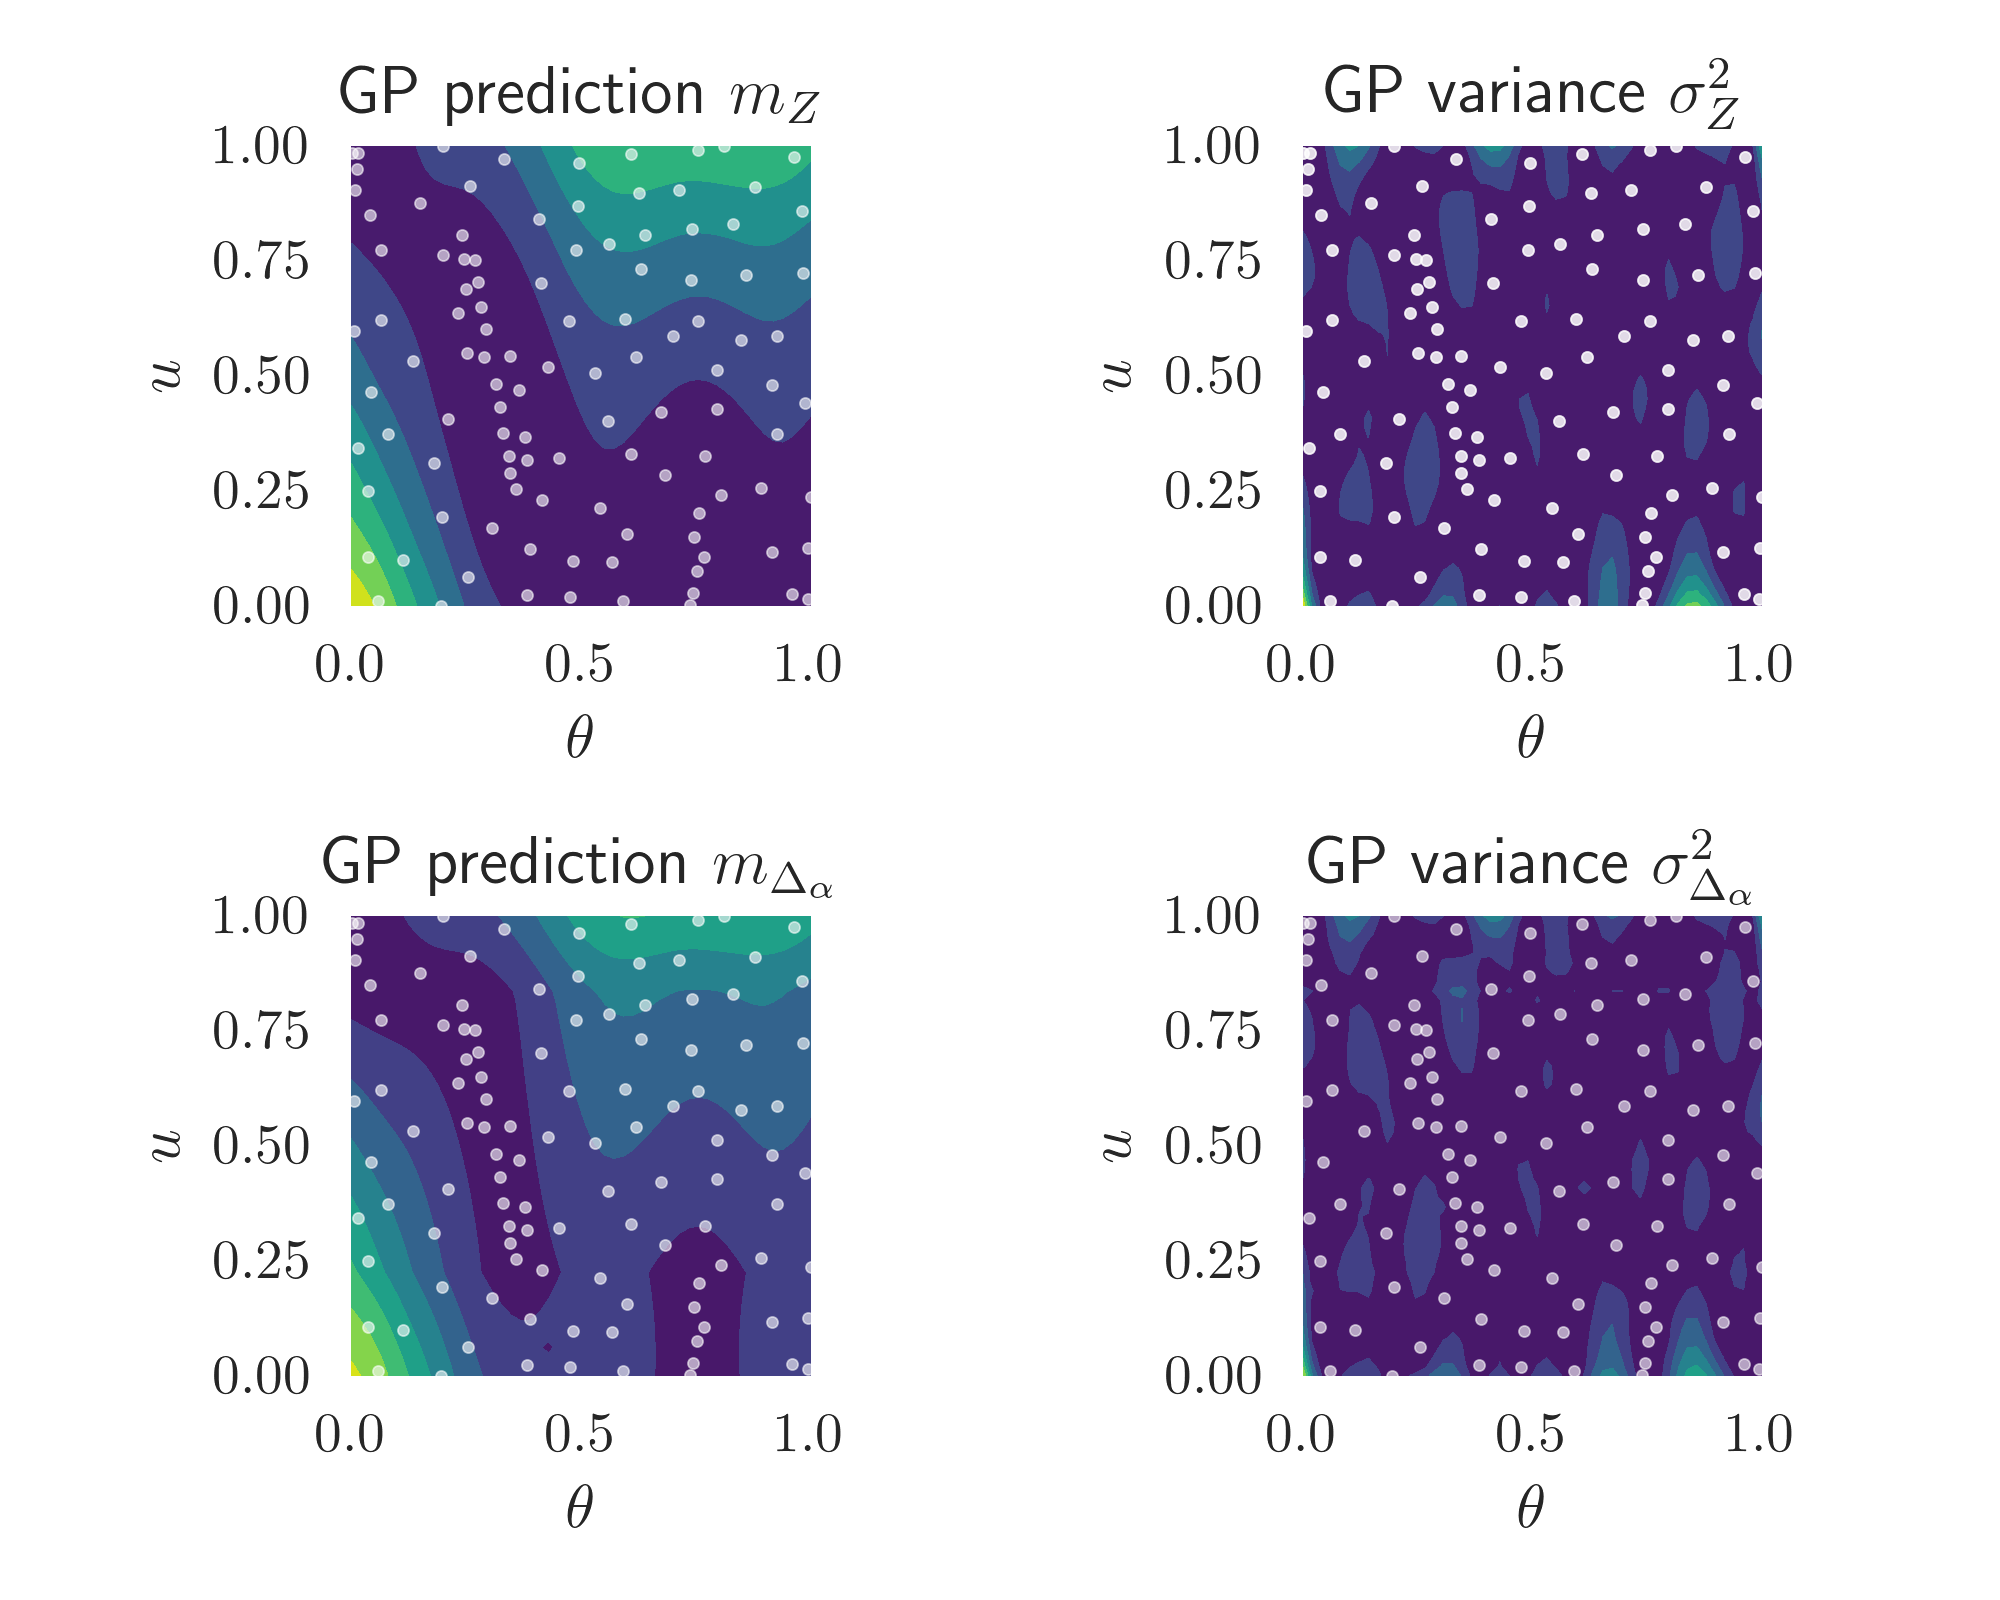
\includegraphics[scale=0.6]{/home/victor/acadwriting/Slides/Figures/aimse.png}
\end{center}
\end{column}
\begin{column}{0.5\textwidth}
  \begin{itemize}
  \item Exploration of the whole input space
    $\Xspace=\Kspace \times \Uspace$, but intensification also near
    the conditional minimisers
\item only 1 point added at a time
\item[$\rightarrow$] Adding multiple points every iteration ? 
\end{itemize}
\end{column}
\end{columns}
\end{frame}

\begin{frame}{Sampling-based methods: AK-MCS}%
  \begin{columns}
    \begin{column}{0.5\textwidth}
      \vfill
      Example: Improve estimation of set $\{m_{\Delta_{\alpha}} < 0\} = \{m_Z - \alpha m_{Z^*} < 0\}$
      \begin{block}{Selection of a batch of $K$ points and update of
          the design~\citep{dubourg_reliability-based_2011}}
      \begin{itemize}
      \item<2-> Sample points according to the sampling density $g$
      \item<3-> Cluster the samples into $K$ clusters (KMeans)
      \item<4-> For each cluster, select the sample which is closest to the cluster center
      \item<4-> Eventually postprocessing
      \item<5-> Evaluate the $K$ chosen samples and update the design accordingly
      \end{itemize}
    \end{block}
    \vfill
    \end{column}
    \begin{column}{0.5\textwidth}
      \vfill
      Given $\mathbb{M} \subset \Xspace$, margin of uncertainty
      $g(x) =
      \left\{\begin{array}{l}
              1 \text{ if } x\in \mathbb{M} \\
              0 \text{ elsewhere}
             \end{array} \right.$
           \begin{overlayarea}{\textwidth}{0.7\textheight}
      \foreach\y in{1,...,8}{
       \only<\y>{\includegraphics[width=\textwidth]{AKMCS_\y.png}}}%}
    \end{overlayarea}
    % 
    \end{column}
  \end{columns}
\end{frame}



\begin{frame}{Computations using $\Delta_{\alpha}$ or $\Xi$}
  Recalling that $\Gamma_{\alpha}(\kk) = \Prob_{\UU}\left[J(\kk, \UU) - \alpha J^*(\UU) \leq 0\right] = \Prob_{\UU}\left[\frac{J(\kk, \UU)}{J^*(\UU)} \leq \alpha\right]$

  \begin{block}{Plug-in and sample average approximation}    
  \begin{itemize}
  \item $J$ is replaced by $m_Z$
  \item $J - \alpha J^*$ is replaced by $m_{\Delta_\alpha}$
    $\rightarrow$ $\alpha$ fixed, estimation of probability
  \item $\frac{J}{J^*}$ is replaced by $m_{\Xi}$ $\rightarrow$ $p$
    fixed, estimation of quantile
  \end{itemize}
    \begin{align}
      {\Gamma}% ^{\mathsf{PI}}
      _{\alpha}(\kk) % &\approx \Prob_{\UU}\left[m_Z(\kk, \UU) - \alpha m_{Z^*}(\UU) \leq 0\right] \\
                                           &\approx \Prob_{\UU}\left[m_{\Delta_{\alpha}}(\kk, \UU) \leq 0\right] \\
                                           &\approx \Prob_{\UU}\left[m_{\Xi}(\kk,\UU) \leq \log\alpha \right]
    \end{align}
    Outer probability approximated using Monte-Carlo since
    $m_{\Delta_\alpha}$ and $m_\Xi$ are cheaper to evaluate than $J$, and optimized
  \end{block}
\end{frame}


\section{Robust calibration of CROCO}
\begin{frame}{The numerical model CROCO}
  \begin{columns}
    \begin{column}{0.50\textwidth}
     {
      \textbf{C}oastal and \textbf{R}egional \textbf{O}cean \textbf{CO}mmunity model (here in a 2D configuration)
      \begin{itemize}
      \item Solves the shallow-water equations
      \item Grid resolution of 1/\ang{14} (\SI{5.5}{\kilo\metre})
      \item \num{15684} cells located in the ocean
      \item[$\rightarrow$] Academic toy problem
      \end{itemize}
    }
\end{column}
\begin{column}{0.50\textwidth}
      \includegraphics<1>[width=\textwidth]{\manupath Chapter5/img/depth_maps_log_sserif.png}
      % \includegraphics<2>[width=\textwidth]{\manupath Chapter5/img/sediments_reduced_SA.png}
    \end{column}
  \end{columns}
\end{frame}

\begin{frame}{The shallow-water equations}
  $\zeta$: sea-water height, $\mathbf{v}$: velocity vector
  \begin{equation}
    \mathcal{M}: \left\{
  \begin{array}{rcl}
    \frac{\partial \mathbf{v}}{\partial t} + (\mathbf{v} \cdot \nabla) \mathbf{v} + 2 \bm{\Omega} \wedge \mathbf{v} & = & -g \nabla H + \frac{{\color{brewsuperdark}\bm{\tau}_b}}{\rho H} + F \\
    \frac{\partial \zeta}{\partial t} + \nabla \left(H \cdot \mathbf{v} \right) & = & 0 \\
    \zeta & = & \alert{\mathsf{BC}(\uu)} \text{ at the open boundaries}
  \end{array}
  \right.
\end{equation}
\begin{itemize}
\item ${\color{brewsuperdark} \bm{\tau}_b = \bm{\tau}_b(\kk)}$: bottom shear stress $\rightarrow$ depends on the control parameter $\kk$
\item $\alert{\mathsf{BC}(\uu)}$: tidal boundary conditions $ \rightarrow$ subject to aleatoric uncertainties ($\uu$) 
\end{itemize}
\begin{block}{Model and objective function}
\begin{itemize}
\item Output of the model: $\mathcal{M}(\kk, \uu) = (\zeta_{i,t}(\kk, \uu))_{\substack{1\leq i \leq N_{\mathsf{Mesh}} \\ 1 \leq t \leq N_{\mathsf{time}}}}$
\item Observations: $y = \mathcal{M}(\kk^{\mathsf{truth}}, \uu^{\mathsf{truth}})$, truth values defined later
\item Objective function: $J(\kk, \uu) = \| \mathcal{M}(\kk, \uu) - y \|^2 = \sum_{i, t} (\zeta_{i, t}(\kk, \uu) - y_{i, t} )^2$
\end{itemize}
\end{block}
\end{frame}


\begin{frame}{Modelling of the bottom friction}
  \begin{block}{Quadratic friction coefficient}
    Let $\bm{\tau}_b$ be the shear stress at the bottom, and $v_b$ the velocity vector at the bottom
    \begin{equation}
    \bm{\tau}_b = -C_d \|v_b \| v_b, \quad\text{ with }\quad C_d = \left(\frac{k}{\log\left(\frac{H}{\alert{z_b}}\right) - 1 }\right)^2
  \end{equation}
  and we define the control parameter as $\alert{\kk = \log z_b}$
\end{block}
\begin{itemize}
\item We assume that $\kk$ is uniform and constant for each type of sediment
\item $\kk^{\mathsf{truth}}$: constructed using the 6 types of sediments present 
\end{itemize}
Due to the water height $H$, influence of each sediment type depends
on how deep it is

$\Rightarrow$ Sensitivity analysis
\end{frame}

\begin{frame}{Sensitivity analysis on the friction associated with the sediments}
  Global Sensitivity Analysis with Sobol'
  indices~\citep{sobol_global_2001,sobol_sensitivity_1993}: quantify
  the influence of each input variable on $J$ (computed using \cite{gilquin_making_2019})
  \begin{columns}
    \begin{column}{0.5\textwidth}
      \inputpgf[\textwidth]{\manupath Chapter5/img/SA_sediments_slides.pgf}
    \end{column}
    % \begin{overlayarea}{\textwidth}{\textheight}
    \begin{column}{0.5\textwidth}
      \only<1>{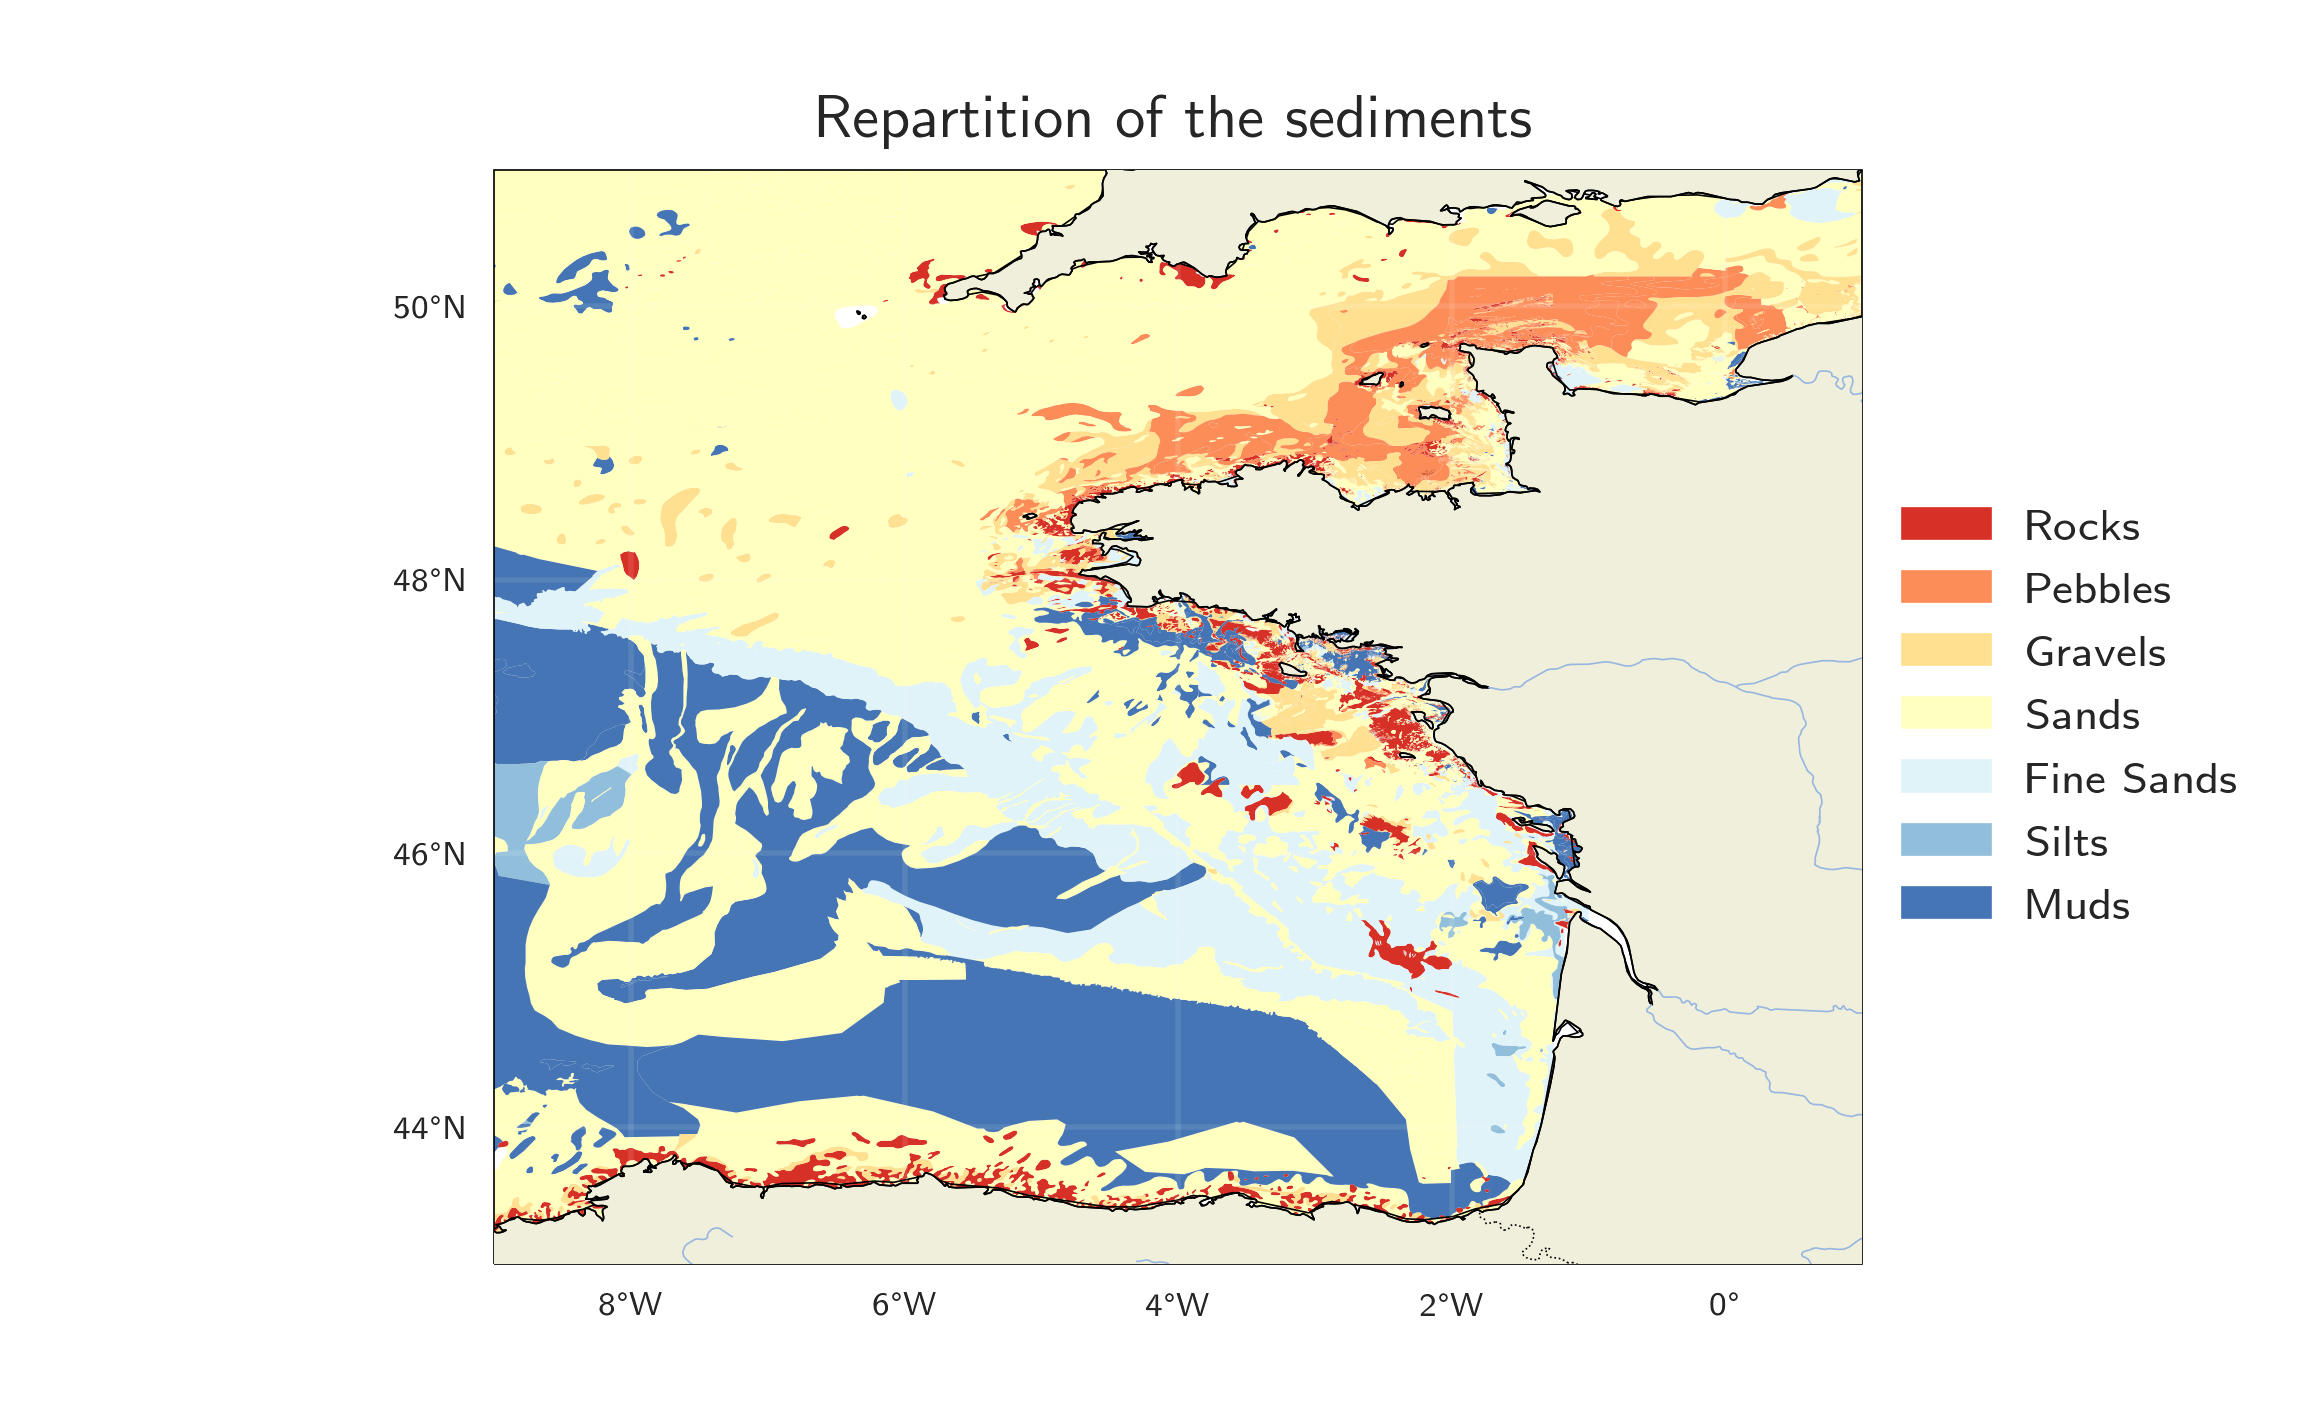
\includegraphics[width=\textwidth]{\manupath Chapter5/img/sediments_reduced_sserif.png}}%
      \only<2>{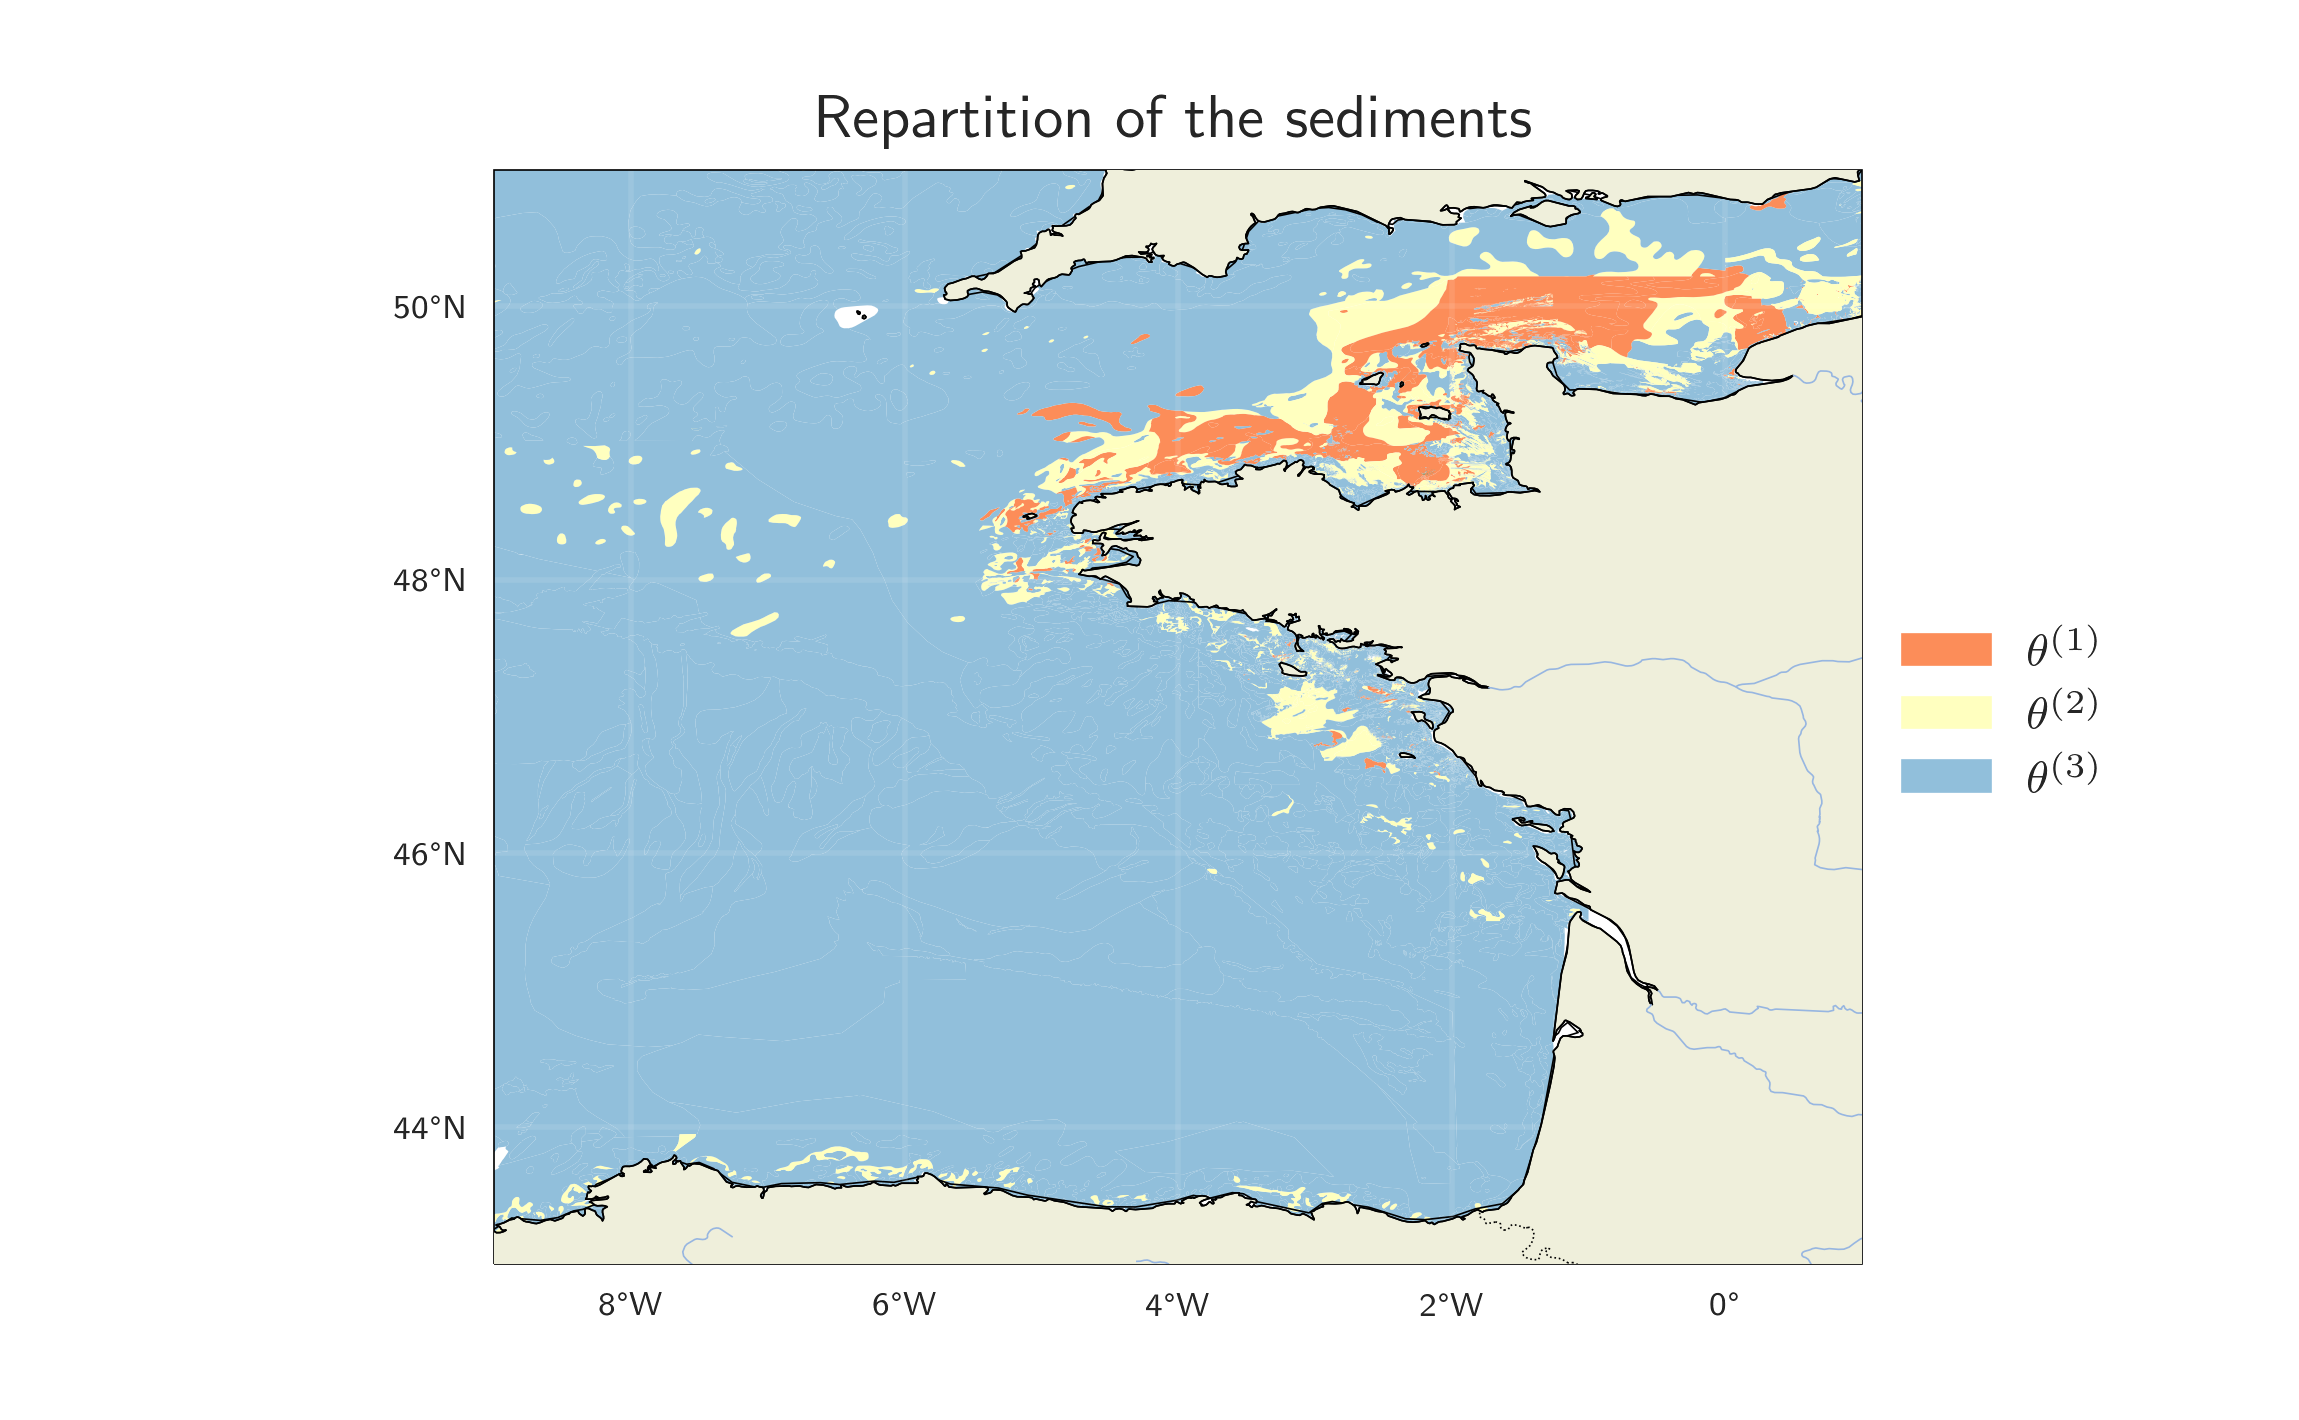
\includegraphics[width=\textwidth]{\manupath Chapter5/img/sediments_reduced_SA_sserif.png}}%
    \end{column}
% \end{overlayarea}
  \end{columns}
  \onslide<2>{
    The control variable is then $\kk = (\kk^{(1)}, \kk^{(2)}, \kk^{(3)})\in \Kspace$
    \begin{itemize}
      \item $\kk^{(1)}$: Pebbles
      \item $\kk^{(2)}$: Gravels
      \item $\kk^{(3)}$: Other sediments (in deeper water)
      \end{itemize}
}
\end{frame}

\begin{frame}{Control parameter and environmental variable}
  \begin{itemize}
  \item Aleatoric uncertainty on boundary conditions
    \item $\uu$ parametrizes an error on the amplitude of the $M_2$ and
    $S_2$ tide components.
  \item We assume that $\UU \sim \mathcal{U}\left(\Uspace\right)$, with $\Uspace = [0,1]^2$


    \begin{block}{Summary of the problem}
      \begin{itemize}
      \item $\kk = (\kk^{(1)}, \kk^{(2)}, \kk^{(3)})\in \Kspace \subset \mathbb{R}^3$
      \item $\uu \in \Uspace=[0, 1]^2$
      \item $\UU \sim \mathcal{U}\left(\Uspace\right)$
      \item $J(\kk, \uu) = \|\mathcal{M}(\kk, \uu) - y\|^2$
        \begin{itemize}
        \item  $y=\mathcal{M}(\kk^{\mathsf{truth}}, \uu^{\mathsf{truth}})$
      \item $\kk^{\mathsf{truth}}\in\mathbb{R}^6 \neq \Kspace \Rightarrow$ The
        model is not able to replicate the observations: $J>0$
      \item $\uu^{\mathsf{truth}} = (0.5, 0.5)$
      \end{itemize}
      \end{itemize}
    \end{block}
\end{itemize}


\end{frame}


\begin{frame}{Initial design, preliminary analysis}
\begin{itemize}
\item Initial design evaluated $\mathcal{X}_{\mathsf{LHS}} = \{(x_i, J(x_i))\}_{1 \leq i \leq n}$, LHS on $\Kspace \times \Uspace$
\item $J^*> 0$ by definition, but $m_{Z^*}$ ?
  \begin{itemize}
  \item<2-> Improve first $m_{Z^*}$ using PEI criterion to ensure $m_{Z^*} > 0$
  \end{itemize} 
\end{itemize}
\onslide<2>{\begin{center}
 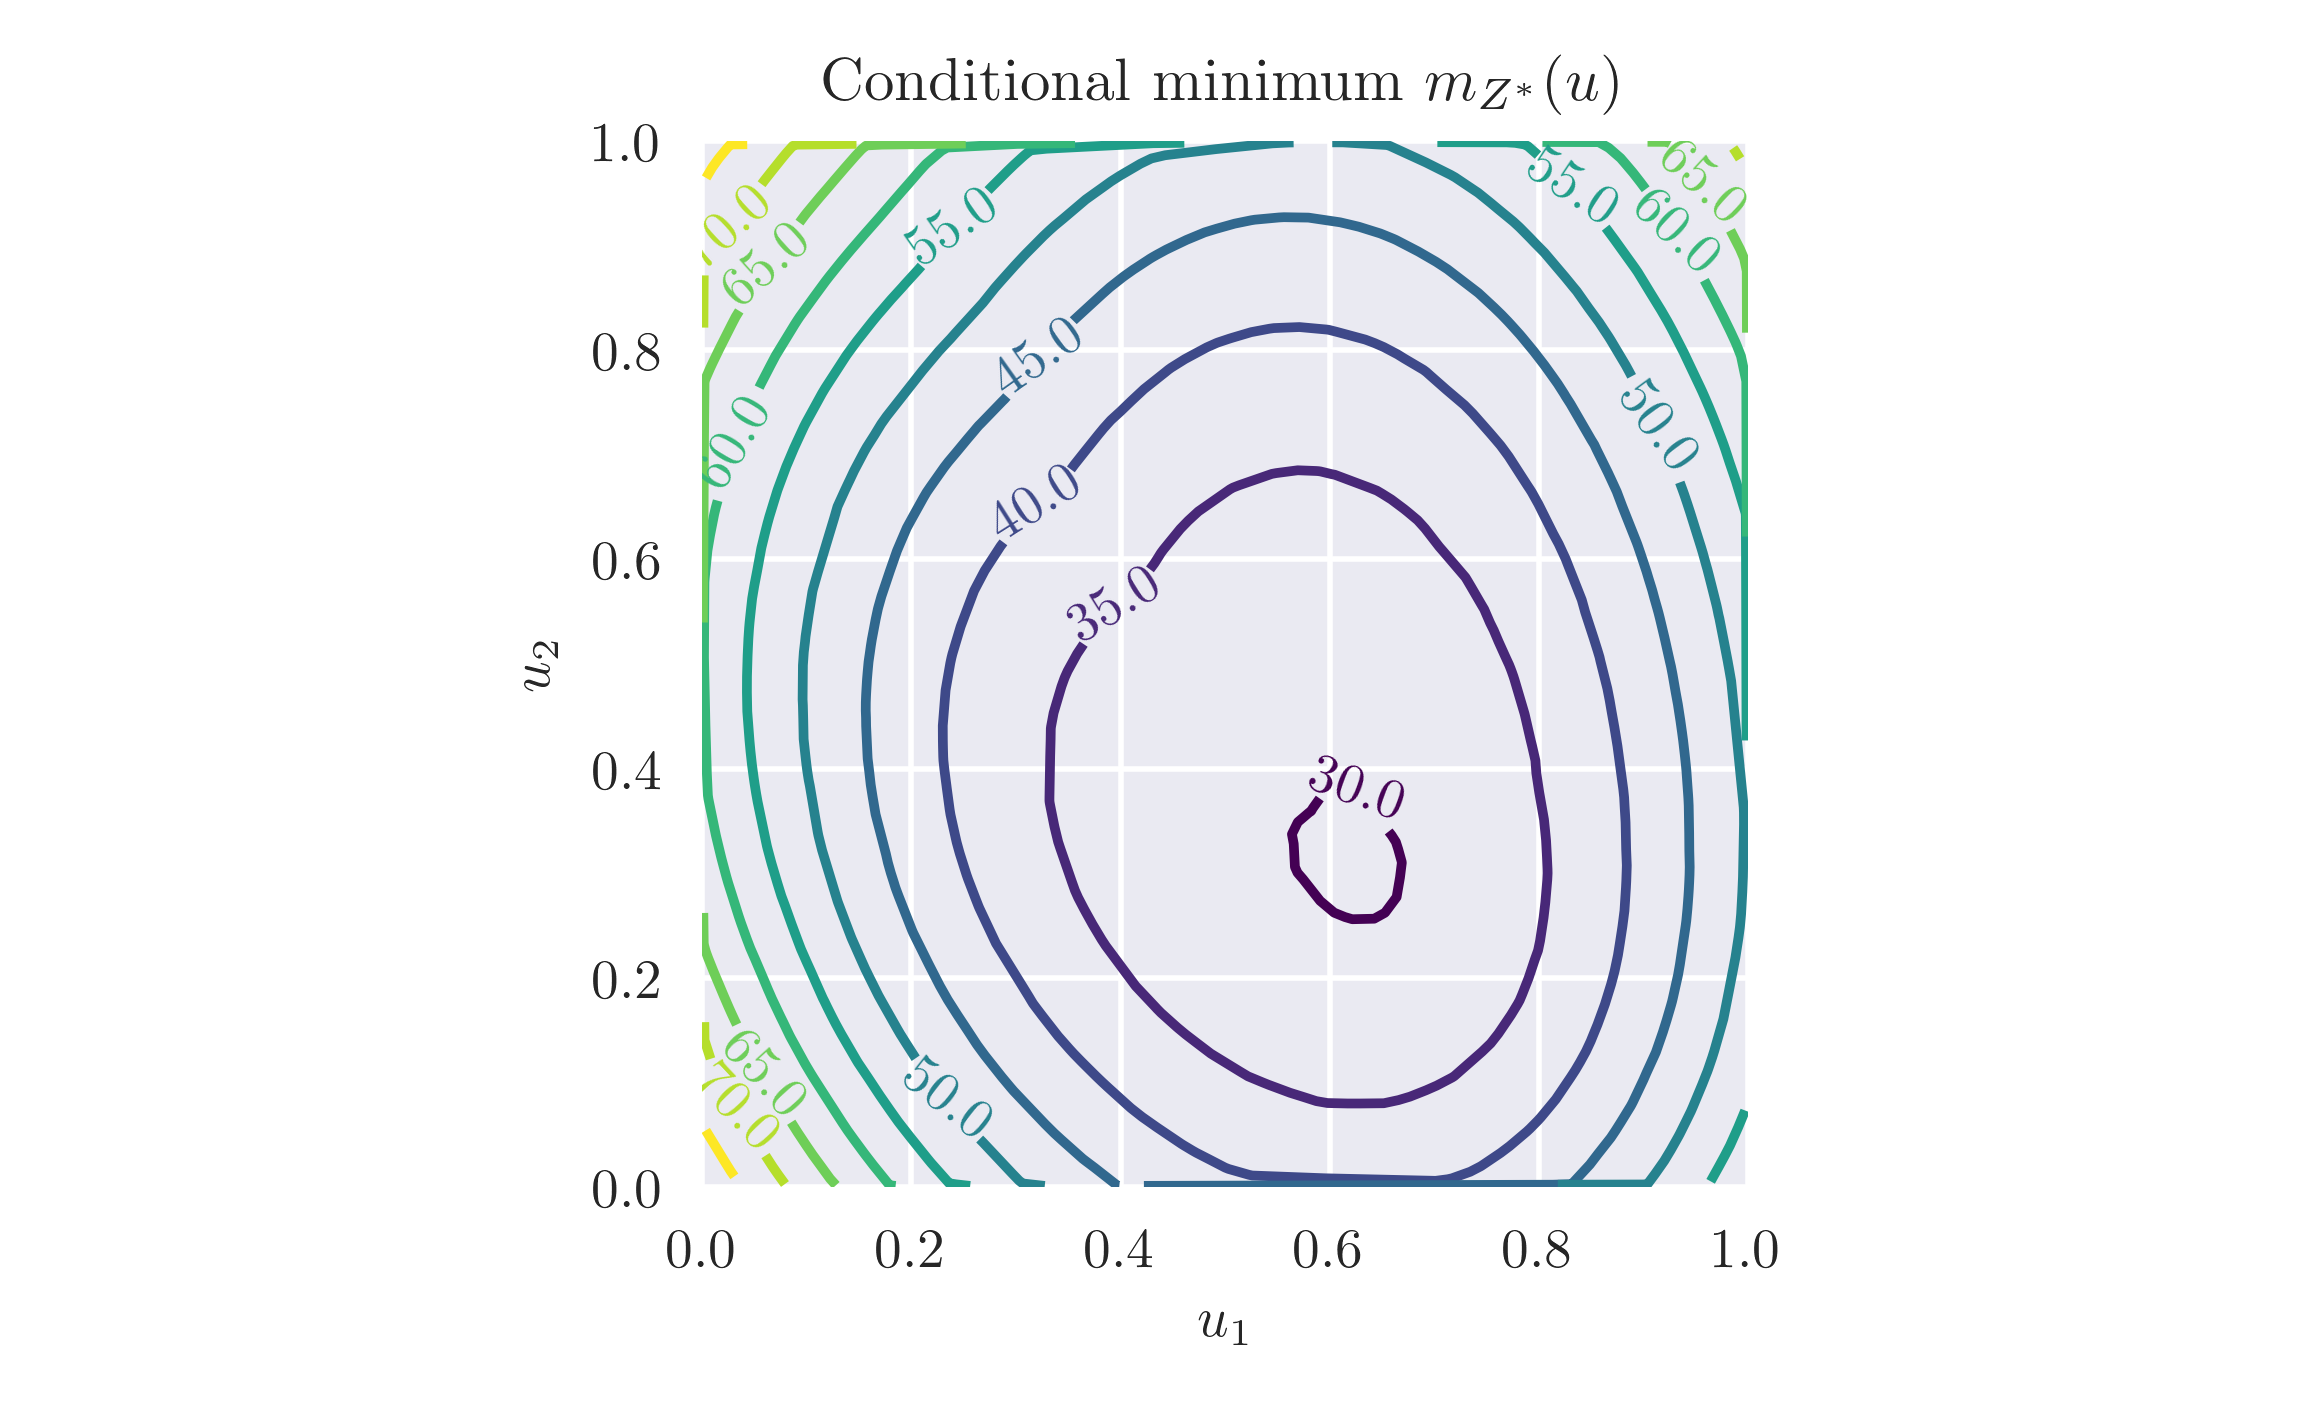
\includegraphics[scale=0.45]{\manupath Chapter5/img/contour_Jstar_800_again.png}
\end{center}
Global minimum not attained at the truth value of the environmental parameter

$\rightarrow$ Compensation of errors due to the dimension reduction
}
\end{frame}

\begin{frame}{Robust calibration}
  With this preliminary analysis, we can choose $\alpha$
  \begin{itemize}
  \item we set $\alpha=1.3$: with which probability can we stay within 30\% of the optimal value ?
  \item we enriched the design by looking to reduce globally the IMSE using $\kappa$
  \end{itemize}
  \begin{center}
    \begin{tabular}{rllll}
      \toprule
       & $\kk^{(1)}$ &$\kk^{(2)}$ & $\kk^{(3)}$ & \\ \midrule
     $\hat{\kk}_{\alpha}$, $\alpha=1.3$ & \num{-3.43} & \num{-5.20} &\num{-6.48}&$\Gamma_{\alpha}(\hat{\kk}_{\alpha})=\num{0.93}$  \\
    $\hat{\kk}_{\mathsf{global}}$ & \num{-3.516} & \num{-5.078} & \num{-6.346} &\\
      ${\kk}^{\mathsf{truth}}$ & \num{-3.689} & \num{-4.962}& {n.a.} &\\
    \bottomrule
  \end{tabular}
\end{center}
  In this case:
\begin{itemize}
\item $\hat{\kk}_{\alpha}^{(1)}> \hat{\kk}_{\mathsf{global}}^{(1)} > \kk^{\mathsf{truth}, (1)}$
\item $\hat{\kk}_{\alpha}^{(2)} < \hat{\kk}_{\mathsf{global}}^{(2)} < \kk^{\mathsf{truth}, (2)}$
\item $\hat{\kk}^{(3)}_{\alpha}< \hat{\kk}_{\mathsf{global}}^{(3)}$
\end{itemize}
\end{frame}

\begin{frame}{Computational overview}
  \begin{itemize}
  \item Total of 500 runs of the numerical model
    \begin{itemize}
    \item 100 for the initial LHS
    \item 200 with the PEI criterion
    \item 200 for the reduction of the $\mathsf{IMSE}$
    \end{itemize}
    
  \item Each iteration for the reduction of the IMSE requires
  \begin{itemize}
  \item Evaluations of an integral of dimension $1 + \dim (\Kspace \times \Uspace)$
  \item Optimization of this integral in a space of dimension $\dim \Kspace$
  \item[$\rightarrow$] Dependent on the ability to compute $m_{Z^*}$, $m_{\Delta_{\alpha}}$, $\sigma^2_{\Delta_{\alpha}}$
   \item[$\rightarrow$] As is, limits severely the possibility of increased dimension
   \end{itemize}
 \item For sampling-based methods:
   \begin{itemize}
   \item Size of margin of uncertainty decreases
   \item[$\rightarrow$] Sampling becomes increasingly difficult
   \end{itemize}
  \end{itemize}
\end{frame}
% \begin{frame}{Numerical results}  
%   \begin{center}
%   \begin{tabular}{rrr}\toprule
%     Method & augmented IMSE & Qe-AK MCS \\ \midrule
%     % Quantity of interest & $\Ex_{Z}[\int_{\Kspace\times\Uspace}\sigma^2_{\Delta_\alpha \mid Z}]$ & $\mathbb{M}_{\eta}(\mathfrak{q}_l)$ \\
%     Type & 1-step & $K$-step \\
%     Main Bottleneck &
%                       \begin{tabular}{@{}r@{}}
%                         Evaluate and optimise integral in \\
%                         $(1 + \dim( \Kspace\times \Uspace))$ dimensions
%                       \end{tabular}
%                       & \begin{tabular}{@{}r@{}}
%                           Sampling in unknown \\
%                           regions in $\dim( \Kspace\times \Uspace)$
%                         \end{tabular} \\
%     Advantage & Optimal criterion of enrichment & $K$ chosen arbitrary \\ \midrule
%     $\hat{\kk}_{\alpha}$, $\alpha=1.3$ & $(\num{-3.43},\num{-5.20},\num{-6.48})$  & $(\num{-3.38},\num{-5.05}, \num{-6.61})$ \\
%     $\hat{\kk}_{\alpha_p}$, $p=0.95$ & $(\num{-3.39},\num{-5.28},\num{-6.50})$  & $(\num{-3.36},\num{-5.10}, \num{-6.63})$ \\
%     $\hat{\kk}_{\mathsf{global}}$ & \multicolumn{2}{c}{$(-3.516, -5.078, -6.346 )$} \\
%     ${\kk}^{\mathsf{truth}}$ & \multicolumn{2}{c}{$(-3.689, -4.962, \mathsf{n.a.})$} \\
%     \bottomrule
%   \end{tabular}
% \end{center}


% \end{frame}
% \begin{frame}
%   \frametitle{Application to CROCO: Dimension reduction}
%   \begin{center}
%     \renewcommand\rmfamily{\sffamily}
%     \begin{columns}
%       \begin{column}{.5\textwidth}
%         \resizebox{\textwidth}{!}{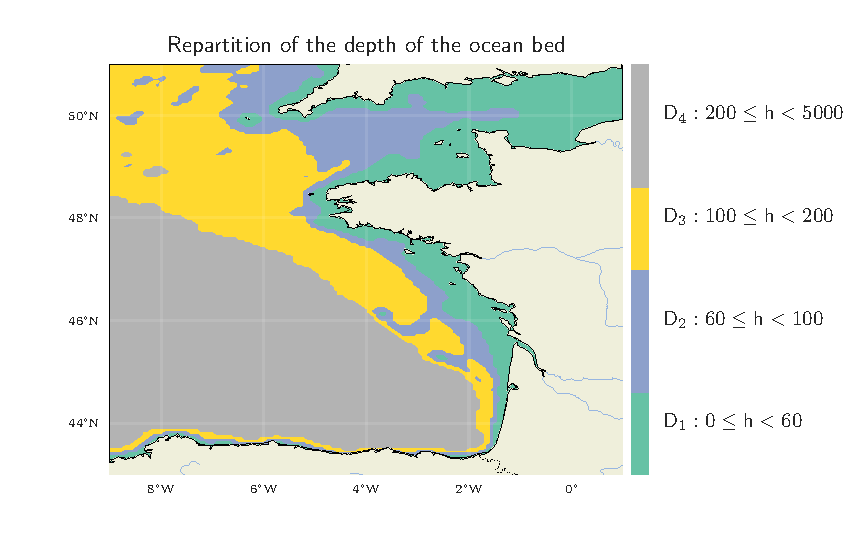
\includegraphics{\manupath
%             Chapter5/img/depth_repartition.pdf}}
%       \end{column}
%       \begin{column}{.5\textwidth}
%         \resizebox{\textwidth}{!}{%% Creator: Matplotlib, PGF backend
%%
%% To include the figure in your LaTeX document, write
%%   \input{<filename>.pgf}
%%
%% Make sure the required packages are loaded in your preamble
%%   \usepackage{pgf}
%%
%% Figures using additional raster images can only be included by \input if
%% they are in the same directory as the main LaTeX file. For loading figures
%% from other directories you can use the `import` package
%%   \usepackage{import}
%% and then include the figures with
%%   \import{<path to file>}{<filename>.pgf}
%%
%% Matplotlib used the following preamble
%%   \usepackage{fontspec}
%%   \setmainfont{DejaVuSans.ttf}[Path=/home/victor/miniconda3/lib/python3.7/site-packages/matplotlib/mpl-data/fonts/ttf/]
%%   \setsansfont{LiberationSans-Regular.ttf}[Path=/usr/share/fonts/truetype/liberation/]
%%   \setmonofont{DejaVuSansMono.ttf}[Path=/home/victor/miniconda3/lib/python3.7/site-packages/matplotlib/mpl-data/fonts/ttf/]
%%
\begingroup%
\makeatletter%
\begin{pgfpicture}%
\pgfpathrectangle{\pgfpointorigin}{\pgfqpoint{5.748032in}{3.552479in}}%
\pgfusepath{use as bounding box, clip}%
\begin{pgfscope}%
\pgfsetbuttcap%
\pgfsetmiterjoin%
\definecolor{currentfill}{rgb}{1.000000,1.000000,1.000000}%
\pgfsetfillcolor{currentfill}%
\pgfsetlinewidth{0.000000pt}%
\definecolor{currentstroke}{rgb}{1.000000,1.000000,1.000000}%
\pgfsetstrokecolor{currentstroke}%
\pgfsetdash{}{0pt}%
\pgfpathmoveto{\pgfqpoint{0.000000in}{0.000000in}}%
\pgfpathlineto{\pgfqpoint{5.748032in}{0.000000in}}%
\pgfpathlineto{\pgfqpoint{5.748032in}{3.552479in}}%
\pgfpathlineto{\pgfqpoint{0.000000in}{3.552479in}}%
\pgfpathclose%
\pgfusepath{fill}%
\end{pgfscope}%
\begin{pgfscope}%
\pgfsetbuttcap%
\pgfsetmiterjoin%
\definecolor{currentfill}{rgb}{0.917647,0.917647,0.949020}%
\pgfsetfillcolor{currentfill}%
\pgfsetlinewidth{0.000000pt}%
\definecolor{currentstroke}{rgb}{0.000000,0.000000,0.000000}%
\pgfsetstrokecolor{currentstroke}%
\pgfsetstrokeopacity{0.000000}%
\pgfsetdash{}{0pt}%
\pgfpathmoveto{\pgfqpoint{0.718504in}{0.390773in}}%
\pgfpathlineto{\pgfqpoint{5.173229in}{0.390773in}}%
\pgfpathlineto{\pgfqpoint{5.173229in}{3.126181in}}%
\pgfpathlineto{\pgfqpoint{0.718504in}{3.126181in}}%
\pgfpathclose%
\pgfusepath{fill}%
\end{pgfscope}%
\begin{pgfscope}%
\definecolor{textcolor}{rgb}{0.150000,0.150000,0.150000}%
\pgfsetstrokecolor{textcolor}%
\pgfsetfillcolor{textcolor}%
\pgftext[x=1.089731in,y=0.293550in,,top]{\color{textcolor}\rmfamily\fontsize{10.000000}{12.000000}\selectfont \(\displaystyle D_1\)}%
\end{pgfscope}%
\begin{pgfscope}%
\definecolor{textcolor}{rgb}{0.150000,0.150000,0.150000}%
\pgfsetstrokecolor{textcolor}%
\pgfsetfillcolor{textcolor}%
\pgftext[x=1.832185in,y=0.293550in,,top]{\color{textcolor}\rmfamily\fontsize{10.000000}{12.000000}\selectfont \(\displaystyle D_2\)}%
\end{pgfscope}%
\begin{pgfscope}%
\definecolor{textcolor}{rgb}{0.150000,0.150000,0.150000}%
\pgfsetstrokecolor{textcolor}%
\pgfsetfillcolor{textcolor}%
\pgftext[x=2.574639in,y=0.293550in,,top]{\color{textcolor}\rmfamily\fontsize{10.000000}{12.000000}\selectfont \(\displaystyle D_3\)}%
\end{pgfscope}%
\begin{pgfscope}%
\definecolor{textcolor}{rgb}{0.150000,0.150000,0.150000}%
\pgfsetstrokecolor{textcolor}%
\pgfsetfillcolor{textcolor}%
\pgftext[x=3.317093in,y=0.293550in,,top]{\color{textcolor}\rmfamily\fontsize{10.000000}{12.000000}\selectfont \(\displaystyle D_4\)}%
\end{pgfscope}%
\begin{pgfscope}%
\definecolor{textcolor}{rgb}{0.150000,0.150000,0.150000}%
\pgfsetstrokecolor{textcolor}%
\pgfsetfillcolor{textcolor}%
\pgftext[x=4.059547in,y=0.293550in,,top]{\color{textcolor}\rmfamily\fontsize{10.000000}{12.000000}\selectfont \(\displaystyle u_1\)}%
\end{pgfscope}%
\begin{pgfscope}%
\definecolor{textcolor}{rgb}{0.150000,0.150000,0.150000}%
\pgfsetstrokecolor{textcolor}%
\pgfsetfillcolor{textcolor}%
\pgftext[x=4.802001in,y=0.293550in,,top]{\color{textcolor}\rmfamily\fontsize{10.000000}{12.000000}\selectfont \(\displaystyle u_2\)}%
\end{pgfscope}%
\begin{pgfscope}%
\definecolor{textcolor}{rgb}{0.150000,0.150000,0.150000}%
\pgfsetstrokecolor{textcolor}%
\pgfsetfillcolor{textcolor}%
\pgftext[x=2.945866in,y=0.103582in,,top]{\color{textcolor}\rmfamily\fontsize{10.000000}{12.000000}\selectfont Sobol indices}%
\end{pgfscope}%
\begin{pgfscope}%
\pgfpathrectangle{\pgfqpoint{0.718504in}{0.390773in}}{\pgfqpoint{4.454725in}{2.735409in}}%
\pgfusepath{clip}%
\pgfsetroundcap%
\pgfsetroundjoin%
\pgfsetlinewidth{1.003750pt}%
\definecolor{currentstroke}{rgb}{1.000000,1.000000,1.000000}%
\pgfsetstrokecolor{currentstroke}%
\pgfsetdash{}{0pt}%
\pgfpathmoveto{\pgfqpoint{0.718504in}{0.672367in}}%
\pgfpathlineto{\pgfqpoint{5.173229in}{0.672367in}}%
\pgfusepath{stroke}%
\end{pgfscope}%
\begin{pgfscope}%
\definecolor{textcolor}{rgb}{0.150000,0.150000,0.150000}%
\pgfsetstrokecolor{textcolor}%
\pgfsetfillcolor{textcolor}%
\pgftext[x=0.443812in,y=0.619606in,left,base]{\color{textcolor}\rmfamily\fontsize{10.000000}{12.000000}\selectfont \(\displaystyle 0.0\)}%
\end{pgfscope}%
\begin{pgfscope}%
\pgfpathrectangle{\pgfqpoint{0.718504in}{0.390773in}}{\pgfqpoint{4.454725in}{2.735409in}}%
\pgfusepath{clip}%
\pgfsetroundcap%
\pgfsetroundjoin%
\pgfsetlinewidth{1.003750pt}%
\definecolor{currentstroke}{rgb}{1.000000,1.000000,1.000000}%
\pgfsetstrokecolor{currentstroke}%
\pgfsetdash{}{0pt}%
\pgfpathmoveto{\pgfqpoint{0.718504in}{1.019181in}}%
\pgfpathlineto{\pgfqpoint{5.173229in}{1.019181in}}%
\pgfusepath{stroke}%
\end{pgfscope}%
\begin{pgfscope}%
\definecolor{textcolor}{rgb}{0.150000,0.150000,0.150000}%
\pgfsetstrokecolor{textcolor}%
\pgfsetfillcolor{textcolor}%
\pgftext[x=0.443812in,y=0.966419in,left,base]{\color{textcolor}\rmfamily\fontsize{10.000000}{12.000000}\selectfont \(\displaystyle 0.1\)}%
\end{pgfscope}%
\begin{pgfscope}%
\pgfpathrectangle{\pgfqpoint{0.718504in}{0.390773in}}{\pgfqpoint{4.454725in}{2.735409in}}%
\pgfusepath{clip}%
\pgfsetroundcap%
\pgfsetroundjoin%
\pgfsetlinewidth{1.003750pt}%
\definecolor{currentstroke}{rgb}{1.000000,1.000000,1.000000}%
\pgfsetstrokecolor{currentstroke}%
\pgfsetdash{}{0pt}%
\pgfpathmoveto{\pgfqpoint{0.718504in}{1.365995in}}%
\pgfpathlineto{\pgfqpoint{5.173229in}{1.365995in}}%
\pgfusepath{stroke}%
\end{pgfscope}%
\begin{pgfscope}%
\definecolor{textcolor}{rgb}{0.150000,0.150000,0.150000}%
\pgfsetstrokecolor{textcolor}%
\pgfsetfillcolor{textcolor}%
\pgftext[x=0.443812in,y=1.313233in,left,base]{\color{textcolor}\rmfamily\fontsize{10.000000}{12.000000}\selectfont \(\displaystyle 0.2\)}%
\end{pgfscope}%
\begin{pgfscope}%
\pgfpathrectangle{\pgfqpoint{0.718504in}{0.390773in}}{\pgfqpoint{4.454725in}{2.735409in}}%
\pgfusepath{clip}%
\pgfsetroundcap%
\pgfsetroundjoin%
\pgfsetlinewidth{1.003750pt}%
\definecolor{currentstroke}{rgb}{1.000000,1.000000,1.000000}%
\pgfsetstrokecolor{currentstroke}%
\pgfsetdash{}{0pt}%
\pgfpathmoveto{\pgfqpoint{0.718504in}{1.712809in}}%
\pgfpathlineto{\pgfqpoint{5.173229in}{1.712809in}}%
\pgfusepath{stroke}%
\end{pgfscope}%
\begin{pgfscope}%
\definecolor{textcolor}{rgb}{0.150000,0.150000,0.150000}%
\pgfsetstrokecolor{textcolor}%
\pgfsetfillcolor{textcolor}%
\pgftext[x=0.443812in,y=1.660047in,left,base]{\color{textcolor}\rmfamily\fontsize{10.000000}{12.000000}\selectfont \(\displaystyle 0.3\)}%
\end{pgfscope}%
\begin{pgfscope}%
\pgfpathrectangle{\pgfqpoint{0.718504in}{0.390773in}}{\pgfqpoint{4.454725in}{2.735409in}}%
\pgfusepath{clip}%
\pgfsetroundcap%
\pgfsetroundjoin%
\pgfsetlinewidth{1.003750pt}%
\definecolor{currentstroke}{rgb}{1.000000,1.000000,1.000000}%
\pgfsetstrokecolor{currentstroke}%
\pgfsetdash{}{0pt}%
\pgfpathmoveto{\pgfqpoint{0.718504in}{2.059623in}}%
\pgfpathlineto{\pgfqpoint{5.173229in}{2.059623in}}%
\pgfusepath{stroke}%
\end{pgfscope}%
\begin{pgfscope}%
\definecolor{textcolor}{rgb}{0.150000,0.150000,0.150000}%
\pgfsetstrokecolor{textcolor}%
\pgfsetfillcolor{textcolor}%
\pgftext[x=0.443812in,y=2.006861in,left,base]{\color{textcolor}\rmfamily\fontsize{10.000000}{12.000000}\selectfont \(\displaystyle 0.4\)}%
\end{pgfscope}%
\begin{pgfscope}%
\pgfpathrectangle{\pgfqpoint{0.718504in}{0.390773in}}{\pgfqpoint{4.454725in}{2.735409in}}%
\pgfusepath{clip}%
\pgfsetroundcap%
\pgfsetroundjoin%
\pgfsetlinewidth{1.003750pt}%
\definecolor{currentstroke}{rgb}{1.000000,1.000000,1.000000}%
\pgfsetstrokecolor{currentstroke}%
\pgfsetdash{}{0pt}%
\pgfpathmoveto{\pgfqpoint{0.718504in}{2.406437in}}%
\pgfpathlineto{\pgfqpoint{5.173229in}{2.406437in}}%
\pgfusepath{stroke}%
\end{pgfscope}%
\begin{pgfscope}%
\definecolor{textcolor}{rgb}{0.150000,0.150000,0.150000}%
\pgfsetstrokecolor{textcolor}%
\pgfsetfillcolor{textcolor}%
\pgftext[x=0.443812in,y=2.353675in,left,base]{\color{textcolor}\rmfamily\fontsize{10.000000}{12.000000}\selectfont \(\displaystyle 0.5\)}%
\end{pgfscope}%
\begin{pgfscope}%
\pgfpathrectangle{\pgfqpoint{0.718504in}{0.390773in}}{\pgfqpoint{4.454725in}{2.735409in}}%
\pgfusepath{clip}%
\pgfsetroundcap%
\pgfsetroundjoin%
\pgfsetlinewidth{1.003750pt}%
\definecolor{currentstroke}{rgb}{1.000000,1.000000,1.000000}%
\pgfsetstrokecolor{currentstroke}%
\pgfsetdash{}{0pt}%
\pgfpathmoveto{\pgfqpoint{0.718504in}{2.753251in}}%
\pgfpathlineto{\pgfqpoint{5.173229in}{2.753251in}}%
\pgfusepath{stroke}%
\end{pgfscope}%
\begin{pgfscope}%
\definecolor{textcolor}{rgb}{0.150000,0.150000,0.150000}%
\pgfsetstrokecolor{textcolor}%
\pgfsetfillcolor{textcolor}%
\pgftext[x=0.443812in,y=2.700489in,left,base]{\color{textcolor}\rmfamily\fontsize{10.000000}{12.000000}\selectfont \(\displaystyle 0.6\)}%
\end{pgfscope}%
\begin{pgfscope}%
\pgfpathrectangle{\pgfqpoint{0.718504in}{0.390773in}}{\pgfqpoint{4.454725in}{2.735409in}}%
\pgfusepath{clip}%
\pgfsetroundcap%
\pgfsetroundjoin%
\pgfsetlinewidth{1.003750pt}%
\definecolor{currentstroke}{rgb}{1.000000,1.000000,1.000000}%
\pgfsetstrokecolor{currentstroke}%
\pgfsetdash{}{0pt}%
\pgfpathmoveto{\pgfqpoint{0.718504in}{3.100065in}}%
\pgfpathlineto{\pgfqpoint{5.173229in}{3.100065in}}%
\pgfusepath{stroke}%
\end{pgfscope}%
\begin{pgfscope}%
\definecolor{textcolor}{rgb}{0.150000,0.150000,0.150000}%
\pgfsetstrokecolor{textcolor}%
\pgfsetfillcolor{textcolor}%
\pgftext[x=0.443812in,y=3.047303in,left,base]{\color{textcolor}\rmfamily\fontsize{10.000000}{12.000000}\selectfont \(\displaystyle 0.7\)}%
\end{pgfscope}%
\begin{pgfscope}%
\definecolor{textcolor}{rgb}{0.150000,0.150000,0.150000}%
\pgfsetstrokecolor{textcolor}%
\pgfsetfillcolor{textcolor}%
\pgftext[x=0.388256in,y=1.758477in,,bottom,rotate=90.000000]{\color{textcolor}\rmfamily\fontsize{10.000000}{12.000000}\selectfont value}%
\end{pgfscope}%
\begin{pgfscope}%
\pgfpathrectangle{\pgfqpoint{0.718504in}{0.390773in}}{\pgfqpoint{4.454725in}{2.735409in}}%
\pgfusepath{clip}%
\pgfsetbuttcap%
\pgfsetmiterjoin%
\definecolor{currentfill}{rgb}{0.347059,0.458824,0.641176}%
\pgfsetfillcolor{currentfill}%
\pgfsetlinewidth{0.000000pt}%
\definecolor{currentstroke}{rgb}{0.000000,0.000000,0.000000}%
\pgfsetstrokecolor{currentstroke}%
\pgfsetstrokeopacity{0.000000}%
\pgfsetdash{}{0pt}%
\pgfpathmoveto{\pgfqpoint{0.792749in}{0.672367in}}%
\pgfpathlineto{\pgfqpoint{0.990737in}{0.672367in}}%
\pgfpathlineto{\pgfqpoint{0.990737in}{1.574478in}}%
\pgfpathlineto{\pgfqpoint{0.792749in}{1.574478in}}%
\pgfpathclose%
\pgfusepath{fill}%
\end{pgfscope}%
\begin{pgfscope}%
\pgfpathrectangle{\pgfqpoint{0.718504in}{0.390773in}}{\pgfqpoint{4.454725in}{2.735409in}}%
\pgfusepath{clip}%
\pgfsetbuttcap%
\pgfsetmiterjoin%
\definecolor{currentfill}{rgb}{0.347059,0.458824,0.641176}%
\pgfsetfillcolor{currentfill}%
\pgfsetlinewidth{0.000000pt}%
\definecolor{currentstroke}{rgb}{0.000000,0.000000,0.000000}%
\pgfsetstrokecolor{currentstroke}%
\pgfsetstrokeopacity{0.000000}%
\pgfsetdash{}{0pt}%
\pgfpathmoveto{\pgfqpoint{1.535203in}{0.672367in}}%
\pgfpathlineto{\pgfqpoint{1.733191in}{0.672367in}}%
\pgfpathlineto{\pgfqpoint{1.733191in}{0.676541in}}%
\pgfpathlineto{\pgfqpoint{1.535203in}{0.676541in}}%
\pgfpathclose%
\pgfusepath{fill}%
\end{pgfscope}%
\begin{pgfscope}%
\pgfpathrectangle{\pgfqpoint{0.718504in}{0.390773in}}{\pgfqpoint{4.454725in}{2.735409in}}%
\pgfusepath{clip}%
\pgfsetbuttcap%
\pgfsetmiterjoin%
\definecolor{currentfill}{rgb}{0.347059,0.458824,0.641176}%
\pgfsetfillcolor{currentfill}%
\pgfsetlinewidth{0.000000pt}%
\definecolor{currentstroke}{rgb}{0.000000,0.000000,0.000000}%
\pgfsetstrokecolor{currentstroke}%
\pgfsetstrokeopacity{0.000000}%
\pgfsetdash{}{0pt}%
\pgfpathmoveto{\pgfqpoint{2.277658in}{0.672367in}}%
\pgfpathlineto{\pgfqpoint{2.475645in}{0.672367in}}%
\pgfpathlineto{\pgfqpoint{2.475645in}{0.701924in}}%
\pgfpathlineto{\pgfqpoint{2.277658in}{0.701924in}}%
\pgfpathclose%
\pgfusepath{fill}%
\end{pgfscope}%
\begin{pgfscope}%
\pgfpathrectangle{\pgfqpoint{0.718504in}{0.390773in}}{\pgfqpoint{4.454725in}{2.735409in}}%
\pgfusepath{clip}%
\pgfsetbuttcap%
\pgfsetmiterjoin%
\definecolor{currentfill}{rgb}{0.347059,0.458824,0.641176}%
\pgfsetfillcolor{currentfill}%
\pgfsetlinewidth{0.000000pt}%
\definecolor{currentstroke}{rgb}{0.000000,0.000000,0.000000}%
\pgfsetstrokecolor{currentstroke}%
\pgfsetstrokeopacity{0.000000}%
\pgfsetdash{}{0pt}%
\pgfpathmoveto{\pgfqpoint{3.020112in}{0.672367in}}%
\pgfpathlineto{\pgfqpoint{3.218099in}{0.672367in}}%
\pgfpathlineto{\pgfqpoint{3.218099in}{0.666513in}}%
\pgfpathlineto{\pgfqpoint{3.020112in}{0.666513in}}%
\pgfpathclose%
\pgfusepath{fill}%
\end{pgfscope}%
\begin{pgfscope}%
\pgfpathrectangle{\pgfqpoint{0.718504in}{0.390773in}}{\pgfqpoint{4.454725in}{2.735409in}}%
\pgfusepath{clip}%
\pgfsetbuttcap%
\pgfsetmiterjoin%
\definecolor{currentfill}{rgb}{0.347059,0.458824,0.641176}%
\pgfsetfillcolor{currentfill}%
\pgfsetlinewidth{0.000000pt}%
\definecolor{currentstroke}{rgb}{0.000000,0.000000,0.000000}%
\pgfsetstrokecolor{currentstroke}%
\pgfsetstrokeopacity{0.000000}%
\pgfsetdash{}{0pt}%
\pgfpathmoveto{\pgfqpoint{3.762566in}{0.672367in}}%
\pgfpathlineto{\pgfqpoint{3.960553in}{0.672367in}}%
\pgfpathlineto{\pgfqpoint{3.960553in}{2.998220in}}%
\pgfpathlineto{\pgfqpoint{3.762566in}{2.998220in}}%
\pgfpathclose%
\pgfusepath{fill}%
\end{pgfscope}%
\begin{pgfscope}%
\pgfpathrectangle{\pgfqpoint{0.718504in}{0.390773in}}{\pgfqpoint{4.454725in}{2.735409in}}%
\pgfusepath{clip}%
\pgfsetbuttcap%
\pgfsetmiterjoin%
\definecolor{currentfill}{rgb}{0.347059,0.458824,0.641176}%
\pgfsetfillcolor{currentfill}%
\pgfsetlinewidth{0.000000pt}%
\definecolor{currentstroke}{rgb}{0.000000,0.000000,0.000000}%
\pgfsetstrokecolor{currentstroke}%
\pgfsetstrokeopacity{0.000000}%
\pgfsetdash{}{0pt}%
\pgfpathmoveto{\pgfqpoint{4.505020in}{0.672367in}}%
\pgfpathlineto{\pgfqpoint{4.703008in}{0.672367in}}%
\pgfpathlineto{\pgfqpoint{4.703008in}{0.886568in}}%
\pgfpathlineto{\pgfqpoint{4.505020in}{0.886568in}}%
\pgfpathclose%
\pgfusepath{fill}%
\end{pgfscope}%
\begin{pgfscope}%
\pgfpathrectangle{\pgfqpoint{0.718504in}{0.390773in}}{\pgfqpoint{4.454725in}{2.735409in}}%
\pgfusepath{clip}%
\pgfsetbuttcap%
\pgfsetmiterjoin%
\definecolor{currentfill}{rgb}{0.374020,0.618137,0.429902}%
\pgfsetfillcolor{currentfill}%
\pgfsetlinewidth{0.000000pt}%
\definecolor{currentstroke}{rgb}{0.000000,0.000000,0.000000}%
\pgfsetstrokecolor{currentstroke}%
\pgfsetstrokeopacity{0.000000}%
\pgfsetdash{}{0pt}%
\pgfpathmoveto{\pgfqpoint{0.990737in}{0.672367in}}%
\pgfpathlineto{\pgfqpoint{1.188725in}{0.672367in}}%
\pgfpathlineto{\pgfqpoint{1.188725in}{0.622633in}}%
\pgfpathlineto{\pgfqpoint{0.990737in}{0.622633in}}%
\pgfpathclose%
\pgfusepath{fill}%
\end{pgfscope}%
\begin{pgfscope}%
\pgfpathrectangle{\pgfqpoint{0.718504in}{0.390773in}}{\pgfqpoint{4.454725in}{2.735409in}}%
\pgfusepath{clip}%
\pgfsetbuttcap%
\pgfsetmiterjoin%
\definecolor{currentfill}{rgb}{0.374020,0.618137,0.429902}%
\pgfsetfillcolor{currentfill}%
\pgfsetlinewidth{0.000000pt}%
\definecolor{currentstroke}{rgb}{0.000000,0.000000,0.000000}%
\pgfsetstrokecolor{currentstroke}%
\pgfsetstrokeopacity{0.000000}%
\pgfsetdash{}{0pt}%
\pgfpathmoveto{\pgfqpoint{1.733191in}{0.672367in}}%
\pgfpathlineto{\pgfqpoint{1.931179in}{0.672367in}}%
\pgfpathlineto{\pgfqpoint{1.931179in}{0.952797in}}%
\pgfpathlineto{\pgfqpoint{1.733191in}{0.952797in}}%
\pgfpathclose%
\pgfusepath{fill}%
\end{pgfscope}%
\begin{pgfscope}%
\pgfpathrectangle{\pgfqpoint{0.718504in}{0.390773in}}{\pgfqpoint{4.454725in}{2.735409in}}%
\pgfusepath{clip}%
\pgfsetbuttcap%
\pgfsetmiterjoin%
\definecolor{currentfill}{rgb}{0.374020,0.618137,0.429902}%
\pgfsetfillcolor{currentfill}%
\pgfsetlinewidth{0.000000pt}%
\definecolor{currentstroke}{rgb}{0.000000,0.000000,0.000000}%
\pgfsetstrokecolor{currentstroke}%
\pgfsetstrokeopacity{0.000000}%
\pgfsetdash{}{0pt}%
\pgfpathmoveto{\pgfqpoint{2.475645in}{0.672367in}}%
\pgfpathlineto{\pgfqpoint{2.673633in}{0.672367in}}%
\pgfpathlineto{\pgfqpoint{2.673633in}{0.529577in}}%
\pgfpathlineto{\pgfqpoint{2.475645in}{0.529577in}}%
\pgfpathclose%
\pgfusepath{fill}%
\end{pgfscope}%
\begin{pgfscope}%
\pgfpathrectangle{\pgfqpoint{0.718504in}{0.390773in}}{\pgfqpoint{4.454725in}{2.735409in}}%
\pgfusepath{clip}%
\pgfsetbuttcap%
\pgfsetmiterjoin%
\definecolor{currentfill}{rgb}{0.374020,0.618137,0.429902}%
\pgfsetfillcolor{currentfill}%
\pgfsetlinewidth{0.000000pt}%
\definecolor{currentstroke}{rgb}{0.000000,0.000000,0.000000}%
\pgfsetstrokecolor{currentstroke}%
\pgfsetstrokeopacity{0.000000}%
\pgfsetdash{}{0pt}%
\pgfpathmoveto{\pgfqpoint{3.218099in}{0.672367in}}%
\pgfpathlineto{\pgfqpoint{3.416087in}{0.672367in}}%
\pgfpathlineto{\pgfqpoint{3.416087in}{0.671097in}}%
\pgfpathlineto{\pgfqpoint{3.218099in}{0.671097in}}%
\pgfpathclose%
\pgfusepath{fill}%
\end{pgfscope}%
\begin{pgfscope}%
\pgfpathrectangle{\pgfqpoint{0.718504in}{0.390773in}}{\pgfqpoint{4.454725in}{2.735409in}}%
\pgfusepath{clip}%
\pgfsetbuttcap%
\pgfsetmiterjoin%
\definecolor{currentfill}{rgb}{0.374020,0.618137,0.429902}%
\pgfsetfillcolor{currentfill}%
\pgfsetlinewidth{0.000000pt}%
\definecolor{currentstroke}{rgb}{0.000000,0.000000,0.000000}%
\pgfsetstrokecolor{currentstroke}%
\pgfsetstrokeopacity{0.000000}%
\pgfsetdash{}{0pt}%
\pgfpathmoveto{\pgfqpoint{3.960553in}{0.672367in}}%
\pgfpathlineto{\pgfqpoint{4.158541in}{0.672367in}}%
\pgfpathlineto{\pgfqpoint{4.158541in}{0.567113in}}%
\pgfpathlineto{\pgfqpoint{3.960553in}{0.567113in}}%
\pgfpathclose%
\pgfusepath{fill}%
\end{pgfscope}%
\begin{pgfscope}%
\pgfpathrectangle{\pgfqpoint{0.718504in}{0.390773in}}{\pgfqpoint{4.454725in}{2.735409in}}%
\pgfusepath{clip}%
\pgfsetbuttcap%
\pgfsetmiterjoin%
\definecolor{currentfill}{rgb}{0.374020,0.618137,0.429902}%
\pgfsetfillcolor{currentfill}%
\pgfsetlinewidth{0.000000pt}%
\definecolor{currentstroke}{rgb}{0.000000,0.000000,0.000000}%
\pgfsetstrokecolor{currentstroke}%
\pgfsetstrokeopacity{0.000000}%
\pgfsetdash{}{0pt}%
\pgfpathmoveto{\pgfqpoint{4.703008in}{0.672367in}}%
\pgfpathlineto{\pgfqpoint{4.900995in}{0.672367in}}%
\pgfpathlineto{\pgfqpoint{4.900995in}{0.531415in}}%
\pgfpathlineto{\pgfqpoint{4.703008in}{0.531415in}}%
\pgfpathclose%
\pgfusepath{fill}%
\end{pgfscope}%
\begin{pgfscope}%
\pgfpathrectangle{\pgfqpoint{0.718504in}{0.390773in}}{\pgfqpoint{4.454725in}{2.735409in}}%
\pgfusepath{clip}%
\pgfsetbuttcap%
\pgfsetmiterjoin%
\definecolor{currentfill}{rgb}{0.710784,0.363725,0.375490}%
\pgfsetfillcolor{currentfill}%
\pgfsetlinewidth{0.000000pt}%
\definecolor{currentstroke}{rgb}{0.000000,0.000000,0.000000}%
\pgfsetstrokecolor{currentstroke}%
\pgfsetstrokeopacity{0.000000}%
\pgfsetdash{}{0pt}%
\pgfpathmoveto{\pgfqpoint{1.188725in}{0.672367in}}%
\pgfpathlineto{\pgfqpoint{1.386713in}{0.672367in}}%
\pgfpathlineto{\pgfqpoint{1.386713in}{1.565814in}}%
\pgfpathlineto{\pgfqpoint{1.188725in}{1.565814in}}%
\pgfpathclose%
\pgfusepath{fill}%
\end{pgfscope}%
\begin{pgfscope}%
\pgfpathrectangle{\pgfqpoint{0.718504in}{0.390773in}}{\pgfqpoint{4.454725in}{2.735409in}}%
\pgfusepath{clip}%
\pgfsetbuttcap%
\pgfsetmiterjoin%
\definecolor{currentfill}{rgb}{0.710784,0.363725,0.375490}%
\pgfsetfillcolor{currentfill}%
\pgfsetlinewidth{0.000000pt}%
\definecolor{currentstroke}{rgb}{0.000000,0.000000,0.000000}%
\pgfsetstrokecolor{currentstroke}%
\pgfsetstrokeopacity{0.000000}%
\pgfsetdash{}{0pt}%
\pgfpathmoveto{\pgfqpoint{1.931179in}{0.672367in}}%
\pgfpathlineto{\pgfqpoint{2.129167in}{0.672367in}}%
\pgfpathlineto{\pgfqpoint{2.129167in}{0.673235in}}%
\pgfpathlineto{\pgfqpoint{1.931179in}{0.673235in}}%
\pgfpathclose%
\pgfusepath{fill}%
\end{pgfscope}%
\begin{pgfscope}%
\pgfpathrectangle{\pgfqpoint{0.718504in}{0.390773in}}{\pgfqpoint{4.454725in}{2.735409in}}%
\pgfusepath{clip}%
\pgfsetbuttcap%
\pgfsetmiterjoin%
\definecolor{currentfill}{rgb}{0.710784,0.363725,0.375490}%
\pgfsetfillcolor{currentfill}%
\pgfsetlinewidth{0.000000pt}%
\definecolor{currentstroke}{rgb}{0.000000,0.000000,0.000000}%
\pgfsetstrokecolor{currentstroke}%
\pgfsetstrokeopacity{0.000000}%
\pgfsetdash{}{0pt}%
\pgfpathmoveto{\pgfqpoint{2.673633in}{0.672367in}}%
\pgfpathlineto{\pgfqpoint{2.871621in}{0.672367in}}%
\pgfpathlineto{\pgfqpoint{2.871621in}{0.698479in}}%
\pgfpathlineto{\pgfqpoint{2.673633in}{0.698479in}}%
\pgfpathclose%
\pgfusepath{fill}%
\end{pgfscope}%
\begin{pgfscope}%
\pgfpathrectangle{\pgfqpoint{0.718504in}{0.390773in}}{\pgfqpoint{4.454725in}{2.735409in}}%
\pgfusepath{clip}%
\pgfsetbuttcap%
\pgfsetmiterjoin%
\definecolor{currentfill}{rgb}{0.710784,0.363725,0.375490}%
\pgfsetfillcolor{currentfill}%
\pgfsetlinewidth{0.000000pt}%
\definecolor{currentstroke}{rgb}{0.000000,0.000000,0.000000}%
\pgfsetstrokecolor{currentstroke}%
\pgfsetstrokeopacity{0.000000}%
\pgfsetdash{}{0pt}%
\pgfpathmoveto{\pgfqpoint{3.416087in}{0.672367in}}%
\pgfpathlineto{\pgfqpoint{3.614075in}{0.672367in}}%
\pgfpathlineto{\pgfqpoint{3.614075in}{0.672402in}}%
\pgfpathlineto{\pgfqpoint{3.416087in}{0.672402in}}%
\pgfpathclose%
\pgfusepath{fill}%
\end{pgfscope}%
\begin{pgfscope}%
\pgfpathrectangle{\pgfqpoint{0.718504in}{0.390773in}}{\pgfqpoint{4.454725in}{2.735409in}}%
\pgfusepath{clip}%
\pgfsetbuttcap%
\pgfsetmiterjoin%
\definecolor{currentfill}{rgb}{0.710784,0.363725,0.375490}%
\pgfsetfillcolor{currentfill}%
\pgfsetlinewidth{0.000000pt}%
\definecolor{currentstroke}{rgb}{0.000000,0.000000,0.000000}%
\pgfsetstrokecolor{currentstroke}%
\pgfsetstrokeopacity{0.000000}%
\pgfsetdash{}{0pt}%
\pgfpathmoveto{\pgfqpoint{4.158541in}{0.672367in}}%
\pgfpathlineto{\pgfqpoint{4.356529in}{0.672367in}}%
\pgfpathlineto{\pgfqpoint{4.356529in}{2.897123in}}%
\pgfpathlineto{\pgfqpoint{4.158541in}{2.897123in}}%
\pgfpathclose%
\pgfusepath{fill}%
\end{pgfscope}%
\begin{pgfscope}%
\pgfpathrectangle{\pgfqpoint{0.718504in}{0.390773in}}{\pgfqpoint{4.454725in}{2.735409in}}%
\pgfusepath{clip}%
\pgfsetbuttcap%
\pgfsetmiterjoin%
\definecolor{currentfill}{rgb}{0.710784,0.363725,0.375490}%
\pgfsetfillcolor{currentfill}%
\pgfsetlinewidth{0.000000pt}%
\definecolor{currentstroke}{rgb}{0.000000,0.000000,0.000000}%
\pgfsetstrokecolor{currentstroke}%
\pgfsetstrokeopacity{0.000000}%
\pgfsetdash{}{0pt}%
\pgfpathmoveto{\pgfqpoint{4.900995in}{0.672367in}}%
\pgfpathlineto{\pgfqpoint{5.098983in}{0.672367in}}%
\pgfpathlineto{\pgfqpoint{5.098983in}{0.874900in}}%
\pgfpathlineto{\pgfqpoint{4.900995in}{0.874900in}}%
\pgfpathclose%
\pgfusepath{fill}%
\end{pgfscope}%
\begin{pgfscope}%
\pgfpathrectangle{\pgfqpoint{0.718504in}{0.390773in}}{\pgfqpoint{4.454725in}{2.735409in}}%
\pgfusepath{clip}%
\pgfsetroundcap%
\pgfsetroundjoin%
\pgfsetlinewidth{3.161812pt}%
\definecolor{currentstroke}{rgb}{0.260000,0.260000,0.260000}%
\pgfsetstrokecolor{currentstroke}%
\pgfsetdash{}{0pt}%
\pgfpathmoveto{\pgfqpoint{0.891743in}{1.566552in}}%
\pgfpathlineto{\pgfqpoint{0.891743in}{1.582546in}}%
\pgfusepath{stroke}%
\end{pgfscope}%
\begin{pgfscope}%
\pgfpathrectangle{\pgfqpoint{0.718504in}{0.390773in}}{\pgfqpoint{4.454725in}{2.735409in}}%
\pgfusepath{clip}%
\pgfsetroundcap%
\pgfsetroundjoin%
\pgfsetlinewidth{3.161812pt}%
\definecolor{currentstroke}{rgb}{0.260000,0.260000,0.260000}%
\pgfsetstrokecolor{currentstroke}%
\pgfsetdash{}{0pt}%
\pgfpathmoveto{\pgfqpoint{1.634197in}{0.664581in}}%
\pgfpathlineto{\pgfqpoint{1.634197in}{0.688712in}}%
\pgfusepath{stroke}%
\end{pgfscope}%
\begin{pgfscope}%
\pgfpathrectangle{\pgfqpoint{0.718504in}{0.390773in}}{\pgfqpoint{4.454725in}{2.735409in}}%
\pgfusepath{clip}%
\pgfsetroundcap%
\pgfsetroundjoin%
\pgfsetlinewidth{3.161812pt}%
\definecolor{currentstroke}{rgb}{0.260000,0.260000,0.260000}%
\pgfsetstrokecolor{currentstroke}%
\pgfsetdash{}{0pt}%
\pgfpathmoveto{\pgfqpoint{2.376651in}{0.691149in}}%
\pgfpathlineto{\pgfqpoint{2.376651in}{0.713126in}}%
\pgfusepath{stroke}%
\end{pgfscope}%
\begin{pgfscope}%
\pgfpathrectangle{\pgfqpoint{0.718504in}{0.390773in}}{\pgfqpoint{4.454725in}{2.735409in}}%
\pgfusepath{clip}%
\pgfsetroundcap%
\pgfsetroundjoin%
\pgfsetlinewidth{3.161812pt}%
\definecolor{currentstroke}{rgb}{0.260000,0.260000,0.260000}%
\pgfsetstrokecolor{currentstroke}%
\pgfsetdash{}{0pt}%
\pgfpathmoveto{\pgfqpoint{3.119106in}{0.655442in}}%
\pgfpathlineto{\pgfqpoint{3.119106in}{0.678135in}}%
\pgfusepath{stroke}%
\end{pgfscope}%
\begin{pgfscope}%
\pgfpathrectangle{\pgfqpoint{0.718504in}{0.390773in}}{\pgfqpoint{4.454725in}{2.735409in}}%
\pgfusepath{clip}%
\pgfsetroundcap%
\pgfsetroundjoin%
\pgfsetlinewidth{3.161812pt}%
\definecolor{currentstroke}{rgb}{0.260000,0.260000,0.260000}%
\pgfsetstrokecolor{currentstroke}%
\pgfsetdash{}{0pt}%
\pgfpathmoveto{\pgfqpoint{3.861560in}{2.994226in}}%
\pgfpathlineto{\pgfqpoint{3.861560in}{3.001845in}}%
\pgfusepath{stroke}%
\end{pgfscope}%
\begin{pgfscope}%
\pgfpathrectangle{\pgfqpoint{0.718504in}{0.390773in}}{\pgfqpoint{4.454725in}{2.735409in}}%
\pgfusepath{clip}%
\pgfsetroundcap%
\pgfsetroundjoin%
\pgfsetlinewidth{3.161812pt}%
\definecolor{currentstroke}{rgb}{0.260000,0.260000,0.260000}%
\pgfsetstrokecolor{currentstroke}%
\pgfsetdash{}{0pt}%
\pgfpathmoveto{\pgfqpoint{4.604014in}{0.875270in}}%
\pgfpathlineto{\pgfqpoint{4.604014in}{0.897220in}}%
\pgfusepath{stroke}%
\end{pgfscope}%
\begin{pgfscope}%
\pgfpathrectangle{\pgfqpoint{0.718504in}{0.390773in}}{\pgfqpoint{4.454725in}{2.735409in}}%
\pgfusepath{clip}%
\pgfsetroundcap%
\pgfsetroundjoin%
\pgfsetlinewidth{3.161812pt}%
\definecolor{currentstroke}{rgb}{0.260000,0.260000,0.260000}%
\pgfsetstrokecolor{currentstroke}%
\pgfsetdash{}{0pt}%
\pgfpathmoveto{\pgfqpoint{1.089731in}{0.608502in}}%
\pgfpathlineto{\pgfqpoint{1.089731in}{0.635910in}}%
\pgfusepath{stroke}%
\end{pgfscope}%
\begin{pgfscope}%
\pgfpathrectangle{\pgfqpoint{0.718504in}{0.390773in}}{\pgfqpoint{4.454725in}{2.735409in}}%
\pgfusepath{clip}%
\pgfsetroundcap%
\pgfsetroundjoin%
\pgfsetlinewidth{3.161812pt}%
\definecolor{currentstroke}{rgb}{0.260000,0.260000,0.260000}%
\pgfsetstrokecolor{currentstroke}%
\pgfsetdash{}{0pt}%
\pgfpathmoveto{\pgfqpoint{1.832185in}{0.939379in}}%
\pgfpathlineto{\pgfqpoint{1.832185in}{0.966644in}}%
\pgfusepath{stroke}%
\end{pgfscope}%
\begin{pgfscope}%
\pgfpathrectangle{\pgfqpoint{0.718504in}{0.390773in}}{\pgfqpoint{4.454725in}{2.735409in}}%
\pgfusepath{clip}%
\pgfsetroundcap%
\pgfsetroundjoin%
\pgfsetlinewidth{3.161812pt}%
\definecolor{currentstroke}{rgb}{0.260000,0.260000,0.260000}%
\pgfsetstrokecolor{currentstroke}%
\pgfsetdash{}{0pt}%
\pgfpathmoveto{\pgfqpoint{2.574639in}{0.516092in}}%
\pgfpathlineto{\pgfqpoint{2.574639in}{0.543647in}}%
\pgfusepath{stroke}%
\end{pgfscope}%
\begin{pgfscope}%
\pgfpathrectangle{\pgfqpoint{0.718504in}{0.390773in}}{\pgfqpoint{4.454725in}{2.735409in}}%
\pgfusepath{clip}%
\pgfsetroundcap%
\pgfsetroundjoin%
\pgfsetlinewidth{3.161812pt}%
\definecolor{currentstroke}{rgb}{0.260000,0.260000,0.260000}%
\pgfsetstrokecolor{currentstroke}%
\pgfsetdash{}{0pt}%
\pgfpathmoveto{\pgfqpoint{3.317093in}{0.661855in}}%
\pgfpathlineto{\pgfqpoint{3.317093in}{0.680650in}}%
\pgfusepath{stroke}%
\end{pgfscope}%
\begin{pgfscope}%
\pgfpathrectangle{\pgfqpoint{0.718504in}{0.390773in}}{\pgfqpoint{4.454725in}{2.735409in}}%
\pgfusepath{clip}%
\pgfsetroundcap%
\pgfsetroundjoin%
\pgfsetlinewidth{3.161812pt}%
\definecolor{currentstroke}{rgb}{0.260000,0.260000,0.260000}%
\pgfsetstrokecolor{currentstroke}%
\pgfsetdash{}{0pt}%
\pgfpathmoveto{\pgfqpoint{4.059547in}{0.552906in}}%
\pgfpathlineto{\pgfqpoint{4.059547in}{0.581420in}}%
\pgfusepath{stroke}%
\end{pgfscope}%
\begin{pgfscope}%
\pgfpathrectangle{\pgfqpoint{0.718504in}{0.390773in}}{\pgfqpoint{4.454725in}{2.735409in}}%
\pgfusepath{clip}%
\pgfsetroundcap%
\pgfsetroundjoin%
\pgfsetlinewidth{3.161812pt}%
\definecolor{currentstroke}{rgb}{0.260000,0.260000,0.260000}%
\pgfsetstrokecolor{currentstroke}%
\pgfsetdash{}{0pt}%
\pgfpathmoveto{\pgfqpoint{4.802001in}{0.515109in}}%
\pgfpathlineto{\pgfqpoint{4.802001in}{0.546886in}}%
\pgfusepath{stroke}%
\end{pgfscope}%
\begin{pgfscope}%
\pgfpathrectangle{\pgfqpoint{0.718504in}{0.390773in}}{\pgfqpoint{4.454725in}{2.735409in}}%
\pgfusepath{clip}%
\pgfsetroundcap%
\pgfsetroundjoin%
\pgfsetlinewidth{3.161812pt}%
\definecolor{currentstroke}{rgb}{0.260000,0.260000,0.260000}%
\pgfsetstrokecolor{currentstroke}%
\pgfsetdash{}{0pt}%
\pgfusepath{stroke}%
\end{pgfscope}%
\begin{pgfscope}%
\pgfpathrectangle{\pgfqpoint{0.718504in}{0.390773in}}{\pgfqpoint{4.454725in}{2.735409in}}%
\pgfusepath{clip}%
\pgfsetroundcap%
\pgfsetroundjoin%
\pgfsetlinewidth{3.161812pt}%
\definecolor{currentstroke}{rgb}{0.260000,0.260000,0.260000}%
\pgfsetstrokecolor{currentstroke}%
\pgfsetdash{}{0pt}%
\pgfusepath{stroke}%
\end{pgfscope}%
\begin{pgfscope}%
\pgfpathrectangle{\pgfqpoint{0.718504in}{0.390773in}}{\pgfqpoint{4.454725in}{2.735409in}}%
\pgfusepath{clip}%
\pgfsetroundcap%
\pgfsetroundjoin%
\pgfsetlinewidth{3.161812pt}%
\definecolor{currentstroke}{rgb}{0.260000,0.260000,0.260000}%
\pgfsetstrokecolor{currentstroke}%
\pgfsetdash{}{0pt}%
\pgfusepath{stroke}%
\end{pgfscope}%
\begin{pgfscope}%
\pgfpathrectangle{\pgfqpoint{0.718504in}{0.390773in}}{\pgfqpoint{4.454725in}{2.735409in}}%
\pgfusepath{clip}%
\pgfsetroundcap%
\pgfsetroundjoin%
\pgfsetlinewidth{3.161812pt}%
\definecolor{currentstroke}{rgb}{0.260000,0.260000,0.260000}%
\pgfsetstrokecolor{currentstroke}%
\pgfsetdash{}{0pt}%
\pgfusepath{stroke}%
\end{pgfscope}%
\begin{pgfscope}%
\pgfpathrectangle{\pgfqpoint{0.718504in}{0.390773in}}{\pgfqpoint{4.454725in}{2.735409in}}%
\pgfusepath{clip}%
\pgfsetroundcap%
\pgfsetroundjoin%
\pgfsetlinewidth{3.161812pt}%
\definecolor{currentstroke}{rgb}{0.260000,0.260000,0.260000}%
\pgfsetstrokecolor{currentstroke}%
\pgfsetdash{}{0pt}%
\pgfusepath{stroke}%
\end{pgfscope}%
\begin{pgfscope}%
\pgfpathrectangle{\pgfqpoint{0.718504in}{0.390773in}}{\pgfqpoint{4.454725in}{2.735409in}}%
\pgfusepath{clip}%
\pgfsetroundcap%
\pgfsetroundjoin%
\pgfsetlinewidth{3.161812pt}%
\definecolor{currentstroke}{rgb}{0.260000,0.260000,0.260000}%
\pgfsetstrokecolor{currentstroke}%
\pgfsetdash{}{0pt}%
\pgfusepath{stroke}%
\end{pgfscope}%
\begin{pgfscope}%
\pgfsetrectcap%
\pgfsetmiterjoin%
\pgfsetlinewidth{0.000000pt}%
\definecolor{currentstroke}{rgb}{1.000000,1.000000,1.000000}%
\pgfsetstrokecolor{currentstroke}%
\pgfsetdash{}{0pt}%
\pgfpathmoveto{\pgfqpoint{0.718504in}{0.390773in}}%
\pgfpathlineto{\pgfqpoint{0.718504in}{3.126181in}}%
\pgfusepath{}%
\end{pgfscope}%
\begin{pgfscope}%
\pgfsetrectcap%
\pgfsetmiterjoin%
\pgfsetlinewidth{0.000000pt}%
\definecolor{currentstroke}{rgb}{1.000000,1.000000,1.000000}%
\pgfsetstrokecolor{currentstroke}%
\pgfsetdash{}{0pt}%
\pgfpathmoveto{\pgfqpoint{5.173229in}{0.390773in}}%
\pgfpathlineto{\pgfqpoint{5.173229in}{3.126181in}}%
\pgfusepath{}%
\end{pgfscope}%
\begin{pgfscope}%
\pgfsetrectcap%
\pgfsetmiterjoin%
\pgfsetlinewidth{0.000000pt}%
\definecolor{currentstroke}{rgb}{1.000000,1.000000,1.000000}%
\pgfsetstrokecolor{currentstroke}%
\pgfsetdash{}{0pt}%
\pgfpathmoveto{\pgfqpoint{0.718504in}{0.390773in}}%
\pgfpathlineto{\pgfqpoint{5.173229in}{0.390773in}}%
\pgfusepath{}%
\end{pgfscope}%
\begin{pgfscope}%
\pgfsetrectcap%
\pgfsetmiterjoin%
\pgfsetlinewidth{0.000000pt}%
\definecolor{currentstroke}{rgb}{1.000000,1.000000,1.000000}%
\pgfsetstrokecolor{currentstroke}%
\pgfsetdash{}{0pt}%
\pgfpathmoveto{\pgfqpoint{0.718504in}{3.126181in}}%
\pgfpathlineto{\pgfqpoint{5.173229in}{3.126181in}}%
\pgfusepath{}%
\end{pgfscope}%
\begin{pgfscope}%
\definecolor{textcolor}{rgb}{0.150000,0.150000,0.150000}%
\pgfsetstrokecolor{textcolor}%
\pgfsetfillcolor{textcolor}%
\pgftext[x=2.945866in,y=3.209515in,,base]{\color{textcolor}\rmfamily\fontsize{11.000000}{13.200000}\selectfont Sobol indices for CROCO}%
\end{pgfscope}%
\begin{pgfscope}%
\definecolor{textcolor}{rgb}{0.150000,0.150000,0.150000}%
\pgfsetstrokecolor{textcolor}%
\pgfsetfillcolor{textcolor}%
\pgftext[x=0.843504in,y=2.895658in,left,base]{\color{textcolor}\rmfamily\fontsize{10.000000}{12.000000}\selectfont Sobol indice}%
\end{pgfscope}%
\begin{pgfscope}%
\pgfsetbuttcap%
\pgfsetmiterjoin%
\definecolor{currentfill}{rgb}{0.347059,0.458824,0.641176}%
\pgfsetfillcolor{currentfill}%
\pgfsetlinewidth{0.000000pt}%
\definecolor{currentstroke}{rgb}{0.000000,0.000000,0.000000}%
\pgfsetstrokecolor{currentstroke}%
\pgfsetstrokeopacity{0.000000}%
\pgfsetdash{}{0pt}%
\pgfpathmoveto{\pgfqpoint{0.984821in}{2.691801in}}%
\pgfpathlineto{\pgfqpoint{1.262599in}{2.691801in}}%
\pgfpathlineto{\pgfqpoint{1.262599in}{2.789023in}}%
\pgfpathlineto{\pgfqpoint{0.984821in}{2.789023in}}%
\pgfpathclose%
\pgfusepath{fill}%
\end{pgfscope}%
\begin{pgfscope}%
\definecolor{textcolor}{rgb}{0.150000,0.150000,0.150000}%
\pgfsetstrokecolor{textcolor}%
\pgfsetfillcolor{textcolor}%
\pgftext[x=1.373710in,y=2.691801in,left,base]{\color{textcolor}\rmfamily\fontsize{10.000000}{12.000000}\selectfont \(\displaystyle S_1\)}%
\end{pgfscope}%
\begin{pgfscope}%
\pgfsetbuttcap%
\pgfsetmiterjoin%
\definecolor{currentfill}{rgb}{0.374020,0.618137,0.429902}%
\pgfsetfillcolor{currentfill}%
\pgfsetlinewidth{0.000000pt}%
\definecolor{currentstroke}{rgb}{0.000000,0.000000,0.000000}%
\pgfsetstrokecolor{currentstroke}%
\pgfsetstrokeopacity{0.000000}%
\pgfsetdash{}{0pt}%
\pgfpathmoveto{\pgfqpoint{0.984821in}{2.487944in}}%
\pgfpathlineto{\pgfqpoint{1.262599in}{2.487944in}}%
\pgfpathlineto{\pgfqpoint{1.262599in}{2.585166in}}%
\pgfpathlineto{\pgfqpoint{0.984821in}{2.585166in}}%
\pgfpathclose%
\pgfusepath{fill}%
\end{pgfscope}%
\begin{pgfscope}%
\definecolor{textcolor}{rgb}{0.150000,0.150000,0.150000}%
\pgfsetstrokecolor{textcolor}%
\pgfsetfillcolor{textcolor}%
\pgftext[x=1.373710in,y=2.487944in,left,base]{\color{textcolor}\rmfamily\fontsize{10.000000}{12.000000}\selectfont \(\displaystyle S_2\)}%
\end{pgfscope}%
\begin{pgfscope}%
\pgfsetbuttcap%
\pgfsetmiterjoin%
\definecolor{currentfill}{rgb}{0.710784,0.363725,0.375490}%
\pgfsetfillcolor{currentfill}%
\pgfsetlinewidth{0.000000pt}%
\definecolor{currentstroke}{rgb}{0.000000,0.000000,0.000000}%
\pgfsetstrokecolor{currentstroke}%
\pgfsetstrokeopacity{0.000000}%
\pgfsetdash{}{0pt}%
\pgfpathmoveto{\pgfqpoint{0.984821in}{2.284087in}}%
\pgfpathlineto{\pgfqpoint{1.262599in}{2.284087in}}%
\pgfpathlineto{\pgfqpoint{1.262599in}{2.381309in}}%
\pgfpathlineto{\pgfqpoint{0.984821in}{2.381309in}}%
\pgfpathclose%
\pgfusepath{fill}%
\end{pgfscope}%
\begin{pgfscope}%
\definecolor{textcolor}{rgb}{0.150000,0.150000,0.150000}%
\pgfsetstrokecolor{textcolor}%
\pgfsetfillcolor{textcolor}%
\pgftext[x=1.373710in,y=2.284087in,left,base]{\color{textcolor}\rmfamily\fontsize{10.000000}{12.000000}\selectfont \(\displaystyle S_T\)}%
\end{pgfscope}%
\end{pgfpicture}%
\makeatother%
\endgroup%
}
%       \end{column}
%     \end{columns}
%   \end{center}
%   Ad-hoc segmentation according to the depth, and sensitivity
%   analysis: only the shallow coastal regions seem to have an
%   influence.
% % \end{frame}
% \begin{frame}
%   \frametitle{Robust optimization}
%   \begin{center}
%     \begin{columns}
%       \begin{column}{.5\textwidth}
%         % 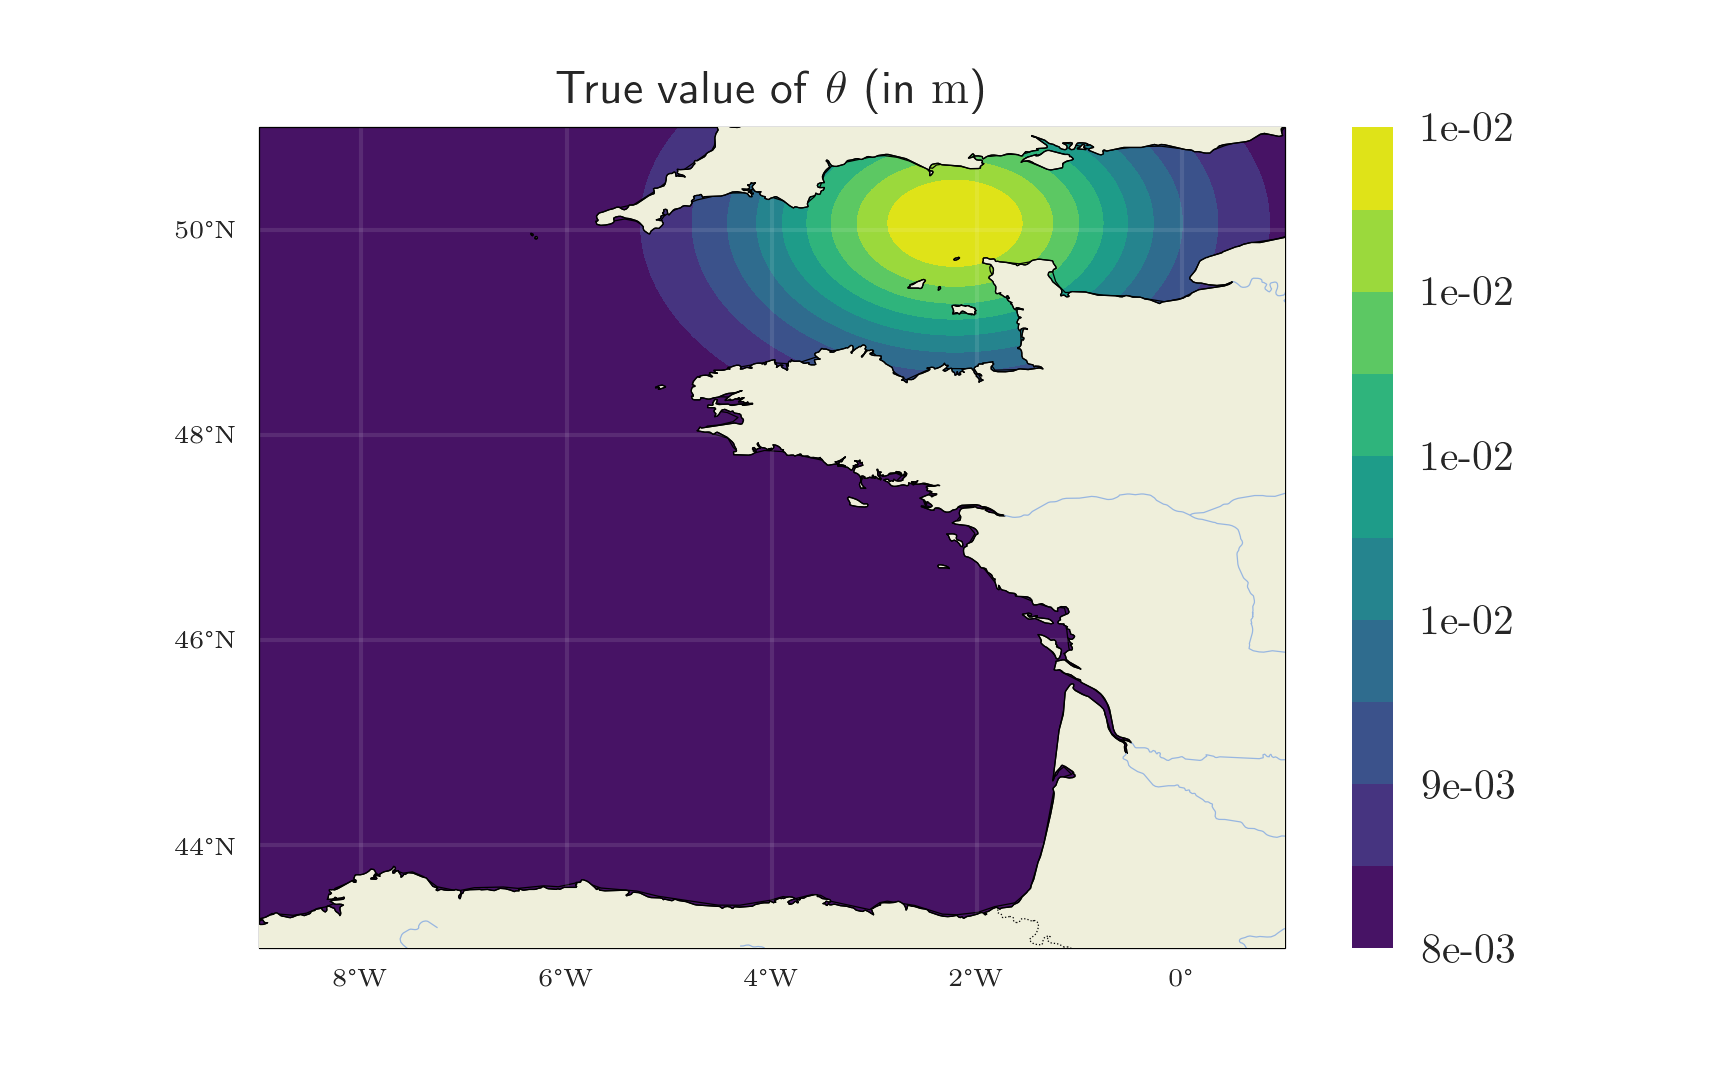
\includegraphics[width=\textwidth]{\manupath
%         % Chapter5/img/gaussian_english_channel.png}
%       \end{column}
%       \begin{column}{.5\textwidth}
%         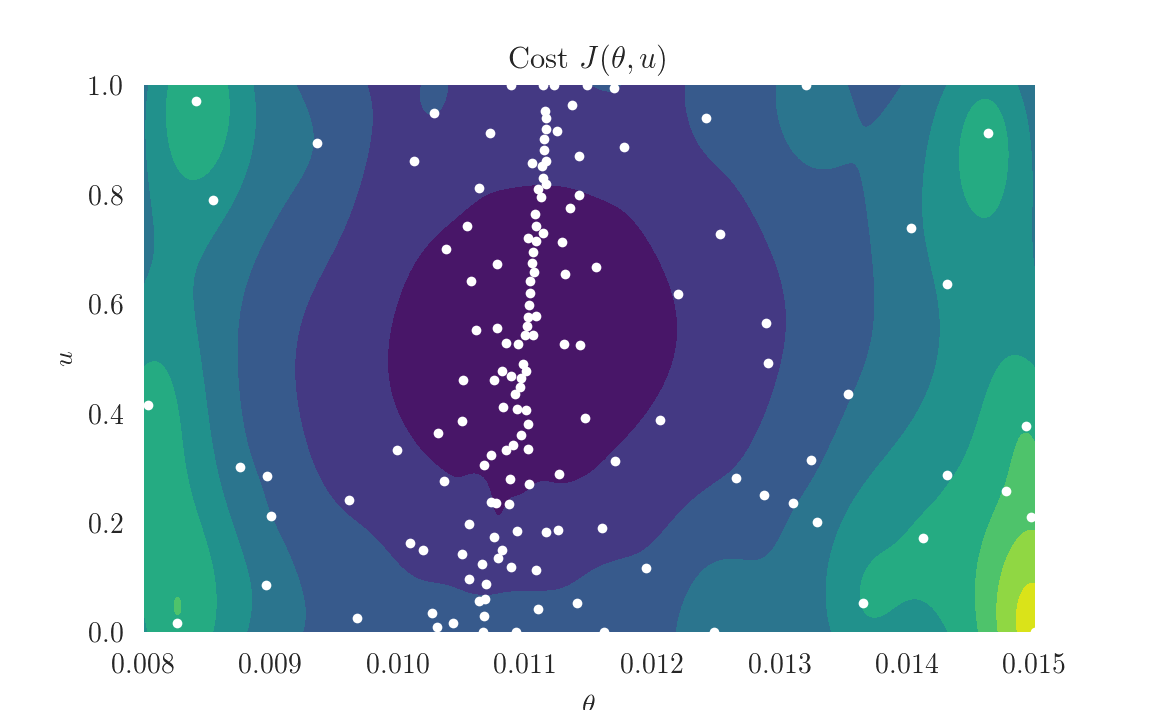
\includegraphics[width=\textwidth]{croco.png}
%       \end{column}
%     \end{columns}
%   \end{center}

%   \begin{itemize}
%   \item $\UU\sim \mathsf{U}[-1, 1]$ uniform r.v.\ that models the
%     percentage of error on the amplitude of the M2 component of the
%     tide
%   \item The ``truth'' ranges from $8$mm to $13$mm.
%   \item $11.0$mm leads to a cost which deviates less than $1\%$ from
%     the optimal value with probability $0.77$
%   \end{itemize}
% \end{frame}



\section{Conclusion}

\begin{frame}[label=conclusion]{Conclusion: overview}
  \begin{block}{Notion of robustness}
    \begin{itemize}
    \item Notion of robustness is context dependent
    \item Relative-regret estimates control the deviation from the \textit{optimal value}  
    \item $\alpha$ can reflect risk-adverse or risk-seeking preferences
    \end{itemize}
  \end{block}

  \begin{block}{Adaptive methods for computations}
    \begin{itemize}
    \item GP used as tools for plug-in estimation
    \item Allow to derive sequential strategies for enrichment of the design
    \item Can be adapted for batch evaluations
    \end{itemize}
  \end{block}
\end{frame}

\begin{frame}[label=conclusion]{Conclusion: perspectives}
  \begin{block}{Computational improvements}
    \begin{itemize}
    \item Dimension of the input space $\Kspace \times \Uspace$ can be limiting
      \begin{itemize}
      \item[$\rightarrow$] Reduction of the input space required
      \end{itemize}
    \item Adaptive methods still require expensive or difficult tasks (optimization, sampling, integration)
      \begin{itemize}
      \item[$\rightarrow$] 2-stages methods
      \item[$\rightarrow$] Focus computational effort for optimization
      \end{itemize}
    \item Include gradient information in the procedures ?
    \end{itemize}
  \end{block}

  \begin{block}{Perspectives}
    \begin{itemize}
    \item Discrepancy between $J^*(\UU)$ and $J(\hat{\kk},\UU)$ in terms of r.v.\
    \item Study of CROCO with a more complex configuration
    \item Study and compare robust estimates in predictions
  \end{itemize}
  \end{block}
\end{frame}
\appendix

\begin{frame}[allowframebreaks]{References}
  \renewcommand{\bibsection}{}
\bibliographystyle{authordate1}
  \bibliography{/home/victor/acadwriting/bibzotero.bib}
\end{frame}



\begin{frame}{Relative or additive regret}
 
  \renewcommand\rmfamily{\sffamily}
  \begin{center}
    \resizebox{.5\textwidth}{!}{%% Creator: Matplotlib, PGF backend
%%
%% To include the figure in your LaTeX document, write
%%   \input{<filename>.pgf}
%%
%% Make sure the required packages are loaded in your preamble
%%   \usepackage{pgf}
%%
%% Figures using additional raster images can only be included by \input if
%% they are in the same directory as the main LaTeX file. For loading figures
%% from other directories you can use the `import` package
%%   \usepackage{import}
%% and then include the figures with
%%   \import{<path to file>}{<filename>.pgf}
%%
%% Matplotlib used the following preamble
%%   \usepackage{fontspec}
%%   \setmainfont{DejaVuSans.ttf}[Path=/home/victor/miniconda3/lib/python3.7/site-packages/matplotlib/mpl-data/fonts/ttf/]
%%   \setsansfont{LiberationSans-Regular.ttf}[Path=/usr/share/fonts/truetype/liberation/]
%%   \setmonofont{DejaVuSansMono.ttf}[Path=/home/victor/miniconda3/lib/python3.7/site-packages/matplotlib/mpl-data/fonts/ttf/]
%%
\begingroup%
\makeatletter%
\begin{pgfpicture}%
\pgfpathrectangle{\pgfpointorigin}{\pgfqpoint{5.748032in}{3.552479in}}%
\pgfusepath{use as bounding box, clip}%
\begin{pgfscope}%
\pgfsetbuttcap%
\pgfsetmiterjoin%
\definecolor{currentfill}{rgb}{1.000000,1.000000,1.000000}%
\pgfsetfillcolor{currentfill}%
\pgfsetlinewidth{0.000000pt}%
\definecolor{currentstroke}{rgb}{1.000000,1.000000,1.000000}%
\pgfsetstrokecolor{currentstroke}%
\pgfsetdash{}{0pt}%
\pgfpathmoveto{\pgfqpoint{0.000000in}{0.000000in}}%
\pgfpathlineto{\pgfqpoint{5.748032in}{0.000000in}}%
\pgfpathlineto{\pgfqpoint{5.748032in}{3.552479in}}%
\pgfpathlineto{\pgfqpoint{0.000000in}{3.552479in}}%
\pgfpathclose%
\pgfusepath{fill}%
\end{pgfscope}%
\begin{pgfscope}%
\pgfsetbuttcap%
\pgfsetmiterjoin%
\definecolor{currentfill}{rgb}{0.917647,0.917647,0.949020}%
\pgfsetfillcolor{currentfill}%
\pgfsetlinewidth{0.000000pt}%
\definecolor{currentstroke}{rgb}{0.000000,0.000000,0.000000}%
\pgfsetstrokecolor{currentstroke}%
\pgfsetstrokeopacity{0.000000}%
\pgfsetdash{}{0pt}%
\pgfpathmoveto{\pgfqpoint{0.602580in}{0.548769in}}%
\pgfpathlineto{\pgfqpoint{2.676020in}{0.548769in}}%
\pgfpathlineto{\pgfqpoint{2.676020in}{3.213446in}}%
\pgfpathlineto{\pgfqpoint{0.602580in}{3.213446in}}%
\pgfpathclose%
\pgfusepath{fill}%
\end{pgfscope}%
\begin{pgfscope}%
\pgfpathrectangle{\pgfqpoint{0.602580in}{0.548769in}}{\pgfqpoint{2.073440in}{2.664678in}}%
\pgfusepath{clip}%
\pgfsetroundcap%
\pgfsetroundjoin%
\pgfsetlinewidth{1.003750pt}%
\definecolor{currentstroke}{rgb}{1.000000,1.000000,1.000000}%
\pgfsetstrokecolor{currentstroke}%
\pgfsetdash{}{0pt}%
\pgfpathmoveto{\pgfqpoint{0.602580in}{0.548769in}}%
\pgfpathlineto{\pgfqpoint{0.602580in}{3.213446in}}%
\pgfusepath{stroke}%
\end{pgfscope}%
\begin{pgfscope}%
\definecolor{textcolor}{rgb}{0.150000,0.150000,0.150000}%
\pgfsetstrokecolor{textcolor}%
\pgfsetfillcolor{textcolor}%
\pgftext[x=0.602580in,y=0.451547in,,top]{\color{textcolor}\rmfamily\fontsize{10.000000}{12.000000}\selectfont \(\displaystyle 0.00\)}%
\end{pgfscope}%
\begin{pgfscope}%
\pgfpathrectangle{\pgfqpoint{0.602580in}{0.548769in}}{\pgfqpoint{2.073440in}{2.664678in}}%
\pgfusepath{clip}%
\pgfsetroundcap%
\pgfsetroundjoin%
\pgfsetlinewidth{1.003750pt}%
\definecolor{currentstroke}{rgb}{1.000000,1.000000,1.000000}%
\pgfsetstrokecolor{currentstroke}%
\pgfsetdash{}{0pt}%
\pgfpathmoveto{\pgfqpoint{1.120940in}{0.548769in}}%
\pgfpathlineto{\pgfqpoint{1.120940in}{3.213446in}}%
\pgfusepath{stroke}%
\end{pgfscope}%
\begin{pgfscope}%
\definecolor{textcolor}{rgb}{0.150000,0.150000,0.150000}%
\pgfsetstrokecolor{textcolor}%
\pgfsetfillcolor{textcolor}%
\pgftext[x=1.120940in,y=0.451547in,,top]{\color{textcolor}\rmfamily\fontsize{10.000000}{12.000000}\selectfont \(\displaystyle 0.25\)}%
\end{pgfscope}%
\begin{pgfscope}%
\pgfpathrectangle{\pgfqpoint{0.602580in}{0.548769in}}{\pgfqpoint{2.073440in}{2.664678in}}%
\pgfusepath{clip}%
\pgfsetroundcap%
\pgfsetroundjoin%
\pgfsetlinewidth{1.003750pt}%
\definecolor{currentstroke}{rgb}{1.000000,1.000000,1.000000}%
\pgfsetstrokecolor{currentstroke}%
\pgfsetdash{}{0pt}%
\pgfpathmoveto{\pgfqpoint{1.639300in}{0.548769in}}%
\pgfpathlineto{\pgfqpoint{1.639300in}{3.213446in}}%
\pgfusepath{stroke}%
\end{pgfscope}%
\begin{pgfscope}%
\definecolor{textcolor}{rgb}{0.150000,0.150000,0.150000}%
\pgfsetstrokecolor{textcolor}%
\pgfsetfillcolor{textcolor}%
\pgftext[x=1.639300in,y=0.451547in,,top]{\color{textcolor}\rmfamily\fontsize{10.000000}{12.000000}\selectfont \(\displaystyle 0.50\)}%
\end{pgfscope}%
\begin{pgfscope}%
\pgfpathrectangle{\pgfqpoint{0.602580in}{0.548769in}}{\pgfqpoint{2.073440in}{2.664678in}}%
\pgfusepath{clip}%
\pgfsetroundcap%
\pgfsetroundjoin%
\pgfsetlinewidth{1.003750pt}%
\definecolor{currentstroke}{rgb}{1.000000,1.000000,1.000000}%
\pgfsetstrokecolor{currentstroke}%
\pgfsetdash{}{0pt}%
\pgfpathmoveto{\pgfqpoint{2.157660in}{0.548769in}}%
\pgfpathlineto{\pgfqpoint{2.157660in}{3.213446in}}%
\pgfusepath{stroke}%
\end{pgfscope}%
\begin{pgfscope}%
\definecolor{textcolor}{rgb}{0.150000,0.150000,0.150000}%
\pgfsetstrokecolor{textcolor}%
\pgfsetfillcolor{textcolor}%
\pgftext[x=2.157660in,y=0.451547in,,top]{\color{textcolor}\rmfamily\fontsize{10.000000}{12.000000}\selectfont \(\displaystyle 0.75\)}%
\end{pgfscope}%
\begin{pgfscope}%
\pgfpathrectangle{\pgfqpoint{0.602580in}{0.548769in}}{\pgfqpoint{2.073440in}{2.664678in}}%
\pgfusepath{clip}%
\pgfsetroundcap%
\pgfsetroundjoin%
\pgfsetlinewidth{1.003750pt}%
\definecolor{currentstroke}{rgb}{1.000000,1.000000,1.000000}%
\pgfsetstrokecolor{currentstroke}%
\pgfsetdash{}{0pt}%
\pgfpathmoveto{\pgfqpoint{2.676020in}{0.548769in}}%
\pgfpathlineto{\pgfqpoint{2.676020in}{3.213446in}}%
\pgfusepath{stroke}%
\end{pgfscope}%
\begin{pgfscope}%
\definecolor{textcolor}{rgb}{0.150000,0.150000,0.150000}%
\pgfsetstrokecolor{textcolor}%
\pgfsetfillcolor{textcolor}%
\pgftext[x=2.676020in,y=0.451547in,,top]{\color{textcolor}\rmfamily\fontsize{10.000000}{12.000000}\selectfont \(\displaystyle 1.00\)}%
\end{pgfscope}%
\begin{pgfscope}%
\definecolor{textcolor}{rgb}{0.150000,0.150000,0.150000}%
\pgfsetstrokecolor{textcolor}%
\pgfsetfillcolor{textcolor}%
\pgftext[x=1.639300in,y=0.261578in,,top]{\color{textcolor}\rmfamily\fontsize{10.000000}{12.000000}\selectfont \(\displaystyle \theta\)}%
\end{pgfscope}%
\begin{pgfscope}%
\pgfpathrectangle{\pgfqpoint{0.602580in}{0.548769in}}{\pgfqpoint{2.073440in}{2.664678in}}%
\pgfusepath{clip}%
\pgfsetroundcap%
\pgfsetroundjoin%
\pgfsetlinewidth{1.003750pt}%
\definecolor{currentstroke}{rgb}{1.000000,1.000000,1.000000}%
\pgfsetstrokecolor{currentstroke}%
\pgfsetdash{}{0pt}%
\pgfpathmoveto{\pgfqpoint{0.602580in}{0.548769in}}%
\pgfpathlineto{\pgfqpoint{2.676020in}{0.548769in}}%
\pgfusepath{stroke}%
\end{pgfscope}%
\begin{pgfscope}%
\definecolor{textcolor}{rgb}{0.150000,0.150000,0.150000}%
\pgfsetstrokecolor{textcolor}%
\pgfsetfillcolor{textcolor}%
\pgftext[x=0.327888in,y=0.496007in,left,base]{\color{textcolor}\rmfamily\fontsize{10.000000}{12.000000}\selectfont \(\displaystyle 0.0\)}%
\end{pgfscope}%
\begin{pgfscope}%
\pgfpathrectangle{\pgfqpoint{0.602580in}{0.548769in}}{\pgfqpoint{2.073440in}{2.664678in}}%
\pgfusepath{clip}%
\pgfsetroundcap%
\pgfsetroundjoin%
\pgfsetlinewidth{1.003750pt}%
\definecolor{currentstroke}{rgb}{1.000000,1.000000,1.000000}%
\pgfsetstrokecolor{currentstroke}%
\pgfsetdash{}{0pt}%
\pgfpathmoveto{\pgfqpoint{0.602580in}{1.081704in}}%
\pgfpathlineto{\pgfqpoint{2.676020in}{1.081704in}}%
\pgfusepath{stroke}%
\end{pgfscope}%
\begin{pgfscope}%
\definecolor{textcolor}{rgb}{0.150000,0.150000,0.150000}%
\pgfsetstrokecolor{textcolor}%
\pgfsetfillcolor{textcolor}%
\pgftext[x=0.327888in,y=1.028943in,left,base]{\color{textcolor}\rmfamily\fontsize{10.000000}{12.000000}\selectfont \(\displaystyle 0.2\)}%
\end{pgfscope}%
\begin{pgfscope}%
\pgfpathrectangle{\pgfqpoint{0.602580in}{0.548769in}}{\pgfqpoint{2.073440in}{2.664678in}}%
\pgfusepath{clip}%
\pgfsetroundcap%
\pgfsetroundjoin%
\pgfsetlinewidth{1.003750pt}%
\definecolor{currentstroke}{rgb}{1.000000,1.000000,1.000000}%
\pgfsetstrokecolor{currentstroke}%
\pgfsetdash{}{0pt}%
\pgfpathmoveto{\pgfqpoint{0.602580in}{1.614640in}}%
\pgfpathlineto{\pgfqpoint{2.676020in}{1.614640in}}%
\pgfusepath{stroke}%
\end{pgfscope}%
\begin{pgfscope}%
\definecolor{textcolor}{rgb}{0.150000,0.150000,0.150000}%
\pgfsetstrokecolor{textcolor}%
\pgfsetfillcolor{textcolor}%
\pgftext[x=0.327888in,y=1.561878in,left,base]{\color{textcolor}\rmfamily\fontsize{10.000000}{12.000000}\selectfont \(\displaystyle 0.4\)}%
\end{pgfscope}%
\begin{pgfscope}%
\pgfpathrectangle{\pgfqpoint{0.602580in}{0.548769in}}{\pgfqpoint{2.073440in}{2.664678in}}%
\pgfusepath{clip}%
\pgfsetroundcap%
\pgfsetroundjoin%
\pgfsetlinewidth{1.003750pt}%
\definecolor{currentstroke}{rgb}{1.000000,1.000000,1.000000}%
\pgfsetstrokecolor{currentstroke}%
\pgfsetdash{}{0pt}%
\pgfpathmoveto{\pgfqpoint{0.602580in}{2.147575in}}%
\pgfpathlineto{\pgfqpoint{2.676020in}{2.147575in}}%
\pgfusepath{stroke}%
\end{pgfscope}%
\begin{pgfscope}%
\definecolor{textcolor}{rgb}{0.150000,0.150000,0.150000}%
\pgfsetstrokecolor{textcolor}%
\pgfsetfillcolor{textcolor}%
\pgftext[x=0.327888in,y=2.094814in,left,base]{\color{textcolor}\rmfamily\fontsize{10.000000}{12.000000}\selectfont \(\displaystyle 0.6\)}%
\end{pgfscope}%
\begin{pgfscope}%
\pgfpathrectangle{\pgfqpoint{0.602580in}{0.548769in}}{\pgfqpoint{2.073440in}{2.664678in}}%
\pgfusepath{clip}%
\pgfsetroundcap%
\pgfsetroundjoin%
\pgfsetlinewidth{1.003750pt}%
\definecolor{currentstroke}{rgb}{1.000000,1.000000,1.000000}%
\pgfsetstrokecolor{currentstroke}%
\pgfsetdash{}{0pt}%
\pgfpathmoveto{\pgfqpoint{0.602580in}{2.680511in}}%
\pgfpathlineto{\pgfqpoint{2.676020in}{2.680511in}}%
\pgfusepath{stroke}%
\end{pgfscope}%
\begin{pgfscope}%
\definecolor{textcolor}{rgb}{0.150000,0.150000,0.150000}%
\pgfsetstrokecolor{textcolor}%
\pgfsetfillcolor{textcolor}%
\pgftext[x=0.327888in,y=2.627749in,left,base]{\color{textcolor}\rmfamily\fontsize{10.000000}{12.000000}\selectfont \(\displaystyle 0.8\)}%
\end{pgfscope}%
\begin{pgfscope}%
\pgfpathrectangle{\pgfqpoint{0.602580in}{0.548769in}}{\pgfqpoint{2.073440in}{2.664678in}}%
\pgfusepath{clip}%
\pgfsetroundcap%
\pgfsetroundjoin%
\pgfsetlinewidth{1.003750pt}%
\definecolor{currentstroke}{rgb}{1.000000,1.000000,1.000000}%
\pgfsetstrokecolor{currentstroke}%
\pgfsetdash{}{0pt}%
\pgfpathmoveto{\pgfqpoint{0.602580in}{3.213446in}}%
\pgfpathlineto{\pgfqpoint{2.676020in}{3.213446in}}%
\pgfusepath{stroke}%
\end{pgfscope}%
\begin{pgfscope}%
\definecolor{textcolor}{rgb}{0.150000,0.150000,0.150000}%
\pgfsetstrokecolor{textcolor}%
\pgfsetfillcolor{textcolor}%
\pgftext[x=0.327888in,y=3.160685in,left,base]{\color{textcolor}\rmfamily\fontsize{10.000000}{12.000000}\selectfont \(\displaystyle 1.0\)}%
\end{pgfscope}%
\begin{pgfscope}%
\definecolor{textcolor}{rgb}{0.150000,0.150000,0.150000}%
\pgfsetstrokecolor{textcolor}%
\pgfsetfillcolor{textcolor}%
\pgftext[x=0.272332in,y=1.881108in,,bottom,rotate=90.000000]{\color{textcolor}\rmfamily\fontsize{10.000000}{12.000000}\selectfont \(\displaystyle u\)}%
\end{pgfscope}%
\begin{pgfscope}%
\pgfpathrectangle{\pgfqpoint{0.602580in}{0.548769in}}{\pgfqpoint{2.073440in}{2.664678in}}%
\pgfusepath{clip}%
\pgfsetbuttcap%
\pgfsetroundjoin%
\definecolor{currentfill}{rgb}{0.282327,0.094955,0.417331}%
\pgfsetfillcolor{currentfill}%
\pgfsetlinewidth{0.000000pt}%
\definecolor{currentstroke}{rgb}{0.000000,0.000000,0.000000}%
\pgfsetstrokecolor{currentstroke}%
\pgfsetdash{}{0pt}%
\pgfpathmoveto{\pgfqpoint{0.605175in}{0.548769in}}%
\pgfpathlineto{\pgfqpoint{0.607770in}{0.548769in}}%
\pgfpathlineto{\pgfqpoint{0.610365in}{0.548769in}}%
\pgfpathlineto{\pgfqpoint{0.612960in}{0.548769in}}%
\pgfpathlineto{\pgfqpoint{0.615555in}{0.548769in}}%
\pgfpathlineto{\pgfqpoint{0.618150in}{0.548769in}}%
\pgfpathlineto{\pgfqpoint{0.620745in}{0.548769in}}%
\pgfpathlineto{\pgfqpoint{0.623340in}{0.548769in}}%
\pgfpathlineto{\pgfqpoint{0.625935in}{0.548769in}}%
\pgfpathlineto{\pgfqpoint{0.628530in}{0.548769in}}%
\pgfpathlineto{\pgfqpoint{0.631125in}{0.548769in}}%
\pgfpathlineto{\pgfqpoint{0.633720in}{0.548769in}}%
\pgfpathlineto{\pgfqpoint{0.636316in}{0.548769in}}%
\pgfpathlineto{\pgfqpoint{0.638911in}{0.548769in}}%
\pgfpathlineto{\pgfqpoint{0.641506in}{0.548769in}}%
\pgfpathlineto{\pgfqpoint{0.644101in}{0.548769in}}%
\pgfpathlineto{\pgfqpoint{0.646696in}{0.548769in}}%
\pgfpathlineto{\pgfqpoint{0.649291in}{0.548769in}}%
\pgfpathlineto{\pgfqpoint{0.651886in}{0.548769in}}%
\pgfpathlineto{\pgfqpoint{0.654481in}{0.548769in}}%
\pgfpathlineto{\pgfqpoint{0.657076in}{0.548769in}}%
\pgfpathlineto{\pgfqpoint{0.659671in}{0.548769in}}%
\pgfpathlineto{\pgfqpoint{0.662266in}{0.548769in}}%
\pgfpathlineto{\pgfqpoint{0.664861in}{0.548769in}}%
\pgfpathlineto{\pgfqpoint{0.667456in}{0.548769in}}%
\pgfpathlineto{\pgfqpoint{0.670051in}{0.548769in}}%
\pgfpathlineto{\pgfqpoint{0.672646in}{0.548769in}}%
\pgfpathlineto{\pgfqpoint{0.675241in}{0.548769in}}%
\pgfpathlineto{\pgfqpoint{0.677836in}{0.548769in}}%
\pgfpathlineto{\pgfqpoint{0.680431in}{0.548769in}}%
\pgfpathlineto{\pgfqpoint{0.683026in}{0.548769in}}%
\pgfpathlineto{\pgfqpoint{0.685621in}{0.548769in}}%
\pgfpathlineto{\pgfqpoint{0.688216in}{0.548769in}}%
\pgfpathlineto{\pgfqpoint{0.690811in}{0.548769in}}%
\pgfpathlineto{\pgfqpoint{0.693406in}{0.548769in}}%
\pgfpathlineto{\pgfqpoint{0.696002in}{0.548769in}}%
\pgfpathlineto{\pgfqpoint{0.698597in}{0.548769in}}%
\pgfpathlineto{\pgfqpoint{0.701192in}{0.548769in}}%
\pgfpathlineto{\pgfqpoint{0.703787in}{0.548769in}}%
\pgfpathlineto{\pgfqpoint{0.706382in}{0.548769in}}%
\pgfpathlineto{\pgfqpoint{0.708977in}{0.548769in}}%
\pgfpathlineto{\pgfqpoint{0.711572in}{0.548769in}}%
\pgfpathlineto{\pgfqpoint{0.714167in}{0.548769in}}%
\pgfpathlineto{\pgfqpoint{0.716762in}{0.548769in}}%
\pgfpathlineto{\pgfqpoint{0.719357in}{0.548769in}}%
\pgfpathlineto{\pgfqpoint{0.721952in}{0.548769in}}%
\pgfpathlineto{\pgfqpoint{0.724547in}{0.548769in}}%
\pgfpathlineto{\pgfqpoint{0.727142in}{0.548769in}}%
\pgfpathlineto{\pgfqpoint{0.729737in}{0.548769in}}%
\pgfpathlineto{\pgfqpoint{0.732332in}{0.548769in}}%
\pgfpathlineto{\pgfqpoint{0.734927in}{0.548769in}}%
\pgfpathlineto{\pgfqpoint{0.737522in}{0.548769in}}%
\pgfpathlineto{\pgfqpoint{0.740117in}{0.548769in}}%
\pgfpathlineto{\pgfqpoint{0.742712in}{0.548769in}}%
\pgfpathlineto{\pgfqpoint{0.745307in}{0.548769in}}%
\pgfpathlineto{\pgfqpoint{0.747902in}{0.548769in}}%
\pgfpathlineto{\pgfqpoint{0.750497in}{0.548769in}}%
\pgfpathlineto{\pgfqpoint{0.753092in}{0.548769in}}%
\pgfpathlineto{\pgfqpoint{0.755688in}{0.548769in}}%
\pgfpathlineto{\pgfqpoint{0.758283in}{0.548769in}}%
\pgfpathlineto{\pgfqpoint{0.760878in}{0.548769in}}%
\pgfpathlineto{\pgfqpoint{0.763473in}{0.548769in}}%
\pgfpathlineto{\pgfqpoint{0.766068in}{0.548769in}}%
\pgfpathlineto{\pgfqpoint{0.768663in}{0.548769in}}%
\pgfpathlineto{\pgfqpoint{0.771258in}{0.548769in}}%
\pgfpathlineto{\pgfqpoint{0.773853in}{0.548769in}}%
\pgfpathlineto{\pgfqpoint{0.776448in}{0.548769in}}%
\pgfpathlineto{\pgfqpoint{0.779043in}{0.548769in}}%
\pgfpathlineto{\pgfqpoint{0.781638in}{0.548769in}}%
\pgfpathlineto{\pgfqpoint{0.784233in}{0.548769in}}%
\pgfpathlineto{\pgfqpoint{0.786828in}{0.548769in}}%
\pgfpathlineto{\pgfqpoint{0.789423in}{0.548769in}}%
\pgfpathlineto{\pgfqpoint{0.792018in}{0.548769in}}%
\pgfpathlineto{\pgfqpoint{0.794613in}{0.548769in}}%
\pgfpathlineto{\pgfqpoint{0.797208in}{0.548769in}}%
\pgfpathlineto{\pgfqpoint{0.799803in}{0.548769in}}%
\pgfpathlineto{\pgfqpoint{0.802398in}{0.548769in}}%
\pgfpathlineto{\pgfqpoint{0.804993in}{0.548769in}}%
\pgfpathlineto{\pgfqpoint{0.807588in}{0.548769in}}%
\pgfpathlineto{\pgfqpoint{0.810183in}{0.548769in}}%
\pgfpathlineto{\pgfqpoint{0.812778in}{0.548769in}}%
\pgfpathlineto{\pgfqpoint{0.815374in}{0.548769in}}%
\pgfpathlineto{\pgfqpoint{0.817969in}{0.548769in}}%
\pgfpathlineto{\pgfqpoint{0.820564in}{0.548769in}}%
\pgfpathlineto{\pgfqpoint{0.823159in}{0.548769in}}%
\pgfpathlineto{\pgfqpoint{0.825754in}{0.548769in}}%
\pgfpathlineto{\pgfqpoint{0.828349in}{0.548769in}}%
\pgfpathlineto{\pgfqpoint{0.830944in}{0.548769in}}%
\pgfpathlineto{\pgfqpoint{0.833539in}{0.548769in}}%
\pgfpathlineto{\pgfqpoint{0.836134in}{0.548769in}}%
\pgfpathlineto{\pgfqpoint{0.838729in}{0.548769in}}%
\pgfpathlineto{\pgfqpoint{0.841324in}{0.548769in}}%
\pgfpathlineto{\pgfqpoint{0.843919in}{0.548769in}}%
\pgfpathlineto{\pgfqpoint{0.846514in}{0.548769in}}%
\pgfpathlineto{\pgfqpoint{0.849109in}{0.548769in}}%
\pgfpathlineto{\pgfqpoint{0.851704in}{0.548769in}}%
\pgfpathlineto{\pgfqpoint{0.854299in}{0.548769in}}%
\pgfpathlineto{\pgfqpoint{0.856894in}{0.548769in}}%
\pgfpathlineto{\pgfqpoint{0.859489in}{0.548769in}}%
\pgfpathlineto{\pgfqpoint{0.862084in}{0.548769in}}%
\pgfpathlineto{\pgfqpoint{0.864679in}{0.548769in}}%
\pgfpathlineto{\pgfqpoint{0.867274in}{0.548769in}}%
\pgfpathlineto{\pgfqpoint{0.869869in}{0.548769in}}%
\pgfpathlineto{\pgfqpoint{0.872464in}{0.548769in}}%
\pgfpathlineto{\pgfqpoint{0.875060in}{0.548769in}}%
\pgfpathlineto{\pgfqpoint{0.877655in}{0.548769in}}%
\pgfpathlineto{\pgfqpoint{0.880250in}{0.548769in}}%
\pgfpathlineto{\pgfqpoint{0.882845in}{0.548769in}}%
\pgfpathlineto{\pgfqpoint{0.885440in}{0.548769in}}%
\pgfpathlineto{\pgfqpoint{0.888035in}{0.548769in}}%
\pgfpathlineto{\pgfqpoint{0.890630in}{0.548769in}}%
\pgfpathlineto{\pgfqpoint{0.893225in}{0.548769in}}%
\pgfpathlineto{\pgfqpoint{0.895820in}{0.548769in}}%
\pgfpathlineto{\pgfqpoint{0.898415in}{0.548769in}}%
\pgfpathlineto{\pgfqpoint{0.901010in}{0.548769in}}%
\pgfpathlineto{\pgfqpoint{0.903605in}{0.548769in}}%
\pgfpathlineto{\pgfqpoint{0.906200in}{0.548769in}}%
\pgfpathlineto{\pgfqpoint{0.908795in}{0.548769in}}%
\pgfpathlineto{\pgfqpoint{0.911390in}{0.548769in}}%
\pgfpathlineto{\pgfqpoint{0.913985in}{0.548769in}}%
\pgfpathlineto{\pgfqpoint{0.916580in}{0.548769in}}%
\pgfpathlineto{\pgfqpoint{0.919175in}{0.548769in}}%
\pgfpathlineto{\pgfqpoint{0.921770in}{0.548769in}}%
\pgfpathlineto{\pgfqpoint{0.924365in}{0.548769in}}%
\pgfpathlineto{\pgfqpoint{0.926960in}{0.548769in}}%
\pgfpathlineto{\pgfqpoint{0.929555in}{0.548769in}}%
\pgfpathlineto{\pgfqpoint{0.932150in}{0.548769in}}%
\pgfpathlineto{\pgfqpoint{0.934746in}{0.548769in}}%
\pgfpathlineto{\pgfqpoint{0.937341in}{0.548769in}}%
\pgfpathlineto{\pgfqpoint{0.939936in}{0.548769in}}%
\pgfpathlineto{\pgfqpoint{0.942531in}{0.548769in}}%
\pgfpathlineto{\pgfqpoint{0.945126in}{0.548769in}}%
\pgfpathlineto{\pgfqpoint{0.947721in}{0.548769in}}%
\pgfpathlineto{\pgfqpoint{0.950316in}{0.548769in}}%
\pgfpathlineto{\pgfqpoint{0.952911in}{0.548769in}}%
\pgfpathlineto{\pgfqpoint{0.955506in}{0.548769in}}%
\pgfpathlineto{\pgfqpoint{0.958101in}{0.548769in}}%
\pgfpathlineto{\pgfqpoint{0.960696in}{0.548769in}}%
\pgfpathlineto{\pgfqpoint{0.963291in}{0.548769in}}%
\pgfpathlineto{\pgfqpoint{0.965886in}{0.548769in}}%
\pgfpathlineto{\pgfqpoint{0.968481in}{0.548769in}}%
\pgfpathlineto{\pgfqpoint{0.971076in}{0.548769in}}%
\pgfpathlineto{\pgfqpoint{0.973671in}{0.548769in}}%
\pgfpathlineto{\pgfqpoint{0.976266in}{0.548769in}}%
\pgfpathlineto{\pgfqpoint{0.978861in}{0.548769in}}%
\pgfpathlineto{\pgfqpoint{0.981456in}{0.548769in}}%
\pgfpathlineto{\pgfqpoint{0.984051in}{0.548769in}}%
\pgfpathlineto{\pgfqpoint{0.986646in}{0.548769in}}%
\pgfpathlineto{\pgfqpoint{0.989241in}{0.548769in}}%
\pgfpathlineto{\pgfqpoint{0.991837in}{0.548769in}}%
\pgfpathlineto{\pgfqpoint{0.994432in}{0.548769in}}%
\pgfpathlineto{\pgfqpoint{0.997027in}{0.548769in}}%
\pgfpathlineto{\pgfqpoint{0.999622in}{0.548769in}}%
\pgfpathlineto{\pgfqpoint{1.002217in}{0.548769in}}%
\pgfpathlineto{\pgfqpoint{1.004812in}{0.548769in}}%
\pgfpathlineto{\pgfqpoint{1.007407in}{0.548769in}}%
\pgfpathlineto{\pgfqpoint{1.010002in}{0.548769in}}%
\pgfpathlineto{\pgfqpoint{1.012597in}{0.548769in}}%
\pgfpathlineto{\pgfqpoint{1.015192in}{0.548769in}}%
\pgfpathlineto{\pgfqpoint{1.017787in}{0.548769in}}%
\pgfpathlineto{\pgfqpoint{1.020382in}{0.548769in}}%
\pgfpathlineto{\pgfqpoint{1.022977in}{0.548769in}}%
\pgfpathlineto{\pgfqpoint{1.025572in}{0.548769in}}%
\pgfpathlineto{\pgfqpoint{1.028167in}{0.548769in}}%
\pgfpathlineto{\pgfqpoint{1.030762in}{0.548769in}}%
\pgfpathlineto{\pgfqpoint{1.033357in}{0.548769in}}%
\pgfpathlineto{\pgfqpoint{1.035952in}{0.548769in}}%
\pgfpathlineto{\pgfqpoint{1.038547in}{0.548769in}}%
\pgfpathlineto{\pgfqpoint{1.041142in}{0.548769in}}%
\pgfpathlineto{\pgfqpoint{1.043737in}{0.548769in}}%
\pgfpathlineto{\pgfqpoint{1.046332in}{0.548769in}}%
\pgfpathlineto{\pgfqpoint{1.048927in}{0.548769in}}%
\pgfpathlineto{\pgfqpoint{1.051523in}{0.548769in}}%
\pgfpathlineto{\pgfqpoint{1.054118in}{0.548769in}}%
\pgfpathlineto{\pgfqpoint{1.056713in}{0.548769in}}%
\pgfpathlineto{\pgfqpoint{1.059308in}{0.548769in}}%
\pgfpathlineto{\pgfqpoint{1.061903in}{0.548769in}}%
\pgfpathlineto{\pgfqpoint{1.064498in}{0.548769in}}%
\pgfpathlineto{\pgfqpoint{1.067093in}{0.548769in}}%
\pgfpathlineto{\pgfqpoint{1.069688in}{0.548769in}}%
\pgfpathlineto{\pgfqpoint{1.072283in}{0.548769in}}%
\pgfpathlineto{\pgfqpoint{1.074878in}{0.548769in}}%
\pgfpathlineto{\pgfqpoint{1.077473in}{0.548769in}}%
\pgfpathlineto{\pgfqpoint{1.080068in}{0.548769in}}%
\pgfpathlineto{\pgfqpoint{1.082663in}{0.548769in}}%
\pgfpathlineto{\pgfqpoint{1.085258in}{0.548769in}}%
\pgfpathlineto{\pgfqpoint{1.087853in}{0.548769in}}%
\pgfpathlineto{\pgfqpoint{1.090448in}{0.548769in}}%
\pgfpathlineto{\pgfqpoint{1.093043in}{0.548769in}}%
\pgfpathlineto{\pgfqpoint{1.095638in}{0.548769in}}%
\pgfpathlineto{\pgfqpoint{1.098233in}{0.548769in}}%
\pgfpathlineto{\pgfqpoint{1.100828in}{0.548769in}}%
\pgfpathlineto{\pgfqpoint{1.103423in}{0.548769in}}%
\pgfpathlineto{\pgfqpoint{1.106018in}{0.548769in}}%
\pgfpathlineto{\pgfqpoint{1.108613in}{0.548769in}}%
\pgfpathlineto{\pgfqpoint{1.111209in}{0.548769in}}%
\pgfpathlineto{\pgfqpoint{1.113804in}{0.548769in}}%
\pgfpathlineto{\pgfqpoint{1.116399in}{0.548769in}}%
\pgfpathlineto{\pgfqpoint{1.118994in}{0.548769in}}%
\pgfpathlineto{\pgfqpoint{1.121589in}{0.548769in}}%
\pgfpathlineto{\pgfqpoint{1.124184in}{0.548769in}}%
\pgfpathlineto{\pgfqpoint{1.126779in}{0.548769in}}%
\pgfpathlineto{\pgfqpoint{1.129374in}{0.548769in}}%
\pgfpathlineto{\pgfqpoint{1.131969in}{0.548769in}}%
\pgfpathlineto{\pgfqpoint{1.134564in}{0.548769in}}%
\pgfpathlineto{\pgfqpoint{1.137159in}{0.548769in}}%
\pgfpathlineto{\pgfqpoint{1.139754in}{0.548769in}}%
\pgfpathlineto{\pgfqpoint{1.142349in}{0.548769in}}%
\pgfpathlineto{\pgfqpoint{1.144944in}{0.548769in}}%
\pgfpathlineto{\pgfqpoint{1.147539in}{0.548769in}}%
\pgfpathlineto{\pgfqpoint{1.150134in}{0.548769in}}%
\pgfpathlineto{\pgfqpoint{1.152729in}{0.548769in}}%
\pgfpathlineto{\pgfqpoint{1.155324in}{0.548769in}}%
\pgfpathlineto{\pgfqpoint{1.157919in}{0.548769in}}%
\pgfpathlineto{\pgfqpoint{1.160514in}{0.548769in}}%
\pgfpathlineto{\pgfqpoint{1.163109in}{0.548769in}}%
\pgfpathlineto{\pgfqpoint{1.165704in}{0.548769in}}%
\pgfpathlineto{\pgfqpoint{1.168299in}{0.548769in}}%
\pgfpathlineto{\pgfqpoint{1.170895in}{0.548769in}}%
\pgfpathlineto{\pgfqpoint{1.173490in}{0.548769in}}%
\pgfpathlineto{\pgfqpoint{1.176085in}{0.548769in}}%
\pgfpathlineto{\pgfqpoint{1.178680in}{0.548769in}}%
\pgfpathlineto{\pgfqpoint{1.181275in}{0.548769in}}%
\pgfpathlineto{\pgfqpoint{1.183870in}{0.548769in}}%
\pgfpathlineto{\pgfqpoint{1.186465in}{0.548769in}}%
\pgfpathlineto{\pgfqpoint{1.189060in}{0.548769in}}%
\pgfpathlineto{\pgfqpoint{1.191655in}{0.548769in}}%
\pgfpathlineto{\pgfqpoint{1.194250in}{0.548769in}}%
\pgfpathlineto{\pgfqpoint{1.196845in}{0.548769in}}%
\pgfpathlineto{\pgfqpoint{1.199440in}{0.548769in}}%
\pgfpathlineto{\pgfqpoint{1.202035in}{0.548769in}}%
\pgfpathlineto{\pgfqpoint{1.204630in}{0.548769in}}%
\pgfpathlineto{\pgfqpoint{1.207225in}{0.548769in}}%
\pgfpathlineto{\pgfqpoint{1.209820in}{0.548769in}}%
\pgfpathlineto{\pgfqpoint{1.212415in}{0.548769in}}%
\pgfpathlineto{\pgfqpoint{1.215010in}{0.548769in}}%
\pgfpathlineto{\pgfqpoint{1.217605in}{0.548769in}}%
\pgfpathlineto{\pgfqpoint{1.220200in}{0.548769in}}%
\pgfpathlineto{\pgfqpoint{1.222795in}{0.548769in}}%
\pgfpathlineto{\pgfqpoint{1.225390in}{0.548769in}}%
\pgfpathlineto{\pgfqpoint{1.227985in}{0.548769in}}%
\pgfpathlineto{\pgfqpoint{1.230581in}{0.548769in}}%
\pgfpathlineto{\pgfqpoint{1.233176in}{0.548769in}}%
\pgfpathlineto{\pgfqpoint{1.235771in}{0.548769in}}%
\pgfpathlineto{\pgfqpoint{1.238366in}{0.548769in}}%
\pgfpathlineto{\pgfqpoint{1.240961in}{0.548769in}}%
\pgfpathlineto{\pgfqpoint{1.243556in}{0.548769in}}%
\pgfpathlineto{\pgfqpoint{1.246151in}{0.548769in}}%
\pgfpathlineto{\pgfqpoint{1.248746in}{0.548769in}}%
\pgfpathlineto{\pgfqpoint{1.251341in}{0.548769in}}%
\pgfpathlineto{\pgfqpoint{1.253936in}{0.548769in}}%
\pgfpathlineto{\pgfqpoint{1.256531in}{0.548769in}}%
\pgfpathlineto{\pgfqpoint{1.259126in}{0.548769in}}%
\pgfpathlineto{\pgfqpoint{1.261721in}{0.548769in}}%
\pgfpathlineto{\pgfqpoint{1.264316in}{0.548769in}}%
\pgfpathlineto{\pgfqpoint{1.266911in}{0.548769in}}%
\pgfpathlineto{\pgfqpoint{1.269506in}{0.548769in}}%
\pgfpathlineto{\pgfqpoint{1.272101in}{0.548769in}}%
\pgfpathlineto{\pgfqpoint{1.274696in}{0.548769in}}%
\pgfpathlineto{\pgfqpoint{1.277291in}{0.548769in}}%
\pgfpathlineto{\pgfqpoint{1.279886in}{0.548769in}}%
\pgfpathlineto{\pgfqpoint{1.282481in}{0.548769in}}%
\pgfpathlineto{\pgfqpoint{1.285076in}{0.548769in}}%
\pgfpathlineto{\pgfqpoint{1.287671in}{0.548769in}}%
\pgfpathlineto{\pgfqpoint{1.290267in}{0.548769in}}%
\pgfpathlineto{\pgfqpoint{1.292862in}{0.548769in}}%
\pgfpathlineto{\pgfqpoint{1.295457in}{0.548769in}}%
\pgfpathlineto{\pgfqpoint{1.298052in}{0.548769in}}%
\pgfpathlineto{\pgfqpoint{1.300647in}{0.548769in}}%
\pgfpathlineto{\pgfqpoint{1.303242in}{0.548769in}}%
\pgfpathlineto{\pgfqpoint{1.305837in}{0.548769in}}%
\pgfpathlineto{\pgfqpoint{1.308432in}{0.548769in}}%
\pgfpathlineto{\pgfqpoint{1.311027in}{0.548769in}}%
\pgfpathlineto{\pgfqpoint{1.313622in}{0.548769in}}%
\pgfpathlineto{\pgfqpoint{1.316217in}{0.548769in}}%
\pgfpathlineto{\pgfqpoint{1.318812in}{0.548769in}}%
\pgfpathlineto{\pgfqpoint{1.321407in}{0.548769in}}%
\pgfpathlineto{\pgfqpoint{1.324002in}{0.548769in}}%
\pgfpathlineto{\pgfqpoint{1.326597in}{0.548769in}}%
\pgfpathlineto{\pgfqpoint{1.329192in}{0.548769in}}%
\pgfpathlineto{\pgfqpoint{1.331787in}{0.548769in}}%
\pgfpathlineto{\pgfqpoint{1.334382in}{0.548769in}}%
\pgfpathlineto{\pgfqpoint{1.336977in}{0.548769in}}%
\pgfpathlineto{\pgfqpoint{1.339572in}{0.548769in}}%
\pgfpathlineto{\pgfqpoint{1.342167in}{0.548769in}}%
\pgfpathlineto{\pgfqpoint{1.344762in}{0.548769in}}%
\pgfpathlineto{\pgfqpoint{1.347358in}{0.548769in}}%
\pgfpathlineto{\pgfqpoint{1.349953in}{0.548769in}}%
\pgfpathlineto{\pgfqpoint{1.352548in}{0.548769in}}%
\pgfpathlineto{\pgfqpoint{1.355143in}{0.548769in}}%
\pgfpathlineto{\pgfqpoint{1.357738in}{0.548769in}}%
\pgfpathlineto{\pgfqpoint{1.360333in}{0.548769in}}%
\pgfpathlineto{\pgfqpoint{1.362928in}{0.548769in}}%
\pgfpathlineto{\pgfqpoint{1.365523in}{0.548769in}}%
\pgfpathlineto{\pgfqpoint{1.368118in}{0.548769in}}%
\pgfpathlineto{\pgfqpoint{1.370713in}{0.548769in}}%
\pgfpathlineto{\pgfqpoint{1.373308in}{0.548769in}}%
\pgfpathlineto{\pgfqpoint{1.375903in}{0.548769in}}%
\pgfpathlineto{\pgfqpoint{1.378498in}{0.548769in}}%
\pgfpathlineto{\pgfqpoint{1.381093in}{0.548769in}}%
\pgfpathlineto{\pgfqpoint{1.383688in}{0.548769in}}%
\pgfpathlineto{\pgfqpoint{1.386283in}{0.548769in}}%
\pgfpathlineto{\pgfqpoint{1.388878in}{0.548769in}}%
\pgfpathlineto{\pgfqpoint{1.391473in}{0.548769in}}%
\pgfpathlineto{\pgfqpoint{1.394068in}{0.548769in}}%
\pgfpathlineto{\pgfqpoint{1.396663in}{0.548769in}}%
\pgfpathlineto{\pgfqpoint{1.399258in}{0.548769in}}%
\pgfpathlineto{\pgfqpoint{1.401853in}{0.548769in}}%
\pgfpathlineto{\pgfqpoint{1.404448in}{0.548769in}}%
\pgfpathlineto{\pgfqpoint{1.407044in}{0.548769in}}%
\pgfpathlineto{\pgfqpoint{1.409639in}{0.548769in}}%
\pgfpathlineto{\pgfqpoint{1.412234in}{0.548769in}}%
\pgfpathlineto{\pgfqpoint{1.414829in}{0.548769in}}%
\pgfpathlineto{\pgfqpoint{1.417424in}{0.548769in}}%
\pgfpathlineto{\pgfqpoint{1.420019in}{0.548769in}}%
\pgfpathlineto{\pgfqpoint{1.422614in}{0.548769in}}%
\pgfpathlineto{\pgfqpoint{1.425209in}{0.548769in}}%
\pgfpathlineto{\pgfqpoint{1.427804in}{0.548769in}}%
\pgfpathlineto{\pgfqpoint{1.430399in}{0.548769in}}%
\pgfpathlineto{\pgfqpoint{1.432994in}{0.548769in}}%
\pgfpathlineto{\pgfqpoint{1.435589in}{0.548769in}}%
\pgfpathlineto{\pgfqpoint{1.438184in}{0.548769in}}%
\pgfpathlineto{\pgfqpoint{1.440779in}{0.548769in}}%
\pgfpathlineto{\pgfqpoint{1.443374in}{0.548769in}}%
\pgfpathlineto{\pgfqpoint{1.445969in}{0.548769in}}%
\pgfpathlineto{\pgfqpoint{1.448564in}{0.548769in}}%
\pgfpathlineto{\pgfqpoint{1.451159in}{0.548769in}}%
\pgfpathlineto{\pgfqpoint{1.453754in}{0.548769in}}%
\pgfpathlineto{\pgfqpoint{1.456349in}{0.548769in}}%
\pgfpathlineto{\pgfqpoint{1.458944in}{0.548769in}}%
\pgfpathlineto{\pgfqpoint{1.461539in}{0.548769in}}%
\pgfpathlineto{\pgfqpoint{1.464134in}{0.548769in}}%
\pgfpathlineto{\pgfqpoint{1.466730in}{0.548769in}}%
\pgfpathlineto{\pgfqpoint{1.469325in}{0.548769in}}%
\pgfpathlineto{\pgfqpoint{1.471920in}{0.548769in}}%
\pgfpathlineto{\pgfqpoint{1.474515in}{0.548769in}}%
\pgfpathlineto{\pgfqpoint{1.477110in}{0.548769in}}%
\pgfpathlineto{\pgfqpoint{1.479705in}{0.548769in}}%
\pgfpathlineto{\pgfqpoint{1.482300in}{0.548769in}}%
\pgfpathlineto{\pgfqpoint{1.484895in}{0.548769in}}%
\pgfpathlineto{\pgfqpoint{1.487490in}{0.548769in}}%
\pgfpathlineto{\pgfqpoint{1.490085in}{0.548769in}}%
\pgfpathlineto{\pgfqpoint{1.492680in}{0.548769in}}%
\pgfpathlineto{\pgfqpoint{1.495275in}{0.548769in}}%
\pgfpathlineto{\pgfqpoint{1.497870in}{0.548769in}}%
\pgfpathlineto{\pgfqpoint{1.500465in}{0.548769in}}%
\pgfpathlineto{\pgfqpoint{1.503060in}{0.548769in}}%
\pgfpathlineto{\pgfqpoint{1.505655in}{0.548769in}}%
\pgfpathlineto{\pgfqpoint{1.508250in}{0.548769in}}%
\pgfpathlineto{\pgfqpoint{1.510845in}{0.548769in}}%
\pgfpathlineto{\pgfqpoint{1.513440in}{0.548769in}}%
\pgfpathlineto{\pgfqpoint{1.516035in}{0.548769in}}%
\pgfpathlineto{\pgfqpoint{1.518630in}{0.548769in}}%
\pgfpathlineto{\pgfqpoint{1.521225in}{0.548769in}}%
\pgfpathlineto{\pgfqpoint{1.523820in}{0.548769in}}%
\pgfpathlineto{\pgfqpoint{1.526416in}{0.548769in}}%
\pgfpathlineto{\pgfqpoint{1.529011in}{0.548769in}}%
\pgfpathlineto{\pgfqpoint{1.531606in}{0.548769in}}%
\pgfpathlineto{\pgfqpoint{1.534201in}{0.548769in}}%
\pgfpathlineto{\pgfqpoint{1.536796in}{0.548769in}}%
\pgfpathlineto{\pgfqpoint{1.539391in}{0.548769in}}%
\pgfpathlineto{\pgfqpoint{1.541986in}{0.548769in}}%
\pgfpathlineto{\pgfqpoint{1.544581in}{0.548769in}}%
\pgfpathlineto{\pgfqpoint{1.547176in}{0.548769in}}%
\pgfpathlineto{\pgfqpoint{1.549771in}{0.548769in}}%
\pgfpathlineto{\pgfqpoint{1.552366in}{0.548769in}}%
\pgfpathlineto{\pgfqpoint{1.554961in}{0.548769in}}%
\pgfpathlineto{\pgfqpoint{1.557556in}{0.548769in}}%
\pgfpathlineto{\pgfqpoint{1.560151in}{0.548769in}}%
\pgfpathlineto{\pgfqpoint{1.562746in}{0.548769in}}%
\pgfpathlineto{\pgfqpoint{1.565341in}{0.548769in}}%
\pgfpathlineto{\pgfqpoint{1.567936in}{0.548769in}}%
\pgfpathlineto{\pgfqpoint{1.570531in}{0.548769in}}%
\pgfpathlineto{\pgfqpoint{1.573126in}{0.548769in}}%
\pgfpathlineto{\pgfqpoint{1.575721in}{0.548769in}}%
\pgfpathlineto{\pgfqpoint{1.578316in}{0.548769in}}%
\pgfpathlineto{\pgfqpoint{1.580911in}{0.548769in}}%
\pgfpathlineto{\pgfqpoint{1.583506in}{0.548769in}}%
\pgfpathlineto{\pgfqpoint{1.586102in}{0.548769in}}%
\pgfpathlineto{\pgfqpoint{1.588697in}{0.548769in}}%
\pgfpathlineto{\pgfqpoint{1.591292in}{0.548769in}}%
\pgfpathlineto{\pgfqpoint{1.593887in}{0.548769in}}%
\pgfpathlineto{\pgfqpoint{1.596482in}{0.548769in}}%
\pgfpathlineto{\pgfqpoint{1.599077in}{0.548769in}}%
\pgfpathlineto{\pgfqpoint{1.601672in}{0.548769in}}%
\pgfpathlineto{\pgfqpoint{1.604267in}{0.548769in}}%
\pgfpathlineto{\pgfqpoint{1.606862in}{0.548769in}}%
\pgfpathlineto{\pgfqpoint{1.609457in}{0.548769in}}%
\pgfpathlineto{\pgfqpoint{1.612052in}{0.548769in}}%
\pgfpathlineto{\pgfqpoint{1.614647in}{0.548769in}}%
\pgfpathlineto{\pgfqpoint{1.617242in}{0.548769in}}%
\pgfpathlineto{\pgfqpoint{1.619837in}{0.548769in}}%
\pgfpathlineto{\pgfqpoint{1.622432in}{0.548769in}}%
\pgfpathlineto{\pgfqpoint{1.625027in}{0.548769in}}%
\pgfpathlineto{\pgfqpoint{1.627622in}{0.548769in}}%
\pgfpathlineto{\pgfqpoint{1.630217in}{0.548769in}}%
\pgfpathlineto{\pgfqpoint{1.632812in}{0.548769in}}%
\pgfpathlineto{\pgfqpoint{1.635407in}{0.548769in}}%
\pgfpathlineto{\pgfqpoint{1.638002in}{0.548769in}}%
\pgfpathlineto{\pgfqpoint{1.640597in}{0.548769in}}%
\pgfpathlineto{\pgfqpoint{1.643192in}{0.548769in}}%
\pgfpathlineto{\pgfqpoint{1.645788in}{0.548769in}}%
\pgfpathlineto{\pgfqpoint{1.648383in}{0.548769in}}%
\pgfpathlineto{\pgfqpoint{1.650978in}{0.548769in}}%
\pgfpathlineto{\pgfqpoint{1.653573in}{0.548769in}}%
\pgfpathlineto{\pgfqpoint{1.656168in}{0.548769in}}%
\pgfpathlineto{\pgfqpoint{1.658763in}{0.548769in}}%
\pgfpathlineto{\pgfqpoint{1.661358in}{0.548769in}}%
\pgfpathlineto{\pgfqpoint{1.663953in}{0.548769in}}%
\pgfpathlineto{\pgfqpoint{1.666548in}{0.548769in}}%
\pgfpathlineto{\pgfqpoint{1.669143in}{0.548769in}}%
\pgfpathlineto{\pgfqpoint{1.671738in}{0.548769in}}%
\pgfpathlineto{\pgfqpoint{1.674333in}{0.548769in}}%
\pgfpathlineto{\pgfqpoint{1.676928in}{0.548769in}}%
\pgfpathlineto{\pgfqpoint{1.679523in}{0.548769in}}%
\pgfpathlineto{\pgfqpoint{1.682118in}{0.548769in}}%
\pgfpathlineto{\pgfqpoint{1.684713in}{0.548769in}}%
\pgfpathlineto{\pgfqpoint{1.687308in}{0.548769in}}%
\pgfpathlineto{\pgfqpoint{1.689903in}{0.548769in}}%
\pgfpathlineto{\pgfqpoint{1.692498in}{0.548769in}}%
\pgfpathlineto{\pgfqpoint{1.695093in}{0.548769in}}%
\pgfpathlineto{\pgfqpoint{1.697688in}{0.548769in}}%
\pgfpathlineto{\pgfqpoint{1.700283in}{0.548769in}}%
\pgfpathlineto{\pgfqpoint{1.702878in}{0.548769in}}%
\pgfpathlineto{\pgfqpoint{1.705474in}{0.548769in}}%
\pgfpathlineto{\pgfqpoint{1.708069in}{0.548769in}}%
\pgfpathlineto{\pgfqpoint{1.710664in}{0.548769in}}%
\pgfpathlineto{\pgfqpoint{1.713259in}{0.548769in}}%
\pgfpathlineto{\pgfqpoint{1.715854in}{0.548769in}}%
\pgfpathlineto{\pgfqpoint{1.718449in}{0.548769in}}%
\pgfpathlineto{\pgfqpoint{1.721044in}{0.548769in}}%
\pgfpathlineto{\pgfqpoint{1.723639in}{0.548769in}}%
\pgfpathlineto{\pgfqpoint{1.726234in}{0.548769in}}%
\pgfpathlineto{\pgfqpoint{1.728829in}{0.548769in}}%
\pgfpathlineto{\pgfqpoint{1.731424in}{0.548769in}}%
\pgfpathlineto{\pgfqpoint{1.734019in}{0.548769in}}%
\pgfpathlineto{\pgfqpoint{1.736614in}{0.548769in}}%
\pgfpathlineto{\pgfqpoint{1.739209in}{0.548769in}}%
\pgfpathlineto{\pgfqpoint{1.741804in}{0.548769in}}%
\pgfpathlineto{\pgfqpoint{1.744399in}{0.548769in}}%
\pgfpathlineto{\pgfqpoint{1.746994in}{0.548769in}}%
\pgfpathlineto{\pgfqpoint{1.749589in}{0.548769in}}%
\pgfpathlineto{\pgfqpoint{1.752184in}{0.548769in}}%
\pgfpathlineto{\pgfqpoint{1.754779in}{0.548769in}}%
\pgfpathlineto{\pgfqpoint{1.757374in}{0.548769in}}%
\pgfpathlineto{\pgfqpoint{1.759969in}{0.548769in}}%
\pgfpathlineto{\pgfqpoint{1.762565in}{0.548769in}}%
\pgfpathlineto{\pgfqpoint{1.765160in}{0.548769in}}%
\pgfpathlineto{\pgfqpoint{1.767755in}{0.548769in}}%
\pgfpathlineto{\pgfqpoint{1.770350in}{0.548769in}}%
\pgfpathlineto{\pgfqpoint{1.772945in}{0.548769in}}%
\pgfpathlineto{\pgfqpoint{1.775540in}{0.548769in}}%
\pgfpathlineto{\pgfqpoint{1.778135in}{0.548769in}}%
\pgfpathlineto{\pgfqpoint{1.780730in}{0.548769in}}%
\pgfpathlineto{\pgfqpoint{1.783325in}{0.548769in}}%
\pgfpathlineto{\pgfqpoint{1.785920in}{0.548769in}}%
\pgfpathlineto{\pgfqpoint{1.788515in}{0.548769in}}%
\pgfpathlineto{\pgfqpoint{1.791110in}{0.548769in}}%
\pgfpathlineto{\pgfqpoint{1.793705in}{0.548769in}}%
\pgfpathlineto{\pgfqpoint{1.796300in}{0.548769in}}%
\pgfpathlineto{\pgfqpoint{1.798895in}{0.548769in}}%
\pgfpathlineto{\pgfqpoint{1.801490in}{0.548769in}}%
\pgfpathlineto{\pgfqpoint{1.804085in}{0.548769in}}%
\pgfpathlineto{\pgfqpoint{1.806680in}{0.548769in}}%
\pgfpathlineto{\pgfqpoint{1.809275in}{0.548769in}}%
\pgfpathlineto{\pgfqpoint{1.811870in}{0.548769in}}%
\pgfpathlineto{\pgfqpoint{1.814465in}{0.548769in}}%
\pgfpathlineto{\pgfqpoint{1.817060in}{0.548769in}}%
\pgfpathlineto{\pgfqpoint{1.819655in}{0.548769in}}%
\pgfpathlineto{\pgfqpoint{1.822251in}{0.548769in}}%
\pgfpathlineto{\pgfqpoint{1.824846in}{0.548769in}}%
\pgfpathlineto{\pgfqpoint{1.827441in}{0.548769in}}%
\pgfpathlineto{\pgfqpoint{1.830036in}{0.548769in}}%
\pgfpathlineto{\pgfqpoint{1.832631in}{0.548769in}}%
\pgfpathlineto{\pgfqpoint{1.835226in}{0.548769in}}%
\pgfpathlineto{\pgfqpoint{1.837821in}{0.548769in}}%
\pgfpathlineto{\pgfqpoint{1.840416in}{0.548769in}}%
\pgfpathlineto{\pgfqpoint{1.843011in}{0.548769in}}%
\pgfpathlineto{\pgfqpoint{1.845606in}{0.548769in}}%
\pgfpathlineto{\pgfqpoint{1.848201in}{0.548769in}}%
\pgfpathlineto{\pgfqpoint{1.850796in}{0.548769in}}%
\pgfpathlineto{\pgfqpoint{1.853391in}{0.548769in}}%
\pgfpathlineto{\pgfqpoint{1.855986in}{0.548769in}}%
\pgfpathlineto{\pgfqpoint{1.858581in}{0.548769in}}%
\pgfpathlineto{\pgfqpoint{1.861176in}{0.548769in}}%
\pgfpathlineto{\pgfqpoint{1.863771in}{0.548769in}}%
\pgfpathlineto{\pgfqpoint{1.866366in}{0.548769in}}%
\pgfpathlineto{\pgfqpoint{1.868961in}{0.548769in}}%
\pgfpathlineto{\pgfqpoint{1.871556in}{0.548769in}}%
\pgfpathlineto{\pgfqpoint{1.874151in}{0.548769in}}%
\pgfpathlineto{\pgfqpoint{1.876746in}{0.548769in}}%
\pgfpathlineto{\pgfqpoint{1.879341in}{0.548769in}}%
\pgfpathlineto{\pgfqpoint{1.881937in}{0.548769in}}%
\pgfpathlineto{\pgfqpoint{1.884532in}{0.548769in}}%
\pgfpathlineto{\pgfqpoint{1.887127in}{0.548769in}}%
\pgfpathlineto{\pgfqpoint{1.889722in}{0.548769in}}%
\pgfpathlineto{\pgfqpoint{1.892317in}{0.548769in}}%
\pgfpathlineto{\pgfqpoint{1.894912in}{0.548769in}}%
\pgfpathlineto{\pgfqpoint{1.897507in}{0.548769in}}%
\pgfpathlineto{\pgfqpoint{1.900102in}{0.548769in}}%
\pgfpathlineto{\pgfqpoint{1.902697in}{0.548769in}}%
\pgfpathlineto{\pgfqpoint{1.905292in}{0.548769in}}%
\pgfpathlineto{\pgfqpoint{1.907887in}{0.548769in}}%
\pgfpathlineto{\pgfqpoint{1.910482in}{0.548769in}}%
\pgfpathlineto{\pgfqpoint{1.913077in}{0.548769in}}%
\pgfpathlineto{\pgfqpoint{1.915672in}{0.548769in}}%
\pgfpathlineto{\pgfqpoint{1.918267in}{0.548769in}}%
\pgfpathlineto{\pgfqpoint{1.920862in}{0.548769in}}%
\pgfpathlineto{\pgfqpoint{1.923457in}{0.548769in}}%
\pgfpathlineto{\pgfqpoint{1.926052in}{0.548769in}}%
\pgfpathlineto{\pgfqpoint{1.928647in}{0.548769in}}%
\pgfpathlineto{\pgfqpoint{1.931242in}{0.548769in}}%
\pgfpathlineto{\pgfqpoint{1.933837in}{0.548769in}}%
\pgfpathlineto{\pgfqpoint{1.936432in}{0.548769in}}%
\pgfpathlineto{\pgfqpoint{1.939027in}{0.548769in}}%
\pgfpathlineto{\pgfqpoint{1.941623in}{0.548769in}}%
\pgfpathlineto{\pgfqpoint{1.944218in}{0.548769in}}%
\pgfpathlineto{\pgfqpoint{1.946813in}{0.548769in}}%
\pgfpathlineto{\pgfqpoint{1.949408in}{0.548769in}}%
\pgfpathlineto{\pgfqpoint{1.952003in}{0.548769in}}%
\pgfpathlineto{\pgfqpoint{1.954598in}{0.548769in}}%
\pgfpathlineto{\pgfqpoint{1.957193in}{0.548769in}}%
\pgfpathlineto{\pgfqpoint{1.959788in}{0.548769in}}%
\pgfpathlineto{\pgfqpoint{1.962383in}{0.548769in}}%
\pgfpathlineto{\pgfqpoint{1.964978in}{0.548769in}}%
\pgfpathlineto{\pgfqpoint{1.967573in}{0.548769in}}%
\pgfpathlineto{\pgfqpoint{1.970168in}{0.548769in}}%
\pgfpathlineto{\pgfqpoint{1.972763in}{0.548769in}}%
\pgfpathlineto{\pgfqpoint{1.975358in}{0.548769in}}%
\pgfpathlineto{\pgfqpoint{1.977953in}{0.548769in}}%
\pgfpathlineto{\pgfqpoint{1.980548in}{0.548769in}}%
\pgfpathlineto{\pgfqpoint{1.983143in}{0.548769in}}%
\pgfpathlineto{\pgfqpoint{1.985738in}{0.548769in}}%
\pgfpathlineto{\pgfqpoint{1.988333in}{0.548769in}}%
\pgfpathlineto{\pgfqpoint{1.990928in}{0.548769in}}%
\pgfpathlineto{\pgfqpoint{1.993523in}{0.548769in}}%
\pgfpathlineto{\pgfqpoint{1.996118in}{0.548769in}}%
\pgfpathlineto{\pgfqpoint{1.998713in}{0.548769in}}%
\pgfpathlineto{\pgfqpoint{2.001309in}{0.548769in}}%
\pgfpathlineto{\pgfqpoint{2.003904in}{0.548769in}}%
\pgfpathlineto{\pgfqpoint{2.006499in}{0.548769in}}%
\pgfpathlineto{\pgfqpoint{2.009094in}{0.548769in}}%
\pgfpathlineto{\pgfqpoint{2.011689in}{0.548769in}}%
\pgfpathlineto{\pgfqpoint{2.014284in}{0.548769in}}%
\pgfpathlineto{\pgfqpoint{2.016879in}{0.548769in}}%
\pgfpathlineto{\pgfqpoint{2.019474in}{0.548769in}}%
\pgfpathlineto{\pgfqpoint{2.022069in}{0.548769in}}%
\pgfpathlineto{\pgfqpoint{2.024664in}{0.548769in}}%
\pgfpathlineto{\pgfqpoint{2.027259in}{0.548769in}}%
\pgfpathlineto{\pgfqpoint{2.029854in}{0.548769in}}%
\pgfpathlineto{\pgfqpoint{2.032449in}{0.548769in}}%
\pgfpathlineto{\pgfqpoint{2.035044in}{0.548769in}}%
\pgfpathlineto{\pgfqpoint{2.037639in}{0.548769in}}%
\pgfpathlineto{\pgfqpoint{2.040234in}{0.548769in}}%
\pgfpathlineto{\pgfqpoint{2.042829in}{0.548769in}}%
\pgfpathlineto{\pgfqpoint{2.045424in}{0.548769in}}%
\pgfpathlineto{\pgfqpoint{2.048019in}{0.548769in}}%
\pgfpathlineto{\pgfqpoint{2.050614in}{0.548769in}}%
\pgfpathlineto{\pgfqpoint{2.053209in}{0.548769in}}%
\pgfpathlineto{\pgfqpoint{2.055804in}{0.548769in}}%
\pgfpathlineto{\pgfqpoint{2.058399in}{0.548769in}}%
\pgfpathlineto{\pgfqpoint{2.060995in}{0.548769in}}%
\pgfpathlineto{\pgfqpoint{2.063590in}{0.548769in}}%
\pgfpathlineto{\pgfqpoint{2.066185in}{0.548769in}}%
\pgfpathlineto{\pgfqpoint{2.068780in}{0.548769in}}%
\pgfpathlineto{\pgfqpoint{2.071375in}{0.548769in}}%
\pgfpathlineto{\pgfqpoint{2.073970in}{0.548769in}}%
\pgfpathlineto{\pgfqpoint{2.076565in}{0.548769in}}%
\pgfpathlineto{\pgfqpoint{2.079160in}{0.548769in}}%
\pgfpathlineto{\pgfqpoint{2.081755in}{0.548769in}}%
\pgfpathlineto{\pgfqpoint{2.084350in}{0.548769in}}%
\pgfpathlineto{\pgfqpoint{2.086945in}{0.548769in}}%
\pgfpathlineto{\pgfqpoint{2.089540in}{0.548769in}}%
\pgfpathlineto{\pgfqpoint{2.092135in}{0.548769in}}%
\pgfpathlineto{\pgfqpoint{2.094730in}{0.548769in}}%
\pgfpathlineto{\pgfqpoint{2.097325in}{0.548769in}}%
\pgfpathlineto{\pgfqpoint{2.099920in}{0.548769in}}%
\pgfpathlineto{\pgfqpoint{2.102515in}{0.548769in}}%
\pgfpathlineto{\pgfqpoint{2.105110in}{0.548769in}}%
\pgfpathlineto{\pgfqpoint{2.107705in}{0.548769in}}%
\pgfpathlineto{\pgfqpoint{2.110300in}{0.548769in}}%
\pgfpathlineto{\pgfqpoint{2.112895in}{0.548769in}}%
\pgfpathlineto{\pgfqpoint{2.115490in}{0.548769in}}%
\pgfpathlineto{\pgfqpoint{2.118086in}{0.548769in}}%
\pgfpathlineto{\pgfqpoint{2.120681in}{0.548769in}}%
\pgfpathlineto{\pgfqpoint{2.123276in}{0.548769in}}%
\pgfpathlineto{\pgfqpoint{2.125871in}{0.548769in}}%
\pgfpathlineto{\pgfqpoint{2.128466in}{0.548769in}}%
\pgfpathlineto{\pgfqpoint{2.131061in}{0.548769in}}%
\pgfpathlineto{\pgfqpoint{2.133656in}{0.548769in}}%
\pgfpathlineto{\pgfqpoint{2.136251in}{0.548769in}}%
\pgfpathlineto{\pgfqpoint{2.138846in}{0.548769in}}%
\pgfpathlineto{\pgfqpoint{2.141441in}{0.548769in}}%
\pgfpathlineto{\pgfqpoint{2.144036in}{0.548769in}}%
\pgfpathlineto{\pgfqpoint{2.146631in}{0.548769in}}%
\pgfpathlineto{\pgfqpoint{2.149226in}{0.548769in}}%
\pgfpathlineto{\pgfqpoint{2.151821in}{0.548769in}}%
\pgfpathlineto{\pgfqpoint{2.154416in}{0.548769in}}%
\pgfpathlineto{\pgfqpoint{2.157011in}{0.548769in}}%
\pgfpathlineto{\pgfqpoint{2.159606in}{0.548769in}}%
\pgfpathlineto{\pgfqpoint{2.162201in}{0.548769in}}%
\pgfpathlineto{\pgfqpoint{2.164796in}{0.548769in}}%
\pgfpathlineto{\pgfqpoint{2.167391in}{0.548769in}}%
\pgfpathlineto{\pgfqpoint{2.169986in}{0.548769in}}%
\pgfpathlineto{\pgfqpoint{2.172581in}{0.548769in}}%
\pgfpathlineto{\pgfqpoint{2.175176in}{0.548769in}}%
\pgfpathlineto{\pgfqpoint{2.177772in}{0.548769in}}%
\pgfpathlineto{\pgfqpoint{2.180367in}{0.548769in}}%
\pgfpathlineto{\pgfqpoint{2.182962in}{0.548769in}}%
\pgfpathlineto{\pgfqpoint{2.185557in}{0.548769in}}%
\pgfpathlineto{\pgfqpoint{2.188152in}{0.548769in}}%
\pgfpathlineto{\pgfqpoint{2.190747in}{0.548769in}}%
\pgfpathlineto{\pgfqpoint{2.193342in}{0.548769in}}%
\pgfpathlineto{\pgfqpoint{2.195937in}{0.548769in}}%
\pgfpathlineto{\pgfqpoint{2.198532in}{0.548769in}}%
\pgfpathlineto{\pgfqpoint{2.201127in}{0.548769in}}%
\pgfpathlineto{\pgfqpoint{2.203722in}{0.548769in}}%
\pgfpathlineto{\pgfqpoint{2.206317in}{0.548769in}}%
\pgfpathlineto{\pgfqpoint{2.208912in}{0.548769in}}%
\pgfpathlineto{\pgfqpoint{2.211507in}{0.548769in}}%
\pgfpathlineto{\pgfqpoint{2.214102in}{0.548769in}}%
\pgfpathlineto{\pgfqpoint{2.216697in}{0.548769in}}%
\pgfpathlineto{\pgfqpoint{2.219292in}{0.548769in}}%
\pgfpathlineto{\pgfqpoint{2.221887in}{0.548769in}}%
\pgfpathlineto{\pgfqpoint{2.224482in}{0.548769in}}%
\pgfpathlineto{\pgfqpoint{2.227077in}{0.548769in}}%
\pgfpathlineto{\pgfqpoint{2.229672in}{0.548769in}}%
\pgfpathlineto{\pgfqpoint{2.232267in}{0.548769in}}%
\pgfpathlineto{\pgfqpoint{2.234862in}{0.548769in}}%
\pgfpathlineto{\pgfqpoint{2.237458in}{0.548769in}}%
\pgfpathlineto{\pgfqpoint{2.240053in}{0.548769in}}%
\pgfpathlineto{\pgfqpoint{2.242648in}{0.548769in}}%
\pgfpathlineto{\pgfqpoint{2.245243in}{0.548769in}}%
\pgfpathlineto{\pgfqpoint{2.247838in}{0.548769in}}%
\pgfpathlineto{\pgfqpoint{2.250433in}{0.548769in}}%
\pgfpathlineto{\pgfqpoint{2.253028in}{0.548769in}}%
\pgfpathlineto{\pgfqpoint{2.255623in}{0.548769in}}%
\pgfpathlineto{\pgfqpoint{2.258218in}{0.548769in}}%
\pgfpathlineto{\pgfqpoint{2.260813in}{0.548769in}}%
\pgfpathlineto{\pgfqpoint{2.263408in}{0.548769in}}%
\pgfpathlineto{\pgfqpoint{2.266003in}{0.548769in}}%
\pgfpathlineto{\pgfqpoint{2.268598in}{0.548769in}}%
\pgfpathlineto{\pgfqpoint{2.271193in}{0.548769in}}%
\pgfpathlineto{\pgfqpoint{2.273788in}{0.548769in}}%
\pgfpathlineto{\pgfqpoint{2.276383in}{0.548769in}}%
\pgfpathlineto{\pgfqpoint{2.278978in}{0.548769in}}%
\pgfpathlineto{\pgfqpoint{2.281573in}{0.548769in}}%
\pgfpathlineto{\pgfqpoint{2.284168in}{0.548769in}}%
\pgfpathlineto{\pgfqpoint{2.286763in}{0.548769in}}%
\pgfpathlineto{\pgfqpoint{2.289358in}{0.548769in}}%
\pgfpathlineto{\pgfqpoint{2.291953in}{0.548769in}}%
\pgfpathlineto{\pgfqpoint{2.294548in}{0.548769in}}%
\pgfpathlineto{\pgfqpoint{2.297144in}{0.548769in}}%
\pgfpathlineto{\pgfqpoint{2.299739in}{0.548769in}}%
\pgfpathlineto{\pgfqpoint{2.302334in}{0.548769in}}%
\pgfpathlineto{\pgfqpoint{2.304929in}{0.548769in}}%
\pgfpathlineto{\pgfqpoint{2.307524in}{0.548769in}}%
\pgfpathlineto{\pgfqpoint{2.310119in}{0.548769in}}%
\pgfpathlineto{\pgfqpoint{2.312714in}{0.548769in}}%
\pgfpathlineto{\pgfqpoint{2.315309in}{0.548769in}}%
\pgfpathlineto{\pgfqpoint{2.317904in}{0.548769in}}%
\pgfpathlineto{\pgfqpoint{2.320499in}{0.548769in}}%
\pgfpathlineto{\pgfqpoint{2.323094in}{0.548769in}}%
\pgfpathlineto{\pgfqpoint{2.325689in}{0.548769in}}%
\pgfpathlineto{\pgfqpoint{2.328284in}{0.548769in}}%
\pgfpathlineto{\pgfqpoint{2.330879in}{0.548769in}}%
\pgfpathlineto{\pgfqpoint{2.333474in}{0.548769in}}%
\pgfpathlineto{\pgfqpoint{2.336069in}{0.548769in}}%
\pgfpathlineto{\pgfqpoint{2.338664in}{0.548769in}}%
\pgfpathlineto{\pgfqpoint{2.341259in}{0.548769in}}%
\pgfpathlineto{\pgfqpoint{2.343854in}{0.548769in}}%
\pgfpathlineto{\pgfqpoint{2.346449in}{0.548769in}}%
\pgfpathlineto{\pgfqpoint{2.349044in}{0.548769in}}%
\pgfpathlineto{\pgfqpoint{2.351639in}{0.548769in}}%
\pgfpathlineto{\pgfqpoint{2.354234in}{0.548769in}}%
\pgfpathlineto{\pgfqpoint{2.356830in}{0.548769in}}%
\pgfpathlineto{\pgfqpoint{2.359425in}{0.548769in}}%
\pgfpathlineto{\pgfqpoint{2.362020in}{0.548769in}}%
\pgfpathlineto{\pgfqpoint{2.364615in}{0.548769in}}%
\pgfpathlineto{\pgfqpoint{2.367210in}{0.548769in}}%
\pgfpathlineto{\pgfqpoint{2.369805in}{0.548769in}}%
\pgfpathlineto{\pgfqpoint{2.372400in}{0.548769in}}%
\pgfpathlineto{\pgfqpoint{2.374995in}{0.548769in}}%
\pgfpathlineto{\pgfqpoint{2.377590in}{0.548769in}}%
\pgfpathlineto{\pgfqpoint{2.380185in}{0.548769in}}%
\pgfpathlineto{\pgfqpoint{2.382780in}{0.548769in}}%
\pgfpathlineto{\pgfqpoint{2.385375in}{0.548769in}}%
\pgfpathlineto{\pgfqpoint{2.387970in}{0.548769in}}%
\pgfpathlineto{\pgfqpoint{2.390565in}{0.548769in}}%
\pgfpathlineto{\pgfqpoint{2.393160in}{0.548769in}}%
\pgfpathlineto{\pgfqpoint{2.395755in}{0.548769in}}%
\pgfpathlineto{\pgfqpoint{2.398350in}{0.548769in}}%
\pgfpathlineto{\pgfqpoint{2.400945in}{0.548769in}}%
\pgfpathlineto{\pgfqpoint{2.403540in}{0.548769in}}%
\pgfpathlineto{\pgfqpoint{2.406135in}{0.548769in}}%
\pgfpathlineto{\pgfqpoint{2.408730in}{0.548769in}}%
\pgfpathlineto{\pgfqpoint{2.411325in}{0.548769in}}%
\pgfpathlineto{\pgfqpoint{2.413920in}{0.548769in}}%
\pgfpathlineto{\pgfqpoint{2.416516in}{0.548769in}}%
\pgfpathlineto{\pgfqpoint{2.419111in}{0.548769in}}%
\pgfpathlineto{\pgfqpoint{2.421706in}{0.548769in}}%
\pgfpathlineto{\pgfqpoint{2.424301in}{0.548769in}}%
\pgfpathlineto{\pgfqpoint{2.426896in}{0.548769in}}%
\pgfpathlineto{\pgfqpoint{2.429491in}{0.548769in}}%
\pgfpathlineto{\pgfqpoint{2.432086in}{0.548769in}}%
\pgfpathlineto{\pgfqpoint{2.434681in}{0.548769in}}%
\pgfpathlineto{\pgfqpoint{2.437276in}{0.548769in}}%
\pgfpathlineto{\pgfqpoint{2.439871in}{0.548769in}}%
\pgfpathlineto{\pgfqpoint{2.442466in}{0.548769in}}%
\pgfpathlineto{\pgfqpoint{2.445061in}{0.548769in}}%
\pgfpathlineto{\pgfqpoint{2.447656in}{0.548769in}}%
\pgfpathlineto{\pgfqpoint{2.450251in}{0.548769in}}%
\pgfpathlineto{\pgfqpoint{2.452846in}{0.548769in}}%
\pgfpathlineto{\pgfqpoint{2.455441in}{0.548769in}}%
\pgfpathlineto{\pgfqpoint{2.458036in}{0.548769in}}%
\pgfpathlineto{\pgfqpoint{2.460631in}{0.548769in}}%
\pgfpathlineto{\pgfqpoint{2.463226in}{0.548769in}}%
\pgfpathlineto{\pgfqpoint{2.465821in}{0.548769in}}%
\pgfpathlineto{\pgfqpoint{2.468416in}{0.548769in}}%
\pgfpathlineto{\pgfqpoint{2.471011in}{0.548769in}}%
\pgfpathlineto{\pgfqpoint{2.473606in}{0.548769in}}%
\pgfpathlineto{\pgfqpoint{2.476202in}{0.548769in}}%
\pgfpathlineto{\pgfqpoint{2.478797in}{0.548769in}}%
\pgfpathlineto{\pgfqpoint{2.481392in}{0.548769in}}%
\pgfpathlineto{\pgfqpoint{2.483987in}{0.548769in}}%
\pgfpathlineto{\pgfqpoint{2.486582in}{0.548769in}}%
\pgfpathlineto{\pgfqpoint{2.489177in}{0.548769in}}%
\pgfpathlineto{\pgfqpoint{2.491772in}{0.548769in}}%
\pgfpathlineto{\pgfqpoint{2.494367in}{0.548769in}}%
\pgfpathlineto{\pgfqpoint{2.496962in}{0.548769in}}%
\pgfpathlineto{\pgfqpoint{2.499557in}{0.548769in}}%
\pgfpathlineto{\pgfqpoint{2.502152in}{0.548769in}}%
\pgfpathlineto{\pgfqpoint{2.504747in}{0.548769in}}%
\pgfpathlineto{\pgfqpoint{2.507342in}{0.548769in}}%
\pgfpathlineto{\pgfqpoint{2.509937in}{0.548769in}}%
\pgfpathlineto{\pgfqpoint{2.512532in}{0.548769in}}%
\pgfpathlineto{\pgfqpoint{2.515127in}{0.548769in}}%
\pgfpathlineto{\pgfqpoint{2.517722in}{0.548769in}}%
\pgfpathlineto{\pgfqpoint{2.520317in}{0.548769in}}%
\pgfpathlineto{\pgfqpoint{2.522912in}{0.548769in}}%
\pgfpathlineto{\pgfqpoint{2.525507in}{0.548769in}}%
\pgfpathlineto{\pgfqpoint{2.528102in}{0.548769in}}%
\pgfpathlineto{\pgfqpoint{2.530697in}{0.548769in}}%
\pgfpathlineto{\pgfqpoint{2.533293in}{0.548769in}}%
\pgfpathlineto{\pgfqpoint{2.535888in}{0.548769in}}%
\pgfpathlineto{\pgfqpoint{2.538483in}{0.548769in}}%
\pgfpathlineto{\pgfqpoint{2.541078in}{0.548769in}}%
\pgfpathlineto{\pgfqpoint{2.543673in}{0.548769in}}%
\pgfpathlineto{\pgfqpoint{2.546268in}{0.548769in}}%
\pgfpathlineto{\pgfqpoint{2.548863in}{0.548769in}}%
\pgfpathlineto{\pgfqpoint{2.551458in}{0.548769in}}%
\pgfpathlineto{\pgfqpoint{2.554053in}{0.548769in}}%
\pgfpathlineto{\pgfqpoint{2.556648in}{0.548769in}}%
\pgfpathlineto{\pgfqpoint{2.559243in}{0.548769in}}%
\pgfpathlineto{\pgfqpoint{2.561838in}{0.548769in}}%
\pgfpathlineto{\pgfqpoint{2.564433in}{0.548769in}}%
\pgfpathlineto{\pgfqpoint{2.567028in}{0.548769in}}%
\pgfpathlineto{\pgfqpoint{2.569623in}{0.548769in}}%
\pgfpathlineto{\pgfqpoint{2.572218in}{0.548769in}}%
\pgfpathlineto{\pgfqpoint{2.574813in}{0.548769in}}%
\pgfpathlineto{\pgfqpoint{2.577408in}{0.548769in}}%
\pgfpathlineto{\pgfqpoint{2.580003in}{0.548769in}}%
\pgfpathlineto{\pgfqpoint{2.582598in}{0.548769in}}%
\pgfpathlineto{\pgfqpoint{2.585193in}{0.548769in}}%
\pgfpathlineto{\pgfqpoint{2.587788in}{0.548769in}}%
\pgfpathlineto{\pgfqpoint{2.590383in}{0.548769in}}%
\pgfpathlineto{\pgfqpoint{2.592979in}{0.548769in}}%
\pgfpathlineto{\pgfqpoint{2.595574in}{0.548769in}}%
\pgfpathlineto{\pgfqpoint{2.598169in}{0.548769in}}%
\pgfpathlineto{\pgfqpoint{2.600764in}{0.548769in}}%
\pgfpathlineto{\pgfqpoint{2.603359in}{0.548769in}}%
\pgfpathlineto{\pgfqpoint{2.605954in}{0.548769in}}%
\pgfpathlineto{\pgfqpoint{2.608549in}{0.548769in}}%
\pgfpathlineto{\pgfqpoint{2.611144in}{0.548769in}}%
\pgfpathlineto{\pgfqpoint{2.613739in}{0.548769in}}%
\pgfpathlineto{\pgfqpoint{2.616334in}{0.548769in}}%
\pgfpathlineto{\pgfqpoint{2.618929in}{0.548769in}}%
\pgfpathlineto{\pgfqpoint{2.621524in}{0.548769in}}%
\pgfpathlineto{\pgfqpoint{2.624119in}{0.548769in}}%
\pgfpathlineto{\pgfqpoint{2.626714in}{0.548769in}}%
\pgfpathlineto{\pgfqpoint{2.629309in}{0.548769in}}%
\pgfpathlineto{\pgfqpoint{2.631904in}{0.548769in}}%
\pgfpathlineto{\pgfqpoint{2.634499in}{0.548769in}}%
\pgfpathlineto{\pgfqpoint{2.637094in}{0.548769in}}%
\pgfpathlineto{\pgfqpoint{2.639689in}{0.548769in}}%
\pgfpathlineto{\pgfqpoint{2.642284in}{0.548769in}}%
\pgfpathlineto{\pgfqpoint{2.644879in}{0.548769in}}%
\pgfpathlineto{\pgfqpoint{2.647474in}{0.548769in}}%
\pgfpathlineto{\pgfqpoint{2.650069in}{0.548769in}}%
\pgfpathlineto{\pgfqpoint{2.652665in}{0.548769in}}%
\pgfpathlineto{\pgfqpoint{2.655260in}{0.548769in}}%
\pgfpathlineto{\pgfqpoint{2.657855in}{0.548769in}}%
\pgfpathlineto{\pgfqpoint{2.660450in}{0.548769in}}%
\pgfpathlineto{\pgfqpoint{2.663045in}{0.548769in}}%
\pgfpathlineto{\pgfqpoint{2.665640in}{0.548769in}}%
\pgfpathlineto{\pgfqpoint{2.668235in}{0.548769in}}%
\pgfpathlineto{\pgfqpoint{2.670830in}{0.548769in}}%
\pgfpathlineto{\pgfqpoint{2.673425in}{0.548769in}}%
\pgfpathlineto{\pgfqpoint{2.676020in}{0.548769in}}%
\pgfpathlineto{\pgfqpoint{2.676020in}{0.554109in}}%
\pgfpathlineto{\pgfqpoint{2.676020in}{0.559449in}}%
\pgfpathlineto{\pgfqpoint{2.676020in}{0.564789in}}%
\pgfpathlineto{\pgfqpoint{2.676020in}{0.570129in}}%
\pgfpathlineto{\pgfqpoint{2.676020in}{0.575469in}}%
\pgfpathlineto{\pgfqpoint{2.676020in}{0.580809in}}%
\pgfpathlineto{\pgfqpoint{2.676020in}{0.586149in}}%
\pgfpathlineto{\pgfqpoint{2.676020in}{0.591489in}}%
\pgfpathlineto{\pgfqpoint{2.676020in}{0.596829in}}%
\pgfpathlineto{\pgfqpoint{2.676020in}{0.602169in}}%
\pgfpathlineto{\pgfqpoint{2.676020in}{0.607509in}}%
\pgfpathlineto{\pgfqpoint{2.676020in}{0.612849in}}%
\pgfpathlineto{\pgfqpoint{2.676020in}{0.618189in}}%
\pgfpathlineto{\pgfqpoint{2.676020in}{0.623529in}}%
\pgfpathlineto{\pgfqpoint{2.676020in}{0.628869in}}%
\pgfpathlineto{\pgfqpoint{2.676020in}{0.634209in}}%
\pgfpathlineto{\pgfqpoint{2.676020in}{0.639549in}}%
\pgfpathlineto{\pgfqpoint{2.676020in}{0.644889in}}%
\pgfpathlineto{\pgfqpoint{2.676020in}{0.650229in}}%
\pgfpathlineto{\pgfqpoint{2.676020in}{0.655570in}}%
\pgfpathlineto{\pgfqpoint{2.676020in}{0.660910in}}%
\pgfpathlineto{\pgfqpoint{2.676020in}{0.666250in}}%
\pgfpathlineto{\pgfqpoint{2.676020in}{0.671590in}}%
\pgfpathlineto{\pgfqpoint{2.676020in}{0.676930in}}%
\pgfpathlineto{\pgfqpoint{2.676020in}{0.682270in}}%
\pgfpathlineto{\pgfqpoint{2.676020in}{0.687610in}}%
\pgfpathlineto{\pgfqpoint{2.676020in}{0.692950in}}%
\pgfpathlineto{\pgfqpoint{2.676020in}{0.698290in}}%
\pgfpathlineto{\pgfqpoint{2.676020in}{0.703630in}}%
\pgfpathlineto{\pgfqpoint{2.676020in}{0.708970in}}%
\pgfpathlineto{\pgfqpoint{2.676020in}{0.714310in}}%
\pgfpathlineto{\pgfqpoint{2.676020in}{0.719650in}}%
\pgfpathlineto{\pgfqpoint{2.676020in}{0.724990in}}%
\pgfpathlineto{\pgfqpoint{2.676020in}{0.730330in}}%
\pgfpathlineto{\pgfqpoint{2.676020in}{0.735670in}}%
\pgfpathlineto{\pgfqpoint{2.676020in}{0.741010in}}%
\pgfpathlineto{\pgfqpoint{2.676020in}{0.746350in}}%
\pgfpathlineto{\pgfqpoint{2.676020in}{0.751690in}}%
\pgfpathlineto{\pgfqpoint{2.676020in}{0.757030in}}%
\pgfpathlineto{\pgfqpoint{2.676020in}{0.762370in}}%
\pgfpathlineto{\pgfqpoint{2.676020in}{0.767710in}}%
\pgfpathlineto{\pgfqpoint{2.676020in}{0.773050in}}%
\pgfpathlineto{\pgfqpoint{2.676020in}{0.778390in}}%
\pgfpathlineto{\pgfqpoint{2.676020in}{0.783730in}}%
\pgfpathlineto{\pgfqpoint{2.676020in}{0.789070in}}%
\pgfpathlineto{\pgfqpoint{2.676020in}{0.794410in}}%
\pgfpathlineto{\pgfqpoint{2.676020in}{0.799750in}}%
\pgfpathlineto{\pgfqpoint{2.676020in}{0.805090in}}%
\pgfpathlineto{\pgfqpoint{2.676020in}{0.810431in}}%
\pgfpathlineto{\pgfqpoint{2.676020in}{0.815771in}}%
\pgfpathlineto{\pgfqpoint{2.676020in}{0.821111in}}%
\pgfpathlineto{\pgfqpoint{2.676020in}{0.826451in}}%
\pgfpathlineto{\pgfqpoint{2.676020in}{0.831791in}}%
\pgfpathlineto{\pgfqpoint{2.676020in}{0.837131in}}%
\pgfpathlineto{\pgfqpoint{2.676020in}{0.842471in}}%
\pgfpathlineto{\pgfqpoint{2.676020in}{0.847811in}}%
\pgfpathlineto{\pgfqpoint{2.676020in}{0.853151in}}%
\pgfpathlineto{\pgfqpoint{2.676020in}{0.858491in}}%
\pgfpathlineto{\pgfqpoint{2.676020in}{0.863831in}}%
\pgfpathlineto{\pgfqpoint{2.676020in}{0.869171in}}%
\pgfpathlineto{\pgfqpoint{2.676020in}{0.874511in}}%
\pgfpathlineto{\pgfqpoint{2.676020in}{0.879851in}}%
\pgfpathlineto{\pgfqpoint{2.676020in}{0.885191in}}%
\pgfpathlineto{\pgfqpoint{2.676020in}{0.890531in}}%
\pgfpathlineto{\pgfqpoint{2.676020in}{0.895871in}}%
\pgfpathlineto{\pgfqpoint{2.676020in}{0.901211in}}%
\pgfpathlineto{\pgfqpoint{2.676020in}{0.906551in}}%
\pgfpathlineto{\pgfqpoint{2.676020in}{0.911891in}}%
\pgfpathlineto{\pgfqpoint{2.676020in}{0.917231in}}%
\pgfpathlineto{\pgfqpoint{2.676020in}{0.922571in}}%
\pgfpathlineto{\pgfqpoint{2.676020in}{0.927911in}}%
\pgfpathlineto{\pgfqpoint{2.676020in}{0.933251in}}%
\pgfpathlineto{\pgfqpoint{2.676020in}{0.938591in}}%
\pgfpathlineto{\pgfqpoint{2.676020in}{0.943931in}}%
\pgfpathlineto{\pgfqpoint{2.676020in}{0.949271in}}%
\pgfpathlineto{\pgfqpoint{2.676020in}{0.954611in}}%
\pgfpathlineto{\pgfqpoint{2.676020in}{0.959952in}}%
\pgfpathlineto{\pgfqpoint{2.676020in}{0.965292in}}%
\pgfpathlineto{\pgfqpoint{2.676020in}{0.970632in}}%
\pgfpathlineto{\pgfqpoint{2.676020in}{0.975972in}}%
\pgfpathlineto{\pgfqpoint{2.676020in}{0.981312in}}%
\pgfpathlineto{\pgfqpoint{2.676020in}{0.986652in}}%
\pgfpathlineto{\pgfqpoint{2.676020in}{0.991992in}}%
\pgfpathlineto{\pgfqpoint{2.676020in}{0.997332in}}%
\pgfpathlineto{\pgfqpoint{2.676020in}{1.002672in}}%
\pgfpathlineto{\pgfqpoint{2.676020in}{1.008012in}}%
\pgfpathlineto{\pgfqpoint{2.676020in}{1.013352in}}%
\pgfpathlineto{\pgfqpoint{2.676020in}{1.018692in}}%
\pgfpathlineto{\pgfqpoint{2.676020in}{1.024032in}}%
\pgfpathlineto{\pgfqpoint{2.676020in}{1.029372in}}%
\pgfpathlineto{\pgfqpoint{2.676020in}{1.034712in}}%
\pgfpathlineto{\pgfqpoint{2.676020in}{1.040052in}}%
\pgfpathlineto{\pgfqpoint{2.676020in}{1.045392in}}%
\pgfpathlineto{\pgfqpoint{2.676020in}{1.050732in}}%
\pgfpathlineto{\pgfqpoint{2.676020in}{1.056072in}}%
\pgfpathlineto{\pgfqpoint{2.676020in}{1.061412in}}%
\pgfpathlineto{\pgfqpoint{2.676020in}{1.066752in}}%
\pgfpathlineto{\pgfqpoint{2.676020in}{1.072092in}}%
\pgfpathlineto{\pgfqpoint{2.676020in}{1.077432in}}%
\pgfpathlineto{\pgfqpoint{2.676020in}{1.082772in}}%
\pgfpathlineto{\pgfqpoint{2.676020in}{1.088112in}}%
\pgfpathlineto{\pgfqpoint{2.676020in}{1.093452in}}%
\pgfpathlineto{\pgfqpoint{2.676020in}{1.098792in}}%
\pgfpathlineto{\pgfqpoint{2.676020in}{1.104132in}}%
\pgfpathlineto{\pgfqpoint{2.676020in}{1.109472in}}%
\pgfpathlineto{\pgfqpoint{2.676020in}{1.114813in}}%
\pgfpathlineto{\pgfqpoint{2.676020in}{1.120153in}}%
\pgfpathlineto{\pgfqpoint{2.676020in}{1.125493in}}%
\pgfpathlineto{\pgfqpoint{2.676020in}{1.130833in}}%
\pgfpathlineto{\pgfqpoint{2.676020in}{1.136173in}}%
\pgfpathlineto{\pgfqpoint{2.676020in}{1.141513in}}%
\pgfpathlineto{\pgfqpoint{2.676020in}{1.146853in}}%
\pgfpathlineto{\pgfqpoint{2.676020in}{1.152193in}}%
\pgfpathlineto{\pgfqpoint{2.676020in}{1.157533in}}%
\pgfpathlineto{\pgfqpoint{2.676020in}{1.162873in}}%
\pgfpathlineto{\pgfqpoint{2.676020in}{1.168213in}}%
\pgfpathlineto{\pgfqpoint{2.676020in}{1.173553in}}%
\pgfpathlineto{\pgfqpoint{2.676020in}{1.178893in}}%
\pgfpathlineto{\pgfqpoint{2.676020in}{1.184233in}}%
\pgfpathlineto{\pgfqpoint{2.676020in}{1.189573in}}%
\pgfpathlineto{\pgfqpoint{2.676020in}{1.194913in}}%
\pgfpathlineto{\pgfqpoint{2.676020in}{1.200253in}}%
\pgfpathlineto{\pgfqpoint{2.676020in}{1.205593in}}%
\pgfpathlineto{\pgfqpoint{2.676020in}{1.210933in}}%
\pgfpathlineto{\pgfqpoint{2.676020in}{1.216273in}}%
\pgfpathlineto{\pgfqpoint{2.676020in}{1.221613in}}%
\pgfpathlineto{\pgfqpoint{2.676020in}{1.226953in}}%
\pgfpathlineto{\pgfqpoint{2.676020in}{1.232293in}}%
\pgfpathlineto{\pgfqpoint{2.676020in}{1.237633in}}%
\pgfpathlineto{\pgfqpoint{2.676020in}{1.242973in}}%
\pgfpathlineto{\pgfqpoint{2.676020in}{1.248313in}}%
\pgfpathlineto{\pgfqpoint{2.676020in}{1.253653in}}%
\pgfpathlineto{\pgfqpoint{2.676020in}{1.258993in}}%
\pgfpathlineto{\pgfqpoint{2.676020in}{1.264334in}}%
\pgfpathlineto{\pgfqpoint{2.676020in}{1.269674in}}%
\pgfpathlineto{\pgfqpoint{2.676020in}{1.275014in}}%
\pgfpathlineto{\pgfqpoint{2.676020in}{1.280354in}}%
\pgfpathlineto{\pgfqpoint{2.676020in}{1.285694in}}%
\pgfpathlineto{\pgfqpoint{2.676020in}{1.291034in}}%
\pgfpathlineto{\pgfqpoint{2.676020in}{1.296374in}}%
\pgfpathlineto{\pgfqpoint{2.676020in}{1.301714in}}%
\pgfpathlineto{\pgfqpoint{2.676020in}{1.307054in}}%
\pgfpathlineto{\pgfqpoint{2.676020in}{1.312394in}}%
\pgfpathlineto{\pgfqpoint{2.676020in}{1.317734in}}%
\pgfpathlineto{\pgfqpoint{2.676020in}{1.323074in}}%
\pgfpathlineto{\pgfqpoint{2.676020in}{1.328414in}}%
\pgfpathlineto{\pgfqpoint{2.676020in}{1.333754in}}%
\pgfpathlineto{\pgfqpoint{2.676020in}{1.339094in}}%
\pgfpathlineto{\pgfqpoint{2.676020in}{1.344434in}}%
\pgfpathlineto{\pgfqpoint{2.676020in}{1.349774in}}%
\pgfpathlineto{\pgfqpoint{2.676020in}{1.355114in}}%
\pgfpathlineto{\pgfqpoint{2.676020in}{1.360454in}}%
\pgfpathlineto{\pgfqpoint{2.676020in}{1.365794in}}%
\pgfpathlineto{\pgfqpoint{2.676020in}{1.371134in}}%
\pgfpathlineto{\pgfqpoint{2.676020in}{1.376474in}}%
\pgfpathlineto{\pgfqpoint{2.676020in}{1.381814in}}%
\pgfpathlineto{\pgfqpoint{2.676020in}{1.387154in}}%
\pgfpathlineto{\pgfqpoint{2.676020in}{1.392494in}}%
\pgfpathlineto{\pgfqpoint{2.676020in}{1.397834in}}%
\pgfpathlineto{\pgfqpoint{2.676020in}{1.403174in}}%
\pgfpathlineto{\pgfqpoint{2.676020in}{1.408514in}}%
\pgfpathlineto{\pgfqpoint{2.676020in}{1.413854in}}%
\pgfpathlineto{\pgfqpoint{2.676020in}{1.419195in}}%
\pgfpathlineto{\pgfqpoint{2.676020in}{1.424535in}}%
\pgfpathlineto{\pgfqpoint{2.676020in}{1.429875in}}%
\pgfpathlineto{\pgfqpoint{2.676020in}{1.435215in}}%
\pgfpathlineto{\pgfqpoint{2.676020in}{1.440555in}}%
\pgfpathlineto{\pgfqpoint{2.676020in}{1.445895in}}%
\pgfpathlineto{\pgfqpoint{2.676020in}{1.451235in}}%
\pgfpathlineto{\pgfqpoint{2.676020in}{1.456575in}}%
\pgfpathlineto{\pgfqpoint{2.676020in}{1.461915in}}%
\pgfpathlineto{\pgfqpoint{2.676020in}{1.467255in}}%
\pgfpathlineto{\pgfqpoint{2.676020in}{1.472595in}}%
\pgfpathlineto{\pgfqpoint{2.676020in}{1.477935in}}%
\pgfpathlineto{\pgfqpoint{2.676020in}{1.483275in}}%
\pgfpathlineto{\pgfqpoint{2.676020in}{1.488615in}}%
\pgfpathlineto{\pgfqpoint{2.676020in}{1.493955in}}%
\pgfpathlineto{\pgfqpoint{2.676020in}{1.499295in}}%
\pgfpathlineto{\pgfqpoint{2.676020in}{1.504635in}}%
\pgfpathlineto{\pgfqpoint{2.676020in}{1.509975in}}%
\pgfpathlineto{\pgfqpoint{2.676020in}{1.515315in}}%
\pgfpathlineto{\pgfqpoint{2.676020in}{1.520655in}}%
\pgfpathlineto{\pgfqpoint{2.676020in}{1.525995in}}%
\pgfpathlineto{\pgfqpoint{2.676020in}{1.531335in}}%
\pgfpathlineto{\pgfqpoint{2.676020in}{1.536675in}}%
\pgfpathlineto{\pgfqpoint{2.676020in}{1.539961in}}%
\pgfpathlineto{\pgfqpoint{2.673425in}{1.540950in}}%
\pgfpathlineto{\pgfqpoint{2.670830in}{1.541940in}}%
\pgfpathlineto{\pgfqpoint{2.670632in}{1.542015in}}%
\pgfpathlineto{\pgfqpoint{2.668235in}{1.542926in}}%
\pgfpathlineto{\pgfqpoint{2.665640in}{1.543914in}}%
\pgfpathlineto{\pgfqpoint{2.663045in}{1.544903in}}%
\pgfpathlineto{\pgfqpoint{2.660450in}{1.545893in}}%
\pgfpathlineto{\pgfqpoint{2.657855in}{1.546885in}}%
\pgfpathlineto{\pgfqpoint{2.656623in}{1.547355in}}%
\pgfpathlineto{\pgfqpoint{2.655260in}{1.547875in}}%
\pgfpathlineto{\pgfqpoint{2.652665in}{1.548864in}}%
\pgfpathlineto{\pgfqpoint{2.650069in}{1.549854in}}%
\pgfpathlineto{\pgfqpoint{2.647474in}{1.550846in}}%
\pgfpathlineto{\pgfqpoint{2.644879in}{1.551839in}}%
\pgfpathlineto{\pgfqpoint{2.642642in}{1.552695in}}%
\pgfpathlineto{\pgfqpoint{2.642284in}{1.552832in}}%
\pgfpathlineto{\pgfqpoint{2.639689in}{1.553822in}}%
\pgfpathlineto{\pgfqpoint{2.637094in}{1.554814in}}%
\pgfpathlineto{\pgfqpoint{2.634499in}{1.555806in}}%
\pgfpathlineto{\pgfqpoint{2.631904in}{1.556800in}}%
\pgfpathlineto{\pgfqpoint{2.629309in}{1.557795in}}%
\pgfpathlineto{\pgfqpoint{2.628683in}{1.558035in}}%
\pgfpathlineto{\pgfqpoint{2.626714in}{1.558788in}}%
\pgfpathlineto{\pgfqpoint{2.624119in}{1.559780in}}%
\pgfpathlineto{\pgfqpoint{2.621524in}{1.560774in}}%
\pgfpathlineto{\pgfqpoint{2.618929in}{1.561769in}}%
\pgfpathlineto{\pgfqpoint{2.616334in}{1.562765in}}%
\pgfpathlineto{\pgfqpoint{2.614744in}{1.563375in}}%
\pgfpathlineto{\pgfqpoint{2.613739in}{1.563760in}}%
\pgfpathlineto{\pgfqpoint{2.611144in}{1.564753in}}%
\pgfpathlineto{\pgfqpoint{2.608549in}{1.565748in}}%
\pgfpathlineto{\pgfqpoint{2.605954in}{1.566743in}}%
\pgfpathlineto{\pgfqpoint{2.603359in}{1.567740in}}%
\pgfpathlineto{\pgfqpoint{2.600822in}{1.568716in}}%
\pgfpathlineto{\pgfqpoint{2.600764in}{1.568738in}}%
\pgfpathlineto{\pgfqpoint{2.598169in}{1.569732in}}%
\pgfpathlineto{\pgfqpoint{2.595574in}{1.570727in}}%
\pgfpathlineto{\pgfqpoint{2.592979in}{1.571723in}}%
\pgfpathlineto{\pgfqpoint{2.590383in}{1.572720in}}%
\pgfpathlineto{\pgfqpoint{2.587788in}{1.573719in}}%
\pgfpathlineto{\pgfqpoint{2.586912in}{1.574056in}}%
\pgfpathlineto{\pgfqpoint{2.585193in}{1.574715in}}%
\pgfpathlineto{\pgfqpoint{2.582598in}{1.575710in}}%
\pgfpathlineto{\pgfqpoint{2.580003in}{1.576707in}}%
\pgfpathlineto{\pgfqpoint{2.577408in}{1.577704in}}%
\pgfpathlineto{\pgfqpoint{2.574813in}{1.578703in}}%
\pgfpathlineto{\pgfqpoint{2.573014in}{1.579396in}}%
\pgfpathlineto{\pgfqpoint{2.572218in}{1.579701in}}%
\pgfpathlineto{\pgfqpoint{2.569623in}{1.580697in}}%
\pgfpathlineto{\pgfqpoint{2.567028in}{1.581693in}}%
\pgfpathlineto{\pgfqpoint{2.564433in}{1.582691in}}%
\pgfpathlineto{\pgfqpoint{2.561838in}{1.583690in}}%
\pgfpathlineto{\pgfqpoint{2.559243in}{1.584689in}}%
\pgfpathlineto{\pgfqpoint{2.559123in}{1.584736in}}%
\pgfpathlineto{\pgfqpoint{2.556648in}{1.585685in}}%
\pgfpathlineto{\pgfqpoint{2.554053in}{1.586682in}}%
\pgfpathlineto{\pgfqpoint{2.551458in}{1.587679in}}%
\pgfpathlineto{\pgfqpoint{2.548863in}{1.588678in}}%
\pgfpathlineto{\pgfqpoint{2.546268in}{1.589677in}}%
\pgfpathlineto{\pgfqpoint{2.545234in}{1.590076in}}%
\pgfpathlineto{\pgfqpoint{2.543673in}{1.590675in}}%
\pgfpathlineto{\pgfqpoint{2.541078in}{1.591671in}}%
\pgfpathlineto{\pgfqpoint{2.538483in}{1.592669in}}%
\pgfpathlineto{\pgfqpoint{2.535888in}{1.593667in}}%
\pgfpathlineto{\pgfqpoint{2.533293in}{1.594666in}}%
\pgfpathlineto{\pgfqpoint{2.531346in}{1.595416in}}%
\pgfpathlineto{\pgfqpoint{2.530697in}{1.595665in}}%
\pgfpathlineto{\pgfqpoint{2.528102in}{1.596661in}}%
\pgfpathlineto{\pgfqpoint{2.525507in}{1.597657in}}%
\pgfpathlineto{\pgfqpoint{2.522912in}{1.598655in}}%
\pgfpathlineto{\pgfqpoint{2.520317in}{1.599653in}}%
\pgfpathlineto{\pgfqpoint{2.517722in}{1.600653in}}%
\pgfpathlineto{\pgfqpoint{2.517455in}{1.600756in}}%
\pgfpathlineto{\pgfqpoint{2.515127in}{1.601648in}}%
\pgfpathlineto{\pgfqpoint{2.512532in}{1.602644in}}%
\pgfpathlineto{\pgfqpoint{2.509937in}{1.603641in}}%
\pgfpathlineto{\pgfqpoint{2.507342in}{1.604639in}}%
\pgfpathlineto{\pgfqpoint{2.504747in}{1.605637in}}%
\pgfpathlineto{\pgfqpoint{2.503555in}{1.606096in}}%
\pgfpathlineto{\pgfqpoint{2.502152in}{1.606634in}}%
\pgfpathlineto{\pgfqpoint{2.499557in}{1.607629in}}%
\pgfpathlineto{\pgfqpoint{2.496962in}{1.608625in}}%
\pgfpathlineto{\pgfqpoint{2.494367in}{1.609621in}}%
\pgfpathlineto{\pgfqpoint{2.491772in}{1.610619in}}%
\pgfpathlineto{\pgfqpoint{2.489646in}{1.611436in}}%
\pgfpathlineto{\pgfqpoint{2.489177in}{1.611616in}}%
\pgfpathlineto{\pgfqpoint{2.486582in}{1.612610in}}%
\pgfpathlineto{\pgfqpoint{2.483987in}{1.613604in}}%
\pgfpathlineto{\pgfqpoint{2.481392in}{1.614599in}}%
\pgfpathlineto{\pgfqpoint{2.478797in}{1.615595in}}%
\pgfpathlineto{\pgfqpoint{2.476202in}{1.616592in}}%
\pgfpathlineto{\pgfqpoint{2.475722in}{1.616776in}}%
\pgfpathlineto{\pgfqpoint{2.473606in}{1.617585in}}%
\pgfpathlineto{\pgfqpoint{2.471011in}{1.618578in}}%
\pgfpathlineto{\pgfqpoint{2.468416in}{1.619572in}}%
\pgfpathlineto{\pgfqpoint{2.465821in}{1.620566in}}%
\pgfpathlineto{\pgfqpoint{2.463226in}{1.621561in}}%
\pgfpathlineto{\pgfqpoint{2.461779in}{1.622116in}}%
\pgfpathlineto{\pgfqpoint{2.460631in}{1.622554in}}%
\pgfpathlineto{\pgfqpoint{2.458036in}{1.623546in}}%
\pgfpathlineto{\pgfqpoint{2.455441in}{1.624537in}}%
\pgfpathlineto{\pgfqpoint{2.452846in}{1.625530in}}%
\pgfpathlineto{\pgfqpoint{2.450251in}{1.626523in}}%
\pgfpathlineto{\pgfqpoint{2.447814in}{1.627456in}}%
\pgfpathlineto{\pgfqpoint{2.447656in}{1.627516in}}%
\pgfpathlineto{\pgfqpoint{2.445061in}{1.628505in}}%
\pgfpathlineto{\pgfqpoint{2.442466in}{1.629495in}}%
\pgfpathlineto{\pgfqpoint{2.439871in}{1.630485in}}%
\pgfpathlineto{\pgfqpoint{2.437276in}{1.631476in}}%
\pgfpathlineto{\pgfqpoint{2.434681in}{1.632467in}}%
\pgfpathlineto{\pgfqpoint{2.433820in}{1.632796in}}%
\pgfpathlineto{\pgfqpoint{2.432086in}{1.633456in}}%
\pgfpathlineto{\pgfqpoint{2.429491in}{1.634443in}}%
\pgfpathlineto{\pgfqpoint{2.426896in}{1.635431in}}%
\pgfpathlineto{\pgfqpoint{2.424301in}{1.636420in}}%
\pgfpathlineto{\pgfqpoint{2.421706in}{1.637408in}}%
\pgfpathlineto{\pgfqpoint{2.419796in}{1.638136in}}%
\pgfpathlineto{\pgfqpoint{2.419111in}{1.638396in}}%
\pgfpathlineto{\pgfqpoint{2.416516in}{1.639381in}}%
\pgfpathlineto{\pgfqpoint{2.413920in}{1.640366in}}%
\pgfpathlineto{\pgfqpoint{2.411325in}{1.641352in}}%
\pgfpathlineto{\pgfqpoint{2.408730in}{1.642338in}}%
\pgfpathlineto{\pgfqpoint{2.406135in}{1.643324in}}%
\pgfpathlineto{\pgfqpoint{2.405736in}{1.643476in}}%
\pgfpathlineto{\pgfqpoint{2.403540in}{1.644307in}}%
\pgfpathlineto{\pgfqpoint{2.400945in}{1.645289in}}%
\pgfpathlineto{\pgfqpoint{2.398350in}{1.646272in}}%
\pgfpathlineto{\pgfqpoint{2.395755in}{1.647255in}}%
\pgfpathlineto{\pgfqpoint{2.393160in}{1.648238in}}%
\pgfpathlineto{\pgfqpoint{2.391634in}{1.648816in}}%
\pgfpathlineto{\pgfqpoint{2.390565in}{1.649220in}}%
\pgfpathlineto{\pgfqpoint{2.387970in}{1.650199in}}%
\pgfpathlineto{\pgfqpoint{2.385375in}{1.651178in}}%
\pgfpathlineto{\pgfqpoint{2.382780in}{1.652158in}}%
\pgfpathlineto{\pgfqpoint{2.380185in}{1.653137in}}%
\pgfpathlineto{\pgfqpoint{2.377590in}{1.654118in}}%
\pgfpathlineto{\pgfqpoint{2.377488in}{1.654156in}}%
\pgfpathlineto{\pgfqpoint{2.374995in}{1.655093in}}%
\pgfpathlineto{\pgfqpoint{2.372400in}{1.656069in}}%
\pgfpathlineto{\pgfqpoint{2.369805in}{1.657045in}}%
\pgfpathlineto{\pgfqpoint{2.367210in}{1.658021in}}%
\pgfpathlineto{\pgfqpoint{2.364615in}{1.658998in}}%
\pgfpathlineto{\pgfqpoint{2.363289in}{1.659496in}}%
\pgfpathlineto{\pgfqpoint{2.362020in}{1.659972in}}%
\pgfpathlineto{\pgfqpoint{2.359425in}{1.660944in}}%
\pgfpathlineto{\pgfqpoint{2.356830in}{1.661916in}}%
\pgfpathlineto{\pgfqpoint{2.354234in}{1.662888in}}%
\pgfpathlineto{\pgfqpoint{2.351639in}{1.663860in}}%
\pgfpathlineto{\pgfqpoint{2.349044in}{1.664833in}}%
\pgfpathlineto{\pgfqpoint{2.349036in}{1.664836in}}%
\pgfpathlineto{\pgfqpoint{2.346449in}{1.665801in}}%
\pgfpathlineto{\pgfqpoint{2.343854in}{1.666769in}}%
\pgfpathlineto{\pgfqpoint{2.341259in}{1.667737in}}%
\pgfpathlineto{\pgfqpoint{2.338664in}{1.668705in}}%
\pgfpathlineto{\pgfqpoint{2.336069in}{1.669673in}}%
\pgfpathlineto{\pgfqpoint{2.334719in}{1.670176in}}%
\pgfpathlineto{\pgfqpoint{2.333474in}{1.670639in}}%
\pgfpathlineto{\pgfqpoint{2.330879in}{1.671602in}}%
\pgfpathlineto{\pgfqpoint{2.328284in}{1.672565in}}%
\pgfpathlineto{\pgfqpoint{2.325689in}{1.673529in}}%
\pgfpathlineto{\pgfqpoint{2.323094in}{1.674492in}}%
\pgfpathlineto{\pgfqpoint{2.320499in}{1.675456in}}%
\pgfpathlineto{\pgfqpoint{2.320335in}{1.675516in}}%
\pgfpathlineto{\pgfqpoint{2.317904in}{1.676415in}}%
\pgfpathlineto{\pgfqpoint{2.315309in}{1.677373in}}%
\pgfpathlineto{\pgfqpoint{2.312714in}{1.678332in}}%
\pgfpathlineto{\pgfqpoint{2.310119in}{1.679290in}}%
\pgfpathlineto{\pgfqpoint{2.307524in}{1.680248in}}%
\pgfpathlineto{\pgfqpoint{2.305877in}{1.680856in}}%
\pgfpathlineto{\pgfqpoint{2.304929in}{1.681205in}}%
\pgfpathlineto{\pgfqpoint{2.302334in}{1.682158in}}%
\pgfpathlineto{\pgfqpoint{2.299739in}{1.683112in}}%
\pgfpathlineto{\pgfqpoint{2.297144in}{1.684065in}}%
\pgfpathlineto{\pgfqpoint{2.294548in}{1.685018in}}%
\pgfpathlineto{\pgfqpoint{2.291953in}{1.685971in}}%
\pgfpathlineto{\pgfqpoint{2.291338in}{1.686196in}}%
\pgfpathlineto{\pgfqpoint{2.289358in}{1.686920in}}%
\pgfpathlineto{\pgfqpoint{2.286763in}{1.687868in}}%
\pgfpathlineto{\pgfqpoint{2.284168in}{1.688815in}}%
\pgfpathlineto{\pgfqpoint{2.281573in}{1.689763in}}%
\pgfpathlineto{\pgfqpoint{2.278978in}{1.690710in}}%
\pgfpathlineto{\pgfqpoint{2.276712in}{1.691536in}}%
\pgfpathlineto{\pgfqpoint{2.276383in}{1.691656in}}%
\pgfpathlineto{\pgfqpoint{2.273788in}{1.692598in}}%
\pgfpathlineto{\pgfqpoint{2.271193in}{1.693540in}}%
\pgfpathlineto{\pgfqpoint{2.268598in}{1.694481in}}%
\pgfpathlineto{\pgfqpoint{2.266003in}{1.695422in}}%
\pgfpathlineto{\pgfqpoint{2.263408in}{1.696363in}}%
\pgfpathlineto{\pgfqpoint{2.261991in}{1.696876in}}%
\pgfpathlineto{\pgfqpoint{2.260813in}{1.697302in}}%
\pgfpathlineto{\pgfqpoint{2.258218in}{1.698237in}}%
\pgfpathlineto{\pgfqpoint{2.255623in}{1.699172in}}%
\pgfpathlineto{\pgfqpoint{2.253028in}{1.700107in}}%
\pgfpathlineto{\pgfqpoint{2.250433in}{1.701042in}}%
\pgfpathlineto{\pgfqpoint{2.247838in}{1.701976in}}%
\pgfpathlineto{\pgfqpoint{2.247168in}{1.702216in}}%
\pgfpathlineto{\pgfqpoint{2.245243in}{1.702906in}}%
\pgfpathlineto{\pgfqpoint{2.242648in}{1.703835in}}%
\pgfpathlineto{\pgfqpoint{2.240053in}{1.704763in}}%
\pgfpathlineto{\pgfqpoint{2.237458in}{1.705691in}}%
\pgfpathlineto{\pgfqpoint{2.234862in}{1.706618in}}%
\pgfpathlineto{\pgfqpoint{2.232267in}{1.707545in}}%
\pgfpathlineto{\pgfqpoint{2.232235in}{1.707556in}}%
\pgfpathlineto{\pgfqpoint{2.229672in}{1.708467in}}%
\pgfpathlineto{\pgfqpoint{2.227077in}{1.709388in}}%
\pgfpathlineto{\pgfqpoint{2.224482in}{1.710309in}}%
\pgfpathlineto{\pgfqpoint{2.221887in}{1.711229in}}%
\pgfpathlineto{\pgfqpoint{2.219292in}{1.712149in}}%
\pgfpathlineto{\pgfqpoint{2.217181in}{1.712896in}}%
\pgfpathlineto{\pgfqpoint{2.216697in}{1.713067in}}%
\pgfpathlineto{\pgfqpoint{2.214102in}{1.713981in}}%
\pgfpathlineto{\pgfqpoint{2.211507in}{1.714895in}}%
\pgfpathlineto{\pgfqpoint{2.208912in}{1.715808in}}%
\pgfpathlineto{\pgfqpoint{2.206317in}{1.716720in}}%
\pgfpathlineto{\pgfqpoint{2.203722in}{1.717632in}}%
\pgfpathlineto{\pgfqpoint{2.202000in}{1.718237in}}%
\pgfpathlineto{\pgfqpoint{2.201127in}{1.718542in}}%
\pgfpathlineto{\pgfqpoint{2.198532in}{1.719448in}}%
\pgfpathlineto{\pgfqpoint{2.195937in}{1.720353in}}%
\pgfpathlineto{\pgfqpoint{2.193342in}{1.721258in}}%
\pgfpathlineto{\pgfqpoint{2.190747in}{1.722162in}}%
\pgfpathlineto{\pgfqpoint{2.188152in}{1.723065in}}%
\pgfpathlineto{\pgfqpoint{2.186680in}{1.723577in}}%
\pgfpathlineto{\pgfqpoint{2.185557in}{1.723966in}}%
\pgfpathlineto{\pgfqpoint{2.182962in}{1.724863in}}%
\pgfpathlineto{\pgfqpoint{2.180367in}{1.725760in}}%
\pgfpathlineto{\pgfqpoint{2.177772in}{1.726655in}}%
\pgfpathlineto{\pgfqpoint{2.175176in}{1.727551in}}%
\pgfpathlineto{\pgfqpoint{2.172581in}{1.728445in}}%
\pgfpathlineto{\pgfqpoint{2.171211in}{1.728917in}}%
\pgfpathlineto{\pgfqpoint{2.169986in}{1.729336in}}%
\pgfpathlineto{\pgfqpoint{2.167391in}{1.730225in}}%
\pgfpathlineto{\pgfqpoint{2.164796in}{1.731112in}}%
\pgfpathlineto{\pgfqpoint{2.162201in}{1.731999in}}%
\pgfpathlineto{\pgfqpoint{2.159606in}{1.732885in}}%
\pgfpathlineto{\pgfqpoint{2.157011in}{1.733770in}}%
\pgfpathlineto{\pgfqpoint{2.155582in}{1.734257in}}%
\pgfpathlineto{\pgfqpoint{2.154416in}{1.734652in}}%
\pgfpathlineto{\pgfqpoint{2.151821in}{1.735531in}}%
\pgfpathlineto{\pgfqpoint{2.149226in}{1.736409in}}%
\pgfpathlineto{\pgfqpoint{2.146631in}{1.737286in}}%
\pgfpathlineto{\pgfqpoint{2.144036in}{1.738162in}}%
\pgfpathlineto{\pgfqpoint{2.141441in}{1.739038in}}%
\pgfpathlineto{\pgfqpoint{2.139781in}{1.739597in}}%
\pgfpathlineto{\pgfqpoint{2.138846in}{1.739910in}}%
\pgfpathlineto{\pgfqpoint{2.136251in}{1.740779in}}%
\pgfpathlineto{\pgfqpoint{2.133656in}{1.741647in}}%
\pgfpathlineto{\pgfqpoint{2.131061in}{1.742514in}}%
\pgfpathlineto{\pgfqpoint{2.128466in}{1.743380in}}%
\pgfpathlineto{\pgfqpoint{2.125871in}{1.744245in}}%
\pgfpathlineto{\pgfqpoint{2.123794in}{1.744937in}}%
\pgfpathlineto{\pgfqpoint{2.123276in}{1.745109in}}%
\pgfpathlineto{\pgfqpoint{2.120681in}{1.745967in}}%
\pgfpathlineto{\pgfqpoint{2.118086in}{1.746825in}}%
\pgfpathlineto{\pgfqpoint{2.115490in}{1.747681in}}%
\pgfpathlineto{\pgfqpoint{2.112895in}{1.748537in}}%
\pgfpathlineto{\pgfqpoint{2.110300in}{1.749391in}}%
\pgfpathlineto{\pgfqpoint{2.107705in}{1.750245in}}%
\pgfpathlineto{\pgfqpoint{2.107607in}{1.750277in}}%
\pgfpathlineto{\pgfqpoint{2.105110in}{1.751093in}}%
\pgfpathlineto{\pgfqpoint{2.102515in}{1.751939in}}%
\pgfpathlineto{\pgfqpoint{2.099920in}{1.752785in}}%
\pgfpathlineto{\pgfqpoint{2.097325in}{1.753630in}}%
\pgfpathlineto{\pgfqpoint{2.094730in}{1.754473in}}%
\pgfpathlineto{\pgfqpoint{2.092135in}{1.755315in}}%
\pgfpathlineto{\pgfqpoint{2.091204in}{1.755617in}}%
\pgfpathlineto{\pgfqpoint{2.089540in}{1.756153in}}%
\pgfpathlineto{\pgfqpoint{2.086945in}{1.756989in}}%
\pgfpathlineto{\pgfqpoint{2.084350in}{1.757823in}}%
\pgfpathlineto{\pgfqpoint{2.081755in}{1.758656in}}%
\pgfpathlineto{\pgfqpoint{2.079160in}{1.759488in}}%
\pgfpathlineto{\pgfqpoint{2.076565in}{1.760319in}}%
\pgfpathlineto{\pgfqpoint{2.074568in}{1.760957in}}%
\pgfpathlineto{\pgfqpoint{2.073970in}{1.761147in}}%
\pgfpathlineto{\pgfqpoint{2.071375in}{1.761971in}}%
\pgfpathlineto{\pgfqpoint{2.068780in}{1.762794in}}%
\pgfpathlineto{\pgfqpoint{2.066185in}{1.763615in}}%
\pgfpathlineto{\pgfqpoint{2.063590in}{1.764435in}}%
\pgfpathlineto{\pgfqpoint{2.060995in}{1.765254in}}%
\pgfpathlineto{\pgfqpoint{2.058399in}{1.766071in}}%
\pgfpathlineto{\pgfqpoint{2.057682in}{1.766297in}}%
\pgfpathlineto{\pgfqpoint{2.055804in}{1.766884in}}%
\pgfpathlineto{\pgfqpoint{2.053209in}{1.767695in}}%
\pgfpathlineto{\pgfqpoint{2.050614in}{1.768504in}}%
\pgfpathlineto{\pgfqpoint{2.048019in}{1.769312in}}%
\pgfpathlineto{\pgfqpoint{2.045424in}{1.770118in}}%
\pgfpathlineto{\pgfqpoint{2.042829in}{1.770923in}}%
\pgfpathlineto{\pgfqpoint{2.040524in}{1.771637in}}%
\pgfpathlineto{\pgfqpoint{2.040234in}{1.771726in}}%
\pgfpathlineto{\pgfqpoint{2.037639in}{1.772524in}}%
\pgfpathlineto{\pgfqpoint{2.035044in}{1.773321in}}%
\pgfpathlineto{\pgfqpoint{2.032449in}{1.774116in}}%
\pgfpathlineto{\pgfqpoint{2.029854in}{1.774910in}}%
\pgfpathlineto{\pgfqpoint{2.027259in}{1.775702in}}%
\pgfpathlineto{\pgfqpoint{2.024664in}{1.776493in}}%
\pgfpathlineto{\pgfqpoint{2.023071in}{1.776977in}}%
\pgfpathlineto{\pgfqpoint{2.022069in}{1.777280in}}%
\pgfpathlineto{\pgfqpoint{2.019474in}{1.778064in}}%
\pgfpathlineto{\pgfqpoint{2.016879in}{1.778846in}}%
\pgfpathlineto{\pgfqpoint{2.014284in}{1.779627in}}%
\pgfpathlineto{\pgfqpoint{2.011689in}{1.780406in}}%
\pgfpathlineto{\pgfqpoint{2.009094in}{1.781183in}}%
\pgfpathlineto{\pgfqpoint{2.006499in}{1.781959in}}%
\pgfpathlineto{\pgfqpoint{2.005300in}{1.782317in}}%
\pgfpathlineto{\pgfqpoint{2.003904in}{1.782732in}}%
\pgfpathlineto{\pgfqpoint{2.001309in}{1.783500in}}%
\pgfpathlineto{\pgfqpoint{1.998713in}{1.784268in}}%
\pgfpathlineto{\pgfqpoint{1.996118in}{1.785033in}}%
\pgfpathlineto{\pgfqpoint{1.993523in}{1.785797in}}%
\pgfpathlineto{\pgfqpoint{1.990928in}{1.786559in}}%
\pgfpathlineto{\pgfqpoint{1.988333in}{1.787320in}}%
\pgfpathlineto{\pgfqpoint{1.987181in}{1.787657in}}%
\pgfpathlineto{\pgfqpoint{1.985738in}{1.788077in}}%
\pgfpathlineto{\pgfqpoint{1.983143in}{1.788830in}}%
\pgfpathlineto{\pgfqpoint{1.980548in}{1.789582in}}%
\pgfpathlineto{\pgfqpoint{1.977953in}{1.790332in}}%
\pgfpathlineto{\pgfqpoint{1.975358in}{1.791081in}}%
\pgfpathlineto{\pgfqpoint{1.972763in}{1.791827in}}%
\pgfpathlineto{\pgfqpoint{1.970168in}{1.792572in}}%
\pgfpathlineto{\pgfqpoint{1.968684in}{1.792997in}}%
\pgfpathlineto{\pgfqpoint{1.967573in}{1.793314in}}%
\pgfpathlineto{\pgfqpoint{1.964978in}{1.794051in}}%
\pgfpathlineto{\pgfqpoint{1.962383in}{1.794787in}}%
\pgfpathlineto{\pgfqpoint{1.959788in}{1.795521in}}%
\pgfpathlineto{\pgfqpoint{1.957193in}{1.796254in}}%
\pgfpathlineto{\pgfqpoint{1.954598in}{1.796984in}}%
\pgfpathlineto{\pgfqpoint{1.952003in}{1.797713in}}%
\pgfpathlineto{\pgfqpoint{1.949774in}{1.798337in}}%
\pgfpathlineto{\pgfqpoint{1.949408in}{1.798439in}}%
\pgfpathlineto{\pgfqpoint{1.946813in}{1.799160in}}%
\pgfpathlineto{\pgfqpoint{1.944218in}{1.799880in}}%
\pgfpathlineto{\pgfqpoint{1.941623in}{1.800598in}}%
\pgfpathlineto{\pgfqpoint{1.939027in}{1.801313in}}%
\pgfpathlineto{\pgfqpoint{1.936432in}{1.802027in}}%
\pgfpathlineto{\pgfqpoint{1.933837in}{1.802739in}}%
\pgfpathlineto{\pgfqpoint{1.931242in}{1.803450in}}%
\pgfpathlineto{\pgfqpoint{1.930409in}{1.803677in}}%
\pgfpathlineto{\pgfqpoint{1.928647in}{1.804156in}}%
\pgfpathlineto{\pgfqpoint{1.926052in}{1.804858in}}%
\pgfpathlineto{\pgfqpoint{1.923457in}{1.805559in}}%
\pgfpathlineto{\pgfqpoint{1.920862in}{1.806258in}}%
\pgfpathlineto{\pgfqpoint{1.918267in}{1.806955in}}%
\pgfpathlineto{\pgfqpoint{1.915672in}{1.807650in}}%
\pgfpathlineto{\pgfqpoint{1.913077in}{1.808343in}}%
\pgfpathlineto{\pgfqpoint{1.910546in}{1.809017in}}%
\pgfpathlineto{\pgfqpoint{1.910482in}{1.809034in}}%
\pgfpathlineto{\pgfqpoint{1.907887in}{1.809720in}}%
\pgfpathlineto{\pgfqpoint{1.905292in}{1.810403in}}%
\pgfpathlineto{\pgfqpoint{1.902697in}{1.811085in}}%
\pgfpathlineto{\pgfqpoint{1.900102in}{1.811764in}}%
\pgfpathlineto{\pgfqpoint{1.897507in}{1.812442in}}%
\pgfpathlineto{\pgfqpoint{1.894912in}{1.813118in}}%
\pgfpathlineto{\pgfqpoint{1.892317in}{1.813791in}}%
\pgfpathlineto{\pgfqpoint{1.890129in}{1.814357in}}%
\pgfpathlineto{\pgfqpoint{1.889722in}{1.814462in}}%
\pgfpathlineto{\pgfqpoint{1.887127in}{1.815128in}}%
\pgfpathlineto{\pgfqpoint{1.884532in}{1.815792in}}%
\pgfpathlineto{\pgfqpoint{1.881937in}{1.816454in}}%
\pgfpathlineto{\pgfqpoint{1.879341in}{1.817114in}}%
\pgfpathlineto{\pgfqpoint{1.876746in}{1.817771in}}%
\pgfpathlineto{\pgfqpoint{1.874151in}{1.818427in}}%
\pgfpathlineto{\pgfqpoint{1.871556in}{1.819081in}}%
\pgfpathlineto{\pgfqpoint{1.869100in}{1.819697in}}%
\pgfpathlineto{\pgfqpoint{1.868961in}{1.819732in}}%
\pgfpathlineto{\pgfqpoint{1.866366in}{1.820378in}}%
\pgfpathlineto{\pgfqpoint{1.863771in}{1.821021in}}%
\pgfpathlineto{\pgfqpoint{1.861176in}{1.821663in}}%
\pgfpathlineto{\pgfqpoint{1.858581in}{1.822303in}}%
\pgfpathlineto{\pgfqpoint{1.855986in}{1.822940in}}%
\pgfpathlineto{\pgfqpoint{1.853391in}{1.823575in}}%
\pgfpathlineto{\pgfqpoint{1.850796in}{1.824208in}}%
\pgfpathlineto{\pgfqpoint{1.848201in}{1.824839in}}%
\pgfpathlineto{\pgfqpoint{1.847384in}{1.825037in}}%
\pgfpathlineto{\pgfqpoint{1.845606in}{1.825466in}}%
\pgfpathlineto{\pgfqpoint{1.843011in}{1.826089in}}%
\pgfpathlineto{\pgfqpoint{1.840416in}{1.826710in}}%
\pgfpathlineto{\pgfqpoint{1.837821in}{1.827329in}}%
\pgfpathlineto{\pgfqpoint{1.835226in}{1.827945in}}%
\pgfpathlineto{\pgfqpoint{1.832631in}{1.828560in}}%
\pgfpathlineto{\pgfqpoint{1.830036in}{1.829172in}}%
\pgfpathlineto{\pgfqpoint{1.827441in}{1.829782in}}%
\pgfpathlineto{\pgfqpoint{1.824898in}{1.830377in}}%
\pgfpathlineto{\pgfqpoint{1.824846in}{1.830390in}}%
\pgfpathlineto{\pgfqpoint{1.822251in}{1.830992in}}%
\pgfpathlineto{\pgfqpoint{1.819655in}{1.831592in}}%
\pgfpathlineto{\pgfqpoint{1.817060in}{1.832189in}}%
\pgfpathlineto{\pgfqpoint{1.814465in}{1.832785in}}%
\pgfpathlineto{\pgfqpoint{1.811870in}{1.833378in}}%
\pgfpathlineto{\pgfqpoint{1.809275in}{1.833969in}}%
\pgfpathlineto{\pgfqpoint{1.806680in}{1.834558in}}%
\pgfpathlineto{\pgfqpoint{1.804085in}{1.835144in}}%
\pgfpathlineto{\pgfqpoint{1.801538in}{1.835717in}}%
\pgfpathlineto{\pgfqpoint{1.801490in}{1.835728in}}%
\pgfpathlineto{\pgfqpoint{1.798895in}{1.836307in}}%
\pgfpathlineto{\pgfqpoint{1.796300in}{1.836883in}}%
\pgfpathlineto{\pgfqpoint{1.793705in}{1.837457in}}%
\pgfpathlineto{\pgfqpoint{1.791110in}{1.838028in}}%
\pgfpathlineto{\pgfqpoint{1.788515in}{1.838598in}}%
\pgfpathlineto{\pgfqpoint{1.785920in}{1.839165in}}%
\pgfpathlineto{\pgfqpoint{1.783325in}{1.839729in}}%
\pgfpathlineto{\pgfqpoint{1.780730in}{1.840292in}}%
\pgfpathlineto{\pgfqpoint{1.778135in}{1.840852in}}%
\pgfpathlineto{\pgfqpoint{1.777178in}{1.841057in}}%
\pgfpathlineto{\pgfqpoint{1.775540in}{1.841407in}}%
\pgfpathlineto{\pgfqpoint{1.772945in}{1.841959in}}%
\pgfpathlineto{\pgfqpoint{1.770350in}{1.842509in}}%
\pgfpathlineto{\pgfqpoint{1.767755in}{1.843057in}}%
\pgfpathlineto{\pgfqpoint{1.765160in}{1.843602in}}%
\pgfpathlineto{\pgfqpoint{1.762565in}{1.844144in}}%
\pgfpathlineto{\pgfqpoint{1.759969in}{1.844685in}}%
\pgfpathlineto{\pgfqpoint{1.757374in}{1.845222in}}%
\pgfpathlineto{\pgfqpoint{1.754779in}{1.845758in}}%
\pgfpathlineto{\pgfqpoint{1.752184in}{1.846291in}}%
\pgfpathlineto{\pgfqpoint{1.751663in}{1.846397in}}%
\pgfpathlineto{\pgfqpoint{1.749589in}{1.846819in}}%
\pgfpathlineto{\pgfqpoint{1.746994in}{1.847344in}}%
\pgfpathlineto{\pgfqpoint{1.744399in}{1.847867in}}%
\pgfpathlineto{\pgfqpoint{1.741804in}{1.848387in}}%
\pgfpathlineto{\pgfqpoint{1.739209in}{1.848905in}}%
\pgfpathlineto{\pgfqpoint{1.736614in}{1.849421in}}%
\pgfpathlineto{\pgfqpoint{1.734019in}{1.849934in}}%
\pgfpathlineto{\pgfqpoint{1.731424in}{1.850445in}}%
\pgfpathlineto{\pgfqpoint{1.728829in}{1.850953in}}%
\pgfpathlineto{\pgfqpoint{1.726234in}{1.851458in}}%
\pgfpathlineto{\pgfqpoint{1.724795in}{1.851737in}}%
\pgfpathlineto{\pgfqpoint{1.723639in}{1.851960in}}%
\pgfpathlineto{\pgfqpoint{1.721044in}{1.852458in}}%
\pgfpathlineto{\pgfqpoint{1.718449in}{1.852954in}}%
\pgfpathlineto{\pgfqpoint{1.715854in}{1.853447in}}%
\pgfpathlineto{\pgfqpoint{1.713259in}{1.853937in}}%
\pgfpathlineto{\pgfqpoint{1.710664in}{1.854425in}}%
\pgfpathlineto{\pgfqpoint{1.708069in}{1.854910in}}%
\pgfpathlineto{\pgfqpoint{1.705474in}{1.855393in}}%
\pgfpathlineto{\pgfqpoint{1.702878in}{1.855874in}}%
\pgfpathlineto{\pgfqpoint{1.700283in}{1.856352in}}%
\pgfpathlineto{\pgfqpoint{1.697688in}{1.856827in}}%
\pgfpathlineto{\pgfqpoint{1.696315in}{1.857077in}}%
\pgfpathlineto{\pgfqpoint{1.695093in}{1.857299in}}%
\pgfpathlineto{\pgfqpoint{1.692498in}{1.857767in}}%
\pgfpathlineto{\pgfqpoint{1.689903in}{1.858232in}}%
\pgfpathlineto{\pgfqpoint{1.687308in}{1.858694in}}%
\pgfpathlineto{\pgfqpoint{1.684713in}{1.859155in}}%
\pgfpathlineto{\pgfqpoint{1.682118in}{1.859612in}}%
\pgfpathlineto{\pgfqpoint{1.679523in}{1.860067in}}%
\pgfpathlineto{\pgfqpoint{1.676928in}{1.860520in}}%
\pgfpathlineto{\pgfqpoint{1.674333in}{1.860970in}}%
\pgfpathlineto{\pgfqpoint{1.671738in}{1.861417in}}%
\pgfpathlineto{\pgfqpoint{1.669143in}{1.861862in}}%
\pgfpathlineto{\pgfqpoint{1.666548in}{1.862304in}}%
\pgfpathlineto{\pgfqpoint{1.665879in}{1.862417in}}%
\pgfpathlineto{\pgfqpoint{1.663953in}{1.862742in}}%
\pgfpathlineto{\pgfqpoint{1.661358in}{1.863177in}}%
\pgfpathlineto{\pgfqpoint{1.658763in}{1.863609in}}%
\pgfpathlineto{\pgfqpoint{1.656168in}{1.864038in}}%
\pgfpathlineto{\pgfqpoint{1.653573in}{1.864465in}}%
\pgfpathlineto{\pgfqpoint{1.650978in}{1.864889in}}%
\pgfpathlineto{\pgfqpoint{1.648383in}{1.865311in}}%
\pgfpathlineto{\pgfqpoint{1.645788in}{1.865730in}}%
\pgfpathlineto{\pgfqpoint{1.643192in}{1.866147in}}%
\pgfpathlineto{\pgfqpoint{1.640597in}{1.866561in}}%
\pgfpathlineto{\pgfqpoint{1.638002in}{1.866972in}}%
\pgfpathlineto{\pgfqpoint{1.635407in}{1.867381in}}%
\pgfpathlineto{\pgfqpoint{1.633000in}{1.867757in}}%
\pgfpathlineto{\pgfqpoint{1.632812in}{1.867787in}}%
\pgfpathlineto{\pgfqpoint{1.630217in}{1.868188in}}%
\pgfpathlineto{\pgfqpoint{1.627622in}{1.868587in}}%
\pgfpathlineto{\pgfqpoint{1.625027in}{1.868983in}}%
\pgfpathlineto{\pgfqpoint{1.622432in}{1.869376in}}%
\pgfpathlineto{\pgfqpoint{1.619837in}{1.869767in}}%
\pgfpathlineto{\pgfqpoint{1.617242in}{1.870155in}}%
\pgfpathlineto{\pgfqpoint{1.614647in}{1.870540in}}%
\pgfpathlineto{\pgfqpoint{1.612052in}{1.870923in}}%
\pgfpathlineto{\pgfqpoint{1.609457in}{1.871304in}}%
\pgfpathlineto{\pgfqpoint{1.606862in}{1.871681in}}%
\pgfpathlineto{\pgfqpoint{1.604267in}{1.872056in}}%
\pgfpathlineto{\pgfqpoint{1.601672in}{1.872429in}}%
\pgfpathlineto{\pgfqpoint{1.599077in}{1.872798in}}%
\pgfpathlineto{\pgfqpoint{1.596962in}{1.873098in}}%
\pgfpathlineto{\pgfqpoint{1.596482in}{1.873165in}}%
\pgfpathlineto{\pgfqpoint{1.593887in}{1.873527in}}%
\pgfpathlineto{\pgfqpoint{1.591292in}{1.873887in}}%
\pgfpathlineto{\pgfqpoint{1.588697in}{1.874244in}}%
\pgfpathlineto{\pgfqpoint{1.586102in}{1.874599in}}%
\pgfpathlineto{\pgfqpoint{1.583506in}{1.874950in}}%
\pgfpathlineto{\pgfqpoint{1.580911in}{1.875300in}}%
\pgfpathlineto{\pgfqpoint{1.578316in}{1.875646in}}%
\pgfpathlineto{\pgfqpoint{1.575721in}{1.875990in}}%
\pgfpathlineto{\pgfqpoint{1.573126in}{1.876331in}}%
\pgfpathlineto{\pgfqpoint{1.570531in}{1.876670in}}%
\pgfpathlineto{\pgfqpoint{1.567936in}{1.877005in}}%
\pgfpathlineto{\pgfqpoint{1.565341in}{1.877339in}}%
\pgfpathlineto{\pgfqpoint{1.562746in}{1.877669in}}%
\pgfpathlineto{\pgfqpoint{1.560151in}{1.877997in}}%
\pgfpathlineto{\pgfqpoint{1.557556in}{1.878322in}}%
\pgfpathlineto{\pgfqpoint{1.556629in}{1.878438in}}%
\pgfpathlineto{\pgfqpoint{1.554961in}{1.878644in}}%
\pgfpathlineto{\pgfqpoint{1.552366in}{1.878962in}}%
\pgfpathlineto{\pgfqpoint{1.549771in}{1.879277in}}%
\pgfpathlineto{\pgfqpoint{1.547176in}{1.879590in}}%
\pgfpathlineto{\pgfqpoint{1.544581in}{1.879900in}}%
\pgfpathlineto{\pgfqpoint{1.541986in}{1.880207in}}%
\pgfpathlineto{\pgfqpoint{1.539391in}{1.880512in}}%
\pgfpathlineto{\pgfqpoint{1.536796in}{1.880814in}}%
\pgfpathlineto{\pgfqpoint{1.534201in}{1.881113in}}%
\pgfpathlineto{\pgfqpoint{1.531606in}{1.881410in}}%
\pgfpathlineto{\pgfqpoint{1.529011in}{1.881704in}}%
\pgfpathlineto{\pgfqpoint{1.526416in}{1.881995in}}%
\pgfpathlineto{\pgfqpoint{1.523820in}{1.882284in}}%
\pgfpathlineto{\pgfqpoint{1.521225in}{1.882570in}}%
\pgfpathlineto{\pgfqpoint{1.518630in}{1.882853in}}%
\pgfpathlineto{\pgfqpoint{1.516035in}{1.883134in}}%
\pgfpathlineto{\pgfqpoint{1.513440in}{1.883412in}}%
\pgfpathlineto{\pgfqpoint{1.510845in}{1.883687in}}%
\pgfpathlineto{\pgfqpoint{1.509986in}{1.883778in}}%
\pgfpathlineto{\pgfqpoint{1.508250in}{1.883959in}}%
\pgfpathlineto{\pgfqpoint{1.505655in}{1.884227in}}%
\pgfpathlineto{\pgfqpoint{1.503060in}{1.884493in}}%
\pgfpathlineto{\pgfqpoint{1.500465in}{1.884756in}}%
\pgfpathlineto{\pgfqpoint{1.497870in}{1.885016in}}%
\pgfpathlineto{\pgfqpoint{1.495275in}{1.885274in}}%
\pgfpathlineto{\pgfqpoint{1.492680in}{1.885529in}}%
\pgfpathlineto{\pgfqpoint{1.490085in}{1.885781in}}%
\pgfpathlineto{\pgfqpoint{1.487490in}{1.886031in}}%
\pgfpathlineto{\pgfqpoint{1.484895in}{1.886278in}}%
\pgfpathlineto{\pgfqpoint{1.482300in}{1.886522in}}%
\pgfpathlineto{\pgfqpoint{1.479705in}{1.886764in}}%
\pgfpathlineto{\pgfqpoint{1.477110in}{1.887003in}}%
\pgfpathlineto{\pgfqpoint{1.474515in}{1.887239in}}%
\pgfpathlineto{\pgfqpoint{1.471920in}{1.887473in}}%
\pgfpathlineto{\pgfqpoint{1.469325in}{1.887704in}}%
\pgfpathlineto{\pgfqpoint{1.466730in}{1.887932in}}%
\pgfpathlineto{\pgfqpoint{1.464134in}{1.888158in}}%
\pgfpathlineto{\pgfqpoint{1.461539in}{1.888381in}}%
\pgfpathlineto{\pgfqpoint{1.458944in}{1.888601in}}%
\pgfpathlineto{\pgfqpoint{1.456349in}{1.888818in}}%
\pgfpathlineto{\pgfqpoint{1.453754in}{1.889033in}}%
\pgfpathlineto{\pgfqpoint{1.452723in}{1.889118in}}%
\pgfpathlineto{\pgfqpoint{1.451159in}{1.889245in}}%
\pgfpathlineto{\pgfqpoint{1.448564in}{1.889453in}}%
\pgfpathlineto{\pgfqpoint{1.445969in}{1.889659in}}%
\pgfpathlineto{\pgfqpoint{1.443374in}{1.889862in}}%
\pgfpathlineto{\pgfqpoint{1.440779in}{1.890062in}}%
\pgfpathlineto{\pgfqpoint{1.438184in}{1.890260in}}%
\pgfpathlineto{\pgfqpoint{1.435589in}{1.890455in}}%
\pgfpathlineto{\pgfqpoint{1.432994in}{1.890647in}}%
\pgfpathlineto{\pgfqpoint{1.430399in}{1.890837in}}%
\pgfpathlineto{\pgfqpoint{1.427804in}{1.891024in}}%
\pgfpathlineto{\pgfqpoint{1.425209in}{1.891208in}}%
\pgfpathlineto{\pgfqpoint{1.422614in}{1.891390in}}%
\pgfpathlineto{\pgfqpoint{1.420019in}{1.891569in}}%
\pgfpathlineto{\pgfqpoint{1.417424in}{1.891746in}}%
\pgfpathlineto{\pgfqpoint{1.414829in}{1.891919in}}%
\pgfpathlineto{\pgfqpoint{1.412234in}{1.892091in}}%
\pgfpathlineto{\pgfqpoint{1.409639in}{1.892259in}}%
\pgfpathlineto{\pgfqpoint{1.407044in}{1.892425in}}%
\pgfpathlineto{\pgfqpoint{1.404448in}{1.892588in}}%
\pgfpathlineto{\pgfqpoint{1.401853in}{1.892749in}}%
\pgfpathlineto{\pgfqpoint{1.399258in}{1.892907in}}%
\pgfpathlineto{\pgfqpoint{1.396663in}{1.893062in}}%
\pgfpathlineto{\pgfqpoint{1.394068in}{1.893215in}}%
\pgfpathlineto{\pgfqpoint{1.391473in}{1.893365in}}%
\pgfpathlineto{\pgfqpoint{1.388878in}{1.893512in}}%
\pgfpathlineto{\pgfqpoint{1.386283in}{1.893657in}}%
\pgfpathlineto{\pgfqpoint{1.383688in}{1.893799in}}%
\pgfpathlineto{\pgfqpoint{1.381093in}{1.893938in}}%
\pgfpathlineto{\pgfqpoint{1.378498in}{1.894075in}}%
\pgfpathlineto{\pgfqpoint{1.375903in}{1.894210in}}%
\pgfpathlineto{\pgfqpoint{1.373308in}{1.894341in}}%
\pgfpathlineto{\pgfqpoint{1.370963in}{1.894458in}}%
\pgfpathlineto{\pgfqpoint{1.370713in}{1.894470in}}%
\pgfpathlineto{\pgfqpoint{1.368118in}{1.894596in}}%
\pgfpathlineto{\pgfqpoint{1.365523in}{1.894718in}}%
\pgfpathlineto{\pgfqpoint{1.362928in}{1.894839in}}%
\pgfpathlineto{\pgfqpoint{1.360333in}{1.894957in}}%
\pgfpathlineto{\pgfqpoint{1.357738in}{1.895072in}}%
\pgfpathlineto{\pgfqpoint{1.355143in}{1.895184in}}%
\pgfpathlineto{\pgfqpoint{1.352548in}{1.895294in}}%
\pgfpathlineto{\pgfqpoint{1.349953in}{1.895402in}}%
\pgfpathlineto{\pgfqpoint{1.347358in}{1.895506in}}%
\pgfpathlineto{\pgfqpoint{1.344762in}{1.895608in}}%
\pgfpathlineto{\pgfqpoint{1.342167in}{1.895708in}}%
\pgfpathlineto{\pgfqpoint{1.339572in}{1.895805in}}%
\pgfpathlineto{\pgfqpoint{1.336977in}{1.895899in}}%
\pgfpathlineto{\pgfqpoint{1.334382in}{1.895991in}}%
\pgfpathlineto{\pgfqpoint{1.331787in}{1.896080in}}%
\pgfpathlineto{\pgfqpoint{1.329192in}{1.896167in}}%
\pgfpathlineto{\pgfqpoint{1.326597in}{1.896251in}}%
\pgfpathlineto{\pgfqpoint{1.324002in}{1.896333in}}%
\pgfpathlineto{\pgfqpoint{1.321407in}{1.896412in}}%
\pgfpathlineto{\pgfqpoint{1.318812in}{1.896488in}}%
\pgfpathlineto{\pgfqpoint{1.316217in}{1.896562in}}%
\pgfpathlineto{\pgfqpoint{1.313622in}{1.896633in}}%
\pgfpathlineto{\pgfqpoint{1.311027in}{1.896702in}}%
\pgfpathlineto{\pgfqpoint{1.308432in}{1.896768in}}%
\pgfpathlineto{\pgfqpoint{1.305837in}{1.896831in}}%
\pgfpathlineto{\pgfqpoint{1.303242in}{1.896892in}}%
\pgfpathlineto{\pgfqpoint{1.300647in}{1.896951in}}%
\pgfpathlineto{\pgfqpoint{1.298052in}{1.897007in}}%
\pgfpathlineto{\pgfqpoint{1.295457in}{1.897060in}}%
\pgfpathlineto{\pgfqpoint{1.292862in}{1.897111in}}%
\pgfpathlineto{\pgfqpoint{1.290267in}{1.897159in}}%
\pgfpathlineto{\pgfqpoint{1.287671in}{1.897205in}}%
\pgfpathlineto{\pgfqpoint{1.285076in}{1.897248in}}%
\pgfpathlineto{\pgfqpoint{1.282481in}{1.897289in}}%
\pgfpathlineto{\pgfqpoint{1.279886in}{1.897327in}}%
\pgfpathlineto{\pgfqpoint{1.277291in}{1.897362in}}%
\pgfpathlineto{\pgfqpoint{1.274696in}{1.897396in}}%
\pgfpathlineto{\pgfqpoint{1.272101in}{1.897426in}}%
\pgfpathlineto{\pgfqpoint{1.269506in}{1.897454in}}%
\pgfpathlineto{\pgfqpoint{1.266911in}{1.897480in}}%
\pgfpathlineto{\pgfqpoint{1.264316in}{1.897503in}}%
\pgfpathlineto{\pgfqpoint{1.261721in}{1.897523in}}%
\pgfpathlineto{\pgfqpoint{1.259126in}{1.897542in}}%
\pgfpathlineto{\pgfqpoint{1.256531in}{1.897557in}}%
\pgfpathlineto{\pgfqpoint{1.253936in}{1.897570in}}%
\pgfpathlineto{\pgfqpoint{1.251341in}{1.897581in}}%
\pgfpathlineto{\pgfqpoint{1.248746in}{1.897589in}}%
\pgfpathlineto{\pgfqpoint{1.246151in}{1.897595in}}%
\pgfpathlineto{\pgfqpoint{1.243556in}{1.897598in}}%
\pgfpathlineto{\pgfqpoint{1.240961in}{1.897598in}}%
\pgfpathlineto{\pgfqpoint{1.238366in}{1.897596in}}%
\pgfpathlineto{\pgfqpoint{1.235771in}{1.897592in}}%
\pgfpathlineto{\pgfqpoint{1.233176in}{1.897585in}}%
\pgfpathlineto{\pgfqpoint{1.230581in}{1.897576in}}%
\pgfpathlineto{\pgfqpoint{1.227985in}{1.897565in}}%
\pgfpathlineto{\pgfqpoint{1.225390in}{1.897551in}}%
\pgfpathlineto{\pgfqpoint{1.222795in}{1.897534in}}%
\pgfpathlineto{\pgfqpoint{1.220200in}{1.897515in}}%
\pgfpathlineto{\pgfqpoint{1.217605in}{1.897494in}}%
\pgfpathlineto{\pgfqpoint{1.215010in}{1.897470in}}%
\pgfpathlineto{\pgfqpoint{1.212415in}{1.897443in}}%
\pgfpathlineto{\pgfqpoint{1.209820in}{1.897415in}}%
\pgfpathlineto{\pgfqpoint{1.207225in}{1.897383in}}%
\pgfpathlineto{\pgfqpoint{1.204630in}{1.897350in}}%
\pgfpathlineto{\pgfqpoint{1.202035in}{1.897314in}}%
\pgfpathlineto{\pgfqpoint{1.199440in}{1.897275in}}%
\pgfpathlineto{\pgfqpoint{1.196845in}{1.897235in}}%
\pgfpathlineto{\pgfqpoint{1.194250in}{1.897191in}}%
\pgfpathlineto{\pgfqpoint{1.191655in}{1.897146in}}%
\pgfpathlineto{\pgfqpoint{1.189060in}{1.897098in}}%
\pgfpathlineto{\pgfqpoint{1.186465in}{1.897047in}}%
\pgfpathlineto{\pgfqpoint{1.183870in}{1.896994in}}%
\pgfpathlineto{\pgfqpoint{1.181275in}{1.896939in}}%
\pgfpathlineto{\pgfqpoint{1.178680in}{1.896882in}}%
\pgfpathlineto{\pgfqpoint{1.176085in}{1.896822in}}%
\pgfpathlineto{\pgfqpoint{1.173490in}{1.896759in}}%
\pgfpathlineto{\pgfqpoint{1.170895in}{1.896695in}}%
\pgfpathlineto{\pgfqpoint{1.168299in}{1.896628in}}%
\pgfpathlineto{\pgfqpoint{1.165704in}{1.896558in}}%
\pgfpathlineto{\pgfqpoint{1.163109in}{1.896487in}}%
\pgfpathlineto{\pgfqpoint{1.160514in}{1.896413in}}%
\pgfpathlineto{\pgfqpoint{1.157919in}{1.896336in}}%
\pgfpathlineto{\pgfqpoint{1.155324in}{1.896257in}}%
\pgfpathlineto{\pgfqpoint{1.152729in}{1.896176in}}%
\pgfpathlineto{\pgfqpoint{1.150134in}{1.896093in}}%
\pgfpathlineto{\pgfqpoint{1.147539in}{1.896007in}}%
\pgfpathlineto{\pgfqpoint{1.144944in}{1.895919in}}%
\pgfpathlineto{\pgfqpoint{1.142349in}{1.895829in}}%
\pgfpathlineto{\pgfqpoint{1.139754in}{1.895736in}}%
\pgfpathlineto{\pgfqpoint{1.137159in}{1.895641in}}%
\pgfpathlineto{\pgfqpoint{1.134564in}{1.895544in}}%
\pgfpathlineto{\pgfqpoint{1.131969in}{1.895444in}}%
\pgfpathlineto{\pgfqpoint{1.129374in}{1.895342in}}%
\pgfpathlineto{\pgfqpoint{1.126779in}{1.895238in}}%
\pgfpathlineto{\pgfqpoint{1.124184in}{1.895132in}}%
\pgfpathlineto{\pgfqpoint{1.121589in}{1.895023in}}%
\pgfpathlineto{\pgfqpoint{1.118994in}{1.894912in}}%
\pgfpathlineto{\pgfqpoint{1.116399in}{1.894799in}}%
\pgfpathlineto{\pgfqpoint{1.113804in}{1.894683in}}%
\pgfpathlineto{\pgfqpoint{1.111209in}{1.894565in}}%
\pgfpathlineto{\pgfqpoint{1.108877in}{1.894458in}}%
\pgfpathlineto{\pgfqpoint{1.108613in}{1.894445in}}%
\pgfpathlineto{\pgfqpoint{1.106018in}{1.894322in}}%
\pgfpathlineto{\pgfqpoint{1.103423in}{1.894197in}}%
\pgfpathlineto{\pgfqpoint{1.100828in}{1.894070in}}%
\pgfpathlineto{\pgfqpoint{1.098233in}{1.893940in}}%
\pgfpathlineto{\pgfqpoint{1.095638in}{1.893808in}}%
\pgfpathlineto{\pgfqpoint{1.093043in}{1.893674in}}%
\pgfpathlineto{\pgfqpoint{1.090448in}{1.893537in}}%
\pgfpathlineto{\pgfqpoint{1.087853in}{1.893398in}}%
\pgfpathlineto{\pgfqpoint{1.085258in}{1.893257in}}%
\pgfpathlineto{\pgfqpoint{1.082663in}{1.893114in}}%
\pgfpathlineto{\pgfqpoint{1.080068in}{1.892969in}}%
\pgfpathlineto{\pgfqpoint{1.077473in}{1.892821in}}%
\pgfpathlineto{\pgfqpoint{1.074878in}{1.892672in}}%
\pgfpathlineto{\pgfqpoint{1.072283in}{1.892520in}}%
\pgfpathlineto{\pgfqpoint{1.069688in}{1.892366in}}%
\pgfpathlineto{\pgfqpoint{1.067093in}{1.892209in}}%
\pgfpathlineto{\pgfqpoint{1.064498in}{1.892051in}}%
\pgfpathlineto{\pgfqpoint{1.061903in}{1.891890in}}%
\pgfpathlineto{\pgfqpoint{1.059308in}{1.891728in}}%
\pgfpathlineto{\pgfqpoint{1.056713in}{1.891563in}}%
\pgfpathlineto{\pgfqpoint{1.054118in}{1.891396in}}%
\pgfpathlineto{\pgfqpoint{1.051523in}{1.891226in}}%
\pgfpathlineto{\pgfqpoint{1.048927in}{1.891055in}}%
\pgfpathlineto{\pgfqpoint{1.046332in}{1.890882in}}%
\pgfpathlineto{\pgfqpoint{1.043737in}{1.890706in}}%
\pgfpathlineto{\pgfqpoint{1.041142in}{1.890528in}}%
\pgfpathlineto{\pgfqpoint{1.038547in}{1.890348in}}%
\pgfpathlineto{\pgfqpoint{1.035952in}{1.890166in}}%
\pgfpathlineto{\pgfqpoint{1.033357in}{1.889982in}}%
\pgfpathlineto{\pgfqpoint{1.030762in}{1.889796in}}%
\pgfpathlineto{\pgfqpoint{1.028167in}{1.889608in}}%
\pgfpathlineto{\pgfqpoint{1.025572in}{1.889417in}}%
\pgfpathlineto{\pgfqpoint{1.022977in}{1.889225in}}%
\pgfpathlineto{\pgfqpoint{1.021545in}{1.889118in}}%
\pgfpathlineto{\pgfqpoint{1.020382in}{1.889030in}}%
\pgfpathlineto{\pgfqpoint{1.017787in}{1.888832in}}%
\pgfpathlineto{\pgfqpoint{1.015192in}{1.888632in}}%
\pgfpathlineto{\pgfqpoint{1.012597in}{1.888430in}}%
\pgfpathlineto{\pgfqpoint{1.010002in}{1.888226in}}%
\pgfpathlineto{\pgfqpoint{1.007407in}{1.888020in}}%
\pgfpathlineto{\pgfqpoint{1.004812in}{1.887812in}}%
\pgfpathlineto{\pgfqpoint{1.002217in}{1.887601in}}%
\pgfpathlineto{\pgfqpoint{0.999622in}{1.887389in}}%
\pgfpathlineto{\pgfqpoint{0.997027in}{1.887175in}}%
\pgfpathlineto{\pgfqpoint{0.994432in}{1.886958in}}%
\pgfpathlineto{\pgfqpoint{0.991837in}{1.886740in}}%
\pgfpathlineto{\pgfqpoint{0.989241in}{1.886520in}}%
\pgfpathlineto{\pgfqpoint{0.986646in}{1.886297in}}%
\pgfpathlineto{\pgfqpoint{0.984051in}{1.886073in}}%
\pgfpathlineto{\pgfqpoint{0.981456in}{1.885846in}}%
\pgfpathlineto{\pgfqpoint{0.978861in}{1.885618in}}%
\pgfpathlineto{\pgfqpoint{0.976266in}{1.885388in}}%
\pgfpathlineto{\pgfqpoint{0.973671in}{1.885155in}}%
\pgfpathlineto{\pgfqpoint{0.971076in}{1.884921in}}%
\pgfpathlineto{\pgfqpoint{0.968481in}{1.884685in}}%
\pgfpathlineto{\pgfqpoint{0.965886in}{1.884446in}}%
\pgfpathlineto{\pgfqpoint{0.963291in}{1.884206in}}%
\pgfpathlineto{\pgfqpoint{0.960696in}{1.883964in}}%
\pgfpathlineto{\pgfqpoint{0.958716in}{1.883778in}}%
\pgfpathlineto{\pgfqpoint{0.958101in}{1.883719in}}%
\pgfpathlineto{\pgfqpoint{0.955506in}{1.883472in}}%
\pgfpathlineto{\pgfqpoint{0.952911in}{1.883222in}}%
\pgfpathlineto{\pgfqpoint{0.950316in}{1.882971in}}%
\pgfpathlineto{\pgfqpoint{0.947721in}{1.882717in}}%
\pgfpathlineto{\pgfqpoint{0.945126in}{1.882462in}}%
\pgfpathlineto{\pgfqpoint{0.942531in}{1.882204in}}%
\pgfpathlineto{\pgfqpoint{0.939936in}{1.881945in}}%
\pgfpathlineto{\pgfqpoint{0.937341in}{1.881684in}}%
\pgfpathlineto{\pgfqpoint{0.934746in}{1.881421in}}%
\pgfpathlineto{\pgfqpoint{0.932150in}{1.881156in}}%
\pgfpathlineto{\pgfqpoint{0.929555in}{1.880889in}}%
\pgfpathlineto{\pgfqpoint{0.926960in}{1.880620in}}%
\pgfpathlineto{\pgfqpoint{0.924365in}{1.880350in}}%
\pgfpathlineto{\pgfqpoint{0.921770in}{1.880077in}}%
\pgfpathlineto{\pgfqpoint{0.919175in}{1.879803in}}%
\pgfpathlineto{\pgfqpoint{0.916580in}{1.879527in}}%
\pgfpathlineto{\pgfqpoint{0.913985in}{1.879249in}}%
\pgfpathlineto{\pgfqpoint{0.911390in}{1.878969in}}%
\pgfpathlineto{\pgfqpoint{0.908795in}{1.878687in}}%
\pgfpathlineto{\pgfqpoint{0.906510in}{1.878438in}}%
\pgfpathlineto{\pgfqpoint{0.906200in}{1.878403in}}%
\pgfpathlineto{\pgfqpoint{0.903605in}{1.878116in}}%
\pgfpathlineto{\pgfqpoint{0.901010in}{1.877827in}}%
\pgfpathlineto{\pgfqpoint{0.898415in}{1.877536in}}%
\pgfpathlineto{\pgfqpoint{0.895820in}{1.877244in}}%
\pgfpathlineto{\pgfqpoint{0.893225in}{1.876949in}}%
\pgfpathlineto{\pgfqpoint{0.890630in}{1.876653in}}%
\pgfpathlineto{\pgfqpoint{0.888035in}{1.876355in}}%
\pgfpathlineto{\pgfqpoint{0.885440in}{1.876055in}}%
\pgfpathlineto{\pgfqpoint{0.882845in}{1.875753in}}%
\pgfpathlineto{\pgfqpoint{0.880250in}{1.875450in}}%
\pgfpathlineto{\pgfqpoint{0.877655in}{1.875145in}}%
\pgfpathlineto{\pgfqpoint{0.875060in}{1.874838in}}%
\pgfpathlineto{\pgfqpoint{0.872464in}{1.874529in}}%
\pgfpathlineto{\pgfqpoint{0.869869in}{1.874218in}}%
\pgfpathlineto{\pgfqpoint{0.867274in}{1.873906in}}%
\pgfpathlineto{\pgfqpoint{0.864679in}{1.873592in}}%
\pgfpathlineto{\pgfqpoint{0.862084in}{1.873276in}}%
\pgfpathlineto{\pgfqpoint{0.860622in}{1.873098in}}%
\pgfpathlineto{\pgfqpoint{0.859489in}{1.872958in}}%
\pgfpathlineto{\pgfqpoint{0.856894in}{1.872637in}}%
\pgfpathlineto{\pgfqpoint{0.854299in}{1.872314in}}%
\pgfpathlineto{\pgfqpoint{0.851704in}{1.871989in}}%
\pgfpathlineto{\pgfqpoint{0.849109in}{1.871663in}}%
\pgfpathlineto{\pgfqpoint{0.846514in}{1.871335in}}%
\pgfpathlineto{\pgfqpoint{0.843919in}{1.871005in}}%
\pgfpathlineto{\pgfqpoint{0.841324in}{1.870674in}}%
\pgfpathlineto{\pgfqpoint{0.838729in}{1.870341in}}%
\pgfpathlineto{\pgfqpoint{0.836134in}{1.870006in}}%
\pgfpathlineto{\pgfqpoint{0.833539in}{1.869669in}}%
\pgfpathlineto{\pgfqpoint{0.830944in}{1.869331in}}%
\pgfpathlineto{\pgfqpoint{0.828349in}{1.868991in}}%
\pgfpathlineto{\pgfqpoint{0.825754in}{1.868650in}}%
\pgfpathlineto{\pgfqpoint{0.823159in}{1.868307in}}%
\pgfpathlineto{\pgfqpoint{0.820564in}{1.867962in}}%
\pgfpathlineto{\pgfqpoint{0.819030in}{1.867757in}}%
\pgfpathlineto{\pgfqpoint{0.817969in}{1.867615in}}%
\pgfpathlineto{\pgfqpoint{0.815374in}{1.867265in}}%
\pgfpathlineto{\pgfqpoint{0.812778in}{1.866913in}}%
\pgfpathlineto{\pgfqpoint{0.810183in}{1.866559in}}%
\pgfpathlineto{\pgfqpoint{0.807588in}{1.866204in}}%
\pgfpathlineto{\pgfqpoint{0.804993in}{1.865848in}}%
\pgfpathlineto{\pgfqpoint{0.802398in}{1.865489in}}%
\pgfpathlineto{\pgfqpoint{0.799803in}{1.865129in}}%
\pgfpathlineto{\pgfqpoint{0.797208in}{1.864768in}}%
\pgfpathlineto{\pgfqpoint{0.794613in}{1.864405in}}%
\pgfpathlineto{\pgfqpoint{0.792018in}{1.864040in}}%
\pgfpathlineto{\pgfqpoint{0.789423in}{1.863674in}}%
\pgfpathlineto{\pgfqpoint{0.786828in}{1.863306in}}%
\pgfpathlineto{\pgfqpoint{0.784233in}{1.862937in}}%
\pgfpathlineto{\pgfqpoint{0.781638in}{1.862566in}}%
\pgfpathlineto{\pgfqpoint{0.780601in}{1.862417in}}%
\pgfpathlineto{\pgfqpoint{0.779043in}{1.862193in}}%
\pgfpathlineto{\pgfqpoint{0.776448in}{1.861816in}}%
\pgfpathlineto{\pgfqpoint{0.773853in}{1.861438in}}%
\pgfpathlineto{\pgfqpoint{0.771258in}{1.861059in}}%
\pgfpathlineto{\pgfqpoint{0.768663in}{1.860678in}}%
\pgfpathlineto{\pgfqpoint{0.766068in}{1.860296in}}%
\pgfpathlineto{\pgfqpoint{0.763473in}{1.859912in}}%
\pgfpathlineto{\pgfqpoint{0.760878in}{1.859526in}}%
\pgfpathlineto{\pgfqpoint{0.758283in}{1.859139in}}%
\pgfpathlineto{\pgfqpoint{0.755688in}{1.858751in}}%
\pgfpathlineto{\pgfqpoint{0.753092in}{1.858361in}}%
\pgfpathlineto{\pgfqpoint{0.750497in}{1.857970in}}%
\pgfpathlineto{\pgfqpoint{0.747902in}{1.857577in}}%
\pgfpathlineto{\pgfqpoint{0.745307in}{1.857183in}}%
\pgfpathlineto{\pgfqpoint{0.744616in}{1.857077in}}%
\pgfpathlineto{\pgfqpoint{0.742712in}{1.856785in}}%
\pgfpathlineto{\pgfqpoint{0.740117in}{1.856385in}}%
\pgfpathlineto{\pgfqpoint{0.737522in}{1.855984in}}%
\pgfpathlineto{\pgfqpoint{0.734927in}{1.855582in}}%
\pgfpathlineto{\pgfqpoint{0.732332in}{1.855178in}}%
\pgfpathlineto{\pgfqpoint{0.729737in}{1.854772in}}%
\pgfpathlineto{\pgfqpoint{0.727142in}{1.854365in}}%
\pgfpathlineto{\pgfqpoint{0.724547in}{1.853957in}}%
\pgfpathlineto{\pgfqpoint{0.721952in}{1.853547in}}%
\pgfpathlineto{\pgfqpoint{0.719357in}{1.853136in}}%
\pgfpathlineto{\pgfqpoint{0.716762in}{1.852724in}}%
\pgfpathlineto{\pgfqpoint{0.714167in}{1.852310in}}%
\pgfpathlineto{\pgfqpoint{0.711572in}{1.851894in}}%
\pgfpathlineto{\pgfqpoint{0.710594in}{1.851737in}}%
\pgfpathlineto{\pgfqpoint{0.708977in}{1.851476in}}%
\pgfpathlineto{\pgfqpoint{0.706382in}{1.851055in}}%
\pgfpathlineto{\pgfqpoint{0.703787in}{1.850633in}}%
\pgfpathlineto{\pgfqpoint{0.701192in}{1.850210in}}%
\pgfpathlineto{\pgfqpoint{0.698597in}{1.849785in}}%
\pgfpathlineto{\pgfqpoint{0.696002in}{1.849359in}}%
\pgfpathlineto{\pgfqpoint{0.693406in}{1.848931in}}%
\pgfpathlineto{\pgfqpoint{0.690811in}{1.848503in}}%
\pgfpathlineto{\pgfqpoint{0.688216in}{1.848072in}}%
\pgfpathlineto{\pgfqpoint{0.685621in}{1.847641in}}%
\pgfpathlineto{\pgfqpoint{0.683026in}{1.847208in}}%
\pgfpathlineto{\pgfqpoint{0.680431in}{1.846774in}}%
\pgfpathlineto{\pgfqpoint{0.678185in}{1.846397in}}%
\pgfpathlineto{\pgfqpoint{0.677836in}{1.846339in}}%
\pgfpathlineto{\pgfqpoint{0.675241in}{1.845899in}}%
\pgfpathlineto{\pgfqpoint{0.672646in}{1.845458in}}%
\pgfpathlineto{\pgfqpoint{0.670051in}{1.845016in}}%
\pgfpathlineto{\pgfqpoint{0.667456in}{1.844573in}}%
\pgfpathlineto{\pgfqpoint{0.664861in}{1.844128in}}%
\pgfpathlineto{\pgfqpoint{0.662266in}{1.843682in}}%
\pgfpathlineto{\pgfqpoint{0.659671in}{1.843235in}}%
\pgfpathlineto{\pgfqpoint{0.657076in}{1.842787in}}%
\pgfpathlineto{\pgfqpoint{0.654481in}{1.842337in}}%
\pgfpathlineto{\pgfqpoint{0.651886in}{1.841886in}}%
\pgfpathlineto{\pgfqpoint{0.649291in}{1.841434in}}%
\pgfpathlineto{\pgfqpoint{0.647133in}{1.841057in}}%
\pgfpathlineto{\pgfqpoint{0.646696in}{1.840981in}}%
\pgfpathlineto{\pgfqpoint{0.644101in}{1.840523in}}%
\pgfpathlineto{\pgfqpoint{0.641506in}{1.840064in}}%
\pgfpathlineto{\pgfqpoint{0.638911in}{1.839604in}}%
\pgfpathlineto{\pgfqpoint{0.636316in}{1.839143in}}%
\pgfpathlineto{\pgfqpoint{0.633720in}{1.838681in}}%
\pgfpathlineto{\pgfqpoint{0.631125in}{1.838217in}}%
\pgfpathlineto{\pgfqpoint{0.628530in}{1.837753in}}%
\pgfpathlineto{\pgfqpoint{0.625935in}{1.837287in}}%
\pgfpathlineto{\pgfqpoint{0.623340in}{1.836820in}}%
\pgfpathlineto{\pgfqpoint{0.620745in}{1.836352in}}%
\pgfpathlineto{\pgfqpoint{0.618150in}{1.835883in}}%
\pgfpathlineto{\pgfqpoint{0.617239in}{1.835717in}}%
\pgfpathlineto{\pgfqpoint{0.615555in}{1.835410in}}%
\pgfpathlineto{\pgfqpoint{0.612960in}{1.834935in}}%
\pgfpathlineto{\pgfqpoint{0.610365in}{1.834459in}}%
\pgfpathlineto{\pgfqpoint{0.607770in}{1.833983in}}%
\pgfpathlineto{\pgfqpoint{0.605175in}{1.833504in}}%
\pgfpathlineto{\pgfqpoint{0.602580in}{1.833025in}}%
\pgfpathlineto{\pgfqpoint{0.602580in}{1.830377in}}%
\pgfpathlineto{\pgfqpoint{0.602580in}{1.825037in}}%
\pgfpathlineto{\pgfqpoint{0.602580in}{1.819697in}}%
\pgfpathlineto{\pgfqpoint{0.602580in}{1.814357in}}%
\pgfpathlineto{\pgfqpoint{0.602580in}{1.809017in}}%
\pgfpathlineto{\pgfqpoint{0.602580in}{1.803677in}}%
\pgfpathlineto{\pgfqpoint{0.602580in}{1.798337in}}%
\pgfpathlineto{\pgfqpoint{0.602580in}{1.792997in}}%
\pgfpathlineto{\pgfqpoint{0.602580in}{1.787657in}}%
\pgfpathlineto{\pgfqpoint{0.602580in}{1.782317in}}%
\pgfpathlineto{\pgfqpoint{0.602580in}{1.776977in}}%
\pgfpathlineto{\pgfqpoint{0.602580in}{1.771637in}}%
\pgfpathlineto{\pgfqpoint{0.602580in}{1.766297in}}%
\pgfpathlineto{\pgfqpoint{0.602580in}{1.760957in}}%
\pgfpathlineto{\pgfqpoint{0.602580in}{1.755617in}}%
\pgfpathlineto{\pgfqpoint{0.602580in}{1.750277in}}%
\pgfpathlineto{\pgfqpoint{0.602580in}{1.744937in}}%
\pgfpathlineto{\pgfqpoint{0.602580in}{1.739597in}}%
\pgfpathlineto{\pgfqpoint{0.602580in}{1.734257in}}%
\pgfpathlineto{\pgfqpoint{0.602580in}{1.728917in}}%
\pgfpathlineto{\pgfqpoint{0.602580in}{1.723577in}}%
\pgfpathlineto{\pgfqpoint{0.602580in}{1.718237in}}%
\pgfpathlineto{\pgfqpoint{0.602580in}{1.712896in}}%
\pgfpathlineto{\pgfqpoint{0.602580in}{1.707556in}}%
\pgfpathlineto{\pgfqpoint{0.602580in}{1.702216in}}%
\pgfpathlineto{\pgfqpoint{0.602580in}{1.696876in}}%
\pgfpathlineto{\pgfqpoint{0.602580in}{1.691536in}}%
\pgfpathlineto{\pgfqpoint{0.602580in}{1.686196in}}%
\pgfpathlineto{\pgfqpoint{0.602580in}{1.680856in}}%
\pgfpathlineto{\pgfqpoint{0.602580in}{1.675516in}}%
\pgfpathlineto{\pgfqpoint{0.602580in}{1.670176in}}%
\pgfpathlineto{\pgfqpoint{0.602580in}{1.664836in}}%
\pgfpathlineto{\pgfqpoint{0.602580in}{1.659496in}}%
\pgfpathlineto{\pgfqpoint{0.602580in}{1.654156in}}%
\pgfpathlineto{\pgfqpoint{0.602580in}{1.648816in}}%
\pgfpathlineto{\pgfqpoint{0.602580in}{1.643476in}}%
\pgfpathlineto{\pgfqpoint{0.602580in}{1.638136in}}%
\pgfpathlineto{\pgfqpoint{0.602580in}{1.632796in}}%
\pgfpathlineto{\pgfqpoint{0.602580in}{1.627456in}}%
\pgfpathlineto{\pgfqpoint{0.602580in}{1.622116in}}%
\pgfpathlineto{\pgfqpoint{0.602580in}{1.616776in}}%
\pgfpathlineto{\pgfqpoint{0.602580in}{1.611436in}}%
\pgfpathlineto{\pgfqpoint{0.602580in}{1.606096in}}%
\pgfpathlineto{\pgfqpoint{0.602580in}{1.600756in}}%
\pgfpathlineto{\pgfqpoint{0.602580in}{1.595416in}}%
\pgfpathlineto{\pgfqpoint{0.602580in}{1.590076in}}%
\pgfpathlineto{\pgfqpoint{0.602580in}{1.584736in}}%
\pgfpathlineto{\pgfqpoint{0.602580in}{1.579396in}}%
\pgfpathlineto{\pgfqpoint{0.602580in}{1.574056in}}%
\pgfpathlineto{\pgfqpoint{0.602580in}{1.568716in}}%
\pgfpathlineto{\pgfqpoint{0.602580in}{1.563375in}}%
\pgfpathlineto{\pgfqpoint{0.602580in}{1.558035in}}%
\pgfpathlineto{\pgfqpoint{0.602580in}{1.552695in}}%
\pgfpathlineto{\pgfqpoint{0.602580in}{1.547355in}}%
\pgfpathlineto{\pgfqpoint{0.602580in}{1.542015in}}%
\pgfpathlineto{\pgfqpoint{0.602580in}{1.536675in}}%
\pgfpathlineto{\pgfqpoint{0.602580in}{1.531335in}}%
\pgfpathlineto{\pgfqpoint{0.602580in}{1.525995in}}%
\pgfpathlineto{\pgfqpoint{0.602580in}{1.520655in}}%
\pgfpathlineto{\pgfqpoint{0.602580in}{1.515315in}}%
\pgfpathlineto{\pgfqpoint{0.602580in}{1.509975in}}%
\pgfpathlineto{\pgfqpoint{0.602580in}{1.504635in}}%
\pgfpathlineto{\pgfqpoint{0.602580in}{1.499295in}}%
\pgfpathlineto{\pgfqpoint{0.602580in}{1.493955in}}%
\pgfpathlineto{\pgfqpoint{0.602580in}{1.488615in}}%
\pgfpathlineto{\pgfqpoint{0.602580in}{1.483275in}}%
\pgfpathlineto{\pgfqpoint{0.602580in}{1.477935in}}%
\pgfpathlineto{\pgfqpoint{0.602580in}{1.472595in}}%
\pgfpathlineto{\pgfqpoint{0.602580in}{1.467255in}}%
\pgfpathlineto{\pgfqpoint{0.602580in}{1.461915in}}%
\pgfpathlineto{\pgfqpoint{0.602580in}{1.456575in}}%
\pgfpathlineto{\pgfqpoint{0.602580in}{1.451235in}}%
\pgfpathlineto{\pgfqpoint{0.602580in}{1.445895in}}%
\pgfpathlineto{\pgfqpoint{0.602580in}{1.440555in}}%
\pgfpathlineto{\pgfqpoint{0.602580in}{1.435215in}}%
\pgfpathlineto{\pgfqpoint{0.602580in}{1.429875in}}%
\pgfpathlineto{\pgfqpoint{0.602580in}{1.424535in}}%
\pgfpathlineto{\pgfqpoint{0.602580in}{1.419195in}}%
\pgfpathlineto{\pgfqpoint{0.602580in}{1.413854in}}%
\pgfpathlineto{\pgfqpoint{0.602580in}{1.408514in}}%
\pgfpathlineto{\pgfqpoint{0.602580in}{1.403174in}}%
\pgfpathlineto{\pgfqpoint{0.602580in}{1.397834in}}%
\pgfpathlineto{\pgfqpoint{0.602580in}{1.392494in}}%
\pgfpathlineto{\pgfqpoint{0.602580in}{1.387154in}}%
\pgfpathlineto{\pgfqpoint{0.602580in}{1.381814in}}%
\pgfpathlineto{\pgfqpoint{0.602580in}{1.376474in}}%
\pgfpathlineto{\pgfqpoint{0.602580in}{1.371134in}}%
\pgfpathlineto{\pgfqpoint{0.602580in}{1.365794in}}%
\pgfpathlineto{\pgfqpoint{0.602580in}{1.360454in}}%
\pgfpathlineto{\pgfqpoint{0.602580in}{1.355114in}}%
\pgfpathlineto{\pgfqpoint{0.602580in}{1.349774in}}%
\pgfpathlineto{\pgfqpoint{0.602580in}{1.344434in}}%
\pgfpathlineto{\pgfqpoint{0.602580in}{1.339094in}}%
\pgfpathlineto{\pgfqpoint{0.602580in}{1.333754in}}%
\pgfpathlineto{\pgfqpoint{0.602580in}{1.328414in}}%
\pgfpathlineto{\pgfqpoint{0.602580in}{1.323074in}}%
\pgfpathlineto{\pgfqpoint{0.602580in}{1.317734in}}%
\pgfpathlineto{\pgfqpoint{0.602580in}{1.312394in}}%
\pgfpathlineto{\pgfqpoint{0.602580in}{1.307054in}}%
\pgfpathlineto{\pgfqpoint{0.602580in}{1.301714in}}%
\pgfpathlineto{\pgfqpoint{0.602580in}{1.296374in}}%
\pgfpathlineto{\pgfqpoint{0.602580in}{1.291034in}}%
\pgfpathlineto{\pgfqpoint{0.602580in}{1.285694in}}%
\pgfpathlineto{\pgfqpoint{0.602580in}{1.280354in}}%
\pgfpathlineto{\pgfqpoint{0.602580in}{1.275014in}}%
\pgfpathlineto{\pgfqpoint{0.602580in}{1.269674in}}%
\pgfpathlineto{\pgfqpoint{0.602580in}{1.264334in}}%
\pgfpathlineto{\pgfqpoint{0.602580in}{1.258993in}}%
\pgfpathlineto{\pgfqpoint{0.602580in}{1.253653in}}%
\pgfpathlineto{\pgfqpoint{0.602580in}{1.248313in}}%
\pgfpathlineto{\pgfqpoint{0.602580in}{1.242973in}}%
\pgfpathlineto{\pgfqpoint{0.602580in}{1.237633in}}%
\pgfpathlineto{\pgfqpoint{0.602580in}{1.232293in}}%
\pgfpathlineto{\pgfqpoint{0.602580in}{1.226953in}}%
\pgfpathlineto{\pgfqpoint{0.602580in}{1.221613in}}%
\pgfpathlineto{\pgfqpoint{0.602580in}{1.216273in}}%
\pgfpathlineto{\pgfqpoint{0.602580in}{1.210933in}}%
\pgfpathlineto{\pgfqpoint{0.602580in}{1.205593in}}%
\pgfpathlineto{\pgfqpoint{0.602580in}{1.200253in}}%
\pgfpathlineto{\pgfqpoint{0.602580in}{1.194913in}}%
\pgfpathlineto{\pgfqpoint{0.602580in}{1.189573in}}%
\pgfpathlineto{\pgfqpoint{0.602580in}{1.184233in}}%
\pgfpathlineto{\pgfqpoint{0.602580in}{1.178893in}}%
\pgfpathlineto{\pgfqpoint{0.602580in}{1.173553in}}%
\pgfpathlineto{\pgfqpoint{0.602580in}{1.168213in}}%
\pgfpathlineto{\pgfqpoint{0.602580in}{1.162873in}}%
\pgfpathlineto{\pgfqpoint{0.602580in}{1.157533in}}%
\pgfpathlineto{\pgfqpoint{0.602580in}{1.152193in}}%
\pgfpathlineto{\pgfqpoint{0.602580in}{1.146853in}}%
\pgfpathlineto{\pgfqpoint{0.602580in}{1.141513in}}%
\pgfpathlineto{\pgfqpoint{0.602580in}{1.136173in}}%
\pgfpathlineto{\pgfqpoint{0.602580in}{1.130833in}}%
\pgfpathlineto{\pgfqpoint{0.602580in}{1.125493in}}%
\pgfpathlineto{\pgfqpoint{0.602580in}{1.120153in}}%
\pgfpathlineto{\pgfqpoint{0.602580in}{1.114813in}}%
\pgfpathlineto{\pgfqpoint{0.602580in}{1.109472in}}%
\pgfpathlineto{\pgfqpoint{0.602580in}{1.104132in}}%
\pgfpathlineto{\pgfqpoint{0.602580in}{1.098792in}}%
\pgfpathlineto{\pgfqpoint{0.602580in}{1.093452in}}%
\pgfpathlineto{\pgfqpoint{0.602580in}{1.088112in}}%
\pgfpathlineto{\pgfqpoint{0.602580in}{1.082772in}}%
\pgfpathlineto{\pgfqpoint{0.602580in}{1.077432in}}%
\pgfpathlineto{\pgfqpoint{0.602580in}{1.072092in}}%
\pgfpathlineto{\pgfqpoint{0.602580in}{1.066752in}}%
\pgfpathlineto{\pgfqpoint{0.602580in}{1.061412in}}%
\pgfpathlineto{\pgfqpoint{0.602580in}{1.056072in}}%
\pgfpathlineto{\pgfqpoint{0.602580in}{1.050732in}}%
\pgfpathlineto{\pgfqpoint{0.602580in}{1.045392in}}%
\pgfpathlineto{\pgfqpoint{0.602580in}{1.040052in}}%
\pgfpathlineto{\pgfqpoint{0.602580in}{1.034712in}}%
\pgfpathlineto{\pgfqpoint{0.602580in}{1.029372in}}%
\pgfpathlineto{\pgfqpoint{0.602580in}{1.024032in}}%
\pgfpathlineto{\pgfqpoint{0.602580in}{1.018692in}}%
\pgfpathlineto{\pgfqpoint{0.602580in}{1.013352in}}%
\pgfpathlineto{\pgfqpoint{0.602580in}{1.008012in}}%
\pgfpathlineto{\pgfqpoint{0.602580in}{1.002672in}}%
\pgfpathlineto{\pgfqpoint{0.602580in}{0.997332in}}%
\pgfpathlineto{\pgfqpoint{0.602580in}{0.991992in}}%
\pgfpathlineto{\pgfqpoint{0.602580in}{0.986652in}}%
\pgfpathlineto{\pgfqpoint{0.602580in}{0.981312in}}%
\pgfpathlineto{\pgfqpoint{0.602580in}{0.975972in}}%
\pgfpathlineto{\pgfqpoint{0.602580in}{0.970632in}}%
\pgfpathlineto{\pgfqpoint{0.602580in}{0.965292in}}%
\pgfpathlineto{\pgfqpoint{0.602580in}{0.959952in}}%
\pgfpathlineto{\pgfqpoint{0.602580in}{0.954611in}}%
\pgfpathlineto{\pgfqpoint{0.602580in}{0.949271in}}%
\pgfpathlineto{\pgfqpoint{0.602580in}{0.943931in}}%
\pgfpathlineto{\pgfqpoint{0.602580in}{0.938591in}}%
\pgfpathlineto{\pgfqpoint{0.602580in}{0.933251in}}%
\pgfpathlineto{\pgfqpoint{0.602580in}{0.927911in}}%
\pgfpathlineto{\pgfqpoint{0.602580in}{0.922571in}}%
\pgfpathlineto{\pgfqpoint{0.602580in}{0.917231in}}%
\pgfpathlineto{\pgfqpoint{0.602580in}{0.911891in}}%
\pgfpathlineto{\pgfqpoint{0.602580in}{0.906551in}}%
\pgfpathlineto{\pgfqpoint{0.602580in}{0.901211in}}%
\pgfpathlineto{\pgfqpoint{0.602580in}{0.895871in}}%
\pgfpathlineto{\pgfqpoint{0.602580in}{0.890531in}}%
\pgfpathlineto{\pgfqpoint{0.602580in}{0.885191in}}%
\pgfpathlineto{\pgfqpoint{0.602580in}{0.879851in}}%
\pgfpathlineto{\pgfqpoint{0.602580in}{0.874511in}}%
\pgfpathlineto{\pgfqpoint{0.602580in}{0.869171in}}%
\pgfpathlineto{\pgfqpoint{0.602580in}{0.863831in}}%
\pgfpathlineto{\pgfqpoint{0.602580in}{0.858491in}}%
\pgfpathlineto{\pgfqpoint{0.602580in}{0.853151in}}%
\pgfpathlineto{\pgfqpoint{0.602580in}{0.847811in}}%
\pgfpathlineto{\pgfqpoint{0.602580in}{0.842471in}}%
\pgfpathlineto{\pgfqpoint{0.602580in}{0.837131in}}%
\pgfpathlineto{\pgfqpoint{0.602580in}{0.831791in}}%
\pgfpathlineto{\pgfqpoint{0.602580in}{0.826451in}}%
\pgfpathlineto{\pgfqpoint{0.602580in}{0.821111in}}%
\pgfpathlineto{\pgfqpoint{0.602580in}{0.815771in}}%
\pgfpathlineto{\pgfqpoint{0.602580in}{0.810431in}}%
\pgfpathlineto{\pgfqpoint{0.602580in}{0.805090in}}%
\pgfpathlineto{\pgfqpoint{0.602580in}{0.799750in}}%
\pgfpathlineto{\pgfqpoint{0.602580in}{0.794410in}}%
\pgfpathlineto{\pgfqpoint{0.602580in}{0.789070in}}%
\pgfpathlineto{\pgfqpoint{0.602580in}{0.783730in}}%
\pgfpathlineto{\pgfqpoint{0.602580in}{0.778390in}}%
\pgfpathlineto{\pgfqpoint{0.602580in}{0.773050in}}%
\pgfpathlineto{\pgfqpoint{0.602580in}{0.767710in}}%
\pgfpathlineto{\pgfqpoint{0.602580in}{0.762370in}}%
\pgfpathlineto{\pgfqpoint{0.602580in}{0.757030in}}%
\pgfpathlineto{\pgfqpoint{0.602580in}{0.751690in}}%
\pgfpathlineto{\pgfqpoint{0.602580in}{0.746350in}}%
\pgfpathlineto{\pgfqpoint{0.602580in}{0.741010in}}%
\pgfpathlineto{\pgfqpoint{0.602580in}{0.735670in}}%
\pgfpathlineto{\pgfqpoint{0.602580in}{0.730330in}}%
\pgfpathlineto{\pgfqpoint{0.602580in}{0.724990in}}%
\pgfpathlineto{\pgfqpoint{0.602580in}{0.719650in}}%
\pgfpathlineto{\pgfqpoint{0.602580in}{0.714310in}}%
\pgfpathlineto{\pgfqpoint{0.602580in}{0.708970in}}%
\pgfpathlineto{\pgfqpoint{0.602580in}{0.703630in}}%
\pgfpathlineto{\pgfqpoint{0.602580in}{0.698290in}}%
\pgfpathlineto{\pgfqpoint{0.602580in}{0.692950in}}%
\pgfpathlineto{\pgfqpoint{0.602580in}{0.687610in}}%
\pgfpathlineto{\pgfqpoint{0.602580in}{0.682270in}}%
\pgfpathlineto{\pgfqpoint{0.602580in}{0.676930in}}%
\pgfpathlineto{\pgfqpoint{0.602580in}{0.671590in}}%
\pgfpathlineto{\pgfqpoint{0.602580in}{0.666250in}}%
\pgfpathlineto{\pgfqpoint{0.602580in}{0.660910in}}%
\pgfpathlineto{\pgfqpoint{0.602580in}{0.655570in}}%
\pgfpathlineto{\pgfqpoint{0.602580in}{0.650229in}}%
\pgfpathlineto{\pgfqpoint{0.602580in}{0.644889in}}%
\pgfpathlineto{\pgfqpoint{0.602580in}{0.639549in}}%
\pgfpathlineto{\pgfqpoint{0.602580in}{0.634209in}}%
\pgfpathlineto{\pgfqpoint{0.602580in}{0.628869in}}%
\pgfpathlineto{\pgfqpoint{0.602580in}{0.623529in}}%
\pgfpathlineto{\pgfqpoint{0.602580in}{0.618189in}}%
\pgfpathlineto{\pgfqpoint{0.602580in}{0.612849in}}%
\pgfpathlineto{\pgfqpoint{0.602580in}{0.607509in}}%
\pgfpathlineto{\pgfqpoint{0.602580in}{0.602169in}}%
\pgfpathlineto{\pgfqpoint{0.602580in}{0.596829in}}%
\pgfpathlineto{\pgfqpoint{0.602580in}{0.591489in}}%
\pgfpathlineto{\pgfqpoint{0.602580in}{0.586149in}}%
\pgfpathlineto{\pgfqpoint{0.602580in}{0.580809in}}%
\pgfpathlineto{\pgfqpoint{0.602580in}{0.575469in}}%
\pgfpathlineto{\pgfqpoint{0.602580in}{0.570129in}}%
\pgfpathlineto{\pgfqpoint{0.602580in}{0.564789in}}%
\pgfpathlineto{\pgfqpoint{0.602580in}{0.559449in}}%
\pgfpathlineto{\pgfqpoint{0.602580in}{0.554109in}}%
\pgfpathlineto{\pgfqpoint{0.602580in}{0.548769in}}%
\pgfpathclose%
\pgfusepath{fill}%
\end{pgfscope}%
\begin{pgfscope}%
\pgfpathrectangle{\pgfqpoint{0.602580in}{0.548769in}}{\pgfqpoint{2.073440in}{2.664678in}}%
\pgfusepath{clip}%
\pgfsetbuttcap%
\pgfsetroundjoin%
\definecolor{currentfill}{rgb}{0.258965,0.251537,0.524736}%
\pgfsetfillcolor{currentfill}%
\pgfsetlinewidth{0.000000pt}%
\definecolor{currentstroke}{rgb}{0.000000,0.000000,0.000000}%
\pgfsetstrokecolor{currentstroke}%
\pgfsetdash{}{0pt}%
\pgfpathmoveto{\pgfqpoint{2.670830in}{1.541940in}}%
\pgfpathlineto{\pgfqpoint{2.673425in}{1.540950in}}%
\pgfpathlineto{\pgfqpoint{2.676020in}{1.539961in}}%
\pgfpathlineto{\pgfqpoint{2.676020in}{1.542015in}}%
\pgfpathlineto{\pgfqpoint{2.676020in}{1.547355in}}%
\pgfpathlineto{\pgfqpoint{2.676020in}{1.552695in}}%
\pgfpathlineto{\pgfqpoint{2.676020in}{1.558035in}}%
\pgfpathlineto{\pgfqpoint{2.676020in}{1.563375in}}%
\pgfpathlineto{\pgfqpoint{2.676020in}{1.568716in}}%
\pgfpathlineto{\pgfqpoint{2.676020in}{1.574056in}}%
\pgfpathlineto{\pgfqpoint{2.676020in}{1.579396in}}%
\pgfpathlineto{\pgfqpoint{2.676020in}{1.584736in}}%
\pgfpathlineto{\pgfqpoint{2.676020in}{1.590076in}}%
\pgfpathlineto{\pgfqpoint{2.676020in}{1.595416in}}%
\pgfpathlineto{\pgfqpoint{2.676020in}{1.600756in}}%
\pgfpathlineto{\pgfqpoint{2.676020in}{1.606096in}}%
\pgfpathlineto{\pgfqpoint{2.676020in}{1.611436in}}%
\pgfpathlineto{\pgfqpoint{2.676020in}{1.616776in}}%
\pgfpathlineto{\pgfqpoint{2.676020in}{1.622116in}}%
\pgfpathlineto{\pgfqpoint{2.676020in}{1.627456in}}%
\pgfpathlineto{\pgfqpoint{2.676020in}{1.632796in}}%
\pgfpathlineto{\pgfqpoint{2.676020in}{1.638136in}}%
\pgfpathlineto{\pgfqpoint{2.676020in}{1.643476in}}%
\pgfpathlineto{\pgfqpoint{2.676020in}{1.648816in}}%
\pgfpathlineto{\pgfqpoint{2.676020in}{1.654156in}}%
\pgfpathlineto{\pgfqpoint{2.676020in}{1.659496in}}%
\pgfpathlineto{\pgfqpoint{2.676020in}{1.664836in}}%
\pgfpathlineto{\pgfqpoint{2.676020in}{1.670176in}}%
\pgfpathlineto{\pgfqpoint{2.676020in}{1.675516in}}%
\pgfpathlineto{\pgfqpoint{2.676020in}{1.680856in}}%
\pgfpathlineto{\pgfqpoint{2.676020in}{1.686196in}}%
\pgfpathlineto{\pgfqpoint{2.676020in}{1.691536in}}%
\pgfpathlineto{\pgfqpoint{2.676020in}{1.696876in}}%
\pgfpathlineto{\pgfqpoint{2.676020in}{1.702216in}}%
\pgfpathlineto{\pgfqpoint{2.676020in}{1.707556in}}%
\pgfpathlineto{\pgfqpoint{2.676020in}{1.712896in}}%
\pgfpathlineto{\pgfqpoint{2.676020in}{1.718237in}}%
\pgfpathlineto{\pgfqpoint{2.676020in}{1.723577in}}%
\pgfpathlineto{\pgfqpoint{2.676020in}{1.728917in}}%
\pgfpathlineto{\pgfqpoint{2.676020in}{1.734257in}}%
\pgfpathlineto{\pgfqpoint{2.676020in}{1.739597in}}%
\pgfpathlineto{\pgfqpoint{2.676020in}{1.744937in}}%
\pgfpathlineto{\pgfqpoint{2.676020in}{1.750277in}}%
\pgfpathlineto{\pgfqpoint{2.676020in}{1.755617in}}%
\pgfpathlineto{\pgfqpoint{2.676020in}{1.760957in}}%
\pgfpathlineto{\pgfqpoint{2.676020in}{1.766297in}}%
\pgfpathlineto{\pgfqpoint{2.676020in}{1.771637in}}%
\pgfpathlineto{\pgfqpoint{2.676020in}{1.776977in}}%
\pgfpathlineto{\pgfqpoint{2.676020in}{1.782317in}}%
\pgfpathlineto{\pgfqpoint{2.676020in}{1.787657in}}%
\pgfpathlineto{\pgfqpoint{2.676020in}{1.792997in}}%
\pgfpathlineto{\pgfqpoint{2.676020in}{1.798337in}}%
\pgfpathlineto{\pgfqpoint{2.676020in}{1.803677in}}%
\pgfpathlineto{\pgfqpoint{2.676020in}{1.809017in}}%
\pgfpathlineto{\pgfqpoint{2.676020in}{1.814357in}}%
\pgfpathlineto{\pgfqpoint{2.676020in}{1.819697in}}%
\pgfpathlineto{\pgfqpoint{2.676020in}{1.825037in}}%
\pgfpathlineto{\pgfqpoint{2.676020in}{1.830377in}}%
\pgfpathlineto{\pgfqpoint{2.676020in}{1.835717in}}%
\pgfpathlineto{\pgfqpoint{2.676020in}{1.841057in}}%
\pgfpathlineto{\pgfqpoint{2.676020in}{1.846397in}}%
\pgfpathlineto{\pgfqpoint{2.676020in}{1.851737in}}%
\pgfpathlineto{\pgfqpoint{2.676020in}{1.857077in}}%
\pgfpathlineto{\pgfqpoint{2.676020in}{1.862417in}}%
\pgfpathlineto{\pgfqpoint{2.676020in}{1.867757in}}%
\pgfpathlineto{\pgfqpoint{2.676020in}{1.873098in}}%
\pgfpathlineto{\pgfqpoint{2.676020in}{1.878438in}}%
\pgfpathlineto{\pgfqpoint{2.676020in}{1.883778in}}%
\pgfpathlineto{\pgfqpoint{2.676020in}{1.889118in}}%
\pgfpathlineto{\pgfqpoint{2.676020in}{1.894458in}}%
\pgfpathlineto{\pgfqpoint{2.676020in}{1.899798in}}%
\pgfpathlineto{\pgfqpoint{2.676020in}{1.905138in}}%
\pgfpathlineto{\pgfqpoint{2.676020in}{1.910478in}}%
\pgfpathlineto{\pgfqpoint{2.676020in}{1.915818in}}%
\pgfpathlineto{\pgfqpoint{2.676020in}{1.921158in}}%
\pgfpathlineto{\pgfqpoint{2.676020in}{1.926498in}}%
\pgfpathlineto{\pgfqpoint{2.676020in}{1.931838in}}%
\pgfpathlineto{\pgfqpoint{2.676020in}{1.937178in}}%
\pgfpathlineto{\pgfqpoint{2.676020in}{1.942518in}}%
\pgfpathlineto{\pgfqpoint{2.676020in}{1.947858in}}%
\pgfpathlineto{\pgfqpoint{2.676020in}{1.953198in}}%
\pgfpathlineto{\pgfqpoint{2.676020in}{1.958538in}}%
\pgfpathlineto{\pgfqpoint{2.676020in}{1.963878in}}%
\pgfpathlineto{\pgfqpoint{2.676020in}{1.969218in}}%
\pgfpathlineto{\pgfqpoint{2.676020in}{1.974558in}}%
\pgfpathlineto{\pgfqpoint{2.676020in}{1.979898in}}%
\pgfpathlineto{\pgfqpoint{2.676020in}{1.982490in}}%
\pgfpathlineto{\pgfqpoint{2.673425in}{1.983874in}}%
\pgfpathlineto{\pgfqpoint{2.670867in}{1.985238in}}%
\pgfpathlineto{\pgfqpoint{2.670830in}{1.985258in}}%
\pgfpathlineto{\pgfqpoint{2.668235in}{1.986638in}}%
\pgfpathlineto{\pgfqpoint{2.665640in}{1.988019in}}%
\pgfpathlineto{\pgfqpoint{2.663045in}{1.989400in}}%
\pgfpathlineto{\pgfqpoint{2.660832in}{1.990578in}}%
\pgfpathlineto{\pgfqpoint{2.660450in}{1.990782in}}%
\pgfpathlineto{\pgfqpoint{2.657855in}{1.992159in}}%
\pgfpathlineto{\pgfqpoint{2.655260in}{1.993538in}}%
\pgfpathlineto{\pgfqpoint{2.652665in}{1.994917in}}%
\pgfpathlineto{\pgfqpoint{2.650781in}{1.995918in}}%
\pgfpathlineto{\pgfqpoint{2.650069in}{1.996295in}}%
\pgfpathlineto{\pgfqpoint{2.647474in}{1.997671in}}%
\pgfpathlineto{\pgfqpoint{2.644879in}{1.999047in}}%
\pgfpathlineto{\pgfqpoint{2.642284in}{2.000423in}}%
\pgfpathlineto{\pgfqpoint{2.640709in}{2.001258in}}%
\pgfpathlineto{\pgfqpoint{2.639689in}{2.001798in}}%
\pgfpathlineto{\pgfqpoint{2.637094in}{2.003171in}}%
\pgfpathlineto{\pgfqpoint{2.634499in}{2.004544in}}%
\pgfpathlineto{\pgfqpoint{2.631904in}{2.005917in}}%
\pgfpathlineto{\pgfqpoint{2.630617in}{2.006598in}}%
\pgfpathlineto{\pgfqpoint{2.629309in}{2.007289in}}%
\pgfpathlineto{\pgfqpoint{2.626714in}{2.008658in}}%
\pgfpathlineto{\pgfqpoint{2.624119in}{2.010028in}}%
\pgfpathlineto{\pgfqpoint{2.621524in}{2.011399in}}%
\pgfpathlineto{\pgfqpoint{2.620502in}{2.011938in}}%
\pgfpathlineto{\pgfqpoint{2.618929in}{2.012767in}}%
\pgfpathlineto{\pgfqpoint{2.616334in}{2.014133in}}%
\pgfpathlineto{\pgfqpoint{2.613739in}{2.015499in}}%
\pgfpathlineto{\pgfqpoint{2.611144in}{2.016867in}}%
\pgfpathlineto{\pgfqpoint{2.610361in}{2.017278in}}%
\pgfpathlineto{\pgfqpoint{2.608549in}{2.018230in}}%
\pgfpathlineto{\pgfqpoint{2.605954in}{2.019593in}}%
\pgfpathlineto{\pgfqpoint{2.603359in}{2.020956in}}%
\pgfpathlineto{\pgfqpoint{2.600764in}{2.022319in}}%
\pgfpathlineto{\pgfqpoint{2.600193in}{2.022619in}}%
\pgfpathlineto{\pgfqpoint{2.598169in}{2.023678in}}%
\pgfpathlineto{\pgfqpoint{2.595574in}{2.025037in}}%
\pgfpathlineto{\pgfqpoint{2.592979in}{2.026396in}}%
\pgfpathlineto{\pgfqpoint{2.590383in}{2.027755in}}%
\pgfpathlineto{\pgfqpoint{2.589995in}{2.027959in}}%
\pgfpathlineto{\pgfqpoint{2.587788in}{2.029110in}}%
\pgfpathlineto{\pgfqpoint{2.585193in}{2.030465in}}%
\pgfpathlineto{\pgfqpoint{2.582598in}{2.031820in}}%
\pgfpathlineto{\pgfqpoint{2.580003in}{2.033174in}}%
\pgfpathlineto{\pgfqpoint{2.579765in}{2.033299in}}%
\pgfpathlineto{\pgfqpoint{2.577408in}{2.034525in}}%
\pgfpathlineto{\pgfqpoint{2.574813in}{2.035875in}}%
\pgfpathlineto{\pgfqpoint{2.572218in}{2.037225in}}%
\pgfpathlineto{\pgfqpoint{2.569623in}{2.038575in}}%
\pgfpathlineto{\pgfqpoint{2.569501in}{2.038639in}}%
\pgfpathlineto{\pgfqpoint{2.567028in}{2.039920in}}%
\pgfpathlineto{\pgfqpoint{2.564433in}{2.041266in}}%
\pgfpathlineto{\pgfqpoint{2.561838in}{2.042611in}}%
\pgfpathlineto{\pgfqpoint{2.559243in}{2.043956in}}%
\pgfpathlineto{\pgfqpoint{2.559200in}{2.043979in}}%
\pgfpathlineto{\pgfqpoint{2.556648in}{2.045297in}}%
\pgfpathlineto{\pgfqpoint{2.554053in}{2.046637in}}%
\pgfpathlineto{\pgfqpoint{2.551458in}{2.047977in}}%
\pgfpathlineto{\pgfqpoint{2.548863in}{2.049317in}}%
\pgfpathlineto{\pgfqpoint{2.548860in}{2.049319in}}%
\pgfpathlineto{\pgfqpoint{2.546268in}{2.050652in}}%
\pgfpathlineto{\pgfqpoint{2.543673in}{2.051987in}}%
\pgfpathlineto{\pgfqpoint{2.541078in}{2.053321in}}%
\pgfpathlineto{\pgfqpoint{2.538483in}{2.054656in}}%
\pgfpathlineto{\pgfqpoint{2.538477in}{2.054659in}}%
\pgfpathlineto{\pgfqpoint{2.535888in}{2.055985in}}%
\pgfpathlineto{\pgfqpoint{2.533293in}{2.057314in}}%
\pgfpathlineto{\pgfqpoint{2.530697in}{2.058643in}}%
\pgfpathlineto{\pgfqpoint{2.528102in}{2.059972in}}%
\pgfpathlineto{\pgfqpoint{2.528050in}{2.059999in}}%
\pgfpathlineto{\pgfqpoint{2.525507in}{2.061296in}}%
\pgfpathlineto{\pgfqpoint{2.522912in}{2.062619in}}%
\pgfpathlineto{\pgfqpoint{2.520317in}{2.063942in}}%
\pgfpathlineto{\pgfqpoint{2.517722in}{2.065264in}}%
\pgfpathlineto{\pgfqpoint{2.517576in}{2.065339in}}%
\pgfpathlineto{\pgfqpoint{2.515127in}{2.066582in}}%
\pgfpathlineto{\pgfqpoint{2.512532in}{2.067899in}}%
\pgfpathlineto{\pgfqpoint{2.509937in}{2.069215in}}%
\pgfpathlineto{\pgfqpoint{2.507342in}{2.070532in}}%
\pgfpathlineto{\pgfqpoint{2.507051in}{2.070679in}}%
\pgfpathlineto{\pgfqpoint{2.504747in}{2.071843in}}%
\pgfpathlineto{\pgfqpoint{2.502152in}{2.073153in}}%
\pgfpathlineto{\pgfqpoint{2.499557in}{2.074463in}}%
\pgfpathlineto{\pgfqpoint{2.496962in}{2.075773in}}%
\pgfpathlineto{\pgfqpoint{2.496474in}{2.076019in}}%
\pgfpathlineto{\pgfqpoint{2.494367in}{2.077078in}}%
\pgfpathlineto{\pgfqpoint{2.491772in}{2.078381in}}%
\pgfpathlineto{\pgfqpoint{2.489177in}{2.079684in}}%
\pgfpathlineto{\pgfqpoint{2.486582in}{2.080987in}}%
\pgfpathlineto{\pgfqpoint{2.485840in}{2.081359in}}%
\pgfpathlineto{\pgfqpoint{2.483987in}{2.082285in}}%
\pgfpathlineto{\pgfqpoint{2.481392in}{2.083581in}}%
\pgfpathlineto{\pgfqpoint{2.478797in}{2.084877in}}%
\pgfpathlineto{\pgfqpoint{2.476202in}{2.086173in}}%
\pgfpathlineto{\pgfqpoint{2.475146in}{2.086699in}}%
\pgfpathlineto{\pgfqpoint{2.473606in}{2.087464in}}%
\pgfpathlineto{\pgfqpoint{2.471011in}{2.088753in}}%
\pgfpathlineto{\pgfqpoint{2.468416in}{2.090041in}}%
\pgfpathlineto{\pgfqpoint{2.465821in}{2.091329in}}%
\pgfpathlineto{\pgfqpoint{2.464390in}{2.092039in}}%
\pgfpathlineto{\pgfqpoint{2.463226in}{2.092614in}}%
\pgfpathlineto{\pgfqpoint{2.460631in}{2.093895in}}%
\pgfpathlineto{\pgfqpoint{2.458036in}{2.095176in}}%
\pgfpathlineto{\pgfqpoint{2.455441in}{2.096456in}}%
\pgfpathlineto{\pgfqpoint{2.453567in}{2.097379in}}%
\pgfpathlineto{\pgfqpoint{2.452846in}{2.097733in}}%
\pgfpathlineto{\pgfqpoint{2.450251in}{2.099006in}}%
\pgfpathlineto{\pgfqpoint{2.447656in}{2.100279in}}%
\pgfpathlineto{\pgfqpoint{2.445061in}{2.101551in}}%
\pgfpathlineto{\pgfqpoint{2.442675in}{2.102719in}}%
\pgfpathlineto{\pgfqpoint{2.442466in}{2.102821in}}%
\pgfpathlineto{\pgfqpoint{2.439871in}{2.104086in}}%
\pgfpathlineto{\pgfqpoint{2.437276in}{2.105350in}}%
\pgfpathlineto{\pgfqpoint{2.434681in}{2.106613in}}%
\pgfpathlineto{\pgfqpoint{2.432086in}{2.107876in}}%
\pgfpathlineto{\pgfqpoint{2.431708in}{2.108059in}}%
\pgfpathlineto{\pgfqpoint{2.429491in}{2.109133in}}%
\pgfpathlineto{\pgfqpoint{2.426896in}{2.110388in}}%
\pgfpathlineto{\pgfqpoint{2.424301in}{2.111643in}}%
\pgfpathlineto{\pgfqpoint{2.421706in}{2.112896in}}%
\pgfpathlineto{\pgfqpoint{2.420663in}{2.113399in}}%
\pgfpathlineto{\pgfqpoint{2.419111in}{2.114146in}}%
\pgfpathlineto{\pgfqpoint{2.416516in}{2.115392in}}%
\pgfpathlineto{\pgfqpoint{2.413920in}{2.116638in}}%
\pgfpathlineto{\pgfqpoint{2.411325in}{2.117882in}}%
\pgfpathlineto{\pgfqpoint{2.409537in}{2.118739in}}%
\pgfpathlineto{\pgfqpoint{2.408730in}{2.119124in}}%
\pgfpathlineto{\pgfqpoint{2.406135in}{2.120361in}}%
\pgfpathlineto{\pgfqpoint{2.403540in}{2.121598in}}%
\pgfpathlineto{\pgfqpoint{2.400945in}{2.122833in}}%
\pgfpathlineto{\pgfqpoint{2.398350in}{2.124067in}}%
\pgfpathlineto{\pgfqpoint{2.398324in}{2.124079in}}%
\pgfpathlineto{\pgfqpoint{2.395755in}{2.125295in}}%
\pgfpathlineto{\pgfqpoint{2.393160in}{2.126521in}}%
\pgfpathlineto{\pgfqpoint{2.390565in}{2.127747in}}%
\pgfpathlineto{\pgfqpoint{2.387970in}{2.128971in}}%
\pgfpathlineto{\pgfqpoint{2.387019in}{2.129419in}}%
\pgfpathlineto{\pgfqpoint{2.385375in}{2.130191in}}%
\pgfpathlineto{\pgfqpoint{2.382780in}{2.131408in}}%
\pgfpathlineto{\pgfqpoint{2.380185in}{2.132624in}}%
\pgfpathlineto{\pgfqpoint{2.377590in}{2.133838in}}%
\pgfpathlineto{\pgfqpoint{2.375619in}{2.134759in}}%
\pgfpathlineto{\pgfqpoint{2.374995in}{2.135050in}}%
\pgfpathlineto{\pgfqpoint{2.372400in}{2.136257in}}%
\pgfpathlineto{\pgfqpoint{2.369805in}{2.137462in}}%
\pgfpathlineto{\pgfqpoint{2.367210in}{2.138667in}}%
\pgfpathlineto{\pgfqpoint{2.364615in}{2.139870in}}%
\pgfpathlineto{\pgfqpoint{2.364118in}{2.140099in}}%
\pgfpathlineto{\pgfqpoint{2.362020in}{2.141067in}}%
\pgfpathlineto{\pgfqpoint{2.359425in}{2.142262in}}%
\pgfpathlineto{\pgfqpoint{2.356830in}{2.143456in}}%
\pgfpathlineto{\pgfqpoint{2.354234in}{2.144648in}}%
\pgfpathlineto{\pgfqpoint{2.352510in}{2.145439in}}%
\pgfpathlineto{\pgfqpoint{2.351639in}{2.145838in}}%
\pgfpathlineto{\pgfqpoint{2.349044in}{2.147022in}}%
\pgfpathlineto{\pgfqpoint{2.346449in}{2.148205in}}%
\pgfpathlineto{\pgfqpoint{2.343854in}{2.149387in}}%
\pgfpathlineto{\pgfqpoint{2.341259in}{2.150567in}}%
\pgfpathlineto{\pgfqpoint{2.340791in}{2.150779in}}%
\pgfpathlineto{\pgfqpoint{2.338664in}{2.151741in}}%
\pgfpathlineto{\pgfqpoint{2.336069in}{2.152913in}}%
\pgfpathlineto{\pgfqpoint{2.333474in}{2.154084in}}%
\pgfpathlineto{\pgfqpoint{2.330879in}{2.155253in}}%
\pgfpathlineto{\pgfqpoint{2.328952in}{2.156119in}}%
\pgfpathlineto{\pgfqpoint{2.328284in}{2.156419in}}%
\pgfpathlineto{\pgfqpoint{2.325689in}{2.157580in}}%
\pgfpathlineto{\pgfqpoint{2.323094in}{2.158739in}}%
\pgfpathlineto{\pgfqpoint{2.320499in}{2.159897in}}%
\pgfpathlineto{\pgfqpoint{2.317904in}{2.161053in}}%
\pgfpathlineto{\pgfqpoint{2.316989in}{2.161459in}}%
\pgfpathlineto{\pgfqpoint{2.315309in}{2.162204in}}%
\pgfpathlineto{\pgfqpoint{2.312714in}{2.163352in}}%
\pgfpathlineto{\pgfqpoint{2.310119in}{2.164498in}}%
\pgfpathlineto{\pgfqpoint{2.307524in}{2.165642in}}%
\pgfpathlineto{\pgfqpoint{2.304929in}{2.166785in}}%
\pgfpathlineto{\pgfqpoint{2.304896in}{2.166799in}}%
\pgfpathlineto{\pgfqpoint{2.302334in}{2.167921in}}%
\pgfpathlineto{\pgfqpoint{2.299739in}{2.169055in}}%
\pgfpathlineto{\pgfqpoint{2.297144in}{2.170188in}}%
\pgfpathlineto{\pgfqpoint{2.294548in}{2.171319in}}%
\pgfpathlineto{\pgfqpoint{2.292662in}{2.172139in}}%
\pgfpathlineto{\pgfqpoint{2.291953in}{2.172447in}}%
\pgfpathlineto{\pgfqpoint{2.289358in}{2.173569in}}%
\pgfpathlineto{\pgfqpoint{2.286763in}{2.174690in}}%
\pgfpathlineto{\pgfqpoint{2.284168in}{2.175808in}}%
\pgfpathlineto{\pgfqpoint{2.281573in}{2.176925in}}%
\pgfpathlineto{\pgfqpoint{2.280283in}{2.177480in}}%
\pgfpathlineto{\pgfqpoint{2.278978in}{2.178038in}}%
\pgfpathlineto{\pgfqpoint{2.276383in}{2.179146in}}%
\pgfpathlineto{\pgfqpoint{2.273788in}{2.180252in}}%
\pgfpathlineto{\pgfqpoint{2.271193in}{2.181357in}}%
\pgfpathlineto{\pgfqpoint{2.268598in}{2.182460in}}%
\pgfpathlineto{\pgfqpoint{2.267749in}{2.182820in}}%
\pgfpathlineto{\pgfqpoint{2.266003in}{2.183557in}}%
\pgfpathlineto{\pgfqpoint{2.263408in}{2.184651in}}%
\pgfpathlineto{\pgfqpoint{2.260813in}{2.185743in}}%
\pgfpathlineto{\pgfqpoint{2.258218in}{2.186833in}}%
\pgfpathlineto{\pgfqpoint{2.255623in}{2.187921in}}%
\pgfpathlineto{\pgfqpoint{2.255052in}{2.188160in}}%
\pgfpathlineto{\pgfqpoint{2.253028in}{2.189003in}}%
\pgfpathlineto{\pgfqpoint{2.250433in}{2.190082in}}%
\pgfpathlineto{\pgfqpoint{2.247838in}{2.191159in}}%
\pgfpathlineto{\pgfqpoint{2.245243in}{2.192234in}}%
\pgfpathlineto{\pgfqpoint{2.242648in}{2.193307in}}%
\pgfpathlineto{\pgfqpoint{2.242181in}{2.193500in}}%
\pgfpathlineto{\pgfqpoint{2.240053in}{2.194374in}}%
\pgfpathlineto{\pgfqpoint{2.237458in}{2.195438in}}%
\pgfpathlineto{\pgfqpoint{2.234862in}{2.196500in}}%
\pgfpathlineto{\pgfqpoint{2.232267in}{2.197560in}}%
\pgfpathlineto{\pgfqpoint{2.229672in}{2.198618in}}%
\pgfpathlineto{\pgfqpoint{2.229128in}{2.198840in}}%
\pgfpathlineto{\pgfqpoint{2.227077in}{2.199670in}}%
\pgfpathlineto{\pgfqpoint{2.224482in}{2.200719in}}%
\pgfpathlineto{\pgfqpoint{2.221887in}{2.201765in}}%
\pgfpathlineto{\pgfqpoint{2.219292in}{2.202810in}}%
\pgfpathlineto{\pgfqpoint{2.216697in}{2.203852in}}%
\pgfpathlineto{\pgfqpoint{2.215880in}{2.204180in}}%
\pgfpathlineto{\pgfqpoint{2.214102in}{2.204889in}}%
\pgfpathlineto{\pgfqpoint{2.211507in}{2.205922in}}%
\pgfpathlineto{\pgfqpoint{2.208912in}{2.206953in}}%
\pgfpathlineto{\pgfqpoint{2.206317in}{2.207982in}}%
\pgfpathlineto{\pgfqpoint{2.203722in}{2.209008in}}%
\pgfpathlineto{\pgfqpoint{2.202426in}{2.209520in}}%
\pgfpathlineto{\pgfqpoint{2.201127in}{2.210030in}}%
\pgfpathlineto{\pgfqpoint{2.198532in}{2.211048in}}%
\pgfpathlineto{\pgfqpoint{2.195937in}{2.212063in}}%
\pgfpathlineto{\pgfqpoint{2.193342in}{2.213075in}}%
\pgfpathlineto{\pgfqpoint{2.190747in}{2.214086in}}%
\pgfpathlineto{\pgfqpoint{2.188754in}{2.214860in}}%
\pgfpathlineto{\pgfqpoint{2.188152in}{2.215093in}}%
\pgfpathlineto{\pgfqpoint{2.185557in}{2.216094in}}%
\pgfpathlineto{\pgfqpoint{2.182962in}{2.217093in}}%
\pgfpathlineto{\pgfqpoint{2.180367in}{2.218089in}}%
\pgfpathlineto{\pgfqpoint{2.177772in}{2.219083in}}%
\pgfpathlineto{\pgfqpoint{2.175176in}{2.220075in}}%
\pgfpathlineto{\pgfqpoint{2.174850in}{2.220200in}}%
\pgfpathlineto{\pgfqpoint{2.172581in}{2.221061in}}%
\pgfpathlineto{\pgfqpoint{2.169986in}{2.222043in}}%
\pgfpathlineto{\pgfqpoint{2.167391in}{2.223023in}}%
\pgfpathlineto{\pgfqpoint{2.164796in}{2.224001in}}%
\pgfpathlineto{\pgfqpoint{2.162201in}{2.224976in}}%
\pgfpathlineto{\pgfqpoint{2.160696in}{2.225540in}}%
\pgfpathlineto{\pgfqpoint{2.159606in}{2.225947in}}%
\pgfpathlineto{\pgfqpoint{2.157011in}{2.226912in}}%
\pgfpathlineto{\pgfqpoint{2.154416in}{2.227875in}}%
\pgfpathlineto{\pgfqpoint{2.151821in}{2.228836in}}%
\pgfpathlineto{\pgfqpoint{2.149226in}{2.229795in}}%
\pgfpathlineto{\pgfqpoint{2.146631in}{2.230751in}}%
\pgfpathlineto{\pgfqpoint{2.146279in}{2.230880in}}%
\pgfpathlineto{\pgfqpoint{2.144036in}{2.231700in}}%
\pgfpathlineto{\pgfqpoint{2.141441in}{2.232646in}}%
\pgfpathlineto{\pgfqpoint{2.138846in}{2.233590in}}%
\pgfpathlineto{\pgfqpoint{2.136251in}{2.234532in}}%
\pgfpathlineto{\pgfqpoint{2.133656in}{2.235470in}}%
\pgfpathlineto{\pgfqpoint{2.131579in}{2.236220in}}%
\pgfpathlineto{\pgfqpoint{2.131061in}{2.236406in}}%
\pgfpathlineto{\pgfqpoint{2.128466in}{2.237335in}}%
\pgfpathlineto{\pgfqpoint{2.125871in}{2.238262in}}%
\pgfpathlineto{\pgfqpoint{2.123276in}{2.239186in}}%
\pgfpathlineto{\pgfqpoint{2.120681in}{2.240108in}}%
\pgfpathlineto{\pgfqpoint{2.118086in}{2.241027in}}%
\pgfpathlineto{\pgfqpoint{2.116575in}{2.241560in}}%
\pgfpathlineto{\pgfqpoint{2.115490in}{2.241941in}}%
\pgfpathlineto{\pgfqpoint{2.112895in}{2.242850in}}%
\pgfpathlineto{\pgfqpoint{2.110300in}{2.243757in}}%
\pgfpathlineto{\pgfqpoint{2.107705in}{2.244661in}}%
\pgfpathlineto{\pgfqpoint{2.105110in}{2.245563in}}%
\pgfpathlineto{\pgfqpoint{2.102515in}{2.246462in}}%
\pgfpathlineto{\pgfqpoint{2.101246in}{2.246900in}}%
\pgfpathlineto{\pgfqpoint{2.099920in}{2.247356in}}%
\pgfpathlineto{\pgfqpoint{2.097325in}{2.248245in}}%
\pgfpathlineto{\pgfqpoint{2.094730in}{2.249131in}}%
\pgfpathlineto{\pgfqpoint{2.092135in}{2.250015in}}%
\pgfpathlineto{\pgfqpoint{2.089540in}{2.250897in}}%
\pgfpathlineto{\pgfqpoint{2.086945in}{2.251775in}}%
\pgfpathlineto{\pgfqpoint{2.085567in}{2.252240in}}%
\pgfpathlineto{\pgfqpoint{2.084350in}{2.252649in}}%
\pgfpathlineto{\pgfqpoint{2.081755in}{2.253518in}}%
\pgfpathlineto{\pgfqpoint{2.079160in}{2.254384in}}%
\pgfpathlineto{\pgfqpoint{2.076565in}{2.255247in}}%
\pgfpathlineto{\pgfqpoint{2.073970in}{2.256108in}}%
\pgfpathlineto{\pgfqpoint{2.071375in}{2.256966in}}%
\pgfpathlineto{\pgfqpoint{2.069511in}{2.257580in}}%
\pgfpathlineto{\pgfqpoint{2.068780in}{2.257820in}}%
\pgfpathlineto{\pgfqpoint{2.066185in}{2.258668in}}%
\pgfpathlineto{\pgfqpoint{2.063590in}{2.259514in}}%
\pgfpathlineto{\pgfqpoint{2.060995in}{2.260356in}}%
\pgfpathlineto{\pgfqpoint{2.058399in}{2.261196in}}%
\pgfpathlineto{\pgfqpoint{2.055804in}{2.262034in}}%
\pgfpathlineto{\pgfqpoint{2.053209in}{2.262868in}}%
\pgfpathlineto{\pgfqpoint{2.053047in}{2.262920in}}%
\pgfpathlineto{\pgfqpoint{2.050614in}{2.263696in}}%
\pgfpathlineto{\pgfqpoint{2.048019in}{2.264520in}}%
\pgfpathlineto{\pgfqpoint{2.045424in}{2.265342in}}%
\pgfpathlineto{\pgfqpoint{2.042829in}{2.266161in}}%
\pgfpathlineto{\pgfqpoint{2.040234in}{2.266977in}}%
\pgfpathlineto{\pgfqpoint{2.037639in}{2.267791in}}%
\pgfpathlineto{\pgfqpoint{2.036137in}{2.268260in}}%
\pgfpathlineto{\pgfqpoint{2.035044in}{2.268600in}}%
\pgfpathlineto{\pgfqpoint{2.032449in}{2.269403in}}%
\pgfpathlineto{\pgfqpoint{2.029854in}{2.270204in}}%
\pgfpathlineto{\pgfqpoint{2.027259in}{2.271002in}}%
\pgfpathlineto{\pgfqpoint{2.024664in}{2.271797in}}%
\pgfpathlineto{\pgfqpoint{2.022069in}{2.272590in}}%
\pgfpathlineto{\pgfqpoint{2.019474in}{2.273379in}}%
\pgfpathlineto{\pgfqpoint{2.018744in}{2.273600in}}%
\pgfpathlineto{\pgfqpoint{2.016879in}{2.274163in}}%
\pgfpathlineto{\pgfqpoint{2.014284in}{2.274942in}}%
\pgfpathlineto{\pgfqpoint{2.011689in}{2.275719in}}%
\pgfpathlineto{\pgfqpoint{2.009094in}{2.276493in}}%
\pgfpathlineto{\pgfqpoint{2.006499in}{2.277264in}}%
\pgfpathlineto{\pgfqpoint{2.003904in}{2.278032in}}%
\pgfpathlineto{\pgfqpoint{2.001309in}{2.278797in}}%
\pgfpathlineto{\pgfqpoint{2.000822in}{2.278940in}}%
\pgfpathlineto{\pgfqpoint{1.998713in}{2.279556in}}%
\pgfpathlineto{\pgfqpoint{1.996118in}{2.280312in}}%
\pgfpathlineto{\pgfqpoint{1.993523in}{2.281064in}}%
\pgfpathlineto{\pgfqpoint{1.990928in}{2.281814in}}%
\pgfpathlineto{\pgfqpoint{1.988333in}{2.282561in}}%
\pgfpathlineto{\pgfqpoint{1.985738in}{2.283304in}}%
\pgfpathlineto{\pgfqpoint{1.983143in}{2.284045in}}%
\pgfpathlineto{\pgfqpoint{1.982317in}{2.284280in}}%
\pgfpathlineto{\pgfqpoint{1.980548in}{2.284780in}}%
\pgfpathlineto{\pgfqpoint{1.977953in}{2.285512in}}%
\pgfpathlineto{\pgfqpoint{1.975358in}{2.286240in}}%
\pgfpathlineto{\pgfqpoint{1.972763in}{2.286965in}}%
\pgfpathlineto{\pgfqpoint{1.970168in}{2.287687in}}%
\pgfpathlineto{\pgfqpoint{1.967573in}{2.288406in}}%
\pgfpathlineto{\pgfqpoint{1.964978in}{2.289123in}}%
\pgfpathlineto{\pgfqpoint{1.963168in}{2.289620in}}%
\pgfpathlineto{\pgfqpoint{1.962383in}{2.289835in}}%
\pgfpathlineto{\pgfqpoint{1.959788in}{2.290542in}}%
\pgfpathlineto{\pgfqpoint{1.957193in}{2.291245in}}%
\pgfpathlineto{\pgfqpoint{1.954598in}{2.291946in}}%
\pgfpathlineto{\pgfqpoint{1.952003in}{2.292644in}}%
\pgfpathlineto{\pgfqpoint{1.949408in}{2.293338in}}%
\pgfpathlineto{\pgfqpoint{1.946813in}{2.294030in}}%
\pgfpathlineto{\pgfqpoint{1.944218in}{2.294719in}}%
\pgfpathlineto{\pgfqpoint{1.943303in}{2.294960in}}%
\pgfpathlineto{\pgfqpoint{1.941623in}{2.295402in}}%
\pgfpathlineto{\pgfqpoint{1.939027in}{2.296081in}}%
\pgfpathlineto{\pgfqpoint{1.936432in}{2.296757in}}%
\pgfpathlineto{\pgfqpoint{1.933837in}{2.297430in}}%
\pgfpathlineto{\pgfqpoint{1.931242in}{2.298100in}}%
\pgfpathlineto{\pgfqpoint{1.928647in}{2.298767in}}%
\pgfpathlineto{\pgfqpoint{1.926052in}{2.299431in}}%
\pgfpathlineto{\pgfqpoint{1.923457in}{2.300092in}}%
\pgfpathlineto{\pgfqpoint{1.922636in}{2.300300in}}%
\pgfpathlineto{\pgfqpoint{1.920862in}{2.300748in}}%
\pgfpathlineto{\pgfqpoint{1.918267in}{2.301399in}}%
\pgfpathlineto{\pgfqpoint{1.915672in}{2.302047in}}%
\pgfpathlineto{\pgfqpoint{1.913077in}{2.302693in}}%
\pgfpathlineto{\pgfqpoint{1.910482in}{2.303335in}}%
\pgfpathlineto{\pgfqpoint{1.907887in}{2.303974in}}%
\pgfpathlineto{\pgfqpoint{1.905292in}{2.304610in}}%
\pgfpathlineto{\pgfqpoint{1.902697in}{2.305244in}}%
\pgfpathlineto{\pgfqpoint{1.901062in}{2.305640in}}%
\pgfpathlineto{\pgfqpoint{1.900102in}{2.305872in}}%
\pgfpathlineto{\pgfqpoint{1.897507in}{2.306496in}}%
\pgfpathlineto{\pgfqpoint{1.894912in}{2.307117in}}%
\pgfpathlineto{\pgfqpoint{1.892317in}{2.307734in}}%
\pgfpathlineto{\pgfqpoint{1.889722in}{2.308349in}}%
\pgfpathlineto{\pgfqpoint{1.887127in}{2.308960in}}%
\pgfpathlineto{\pgfqpoint{1.884532in}{2.309568in}}%
\pgfpathlineto{\pgfqpoint{1.881937in}{2.310174in}}%
\pgfpathlineto{\pgfqpoint{1.879341in}{2.310776in}}%
\pgfpathlineto{\pgfqpoint{1.878455in}{2.310980in}}%
\pgfpathlineto{\pgfqpoint{1.876746in}{2.311373in}}%
\pgfpathlineto{\pgfqpoint{1.874151in}{2.311966in}}%
\pgfpathlineto{\pgfqpoint{1.871556in}{2.312555in}}%
\pgfpathlineto{\pgfqpoint{1.868961in}{2.313142in}}%
\pgfpathlineto{\pgfqpoint{1.866366in}{2.313726in}}%
\pgfpathlineto{\pgfqpoint{1.863771in}{2.314306in}}%
\pgfpathlineto{\pgfqpoint{1.861176in}{2.314884in}}%
\pgfpathlineto{\pgfqpoint{1.858581in}{2.315458in}}%
\pgfpathlineto{\pgfqpoint{1.855986in}{2.316029in}}%
\pgfpathlineto{\pgfqpoint{1.854655in}{2.316320in}}%
\pgfpathlineto{\pgfqpoint{1.853391in}{2.316596in}}%
\pgfpathlineto{\pgfqpoint{1.850796in}{2.317158in}}%
\pgfpathlineto{\pgfqpoint{1.848201in}{2.317717in}}%
\pgfpathlineto{\pgfqpoint{1.845606in}{2.318272in}}%
\pgfpathlineto{\pgfqpoint{1.843011in}{2.318825in}}%
\pgfpathlineto{\pgfqpoint{1.840416in}{2.319375in}}%
\pgfpathlineto{\pgfqpoint{1.837821in}{2.319921in}}%
\pgfpathlineto{\pgfqpoint{1.835226in}{2.320465in}}%
\pgfpathlineto{\pgfqpoint{1.832631in}{2.321005in}}%
\pgfpathlineto{\pgfqpoint{1.830036in}{2.321542in}}%
\pgfpathlineto{\pgfqpoint{1.829461in}{2.321660in}}%
\pgfpathlineto{\pgfqpoint{1.827441in}{2.322074in}}%
\pgfpathlineto{\pgfqpoint{1.824846in}{2.322602in}}%
\pgfpathlineto{\pgfqpoint{1.822251in}{2.323127in}}%
\pgfpathlineto{\pgfqpoint{1.819655in}{2.323649in}}%
\pgfpathlineto{\pgfqpoint{1.817060in}{2.324168in}}%
\pgfpathlineto{\pgfqpoint{1.814465in}{2.324683in}}%
\pgfpathlineto{\pgfqpoint{1.811870in}{2.325196in}}%
\pgfpathlineto{\pgfqpoint{1.809275in}{2.325705in}}%
\pgfpathlineto{\pgfqpoint{1.806680in}{2.326212in}}%
\pgfpathlineto{\pgfqpoint{1.804085in}{2.326715in}}%
\pgfpathlineto{\pgfqpoint{1.802604in}{2.327001in}}%
\pgfpathlineto{\pgfqpoint{1.801490in}{2.327214in}}%
\pgfpathlineto{\pgfqpoint{1.798895in}{2.327708in}}%
\pgfpathlineto{\pgfqpoint{1.796300in}{2.328200in}}%
\pgfpathlineto{\pgfqpoint{1.793705in}{2.328688in}}%
\pgfpathlineto{\pgfqpoint{1.791110in}{2.329173in}}%
\pgfpathlineto{\pgfqpoint{1.788515in}{2.329654in}}%
\pgfpathlineto{\pgfqpoint{1.785920in}{2.330133in}}%
\pgfpathlineto{\pgfqpoint{1.783325in}{2.330609in}}%
\pgfpathlineto{\pgfqpoint{1.780730in}{2.331081in}}%
\pgfpathlineto{\pgfqpoint{1.778135in}{2.331551in}}%
\pgfpathlineto{\pgfqpoint{1.775540in}{2.332017in}}%
\pgfpathlineto{\pgfqpoint{1.773728in}{2.332341in}}%
\pgfpathlineto{\pgfqpoint{1.772945in}{2.332480in}}%
\pgfpathlineto{\pgfqpoint{1.770350in}{2.332937in}}%
\pgfpathlineto{\pgfqpoint{1.767755in}{2.333391in}}%
\pgfpathlineto{\pgfqpoint{1.765160in}{2.333843in}}%
\pgfpathlineto{\pgfqpoint{1.762565in}{2.334291in}}%
\pgfpathlineto{\pgfqpoint{1.759969in}{2.334736in}}%
\pgfpathlineto{\pgfqpoint{1.757374in}{2.335178in}}%
\pgfpathlineto{\pgfqpoint{1.754779in}{2.335617in}}%
\pgfpathlineto{\pgfqpoint{1.752184in}{2.336053in}}%
\pgfpathlineto{\pgfqpoint{1.749589in}{2.336486in}}%
\pgfpathlineto{\pgfqpoint{1.746994in}{2.336915in}}%
\pgfpathlineto{\pgfqpoint{1.744399in}{2.337342in}}%
\pgfpathlineto{\pgfqpoint{1.742321in}{2.337681in}}%
\pgfpathlineto{\pgfqpoint{1.741804in}{2.337764in}}%
\pgfpathlineto{\pgfqpoint{1.739209in}{2.338182in}}%
\pgfpathlineto{\pgfqpoint{1.736614in}{2.338597in}}%
\pgfpathlineto{\pgfqpoint{1.734019in}{2.339009in}}%
\pgfpathlineto{\pgfqpoint{1.731424in}{2.339417in}}%
\pgfpathlineto{\pgfqpoint{1.728829in}{2.339823in}}%
\pgfpathlineto{\pgfqpoint{1.726234in}{2.340225in}}%
\pgfpathlineto{\pgfqpoint{1.723639in}{2.340625in}}%
\pgfpathlineto{\pgfqpoint{1.721044in}{2.341021in}}%
\pgfpathlineto{\pgfqpoint{1.718449in}{2.341414in}}%
\pgfpathlineto{\pgfqpoint{1.715854in}{2.341804in}}%
\pgfpathlineto{\pgfqpoint{1.713259in}{2.342191in}}%
\pgfpathlineto{\pgfqpoint{1.710664in}{2.342575in}}%
\pgfpathlineto{\pgfqpoint{1.708069in}{2.342956in}}%
\pgfpathlineto{\pgfqpoint{1.707622in}{2.343021in}}%
\pgfpathlineto{\pgfqpoint{1.705474in}{2.343332in}}%
\pgfpathlineto{\pgfqpoint{1.702878in}{2.343704in}}%
\pgfpathlineto{\pgfqpoint{1.700283in}{2.344073in}}%
\pgfpathlineto{\pgfqpoint{1.697688in}{2.344440in}}%
\pgfpathlineto{\pgfqpoint{1.695093in}{2.344803in}}%
\pgfpathlineto{\pgfqpoint{1.692498in}{2.345163in}}%
\pgfpathlineto{\pgfqpoint{1.689903in}{2.345520in}}%
\pgfpathlineto{\pgfqpoint{1.687308in}{2.345874in}}%
\pgfpathlineto{\pgfqpoint{1.684713in}{2.346225in}}%
\pgfpathlineto{\pgfqpoint{1.682118in}{2.346573in}}%
\pgfpathlineto{\pgfqpoint{1.679523in}{2.346917in}}%
\pgfpathlineto{\pgfqpoint{1.676928in}{2.347259in}}%
\pgfpathlineto{\pgfqpoint{1.674333in}{2.347598in}}%
\pgfpathlineto{\pgfqpoint{1.671738in}{2.347933in}}%
\pgfpathlineto{\pgfqpoint{1.669143in}{2.348265in}}%
\pgfpathlineto{\pgfqpoint{1.668393in}{2.348361in}}%
\pgfpathlineto{\pgfqpoint{1.666548in}{2.348593in}}%
\pgfpathlineto{\pgfqpoint{1.663953in}{2.348918in}}%
\pgfpathlineto{\pgfqpoint{1.661358in}{2.349239in}}%
\pgfpathlineto{\pgfqpoint{1.658763in}{2.349557in}}%
\pgfpathlineto{\pgfqpoint{1.656168in}{2.349873in}}%
\pgfpathlineto{\pgfqpoint{1.653573in}{2.350185in}}%
\pgfpathlineto{\pgfqpoint{1.650978in}{2.350494in}}%
\pgfpathlineto{\pgfqpoint{1.648383in}{2.350800in}}%
\pgfpathlineto{\pgfqpoint{1.645788in}{2.351103in}}%
\pgfpathlineto{\pgfqpoint{1.643192in}{2.351403in}}%
\pgfpathlineto{\pgfqpoint{1.640597in}{2.351700in}}%
\pgfpathlineto{\pgfqpoint{1.638002in}{2.351994in}}%
\pgfpathlineto{\pgfqpoint{1.635407in}{2.352285in}}%
\pgfpathlineto{\pgfqpoint{1.632812in}{2.352573in}}%
\pgfpathlineto{\pgfqpoint{1.630217in}{2.352857in}}%
\pgfpathlineto{\pgfqpoint{1.627622in}{2.353139in}}%
\pgfpathlineto{\pgfqpoint{1.625027in}{2.353418in}}%
\pgfpathlineto{\pgfqpoint{1.622432in}{2.353693in}}%
\pgfpathlineto{\pgfqpoint{1.622361in}{2.353701in}}%
\pgfpathlineto{\pgfqpoint{1.619837in}{2.353964in}}%
\pgfpathlineto{\pgfqpoint{1.617242in}{2.354232in}}%
\pgfpathlineto{\pgfqpoint{1.614647in}{2.354497in}}%
\pgfpathlineto{\pgfqpoint{1.612052in}{2.354759in}}%
\pgfpathlineto{\pgfqpoint{1.609457in}{2.355018in}}%
\pgfpathlineto{\pgfqpoint{1.606862in}{2.355274in}}%
\pgfpathlineto{\pgfqpoint{1.604267in}{2.355527in}}%
\pgfpathlineto{\pgfqpoint{1.601672in}{2.355777in}}%
\pgfpathlineto{\pgfqpoint{1.599077in}{2.356024in}}%
\pgfpathlineto{\pgfqpoint{1.596482in}{2.356267in}}%
\pgfpathlineto{\pgfqpoint{1.593887in}{2.356508in}}%
\pgfpathlineto{\pgfqpoint{1.591292in}{2.356746in}}%
\pgfpathlineto{\pgfqpoint{1.588697in}{2.356981in}}%
\pgfpathlineto{\pgfqpoint{1.586102in}{2.357213in}}%
\pgfpathlineto{\pgfqpoint{1.583506in}{2.357442in}}%
\pgfpathlineto{\pgfqpoint{1.580911in}{2.357668in}}%
\pgfpathlineto{\pgfqpoint{1.578316in}{2.357890in}}%
\pgfpathlineto{\pgfqpoint{1.575721in}{2.358110in}}%
\pgfpathlineto{\pgfqpoint{1.573126in}{2.358327in}}%
\pgfpathlineto{\pgfqpoint{1.570531in}{2.358541in}}%
\pgfpathlineto{\pgfqpoint{1.567936in}{2.358752in}}%
\pgfpathlineto{\pgfqpoint{1.565341in}{2.358960in}}%
\pgfpathlineto{\pgfqpoint{1.564315in}{2.359041in}}%
\pgfpathlineto{\pgfqpoint{1.562746in}{2.359164in}}%
\pgfpathlineto{\pgfqpoint{1.560151in}{2.359365in}}%
\pgfpathlineto{\pgfqpoint{1.557556in}{2.359562in}}%
\pgfpathlineto{\pgfqpoint{1.554961in}{2.359757in}}%
\pgfpathlineto{\pgfqpoint{1.552366in}{2.359949in}}%
\pgfpathlineto{\pgfqpoint{1.549771in}{2.360138in}}%
\pgfpathlineto{\pgfqpoint{1.547176in}{2.360324in}}%
\pgfpathlineto{\pgfqpoint{1.544581in}{2.360507in}}%
\pgfpathlineto{\pgfqpoint{1.541986in}{2.360687in}}%
\pgfpathlineto{\pgfqpoint{1.539391in}{2.360864in}}%
\pgfpathlineto{\pgfqpoint{1.536796in}{2.361038in}}%
\pgfpathlineto{\pgfqpoint{1.534201in}{2.361209in}}%
\pgfpathlineto{\pgfqpoint{1.531606in}{2.361378in}}%
\pgfpathlineto{\pgfqpoint{1.529011in}{2.361543in}}%
\pgfpathlineto{\pgfqpoint{1.526416in}{2.361705in}}%
\pgfpathlineto{\pgfqpoint{1.523820in}{2.361865in}}%
\pgfpathlineto{\pgfqpoint{1.521225in}{2.362021in}}%
\pgfpathlineto{\pgfqpoint{1.518630in}{2.362175in}}%
\pgfpathlineto{\pgfqpoint{1.516035in}{2.362326in}}%
\pgfpathlineto{\pgfqpoint{1.513440in}{2.362474in}}%
\pgfpathlineto{\pgfqpoint{1.510845in}{2.362618in}}%
\pgfpathlineto{\pgfqpoint{1.508250in}{2.362760in}}%
\pgfpathlineto{\pgfqpoint{1.505655in}{2.362899in}}%
\pgfpathlineto{\pgfqpoint{1.503060in}{2.363035in}}%
\pgfpathlineto{\pgfqpoint{1.500465in}{2.363169in}}%
\pgfpathlineto{\pgfqpoint{1.497870in}{2.363299in}}%
\pgfpathlineto{\pgfqpoint{1.495275in}{2.363426in}}%
\pgfpathlineto{\pgfqpoint{1.492680in}{2.363551in}}%
\pgfpathlineto{\pgfqpoint{1.490085in}{2.363672in}}%
\pgfpathlineto{\pgfqpoint{1.487490in}{2.363791in}}%
\pgfpathlineto{\pgfqpoint{1.484895in}{2.363907in}}%
\pgfpathlineto{\pgfqpoint{1.482300in}{2.364020in}}%
\pgfpathlineto{\pgfqpoint{1.479705in}{2.364130in}}%
\pgfpathlineto{\pgfqpoint{1.477110in}{2.364237in}}%
\pgfpathlineto{\pgfqpoint{1.474515in}{2.364341in}}%
\pgfpathlineto{\pgfqpoint{1.473495in}{2.364381in}}%
\pgfpathlineto{\pgfqpoint{1.471920in}{2.364442in}}%
\pgfpathlineto{\pgfqpoint{1.469325in}{2.364540in}}%
\pgfpathlineto{\pgfqpoint{1.466730in}{2.364635in}}%
\pgfpathlineto{\pgfqpoint{1.464134in}{2.364727in}}%
\pgfpathlineto{\pgfqpoint{1.461539in}{2.364816in}}%
\pgfpathlineto{\pgfqpoint{1.458944in}{2.364903in}}%
\pgfpathlineto{\pgfqpoint{1.456349in}{2.364987in}}%
\pgfpathlineto{\pgfqpoint{1.453754in}{2.365067in}}%
\pgfpathlineto{\pgfqpoint{1.451159in}{2.365145in}}%
\pgfpathlineto{\pgfqpoint{1.448564in}{2.365221in}}%
\pgfpathlineto{\pgfqpoint{1.445969in}{2.365293in}}%
\pgfpathlineto{\pgfqpoint{1.443374in}{2.365362in}}%
\pgfpathlineto{\pgfqpoint{1.440779in}{2.365429in}}%
\pgfpathlineto{\pgfqpoint{1.438184in}{2.365493in}}%
\pgfpathlineto{\pgfqpoint{1.435589in}{2.365554in}}%
\pgfpathlineto{\pgfqpoint{1.432994in}{2.365612in}}%
\pgfpathlineto{\pgfqpoint{1.430399in}{2.365668in}}%
\pgfpathlineto{\pgfqpoint{1.427804in}{2.365720in}}%
\pgfpathlineto{\pgfqpoint{1.425209in}{2.365770in}}%
\pgfpathlineto{\pgfqpoint{1.422614in}{2.365817in}}%
\pgfpathlineto{\pgfqpoint{1.420019in}{2.365861in}}%
\pgfpathlineto{\pgfqpoint{1.417424in}{2.365903in}}%
\pgfpathlineto{\pgfqpoint{1.414829in}{2.365941in}}%
\pgfpathlineto{\pgfqpoint{1.412234in}{2.365977in}}%
\pgfpathlineto{\pgfqpoint{1.409639in}{2.366010in}}%
\pgfpathlineto{\pgfqpoint{1.407044in}{2.366041in}}%
\pgfpathlineto{\pgfqpoint{1.404448in}{2.366068in}}%
\pgfpathlineto{\pgfqpoint{1.401853in}{2.366093in}}%
\pgfpathlineto{\pgfqpoint{1.399258in}{2.366115in}}%
\pgfpathlineto{\pgfqpoint{1.396663in}{2.366134in}}%
\pgfpathlineto{\pgfqpoint{1.394068in}{2.366151in}}%
\pgfpathlineto{\pgfqpoint{1.391473in}{2.366164in}}%
\pgfpathlineto{\pgfqpoint{1.388878in}{2.366175in}}%
\pgfpathlineto{\pgfqpoint{1.386283in}{2.366183in}}%
\pgfpathlineto{\pgfqpoint{1.383688in}{2.366189in}}%
\pgfpathlineto{\pgfqpoint{1.381093in}{2.366192in}}%
\pgfpathlineto{\pgfqpoint{1.378498in}{2.366192in}}%
\pgfpathlineto{\pgfqpoint{1.375903in}{2.366189in}}%
\pgfpathlineto{\pgfqpoint{1.373308in}{2.366183in}}%
\pgfpathlineto{\pgfqpoint{1.370713in}{2.366175in}}%
\pgfpathlineto{\pgfqpoint{1.368118in}{2.366164in}}%
\pgfpathlineto{\pgfqpoint{1.365523in}{2.366151in}}%
\pgfpathlineto{\pgfqpoint{1.362928in}{2.366134in}}%
\pgfpathlineto{\pgfqpoint{1.360333in}{2.366115in}}%
\pgfpathlineto{\pgfqpoint{1.357738in}{2.366093in}}%
\pgfpathlineto{\pgfqpoint{1.355143in}{2.366069in}}%
\pgfpathlineto{\pgfqpoint{1.352548in}{2.366042in}}%
\pgfpathlineto{\pgfqpoint{1.349953in}{2.366012in}}%
\pgfpathlineto{\pgfqpoint{1.347358in}{2.365979in}}%
\pgfpathlineto{\pgfqpoint{1.344762in}{2.365944in}}%
\pgfpathlineto{\pgfqpoint{1.342167in}{2.365906in}}%
\pgfpathlineto{\pgfqpoint{1.339572in}{2.365865in}}%
\pgfpathlineto{\pgfqpoint{1.336977in}{2.365822in}}%
\pgfpathlineto{\pgfqpoint{1.334382in}{2.365776in}}%
\pgfpathlineto{\pgfqpoint{1.331787in}{2.365728in}}%
\pgfpathlineto{\pgfqpoint{1.329192in}{2.365676in}}%
\pgfpathlineto{\pgfqpoint{1.326597in}{2.365622in}}%
\pgfpathlineto{\pgfqpoint{1.324002in}{2.365566in}}%
\pgfpathlineto{\pgfqpoint{1.321407in}{2.365507in}}%
\pgfpathlineto{\pgfqpoint{1.318812in}{2.365445in}}%
\pgfpathlineto{\pgfqpoint{1.316217in}{2.365380in}}%
\pgfpathlineto{\pgfqpoint{1.313622in}{2.365313in}}%
\pgfpathlineto{\pgfqpoint{1.311027in}{2.365243in}}%
\pgfpathlineto{\pgfqpoint{1.308432in}{2.365171in}}%
\pgfpathlineto{\pgfqpoint{1.305837in}{2.365096in}}%
\pgfpathlineto{\pgfqpoint{1.303242in}{2.365018in}}%
\pgfpathlineto{\pgfqpoint{1.300647in}{2.364938in}}%
\pgfpathlineto{\pgfqpoint{1.298052in}{2.364855in}}%
\pgfpathlineto{\pgfqpoint{1.295457in}{2.364769in}}%
\pgfpathlineto{\pgfqpoint{1.292862in}{2.364681in}}%
\pgfpathlineto{\pgfqpoint{1.290267in}{2.364591in}}%
\pgfpathlineto{\pgfqpoint{1.287671in}{2.364497in}}%
\pgfpathlineto{\pgfqpoint{1.285076in}{2.364401in}}%
\pgfpathlineto{\pgfqpoint{1.284532in}{2.364381in}}%
\pgfpathlineto{\pgfqpoint{1.282481in}{2.364303in}}%
\pgfpathlineto{\pgfqpoint{1.279886in}{2.364201in}}%
\pgfpathlineto{\pgfqpoint{1.277291in}{2.364097in}}%
\pgfpathlineto{\pgfqpoint{1.274696in}{2.363990in}}%
\pgfpathlineto{\pgfqpoint{1.272101in}{2.363880in}}%
\pgfpathlineto{\pgfqpoint{1.269506in}{2.363768in}}%
\pgfpathlineto{\pgfqpoint{1.266911in}{2.363654in}}%
\pgfpathlineto{\pgfqpoint{1.264316in}{2.363537in}}%
\pgfpathlineto{\pgfqpoint{1.261721in}{2.363417in}}%
\pgfpathlineto{\pgfqpoint{1.259126in}{2.363295in}}%
\pgfpathlineto{\pgfqpoint{1.256531in}{2.363170in}}%
\pgfpathlineto{\pgfqpoint{1.253936in}{2.363043in}}%
\pgfpathlineto{\pgfqpoint{1.251341in}{2.362913in}}%
\pgfpathlineto{\pgfqpoint{1.248746in}{2.362781in}}%
\pgfpathlineto{\pgfqpoint{1.246151in}{2.362646in}}%
\pgfpathlineto{\pgfqpoint{1.243556in}{2.362508in}}%
\pgfpathlineto{\pgfqpoint{1.240961in}{2.362368in}}%
\pgfpathlineto{\pgfqpoint{1.238366in}{2.362226in}}%
\pgfpathlineto{\pgfqpoint{1.235771in}{2.362081in}}%
\pgfpathlineto{\pgfqpoint{1.233176in}{2.361933in}}%
\pgfpathlineto{\pgfqpoint{1.230581in}{2.361783in}}%
\pgfpathlineto{\pgfqpoint{1.227985in}{2.361630in}}%
\pgfpathlineto{\pgfqpoint{1.225390in}{2.361475in}}%
\pgfpathlineto{\pgfqpoint{1.222795in}{2.361318in}}%
\pgfpathlineto{\pgfqpoint{1.220200in}{2.361158in}}%
\pgfpathlineto{\pgfqpoint{1.217605in}{2.360995in}}%
\pgfpathlineto{\pgfqpoint{1.215010in}{2.360830in}}%
\pgfpathlineto{\pgfqpoint{1.212415in}{2.360663in}}%
\pgfpathlineto{\pgfqpoint{1.209820in}{2.360493in}}%
\pgfpathlineto{\pgfqpoint{1.207225in}{2.360321in}}%
\pgfpathlineto{\pgfqpoint{1.204630in}{2.360146in}}%
\pgfpathlineto{\pgfqpoint{1.202035in}{2.359968in}}%
\pgfpathlineto{\pgfqpoint{1.199440in}{2.359789in}}%
\pgfpathlineto{\pgfqpoint{1.196845in}{2.359607in}}%
\pgfpathlineto{\pgfqpoint{1.194250in}{2.359422in}}%
\pgfpathlineto{\pgfqpoint{1.191655in}{2.359235in}}%
\pgfpathlineto{\pgfqpoint{1.189060in}{2.359045in}}%
\pgfpathlineto{\pgfqpoint{1.188997in}{2.359041in}}%
\pgfpathlineto{\pgfqpoint{1.186465in}{2.358852in}}%
\pgfpathlineto{\pgfqpoint{1.183870in}{2.358657in}}%
\pgfpathlineto{\pgfqpoint{1.181275in}{2.358459in}}%
\pgfpathlineto{\pgfqpoint{1.178680in}{2.358259in}}%
\pgfpathlineto{\pgfqpoint{1.176085in}{2.358056in}}%
\pgfpathlineto{\pgfqpoint{1.173490in}{2.357851in}}%
\pgfpathlineto{\pgfqpoint{1.170895in}{2.357643in}}%
\pgfpathlineto{\pgfqpoint{1.168299in}{2.357433in}}%
\pgfpathlineto{\pgfqpoint{1.165704in}{2.357221in}}%
\pgfpathlineto{\pgfqpoint{1.163109in}{2.357006in}}%
\pgfpathlineto{\pgfqpoint{1.160514in}{2.356789in}}%
\pgfpathlineto{\pgfqpoint{1.157919in}{2.356570in}}%
\pgfpathlineto{\pgfqpoint{1.155324in}{2.356348in}}%
\pgfpathlineto{\pgfqpoint{1.152729in}{2.356123in}}%
\pgfpathlineto{\pgfqpoint{1.150134in}{2.355897in}}%
\pgfpathlineto{\pgfqpoint{1.147539in}{2.355668in}}%
\pgfpathlineto{\pgfqpoint{1.144944in}{2.355437in}}%
\pgfpathlineto{\pgfqpoint{1.142349in}{2.355203in}}%
\pgfpathlineto{\pgfqpoint{1.139754in}{2.354967in}}%
\pgfpathlineto{\pgfqpoint{1.137159in}{2.354728in}}%
\pgfpathlineto{\pgfqpoint{1.134564in}{2.354488in}}%
\pgfpathlineto{\pgfqpoint{1.131969in}{2.354245in}}%
\pgfpathlineto{\pgfqpoint{1.129374in}{2.353999in}}%
\pgfpathlineto{\pgfqpoint{1.126779in}{2.353752in}}%
\pgfpathlineto{\pgfqpoint{1.126249in}{2.353701in}}%
\pgfpathlineto{\pgfqpoint{1.124184in}{2.353501in}}%
\pgfpathlineto{\pgfqpoint{1.121589in}{2.353247in}}%
\pgfpathlineto{\pgfqpoint{1.118994in}{2.352991in}}%
\pgfpathlineto{\pgfqpoint{1.116399in}{2.352732in}}%
\pgfpathlineto{\pgfqpoint{1.113804in}{2.352472in}}%
\pgfpathlineto{\pgfqpoint{1.111209in}{2.352209in}}%
\pgfpathlineto{\pgfqpoint{1.108613in}{2.351943in}}%
\pgfpathlineto{\pgfqpoint{1.106018in}{2.351676in}}%
\pgfpathlineto{\pgfqpoint{1.103423in}{2.351406in}}%
\pgfpathlineto{\pgfqpoint{1.100828in}{2.351134in}}%
\pgfpathlineto{\pgfqpoint{1.098233in}{2.350859in}}%
\pgfpathlineto{\pgfqpoint{1.095638in}{2.350583in}}%
\pgfpathlineto{\pgfqpoint{1.093043in}{2.350304in}}%
\pgfpathlineto{\pgfqpoint{1.090448in}{2.350023in}}%
\pgfpathlineto{\pgfqpoint{1.087853in}{2.349739in}}%
\pgfpathlineto{\pgfqpoint{1.085258in}{2.349454in}}%
\pgfpathlineto{\pgfqpoint{1.082663in}{2.349166in}}%
\pgfpathlineto{\pgfqpoint{1.080068in}{2.348876in}}%
\pgfpathlineto{\pgfqpoint{1.077473in}{2.348583in}}%
\pgfpathlineto{\pgfqpoint{1.075513in}{2.348361in}}%
\pgfpathlineto{\pgfqpoint{1.074878in}{2.348288in}}%
\pgfpathlineto{\pgfqpoint{1.072283in}{2.347990in}}%
\pgfpathlineto{\pgfqpoint{1.069688in}{2.347689in}}%
\pgfpathlineto{\pgfqpoint{1.067093in}{2.347386in}}%
\pgfpathlineto{\pgfqpoint{1.064498in}{2.347081in}}%
\pgfpathlineto{\pgfqpoint{1.061903in}{2.346773in}}%
\pgfpathlineto{\pgfqpoint{1.059308in}{2.346464in}}%
\pgfpathlineto{\pgfqpoint{1.056713in}{2.346152in}}%
\pgfpathlineto{\pgfqpoint{1.054118in}{2.345838in}}%
\pgfpathlineto{\pgfqpoint{1.051523in}{2.345522in}}%
\pgfpathlineto{\pgfqpoint{1.048927in}{2.345203in}}%
\pgfpathlineto{\pgfqpoint{1.046332in}{2.344883in}}%
\pgfpathlineto{\pgfqpoint{1.043737in}{2.344560in}}%
\pgfpathlineto{\pgfqpoint{1.041142in}{2.344235in}}%
\pgfpathlineto{\pgfqpoint{1.038547in}{2.343908in}}%
\pgfpathlineto{\pgfqpoint{1.035952in}{2.343579in}}%
\pgfpathlineto{\pgfqpoint{1.033357in}{2.343248in}}%
\pgfpathlineto{\pgfqpoint{1.031588in}{2.343021in}}%
\pgfpathlineto{\pgfqpoint{1.030762in}{2.342914in}}%
\pgfpathlineto{\pgfqpoint{1.028167in}{2.342576in}}%
\pgfpathlineto{\pgfqpoint{1.025572in}{2.342237in}}%
\pgfpathlineto{\pgfqpoint{1.022977in}{2.341895in}}%
\pgfpathlineto{\pgfqpoint{1.020382in}{2.341551in}}%
\pgfpathlineto{\pgfqpoint{1.017787in}{2.341205in}}%
\pgfpathlineto{\pgfqpoint{1.015192in}{2.340857in}}%
\pgfpathlineto{\pgfqpoint{1.012597in}{2.340507in}}%
\pgfpathlineto{\pgfqpoint{1.010002in}{2.340154in}}%
\pgfpathlineto{\pgfqpoint{1.007407in}{2.339800in}}%
\pgfpathlineto{\pgfqpoint{1.004812in}{2.339443in}}%
\pgfpathlineto{\pgfqpoint{1.002217in}{2.339085in}}%
\pgfpathlineto{\pgfqpoint{0.999622in}{2.338724in}}%
\pgfpathlineto{\pgfqpoint{0.997027in}{2.338361in}}%
\pgfpathlineto{\pgfqpoint{0.994432in}{2.337997in}}%
\pgfpathlineto{\pgfqpoint{0.992196in}{2.337681in}}%
\pgfpathlineto{\pgfqpoint{0.991837in}{2.337629in}}%
\pgfpathlineto{\pgfqpoint{0.989241in}{2.337258in}}%
\pgfpathlineto{\pgfqpoint{0.986646in}{2.336885in}}%
\pgfpathlineto{\pgfqpoint{0.984051in}{2.336510in}}%
\pgfpathlineto{\pgfqpoint{0.981456in}{2.336133in}}%
\pgfpathlineto{\pgfqpoint{0.978861in}{2.335754in}}%
\pgfpathlineto{\pgfqpoint{0.976266in}{2.335372in}}%
\pgfpathlineto{\pgfqpoint{0.973671in}{2.334989in}}%
\pgfpathlineto{\pgfqpoint{0.971076in}{2.334603in}}%
\pgfpathlineto{\pgfqpoint{0.968481in}{2.334216in}}%
\pgfpathlineto{\pgfqpoint{0.965886in}{2.333827in}}%
\pgfpathlineto{\pgfqpoint{0.963291in}{2.333435in}}%
\pgfpathlineto{\pgfqpoint{0.960696in}{2.333042in}}%
\pgfpathlineto{\pgfqpoint{0.958101in}{2.332647in}}%
\pgfpathlineto{\pgfqpoint{0.956103in}{2.332341in}}%
\pgfpathlineto{\pgfqpoint{0.955506in}{2.332249in}}%
\pgfpathlineto{\pgfqpoint{0.952911in}{2.331847in}}%
\pgfpathlineto{\pgfqpoint{0.950316in}{2.331443in}}%
\pgfpathlineto{\pgfqpoint{0.947721in}{2.331038in}}%
\pgfpathlineto{\pgfqpoint{0.945126in}{2.330630in}}%
\pgfpathlineto{\pgfqpoint{0.942531in}{2.330220in}}%
\pgfpathlineto{\pgfqpoint{0.939936in}{2.329809in}}%
\pgfpathlineto{\pgfqpoint{0.937341in}{2.329395in}}%
\pgfpathlineto{\pgfqpoint{0.934746in}{2.328980in}}%
\pgfpathlineto{\pgfqpoint{0.932150in}{2.328563in}}%
\pgfpathlineto{\pgfqpoint{0.929555in}{2.328143in}}%
\pgfpathlineto{\pgfqpoint{0.926960in}{2.327722in}}%
\pgfpathlineto{\pgfqpoint{0.924365in}{2.327299in}}%
\pgfpathlineto{\pgfqpoint{0.922543in}{2.327001in}}%
\pgfpathlineto{\pgfqpoint{0.921770in}{2.326873in}}%
\pgfpathlineto{\pgfqpoint{0.919175in}{2.326444in}}%
\pgfpathlineto{\pgfqpoint{0.916580in}{2.326012in}}%
\pgfpathlineto{\pgfqpoint{0.913985in}{2.325579in}}%
\pgfpathlineto{\pgfqpoint{0.911390in}{2.325144in}}%
\pgfpathlineto{\pgfqpoint{0.908795in}{2.324707in}}%
\pgfpathlineto{\pgfqpoint{0.906200in}{2.324268in}}%
\pgfpathlineto{\pgfqpoint{0.903605in}{2.323827in}}%
\pgfpathlineto{\pgfqpoint{0.901010in}{2.323384in}}%
\pgfpathlineto{\pgfqpoint{0.898415in}{2.322940in}}%
\pgfpathlineto{\pgfqpoint{0.895820in}{2.322493in}}%
\pgfpathlineto{\pgfqpoint{0.893225in}{2.322045in}}%
\pgfpathlineto{\pgfqpoint{0.891008in}{2.321660in}}%
\pgfpathlineto{\pgfqpoint{0.890630in}{2.321594in}}%
\pgfpathlineto{\pgfqpoint{0.888035in}{2.321140in}}%
\pgfpathlineto{\pgfqpoint{0.885440in}{2.320683in}}%
\pgfpathlineto{\pgfqpoint{0.882845in}{2.320225in}}%
\pgfpathlineto{\pgfqpoint{0.880250in}{2.319765in}}%
\pgfpathlineto{\pgfqpoint{0.877655in}{2.319303in}}%
\pgfpathlineto{\pgfqpoint{0.875060in}{2.318839in}}%
\pgfpathlineto{\pgfqpoint{0.872464in}{2.318374in}}%
\pgfpathlineto{\pgfqpoint{0.869869in}{2.317906in}}%
\pgfpathlineto{\pgfqpoint{0.867274in}{2.317437in}}%
\pgfpathlineto{\pgfqpoint{0.864679in}{2.316966in}}%
\pgfpathlineto{\pgfqpoint{0.862084in}{2.316493in}}%
\pgfpathlineto{\pgfqpoint{0.861139in}{2.316320in}}%
\pgfpathlineto{\pgfqpoint{0.859489in}{2.316017in}}%
\pgfpathlineto{\pgfqpoint{0.856894in}{2.315538in}}%
\pgfpathlineto{\pgfqpoint{0.854299in}{2.315057in}}%
\pgfpathlineto{\pgfqpoint{0.851704in}{2.314574in}}%
\pgfpathlineto{\pgfqpoint{0.849109in}{2.314090in}}%
\pgfpathlineto{\pgfqpoint{0.846514in}{2.313604in}}%
\pgfpathlineto{\pgfqpoint{0.843919in}{2.313116in}}%
\pgfpathlineto{\pgfqpoint{0.841324in}{2.312626in}}%
\pgfpathlineto{\pgfqpoint{0.838729in}{2.312135in}}%
\pgfpathlineto{\pgfqpoint{0.836134in}{2.311642in}}%
\pgfpathlineto{\pgfqpoint{0.833539in}{2.311147in}}%
\pgfpathlineto{\pgfqpoint{0.832668in}{2.310980in}}%
\pgfpathlineto{\pgfqpoint{0.830944in}{2.310649in}}%
\pgfpathlineto{\pgfqpoint{0.828349in}{2.310147in}}%
\pgfpathlineto{\pgfqpoint{0.825754in}{2.309645in}}%
\pgfpathlineto{\pgfqpoint{0.823159in}{2.309140in}}%
\pgfpathlineto{\pgfqpoint{0.820564in}{2.308634in}}%
\pgfpathlineto{\pgfqpoint{0.817969in}{2.308126in}}%
\pgfpathlineto{\pgfqpoint{0.815374in}{2.307616in}}%
\pgfpathlineto{\pgfqpoint{0.812778in}{2.307105in}}%
\pgfpathlineto{\pgfqpoint{0.810183in}{2.306592in}}%
\pgfpathlineto{\pgfqpoint{0.807588in}{2.306077in}}%
\pgfpathlineto{\pgfqpoint{0.805393in}{2.305640in}}%
\pgfpathlineto{\pgfqpoint{0.804993in}{2.305561in}}%
\pgfpathlineto{\pgfqpoint{0.802398in}{2.305040in}}%
\pgfpathlineto{\pgfqpoint{0.799803in}{2.304517in}}%
\pgfpathlineto{\pgfqpoint{0.797208in}{2.303993in}}%
\pgfpathlineto{\pgfqpoint{0.794613in}{2.303467in}}%
\pgfpathlineto{\pgfqpoint{0.792018in}{2.302939in}}%
\pgfpathlineto{\pgfqpoint{0.789423in}{2.302410in}}%
\pgfpathlineto{\pgfqpoint{0.786828in}{2.301879in}}%
\pgfpathlineto{\pgfqpoint{0.784233in}{2.301347in}}%
\pgfpathlineto{\pgfqpoint{0.781638in}{2.300813in}}%
\pgfpathlineto{\pgfqpoint{0.779153in}{2.300300in}}%
\pgfpathlineto{\pgfqpoint{0.779043in}{2.300277in}}%
\pgfpathlineto{\pgfqpoint{0.776448in}{2.299737in}}%
\pgfpathlineto{\pgfqpoint{0.773853in}{2.299195in}}%
\pgfpathlineto{\pgfqpoint{0.771258in}{2.298652in}}%
\pgfpathlineto{\pgfqpoint{0.768663in}{2.298107in}}%
\pgfpathlineto{\pgfqpoint{0.766068in}{2.297560in}}%
\pgfpathlineto{\pgfqpoint{0.763473in}{2.297012in}}%
\pgfpathlineto{\pgfqpoint{0.760878in}{2.296462in}}%
\pgfpathlineto{\pgfqpoint{0.758283in}{2.295911in}}%
\pgfpathlineto{\pgfqpoint{0.755688in}{2.295358in}}%
\pgfpathlineto{\pgfqpoint{0.753825in}{2.294960in}}%
\pgfpathlineto{\pgfqpoint{0.753092in}{2.294803in}}%
\pgfpathlineto{\pgfqpoint{0.750497in}{2.294244in}}%
\pgfpathlineto{\pgfqpoint{0.747902in}{2.293683in}}%
\pgfpathlineto{\pgfqpoint{0.745307in}{2.293121in}}%
\pgfpathlineto{\pgfqpoint{0.742712in}{2.292557in}}%
\pgfpathlineto{\pgfqpoint{0.740117in}{2.291992in}}%
\pgfpathlineto{\pgfqpoint{0.737522in}{2.291426in}}%
\pgfpathlineto{\pgfqpoint{0.734927in}{2.290858in}}%
\pgfpathlineto{\pgfqpoint{0.732332in}{2.290288in}}%
\pgfpathlineto{\pgfqpoint{0.729737in}{2.289717in}}%
\pgfpathlineto{\pgfqpoint{0.729300in}{2.289620in}}%
\pgfpathlineto{\pgfqpoint{0.727142in}{2.289141in}}%
\pgfpathlineto{\pgfqpoint{0.724547in}{2.288564in}}%
\pgfpathlineto{\pgfqpoint{0.721952in}{2.287985in}}%
\pgfpathlineto{\pgfqpoint{0.719357in}{2.287405in}}%
\pgfpathlineto{\pgfqpoint{0.716762in}{2.286823in}}%
\pgfpathlineto{\pgfqpoint{0.714167in}{2.286240in}}%
\pgfpathlineto{\pgfqpoint{0.711572in}{2.285655in}}%
\pgfpathlineto{\pgfqpoint{0.708977in}{2.285069in}}%
\pgfpathlineto{\pgfqpoint{0.706382in}{2.284482in}}%
\pgfpathlineto{\pgfqpoint{0.705494in}{2.284280in}}%
\pgfpathlineto{\pgfqpoint{0.703787in}{2.283891in}}%
\pgfpathlineto{\pgfqpoint{0.701192in}{2.283297in}}%
\pgfpathlineto{\pgfqpoint{0.698597in}{2.282702in}}%
\pgfpathlineto{\pgfqpoint{0.696002in}{2.282105in}}%
\pgfpathlineto{\pgfqpoint{0.693406in}{2.281507in}}%
\pgfpathlineto{\pgfqpoint{0.690811in}{2.280908in}}%
\pgfpathlineto{\pgfqpoint{0.688216in}{2.280307in}}%
\pgfpathlineto{\pgfqpoint{0.685621in}{2.279705in}}%
\pgfpathlineto{\pgfqpoint{0.683026in}{2.279102in}}%
\pgfpathlineto{\pgfqpoint{0.682333in}{2.278940in}}%
\pgfpathlineto{\pgfqpoint{0.680431in}{2.278494in}}%
\pgfpathlineto{\pgfqpoint{0.677836in}{2.277885in}}%
\pgfpathlineto{\pgfqpoint{0.675241in}{2.277274in}}%
\pgfpathlineto{\pgfqpoint{0.672646in}{2.276661in}}%
\pgfpathlineto{\pgfqpoint{0.670051in}{2.276048in}}%
\pgfpathlineto{\pgfqpoint{0.667456in}{2.275433in}}%
\pgfpathlineto{\pgfqpoint{0.664861in}{2.274816in}}%
\pgfpathlineto{\pgfqpoint{0.662266in}{2.274199in}}%
\pgfpathlineto{\pgfqpoint{0.659756in}{2.273600in}}%
\pgfpathlineto{\pgfqpoint{0.659671in}{2.273580in}}%
\pgfpathlineto{\pgfqpoint{0.657076in}{2.272956in}}%
\pgfpathlineto{\pgfqpoint{0.654481in}{2.272331in}}%
\pgfpathlineto{\pgfqpoint{0.651886in}{2.271704in}}%
\pgfpathlineto{\pgfqpoint{0.649291in}{2.271077in}}%
\pgfpathlineto{\pgfqpoint{0.646696in}{2.270448in}}%
\pgfpathlineto{\pgfqpoint{0.644101in}{2.269817in}}%
\pgfpathlineto{\pgfqpoint{0.641506in}{2.269186in}}%
\pgfpathlineto{\pgfqpoint{0.638911in}{2.268553in}}%
\pgfpathlineto{\pgfqpoint{0.637712in}{2.268260in}}%
\pgfpathlineto{\pgfqpoint{0.636316in}{2.267917in}}%
\pgfpathlineto{\pgfqpoint{0.633720in}{2.267278in}}%
\pgfpathlineto{\pgfqpoint{0.631125in}{2.266638in}}%
\pgfpathlineto{\pgfqpoint{0.628530in}{2.265997in}}%
\pgfpathlineto{\pgfqpoint{0.625935in}{2.265354in}}%
\pgfpathlineto{\pgfqpoint{0.623340in}{2.264710in}}%
\pgfpathlineto{\pgfqpoint{0.620745in}{2.264065in}}%
\pgfpathlineto{\pgfqpoint{0.618150in}{2.263419in}}%
\pgfpathlineto{\pgfqpoint{0.616151in}{2.262920in}}%
\pgfpathlineto{\pgfqpoint{0.615555in}{2.262771in}}%
\pgfpathlineto{\pgfqpoint{0.612960in}{2.262118in}}%
\pgfpathlineto{\pgfqpoint{0.610365in}{2.261465in}}%
\pgfpathlineto{\pgfqpoint{0.607770in}{2.260810in}}%
\pgfpathlineto{\pgfqpoint{0.605175in}{2.260154in}}%
\pgfpathlineto{\pgfqpoint{0.602580in}{2.259497in}}%
\pgfpathlineto{\pgfqpoint{0.602580in}{2.257580in}}%
\pgfpathlineto{\pgfqpoint{0.602580in}{2.252240in}}%
\pgfpathlineto{\pgfqpoint{0.602580in}{2.246900in}}%
\pgfpathlineto{\pgfqpoint{0.602580in}{2.241560in}}%
\pgfpathlineto{\pgfqpoint{0.602580in}{2.236220in}}%
\pgfpathlineto{\pgfqpoint{0.602580in}{2.230880in}}%
\pgfpathlineto{\pgfqpoint{0.602580in}{2.225540in}}%
\pgfpathlineto{\pgfqpoint{0.602580in}{2.220200in}}%
\pgfpathlineto{\pgfqpoint{0.602580in}{2.214860in}}%
\pgfpathlineto{\pgfqpoint{0.602580in}{2.209520in}}%
\pgfpathlineto{\pgfqpoint{0.602580in}{2.204180in}}%
\pgfpathlineto{\pgfqpoint{0.602580in}{2.198840in}}%
\pgfpathlineto{\pgfqpoint{0.602580in}{2.193500in}}%
\pgfpathlineto{\pgfqpoint{0.602580in}{2.188160in}}%
\pgfpathlineto{\pgfqpoint{0.602580in}{2.182820in}}%
\pgfpathlineto{\pgfqpoint{0.602580in}{2.177480in}}%
\pgfpathlineto{\pgfqpoint{0.602580in}{2.172139in}}%
\pgfpathlineto{\pgfqpoint{0.602580in}{2.166799in}}%
\pgfpathlineto{\pgfqpoint{0.602580in}{2.161459in}}%
\pgfpathlineto{\pgfqpoint{0.602580in}{2.156119in}}%
\pgfpathlineto{\pgfqpoint{0.602580in}{2.150779in}}%
\pgfpathlineto{\pgfqpoint{0.602580in}{2.145439in}}%
\pgfpathlineto{\pgfqpoint{0.602580in}{2.140099in}}%
\pgfpathlineto{\pgfqpoint{0.602580in}{2.134759in}}%
\pgfpathlineto{\pgfqpoint{0.602580in}{2.129419in}}%
\pgfpathlineto{\pgfqpoint{0.602580in}{2.124079in}}%
\pgfpathlineto{\pgfqpoint{0.602580in}{2.118739in}}%
\pgfpathlineto{\pgfqpoint{0.602580in}{2.113399in}}%
\pgfpathlineto{\pgfqpoint{0.602580in}{2.108059in}}%
\pgfpathlineto{\pgfqpoint{0.602580in}{2.102719in}}%
\pgfpathlineto{\pgfqpoint{0.602580in}{2.097379in}}%
\pgfpathlineto{\pgfqpoint{0.602580in}{2.092039in}}%
\pgfpathlineto{\pgfqpoint{0.602580in}{2.086699in}}%
\pgfpathlineto{\pgfqpoint{0.602580in}{2.081359in}}%
\pgfpathlineto{\pgfqpoint{0.602580in}{2.076019in}}%
\pgfpathlineto{\pgfqpoint{0.602580in}{2.070679in}}%
\pgfpathlineto{\pgfqpoint{0.602580in}{2.065339in}}%
\pgfpathlineto{\pgfqpoint{0.602580in}{2.059999in}}%
\pgfpathlineto{\pgfqpoint{0.602580in}{2.054659in}}%
\pgfpathlineto{\pgfqpoint{0.602580in}{2.049319in}}%
\pgfpathlineto{\pgfqpoint{0.602580in}{2.043979in}}%
\pgfpathlineto{\pgfqpoint{0.602580in}{2.038639in}}%
\pgfpathlineto{\pgfqpoint{0.602580in}{2.033299in}}%
\pgfpathlineto{\pgfqpoint{0.602580in}{2.027959in}}%
\pgfpathlineto{\pgfqpoint{0.602580in}{2.022619in}}%
\pgfpathlineto{\pgfqpoint{0.602580in}{2.017278in}}%
\pgfpathlineto{\pgfqpoint{0.602580in}{2.011938in}}%
\pgfpathlineto{\pgfqpoint{0.602580in}{2.006598in}}%
\pgfpathlineto{\pgfqpoint{0.602580in}{2.001258in}}%
\pgfpathlineto{\pgfqpoint{0.602580in}{1.995918in}}%
\pgfpathlineto{\pgfqpoint{0.602580in}{1.990578in}}%
\pgfpathlineto{\pgfqpoint{0.602580in}{1.985238in}}%
\pgfpathlineto{\pgfqpoint{0.602580in}{1.979898in}}%
\pgfpathlineto{\pgfqpoint{0.602580in}{1.974558in}}%
\pgfpathlineto{\pgfqpoint{0.602580in}{1.969218in}}%
\pgfpathlineto{\pgfqpoint{0.602580in}{1.963878in}}%
\pgfpathlineto{\pgfqpoint{0.602580in}{1.958538in}}%
\pgfpathlineto{\pgfqpoint{0.602580in}{1.953198in}}%
\pgfpathlineto{\pgfqpoint{0.602580in}{1.947858in}}%
\pgfpathlineto{\pgfqpoint{0.602580in}{1.942518in}}%
\pgfpathlineto{\pgfqpoint{0.602580in}{1.937178in}}%
\pgfpathlineto{\pgfqpoint{0.602580in}{1.931838in}}%
\pgfpathlineto{\pgfqpoint{0.602580in}{1.926498in}}%
\pgfpathlineto{\pgfqpoint{0.602580in}{1.921158in}}%
\pgfpathlineto{\pgfqpoint{0.602580in}{1.915818in}}%
\pgfpathlineto{\pgfqpoint{0.602580in}{1.910478in}}%
\pgfpathlineto{\pgfqpoint{0.602580in}{1.905138in}}%
\pgfpathlineto{\pgfqpoint{0.602580in}{1.899798in}}%
\pgfpathlineto{\pgfqpoint{0.602580in}{1.894458in}}%
\pgfpathlineto{\pgfqpoint{0.602580in}{1.889118in}}%
\pgfpathlineto{\pgfqpoint{0.602580in}{1.883778in}}%
\pgfpathlineto{\pgfqpoint{0.602580in}{1.878438in}}%
\pgfpathlineto{\pgfqpoint{0.602580in}{1.873098in}}%
\pgfpathlineto{\pgfqpoint{0.602580in}{1.867757in}}%
\pgfpathlineto{\pgfqpoint{0.602580in}{1.862417in}}%
\pgfpathlineto{\pgfqpoint{0.602580in}{1.857077in}}%
\pgfpathlineto{\pgfqpoint{0.602580in}{1.851737in}}%
\pgfpathlineto{\pgfqpoint{0.602580in}{1.846397in}}%
\pgfpathlineto{\pgfqpoint{0.602580in}{1.841057in}}%
\pgfpathlineto{\pgfqpoint{0.602580in}{1.835717in}}%
\pgfpathlineto{\pgfqpoint{0.602580in}{1.833025in}}%
\pgfpathlineto{\pgfqpoint{0.605175in}{1.833504in}}%
\pgfpathlineto{\pgfqpoint{0.607770in}{1.833983in}}%
\pgfpathlineto{\pgfqpoint{0.610365in}{1.834459in}}%
\pgfpathlineto{\pgfqpoint{0.612960in}{1.834935in}}%
\pgfpathlineto{\pgfqpoint{0.615555in}{1.835410in}}%
\pgfpathlineto{\pgfqpoint{0.617239in}{1.835717in}}%
\pgfpathlineto{\pgfqpoint{0.618150in}{1.835883in}}%
\pgfpathlineto{\pgfqpoint{0.620745in}{1.836352in}}%
\pgfpathlineto{\pgfqpoint{0.623340in}{1.836820in}}%
\pgfpathlineto{\pgfqpoint{0.625935in}{1.837287in}}%
\pgfpathlineto{\pgfqpoint{0.628530in}{1.837753in}}%
\pgfpathlineto{\pgfqpoint{0.631125in}{1.838217in}}%
\pgfpathlineto{\pgfqpoint{0.633720in}{1.838681in}}%
\pgfpathlineto{\pgfqpoint{0.636316in}{1.839143in}}%
\pgfpathlineto{\pgfqpoint{0.638911in}{1.839604in}}%
\pgfpathlineto{\pgfqpoint{0.641506in}{1.840064in}}%
\pgfpathlineto{\pgfqpoint{0.644101in}{1.840523in}}%
\pgfpathlineto{\pgfqpoint{0.646696in}{1.840981in}}%
\pgfpathlineto{\pgfqpoint{0.647133in}{1.841057in}}%
\pgfpathlineto{\pgfqpoint{0.649291in}{1.841434in}}%
\pgfpathlineto{\pgfqpoint{0.651886in}{1.841886in}}%
\pgfpathlineto{\pgfqpoint{0.654481in}{1.842337in}}%
\pgfpathlineto{\pgfqpoint{0.657076in}{1.842787in}}%
\pgfpathlineto{\pgfqpoint{0.659671in}{1.843235in}}%
\pgfpathlineto{\pgfqpoint{0.662266in}{1.843682in}}%
\pgfpathlineto{\pgfqpoint{0.664861in}{1.844128in}}%
\pgfpathlineto{\pgfqpoint{0.667456in}{1.844573in}}%
\pgfpathlineto{\pgfqpoint{0.670051in}{1.845016in}}%
\pgfpathlineto{\pgfqpoint{0.672646in}{1.845458in}}%
\pgfpathlineto{\pgfqpoint{0.675241in}{1.845899in}}%
\pgfpathlineto{\pgfqpoint{0.677836in}{1.846339in}}%
\pgfpathlineto{\pgfqpoint{0.678185in}{1.846397in}}%
\pgfpathlineto{\pgfqpoint{0.680431in}{1.846774in}}%
\pgfpathlineto{\pgfqpoint{0.683026in}{1.847208in}}%
\pgfpathlineto{\pgfqpoint{0.685621in}{1.847641in}}%
\pgfpathlineto{\pgfqpoint{0.688216in}{1.848072in}}%
\pgfpathlineto{\pgfqpoint{0.690811in}{1.848503in}}%
\pgfpathlineto{\pgfqpoint{0.693406in}{1.848931in}}%
\pgfpathlineto{\pgfqpoint{0.696002in}{1.849359in}}%
\pgfpathlineto{\pgfqpoint{0.698597in}{1.849785in}}%
\pgfpathlineto{\pgfqpoint{0.701192in}{1.850210in}}%
\pgfpathlineto{\pgfqpoint{0.703787in}{1.850633in}}%
\pgfpathlineto{\pgfqpoint{0.706382in}{1.851055in}}%
\pgfpathlineto{\pgfqpoint{0.708977in}{1.851476in}}%
\pgfpathlineto{\pgfqpoint{0.710594in}{1.851737in}}%
\pgfpathlineto{\pgfqpoint{0.711572in}{1.851894in}}%
\pgfpathlineto{\pgfqpoint{0.714167in}{1.852310in}}%
\pgfpathlineto{\pgfqpoint{0.716762in}{1.852724in}}%
\pgfpathlineto{\pgfqpoint{0.719357in}{1.853136in}}%
\pgfpathlineto{\pgfqpoint{0.721952in}{1.853547in}}%
\pgfpathlineto{\pgfqpoint{0.724547in}{1.853957in}}%
\pgfpathlineto{\pgfqpoint{0.727142in}{1.854365in}}%
\pgfpathlineto{\pgfqpoint{0.729737in}{1.854772in}}%
\pgfpathlineto{\pgfqpoint{0.732332in}{1.855178in}}%
\pgfpathlineto{\pgfqpoint{0.734927in}{1.855582in}}%
\pgfpathlineto{\pgfqpoint{0.737522in}{1.855984in}}%
\pgfpathlineto{\pgfqpoint{0.740117in}{1.856385in}}%
\pgfpathlineto{\pgfqpoint{0.742712in}{1.856785in}}%
\pgfpathlineto{\pgfqpoint{0.744616in}{1.857077in}}%
\pgfpathlineto{\pgfqpoint{0.745307in}{1.857183in}}%
\pgfpathlineto{\pgfqpoint{0.747902in}{1.857577in}}%
\pgfpathlineto{\pgfqpoint{0.750497in}{1.857970in}}%
\pgfpathlineto{\pgfqpoint{0.753092in}{1.858361in}}%
\pgfpathlineto{\pgfqpoint{0.755688in}{1.858751in}}%
\pgfpathlineto{\pgfqpoint{0.758283in}{1.859139in}}%
\pgfpathlineto{\pgfqpoint{0.760878in}{1.859526in}}%
\pgfpathlineto{\pgfqpoint{0.763473in}{1.859912in}}%
\pgfpathlineto{\pgfqpoint{0.766068in}{1.860296in}}%
\pgfpathlineto{\pgfqpoint{0.768663in}{1.860678in}}%
\pgfpathlineto{\pgfqpoint{0.771258in}{1.861059in}}%
\pgfpathlineto{\pgfqpoint{0.773853in}{1.861438in}}%
\pgfpathlineto{\pgfqpoint{0.776448in}{1.861816in}}%
\pgfpathlineto{\pgfqpoint{0.779043in}{1.862193in}}%
\pgfpathlineto{\pgfqpoint{0.780601in}{1.862417in}}%
\pgfpathlineto{\pgfqpoint{0.781638in}{1.862566in}}%
\pgfpathlineto{\pgfqpoint{0.784233in}{1.862937in}}%
\pgfpathlineto{\pgfqpoint{0.786828in}{1.863306in}}%
\pgfpathlineto{\pgfqpoint{0.789423in}{1.863674in}}%
\pgfpathlineto{\pgfqpoint{0.792018in}{1.864040in}}%
\pgfpathlineto{\pgfqpoint{0.794613in}{1.864405in}}%
\pgfpathlineto{\pgfqpoint{0.797208in}{1.864768in}}%
\pgfpathlineto{\pgfqpoint{0.799803in}{1.865129in}}%
\pgfpathlineto{\pgfqpoint{0.802398in}{1.865489in}}%
\pgfpathlineto{\pgfqpoint{0.804993in}{1.865848in}}%
\pgfpathlineto{\pgfqpoint{0.807588in}{1.866204in}}%
\pgfpathlineto{\pgfqpoint{0.810183in}{1.866559in}}%
\pgfpathlineto{\pgfqpoint{0.812778in}{1.866913in}}%
\pgfpathlineto{\pgfqpoint{0.815374in}{1.867265in}}%
\pgfpathlineto{\pgfqpoint{0.817969in}{1.867615in}}%
\pgfpathlineto{\pgfqpoint{0.819030in}{1.867757in}}%
\pgfpathlineto{\pgfqpoint{0.820564in}{1.867962in}}%
\pgfpathlineto{\pgfqpoint{0.823159in}{1.868307in}}%
\pgfpathlineto{\pgfqpoint{0.825754in}{1.868650in}}%
\pgfpathlineto{\pgfqpoint{0.828349in}{1.868991in}}%
\pgfpathlineto{\pgfqpoint{0.830944in}{1.869331in}}%
\pgfpathlineto{\pgfqpoint{0.833539in}{1.869669in}}%
\pgfpathlineto{\pgfqpoint{0.836134in}{1.870006in}}%
\pgfpathlineto{\pgfqpoint{0.838729in}{1.870341in}}%
\pgfpathlineto{\pgfqpoint{0.841324in}{1.870674in}}%
\pgfpathlineto{\pgfqpoint{0.843919in}{1.871005in}}%
\pgfpathlineto{\pgfqpoint{0.846514in}{1.871335in}}%
\pgfpathlineto{\pgfqpoint{0.849109in}{1.871663in}}%
\pgfpathlineto{\pgfqpoint{0.851704in}{1.871989in}}%
\pgfpathlineto{\pgfqpoint{0.854299in}{1.872314in}}%
\pgfpathlineto{\pgfqpoint{0.856894in}{1.872637in}}%
\pgfpathlineto{\pgfqpoint{0.859489in}{1.872958in}}%
\pgfpathlineto{\pgfqpoint{0.860622in}{1.873098in}}%
\pgfpathlineto{\pgfqpoint{0.862084in}{1.873276in}}%
\pgfpathlineto{\pgfqpoint{0.864679in}{1.873592in}}%
\pgfpathlineto{\pgfqpoint{0.867274in}{1.873906in}}%
\pgfpathlineto{\pgfqpoint{0.869869in}{1.874218in}}%
\pgfpathlineto{\pgfqpoint{0.872464in}{1.874529in}}%
\pgfpathlineto{\pgfqpoint{0.875060in}{1.874838in}}%
\pgfpathlineto{\pgfqpoint{0.877655in}{1.875145in}}%
\pgfpathlineto{\pgfqpoint{0.880250in}{1.875450in}}%
\pgfpathlineto{\pgfqpoint{0.882845in}{1.875753in}}%
\pgfpathlineto{\pgfqpoint{0.885440in}{1.876055in}}%
\pgfpathlineto{\pgfqpoint{0.888035in}{1.876355in}}%
\pgfpathlineto{\pgfqpoint{0.890630in}{1.876653in}}%
\pgfpathlineto{\pgfqpoint{0.893225in}{1.876949in}}%
\pgfpathlineto{\pgfqpoint{0.895820in}{1.877244in}}%
\pgfpathlineto{\pgfqpoint{0.898415in}{1.877536in}}%
\pgfpathlineto{\pgfqpoint{0.901010in}{1.877827in}}%
\pgfpathlineto{\pgfqpoint{0.903605in}{1.878116in}}%
\pgfpathlineto{\pgfqpoint{0.906200in}{1.878403in}}%
\pgfpathlineto{\pgfqpoint{0.906510in}{1.878438in}}%
\pgfpathlineto{\pgfqpoint{0.908795in}{1.878687in}}%
\pgfpathlineto{\pgfqpoint{0.911390in}{1.878969in}}%
\pgfpathlineto{\pgfqpoint{0.913985in}{1.879249in}}%
\pgfpathlineto{\pgfqpoint{0.916580in}{1.879527in}}%
\pgfpathlineto{\pgfqpoint{0.919175in}{1.879803in}}%
\pgfpathlineto{\pgfqpoint{0.921770in}{1.880077in}}%
\pgfpathlineto{\pgfqpoint{0.924365in}{1.880350in}}%
\pgfpathlineto{\pgfqpoint{0.926960in}{1.880620in}}%
\pgfpathlineto{\pgfqpoint{0.929555in}{1.880889in}}%
\pgfpathlineto{\pgfqpoint{0.932150in}{1.881156in}}%
\pgfpathlineto{\pgfqpoint{0.934746in}{1.881421in}}%
\pgfpathlineto{\pgfqpoint{0.937341in}{1.881684in}}%
\pgfpathlineto{\pgfqpoint{0.939936in}{1.881945in}}%
\pgfpathlineto{\pgfqpoint{0.942531in}{1.882204in}}%
\pgfpathlineto{\pgfqpoint{0.945126in}{1.882462in}}%
\pgfpathlineto{\pgfqpoint{0.947721in}{1.882717in}}%
\pgfpathlineto{\pgfqpoint{0.950316in}{1.882971in}}%
\pgfpathlineto{\pgfqpoint{0.952911in}{1.883222in}}%
\pgfpathlineto{\pgfqpoint{0.955506in}{1.883472in}}%
\pgfpathlineto{\pgfqpoint{0.958101in}{1.883719in}}%
\pgfpathlineto{\pgfqpoint{0.958716in}{1.883778in}}%
\pgfpathlineto{\pgfqpoint{0.960696in}{1.883964in}}%
\pgfpathlineto{\pgfqpoint{0.963291in}{1.884206in}}%
\pgfpathlineto{\pgfqpoint{0.965886in}{1.884446in}}%
\pgfpathlineto{\pgfqpoint{0.968481in}{1.884685in}}%
\pgfpathlineto{\pgfqpoint{0.971076in}{1.884921in}}%
\pgfpathlineto{\pgfqpoint{0.973671in}{1.885155in}}%
\pgfpathlineto{\pgfqpoint{0.976266in}{1.885388in}}%
\pgfpathlineto{\pgfqpoint{0.978861in}{1.885618in}}%
\pgfpathlineto{\pgfqpoint{0.981456in}{1.885846in}}%
\pgfpathlineto{\pgfqpoint{0.984051in}{1.886073in}}%
\pgfpathlineto{\pgfqpoint{0.986646in}{1.886297in}}%
\pgfpathlineto{\pgfqpoint{0.989241in}{1.886520in}}%
\pgfpathlineto{\pgfqpoint{0.991837in}{1.886740in}}%
\pgfpathlineto{\pgfqpoint{0.994432in}{1.886958in}}%
\pgfpathlineto{\pgfqpoint{0.997027in}{1.887175in}}%
\pgfpathlineto{\pgfqpoint{0.999622in}{1.887389in}}%
\pgfpathlineto{\pgfqpoint{1.002217in}{1.887601in}}%
\pgfpathlineto{\pgfqpoint{1.004812in}{1.887812in}}%
\pgfpathlineto{\pgfqpoint{1.007407in}{1.888020in}}%
\pgfpathlineto{\pgfqpoint{1.010002in}{1.888226in}}%
\pgfpathlineto{\pgfqpoint{1.012597in}{1.888430in}}%
\pgfpathlineto{\pgfqpoint{1.015192in}{1.888632in}}%
\pgfpathlineto{\pgfqpoint{1.017787in}{1.888832in}}%
\pgfpathlineto{\pgfqpoint{1.020382in}{1.889030in}}%
\pgfpathlineto{\pgfqpoint{1.021545in}{1.889118in}}%
\pgfpathlineto{\pgfqpoint{1.022977in}{1.889225in}}%
\pgfpathlineto{\pgfqpoint{1.025572in}{1.889417in}}%
\pgfpathlineto{\pgfqpoint{1.028167in}{1.889608in}}%
\pgfpathlineto{\pgfqpoint{1.030762in}{1.889796in}}%
\pgfpathlineto{\pgfqpoint{1.033357in}{1.889982in}}%
\pgfpathlineto{\pgfqpoint{1.035952in}{1.890166in}}%
\pgfpathlineto{\pgfqpoint{1.038547in}{1.890348in}}%
\pgfpathlineto{\pgfqpoint{1.041142in}{1.890528in}}%
\pgfpathlineto{\pgfqpoint{1.043737in}{1.890706in}}%
\pgfpathlineto{\pgfqpoint{1.046332in}{1.890882in}}%
\pgfpathlineto{\pgfqpoint{1.048927in}{1.891055in}}%
\pgfpathlineto{\pgfqpoint{1.051523in}{1.891226in}}%
\pgfpathlineto{\pgfqpoint{1.054118in}{1.891396in}}%
\pgfpathlineto{\pgfqpoint{1.056713in}{1.891563in}}%
\pgfpathlineto{\pgfqpoint{1.059308in}{1.891728in}}%
\pgfpathlineto{\pgfqpoint{1.061903in}{1.891890in}}%
\pgfpathlineto{\pgfqpoint{1.064498in}{1.892051in}}%
\pgfpathlineto{\pgfqpoint{1.067093in}{1.892209in}}%
\pgfpathlineto{\pgfqpoint{1.069688in}{1.892366in}}%
\pgfpathlineto{\pgfqpoint{1.072283in}{1.892520in}}%
\pgfpathlineto{\pgfqpoint{1.074878in}{1.892672in}}%
\pgfpathlineto{\pgfqpoint{1.077473in}{1.892821in}}%
\pgfpathlineto{\pgfqpoint{1.080068in}{1.892969in}}%
\pgfpathlineto{\pgfqpoint{1.082663in}{1.893114in}}%
\pgfpathlineto{\pgfqpoint{1.085258in}{1.893257in}}%
\pgfpathlineto{\pgfqpoint{1.087853in}{1.893398in}}%
\pgfpathlineto{\pgfqpoint{1.090448in}{1.893537in}}%
\pgfpathlineto{\pgfqpoint{1.093043in}{1.893674in}}%
\pgfpathlineto{\pgfqpoint{1.095638in}{1.893808in}}%
\pgfpathlineto{\pgfqpoint{1.098233in}{1.893940in}}%
\pgfpathlineto{\pgfqpoint{1.100828in}{1.894070in}}%
\pgfpathlineto{\pgfqpoint{1.103423in}{1.894197in}}%
\pgfpathlineto{\pgfqpoint{1.106018in}{1.894322in}}%
\pgfpathlineto{\pgfqpoint{1.108613in}{1.894445in}}%
\pgfpathlineto{\pgfqpoint{1.108877in}{1.894458in}}%
\pgfpathlineto{\pgfqpoint{1.111209in}{1.894565in}}%
\pgfpathlineto{\pgfqpoint{1.113804in}{1.894683in}}%
\pgfpathlineto{\pgfqpoint{1.116399in}{1.894799in}}%
\pgfpathlineto{\pgfqpoint{1.118994in}{1.894912in}}%
\pgfpathlineto{\pgfqpoint{1.121589in}{1.895023in}}%
\pgfpathlineto{\pgfqpoint{1.124184in}{1.895132in}}%
\pgfpathlineto{\pgfqpoint{1.126779in}{1.895238in}}%
\pgfpathlineto{\pgfqpoint{1.129374in}{1.895342in}}%
\pgfpathlineto{\pgfqpoint{1.131969in}{1.895444in}}%
\pgfpathlineto{\pgfqpoint{1.134564in}{1.895544in}}%
\pgfpathlineto{\pgfqpoint{1.137159in}{1.895641in}}%
\pgfpathlineto{\pgfqpoint{1.139754in}{1.895736in}}%
\pgfpathlineto{\pgfqpoint{1.142349in}{1.895829in}}%
\pgfpathlineto{\pgfqpoint{1.144944in}{1.895919in}}%
\pgfpathlineto{\pgfqpoint{1.147539in}{1.896007in}}%
\pgfpathlineto{\pgfqpoint{1.150134in}{1.896093in}}%
\pgfpathlineto{\pgfqpoint{1.152729in}{1.896176in}}%
\pgfpathlineto{\pgfqpoint{1.155324in}{1.896257in}}%
\pgfpathlineto{\pgfqpoint{1.157919in}{1.896336in}}%
\pgfpathlineto{\pgfqpoint{1.160514in}{1.896413in}}%
\pgfpathlineto{\pgfqpoint{1.163109in}{1.896487in}}%
\pgfpathlineto{\pgfqpoint{1.165704in}{1.896558in}}%
\pgfpathlineto{\pgfqpoint{1.168299in}{1.896628in}}%
\pgfpathlineto{\pgfqpoint{1.170895in}{1.896695in}}%
\pgfpathlineto{\pgfqpoint{1.173490in}{1.896759in}}%
\pgfpathlineto{\pgfqpoint{1.176085in}{1.896822in}}%
\pgfpathlineto{\pgfqpoint{1.178680in}{1.896882in}}%
\pgfpathlineto{\pgfqpoint{1.181275in}{1.896939in}}%
\pgfpathlineto{\pgfqpoint{1.183870in}{1.896994in}}%
\pgfpathlineto{\pgfqpoint{1.186465in}{1.897047in}}%
\pgfpathlineto{\pgfqpoint{1.189060in}{1.897098in}}%
\pgfpathlineto{\pgfqpoint{1.191655in}{1.897146in}}%
\pgfpathlineto{\pgfqpoint{1.194250in}{1.897191in}}%
\pgfpathlineto{\pgfqpoint{1.196845in}{1.897235in}}%
\pgfpathlineto{\pgfqpoint{1.199440in}{1.897275in}}%
\pgfpathlineto{\pgfqpoint{1.202035in}{1.897314in}}%
\pgfpathlineto{\pgfqpoint{1.204630in}{1.897350in}}%
\pgfpathlineto{\pgfqpoint{1.207225in}{1.897383in}}%
\pgfpathlineto{\pgfqpoint{1.209820in}{1.897415in}}%
\pgfpathlineto{\pgfqpoint{1.212415in}{1.897443in}}%
\pgfpathlineto{\pgfqpoint{1.215010in}{1.897470in}}%
\pgfpathlineto{\pgfqpoint{1.217605in}{1.897494in}}%
\pgfpathlineto{\pgfqpoint{1.220200in}{1.897515in}}%
\pgfpathlineto{\pgfqpoint{1.222795in}{1.897534in}}%
\pgfpathlineto{\pgfqpoint{1.225390in}{1.897551in}}%
\pgfpathlineto{\pgfqpoint{1.227985in}{1.897565in}}%
\pgfpathlineto{\pgfqpoint{1.230581in}{1.897576in}}%
\pgfpathlineto{\pgfqpoint{1.233176in}{1.897585in}}%
\pgfpathlineto{\pgfqpoint{1.235771in}{1.897592in}}%
\pgfpathlineto{\pgfqpoint{1.238366in}{1.897596in}}%
\pgfpathlineto{\pgfqpoint{1.240961in}{1.897598in}}%
\pgfpathlineto{\pgfqpoint{1.243556in}{1.897598in}}%
\pgfpathlineto{\pgfqpoint{1.246151in}{1.897595in}}%
\pgfpathlineto{\pgfqpoint{1.248746in}{1.897589in}}%
\pgfpathlineto{\pgfqpoint{1.251341in}{1.897581in}}%
\pgfpathlineto{\pgfqpoint{1.253936in}{1.897570in}}%
\pgfpathlineto{\pgfqpoint{1.256531in}{1.897557in}}%
\pgfpathlineto{\pgfqpoint{1.259126in}{1.897542in}}%
\pgfpathlineto{\pgfqpoint{1.261721in}{1.897523in}}%
\pgfpathlineto{\pgfqpoint{1.264316in}{1.897503in}}%
\pgfpathlineto{\pgfqpoint{1.266911in}{1.897480in}}%
\pgfpathlineto{\pgfqpoint{1.269506in}{1.897454in}}%
\pgfpathlineto{\pgfqpoint{1.272101in}{1.897426in}}%
\pgfpathlineto{\pgfqpoint{1.274696in}{1.897396in}}%
\pgfpathlineto{\pgfqpoint{1.277291in}{1.897362in}}%
\pgfpathlineto{\pgfqpoint{1.279886in}{1.897327in}}%
\pgfpathlineto{\pgfqpoint{1.282481in}{1.897289in}}%
\pgfpathlineto{\pgfqpoint{1.285076in}{1.897248in}}%
\pgfpathlineto{\pgfqpoint{1.287671in}{1.897205in}}%
\pgfpathlineto{\pgfqpoint{1.290267in}{1.897159in}}%
\pgfpathlineto{\pgfqpoint{1.292862in}{1.897111in}}%
\pgfpathlineto{\pgfqpoint{1.295457in}{1.897060in}}%
\pgfpathlineto{\pgfqpoint{1.298052in}{1.897007in}}%
\pgfpathlineto{\pgfqpoint{1.300647in}{1.896951in}}%
\pgfpathlineto{\pgfqpoint{1.303242in}{1.896892in}}%
\pgfpathlineto{\pgfqpoint{1.305837in}{1.896831in}}%
\pgfpathlineto{\pgfqpoint{1.308432in}{1.896768in}}%
\pgfpathlineto{\pgfqpoint{1.311027in}{1.896702in}}%
\pgfpathlineto{\pgfqpoint{1.313622in}{1.896633in}}%
\pgfpathlineto{\pgfqpoint{1.316217in}{1.896562in}}%
\pgfpathlineto{\pgfqpoint{1.318812in}{1.896488in}}%
\pgfpathlineto{\pgfqpoint{1.321407in}{1.896412in}}%
\pgfpathlineto{\pgfqpoint{1.324002in}{1.896333in}}%
\pgfpathlineto{\pgfqpoint{1.326597in}{1.896251in}}%
\pgfpathlineto{\pgfqpoint{1.329192in}{1.896167in}}%
\pgfpathlineto{\pgfqpoint{1.331787in}{1.896080in}}%
\pgfpathlineto{\pgfqpoint{1.334382in}{1.895991in}}%
\pgfpathlineto{\pgfqpoint{1.336977in}{1.895899in}}%
\pgfpathlineto{\pgfqpoint{1.339572in}{1.895805in}}%
\pgfpathlineto{\pgfqpoint{1.342167in}{1.895708in}}%
\pgfpathlineto{\pgfqpoint{1.344762in}{1.895608in}}%
\pgfpathlineto{\pgfqpoint{1.347358in}{1.895506in}}%
\pgfpathlineto{\pgfqpoint{1.349953in}{1.895402in}}%
\pgfpathlineto{\pgfqpoint{1.352548in}{1.895294in}}%
\pgfpathlineto{\pgfqpoint{1.355143in}{1.895184in}}%
\pgfpathlineto{\pgfqpoint{1.357738in}{1.895072in}}%
\pgfpathlineto{\pgfqpoint{1.360333in}{1.894957in}}%
\pgfpathlineto{\pgfqpoint{1.362928in}{1.894839in}}%
\pgfpathlineto{\pgfqpoint{1.365523in}{1.894718in}}%
\pgfpathlineto{\pgfqpoint{1.368118in}{1.894596in}}%
\pgfpathlineto{\pgfqpoint{1.370713in}{1.894470in}}%
\pgfpathlineto{\pgfqpoint{1.370963in}{1.894458in}}%
\pgfpathlineto{\pgfqpoint{1.373308in}{1.894341in}}%
\pgfpathlineto{\pgfqpoint{1.375903in}{1.894210in}}%
\pgfpathlineto{\pgfqpoint{1.378498in}{1.894075in}}%
\pgfpathlineto{\pgfqpoint{1.381093in}{1.893938in}}%
\pgfpathlineto{\pgfqpoint{1.383688in}{1.893799in}}%
\pgfpathlineto{\pgfqpoint{1.386283in}{1.893657in}}%
\pgfpathlineto{\pgfqpoint{1.388878in}{1.893512in}}%
\pgfpathlineto{\pgfqpoint{1.391473in}{1.893365in}}%
\pgfpathlineto{\pgfqpoint{1.394068in}{1.893215in}}%
\pgfpathlineto{\pgfqpoint{1.396663in}{1.893062in}}%
\pgfpathlineto{\pgfqpoint{1.399258in}{1.892907in}}%
\pgfpathlineto{\pgfqpoint{1.401853in}{1.892749in}}%
\pgfpathlineto{\pgfqpoint{1.404448in}{1.892588in}}%
\pgfpathlineto{\pgfqpoint{1.407044in}{1.892425in}}%
\pgfpathlineto{\pgfqpoint{1.409639in}{1.892259in}}%
\pgfpathlineto{\pgfqpoint{1.412234in}{1.892091in}}%
\pgfpathlineto{\pgfqpoint{1.414829in}{1.891919in}}%
\pgfpathlineto{\pgfqpoint{1.417424in}{1.891746in}}%
\pgfpathlineto{\pgfqpoint{1.420019in}{1.891569in}}%
\pgfpathlineto{\pgfqpoint{1.422614in}{1.891390in}}%
\pgfpathlineto{\pgfqpoint{1.425209in}{1.891208in}}%
\pgfpathlineto{\pgfqpoint{1.427804in}{1.891024in}}%
\pgfpathlineto{\pgfqpoint{1.430399in}{1.890837in}}%
\pgfpathlineto{\pgfqpoint{1.432994in}{1.890647in}}%
\pgfpathlineto{\pgfqpoint{1.435589in}{1.890455in}}%
\pgfpathlineto{\pgfqpoint{1.438184in}{1.890260in}}%
\pgfpathlineto{\pgfqpoint{1.440779in}{1.890062in}}%
\pgfpathlineto{\pgfqpoint{1.443374in}{1.889862in}}%
\pgfpathlineto{\pgfqpoint{1.445969in}{1.889659in}}%
\pgfpathlineto{\pgfqpoint{1.448564in}{1.889453in}}%
\pgfpathlineto{\pgfqpoint{1.451159in}{1.889245in}}%
\pgfpathlineto{\pgfqpoint{1.452723in}{1.889118in}}%
\pgfpathlineto{\pgfqpoint{1.453754in}{1.889033in}}%
\pgfpathlineto{\pgfqpoint{1.456349in}{1.888818in}}%
\pgfpathlineto{\pgfqpoint{1.458944in}{1.888601in}}%
\pgfpathlineto{\pgfqpoint{1.461539in}{1.888381in}}%
\pgfpathlineto{\pgfqpoint{1.464134in}{1.888158in}}%
\pgfpathlineto{\pgfqpoint{1.466730in}{1.887932in}}%
\pgfpathlineto{\pgfqpoint{1.469325in}{1.887704in}}%
\pgfpathlineto{\pgfqpoint{1.471920in}{1.887473in}}%
\pgfpathlineto{\pgfqpoint{1.474515in}{1.887239in}}%
\pgfpathlineto{\pgfqpoint{1.477110in}{1.887003in}}%
\pgfpathlineto{\pgfqpoint{1.479705in}{1.886764in}}%
\pgfpathlineto{\pgfqpoint{1.482300in}{1.886522in}}%
\pgfpathlineto{\pgfqpoint{1.484895in}{1.886278in}}%
\pgfpathlineto{\pgfqpoint{1.487490in}{1.886031in}}%
\pgfpathlineto{\pgfqpoint{1.490085in}{1.885781in}}%
\pgfpathlineto{\pgfqpoint{1.492680in}{1.885529in}}%
\pgfpathlineto{\pgfqpoint{1.495275in}{1.885274in}}%
\pgfpathlineto{\pgfqpoint{1.497870in}{1.885016in}}%
\pgfpathlineto{\pgfqpoint{1.500465in}{1.884756in}}%
\pgfpathlineto{\pgfqpoint{1.503060in}{1.884493in}}%
\pgfpathlineto{\pgfqpoint{1.505655in}{1.884227in}}%
\pgfpathlineto{\pgfqpoint{1.508250in}{1.883959in}}%
\pgfpathlineto{\pgfqpoint{1.509986in}{1.883778in}}%
\pgfpathlineto{\pgfqpoint{1.510845in}{1.883687in}}%
\pgfpathlineto{\pgfqpoint{1.513440in}{1.883412in}}%
\pgfpathlineto{\pgfqpoint{1.516035in}{1.883134in}}%
\pgfpathlineto{\pgfqpoint{1.518630in}{1.882853in}}%
\pgfpathlineto{\pgfqpoint{1.521225in}{1.882570in}}%
\pgfpathlineto{\pgfqpoint{1.523820in}{1.882284in}}%
\pgfpathlineto{\pgfqpoint{1.526416in}{1.881995in}}%
\pgfpathlineto{\pgfqpoint{1.529011in}{1.881704in}}%
\pgfpathlineto{\pgfqpoint{1.531606in}{1.881410in}}%
\pgfpathlineto{\pgfqpoint{1.534201in}{1.881113in}}%
\pgfpathlineto{\pgfqpoint{1.536796in}{1.880814in}}%
\pgfpathlineto{\pgfqpoint{1.539391in}{1.880512in}}%
\pgfpathlineto{\pgfqpoint{1.541986in}{1.880207in}}%
\pgfpathlineto{\pgfqpoint{1.544581in}{1.879900in}}%
\pgfpathlineto{\pgfqpoint{1.547176in}{1.879590in}}%
\pgfpathlineto{\pgfqpoint{1.549771in}{1.879277in}}%
\pgfpathlineto{\pgfqpoint{1.552366in}{1.878962in}}%
\pgfpathlineto{\pgfqpoint{1.554961in}{1.878644in}}%
\pgfpathlineto{\pgfqpoint{1.556629in}{1.878438in}}%
\pgfpathlineto{\pgfqpoint{1.557556in}{1.878322in}}%
\pgfpathlineto{\pgfqpoint{1.560151in}{1.877997in}}%
\pgfpathlineto{\pgfqpoint{1.562746in}{1.877669in}}%
\pgfpathlineto{\pgfqpoint{1.565341in}{1.877339in}}%
\pgfpathlineto{\pgfqpoint{1.567936in}{1.877005in}}%
\pgfpathlineto{\pgfqpoint{1.570531in}{1.876670in}}%
\pgfpathlineto{\pgfqpoint{1.573126in}{1.876331in}}%
\pgfpathlineto{\pgfqpoint{1.575721in}{1.875990in}}%
\pgfpathlineto{\pgfqpoint{1.578316in}{1.875646in}}%
\pgfpathlineto{\pgfqpoint{1.580911in}{1.875300in}}%
\pgfpathlineto{\pgfqpoint{1.583506in}{1.874950in}}%
\pgfpathlineto{\pgfqpoint{1.586102in}{1.874599in}}%
\pgfpathlineto{\pgfqpoint{1.588697in}{1.874244in}}%
\pgfpathlineto{\pgfqpoint{1.591292in}{1.873887in}}%
\pgfpathlineto{\pgfqpoint{1.593887in}{1.873527in}}%
\pgfpathlineto{\pgfqpoint{1.596482in}{1.873165in}}%
\pgfpathlineto{\pgfqpoint{1.596962in}{1.873098in}}%
\pgfpathlineto{\pgfqpoint{1.599077in}{1.872798in}}%
\pgfpathlineto{\pgfqpoint{1.601672in}{1.872429in}}%
\pgfpathlineto{\pgfqpoint{1.604267in}{1.872056in}}%
\pgfpathlineto{\pgfqpoint{1.606862in}{1.871681in}}%
\pgfpathlineto{\pgfqpoint{1.609457in}{1.871304in}}%
\pgfpathlineto{\pgfqpoint{1.612052in}{1.870923in}}%
\pgfpathlineto{\pgfqpoint{1.614647in}{1.870540in}}%
\pgfpathlineto{\pgfqpoint{1.617242in}{1.870155in}}%
\pgfpathlineto{\pgfqpoint{1.619837in}{1.869767in}}%
\pgfpathlineto{\pgfqpoint{1.622432in}{1.869376in}}%
\pgfpathlineto{\pgfqpoint{1.625027in}{1.868983in}}%
\pgfpathlineto{\pgfqpoint{1.627622in}{1.868587in}}%
\pgfpathlineto{\pgfqpoint{1.630217in}{1.868188in}}%
\pgfpathlineto{\pgfqpoint{1.632812in}{1.867787in}}%
\pgfpathlineto{\pgfqpoint{1.633000in}{1.867757in}}%
\pgfpathlineto{\pgfqpoint{1.635407in}{1.867381in}}%
\pgfpathlineto{\pgfqpoint{1.638002in}{1.866972in}}%
\pgfpathlineto{\pgfqpoint{1.640597in}{1.866561in}}%
\pgfpathlineto{\pgfqpoint{1.643192in}{1.866147in}}%
\pgfpathlineto{\pgfqpoint{1.645788in}{1.865730in}}%
\pgfpathlineto{\pgfqpoint{1.648383in}{1.865311in}}%
\pgfpathlineto{\pgfqpoint{1.650978in}{1.864889in}}%
\pgfpathlineto{\pgfqpoint{1.653573in}{1.864465in}}%
\pgfpathlineto{\pgfqpoint{1.656168in}{1.864038in}}%
\pgfpathlineto{\pgfqpoint{1.658763in}{1.863609in}}%
\pgfpathlineto{\pgfqpoint{1.661358in}{1.863177in}}%
\pgfpathlineto{\pgfqpoint{1.663953in}{1.862742in}}%
\pgfpathlineto{\pgfqpoint{1.665879in}{1.862417in}}%
\pgfpathlineto{\pgfqpoint{1.666548in}{1.862304in}}%
\pgfpathlineto{\pgfqpoint{1.669143in}{1.861862in}}%
\pgfpathlineto{\pgfqpoint{1.671738in}{1.861417in}}%
\pgfpathlineto{\pgfqpoint{1.674333in}{1.860970in}}%
\pgfpathlineto{\pgfqpoint{1.676928in}{1.860520in}}%
\pgfpathlineto{\pgfqpoint{1.679523in}{1.860067in}}%
\pgfpathlineto{\pgfqpoint{1.682118in}{1.859612in}}%
\pgfpathlineto{\pgfqpoint{1.684713in}{1.859155in}}%
\pgfpathlineto{\pgfqpoint{1.687308in}{1.858694in}}%
\pgfpathlineto{\pgfqpoint{1.689903in}{1.858232in}}%
\pgfpathlineto{\pgfqpoint{1.692498in}{1.857767in}}%
\pgfpathlineto{\pgfqpoint{1.695093in}{1.857299in}}%
\pgfpathlineto{\pgfqpoint{1.696315in}{1.857077in}}%
\pgfpathlineto{\pgfqpoint{1.697688in}{1.856827in}}%
\pgfpathlineto{\pgfqpoint{1.700283in}{1.856352in}}%
\pgfpathlineto{\pgfqpoint{1.702878in}{1.855874in}}%
\pgfpathlineto{\pgfqpoint{1.705474in}{1.855393in}}%
\pgfpathlineto{\pgfqpoint{1.708069in}{1.854910in}}%
\pgfpathlineto{\pgfqpoint{1.710664in}{1.854425in}}%
\pgfpathlineto{\pgfqpoint{1.713259in}{1.853937in}}%
\pgfpathlineto{\pgfqpoint{1.715854in}{1.853447in}}%
\pgfpathlineto{\pgfqpoint{1.718449in}{1.852954in}}%
\pgfpathlineto{\pgfqpoint{1.721044in}{1.852458in}}%
\pgfpathlineto{\pgfqpoint{1.723639in}{1.851960in}}%
\pgfpathlineto{\pgfqpoint{1.724795in}{1.851737in}}%
\pgfpathlineto{\pgfqpoint{1.726234in}{1.851458in}}%
\pgfpathlineto{\pgfqpoint{1.728829in}{1.850953in}}%
\pgfpathlineto{\pgfqpoint{1.731424in}{1.850445in}}%
\pgfpathlineto{\pgfqpoint{1.734019in}{1.849934in}}%
\pgfpathlineto{\pgfqpoint{1.736614in}{1.849421in}}%
\pgfpathlineto{\pgfqpoint{1.739209in}{1.848905in}}%
\pgfpathlineto{\pgfqpoint{1.741804in}{1.848387in}}%
\pgfpathlineto{\pgfqpoint{1.744399in}{1.847867in}}%
\pgfpathlineto{\pgfqpoint{1.746994in}{1.847344in}}%
\pgfpathlineto{\pgfqpoint{1.749589in}{1.846819in}}%
\pgfpathlineto{\pgfqpoint{1.751663in}{1.846397in}}%
\pgfpathlineto{\pgfqpoint{1.752184in}{1.846291in}}%
\pgfpathlineto{\pgfqpoint{1.754779in}{1.845758in}}%
\pgfpathlineto{\pgfqpoint{1.757374in}{1.845222in}}%
\pgfpathlineto{\pgfqpoint{1.759969in}{1.844685in}}%
\pgfpathlineto{\pgfqpoint{1.762565in}{1.844144in}}%
\pgfpathlineto{\pgfqpoint{1.765160in}{1.843602in}}%
\pgfpathlineto{\pgfqpoint{1.767755in}{1.843057in}}%
\pgfpathlineto{\pgfqpoint{1.770350in}{1.842509in}}%
\pgfpathlineto{\pgfqpoint{1.772945in}{1.841959in}}%
\pgfpathlineto{\pgfqpoint{1.775540in}{1.841407in}}%
\pgfpathlineto{\pgfqpoint{1.777178in}{1.841057in}}%
\pgfpathlineto{\pgfqpoint{1.778135in}{1.840852in}}%
\pgfpathlineto{\pgfqpoint{1.780730in}{1.840292in}}%
\pgfpathlineto{\pgfqpoint{1.783325in}{1.839729in}}%
\pgfpathlineto{\pgfqpoint{1.785920in}{1.839165in}}%
\pgfpathlineto{\pgfqpoint{1.788515in}{1.838598in}}%
\pgfpathlineto{\pgfqpoint{1.791110in}{1.838028in}}%
\pgfpathlineto{\pgfqpoint{1.793705in}{1.837457in}}%
\pgfpathlineto{\pgfqpoint{1.796300in}{1.836883in}}%
\pgfpathlineto{\pgfqpoint{1.798895in}{1.836307in}}%
\pgfpathlineto{\pgfqpoint{1.801490in}{1.835728in}}%
\pgfpathlineto{\pgfqpoint{1.801538in}{1.835717in}}%
\pgfpathlineto{\pgfqpoint{1.804085in}{1.835144in}}%
\pgfpathlineto{\pgfqpoint{1.806680in}{1.834558in}}%
\pgfpathlineto{\pgfqpoint{1.809275in}{1.833969in}}%
\pgfpathlineto{\pgfqpoint{1.811870in}{1.833378in}}%
\pgfpathlineto{\pgfqpoint{1.814465in}{1.832785in}}%
\pgfpathlineto{\pgfqpoint{1.817060in}{1.832189in}}%
\pgfpathlineto{\pgfqpoint{1.819655in}{1.831592in}}%
\pgfpathlineto{\pgfqpoint{1.822251in}{1.830992in}}%
\pgfpathlineto{\pgfqpoint{1.824846in}{1.830390in}}%
\pgfpathlineto{\pgfqpoint{1.824898in}{1.830377in}}%
\pgfpathlineto{\pgfqpoint{1.827441in}{1.829782in}}%
\pgfpathlineto{\pgfqpoint{1.830036in}{1.829172in}}%
\pgfpathlineto{\pgfqpoint{1.832631in}{1.828560in}}%
\pgfpathlineto{\pgfqpoint{1.835226in}{1.827945in}}%
\pgfpathlineto{\pgfqpoint{1.837821in}{1.827329in}}%
\pgfpathlineto{\pgfqpoint{1.840416in}{1.826710in}}%
\pgfpathlineto{\pgfqpoint{1.843011in}{1.826089in}}%
\pgfpathlineto{\pgfqpoint{1.845606in}{1.825466in}}%
\pgfpathlineto{\pgfqpoint{1.847384in}{1.825037in}}%
\pgfpathlineto{\pgfqpoint{1.848201in}{1.824839in}}%
\pgfpathlineto{\pgfqpoint{1.850796in}{1.824208in}}%
\pgfpathlineto{\pgfqpoint{1.853391in}{1.823575in}}%
\pgfpathlineto{\pgfqpoint{1.855986in}{1.822940in}}%
\pgfpathlineto{\pgfqpoint{1.858581in}{1.822303in}}%
\pgfpathlineto{\pgfqpoint{1.861176in}{1.821663in}}%
\pgfpathlineto{\pgfqpoint{1.863771in}{1.821021in}}%
\pgfpathlineto{\pgfqpoint{1.866366in}{1.820378in}}%
\pgfpathlineto{\pgfqpoint{1.868961in}{1.819732in}}%
\pgfpathlineto{\pgfqpoint{1.869100in}{1.819697in}}%
\pgfpathlineto{\pgfqpoint{1.871556in}{1.819081in}}%
\pgfpathlineto{\pgfqpoint{1.874151in}{1.818427in}}%
\pgfpathlineto{\pgfqpoint{1.876746in}{1.817771in}}%
\pgfpathlineto{\pgfqpoint{1.879341in}{1.817114in}}%
\pgfpathlineto{\pgfqpoint{1.881937in}{1.816454in}}%
\pgfpathlineto{\pgfqpoint{1.884532in}{1.815792in}}%
\pgfpathlineto{\pgfqpoint{1.887127in}{1.815128in}}%
\pgfpathlineto{\pgfqpoint{1.889722in}{1.814462in}}%
\pgfpathlineto{\pgfqpoint{1.890129in}{1.814357in}}%
\pgfpathlineto{\pgfqpoint{1.892317in}{1.813791in}}%
\pgfpathlineto{\pgfqpoint{1.894912in}{1.813118in}}%
\pgfpathlineto{\pgfqpoint{1.897507in}{1.812442in}}%
\pgfpathlineto{\pgfqpoint{1.900102in}{1.811764in}}%
\pgfpathlineto{\pgfqpoint{1.902697in}{1.811085in}}%
\pgfpathlineto{\pgfqpoint{1.905292in}{1.810403in}}%
\pgfpathlineto{\pgfqpoint{1.907887in}{1.809720in}}%
\pgfpathlineto{\pgfqpoint{1.910482in}{1.809034in}}%
\pgfpathlineto{\pgfqpoint{1.910546in}{1.809017in}}%
\pgfpathlineto{\pgfqpoint{1.913077in}{1.808343in}}%
\pgfpathlineto{\pgfqpoint{1.915672in}{1.807650in}}%
\pgfpathlineto{\pgfqpoint{1.918267in}{1.806955in}}%
\pgfpathlineto{\pgfqpoint{1.920862in}{1.806258in}}%
\pgfpathlineto{\pgfqpoint{1.923457in}{1.805559in}}%
\pgfpathlineto{\pgfqpoint{1.926052in}{1.804858in}}%
\pgfpathlineto{\pgfqpoint{1.928647in}{1.804156in}}%
\pgfpathlineto{\pgfqpoint{1.930409in}{1.803677in}}%
\pgfpathlineto{\pgfqpoint{1.931242in}{1.803450in}}%
\pgfpathlineto{\pgfqpoint{1.933837in}{1.802739in}}%
\pgfpathlineto{\pgfqpoint{1.936432in}{1.802027in}}%
\pgfpathlineto{\pgfqpoint{1.939027in}{1.801313in}}%
\pgfpathlineto{\pgfqpoint{1.941623in}{1.800598in}}%
\pgfpathlineto{\pgfqpoint{1.944218in}{1.799880in}}%
\pgfpathlineto{\pgfqpoint{1.946813in}{1.799160in}}%
\pgfpathlineto{\pgfqpoint{1.949408in}{1.798439in}}%
\pgfpathlineto{\pgfqpoint{1.949774in}{1.798337in}}%
\pgfpathlineto{\pgfqpoint{1.952003in}{1.797713in}}%
\pgfpathlineto{\pgfqpoint{1.954598in}{1.796984in}}%
\pgfpathlineto{\pgfqpoint{1.957193in}{1.796254in}}%
\pgfpathlineto{\pgfqpoint{1.959788in}{1.795521in}}%
\pgfpathlineto{\pgfqpoint{1.962383in}{1.794787in}}%
\pgfpathlineto{\pgfqpoint{1.964978in}{1.794051in}}%
\pgfpathlineto{\pgfqpoint{1.967573in}{1.793314in}}%
\pgfpathlineto{\pgfqpoint{1.968684in}{1.792997in}}%
\pgfpathlineto{\pgfqpoint{1.970168in}{1.792572in}}%
\pgfpathlineto{\pgfqpoint{1.972763in}{1.791827in}}%
\pgfpathlineto{\pgfqpoint{1.975358in}{1.791081in}}%
\pgfpathlineto{\pgfqpoint{1.977953in}{1.790332in}}%
\pgfpathlineto{\pgfqpoint{1.980548in}{1.789582in}}%
\pgfpathlineto{\pgfqpoint{1.983143in}{1.788830in}}%
\pgfpathlineto{\pgfqpoint{1.985738in}{1.788077in}}%
\pgfpathlineto{\pgfqpoint{1.987181in}{1.787657in}}%
\pgfpathlineto{\pgfqpoint{1.988333in}{1.787320in}}%
\pgfpathlineto{\pgfqpoint{1.990928in}{1.786559in}}%
\pgfpathlineto{\pgfqpoint{1.993523in}{1.785797in}}%
\pgfpathlineto{\pgfqpoint{1.996118in}{1.785033in}}%
\pgfpathlineto{\pgfqpoint{1.998713in}{1.784268in}}%
\pgfpathlineto{\pgfqpoint{2.001309in}{1.783500in}}%
\pgfpathlineto{\pgfqpoint{2.003904in}{1.782732in}}%
\pgfpathlineto{\pgfqpoint{2.005300in}{1.782317in}}%
\pgfpathlineto{\pgfqpoint{2.006499in}{1.781959in}}%
\pgfpathlineto{\pgfqpoint{2.009094in}{1.781183in}}%
\pgfpathlineto{\pgfqpoint{2.011689in}{1.780406in}}%
\pgfpathlineto{\pgfqpoint{2.014284in}{1.779627in}}%
\pgfpathlineto{\pgfqpoint{2.016879in}{1.778846in}}%
\pgfpathlineto{\pgfqpoint{2.019474in}{1.778064in}}%
\pgfpathlineto{\pgfqpoint{2.022069in}{1.777280in}}%
\pgfpathlineto{\pgfqpoint{2.023071in}{1.776977in}}%
\pgfpathlineto{\pgfqpoint{2.024664in}{1.776493in}}%
\pgfpathlineto{\pgfqpoint{2.027259in}{1.775702in}}%
\pgfpathlineto{\pgfqpoint{2.029854in}{1.774910in}}%
\pgfpathlineto{\pgfqpoint{2.032449in}{1.774116in}}%
\pgfpathlineto{\pgfqpoint{2.035044in}{1.773321in}}%
\pgfpathlineto{\pgfqpoint{2.037639in}{1.772524in}}%
\pgfpathlineto{\pgfqpoint{2.040234in}{1.771726in}}%
\pgfpathlineto{\pgfqpoint{2.040524in}{1.771637in}}%
\pgfpathlineto{\pgfqpoint{2.042829in}{1.770923in}}%
\pgfpathlineto{\pgfqpoint{2.045424in}{1.770118in}}%
\pgfpathlineto{\pgfqpoint{2.048019in}{1.769312in}}%
\pgfpathlineto{\pgfqpoint{2.050614in}{1.768504in}}%
\pgfpathlineto{\pgfqpoint{2.053209in}{1.767695in}}%
\pgfpathlineto{\pgfqpoint{2.055804in}{1.766884in}}%
\pgfpathlineto{\pgfqpoint{2.057682in}{1.766297in}}%
\pgfpathlineto{\pgfqpoint{2.058399in}{1.766071in}}%
\pgfpathlineto{\pgfqpoint{2.060995in}{1.765254in}}%
\pgfpathlineto{\pgfqpoint{2.063590in}{1.764435in}}%
\pgfpathlineto{\pgfqpoint{2.066185in}{1.763615in}}%
\pgfpathlineto{\pgfqpoint{2.068780in}{1.762794in}}%
\pgfpathlineto{\pgfqpoint{2.071375in}{1.761971in}}%
\pgfpathlineto{\pgfqpoint{2.073970in}{1.761147in}}%
\pgfpathlineto{\pgfqpoint{2.074568in}{1.760957in}}%
\pgfpathlineto{\pgfqpoint{2.076565in}{1.760319in}}%
\pgfpathlineto{\pgfqpoint{2.079160in}{1.759488in}}%
\pgfpathlineto{\pgfqpoint{2.081755in}{1.758656in}}%
\pgfpathlineto{\pgfqpoint{2.084350in}{1.757823in}}%
\pgfpathlineto{\pgfqpoint{2.086945in}{1.756989in}}%
\pgfpathlineto{\pgfqpoint{2.089540in}{1.756153in}}%
\pgfpathlineto{\pgfqpoint{2.091204in}{1.755617in}}%
\pgfpathlineto{\pgfqpoint{2.092135in}{1.755315in}}%
\pgfpathlineto{\pgfqpoint{2.094730in}{1.754473in}}%
\pgfpathlineto{\pgfqpoint{2.097325in}{1.753630in}}%
\pgfpathlineto{\pgfqpoint{2.099920in}{1.752785in}}%
\pgfpathlineto{\pgfqpoint{2.102515in}{1.751939in}}%
\pgfpathlineto{\pgfqpoint{2.105110in}{1.751093in}}%
\pgfpathlineto{\pgfqpoint{2.107607in}{1.750277in}}%
\pgfpathlineto{\pgfqpoint{2.107705in}{1.750245in}}%
\pgfpathlineto{\pgfqpoint{2.110300in}{1.749391in}}%
\pgfpathlineto{\pgfqpoint{2.112895in}{1.748537in}}%
\pgfpathlineto{\pgfqpoint{2.115490in}{1.747681in}}%
\pgfpathlineto{\pgfqpoint{2.118086in}{1.746825in}}%
\pgfpathlineto{\pgfqpoint{2.120681in}{1.745967in}}%
\pgfpathlineto{\pgfqpoint{2.123276in}{1.745109in}}%
\pgfpathlineto{\pgfqpoint{2.123794in}{1.744937in}}%
\pgfpathlineto{\pgfqpoint{2.125871in}{1.744245in}}%
\pgfpathlineto{\pgfqpoint{2.128466in}{1.743380in}}%
\pgfpathlineto{\pgfqpoint{2.131061in}{1.742514in}}%
\pgfpathlineto{\pgfqpoint{2.133656in}{1.741647in}}%
\pgfpathlineto{\pgfqpoint{2.136251in}{1.740779in}}%
\pgfpathlineto{\pgfqpoint{2.138846in}{1.739910in}}%
\pgfpathlineto{\pgfqpoint{2.139781in}{1.739597in}}%
\pgfpathlineto{\pgfqpoint{2.141441in}{1.739038in}}%
\pgfpathlineto{\pgfqpoint{2.144036in}{1.738162in}}%
\pgfpathlineto{\pgfqpoint{2.146631in}{1.737286in}}%
\pgfpathlineto{\pgfqpoint{2.149226in}{1.736409in}}%
\pgfpathlineto{\pgfqpoint{2.151821in}{1.735531in}}%
\pgfpathlineto{\pgfqpoint{2.154416in}{1.734652in}}%
\pgfpathlineto{\pgfqpoint{2.155582in}{1.734257in}}%
\pgfpathlineto{\pgfqpoint{2.157011in}{1.733770in}}%
\pgfpathlineto{\pgfqpoint{2.159606in}{1.732885in}}%
\pgfpathlineto{\pgfqpoint{2.162201in}{1.731999in}}%
\pgfpathlineto{\pgfqpoint{2.164796in}{1.731112in}}%
\pgfpathlineto{\pgfqpoint{2.167391in}{1.730225in}}%
\pgfpathlineto{\pgfqpoint{2.169986in}{1.729336in}}%
\pgfpathlineto{\pgfqpoint{2.171211in}{1.728917in}}%
\pgfpathlineto{\pgfqpoint{2.172581in}{1.728445in}}%
\pgfpathlineto{\pgfqpoint{2.175176in}{1.727551in}}%
\pgfpathlineto{\pgfqpoint{2.177772in}{1.726655in}}%
\pgfpathlineto{\pgfqpoint{2.180367in}{1.725760in}}%
\pgfpathlineto{\pgfqpoint{2.182962in}{1.724863in}}%
\pgfpathlineto{\pgfqpoint{2.185557in}{1.723966in}}%
\pgfpathlineto{\pgfqpoint{2.186680in}{1.723577in}}%
\pgfpathlineto{\pgfqpoint{2.188152in}{1.723065in}}%
\pgfpathlineto{\pgfqpoint{2.190747in}{1.722162in}}%
\pgfpathlineto{\pgfqpoint{2.193342in}{1.721258in}}%
\pgfpathlineto{\pgfqpoint{2.195937in}{1.720353in}}%
\pgfpathlineto{\pgfqpoint{2.198532in}{1.719448in}}%
\pgfpathlineto{\pgfqpoint{2.201127in}{1.718542in}}%
\pgfpathlineto{\pgfqpoint{2.202000in}{1.718237in}}%
\pgfpathlineto{\pgfqpoint{2.203722in}{1.717632in}}%
\pgfpathlineto{\pgfqpoint{2.206317in}{1.716720in}}%
\pgfpathlineto{\pgfqpoint{2.208912in}{1.715808in}}%
\pgfpathlineto{\pgfqpoint{2.211507in}{1.714895in}}%
\pgfpathlineto{\pgfqpoint{2.214102in}{1.713981in}}%
\pgfpathlineto{\pgfqpoint{2.216697in}{1.713067in}}%
\pgfpathlineto{\pgfqpoint{2.217181in}{1.712896in}}%
\pgfpathlineto{\pgfqpoint{2.219292in}{1.712149in}}%
\pgfpathlineto{\pgfqpoint{2.221887in}{1.711229in}}%
\pgfpathlineto{\pgfqpoint{2.224482in}{1.710309in}}%
\pgfpathlineto{\pgfqpoint{2.227077in}{1.709388in}}%
\pgfpathlineto{\pgfqpoint{2.229672in}{1.708467in}}%
\pgfpathlineto{\pgfqpoint{2.232235in}{1.707556in}}%
\pgfpathlineto{\pgfqpoint{2.232267in}{1.707545in}}%
\pgfpathlineto{\pgfqpoint{2.234862in}{1.706618in}}%
\pgfpathlineto{\pgfqpoint{2.237458in}{1.705691in}}%
\pgfpathlineto{\pgfqpoint{2.240053in}{1.704763in}}%
\pgfpathlineto{\pgfqpoint{2.242648in}{1.703835in}}%
\pgfpathlineto{\pgfqpoint{2.245243in}{1.702906in}}%
\pgfpathlineto{\pgfqpoint{2.247168in}{1.702216in}}%
\pgfpathlineto{\pgfqpoint{2.247838in}{1.701976in}}%
\pgfpathlineto{\pgfqpoint{2.250433in}{1.701042in}}%
\pgfpathlineto{\pgfqpoint{2.253028in}{1.700107in}}%
\pgfpathlineto{\pgfqpoint{2.255623in}{1.699172in}}%
\pgfpathlineto{\pgfqpoint{2.258218in}{1.698237in}}%
\pgfpathlineto{\pgfqpoint{2.260813in}{1.697302in}}%
\pgfpathlineto{\pgfqpoint{2.261991in}{1.696876in}}%
\pgfpathlineto{\pgfqpoint{2.263408in}{1.696363in}}%
\pgfpathlineto{\pgfqpoint{2.266003in}{1.695422in}}%
\pgfpathlineto{\pgfqpoint{2.268598in}{1.694481in}}%
\pgfpathlineto{\pgfqpoint{2.271193in}{1.693540in}}%
\pgfpathlineto{\pgfqpoint{2.273788in}{1.692598in}}%
\pgfpathlineto{\pgfqpoint{2.276383in}{1.691656in}}%
\pgfpathlineto{\pgfqpoint{2.276712in}{1.691536in}}%
\pgfpathlineto{\pgfqpoint{2.278978in}{1.690710in}}%
\pgfpathlineto{\pgfqpoint{2.281573in}{1.689763in}}%
\pgfpathlineto{\pgfqpoint{2.284168in}{1.688815in}}%
\pgfpathlineto{\pgfqpoint{2.286763in}{1.687868in}}%
\pgfpathlineto{\pgfqpoint{2.289358in}{1.686920in}}%
\pgfpathlineto{\pgfqpoint{2.291338in}{1.686196in}}%
\pgfpathlineto{\pgfqpoint{2.291953in}{1.685971in}}%
\pgfpathlineto{\pgfqpoint{2.294548in}{1.685018in}}%
\pgfpathlineto{\pgfqpoint{2.297144in}{1.684065in}}%
\pgfpathlineto{\pgfqpoint{2.299739in}{1.683112in}}%
\pgfpathlineto{\pgfqpoint{2.302334in}{1.682158in}}%
\pgfpathlineto{\pgfqpoint{2.304929in}{1.681205in}}%
\pgfpathlineto{\pgfqpoint{2.305877in}{1.680856in}}%
\pgfpathlineto{\pgfqpoint{2.307524in}{1.680248in}}%
\pgfpathlineto{\pgfqpoint{2.310119in}{1.679290in}}%
\pgfpathlineto{\pgfqpoint{2.312714in}{1.678332in}}%
\pgfpathlineto{\pgfqpoint{2.315309in}{1.677373in}}%
\pgfpathlineto{\pgfqpoint{2.317904in}{1.676415in}}%
\pgfpathlineto{\pgfqpoint{2.320335in}{1.675516in}}%
\pgfpathlineto{\pgfqpoint{2.320499in}{1.675456in}}%
\pgfpathlineto{\pgfqpoint{2.323094in}{1.674492in}}%
\pgfpathlineto{\pgfqpoint{2.325689in}{1.673529in}}%
\pgfpathlineto{\pgfqpoint{2.328284in}{1.672565in}}%
\pgfpathlineto{\pgfqpoint{2.330879in}{1.671602in}}%
\pgfpathlineto{\pgfqpoint{2.333474in}{1.670639in}}%
\pgfpathlineto{\pgfqpoint{2.334719in}{1.670176in}}%
\pgfpathlineto{\pgfqpoint{2.336069in}{1.669673in}}%
\pgfpathlineto{\pgfqpoint{2.338664in}{1.668705in}}%
\pgfpathlineto{\pgfqpoint{2.341259in}{1.667737in}}%
\pgfpathlineto{\pgfqpoint{2.343854in}{1.666769in}}%
\pgfpathlineto{\pgfqpoint{2.346449in}{1.665801in}}%
\pgfpathlineto{\pgfqpoint{2.349036in}{1.664836in}}%
\pgfpathlineto{\pgfqpoint{2.349044in}{1.664833in}}%
\pgfpathlineto{\pgfqpoint{2.351639in}{1.663860in}}%
\pgfpathlineto{\pgfqpoint{2.354234in}{1.662888in}}%
\pgfpathlineto{\pgfqpoint{2.356830in}{1.661916in}}%
\pgfpathlineto{\pgfqpoint{2.359425in}{1.660944in}}%
\pgfpathlineto{\pgfqpoint{2.362020in}{1.659972in}}%
\pgfpathlineto{\pgfqpoint{2.363289in}{1.659496in}}%
\pgfpathlineto{\pgfqpoint{2.364615in}{1.658998in}}%
\pgfpathlineto{\pgfqpoint{2.367210in}{1.658021in}}%
\pgfpathlineto{\pgfqpoint{2.369805in}{1.657045in}}%
\pgfpathlineto{\pgfqpoint{2.372400in}{1.656069in}}%
\pgfpathlineto{\pgfqpoint{2.374995in}{1.655093in}}%
\pgfpathlineto{\pgfqpoint{2.377488in}{1.654156in}}%
\pgfpathlineto{\pgfqpoint{2.377590in}{1.654118in}}%
\pgfpathlineto{\pgfqpoint{2.380185in}{1.653137in}}%
\pgfpathlineto{\pgfqpoint{2.382780in}{1.652158in}}%
\pgfpathlineto{\pgfqpoint{2.385375in}{1.651178in}}%
\pgfpathlineto{\pgfqpoint{2.387970in}{1.650199in}}%
\pgfpathlineto{\pgfqpoint{2.390565in}{1.649220in}}%
\pgfpathlineto{\pgfqpoint{2.391634in}{1.648816in}}%
\pgfpathlineto{\pgfqpoint{2.393160in}{1.648238in}}%
\pgfpathlineto{\pgfqpoint{2.395755in}{1.647255in}}%
\pgfpathlineto{\pgfqpoint{2.398350in}{1.646272in}}%
\pgfpathlineto{\pgfqpoint{2.400945in}{1.645289in}}%
\pgfpathlineto{\pgfqpoint{2.403540in}{1.644307in}}%
\pgfpathlineto{\pgfqpoint{2.405736in}{1.643476in}}%
\pgfpathlineto{\pgfqpoint{2.406135in}{1.643324in}}%
\pgfpathlineto{\pgfqpoint{2.408730in}{1.642338in}}%
\pgfpathlineto{\pgfqpoint{2.411325in}{1.641352in}}%
\pgfpathlineto{\pgfqpoint{2.413920in}{1.640366in}}%
\pgfpathlineto{\pgfqpoint{2.416516in}{1.639381in}}%
\pgfpathlineto{\pgfqpoint{2.419111in}{1.638396in}}%
\pgfpathlineto{\pgfqpoint{2.419796in}{1.638136in}}%
\pgfpathlineto{\pgfqpoint{2.421706in}{1.637408in}}%
\pgfpathlineto{\pgfqpoint{2.424301in}{1.636420in}}%
\pgfpathlineto{\pgfqpoint{2.426896in}{1.635431in}}%
\pgfpathlineto{\pgfqpoint{2.429491in}{1.634443in}}%
\pgfpathlineto{\pgfqpoint{2.432086in}{1.633456in}}%
\pgfpathlineto{\pgfqpoint{2.433820in}{1.632796in}}%
\pgfpathlineto{\pgfqpoint{2.434681in}{1.632467in}}%
\pgfpathlineto{\pgfqpoint{2.437276in}{1.631476in}}%
\pgfpathlineto{\pgfqpoint{2.439871in}{1.630485in}}%
\pgfpathlineto{\pgfqpoint{2.442466in}{1.629495in}}%
\pgfpathlineto{\pgfqpoint{2.445061in}{1.628505in}}%
\pgfpathlineto{\pgfqpoint{2.447656in}{1.627516in}}%
\pgfpathlineto{\pgfqpoint{2.447814in}{1.627456in}}%
\pgfpathlineto{\pgfqpoint{2.450251in}{1.626523in}}%
\pgfpathlineto{\pgfqpoint{2.452846in}{1.625530in}}%
\pgfpathlineto{\pgfqpoint{2.455441in}{1.624537in}}%
\pgfpathlineto{\pgfqpoint{2.458036in}{1.623546in}}%
\pgfpathlineto{\pgfqpoint{2.460631in}{1.622554in}}%
\pgfpathlineto{\pgfqpoint{2.461779in}{1.622116in}}%
\pgfpathlineto{\pgfqpoint{2.463226in}{1.621561in}}%
\pgfpathlineto{\pgfqpoint{2.465821in}{1.620566in}}%
\pgfpathlineto{\pgfqpoint{2.468416in}{1.619572in}}%
\pgfpathlineto{\pgfqpoint{2.471011in}{1.618578in}}%
\pgfpathlineto{\pgfqpoint{2.473606in}{1.617585in}}%
\pgfpathlineto{\pgfqpoint{2.475722in}{1.616776in}}%
\pgfpathlineto{\pgfqpoint{2.476202in}{1.616592in}}%
\pgfpathlineto{\pgfqpoint{2.478797in}{1.615595in}}%
\pgfpathlineto{\pgfqpoint{2.481392in}{1.614599in}}%
\pgfpathlineto{\pgfqpoint{2.483987in}{1.613604in}}%
\pgfpathlineto{\pgfqpoint{2.486582in}{1.612610in}}%
\pgfpathlineto{\pgfqpoint{2.489177in}{1.611616in}}%
\pgfpathlineto{\pgfqpoint{2.489646in}{1.611436in}}%
\pgfpathlineto{\pgfqpoint{2.491772in}{1.610619in}}%
\pgfpathlineto{\pgfqpoint{2.494367in}{1.609621in}}%
\pgfpathlineto{\pgfqpoint{2.496962in}{1.608625in}}%
\pgfpathlineto{\pgfqpoint{2.499557in}{1.607629in}}%
\pgfpathlineto{\pgfqpoint{2.502152in}{1.606634in}}%
\pgfpathlineto{\pgfqpoint{2.503555in}{1.606096in}}%
\pgfpathlineto{\pgfqpoint{2.504747in}{1.605637in}}%
\pgfpathlineto{\pgfqpoint{2.507342in}{1.604639in}}%
\pgfpathlineto{\pgfqpoint{2.509937in}{1.603641in}}%
\pgfpathlineto{\pgfqpoint{2.512532in}{1.602644in}}%
\pgfpathlineto{\pgfqpoint{2.515127in}{1.601648in}}%
\pgfpathlineto{\pgfqpoint{2.517455in}{1.600756in}}%
\pgfpathlineto{\pgfqpoint{2.517722in}{1.600653in}}%
\pgfpathlineto{\pgfqpoint{2.520317in}{1.599653in}}%
\pgfpathlineto{\pgfqpoint{2.522912in}{1.598655in}}%
\pgfpathlineto{\pgfqpoint{2.525507in}{1.597657in}}%
\pgfpathlineto{\pgfqpoint{2.528102in}{1.596661in}}%
\pgfpathlineto{\pgfqpoint{2.530697in}{1.595665in}}%
\pgfpathlineto{\pgfqpoint{2.531346in}{1.595416in}}%
\pgfpathlineto{\pgfqpoint{2.533293in}{1.594666in}}%
\pgfpathlineto{\pgfqpoint{2.535888in}{1.593667in}}%
\pgfpathlineto{\pgfqpoint{2.538483in}{1.592669in}}%
\pgfpathlineto{\pgfqpoint{2.541078in}{1.591671in}}%
\pgfpathlineto{\pgfqpoint{2.543673in}{1.590675in}}%
\pgfpathlineto{\pgfqpoint{2.545234in}{1.590076in}}%
\pgfpathlineto{\pgfqpoint{2.546268in}{1.589677in}}%
\pgfpathlineto{\pgfqpoint{2.548863in}{1.588678in}}%
\pgfpathlineto{\pgfqpoint{2.551458in}{1.587679in}}%
\pgfpathlineto{\pgfqpoint{2.554053in}{1.586682in}}%
\pgfpathlineto{\pgfqpoint{2.556648in}{1.585685in}}%
\pgfpathlineto{\pgfqpoint{2.559123in}{1.584736in}}%
\pgfpathlineto{\pgfqpoint{2.559243in}{1.584689in}}%
\pgfpathlineto{\pgfqpoint{2.561838in}{1.583690in}}%
\pgfpathlineto{\pgfqpoint{2.564433in}{1.582691in}}%
\pgfpathlineto{\pgfqpoint{2.567028in}{1.581693in}}%
\pgfpathlineto{\pgfqpoint{2.569623in}{1.580697in}}%
\pgfpathlineto{\pgfqpoint{2.572218in}{1.579701in}}%
\pgfpathlineto{\pgfqpoint{2.573014in}{1.579396in}}%
\pgfpathlineto{\pgfqpoint{2.574813in}{1.578703in}}%
\pgfpathlineto{\pgfqpoint{2.577408in}{1.577704in}}%
\pgfpathlineto{\pgfqpoint{2.580003in}{1.576707in}}%
\pgfpathlineto{\pgfqpoint{2.582598in}{1.575710in}}%
\pgfpathlineto{\pgfqpoint{2.585193in}{1.574715in}}%
\pgfpathlineto{\pgfqpoint{2.586912in}{1.574056in}}%
\pgfpathlineto{\pgfqpoint{2.587788in}{1.573719in}}%
\pgfpathlineto{\pgfqpoint{2.590383in}{1.572720in}}%
\pgfpathlineto{\pgfqpoint{2.592979in}{1.571723in}}%
\pgfpathlineto{\pgfqpoint{2.595574in}{1.570727in}}%
\pgfpathlineto{\pgfqpoint{2.598169in}{1.569732in}}%
\pgfpathlineto{\pgfqpoint{2.600764in}{1.568738in}}%
\pgfpathlineto{\pgfqpoint{2.600822in}{1.568716in}}%
\pgfpathlineto{\pgfqpoint{2.603359in}{1.567740in}}%
\pgfpathlineto{\pgfqpoint{2.605954in}{1.566743in}}%
\pgfpathlineto{\pgfqpoint{2.608549in}{1.565748in}}%
\pgfpathlineto{\pgfqpoint{2.611144in}{1.564753in}}%
\pgfpathlineto{\pgfqpoint{2.613739in}{1.563760in}}%
\pgfpathlineto{\pgfqpoint{2.614744in}{1.563375in}}%
\pgfpathlineto{\pgfqpoint{2.616334in}{1.562765in}}%
\pgfpathlineto{\pgfqpoint{2.618929in}{1.561769in}}%
\pgfpathlineto{\pgfqpoint{2.621524in}{1.560774in}}%
\pgfpathlineto{\pgfqpoint{2.624119in}{1.559780in}}%
\pgfpathlineto{\pgfqpoint{2.626714in}{1.558788in}}%
\pgfpathlineto{\pgfqpoint{2.628683in}{1.558035in}}%
\pgfpathlineto{\pgfqpoint{2.629309in}{1.557795in}}%
\pgfpathlineto{\pgfqpoint{2.631904in}{1.556800in}}%
\pgfpathlineto{\pgfqpoint{2.634499in}{1.555806in}}%
\pgfpathlineto{\pgfqpoint{2.637094in}{1.554814in}}%
\pgfpathlineto{\pgfqpoint{2.639689in}{1.553822in}}%
\pgfpathlineto{\pgfqpoint{2.642284in}{1.552832in}}%
\pgfpathlineto{\pgfqpoint{2.642642in}{1.552695in}}%
\pgfpathlineto{\pgfqpoint{2.644879in}{1.551839in}}%
\pgfpathlineto{\pgfqpoint{2.647474in}{1.550846in}}%
\pgfpathlineto{\pgfqpoint{2.650069in}{1.549854in}}%
\pgfpathlineto{\pgfqpoint{2.652665in}{1.548864in}}%
\pgfpathlineto{\pgfqpoint{2.655260in}{1.547875in}}%
\pgfpathlineto{\pgfqpoint{2.656623in}{1.547355in}}%
\pgfpathlineto{\pgfqpoint{2.657855in}{1.546885in}}%
\pgfpathlineto{\pgfqpoint{2.660450in}{1.545893in}}%
\pgfpathlineto{\pgfqpoint{2.663045in}{1.544903in}}%
\pgfpathlineto{\pgfqpoint{2.665640in}{1.543914in}}%
\pgfpathlineto{\pgfqpoint{2.668235in}{1.542926in}}%
\pgfpathlineto{\pgfqpoint{2.670632in}{1.542015in}}%
\pgfpathclose%
\pgfusepath{fill}%
\end{pgfscope}%
\begin{pgfscope}%
\pgfpathrectangle{\pgfqpoint{0.602580in}{0.548769in}}{\pgfqpoint{2.073440in}{2.664678in}}%
\pgfusepath{clip}%
\pgfsetbuttcap%
\pgfsetroundjoin%
\definecolor{currentfill}{rgb}{0.199430,0.387607,0.554642}%
\pgfsetfillcolor{currentfill}%
\pgfsetlinewidth{0.000000pt}%
\definecolor{currentstroke}{rgb}{0.000000,0.000000,0.000000}%
\pgfsetstrokecolor{currentstroke}%
\pgfsetdash{}{0pt}%
\pgfpathmoveto{\pgfqpoint{2.673425in}{1.983874in}}%
\pgfpathlineto{\pgfqpoint{2.676020in}{1.982490in}}%
\pgfpathlineto{\pgfqpoint{2.676020in}{1.985238in}}%
\pgfpathlineto{\pgfqpoint{2.676020in}{1.990578in}}%
\pgfpathlineto{\pgfqpoint{2.676020in}{1.995918in}}%
\pgfpathlineto{\pgfqpoint{2.676020in}{2.001258in}}%
\pgfpathlineto{\pgfqpoint{2.676020in}{2.006598in}}%
\pgfpathlineto{\pgfqpoint{2.676020in}{2.011938in}}%
\pgfpathlineto{\pgfqpoint{2.676020in}{2.017278in}}%
\pgfpathlineto{\pgfqpoint{2.676020in}{2.022619in}}%
\pgfpathlineto{\pgfqpoint{2.676020in}{2.027959in}}%
\pgfpathlineto{\pgfqpoint{2.676020in}{2.033299in}}%
\pgfpathlineto{\pgfqpoint{2.676020in}{2.038639in}}%
\pgfpathlineto{\pgfqpoint{2.676020in}{2.043979in}}%
\pgfpathlineto{\pgfqpoint{2.676020in}{2.049319in}}%
\pgfpathlineto{\pgfqpoint{2.676020in}{2.054659in}}%
\pgfpathlineto{\pgfqpoint{2.676020in}{2.059999in}}%
\pgfpathlineto{\pgfqpoint{2.676020in}{2.065339in}}%
\pgfpathlineto{\pgfqpoint{2.676020in}{2.070679in}}%
\pgfpathlineto{\pgfqpoint{2.676020in}{2.076019in}}%
\pgfpathlineto{\pgfqpoint{2.676020in}{2.081359in}}%
\pgfpathlineto{\pgfqpoint{2.676020in}{2.086699in}}%
\pgfpathlineto{\pgfqpoint{2.676020in}{2.092039in}}%
\pgfpathlineto{\pgfqpoint{2.676020in}{2.097379in}}%
\pgfpathlineto{\pgfqpoint{2.676020in}{2.102719in}}%
\pgfpathlineto{\pgfqpoint{2.676020in}{2.108059in}}%
\pgfpathlineto{\pgfqpoint{2.676020in}{2.113399in}}%
\pgfpathlineto{\pgfqpoint{2.676020in}{2.118739in}}%
\pgfpathlineto{\pgfqpoint{2.676020in}{2.124079in}}%
\pgfpathlineto{\pgfqpoint{2.676020in}{2.129419in}}%
\pgfpathlineto{\pgfqpoint{2.676020in}{2.134759in}}%
\pgfpathlineto{\pgfqpoint{2.676020in}{2.140099in}}%
\pgfpathlineto{\pgfqpoint{2.676020in}{2.145439in}}%
\pgfpathlineto{\pgfqpoint{2.676020in}{2.150779in}}%
\pgfpathlineto{\pgfqpoint{2.676020in}{2.156119in}}%
\pgfpathlineto{\pgfqpoint{2.676020in}{2.161459in}}%
\pgfpathlineto{\pgfqpoint{2.676020in}{2.166799in}}%
\pgfpathlineto{\pgfqpoint{2.676020in}{2.172139in}}%
\pgfpathlineto{\pgfqpoint{2.676020in}{2.177480in}}%
\pgfpathlineto{\pgfqpoint{2.676020in}{2.182820in}}%
\pgfpathlineto{\pgfqpoint{2.676020in}{2.188160in}}%
\pgfpathlineto{\pgfqpoint{2.676020in}{2.193500in}}%
\pgfpathlineto{\pgfqpoint{2.676020in}{2.198840in}}%
\pgfpathlineto{\pgfqpoint{2.676020in}{2.204180in}}%
\pgfpathlineto{\pgfqpoint{2.676020in}{2.209520in}}%
\pgfpathlineto{\pgfqpoint{2.676020in}{2.214860in}}%
\pgfpathlineto{\pgfqpoint{2.676020in}{2.220200in}}%
\pgfpathlineto{\pgfqpoint{2.676020in}{2.225540in}}%
\pgfpathlineto{\pgfqpoint{2.676020in}{2.230880in}}%
\pgfpathlineto{\pgfqpoint{2.676020in}{2.236220in}}%
\pgfpathlineto{\pgfqpoint{2.676020in}{2.241560in}}%
\pgfpathlineto{\pgfqpoint{2.676020in}{2.246900in}}%
\pgfpathlineto{\pgfqpoint{2.676020in}{2.252240in}}%
\pgfpathlineto{\pgfqpoint{2.676020in}{2.257580in}}%
\pgfpathlineto{\pgfqpoint{2.676020in}{2.262920in}}%
\pgfpathlineto{\pgfqpoint{2.676020in}{2.268260in}}%
\pgfpathlineto{\pgfqpoint{2.676020in}{2.273600in}}%
\pgfpathlineto{\pgfqpoint{2.676020in}{2.278940in}}%
\pgfpathlineto{\pgfqpoint{2.676020in}{2.284280in}}%
\pgfpathlineto{\pgfqpoint{2.676020in}{2.289620in}}%
\pgfpathlineto{\pgfqpoint{2.676020in}{2.294960in}}%
\pgfpathlineto{\pgfqpoint{2.676020in}{2.300300in}}%
\pgfpathlineto{\pgfqpoint{2.676020in}{2.305640in}}%
\pgfpathlineto{\pgfqpoint{2.676020in}{2.310980in}}%
\pgfpathlineto{\pgfqpoint{2.676020in}{2.313249in}}%
\pgfpathlineto{\pgfqpoint{2.673425in}{2.314812in}}%
\pgfpathlineto{\pgfqpoint{2.670920in}{2.316320in}}%
\pgfpathlineto{\pgfqpoint{2.670830in}{2.316374in}}%
\pgfpathlineto{\pgfqpoint{2.668235in}{2.317931in}}%
\pgfpathlineto{\pgfqpoint{2.665640in}{2.319487in}}%
\pgfpathlineto{\pgfqpoint{2.663045in}{2.321042in}}%
\pgfpathlineto{\pgfqpoint{2.662013in}{2.321660in}}%
\pgfpathlineto{\pgfqpoint{2.660450in}{2.322594in}}%
\pgfpathlineto{\pgfqpoint{2.657855in}{2.324143in}}%
\pgfpathlineto{\pgfqpoint{2.655260in}{2.325691in}}%
\pgfpathlineto{\pgfqpoint{2.653064in}{2.327001in}}%
\pgfpathlineto{\pgfqpoint{2.652665in}{2.327238in}}%
\pgfpathlineto{\pgfqpoint{2.650069in}{2.328779in}}%
\pgfpathlineto{\pgfqpoint{2.647474in}{2.330320in}}%
\pgfpathlineto{\pgfqpoint{2.644879in}{2.331860in}}%
\pgfpathlineto{\pgfqpoint{2.644070in}{2.332341in}}%
\pgfpathlineto{\pgfqpoint{2.642284in}{2.333396in}}%
\pgfpathlineto{\pgfqpoint{2.639689in}{2.334929in}}%
\pgfpathlineto{\pgfqpoint{2.637094in}{2.336462in}}%
\pgfpathlineto{\pgfqpoint{2.635029in}{2.337681in}}%
\pgfpathlineto{\pgfqpoint{2.634499in}{2.337992in}}%
\pgfpathlineto{\pgfqpoint{2.631904in}{2.339517in}}%
\pgfpathlineto{\pgfqpoint{2.629309in}{2.341042in}}%
\pgfpathlineto{\pgfqpoint{2.626714in}{2.342565in}}%
\pgfpathlineto{\pgfqpoint{2.625938in}{2.343021in}}%
\pgfpathlineto{\pgfqpoint{2.624119in}{2.344084in}}%
\pgfpathlineto{\pgfqpoint{2.621524in}{2.345601in}}%
\pgfpathlineto{\pgfqpoint{2.618929in}{2.347116in}}%
\pgfpathlineto{\pgfqpoint{2.616796in}{2.348361in}}%
\pgfpathlineto{\pgfqpoint{2.616334in}{2.348630in}}%
\pgfpathlineto{\pgfqpoint{2.613739in}{2.350137in}}%
\pgfpathlineto{\pgfqpoint{2.611144in}{2.351644in}}%
\pgfpathlineto{\pgfqpoint{2.608549in}{2.353151in}}%
\pgfpathlineto{\pgfqpoint{2.607600in}{2.353701in}}%
\pgfpathlineto{\pgfqpoint{2.605954in}{2.354652in}}%
\pgfpathlineto{\pgfqpoint{2.603359in}{2.356150in}}%
\pgfpathlineto{\pgfqpoint{2.600764in}{2.357648in}}%
\pgfpathlineto{\pgfqpoint{2.598348in}{2.359041in}}%
\pgfpathlineto{\pgfqpoint{2.598169in}{2.359144in}}%
\pgfpathlineto{\pgfqpoint{2.595574in}{2.360633in}}%
\pgfpathlineto{\pgfqpoint{2.592979in}{2.362122in}}%
\pgfpathlineto{\pgfqpoint{2.590383in}{2.363609in}}%
\pgfpathlineto{\pgfqpoint{2.589036in}{2.364381in}}%
\pgfpathlineto{\pgfqpoint{2.587788in}{2.365093in}}%
\pgfpathlineto{\pgfqpoint{2.585193in}{2.366572in}}%
\pgfpathlineto{\pgfqpoint{2.582598in}{2.368051in}}%
\pgfpathlineto{\pgfqpoint{2.580003in}{2.369528in}}%
\pgfpathlineto{\pgfqpoint{2.579664in}{2.369721in}}%
\pgfpathlineto{\pgfqpoint{2.577408in}{2.370999in}}%
\pgfpathlineto{\pgfqpoint{2.574813in}{2.372468in}}%
\pgfpathlineto{\pgfqpoint{2.572218in}{2.373936in}}%
\pgfpathlineto{\pgfqpoint{2.570227in}{2.375061in}}%
\pgfpathlineto{\pgfqpoint{2.569623in}{2.375401in}}%
\pgfpathlineto{\pgfqpoint{2.567028in}{2.376860in}}%
\pgfpathlineto{\pgfqpoint{2.564433in}{2.378319in}}%
\pgfpathlineto{\pgfqpoint{2.561838in}{2.379776in}}%
\pgfpathlineto{\pgfqpoint{2.560723in}{2.380401in}}%
\pgfpathlineto{\pgfqpoint{2.559243in}{2.381228in}}%
\pgfpathlineto{\pgfqpoint{2.556648in}{2.382676in}}%
\pgfpathlineto{\pgfqpoint{2.554053in}{2.384123in}}%
\pgfpathlineto{\pgfqpoint{2.551458in}{2.385569in}}%
\pgfpathlineto{\pgfqpoint{2.551149in}{2.385741in}}%
\pgfpathlineto{\pgfqpoint{2.548863in}{2.387009in}}%
\pgfpathlineto{\pgfqpoint{2.546268in}{2.388446in}}%
\pgfpathlineto{\pgfqpoint{2.543673in}{2.389881in}}%
\pgfpathlineto{\pgfqpoint{2.541502in}{2.391081in}}%
\pgfpathlineto{\pgfqpoint{2.541078in}{2.391315in}}%
\pgfpathlineto{\pgfqpoint{2.538483in}{2.392742in}}%
\pgfpathlineto{\pgfqpoint{2.535888in}{2.394167in}}%
\pgfpathlineto{\pgfqpoint{2.533293in}{2.395591in}}%
\pgfpathlineto{\pgfqpoint{2.531778in}{2.396421in}}%
\pgfpathlineto{\pgfqpoint{2.530697in}{2.397011in}}%
\pgfpathlineto{\pgfqpoint{2.528102in}{2.398427in}}%
\pgfpathlineto{\pgfqpoint{2.525507in}{2.399840in}}%
\pgfpathlineto{\pgfqpoint{2.522912in}{2.401252in}}%
\pgfpathlineto{\pgfqpoint{2.521976in}{2.401761in}}%
\pgfpathlineto{\pgfqpoint{2.520317in}{2.402659in}}%
\pgfpathlineto{\pgfqpoint{2.517722in}{2.404062in}}%
\pgfpathlineto{\pgfqpoint{2.515127in}{2.405463in}}%
\pgfpathlineto{\pgfqpoint{2.512532in}{2.406863in}}%
\pgfpathlineto{\pgfqpoint{2.512090in}{2.407101in}}%
\pgfpathlineto{\pgfqpoint{2.509937in}{2.408256in}}%
\pgfpathlineto{\pgfqpoint{2.507342in}{2.409647in}}%
\pgfpathlineto{\pgfqpoint{2.504747in}{2.411036in}}%
\pgfpathlineto{\pgfqpoint{2.502152in}{2.412423in}}%
\pgfpathlineto{\pgfqpoint{2.502118in}{2.412441in}}%
\pgfpathlineto{\pgfqpoint{2.499557in}{2.413803in}}%
\pgfpathlineto{\pgfqpoint{2.496962in}{2.415180in}}%
\pgfpathlineto{\pgfqpoint{2.494367in}{2.416556in}}%
\pgfpathlineto{\pgfqpoint{2.492054in}{2.417781in}}%
\pgfpathlineto{\pgfqpoint{2.491772in}{2.417930in}}%
\pgfpathlineto{\pgfqpoint{2.489177in}{2.419297in}}%
\pgfpathlineto{\pgfqpoint{2.486582in}{2.420662in}}%
\pgfpathlineto{\pgfqpoint{2.483987in}{2.422025in}}%
\pgfpathlineto{\pgfqpoint{2.481896in}{2.423121in}}%
\pgfpathlineto{\pgfqpoint{2.481392in}{2.423385in}}%
\pgfpathlineto{\pgfqpoint{2.478797in}{2.424738in}}%
\pgfpathlineto{\pgfqpoint{2.476202in}{2.426090in}}%
\pgfpathlineto{\pgfqpoint{2.473606in}{2.427440in}}%
\pgfpathlineto{\pgfqpoint{2.471639in}{2.428461in}}%
\pgfpathlineto{\pgfqpoint{2.471011in}{2.428786in}}%
\pgfpathlineto{\pgfqpoint{2.468416in}{2.430126in}}%
\pgfpathlineto{\pgfqpoint{2.465821in}{2.431464in}}%
\pgfpathlineto{\pgfqpoint{2.463226in}{2.432800in}}%
\pgfpathlineto{\pgfqpoint{2.461279in}{2.433801in}}%
\pgfpathlineto{\pgfqpoint{2.460631in}{2.434133in}}%
\pgfpathlineto{\pgfqpoint{2.458036in}{2.435459in}}%
\pgfpathlineto{\pgfqpoint{2.455441in}{2.436784in}}%
\pgfpathlineto{\pgfqpoint{2.452846in}{2.438106in}}%
\pgfpathlineto{\pgfqpoint{2.450811in}{2.439141in}}%
\pgfpathlineto{\pgfqpoint{2.450251in}{2.439425in}}%
\pgfpathlineto{\pgfqpoint{2.447656in}{2.440738in}}%
\pgfpathlineto{\pgfqpoint{2.445061in}{2.442048in}}%
\pgfpathlineto{\pgfqpoint{2.442466in}{2.443356in}}%
\pgfpathlineto{\pgfqpoint{2.440231in}{2.444481in}}%
\pgfpathlineto{\pgfqpoint{2.439871in}{2.444662in}}%
\pgfpathlineto{\pgfqpoint{2.437276in}{2.445960in}}%
\pgfpathlineto{\pgfqpoint{2.434681in}{2.447256in}}%
\pgfpathlineto{\pgfqpoint{2.432086in}{2.448550in}}%
\pgfpathlineto{\pgfqpoint{2.429532in}{2.449821in}}%
\pgfpathlineto{\pgfqpoint{2.429491in}{2.449842in}}%
\pgfpathlineto{\pgfqpoint{2.426896in}{2.451126in}}%
\pgfpathlineto{\pgfqpoint{2.424301in}{2.452408in}}%
\pgfpathlineto{\pgfqpoint{2.421706in}{2.453687in}}%
\pgfpathlineto{\pgfqpoint{2.419111in}{2.454964in}}%
\pgfpathlineto{\pgfqpoint{2.418710in}{2.455161in}}%
\pgfpathlineto{\pgfqpoint{2.416516in}{2.456235in}}%
\pgfpathlineto{\pgfqpoint{2.413920in}{2.457502in}}%
\pgfpathlineto{\pgfqpoint{2.411325in}{2.458767in}}%
\pgfpathlineto{\pgfqpoint{2.408730in}{2.460029in}}%
\pgfpathlineto{\pgfqpoint{2.407757in}{2.460501in}}%
\pgfpathlineto{\pgfqpoint{2.406135in}{2.461286in}}%
\pgfpathlineto{\pgfqpoint{2.403540in}{2.462538in}}%
\pgfpathlineto{\pgfqpoint{2.400945in}{2.463788in}}%
\pgfpathlineto{\pgfqpoint{2.398350in}{2.465036in}}%
\pgfpathlineto{\pgfqpoint{2.396670in}{2.465841in}}%
\pgfpathlineto{\pgfqpoint{2.395755in}{2.466279in}}%
\pgfpathlineto{\pgfqpoint{2.393160in}{2.467516in}}%
\pgfpathlineto{\pgfqpoint{2.390565in}{2.468751in}}%
\pgfpathlineto{\pgfqpoint{2.387970in}{2.469983in}}%
\pgfpathlineto{\pgfqpoint{2.385442in}{2.471181in}}%
\pgfpathlineto{\pgfqpoint{2.385375in}{2.471213in}}%
\pgfpathlineto{\pgfqpoint{2.382780in}{2.472435in}}%
\pgfpathlineto{\pgfqpoint{2.380185in}{2.473655in}}%
\pgfpathlineto{\pgfqpoint{2.377590in}{2.474872in}}%
\pgfpathlineto{\pgfqpoint{2.374995in}{2.476087in}}%
\pgfpathlineto{\pgfqpoint{2.374064in}{2.476522in}}%
\pgfpathlineto{\pgfqpoint{2.372400in}{2.477295in}}%
\pgfpathlineto{\pgfqpoint{2.369805in}{2.478500in}}%
\pgfpathlineto{\pgfqpoint{2.367210in}{2.479701in}}%
\pgfpathlineto{\pgfqpoint{2.364615in}{2.480900in}}%
\pgfpathlineto{\pgfqpoint{2.362530in}{2.481862in}}%
\pgfpathlineto{\pgfqpoint{2.362020in}{2.482096in}}%
\pgfpathlineto{\pgfqpoint{2.359425in}{2.483284in}}%
\pgfpathlineto{\pgfqpoint{2.356830in}{2.484470in}}%
\pgfpathlineto{\pgfqpoint{2.354234in}{2.485654in}}%
\pgfpathlineto{\pgfqpoint{2.351639in}{2.486835in}}%
\pgfpathlineto{\pgfqpoint{2.350832in}{2.487202in}}%
\pgfpathlineto{\pgfqpoint{2.349044in}{2.488009in}}%
\pgfpathlineto{\pgfqpoint{2.346449in}{2.489180in}}%
\pgfpathlineto{\pgfqpoint{2.343854in}{2.490347in}}%
\pgfpathlineto{\pgfqpoint{2.341259in}{2.491512in}}%
\pgfpathlineto{\pgfqpoint{2.338961in}{2.492542in}}%
\pgfpathlineto{\pgfqpoint{2.338664in}{2.492674in}}%
\pgfpathlineto{\pgfqpoint{2.336069in}{2.493828in}}%
\pgfpathlineto{\pgfqpoint{2.333474in}{2.494980in}}%
\pgfpathlineto{\pgfqpoint{2.330879in}{2.496129in}}%
\pgfpathlineto{\pgfqpoint{2.328284in}{2.497276in}}%
\pgfpathlineto{\pgfqpoint{2.326908in}{2.497882in}}%
\pgfpathlineto{\pgfqpoint{2.325689in}{2.498417in}}%
\pgfpathlineto{\pgfqpoint{2.323094in}{2.499552in}}%
\pgfpathlineto{\pgfqpoint{2.320499in}{2.500685in}}%
\pgfpathlineto{\pgfqpoint{2.317904in}{2.501815in}}%
\pgfpathlineto{\pgfqpoint{2.315309in}{2.502943in}}%
\pgfpathlineto{\pgfqpoint{2.314665in}{2.503222in}}%
\pgfpathlineto{\pgfqpoint{2.312714in}{2.504064in}}%
\pgfpathlineto{\pgfqpoint{2.310119in}{2.505180in}}%
\pgfpathlineto{\pgfqpoint{2.307524in}{2.506294in}}%
\pgfpathlineto{\pgfqpoint{2.304929in}{2.507405in}}%
\pgfpathlineto{\pgfqpoint{2.302334in}{2.508514in}}%
\pgfpathlineto{\pgfqpoint{2.302221in}{2.508562in}}%
\pgfpathlineto{\pgfqpoint{2.299739in}{2.509614in}}%
\pgfpathlineto{\pgfqpoint{2.297144in}{2.510712in}}%
\pgfpathlineto{\pgfqpoint{2.294548in}{2.511807in}}%
\pgfpathlineto{\pgfqpoint{2.291953in}{2.512899in}}%
\pgfpathlineto{\pgfqpoint{2.289563in}{2.513902in}}%
\pgfpathlineto{\pgfqpoint{2.289358in}{2.513987in}}%
\pgfpathlineto{\pgfqpoint{2.286763in}{2.515068in}}%
\pgfpathlineto{\pgfqpoint{2.284168in}{2.516147in}}%
\pgfpathlineto{\pgfqpoint{2.281573in}{2.517222in}}%
\pgfpathlineto{\pgfqpoint{2.278978in}{2.518295in}}%
\pgfpathlineto{\pgfqpoint{2.276681in}{2.519242in}}%
\pgfpathlineto{\pgfqpoint{2.276383in}{2.519364in}}%
\pgfpathlineto{\pgfqpoint{2.273788in}{2.520425in}}%
\pgfpathlineto{\pgfqpoint{2.271193in}{2.521484in}}%
\pgfpathlineto{\pgfqpoint{2.268598in}{2.522540in}}%
\pgfpathlineto{\pgfqpoint{2.266003in}{2.523593in}}%
\pgfpathlineto{\pgfqpoint{2.263560in}{2.524582in}}%
\pgfpathlineto{\pgfqpoint{2.263408in}{2.524643in}}%
\pgfpathlineto{\pgfqpoint{2.260813in}{2.525685in}}%
\pgfpathlineto{\pgfqpoint{2.258218in}{2.526724in}}%
\pgfpathlineto{\pgfqpoint{2.255623in}{2.527761in}}%
\pgfpathlineto{\pgfqpoint{2.253028in}{2.528794in}}%
\pgfpathlineto{\pgfqpoint{2.250433in}{2.529825in}}%
\pgfpathlineto{\pgfqpoint{2.250187in}{2.529922in}}%
\pgfpathlineto{\pgfqpoint{2.247838in}{2.530848in}}%
\pgfpathlineto{\pgfqpoint{2.245243in}{2.531867in}}%
\pgfpathlineto{\pgfqpoint{2.242648in}{2.532884in}}%
\pgfpathlineto{\pgfqpoint{2.240053in}{2.533897in}}%
\pgfpathlineto{\pgfqpoint{2.237458in}{2.534908in}}%
\pgfpathlineto{\pgfqpoint{2.236546in}{2.535262in}}%
\pgfpathlineto{\pgfqpoint{2.234862in}{2.535912in}}%
\pgfpathlineto{\pgfqpoint{2.232267in}{2.536912in}}%
\pgfpathlineto{\pgfqpoint{2.229672in}{2.537909in}}%
\pgfpathlineto{\pgfqpoint{2.227077in}{2.538903in}}%
\pgfpathlineto{\pgfqpoint{2.224482in}{2.539893in}}%
\pgfpathlineto{\pgfqpoint{2.222620in}{2.540602in}}%
\pgfpathlineto{\pgfqpoint{2.221887in}{2.540880in}}%
\pgfpathlineto{\pgfqpoint{2.219292in}{2.541859in}}%
\pgfpathlineto{\pgfqpoint{2.216697in}{2.542836in}}%
\pgfpathlineto{\pgfqpoint{2.214102in}{2.543810in}}%
\pgfpathlineto{\pgfqpoint{2.211507in}{2.544781in}}%
\pgfpathlineto{\pgfqpoint{2.208912in}{2.545749in}}%
\pgfpathlineto{\pgfqpoint{2.208391in}{2.545942in}}%
\pgfpathlineto{\pgfqpoint{2.206317in}{2.546709in}}%
\pgfpathlineto{\pgfqpoint{2.203722in}{2.547666in}}%
\pgfpathlineto{\pgfqpoint{2.201127in}{2.548620in}}%
\pgfpathlineto{\pgfqpoint{2.198532in}{2.549571in}}%
\pgfpathlineto{\pgfqpoint{2.195937in}{2.550518in}}%
\pgfpathlineto{\pgfqpoint{2.193838in}{2.551282in}}%
\pgfpathlineto{\pgfqpoint{2.193342in}{2.551462in}}%
\pgfpathlineto{\pgfqpoint{2.190747in}{2.552399in}}%
\pgfpathlineto{\pgfqpoint{2.188152in}{2.553332in}}%
\pgfpathlineto{\pgfqpoint{2.185557in}{2.554263in}}%
\pgfpathlineto{\pgfqpoint{2.182962in}{2.555190in}}%
\pgfpathlineto{\pgfqpoint{2.180367in}{2.556115in}}%
\pgfpathlineto{\pgfqpoint{2.178938in}{2.556622in}}%
\pgfpathlineto{\pgfqpoint{2.177772in}{2.557034in}}%
\pgfpathlineto{\pgfqpoint{2.175176in}{2.557948in}}%
\pgfpathlineto{\pgfqpoint{2.172581in}{2.558858in}}%
\pgfpathlineto{\pgfqpoint{2.169986in}{2.559766in}}%
\pgfpathlineto{\pgfqpoint{2.167391in}{2.560670in}}%
\pgfpathlineto{\pgfqpoint{2.164796in}{2.561571in}}%
\pgfpathlineto{\pgfqpoint{2.163666in}{2.561962in}}%
\pgfpathlineto{\pgfqpoint{2.162201in}{2.562467in}}%
\pgfpathlineto{\pgfqpoint{2.159606in}{2.563357in}}%
\pgfpathlineto{\pgfqpoint{2.157011in}{2.564244in}}%
\pgfpathlineto{\pgfqpoint{2.154416in}{2.565128in}}%
\pgfpathlineto{\pgfqpoint{2.151821in}{2.566009in}}%
\pgfpathlineto{\pgfqpoint{2.149226in}{2.566887in}}%
\pgfpathlineto{\pgfqpoint{2.147994in}{2.567302in}}%
\pgfpathlineto{\pgfqpoint{2.146631in}{2.567759in}}%
\pgfpathlineto{\pgfqpoint{2.144036in}{2.568626in}}%
\pgfpathlineto{\pgfqpoint{2.141441in}{2.569490in}}%
\pgfpathlineto{\pgfqpoint{2.138846in}{2.570351in}}%
\pgfpathlineto{\pgfqpoint{2.136251in}{2.571209in}}%
\pgfpathlineto{\pgfqpoint{2.133656in}{2.572063in}}%
\pgfpathlineto{\pgfqpoint{2.131890in}{2.572642in}}%
\pgfpathlineto{\pgfqpoint{2.131061in}{2.572913in}}%
\pgfpathlineto{\pgfqpoint{2.128466in}{2.573757in}}%
\pgfpathlineto{\pgfqpoint{2.125871in}{2.574597in}}%
\pgfpathlineto{\pgfqpoint{2.123276in}{2.575435in}}%
\pgfpathlineto{\pgfqpoint{2.120681in}{2.576269in}}%
\pgfpathlineto{\pgfqpoint{2.118086in}{2.577100in}}%
\pgfpathlineto{\pgfqpoint{2.115490in}{2.577928in}}%
\pgfpathlineto{\pgfqpoint{2.115320in}{2.577982in}}%
\pgfpathlineto{\pgfqpoint{2.112895in}{2.578749in}}%
\pgfpathlineto{\pgfqpoint{2.110300in}{2.579566in}}%
\pgfpathlineto{\pgfqpoint{2.107705in}{2.580380in}}%
\pgfpathlineto{\pgfqpoint{2.105110in}{2.581191in}}%
\pgfpathlineto{\pgfqpoint{2.102515in}{2.581999in}}%
\pgfpathlineto{\pgfqpoint{2.099920in}{2.582803in}}%
\pgfpathlineto{\pgfqpoint{2.098239in}{2.583322in}}%
\pgfpathlineto{\pgfqpoint{2.097325in}{2.583603in}}%
\pgfpathlineto{\pgfqpoint{2.094730in}{2.584397in}}%
\pgfpathlineto{\pgfqpoint{2.092135in}{2.585188in}}%
\pgfpathlineto{\pgfqpoint{2.089540in}{2.585975in}}%
\pgfpathlineto{\pgfqpoint{2.086945in}{2.586760in}}%
\pgfpathlineto{\pgfqpoint{2.084350in}{2.587541in}}%
\pgfpathlineto{\pgfqpoint{2.081755in}{2.588319in}}%
\pgfpathlineto{\pgfqpoint{2.080605in}{2.588662in}}%
\pgfpathlineto{\pgfqpoint{2.079160in}{2.589091in}}%
\pgfpathlineto{\pgfqpoint{2.076565in}{2.589859in}}%
\pgfpathlineto{\pgfqpoint{2.073970in}{2.590623in}}%
\pgfpathlineto{\pgfqpoint{2.071375in}{2.591384in}}%
\pgfpathlineto{\pgfqpoint{2.068780in}{2.592142in}}%
\pgfpathlineto{\pgfqpoint{2.066185in}{2.592897in}}%
\pgfpathlineto{\pgfqpoint{2.063590in}{2.593648in}}%
\pgfpathlineto{\pgfqpoint{2.062362in}{2.594002in}}%
\pgfpathlineto{\pgfqpoint{2.060995in}{2.594395in}}%
\pgfpathlineto{\pgfqpoint{2.058399in}{2.595136in}}%
\pgfpathlineto{\pgfqpoint{2.055804in}{2.595874in}}%
\pgfpathlineto{\pgfqpoint{2.053209in}{2.596608in}}%
\pgfpathlineto{\pgfqpoint{2.050614in}{2.597340in}}%
\pgfpathlineto{\pgfqpoint{2.048019in}{2.598068in}}%
\pgfpathlineto{\pgfqpoint{2.045424in}{2.598793in}}%
\pgfpathlineto{\pgfqpoint{2.043450in}{2.599342in}}%
\pgfpathlineto{\pgfqpoint{2.042829in}{2.599514in}}%
\pgfpathlineto{\pgfqpoint{2.040234in}{2.600229in}}%
\pgfpathlineto{\pgfqpoint{2.037639in}{2.600941in}}%
\pgfpathlineto{\pgfqpoint{2.035044in}{2.601649in}}%
\pgfpathlineto{\pgfqpoint{2.032449in}{2.602354in}}%
\pgfpathlineto{\pgfqpoint{2.029854in}{2.603056in}}%
\pgfpathlineto{\pgfqpoint{2.027259in}{2.603755in}}%
\pgfpathlineto{\pgfqpoint{2.024664in}{2.604450in}}%
\pgfpathlineto{\pgfqpoint{2.023794in}{2.604682in}}%
\pgfpathlineto{\pgfqpoint{2.022069in}{2.605140in}}%
\pgfpathlineto{\pgfqpoint{2.019474in}{2.605825in}}%
\pgfpathlineto{\pgfqpoint{2.016879in}{2.606508in}}%
\pgfpathlineto{\pgfqpoint{2.014284in}{2.607187in}}%
\pgfpathlineto{\pgfqpoint{2.011689in}{2.607862in}}%
\pgfpathlineto{\pgfqpoint{2.009094in}{2.608535in}}%
\pgfpathlineto{\pgfqpoint{2.006499in}{2.609204in}}%
\pgfpathlineto{\pgfqpoint{2.003904in}{2.609870in}}%
\pgfpathlineto{\pgfqpoint{2.003308in}{2.610022in}}%
\pgfpathlineto{\pgfqpoint{2.001309in}{2.610530in}}%
\pgfpathlineto{\pgfqpoint{1.998713in}{2.611186in}}%
\pgfpathlineto{\pgfqpoint{1.996118in}{2.611839in}}%
\pgfpathlineto{\pgfqpoint{1.993523in}{2.612489in}}%
\pgfpathlineto{\pgfqpoint{1.990928in}{2.613135in}}%
\pgfpathlineto{\pgfqpoint{1.988333in}{2.613779in}}%
\pgfpathlineto{\pgfqpoint{1.985738in}{2.614419in}}%
\pgfpathlineto{\pgfqpoint{1.983143in}{2.615055in}}%
\pgfpathlineto{\pgfqpoint{1.981886in}{2.615362in}}%
\pgfpathlineto{\pgfqpoint{1.980548in}{2.615687in}}%
\pgfpathlineto{\pgfqpoint{1.977953in}{2.616314in}}%
\pgfpathlineto{\pgfqpoint{1.975358in}{2.616938in}}%
\pgfpathlineto{\pgfqpoint{1.972763in}{2.617559in}}%
\pgfpathlineto{\pgfqpoint{1.970168in}{2.618176in}}%
\pgfpathlineto{\pgfqpoint{1.967573in}{2.618790in}}%
\pgfpathlineto{\pgfqpoint{1.964978in}{2.619401in}}%
\pgfpathlineto{\pgfqpoint{1.962383in}{2.620009in}}%
\pgfpathlineto{\pgfqpoint{1.959788in}{2.620613in}}%
\pgfpathlineto{\pgfqpoint{1.959402in}{2.620702in}}%
\pgfpathlineto{\pgfqpoint{1.957193in}{2.621212in}}%
\pgfpathlineto{\pgfqpoint{1.954598in}{2.621806in}}%
\pgfpathlineto{\pgfqpoint{1.952003in}{2.622398in}}%
\pgfpathlineto{\pgfqpoint{1.949408in}{2.622987in}}%
\pgfpathlineto{\pgfqpoint{1.946813in}{2.623572in}}%
\pgfpathlineto{\pgfqpoint{1.944218in}{2.624154in}}%
\pgfpathlineto{\pgfqpoint{1.941623in}{2.624733in}}%
\pgfpathlineto{\pgfqpoint{1.939027in}{2.625308in}}%
\pgfpathlineto{\pgfqpoint{1.936432in}{2.625881in}}%
\pgfpathlineto{\pgfqpoint{1.935695in}{2.626042in}}%
\pgfpathlineto{\pgfqpoint{1.933837in}{2.626448in}}%
\pgfpathlineto{\pgfqpoint{1.931242in}{2.627011in}}%
\pgfpathlineto{\pgfqpoint{1.928647in}{2.627571in}}%
\pgfpathlineto{\pgfqpoint{1.926052in}{2.628127in}}%
\pgfpathlineto{\pgfqpoint{1.923457in}{2.628681in}}%
\pgfpathlineto{\pgfqpoint{1.920862in}{2.629231in}}%
\pgfpathlineto{\pgfqpoint{1.918267in}{2.629778in}}%
\pgfpathlineto{\pgfqpoint{1.915672in}{2.630322in}}%
\pgfpathlineto{\pgfqpoint{1.913077in}{2.630862in}}%
\pgfpathlineto{\pgfqpoint{1.910565in}{2.631383in}}%
\pgfpathlineto{\pgfqpoint{1.910482in}{2.631400in}}%
\pgfpathlineto{\pgfqpoint{1.907887in}{2.631931in}}%
\pgfpathlineto{\pgfqpoint{1.905292in}{2.632459in}}%
\pgfpathlineto{\pgfqpoint{1.902697in}{2.632984in}}%
\pgfpathlineto{\pgfqpoint{1.900102in}{2.633506in}}%
\pgfpathlineto{\pgfqpoint{1.897507in}{2.634025in}}%
\pgfpathlineto{\pgfqpoint{1.894912in}{2.634540in}}%
\pgfpathlineto{\pgfqpoint{1.892317in}{2.635053in}}%
\pgfpathlineto{\pgfqpoint{1.889722in}{2.635562in}}%
\pgfpathlineto{\pgfqpoint{1.887127in}{2.636068in}}%
\pgfpathlineto{\pgfqpoint{1.884532in}{2.636571in}}%
\pgfpathlineto{\pgfqpoint{1.883743in}{2.636723in}}%
\pgfpathlineto{\pgfqpoint{1.881937in}{2.637069in}}%
\pgfpathlineto{\pgfqpoint{1.879341in}{2.637562in}}%
\pgfpathlineto{\pgfqpoint{1.876746in}{2.638053in}}%
\pgfpathlineto{\pgfqpoint{1.874151in}{2.638540in}}%
\pgfpathlineto{\pgfqpoint{1.871556in}{2.639025in}}%
\pgfpathlineto{\pgfqpoint{1.868961in}{2.639506in}}%
\pgfpathlineto{\pgfqpoint{1.866366in}{2.639984in}}%
\pgfpathlineto{\pgfqpoint{1.863771in}{2.640459in}}%
\pgfpathlineto{\pgfqpoint{1.861176in}{2.640931in}}%
\pgfpathlineto{\pgfqpoint{1.858581in}{2.641399in}}%
\pgfpathlineto{\pgfqpoint{1.855986in}{2.641865in}}%
\pgfpathlineto{\pgfqpoint{1.854876in}{2.642063in}}%
\pgfpathlineto{\pgfqpoint{1.853391in}{2.642326in}}%
\pgfpathlineto{\pgfqpoint{1.850796in}{2.642782in}}%
\pgfpathlineto{\pgfqpoint{1.848201in}{2.643236in}}%
\pgfpathlineto{\pgfqpoint{1.845606in}{2.643686in}}%
\pgfpathlineto{\pgfqpoint{1.843011in}{2.644134in}}%
\pgfpathlineto{\pgfqpoint{1.840416in}{2.644578in}}%
\pgfpathlineto{\pgfqpoint{1.837821in}{2.645019in}}%
\pgfpathlineto{\pgfqpoint{1.835226in}{2.645457in}}%
\pgfpathlineto{\pgfqpoint{1.832631in}{2.645892in}}%
\pgfpathlineto{\pgfqpoint{1.830036in}{2.646323in}}%
\pgfpathlineto{\pgfqpoint{1.827441in}{2.646752in}}%
\pgfpathlineto{\pgfqpoint{1.824846in}{2.647177in}}%
\pgfpathlineto{\pgfqpoint{1.823462in}{2.647403in}}%
\pgfpathlineto{\pgfqpoint{1.822251in}{2.647599in}}%
\pgfpathlineto{\pgfqpoint{1.819655in}{2.648016in}}%
\pgfpathlineto{\pgfqpoint{1.817060in}{2.648429in}}%
\pgfpathlineto{\pgfqpoint{1.814465in}{2.648840in}}%
\pgfpathlineto{\pgfqpoint{1.811870in}{2.649248in}}%
\pgfpathlineto{\pgfqpoint{1.809275in}{2.649652in}}%
\pgfpathlineto{\pgfqpoint{1.806680in}{2.650054in}}%
\pgfpathlineto{\pgfqpoint{1.804085in}{2.650452in}}%
\pgfpathlineto{\pgfqpoint{1.801490in}{2.650847in}}%
\pgfpathlineto{\pgfqpoint{1.798895in}{2.651240in}}%
\pgfpathlineto{\pgfqpoint{1.796300in}{2.651629in}}%
\pgfpathlineto{\pgfqpoint{1.793705in}{2.652015in}}%
\pgfpathlineto{\pgfqpoint{1.791110in}{2.652398in}}%
\pgfpathlineto{\pgfqpoint{1.788754in}{2.652743in}}%
\pgfpathlineto{\pgfqpoint{1.788515in}{2.652778in}}%
\pgfpathlineto{\pgfqpoint{1.785920in}{2.653152in}}%
\pgfpathlineto{\pgfqpoint{1.783325in}{2.653524in}}%
\pgfpathlineto{\pgfqpoint{1.780730in}{2.653892in}}%
\pgfpathlineto{\pgfqpoint{1.778135in}{2.654258in}}%
\pgfpathlineto{\pgfqpoint{1.775540in}{2.654620in}}%
\pgfpathlineto{\pgfqpoint{1.772945in}{2.654980in}}%
\pgfpathlineto{\pgfqpoint{1.770350in}{2.655336in}}%
\pgfpathlineto{\pgfqpoint{1.767755in}{2.655690in}}%
\pgfpathlineto{\pgfqpoint{1.765160in}{2.656040in}}%
\pgfpathlineto{\pgfqpoint{1.762565in}{2.656387in}}%
\pgfpathlineto{\pgfqpoint{1.759969in}{2.656731in}}%
\pgfpathlineto{\pgfqpoint{1.757374in}{2.657072in}}%
\pgfpathlineto{\pgfqpoint{1.754779in}{2.657411in}}%
\pgfpathlineto{\pgfqpoint{1.752184in}{2.657746in}}%
\pgfpathlineto{\pgfqpoint{1.749589in}{2.658078in}}%
\pgfpathlineto{\pgfqpoint{1.749550in}{2.658083in}}%
\pgfpathlineto{\pgfqpoint{1.746994in}{2.658405in}}%
\pgfpathlineto{\pgfqpoint{1.744399in}{2.658729in}}%
\pgfpathlineto{\pgfqpoint{1.741804in}{2.659050in}}%
\pgfpathlineto{\pgfqpoint{1.739209in}{2.659368in}}%
\pgfpathlineto{\pgfqpoint{1.736614in}{2.659683in}}%
\pgfpathlineto{\pgfqpoint{1.734019in}{2.659996in}}%
\pgfpathlineto{\pgfqpoint{1.731424in}{2.660305in}}%
\pgfpathlineto{\pgfqpoint{1.728829in}{2.660611in}}%
\pgfpathlineto{\pgfqpoint{1.726234in}{2.660914in}}%
\pgfpathlineto{\pgfqpoint{1.723639in}{2.661214in}}%
\pgfpathlineto{\pgfqpoint{1.721044in}{2.661511in}}%
\pgfpathlineto{\pgfqpoint{1.718449in}{2.661805in}}%
\pgfpathlineto{\pgfqpoint{1.715854in}{2.662096in}}%
\pgfpathlineto{\pgfqpoint{1.713259in}{2.662384in}}%
\pgfpathlineto{\pgfqpoint{1.710664in}{2.662669in}}%
\pgfpathlineto{\pgfqpoint{1.708069in}{2.662952in}}%
\pgfpathlineto{\pgfqpoint{1.705474in}{2.663231in}}%
\pgfpathlineto{\pgfqpoint{1.703670in}{2.663423in}}%
\pgfpathlineto{\pgfqpoint{1.702878in}{2.663506in}}%
\pgfpathlineto{\pgfqpoint{1.700283in}{2.663778in}}%
\pgfpathlineto{\pgfqpoint{1.697688in}{2.664047in}}%
\pgfpathlineto{\pgfqpoint{1.695093in}{2.664313in}}%
\pgfpathlineto{\pgfqpoint{1.692498in}{2.664575in}}%
\pgfpathlineto{\pgfqpoint{1.689903in}{2.664835in}}%
\pgfpathlineto{\pgfqpoint{1.687308in}{2.665092in}}%
\pgfpathlineto{\pgfqpoint{1.684713in}{2.665346in}}%
\pgfpathlineto{\pgfqpoint{1.682118in}{2.665597in}}%
\pgfpathlineto{\pgfqpoint{1.679523in}{2.665845in}}%
\pgfpathlineto{\pgfqpoint{1.676928in}{2.666090in}}%
\pgfpathlineto{\pgfqpoint{1.674333in}{2.666332in}}%
\pgfpathlineto{\pgfqpoint{1.671738in}{2.666571in}}%
\pgfpathlineto{\pgfqpoint{1.669143in}{2.666808in}}%
\pgfpathlineto{\pgfqpoint{1.666548in}{2.667041in}}%
\pgfpathlineto{\pgfqpoint{1.663953in}{2.667271in}}%
\pgfpathlineto{\pgfqpoint{1.661358in}{2.667499in}}%
\pgfpathlineto{\pgfqpoint{1.658763in}{2.667723in}}%
\pgfpathlineto{\pgfqpoint{1.656168in}{2.667945in}}%
\pgfpathlineto{\pgfqpoint{1.653573in}{2.668164in}}%
\pgfpathlineto{\pgfqpoint{1.650978in}{2.668379in}}%
\pgfpathlineto{\pgfqpoint{1.648383in}{2.668592in}}%
\pgfpathlineto{\pgfqpoint{1.646276in}{2.668763in}}%
\pgfpathlineto{\pgfqpoint{1.645788in}{2.668802in}}%
\pgfpathlineto{\pgfqpoint{1.643192in}{2.669008in}}%
\pgfpathlineto{\pgfqpoint{1.640597in}{2.669211in}}%
\pgfpathlineto{\pgfqpoint{1.638002in}{2.669411in}}%
\pgfpathlineto{\pgfqpoint{1.635407in}{2.669608in}}%
\pgfpathlineto{\pgfqpoint{1.632812in}{2.669802in}}%
\pgfpathlineto{\pgfqpoint{1.630217in}{2.669994in}}%
\pgfpathlineto{\pgfqpoint{1.627622in}{2.670182in}}%
\pgfpathlineto{\pgfqpoint{1.625027in}{2.670368in}}%
\pgfpathlineto{\pgfqpoint{1.622432in}{2.670551in}}%
\pgfpathlineto{\pgfqpoint{1.619837in}{2.670731in}}%
\pgfpathlineto{\pgfqpoint{1.617242in}{2.670908in}}%
\pgfpathlineto{\pgfqpoint{1.614647in}{2.671082in}}%
\pgfpathlineto{\pgfqpoint{1.612052in}{2.671253in}}%
\pgfpathlineto{\pgfqpoint{1.609457in}{2.671422in}}%
\pgfpathlineto{\pgfqpoint{1.606862in}{2.671587in}}%
\pgfpathlineto{\pgfqpoint{1.604267in}{2.671750in}}%
\pgfpathlineto{\pgfqpoint{1.601672in}{2.671910in}}%
\pgfpathlineto{\pgfqpoint{1.599077in}{2.672067in}}%
\pgfpathlineto{\pgfqpoint{1.596482in}{2.672221in}}%
\pgfpathlineto{\pgfqpoint{1.593887in}{2.672372in}}%
\pgfpathlineto{\pgfqpoint{1.591292in}{2.672521in}}%
\pgfpathlineto{\pgfqpoint{1.588697in}{2.672667in}}%
\pgfpathlineto{\pgfqpoint{1.586102in}{2.672809in}}%
\pgfpathlineto{\pgfqpoint{1.583506in}{2.672949in}}%
\pgfpathlineto{\pgfqpoint{1.580911in}{2.673086in}}%
\pgfpathlineto{\pgfqpoint{1.578316in}{2.673221in}}%
\pgfpathlineto{\pgfqpoint{1.575721in}{2.673352in}}%
\pgfpathlineto{\pgfqpoint{1.573126in}{2.673481in}}%
\pgfpathlineto{\pgfqpoint{1.570531in}{2.673607in}}%
\pgfpathlineto{\pgfqpoint{1.567936in}{2.673730in}}%
\pgfpathlineto{\pgfqpoint{1.565341in}{2.673850in}}%
\pgfpathlineto{\pgfqpoint{1.562746in}{2.673967in}}%
\pgfpathlineto{\pgfqpoint{1.560151in}{2.674082in}}%
\pgfpathlineto{\pgfqpoint{1.559662in}{2.674103in}}%
\pgfpathlineto{\pgfqpoint{1.557556in}{2.674193in}}%
\pgfpathlineto{\pgfqpoint{1.554961in}{2.674301in}}%
\pgfpathlineto{\pgfqpoint{1.552366in}{2.674407in}}%
\pgfpathlineto{\pgfqpoint{1.549771in}{2.674510in}}%
\pgfpathlineto{\pgfqpoint{1.547176in}{2.674610in}}%
\pgfpathlineto{\pgfqpoint{1.544581in}{2.674707in}}%
\pgfpathlineto{\pgfqpoint{1.541986in}{2.674801in}}%
\pgfpathlineto{\pgfqpoint{1.539391in}{2.674893in}}%
\pgfpathlineto{\pgfqpoint{1.536796in}{2.674982in}}%
\pgfpathlineto{\pgfqpoint{1.534201in}{2.675068in}}%
\pgfpathlineto{\pgfqpoint{1.531606in}{2.675151in}}%
\pgfpathlineto{\pgfqpoint{1.529011in}{2.675232in}}%
\pgfpathlineto{\pgfqpoint{1.526416in}{2.675310in}}%
\pgfpathlineto{\pgfqpoint{1.523820in}{2.675385in}}%
\pgfpathlineto{\pgfqpoint{1.521225in}{2.675457in}}%
\pgfpathlineto{\pgfqpoint{1.518630in}{2.675527in}}%
\pgfpathlineto{\pgfqpoint{1.516035in}{2.675593in}}%
\pgfpathlineto{\pgfqpoint{1.513440in}{2.675657in}}%
\pgfpathlineto{\pgfqpoint{1.510845in}{2.675719in}}%
\pgfpathlineto{\pgfqpoint{1.508250in}{2.675777in}}%
\pgfpathlineto{\pgfqpoint{1.505655in}{2.675833in}}%
\pgfpathlineto{\pgfqpoint{1.503060in}{2.675886in}}%
\pgfpathlineto{\pgfqpoint{1.500465in}{2.675937in}}%
\pgfpathlineto{\pgfqpoint{1.497870in}{2.675984in}}%
\pgfpathlineto{\pgfqpoint{1.495275in}{2.676029in}}%
\pgfpathlineto{\pgfqpoint{1.492680in}{2.676072in}}%
\pgfpathlineto{\pgfqpoint{1.490085in}{2.676111in}}%
\pgfpathlineto{\pgfqpoint{1.487490in}{2.676148in}}%
\pgfpathlineto{\pgfqpoint{1.484895in}{2.676182in}}%
\pgfpathlineto{\pgfqpoint{1.482300in}{2.676213in}}%
\pgfpathlineto{\pgfqpoint{1.479705in}{2.676242in}}%
\pgfpathlineto{\pgfqpoint{1.477110in}{2.676268in}}%
\pgfpathlineto{\pgfqpoint{1.474515in}{2.676291in}}%
\pgfpathlineto{\pgfqpoint{1.471920in}{2.676312in}}%
\pgfpathlineto{\pgfqpoint{1.469325in}{2.676330in}}%
\pgfpathlineto{\pgfqpoint{1.466730in}{2.676345in}}%
\pgfpathlineto{\pgfqpoint{1.464134in}{2.676357in}}%
\pgfpathlineto{\pgfqpoint{1.461539in}{2.676367in}}%
\pgfpathlineto{\pgfqpoint{1.458944in}{2.676374in}}%
\pgfpathlineto{\pgfqpoint{1.456349in}{2.676379in}}%
\pgfpathlineto{\pgfqpoint{1.453754in}{2.676380in}}%
\pgfpathlineto{\pgfqpoint{1.451159in}{2.676379in}}%
\pgfpathlineto{\pgfqpoint{1.448564in}{2.676376in}}%
\pgfpathlineto{\pgfqpoint{1.445969in}{2.676370in}}%
\pgfpathlineto{\pgfqpoint{1.443374in}{2.676361in}}%
\pgfpathlineto{\pgfqpoint{1.440779in}{2.676349in}}%
\pgfpathlineto{\pgfqpoint{1.438184in}{2.676335in}}%
\pgfpathlineto{\pgfqpoint{1.435589in}{2.676318in}}%
\pgfpathlineto{\pgfqpoint{1.432994in}{2.676299in}}%
\pgfpathlineto{\pgfqpoint{1.430399in}{2.676276in}}%
\pgfpathlineto{\pgfqpoint{1.427804in}{2.676251in}}%
\pgfpathlineto{\pgfqpoint{1.425209in}{2.676224in}}%
\pgfpathlineto{\pgfqpoint{1.422614in}{2.676194in}}%
\pgfpathlineto{\pgfqpoint{1.420019in}{2.676161in}}%
\pgfpathlineto{\pgfqpoint{1.417424in}{2.676126in}}%
\pgfpathlineto{\pgfqpoint{1.414829in}{2.676088in}}%
\pgfpathlineto{\pgfqpoint{1.412234in}{2.676047in}}%
\pgfpathlineto{\pgfqpoint{1.409639in}{2.676004in}}%
\pgfpathlineto{\pgfqpoint{1.407044in}{2.675958in}}%
\pgfpathlineto{\pgfqpoint{1.404448in}{2.675910in}}%
\pgfpathlineto{\pgfqpoint{1.401853in}{2.675858in}}%
\pgfpathlineto{\pgfqpoint{1.399258in}{2.675805in}}%
\pgfpathlineto{\pgfqpoint{1.396663in}{2.675748in}}%
\pgfpathlineto{\pgfqpoint{1.394068in}{2.675689in}}%
\pgfpathlineto{\pgfqpoint{1.391473in}{2.675628in}}%
\pgfpathlineto{\pgfqpoint{1.388878in}{2.675564in}}%
\pgfpathlineto{\pgfqpoint{1.386283in}{2.675497in}}%
\pgfpathlineto{\pgfqpoint{1.383688in}{2.675428in}}%
\pgfpathlineto{\pgfqpoint{1.381093in}{2.675356in}}%
\pgfpathlineto{\pgfqpoint{1.378498in}{2.675281in}}%
\pgfpathlineto{\pgfqpoint{1.375903in}{2.675204in}}%
\pgfpathlineto{\pgfqpoint{1.373308in}{2.675125in}}%
\pgfpathlineto{\pgfqpoint{1.370713in}{2.675042in}}%
\pgfpathlineto{\pgfqpoint{1.368118in}{2.674958in}}%
\pgfpathlineto{\pgfqpoint{1.365523in}{2.674870in}}%
\pgfpathlineto{\pgfqpoint{1.362928in}{2.674780in}}%
\pgfpathlineto{\pgfqpoint{1.360333in}{2.674688in}}%
\pgfpathlineto{\pgfqpoint{1.357738in}{2.674593in}}%
\pgfpathlineto{\pgfqpoint{1.355143in}{2.674495in}}%
\pgfpathlineto{\pgfqpoint{1.352548in}{2.674395in}}%
\pgfpathlineto{\pgfqpoint{1.349953in}{2.674292in}}%
\pgfpathlineto{\pgfqpoint{1.347358in}{2.674187in}}%
\pgfpathlineto{\pgfqpoint{1.345330in}{2.674103in}}%
\pgfpathlineto{\pgfqpoint{1.344762in}{2.674079in}}%
\pgfpathlineto{\pgfqpoint{1.342167in}{2.673968in}}%
\pgfpathlineto{\pgfqpoint{1.339572in}{2.673855in}}%
\pgfpathlineto{\pgfqpoint{1.336977in}{2.673739in}}%
\pgfpathlineto{\pgfqpoint{1.334382in}{2.673620in}}%
\pgfpathlineto{\pgfqpoint{1.331787in}{2.673499in}}%
\pgfpathlineto{\pgfqpoint{1.329192in}{2.673375in}}%
\pgfpathlineto{\pgfqpoint{1.326597in}{2.673249in}}%
\pgfpathlineto{\pgfqpoint{1.324002in}{2.673120in}}%
\pgfpathlineto{\pgfqpoint{1.321407in}{2.672989in}}%
\pgfpathlineto{\pgfqpoint{1.318812in}{2.672855in}}%
\pgfpathlineto{\pgfqpoint{1.316217in}{2.672719in}}%
\pgfpathlineto{\pgfqpoint{1.313622in}{2.672580in}}%
\pgfpathlineto{\pgfqpoint{1.311027in}{2.672439in}}%
\pgfpathlineto{\pgfqpoint{1.308432in}{2.672295in}}%
\pgfpathlineto{\pgfqpoint{1.305837in}{2.672148in}}%
\pgfpathlineto{\pgfqpoint{1.303242in}{2.671999in}}%
\pgfpathlineto{\pgfqpoint{1.300647in}{2.671848in}}%
\pgfpathlineto{\pgfqpoint{1.298052in}{2.671694in}}%
\pgfpathlineto{\pgfqpoint{1.295457in}{2.671538in}}%
\pgfpathlineto{\pgfqpoint{1.292862in}{2.671379in}}%
\pgfpathlineto{\pgfqpoint{1.290267in}{2.671218in}}%
\pgfpathlineto{\pgfqpoint{1.287671in}{2.671054in}}%
\pgfpathlineto{\pgfqpoint{1.285076in}{2.670888in}}%
\pgfpathlineto{\pgfqpoint{1.282481in}{2.670719in}}%
\pgfpathlineto{\pgfqpoint{1.279886in}{2.670548in}}%
\pgfpathlineto{\pgfqpoint{1.277291in}{2.670374in}}%
\pgfpathlineto{\pgfqpoint{1.274696in}{2.670198in}}%
\pgfpathlineto{\pgfqpoint{1.272101in}{2.670019in}}%
\pgfpathlineto{\pgfqpoint{1.269506in}{2.669838in}}%
\pgfpathlineto{\pgfqpoint{1.266911in}{2.669654in}}%
\pgfpathlineto{\pgfqpoint{1.264316in}{2.669468in}}%
\pgfpathlineto{\pgfqpoint{1.261721in}{2.669280in}}%
\pgfpathlineto{\pgfqpoint{1.259126in}{2.669089in}}%
\pgfpathlineto{\pgfqpoint{1.256531in}{2.668896in}}%
\pgfpathlineto{\pgfqpoint{1.254768in}{2.668763in}}%
\pgfpathlineto{\pgfqpoint{1.253936in}{2.668700in}}%
\pgfpathlineto{\pgfqpoint{1.251341in}{2.668500in}}%
\pgfpathlineto{\pgfqpoint{1.248746in}{2.668299in}}%
\pgfpathlineto{\pgfqpoint{1.246151in}{2.668094in}}%
\pgfpathlineto{\pgfqpoint{1.243556in}{2.667888in}}%
\pgfpathlineto{\pgfqpoint{1.240961in}{2.667679in}}%
\pgfpathlineto{\pgfqpoint{1.238366in}{2.667467in}}%
\pgfpathlineto{\pgfqpoint{1.235771in}{2.667253in}}%
\pgfpathlineto{\pgfqpoint{1.233176in}{2.667037in}}%
\pgfpathlineto{\pgfqpoint{1.230581in}{2.666818in}}%
\pgfpathlineto{\pgfqpoint{1.227985in}{2.666597in}}%
\pgfpathlineto{\pgfqpoint{1.225390in}{2.666373in}}%
\pgfpathlineto{\pgfqpoint{1.222795in}{2.666147in}}%
\pgfpathlineto{\pgfqpoint{1.220200in}{2.665919in}}%
\pgfpathlineto{\pgfqpoint{1.217605in}{2.665688in}}%
\pgfpathlineto{\pgfqpoint{1.215010in}{2.665455in}}%
\pgfpathlineto{\pgfqpoint{1.212415in}{2.665219in}}%
\pgfpathlineto{\pgfqpoint{1.209820in}{2.664981in}}%
\pgfpathlineto{\pgfqpoint{1.207225in}{2.664741in}}%
\pgfpathlineto{\pgfqpoint{1.204630in}{2.664498in}}%
\pgfpathlineto{\pgfqpoint{1.202035in}{2.664253in}}%
\pgfpathlineto{\pgfqpoint{1.199440in}{2.664006in}}%
\pgfpathlineto{\pgfqpoint{1.196845in}{2.663756in}}%
\pgfpathlineto{\pgfqpoint{1.194250in}{2.663504in}}%
\pgfpathlineto{\pgfqpoint{1.193425in}{2.663423in}}%
\pgfpathlineto{\pgfqpoint{1.191655in}{2.663248in}}%
\pgfpathlineto{\pgfqpoint{1.189060in}{2.662990in}}%
\pgfpathlineto{\pgfqpoint{1.186465in}{2.662729in}}%
\pgfpathlineto{\pgfqpoint{1.183870in}{2.662466in}}%
\pgfpathlineto{\pgfqpoint{1.181275in}{2.662200in}}%
\pgfpathlineto{\pgfqpoint{1.178680in}{2.661933in}}%
\pgfpathlineto{\pgfqpoint{1.176085in}{2.661662in}}%
\pgfpathlineto{\pgfqpoint{1.173490in}{2.661390in}}%
\pgfpathlineto{\pgfqpoint{1.170895in}{2.661115in}}%
\pgfpathlineto{\pgfqpoint{1.168299in}{2.660838in}}%
\pgfpathlineto{\pgfqpoint{1.165704in}{2.660558in}}%
\pgfpathlineto{\pgfqpoint{1.163109in}{2.660276in}}%
\pgfpathlineto{\pgfqpoint{1.160514in}{2.659992in}}%
\pgfpathlineto{\pgfqpoint{1.157919in}{2.659706in}}%
\pgfpathlineto{\pgfqpoint{1.155324in}{2.659417in}}%
\pgfpathlineto{\pgfqpoint{1.152729in}{2.659126in}}%
\pgfpathlineto{\pgfqpoint{1.150134in}{2.658832in}}%
\pgfpathlineto{\pgfqpoint{1.147539in}{2.658537in}}%
\pgfpathlineto{\pgfqpoint{1.144944in}{2.658238in}}%
\pgfpathlineto{\pgfqpoint{1.143599in}{2.658083in}}%
\pgfpathlineto{\pgfqpoint{1.142349in}{2.657937in}}%
\pgfpathlineto{\pgfqpoint{1.139754in}{2.657633in}}%
\pgfpathlineto{\pgfqpoint{1.137159in}{2.657326in}}%
\pgfpathlineto{\pgfqpoint{1.134564in}{2.657017in}}%
\pgfpathlineto{\pgfqpoint{1.131969in}{2.656706in}}%
\pgfpathlineto{\pgfqpoint{1.129374in}{2.656392in}}%
\pgfpathlineto{\pgfqpoint{1.126779in}{2.656077in}}%
\pgfpathlineto{\pgfqpoint{1.124184in}{2.655758in}}%
\pgfpathlineto{\pgfqpoint{1.121589in}{2.655438in}}%
\pgfpathlineto{\pgfqpoint{1.118994in}{2.655115in}}%
\pgfpathlineto{\pgfqpoint{1.116399in}{2.654790in}}%
\pgfpathlineto{\pgfqpoint{1.113804in}{2.654463in}}%
\pgfpathlineto{\pgfqpoint{1.111209in}{2.654134in}}%
\pgfpathlineto{\pgfqpoint{1.108613in}{2.653802in}}%
\pgfpathlineto{\pgfqpoint{1.106018in}{2.653468in}}%
\pgfpathlineto{\pgfqpoint{1.103423in}{2.653132in}}%
\pgfpathlineto{\pgfqpoint{1.100828in}{2.652793in}}%
\pgfpathlineto{\pgfqpoint{1.100444in}{2.652743in}}%
\pgfpathlineto{\pgfqpoint{1.098233in}{2.652451in}}%
\pgfpathlineto{\pgfqpoint{1.095638in}{2.652106in}}%
\pgfpathlineto{\pgfqpoint{1.093043in}{2.651759in}}%
\pgfpathlineto{\pgfqpoint{1.090448in}{2.651409in}}%
\pgfpathlineto{\pgfqpoint{1.087853in}{2.651058in}}%
\pgfpathlineto{\pgfqpoint{1.085258in}{2.650704in}}%
\pgfpathlineto{\pgfqpoint{1.082663in}{2.650348in}}%
\pgfpathlineto{\pgfqpoint{1.080068in}{2.649990in}}%
\pgfpathlineto{\pgfqpoint{1.077473in}{2.649629in}}%
\pgfpathlineto{\pgfqpoint{1.074878in}{2.649266in}}%
\pgfpathlineto{\pgfqpoint{1.072283in}{2.648901in}}%
\pgfpathlineto{\pgfqpoint{1.069688in}{2.648534in}}%
\pgfpathlineto{\pgfqpoint{1.067093in}{2.648165in}}%
\pgfpathlineto{\pgfqpoint{1.064498in}{2.647793in}}%
\pgfpathlineto{\pgfqpoint{1.061903in}{2.647420in}}%
\pgfpathlineto{\pgfqpoint{1.061785in}{2.647403in}}%
\pgfpathlineto{\pgfqpoint{1.059308in}{2.647042in}}%
\pgfpathlineto{\pgfqpoint{1.056713in}{2.646662in}}%
\pgfpathlineto{\pgfqpoint{1.054118in}{2.646279in}}%
\pgfpathlineto{\pgfqpoint{1.051523in}{2.645895in}}%
\pgfpathlineto{\pgfqpoint{1.048927in}{2.645508in}}%
\pgfpathlineto{\pgfqpoint{1.046332in}{2.645119in}}%
\pgfpathlineto{\pgfqpoint{1.043737in}{2.644728in}}%
\pgfpathlineto{\pgfqpoint{1.041142in}{2.644334in}}%
\pgfpathlineto{\pgfqpoint{1.038547in}{2.643939in}}%
\pgfpathlineto{\pgfqpoint{1.035952in}{2.643541in}}%
\pgfpathlineto{\pgfqpoint{1.033357in}{2.643142in}}%
\pgfpathlineto{\pgfqpoint{1.030762in}{2.642740in}}%
\pgfpathlineto{\pgfqpoint{1.028167in}{2.642336in}}%
\pgfpathlineto{\pgfqpoint{1.026423in}{2.642063in}}%
\pgfpathlineto{\pgfqpoint{1.025572in}{2.641929in}}%
\pgfpathlineto{\pgfqpoint{1.022977in}{2.641518in}}%
\pgfpathlineto{\pgfqpoint{1.020382in}{2.641105in}}%
\pgfpathlineto{\pgfqpoint{1.017787in}{2.640691in}}%
\pgfpathlineto{\pgfqpoint{1.015192in}{2.640274in}}%
\pgfpathlineto{\pgfqpoint{1.012597in}{2.639854in}}%
\pgfpathlineto{\pgfqpoint{1.010002in}{2.639433in}}%
\pgfpathlineto{\pgfqpoint{1.007407in}{2.639010in}}%
\pgfpathlineto{\pgfqpoint{1.004812in}{2.638584in}}%
\pgfpathlineto{\pgfqpoint{1.002217in}{2.638157in}}%
\pgfpathlineto{\pgfqpoint{0.999622in}{2.637727in}}%
\pgfpathlineto{\pgfqpoint{0.997027in}{2.637295in}}%
\pgfpathlineto{\pgfqpoint{0.994432in}{2.636861in}}%
\pgfpathlineto{\pgfqpoint{0.993606in}{2.636723in}}%
\pgfpathlineto{\pgfqpoint{0.991837in}{2.636424in}}%
\pgfpathlineto{\pgfqpoint{0.989241in}{2.635983in}}%
\pgfpathlineto{\pgfqpoint{0.986646in}{2.635541in}}%
\pgfpathlineto{\pgfqpoint{0.984051in}{2.635096in}}%
\pgfpathlineto{\pgfqpoint{0.981456in}{2.634649in}}%
\pgfpathlineto{\pgfqpoint{0.978861in}{2.634200in}}%
\pgfpathlineto{\pgfqpoint{0.976266in}{2.633749in}}%
\pgfpathlineto{\pgfqpoint{0.973671in}{2.633297in}}%
\pgfpathlineto{\pgfqpoint{0.971076in}{2.632842in}}%
\pgfpathlineto{\pgfqpoint{0.968481in}{2.632384in}}%
\pgfpathlineto{\pgfqpoint{0.965886in}{2.631925in}}%
\pgfpathlineto{\pgfqpoint{0.963291in}{2.631464in}}%
\pgfpathlineto{\pgfqpoint{0.962834in}{2.631383in}}%
\pgfpathlineto{\pgfqpoint{0.960696in}{2.630999in}}%
\pgfpathlineto{\pgfqpoint{0.958101in}{2.630531in}}%
\pgfpathlineto{\pgfqpoint{0.955506in}{2.630061in}}%
\pgfpathlineto{\pgfqpoint{0.952911in}{2.629589in}}%
\pgfpathlineto{\pgfqpoint{0.950316in}{2.629115in}}%
\pgfpathlineto{\pgfqpoint{0.947721in}{2.628639in}}%
\pgfpathlineto{\pgfqpoint{0.945126in}{2.628162in}}%
\pgfpathlineto{\pgfqpoint{0.942531in}{2.627682in}}%
\pgfpathlineto{\pgfqpoint{0.939936in}{2.627200in}}%
\pgfpathlineto{\pgfqpoint{0.937341in}{2.626716in}}%
\pgfpathlineto{\pgfqpoint{0.934746in}{2.626230in}}%
\pgfpathlineto{\pgfqpoint{0.933751in}{2.626042in}}%
\pgfpathlineto{\pgfqpoint{0.932150in}{2.625740in}}%
\pgfpathlineto{\pgfqpoint{0.929555in}{2.625247in}}%
\pgfpathlineto{\pgfqpoint{0.926960in}{2.624753in}}%
\pgfpathlineto{\pgfqpoint{0.924365in}{2.624256in}}%
\pgfpathlineto{\pgfqpoint{0.921770in}{2.623757in}}%
\pgfpathlineto{\pgfqpoint{0.919175in}{2.623257in}}%
\pgfpathlineto{\pgfqpoint{0.916580in}{2.622754in}}%
\pgfpathlineto{\pgfqpoint{0.913985in}{2.622250in}}%
\pgfpathlineto{\pgfqpoint{0.911390in}{2.621743in}}%
\pgfpathlineto{\pgfqpoint{0.908795in}{2.621235in}}%
\pgfpathlineto{\pgfqpoint{0.906200in}{2.620724in}}%
\pgfpathlineto{\pgfqpoint{0.906089in}{2.620702in}}%
\pgfpathlineto{\pgfqpoint{0.903605in}{2.620209in}}%
\pgfpathlineto{\pgfqpoint{0.901010in}{2.619692in}}%
\pgfpathlineto{\pgfqpoint{0.898415in}{2.619173in}}%
\pgfpathlineto{\pgfqpoint{0.895820in}{2.618652in}}%
\pgfpathlineto{\pgfqpoint{0.893225in}{2.618129in}}%
\pgfpathlineto{\pgfqpoint{0.890630in}{2.617604in}}%
\pgfpathlineto{\pgfqpoint{0.888035in}{2.617078in}}%
\pgfpathlineto{\pgfqpoint{0.885440in}{2.616549in}}%
\pgfpathlineto{\pgfqpoint{0.882845in}{2.616018in}}%
\pgfpathlineto{\pgfqpoint{0.880250in}{2.615486in}}%
\pgfpathlineto{\pgfqpoint{0.879650in}{2.615362in}}%
\pgfpathlineto{\pgfqpoint{0.877655in}{2.614949in}}%
\pgfpathlineto{\pgfqpoint{0.875060in}{2.614410in}}%
\pgfpathlineto{\pgfqpoint{0.872464in}{2.613869in}}%
\pgfpathlineto{\pgfqpoint{0.869869in}{2.613326in}}%
\pgfpathlineto{\pgfqpoint{0.867274in}{2.612781in}}%
\pgfpathlineto{\pgfqpoint{0.864679in}{2.612234in}}%
\pgfpathlineto{\pgfqpoint{0.862084in}{2.611686in}}%
\pgfpathlineto{\pgfqpoint{0.859489in}{2.611135in}}%
\pgfpathlineto{\pgfqpoint{0.856894in}{2.610583in}}%
\pgfpathlineto{\pgfqpoint{0.854299in}{2.610029in}}%
\pgfpathlineto{\pgfqpoint{0.854270in}{2.610022in}}%
\pgfpathlineto{\pgfqpoint{0.851704in}{2.609470in}}%
\pgfpathlineto{\pgfqpoint{0.849109in}{2.608909in}}%
\pgfpathlineto{\pgfqpoint{0.846514in}{2.608346in}}%
\pgfpathlineto{\pgfqpoint{0.843919in}{2.607781in}}%
\pgfpathlineto{\pgfqpoint{0.841324in}{2.607215in}}%
\pgfpathlineto{\pgfqpoint{0.838729in}{2.606646in}}%
\pgfpathlineto{\pgfqpoint{0.836134in}{2.606076in}}%
\pgfpathlineto{\pgfqpoint{0.833539in}{2.605504in}}%
\pgfpathlineto{\pgfqpoint{0.830944in}{2.604930in}}%
\pgfpathlineto{\pgfqpoint{0.829826in}{2.604682in}}%
\pgfpathlineto{\pgfqpoint{0.828349in}{2.604353in}}%
\pgfpathlineto{\pgfqpoint{0.825754in}{2.603773in}}%
\pgfpathlineto{\pgfqpoint{0.823159in}{2.603190in}}%
\pgfpathlineto{\pgfqpoint{0.820564in}{2.602606in}}%
\pgfpathlineto{\pgfqpoint{0.817969in}{2.602020in}}%
\pgfpathlineto{\pgfqpoint{0.815374in}{2.601432in}}%
\pgfpathlineto{\pgfqpoint{0.812778in}{2.600843in}}%
\pgfpathlineto{\pgfqpoint{0.810183in}{2.600252in}}%
\pgfpathlineto{\pgfqpoint{0.807588in}{2.599659in}}%
\pgfpathlineto{\pgfqpoint{0.806208in}{2.599342in}}%
\pgfpathlineto{\pgfqpoint{0.804993in}{2.599062in}}%
\pgfpathlineto{\pgfqpoint{0.802398in}{2.598463in}}%
\pgfpathlineto{\pgfqpoint{0.799803in}{2.597861in}}%
\pgfpathlineto{\pgfqpoint{0.797208in}{2.597258in}}%
\pgfpathlineto{\pgfqpoint{0.794613in}{2.596653in}}%
\pgfpathlineto{\pgfqpoint{0.792018in}{2.596046in}}%
\pgfpathlineto{\pgfqpoint{0.789423in}{2.595438in}}%
\pgfpathlineto{\pgfqpoint{0.786828in}{2.594827in}}%
\pgfpathlineto{\pgfqpoint{0.784233in}{2.594216in}}%
\pgfpathlineto{\pgfqpoint{0.783332in}{2.594002in}}%
\pgfpathlineto{\pgfqpoint{0.781638in}{2.593600in}}%
\pgfpathlineto{\pgfqpoint{0.779043in}{2.592981in}}%
\pgfpathlineto{\pgfqpoint{0.776448in}{2.592361in}}%
\pgfpathlineto{\pgfqpoint{0.773853in}{2.591739in}}%
\pgfpathlineto{\pgfqpoint{0.771258in}{2.591115in}}%
\pgfpathlineto{\pgfqpoint{0.768663in}{2.590489in}}%
\pgfpathlineto{\pgfqpoint{0.766068in}{2.589862in}}%
\pgfpathlineto{\pgfqpoint{0.763473in}{2.589233in}}%
\pgfpathlineto{\pgfqpoint{0.761122in}{2.588662in}}%
\pgfpathlineto{\pgfqpoint{0.760878in}{2.588603in}}%
\pgfpathlineto{\pgfqpoint{0.758283in}{2.587967in}}%
\pgfpathlineto{\pgfqpoint{0.755688in}{2.587330in}}%
\pgfpathlineto{\pgfqpoint{0.753092in}{2.586691in}}%
\pgfpathlineto{\pgfqpoint{0.750497in}{2.586050in}}%
\pgfpathlineto{\pgfqpoint{0.747902in}{2.585408in}}%
\pgfpathlineto{\pgfqpoint{0.745307in}{2.584764in}}%
\pgfpathlineto{\pgfqpoint{0.742712in}{2.584119in}}%
\pgfpathlineto{\pgfqpoint{0.740117in}{2.583472in}}%
\pgfpathlineto{\pgfqpoint{0.739520in}{2.583322in}}%
\pgfpathlineto{\pgfqpoint{0.737522in}{2.582820in}}%
\pgfpathlineto{\pgfqpoint{0.734927in}{2.582166in}}%
\pgfpathlineto{\pgfqpoint{0.732332in}{2.581511in}}%
\pgfpathlineto{\pgfqpoint{0.729737in}{2.580854in}}%
\pgfpathlineto{\pgfqpoint{0.727142in}{2.580195in}}%
\pgfpathlineto{\pgfqpoint{0.724547in}{2.579535in}}%
\pgfpathlineto{\pgfqpoint{0.721952in}{2.578873in}}%
\pgfpathlineto{\pgfqpoint{0.719357in}{2.578210in}}%
\pgfpathlineto{\pgfqpoint{0.718469in}{2.577982in}}%
\pgfpathlineto{\pgfqpoint{0.716762in}{2.577543in}}%
\pgfpathlineto{\pgfqpoint{0.714167in}{2.576872in}}%
\pgfpathlineto{\pgfqpoint{0.711572in}{2.576201in}}%
\pgfpathlineto{\pgfqpoint{0.708977in}{2.575527in}}%
\pgfpathlineto{\pgfqpoint{0.706382in}{2.574853in}}%
\pgfpathlineto{\pgfqpoint{0.703787in}{2.574176in}}%
\pgfpathlineto{\pgfqpoint{0.701192in}{2.573499in}}%
\pgfpathlineto{\pgfqpoint{0.698597in}{2.572819in}}%
\pgfpathlineto{\pgfqpoint{0.697922in}{2.572642in}}%
\pgfpathlineto{\pgfqpoint{0.696002in}{2.572135in}}%
\pgfpathlineto{\pgfqpoint{0.693406in}{2.571449in}}%
\pgfpathlineto{\pgfqpoint{0.690811in}{2.570762in}}%
\pgfpathlineto{\pgfqpoint{0.688216in}{2.570073in}}%
\pgfpathlineto{\pgfqpoint{0.685621in}{2.569382in}}%
\pgfpathlineto{\pgfqpoint{0.683026in}{2.568690in}}%
\pgfpathlineto{\pgfqpoint{0.680431in}{2.567996in}}%
\pgfpathlineto{\pgfqpoint{0.677840in}{2.567302in}}%
\pgfpathlineto{\pgfqpoint{0.677836in}{2.567301in}}%
\pgfpathlineto{\pgfqpoint{0.675241in}{2.566601in}}%
\pgfpathlineto{\pgfqpoint{0.672646in}{2.565899in}}%
\pgfpathlineto{\pgfqpoint{0.670051in}{2.565196in}}%
\pgfpathlineto{\pgfqpoint{0.667456in}{2.564491in}}%
\pgfpathlineto{\pgfqpoint{0.664861in}{2.563785in}}%
\pgfpathlineto{\pgfqpoint{0.662266in}{2.563077in}}%
\pgfpathlineto{\pgfqpoint{0.659671in}{2.562368in}}%
\pgfpathlineto{\pgfqpoint{0.658189in}{2.561962in}}%
\pgfpathlineto{\pgfqpoint{0.657076in}{2.561656in}}%
\pgfpathlineto{\pgfqpoint{0.654481in}{2.560940in}}%
\pgfpathlineto{\pgfqpoint{0.651886in}{2.560223in}}%
\pgfpathlineto{\pgfqpoint{0.649291in}{2.559504in}}%
\pgfpathlineto{\pgfqpoint{0.646696in}{2.558784in}}%
\pgfpathlineto{\pgfqpoint{0.644101in}{2.558063in}}%
\pgfpathlineto{\pgfqpoint{0.641506in}{2.557340in}}%
\pgfpathlineto{\pgfqpoint{0.638932in}{2.556622in}}%
\pgfpathlineto{\pgfqpoint{0.638911in}{2.556616in}}%
\pgfpathlineto{\pgfqpoint{0.636316in}{2.555886in}}%
\pgfpathlineto{\pgfqpoint{0.633720in}{2.555156in}}%
\pgfpathlineto{\pgfqpoint{0.631125in}{2.554423in}}%
\pgfpathlineto{\pgfqpoint{0.628530in}{2.553690in}}%
\pgfpathlineto{\pgfqpoint{0.625935in}{2.552955in}}%
\pgfpathlineto{\pgfqpoint{0.623340in}{2.552219in}}%
\pgfpathlineto{\pgfqpoint{0.620745in}{2.551481in}}%
\pgfpathlineto{\pgfqpoint{0.620046in}{2.551282in}}%
\pgfpathlineto{\pgfqpoint{0.618150in}{2.550739in}}%
\pgfpathlineto{\pgfqpoint{0.615555in}{2.549995in}}%
\pgfpathlineto{\pgfqpoint{0.612960in}{2.549249in}}%
\pgfpathlineto{\pgfqpoint{0.610365in}{2.548503in}}%
\pgfpathlineto{\pgfqpoint{0.607770in}{2.547754in}}%
\pgfpathlineto{\pgfqpoint{0.605175in}{2.547005in}}%
\pgfpathlineto{\pgfqpoint{0.602580in}{2.546254in}}%
\pgfpathlineto{\pgfqpoint{0.602580in}{2.545942in}}%
\pgfpathlineto{\pgfqpoint{0.602580in}{2.540602in}}%
\pgfpathlineto{\pgfqpoint{0.602580in}{2.535262in}}%
\pgfpathlineto{\pgfqpoint{0.602580in}{2.529922in}}%
\pgfpathlineto{\pgfqpoint{0.602580in}{2.524582in}}%
\pgfpathlineto{\pgfqpoint{0.602580in}{2.519242in}}%
\pgfpathlineto{\pgfqpoint{0.602580in}{2.513902in}}%
\pgfpathlineto{\pgfqpoint{0.602580in}{2.508562in}}%
\pgfpathlineto{\pgfqpoint{0.602580in}{2.503222in}}%
\pgfpathlineto{\pgfqpoint{0.602580in}{2.497882in}}%
\pgfpathlineto{\pgfqpoint{0.602580in}{2.492542in}}%
\pgfpathlineto{\pgfqpoint{0.602580in}{2.487202in}}%
\pgfpathlineto{\pgfqpoint{0.602580in}{2.481862in}}%
\pgfpathlineto{\pgfqpoint{0.602580in}{2.476522in}}%
\pgfpathlineto{\pgfqpoint{0.602580in}{2.471181in}}%
\pgfpathlineto{\pgfqpoint{0.602580in}{2.465841in}}%
\pgfpathlineto{\pgfqpoint{0.602580in}{2.460501in}}%
\pgfpathlineto{\pgfqpoint{0.602580in}{2.455161in}}%
\pgfpathlineto{\pgfqpoint{0.602580in}{2.449821in}}%
\pgfpathlineto{\pgfqpoint{0.602580in}{2.444481in}}%
\pgfpathlineto{\pgfqpoint{0.602580in}{2.439141in}}%
\pgfpathlineto{\pgfqpoint{0.602580in}{2.433801in}}%
\pgfpathlineto{\pgfqpoint{0.602580in}{2.428461in}}%
\pgfpathlineto{\pgfqpoint{0.602580in}{2.423121in}}%
\pgfpathlineto{\pgfqpoint{0.602580in}{2.417781in}}%
\pgfpathlineto{\pgfqpoint{0.602580in}{2.412441in}}%
\pgfpathlineto{\pgfqpoint{0.602580in}{2.407101in}}%
\pgfpathlineto{\pgfqpoint{0.602580in}{2.401761in}}%
\pgfpathlineto{\pgfqpoint{0.602580in}{2.396421in}}%
\pgfpathlineto{\pgfqpoint{0.602580in}{2.391081in}}%
\pgfpathlineto{\pgfqpoint{0.602580in}{2.385741in}}%
\pgfpathlineto{\pgfqpoint{0.602580in}{2.380401in}}%
\pgfpathlineto{\pgfqpoint{0.602580in}{2.375061in}}%
\pgfpathlineto{\pgfqpoint{0.602580in}{2.369721in}}%
\pgfpathlineto{\pgfqpoint{0.602580in}{2.364381in}}%
\pgfpathlineto{\pgfqpoint{0.602580in}{2.359041in}}%
\pgfpathlineto{\pgfqpoint{0.602580in}{2.353701in}}%
\pgfpathlineto{\pgfqpoint{0.602580in}{2.348361in}}%
\pgfpathlineto{\pgfqpoint{0.602580in}{2.343021in}}%
\pgfpathlineto{\pgfqpoint{0.602580in}{2.337681in}}%
\pgfpathlineto{\pgfqpoint{0.602580in}{2.332341in}}%
\pgfpathlineto{\pgfqpoint{0.602580in}{2.327001in}}%
\pgfpathlineto{\pgfqpoint{0.602580in}{2.321660in}}%
\pgfpathlineto{\pgfqpoint{0.602580in}{2.316320in}}%
\pgfpathlineto{\pgfqpoint{0.602580in}{2.310980in}}%
\pgfpathlineto{\pgfqpoint{0.602580in}{2.305640in}}%
\pgfpathlineto{\pgfqpoint{0.602580in}{2.300300in}}%
\pgfpathlineto{\pgfqpoint{0.602580in}{2.294960in}}%
\pgfpathlineto{\pgfqpoint{0.602580in}{2.289620in}}%
\pgfpathlineto{\pgfqpoint{0.602580in}{2.284280in}}%
\pgfpathlineto{\pgfqpoint{0.602580in}{2.278940in}}%
\pgfpathlineto{\pgfqpoint{0.602580in}{2.273600in}}%
\pgfpathlineto{\pgfqpoint{0.602580in}{2.268260in}}%
\pgfpathlineto{\pgfqpoint{0.602580in}{2.262920in}}%
\pgfpathlineto{\pgfqpoint{0.602580in}{2.259497in}}%
\pgfpathlineto{\pgfqpoint{0.605175in}{2.260154in}}%
\pgfpathlineto{\pgfqpoint{0.607770in}{2.260810in}}%
\pgfpathlineto{\pgfqpoint{0.610365in}{2.261465in}}%
\pgfpathlineto{\pgfqpoint{0.612960in}{2.262118in}}%
\pgfpathlineto{\pgfqpoint{0.615555in}{2.262771in}}%
\pgfpathlineto{\pgfqpoint{0.616151in}{2.262920in}}%
\pgfpathlineto{\pgfqpoint{0.618150in}{2.263419in}}%
\pgfpathlineto{\pgfqpoint{0.620745in}{2.264065in}}%
\pgfpathlineto{\pgfqpoint{0.623340in}{2.264710in}}%
\pgfpathlineto{\pgfqpoint{0.625935in}{2.265354in}}%
\pgfpathlineto{\pgfqpoint{0.628530in}{2.265997in}}%
\pgfpathlineto{\pgfqpoint{0.631125in}{2.266638in}}%
\pgfpathlineto{\pgfqpoint{0.633720in}{2.267278in}}%
\pgfpathlineto{\pgfqpoint{0.636316in}{2.267917in}}%
\pgfpathlineto{\pgfqpoint{0.637712in}{2.268260in}}%
\pgfpathlineto{\pgfqpoint{0.638911in}{2.268553in}}%
\pgfpathlineto{\pgfqpoint{0.641506in}{2.269186in}}%
\pgfpathlineto{\pgfqpoint{0.644101in}{2.269817in}}%
\pgfpathlineto{\pgfqpoint{0.646696in}{2.270448in}}%
\pgfpathlineto{\pgfqpoint{0.649291in}{2.271077in}}%
\pgfpathlineto{\pgfqpoint{0.651886in}{2.271704in}}%
\pgfpathlineto{\pgfqpoint{0.654481in}{2.272331in}}%
\pgfpathlineto{\pgfqpoint{0.657076in}{2.272956in}}%
\pgfpathlineto{\pgfqpoint{0.659671in}{2.273580in}}%
\pgfpathlineto{\pgfqpoint{0.659756in}{2.273600in}}%
\pgfpathlineto{\pgfqpoint{0.662266in}{2.274199in}}%
\pgfpathlineto{\pgfqpoint{0.664861in}{2.274816in}}%
\pgfpathlineto{\pgfqpoint{0.667456in}{2.275433in}}%
\pgfpathlineto{\pgfqpoint{0.670051in}{2.276048in}}%
\pgfpathlineto{\pgfqpoint{0.672646in}{2.276661in}}%
\pgfpathlineto{\pgfqpoint{0.675241in}{2.277274in}}%
\pgfpathlineto{\pgfqpoint{0.677836in}{2.277885in}}%
\pgfpathlineto{\pgfqpoint{0.680431in}{2.278494in}}%
\pgfpathlineto{\pgfqpoint{0.682333in}{2.278940in}}%
\pgfpathlineto{\pgfqpoint{0.683026in}{2.279102in}}%
\pgfpathlineto{\pgfqpoint{0.685621in}{2.279705in}}%
\pgfpathlineto{\pgfqpoint{0.688216in}{2.280307in}}%
\pgfpathlineto{\pgfqpoint{0.690811in}{2.280908in}}%
\pgfpathlineto{\pgfqpoint{0.693406in}{2.281507in}}%
\pgfpathlineto{\pgfqpoint{0.696002in}{2.282105in}}%
\pgfpathlineto{\pgfqpoint{0.698597in}{2.282702in}}%
\pgfpathlineto{\pgfqpoint{0.701192in}{2.283297in}}%
\pgfpathlineto{\pgfqpoint{0.703787in}{2.283891in}}%
\pgfpathlineto{\pgfqpoint{0.705494in}{2.284280in}}%
\pgfpathlineto{\pgfqpoint{0.706382in}{2.284482in}}%
\pgfpathlineto{\pgfqpoint{0.708977in}{2.285069in}}%
\pgfpathlineto{\pgfqpoint{0.711572in}{2.285655in}}%
\pgfpathlineto{\pgfqpoint{0.714167in}{2.286240in}}%
\pgfpathlineto{\pgfqpoint{0.716762in}{2.286823in}}%
\pgfpathlineto{\pgfqpoint{0.719357in}{2.287405in}}%
\pgfpathlineto{\pgfqpoint{0.721952in}{2.287985in}}%
\pgfpathlineto{\pgfqpoint{0.724547in}{2.288564in}}%
\pgfpathlineto{\pgfqpoint{0.727142in}{2.289141in}}%
\pgfpathlineto{\pgfqpoint{0.729300in}{2.289620in}}%
\pgfpathlineto{\pgfqpoint{0.729737in}{2.289717in}}%
\pgfpathlineto{\pgfqpoint{0.732332in}{2.290288in}}%
\pgfpathlineto{\pgfqpoint{0.734927in}{2.290858in}}%
\pgfpathlineto{\pgfqpoint{0.737522in}{2.291426in}}%
\pgfpathlineto{\pgfqpoint{0.740117in}{2.291992in}}%
\pgfpathlineto{\pgfqpoint{0.742712in}{2.292557in}}%
\pgfpathlineto{\pgfqpoint{0.745307in}{2.293121in}}%
\pgfpathlineto{\pgfqpoint{0.747902in}{2.293683in}}%
\pgfpathlineto{\pgfqpoint{0.750497in}{2.294244in}}%
\pgfpathlineto{\pgfqpoint{0.753092in}{2.294803in}}%
\pgfpathlineto{\pgfqpoint{0.753825in}{2.294960in}}%
\pgfpathlineto{\pgfqpoint{0.755688in}{2.295358in}}%
\pgfpathlineto{\pgfqpoint{0.758283in}{2.295911in}}%
\pgfpathlineto{\pgfqpoint{0.760878in}{2.296462in}}%
\pgfpathlineto{\pgfqpoint{0.763473in}{2.297012in}}%
\pgfpathlineto{\pgfqpoint{0.766068in}{2.297560in}}%
\pgfpathlineto{\pgfqpoint{0.768663in}{2.298107in}}%
\pgfpathlineto{\pgfqpoint{0.771258in}{2.298652in}}%
\pgfpathlineto{\pgfqpoint{0.773853in}{2.299195in}}%
\pgfpathlineto{\pgfqpoint{0.776448in}{2.299737in}}%
\pgfpathlineto{\pgfqpoint{0.779043in}{2.300277in}}%
\pgfpathlineto{\pgfqpoint{0.779153in}{2.300300in}}%
\pgfpathlineto{\pgfqpoint{0.781638in}{2.300813in}}%
\pgfpathlineto{\pgfqpoint{0.784233in}{2.301347in}}%
\pgfpathlineto{\pgfqpoint{0.786828in}{2.301879in}}%
\pgfpathlineto{\pgfqpoint{0.789423in}{2.302410in}}%
\pgfpathlineto{\pgfqpoint{0.792018in}{2.302939in}}%
\pgfpathlineto{\pgfqpoint{0.794613in}{2.303467in}}%
\pgfpathlineto{\pgfqpoint{0.797208in}{2.303993in}}%
\pgfpathlineto{\pgfqpoint{0.799803in}{2.304517in}}%
\pgfpathlineto{\pgfqpoint{0.802398in}{2.305040in}}%
\pgfpathlineto{\pgfqpoint{0.804993in}{2.305561in}}%
\pgfpathlineto{\pgfqpoint{0.805393in}{2.305640in}}%
\pgfpathlineto{\pgfqpoint{0.807588in}{2.306077in}}%
\pgfpathlineto{\pgfqpoint{0.810183in}{2.306592in}}%
\pgfpathlineto{\pgfqpoint{0.812778in}{2.307105in}}%
\pgfpathlineto{\pgfqpoint{0.815374in}{2.307616in}}%
\pgfpathlineto{\pgfqpoint{0.817969in}{2.308126in}}%
\pgfpathlineto{\pgfqpoint{0.820564in}{2.308634in}}%
\pgfpathlineto{\pgfqpoint{0.823159in}{2.309140in}}%
\pgfpathlineto{\pgfqpoint{0.825754in}{2.309645in}}%
\pgfpathlineto{\pgfqpoint{0.828349in}{2.310147in}}%
\pgfpathlineto{\pgfqpoint{0.830944in}{2.310649in}}%
\pgfpathlineto{\pgfqpoint{0.832668in}{2.310980in}}%
\pgfpathlineto{\pgfqpoint{0.833539in}{2.311147in}}%
\pgfpathlineto{\pgfqpoint{0.836134in}{2.311642in}}%
\pgfpathlineto{\pgfqpoint{0.838729in}{2.312135in}}%
\pgfpathlineto{\pgfqpoint{0.841324in}{2.312626in}}%
\pgfpathlineto{\pgfqpoint{0.843919in}{2.313116in}}%
\pgfpathlineto{\pgfqpoint{0.846514in}{2.313604in}}%
\pgfpathlineto{\pgfqpoint{0.849109in}{2.314090in}}%
\pgfpathlineto{\pgfqpoint{0.851704in}{2.314574in}}%
\pgfpathlineto{\pgfqpoint{0.854299in}{2.315057in}}%
\pgfpathlineto{\pgfqpoint{0.856894in}{2.315538in}}%
\pgfpathlineto{\pgfqpoint{0.859489in}{2.316017in}}%
\pgfpathlineto{\pgfqpoint{0.861139in}{2.316320in}}%
\pgfpathlineto{\pgfqpoint{0.862084in}{2.316493in}}%
\pgfpathlineto{\pgfqpoint{0.864679in}{2.316966in}}%
\pgfpathlineto{\pgfqpoint{0.867274in}{2.317437in}}%
\pgfpathlineto{\pgfqpoint{0.869869in}{2.317906in}}%
\pgfpathlineto{\pgfqpoint{0.872464in}{2.318374in}}%
\pgfpathlineto{\pgfqpoint{0.875060in}{2.318839in}}%
\pgfpathlineto{\pgfqpoint{0.877655in}{2.319303in}}%
\pgfpathlineto{\pgfqpoint{0.880250in}{2.319765in}}%
\pgfpathlineto{\pgfqpoint{0.882845in}{2.320225in}}%
\pgfpathlineto{\pgfqpoint{0.885440in}{2.320683in}}%
\pgfpathlineto{\pgfqpoint{0.888035in}{2.321140in}}%
\pgfpathlineto{\pgfqpoint{0.890630in}{2.321594in}}%
\pgfpathlineto{\pgfqpoint{0.891008in}{2.321660in}}%
\pgfpathlineto{\pgfqpoint{0.893225in}{2.322045in}}%
\pgfpathlineto{\pgfqpoint{0.895820in}{2.322493in}}%
\pgfpathlineto{\pgfqpoint{0.898415in}{2.322940in}}%
\pgfpathlineto{\pgfqpoint{0.901010in}{2.323384in}}%
\pgfpathlineto{\pgfqpoint{0.903605in}{2.323827in}}%
\pgfpathlineto{\pgfqpoint{0.906200in}{2.324268in}}%
\pgfpathlineto{\pgfqpoint{0.908795in}{2.324707in}}%
\pgfpathlineto{\pgfqpoint{0.911390in}{2.325144in}}%
\pgfpathlineto{\pgfqpoint{0.913985in}{2.325579in}}%
\pgfpathlineto{\pgfqpoint{0.916580in}{2.326012in}}%
\pgfpathlineto{\pgfqpoint{0.919175in}{2.326444in}}%
\pgfpathlineto{\pgfqpoint{0.921770in}{2.326873in}}%
\pgfpathlineto{\pgfqpoint{0.922543in}{2.327001in}}%
\pgfpathlineto{\pgfqpoint{0.924365in}{2.327299in}}%
\pgfpathlineto{\pgfqpoint{0.926960in}{2.327722in}}%
\pgfpathlineto{\pgfqpoint{0.929555in}{2.328143in}}%
\pgfpathlineto{\pgfqpoint{0.932150in}{2.328563in}}%
\pgfpathlineto{\pgfqpoint{0.934746in}{2.328980in}}%
\pgfpathlineto{\pgfqpoint{0.937341in}{2.329395in}}%
\pgfpathlineto{\pgfqpoint{0.939936in}{2.329809in}}%
\pgfpathlineto{\pgfqpoint{0.942531in}{2.330220in}}%
\pgfpathlineto{\pgfqpoint{0.945126in}{2.330630in}}%
\pgfpathlineto{\pgfqpoint{0.947721in}{2.331038in}}%
\pgfpathlineto{\pgfqpoint{0.950316in}{2.331443in}}%
\pgfpathlineto{\pgfqpoint{0.952911in}{2.331847in}}%
\pgfpathlineto{\pgfqpoint{0.955506in}{2.332249in}}%
\pgfpathlineto{\pgfqpoint{0.956103in}{2.332341in}}%
\pgfpathlineto{\pgfqpoint{0.958101in}{2.332647in}}%
\pgfpathlineto{\pgfqpoint{0.960696in}{2.333042in}}%
\pgfpathlineto{\pgfqpoint{0.963291in}{2.333435in}}%
\pgfpathlineto{\pgfqpoint{0.965886in}{2.333827in}}%
\pgfpathlineto{\pgfqpoint{0.968481in}{2.334216in}}%
\pgfpathlineto{\pgfqpoint{0.971076in}{2.334603in}}%
\pgfpathlineto{\pgfqpoint{0.973671in}{2.334989in}}%
\pgfpathlineto{\pgfqpoint{0.976266in}{2.335372in}}%
\pgfpathlineto{\pgfqpoint{0.978861in}{2.335754in}}%
\pgfpathlineto{\pgfqpoint{0.981456in}{2.336133in}}%
\pgfpathlineto{\pgfqpoint{0.984051in}{2.336510in}}%
\pgfpathlineto{\pgfqpoint{0.986646in}{2.336885in}}%
\pgfpathlineto{\pgfqpoint{0.989241in}{2.337258in}}%
\pgfpathlineto{\pgfqpoint{0.991837in}{2.337629in}}%
\pgfpathlineto{\pgfqpoint{0.992196in}{2.337681in}}%
\pgfpathlineto{\pgfqpoint{0.994432in}{2.337997in}}%
\pgfpathlineto{\pgfqpoint{0.997027in}{2.338361in}}%
\pgfpathlineto{\pgfqpoint{0.999622in}{2.338724in}}%
\pgfpathlineto{\pgfqpoint{1.002217in}{2.339085in}}%
\pgfpathlineto{\pgfqpoint{1.004812in}{2.339443in}}%
\pgfpathlineto{\pgfqpoint{1.007407in}{2.339800in}}%
\pgfpathlineto{\pgfqpoint{1.010002in}{2.340154in}}%
\pgfpathlineto{\pgfqpoint{1.012597in}{2.340507in}}%
\pgfpathlineto{\pgfqpoint{1.015192in}{2.340857in}}%
\pgfpathlineto{\pgfqpoint{1.017787in}{2.341205in}}%
\pgfpathlineto{\pgfqpoint{1.020382in}{2.341551in}}%
\pgfpathlineto{\pgfqpoint{1.022977in}{2.341895in}}%
\pgfpathlineto{\pgfqpoint{1.025572in}{2.342237in}}%
\pgfpathlineto{\pgfqpoint{1.028167in}{2.342576in}}%
\pgfpathlineto{\pgfqpoint{1.030762in}{2.342914in}}%
\pgfpathlineto{\pgfqpoint{1.031588in}{2.343021in}}%
\pgfpathlineto{\pgfqpoint{1.033357in}{2.343248in}}%
\pgfpathlineto{\pgfqpoint{1.035952in}{2.343579in}}%
\pgfpathlineto{\pgfqpoint{1.038547in}{2.343908in}}%
\pgfpathlineto{\pgfqpoint{1.041142in}{2.344235in}}%
\pgfpathlineto{\pgfqpoint{1.043737in}{2.344560in}}%
\pgfpathlineto{\pgfqpoint{1.046332in}{2.344883in}}%
\pgfpathlineto{\pgfqpoint{1.048927in}{2.345203in}}%
\pgfpathlineto{\pgfqpoint{1.051523in}{2.345522in}}%
\pgfpathlineto{\pgfqpoint{1.054118in}{2.345838in}}%
\pgfpathlineto{\pgfqpoint{1.056713in}{2.346152in}}%
\pgfpathlineto{\pgfqpoint{1.059308in}{2.346464in}}%
\pgfpathlineto{\pgfqpoint{1.061903in}{2.346773in}}%
\pgfpathlineto{\pgfqpoint{1.064498in}{2.347081in}}%
\pgfpathlineto{\pgfqpoint{1.067093in}{2.347386in}}%
\pgfpathlineto{\pgfqpoint{1.069688in}{2.347689in}}%
\pgfpathlineto{\pgfqpoint{1.072283in}{2.347990in}}%
\pgfpathlineto{\pgfqpoint{1.074878in}{2.348288in}}%
\pgfpathlineto{\pgfqpoint{1.075513in}{2.348361in}}%
\pgfpathlineto{\pgfqpoint{1.077473in}{2.348583in}}%
\pgfpathlineto{\pgfqpoint{1.080068in}{2.348876in}}%
\pgfpathlineto{\pgfqpoint{1.082663in}{2.349166in}}%
\pgfpathlineto{\pgfqpoint{1.085258in}{2.349454in}}%
\pgfpathlineto{\pgfqpoint{1.087853in}{2.349739in}}%
\pgfpathlineto{\pgfqpoint{1.090448in}{2.350023in}}%
\pgfpathlineto{\pgfqpoint{1.093043in}{2.350304in}}%
\pgfpathlineto{\pgfqpoint{1.095638in}{2.350583in}}%
\pgfpathlineto{\pgfqpoint{1.098233in}{2.350859in}}%
\pgfpathlineto{\pgfqpoint{1.100828in}{2.351134in}}%
\pgfpathlineto{\pgfqpoint{1.103423in}{2.351406in}}%
\pgfpathlineto{\pgfqpoint{1.106018in}{2.351676in}}%
\pgfpathlineto{\pgfqpoint{1.108613in}{2.351943in}}%
\pgfpathlineto{\pgfqpoint{1.111209in}{2.352209in}}%
\pgfpathlineto{\pgfqpoint{1.113804in}{2.352472in}}%
\pgfpathlineto{\pgfqpoint{1.116399in}{2.352732in}}%
\pgfpathlineto{\pgfqpoint{1.118994in}{2.352991in}}%
\pgfpathlineto{\pgfqpoint{1.121589in}{2.353247in}}%
\pgfpathlineto{\pgfqpoint{1.124184in}{2.353501in}}%
\pgfpathlineto{\pgfqpoint{1.126249in}{2.353701in}}%
\pgfpathlineto{\pgfqpoint{1.126779in}{2.353752in}}%
\pgfpathlineto{\pgfqpoint{1.129374in}{2.353999in}}%
\pgfpathlineto{\pgfqpoint{1.131969in}{2.354245in}}%
\pgfpathlineto{\pgfqpoint{1.134564in}{2.354488in}}%
\pgfpathlineto{\pgfqpoint{1.137159in}{2.354728in}}%
\pgfpathlineto{\pgfqpoint{1.139754in}{2.354967in}}%
\pgfpathlineto{\pgfqpoint{1.142349in}{2.355203in}}%
\pgfpathlineto{\pgfqpoint{1.144944in}{2.355437in}}%
\pgfpathlineto{\pgfqpoint{1.147539in}{2.355668in}}%
\pgfpathlineto{\pgfqpoint{1.150134in}{2.355897in}}%
\pgfpathlineto{\pgfqpoint{1.152729in}{2.356123in}}%
\pgfpathlineto{\pgfqpoint{1.155324in}{2.356348in}}%
\pgfpathlineto{\pgfqpoint{1.157919in}{2.356570in}}%
\pgfpathlineto{\pgfqpoint{1.160514in}{2.356789in}}%
\pgfpathlineto{\pgfqpoint{1.163109in}{2.357006in}}%
\pgfpathlineto{\pgfqpoint{1.165704in}{2.357221in}}%
\pgfpathlineto{\pgfqpoint{1.168299in}{2.357433in}}%
\pgfpathlineto{\pgfqpoint{1.170895in}{2.357643in}}%
\pgfpathlineto{\pgfqpoint{1.173490in}{2.357851in}}%
\pgfpathlineto{\pgfqpoint{1.176085in}{2.358056in}}%
\pgfpathlineto{\pgfqpoint{1.178680in}{2.358259in}}%
\pgfpathlineto{\pgfqpoint{1.181275in}{2.358459in}}%
\pgfpathlineto{\pgfqpoint{1.183870in}{2.358657in}}%
\pgfpathlineto{\pgfqpoint{1.186465in}{2.358852in}}%
\pgfpathlineto{\pgfqpoint{1.188997in}{2.359041in}}%
\pgfpathlineto{\pgfqpoint{1.189060in}{2.359045in}}%
\pgfpathlineto{\pgfqpoint{1.191655in}{2.359235in}}%
\pgfpathlineto{\pgfqpoint{1.194250in}{2.359422in}}%
\pgfpathlineto{\pgfqpoint{1.196845in}{2.359607in}}%
\pgfpathlineto{\pgfqpoint{1.199440in}{2.359789in}}%
\pgfpathlineto{\pgfqpoint{1.202035in}{2.359968in}}%
\pgfpathlineto{\pgfqpoint{1.204630in}{2.360146in}}%
\pgfpathlineto{\pgfqpoint{1.207225in}{2.360321in}}%
\pgfpathlineto{\pgfqpoint{1.209820in}{2.360493in}}%
\pgfpathlineto{\pgfqpoint{1.212415in}{2.360663in}}%
\pgfpathlineto{\pgfqpoint{1.215010in}{2.360830in}}%
\pgfpathlineto{\pgfqpoint{1.217605in}{2.360995in}}%
\pgfpathlineto{\pgfqpoint{1.220200in}{2.361158in}}%
\pgfpathlineto{\pgfqpoint{1.222795in}{2.361318in}}%
\pgfpathlineto{\pgfqpoint{1.225390in}{2.361475in}}%
\pgfpathlineto{\pgfqpoint{1.227985in}{2.361630in}}%
\pgfpathlineto{\pgfqpoint{1.230581in}{2.361783in}}%
\pgfpathlineto{\pgfqpoint{1.233176in}{2.361933in}}%
\pgfpathlineto{\pgfqpoint{1.235771in}{2.362081in}}%
\pgfpathlineto{\pgfqpoint{1.238366in}{2.362226in}}%
\pgfpathlineto{\pgfqpoint{1.240961in}{2.362368in}}%
\pgfpathlineto{\pgfqpoint{1.243556in}{2.362508in}}%
\pgfpathlineto{\pgfqpoint{1.246151in}{2.362646in}}%
\pgfpathlineto{\pgfqpoint{1.248746in}{2.362781in}}%
\pgfpathlineto{\pgfqpoint{1.251341in}{2.362913in}}%
\pgfpathlineto{\pgfqpoint{1.253936in}{2.363043in}}%
\pgfpathlineto{\pgfqpoint{1.256531in}{2.363170in}}%
\pgfpathlineto{\pgfqpoint{1.259126in}{2.363295in}}%
\pgfpathlineto{\pgfqpoint{1.261721in}{2.363417in}}%
\pgfpathlineto{\pgfqpoint{1.264316in}{2.363537in}}%
\pgfpathlineto{\pgfqpoint{1.266911in}{2.363654in}}%
\pgfpathlineto{\pgfqpoint{1.269506in}{2.363768in}}%
\pgfpathlineto{\pgfqpoint{1.272101in}{2.363880in}}%
\pgfpathlineto{\pgfqpoint{1.274696in}{2.363990in}}%
\pgfpathlineto{\pgfqpoint{1.277291in}{2.364097in}}%
\pgfpathlineto{\pgfqpoint{1.279886in}{2.364201in}}%
\pgfpathlineto{\pgfqpoint{1.282481in}{2.364303in}}%
\pgfpathlineto{\pgfqpoint{1.284532in}{2.364381in}}%
\pgfpathlineto{\pgfqpoint{1.285076in}{2.364401in}}%
\pgfpathlineto{\pgfqpoint{1.287671in}{2.364497in}}%
\pgfpathlineto{\pgfqpoint{1.290267in}{2.364591in}}%
\pgfpathlineto{\pgfqpoint{1.292862in}{2.364681in}}%
\pgfpathlineto{\pgfqpoint{1.295457in}{2.364769in}}%
\pgfpathlineto{\pgfqpoint{1.298052in}{2.364855in}}%
\pgfpathlineto{\pgfqpoint{1.300647in}{2.364938in}}%
\pgfpathlineto{\pgfqpoint{1.303242in}{2.365018in}}%
\pgfpathlineto{\pgfqpoint{1.305837in}{2.365096in}}%
\pgfpathlineto{\pgfqpoint{1.308432in}{2.365171in}}%
\pgfpathlineto{\pgfqpoint{1.311027in}{2.365243in}}%
\pgfpathlineto{\pgfqpoint{1.313622in}{2.365313in}}%
\pgfpathlineto{\pgfqpoint{1.316217in}{2.365380in}}%
\pgfpathlineto{\pgfqpoint{1.318812in}{2.365445in}}%
\pgfpathlineto{\pgfqpoint{1.321407in}{2.365507in}}%
\pgfpathlineto{\pgfqpoint{1.324002in}{2.365566in}}%
\pgfpathlineto{\pgfqpoint{1.326597in}{2.365622in}}%
\pgfpathlineto{\pgfqpoint{1.329192in}{2.365676in}}%
\pgfpathlineto{\pgfqpoint{1.331787in}{2.365728in}}%
\pgfpathlineto{\pgfqpoint{1.334382in}{2.365776in}}%
\pgfpathlineto{\pgfqpoint{1.336977in}{2.365822in}}%
\pgfpathlineto{\pgfqpoint{1.339572in}{2.365865in}}%
\pgfpathlineto{\pgfqpoint{1.342167in}{2.365906in}}%
\pgfpathlineto{\pgfqpoint{1.344762in}{2.365944in}}%
\pgfpathlineto{\pgfqpoint{1.347358in}{2.365979in}}%
\pgfpathlineto{\pgfqpoint{1.349953in}{2.366012in}}%
\pgfpathlineto{\pgfqpoint{1.352548in}{2.366042in}}%
\pgfpathlineto{\pgfqpoint{1.355143in}{2.366069in}}%
\pgfpathlineto{\pgfqpoint{1.357738in}{2.366093in}}%
\pgfpathlineto{\pgfqpoint{1.360333in}{2.366115in}}%
\pgfpathlineto{\pgfqpoint{1.362928in}{2.366134in}}%
\pgfpathlineto{\pgfqpoint{1.365523in}{2.366151in}}%
\pgfpathlineto{\pgfqpoint{1.368118in}{2.366164in}}%
\pgfpathlineto{\pgfqpoint{1.370713in}{2.366175in}}%
\pgfpathlineto{\pgfqpoint{1.373308in}{2.366183in}}%
\pgfpathlineto{\pgfqpoint{1.375903in}{2.366189in}}%
\pgfpathlineto{\pgfqpoint{1.378498in}{2.366192in}}%
\pgfpathlineto{\pgfqpoint{1.381093in}{2.366192in}}%
\pgfpathlineto{\pgfqpoint{1.383688in}{2.366189in}}%
\pgfpathlineto{\pgfqpoint{1.386283in}{2.366183in}}%
\pgfpathlineto{\pgfqpoint{1.388878in}{2.366175in}}%
\pgfpathlineto{\pgfqpoint{1.391473in}{2.366164in}}%
\pgfpathlineto{\pgfqpoint{1.394068in}{2.366151in}}%
\pgfpathlineto{\pgfqpoint{1.396663in}{2.366134in}}%
\pgfpathlineto{\pgfqpoint{1.399258in}{2.366115in}}%
\pgfpathlineto{\pgfqpoint{1.401853in}{2.366093in}}%
\pgfpathlineto{\pgfqpoint{1.404448in}{2.366068in}}%
\pgfpathlineto{\pgfqpoint{1.407044in}{2.366041in}}%
\pgfpathlineto{\pgfqpoint{1.409639in}{2.366010in}}%
\pgfpathlineto{\pgfqpoint{1.412234in}{2.365977in}}%
\pgfpathlineto{\pgfqpoint{1.414829in}{2.365941in}}%
\pgfpathlineto{\pgfqpoint{1.417424in}{2.365903in}}%
\pgfpathlineto{\pgfqpoint{1.420019in}{2.365861in}}%
\pgfpathlineto{\pgfqpoint{1.422614in}{2.365817in}}%
\pgfpathlineto{\pgfqpoint{1.425209in}{2.365770in}}%
\pgfpathlineto{\pgfqpoint{1.427804in}{2.365720in}}%
\pgfpathlineto{\pgfqpoint{1.430399in}{2.365668in}}%
\pgfpathlineto{\pgfqpoint{1.432994in}{2.365612in}}%
\pgfpathlineto{\pgfqpoint{1.435589in}{2.365554in}}%
\pgfpathlineto{\pgfqpoint{1.438184in}{2.365493in}}%
\pgfpathlineto{\pgfqpoint{1.440779in}{2.365429in}}%
\pgfpathlineto{\pgfqpoint{1.443374in}{2.365362in}}%
\pgfpathlineto{\pgfqpoint{1.445969in}{2.365293in}}%
\pgfpathlineto{\pgfqpoint{1.448564in}{2.365221in}}%
\pgfpathlineto{\pgfqpoint{1.451159in}{2.365145in}}%
\pgfpathlineto{\pgfqpoint{1.453754in}{2.365067in}}%
\pgfpathlineto{\pgfqpoint{1.456349in}{2.364987in}}%
\pgfpathlineto{\pgfqpoint{1.458944in}{2.364903in}}%
\pgfpathlineto{\pgfqpoint{1.461539in}{2.364816in}}%
\pgfpathlineto{\pgfqpoint{1.464134in}{2.364727in}}%
\pgfpathlineto{\pgfqpoint{1.466730in}{2.364635in}}%
\pgfpathlineto{\pgfqpoint{1.469325in}{2.364540in}}%
\pgfpathlineto{\pgfqpoint{1.471920in}{2.364442in}}%
\pgfpathlineto{\pgfqpoint{1.473495in}{2.364381in}}%
\pgfpathlineto{\pgfqpoint{1.474515in}{2.364341in}}%
\pgfpathlineto{\pgfqpoint{1.477110in}{2.364237in}}%
\pgfpathlineto{\pgfqpoint{1.479705in}{2.364130in}}%
\pgfpathlineto{\pgfqpoint{1.482300in}{2.364020in}}%
\pgfpathlineto{\pgfqpoint{1.484895in}{2.363907in}}%
\pgfpathlineto{\pgfqpoint{1.487490in}{2.363791in}}%
\pgfpathlineto{\pgfqpoint{1.490085in}{2.363672in}}%
\pgfpathlineto{\pgfqpoint{1.492680in}{2.363551in}}%
\pgfpathlineto{\pgfqpoint{1.495275in}{2.363426in}}%
\pgfpathlineto{\pgfqpoint{1.497870in}{2.363299in}}%
\pgfpathlineto{\pgfqpoint{1.500465in}{2.363169in}}%
\pgfpathlineto{\pgfqpoint{1.503060in}{2.363035in}}%
\pgfpathlineto{\pgfqpoint{1.505655in}{2.362899in}}%
\pgfpathlineto{\pgfqpoint{1.508250in}{2.362760in}}%
\pgfpathlineto{\pgfqpoint{1.510845in}{2.362618in}}%
\pgfpathlineto{\pgfqpoint{1.513440in}{2.362474in}}%
\pgfpathlineto{\pgfqpoint{1.516035in}{2.362326in}}%
\pgfpathlineto{\pgfqpoint{1.518630in}{2.362175in}}%
\pgfpathlineto{\pgfqpoint{1.521225in}{2.362021in}}%
\pgfpathlineto{\pgfqpoint{1.523820in}{2.361865in}}%
\pgfpathlineto{\pgfqpoint{1.526416in}{2.361705in}}%
\pgfpathlineto{\pgfqpoint{1.529011in}{2.361543in}}%
\pgfpathlineto{\pgfqpoint{1.531606in}{2.361378in}}%
\pgfpathlineto{\pgfqpoint{1.534201in}{2.361209in}}%
\pgfpathlineto{\pgfqpoint{1.536796in}{2.361038in}}%
\pgfpathlineto{\pgfqpoint{1.539391in}{2.360864in}}%
\pgfpathlineto{\pgfqpoint{1.541986in}{2.360687in}}%
\pgfpathlineto{\pgfqpoint{1.544581in}{2.360507in}}%
\pgfpathlineto{\pgfqpoint{1.547176in}{2.360324in}}%
\pgfpathlineto{\pgfqpoint{1.549771in}{2.360138in}}%
\pgfpathlineto{\pgfqpoint{1.552366in}{2.359949in}}%
\pgfpathlineto{\pgfqpoint{1.554961in}{2.359757in}}%
\pgfpathlineto{\pgfqpoint{1.557556in}{2.359562in}}%
\pgfpathlineto{\pgfqpoint{1.560151in}{2.359365in}}%
\pgfpathlineto{\pgfqpoint{1.562746in}{2.359164in}}%
\pgfpathlineto{\pgfqpoint{1.564315in}{2.359041in}}%
\pgfpathlineto{\pgfqpoint{1.565341in}{2.358960in}}%
\pgfpathlineto{\pgfqpoint{1.567936in}{2.358752in}}%
\pgfpathlineto{\pgfqpoint{1.570531in}{2.358541in}}%
\pgfpathlineto{\pgfqpoint{1.573126in}{2.358327in}}%
\pgfpathlineto{\pgfqpoint{1.575721in}{2.358110in}}%
\pgfpathlineto{\pgfqpoint{1.578316in}{2.357890in}}%
\pgfpathlineto{\pgfqpoint{1.580911in}{2.357668in}}%
\pgfpathlineto{\pgfqpoint{1.583506in}{2.357442in}}%
\pgfpathlineto{\pgfqpoint{1.586102in}{2.357213in}}%
\pgfpathlineto{\pgfqpoint{1.588697in}{2.356981in}}%
\pgfpathlineto{\pgfqpoint{1.591292in}{2.356746in}}%
\pgfpathlineto{\pgfqpoint{1.593887in}{2.356508in}}%
\pgfpathlineto{\pgfqpoint{1.596482in}{2.356267in}}%
\pgfpathlineto{\pgfqpoint{1.599077in}{2.356024in}}%
\pgfpathlineto{\pgfqpoint{1.601672in}{2.355777in}}%
\pgfpathlineto{\pgfqpoint{1.604267in}{2.355527in}}%
\pgfpathlineto{\pgfqpoint{1.606862in}{2.355274in}}%
\pgfpathlineto{\pgfqpoint{1.609457in}{2.355018in}}%
\pgfpathlineto{\pgfqpoint{1.612052in}{2.354759in}}%
\pgfpathlineto{\pgfqpoint{1.614647in}{2.354497in}}%
\pgfpathlineto{\pgfqpoint{1.617242in}{2.354232in}}%
\pgfpathlineto{\pgfqpoint{1.619837in}{2.353964in}}%
\pgfpathlineto{\pgfqpoint{1.622361in}{2.353701in}}%
\pgfpathlineto{\pgfqpoint{1.622432in}{2.353693in}}%
\pgfpathlineto{\pgfqpoint{1.625027in}{2.353418in}}%
\pgfpathlineto{\pgfqpoint{1.627622in}{2.353139in}}%
\pgfpathlineto{\pgfqpoint{1.630217in}{2.352857in}}%
\pgfpathlineto{\pgfqpoint{1.632812in}{2.352573in}}%
\pgfpathlineto{\pgfqpoint{1.635407in}{2.352285in}}%
\pgfpathlineto{\pgfqpoint{1.638002in}{2.351994in}}%
\pgfpathlineto{\pgfqpoint{1.640597in}{2.351700in}}%
\pgfpathlineto{\pgfqpoint{1.643192in}{2.351403in}}%
\pgfpathlineto{\pgfqpoint{1.645788in}{2.351103in}}%
\pgfpathlineto{\pgfqpoint{1.648383in}{2.350800in}}%
\pgfpathlineto{\pgfqpoint{1.650978in}{2.350494in}}%
\pgfpathlineto{\pgfqpoint{1.653573in}{2.350185in}}%
\pgfpathlineto{\pgfqpoint{1.656168in}{2.349873in}}%
\pgfpathlineto{\pgfqpoint{1.658763in}{2.349557in}}%
\pgfpathlineto{\pgfqpoint{1.661358in}{2.349239in}}%
\pgfpathlineto{\pgfqpoint{1.663953in}{2.348918in}}%
\pgfpathlineto{\pgfqpoint{1.666548in}{2.348593in}}%
\pgfpathlineto{\pgfqpoint{1.668393in}{2.348361in}}%
\pgfpathlineto{\pgfqpoint{1.669143in}{2.348265in}}%
\pgfpathlineto{\pgfqpoint{1.671738in}{2.347933in}}%
\pgfpathlineto{\pgfqpoint{1.674333in}{2.347598in}}%
\pgfpathlineto{\pgfqpoint{1.676928in}{2.347259in}}%
\pgfpathlineto{\pgfqpoint{1.679523in}{2.346917in}}%
\pgfpathlineto{\pgfqpoint{1.682118in}{2.346573in}}%
\pgfpathlineto{\pgfqpoint{1.684713in}{2.346225in}}%
\pgfpathlineto{\pgfqpoint{1.687308in}{2.345874in}}%
\pgfpathlineto{\pgfqpoint{1.689903in}{2.345520in}}%
\pgfpathlineto{\pgfqpoint{1.692498in}{2.345163in}}%
\pgfpathlineto{\pgfqpoint{1.695093in}{2.344803in}}%
\pgfpathlineto{\pgfqpoint{1.697688in}{2.344440in}}%
\pgfpathlineto{\pgfqpoint{1.700283in}{2.344073in}}%
\pgfpathlineto{\pgfqpoint{1.702878in}{2.343704in}}%
\pgfpathlineto{\pgfqpoint{1.705474in}{2.343332in}}%
\pgfpathlineto{\pgfqpoint{1.707622in}{2.343021in}}%
\pgfpathlineto{\pgfqpoint{1.708069in}{2.342956in}}%
\pgfpathlineto{\pgfqpoint{1.710664in}{2.342575in}}%
\pgfpathlineto{\pgfqpoint{1.713259in}{2.342191in}}%
\pgfpathlineto{\pgfqpoint{1.715854in}{2.341804in}}%
\pgfpathlineto{\pgfqpoint{1.718449in}{2.341414in}}%
\pgfpathlineto{\pgfqpoint{1.721044in}{2.341021in}}%
\pgfpathlineto{\pgfqpoint{1.723639in}{2.340625in}}%
\pgfpathlineto{\pgfqpoint{1.726234in}{2.340225in}}%
\pgfpathlineto{\pgfqpoint{1.728829in}{2.339823in}}%
\pgfpathlineto{\pgfqpoint{1.731424in}{2.339417in}}%
\pgfpathlineto{\pgfqpoint{1.734019in}{2.339009in}}%
\pgfpathlineto{\pgfqpoint{1.736614in}{2.338597in}}%
\pgfpathlineto{\pgfqpoint{1.739209in}{2.338182in}}%
\pgfpathlineto{\pgfqpoint{1.741804in}{2.337764in}}%
\pgfpathlineto{\pgfqpoint{1.742321in}{2.337681in}}%
\pgfpathlineto{\pgfqpoint{1.744399in}{2.337342in}}%
\pgfpathlineto{\pgfqpoint{1.746994in}{2.336915in}}%
\pgfpathlineto{\pgfqpoint{1.749589in}{2.336486in}}%
\pgfpathlineto{\pgfqpoint{1.752184in}{2.336053in}}%
\pgfpathlineto{\pgfqpoint{1.754779in}{2.335617in}}%
\pgfpathlineto{\pgfqpoint{1.757374in}{2.335178in}}%
\pgfpathlineto{\pgfqpoint{1.759969in}{2.334736in}}%
\pgfpathlineto{\pgfqpoint{1.762565in}{2.334291in}}%
\pgfpathlineto{\pgfqpoint{1.765160in}{2.333843in}}%
\pgfpathlineto{\pgfqpoint{1.767755in}{2.333391in}}%
\pgfpathlineto{\pgfqpoint{1.770350in}{2.332937in}}%
\pgfpathlineto{\pgfqpoint{1.772945in}{2.332480in}}%
\pgfpathlineto{\pgfqpoint{1.773728in}{2.332341in}}%
\pgfpathlineto{\pgfqpoint{1.775540in}{2.332017in}}%
\pgfpathlineto{\pgfqpoint{1.778135in}{2.331551in}}%
\pgfpathlineto{\pgfqpoint{1.780730in}{2.331081in}}%
\pgfpathlineto{\pgfqpoint{1.783325in}{2.330609in}}%
\pgfpathlineto{\pgfqpoint{1.785920in}{2.330133in}}%
\pgfpathlineto{\pgfqpoint{1.788515in}{2.329654in}}%
\pgfpathlineto{\pgfqpoint{1.791110in}{2.329173in}}%
\pgfpathlineto{\pgfqpoint{1.793705in}{2.328688in}}%
\pgfpathlineto{\pgfqpoint{1.796300in}{2.328200in}}%
\pgfpathlineto{\pgfqpoint{1.798895in}{2.327708in}}%
\pgfpathlineto{\pgfqpoint{1.801490in}{2.327214in}}%
\pgfpathlineto{\pgfqpoint{1.802604in}{2.327001in}}%
\pgfpathlineto{\pgfqpoint{1.804085in}{2.326715in}}%
\pgfpathlineto{\pgfqpoint{1.806680in}{2.326212in}}%
\pgfpathlineto{\pgfqpoint{1.809275in}{2.325705in}}%
\pgfpathlineto{\pgfqpoint{1.811870in}{2.325196in}}%
\pgfpathlineto{\pgfqpoint{1.814465in}{2.324683in}}%
\pgfpathlineto{\pgfqpoint{1.817060in}{2.324168in}}%
\pgfpathlineto{\pgfqpoint{1.819655in}{2.323649in}}%
\pgfpathlineto{\pgfqpoint{1.822251in}{2.323127in}}%
\pgfpathlineto{\pgfqpoint{1.824846in}{2.322602in}}%
\pgfpathlineto{\pgfqpoint{1.827441in}{2.322074in}}%
\pgfpathlineto{\pgfqpoint{1.829461in}{2.321660in}}%
\pgfpathlineto{\pgfqpoint{1.830036in}{2.321542in}}%
\pgfpathlineto{\pgfqpoint{1.832631in}{2.321005in}}%
\pgfpathlineto{\pgfqpoint{1.835226in}{2.320465in}}%
\pgfpathlineto{\pgfqpoint{1.837821in}{2.319921in}}%
\pgfpathlineto{\pgfqpoint{1.840416in}{2.319375in}}%
\pgfpathlineto{\pgfqpoint{1.843011in}{2.318825in}}%
\pgfpathlineto{\pgfqpoint{1.845606in}{2.318272in}}%
\pgfpathlineto{\pgfqpoint{1.848201in}{2.317717in}}%
\pgfpathlineto{\pgfqpoint{1.850796in}{2.317158in}}%
\pgfpathlineto{\pgfqpoint{1.853391in}{2.316596in}}%
\pgfpathlineto{\pgfqpoint{1.854655in}{2.316320in}}%
\pgfpathlineto{\pgfqpoint{1.855986in}{2.316029in}}%
\pgfpathlineto{\pgfqpoint{1.858581in}{2.315458in}}%
\pgfpathlineto{\pgfqpoint{1.861176in}{2.314884in}}%
\pgfpathlineto{\pgfqpoint{1.863771in}{2.314306in}}%
\pgfpathlineto{\pgfqpoint{1.866366in}{2.313726in}}%
\pgfpathlineto{\pgfqpoint{1.868961in}{2.313142in}}%
\pgfpathlineto{\pgfqpoint{1.871556in}{2.312555in}}%
\pgfpathlineto{\pgfqpoint{1.874151in}{2.311966in}}%
\pgfpathlineto{\pgfqpoint{1.876746in}{2.311373in}}%
\pgfpathlineto{\pgfqpoint{1.878455in}{2.310980in}}%
\pgfpathlineto{\pgfqpoint{1.879341in}{2.310776in}}%
\pgfpathlineto{\pgfqpoint{1.881937in}{2.310174in}}%
\pgfpathlineto{\pgfqpoint{1.884532in}{2.309568in}}%
\pgfpathlineto{\pgfqpoint{1.887127in}{2.308960in}}%
\pgfpathlineto{\pgfqpoint{1.889722in}{2.308349in}}%
\pgfpathlineto{\pgfqpoint{1.892317in}{2.307734in}}%
\pgfpathlineto{\pgfqpoint{1.894912in}{2.307117in}}%
\pgfpathlineto{\pgfqpoint{1.897507in}{2.306496in}}%
\pgfpathlineto{\pgfqpoint{1.900102in}{2.305872in}}%
\pgfpathlineto{\pgfqpoint{1.901062in}{2.305640in}}%
\pgfpathlineto{\pgfqpoint{1.902697in}{2.305244in}}%
\pgfpathlineto{\pgfqpoint{1.905292in}{2.304610in}}%
\pgfpathlineto{\pgfqpoint{1.907887in}{2.303974in}}%
\pgfpathlineto{\pgfqpoint{1.910482in}{2.303335in}}%
\pgfpathlineto{\pgfqpoint{1.913077in}{2.302693in}}%
\pgfpathlineto{\pgfqpoint{1.915672in}{2.302047in}}%
\pgfpathlineto{\pgfqpoint{1.918267in}{2.301399in}}%
\pgfpathlineto{\pgfqpoint{1.920862in}{2.300748in}}%
\pgfpathlineto{\pgfqpoint{1.922636in}{2.300300in}}%
\pgfpathlineto{\pgfqpoint{1.923457in}{2.300092in}}%
\pgfpathlineto{\pgfqpoint{1.926052in}{2.299431in}}%
\pgfpathlineto{\pgfqpoint{1.928647in}{2.298767in}}%
\pgfpathlineto{\pgfqpoint{1.931242in}{2.298100in}}%
\pgfpathlineto{\pgfqpoint{1.933837in}{2.297430in}}%
\pgfpathlineto{\pgfqpoint{1.936432in}{2.296757in}}%
\pgfpathlineto{\pgfqpoint{1.939027in}{2.296081in}}%
\pgfpathlineto{\pgfqpoint{1.941623in}{2.295402in}}%
\pgfpathlineto{\pgfqpoint{1.943303in}{2.294960in}}%
\pgfpathlineto{\pgfqpoint{1.944218in}{2.294719in}}%
\pgfpathlineto{\pgfqpoint{1.946813in}{2.294030in}}%
\pgfpathlineto{\pgfqpoint{1.949408in}{2.293338in}}%
\pgfpathlineto{\pgfqpoint{1.952003in}{2.292644in}}%
\pgfpathlineto{\pgfqpoint{1.954598in}{2.291946in}}%
\pgfpathlineto{\pgfqpoint{1.957193in}{2.291245in}}%
\pgfpathlineto{\pgfqpoint{1.959788in}{2.290542in}}%
\pgfpathlineto{\pgfqpoint{1.962383in}{2.289835in}}%
\pgfpathlineto{\pgfqpoint{1.963168in}{2.289620in}}%
\pgfpathlineto{\pgfqpoint{1.964978in}{2.289123in}}%
\pgfpathlineto{\pgfqpoint{1.967573in}{2.288406in}}%
\pgfpathlineto{\pgfqpoint{1.970168in}{2.287687in}}%
\pgfpathlineto{\pgfqpoint{1.972763in}{2.286965in}}%
\pgfpathlineto{\pgfqpoint{1.975358in}{2.286240in}}%
\pgfpathlineto{\pgfqpoint{1.977953in}{2.285512in}}%
\pgfpathlineto{\pgfqpoint{1.980548in}{2.284780in}}%
\pgfpathlineto{\pgfqpoint{1.982317in}{2.284280in}}%
\pgfpathlineto{\pgfqpoint{1.983143in}{2.284045in}}%
\pgfpathlineto{\pgfqpoint{1.985738in}{2.283304in}}%
\pgfpathlineto{\pgfqpoint{1.988333in}{2.282561in}}%
\pgfpathlineto{\pgfqpoint{1.990928in}{2.281814in}}%
\pgfpathlineto{\pgfqpoint{1.993523in}{2.281064in}}%
\pgfpathlineto{\pgfqpoint{1.996118in}{2.280312in}}%
\pgfpathlineto{\pgfqpoint{1.998713in}{2.279556in}}%
\pgfpathlineto{\pgfqpoint{2.000822in}{2.278940in}}%
\pgfpathlineto{\pgfqpoint{2.001309in}{2.278797in}}%
\pgfpathlineto{\pgfqpoint{2.003904in}{2.278032in}}%
\pgfpathlineto{\pgfqpoint{2.006499in}{2.277264in}}%
\pgfpathlineto{\pgfqpoint{2.009094in}{2.276493in}}%
\pgfpathlineto{\pgfqpoint{2.011689in}{2.275719in}}%
\pgfpathlineto{\pgfqpoint{2.014284in}{2.274942in}}%
\pgfpathlineto{\pgfqpoint{2.016879in}{2.274163in}}%
\pgfpathlineto{\pgfqpoint{2.018744in}{2.273600in}}%
\pgfpathlineto{\pgfqpoint{2.019474in}{2.273379in}}%
\pgfpathlineto{\pgfqpoint{2.022069in}{2.272590in}}%
\pgfpathlineto{\pgfqpoint{2.024664in}{2.271797in}}%
\pgfpathlineto{\pgfqpoint{2.027259in}{2.271002in}}%
\pgfpathlineto{\pgfqpoint{2.029854in}{2.270204in}}%
\pgfpathlineto{\pgfqpoint{2.032449in}{2.269403in}}%
\pgfpathlineto{\pgfqpoint{2.035044in}{2.268600in}}%
\pgfpathlineto{\pgfqpoint{2.036137in}{2.268260in}}%
\pgfpathlineto{\pgfqpoint{2.037639in}{2.267791in}}%
\pgfpathlineto{\pgfqpoint{2.040234in}{2.266977in}}%
\pgfpathlineto{\pgfqpoint{2.042829in}{2.266161in}}%
\pgfpathlineto{\pgfqpoint{2.045424in}{2.265342in}}%
\pgfpathlineto{\pgfqpoint{2.048019in}{2.264520in}}%
\pgfpathlineto{\pgfqpoint{2.050614in}{2.263696in}}%
\pgfpathlineto{\pgfqpoint{2.053047in}{2.262920in}}%
\pgfpathlineto{\pgfqpoint{2.053209in}{2.262868in}}%
\pgfpathlineto{\pgfqpoint{2.055804in}{2.262034in}}%
\pgfpathlineto{\pgfqpoint{2.058399in}{2.261196in}}%
\pgfpathlineto{\pgfqpoint{2.060995in}{2.260356in}}%
\pgfpathlineto{\pgfqpoint{2.063590in}{2.259514in}}%
\pgfpathlineto{\pgfqpoint{2.066185in}{2.258668in}}%
\pgfpathlineto{\pgfqpoint{2.068780in}{2.257820in}}%
\pgfpathlineto{\pgfqpoint{2.069511in}{2.257580in}}%
\pgfpathlineto{\pgfqpoint{2.071375in}{2.256966in}}%
\pgfpathlineto{\pgfqpoint{2.073970in}{2.256108in}}%
\pgfpathlineto{\pgfqpoint{2.076565in}{2.255247in}}%
\pgfpathlineto{\pgfqpoint{2.079160in}{2.254384in}}%
\pgfpathlineto{\pgfqpoint{2.081755in}{2.253518in}}%
\pgfpathlineto{\pgfqpoint{2.084350in}{2.252649in}}%
\pgfpathlineto{\pgfqpoint{2.085567in}{2.252240in}}%
\pgfpathlineto{\pgfqpoint{2.086945in}{2.251775in}}%
\pgfpathlineto{\pgfqpoint{2.089540in}{2.250897in}}%
\pgfpathlineto{\pgfqpoint{2.092135in}{2.250015in}}%
\pgfpathlineto{\pgfqpoint{2.094730in}{2.249131in}}%
\pgfpathlineto{\pgfqpoint{2.097325in}{2.248245in}}%
\pgfpathlineto{\pgfqpoint{2.099920in}{2.247356in}}%
\pgfpathlineto{\pgfqpoint{2.101246in}{2.246900in}}%
\pgfpathlineto{\pgfqpoint{2.102515in}{2.246462in}}%
\pgfpathlineto{\pgfqpoint{2.105110in}{2.245563in}}%
\pgfpathlineto{\pgfqpoint{2.107705in}{2.244661in}}%
\pgfpathlineto{\pgfqpoint{2.110300in}{2.243757in}}%
\pgfpathlineto{\pgfqpoint{2.112895in}{2.242850in}}%
\pgfpathlineto{\pgfqpoint{2.115490in}{2.241941in}}%
\pgfpathlineto{\pgfqpoint{2.116575in}{2.241560in}}%
\pgfpathlineto{\pgfqpoint{2.118086in}{2.241027in}}%
\pgfpathlineto{\pgfqpoint{2.120681in}{2.240108in}}%
\pgfpathlineto{\pgfqpoint{2.123276in}{2.239186in}}%
\pgfpathlineto{\pgfqpoint{2.125871in}{2.238262in}}%
\pgfpathlineto{\pgfqpoint{2.128466in}{2.237335in}}%
\pgfpathlineto{\pgfqpoint{2.131061in}{2.236406in}}%
\pgfpathlineto{\pgfqpoint{2.131579in}{2.236220in}}%
\pgfpathlineto{\pgfqpoint{2.133656in}{2.235470in}}%
\pgfpathlineto{\pgfqpoint{2.136251in}{2.234532in}}%
\pgfpathlineto{\pgfqpoint{2.138846in}{2.233590in}}%
\pgfpathlineto{\pgfqpoint{2.141441in}{2.232646in}}%
\pgfpathlineto{\pgfqpoint{2.144036in}{2.231700in}}%
\pgfpathlineto{\pgfqpoint{2.146279in}{2.230880in}}%
\pgfpathlineto{\pgfqpoint{2.146631in}{2.230751in}}%
\pgfpathlineto{\pgfqpoint{2.149226in}{2.229795in}}%
\pgfpathlineto{\pgfqpoint{2.151821in}{2.228836in}}%
\pgfpathlineto{\pgfqpoint{2.154416in}{2.227875in}}%
\pgfpathlineto{\pgfqpoint{2.157011in}{2.226912in}}%
\pgfpathlineto{\pgfqpoint{2.159606in}{2.225947in}}%
\pgfpathlineto{\pgfqpoint{2.160696in}{2.225540in}}%
\pgfpathlineto{\pgfqpoint{2.162201in}{2.224976in}}%
\pgfpathlineto{\pgfqpoint{2.164796in}{2.224001in}}%
\pgfpathlineto{\pgfqpoint{2.167391in}{2.223023in}}%
\pgfpathlineto{\pgfqpoint{2.169986in}{2.222043in}}%
\pgfpathlineto{\pgfqpoint{2.172581in}{2.221061in}}%
\pgfpathlineto{\pgfqpoint{2.174850in}{2.220200in}}%
\pgfpathlineto{\pgfqpoint{2.175176in}{2.220075in}}%
\pgfpathlineto{\pgfqpoint{2.177772in}{2.219083in}}%
\pgfpathlineto{\pgfqpoint{2.180367in}{2.218089in}}%
\pgfpathlineto{\pgfqpoint{2.182962in}{2.217093in}}%
\pgfpathlineto{\pgfqpoint{2.185557in}{2.216094in}}%
\pgfpathlineto{\pgfqpoint{2.188152in}{2.215093in}}%
\pgfpathlineto{\pgfqpoint{2.188754in}{2.214860in}}%
\pgfpathlineto{\pgfqpoint{2.190747in}{2.214086in}}%
\pgfpathlineto{\pgfqpoint{2.193342in}{2.213075in}}%
\pgfpathlineto{\pgfqpoint{2.195937in}{2.212063in}}%
\pgfpathlineto{\pgfqpoint{2.198532in}{2.211048in}}%
\pgfpathlineto{\pgfqpoint{2.201127in}{2.210030in}}%
\pgfpathlineto{\pgfqpoint{2.202426in}{2.209520in}}%
\pgfpathlineto{\pgfqpoint{2.203722in}{2.209008in}}%
\pgfpathlineto{\pgfqpoint{2.206317in}{2.207982in}}%
\pgfpathlineto{\pgfqpoint{2.208912in}{2.206953in}}%
\pgfpathlineto{\pgfqpoint{2.211507in}{2.205922in}}%
\pgfpathlineto{\pgfqpoint{2.214102in}{2.204889in}}%
\pgfpathlineto{\pgfqpoint{2.215880in}{2.204180in}}%
\pgfpathlineto{\pgfqpoint{2.216697in}{2.203852in}}%
\pgfpathlineto{\pgfqpoint{2.219292in}{2.202810in}}%
\pgfpathlineto{\pgfqpoint{2.221887in}{2.201765in}}%
\pgfpathlineto{\pgfqpoint{2.224482in}{2.200719in}}%
\pgfpathlineto{\pgfqpoint{2.227077in}{2.199670in}}%
\pgfpathlineto{\pgfqpoint{2.229128in}{2.198840in}}%
\pgfpathlineto{\pgfqpoint{2.229672in}{2.198618in}}%
\pgfpathlineto{\pgfqpoint{2.232267in}{2.197560in}}%
\pgfpathlineto{\pgfqpoint{2.234862in}{2.196500in}}%
\pgfpathlineto{\pgfqpoint{2.237458in}{2.195438in}}%
\pgfpathlineto{\pgfqpoint{2.240053in}{2.194374in}}%
\pgfpathlineto{\pgfqpoint{2.242181in}{2.193500in}}%
\pgfpathlineto{\pgfqpoint{2.242648in}{2.193307in}}%
\pgfpathlineto{\pgfqpoint{2.245243in}{2.192234in}}%
\pgfpathlineto{\pgfqpoint{2.247838in}{2.191159in}}%
\pgfpathlineto{\pgfqpoint{2.250433in}{2.190082in}}%
\pgfpathlineto{\pgfqpoint{2.253028in}{2.189003in}}%
\pgfpathlineto{\pgfqpoint{2.255052in}{2.188160in}}%
\pgfpathlineto{\pgfqpoint{2.255623in}{2.187921in}}%
\pgfpathlineto{\pgfqpoint{2.258218in}{2.186833in}}%
\pgfpathlineto{\pgfqpoint{2.260813in}{2.185743in}}%
\pgfpathlineto{\pgfqpoint{2.263408in}{2.184651in}}%
\pgfpathlineto{\pgfqpoint{2.266003in}{2.183557in}}%
\pgfpathlineto{\pgfqpoint{2.267749in}{2.182820in}}%
\pgfpathlineto{\pgfqpoint{2.268598in}{2.182460in}}%
\pgfpathlineto{\pgfqpoint{2.271193in}{2.181357in}}%
\pgfpathlineto{\pgfqpoint{2.273788in}{2.180252in}}%
\pgfpathlineto{\pgfqpoint{2.276383in}{2.179146in}}%
\pgfpathlineto{\pgfqpoint{2.278978in}{2.178038in}}%
\pgfpathlineto{\pgfqpoint{2.280283in}{2.177480in}}%
\pgfpathlineto{\pgfqpoint{2.281573in}{2.176925in}}%
\pgfpathlineto{\pgfqpoint{2.284168in}{2.175808in}}%
\pgfpathlineto{\pgfqpoint{2.286763in}{2.174690in}}%
\pgfpathlineto{\pgfqpoint{2.289358in}{2.173569in}}%
\pgfpathlineto{\pgfqpoint{2.291953in}{2.172447in}}%
\pgfpathlineto{\pgfqpoint{2.292662in}{2.172139in}}%
\pgfpathlineto{\pgfqpoint{2.294548in}{2.171319in}}%
\pgfpathlineto{\pgfqpoint{2.297144in}{2.170188in}}%
\pgfpathlineto{\pgfqpoint{2.299739in}{2.169055in}}%
\pgfpathlineto{\pgfqpoint{2.302334in}{2.167921in}}%
\pgfpathlineto{\pgfqpoint{2.304896in}{2.166799in}}%
\pgfpathlineto{\pgfqpoint{2.304929in}{2.166785in}}%
\pgfpathlineto{\pgfqpoint{2.307524in}{2.165642in}}%
\pgfpathlineto{\pgfqpoint{2.310119in}{2.164498in}}%
\pgfpathlineto{\pgfqpoint{2.312714in}{2.163352in}}%
\pgfpathlineto{\pgfqpoint{2.315309in}{2.162204in}}%
\pgfpathlineto{\pgfqpoint{2.316989in}{2.161459in}}%
\pgfpathlineto{\pgfqpoint{2.317904in}{2.161053in}}%
\pgfpathlineto{\pgfqpoint{2.320499in}{2.159897in}}%
\pgfpathlineto{\pgfqpoint{2.323094in}{2.158739in}}%
\pgfpathlineto{\pgfqpoint{2.325689in}{2.157580in}}%
\pgfpathlineto{\pgfqpoint{2.328284in}{2.156419in}}%
\pgfpathlineto{\pgfqpoint{2.328952in}{2.156119in}}%
\pgfpathlineto{\pgfqpoint{2.330879in}{2.155253in}}%
\pgfpathlineto{\pgfqpoint{2.333474in}{2.154084in}}%
\pgfpathlineto{\pgfqpoint{2.336069in}{2.152913in}}%
\pgfpathlineto{\pgfqpoint{2.338664in}{2.151741in}}%
\pgfpathlineto{\pgfqpoint{2.340791in}{2.150779in}}%
\pgfpathlineto{\pgfqpoint{2.341259in}{2.150567in}}%
\pgfpathlineto{\pgfqpoint{2.343854in}{2.149387in}}%
\pgfpathlineto{\pgfqpoint{2.346449in}{2.148205in}}%
\pgfpathlineto{\pgfqpoint{2.349044in}{2.147022in}}%
\pgfpathlineto{\pgfqpoint{2.351639in}{2.145838in}}%
\pgfpathlineto{\pgfqpoint{2.352510in}{2.145439in}}%
\pgfpathlineto{\pgfqpoint{2.354234in}{2.144648in}}%
\pgfpathlineto{\pgfqpoint{2.356830in}{2.143456in}}%
\pgfpathlineto{\pgfqpoint{2.359425in}{2.142262in}}%
\pgfpathlineto{\pgfqpoint{2.362020in}{2.141067in}}%
\pgfpathlineto{\pgfqpoint{2.364118in}{2.140099in}}%
\pgfpathlineto{\pgfqpoint{2.364615in}{2.139870in}}%
\pgfpathlineto{\pgfqpoint{2.367210in}{2.138667in}}%
\pgfpathlineto{\pgfqpoint{2.369805in}{2.137462in}}%
\pgfpathlineto{\pgfqpoint{2.372400in}{2.136257in}}%
\pgfpathlineto{\pgfqpoint{2.374995in}{2.135050in}}%
\pgfpathlineto{\pgfqpoint{2.375619in}{2.134759in}}%
\pgfpathlineto{\pgfqpoint{2.377590in}{2.133838in}}%
\pgfpathlineto{\pgfqpoint{2.380185in}{2.132624in}}%
\pgfpathlineto{\pgfqpoint{2.382780in}{2.131408in}}%
\pgfpathlineto{\pgfqpoint{2.385375in}{2.130191in}}%
\pgfpathlineto{\pgfqpoint{2.387019in}{2.129419in}}%
\pgfpathlineto{\pgfqpoint{2.387970in}{2.128971in}}%
\pgfpathlineto{\pgfqpoint{2.390565in}{2.127747in}}%
\pgfpathlineto{\pgfqpoint{2.393160in}{2.126521in}}%
\pgfpathlineto{\pgfqpoint{2.395755in}{2.125295in}}%
\pgfpathlineto{\pgfqpoint{2.398324in}{2.124079in}}%
\pgfpathlineto{\pgfqpoint{2.398350in}{2.124067in}}%
\pgfpathlineto{\pgfqpoint{2.400945in}{2.122833in}}%
\pgfpathlineto{\pgfqpoint{2.403540in}{2.121598in}}%
\pgfpathlineto{\pgfqpoint{2.406135in}{2.120361in}}%
\pgfpathlineto{\pgfqpoint{2.408730in}{2.119124in}}%
\pgfpathlineto{\pgfqpoint{2.409537in}{2.118739in}}%
\pgfpathlineto{\pgfqpoint{2.411325in}{2.117882in}}%
\pgfpathlineto{\pgfqpoint{2.413920in}{2.116638in}}%
\pgfpathlineto{\pgfqpoint{2.416516in}{2.115392in}}%
\pgfpathlineto{\pgfqpoint{2.419111in}{2.114146in}}%
\pgfpathlineto{\pgfqpoint{2.420663in}{2.113399in}}%
\pgfpathlineto{\pgfqpoint{2.421706in}{2.112896in}}%
\pgfpathlineto{\pgfqpoint{2.424301in}{2.111643in}}%
\pgfpathlineto{\pgfqpoint{2.426896in}{2.110388in}}%
\pgfpathlineto{\pgfqpoint{2.429491in}{2.109133in}}%
\pgfpathlineto{\pgfqpoint{2.431708in}{2.108059in}}%
\pgfpathlineto{\pgfqpoint{2.432086in}{2.107876in}}%
\pgfpathlineto{\pgfqpoint{2.434681in}{2.106613in}}%
\pgfpathlineto{\pgfqpoint{2.437276in}{2.105350in}}%
\pgfpathlineto{\pgfqpoint{2.439871in}{2.104086in}}%
\pgfpathlineto{\pgfqpoint{2.442466in}{2.102821in}}%
\pgfpathlineto{\pgfqpoint{2.442675in}{2.102719in}}%
\pgfpathlineto{\pgfqpoint{2.445061in}{2.101551in}}%
\pgfpathlineto{\pgfqpoint{2.447656in}{2.100279in}}%
\pgfpathlineto{\pgfqpoint{2.450251in}{2.099006in}}%
\pgfpathlineto{\pgfqpoint{2.452846in}{2.097733in}}%
\pgfpathlineto{\pgfqpoint{2.453567in}{2.097379in}}%
\pgfpathlineto{\pgfqpoint{2.455441in}{2.096456in}}%
\pgfpathlineto{\pgfqpoint{2.458036in}{2.095176in}}%
\pgfpathlineto{\pgfqpoint{2.460631in}{2.093895in}}%
\pgfpathlineto{\pgfqpoint{2.463226in}{2.092614in}}%
\pgfpathlineto{\pgfqpoint{2.464390in}{2.092039in}}%
\pgfpathlineto{\pgfqpoint{2.465821in}{2.091329in}}%
\pgfpathlineto{\pgfqpoint{2.468416in}{2.090041in}}%
\pgfpathlineto{\pgfqpoint{2.471011in}{2.088753in}}%
\pgfpathlineto{\pgfqpoint{2.473606in}{2.087464in}}%
\pgfpathlineto{\pgfqpoint{2.475146in}{2.086699in}}%
\pgfpathlineto{\pgfqpoint{2.476202in}{2.086173in}}%
\pgfpathlineto{\pgfqpoint{2.478797in}{2.084877in}}%
\pgfpathlineto{\pgfqpoint{2.481392in}{2.083581in}}%
\pgfpathlineto{\pgfqpoint{2.483987in}{2.082285in}}%
\pgfpathlineto{\pgfqpoint{2.485840in}{2.081359in}}%
\pgfpathlineto{\pgfqpoint{2.486582in}{2.080987in}}%
\pgfpathlineto{\pgfqpoint{2.489177in}{2.079684in}}%
\pgfpathlineto{\pgfqpoint{2.491772in}{2.078381in}}%
\pgfpathlineto{\pgfqpoint{2.494367in}{2.077078in}}%
\pgfpathlineto{\pgfqpoint{2.496474in}{2.076019in}}%
\pgfpathlineto{\pgfqpoint{2.496962in}{2.075773in}}%
\pgfpathlineto{\pgfqpoint{2.499557in}{2.074463in}}%
\pgfpathlineto{\pgfqpoint{2.502152in}{2.073153in}}%
\pgfpathlineto{\pgfqpoint{2.504747in}{2.071843in}}%
\pgfpathlineto{\pgfqpoint{2.507051in}{2.070679in}}%
\pgfpathlineto{\pgfqpoint{2.507342in}{2.070532in}}%
\pgfpathlineto{\pgfqpoint{2.509937in}{2.069215in}}%
\pgfpathlineto{\pgfqpoint{2.512532in}{2.067899in}}%
\pgfpathlineto{\pgfqpoint{2.515127in}{2.066582in}}%
\pgfpathlineto{\pgfqpoint{2.517576in}{2.065339in}}%
\pgfpathlineto{\pgfqpoint{2.517722in}{2.065264in}}%
\pgfpathlineto{\pgfqpoint{2.520317in}{2.063942in}}%
\pgfpathlineto{\pgfqpoint{2.522912in}{2.062619in}}%
\pgfpathlineto{\pgfqpoint{2.525507in}{2.061296in}}%
\pgfpathlineto{\pgfqpoint{2.528050in}{2.059999in}}%
\pgfpathlineto{\pgfqpoint{2.528102in}{2.059972in}}%
\pgfpathlineto{\pgfqpoint{2.530697in}{2.058643in}}%
\pgfpathlineto{\pgfqpoint{2.533293in}{2.057314in}}%
\pgfpathlineto{\pgfqpoint{2.535888in}{2.055985in}}%
\pgfpathlineto{\pgfqpoint{2.538477in}{2.054659in}}%
\pgfpathlineto{\pgfqpoint{2.538483in}{2.054656in}}%
\pgfpathlineto{\pgfqpoint{2.541078in}{2.053321in}}%
\pgfpathlineto{\pgfqpoint{2.543673in}{2.051987in}}%
\pgfpathlineto{\pgfqpoint{2.546268in}{2.050652in}}%
\pgfpathlineto{\pgfqpoint{2.548860in}{2.049319in}}%
\pgfpathlineto{\pgfqpoint{2.548863in}{2.049317in}}%
\pgfpathlineto{\pgfqpoint{2.551458in}{2.047977in}}%
\pgfpathlineto{\pgfqpoint{2.554053in}{2.046637in}}%
\pgfpathlineto{\pgfqpoint{2.556648in}{2.045297in}}%
\pgfpathlineto{\pgfqpoint{2.559200in}{2.043979in}}%
\pgfpathlineto{\pgfqpoint{2.559243in}{2.043956in}}%
\pgfpathlineto{\pgfqpoint{2.561838in}{2.042611in}}%
\pgfpathlineto{\pgfqpoint{2.564433in}{2.041266in}}%
\pgfpathlineto{\pgfqpoint{2.567028in}{2.039920in}}%
\pgfpathlineto{\pgfqpoint{2.569501in}{2.038639in}}%
\pgfpathlineto{\pgfqpoint{2.569623in}{2.038575in}}%
\pgfpathlineto{\pgfqpoint{2.572218in}{2.037225in}}%
\pgfpathlineto{\pgfqpoint{2.574813in}{2.035875in}}%
\pgfpathlineto{\pgfqpoint{2.577408in}{2.034525in}}%
\pgfpathlineto{\pgfqpoint{2.579765in}{2.033299in}}%
\pgfpathlineto{\pgfqpoint{2.580003in}{2.033174in}}%
\pgfpathlineto{\pgfqpoint{2.582598in}{2.031820in}}%
\pgfpathlineto{\pgfqpoint{2.585193in}{2.030465in}}%
\pgfpathlineto{\pgfqpoint{2.587788in}{2.029110in}}%
\pgfpathlineto{\pgfqpoint{2.589995in}{2.027959in}}%
\pgfpathlineto{\pgfqpoint{2.590383in}{2.027755in}}%
\pgfpathlineto{\pgfqpoint{2.592979in}{2.026396in}}%
\pgfpathlineto{\pgfqpoint{2.595574in}{2.025037in}}%
\pgfpathlineto{\pgfqpoint{2.598169in}{2.023678in}}%
\pgfpathlineto{\pgfqpoint{2.600193in}{2.022619in}}%
\pgfpathlineto{\pgfqpoint{2.600764in}{2.022319in}}%
\pgfpathlineto{\pgfqpoint{2.603359in}{2.020956in}}%
\pgfpathlineto{\pgfqpoint{2.605954in}{2.019593in}}%
\pgfpathlineto{\pgfqpoint{2.608549in}{2.018230in}}%
\pgfpathlineto{\pgfqpoint{2.610361in}{2.017278in}}%
\pgfpathlineto{\pgfqpoint{2.611144in}{2.016867in}}%
\pgfpathlineto{\pgfqpoint{2.613739in}{2.015499in}}%
\pgfpathlineto{\pgfqpoint{2.616334in}{2.014133in}}%
\pgfpathlineto{\pgfqpoint{2.618929in}{2.012767in}}%
\pgfpathlineto{\pgfqpoint{2.620502in}{2.011938in}}%
\pgfpathlineto{\pgfqpoint{2.621524in}{2.011399in}}%
\pgfpathlineto{\pgfqpoint{2.624119in}{2.010028in}}%
\pgfpathlineto{\pgfqpoint{2.626714in}{2.008658in}}%
\pgfpathlineto{\pgfqpoint{2.629309in}{2.007289in}}%
\pgfpathlineto{\pgfqpoint{2.630617in}{2.006598in}}%
\pgfpathlineto{\pgfqpoint{2.631904in}{2.005917in}}%
\pgfpathlineto{\pgfqpoint{2.634499in}{2.004544in}}%
\pgfpathlineto{\pgfqpoint{2.637094in}{2.003171in}}%
\pgfpathlineto{\pgfqpoint{2.639689in}{2.001798in}}%
\pgfpathlineto{\pgfqpoint{2.640709in}{2.001258in}}%
\pgfpathlineto{\pgfqpoint{2.642284in}{2.000423in}}%
\pgfpathlineto{\pgfqpoint{2.644879in}{1.999047in}}%
\pgfpathlineto{\pgfqpoint{2.647474in}{1.997671in}}%
\pgfpathlineto{\pgfqpoint{2.650069in}{1.996295in}}%
\pgfpathlineto{\pgfqpoint{2.650781in}{1.995918in}}%
\pgfpathlineto{\pgfqpoint{2.652665in}{1.994917in}}%
\pgfpathlineto{\pgfqpoint{2.655260in}{1.993538in}}%
\pgfpathlineto{\pgfqpoint{2.657855in}{1.992159in}}%
\pgfpathlineto{\pgfqpoint{2.660450in}{1.990782in}}%
\pgfpathlineto{\pgfqpoint{2.660832in}{1.990578in}}%
\pgfpathlineto{\pgfqpoint{2.663045in}{1.989400in}}%
\pgfpathlineto{\pgfqpoint{2.665640in}{1.988019in}}%
\pgfpathlineto{\pgfqpoint{2.668235in}{1.986638in}}%
\pgfpathlineto{\pgfqpoint{2.670830in}{1.985258in}}%
\pgfpathlineto{\pgfqpoint{2.670867in}{1.985238in}}%
\pgfpathclose%
\pgfusepath{fill}%
\end{pgfscope}%
\begin{pgfscope}%
\pgfpathrectangle{\pgfqpoint{0.602580in}{0.548769in}}{\pgfqpoint{2.073440in}{2.664678in}}%
\pgfusepath{clip}%
\pgfsetbuttcap%
\pgfsetroundjoin%
\definecolor{currentfill}{rgb}{0.149039,0.508051,0.557250}%
\pgfsetfillcolor{currentfill}%
\pgfsetlinewidth{0.000000pt}%
\definecolor{currentstroke}{rgb}{0.000000,0.000000,0.000000}%
\pgfsetstrokecolor{currentstroke}%
\pgfsetdash{}{0pt}%
\pgfpathmoveto{\pgfqpoint{2.673425in}{2.314812in}}%
\pgfpathlineto{\pgfqpoint{2.676020in}{2.313249in}}%
\pgfpathlineto{\pgfqpoint{2.676020in}{2.316320in}}%
\pgfpathlineto{\pgfqpoint{2.676020in}{2.321660in}}%
\pgfpathlineto{\pgfqpoint{2.676020in}{2.327001in}}%
\pgfpathlineto{\pgfqpoint{2.676020in}{2.332341in}}%
\pgfpathlineto{\pgfqpoint{2.676020in}{2.337681in}}%
\pgfpathlineto{\pgfqpoint{2.676020in}{2.343021in}}%
\pgfpathlineto{\pgfqpoint{2.676020in}{2.348361in}}%
\pgfpathlineto{\pgfqpoint{2.676020in}{2.353701in}}%
\pgfpathlineto{\pgfqpoint{2.676020in}{2.359041in}}%
\pgfpathlineto{\pgfqpoint{2.676020in}{2.364381in}}%
\pgfpathlineto{\pgfqpoint{2.676020in}{2.369721in}}%
\pgfpathlineto{\pgfqpoint{2.676020in}{2.375061in}}%
\pgfpathlineto{\pgfqpoint{2.676020in}{2.380401in}}%
\pgfpathlineto{\pgfqpoint{2.676020in}{2.385741in}}%
\pgfpathlineto{\pgfqpoint{2.676020in}{2.391081in}}%
\pgfpathlineto{\pgfqpoint{2.676020in}{2.396421in}}%
\pgfpathlineto{\pgfqpoint{2.676020in}{2.401761in}}%
\pgfpathlineto{\pgfqpoint{2.676020in}{2.407101in}}%
\pgfpathlineto{\pgfqpoint{2.676020in}{2.412441in}}%
\pgfpathlineto{\pgfqpoint{2.676020in}{2.417781in}}%
\pgfpathlineto{\pgfqpoint{2.676020in}{2.423121in}}%
\pgfpathlineto{\pgfqpoint{2.676020in}{2.428461in}}%
\pgfpathlineto{\pgfqpoint{2.676020in}{2.433801in}}%
\pgfpathlineto{\pgfqpoint{2.676020in}{2.439141in}}%
\pgfpathlineto{\pgfqpoint{2.676020in}{2.444481in}}%
\pgfpathlineto{\pgfqpoint{2.676020in}{2.449821in}}%
\pgfpathlineto{\pgfqpoint{2.676020in}{2.455161in}}%
\pgfpathlineto{\pgfqpoint{2.676020in}{2.460501in}}%
\pgfpathlineto{\pgfqpoint{2.676020in}{2.465841in}}%
\pgfpathlineto{\pgfqpoint{2.676020in}{2.471181in}}%
\pgfpathlineto{\pgfqpoint{2.676020in}{2.476522in}}%
\pgfpathlineto{\pgfqpoint{2.676020in}{2.481862in}}%
\pgfpathlineto{\pgfqpoint{2.676020in}{2.487202in}}%
\pgfpathlineto{\pgfqpoint{2.676020in}{2.492542in}}%
\pgfpathlineto{\pgfqpoint{2.676020in}{2.497882in}}%
\pgfpathlineto{\pgfqpoint{2.676020in}{2.503222in}}%
\pgfpathlineto{\pgfqpoint{2.676020in}{2.508562in}}%
\pgfpathlineto{\pgfqpoint{2.676020in}{2.513902in}}%
\pgfpathlineto{\pgfqpoint{2.676020in}{2.519242in}}%
\pgfpathlineto{\pgfqpoint{2.676020in}{2.524582in}}%
\pgfpathlineto{\pgfqpoint{2.676020in}{2.529922in}}%
\pgfpathlineto{\pgfqpoint{2.676020in}{2.535262in}}%
\pgfpathlineto{\pgfqpoint{2.676020in}{2.540602in}}%
\pgfpathlineto{\pgfqpoint{2.676020in}{2.545942in}}%
\pgfpathlineto{\pgfqpoint{2.676020in}{2.551282in}}%
\pgfpathlineto{\pgfqpoint{2.676020in}{2.556622in}}%
\pgfpathlineto{\pgfqpoint{2.676020in}{2.561962in}}%
\pgfpathlineto{\pgfqpoint{2.676020in}{2.567302in}}%
\pgfpathlineto{\pgfqpoint{2.676020in}{2.572642in}}%
\pgfpathlineto{\pgfqpoint{2.676020in}{2.577982in}}%
\pgfpathlineto{\pgfqpoint{2.676020in}{2.579626in}}%
\pgfpathlineto{\pgfqpoint{2.673425in}{2.581223in}}%
\pgfpathlineto{\pgfqpoint{2.670830in}{2.582818in}}%
\pgfpathlineto{\pgfqpoint{2.670008in}{2.583322in}}%
\pgfpathlineto{\pgfqpoint{2.668235in}{2.584407in}}%
\pgfpathlineto{\pgfqpoint{2.665640in}{2.585992in}}%
\pgfpathlineto{\pgfqpoint{2.663045in}{2.587576in}}%
\pgfpathlineto{\pgfqpoint{2.661262in}{2.588662in}}%
\pgfpathlineto{\pgfqpoint{2.660450in}{2.589156in}}%
\pgfpathlineto{\pgfqpoint{2.657855in}{2.590730in}}%
\pgfpathlineto{\pgfqpoint{2.655260in}{2.592302in}}%
\pgfpathlineto{\pgfqpoint{2.652665in}{2.593872in}}%
\pgfpathlineto{\pgfqpoint{2.652449in}{2.594002in}}%
\pgfpathlineto{\pgfqpoint{2.650069in}{2.595435in}}%
\pgfpathlineto{\pgfqpoint{2.647474in}{2.596995in}}%
\pgfpathlineto{\pgfqpoint{2.644879in}{2.598554in}}%
\pgfpathlineto{\pgfqpoint{2.643564in}{2.599342in}}%
\pgfpathlineto{\pgfqpoint{2.642284in}{2.600107in}}%
\pgfpathlineto{\pgfqpoint{2.639689in}{2.601656in}}%
\pgfpathlineto{\pgfqpoint{2.637094in}{2.603202in}}%
\pgfpathlineto{\pgfqpoint{2.634608in}{2.604682in}}%
\pgfpathlineto{\pgfqpoint{2.634499in}{2.604747in}}%
\pgfpathlineto{\pgfqpoint{2.631904in}{2.606283in}}%
\pgfpathlineto{\pgfqpoint{2.629309in}{2.607818in}}%
\pgfpathlineto{\pgfqpoint{2.626714in}{2.609350in}}%
\pgfpathlineto{\pgfqpoint{2.625574in}{2.610022in}}%
\pgfpathlineto{\pgfqpoint{2.624119in}{2.610878in}}%
\pgfpathlineto{\pgfqpoint{2.621524in}{2.612400in}}%
\pgfpathlineto{\pgfqpoint{2.618929in}{2.613920in}}%
\pgfpathlineto{\pgfqpoint{2.616463in}{2.615362in}}%
\pgfpathlineto{\pgfqpoint{2.616334in}{2.615438in}}%
\pgfpathlineto{\pgfqpoint{2.613739in}{2.616948in}}%
\pgfpathlineto{\pgfqpoint{2.611144in}{2.618456in}}%
\pgfpathlineto{\pgfqpoint{2.608549in}{2.619961in}}%
\pgfpathlineto{\pgfqpoint{2.607269in}{2.620702in}}%
\pgfpathlineto{\pgfqpoint{2.605954in}{2.621462in}}%
\pgfpathlineto{\pgfqpoint{2.603359in}{2.622957in}}%
\pgfpathlineto{\pgfqpoint{2.600764in}{2.624450in}}%
\pgfpathlineto{\pgfqpoint{2.598169in}{2.625941in}}%
\pgfpathlineto{\pgfqpoint{2.597991in}{2.626042in}}%
\pgfpathlineto{\pgfqpoint{2.595574in}{2.627423in}}%
\pgfpathlineto{\pgfqpoint{2.592979in}{2.628904in}}%
\pgfpathlineto{\pgfqpoint{2.590383in}{2.630382in}}%
\pgfpathlineto{\pgfqpoint{2.588623in}{2.631383in}}%
\pgfpathlineto{\pgfqpoint{2.587788in}{2.631855in}}%
\pgfpathlineto{\pgfqpoint{2.585193in}{2.633323in}}%
\pgfpathlineto{\pgfqpoint{2.582598in}{2.634788in}}%
\pgfpathlineto{\pgfqpoint{2.580003in}{2.636250in}}%
\pgfpathlineto{\pgfqpoint{2.579164in}{2.636723in}}%
\pgfpathlineto{\pgfqpoint{2.577408in}{2.637707in}}%
\pgfpathlineto{\pgfqpoint{2.574813in}{2.639158in}}%
\pgfpathlineto{\pgfqpoint{2.572218in}{2.640608in}}%
\pgfpathlineto{\pgfqpoint{2.569623in}{2.642055in}}%
\pgfpathlineto{\pgfqpoint{2.569610in}{2.642063in}}%
\pgfpathlineto{\pgfqpoint{2.567028in}{2.643494in}}%
\pgfpathlineto{\pgfqpoint{2.564433in}{2.644930in}}%
\pgfpathlineto{\pgfqpoint{2.561838in}{2.646364in}}%
\pgfpathlineto{\pgfqpoint{2.559955in}{2.647403in}}%
\pgfpathlineto{\pgfqpoint{2.559243in}{2.647794in}}%
\pgfpathlineto{\pgfqpoint{2.556648in}{2.649216in}}%
\pgfpathlineto{\pgfqpoint{2.554053in}{2.650637in}}%
\pgfpathlineto{\pgfqpoint{2.551458in}{2.652055in}}%
\pgfpathlineto{\pgfqpoint{2.550196in}{2.652743in}}%
\pgfpathlineto{\pgfqpoint{2.548863in}{2.653467in}}%
\pgfpathlineto{\pgfqpoint{2.546268in}{2.654874in}}%
\pgfpathlineto{\pgfqpoint{2.543673in}{2.656278in}}%
\pgfpathlineto{\pgfqpoint{2.541078in}{2.657680in}}%
\pgfpathlineto{\pgfqpoint{2.540331in}{2.658083in}}%
\pgfpathlineto{\pgfqpoint{2.538483in}{2.659075in}}%
\pgfpathlineto{\pgfqpoint{2.535888in}{2.660466in}}%
\pgfpathlineto{\pgfqpoint{2.533293in}{2.661854in}}%
\pgfpathlineto{\pgfqpoint{2.530697in}{2.663239in}}%
\pgfpathlineto{\pgfqpoint{2.530353in}{2.663423in}}%
\pgfpathlineto{\pgfqpoint{2.528102in}{2.664617in}}%
\pgfpathlineto{\pgfqpoint{2.525507in}{2.665991in}}%
\pgfpathlineto{\pgfqpoint{2.522912in}{2.667363in}}%
\pgfpathlineto{\pgfqpoint{2.520317in}{2.668732in}}%
\pgfpathlineto{\pgfqpoint{2.520259in}{2.668763in}}%
\pgfpathlineto{\pgfqpoint{2.517722in}{2.670093in}}%
\pgfpathlineto{\pgfqpoint{2.515127in}{2.671450in}}%
\pgfpathlineto{\pgfqpoint{2.512532in}{2.672805in}}%
\pgfpathlineto{\pgfqpoint{2.510042in}{2.674103in}}%
\pgfpathlineto{\pgfqpoint{2.509937in}{2.674157in}}%
\pgfpathlineto{\pgfqpoint{2.507342in}{2.675501in}}%
\pgfpathlineto{\pgfqpoint{2.504747in}{2.676842in}}%
\pgfpathlineto{\pgfqpoint{2.502152in}{2.678180in}}%
\pgfpathlineto{\pgfqpoint{2.499699in}{2.679443in}}%
\pgfpathlineto{\pgfqpoint{2.499557in}{2.679516in}}%
\pgfpathlineto{\pgfqpoint{2.496962in}{2.680842in}}%
\pgfpathlineto{\pgfqpoint{2.494367in}{2.682166in}}%
\pgfpathlineto{\pgfqpoint{2.491772in}{2.683488in}}%
\pgfpathlineto{\pgfqpoint{2.489223in}{2.684783in}}%
\pgfpathlineto{\pgfqpoint{2.489177in}{2.684806in}}%
\pgfpathlineto{\pgfqpoint{2.486582in}{2.686116in}}%
\pgfpathlineto{\pgfqpoint{2.483987in}{2.687423in}}%
\pgfpathlineto{\pgfqpoint{2.481392in}{2.688727in}}%
\pgfpathlineto{\pgfqpoint{2.478797in}{2.690029in}}%
\pgfpathlineto{\pgfqpoint{2.478608in}{2.690123in}}%
\pgfpathlineto{\pgfqpoint{2.476202in}{2.691322in}}%
\pgfpathlineto{\pgfqpoint{2.473606in}{2.692612in}}%
\pgfpathlineto{\pgfqpoint{2.471011in}{2.693899in}}%
\pgfpathlineto{\pgfqpoint{2.468416in}{2.695183in}}%
\pgfpathlineto{\pgfqpoint{2.467849in}{2.695463in}}%
\pgfpathlineto{\pgfqpoint{2.465821in}{2.696460in}}%
\pgfpathlineto{\pgfqpoint{2.463226in}{2.697732in}}%
\pgfpathlineto{\pgfqpoint{2.460631in}{2.699002in}}%
\pgfpathlineto{\pgfqpoint{2.458036in}{2.700269in}}%
\pgfpathlineto{\pgfqpoint{2.456939in}{2.700803in}}%
\pgfpathlineto{\pgfqpoint{2.455441in}{2.701529in}}%
\pgfpathlineto{\pgfqpoint{2.452846in}{2.702784in}}%
\pgfpathlineto{\pgfqpoint{2.450251in}{2.704037in}}%
\pgfpathlineto{\pgfqpoint{2.447656in}{2.705286in}}%
\pgfpathlineto{\pgfqpoint{2.445871in}{2.706143in}}%
\pgfpathlineto{\pgfqpoint{2.445061in}{2.706531in}}%
\pgfpathlineto{\pgfqpoint{2.442466in}{2.707768in}}%
\pgfpathlineto{\pgfqpoint{2.439871in}{2.709003in}}%
\pgfpathlineto{\pgfqpoint{2.437276in}{2.710235in}}%
\pgfpathlineto{\pgfqpoint{2.434681in}{2.711463in}}%
\pgfpathlineto{\pgfqpoint{2.434639in}{2.711483in}}%
\pgfpathlineto{\pgfqpoint{2.432086in}{2.712684in}}%
\pgfpathlineto{\pgfqpoint{2.429491in}{2.713901in}}%
\pgfpathlineto{\pgfqpoint{2.426896in}{2.715115in}}%
\pgfpathlineto{\pgfqpoint{2.424301in}{2.716326in}}%
\pgfpathlineto{\pgfqpoint{2.423232in}{2.716823in}}%
\pgfpathlineto{\pgfqpoint{2.421706in}{2.717531in}}%
\pgfpathlineto{\pgfqpoint{2.419111in}{2.718730in}}%
\pgfpathlineto{\pgfqpoint{2.416516in}{2.719926in}}%
\pgfpathlineto{\pgfqpoint{2.413920in}{2.721120in}}%
\pgfpathlineto{\pgfqpoint{2.411645in}{2.722163in}}%
\pgfpathlineto{\pgfqpoint{2.411325in}{2.722309in}}%
\pgfpathlineto{\pgfqpoint{2.408730in}{2.723491in}}%
\pgfpathlineto{\pgfqpoint{2.406135in}{2.724669in}}%
\pgfpathlineto{\pgfqpoint{2.403540in}{2.725845in}}%
\pgfpathlineto{\pgfqpoint{2.400945in}{2.727017in}}%
\pgfpathlineto{\pgfqpoint{2.399867in}{2.727503in}}%
\pgfpathlineto{\pgfqpoint{2.398350in}{2.728183in}}%
\pgfpathlineto{\pgfqpoint{2.395755in}{2.729344in}}%
\pgfpathlineto{\pgfqpoint{2.393160in}{2.730502in}}%
\pgfpathlineto{\pgfqpoint{2.390565in}{2.731656in}}%
\pgfpathlineto{\pgfqpoint{2.387970in}{2.732808in}}%
\pgfpathlineto{\pgfqpoint{2.387890in}{2.732843in}}%
\pgfpathlineto{\pgfqpoint{2.385375in}{2.733951in}}%
\pgfpathlineto{\pgfqpoint{2.382780in}{2.735090in}}%
\pgfpathlineto{\pgfqpoint{2.380185in}{2.736227in}}%
\pgfpathlineto{\pgfqpoint{2.377590in}{2.737361in}}%
\pgfpathlineto{\pgfqpoint{2.375701in}{2.738183in}}%
\pgfpathlineto{\pgfqpoint{2.374995in}{2.738489in}}%
\pgfpathlineto{\pgfqpoint{2.372400in}{2.739611in}}%
\pgfpathlineto{\pgfqpoint{2.369805in}{2.740730in}}%
\pgfpathlineto{\pgfqpoint{2.367210in}{2.741845in}}%
\pgfpathlineto{\pgfqpoint{2.364615in}{2.742958in}}%
\pgfpathlineto{\pgfqpoint{2.363291in}{2.743523in}}%
\pgfpathlineto{\pgfqpoint{2.362020in}{2.744064in}}%
\pgfpathlineto{\pgfqpoint{2.359425in}{2.745165in}}%
\pgfpathlineto{\pgfqpoint{2.356830in}{2.746262in}}%
\pgfpathlineto{\pgfqpoint{2.354234in}{2.747357in}}%
\pgfpathlineto{\pgfqpoint{2.351639in}{2.748448in}}%
\pgfpathlineto{\pgfqpoint{2.350648in}{2.748863in}}%
\pgfpathlineto{\pgfqpoint{2.349044in}{2.749532in}}%
\pgfpathlineto{\pgfqpoint{2.346449in}{2.750612in}}%
\pgfpathlineto{\pgfqpoint{2.343854in}{2.751688in}}%
\pgfpathlineto{\pgfqpoint{2.341259in}{2.752761in}}%
\pgfpathlineto{\pgfqpoint{2.338664in}{2.753831in}}%
\pgfpathlineto{\pgfqpoint{2.337759in}{2.754203in}}%
\pgfpathlineto{\pgfqpoint{2.336069in}{2.754895in}}%
\pgfpathlineto{\pgfqpoint{2.333474in}{2.755953in}}%
\pgfpathlineto{\pgfqpoint{2.330879in}{2.757008in}}%
\pgfpathlineto{\pgfqpoint{2.328284in}{2.758060in}}%
\pgfpathlineto{\pgfqpoint{2.325689in}{2.759108in}}%
\pgfpathlineto{\pgfqpoint{2.324609in}{2.759543in}}%
\pgfpathlineto{\pgfqpoint{2.323094in}{2.760151in}}%
\pgfpathlineto{\pgfqpoint{2.320499in}{2.761188in}}%
\pgfpathlineto{\pgfqpoint{2.317904in}{2.762222in}}%
\pgfpathlineto{\pgfqpoint{2.315309in}{2.763252in}}%
\pgfpathlineto{\pgfqpoint{2.312714in}{2.764280in}}%
\pgfpathlineto{\pgfqpoint{2.311184in}{2.764883in}}%
\pgfpathlineto{\pgfqpoint{2.310119in}{2.765302in}}%
\pgfpathlineto{\pgfqpoint{2.307524in}{2.766317in}}%
\pgfpathlineto{\pgfqpoint{2.304929in}{2.767330in}}%
\pgfpathlineto{\pgfqpoint{2.302334in}{2.768339in}}%
\pgfpathlineto{\pgfqpoint{2.299739in}{2.769346in}}%
\pgfpathlineto{\pgfqpoint{2.297467in}{2.770223in}}%
\pgfpathlineto{\pgfqpoint{2.297144in}{2.770348in}}%
\pgfpathlineto{\pgfqpoint{2.294548in}{2.771342in}}%
\pgfpathlineto{\pgfqpoint{2.291953in}{2.772334in}}%
\pgfpathlineto{\pgfqpoint{2.289358in}{2.773322in}}%
\pgfpathlineto{\pgfqpoint{2.286763in}{2.774307in}}%
\pgfpathlineto{\pgfqpoint{2.284168in}{2.775288in}}%
\pgfpathlineto{\pgfqpoint{2.283438in}{2.775563in}}%
\pgfpathlineto{\pgfqpoint{2.281573in}{2.776263in}}%
\pgfpathlineto{\pgfqpoint{2.278978in}{2.777233in}}%
\pgfpathlineto{\pgfqpoint{2.276383in}{2.778200in}}%
\pgfpathlineto{\pgfqpoint{2.273788in}{2.779164in}}%
\pgfpathlineto{\pgfqpoint{2.271193in}{2.780124in}}%
\pgfpathlineto{\pgfqpoint{2.269080in}{2.780904in}}%
\pgfpathlineto{\pgfqpoint{2.268598in}{2.781080in}}%
\pgfpathlineto{\pgfqpoint{2.266003in}{2.782029in}}%
\pgfpathlineto{\pgfqpoint{2.263408in}{2.782975in}}%
\pgfpathlineto{\pgfqpoint{2.260813in}{2.783918in}}%
\pgfpathlineto{\pgfqpoint{2.258218in}{2.784857in}}%
\pgfpathlineto{\pgfqpoint{2.255623in}{2.785793in}}%
\pgfpathlineto{\pgfqpoint{2.254369in}{2.786244in}}%
\pgfpathlineto{\pgfqpoint{2.253028in}{2.786723in}}%
\pgfpathlineto{\pgfqpoint{2.250433in}{2.787648in}}%
\pgfpathlineto{\pgfqpoint{2.247838in}{2.788569in}}%
\pgfpathlineto{\pgfqpoint{2.245243in}{2.789487in}}%
\pgfpathlineto{\pgfqpoint{2.242648in}{2.790402in}}%
\pgfpathlineto{\pgfqpoint{2.240053in}{2.791314in}}%
\pgfpathlineto{\pgfqpoint{2.239281in}{2.791584in}}%
\pgfpathlineto{\pgfqpoint{2.237458in}{2.792219in}}%
\pgfpathlineto{\pgfqpoint{2.234862in}{2.793119in}}%
\pgfpathlineto{\pgfqpoint{2.232267in}{2.794016in}}%
\pgfpathlineto{\pgfqpoint{2.229672in}{2.794910in}}%
\pgfpathlineto{\pgfqpoint{2.227077in}{2.795800in}}%
\pgfpathlineto{\pgfqpoint{2.224482in}{2.796688in}}%
\pgfpathlineto{\pgfqpoint{2.223789in}{2.796924in}}%
\pgfpathlineto{\pgfqpoint{2.221887in}{2.797568in}}%
\pgfpathlineto{\pgfqpoint{2.219292in}{2.798444in}}%
\pgfpathlineto{\pgfqpoint{2.216697in}{2.799317in}}%
\pgfpathlineto{\pgfqpoint{2.214102in}{2.800187in}}%
\pgfpathlineto{\pgfqpoint{2.211507in}{2.801053in}}%
\pgfpathlineto{\pgfqpoint{2.208912in}{2.801916in}}%
\pgfpathlineto{\pgfqpoint{2.207863in}{2.802264in}}%
\pgfpathlineto{\pgfqpoint{2.206317in}{2.802773in}}%
\pgfpathlineto{\pgfqpoint{2.203722in}{2.803625in}}%
\pgfpathlineto{\pgfqpoint{2.201127in}{2.804474in}}%
\pgfpathlineto{\pgfqpoint{2.198532in}{2.805320in}}%
\pgfpathlineto{\pgfqpoint{2.195937in}{2.806162in}}%
\pgfpathlineto{\pgfqpoint{2.193342in}{2.807001in}}%
\pgfpathlineto{\pgfqpoint{2.191469in}{2.807604in}}%
\pgfpathlineto{\pgfqpoint{2.190747in}{2.807835in}}%
\pgfpathlineto{\pgfqpoint{2.188152in}{2.808663in}}%
\pgfpathlineto{\pgfqpoint{2.185557in}{2.809488in}}%
\pgfpathlineto{\pgfqpoint{2.182962in}{2.810309in}}%
\pgfpathlineto{\pgfqpoint{2.180367in}{2.811128in}}%
\pgfpathlineto{\pgfqpoint{2.177772in}{2.811943in}}%
\pgfpathlineto{\pgfqpoint{2.175176in}{2.812754in}}%
\pgfpathlineto{\pgfqpoint{2.174568in}{2.812944in}}%
\pgfpathlineto{\pgfqpoint{2.172581in}{2.813559in}}%
\pgfpathlineto{\pgfqpoint{2.169986in}{2.814360in}}%
\pgfpathlineto{\pgfqpoint{2.167391in}{2.815158in}}%
\pgfpathlineto{\pgfqpoint{2.164796in}{2.815952in}}%
\pgfpathlineto{\pgfqpoint{2.162201in}{2.816743in}}%
\pgfpathlineto{\pgfqpoint{2.159606in}{2.817531in}}%
\pgfpathlineto{\pgfqpoint{2.157118in}{2.818284in}}%
\pgfpathlineto{\pgfqpoint{2.157011in}{2.818316in}}%
\pgfpathlineto{\pgfqpoint{2.154416in}{2.819093in}}%
\pgfpathlineto{\pgfqpoint{2.151821in}{2.819867in}}%
\pgfpathlineto{\pgfqpoint{2.149226in}{2.820638in}}%
\pgfpathlineto{\pgfqpoint{2.146631in}{2.821405in}}%
\pgfpathlineto{\pgfqpoint{2.144036in}{2.822169in}}%
\pgfpathlineto{\pgfqpoint{2.141441in}{2.822930in}}%
\pgfpathlineto{\pgfqpoint{2.139066in}{2.823624in}}%
\pgfpathlineto{\pgfqpoint{2.138846in}{2.823688in}}%
\pgfpathlineto{\pgfqpoint{2.136251in}{2.824438in}}%
\pgfpathlineto{\pgfqpoint{2.133656in}{2.825185in}}%
\pgfpathlineto{\pgfqpoint{2.131061in}{2.825929in}}%
\pgfpathlineto{\pgfqpoint{2.128466in}{2.826670in}}%
\pgfpathlineto{\pgfqpoint{2.125871in}{2.827407in}}%
\pgfpathlineto{\pgfqpoint{2.123276in}{2.828142in}}%
\pgfpathlineto{\pgfqpoint{2.120681in}{2.828873in}}%
\pgfpathlineto{\pgfqpoint{2.120356in}{2.828964in}}%
\pgfpathlineto{\pgfqpoint{2.118086in}{2.829597in}}%
\pgfpathlineto{\pgfqpoint{2.115490in}{2.830318in}}%
\pgfpathlineto{\pgfqpoint{2.112895in}{2.831035in}}%
\pgfpathlineto{\pgfqpoint{2.110300in}{2.831749in}}%
\pgfpathlineto{\pgfqpoint{2.107705in}{2.832460in}}%
\pgfpathlineto{\pgfqpoint{2.105110in}{2.833168in}}%
\pgfpathlineto{\pgfqpoint{2.102515in}{2.833873in}}%
\pgfpathlineto{\pgfqpoint{2.100919in}{2.834304in}}%
\pgfpathlineto{\pgfqpoint{2.099920in}{2.834572in}}%
\pgfpathlineto{\pgfqpoint{2.097325in}{2.835267in}}%
\pgfpathlineto{\pgfqpoint{2.094730in}{2.835958in}}%
\pgfpathlineto{\pgfqpoint{2.092135in}{2.836646in}}%
\pgfpathlineto{\pgfqpoint{2.089540in}{2.837331in}}%
\pgfpathlineto{\pgfqpoint{2.086945in}{2.838012in}}%
\pgfpathlineto{\pgfqpoint{2.084350in}{2.838690in}}%
\pgfpathlineto{\pgfqpoint{2.081755in}{2.839365in}}%
\pgfpathlineto{\pgfqpoint{2.080679in}{2.839644in}}%
\pgfpathlineto{\pgfqpoint{2.079160in}{2.840035in}}%
\pgfpathlineto{\pgfqpoint{2.076565in}{2.840700in}}%
\pgfpathlineto{\pgfqpoint{2.073970in}{2.841362in}}%
\pgfpathlineto{\pgfqpoint{2.071375in}{2.842021in}}%
\pgfpathlineto{\pgfqpoint{2.068780in}{2.842676in}}%
\pgfpathlineto{\pgfqpoint{2.066185in}{2.843329in}}%
\pgfpathlineto{\pgfqpoint{2.063590in}{2.843978in}}%
\pgfpathlineto{\pgfqpoint{2.060995in}{2.844624in}}%
\pgfpathlineto{\pgfqpoint{2.059541in}{2.844984in}}%
\pgfpathlineto{\pgfqpoint{2.058399in}{2.845265in}}%
\pgfpathlineto{\pgfqpoint{2.055804in}{2.845901in}}%
\pgfpathlineto{\pgfqpoint{2.053209in}{2.846534in}}%
\pgfpathlineto{\pgfqpoint{2.050614in}{2.847164in}}%
\pgfpathlineto{\pgfqpoint{2.048019in}{2.847791in}}%
\pgfpathlineto{\pgfqpoint{2.045424in}{2.848414in}}%
\pgfpathlineto{\pgfqpoint{2.042829in}{2.849034in}}%
\pgfpathlineto{\pgfqpoint{2.040234in}{2.849651in}}%
\pgfpathlineto{\pgfqpoint{2.037639in}{2.850265in}}%
\pgfpathlineto{\pgfqpoint{2.037390in}{2.850324in}}%
\pgfpathlineto{\pgfqpoint{2.035044in}{2.850873in}}%
\pgfpathlineto{\pgfqpoint{2.032449in}{2.851478in}}%
\pgfpathlineto{\pgfqpoint{2.029854in}{2.852079in}}%
\pgfpathlineto{\pgfqpoint{2.027259in}{2.852677in}}%
\pgfpathlineto{\pgfqpoint{2.024664in}{2.853272in}}%
\pgfpathlineto{\pgfqpoint{2.022069in}{2.853864in}}%
\pgfpathlineto{\pgfqpoint{2.019474in}{2.854452in}}%
\pgfpathlineto{\pgfqpoint{2.016879in}{2.855038in}}%
\pgfpathlineto{\pgfqpoint{2.014284in}{2.855620in}}%
\pgfpathlineto{\pgfqpoint{2.014087in}{2.855664in}}%
\pgfpathlineto{\pgfqpoint{2.011689in}{2.856196in}}%
\pgfpathlineto{\pgfqpoint{2.009094in}{2.856769in}}%
\pgfpathlineto{\pgfqpoint{2.006499in}{2.857339in}}%
\pgfpathlineto{\pgfqpoint{2.003904in}{2.857906in}}%
\pgfpathlineto{\pgfqpoint{2.001309in}{2.858470in}}%
\pgfpathlineto{\pgfqpoint{1.998713in}{2.859030in}}%
\pgfpathlineto{\pgfqpoint{1.996118in}{2.859588in}}%
\pgfpathlineto{\pgfqpoint{1.993523in}{2.860142in}}%
\pgfpathlineto{\pgfqpoint{1.990928in}{2.860693in}}%
\pgfpathlineto{\pgfqpoint{1.989456in}{2.861004in}}%
\pgfpathlineto{\pgfqpoint{1.988333in}{2.861240in}}%
\pgfpathlineto{\pgfqpoint{1.985738in}{2.861782in}}%
\pgfpathlineto{\pgfqpoint{1.983143in}{2.862321in}}%
\pgfpathlineto{\pgfqpoint{1.980548in}{2.862857in}}%
\pgfpathlineto{\pgfqpoint{1.977953in}{2.863389in}}%
\pgfpathlineto{\pgfqpoint{1.975358in}{2.863919in}}%
\pgfpathlineto{\pgfqpoint{1.972763in}{2.864446in}}%
\pgfpathlineto{\pgfqpoint{1.970168in}{2.864969in}}%
\pgfpathlineto{\pgfqpoint{1.967573in}{2.865490in}}%
\pgfpathlineto{\pgfqpoint{1.964978in}{2.866007in}}%
\pgfpathlineto{\pgfqpoint{1.963277in}{2.866344in}}%
\pgfpathlineto{\pgfqpoint{1.962383in}{2.866520in}}%
\pgfpathlineto{\pgfqpoint{1.959788in}{2.867029in}}%
\pgfpathlineto{\pgfqpoint{1.957193in}{2.867534in}}%
\pgfpathlineto{\pgfqpoint{1.954598in}{2.868036in}}%
\pgfpathlineto{\pgfqpoint{1.952003in}{2.868536in}}%
\pgfpathlineto{\pgfqpoint{1.949408in}{2.869032in}}%
\pgfpathlineto{\pgfqpoint{1.946813in}{2.869525in}}%
\pgfpathlineto{\pgfqpoint{1.944218in}{2.870015in}}%
\pgfpathlineto{\pgfqpoint{1.941623in}{2.870502in}}%
\pgfpathlineto{\pgfqpoint{1.939027in}{2.870986in}}%
\pgfpathlineto{\pgfqpoint{1.936432in}{2.871468in}}%
\pgfpathlineto{\pgfqpoint{1.935256in}{2.871684in}}%
\pgfpathlineto{\pgfqpoint{1.933837in}{2.871944in}}%
\pgfpathlineto{\pgfqpoint{1.931242in}{2.872416in}}%
\pgfpathlineto{\pgfqpoint{1.928647in}{2.872886in}}%
\pgfpathlineto{\pgfqpoint{1.926052in}{2.873352in}}%
\pgfpathlineto{\pgfqpoint{1.923457in}{2.873815in}}%
\pgfpathlineto{\pgfqpoint{1.920862in}{2.874276in}}%
\pgfpathlineto{\pgfqpoint{1.918267in}{2.874733in}}%
\pgfpathlineto{\pgfqpoint{1.915672in}{2.875187in}}%
\pgfpathlineto{\pgfqpoint{1.913077in}{2.875639in}}%
\pgfpathlineto{\pgfqpoint{1.910482in}{2.876087in}}%
\pgfpathlineto{\pgfqpoint{1.907887in}{2.876532in}}%
\pgfpathlineto{\pgfqpoint{1.905292in}{2.876975in}}%
\pgfpathlineto{\pgfqpoint{1.904999in}{2.877024in}}%
\pgfpathlineto{\pgfqpoint{1.902697in}{2.877412in}}%
\pgfpathlineto{\pgfqpoint{1.900102in}{2.877846in}}%
\pgfpathlineto{\pgfqpoint{1.897507in}{2.878277in}}%
\pgfpathlineto{\pgfqpoint{1.894912in}{2.878704in}}%
\pgfpathlineto{\pgfqpoint{1.892317in}{2.879129in}}%
\pgfpathlineto{\pgfqpoint{1.889722in}{2.879552in}}%
\pgfpathlineto{\pgfqpoint{1.887127in}{2.879971in}}%
\pgfpathlineto{\pgfqpoint{1.884532in}{2.880387in}}%
\pgfpathlineto{\pgfqpoint{1.881937in}{2.880800in}}%
\pgfpathlineto{\pgfqpoint{1.879341in}{2.881210in}}%
\pgfpathlineto{\pgfqpoint{1.876746in}{2.881617in}}%
\pgfpathlineto{\pgfqpoint{1.874151in}{2.882022in}}%
\pgfpathlineto{\pgfqpoint{1.871936in}{2.882364in}}%
\pgfpathlineto{\pgfqpoint{1.871556in}{2.882423in}}%
\pgfpathlineto{\pgfqpoint{1.868961in}{2.882819in}}%
\pgfpathlineto{\pgfqpoint{1.866366in}{2.883212in}}%
\pgfpathlineto{\pgfqpoint{1.863771in}{2.883602in}}%
\pgfpathlineto{\pgfqpoint{1.861176in}{2.883990in}}%
\pgfpathlineto{\pgfqpoint{1.858581in}{2.884374in}}%
\pgfpathlineto{\pgfqpoint{1.855986in}{2.884756in}}%
\pgfpathlineto{\pgfqpoint{1.853391in}{2.885134in}}%
\pgfpathlineto{\pgfqpoint{1.850796in}{2.885510in}}%
\pgfpathlineto{\pgfqpoint{1.848201in}{2.885883in}}%
\pgfpathlineto{\pgfqpoint{1.845606in}{2.886253in}}%
\pgfpathlineto{\pgfqpoint{1.843011in}{2.886620in}}%
\pgfpathlineto{\pgfqpoint{1.840416in}{2.886984in}}%
\pgfpathlineto{\pgfqpoint{1.837821in}{2.887345in}}%
\pgfpathlineto{\pgfqpoint{1.835226in}{2.887703in}}%
\pgfpathlineto{\pgfqpoint{1.835220in}{2.887704in}}%
\pgfpathlineto{\pgfqpoint{1.832631in}{2.888057in}}%
\pgfpathlineto{\pgfqpoint{1.830036in}{2.888407in}}%
\pgfpathlineto{\pgfqpoint{1.827441in}{2.888755in}}%
\pgfpathlineto{\pgfqpoint{1.824846in}{2.889100in}}%
\pgfpathlineto{\pgfqpoint{1.822251in}{2.889442in}}%
\pgfpathlineto{\pgfqpoint{1.819655in}{2.889781in}}%
\pgfpathlineto{\pgfqpoint{1.817060in}{2.890117in}}%
\pgfpathlineto{\pgfqpoint{1.814465in}{2.890450in}}%
\pgfpathlineto{\pgfqpoint{1.811870in}{2.890781in}}%
\pgfpathlineto{\pgfqpoint{1.809275in}{2.891108in}}%
\pgfpathlineto{\pgfqpoint{1.806680in}{2.891433in}}%
\pgfpathlineto{\pgfqpoint{1.804085in}{2.891755in}}%
\pgfpathlineto{\pgfqpoint{1.801490in}{2.892074in}}%
\pgfpathlineto{\pgfqpoint{1.798895in}{2.892390in}}%
\pgfpathlineto{\pgfqpoint{1.796300in}{2.892703in}}%
\pgfpathlineto{\pgfqpoint{1.793705in}{2.893014in}}%
\pgfpathlineto{\pgfqpoint{1.793447in}{2.893044in}}%
\pgfpathlineto{\pgfqpoint{1.791110in}{2.893320in}}%
\pgfpathlineto{\pgfqpoint{1.788515in}{2.893623in}}%
\pgfpathlineto{\pgfqpoint{1.785920in}{2.893923in}}%
\pgfpathlineto{\pgfqpoint{1.783325in}{2.894220in}}%
\pgfpathlineto{\pgfqpoint{1.780730in}{2.894515in}}%
\pgfpathlineto{\pgfqpoint{1.778135in}{2.894807in}}%
\pgfpathlineto{\pgfqpoint{1.775540in}{2.895096in}}%
\pgfpathlineto{\pgfqpoint{1.772945in}{2.895382in}}%
\pgfpathlineto{\pgfqpoint{1.770350in}{2.895665in}}%
\pgfpathlineto{\pgfqpoint{1.767755in}{2.895946in}}%
\pgfpathlineto{\pgfqpoint{1.765160in}{2.896224in}}%
\pgfpathlineto{\pgfqpoint{1.762565in}{2.896499in}}%
\pgfpathlineto{\pgfqpoint{1.759969in}{2.896771in}}%
\pgfpathlineto{\pgfqpoint{1.757374in}{2.897040in}}%
\pgfpathlineto{\pgfqpoint{1.754779in}{2.897307in}}%
\pgfpathlineto{\pgfqpoint{1.752184in}{2.897570in}}%
\pgfpathlineto{\pgfqpoint{1.749589in}{2.897831in}}%
\pgfpathlineto{\pgfqpoint{1.746994in}{2.898089in}}%
\pgfpathlineto{\pgfqpoint{1.744399in}{2.898345in}}%
\pgfpathlineto{\pgfqpoint{1.743994in}{2.898384in}}%
\pgfpathlineto{\pgfqpoint{1.741804in}{2.898596in}}%
\pgfpathlineto{\pgfqpoint{1.739209in}{2.898845in}}%
\pgfpathlineto{\pgfqpoint{1.736614in}{2.899090in}}%
\pgfpathlineto{\pgfqpoint{1.734019in}{2.899333in}}%
\pgfpathlineto{\pgfqpoint{1.731424in}{2.899574in}}%
\pgfpathlineto{\pgfqpoint{1.728829in}{2.899811in}}%
\pgfpathlineto{\pgfqpoint{1.726234in}{2.900046in}}%
\pgfpathlineto{\pgfqpoint{1.723639in}{2.900277in}}%
\pgfpathlineto{\pgfqpoint{1.721044in}{2.900507in}}%
\pgfpathlineto{\pgfqpoint{1.718449in}{2.900733in}}%
\pgfpathlineto{\pgfqpoint{1.715854in}{2.900957in}}%
\pgfpathlineto{\pgfqpoint{1.713259in}{2.901178in}}%
\pgfpathlineto{\pgfqpoint{1.710664in}{2.901396in}}%
\pgfpathlineto{\pgfqpoint{1.708069in}{2.901611in}}%
\pgfpathlineto{\pgfqpoint{1.705474in}{2.901824in}}%
\pgfpathlineto{\pgfqpoint{1.702878in}{2.902034in}}%
\pgfpathlineto{\pgfqpoint{1.700283in}{2.902241in}}%
\pgfpathlineto{\pgfqpoint{1.697688in}{2.902446in}}%
\pgfpathlineto{\pgfqpoint{1.695093in}{2.902648in}}%
\pgfpathlineto{\pgfqpoint{1.692498in}{2.902847in}}%
\pgfpathlineto{\pgfqpoint{1.689903in}{2.903043in}}%
\pgfpathlineto{\pgfqpoint{1.687308in}{2.903237in}}%
\pgfpathlineto{\pgfqpoint{1.684713in}{2.903428in}}%
\pgfpathlineto{\pgfqpoint{1.682118in}{2.903616in}}%
\pgfpathlineto{\pgfqpoint{1.680604in}{2.903724in}}%
\pgfpathlineto{\pgfqpoint{1.679523in}{2.903801in}}%
\pgfpathlineto{\pgfqpoint{1.676928in}{2.903983in}}%
\pgfpathlineto{\pgfqpoint{1.674333in}{2.904162in}}%
\pgfpathlineto{\pgfqpoint{1.671738in}{2.904339in}}%
\pgfpathlineto{\pgfqpoint{1.669143in}{2.904512in}}%
\pgfpathlineto{\pgfqpoint{1.666548in}{2.904683in}}%
\pgfpathlineto{\pgfqpoint{1.663953in}{2.904852in}}%
\pgfpathlineto{\pgfqpoint{1.661358in}{2.905017in}}%
\pgfpathlineto{\pgfqpoint{1.658763in}{2.905181in}}%
\pgfpathlineto{\pgfqpoint{1.656168in}{2.905341in}}%
\pgfpathlineto{\pgfqpoint{1.653573in}{2.905499in}}%
\pgfpathlineto{\pgfqpoint{1.650978in}{2.905654in}}%
\pgfpathlineto{\pgfqpoint{1.648383in}{2.905806in}}%
\pgfpathlineto{\pgfqpoint{1.645788in}{2.905956in}}%
\pgfpathlineto{\pgfqpoint{1.643192in}{2.906103in}}%
\pgfpathlineto{\pgfqpoint{1.640597in}{2.906247in}}%
\pgfpathlineto{\pgfqpoint{1.638002in}{2.906389in}}%
\pgfpathlineto{\pgfqpoint{1.635407in}{2.906528in}}%
\pgfpathlineto{\pgfqpoint{1.632812in}{2.906664in}}%
\pgfpathlineto{\pgfqpoint{1.630217in}{2.906798in}}%
\pgfpathlineto{\pgfqpoint{1.627622in}{2.906929in}}%
\pgfpathlineto{\pgfqpoint{1.625027in}{2.907058in}}%
\pgfpathlineto{\pgfqpoint{1.622432in}{2.907184in}}%
\pgfpathlineto{\pgfqpoint{1.619837in}{2.907307in}}%
\pgfpathlineto{\pgfqpoint{1.617242in}{2.907427in}}%
\pgfpathlineto{\pgfqpoint{1.614647in}{2.907545in}}%
\pgfpathlineto{\pgfqpoint{1.612052in}{2.907661in}}%
\pgfpathlineto{\pgfqpoint{1.609457in}{2.907773in}}%
\pgfpathlineto{\pgfqpoint{1.606862in}{2.907883in}}%
\pgfpathlineto{\pgfqpoint{1.604267in}{2.907991in}}%
\pgfpathlineto{\pgfqpoint{1.601672in}{2.908096in}}%
\pgfpathlineto{\pgfqpoint{1.599077in}{2.908198in}}%
\pgfpathlineto{\pgfqpoint{1.596482in}{2.908297in}}%
\pgfpathlineto{\pgfqpoint{1.593887in}{2.908394in}}%
\pgfpathlineto{\pgfqpoint{1.591292in}{2.908489in}}%
\pgfpathlineto{\pgfqpoint{1.588697in}{2.908580in}}%
\pgfpathlineto{\pgfqpoint{1.586102in}{2.908669in}}%
\pgfpathlineto{\pgfqpoint{1.583506in}{2.908756in}}%
\pgfpathlineto{\pgfqpoint{1.580911in}{2.908840in}}%
\pgfpathlineto{\pgfqpoint{1.578316in}{2.908921in}}%
\pgfpathlineto{\pgfqpoint{1.575721in}{2.909000in}}%
\pgfpathlineto{\pgfqpoint{1.573516in}{2.909064in}}%
\pgfpathlineto{\pgfqpoint{1.573126in}{2.909076in}}%
\pgfpathlineto{\pgfqpoint{1.570531in}{2.909149in}}%
\pgfpathlineto{\pgfqpoint{1.567936in}{2.909219in}}%
\pgfpathlineto{\pgfqpoint{1.565341in}{2.909287in}}%
\pgfpathlineto{\pgfqpoint{1.562746in}{2.909353in}}%
\pgfpathlineto{\pgfqpoint{1.560151in}{2.909415in}}%
\pgfpathlineto{\pgfqpoint{1.557556in}{2.909476in}}%
\pgfpathlineto{\pgfqpoint{1.554961in}{2.909533in}}%
\pgfpathlineto{\pgfqpoint{1.552366in}{2.909588in}}%
\pgfpathlineto{\pgfqpoint{1.549771in}{2.909641in}}%
\pgfpathlineto{\pgfqpoint{1.547176in}{2.909691in}}%
\pgfpathlineto{\pgfqpoint{1.544581in}{2.909738in}}%
\pgfpathlineto{\pgfqpoint{1.541986in}{2.909783in}}%
\pgfpathlineto{\pgfqpoint{1.539391in}{2.909825in}}%
\pgfpathlineto{\pgfqpoint{1.536796in}{2.909865in}}%
\pgfpathlineto{\pgfqpoint{1.534201in}{2.909902in}}%
\pgfpathlineto{\pgfqpoint{1.531606in}{2.909937in}}%
\pgfpathlineto{\pgfqpoint{1.529011in}{2.909969in}}%
\pgfpathlineto{\pgfqpoint{1.526416in}{2.909998in}}%
\pgfpathlineto{\pgfqpoint{1.523820in}{2.910025in}}%
\pgfpathlineto{\pgfqpoint{1.521225in}{2.910050in}}%
\pgfpathlineto{\pgfqpoint{1.518630in}{2.910072in}}%
\pgfpathlineto{\pgfqpoint{1.516035in}{2.910091in}}%
\pgfpathlineto{\pgfqpoint{1.513440in}{2.910108in}}%
\pgfpathlineto{\pgfqpoint{1.510845in}{2.910122in}}%
\pgfpathlineto{\pgfqpoint{1.508250in}{2.910134in}}%
\pgfpathlineto{\pgfqpoint{1.505655in}{2.910143in}}%
\pgfpathlineto{\pgfqpoint{1.503060in}{2.910150in}}%
\pgfpathlineto{\pgfqpoint{1.500465in}{2.910154in}}%
\pgfpathlineto{\pgfqpoint{1.497870in}{2.910156in}}%
\pgfpathlineto{\pgfqpoint{1.495275in}{2.910155in}}%
\pgfpathlineto{\pgfqpoint{1.492680in}{2.910151in}}%
\pgfpathlineto{\pgfqpoint{1.490085in}{2.910146in}}%
\pgfpathlineto{\pgfqpoint{1.487490in}{2.910137in}}%
\pgfpathlineto{\pgfqpoint{1.484895in}{2.910126in}}%
\pgfpathlineto{\pgfqpoint{1.482300in}{2.910113in}}%
\pgfpathlineto{\pgfqpoint{1.479705in}{2.910097in}}%
\pgfpathlineto{\pgfqpoint{1.477110in}{2.910078in}}%
\pgfpathlineto{\pgfqpoint{1.474515in}{2.910058in}}%
\pgfpathlineto{\pgfqpoint{1.471920in}{2.910034in}}%
\pgfpathlineto{\pgfqpoint{1.469325in}{2.910008in}}%
\pgfpathlineto{\pgfqpoint{1.466730in}{2.909980in}}%
\pgfpathlineto{\pgfqpoint{1.464134in}{2.909949in}}%
\pgfpathlineto{\pgfqpoint{1.461539in}{2.909915in}}%
\pgfpathlineto{\pgfqpoint{1.458944in}{2.909879in}}%
\pgfpathlineto{\pgfqpoint{1.456349in}{2.909841in}}%
\pgfpathlineto{\pgfqpoint{1.453754in}{2.909800in}}%
\pgfpathlineto{\pgfqpoint{1.451159in}{2.909757in}}%
\pgfpathlineto{\pgfqpoint{1.448564in}{2.909711in}}%
\pgfpathlineto{\pgfqpoint{1.445969in}{2.909663in}}%
\pgfpathlineto{\pgfqpoint{1.443374in}{2.909612in}}%
\pgfpathlineto{\pgfqpoint{1.440779in}{2.909559in}}%
\pgfpathlineto{\pgfqpoint{1.438184in}{2.909503in}}%
\pgfpathlineto{\pgfqpoint{1.435589in}{2.909445in}}%
\pgfpathlineto{\pgfqpoint{1.432994in}{2.909384in}}%
\pgfpathlineto{\pgfqpoint{1.430399in}{2.909321in}}%
\pgfpathlineto{\pgfqpoint{1.427804in}{2.909255in}}%
\pgfpathlineto{\pgfqpoint{1.425209in}{2.909187in}}%
\pgfpathlineto{\pgfqpoint{1.422614in}{2.909116in}}%
\pgfpathlineto{\pgfqpoint{1.420765in}{2.909064in}}%
\pgfpathlineto{\pgfqpoint{1.420019in}{2.909043in}}%
\pgfpathlineto{\pgfqpoint{1.417424in}{2.908967in}}%
\pgfpathlineto{\pgfqpoint{1.414829in}{2.908889in}}%
\pgfpathlineto{\pgfqpoint{1.412234in}{2.908808in}}%
\pgfpathlineto{\pgfqpoint{1.409639in}{2.908725in}}%
\pgfpathlineto{\pgfqpoint{1.407044in}{2.908639in}}%
\pgfpathlineto{\pgfqpoint{1.404448in}{2.908551in}}%
\pgfpathlineto{\pgfqpoint{1.401853in}{2.908460in}}%
\pgfpathlineto{\pgfqpoint{1.399258in}{2.908367in}}%
\pgfpathlineto{\pgfqpoint{1.396663in}{2.908271in}}%
\pgfpathlineto{\pgfqpoint{1.394068in}{2.908173in}}%
\pgfpathlineto{\pgfqpoint{1.391473in}{2.908073in}}%
\pgfpathlineto{\pgfqpoint{1.388878in}{2.907970in}}%
\pgfpathlineto{\pgfqpoint{1.386283in}{2.907864in}}%
\pgfpathlineto{\pgfqpoint{1.383688in}{2.907757in}}%
\pgfpathlineto{\pgfqpoint{1.381093in}{2.907646in}}%
\pgfpathlineto{\pgfqpoint{1.378498in}{2.907534in}}%
\pgfpathlineto{\pgfqpoint{1.375903in}{2.907418in}}%
\pgfpathlineto{\pgfqpoint{1.373308in}{2.907301in}}%
\pgfpathlineto{\pgfqpoint{1.370713in}{2.907181in}}%
\pgfpathlineto{\pgfqpoint{1.368118in}{2.907058in}}%
\pgfpathlineto{\pgfqpoint{1.365523in}{2.906933in}}%
\pgfpathlineto{\pgfqpoint{1.362928in}{2.906806in}}%
\pgfpathlineto{\pgfqpoint{1.360333in}{2.906676in}}%
\pgfpathlineto{\pgfqpoint{1.357738in}{2.906544in}}%
\pgfpathlineto{\pgfqpoint{1.355143in}{2.906409in}}%
\pgfpathlineto{\pgfqpoint{1.352548in}{2.906272in}}%
\pgfpathlineto{\pgfqpoint{1.349953in}{2.906133in}}%
\pgfpathlineto{\pgfqpoint{1.347358in}{2.905991in}}%
\pgfpathlineto{\pgfqpoint{1.344762in}{2.905847in}}%
\pgfpathlineto{\pgfqpoint{1.342167in}{2.905700in}}%
\pgfpathlineto{\pgfqpoint{1.339572in}{2.905551in}}%
\pgfpathlineto{\pgfqpoint{1.336977in}{2.905399in}}%
\pgfpathlineto{\pgfqpoint{1.334382in}{2.905245in}}%
\pgfpathlineto{\pgfqpoint{1.331787in}{2.905089in}}%
\pgfpathlineto{\pgfqpoint{1.329192in}{2.904930in}}%
\pgfpathlineto{\pgfqpoint{1.326597in}{2.904769in}}%
\pgfpathlineto{\pgfqpoint{1.324002in}{2.904606in}}%
\pgfpathlineto{\pgfqpoint{1.321407in}{2.904440in}}%
\pgfpathlineto{\pgfqpoint{1.318812in}{2.904271in}}%
\pgfpathlineto{\pgfqpoint{1.316217in}{2.904101in}}%
\pgfpathlineto{\pgfqpoint{1.313622in}{2.903928in}}%
\pgfpathlineto{\pgfqpoint{1.311027in}{2.903752in}}%
\pgfpathlineto{\pgfqpoint{1.310622in}{2.903724in}}%
\pgfpathlineto{\pgfqpoint{1.308432in}{2.903573in}}%
\pgfpathlineto{\pgfqpoint{1.305837in}{2.903392in}}%
\pgfpathlineto{\pgfqpoint{1.303242in}{2.903208in}}%
\pgfpathlineto{\pgfqpoint{1.300647in}{2.903022in}}%
\pgfpathlineto{\pgfqpoint{1.298052in}{2.902834in}}%
\pgfpathlineto{\pgfqpoint{1.295457in}{2.902643in}}%
\pgfpathlineto{\pgfqpoint{1.292862in}{2.902450in}}%
\pgfpathlineto{\pgfqpoint{1.290267in}{2.902254in}}%
\pgfpathlineto{\pgfqpoint{1.287671in}{2.902056in}}%
\pgfpathlineto{\pgfqpoint{1.285076in}{2.901856in}}%
\pgfpathlineto{\pgfqpoint{1.282481in}{2.901653in}}%
\pgfpathlineto{\pgfqpoint{1.279886in}{2.901448in}}%
\pgfpathlineto{\pgfqpoint{1.277291in}{2.901241in}}%
\pgfpathlineto{\pgfqpoint{1.274696in}{2.901031in}}%
\pgfpathlineto{\pgfqpoint{1.272101in}{2.900818in}}%
\pgfpathlineto{\pgfqpoint{1.269506in}{2.900604in}}%
\pgfpathlineto{\pgfqpoint{1.266911in}{2.900387in}}%
\pgfpathlineto{\pgfqpoint{1.264316in}{2.900168in}}%
\pgfpathlineto{\pgfqpoint{1.261721in}{2.899946in}}%
\pgfpathlineto{\pgfqpoint{1.259126in}{2.899722in}}%
\pgfpathlineto{\pgfqpoint{1.256531in}{2.899495in}}%
\pgfpathlineto{\pgfqpoint{1.253936in}{2.899267in}}%
\pgfpathlineto{\pgfqpoint{1.251341in}{2.899035in}}%
\pgfpathlineto{\pgfqpoint{1.248746in}{2.898802in}}%
\pgfpathlineto{\pgfqpoint{1.246151in}{2.898566in}}%
\pgfpathlineto{\pgfqpoint{1.244170in}{2.898384in}}%
\pgfpathlineto{\pgfqpoint{1.243556in}{2.898328in}}%
\pgfpathlineto{\pgfqpoint{1.240961in}{2.898086in}}%
\pgfpathlineto{\pgfqpoint{1.238366in}{2.897842in}}%
\pgfpathlineto{\pgfqpoint{1.235771in}{2.897595in}}%
\pgfpathlineto{\pgfqpoint{1.233176in}{2.897346in}}%
\pgfpathlineto{\pgfqpoint{1.230581in}{2.897095in}}%
\pgfpathlineto{\pgfqpoint{1.227985in}{2.896841in}}%
\pgfpathlineto{\pgfqpoint{1.225390in}{2.896586in}}%
\pgfpathlineto{\pgfqpoint{1.222795in}{2.896327in}}%
\pgfpathlineto{\pgfqpoint{1.220200in}{2.896067in}}%
\pgfpathlineto{\pgfqpoint{1.217605in}{2.895804in}}%
\pgfpathlineto{\pgfqpoint{1.215010in}{2.895538in}}%
\pgfpathlineto{\pgfqpoint{1.212415in}{2.895271in}}%
\pgfpathlineto{\pgfqpoint{1.209820in}{2.895001in}}%
\pgfpathlineto{\pgfqpoint{1.207225in}{2.894729in}}%
\pgfpathlineto{\pgfqpoint{1.204630in}{2.894454in}}%
\pgfpathlineto{\pgfqpoint{1.202035in}{2.894177in}}%
\pgfpathlineto{\pgfqpoint{1.199440in}{2.893898in}}%
\pgfpathlineto{\pgfqpoint{1.196845in}{2.893616in}}%
\pgfpathlineto{\pgfqpoint{1.194250in}{2.893333in}}%
\pgfpathlineto{\pgfqpoint{1.191655in}{2.893046in}}%
\pgfpathlineto{\pgfqpoint{1.191635in}{2.893044in}}%
\pgfpathlineto{\pgfqpoint{1.189060in}{2.892756in}}%
\pgfpathlineto{\pgfqpoint{1.186465in}{2.892464in}}%
\pgfpathlineto{\pgfqpoint{1.183870in}{2.892169in}}%
\pgfpathlineto{\pgfqpoint{1.181275in}{2.891872in}}%
\pgfpathlineto{\pgfqpoint{1.178680in}{2.891573in}}%
\pgfpathlineto{\pgfqpoint{1.176085in}{2.891271in}}%
\pgfpathlineto{\pgfqpoint{1.173490in}{2.890967in}}%
\pgfpathlineto{\pgfqpoint{1.170895in}{2.890661in}}%
\pgfpathlineto{\pgfqpoint{1.168299in}{2.890353in}}%
\pgfpathlineto{\pgfqpoint{1.165704in}{2.890042in}}%
\pgfpathlineto{\pgfqpoint{1.163109in}{2.889729in}}%
\pgfpathlineto{\pgfqpoint{1.160514in}{2.889413in}}%
\pgfpathlineto{\pgfqpoint{1.157919in}{2.889096in}}%
\pgfpathlineto{\pgfqpoint{1.155324in}{2.888776in}}%
\pgfpathlineto{\pgfqpoint{1.152729in}{2.888453in}}%
\pgfpathlineto{\pgfqpoint{1.150134in}{2.888129in}}%
\pgfpathlineto{\pgfqpoint{1.147539in}{2.887802in}}%
\pgfpathlineto{\pgfqpoint{1.146770in}{2.887704in}}%
\pgfpathlineto{\pgfqpoint{1.144944in}{2.887471in}}%
\pgfpathlineto{\pgfqpoint{1.142349in}{2.887138in}}%
\pgfpathlineto{\pgfqpoint{1.139754in}{2.886803in}}%
\pgfpathlineto{\pgfqpoint{1.137159in}{2.886465in}}%
\pgfpathlineto{\pgfqpoint{1.134564in}{2.886125in}}%
\pgfpathlineto{\pgfqpoint{1.131969in}{2.885782in}}%
\pgfpathlineto{\pgfqpoint{1.129374in}{2.885438in}}%
\pgfpathlineto{\pgfqpoint{1.126779in}{2.885091in}}%
\pgfpathlineto{\pgfqpoint{1.124184in}{2.884742in}}%
\pgfpathlineto{\pgfqpoint{1.121589in}{2.884390in}}%
\pgfpathlineto{\pgfqpoint{1.118994in}{2.884037in}}%
\pgfpathlineto{\pgfqpoint{1.116399in}{2.883681in}}%
\pgfpathlineto{\pgfqpoint{1.113804in}{2.883322in}}%
\pgfpathlineto{\pgfqpoint{1.111209in}{2.882962in}}%
\pgfpathlineto{\pgfqpoint{1.108613in}{2.882599in}}%
\pgfpathlineto{\pgfqpoint{1.106942in}{2.882364in}}%
\pgfpathlineto{\pgfqpoint{1.106018in}{2.882234in}}%
\pgfpathlineto{\pgfqpoint{1.103423in}{2.881864in}}%
\pgfpathlineto{\pgfqpoint{1.100828in}{2.881493in}}%
\pgfpathlineto{\pgfqpoint{1.098233in}{2.881119in}}%
\pgfpathlineto{\pgfqpoint{1.095638in}{2.880743in}}%
\pgfpathlineto{\pgfqpoint{1.093043in}{2.880365in}}%
\pgfpathlineto{\pgfqpoint{1.090448in}{2.879985in}}%
\pgfpathlineto{\pgfqpoint{1.087853in}{2.879602in}}%
\pgfpathlineto{\pgfqpoint{1.085258in}{2.879217in}}%
\pgfpathlineto{\pgfqpoint{1.082663in}{2.878830in}}%
\pgfpathlineto{\pgfqpoint{1.080068in}{2.878440in}}%
\pgfpathlineto{\pgfqpoint{1.077473in}{2.878049in}}%
\pgfpathlineto{\pgfqpoint{1.074878in}{2.877655in}}%
\pgfpathlineto{\pgfqpoint{1.072283in}{2.877259in}}%
\pgfpathlineto{\pgfqpoint{1.070755in}{2.877024in}}%
\pgfpathlineto{\pgfqpoint{1.069688in}{2.876860in}}%
\pgfpathlineto{\pgfqpoint{1.067093in}{2.876457in}}%
\pgfpathlineto{\pgfqpoint{1.064498in}{2.876052in}}%
\pgfpathlineto{\pgfqpoint{1.061903in}{2.875645in}}%
\pgfpathlineto{\pgfqpoint{1.059308in}{2.875235in}}%
\pgfpathlineto{\pgfqpoint{1.056713in}{2.874824in}}%
\pgfpathlineto{\pgfqpoint{1.054118in}{2.874410in}}%
\pgfpathlineto{\pgfqpoint{1.051523in}{2.873994in}}%
\pgfpathlineto{\pgfqpoint{1.048927in}{2.873576in}}%
\pgfpathlineto{\pgfqpoint{1.046332in}{2.873155in}}%
\pgfpathlineto{\pgfqpoint{1.043737in}{2.872733in}}%
\pgfpathlineto{\pgfqpoint{1.041142in}{2.872308in}}%
\pgfpathlineto{\pgfqpoint{1.038547in}{2.871881in}}%
\pgfpathlineto{\pgfqpoint{1.037357in}{2.871684in}}%
\pgfpathlineto{\pgfqpoint{1.035952in}{2.871451in}}%
\pgfpathlineto{\pgfqpoint{1.033357in}{2.871017in}}%
\pgfpathlineto{\pgfqpoint{1.030762in}{2.870581in}}%
\pgfpathlineto{\pgfqpoint{1.028167in}{2.870143in}}%
\pgfpathlineto{\pgfqpoint{1.025572in}{2.869703in}}%
\pgfpathlineto{\pgfqpoint{1.022977in}{2.869260in}}%
\pgfpathlineto{\pgfqpoint{1.020382in}{2.868816in}}%
\pgfpathlineto{\pgfqpoint{1.017787in}{2.868369in}}%
\pgfpathlineto{\pgfqpoint{1.015192in}{2.867920in}}%
\pgfpathlineto{\pgfqpoint{1.012597in}{2.867469in}}%
\pgfpathlineto{\pgfqpoint{1.010002in}{2.867015in}}%
\pgfpathlineto{\pgfqpoint{1.007407in}{2.866560in}}%
\pgfpathlineto{\pgfqpoint{1.006183in}{2.866344in}}%
\pgfpathlineto{\pgfqpoint{1.004812in}{2.866101in}}%
\pgfpathlineto{\pgfqpoint{1.002217in}{2.865639in}}%
\pgfpathlineto{\pgfqpoint{0.999622in}{2.865174in}}%
\pgfpathlineto{\pgfqpoint{0.997027in}{2.864708in}}%
\pgfpathlineto{\pgfqpoint{0.994432in}{2.864239in}}%
\pgfpathlineto{\pgfqpoint{0.991837in}{2.863768in}}%
\pgfpathlineto{\pgfqpoint{0.989241in}{2.863295in}}%
\pgfpathlineto{\pgfqpoint{0.986646in}{2.862820in}}%
\pgfpathlineto{\pgfqpoint{0.984051in}{2.862343in}}%
\pgfpathlineto{\pgfqpoint{0.981456in}{2.861863in}}%
\pgfpathlineto{\pgfqpoint{0.978861in}{2.861382in}}%
\pgfpathlineto{\pgfqpoint{0.976836in}{2.861004in}}%
\pgfpathlineto{\pgfqpoint{0.976266in}{2.860897in}}%
\pgfpathlineto{\pgfqpoint{0.973671in}{2.860409in}}%
\pgfpathlineto{\pgfqpoint{0.971076in}{2.859918in}}%
\pgfpathlineto{\pgfqpoint{0.968481in}{2.859426in}}%
\pgfpathlineto{\pgfqpoint{0.965886in}{2.858931in}}%
\pgfpathlineto{\pgfqpoint{0.963291in}{2.858434in}}%
\pgfpathlineto{\pgfqpoint{0.960696in}{2.857935in}}%
\pgfpathlineto{\pgfqpoint{0.958101in}{2.857434in}}%
\pgfpathlineto{\pgfqpoint{0.955506in}{2.856930in}}%
\pgfpathlineto{\pgfqpoint{0.952911in}{2.856425in}}%
\pgfpathlineto{\pgfqpoint{0.950316in}{2.855917in}}%
\pgfpathlineto{\pgfqpoint{0.949026in}{2.855664in}}%
\pgfpathlineto{\pgfqpoint{0.947721in}{2.855406in}}%
\pgfpathlineto{\pgfqpoint{0.945126in}{2.854892in}}%
\pgfpathlineto{\pgfqpoint{0.942531in}{2.854375in}}%
\pgfpathlineto{\pgfqpoint{0.939936in}{2.853857in}}%
\pgfpathlineto{\pgfqpoint{0.937341in}{2.853336in}}%
\pgfpathlineto{\pgfqpoint{0.934746in}{2.852813in}}%
\pgfpathlineto{\pgfqpoint{0.932150in}{2.852289in}}%
\pgfpathlineto{\pgfqpoint{0.929555in}{2.851762in}}%
\pgfpathlineto{\pgfqpoint{0.926960in}{2.851233in}}%
\pgfpathlineto{\pgfqpoint{0.924365in}{2.850702in}}%
\pgfpathlineto{\pgfqpoint{0.922528in}{2.850324in}}%
\pgfpathlineto{\pgfqpoint{0.921770in}{2.850168in}}%
\pgfpathlineto{\pgfqpoint{0.919175in}{2.849630in}}%
\pgfpathlineto{\pgfqpoint{0.916580in}{2.849089in}}%
\pgfpathlineto{\pgfqpoint{0.913985in}{2.848547in}}%
\pgfpathlineto{\pgfqpoint{0.911390in}{2.848003in}}%
\pgfpathlineto{\pgfqpoint{0.908795in}{2.847457in}}%
\pgfpathlineto{\pgfqpoint{0.906200in}{2.846908in}}%
\pgfpathlineto{\pgfqpoint{0.903605in}{2.846358in}}%
\pgfpathlineto{\pgfqpoint{0.901010in}{2.845806in}}%
\pgfpathlineto{\pgfqpoint{0.898415in}{2.845251in}}%
\pgfpathlineto{\pgfqpoint{0.897169in}{2.844984in}}%
\pgfpathlineto{\pgfqpoint{0.895820in}{2.844693in}}%
\pgfpathlineto{\pgfqpoint{0.893225in}{2.844132in}}%
\pgfpathlineto{\pgfqpoint{0.890630in}{2.843568in}}%
\pgfpathlineto{\pgfqpoint{0.888035in}{2.843003in}}%
\pgfpathlineto{\pgfqpoint{0.885440in}{2.842435in}}%
\pgfpathlineto{\pgfqpoint{0.882845in}{2.841866in}}%
\pgfpathlineto{\pgfqpoint{0.880250in}{2.841294in}}%
\pgfpathlineto{\pgfqpoint{0.877655in}{2.840720in}}%
\pgfpathlineto{\pgfqpoint{0.875060in}{2.840145in}}%
\pgfpathlineto{\pgfqpoint{0.872809in}{2.839644in}}%
\pgfpathlineto{\pgfqpoint{0.872464in}{2.839567in}}%
\pgfpathlineto{\pgfqpoint{0.869869in}{2.838984in}}%
\pgfpathlineto{\pgfqpoint{0.867274in}{2.838400in}}%
\pgfpathlineto{\pgfqpoint{0.864679in}{2.837813in}}%
\pgfpathlineto{\pgfqpoint{0.862084in}{2.837224in}}%
\pgfpathlineto{\pgfqpoint{0.859489in}{2.836634in}}%
\pgfpathlineto{\pgfqpoint{0.856894in}{2.836041in}}%
\pgfpathlineto{\pgfqpoint{0.854299in}{2.835447in}}%
\pgfpathlineto{\pgfqpoint{0.851704in}{2.834850in}}%
\pgfpathlineto{\pgfqpoint{0.849336in}{2.834304in}}%
\pgfpathlineto{\pgfqpoint{0.849109in}{2.834251in}}%
\pgfpathlineto{\pgfqpoint{0.846514in}{2.833648in}}%
\pgfpathlineto{\pgfqpoint{0.843919in}{2.833042in}}%
\pgfpathlineto{\pgfqpoint{0.841324in}{2.832435in}}%
\pgfpathlineto{\pgfqpoint{0.838729in}{2.831825in}}%
\pgfpathlineto{\pgfqpoint{0.836134in}{2.831214in}}%
\pgfpathlineto{\pgfqpoint{0.833539in}{2.830601in}}%
\pgfpathlineto{\pgfqpoint{0.830944in}{2.829985in}}%
\pgfpathlineto{\pgfqpoint{0.828349in}{2.829368in}}%
\pgfpathlineto{\pgfqpoint{0.826655in}{2.828964in}}%
\pgfpathlineto{\pgfqpoint{0.825754in}{2.828748in}}%
\pgfpathlineto{\pgfqpoint{0.823159in}{2.828123in}}%
\pgfpathlineto{\pgfqpoint{0.820564in}{2.827497in}}%
\pgfpathlineto{\pgfqpoint{0.817969in}{2.826869in}}%
\pgfpathlineto{\pgfqpoint{0.815374in}{2.826239in}}%
\pgfpathlineto{\pgfqpoint{0.812778in}{2.825607in}}%
\pgfpathlineto{\pgfqpoint{0.810183in}{2.824973in}}%
\pgfpathlineto{\pgfqpoint{0.807588in}{2.824337in}}%
\pgfpathlineto{\pgfqpoint{0.804993in}{2.823700in}}%
\pgfpathlineto{\pgfqpoint{0.804686in}{2.823624in}}%
\pgfpathlineto{\pgfqpoint{0.802398in}{2.823057in}}%
\pgfpathlineto{\pgfqpoint{0.799803in}{2.822412in}}%
\pgfpathlineto{\pgfqpoint{0.797208in}{2.821766in}}%
\pgfpathlineto{\pgfqpoint{0.794613in}{2.821117in}}%
\pgfpathlineto{\pgfqpoint{0.792018in}{2.820467in}}%
\pgfpathlineto{\pgfqpoint{0.789423in}{2.819814in}}%
\pgfpathlineto{\pgfqpoint{0.786828in}{2.819160in}}%
\pgfpathlineto{\pgfqpoint{0.784233in}{2.818504in}}%
\pgfpathlineto{\pgfqpoint{0.783364in}{2.818284in}}%
\pgfpathlineto{\pgfqpoint{0.781638in}{2.817844in}}%
\pgfpathlineto{\pgfqpoint{0.779043in}{2.817181in}}%
\pgfpathlineto{\pgfqpoint{0.776448in}{2.816516in}}%
\pgfpathlineto{\pgfqpoint{0.773853in}{2.815849in}}%
\pgfpathlineto{\pgfqpoint{0.771258in}{2.815180in}}%
\pgfpathlineto{\pgfqpoint{0.768663in}{2.814510in}}%
\pgfpathlineto{\pgfqpoint{0.766068in}{2.813838in}}%
\pgfpathlineto{\pgfqpoint{0.763473in}{2.813163in}}%
\pgfpathlineto{\pgfqpoint{0.762630in}{2.812944in}}%
\pgfpathlineto{\pgfqpoint{0.760878in}{2.812485in}}%
\pgfpathlineto{\pgfqpoint{0.758283in}{2.811804in}}%
\pgfpathlineto{\pgfqpoint{0.755688in}{2.811121in}}%
\pgfpathlineto{\pgfqpoint{0.753092in}{2.810436in}}%
\pgfpathlineto{\pgfqpoint{0.750497in}{2.809749in}}%
\pgfpathlineto{\pgfqpoint{0.747902in}{2.809061in}}%
\pgfpathlineto{\pgfqpoint{0.745307in}{2.808370in}}%
\pgfpathlineto{\pgfqpoint{0.742712in}{2.807678in}}%
\pgfpathlineto{\pgfqpoint{0.742433in}{2.807604in}}%
\pgfpathlineto{\pgfqpoint{0.740117in}{2.806981in}}%
\pgfpathlineto{\pgfqpoint{0.737522in}{2.806282in}}%
\pgfpathlineto{\pgfqpoint{0.734927in}{2.805581in}}%
\pgfpathlineto{\pgfqpoint{0.732332in}{2.804879in}}%
\pgfpathlineto{\pgfqpoint{0.729737in}{2.804174in}}%
\pgfpathlineto{\pgfqpoint{0.727142in}{2.803468in}}%
\pgfpathlineto{\pgfqpoint{0.724547in}{2.802760in}}%
\pgfpathlineto{\pgfqpoint{0.722733in}{2.802264in}}%
\pgfpathlineto{\pgfqpoint{0.721952in}{2.802049in}}%
\pgfpathlineto{\pgfqpoint{0.719357in}{2.801334in}}%
\pgfpathlineto{\pgfqpoint{0.716762in}{2.800617in}}%
\pgfpathlineto{\pgfqpoint{0.714167in}{2.799899in}}%
\pgfpathlineto{\pgfqpoint{0.711572in}{2.799178in}}%
\pgfpathlineto{\pgfqpoint{0.708977in}{2.798456in}}%
\pgfpathlineto{\pgfqpoint{0.706382in}{2.797733in}}%
\pgfpathlineto{\pgfqpoint{0.703787in}{2.797007in}}%
\pgfpathlineto{\pgfqpoint{0.703488in}{2.796924in}}%
\pgfpathlineto{\pgfqpoint{0.701192in}{2.796277in}}%
\pgfpathlineto{\pgfqpoint{0.698597in}{2.795545in}}%
\pgfpathlineto{\pgfqpoint{0.696002in}{2.794810in}}%
\pgfpathlineto{\pgfqpoint{0.693406in}{2.794074in}}%
\pgfpathlineto{\pgfqpoint{0.690811in}{2.793337in}}%
\pgfpathlineto{\pgfqpoint{0.688216in}{2.792598in}}%
\pgfpathlineto{\pgfqpoint{0.685621in}{2.791857in}}%
\pgfpathlineto{\pgfqpoint{0.684667in}{2.791584in}}%
\pgfpathlineto{\pgfqpoint{0.683026in}{2.791112in}}%
\pgfpathlineto{\pgfqpoint{0.680431in}{2.790364in}}%
\pgfpathlineto{\pgfqpoint{0.677836in}{2.789614in}}%
\pgfpathlineto{\pgfqpoint{0.675241in}{2.788863in}}%
\pgfpathlineto{\pgfqpoint{0.672646in}{2.788110in}}%
\pgfpathlineto{\pgfqpoint{0.670051in}{2.787356in}}%
\pgfpathlineto{\pgfqpoint{0.667456in}{2.786599in}}%
\pgfpathlineto{\pgfqpoint{0.666238in}{2.786244in}}%
\pgfpathlineto{\pgfqpoint{0.664861in}{2.785840in}}%
\pgfpathlineto{\pgfqpoint{0.662266in}{2.785076in}}%
\pgfpathlineto{\pgfqpoint{0.659671in}{2.784311in}}%
\pgfpathlineto{\pgfqpoint{0.657076in}{2.783545in}}%
\pgfpathlineto{\pgfqpoint{0.654481in}{2.782777in}}%
\pgfpathlineto{\pgfqpoint{0.651886in}{2.782007in}}%
\pgfpathlineto{\pgfqpoint{0.649291in}{2.781236in}}%
\pgfpathlineto{\pgfqpoint{0.648174in}{2.780904in}}%
\pgfpathlineto{\pgfqpoint{0.646696in}{2.780461in}}%
\pgfpathlineto{\pgfqpoint{0.644101in}{2.779683in}}%
\pgfpathlineto{\pgfqpoint{0.641506in}{2.778903in}}%
\pgfpathlineto{\pgfqpoint{0.638911in}{2.778121in}}%
\pgfpathlineto{\pgfqpoint{0.636316in}{2.777338in}}%
\pgfpathlineto{\pgfqpoint{0.633720in}{2.776554in}}%
\pgfpathlineto{\pgfqpoint{0.631125in}{2.775768in}}%
\pgfpathlineto{\pgfqpoint{0.630452in}{2.775563in}}%
\pgfpathlineto{\pgfqpoint{0.628530in}{2.774977in}}%
\pgfpathlineto{\pgfqpoint{0.625935in}{2.774184in}}%
\pgfpathlineto{\pgfqpoint{0.623340in}{2.773390in}}%
\pgfpathlineto{\pgfqpoint{0.620745in}{2.772593in}}%
\pgfpathlineto{\pgfqpoint{0.618150in}{2.771796in}}%
\pgfpathlineto{\pgfqpoint{0.615555in}{2.770997in}}%
\pgfpathlineto{\pgfqpoint{0.613049in}{2.770223in}}%
\pgfpathlineto{\pgfqpoint{0.612960in}{2.770196in}}%
\pgfpathlineto{\pgfqpoint{0.610365in}{2.769390in}}%
\pgfpathlineto{\pgfqpoint{0.607770in}{2.768582in}}%
\pgfpathlineto{\pgfqpoint{0.605175in}{2.767773in}}%
\pgfpathlineto{\pgfqpoint{0.602580in}{2.766962in}}%
\pgfpathlineto{\pgfqpoint{0.602580in}{2.764883in}}%
\pgfpathlineto{\pgfqpoint{0.602580in}{2.759543in}}%
\pgfpathlineto{\pgfqpoint{0.602580in}{2.754203in}}%
\pgfpathlineto{\pgfqpoint{0.602580in}{2.748863in}}%
\pgfpathlineto{\pgfqpoint{0.602580in}{2.743523in}}%
\pgfpathlineto{\pgfqpoint{0.602580in}{2.738183in}}%
\pgfpathlineto{\pgfqpoint{0.602580in}{2.732843in}}%
\pgfpathlineto{\pgfqpoint{0.602580in}{2.727503in}}%
\pgfpathlineto{\pgfqpoint{0.602580in}{2.722163in}}%
\pgfpathlineto{\pgfqpoint{0.602580in}{2.716823in}}%
\pgfpathlineto{\pgfqpoint{0.602580in}{2.711483in}}%
\pgfpathlineto{\pgfqpoint{0.602580in}{2.706143in}}%
\pgfpathlineto{\pgfqpoint{0.602580in}{2.700803in}}%
\pgfpathlineto{\pgfqpoint{0.602580in}{2.695463in}}%
\pgfpathlineto{\pgfqpoint{0.602580in}{2.690123in}}%
\pgfpathlineto{\pgfqpoint{0.602580in}{2.684783in}}%
\pgfpathlineto{\pgfqpoint{0.602580in}{2.679443in}}%
\pgfpathlineto{\pgfqpoint{0.602580in}{2.674103in}}%
\pgfpathlineto{\pgfqpoint{0.602580in}{2.668763in}}%
\pgfpathlineto{\pgfqpoint{0.602580in}{2.663423in}}%
\pgfpathlineto{\pgfqpoint{0.602580in}{2.658083in}}%
\pgfpathlineto{\pgfqpoint{0.602580in}{2.652743in}}%
\pgfpathlineto{\pgfqpoint{0.602580in}{2.647403in}}%
\pgfpathlineto{\pgfqpoint{0.602580in}{2.642063in}}%
\pgfpathlineto{\pgfqpoint{0.602580in}{2.636723in}}%
\pgfpathlineto{\pgfqpoint{0.602580in}{2.631383in}}%
\pgfpathlineto{\pgfqpoint{0.602580in}{2.626042in}}%
\pgfpathlineto{\pgfqpoint{0.602580in}{2.620702in}}%
\pgfpathlineto{\pgfqpoint{0.602580in}{2.615362in}}%
\pgfpathlineto{\pgfqpoint{0.602580in}{2.610022in}}%
\pgfpathlineto{\pgfqpoint{0.602580in}{2.604682in}}%
\pgfpathlineto{\pgfqpoint{0.602580in}{2.599342in}}%
\pgfpathlineto{\pgfqpoint{0.602580in}{2.594002in}}%
\pgfpathlineto{\pgfqpoint{0.602580in}{2.588662in}}%
\pgfpathlineto{\pgfqpoint{0.602580in}{2.583322in}}%
\pgfpathlineto{\pgfqpoint{0.602580in}{2.577982in}}%
\pgfpathlineto{\pgfqpoint{0.602580in}{2.572642in}}%
\pgfpathlineto{\pgfqpoint{0.602580in}{2.567302in}}%
\pgfpathlineto{\pgfqpoint{0.602580in}{2.561962in}}%
\pgfpathlineto{\pgfqpoint{0.602580in}{2.556622in}}%
\pgfpathlineto{\pgfqpoint{0.602580in}{2.551282in}}%
\pgfpathlineto{\pgfqpoint{0.602580in}{2.546254in}}%
\pgfpathlineto{\pgfqpoint{0.605175in}{2.547005in}}%
\pgfpathlineto{\pgfqpoint{0.607770in}{2.547754in}}%
\pgfpathlineto{\pgfqpoint{0.610365in}{2.548503in}}%
\pgfpathlineto{\pgfqpoint{0.612960in}{2.549249in}}%
\pgfpathlineto{\pgfqpoint{0.615555in}{2.549995in}}%
\pgfpathlineto{\pgfqpoint{0.618150in}{2.550739in}}%
\pgfpathlineto{\pgfqpoint{0.620046in}{2.551282in}}%
\pgfpathlineto{\pgfqpoint{0.620745in}{2.551481in}}%
\pgfpathlineto{\pgfqpoint{0.623340in}{2.552219in}}%
\pgfpathlineto{\pgfqpoint{0.625935in}{2.552955in}}%
\pgfpathlineto{\pgfqpoint{0.628530in}{2.553690in}}%
\pgfpathlineto{\pgfqpoint{0.631125in}{2.554423in}}%
\pgfpathlineto{\pgfqpoint{0.633720in}{2.555156in}}%
\pgfpathlineto{\pgfqpoint{0.636316in}{2.555886in}}%
\pgfpathlineto{\pgfqpoint{0.638911in}{2.556616in}}%
\pgfpathlineto{\pgfqpoint{0.638932in}{2.556622in}}%
\pgfpathlineto{\pgfqpoint{0.641506in}{2.557340in}}%
\pgfpathlineto{\pgfqpoint{0.644101in}{2.558063in}}%
\pgfpathlineto{\pgfqpoint{0.646696in}{2.558784in}}%
\pgfpathlineto{\pgfqpoint{0.649291in}{2.559504in}}%
\pgfpathlineto{\pgfqpoint{0.651886in}{2.560223in}}%
\pgfpathlineto{\pgfqpoint{0.654481in}{2.560940in}}%
\pgfpathlineto{\pgfqpoint{0.657076in}{2.561656in}}%
\pgfpathlineto{\pgfqpoint{0.658189in}{2.561962in}}%
\pgfpathlineto{\pgfqpoint{0.659671in}{2.562368in}}%
\pgfpathlineto{\pgfqpoint{0.662266in}{2.563077in}}%
\pgfpathlineto{\pgfqpoint{0.664861in}{2.563785in}}%
\pgfpathlineto{\pgfqpoint{0.667456in}{2.564491in}}%
\pgfpathlineto{\pgfqpoint{0.670051in}{2.565196in}}%
\pgfpathlineto{\pgfqpoint{0.672646in}{2.565899in}}%
\pgfpathlineto{\pgfqpoint{0.675241in}{2.566601in}}%
\pgfpathlineto{\pgfqpoint{0.677836in}{2.567301in}}%
\pgfpathlineto{\pgfqpoint{0.677840in}{2.567302in}}%
\pgfpathlineto{\pgfqpoint{0.680431in}{2.567996in}}%
\pgfpathlineto{\pgfqpoint{0.683026in}{2.568690in}}%
\pgfpathlineto{\pgfqpoint{0.685621in}{2.569382in}}%
\pgfpathlineto{\pgfqpoint{0.688216in}{2.570073in}}%
\pgfpathlineto{\pgfqpoint{0.690811in}{2.570762in}}%
\pgfpathlineto{\pgfqpoint{0.693406in}{2.571449in}}%
\pgfpathlineto{\pgfqpoint{0.696002in}{2.572135in}}%
\pgfpathlineto{\pgfqpoint{0.697922in}{2.572642in}}%
\pgfpathlineto{\pgfqpoint{0.698597in}{2.572819in}}%
\pgfpathlineto{\pgfqpoint{0.701192in}{2.573499in}}%
\pgfpathlineto{\pgfqpoint{0.703787in}{2.574176in}}%
\pgfpathlineto{\pgfqpoint{0.706382in}{2.574853in}}%
\pgfpathlineto{\pgfqpoint{0.708977in}{2.575527in}}%
\pgfpathlineto{\pgfqpoint{0.711572in}{2.576201in}}%
\pgfpathlineto{\pgfqpoint{0.714167in}{2.576872in}}%
\pgfpathlineto{\pgfqpoint{0.716762in}{2.577543in}}%
\pgfpathlineto{\pgfqpoint{0.718469in}{2.577982in}}%
\pgfpathlineto{\pgfqpoint{0.719357in}{2.578210in}}%
\pgfpathlineto{\pgfqpoint{0.721952in}{2.578873in}}%
\pgfpathlineto{\pgfqpoint{0.724547in}{2.579535in}}%
\pgfpathlineto{\pgfqpoint{0.727142in}{2.580195in}}%
\pgfpathlineto{\pgfqpoint{0.729737in}{2.580854in}}%
\pgfpathlineto{\pgfqpoint{0.732332in}{2.581511in}}%
\pgfpathlineto{\pgfqpoint{0.734927in}{2.582166in}}%
\pgfpathlineto{\pgfqpoint{0.737522in}{2.582820in}}%
\pgfpathlineto{\pgfqpoint{0.739520in}{2.583322in}}%
\pgfpathlineto{\pgfqpoint{0.740117in}{2.583472in}}%
\pgfpathlineto{\pgfqpoint{0.742712in}{2.584119in}}%
\pgfpathlineto{\pgfqpoint{0.745307in}{2.584764in}}%
\pgfpathlineto{\pgfqpoint{0.747902in}{2.585408in}}%
\pgfpathlineto{\pgfqpoint{0.750497in}{2.586050in}}%
\pgfpathlineto{\pgfqpoint{0.753092in}{2.586691in}}%
\pgfpathlineto{\pgfqpoint{0.755688in}{2.587330in}}%
\pgfpathlineto{\pgfqpoint{0.758283in}{2.587967in}}%
\pgfpathlineto{\pgfqpoint{0.760878in}{2.588603in}}%
\pgfpathlineto{\pgfqpoint{0.761122in}{2.588662in}}%
\pgfpathlineto{\pgfqpoint{0.763473in}{2.589233in}}%
\pgfpathlineto{\pgfqpoint{0.766068in}{2.589862in}}%
\pgfpathlineto{\pgfqpoint{0.768663in}{2.590489in}}%
\pgfpathlineto{\pgfqpoint{0.771258in}{2.591115in}}%
\pgfpathlineto{\pgfqpoint{0.773853in}{2.591739in}}%
\pgfpathlineto{\pgfqpoint{0.776448in}{2.592361in}}%
\pgfpathlineto{\pgfqpoint{0.779043in}{2.592981in}}%
\pgfpathlineto{\pgfqpoint{0.781638in}{2.593600in}}%
\pgfpathlineto{\pgfqpoint{0.783332in}{2.594002in}}%
\pgfpathlineto{\pgfqpoint{0.784233in}{2.594216in}}%
\pgfpathlineto{\pgfqpoint{0.786828in}{2.594827in}}%
\pgfpathlineto{\pgfqpoint{0.789423in}{2.595438in}}%
\pgfpathlineto{\pgfqpoint{0.792018in}{2.596046in}}%
\pgfpathlineto{\pgfqpoint{0.794613in}{2.596653in}}%
\pgfpathlineto{\pgfqpoint{0.797208in}{2.597258in}}%
\pgfpathlineto{\pgfqpoint{0.799803in}{2.597861in}}%
\pgfpathlineto{\pgfqpoint{0.802398in}{2.598463in}}%
\pgfpathlineto{\pgfqpoint{0.804993in}{2.599062in}}%
\pgfpathlineto{\pgfqpoint{0.806208in}{2.599342in}}%
\pgfpathlineto{\pgfqpoint{0.807588in}{2.599659in}}%
\pgfpathlineto{\pgfqpoint{0.810183in}{2.600252in}}%
\pgfpathlineto{\pgfqpoint{0.812778in}{2.600843in}}%
\pgfpathlineto{\pgfqpoint{0.815374in}{2.601432in}}%
\pgfpathlineto{\pgfqpoint{0.817969in}{2.602020in}}%
\pgfpathlineto{\pgfqpoint{0.820564in}{2.602606in}}%
\pgfpathlineto{\pgfqpoint{0.823159in}{2.603190in}}%
\pgfpathlineto{\pgfqpoint{0.825754in}{2.603773in}}%
\pgfpathlineto{\pgfqpoint{0.828349in}{2.604353in}}%
\pgfpathlineto{\pgfqpoint{0.829826in}{2.604682in}}%
\pgfpathlineto{\pgfqpoint{0.830944in}{2.604930in}}%
\pgfpathlineto{\pgfqpoint{0.833539in}{2.605504in}}%
\pgfpathlineto{\pgfqpoint{0.836134in}{2.606076in}}%
\pgfpathlineto{\pgfqpoint{0.838729in}{2.606646in}}%
\pgfpathlineto{\pgfqpoint{0.841324in}{2.607215in}}%
\pgfpathlineto{\pgfqpoint{0.843919in}{2.607781in}}%
\pgfpathlineto{\pgfqpoint{0.846514in}{2.608346in}}%
\pgfpathlineto{\pgfqpoint{0.849109in}{2.608909in}}%
\pgfpathlineto{\pgfqpoint{0.851704in}{2.609470in}}%
\pgfpathlineto{\pgfqpoint{0.854270in}{2.610022in}}%
\pgfpathlineto{\pgfqpoint{0.854299in}{2.610029in}}%
\pgfpathlineto{\pgfqpoint{0.856894in}{2.610583in}}%
\pgfpathlineto{\pgfqpoint{0.859489in}{2.611135in}}%
\pgfpathlineto{\pgfqpoint{0.862084in}{2.611686in}}%
\pgfpathlineto{\pgfqpoint{0.864679in}{2.612234in}}%
\pgfpathlineto{\pgfqpoint{0.867274in}{2.612781in}}%
\pgfpathlineto{\pgfqpoint{0.869869in}{2.613326in}}%
\pgfpathlineto{\pgfqpoint{0.872464in}{2.613869in}}%
\pgfpathlineto{\pgfqpoint{0.875060in}{2.614410in}}%
\pgfpathlineto{\pgfqpoint{0.877655in}{2.614949in}}%
\pgfpathlineto{\pgfqpoint{0.879650in}{2.615362in}}%
\pgfpathlineto{\pgfqpoint{0.880250in}{2.615486in}}%
\pgfpathlineto{\pgfqpoint{0.882845in}{2.616018in}}%
\pgfpathlineto{\pgfqpoint{0.885440in}{2.616549in}}%
\pgfpathlineto{\pgfqpoint{0.888035in}{2.617078in}}%
\pgfpathlineto{\pgfqpoint{0.890630in}{2.617604in}}%
\pgfpathlineto{\pgfqpoint{0.893225in}{2.618129in}}%
\pgfpathlineto{\pgfqpoint{0.895820in}{2.618652in}}%
\pgfpathlineto{\pgfqpoint{0.898415in}{2.619173in}}%
\pgfpathlineto{\pgfqpoint{0.901010in}{2.619692in}}%
\pgfpathlineto{\pgfqpoint{0.903605in}{2.620209in}}%
\pgfpathlineto{\pgfqpoint{0.906089in}{2.620702in}}%
\pgfpathlineto{\pgfqpoint{0.906200in}{2.620724in}}%
\pgfpathlineto{\pgfqpoint{0.908795in}{2.621235in}}%
\pgfpathlineto{\pgfqpoint{0.911390in}{2.621743in}}%
\pgfpathlineto{\pgfqpoint{0.913985in}{2.622250in}}%
\pgfpathlineto{\pgfqpoint{0.916580in}{2.622754in}}%
\pgfpathlineto{\pgfqpoint{0.919175in}{2.623257in}}%
\pgfpathlineto{\pgfqpoint{0.921770in}{2.623757in}}%
\pgfpathlineto{\pgfqpoint{0.924365in}{2.624256in}}%
\pgfpathlineto{\pgfqpoint{0.926960in}{2.624753in}}%
\pgfpathlineto{\pgfqpoint{0.929555in}{2.625247in}}%
\pgfpathlineto{\pgfqpoint{0.932150in}{2.625740in}}%
\pgfpathlineto{\pgfqpoint{0.933751in}{2.626042in}}%
\pgfpathlineto{\pgfqpoint{0.934746in}{2.626230in}}%
\pgfpathlineto{\pgfqpoint{0.937341in}{2.626716in}}%
\pgfpathlineto{\pgfqpoint{0.939936in}{2.627200in}}%
\pgfpathlineto{\pgfqpoint{0.942531in}{2.627682in}}%
\pgfpathlineto{\pgfqpoint{0.945126in}{2.628162in}}%
\pgfpathlineto{\pgfqpoint{0.947721in}{2.628639in}}%
\pgfpathlineto{\pgfqpoint{0.950316in}{2.629115in}}%
\pgfpathlineto{\pgfqpoint{0.952911in}{2.629589in}}%
\pgfpathlineto{\pgfqpoint{0.955506in}{2.630061in}}%
\pgfpathlineto{\pgfqpoint{0.958101in}{2.630531in}}%
\pgfpathlineto{\pgfqpoint{0.960696in}{2.630999in}}%
\pgfpathlineto{\pgfqpoint{0.962834in}{2.631383in}}%
\pgfpathlineto{\pgfqpoint{0.963291in}{2.631464in}}%
\pgfpathlineto{\pgfqpoint{0.965886in}{2.631925in}}%
\pgfpathlineto{\pgfqpoint{0.968481in}{2.632384in}}%
\pgfpathlineto{\pgfqpoint{0.971076in}{2.632842in}}%
\pgfpathlineto{\pgfqpoint{0.973671in}{2.633297in}}%
\pgfpathlineto{\pgfqpoint{0.976266in}{2.633749in}}%
\pgfpathlineto{\pgfqpoint{0.978861in}{2.634200in}}%
\pgfpathlineto{\pgfqpoint{0.981456in}{2.634649in}}%
\pgfpathlineto{\pgfqpoint{0.984051in}{2.635096in}}%
\pgfpathlineto{\pgfqpoint{0.986646in}{2.635541in}}%
\pgfpathlineto{\pgfqpoint{0.989241in}{2.635983in}}%
\pgfpathlineto{\pgfqpoint{0.991837in}{2.636424in}}%
\pgfpathlineto{\pgfqpoint{0.993606in}{2.636723in}}%
\pgfpathlineto{\pgfqpoint{0.994432in}{2.636861in}}%
\pgfpathlineto{\pgfqpoint{0.997027in}{2.637295in}}%
\pgfpathlineto{\pgfqpoint{0.999622in}{2.637727in}}%
\pgfpathlineto{\pgfqpoint{1.002217in}{2.638157in}}%
\pgfpathlineto{\pgfqpoint{1.004812in}{2.638584in}}%
\pgfpathlineto{\pgfqpoint{1.007407in}{2.639010in}}%
\pgfpathlineto{\pgfqpoint{1.010002in}{2.639433in}}%
\pgfpathlineto{\pgfqpoint{1.012597in}{2.639854in}}%
\pgfpathlineto{\pgfqpoint{1.015192in}{2.640274in}}%
\pgfpathlineto{\pgfqpoint{1.017787in}{2.640691in}}%
\pgfpathlineto{\pgfqpoint{1.020382in}{2.641105in}}%
\pgfpathlineto{\pgfqpoint{1.022977in}{2.641518in}}%
\pgfpathlineto{\pgfqpoint{1.025572in}{2.641929in}}%
\pgfpathlineto{\pgfqpoint{1.026423in}{2.642063in}}%
\pgfpathlineto{\pgfqpoint{1.028167in}{2.642336in}}%
\pgfpathlineto{\pgfqpoint{1.030762in}{2.642740in}}%
\pgfpathlineto{\pgfqpoint{1.033357in}{2.643142in}}%
\pgfpathlineto{\pgfqpoint{1.035952in}{2.643541in}}%
\pgfpathlineto{\pgfqpoint{1.038547in}{2.643939in}}%
\pgfpathlineto{\pgfqpoint{1.041142in}{2.644334in}}%
\pgfpathlineto{\pgfqpoint{1.043737in}{2.644728in}}%
\pgfpathlineto{\pgfqpoint{1.046332in}{2.645119in}}%
\pgfpathlineto{\pgfqpoint{1.048927in}{2.645508in}}%
\pgfpathlineto{\pgfqpoint{1.051523in}{2.645895in}}%
\pgfpathlineto{\pgfqpoint{1.054118in}{2.646279in}}%
\pgfpathlineto{\pgfqpoint{1.056713in}{2.646662in}}%
\pgfpathlineto{\pgfqpoint{1.059308in}{2.647042in}}%
\pgfpathlineto{\pgfqpoint{1.061785in}{2.647403in}}%
\pgfpathlineto{\pgfqpoint{1.061903in}{2.647420in}}%
\pgfpathlineto{\pgfqpoint{1.064498in}{2.647793in}}%
\pgfpathlineto{\pgfqpoint{1.067093in}{2.648165in}}%
\pgfpathlineto{\pgfqpoint{1.069688in}{2.648534in}}%
\pgfpathlineto{\pgfqpoint{1.072283in}{2.648901in}}%
\pgfpathlineto{\pgfqpoint{1.074878in}{2.649266in}}%
\pgfpathlineto{\pgfqpoint{1.077473in}{2.649629in}}%
\pgfpathlineto{\pgfqpoint{1.080068in}{2.649990in}}%
\pgfpathlineto{\pgfqpoint{1.082663in}{2.650348in}}%
\pgfpathlineto{\pgfqpoint{1.085258in}{2.650704in}}%
\pgfpathlineto{\pgfqpoint{1.087853in}{2.651058in}}%
\pgfpathlineto{\pgfqpoint{1.090448in}{2.651409in}}%
\pgfpathlineto{\pgfqpoint{1.093043in}{2.651759in}}%
\pgfpathlineto{\pgfqpoint{1.095638in}{2.652106in}}%
\pgfpathlineto{\pgfqpoint{1.098233in}{2.652451in}}%
\pgfpathlineto{\pgfqpoint{1.100444in}{2.652743in}}%
\pgfpathlineto{\pgfqpoint{1.100828in}{2.652793in}}%
\pgfpathlineto{\pgfqpoint{1.103423in}{2.653132in}}%
\pgfpathlineto{\pgfqpoint{1.106018in}{2.653468in}}%
\pgfpathlineto{\pgfqpoint{1.108613in}{2.653802in}}%
\pgfpathlineto{\pgfqpoint{1.111209in}{2.654134in}}%
\pgfpathlineto{\pgfqpoint{1.113804in}{2.654463in}}%
\pgfpathlineto{\pgfqpoint{1.116399in}{2.654790in}}%
\pgfpathlineto{\pgfqpoint{1.118994in}{2.655115in}}%
\pgfpathlineto{\pgfqpoint{1.121589in}{2.655438in}}%
\pgfpathlineto{\pgfqpoint{1.124184in}{2.655758in}}%
\pgfpathlineto{\pgfqpoint{1.126779in}{2.656077in}}%
\pgfpathlineto{\pgfqpoint{1.129374in}{2.656392in}}%
\pgfpathlineto{\pgfqpoint{1.131969in}{2.656706in}}%
\pgfpathlineto{\pgfqpoint{1.134564in}{2.657017in}}%
\pgfpathlineto{\pgfqpoint{1.137159in}{2.657326in}}%
\pgfpathlineto{\pgfqpoint{1.139754in}{2.657633in}}%
\pgfpathlineto{\pgfqpoint{1.142349in}{2.657937in}}%
\pgfpathlineto{\pgfqpoint{1.143599in}{2.658083in}}%
\pgfpathlineto{\pgfqpoint{1.144944in}{2.658238in}}%
\pgfpathlineto{\pgfqpoint{1.147539in}{2.658537in}}%
\pgfpathlineto{\pgfqpoint{1.150134in}{2.658832in}}%
\pgfpathlineto{\pgfqpoint{1.152729in}{2.659126in}}%
\pgfpathlineto{\pgfqpoint{1.155324in}{2.659417in}}%
\pgfpathlineto{\pgfqpoint{1.157919in}{2.659706in}}%
\pgfpathlineto{\pgfqpoint{1.160514in}{2.659992in}}%
\pgfpathlineto{\pgfqpoint{1.163109in}{2.660276in}}%
\pgfpathlineto{\pgfqpoint{1.165704in}{2.660558in}}%
\pgfpathlineto{\pgfqpoint{1.168299in}{2.660838in}}%
\pgfpathlineto{\pgfqpoint{1.170895in}{2.661115in}}%
\pgfpathlineto{\pgfqpoint{1.173490in}{2.661390in}}%
\pgfpathlineto{\pgfqpoint{1.176085in}{2.661662in}}%
\pgfpathlineto{\pgfqpoint{1.178680in}{2.661933in}}%
\pgfpathlineto{\pgfqpoint{1.181275in}{2.662200in}}%
\pgfpathlineto{\pgfqpoint{1.183870in}{2.662466in}}%
\pgfpathlineto{\pgfqpoint{1.186465in}{2.662729in}}%
\pgfpathlineto{\pgfqpoint{1.189060in}{2.662990in}}%
\pgfpathlineto{\pgfqpoint{1.191655in}{2.663248in}}%
\pgfpathlineto{\pgfqpoint{1.193425in}{2.663423in}}%
\pgfpathlineto{\pgfqpoint{1.194250in}{2.663504in}}%
\pgfpathlineto{\pgfqpoint{1.196845in}{2.663756in}}%
\pgfpathlineto{\pgfqpoint{1.199440in}{2.664006in}}%
\pgfpathlineto{\pgfqpoint{1.202035in}{2.664253in}}%
\pgfpathlineto{\pgfqpoint{1.204630in}{2.664498in}}%
\pgfpathlineto{\pgfqpoint{1.207225in}{2.664741in}}%
\pgfpathlineto{\pgfqpoint{1.209820in}{2.664981in}}%
\pgfpathlineto{\pgfqpoint{1.212415in}{2.665219in}}%
\pgfpathlineto{\pgfqpoint{1.215010in}{2.665455in}}%
\pgfpathlineto{\pgfqpoint{1.217605in}{2.665688in}}%
\pgfpathlineto{\pgfqpoint{1.220200in}{2.665919in}}%
\pgfpathlineto{\pgfqpoint{1.222795in}{2.666147in}}%
\pgfpathlineto{\pgfqpoint{1.225390in}{2.666373in}}%
\pgfpathlineto{\pgfqpoint{1.227985in}{2.666597in}}%
\pgfpathlineto{\pgfqpoint{1.230581in}{2.666818in}}%
\pgfpathlineto{\pgfqpoint{1.233176in}{2.667037in}}%
\pgfpathlineto{\pgfqpoint{1.235771in}{2.667253in}}%
\pgfpathlineto{\pgfqpoint{1.238366in}{2.667467in}}%
\pgfpathlineto{\pgfqpoint{1.240961in}{2.667679in}}%
\pgfpathlineto{\pgfqpoint{1.243556in}{2.667888in}}%
\pgfpathlineto{\pgfqpoint{1.246151in}{2.668094in}}%
\pgfpathlineto{\pgfqpoint{1.248746in}{2.668299in}}%
\pgfpathlineto{\pgfqpoint{1.251341in}{2.668500in}}%
\pgfpathlineto{\pgfqpoint{1.253936in}{2.668700in}}%
\pgfpathlineto{\pgfqpoint{1.254768in}{2.668763in}}%
\pgfpathlineto{\pgfqpoint{1.256531in}{2.668896in}}%
\pgfpathlineto{\pgfqpoint{1.259126in}{2.669089in}}%
\pgfpathlineto{\pgfqpoint{1.261721in}{2.669280in}}%
\pgfpathlineto{\pgfqpoint{1.264316in}{2.669468in}}%
\pgfpathlineto{\pgfqpoint{1.266911in}{2.669654in}}%
\pgfpathlineto{\pgfqpoint{1.269506in}{2.669838in}}%
\pgfpathlineto{\pgfqpoint{1.272101in}{2.670019in}}%
\pgfpathlineto{\pgfqpoint{1.274696in}{2.670198in}}%
\pgfpathlineto{\pgfqpoint{1.277291in}{2.670374in}}%
\pgfpathlineto{\pgfqpoint{1.279886in}{2.670548in}}%
\pgfpathlineto{\pgfqpoint{1.282481in}{2.670719in}}%
\pgfpathlineto{\pgfqpoint{1.285076in}{2.670888in}}%
\pgfpathlineto{\pgfqpoint{1.287671in}{2.671054in}}%
\pgfpathlineto{\pgfqpoint{1.290267in}{2.671218in}}%
\pgfpathlineto{\pgfqpoint{1.292862in}{2.671379in}}%
\pgfpathlineto{\pgfqpoint{1.295457in}{2.671538in}}%
\pgfpathlineto{\pgfqpoint{1.298052in}{2.671694in}}%
\pgfpathlineto{\pgfqpoint{1.300647in}{2.671848in}}%
\pgfpathlineto{\pgfqpoint{1.303242in}{2.671999in}}%
\pgfpathlineto{\pgfqpoint{1.305837in}{2.672148in}}%
\pgfpathlineto{\pgfqpoint{1.308432in}{2.672295in}}%
\pgfpathlineto{\pgfqpoint{1.311027in}{2.672439in}}%
\pgfpathlineto{\pgfqpoint{1.313622in}{2.672580in}}%
\pgfpathlineto{\pgfqpoint{1.316217in}{2.672719in}}%
\pgfpathlineto{\pgfqpoint{1.318812in}{2.672855in}}%
\pgfpathlineto{\pgfqpoint{1.321407in}{2.672989in}}%
\pgfpathlineto{\pgfqpoint{1.324002in}{2.673120in}}%
\pgfpathlineto{\pgfqpoint{1.326597in}{2.673249in}}%
\pgfpathlineto{\pgfqpoint{1.329192in}{2.673375in}}%
\pgfpathlineto{\pgfqpoint{1.331787in}{2.673499in}}%
\pgfpathlineto{\pgfqpoint{1.334382in}{2.673620in}}%
\pgfpathlineto{\pgfqpoint{1.336977in}{2.673739in}}%
\pgfpathlineto{\pgfqpoint{1.339572in}{2.673855in}}%
\pgfpathlineto{\pgfqpoint{1.342167in}{2.673968in}}%
\pgfpathlineto{\pgfqpoint{1.344762in}{2.674079in}}%
\pgfpathlineto{\pgfqpoint{1.345330in}{2.674103in}}%
\pgfpathlineto{\pgfqpoint{1.347358in}{2.674187in}}%
\pgfpathlineto{\pgfqpoint{1.349953in}{2.674292in}}%
\pgfpathlineto{\pgfqpoint{1.352548in}{2.674395in}}%
\pgfpathlineto{\pgfqpoint{1.355143in}{2.674495in}}%
\pgfpathlineto{\pgfqpoint{1.357738in}{2.674593in}}%
\pgfpathlineto{\pgfqpoint{1.360333in}{2.674688in}}%
\pgfpathlineto{\pgfqpoint{1.362928in}{2.674780in}}%
\pgfpathlineto{\pgfqpoint{1.365523in}{2.674870in}}%
\pgfpathlineto{\pgfqpoint{1.368118in}{2.674958in}}%
\pgfpathlineto{\pgfqpoint{1.370713in}{2.675042in}}%
\pgfpathlineto{\pgfqpoint{1.373308in}{2.675125in}}%
\pgfpathlineto{\pgfqpoint{1.375903in}{2.675204in}}%
\pgfpathlineto{\pgfqpoint{1.378498in}{2.675281in}}%
\pgfpathlineto{\pgfqpoint{1.381093in}{2.675356in}}%
\pgfpathlineto{\pgfqpoint{1.383688in}{2.675428in}}%
\pgfpathlineto{\pgfqpoint{1.386283in}{2.675497in}}%
\pgfpathlineto{\pgfqpoint{1.388878in}{2.675564in}}%
\pgfpathlineto{\pgfqpoint{1.391473in}{2.675628in}}%
\pgfpathlineto{\pgfqpoint{1.394068in}{2.675689in}}%
\pgfpathlineto{\pgfqpoint{1.396663in}{2.675748in}}%
\pgfpathlineto{\pgfqpoint{1.399258in}{2.675805in}}%
\pgfpathlineto{\pgfqpoint{1.401853in}{2.675858in}}%
\pgfpathlineto{\pgfqpoint{1.404448in}{2.675910in}}%
\pgfpathlineto{\pgfqpoint{1.407044in}{2.675958in}}%
\pgfpathlineto{\pgfqpoint{1.409639in}{2.676004in}}%
\pgfpathlineto{\pgfqpoint{1.412234in}{2.676047in}}%
\pgfpathlineto{\pgfqpoint{1.414829in}{2.676088in}}%
\pgfpathlineto{\pgfqpoint{1.417424in}{2.676126in}}%
\pgfpathlineto{\pgfqpoint{1.420019in}{2.676161in}}%
\pgfpathlineto{\pgfqpoint{1.422614in}{2.676194in}}%
\pgfpathlineto{\pgfqpoint{1.425209in}{2.676224in}}%
\pgfpathlineto{\pgfqpoint{1.427804in}{2.676251in}}%
\pgfpathlineto{\pgfqpoint{1.430399in}{2.676276in}}%
\pgfpathlineto{\pgfqpoint{1.432994in}{2.676299in}}%
\pgfpathlineto{\pgfqpoint{1.435589in}{2.676318in}}%
\pgfpathlineto{\pgfqpoint{1.438184in}{2.676335in}}%
\pgfpathlineto{\pgfqpoint{1.440779in}{2.676349in}}%
\pgfpathlineto{\pgfqpoint{1.443374in}{2.676361in}}%
\pgfpathlineto{\pgfqpoint{1.445969in}{2.676370in}}%
\pgfpathlineto{\pgfqpoint{1.448564in}{2.676376in}}%
\pgfpathlineto{\pgfqpoint{1.451159in}{2.676379in}}%
\pgfpathlineto{\pgfqpoint{1.453754in}{2.676380in}}%
\pgfpathlineto{\pgfqpoint{1.456349in}{2.676379in}}%
\pgfpathlineto{\pgfqpoint{1.458944in}{2.676374in}}%
\pgfpathlineto{\pgfqpoint{1.461539in}{2.676367in}}%
\pgfpathlineto{\pgfqpoint{1.464134in}{2.676357in}}%
\pgfpathlineto{\pgfqpoint{1.466730in}{2.676345in}}%
\pgfpathlineto{\pgfqpoint{1.469325in}{2.676330in}}%
\pgfpathlineto{\pgfqpoint{1.471920in}{2.676312in}}%
\pgfpathlineto{\pgfqpoint{1.474515in}{2.676291in}}%
\pgfpathlineto{\pgfqpoint{1.477110in}{2.676268in}}%
\pgfpathlineto{\pgfqpoint{1.479705in}{2.676242in}}%
\pgfpathlineto{\pgfqpoint{1.482300in}{2.676213in}}%
\pgfpathlineto{\pgfqpoint{1.484895in}{2.676182in}}%
\pgfpathlineto{\pgfqpoint{1.487490in}{2.676148in}}%
\pgfpathlineto{\pgfqpoint{1.490085in}{2.676111in}}%
\pgfpathlineto{\pgfqpoint{1.492680in}{2.676072in}}%
\pgfpathlineto{\pgfqpoint{1.495275in}{2.676029in}}%
\pgfpathlineto{\pgfqpoint{1.497870in}{2.675984in}}%
\pgfpathlineto{\pgfqpoint{1.500465in}{2.675937in}}%
\pgfpathlineto{\pgfqpoint{1.503060in}{2.675886in}}%
\pgfpathlineto{\pgfqpoint{1.505655in}{2.675833in}}%
\pgfpathlineto{\pgfqpoint{1.508250in}{2.675777in}}%
\pgfpathlineto{\pgfqpoint{1.510845in}{2.675719in}}%
\pgfpathlineto{\pgfqpoint{1.513440in}{2.675657in}}%
\pgfpathlineto{\pgfqpoint{1.516035in}{2.675593in}}%
\pgfpathlineto{\pgfqpoint{1.518630in}{2.675527in}}%
\pgfpathlineto{\pgfqpoint{1.521225in}{2.675457in}}%
\pgfpathlineto{\pgfqpoint{1.523820in}{2.675385in}}%
\pgfpathlineto{\pgfqpoint{1.526416in}{2.675310in}}%
\pgfpathlineto{\pgfqpoint{1.529011in}{2.675232in}}%
\pgfpathlineto{\pgfqpoint{1.531606in}{2.675151in}}%
\pgfpathlineto{\pgfqpoint{1.534201in}{2.675068in}}%
\pgfpathlineto{\pgfqpoint{1.536796in}{2.674982in}}%
\pgfpathlineto{\pgfqpoint{1.539391in}{2.674893in}}%
\pgfpathlineto{\pgfqpoint{1.541986in}{2.674801in}}%
\pgfpathlineto{\pgfqpoint{1.544581in}{2.674707in}}%
\pgfpathlineto{\pgfqpoint{1.547176in}{2.674610in}}%
\pgfpathlineto{\pgfqpoint{1.549771in}{2.674510in}}%
\pgfpathlineto{\pgfqpoint{1.552366in}{2.674407in}}%
\pgfpathlineto{\pgfqpoint{1.554961in}{2.674301in}}%
\pgfpathlineto{\pgfqpoint{1.557556in}{2.674193in}}%
\pgfpathlineto{\pgfqpoint{1.559662in}{2.674103in}}%
\pgfpathlineto{\pgfqpoint{1.560151in}{2.674082in}}%
\pgfpathlineto{\pgfqpoint{1.562746in}{2.673967in}}%
\pgfpathlineto{\pgfqpoint{1.565341in}{2.673850in}}%
\pgfpathlineto{\pgfqpoint{1.567936in}{2.673730in}}%
\pgfpathlineto{\pgfqpoint{1.570531in}{2.673607in}}%
\pgfpathlineto{\pgfqpoint{1.573126in}{2.673481in}}%
\pgfpathlineto{\pgfqpoint{1.575721in}{2.673352in}}%
\pgfpathlineto{\pgfqpoint{1.578316in}{2.673221in}}%
\pgfpathlineto{\pgfqpoint{1.580911in}{2.673086in}}%
\pgfpathlineto{\pgfqpoint{1.583506in}{2.672949in}}%
\pgfpathlineto{\pgfqpoint{1.586102in}{2.672809in}}%
\pgfpathlineto{\pgfqpoint{1.588697in}{2.672667in}}%
\pgfpathlineto{\pgfqpoint{1.591292in}{2.672521in}}%
\pgfpathlineto{\pgfqpoint{1.593887in}{2.672372in}}%
\pgfpathlineto{\pgfqpoint{1.596482in}{2.672221in}}%
\pgfpathlineto{\pgfqpoint{1.599077in}{2.672067in}}%
\pgfpathlineto{\pgfqpoint{1.601672in}{2.671910in}}%
\pgfpathlineto{\pgfqpoint{1.604267in}{2.671750in}}%
\pgfpathlineto{\pgfqpoint{1.606862in}{2.671587in}}%
\pgfpathlineto{\pgfqpoint{1.609457in}{2.671422in}}%
\pgfpathlineto{\pgfqpoint{1.612052in}{2.671253in}}%
\pgfpathlineto{\pgfqpoint{1.614647in}{2.671082in}}%
\pgfpathlineto{\pgfqpoint{1.617242in}{2.670908in}}%
\pgfpathlineto{\pgfqpoint{1.619837in}{2.670731in}}%
\pgfpathlineto{\pgfqpoint{1.622432in}{2.670551in}}%
\pgfpathlineto{\pgfqpoint{1.625027in}{2.670368in}}%
\pgfpathlineto{\pgfqpoint{1.627622in}{2.670182in}}%
\pgfpathlineto{\pgfqpoint{1.630217in}{2.669994in}}%
\pgfpathlineto{\pgfqpoint{1.632812in}{2.669802in}}%
\pgfpathlineto{\pgfqpoint{1.635407in}{2.669608in}}%
\pgfpathlineto{\pgfqpoint{1.638002in}{2.669411in}}%
\pgfpathlineto{\pgfqpoint{1.640597in}{2.669211in}}%
\pgfpathlineto{\pgfqpoint{1.643192in}{2.669008in}}%
\pgfpathlineto{\pgfqpoint{1.645788in}{2.668802in}}%
\pgfpathlineto{\pgfqpoint{1.646276in}{2.668763in}}%
\pgfpathlineto{\pgfqpoint{1.648383in}{2.668592in}}%
\pgfpathlineto{\pgfqpoint{1.650978in}{2.668379in}}%
\pgfpathlineto{\pgfqpoint{1.653573in}{2.668164in}}%
\pgfpathlineto{\pgfqpoint{1.656168in}{2.667945in}}%
\pgfpathlineto{\pgfqpoint{1.658763in}{2.667723in}}%
\pgfpathlineto{\pgfqpoint{1.661358in}{2.667499in}}%
\pgfpathlineto{\pgfqpoint{1.663953in}{2.667271in}}%
\pgfpathlineto{\pgfqpoint{1.666548in}{2.667041in}}%
\pgfpathlineto{\pgfqpoint{1.669143in}{2.666808in}}%
\pgfpathlineto{\pgfqpoint{1.671738in}{2.666571in}}%
\pgfpathlineto{\pgfqpoint{1.674333in}{2.666332in}}%
\pgfpathlineto{\pgfqpoint{1.676928in}{2.666090in}}%
\pgfpathlineto{\pgfqpoint{1.679523in}{2.665845in}}%
\pgfpathlineto{\pgfqpoint{1.682118in}{2.665597in}}%
\pgfpathlineto{\pgfqpoint{1.684713in}{2.665346in}}%
\pgfpathlineto{\pgfqpoint{1.687308in}{2.665092in}}%
\pgfpathlineto{\pgfqpoint{1.689903in}{2.664835in}}%
\pgfpathlineto{\pgfqpoint{1.692498in}{2.664575in}}%
\pgfpathlineto{\pgfqpoint{1.695093in}{2.664313in}}%
\pgfpathlineto{\pgfqpoint{1.697688in}{2.664047in}}%
\pgfpathlineto{\pgfqpoint{1.700283in}{2.663778in}}%
\pgfpathlineto{\pgfqpoint{1.702878in}{2.663506in}}%
\pgfpathlineto{\pgfqpoint{1.703670in}{2.663423in}}%
\pgfpathlineto{\pgfqpoint{1.705474in}{2.663231in}}%
\pgfpathlineto{\pgfqpoint{1.708069in}{2.662952in}}%
\pgfpathlineto{\pgfqpoint{1.710664in}{2.662669in}}%
\pgfpathlineto{\pgfqpoint{1.713259in}{2.662384in}}%
\pgfpathlineto{\pgfqpoint{1.715854in}{2.662096in}}%
\pgfpathlineto{\pgfqpoint{1.718449in}{2.661805in}}%
\pgfpathlineto{\pgfqpoint{1.721044in}{2.661511in}}%
\pgfpathlineto{\pgfqpoint{1.723639in}{2.661214in}}%
\pgfpathlineto{\pgfqpoint{1.726234in}{2.660914in}}%
\pgfpathlineto{\pgfqpoint{1.728829in}{2.660611in}}%
\pgfpathlineto{\pgfqpoint{1.731424in}{2.660305in}}%
\pgfpathlineto{\pgfqpoint{1.734019in}{2.659996in}}%
\pgfpathlineto{\pgfqpoint{1.736614in}{2.659683in}}%
\pgfpathlineto{\pgfqpoint{1.739209in}{2.659368in}}%
\pgfpathlineto{\pgfqpoint{1.741804in}{2.659050in}}%
\pgfpathlineto{\pgfqpoint{1.744399in}{2.658729in}}%
\pgfpathlineto{\pgfqpoint{1.746994in}{2.658405in}}%
\pgfpathlineto{\pgfqpoint{1.749550in}{2.658083in}}%
\pgfpathlineto{\pgfqpoint{1.749589in}{2.658078in}}%
\pgfpathlineto{\pgfqpoint{1.752184in}{2.657746in}}%
\pgfpathlineto{\pgfqpoint{1.754779in}{2.657411in}}%
\pgfpathlineto{\pgfqpoint{1.757374in}{2.657072in}}%
\pgfpathlineto{\pgfqpoint{1.759969in}{2.656731in}}%
\pgfpathlineto{\pgfqpoint{1.762565in}{2.656387in}}%
\pgfpathlineto{\pgfqpoint{1.765160in}{2.656040in}}%
\pgfpathlineto{\pgfqpoint{1.767755in}{2.655690in}}%
\pgfpathlineto{\pgfqpoint{1.770350in}{2.655336in}}%
\pgfpathlineto{\pgfqpoint{1.772945in}{2.654980in}}%
\pgfpathlineto{\pgfqpoint{1.775540in}{2.654620in}}%
\pgfpathlineto{\pgfqpoint{1.778135in}{2.654258in}}%
\pgfpathlineto{\pgfqpoint{1.780730in}{2.653892in}}%
\pgfpathlineto{\pgfqpoint{1.783325in}{2.653524in}}%
\pgfpathlineto{\pgfqpoint{1.785920in}{2.653152in}}%
\pgfpathlineto{\pgfqpoint{1.788515in}{2.652778in}}%
\pgfpathlineto{\pgfqpoint{1.788754in}{2.652743in}}%
\pgfpathlineto{\pgfqpoint{1.791110in}{2.652398in}}%
\pgfpathlineto{\pgfqpoint{1.793705in}{2.652015in}}%
\pgfpathlineto{\pgfqpoint{1.796300in}{2.651629in}}%
\pgfpathlineto{\pgfqpoint{1.798895in}{2.651240in}}%
\pgfpathlineto{\pgfqpoint{1.801490in}{2.650847in}}%
\pgfpathlineto{\pgfqpoint{1.804085in}{2.650452in}}%
\pgfpathlineto{\pgfqpoint{1.806680in}{2.650054in}}%
\pgfpathlineto{\pgfqpoint{1.809275in}{2.649652in}}%
\pgfpathlineto{\pgfqpoint{1.811870in}{2.649248in}}%
\pgfpathlineto{\pgfqpoint{1.814465in}{2.648840in}}%
\pgfpathlineto{\pgfqpoint{1.817060in}{2.648429in}}%
\pgfpathlineto{\pgfqpoint{1.819655in}{2.648016in}}%
\pgfpathlineto{\pgfqpoint{1.822251in}{2.647599in}}%
\pgfpathlineto{\pgfqpoint{1.823462in}{2.647403in}}%
\pgfpathlineto{\pgfqpoint{1.824846in}{2.647177in}}%
\pgfpathlineto{\pgfqpoint{1.827441in}{2.646752in}}%
\pgfpathlineto{\pgfqpoint{1.830036in}{2.646323in}}%
\pgfpathlineto{\pgfqpoint{1.832631in}{2.645892in}}%
\pgfpathlineto{\pgfqpoint{1.835226in}{2.645457in}}%
\pgfpathlineto{\pgfqpoint{1.837821in}{2.645019in}}%
\pgfpathlineto{\pgfqpoint{1.840416in}{2.644578in}}%
\pgfpathlineto{\pgfqpoint{1.843011in}{2.644134in}}%
\pgfpathlineto{\pgfqpoint{1.845606in}{2.643686in}}%
\pgfpathlineto{\pgfqpoint{1.848201in}{2.643236in}}%
\pgfpathlineto{\pgfqpoint{1.850796in}{2.642782in}}%
\pgfpathlineto{\pgfqpoint{1.853391in}{2.642326in}}%
\pgfpathlineto{\pgfqpoint{1.854876in}{2.642063in}}%
\pgfpathlineto{\pgfqpoint{1.855986in}{2.641865in}}%
\pgfpathlineto{\pgfqpoint{1.858581in}{2.641399in}}%
\pgfpathlineto{\pgfqpoint{1.861176in}{2.640931in}}%
\pgfpathlineto{\pgfqpoint{1.863771in}{2.640459in}}%
\pgfpathlineto{\pgfqpoint{1.866366in}{2.639984in}}%
\pgfpathlineto{\pgfqpoint{1.868961in}{2.639506in}}%
\pgfpathlineto{\pgfqpoint{1.871556in}{2.639025in}}%
\pgfpathlineto{\pgfqpoint{1.874151in}{2.638540in}}%
\pgfpathlineto{\pgfqpoint{1.876746in}{2.638053in}}%
\pgfpathlineto{\pgfqpoint{1.879341in}{2.637562in}}%
\pgfpathlineto{\pgfqpoint{1.881937in}{2.637069in}}%
\pgfpathlineto{\pgfqpoint{1.883743in}{2.636723in}}%
\pgfpathlineto{\pgfqpoint{1.884532in}{2.636571in}}%
\pgfpathlineto{\pgfqpoint{1.887127in}{2.636068in}}%
\pgfpathlineto{\pgfqpoint{1.889722in}{2.635562in}}%
\pgfpathlineto{\pgfqpoint{1.892317in}{2.635053in}}%
\pgfpathlineto{\pgfqpoint{1.894912in}{2.634540in}}%
\pgfpathlineto{\pgfqpoint{1.897507in}{2.634025in}}%
\pgfpathlineto{\pgfqpoint{1.900102in}{2.633506in}}%
\pgfpathlineto{\pgfqpoint{1.902697in}{2.632984in}}%
\pgfpathlineto{\pgfqpoint{1.905292in}{2.632459in}}%
\pgfpathlineto{\pgfqpoint{1.907887in}{2.631931in}}%
\pgfpathlineto{\pgfqpoint{1.910482in}{2.631400in}}%
\pgfpathlineto{\pgfqpoint{1.910565in}{2.631383in}}%
\pgfpathlineto{\pgfqpoint{1.913077in}{2.630862in}}%
\pgfpathlineto{\pgfqpoint{1.915672in}{2.630322in}}%
\pgfpathlineto{\pgfqpoint{1.918267in}{2.629778in}}%
\pgfpathlineto{\pgfqpoint{1.920862in}{2.629231in}}%
\pgfpathlineto{\pgfqpoint{1.923457in}{2.628681in}}%
\pgfpathlineto{\pgfqpoint{1.926052in}{2.628127in}}%
\pgfpathlineto{\pgfqpoint{1.928647in}{2.627571in}}%
\pgfpathlineto{\pgfqpoint{1.931242in}{2.627011in}}%
\pgfpathlineto{\pgfqpoint{1.933837in}{2.626448in}}%
\pgfpathlineto{\pgfqpoint{1.935695in}{2.626042in}}%
\pgfpathlineto{\pgfqpoint{1.936432in}{2.625881in}}%
\pgfpathlineto{\pgfqpoint{1.939027in}{2.625308in}}%
\pgfpathlineto{\pgfqpoint{1.941623in}{2.624733in}}%
\pgfpathlineto{\pgfqpoint{1.944218in}{2.624154in}}%
\pgfpathlineto{\pgfqpoint{1.946813in}{2.623572in}}%
\pgfpathlineto{\pgfqpoint{1.949408in}{2.622987in}}%
\pgfpathlineto{\pgfqpoint{1.952003in}{2.622398in}}%
\pgfpathlineto{\pgfqpoint{1.954598in}{2.621806in}}%
\pgfpathlineto{\pgfqpoint{1.957193in}{2.621212in}}%
\pgfpathlineto{\pgfqpoint{1.959402in}{2.620702in}}%
\pgfpathlineto{\pgfqpoint{1.959788in}{2.620613in}}%
\pgfpathlineto{\pgfqpoint{1.962383in}{2.620009in}}%
\pgfpathlineto{\pgfqpoint{1.964978in}{2.619401in}}%
\pgfpathlineto{\pgfqpoint{1.967573in}{2.618790in}}%
\pgfpathlineto{\pgfqpoint{1.970168in}{2.618176in}}%
\pgfpathlineto{\pgfqpoint{1.972763in}{2.617559in}}%
\pgfpathlineto{\pgfqpoint{1.975358in}{2.616938in}}%
\pgfpathlineto{\pgfqpoint{1.977953in}{2.616314in}}%
\pgfpathlineto{\pgfqpoint{1.980548in}{2.615687in}}%
\pgfpathlineto{\pgfqpoint{1.981886in}{2.615362in}}%
\pgfpathlineto{\pgfqpoint{1.983143in}{2.615055in}}%
\pgfpathlineto{\pgfqpoint{1.985738in}{2.614419in}}%
\pgfpathlineto{\pgfqpoint{1.988333in}{2.613779in}}%
\pgfpathlineto{\pgfqpoint{1.990928in}{2.613135in}}%
\pgfpathlineto{\pgfqpoint{1.993523in}{2.612489in}}%
\pgfpathlineto{\pgfqpoint{1.996118in}{2.611839in}}%
\pgfpathlineto{\pgfqpoint{1.998713in}{2.611186in}}%
\pgfpathlineto{\pgfqpoint{2.001309in}{2.610530in}}%
\pgfpathlineto{\pgfqpoint{2.003308in}{2.610022in}}%
\pgfpathlineto{\pgfqpoint{2.003904in}{2.609870in}}%
\pgfpathlineto{\pgfqpoint{2.006499in}{2.609204in}}%
\pgfpathlineto{\pgfqpoint{2.009094in}{2.608535in}}%
\pgfpathlineto{\pgfqpoint{2.011689in}{2.607862in}}%
\pgfpathlineto{\pgfqpoint{2.014284in}{2.607187in}}%
\pgfpathlineto{\pgfqpoint{2.016879in}{2.606508in}}%
\pgfpathlineto{\pgfqpoint{2.019474in}{2.605825in}}%
\pgfpathlineto{\pgfqpoint{2.022069in}{2.605140in}}%
\pgfpathlineto{\pgfqpoint{2.023794in}{2.604682in}}%
\pgfpathlineto{\pgfqpoint{2.024664in}{2.604450in}}%
\pgfpathlineto{\pgfqpoint{2.027259in}{2.603755in}}%
\pgfpathlineto{\pgfqpoint{2.029854in}{2.603056in}}%
\pgfpathlineto{\pgfqpoint{2.032449in}{2.602354in}}%
\pgfpathlineto{\pgfqpoint{2.035044in}{2.601649in}}%
\pgfpathlineto{\pgfqpoint{2.037639in}{2.600941in}}%
\pgfpathlineto{\pgfqpoint{2.040234in}{2.600229in}}%
\pgfpathlineto{\pgfqpoint{2.042829in}{2.599514in}}%
\pgfpathlineto{\pgfqpoint{2.043450in}{2.599342in}}%
\pgfpathlineto{\pgfqpoint{2.045424in}{2.598793in}}%
\pgfpathlineto{\pgfqpoint{2.048019in}{2.598068in}}%
\pgfpathlineto{\pgfqpoint{2.050614in}{2.597340in}}%
\pgfpathlineto{\pgfqpoint{2.053209in}{2.596608in}}%
\pgfpathlineto{\pgfqpoint{2.055804in}{2.595874in}}%
\pgfpathlineto{\pgfqpoint{2.058399in}{2.595136in}}%
\pgfpathlineto{\pgfqpoint{2.060995in}{2.594395in}}%
\pgfpathlineto{\pgfqpoint{2.062362in}{2.594002in}}%
\pgfpathlineto{\pgfqpoint{2.063590in}{2.593648in}}%
\pgfpathlineto{\pgfqpoint{2.066185in}{2.592897in}}%
\pgfpathlineto{\pgfqpoint{2.068780in}{2.592142in}}%
\pgfpathlineto{\pgfqpoint{2.071375in}{2.591384in}}%
\pgfpathlineto{\pgfqpoint{2.073970in}{2.590623in}}%
\pgfpathlineto{\pgfqpoint{2.076565in}{2.589859in}}%
\pgfpathlineto{\pgfqpoint{2.079160in}{2.589091in}}%
\pgfpathlineto{\pgfqpoint{2.080605in}{2.588662in}}%
\pgfpathlineto{\pgfqpoint{2.081755in}{2.588319in}}%
\pgfpathlineto{\pgfqpoint{2.084350in}{2.587541in}}%
\pgfpathlineto{\pgfqpoint{2.086945in}{2.586760in}}%
\pgfpathlineto{\pgfqpoint{2.089540in}{2.585975in}}%
\pgfpathlineto{\pgfqpoint{2.092135in}{2.585188in}}%
\pgfpathlineto{\pgfqpoint{2.094730in}{2.584397in}}%
\pgfpathlineto{\pgfqpoint{2.097325in}{2.583603in}}%
\pgfpathlineto{\pgfqpoint{2.098239in}{2.583322in}}%
\pgfpathlineto{\pgfqpoint{2.099920in}{2.582803in}}%
\pgfpathlineto{\pgfqpoint{2.102515in}{2.581999in}}%
\pgfpathlineto{\pgfqpoint{2.105110in}{2.581191in}}%
\pgfpathlineto{\pgfqpoint{2.107705in}{2.580380in}}%
\pgfpathlineto{\pgfqpoint{2.110300in}{2.579566in}}%
\pgfpathlineto{\pgfqpoint{2.112895in}{2.578749in}}%
\pgfpathlineto{\pgfqpoint{2.115320in}{2.577982in}}%
\pgfpathlineto{\pgfqpoint{2.115490in}{2.577928in}}%
\pgfpathlineto{\pgfqpoint{2.118086in}{2.577100in}}%
\pgfpathlineto{\pgfqpoint{2.120681in}{2.576269in}}%
\pgfpathlineto{\pgfqpoint{2.123276in}{2.575435in}}%
\pgfpathlineto{\pgfqpoint{2.125871in}{2.574597in}}%
\pgfpathlineto{\pgfqpoint{2.128466in}{2.573757in}}%
\pgfpathlineto{\pgfqpoint{2.131061in}{2.572913in}}%
\pgfpathlineto{\pgfqpoint{2.131890in}{2.572642in}}%
\pgfpathlineto{\pgfqpoint{2.133656in}{2.572063in}}%
\pgfpathlineto{\pgfqpoint{2.136251in}{2.571209in}}%
\pgfpathlineto{\pgfqpoint{2.138846in}{2.570351in}}%
\pgfpathlineto{\pgfqpoint{2.141441in}{2.569490in}}%
\pgfpathlineto{\pgfqpoint{2.144036in}{2.568626in}}%
\pgfpathlineto{\pgfqpoint{2.146631in}{2.567759in}}%
\pgfpathlineto{\pgfqpoint{2.147994in}{2.567302in}}%
\pgfpathlineto{\pgfqpoint{2.149226in}{2.566887in}}%
\pgfpathlineto{\pgfqpoint{2.151821in}{2.566009in}}%
\pgfpathlineto{\pgfqpoint{2.154416in}{2.565128in}}%
\pgfpathlineto{\pgfqpoint{2.157011in}{2.564244in}}%
\pgfpathlineto{\pgfqpoint{2.159606in}{2.563357in}}%
\pgfpathlineto{\pgfqpoint{2.162201in}{2.562467in}}%
\pgfpathlineto{\pgfqpoint{2.163666in}{2.561962in}}%
\pgfpathlineto{\pgfqpoint{2.164796in}{2.561571in}}%
\pgfpathlineto{\pgfqpoint{2.167391in}{2.560670in}}%
\pgfpathlineto{\pgfqpoint{2.169986in}{2.559766in}}%
\pgfpathlineto{\pgfqpoint{2.172581in}{2.558858in}}%
\pgfpathlineto{\pgfqpoint{2.175176in}{2.557948in}}%
\pgfpathlineto{\pgfqpoint{2.177772in}{2.557034in}}%
\pgfpathlineto{\pgfqpoint{2.178938in}{2.556622in}}%
\pgfpathlineto{\pgfqpoint{2.180367in}{2.556115in}}%
\pgfpathlineto{\pgfqpoint{2.182962in}{2.555190in}}%
\pgfpathlineto{\pgfqpoint{2.185557in}{2.554263in}}%
\pgfpathlineto{\pgfqpoint{2.188152in}{2.553332in}}%
\pgfpathlineto{\pgfqpoint{2.190747in}{2.552399in}}%
\pgfpathlineto{\pgfqpoint{2.193342in}{2.551462in}}%
\pgfpathlineto{\pgfqpoint{2.193838in}{2.551282in}}%
\pgfpathlineto{\pgfqpoint{2.195937in}{2.550518in}}%
\pgfpathlineto{\pgfqpoint{2.198532in}{2.549571in}}%
\pgfpathlineto{\pgfqpoint{2.201127in}{2.548620in}}%
\pgfpathlineto{\pgfqpoint{2.203722in}{2.547666in}}%
\pgfpathlineto{\pgfqpoint{2.206317in}{2.546709in}}%
\pgfpathlineto{\pgfqpoint{2.208391in}{2.545942in}}%
\pgfpathlineto{\pgfqpoint{2.208912in}{2.545749in}}%
\pgfpathlineto{\pgfqpoint{2.211507in}{2.544781in}}%
\pgfpathlineto{\pgfqpoint{2.214102in}{2.543810in}}%
\pgfpathlineto{\pgfqpoint{2.216697in}{2.542836in}}%
\pgfpathlineto{\pgfqpoint{2.219292in}{2.541859in}}%
\pgfpathlineto{\pgfqpoint{2.221887in}{2.540880in}}%
\pgfpathlineto{\pgfqpoint{2.222620in}{2.540602in}}%
\pgfpathlineto{\pgfqpoint{2.224482in}{2.539893in}}%
\pgfpathlineto{\pgfqpoint{2.227077in}{2.538903in}}%
\pgfpathlineto{\pgfqpoint{2.229672in}{2.537909in}}%
\pgfpathlineto{\pgfqpoint{2.232267in}{2.536912in}}%
\pgfpathlineto{\pgfqpoint{2.234862in}{2.535912in}}%
\pgfpathlineto{\pgfqpoint{2.236546in}{2.535262in}}%
\pgfpathlineto{\pgfqpoint{2.237458in}{2.534908in}}%
\pgfpathlineto{\pgfqpoint{2.240053in}{2.533897in}}%
\pgfpathlineto{\pgfqpoint{2.242648in}{2.532884in}}%
\pgfpathlineto{\pgfqpoint{2.245243in}{2.531867in}}%
\pgfpathlineto{\pgfqpoint{2.247838in}{2.530848in}}%
\pgfpathlineto{\pgfqpoint{2.250187in}{2.529922in}}%
\pgfpathlineto{\pgfqpoint{2.250433in}{2.529825in}}%
\pgfpathlineto{\pgfqpoint{2.253028in}{2.528794in}}%
\pgfpathlineto{\pgfqpoint{2.255623in}{2.527761in}}%
\pgfpathlineto{\pgfqpoint{2.258218in}{2.526724in}}%
\pgfpathlineto{\pgfqpoint{2.260813in}{2.525685in}}%
\pgfpathlineto{\pgfqpoint{2.263408in}{2.524643in}}%
\pgfpathlineto{\pgfqpoint{2.263560in}{2.524582in}}%
\pgfpathlineto{\pgfqpoint{2.266003in}{2.523593in}}%
\pgfpathlineto{\pgfqpoint{2.268598in}{2.522540in}}%
\pgfpathlineto{\pgfqpoint{2.271193in}{2.521484in}}%
\pgfpathlineto{\pgfqpoint{2.273788in}{2.520425in}}%
\pgfpathlineto{\pgfqpoint{2.276383in}{2.519364in}}%
\pgfpathlineto{\pgfqpoint{2.276681in}{2.519242in}}%
\pgfpathlineto{\pgfqpoint{2.278978in}{2.518295in}}%
\pgfpathlineto{\pgfqpoint{2.281573in}{2.517222in}}%
\pgfpathlineto{\pgfqpoint{2.284168in}{2.516147in}}%
\pgfpathlineto{\pgfqpoint{2.286763in}{2.515068in}}%
\pgfpathlineto{\pgfqpoint{2.289358in}{2.513987in}}%
\pgfpathlineto{\pgfqpoint{2.289563in}{2.513902in}}%
\pgfpathlineto{\pgfqpoint{2.291953in}{2.512899in}}%
\pgfpathlineto{\pgfqpoint{2.294548in}{2.511807in}}%
\pgfpathlineto{\pgfqpoint{2.297144in}{2.510712in}}%
\pgfpathlineto{\pgfqpoint{2.299739in}{2.509614in}}%
\pgfpathlineto{\pgfqpoint{2.302221in}{2.508562in}}%
\pgfpathlineto{\pgfqpoint{2.302334in}{2.508514in}}%
\pgfpathlineto{\pgfqpoint{2.304929in}{2.507405in}}%
\pgfpathlineto{\pgfqpoint{2.307524in}{2.506294in}}%
\pgfpathlineto{\pgfqpoint{2.310119in}{2.505180in}}%
\pgfpathlineto{\pgfqpoint{2.312714in}{2.504064in}}%
\pgfpathlineto{\pgfqpoint{2.314665in}{2.503222in}}%
\pgfpathlineto{\pgfqpoint{2.315309in}{2.502943in}}%
\pgfpathlineto{\pgfqpoint{2.317904in}{2.501815in}}%
\pgfpathlineto{\pgfqpoint{2.320499in}{2.500685in}}%
\pgfpathlineto{\pgfqpoint{2.323094in}{2.499552in}}%
\pgfpathlineto{\pgfqpoint{2.325689in}{2.498417in}}%
\pgfpathlineto{\pgfqpoint{2.326908in}{2.497882in}}%
\pgfpathlineto{\pgfqpoint{2.328284in}{2.497276in}}%
\pgfpathlineto{\pgfqpoint{2.330879in}{2.496129in}}%
\pgfpathlineto{\pgfqpoint{2.333474in}{2.494980in}}%
\pgfpathlineto{\pgfqpoint{2.336069in}{2.493828in}}%
\pgfpathlineto{\pgfqpoint{2.338664in}{2.492674in}}%
\pgfpathlineto{\pgfqpoint{2.338961in}{2.492542in}}%
\pgfpathlineto{\pgfqpoint{2.341259in}{2.491512in}}%
\pgfpathlineto{\pgfqpoint{2.343854in}{2.490347in}}%
\pgfpathlineto{\pgfqpoint{2.346449in}{2.489180in}}%
\pgfpathlineto{\pgfqpoint{2.349044in}{2.488009in}}%
\pgfpathlineto{\pgfqpoint{2.350832in}{2.487202in}}%
\pgfpathlineto{\pgfqpoint{2.351639in}{2.486835in}}%
\pgfpathlineto{\pgfqpoint{2.354234in}{2.485654in}}%
\pgfpathlineto{\pgfqpoint{2.356830in}{2.484470in}}%
\pgfpathlineto{\pgfqpoint{2.359425in}{2.483284in}}%
\pgfpathlineto{\pgfqpoint{2.362020in}{2.482096in}}%
\pgfpathlineto{\pgfqpoint{2.362530in}{2.481862in}}%
\pgfpathlineto{\pgfqpoint{2.364615in}{2.480900in}}%
\pgfpathlineto{\pgfqpoint{2.367210in}{2.479701in}}%
\pgfpathlineto{\pgfqpoint{2.369805in}{2.478500in}}%
\pgfpathlineto{\pgfqpoint{2.372400in}{2.477295in}}%
\pgfpathlineto{\pgfqpoint{2.374064in}{2.476522in}}%
\pgfpathlineto{\pgfqpoint{2.374995in}{2.476087in}}%
\pgfpathlineto{\pgfqpoint{2.377590in}{2.474872in}}%
\pgfpathlineto{\pgfqpoint{2.380185in}{2.473655in}}%
\pgfpathlineto{\pgfqpoint{2.382780in}{2.472435in}}%
\pgfpathlineto{\pgfqpoint{2.385375in}{2.471213in}}%
\pgfpathlineto{\pgfqpoint{2.385442in}{2.471181in}}%
\pgfpathlineto{\pgfqpoint{2.387970in}{2.469983in}}%
\pgfpathlineto{\pgfqpoint{2.390565in}{2.468751in}}%
\pgfpathlineto{\pgfqpoint{2.393160in}{2.467516in}}%
\pgfpathlineto{\pgfqpoint{2.395755in}{2.466279in}}%
\pgfpathlineto{\pgfqpoint{2.396670in}{2.465841in}}%
\pgfpathlineto{\pgfqpoint{2.398350in}{2.465036in}}%
\pgfpathlineto{\pgfqpoint{2.400945in}{2.463788in}}%
\pgfpathlineto{\pgfqpoint{2.403540in}{2.462538in}}%
\pgfpathlineto{\pgfqpoint{2.406135in}{2.461286in}}%
\pgfpathlineto{\pgfqpoint{2.407757in}{2.460501in}}%
\pgfpathlineto{\pgfqpoint{2.408730in}{2.460029in}}%
\pgfpathlineto{\pgfqpoint{2.411325in}{2.458767in}}%
\pgfpathlineto{\pgfqpoint{2.413920in}{2.457502in}}%
\pgfpathlineto{\pgfqpoint{2.416516in}{2.456235in}}%
\pgfpathlineto{\pgfqpoint{2.418710in}{2.455161in}}%
\pgfpathlineto{\pgfqpoint{2.419111in}{2.454964in}}%
\pgfpathlineto{\pgfqpoint{2.421706in}{2.453687in}}%
\pgfpathlineto{\pgfqpoint{2.424301in}{2.452408in}}%
\pgfpathlineto{\pgfqpoint{2.426896in}{2.451126in}}%
\pgfpathlineto{\pgfqpoint{2.429491in}{2.449842in}}%
\pgfpathlineto{\pgfqpoint{2.429532in}{2.449821in}}%
\pgfpathlineto{\pgfqpoint{2.432086in}{2.448550in}}%
\pgfpathlineto{\pgfqpoint{2.434681in}{2.447256in}}%
\pgfpathlineto{\pgfqpoint{2.437276in}{2.445960in}}%
\pgfpathlineto{\pgfqpoint{2.439871in}{2.444662in}}%
\pgfpathlineto{\pgfqpoint{2.440231in}{2.444481in}}%
\pgfpathlineto{\pgfqpoint{2.442466in}{2.443356in}}%
\pgfpathlineto{\pgfqpoint{2.445061in}{2.442048in}}%
\pgfpathlineto{\pgfqpoint{2.447656in}{2.440738in}}%
\pgfpathlineto{\pgfqpoint{2.450251in}{2.439425in}}%
\pgfpathlineto{\pgfqpoint{2.450811in}{2.439141in}}%
\pgfpathlineto{\pgfqpoint{2.452846in}{2.438106in}}%
\pgfpathlineto{\pgfqpoint{2.455441in}{2.436784in}}%
\pgfpathlineto{\pgfqpoint{2.458036in}{2.435459in}}%
\pgfpathlineto{\pgfqpoint{2.460631in}{2.434133in}}%
\pgfpathlineto{\pgfqpoint{2.461279in}{2.433801in}}%
\pgfpathlineto{\pgfqpoint{2.463226in}{2.432800in}}%
\pgfpathlineto{\pgfqpoint{2.465821in}{2.431464in}}%
\pgfpathlineto{\pgfqpoint{2.468416in}{2.430126in}}%
\pgfpathlineto{\pgfqpoint{2.471011in}{2.428786in}}%
\pgfpathlineto{\pgfqpoint{2.471639in}{2.428461in}}%
\pgfpathlineto{\pgfqpoint{2.473606in}{2.427440in}}%
\pgfpathlineto{\pgfqpoint{2.476202in}{2.426090in}}%
\pgfpathlineto{\pgfqpoint{2.478797in}{2.424738in}}%
\pgfpathlineto{\pgfqpoint{2.481392in}{2.423385in}}%
\pgfpathlineto{\pgfqpoint{2.481896in}{2.423121in}}%
\pgfpathlineto{\pgfqpoint{2.483987in}{2.422025in}}%
\pgfpathlineto{\pgfqpoint{2.486582in}{2.420662in}}%
\pgfpathlineto{\pgfqpoint{2.489177in}{2.419297in}}%
\pgfpathlineto{\pgfqpoint{2.491772in}{2.417930in}}%
\pgfpathlineto{\pgfqpoint{2.492054in}{2.417781in}}%
\pgfpathlineto{\pgfqpoint{2.494367in}{2.416556in}}%
\pgfpathlineto{\pgfqpoint{2.496962in}{2.415180in}}%
\pgfpathlineto{\pgfqpoint{2.499557in}{2.413803in}}%
\pgfpathlineto{\pgfqpoint{2.502118in}{2.412441in}}%
\pgfpathlineto{\pgfqpoint{2.502152in}{2.412423in}}%
\pgfpathlineto{\pgfqpoint{2.504747in}{2.411036in}}%
\pgfpathlineto{\pgfqpoint{2.507342in}{2.409647in}}%
\pgfpathlineto{\pgfqpoint{2.509937in}{2.408256in}}%
\pgfpathlineto{\pgfqpoint{2.512090in}{2.407101in}}%
\pgfpathlineto{\pgfqpoint{2.512532in}{2.406863in}}%
\pgfpathlineto{\pgfqpoint{2.515127in}{2.405463in}}%
\pgfpathlineto{\pgfqpoint{2.517722in}{2.404062in}}%
\pgfpathlineto{\pgfqpoint{2.520317in}{2.402659in}}%
\pgfpathlineto{\pgfqpoint{2.521976in}{2.401761in}}%
\pgfpathlineto{\pgfqpoint{2.522912in}{2.401252in}}%
\pgfpathlineto{\pgfqpoint{2.525507in}{2.399840in}}%
\pgfpathlineto{\pgfqpoint{2.528102in}{2.398427in}}%
\pgfpathlineto{\pgfqpoint{2.530697in}{2.397011in}}%
\pgfpathlineto{\pgfqpoint{2.531778in}{2.396421in}}%
\pgfpathlineto{\pgfqpoint{2.533293in}{2.395591in}}%
\pgfpathlineto{\pgfqpoint{2.535888in}{2.394167in}}%
\pgfpathlineto{\pgfqpoint{2.538483in}{2.392742in}}%
\pgfpathlineto{\pgfqpoint{2.541078in}{2.391315in}}%
\pgfpathlineto{\pgfqpoint{2.541502in}{2.391081in}}%
\pgfpathlineto{\pgfqpoint{2.543673in}{2.389881in}}%
\pgfpathlineto{\pgfqpoint{2.546268in}{2.388446in}}%
\pgfpathlineto{\pgfqpoint{2.548863in}{2.387009in}}%
\pgfpathlineto{\pgfqpoint{2.551149in}{2.385741in}}%
\pgfpathlineto{\pgfqpoint{2.551458in}{2.385569in}}%
\pgfpathlineto{\pgfqpoint{2.554053in}{2.384123in}}%
\pgfpathlineto{\pgfqpoint{2.556648in}{2.382676in}}%
\pgfpathlineto{\pgfqpoint{2.559243in}{2.381228in}}%
\pgfpathlineto{\pgfqpoint{2.560723in}{2.380401in}}%
\pgfpathlineto{\pgfqpoint{2.561838in}{2.379776in}}%
\pgfpathlineto{\pgfqpoint{2.564433in}{2.378319in}}%
\pgfpathlineto{\pgfqpoint{2.567028in}{2.376860in}}%
\pgfpathlineto{\pgfqpoint{2.569623in}{2.375401in}}%
\pgfpathlineto{\pgfqpoint{2.570227in}{2.375061in}}%
\pgfpathlineto{\pgfqpoint{2.572218in}{2.373936in}}%
\pgfpathlineto{\pgfqpoint{2.574813in}{2.372468in}}%
\pgfpathlineto{\pgfqpoint{2.577408in}{2.370999in}}%
\pgfpathlineto{\pgfqpoint{2.579664in}{2.369721in}}%
\pgfpathlineto{\pgfqpoint{2.580003in}{2.369528in}}%
\pgfpathlineto{\pgfqpoint{2.582598in}{2.368051in}}%
\pgfpathlineto{\pgfqpoint{2.585193in}{2.366572in}}%
\pgfpathlineto{\pgfqpoint{2.587788in}{2.365093in}}%
\pgfpathlineto{\pgfqpoint{2.589036in}{2.364381in}}%
\pgfpathlineto{\pgfqpoint{2.590383in}{2.363609in}}%
\pgfpathlineto{\pgfqpoint{2.592979in}{2.362122in}}%
\pgfpathlineto{\pgfqpoint{2.595574in}{2.360633in}}%
\pgfpathlineto{\pgfqpoint{2.598169in}{2.359144in}}%
\pgfpathlineto{\pgfqpoint{2.598348in}{2.359041in}}%
\pgfpathlineto{\pgfqpoint{2.600764in}{2.357648in}}%
\pgfpathlineto{\pgfqpoint{2.603359in}{2.356150in}}%
\pgfpathlineto{\pgfqpoint{2.605954in}{2.354652in}}%
\pgfpathlineto{\pgfqpoint{2.607600in}{2.353701in}}%
\pgfpathlineto{\pgfqpoint{2.608549in}{2.353151in}}%
\pgfpathlineto{\pgfqpoint{2.611144in}{2.351644in}}%
\pgfpathlineto{\pgfqpoint{2.613739in}{2.350137in}}%
\pgfpathlineto{\pgfqpoint{2.616334in}{2.348630in}}%
\pgfpathlineto{\pgfqpoint{2.616796in}{2.348361in}}%
\pgfpathlineto{\pgfqpoint{2.618929in}{2.347116in}}%
\pgfpathlineto{\pgfqpoint{2.621524in}{2.345601in}}%
\pgfpathlineto{\pgfqpoint{2.624119in}{2.344084in}}%
\pgfpathlineto{\pgfqpoint{2.625938in}{2.343021in}}%
\pgfpathlineto{\pgfqpoint{2.626714in}{2.342565in}}%
\pgfpathlineto{\pgfqpoint{2.629309in}{2.341042in}}%
\pgfpathlineto{\pgfqpoint{2.631904in}{2.339517in}}%
\pgfpathlineto{\pgfqpoint{2.634499in}{2.337992in}}%
\pgfpathlineto{\pgfqpoint{2.635029in}{2.337681in}}%
\pgfpathlineto{\pgfqpoint{2.637094in}{2.336462in}}%
\pgfpathlineto{\pgfqpoint{2.639689in}{2.334929in}}%
\pgfpathlineto{\pgfqpoint{2.642284in}{2.333396in}}%
\pgfpathlineto{\pgfqpoint{2.644070in}{2.332341in}}%
\pgfpathlineto{\pgfqpoint{2.644879in}{2.331860in}}%
\pgfpathlineto{\pgfqpoint{2.647474in}{2.330320in}}%
\pgfpathlineto{\pgfqpoint{2.650069in}{2.328779in}}%
\pgfpathlineto{\pgfqpoint{2.652665in}{2.327238in}}%
\pgfpathlineto{\pgfqpoint{2.653064in}{2.327001in}}%
\pgfpathlineto{\pgfqpoint{2.655260in}{2.325691in}}%
\pgfpathlineto{\pgfqpoint{2.657855in}{2.324143in}}%
\pgfpathlineto{\pgfqpoint{2.660450in}{2.322594in}}%
\pgfpathlineto{\pgfqpoint{2.662013in}{2.321660in}}%
\pgfpathlineto{\pgfqpoint{2.663045in}{2.321042in}}%
\pgfpathlineto{\pgfqpoint{2.665640in}{2.319487in}}%
\pgfpathlineto{\pgfqpoint{2.668235in}{2.317931in}}%
\pgfpathlineto{\pgfqpoint{2.670830in}{2.316374in}}%
\pgfpathlineto{\pgfqpoint{2.670920in}{2.316320in}}%
\pgfpathclose%
\pgfusepath{fill}%
\end{pgfscope}%
\begin{pgfscope}%
\pgfpathrectangle{\pgfqpoint{0.602580in}{0.548769in}}{\pgfqpoint{2.073440in}{2.664678in}}%
\pgfusepath{clip}%
\pgfsetbuttcap%
\pgfsetroundjoin%
\definecolor{currentfill}{rgb}{0.120638,0.625828,0.533488}%
\pgfsetfillcolor{currentfill}%
\pgfsetlinewidth{0.000000pt}%
\definecolor{currentstroke}{rgb}{0.000000,0.000000,0.000000}%
\pgfsetstrokecolor{currentstroke}%
\pgfsetdash{}{0pt}%
\pgfpathmoveto{\pgfqpoint{2.670830in}{2.582818in}}%
\pgfpathlineto{\pgfqpoint{2.673425in}{2.581223in}}%
\pgfpathlineto{\pgfqpoint{2.676020in}{2.579626in}}%
\pgfpathlineto{\pgfqpoint{2.676020in}{2.583322in}}%
\pgfpathlineto{\pgfqpoint{2.676020in}{2.588662in}}%
\pgfpathlineto{\pgfqpoint{2.676020in}{2.594002in}}%
\pgfpathlineto{\pgfqpoint{2.676020in}{2.599342in}}%
\pgfpathlineto{\pgfqpoint{2.676020in}{2.604682in}}%
\pgfpathlineto{\pgfqpoint{2.676020in}{2.610022in}}%
\pgfpathlineto{\pgfqpoint{2.676020in}{2.615362in}}%
\pgfpathlineto{\pgfqpoint{2.676020in}{2.620702in}}%
\pgfpathlineto{\pgfqpoint{2.676020in}{2.626042in}}%
\pgfpathlineto{\pgfqpoint{2.676020in}{2.631383in}}%
\pgfpathlineto{\pgfqpoint{2.676020in}{2.636723in}}%
\pgfpathlineto{\pgfqpoint{2.676020in}{2.642063in}}%
\pgfpathlineto{\pgfqpoint{2.676020in}{2.647403in}}%
\pgfpathlineto{\pgfqpoint{2.676020in}{2.652743in}}%
\pgfpathlineto{\pgfqpoint{2.676020in}{2.658083in}}%
\pgfpathlineto{\pgfqpoint{2.676020in}{2.663423in}}%
\pgfpathlineto{\pgfqpoint{2.676020in}{2.668763in}}%
\pgfpathlineto{\pgfqpoint{2.676020in}{2.674103in}}%
\pgfpathlineto{\pgfqpoint{2.676020in}{2.679443in}}%
\pgfpathlineto{\pgfqpoint{2.676020in}{2.684783in}}%
\pgfpathlineto{\pgfqpoint{2.676020in}{2.690123in}}%
\pgfpathlineto{\pgfqpoint{2.676020in}{2.695463in}}%
\pgfpathlineto{\pgfqpoint{2.676020in}{2.700803in}}%
\pgfpathlineto{\pgfqpoint{2.676020in}{2.706143in}}%
\pgfpathlineto{\pgfqpoint{2.676020in}{2.711483in}}%
\pgfpathlineto{\pgfqpoint{2.676020in}{2.716823in}}%
\pgfpathlineto{\pgfqpoint{2.676020in}{2.722163in}}%
\pgfpathlineto{\pgfqpoint{2.676020in}{2.727503in}}%
\pgfpathlineto{\pgfqpoint{2.676020in}{2.732843in}}%
\pgfpathlineto{\pgfqpoint{2.676020in}{2.738183in}}%
\pgfpathlineto{\pgfqpoint{2.676020in}{2.743523in}}%
\pgfpathlineto{\pgfqpoint{2.676020in}{2.748863in}}%
\pgfpathlineto{\pgfqpoint{2.676020in}{2.754203in}}%
\pgfpathlineto{\pgfqpoint{2.676020in}{2.759543in}}%
\pgfpathlineto{\pgfqpoint{2.676020in}{2.764883in}}%
\pgfpathlineto{\pgfqpoint{2.676020in}{2.770223in}}%
\pgfpathlineto{\pgfqpoint{2.676020in}{2.775563in}}%
\pgfpathlineto{\pgfqpoint{2.676020in}{2.780904in}}%
\pgfpathlineto{\pgfqpoint{2.676020in}{2.786244in}}%
\pgfpathlineto{\pgfqpoint{2.676020in}{2.791584in}}%
\pgfpathlineto{\pgfqpoint{2.676020in}{2.796924in}}%
\pgfpathlineto{\pgfqpoint{2.676020in}{2.800767in}}%
\pgfpathlineto{\pgfqpoint{2.673514in}{2.802264in}}%
\pgfpathlineto{\pgfqpoint{2.673425in}{2.802317in}}%
\pgfpathlineto{\pgfqpoint{2.670830in}{2.803857in}}%
\pgfpathlineto{\pgfqpoint{2.668235in}{2.805395in}}%
\pgfpathlineto{\pgfqpoint{2.665640in}{2.806930in}}%
\pgfpathlineto{\pgfqpoint{2.664499in}{2.807604in}}%
\pgfpathlineto{\pgfqpoint{2.663045in}{2.808459in}}%
\pgfpathlineto{\pgfqpoint{2.660450in}{2.809983in}}%
\pgfpathlineto{\pgfqpoint{2.657855in}{2.811504in}}%
\pgfpathlineto{\pgfqpoint{2.655393in}{2.812944in}}%
\pgfpathlineto{\pgfqpoint{2.655260in}{2.813021in}}%
\pgfpathlineto{\pgfqpoint{2.652665in}{2.814530in}}%
\pgfpathlineto{\pgfqpoint{2.650069in}{2.816036in}}%
\pgfpathlineto{\pgfqpoint{2.647474in}{2.817540in}}%
\pgfpathlineto{\pgfqpoint{2.646187in}{2.818284in}}%
\pgfpathlineto{\pgfqpoint{2.644879in}{2.819037in}}%
\pgfpathlineto{\pgfqpoint{2.642284in}{2.820528in}}%
\pgfpathlineto{\pgfqpoint{2.639689in}{2.822017in}}%
\pgfpathlineto{\pgfqpoint{2.637094in}{2.823503in}}%
\pgfpathlineto{\pgfqpoint{2.636883in}{2.823624in}}%
\pgfpathlineto{\pgfqpoint{2.634499in}{2.824980in}}%
\pgfpathlineto{\pgfqpoint{2.631904in}{2.826454in}}%
\pgfpathlineto{\pgfqpoint{2.629309in}{2.827925in}}%
\pgfpathlineto{\pgfqpoint{2.627472in}{2.828964in}}%
\pgfpathlineto{\pgfqpoint{2.626714in}{2.829391in}}%
\pgfpathlineto{\pgfqpoint{2.624119in}{2.830850in}}%
\pgfpathlineto{\pgfqpoint{2.621524in}{2.832306in}}%
\pgfpathlineto{\pgfqpoint{2.618929in}{2.833759in}}%
\pgfpathlineto{\pgfqpoint{2.617954in}{2.834304in}}%
\pgfpathlineto{\pgfqpoint{2.616334in}{2.835206in}}%
\pgfpathlineto{\pgfqpoint{2.613739in}{2.836646in}}%
\pgfpathlineto{\pgfqpoint{2.611144in}{2.838085in}}%
\pgfpathlineto{\pgfqpoint{2.608549in}{2.839520in}}%
\pgfpathlineto{\pgfqpoint{2.608324in}{2.839644in}}%
\pgfpathlineto{\pgfqpoint{2.605954in}{2.840946in}}%
\pgfpathlineto{\pgfqpoint{2.603359in}{2.842369in}}%
\pgfpathlineto{\pgfqpoint{2.600764in}{2.843789in}}%
\pgfpathlineto{\pgfqpoint{2.598576in}{2.844984in}}%
\pgfpathlineto{\pgfqpoint{2.598169in}{2.845205in}}%
\pgfpathlineto{\pgfqpoint{2.595574in}{2.846613in}}%
\pgfpathlineto{\pgfqpoint{2.592979in}{2.848018in}}%
\pgfpathlineto{\pgfqpoint{2.590383in}{2.849420in}}%
\pgfpathlineto{\pgfqpoint{2.588706in}{2.850324in}}%
\pgfpathlineto{\pgfqpoint{2.587788in}{2.850816in}}%
\pgfpathlineto{\pgfqpoint{2.585193in}{2.852206in}}%
\pgfpathlineto{\pgfqpoint{2.582598in}{2.853592in}}%
\pgfpathlineto{\pgfqpoint{2.580003in}{2.854976in}}%
\pgfpathlineto{\pgfqpoint{2.578710in}{2.855664in}}%
\pgfpathlineto{\pgfqpoint{2.577408in}{2.856353in}}%
\pgfpathlineto{\pgfqpoint{2.574813in}{2.857724in}}%
\pgfpathlineto{\pgfqpoint{2.572218in}{2.859093in}}%
\pgfpathlineto{\pgfqpoint{2.569623in}{2.860458in}}%
\pgfpathlineto{\pgfqpoint{2.568582in}{2.861004in}}%
\pgfpathlineto{\pgfqpoint{2.567028in}{2.861816in}}%
\pgfpathlineto{\pgfqpoint{2.564433in}{2.863169in}}%
\pgfpathlineto{\pgfqpoint{2.561838in}{2.864518in}}%
\pgfpathlineto{\pgfqpoint{2.559243in}{2.865865in}}%
\pgfpathlineto{\pgfqpoint{2.558317in}{2.866344in}}%
\pgfpathlineto{\pgfqpoint{2.556648in}{2.867204in}}%
\pgfpathlineto{\pgfqpoint{2.554053in}{2.868538in}}%
\pgfpathlineto{\pgfqpoint{2.551458in}{2.869870in}}%
\pgfpathlineto{\pgfqpoint{2.548863in}{2.871197in}}%
\pgfpathlineto{\pgfqpoint{2.547909in}{2.871684in}}%
\pgfpathlineto{\pgfqpoint{2.546268in}{2.872518in}}%
\pgfpathlineto{\pgfqpoint{2.543673in}{2.873834in}}%
\pgfpathlineto{\pgfqpoint{2.541078in}{2.875146in}}%
\pgfpathlineto{\pgfqpoint{2.538483in}{2.876456in}}%
\pgfpathlineto{\pgfqpoint{2.537353in}{2.877024in}}%
\pgfpathlineto{\pgfqpoint{2.535888in}{2.877758in}}%
\pgfpathlineto{\pgfqpoint{2.533293in}{2.879055in}}%
\pgfpathlineto{\pgfqpoint{2.530697in}{2.880349in}}%
\pgfpathlineto{\pgfqpoint{2.528102in}{2.881639in}}%
\pgfpathlineto{\pgfqpoint{2.526641in}{2.882364in}}%
\pgfpathlineto{\pgfqpoint{2.525507in}{2.882924in}}%
\pgfpathlineto{\pgfqpoint{2.522912in}{2.884202in}}%
\pgfpathlineto{\pgfqpoint{2.520317in}{2.885477in}}%
\pgfpathlineto{\pgfqpoint{2.517722in}{2.886749in}}%
\pgfpathlineto{\pgfqpoint{2.515767in}{2.887704in}}%
\pgfpathlineto{\pgfqpoint{2.515127in}{2.888016in}}%
\pgfpathlineto{\pgfqpoint{2.512532in}{2.889275in}}%
\pgfpathlineto{\pgfqpoint{2.509937in}{2.890531in}}%
\pgfpathlineto{\pgfqpoint{2.507342in}{2.891784in}}%
\pgfpathlineto{\pgfqpoint{2.504747in}{2.893034in}}%
\pgfpathlineto{\pgfqpoint{2.504725in}{2.893044in}}%
\pgfpathlineto{\pgfqpoint{2.502152in}{2.894274in}}%
\pgfpathlineto{\pgfqpoint{2.499557in}{2.895512in}}%
\pgfpathlineto{\pgfqpoint{2.496962in}{2.896746in}}%
\pgfpathlineto{\pgfqpoint{2.494367in}{2.897976in}}%
\pgfpathlineto{\pgfqpoint{2.493504in}{2.898384in}}%
\pgfpathlineto{\pgfqpoint{2.491772in}{2.899200in}}%
\pgfpathlineto{\pgfqpoint{2.489177in}{2.900418in}}%
\pgfpathlineto{\pgfqpoint{2.486582in}{2.901634in}}%
\pgfpathlineto{\pgfqpoint{2.483987in}{2.902845in}}%
\pgfpathlineto{\pgfqpoint{2.482099in}{2.903724in}}%
\pgfpathlineto{\pgfqpoint{2.481392in}{2.904053in}}%
\pgfpathlineto{\pgfqpoint{2.478797in}{2.905252in}}%
\pgfpathlineto{\pgfqpoint{2.476202in}{2.906448in}}%
\pgfpathlineto{\pgfqpoint{2.473606in}{2.907641in}}%
\pgfpathlineto{\pgfqpoint{2.471011in}{2.908831in}}%
\pgfpathlineto{\pgfqpoint{2.470501in}{2.909064in}}%
\pgfpathlineto{\pgfqpoint{2.468416in}{2.910013in}}%
\pgfpathlineto{\pgfqpoint{2.465821in}{2.911190in}}%
\pgfpathlineto{\pgfqpoint{2.463226in}{2.912364in}}%
\pgfpathlineto{\pgfqpoint{2.460631in}{2.913535in}}%
\pgfpathlineto{\pgfqpoint{2.458699in}{2.914404in}}%
\pgfpathlineto{\pgfqpoint{2.458036in}{2.914701in}}%
\pgfpathlineto{\pgfqpoint{2.455441in}{2.915860in}}%
\pgfpathlineto{\pgfqpoint{2.452846in}{2.917015in}}%
\pgfpathlineto{\pgfqpoint{2.450251in}{2.918167in}}%
\pgfpathlineto{\pgfqpoint{2.447656in}{2.919316in}}%
\pgfpathlineto{\pgfqpoint{2.446684in}{2.919744in}}%
\pgfpathlineto{\pgfqpoint{2.445061in}{2.920457in}}%
\pgfpathlineto{\pgfqpoint{2.442466in}{2.921594in}}%
\pgfpathlineto{\pgfqpoint{2.439871in}{2.922727in}}%
\pgfpathlineto{\pgfqpoint{2.437276in}{2.923857in}}%
\pgfpathlineto{\pgfqpoint{2.434681in}{2.924983in}}%
\pgfpathlineto{\pgfqpoint{2.434446in}{2.925084in}}%
\pgfpathlineto{\pgfqpoint{2.432086in}{2.926101in}}%
\pgfpathlineto{\pgfqpoint{2.429491in}{2.927215in}}%
\pgfpathlineto{\pgfqpoint{2.426896in}{2.928326in}}%
\pgfpathlineto{\pgfqpoint{2.424301in}{2.929434in}}%
\pgfpathlineto{\pgfqpoint{2.421973in}{2.930424in}}%
\pgfpathlineto{\pgfqpoint{2.421706in}{2.930538in}}%
\pgfpathlineto{\pgfqpoint{2.419111in}{2.931633in}}%
\pgfpathlineto{\pgfqpoint{2.416516in}{2.932725in}}%
\pgfpathlineto{\pgfqpoint{2.413920in}{2.933814in}}%
\pgfpathlineto{\pgfqpoint{2.411325in}{2.934900in}}%
\pgfpathlineto{\pgfqpoint{2.409251in}{2.935765in}}%
\pgfpathlineto{\pgfqpoint{2.408730in}{2.935981in}}%
\pgfpathlineto{\pgfqpoint{2.406135in}{2.937054in}}%
\pgfpathlineto{\pgfqpoint{2.403540in}{2.938124in}}%
\pgfpathlineto{\pgfqpoint{2.400945in}{2.939191in}}%
\pgfpathlineto{\pgfqpoint{2.398350in}{2.940254in}}%
\pgfpathlineto{\pgfqpoint{2.396269in}{2.941105in}}%
\pgfpathlineto{\pgfqpoint{2.395755in}{2.941313in}}%
\pgfpathlineto{\pgfqpoint{2.393160in}{2.942365in}}%
\pgfpathlineto{\pgfqpoint{2.390565in}{2.943413in}}%
\pgfpathlineto{\pgfqpoint{2.387970in}{2.944458in}}%
\pgfpathlineto{\pgfqpoint{2.385375in}{2.945499in}}%
\pgfpathlineto{\pgfqpoint{2.383011in}{2.946445in}}%
\pgfpathlineto{\pgfqpoint{2.382780in}{2.946537in}}%
\pgfpathlineto{\pgfqpoint{2.380185in}{2.947566in}}%
\pgfpathlineto{\pgfqpoint{2.377590in}{2.948592in}}%
\pgfpathlineto{\pgfqpoint{2.374995in}{2.949615in}}%
\pgfpathlineto{\pgfqpoint{2.372400in}{2.950635in}}%
\pgfpathlineto{\pgfqpoint{2.369805in}{2.951651in}}%
\pgfpathlineto{\pgfqpoint{2.369462in}{2.951785in}}%
\pgfpathlineto{\pgfqpoint{2.367210in}{2.952659in}}%
\pgfpathlineto{\pgfqpoint{2.364615in}{2.953663in}}%
\pgfpathlineto{\pgfqpoint{2.362020in}{2.954664in}}%
\pgfpathlineto{\pgfqpoint{2.359425in}{2.955662in}}%
\pgfpathlineto{\pgfqpoint{2.356830in}{2.956656in}}%
\pgfpathlineto{\pgfqpoint{2.355603in}{2.957125in}}%
\pgfpathlineto{\pgfqpoint{2.354234in}{2.957645in}}%
\pgfpathlineto{\pgfqpoint{2.351639in}{2.958627in}}%
\pgfpathlineto{\pgfqpoint{2.349044in}{2.959607in}}%
\pgfpathlineto{\pgfqpoint{2.346449in}{2.960583in}}%
\pgfpathlineto{\pgfqpoint{2.343854in}{2.961555in}}%
\pgfpathlineto{\pgfqpoint{2.341419in}{2.962465in}}%
\pgfpathlineto{\pgfqpoint{2.341259in}{2.962524in}}%
\pgfpathlineto{\pgfqpoint{2.338664in}{2.963485in}}%
\pgfpathlineto{\pgfqpoint{2.336069in}{2.964443in}}%
\pgfpathlineto{\pgfqpoint{2.333474in}{2.965397in}}%
\pgfpathlineto{\pgfqpoint{2.330879in}{2.966348in}}%
\pgfpathlineto{\pgfqpoint{2.328284in}{2.967296in}}%
\pgfpathlineto{\pgfqpoint{2.326885in}{2.967805in}}%
\pgfpathlineto{\pgfqpoint{2.325689in}{2.968238in}}%
\pgfpathlineto{\pgfqpoint{2.323094in}{2.969174in}}%
\pgfpathlineto{\pgfqpoint{2.320499in}{2.970107in}}%
\pgfpathlineto{\pgfqpoint{2.317904in}{2.971036in}}%
\pgfpathlineto{\pgfqpoint{2.315309in}{2.971963in}}%
\pgfpathlineto{\pgfqpoint{2.312714in}{2.972885in}}%
\pgfpathlineto{\pgfqpoint{2.311982in}{2.973145in}}%
\pgfpathlineto{\pgfqpoint{2.310119in}{2.973802in}}%
\pgfpathlineto{\pgfqpoint{2.307524in}{2.974713in}}%
\pgfpathlineto{\pgfqpoint{2.304929in}{2.975621in}}%
\pgfpathlineto{\pgfqpoint{2.302334in}{2.976526in}}%
\pgfpathlineto{\pgfqpoint{2.299739in}{2.977428in}}%
\pgfpathlineto{\pgfqpoint{2.297144in}{2.978326in}}%
\pgfpathlineto{\pgfqpoint{2.296683in}{2.978485in}}%
\pgfpathlineto{\pgfqpoint{2.294548in}{2.979217in}}%
\pgfpathlineto{\pgfqpoint{2.291953in}{2.980104in}}%
\pgfpathlineto{\pgfqpoint{2.289358in}{2.980988in}}%
\pgfpathlineto{\pgfqpoint{2.286763in}{2.981868in}}%
\pgfpathlineto{\pgfqpoint{2.284168in}{2.982745in}}%
\pgfpathlineto{\pgfqpoint{2.281573in}{2.983619in}}%
\pgfpathlineto{\pgfqpoint{2.280960in}{2.983825in}}%
\pgfpathlineto{\pgfqpoint{2.278978in}{2.984486in}}%
\pgfpathlineto{\pgfqpoint{2.276383in}{2.985349in}}%
\pgfpathlineto{\pgfqpoint{2.273788in}{2.986208in}}%
\pgfpathlineto{\pgfqpoint{2.271193in}{2.987065in}}%
\pgfpathlineto{\pgfqpoint{2.268598in}{2.987917in}}%
\pgfpathlineto{\pgfqpoint{2.266003in}{2.988767in}}%
\pgfpathlineto{\pgfqpoint{2.264783in}{2.989165in}}%
\pgfpathlineto{\pgfqpoint{2.263408in}{2.989611in}}%
\pgfpathlineto{\pgfqpoint{2.260813in}{2.990450in}}%
\pgfpathlineto{\pgfqpoint{2.258218in}{2.991285in}}%
\pgfpathlineto{\pgfqpoint{2.255623in}{2.992117in}}%
\pgfpathlineto{\pgfqpoint{2.253028in}{2.992946in}}%
\pgfpathlineto{\pgfqpoint{2.250433in}{2.993771in}}%
\pgfpathlineto{\pgfqpoint{2.248118in}{2.994505in}}%
\pgfpathlineto{\pgfqpoint{2.247838in}{2.994593in}}%
\pgfpathlineto{\pgfqpoint{2.245243in}{2.995408in}}%
\pgfpathlineto{\pgfqpoint{2.242648in}{2.996219in}}%
\pgfpathlineto{\pgfqpoint{2.240053in}{2.997028in}}%
\pgfpathlineto{\pgfqpoint{2.237458in}{2.997832in}}%
\pgfpathlineto{\pgfqpoint{2.234862in}{2.998634in}}%
\pgfpathlineto{\pgfqpoint{2.232267in}{2.999433in}}%
\pgfpathlineto{\pgfqpoint{2.230922in}{2.999845in}}%
\pgfpathlineto{\pgfqpoint{2.229672in}{3.000226in}}%
\pgfpathlineto{\pgfqpoint{2.227077in}{3.001014in}}%
\pgfpathlineto{\pgfqpoint{2.224482in}{3.001798in}}%
\pgfpathlineto{\pgfqpoint{2.221887in}{3.002580in}}%
\pgfpathlineto{\pgfqpoint{2.219292in}{3.003358in}}%
\pgfpathlineto{\pgfqpoint{2.216697in}{3.004133in}}%
\pgfpathlineto{\pgfqpoint{2.214102in}{3.004905in}}%
\pgfpathlineto{\pgfqpoint{2.213155in}{3.005185in}}%
\pgfpathlineto{\pgfqpoint{2.211507in}{3.005670in}}%
\pgfpathlineto{\pgfqpoint{2.208912in}{3.006432in}}%
\pgfpathlineto{\pgfqpoint{2.206317in}{3.007190in}}%
\pgfpathlineto{\pgfqpoint{2.203722in}{3.007944in}}%
\pgfpathlineto{\pgfqpoint{2.201127in}{3.008696in}}%
\pgfpathlineto{\pgfqpoint{2.198532in}{3.009444in}}%
\pgfpathlineto{\pgfqpoint{2.195937in}{3.010190in}}%
\pgfpathlineto{\pgfqpoint{2.194764in}{3.010525in}}%
\pgfpathlineto{\pgfqpoint{2.193342in}{3.010930in}}%
\pgfpathlineto{\pgfqpoint{2.190747in}{3.011664in}}%
\pgfpathlineto{\pgfqpoint{2.188152in}{3.012396in}}%
\pgfpathlineto{\pgfqpoint{2.185557in}{3.013125in}}%
\pgfpathlineto{\pgfqpoint{2.182962in}{3.013850in}}%
\pgfpathlineto{\pgfqpoint{2.180367in}{3.014572in}}%
\pgfpathlineto{\pgfqpoint{2.177772in}{3.015291in}}%
\pgfpathlineto{\pgfqpoint{2.175692in}{3.015865in}}%
\pgfpathlineto{\pgfqpoint{2.175176in}{3.016006in}}%
\pgfpathlineto{\pgfqpoint{2.172581in}{3.016715in}}%
\pgfpathlineto{\pgfqpoint{2.169986in}{3.017421in}}%
\pgfpathlineto{\pgfqpoint{2.167391in}{3.018124in}}%
\pgfpathlineto{\pgfqpoint{2.164796in}{3.018823in}}%
\pgfpathlineto{\pgfqpoint{2.162201in}{3.019520in}}%
\pgfpathlineto{\pgfqpoint{2.159606in}{3.020213in}}%
\pgfpathlineto{\pgfqpoint{2.157011in}{3.020903in}}%
\pgfpathlineto{\pgfqpoint{2.155869in}{3.021205in}}%
\pgfpathlineto{\pgfqpoint{2.154416in}{3.021588in}}%
\pgfpathlineto{\pgfqpoint{2.151821in}{3.022268in}}%
\pgfpathlineto{\pgfqpoint{2.149226in}{3.022945in}}%
\pgfpathlineto{\pgfqpoint{2.146631in}{3.023619in}}%
\pgfpathlineto{\pgfqpoint{2.144036in}{3.024289in}}%
\pgfpathlineto{\pgfqpoint{2.141441in}{3.024957in}}%
\pgfpathlineto{\pgfqpoint{2.138846in}{3.025621in}}%
\pgfpathlineto{\pgfqpoint{2.136251in}{3.026283in}}%
\pgfpathlineto{\pgfqpoint{2.135217in}{3.026545in}}%
\pgfpathlineto{\pgfqpoint{2.133656in}{3.026939in}}%
\pgfpathlineto{\pgfqpoint{2.131061in}{3.027591in}}%
\pgfpathlineto{\pgfqpoint{2.128466in}{3.028239in}}%
\pgfpathlineto{\pgfqpoint{2.125871in}{3.028885in}}%
\pgfpathlineto{\pgfqpoint{2.123276in}{3.029527in}}%
\pgfpathlineto{\pgfqpoint{2.120681in}{3.030167in}}%
\pgfpathlineto{\pgfqpoint{2.118086in}{3.030803in}}%
\pgfpathlineto{\pgfqpoint{2.115490in}{3.031436in}}%
\pgfpathlineto{\pgfqpoint{2.113642in}{3.031885in}}%
\pgfpathlineto{\pgfqpoint{2.112895in}{3.032066in}}%
\pgfpathlineto{\pgfqpoint{2.110300in}{3.032689in}}%
\pgfpathlineto{\pgfqpoint{2.107705in}{3.033310in}}%
\pgfpathlineto{\pgfqpoint{2.105110in}{3.033928in}}%
\pgfpathlineto{\pgfqpoint{2.102515in}{3.034542in}}%
\pgfpathlineto{\pgfqpoint{2.099920in}{3.035154in}}%
\pgfpathlineto{\pgfqpoint{2.097325in}{3.035762in}}%
\pgfpathlineto{\pgfqpoint{2.094730in}{3.036368in}}%
\pgfpathlineto{\pgfqpoint{2.092135in}{3.036970in}}%
\pgfpathlineto{\pgfqpoint{2.091030in}{3.037225in}}%
\pgfpathlineto{\pgfqpoint{2.089540in}{3.037567in}}%
\pgfpathlineto{\pgfqpoint{2.086945in}{3.038161in}}%
\pgfpathlineto{\pgfqpoint{2.084350in}{3.038751in}}%
\pgfpathlineto{\pgfqpoint{2.081755in}{3.039338in}}%
\pgfpathlineto{\pgfqpoint{2.079160in}{3.039922in}}%
\pgfpathlineto{\pgfqpoint{2.076565in}{3.040503in}}%
\pgfpathlineto{\pgfqpoint{2.073970in}{3.041081in}}%
\pgfpathlineto{\pgfqpoint{2.071375in}{3.041656in}}%
\pgfpathlineto{\pgfqpoint{2.068780in}{3.042228in}}%
\pgfpathlineto{\pgfqpoint{2.067243in}{3.042565in}}%
\pgfpathlineto{\pgfqpoint{2.066185in}{3.042796in}}%
\pgfpathlineto{\pgfqpoint{2.063590in}{3.043359in}}%
\pgfpathlineto{\pgfqpoint{2.060995in}{3.043919in}}%
\pgfpathlineto{\pgfqpoint{2.058399in}{3.044476in}}%
\pgfpathlineto{\pgfqpoint{2.055804in}{3.045030in}}%
\pgfpathlineto{\pgfqpoint{2.053209in}{3.045582in}}%
\pgfpathlineto{\pgfqpoint{2.050614in}{3.046130in}}%
\pgfpathlineto{\pgfqpoint{2.048019in}{3.046675in}}%
\pgfpathlineto{\pgfqpoint{2.045424in}{3.047217in}}%
\pgfpathlineto{\pgfqpoint{2.042829in}{3.047757in}}%
\pgfpathlineto{\pgfqpoint{2.042110in}{3.047905in}}%
\pgfpathlineto{\pgfqpoint{2.040234in}{3.048291in}}%
\pgfpathlineto{\pgfqpoint{2.037639in}{3.048821in}}%
\pgfpathlineto{\pgfqpoint{2.035044in}{3.049349in}}%
\pgfpathlineto{\pgfqpoint{2.032449in}{3.049874in}}%
\pgfpathlineto{\pgfqpoint{2.029854in}{3.050395in}}%
\pgfpathlineto{\pgfqpoint{2.027259in}{3.050914in}}%
\pgfpathlineto{\pgfqpoint{2.024664in}{3.051430in}}%
\pgfpathlineto{\pgfqpoint{2.022069in}{3.051943in}}%
\pgfpathlineto{\pgfqpoint{2.019474in}{3.052453in}}%
\pgfpathlineto{\pgfqpoint{2.016879in}{3.052960in}}%
\pgfpathlineto{\pgfqpoint{2.015412in}{3.053245in}}%
\pgfpathlineto{\pgfqpoint{2.014284in}{3.053463in}}%
\pgfpathlineto{\pgfqpoint{2.011689in}{3.053962in}}%
\pgfpathlineto{\pgfqpoint{2.009094in}{3.054458in}}%
\pgfpathlineto{\pgfqpoint{2.006499in}{3.054951in}}%
\pgfpathlineto{\pgfqpoint{2.003904in}{3.055441in}}%
\pgfpathlineto{\pgfqpoint{2.001309in}{3.055928in}}%
\pgfpathlineto{\pgfqpoint{1.998713in}{3.056412in}}%
\pgfpathlineto{\pgfqpoint{1.996118in}{3.056893in}}%
\pgfpathlineto{\pgfqpoint{1.993523in}{3.057372in}}%
\pgfpathlineto{\pgfqpoint{1.990928in}{3.057847in}}%
\pgfpathlineto{\pgfqpoint{1.988333in}{3.058320in}}%
\pgfpathlineto{\pgfqpoint{1.986868in}{3.058585in}}%
\pgfpathlineto{\pgfqpoint{1.985738in}{3.058789in}}%
\pgfpathlineto{\pgfqpoint{1.983143in}{3.059253in}}%
\pgfpathlineto{\pgfqpoint{1.980548in}{3.059715in}}%
\pgfpathlineto{\pgfqpoint{1.977953in}{3.060174in}}%
\pgfpathlineto{\pgfqpoint{1.975358in}{3.060630in}}%
\pgfpathlineto{\pgfqpoint{1.972763in}{3.061083in}}%
\pgfpathlineto{\pgfqpoint{1.970168in}{3.061533in}}%
\pgfpathlineto{\pgfqpoint{1.967573in}{3.061980in}}%
\pgfpathlineto{\pgfqpoint{1.964978in}{3.062425in}}%
\pgfpathlineto{\pgfqpoint{1.962383in}{3.062867in}}%
\pgfpathlineto{\pgfqpoint{1.959788in}{3.063306in}}%
\pgfpathlineto{\pgfqpoint{1.957193in}{3.063742in}}%
\pgfpathlineto{\pgfqpoint{1.956095in}{3.063925in}}%
\pgfpathlineto{\pgfqpoint{1.954598in}{3.064174in}}%
\pgfpathlineto{\pgfqpoint{1.952003in}{3.064602in}}%
\pgfpathlineto{\pgfqpoint{1.949408in}{3.065028in}}%
\pgfpathlineto{\pgfqpoint{1.946813in}{3.065450in}}%
\pgfpathlineto{\pgfqpoint{1.944218in}{3.065870in}}%
\pgfpathlineto{\pgfqpoint{1.941623in}{3.066287in}}%
\pgfpathlineto{\pgfqpoint{1.939027in}{3.066702in}}%
\pgfpathlineto{\pgfqpoint{1.936432in}{3.067113in}}%
\pgfpathlineto{\pgfqpoint{1.933837in}{3.067522in}}%
\pgfpathlineto{\pgfqpoint{1.931242in}{3.067928in}}%
\pgfpathlineto{\pgfqpoint{1.928647in}{3.068331in}}%
\pgfpathlineto{\pgfqpoint{1.926052in}{3.068731in}}%
\pgfpathlineto{\pgfqpoint{1.923457in}{3.069129in}}%
\pgfpathlineto{\pgfqpoint{1.922562in}{3.069265in}}%
\pgfpathlineto{\pgfqpoint{1.920862in}{3.069523in}}%
\pgfpathlineto{\pgfqpoint{1.918267in}{3.069913in}}%
\pgfpathlineto{\pgfqpoint{1.915672in}{3.070300in}}%
\pgfpathlineto{\pgfqpoint{1.913077in}{3.070684in}}%
\pgfpathlineto{\pgfqpoint{1.910482in}{3.071066in}}%
\pgfpathlineto{\pgfqpoint{1.907887in}{3.071445in}}%
\pgfpathlineto{\pgfqpoint{1.905292in}{3.071822in}}%
\pgfpathlineto{\pgfqpoint{1.902697in}{3.072195in}}%
\pgfpathlineto{\pgfqpoint{1.900102in}{3.072566in}}%
\pgfpathlineto{\pgfqpoint{1.897507in}{3.072934in}}%
\pgfpathlineto{\pgfqpoint{1.894912in}{3.073300in}}%
\pgfpathlineto{\pgfqpoint{1.892317in}{3.073663in}}%
\pgfpathlineto{\pgfqpoint{1.889722in}{3.074023in}}%
\pgfpathlineto{\pgfqpoint{1.887127in}{3.074380in}}%
\pgfpathlineto{\pgfqpoint{1.885476in}{3.074605in}}%
\pgfpathlineto{\pgfqpoint{1.884532in}{3.074734in}}%
\pgfpathlineto{\pgfqpoint{1.881937in}{3.075084in}}%
\pgfpathlineto{\pgfqpoint{1.879341in}{3.075431in}}%
\pgfpathlineto{\pgfqpoint{1.876746in}{3.075776in}}%
\pgfpathlineto{\pgfqpoint{1.874151in}{3.076118in}}%
\pgfpathlineto{\pgfqpoint{1.871556in}{3.076457in}}%
\pgfpathlineto{\pgfqpoint{1.868961in}{3.076794in}}%
\pgfpathlineto{\pgfqpoint{1.866366in}{3.077127in}}%
\pgfpathlineto{\pgfqpoint{1.863771in}{3.077459in}}%
\pgfpathlineto{\pgfqpoint{1.861176in}{3.077787in}}%
\pgfpathlineto{\pgfqpoint{1.858581in}{3.078113in}}%
\pgfpathlineto{\pgfqpoint{1.855986in}{3.078437in}}%
\pgfpathlineto{\pgfqpoint{1.853391in}{3.078757in}}%
\pgfpathlineto{\pgfqpoint{1.850796in}{3.079075in}}%
\pgfpathlineto{\pgfqpoint{1.848201in}{3.079390in}}%
\pgfpathlineto{\pgfqpoint{1.845606in}{3.079703in}}%
\pgfpathlineto{\pgfqpoint{1.843576in}{3.079945in}}%
\pgfpathlineto{\pgfqpoint{1.843011in}{3.080013in}}%
\pgfpathlineto{\pgfqpoint{1.840416in}{3.080318in}}%
\pgfpathlineto{\pgfqpoint{1.837821in}{3.080621in}}%
\pgfpathlineto{\pgfqpoint{1.835226in}{3.080922in}}%
\pgfpathlineto{\pgfqpoint{1.832631in}{3.081220in}}%
\pgfpathlineto{\pgfqpoint{1.830036in}{3.081515in}}%
\pgfpathlineto{\pgfqpoint{1.827441in}{3.081807in}}%
\pgfpathlineto{\pgfqpoint{1.824846in}{3.082097in}}%
\pgfpathlineto{\pgfqpoint{1.822251in}{3.082385in}}%
\pgfpathlineto{\pgfqpoint{1.819655in}{3.082669in}}%
\pgfpathlineto{\pgfqpoint{1.817060in}{3.082951in}}%
\pgfpathlineto{\pgfqpoint{1.814465in}{3.083231in}}%
\pgfpathlineto{\pgfqpoint{1.811870in}{3.083508in}}%
\pgfpathlineto{\pgfqpoint{1.809275in}{3.083782in}}%
\pgfpathlineto{\pgfqpoint{1.806680in}{3.084054in}}%
\pgfpathlineto{\pgfqpoint{1.804085in}{3.084323in}}%
\pgfpathlineto{\pgfqpoint{1.801490in}{3.084589in}}%
\pgfpathlineto{\pgfqpoint{1.798895in}{3.084853in}}%
\pgfpathlineto{\pgfqpoint{1.796300in}{3.085115in}}%
\pgfpathlineto{\pgfqpoint{1.794587in}{3.085286in}}%
\pgfpathlineto{\pgfqpoint{1.793705in}{3.085373in}}%
\pgfpathlineto{\pgfqpoint{1.791110in}{3.085628in}}%
\pgfpathlineto{\pgfqpoint{1.788515in}{3.085880in}}%
\pgfpathlineto{\pgfqpoint{1.785920in}{3.086130in}}%
\pgfpathlineto{\pgfqpoint{1.783325in}{3.086377in}}%
\pgfpathlineto{\pgfqpoint{1.780730in}{3.086621in}}%
\pgfpathlineto{\pgfqpoint{1.778135in}{3.086863in}}%
\pgfpathlineto{\pgfqpoint{1.775540in}{3.087103in}}%
\pgfpathlineto{\pgfqpoint{1.772945in}{3.087339in}}%
\pgfpathlineto{\pgfqpoint{1.770350in}{3.087574in}}%
\pgfpathlineto{\pgfqpoint{1.767755in}{3.087806in}}%
\pgfpathlineto{\pgfqpoint{1.765160in}{3.088035in}}%
\pgfpathlineto{\pgfqpoint{1.762565in}{3.088261in}}%
\pgfpathlineto{\pgfqpoint{1.759969in}{3.088486in}}%
\pgfpathlineto{\pgfqpoint{1.757374in}{3.088707in}}%
\pgfpathlineto{\pgfqpoint{1.754779in}{3.088926in}}%
\pgfpathlineto{\pgfqpoint{1.752184in}{3.089143in}}%
\pgfpathlineto{\pgfqpoint{1.749589in}{3.089357in}}%
\pgfpathlineto{\pgfqpoint{1.746994in}{3.089568in}}%
\pgfpathlineto{\pgfqpoint{1.744399in}{3.089777in}}%
\pgfpathlineto{\pgfqpoint{1.741804in}{3.089984in}}%
\pgfpathlineto{\pgfqpoint{1.739209in}{3.090188in}}%
\pgfpathlineto{\pgfqpoint{1.736614in}{3.090389in}}%
\pgfpathlineto{\pgfqpoint{1.734019in}{3.090588in}}%
\pgfpathlineto{\pgfqpoint{1.733520in}{3.090626in}}%
\pgfpathlineto{\pgfqpoint{1.731424in}{3.090783in}}%
\pgfpathlineto{\pgfqpoint{1.728829in}{3.090976in}}%
\pgfpathlineto{\pgfqpoint{1.726234in}{3.091166in}}%
\pgfpathlineto{\pgfqpoint{1.723639in}{3.091354in}}%
\pgfpathlineto{\pgfqpoint{1.721044in}{3.091539in}}%
\pgfpathlineto{\pgfqpoint{1.718449in}{3.091722in}}%
\pgfpathlineto{\pgfqpoint{1.715854in}{3.091902in}}%
\pgfpathlineto{\pgfqpoint{1.713259in}{3.092080in}}%
\pgfpathlineto{\pgfqpoint{1.710664in}{3.092256in}}%
\pgfpathlineto{\pgfqpoint{1.708069in}{3.092428in}}%
\pgfpathlineto{\pgfqpoint{1.705474in}{3.092599in}}%
\pgfpathlineto{\pgfqpoint{1.702878in}{3.092767in}}%
\pgfpathlineto{\pgfqpoint{1.700283in}{3.092932in}}%
\pgfpathlineto{\pgfqpoint{1.697688in}{3.093095in}}%
\pgfpathlineto{\pgfqpoint{1.695093in}{3.093255in}}%
\pgfpathlineto{\pgfqpoint{1.692498in}{3.093413in}}%
\pgfpathlineto{\pgfqpoint{1.689903in}{3.093569in}}%
\pgfpathlineto{\pgfqpoint{1.687308in}{3.093722in}}%
\pgfpathlineto{\pgfqpoint{1.684713in}{3.093873in}}%
\pgfpathlineto{\pgfqpoint{1.682118in}{3.094021in}}%
\pgfpathlineto{\pgfqpoint{1.679523in}{3.094166in}}%
\pgfpathlineto{\pgfqpoint{1.676928in}{3.094310in}}%
\pgfpathlineto{\pgfqpoint{1.674333in}{3.094450in}}%
\pgfpathlineto{\pgfqpoint{1.671738in}{3.094589in}}%
\pgfpathlineto{\pgfqpoint{1.669143in}{3.094724in}}%
\pgfpathlineto{\pgfqpoint{1.666548in}{3.094858in}}%
\pgfpathlineto{\pgfqpoint{1.663953in}{3.094989in}}%
\pgfpathlineto{\pgfqpoint{1.661358in}{3.095117in}}%
\pgfpathlineto{\pgfqpoint{1.658763in}{3.095243in}}%
\pgfpathlineto{\pgfqpoint{1.656168in}{3.095367in}}%
\pgfpathlineto{\pgfqpoint{1.653573in}{3.095488in}}%
\pgfpathlineto{\pgfqpoint{1.650978in}{3.095607in}}%
\pgfpathlineto{\pgfqpoint{1.648383in}{3.095723in}}%
\pgfpathlineto{\pgfqpoint{1.645788in}{3.095837in}}%
\pgfpathlineto{\pgfqpoint{1.643192in}{3.095948in}}%
\pgfpathlineto{\pgfqpoint{1.642776in}{3.095966in}}%
\pgfpathlineto{\pgfqpoint{1.640597in}{3.096057in}}%
\pgfpathlineto{\pgfqpoint{1.638002in}{3.096162in}}%
\pgfpathlineto{\pgfqpoint{1.635407in}{3.096266in}}%
\pgfpathlineto{\pgfqpoint{1.632812in}{3.096367in}}%
\pgfpathlineto{\pgfqpoint{1.630217in}{3.096466in}}%
\pgfpathlineto{\pgfqpoint{1.627622in}{3.096562in}}%
\pgfpathlineto{\pgfqpoint{1.625027in}{3.096656in}}%
\pgfpathlineto{\pgfqpoint{1.622432in}{3.096747in}}%
\pgfpathlineto{\pgfqpoint{1.619837in}{3.096836in}}%
\pgfpathlineto{\pgfqpoint{1.617242in}{3.096923in}}%
\pgfpathlineto{\pgfqpoint{1.614647in}{3.097007in}}%
\pgfpathlineto{\pgfqpoint{1.612052in}{3.097089in}}%
\pgfpathlineto{\pgfqpoint{1.609457in}{3.097168in}}%
\pgfpathlineto{\pgfqpoint{1.606862in}{3.097246in}}%
\pgfpathlineto{\pgfqpoint{1.604267in}{3.097320in}}%
\pgfpathlineto{\pgfqpoint{1.601672in}{3.097392in}}%
\pgfpathlineto{\pgfqpoint{1.599077in}{3.097462in}}%
\pgfpathlineto{\pgfqpoint{1.596482in}{3.097530in}}%
\pgfpathlineto{\pgfqpoint{1.593887in}{3.097595in}}%
\pgfpathlineto{\pgfqpoint{1.591292in}{3.097657in}}%
\pgfpathlineto{\pgfqpoint{1.588697in}{3.097718in}}%
\pgfpathlineto{\pgfqpoint{1.586102in}{3.097775in}}%
\pgfpathlineto{\pgfqpoint{1.583506in}{3.097831in}}%
\pgfpathlineto{\pgfqpoint{1.580911in}{3.097884in}}%
\pgfpathlineto{\pgfqpoint{1.578316in}{3.097935in}}%
\pgfpathlineto{\pgfqpoint{1.575721in}{3.097983in}}%
\pgfpathlineto{\pgfqpoint{1.573126in}{3.098029in}}%
\pgfpathlineto{\pgfqpoint{1.570531in}{3.098072in}}%
\pgfpathlineto{\pgfqpoint{1.567936in}{3.098114in}}%
\pgfpathlineto{\pgfqpoint{1.565341in}{3.098152in}}%
\pgfpathlineto{\pgfqpoint{1.562746in}{3.098189in}}%
\pgfpathlineto{\pgfqpoint{1.560151in}{3.098223in}}%
\pgfpathlineto{\pgfqpoint{1.557556in}{3.098255in}}%
\pgfpathlineto{\pgfqpoint{1.554961in}{3.098284in}}%
\pgfpathlineto{\pgfqpoint{1.552366in}{3.098311in}}%
\pgfpathlineto{\pgfqpoint{1.549771in}{3.098335in}}%
\pgfpathlineto{\pgfqpoint{1.547176in}{3.098358in}}%
\pgfpathlineto{\pgfqpoint{1.544581in}{3.098377in}}%
\pgfpathlineto{\pgfqpoint{1.541986in}{3.098395in}}%
\pgfpathlineto{\pgfqpoint{1.539391in}{3.098410in}}%
\pgfpathlineto{\pgfqpoint{1.536796in}{3.098423in}}%
\pgfpathlineto{\pgfqpoint{1.534201in}{3.098433in}}%
\pgfpathlineto{\pgfqpoint{1.531606in}{3.098441in}}%
\pgfpathlineto{\pgfqpoint{1.529011in}{3.098447in}}%
\pgfpathlineto{\pgfqpoint{1.526416in}{3.098450in}}%
\pgfpathlineto{\pgfqpoint{1.523820in}{3.098451in}}%
\pgfpathlineto{\pgfqpoint{1.521225in}{3.098449in}}%
\pgfpathlineto{\pgfqpoint{1.518630in}{3.098445in}}%
\pgfpathlineto{\pgfqpoint{1.516035in}{3.098439in}}%
\pgfpathlineto{\pgfqpoint{1.513440in}{3.098431in}}%
\pgfpathlineto{\pgfqpoint{1.510845in}{3.098420in}}%
\pgfpathlineto{\pgfqpoint{1.508250in}{3.098407in}}%
\pgfpathlineto{\pgfqpoint{1.505655in}{3.098391in}}%
\pgfpathlineto{\pgfqpoint{1.503060in}{3.098373in}}%
\pgfpathlineto{\pgfqpoint{1.500465in}{3.098353in}}%
\pgfpathlineto{\pgfqpoint{1.497870in}{3.098330in}}%
\pgfpathlineto{\pgfqpoint{1.495275in}{3.098305in}}%
\pgfpathlineto{\pgfqpoint{1.492680in}{3.098278in}}%
\pgfpathlineto{\pgfqpoint{1.490085in}{3.098248in}}%
\pgfpathlineto{\pgfqpoint{1.487490in}{3.098216in}}%
\pgfpathlineto{\pgfqpoint{1.484895in}{3.098182in}}%
\pgfpathlineto{\pgfqpoint{1.482300in}{3.098145in}}%
\pgfpathlineto{\pgfqpoint{1.479705in}{3.098106in}}%
\pgfpathlineto{\pgfqpoint{1.477110in}{3.098065in}}%
\pgfpathlineto{\pgfqpoint{1.474515in}{3.098021in}}%
\pgfpathlineto{\pgfqpoint{1.471920in}{3.097975in}}%
\pgfpathlineto{\pgfqpoint{1.469325in}{3.097927in}}%
\pgfpathlineto{\pgfqpoint{1.466730in}{3.097876in}}%
\pgfpathlineto{\pgfqpoint{1.464134in}{3.097823in}}%
\pgfpathlineto{\pgfqpoint{1.461539in}{3.097768in}}%
\pgfpathlineto{\pgfqpoint{1.458944in}{3.097710in}}%
\pgfpathlineto{\pgfqpoint{1.456349in}{3.097650in}}%
\pgfpathlineto{\pgfqpoint{1.453754in}{3.097588in}}%
\pgfpathlineto{\pgfqpoint{1.451159in}{3.097523in}}%
\pgfpathlineto{\pgfqpoint{1.448564in}{3.097456in}}%
\pgfpathlineto{\pgfqpoint{1.445969in}{3.097386in}}%
\pgfpathlineto{\pgfqpoint{1.443374in}{3.097315in}}%
\pgfpathlineto{\pgfqpoint{1.440779in}{3.097241in}}%
\pgfpathlineto{\pgfqpoint{1.438184in}{3.097164in}}%
\pgfpathlineto{\pgfqpoint{1.435589in}{3.097086in}}%
\pgfpathlineto{\pgfqpoint{1.432994in}{3.097005in}}%
\pgfpathlineto{\pgfqpoint{1.430399in}{3.096921in}}%
\pgfpathlineto{\pgfqpoint{1.427804in}{3.096836in}}%
\pgfpathlineto{\pgfqpoint{1.425209in}{3.096748in}}%
\pgfpathlineto{\pgfqpoint{1.422614in}{3.096658in}}%
\pgfpathlineto{\pgfqpoint{1.420019in}{3.096565in}}%
\pgfpathlineto{\pgfqpoint{1.417424in}{3.096470in}}%
\pgfpathlineto{\pgfqpoint{1.414829in}{3.096373in}}%
\pgfpathlineto{\pgfqpoint{1.412234in}{3.096273in}}%
\pgfpathlineto{\pgfqpoint{1.409639in}{3.096171in}}%
\pgfpathlineto{\pgfqpoint{1.407044in}{3.096067in}}%
\pgfpathlineto{\pgfqpoint{1.404571in}{3.095966in}}%
\pgfpathlineto{\pgfqpoint{1.404448in}{3.095961in}}%
\pgfpathlineto{\pgfqpoint{1.401853in}{3.095851in}}%
\pgfpathlineto{\pgfqpoint{1.399258in}{3.095739in}}%
\pgfpathlineto{\pgfqpoint{1.396663in}{3.095625in}}%
\pgfpathlineto{\pgfqpoint{1.394068in}{3.095509in}}%
\pgfpathlineto{\pgfqpoint{1.391473in}{3.095390in}}%
\pgfpathlineto{\pgfqpoint{1.388878in}{3.095269in}}%
\pgfpathlineto{\pgfqpoint{1.386283in}{3.095146in}}%
\pgfpathlineto{\pgfqpoint{1.383688in}{3.095020in}}%
\pgfpathlineto{\pgfqpoint{1.381093in}{3.094892in}}%
\pgfpathlineto{\pgfqpoint{1.378498in}{3.094762in}}%
\pgfpathlineto{\pgfqpoint{1.375903in}{3.094629in}}%
\pgfpathlineto{\pgfqpoint{1.373308in}{3.094494in}}%
\pgfpathlineto{\pgfqpoint{1.370713in}{3.094357in}}%
\pgfpathlineto{\pgfqpoint{1.368118in}{3.094217in}}%
\pgfpathlineto{\pgfqpoint{1.365523in}{3.094075in}}%
\pgfpathlineto{\pgfqpoint{1.362928in}{3.093931in}}%
\pgfpathlineto{\pgfqpoint{1.360333in}{3.093785in}}%
\pgfpathlineto{\pgfqpoint{1.357738in}{3.093636in}}%
\pgfpathlineto{\pgfqpoint{1.355143in}{3.093485in}}%
\pgfpathlineto{\pgfqpoint{1.352548in}{3.093331in}}%
\pgfpathlineto{\pgfqpoint{1.349953in}{3.093175in}}%
\pgfpathlineto{\pgfqpoint{1.347358in}{3.093017in}}%
\pgfpathlineto{\pgfqpoint{1.344762in}{3.092857in}}%
\pgfpathlineto{\pgfqpoint{1.342167in}{3.092694in}}%
\pgfpathlineto{\pgfqpoint{1.339572in}{3.092529in}}%
\pgfpathlineto{\pgfqpoint{1.336977in}{3.092362in}}%
\pgfpathlineto{\pgfqpoint{1.334382in}{3.092192in}}%
\pgfpathlineto{\pgfqpoint{1.331787in}{3.092020in}}%
\pgfpathlineto{\pgfqpoint{1.329192in}{3.091846in}}%
\pgfpathlineto{\pgfqpoint{1.326597in}{3.091669in}}%
\pgfpathlineto{\pgfqpoint{1.324002in}{3.091490in}}%
\pgfpathlineto{\pgfqpoint{1.321407in}{3.091309in}}%
\pgfpathlineto{\pgfqpoint{1.318812in}{3.091126in}}%
\pgfpathlineto{\pgfqpoint{1.316217in}{3.090940in}}%
\pgfpathlineto{\pgfqpoint{1.313622in}{3.090752in}}%
\pgfpathlineto{\pgfqpoint{1.311900in}{3.090626in}}%
\pgfpathlineto{\pgfqpoint{1.311027in}{3.090561in}}%
\pgfpathlineto{\pgfqpoint{1.308432in}{3.090367in}}%
\pgfpathlineto{\pgfqpoint{1.305837in}{3.090171in}}%
\pgfpathlineto{\pgfqpoint{1.303242in}{3.089973in}}%
\pgfpathlineto{\pgfqpoint{1.300647in}{3.089772in}}%
\pgfpathlineto{\pgfqpoint{1.298052in}{3.089569in}}%
\pgfpathlineto{\pgfqpoint{1.295457in}{3.089364in}}%
\pgfpathlineto{\pgfqpoint{1.292862in}{3.089157in}}%
\pgfpathlineto{\pgfqpoint{1.290267in}{3.088947in}}%
\pgfpathlineto{\pgfqpoint{1.287671in}{3.088735in}}%
\pgfpathlineto{\pgfqpoint{1.285076in}{3.088520in}}%
\pgfpathlineto{\pgfqpoint{1.282481in}{3.088303in}}%
\pgfpathlineto{\pgfqpoint{1.279886in}{3.088084in}}%
\pgfpathlineto{\pgfqpoint{1.277291in}{3.087863in}}%
\pgfpathlineto{\pgfqpoint{1.274696in}{3.087639in}}%
\pgfpathlineto{\pgfqpoint{1.272101in}{3.087413in}}%
\pgfpathlineto{\pgfqpoint{1.269506in}{3.087185in}}%
\pgfpathlineto{\pgfqpoint{1.266911in}{3.086954in}}%
\pgfpathlineto{\pgfqpoint{1.264316in}{3.086721in}}%
\pgfpathlineto{\pgfqpoint{1.261721in}{3.086486in}}%
\pgfpathlineto{\pgfqpoint{1.259126in}{3.086249in}}%
\pgfpathlineto{\pgfqpoint{1.256531in}{3.086009in}}%
\pgfpathlineto{\pgfqpoint{1.253936in}{3.085767in}}%
\pgfpathlineto{\pgfqpoint{1.251341in}{3.085522in}}%
\pgfpathlineto{\pgfqpoint{1.248850in}{3.085286in}}%
\pgfpathlineto{\pgfqpoint{1.248746in}{3.085276in}}%
\pgfpathlineto{\pgfqpoint{1.246151in}{3.085025in}}%
\pgfpathlineto{\pgfqpoint{1.243556in}{3.084773in}}%
\pgfpathlineto{\pgfqpoint{1.240961in}{3.084518in}}%
\pgfpathlineto{\pgfqpoint{1.238366in}{3.084261in}}%
\pgfpathlineto{\pgfqpoint{1.235771in}{3.084001in}}%
\pgfpathlineto{\pgfqpoint{1.233176in}{3.083739in}}%
\pgfpathlineto{\pgfqpoint{1.230581in}{3.083475in}}%
\pgfpathlineto{\pgfqpoint{1.227985in}{3.083209in}}%
\pgfpathlineto{\pgfqpoint{1.225390in}{3.082940in}}%
\pgfpathlineto{\pgfqpoint{1.222795in}{3.082669in}}%
\pgfpathlineto{\pgfqpoint{1.220200in}{3.082396in}}%
\pgfpathlineto{\pgfqpoint{1.217605in}{3.082120in}}%
\pgfpathlineto{\pgfqpoint{1.215010in}{3.081842in}}%
\pgfpathlineto{\pgfqpoint{1.212415in}{3.081562in}}%
\pgfpathlineto{\pgfqpoint{1.209820in}{3.081280in}}%
\pgfpathlineto{\pgfqpoint{1.207225in}{3.080995in}}%
\pgfpathlineto{\pgfqpoint{1.204630in}{3.080708in}}%
\pgfpathlineto{\pgfqpoint{1.202035in}{3.080418in}}%
\pgfpathlineto{\pgfqpoint{1.199440in}{3.080127in}}%
\pgfpathlineto{\pgfqpoint{1.197840in}{3.079945in}}%
\pgfpathlineto{\pgfqpoint{1.196845in}{3.079832in}}%
\pgfpathlineto{\pgfqpoint{1.194250in}{3.079534in}}%
\pgfpathlineto{\pgfqpoint{1.191655in}{3.079234in}}%
\pgfpathlineto{\pgfqpoint{1.189060in}{3.078932in}}%
\pgfpathlineto{\pgfqpoint{1.186465in}{3.078627in}}%
\pgfpathlineto{\pgfqpoint{1.183870in}{3.078320in}}%
\pgfpathlineto{\pgfqpoint{1.181275in}{3.078011in}}%
\pgfpathlineto{\pgfqpoint{1.178680in}{3.077700in}}%
\pgfpathlineto{\pgfqpoint{1.176085in}{3.077386in}}%
\pgfpathlineto{\pgfqpoint{1.173490in}{3.077070in}}%
\pgfpathlineto{\pgfqpoint{1.170895in}{3.076751in}}%
\pgfpathlineto{\pgfqpoint{1.168299in}{3.076430in}}%
\pgfpathlineto{\pgfqpoint{1.165704in}{3.076107in}}%
\pgfpathlineto{\pgfqpoint{1.163109in}{3.075782in}}%
\pgfpathlineto{\pgfqpoint{1.160514in}{3.075455in}}%
\pgfpathlineto{\pgfqpoint{1.157919in}{3.075125in}}%
\pgfpathlineto{\pgfqpoint{1.155324in}{3.074793in}}%
\pgfpathlineto{\pgfqpoint{1.153872in}{3.074605in}}%
\pgfpathlineto{\pgfqpoint{1.152729in}{3.074457in}}%
\pgfpathlineto{\pgfqpoint{1.150134in}{3.074119in}}%
\pgfpathlineto{\pgfqpoint{1.147539in}{3.073778in}}%
\pgfpathlineto{\pgfqpoint{1.144944in}{3.073435in}}%
\pgfpathlineto{\pgfqpoint{1.142349in}{3.073090in}}%
\pgfpathlineto{\pgfqpoint{1.139754in}{3.072742in}}%
\pgfpathlineto{\pgfqpoint{1.137159in}{3.072392in}}%
\pgfpathlineto{\pgfqpoint{1.134564in}{3.072040in}}%
\pgfpathlineto{\pgfqpoint{1.131969in}{3.071686in}}%
\pgfpathlineto{\pgfqpoint{1.129374in}{3.071329in}}%
\pgfpathlineto{\pgfqpoint{1.126779in}{3.070970in}}%
\pgfpathlineto{\pgfqpoint{1.124184in}{3.070609in}}%
\pgfpathlineto{\pgfqpoint{1.121589in}{3.070245in}}%
\pgfpathlineto{\pgfqpoint{1.118994in}{3.069879in}}%
\pgfpathlineto{\pgfqpoint{1.116399in}{3.069511in}}%
\pgfpathlineto{\pgfqpoint{1.114677in}{3.069265in}}%
\pgfpathlineto{\pgfqpoint{1.113804in}{3.069140in}}%
\pgfpathlineto{\pgfqpoint{1.111209in}{3.068766in}}%
\pgfpathlineto{\pgfqpoint{1.108613in}{3.068389in}}%
\pgfpathlineto{\pgfqpoint{1.106018in}{3.068009in}}%
\pgfpathlineto{\pgfqpoint{1.103423in}{3.067628in}}%
\pgfpathlineto{\pgfqpoint{1.100828in}{3.067244in}}%
\pgfpathlineto{\pgfqpoint{1.098233in}{3.066858in}}%
\pgfpathlineto{\pgfqpoint{1.095638in}{3.066470in}}%
\pgfpathlineto{\pgfqpoint{1.093043in}{3.066079in}}%
\pgfpathlineto{\pgfqpoint{1.090448in}{3.065687in}}%
\pgfpathlineto{\pgfqpoint{1.087853in}{3.065292in}}%
\pgfpathlineto{\pgfqpoint{1.085258in}{3.064894in}}%
\pgfpathlineto{\pgfqpoint{1.082663in}{3.064495in}}%
\pgfpathlineto{\pgfqpoint{1.080068in}{3.064093in}}%
\pgfpathlineto{\pgfqpoint{1.078993in}{3.063925in}}%
\pgfpathlineto{\pgfqpoint{1.077473in}{3.063687in}}%
\pgfpathlineto{\pgfqpoint{1.074878in}{3.063279in}}%
\pgfpathlineto{\pgfqpoint{1.072283in}{3.062868in}}%
\pgfpathlineto{\pgfqpoint{1.069688in}{3.062455in}}%
\pgfpathlineto{\pgfqpoint{1.067093in}{3.062040in}}%
\pgfpathlineto{\pgfqpoint{1.064498in}{3.061622in}}%
\pgfpathlineto{\pgfqpoint{1.061903in}{3.061202in}}%
\pgfpathlineto{\pgfqpoint{1.059308in}{3.060780in}}%
\pgfpathlineto{\pgfqpoint{1.056713in}{3.060356in}}%
\pgfpathlineto{\pgfqpoint{1.054118in}{3.059929in}}%
\pgfpathlineto{\pgfqpoint{1.051523in}{3.059500in}}%
\pgfpathlineto{\pgfqpoint{1.048927in}{3.059069in}}%
\pgfpathlineto{\pgfqpoint{1.046332in}{3.058636in}}%
\pgfpathlineto{\pgfqpoint{1.046031in}{3.058585in}}%
\pgfpathlineto{\pgfqpoint{1.043737in}{3.058198in}}%
\pgfpathlineto{\pgfqpoint{1.041142in}{3.057758in}}%
\pgfpathlineto{\pgfqpoint{1.038547in}{3.057316in}}%
\pgfpathlineto{\pgfqpoint{1.035952in}{3.056871in}}%
\pgfpathlineto{\pgfqpoint{1.033357in}{3.056424in}}%
\pgfpathlineto{\pgfqpoint{1.030762in}{3.055975in}}%
\pgfpathlineto{\pgfqpoint{1.028167in}{3.055524in}}%
\pgfpathlineto{\pgfqpoint{1.025572in}{3.055070in}}%
\pgfpathlineto{\pgfqpoint{1.022977in}{3.054614in}}%
\pgfpathlineto{\pgfqpoint{1.020382in}{3.054156in}}%
\pgfpathlineto{\pgfqpoint{1.017787in}{3.053696in}}%
\pgfpathlineto{\pgfqpoint{1.015260in}{3.053245in}}%
\pgfpathlineto{\pgfqpoint{1.015192in}{3.053233in}}%
\pgfpathlineto{\pgfqpoint{1.012597in}{3.052766in}}%
\pgfpathlineto{\pgfqpoint{1.010002in}{3.052296in}}%
\pgfpathlineto{\pgfqpoint{1.007407in}{3.051825in}}%
\pgfpathlineto{\pgfqpoint{1.004812in}{3.051351in}}%
\pgfpathlineto{\pgfqpoint{1.002217in}{3.050875in}}%
\pgfpathlineto{\pgfqpoint{0.999622in}{3.050396in}}%
\pgfpathlineto{\pgfqpoint{0.997027in}{3.049916in}}%
\pgfpathlineto{\pgfqpoint{0.994432in}{3.049433in}}%
\pgfpathlineto{\pgfqpoint{0.991837in}{3.048948in}}%
\pgfpathlineto{\pgfqpoint{0.989241in}{3.048460in}}%
\pgfpathlineto{\pgfqpoint{0.986646in}{3.047971in}}%
\pgfpathlineto{\pgfqpoint{0.986301in}{3.047905in}}%
\pgfpathlineto{\pgfqpoint{0.984051in}{3.047477in}}%
\pgfpathlineto{\pgfqpoint{0.981456in}{3.046980in}}%
\pgfpathlineto{\pgfqpoint{0.978861in}{3.046482in}}%
\pgfpathlineto{\pgfqpoint{0.976266in}{3.045981in}}%
\pgfpathlineto{\pgfqpoint{0.973671in}{3.045478in}}%
\pgfpathlineto{\pgfqpoint{0.971076in}{3.044972in}}%
\pgfpathlineto{\pgfqpoint{0.968481in}{3.044465in}}%
\pgfpathlineto{\pgfqpoint{0.965886in}{3.043955in}}%
\pgfpathlineto{\pgfqpoint{0.963291in}{3.043443in}}%
\pgfpathlineto{\pgfqpoint{0.960696in}{3.042929in}}%
\pgfpathlineto{\pgfqpoint{0.958870in}{3.042565in}}%
\pgfpathlineto{\pgfqpoint{0.958101in}{3.042411in}}%
\pgfpathlineto{\pgfqpoint{0.955506in}{3.041890in}}%
\pgfpathlineto{\pgfqpoint{0.952911in}{3.041367in}}%
\pgfpathlineto{\pgfqpoint{0.950316in}{3.040841in}}%
\pgfpathlineto{\pgfqpoint{0.947721in}{3.040313in}}%
\pgfpathlineto{\pgfqpoint{0.945126in}{3.039783in}}%
\pgfpathlineto{\pgfqpoint{0.942531in}{3.039251in}}%
\pgfpathlineto{\pgfqpoint{0.939936in}{3.038716in}}%
\pgfpathlineto{\pgfqpoint{0.937341in}{3.038180in}}%
\pgfpathlineto{\pgfqpoint{0.934746in}{3.037641in}}%
\pgfpathlineto{\pgfqpoint{0.932752in}{3.037225in}}%
\pgfpathlineto{\pgfqpoint{0.932150in}{3.037099in}}%
\pgfpathlineto{\pgfqpoint{0.929555in}{3.036553in}}%
\pgfpathlineto{\pgfqpoint{0.926960in}{3.036005in}}%
\pgfpathlineto{\pgfqpoint{0.924365in}{3.035455in}}%
\pgfpathlineto{\pgfqpoint{0.921770in}{3.034902in}}%
\pgfpathlineto{\pgfqpoint{0.919175in}{3.034348in}}%
\pgfpathlineto{\pgfqpoint{0.916580in}{3.033791in}}%
\pgfpathlineto{\pgfqpoint{0.913985in}{3.033232in}}%
\pgfpathlineto{\pgfqpoint{0.911390in}{3.032671in}}%
\pgfpathlineto{\pgfqpoint{0.908795in}{3.032107in}}%
\pgfpathlineto{\pgfqpoint{0.907776in}{3.031885in}}%
\pgfpathlineto{\pgfqpoint{0.906200in}{3.031540in}}%
\pgfpathlineto{\pgfqpoint{0.903605in}{3.030969in}}%
\pgfpathlineto{\pgfqpoint{0.901010in}{3.030397in}}%
\pgfpathlineto{\pgfqpoint{0.898415in}{3.029822in}}%
\pgfpathlineto{\pgfqpoint{0.895820in}{3.029245in}}%
\pgfpathlineto{\pgfqpoint{0.893225in}{3.028666in}}%
\pgfpathlineto{\pgfqpoint{0.890630in}{3.028084in}}%
\pgfpathlineto{\pgfqpoint{0.888035in}{3.027501in}}%
\pgfpathlineto{\pgfqpoint{0.885440in}{3.026915in}}%
\pgfpathlineto{\pgfqpoint{0.883805in}{3.026545in}}%
\pgfpathlineto{\pgfqpoint{0.882845in}{3.026327in}}%
\pgfpathlineto{\pgfqpoint{0.880250in}{3.025734in}}%
\pgfpathlineto{\pgfqpoint{0.877655in}{3.025139in}}%
\pgfpathlineto{\pgfqpoint{0.875060in}{3.024542in}}%
\pgfpathlineto{\pgfqpoint{0.872464in}{3.023942in}}%
\pgfpathlineto{\pgfqpoint{0.869869in}{3.023341in}}%
\pgfpathlineto{\pgfqpoint{0.867274in}{3.022737in}}%
\pgfpathlineto{\pgfqpoint{0.864679in}{3.022132in}}%
\pgfpathlineto{\pgfqpoint{0.862084in}{3.021524in}}%
\pgfpathlineto{\pgfqpoint{0.860727in}{3.021205in}}%
\pgfpathlineto{\pgfqpoint{0.859489in}{3.020913in}}%
\pgfpathlineto{\pgfqpoint{0.856894in}{3.020298in}}%
\pgfpathlineto{\pgfqpoint{0.854299in}{3.019681in}}%
\pgfpathlineto{\pgfqpoint{0.851704in}{3.019061in}}%
\pgfpathlineto{\pgfqpoint{0.849109in}{3.018440in}}%
\pgfpathlineto{\pgfqpoint{0.846514in}{3.017817in}}%
\pgfpathlineto{\pgfqpoint{0.843919in}{3.017191in}}%
\pgfpathlineto{\pgfqpoint{0.841324in}{3.016563in}}%
\pgfpathlineto{\pgfqpoint{0.838729in}{3.015934in}}%
\pgfpathlineto{\pgfqpoint{0.838447in}{3.015865in}}%
\pgfpathlineto{\pgfqpoint{0.836134in}{3.015299in}}%
\pgfpathlineto{\pgfqpoint{0.833539in}{3.014662in}}%
\pgfpathlineto{\pgfqpoint{0.830944in}{3.014023in}}%
\pgfpathlineto{\pgfqpoint{0.828349in}{3.013382in}}%
\pgfpathlineto{\pgfqpoint{0.825754in}{3.012738in}}%
\pgfpathlineto{\pgfqpoint{0.823159in}{3.012093in}}%
\pgfpathlineto{\pgfqpoint{0.820564in}{3.011445in}}%
\pgfpathlineto{\pgfqpoint{0.817969in}{3.010796in}}%
\pgfpathlineto{\pgfqpoint{0.816890in}{3.010525in}}%
\pgfpathlineto{\pgfqpoint{0.815374in}{3.010142in}}%
\pgfpathlineto{\pgfqpoint{0.812778in}{3.009486in}}%
\pgfpathlineto{\pgfqpoint{0.810183in}{3.008827in}}%
\pgfpathlineto{\pgfqpoint{0.807588in}{3.008166in}}%
\pgfpathlineto{\pgfqpoint{0.804993in}{3.007503in}}%
\pgfpathlineto{\pgfqpoint{0.802398in}{3.006837in}}%
\pgfpathlineto{\pgfqpoint{0.799803in}{3.006170in}}%
\pgfpathlineto{\pgfqpoint{0.797208in}{3.005501in}}%
\pgfpathlineto{\pgfqpoint{0.795986in}{3.005185in}}%
\pgfpathlineto{\pgfqpoint{0.794613in}{3.004828in}}%
\pgfpathlineto{\pgfqpoint{0.792018in}{3.004152in}}%
\pgfpathlineto{\pgfqpoint{0.789423in}{3.003473in}}%
\pgfpathlineto{\pgfqpoint{0.786828in}{3.002792in}}%
\pgfpathlineto{\pgfqpoint{0.784233in}{3.002110in}}%
\pgfpathlineto{\pgfqpoint{0.781638in}{3.001425in}}%
\pgfpathlineto{\pgfqpoint{0.779043in}{3.000739in}}%
\pgfpathlineto{\pgfqpoint{0.776448in}{3.000050in}}%
\pgfpathlineto{\pgfqpoint{0.775678in}{2.999845in}}%
\pgfpathlineto{\pgfqpoint{0.773853in}{2.999357in}}%
\pgfpathlineto{\pgfqpoint{0.771258in}{2.998661in}}%
\pgfpathlineto{\pgfqpoint{0.768663in}{2.997963in}}%
\pgfpathlineto{\pgfqpoint{0.766068in}{2.997263in}}%
\pgfpathlineto{\pgfqpoint{0.763473in}{2.996561in}}%
\pgfpathlineto{\pgfqpoint{0.760878in}{2.995857in}}%
\pgfpathlineto{\pgfqpoint{0.758283in}{2.995151in}}%
\pgfpathlineto{\pgfqpoint{0.755915in}{2.994505in}}%
\pgfpathlineto{\pgfqpoint{0.755688in}{2.994443in}}%
\pgfpathlineto{\pgfqpoint{0.753092in}{2.993729in}}%
\pgfpathlineto{\pgfqpoint{0.750497in}{2.993014in}}%
\pgfpathlineto{\pgfqpoint{0.747902in}{2.992296in}}%
\pgfpathlineto{\pgfqpoint{0.745307in}{2.991577in}}%
\pgfpathlineto{\pgfqpoint{0.742712in}{2.990856in}}%
\pgfpathlineto{\pgfqpoint{0.740117in}{2.990133in}}%
\pgfpathlineto{\pgfqpoint{0.737522in}{2.989407in}}%
\pgfpathlineto{\pgfqpoint{0.736657in}{2.989165in}}%
\pgfpathlineto{\pgfqpoint{0.734927in}{2.988678in}}%
\pgfpathlineto{\pgfqpoint{0.732332in}{2.987945in}}%
\pgfpathlineto{\pgfqpoint{0.729737in}{2.987211in}}%
\pgfpathlineto{\pgfqpoint{0.727142in}{2.986474in}}%
\pgfpathlineto{\pgfqpoint{0.724547in}{2.985736in}}%
\pgfpathlineto{\pgfqpoint{0.721952in}{2.984996in}}%
\pgfpathlineto{\pgfqpoint{0.719357in}{2.984254in}}%
\pgfpathlineto{\pgfqpoint{0.717862in}{2.983825in}}%
\pgfpathlineto{\pgfqpoint{0.716762in}{2.983508in}}%
\pgfpathlineto{\pgfqpoint{0.714167in}{2.982758in}}%
\pgfpathlineto{\pgfqpoint{0.711572in}{2.982007in}}%
\pgfpathlineto{\pgfqpoint{0.708977in}{2.981254in}}%
\pgfpathlineto{\pgfqpoint{0.706382in}{2.980498in}}%
\pgfpathlineto{\pgfqpoint{0.703787in}{2.979741in}}%
\pgfpathlineto{\pgfqpoint{0.701192in}{2.978982in}}%
\pgfpathlineto{\pgfqpoint{0.699496in}{2.978485in}}%
\pgfpathlineto{\pgfqpoint{0.698597in}{2.978220in}}%
\pgfpathlineto{\pgfqpoint{0.696002in}{2.977453in}}%
\pgfpathlineto{\pgfqpoint{0.693406in}{2.976685in}}%
\pgfpathlineto{\pgfqpoint{0.690811in}{2.975915in}}%
\pgfpathlineto{\pgfqpoint{0.688216in}{2.975143in}}%
\pgfpathlineto{\pgfqpoint{0.685621in}{2.974369in}}%
\pgfpathlineto{\pgfqpoint{0.683026in}{2.973593in}}%
\pgfpathlineto{\pgfqpoint{0.681530in}{2.973145in}}%
\pgfpathlineto{\pgfqpoint{0.680431in}{2.972814in}}%
\pgfpathlineto{\pgfqpoint{0.677836in}{2.972031in}}%
\pgfpathlineto{\pgfqpoint{0.675241in}{2.971246in}}%
\pgfpathlineto{\pgfqpoint{0.672646in}{2.970459in}}%
\pgfpathlineto{\pgfqpoint{0.670051in}{2.969670in}}%
\pgfpathlineto{\pgfqpoint{0.667456in}{2.968880in}}%
\pgfpathlineto{\pgfqpoint{0.664861in}{2.968088in}}%
\pgfpathlineto{\pgfqpoint{0.663937in}{2.967805in}}%
\pgfpathlineto{\pgfqpoint{0.662266in}{2.967291in}}%
\pgfpathlineto{\pgfqpoint{0.659671in}{2.966491in}}%
\pgfpathlineto{\pgfqpoint{0.657076in}{2.965690in}}%
\pgfpathlineto{\pgfqpoint{0.654481in}{2.964887in}}%
\pgfpathlineto{\pgfqpoint{0.651886in}{2.964082in}}%
\pgfpathlineto{\pgfqpoint{0.649291in}{2.963275in}}%
\pgfpathlineto{\pgfqpoint{0.646696in}{2.962466in}}%
\pgfpathlineto{\pgfqpoint{0.646690in}{2.962465in}}%
\pgfpathlineto{\pgfqpoint{0.644101in}{2.961652in}}%
\pgfpathlineto{\pgfqpoint{0.641506in}{2.960836in}}%
\pgfpathlineto{\pgfqpoint{0.638911in}{2.960018in}}%
\pgfpathlineto{\pgfqpoint{0.636316in}{2.959199in}}%
\pgfpathlineto{\pgfqpoint{0.633720in}{2.958378in}}%
\pgfpathlineto{\pgfqpoint{0.631125in}{2.957555in}}%
\pgfpathlineto{\pgfqpoint{0.629771in}{2.957125in}}%
\pgfpathlineto{\pgfqpoint{0.628530in}{2.956729in}}%
\pgfpathlineto{\pgfqpoint{0.625935in}{2.955898in}}%
\pgfpathlineto{\pgfqpoint{0.623340in}{2.955066in}}%
\pgfpathlineto{\pgfqpoint{0.620745in}{2.954232in}}%
\pgfpathlineto{\pgfqpoint{0.618150in}{2.953397in}}%
\pgfpathlineto{\pgfqpoint{0.615555in}{2.952560in}}%
\pgfpathlineto{\pgfqpoint{0.613156in}{2.951785in}}%
\pgfpathlineto{\pgfqpoint{0.612960in}{2.951721in}}%
\pgfpathlineto{\pgfqpoint{0.610365in}{2.950876in}}%
\pgfpathlineto{\pgfqpoint{0.607770in}{2.950030in}}%
\pgfpathlineto{\pgfqpoint{0.605175in}{2.949182in}}%
\pgfpathlineto{\pgfqpoint{0.602580in}{2.948333in}}%
\pgfpathlineto{\pgfqpoint{0.602580in}{2.946445in}}%
\pgfpathlineto{\pgfqpoint{0.602580in}{2.941105in}}%
\pgfpathlineto{\pgfqpoint{0.602580in}{2.935765in}}%
\pgfpathlineto{\pgfqpoint{0.602580in}{2.930424in}}%
\pgfpathlineto{\pgfqpoint{0.602580in}{2.925084in}}%
\pgfpathlineto{\pgfqpoint{0.602580in}{2.919744in}}%
\pgfpathlineto{\pgfqpoint{0.602580in}{2.914404in}}%
\pgfpathlineto{\pgfqpoint{0.602580in}{2.909064in}}%
\pgfpathlineto{\pgfqpoint{0.602580in}{2.903724in}}%
\pgfpathlineto{\pgfqpoint{0.602580in}{2.898384in}}%
\pgfpathlineto{\pgfqpoint{0.602580in}{2.893044in}}%
\pgfpathlineto{\pgfqpoint{0.602580in}{2.887704in}}%
\pgfpathlineto{\pgfqpoint{0.602580in}{2.882364in}}%
\pgfpathlineto{\pgfqpoint{0.602580in}{2.877024in}}%
\pgfpathlineto{\pgfqpoint{0.602580in}{2.871684in}}%
\pgfpathlineto{\pgfqpoint{0.602580in}{2.866344in}}%
\pgfpathlineto{\pgfqpoint{0.602580in}{2.861004in}}%
\pgfpathlineto{\pgfqpoint{0.602580in}{2.855664in}}%
\pgfpathlineto{\pgfqpoint{0.602580in}{2.850324in}}%
\pgfpathlineto{\pgfqpoint{0.602580in}{2.844984in}}%
\pgfpathlineto{\pgfqpoint{0.602580in}{2.839644in}}%
\pgfpathlineto{\pgfqpoint{0.602580in}{2.834304in}}%
\pgfpathlineto{\pgfqpoint{0.602580in}{2.828964in}}%
\pgfpathlineto{\pgfqpoint{0.602580in}{2.823624in}}%
\pgfpathlineto{\pgfqpoint{0.602580in}{2.818284in}}%
\pgfpathlineto{\pgfqpoint{0.602580in}{2.812944in}}%
\pgfpathlineto{\pgfqpoint{0.602580in}{2.807604in}}%
\pgfpathlineto{\pgfqpoint{0.602580in}{2.802264in}}%
\pgfpathlineto{\pgfqpoint{0.602580in}{2.796924in}}%
\pgfpathlineto{\pgfqpoint{0.602580in}{2.791584in}}%
\pgfpathlineto{\pgfqpoint{0.602580in}{2.786244in}}%
\pgfpathlineto{\pgfqpoint{0.602580in}{2.780904in}}%
\pgfpathlineto{\pgfqpoint{0.602580in}{2.775563in}}%
\pgfpathlineto{\pgfqpoint{0.602580in}{2.770223in}}%
\pgfpathlineto{\pgfqpoint{0.602580in}{2.766962in}}%
\pgfpathlineto{\pgfqpoint{0.605175in}{2.767773in}}%
\pgfpathlineto{\pgfqpoint{0.607770in}{2.768582in}}%
\pgfpathlineto{\pgfqpoint{0.610365in}{2.769390in}}%
\pgfpathlineto{\pgfqpoint{0.612960in}{2.770196in}}%
\pgfpathlineto{\pgfqpoint{0.613049in}{2.770223in}}%
\pgfpathlineto{\pgfqpoint{0.615555in}{2.770997in}}%
\pgfpathlineto{\pgfqpoint{0.618150in}{2.771796in}}%
\pgfpathlineto{\pgfqpoint{0.620745in}{2.772593in}}%
\pgfpathlineto{\pgfqpoint{0.623340in}{2.773390in}}%
\pgfpathlineto{\pgfqpoint{0.625935in}{2.774184in}}%
\pgfpathlineto{\pgfqpoint{0.628530in}{2.774977in}}%
\pgfpathlineto{\pgfqpoint{0.630452in}{2.775563in}}%
\pgfpathlineto{\pgfqpoint{0.631125in}{2.775768in}}%
\pgfpathlineto{\pgfqpoint{0.633720in}{2.776554in}}%
\pgfpathlineto{\pgfqpoint{0.636316in}{2.777338in}}%
\pgfpathlineto{\pgfqpoint{0.638911in}{2.778121in}}%
\pgfpathlineto{\pgfqpoint{0.641506in}{2.778903in}}%
\pgfpathlineto{\pgfqpoint{0.644101in}{2.779683in}}%
\pgfpathlineto{\pgfqpoint{0.646696in}{2.780461in}}%
\pgfpathlineto{\pgfqpoint{0.648174in}{2.780904in}}%
\pgfpathlineto{\pgfqpoint{0.649291in}{2.781236in}}%
\pgfpathlineto{\pgfqpoint{0.651886in}{2.782007in}}%
\pgfpathlineto{\pgfqpoint{0.654481in}{2.782777in}}%
\pgfpathlineto{\pgfqpoint{0.657076in}{2.783545in}}%
\pgfpathlineto{\pgfqpoint{0.659671in}{2.784311in}}%
\pgfpathlineto{\pgfqpoint{0.662266in}{2.785076in}}%
\pgfpathlineto{\pgfqpoint{0.664861in}{2.785840in}}%
\pgfpathlineto{\pgfqpoint{0.666238in}{2.786244in}}%
\pgfpathlineto{\pgfqpoint{0.667456in}{2.786599in}}%
\pgfpathlineto{\pgfqpoint{0.670051in}{2.787356in}}%
\pgfpathlineto{\pgfqpoint{0.672646in}{2.788110in}}%
\pgfpathlineto{\pgfqpoint{0.675241in}{2.788863in}}%
\pgfpathlineto{\pgfqpoint{0.677836in}{2.789614in}}%
\pgfpathlineto{\pgfqpoint{0.680431in}{2.790364in}}%
\pgfpathlineto{\pgfqpoint{0.683026in}{2.791112in}}%
\pgfpathlineto{\pgfqpoint{0.684667in}{2.791584in}}%
\pgfpathlineto{\pgfqpoint{0.685621in}{2.791857in}}%
\pgfpathlineto{\pgfqpoint{0.688216in}{2.792598in}}%
\pgfpathlineto{\pgfqpoint{0.690811in}{2.793337in}}%
\pgfpathlineto{\pgfqpoint{0.693406in}{2.794074in}}%
\pgfpathlineto{\pgfqpoint{0.696002in}{2.794810in}}%
\pgfpathlineto{\pgfqpoint{0.698597in}{2.795545in}}%
\pgfpathlineto{\pgfqpoint{0.701192in}{2.796277in}}%
\pgfpathlineto{\pgfqpoint{0.703488in}{2.796924in}}%
\pgfpathlineto{\pgfqpoint{0.703787in}{2.797007in}}%
\pgfpathlineto{\pgfqpoint{0.706382in}{2.797733in}}%
\pgfpathlineto{\pgfqpoint{0.708977in}{2.798456in}}%
\pgfpathlineto{\pgfqpoint{0.711572in}{2.799178in}}%
\pgfpathlineto{\pgfqpoint{0.714167in}{2.799899in}}%
\pgfpathlineto{\pgfqpoint{0.716762in}{2.800617in}}%
\pgfpathlineto{\pgfqpoint{0.719357in}{2.801334in}}%
\pgfpathlineto{\pgfqpoint{0.721952in}{2.802049in}}%
\pgfpathlineto{\pgfqpoint{0.722733in}{2.802264in}}%
\pgfpathlineto{\pgfqpoint{0.724547in}{2.802760in}}%
\pgfpathlineto{\pgfqpoint{0.727142in}{2.803468in}}%
\pgfpathlineto{\pgfqpoint{0.729737in}{2.804174in}}%
\pgfpathlineto{\pgfqpoint{0.732332in}{2.804879in}}%
\pgfpathlineto{\pgfqpoint{0.734927in}{2.805581in}}%
\pgfpathlineto{\pgfqpoint{0.737522in}{2.806282in}}%
\pgfpathlineto{\pgfqpoint{0.740117in}{2.806981in}}%
\pgfpathlineto{\pgfqpoint{0.742433in}{2.807604in}}%
\pgfpathlineto{\pgfqpoint{0.742712in}{2.807678in}}%
\pgfpathlineto{\pgfqpoint{0.745307in}{2.808370in}}%
\pgfpathlineto{\pgfqpoint{0.747902in}{2.809061in}}%
\pgfpathlineto{\pgfqpoint{0.750497in}{2.809749in}}%
\pgfpathlineto{\pgfqpoint{0.753092in}{2.810436in}}%
\pgfpathlineto{\pgfqpoint{0.755688in}{2.811121in}}%
\pgfpathlineto{\pgfqpoint{0.758283in}{2.811804in}}%
\pgfpathlineto{\pgfqpoint{0.760878in}{2.812485in}}%
\pgfpathlineto{\pgfqpoint{0.762630in}{2.812944in}}%
\pgfpathlineto{\pgfqpoint{0.763473in}{2.813163in}}%
\pgfpathlineto{\pgfqpoint{0.766068in}{2.813838in}}%
\pgfpathlineto{\pgfqpoint{0.768663in}{2.814510in}}%
\pgfpathlineto{\pgfqpoint{0.771258in}{2.815180in}}%
\pgfpathlineto{\pgfqpoint{0.773853in}{2.815849in}}%
\pgfpathlineto{\pgfqpoint{0.776448in}{2.816516in}}%
\pgfpathlineto{\pgfqpoint{0.779043in}{2.817181in}}%
\pgfpathlineto{\pgfqpoint{0.781638in}{2.817844in}}%
\pgfpathlineto{\pgfqpoint{0.783364in}{2.818284in}}%
\pgfpathlineto{\pgfqpoint{0.784233in}{2.818504in}}%
\pgfpathlineto{\pgfqpoint{0.786828in}{2.819160in}}%
\pgfpathlineto{\pgfqpoint{0.789423in}{2.819814in}}%
\pgfpathlineto{\pgfqpoint{0.792018in}{2.820467in}}%
\pgfpathlineto{\pgfqpoint{0.794613in}{2.821117in}}%
\pgfpathlineto{\pgfqpoint{0.797208in}{2.821766in}}%
\pgfpathlineto{\pgfqpoint{0.799803in}{2.822412in}}%
\pgfpathlineto{\pgfqpoint{0.802398in}{2.823057in}}%
\pgfpathlineto{\pgfqpoint{0.804686in}{2.823624in}}%
\pgfpathlineto{\pgfqpoint{0.804993in}{2.823700in}}%
\pgfpathlineto{\pgfqpoint{0.807588in}{2.824337in}}%
\pgfpathlineto{\pgfqpoint{0.810183in}{2.824973in}}%
\pgfpathlineto{\pgfqpoint{0.812778in}{2.825607in}}%
\pgfpathlineto{\pgfqpoint{0.815374in}{2.826239in}}%
\pgfpathlineto{\pgfqpoint{0.817969in}{2.826869in}}%
\pgfpathlineto{\pgfqpoint{0.820564in}{2.827497in}}%
\pgfpathlineto{\pgfqpoint{0.823159in}{2.828123in}}%
\pgfpathlineto{\pgfqpoint{0.825754in}{2.828748in}}%
\pgfpathlineto{\pgfqpoint{0.826655in}{2.828964in}}%
\pgfpathlineto{\pgfqpoint{0.828349in}{2.829368in}}%
\pgfpathlineto{\pgfqpoint{0.830944in}{2.829985in}}%
\pgfpathlineto{\pgfqpoint{0.833539in}{2.830601in}}%
\pgfpathlineto{\pgfqpoint{0.836134in}{2.831214in}}%
\pgfpathlineto{\pgfqpoint{0.838729in}{2.831825in}}%
\pgfpathlineto{\pgfqpoint{0.841324in}{2.832435in}}%
\pgfpathlineto{\pgfqpoint{0.843919in}{2.833042in}}%
\pgfpathlineto{\pgfqpoint{0.846514in}{2.833648in}}%
\pgfpathlineto{\pgfqpoint{0.849109in}{2.834251in}}%
\pgfpathlineto{\pgfqpoint{0.849336in}{2.834304in}}%
\pgfpathlineto{\pgfqpoint{0.851704in}{2.834850in}}%
\pgfpathlineto{\pgfqpoint{0.854299in}{2.835447in}}%
\pgfpathlineto{\pgfqpoint{0.856894in}{2.836041in}}%
\pgfpathlineto{\pgfqpoint{0.859489in}{2.836634in}}%
\pgfpathlineto{\pgfqpoint{0.862084in}{2.837224in}}%
\pgfpathlineto{\pgfqpoint{0.864679in}{2.837813in}}%
\pgfpathlineto{\pgfqpoint{0.867274in}{2.838400in}}%
\pgfpathlineto{\pgfqpoint{0.869869in}{2.838984in}}%
\pgfpathlineto{\pgfqpoint{0.872464in}{2.839567in}}%
\pgfpathlineto{\pgfqpoint{0.872809in}{2.839644in}}%
\pgfpathlineto{\pgfqpoint{0.875060in}{2.840145in}}%
\pgfpathlineto{\pgfqpoint{0.877655in}{2.840720in}}%
\pgfpathlineto{\pgfqpoint{0.880250in}{2.841294in}}%
\pgfpathlineto{\pgfqpoint{0.882845in}{2.841866in}}%
\pgfpathlineto{\pgfqpoint{0.885440in}{2.842435in}}%
\pgfpathlineto{\pgfqpoint{0.888035in}{2.843003in}}%
\pgfpathlineto{\pgfqpoint{0.890630in}{2.843568in}}%
\pgfpathlineto{\pgfqpoint{0.893225in}{2.844132in}}%
\pgfpathlineto{\pgfqpoint{0.895820in}{2.844693in}}%
\pgfpathlineto{\pgfqpoint{0.897169in}{2.844984in}}%
\pgfpathlineto{\pgfqpoint{0.898415in}{2.845251in}}%
\pgfpathlineto{\pgfqpoint{0.901010in}{2.845806in}}%
\pgfpathlineto{\pgfqpoint{0.903605in}{2.846358in}}%
\pgfpathlineto{\pgfqpoint{0.906200in}{2.846908in}}%
\pgfpathlineto{\pgfqpoint{0.908795in}{2.847457in}}%
\pgfpathlineto{\pgfqpoint{0.911390in}{2.848003in}}%
\pgfpathlineto{\pgfqpoint{0.913985in}{2.848547in}}%
\pgfpathlineto{\pgfqpoint{0.916580in}{2.849089in}}%
\pgfpathlineto{\pgfqpoint{0.919175in}{2.849630in}}%
\pgfpathlineto{\pgfqpoint{0.921770in}{2.850168in}}%
\pgfpathlineto{\pgfqpoint{0.922528in}{2.850324in}}%
\pgfpathlineto{\pgfqpoint{0.924365in}{2.850702in}}%
\pgfpathlineto{\pgfqpoint{0.926960in}{2.851233in}}%
\pgfpathlineto{\pgfqpoint{0.929555in}{2.851762in}}%
\pgfpathlineto{\pgfqpoint{0.932150in}{2.852289in}}%
\pgfpathlineto{\pgfqpoint{0.934746in}{2.852813in}}%
\pgfpathlineto{\pgfqpoint{0.937341in}{2.853336in}}%
\pgfpathlineto{\pgfqpoint{0.939936in}{2.853857in}}%
\pgfpathlineto{\pgfqpoint{0.942531in}{2.854375in}}%
\pgfpathlineto{\pgfqpoint{0.945126in}{2.854892in}}%
\pgfpathlineto{\pgfqpoint{0.947721in}{2.855406in}}%
\pgfpathlineto{\pgfqpoint{0.949026in}{2.855664in}}%
\pgfpathlineto{\pgfqpoint{0.950316in}{2.855917in}}%
\pgfpathlineto{\pgfqpoint{0.952911in}{2.856425in}}%
\pgfpathlineto{\pgfqpoint{0.955506in}{2.856930in}}%
\pgfpathlineto{\pgfqpoint{0.958101in}{2.857434in}}%
\pgfpathlineto{\pgfqpoint{0.960696in}{2.857935in}}%
\pgfpathlineto{\pgfqpoint{0.963291in}{2.858434in}}%
\pgfpathlineto{\pgfqpoint{0.965886in}{2.858931in}}%
\pgfpathlineto{\pgfqpoint{0.968481in}{2.859426in}}%
\pgfpathlineto{\pgfqpoint{0.971076in}{2.859918in}}%
\pgfpathlineto{\pgfqpoint{0.973671in}{2.860409in}}%
\pgfpathlineto{\pgfqpoint{0.976266in}{2.860897in}}%
\pgfpathlineto{\pgfqpoint{0.976836in}{2.861004in}}%
\pgfpathlineto{\pgfqpoint{0.978861in}{2.861382in}}%
\pgfpathlineto{\pgfqpoint{0.981456in}{2.861863in}}%
\pgfpathlineto{\pgfqpoint{0.984051in}{2.862343in}}%
\pgfpathlineto{\pgfqpoint{0.986646in}{2.862820in}}%
\pgfpathlineto{\pgfqpoint{0.989241in}{2.863295in}}%
\pgfpathlineto{\pgfqpoint{0.991837in}{2.863768in}}%
\pgfpathlineto{\pgfqpoint{0.994432in}{2.864239in}}%
\pgfpathlineto{\pgfqpoint{0.997027in}{2.864708in}}%
\pgfpathlineto{\pgfqpoint{0.999622in}{2.865174in}}%
\pgfpathlineto{\pgfqpoint{1.002217in}{2.865639in}}%
\pgfpathlineto{\pgfqpoint{1.004812in}{2.866101in}}%
\pgfpathlineto{\pgfqpoint{1.006183in}{2.866344in}}%
\pgfpathlineto{\pgfqpoint{1.007407in}{2.866560in}}%
\pgfpathlineto{\pgfqpoint{1.010002in}{2.867015in}}%
\pgfpathlineto{\pgfqpoint{1.012597in}{2.867469in}}%
\pgfpathlineto{\pgfqpoint{1.015192in}{2.867920in}}%
\pgfpathlineto{\pgfqpoint{1.017787in}{2.868369in}}%
\pgfpathlineto{\pgfqpoint{1.020382in}{2.868816in}}%
\pgfpathlineto{\pgfqpoint{1.022977in}{2.869260in}}%
\pgfpathlineto{\pgfqpoint{1.025572in}{2.869703in}}%
\pgfpathlineto{\pgfqpoint{1.028167in}{2.870143in}}%
\pgfpathlineto{\pgfqpoint{1.030762in}{2.870581in}}%
\pgfpathlineto{\pgfqpoint{1.033357in}{2.871017in}}%
\pgfpathlineto{\pgfqpoint{1.035952in}{2.871451in}}%
\pgfpathlineto{\pgfqpoint{1.037357in}{2.871684in}}%
\pgfpathlineto{\pgfqpoint{1.038547in}{2.871881in}}%
\pgfpathlineto{\pgfqpoint{1.041142in}{2.872308in}}%
\pgfpathlineto{\pgfqpoint{1.043737in}{2.872733in}}%
\pgfpathlineto{\pgfqpoint{1.046332in}{2.873155in}}%
\pgfpathlineto{\pgfqpoint{1.048927in}{2.873576in}}%
\pgfpathlineto{\pgfqpoint{1.051523in}{2.873994in}}%
\pgfpathlineto{\pgfqpoint{1.054118in}{2.874410in}}%
\pgfpathlineto{\pgfqpoint{1.056713in}{2.874824in}}%
\pgfpathlineto{\pgfqpoint{1.059308in}{2.875235in}}%
\pgfpathlineto{\pgfqpoint{1.061903in}{2.875645in}}%
\pgfpathlineto{\pgfqpoint{1.064498in}{2.876052in}}%
\pgfpathlineto{\pgfqpoint{1.067093in}{2.876457in}}%
\pgfpathlineto{\pgfqpoint{1.069688in}{2.876860in}}%
\pgfpathlineto{\pgfqpoint{1.070755in}{2.877024in}}%
\pgfpathlineto{\pgfqpoint{1.072283in}{2.877259in}}%
\pgfpathlineto{\pgfqpoint{1.074878in}{2.877655in}}%
\pgfpathlineto{\pgfqpoint{1.077473in}{2.878049in}}%
\pgfpathlineto{\pgfqpoint{1.080068in}{2.878440in}}%
\pgfpathlineto{\pgfqpoint{1.082663in}{2.878830in}}%
\pgfpathlineto{\pgfqpoint{1.085258in}{2.879217in}}%
\pgfpathlineto{\pgfqpoint{1.087853in}{2.879602in}}%
\pgfpathlineto{\pgfqpoint{1.090448in}{2.879985in}}%
\pgfpathlineto{\pgfqpoint{1.093043in}{2.880365in}}%
\pgfpathlineto{\pgfqpoint{1.095638in}{2.880743in}}%
\pgfpathlineto{\pgfqpoint{1.098233in}{2.881119in}}%
\pgfpathlineto{\pgfqpoint{1.100828in}{2.881493in}}%
\pgfpathlineto{\pgfqpoint{1.103423in}{2.881864in}}%
\pgfpathlineto{\pgfqpoint{1.106018in}{2.882234in}}%
\pgfpathlineto{\pgfqpoint{1.106942in}{2.882364in}}%
\pgfpathlineto{\pgfqpoint{1.108613in}{2.882599in}}%
\pgfpathlineto{\pgfqpoint{1.111209in}{2.882962in}}%
\pgfpathlineto{\pgfqpoint{1.113804in}{2.883322in}}%
\pgfpathlineto{\pgfqpoint{1.116399in}{2.883681in}}%
\pgfpathlineto{\pgfqpoint{1.118994in}{2.884037in}}%
\pgfpathlineto{\pgfqpoint{1.121589in}{2.884390in}}%
\pgfpathlineto{\pgfqpoint{1.124184in}{2.884742in}}%
\pgfpathlineto{\pgfqpoint{1.126779in}{2.885091in}}%
\pgfpathlineto{\pgfqpoint{1.129374in}{2.885438in}}%
\pgfpathlineto{\pgfqpoint{1.131969in}{2.885782in}}%
\pgfpathlineto{\pgfqpoint{1.134564in}{2.886125in}}%
\pgfpathlineto{\pgfqpoint{1.137159in}{2.886465in}}%
\pgfpathlineto{\pgfqpoint{1.139754in}{2.886803in}}%
\pgfpathlineto{\pgfqpoint{1.142349in}{2.887138in}}%
\pgfpathlineto{\pgfqpoint{1.144944in}{2.887471in}}%
\pgfpathlineto{\pgfqpoint{1.146770in}{2.887704in}}%
\pgfpathlineto{\pgfqpoint{1.147539in}{2.887802in}}%
\pgfpathlineto{\pgfqpoint{1.150134in}{2.888129in}}%
\pgfpathlineto{\pgfqpoint{1.152729in}{2.888453in}}%
\pgfpathlineto{\pgfqpoint{1.155324in}{2.888776in}}%
\pgfpathlineto{\pgfqpoint{1.157919in}{2.889096in}}%
\pgfpathlineto{\pgfqpoint{1.160514in}{2.889413in}}%
\pgfpathlineto{\pgfqpoint{1.163109in}{2.889729in}}%
\pgfpathlineto{\pgfqpoint{1.165704in}{2.890042in}}%
\pgfpathlineto{\pgfqpoint{1.168299in}{2.890353in}}%
\pgfpathlineto{\pgfqpoint{1.170895in}{2.890661in}}%
\pgfpathlineto{\pgfqpoint{1.173490in}{2.890967in}}%
\pgfpathlineto{\pgfqpoint{1.176085in}{2.891271in}}%
\pgfpathlineto{\pgfqpoint{1.178680in}{2.891573in}}%
\pgfpathlineto{\pgfqpoint{1.181275in}{2.891872in}}%
\pgfpathlineto{\pgfqpoint{1.183870in}{2.892169in}}%
\pgfpathlineto{\pgfqpoint{1.186465in}{2.892464in}}%
\pgfpathlineto{\pgfqpoint{1.189060in}{2.892756in}}%
\pgfpathlineto{\pgfqpoint{1.191635in}{2.893044in}}%
\pgfpathlineto{\pgfqpoint{1.191655in}{2.893046in}}%
\pgfpathlineto{\pgfqpoint{1.194250in}{2.893333in}}%
\pgfpathlineto{\pgfqpoint{1.196845in}{2.893616in}}%
\pgfpathlineto{\pgfqpoint{1.199440in}{2.893898in}}%
\pgfpathlineto{\pgfqpoint{1.202035in}{2.894177in}}%
\pgfpathlineto{\pgfqpoint{1.204630in}{2.894454in}}%
\pgfpathlineto{\pgfqpoint{1.207225in}{2.894729in}}%
\pgfpathlineto{\pgfqpoint{1.209820in}{2.895001in}}%
\pgfpathlineto{\pgfqpoint{1.212415in}{2.895271in}}%
\pgfpathlineto{\pgfqpoint{1.215010in}{2.895538in}}%
\pgfpathlineto{\pgfqpoint{1.217605in}{2.895804in}}%
\pgfpathlineto{\pgfqpoint{1.220200in}{2.896067in}}%
\pgfpathlineto{\pgfqpoint{1.222795in}{2.896327in}}%
\pgfpathlineto{\pgfqpoint{1.225390in}{2.896586in}}%
\pgfpathlineto{\pgfqpoint{1.227985in}{2.896841in}}%
\pgfpathlineto{\pgfqpoint{1.230581in}{2.897095in}}%
\pgfpathlineto{\pgfqpoint{1.233176in}{2.897346in}}%
\pgfpathlineto{\pgfqpoint{1.235771in}{2.897595in}}%
\pgfpathlineto{\pgfqpoint{1.238366in}{2.897842in}}%
\pgfpathlineto{\pgfqpoint{1.240961in}{2.898086in}}%
\pgfpathlineto{\pgfqpoint{1.243556in}{2.898328in}}%
\pgfpathlineto{\pgfqpoint{1.244170in}{2.898384in}}%
\pgfpathlineto{\pgfqpoint{1.246151in}{2.898566in}}%
\pgfpathlineto{\pgfqpoint{1.248746in}{2.898802in}}%
\pgfpathlineto{\pgfqpoint{1.251341in}{2.899035in}}%
\pgfpathlineto{\pgfqpoint{1.253936in}{2.899267in}}%
\pgfpathlineto{\pgfqpoint{1.256531in}{2.899495in}}%
\pgfpathlineto{\pgfqpoint{1.259126in}{2.899722in}}%
\pgfpathlineto{\pgfqpoint{1.261721in}{2.899946in}}%
\pgfpathlineto{\pgfqpoint{1.264316in}{2.900168in}}%
\pgfpathlineto{\pgfqpoint{1.266911in}{2.900387in}}%
\pgfpathlineto{\pgfqpoint{1.269506in}{2.900604in}}%
\pgfpathlineto{\pgfqpoint{1.272101in}{2.900818in}}%
\pgfpathlineto{\pgfqpoint{1.274696in}{2.901031in}}%
\pgfpathlineto{\pgfqpoint{1.277291in}{2.901241in}}%
\pgfpathlineto{\pgfqpoint{1.279886in}{2.901448in}}%
\pgfpathlineto{\pgfqpoint{1.282481in}{2.901653in}}%
\pgfpathlineto{\pgfqpoint{1.285076in}{2.901856in}}%
\pgfpathlineto{\pgfqpoint{1.287671in}{2.902056in}}%
\pgfpathlineto{\pgfqpoint{1.290267in}{2.902254in}}%
\pgfpathlineto{\pgfqpoint{1.292862in}{2.902450in}}%
\pgfpathlineto{\pgfqpoint{1.295457in}{2.902643in}}%
\pgfpathlineto{\pgfqpoint{1.298052in}{2.902834in}}%
\pgfpathlineto{\pgfqpoint{1.300647in}{2.903022in}}%
\pgfpathlineto{\pgfqpoint{1.303242in}{2.903208in}}%
\pgfpathlineto{\pgfqpoint{1.305837in}{2.903392in}}%
\pgfpathlineto{\pgfqpoint{1.308432in}{2.903573in}}%
\pgfpathlineto{\pgfqpoint{1.310622in}{2.903724in}}%
\pgfpathlineto{\pgfqpoint{1.311027in}{2.903752in}}%
\pgfpathlineto{\pgfqpoint{1.313622in}{2.903928in}}%
\pgfpathlineto{\pgfqpoint{1.316217in}{2.904101in}}%
\pgfpathlineto{\pgfqpoint{1.318812in}{2.904271in}}%
\pgfpathlineto{\pgfqpoint{1.321407in}{2.904440in}}%
\pgfpathlineto{\pgfqpoint{1.324002in}{2.904606in}}%
\pgfpathlineto{\pgfqpoint{1.326597in}{2.904769in}}%
\pgfpathlineto{\pgfqpoint{1.329192in}{2.904930in}}%
\pgfpathlineto{\pgfqpoint{1.331787in}{2.905089in}}%
\pgfpathlineto{\pgfqpoint{1.334382in}{2.905245in}}%
\pgfpathlineto{\pgfqpoint{1.336977in}{2.905399in}}%
\pgfpathlineto{\pgfqpoint{1.339572in}{2.905551in}}%
\pgfpathlineto{\pgfqpoint{1.342167in}{2.905700in}}%
\pgfpathlineto{\pgfqpoint{1.344762in}{2.905847in}}%
\pgfpathlineto{\pgfqpoint{1.347358in}{2.905991in}}%
\pgfpathlineto{\pgfqpoint{1.349953in}{2.906133in}}%
\pgfpathlineto{\pgfqpoint{1.352548in}{2.906272in}}%
\pgfpathlineto{\pgfqpoint{1.355143in}{2.906409in}}%
\pgfpathlineto{\pgfqpoint{1.357738in}{2.906544in}}%
\pgfpathlineto{\pgfqpoint{1.360333in}{2.906676in}}%
\pgfpathlineto{\pgfqpoint{1.362928in}{2.906806in}}%
\pgfpathlineto{\pgfqpoint{1.365523in}{2.906933in}}%
\pgfpathlineto{\pgfqpoint{1.368118in}{2.907058in}}%
\pgfpathlineto{\pgfqpoint{1.370713in}{2.907181in}}%
\pgfpathlineto{\pgfqpoint{1.373308in}{2.907301in}}%
\pgfpathlineto{\pgfqpoint{1.375903in}{2.907418in}}%
\pgfpathlineto{\pgfqpoint{1.378498in}{2.907534in}}%
\pgfpathlineto{\pgfqpoint{1.381093in}{2.907646in}}%
\pgfpathlineto{\pgfqpoint{1.383688in}{2.907757in}}%
\pgfpathlineto{\pgfqpoint{1.386283in}{2.907864in}}%
\pgfpathlineto{\pgfqpoint{1.388878in}{2.907970in}}%
\pgfpathlineto{\pgfqpoint{1.391473in}{2.908073in}}%
\pgfpathlineto{\pgfqpoint{1.394068in}{2.908173in}}%
\pgfpathlineto{\pgfqpoint{1.396663in}{2.908271in}}%
\pgfpathlineto{\pgfqpoint{1.399258in}{2.908367in}}%
\pgfpathlineto{\pgfqpoint{1.401853in}{2.908460in}}%
\pgfpathlineto{\pgfqpoint{1.404448in}{2.908551in}}%
\pgfpathlineto{\pgfqpoint{1.407044in}{2.908639in}}%
\pgfpathlineto{\pgfqpoint{1.409639in}{2.908725in}}%
\pgfpathlineto{\pgfqpoint{1.412234in}{2.908808in}}%
\pgfpathlineto{\pgfqpoint{1.414829in}{2.908889in}}%
\pgfpathlineto{\pgfqpoint{1.417424in}{2.908967in}}%
\pgfpathlineto{\pgfqpoint{1.420019in}{2.909043in}}%
\pgfpathlineto{\pgfqpoint{1.420765in}{2.909064in}}%
\pgfpathlineto{\pgfqpoint{1.422614in}{2.909116in}}%
\pgfpathlineto{\pgfqpoint{1.425209in}{2.909187in}}%
\pgfpathlineto{\pgfqpoint{1.427804in}{2.909255in}}%
\pgfpathlineto{\pgfqpoint{1.430399in}{2.909321in}}%
\pgfpathlineto{\pgfqpoint{1.432994in}{2.909384in}}%
\pgfpathlineto{\pgfqpoint{1.435589in}{2.909445in}}%
\pgfpathlineto{\pgfqpoint{1.438184in}{2.909503in}}%
\pgfpathlineto{\pgfqpoint{1.440779in}{2.909559in}}%
\pgfpathlineto{\pgfqpoint{1.443374in}{2.909612in}}%
\pgfpathlineto{\pgfqpoint{1.445969in}{2.909663in}}%
\pgfpathlineto{\pgfqpoint{1.448564in}{2.909711in}}%
\pgfpathlineto{\pgfqpoint{1.451159in}{2.909757in}}%
\pgfpathlineto{\pgfqpoint{1.453754in}{2.909800in}}%
\pgfpathlineto{\pgfqpoint{1.456349in}{2.909841in}}%
\pgfpathlineto{\pgfqpoint{1.458944in}{2.909879in}}%
\pgfpathlineto{\pgfqpoint{1.461539in}{2.909915in}}%
\pgfpathlineto{\pgfqpoint{1.464134in}{2.909949in}}%
\pgfpathlineto{\pgfqpoint{1.466730in}{2.909980in}}%
\pgfpathlineto{\pgfqpoint{1.469325in}{2.910008in}}%
\pgfpathlineto{\pgfqpoint{1.471920in}{2.910034in}}%
\pgfpathlineto{\pgfqpoint{1.474515in}{2.910058in}}%
\pgfpathlineto{\pgfqpoint{1.477110in}{2.910078in}}%
\pgfpathlineto{\pgfqpoint{1.479705in}{2.910097in}}%
\pgfpathlineto{\pgfqpoint{1.482300in}{2.910113in}}%
\pgfpathlineto{\pgfqpoint{1.484895in}{2.910126in}}%
\pgfpathlineto{\pgfqpoint{1.487490in}{2.910137in}}%
\pgfpathlineto{\pgfqpoint{1.490085in}{2.910146in}}%
\pgfpathlineto{\pgfqpoint{1.492680in}{2.910151in}}%
\pgfpathlineto{\pgfqpoint{1.495275in}{2.910155in}}%
\pgfpathlineto{\pgfqpoint{1.497870in}{2.910156in}}%
\pgfpathlineto{\pgfqpoint{1.500465in}{2.910154in}}%
\pgfpathlineto{\pgfqpoint{1.503060in}{2.910150in}}%
\pgfpathlineto{\pgfqpoint{1.505655in}{2.910143in}}%
\pgfpathlineto{\pgfqpoint{1.508250in}{2.910134in}}%
\pgfpathlineto{\pgfqpoint{1.510845in}{2.910122in}}%
\pgfpathlineto{\pgfqpoint{1.513440in}{2.910108in}}%
\pgfpathlineto{\pgfqpoint{1.516035in}{2.910091in}}%
\pgfpathlineto{\pgfqpoint{1.518630in}{2.910072in}}%
\pgfpathlineto{\pgfqpoint{1.521225in}{2.910050in}}%
\pgfpathlineto{\pgfqpoint{1.523820in}{2.910025in}}%
\pgfpathlineto{\pgfqpoint{1.526416in}{2.909998in}}%
\pgfpathlineto{\pgfqpoint{1.529011in}{2.909969in}}%
\pgfpathlineto{\pgfqpoint{1.531606in}{2.909937in}}%
\pgfpathlineto{\pgfqpoint{1.534201in}{2.909902in}}%
\pgfpathlineto{\pgfqpoint{1.536796in}{2.909865in}}%
\pgfpathlineto{\pgfqpoint{1.539391in}{2.909825in}}%
\pgfpathlineto{\pgfqpoint{1.541986in}{2.909783in}}%
\pgfpathlineto{\pgfqpoint{1.544581in}{2.909738in}}%
\pgfpathlineto{\pgfqpoint{1.547176in}{2.909691in}}%
\pgfpathlineto{\pgfqpoint{1.549771in}{2.909641in}}%
\pgfpathlineto{\pgfqpoint{1.552366in}{2.909588in}}%
\pgfpathlineto{\pgfqpoint{1.554961in}{2.909533in}}%
\pgfpathlineto{\pgfqpoint{1.557556in}{2.909476in}}%
\pgfpathlineto{\pgfqpoint{1.560151in}{2.909415in}}%
\pgfpathlineto{\pgfqpoint{1.562746in}{2.909353in}}%
\pgfpathlineto{\pgfqpoint{1.565341in}{2.909287in}}%
\pgfpathlineto{\pgfqpoint{1.567936in}{2.909219in}}%
\pgfpathlineto{\pgfqpoint{1.570531in}{2.909149in}}%
\pgfpathlineto{\pgfqpoint{1.573126in}{2.909076in}}%
\pgfpathlineto{\pgfqpoint{1.573516in}{2.909064in}}%
\pgfpathlineto{\pgfqpoint{1.575721in}{2.909000in}}%
\pgfpathlineto{\pgfqpoint{1.578316in}{2.908921in}}%
\pgfpathlineto{\pgfqpoint{1.580911in}{2.908840in}}%
\pgfpathlineto{\pgfqpoint{1.583506in}{2.908756in}}%
\pgfpathlineto{\pgfqpoint{1.586102in}{2.908669in}}%
\pgfpathlineto{\pgfqpoint{1.588697in}{2.908580in}}%
\pgfpathlineto{\pgfqpoint{1.591292in}{2.908489in}}%
\pgfpathlineto{\pgfqpoint{1.593887in}{2.908394in}}%
\pgfpathlineto{\pgfqpoint{1.596482in}{2.908297in}}%
\pgfpathlineto{\pgfqpoint{1.599077in}{2.908198in}}%
\pgfpathlineto{\pgfqpoint{1.601672in}{2.908096in}}%
\pgfpathlineto{\pgfqpoint{1.604267in}{2.907991in}}%
\pgfpathlineto{\pgfqpoint{1.606862in}{2.907883in}}%
\pgfpathlineto{\pgfqpoint{1.609457in}{2.907773in}}%
\pgfpathlineto{\pgfqpoint{1.612052in}{2.907661in}}%
\pgfpathlineto{\pgfqpoint{1.614647in}{2.907545in}}%
\pgfpathlineto{\pgfqpoint{1.617242in}{2.907427in}}%
\pgfpathlineto{\pgfqpoint{1.619837in}{2.907307in}}%
\pgfpathlineto{\pgfqpoint{1.622432in}{2.907184in}}%
\pgfpathlineto{\pgfqpoint{1.625027in}{2.907058in}}%
\pgfpathlineto{\pgfqpoint{1.627622in}{2.906929in}}%
\pgfpathlineto{\pgfqpoint{1.630217in}{2.906798in}}%
\pgfpathlineto{\pgfqpoint{1.632812in}{2.906664in}}%
\pgfpathlineto{\pgfqpoint{1.635407in}{2.906528in}}%
\pgfpathlineto{\pgfqpoint{1.638002in}{2.906389in}}%
\pgfpathlineto{\pgfqpoint{1.640597in}{2.906247in}}%
\pgfpathlineto{\pgfqpoint{1.643192in}{2.906103in}}%
\pgfpathlineto{\pgfqpoint{1.645788in}{2.905956in}}%
\pgfpathlineto{\pgfqpoint{1.648383in}{2.905806in}}%
\pgfpathlineto{\pgfqpoint{1.650978in}{2.905654in}}%
\pgfpathlineto{\pgfqpoint{1.653573in}{2.905499in}}%
\pgfpathlineto{\pgfqpoint{1.656168in}{2.905341in}}%
\pgfpathlineto{\pgfqpoint{1.658763in}{2.905181in}}%
\pgfpathlineto{\pgfqpoint{1.661358in}{2.905017in}}%
\pgfpathlineto{\pgfqpoint{1.663953in}{2.904852in}}%
\pgfpathlineto{\pgfqpoint{1.666548in}{2.904683in}}%
\pgfpathlineto{\pgfqpoint{1.669143in}{2.904512in}}%
\pgfpathlineto{\pgfqpoint{1.671738in}{2.904339in}}%
\pgfpathlineto{\pgfqpoint{1.674333in}{2.904162in}}%
\pgfpathlineto{\pgfqpoint{1.676928in}{2.903983in}}%
\pgfpathlineto{\pgfqpoint{1.679523in}{2.903801in}}%
\pgfpathlineto{\pgfqpoint{1.680604in}{2.903724in}}%
\pgfpathlineto{\pgfqpoint{1.682118in}{2.903616in}}%
\pgfpathlineto{\pgfqpoint{1.684713in}{2.903428in}}%
\pgfpathlineto{\pgfqpoint{1.687308in}{2.903237in}}%
\pgfpathlineto{\pgfqpoint{1.689903in}{2.903043in}}%
\pgfpathlineto{\pgfqpoint{1.692498in}{2.902847in}}%
\pgfpathlineto{\pgfqpoint{1.695093in}{2.902648in}}%
\pgfpathlineto{\pgfqpoint{1.697688in}{2.902446in}}%
\pgfpathlineto{\pgfqpoint{1.700283in}{2.902241in}}%
\pgfpathlineto{\pgfqpoint{1.702878in}{2.902034in}}%
\pgfpathlineto{\pgfqpoint{1.705474in}{2.901824in}}%
\pgfpathlineto{\pgfqpoint{1.708069in}{2.901611in}}%
\pgfpathlineto{\pgfqpoint{1.710664in}{2.901396in}}%
\pgfpathlineto{\pgfqpoint{1.713259in}{2.901178in}}%
\pgfpathlineto{\pgfqpoint{1.715854in}{2.900957in}}%
\pgfpathlineto{\pgfqpoint{1.718449in}{2.900733in}}%
\pgfpathlineto{\pgfqpoint{1.721044in}{2.900507in}}%
\pgfpathlineto{\pgfqpoint{1.723639in}{2.900277in}}%
\pgfpathlineto{\pgfqpoint{1.726234in}{2.900046in}}%
\pgfpathlineto{\pgfqpoint{1.728829in}{2.899811in}}%
\pgfpathlineto{\pgfqpoint{1.731424in}{2.899574in}}%
\pgfpathlineto{\pgfqpoint{1.734019in}{2.899333in}}%
\pgfpathlineto{\pgfqpoint{1.736614in}{2.899090in}}%
\pgfpathlineto{\pgfqpoint{1.739209in}{2.898845in}}%
\pgfpathlineto{\pgfqpoint{1.741804in}{2.898596in}}%
\pgfpathlineto{\pgfqpoint{1.743994in}{2.898384in}}%
\pgfpathlineto{\pgfqpoint{1.744399in}{2.898345in}}%
\pgfpathlineto{\pgfqpoint{1.746994in}{2.898089in}}%
\pgfpathlineto{\pgfqpoint{1.749589in}{2.897831in}}%
\pgfpathlineto{\pgfqpoint{1.752184in}{2.897570in}}%
\pgfpathlineto{\pgfqpoint{1.754779in}{2.897307in}}%
\pgfpathlineto{\pgfqpoint{1.757374in}{2.897040in}}%
\pgfpathlineto{\pgfqpoint{1.759969in}{2.896771in}}%
\pgfpathlineto{\pgfqpoint{1.762565in}{2.896499in}}%
\pgfpathlineto{\pgfqpoint{1.765160in}{2.896224in}}%
\pgfpathlineto{\pgfqpoint{1.767755in}{2.895946in}}%
\pgfpathlineto{\pgfqpoint{1.770350in}{2.895665in}}%
\pgfpathlineto{\pgfqpoint{1.772945in}{2.895382in}}%
\pgfpathlineto{\pgfqpoint{1.775540in}{2.895096in}}%
\pgfpathlineto{\pgfqpoint{1.778135in}{2.894807in}}%
\pgfpathlineto{\pgfqpoint{1.780730in}{2.894515in}}%
\pgfpathlineto{\pgfqpoint{1.783325in}{2.894220in}}%
\pgfpathlineto{\pgfqpoint{1.785920in}{2.893923in}}%
\pgfpathlineto{\pgfqpoint{1.788515in}{2.893623in}}%
\pgfpathlineto{\pgfqpoint{1.791110in}{2.893320in}}%
\pgfpathlineto{\pgfqpoint{1.793447in}{2.893044in}}%
\pgfpathlineto{\pgfqpoint{1.793705in}{2.893014in}}%
\pgfpathlineto{\pgfqpoint{1.796300in}{2.892703in}}%
\pgfpathlineto{\pgfqpoint{1.798895in}{2.892390in}}%
\pgfpathlineto{\pgfqpoint{1.801490in}{2.892074in}}%
\pgfpathlineto{\pgfqpoint{1.804085in}{2.891755in}}%
\pgfpathlineto{\pgfqpoint{1.806680in}{2.891433in}}%
\pgfpathlineto{\pgfqpoint{1.809275in}{2.891108in}}%
\pgfpathlineto{\pgfqpoint{1.811870in}{2.890781in}}%
\pgfpathlineto{\pgfqpoint{1.814465in}{2.890450in}}%
\pgfpathlineto{\pgfqpoint{1.817060in}{2.890117in}}%
\pgfpathlineto{\pgfqpoint{1.819655in}{2.889781in}}%
\pgfpathlineto{\pgfqpoint{1.822251in}{2.889442in}}%
\pgfpathlineto{\pgfqpoint{1.824846in}{2.889100in}}%
\pgfpathlineto{\pgfqpoint{1.827441in}{2.888755in}}%
\pgfpathlineto{\pgfqpoint{1.830036in}{2.888407in}}%
\pgfpathlineto{\pgfqpoint{1.832631in}{2.888057in}}%
\pgfpathlineto{\pgfqpoint{1.835220in}{2.887704in}}%
\pgfpathlineto{\pgfqpoint{1.835226in}{2.887703in}}%
\pgfpathlineto{\pgfqpoint{1.837821in}{2.887345in}}%
\pgfpathlineto{\pgfqpoint{1.840416in}{2.886984in}}%
\pgfpathlineto{\pgfqpoint{1.843011in}{2.886620in}}%
\pgfpathlineto{\pgfqpoint{1.845606in}{2.886253in}}%
\pgfpathlineto{\pgfqpoint{1.848201in}{2.885883in}}%
\pgfpathlineto{\pgfqpoint{1.850796in}{2.885510in}}%
\pgfpathlineto{\pgfqpoint{1.853391in}{2.885134in}}%
\pgfpathlineto{\pgfqpoint{1.855986in}{2.884756in}}%
\pgfpathlineto{\pgfqpoint{1.858581in}{2.884374in}}%
\pgfpathlineto{\pgfqpoint{1.861176in}{2.883990in}}%
\pgfpathlineto{\pgfqpoint{1.863771in}{2.883602in}}%
\pgfpathlineto{\pgfqpoint{1.866366in}{2.883212in}}%
\pgfpathlineto{\pgfqpoint{1.868961in}{2.882819in}}%
\pgfpathlineto{\pgfqpoint{1.871556in}{2.882423in}}%
\pgfpathlineto{\pgfqpoint{1.871936in}{2.882364in}}%
\pgfpathlineto{\pgfqpoint{1.874151in}{2.882022in}}%
\pgfpathlineto{\pgfqpoint{1.876746in}{2.881617in}}%
\pgfpathlineto{\pgfqpoint{1.879341in}{2.881210in}}%
\pgfpathlineto{\pgfqpoint{1.881937in}{2.880800in}}%
\pgfpathlineto{\pgfqpoint{1.884532in}{2.880387in}}%
\pgfpathlineto{\pgfqpoint{1.887127in}{2.879971in}}%
\pgfpathlineto{\pgfqpoint{1.889722in}{2.879552in}}%
\pgfpathlineto{\pgfqpoint{1.892317in}{2.879129in}}%
\pgfpathlineto{\pgfqpoint{1.894912in}{2.878704in}}%
\pgfpathlineto{\pgfqpoint{1.897507in}{2.878277in}}%
\pgfpathlineto{\pgfqpoint{1.900102in}{2.877846in}}%
\pgfpathlineto{\pgfqpoint{1.902697in}{2.877412in}}%
\pgfpathlineto{\pgfqpoint{1.904999in}{2.877024in}}%
\pgfpathlineto{\pgfqpoint{1.905292in}{2.876975in}}%
\pgfpathlineto{\pgfqpoint{1.907887in}{2.876532in}}%
\pgfpathlineto{\pgfqpoint{1.910482in}{2.876087in}}%
\pgfpathlineto{\pgfqpoint{1.913077in}{2.875639in}}%
\pgfpathlineto{\pgfqpoint{1.915672in}{2.875187in}}%
\pgfpathlineto{\pgfqpoint{1.918267in}{2.874733in}}%
\pgfpathlineto{\pgfqpoint{1.920862in}{2.874276in}}%
\pgfpathlineto{\pgfqpoint{1.923457in}{2.873815in}}%
\pgfpathlineto{\pgfqpoint{1.926052in}{2.873352in}}%
\pgfpathlineto{\pgfqpoint{1.928647in}{2.872886in}}%
\pgfpathlineto{\pgfqpoint{1.931242in}{2.872416in}}%
\pgfpathlineto{\pgfqpoint{1.933837in}{2.871944in}}%
\pgfpathlineto{\pgfqpoint{1.935256in}{2.871684in}}%
\pgfpathlineto{\pgfqpoint{1.936432in}{2.871468in}}%
\pgfpathlineto{\pgfqpoint{1.939027in}{2.870986in}}%
\pgfpathlineto{\pgfqpoint{1.941623in}{2.870502in}}%
\pgfpathlineto{\pgfqpoint{1.944218in}{2.870015in}}%
\pgfpathlineto{\pgfqpoint{1.946813in}{2.869525in}}%
\pgfpathlineto{\pgfqpoint{1.949408in}{2.869032in}}%
\pgfpathlineto{\pgfqpoint{1.952003in}{2.868536in}}%
\pgfpathlineto{\pgfqpoint{1.954598in}{2.868036in}}%
\pgfpathlineto{\pgfqpoint{1.957193in}{2.867534in}}%
\pgfpathlineto{\pgfqpoint{1.959788in}{2.867029in}}%
\pgfpathlineto{\pgfqpoint{1.962383in}{2.866520in}}%
\pgfpathlineto{\pgfqpoint{1.963277in}{2.866344in}}%
\pgfpathlineto{\pgfqpoint{1.964978in}{2.866007in}}%
\pgfpathlineto{\pgfqpoint{1.967573in}{2.865490in}}%
\pgfpathlineto{\pgfqpoint{1.970168in}{2.864969in}}%
\pgfpathlineto{\pgfqpoint{1.972763in}{2.864446in}}%
\pgfpathlineto{\pgfqpoint{1.975358in}{2.863919in}}%
\pgfpathlineto{\pgfqpoint{1.977953in}{2.863389in}}%
\pgfpathlineto{\pgfqpoint{1.980548in}{2.862857in}}%
\pgfpathlineto{\pgfqpoint{1.983143in}{2.862321in}}%
\pgfpathlineto{\pgfqpoint{1.985738in}{2.861782in}}%
\pgfpathlineto{\pgfqpoint{1.988333in}{2.861240in}}%
\pgfpathlineto{\pgfqpoint{1.989456in}{2.861004in}}%
\pgfpathlineto{\pgfqpoint{1.990928in}{2.860693in}}%
\pgfpathlineto{\pgfqpoint{1.993523in}{2.860142in}}%
\pgfpathlineto{\pgfqpoint{1.996118in}{2.859588in}}%
\pgfpathlineto{\pgfqpoint{1.998713in}{2.859030in}}%
\pgfpathlineto{\pgfqpoint{2.001309in}{2.858470in}}%
\pgfpathlineto{\pgfqpoint{2.003904in}{2.857906in}}%
\pgfpathlineto{\pgfqpoint{2.006499in}{2.857339in}}%
\pgfpathlineto{\pgfqpoint{2.009094in}{2.856769in}}%
\pgfpathlineto{\pgfqpoint{2.011689in}{2.856196in}}%
\pgfpathlineto{\pgfqpoint{2.014087in}{2.855664in}}%
\pgfpathlineto{\pgfqpoint{2.014284in}{2.855620in}}%
\pgfpathlineto{\pgfqpoint{2.016879in}{2.855038in}}%
\pgfpathlineto{\pgfqpoint{2.019474in}{2.854452in}}%
\pgfpathlineto{\pgfqpoint{2.022069in}{2.853864in}}%
\pgfpathlineto{\pgfqpoint{2.024664in}{2.853272in}}%
\pgfpathlineto{\pgfqpoint{2.027259in}{2.852677in}}%
\pgfpathlineto{\pgfqpoint{2.029854in}{2.852079in}}%
\pgfpathlineto{\pgfqpoint{2.032449in}{2.851478in}}%
\pgfpathlineto{\pgfqpoint{2.035044in}{2.850873in}}%
\pgfpathlineto{\pgfqpoint{2.037390in}{2.850324in}}%
\pgfpathlineto{\pgfqpoint{2.037639in}{2.850265in}}%
\pgfpathlineto{\pgfqpoint{2.040234in}{2.849651in}}%
\pgfpathlineto{\pgfqpoint{2.042829in}{2.849034in}}%
\pgfpathlineto{\pgfqpoint{2.045424in}{2.848414in}}%
\pgfpathlineto{\pgfqpoint{2.048019in}{2.847791in}}%
\pgfpathlineto{\pgfqpoint{2.050614in}{2.847164in}}%
\pgfpathlineto{\pgfqpoint{2.053209in}{2.846534in}}%
\pgfpathlineto{\pgfqpoint{2.055804in}{2.845901in}}%
\pgfpathlineto{\pgfqpoint{2.058399in}{2.845265in}}%
\pgfpathlineto{\pgfqpoint{2.059541in}{2.844984in}}%
\pgfpathlineto{\pgfqpoint{2.060995in}{2.844624in}}%
\pgfpathlineto{\pgfqpoint{2.063590in}{2.843978in}}%
\pgfpathlineto{\pgfqpoint{2.066185in}{2.843329in}}%
\pgfpathlineto{\pgfqpoint{2.068780in}{2.842676in}}%
\pgfpathlineto{\pgfqpoint{2.071375in}{2.842021in}}%
\pgfpathlineto{\pgfqpoint{2.073970in}{2.841362in}}%
\pgfpathlineto{\pgfqpoint{2.076565in}{2.840700in}}%
\pgfpathlineto{\pgfqpoint{2.079160in}{2.840035in}}%
\pgfpathlineto{\pgfqpoint{2.080679in}{2.839644in}}%
\pgfpathlineto{\pgfqpoint{2.081755in}{2.839365in}}%
\pgfpathlineto{\pgfqpoint{2.084350in}{2.838690in}}%
\pgfpathlineto{\pgfqpoint{2.086945in}{2.838012in}}%
\pgfpathlineto{\pgfqpoint{2.089540in}{2.837331in}}%
\pgfpathlineto{\pgfqpoint{2.092135in}{2.836646in}}%
\pgfpathlineto{\pgfqpoint{2.094730in}{2.835958in}}%
\pgfpathlineto{\pgfqpoint{2.097325in}{2.835267in}}%
\pgfpathlineto{\pgfqpoint{2.099920in}{2.834572in}}%
\pgfpathlineto{\pgfqpoint{2.100919in}{2.834304in}}%
\pgfpathlineto{\pgfqpoint{2.102515in}{2.833873in}}%
\pgfpathlineto{\pgfqpoint{2.105110in}{2.833168in}}%
\pgfpathlineto{\pgfqpoint{2.107705in}{2.832460in}}%
\pgfpathlineto{\pgfqpoint{2.110300in}{2.831749in}}%
\pgfpathlineto{\pgfqpoint{2.112895in}{2.831035in}}%
\pgfpathlineto{\pgfqpoint{2.115490in}{2.830318in}}%
\pgfpathlineto{\pgfqpoint{2.118086in}{2.829597in}}%
\pgfpathlineto{\pgfqpoint{2.120356in}{2.828964in}}%
\pgfpathlineto{\pgfqpoint{2.120681in}{2.828873in}}%
\pgfpathlineto{\pgfqpoint{2.123276in}{2.828142in}}%
\pgfpathlineto{\pgfqpoint{2.125871in}{2.827407in}}%
\pgfpathlineto{\pgfqpoint{2.128466in}{2.826670in}}%
\pgfpathlineto{\pgfqpoint{2.131061in}{2.825929in}}%
\pgfpathlineto{\pgfqpoint{2.133656in}{2.825185in}}%
\pgfpathlineto{\pgfqpoint{2.136251in}{2.824438in}}%
\pgfpathlineto{\pgfqpoint{2.138846in}{2.823688in}}%
\pgfpathlineto{\pgfqpoint{2.139066in}{2.823624in}}%
\pgfpathlineto{\pgfqpoint{2.141441in}{2.822930in}}%
\pgfpathlineto{\pgfqpoint{2.144036in}{2.822169in}}%
\pgfpathlineto{\pgfqpoint{2.146631in}{2.821405in}}%
\pgfpathlineto{\pgfqpoint{2.149226in}{2.820638in}}%
\pgfpathlineto{\pgfqpoint{2.151821in}{2.819867in}}%
\pgfpathlineto{\pgfqpoint{2.154416in}{2.819093in}}%
\pgfpathlineto{\pgfqpoint{2.157011in}{2.818316in}}%
\pgfpathlineto{\pgfqpoint{2.157118in}{2.818284in}}%
\pgfpathlineto{\pgfqpoint{2.159606in}{2.817531in}}%
\pgfpathlineto{\pgfqpoint{2.162201in}{2.816743in}}%
\pgfpathlineto{\pgfqpoint{2.164796in}{2.815952in}}%
\pgfpathlineto{\pgfqpoint{2.167391in}{2.815158in}}%
\pgfpathlineto{\pgfqpoint{2.169986in}{2.814360in}}%
\pgfpathlineto{\pgfqpoint{2.172581in}{2.813559in}}%
\pgfpathlineto{\pgfqpoint{2.174568in}{2.812944in}}%
\pgfpathlineto{\pgfqpoint{2.175176in}{2.812754in}}%
\pgfpathlineto{\pgfqpoint{2.177772in}{2.811943in}}%
\pgfpathlineto{\pgfqpoint{2.180367in}{2.811128in}}%
\pgfpathlineto{\pgfqpoint{2.182962in}{2.810309in}}%
\pgfpathlineto{\pgfqpoint{2.185557in}{2.809488in}}%
\pgfpathlineto{\pgfqpoint{2.188152in}{2.808663in}}%
\pgfpathlineto{\pgfqpoint{2.190747in}{2.807835in}}%
\pgfpathlineto{\pgfqpoint{2.191469in}{2.807604in}}%
\pgfpathlineto{\pgfqpoint{2.193342in}{2.807001in}}%
\pgfpathlineto{\pgfqpoint{2.195937in}{2.806162in}}%
\pgfpathlineto{\pgfqpoint{2.198532in}{2.805320in}}%
\pgfpathlineto{\pgfqpoint{2.201127in}{2.804474in}}%
\pgfpathlineto{\pgfqpoint{2.203722in}{2.803625in}}%
\pgfpathlineto{\pgfqpoint{2.206317in}{2.802773in}}%
\pgfpathlineto{\pgfqpoint{2.207863in}{2.802264in}}%
\pgfpathlineto{\pgfqpoint{2.208912in}{2.801916in}}%
\pgfpathlineto{\pgfqpoint{2.211507in}{2.801053in}}%
\pgfpathlineto{\pgfqpoint{2.214102in}{2.800187in}}%
\pgfpathlineto{\pgfqpoint{2.216697in}{2.799317in}}%
\pgfpathlineto{\pgfqpoint{2.219292in}{2.798444in}}%
\pgfpathlineto{\pgfqpoint{2.221887in}{2.797568in}}%
\pgfpathlineto{\pgfqpoint{2.223789in}{2.796924in}}%
\pgfpathlineto{\pgfqpoint{2.224482in}{2.796688in}}%
\pgfpathlineto{\pgfqpoint{2.227077in}{2.795800in}}%
\pgfpathlineto{\pgfqpoint{2.229672in}{2.794910in}}%
\pgfpathlineto{\pgfqpoint{2.232267in}{2.794016in}}%
\pgfpathlineto{\pgfqpoint{2.234862in}{2.793119in}}%
\pgfpathlineto{\pgfqpoint{2.237458in}{2.792219in}}%
\pgfpathlineto{\pgfqpoint{2.239281in}{2.791584in}}%
\pgfpathlineto{\pgfqpoint{2.240053in}{2.791314in}}%
\pgfpathlineto{\pgfqpoint{2.242648in}{2.790402in}}%
\pgfpathlineto{\pgfqpoint{2.245243in}{2.789487in}}%
\pgfpathlineto{\pgfqpoint{2.247838in}{2.788569in}}%
\pgfpathlineto{\pgfqpoint{2.250433in}{2.787648in}}%
\pgfpathlineto{\pgfqpoint{2.253028in}{2.786723in}}%
\pgfpathlineto{\pgfqpoint{2.254369in}{2.786244in}}%
\pgfpathlineto{\pgfqpoint{2.255623in}{2.785793in}}%
\pgfpathlineto{\pgfqpoint{2.258218in}{2.784857in}}%
\pgfpathlineto{\pgfqpoint{2.260813in}{2.783918in}}%
\pgfpathlineto{\pgfqpoint{2.263408in}{2.782975in}}%
\pgfpathlineto{\pgfqpoint{2.266003in}{2.782029in}}%
\pgfpathlineto{\pgfqpoint{2.268598in}{2.781080in}}%
\pgfpathlineto{\pgfqpoint{2.269080in}{2.780904in}}%
\pgfpathlineto{\pgfqpoint{2.271193in}{2.780124in}}%
\pgfpathlineto{\pgfqpoint{2.273788in}{2.779164in}}%
\pgfpathlineto{\pgfqpoint{2.276383in}{2.778200in}}%
\pgfpathlineto{\pgfqpoint{2.278978in}{2.777233in}}%
\pgfpathlineto{\pgfqpoint{2.281573in}{2.776263in}}%
\pgfpathlineto{\pgfqpoint{2.283438in}{2.775563in}}%
\pgfpathlineto{\pgfqpoint{2.284168in}{2.775288in}}%
\pgfpathlineto{\pgfqpoint{2.286763in}{2.774307in}}%
\pgfpathlineto{\pgfqpoint{2.289358in}{2.773322in}}%
\pgfpathlineto{\pgfqpoint{2.291953in}{2.772334in}}%
\pgfpathlineto{\pgfqpoint{2.294548in}{2.771342in}}%
\pgfpathlineto{\pgfqpoint{2.297144in}{2.770348in}}%
\pgfpathlineto{\pgfqpoint{2.297467in}{2.770223in}}%
\pgfpathlineto{\pgfqpoint{2.299739in}{2.769346in}}%
\pgfpathlineto{\pgfqpoint{2.302334in}{2.768339in}}%
\pgfpathlineto{\pgfqpoint{2.304929in}{2.767330in}}%
\pgfpathlineto{\pgfqpoint{2.307524in}{2.766317in}}%
\pgfpathlineto{\pgfqpoint{2.310119in}{2.765302in}}%
\pgfpathlineto{\pgfqpoint{2.311184in}{2.764883in}}%
\pgfpathlineto{\pgfqpoint{2.312714in}{2.764280in}}%
\pgfpathlineto{\pgfqpoint{2.315309in}{2.763252in}}%
\pgfpathlineto{\pgfqpoint{2.317904in}{2.762222in}}%
\pgfpathlineto{\pgfqpoint{2.320499in}{2.761188in}}%
\pgfpathlineto{\pgfqpoint{2.323094in}{2.760151in}}%
\pgfpathlineto{\pgfqpoint{2.324609in}{2.759543in}}%
\pgfpathlineto{\pgfqpoint{2.325689in}{2.759108in}}%
\pgfpathlineto{\pgfqpoint{2.328284in}{2.758060in}}%
\pgfpathlineto{\pgfqpoint{2.330879in}{2.757008in}}%
\pgfpathlineto{\pgfqpoint{2.333474in}{2.755953in}}%
\pgfpathlineto{\pgfqpoint{2.336069in}{2.754895in}}%
\pgfpathlineto{\pgfqpoint{2.337759in}{2.754203in}}%
\pgfpathlineto{\pgfqpoint{2.338664in}{2.753831in}}%
\pgfpathlineto{\pgfqpoint{2.341259in}{2.752761in}}%
\pgfpathlineto{\pgfqpoint{2.343854in}{2.751688in}}%
\pgfpathlineto{\pgfqpoint{2.346449in}{2.750612in}}%
\pgfpathlineto{\pgfqpoint{2.349044in}{2.749532in}}%
\pgfpathlineto{\pgfqpoint{2.350648in}{2.748863in}}%
\pgfpathlineto{\pgfqpoint{2.351639in}{2.748448in}}%
\pgfpathlineto{\pgfqpoint{2.354234in}{2.747357in}}%
\pgfpathlineto{\pgfqpoint{2.356830in}{2.746262in}}%
\pgfpathlineto{\pgfqpoint{2.359425in}{2.745165in}}%
\pgfpathlineto{\pgfqpoint{2.362020in}{2.744064in}}%
\pgfpathlineto{\pgfqpoint{2.363291in}{2.743523in}}%
\pgfpathlineto{\pgfqpoint{2.364615in}{2.742958in}}%
\pgfpathlineto{\pgfqpoint{2.367210in}{2.741845in}}%
\pgfpathlineto{\pgfqpoint{2.369805in}{2.740730in}}%
\pgfpathlineto{\pgfqpoint{2.372400in}{2.739611in}}%
\pgfpathlineto{\pgfqpoint{2.374995in}{2.738489in}}%
\pgfpathlineto{\pgfqpoint{2.375701in}{2.738183in}}%
\pgfpathlineto{\pgfqpoint{2.377590in}{2.737361in}}%
\pgfpathlineto{\pgfqpoint{2.380185in}{2.736227in}}%
\pgfpathlineto{\pgfqpoint{2.382780in}{2.735090in}}%
\pgfpathlineto{\pgfqpoint{2.385375in}{2.733951in}}%
\pgfpathlineto{\pgfqpoint{2.387890in}{2.732843in}}%
\pgfpathlineto{\pgfqpoint{2.387970in}{2.732808in}}%
\pgfpathlineto{\pgfqpoint{2.390565in}{2.731656in}}%
\pgfpathlineto{\pgfqpoint{2.393160in}{2.730502in}}%
\pgfpathlineto{\pgfqpoint{2.395755in}{2.729344in}}%
\pgfpathlineto{\pgfqpoint{2.398350in}{2.728183in}}%
\pgfpathlineto{\pgfqpoint{2.399867in}{2.727503in}}%
\pgfpathlineto{\pgfqpoint{2.400945in}{2.727017in}}%
\pgfpathlineto{\pgfqpoint{2.403540in}{2.725845in}}%
\pgfpathlineto{\pgfqpoint{2.406135in}{2.724669in}}%
\pgfpathlineto{\pgfqpoint{2.408730in}{2.723491in}}%
\pgfpathlineto{\pgfqpoint{2.411325in}{2.722309in}}%
\pgfpathlineto{\pgfqpoint{2.411645in}{2.722163in}}%
\pgfpathlineto{\pgfqpoint{2.413920in}{2.721120in}}%
\pgfpathlineto{\pgfqpoint{2.416516in}{2.719926in}}%
\pgfpathlineto{\pgfqpoint{2.419111in}{2.718730in}}%
\pgfpathlineto{\pgfqpoint{2.421706in}{2.717531in}}%
\pgfpathlineto{\pgfqpoint{2.423232in}{2.716823in}}%
\pgfpathlineto{\pgfqpoint{2.424301in}{2.716326in}}%
\pgfpathlineto{\pgfqpoint{2.426896in}{2.715115in}}%
\pgfpathlineto{\pgfqpoint{2.429491in}{2.713901in}}%
\pgfpathlineto{\pgfqpoint{2.432086in}{2.712684in}}%
\pgfpathlineto{\pgfqpoint{2.434639in}{2.711483in}}%
\pgfpathlineto{\pgfqpoint{2.434681in}{2.711463in}}%
\pgfpathlineto{\pgfqpoint{2.437276in}{2.710235in}}%
\pgfpathlineto{\pgfqpoint{2.439871in}{2.709003in}}%
\pgfpathlineto{\pgfqpoint{2.442466in}{2.707768in}}%
\pgfpathlineto{\pgfqpoint{2.445061in}{2.706531in}}%
\pgfpathlineto{\pgfqpoint{2.445871in}{2.706143in}}%
\pgfpathlineto{\pgfqpoint{2.447656in}{2.705286in}}%
\pgfpathlineto{\pgfqpoint{2.450251in}{2.704037in}}%
\pgfpathlineto{\pgfqpoint{2.452846in}{2.702784in}}%
\pgfpathlineto{\pgfqpoint{2.455441in}{2.701529in}}%
\pgfpathlineto{\pgfqpoint{2.456939in}{2.700803in}}%
\pgfpathlineto{\pgfqpoint{2.458036in}{2.700269in}}%
\pgfpathlineto{\pgfqpoint{2.460631in}{2.699002in}}%
\pgfpathlineto{\pgfqpoint{2.463226in}{2.697732in}}%
\pgfpathlineto{\pgfqpoint{2.465821in}{2.696460in}}%
\pgfpathlineto{\pgfqpoint{2.467849in}{2.695463in}}%
\pgfpathlineto{\pgfqpoint{2.468416in}{2.695183in}}%
\pgfpathlineto{\pgfqpoint{2.471011in}{2.693899in}}%
\pgfpathlineto{\pgfqpoint{2.473606in}{2.692612in}}%
\pgfpathlineto{\pgfqpoint{2.476202in}{2.691322in}}%
\pgfpathlineto{\pgfqpoint{2.478608in}{2.690123in}}%
\pgfpathlineto{\pgfqpoint{2.478797in}{2.690029in}}%
\pgfpathlineto{\pgfqpoint{2.481392in}{2.688727in}}%
\pgfpathlineto{\pgfqpoint{2.483987in}{2.687423in}}%
\pgfpathlineto{\pgfqpoint{2.486582in}{2.686116in}}%
\pgfpathlineto{\pgfqpoint{2.489177in}{2.684806in}}%
\pgfpathlineto{\pgfqpoint{2.489223in}{2.684783in}}%
\pgfpathlineto{\pgfqpoint{2.491772in}{2.683488in}}%
\pgfpathlineto{\pgfqpoint{2.494367in}{2.682166in}}%
\pgfpathlineto{\pgfqpoint{2.496962in}{2.680842in}}%
\pgfpathlineto{\pgfqpoint{2.499557in}{2.679516in}}%
\pgfpathlineto{\pgfqpoint{2.499699in}{2.679443in}}%
\pgfpathlineto{\pgfqpoint{2.502152in}{2.678180in}}%
\pgfpathlineto{\pgfqpoint{2.504747in}{2.676842in}}%
\pgfpathlineto{\pgfqpoint{2.507342in}{2.675501in}}%
\pgfpathlineto{\pgfqpoint{2.509937in}{2.674157in}}%
\pgfpathlineto{\pgfqpoint{2.510042in}{2.674103in}}%
\pgfpathlineto{\pgfqpoint{2.512532in}{2.672805in}}%
\pgfpathlineto{\pgfqpoint{2.515127in}{2.671450in}}%
\pgfpathlineto{\pgfqpoint{2.517722in}{2.670093in}}%
\pgfpathlineto{\pgfqpoint{2.520259in}{2.668763in}}%
\pgfpathlineto{\pgfqpoint{2.520317in}{2.668732in}}%
\pgfpathlineto{\pgfqpoint{2.522912in}{2.667363in}}%
\pgfpathlineto{\pgfqpoint{2.525507in}{2.665991in}}%
\pgfpathlineto{\pgfqpoint{2.528102in}{2.664617in}}%
\pgfpathlineto{\pgfqpoint{2.530353in}{2.663423in}}%
\pgfpathlineto{\pgfqpoint{2.530697in}{2.663239in}}%
\pgfpathlineto{\pgfqpoint{2.533293in}{2.661854in}}%
\pgfpathlineto{\pgfqpoint{2.535888in}{2.660466in}}%
\pgfpathlineto{\pgfqpoint{2.538483in}{2.659075in}}%
\pgfpathlineto{\pgfqpoint{2.540331in}{2.658083in}}%
\pgfpathlineto{\pgfqpoint{2.541078in}{2.657680in}}%
\pgfpathlineto{\pgfqpoint{2.543673in}{2.656278in}}%
\pgfpathlineto{\pgfqpoint{2.546268in}{2.654874in}}%
\pgfpathlineto{\pgfqpoint{2.548863in}{2.653467in}}%
\pgfpathlineto{\pgfqpoint{2.550196in}{2.652743in}}%
\pgfpathlineto{\pgfqpoint{2.551458in}{2.652055in}}%
\pgfpathlineto{\pgfqpoint{2.554053in}{2.650637in}}%
\pgfpathlineto{\pgfqpoint{2.556648in}{2.649216in}}%
\pgfpathlineto{\pgfqpoint{2.559243in}{2.647794in}}%
\pgfpathlineto{\pgfqpoint{2.559955in}{2.647403in}}%
\pgfpathlineto{\pgfqpoint{2.561838in}{2.646364in}}%
\pgfpathlineto{\pgfqpoint{2.564433in}{2.644930in}}%
\pgfpathlineto{\pgfqpoint{2.567028in}{2.643494in}}%
\pgfpathlineto{\pgfqpoint{2.569610in}{2.642063in}}%
\pgfpathlineto{\pgfqpoint{2.569623in}{2.642055in}}%
\pgfpathlineto{\pgfqpoint{2.572218in}{2.640608in}}%
\pgfpathlineto{\pgfqpoint{2.574813in}{2.639158in}}%
\pgfpathlineto{\pgfqpoint{2.577408in}{2.637707in}}%
\pgfpathlineto{\pgfqpoint{2.579164in}{2.636723in}}%
\pgfpathlineto{\pgfqpoint{2.580003in}{2.636250in}}%
\pgfpathlineto{\pgfqpoint{2.582598in}{2.634788in}}%
\pgfpathlineto{\pgfqpoint{2.585193in}{2.633323in}}%
\pgfpathlineto{\pgfqpoint{2.587788in}{2.631855in}}%
\pgfpathlineto{\pgfqpoint{2.588623in}{2.631383in}}%
\pgfpathlineto{\pgfqpoint{2.590383in}{2.630382in}}%
\pgfpathlineto{\pgfqpoint{2.592979in}{2.628904in}}%
\pgfpathlineto{\pgfqpoint{2.595574in}{2.627423in}}%
\pgfpathlineto{\pgfqpoint{2.597991in}{2.626042in}}%
\pgfpathlineto{\pgfqpoint{2.598169in}{2.625941in}}%
\pgfpathlineto{\pgfqpoint{2.600764in}{2.624450in}}%
\pgfpathlineto{\pgfqpoint{2.603359in}{2.622957in}}%
\pgfpathlineto{\pgfqpoint{2.605954in}{2.621462in}}%
\pgfpathlineto{\pgfqpoint{2.607269in}{2.620702in}}%
\pgfpathlineto{\pgfqpoint{2.608549in}{2.619961in}}%
\pgfpathlineto{\pgfqpoint{2.611144in}{2.618456in}}%
\pgfpathlineto{\pgfqpoint{2.613739in}{2.616948in}}%
\pgfpathlineto{\pgfqpoint{2.616334in}{2.615438in}}%
\pgfpathlineto{\pgfqpoint{2.616463in}{2.615362in}}%
\pgfpathlineto{\pgfqpoint{2.618929in}{2.613920in}}%
\pgfpathlineto{\pgfqpoint{2.621524in}{2.612400in}}%
\pgfpathlineto{\pgfqpoint{2.624119in}{2.610878in}}%
\pgfpathlineto{\pgfqpoint{2.625574in}{2.610022in}}%
\pgfpathlineto{\pgfqpoint{2.626714in}{2.609350in}}%
\pgfpathlineto{\pgfqpoint{2.629309in}{2.607818in}}%
\pgfpathlineto{\pgfqpoint{2.631904in}{2.606283in}}%
\pgfpathlineto{\pgfqpoint{2.634499in}{2.604747in}}%
\pgfpathlineto{\pgfqpoint{2.634608in}{2.604682in}}%
\pgfpathlineto{\pgfqpoint{2.637094in}{2.603202in}}%
\pgfpathlineto{\pgfqpoint{2.639689in}{2.601656in}}%
\pgfpathlineto{\pgfqpoint{2.642284in}{2.600107in}}%
\pgfpathlineto{\pgfqpoint{2.643564in}{2.599342in}}%
\pgfpathlineto{\pgfqpoint{2.644879in}{2.598554in}}%
\pgfpathlineto{\pgfqpoint{2.647474in}{2.596995in}}%
\pgfpathlineto{\pgfqpoint{2.650069in}{2.595435in}}%
\pgfpathlineto{\pgfqpoint{2.652449in}{2.594002in}}%
\pgfpathlineto{\pgfqpoint{2.652665in}{2.593872in}}%
\pgfpathlineto{\pgfqpoint{2.655260in}{2.592302in}}%
\pgfpathlineto{\pgfqpoint{2.657855in}{2.590730in}}%
\pgfpathlineto{\pgfqpoint{2.660450in}{2.589156in}}%
\pgfpathlineto{\pgfqpoint{2.661262in}{2.588662in}}%
\pgfpathlineto{\pgfqpoint{2.663045in}{2.587576in}}%
\pgfpathlineto{\pgfqpoint{2.665640in}{2.585992in}}%
\pgfpathlineto{\pgfqpoint{2.668235in}{2.584407in}}%
\pgfpathlineto{\pgfqpoint{2.670008in}{2.583322in}}%
\pgfpathclose%
\pgfusepath{fill}%
\end{pgfscope}%
\begin{pgfscope}%
\pgfpathrectangle{\pgfqpoint{0.602580in}{0.548769in}}{\pgfqpoint{2.073440in}{2.664678in}}%
\pgfusepath{clip}%
\pgfsetbuttcap%
\pgfsetroundjoin%
\definecolor{currentfill}{rgb}{0.246070,0.738910,0.452024}%
\pgfsetfillcolor{currentfill}%
\pgfsetlinewidth{0.000000pt}%
\definecolor{currentstroke}{rgb}{0.000000,0.000000,0.000000}%
\pgfsetstrokecolor{currentstroke}%
\pgfsetdash{}{0pt}%
\pgfpathmoveto{\pgfqpoint{2.676020in}{2.800767in}}%
\pgfpathlineto{\pgfqpoint{2.676020in}{2.802264in}}%
\pgfpathlineto{\pgfqpoint{2.676020in}{2.807604in}}%
\pgfpathlineto{\pgfqpoint{2.676020in}{2.812944in}}%
\pgfpathlineto{\pgfqpoint{2.676020in}{2.818284in}}%
\pgfpathlineto{\pgfqpoint{2.676020in}{2.823624in}}%
\pgfpathlineto{\pgfqpoint{2.676020in}{2.828964in}}%
\pgfpathlineto{\pgfqpoint{2.676020in}{2.834304in}}%
\pgfpathlineto{\pgfqpoint{2.676020in}{2.839644in}}%
\pgfpathlineto{\pgfqpoint{2.676020in}{2.844984in}}%
\pgfpathlineto{\pgfqpoint{2.676020in}{2.850324in}}%
\pgfpathlineto{\pgfqpoint{2.676020in}{2.855664in}}%
\pgfpathlineto{\pgfqpoint{2.676020in}{2.861004in}}%
\pgfpathlineto{\pgfqpoint{2.676020in}{2.866344in}}%
\pgfpathlineto{\pgfqpoint{2.676020in}{2.871684in}}%
\pgfpathlineto{\pgfqpoint{2.676020in}{2.877024in}}%
\pgfpathlineto{\pgfqpoint{2.676020in}{2.882364in}}%
\pgfpathlineto{\pgfqpoint{2.676020in}{2.887704in}}%
\pgfpathlineto{\pgfqpoint{2.676020in}{2.893044in}}%
\pgfpathlineto{\pgfqpoint{2.676020in}{2.898384in}}%
\pgfpathlineto{\pgfqpoint{2.676020in}{2.903724in}}%
\pgfpathlineto{\pgfqpoint{2.676020in}{2.909064in}}%
\pgfpathlineto{\pgfqpoint{2.676020in}{2.914404in}}%
\pgfpathlineto{\pgfqpoint{2.676020in}{2.919744in}}%
\pgfpathlineto{\pgfqpoint{2.676020in}{2.925084in}}%
\pgfpathlineto{\pgfqpoint{2.676020in}{2.930424in}}%
\pgfpathlineto{\pgfqpoint{2.676020in}{2.935765in}}%
\pgfpathlineto{\pgfqpoint{2.676020in}{2.941105in}}%
\pgfpathlineto{\pgfqpoint{2.676020in}{2.946445in}}%
\pgfpathlineto{\pgfqpoint{2.676020in}{2.951785in}}%
\pgfpathlineto{\pgfqpoint{2.676020in}{2.957125in}}%
\pgfpathlineto{\pgfqpoint{2.676020in}{2.962465in}}%
\pgfpathlineto{\pgfqpoint{2.676020in}{2.967805in}}%
\pgfpathlineto{\pgfqpoint{2.676020in}{2.973145in}}%
\pgfpathlineto{\pgfqpoint{2.676020in}{2.978485in}}%
\pgfpathlineto{\pgfqpoint{2.676020in}{2.983825in}}%
\pgfpathlineto{\pgfqpoint{2.676020in}{2.988027in}}%
\pgfpathlineto{\pgfqpoint{2.673999in}{2.989165in}}%
\pgfpathlineto{\pgfqpoint{2.673425in}{2.989487in}}%
\pgfpathlineto{\pgfqpoint{2.670830in}{2.990938in}}%
\pgfpathlineto{\pgfqpoint{2.668235in}{2.992386in}}%
\pgfpathlineto{\pgfqpoint{2.665640in}{2.993831in}}%
\pgfpathlineto{\pgfqpoint{2.664426in}{2.994505in}}%
\pgfpathlineto{\pgfqpoint{2.663045in}{2.995269in}}%
\pgfpathlineto{\pgfqpoint{2.660450in}{2.996701in}}%
\pgfpathlineto{\pgfqpoint{2.657855in}{2.998129in}}%
\pgfpathlineto{\pgfqpoint{2.655260in}{2.999555in}}%
\pgfpathlineto{\pgfqpoint{2.654730in}{2.999845in}}%
\pgfpathlineto{\pgfqpoint{2.652665in}{3.000972in}}%
\pgfpathlineto{\pgfqpoint{2.650069in}{3.002384in}}%
\pgfpathlineto{\pgfqpoint{2.647474in}{3.003793in}}%
\pgfpathlineto{\pgfqpoint{2.644905in}{3.005185in}}%
\pgfpathlineto{\pgfqpoint{2.644879in}{3.005199in}}%
\pgfpathlineto{\pgfqpoint{2.642284in}{3.006595in}}%
\pgfpathlineto{\pgfqpoint{2.639689in}{3.007988in}}%
\pgfpathlineto{\pgfqpoint{2.637094in}{3.009377in}}%
\pgfpathlineto{\pgfqpoint{2.634946in}{3.010525in}}%
\pgfpathlineto{\pgfqpoint{2.634499in}{3.010762in}}%
\pgfpathlineto{\pgfqpoint{2.631904in}{3.012139in}}%
\pgfpathlineto{\pgfqpoint{2.629309in}{3.013512in}}%
\pgfpathlineto{\pgfqpoint{2.626714in}{3.014882in}}%
\pgfpathlineto{\pgfqpoint{2.624847in}{3.015865in}}%
\pgfpathlineto{\pgfqpoint{2.624119in}{3.016247in}}%
\pgfpathlineto{\pgfqpoint{2.621524in}{3.017604in}}%
\pgfpathlineto{\pgfqpoint{2.618929in}{3.018958in}}%
\pgfpathlineto{\pgfqpoint{2.616334in}{3.020308in}}%
\pgfpathlineto{\pgfqpoint{2.614605in}{3.021205in}}%
\pgfpathlineto{\pgfqpoint{2.613739in}{3.021653in}}%
\pgfpathlineto{\pgfqpoint{2.611144in}{3.022990in}}%
\pgfpathlineto{\pgfqpoint{2.608549in}{3.024324in}}%
\pgfpathlineto{\pgfqpoint{2.605954in}{3.025655in}}%
\pgfpathlineto{\pgfqpoint{2.604213in}{3.026545in}}%
\pgfpathlineto{\pgfqpoint{2.603359in}{3.026980in}}%
\pgfpathlineto{\pgfqpoint{2.600764in}{3.028298in}}%
\pgfpathlineto{\pgfqpoint{2.598169in}{3.029612in}}%
\pgfpathlineto{\pgfqpoint{2.595574in}{3.030923in}}%
\pgfpathlineto{\pgfqpoint{2.593664in}{3.031885in}}%
\pgfpathlineto{\pgfqpoint{2.592979in}{3.032229in}}%
\pgfpathlineto{\pgfqpoint{2.590383in}{3.033527in}}%
\pgfpathlineto{\pgfqpoint{2.587788in}{3.034821in}}%
\pgfpathlineto{\pgfqpoint{2.585193in}{3.036113in}}%
\pgfpathlineto{\pgfqpoint{2.582952in}{3.037225in}}%
\pgfpathlineto{\pgfqpoint{2.582598in}{3.037400in}}%
\pgfpathlineto{\pgfqpoint{2.580003in}{3.038678in}}%
\pgfpathlineto{\pgfqpoint{2.577408in}{3.039953in}}%
\pgfpathlineto{\pgfqpoint{2.574813in}{3.041225in}}%
\pgfpathlineto{\pgfqpoint{2.572218in}{3.042493in}}%
\pgfpathlineto{\pgfqpoint{2.572070in}{3.042565in}}%
\pgfpathlineto{\pgfqpoint{2.569623in}{3.043752in}}%
\pgfpathlineto{\pgfqpoint{2.567028in}{3.045007in}}%
\pgfpathlineto{\pgfqpoint{2.564433in}{3.046259in}}%
\pgfpathlineto{\pgfqpoint{2.561838in}{3.047508in}}%
\pgfpathlineto{\pgfqpoint{2.561009in}{3.047905in}}%
\pgfpathlineto{\pgfqpoint{2.559243in}{3.048749in}}%
\pgfpathlineto{\pgfqpoint{2.556648in}{3.049985in}}%
\pgfpathlineto{\pgfqpoint{2.554053in}{3.051217in}}%
\pgfpathlineto{\pgfqpoint{2.551458in}{3.052446in}}%
\pgfpathlineto{\pgfqpoint{2.549765in}{3.053245in}}%
\pgfpathlineto{\pgfqpoint{2.548863in}{3.053669in}}%
\pgfpathlineto{\pgfqpoint{2.546268in}{3.054885in}}%
\pgfpathlineto{\pgfqpoint{2.543673in}{3.056098in}}%
\pgfpathlineto{\pgfqpoint{2.541078in}{3.057307in}}%
\pgfpathlineto{\pgfqpoint{2.538483in}{3.058513in}}%
\pgfpathlineto{\pgfqpoint{2.538327in}{3.058585in}}%
\pgfpathlineto{\pgfqpoint{2.535888in}{3.059710in}}%
\pgfpathlineto{\pgfqpoint{2.533293in}{3.060903in}}%
\pgfpathlineto{\pgfqpoint{2.530697in}{3.062093in}}%
\pgfpathlineto{\pgfqpoint{2.528102in}{3.063280in}}%
\pgfpathlineto{\pgfqpoint{2.526685in}{3.063925in}}%
\pgfpathlineto{\pgfqpoint{2.525507in}{3.064460in}}%
\pgfpathlineto{\pgfqpoint{2.522912in}{3.065634in}}%
\pgfpathlineto{\pgfqpoint{2.520317in}{3.066804in}}%
\pgfpathlineto{\pgfqpoint{2.517722in}{3.067971in}}%
\pgfpathlineto{\pgfqpoint{2.515127in}{3.069134in}}%
\pgfpathlineto{\pgfqpoint{2.514834in}{3.069265in}}%
\pgfpathlineto{\pgfqpoint{2.512532in}{3.070289in}}%
\pgfpathlineto{\pgfqpoint{2.509937in}{3.071440in}}%
\pgfpathlineto{\pgfqpoint{2.507342in}{3.072587in}}%
\pgfpathlineto{\pgfqpoint{2.504747in}{3.073731in}}%
\pgfpathlineto{\pgfqpoint{2.502758in}{3.074605in}}%
\pgfpathlineto{\pgfqpoint{2.502152in}{3.074871in}}%
\pgfpathlineto{\pgfqpoint{2.499557in}{3.076002in}}%
\pgfpathlineto{\pgfqpoint{2.496962in}{3.077130in}}%
\pgfpathlineto{\pgfqpoint{2.494367in}{3.078255in}}%
\pgfpathlineto{\pgfqpoint{2.491772in}{3.079376in}}%
\pgfpathlineto{\pgfqpoint{2.490450in}{3.079945in}}%
\pgfpathlineto{\pgfqpoint{2.489177in}{3.080491in}}%
\pgfpathlineto{\pgfqpoint{2.486582in}{3.081600in}}%
\pgfpathlineto{\pgfqpoint{2.483987in}{3.082706in}}%
\pgfpathlineto{\pgfqpoint{2.481392in}{3.083808in}}%
\pgfpathlineto{\pgfqpoint{2.478797in}{3.084906in}}%
\pgfpathlineto{\pgfqpoint{2.477898in}{3.085286in}}%
\pgfpathlineto{\pgfqpoint{2.476202in}{3.085998in}}%
\pgfpathlineto{\pgfqpoint{2.473606in}{3.087084in}}%
\pgfpathlineto{\pgfqpoint{2.471011in}{3.088167in}}%
\pgfpathlineto{\pgfqpoint{2.468416in}{3.089247in}}%
\pgfpathlineto{\pgfqpoint{2.465821in}{3.090323in}}%
\pgfpathlineto{\pgfqpoint{2.465089in}{3.090626in}}%
\pgfpathlineto{\pgfqpoint{2.463226in}{3.091392in}}%
\pgfpathlineto{\pgfqpoint{2.460631in}{3.092455in}}%
\pgfpathlineto{\pgfqpoint{2.458036in}{3.093516in}}%
\pgfpathlineto{\pgfqpoint{2.455441in}{3.094573in}}%
\pgfpathlineto{\pgfqpoint{2.452846in}{3.095627in}}%
\pgfpathlineto{\pgfqpoint{2.452008in}{3.095966in}}%
\pgfpathlineto{\pgfqpoint{2.450251in}{3.096673in}}%
\pgfpathlineto{\pgfqpoint{2.447656in}{3.097715in}}%
\pgfpathlineto{\pgfqpoint{2.445061in}{3.098753in}}%
\pgfpathlineto{\pgfqpoint{2.442466in}{3.099788in}}%
\pgfpathlineto{\pgfqpoint{2.439871in}{3.100819in}}%
\pgfpathlineto{\pgfqpoint{2.438642in}{3.101306in}}%
\pgfpathlineto{\pgfqpoint{2.437276in}{3.101844in}}%
\pgfpathlineto{\pgfqpoint{2.434681in}{3.102864in}}%
\pgfpathlineto{\pgfqpoint{2.432086in}{3.103880in}}%
\pgfpathlineto{\pgfqpoint{2.429491in}{3.104892in}}%
\pgfpathlineto{\pgfqpoint{2.426896in}{3.105901in}}%
\pgfpathlineto{\pgfqpoint{2.424975in}{3.106646in}}%
\pgfpathlineto{\pgfqpoint{2.424301in}{3.106906in}}%
\pgfpathlineto{\pgfqpoint{2.421706in}{3.107903in}}%
\pgfpathlineto{\pgfqpoint{2.419111in}{3.108897in}}%
\pgfpathlineto{\pgfqpoint{2.416516in}{3.109888in}}%
\pgfpathlineto{\pgfqpoint{2.413920in}{3.110875in}}%
\pgfpathlineto{\pgfqpoint{2.411325in}{3.111859in}}%
\pgfpathlineto{\pgfqpoint{2.410990in}{3.111986in}}%
\pgfpathlineto{\pgfqpoint{2.408730in}{3.112835in}}%
\pgfpathlineto{\pgfqpoint{2.406135in}{3.113807in}}%
\pgfpathlineto{\pgfqpoint{2.403540in}{3.114776in}}%
\pgfpathlineto{\pgfqpoint{2.400945in}{3.115741in}}%
\pgfpathlineto{\pgfqpoint{2.398350in}{3.116704in}}%
\pgfpathlineto{\pgfqpoint{2.396666in}{3.117326in}}%
\pgfpathlineto{\pgfqpoint{2.395755in}{3.117661in}}%
\pgfpathlineto{\pgfqpoint{2.393160in}{3.118611in}}%
\pgfpathlineto{\pgfqpoint{2.390565in}{3.119558in}}%
\pgfpathlineto{\pgfqpoint{2.387970in}{3.120502in}}%
\pgfpathlineto{\pgfqpoint{2.385375in}{3.121442in}}%
\pgfpathlineto{\pgfqpoint{2.382780in}{3.122380in}}%
\pgfpathlineto{\pgfqpoint{2.381984in}{3.122666in}}%
\pgfpathlineto{\pgfqpoint{2.380185in}{3.123310in}}%
\pgfpathlineto{\pgfqpoint{2.377590in}{3.124236in}}%
\pgfpathlineto{\pgfqpoint{2.374995in}{3.125158in}}%
\pgfpathlineto{\pgfqpoint{2.372400in}{3.126077in}}%
\pgfpathlineto{\pgfqpoint{2.369805in}{3.126993in}}%
\pgfpathlineto{\pgfqpoint{2.367210in}{3.127905in}}%
\pgfpathlineto{\pgfqpoint{2.366923in}{3.128006in}}%
\pgfpathlineto{\pgfqpoint{2.364615in}{3.128810in}}%
\pgfpathlineto{\pgfqpoint{2.362020in}{3.129711in}}%
\pgfpathlineto{\pgfqpoint{2.359425in}{3.130609in}}%
\pgfpathlineto{\pgfqpoint{2.356830in}{3.131504in}}%
\pgfpathlineto{\pgfqpoint{2.354234in}{3.132395in}}%
\pgfpathlineto{\pgfqpoint{2.351639in}{3.133283in}}%
\pgfpathlineto{\pgfqpoint{2.351454in}{3.133346in}}%
\pgfpathlineto{\pgfqpoint{2.349044in}{3.134163in}}%
\pgfpathlineto{\pgfqpoint{2.346449in}{3.135040in}}%
\pgfpathlineto{\pgfqpoint{2.343854in}{3.135913in}}%
\pgfpathlineto{\pgfqpoint{2.341259in}{3.136784in}}%
\pgfpathlineto{\pgfqpoint{2.338664in}{3.137651in}}%
\pgfpathlineto{\pgfqpoint{2.336069in}{3.138515in}}%
\pgfpathlineto{\pgfqpoint{2.335552in}{3.138686in}}%
\pgfpathlineto{\pgfqpoint{2.333474in}{3.139371in}}%
\pgfpathlineto{\pgfqpoint{2.330879in}{3.140224in}}%
\pgfpathlineto{\pgfqpoint{2.328284in}{3.141074in}}%
\pgfpathlineto{\pgfqpoint{2.325689in}{3.141920in}}%
\pgfpathlineto{\pgfqpoint{2.323094in}{3.142763in}}%
\pgfpathlineto{\pgfqpoint{2.320499in}{3.143603in}}%
\pgfpathlineto{\pgfqpoint{2.319186in}{3.144026in}}%
\pgfpathlineto{\pgfqpoint{2.317904in}{3.144437in}}%
\pgfpathlineto{\pgfqpoint{2.315309in}{3.145266in}}%
\pgfpathlineto{\pgfqpoint{2.312714in}{3.146092in}}%
\pgfpathlineto{\pgfqpoint{2.310119in}{3.146914in}}%
\pgfpathlineto{\pgfqpoint{2.307524in}{3.147734in}}%
\pgfpathlineto{\pgfqpoint{2.304929in}{3.148550in}}%
\pgfpathlineto{\pgfqpoint{2.302334in}{3.149363in}}%
\pgfpathlineto{\pgfqpoint{2.302323in}{3.149366in}}%
\pgfpathlineto{\pgfqpoint{2.299739in}{3.150168in}}%
\pgfpathlineto{\pgfqpoint{2.297144in}{3.150970in}}%
\pgfpathlineto{\pgfqpoint{2.294548in}{3.151769in}}%
\pgfpathlineto{\pgfqpoint{2.291953in}{3.152565in}}%
\pgfpathlineto{\pgfqpoint{2.289358in}{3.153358in}}%
\pgfpathlineto{\pgfqpoint{2.286763in}{3.154148in}}%
\pgfpathlineto{\pgfqpoint{2.284921in}{3.154706in}}%
\pgfpathlineto{\pgfqpoint{2.284168in}{3.154933in}}%
\pgfpathlineto{\pgfqpoint{2.281573in}{3.155712in}}%
\pgfpathlineto{\pgfqpoint{2.278978in}{3.156488in}}%
\pgfpathlineto{\pgfqpoint{2.276383in}{3.157261in}}%
\pgfpathlineto{\pgfqpoint{2.273788in}{3.158030in}}%
\pgfpathlineto{\pgfqpoint{2.271193in}{3.158797in}}%
\pgfpathlineto{\pgfqpoint{2.268598in}{3.159560in}}%
\pgfpathlineto{\pgfqpoint{2.266939in}{3.160046in}}%
\pgfpathlineto{\pgfqpoint{2.266003in}{3.160319in}}%
\pgfpathlineto{\pgfqpoint{2.263408in}{3.161072in}}%
\pgfpathlineto{\pgfqpoint{2.260813in}{3.161822in}}%
\pgfpathlineto{\pgfqpoint{2.258218in}{3.162569in}}%
\pgfpathlineto{\pgfqpoint{2.255623in}{3.163313in}}%
\pgfpathlineto{\pgfqpoint{2.253028in}{3.164053in}}%
\pgfpathlineto{\pgfqpoint{2.250433in}{3.164791in}}%
\pgfpathlineto{\pgfqpoint{2.248329in}{3.165386in}}%
\pgfpathlineto{\pgfqpoint{2.247838in}{3.165524in}}%
\pgfpathlineto{\pgfqpoint{2.245243in}{3.166252in}}%
\pgfpathlineto{\pgfqpoint{2.242648in}{3.166976in}}%
\pgfpathlineto{\pgfqpoint{2.240053in}{3.167697in}}%
\pgfpathlineto{\pgfqpoint{2.237458in}{3.168416in}}%
\pgfpathlineto{\pgfqpoint{2.234862in}{3.169131in}}%
\pgfpathlineto{\pgfqpoint{2.232267in}{3.169843in}}%
\pgfpathlineto{\pgfqpoint{2.229672in}{3.170552in}}%
\pgfpathlineto{\pgfqpoint{2.229032in}{3.170726in}}%
\pgfpathlineto{\pgfqpoint{2.227077in}{3.171255in}}%
\pgfpathlineto{\pgfqpoint{2.224482in}{3.171954in}}%
\pgfpathlineto{\pgfqpoint{2.221887in}{3.172650in}}%
\pgfpathlineto{\pgfqpoint{2.219292in}{3.173343in}}%
\pgfpathlineto{\pgfqpoint{2.216697in}{3.174033in}}%
\pgfpathlineto{\pgfqpoint{2.214102in}{3.174720in}}%
\pgfpathlineto{\pgfqpoint{2.211507in}{3.175404in}}%
\pgfpathlineto{\pgfqpoint{2.208984in}{3.176066in}}%
\pgfpathlineto{\pgfqpoint{2.208912in}{3.176085in}}%
\pgfpathlineto{\pgfqpoint{2.206317in}{3.176759in}}%
\pgfpathlineto{\pgfqpoint{2.203722in}{3.177430in}}%
\pgfpathlineto{\pgfqpoint{2.201127in}{3.178099in}}%
\pgfpathlineto{\pgfqpoint{2.198532in}{3.178764in}}%
\pgfpathlineto{\pgfqpoint{2.195937in}{3.179426in}}%
\pgfpathlineto{\pgfqpoint{2.193342in}{3.180086in}}%
\pgfpathlineto{\pgfqpoint{2.190747in}{3.180742in}}%
\pgfpathlineto{\pgfqpoint{2.188152in}{3.181395in}}%
\pgfpathlineto{\pgfqpoint{2.188108in}{3.181406in}}%
\pgfpathlineto{\pgfqpoint{2.185557in}{3.182042in}}%
\pgfpathlineto{\pgfqpoint{2.182962in}{3.182686in}}%
\pgfpathlineto{\pgfqpoint{2.180367in}{3.183327in}}%
\pgfpathlineto{\pgfqpoint{2.177772in}{3.183965in}}%
\pgfpathlineto{\pgfqpoint{2.175176in}{3.184600in}}%
\pgfpathlineto{\pgfqpoint{2.172581in}{3.185232in}}%
\pgfpathlineto{\pgfqpoint{2.169986in}{3.185861in}}%
\pgfpathlineto{\pgfqpoint{2.167391in}{3.186488in}}%
\pgfpathlineto{\pgfqpoint{2.166315in}{3.186746in}}%
\pgfpathlineto{\pgfqpoint{2.164796in}{3.187109in}}%
\pgfpathlineto{\pgfqpoint{2.162201in}{3.187726in}}%
\pgfpathlineto{\pgfqpoint{2.159606in}{3.188340in}}%
\pgfpathlineto{\pgfqpoint{2.157011in}{3.188951in}}%
\pgfpathlineto{\pgfqpoint{2.154416in}{3.189560in}}%
\pgfpathlineto{\pgfqpoint{2.151821in}{3.190165in}}%
\pgfpathlineto{\pgfqpoint{2.149226in}{3.190767in}}%
\pgfpathlineto{\pgfqpoint{2.146631in}{3.191367in}}%
\pgfpathlineto{\pgfqpoint{2.144036in}{3.191964in}}%
\pgfpathlineto{\pgfqpoint{2.143500in}{3.192086in}}%
\pgfpathlineto{\pgfqpoint{2.141441in}{3.192555in}}%
\pgfpathlineto{\pgfqpoint{2.138846in}{3.193143in}}%
\pgfpathlineto{\pgfqpoint{2.136251in}{3.193727in}}%
\pgfpathlineto{\pgfqpoint{2.133656in}{3.194309in}}%
\pgfpathlineto{\pgfqpoint{2.131061in}{3.194889in}}%
\pgfpathlineto{\pgfqpoint{2.128466in}{3.195465in}}%
\pgfpathlineto{\pgfqpoint{2.125871in}{3.196038in}}%
\pgfpathlineto{\pgfqpoint{2.123276in}{3.196609in}}%
\pgfpathlineto{\pgfqpoint{2.120681in}{3.197177in}}%
\pgfpathlineto{\pgfqpoint{2.119533in}{3.197426in}}%
\pgfpathlineto{\pgfqpoint{2.118086in}{3.197740in}}%
\pgfpathlineto{\pgfqpoint{2.115490in}{3.198299in}}%
\pgfpathlineto{\pgfqpoint{2.112895in}{3.198855in}}%
\pgfpathlineto{\pgfqpoint{2.110300in}{3.199408in}}%
\pgfpathlineto{\pgfqpoint{2.107705in}{3.199959in}}%
\pgfpathlineto{\pgfqpoint{2.105110in}{3.200507in}}%
\pgfpathlineto{\pgfqpoint{2.102515in}{3.201051in}}%
\pgfpathlineto{\pgfqpoint{2.099920in}{3.201594in}}%
\pgfpathlineto{\pgfqpoint{2.097325in}{3.202133in}}%
\pgfpathlineto{\pgfqpoint{2.094730in}{3.202669in}}%
\pgfpathlineto{\pgfqpoint{2.094259in}{3.202766in}}%
\pgfpathlineto{\pgfqpoint{2.092135in}{3.203201in}}%
\pgfpathlineto{\pgfqpoint{2.089540in}{3.203729in}}%
\pgfpathlineto{\pgfqpoint{2.086945in}{3.204254in}}%
\pgfpathlineto{\pgfqpoint{2.084350in}{3.204777in}}%
\pgfpathlineto{\pgfqpoint{2.081755in}{3.205296in}}%
\pgfpathlineto{\pgfqpoint{2.079160in}{3.205813in}}%
\pgfpathlineto{\pgfqpoint{2.076565in}{3.206328in}}%
\pgfpathlineto{\pgfqpoint{2.073970in}{3.206839in}}%
\pgfpathlineto{\pgfqpoint{2.071375in}{3.207348in}}%
\pgfpathlineto{\pgfqpoint{2.068780in}{3.207854in}}%
\pgfpathlineto{\pgfqpoint{2.067478in}{3.208106in}}%
\pgfpathlineto{\pgfqpoint{2.066185in}{3.208356in}}%
\pgfpathlineto{\pgfqpoint{2.063590in}{3.208854in}}%
\pgfpathlineto{\pgfqpoint{2.060995in}{3.209349in}}%
\pgfpathlineto{\pgfqpoint{2.058399in}{3.209841in}}%
\pgfpathlineto{\pgfqpoint{2.055804in}{3.210331in}}%
\pgfpathlineto{\pgfqpoint{2.053209in}{3.210818in}}%
\pgfpathlineto{\pgfqpoint{2.050614in}{3.211302in}}%
\pgfpathlineto{\pgfqpoint{2.048019in}{3.211783in}}%
\pgfpathlineto{\pgfqpoint{2.045424in}{3.212262in}}%
\pgfpathlineto{\pgfqpoint{2.042829in}{3.212738in}}%
\pgfpathlineto{\pgfqpoint{2.040234in}{3.213212in}}%
\pgfpathlineto{\pgfqpoint{2.038941in}{3.213446in}}%
\pgfpathlineto{\pgfqpoint{2.037639in}{3.213446in}}%
\pgfpathlineto{\pgfqpoint{2.035044in}{3.213446in}}%
\pgfpathlineto{\pgfqpoint{2.032449in}{3.213446in}}%
\pgfpathlineto{\pgfqpoint{2.029854in}{3.213446in}}%
\pgfpathlineto{\pgfqpoint{2.027259in}{3.213446in}}%
\pgfpathlineto{\pgfqpoint{2.024664in}{3.213446in}}%
\pgfpathlineto{\pgfqpoint{2.022069in}{3.213446in}}%
\pgfpathlineto{\pgfqpoint{2.019474in}{3.213446in}}%
\pgfpathlineto{\pgfqpoint{2.016879in}{3.213446in}}%
\pgfpathlineto{\pgfqpoint{2.014284in}{3.213446in}}%
\pgfpathlineto{\pgfqpoint{2.011689in}{3.213446in}}%
\pgfpathlineto{\pgfqpoint{2.009094in}{3.213446in}}%
\pgfpathlineto{\pgfqpoint{2.006499in}{3.213446in}}%
\pgfpathlineto{\pgfqpoint{2.003904in}{3.213446in}}%
\pgfpathlineto{\pgfqpoint{2.001309in}{3.213446in}}%
\pgfpathlineto{\pgfqpoint{1.998713in}{3.213446in}}%
\pgfpathlineto{\pgfqpoint{1.996118in}{3.213446in}}%
\pgfpathlineto{\pgfqpoint{1.993523in}{3.213446in}}%
\pgfpathlineto{\pgfqpoint{1.990928in}{3.213446in}}%
\pgfpathlineto{\pgfqpoint{1.988333in}{3.213446in}}%
\pgfpathlineto{\pgfqpoint{1.985738in}{3.213446in}}%
\pgfpathlineto{\pgfqpoint{1.983143in}{3.213446in}}%
\pgfpathlineto{\pgfqpoint{1.980548in}{3.213446in}}%
\pgfpathlineto{\pgfqpoint{1.977953in}{3.213446in}}%
\pgfpathlineto{\pgfqpoint{1.975358in}{3.213446in}}%
\pgfpathlineto{\pgfqpoint{1.972763in}{3.213446in}}%
\pgfpathlineto{\pgfqpoint{1.970168in}{3.213446in}}%
\pgfpathlineto{\pgfqpoint{1.967573in}{3.213446in}}%
\pgfpathlineto{\pgfqpoint{1.964978in}{3.213446in}}%
\pgfpathlineto{\pgfqpoint{1.962383in}{3.213446in}}%
\pgfpathlineto{\pgfqpoint{1.959788in}{3.213446in}}%
\pgfpathlineto{\pgfqpoint{1.957193in}{3.213446in}}%
\pgfpathlineto{\pgfqpoint{1.954598in}{3.213446in}}%
\pgfpathlineto{\pgfqpoint{1.952003in}{3.213446in}}%
\pgfpathlineto{\pgfqpoint{1.949408in}{3.213446in}}%
\pgfpathlineto{\pgfqpoint{1.946813in}{3.213446in}}%
\pgfpathlineto{\pgfqpoint{1.944218in}{3.213446in}}%
\pgfpathlineto{\pgfqpoint{1.941623in}{3.213446in}}%
\pgfpathlineto{\pgfqpoint{1.939027in}{3.213446in}}%
\pgfpathlineto{\pgfqpoint{1.936432in}{3.213446in}}%
\pgfpathlineto{\pgfqpoint{1.933837in}{3.213446in}}%
\pgfpathlineto{\pgfqpoint{1.931242in}{3.213446in}}%
\pgfpathlineto{\pgfqpoint{1.928647in}{3.213446in}}%
\pgfpathlineto{\pgfqpoint{1.926052in}{3.213446in}}%
\pgfpathlineto{\pgfqpoint{1.923457in}{3.213446in}}%
\pgfpathlineto{\pgfqpoint{1.920862in}{3.213446in}}%
\pgfpathlineto{\pgfqpoint{1.918267in}{3.213446in}}%
\pgfpathlineto{\pgfqpoint{1.915672in}{3.213446in}}%
\pgfpathlineto{\pgfqpoint{1.913077in}{3.213446in}}%
\pgfpathlineto{\pgfqpoint{1.910482in}{3.213446in}}%
\pgfpathlineto{\pgfqpoint{1.907887in}{3.213446in}}%
\pgfpathlineto{\pgfqpoint{1.905292in}{3.213446in}}%
\pgfpathlineto{\pgfqpoint{1.902697in}{3.213446in}}%
\pgfpathlineto{\pgfqpoint{1.900102in}{3.213446in}}%
\pgfpathlineto{\pgfqpoint{1.897507in}{3.213446in}}%
\pgfpathlineto{\pgfqpoint{1.894912in}{3.213446in}}%
\pgfpathlineto{\pgfqpoint{1.892317in}{3.213446in}}%
\pgfpathlineto{\pgfqpoint{1.889722in}{3.213446in}}%
\pgfpathlineto{\pgfqpoint{1.887127in}{3.213446in}}%
\pgfpathlineto{\pgfqpoint{1.884532in}{3.213446in}}%
\pgfpathlineto{\pgfqpoint{1.881937in}{3.213446in}}%
\pgfpathlineto{\pgfqpoint{1.879341in}{3.213446in}}%
\pgfpathlineto{\pgfqpoint{1.876746in}{3.213446in}}%
\pgfpathlineto{\pgfqpoint{1.874151in}{3.213446in}}%
\pgfpathlineto{\pgfqpoint{1.871556in}{3.213446in}}%
\pgfpathlineto{\pgfqpoint{1.868961in}{3.213446in}}%
\pgfpathlineto{\pgfqpoint{1.866366in}{3.213446in}}%
\pgfpathlineto{\pgfqpoint{1.863771in}{3.213446in}}%
\pgfpathlineto{\pgfqpoint{1.861176in}{3.213446in}}%
\pgfpathlineto{\pgfqpoint{1.858581in}{3.213446in}}%
\pgfpathlineto{\pgfqpoint{1.855986in}{3.213446in}}%
\pgfpathlineto{\pgfqpoint{1.853391in}{3.213446in}}%
\pgfpathlineto{\pgfqpoint{1.850796in}{3.213446in}}%
\pgfpathlineto{\pgfqpoint{1.848201in}{3.213446in}}%
\pgfpathlineto{\pgfqpoint{1.845606in}{3.213446in}}%
\pgfpathlineto{\pgfqpoint{1.843011in}{3.213446in}}%
\pgfpathlineto{\pgfqpoint{1.840416in}{3.213446in}}%
\pgfpathlineto{\pgfqpoint{1.837821in}{3.213446in}}%
\pgfpathlineto{\pgfqpoint{1.835226in}{3.213446in}}%
\pgfpathlineto{\pgfqpoint{1.832631in}{3.213446in}}%
\pgfpathlineto{\pgfqpoint{1.830036in}{3.213446in}}%
\pgfpathlineto{\pgfqpoint{1.827441in}{3.213446in}}%
\pgfpathlineto{\pgfqpoint{1.824846in}{3.213446in}}%
\pgfpathlineto{\pgfqpoint{1.822251in}{3.213446in}}%
\pgfpathlineto{\pgfqpoint{1.819655in}{3.213446in}}%
\pgfpathlineto{\pgfqpoint{1.817060in}{3.213446in}}%
\pgfpathlineto{\pgfqpoint{1.814465in}{3.213446in}}%
\pgfpathlineto{\pgfqpoint{1.811870in}{3.213446in}}%
\pgfpathlineto{\pgfqpoint{1.809275in}{3.213446in}}%
\pgfpathlineto{\pgfqpoint{1.806680in}{3.213446in}}%
\pgfpathlineto{\pgfqpoint{1.804085in}{3.213446in}}%
\pgfpathlineto{\pgfqpoint{1.801490in}{3.213446in}}%
\pgfpathlineto{\pgfqpoint{1.798895in}{3.213446in}}%
\pgfpathlineto{\pgfqpoint{1.796300in}{3.213446in}}%
\pgfpathlineto{\pgfqpoint{1.793705in}{3.213446in}}%
\pgfpathlineto{\pgfqpoint{1.791110in}{3.213446in}}%
\pgfpathlineto{\pgfqpoint{1.788515in}{3.213446in}}%
\pgfpathlineto{\pgfqpoint{1.785920in}{3.213446in}}%
\pgfpathlineto{\pgfqpoint{1.783325in}{3.213446in}}%
\pgfpathlineto{\pgfqpoint{1.780730in}{3.213446in}}%
\pgfpathlineto{\pgfqpoint{1.778135in}{3.213446in}}%
\pgfpathlineto{\pgfqpoint{1.775540in}{3.213446in}}%
\pgfpathlineto{\pgfqpoint{1.772945in}{3.213446in}}%
\pgfpathlineto{\pgfqpoint{1.770350in}{3.213446in}}%
\pgfpathlineto{\pgfqpoint{1.767755in}{3.213446in}}%
\pgfpathlineto{\pgfqpoint{1.765160in}{3.213446in}}%
\pgfpathlineto{\pgfqpoint{1.762565in}{3.213446in}}%
\pgfpathlineto{\pgfqpoint{1.759969in}{3.213446in}}%
\pgfpathlineto{\pgfqpoint{1.757374in}{3.213446in}}%
\pgfpathlineto{\pgfqpoint{1.754779in}{3.213446in}}%
\pgfpathlineto{\pgfqpoint{1.752184in}{3.213446in}}%
\pgfpathlineto{\pgfqpoint{1.749589in}{3.213446in}}%
\pgfpathlineto{\pgfqpoint{1.746994in}{3.213446in}}%
\pgfpathlineto{\pgfqpoint{1.744399in}{3.213446in}}%
\pgfpathlineto{\pgfqpoint{1.741804in}{3.213446in}}%
\pgfpathlineto{\pgfqpoint{1.739209in}{3.213446in}}%
\pgfpathlineto{\pgfqpoint{1.736614in}{3.213446in}}%
\pgfpathlineto{\pgfqpoint{1.734019in}{3.213446in}}%
\pgfpathlineto{\pgfqpoint{1.731424in}{3.213446in}}%
\pgfpathlineto{\pgfqpoint{1.728829in}{3.213446in}}%
\pgfpathlineto{\pgfqpoint{1.726234in}{3.213446in}}%
\pgfpathlineto{\pgfqpoint{1.723639in}{3.213446in}}%
\pgfpathlineto{\pgfqpoint{1.721044in}{3.213446in}}%
\pgfpathlineto{\pgfqpoint{1.718449in}{3.213446in}}%
\pgfpathlineto{\pgfqpoint{1.715854in}{3.213446in}}%
\pgfpathlineto{\pgfqpoint{1.713259in}{3.213446in}}%
\pgfpathlineto{\pgfqpoint{1.710664in}{3.213446in}}%
\pgfpathlineto{\pgfqpoint{1.708069in}{3.213446in}}%
\pgfpathlineto{\pgfqpoint{1.705474in}{3.213446in}}%
\pgfpathlineto{\pgfqpoint{1.702878in}{3.213446in}}%
\pgfpathlineto{\pgfqpoint{1.700283in}{3.213446in}}%
\pgfpathlineto{\pgfqpoint{1.697688in}{3.213446in}}%
\pgfpathlineto{\pgfqpoint{1.695093in}{3.213446in}}%
\pgfpathlineto{\pgfqpoint{1.692498in}{3.213446in}}%
\pgfpathlineto{\pgfqpoint{1.689903in}{3.213446in}}%
\pgfpathlineto{\pgfqpoint{1.687308in}{3.213446in}}%
\pgfpathlineto{\pgfqpoint{1.684713in}{3.213446in}}%
\pgfpathlineto{\pgfqpoint{1.682118in}{3.213446in}}%
\pgfpathlineto{\pgfqpoint{1.679523in}{3.213446in}}%
\pgfpathlineto{\pgfqpoint{1.676928in}{3.213446in}}%
\pgfpathlineto{\pgfqpoint{1.674333in}{3.213446in}}%
\pgfpathlineto{\pgfqpoint{1.671738in}{3.213446in}}%
\pgfpathlineto{\pgfqpoint{1.669143in}{3.213446in}}%
\pgfpathlineto{\pgfqpoint{1.666548in}{3.213446in}}%
\pgfpathlineto{\pgfqpoint{1.663953in}{3.213446in}}%
\pgfpathlineto{\pgfqpoint{1.661358in}{3.213446in}}%
\pgfpathlineto{\pgfqpoint{1.658763in}{3.213446in}}%
\pgfpathlineto{\pgfqpoint{1.656168in}{3.213446in}}%
\pgfpathlineto{\pgfqpoint{1.653573in}{3.213446in}}%
\pgfpathlineto{\pgfqpoint{1.650978in}{3.213446in}}%
\pgfpathlineto{\pgfqpoint{1.648383in}{3.213446in}}%
\pgfpathlineto{\pgfqpoint{1.645788in}{3.213446in}}%
\pgfpathlineto{\pgfqpoint{1.643192in}{3.213446in}}%
\pgfpathlineto{\pgfqpoint{1.640597in}{3.213446in}}%
\pgfpathlineto{\pgfqpoint{1.638002in}{3.213446in}}%
\pgfpathlineto{\pgfqpoint{1.635407in}{3.213446in}}%
\pgfpathlineto{\pgfqpoint{1.632812in}{3.213446in}}%
\pgfpathlineto{\pgfqpoint{1.630217in}{3.213446in}}%
\pgfpathlineto{\pgfqpoint{1.627622in}{3.213446in}}%
\pgfpathlineto{\pgfqpoint{1.625027in}{3.213446in}}%
\pgfpathlineto{\pgfqpoint{1.622432in}{3.213446in}}%
\pgfpathlineto{\pgfqpoint{1.619837in}{3.213446in}}%
\pgfpathlineto{\pgfqpoint{1.617242in}{3.213446in}}%
\pgfpathlineto{\pgfqpoint{1.614647in}{3.213446in}}%
\pgfpathlineto{\pgfqpoint{1.612052in}{3.213446in}}%
\pgfpathlineto{\pgfqpoint{1.609457in}{3.213446in}}%
\pgfpathlineto{\pgfqpoint{1.606862in}{3.213446in}}%
\pgfpathlineto{\pgfqpoint{1.604267in}{3.213446in}}%
\pgfpathlineto{\pgfqpoint{1.601672in}{3.213446in}}%
\pgfpathlineto{\pgfqpoint{1.599077in}{3.213446in}}%
\pgfpathlineto{\pgfqpoint{1.596482in}{3.213446in}}%
\pgfpathlineto{\pgfqpoint{1.593887in}{3.213446in}}%
\pgfpathlineto{\pgfqpoint{1.591292in}{3.213446in}}%
\pgfpathlineto{\pgfqpoint{1.588697in}{3.213446in}}%
\pgfpathlineto{\pgfqpoint{1.586102in}{3.213446in}}%
\pgfpathlineto{\pgfqpoint{1.583506in}{3.213446in}}%
\pgfpathlineto{\pgfqpoint{1.580911in}{3.213446in}}%
\pgfpathlineto{\pgfqpoint{1.578316in}{3.213446in}}%
\pgfpathlineto{\pgfqpoint{1.575721in}{3.213446in}}%
\pgfpathlineto{\pgfqpoint{1.573126in}{3.213446in}}%
\pgfpathlineto{\pgfqpoint{1.570531in}{3.213446in}}%
\pgfpathlineto{\pgfqpoint{1.567936in}{3.213446in}}%
\pgfpathlineto{\pgfqpoint{1.565341in}{3.213446in}}%
\pgfpathlineto{\pgfqpoint{1.562746in}{3.213446in}}%
\pgfpathlineto{\pgfqpoint{1.560151in}{3.213446in}}%
\pgfpathlineto{\pgfqpoint{1.557556in}{3.213446in}}%
\pgfpathlineto{\pgfqpoint{1.554961in}{3.213446in}}%
\pgfpathlineto{\pgfqpoint{1.552366in}{3.213446in}}%
\pgfpathlineto{\pgfqpoint{1.549771in}{3.213446in}}%
\pgfpathlineto{\pgfqpoint{1.547176in}{3.213446in}}%
\pgfpathlineto{\pgfqpoint{1.544581in}{3.213446in}}%
\pgfpathlineto{\pgfqpoint{1.541986in}{3.213446in}}%
\pgfpathlineto{\pgfqpoint{1.539391in}{3.213446in}}%
\pgfpathlineto{\pgfqpoint{1.536796in}{3.213446in}}%
\pgfpathlineto{\pgfqpoint{1.534201in}{3.213446in}}%
\pgfpathlineto{\pgfqpoint{1.531606in}{3.213446in}}%
\pgfpathlineto{\pgfqpoint{1.529011in}{3.213446in}}%
\pgfpathlineto{\pgfqpoint{1.526416in}{3.213446in}}%
\pgfpathlineto{\pgfqpoint{1.523820in}{3.213446in}}%
\pgfpathlineto{\pgfqpoint{1.521225in}{3.213446in}}%
\pgfpathlineto{\pgfqpoint{1.518630in}{3.213446in}}%
\pgfpathlineto{\pgfqpoint{1.516035in}{3.213446in}}%
\pgfpathlineto{\pgfqpoint{1.513440in}{3.213446in}}%
\pgfpathlineto{\pgfqpoint{1.510845in}{3.213446in}}%
\pgfpathlineto{\pgfqpoint{1.508250in}{3.213446in}}%
\pgfpathlineto{\pgfqpoint{1.505655in}{3.213446in}}%
\pgfpathlineto{\pgfqpoint{1.503060in}{3.213446in}}%
\pgfpathlineto{\pgfqpoint{1.500465in}{3.213446in}}%
\pgfpathlineto{\pgfqpoint{1.497870in}{3.213446in}}%
\pgfpathlineto{\pgfqpoint{1.495275in}{3.213446in}}%
\pgfpathlineto{\pgfqpoint{1.492680in}{3.213446in}}%
\pgfpathlineto{\pgfqpoint{1.490085in}{3.213446in}}%
\pgfpathlineto{\pgfqpoint{1.487490in}{3.213446in}}%
\pgfpathlineto{\pgfqpoint{1.484895in}{3.213446in}}%
\pgfpathlineto{\pgfqpoint{1.482300in}{3.213446in}}%
\pgfpathlineto{\pgfqpoint{1.479705in}{3.213446in}}%
\pgfpathlineto{\pgfqpoint{1.477110in}{3.213446in}}%
\pgfpathlineto{\pgfqpoint{1.474515in}{3.213446in}}%
\pgfpathlineto{\pgfqpoint{1.471920in}{3.213446in}}%
\pgfpathlineto{\pgfqpoint{1.469325in}{3.213446in}}%
\pgfpathlineto{\pgfqpoint{1.466730in}{3.213446in}}%
\pgfpathlineto{\pgfqpoint{1.464134in}{3.213446in}}%
\pgfpathlineto{\pgfqpoint{1.461539in}{3.213446in}}%
\pgfpathlineto{\pgfqpoint{1.458944in}{3.213446in}}%
\pgfpathlineto{\pgfqpoint{1.456349in}{3.213446in}}%
\pgfpathlineto{\pgfqpoint{1.453754in}{3.213446in}}%
\pgfpathlineto{\pgfqpoint{1.451159in}{3.213446in}}%
\pgfpathlineto{\pgfqpoint{1.448564in}{3.213446in}}%
\pgfpathlineto{\pgfqpoint{1.445969in}{3.213446in}}%
\pgfpathlineto{\pgfqpoint{1.443374in}{3.213446in}}%
\pgfpathlineto{\pgfqpoint{1.440779in}{3.213446in}}%
\pgfpathlineto{\pgfqpoint{1.438184in}{3.213446in}}%
\pgfpathlineto{\pgfqpoint{1.435589in}{3.213446in}}%
\pgfpathlineto{\pgfqpoint{1.432994in}{3.213446in}}%
\pgfpathlineto{\pgfqpoint{1.430399in}{3.213446in}}%
\pgfpathlineto{\pgfqpoint{1.427804in}{3.213446in}}%
\pgfpathlineto{\pgfqpoint{1.425209in}{3.213446in}}%
\pgfpathlineto{\pgfqpoint{1.422614in}{3.213446in}}%
\pgfpathlineto{\pgfqpoint{1.420019in}{3.213446in}}%
\pgfpathlineto{\pgfqpoint{1.417424in}{3.213446in}}%
\pgfpathlineto{\pgfqpoint{1.414829in}{3.213446in}}%
\pgfpathlineto{\pgfqpoint{1.412234in}{3.213446in}}%
\pgfpathlineto{\pgfqpoint{1.409639in}{3.213446in}}%
\pgfpathlineto{\pgfqpoint{1.407044in}{3.213446in}}%
\pgfpathlineto{\pgfqpoint{1.404448in}{3.213446in}}%
\pgfpathlineto{\pgfqpoint{1.401853in}{3.213446in}}%
\pgfpathlineto{\pgfqpoint{1.399258in}{3.213446in}}%
\pgfpathlineto{\pgfqpoint{1.396663in}{3.213446in}}%
\pgfpathlineto{\pgfqpoint{1.394068in}{3.213446in}}%
\pgfpathlineto{\pgfqpoint{1.391473in}{3.213446in}}%
\pgfpathlineto{\pgfqpoint{1.388878in}{3.213446in}}%
\pgfpathlineto{\pgfqpoint{1.386283in}{3.213446in}}%
\pgfpathlineto{\pgfqpoint{1.383688in}{3.213446in}}%
\pgfpathlineto{\pgfqpoint{1.381093in}{3.213446in}}%
\pgfpathlineto{\pgfqpoint{1.378498in}{3.213446in}}%
\pgfpathlineto{\pgfqpoint{1.375903in}{3.213446in}}%
\pgfpathlineto{\pgfqpoint{1.373308in}{3.213446in}}%
\pgfpathlineto{\pgfqpoint{1.370713in}{3.213446in}}%
\pgfpathlineto{\pgfqpoint{1.368118in}{3.213446in}}%
\pgfpathlineto{\pgfqpoint{1.365523in}{3.213446in}}%
\pgfpathlineto{\pgfqpoint{1.362928in}{3.213446in}}%
\pgfpathlineto{\pgfqpoint{1.360333in}{3.213446in}}%
\pgfpathlineto{\pgfqpoint{1.357738in}{3.213446in}}%
\pgfpathlineto{\pgfqpoint{1.355143in}{3.213446in}}%
\pgfpathlineto{\pgfqpoint{1.352548in}{3.213446in}}%
\pgfpathlineto{\pgfqpoint{1.349953in}{3.213446in}}%
\pgfpathlineto{\pgfqpoint{1.347358in}{3.213446in}}%
\pgfpathlineto{\pgfqpoint{1.344762in}{3.213446in}}%
\pgfpathlineto{\pgfqpoint{1.342167in}{3.213446in}}%
\pgfpathlineto{\pgfqpoint{1.339572in}{3.213446in}}%
\pgfpathlineto{\pgfqpoint{1.336977in}{3.213446in}}%
\pgfpathlineto{\pgfqpoint{1.334382in}{3.213446in}}%
\pgfpathlineto{\pgfqpoint{1.331787in}{3.213446in}}%
\pgfpathlineto{\pgfqpoint{1.329192in}{3.213446in}}%
\pgfpathlineto{\pgfqpoint{1.326597in}{3.213446in}}%
\pgfpathlineto{\pgfqpoint{1.324002in}{3.213446in}}%
\pgfpathlineto{\pgfqpoint{1.321407in}{3.213446in}}%
\pgfpathlineto{\pgfqpoint{1.318812in}{3.213446in}}%
\pgfpathlineto{\pgfqpoint{1.316217in}{3.213446in}}%
\pgfpathlineto{\pgfqpoint{1.313622in}{3.213446in}}%
\pgfpathlineto{\pgfqpoint{1.311027in}{3.213446in}}%
\pgfpathlineto{\pgfqpoint{1.308432in}{3.213446in}}%
\pgfpathlineto{\pgfqpoint{1.305837in}{3.213446in}}%
\pgfpathlineto{\pgfqpoint{1.303242in}{3.213446in}}%
\pgfpathlineto{\pgfqpoint{1.300647in}{3.213446in}}%
\pgfpathlineto{\pgfqpoint{1.298052in}{3.213446in}}%
\pgfpathlineto{\pgfqpoint{1.295457in}{3.213446in}}%
\pgfpathlineto{\pgfqpoint{1.292862in}{3.213446in}}%
\pgfpathlineto{\pgfqpoint{1.290267in}{3.213446in}}%
\pgfpathlineto{\pgfqpoint{1.287671in}{3.213446in}}%
\pgfpathlineto{\pgfqpoint{1.285076in}{3.213446in}}%
\pgfpathlineto{\pgfqpoint{1.282481in}{3.213446in}}%
\pgfpathlineto{\pgfqpoint{1.279886in}{3.213446in}}%
\pgfpathlineto{\pgfqpoint{1.277291in}{3.213446in}}%
\pgfpathlineto{\pgfqpoint{1.274696in}{3.213446in}}%
\pgfpathlineto{\pgfqpoint{1.272101in}{3.213446in}}%
\pgfpathlineto{\pgfqpoint{1.269506in}{3.213446in}}%
\pgfpathlineto{\pgfqpoint{1.266911in}{3.213446in}}%
\pgfpathlineto{\pgfqpoint{1.264316in}{3.213446in}}%
\pgfpathlineto{\pgfqpoint{1.261721in}{3.213446in}}%
\pgfpathlineto{\pgfqpoint{1.259126in}{3.213446in}}%
\pgfpathlineto{\pgfqpoint{1.256531in}{3.213446in}}%
\pgfpathlineto{\pgfqpoint{1.253936in}{3.213446in}}%
\pgfpathlineto{\pgfqpoint{1.251341in}{3.213446in}}%
\pgfpathlineto{\pgfqpoint{1.248746in}{3.213446in}}%
\pgfpathlineto{\pgfqpoint{1.246151in}{3.213446in}}%
\pgfpathlineto{\pgfqpoint{1.243556in}{3.213446in}}%
\pgfpathlineto{\pgfqpoint{1.240961in}{3.213446in}}%
\pgfpathlineto{\pgfqpoint{1.238366in}{3.213446in}}%
\pgfpathlineto{\pgfqpoint{1.235771in}{3.213446in}}%
\pgfpathlineto{\pgfqpoint{1.233176in}{3.213446in}}%
\pgfpathlineto{\pgfqpoint{1.230581in}{3.213446in}}%
\pgfpathlineto{\pgfqpoint{1.227985in}{3.213446in}}%
\pgfpathlineto{\pgfqpoint{1.225390in}{3.213446in}}%
\pgfpathlineto{\pgfqpoint{1.222795in}{3.213446in}}%
\pgfpathlineto{\pgfqpoint{1.220200in}{3.213446in}}%
\pgfpathlineto{\pgfqpoint{1.217605in}{3.213446in}}%
\pgfpathlineto{\pgfqpoint{1.215010in}{3.213446in}}%
\pgfpathlineto{\pgfqpoint{1.212415in}{3.213446in}}%
\pgfpathlineto{\pgfqpoint{1.209820in}{3.213446in}}%
\pgfpathlineto{\pgfqpoint{1.207225in}{3.213446in}}%
\pgfpathlineto{\pgfqpoint{1.204630in}{3.213446in}}%
\pgfpathlineto{\pgfqpoint{1.202035in}{3.213446in}}%
\pgfpathlineto{\pgfqpoint{1.199440in}{3.213446in}}%
\pgfpathlineto{\pgfqpoint{1.196845in}{3.213446in}}%
\pgfpathlineto{\pgfqpoint{1.194250in}{3.213446in}}%
\pgfpathlineto{\pgfqpoint{1.191655in}{3.213446in}}%
\pgfpathlineto{\pgfqpoint{1.189060in}{3.213446in}}%
\pgfpathlineto{\pgfqpoint{1.186465in}{3.213446in}}%
\pgfpathlineto{\pgfqpoint{1.183870in}{3.213446in}}%
\pgfpathlineto{\pgfqpoint{1.181275in}{3.213446in}}%
\pgfpathlineto{\pgfqpoint{1.178680in}{3.213446in}}%
\pgfpathlineto{\pgfqpoint{1.176085in}{3.213446in}}%
\pgfpathlineto{\pgfqpoint{1.173490in}{3.213446in}}%
\pgfpathlineto{\pgfqpoint{1.170895in}{3.213446in}}%
\pgfpathlineto{\pgfqpoint{1.168299in}{3.213446in}}%
\pgfpathlineto{\pgfqpoint{1.165704in}{3.213446in}}%
\pgfpathlineto{\pgfqpoint{1.163109in}{3.213446in}}%
\pgfpathlineto{\pgfqpoint{1.160514in}{3.213446in}}%
\pgfpathlineto{\pgfqpoint{1.157919in}{3.213446in}}%
\pgfpathlineto{\pgfqpoint{1.155324in}{3.213446in}}%
\pgfpathlineto{\pgfqpoint{1.152729in}{3.213446in}}%
\pgfpathlineto{\pgfqpoint{1.150134in}{3.213446in}}%
\pgfpathlineto{\pgfqpoint{1.147539in}{3.213446in}}%
\pgfpathlineto{\pgfqpoint{1.144944in}{3.213446in}}%
\pgfpathlineto{\pgfqpoint{1.142349in}{3.213446in}}%
\pgfpathlineto{\pgfqpoint{1.139754in}{3.213446in}}%
\pgfpathlineto{\pgfqpoint{1.137159in}{3.213446in}}%
\pgfpathlineto{\pgfqpoint{1.134564in}{3.213446in}}%
\pgfpathlineto{\pgfqpoint{1.131969in}{3.213446in}}%
\pgfpathlineto{\pgfqpoint{1.129374in}{3.213446in}}%
\pgfpathlineto{\pgfqpoint{1.126779in}{3.213446in}}%
\pgfpathlineto{\pgfqpoint{1.124184in}{3.213446in}}%
\pgfpathlineto{\pgfqpoint{1.121589in}{3.213446in}}%
\pgfpathlineto{\pgfqpoint{1.118994in}{3.213446in}}%
\pgfpathlineto{\pgfqpoint{1.116399in}{3.213446in}}%
\pgfpathlineto{\pgfqpoint{1.113804in}{3.213446in}}%
\pgfpathlineto{\pgfqpoint{1.111209in}{3.213446in}}%
\pgfpathlineto{\pgfqpoint{1.108613in}{3.213446in}}%
\pgfpathlineto{\pgfqpoint{1.106018in}{3.213446in}}%
\pgfpathlineto{\pgfqpoint{1.103423in}{3.213446in}}%
\pgfpathlineto{\pgfqpoint{1.100828in}{3.213446in}}%
\pgfpathlineto{\pgfqpoint{1.098233in}{3.213446in}}%
\pgfpathlineto{\pgfqpoint{1.095638in}{3.213446in}}%
\pgfpathlineto{\pgfqpoint{1.093043in}{3.213446in}}%
\pgfpathlineto{\pgfqpoint{1.090448in}{3.213446in}}%
\pgfpathlineto{\pgfqpoint{1.087853in}{3.213446in}}%
\pgfpathlineto{\pgfqpoint{1.085258in}{3.213446in}}%
\pgfpathlineto{\pgfqpoint{1.082663in}{3.213446in}}%
\pgfpathlineto{\pgfqpoint{1.080068in}{3.213446in}}%
\pgfpathlineto{\pgfqpoint{1.077473in}{3.213446in}}%
\pgfpathlineto{\pgfqpoint{1.074878in}{3.213446in}}%
\pgfpathlineto{\pgfqpoint{1.072283in}{3.213446in}}%
\pgfpathlineto{\pgfqpoint{1.069688in}{3.213446in}}%
\pgfpathlineto{\pgfqpoint{1.067093in}{3.213446in}}%
\pgfpathlineto{\pgfqpoint{1.064498in}{3.213446in}}%
\pgfpathlineto{\pgfqpoint{1.061903in}{3.213446in}}%
\pgfpathlineto{\pgfqpoint{1.059308in}{3.213446in}}%
\pgfpathlineto{\pgfqpoint{1.056713in}{3.213446in}}%
\pgfpathlineto{\pgfqpoint{1.054118in}{3.213446in}}%
\pgfpathlineto{\pgfqpoint{1.051523in}{3.213446in}}%
\pgfpathlineto{\pgfqpoint{1.048927in}{3.213446in}}%
\pgfpathlineto{\pgfqpoint{1.046332in}{3.213446in}}%
\pgfpathlineto{\pgfqpoint{1.043737in}{3.213446in}}%
\pgfpathlineto{\pgfqpoint{1.041142in}{3.213446in}}%
\pgfpathlineto{\pgfqpoint{1.038547in}{3.213446in}}%
\pgfpathlineto{\pgfqpoint{1.035952in}{3.213446in}}%
\pgfpathlineto{\pgfqpoint{1.033357in}{3.213446in}}%
\pgfpathlineto{\pgfqpoint{1.032315in}{3.213446in}}%
\pgfpathlineto{\pgfqpoint{1.030762in}{3.213175in}}%
\pgfpathlineto{\pgfqpoint{1.028167in}{3.212719in}}%
\pgfpathlineto{\pgfqpoint{1.025572in}{3.212261in}}%
\pgfpathlineto{\pgfqpoint{1.022977in}{3.211801in}}%
\pgfpathlineto{\pgfqpoint{1.020382in}{3.211338in}}%
\pgfpathlineto{\pgfqpoint{1.017787in}{3.210873in}}%
\pgfpathlineto{\pgfqpoint{1.015192in}{3.210406in}}%
\pgfpathlineto{\pgfqpoint{1.012597in}{3.209936in}}%
\pgfpathlineto{\pgfqpoint{1.010002in}{3.209464in}}%
\pgfpathlineto{\pgfqpoint{1.007407in}{3.208990in}}%
\pgfpathlineto{\pgfqpoint{1.004812in}{3.208513in}}%
\pgfpathlineto{\pgfqpoint{1.002607in}{3.208106in}}%
\pgfpathlineto{\pgfqpoint{1.002217in}{3.208034in}}%
\pgfpathlineto{\pgfqpoint{0.999622in}{3.207550in}}%
\pgfpathlineto{\pgfqpoint{0.997027in}{3.207064in}}%
\pgfpathlineto{\pgfqpoint{0.994432in}{3.206576in}}%
\pgfpathlineto{\pgfqpoint{0.991837in}{3.206086in}}%
\pgfpathlineto{\pgfqpoint{0.989241in}{3.205593in}}%
\pgfpathlineto{\pgfqpoint{0.986646in}{3.205097in}}%
\pgfpathlineto{\pgfqpoint{0.984051in}{3.204600in}}%
\pgfpathlineto{\pgfqpoint{0.981456in}{3.204100in}}%
\pgfpathlineto{\pgfqpoint{0.978861in}{3.203598in}}%
\pgfpathlineto{\pgfqpoint{0.976266in}{3.203094in}}%
\pgfpathlineto{\pgfqpoint{0.974590in}{3.202766in}}%
\pgfpathlineto{\pgfqpoint{0.973671in}{3.202586in}}%
\pgfpathlineto{\pgfqpoint{0.971076in}{3.202075in}}%
\pgfpathlineto{\pgfqpoint{0.968481in}{3.201561in}}%
\pgfpathlineto{\pgfqpoint{0.965886in}{3.201045in}}%
\pgfpathlineto{\pgfqpoint{0.963291in}{3.200526in}}%
\pgfpathlineto{\pgfqpoint{0.960696in}{3.200005in}}%
\pgfpathlineto{\pgfqpoint{0.958101in}{3.199482in}}%
\pgfpathlineto{\pgfqpoint{0.955506in}{3.198957in}}%
\pgfpathlineto{\pgfqpoint{0.952911in}{3.198429in}}%
\pgfpathlineto{\pgfqpoint{0.950316in}{3.197899in}}%
\pgfpathlineto{\pgfqpoint{0.948010in}{3.197426in}}%
\pgfpathlineto{\pgfqpoint{0.947721in}{3.197367in}}%
\pgfpathlineto{\pgfqpoint{0.945126in}{3.196829in}}%
\pgfpathlineto{\pgfqpoint{0.942531in}{3.196290in}}%
\pgfpathlineto{\pgfqpoint{0.939936in}{3.195748in}}%
\pgfpathlineto{\pgfqpoint{0.937341in}{3.195204in}}%
\pgfpathlineto{\pgfqpoint{0.934746in}{3.194658in}}%
\pgfpathlineto{\pgfqpoint{0.932150in}{3.194109in}}%
\pgfpathlineto{\pgfqpoint{0.929555in}{3.193558in}}%
\pgfpathlineto{\pgfqpoint{0.926960in}{3.193005in}}%
\pgfpathlineto{\pgfqpoint{0.924365in}{3.192449in}}%
\pgfpathlineto{\pgfqpoint{0.922677in}{3.192086in}}%
\pgfpathlineto{\pgfqpoint{0.921770in}{3.191890in}}%
\pgfpathlineto{\pgfqpoint{0.919175in}{3.191328in}}%
\pgfpathlineto{\pgfqpoint{0.916580in}{3.190762in}}%
\pgfpathlineto{\pgfqpoint{0.913985in}{3.190195in}}%
\pgfpathlineto{\pgfqpoint{0.911390in}{3.189625in}}%
\pgfpathlineto{\pgfqpoint{0.908795in}{3.189053in}}%
\pgfpathlineto{\pgfqpoint{0.906200in}{3.188479in}}%
\pgfpathlineto{\pgfqpoint{0.903605in}{3.187902in}}%
\pgfpathlineto{\pgfqpoint{0.901010in}{3.187323in}}%
\pgfpathlineto{\pgfqpoint{0.898433in}{3.186746in}}%
\pgfpathlineto{\pgfqpoint{0.898415in}{3.186742in}}%
\pgfpathlineto{\pgfqpoint{0.895820in}{3.186156in}}%
\pgfpathlineto{\pgfqpoint{0.893225in}{3.185567in}}%
\pgfpathlineto{\pgfqpoint{0.890630in}{3.184977in}}%
\pgfpathlineto{\pgfqpoint{0.888035in}{3.184383in}}%
\pgfpathlineto{\pgfqpoint{0.885440in}{3.183788in}}%
\pgfpathlineto{\pgfqpoint{0.882845in}{3.183190in}}%
\pgfpathlineto{\pgfqpoint{0.880250in}{3.182591in}}%
\pgfpathlineto{\pgfqpoint{0.877655in}{3.181988in}}%
\pgfpathlineto{\pgfqpoint{0.875155in}{3.181406in}}%
\pgfpathlineto{\pgfqpoint{0.875060in}{3.181384in}}%
\pgfpathlineto{\pgfqpoint{0.872464in}{3.180774in}}%
\pgfpathlineto{\pgfqpoint{0.869869in}{3.180162in}}%
\pgfpathlineto{\pgfqpoint{0.867274in}{3.179548in}}%
\pgfpathlineto{\pgfqpoint{0.864679in}{3.178932in}}%
\pgfpathlineto{\pgfqpoint{0.862084in}{3.178313in}}%
\pgfpathlineto{\pgfqpoint{0.859489in}{3.177692in}}%
\pgfpathlineto{\pgfqpoint{0.856894in}{3.177069in}}%
\pgfpathlineto{\pgfqpoint{0.854299in}{3.176444in}}%
\pgfpathlineto{\pgfqpoint{0.852739in}{3.176066in}}%
\pgfpathlineto{\pgfqpoint{0.851704in}{3.175815in}}%
\pgfpathlineto{\pgfqpoint{0.849109in}{3.175182in}}%
\pgfpathlineto{\pgfqpoint{0.846514in}{3.174547in}}%
\pgfpathlineto{\pgfqpoint{0.843919in}{3.173909in}}%
\pgfpathlineto{\pgfqpoint{0.841324in}{3.173270in}}%
\pgfpathlineto{\pgfqpoint{0.838729in}{3.172628in}}%
\pgfpathlineto{\pgfqpoint{0.836134in}{3.171984in}}%
\pgfpathlineto{\pgfqpoint{0.833539in}{3.171337in}}%
\pgfpathlineto{\pgfqpoint{0.831093in}{3.170726in}}%
\pgfpathlineto{\pgfqpoint{0.830944in}{3.170689in}}%
\pgfpathlineto{\pgfqpoint{0.828349in}{3.170035in}}%
\pgfpathlineto{\pgfqpoint{0.825754in}{3.169378in}}%
\pgfpathlineto{\pgfqpoint{0.823159in}{3.168720in}}%
\pgfpathlineto{\pgfqpoint{0.820564in}{3.168059in}}%
\pgfpathlineto{\pgfqpoint{0.817969in}{3.167397in}}%
\pgfpathlineto{\pgfqpoint{0.815374in}{3.166732in}}%
\pgfpathlineto{\pgfqpoint{0.812778in}{3.166064in}}%
\pgfpathlineto{\pgfqpoint{0.810183in}{3.165395in}}%
\pgfpathlineto{\pgfqpoint{0.810149in}{3.165386in}}%
\pgfpathlineto{\pgfqpoint{0.807588in}{3.164720in}}%
\pgfpathlineto{\pgfqpoint{0.804993in}{3.164043in}}%
\pgfpathlineto{\pgfqpoint{0.802398in}{3.163364in}}%
\pgfpathlineto{\pgfqpoint{0.799803in}{3.162682in}}%
\pgfpathlineto{\pgfqpoint{0.797208in}{3.161999in}}%
\pgfpathlineto{\pgfqpoint{0.794613in}{3.161313in}}%
\pgfpathlineto{\pgfqpoint{0.792018in}{3.160625in}}%
\pgfpathlineto{\pgfqpoint{0.789842in}{3.160046in}}%
\pgfpathlineto{\pgfqpoint{0.789423in}{3.159934in}}%
\pgfpathlineto{\pgfqpoint{0.786828in}{3.159238in}}%
\pgfpathlineto{\pgfqpoint{0.784233in}{3.158541in}}%
\pgfpathlineto{\pgfqpoint{0.781638in}{3.157841in}}%
\pgfpathlineto{\pgfqpoint{0.779043in}{3.157138in}}%
\pgfpathlineto{\pgfqpoint{0.776448in}{3.156434in}}%
\pgfpathlineto{\pgfqpoint{0.773853in}{3.155727in}}%
\pgfpathlineto{\pgfqpoint{0.771258in}{3.155019in}}%
\pgfpathlineto{\pgfqpoint{0.770116in}{3.154706in}}%
\pgfpathlineto{\pgfqpoint{0.768663in}{3.154306in}}%
\pgfpathlineto{\pgfqpoint{0.766068in}{3.153590in}}%
\pgfpathlineto{\pgfqpoint{0.763473in}{3.152871in}}%
\pgfpathlineto{\pgfqpoint{0.760878in}{3.152150in}}%
\pgfpathlineto{\pgfqpoint{0.758283in}{3.151428in}}%
\pgfpathlineto{\pgfqpoint{0.755688in}{3.150703in}}%
\pgfpathlineto{\pgfqpoint{0.753092in}{3.149976in}}%
\pgfpathlineto{\pgfqpoint{0.750923in}{3.149366in}}%
\pgfpathlineto{\pgfqpoint{0.750497in}{3.149246in}}%
\pgfpathlineto{\pgfqpoint{0.747902in}{3.148511in}}%
\pgfpathlineto{\pgfqpoint{0.745307in}{3.147774in}}%
\pgfpathlineto{\pgfqpoint{0.742712in}{3.147035in}}%
\pgfpathlineto{\pgfqpoint{0.740117in}{3.146294in}}%
\pgfpathlineto{\pgfqpoint{0.737522in}{3.145550in}}%
\pgfpathlineto{\pgfqpoint{0.734927in}{3.144805in}}%
\pgfpathlineto{\pgfqpoint{0.732332in}{3.144058in}}%
\pgfpathlineto{\pgfqpoint{0.732222in}{3.144026in}}%
\pgfpathlineto{\pgfqpoint{0.729737in}{3.143305in}}%
\pgfpathlineto{\pgfqpoint{0.727142in}{3.142549in}}%
\pgfpathlineto{\pgfqpoint{0.724547in}{3.141792in}}%
\pgfpathlineto{\pgfqpoint{0.721952in}{3.141033in}}%
\pgfpathlineto{\pgfqpoint{0.719357in}{3.140271in}}%
\pgfpathlineto{\pgfqpoint{0.716762in}{3.139508in}}%
\pgfpathlineto{\pgfqpoint{0.714167in}{3.138742in}}%
\pgfpathlineto{\pgfqpoint{0.713977in}{3.138686in}}%
\pgfpathlineto{\pgfqpoint{0.711572in}{3.137971in}}%
\pgfpathlineto{\pgfqpoint{0.708977in}{3.137197in}}%
\pgfpathlineto{\pgfqpoint{0.706382in}{3.136422in}}%
\pgfpathlineto{\pgfqpoint{0.703787in}{3.135644in}}%
\pgfpathlineto{\pgfqpoint{0.701192in}{3.134865in}}%
\pgfpathlineto{\pgfqpoint{0.698597in}{3.134083in}}%
\pgfpathlineto{\pgfqpoint{0.696155in}{3.133346in}}%
\pgfpathlineto{\pgfqpoint{0.696002in}{3.133299in}}%
\pgfpathlineto{\pgfqpoint{0.693406in}{3.132510in}}%
\pgfpathlineto{\pgfqpoint{0.690811in}{3.131719in}}%
\pgfpathlineto{\pgfqpoint{0.688216in}{3.130925in}}%
\pgfpathlineto{\pgfqpoint{0.685621in}{3.130130in}}%
\pgfpathlineto{\pgfqpoint{0.683026in}{3.129332in}}%
\pgfpathlineto{\pgfqpoint{0.680431in}{3.128533in}}%
\pgfpathlineto{\pgfqpoint{0.678726in}{3.128006in}}%
\pgfpathlineto{\pgfqpoint{0.677836in}{3.127730in}}%
\pgfpathlineto{\pgfqpoint{0.675241in}{3.126923in}}%
\pgfpathlineto{\pgfqpoint{0.672646in}{3.126113in}}%
\pgfpathlineto{\pgfqpoint{0.670051in}{3.125302in}}%
\pgfpathlineto{\pgfqpoint{0.667456in}{3.124489in}}%
\pgfpathlineto{\pgfqpoint{0.664861in}{3.123674in}}%
\pgfpathlineto{\pgfqpoint{0.662266in}{3.122856in}}%
\pgfpathlineto{\pgfqpoint{0.661663in}{3.122666in}}%
\pgfpathlineto{\pgfqpoint{0.659671in}{3.122034in}}%
\pgfpathlineto{\pgfqpoint{0.657076in}{3.121209in}}%
\pgfpathlineto{\pgfqpoint{0.654481in}{3.120382in}}%
\pgfpathlineto{\pgfqpoint{0.651886in}{3.119553in}}%
\pgfpathlineto{\pgfqpoint{0.649291in}{3.118722in}}%
\pgfpathlineto{\pgfqpoint{0.646696in}{3.117890in}}%
\pgfpathlineto{\pgfqpoint{0.644943in}{3.117326in}}%
\pgfpathlineto{\pgfqpoint{0.644101in}{3.117054in}}%
\pgfpathlineto{\pgfqpoint{0.641506in}{3.116213in}}%
\pgfpathlineto{\pgfqpoint{0.638911in}{3.115371in}}%
\pgfpathlineto{\pgfqpoint{0.636316in}{3.114526in}}%
\pgfpathlineto{\pgfqpoint{0.633720in}{3.113680in}}%
\pgfpathlineto{\pgfqpoint{0.631125in}{3.112832in}}%
\pgfpathlineto{\pgfqpoint{0.628543in}{3.111986in}}%
\pgfpathlineto{\pgfqpoint{0.628530in}{3.111982in}}%
\pgfpathlineto{\pgfqpoint{0.625935in}{3.111126in}}%
\pgfpathlineto{\pgfqpoint{0.623340in}{3.110268in}}%
\pgfpathlineto{\pgfqpoint{0.620745in}{3.109408in}}%
\pgfpathlineto{\pgfqpoint{0.618150in}{3.108546in}}%
\pgfpathlineto{\pgfqpoint{0.615555in}{3.107683in}}%
\pgfpathlineto{\pgfqpoint{0.612960in}{3.106817in}}%
\pgfpathlineto{\pgfqpoint{0.612447in}{3.106646in}}%
\pgfpathlineto{\pgfqpoint{0.610365in}{3.105947in}}%
\pgfpathlineto{\pgfqpoint{0.607770in}{3.105074in}}%
\pgfpathlineto{\pgfqpoint{0.605175in}{3.104199in}}%
\pgfpathlineto{\pgfqpoint{0.602580in}{3.103322in}}%
\pgfpathlineto{\pgfqpoint{0.602580in}{3.101306in}}%
\pgfpathlineto{\pgfqpoint{0.602580in}{3.095966in}}%
\pgfpathlineto{\pgfqpoint{0.602580in}{3.090626in}}%
\pgfpathlineto{\pgfqpoint{0.602580in}{3.085286in}}%
\pgfpathlineto{\pgfqpoint{0.602580in}{3.079945in}}%
\pgfpathlineto{\pgfqpoint{0.602580in}{3.074605in}}%
\pgfpathlineto{\pgfqpoint{0.602580in}{3.069265in}}%
\pgfpathlineto{\pgfqpoint{0.602580in}{3.063925in}}%
\pgfpathlineto{\pgfqpoint{0.602580in}{3.058585in}}%
\pgfpathlineto{\pgfqpoint{0.602580in}{3.053245in}}%
\pgfpathlineto{\pgfqpoint{0.602580in}{3.047905in}}%
\pgfpathlineto{\pgfqpoint{0.602580in}{3.042565in}}%
\pgfpathlineto{\pgfqpoint{0.602580in}{3.037225in}}%
\pgfpathlineto{\pgfqpoint{0.602580in}{3.031885in}}%
\pgfpathlineto{\pgfqpoint{0.602580in}{3.026545in}}%
\pgfpathlineto{\pgfqpoint{0.602580in}{3.021205in}}%
\pgfpathlineto{\pgfqpoint{0.602580in}{3.015865in}}%
\pgfpathlineto{\pgfqpoint{0.602580in}{3.010525in}}%
\pgfpathlineto{\pgfqpoint{0.602580in}{3.005185in}}%
\pgfpathlineto{\pgfqpoint{0.602580in}{2.999845in}}%
\pgfpathlineto{\pgfqpoint{0.602580in}{2.994505in}}%
\pgfpathlineto{\pgfqpoint{0.602580in}{2.989165in}}%
\pgfpathlineto{\pgfqpoint{0.602580in}{2.983825in}}%
\pgfpathlineto{\pgfqpoint{0.602580in}{2.978485in}}%
\pgfpathlineto{\pgfqpoint{0.602580in}{2.973145in}}%
\pgfpathlineto{\pgfqpoint{0.602580in}{2.967805in}}%
\pgfpathlineto{\pgfqpoint{0.602580in}{2.962465in}}%
\pgfpathlineto{\pgfqpoint{0.602580in}{2.957125in}}%
\pgfpathlineto{\pgfqpoint{0.602580in}{2.951785in}}%
\pgfpathlineto{\pgfqpoint{0.602580in}{2.948333in}}%
\pgfpathlineto{\pgfqpoint{0.605175in}{2.949182in}}%
\pgfpathlineto{\pgfqpoint{0.607770in}{2.950030in}}%
\pgfpathlineto{\pgfqpoint{0.610365in}{2.950876in}}%
\pgfpathlineto{\pgfqpoint{0.612960in}{2.951721in}}%
\pgfpathlineto{\pgfqpoint{0.613156in}{2.951785in}}%
\pgfpathlineto{\pgfqpoint{0.615555in}{2.952560in}}%
\pgfpathlineto{\pgfqpoint{0.618150in}{2.953397in}}%
\pgfpathlineto{\pgfqpoint{0.620745in}{2.954232in}}%
\pgfpathlineto{\pgfqpoint{0.623340in}{2.955066in}}%
\pgfpathlineto{\pgfqpoint{0.625935in}{2.955898in}}%
\pgfpathlineto{\pgfqpoint{0.628530in}{2.956729in}}%
\pgfpathlineto{\pgfqpoint{0.629771in}{2.957125in}}%
\pgfpathlineto{\pgfqpoint{0.631125in}{2.957555in}}%
\pgfpathlineto{\pgfqpoint{0.633720in}{2.958378in}}%
\pgfpathlineto{\pgfqpoint{0.636316in}{2.959199in}}%
\pgfpathlineto{\pgfqpoint{0.638911in}{2.960018in}}%
\pgfpathlineto{\pgfqpoint{0.641506in}{2.960836in}}%
\pgfpathlineto{\pgfqpoint{0.644101in}{2.961652in}}%
\pgfpathlineto{\pgfqpoint{0.646690in}{2.962465in}}%
\pgfpathlineto{\pgfqpoint{0.646696in}{2.962466in}}%
\pgfpathlineto{\pgfqpoint{0.649291in}{2.963275in}}%
\pgfpathlineto{\pgfqpoint{0.651886in}{2.964082in}}%
\pgfpathlineto{\pgfqpoint{0.654481in}{2.964887in}}%
\pgfpathlineto{\pgfqpoint{0.657076in}{2.965690in}}%
\pgfpathlineto{\pgfqpoint{0.659671in}{2.966491in}}%
\pgfpathlineto{\pgfqpoint{0.662266in}{2.967291in}}%
\pgfpathlineto{\pgfqpoint{0.663937in}{2.967805in}}%
\pgfpathlineto{\pgfqpoint{0.664861in}{2.968088in}}%
\pgfpathlineto{\pgfqpoint{0.667456in}{2.968880in}}%
\pgfpathlineto{\pgfqpoint{0.670051in}{2.969670in}}%
\pgfpathlineto{\pgfqpoint{0.672646in}{2.970459in}}%
\pgfpathlineto{\pgfqpoint{0.675241in}{2.971246in}}%
\pgfpathlineto{\pgfqpoint{0.677836in}{2.972031in}}%
\pgfpathlineto{\pgfqpoint{0.680431in}{2.972814in}}%
\pgfpathlineto{\pgfqpoint{0.681530in}{2.973145in}}%
\pgfpathlineto{\pgfqpoint{0.683026in}{2.973593in}}%
\pgfpathlineto{\pgfqpoint{0.685621in}{2.974369in}}%
\pgfpathlineto{\pgfqpoint{0.688216in}{2.975143in}}%
\pgfpathlineto{\pgfqpoint{0.690811in}{2.975915in}}%
\pgfpathlineto{\pgfqpoint{0.693406in}{2.976685in}}%
\pgfpathlineto{\pgfqpoint{0.696002in}{2.977453in}}%
\pgfpathlineto{\pgfqpoint{0.698597in}{2.978220in}}%
\pgfpathlineto{\pgfqpoint{0.699496in}{2.978485in}}%
\pgfpathlineto{\pgfqpoint{0.701192in}{2.978982in}}%
\pgfpathlineto{\pgfqpoint{0.703787in}{2.979741in}}%
\pgfpathlineto{\pgfqpoint{0.706382in}{2.980498in}}%
\pgfpathlineto{\pgfqpoint{0.708977in}{2.981254in}}%
\pgfpathlineto{\pgfqpoint{0.711572in}{2.982007in}}%
\pgfpathlineto{\pgfqpoint{0.714167in}{2.982758in}}%
\pgfpathlineto{\pgfqpoint{0.716762in}{2.983508in}}%
\pgfpathlineto{\pgfqpoint{0.717862in}{2.983825in}}%
\pgfpathlineto{\pgfqpoint{0.719357in}{2.984254in}}%
\pgfpathlineto{\pgfqpoint{0.721952in}{2.984996in}}%
\pgfpathlineto{\pgfqpoint{0.724547in}{2.985736in}}%
\pgfpathlineto{\pgfqpoint{0.727142in}{2.986474in}}%
\pgfpathlineto{\pgfqpoint{0.729737in}{2.987211in}}%
\pgfpathlineto{\pgfqpoint{0.732332in}{2.987945in}}%
\pgfpathlineto{\pgfqpoint{0.734927in}{2.988678in}}%
\pgfpathlineto{\pgfqpoint{0.736657in}{2.989165in}}%
\pgfpathlineto{\pgfqpoint{0.737522in}{2.989407in}}%
\pgfpathlineto{\pgfqpoint{0.740117in}{2.990133in}}%
\pgfpathlineto{\pgfqpoint{0.742712in}{2.990856in}}%
\pgfpathlineto{\pgfqpoint{0.745307in}{2.991577in}}%
\pgfpathlineto{\pgfqpoint{0.747902in}{2.992296in}}%
\pgfpathlineto{\pgfqpoint{0.750497in}{2.993014in}}%
\pgfpathlineto{\pgfqpoint{0.753092in}{2.993729in}}%
\pgfpathlineto{\pgfqpoint{0.755688in}{2.994443in}}%
\pgfpathlineto{\pgfqpoint{0.755915in}{2.994505in}}%
\pgfpathlineto{\pgfqpoint{0.758283in}{2.995151in}}%
\pgfpathlineto{\pgfqpoint{0.760878in}{2.995857in}}%
\pgfpathlineto{\pgfqpoint{0.763473in}{2.996561in}}%
\pgfpathlineto{\pgfqpoint{0.766068in}{2.997263in}}%
\pgfpathlineto{\pgfqpoint{0.768663in}{2.997963in}}%
\pgfpathlineto{\pgfqpoint{0.771258in}{2.998661in}}%
\pgfpathlineto{\pgfqpoint{0.773853in}{2.999357in}}%
\pgfpathlineto{\pgfqpoint{0.775678in}{2.999845in}}%
\pgfpathlineto{\pgfqpoint{0.776448in}{3.000050in}}%
\pgfpathlineto{\pgfqpoint{0.779043in}{3.000739in}}%
\pgfpathlineto{\pgfqpoint{0.781638in}{3.001425in}}%
\pgfpathlineto{\pgfqpoint{0.784233in}{3.002110in}}%
\pgfpathlineto{\pgfqpoint{0.786828in}{3.002792in}}%
\pgfpathlineto{\pgfqpoint{0.789423in}{3.003473in}}%
\pgfpathlineto{\pgfqpoint{0.792018in}{3.004152in}}%
\pgfpathlineto{\pgfqpoint{0.794613in}{3.004828in}}%
\pgfpathlineto{\pgfqpoint{0.795986in}{3.005185in}}%
\pgfpathlineto{\pgfqpoint{0.797208in}{3.005501in}}%
\pgfpathlineto{\pgfqpoint{0.799803in}{3.006170in}}%
\pgfpathlineto{\pgfqpoint{0.802398in}{3.006837in}}%
\pgfpathlineto{\pgfqpoint{0.804993in}{3.007503in}}%
\pgfpathlineto{\pgfqpoint{0.807588in}{3.008166in}}%
\pgfpathlineto{\pgfqpoint{0.810183in}{3.008827in}}%
\pgfpathlineto{\pgfqpoint{0.812778in}{3.009486in}}%
\pgfpathlineto{\pgfqpoint{0.815374in}{3.010142in}}%
\pgfpathlineto{\pgfqpoint{0.816890in}{3.010525in}}%
\pgfpathlineto{\pgfqpoint{0.817969in}{3.010796in}}%
\pgfpathlineto{\pgfqpoint{0.820564in}{3.011445in}}%
\pgfpathlineto{\pgfqpoint{0.823159in}{3.012093in}}%
\pgfpathlineto{\pgfqpoint{0.825754in}{3.012738in}}%
\pgfpathlineto{\pgfqpoint{0.828349in}{3.013382in}}%
\pgfpathlineto{\pgfqpoint{0.830944in}{3.014023in}}%
\pgfpathlineto{\pgfqpoint{0.833539in}{3.014662in}}%
\pgfpathlineto{\pgfqpoint{0.836134in}{3.015299in}}%
\pgfpathlineto{\pgfqpoint{0.838447in}{3.015865in}}%
\pgfpathlineto{\pgfqpoint{0.838729in}{3.015934in}}%
\pgfpathlineto{\pgfqpoint{0.841324in}{3.016563in}}%
\pgfpathlineto{\pgfqpoint{0.843919in}{3.017191in}}%
\pgfpathlineto{\pgfqpoint{0.846514in}{3.017817in}}%
\pgfpathlineto{\pgfqpoint{0.849109in}{3.018440in}}%
\pgfpathlineto{\pgfqpoint{0.851704in}{3.019061in}}%
\pgfpathlineto{\pgfqpoint{0.854299in}{3.019681in}}%
\pgfpathlineto{\pgfqpoint{0.856894in}{3.020298in}}%
\pgfpathlineto{\pgfqpoint{0.859489in}{3.020913in}}%
\pgfpathlineto{\pgfqpoint{0.860727in}{3.021205in}}%
\pgfpathlineto{\pgfqpoint{0.862084in}{3.021524in}}%
\pgfpathlineto{\pgfqpoint{0.864679in}{3.022132in}}%
\pgfpathlineto{\pgfqpoint{0.867274in}{3.022737in}}%
\pgfpathlineto{\pgfqpoint{0.869869in}{3.023341in}}%
\pgfpathlineto{\pgfqpoint{0.872464in}{3.023942in}}%
\pgfpathlineto{\pgfqpoint{0.875060in}{3.024542in}}%
\pgfpathlineto{\pgfqpoint{0.877655in}{3.025139in}}%
\pgfpathlineto{\pgfqpoint{0.880250in}{3.025734in}}%
\pgfpathlineto{\pgfqpoint{0.882845in}{3.026327in}}%
\pgfpathlineto{\pgfqpoint{0.883805in}{3.026545in}}%
\pgfpathlineto{\pgfqpoint{0.885440in}{3.026915in}}%
\pgfpathlineto{\pgfqpoint{0.888035in}{3.027501in}}%
\pgfpathlineto{\pgfqpoint{0.890630in}{3.028084in}}%
\pgfpathlineto{\pgfqpoint{0.893225in}{3.028666in}}%
\pgfpathlineto{\pgfqpoint{0.895820in}{3.029245in}}%
\pgfpathlineto{\pgfqpoint{0.898415in}{3.029822in}}%
\pgfpathlineto{\pgfqpoint{0.901010in}{3.030397in}}%
\pgfpathlineto{\pgfqpoint{0.903605in}{3.030969in}}%
\pgfpathlineto{\pgfqpoint{0.906200in}{3.031540in}}%
\pgfpathlineto{\pgfqpoint{0.907776in}{3.031885in}}%
\pgfpathlineto{\pgfqpoint{0.908795in}{3.032107in}}%
\pgfpathlineto{\pgfqpoint{0.911390in}{3.032671in}}%
\pgfpathlineto{\pgfqpoint{0.913985in}{3.033232in}}%
\pgfpathlineto{\pgfqpoint{0.916580in}{3.033791in}}%
\pgfpathlineto{\pgfqpoint{0.919175in}{3.034348in}}%
\pgfpathlineto{\pgfqpoint{0.921770in}{3.034902in}}%
\pgfpathlineto{\pgfqpoint{0.924365in}{3.035455in}}%
\pgfpathlineto{\pgfqpoint{0.926960in}{3.036005in}}%
\pgfpathlineto{\pgfqpoint{0.929555in}{3.036553in}}%
\pgfpathlineto{\pgfqpoint{0.932150in}{3.037099in}}%
\pgfpathlineto{\pgfqpoint{0.932752in}{3.037225in}}%
\pgfpathlineto{\pgfqpoint{0.934746in}{3.037641in}}%
\pgfpathlineto{\pgfqpoint{0.937341in}{3.038180in}}%
\pgfpathlineto{\pgfqpoint{0.939936in}{3.038716in}}%
\pgfpathlineto{\pgfqpoint{0.942531in}{3.039251in}}%
\pgfpathlineto{\pgfqpoint{0.945126in}{3.039783in}}%
\pgfpathlineto{\pgfqpoint{0.947721in}{3.040313in}}%
\pgfpathlineto{\pgfqpoint{0.950316in}{3.040841in}}%
\pgfpathlineto{\pgfqpoint{0.952911in}{3.041367in}}%
\pgfpathlineto{\pgfqpoint{0.955506in}{3.041890in}}%
\pgfpathlineto{\pgfqpoint{0.958101in}{3.042411in}}%
\pgfpathlineto{\pgfqpoint{0.958870in}{3.042565in}}%
\pgfpathlineto{\pgfqpoint{0.960696in}{3.042929in}}%
\pgfpathlineto{\pgfqpoint{0.963291in}{3.043443in}}%
\pgfpathlineto{\pgfqpoint{0.965886in}{3.043955in}}%
\pgfpathlineto{\pgfqpoint{0.968481in}{3.044465in}}%
\pgfpathlineto{\pgfqpoint{0.971076in}{3.044972in}}%
\pgfpathlineto{\pgfqpoint{0.973671in}{3.045478in}}%
\pgfpathlineto{\pgfqpoint{0.976266in}{3.045981in}}%
\pgfpathlineto{\pgfqpoint{0.978861in}{3.046482in}}%
\pgfpathlineto{\pgfqpoint{0.981456in}{3.046980in}}%
\pgfpathlineto{\pgfqpoint{0.984051in}{3.047477in}}%
\pgfpathlineto{\pgfqpoint{0.986301in}{3.047905in}}%
\pgfpathlineto{\pgfqpoint{0.986646in}{3.047971in}}%
\pgfpathlineto{\pgfqpoint{0.989241in}{3.048460in}}%
\pgfpathlineto{\pgfqpoint{0.991837in}{3.048948in}}%
\pgfpathlineto{\pgfqpoint{0.994432in}{3.049433in}}%
\pgfpathlineto{\pgfqpoint{0.997027in}{3.049916in}}%
\pgfpathlineto{\pgfqpoint{0.999622in}{3.050396in}}%
\pgfpathlineto{\pgfqpoint{1.002217in}{3.050875in}}%
\pgfpathlineto{\pgfqpoint{1.004812in}{3.051351in}}%
\pgfpathlineto{\pgfqpoint{1.007407in}{3.051825in}}%
\pgfpathlineto{\pgfqpoint{1.010002in}{3.052296in}}%
\pgfpathlineto{\pgfqpoint{1.012597in}{3.052766in}}%
\pgfpathlineto{\pgfqpoint{1.015192in}{3.053233in}}%
\pgfpathlineto{\pgfqpoint{1.015260in}{3.053245in}}%
\pgfpathlineto{\pgfqpoint{1.017787in}{3.053696in}}%
\pgfpathlineto{\pgfqpoint{1.020382in}{3.054156in}}%
\pgfpathlineto{\pgfqpoint{1.022977in}{3.054614in}}%
\pgfpathlineto{\pgfqpoint{1.025572in}{3.055070in}}%
\pgfpathlineto{\pgfqpoint{1.028167in}{3.055524in}}%
\pgfpathlineto{\pgfqpoint{1.030762in}{3.055975in}}%
\pgfpathlineto{\pgfqpoint{1.033357in}{3.056424in}}%
\pgfpathlineto{\pgfqpoint{1.035952in}{3.056871in}}%
\pgfpathlineto{\pgfqpoint{1.038547in}{3.057316in}}%
\pgfpathlineto{\pgfqpoint{1.041142in}{3.057758in}}%
\pgfpathlineto{\pgfqpoint{1.043737in}{3.058198in}}%
\pgfpathlineto{\pgfqpoint{1.046031in}{3.058585in}}%
\pgfpathlineto{\pgfqpoint{1.046332in}{3.058636in}}%
\pgfpathlineto{\pgfqpoint{1.048927in}{3.059069in}}%
\pgfpathlineto{\pgfqpoint{1.051523in}{3.059500in}}%
\pgfpathlineto{\pgfqpoint{1.054118in}{3.059929in}}%
\pgfpathlineto{\pgfqpoint{1.056713in}{3.060356in}}%
\pgfpathlineto{\pgfqpoint{1.059308in}{3.060780in}}%
\pgfpathlineto{\pgfqpoint{1.061903in}{3.061202in}}%
\pgfpathlineto{\pgfqpoint{1.064498in}{3.061622in}}%
\pgfpathlineto{\pgfqpoint{1.067093in}{3.062040in}}%
\pgfpathlineto{\pgfqpoint{1.069688in}{3.062455in}}%
\pgfpathlineto{\pgfqpoint{1.072283in}{3.062868in}}%
\pgfpathlineto{\pgfqpoint{1.074878in}{3.063279in}}%
\pgfpathlineto{\pgfqpoint{1.077473in}{3.063687in}}%
\pgfpathlineto{\pgfqpoint{1.078993in}{3.063925in}}%
\pgfpathlineto{\pgfqpoint{1.080068in}{3.064093in}}%
\pgfpathlineto{\pgfqpoint{1.082663in}{3.064495in}}%
\pgfpathlineto{\pgfqpoint{1.085258in}{3.064894in}}%
\pgfpathlineto{\pgfqpoint{1.087853in}{3.065292in}}%
\pgfpathlineto{\pgfqpoint{1.090448in}{3.065687in}}%
\pgfpathlineto{\pgfqpoint{1.093043in}{3.066079in}}%
\pgfpathlineto{\pgfqpoint{1.095638in}{3.066470in}}%
\pgfpathlineto{\pgfqpoint{1.098233in}{3.066858in}}%
\pgfpathlineto{\pgfqpoint{1.100828in}{3.067244in}}%
\pgfpathlineto{\pgfqpoint{1.103423in}{3.067628in}}%
\pgfpathlineto{\pgfqpoint{1.106018in}{3.068009in}}%
\pgfpathlineto{\pgfqpoint{1.108613in}{3.068389in}}%
\pgfpathlineto{\pgfqpoint{1.111209in}{3.068766in}}%
\pgfpathlineto{\pgfqpoint{1.113804in}{3.069140in}}%
\pgfpathlineto{\pgfqpoint{1.114677in}{3.069265in}}%
\pgfpathlineto{\pgfqpoint{1.116399in}{3.069511in}}%
\pgfpathlineto{\pgfqpoint{1.118994in}{3.069879in}}%
\pgfpathlineto{\pgfqpoint{1.121589in}{3.070245in}}%
\pgfpathlineto{\pgfqpoint{1.124184in}{3.070609in}}%
\pgfpathlineto{\pgfqpoint{1.126779in}{3.070970in}}%
\pgfpathlineto{\pgfqpoint{1.129374in}{3.071329in}}%
\pgfpathlineto{\pgfqpoint{1.131969in}{3.071686in}}%
\pgfpathlineto{\pgfqpoint{1.134564in}{3.072040in}}%
\pgfpathlineto{\pgfqpoint{1.137159in}{3.072392in}}%
\pgfpathlineto{\pgfqpoint{1.139754in}{3.072742in}}%
\pgfpathlineto{\pgfqpoint{1.142349in}{3.073090in}}%
\pgfpathlineto{\pgfqpoint{1.144944in}{3.073435in}}%
\pgfpathlineto{\pgfqpoint{1.147539in}{3.073778in}}%
\pgfpathlineto{\pgfqpoint{1.150134in}{3.074119in}}%
\pgfpathlineto{\pgfqpoint{1.152729in}{3.074457in}}%
\pgfpathlineto{\pgfqpoint{1.153872in}{3.074605in}}%
\pgfpathlineto{\pgfqpoint{1.155324in}{3.074793in}}%
\pgfpathlineto{\pgfqpoint{1.157919in}{3.075125in}}%
\pgfpathlineto{\pgfqpoint{1.160514in}{3.075455in}}%
\pgfpathlineto{\pgfqpoint{1.163109in}{3.075782in}}%
\pgfpathlineto{\pgfqpoint{1.165704in}{3.076107in}}%
\pgfpathlineto{\pgfqpoint{1.168299in}{3.076430in}}%
\pgfpathlineto{\pgfqpoint{1.170895in}{3.076751in}}%
\pgfpathlineto{\pgfqpoint{1.173490in}{3.077070in}}%
\pgfpathlineto{\pgfqpoint{1.176085in}{3.077386in}}%
\pgfpathlineto{\pgfqpoint{1.178680in}{3.077700in}}%
\pgfpathlineto{\pgfqpoint{1.181275in}{3.078011in}}%
\pgfpathlineto{\pgfqpoint{1.183870in}{3.078320in}}%
\pgfpathlineto{\pgfqpoint{1.186465in}{3.078627in}}%
\pgfpathlineto{\pgfqpoint{1.189060in}{3.078932in}}%
\pgfpathlineto{\pgfqpoint{1.191655in}{3.079234in}}%
\pgfpathlineto{\pgfqpoint{1.194250in}{3.079534in}}%
\pgfpathlineto{\pgfqpoint{1.196845in}{3.079832in}}%
\pgfpathlineto{\pgfqpoint{1.197840in}{3.079945in}}%
\pgfpathlineto{\pgfqpoint{1.199440in}{3.080127in}}%
\pgfpathlineto{\pgfqpoint{1.202035in}{3.080418in}}%
\pgfpathlineto{\pgfqpoint{1.204630in}{3.080708in}}%
\pgfpathlineto{\pgfqpoint{1.207225in}{3.080995in}}%
\pgfpathlineto{\pgfqpoint{1.209820in}{3.081280in}}%
\pgfpathlineto{\pgfqpoint{1.212415in}{3.081562in}}%
\pgfpathlineto{\pgfqpoint{1.215010in}{3.081842in}}%
\pgfpathlineto{\pgfqpoint{1.217605in}{3.082120in}}%
\pgfpathlineto{\pgfqpoint{1.220200in}{3.082396in}}%
\pgfpathlineto{\pgfqpoint{1.222795in}{3.082669in}}%
\pgfpathlineto{\pgfqpoint{1.225390in}{3.082940in}}%
\pgfpathlineto{\pgfqpoint{1.227985in}{3.083209in}}%
\pgfpathlineto{\pgfqpoint{1.230581in}{3.083475in}}%
\pgfpathlineto{\pgfqpoint{1.233176in}{3.083739in}}%
\pgfpathlineto{\pgfqpoint{1.235771in}{3.084001in}}%
\pgfpathlineto{\pgfqpoint{1.238366in}{3.084261in}}%
\pgfpathlineto{\pgfqpoint{1.240961in}{3.084518in}}%
\pgfpathlineto{\pgfqpoint{1.243556in}{3.084773in}}%
\pgfpathlineto{\pgfqpoint{1.246151in}{3.085025in}}%
\pgfpathlineto{\pgfqpoint{1.248746in}{3.085276in}}%
\pgfpathlineto{\pgfqpoint{1.248850in}{3.085286in}}%
\pgfpathlineto{\pgfqpoint{1.251341in}{3.085522in}}%
\pgfpathlineto{\pgfqpoint{1.253936in}{3.085767in}}%
\pgfpathlineto{\pgfqpoint{1.256531in}{3.086009in}}%
\pgfpathlineto{\pgfqpoint{1.259126in}{3.086249in}}%
\pgfpathlineto{\pgfqpoint{1.261721in}{3.086486in}}%
\pgfpathlineto{\pgfqpoint{1.264316in}{3.086721in}}%
\pgfpathlineto{\pgfqpoint{1.266911in}{3.086954in}}%
\pgfpathlineto{\pgfqpoint{1.269506in}{3.087185in}}%
\pgfpathlineto{\pgfqpoint{1.272101in}{3.087413in}}%
\pgfpathlineto{\pgfqpoint{1.274696in}{3.087639in}}%
\pgfpathlineto{\pgfqpoint{1.277291in}{3.087863in}}%
\pgfpathlineto{\pgfqpoint{1.279886in}{3.088084in}}%
\pgfpathlineto{\pgfqpoint{1.282481in}{3.088303in}}%
\pgfpathlineto{\pgfqpoint{1.285076in}{3.088520in}}%
\pgfpathlineto{\pgfqpoint{1.287671in}{3.088735in}}%
\pgfpathlineto{\pgfqpoint{1.290267in}{3.088947in}}%
\pgfpathlineto{\pgfqpoint{1.292862in}{3.089157in}}%
\pgfpathlineto{\pgfqpoint{1.295457in}{3.089364in}}%
\pgfpathlineto{\pgfqpoint{1.298052in}{3.089569in}}%
\pgfpathlineto{\pgfqpoint{1.300647in}{3.089772in}}%
\pgfpathlineto{\pgfqpoint{1.303242in}{3.089973in}}%
\pgfpathlineto{\pgfqpoint{1.305837in}{3.090171in}}%
\pgfpathlineto{\pgfqpoint{1.308432in}{3.090367in}}%
\pgfpathlineto{\pgfqpoint{1.311027in}{3.090561in}}%
\pgfpathlineto{\pgfqpoint{1.311900in}{3.090626in}}%
\pgfpathlineto{\pgfqpoint{1.313622in}{3.090752in}}%
\pgfpathlineto{\pgfqpoint{1.316217in}{3.090940in}}%
\pgfpathlineto{\pgfqpoint{1.318812in}{3.091126in}}%
\pgfpathlineto{\pgfqpoint{1.321407in}{3.091309in}}%
\pgfpathlineto{\pgfqpoint{1.324002in}{3.091490in}}%
\pgfpathlineto{\pgfqpoint{1.326597in}{3.091669in}}%
\pgfpathlineto{\pgfqpoint{1.329192in}{3.091846in}}%
\pgfpathlineto{\pgfqpoint{1.331787in}{3.092020in}}%
\pgfpathlineto{\pgfqpoint{1.334382in}{3.092192in}}%
\pgfpathlineto{\pgfqpoint{1.336977in}{3.092362in}}%
\pgfpathlineto{\pgfqpoint{1.339572in}{3.092529in}}%
\pgfpathlineto{\pgfqpoint{1.342167in}{3.092694in}}%
\pgfpathlineto{\pgfqpoint{1.344762in}{3.092857in}}%
\pgfpathlineto{\pgfqpoint{1.347358in}{3.093017in}}%
\pgfpathlineto{\pgfqpoint{1.349953in}{3.093175in}}%
\pgfpathlineto{\pgfqpoint{1.352548in}{3.093331in}}%
\pgfpathlineto{\pgfqpoint{1.355143in}{3.093485in}}%
\pgfpathlineto{\pgfqpoint{1.357738in}{3.093636in}}%
\pgfpathlineto{\pgfqpoint{1.360333in}{3.093785in}}%
\pgfpathlineto{\pgfqpoint{1.362928in}{3.093931in}}%
\pgfpathlineto{\pgfqpoint{1.365523in}{3.094075in}}%
\pgfpathlineto{\pgfqpoint{1.368118in}{3.094217in}}%
\pgfpathlineto{\pgfqpoint{1.370713in}{3.094357in}}%
\pgfpathlineto{\pgfqpoint{1.373308in}{3.094494in}}%
\pgfpathlineto{\pgfqpoint{1.375903in}{3.094629in}}%
\pgfpathlineto{\pgfqpoint{1.378498in}{3.094762in}}%
\pgfpathlineto{\pgfqpoint{1.381093in}{3.094892in}}%
\pgfpathlineto{\pgfqpoint{1.383688in}{3.095020in}}%
\pgfpathlineto{\pgfqpoint{1.386283in}{3.095146in}}%
\pgfpathlineto{\pgfqpoint{1.388878in}{3.095269in}}%
\pgfpathlineto{\pgfqpoint{1.391473in}{3.095390in}}%
\pgfpathlineto{\pgfqpoint{1.394068in}{3.095509in}}%
\pgfpathlineto{\pgfqpoint{1.396663in}{3.095625in}}%
\pgfpathlineto{\pgfqpoint{1.399258in}{3.095739in}}%
\pgfpathlineto{\pgfqpoint{1.401853in}{3.095851in}}%
\pgfpathlineto{\pgfqpoint{1.404448in}{3.095961in}}%
\pgfpathlineto{\pgfqpoint{1.404571in}{3.095966in}}%
\pgfpathlineto{\pgfqpoint{1.407044in}{3.096067in}}%
\pgfpathlineto{\pgfqpoint{1.409639in}{3.096171in}}%
\pgfpathlineto{\pgfqpoint{1.412234in}{3.096273in}}%
\pgfpathlineto{\pgfqpoint{1.414829in}{3.096373in}}%
\pgfpathlineto{\pgfqpoint{1.417424in}{3.096470in}}%
\pgfpathlineto{\pgfqpoint{1.420019in}{3.096565in}}%
\pgfpathlineto{\pgfqpoint{1.422614in}{3.096658in}}%
\pgfpathlineto{\pgfqpoint{1.425209in}{3.096748in}}%
\pgfpathlineto{\pgfqpoint{1.427804in}{3.096836in}}%
\pgfpathlineto{\pgfqpoint{1.430399in}{3.096921in}}%
\pgfpathlineto{\pgfqpoint{1.432994in}{3.097005in}}%
\pgfpathlineto{\pgfqpoint{1.435589in}{3.097086in}}%
\pgfpathlineto{\pgfqpoint{1.438184in}{3.097164in}}%
\pgfpathlineto{\pgfqpoint{1.440779in}{3.097241in}}%
\pgfpathlineto{\pgfqpoint{1.443374in}{3.097315in}}%
\pgfpathlineto{\pgfqpoint{1.445969in}{3.097386in}}%
\pgfpathlineto{\pgfqpoint{1.448564in}{3.097456in}}%
\pgfpathlineto{\pgfqpoint{1.451159in}{3.097523in}}%
\pgfpathlineto{\pgfqpoint{1.453754in}{3.097588in}}%
\pgfpathlineto{\pgfqpoint{1.456349in}{3.097650in}}%
\pgfpathlineto{\pgfqpoint{1.458944in}{3.097710in}}%
\pgfpathlineto{\pgfqpoint{1.461539in}{3.097768in}}%
\pgfpathlineto{\pgfqpoint{1.464134in}{3.097823in}}%
\pgfpathlineto{\pgfqpoint{1.466730in}{3.097876in}}%
\pgfpathlineto{\pgfqpoint{1.469325in}{3.097927in}}%
\pgfpathlineto{\pgfqpoint{1.471920in}{3.097975in}}%
\pgfpathlineto{\pgfqpoint{1.474515in}{3.098021in}}%
\pgfpathlineto{\pgfqpoint{1.477110in}{3.098065in}}%
\pgfpathlineto{\pgfqpoint{1.479705in}{3.098106in}}%
\pgfpathlineto{\pgfqpoint{1.482300in}{3.098145in}}%
\pgfpathlineto{\pgfqpoint{1.484895in}{3.098182in}}%
\pgfpathlineto{\pgfqpoint{1.487490in}{3.098216in}}%
\pgfpathlineto{\pgfqpoint{1.490085in}{3.098248in}}%
\pgfpathlineto{\pgfqpoint{1.492680in}{3.098278in}}%
\pgfpathlineto{\pgfqpoint{1.495275in}{3.098305in}}%
\pgfpathlineto{\pgfqpoint{1.497870in}{3.098330in}}%
\pgfpathlineto{\pgfqpoint{1.500465in}{3.098353in}}%
\pgfpathlineto{\pgfqpoint{1.503060in}{3.098373in}}%
\pgfpathlineto{\pgfqpoint{1.505655in}{3.098391in}}%
\pgfpathlineto{\pgfqpoint{1.508250in}{3.098407in}}%
\pgfpathlineto{\pgfqpoint{1.510845in}{3.098420in}}%
\pgfpathlineto{\pgfqpoint{1.513440in}{3.098431in}}%
\pgfpathlineto{\pgfqpoint{1.516035in}{3.098439in}}%
\pgfpathlineto{\pgfqpoint{1.518630in}{3.098445in}}%
\pgfpathlineto{\pgfqpoint{1.521225in}{3.098449in}}%
\pgfpathlineto{\pgfqpoint{1.523820in}{3.098451in}}%
\pgfpathlineto{\pgfqpoint{1.526416in}{3.098450in}}%
\pgfpathlineto{\pgfqpoint{1.529011in}{3.098447in}}%
\pgfpathlineto{\pgfqpoint{1.531606in}{3.098441in}}%
\pgfpathlineto{\pgfqpoint{1.534201in}{3.098433in}}%
\pgfpathlineto{\pgfqpoint{1.536796in}{3.098423in}}%
\pgfpathlineto{\pgfqpoint{1.539391in}{3.098410in}}%
\pgfpathlineto{\pgfqpoint{1.541986in}{3.098395in}}%
\pgfpathlineto{\pgfqpoint{1.544581in}{3.098377in}}%
\pgfpathlineto{\pgfqpoint{1.547176in}{3.098358in}}%
\pgfpathlineto{\pgfqpoint{1.549771in}{3.098335in}}%
\pgfpathlineto{\pgfqpoint{1.552366in}{3.098311in}}%
\pgfpathlineto{\pgfqpoint{1.554961in}{3.098284in}}%
\pgfpathlineto{\pgfqpoint{1.557556in}{3.098255in}}%
\pgfpathlineto{\pgfqpoint{1.560151in}{3.098223in}}%
\pgfpathlineto{\pgfqpoint{1.562746in}{3.098189in}}%
\pgfpathlineto{\pgfqpoint{1.565341in}{3.098152in}}%
\pgfpathlineto{\pgfqpoint{1.567936in}{3.098114in}}%
\pgfpathlineto{\pgfqpoint{1.570531in}{3.098072in}}%
\pgfpathlineto{\pgfqpoint{1.573126in}{3.098029in}}%
\pgfpathlineto{\pgfqpoint{1.575721in}{3.097983in}}%
\pgfpathlineto{\pgfqpoint{1.578316in}{3.097935in}}%
\pgfpathlineto{\pgfqpoint{1.580911in}{3.097884in}}%
\pgfpathlineto{\pgfqpoint{1.583506in}{3.097831in}}%
\pgfpathlineto{\pgfqpoint{1.586102in}{3.097775in}}%
\pgfpathlineto{\pgfqpoint{1.588697in}{3.097718in}}%
\pgfpathlineto{\pgfqpoint{1.591292in}{3.097657in}}%
\pgfpathlineto{\pgfqpoint{1.593887in}{3.097595in}}%
\pgfpathlineto{\pgfqpoint{1.596482in}{3.097530in}}%
\pgfpathlineto{\pgfqpoint{1.599077in}{3.097462in}}%
\pgfpathlineto{\pgfqpoint{1.601672in}{3.097392in}}%
\pgfpathlineto{\pgfqpoint{1.604267in}{3.097320in}}%
\pgfpathlineto{\pgfqpoint{1.606862in}{3.097246in}}%
\pgfpathlineto{\pgfqpoint{1.609457in}{3.097168in}}%
\pgfpathlineto{\pgfqpoint{1.612052in}{3.097089in}}%
\pgfpathlineto{\pgfqpoint{1.614647in}{3.097007in}}%
\pgfpathlineto{\pgfqpoint{1.617242in}{3.096923in}}%
\pgfpathlineto{\pgfqpoint{1.619837in}{3.096836in}}%
\pgfpathlineto{\pgfqpoint{1.622432in}{3.096747in}}%
\pgfpathlineto{\pgfqpoint{1.625027in}{3.096656in}}%
\pgfpathlineto{\pgfqpoint{1.627622in}{3.096562in}}%
\pgfpathlineto{\pgfqpoint{1.630217in}{3.096466in}}%
\pgfpathlineto{\pgfqpoint{1.632812in}{3.096367in}}%
\pgfpathlineto{\pgfqpoint{1.635407in}{3.096266in}}%
\pgfpathlineto{\pgfqpoint{1.638002in}{3.096162in}}%
\pgfpathlineto{\pgfqpoint{1.640597in}{3.096057in}}%
\pgfpathlineto{\pgfqpoint{1.642776in}{3.095966in}}%
\pgfpathlineto{\pgfqpoint{1.643192in}{3.095948in}}%
\pgfpathlineto{\pgfqpoint{1.645788in}{3.095837in}}%
\pgfpathlineto{\pgfqpoint{1.648383in}{3.095723in}}%
\pgfpathlineto{\pgfqpoint{1.650978in}{3.095607in}}%
\pgfpathlineto{\pgfqpoint{1.653573in}{3.095488in}}%
\pgfpathlineto{\pgfqpoint{1.656168in}{3.095367in}}%
\pgfpathlineto{\pgfqpoint{1.658763in}{3.095243in}}%
\pgfpathlineto{\pgfqpoint{1.661358in}{3.095117in}}%
\pgfpathlineto{\pgfqpoint{1.663953in}{3.094989in}}%
\pgfpathlineto{\pgfqpoint{1.666548in}{3.094858in}}%
\pgfpathlineto{\pgfqpoint{1.669143in}{3.094724in}}%
\pgfpathlineto{\pgfqpoint{1.671738in}{3.094589in}}%
\pgfpathlineto{\pgfqpoint{1.674333in}{3.094450in}}%
\pgfpathlineto{\pgfqpoint{1.676928in}{3.094310in}}%
\pgfpathlineto{\pgfqpoint{1.679523in}{3.094166in}}%
\pgfpathlineto{\pgfqpoint{1.682118in}{3.094021in}}%
\pgfpathlineto{\pgfqpoint{1.684713in}{3.093873in}}%
\pgfpathlineto{\pgfqpoint{1.687308in}{3.093722in}}%
\pgfpathlineto{\pgfqpoint{1.689903in}{3.093569in}}%
\pgfpathlineto{\pgfqpoint{1.692498in}{3.093413in}}%
\pgfpathlineto{\pgfqpoint{1.695093in}{3.093255in}}%
\pgfpathlineto{\pgfqpoint{1.697688in}{3.093095in}}%
\pgfpathlineto{\pgfqpoint{1.700283in}{3.092932in}}%
\pgfpathlineto{\pgfqpoint{1.702878in}{3.092767in}}%
\pgfpathlineto{\pgfqpoint{1.705474in}{3.092599in}}%
\pgfpathlineto{\pgfqpoint{1.708069in}{3.092428in}}%
\pgfpathlineto{\pgfqpoint{1.710664in}{3.092256in}}%
\pgfpathlineto{\pgfqpoint{1.713259in}{3.092080in}}%
\pgfpathlineto{\pgfqpoint{1.715854in}{3.091902in}}%
\pgfpathlineto{\pgfqpoint{1.718449in}{3.091722in}}%
\pgfpathlineto{\pgfqpoint{1.721044in}{3.091539in}}%
\pgfpathlineto{\pgfqpoint{1.723639in}{3.091354in}}%
\pgfpathlineto{\pgfqpoint{1.726234in}{3.091166in}}%
\pgfpathlineto{\pgfqpoint{1.728829in}{3.090976in}}%
\pgfpathlineto{\pgfqpoint{1.731424in}{3.090783in}}%
\pgfpathlineto{\pgfqpoint{1.733520in}{3.090626in}}%
\pgfpathlineto{\pgfqpoint{1.734019in}{3.090588in}}%
\pgfpathlineto{\pgfqpoint{1.736614in}{3.090389in}}%
\pgfpathlineto{\pgfqpoint{1.739209in}{3.090188in}}%
\pgfpathlineto{\pgfqpoint{1.741804in}{3.089984in}}%
\pgfpathlineto{\pgfqpoint{1.744399in}{3.089777in}}%
\pgfpathlineto{\pgfqpoint{1.746994in}{3.089568in}}%
\pgfpathlineto{\pgfqpoint{1.749589in}{3.089357in}}%
\pgfpathlineto{\pgfqpoint{1.752184in}{3.089143in}}%
\pgfpathlineto{\pgfqpoint{1.754779in}{3.088926in}}%
\pgfpathlineto{\pgfqpoint{1.757374in}{3.088707in}}%
\pgfpathlineto{\pgfqpoint{1.759969in}{3.088486in}}%
\pgfpathlineto{\pgfqpoint{1.762565in}{3.088261in}}%
\pgfpathlineto{\pgfqpoint{1.765160in}{3.088035in}}%
\pgfpathlineto{\pgfqpoint{1.767755in}{3.087806in}}%
\pgfpathlineto{\pgfqpoint{1.770350in}{3.087574in}}%
\pgfpathlineto{\pgfqpoint{1.772945in}{3.087339in}}%
\pgfpathlineto{\pgfqpoint{1.775540in}{3.087103in}}%
\pgfpathlineto{\pgfqpoint{1.778135in}{3.086863in}}%
\pgfpathlineto{\pgfqpoint{1.780730in}{3.086621in}}%
\pgfpathlineto{\pgfqpoint{1.783325in}{3.086377in}}%
\pgfpathlineto{\pgfqpoint{1.785920in}{3.086130in}}%
\pgfpathlineto{\pgfqpoint{1.788515in}{3.085880in}}%
\pgfpathlineto{\pgfqpoint{1.791110in}{3.085628in}}%
\pgfpathlineto{\pgfqpoint{1.793705in}{3.085373in}}%
\pgfpathlineto{\pgfqpoint{1.794587in}{3.085286in}}%
\pgfpathlineto{\pgfqpoint{1.796300in}{3.085115in}}%
\pgfpathlineto{\pgfqpoint{1.798895in}{3.084853in}}%
\pgfpathlineto{\pgfqpoint{1.801490in}{3.084589in}}%
\pgfpathlineto{\pgfqpoint{1.804085in}{3.084323in}}%
\pgfpathlineto{\pgfqpoint{1.806680in}{3.084054in}}%
\pgfpathlineto{\pgfqpoint{1.809275in}{3.083782in}}%
\pgfpathlineto{\pgfqpoint{1.811870in}{3.083508in}}%
\pgfpathlineto{\pgfqpoint{1.814465in}{3.083231in}}%
\pgfpathlineto{\pgfqpoint{1.817060in}{3.082951in}}%
\pgfpathlineto{\pgfqpoint{1.819655in}{3.082669in}}%
\pgfpathlineto{\pgfqpoint{1.822251in}{3.082385in}}%
\pgfpathlineto{\pgfqpoint{1.824846in}{3.082097in}}%
\pgfpathlineto{\pgfqpoint{1.827441in}{3.081807in}}%
\pgfpathlineto{\pgfqpoint{1.830036in}{3.081515in}}%
\pgfpathlineto{\pgfqpoint{1.832631in}{3.081220in}}%
\pgfpathlineto{\pgfqpoint{1.835226in}{3.080922in}}%
\pgfpathlineto{\pgfqpoint{1.837821in}{3.080621in}}%
\pgfpathlineto{\pgfqpoint{1.840416in}{3.080318in}}%
\pgfpathlineto{\pgfqpoint{1.843011in}{3.080013in}}%
\pgfpathlineto{\pgfqpoint{1.843576in}{3.079945in}}%
\pgfpathlineto{\pgfqpoint{1.845606in}{3.079703in}}%
\pgfpathlineto{\pgfqpoint{1.848201in}{3.079390in}}%
\pgfpathlineto{\pgfqpoint{1.850796in}{3.079075in}}%
\pgfpathlineto{\pgfqpoint{1.853391in}{3.078757in}}%
\pgfpathlineto{\pgfqpoint{1.855986in}{3.078437in}}%
\pgfpathlineto{\pgfqpoint{1.858581in}{3.078113in}}%
\pgfpathlineto{\pgfqpoint{1.861176in}{3.077787in}}%
\pgfpathlineto{\pgfqpoint{1.863771in}{3.077459in}}%
\pgfpathlineto{\pgfqpoint{1.866366in}{3.077127in}}%
\pgfpathlineto{\pgfqpoint{1.868961in}{3.076794in}}%
\pgfpathlineto{\pgfqpoint{1.871556in}{3.076457in}}%
\pgfpathlineto{\pgfqpoint{1.874151in}{3.076118in}}%
\pgfpathlineto{\pgfqpoint{1.876746in}{3.075776in}}%
\pgfpathlineto{\pgfqpoint{1.879341in}{3.075431in}}%
\pgfpathlineto{\pgfqpoint{1.881937in}{3.075084in}}%
\pgfpathlineto{\pgfqpoint{1.884532in}{3.074734in}}%
\pgfpathlineto{\pgfqpoint{1.885476in}{3.074605in}}%
\pgfpathlineto{\pgfqpoint{1.887127in}{3.074380in}}%
\pgfpathlineto{\pgfqpoint{1.889722in}{3.074023in}}%
\pgfpathlineto{\pgfqpoint{1.892317in}{3.073663in}}%
\pgfpathlineto{\pgfqpoint{1.894912in}{3.073300in}}%
\pgfpathlineto{\pgfqpoint{1.897507in}{3.072934in}}%
\pgfpathlineto{\pgfqpoint{1.900102in}{3.072566in}}%
\pgfpathlineto{\pgfqpoint{1.902697in}{3.072195in}}%
\pgfpathlineto{\pgfqpoint{1.905292in}{3.071822in}}%
\pgfpathlineto{\pgfqpoint{1.907887in}{3.071445in}}%
\pgfpathlineto{\pgfqpoint{1.910482in}{3.071066in}}%
\pgfpathlineto{\pgfqpoint{1.913077in}{3.070684in}}%
\pgfpathlineto{\pgfqpoint{1.915672in}{3.070300in}}%
\pgfpathlineto{\pgfqpoint{1.918267in}{3.069913in}}%
\pgfpathlineto{\pgfqpoint{1.920862in}{3.069523in}}%
\pgfpathlineto{\pgfqpoint{1.922562in}{3.069265in}}%
\pgfpathlineto{\pgfqpoint{1.923457in}{3.069129in}}%
\pgfpathlineto{\pgfqpoint{1.926052in}{3.068731in}}%
\pgfpathlineto{\pgfqpoint{1.928647in}{3.068331in}}%
\pgfpathlineto{\pgfqpoint{1.931242in}{3.067928in}}%
\pgfpathlineto{\pgfqpoint{1.933837in}{3.067522in}}%
\pgfpathlineto{\pgfqpoint{1.936432in}{3.067113in}}%
\pgfpathlineto{\pgfqpoint{1.939027in}{3.066702in}}%
\pgfpathlineto{\pgfqpoint{1.941623in}{3.066287in}}%
\pgfpathlineto{\pgfqpoint{1.944218in}{3.065870in}}%
\pgfpathlineto{\pgfqpoint{1.946813in}{3.065450in}}%
\pgfpathlineto{\pgfqpoint{1.949408in}{3.065028in}}%
\pgfpathlineto{\pgfqpoint{1.952003in}{3.064602in}}%
\pgfpathlineto{\pgfqpoint{1.954598in}{3.064174in}}%
\pgfpathlineto{\pgfqpoint{1.956095in}{3.063925in}}%
\pgfpathlineto{\pgfqpoint{1.957193in}{3.063742in}}%
\pgfpathlineto{\pgfqpoint{1.959788in}{3.063306in}}%
\pgfpathlineto{\pgfqpoint{1.962383in}{3.062867in}}%
\pgfpathlineto{\pgfqpoint{1.964978in}{3.062425in}}%
\pgfpathlineto{\pgfqpoint{1.967573in}{3.061980in}}%
\pgfpathlineto{\pgfqpoint{1.970168in}{3.061533in}}%
\pgfpathlineto{\pgfqpoint{1.972763in}{3.061083in}}%
\pgfpathlineto{\pgfqpoint{1.975358in}{3.060630in}}%
\pgfpathlineto{\pgfqpoint{1.977953in}{3.060174in}}%
\pgfpathlineto{\pgfqpoint{1.980548in}{3.059715in}}%
\pgfpathlineto{\pgfqpoint{1.983143in}{3.059253in}}%
\pgfpathlineto{\pgfqpoint{1.985738in}{3.058789in}}%
\pgfpathlineto{\pgfqpoint{1.986868in}{3.058585in}}%
\pgfpathlineto{\pgfqpoint{1.988333in}{3.058320in}}%
\pgfpathlineto{\pgfqpoint{1.990928in}{3.057847in}}%
\pgfpathlineto{\pgfqpoint{1.993523in}{3.057372in}}%
\pgfpathlineto{\pgfqpoint{1.996118in}{3.056893in}}%
\pgfpathlineto{\pgfqpoint{1.998713in}{3.056412in}}%
\pgfpathlineto{\pgfqpoint{2.001309in}{3.055928in}}%
\pgfpathlineto{\pgfqpoint{2.003904in}{3.055441in}}%
\pgfpathlineto{\pgfqpoint{2.006499in}{3.054951in}}%
\pgfpathlineto{\pgfqpoint{2.009094in}{3.054458in}}%
\pgfpathlineto{\pgfqpoint{2.011689in}{3.053962in}}%
\pgfpathlineto{\pgfqpoint{2.014284in}{3.053463in}}%
\pgfpathlineto{\pgfqpoint{2.015412in}{3.053245in}}%
\pgfpathlineto{\pgfqpoint{2.016879in}{3.052960in}}%
\pgfpathlineto{\pgfqpoint{2.019474in}{3.052453in}}%
\pgfpathlineto{\pgfqpoint{2.022069in}{3.051943in}}%
\pgfpathlineto{\pgfqpoint{2.024664in}{3.051430in}}%
\pgfpathlineto{\pgfqpoint{2.027259in}{3.050914in}}%
\pgfpathlineto{\pgfqpoint{2.029854in}{3.050395in}}%
\pgfpathlineto{\pgfqpoint{2.032449in}{3.049874in}}%
\pgfpathlineto{\pgfqpoint{2.035044in}{3.049349in}}%
\pgfpathlineto{\pgfqpoint{2.037639in}{3.048821in}}%
\pgfpathlineto{\pgfqpoint{2.040234in}{3.048291in}}%
\pgfpathlineto{\pgfqpoint{2.042110in}{3.047905in}}%
\pgfpathlineto{\pgfqpoint{2.042829in}{3.047757in}}%
\pgfpathlineto{\pgfqpoint{2.045424in}{3.047217in}}%
\pgfpathlineto{\pgfqpoint{2.048019in}{3.046675in}}%
\pgfpathlineto{\pgfqpoint{2.050614in}{3.046130in}}%
\pgfpathlineto{\pgfqpoint{2.053209in}{3.045582in}}%
\pgfpathlineto{\pgfqpoint{2.055804in}{3.045030in}}%
\pgfpathlineto{\pgfqpoint{2.058399in}{3.044476in}}%
\pgfpathlineto{\pgfqpoint{2.060995in}{3.043919in}}%
\pgfpathlineto{\pgfqpoint{2.063590in}{3.043359in}}%
\pgfpathlineto{\pgfqpoint{2.066185in}{3.042796in}}%
\pgfpathlineto{\pgfqpoint{2.067243in}{3.042565in}}%
\pgfpathlineto{\pgfqpoint{2.068780in}{3.042228in}}%
\pgfpathlineto{\pgfqpoint{2.071375in}{3.041656in}}%
\pgfpathlineto{\pgfqpoint{2.073970in}{3.041081in}}%
\pgfpathlineto{\pgfqpoint{2.076565in}{3.040503in}}%
\pgfpathlineto{\pgfqpoint{2.079160in}{3.039922in}}%
\pgfpathlineto{\pgfqpoint{2.081755in}{3.039338in}}%
\pgfpathlineto{\pgfqpoint{2.084350in}{3.038751in}}%
\pgfpathlineto{\pgfqpoint{2.086945in}{3.038161in}}%
\pgfpathlineto{\pgfqpoint{2.089540in}{3.037567in}}%
\pgfpathlineto{\pgfqpoint{2.091030in}{3.037225in}}%
\pgfpathlineto{\pgfqpoint{2.092135in}{3.036970in}}%
\pgfpathlineto{\pgfqpoint{2.094730in}{3.036368in}}%
\pgfpathlineto{\pgfqpoint{2.097325in}{3.035762in}}%
\pgfpathlineto{\pgfqpoint{2.099920in}{3.035154in}}%
\pgfpathlineto{\pgfqpoint{2.102515in}{3.034542in}}%
\pgfpathlineto{\pgfqpoint{2.105110in}{3.033928in}}%
\pgfpathlineto{\pgfqpoint{2.107705in}{3.033310in}}%
\pgfpathlineto{\pgfqpoint{2.110300in}{3.032689in}}%
\pgfpathlineto{\pgfqpoint{2.112895in}{3.032066in}}%
\pgfpathlineto{\pgfqpoint{2.113642in}{3.031885in}}%
\pgfpathlineto{\pgfqpoint{2.115490in}{3.031436in}}%
\pgfpathlineto{\pgfqpoint{2.118086in}{3.030803in}}%
\pgfpathlineto{\pgfqpoint{2.120681in}{3.030167in}}%
\pgfpathlineto{\pgfqpoint{2.123276in}{3.029527in}}%
\pgfpathlineto{\pgfqpoint{2.125871in}{3.028885in}}%
\pgfpathlineto{\pgfqpoint{2.128466in}{3.028239in}}%
\pgfpathlineto{\pgfqpoint{2.131061in}{3.027591in}}%
\pgfpathlineto{\pgfqpoint{2.133656in}{3.026939in}}%
\pgfpathlineto{\pgfqpoint{2.135217in}{3.026545in}}%
\pgfpathlineto{\pgfqpoint{2.136251in}{3.026283in}}%
\pgfpathlineto{\pgfqpoint{2.138846in}{3.025621in}}%
\pgfpathlineto{\pgfqpoint{2.141441in}{3.024957in}}%
\pgfpathlineto{\pgfqpoint{2.144036in}{3.024289in}}%
\pgfpathlineto{\pgfqpoint{2.146631in}{3.023619in}}%
\pgfpathlineto{\pgfqpoint{2.149226in}{3.022945in}}%
\pgfpathlineto{\pgfqpoint{2.151821in}{3.022268in}}%
\pgfpathlineto{\pgfqpoint{2.154416in}{3.021588in}}%
\pgfpathlineto{\pgfqpoint{2.155869in}{3.021205in}}%
\pgfpathlineto{\pgfqpoint{2.157011in}{3.020903in}}%
\pgfpathlineto{\pgfqpoint{2.159606in}{3.020213in}}%
\pgfpathlineto{\pgfqpoint{2.162201in}{3.019520in}}%
\pgfpathlineto{\pgfqpoint{2.164796in}{3.018823in}}%
\pgfpathlineto{\pgfqpoint{2.167391in}{3.018124in}}%
\pgfpathlineto{\pgfqpoint{2.169986in}{3.017421in}}%
\pgfpathlineto{\pgfqpoint{2.172581in}{3.016715in}}%
\pgfpathlineto{\pgfqpoint{2.175176in}{3.016006in}}%
\pgfpathlineto{\pgfqpoint{2.175692in}{3.015865in}}%
\pgfpathlineto{\pgfqpoint{2.177772in}{3.015291in}}%
\pgfpathlineto{\pgfqpoint{2.180367in}{3.014572in}}%
\pgfpathlineto{\pgfqpoint{2.182962in}{3.013850in}}%
\pgfpathlineto{\pgfqpoint{2.185557in}{3.013125in}}%
\pgfpathlineto{\pgfqpoint{2.188152in}{3.012396in}}%
\pgfpathlineto{\pgfqpoint{2.190747in}{3.011664in}}%
\pgfpathlineto{\pgfqpoint{2.193342in}{3.010930in}}%
\pgfpathlineto{\pgfqpoint{2.194764in}{3.010525in}}%
\pgfpathlineto{\pgfqpoint{2.195937in}{3.010190in}}%
\pgfpathlineto{\pgfqpoint{2.198532in}{3.009444in}}%
\pgfpathlineto{\pgfqpoint{2.201127in}{3.008696in}}%
\pgfpathlineto{\pgfqpoint{2.203722in}{3.007944in}}%
\pgfpathlineto{\pgfqpoint{2.206317in}{3.007190in}}%
\pgfpathlineto{\pgfqpoint{2.208912in}{3.006432in}}%
\pgfpathlineto{\pgfqpoint{2.211507in}{3.005670in}}%
\pgfpathlineto{\pgfqpoint{2.213155in}{3.005185in}}%
\pgfpathlineto{\pgfqpoint{2.214102in}{3.004905in}}%
\pgfpathlineto{\pgfqpoint{2.216697in}{3.004133in}}%
\pgfpathlineto{\pgfqpoint{2.219292in}{3.003358in}}%
\pgfpathlineto{\pgfqpoint{2.221887in}{3.002580in}}%
\pgfpathlineto{\pgfqpoint{2.224482in}{3.001798in}}%
\pgfpathlineto{\pgfqpoint{2.227077in}{3.001014in}}%
\pgfpathlineto{\pgfqpoint{2.229672in}{3.000226in}}%
\pgfpathlineto{\pgfqpoint{2.230922in}{2.999845in}}%
\pgfpathlineto{\pgfqpoint{2.232267in}{2.999433in}}%
\pgfpathlineto{\pgfqpoint{2.234862in}{2.998634in}}%
\pgfpathlineto{\pgfqpoint{2.237458in}{2.997832in}}%
\pgfpathlineto{\pgfqpoint{2.240053in}{2.997028in}}%
\pgfpathlineto{\pgfqpoint{2.242648in}{2.996219in}}%
\pgfpathlineto{\pgfqpoint{2.245243in}{2.995408in}}%
\pgfpathlineto{\pgfqpoint{2.247838in}{2.994593in}}%
\pgfpathlineto{\pgfqpoint{2.248118in}{2.994505in}}%
\pgfpathlineto{\pgfqpoint{2.250433in}{2.993771in}}%
\pgfpathlineto{\pgfqpoint{2.253028in}{2.992946in}}%
\pgfpathlineto{\pgfqpoint{2.255623in}{2.992117in}}%
\pgfpathlineto{\pgfqpoint{2.258218in}{2.991285in}}%
\pgfpathlineto{\pgfqpoint{2.260813in}{2.990450in}}%
\pgfpathlineto{\pgfqpoint{2.263408in}{2.989611in}}%
\pgfpathlineto{\pgfqpoint{2.264783in}{2.989165in}}%
\pgfpathlineto{\pgfqpoint{2.266003in}{2.988767in}}%
\pgfpathlineto{\pgfqpoint{2.268598in}{2.987917in}}%
\pgfpathlineto{\pgfqpoint{2.271193in}{2.987065in}}%
\pgfpathlineto{\pgfqpoint{2.273788in}{2.986208in}}%
\pgfpathlineto{\pgfqpoint{2.276383in}{2.985349in}}%
\pgfpathlineto{\pgfqpoint{2.278978in}{2.984486in}}%
\pgfpathlineto{\pgfqpoint{2.280960in}{2.983825in}}%
\pgfpathlineto{\pgfqpoint{2.281573in}{2.983619in}}%
\pgfpathlineto{\pgfqpoint{2.284168in}{2.982745in}}%
\pgfpathlineto{\pgfqpoint{2.286763in}{2.981868in}}%
\pgfpathlineto{\pgfqpoint{2.289358in}{2.980988in}}%
\pgfpathlineto{\pgfqpoint{2.291953in}{2.980104in}}%
\pgfpathlineto{\pgfqpoint{2.294548in}{2.979217in}}%
\pgfpathlineto{\pgfqpoint{2.296683in}{2.978485in}}%
\pgfpathlineto{\pgfqpoint{2.297144in}{2.978326in}}%
\pgfpathlineto{\pgfqpoint{2.299739in}{2.977428in}}%
\pgfpathlineto{\pgfqpoint{2.302334in}{2.976526in}}%
\pgfpathlineto{\pgfqpoint{2.304929in}{2.975621in}}%
\pgfpathlineto{\pgfqpoint{2.307524in}{2.974713in}}%
\pgfpathlineto{\pgfqpoint{2.310119in}{2.973802in}}%
\pgfpathlineto{\pgfqpoint{2.311982in}{2.973145in}}%
\pgfpathlineto{\pgfqpoint{2.312714in}{2.972885in}}%
\pgfpathlineto{\pgfqpoint{2.315309in}{2.971963in}}%
\pgfpathlineto{\pgfqpoint{2.317904in}{2.971036in}}%
\pgfpathlineto{\pgfqpoint{2.320499in}{2.970107in}}%
\pgfpathlineto{\pgfqpoint{2.323094in}{2.969174in}}%
\pgfpathlineto{\pgfqpoint{2.325689in}{2.968238in}}%
\pgfpathlineto{\pgfqpoint{2.326885in}{2.967805in}}%
\pgfpathlineto{\pgfqpoint{2.328284in}{2.967296in}}%
\pgfpathlineto{\pgfqpoint{2.330879in}{2.966348in}}%
\pgfpathlineto{\pgfqpoint{2.333474in}{2.965397in}}%
\pgfpathlineto{\pgfqpoint{2.336069in}{2.964443in}}%
\pgfpathlineto{\pgfqpoint{2.338664in}{2.963485in}}%
\pgfpathlineto{\pgfqpoint{2.341259in}{2.962524in}}%
\pgfpathlineto{\pgfqpoint{2.341419in}{2.962465in}}%
\pgfpathlineto{\pgfqpoint{2.343854in}{2.961555in}}%
\pgfpathlineto{\pgfqpoint{2.346449in}{2.960583in}}%
\pgfpathlineto{\pgfqpoint{2.349044in}{2.959607in}}%
\pgfpathlineto{\pgfqpoint{2.351639in}{2.958627in}}%
\pgfpathlineto{\pgfqpoint{2.354234in}{2.957645in}}%
\pgfpathlineto{\pgfqpoint{2.355603in}{2.957125in}}%
\pgfpathlineto{\pgfqpoint{2.356830in}{2.956656in}}%
\pgfpathlineto{\pgfqpoint{2.359425in}{2.955662in}}%
\pgfpathlineto{\pgfqpoint{2.362020in}{2.954664in}}%
\pgfpathlineto{\pgfqpoint{2.364615in}{2.953663in}}%
\pgfpathlineto{\pgfqpoint{2.367210in}{2.952659in}}%
\pgfpathlineto{\pgfqpoint{2.369462in}{2.951785in}}%
\pgfpathlineto{\pgfqpoint{2.369805in}{2.951651in}}%
\pgfpathlineto{\pgfqpoint{2.372400in}{2.950635in}}%
\pgfpathlineto{\pgfqpoint{2.374995in}{2.949615in}}%
\pgfpathlineto{\pgfqpoint{2.377590in}{2.948592in}}%
\pgfpathlineto{\pgfqpoint{2.380185in}{2.947566in}}%
\pgfpathlineto{\pgfqpoint{2.382780in}{2.946537in}}%
\pgfpathlineto{\pgfqpoint{2.383011in}{2.946445in}}%
\pgfpathlineto{\pgfqpoint{2.385375in}{2.945499in}}%
\pgfpathlineto{\pgfqpoint{2.387970in}{2.944458in}}%
\pgfpathlineto{\pgfqpoint{2.390565in}{2.943413in}}%
\pgfpathlineto{\pgfqpoint{2.393160in}{2.942365in}}%
\pgfpathlineto{\pgfqpoint{2.395755in}{2.941313in}}%
\pgfpathlineto{\pgfqpoint{2.396269in}{2.941105in}}%
\pgfpathlineto{\pgfqpoint{2.398350in}{2.940254in}}%
\pgfpathlineto{\pgfqpoint{2.400945in}{2.939191in}}%
\pgfpathlineto{\pgfqpoint{2.403540in}{2.938124in}}%
\pgfpathlineto{\pgfqpoint{2.406135in}{2.937054in}}%
\pgfpathlineto{\pgfqpoint{2.408730in}{2.935981in}}%
\pgfpathlineto{\pgfqpoint{2.409251in}{2.935765in}}%
\pgfpathlineto{\pgfqpoint{2.411325in}{2.934900in}}%
\pgfpathlineto{\pgfqpoint{2.413920in}{2.933814in}}%
\pgfpathlineto{\pgfqpoint{2.416516in}{2.932725in}}%
\pgfpathlineto{\pgfqpoint{2.419111in}{2.931633in}}%
\pgfpathlineto{\pgfqpoint{2.421706in}{2.930538in}}%
\pgfpathlineto{\pgfqpoint{2.421973in}{2.930424in}}%
\pgfpathlineto{\pgfqpoint{2.424301in}{2.929434in}}%
\pgfpathlineto{\pgfqpoint{2.426896in}{2.928326in}}%
\pgfpathlineto{\pgfqpoint{2.429491in}{2.927215in}}%
\pgfpathlineto{\pgfqpoint{2.432086in}{2.926101in}}%
\pgfpathlineto{\pgfqpoint{2.434446in}{2.925084in}}%
\pgfpathlineto{\pgfqpoint{2.434681in}{2.924983in}}%
\pgfpathlineto{\pgfqpoint{2.437276in}{2.923857in}}%
\pgfpathlineto{\pgfqpoint{2.439871in}{2.922727in}}%
\pgfpathlineto{\pgfqpoint{2.442466in}{2.921594in}}%
\pgfpathlineto{\pgfqpoint{2.445061in}{2.920457in}}%
\pgfpathlineto{\pgfqpoint{2.446684in}{2.919744in}}%
\pgfpathlineto{\pgfqpoint{2.447656in}{2.919316in}}%
\pgfpathlineto{\pgfqpoint{2.450251in}{2.918167in}}%
\pgfpathlineto{\pgfqpoint{2.452846in}{2.917015in}}%
\pgfpathlineto{\pgfqpoint{2.455441in}{2.915860in}}%
\pgfpathlineto{\pgfqpoint{2.458036in}{2.914701in}}%
\pgfpathlineto{\pgfqpoint{2.458699in}{2.914404in}}%
\pgfpathlineto{\pgfqpoint{2.460631in}{2.913535in}}%
\pgfpathlineto{\pgfqpoint{2.463226in}{2.912364in}}%
\pgfpathlineto{\pgfqpoint{2.465821in}{2.911190in}}%
\pgfpathlineto{\pgfqpoint{2.468416in}{2.910013in}}%
\pgfpathlineto{\pgfqpoint{2.470501in}{2.909064in}}%
\pgfpathlineto{\pgfqpoint{2.471011in}{2.908831in}}%
\pgfpathlineto{\pgfqpoint{2.473606in}{2.907641in}}%
\pgfpathlineto{\pgfqpoint{2.476202in}{2.906448in}}%
\pgfpathlineto{\pgfqpoint{2.478797in}{2.905252in}}%
\pgfpathlineto{\pgfqpoint{2.481392in}{2.904053in}}%
\pgfpathlineto{\pgfqpoint{2.482099in}{2.903724in}}%
\pgfpathlineto{\pgfqpoint{2.483987in}{2.902845in}}%
\pgfpathlineto{\pgfqpoint{2.486582in}{2.901634in}}%
\pgfpathlineto{\pgfqpoint{2.489177in}{2.900418in}}%
\pgfpathlineto{\pgfqpoint{2.491772in}{2.899200in}}%
\pgfpathlineto{\pgfqpoint{2.493504in}{2.898384in}}%
\pgfpathlineto{\pgfqpoint{2.494367in}{2.897976in}}%
\pgfpathlineto{\pgfqpoint{2.496962in}{2.896746in}}%
\pgfpathlineto{\pgfqpoint{2.499557in}{2.895512in}}%
\pgfpathlineto{\pgfqpoint{2.502152in}{2.894274in}}%
\pgfpathlineto{\pgfqpoint{2.504725in}{2.893044in}}%
\pgfpathlineto{\pgfqpoint{2.504747in}{2.893034in}}%
\pgfpathlineto{\pgfqpoint{2.507342in}{2.891784in}}%
\pgfpathlineto{\pgfqpoint{2.509937in}{2.890531in}}%
\pgfpathlineto{\pgfqpoint{2.512532in}{2.889275in}}%
\pgfpathlineto{\pgfqpoint{2.515127in}{2.888016in}}%
\pgfpathlineto{\pgfqpoint{2.515767in}{2.887704in}}%
\pgfpathlineto{\pgfqpoint{2.517722in}{2.886749in}}%
\pgfpathlineto{\pgfqpoint{2.520317in}{2.885477in}}%
\pgfpathlineto{\pgfqpoint{2.522912in}{2.884202in}}%
\pgfpathlineto{\pgfqpoint{2.525507in}{2.882924in}}%
\pgfpathlineto{\pgfqpoint{2.526641in}{2.882364in}}%
\pgfpathlineto{\pgfqpoint{2.528102in}{2.881639in}}%
\pgfpathlineto{\pgfqpoint{2.530697in}{2.880349in}}%
\pgfpathlineto{\pgfqpoint{2.533293in}{2.879055in}}%
\pgfpathlineto{\pgfqpoint{2.535888in}{2.877758in}}%
\pgfpathlineto{\pgfqpoint{2.537353in}{2.877024in}}%
\pgfpathlineto{\pgfqpoint{2.538483in}{2.876456in}}%
\pgfpathlineto{\pgfqpoint{2.541078in}{2.875146in}}%
\pgfpathlineto{\pgfqpoint{2.543673in}{2.873834in}}%
\pgfpathlineto{\pgfqpoint{2.546268in}{2.872518in}}%
\pgfpathlineto{\pgfqpoint{2.547909in}{2.871684in}}%
\pgfpathlineto{\pgfqpoint{2.548863in}{2.871197in}}%
\pgfpathlineto{\pgfqpoint{2.551458in}{2.869870in}}%
\pgfpathlineto{\pgfqpoint{2.554053in}{2.868538in}}%
\pgfpathlineto{\pgfqpoint{2.556648in}{2.867204in}}%
\pgfpathlineto{\pgfqpoint{2.558317in}{2.866344in}}%
\pgfpathlineto{\pgfqpoint{2.559243in}{2.865865in}}%
\pgfpathlineto{\pgfqpoint{2.561838in}{2.864518in}}%
\pgfpathlineto{\pgfqpoint{2.564433in}{2.863169in}}%
\pgfpathlineto{\pgfqpoint{2.567028in}{2.861816in}}%
\pgfpathlineto{\pgfqpoint{2.568582in}{2.861004in}}%
\pgfpathlineto{\pgfqpoint{2.569623in}{2.860458in}}%
\pgfpathlineto{\pgfqpoint{2.572218in}{2.859093in}}%
\pgfpathlineto{\pgfqpoint{2.574813in}{2.857724in}}%
\pgfpathlineto{\pgfqpoint{2.577408in}{2.856353in}}%
\pgfpathlineto{\pgfqpoint{2.578710in}{2.855664in}}%
\pgfpathlineto{\pgfqpoint{2.580003in}{2.854976in}}%
\pgfpathlineto{\pgfqpoint{2.582598in}{2.853592in}}%
\pgfpathlineto{\pgfqpoint{2.585193in}{2.852206in}}%
\pgfpathlineto{\pgfqpoint{2.587788in}{2.850816in}}%
\pgfpathlineto{\pgfqpoint{2.588706in}{2.850324in}}%
\pgfpathlineto{\pgfqpoint{2.590383in}{2.849420in}}%
\pgfpathlineto{\pgfqpoint{2.592979in}{2.848018in}}%
\pgfpathlineto{\pgfqpoint{2.595574in}{2.846613in}}%
\pgfpathlineto{\pgfqpoint{2.598169in}{2.845205in}}%
\pgfpathlineto{\pgfqpoint{2.598576in}{2.844984in}}%
\pgfpathlineto{\pgfqpoint{2.600764in}{2.843789in}}%
\pgfpathlineto{\pgfqpoint{2.603359in}{2.842369in}}%
\pgfpathlineto{\pgfqpoint{2.605954in}{2.840946in}}%
\pgfpathlineto{\pgfqpoint{2.608324in}{2.839644in}}%
\pgfpathlineto{\pgfqpoint{2.608549in}{2.839520in}}%
\pgfpathlineto{\pgfqpoint{2.611144in}{2.838085in}}%
\pgfpathlineto{\pgfqpoint{2.613739in}{2.836646in}}%
\pgfpathlineto{\pgfqpoint{2.616334in}{2.835206in}}%
\pgfpathlineto{\pgfqpoint{2.617954in}{2.834304in}}%
\pgfpathlineto{\pgfqpoint{2.618929in}{2.833759in}}%
\pgfpathlineto{\pgfqpoint{2.621524in}{2.832306in}}%
\pgfpathlineto{\pgfqpoint{2.624119in}{2.830850in}}%
\pgfpathlineto{\pgfqpoint{2.626714in}{2.829391in}}%
\pgfpathlineto{\pgfqpoint{2.627472in}{2.828964in}}%
\pgfpathlineto{\pgfqpoint{2.629309in}{2.827925in}}%
\pgfpathlineto{\pgfqpoint{2.631904in}{2.826454in}}%
\pgfpathlineto{\pgfqpoint{2.634499in}{2.824980in}}%
\pgfpathlineto{\pgfqpoint{2.636883in}{2.823624in}}%
\pgfpathlineto{\pgfqpoint{2.637094in}{2.823503in}}%
\pgfpathlineto{\pgfqpoint{2.639689in}{2.822017in}}%
\pgfpathlineto{\pgfqpoint{2.642284in}{2.820528in}}%
\pgfpathlineto{\pgfqpoint{2.644879in}{2.819037in}}%
\pgfpathlineto{\pgfqpoint{2.646187in}{2.818284in}}%
\pgfpathlineto{\pgfqpoint{2.647474in}{2.817540in}}%
\pgfpathlineto{\pgfqpoint{2.650069in}{2.816036in}}%
\pgfpathlineto{\pgfqpoint{2.652665in}{2.814530in}}%
\pgfpathlineto{\pgfqpoint{2.655260in}{2.813021in}}%
\pgfpathlineto{\pgfqpoint{2.655393in}{2.812944in}}%
\pgfpathlineto{\pgfqpoint{2.657855in}{2.811504in}}%
\pgfpathlineto{\pgfqpoint{2.660450in}{2.809983in}}%
\pgfpathlineto{\pgfqpoint{2.663045in}{2.808459in}}%
\pgfpathlineto{\pgfqpoint{2.664499in}{2.807604in}}%
\pgfpathlineto{\pgfqpoint{2.665640in}{2.806930in}}%
\pgfpathlineto{\pgfqpoint{2.668235in}{2.805395in}}%
\pgfpathlineto{\pgfqpoint{2.670830in}{2.803857in}}%
\pgfpathlineto{\pgfqpoint{2.673425in}{2.802317in}}%
\pgfpathlineto{\pgfqpoint{2.673514in}{2.802264in}}%
\pgfpathclose%
\pgfusepath{fill}%
\end{pgfscope}%
\begin{pgfscope}%
\pgfpathrectangle{\pgfqpoint{0.602580in}{0.548769in}}{\pgfqpoint{2.073440in}{2.664678in}}%
\pgfusepath{clip}%
\pgfsetbuttcap%
\pgfsetroundjoin%
\definecolor{currentfill}{rgb}{0.515992,0.831158,0.294279}%
\pgfsetfillcolor{currentfill}%
\pgfsetlinewidth{0.000000pt}%
\definecolor{currentstroke}{rgb}{0.000000,0.000000,0.000000}%
\pgfsetstrokecolor{currentstroke}%
\pgfsetdash{}{0pt}%
\pgfpathmoveto{\pgfqpoint{2.676020in}{2.988027in}}%
\pgfpathlineto{\pgfqpoint{2.676020in}{2.989165in}}%
\pgfpathlineto{\pgfqpoint{2.676020in}{2.994505in}}%
\pgfpathlineto{\pgfqpoint{2.676020in}{2.999845in}}%
\pgfpathlineto{\pgfqpoint{2.676020in}{3.005185in}}%
\pgfpathlineto{\pgfqpoint{2.676020in}{3.010525in}}%
\pgfpathlineto{\pgfqpoint{2.676020in}{3.015865in}}%
\pgfpathlineto{\pgfqpoint{2.676020in}{3.021205in}}%
\pgfpathlineto{\pgfqpoint{2.676020in}{3.026545in}}%
\pgfpathlineto{\pgfqpoint{2.676020in}{3.031885in}}%
\pgfpathlineto{\pgfqpoint{2.676020in}{3.037225in}}%
\pgfpathlineto{\pgfqpoint{2.676020in}{3.042565in}}%
\pgfpathlineto{\pgfqpoint{2.676020in}{3.047905in}}%
\pgfpathlineto{\pgfqpoint{2.676020in}{3.053245in}}%
\pgfpathlineto{\pgfqpoint{2.676020in}{3.058585in}}%
\pgfpathlineto{\pgfqpoint{2.676020in}{3.063925in}}%
\pgfpathlineto{\pgfqpoint{2.676020in}{3.069265in}}%
\pgfpathlineto{\pgfqpoint{2.676020in}{3.074605in}}%
\pgfpathlineto{\pgfqpoint{2.676020in}{3.079945in}}%
\pgfpathlineto{\pgfqpoint{2.676020in}{3.085286in}}%
\pgfpathlineto{\pgfqpoint{2.676020in}{3.090626in}}%
\pgfpathlineto{\pgfqpoint{2.676020in}{3.095966in}}%
\pgfpathlineto{\pgfqpoint{2.676020in}{3.101306in}}%
\pgfpathlineto{\pgfqpoint{2.676020in}{3.106646in}}%
\pgfpathlineto{\pgfqpoint{2.676020in}{3.111986in}}%
\pgfpathlineto{\pgfqpoint{2.676020in}{3.117326in}}%
\pgfpathlineto{\pgfqpoint{2.676020in}{3.122666in}}%
\pgfpathlineto{\pgfqpoint{2.676020in}{3.128006in}}%
\pgfpathlineto{\pgfqpoint{2.676020in}{3.133346in}}%
\pgfpathlineto{\pgfqpoint{2.676020in}{3.138686in}}%
\pgfpathlineto{\pgfqpoint{2.676020in}{3.144026in}}%
\pgfpathlineto{\pgfqpoint{2.676020in}{3.149219in}}%
\pgfpathlineto{\pgfqpoint{2.675739in}{3.149366in}}%
\pgfpathlineto{\pgfqpoint{2.673425in}{3.150573in}}%
\pgfpathlineto{\pgfqpoint{2.670830in}{3.151923in}}%
\pgfpathlineto{\pgfqpoint{2.668235in}{3.153270in}}%
\pgfpathlineto{\pgfqpoint{2.665640in}{3.154613in}}%
\pgfpathlineto{\pgfqpoint{2.665459in}{3.154706in}}%
\pgfpathlineto{\pgfqpoint{2.663045in}{3.155946in}}%
\pgfpathlineto{\pgfqpoint{2.660450in}{3.157276in}}%
\pgfpathlineto{\pgfqpoint{2.657855in}{3.158602in}}%
\pgfpathlineto{\pgfqpoint{2.655260in}{3.159925in}}%
\pgfpathlineto{\pgfqpoint{2.655021in}{3.160046in}}%
\pgfpathlineto{\pgfqpoint{2.652665in}{3.161238in}}%
\pgfpathlineto{\pgfqpoint{2.650069in}{3.162548in}}%
\pgfpathlineto{\pgfqpoint{2.647474in}{3.163854in}}%
\pgfpathlineto{\pgfqpoint{2.644879in}{3.165156in}}%
\pgfpathlineto{\pgfqpoint{2.644419in}{3.165386in}}%
\pgfpathlineto{\pgfqpoint{2.642284in}{3.166449in}}%
\pgfpathlineto{\pgfqpoint{2.639689in}{3.167739in}}%
\pgfpathlineto{\pgfqpoint{2.637094in}{3.169024in}}%
\pgfpathlineto{\pgfqpoint{2.634499in}{3.170306in}}%
\pgfpathlineto{\pgfqpoint{2.633646in}{3.170726in}}%
\pgfpathlineto{\pgfqpoint{2.631904in}{3.171580in}}%
\pgfpathlineto{\pgfqpoint{2.629309in}{3.172849in}}%
\pgfpathlineto{\pgfqpoint{2.626714in}{3.174115in}}%
\pgfpathlineto{\pgfqpoint{2.624119in}{3.175376in}}%
\pgfpathlineto{\pgfqpoint{2.622696in}{3.176066in}}%
\pgfpathlineto{\pgfqpoint{2.621524in}{3.176632in}}%
\pgfpathlineto{\pgfqpoint{2.618929in}{3.177880in}}%
\pgfpathlineto{\pgfqpoint{2.616334in}{3.179126in}}%
\pgfpathlineto{\pgfqpoint{2.613739in}{3.180367in}}%
\pgfpathlineto{\pgfqpoint{2.611561in}{3.181406in}}%
\pgfpathlineto{\pgfqpoint{2.611144in}{3.181604in}}%
\pgfpathlineto{\pgfqpoint{2.608549in}{3.182833in}}%
\pgfpathlineto{\pgfqpoint{2.605954in}{3.184058in}}%
\pgfpathlineto{\pgfqpoint{2.603359in}{3.185279in}}%
\pgfpathlineto{\pgfqpoint{2.600764in}{3.186497in}}%
\pgfpathlineto{\pgfqpoint{2.600232in}{3.186746in}}%
\pgfpathlineto{\pgfqpoint{2.598169in}{3.187707in}}%
\pgfpathlineto{\pgfqpoint{2.595574in}{3.188912in}}%
\pgfpathlineto{\pgfqpoint{2.592979in}{3.190114in}}%
\pgfpathlineto{\pgfqpoint{2.590383in}{3.191312in}}%
\pgfpathlineto{\pgfqpoint{2.588700in}{3.192086in}}%
\pgfpathlineto{\pgfqpoint{2.587788in}{3.192504in}}%
\pgfpathlineto{\pgfqpoint{2.585193in}{3.193689in}}%
\pgfpathlineto{\pgfqpoint{2.582598in}{3.194871in}}%
\pgfpathlineto{\pgfqpoint{2.580003in}{3.196049in}}%
\pgfpathlineto{\pgfqpoint{2.577408in}{3.197223in}}%
\pgfpathlineto{\pgfqpoint{2.576959in}{3.197426in}}%
\pgfpathlineto{\pgfqpoint{2.574813in}{3.198390in}}%
\pgfpathlineto{\pgfqpoint{2.572218in}{3.199551in}}%
\pgfpathlineto{\pgfqpoint{2.569623in}{3.200710in}}%
\pgfpathlineto{\pgfqpoint{2.567028in}{3.201865in}}%
\pgfpathlineto{\pgfqpoint{2.564996in}{3.202766in}}%
\pgfpathlineto{\pgfqpoint{2.564433in}{3.203015in}}%
\pgfpathlineto{\pgfqpoint{2.561838in}{3.204157in}}%
\pgfpathlineto{\pgfqpoint{2.559243in}{3.205295in}}%
\pgfpathlineto{\pgfqpoint{2.556648in}{3.206431in}}%
\pgfpathlineto{\pgfqpoint{2.554053in}{3.207562in}}%
\pgfpathlineto{\pgfqpoint{2.552801in}{3.208106in}}%
\pgfpathlineto{\pgfqpoint{2.551458in}{3.208687in}}%
\pgfpathlineto{\pgfqpoint{2.548863in}{3.209806in}}%
\pgfpathlineto{\pgfqpoint{2.546268in}{3.210922in}}%
\pgfpathlineto{\pgfqpoint{2.543673in}{3.212034in}}%
\pgfpathlineto{\pgfqpoint{2.541078in}{3.213143in}}%
\pgfpathlineto{\pgfqpoint{2.540365in}{3.213446in}}%
\pgfpathlineto{\pgfqpoint{2.538483in}{3.213446in}}%
\pgfpathlineto{\pgfqpoint{2.535888in}{3.213446in}}%
\pgfpathlineto{\pgfqpoint{2.533293in}{3.213446in}}%
\pgfpathlineto{\pgfqpoint{2.530697in}{3.213446in}}%
\pgfpathlineto{\pgfqpoint{2.528102in}{3.213446in}}%
\pgfpathlineto{\pgfqpoint{2.525507in}{3.213446in}}%
\pgfpathlineto{\pgfqpoint{2.522912in}{3.213446in}}%
\pgfpathlineto{\pgfqpoint{2.520317in}{3.213446in}}%
\pgfpathlineto{\pgfqpoint{2.517722in}{3.213446in}}%
\pgfpathlineto{\pgfqpoint{2.515127in}{3.213446in}}%
\pgfpathlineto{\pgfqpoint{2.512532in}{3.213446in}}%
\pgfpathlineto{\pgfqpoint{2.509937in}{3.213446in}}%
\pgfpathlineto{\pgfqpoint{2.507342in}{3.213446in}}%
\pgfpathlineto{\pgfqpoint{2.504747in}{3.213446in}}%
\pgfpathlineto{\pgfqpoint{2.502152in}{3.213446in}}%
\pgfpathlineto{\pgfqpoint{2.499557in}{3.213446in}}%
\pgfpathlineto{\pgfqpoint{2.496962in}{3.213446in}}%
\pgfpathlineto{\pgfqpoint{2.494367in}{3.213446in}}%
\pgfpathlineto{\pgfqpoint{2.491772in}{3.213446in}}%
\pgfpathlineto{\pgfqpoint{2.489177in}{3.213446in}}%
\pgfpathlineto{\pgfqpoint{2.486582in}{3.213446in}}%
\pgfpathlineto{\pgfqpoint{2.483987in}{3.213446in}}%
\pgfpathlineto{\pgfqpoint{2.481392in}{3.213446in}}%
\pgfpathlineto{\pgfqpoint{2.478797in}{3.213446in}}%
\pgfpathlineto{\pgfqpoint{2.476202in}{3.213446in}}%
\pgfpathlineto{\pgfqpoint{2.473606in}{3.213446in}}%
\pgfpathlineto{\pgfqpoint{2.471011in}{3.213446in}}%
\pgfpathlineto{\pgfqpoint{2.468416in}{3.213446in}}%
\pgfpathlineto{\pgfqpoint{2.465821in}{3.213446in}}%
\pgfpathlineto{\pgfqpoint{2.463226in}{3.213446in}}%
\pgfpathlineto{\pgfqpoint{2.460631in}{3.213446in}}%
\pgfpathlineto{\pgfqpoint{2.458036in}{3.213446in}}%
\pgfpathlineto{\pgfqpoint{2.455441in}{3.213446in}}%
\pgfpathlineto{\pgfqpoint{2.452846in}{3.213446in}}%
\pgfpathlineto{\pgfqpoint{2.450251in}{3.213446in}}%
\pgfpathlineto{\pgfqpoint{2.447656in}{3.213446in}}%
\pgfpathlineto{\pgfqpoint{2.445061in}{3.213446in}}%
\pgfpathlineto{\pgfqpoint{2.442466in}{3.213446in}}%
\pgfpathlineto{\pgfqpoint{2.439871in}{3.213446in}}%
\pgfpathlineto{\pgfqpoint{2.437276in}{3.213446in}}%
\pgfpathlineto{\pgfqpoint{2.434681in}{3.213446in}}%
\pgfpathlineto{\pgfqpoint{2.432086in}{3.213446in}}%
\pgfpathlineto{\pgfqpoint{2.429491in}{3.213446in}}%
\pgfpathlineto{\pgfqpoint{2.426896in}{3.213446in}}%
\pgfpathlineto{\pgfqpoint{2.424301in}{3.213446in}}%
\pgfpathlineto{\pgfqpoint{2.421706in}{3.213446in}}%
\pgfpathlineto{\pgfqpoint{2.419111in}{3.213446in}}%
\pgfpathlineto{\pgfqpoint{2.416516in}{3.213446in}}%
\pgfpathlineto{\pgfqpoint{2.413920in}{3.213446in}}%
\pgfpathlineto{\pgfqpoint{2.411325in}{3.213446in}}%
\pgfpathlineto{\pgfqpoint{2.408730in}{3.213446in}}%
\pgfpathlineto{\pgfqpoint{2.406135in}{3.213446in}}%
\pgfpathlineto{\pgfqpoint{2.403540in}{3.213446in}}%
\pgfpathlineto{\pgfqpoint{2.400945in}{3.213446in}}%
\pgfpathlineto{\pgfqpoint{2.398350in}{3.213446in}}%
\pgfpathlineto{\pgfqpoint{2.395755in}{3.213446in}}%
\pgfpathlineto{\pgfqpoint{2.393160in}{3.213446in}}%
\pgfpathlineto{\pgfqpoint{2.390565in}{3.213446in}}%
\pgfpathlineto{\pgfqpoint{2.387970in}{3.213446in}}%
\pgfpathlineto{\pgfqpoint{2.385375in}{3.213446in}}%
\pgfpathlineto{\pgfqpoint{2.382780in}{3.213446in}}%
\pgfpathlineto{\pgfqpoint{2.380185in}{3.213446in}}%
\pgfpathlineto{\pgfqpoint{2.377590in}{3.213446in}}%
\pgfpathlineto{\pgfqpoint{2.374995in}{3.213446in}}%
\pgfpathlineto{\pgfqpoint{2.372400in}{3.213446in}}%
\pgfpathlineto{\pgfqpoint{2.369805in}{3.213446in}}%
\pgfpathlineto{\pgfqpoint{2.367210in}{3.213446in}}%
\pgfpathlineto{\pgfqpoint{2.364615in}{3.213446in}}%
\pgfpathlineto{\pgfqpoint{2.362020in}{3.213446in}}%
\pgfpathlineto{\pgfqpoint{2.359425in}{3.213446in}}%
\pgfpathlineto{\pgfqpoint{2.356830in}{3.213446in}}%
\pgfpathlineto{\pgfqpoint{2.354234in}{3.213446in}}%
\pgfpathlineto{\pgfqpoint{2.351639in}{3.213446in}}%
\pgfpathlineto{\pgfqpoint{2.349044in}{3.213446in}}%
\pgfpathlineto{\pgfqpoint{2.346449in}{3.213446in}}%
\pgfpathlineto{\pgfqpoint{2.343854in}{3.213446in}}%
\pgfpathlineto{\pgfqpoint{2.341259in}{3.213446in}}%
\pgfpathlineto{\pgfqpoint{2.338664in}{3.213446in}}%
\pgfpathlineto{\pgfqpoint{2.336069in}{3.213446in}}%
\pgfpathlineto{\pgfqpoint{2.333474in}{3.213446in}}%
\pgfpathlineto{\pgfqpoint{2.330879in}{3.213446in}}%
\pgfpathlineto{\pgfqpoint{2.328284in}{3.213446in}}%
\pgfpathlineto{\pgfqpoint{2.325689in}{3.213446in}}%
\pgfpathlineto{\pgfqpoint{2.323094in}{3.213446in}}%
\pgfpathlineto{\pgfqpoint{2.320499in}{3.213446in}}%
\pgfpathlineto{\pgfqpoint{2.317904in}{3.213446in}}%
\pgfpathlineto{\pgfqpoint{2.315309in}{3.213446in}}%
\pgfpathlineto{\pgfqpoint{2.312714in}{3.213446in}}%
\pgfpathlineto{\pgfqpoint{2.310119in}{3.213446in}}%
\pgfpathlineto{\pgfqpoint{2.307524in}{3.213446in}}%
\pgfpathlineto{\pgfqpoint{2.304929in}{3.213446in}}%
\pgfpathlineto{\pgfqpoint{2.302334in}{3.213446in}}%
\pgfpathlineto{\pgfqpoint{2.299739in}{3.213446in}}%
\pgfpathlineto{\pgfqpoint{2.297144in}{3.213446in}}%
\pgfpathlineto{\pgfqpoint{2.294548in}{3.213446in}}%
\pgfpathlineto{\pgfqpoint{2.291953in}{3.213446in}}%
\pgfpathlineto{\pgfqpoint{2.289358in}{3.213446in}}%
\pgfpathlineto{\pgfqpoint{2.286763in}{3.213446in}}%
\pgfpathlineto{\pgfqpoint{2.284168in}{3.213446in}}%
\pgfpathlineto{\pgfqpoint{2.281573in}{3.213446in}}%
\pgfpathlineto{\pgfqpoint{2.278978in}{3.213446in}}%
\pgfpathlineto{\pgfqpoint{2.276383in}{3.213446in}}%
\pgfpathlineto{\pgfqpoint{2.273788in}{3.213446in}}%
\pgfpathlineto{\pgfqpoint{2.271193in}{3.213446in}}%
\pgfpathlineto{\pgfqpoint{2.268598in}{3.213446in}}%
\pgfpathlineto{\pgfqpoint{2.266003in}{3.213446in}}%
\pgfpathlineto{\pgfqpoint{2.263408in}{3.213446in}}%
\pgfpathlineto{\pgfqpoint{2.260813in}{3.213446in}}%
\pgfpathlineto{\pgfqpoint{2.258218in}{3.213446in}}%
\pgfpathlineto{\pgfqpoint{2.255623in}{3.213446in}}%
\pgfpathlineto{\pgfqpoint{2.253028in}{3.213446in}}%
\pgfpathlineto{\pgfqpoint{2.250433in}{3.213446in}}%
\pgfpathlineto{\pgfqpoint{2.247838in}{3.213446in}}%
\pgfpathlineto{\pgfqpoint{2.245243in}{3.213446in}}%
\pgfpathlineto{\pgfqpoint{2.242648in}{3.213446in}}%
\pgfpathlineto{\pgfqpoint{2.240053in}{3.213446in}}%
\pgfpathlineto{\pgfqpoint{2.237458in}{3.213446in}}%
\pgfpathlineto{\pgfqpoint{2.234862in}{3.213446in}}%
\pgfpathlineto{\pgfqpoint{2.232267in}{3.213446in}}%
\pgfpathlineto{\pgfqpoint{2.229672in}{3.213446in}}%
\pgfpathlineto{\pgfqpoint{2.227077in}{3.213446in}}%
\pgfpathlineto{\pgfqpoint{2.224482in}{3.213446in}}%
\pgfpathlineto{\pgfqpoint{2.221887in}{3.213446in}}%
\pgfpathlineto{\pgfqpoint{2.219292in}{3.213446in}}%
\pgfpathlineto{\pgfqpoint{2.216697in}{3.213446in}}%
\pgfpathlineto{\pgfqpoint{2.214102in}{3.213446in}}%
\pgfpathlineto{\pgfqpoint{2.211507in}{3.213446in}}%
\pgfpathlineto{\pgfqpoint{2.208912in}{3.213446in}}%
\pgfpathlineto{\pgfqpoint{2.206317in}{3.213446in}}%
\pgfpathlineto{\pgfqpoint{2.203722in}{3.213446in}}%
\pgfpathlineto{\pgfqpoint{2.201127in}{3.213446in}}%
\pgfpathlineto{\pgfqpoint{2.198532in}{3.213446in}}%
\pgfpathlineto{\pgfqpoint{2.195937in}{3.213446in}}%
\pgfpathlineto{\pgfqpoint{2.193342in}{3.213446in}}%
\pgfpathlineto{\pgfqpoint{2.190747in}{3.213446in}}%
\pgfpathlineto{\pgfqpoint{2.188152in}{3.213446in}}%
\pgfpathlineto{\pgfqpoint{2.185557in}{3.213446in}}%
\pgfpathlineto{\pgfqpoint{2.182962in}{3.213446in}}%
\pgfpathlineto{\pgfqpoint{2.180367in}{3.213446in}}%
\pgfpathlineto{\pgfqpoint{2.177772in}{3.213446in}}%
\pgfpathlineto{\pgfqpoint{2.175176in}{3.213446in}}%
\pgfpathlineto{\pgfqpoint{2.172581in}{3.213446in}}%
\pgfpathlineto{\pgfqpoint{2.169986in}{3.213446in}}%
\pgfpathlineto{\pgfqpoint{2.167391in}{3.213446in}}%
\pgfpathlineto{\pgfqpoint{2.164796in}{3.213446in}}%
\pgfpathlineto{\pgfqpoint{2.162201in}{3.213446in}}%
\pgfpathlineto{\pgfqpoint{2.159606in}{3.213446in}}%
\pgfpathlineto{\pgfqpoint{2.157011in}{3.213446in}}%
\pgfpathlineto{\pgfqpoint{2.154416in}{3.213446in}}%
\pgfpathlineto{\pgfqpoint{2.151821in}{3.213446in}}%
\pgfpathlineto{\pgfqpoint{2.149226in}{3.213446in}}%
\pgfpathlineto{\pgfqpoint{2.146631in}{3.213446in}}%
\pgfpathlineto{\pgfqpoint{2.144036in}{3.213446in}}%
\pgfpathlineto{\pgfqpoint{2.141441in}{3.213446in}}%
\pgfpathlineto{\pgfqpoint{2.138846in}{3.213446in}}%
\pgfpathlineto{\pgfqpoint{2.136251in}{3.213446in}}%
\pgfpathlineto{\pgfqpoint{2.133656in}{3.213446in}}%
\pgfpathlineto{\pgfqpoint{2.131061in}{3.213446in}}%
\pgfpathlineto{\pgfqpoint{2.128466in}{3.213446in}}%
\pgfpathlineto{\pgfqpoint{2.125871in}{3.213446in}}%
\pgfpathlineto{\pgfqpoint{2.123276in}{3.213446in}}%
\pgfpathlineto{\pgfqpoint{2.120681in}{3.213446in}}%
\pgfpathlineto{\pgfqpoint{2.118086in}{3.213446in}}%
\pgfpathlineto{\pgfqpoint{2.115490in}{3.213446in}}%
\pgfpathlineto{\pgfqpoint{2.112895in}{3.213446in}}%
\pgfpathlineto{\pgfqpoint{2.110300in}{3.213446in}}%
\pgfpathlineto{\pgfqpoint{2.107705in}{3.213446in}}%
\pgfpathlineto{\pgfqpoint{2.105110in}{3.213446in}}%
\pgfpathlineto{\pgfqpoint{2.102515in}{3.213446in}}%
\pgfpathlineto{\pgfqpoint{2.099920in}{3.213446in}}%
\pgfpathlineto{\pgfqpoint{2.097325in}{3.213446in}}%
\pgfpathlineto{\pgfqpoint{2.094730in}{3.213446in}}%
\pgfpathlineto{\pgfqpoint{2.092135in}{3.213446in}}%
\pgfpathlineto{\pgfqpoint{2.089540in}{3.213446in}}%
\pgfpathlineto{\pgfqpoint{2.086945in}{3.213446in}}%
\pgfpathlineto{\pgfqpoint{2.084350in}{3.213446in}}%
\pgfpathlineto{\pgfqpoint{2.081755in}{3.213446in}}%
\pgfpathlineto{\pgfqpoint{2.079160in}{3.213446in}}%
\pgfpathlineto{\pgfqpoint{2.076565in}{3.213446in}}%
\pgfpathlineto{\pgfqpoint{2.073970in}{3.213446in}}%
\pgfpathlineto{\pgfqpoint{2.071375in}{3.213446in}}%
\pgfpathlineto{\pgfqpoint{2.068780in}{3.213446in}}%
\pgfpathlineto{\pgfqpoint{2.066185in}{3.213446in}}%
\pgfpathlineto{\pgfqpoint{2.063590in}{3.213446in}}%
\pgfpathlineto{\pgfqpoint{2.060995in}{3.213446in}}%
\pgfpathlineto{\pgfqpoint{2.058399in}{3.213446in}}%
\pgfpathlineto{\pgfqpoint{2.055804in}{3.213446in}}%
\pgfpathlineto{\pgfqpoint{2.053209in}{3.213446in}}%
\pgfpathlineto{\pgfqpoint{2.050614in}{3.213446in}}%
\pgfpathlineto{\pgfqpoint{2.048019in}{3.213446in}}%
\pgfpathlineto{\pgfqpoint{2.045424in}{3.213446in}}%
\pgfpathlineto{\pgfqpoint{2.042829in}{3.213446in}}%
\pgfpathlineto{\pgfqpoint{2.040234in}{3.213446in}}%
\pgfpathlineto{\pgfqpoint{2.038941in}{3.213446in}}%
\pgfpathlineto{\pgfqpoint{2.040234in}{3.213212in}}%
\pgfpathlineto{\pgfqpoint{2.042829in}{3.212738in}}%
\pgfpathlineto{\pgfqpoint{2.045424in}{3.212262in}}%
\pgfpathlineto{\pgfqpoint{2.048019in}{3.211783in}}%
\pgfpathlineto{\pgfqpoint{2.050614in}{3.211302in}}%
\pgfpathlineto{\pgfqpoint{2.053209in}{3.210818in}}%
\pgfpathlineto{\pgfqpoint{2.055804in}{3.210331in}}%
\pgfpathlineto{\pgfqpoint{2.058399in}{3.209841in}}%
\pgfpathlineto{\pgfqpoint{2.060995in}{3.209349in}}%
\pgfpathlineto{\pgfqpoint{2.063590in}{3.208854in}}%
\pgfpathlineto{\pgfqpoint{2.066185in}{3.208356in}}%
\pgfpathlineto{\pgfqpoint{2.067478in}{3.208106in}}%
\pgfpathlineto{\pgfqpoint{2.068780in}{3.207854in}}%
\pgfpathlineto{\pgfqpoint{2.071375in}{3.207348in}}%
\pgfpathlineto{\pgfqpoint{2.073970in}{3.206839in}}%
\pgfpathlineto{\pgfqpoint{2.076565in}{3.206328in}}%
\pgfpathlineto{\pgfqpoint{2.079160in}{3.205813in}}%
\pgfpathlineto{\pgfqpoint{2.081755in}{3.205296in}}%
\pgfpathlineto{\pgfqpoint{2.084350in}{3.204777in}}%
\pgfpathlineto{\pgfqpoint{2.086945in}{3.204254in}}%
\pgfpathlineto{\pgfqpoint{2.089540in}{3.203729in}}%
\pgfpathlineto{\pgfqpoint{2.092135in}{3.203201in}}%
\pgfpathlineto{\pgfqpoint{2.094259in}{3.202766in}}%
\pgfpathlineto{\pgfqpoint{2.094730in}{3.202669in}}%
\pgfpathlineto{\pgfqpoint{2.097325in}{3.202133in}}%
\pgfpathlineto{\pgfqpoint{2.099920in}{3.201594in}}%
\pgfpathlineto{\pgfqpoint{2.102515in}{3.201051in}}%
\pgfpathlineto{\pgfqpoint{2.105110in}{3.200507in}}%
\pgfpathlineto{\pgfqpoint{2.107705in}{3.199959in}}%
\pgfpathlineto{\pgfqpoint{2.110300in}{3.199408in}}%
\pgfpathlineto{\pgfqpoint{2.112895in}{3.198855in}}%
\pgfpathlineto{\pgfqpoint{2.115490in}{3.198299in}}%
\pgfpathlineto{\pgfqpoint{2.118086in}{3.197740in}}%
\pgfpathlineto{\pgfqpoint{2.119533in}{3.197426in}}%
\pgfpathlineto{\pgfqpoint{2.120681in}{3.197177in}}%
\pgfpathlineto{\pgfqpoint{2.123276in}{3.196609in}}%
\pgfpathlineto{\pgfqpoint{2.125871in}{3.196038in}}%
\pgfpathlineto{\pgfqpoint{2.128466in}{3.195465in}}%
\pgfpathlineto{\pgfqpoint{2.131061in}{3.194889in}}%
\pgfpathlineto{\pgfqpoint{2.133656in}{3.194309in}}%
\pgfpathlineto{\pgfqpoint{2.136251in}{3.193727in}}%
\pgfpathlineto{\pgfqpoint{2.138846in}{3.193143in}}%
\pgfpathlineto{\pgfqpoint{2.141441in}{3.192555in}}%
\pgfpathlineto{\pgfqpoint{2.143500in}{3.192086in}}%
\pgfpathlineto{\pgfqpoint{2.144036in}{3.191964in}}%
\pgfpathlineto{\pgfqpoint{2.146631in}{3.191367in}}%
\pgfpathlineto{\pgfqpoint{2.149226in}{3.190767in}}%
\pgfpathlineto{\pgfqpoint{2.151821in}{3.190165in}}%
\pgfpathlineto{\pgfqpoint{2.154416in}{3.189560in}}%
\pgfpathlineto{\pgfqpoint{2.157011in}{3.188951in}}%
\pgfpathlineto{\pgfqpoint{2.159606in}{3.188340in}}%
\pgfpathlineto{\pgfqpoint{2.162201in}{3.187726in}}%
\pgfpathlineto{\pgfqpoint{2.164796in}{3.187109in}}%
\pgfpathlineto{\pgfqpoint{2.166315in}{3.186746in}}%
\pgfpathlineto{\pgfqpoint{2.167391in}{3.186488in}}%
\pgfpathlineto{\pgfqpoint{2.169986in}{3.185861in}}%
\pgfpathlineto{\pgfqpoint{2.172581in}{3.185232in}}%
\pgfpathlineto{\pgfqpoint{2.175176in}{3.184600in}}%
\pgfpathlineto{\pgfqpoint{2.177772in}{3.183965in}}%
\pgfpathlineto{\pgfqpoint{2.180367in}{3.183327in}}%
\pgfpathlineto{\pgfqpoint{2.182962in}{3.182686in}}%
\pgfpathlineto{\pgfqpoint{2.185557in}{3.182042in}}%
\pgfpathlineto{\pgfqpoint{2.188108in}{3.181406in}}%
\pgfpathlineto{\pgfqpoint{2.188152in}{3.181395in}}%
\pgfpathlineto{\pgfqpoint{2.190747in}{3.180742in}}%
\pgfpathlineto{\pgfqpoint{2.193342in}{3.180086in}}%
\pgfpathlineto{\pgfqpoint{2.195937in}{3.179426in}}%
\pgfpathlineto{\pgfqpoint{2.198532in}{3.178764in}}%
\pgfpathlineto{\pgfqpoint{2.201127in}{3.178099in}}%
\pgfpathlineto{\pgfqpoint{2.203722in}{3.177430in}}%
\pgfpathlineto{\pgfqpoint{2.206317in}{3.176759in}}%
\pgfpathlineto{\pgfqpoint{2.208912in}{3.176085in}}%
\pgfpathlineto{\pgfqpoint{2.208984in}{3.176066in}}%
\pgfpathlineto{\pgfqpoint{2.211507in}{3.175404in}}%
\pgfpathlineto{\pgfqpoint{2.214102in}{3.174720in}}%
\pgfpathlineto{\pgfqpoint{2.216697in}{3.174033in}}%
\pgfpathlineto{\pgfqpoint{2.219292in}{3.173343in}}%
\pgfpathlineto{\pgfqpoint{2.221887in}{3.172650in}}%
\pgfpathlineto{\pgfqpoint{2.224482in}{3.171954in}}%
\pgfpathlineto{\pgfqpoint{2.227077in}{3.171255in}}%
\pgfpathlineto{\pgfqpoint{2.229032in}{3.170726in}}%
\pgfpathlineto{\pgfqpoint{2.229672in}{3.170552in}}%
\pgfpathlineto{\pgfqpoint{2.232267in}{3.169843in}}%
\pgfpathlineto{\pgfqpoint{2.234862in}{3.169131in}}%
\pgfpathlineto{\pgfqpoint{2.237458in}{3.168416in}}%
\pgfpathlineto{\pgfqpoint{2.240053in}{3.167697in}}%
\pgfpathlineto{\pgfqpoint{2.242648in}{3.166976in}}%
\pgfpathlineto{\pgfqpoint{2.245243in}{3.166252in}}%
\pgfpathlineto{\pgfqpoint{2.247838in}{3.165524in}}%
\pgfpathlineto{\pgfqpoint{2.248329in}{3.165386in}}%
\pgfpathlineto{\pgfqpoint{2.250433in}{3.164791in}}%
\pgfpathlineto{\pgfqpoint{2.253028in}{3.164053in}}%
\pgfpathlineto{\pgfqpoint{2.255623in}{3.163313in}}%
\pgfpathlineto{\pgfqpoint{2.258218in}{3.162569in}}%
\pgfpathlineto{\pgfqpoint{2.260813in}{3.161822in}}%
\pgfpathlineto{\pgfqpoint{2.263408in}{3.161072in}}%
\pgfpathlineto{\pgfqpoint{2.266003in}{3.160319in}}%
\pgfpathlineto{\pgfqpoint{2.266939in}{3.160046in}}%
\pgfpathlineto{\pgfqpoint{2.268598in}{3.159560in}}%
\pgfpathlineto{\pgfqpoint{2.271193in}{3.158797in}}%
\pgfpathlineto{\pgfqpoint{2.273788in}{3.158030in}}%
\pgfpathlineto{\pgfqpoint{2.276383in}{3.157261in}}%
\pgfpathlineto{\pgfqpoint{2.278978in}{3.156488in}}%
\pgfpathlineto{\pgfqpoint{2.281573in}{3.155712in}}%
\pgfpathlineto{\pgfqpoint{2.284168in}{3.154933in}}%
\pgfpathlineto{\pgfqpoint{2.284921in}{3.154706in}}%
\pgfpathlineto{\pgfqpoint{2.286763in}{3.154148in}}%
\pgfpathlineto{\pgfqpoint{2.289358in}{3.153358in}}%
\pgfpathlineto{\pgfqpoint{2.291953in}{3.152565in}}%
\pgfpathlineto{\pgfqpoint{2.294548in}{3.151769in}}%
\pgfpathlineto{\pgfqpoint{2.297144in}{3.150970in}}%
\pgfpathlineto{\pgfqpoint{2.299739in}{3.150168in}}%
\pgfpathlineto{\pgfqpoint{2.302323in}{3.149366in}}%
\pgfpathlineto{\pgfqpoint{2.302334in}{3.149363in}}%
\pgfpathlineto{\pgfqpoint{2.304929in}{3.148550in}}%
\pgfpathlineto{\pgfqpoint{2.307524in}{3.147734in}}%
\pgfpathlineto{\pgfqpoint{2.310119in}{3.146914in}}%
\pgfpathlineto{\pgfqpoint{2.312714in}{3.146092in}}%
\pgfpathlineto{\pgfqpoint{2.315309in}{3.145266in}}%
\pgfpathlineto{\pgfqpoint{2.317904in}{3.144437in}}%
\pgfpathlineto{\pgfqpoint{2.319186in}{3.144026in}}%
\pgfpathlineto{\pgfqpoint{2.320499in}{3.143603in}}%
\pgfpathlineto{\pgfqpoint{2.323094in}{3.142763in}}%
\pgfpathlineto{\pgfqpoint{2.325689in}{3.141920in}}%
\pgfpathlineto{\pgfqpoint{2.328284in}{3.141074in}}%
\pgfpathlineto{\pgfqpoint{2.330879in}{3.140224in}}%
\pgfpathlineto{\pgfqpoint{2.333474in}{3.139371in}}%
\pgfpathlineto{\pgfqpoint{2.335552in}{3.138686in}}%
\pgfpathlineto{\pgfqpoint{2.336069in}{3.138515in}}%
\pgfpathlineto{\pgfqpoint{2.338664in}{3.137651in}}%
\pgfpathlineto{\pgfqpoint{2.341259in}{3.136784in}}%
\pgfpathlineto{\pgfqpoint{2.343854in}{3.135913in}}%
\pgfpathlineto{\pgfqpoint{2.346449in}{3.135040in}}%
\pgfpathlineto{\pgfqpoint{2.349044in}{3.134163in}}%
\pgfpathlineto{\pgfqpoint{2.351454in}{3.133346in}}%
\pgfpathlineto{\pgfqpoint{2.351639in}{3.133283in}}%
\pgfpathlineto{\pgfqpoint{2.354234in}{3.132395in}}%
\pgfpathlineto{\pgfqpoint{2.356830in}{3.131504in}}%
\pgfpathlineto{\pgfqpoint{2.359425in}{3.130609in}}%
\pgfpathlineto{\pgfqpoint{2.362020in}{3.129711in}}%
\pgfpathlineto{\pgfqpoint{2.364615in}{3.128810in}}%
\pgfpathlineto{\pgfqpoint{2.366923in}{3.128006in}}%
\pgfpathlineto{\pgfqpoint{2.367210in}{3.127905in}}%
\pgfpathlineto{\pgfqpoint{2.369805in}{3.126993in}}%
\pgfpathlineto{\pgfqpoint{2.372400in}{3.126077in}}%
\pgfpathlineto{\pgfqpoint{2.374995in}{3.125158in}}%
\pgfpathlineto{\pgfqpoint{2.377590in}{3.124236in}}%
\pgfpathlineto{\pgfqpoint{2.380185in}{3.123310in}}%
\pgfpathlineto{\pgfqpoint{2.381984in}{3.122666in}}%
\pgfpathlineto{\pgfqpoint{2.382780in}{3.122380in}}%
\pgfpathlineto{\pgfqpoint{2.385375in}{3.121442in}}%
\pgfpathlineto{\pgfqpoint{2.387970in}{3.120502in}}%
\pgfpathlineto{\pgfqpoint{2.390565in}{3.119558in}}%
\pgfpathlineto{\pgfqpoint{2.393160in}{3.118611in}}%
\pgfpathlineto{\pgfqpoint{2.395755in}{3.117661in}}%
\pgfpathlineto{\pgfqpoint{2.396666in}{3.117326in}}%
\pgfpathlineto{\pgfqpoint{2.398350in}{3.116704in}}%
\pgfpathlineto{\pgfqpoint{2.400945in}{3.115741in}}%
\pgfpathlineto{\pgfqpoint{2.403540in}{3.114776in}}%
\pgfpathlineto{\pgfqpoint{2.406135in}{3.113807in}}%
\pgfpathlineto{\pgfqpoint{2.408730in}{3.112835in}}%
\pgfpathlineto{\pgfqpoint{2.410990in}{3.111986in}}%
\pgfpathlineto{\pgfqpoint{2.411325in}{3.111859in}}%
\pgfpathlineto{\pgfqpoint{2.413920in}{3.110875in}}%
\pgfpathlineto{\pgfqpoint{2.416516in}{3.109888in}}%
\pgfpathlineto{\pgfqpoint{2.419111in}{3.108897in}}%
\pgfpathlineto{\pgfqpoint{2.421706in}{3.107903in}}%
\pgfpathlineto{\pgfqpoint{2.424301in}{3.106906in}}%
\pgfpathlineto{\pgfqpoint{2.424975in}{3.106646in}}%
\pgfpathlineto{\pgfqpoint{2.426896in}{3.105901in}}%
\pgfpathlineto{\pgfqpoint{2.429491in}{3.104892in}}%
\pgfpathlineto{\pgfqpoint{2.432086in}{3.103880in}}%
\pgfpathlineto{\pgfqpoint{2.434681in}{3.102864in}}%
\pgfpathlineto{\pgfqpoint{2.437276in}{3.101844in}}%
\pgfpathlineto{\pgfqpoint{2.438642in}{3.101306in}}%
\pgfpathlineto{\pgfqpoint{2.439871in}{3.100819in}}%
\pgfpathlineto{\pgfqpoint{2.442466in}{3.099788in}}%
\pgfpathlineto{\pgfqpoint{2.445061in}{3.098753in}}%
\pgfpathlineto{\pgfqpoint{2.447656in}{3.097715in}}%
\pgfpathlineto{\pgfqpoint{2.450251in}{3.096673in}}%
\pgfpathlineto{\pgfqpoint{2.452008in}{3.095966in}}%
\pgfpathlineto{\pgfqpoint{2.452846in}{3.095627in}}%
\pgfpathlineto{\pgfqpoint{2.455441in}{3.094573in}}%
\pgfpathlineto{\pgfqpoint{2.458036in}{3.093516in}}%
\pgfpathlineto{\pgfqpoint{2.460631in}{3.092455in}}%
\pgfpathlineto{\pgfqpoint{2.463226in}{3.091392in}}%
\pgfpathlineto{\pgfqpoint{2.465089in}{3.090626in}}%
\pgfpathlineto{\pgfqpoint{2.465821in}{3.090323in}}%
\pgfpathlineto{\pgfqpoint{2.468416in}{3.089247in}}%
\pgfpathlineto{\pgfqpoint{2.471011in}{3.088167in}}%
\pgfpathlineto{\pgfqpoint{2.473606in}{3.087084in}}%
\pgfpathlineto{\pgfqpoint{2.476202in}{3.085998in}}%
\pgfpathlineto{\pgfqpoint{2.477898in}{3.085286in}}%
\pgfpathlineto{\pgfqpoint{2.478797in}{3.084906in}}%
\pgfpathlineto{\pgfqpoint{2.481392in}{3.083808in}}%
\pgfpathlineto{\pgfqpoint{2.483987in}{3.082706in}}%
\pgfpathlineto{\pgfqpoint{2.486582in}{3.081600in}}%
\pgfpathlineto{\pgfqpoint{2.489177in}{3.080491in}}%
\pgfpathlineto{\pgfqpoint{2.490450in}{3.079945in}}%
\pgfpathlineto{\pgfqpoint{2.491772in}{3.079376in}}%
\pgfpathlineto{\pgfqpoint{2.494367in}{3.078255in}}%
\pgfpathlineto{\pgfqpoint{2.496962in}{3.077130in}}%
\pgfpathlineto{\pgfqpoint{2.499557in}{3.076002in}}%
\pgfpathlineto{\pgfqpoint{2.502152in}{3.074871in}}%
\pgfpathlineto{\pgfqpoint{2.502758in}{3.074605in}}%
\pgfpathlineto{\pgfqpoint{2.504747in}{3.073731in}}%
\pgfpathlineto{\pgfqpoint{2.507342in}{3.072587in}}%
\pgfpathlineto{\pgfqpoint{2.509937in}{3.071440in}}%
\pgfpathlineto{\pgfqpoint{2.512532in}{3.070289in}}%
\pgfpathlineto{\pgfqpoint{2.514834in}{3.069265in}}%
\pgfpathlineto{\pgfqpoint{2.515127in}{3.069134in}}%
\pgfpathlineto{\pgfqpoint{2.517722in}{3.067971in}}%
\pgfpathlineto{\pgfqpoint{2.520317in}{3.066804in}}%
\pgfpathlineto{\pgfqpoint{2.522912in}{3.065634in}}%
\pgfpathlineto{\pgfqpoint{2.525507in}{3.064460in}}%
\pgfpathlineto{\pgfqpoint{2.526685in}{3.063925in}}%
\pgfpathlineto{\pgfqpoint{2.528102in}{3.063280in}}%
\pgfpathlineto{\pgfqpoint{2.530697in}{3.062093in}}%
\pgfpathlineto{\pgfqpoint{2.533293in}{3.060903in}}%
\pgfpathlineto{\pgfqpoint{2.535888in}{3.059710in}}%
\pgfpathlineto{\pgfqpoint{2.538327in}{3.058585in}}%
\pgfpathlineto{\pgfqpoint{2.538483in}{3.058513in}}%
\pgfpathlineto{\pgfqpoint{2.541078in}{3.057307in}}%
\pgfpathlineto{\pgfqpoint{2.543673in}{3.056098in}}%
\pgfpathlineto{\pgfqpoint{2.546268in}{3.054885in}}%
\pgfpathlineto{\pgfqpoint{2.548863in}{3.053669in}}%
\pgfpathlineto{\pgfqpoint{2.549765in}{3.053245in}}%
\pgfpathlineto{\pgfqpoint{2.551458in}{3.052446in}}%
\pgfpathlineto{\pgfqpoint{2.554053in}{3.051217in}}%
\pgfpathlineto{\pgfqpoint{2.556648in}{3.049985in}}%
\pgfpathlineto{\pgfqpoint{2.559243in}{3.048749in}}%
\pgfpathlineto{\pgfqpoint{2.561009in}{3.047905in}}%
\pgfpathlineto{\pgfqpoint{2.561838in}{3.047508in}}%
\pgfpathlineto{\pgfqpoint{2.564433in}{3.046259in}}%
\pgfpathlineto{\pgfqpoint{2.567028in}{3.045007in}}%
\pgfpathlineto{\pgfqpoint{2.569623in}{3.043752in}}%
\pgfpathlineto{\pgfqpoint{2.572070in}{3.042565in}}%
\pgfpathlineto{\pgfqpoint{2.572218in}{3.042493in}}%
\pgfpathlineto{\pgfqpoint{2.574813in}{3.041225in}}%
\pgfpathlineto{\pgfqpoint{2.577408in}{3.039953in}}%
\pgfpathlineto{\pgfqpoint{2.580003in}{3.038678in}}%
\pgfpathlineto{\pgfqpoint{2.582598in}{3.037400in}}%
\pgfpathlineto{\pgfqpoint{2.582952in}{3.037225in}}%
\pgfpathlineto{\pgfqpoint{2.585193in}{3.036113in}}%
\pgfpathlineto{\pgfqpoint{2.587788in}{3.034821in}}%
\pgfpathlineto{\pgfqpoint{2.590383in}{3.033527in}}%
\pgfpathlineto{\pgfqpoint{2.592979in}{3.032229in}}%
\pgfpathlineto{\pgfqpoint{2.593664in}{3.031885in}}%
\pgfpathlineto{\pgfqpoint{2.595574in}{3.030923in}}%
\pgfpathlineto{\pgfqpoint{2.598169in}{3.029612in}}%
\pgfpathlineto{\pgfqpoint{2.600764in}{3.028298in}}%
\pgfpathlineto{\pgfqpoint{2.603359in}{3.026980in}}%
\pgfpathlineto{\pgfqpoint{2.604213in}{3.026545in}}%
\pgfpathlineto{\pgfqpoint{2.605954in}{3.025655in}}%
\pgfpathlineto{\pgfqpoint{2.608549in}{3.024324in}}%
\pgfpathlineto{\pgfqpoint{2.611144in}{3.022990in}}%
\pgfpathlineto{\pgfqpoint{2.613739in}{3.021653in}}%
\pgfpathlineto{\pgfqpoint{2.614605in}{3.021205in}}%
\pgfpathlineto{\pgfqpoint{2.616334in}{3.020308in}}%
\pgfpathlineto{\pgfqpoint{2.618929in}{3.018958in}}%
\pgfpathlineto{\pgfqpoint{2.621524in}{3.017604in}}%
\pgfpathlineto{\pgfqpoint{2.624119in}{3.016247in}}%
\pgfpathlineto{\pgfqpoint{2.624847in}{3.015865in}}%
\pgfpathlineto{\pgfqpoint{2.626714in}{3.014882in}}%
\pgfpathlineto{\pgfqpoint{2.629309in}{3.013512in}}%
\pgfpathlineto{\pgfqpoint{2.631904in}{3.012139in}}%
\pgfpathlineto{\pgfqpoint{2.634499in}{3.010762in}}%
\pgfpathlineto{\pgfqpoint{2.634946in}{3.010525in}}%
\pgfpathlineto{\pgfqpoint{2.637094in}{3.009377in}}%
\pgfpathlineto{\pgfqpoint{2.639689in}{3.007988in}}%
\pgfpathlineto{\pgfqpoint{2.642284in}{3.006595in}}%
\pgfpathlineto{\pgfqpoint{2.644879in}{3.005199in}}%
\pgfpathlineto{\pgfqpoint{2.644905in}{3.005185in}}%
\pgfpathlineto{\pgfqpoint{2.647474in}{3.003793in}}%
\pgfpathlineto{\pgfqpoint{2.650069in}{3.002384in}}%
\pgfpathlineto{\pgfqpoint{2.652665in}{3.000972in}}%
\pgfpathlineto{\pgfqpoint{2.654730in}{2.999845in}}%
\pgfpathlineto{\pgfqpoint{2.655260in}{2.999555in}}%
\pgfpathlineto{\pgfqpoint{2.657855in}{2.998129in}}%
\pgfpathlineto{\pgfqpoint{2.660450in}{2.996701in}}%
\pgfpathlineto{\pgfqpoint{2.663045in}{2.995269in}}%
\pgfpathlineto{\pgfqpoint{2.664426in}{2.994505in}}%
\pgfpathlineto{\pgfqpoint{2.665640in}{2.993831in}}%
\pgfpathlineto{\pgfqpoint{2.668235in}{2.992386in}}%
\pgfpathlineto{\pgfqpoint{2.670830in}{2.990938in}}%
\pgfpathlineto{\pgfqpoint{2.673425in}{2.989487in}}%
\pgfpathlineto{\pgfqpoint{2.673999in}{2.989165in}}%
\pgfpathclose%
\pgfusepath{fill}%
\end{pgfscope}%
\begin{pgfscope}%
\pgfpathrectangle{\pgfqpoint{0.602580in}{0.548769in}}{\pgfqpoint{2.073440in}{2.664678in}}%
\pgfusepath{clip}%
\pgfsetbuttcap%
\pgfsetroundjoin%
\definecolor{currentfill}{rgb}{0.515992,0.831158,0.294279}%
\pgfsetfillcolor{currentfill}%
\pgfsetlinewidth{0.000000pt}%
\definecolor{currentstroke}{rgb}{0.000000,0.000000,0.000000}%
\pgfsetstrokecolor{currentstroke}%
\pgfsetdash{}{0pt}%
\pgfpathmoveto{\pgfqpoint{0.605175in}{3.104199in}}%
\pgfpathlineto{\pgfqpoint{0.607770in}{3.105074in}}%
\pgfpathlineto{\pgfqpoint{0.610365in}{3.105947in}}%
\pgfpathlineto{\pgfqpoint{0.612447in}{3.106646in}}%
\pgfpathlineto{\pgfqpoint{0.612960in}{3.106817in}}%
\pgfpathlineto{\pgfqpoint{0.615555in}{3.107683in}}%
\pgfpathlineto{\pgfqpoint{0.618150in}{3.108546in}}%
\pgfpathlineto{\pgfqpoint{0.620745in}{3.109408in}}%
\pgfpathlineto{\pgfqpoint{0.623340in}{3.110268in}}%
\pgfpathlineto{\pgfqpoint{0.625935in}{3.111126in}}%
\pgfpathlineto{\pgfqpoint{0.628530in}{3.111982in}}%
\pgfpathlineto{\pgfqpoint{0.628543in}{3.111986in}}%
\pgfpathlineto{\pgfqpoint{0.631125in}{3.112832in}}%
\pgfpathlineto{\pgfqpoint{0.633720in}{3.113680in}}%
\pgfpathlineto{\pgfqpoint{0.636316in}{3.114526in}}%
\pgfpathlineto{\pgfqpoint{0.638911in}{3.115371in}}%
\pgfpathlineto{\pgfqpoint{0.641506in}{3.116213in}}%
\pgfpathlineto{\pgfqpoint{0.644101in}{3.117054in}}%
\pgfpathlineto{\pgfqpoint{0.644943in}{3.117326in}}%
\pgfpathlineto{\pgfqpoint{0.646696in}{3.117890in}}%
\pgfpathlineto{\pgfqpoint{0.649291in}{3.118722in}}%
\pgfpathlineto{\pgfqpoint{0.651886in}{3.119553in}}%
\pgfpathlineto{\pgfqpoint{0.654481in}{3.120382in}}%
\pgfpathlineto{\pgfqpoint{0.657076in}{3.121209in}}%
\pgfpathlineto{\pgfqpoint{0.659671in}{3.122034in}}%
\pgfpathlineto{\pgfqpoint{0.661663in}{3.122666in}}%
\pgfpathlineto{\pgfqpoint{0.662266in}{3.122856in}}%
\pgfpathlineto{\pgfqpoint{0.664861in}{3.123674in}}%
\pgfpathlineto{\pgfqpoint{0.667456in}{3.124489in}}%
\pgfpathlineto{\pgfqpoint{0.670051in}{3.125302in}}%
\pgfpathlineto{\pgfqpoint{0.672646in}{3.126113in}}%
\pgfpathlineto{\pgfqpoint{0.675241in}{3.126923in}}%
\pgfpathlineto{\pgfqpoint{0.677836in}{3.127730in}}%
\pgfpathlineto{\pgfqpoint{0.678726in}{3.128006in}}%
\pgfpathlineto{\pgfqpoint{0.680431in}{3.128533in}}%
\pgfpathlineto{\pgfqpoint{0.683026in}{3.129332in}}%
\pgfpathlineto{\pgfqpoint{0.685621in}{3.130130in}}%
\pgfpathlineto{\pgfqpoint{0.688216in}{3.130925in}}%
\pgfpathlineto{\pgfqpoint{0.690811in}{3.131719in}}%
\pgfpathlineto{\pgfqpoint{0.693406in}{3.132510in}}%
\pgfpathlineto{\pgfqpoint{0.696002in}{3.133299in}}%
\pgfpathlineto{\pgfqpoint{0.696155in}{3.133346in}}%
\pgfpathlineto{\pgfqpoint{0.698597in}{3.134083in}}%
\pgfpathlineto{\pgfqpoint{0.701192in}{3.134865in}}%
\pgfpathlineto{\pgfqpoint{0.703787in}{3.135644in}}%
\pgfpathlineto{\pgfqpoint{0.706382in}{3.136422in}}%
\pgfpathlineto{\pgfqpoint{0.708977in}{3.137197in}}%
\pgfpathlineto{\pgfqpoint{0.711572in}{3.137971in}}%
\pgfpathlineto{\pgfqpoint{0.713977in}{3.138686in}}%
\pgfpathlineto{\pgfqpoint{0.714167in}{3.138742in}}%
\pgfpathlineto{\pgfqpoint{0.716762in}{3.139508in}}%
\pgfpathlineto{\pgfqpoint{0.719357in}{3.140271in}}%
\pgfpathlineto{\pgfqpoint{0.721952in}{3.141033in}}%
\pgfpathlineto{\pgfqpoint{0.724547in}{3.141792in}}%
\pgfpathlineto{\pgfqpoint{0.727142in}{3.142549in}}%
\pgfpathlineto{\pgfqpoint{0.729737in}{3.143305in}}%
\pgfpathlineto{\pgfqpoint{0.732222in}{3.144026in}}%
\pgfpathlineto{\pgfqpoint{0.732332in}{3.144058in}}%
\pgfpathlineto{\pgfqpoint{0.734927in}{3.144805in}}%
\pgfpathlineto{\pgfqpoint{0.737522in}{3.145550in}}%
\pgfpathlineto{\pgfqpoint{0.740117in}{3.146294in}}%
\pgfpathlineto{\pgfqpoint{0.742712in}{3.147035in}}%
\pgfpathlineto{\pgfqpoint{0.745307in}{3.147774in}}%
\pgfpathlineto{\pgfqpoint{0.747902in}{3.148511in}}%
\pgfpathlineto{\pgfqpoint{0.750497in}{3.149246in}}%
\pgfpathlineto{\pgfqpoint{0.750923in}{3.149366in}}%
\pgfpathlineto{\pgfqpoint{0.753092in}{3.149976in}}%
\pgfpathlineto{\pgfqpoint{0.755688in}{3.150703in}}%
\pgfpathlineto{\pgfqpoint{0.758283in}{3.151428in}}%
\pgfpathlineto{\pgfqpoint{0.760878in}{3.152150in}}%
\pgfpathlineto{\pgfqpoint{0.763473in}{3.152871in}}%
\pgfpathlineto{\pgfqpoint{0.766068in}{3.153590in}}%
\pgfpathlineto{\pgfqpoint{0.768663in}{3.154306in}}%
\pgfpathlineto{\pgfqpoint{0.770116in}{3.154706in}}%
\pgfpathlineto{\pgfqpoint{0.771258in}{3.155019in}}%
\pgfpathlineto{\pgfqpoint{0.773853in}{3.155727in}}%
\pgfpathlineto{\pgfqpoint{0.776448in}{3.156434in}}%
\pgfpathlineto{\pgfqpoint{0.779043in}{3.157138in}}%
\pgfpathlineto{\pgfqpoint{0.781638in}{3.157841in}}%
\pgfpathlineto{\pgfqpoint{0.784233in}{3.158541in}}%
\pgfpathlineto{\pgfqpoint{0.786828in}{3.159238in}}%
\pgfpathlineto{\pgfqpoint{0.789423in}{3.159934in}}%
\pgfpathlineto{\pgfqpoint{0.789842in}{3.160046in}}%
\pgfpathlineto{\pgfqpoint{0.792018in}{3.160625in}}%
\pgfpathlineto{\pgfqpoint{0.794613in}{3.161313in}}%
\pgfpathlineto{\pgfqpoint{0.797208in}{3.161999in}}%
\pgfpathlineto{\pgfqpoint{0.799803in}{3.162682in}}%
\pgfpathlineto{\pgfqpoint{0.802398in}{3.163364in}}%
\pgfpathlineto{\pgfqpoint{0.804993in}{3.164043in}}%
\pgfpathlineto{\pgfqpoint{0.807588in}{3.164720in}}%
\pgfpathlineto{\pgfqpoint{0.810149in}{3.165386in}}%
\pgfpathlineto{\pgfqpoint{0.810183in}{3.165395in}}%
\pgfpathlineto{\pgfqpoint{0.812778in}{3.166064in}}%
\pgfpathlineto{\pgfqpoint{0.815374in}{3.166732in}}%
\pgfpathlineto{\pgfqpoint{0.817969in}{3.167397in}}%
\pgfpathlineto{\pgfqpoint{0.820564in}{3.168059in}}%
\pgfpathlineto{\pgfqpoint{0.823159in}{3.168720in}}%
\pgfpathlineto{\pgfqpoint{0.825754in}{3.169378in}}%
\pgfpathlineto{\pgfqpoint{0.828349in}{3.170035in}}%
\pgfpathlineto{\pgfqpoint{0.830944in}{3.170689in}}%
\pgfpathlineto{\pgfqpoint{0.831093in}{3.170726in}}%
\pgfpathlineto{\pgfqpoint{0.833539in}{3.171337in}}%
\pgfpathlineto{\pgfqpoint{0.836134in}{3.171984in}}%
\pgfpathlineto{\pgfqpoint{0.838729in}{3.172628in}}%
\pgfpathlineto{\pgfqpoint{0.841324in}{3.173270in}}%
\pgfpathlineto{\pgfqpoint{0.843919in}{3.173909in}}%
\pgfpathlineto{\pgfqpoint{0.846514in}{3.174547in}}%
\pgfpathlineto{\pgfqpoint{0.849109in}{3.175182in}}%
\pgfpathlineto{\pgfqpoint{0.851704in}{3.175815in}}%
\pgfpathlineto{\pgfqpoint{0.852739in}{3.176066in}}%
\pgfpathlineto{\pgfqpoint{0.854299in}{3.176444in}}%
\pgfpathlineto{\pgfqpoint{0.856894in}{3.177069in}}%
\pgfpathlineto{\pgfqpoint{0.859489in}{3.177692in}}%
\pgfpathlineto{\pgfqpoint{0.862084in}{3.178313in}}%
\pgfpathlineto{\pgfqpoint{0.864679in}{3.178932in}}%
\pgfpathlineto{\pgfqpoint{0.867274in}{3.179548in}}%
\pgfpathlineto{\pgfqpoint{0.869869in}{3.180162in}}%
\pgfpathlineto{\pgfqpoint{0.872464in}{3.180774in}}%
\pgfpathlineto{\pgfqpoint{0.875060in}{3.181384in}}%
\pgfpathlineto{\pgfqpoint{0.875155in}{3.181406in}}%
\pgfpathlineto{\pgfqpoint{0.877655in}{3.181988in}}%
\pgfpathlineto{\pgfqpoint{0.880250in}{3.182591in}}%
\pgfpathlineto{\pgfqpoint{0.882845in}{3.183190in}}%
\pgfpathlineto{\pgfqpoint{0.885440in}{3.183788in}}%
\pgfpathlineto{\pgfqpoint{0.888035in}{3.184383in}}%
\pgfpathlineto{\pgfqpoint{0.890630in}{3.184977in}}%
\pgfpathlineto{\pgfqpoint{0.893225in}{3.185567in}}%
\pgfpathlineto{\pgfqpoint{0.895820in}{3.186156in}}%
\pgfpathlineto{\pgfqpoint{0.898415in}{3.186742in}}%
\pgfpathlineto{\pgfqpoint{0.898433in}{3.186746in}}%
\pgfpathlineto{\pgfqpoint{0.901010in}{3.187323in}}%
\pgfpathlineto{\pgfqpoint{0.903605in}{3.187902in}}%
\pgfpathlineto{\pgfqpoint{0.906200in}{3.188479in}}%
\pgfpathlineto{\pgfqpoint{0.908795in}{3.189053in}}%
\pgfpathlineto{\pgfqpoint{0.911390in}{3.189625in}}%
\pgfpathlineto{\pgfqpoint{0.913985in}{3.190195in}}%
\pgfpathlineto{\pgfqpoint{0.916580in}{3.190762in}}%
\pgfpathlineto{\pgfqpoint{0.919175in}{3.191328in}}%
\pgfpathlineto{\pgfqpoint{0.921770in}{3.191890in}}%
\pgfpathlineto{\pgfqpoint{0.922677in}{3.192086in}}%
\pgfpathlineto{\pgfqpoint{0.924365in}{3.192449in}}%
\pgfpathlineto{\pgfqpoint{0.926960in}{3.193005in}}%
\pgfpathlineto{\pgfqpoint{0.929555in}{3.193558in}}%
\pgfpathlineto{\pgfqpoint{0.932150in}{3.194109in}}%
\pgfpathlineto{\pgfqpoint{0.934746in}{3.194658in}}%
\pgfpathlineto{\pgfqpoint{0.937341in}{3.195204in}}%
\pgfpathlineto{\pgfqpoint{0.939936in}{3.195748in}}%
\pgfpathlineto{\pgfqpoint{0.942531in}{3.196290in}}%
\pgfpathlineto{\pgfqpoint{0.945126in}{3.196829in}}%
\pgfpathlineto{\pgfqpoint{0.947721in}{3.197367in}}%
\pgfpathlineto{\pgfqpoint{0.948010in}{3.197426in}}%
\pgfpathlineto{\pgfqpoint{0.950316in}{3.197899in}}%
\pgfpathlineto{\pgfqpoint{0.952911in}{3.198429in}}%
\pgfpathlineto{\pgfqpoint{0.955506in}{3.198957in}}%
\pgfpathlineto{\pgfqpoint{0.958101in}{3.199482in}}%
\pgfpathlineto{\pgfqpoint{0.960696in}{3.200005in}}%
\pgfpathlineto{\pgfqpoint{0.963291in}{3.200526in}}%
\pgfpathlineto{\pgfqpoint{0.965886in}{3.201045in}}%
\pgfpathlineto{\pgfqpoint{0.968481in}{3.201561in}}%
\pgfpathlineto{\pgfqpoint{0.971076in}{3.202075in}}%
\pgfpathlineto{\pgfqpoint{0.973671in}{3.202586in}}%
\pgfpathlineto{\pgfqpoint{0.974590in}{3.202766in}}%
\pgfpathlineto{\pgfqpoint{0.976266in}{3.203094in}}%
\pgfpathlineto{\pgfqpoint{0.978861in}{3.203598in}}%
\pgfpathlineto{\pgfqpoint{0.981456in}{3.204100in}}%
\pgfpathlineto{\pgfqpoint{0.984051in}{3.204600in}}%
\pgfpathlineto{\pgfqpoint{0.986646in}{3.205097in}}%
\pgfpathlineto{\pgfqpoint{0.989241in}{3.205593in}}%
\pgfpathlineto{\pgfqpoint{0.991837in}{3.206086in}}%
\pgfpathlineto{\pgfqpoint{0.994432in}{3.206576in}}%
\pgfpathlineto{\pgfqpoint{0.997027in}{3.207064in}}%
\pgfpathlineto{\pgfqpoint{0.999622in}{3.207550in}}%
\pgfpathlineto{\pgfqpoint{1.002217in}{3.208034in}}%
\pgfpathlineto{\pgfqpoint{1.002607in}{3.208106in}}%
\pgfpathlineto{\pgfqpoint{1.004812in}{3.208513in}}%
\pgfpathlineto{\pgfqpoint{1.007407in}{3.208990in}}%
\pgfpathlineto{\pgfqpoint{1.010002in}{3.209464in}}%
\pgfpathlineto{\pgfqpoint{1.012597in}{3.209936in}}%
\pgfpathlineto{\pgfqpoint{1.015192in}{3.210406in}}%
\pgfpathlineto{\pgfqpoint{1.017787in}{3.210873in}}%
\pgfpathlineto{\pgfqpoint{1.020382in}{3.211338in}}%
\pgfpathlineto{\pgfqpoint{1.022977in}{3.211801in}}%
\pgfpathlineto{\pgfqpoint{1.025572in}{3.212261in}}%
\pgfpathlineto{\pgfqpoint{1.028167in}{3.212719in}}%
\pgfpathlineto{\pgfqpoint{1.030762in}{3.213175in}}%
\pgfpathlineto{\pgfqpoint{1.032315in}{3.213446in}}%
\pgfpathlineto{\pgfqpoint{1.030762in}{3.213446in}}%
\pgfpathlineto{\pgfqpoint{1.028167in}{3.213446in}}%
\pgfpathlineto{\pgfqpoint{1.025572in}{3.213446in}}%
\pgfpathlineto{\pgfqpoint{1.022977in}{3.213446in}}%
\pgfpathlineto{\pgfqpoint{1.020382in}{3.213446in}}%
\pgfpathlineto{\pgfqpoint{1.017787in}{3.213446in}}%
\pgfpathlineto{\pgfqpoint{1.015192in}{3.213446in}}%
\pgfpathlineto{\pgfqpoint{1.012597in}{3.213446in}}%
\pgfpathlineto{\pgfqpoint{1.010002in}{3.213446in}}%
\pgfpathlineto{\pgfqpoint{1.007407in}{3.213446in}}%
\pgfpathlineto{\pgfqpoint{1.004812in}{3.213446in}}%
\pgfpathlineto{\pgfqpoint{1.002217in}{3.213446in}}%
\pgfpathlineto{\pgfqpoint{0.999622in}{3.213446in}}%
\pgfpathlineto{\pgfqpoint{0.997027in}{3.213446in}}%
\pgfpathlineto{\pgfqpoint{0.994432in}{3.213446in}}%
\pgfpathlineto{\pgfqpoint{0.991837in}{3.213446in}}%
\pgfpathlineto{\pgfqpoint{0.989241in}{3.213446in}}%
\pgfpathlineto{\pgfqpoint{0.986646in}{3.213446in}}%
\pgfpathlineto{\pgfqpoint{0.984051in}{3.213446in}}%
\pgfpathlineto{\pgfqpoint{0.981456in}{3.213446in}}%
\pgfpathlineto{\pgfqpoint{0.978861in}{3.213446in}}%
\pgfpathlineto{\pgfqpoint{0.976266in}{3.213446in}}%
\pgfpathlineto{\pgfqpoint{0.973671in}{3.213446in}}%
\pgfpathlineto{\pgfqpoint{0.971076in}{3.213446in}}%
\pgfpathlineto{\pgfqpoint{0.968481in}{3.213446in}}%
\pgfpathlineto{\pgfqpoint{0.965886in}{3.213446in}}%
\pgfpathlineto{\pgfqpoint{0.963291in}{3.213446in}}%
\pgfpathlineto{\pgfqpoint{0.960696in}{3.213446in}}%
\pgfpathlineto{\pgfqpoint{0.958101in}{3.213446in}}%
\pgfpathlineto{\pgfqpoint{0.955506in}{3.213446in}}%
\pgfpathlineto{\pgfqpoint{0.952911in}{3.213446in}}%
\pgfpathlineto{\pgfqpoint{0.950316in}{3.213446in}}%
\pgfpathlineto{\pgfqpoint{0.947721in}{3.213446in}}%
\pgfpathlineto{\pgfqpoint{0.945126in}{3.213446in}}%
\pgfpathlineto{\pgfqpoint{0.942531in}{3.213446in}}%
\pgfpathlineto{\pgfqpoint{0.939936in}{3.213446in}}%
\pgfpathlineto{\pgfqpoint{0.937341in}{3.213446in}}%
\pgfpathlineto{\pgfqpoint{0.934746in}{3.213446in}}%
\pgfpathlineto{\pgfqpoint{0.932150in}{3.213446in}}%
\pgfpathlineto{\pgfqpoint{0.929555in}{3.213446in}}%
\pgfpathlineto{\pgfqpoint{0.926960in}{3.213446in}}%
\pgfpathlineto{\pgfqpoint{0.924365in}{3.213446in}}%
\pgfpathlineto{\pgfqpoint{0.921770in}{3.213446in}}%
\pgfpathlineto{\pgfqpoint{0.919175in}{3.213446in}}%
\pgfpathlineto{\pgfqpoint{0.916580in}{3.213446in}}%
\pgfpathlineto{\pgfqpoint{0.913985in}{3.213446in}}%
\pgfpathlineto{\pgfqpoint{0.911390in}{3.213446in}}%
\pgfpathlineto{\pgfqpoint{0.908795in}{3.213446in}}%
\pgfpathlineto{\pgfqpoint{0.906200in}{3.213446in}}%
\pgfpathlineto{\pgfqpoint{0.903605in}{3.213446in}}%
\pgfpathlineto{\pgfqpoint{0.901010in}{3.213446in}}%
\pgfpathlineto{\pgfqpoint{0.898415in}{3.213446in}}%
\pgfpathlineto{\pgfqpoint{0.895820in}{3.213446in}}%
\pgfpathlineto{\pgfqpoint{0.893225in}{3.213446in}}%
\pgfpathlineto{\pgfqpoint{0.890630in}{3.213446in}}%
\pgfpathlineto{\pgfqpoint{0.888035in}{3.213446in}}%
\pgfpathlineto{\pgfqpoint{0.885440in}{3.213446in}}%
\pgfpathlineto{\pgfqpoint{0.882845in}{3.213446in}}%
\pgfpathlineto{\pgfqpoint{0.880250in}{3.213446in}}%
\pgfpathlineto{\pgfqpoint{0.877655in}{3.213446in}}%
\pgfpathlineto{\pgfqpoint{0.875060in}{3.213446in}}%
\pgfpathlineto{\pgfqpoint{0.872464in}{3.213446in}}%
\pgfpathlineto{\pgfqpoint{0.869869in}{3.213446in}}%
\pgfpathlineto{\pgfqpoint{0.867274in}{3.213446in}}%
\pgfpathlineto{\pgfqpoint{0.864679in}{3.213446in}}%
\pgfpathlineto{\pgfqpoint{0.862084in}{3.213446in}}%
\pgfpathlineto{\pgfqpoint{0.859489in}{3.213446in}}%
\pgfpathlineto{\pgfqpoint{0.856894in}{3.213446in}}%
\pgfpathlineto{\pgfqpoint{0.854299in}{3.213446in}}%
\pgfpathlineto{\pgfqpoint{0.851704in}{3.213446in}}%
\pgfpathlineto{\pgfqpoint{0.849109in}{3.213446in}}%
\pgfpathlineto{\pgfqpoint{0.846514in}{3.213446in}}%
\pgfpathlineto{\pgfqpoint{0.843919in}{3.213446in}}%
\pgfpathlineto{\pgfqpoint{0.841324in}{3.213446in}}%
\pgfpathlineto{\pgfqpoint{0.838729in}{3.213446in}}%
\pgfpathlineto{\pgfqpoint{0.836134in}{3.213446in}}%
\pgfpathlineto{\pgfqpoint{0.833539in}{3.213446in}}%
\pgfpathlineto{\pgfqpoint{0.830944in}{3.213446in}}%
\pgfpathlineto{\pgfqpoint{0.828349in}{3.213446in}}%
\pgfpathlineto{\pgfqpoint{0.825754in}{3.213446in}}%
\pgfpathlineto{\pgfqpoint{0.823159in}{3.213446in}}%
\pgfpathlineto{\pgfqpoint{0.820564in}{3.213446in}}%
\pgfpathlineto{\pgfqpoint{0.817969in}{3.213446in}}%
\pgfpathlineto{\pgfqpoint{0.815374in}{3.213446in}}%
\pgfpathlineto{\pgfqpoint{0.812778in}{3.213446in}}%
\pgfpathlineto{\pgfqpoint{0.810183in}{3.213446in}}%
\pgfpathlineto{\pgfqpoint{0.807588in}{3.213446in}}%
\pgfpathlineto{\pgfqpoint{0.804993in}{3.213446in}}%
\pgfpathlineto{\pgfqpoint{0.802398in}{3.213446in}}%
\pgfpathlineto{\pgfqpoint{0.799803in}{3.213446in}}%
\pgfpathlineto{\pgfqpoint{0.797208in}{3.213446in}}%
\pgfpathlineto{\pgfqpoint{0.794613in}{3.213446in}}%
\pgfpathlineto{\pgfqpoint{0.792018in}{3.213446in}}%
\pgfpathlineto{\pgfqpoint{0.789423in}{3.213446in}}%
\pgfpathlineto{\pgfqpoint{0.786828in}{3.213446in}}%
\pgfpathlineto{\pgfqpoint{0.784233in}{3.213446in}}%
\pgfpathlineto{\pgfqpoint{0.781638in}{3.213446in}}%
\pgfpathlineto{\pgfqpoint{0.779043in}{3.213446in}}%
\pgfpathlineto{\pgfqpoint{0.776448in}{3.213446in}}%
\pgfpathlineto{\pgfqpoint{0.773853in}{3.213446in}}%
\pgfpathlineto{\pgfqpoint{0.771258in}{3.213446in}}%
\pgfpathlineto{\pgfqpoint{0.768663in}{3.213446in}}%
\pgfpathlineto{\pgfqpoint{0.766068in}{3.213446in}}%
\pgfpathlineto{\pgfqpoint{0.763473in}{3.213446in}}%
\pgfpathlineto{\pgfqpoint{0.760878in}{3.213446in}}%
\pgfpathlineto{\pgfqpoint{0.758283in}{3.213446in}}%
\pgfpathlineto{\pgfqpoint{0.755688in}{3.213446in}}%
\pgfpathlineto{\pgfqpoint{0.753092in}{3.213446in}}%
\pgfpathlineto{\pgfqpoint{0.750497in}{3.213446in}}%
\pgfpathlineto{\pgfqpoint{0.747902in}{3.213446in}}%
\pgfpathlineto{\pgfqpoint{0.745307in}{3.213446in}}%
\pgfpathlineto{\pgfqpoint{0.742712in}{3.213446in}}%
\pgfpathlineto{\pgfqpoint{0.740117in}{3.213446in}}%
\pgfpathlineto{\pgfqpoint{0.737522in}{3.213446in}}%
\pgfpathlineto{\pgfqpoint{0.734927in}{3.213446in}}%
\pgfpathlineto{\pgfqpoint{0.732332in}{3.213446in}}%
\pgfpathlineto{\pgfqpoint{0.729737in}{3.213446in}}%
\pgfpathlineto{\pgfqpoint{0.727142in}{3.213446in}}%
\pgfpathlineto{\pgfqpoint{0.724547in}{3.213446in}}%
\pgfpathlineto{\pgfqpoint{0.721952in}{3.213446in}}%
\pgfpathlineto{\pgfqpoint{0.719357in}{3.213446in}}%
\pgfpathlineto{\pgfqpoint{0.716762in}{3.213446in}}%
\pgfpathlineto{\pgfqpoint{0.714167in}{3.213446in}}%
\pgfpathlineto{\pgfqpoint{0.711572in}{3.213446in}}%
\pgfpathlineto{\pgfqpoint{0.708977in}{3.213446in}}%
\pgfpathlineto{\pgfqpoint{0.706382in}{3.213446in}}%
\pgfpathlineto{\pgfqpoint{0.703787in}{3.213446in}}%
\pgfpathlineto{\pgfqpoint{0.701192in}{3.213446in}}%
\pgfpathlineto{\pgfqpoint{0.698597in}{3.213446in}}%
\pgfpathlineto{\pgfqpoint{0.696002in}{3.213446in}}%
\pgfpathlineto{\pgfqpoint{0.693406in}{3.213446in}}%
\pgfpathlineto{\pgfqpoint{0.690811in}{3.213446in}}%
\pgfpathlineto{\pgfqpoint{0.688216in}{3.213446in}}%
\pgfpathlineto{\pgfqpoint{0.685621in}{3.213446in}}%
\pgfpathlineto{\pgfqpoint{0.683026in}{3.213446in}}%
\pgfpathlineto{\pgfqpoint{0.680431in}{3.213446in}}%
\pgfpathlineto{\pgfqpoint{0.677836in}{3.213446in}}%
\pgfpathlineto{\pgfqpoint{0.675241in}{3.213446in}}%
\pgfpathlineto{\pgfqpoint{0.672646in}{3.213446in}}%
\pgfpathlineto{\pgfqpoint{0.670051in}{3.213446in}}%
\pgfpathlineto{\pgfqpoint{0.667456in}{3.213446in}}%
\pgfpathlineto{\pgfqpoint{0.664861in}{3.213446in}}%
\pgfpathlineto{\pgfqpoint{0.662266in}{3.213446in}}%
\pgfpathlineto{\pgfqpoint{0.659671in}{3.213446in}}%
\pgfpathlineto{\pgfqpoint{0.657076in}{3.213446in}}%
\pgfpathlineto{\pgfqpoint{0.654481in}{3.213446in}}%
\pgfpathlineto{\pgfqpoint{0.651886in}{3.213446in}}%
\pgfpathlineto{\pgfqpoint{0.649291in}{3.213446in}}%
\pgfpathlineto{\pgfqpoint{0.646696in}{3.213446in}}%
\pgfpathlineto{\pgfqpoint{0.644101in}{3.213446in}}%
\pgfpathlineto{\pgfqpoint{0.641506in}{3.213446in}}%
\pgfpathlineto{\pgfqpoint{0.638911in}{3.213446in}}%
\pgfpathlineto{\pgfqpoint{0.636316in}{3.213446in}}%
\pgfpathlineto{\pgfqpoint{0.633720in}{3.213446in}}%
\pgfpathlineto{\pgfqpoint{0.631125in}{3.213446in}}%
\pgfpathlineto{\pgfqpoint{0.628530in}{3.213446in}}%
\pgfpathlineto{\pgfqpoint{0.625935in}{3.213446in}}%
\pgfpathlineto{\pgfqpoint{0.623340in}{3.213446in}}%
\pgfpathlineto{\pgfqpoint{0.620745in}{3.213446in}}%
\pgfpathlineto{\pgfqpoint{0.618150in}{3.213446in}}%
\pgfpathlineto{\pgfqpoint{0.615555in}{3.213446in}}%
\pgfpathlineto{\pgfqpoint{0.612960in}{3.213446in}}%
\pgfpathlineto{\pgfqpoint{0.610365in}{3.213446in}}%
\pgfpathlineto{\pgfqpoint{0.607770in}{3.213446in}}%
\pgfpathlineto{\pgfqpoint{0.605175in}{3.213446in}}%
\pgfpathlineto{\pgfqpoint{0.602580in}{3.213446in}}%
\pgfpathlineto{\pgfqpoint{0.602580in}{3.208106in}}%
\pgfpathlineto{\pgfqpoint{0.602580in}{3.202766in}}%
\pgfpathlineto{\pgfqpoint{0.602580in}{3.197426in}}%
\pgfpathlineto{\pgfqpoint{0.602580in}{3.192086in}}%
\pgfpathlineto{\pgfqpoint{0.602580in}{3.186746in}}%
\pgfpathlineto{\pgfqpoint{0.602580in}{3.181406in}}%
\pgfpathlineto{\pgfqpoint{0.602580in}{3.176066in}}%
\pgfpathlineto{\pgfqpoint{0.602580in}{3.170726in}}%
\pgfpathlineto{\pgfqpoint{0.602580in}{3.165386in}}%
\pgfpathlineto{\pgfqpoint{0.602580in}{3.160046in}}%
\pgfpathlineto{\pgfqpoint{0.602580in}{3.154706in}}%
\pgfpathlineto{\pgfqpoint{0.602580in}{3.149366in}}%
\pgfpathlineto{\pgfqpoint{0.602580in}{3.144026in}}%
\pgfpathlineto{\pgfqpoint{0.602580in}{3.138686in}}%
\pgfpathlineto{\pgfqpoint{0.602580in}{3.133346in}}%
\pgfpathlineto{\pgfqpoint{0.602580in}{3.128006in}}%
\pgfpathlineto{\pgfqpoint{0.602580in}{3.122666in}}%
\pgfpathlineto{\pgfqpoint{0.602580in}{3.117326in}}%
\pgfpathlineto{\pgfqpoint{0.602580in}{3.111986in}}%
\pgfpathlineto{\pgfqpoint{0.602580in}{3.106646in}}%
\pgfpathlineto{\pgfqpoint{0.602580in}{3.103322in}}%
\pgfpathclose%
\pgfusepath{fill}%
\end{pgfscope}%
\begin{pgfscope}%
\pgfpathrectangle{\pgfqpoint{0.602580in}{0.548769in}}{\pgfqpoint{2.073440in}{2.664678in}}%
\pgfusepath{clip}%
\pgfsetbuttcap%
\pgfsetroundjoin%
\definecolor{currentfill}{rgb}{0.845561,0.887322,0.099702}%
\pgfsetfillcolor{currentfill}%
\pgfsetlinewidth{0.000000pt}%
\definecolor{currentstroke}{rgb}{0.000000,0.000000,0.000000}%
\pgfsetstrokecolor{currentstroke}%
\pgfsetdash{}{0pt}%
\pgfpathmoveto{\pgfqpoint{2.676020in}{3.149219in}}%
\pgfpathlineto{\pgfqpoint{2.676020in}{3.149366in}}%
\pgfpathlineto{\pgfqpoint{2.676020in}{3.154706in}}%
\pgfpathlineto{\pgfqpoint{2.676020in}{3.160046in}}%
\pgfpathlineto{\pgfqpoint{2.676020in}{3.165386in}}%
\pgfpathlineto{\pgfqpoint{2.676020in}{3.170726in}}%
\pgfpathlineto{\pgfqpoint{2.676020in}{3.176066in}}%
\pgfpathlineto{\pgfqpoint{2.676020in}{3.181406in}}%
\pgfpathlineto{\pgfqpoint{2.676020in}{3.186746in}}%
\pgfpathlineto{\pgfqpoint{2.676020in}{3.192086in}}%
\pgfpathlineto{\pgfqpoint{2.676020in}{3.197426in}}%
\pgfpathlineto{\pgfqpoint{2.676020in}{3.202766in}}%
\pgfpathlineto{\pgfqpoint{2.676020in}{3.208106in}}%
\pgfpathlineto{\pgfqpoint{2.676020in}{3.213446in}}%
\pgfpathlineto{\pgfqpoint{2.673425in}{3.213446in}}%
\pgfpathlineto{\pgfqpoint{2.670830in}{3.213446in}}%
\pgfpathlineto{\pgfqpoint{2.668235in}{3.213446in}}%
\pgfpathlineto{\pgfqpoint{2.665640in}{3.213446in}}%
\pgfpathlineto{\pgfqpoint{2.663045in}{3.213446in}}%
\pgfpathlineto{\pgfqpoint{2.660450in}{3.213446in}}%
\pgfpathlineto{\pgfqpoint{2.657855in}{3.213446in}}%
\pgfpathlineto{\pgfqpoint{2.655260in}{3.213446in}}%
\pgfpathlineto{\pgfqpoint{2.652665in}{3.213446in}}%
\pgfpathlineto{\pgfqpoint{2.650069in}{3.213446in}}%
\pgfpathlineto{\pgfqpoint{2.647474in}{3.213446in}}%
\pgfpathlineto{\pgfqpoint{2.644879in}{3.213446in}}%
\pgfpathlineto{\pgfqpoint{2.642284in}{3.213446in}}%
\pgfpathlineto{\pgfqpoint{2.639689in}{3.213446in}}%
\pgfpathlineto{\pgfqpoint{2.637094in}{3.213446in}}%
\pgfpathlineto{\pgfqpoint{2.634499in}{3.213446in}}%
\pgfpathlineto{\pgfqpoint{2.631904in}{3.213446in}}%
\pgfpathlineto{\pgfqpoint{2.629309in}{3.213446in}}%
\pgfpathlineto{\pgfqpoint{2.626714in}{3.213446in}}%
\pgfpathlineto{\pgfqpoint{2.624119in}{3.213446in}}%
\pgfpathlineto{\pgfqpoint{2.621524in}{3.213446in}}%
\pgfpathlineto{\pgfqpoint{2.618929in}{3.213446in}}%
\pgfpathlineto{\pgfqpoint{2.616334in}{3.213446in}}%
\pgfpathlineto{\pgfqpoint{2.613739in}{3.213446in}}%
\pgfpathlineto{\pgfqpoint{2.611144in}{3.213446in}}%
\pgfpathlineto{\pgfqpoint{2.608549in}{3.213446in}}%
\pgfpathlineto{\pgfqpoint{2.605954in}{3.213446in}}%
\pgfpathlineto{\pgfqpoint{2.603359in}{3.213446in}}%
\pgfpathlineto{\pgfqpoint{2.600764in}{3.213446in}}%
\pgfpathlineto{\pgfqpoint{2.598169in}{3.213446in}}%
\pgfpathlineto{\pgfqpoint{2.595574in}{3.213446in}}%
\pgfpathlineto{\pgfqpoint{2.592979in}{3.213446in}}%
\pgfpathlineto{\pgfqpoint{2.590383in}{3.213446in}}%
\pgfpathlineto{\pgfqpoint{2.587788in}{3.213446in}}%
\pgfpathlineto{\pgfqpoint{2.585193in}{3.213446in}}%
\pgfpathlineto{\pgfqpoint{2.582598in}{3.213446in}}%
\pgfpathlineto{\pgfqpoint{2.580003in}{3.213446in}}%
\pgfpathlineto{\pgfqpoint{2.577408in}{3.213446in}}%
\pgfpathlineto{\pgfqpoint{2.574813in}{3.213446in}}%
\pgfpathlineto{\pgfqpoint{2.572218in}{3.213446in}}%
\pgfpathlineto{\pgfqpoint{2.569623in}{3.213446in}}%
\pgfpathlineto{\pgfqpoint{2.567028in}{3.213446in}}%
\pgfpathlineto{\pgfqpoint{2.564433in}{3.213446in}}%
\pgfpathlineto{\pgfqpoint{2.561838in}{3.213446in}}%
\pgfpathlineto{\pgfqpoint{2.559243in}{3.213446in}}%
\pgfpathlineto{\pgfqpoint{2.556648in}{3.213446in}}%
\pgfpathlineto{\pgfqpoint{2.554053in}{3.213446in}}%
\pgfpathlineto{\pgfqpoint{2.551458in}{3.213446in}}%
\pgfpathlineto{\pgfqpoint{2.548863in}{3.213446in}}%
\pgfpathlineto{\pgfqpoint{2.546268in}{3.213446in}}%
\pgfpathlineto{\pgfqpoint{2.543673in}{3.213446in}}%
\pgfpathlineto{\pgfqpoint{2.541078in}{3.213446in}}%
\pgfpathlineto{\pgfqpoint{2.540365in}{3.213446in}}%
\pgfpathlineto{\pgfqpoint{2.541078in}{3.213143in}}%
\pgfpathlineto{\pgfqpoint{2.543673in}{3.212034in}}%
\pgfpathlineto{\pgfqpoint{2.546268in}{3.210922in}}%
\pgfpathlineto{\pgfqpoint{2.548863in}{3.209806in}}%
\pgfpathlineto{\pgfqpoint{2.551458in}{3.208687in}}%
\pgfpathlineto{\pgfqpoint{2.552801in}{3.208106in}}%
\pgfpathlineto{\pgfqpoint{2.554053in}{3.207562in}}%
\pgfpathlineto{\pgfqpoint{2.556648in}{3.206431in}}%
\pgfpathlineto{\pgfqpoint{2.559243in}{3.205295in}}%
\pgfpathlineto{\pgfqpoint{2.561838in}{3.204157in}}%
\pgfpathlineto{\pgfqpoint{2.564433in}{3.203015in}}%
\pgfpathlineto{\pgfqpoint{2.564996in}{3.202766in}}%
\pgfpathlineto{\pgfqpoint{2.567028in}{3.201865in}}%
\pgfpathlineto{\pgfqpoint{2.569623in}{3.200710in}}%
\pgfpathlineto{\pgfqpoint{2.572218in}{3.199551in}}%
\pgfpathlineto{\pgfqpoint{2.574813in}{3.198390in}}%
\pgfpathlineto{\pgfqpoint{2.576959in}{3.197426in}}%
\pgfpathlineto{\pgfqpoint{2.577408in}{3.197223in}}%
\pgfpathlineto{\pgfqpoint{2.580003in}{3.196049in}}%
\pgfpathlineto{\pgfqpoint{2.582598in}{3.194871in}}%
\pgfpathlineto{\pgfqpoint{2.585193in}{3.193689in}}%
\pgfpathlineto{\pgfqpoint{2.587788in}{3.192504in}}%
\pgfpathlineto{\pgfqpoint{2.588700in}{3.192086in}}%
\pgfpathlineto{\pgfqpoint{2.590383in}{3.191312in}}%
\pgfpathlineto{\pgfqpoint{2.592979in}{3.190114in}}%
\pgfpathlineto{\pgfqpoint{2.595574in}{3.188912in}}%
\pgfpathlineto{\pgfqpoint{2.598169in}{3.187707in}}%
\pgfpathlineto{\pgfqpoint{2.600232in}{3.186746in}}%
\pgfpathlineto{\pgfqpoint{2.600764in}{3.186497in}}%
\pgfpathlineto{\pgfqpoint{2.603359in}{3.185279in}}%
\pgfpathlineto{\pgfqpoint{2.605954in}{3.184058in}}%
\pgfpathlineto{\pgfqpoint{2.608549in}{3.182833in}}%
\pgfpathlineto{\pgfqpoint{2.611144in}{3.181604in}}%
\pgfpathlineto{\pgfqpoint{2.611561in}{3.181406in}}%
\pgfpathlineto{\pgfqpoint{2.613739in}{3.180367in}}%
\pgfpathlineto{\pgfqpoint{2.616334in}{3.179126in}}%
\pgfpathlineto{\pgfqpoint{2.618929in}{3.177880in}}%
\pgfpathlineto{\pgfqpoint{2.621524in}{3.176632in}}%
\pgfpathlineto{\pgfqpoint{2.622696in}{3.176066in}}%
\pgfpathlineto{\pgfqpoint{2.624119in}{3.175376in}}%
\pgfpathlineto{\pgfqpoint{2.626714in}{3.174115in}}%
\pgfpathlineto{\pgfqpoint{2.629309in}{3.172849in}}%
\pgfpathlineto{\pgfqpoint{2.631904in}{3.171580in}}%
\pgfpathlineto{\pgfqpoint{2.633646in}{3.170726in}}%
\pgfpathlineto{\pgfqpoint{2.634499in}{3.170306in}}%
\pgfpathlineto{\pgfqpoint{2.637094in}{3.169024in}}%
\pgfpathlineto{\pgfqpoint{2.639689in}{3.167739in}}%
\pgfpathlineto{\pgfqpoint{2.642284in}{3.166449in}}%
\pgfpathlineto{\pgfqpoint{2.644419in}{3.165386in}}%
\pgfpathlineto{\pgfqpoint{2.644879in}{3.165156in}}%
\pgfpathlineto{\pgfqpoint{2.647474in}{3.163854in}}%
\pgfpathlineto{\pgfqpoint{2.650069in}{3.162548in}}%
\pgfpathlineto{\pgfqpoint{2.652665in}{3.161238in}}%
\pgfpathlineto{\pgfqpoint{2.655021in}{3.160046in}}%
\pgfpathlineto{\pgfqpoint{2.655260in}{3.159925in}}%
\pgfpathlineto{\pgfqpoint{2.657855in}{3.158602in}}%
\pgfpathlineto{\pgfqpoint{2.660450in}{3.157276in}}%
\pgfpathlineto{\pgfqpoint{2.663045in}{3.155946in}}%
\pgfpathlineto{\pgfqpoint{2.665459in}{3.154706in}}%
\pgfpathlineto{\pgfqpoint{2.665640in}{3.154613in}}%
\pgfpathlineto{\pgfqpoint{2.668235in}{3.153270in}}%
\pgfpathlineto{\pgfqpoint{2.670830in}{3.151923in}}%
\pgfpathlineto{\pgfqpoint{2.673425in}{3.150573in}}%
\pgfpathlineto{\pgfqpoint{2.675739in}{3.149366in}}%
\pgfpathclose%
\pgfusepath{fill}%
\end{pgfscope}%
\begin{pgfscope}%
\pgfpathrectangle{\pgfqpoint{0.602580in}{0.548769in}}{\pgfqpoint{2.073440in}{2.664678in}}%
\pgfusepath{clip}%
\pgfsetbuttcap%
\pgfsetroundjoin%
\definecolor{currentfill}{rgb}{1.000000,1.000000,1.000000}%
\pgfsetfillcolor{currentfill}%
\pgfsetlinewidth{0.301125pt}%
\definecolor{currentstroke}{rgb}{1.000000,1.000000,1.000000}%
\pgfsetstrokecolor{currentstroke}%
\pgfsetdash{}{0pt}%
\pgfsys@defobject{currentmarker}{\pgfqpoint{-0.007764in}{-0.007764in}}{\pgfqpoint{0.007764in}{0.007764in}}{%
\pgfpathmoveto{\pgfqpoint{0.000000in}{-0.007764in}}%
\pgfpathcurveto{\pgfqpoint{0.002059in}{-0.007764in}}{\pgfqpoint{0.004034in}{-0.006946in}}{\pgfqpoint{0.005490in}{-0.005490in}}%
\pgfpathcurveto{\pgfqpoint{0.006946in}{-0.004034in}}{\pgfqpoint{0.007764in}{-0.002059in}}{\pgfqpoint{0.007764in}{0.000000in}}%
\pgfpathcurveto{\pgfqpoint{0.007764in}{0.002059in}}{\pgfqpoint{0.006946in}{0.004034in}}{\pgfqpoint{0.005490in}{0.005490in}}%
\pgfpathcurveto{\pgfqpoint{0.004034in}{0.006946in}}{\pgfqpoint{0.002059in}{0.007764in}}{\pgfqpoint{0.000000in}{0.007764in}}%
\pgfpathcurveto{\pgfqpoint{-0.002059in}{0.007764in}}{\pgfqpoint{-0.004034in}{0.006946in}}{\pgfqpoint{-0.005490in}{0.005490in}}%
\pgfpathcurveto{\pgfqpoint{-0.006946in}{0.004034in}}{\pgfqpoint{-0.007764in}{0.002059in}}{\pgfqpoint{-0.007764in}{0.000000in}}%
\pgfpathcurveto{\pgfqpoint{-0.007764in}{-0.002059in}}{\pgfqpoint{-0.006946in}{-0.004034in}}{\pgfqpoint{-0.005490in}{-0.005490in}}%
\pgfpathcurveto{\pgfqpoint{-0.004034in}{-0.006946in}}{\pgfqpoint{-0.002059in}{-0.007764in}}{\pgfqpoint{0.000000in}{-0.007764in}}%
\pgfpathclose%
\pgfusepath{stroke,fill}%
}%
\begin{pgfscope}%
\pgfsys@transformshift{0.602580in}{0.548769in}%
\pgfsys@useobject{currentmarker}{}%
\end{pgfscope}%
\begin{pgfscope}%
\pgfsys@transformshift{0.605175in}{0.554109in}%
\pgfsys@useobject{currentmarker}{}%
\end{pgfscope}%
\begin{pgfscope}%
\pgfsys@transformshift{0.610365in}{0.559449in}%
\pgfsys@useobject{currentmarker}{}%
\end{pgfscope}%
\begin{pgfscope}%
\pgfsys@transformshift{0.612960in}{0.564789in}%
\pgfsys@useobject{currentmarker}{}%
\end{pgfscope}%
\begin{pgfscope}%
\pgfsys@transformshift{0.618150in}{0.570129in}%
\pgfsys@useobject{currentmarker}{}%
\end{pgfscope}%
\begin{pgfscope}%
\pgfsys@transformshift{0.620745in}{0.575469in}%
\pgfsys@useobject{currentmarker}{}%
\end{pgfscope}%
\begin{pgfscope}%
\pgfsys@transformshift{0.625935in}{0.580809in}%
\pgfsys@useobject{currentmarker}{}%
\end{pgfscope}%
\begin{pgfscope}%
\pgfsys@transformshift{0.628530in}{0.586149in}%
\pgfsys@useobject{currentmarker}{}%
\end{pgfscope}%
\begin{pgfscope}%
\pgfsys@transformshift{0.631125in}{0.591489in}%
\pgfsys@useobject{currentmarker}{}%
\end{pgfscope}%
\begin{pgfscope}%
\pgfsys@transformshift{0.636316in}{0.596829in}%
\pgfsys@useobject{currentmarker}{}%
\end{pgfscope}%
\begin{pgfscope}%
\pgfsys@transformshift{0.638911in}{0.602169in}%
\pgfsys@useobject{currentmarker}{}%
\end{pgfscope}%
\begin{pgfscope}%
\pgfsys@transformshift{0.644101in}{0.607509in}%
\pgfsys@useobject{currentmarker}{}%
\end{pgfscope}%
\begin{pgfscope}%
\pgfsys@transformshift{0.646696in}{0.612849in}%
\pgfsys@useobject{currentmarker}{}%
\end{pgfscope}%
\begin{pgfscope}%
\pgfsys@transformshift{0.649291in}{0.618189in}%
\pgfsys@useobject{currentmarker}{}%
\end{pgfscope}%
\begin{pgfscope}%
\pgfsys@transformshift{0.654481in}{0.623529in}%
\pgfsys@useobject{currentmarker}{}%
\end{pgfscope}%
\begin{pgfscope}%
\pgfsys@transformshift{0.657076in}{0.628869in}%
\pgfsys@useobject{currentmarker}{}%
\end{pgfscope}%
\begin{pgfscope}%
\pgfsys@transformshift{0.659671in}{0.634209in}%
\pgfsys@useobject{currentmarker}{}%
\end{pgfscope}%
\begin{pgfscope}%
\pgfsys@transformshift{0.664861in}{0.639549in}%
\pgfsys@useobject{currentmarker}{}%
\end{pgfscope}%
\begin{pgfscope}%
\pgfsys@transformshift{0.667456in}{0.644889in}%
\pgfsys@useobject{currentmarker}{}%
\end{pgfscope}%
\begin{pgfscope}%
\pgfsys@transformshift{0.670051in}{0.650229in}%
\pgfsys@useobject{currentmarker}{}%
\end{pgfscope}%
\begin{pgfscope}%
\pgfsys@transformshift{0.675241in}{0.655570in}%
\pgfsys@useobject{currentmarker}{}%
\end{pgfscope}%
\begin{pgfscope}%
\pgfsys@transformshift{0.677836in}{0.660910in}%
\pgfsys@useobject{currentmarker}{}%
\end{pgfscope}%
\begin{pgfscope}%
\pgfsys@transformshift{0.680431in}{0.666250in}%
\pgfsys@useobject{currentmarker}{}%
\end{pgfscope}%
\begin{pgfscope}%
\pgfsys@transformshift{0.685621in}{0.671590in}%
\pgfsys@useobject{currentmarker}{}%
\end{pgfscope}%
\begin{pgfscope}%
\pgfsys@transformshift{0.688216in}{0.676930in}%
\pgfsys@useobject{currentmarker}{}%
\end{pgfscope}%
\begin{pgfscope}%
\pgfsys@transformshift{0.690811in}{0.682270in}%
\pgfsys@useobject{currentmarker}{}%
\end{pgfscope}%
\begin{pgfscope}%
\pgfsys@transformshift{0.696002in}{0.687610in}%
\pgfsys@useobject{currentmarker}{}%
\end{pgfscope}%
\begin{pgfscope}%
\pgfsys@transformshift{0.698597in}{0.692950in}%
\pgfsys@useobject{currentmarker}{}%
\end{pgfscope}%
\begin{pgfscope}%
\pgfsys@transformshift{0.701192in}{0.698290in}%
\pgfsys@useobject{currentmarker}{}%
\end{pgfscope}%
\begin{pgfscope}%
\pgfsys@transformshift{0.706382in}{0.703630in}%
\pgfsys@useobject{currentmarker}{}%
\end{pgfscope}%
\begin{pgfscope}%
\pgfsys@transformshift{0.708977in}{0.708970in}%
\pgfsys@useobject{currentmarker}{}%
\end{pgfscope}%
\begin{pgfscope}%
\pgfsys@transformshift{0.711572in}{0.714310in}%
\pgfsys@useobject{currentmarker}{}%
\end{pgfscope}%
\begin{pgfscope}%
\pgfsys@transformshift{0.714167in}{0.719650in}%
\pgfsys@useobject{currentmarker}{}%
\end{pgfscope}%
\begin{pgfscope}%
\pgfsys@transformshift{0.719357in}{0.724990in}%
\pgfsys@useobject{currentmarker}{}%
\end{pgfscope}%
\begin{pgfscope}%
\pgfsys@transformshift{0.721952in}{0.730330in}%
\pgfsys@useobject{currentmarker}{}%
\end{pgfscope}%
\begin{pgfscope}%
\pgfsys@transformshift{0.724547in}{0.735670in}%
\pgfsys@useobject{currentmarker}{}%
\end{pgfscope}%
\begin{pgfscope}%
\pgfsys@transformshift{0.727142in}{0.741010in}%
\pgfsys@useobject{currentmarker}{}%
\end{pgfscope}%
\begin{pgfscope}%
\pgfsys@transformshift{0.732332in}{0.746350in}%
\pgfsys@useobject{currentmarker}{}%
\end{pgfscope}%
\begin{pgfscope}%
\pgfsys@transformshift{0.734927in}{0.751690in}%
\pgfsys@useobject{currentmarker}{}%
\end{pgfscope}%
\begin{pgfscope}%
\pgfsys@transformshift{0.737522in}{0.757030in}%
\pgfsys@useobject{currentmarker}{}%
\end{pgfscope}%
\begin{pgfscope}%
\pgfsys@transformshift{0.740117in}{0.762370in}%
\pgfsys@useobject{currentmarker}{}%
\end{pgfscope}%
\begin{pgfscope}%
\pgfsys@transformshift{0.745307in}{0.767710in}%
\pgfsys@useobject{currentmarker}{}%
\end{pgfscope}%
\begin{pgfscope}%
\pgfsys@transformshift{0.747902in}{0.773050in}%
\pgfsys@useobject{currentmarker}{}%
\end{pgfscope}%
\begin{pgfscope}%
\pgfsys@transformshift{0.750497in}{0.778390in}%
\pgfsys@useobject{currentmarker}{}%
\end{pgfscope}%
\begin{pgfscope}%
\pgfsys@transformshift{0.753092in}{0.783730in}%
\pgfsys@useobject{currentmarker}{}%
\end{pgfscope}%
\begin{pgfscope}%
\pgfsys@transformshift{0.758283in}{0.789070in}%
\pgfsys@useobject{currentmarker}{}%
\end{pgfscope}%
\begin{pgfscope}%
\pgfsys@transformshift{0.760878in}{0.794410in}%
\pgfsys@useobject{currentmarker}{}%
\end{pgfscope}%
\begin{pgfscope}%
\pgfsys@transformshift{0.763473in}{0.799750in}%
\pgfsys@useobject{currentmarker}{}%
\end{pgfscope}%
\begin{pgfscope}%
\pgfsys@transformshift{0.766068in}{0.805090in}%
\pgfsys@useobject{currentmarker}{}%
\end{pgfscope}%
\begin{pgfscope}%
\pgfsys@transformshift{0.768663in}{0.810431in}%
\pgfsys@useobject{currentmarker}{}%
\end{pgfscope}%
\begin{pgfscope}%
\pgfsys@transformshift{0.773853in}{0.815771in}%
\pgfsys@useobject{currentmarker}{}%
\end{pgfscope}%
\begin{pgfscope}%
\pgfsys@transformshift{0.776448in}{0.821111in}%
\pgfsys@useobject{currentmarker}{}%
\end{pgfscope}%
\begin{pgfscope}%
\pgfsys@transformshift{0.779043in}{0.826451in}%
\pgfsys@useobject{currentmarker}{}%
\end{pgfscope}%
\begin{pgfscope}%
\pgfsys@transformshift{0.781638in}{0.831791in}%
\pgfsys@useobject{currentmarker}{}%
\end{pgfscope}%
\begin{pgfscope}%
\pgfsys@transformshift{0.784233in}{0.837131in}%
\pgfsys@useobject{currentmarker}{}%
\end{pgfscope}%
\begin{pgfscope}%
\pgfsys@transformshift{0.786828in}{0.842471in}%
\pgfsys@useobject{currentmarker}{}%
\end{pgfscope}%
\begin{pgfscope}%
\pgfsys@transformshift{0.792018in}{0.847811in}%
\pgfsys@useobject{currentmarker}{}%
\end{pgfscope}%
\begin{pgfscope}%
\pgfsys@transformshift{0.794613in}{0.853151in}%
\pgfsys@useobject{currentmarker}{}%
\end{pgfscope}%
\begin{pgfscope}%
\pgfsys@transformshift{0.797208in}{0.858491in}%
\pgfsys@useobject{currentmarker}{}%
\end{pgfscope}%
\begin{pgfscope}%
\pgfsys@transformshift{0.799803in}{0.863831in}%
\pgfsys@useobject{currentmarker}{}%
\end{pgfscope}%
\begin{pgfscope}%
\pgfsys@transformshift{0.802398in}{0.869171in}%
\pgfsys@useobject{currentmarker}{}%
\end{pgfscope}%
\begin{pgfscope}%
\pgfsys@transformshift{0.804993in}{0.874511in}%
\pgfsys@useobject{currentmarker}{}%
\end{pgfscope}%
\begin{pgfscope}%
\pgfsys@transformshift{0.810183in}{0.879851in}%
\pgfsys@useobject{currentmarker}{}%
\end{pgfscope}%
\begin{pgfscope}%
\pgfsys@transformshift{0.812778in}{0.885191in}%
\pgfsys@useobject{currentmarker}{}%
\end{pgfscope}%
\begin{pgfscope}%
\pgfsys@transformshift{0.815374in}{0.890531in}%
\pgfsys@useobject{currentmarker}{}%
\end{pgfscope}%
\begin{pgfscope}%
\pgfsys@transformshift{0.817969in}{0.895871in}%
\pgfsys@useobject{currentmarker}{}%
\end{pgfscope}%
\begin{pgfscope}%
\pgfsys@transformshift{0.820564in}{0.901211in}%
\pgfsys@useobject{currentmarker}{}%
\end{pgfscope}%
\begin{pgfscope}%
\pgfsys@transformshift{0.823159in}{0.906551in}%
\pgfsys@useobject{currentmarker}{}%
\end{pgfscope}%
\begin{pgfscope}%
\pgfsys@transformshift{0.825754in}{0.911891in}%
\pgfsys@useobject{currentmarker}{}%
\end{pgfscope}%
\begin{pgfscope}%
\pgfsys@transformshift{0.828349in}{0.917231in}%
\pgfsys@useobject{currentmarker}{}%
\end{pgfscope}%
\begin{pgfscope}%
\pgfsys@transformshift{0.833539in}{0.922571in}%
\pgfsys@useobject{currentmarker}{}%
\end{pgfscope}%
\begin{pgfscope}%
\pgfsys@transformshift{0.836134in}{0.927911in}%
\pgfsys@useobject{currentmarker}{}%
\end{pgfscope}%
\begin{pgfscope}%
\pgfsys@transformshift{0.838729in}{0.933251in}%
\pgfsys@useobject{currentmarker}{}%
\end{pgfscope}%
\begin{pgfscope}%
\pgfsys@transformshift{0.841324in}{0.938591in}%
\pgfsys@useobject{currentmarker}{}%
\end{pgfscope}%
\begin{pgfscope}%
\pgfsys@transformshift{0.843919in}{0.943931in}%
\pgfsys@useobject{currentmarker}{}%
\end{pgfscope}%
\begin{pgfscope}%
\pgfsys@transformshift{0.846514in}{0.949271in}%
\pgfsys@useobject{currentmarker}{}%
\end{pgfscope}%
\begin{pgfscope}%
\pgfsys@transformshift{0.849109in}{0.954611in}%
\pgfsys@useobject{currentmarker}{}%
\end{pgfscope}%
\begin{pgfscope}%
\pgfsys@transformshift{0.851704in}{0.959952in}%
\pgfsys@useobject{currentmarker}{}%
\end{pgfscope}%
\begin{pgfscope}%
\pgfsys@transformshift{0.854299in}{0.965292in}%
\pgfsys@useobject{currentmarker}{}%
\end{pgfscope}%
\begin{pgfscope}%
\pgfsys@transformshift{0.856894in}{0.970632in}%
\pgfsys@useobject{currentmarker}{}%
\end{pgfscope}%
\begin{pgfscope}%
\pgfsys@transformshift{0.862084in}{0.975972in}%
\pgfsys@useobject{currentmarker}{}%
\end{pgfscope}%
\begin{pgfscope}%
\pgfsys@transformshift{0.864679in}{0.981312in}%
\pgfsys@useobject{currentmarker}{}%
\end{pgfscope}%
\begin{pgfscope}%
\pgfsys@transformshift{0.867274in}{0.986652in}%
\pgfsys@useobject{currentmarker}{}%
\end{pgfscope}%
\begin{pgfscope}%
\pgfsys@transformshift{0.869869in}{0.991992in}%
\pgfsys@useobject{currentmarker}{}%
\end{pgfscope}%
\begin{pgfscope}%
\pgfsys@transformshift{0.872464in}{0.997332in}%
\pgfsys@useobject{currentmarker}{}%
\end{pgfscope}%
\begin{pgfscope}%
\pgfsys@transformshift{0.875060in}{1.002672in}%
\pgfsys@useobject{currentmarker}{}%
\end{pgfscope}%
\begin{pgfscope}%
\pgfsys@transformshift{0.877655in}{1.008012in}%
\pgfsys@useobject{currentmarker}{}%
\end{pgfscope}%
\begin{pgfscope}%
\pgfsys@transformshift{0.880250in}{1.013352in}%
\pgfsys@useobject{currentmarker}{}%
\end{pgfscope}%
\begin{pgfscope}%
\pgfsys@transformshift{0.882845in}{1.018692in}%
\pgfsys@useobject{currentmarker}{}%
\end{pgfscope}%
\begin{pgfscope}%
\pgfsys@transformshift{0.885440in}{1.024032in}%
\pgfsys@useobject{currentmarker}{}%
\end{pgfscope}%
\begin{pgfscope}%
\pgfsys@transformshift{0.888035in}{1.029372in}%
\pgfsys@useobject{currentmarker}{}%
\end{pgfscope}%
\begin{pgfscope}%
\pgfsys@transformshift{0.890630in}{1.034712in}%
\pgfsys@useobject{currentmarker}{}%
\end{pgfscope}%
\begin{pgfscope}%
\pgfsys@transformshift{0.893225in}{1.040052in}%
\pgfsys@useobject{currentmarker}{}%
\end{pgfscope}%
\begin{pgfscope}%
\pgfsys@transformshift{0.895820in}{1.045392in}%
\pgfsys@useobject{currentmarker}{}%
\end{pgfscope}%
\begin{pgfscope}%
\pgfsys@transformshift{0.898415in}{1.050732in}%
\pgfsys@useobject{currentmarker}{}%
\end{pgfscope}%
\begin{pgfscope}%
\pgfsys@transformshift{0.901010in}{1.056072in}%
\pgfsys@useobject{currentmarker}{}%
\end{pgfscope}%
\begin{pgfscope}%
\pgfsys@transformshift{0.903605in}{1.061412in}%
\pgfsys@useobject{currentmarker}{}%
\end{pgfscope}%
\begin{pgfscope}%
\pgfsys@transformshift{0.906200in}{1.066752in}%
\pgfsys@useobject{currentmarker}{}%
\end{pgfscope}%
\begin{pgfscope}%
\pgfsys@transformshift{0.908795in}{1.072092in}%
\pgfsys@useobject{currentmarker}{}%
\end{pgfscope}%
\begin{pgfscope}%
\pgfsys@transformshift{0.911390in}{1.077432in}%
\pgfsys@useobject{currentmarker}{}%
\end{pgfscope}%
\begin{pgfscope}%
\pgfsys@transformshift{0.913985in}{1.082772in}%
\pgfsys@useobject{currentmarker}{}%
\end{pgfscope}%
\begin{pgfscope}%
\pgfsys@transformshift{0.916580in}{1.088112in}%
\pgfsys@useobject{currentmarker}{}%
\end{pgfscope}%
\begin{pgfscope}%
\pgfsys@transformshift{0.919175in}{1.093452in}%
\pgfsys@useobject{currentmarker}{}%
\end{pgfscope}%
\begin{pgfscope}%
\pgfsys@transformshift{0.921770in}{1.098792in}%
\pgfsys@useobject{currentmarker}{}%
\end{pgfscope}%
\begin{pgfscope}%
\pgfsys@transformshift{0.924365in}{1.104132in}%
\pgfsys@useobject{currentmarker}{}%
\end{pgfscope}%
\begin{pgfscope}%
\pgfsys@transformshift{0.926960in}{1.109472in}%
\pgfsys@useobject{currentmarker}{}%
\end{pgfscope}%
\begin{pgfscope}%
\pgfsys@transformshift{0.929555in}{1.114813in}%
\pgfsys@useobject{currentmarker}{}%
\end{pgfscope}%
\begin{pgfscope}%
\pgfsys@transformshift{0.932150in}{1.120153in}%
\pgfsys@useobject{currentmarker}{}%
\end{pgfscope}%
\begin{pgfscope}%
\pgfsys@transformshift{0.934746in}{1.125493in}%
\pgfsys@useobject{currentmarker}{}%
\end{pgfscope}%
\begin{pgfscope}%
\pgfsys@transformshift{0.937341in}{1.130833in}%
\pgfsys@useobject{currentmarker}{}%
\end{pgfscope}%
\begin{pgfscope}%
\pgfsys@transformshift{0.939936in}{1.136173in}%
\pgfsys@useobject{currentmarker}{}%
\end{pgfscope}%
\begin{pgfscope}%
\pgfsys@transformshift{0.942531in}{1.141513in}%
\pgfsys@useobject{currentmarker}{}%
\end{pgfscope}%
\begin{pgfscope}%
\pgfsys@transformshift{0.945126in}{1.146853in}%
\pgfsys@useobject{currentmarker}{}%
\end{pgfscope}%
\begin{pgfscope}%
\pgfsys@transformshift{0.947721in}{1.152193in}%
\pgfsys@useobject{currentmarker}{}%
\end{pgfscope}%
\begin{pgfscope}%
\pgfsys@transformshift{0.950316in}{1.157533in}%
\pgfsys@useobject{currentmarker}{}%
\end{pgfscope}%
\begin{pgfscope}%
\pgfsys@transformshift{0.952911in}{1.162873in}%
\pgfsys@useobject{currentmarker}{}%
\end{pgfscope}%
\begin{pgfscope}%
\pgfsys@transformshift{0.955506in}{1.168213in}%
\pgfsys@useobject{currentmarker}{}%
\end{pgfscope}%
\begin{pgfscope}%
\pgfsys@transformshift{0.958101in}{1.173553in}%
\pgfsys@useobject{currentmarker}{}%
\end{pgfscope}%
\begin{pgfscope}%
\pgfsys@transformshift{0.960696in}{1.178893in}%
\pgfsys@useobject{currentmarker}{}%
\end{pgfscope}%
\begin{pgfscope}%
\pgfsys@transformshift{0.963291in}{1.184233in}%
\pgfsys@useobject{currentmarker}{}%
\end{pgfscope}%
\begin{pgfscope}%
\pgfsys@transformshift{0.965886in}{1.189573in}%
\pgfsys@useobject{currentmarker}{}%
\end{pgfscope}%
\begin{pgfscope}%
\pgfsys@transformshift{0.968481in}{1.194913in}%
\pgfsys@useobject{currentmarker}{}%
\end{pgfscope}%
\begin{pgfscope}%
\pgfsys@transformshift{0.971076in}{1.200253in}%
\pgfsys@useobject{currentmarker}{}%
\end{pgfscope}%
\begin{pgfscope}%
\pgfsys@transformshift{0.973671in}{1.205593in}%
\pgfsys@useobject{currentmarker}{}%
\end{pgfscope}%
\begin{pgfscope}%
\pgfsys@transformshift{0.976266in}{1.210933in}%
\pgfsys@useobject{currentmarker}{}%
\end{pgfscope}%
\begin{pgfscope}%
\pgfsys@transformshift{0.978861in}{1.216273in}%
\pgfsys@useobject{currentmarker}{}%
\end{pgfscope}%
\begin{pgfscope}%
\pgfsys@transformshift{0.981456in}{1.221613in}%
\pgfsys@useobject{currentmarker}{}%
\end{pgfscope}%
\begin{pgfscope}%
\pgfsys@transformshift{0.984051in}{1.226953in}%
\pgfsys@useobject{currentmarker}{}%
\end{pgfscope}%
\begin{pgfscope}%
\pgfsys@transformshift{0.986646in}{1.232293in}%
\pgfsys@useobject{currentmarker}{}%
\end{pgfscope}%
\begin{pgfscope}%
\pgfsys@transformshift{0.986646in}{1.237633in}%
\pgfsys@useobject{currentmarker}{}%
\end{pgfscope}%
\begin{pgfscope}%
\pgfsys@transformshift{0.989241in}{1.242973in}%
\pgfsys@useobject{currentmarker}{}%
\end{pgfscope}%
\begin{pgfscope}%
\pgfsys@transformshift{0.991837in}{1.248313in}%
\pgfsys@useobject{currentmarker}{}%
\end{pgfscope}%
\begin{pgfscope}%
\pgfsys@transformshift{0.994432in}{1.253653in}%
\pgfsys@useobject{currentmarker}{}%
\end{pgfscope}%
\begin{pgfscope}%
\pgfsys@transformshift{0.997027in}{1.258993in}%
\pgfsys@useobject{currentmarker}{}%
\end{pgfscope}%
\begin{pgfscope}%
\pgfsys@transformshift{0.999622in}{1.264334in}%
\pgfsys@useobject{currentmarker}{}%
\end{pgfscope}%
\begin{pgfscope}%
\pgfsys@transformshift{1.002217in}{1.269674in}%
\pgfsys@useobject{currentmarker}{}%
\end{pgfscope}%
\begin{pgfscope}%
\pgfsys@transformshift{1.004812in}{1.275014in}%
\pgfsys@useobject{currentmarker}{}%
\end{pgfscope}%
\begin{pgfscope}%
\pgfsys@transformshift{1.007407in}{1.280354in}%
\pgfsys@useobject{currentmarker}{}%
\end{pgfscope}%
\begin{pgfscope}%
\pgfsys@transformshift{1.010002in}{1.285694in}%
\pgfsys@useobject{currentmarker}{}%
\end{pgfscope}%
\begin{pgfscope}%
\pgfsys@transformshift{1.012597in}{1.291034in}%
\pgfsys@useobject{currentmarker}{}%
\end{pgfscope}%
\begin{pgfscope}%
\pgfsys@transformshift{1.012597in}{1.296374in}%
\pgfsys@useobject{currentmarker}{}%
\end{pgfscope}%
\begin{pgfscope}%
\pgfsys@transformshift{1.015192in}{1.301714in}%
\pgfsys@useobject{currentmarker}{}%
\end{pgfscope}%
\begin{pgfscope}%
\pgfsys@transformshift{1.017787in}{1.307054in}%
\pgfsys@useobject{currentmarker}{}%
\end{pgfscope}%
\begin{pgfscope}%
\pgfsys@transformshift{1.020382in}{1.312394in}%
\pgfsys@useobject{currentmarker}{}%
\end{pgfscope}%
\begin{pgfscope}%
\pgfsys@transformshift{1.022977in}{1.317734in}%
\pgfsys@useobject{currentmarker}{}%
\end{pgfscope}%
\begin{pgfscope}%
\pgfsys@transformshift{1.025572in}{1.323074in}%
\pgfsys@useobject{currentmarker}{}%
\end{pgfscope}%
\begin{pgfscope}%
\pgfsys@transformshift{1.028167in}{1.328414in}%
\pgfsys@useobject{currentmarker}{}%
\end{pgfscope}%
\begin{pgfscope}%
\pgfsys@transformshift{1.030762in}{1.333754in}%
\pgfsys@useobject{currentmarker}{}%
\end{pgfscope}%
\begin{pgfscope}%
\pgfsys@transformshift{1.033357in}{1.339094in}%
\pgfsys@useobject{currentmarker}{}%
\end{pgfscope}%
\begin{pgfscope}%
\pgfsys@transformshift{1.033357in}{1.344434in}%
\pgfsys@useobject{currentmarker}{}%
\end{pgfscope}%
\begin{pgfscope}%
\pgfsys@transformshift{1.035952in}{1.349774in}%
\pgfsys@useobject{currentmarker}{}%
\end{pgfscope}%
\begin{pgfscope}%
\pgfsys@transformshift{1.038547in}{1.355114in}%
\pgfsys@useobject{currentmarker}{}%
\end{pgfscope}%
\begin{pgfscope}%
\pgfsys@transformshift{1.041142in}{1.360454in}%
\pgfsys@useobject{currentmarker}{}%
\end{pgfscope}%
\begin{pgfscope}%
\pgfsys@transformshift{1.043737in}{1.365794in}%
\pgfsys@useobject{currentmarker}{}%
\end{pgfscope}%
\begin{pgfscope}%
\pgfsys@transformshift{1.046332in}{1.371134in}%
\pgfsys@useobject{currentmarker}{}%
\end{pgfscope}%
\begin{pgfscope}%
\pgfsys@transformshift{1.048927in}{1.376474in}%
\pgfsys@useobject{currentmarker}{}%
\end{pgfscope}%
\begin{pgfscope}%
\pgfsys@transformshift{1.051523in}{1.381814in}%
\pgfsys@useobject{currentmarker}{}%
\end{pgfscope}%
\begin{pgfscope}%
\pgfsys@transformshift{1.051523in}{1.387154in}%
\pgfsys@useobject{currentmarker}{}%
\end{pgfscope}%
\begin{pgfscope}%
\pgfsys@transformshift{1.054118in}{1.392494in}%
\pgfsys@useobject{currentmarker}{}%
\end{pgfscope}%
\begin{pgfscope}%
\pgfsys@transformshift{1.056713in}{1.397834in}%
\pgfsys@useobject{currentmarker}{}%
\end{pgfscope}%
\begin{pgfscope}%
\pgfsys@transformshift{1.059308in}{1.403174in}%
\pgfsys@useobject{currentmarker}{}%
\end{pgfscope}%
\begin{pgfscope}%
\pgfsys@transformshift{1.061903in}{1.408514in}%
\pgfsys@useobject{currentmarker}{}%
\end{pgfscope}%
\begin{pgfscope}%
\pgfsys@transformshift{1.064498in}{1.413854in}%
\pgfsys@useobject{currentmarker}{}%
\end{pgfscope}%
\begin{pgfscope}%
\pgfsys@transformshift{1.067093in}{1.419195in}%
\pgfsys@useobject{currentmarker}{}%
\end{pgfscope}%
\begin{pgfscope}%
\pgfsys@transformshift{1.067093in}{1.424535in}%
\pgfsys@useobject{currentmarker}{}%
\end{pgfscope}%
\begin{pgfscope}%
\pgfsys@transformshift{1.069688in}{1.429875in}%
\pgfsys@useobject{currentmarker}{}%
\end{pgfscope}%
\begin{pgfscope}%
\pgfsys@transformshift{1.072283in}{1.435215in}%
\pgfsys@useobject{currentmarker}{}%
\end{pgfscope}%
\begin{pgfscope}%
\pgfsys@transformshift{1.074878in}{1.440555in}%
\pgfsys@useobject{currentmarker}{}%
\end{pgfscope}%
\begin{pgfscope}%
\pgfsys@transformshift{1.077473in}{1.445895in}%
\pgfsys@useobject{currentmarker}{}%
\end{pgfscope}%
\begin{pgfscope}%
\pgfsys@transformshift{1.080068in}{1.451235in}%
\pgfsys@useobject{currentmarker}{}%
\end{pgfscope}%
\begin{pgfscope}%
\pgfsys@transformshift{1.080068in}{1.456575in}%
\pgfsys@useobject{currentmarker}{}%
\end{pgfscope}%
\begin{pgfscope}%
\pgfsys@transformshift{1.082663in}{1.461915in}%
\pgfsys@useobject{currentmarker}{}%
\end{pgfscope}%
\begin{pgfscope}%
\pgfsys@transformshift{1.085258in}{1.467255in}%
\pgfsys@useobject{currentmarker}{}%
\end{pgfscope}%
\begin{pgfscope}%
\pgfsys@transformshift{1.087853in}{1.472595in}%
\pgfsys@useobject{currentmarker}{}%
\end{pgfscope}%
\begin{pgfscope}%
\pgfsys@transformshift{1.090448in}{1.477935in}%
\pgfsys@useobject{currentmarker}{}%
\end{pgfscope}%
\begin{pgfscope}%
\pgfsys@transformshift{1.090448in}{1.483275in}%
\pgfsys@useobject{currentmarker}{}%
\end{pgfscope}%
\begin{pgfscope}%
\pgfsys@transformshift{1.093043in}{1.488615in}%
\pgfsys@useobject{currentmarker}{}%
\end{pgfscope}%
\begin{pgfscope}%
\pgfsys@transformshift{1.095638in}{1.493955in}%
\pgfsys@useobject{currentmarker}{}%
\end{pgfscope}%
\begin{pgfscope}%
\pgfsys@transformshift{1.098233in}{1.499295in}%
\pgfsys@useobject{currentmarker}{}%
\end{pgfscope}%
\begin{pgfscope}%
\pgfsys@transformshift{1.100828in}{1.504635in}%
\pgfsys@useobject{currentmarker}{}%
\end{pgfscope}%
\begin{pgfscope}%
\pgfsys@transformshift{1.103423in}{1.509975in}%
\pgfsys@useobject{currentmarker}{}%
\end{pgfscope}%
\begin{pgfscope}%
\pgfsys@transformshift{1.103423in}{1.515315in}%
\pgfsys@useobject{currentmarker}{}%
\end{pgfscope}%
\begin{pgfscope}%
\pgfsys@transformshift{1.106018in}{1.520655in}%
\pgfsys@useobject{currentmarker}{}%
\end{pgfscope}%
\begin{pgfscope}%
\pgfsys@transformshift{1.108613in}{1.525995in}%
\pgfsys@useobject{currentmarker}{}%
\end{pgfscope}%
\begin{pgfscope}%
\pgfsys@transformshift{1.111209in}{1.531335in}%
\pgfsys@useobject{currentmarker}{}%
\end{pgfscope}%
\begin{pgfscope}%
\pgfsys@transformshift{1.113804in}{1.536675in}%
\pgfsys@useobject{currentmarker}{}%
\end{pgfscope}%
\begin{pgfscope}%
\pgfsys@transformshift{1.113804in}{1.542015in}%
\pgfsys@useobject{currentmarker}{}%
\end{pgfscope}%
\begin{pgfscope}%
\pgfsys@transformshift{1.116399in}{1.547355in}%
\pgfsys@useobject{currentmarker}{}%
\end{pgfscope}%
\begin{pgfscope}%
\pgfsys@transformshift{1.118994in}{1.552695in}%
\pgfsys@useobject{currentmarker}{}%
\end{pgfscope}%
\begin{pgfscope}%
\pgfsys@transformshift{1.121589in}{1.558035in}%
\pgfsys@useobject{currentmarker}{}%
\end{pgfscope}%
\begin{pgfscope}%
\pgfsys@transformshift{1.124184in}{1.563375in}%
\pgfsys@useobject{currentmarker}{}%
\end{pgfscope}%
\begin{pgfscope}%
\pgfsys@transformshift{1.124184in}{1.568716in}%
\pgfsys@useobject{currentmarker}{}%
\end{pgfscope}%
\begin{pgfscope}%
\pgfsys@transformshift{1.126779in}{1.574056in}%
\pgfsys@useobject{currentmarker}{}%
\end{pgfscope}%
\begin{pgfscope}%
\pgfsys@transformshift{1.129374in}{1.579396in}%
\pgfsys@useobject{currentmarker}{}%
\end{pgfscope}%
\begin{pgfscope}%
\pgfsys@transformshift{1.131969in}{1.584736in}%
\pgfsys@useobject{currentmarker}{}%
\end{pgfscope}%
\begin{pgfscope}%
\pgfsys@transformshift{1.131969in}{1.590076in}%
\pgfsys@useobject{currentmarker}{}%
\end{pgfscope}%
\begin{pgfscope}%
\pgfsys@transformshift{1.134564in}{1.595416in}%
\pgfsys@useobject{currentmarker}{}%
\end{pgfscope}%
\begin{pgfscope}%
\pgfsys@transformshift{1.137159in}{1.600756in}%
\pgfsys@useobject{currentmarker}{}%
\end{pgfscope}%
\begin{pgfscope}%
\pgfsys@transformshift{1.139754in}{1.606096in}%
\pgfsys@useobject{currentmarker}{}%
\end{pgfscope}%
\begin{pgfscope}%
\pgfsys@transformshift{1.142349in}{1.611436in}%
\pgfsys@useobject{currentmarker}{}%
\end{pgfscope}%
\begin{pgfscope}%
\pgfsys@transformshift{1.142349in}{1.616776in}%
\pgfsys@useobject{currentmarker}{}%
\end{pgfscope}%
\begin{pgfscope}%
\pgfsys@transformshift{1.144944in}{1.622116in}%
\pgfsys@useobject{currentmarker}{}%
\end{pgfscope}%
\begin{pgfscope}%
\pgfsys@transformshift{1.147539in}{1.627456in}%
\pgfsys@useobject{currentmarker}{}%
\end{pgfscope}%
\begin{pgfscope}%
\pgfsys@transformshift{1.150134in}{1.632796in}%
\pgfsys@useobject{currentmarker}{}%
\end{pgfscope}%
\begin{pgfscope}%
\pgfsys@transformshift{1.150134in}{1.638136in}%
\pgfsys@useobject{currentmarker}{}%
\end{pgfscope}%
\begin{pgfscope}%
\pgfsys@transformshift{1.152729in}{1.643476in}%
\pgfsys@useobject{currentmarker}{}%
\end{pgfscope}%
\begin{pgfscope}%
\pgfsys@transformshift{1.155324in}{1.648816in}%
\pgfsys@useobject{currentmarker}{}%
\end{pgfscope}%
\begin{pgfscope}%
\pgfsys@transformshift{1.157919in}{1.654156in}%
\pgfsys@useobject{currentmarker}{}%
\end{pgfscope}%
\begin{pgfscope}%
\pgfsys@transformshift{1.157919in}{1.659496in}%
\pgfsys@useobject{currentmarker}{}%
\end{pgfscope}%
\begin{pgfscope}%
\pgfsys@transformshift{1.160514in}{1.664836in}%
\pgfsys@useobject{currentmarker}{}%
\end{pgfscope}%
\begin{pgfscope}%
\pgfsys@transformshift{1.163109in}{1.670176in}%
\pgfsys@useobject{currentmarker}{}%
\end{pgfscope}%
\begin{pgfscope}%
\pgfsys@transformshift{1.165704in}{1.675516in}%
\pgfsys@useobject{currentmarker}{}%
\end{pgfscope}%
\begin{pgfscope}%
\pgfsys@transformshift{1.165704in}{1.680856in}%
\pgfsys@useobject{currentmarker}{}%
\end{pgfscope}%
\begin{pgfscope}%
\pgfsys@transformshift{1.168299in}{1.686196in}%
\pgfsys@useobject{currentmarker}{}%
\end{pgfscope}%
\begin{pgfscope}%
\pgfsys@transformshift{1.170895in}{1.691536in}%
\pgfsys@useobject{currentmarker}{}%
\end{pgfscope}%
\begin{pgfscope}%
\pgfsys@transformshift{1.173490in}{1.696876in}%
\pgfsys@useobject{currentmarker}{}%
\end{pgfscope}%
\begin{pgfscope}%
\pgfsys@transformshift{1.173490in}{1.702216in}%
\pgfsys@useobject{currentmarker}{}%
\end{pgfscope}%
\begin{pgfscope}%
\pgfsys@transformshift{1.176085in}{1.707556in}%
\pgfsys@useobject{currentmarker}{}%
\end{pgfscope}%
\begin{pgfscope}%
\pgfsys@transformshift{1.178680in}{1.712896in}%
\pgfsys@useobject{currentmarker}{}%
\end{pgfscope}%
\begin{pgfscope}%
\pgfsys@transformshift{1.181275in}{1.718237in}%
\pgfsys@useobject{currentmarker}{}%
\end{pgfscope}%
\begin{pgfscope}%
\pgfsys@transformshift{1.181275in}{1.723577in}%
\pgfsys@useobject{currentmarker}{}%
\end{pgfscope}%
\begin{pgfscope}%
\pgfsys@transformshift{1.183870in}{1.728917in}%
\pgfsys@useobject{currentmarker}{}%
\end{pgfscope}%
\begin{pgfscope}%
\pgfsys@transformshift{1.186465in}{1.734257in}%
\pgfsys@useobject{currentmarker}{}%
\end{pgfscope}%
\begin{pgfscope}%
\pgfsys@transformshift{1.186465in}{1.739597in}%
\pgfsys@useobject{currentmarker}{}%
\end{pgfscope}%
\begin{pgfscope}%
\pgfsys@transformshift{1.189060in}{1.744937in}%
\pgfsys@useobject{currentmarker}{}%
\end{pgfscope}%
\begin{pgfscope}%
\pgfsys@transformshift{1.191655in}{1.750277in}%
\pgfsys@useobject{currentmarker}{}%
\end{pgfscope}%
\begin{pgfscope}%
\pgfsys@transformshift{1.194250in}{1.755617in}%
\pgfsys@useobject{currentmarker}{}%
\end{pgfscope}%
\begin{pgfscope}%
\pgfsys@transformshift{1.194250in}{1.760957in}%
\pgfsys@useobject{currentmarker}{}%
\end{pgfscope}%
\begin{pgfscope}%
\pgfsys@transformshift{1.196845in}{1.766297in}%
\pgfsys@useobject{currentmarker}{}%
\end{pgfscope}%
\begin{pgfscope}%
\pgfsys@transformshift{1.199440in}{1.771637in}%
\pgfsys@useobject{currentmarker}{}%
\end{pgfscope}%
\begin{pgfscope}%
\pgfsys@transformshift{1.202035in}{1.776977in}%
\pgfsys@useobject{currentmarker}{}%
\end{pgfscope}%
\begin{pgfscope}%
\pgfsys@transformshift{1.202035in}{1.782317in}%
\pgfsys@useobject{currentmarker}{}%
\end{pgfscope}%
\begin{pgfscope}%
\pgfsys@transformshift{1.204630in}{1.787657in}%
\pgfsys@useobject{currentmarker}{}%
\end{pgfscope}%
\begin{pgfscope}%
\pgfsys@transformshift{1.207225in}{1.792997in}%
\pgfsys@useobject{currentmarker}{}%
\end{pgfscope}%
\begin{pgfscope}%
\pgfsys@transformshift{1.207225in}{1.798337in}%
\pgfsys@useobject{currentmarker}{}%
\end{pgfscope}%
\begin{pgfscope}%
\pgfsys@transformshift{1.209820in}{1.803677in}%
\pgfsys@useobject{currentmarker}{}%
\end{pgfscope}%
\begin{pgfscope}%
\pgfsys@transformshift{1.212415in}{1.809017in}%
\pgfsys@useobject{currentmarker}{}%
\end{pgfscope}%
\begin{pgfscope}%
\pgfsys@transformshift{1.212415in}{1.814357in}%
\pgfsys@useobject{currentmarker}{}%
\end{pgfscope}%
\begin{pgfscope}%
\pgfsys@transformshift{1.215010in}{1.819697in}%
\pgfsys@useobject{currentmarker}{}%
\end{pgfscope}%
\begin{pgfscope}%
\pgfsys@transformshift{1.217605in}{1.825037in}%
\pgfsys@useobject{currentmarker}{}%
\end{pgfscope}%
\begin{pgfscope}%
\pgfsys@transformshift{1.220200in}{1.830377in}%
\pgfsys@useobject{currentmarker}{}%
\end{pgfscope}%
\begin{pgfscope}%
\pgfsys@transformshift{1.220200in}{1.835717in}%
\pgfsys@useobject{currentmarker}{}%
\end{pgfscope}%
\begin{pgfscope}%
\pgfsys@transformshift{1.222795in}{1.841057in}%
\pgfsys@useobject{currentmarker}{}%
\end{pgfscope}%
\begin{pgfscope}%
\pgfsys@transformshift{1.225390in}{1.846397in}%
\pgfsys@useobject{currentmarker}{}%
\end{pgfscope}%
\begin{pgfscope}%
\pgfsys@transformshift{1.225390in}{1.851737in}%
\pgfsys@useobject{currentmarker}{}%
\end{pgfscope}%
\begin{pgfscope}%
\pgfsys@transformshift{1.227985in}{1.857077in}%
\pgfsys@useobject{currentmarker}{}%
\end{pgfscope}%
\begin{pgfscope}%
\pgfsys@transformshift{1.230581in}{1.862417in}%
\pgfsys@useobject{currentmarker}{}%
\end{pgfscope}%
\begin{pgfscope}%
\pgfsys@transformshift{1.230581in}{1.867757in}%
\pgfsys@useobject{currentmarker}{}%
\end{pgfscope}%
\begin{pgfscope}%
\pgfsys@transformshift{1.233176in}{1.873098in}%
\pgfsys@useobject{currentmarker}{}%
\end{pgfscope}%
\begin{pgfscope}%
\pgfsys@transformshift{1.235771in}{1.878438in}%
\pgfsys@useobject{currentmarker}{}%
\end{pgfscope}%
\begin{pgfscope}%
\pgfsys@transformshift{1.235771in}{1.883778in}%
\pgfsys@useobject{currentmarker}{}%
\end{pgfscope}%
\begin{pgfscope}%
\pgfsys@transformshift{1.238366in}{1.889118in}%
\pgfsys@useobject{currentmarker}{}%
\end{pgfscope}%
\begin{pgfscope}%
\pgfsys@transformshift{1.240961in}{1.894458in}%
\pgfsys@useobject{currentmarker}{}%
\end{pgfscope}%
\begin{pgfscope}%
\pgfsys@transformshift{1.243556in}{1.899798in}%
\pgfsys@useobject{currentmarker}{}%
\end{pgfscope}%
\begin{pgfscope}%
\pgfsys@transformshift{1.243556in}{1.905138in}%
\pgfsys@useobject{currentmarker}{}%
\end{pgfscope}%
\begin{pgfscope}%
\pgfsys@transformshift{1.246151in}{1.910478in}%
\pgfsys@useobject{currentmarker}{}%
\end{pgfscope}%
\begin{pgfscope}%
\pgfsys@transformshift{1.248746in}{1.915818in}%
\pgfsys@useobject{currentmarker}{}%
\end{pgfscope}%
\begin{pgfscope}%
\pgfsys@transformshift{1.248746in}{1.921158in}%
\pgfsys@useobject{currentmarker}{}%
\end{pgfscope}%
\begin{pgfscope}%
\pgfsys@transformshift{1.251341in}{1.926498in}%
\pgfsys@useobject{currentmarker}{}%
\end{pgfscope}%
\begin{pgfscope}%
\pgfsys@transformshift{1.253936in}{1.931838in}%
\pgfsys@useobject{currentmarker}{}%
\end{pgfscope}%
\begin{pgfscope}%
\pgfsys@transformshift{1.253936in}{1.937178in}%
\pgfsys@useobject{currentmarker}{}%
\end{pgfscope}%
\begin{pgfscope}%
\pgfsys@transformshift{1.256531in}{1.942518in}%
\pgfsys@useobject{currentmarker}{}%
\end{pgfscope}%
\begin{pgfscope}%
\pgfsys@transformshift{1.259126in}{1.947858in}%
\pgfsys@useobject{currentmarker}{}%
\end{pgfscope}%
\begin{pgfscope}%
\pgfsys@transformshift{1.259126in}{1.953198in}%
\pgfsys@useobject{currentmarker}{}%
\end{pgfscope}%
\begin{pgfscope}%
\pgfsys@transformshift{1.261721in}{1.958538in}%
\pgfsys@useobject{currentmarker}{}%
\end{pgfscope}%
\begin{pgfscope}%
\pgfsys@transformshift{1.264316in}{1.963878in}%
\pgfsys@useobject{currentmarker}{}%
\end{pgfscope}%
\begin{pgfscope}%
\pgfsys@transformshift{1.264316in}{1.969218in}%
\pgfsys@useobject{currentmarker}{}%
\end{pgfscope}%
\begin{pgfscope}%
\pgfsys@transformshift{1.266911in}{1.974558in}%
\pgfsys@useobject{currentmarker}{}%
\end{pgfscope}%
\begin{pgfscope}%
\pgfsys@transformshift{1.266911in}{1.979898in}%
\pgfsys@useobject{currentmarker}{}%
\end{pgfscope}%
\begin{pgfscope}%
\pgfsys@transformshift{1.269506in}{1.985238in}%
\pgfsys@useobject{currentmarker}{}%
\end{pgfscope}%
\begin{pgfscope}%
\pgfsys@transformshift{1.272101in}{1.990578in}%
\pgfsys@useobject{currentmarker}{}%
\end{pgfscope}%
\begin{pgfscope}%
\pgfsys@transformshift{1.272101in}{1.995918in}%
\pgfsys@useobject{currentmarker}{}%
\end{pgfscope}%
\begin{pgfscope}%
\pgfsys@transformshift{1.274696in}{2.001258in}%
\pgfsys@useobject{currentmarker}{}%
\end{pgfscope}%
\begin{pgfscope}%
\pgfsys@transformshift{1.277291in}{2.006598in}%
\pgfsys@useobject{currentmarker}{}%
\end{pgfscope}%
\begin{pgfscope}%
\pgfsys@transformshift{1.277291in}{2.011938in}%
\pgfsys@useobject{currentmarker}{}%
\end{pgfscope}%
\begin{pgfscope}%
\pgfsys@transformshift{1.279886in}{2.017278in}%
\pgfsys@useobject{currentmarker}{}%
\end{pgfscope}%
\begin{pgfscope}%
\pgfsys@transformshift{1.282481in}{2.022619in}%
\pgfsys@useobject{currentmarker}{}%
\end{pgfscope}%
\begin{pgfscope}%
\pgfsys@transformshift{1.282481in}{2.027959in}%
\pgfsys@useobject{currentmarker}{}%
\end{pgfscope}%
\begin{pgfscope}%
\pgfsys@transformshift{1.285076in}{2.033299in}%
\pgfsys@useobject{currentmarker}{}%
\end{pgfscope}%
\begin{pgfscope}%
\pgfsys@transformshift{1.287671in}{2.038639in}%
\pgfsys@useobject{currentmarker}{}%
\end{pgfscope}%
\begin{pgfscope}%
\pgfsys@transformshift{1.287671in}{2.043979in}%
\pgfsys@useobject{currentmarker}{}%
\end{pgfscope}%
\begin{pgfscope}%
\pgfsys@transformshift{1.290267in}{2.049319in}%
\pgfsys@useobject{currentmarker}{}%
\end{pgfscope}%
\begin{pgfscope}%
\pgfsys@transformshift{1.290267in}{2.054659in}%
\pgfsys@useobject{currentmarker}{}%
\end{pgfscope}%
\begin{pgfscope}%
\pgfsys@transformshift{1.292862in}{2.059999in}%
\pgfsys@useobject{currentmarker}{}%
\end{pgfscope}%
\begin{pgfscope}%
\pgfsys@transformshift{1.295457in}{2.065339in}%
\pgfsys@useobject{currentmarker}{}%
\end{pgfscope}%
\begin{pgfscope}%
\pgfsys@transformshift{1.295457in}{2.070679in}%
\pgfsys@useobject{currentmarker}{}%
\end{pgfscope}%
\begin{pgfscope}%
\pgfsys@transformshift{1.298052in}{2.076019in}%
\pgfsys@useobject{currentmarker}{}%
\end{pgfscope}%
\begin{pgfscope}%
\pgfsys@transformshift{1.300647in}{2.081359in}%
\pgfsys@useobject{currentmarker}{}%
\end{pgfscope}%
\begin{pgfscope}%
\pgfsys@transformshift{1.300647in}{2.086699in}%
\pgfsys@useobject{currentmarker}{}%
\end{pgfscope}%
\begin{pgfscope}%
\pgfsys@transformshift{1.303242in}{2.092039in}%
\pgfsys@useobject{currentmarker}{}%
\end{pgfscope}%
\begin{pgfscope}%
\pgfsys@transformshift{1.303242in}{2.097379in}%
\pgfsys@useobject{currentmarker}{}%
\end{pgfscope}%
\begin{pgfscope}%
\pgfsys@transformshift{1.305837in}{2.102719in}%
\pgfsys@useobject{currentmarker}{}%
\end{pgfscope}%
\begin{pgfscope}%
\pgfsys@transformshift{1.308432in}{2.108059in}%
\pgfsys@useobject{currentmarker}{}%
\end{pgfscope}%
\begin{pgfscope}%
\pgfsys@transformshift{1.308432in}{2.113399in}%
\pgfsys@useobject{currentmarker}{}%
\end{pgfscope}%
\begin{pgfscope}%
\pgfsys@transformshift{1.311027in}{2.118739in}%
\pgfsys@useobject{currentmarker}{}%
\end{pgfscope}%
\begin{pgfscope}%
\pgfsys@transformshift{1.311027in}{2.124079in}%
\pgfsys@useobject{currentmarker}{}%
\end{pgfscope}%
\begin{pgfscope}%
\pgfsys@transformshift{1.313622in}{2.129419in}%
\pgfsys@useobject{currentmarker}{}%
\end{pgfscope}%
\begin{pgfscope}%
\pgfsys@transformshift{1.316217in}{2.134759in}%
\pgfsys@useobject{currentmarker}{}%
\end{pgfscope}%
\begin{pgfscope}%
\pgfsys@transformshift{1.316217in}{2.140099in}%
\pgfsys@useobject{currentmarker}{}%
\end{pgfscope}%
\begin{pgfscope}%
\pgfsys@transformshift{1.318812in}{2.145439in}%
\pgfsys@useobject{currentmarker}{}%
\end{pgfscope}%
\begin{pgfscope}%
\pgfsys@transformshift{1.321407in}{2.150779in}%
\pgfsys@useobject{currentmarker}{}%
\end{pgfscope}%
\begin{pgfscope}%
\pgfsys@transformshift{1.321407in}{2.156119in}%
\pgfsys@useobject{currentmarker}{}%
\end{pgfscope}%
\begin{pgfscope}%
\pgfsys@transformshift{1.324002in}{2.161459in}%
\pgfsys@useobject{currentmarker}{}%
\end{pgfscope}%
\begin{pgfscope}%
\pgfsys@transformshift{1.324002in}{2.166799in}%
\pgfsys@useobject{currentmarker}{}%
\end{pgfscope}%
\begin{pgfscope}%
\pgfsys@transformshift{1.326597in}{2.172139in}%
\pgfsys@useobject{currentmarker}{}%
\end{pgfscope}%
\begin{pgfscope}%
\pgfsys@transformshift{1.329192in}{2.177480in}%
\pgfsys@useobject{currentmarker}{}%
\end{pgfscope}%
\begin{pgfscope}%
\pgfsys@transformshift{1.329192in}{2.182820in}%
\pgfsys@useobject{currentmarker}{}%
\end{pgfscope}%
\begin{pgfscope}%
\pgfsys@transformshift{1.331787in}{2.188160in}%
\pgfsys@useobject{currentmarker}{}%
\end{pgfscope}%
\begin{pgfscope}%
\pgfsys@transformshift{1.331787in}{2.193500in}%
\pgfsys@useobject{currentmarker}{}%
\end{pgfscope}%
\begin{pgfscope}%
\pgfsys@transformshift{1.334382in}{2.198840in}%
\pgfsys@useobject{currentmarker}{}%
\end{pgfscope}%
\begin{pgfscope}%
\pgfsys@transformshift{1.334382in}{2.204180in}%
\pgfsys@useobject{currentmarker}{}%
\end{pgfscope}%
\begin{pgfscope}%
\pgfsys@transformshift{1.336977in}{2.209520in}%
\pgfsys@useobject{currentmarker}{}%
\end{pgfscope}%
\begin{pgfscope}%
\pgfsys@transformshift{1.339572in}{2.214860in}%
\pgfsys@useobject{currentmarker}{}%
\end{pgfscope}%
\begin{pgfscope}%
\pgfsys@transformshift{1.339572in}{2.220200in}%
\pgfsys@useobject{currentmarker}{}%
\end{pgfscope}%
\begin{pgfscope}%
\pgfsys@transformshift{1.342167in}{2.225540in}%
\pgfsys@useobject{currentmarker}{}%
\end{pgfscope}%
\begin{pgfscope}%
\pgfsys@transformshift{1.342167in}{2.230880in}%
\pgfsys@useobject{currentmarker}{}%
\end{pgfscope}%
\begin{pgfscope}%
\pgfsys@transformshift{1.344762in}{2.236220in}%
\pgfsys@useobject{currentmarker}{}%
\end{pgfscope}%
\begin{pgfscope}%
\pgfsys@transformshift{1.347358in}{2.241560in}%
\pgfsys@useobject{currentmarker}{}%
\end{pgfscope}%
\begin{pgfscope}%
\pgfsys@transformshift{1.347358in}{2.246900in}%
\pgfsys@useobject{currentmarker}{}%
\end{pgfscope}%
\begin{pgfscope}%
\pgfsys@transformshift{1.349953in}{2.252240in}%
\pgfsys@useobject{currentmarker}{}%
\end{pgfscope}%
\begin{pgfscope}%
\pgfsys@transformshift{1.349953in}{2.257580in}%
\pgfsys@useobject{currentmarker}{}%
\end{pgfscope}%
\begin{pgfscope}%
\pgfsys@transformshift{1.352548in}{2.262920in}%
\pgfsys@useobject{currentmarker}{}%
\end{pgfscope}%
\begin{pgfscope}%
\pgfsys@transformshift{1.352548in}{2.268260in}%
\pgfsys@useobject{currentmarker}{}%
\end{pgfscope}%
\begin{pgfscope}%
\pgfsys@transformshift{1.355143in}{2.273600in}%
\pgfsys@useobject{currentmarker}{}%
\end{pgfscope}%
\begin{pgfscope}%
\pgfsys@transformshift{1.357738in}{2.278940in}%
\pgfsys@useobject{currentmarker}{}%
\end{pgfscope}%
\begin{pgfscope}%
\pgfsys@transformshift{1.357738in}{2.284280in}%
\pgfsys@useobject{currentmarker}{}%
\end{pgfscope}%
\begin{pgfscope}%
\pgfsys@transformshift{1.360333in}{2.289620in}%
\pgfsys@useobject{currentmarker}{}%
\end{pgfscope}%
\begin{pgfscope}%
\pgfsys@transformshift{1.360333in}{2.294960in}%
\pgfsys@useobject{currentmarker}{}%
\end{pgfscope}%
\begin{pgfscope}%
\pgfsys@transformshift{1.362928in}{2.300300in}%
\pgfsys@useobject{currentmarker}{}%
\end{pgfscope}%
\begin{pgfscope}%
\pgfsys@transformshift{1.362928in}{2.305640in}%
\pgfsys@useobject{currentmarker}{}%
\end{pgfscope}%
\begin{pgfscope}%
\pgfsys@transformshift{1.365523in}{2.310980in}%
\pgfsys@useobject{currentmarker}{}%
\end{pgfscope}%
\begin{pgfscope}%
\pgfsys@transformshift{1.365523in}{2.316320in}%
\pgfsys@useobject{currentmarker}{}%
\end{pgfscope}%
\begin{pgfscope}%
\pgfsys@transformshift{1.368118in}{2.321660in}%
\pgfsys@useobject{currentmarker}{}%
\end{pgfscope}%
\begin{pgfscope}%
\pgfsys@transformshift{1.370713in}{2.327001in}%
\pgfsys@useobject{currentmarker}{}%
\end{pgfscope}%
\begin{pgfscope}%
\pgfsys@transformshift{1.370713in}{2.332341in}%
\pgfsys@useobject{currentmarker}{}%
\end{pgfscope}%
\begin{pgfscope}%
\pgfsys@transformshift{1.373308in}{2.337681in}%
\pgfsys@useobject{currentmarker}{}%
\end{pgfscope}%
\begin{pgfscope}%
\pgfsys@transformshift{1.373308in}{2.343021in}%
\pgfsys@useobject{currentmarker}{}%
\end{pgfscope}%
\begin{pgfscope}%
\pgfsys@transformshift{1.375903in}{2.348361in}%
\pgfsys@useobject{currentmarker}{}%
\end{pgfscope}%
\begin{pgfscope}%
\pgfsys@transformshift{1.375903in}{2.353701in}%
\pgfsys@useobject{currentmarker}{}%
\end{pgfscope}%
\begin{pgfscope}%
\pgfsys@transformshift{1.378498in}{2.359041in}%
\pgfsys@useobject{currentmarker}{}%
\end{pgfscope}%
\begin{pgfscope}%
\pgfsys@transformshift{1.378498in}{2.364381in}%
\pgfsys@useobject{currentmarker}{}%
\end{pgfscope}%
\begin{pgfscope}%
\pgfsys@transformshift{1.381093in}{2.369721in}%
\pgfsys@useobject{currentmarker}{}%
\end{pgfscope}%
\begin{pgfscope}%
\pgfsys@transformshift{1.381093in}{2.375061in}%
\pgfsys@useobject{currentmarker}{}%
\end{pgfscope}%
\begin{pgfscope}%
\pgfsys@transformshift{1.383688in}{2.380401in}%
\pgfsys@useobject{currentmarker}{}%
\end{pgfscope}%
\begin{pgfscope}%
\pgfsys@transformshift{1.383688in}{2.385741in}%
\pgfsys@useobject{currentmarker}{}%
\end{pgfscope}%
\begin{pgfscope}%
\pgfsys@transformshift{1.386283in}{2.391081in}%
\pgfsys@useobject{currentmarker}{}%
\end{pgfscope}%
\begin{pgfscope}%
\pgfsys@transformshift{1.388878in}{2.396421in}%
\pgfsys@useobject{currentmarker}{}%
\end{pgfscope}%
\begin{pgfscope}%
\pgfsys@transformshift{1.388878in}{2.401761in}%
\pgfsys@useobject{currentmarker}{}%
\end{pgfscope}%
\begin{pgfscope}%
\pgfsys@transformshift{1.391473in}{2.407101in}%
\pgfsys@useobject{currentmarker}{}%
\end{pgfscope}%
\begin{pgfscope}%
\pgfsys@transformshift{1.391473in}{2.412441in}%
\pgfsys@useobject{currentmarker}{}%
\end{pgfscope}%
\begin{pgfscope}%
\pgfsys@transformshift{1.394068in}{2.417781in}%
\pgfsys@useobject{currentmarker}{}%
\end{pgfscope}%
\begin{pgfscope}%
\pgfsys@transformshift{1.394068in}{2.423121in}%
\pgfsys@useobject{currentmarker}{}%
\end{pgfscope}%
\begin{pgfscope}%
\pgfsys@transformshift{1.396663in}{2.428461in}%
\pgfsys@useobject{currentmarker}{}%
\end{pgfscope}%
\begin{pgfscope}%
\pgfsys@transformshift{1.396663in}{2.433801in}%
\pgfsys@useobject{currentmarker}{}%
\end{pgfscope}%
\begin{pgfscope}%
\pgfsys@transformshift{1.399258in}{2.439141in}%
\pgfsys@useobject{currentmarker}{}%
\end{pgfscope}%
\begin{pgfscope}%
\pgfsys@transformshift{1.399258in}{2.444481in}%
\pgfsys@useobject{currentmarker}{}%
\end{pgfscope}%
\begin{pgfscope}%
\pgfsys@transformshift{1.401853in}{2.449821in}%
\pgfsys@useobject{currentmarker}{}%
\end{pgfscope}%
\begin{pgfscope}%
\pgfsys@transformshift{1.401853in}{2.455161in}%
\pgfsys@useobject{currentmarker}{}%
\end{pgfscope}%
\begin{pgfscope}%
\pgfsys@transformshift{1.404448in}{2.460501in}%
\pgfsys@useobject{currentmarker}{}%
\end{pgfscope}%
\begin{pgfscope}%
\pgfsys@transformshift{1.404448in}{2.465841in}%
\pgfsys@useobject{currentmarker}{}%
\end{pgfscope}%
\begin{pgfscope}%
\pgfsys@transformshift{1.407044in}{2.471181in}%
\pgfsys@useobject{currentmarker}{}%
\end{pgfscope}%
\begin{pgfscope}%
\pgfsys@transformshift{1.407044in}{2.476522in}%
\pgfsys@useobject{currentmarker}{}%
\end{pgfscope}%
\begin{pgfscope}%
\pgfsys@transformshift{1.409639in}{2.481862in}%
\pgfsys@useobject{currentmarker}{}%
\end{pgfscope}%
\begin{pgfscope}%
\pgfsys@transformshift{1.409639in}{2.487202in}%
\pgfsys@useobject{currentmarker}{}%
\end{pgfscope}%
\begin{pgfscope}%
\pgfsys@transformshift{1.412234in}{2.492542in}%
\pgfsys@useobject{currentmarker}{}%
\end{pgfscope}%
\begin{pgfscope}%
\pgfsys@transformshift{1.412234in}{2.497882in}%
\pgfsys@useobject{currentmarker}{}%
\end{pgfscope}%
\begin{pgfscope}%
\pgfsys@transformshift{1.414829in}{2.503222in}%
\pgfsys@useobject{currentmarker}{}%
\end{pgfscope}%
\begin{pgfscope}%
\pgfsys@transformshift{1.414829in}{2.508562in}%
\pgfsys@useobject{currentmarker}{}%
\end{pgfscope}%
\begin{pgfscope}%
\pgfsys@transformshift{1.417424in}{2.513902in}%
\pgfsys@useobject{currentmarker}{}%
\end{pgfscope}%
\begin{pgfscope}%
\pgfsys@transformshift{1.417424in}{2.519242in}%
\pgfsys@useobject{currentmarker}{}%
\end{pgfscope}%
\begin{pgfscope}%
\pgfsys@transformshift{1.420019in}{2.524582in}%
\pgfsys@useobject{currentmarker}{}%
\end{pgfscope}%
\begin{pgfscope}%
\pgfsys@transformshift{1.420019in}{2.529922in}%
\pgfsys@useobject{currentmarker}{}%
\end{pgfscope}%
\begin{pgfscope}%
\pgfsys@transformshift{1.422614in}{2.535262in}%
\pgfsys@useobject{currentmarker}{}%
\end{pgfscope}%
\begin{pgfscope}%
\pgfsys@transformshift{1.422614in}{2.540602in}%
\pgfsys@useobject{currentmarker}{}%
\end{pgfscope}%
\begin{pgfscope}%
\pgfsys@transformshift{1.425209in}{2.545942in}%
\pgfsys@useobject{currentmarker}{}%
\end{pgfscope}%
\begin{pgfscope}%
\pgfsys@transformshift{1.425209in}{2.551282in}%
\pgfsys@useobject{currentmarker}{}%
\end{pgfscope}%
\begin{pgfscope}%
\pgfsys@transformshift{1.427804in}{2.556622in}%
\pgfsys@useobject{currentmarker}{}%
\end{pgfscope}%
\begin{pgfscope}%
\pgfsys@transformshift{1.427804in}{2.561962in}%
\pgfsys@useobject{currentmarker}{}%
\end{pgfscope}%
\begin{pgfscope}%
\pgfsys@transformshift{1.430399in}{2.567302in}%
\pgfsys@useobject{currentmarker}{}%
\end{pgfscope}%
\begin{pgfscope}%
\pgfsys@transformshift{1.430399in}{2.572642in}%
\pgfsys@useobject{currentmarker}{}%
\end{pgfscope}%
\begin{pgfscope}%
\pgfsys@transformshift{1.432994in}{2.577982in}%
\pgfsys@useobject{currentmarker}{}%
\end{pgfscope}%
\begin{pgfscope}%
\pgfsys@transformshift{1.432994in}{2.583322in}%
\pgfsys@useobject{currentmarker}{}%
\end{pgfscope}%
\begin{pgfscope}%
\pgfsys@transformshift{1.432994in}{2.588662in}%
\pgfsys@useobject{currentmarker}{}%
\end{pgfscope}%
\begin{pgfscope}%
\pgfsys@transformshift{1.435589in}{2.594002in}%
\pgfsys@useobject{currentmarker}{}%
\end{pgfscope}%
\begin{pgfscope}%
\pgfsys@transformshift{1.435589in}{2.599342in}%
\pgfsys@useobject{currentmarker}{}%
\end{pgfscope}%
\begin{pgfscope}%
\pgfsys@transformshift{1.438184in}{2.604682in}%
\pgfsys@useobject{currentmarker}{}%
\end{pgfscope}%
\begin{pgfscope}%
\pgfsys@transformshift{1.438184in}{2.610022in}%
\pgfsys@useobject{currentmarker}{}%
\end{pgfscope}%
\begin{pgfscope}%
\pgfsys@transformshift{1.440779in}{2.615362in}%
\pgfsys@useobject{currentmarker}{}%
\end{pgfscope}%
\begin{pgfscope}%
\pgfsys@transformshift{1.440779in}{2.620702in}%
\pgfsys@useobject{currentmarker}{}%
\end{pgfscope}%
\begin{pgfscope}%
\pgfsys@transformshift{1.443374in}{2.626042in}%
\pgfsys@useobject{currentmarker}{}%
\end{pgfscope}%
\begin{pgfscope}%
\pgfsys@transformshift{1.443374in}{2.631383in}%
\pgfsys@useobject{currentmarker}{}%
\end{pgfscope}%
\begin{pgfscope}%
\pgfsys@transformshift{1.445969in}{2.636723in}%
\pgfsys@useobject{currentmarker}{}%
\end{pgfscope}%
\begin{pgfscope}%
\pgfsys@transformshift{1.445969in}{2.642063in}%
\pgfsys@useobject{currentmarker}{}%
\end{pgfscope}%
\begin{pgfscope}%
\pgfsys@transformshift{1.445969in}{2.647403in}%
\pgfsys@useobject{currentmarker}{}%
\end{pgfscope}%
\begin{pgfscope}%
\pgfsys@transformshift{1.448564in}{2.652743in}%
\pgfsys@useobject{currentmarker}{}%
\end{pgfscope}%
\begin{pgfscope}%
\pgfsys@transformshift{1.448564in}{2.658083in}%
\pgfsys@useobject{currentmarker}{}%
\end{pgfscope}%
\begin{pgfscope}%
\pgfsys@transformshift{1.451159in}{2.663423in}%
\pgfsys@useobject{currentmarker}{}%
\end{pgfscope}%
\begin{pgfscope}%
\pgfsys@transformshift{1.451159in}{2.668763in}%
\pgfsys@useobject{currentmarker}{}%
\end{pgfscope}%
\begin{pgfscope}%
\pgfsys@transformshift{1.453754in}{2.674103in}%
\pgfsys@useobject{currentmarker}{}%
\end{pgfscope}%
\begin{pgfscope}%
\pgfsys@transformshift{1.453754in}{2.679443in}%
\pgfsys@useobject{currentmarker}{}%
\end{pgfscope}%
\begin{pgfscope}%
\pgfsys@transformshift{1.456349in}{2.684783in}%
\pgfsys@useobject{currentmarker}{}%
\end{pgfscope}%
\begin{pgfscope}%
\pgfsys@transformshift{1.456349in}{2.690123in}%
\pgfsys@useobject{currentmarker}{}%
\end{pgfscope}%
\begin{pgfscope}%
\pgfsys@transformshift{1.456349in}{2.695463in}%
\pgfsys@useobject{currentmarker}{}%
\end{pgfscope}%
\begin{pgfscope}%
\pgfsys@transformshift{1.458944in}{2.700803in}%
\pgfsys@useobject{currentmarker}{}%
\end{pgfscope}%
\begin{pgfscope}%
\pgfsys@transformshift{1.458944in}{2.706143in}%
\pgfsys@useobject{currentmarker}{}%
\end{pgfscope}%
\begin{pgfscope}%
\pgfsys@transformshift{1.461539in}{2.711483in}%
\pgfsys@useobject{currentmarker}{}%
\end{pgfscope}%
\begin{pgfscope}%
\pgfsys@transformshift{1.461539in}{2.716823in}%
\pgfsys@useobject{currentmarker}{}%
\end{pgfscope}%
\begin{pgfscope}%
\pgfsys@transformshift{1.461539in}{2.722163in}%
\pgfsys@useobject{currentmarker}{}%
\end{pgfscope}%
\begin{pgfscope}%
\pgfsys@transformshift{1.464134in}{2.727503in}%
\pgfsys@useobject{currentmarker}{}%
\end{pgfscope}%
\begin{pgfscope}%
\pgfsys@transformshift{1.464134in}{2.732843in}%
\pgfsys@useobject{currentmarker}{}%
\end{pgfscope}%
\begin{pgfscope}%
\pgfsys@transformshift{1.466730in}{2.738183in}%
\pgfsys@useobject{currentmarker}{}%
\end{pgfscope}%
\begin{pgfscope}%
\pgfsys@transformshift{1.466730in}{2.743523in}%
\pgfsys@useobject{currentmarker}{}%
\end{pgfscope}%
\begin{pgfscope}%
\pgfsys@transformshift{1.469325in}{2.748863in}%
\pgfsys@useobject{currentmarker}{}%
\end{pgfscope}%
\begin{pgfscope}%
\pgfsys@transformshift{1.469325in}{2.754203in}%
\pgfsys@useobject{currentmarker}{}%
\end{pgfscope}%
\begin{pgfscope}%
\pgfsys@transformshift{1.469325in}{2.759543in}%
\pgfsys@useobject{currentmarker}{}%
\end{pgfscope}%
\begin{pgfscope}%
\pgfsys@transformshift{1.471920in}{2.764883in}%
\pgfsys@useobject{currentmarker}{}%
\end{pgfscope}%
\begin{pgfscope}%
\pgfsys@transformshift{1.471920in}{2.770223in}%
\pgfsys@useobject{currentmarker}{}%
\end{pgfscope}%
\begin{pgfscope}%
\pgfsys@transformshift{1.474515in}{2.775563in}%
\pgfsys@useobject{currentmarker}{}%
\end{pgfscope}%
\begin{pgfscope}%
\pgfsys@transformshift{1.474515in}{2.780904in}%
\pgfsys@useobject{currentmarker}{}%
\end{pgfscope}%
\begin{pgfscope}%
\pgfsys@transformshift{1.474515in}{2.786244in}%
\pgfsys@useobject{currentmarker}{}%
\end{pgfscope}%
\begin{pgfscope}%
\pgfsys@transformshift{1.477110in}{2.791584in}%
\pgfsys@useobject{currentmarker}{}%
\end{pgfscope}%
\begin{pgfscope}%
\pgfsys@transformshift{1.477110in}{2.796924in}%
\pgfsys@useobject{currentmarker}{}%
\end{pgfscope}%
\begin{pgfscope}%
\pgfsys@transformshift{1.479705in}{2.802264in}%
\pgfsys@useobject{currentmarker}{}%
\end{pgfscope}%
\begin{pgfscope}%
\pgfsys@transformshift{1.479705in}{2.807604in}%
\pgfsys@useobject{currentmarker}{}%
\end{pgfscope}%
\begin{pgfscope}%
\pgfsys@transformshift{1.479705in}{2.812944in}%
\pgfsys@useobject{currentmarker}{}%
\end{pgfscope}%
\begin{pgfscope}%
\pgfsys@transformshift{1.482300in}{2.818284in}%
\pgfsys@useobject{currentmarker}{}%
\end{pgfscope}%
\begin{pgfscope}%
\pgfsys@transformshift{1.482300in}{2.823624in}%
\pgfsys@useobject{currentmarker}{}%
\end{pgfscope}%
\begin{pgfscope}%
\pgfsys@transformshift{1.482300in}{2.828964in}%
\pgfsys@useobject{currentmarker}{}%
\end{pgfscope}%
\begin{pgfscope}%
\pgfsys@transformshift{1.484895in}{2.834304in}%
\pgfsys@useobject{currentmarker}{}%
\end{pgfscope}%
\begin{pgfscope}%
\pgfsys@transformshift{1.484895in}{2.839644in}%
\pgfsys@useobject{currentmarker}{}%
\end{pgfscope}%
\begin{pgfscope}%
\pgfsys@transformshift{1.487490in}{2.844984in}%
\pgfsys@useobject{currentmarker}{}%
\end{pgfscope}%
\begin{pgfscope}%
\pgfsys@transformshift{1.487490in}{2.850324in}%
\pgfsys@useobject{currentmarker}{}%
\end{pgfscope}%
\begin{pgfscope}%
\pgfsys@transformshift{1.487490in}{2.855664in}%
\pgfsys@useobject{currentmarker}{}%
\end{pgfscope}%
\begin{pgfscope}%
\pgfsys@transformshift{1.490085in}{2.861004in}%
\pgfsys@useobject{currentmarker}{}%
\end{pgfscope}%
\begin{pgfscope}%
\pgfsys@transformshift{1.490085in}{2.866344in}%
\pgfsys@useobject{currentmarker}{}%
\end{pgfscope}%
\begin{pgfscope}%
\pgfsys@transformshift{1.490085in}{2.871684in}%
\pgfsys@useobject{currentmarker}{}%
\end{pgfscope}%
\begin{pgfscope}%
\pgfsys@transformshift{1.492680in}{2.877024in}%
\pgfsys@useobject{currentmarker}{}%
\end{pgfscope}%
\begin{pgfscope}%
\pgfsys@transformshift{1.492680in}{2.882364in}%
\pgfsys@useobject{currentmarker}{}%
\end{pgfscope}%
\begin{pgfscope}%
\pgfsys@transformshift{1.492680in}{2.887704in}%
\pgfsys@useobject{currentmarker}{}%
\end{pgfscope}%
\begin{pgfscope}%
\pgfsys@transformshift{1.495275in}{2.893044in}%
\pgfsys@useobject{currentmarker}{}%
\end{pgfscope}%
\begin{pgfscope}%
\pgfsys@transformshift{1.495275in}{2.898384in}%
\pgfsys@useobject{currentmarker}{}%
\end{pgfscope}%
\begin{pgfscope}%
\pgfsys@transformshift{1.495275in}{2.903724in}%
\pgfsys@useobject{currentmarker}{}%
\end{pgfscope}%
\begin{pgfscope}%
\pgfsys@transformshift{1.497870in}{2.909064in}%
\pgfsys@useobject{currentmarker}{}%
\end{pgfscope}%
\begin{pgfscope}%
\pgfsys@transformshift{1.497870in}{2.914404in}%
\pgfsys@useobject{currentmarker}{}%
\end{pgfscope}%
\begin{pgfscope}%
\pgfsys@transformshift{1.497870in}{2.919744in}%
\pgfsys@useobject{currentmarker}{}%
\end{pgfscope}%
\begin{pgfscope}%
\pgfsys@transformshift{1.500465in}{2.925084in}%
\pgfsys@useobject{currentmarker}{}%
\end{pgfscope}%
\begin{pgfscope}%
\pgfsys@transformshift{1.500465in}{2.930424in}%
\pgfsys@useobject{currentmarker}{}%
\end{pgfscope}%
\begin{pgfscope}%
\pgfsys@transformshift{1.500465in}{2.935765in}%
\pgfsys@useobject{currentmarker}{}%
\end{pgfscope}%
\begin{pgfscope}%
\pgfsys@transformshift{1.503060in}{2.941105in}%
\pgfsys@useobject{currentmarker}{}%
\end{pgfscope}%
\begin{pgfscope}%
\pgfsys@transformshift{1.503060in}{2.946445in}%
\pgfsys@useobject{currentmarker}{}%
\end{pgfscope}%
\begin{pgfscope}%
\pgfsys@transformshift{1.503060in}{2.951785in}%
\pgfsys@useobject{currentmarker}{}%
\end{pgfscope}%
\begin{pgfscope}%
\pgfsys@transformshift{1.505655in}{2.957125in}%
\pgfsys@useobject{currentmarker}{}%
\end{pgfscope}%
\begin{pgfscope}%
\pgfsys@transformshift{1.505655in}{2.962465in}%
\pgfsys@useobject{currentmarker}{}%
\end{pgfscope}%
\begin{pgfscope}%
\pgfsys@transformshift{1.505655in}{2.967805in}%
\pgfsys@useobject{currentmarker}{}%
\end{pgfscope}%
\begin{pgfscope}%
\pgfsys@transformshift{1.508250in}{2.973145in}%
\pgfsys@useobject{currentmarker}{}%
\end{pgfscope}%
\begin{pgfscope}%
\pgfsys@transformshift{1.508250in}{2.978485in}%
\pgfsys@useobject{currentmarker}{}%
\end{pgfscope}%
\begin{pgfscope}%
\pgfsys@transformshift{1.508250in}{2.983825in}%
\pgfsys@useobject{currentmarker}{}%
\end{pgfscope}%
\begin{pgfscope}%
\pgfsys@transformshift{1.510845in}{2.989165in}%
\pgfsys@useobject{currentmarker}{}%
\end{pgfscope}%
\begin{pgfscope}%
\pgfsys@transformshift{1.510845in}{2.994505in}%
\pgfsys@useobject{currentmarker}{}%
\end{pgfscope}%
\begin{pgfscope}%
\pgfsys@transformshift{1.510845in}{2.999845in}%
\pgfsys@useobject{currentmarker}{}%
\end{pgfscope}%
\begin{pgfscope}%
\pgfsys@transformshift{1.510845in}{3.005185in}%
\pgfsys@useobject{currentmarker}{}%
\end{pgfscope}%
\begin{pgfscope}%
\pgfsys@transformshift{1.513440in}{3.010525in}%
\pgfsys@useobject{currentmarker}{}%
\end{pgfscope}%
\begin{pgfscope}%
\pgfsys@transformshift{1.513440in}{3.015865in}%
\pgfsys@useobject{currentmarker}{}%
\end{pgfscope}%
\begin{pgfscope}%
\pgfsys@transformshift{1.513440in}{3.021205in}%
\pgfsys@useobject{currentmarker}{}%
\end{pgfscope}%
\begin{pgfscope}%
\pgfsys@transformshift{1.516035in}{3.026545in}%
\pgfsys@useobject{currentmarker}{}%
\end{pgfscope}%
\begin{pgfscope}%
\pgfsys@transformshift{1.516035in}{3.031885in}%
\pgfsys@useobject{currentmarker}{}%
\end{pgfscope}%
\begin{pgfscope}%
\pgfsys@transformshift{1.516035in}{3.037225in}%
\pgfsys@useobject{currentmarker}{}%
\end{pgfscope}%
\begin{pgfscope}%
\pgfsys@transformshift{1.516035in}{3.042565in}%
\pgfsys@useobject{currentmarker}{}%
\end{pgfscope}%
\begin{pgfscope}%
\pgfsys@transformshift{1.518630in}{3.047905in}%
\pgfsys@useobject{currentmarker}{}%
\end{pgfscope}%
\begin{pgfscope}%
\pgfsys@transformshift{1.518630in}{3.053245in}%
\pgfsys@useobject{currentmarker}{}%
\end{pgfscope}%
\begin{pgfscope}%
\pgfsys@transformshift{1.518630in}{3.058585in}%
\pgfsys@useobject{currentmarker}{}%
\end{pgfscope}%
\begin{pgfscope}%
\pgfsys@transformshift{1.518630in}{3.063925in}%
\pgfsys@useobject{currentmarker}{}%
\end{pgfscope}%
\begin{pgfscope}%
\pgfsys@transformshift{1.521225in}{3.069265in}%
\pgfsys@useobject{currentmarker}{}%
\end{pgfscope}%
\begin{pgfscope}%
\pgfsys@transformshift{1.521225in}{3.074605in}%
\pgfsys@useobject{currentmarker}{}%
\end{pgfscope}%
\begin{pgfscope}%
\pgfsys@transformshift{1.521225in}{3.079945in}%
\pgfsys@useobject{currentmarker}{}%
\end{pgfscope}%
\begin{pgfscope}%
\pgfsys@transformshift{1.523820in}{3.085286in}%
\pgfsys@useobject{currentmarker}{}%
\end{pgfscope}%
\begin{pgfscope}%
\pgfsys@transformshift{1.523820in}{3.090626in}%
\pgfsys@useobject{currentmarker}{}%
\end{pgfscope}%
\begin{pgfscope}%
\pgfsys@transformshift{1.523820in}{3.095966in}%
\pgfsys@useobject{currentmarker}{}%
\end{pgfscope}%
\begin{pgfscope}%
\pgfsys@transformshift{1.523820in}{3.101306in}%
\pgfsys@useobject{currentmarker}{}%
\end{pgfscope}%
\begin{pgfscope}%
\pgfsys@transformshift{1.523820in}{3.106646in}%
\pgfsys@useobject{currentmarker}{}%
\end{pgfscope}%
\begin{pgfscope}%
\pgfsys@transformshift{1.526416in}{3.111986in}%
\pgfsys@useobject{currentmarker}{}%
\end{pgfscope}%
\begin{pgfscope}%
\pgfsys@transformshift{1.526416in}{3.117326in}%
\pgfsys@useobject{currentmarker}{}%
\end{pgfscope}%
\begin{pgfscope}%
\pgfsys@transformshift{1.526416in}{3.122666in}%
\pgfsys@useobject{currentmarker}{}%
\end{pgfscope}%
\begin{pgfscope}%
\pgfsys@transformshift{1.526416in}{3.128006in}%
\pgfsys@useobject{currentmarker}{}%
\end{pgfscope}%
\begin{pgfscope}%
\pgfsys@transformshift{1.529011in}{3.133346in}%
\pgfsys@useobject{currentmarker}{}%
\end{pgfscope}%
\begin{pgfscope}%
\pgfsys@transformshift{1.529011in}{3.138686in}%
\pgfsys@useobject{currentmarker}{}%
\end{pgfscope}%
\begin{pgfscope}%
\pgfsys@transformshift{1.529011in}{3.144026in}%
\pgfsys@useobject{currentmarker}{}%
\end{pgfscope}%
\begin{pgfscope}%
\pgfsys@transformshift{1.529011in}{3.149366in}%
\pgfsys@useobject{currentmarker}{}%
\end{pgfscope}%
\begin{pgfscope}%
\pgfsys@transformshift{1.529011in}{3.154706in}%
\pgfsys@useobject{currentmarker}{}%
\end{pgfscope}%
\begin{pgfscope}%
\pgfsys@transformshift{1.531606in}{3.160046in}%
\pgfsys@useobject{currentmarker}{}%
\end{pgfscope}%
\begin{pgfscope}%
\pgfsys@transformshift{1.531606in}{3.165386in}%
\pgfsys@useobject{currentmarker}{}%
\end{pgfscope}%
\begin{pgfscope}%
\pgfsys@transformshift{1.531606in}{3.170726in}%
\pgfsys@useobject{currentmarker}{}%
\end{pgfscope}%
\begin{pgfscope}%
\pgfsys@transformshift{1.531606in}{3.176066in}%
\pgfsys@useobject{currentmarker}{}%
\end{pgfscope}%
\begin{pgfscope}%
\pgfsys@transformshift{1.531606in}{3.181406in}%
\pgfsys@useobject{currentmarker}{}%
\end{pgfscope}%
\begin{pgfscope}%
\pgfsys@transformshift{1.534201in}{3.186746in}%
\pgfsys@useobject{currentmarker}{}%
\end{pgfscope}%
\begin{pgfscope}%
\pgfsys@transformshift{1.534201in}{3.192086in}%
\pgfsys@useobject{currentmarker}{}%
\end{pgfscope}%
\begin{pgfscope}%
\pgfsys@transformshift{1.534201in}{3.197426in}%
\pgfsys@useobject{currentmarker}{}%
\end{pgfscope}%
\begin{pgfscope}%
\pgfsys@transformshift{1.534201in}{3.202766in}%
\pgfsys@useobject{currentmarker}{}%
\end{pgfscope}%
\begin{pgfscope}%
\pgfsys@transformshift{1.534201in}{3.208106in}%
\pgfsys@useobject{currentmarker}{}%
\end{pgfscope}%
\begin{pgfscope}%
\pgfsys@transformshift{1.536796in}{3.213446in}%
\pgfsys@useobject{currentmarker}{}%
\end{pgfscope}%
\end{pgfscope}%
\begin{pgfscope}%
\pgfpathrectangle{\pgfqpoint{0.602580in}{0.548769in}}{\pgfqpoint{2.073440in}{2.664678in}}%
\pgfusepath{clip}%
\pgfsetbuttcap%
\pgfsetroundjoin%
\pgfsetlinewidth{1.756562pt}%
\definecolor{currentstroke}{rgb}{0.298039,0.447059,0.690196}%
\pgfsetstrokecolor{currentstroke}%
\pgfsetdash{}{0pt}%
\pgfpathmoveto{\pgfqpoint{2.674852in}{0.548769in}}%
\pgfpathlineto{\pgfqpoint{2.674852in}{0.554109in}}%
\pgfpathlineto{\pgfqpoint{2.665640in}{0.573066in}}%
\pgfpathlineto{\pgfqpoint{2.663045in}{0.573066in}}%
\pgfpathlineto{\pgfqpoint{2.660450in}{0.578406in}}%
\pgfpathlineto{\pgfqpoint{2.657855in}{0.578406in}}%
\pgfpathlineto{\pgfqpoint{2.655260in}{0.583746in}}%
\pgfpathlineto{\pgfqpoint{2.652665in}{0.583746in}}%
\pgfpathlineto{\pgfqpoint{2.650069in}{0.589086in}}%
\pgfpathlineto{\pgfqpoint{2.644879in}{0.589086in}}%
\pgfpathlineto{\pgfqpoint{2.642284in}{0.594426in}}%
\pgfpathlineto{\pgfqpoint{2.639689in}{0.594426in}}%
\pgfpathlineto{\pgfqpoint{2.637094in}{0.599766in}}%
\pgfpathlineto{\pgfqpoint{2.631904in}{0.599766in}}%
\pgfpathlineto{\pgfqpoint{2.629309in}{0.605106in}}%
\pgfpathlineto{\pgfqpoint{2.621524in}{0.605106in}}%
\pgfpathlineto{\pgfqpoint{2.618929in}{0.610446in}}%
\pgfpathlineto{\pgfqpoint{2.613739in}{0.610446in}}%
\pgfpathlineto{\pgfqpoint{2.611144in}{0.615786in}}%
\pgfpathlineto{\pgfqpoint{2.603359in}{0.615786in}}%
\pgfpathlineto{\pgfqpoint{2.600764in}{0.621126in}}%
\pgfpathlineto{\pgfqpoint{2.595574in}{0.621126in}}%
\pgfpathlineto{\pgfqpoint{2.592979in}{0.626466in}}%
\pgfpathlineto{\pgfqpoint{2.585193in}{0.626466in}}%
\pgfpathlineto{\pgfqpoint{2.582598in}{0.631806in}}%
\pgfpathlineto{\pgfqpoint{2.572218in}{0.631806in}}%
\pgfpathlineto{\pgfqpoint{2.569623in}{0.637146in}}%
\pgfpathlineto{\pgfqpoint{2.561838in}{0.637146in}}%
\pgfpathlineto{\pgfqpoint{2.559243in}{0.642486in}}%
\pgfpathlineto{\pgfqpoint{2.551458in}{0.642486in}}%
\pgfpathlineto{\pgfqpoint{2.548863in}{0.647826in}}%
\pgfpathlineto{\pgfqpoint{2.538483in}{0.647826in}}%
\pgfpathlineto{\pgfqpoint{2.535888in}{0.653166in}}%
\pgfpathlineto{\pgfqpoint{2.525507in}{0.653166in}}%
\pgfpathlineto{\pgfqpoint{2.522912in}{0.658507in}}%
\pgfpathlineto{\pgfqpoint{2.512532in}{0.658507in}}%
\pgfpathlineto{\pgfqpoint{2.509937in}{0.663847in}}%
\pgfpathlineto{\pgfqpoint{2.499557in}{0.663847in}}%
\pgfpathlineto{\pgfqpoint{2.496962in}{0.669187in}}%
\pgfpathlineto{\pgfqpoint{2.486582in}{0.669187in}}%
\pgfpathlineto{\pgfqpoint{2.483987in}{0.674527in}}%
\pgfpathlineto{\pgfqpoint{2.473606in}{0.674527in}}%
\pgfpathlineto{\pgfqpoint{2.471011in}{0.679867in}}%
\pgfpathlineto{\pgfqpoint{2.460631in}{0.679867in}}%
\pgfpathlineto{\pgfqpoint{2.458036in}{0.685207in}}%
\pgfpathlineto{\pgfqpoint{2.447656in}{0.685207in}}%
\pgfpathlineto{\pgfqpoint{2.445061in}{0.690547in}}%
\pgfpathlineto{\pgfqpoint{2.434681in}{0.690547in}}%
\pgfpathlineto{\pgfqpoint{2.432086in}{0.695887in}}%
\pgfpathlineto{\pgfqpoint{2.421706in}{0.695887in}}%
\pgfpathlineto{\pgfqpoint{2.419111in}{0.701227in}}%
\pgfpathlineto{\pgfqpoint{2.406135in}{0.701227in}}%
\pgfpathlineto{\pgfqpoint{2.403540in}{0.706567in}}%
\pgfpathlineto{\pgfqpoint{2.393160in}{0.706567in}}%
\pgfpathlineto{\pgfqpoint{2.390565in}{0.711907in}}%
\pgfpathlineto{\pgfqpoint{2.380185in}{0.711907in}}%
\pgfpathlineto{\pgfqpoint{2.377590in}{0.717247in}}%
\pgfpathlineto{\pgfqpoint{2.364615in}{0.717247in}}%
\pgfpathlineto{\pgfqpoint{2.362020in}{0.722587in}}%
\pgfpathlineto{\pgfqpoint{2.351639in}{0.722587in}}%
\pgfpathlineto{\pgfqpoint{2.349044in}{0.727927in}}%
\pgfpathlineto{\pgfqpoint{2.338664in}{0.727927in}}%
\pgfpathlineto{\pgfqpoint{2.336069in}{0.733267in}}%
\pgfpathlineto{\pgfqpoint{2.323094in}{0.733267in}}%
\pgfpathlineto{\pgfqpoint{2.320499in}{0.738607in}}%
\pgfpathlineto{\pgfqpoint{2.310119in}{0.738607in}}%
\pgfpathlineto{\pgfqpoint{2.307524in}{0.743947in}}%
\pgfpathlineto{\pgfqpoint{2.297144in}{0.743947in}}%
\pgfpathlineto{\pgfqpoint{2.294548in}{0.749287in}}%
\pgfpathlineto{\pgfqpoint{2.284168in}{0.749287in}}%
\pgfpathlineto{\pgfqpoint{2.281573in}{0.754627in}}%
\pgfpathlineto{\pgfqpoint{2.268598in}{0.754627in}}%
\pgfpathlineto{\pgfqpoint{2.266003in}{0.759967in}}%
\pgfpathlineto{\pgfqpoint{2.255623in}{0.759967in}}%
\pgfpathlineto{\pgfqpoint{2.253028in}{0.765307in}}%
\pgfpathlineto{\pgfqpoint{2.242648in}{0.765307in}}%
\pgfpathlineto{\pgfqpoint{2.240053in}{0.770647in}}%
\pgfpathlineto{\pgfqpoint{2.229672in}{0.770647in}}%
\pgfpathlineto{\pgfqpoint{2.227077in}{0.775987in}}%
\pgfpathlineto{\pgfqpoint{2.216697in}{0.775987in}}%
\pgfpathlineto{\pgfqpoint{2.214102in}{0.781327in}}%
\pgfpathlineto{\pgfqpoint{2.203722in}{0.781327in}}%
\pgfpathlineto{\pgfqpoint{2.201127in}{0.786667in}}%
\pgfpathlineto{\pgfqpoint{2.190747in}{0.786667in}}%
\pgfpathlineto{\pgfqpoint{2.188152in}{0.792007in}}%
\pgfpathlineto{\pgfqpoint{2.177772in}{0.792007in}}%
\pgfpathlineto{\pgfqpoint{2.175176in}{0.797347in}}%
\pgfpathlineto{\pgfqpoint{2.167391in}{0.797347in}}%
\pgfpathlineto{\pgfqpoint{2.164796in}{0.802687in}}%
\pgfpathlineto{\pgfqpoint{2.154416in}{0.802687in}}%
\pgfpathlineto{\pgfqpoint{2.151821in}{0.808028in}}%
\pgfpathlineto{\pgfqpoint{2.141441in}{0.808028in}}%
\pgfpathlineto{\pgfqpoint{2.138846in}{0.813368in}}%
\pgfpathlineto{\pgfqpoint{2.131061in}{0.813368in}}%
\pgfpathlineto{\pgfqpoint{2.128466in}{0.818708in}}%
\pgfpathlineto{\pgfqpoint{2.118086in}{0.818708in}}%
\pgfpathlineto{\pgfqpoint{2.115490in}{0.824048in}}%
\pgfpathlineto{\pgfqpoint{2.107705in}{0.824048in}}%
\pgfpathlineto{\pgfqpoint{2.105110in}{0.829388in}}%
\pgfpathlineto{\pgfqpoint{2.094730in}{0.829388in}}%
\pgfpathlineto{\pgfqpoint{2.092135in}{0.834728in}}%
\pgfpathlineto{\pgfqpoint{2.084350in}{0.834728in}}%
\pgfpathlineto{\pgfqpoint{2.081755in}{0.840068in}}%
\pgfpathlineto{\pgfqpoint{2.073970in}{0.840068in}}%
\pgfpathlineto{\pgfqpoint{2.071375in}{0.845408in}}%
\pgfpathlineto{\pgfqpoint{2.060995in}{0.845408in}}%
\pgfpathlineto{\pgfqpoint{2.058399in}{0.850748in}}%
\pgfpathlineto{\pgfqpoint{2.050614in}{0.850748in}}%
\pgfpathlineto{\pgfqpoint{2.048019in}{0.856088in}}%
\pgfpathlineto{\pgfqpoint{2.040234in}{0.856088in}}%
\pgfpathlineto{\pgfqpoint{2.037639in}{0.861428in}}%
\pgfpathlineto{\pgfqpoint{2.029854in}{0.861428in}}%
\pgfpathlineto{\pgfqpoint{2.027259in}{0.866768in}}%
\pgfpathlineto{\pgfqpoint{2.019474in}{0.866768in}}%
\pgfpathlineto{\pgfqpoint{2.016879in}{0.872108in}}%
\pgfpathlineto{\pgfqpoint{2.011689in}{0.872108in}}%
\pgfpathlineto{\pgfqpoint{2.009094in}{0.877448in}}%
\pgfpathlineto{\pgfqpoint{2.001309in}{0.877448in}}%
\pgfpathlineto{\pgfqpoint{1.998713in}{0.882788in}}%
\pgfpathlineto{\pgfqpoint{1.990928in}{0.882788in}}%
\pgfpathlineto{\pgfqpoint{1.988333in}{0.888128in}}%
\pgfpathlineto{\pgfqpoint{1.980548in}{0.888128in}}%
\pgfpathlineto{\pgfqpoint{1.977953in}{0.893468in}}%
\pgfpathlineto{\pgfqpoint{1.972763in}{0.893468in}}%
\pgfpathlineto{\pgfqpoint{1.970168in}{0.898808in}}%
\pgfpathlineto{\pgfqpoint{1.962383in}{0.898808in}}%
\pgfpathlineto{\pgfqpoint{1.959788in}{0.904148in}}%
\pgfpathlineto{\pgfqpoint{1.954598in}{0.904148in}}%
\pgfpathlineto{\pgfqpoint{1.952003in}{0.909488in}}%
\pgfpathlineto{\pgfqpoint{1.944218in}{0.909488in}}%
\pgfpathlineto{\pgfqpoint{1.941623in}{0.914828in}}%
\pgfpathlineto{\pgfqpoint{1.936432in}{0.914828in}}%
\pgfpathlineto{\pgfqpoint{1.933837in}{0.920168in}}%
\pgfpathlineto{\pgfqpoint{1.928647in}{0.920168in}}%
\pgfpathlineto{\pgfqpoint{1.926052in}{0.925508in}}%
\pgfpathlineto{\pgfqpoint{1.920862in}{0.925508in}}%
\pgfpathlineto{\pgfqpoint{1.918267in}{0.930848in}}%
\pgfpathlineto{\pgfqpoint{1.913077in}{0.930848in}}%
\pgfpathlineto{\pgfqpoint{1.910482in}{0.936188in}}%
\pgfpathlineto{\pgfqpoint{1.902697in}{0.936188in}}%
\pgfpathlineto{\pgfqpoint{1.900102in}{0.941528in}}%
\pgfpathlineto{\pgfqpoint{1.894912in}{0.941528in}}%
\pgfpathlineto{\pgfqpoint{1.892317in}{0.946868in}}%
\pgfpathlineto{\pgfqpoint{1.887127in}{0.946868in}}%
\pgfpathlineto{\pgfqpoint{1.884532in}{0.952208in}}%
\pgfpathlineto{\pgfqpoint{1.881937in}{0.952208in}}%
\pgfpathlineto{\pgfqpoint{1.879341in}{0.957548in}}%
\pgfpathlineto{\pgfqpoint{1.874151in}{0.957548in}}%
\pgfpathlineto{\pgfqpoint{1.871556in}{0.962889in}}%
\pgfpathlineto{\pgfqpoint{1.866366in}{0.962889in}}%
\pgfpathlineto{\pgfqpoint{1.863771in}{0.968229in}}%
\pgfpathlineto{\pgfqpoint{1.858581in}{0.968229in}}%
\pgfpathlineto{\pgfqpoint{1.855986in}{0.973569in}}%
\pgfpathlineto{\pgfqpoint{1.850796in}{0.973569in}}%
\pgfpathlineto{\pgfqpoint{1.848201in}{0.978909in}}%
\pgfpathlineto{\pgfqpoint{1.845606in}{0.978909in}}%
\pgfpathlineto{\pgfqpoint{1.843011in}{0.984249in}}%
\pgfpathlineto{\pgfqpoint{1.837821in}{0.984249in}}%
\pgfpathlineto{\pgfqpoint{1.835226in}{0.989589in}}%
\pgfpathlineto{\pgfqpoint{1.832631in}{0.989589in}}%
\pgfpathlineto{\pgfqpoint{1.830036in}{0.994929in}}%
\pgfpathlineto{\pgfqpoint{1.824846in}{0.994929in}}%
\pgfpathlineto{\pgfqpoint{1.822251in}{1.000269in}}%
\pgfpathlineto{\pgfqpoint{1.819655in}{1.000269in}}%
\pgfpathlineto{\pgfqpoint{1.817060in}{1.005609in}}%
\pgfpathlineto{\pgfqpoint{1.811870in}{1.005609in}}%
\pgfpathlineto{\pgfqpoint{1.809275in}{1.010949in}}%
\pgfpathlineto{\pgfqpoint{1.806680in}{1.010949in}}%
\pgfpathlineto{\pgfqpoint{1.804085in}{1.016289in}}%
\pgfpathlineto{\pgfqpoint{1.801490in}{1.016289in}}%
\pgfpathlineto{\pgfqpoint{1.798895in}{1.021629in}}%
\pgfpathlineto{\pgfqpoint{1.796300in}{1.021629in}}%
\pgfpathlineto{\pgfqpoint{1.793705in}{1.026969in}}%
\pgfpathlineto{\pgfqpoint{1.788515in}{1.026969in}}%
\pgfpathlineto{\pgfqpoint{1.785920in}{1.032309in}}%
\pgfpathlineto{\pgfqpoint{1.783325in}{1.032309in}}%
\pgfpathlineto{\pgfqpoint{1.780730in}{1.037649in}}%
\pgfpathlineto{\pgfqpoint{1.778135in}{1.037649in}}%
\pgfpathlineto{\pgfqpoint{1.775540in}{1.042989in}}%
\pgfpathlineto{\pgfqpoint{1.772945in}{1.042989in}}%
\pgfpathlineto{\pgfqpoint{1.770350in}{1.048329in}}%
\pgfpathlineto{\pgfqpoint{1.767755in}{1.048329in}}%
\pgfpathlineto{\pgfqpoint{1.765160in}{1.053669in}}%
\pgfpathlineto{\pgfqpoint{1.762565in}{1.053669in}}%
\pgfpathlineto{\pgfqpoint{1.759969in}{1.059009in}}%
\pgfpathlineto{\pgfqpoint{1.757374in}{1.059009in}}%
\pgfpathlineto{\pgfqpoint{1.754779in}{1.064349in}}%
\pgfpathlineto{\pgfqpoint{1.752184in}{1.064349in}}%
\pgfpathlineto{\pgfqpoint{1.749589in}{1.069689in}}%
\pgfpathlineto{\pgfqpoint{1.746994in}{1.069689in}}%
\pgfpathlineto{\pgfqpoint{1.741804in}{1.080369in}}%
\pgfpathlineto{\pgfqpoint{1.739209in}{1.080369in}}%
\pgfpathlineto{\pgfqpoint{1.736614in}{1.085709in}}%
\pgfpathlineto{\pgfqpoint{1.734019in}{1.085709in}}%
\pgfpathlineto{\pgfqpoint{1.731424in}{1.091049in}}%
\pgfpathlineto{\pgfqpoint{1.728829in}{1.091049in}}%
\pgfpathlineto{\pgfqpoint{1.723639in}{1.101729in}}%
\pgfpathlineto{\pgfqpoint{1.721044in}{1.101729in}}%
\pgfpathlineto{\pgfqpoint{1.718449in}{1.107069in}}%
\pgfpathlineto{\pgfqpoint{1.715854in}{1.107069in}}%
\pgfpathlineto{\pgfqpoint{1.710664in}{1.117750in}}%
\pgfpathlineto{\pgfqpoint{1.708069in}{1.117750in}}%
\pgfpathlineto{\pgfqpoint{1.702878in}{1.128430in}}%
\pgfpathlineto{\pgfqpoint{1.700283in}{1.128430in}}%
\pgfpathlineto{\pgfqpoint{1.692498in}{1.144450in}}%
\pgfpathlineto{\pgfqpoint{1.689903in}{1.144450in}}%
\pgfpathlineto{\pgfqpoint{1.682118in}{1.160470in}}%
\pgfpathlineto{\pgfqpoint{1.679523in}{1.160470in}}%
\pgfpathlineto{\pgfqpoint{1.669143in}{1.181830in}}%
\pgfpathlineto{\pgfqpoint{1.666548in}{1.181830in}}%
\pgfpathlineto{\pgfqpoint{1.626454in}{1.264334in}}%
\pgfpathlineto{\pgfqpoint{1.626454in}{1.269674in}}%
\pgfpathlineto{\pgfqpoint{1.618669in}{1.285694in}}%
\pgfpathlineto{\pgfqpoint{1.618669in}{1.291034in}}%
\pgfpathlineto{\pgfqpoint{1.610884in}{1.307054in}}%
\pgfpathlineto{\pgfqpoint{1.610884in}{1.312394in}}%
\pgfpathlineto{\pgfqpoint{1.605694in}{1.323074in}}%
\pgfpathlineto{\pgfqpoint{1.605694in}{1.328414in}}%
\pgfpathlineto{\pgfqpoint{1.603099in}{1.333754in}}%
\pgfpathlineto{\pgfqpoint{1.603099in}{1.339094in}}%
\pgfpathlineto{\pgfqpoint{1.597909in}{1.349774in}}%
\pgfpathlineto{\pgfqpoint{1.597909in}{1.355114in}}%
\pgfpathlineto{\pgfqpoint{1.595314in}{1.360454in}}%
\pgfpathlineto{\pgfqpoint{1.595314in}{1.365794in}}%
\pgfpathlineto{\pgfqpoint{1.592719in}{1.371134in}}%
\pgfpathlineto{\pgfqpoint{1.592719in}{1.376474in}}%
\pgfpathlineto{\pgfqpoint{1.590124in}{1.381814in}}%
\pgfpathlineto{\pgfqpoint{1.590124in}{1.387154in}}%
\pgfpathlineto{\pgfqpoint{1.587529in}{1.392494in}}%
\pgfpathlineto{\pgfqpoint{1.587529in}{1.403174in}}%
\pgfpathlineto{\pgfqpoint{1.584934in}{1.408514in}}%
\pgfpathlineto{\pgfqpoint{1.584934in}{1.413854in}}%
\pgfpathlineto{\pgfqpoint{1.582339in}{1.419195in}}%
\pgfpathlineto{\pgfqpoint{1.582339in}{1.429875in}}%
\pgfpathlineto{\pgfqpoint{1.579744in}{1.435215in}}%
\pgfpathlineto{\pgfqpoint{1.579744in}{1.445895in}}%
\pgfpathlineto{\pgfqpoint{1.577149in}{1.451235in}}%
\pgfpathlineto{\pgfqpoint{1.577149in}{1.461915in}}%
\pgfpathlineto{\pgfqpoint{1.574554in}{1.467255in}}%
\pgfpathlineto{\pgfqpoint{1.574554in}{1.477935in}}%
\pgfpathlineto{\pgfqpoint{1.571959in}{1.483275in}}%
\pgfpathlineto{\pgfqpoint{1.571959in}{1.499295in}}%
\pgfpathlineto{\pgfqpoint{1.569363in}{1.504635in}}%
\pgfpathlineto{\pgfqpoint{1.569363in}{1.525995in}}%
\pgfpathlineto{\pgfqpoint{1.566768in}{1.531335in}}%
\pgfpathlineto{\pgfqpoint{1.566768in}{1.558035in}}%
\pgfpathlineto{\pgfqpoint{1.564173in}{1.563375in}}%
\pgfpathlineto{\pgfqpoint{1.564173in}{1.611436in}}%
\pgfpathlineto{\pgfqpoint{1.561578in}{1.616776in}}%
\pgfpathlineto{\pgfqpoint{1.561578in}{1.755617in}}%
\pgfpathlineto{\pgfqpoint{1.564173in}{1.760957in}}%
\pgfpathlineto{\pgfqpoint{1.564173in}{1.814357in}}%
\pgfpathlineto{\pgfqpoint{1.566768in}{1.819697in}}%
\pgfpathlineto{\pgfqpoint{1.566768in}{1.857077in}}%
\pgfpathlineto{\pgfqpoint{1.569363in}{1.862417in}}%
\pgfpathlineto{\pgfqpoint{1.569363in}{1.894458in}}%
\pgfpathlineto{\pgfqpoint{1.571959in}{1.899798in}}%
\pgfpathlineto{\pgfqpoint{1.571959in}{1.931838in}}%
\pgfpathlineto{\pgfqpoint{1.574554in}{1.937178in}}%
\pgfpathlineto{\pgfqpoint{1.574554in}{1.958538in}}%
\pgfpathlineto{\pgfqpoint{1.577149in}{1.963878in}}%
\pgfpathlineto{\pgfqpoint{1.577149in}{1.985238in}}%
\pgfpathlineto{\pgfqpoint{1.579744in}{1.990578in}}%
\pgfpathlineto{\pgfqpoint{1.579744in}{2.011938in}}%
\pgfpathlineto{\pgfqpoint{1.582339in}{2.017278in}}%
\pgfpathlineto{\pgfqpoint{1.582339in}{2.038639in}}%
\pgfpathlineto{\pgfqpoint{1.584934in}{2.043979in}}%
\pgfpathlineto{\pgfqpoint{1.584934in}{2.065339in}}%
\pgfpathlineto{\pgfqpoint{1.587529in}{2.070679in}}%
\pgfpathlineto{\pgfqpoint{1.587529in}{2.086699in}}%
\pgfpathlineto{\pgfqpoint{1.590124in}{2.092039in}}%
\pgfpathlineto{\pgfqpoint{1.590124in}{2.113399in}}%
\pgfpathlineto{\pgfqpoint{1.592719in}{2.118739in}}%
\pgfpathlineto{\pgfqpoint{1.592719in}{2.134759in}}%
\pgfpathlineto{\pgfqpoint{1.595314in}{2.140099in}}%
\pgfpathlineto{\pgfqpoint{1.595314in}{2.156119in}}%
\pgfpathlineto{\pgfqpoint{1.597909in}{2.161459in}}%
\pgfpathlineto{\pgfqpoint{1.597909in}{2.177480in}}%
\pgfpathlineto{\pgfqpoint{1.600504in}{2.182820in}}%
\pgfpathlineto{\pgfqpoint{1.600504in}{2.198840in}}%
\pgfpathlineto{\pgfqpoint{1.603099in}{2.204180in}}%
\pgfpathlineto{\pgfqpoint{1.603099in}{2.220200in}}%
\pgfpathlineto{\pgfqpoint{1.605694in}{2.225540in}}%
\pgfpathlineto{\pgfqpoint{1.605694in}{2.241560in}}%
\pgfpathlineto{\pgfqpoint{1.608289in}{2.246900in}}%
\pgfpathlineto{\pgfqpoint{1.608289in}{2.262920in}}%
\pgfpathlineto{\pgfqpoint{1.610884in}{2.268260in}}%
\pgfpathlineto{\pgfqpoint{1.610884in}{2.284280in}}%
\pgfpathlineto{\pgfqpoint{1.613479in}{2.289620in}}%
\pgfpathlineto{\pgfqpoint{1.613479in}{2.305640in}}%
\pgfpathlineto{\pgfqpoint{1.616074in}{2.310980in}}%
\pgfpathlineto{\pgfqpoint{1.616074in}{2.321660in}}%
\pgfpathlineto{\pgfqpoint{1.618669in}{2.327001in}}%
\pgfpathlineto{\pgfqpoint{1.618669in}{2.343021in}}%
\pgfpathlineto{\pgfqpoint{1.621264in}{2.348361in}}%
\pgfpathlineto{\pgfqpoint{1.621264in}{2.364381in}}%
\pgfpathlineto{\pgfqpoint{1.623859in}{2.369721in}}%
\pgfpathlineto{\pgfqpoint{1.623859in}{2.385741in}}%
\pgfpathlineto{\pgfqpoint{1.626454in}{2.391081in}}%
\pgfpathlineto{\pgfqpoint{1.626454in}{2.401761in}}%
\pgfpathlineto{\pgfqpoint{1.629050in}{2.407101in}}%
\pgfpathlineto{\pgfqpoint{1.629050in}{2.423121in}}%
\pgfpathlineto{\pgfqpoint{1.631645in}{2.428461in}}%
\pgfpathlineto{\pgfqpoint{1.631645in}{2.444481in}}%
\pgfpathlineto{\pgfqpoint{1.634240in}{2.449821in}}%
\pgfpathlineto{\pgfqpoint{1.634240in}{2.465841in}}%
\pgfpathlineto{\pgfqpoint{1.636835in}{2.471181in}}%
\pgfpathlineto{\pgfqpoint{1.636835in}{2.481862in}}%
\pgfpathlineto{\pgfqpoint{1.639430in}{2.487202in}}%
\pgfpathlineto{\pgfqpoint{1.639430in}{2.503222in}}%
\pgfpathlineto{\pgfqpoint{1.642025in}{2.508562in}}%
\pgfpathlineto{\pgfqpoint{1.642025in}{2.524582in}}%
\pgfpathlineto{\pgfqpoint{1.644620in}{2.529922in}}%
\pgfpathlineto{\pgfqpoint{1.644620in}{2.545942in}}%
\pgfpathlineto{\pgfqpoint{1.647215in}{2.551282in}}%
\pgfpathlineto{\pgfqpoint{1.647215in}{2.561962in}}%
\pgfpathlineto{\pgfqpoint{1.649810in}{2.567302in}}%
\pgfpathlineto{\pgfqpoint{1.649810in}{2.583322in}}%
\pgfpathlineto{\pgfqpoint{1.652405in}{2.588662in}}%
\pgfpathlineto{\pgfqpoint{1.652405in}{2.604682in}}%
\pgfpathlineto{\pgfqpoint{1.655000in}{2.610022in}}%
\pgfpathlineto{\pgfqpoint{1.655000in}{2.626042in}}%
\pgfpathlineto{\pgfqpoint{1.657595in}{2.631383in}}%
\pgfpathlineto{\pgfqpoint{1.657595in}{2.647403in}}%
\pgfpathlineto{\pgfqpoint{1.660190in}{2.652743in}}%
\pgfpathlineto{\pgfqpoint{1.660190in}{2.668763in}}%
\pgfpathlineto{\pgfqpoint{1.662785in}{2.674103in}}%
\pgfpathlineto{\pgfqpoint{1.662785in}{2.690123in}}%
\pgfpathlineto{\pgfqpoint{1.665380in}{2.695463in}}%
\pgfpathlineto{\pgfqpoint{1.665380in}{2.711483in}}%
\pgfpathlineto{\pgfqpoint{1.667975in}{2.716823in}}%
\pgfpathlineto{\pgfqpoint{1.667975in}{2.732843in}}%
\pgfpathlineto{\pgfqpoint{1.670570in}{2.738183in}}%
\pgfpathlineto{\pgfqpoint{1.670570in}{2.754203in}}%
\pgfpathlineto{\pgfqpoint{1.673165in}{2.759543in}}%
\pgfpathlineto{\pgfqpoint{1.673165in}{2.775563in}}%
\pgfpathlineto{\pgfqpoint{1.675760in}{2.780904in}}%
\pgfpathlineto{\pgfqpoint{1.675760in}{2.796924in}}%
\pgfpathlineto{\pgfqpoint{1.678355in}{2.802264in}}%
\pgfpathlineto{\pgfqpoint{1.678355in}{2.823624in}}%
\pgfpathlineto{\pgfqpoint{1.680950in}{2.828964in}}%
\pgfpathlineto{\pgfqpoint{1.680950in}{2.844984in}}%
\pgfpathlineto{\pgfqpoint{1.683545in}{2.850324in}}%
\pgfpathlineto{\pgfqpoint{1.683545in}{2.871684in}}%
\pgfpathlineto{\pgfqpoint{1.686140in}{2.877024in}}%
\pgfpathlineto{\pgfqpoint{1.686140in}{2.898384in}}%
\pgfpathlineto{\pgfqpoint{1.688736in}{2.903724in}}%
\pgfpathlineto{\pgfqpoint{1.688736in}{2.925084in}}%
\pgfpathlineto{\pgfqpoint{1.691331in}{2.930424in}}%
\pgfpathlineto{\pgfqpoint{1.691331in}{2.951785in}}%
\pgfpathlineto{\pgfqpoint{1.693926in}{2.957125in}}%
\pgfpathlineto{\pgfqpoint{1.693926in}{2.978485in}}%
\pgfpathlineto{\pgfqpoint{1.696521in}{2.983825in}}%
\pgfpathlineto{\pgfqpoint{1.696521in}{3.010525in}}%
\pgfpathlineto{\pgfqpoint{1.699116in}{3.015865in}}%
\pgfpathlineto{\pgfqpoint{1.699116in}{3.042565in}}%
\pgfpathlineto{\pgfqpoint{1.701711in}{3.047905in}}%
\pgfpathlineto{\pgfqpoint{1.701711in}{3.079945in}}%
\pgfpathlineto{\pgfqpoint{1.704306in}{3.085286in}}%
\pgfpathlineto{\pgfqpoint{1.704306in}{3.122666in}}%
\pgfpathlineto{\pgfqpoint{1.706901in}{3.128006in}}%
\pgfpathlineto{\pgfqpoint{1.706901in}{3.170726in}}%
\pgfpathlineto{\pgfqpoint{1.709496in}{3.176066in}}%
\pgfpathlineto{\pgfqpoint{1.709496in}{3.213446in}}%
\pgfpathlineto{\pgfqpoint{1.709496in}{3.213446in}}%
\pgfusepath{stroke}%
\end{pgfscope}%
\begin{pgfscope}%
\pgfpathrectangle{\pgfqpoint{0.602580in}{0.548769in}}{\pgfqpoint{2.073440in}{2.664678in}}%
\pgfusepath{clip}%
\pgfsetbuttcap%
\pgfsetroundjoin%
\pgfsetlinewidth{1.756562pt}%
\definecolor{currentstroke}{rgb}{0.298039,0.447059,0.690196}%
\pgfsetstrokecolor{currentstroke}%
\pgfsetdash{}{0pt}%
\pgfpathmoveto{\pgfqpoint{1.361500in}{3.213446in}}%
\pgfpathlineto{\pgfqpoint{1.361500in}{3.208106in}}%
\pgfpathlineto{\pgfqpoint{1.358905in}{3.202766in}}%
\pgfpathlineto{\pgfqpoint{1.358905in}{3.192086in}}%
\pgfpathlineto{\pgfqpoint{1.356310in}{3.186746in}}%
\pgfpathlineto{\pgfqpoint{1.356310in}{3.170726in}}%
\pgfpathlineto{\pgfqpoint{1.353715in}{3.165386in}}%
\pgfpathlineto{\pgfqpoint{1.353715in}{3.154706in}}%
\pgfpathlineto{\pgfqpoint{1.351120in}{3.149366in}}%
\pgfpathlineto{\pgfqpoint{1.351120in}{3.138686in}}%
\pgfpathlineto{\pgfqpoint{1.348525in}{3.133346in}}%
\pgfpathlineto{\pgfqpoint{1.348525in}{3.122666in}}%
\pgfpathlineto{\pgfqpoint{1.345930in}{3.117326in}}%
\pgfpathlineto{\pgfqpoint{1.345930in}{3.106646in}}%
\pgfpathlineto{\pgfqpoint{1.343335in}{3.101306in}}%
\pgfpathlineto{\pgfqpoint{1.343335in}{3.090626in}}%
\pgfpathlineto{\pgfqpoint{1.340740in}{3.085286in}}%
\pgfpathlineto{\pgfqpoint{1.340740in}{3.079945in}}%
\pgfpathlineto{\pgfqpoint{1.338145in}{3.074605in}}%
\pgfpathlineto{\pgfqpoint{1.338145in}{3.063925in}}%
\pgfpathlineto{\pgfqpoint{1.335550in}{3.058585in}}%
\pgfpathlineto{\pgfqpoint{1.335550in}{3.053245in}}%
\pgfpathlineto{\pgfqpoint{1.332955in}{3.047905in}}%
\pgfpathlineto{\pgfqpoint{1.332955in}{3.037225in}}%
\pgfpathlineto{\pgfqpoint{1.330360in}{3.031885in}}%
\pgfpathlineto{\pgfqpoint{1.330360in}{3.026545in}}%
\pgfpathlineto{\pgfqpoint{1.327765in}{3.021205in}}%
\pgfpathlineto{\pgfqpoint{1.327765in}{3.010525in}}%
\pgfpathlineto{\pgfqpoint{1.325170in}{3.005185in}}%
\pgfpathlineto{\pgfqpoint{1.325170in}{2.999845in}}%
\pgfpathlineto{\pgfqpoint{1.322575in}{2.994505in}}%
\pgfpathlineto{\pgfqpoint{1.322575in}{2.983825in}}%
\pgfpathlineto{\pgfqpoint{1.319980in}{2.978485in}}%
\pgfpathlineto{\pgfqpoint{1.319980in}{2.973145in}}%
\pgfpathlineto{\pgfqpoint{1.317385in}{2.967805in}}%
\pgfpathlineto{\pgfqpoint{1.317385in}{2.962465in}}%
\pgfpathlineto{\pgfqpoint{1.314790in}{2.957125in}}%
\pgfpathlineto{\pgfqpoint{1.314790in}{2.951785in}}%
\pgfpathlineto{\pgfqpoint{1.312195in}{2.946445in}}%
\pgfpathlineto{\pgfqpoint{1.312195in}{2.941105in}}%
\pgfpathlineto{\pgfqpoint{1.309600in}{2.935765in}}%
\pgfpathlineto{\pgfqpoint{1.309600in}{2.930424in}}%
\pgfpathlineto{\pgfqpoint{1.307005in}{2.925084in}}%
\pgfpathlineto{\pgfqpoint{1.307005in}{2.914404in}}%
\pgfpathlineto{\pgfqpoint{1.304410in}{2.909064in}}%
\pgfpathlineto{\pgfqpoint{1.304410in}{2.903724in}}%
\pgfpathlineto{\pgfqpoint{1.301814in}{2.898384in}}%
\pgfpathlineto{\pgfqpoint{1.301814in}{2.893044in}}%
\pgfpathlineto{\pgfqpoint{1.299219in}{2.887704in}}%
\pgfpathlineto{\pgfqpoint{1.299219in}{2.882364in}}%
\pgfpathlineto{\pgfqpoint{1.296624in}{2.877024in}}%
\pgfpathlineto{\pgfqpoint{1.296624in}{2.871684in}}%
\pgfpathlineto{\pgfqpoint{1.294029in}{2.866344in}}%
\pgfpathlineto{\pgfqpoint{1.294029in}{2.861004in}}%
\pgfpathlineto{\pgfqpoint{1.291434in}{2.855664in}}%
\pgfpathlineto{\pgfqpoint{1.291434in}{2.850324in}}%
\pgfpathlineto{\pgfqpoint{1.286244in}{2.839644in}}%
\pgfpathlineto{\pgfqpoint{1.286244in}{2.834304in}}%
\pgfpathlineto{\pgfqpoint{1.283649in}{2.828964in}}%
\pgfpathlineto{\pgfqpoint{1.283649in}{2.823624in}}%
\pgfpathlineto{\pgfqpoint{1.281054in}{2.818284in}}%
\pgfpathlineto{\pgfqpoint{1.281054in}{2.812944in}}%
\pgfpathlineto{\pgfqpoint{1.278459in}{2.807604in}}%
\pgfpathlineto{\pgfqpoint{1.278459in}{2.802264in}}%
\pgfpathlineto{\pgfqpoint{1.275864in}{2.796924in}}%
\pgfpathlineto{\pgfqpoint{1.275864in}{2.791584in}}%
\pgfpathlineto{\pgfqpoint{1.270674in}{2.780904in}}%
\pgfpathlineto{\pgfqpoint{1.270674in}{2.775563in}}%
\pgfpathlineto{\pgfqpoint{1.268079in}{2.770223in}}%
\pgfpathlineto{\pgfqpoint{1.268079in}{2.764883in}}%
\pgfpathlineto{\pgfqpoint{1.265484in}{2.759543in}}%
\pgfpathlineto{\pgfqpoint{1.265484in}{2.754203in}}%
\pgfpathlineto{\pgfqpoint{1.260294in}{2.743523in}}%
\pgfpathlineto{\pgfqpoint{1.260294in}{2.738183in}}%
\pgfpathlineto{\pgfqpoint{1.257699in}{2.732843in}}%
\pgfpathlineto{\pgfqpoint{1.257699in}{2.727503in}}%
\pgfpathlineto{\pgfqpoint{1.252509in}{2.716823in}}%
\pgfpathlineto{\pgfqpoint{1.252509in}{2.711483in}}%
\pgfpathlineto{\pgfqpoint{1.249914in}{2.706143in}}%
\pgfpathlineto{\pgfqpoint{1.249914in}{2.700803in}}%
\pgfpathlineto{\pgfqpoint{1.244724in}{2.690123in}}%
\pgfpathlineto{\pgfqpoint{1.244724in}{2.684783in}}%
\pgfpathlineto{\pgfqpoint{1.242128in}{2.679443in}}%
\pgfpathlineto{\pgfqpoint{1.242128in}{2.674103in}}%
\pgfpathlineto{\pgfqpoint{1.236938in}{2.663423in}}%
\pgfpathlineto{\pgfqpoint{1.236938in}{2.658083in}}%
\pgfpathlineto{\pgfqpoint{1.231748in}{2.647403in}}%
\pgfpathlineto{\pgfqpoint{1.231748in}{2.642063in}}%
\pgfpathlineto{\pgfqpoint{1.226558in}{2.631383in}}%
\pgfpathlineto{\pgfqpoint{1.226558in}{2.626042in}}%
\pgfpathlineto{\pgfqpoint{1.221368in}{2.615362in}}%
\pgfpathlineto{\pgfqpoint{1.221368in}{2.610022in}}%
\pgfpathlineto{\pgfqpoint{1.216178in}{2.599342in}}%
\pgfpathlineto{\pgfqpoint{1.216178in}{2.594002in}}%
\pgfpathlineto{\pgfqpoint{1.210988in}{2.583322in}}%
\pgfpathlineto{\pgfqpoint{1.210988in}{2.577982in}}%
\pgfpathlineto{\pgfqpoint{1.205798in}{2.567302in}}%
\pgfpathlineto{\pgfqpoint{1.205798in}{2.561962in}}%
\pgfpathlineto{\pgfqpoint{1.200608in}{2.551282in}}%
\pgfpathlineto{\pgfqpoint{1.200608in}{2.545942in}}%
\pgfpathlineto{\pgfqpoint{1.192823in}{2.529922in}}%
\pgfpathlineto{\pgfqpoint{1.192823in}{2.524582in}}%
\pgfpathlineto{\pgfqpoint{1.187633in}{2.513902in}}%
\pgfpathlineto{\pgfqpoint{1.187633in}{2.508562in}}%
\pgfpathlineto{\pgfqpoint{1.179847in}{2.492542in}}%
\pgfpathlineto{\pgfqpoint{1.179847in}{2.487202in}}%
\pgfpathlineto{\pgfqpoint{1.172062in}{2.471181in}}%
\pgfpathlineto{\pgfqpoint{1.172062in}{2.465841in}}%
\pgfpathlineto{\pgfqpoint{1.164277in}{2.449821in}}%
\pgfpathlineto{\pgfqpoint{1.164277in}{2.444481in}}%
\pgfpathlineto{\pgfqpoint{1.153897in}{2.423121in}}%
\pgfpathlineto{\pgfqpoint{1.153897in}{2.417781in}}%
\pgfpathlineto{\pgfqpoint{1.143517in}{2.396421in}}%
\pgfpathlineto{\pgfqpoint{1.143517in}{2.391081in}}%
\pgfpathlineto{\pgfqpoint{1.133137in}{2.369721in}}%
\pgfpathlineto{\pgfqpoint{1.133137in}{2.364381in}}%
\pgfpathlineto{\pgfqpoint{1.120161in}{2.337681in}}%
\pgfpathlineto{\pgfqpoint{1.120161in}{2.332341in}}%
\pgfpathlineto{\pgfqpoint{1.104591in}{2.300300in}}%
\pgfpathlineto{\pgfqpoint{1.104591in}{2.294960in}}%
\pgfpathlineto{\pgfqpoint{1.086426in}{2.257580in}}%
\pgfpathlineto{\pgfqpoint{1.086426in}{2.252240in}}%
\pgfpathlineto{\pgfqpoint{1.055285in}{2.188160in}}%
\pgfpathlineto{\pgfqpoint{1.055285in}{2.182820in}}%
\pgfpathlineto{\pgfqpoint{0.997027in}{2.062936in}}%
\pgfpathlineto{\pgfqpoint{0.994432in}{2.062936in}}%
\pgfpathlineto{\pgfqpoint{0.963291in}{1.998855in}}%
\pgfpathlineto{\pgfqpoint{0.960696in}{1.998855in}}%
\pgfpathlineto{\pgfqpoint{0.939936in}{1.956135in}}%
\pgfpathlineto{\pgfqpoint{0.937341in}{1.956135in}}%
\pgfpathlineto{\pgfqpoint{0.921770in}{1.924095in}}%
\pgfpathlineto{\pgfqpoint{0.919175in}{1.924095in}}%
\pgfpathlineto{\pgfqpoint{0.906200in}{1.897395in}}%
\pgfpathlineto{\pgfqpoint{0.903605in}{1.897395in}}%
\pgfpathlineto{\pgfqpoint{0.893225in}{1.876035in}}%
\pgfpathlineto{\pgfqpoint{0.890630in}{1.876035in}}%
\pgfpathlineto{\pgfqpoint{0.880250in}{1.854674in}}%
\pgfpathlineto{\pgfqpoint{0.877655in}{1.854674in}}%
\pgfpathlineto{\pgfqpoint{0.869869in}{1.838654in}}%
\pgfpathlineto{\pgfqpoint{0.867274in}{1.838654in}}%
\pgfpathlineto{\pgfqpoint{0.856894in}{1.817294in}}%
\pgfpathlineto{\pgfqpoint{0.854299in}{1.817294in}}%
\pgfpathlineto{\pgfqpoint{0.846514in}{1.801274in}}%
\pgfpathlineto{\pgfqpoint{0.843919in}{1.801274in}}%
\pgfpathlineto{\pgfqpoint{0.836134in}{1.785254in}}%
\pgfpathlineto{\pgfqpoint{0.833539in}{1.785254in}}%
\pgfpathlineto{\pgfqpoint{0.828349in}{1.774574in}}%
\pgfpathlineto{\pgfqpoint{0.825754in}{1.774574in}}%
\pgfpathlineto{\pgfqpoint{0.817969in}{1.758554in}}%
\pgfpathlineto{\pgfqpoint{0.815374in}{1.758554in}}%
\pgfpathlineto{\pgfqpoint{0.810183in}{1.747874in}}%
\pgfpathlineto{\pgfqpoint{0.807588in}{1.747874in}}%
\pgfpathlineto{\pgfqpoint{0.799803in}{1.731854in}}%
\pgfpathlineto{\pgfqpoint{0.797208in}{1.731854in}}%
\pgfpathlineto{\pgfqpoint{0.792018in}{1.721174in}}%
\pgfpathlineto{\pgfqpoint{0.789423in}{1.721174in}}%
\pgfpathlineto{\pgfqpoint{0.784233in}{1.710493in}}%
\pgfpathlineto{\pgfqpoint{0.781638in}{1.710493in}}%
\pgfpathlineto{\pgfqpoint{0.776448in}{1.699813in}}%
\pgfpathlineto{\pgfqpoint{0.773853in}{1.699813in}}%
\pgfpathlineto{\pgfqpoint{0.768663in}{1.689133in}}%
\pgfpathlineto{\pgfqpoint{0.766068in}{1.689133in}}%
\pgfpathlineto{\pgfqpoint{0.760878in}{1.678453in}}%
\pgfpathlineto{\pgfqpoint{0.758283in}{1.678453in}}%
\pgfpathlineto{\pgfqpoint{0.753092in}{1.667773in}}%
\pgfpathlineto{\pgfqpoint{0.750497in}{1.667773in}}%
\pgfpathlineto{\pgfqpoint{0.745307in}{1.657093in}}%
\pgfpathlineto{\pgfqpoint{0.742712in}{1.657093in}}%
\pgfpathlineto{\pgfqpoint{0.737522in}{1.646413in}}%
\pgfpathlineto{\pgfqpoint{0.734927in}{1.646413in}}%
\pgfpathlineto{\pgfqpoint{0.732332in}{1.641073in}}%
\pgfpathlineto{\pgfqpoint{0.729737in}{1.641073in}}%
\pgfpathlineto{\pgfqpoint{0.724547in}{1.630393in}}%
\pgfpathlineto{\pgfqpoint{0.721952in}{1.630393in}}%
\pgfpathlineto{\pgfqpoint{0.716762in}{1.619713in}}%
\pgfpathlineto{\pgfqpoint{0.714167in}{1.619713in}}%
\pgfpathlineto{\pgfqpoint{0.711572in}{1.614373in}}%
\pgfpathlineto{\pgfqpoint{0.708977in}{1.614373in}}%
\pgfpathlineto{\pgfqpoint{0.703787in}{1.603693in}}%
\pgfpathlineto{\pgfqpoint{0.701192in}{1.603693in}}%
\pgfpathlineto{\pgfqpoint{0.698597in}{1.598353in}}%
\pgfpathlineto{\pgfqpoint{0.696002in}{1.598353in}}%
\pgfpathlineto{\pgfqpoint{0.690811in}{1.587673in}}%
\pgfpathlineto{\pgfqpoint{0.688216in}{1.587673in}}%
\pgfpathlineto{\pgfqpoint{0.685621in}{1.582333in}}%
\pgfpathlineto{\pgfqpoint{0.683026in}{1.582333in}}%
\pgfpathlineto{\pgfqpoint{0.677836in}{1.571653in}}%
\pgfpathlineto{\pgfqpoint{0.675241in}{1.571653in}}%
\pgfpathlineto{\pgfqpoint{0.672646in}{1.566313in}}%
\pgfpathlineto{\pgfqpoint{0.670051in}{1.566313in}}%
\pgfpathlineto{\pgfqpoint{0.667456in}{1.560972in}}%
\pgfpathlineto{\pgfqpoint{0.664861in}{1.560972in}}%
\pgfpathlineto{\pgfqpoint{0.659671in}{1.550292in}}%
\pgfpathlineto{\pgfqpoint{0.657076in}{1.550292in}}%
\pgfpathlineto{\pgfqpoint{0.654481in}{1.544952in}}%
\pgfpathlineto{\pgfqpoint{0.651886in}{1.544952in}}%
\pgfpathlineto{\pgfqpoint{0.649291in}{1.539612in}}%
\pgfpathlineto{\pgfqpoint{0.646696in}{1.539612in}}%
\pgfpathlineto{\pgfqpoint{0.644101in}{1.534272in}}%
\pgfpathlineto{\pgfqpoint{0.641506in}{1.534272in}}%
\pgfpathlineto{\pgfqpoint{0.636316in}{1.523592in}}%
\pgfpathlineto{\pgfqpoint{0.633720in}{1.523592in}}%
\pgfpathlineto{\pgfqpoint{0.631125in}{1.518252in}}%
\pgfpathlineto{\pgfqpoint{0.628530in}{1.518252in}}%
\pgfpathlineto{\pgfqpoint{0.625935in}{1.512912in}}%
\pgfpathlineto{\pgfqpoint{0.623340in}{1.512912in}}%
\pgfpathlineto{\pgfqpoint{0.620745in}{1.507572in}}%
\pgfpathlineto{\pgfqpoint{0.618150in}{1.507572in}}%
\pgfpathlineto{\pgfqpoint{0.615555in}{1.502232in}}%
\pgfpathlineto{\pgfqpoint{0.612960in}{1.502232in}}%
\pgfpathlineto{\pgfqpoint{0.610365in}{1.496892in}}%
\pgfpathlineto{\pgfqpoint{0.607770in}{1.496892in}}%
\pgfpathlineto{\pgfqpoint{0.605175in}{1.491552in}}%
\pgfpathlineto{\pgfqpoint{0.602580in}{1.491552in}}%
\pgfpathlineto{\pgfqpoint{0.602580in}{1.491552in}}%
\pgfusepath{stroke}%
\end{pgfscope}%
\begin{pgfscope}%
\pgfpathrectangle{\pgfqpoint{0.602580in}{0.548769in}}{\pgfqpoint{2.073440in}{2.664678in}}%
\pgfusepath{clip}%
\pgfsetbuttcap%
\pgfsetroundjoin%
\pgfsetlinewidth{1.756562pt}%
\definecolor{currentstroke}{rgb}{0.298039,0.447059,0.690196}%
\pgfsetstrokecolor{currentstroke}%
\pgfsetdash{}{0pt}%
\pgfpathmoveto{\pgfqpoint{2.674593in}{0.548769in}}%
\pgfpathlineto{\pgfqpoint{2.674593in}{0.554109in}}%
\pgfpathlineto{\pgfqpoint{2.665640in}{0.572532in}}%
\pgfpathlineto{\pgfqpoint{2.663045in}{0.572532in}}%
\pgfpathlineto{\pgfqpoint{2.660450in}{0.577872in}}%
\pgfpathlineto{\pgfqpoint{2.657855in}{0.577872in}}%
\pgfpathlineto{\pgfqpoint{2.655260in}{0.583212in}}%
\pgfpathlineto{\pgfqpoint{2.652665in}{0.583212in}}%
\pgfpathlineto{\pgfqpoint{2.650069in}{0.588552in}}%
\pgfpathlineto{\pgfqpoint{2.644879in}{0.588552in}}%
\pgfpathlineto{\pgfqpoint{2.642284in}{0.593892in}}%
\pgfpathlineto{\pgfqpoint{2.639689in}{0.593892in}}%
\pgfpathlineto{\pgfqpoint{2.637094in}{0.599232in}}%
\pgfpathlineto{\pgfqpoint{2.631904in}{0.599232in}}%
\pgfpathlineto{\pgfqpoint{2.629309in}{0.604572in}}%
\pgfpathlineto{\pgfqpoint{2.621524in}{0.604572in}}%
\pgfpathlineto{\pgfqpoint{2.618929in}{0.609912in}}%
\pgfpathlineto{\pgfqpoint{2.613739in}{0.609912in}}%
\pgfpathlineto{\pgfqpoint{2.611144in}{0.615252in}}%
\pgfpathlineto{\pgfqpoint{2.603359in}{0.615252in}}%
\pgfpathlineto{\pgfqpoint{2.600764in}{0.620592in}}%
\pgfpathlineto{\pgfqpoint{2.595574in}{0.620592in}}%
\pgfpathlineto{\pgfqpoint{2.592979in}{0.625932in}}%
\pgfpathlineto{\pgfqpoint{2.585193in}{0.625932in}}%
\pgfpathlineto{\pgfqpoint{2.582598in}{0.631272in}}%
\pgfpathlineto{\pgfqpoint{2.572218in}{0.631272in}}%
\pgfpathlineto{\pgfqpoint{2.569623in}{0.636612in}}%
\pgfpathlineto{\pgfqpoint{2.561838in}{0.636612in}}%
\pgfpathlineto{\pgfqpoint{2.559243in}{0.641952in}}%
\pgfpathlineto{\pgfqpoint{2.551458in}{0.641952in}}%
\pgfpathlineto{\pgfqpoint{2.548863in}{0.647292in}}%
\pgfpathlineto{\pgfqpoint{2.538483in}{0.647292in}}%
\pgfpathlineto{\pgfqpoint{2.535888in}{0.652632in}}%
\pgfpathlineto{\pgfqpoint{2.525507in}{0.652632in}}%
\pgfpathlineto{\pgfqpoint{2.522912in}{0.657973in}}%
\pgfpathlineto{\pgfqpoint{2.512532in}{0.657973in}}%
\pgfpathlineto{\pgfqpoint{2.509937in}{0.663313in}}%
\pgfpathlineto{\pgfqpoint{2.499557in}{0.663313in}}%
\pgfpathlineto{\pgfqpoint{2.496962in}{0.668653in}}%
\pgfpathlineto{\pgfqpoint{2.486582in}{0.668653in}}%
\pgfpathlineto{\pgfqpoint{2.483987in}{0.673993in}}%
\pgfpathlineto{\pgfqpoint{2.473606in}{0.673993in}}%
\pgfpathlineto{\pgfqpoint{2.471011in}{0.679333in}}%
\pgfpathlineto{\pgfqpoint{2.460631in}{0.679333in}}%
\pgfpathlineto{\pgfqpoint{2.458036in}{0.684673in}}%
\pgfpathlineto{\pgfqpoint{2.447656in}{0.684673in}}%
\pgfpathlineto{\pgfqpoint{2.445061in}{0.690013in}}%
\pgfpathlineto{\pgfqpoint{2.434681in}{0.690013in}}%
\pgfpathlineto{\pgfqpoint{2.432086in}{0.695353in}}%
\pgfpathlineto{\pgfqpoint{2.421706in}{0.695353in}}%
\pgfpathlineto{\pgfqpoint{2.419111in}{0.700693in}}%
\pgfpathlineto{\pgfqpoint{2.406135in}{0.700693in}}%
\pgfpathlineto{\pgfqpoint{2.403540in}{0.706033in}}%
\pgfpathlineto{\pgfqpoint{2.393160in}{0.706033in}}%
\pgfpathlineto{\pgfqpoint{2.390565in}{0.711373in}}%
\pgfpathlineto{\pgfqpoint{2.380185in}{0.711373in}}%
\pgfpathlineto{\pgfqpoint{2.377590in}{0.716713in}}%
\pgfpathlineto{\pgfqpoint{2.364615in}{0.716713in}}%
\pgfpathlineto{\pgfqpoint{2.362020in}{0.722053in}}%
\pgfpathlineto{\pgfqpoint{2.351639in}{0.722053in}}%
\pgfpathlineto{\pgfqpoint{2.349044in}{0.727393in}}%
\pgfpathlineto{\pgfqpoint{2.338664in}{0.727393in}}%
\pgfpathlineto{\pgfqpoint{2.336069in}{0.732733in}}%
\pgfpathlineto{\pgfqpoint{2.323094in}{0.732733in}}%
\pgfpathlineto{\pgfqpoint{2.320499in}{0.738073in}}%
\pgfpathlineto{\pgfqpoint{2.310119in}{0.738073in}}%
\pgfpathlineto{\pgfqpoint{2.307524in}{0.743413in}}%
\pgfpathlineto{\pgfqpoint{2.297144in}{0.743413in}}%
\pgfpathlineto{\pgfqpoint{2.294548in}{0.748753in}}%
\pgfpathlineto{\pgfqpoint{2.284168in}{0.748753in}}%
\pgfpathlineto{\pgfqpoint{2.281573in}{0.754093in}}%
\pgfpathlineto{\pgfqpoint{2.268598in}{0.754093in}}%
\pgfpathlineto{\pgfqpoint{2.266003in}{0.759433in}}%
\pgfpathlineto{\pgfqpoint{2.255623in}{0.759433in}}%
\pgfpathlineto{\pgfqpoint{2.253028in}{0.764773in}}%
\pgfpathlineto{\pgfqpoint{2.242648in}{0.764773in}}%
\pgfpathlineto{\pgfqpoint{2.240053in}{0.770113in}}%
\pgfpathlineto{\pgfqpoint{2.229672in}{0.770113in}}%
\pgfpathlineto{\pgfqpoint{2.227077in}{0.775453in}}%
\pgfpathlineto{\pgfqpoint{2.216697in}{0.775453in}}%
\pgfpathlineto{\pgfqpoint{2.214102in}{0.780793in}}%
\pgfpathlineto{\pgfqpoint{2.203722in}{0.780793in}}%
\pgfpathlineto{\pgfqpoint{2.201127in}{0.786133in}}%
\pgfpathlineto{\pgfqpoint{2.190747in}{0.786133in}}%
\pgfpathlineto{\pgfqpoint{2.188152in}{0.791473in}}%
\pgfpathlineto{\pgfqpoint{2.177772in}{0.791473in}}%
\pgfpathlineto{\pgfqpoint{2.175176in}{0.796813in}}%
\pgfpathlineto{\pgfqpoint{2.167391in}{0.796813in}}%
\pgfpathlineto{\pgfqpoint{2.164796in}{0.802153in}}%
\pgfpathlineto{\pgfqpoint{2.154416in}{0.802153in}}%
\pgfpathlineto{\pgfqpoint{2.151821in}{0.807494in}}%
\pgfpathlineto{\pgfqpoint{2.141441in}{0.807494in}}%
\pgfpathlineto{\pgfqpoint{2.138846in}{0.812834in}}%
\pgfpathlineto{\pgfqpoint{2.131061in}{0.812834in}}%
\pgfpathlineto{\pgfqpoint{2.128466in}{0.818174in}}%
\pgfpathlineto{\pgfqpoint{2.118086in}{0.818174in}}%
\pgfpathlineto{\pgfqpoint{2.115490in}{0.823514in}}%
\pgfpathlineto{\pgfqpoint{2.107705in}{0.823514in}}%
\pgfpathlineto{\pgfqpoint{2.105110in}{0.828854in}}%
\pgfpathlineto{\pgfqpoint{2.094730in}{0.828854in}}%
\pgfpathlineto{\pgfqpoint{2.092135in}{0.834194in}}%
\pgfpathlineto{\pgfqpoint{2.084350in}{0.834194in}}%
\pgfpathlineto{\pgfqpoint{2.081755in}{0.839534in}}%
\pgfpathlineto{\pgfqpoint{2.073970in}{0.839534in}}%
\pgfpathlineto{\pgfqpoint{2.071375in}{0.844874in}}%
\pgfpathlineto{\pgfqpoint{2.060995in}{0.844874in}}%
\pgfpathlineto{\pgfqpoint{2.058399in}{0.850214in}}%
\pgfpathlineto{\pgfqpoint{2.050614in}{0.850214in}}%
\pgfpathlineto{\pgfqpoint{2.048019in}{0.855554in}}%
\pgfpathlineto{\pgfqpoint{2.040234in}{0.855554in}}%
\pgfpathlineto{\pgfqpoint{2.037639in}{0.860894in}}%
\pgfpathlineto{\pgfqpoint{2.029854in}{0.860894in}}%
\pgfpathlineto{\pgfqpoint{2.027259in}{0.866234in}}%
\pgfpathlineto{\pgfqpoint{2.019474in}{0.866234in}}%
\pgfpathlineto{\pgfqpoint{2.016879in}{0.871574in}}%
\pgfpathlineto{\pgfqpoint{2.011689in}{0.871574in}}%
\pgfpathlineto{\pgfqpoint{2.009094in}{0.876914in}}%
\pgfpathlineto{\pgfqpoint{2.001309in}{0.876914in}}%
\pgfpathlineto{\pgfqpoint{1.998713in}{0.882254in}}%
\pgfpathlineto{\pgfqpoint{1.990928in}{0.882254in}}%
\pgfpathlineto{\pgfqpoint{1.988333in}{0.887594in}}%
\pgfpathlineto{\pgfqpoint{1.980548in}{0.887594in}}%
\pgfpathlineto{\pgfqpoint{1.977953in}{0.892934in}}%
\pgfpathlineto{\pgfqpoint{1.972763in}{0.892934in}}%
\pgfpathlineto{\pgfqpoint{1.970168in}{0.898274in}}%
\pgfpathlineto{\pgfqpoint{1.962383in}{0.898274in}}%
\pgfpathlineto{\pgfqpoint{1.959788in}{0.903614in}}%
\pgfpathlineto{\pgfqpoint{1.954598in}{0.903614in}}%
\pgfpathlineto{\pgfqpoint{1.952003in}{0.908954in}}%
\pgfpathlineto{\pgfqpoint{1.944218in}{0.908954in}}%
\pgfpathlineto{\pgfqpoint{1.941623in}{0.914294in}}%
\pgfpathlineto{\pgfqpoint{1.936432in}{0.914294in}}%
\pgfpathlineto{\pgfqpoint{1.933837in}{0.919634in}}%
\pgfpathlineto{\pgfqpoint{1.928647in}{0.919634in}}%
\pgfpathlineto{\pgfqpoint{1.926052in}{0.924974in}}%
\pgfpathlineto{\pgfqpoint{1.920862in}{0.924974in}}%
\pgfpathlineto{\pgfqpoint{1.918267in}{0.930314in}}%
\pgfpathlineto{\pgfqpoint{1.913077in}{0.930314in}}%
\pgfpathlineto{\pgfqpoint{1.910482in}{0.935654in}}%
\pgfpathlineto{\pgfqpoint{1.902697in}{0.935654in}}%
\pgfpathlineto{\pgfqpoint{1.900102in}{0.940994in}}%
\pgfpathlineto{\pgfqpoint{1.894912in}{0.940994in}}%
\pgfpathlineto{\pgfqpoint{1.892317in}{0.946334in}}%
\pgfpathlineto{\pgfqpoint{1.887127in}{0.946334in}}%
\pgfpathlineto{\pgfqpoint{1.884532in}{0.951674in}}%
\pgfpathlineto{\pgfqpoint{1.881937in}{0.951674in}}%
\pgfpathlineto{\pgfqpoint{1.879341in}{0.957014in}}%
\pgfpathlineto{\pgfqpoint{1.874151in}{0.957014in}}%
\pgfpathlineto{\pgfqpoint{1.871556in}{0.962355in}}%
\pgfpathlineto{\pgfqpoint{1.866366in}{0.962355in}}%
\pgfpathlineto{\pgfqpoint{1.863771in}{0.967695in}}%
\pgfpathlineto{\pgfqpoint{1.858581in}{0.967695in}}%
\pgfpathlineto{\pgfqpoint{1.855986in}{0.973035in}}%
\pgfpathlineto{\pgfqpoint{1.850796in}{0.973035in}}%
\pgfpathlineto{\pgfqpoint{1.848201in}{0.978375in}}%
\pgfpathlineto{\pgfqpoint{1.845606in}{0.978375in}}%
\pgfpathlineto{\pgfqpoint{1.843011in}{0.983715in}}%
\pgfpathlineto{\pgfqpoint{1.837821in}{0.983715in}}%
\pgfpathlineto{\pgfqpoint{1.835226in}{0.989055in}}%
\pgfpathlineto{\pgfqpoint{1.832631in}{0.989055in}}%
\pgfpathlineto{\pgfqpoint{1.830036in}{0.994395in}}%
\pgfpathlineto{\pgfqpoint{1.824846in}{0.994395in}}%
\pgfpathlineto{\pgfqpoint{1.822251in}{0.999735in}}%
\pgfpathlineto{\pgfqpoint{1.819655in}{0.999735in}}%
\pgfpathlineto{\pgfqpoint{1.817060in}{1.005075in}}%
\pgfpathlineto{\pgfqpoint{1.811870in}{1.005075in}}%
\pgfpathlineto{\pgfqpoint{1.809275in}{1.010415in}}%
\pgfpathlineto{\pgfqpoint{1.806680in}{1.010415in}}%
\pgfpathlineto{\pgfqpoint{1.804085in}{1.015755in}}%
\pgfpathlineto{\pgfqpoint{1.801490in}{1.015755in}}%
\pgfpathlineto{\pgfqpoint{1.798895in}{1.021095in}}%
\pgfpathlineto{\pgfqpoint{1.796300in}{1.021095in}}%
\pgfpathlineto{\pgfqpoint{1.793705in}{1.026435in}}%
\pgfpathlineto{\pgfqpoint{1.788515in}{1.026435in}}%
\pgfpathlineto{\pgfqpoint{1.785920in}{1.031775in}}%
\pgfpathlineto{\pgfqpoint{1.783325in}{1.031775in}}%
\pgfpathlineto{\pgfqpoint{1.780730in}{1.037115in}}%
\pgfpathlineto{\pgfqpoint{1.778135in}{1.037115in}}%
\pgfpathlineto{\pgfqpoint{1.775540in}{1.042455in}}%
\pgfpathlineto{\pgfqpoint{1.772945in}{1.042455in}}%
\pgfpathlineto{\pgfqpoint{1.770350in}{1.047795in}}%
\pgfpathlineto{\pgfqpoint{1.767755in}{1.047795in}}%
\pgfpathlineto{\pgfqpoint{1.765160in}{1.053135in}}%
\pgfpathlineto{\pgfqpoint{1.762565in}{1.053135in}}%
\pgfpathlineto{\pgfqpoint{1.759969in}{1.058475in}}%
\pgfpathlineto{\pgfqpoint{1.757374in}{1.058475in}}%
\pgfpathlineto{\pgfqpoint{1.754779in}{1.063815in}}%
\pgfpathlineto{\pgfqpoint{1.752184in}{1.063815in}}%
\pgfpathlineto{\pgfqpoint{1.749589in}{1.069155in}}%
\pgfpathlineto{\pgfqpoint{1.746994in}{1.069155in}}%
\pgfpathlineto{\pgfqpoint{1.741804in}{1.079835in}}%
\pgfpathlineto{\pgfqpoint{1.739209in}{1.079835in}}%
\pgfpathlineto{\pgfqpoint{1.736614in}{1.085175in}}%
\pgfpathlineto{\pgfqpoint{1.734019in}{1.085175in}}%
\pgfpathlineto{\pgfqpoint{1.731424in}{1.090515in}}%
\pgfpathlineto{\pgfqpoint{1.728829in}{1.090515in}}%
\pgfpathlineto{\pgfqpoint{1.723639in}{1.101195in}}%
\pgfpathlineto{\pgfqpoint{1.721044in}{1.101195in}}%
\pgfpathlineto{\pgfqpoint{1.718449in}{1.106535in}}%
\pgfpathlineto{\pgfqpoint{1.715854in}{1.106535in}}%
\pgfpathlineto{\pgfqpoint{1.710664in}{1.117216in}}%
\pgfpathlineto{\pgfqpoint{1.708069in}{1.117216in}}%
\pgfpathlineto{\pgfqpoint{1.702878in}{1.127896in}}%
\pgfpathlineto{\pgfqpoint{1.700283in}{1.127896in}}%
\pgfpathlineto{\pgfqpoint{1.692498in}{1.143916in}}%
\pgfpathlineto{\pgfqpoint{1.689903in}{1.143916in}}%
\pgfpathlineto{\pgfqpoint{1.682118in}{1.159936in}}%
\pgfpathlineto{\pgfqpoint{1.679523in}{1.159936in}}%
\pgfpathlineto{\pgfqpoint{1.669143in}{1.181296in}}%
\pgfpathlineto{\pgfqpoint{1.666548in}{1.181296in}}%
\pgfpathlineto{\pgfqpoint{1.626195in}{1.264334in}}%
\pgfpathlineto{\pgfqpoint{1.626195in}{1.269674in}}%
\pgfpathlineto{\pgfqpoint{1.618410in}{1.285694in}}%
\pgfpathlineto{\pgfqpoint{1.618410in}{1.291034in}}%
\pgfpathlineto{\pgfqpoint{1.610625in}{1.307054in}}%
\pgfpathlineto{\pgfqpoint{1.610625in}{1.312394in}}%
\pgfpathlineto{\pgfqpoint{1.605435in}{1.323074in}}%
\pgfpathlineto{\pgfqpoint{1.605435in}{1.328414in}}%
\pgfpathlineto{\pgfqpoint{1.602840in}{1.333754in}}%
\pgfpathlineto{\pgfqpoint{1.602840in}{1.339094in}}%
\pgfpathlineto{\pgfqpoint{1.597649in}{1.349774in}}%
\pgfpathlineto{\pgfqpoint{1.597649in}{1.355114in}}%
\pgfpathlineto{\pgfqpoint{1.595054in}{1.360454in}}%
\pgfpathlineto{\pgfqpoint{1.595054in}{1.365794in}}%
\pgfpathlineto{\pgfqpoint{1.592459in}{1.371134in}}%
\pgfpathlineto{\pgfqpoint{1.592459in}{1.376474in}}%
\pgfpathlineto{\pgfqpoint{1.589864in}{1.381814in}}%
\pgfpathlineto{\pgfqpoint{1.589864in}{1.387154in}}%
\pgfpathlineto{\pgfqpoint{1.587269in}{1.392494in}}%
\pgfpathlineto{\pgfqpoint{1.587269in}{1.403174in}}%
\pgfpathlineto{\pgfqpoint{1.584674in}{1.408514in}}%
\pgfpathlineto{\pgfqpoint{1.584674in}{1.413854in}}%
\pgfpathlineto{\pgfqpoint{1.582079in}{1.419195in}}%
\pgfpathlineto{\pgfqpoint{1.582079in}{1.429875in}}%
\pgfpathlineto{\pgfqpoint{1.579484in}{1.435215in}}%
\pgfpathlineto{\pgfqpoint{1.579484in}{1.445895in}}%
\pgfpathlineto{\pgfqpoint{1.576889in}{1.451235in}}%
\pgfpathlineto{\pgfqpoint{1.576889in}{1.461915in}}%
\pgfpathlineto{\pgfqpoint{1.574294in}{1.467255in}}%
\pgfpathlineto{\pgfqpoint{1.574294in}{1.477935in}}%
\pgfpathlineto{\pgfqpoint{1.571699in}{1.483275in}}%
\pgfpathlineto{\pgfqpoint{1.571699in}{1.499295in}}%
\pgfpathlineto{\pgfqpoint{1.569104in}{1.504635in}}%
\pgfpathlineto{\pgfqpoint{1.569104in}{1.525995in}}%
\pgfpathlineto{\pgfqpoint{1.566509in}{1.531335in}}%
\pgfpathlineto{\pgfqpoint{1.566509in}{1.558035in}}%
\pgfpathlineto{\pgfqpoint{1.563914in}{1.563375in}}%
\pgfpathlineto{\pgfqpoint{1.563914in}{1.611436in}}%
\pgfpathlineto{\pgfqpoint{1.561319in}{1.616776in}}%
\pgfpathlineto{\pgfqpoint{1.561319in}{1.755617in}}%
\pgfpathlineto{\pgfqpoint{1.563914in}{1.760957in}}%
\pgfpathlineto{\pgfqpoint{1.563914in}{1.814357in}}%
\pgfpathlineto{\pgfqpoint{1.566509in}{1.819697in}}%
\pgfpathlineto{\pgfqpoint{1.566509in}{1.857077in}}%
\pgfpathlineto{\pgfqpoint{1.569104in}{1.862417in}}%
\pgfpathlineto{\pgfqpoint{1.569104in}{1.894458in}}%
\pgfpathlineto{\pgfqpoint{1.571699in}{1.899798in}}%
\pgfpathlineto{\pgfqpoint{1.571699in}{1.931838in}}%
\pgfpathlineto{\pgfqpoint{1.574294in}{1.937178in}}%
\pgfpathlineto{\pgfqpoint{1.574294in}{1.958538in}}%
\pgfpathlineto{\pgfqpoint{1.576889in}{1.963878in}}%
\pgfpathlineto{\pgfqpoint{1.576889in}{1.985238in}}%
\pgfpathlineto{\pgfqpoint{1.579484in}{1.990578in}}%
\pgfpathlineto{\pgfqpoint{1.579484in}{2.011938in}}%
\pgfpathlineto{\pgfqpoint{1.582079in}{2.017278in}}%
\pgfpathlineto{\pgfqpoint{1.582079in}{2.038639in}}%
\pgfpathlineto{\pgfqpoint{1.584674in}{2.043979in}}%
\pgfpathlineto{\pgfqpoint{1.584674in}{2.065339in}}%
\pgfpathlineto{\pgfqpoint{1.587269in}{2.070679in}}%
\pgfpathlineto{\pgfqpoint{1.587269in}{2.086699in}}%
\pgfpathlineto{\pgfqpoint{1.589864in}{2.092039in}}%
\pgfpathlineto{\pgfqpoint{1.589864in}{2.113399in}}%
\pgfpathlineto{\pgfqpoint{1.592459in}{2.118739in}}%
\pgfpathlineto{\pgfqpoint{1.592459in}{2.134759in}}%
\pgfpathlineto{\pgfqpoint{1.595054in}{2.140099in}}%
\pgfpathlineto{\pgfqpoint{1.595054in}{2.156119in}}%
\pgfpathlineto{\pgfqpoint{1.597649in}{2.161459in}}%
\pgfpathlineto{\pgfqpoint{1.597649in}{2.177480in}}%
\pgfpathlineto{\pgfqpoint{1.600245in}{2.182820in}}%
\pgfpathlineto{\pgfqpoint{1.600245in}{2.198840in}}%
\pgfpathlineto{\pgfqpoint{1.602840in}{2.204180in}}%
\pgfpathlineto{\pgfqpoint{1.602840in}{2.220200in}}%
\pgfpathlineto{\pgfqpoint{1.605435in}{2.225540in}}%
\pgfpathlineto{\pgfqpoint{1.605435in}{2.241560in}}%
\pgfpathlineto{\pgfqpoint{1.608030in}{2.246900in}}%
\pgfpathlineto{\pgfqpoint{1.608030in}{2.262920in}}%
\pgfpathlineto{\pgfqpoint{1.610625in}{2.268260in}}%
\pgfpathlineto{\pgfqpoint{1.610625in}{2.284280in}}%
\pgfpathlineto{\pgfqpoint{1.613220in}{2.289620in}}%
\pgfpathlineto{\pgfqpoint{1.613220in}{2.305640in}}%
\pgfpathlineto{\pgfqpoint{1.615815in}{2.310980in}}%
\pgfpathlineto{\pgfqpoint{1.615815in}{2.321660in}}%
\pgfpathlineto{\pgfqpoint{1.618410in}{2.327001in}}%
\pgfpathlineto{\pgfqpoint{1.618410in}{2.343021in}}%
\pgfpathlineto{\pgfqpoint{1.621005in}{2.348361in}}%
\pgfpathlineto{\pgfqpoint{1.621005in}{2.364381in}}%
\pgfpathlineto{\pgfqpoint{1.623600in}{2.369721in}}%
\pgfpathlineto{\pgfqpoint{1.623600in}{2.385741in}}%
\pgfpathlineto{\pgfqpoint{1.626195in}{2.391081in}}%
\pgfpathlineto{\pgfqpoint{1.626195in}{2.401761in}}%
\pgfpathlineto{\pgfqpoint{1.628790in}{2.407101in}}%
\pgfpathlineto{\pgfqpoint{1.628790in}{2.423121in}}%
\pgfpathlineto{\pgfqpoint{1.631385in}{2.428461in}}%
\pgfpathlineto{\pgfqpoint{1.631385in}{2.444481in}}%
\pgfpathlineto{\pgfqpoint{1.633980in}{2.449821in}}%
\pgfpathlineto{\pgfqpoint{1.633980in}{2.465841in}}%
\pgfpathlineto{\pgfqpoint{1.636575in}{2.471181in}}%
\pgfpathlineto{\pgfqpoint{1.636575in}{2.481862in}}%
\pgfpathlineto{\pgfqpoint{1.639170in}{2.487202in}}%
\pgfpathlineto{\pgfqpoint{1.639170in}{2.503222in}}%
\pgfpathlineto{\pgfqpoint{1.641765in}{2.508562in}}%
\pgfpathlineto{\pgfqpoint{1.641765in}{2.524582in}}%
\pgfpathlineto{\pgfqpoint{1.644360in}{2.529922in}}%
\pgfpathlineto{\pgfqpoint{1.644360in}{2.545942in}}%
\pgfpathlineto{\pgfqpoint{1.646955in}{2.551282in}}%
\pgfpathlineto{\pgfqpoint{1.646955in}{2.561962in}}%
\pgfpathlineto{\pgfqpoint{1.649550in}{2.567302in}}%
\pgfpathlineto{\pgfqpoint{1.649550in}{2.583322in}}%
\pgfpathlineto{\pgfqpoint{1.652145in}{2.588662in}}%
\pgfpathlineto{\pgfqpoint{1.652145in}{2.604682in}}%
\pgfpathlineto{\pgfqpoint{1.654740in}{2.610022in}}%
\pgfpathlineto{\pgfqpoint{1.654740in}{2.626042in}}%
\pgfpathlineto{\pgfqpoint{1.657335in}{2.631383in}}%
\pgfpathlineto{\pgfqpoint{1.657335in}{2.647403in}}%
\pgfpathlineto{\pgfqpoint{1.659931in}{2.652743in}}%
\pgfpathlineto{\pgfqpoint{1.659931in}{2.668763in}}%
\pgfpathlineto{\pgfqpoint{1.662526in}{2.674103in}}%
\pgfpathlineto{\pgfqpoint{1.662526in}{2.690123in}}%
\pgfpathlineto{\pgfqpoint{1.665121in}{2.695463in}}%
\pgfpathlineto{\pgfqpoint{1.665121in}{2.711483in}}%
\pgfpathlineto{\pgfqpoint{1.667716in}{2.716823in}}%
\pgfpathlineto{\pgfqpoint{1.667716in}{2.732843in}}%
\pgfpathlineto{\pgfqpoint{1.670311in}{2.738183in}}%
\pgfpathlineto{\pgfqpoint{1.670311in}{2.754203in}}%
\pgfpathlineto{\pgfqpoint{1.672906in}{2.759543in}}%
\pgfpathlineto{\pgfqpoint{1.672906in}{2.775563in}}%
\pgfpathlineto{\pgfqpoint{1.675501in}{2.780904in}}%
\pgfpathlineto{\pgfqpoint{1.675501in}{2.796924in}}%
\pgfpathlineto{\pgfqpoint{1.678096in}{2.802264in}}%
\pgfpathlineto{\pgfqpoint{1.678096in}{2.823624in}}%
\pgfpathlineto{\pgfqpoint{1.680691in}{2.828964in}}%
\pgfpathlineto{\pgfqpoint{1.680691in}{2.844984in}}%
\pgfpathlineto{\pgfqpoint{1.683286in}{2.850324in}}%
\pgfpathlineto{\pgfqpoint{1.683286in}{2.871684in}}%
\pgfpathlineto{\pgfqpoint{1.685881in}{2.877024in}}%
\pgfpathlineto{\pgfqpoint{1.685881in}{2.898384in}}%
\pgfpathlineto{\pgfqpoint{1.688476in}{2.903724in}}%
\pgfpathlineto{\pgfqpoint{1.688476in}{2.925084in}}%
\pgfpathlineto{\pgfqpoint{1.691071in}{2.930424in}}%
\pgfpathlineto{\pgfqpoint{1.691071in}{2.951785in}}%
\pgfpathlineto{\pgfqpoint{1.693666in}{2.957125in}}%
\pgfpathlineto{\pgfqpoint{1.693666in}{2.978485in}}%
\pgfpathlineto{\pgfqpoint{1.696261in}{2.983825in}}%
\pgfpathlineto{\pgfqpoint{1.696261in}{3.010525in}}%
\pgfpathlineto{\pgfqpoint{1.698856in}{3.015865in}}%
\pgfpathlineto{\pgfqpoint{1.698856in}{3.042565in}}%
\pgfpathlineto{\pgfqpoint{1.701451in}{3.047905in}}%
\pgfpathlineto{\pgfqpoint{1.701451in}{3.079945in}}%
\pgfpathlineto{\pgfqpoint{1.704046in}{3.085286in}}%
\pgfpathlineto{\pgfqpoint{1.704046in}{3.122666in}}%
\pgfpathlineto{\pgfqpoint{1.706641in}{3.128006in}}%
\pgfpathlineto{\pgfqpoint{1.706641in}{3.170726in}}%
\pgfpathlineto{\pgfqpoint{1.709236in}{3.176066in}}%
\pgfpathlineto{\pgfqpoint{1.709236in}{3.213446in}}%
\pgfpathlineto{\pgfqpoint{1.709236in}{3.213446in}}%
\pgfusepath{stroke}%
\end{pgfscope}%
\begin{pgfscope}%
\pgfpathrectangle{\pgfqpoint{0.602580in}{0.548769in}}{\pgfqpoint{2.073440in}{2.664678in}}%
\pgfusepath{clip}%
\pgfsetbuttcap%
\pgfsetroundjoin%
\pgfsetlinewidth{1.756562pt}%
\definecolor{currentstroke}{rgb}{0.298039,0.447059,0.690196}%
\pgfsetstrokecolor{currentstroke}%
\pgfsetdash{}{0pt}%
\pgfpathmoveto{\pgfqpoint{1.361760in}{3.213446in}}%
\pgfpathlineto{\pgfqpoint{1.361760in}{3.208106in}}%
\pgfpathlineto{\pgfqpoint{1.359165in}{3.202766in}}%
\pgfpathlineto{\pgfqpoint{1.359165in}{3.192086in}}%
\pgfpathlineto{\pgfqpoint{1.356570in}{3.186746in}}%
\pgfpathlineto{\pgfqpoint{1.356570in}{3.170726in}}%
\pgfpathlineto{\pgfqpoint{1.353975in}{3.165386in}}%
\pgfpathlineto{\pgfqpoint{1.353975in}{3.154706in}}%
\pgfpathlineto{\pgfqpoint{1.351380in}{3.149366in}}%
\pgfpathlineto{\pgfqpoint{1.351380in}{3.138686in}}%
\pgfpathlineto{\pgfqpoint{1.348785in}{3.133346in}}%
\pgfpathlineto{\pgfqpoint{1.348785in}{3.122666in}}%
\pgfpathlineto{\pgfqpoint{1.346190in}{3.117326in}}%
\pgfpathlineto{\pgfqpoint{1.346190in}{3.106646in}}%
\pgfpathlineto{\pgfqpoint{1.343595in}{3.101306in}}%
\pgfpathlineto{\pgfqpoint{1.343595in}{3.090626in}}%
\pgfpathlineto{\pgfqpoint{1.341000in}{3.085286in}}%
\pgfpathlineto{\pgfqpoint{1.341000in}{3.079945in}}%
\pgfpathlineto{\pgfqpoint{1.338405in}{3.074605in}}%
\pgfpathlineto{\pgfqpoint{1.338405in}{3.063925in}}%
\pgfpathlineto{\pgfqpoint{1.335810in}{3.058585in}}%
\pgfpathlineto{\pgfqpoint{1.335810in}{3.053245in}}%
\pgfpathlineto{\pgfqpoint{1.333215in}{3.047905in}}%
\pgfpathlineto{\pgfqpoint{1.333215in}{3.037225in}}%
\pgfpathlineto{\pgfqpoint{1.330619in}{3.031885in}}%
\pgfpathlineto{\pgfqpoint{1.330619in}{3.026545in}}%
\pgfpathlineto{\pgfqpoint{1.328024in}{3.021205in}}%
\pgfpathlineto{\pgfqpoint{1.328024in}{3.010525in}}%
\pgfpathlineto{\pgfqpoint{1.325429in}{3.005185in}}%
\pgfpathlineto{\pgfqpoint{1.325429in}{2.999845in}}%
\pgfpathlineto{\pgfqpoint{1.322834in}{2.994505in}}%
\pgfpathlineto{\pgfqpoint{1.322834in}{2.983825in}}%
\pgfpathlineto{\pgfqpoint{1.320239in}{2.978485in}}%
\pgfpathlineto{\pgfqpoint{1.320239in}{2.973145in}}%
\pgfpathlineto{\pgfqpoint{1.317644in}{2.967805in}}%
\pgfpathlineto{\pgfqpoint{1.317644in}{2.962465in}}%
\pgfpathlineto{\pgfqpoint{1.315049in}{2.957125in}}%
\pgfpathlineto{\pgfqpoint{1.315049in}{2.951785in}}%
\pgfpathlineto{\pgfqpoint{1.312454in}{2.946445in}}%
\pgfpathlineto{\pgfqpoint{1.312454in}{2.941105in}}%
\pgfpathlineto{\pgfqpoint{1.309859in}{2.935765in}}%
\pgfpathlineto{\pgfqpoint{1.309859in}{2.930424in}}%
\pgfpathlineto{\pgfqpoint{1.307264in}{2.925084in}}%
\pgfpathlineto{\pgfqpoint{1.307264in}{2.914404in}}%
\pgfpathlineto{\pgfqpoint{1.304669in}{2.909064in}}%
\pgfpathlineto{\pgfqpoint{1.304669in}{2.903724in}}%
\pgfpathlineto{\pgfqpoint{1.302074in}{2.898384in}}%
\pgfpathlineto{\pgfqpoint{1.302074in}{2.893044in}}%
\pgfpathlineto{\pgfqpoint{1.299479in}{2.887704in}}%
\pgfpathlineto{\pgfqpoint{1.299479in}{2.882364in}}%
\pgfpathlineto{\pgfqpoint{1.296884in}{2.877024in}}%
\pgfpathlineto{\pgfqpoint{1.296884in}{2.871684in}}%
\pgfpathlineto{\pgfqpoint{1.294289in}{2.866344in}}%
\pgfpathlineto{\pgfqpoint{1.294289in}{2.861004in}}%
\pgfpathlineto{\pgfqpoint{1.291694in}{2.855664in}}%
\pgfpathlineto{\pgfqpoint{1.291694in}{2.850324in}}%
\pgfpathlineto{\pgfqpoint{1.286504in}{2.839644in}}%
\pgfpathlineto{\pgfqpoint{1.286504in}{2.834304in}}%
\pgfpathlineto{\pgfqpoint{1.283909in}{2.828964in}}%
\pgfpathlineto{\pgfqpoint{1.283909in}{2.823624in}}%
\pgfpathlineto{\pgfqpoint{1.281314in}{2.818284in}}%
\pgfpathlineto{\pgfqpoint{1.281314in}{2.812944in}}%
\pgfpathlineto{\pgfqpoint{1.278719in}{2.807604in}}%
\pgfpathlineto{\pgfqpoint{1.278719in}{2.802264in}}%
\pgfpathlineto{\pgfqpoint{1.276124in}{2.796924in}}%
\pgfpathlineto{\pgfqpoint{1.276124in}{2.791584in}}%
\pgfpathlineto{\pgfqpoint{1.270933in}{2.780904in}}%
\pgfpathlineto{\pgfqpoint{1.270933in}{2.775563in}}%
\pgfpathlineto{\pgfqpoint{1.268338in}{2.770223in}}%
\pgfpathlineto{\pgfqpoint{1.268338in}{2.764883in}}%
\pgfpathlineto{\pgfqpoint{1.265743in}{2.759543in}}%
\pgfpathlineto{\pgfqpoint{1.265743in}{2.754203in}}%
\pgfpathlineto{\pgfqpoint{1.260553in}{2.743523in}}%
\pgfpathlineto{\pgfqpoint{1.260553in}{2.738183in}}%
\pgfpathlineto{\pgfqpoint{1.257958in}{2.732843in}}%
\pgfpathlineto{\pgfqpoint{1.257958in}{2.727503in}}%
\pgfpathlineto{\pgfqpoint{1.252768in}{2.716823in}}%
\pgfpathlineto{\pgfqpoint{1.252768in}{2.711483in}}%
\pgfpathlineto{\pgfqpoint{1.250173in}{2.706143in}}%
\pgfpathlineto{\pgfqpoint{1.250173in}{2.700803in}}%
\pgfpathlineto{\pgfqpoint{1.244983in}{2.690123in}}%
\pgfpathlineto{\pgfqpoint{1.244983in}{2.684783in}}%
\pgfpathlineto{\pgfqpoint{1.242388in}{2.679443in}}%
\pgfpathlineto{\pgfqpoint{1.242388in}{2.674103in}}%
\pgfpathlineto{\pgfqpoint{1.237198in}{2.663423in}}%
\pgfpathlineto{\pgfqpoint{1.237198in}{2.658083in}}%
\pgfpathlineto{\pgfqpoint{1.232008in}{2.647403in}}%
\pgfpathlineto{\pgfqpoint{1.232008in}{2.642063in}}%
\pgfpathlineto{\pgfqpoint{1.226818in}{2.631383in}}%
\pgfpathlineto{\pgfqpoint{1.226818in}{2.626042in}}%
\pgfpathlineto{\pgfqpoint{1.221628in}{2.615362in}}%
\pgfpathlineto{\pgfqpoint{1.221628in}{2.610022in}}%
\pgfpathlineto{\pgfqpoint{1.216438in}{2.599342in}}%
\pgfpathlineto{\pgfqpoint{1.216438in}{2.594002in}}%
\pgfpathlineto{\pgfqpoint{1.211247in}{2.583322in}}%
\pgfpathlineto{\pgfqpoint{1.211247in}{2.577982in}}%
\pgfpathlineto{\pgfqpoint{1.206057in}{2.567302in}}%
\pgfpathlineto{\pgfqpoint{1.206057in}{2.561962in}}%
\pgfpathlineto{\pgfqpoint{1.200867in}{2.551282in}}%
\pgfpathlineto{\pgfqpoint{1.200867in}{2.545942in}}%
\pgfpathlineto{\pgfqpoint{1.193082in}{2.529922in}}%
\pgfpathlineto{\pgfqpoint{1.193082in}{2.524582in}}%
\pgfpathlineto{\pgfqpoint{1.187892in}{2.513902in}}%
\pgfpathlineto{\pgfqpoint{1.187892in}{2.508562in}}%
\pgfpathlineto{\pgfqpoint{1.180107in}{2.492542in}}%
\pgfpathlineto{\pgfqpoint{1.180107in}{2.487202in}}%
\pgfpathlineto{\pgfqpoint{1.172322in}{2.471181in}}%
\pgfpathlineto{\pgfqpoint{1.172322in}{2.465841in}}%
\pgfpathlineto{\pgfqpoint{1.164537in}{2.449821in}}%
\pgfpathlineto{\pgfqpoint{1.164537in}{2.444481in}}%
\pgfpathlineto{\pgfqpoint{1.154156in}{2.423121in}}%
\pgfpathlineto{\pgfqpoint{1.154156in}{2.417781in}}%
\pgfpathlineto{\pgfqpoint{1.143776in}{2.396421in}}%
\pgfpathlineto{\pgfqpoint{1.143776in}{2.391081in}}%
\pgfpathlineto{\pgfqpoint{1.133396in}{2.369721in}}%
\pgfpathlineto{\pgfqpoint{1.133396in}{2.364381in}}%
\pgfpathlineto{\pgfqpoint{1.120421in}{2.337681in}}%
\pgfpathlineto{\pgfqpoint{1.120421in}{2.332341in}}%
\pgfpathlineto{\pgfqpoint{1.104851in}{2.300300in}}%
\pgfpathlineto{\pgfqpoint{1.104851in}{2.294960in}}%
\pgfpathlineto{\pgfqpoint{1.086685in}{2.257580in}}%
\pgfpathlineto{\pgfqpoint{1.086685in}{2.252240in}}%
\pgfpathlineto{\pgfqpoint{1.055545in}{2.188160in}}%
\pgfpathlineto{\pgfqpoint{1.055545in}{2.182820in}}%
\pgfpathlineto{\pgfqpoint{0.997027in}{2.062402in}}%
\pgfpathlineto{\pgfqpoint{0.994432in}{2.062402in}}%
\pgfpathlineto{\pgfqpoint{0.963291in}{1.998321in}}%
\pgfpathlineto{\pgfqpoint{0.960696in}{1.998321in}}%
\pgfpathlineto{\pgfqpoint{0.939936in}{1.955601in}}%
\pgfpathlineto{\pgfqpoint{0.937341in}{1.955601in}}%
\pgfpathlineto{\pgfqpoint{0.921770in}{1.923561in}}%
\pgfpathlineto{\pgfqpoint{0.919175in}{1.923561in}}%
\pgfpathlineto{\pgfqpoint{0.906200in}{1.896861in}}%
\pgfpathlineto{\pgfqpoint{0.903605in}{1.896861in}}%
\pgfpathlineto{\pgfqpoint{0.893225in}{1.875501in}}%
\pgfpathlineto{\pgfqpoint{0.890630in}{1.875501in}}%
\pgfpathlineto{\pgfqpoint{0.880250in}{1.854140in}}%
\pgfpathlineto{\pgfqpoint{0.877655in}{1.854140in}}%
\pgfpathlineto{\pgfqpoint{0.869869in}{1.838120in}}%
\pgfpathlineto{\pgfqpoint{0.867274in}{1.838120in}}%
\pgfpathlineto{\pgfqpoint{0.856894in}{1.816760in}}%
\pgfpathlineto{\pgfqpoint{0.854299in}{1.816760in}}%
\pgfpathlineto{\pgfqpoint{0.846514in}{1.800740in}}%
\pgfpathlineto{\pgfqpoint{0.843919in}{1.800740in}}%
\pgfpathlineto{\pgfqpoint{0.836134in}{1.784720in}}%
\pgfpathlineto{\pgfqpoint{0.833539in}{1.784720in}}%
\pgfpathlineto{\pgfqpoint{0.828349in}{1.774040in}}%
\pgfpathlineto{\pgfqpoint{0.825754in}{1.774040in}}%
\pgfpathlineto{\pgfqpoint{0.817969in}{1.758020in}}%
\pgfpathlineto{\pgfqpoint{0.815374in}{1.758020in}}%
\pgfpathlineto{\pgfqpoint{0.810183in}{1.747340in}}%
\pgfpathlineto{\pgfqpoint{0.807588in}{1.747340in}}%
\pgfpathlineto{\pgfqpoint{0.799803in}{1.731320in}}%
\pgfpathlineto{\pgfqpoint{0.797208in}{1.731320in}}%
\pgfpathlineto{\pgfqpoint{0.792018in}{1.720640in}}%
\pgfpathlineto{\pgfqpoint{0.789423in}{1.720640in}}%
\pgfpathlineto{\pgfqpoint{0.784233in}{1.709959in}}%
\pgfpathlineto{\pgfqpoint{0.781638in}{1.709959in}}%
\pgfpathlineto{\pgfqpoint{0.776448in}{1.699279in}}%
\pgfpathlineto{\pgfqpoint{0.773853in}{1.699279in}}%
\pgfpathlineto{\pgfqpoint{0.768663in}{1.688599in}}%
\pgfpathlineto{\pgfqpoint{0.766068in}{1.688599in}}%
\pgfpathlineto{\pgfqpoint{0.760878in}{1.677919in}}%
\pgfpathlineto{\pgfqpoint{0.758283in}{1.677919in}}%
\pgfpathlineto{\pgfqpoint{0.753092in}{1.667239in}}%
\pgfpathlineto{\pgfqpoint{0.750497in}{1.667239in}}%
\pgfpathlineto{\pgfqpoint{0.745307in}{1.656559in}}%
\pgfpathlineto{\pgfqpoint{0.742712in}{1.656559in}}%
\pgfpathlineto{\pgfqpoint{0.737522in}{1.645879in}}%
\pgfpathlineto{\pgfqpoint{0.734927in}{1.645879in}}%
\pgfpathlineto{\pgfqpoint{0.732332in}{1.640539in}}%
\pgfpathlineto{\pgfqpoint{0.729737in}{1.640539in}}%
\pgfpathlineto{\pgfqpoint{0.724547in}{1.629859in}}%
\pgfpathlineto{\pgfqpoint{0.721952in}{1.629859in}}%
\pgfpathlineto{\pgfqpoint{0.716762in}{1.619179in}}%
\pgfpathlineto{\pgfqpoint{0.714167in}{1.619179in}}%
\pgfpathlineto{\pgfqpoint{0.711572in}{1.613839in}}%
\pgfpathlineto{\pgfqpoint{0.708977in}{1.613839in}}%
\pgfpathlineto{\pgfqpoint{0.703787in}{1.603159in}}%
\pgfpathlineto{\pgfqpoint{0.701192in}{1.603159in}}%
\pgfpathlineto{\pgfqpoint{0.698597in}{1.597819in}}%
\pgfpathlineto{\pgfqpoint{0.696002in}{1.597819in}}%
\pgfpathlineto{\pgfqpoint{0.690811in}{1.587139in}}%
\pgfpathlineto{\pgfqpoint{0.688216in}{1.587139in}}%
\pgfpathlineto{\pgfqpoint{0.685621in}{1.581799in}}%
\pgfpathlineto{\pgfqpoint{0.683026in}{1.581799in}}%
\pgfpathlineto{\pgfqpoint{0.677836in}{1.571119in}}%
\pgfpathlineto{\pgfqpoint{0.675241in}{1.571119in}}%
\pgfpathlineto{\pgfqpoint{0.672646in}{1.565778in}}%
\pgfpathlineto{\pgfqpoint{0.670051in}{1.565778in}}%
\pgfpathlineto{\pgfqpoint{0.667456in}{1.560438in}}%
\pgfpathlineto{\pgfqpoint{0.664861in}{1.560438in}}%
\pgfpathlineto{\pgfqpoint{0.659671in}{1.549758in}}%
\pgfpathlineto{\pgfqpoint{0.657076in}{1.549758in}}%
\pgfpathlineto{\pgfqpoint{0.654481in}{1.544418in}}%
\pgfpathlineto{\pgfqpoint{0.651886in}{1.544418in}}%
\pgfpathlineto{\pgfqpoint{0.649291in}{1.539078in}}%
\pgfpathlineto{\pgfqpoint{0.646696in}{1.539078in}}%
\pgfpathlineto{\pgfqpoint{0.644101in}{1.533738in}}%
\pgfpathlineto{\pgfqpoint{0.641506in}{1.533738in}}%
\pgfpathlineto{\pgfqpoint{0.636316in}{1.523058in}}%
\pgfpathlineto{\pgfqpoint{0.633720in}{1.523058in}}%
\pgfpathlineto{\pgfqpoint{0.631125in}{1.517718in}}%
\pgfpathlineto{\pgfqpoint{0.628530in}{1.517718in}}%
\pgfpathlineto{\pgfqpoint{0.625935in}{1.512378in}}%
\pgfpathlineto{\pgfqpoint{0.623340in}{1.512378in}}%
\pgfpathlineto{\pgfqpoint{0.620745in}{1.507038in}}%
\pgfpathlineto{\pgfqpoint{0.618150in}{1.507038in}}%
\pgfpathlineto{\pgfqpoint{0.615555in}{1.501698in}}%
\pgfpathlineto{\pgfqpoint{0.612960in}{1.501698in}}%
\pgfpathlineto{\pgfqpoint{0.610365in}{1.496358in}}%
\pgfpathlineto{\pgfqpoint{0.607770in}{1.496358in}}%
\pgfpathlineto{\pgfqpoint{0.605175in}{1.491018in}}%
\pgfpathlineto{\pgfqpoint{0.602580in}{1.491018in}}%
\pgfpathlineto{\pgfqpoint{0.602580in}{1.491018in}}%
\pgfusepath{stroke}%
\end{pgfscope}%
\begin{pgfscope}%
\pgfpathrectangle{\pgfqpoint{0.602580in}{0.548769in}}{\pgfqpoint{2.073440in}{2.664678in}}%
\pgfusepath{clip}%
\pgfsetroundcap%
\pgfsetroundjoin%
\pgfsetlinewidth{1.756562pt}%
\definecolor{currentstroke}{rgb}{0.333333,0.658824,0.407843}%
\pgfsetstrokecolor{currentstroke}%
\pgfsetdash{}{0pt}%
\pgfpathmoveto{\pgfqpoint{0.714167in}{1.616776in}}%
\pgfpathlineto{\pgfqpoint{1.560151in}{1.616776in}}%
\pgfpathlineto{\pgfqpoint{1.560151in}{1.616776in}}%
\pgfusepath{stroke}%
\end{pgfscope}%
\begin{pgfscope}%
\pgfpathrectangle{\pgfqpoint{0.602580in}{0.548769in}}{\pgfqpoint{2.073440in}{2.664678in}}%
\pgfusepath{clip}%
\pgfsetroundcap%
\pgfsetroundjoin%
\pgfsetlinewidth{1.756562pt}%
\definecolor{currentstroke}{rgb}{0.768627,0.305882,0.321569}%
\pgfsetstrokecolor{currentstroke}%
\pgfsetdash{}{0pt}%
\pgfpathmoveto{\pgfqpoint{1.121589in}{0.548769in}}%
\pgfpathlineto{\pgfqpoint{1.121589in}{2.337681in}}%
\pgfpathlineto{\pgfqpoint{1.121589in}{2.337681in}}%
\pgfusepath{stroke}%
\end{pgfscope}%
\begin{pgfscope}%
\pgfsetrectcap%
\pgfsetmiterjoin%
\pgfsetlinewidth{0.000000pt}%
\definecolor{currentstroke}{rgb}{1.000000,1.000000,1.000000}%
\pgfsetstrokecolor{currentstroke}%
\pgfsetdash{}{0pt}%
\pgfpathmoveto{\pgfqpoint{0.602580in}{0.548769in}}%
\pgfpathlineto{\pgfqpoint{0.602580in}{3.213446in}}%
\pgfusepath{}%
\end{pgfscope}%
\begin{pgfscope}%
\pgfsetrectcap%
\pgfsetmiterjoin%
\pgfsetlinewidth{0.000000pt}%
\definecolor{currentstroke}{rgb}{1.000000,1.000000,1.000000}%
\pgfsetstrokecolor{currentstroke}%
\pgfsetdash{}{0pt}%
\pgfpathmoveto{\pgfqpoint{2.676020in}{0.548769in}}%
\pgfpathlineto{\pgfqpoint{2.676020in}{3.213446in}}%
\pgfusepath{}%
\end{pgfscope}%
\begin{pgfscope}%
\pgfsetrectcap%
\pgfsetmiterjoin%
\pgfsetlinewidth{0.000000pt}%
\definecolor{currentstroke}{rgb}{1.000000,1.000000,1.000000}%
\pgfsetstrokecolor{currentstroke}%
\pgfsetdash{}{0pt}%
\pgfpathmoveto{\pgfqpoint{0.602580in}{0.548769in}}%
\pgfpathlineto{\pgfqpoint{2.676020in}{0.548769in}}%
\pgfusepath{}%
\end{pgfscope}%
\begin{pgfscope}%
\pgfsetrectcap%
\pgfsetmiterjoin%
\pgfsetlinewidth{0.000000pt}%
\definecolor{currentstroke}{rgb}{1.000000,1.000000,1.000000}%
\pgfsetstrokecolor{currentstroke}%
\pgfsetdash{}{0pt}%
\pgfpathmoveto{\pgfqpoint{0.602580in}{3.213446in}}%
\pgfpathlineto{\pgfqpoint{2.676020in}{3.213446in}}%
\pgfusepath{}%
\end{pgfscope}%
\begin{pgfscope}%
\definecolor{textcolor}{rgb}{1.000000,1.000000,1.000000}%
\pgfsetstrokecolor{textcolor}%
\pgfsetfillcolor{textcolor}%
\pgftext[x=1.536277in,y=1.616776in,left,base]{\color{textcolor}\rmfamily\fontsize{10.000000}{12.000000}\selectfont \(\displaystyle \mathcal{I}_{\beta}(u)\)}%
\end{pgfscope}%
\begin{pgfscope}%
\definecolor{textcolor}{rgb}{1.000000,1.000000,1.000000}%
\pgfsetstrokecolor{textcolor}%
\pgfsetfillcolor{textcolor}%
\pgftext[x=0.810573in,y=2.337681in,left,base]{\color{textcolor}\rmfamily\fontsize{10.000000}{12.000000}\selectfont \(\displaystyle R_{\beta}(\theta)\)}%
\end{pgfscope}%
\begin{pgfscope}%
\definecolor{textcolor}{rgb}{0.150000,0.150000,0.150000}%
\pgfsetstrokecolor{textcolor}%
\pgfsetfillcolor{textcolor}%
\pgftext[x=1.639300in,y=3.296780in,,base]{\color{textcolor}\rmfamily\fontsize{11.000000}{13.200000}\selectfont Additive regret}%
\end{pgfscope}%
\begin{pgfscope}%
\pgfsetbuttcap%
\pgfsetroundjoin%
\definecolor{currentfill}{rgb}{1.000000,1.000000,1.000000}%
\pgfsetfillcolor{currentfill}%
\pgfsetlinewidth{0.301125pt}%
\definecolor{currentstroke}{rgb}{1.000000,1.000000,1.000000}%
\pgfsetstrokecolor{currentstroke}%
\pgfsetdash{}{0pt}%
\pgfsys@defobject{currentmarker}{\pgfqpoint{-0.007764in}{-0.007764in}}{\pgfqpoint{0.007764in}{0.007764in}}{%
\pgfpathmoveto{\pgfqpoint{0.000000in}{-0.007764in}}%
\pgfpathcurveto{\pgfqpoint{0.002059in}{-0.007764in}}{\pgfqpoint{0.004034in}{-0.006946in}}{\pgfqpoint{0.005490in}{-0.005490in}}%
\pgfpathcurveto{\pgfqpoint{0.006946in}{-0.004034in}}{\pgfqpoint{0.007764in}{-0.002059in}}{\pgfqpoint{0.007764in}{0.000000in}}%
\pgfpathcurveto{\pgfqpoint{0.007764in}{0.002059in}}{\pgfqpoint{0.006946in}{0.004034in}}{\pgfqpoint{0.005490in}{0.005490in}}%
\pgfpathcurveto{\pgfqpoint{0.004034in}{0.006946in}}{\pgfqpoint{0.002059in}{0.007764in}}{\pgfqpoint{0.000000in}{0.007764in}}%
\pgfpathcurveto{\pgfqpoint{-0.002059in}{0.007764in}}{\pgfqpoint{-0.004034in}{0.006946in}}{\pgfqpoint{-0.005490in}{0.005490in}}%
\pgfpathcurveto{\pgfqpoint{-0.006946in}{0.004034in}}{\pgfqpoint{-0.007764in}{0.002059in}}{\pgfqpoint{-0.007764in}{0.000000in}}%
\pgfpathcurveto{\pgfqpoint{-0.007764in}{-0.002059in}}{\pgfqpoint{-0.006946in}{-0.004034in}}{\pgfqpoint{-0.005490in}{-0.005490in}}%
\pgfpathcurveto{\pgfqpoint{-0.004034in}{-0.006946in}}{\pgfqpoint{-0.002059in}{-0.007764in}}{\pgfqpoint{0.000000in}{-0.007764in}}%
\pgfpathclose%
\pgfusepath{stroke,fill}%
}%
\begin{pgfscope}%
\pgfsys@transformshift{1.731317in}{1.882165in}%
\pgfsys@useobject{currentmarker}{}%
\end{pgfscope}%
\end{pgfscope}%
\begin{pgfscope}%
\definecolor{textcolor}{rgb}{1.000000,1.000000,1.000000}%
\pgfsetstrokecolor{textcolor}%
\pgfsetfillcolor{textcolor}%
\pgftext[x=1.981317in,y=1.845707in,left,base]{\color{textcolor}\rmfamily\fontsize{10.000000}{12.000000}\selectfont \(\displaystyle (\theta^*(u), u)\)}%
\end{pgfscope}%
\begin{pgfscope}%
\pgfsetbuttcap%
\pgfsetmiterjoin%
\definecolor{currentfill}{rgb}{0.917647,0.917647,0.949020}%
\pgfsetfillcolor{currentfill}%
\pgfsetlinewidth{0.000000pt}%
\definecolor{currentstroke}{rgb}{0.000000,0.000000,0.000000}%
\pgfsetstrokecolor{currentstroke}%
\pgfsetstrokeopacity{0.000000}%
\pgfsetdash{}{0pt}%
\pgfpathmoveto{\pgfqpoint{3.401596in}{0.548769in}}%
\pgfpathlineto{\pgfqpoint{5.475036in}{0.548769in}}%
\pgfpathlineto{\pgfqpoint{5.475036in}{3.213446in}}%
\pgfpathlineto{\pgfqpoint{3.401596in}{3.213446in}}%
\pgfpathclose%
\pgfusepath{fill}%
\end{pgfscope}%
\begin{pgfscope}%
\pgfpathrectangle{\pgfqpoint{3.401596in}{0.548769in}}{\pgfqpoint{2.073440in}{2.664678in}}%
\pgfusepath{clip}%
\pgfsetroundcap%
\pgfsetroundjoin%
\pgfsetlinewidth{1.003750pt}%
\definecolor{currentstroke}{rgb}{1.000000,1.000000,1.000000}%
\pgfsetstrokecolor{currentstroke}%
\pgfsetdash{}{0pt}%
\pgfpathmoveto{\pgfqpoint{3.401596in}{0.548769in}}%
\pgfpathlineto{\pgfqpoint{3.401596in}{3.213446in}}%
\pgfusepath{stroke}%
\end{pgfscope}%
\begin{pgfscope}%
\definecolor{textcolor}{rgb}{0.150000,0.150000,0.150000}%
\pgfsetstrokecolor{textcolor}%
\pgfsetfillcolor{textcolor}%
\pgftext[x=3.401596in,y=0.451547in,,top]{\color{textcolor}\rmfamily\fontsize{10.000000}{12.000000}\selectfont \(\displaystyle 0.00\)}%
\end{pgfscope}%
\begin{pgfscope}%
\pgfpathrectangle{\pgfqpoint{3.401596in}{0.548769in}}{\pgfqpoint{2.073440in}{2.664678in}}%
\pgfusepath{clip}%
\pgfsetroundcap%
\pgfsetroundjoin%
\pgfsetlinewidth{1.003750pt}%
\definecolor{currentstroke}{rgb}{1.000000,1.000000,1.000000}%
\pgfsetstrokecolor{currentstroke}%
\pgfsetdash{}{0pt}%
\pgfpathmoveto{\pgfqpoint{3.919956in}{0.548769in}}%
\pgfpathlineto{\pgfqpoint{3.919956in}{3.213446in}}%
\pgfusepath{stroke}%
\end{pgfscope}%
\begin{pgfscope}%
\definecolor{textcolor}{rgb}{0.150000,0.150000,0.150000}%
\pgfsetstrokecolor{textcolor}%
\pgfsetfillcolor{textcolor}%
\pgftext[x=3.919956in,y=0.451547in,,top]{\color{textcolor}\rmfamily\fontsize{10.000000}{12.000000}\selectfont \(\displaystyle 0.25\)}%
\end{pgfscope}%
\begin{pgfscope}%
\pgfpathrectangle{\pgfqpoint{3.401596in}{0.548769in}}{\pgfqpoint{2.073440in}{2.664678in}}%
\pgfusepath{clip}%
\pgfsetroundcap%
\pgfsetroundjoin%
\pgfsetlinewidth{1.003750pt}%
\definecolor{currentstroke}{rgb}{1.000000,1.000000,1.000000}%
\pgfsetstrokecolor{currentstroke}%
\pgfsetdash{}{0pt}%
\pgfpathmoveto{\pgfqpoint{4.438316in}{0.548769in}}%
\pgfpathlineto{\pgfqpoint{4.438316in}{3.213446in}}%
\pgfusepath{stroke}%
\end{pgfscope}%
\begin{pgfscope}%
\definecolor{textcolor}{rgb}{0.150000,0.150000,0.150000}%
\pgfsetstrokecolor{textcolor}%
\pgfsetfillcolor{textcolor}%
\pgftext[x=4.438316in,y=0.451547in,,top]{\color{textcolor}\rmfamily\fontsize{10.000000}{12.000000}\selectfont \(\displaystyle 0.50\)}%
\end{pgfscope}%
\begin{pgfscope}%
\pgfpathrectangle{\pgfqpoint{3.401596in}{0.548769in}}{\pgfqpoint{2.073440in}{2.664678in}}%
\pgfusepath{clip}%
\pgfsetroundcap%
\pgfsetroundjoin%
\pgfsetlinewidth{1.003750pt}%
\definecolor{currentstroke}{rgb}{1.000000,1.000000,1.000000}%
\pgfsetstrokecolor{currentstroke}%
\pgfsetdash{}{0pt}%
\pgfpathmoveto{\pgfqpoint{4.956676in}{0.548769in}}%
\pgfpathlineto{\pgfqpoint{4.956676in}{3.213446in}}%
\pgfusepath{stroke}%
\end{pgfscope}%
\begin{pgfscope}%
\definecolor{textcolor}{rgb}{0.150000,0.150000,0.150000}%
\pgfsetstrokecolor{textcolor}%
\pgfsetfillcolor{textcolor}%
\pgftext[x=4.956676in,y=0.451547in,,top]{\color{textcolor}\rmfamily\fontsize{10.000000}{12.000000}\selectfont \(\displaystyle 0.75\)}%
\end{pgfscope}%
\begin{pgfscope}%
\pgfpathrectangle{\pgfqpoint{3.401596in}{0.548769in}}{\pgfqpoint{2.073440in}{2.664678in}}%
\pgfusepath{clip}%
\pgfsetroundcap%
\pgfsetroundjoin%
\pgfsetlinewidth{1.003750pt}%
\definecolor{currentstroke}{rgb}{1.000000,1.000000,1.000000}%
\pgfsetstrokecolor{currentstroke}%
\pgfsetdash{}{0pt}%
\pgfpathmoveto{\pgfqpoint{5.475036in}{0.548769in}}%
\pgfpathlineto{\pgfqpoint{5.475036in}{3.213446in}}%
\pgfusepath{stroke}%
\end{pgfscope}%
\begin{pgfscope}%
\definecolor{textcolor}{rgb}{0.150000,0.150000,0.150000}%
\pgfsetstrokecolor{textcolor}%
\pgfsetfillcolor{textcolor}%
\pgftext[x=5.475036in,y=0.451547in,,top]{\color{textcolor}\rmfamily\fontsize{10.000000}{12.000000}\selectfont \(\displaystyle 1.00\)}%
\end{pgfscope}%
\begin{pgfscope}%
\definecolor{textcolor}{rgb}{0.150000,0.150000,0.150000}%
\pgfsetstrokecolor{textcolor}%
\pgfsetfillcolor{textcolor}%
\pgftext[x=4.438316in,y=0.261578in,,top]{\color{textcolor}\rmfamily\fontsize{10.000000}{12.000000}\selectfont \(\displaystyle \theta\)}%
\end{pgfscope}%
\begin{pgfscope}%
\pgfpathrectangle{\pgfqpoint{3.401596in}{0.548769in}}{\pgfqpoint{2.073440in}{2.664678in}}%
\pgfusepath{clip}%
\pgfsetroundcap%
\pgfsetroundjoin%
\pgfsetlinewidth{1.003750pt}%
\definecolor{currentstroke}{rgb}{1.000000,1.000000,1.000000}%
\pgfsetstrokecolor{currentstroke}%
\pgfsetdash{}{0pt}%
\pgfpathmoveto{\pgfqpoint{3.401596in}{0.548769in}}%
\pgfpathlineto{\pgfqpoint{5.475036in}{0.548769in}}%
\pgfusepath{stroke}%
\end{pgfscope}%
\begin{pgfscope}%
\definecolor{textcolor}{rgb}{0.150000,0.150000,0.150000}%
\pgfsetstrokecolor{textcolor}%
\pgfsetfillcolor{textcolor}%
\pgftext[x=3.126904in,y=0.496007in,left,base]{\color{textcolor}\rmfamily\fontsize{10.000000}{12.000000}\selectfont \(\displaystyle 0.0\)}%
\end{pgfscope}%
\begin{pgfscope}%
\pgfpathrectangle{\pgfqpoint{3.401596in}{0.548769in}}{\pgfqpoint{2.073440in}{2.664678in}}%
\pgfusepath{clip}%
\pgfsetroundcap%
\pgfsetroundjoin%
\pgfsetlinewidth{1.003750pt}%
\definecolor{currentstroke}{rgb}{1.000000,1.000000,1.000000}%
\pgfsetstrokecolor{currentstroke}%
\pgfsetdash{}{0pt}%
\pgfpathmoveto{\pgfqpoint{3.401596in}{1.081704in}}%
\pgfpathlineto{\pgfqpoint{5.475036in}{1.081704in}}%
\pgfusepath{stroke}%
\end{pgfscope}%
\begin{pgfscope}%
\definecolor{textcolor}{rgb}{0.150000,0.150000,0.150000}%
\pgfsetstrokecolor{textcolor}%
\pgfsetfillcolor{textcolor}%
\pgftext[x=3.126904in,y=1.028943in,left,base]{\color{textcolor}\rmfamily\fontsize{10.000000}{12.000000}\selectfont \(\displaystyle 0.2\)}%
\end{pgfscope}%
\begin{pgfscope}%
\pgfpathrectangle{\pgfqpoint{3.401596in}{0.548769in}}{\pgfqpoint{2.073440in}{2.664678in}}%
\pgfusepath{clip}%
\pgfsetroundcap%
\pgfsetroundjoin%
\pgfsetlinewidth{1.003750pt}%
\definecolor{currentstroke}{rgb}{1.000000,1.000000,1.000000}%
\pgfsetstrokecolor{currentstroke}%
\pgfsetdash{}{0pt}%
\pgfpathmoveto{\pgfqpoint{3.401596in}{1.614640in}}%
\pgfpathlineto{\pgfqpoint{5.475036in}{1.614640in}}%
\pgfusepath{stroke}%
\end{pgfscope}%
\begin{pgfscope}%
\definecolor{textcolor}{rgb}{0.150000,0.150000,0.150000}%
\pgfsetstrokecolor{textcolor}%
\pgfsetfillcolor{textcolor}%
\pgftext[x=3.126904in,y=1.561878in,left,base]{\color{textcolor}\rmfamily\fontsize{10.000000}{12.000000}\selectfont \(\displaystyle 0.4\)}%
\end{pgfscope}%
\begin{pgfscope}%
\pgfpathrectangle{\pgfqpoint{3.401596in}{0.548769in}}{\pgfqpoint{2.073440in}{2.664678in}}%
\pgfusepath{clip}%
\pgfsetroundcap%
\pgfsetroundjoin%
\pgfsetlinewidth{1.003750pt}%
\definecolor{currentstroke}{rgb}{1.000000,1.000000,1.000000}%
\pgfsetstrokecolor{currentstroke}%
\pgfsetdash{}{0pt}%
\pgfpathmoveto{\pgfqpoint{3.401596in}{2.147575in}}%
\pgfpathlineto{\pgfqpoint{5.475036in}{2.147575in}}%
\pgfusepath{stroke}%
\end{pgfscope}%
\begin{pgfscope}%
\definecolor{textcolor}{rgb}{0.150000,0.150000,0.150000}%
\pgfsetstrokecolor{textcolor}%
\pgfsetfillcolor{textcolor}%
\pgftext[x=3.126904in,y=2.094814in,left,base]{\color{textcolor}\rmfamily\fontsize{10.000000}{12.000000}\selectfont \(\displaystyle 0.6\)}%
\end{pgfscope}%
\begin{pgfscope}%
\pgfpathrectangle{\pgfqpoint{3.401596in}{0.548769in}}{\pgfqpoint{2.073440in}{2.664678in}}%
\pgfusepath{clip}%
\pgfsetroundcap%
\pgfsetroundjoin%
\pgfsetlinewidth{1.003750pt}%
\definecolor{currentstroke}{rgb}{1.000000,1.000000,1.000000}%
\pgfsetstrokecolor{currentstroke}%
\pgfsetdash{}{0pt}%
\pgfpathmoveto{\pgfqpoint{3.401596in}{2.680511in}}%
\pgfpathlineto{\pgfqpoint{5.475036in}{2.680511in}}%
\pgfusepath{stroke}%
\end{pgfscope}%
\begin{pgfscope}%
\definecolor{textcolor}{rgb}{0.150000,0.150000,0.150000}%
\pgfsetstrokecolor{textcolor}%
\pgfsetfillcolor{textcolor}%
\pgftext[x=3.126904in,y=2.627749in,left,base]{\color{textcolor}\rmfamily\fontsize{10.000000}{12.000000}\selectfont \(\displaystyle 0.8\)}%
\end{pgfscope}%
\begin{pgfscope}%
\pgfpathrectangle{\pgfqpoint{3.401596in}{0.548769in}}{\pgfqpoint{2.073440in}{2.664678in}}%
\pgfusepath{clip}%
\pgfsetroundcap%
\pgfsetroundjoin%
\pgfsetlinewidth{1.003750pt}%
\definecolor{currentstroke}{rgb}{1.000000,1.000000,1.000000}%
\pgfsetstrokecolor{currentstroke}%
\pgfsetdash{}{0pt}%
\pgfpathmoveto{\pgfqpoint{3.401596in}{3.213446in}}%
\pgfpathlineto{\pgfqpoint{5.475036in}{3.213446in}}%
\pgfusepath{stroke}%
\end{pgfscope}%
\begin{pgfscope}%
\definecolor{textcolor}{rgb}{0.150000,0.150000,0.150000}%
\pgfsetstrokecolor{textcolor}%
\pgfsetfillcolor{textcolor}%
\pgftext[x=3.126904in,y=3.160685in,left,base]{\color{textcolor}\rmfamily\fontsize{10.000000}{12.000000}\selectfont \(\displaystyle 1.0\)}%
\end{pgfscope}%
\begin{pgfscope}%
\definecolor{textcolor}{rgb}{0.150000,0.150000,0.150000}%
\pgfsetstrokecolor{textcolor}%
\pgfsetfillcolor{textcolor}%
\pgftext[x=3.071348in,y=1.881108in,,bottom,rotate=90.000000]{\color{textcolor}\rmfamily\fontsize{10.000000}{12.000000}\selectfont \(\displaystyle u\)}%
\end{pgfscope}%
\begin{pgfscope}%
\pgfpathrectangle{\pgfqpoint{3.401596in}{0.548769in}}{\pgfqpoint{2.073440in}{2.664678in}}%
\pgfusepath{clip}%
\pgfsetbuttcap%
\pgfsetroundjoin%
\definecolor{currentfill}{rgb}{0.282327,0.094955,0.417331}%
\pgfsetfillcolor{currentfill}%
\pgfsetlinewidth{0.000000pt}%
\definecolor{currentstroke}{rgb}{0.000000,0.000000,0.000000}%
\pgfsetstrokecolor{currentstroke}%
\pgfsetdash{}{0pt}%
\pgfpathmoveto{\pgfqpoint{3.404191in}{0.548769in}}%
\pgfpathlineto{\pgfqpoint{3.406786in}{0.548769in}}%
\pgfpathlineto{\pgfqpoint{3.409381in}{0.548769in}}%
\pgfpathlineto{\pgfqpoint{3.411976in}{0.548769in}}%
\pgfpathlineto{\pgfqpoint{3.414571in}{0.548769in}}%
\pgfpathlineto{\pgfqpoint{3.417166in}{0.548769in}}%
\pgfpathlineto{\pgfqpoint{3.419761in}{0.548769in}}%
\pgfpathlineto{\pgfqpoint{3.422356in}{0.548769in}}%
\pgfpathlineto{\pgfqpoint{3.424951in}{0.548769in}}%
\pgfpathlineto{\pgfqpoint{3.427546in}{0.548769in}}%
\pgfpathlineto{\pgfqpoint{3.430141in}{0.548769in}}%
\pgfpathlineto{\pgfqpoint{3.432736in}{0.548769in}}%
\pgfpathlineto{\pgfqpoint{3.435331in}{0.548769in}}%
\pgfpathlineto{\pgfqpoint{3.437926in}{0.548769in}}%
\pgfpathlineto{\pgfqpoint{3.440521in}{0.548769in}}%
\pgfpathlineto{\pgfqpoint{3.443116in}{0.548769in}}%
\pgfpathlineto{\pgfqpoint{3.445712in}{0.548769in}}%
\pgfpathlineto{\pgfqpoint{3.448307in}{0.548769in}}%
\pgfpathlineto{\pgfqpoint{3.450902in}{0.548769in}}%
\pgfpathlineto{\pgfqpoint{3.453497in}{0.548769in}}%
\pgfpathlineto{\pgfqpoint{3.456092in}{0.548769in}}%
\pgfpathlineto{\pgfqpoint{3.458687in}{0.548769in}}%
\pgfpathlineto{\pgfqpoint{3.461282in}{0.548769in}}%
\pgfpathlineto{\pgfqpoint{3.463877in}{0.548769in}}%
\pgfpathlineto{\pgfqpoint{3.466472in}{0.548769in}}%
\pgfpathlineto{\pgfqpoint{3.469067in}{0.548769in}}%
\pgfpathlineto{\pgfqpoint{3.471662in}{0.548769in}}%
\pgfpathlineto{\pgfqpoint{3.474257in}{0.548769in}}%
\pgfpathlineto{\pgfqpoint{3.476852in}{0.548769in}}%
\pgfpathlineto{\pgfqpoint{3.479447in}{0.548769in}}%
\pgfpathlineto{\pgfqpoint{3.482042in}{0.548769in}}%
\pgfpathlineto{\pgfqpoint{3.484637in}{0.548769in}}%
\pgfpathlineto{\pgfqpoint{3.487232in}{0.548769in}}%
\pgfpathlineto{\pgfqpoint{3.489827in}{0.548769in}}%
\pgfpathlineto{\pgfqpoint{3.492422in}{0.548769in}}%
\pgfpathlineto{\pgfqpoint{3.495017in}{0.548769in}}%
\pgfpathlineto{\pgfqpoint{3.497612in}{0.548769in}}%
\pgfpathlineto{\pgfqpoint{3.500207in}{0.548769in}}%
\pgfpathlineto{\pgfqpoint{3.502802in}{0.548769in}}%
\pgfpathlineto{\pgfqpoint{3.505398in}{0.548769in}}%
\pgfpathlineto{\pgfqpoint{3.507993in}{0.548769in}}%
\pgfpathlineto{\pgfqpoint{3.510588in}{0.548769in}}%
\pgfpathlineto{\pgfqpoint{3.513183in}{0.548769in}}%
\pgfpathlineto{\pgfqpoint{3.515778in}{0.548769in}}%
\pgfpathlineto{\pgfqpoint{3.518373in}{0.548769in}}%
\pgfpathlineto{\pgfqpoint{3.520968in}{0.548769in}}%
\pgfpathlineto{\pgfqpoint{3.523563in}{0.548769in}}%
\pgfpathlineto{\pgfqpoint{3.526158in}{0.548769in}}%
\pgfpathlineto{\pgfqpoint{3.528753in}{0.548769in}}%
\pgfpathlineto{\pgfqpoint{3.531348in}{0.548769in}}%
\pgfpathlineto{\pgfqpoint{3.533943in}{0.548769in}}%
\pgfpathlineto{\pgfqpoint{3.536538in}{0.548769in}}%
\pgfpathlineto{\pgfqpoint{3.539133in}{0.548769in}}%
\pgfpathlineto{\pgfqpoint{3.541728in}{0.548769in}}%
\pgfpathlineto{\pgfqpoint{3.544323in}{0.548769in}}%
\pgfpathlineto{\pgfqpoint{3.546918in}{0.548769in}}%
\pgfpathlineto{\pgfqpoint{3.549513in}{0.548769in}}%
\pgfpathlineto{\pgfqpoint{3.552108in}{0.548769in}}%
\pgfpathlineto{\pgfqpoint{3.554703in}{0.548769in}}%
\pgfpathlineto{\pgfqpoint{3.557298in}{0.548769in}}%
\pgfpathlineto{\pgfqpoint{3.559893in}{0.548769in}}%
\pgfpathlineto{\pgfqpoint{3.562488in}{0.548769in}}%
\pgfpathlineto{\pgfqpoint{3.565084in}{0.548769in}}%
\pgfpathlineto{\pgfqpoint{3.567679in}{0.548769in}}%
\pgfpathlineto{\pgfqpoint{3.570274in}{0.548769in}}%
\pgfpathlineto{\pgfqpoint{3.572869in}{0.548769in}}%
\pgfpathlineto{\pgfqpoint{3.575464in}{0.548769in}}%
\pgfpathlineto{\pgfqpoint{3.578059in}{0.548769in}}%
\pgfpathlineto{\pgfqpoint{3.580654in}{0.548769in}}%
\pgfpathlineto{\pgfqpoint{3.583249in}{0.548769in}}%
\pgfpathlineto{\pgfqpoint{3.585844in}{0.548769in}}%
\pgfpathlineto{\pgfqpoint{3.588439in}{0.548769in}}%
\pgfpathlineto{\pgfqpoint{3.591034in}{0.548769in}}%
\pgfpathlineto{\pgfqpoint{3.593629in}{0.548769in}}%
\pgfpathlineto{\pgfqpoint{3.596224in}{0.548769in}}%
\pgfpathlineto{\pgfqpoint{3.598819in}{0.548769in}}%
\pgfpathlineto{\pgfqpoint{3.601414in}{0.548769in}}%
\pgfpathlineto{\pgfqpoint{3.604009in}{0.548769in}}%
\pgfpathlineto{\pgfqpoint{3.606604in}{0.548769in}}%
\pgfpathlineto{\pgfqpoint{3.609199in}{0.548769in}}%
\pgfpathlineto{\pgfqpoint{3.611794in}{0.548769in}}%
\pgfpathlineto{\pgfqpoint{3.614389in}{0.548769in}}%
\pgfpathlineto{\pgfqpoint{3.616984in}{0.548769in}}%
\pgfpathlineto{\pgfqpoint{3.619579in}{0.548769in}}%
\pgfpathlineto{\pgfqpoint{3.622175in}{0.548769in}}%
\pgfpathlineto{\pgfqpoint{3.624770in}{0.548769in}}%
\pgfpathlineto{\pgfqpoint{3.627365in}{0.548769in}}%
\pgfpathlineto{\pgfqpoint{3.629960in}{0.548769in}}%
\pgfpathlineto{\pgfqpoint{3.632555in}{0.548769in}}%
\pgfpathlineto{\pgfqpoint{3.635150in}{0.548769in}}%
\pgfpathlineto{\pgfqpoint{3.637745in}{0.548769in}}%
\pgfpathlineto{\pgfqpoint{3.640340in}{0.548769in}}%
\pgfpathlineto{\pgfqpoint{3.642935in}{0.548769in}}%
\pgfpathlineto{\pgfqpoint{3.645530in}{0.548769in}}%
\pgfpathlineto{\pgfqpoint{3.648125in}{0.548769in}}%
\pgfpathlineto{\pgfqpoint{3.650720in}{0.548769in}}%
\pgfpathlineto{\pgfqpoint{3.653315in}{0.548769in}}%
\pgfpathlineto{\pgfqpoint{3.655910in}{0.548769in}}%
\pgfpathlineto{\pgfqpoint{3.658505in}{0.548769in}}%
\pgfpathlineto{\pgfqpoint{3.661100in}{0.548769in}}%
\pgfpathlineto{\pgfqpoint{3.663695in}{0.548769in}}%
\pgfpathlineto{\pgfqpoint{3.666290in}{0.548769in}}%
\pgfpathlineto{\pgfqpoint{3.668885in}{0.548769in}}%
\pgfpathlineto{\pgfqpoint{3.671480in}{0.548769in}}%
\pgfpathlineto{\pgfqpoint{3.674075in}{0.548769in}}%
\pgfpathlineto{\pgfqpoint{3.676670in}{0.548769in}}%
\pgfpathlineto{\pgfqpoint{3.679265in}{0.548769in}}%
\pgfpathlineto{\pgfqpoint{3.681861in}{0.548769in}}%
\pgfpathlineto{\pgfqpoint{3.684456in}{0.548769in}}%
\pgfpathlineto{\pgfqpoint{3.687051in}{0.548769in}}%
\pgfpathlineto{\pgfqpoint{3.689646in}{0.548769in}}%
\pgfpathlineto{\pgfqpoint{3.692241in}{0.548769in}}%
\pgfpathlineto{\pgfqpoint{3.694836in}{0.548769in}}%
\pgfpathlineto{\pgfqpoint{3.697431in}{0.548769in}}%
\pgfpathlineto{\pgfqpoint{3.700026in}{0.548769in}}%
\pgfpathlineto{\pgfqpoint{3.702621in}{0.548769in}}%
\pgfpathlineto{\pgfqpoint{3.705216in}{0.548769in}}%
\pgfpathlineto{\pgfqpoint{3.707811in}{0.548769in}}%
\pgfpathlineto{\pgfqpoint{3.710406in}{0.548769in}}%
\pgfpathlineto{\pgfqpoint{3.713001in}{0.548769in}}%
\pgfpathlineto{\pgfqpoint{3.715596in}{0.548769in}}%
\pgfpathlineto{\pgfqpoint{3.718191in}{0.548769in}}%
\pgfpathlineto{\pgfqpoint{3.720786in}{0.548769in}}%
\pgfpathlineto{\pgfqpoint{3.723381in}{0.548769in}}%
\pgfpathlineto{\pgfqpoint{3.725976in}{0.548769in}}%
\pgfpathlineto{\pgfqpoint{3.728571in}{0.548769in}}%
\pgfpathlineto{\pgfqpoint{3.731166in}{0.548769in}}%
\pgfpathlineto{\pgfqpoint{3.733761in}{0.548769in}}%
\pgfpathlineto{\pgfqpoint{3.736356in}{0.548769in}}%
\pgfpathlineto{\pgfqpoint{3.738951in}{0.548769in}}%
\pgfpathlineto{\pgfqpoint{3.741547in}{0.548769in}}%
\pgfpathlineto{\pgfqpoint{3.744142in}{0.548769in}}%
\pgfpathlineto{\pgfqpoint{3.746737in}{0.548769in}}%
\pgfpathlineto{\pgfqpoint{3.749332in}{0.548769in}}%
\pgfpathlineto{\pgfqpoint{3.751927in}{0.548769in}}%
\pgfpathlineto{\pgfqpoint{3.754522in}{0.548769in}}%
\pgfpathlineto{\pgfqpoint{3.757117in}{0.548769in}}%
\pgfpathlineto{\pgfqpoint{3.759712in}{0.548769in}}%
\pgfpathlineto{\pgfqpoint{3.762307in}{0.548769in}}%
\pgfpathlineto{\pgfqpoint{3.764902in}{0.548769in}}%
\pgfpathlineto{\pgfqpoint{3.767497in}{0.548769in}}%
\pgfpathlineto{\pgfqpoint{3.770092in}{0.548769in}}%
\pgfpathlineto{\pgfqpoint{3.772687in}{0.548769in}}%
\pgfpathlineto{\pgfqpoint{3.775282in}{0.548769in}}%
\pgfpathlineto{\pgfqpoint{3.777877in}{0.548769in}}%
\pgfpathlineto{\pgfqpoint{3.780472in}{0.548769in}}%
\pgfpathlineto{\pgfqpoint{3.783067in}{0.548769in}}%
\pgfpathlineto{\pgfqpoint{3.785662in}{0.548769in}}%
\pgfpathlineto{\pgfqpoint{3.788257in}{0.548769in}}%
\pgfpathlineto{\pgfqpoint{3.790852in}{0.548769in}}%
\pgfpathlineto{\pgfqpoint{3.793447in}{0.548769in}}%
\pgfpathlineto{\pgfqpoint{3.796042in}{0.548769in}}%
\pgfpathlineto{\pgfqpoint{3.798637in}{0.548769in}}%
\pgfpathlineto{\pgfqpoint{3.801233in}{0.548769in}}%
\pgfpathlineto{\pgfqpoint{3.803828in}{0.548769in}}%
\pgfpathlineto{\pgfqpoint{3.806423in}{0.548769in}}%
\pgfpathlineto{\pgfqpoint{3.809018in}{0.548769in}}%
\pgfpathlineto{\pgfqpoint{3.811613in}{0.548769in}}%
\pgfpathlineto{\pgfqpoint{3.814208in}{0.548769in}}%
\pgfpathlineto{\pgfqpoint{3.816803in}{0.548769in}}%
\pgfpathlineto{\pgfqpoint{3.819398in}{0.548769in}}%
\pgfpathlineto{\pgfqpoint{3.821993in}{0.548769in}}%
\pgfpathlineto{\pgfqpoint{3.824588in}{0.548769in}}%
\pgfpathlineto{\pgfqpoint{3.827183in}{0.548769in}}%
\pgfpathlineto{\pgfqpoint{3.829778in}{0.548769in}}%
\pgfpathlineto{\pgfqpoint{3.832373in}{0.548769in}}%
\pgfpathlineto{\pgfqpoint{3.834968in}{0.548769in}}%
\pgfpathlineto{\pgfqpoint{3.837563in}{0.548769in}}%
\pgfpathlineto{\pgfqpoint{3.840158in}{0.548769in}}%
\pgfpathlineto{\pgfqpoint{3.842753in}{0.548769in}}%
\pgfpathlineto{\pgfqpoint{3.845348in}{0.548769in}}%
\pgfpathlineto{\pgfqpoint{3.847943in}{0.548769in}}%
\pgfpathlineto{\pgfqpoint{3.850538in}{0.548769in}}%
\pgfpathlineto{\pgfqpoint{3.853133in}{0.548769in}}%
\pgfpathlineto{\pgfqpoint{3.855728in}{0.548769in}}%
\pgfpathlineto{\pgfqpoint{3.858323in}{0.548769in}}%
\pgfpathlineto{\pgfqpoint{3.860919in}{0.548769in}}%
\pgfpathlineto{\pgfqpoint{3.863514in}{0.548769in}}%
\pgfpathlineto{\pgfqpoint{3.866109in}{0.548769in}}%
\pgfpathlineto{\pgfqpoint{3.868704in}{0.548769in}}%
\pgfpathlineto{\pgfqpoint{3.871299in}{0.548769in}}%
\pgfpathlineto{\pgfqpoint{3.873894in}{0.548769in}}%
\pgfpathlineto{\pgfqpoint{3.876489in}{0.548769in}}%
\pgfpathlineto{\pgfqpoint{3.879084in}{0.548769in}}%
\pgfpathlineto{\pgfqpoint{3.881679in}{0.548769in}}%
\pgfpathlineto{\pgfqpoint{3.884274in}{0.548769in}}%
\pgfpathlineto{\pgfqpoint{3.886869in}{0.548769in}}%
\pgfpathlineto{\pgfqpoint{3.889464in}{0.548769in}}%
\pgfpathlineto{\pgfqpoint{3.892059in}{0.548769in}}%
\pgfpathlineto{\pgfqpoint{3.894654in}{0.548769in}}%
\pgfpathlineto{\pgfqpoint{3.897249in}{0.548769in}}%
\pgfpathlineto{\pgfqpoint{3.899844in}{0.548769in}}%
\pgfpathlineto{\pgfqpoint{3.902439in}{0.548769in}}%
\pgfpathlineto{\pgfqpoint{3.905034in}{0.548769in}}%
\pgfpathlineto{\pgfqpoint{3.907629in}{0.548769in}}%
\pgfpathlineto{\pgfqpoint{3.910224in}{0.548769in}}%
\pgfpathlineto{\pgfqpoint{3.912819in}{0.548769in}}%
\pgfpathlineto{\pgfqpoint{3.915414in}{0.548769in}}%
\pgfpathlineto{\pgfqpoint{3.918009in}{0.548769in}}%
\pgfpathlineto{\pgfqpoint{3.920605in}{0.548769in}}%
\pgfpathlineto{\pgfqpoint{3.923200in}{0.548769in}}%
\pgfpathlineto{\pgfqpoint{3.925795in}{0.548769in}}%
\pgfpathlineto{\pgfqpoint{3.928390in}{0.548769in}}%
\pgfpathlineto{\pgfqpoint{3.930985in}{0.548769in}}%
\pgfpathlineto{\pgfqpoint{3.933580in}{0.548769in}}%
\pgfpathlineto{\pgfqpoint{3.936175in}{0.548769in}}%
\pgfpathlineto{\pgfqpoint{3.938770in}{0.548769in}}%
\pgfpathlineto{\pgfqpoint{3.941365in}{0.548769in}}%
\pgfpathlineto{\pgfqpoint{3.943960in}{0.548769in}}%
\pgfpathlineto{\pgfqpoint{3.946555in}{0.548769in}}%
\pgfpathlineto{\pgfqpoint{3.949150in}{0.548769in}}%
\pgfpathlineto{\pgfqpoint{3.951745in}{0.548769in}}%
\pgfpathlineto{\pgfqpoint{3.954340in}{0.548769in}}%
\pgfpathlineto{\pgfqpoint{3.956935in}{0.548769in}}%
\pgfpathlineto{\pgfqpoint{3.959530in}{0.548769in}}%
\pgfpathlineto{\pgfqpoint{3.962125in}{0.548769in}}%
\pgfpathlineto{\pgfqpoint{3.964720in}{0.548769in}}%
\pgfpathlineto{\pgfqpoint{3.967315in}{0.548769in}}%
\pgfpathlineto{\pgfqpoint{3.969910in}{0.548769in}}%
\pgfpathlineto{\pgfqpoint{3.972505in}{0.548769in}}%
\pgfpathlineto{\pgfqpoint{3.975100in}{0.548769in}}%
\pgfpathlineto{\pgfqpoint{3.977696in}{0.548769in}}%
\pgfpathlineto{\pgfqpoint{3.980291in}{0.548769in}}%
\pgfpathlineto{\pgfqpoint{3.982886in}{0.548769in}}%
\pgfpathlineto{\pgfqpoint{3.985481in}{0.548769in}}%
\pgfpathlineto{\pgfqpoint{3.988076in}{0.548769in}}%
\pgfpathlineto{\pgfqpoint{3.990671in}{0.548769in}}%
\pgfpathlineto{\pgfqpoint{3.993266in}{0.548769in}}%
\pgfpathlineto{\pgfqpoint{3.995861in}{0.548769in}}%
\pgfpathlineto{\pgfqpoint{3.998456in}{0.548769in}}%
\pgfpathlineto{\pgfqpoint{4.001051in}{0.548769in}}%
\pgfpathlineto{\pgfqpoint{4.003646in}{0.548769in}}%
\pgfpathlineto{\pgfqpoint{4.006241in}{0.548769in}}%
\pgfpathlineto{\pgfqpoint{4.008836in}{0.548769in}}%
\pgfpathlineto{\pgfqpoint{4.011431in}{0.548769in}}%
\pgfpathlineto{\pgfqpoint{4.014026in}{0.548769in}}%
\pgfpathlineto{\pgfqpoint{4.016621in}{0.548769in}}%
\pgfpathlineto{\pgfqpoint{4.019216in}{0.548769in}}%
\pgfpathlineto{\pgfqpoint{4.021811in}{0.548769in}}%
\pgfpathlineto{\pgfqpoint{4.024406in}{0.548769in}}%
\pgfpathlineto{\pgfqpoint{4.027001in}{0.548769in}}%
\pgfpathlineto{\pgfqpoint{4.029596in}{0.548769in}}%
\pgfpathlineto{\pgfqpoint{4.032191in}{0.548769in}}%
\pgfpathlineto{\pgfqpoint{4.034786in}{0.548769in}}%
\pgfpathlineto{\pgfqpoint{4.037382in}{0.548769in}}%
\pgfpathlineto{\pgfqpoint{4.039977in}{0.548769in}}%
\pgfpathlineto{\pgfqpoint{4.042572in}{0.548769in}}%
\pgfpathlineto{\pgfqpoint{4.045167in}{0.548769in}}%
\pgfpathlineto{\pgfqpoint{4.047762in}{0.548769in}}%
\pgfpathlineto{\pgfqpoint{4.050357in}{0.548769in}}%
\pgfpathlineto{\pgfqpoint{4.052952in}{0.548769in}}%
\pgfpathlineto{\pgfqpoint{4.055547in}{0.548769in}}%
\pgfpathlineto{\pgfqpoint{4.058142in}{0.548769in}}%
\pgfpathlineto{\pgfqpoint{4.060737in}{0.548769in}}%
\pgfpathlineto{\pgfqpoint{4.063332in}{0.548769in}}%
\pgfpathlineto{\pgfqpoint{4.065927in}{0.548769in}}%
\pgfpathlineto{\pgfqpoint{4.068522in}{0.548769in}}%
\pgfpathlineto{\pgfqpoint{4.071117in}{0.548769in}}%
\pgfpathlineto{\pgfqpoint{4.073712in}{0.548769in}}%
\pgfpathlineto{\pgfqpoint{4.076307in}{0.548769in}}%
\pgfpathlineto{\pgfqpoint{4.078902in}{0.548769in}}%
\pgfpathlineto{\pgfqpoint{4.081497in}{0.548769in}}%
\pgfpathlineto{\pgfqpoint{4.084092in}{0.548769in}}%
\pgfpathlineto{\pgfqpoint{4.086687in}{0.548769in}}%
\pgfpathlineto{\pgfqpoint{4.089282in}{0.548769in}}%
\pgfpathlineto{\pgfqpoint{4.091877in}{0.548769in}}%
\pgfpathlineto{\pgfqpoint{4.094472in}{0.548769in}}%
\pgfpathlineto{\pgfqpoint{4.097068in}{0.548769in}}%
\pgfpathlineto{\pgfqpoint{4.099663in}{0.548769in}}%
\pgfpathlineto{\pgfqpoint{4.102258in}{0.548769in}}%
\pgfpathlineto{\pgfqpoint{4.104853in}{0.548769in}}%
\pgfpathlineto{\pgfqpoint{4.107448in}{0.548769in}}%
\pgfpathlineto{\pgfqpoint{4.110043in}{0.548769in}}%
\pgfpathlineto{\pgfqpoint{4.112638in}{0.548769in}}%
\pgfpathlineto{\pgfqpoint{4.115233in}{0.548769in}}%
\pgfpathlineto{\pgfqpoint{4.117828in}{0.548769in}}%
\pgfpathlineto{\pgfqpoint{4.120423in}{0.548769in}}%
\pgfpathlineto{\pgfqpoint{4.123018in}{0.548769in}}%
\pgfpathlineto{\pgfqpoint{4.125613in}{0.548769in}}%
\pgfpathlineto{\pgfqpoint{4.128208in}{0.548769in}}%
\pgfpathlineto{\pgfqpoint{4.130803in}{0.548769in}}%
\pgfpathlineto{\pgfqpoint{4.133398in}{0.548769in}}%
\pgfpathlineto{\pgfqpoint{4.135993in}{0.548769in}}%
\pgfpathlineto{\pgfqpoint{4.138588in}{0.548769in}}%
\pgfpathlineto{\pgfqpoint{4.141183in}{0.548769in}}%
\pgfpathlineto{\pgfqpoint{4.143778in}{0.548769in}}%
\pgfpathlineto{\pgfqpoint{4.146373in}{0.548769in}}%
\pgfpathlineto{\pgfqpoint{4.148968in}{0.548769in}}%
\pgfpathlineto{\pgfqpoint{4.151563in}{0.548769in}}%
\pgfpathlineto{\pgfqpoint{4.154158in}{0.548769in}}%
\pgfpathlineto{\pgfqpoint{4.156754in}{0.548769in}}%
\pgfpathlineto{\pgfqpoint{4.159349in}{0.548769in}}%
\pgfpathlineto{\pgfqpoint{4.161944in}{0.548769in}}%
\pgfpathlineto{\pgfqpoint{4.164539in}{0.548769in}}%
\pgfpathlineto{\pgfqpoint{4.167134in}{0.548769in}}%
\pgfpathlineto{\pgfqpoint{4.169729in}{0.548769in}}%
\pgfpathlineto{\pgfqpoint{4.172324in}{0.548769in}}%
\pgfpathlineto{\pgfqpoint{4.174919in}{0.548769in}}%
\pgfpathlineto{\pgfqpoint{4.177514in}{0.548769in}}%
\pgfpathlineto{\pgfqpoint{4.180109in}{0.548769in}}%
\pgfpathlineto{\pgfqpoint{4.182704in}{0.548769in}}%
\pgfpathlineto{\pgfqpoint{4.185299in}{0.548769in}}%
\pgfpathlineto{\pgfqpoint{4.187894in}{0.548769in}}%
\pgfpathlineto{\pgfqpoint{4.190489in}{0.548769in}}%
\pgfpathlineto{\pgfqpoint{4.193084in}{0.548769in}}%
\pgfpathlineto{\pgfqpoint{4.195679in}{0.548769in}}%
\pgfpathlineto{\pgfqpoint{4.198274in}{0.548769in}}%
\pgfpathlineto{\pgfqpoint{4.200869in}{0.548769in}}%
\pgfpathlineto{\pgfqpoint{4.203464in}{0.548769in}}%
\pgfpathlineto{\pgfqpoint{4.206059in}{0.548769in}}%
\pgfpathlineto{\pgfqpoint{4.208654in}{0.548769in}}%
\pgfpathlineto{\pgfqpoint{4.211249in}{0.548769in}}%
\pgfpathlineto{\pgfqpoint{4.213844in}{0.548769in}}%
\pgfpathlineto{\pgfqpoint{4.216440in}{0.548769in}}%
\pgfpathlineto{\pgfqpoint{4.219035in}{0.548769in}}%
\pgfpathlineto{\pgfqpoint{4.221630in}{0.548769in}}%
\pgfpathlineto{\pgfqpoint{4.224225in}{0.548769in}}%
\pgfpathlineto{\pgfqpoint{4.226820in}{0.548769in}}%
\pgfpathlineto{\pgfqpoint{4.229415in}{0.548769in}}%
\pgfpathlineto{\pgfqpoint{4.232010in}{0.548769in}}%
\pgfpathlineto{\pgfqpoint{4.234605in}{0.548769in}}%
\pgfpathlineto{\pgfqpoint{4.237200in}{0.548769in}}%
\pgfpathlineto{\pgfqpoint{4.239795in}{0.548769in}}%
\pgfpathlineto{\pgfqpoint{4.242390in}{0.548769in}}%
\pgfpathlineto{\pgfqpoint{4.244985in}{0.548769in}}%
\pgfpathlineto{\pgfqpoint{4.247580in}{0.548769in}}%
\pgfpathlineto{\pgfqpoint{4.250175in}{0.548769in}}%
\pgfpathlineto{\pgfqpoint{4.252770in}{0.548769in}}%
\pgfpathlineto{\pgfqpoint{4.255365in}{0.548769in}}%
\pgfpathlineto{\pgfqpoint{4.257960in}{0.548769in}}%
\pgfpathlineto{\pgfqpoint{4.260555in}{0.548769in}}%
\pgfpathlineto{\pgfqpoint{4.263150in}{0.548769in}}%
\pgfpathlineto{\pgfqpoint{4.265745in}{0.548769in}}%
\pgfpathlineto{\pgfqpoint{4.268340in}{0.548769in}}%
\pgfpathlineto{\pgfqpoint{4.270935in}{0.548769in}}%
\pgfpathlineto{\pgfqpoint{4.273530in}{0.548769in}}%
\pgfpathlineto{\pgfqpoint{4.276126in}{0.548769in}}%
\pgfpathlineto{\pgfqpoint{4.278721in}{0.548769in}}%
\pgfpathlineto{\pgfqpoint{4.281316in}{0.548769in}}%
\pgfpathlineto{\pgfqpoint{4.283911in}{0.548769in}}%
\pgfpathlineto{\pgfqpoint{4.286506in}{0.548769in}}%
\pgfpathlineto{\pgfqpoint{4.289101in}{0.548769in}}%
\pgfpathlineto{\pgfqpoint{4.291696in}{0.548769in}}%
\pgfpathlineto{\pgfqpoint{4.294291in}{0.548769in}}%
\pgfpathlineto{\pgfqpoint{4.296886in}{0.548769in}}%
\pgfpathlineto{\pgfqpoint{4.299481in}{0.548769in}}%
\pgfpathlineto{\pgfqpoint{4.302076in}{0.548769in}}%
\pgfpathlineto{\pgfqpoint{4.304671in}{0.548769in}}%
\pgfpathlineto{\pgfqpoint{4.307266in}{0.548769in}}%
\pgfpathlineto{\pgfqpoint{4.309861in}{0.548769in}}%
\pgfpathlineto{\pgfqpoint{4.312456in}{0.548769in}}%
\pgfpathlineto{\pgfqpoint{4.315051in}{0.548769in}}%
\pgfpathlineto{\pgfqpoint{4.317646in}{0.548769in}}%
\pgfpathlineto{\pgfqpoint{4.320241in}{0.548769in}}%
\pgfpathlineto{\pgfqpoint{4.322836in}{0.548769in}}%
\pgfpathlineto{\pgfqpoint{4.325431in}{0.548769in}}%
\pgfpathlineto{\pgfqpoint{4.328026in}{0.548769in}}%
\pgfpathlineto{\pgfqpoint{4.330621in}{0.548769in}}%
\pgfpathlineto{\pgfqpoint{4.333216in}{0.548769in}}%
\pgfpathlineto{\pgfqpoint{4.335812in}{0.548769in}}%
\pgfpathlineto{\pgfqpoint{4.338407in}{0.548769in}}%
\pgfpathlineto{\pgfqpoint{4.341002in}{0.548769in}}%
\pgfpathlineto{\pgfqpoint{4.343597in}{0.548769in}}%
\pgfpathlineto{\pgfqpoint{4.346192in}{0.548769in}}%
\pgfpathlineto{\pgfqpoint{4.348787in}{0.548769in}}%
\pgfpathlineto{\pgfqpoint{4.351382in}{0.548769in}}%
\pgfpathlineto{\pgfqpoint{4.353977in}{0.548769in}}%
\pgfpathlineto{\pgfqpoint{4.356572in}{0.548769in}}%
\pgfpathlineto{\pgfqpoint{4.359167in}{0.548769in}}%
\pgfpathlineto{\pgfqpoint{4.361762in}{0.548769in}}%
\pgfpathlineto{\pgfqpoint{4.364357in}{0.548769in}}%
\pgfpathlineto{\pgfqpoint{4.366952in}{0.548769in}}%
\pgfpathlineto{\pgfqpoint{4.369547in}{0.548769in}}%
\pgfpathlineto{\pgfqpoint{4.372142in}{0.548769in}}%
\pgfpathlineto{\pgfqpoint{4.374737in}{0.548769in}}%
\pgfpathlineto{\pgfqpoint{4.377332in}{0.548769in}}%
\pgfpathlineto{\pgfqpoint{4.379927in}{0.548769in}}%
\pgfpathlineto{\pgfqpoint{4.382522in}{0.548769in}}%
\pgfpathlineto{\pgfqpoint{4.385117in}{0.548769in}}%
\pgfpathlineto{\pgfqpoint{4.387712in}{0.548769in}}%
\pgfpathlineto{\pgfqpoint{4.390307in}{0.548769in}}%
\pgfpathlineto{\pgfqpoint{4.392903in}{0.548769in}}%
\pgfpathlineto{\pgfqpoint{4.395498in}{0.548769in}}%
\pgfpathlineto{\pgfqpoint{4.398093in}{0.548769in}}%
\pgfpathlineto{\pgfqpoint{4.400688in}{0.548769in}}%
\pgfpathlineto{\pgfqpoint{4.403283in}{0.548769in}}%
\pgfpathlineto{\pgfqpoint{4.405878in}{0.548769in}}%
\pgfpathlineto{\pgfqpoint{4.408473in}{0.548769in}}%
\pgfpathlineto{\pgfqpoint{4.411068in}{0.548769in}}%
\pgfpathlineto{\pgfqpoint{4.413663in}{0.548769in}}%
\pgfpathlineto{\pgfqpoint{4.416258in}{0.548769in}}%
\pgfpathlineto{\pgfqpoint{4.418853in}{0.548769in}}%
\pgfpathlineto{\pgfqpoint{4.421448in}{0.548769in}}%
\pgfpathlineto{\pgfqpoint{4.424043in}{0.548769in}}%
\pgfpathlineto{\pgfqpoint{4.426638in}{0.548769in}}%
\pgfpathlineto{\pgfqpoint{4.429233in}{0.548769in}}%
\pgfpathlineto{\pgfqpoint{4.431828in}{0.548769in}}%
\pgfpathlineto{\pgfqpoint{4.434423in}{0.548769in}}%
\pgfpathlineto{\pgfqpoint{4.437018in}{0.548769in}}%
\pgfpathlineto{\pgfqpoint{4.439613in}{0.548769in}}%
\pgfpathlineto{\pgfqpoint{4.442208in}{0.548769in}}%
\pgfpathlineto{\pgfqpoint{4.444803in}{0.548769in}}%
\pgfpathlineto{\pgfqpoint{4.447398in}{0.548769in}}%
\pgfpathlineto{\pgfqpoint{4.449993in}{0.548769in}}%
\pgfpathlineto{\pgfqpoint{4.452589in}{0.548769in}}%
\pgfpathlineto{\pgfqpoint{4.455184in}{0.548769in}}%
\pgfpathlineto{\pgfqpoint{4.457779in}{0.548769in}}%
\pgfpathlineto{\pgfqpoint{4.460374in}{0.548769in}}%
\pgfpathlineto{\pgfqpoint{4.462969in}{0.548769in}}%
\pgfpathlineto{\pgfqpoint{4.465564in}{0.548769in}}%
\pgfpathlineto{\pgfqpoint{4.468159in}{0.548769in}}%
\pgfpathlineto{\pgfqpoint{4.470754in}{0.548769in}}%
\pgfpathlineto{\pgfqpoint{4.473349in}{0.548769in}}%
\pgfpathlineto{\pgfqpoint{4.475944in}{0.548769in}}%
\pgfpathlineto{\pgfqpoint{4.478539in}{0.548769in}}%
\pgfpathlineto{\pgfqpoint{4.481134in}{0.548769in}}%
\pgfpathlineto{\pgfqpoint{4.483729in}{0.548769in}}%
\pgfpathlineto{\pgfqpoint{4.486324in}{0.548769in}}%
\pgfpathlineto{\pgfqpoint{4.488919in}{0.548769in}}%
\pgfpathlineto{\pgfqpoint{4.491514in}{0.548769in}}%
\pgfpathlineto{\pgfqpoint{4.494109in}{0.548769in}}%
\pgfpathlineto{\pgfqpoint{4.496704in}{0.548769in}}%
\pgfpathlineto{\pgfqpoint{4.499299in}{0.548769in}}%
\pgfpathlineto{\pgfqpoint{4.501894in}{0.548769in}}%
\pgfpathlineto{\pgfqpoint{4.504489in}{0.548769in}}%
\pgfpathlineto{\pgfqpoint{4.507084in}{0.548769in}}%
\pgfpathlineto{\pgfqpoint{4.509679in}{0.548769in}}%
\pgfpathlineto{\pgfqpoint{4.512275in}{0.548769in}}%
\pgfpathlineto{\pgfqpoint{4.514870in}{0.548769in}}%
\pgfpathlineto{\pgfqpoint{4.517465in}{0.548769in}}%
\pgfpathlineto{\pgfqpoint{4.520060in}{0.548769in}}%
\pgfpathlineto{\pgfqpoint{4.522655in}{0.548769in}}%
\pgfpathlineto{\pgfqpoint{4.525250in}{0.548769in}}%
\pgfpathlineto{\pgfqpoint{4.527845in}{0.548769in}}%
\pgfpathlineto{\pgfqpoint{4.530440in}{0.548769in}}%
\pgfpathlineto{\pgfqpoint{4.533035in}{0.548769in}}%
\pgfpathlineto{\pgfqpoint{4.535630in}{0.548769in}}%
\pgfpathlineto{\pgfqpoint{4.538225in}{0.548769in}}%
\pgfpathlineto{\pgfqpoint{4.540820in}{0.548769in}}%
\pgfpathlineto{\pgfqpoint{4.543415in}{0.548769in}}%
\pgfpathlineto{\pgfqpoint{4.546010in}{0.548769in}}%
\pgfpathlineto{\pgfqpoint{4.548605in}{0.548769in}}%
\pgfpathlineto{\pgfqpoint{4.551200in}{0.548769in}}%
\pgfpathlineto{\pgfqpoint{4.553795in}{0.548769in}}%
\pgfpathlineto{\pgfqpoint{4.556390in}{0.548769in}}%
\pgfpathlineto{\pgfqpoint{4.558985in}{0.548769in}}%
\pgfpathlineto{\pgfqpoint{4.561580in}{0.548769in}}%
\pgfpathlineto{\pgfqpoint{4.564175in}{0.548769in}}%
\pgfpathlineto{\pgfqpoint{4.566770in}{0.548769in}}%
\pgfpathlineto{\pgfqpoint{4.569365in}{0.548769in}}%
\pgfpathlineto{\pgfqpoint{4.571961in}{0.548769in}}%
\pgfpathlineto{\pgfqpoint{4.574556in}{0.548769in}}%
\pgfpathlineto{\pgfqpoint{4.577151in}{0.548769in}}%
\pgfpathlineto{\pgfqpoint{4.579746in}{0.548769in}}%
\pgfpathlineto{\pgfqpoint{4.582341in}{0.548769in}}%
\pgfpathlineto{\pgfqpoint{4.584936in}{0.548769in}}%
\pgfpathlineto{\pgfqpoint{4.587531in}{0.548769in}}%
\pgfpathlineto{\pgfqpoint{4.590126in}{0.548769in}}%
\pgfpathlineto{\pgfqpoint{4.592721in}{0.548769in}}%
\pgfpathlineto{\pgfqpoint{4.595316in}{0.548769in}}%
\pgfpathlineto{\pgfqpoint{4.597911in}{0.548769in}}%
\pgfpathlineto{\pgfqpoint{4.600506in}{0.548769in}}%
\pgfpathlineto{\pgfqpoint{4.603101in}{0.548769in}}%
\pgfpathlineto{\pgfqpoint{4.605696in}{0.548769in}}%
\pgfpathlineto{\pgfqpoint{4.608291in}{0.548769in}}%
\pgfpathlineto{\pgfqpoint{4.610886in}{0.548769in}}%
\pgfpathlineto{\pgfqpoint{4.613481in}{0.548769in}}%
\pgfpathlineto{\pgfqpoint{4.616076in}{0.548769in}}%
\pgfpathlineto{\pgfqpoint{4.618671in}{0.548769in}}%
\pgfpathlineto{\pgfqpoint{4.621266in}{0.548769in}}%
\pgfpathlineto{\pgfqpoint{4.623861in}{0.548769in}}%
\pgfpathlineto{\pgfqpoint{4.626456in}{0.548769in}}%
\pgfpathlineto{\pgfqpoint{4.629051in}{0.548769in}}%
\pgfpathlineto{\pgfqpoint{4.631647in}{0.548769in}}%
\pgfpathlineto{\pgfqpoint{4.634242in}{0.548769in}}%
\pgfpathlineto{\pgfqpoint{4.636837in}{0.548769in}}%
\pgfpathlineto{\pgfqpoint{4.639432in}{0.548769in}}%
\pgfpathlineto{\pgfqpoint{4.642027in}{0.548769in}}%
\pgfpathlineto{\pgfqpoint{4.644622in}{0.548769in}}%
\pgfpathlineto{\pgfqpoint{4.647217in}{0.548769in}}%
\pgfpathlineto{\pgfqpoint{4.649812in}{0.548769in}}%
\pgfpathlineto{\pgfqpoint{4.652407in}{0.548769in}}%
\pgfpathlineto{\pgfqpoint{4.655002in}{0.548769in}}%
\pgfpathlineto{\pgfqpoint{4.657597in}{0.548769in}}%
\pgfpathlineto{\pgfqpoint{4.660192in}{0.548769in}}%
\pgfpathlineto{\pgfqpoint{4.662787in}{0.548769in}}%
\pgfpathlineto{\pgfqpoint{4.665382in}{0.548769in}}%
\pgfpathlineto{\pgfqpoint{4.667977in}{0.548769in}}%
\pgfpathlineto{\pgfqpoint{4.670572in}{0.548769in}}%
\pgfpathlineto{\pgfqpoint{4.673167in}{0.548769in}}%
\pgfpathlineto{\pgfqpoint{4.675762in}{0.548769in}}%
\pgfpathlineto{\pgfqpoint{4.678357in}{0.548769in}}%
\pgfpathlineto{\pgfqpoint{4.680952in}{0.548769in}}%
\pgfpathlineto{\pgfqpoint{4.683547in}{0.548769in}}%
\pgfpathlineto{\pgfqpoint{4.686142in}{0.548769in}}%
\pgfpathlineto{\pgfqpoint{4.688737in}{0.548769in}}%
\pgfpathlineto{\pgfqpoint{4.691333in}{0.548769in}}%
\pgfpathlineto{\pgfqpoint{4.693928in}{0.548769in}}%
\pgfpathlineto{\pgfqpoint{4.696523in}{0.548769in}}%
\pgfpathlineto{\pgfqpoint{4.699118in}{0.548769in}}%
\pgfpathlineto{\pgfqpoint{4.701713in}{0.548769in}}%
\pgfpathlineto{\pgfqpoint{4.704308in}{0.548769in}}%
\pgfpathlineto{\pgfqpoint{4.706903in}{0.548769in}}%
\pgfpathlineto{\pgfqpoint{4.709498in}{0.548769in}}%
\pgfpathlineto{\pgfqpoint{4.712093in}{0.548769in}}%
\pgfpathlineto{\pgfqpoint{4.714688in}{0.548769in}}%
\pgfpathlineto{\pgfqpoint{4.717283in}{0.548769in}}%
\pgfpathlineto{\pgfqpoint{4.719878in}{0.548769in}}%
\pgfpathlineto{\pgfqpoint{4.722473in}{0.548769in}}%
\pgfpathlineto{\pgfqpoint{4.725068in}{0.548769in}}%
\pgfpathlineto{\pgfqpoint{4.727663in}{0.548769in}}%
\pgfpathlineto{\pgfqpoint{4.730258in}{0.548769in}}%
\pgfpathlineto{\pgfqpoint{4.732853in}{0.548769in}}%
\pgfpathlineto{\pgfqpoint{4.735448in}{0.548769in}}%
\pgfpathlineto{\pgfqpoint{4.738043in}{0.548769in}}%
\pgfpathlineto{\pgfqpoint{4.740638in}{0.548769in}}%
\pgfpathlineto{\pgfqpoint{4.743233in}{0.548769in}}%
\pgfpathlineto{\pgfqpoint{4.745828in}{0.548769in}}%
\pgfpathlineto{\pgfqpoint{4.748423in}{0.548769in}}%
\pgfpathlineto{\pgfqpoint{4.751019in}{0.548769in}}%
\pgfpathlineto{\pgfqpoint{4.753614in}{0.548769in}}%
\pgfpathlineto{\pgfqpoint{4.756209in}{0.548769in}}%
\pgfpathlineto{\pgfqpoint{4.758804in}{0.548769in}}%
\pgfpathlineto{\pgfqpoint{4.761399in}{0.548769in}}%
\pgfpathlineto{\pgfqpoint{4.763994in}{0.548769in}}%
\pgfpathlineto{\pgfqpoint{4.766589in}{0.548769in}}%
\pgfpathlineto{\pgfqpoint{4.769184in}{0.548769in}}%
\pgfpathlineto{\pgfqpoint{4.771779in}{0.548769in}}%
\pgfpathlineto{\pgfqpoint{4.774374in}{0.548769in}}%
\pgfpathlineto{\pgfqpoint{4.776969in}{0.548769in}}%
\pgfpathlineto{\pgfqpoint{4.779564in}{0.548769in}}%
\pgfpathlineto{\pgfqpoint{4.782159in}{0.548769in}}%
\pgfpathlineto{\pgfqpoint{4.784754in}{0.548769in}}%
\pgfpathlineto{\pgfqpoint{4.787349in}{0.548769in}}%
\pgfpathlineto{\pgfqpoint{4.789944in}{0.548769in}}%
\pgfpathlineto{\pgfqpoint{4.792539in}{0.548769in}}%
\pgfpathlineto{\pgfqpoint{4.795134in}{0.548769in}}%
\pgfpathlineto{\pgfqpoint{4.797729in}{0.548769in}}%
\pgfpathlineto{\pgfqpoint{4.800324in}{0.548769in}}%
\pgfpathlineto{\pgfqpoint{4.802919in}{0.548769in}}%
\pgfpathlineto{\pgfqpoint{4.805514in}{0.548769in}}%
\pgfpathlineto{\pgfqpoint{4.808110in}{0.548769in}}%
\pgfpathlineto{\pgfqpoint{4.810705in}{0.548769in}}%
\pgfpathlineto{\pgfqpoint{4.813300in}{0.548769in}}%
\pgfpathlineto{\pgfqpoint{4.815895in}{0.548769in}}%
\pgfpathlineto{\pgfqpoint{4.818490in}{0.548769in}}%
\pgfpathlineto{\pgfqpoint{4.821085in}{0.548769in}}%
\pgfpathlineto{\pgfqpoint{4.823680in}{0.548769in}}%
\pgfpathlineto{\pgfqpoint{4.826275in}{0.548769in}}%
\pgfpathlineto{\pgfqpoint{4.828870in}{0.548769in}}%
\pgfpathlineto{\pgfqpoint{4.831465in}{0.548769in}}%
\pgfpathlineto{\pgfqpoint{4.834060in}{0.548769in}}%
\pgfpathlineto{\pgfqpoint{4.836655in}{0.548769in}}%
\pgfpathlineto{\pgfqpoint{4.839250in}{0.548769in}}%
\pgfpathlineto{\pgfqpoint{4.841845in}{0.548769in}}%
\pgfpathlineto{\pgfqpoint{4.844440in}{0.548769in}}%
\pgfpathlineto{\pgfqpoint{4.847035in}{0.548769in}}%
\pgfpathlineto{\pgfqpoint{4.849630in}{0.548769in}}%
\pgfpathlineto{\pgfqpoint{4.852225in}{0.548769in}}%
\pgfpathlineto{\pgfqpoint{4.854820in}{0.548769in}}%
\pgfpathlineto{\pgfqpoint{4.857415in}{0.548769in}}%
\pgfpathlineto{\pgfqpoint{4.860010in}{0.548769in}}%
\pgfpathlineto{\pgfqpoint{4.862605in}{0.548769in}}%
\pgfpathlineto{\pgfqpoint{4.865200in}{0.548769in}}%
\pgfpathlineto{\pgfqpoint{4.867796in}{0.548769in}}%
\pgfpathlineto{\pgfqpoint{4.870391in}{0.548769in}}%
\pgfpathlineto{\pgfqpoint{4.872986in}{0.548769in}}%
\pgfpathlineto{\pgfqpoint{4.875581in}{0.548769in}}%
\pgfpathlineto{\pgfqpoint{4.878176in}{0.548769in}}%
\pgfpathlineto{\pgfqpoint{4.880771in}{0.548769in}}%
\pgfpathlineto{\pgfqpoint{4.883366in}{0.548769in}}%
\pgfpathlineto{\pgfqpoint{4.885961in}{0.548769in}}%
\pgfpathlineto{\pgfqpoint{4.888556in}{0.548769in}}%
\pgfpathlineto{\pgfqpoint{4.891151in}{0.548769in}}%
\pgfpathlineto{\pgfqpoint{4.893746in}{0.548769in}}%
\pgfpathlineto{\pgfqpoint{4.896341in}{0.548769in}}%
\pgfpathlineto{\pgfqpoint{4.898936in}{0.548769in}}%
\pgfpathlineto{\pgfqpoint{4.901531in}{0.548769in}}%
\pgfpathlineto{\pgfqpoint{4.904126in}{0.548769in}}%
\pgfpathlineto{\pgfqpoint{4.906721in}{0.548769in}}%
\pgfpathlineto{\pgfqpoint{4.909316in}{0.548769in}}%
\pgfpathlineto{\pgfqpoint{4.911911in}{0.548769in}}%
\pgfpathlineto{\pgfqpoint{4.914506in}{0.548769in}}%
\pgfpathlineto{\pgfqpoint{4.917101in}{0.548769in}}%
\pgfpathlineto{\pgfqpoint{4.919696in}{0.548769in}}%
\pgfpathlineto{\pgfqpoint{4.922291in}{0.548769in}}%
\pgfpathlineto{\pgfqpoint{4.924886in}{0.548769in}}%
\pgfpathlineto{\pgfqpoint{4.927482in}{0.548769in}}%
\pgfpathlineto{\pgfqpoint{4.930077in}{0.548769in}}%
\pgfpathlineto{\pgfqpoint{4.932672in}{0.548769in}}%
\pgfpathlineto{\pgfqpoint{4.935267in}{0.548769in}}%
\pgfpathlineto{\pgfqpoint{4.937862in}{0.548769in}}%
\pgfpathlineto{\pgfqpoint{4.940457in}{0.548769in}}%
\pgfpathlineto{\pgfqpoint{4.943052in}{0.548769in}}%
\pgfpathlineto{\pgfqpoint{4.945647in}{0.548769in}}%
\pgfpathlineto{\pgfqpoint{4.948242in}{0.548769in}}%
\pgfpathlineto{\pgfqpoint{4.950837in}{0.548769in}}%
\pgfpathlineto{\pgfqpoint{4.953432in}{0.548769in}}%
\pgfpathlineto{\pgfqpoint{4.956027in}{0.548769in}}%
\pgfpathlineto{\pgfqpoint{4.958622in}{0.548769in}}%
\pgfpathlineto{\pgfqpoint{4.961217in}{0.548769in}}%
\pgfpathlineto{\pgfqpoint{4.963812in}{0.548769in}}%
\pgfpathlineto{\pgfqpoint{4.966407in}{0.548769in}}%
\pgfpathlineto{\pgfqpoint{4.969002in}{0.548769in}}%
\pgfpathlineto{\pgfqpoint{4.971597in}{0.548769in}}%
\pgfpathlineto{\pgfqpoint{4.974192in}{0.548769in}}%
\pgfpathlineto{\pgfqpoint{4.976787in}{0.548769in}}%
\pgfpathlineto{\pgfqpoint{4.979382in}{0.548769in}}%
\pgfpathlineto{\pgfqpoint{4.981977in}{0.548769in}}%
\pgfpathlineto{\pgfqpoint{4.984572in}{0.548769in}}%
\pgfpathlineto{\pgfqpoint{4.987168in}{0.548769in}}%
\pgfpathlineto{\pgfqpoint{4.989763in}{0.548769in}}%
\pgfpathlineto{\pgfqpoint{4.992358in}{0.548769in}}%
\pgfpathlineto{\pgfqpoint{4.994953in}{0.548769in}}%
\pgfpathlineto{\pgfqpoint{4.997548in}{0.548769in}}%
\pgfpathlineto{\pgfqpoint{5.000143in}{0.548769in}}%
\pgfpathlineto{\pgfqpoint{5.002738in}{0.548769in}}%
\pgfpathlineto{\pgfqpoint{5.005333in}{0.548769in}}%
\pgfpathlineto{\pgfqpoint{5.007928in}{0.548769in}}%
\pgfpathlineto{\pgfqpoint{5.010523in}{0.548769in}}%
\pgfpathlineto{\pgfqpoint{5.013118in}{0.548769in}}%
\pgfpathlineto{\pgfqpoint{5.015713in}{0.548769in}}%
\pgfpathlineto{\pgfqpoint{5.018308in}{0.548769in}}%
\pgfpathlineto{\pgfqpoint{5.020903in}{0.548769in}}%
\pgfpathlineto{\pgfqpoint{5.023498in}{0.548769in}}%
\pgfpathlineto{\pgfqpoint{5.026093in}{0.548769in}}%
\pgfpathlineto{\pgfqpoint{5.028688in}{0.548769in}}%
\pgfpathlineto{\pgfqpoint{5.031283in}{0.548769in}}%
\pgfpathlineto{\pgfqpoint{5.033878in}{0.548769in}}%
\pgfpathlineto{\pgfqpoint{5.036473in}{0.548769in}}%
\pgfpathlineto{\pgfqpoint{5.039068in}{0.548769in}}%
\pgfpathlineto{\pgfqpoint{5.041663in}{0.548769in}}%
\pgfpathlineto{\pgfqpoint{5.044258in}{0.548769in}}%
\pgfpathlineto{\pgfqpoint{5.046854in}{0.548769in}}%
\pgfpathlineto{\pgfqpoint{5.049449in}{0.548769in}}%
\pgfpathlineto{\pgfqpoint{5.052044in}{0.548769in}}%
\pgfpathlineto{\pgfqpoint{5.054639in}{0.548769in}}%
\pgfpathlineto{\pgfqpoint{5.057234in}{0.548769in}}%
\pgfpathlineto{\pgfqpoint{5.059829in}{0.548769in}}%
\pgfpathlineto{\pgfqpoint{5.062424in}{0.548769in}}%
\pgfpathlineto{\pgfqpoint{5.065019in}{0.548769in}}%
\pgfpathlineto{\pgfqpoint{5.067614in}{0.548769in}}%
\pgfpathlineto{\pgfqpoint{5.070209in}{0.548769in}}%
\pgfpathlineto{\pgfqpoint{5.072804in}{0.548769in}}%
\pgfpathlineto{\pgfqpoint{5.075399in}{0.548769in}}%
\pgfpathlineto{\pgfqpoint{5.077994in}{0.548769in}}%
\pgfpathlineto{\pgfqpoint{5.080589in}{0.548769in}}%
\pgfpathlineto{\pgfqpoint{5.083184in}{0.548769in}}%
\pgfpathlineto{\pgfqpoint{5.085779in}{0.548769in}}%
\pgfpathlineto{\pgfqpoint{5.088374in}{0.548769in}}%
\pgfpathlineto{\pgfqpoint{5.090969in}{0.548769in}}%
\pgfpathlineto{\pgfqpoint{5.093564in}{0.548769in}}%
\pgfpathlineto{\pgfqpoint{5.096159in}{0.548769in}}%
\pgfpathlineto{\pgfqpoint{5.098754in}{0.548769in}}%
\pgfpathlineto{\pgfqpoint{5.101349in}{0.548769in}}%
\pgfpathlineto{\pgfqpoint{5.103944in}{0.548769in}}%
\pgfpathlineto{\pgfqpoint{5.106540in}{0.548769in}}%
\pgfpathlineto{\pgfqpoint{5.109135in}{0.548769in}}%
\pgfpathlineto{\pgfqpoint{5.111730in}{0.548769in}}%
\pgfpathlineto{\pgfqpoint{5.114325in}{0.548769in}}%
\pgfpathlineto{\pgfqpoint{5.116920in}{0.548769in}}%
\pgfpathlineto{\pgfqpoint{5.119515in}{0.548769in}}%
\pgfpathlineto{\pgfqpoint{5.122110in}{0.548769in}}%
\pgfpathlineto{\pgfqpoint{5.124705in}{0.548769in}}%
\pgfpathlineto{\pgfqpoint{5.127300in}{0.548769in}}%
\pgfpathlineto{\pgfqpoint{5.129895in}{0.548769in}}%
\pgfpathlineto{\pgfqpoint{5.132490in}{0.548769in}}%
\pgfpathlineto{\pgfqpoint{5.135085in}{0.548769in}}%
\pgfpathlineto{\pgfqpoint{5.137680in}{0.548769in}}%
\pgfpathlineto{\pgfqpoint{5.140275in}{0.548769in}}%
\pgfpathlineto{\pgfqpoint{5.142870in}{0.548769in}}%
\pgfpathlineto{\pgfqpoint{5.145465in}{0.548769in}}%
\pgfpathlineto{\pgfqpoint{5.148060in}{0.548769in}}%
\pgfpathlineto{\pgfqpoint{5.150655in}{0.548769in}}%
\pgfpathlineto{\pgfqpoint{5.153250in}{0.548769in}}%
\pgfpathlineto{\pgfqpoint{5.155845in}{0.548769in}}%
\pgfpathlineto{\pgfqpoint{5.158440in}{0.548769in}}%
\pgfpathlineto{\pgfqpoint{5.161035in}{0.548769in}}%
\pgfpathlineto{\pgfqpoint{5.163631in}{0.548769in}}%
\pgfpathlineto{\pgfqpoint{5.166226in}{0.548769in}}%
\pgfpathlineto{\pgfqpoint{5.168821in}{0.548769in}}%
\pgfpathlineto{\pgfqpoint{5.171416in}{0.548769in}}%
\pgfpathlineto{\pgfqpoint{5.174011in}{0.548769in}}%
\pgfpathlineto{\pgfqpoint{5.176606in}{0.548769in}}%
\pgfpathlineto{\pgfqpoint{5.179201in}{0.548769in}}%
\pgfpathlineto{\pgfqpoint{5.181796in}{0.548769in}}%
\pgfpathlineto{\pgfqpoint{5.184391in}{0.548769in}}%
\pgfpathlineto{\pgfqpoint{5.186986in}{0.548769in}}%
\pgfpathlineto{\pgfqpoint{5.189581in}{0.548769in}}%
\pgfpathlineto{\pgfqpoint{5.192176in}{0.548769in}}%
\pgfpathlineto{\pgfqpoint{5.194771in}{0.548769in}}%
\pgfpathlineto{\pgfqpoint{5.197366in}{0.548769in}}%
\pgfpathlineto{\pgfqpoint{5.199961in}{0.548769in}}%
\pgfpathlineto{\pgfqpoint{5.202556in}{0.548769in}}%
\pgfpathlineto{\pgfqpoint{5.205151in}{0.548769in}}%
\pgfpathlineto{\pgfqpoint{5.207746in}{0.548769in}}%
\pgfpathlineto{\pgfqpoint{5.210341in}{0.548769in}}%
\pgfpathlineto{\pgfqpoint{5.212936in}{0.548769in}}%
\pgfpathlineto{\pgfqpoint{5.215531in}{0.548769in}}%
\pgfpathlineto{\pgfqpoint{5.218126in}{0.548769in}}%
\pgfpathlineto{\pgfqpoint{5.220721in}{0.548769in}}%
\pgfpathlineto{\pgfqpoint{5.223317in}{0.548769in}}%
\pgfpathlineto{\pgfqpoint{5.225912in}{0.548769in}}%
\pgfpathlineto{\pgfqpoint{5.228507in}{0.548769in}}%
\pgfpathlineto{\pgfqpoint{5.231102in}{0.548769in}}%
\pgfpathlineto{\pgfqpoint{5.233697in}{0.548769in}}%
\pgfpathlineto{\pgfqpoint{5.236292in}{0.548769in}}%
\pgfpathlineto{\pgfqpoint{5.238887in}{0.548769in}}%
\pgfpathlineto{\pgfqpoint{5.241482in}{0.548769in}}%
\pgfpathlineto{\pgfqpoint{5.244077in}{0.548769in}}%
\pgfpathlineto{\pgfqpoint{5.246672in}{0.548769in}}%
\pgfpathlineto{\pgfqpoint{5.249267in}{0.548769in}}%
\pgfpathlineto{\pgfqpoint{5.251862in}{0.548769in}}%
\pgfpathlineto{\pgfqpoint{5.254457in}{0.548769in}}%
\pgfpathlineto{\pgfqpoint{5.257052in}{0.548769in}}%
\pgfpathlineto{\pgfqpoint{5.259647in}{0.548769in}}%
\pgfpathlineto{\pgfqpoint{5.262242in}{0.548769in}}%
\pgfpathlineto{\pgfqpoint{5.264837in}{0.548769in}}%
\pgfpathlineto{\pgfqpoint{5.267432in}{0.548769in}}%
\pgfpathlineto{\pgfqpoint{5.270027in}{0.548769in}}%
\pgfpathlineto{\pgfqpoint{5.272622in}{0.548769in}}%
\pgfpathlineto{\pgfqpoint{5.275217in}{0.548769in}}%
\pgfpathlineto{\pgfqpoint{5.277812in}{0.548769in}}%
\pgfpathlineto{\pgfqpoint{5.280407in}{0.548769in}}%
\pgfpathlineto{\pgfqpoint{5.283003in}{0.548769in}}%
\pgfpathlineto{\pgfqpoint{5.285598in}{0.548769in}}%
\pgfpathlineto{\pgfqpoint{5.288193in}{0.548769in}}%
\pgfpathlineto{\pgfqpoint{5.290788in}{0.548769in}}%
\pgfpathlineto{\pgfqpoint{5.293383in}{0.548769in}}%
\pgfpathlineto{\pgfqpoint{5.295978in}{0.548769in}}%
\pgfpathlineto{\pgfqpoint{5.298573in}{0.548769in}}%
\pgfpathlineto{\pgfqpoint{5.301168in}{0.548769in}}%
\pgfpathlineto{\pgfqpoint{5.303763in}{0.548769in}}%
\pgfpathlineto{\pgfqpoint{5.306358in}{0.548769in}}%
\pgfpathlineto{\pgfqpoint{5.308953in}{0.548769in}}%
\pgfpathlineto{\pgfqpoint{5.311548in}{0.548769in}}%
\pgfpathlineto{\pgfqpoint{5.314143in}{0.548769in}}%
\pgfpathlineto{\pgfqpoint{5.316738in}{0.548769in}}%
\pgfpathlineto{\pgfqpoint{5.319333in}{0.548769in}}%
\pgfpathlineto{\pgfqpoint{5.321928in}{0.548769in}}%
\pgfpathlineto{\pgfqpoint{5.324523in}{0.548769in}}%
\pgfpathlineto{\pgfqpoint{5.327118in}{0.548769in}}%
\pgfpathlineto{\pgfqpoint{5.329713in}{0.548769in}}%
\pgfpathlineto{\pgfqpoint{5.332308in}{0.548769in}}%
\pgfpathlineto{\pgfqpoint{5.334903in}{0.548769in}}%
\pgfpathlineto{\pgfqpoint{5.337498in}{0.548769in}}%
\pgfpathlineto{\pgfqpoint{5.340093in}{0.548769in}}%
\pgfpathlineto{\pgfqpoint{5.342689in}{0.548769in}}%
\pgfpathlineto{\pgfqpoint{5.345284in}{0.548769in}}%
\pgfpathlineto{\pgfqpoint{5.347879in}{0.548769in}}%
\pgfpathlineto{\pgfqpoint{5.350474in}{0.548769in}}%
\pgfpathlineto{\pgfqpoint{5.353069in}{0.548769in}}%
\pgfpathlineto{\pgfqpoint{5.355664in}{0.548769in}}%
\pgfpathlineto{\pgfqpoint{5.358259in}{0.548769in}}%
\pgfpathlineto{\pgfqpoint{5.360854in}{0.548769in}}%
\pgfpathlineto{\pgfqpoint{5.363449in}{0.548769in}}%
\pgfpathlineto{\pgfqpoint{5.366044in}{0.548769in}}%
\pgfpathlineto{\pgfqpoint{5.368639in}{0.548769in}}%
\pgfpathlineto{\pgfqpoint{5.371234in}{0.548769in}}%
\pgfpathlineto{\pgfqpoint{5.373829in}{0.548769in}}%
\pgfpathlineto{\pgfqpoint{5.376424in}{0.548769in}}%
\pgfpathlineto{\pgfqpoint{5.379019in}{0.548769in}}%
\pgfpathlineto{\pgfqpoint{5.381614in}{0.548769in}}%
\pgfpathlineto{\pgfqpoint{5.384209in}{0.548769in}}%
\pgfpathlineto{\pgfqpoint{5.386804in}{0.548769in}}%
\pgfpathlineto{\pgfqpoint{5.389399in}{0.548769in}}%
\pgfpathlineto{\pgfqpoint{5.391994in}{0.548769in}}%
\pgfpathlineto{\pgfqpoint{5.394589in}{0.548769in}}%
\pgfpathlineto{\pgfqpoint{5.397184in}{0.548769in}}%
\pgfpathlineto{\pgfqpoint{5.399779in}{0.548769in}}%
\pgfpathlineto{\pgfqpoint{5.402375in}{0.548769in}}%
\pgfpathlineto{\pgfqpoint{5.404970in}{0.548769in}}%
\pgfpathlineto{\pgfqpoint{5.407565in}{0.548769in}}%
\pgfpathlineto{\pgfqpoint{5.410160in}{0.548769in}}%
\pgfpathlineto{\pgfqpoint{5.412755in}{0.548769in}}%
\pgfpathlineto{\pgfqpoint{5.415350in}{0.548769in}}%
\pgfpathlineto{\pgfqpoint{5.417945in}{0.548769in}}%
\pgfpathlineto{\pgfqpoint{5.420540in}{0.548769in}}%
\pgfpathlineto{\pgfqpoint{5.423135in}{0.548769in}}%
\pgfpathlineto{\pgfqpoint{5.425730in}{0.548769in}}%
\pgfpathlineto{\pgfqpoint{5.428325in}{0.548769in}}%
\pgfpathlineto{\pgfqpoint{5.430920in}{0.548769in}}%
\pgfpathlineto{\pgfqpoint{5.433515in}{0.548769in}}%
\pgfpathlineto{\pgfqpoint{5.436110in}{0.548769in}}%
\pgfpathlineto{\pgfqpoint{5.438705in}{0.548769in}}%
\pgfpathlineto{\pgfqpoint{5.441300in}{0.548769in}}%
\pgfpathlineto{\pgfqpoint{5.443895in}{0.548769in}}%
\pgfpathlineto{\pgfqpoint{5.446490in}{0.548769in}}%
\pgfpathlineto{\pgfqpoint{5.449085in}{0.548769in}}%
\pgfpathlineto{\pgfqpoint{5.451680in}{0.548769in}}%
\pgfpathlineto{\pgfqpoint{5.454275in}{0.548769in}}%
\pgfpathlineto{\pgfqpoint{5.456870in}{0.548769in}}%
\pgfpathlineto{\pgfqpoint{5.459465in}{0.548769in}}%
\pgfpathlineto{\pgfqpoint{5.462061in}{0.548769in}}%
\pgfpathlineto{\pgfqpoint{5.464656in}{0.548769in}}%
\pgfpathlineto{\pgfqpoint{5.467251in}{0.548769in}}%
\pgfpathlineto{\pgfqpoint{5.469846in}{0.548769in}}%
\pgfpathlineto{\pgfqpoint{5.472441in}{0.548769in}}%
\pgfpathlineto{\pgfqpoint{5.475036in}{0.548769in}}%
\pgfpathlineto{\pgfqpoint{5.475036in}{0.554109in}}%
\pgfpathlineto{\pgfqpoint{5.475036in}{0.559449in}}%
\pgfpathlineto{\pgfqpoint{5.475036in}{0.564789in}}%
\pgfpathlineto{\pgfqpoint{5.475036in}{0.570129in}}%
\pgfpathlineto{\pgfqpoint{5.475036in}{0.575469in}}%
\pgfpathlineto{\pgfqpoint{5.475036in}{0.580809in}}%
\pgfpathlineto{\pgfqpoint{5.475036in}{0.586149in}}%
\pgfpathlineto{\pgfqpoint{5.475036in}{0.591489in}}%
\pgfpathlineto{\pgfqpoint{5.475036in}{0.596829in}}%
\pgfpathlineto{\pgfqpoint{5.475036in}{0.602169in}}%
\pgfpathlineto{\pgfqpoint{5.475036in}{0.607509in}}%
\pgfpathlineto{\pgfqpoint{5.475036in}{0.612849in}}%
\pgfpathlineto{\pgfqpoint{5.475036in}{0.618189in}}%
\pgfpathlineto{\pgfqpoint{5.475036in}{0.623529in}}%
\pgfpathlineto{\pgfqpoint{5.475036in}{0.628869in}}%
\pgfpathlineto{\pgfqpoint{5.475036in}{0.634209in}}%
\pgfpathlineto{\pgfqpoint{5.475036in}{0.639549in}}%
\pgfpathlineto{\pgfqpoint{5.475036in}{0.644889in}}%
\pgfpathlineto{\pgfqpoint{5.475036in}{0.650229in}}%
\pgfpathlineto{\pgfqpoint{5.475036in}{0.655570in}}%
\pgfpathlineto{\pgfqpoint{5.475036in}{0.660910in}}%
\pgfpathlineto{\pgfqpoint{5.475036in}{0.666250in}}%
\pgfpathlineto{\pgfqpoint{5.475036in}{0.671590in}}%
\pgfpathlineto{\pgfqpoint{5.475036in}{0.676930in}}%
\pgfpathlineto{\pgfqpoint{5.475036in}{0.682270in}}%
\pgfpathlineto{\pgfqpoint{5.475036in}{0.687610in}}%
\pgfpathlineto{\pgfqpoint{5.475036in}{0.692950in}}%
\pgfpathlineto{\pgfqpoint{5.475036in}{0.698290in}}%
\pgfpathlineto{\pgfqpoint{5.475036in}{0.703630in}}%
\pgfpathlineto{\pgfqpoint{5.475036in}{0.708970in}}%
\pgfpathlineto{\pgfqpoint{5.475036in}{0.714310in}}%
\pgfpathlineto{\pgfqpoint{5.475036in}{0.719650in}}%
\pgfpathlineto{\pgfqpoint{5.475036in}{0.724990in}}%
\pgfpathlineto{\pgfqpoint{5.475036in}{0.730330in}}%
\pgfpathlineto{\pgfqpoint{5.475036in}{0.735670in}}%
\pgfpathlineto{\pgfqpoint{5.475036in}{0.741010in}}%
\pgfpathlineto{\pgfqpoint{5.475036in}{0.746350in}}%
\pgfpathlineto{\pgfqpoint{5.475036in}{0.751690in}}%
\pgfpathlineto{\pgfqpoint{5.475036in}{0.757030in}}%
\pgfpathlineto{\pgfqpoint{5.475036in}{0.762370in}}%
\pgfpathlineto{\pgfqpoint{5.475036in}{0.767710in}}%
\pgfpathlineto{\pgfqpoint{5.475036in}{0.773050in}}%
\pgfpathlineto{\pgfqpoint{5.475036in}{0.778390in}}%
\pgfpathlineto{\pgfqpoint{5.475036in}{0.783730in}}%
\pgfpathlineto{\pgfqpoint{5.475036in}{0.789070in}}%
\pgfpathlineto{\pgfqpoint{5.475036in}{0.794410in}}%
\pgfpathlineto{\pgfqpoint{5.475036in}{0.799750in}}%
\pgfpathlineto{\pgfqpoint{5.475036in}{0.805090in}}%
\pgfpathlineto{\pgfqpoint{5.475036in}{0.810431in}}%
\pgfpathlineto{\pgfqpoint{5.475036in}{0.815771in}}%
\pgfpathlineto{\pgfqpoint{5.475036in}{0.821111in}}%
\pgfpathlineto{\pgfqpoint{5.475036in}{0.826451in}}%
\pgfpathlineto{\pgfqpoint{5.475036in}{0.831791in}}%
\pgfpathlineto{\pgfqpoint{5.475036in}{0.837131in}}%
\pgfpathlineto{\pgfqpoint{5.475036in}{0.842471in}}%
\pgfpathlineto{\pgfqpoint{5.475036in}{0.847811in}}%
\pgfpathlineto{\pgfqpoint{5.475036in}{0.853151in}}%
\pgfpathlineto{\pgfqpoint{5.475036in}{0.858491in}}%
\pgfpathlineto{\pgfqpoint{5.475036in}{0.863831in}}%
\pgfpathlineto{\pgfqpoint{5.475036in}{0.869171in}}%
\pgfpathlineto{\pgfqpoint{5.475036in}{0.874511in}}%
\pgfpathlineto{\pgfqpoint{5.475036in}{0.879851in}}%
\pgfpathlineto{\pgfqpoint{5.475036in}{0.885191in}}%
\pgfpathlineto{\pgfqpoint{5.475036in}{0.890531in}}%
\pgfpathlineto{\pgfqpoint{5.475036in}{0.895871in}}%
\pgfpathlineto{\pgfqpoint{5.475036in}{0.901211in}}%
\pgfpathlineto{\pgfqpoint{5.475036in}{0.906551in}}%
\pgfpathlineto{\pgfqpoint{5.475036in}{0.911891in}}%
\pgfpathlineto{\pgfqpoint{5.475036in}{0.917231in}}%
\pgfpathlineto{\pgfqpoint{5.475036in}{0.922571in}}%
\pgfpathlineto{\pgfqpoint{5.475036in}{0.927911in}}%
\pgfpathlineto{\pgfqpoint{5.475036in}{0.933251in}}%
\pgfpathlineto{\pgfqpoint{5.475036in}{0.938591in}}%
\pgfpathlineto{\pgfqpoint{5.475036in}{0.943931in}}%
\pgfpathlineto{\pgfqpoint{5.475036in}{0.949271in}}%
\pgfpathlineto{\pgfqpoint{5.475036in}{0.954611in}}%
\pgfpathlineto{\pgfqpoint{5.475036in}{0.959952in}}%
\pgfpathlineto{\pgfqpoint{5.475036in}{0.965292in}}%
\pgfpathlineto{\pgfqpoint{5.475036in}{0.970632in}}%
\pgfpathlineto{\pgfqpoint{5.475036in}{0.975972in}}%
\pgfpathlineto{\pgfqpoint{5.475036in}{0.981312in}}%
\pgfpathlineto{\pgfqpoint{5.475036in}{0.986652in}}%
\pgfpathlineto{\pgfqpoint{5.475036in}{0.991992in}}%
\pgfpathlineto{\pgfqpoint{5.475036in}{0.997332in}}%
\pgfpathlineto{\pgfqpoint{5.475036in}{1.002672in}}%
\pgfpathlineto{\pgfqpoint{5.475036in}{1.008012in}}%
\pgfpathlineto{\pgfqpoint{5.475036in}{1.013352in}}%
\pgfpathlineto{\pgfqpoint{5.475036in}{1.018692in}}%
\pgfpathlineto{\pgfqpoint{5.475036in}{1.024032in}}%
\pgfpathlineto{\pgfqpoint{5.475036in}{1.029372in}}%
\pgfpathlineto{\pgfqpoint{5.475036in}{1.034712in}}%
\pgfpathlineto{\pgfqpoint{5.475036in}{1.040052in}}%
\pgfpathlineto{\pgfqpoint{5.475036in}{1.045392in}}%
\pgfpathlineto{\pgfqpoint{5.475036in}{1.050732in}}%
\pgfpathlineto{\pgfqpoint{5.475036in}{1.056072in}}%
\pgfpathlineto{\pgfqpoint{5.475036in}{1.061412in}}%
\pgfpathlineto{\pgfqpoint{5.475036in}{1.066752in}}%
\pgfpathlineto{\pgfqpoint{5.475036in}{1.072092in}}%
\pgfpathlineto{\pgfqpoint{5.475036in}{1.077432in}}%
\pgfpathlineto{\pgfqpoint{5.475036in}{1.082772in}}%
\pgfpathlineto{\pgfqpoint{5.475036in}{1.088112in}}%
\pgfpathlineto{\pgfqpoint{5.475036in}{1.093452in}}%
\pgfpathlineto{\pgfqpoint{5.475036in}{1.098792in}}%
\pgfpathlineto{\pgfqpoint{5.475036in}{1.104132in}}%
\pgfpathlineto{\pgfqpoint{5.475036in}{1.109472in}}%
\pgfpathlineto{\pgfqpoint{5.475036in}{1.114813in}}%
\pgfpathlineto{\pgfqpoint{5.475036in}{1.120153in}}%
\pgfpathlineto{\pgfqpoint{5.475036in}{1.125493in}}%
\pgfpathlineto{\pgfqpoint{5.475036in}{1.130833in}}%
\pgfpathlineto{\pgfqpoint{5.475036in}{1.136173in}}%
\pgfpathlineto{\pgfqpoint{5.475036in}{1.141513in}}%
\pgfpathlineto{\pgfqpoint{5.475036in}{1.146853in}}%
\pgfpathlineto{\pgfqpoint{5.475036in}{1.152193in}}%
\pgfpathlineto{\pgfqpoint{5.475036in}{1.157533in}}%
\pgfpathlineto{\pgfqpoint{5.475036in}{1.162873in}}%
\pgfpathlineto{\pgfqpoint{5.475036in}{1.168213in}}%
\pgfpathlineto{\pgfqpoint{5.475036in}{1.173553in}}%
\pgfpathlineto{\pgfqpoint{5.475036in}{1.178893in}}%
\pgfpathlineto{\pgfqpoint{5.475036in}{1.184233in}}%
\pgfpathlineto{\pgfqpoint{5.475036in}{1.189573in}}%
\pgfpathlineto{\pgfqpoint{5.475036in}{1.194913in}}%
\pgfpathlineto{\pgfqpoint{5.475036in}{1.200253in}}%
\pgfpathlineto{\pgfqpoint{5.475036in}{1.205593in}}%
\pgfpathlineto{\pgfqpoint{5.475036in}{1.210933in}}%
\pgfpathlineto{\pgfqpoint{5.475036in}{1.216273in}}%
\pgfpathlineto{\pgfqpoint{5.475036in}{1.221613in}}%
\pgfpathlineto{\pgfqpoint{5.475036in}{1.226953in}}%
\pgfpathlineto{\pgfqpoint{5.475036in}{1.232293in}}%
\pgfpathlineto{\pgfqpoint{5.475036in}{1.237633in}}%
\pgfpathlineto{\pgfqpoint{5.475036in}{1.242973in}}%
\pgfpathlineto{\pgfqpoint{5.475036in}{1.248313in}}%
\pgfpathlineto{\pgfqpoint{5.475036in}{1.253653in}}%
\pgfpathlineto{\pgfqpoint{5.475036in}{1.258993in}}%
\pgfpathlineto{\pgfqpoint{5.475036in}{1.264334in}}%
\pgfpathlineto{\pgfqpoint{5.475036in}{1.269674in}}%
\pgfpathlineto{\pgfqpoint{5.475036in}{1.275014in}}%
\pgfpathlineto{\pgfqpoint{5.475036in}{1.280354in}}%
\pgfpathlineto{\pgfqpoint{5.475036in}{1.285694in}}%
\pgfpathlineto{\pgfqpoint{5.475036in}{1.291034in}}%
\pgfpathlineto{\pgfqpoint{5.475036in}{1.296374in}}%
\pgfpathlineto{\pgfqpoint{5.475036in}{1.301714in}}%
\pgfpathlineto{\pgfqpoint{5.475036in}{1.307054in}}%
\pgfpathlineto{\pgfqpoint{5.475036in}{1.312394in}}%
\pgfpathlineto{\pgfqpoint{5.475036in}{1.317734in}}%
\pgfpathlineto{\pgfqpoint{5.475036in}{1.323074in}}%
\pgfpathlineto{\pgfqpoint{5.475036in}{1.328414in}}%
\pgfpathlineto{\pgfqpoint{5.475036in}{1.333754in}}%
\pgfpathlineto{\pgfqpoint{5.475036in}{1.339094in}}%
\pgfpathlineto{\pgfqpoint{5.475036in}{1.344434in}}%
\pgfpathlineto{\pgfqpoint{5.475036in}{1.349774in}}%
\pgfpathlineto{\pgfqpoint{5.475036in}{1.355114in}}%
\pgfpathlineto{\pgfqpoint{5.475036in}{1.360454in}}%
\pgfpathlineto{\pgfqpoint{5.475036in}{1.365794in}}%
\pgfpathlineto{\pgfqpoint{5.475036in}{1.371134in}}%
\pgfpathlineto{\pgfqpoint{5.475036in}{1.376474in}}%
\pgfpathlineto{\pgfqpoint{5.475036in}{1.381814in}}%
\pgfpathlineto{\pgfqpoint{5.475036in}{1.387154in}}%
\pgfpathlineto{\pgfqpoint{5.475036in}{1.392494in}}%
\pgfpathlineto{\pgfqpoint{5.475036in}{1.397834in}}%
\pgfpathlineto{\pgfqpoint{5.475036in}{1.403174in}}%
\pgfpathlineto{\pgfqpoint{5.475036in}{1.408514in}}%
\pgfpathlineto{\pgfqpoint{5.475036in}{1.413854in}}%
\pgfpathlineto{\pgfqpoint{5.475036in}{1.419195in}}%
\pgfpathlineto{\pgfqpoint{5.475036in}{1.424535in}}%
\pgfpathlineto{\pgfqpoint{5.475036in}{1.429875in}}%
\pgfpathlineto{\pgfqpoint{5.475036in}{1.435215in}}%
\pgfpathlineto{\pgfqpoint{5.475036in}{1.440555in}}%
\pgfpathlineto{\pgfqpoint{5.475036in}{1.445895in}}%
\pgfpathlineto{\pgfqpoint{5.475036in}{1.451235in}}%
\pgfpathlineto{\pgfqpoint{5.475036in}{1.456575in}}%
\pgfpathlineto{\pgfqpoint{5.475036in}{1.461915in}}%
\pgfpathlineto{\pgfqpoint{5.475036in}{1.467255in}}%
\pgfpathlineto{\pgfqpoint{5.475036in}{1.472595in}}%
\pgfpathlineto{\pgfqpoint{5.475036in}{1.477935in}}%
\pgfpathlineto{\pgfqpoint{5.475036in}{1.483275in}}%
\pgfpathlineto{\pgfqpoint{5.475036in}{1.488615in}}%
\pgfpathlineto{\pgfqpoint{5.475036in}{1.493955in}}%
\pgfpathlineto{\pgfqpoint{5.475036in}{1.499295in}}%
\pgfpathlineto{\pgfqpoint{5.475036in}{1.504635in}}%
\pgfpathlineto{\pgfqpoint{5.475036in}{1.509975in}}%
\pgfpathlineto{\pgfqpoint{5.475036in}{1.515315in}}%
\pgfpathlineto{\pgfqpoint{5.475036in}{1.520655in}}%
\pgfpathlineto{\pgfqpoint{5.475036in}{1.525995in}}%
\pgfpathlineto{\pgfqpoint{5.475036in}{1.531335in}}%
\pgfpathlineto{\pgfqpoint{5.475036in}{1.536675in}}%
\pgfpathlineto{\pgfqpoint{5.475036in}{1.539961in}}%
\pgfpathlineto{\pgfqpoint{5.472441in}{1.540950in}}%
\pgfpathlineto{\pgfqpoint{5.469846in}{1.541940in}}%
\pgfpathlineto{\pgfqpoint{5.469648in}{1.542015in}}%
\pgfpathlineto{\pgfqpoint{5.467251in}{1.542926in}}%
\pgfpathlineto{\pgfqpoint{5.464656in}{1.543914in}}%
\pgfpathlineto{\pgfqpoint{5.462061in}{1.544903in}}%
\pgfpathlineto{\pgfqpoint{5.459465in}{1.545893in}}%
\pgfpathlineto{\pgfqpoint{5.456870in}{1.546885in}}%
\pgfpathlineto{\pgfqpoint{5.455639in}{1.547355in}}%
\pgfpathlineto{\pgfqpoint{5.454275in}{1.547875in}}%
\pgfpathlineto{\pgfqpoint{5.451680in}{1.548864in}}%
\pgfpathlineto{\pgfqpoint{5.449085in}{1.549854in}}%
\pgfpathlineto{\pgfqpoint{5.446490in}{1.550846in}}%
\pgfpathlineto{\pgfqpoint{5.443895in}{1.551839in}}%
\pgfpathlineto{\pgfqpoint{5.441658in}{1.552695in}}%
\pgfpathlineto{\pgfqpoint{5.441300in}{1.552832in}}%
\pgfpathlineto{\pgfqpoint{5.438705in}{1.553822in}}%
\pgfpathlineto{\pgfqpoint{5.436110in}{1.554814in}}%
\pgfpathlineto{\pgfqpoint{5.433515in}{1.555806in}}%
\pgfpathlineto{\pgfqpoint{5.430920in}{1.556800in}}%
\pgfpathlineto{\pgfqpoint{5.428325in}{1.557795in}}%
\pgfpathlineto{\pgfqpoint{5.427699in}{1.558035in}}%
\pgfpathlineto{\pgfqpoint{5.425730in}{1.558788in}}%
\pgfpathlineto{\pgfqpoint{5.423135in}{1.559780in}}%
\pgfpathlineto{\pgfqpoint{5.420540in}{1.560774in}}%
\pgfpathlineto{\pgfqpoint{5.417945in}{1.561769in}}%
\pgfpathlineto{\pgfqpoint{5.415350in}{1.562765in}}%
\pgfpathlineto{\pgfqpoint{5.413760in}{1.563375in}}%
\pgfpathlineto{\pgfqpoint{5.412755in}{1.563760in}}%
\pgfpathlineto{\pgfqpoint{5.410160in}{1.564753in}}%
\pgfpathlineto{\pgfqpoint{5.407565in}{1.565748in}}%
\pgfpathlineto{\pgfqpoint{5.404970in}{1.566743in}}%
\pgfpathlineto{\pgfqpoint{5.402375in}{1.567740in}}%
\pgfpathlineto{\pgfqpoint{5.399838in}{1.568716in}}%
\pgfpathlineto{\pgfqpoint{5.399779in}{1.568738in}}%
\pgfpathlineto{\pgfqpoint{5.397184in}{1.569732in}}%
\pgfpathlineto{\pgfqpoint{5.394589in}{1.570727in}}%
\pgfpathlineto{\pgfqpoint{5.391994in}{1.571723in}}%
\pgfpathlineto{\pgfqpoint{5.389399in}{1.572720in}}%
\pgfpathlineto{\pgfqpoint{5.386804in}{1.573719in}}%
\pgfpathlineto{\pgfqpoint{5.385928in}{1.574056in}}%
\pgfpathlineto{\pgfqpoint{5.384209in}{1.574715in}}%
\pgfpathlineto{\pgfqpoint{5.381614in}{1.575710in}}%
\pgfpathlineto{\pgfqpoint{5.379019in}{1.576707in}}%
\pgfpathlineto{\pgfqpoint{5.376424in}{1.577704in}}%
\pgfpathlineto{\pgfqpoint{5.373829in}{1.578703in}}%
\pgfpathlineto{\pgfqpoint{5.372030in}{1.579396in}}%
\pgfpathlineto{\pgfqpoint{5.371234in}{1.579701in}}%
\pgfpathlineto{\pgfqpoint{5.368639in}{1.580697in}}%
\pgfpathlineto{\pgfqpoint{5.366044in}{1.581693in}}%
\pgfpathlineto{\pgfqpoint{5.363449in}{1.582691in}}%
\pgfpathlineto{\pgfqpoint{5.360854in}{1.583690in}}%
\pgfpathlineto{\pgfqpoint{5.358259in}{1.584689in}}%
\pgfpathlineto{\pgfqpoint{5.358138in}{1.584736in}}%
\pgfpathlineto{\pgfqpoint{5.355664in}{1.585685in}}%
\pgfpathlineto{\pgfqpoint{5.353069in}{1.586682in}}%
\pgfpathlineto{\pgfqpoint{5.350474in}{1.587679in}}%
\pgfpathlineto{\pgfqpoint{5.347879in}{1.588678in}}%
\pgfpathlineto{\pgfqpoint{5.345284in}{1.589677in}}%
\pgfpathlineto{\pgfqpoint{5.344249in}{1.590076in}}%
\pgfpathlineto{\pgfqpoint{5.342689in}{1.590675in}}%
\pgfpathlineto{\pgfqpoint{5.340093in}{1.591671in}}%
\pgfpathlineto{\pgfqpoint{5.337498in}{1.592669in}}%
\pgfpathlineto{\pgfqpoint{5.334903in}{1.593667in}}%
\pgfpathlineto{\pgfqpoint{5.332308in}{1.594666in}}%
\pgfpathlineto{\pgfqpoint{5.330362in}{1.595416in}}%
\pgfpathlineto{\pgfqpoint{5.329713in}{1.595665in}}%
\pgfpathlineto{\pgfqpoint{5.327118in}{1.596661in}}%
\pgfpathlineto{\pgfqpoint{5.324523in}{1.597657in}}%
\pgfpathlineto{\pgfqpoint{5.321928in}{1.598655in}}%
\pgfpathlineto{\pgfqpoint{5.319333in}{1.599653in}}%
\pgfpathlineto{\pgfqpoint{5.316738in}{1.600653in}}%
\pgfpathlineto{\pgfqpoint{5.316470in}{1.600756in}}%
\pgfpathlineto{\pgfqpoint{5.314143in}{1.601648in}}%
\pgfpathlineto{\pgfqpoint{5.311548in}{1.602644in}}%
\pgfpathlineto{\pgfqpoint{5.308953in}{1.603641in}}%
\pgfpathlineto{\pgfqpoint{5.306358in}{1.604639in}}%
\pgfpathlineto{\pgfqpoint{5.303763in}{1.605637in}}%
\pgfpathlineto{\pgfqpoint{5.302571in}{1.606096in}}%
\pgfpathlineto{\pgfqpoint{5.301168in}{1.606634in}}%
\pgfpathlineto{\pgfqpoint{5.298573in}{1.607629in}}%
\pgfpathlineto{\pgfqpoint{5.295978in}{1.608625in}}%
\pgfpathlineto{\pgfqpoint{5.293383in}{1.609621in}}%
\pgfpathlineto{\pgfqpoint{5.290788in}{1.610619in}}%
\pgfpathlineto{\pgfqpoint{5.288662in}{1.611436in}}%
\pgfpathlineto{\pgfqpoint{5.288193in}{1.611616in}}%
\pgfpathlineto{\pgfqpoint{5.285598in}{1.612610in}}%
\pgfpathlineto{\pgfqpoint{5.283003in}{1.613604in}}%
\pgfpathlineto{\pgfqpoint{5.280407in}{1.614599in}}%
\pgfpathlineto{\pgfqpoint{5.277812in}{1.615595in}}%
\pgfpathlineto{\pgfqpoint{5.275217in}{1.616592in}}%
\pgfpathlineto{\pgfqpoint{5.274738in}{1.616776in}}%
\pgfpathlineto{\pgfqpoint{5.272622in}{1.617585in}}%
\pgfpathlineto{\pgfqpoint{5.270027in}{1.618578in}}%
\pgfpathlineto{\pgfqpoint{5.267432in}{1.619572in}}%
\pgfpathlineto{\pgfqpoint{5.264837in}{1.620566in}}%
\pgfpathlineto{\pgfqpoint{5.262242in}{1.621561in}}%
\pgfpathlineto{\pgfqpoint{5.260794in}{1.622116in}}%
\pgfpathlineto{\pgfqpoint{5.259647in}{1.622554in}}%
\pgfpathlineto{\pgfqpoint{5.257052in}{1.623546in}}%
\pgfpathlineto{\pgfqpoint{5.254457in}{1.624537in}}%
\pgfpathlineto{\pgfqpoint{5.251862in}{1.625530in}}%
\pgfpathlineto{\pgfqpoint{5.249267in}{1.626523in}}%
\pgfpathlineto{\pgfqpoint{5.246829in}{1.627456in}}%
\pgfpathlineto{\pgfqpoint{5.246672in}{1.627516in}}%
\pgfpathlineto{\pgfqpoint{5.244077in}{1.628505in}}%
\pgfpathlineto{\pgfqpoint{5.241482in}{1.629495in}}%
\pgfpathlineto{\pgfqpoint{5.238887in}{1.630485in}}%
\pgfpathlineto{\pgfqpoint{5.236292in}{1.631476in}}%
\pgfpathlineto{\pgfqpoint{5.233697in}{1.632467in}}%
\pgfpathlineto{\pgfqpoint{5.232836in}{1.632796in}}%
\pgfpathlineto{\pgfqpoint{5.231102in}{1.633456in}}%
\pgfpathlineto{\pgfqpoint{5.228507in}{1.634443in}}%
\pgfpathlineto{\pgfqpoint{5.225912in}{1.635431in}}%
\pgfpathlineto{\pgfqpoint{5.223317in}{1.636420in}}%
\pgfpathlineto{\pgfqpoint{5.220721in}{1.637408in}}%
\pgfpathlineto{\pgfqpoint{5.218812in}{1.638136in}}%
\pgfpathlineto{\pgfqpoint{5.218126in}{1.638396in}}%
\pgfpathlineto{\pgfqpoint{5.215531in}{1.639381in}}%
\pgfpathlineto{\pgfqpoint{5.212936in}{1.640366in}}%
\pgfpathlineto{\pgfqpoint{5.210341in}{1.641352in}}%
\pgfpathlineto{\pgfqpoint{5.207746in}{1.642338in}}%
\pgfpathlineto{\pgfqpoint{5.205151in}{1.643324in}}%
\pgfpathlineto{\pgfqpoint{5.204752in}{1.643476in}}%
\pgfpathlineto{\pgfqpoint{5.202556in}{1.644307in}}%
\pgfpathlineto{\pgfqpoint{5.199961in}{1.645289in}}%
\pgfpathlineto{\pgfqpoint{5.197366in}{1.646272in}}%
\pgfpathlineto{\pgfqpoint{5.194771in}{1.647255in}}%
\pgfpathlineto{\pgfqpoint{5.192176in}{1.648238in}}%
\pgfpathlineto{\pgfqpoint{5.190650in}{1.648816in}}%
\pgfpathlineto{\pgfqpoint{5.189581in}{1.649220in}}%
\pgfpathlineto{\pgfqpoint{5.186986in}{1.650199in}}%
\pgfpathlineto{\pgfqpoint{5.184391in}{1.651178in}}%
\pgfpathlineto{\pgfqpoint{5.181796in}{1.652158in}}%
\pgfpathlineto{\pgfqpoint{5.179201in}{1.653137in}}%
\pgfpathlineto{\pgfqpoint{5.176606in}{1.654118in}}%
\pgfpathlineto{\pgfqpoint{5.176504in}{1.654156in}}%
\pgfpathlineto{\pgfqpoint{5.174011in}{1.655093in}}%
\pgfpathlineto{\pgfqpoint{5.171416in}{1.656069in}}%
\pgfpathlineto{\pgfqpoint{5.168821in}{1.657045in}}%
\pgfpathlineto{\pgfqpoint{5.166226in}{1.658021in}}%
\pgfpathlineto{\pgfqpoint{5.163631in}{1.658998in}}%
\pgfpathlineto{\pgfqpoint{5.162305in}{1.659496in}}%
\pgfpathlineto{\pgfqpoint{5.161035in}{1.659972in}}%
\pgfpathlineto{\pgfqpoint{5.158440in}{1.660944in}}%
\pgfpathlineto{\pgfqpoint{5.155845in}{1.661916in}}%
\pgfpathlineto{\pgfqpoint{5.153250in}{1.662888in}}%
\pgfpathlineto{\pgfqpoint{5.150655in}{1.663860in}}%
\pgfpathlineto{\pgfqpoint{5.148060in}{1.664833in}}%
\pgfpathlineto{\pgfqpoint{5.148052in}{1.664836in}}%
\pgfpathlineto{\pgfqpoint{5.145465in}{1.665801in}}%
\pgfpathlineto{\pgfqpoint{5.142870in}{1.666769in}}%
\pgfpathlineto{\pgfqpoint{5.140275in}{1.667737in}}%
\pgfpathlineto{\pgfqpoint{5.137680in}{1.668705in}}%
\pgfpathlineto{\pgfqpoint{5.135085in}{1.669673in}}%
\pgfpathlineto{\pgfqpoint{5.133734in}{1.670176in}}%
\pgfpathlineto{\pgfqpoint{5.132490in}{1.670639in}}%
\pgfpathlineto{\pgfqpoint{5.129895in}{1.671602in}}%
\pgfpathlineto{\pgfqpoint{5.127300in}{1.672565in}}%
\pgfpathlineto{\pgfqpoint{5.124705in}{1.673529in}}%
\pgfpathlineto{\pgfqpoint{5.122110in}{1.674492in}}%
\pgfpathlineto{\pgfqpoint{5.119515in}{1.675456in}}%
\pgfpathlineto{\pgfqpoint{5.119351in}{1.675516in}}%
\pgfpathlineto{\pgfqpoint{5.116920in}{1.676415in}}%
\pgfpathlineto{\pgfqpoint{5.114325in}{1.677373in}}%
\pgfpathlineto{\pgfqpoint{5.111730in}{1.678332in}}%
\pgfpathlineto{\pgfqpoint{5.109135in}{1.679290in}}%
\pgfpathlineto{\pgfqpoint{5.106540in}{1.680248in}}%
\pgfpathlineto{\pgfqpoint{5.104892in}{1.680856in}}%
\pgfpathlineto{\pgfqpoint{5.103944in}{1.681205in}}%
\pgfpathlineto{\pgfqpoint{5.101349in}{1.682158in}}%
\pgfpathlineto{\pgfqpoint{5.098754in}{1.683112in}}%
\pgfpathlineto{\pgfqpoint{5.096159in}{1.684065in}}%
\pgfpathlineto{\pgfqpoint{5.093564in}{1.685018in}}%
\pgfpathlineto{\pgfqpoint{5.090969in}{1.685971in}}%
\pgfpathlineto{\pgfqpoint{5.090354in}{1.686196in}}%
\pgfpathlineto{\pgfqpoint{5.088374in}{1.686920in}}%
\pgfpathlineto{\pgfqpoint{5.085779in}{1.687868in}}%
\pgfpathlineto{\pgfqpoint{5.083184in}{1.688815in}}%
\pgfpathlineto{\pgfqpoint{5.080589in}{1.689763in}}%
\pgfpathlineto{\pgfqpoint{5.077994in}{1.690710in}}%
\pgfpathlineto{\pgfqpoint{5.075728in}{1.691536in}}%
\pgfpathlineto{\pgfqpoint{5.075399in}{1.691656in}}%
\pgfpathlineto{\pgfqpoint{5.072804in}{1.692598in}}%
\pgfpathlineto{\pgfqpoint{5.070209in}{1.693540in}}%
\pgfpathlineto{\pgfqpoint{5.067614in}{1.694481in}}%
\pgfpathlineto{\pgfqpoint{5.065019in}{1.695422in}}%
\pgfpathlineto{\pgfqpoint{5.062424in}{1.696363in}}%
\pgfpathlineto{\pgfqpoint{5.061007in}{1.696876in}}%
\pgfpathlineto{\pgfqpoint{5.059829in}{1.697302in}}%
\pgfpathlineto{\pgfqpoint{5.057234in}{1.698237in}}%
\pgfpathlineto{\pgfqpoint{5.054639in}{1.699172in}}%
\pgfpathlineto{\pgfqpoint{5.052044in}{1.700107in}}%
\pgfpathlineto{\pgfqpoint{5.049449in}{1.701042in}}%
\pgfpathlineto{\pgfqpoint{5.046854in}{1.701976in}}%
\pgfpathlineto{\pgfqpoint{5.046184in}{1.702216in}}%
\pgfpathlineto{\pgfqpoint{5.044258in}{1.702906in}}%
\pgfpathlineto{\pgfqpoint{5.041663in}{1.703835in}}%
\pgfpathlineto{\pgfqpoint{5.039068in}{1.704763in}}%
\pgfpathlineto{\pgfqpoint{5.036473in}{1.705691in}}%
\pgfpathlineto{\pgfqpoint{5.033878in}{1.706618in}}%
\pgfpathlineto{\pgfqpoint{5.031283in}{1.707545in}}%
\pgfpathlineto{\pgfqpoint{5.031251in}{1.707556in}}%
\pgfpathlineto{\pgfqpoint{5.028688in}{1.708467in}}%
\pgfpathlineto{\pgfqpoint{5.026093in}{1.709388in}}%
\pgfpathlineto{\pgfqpoint{5.023498in}{1.710309in}}%
\pgfpathlineto{\pgfqpoint{5.020903in}{1.711229in}}%
\pgfpathlineto{\pgfqpoint{5.018308in}{1.712149in}}%
\pgfpathlineto{\pgfqpoint{5.016197in}{1.712896in}}%
\pgfpathlineto{\pgfqpoint{5.015713in}{1.713067in}}%
\pgfpathlineto{\pgfqpoint{5.013118in}{1.713981in}}%
\pgfpathlineto{\pgfqpoint{5.010523in}{1.714895in}}%
\pgfpathlineto{\pgfqpoint{5.007928in}{1.715808in}}%
\pgfpathlineto{\pgfqpoint{5.005333in}{1.716720in}}%
\pgfpathlineto{\pgfqpoint{5.002738in}{1.717632in}}%
\pgfpathlineto{\pgfqpoint{5.001016in}{1.718237in}}%
\pgfpathlineto{\pgfqpoint{5.000143in}{1.718542in}}%
\pgfpathlineto{\pgfqpoint{4.997548in}{1.719448in}}%
\pgfpathlineto{\pgfqpoint{4.994953in}{1.720353in}}%
\pgfpathlineto{\pgfqpoint{4.992358in}{1.721258in}}%
\pgfpathlineto{\pgfqpoint{4.989763in}{1.722162in}}%
\pgfpathlineto{\pgfqpoint{4.987168in}{1.723065in}}%
\pgfpathlineto{\pgfqpoint{4.985696in}{1.723577in}}%
\pgfpathlineto{\pgfqpoint{4.984572in}{1.723966in}}%
\pgfpathlineto{\pgfqpoint{4.981977in}{1.724863in}}%
\pgfpathlineto{\pgfqpoint{4.979382in}{1.725760in}}%
\pgfpathlineto{\pgfqpoint{4.976787in}{1.726655in}}%
\pgfpathlineto{\pgfqpoint{4.974192in}{1.727551in}}%
\pgfpathlineto{\pgfqpoint{4.971597in}{1.728445in}}%
\pgfpathlineto{\pgfqpoint{4.970227in}{1.728917in}}%
\pgfpathlineto{\pgfqpoint{4.969002in}{1.729336in}}%
\pgfpathlineto{\pgfqpoint{4.966407in}{1.730225in}}%
\pgfpathlineto{\pgfqpoint{4.963812in}{1.731112in}}%
\pgfpathlineto{\pgfqpoint{4.961217in}{1.731999in}}%
\pgfpathlineto{\pgfqpoint{4.958622in}{1.732885in}}%
\pgfpathlineto{\pgfqpoint{4.956027in}{1.733770in}}%
\pgfpathlineto{\pgfqpoint{4.954598in}{1.734257in}}%
\pgfpathlineto{\pgfqpoint{4.953432in}{1.734652in}}%
\pgfpathlineto{\pgfqpoint{4.950837in}{1.735531in}}%
\pgfpathlineto{\pgfqpoint{4.948242in}{1.736409in}}%
\pgfpathlineto{\pgfqpoint{4.945647in}{1.737286in}}%
\pgfpathlineto{\pgfqpoint{4.943052in}{1.738162in}}%
\pgfpathlineto{\pgfqpoint{4.940457in}{1.739038in}}%
\pgfpathlineto{\pgfqpoint{4.938797in}{1.739597in}}%
\pgfpathlineto{\pgfqpoint{4.937862in}{1.739910in}}%
\pgfpathlineto{\pgfqpoint{4.935267in}{1.740779in}}%
\pgfpathlineto{\pgfqpoint{4.932672in}{1.741647in}}%
\pgfpathlineto{\pgfqpoint{4.930077in}{1.742514in}}%
\pgfpathlineto{\pgfqpoint{4.927482in}{1.743380in}}%
\pgfpathlineto{\pgfqpoint{4.924886in}{1.744245in}}%
\pgfpathlineto{\pgfqpoint{4.922810in}{1.744937in}}%
\pgfpathlineto{\pgfqpoint{4.922291in}{1.745109in}}%
\pgfpathlineto{\pgfqpoint{4.919696in}{1.745967in}}%
\pgfpathlineto{\pgfqpoint{4.917101in}{1.746825in}}%
\pgfpathlineto{\pgfqpoint{4.914506in}{1.747681in}}%
\pgfpathlineto{\pgfqpoint{4.911911in}{1.748537in}}%
\pgfpathlineto{\pgfqpoint{4.909316in}{1.749391in}}%
\pgfpathlineto{\pgfqpoint{4.906721in}{1.750245in}}%
\pgfpathlineto{\pgfqpoint{4.906623in}{1.750277in}}%
\pgfpathlineto{\pgfqpoint{4.904126in}{1.751093in}}%
\pgfpathlineto{\pgfqpoint{4.901531in}{1.751939in}}%
\pgfpathlineto{\pgfqpoint{4.898936in}{1.752785in}}%
\pgfpathlineto{\pgfqpoint{4.896341in}{1.753630in}}%
\pgfpathlineto{\pgfqpoint{4.893746in}{1.754473in}}%
\pgfpathlineto{\pgfqpoint{4.891151in}{1.755315in}}%
\pgfpathlineto{\pgfqpoint{4.890219in}{1.755617in}}%
\pgfpathlineto{\pgfqpoint{4.888556in}{1.756153in}}%
\pgfpathlineto{\pgfqpoint{4.885961in}{1.756989in}}%
\pgfpathlineto{\pgfqpoint{4.883366in}{1.757823in}}%
\pgfpathlineto{\pgfqpoint{4.880771in}{1.758656in}}%
\pgfpathlineto{\pgfqpoint{4.878176in}{1.759488in}}%
\pgfpathlineto{\pgfqpoint{4.875581in}{1.760319in}}%
\pgfpathlineto{\pgfqpoint{4.873584in}{1.760957in}}%
\pgfpathlineto{\pgfqpoint{4.872986in}{1.761147in}}%
\pgfpathlineto{\pgfqpoint{4.870391in}{1.761971in}}%
\pgfpathlineto{\pgfqpoint{4.867796in}{1.762794in}}%
\pgfpathlineto{\pgfqpoint{4.865200in}{1.763615in}}%
\pgfpathlineto{\pgfqpoint{4.862605in}{1.764435in}}%
\pgfpathlineto{\pgfqpoint{4.860010in}{1.765254in}}%
\pgfpathlineto{\pgfqpoint{4.857415in}{1.766071in}}%
\pgfpathlineto{\pgfqpoint{4.856698in}{1.766297in}}%
\pgfpathlineto{\pgfqpoint{4.854820in}{1.766884in}}%
\pgfpathlineto{\pgfqpoint{4.852225in}{1.767695in}}%
\pgfpathlineto{\pgfqpoint{4.849630in}{1.768504in}}%
\pgfpathlineto{\pgfqpoint{4.847035in}{1.769312in}}%
\pgfpathlineto{\pgfqpoint{4.844440in}{1.770118in}}%
\pgfpathlineto{\pgfqpoint{4.841845in}{1.770923in}}%
\pgfpathlineto{\pgfqpoint{4.839540in}{1.771637in}}%
\pgfpathlineto{\pgfqpoint{4.839250in}{1.771726in}}%
\pgfpathlineto{\pgfqpoint{4.836655in}{1.772524in}}%
\pgfpathlineto{\pgfqpoint{4.834060in}{1.773321in}}%
\pgfpathlineto{\pgfqpoint{4.831465in}{1.774116in}}%
\pgfpathlineto{\pgfqpoint{4.828870in}{1.774910in}}%
\pgfpathlineto{\pgfqpoint{4.826275in}{1.775702in}}%
\pgfpathlineto{\pgfqpoint{4.823680in}{1.776493in}}%
\pgfpathlineto{\pgfqpoint{4.822087in}{1.776977in}}%
\pgfpathlineto{\pgfqpoint{4.821085in}{1.777280in}}%
\pgfpathlineto{\pgfqpoint{4.818490in}{1.778064in}}%
\pgfpathlineto{\pgfqpoint{4.815895in}{1.778846in}}%
\pgfpathlineto{\pgfqpoint{4.813300in}{1.779627in}}%
\pgfpathlineto{\pgfqpoint{4.810705in}{1.780406in}}%
\pgfpathlineto{\pgfqpoint{4.808110in}{1.781183in}}%
\pgfpathlineto{\pgfqpoint{4.805514in}{1.781959in}}%
\pgfpathlineto{\pgfqpoint{4.804316in}{1.782317in}}%
\pgfpathlineto{\pgfqpoint{4.802919in}{1.782732in}}%
\pgfpathlineto{\pgfqpoint{4.800324in}{1.783500in}}%
\pgfpathlineto{\pgfqpoint{4.797729in}{1.784268in}}%
\pgfpathlineto{\pgfqpoint{4.795134in}{1.785033in}}%
\pgfpathlineto{\pgfqpoint{4.792539in}{1.785797in}}%
\pgfpathlineto{\pgfqpoint{4.789944in}{1.786559in}}%
\pgfpathlineto{\pgfqpoint{4.787349in}{1.787320in}}%
\pgfpathlineto{\pgfqpoint{4.786197in}{1.787657in}}%
\pgfpathlineto{\pgfqpoint{4.784754in}{1.788077in}}%
\pgfpathlineto{\pgfqpoint{4.782159in}{1.788830in}}%
\pgfpathlineto{\pgfqpoint{4.779564in}{1.789582in}}%
\pgfpathlineto{\pgfqpoint{4.776969in}{1.790332in}}%
\pgfpathlineto{\pgfqpoint{4.774374in}{1.791081in}}%
\pgfpathlineto{\pgfqpoint{4.771779in}{1.791827in}}%
\pgfpathlineto{\pgfqpoint{4.769184in}{1.792572in}}%
\pgfpathlineto{\pgfqpoint{4.767700in}{1.792997in}}%
\pgfpathlineto{\pgfqpoint{4.766589in}{1.793314in}}%
\pgfpathlineto{\pgfqpoint{4.763994in}{1.794051in}}%
\pgfpathlineto{\pgfqpoint{4.761399in}{1.794787in}}%
\pgfpathlineto{\pgfqpoint{4.758804in}{1.795521in}}%
\pgfpathlineto{\pgfqpoint{4.756209in}{1.796254in}}%
\pgfpathlineto{\pgfqpoint{4.753614in}{1.796984in}}%
\pgfpathlineto{\pgfqpoint{4.751019in}{1.797713in}}%
\pgfpathlineto{\pgfqpoint{4.748790in}{1.798337in}}%
\pgfpathlineto{\pgfqpoint{4.748423in}{1.798439in}}%
\pgfpathlineto{\pgfqpoint{4.745828in}{1.799160in}}%
\pgfpathlineto{\pgfqpoint{4.743233in}{1.799880in}}%
\pgfpathlineto{\pgfqpoint{4.740638in}{1.800598in}}%
\pgfpathlineto{\pgfqpoint{4.738043in}{1.801313in}}%
\pgfpathlineto{\pgfqpoint{4.735448in}{1.802027in}}%
\pgfpathlineto{\pgfqpoint{4.732853in}{1.802739in}}%
\pgfpathlineto{\pgfqpoint{4.730258in}{1.803450in}}%
\pgfpathlineto{\pgfqpoint{4.729425in}{1.803677in}}%
\pgfpathlineto{\pgfqpoint{4.727663in}{1.804156in}}%
\pgfpathlineto{\pgfqpoint{4.725068in}{1.804858in}}%
\pgfpathlineto{\pgfqpoint{4.722473in}{1.805559in}}%
\pgfpathlineto{\pgfqpoint{4.719878in}{1.806258in}}%
\pgfpathlineto{\pgfqpoint{4.717283in}{1.806955in}}%
\pgfpathlineto{\pgfqpoint{4.714688in}{1.807650in}}%
\pgfpathlineto{\pgfqpoint{4.712093in}{1.808343in}}%
\pgfpathlineto{\pgfqpoint{4.709562in}{1.809017in}}%
\pgfpathlineto{\pgfqpoint{4.709498in}{1.809034in}}%
\pgfpathlineto{\pgfqpoint{4.706903in}{1.809720in}}%
\pgfpathlineto{\pgfqpoint{4.704308in}{1.810403in}}%
\pgfpathlineto{\pgfqpoint{4.701713in}{1.811085in}}%
\pgfpathlineto{\pgfqpoint{4.699118in}{1.811764in}}%
\pgfpathlineto{\pgfqpoint{4.696523in}{1.812442in}}%
\pgfpathlineto{\pgfqpoint{4.693928in}{1.813118in}}%
\pgfpathlineto{\pgfqpoint{4.691333in}{1.813791in}}%
\pgfpathlineto{\pgfqpoint{4.689145in}{1.814357in}}%
\pgfpathlineto{\pgfqpoint{4.688737in}{1.814462in}}%
\pgfpathlineto{\pgfqpoint{4.686142in}{1.815128in}}%
\pgfpathlineto{\pgfqpoint{4.683547in}{1.815792in}}%
\pgfpathlineto{\pgfqpoint{4.680952in}{1.816454in}}%
\pgfpathlineto{\pgfqpoint{4.678357in}{1.817114in}}%
\pgfpathlineto{\pgfqpoint{4.675762in}{1.817771in}}%
\pgfpathlineto{\pgfqpoint{4.673167in}{1.818427in}}%
\pgfpathlineto{\pgfqpoint{4.670572in}{1.819081in}}%
\pgfpathlineto{\pgfqpoint{4.668116in}{1.819697in}}%
\pgfpathlineto{\pgfqpoint{4.667977in}{1.819732in}}%
\pgfpathlineto{\pgfqpoint{4.665382in}{1.820378in}}%
\pgfpathlineto{\pgfqpoint{4.662787in}{1.821021in}}%
\pgfpathlineto{\pgfqpoint{4.660192in}{1.821663in}}%
\pgfpathlineto{\pgfqpoint{4.657597in}{1.822303in}}%
\pgfpathlineto{\pgfqpoint{4.655002in}{1.822940in}}%
\pgfpathlineto{\pgfqpoint{4.652407in}{1.823575in}}%
\pgfpathlineto{\pgfqpoint{4.649812in}{1.824208in}}%
\pgfpathlineto{\pgfqpoint{4.647217in}{1.824839in}}%
\pgfpathlineto{\pgfqpoint{4.646399in}{1.825037in}}%
\pgfpathlineto{\pgfqpoint{4.644622in}{1.825466in}}%
\pgfpathlineto{\pgfqpoint{4.642027in}{1.826089in}}%
\pgfpathlineto{\pgfqpoint{4.639432in}{1.826710in}}%
\pgfpathlineto{\pgfqpoint{4.636837in}{1.827329in}}%
\pgfpathlineto{\pgfqpoint{4.634242in}{1.827945in}}%
\pgfpathlineto{\pgfqpoint{4.631647in}{1.828560in}}%
\pgfpathlineto{\pgfqpoint{4.629051in}{1.829172in}}%
\pgfpathlineto{\pgfqpoint{4.626456in}{1.829782in}}%
\pgfpathlineto{\pgfqpoint{4.623914in}{1.830377in}}%
\pgfpathlineto{\pgfqpoint{4.623861in}{1.830390in}}%
\pgfpathlineto{\pgfqpoint{4.621266in}{1.830992in}}%
\pgfpathlineto{\pgfqpoint{4.618671in}{1.831592in}}%
\pgfpathlineto{\pgfqpoint{4.616076in}{1.832189in}}%
\pgfpathlineto{\pgfqpoint{4.613481in}{1.832785in}}%
\pgfpathlineto{\pgfqpoint{4.610886in}{1.833378in}}%
\pgfpathlineto{\pgfqpoint{4.608291in}{1.833969in}}%
\pgfpathlineto{\pgfqpoint{4.605696in}{1.834558in}}%
\pgfpathlineto{\pgfqpoint{4.603101in}{1.835144in}}%
\pgfpathlineto{\pgfqpoint{4.600554in}{1.835717in}}%
\pgfpathlineto{\pgfqpoint{4.600506in}{1.835728in}}%
\pgfpathlineto{\pgfqpoint{4.597911in}{1.836307in}}%
\pgfpathlineto{\pgfqpoint{4.595316in}{1.836883in}}%
\pgfpathlineto{\pgfqpoint{4.592721in}{1.837457in}}%
\pgfpathlineto{\pgfqpoint{4.590126in}{1.838028in}}%
\pgfpathlineto{\pgfqpoint{4.587531in}{1.838598in}}%
\pgfpathlineto{\pgfqpoint{4.584936in}{1.839165in}}%
\pgfpathlineto{\pgfqpoint{4.582341in}{1.839729in}}%
\pgfpathlineto{\pgfqpoint{4.579746in}{1.840292in}}%
\pgfpathlineto{\pgfqpoint{4.577151in}{1.840852in}}%
\pgfpathlineto{\pgfqpoint{4.576193in}{1.841057in}}%
\pgfpathlineto{\pgfqpoint{4.574556in}{1.841407in}}%
\pgfpathlineto{\pgfqpoint{4.571961in}{1.841959in}}%
\pgfpathlineto{\pgfqpoint{4.569365in}{1.842509in}}%
\pgfpathlineto{\pgfqpoint{4.566770in}{1.843057in}}%
\pgfpathlineto{\pgfqpoint{4.564175in}{1.843602in}}%
\pgfpathlineto{\pgfqpoint{4.561580in}{1.844144in}}%
\pgfpathlineto{\pgfqpoint{4.558985in}{1.844685in}}%
\pgfpathlineto{\pgfqpoint{4.556390in}{1.845222in}}%
\pgfpathlineto{\pgfqpoint{4.553795in}{1.845758in}}%
\pgfpathlineto{\pgfqpoint{4.551200in}{1.846291in}}%
\pgfpathlineto{\pgfqpoint{4.550679in}{1.846397in}}%
\pgfpathlineto{\pgfqpoint{4.548605in}{1.846819in}}%
\pgfpathlineto{\pgfqpoint{4.546010in}{1.847344in}}%
\pgfpathlineto{\pgfqpoint{4.543415in}{1.847867in}}%
\pgfpathlineto{\pgfqpoint{4.540820in}{1.848387in}}%
\pgfpathlineto{\pgfqpoint{4.538225in}{1.848905in}}%
\pgfpathlineto{\pgfqpoint{4.535630in}{1.849421in}}%
\pgfpathlineto{\pgfqpoint{4.533035in}{1.849934in}}%
\pgfpathlineto{\pgfqpoint{4.530440in}{1.850445in}}%
\pgfpathlineto{\pgfqpoint{4.527845in}{1.850953in}}%
\pgfpathlineto{\pgfqpoint{4.525250in}{1.851458in}}%
\pgfpathlineto{\pgfqpoint{4.523810in}{1.851737in}}%
\pgfpathlineto{\pgfqpoint{4.522655in}{1.851960in}}%
\pgfpathlineto{\pgfqpoint{4.520060in}{1.852458in}}%
\pgfpathlineto{\pgfqpoint{4.517465in}{1.852954in}}%
\pgfpathlineto{\pgfqpoint{4.514870in}{1.853447in}}%
\pgfpathlineto{\pgfqpoint{4.512275in}{1.853937in}}%
\pgfpathlineto{\pgfqpoint{4.509679in}{1.854425in}}%
\pgfpathlineto{\pgfqpoint{4.507084in}{1.854910in}}%
\pgfpathlineto{\pgfqpoint{4.504489in}{1.855393in}}%
\pgfpathlineto{\pgfqpoint{4.501894in}{1.855874in}}%
\pgfpathlineto{\pgfqpoint{4.499299in}{1.856352in}}%
\pgfpathlineto{\pgfqpoint{4.496704in}{1.856827in}}%
\pgfpathlineto{\pgfqpoint{4.495331in}{1.857077in}}%
\pgfpathlineto{\pgfqpoint{4.494109in}{1.857299in}}%
\pgfpathlineto{\pgfqpoint{4.491514in}{1.857767in}}%
\pgfpathlineto{\pgfqpoint{4.488919in}{1.858232in}}%
\pgfpathlineto{\pgfqpoint{4.486324in}{1.858694in}}%
\pgfpathlineto{\pgfqpoint{4.483729in}{1.859155in}}%
\pgfpathlineto{\pgfqpoint{4.481134in}{1.859612in}}%
\pgfpathlineto{\pgfqpoint{4.478539in}{1.860067in}}%
\pgfpathlineto{\pgfqpoint{4.475944in}{1.860520in}}%
\pgfpathlineto{\pgfqpoint{4.473349in}{1.860970in}}%
\pgfpathlineto{\pgfqpoint{4.470754in}{1.861417in}}%
\pgfpathlineto{\pgfqpoint{4.468159in}{1.861862in}}%
\pgfpathlineto{\pgfqpoint{4.465564in}{1.862304in}}%
\pgfpathlineto{\pgfqpoint{4.464895in}{1.862417in}}%
\pgfpathlineto{\pgfqpoint{4.462969in}{1.862742in}}%
\pgfpathlineto{\pgfqpoint{4.460374in}{1.863177in}}%
\pgfpathlineto{\pgfqpoint{4.457779in}{1.863609in}}%
\pgfpathlineto{\pgfqpoint{4.455184in}{1.864038in}}%
\pgfpathlineto{\pgfqpoint{4.452589in}{1.864465in}}%
\pgfpathlineto{\pgfqpoint{4.449993in}{1.864889in}}%
\pgfpathlineto{\pgfqpoint{4.447398in}{1.865311in}}%
\pgfpathlineto{\pgfqpoint{4.444803in}{1.865730in}}%
\pgfpathlineto{\pgfqpoint{4.442208in}{1.866147in}}%
\pgfpathlineto{\pgfqpoint{4.439613in}{1.866561in}}%
\pgfpathlineto{\pgfqpoint{4.437018in}{1.866972in}}%
\pgfpathlineto{\pgfqpoint{4.434423in}{1.867381in}}%
\pgfpathlineto{\pgfqpoint{4.432016in}{1.867757in}}%
\pgfpathlineto{\pgfqpoint{4.431828in}{1.867787in}}%
\pgfpathlineto{\pgfqpoint{4.429233in}{1.868188in}}%
\pgfpathlineto{\pgfqpoint{4.426638in}{1.868587in}}%
\pgfpathlineto{\pgfqpoint{4.424043in}{1.868983in}}%
\pgfpathlineto{\pgfqpoint{4.421448in}{1.869376in}}%
\pgfpathlineto{\pgfqpoint{4.418853in}{1.869767in}}%
\pgfpathlineto{\pgfqpoint{4.416258in}{1.870155in}}%
\pgfpathlineto{\pgfqpoint{4.413663in}{1.870540in}}%
\pgfpathlineto{\pgfqpoint{4.411068in}{1.870923in}}%
\pgfpathlineto{\pgfqpoint{4.408473in}{1.871304in}}%
\pgfpathlineto{\pgfqpoint{4.405878in}{1.871681in}}%
\pgfpathlineto{\pgfqpoint{4.403283in}{1.872056in}}%
\pgfpathlineto{\pgfqpoint{4.400688in}{1.872429in}}%
\pgfpathlineto{\pgfqpoint{4.398093in}{1.872798in}}%
\pgfpathlineto{\pgfqpoint{4.395978in}{1.873098in}}%
\pgfpathlineto{\pgfqpoint{4.395498in}{1.873165in}}%
\pgfpathlineto{\pgfqpoint{4.392903in}{1.873527in}}%
\pgfpathlineto{\pgfqpoint{4.390307in}{1.873887in}}%
\pgfpathlineto{\pgfqpoint{4.387712in}{1.874244in}}%
\pgfpathlineto{\pgfqpoint{4.385117in}{1.874599in}}%
\pgfpathlineto{\pgfqpoint{4.382522in}{1.874950in}}%
\pgfpathlineto{\pgfqpoint{4.379927in}{1.875300in}}%
\pgfpathlineto{\pgfqpoint{4.377332in}{1.875646in}}%
\pgfpathlineto{\pgfqpoint{4.374737in}{1.875990in}}%
\pgfpathlineto{\pgfqpoint{4.372142in}{1.876331in}}%
\pgfpathlineto{\pgfqpoint{4.369547in}{1.876670in}}%
\pgfpathlineto{\pgfqpoint{4.366952in}{1.877005in}}%
\pgfpathlineto{\pgfqpoint{4.364357in}{1.877339in}}%
\pgfpathlineto{\pgfqpoint{4.361762in}{1.877669in}}%
\pgfpathlineto{\pgfqpoint{4.359167in}{1.877997in}}%
\pgfpathlineto{\pgfqpoint{4.356572in}{1.878322in}}%
\pgfpathlineto{\pgfqpoint{4.355645in}{1.878438in}}%
\pgfpathlineto{\pgfqpoint{4.353977in}{1.878644in}}%
\pgfpathlineto{\pgfqpoint{4.351382in}{1.878962in}}%
\pgfpathlineto{\pgfqpoint{4.348787in}{1.879277in}}%
\pgfpathlineto{\pgfqpoint{4.346192in}{1.879590in}}%
\pgfpathlineto{\pgfqpoint{4.343597in}{1.879900in}}%
\pgfpathlineto{\pgfqpoint{4.341002in}{1.880207in}}%
\pgfpathlineto{\pgfqpoint{4.338407in}{1.880512in}}%
\pgfpathlineto{\pgfqpoint{4.335812in}{1.880814in}}%
\pgfpathlineto{\pgfqpoint{4.333216in}{1.881113in}}%
\pgfpathlineto{\pgfqpoint{4.330621in}{1.881410in}}%
\pgfpathlineto{\pgfqpoint{4.328026in}{1.881704in}}%
\pgfpathlineto{\pgfqpoint{4.325431in}{1.881995in}}%
\pgfpathlineto{\pgfqpoint{4.322836in}{1.882284in}}%
\pgfpathlineto{\pgfqpoint{4.320241in}{1.882570in}}%
\pgfpathlineto{\pgfqpoint{4.317646in}{1.882853in}}%
\pgfpathlineto{\pgfqpoint{4.315051in}{1.883134in}}%
\pgfpathlineto{\pgfqpoint{4.312456in}{1.883412in}}%
\pgfpathlineto{\pgfqpoint{4.309861in}{1.883687in}}%
\pgfpathlineto{\pgfqpoint{4.309002in}{1.883778in}}%
\pgfpathlineto{\pgfqpoint{4.307266in}{1.883959in}}%
\pgfpathlineto{\pgfqpoint{4.304671in}{1.884227in}}%
\pgfpathlineto{\pgfqpoint{4.302076in}{1.884493in}}%
\pgfpathlineto{\pgfqpoint{4.299481in}{1.884756in}}%
\pgfpathlineto{\pgfqpoint{4.296886in}{1.885016in}}%
\pgfpathlineto{\pgfqpoint{4.294291in}{1.885274in}}%
\pgfpathlineto{\pgfqpoint{4.291696in}{1.885529in}}%
\pgfpathlineto{\pgfqpoint{4.289101in}{1.885781in}}%
\pgfpathlineto{\pgfqpoint{4.286506in}{1.886031in}}%
\pgfpathlineto{\pgfqpoint{4.283911in}{1.886278in}}%
\pgfpathlineto{\pgfqpoint{4.281316in}{1.886522in}}%
\pgfpathlineto{\pgfqpoint{4.278721in}{1.886764in}}%
\pgfpathlineto{\pgfqpoint{4.276126in}{1.887003in}}%
\pgfpathlineto{\pgfqpoint{4.273530in}{1.887239in}}%
\pgfpathlineto{\pgfqpoint{4.270935in}{1.887473in}}%
\pgfpathlineto{\pgfqpoint{4.268340in}{1.887704in}}%
\pgfpathlineto{\pgfqpoint{4.265745in}{1.887932in}}%
\pgfpathlineto{\pgfqpoint{4.263150in}{1.888158in}}%
\pgfpathlineto{\pgfqpoint{4.260555in}{1.888381in}}%
\pgfpathlineto{\pgfqpoint{4.257960in}{1.888601in}}%
\pgfpathlineto{\pgfqpoint{4.255365in}{1.888818in}}%
\pgfpathlineto{\pgfqpoint{4.252770in}{1.889033in}}%
\pgfpathlineto{\pgfqpoint{4.251739in}{1.889118in}}%
\pgfpathlineto{\pgfqpoint{4.250175in}{1.889245in}}%
\pgfpathlineto{\pgfqpoint{4.247580in}{1.889453in}}%
\pgfpathlineto{\pgfqpoint{4.244985in}{1.889659in}}%
\pgfpathlineto{\pgfqpoint{4.242390in}{1.889862in}}%
\pgfpathlineto{\pgfqpoint{4.239795in}{1.890062in}}%
\pgfpathlineto{\pgfqpoint{4.237200in}{1.890260in}}%
\pgfpathlineto{\pgfqpoint{4.234605in}{1.890455in}}%
\pgfpathlineto{\pgfqpoint{4.232010in}{1.890647in}}%
\pgfpathlineto{\pgfqpoint{4.229415in}{1.890837in}}%
\pgfpathlineto{\pgfqpoint{4.226820in}{1.891024in}}%
\pgfpathlineto{\pgfqpoint{4.224225in}{1.891208in}}%
\pgfpathlineto{\pgfqpoint{4.221630in}{1.891390in}}%
\pgfpathlineto{\pgfqpoint{4.219035in}{1.891569in}}%
\pgfpathlineto{\pgfqpoint{4.216440in}{1.891746in}}%
\pgfpathlineto{\pgfqpoint{4.213844in}{1.891919in}}%
\pgfpathlineto{\pgfqpoint{4.211249in}{1.892091in}}%
\pgfpathlineto{\pgfqpoint{4.208654in}{1.892259in}}%
\pgfpathlineto{\pgfqpoint{4.206059in}{1.892425in}}%
\pgfpathlineto{\pgfqpoint{4.203464in}{1.892588in}}%
\pgfpathlineto{\pgfqpoint{4.200869in}{1.892749in}}%
\pgfpathlineto{\pgfqpoint{4.198274in}{1.892907in}}%
\pgfpathlineto{\pgfqpoint{4.195679in}{1.893062in}}%
\pgfpathlineto{\pgfqpoint{4.193084in}{1.893215in}}%
\pgfpathlineto{\pgfqpoint{4.190489in}{1.893365in}}%
\pgfpathlineto{\pgfqpoint{4.187894in}{1.893512in}}%
\pgfpathlineto{\pgfqpoint{4.185299in}{1.893657in}}%
\pgfpathlineto{\pgfqpoint{4.182704in}{1.893799in}}%
\pgfpathlineto{\pgfqpoint{4.180109in}{1.893938in}}%
\pgfpathlineto{\pgfqpoint{4.177514in}{1.894075in}}%
\pgfpathlineto{\pgfqpoint{4.174919in}{1.894210in}}%
\pgfpathlineto{\pgfqpoint{4.172324in}{1.894341in}}%
\pgfpathlineto{\pgfqpoint{4.169978in}{1.894458in}}%
\pgfpathlineto{\pgfqpoint{4.169729in}{1.894470in}}%
\pgfpathlineto{\pgfqpoint{4.167134in}{1.894596in}}%
\pgfpathlineto{\pgfqpoint{4.164539in}{1.894718in}}%
\pgfpathlineto{\pgfqpoint{4.161944in}{1.894839in}}%
\pgfpathlineto{\pgfqpoint{4.159349in}{1.894957in}}%
\pgfpathlineto{\pgfqpoint{4.156754in}{1.895072in}}%
\pgfpathlineto{\pgfqpoint{4.154158in}{1.895184in}}%
\pgfpathlineto{\pgfqpoint{4.151563in}{1.895294in}}%
\pgfpathlineto{\pgfqpoint{4.148968in}{1.895402in}}%
\pgfpathlineto{\pgfqpoint{4.146373in}{1.895506in}}%
\pgfpathlineto{\pgfqpoint{4.143778in}{1.895608in}}%
\pgfpathlineto{\pgfqpoint{4.141183in}{1.895708in}}%
\pgfpathlineto{\pgfqpoint{4.138588in}{1.895805in}}%
\pgfpathlineto{\pgfqpoint{4.135993in}{1.895899in}}%
\pgfpathlineto{\pgfqpoint{4.133398in}{1.895991in}}%
\pgfpathlineto{\pgfqpoint{4.130803in}{1.896080in}}%
\pgfpathlineto{\pgfqpoint{4.128208in}{1.896167in}}%
\pgfpathlineto{\pgfqpoint{4.125613in}{1.896251in}}%
\pgfpathlineto{\pgfqpoint{4.123018in}{1.896333in}}%
\pgfpathlineto{\pgfqpoint{4.120423in}{1.896412in}}%
\pgfpathlineto{\pgfqpoint{4.117828in}{1.896488in}}%
\pgfpathlineto{\pgfqpoint{4.115233in}{1.896562in}}%
\pgfpathlineto{\pgfqpoint{4.112638in}{1.896633in}}%
\pgfpathlineto{\pgfqpoint{4.110043in}{1.896702in}}%
\pgfpathlineto{\pgfqpoint{4.107448in}{1.896768in}}%
\pgfpathlineto{\pgfqpoint{4.104853in}{1.896831in}}%
\pgfpathlineto{\pgfqpoint{4.102258in}{1.896892in}}%
\pgfpathlineto{\pgfqpoint{4.099663in}{1.896951in}}%
\pgfpathlineto{\pgfqpoint{4.097068in}{1.897007in}}%
\pgfpathlineto{\pgfqpoint{4.094472in}{1.897060in}}%
\pgfpathlineto{\pgfqpoint{4.091877in}{1.897111in}}%
\pgfpathlineto{\pgfqpoint{4.089282in}{1.897159in}}%
\pgfpathlineto{\pgfqpoint{4.086687in}{1.897205in}}%
\pgfpathlineto{\pgfqpoint{4.084092in}{1.897248in}}%
\pgfpathlineto{\pgfqpoint{4.081497in}{1.897289in}}%
\pgfpathlineto{\pgfqpoint{4.078902in}{1.897327in}}%
\pgfpathlineto{\pgfqpoint{4.076307in}{1.897362in}}%
\pgfpathlineto{\pgfqpoint{4.073712in}{1.897396in}}%
\pgfpathlineto{\pgfqpoint{4.071117in}{1.897426in}}%
\pgfpathlineto{\pgfqpoint{4.068522in}{1.897454in}}%
\pgfpathlineto{\pgfqpoint{4.065927in}{1.897480in}}%
\pgfpathlineto{\pgfqpoint{4.063332in}{1.897503in}}%
\pgfpathlineto{\pgfqpoint{4.060737in}{1.897523in}}%
\pgfpathlineto{\pgfqpoint{4.058142in}{1.897542in}}%
\pgfpathlineto{\pgfqpoint{4.055547in}{1.897557in}}%
\pgfpathlineto{\pgfqpoint{4.052952in}{1.897570in}}%
\pgfpathlineto{\pgfqpoint{4.050357in}{1.897581in}}%
\pgfpathlineto{\pgfqpoint{4.047762in}{1.897589in}}%
\pgfpathlineto{\pgfqpoint{4.045167in}{1.897595in}}%
\pgfpathlineto{\pgfqpoint{4.042572in}{1.897598in}}%
\pgfpathlineto{\pgfqpoint{4.039977in}{1.897598in}}%
\pgfpathlineto{\pgfqpoint{4.037382in}{1.897596in}}%
\pgfpathlineto{\pgfqpoint{4.034786in}{1.897592in}}%
\pgfpathlineto{\pgfqpoint{4.032191in}{1.897585in}}%
\pgfpathlineto{\pgfqpoint{4.029596in}{1.897576in}}%
\pgfpathlineto{\pgfqpoint{4.027001in}{1.897565in}}%
\pgfpathlineto{\pgfqpoint{4.024406in}{1.897551in}}%
\pgfpathlineto{\pgfqpoint{4.021811in}{1.897534in}}%
\pgfpathlineto{\pgfqpoint{4.019216in}{1.897515in}}%
\pgfpathlineto{\pgfqpoint{4.016621in}{1.897494in}}%
\pgfpathlineto{\pgfqpoint{4.014026in}{1.897470in}}%
\pgfpathlineto{\pgfqpoint{4.011431in}{1.897443in}}%
\pgfpathlineto{\pgfqpoint{4.008836in}{1.897415in}}%
\pgfpathlineto{\pgfqpoint{4.006241in}{1.897383in}}%
\pgfpathlineto{\pgfqpoint{4.003646in}{1.897350in}}%
\pgfpathlineto{\pgfqpoint{4.001051in}{1.897314in}}%
\pgfpathlineto{\pgfqpoint{3.998456in}{1.897275in}}%
\pgfpathlineto{\pgfqpoint{3.995861in}{1.897235in}}%
\pgfpathlineto{\pgfqpoint{3.993266in}{1.897191in}}%
\pgfpathlineto{\pgfqpoint{3.990671in}{1.897146in}}%
\pgfpathlineto{\pgfqpoint{3.988076in}{1.897098in}}%
\pgfpathlineto{\pgfqpoint{3.985481in}{1.897047in}}%
\pgfpathlineto{\pgfqpoint{3.982886in}{1.896994in}}%
\pgfpathlineto{\pgfqpoint{3.980291in}{1.896939in}}%
\pgfpathlineto{\pgfqpoint{3.977696in}{1.896882in}}%
\pgfpathlineto{\pgfqpoint{3.975100in}{1.896822in}}%
\pgfpathlineto{\pgfqpoint{3.972505in}{1.896759in}}%
\pgfpathlineto{\pgfqpoint{3.969910in}{1.896695in}}%
\pgfpathlineto{\pgfqpoint{3.967315in}{1.896628in}}%
\pgfpathlineto{\pgfqpoint{3.964720in}{1.896558in}}%
\pgfpathlineto{\pgfqpoint{3.962125in}{1.896487in}}%
\pgfpathlineto{\pgfqpoint{3.959530in}{1.896413in}}%
\pgfpathlineto{\pgfqpoint{3.956935in}{1.896336in}}%
\pgfpathlineto{\pgfqpoint{3.954340in}{1.896257in}}%
\pgfpathlineto{\pgfqpoint{3.951745in}{1.896176in}}%
\pgfpathlineto{\pgfqpoint{3.949150in}{1.896093in}}%
\pgfpathlineto{\pgfqpoint{3.946555in}{1.896007in}}%
\pgfpathlineto{\pgfqpoint{3.943960in}{1.895919in}}%
\pgfpathlineto{\pgfqpoint{3.941365in}{1.895829in}}%
\pgfpathlineto{\pgfqpoint{3.938770in}{1.895736in}}%
\pgfpathlineto{\pgfqpoint{3.936175in}{1.895641in}}%
\pgfpathlineto{\pgfqpoint{3.933580in}{1.895544in}}%
\pgfpathlineto{\pgfqpoint{3.930985in}{1.895444in}}%
\pgfpathlineto{\pgfqpoint{3.928390in}{1.895342in}}%
\pgfpathlineto{\pgfqpoint{3.925795in}{1.895238in}}%
\pgfpathlineto{\pgfqpoint{3.923200in}{1.895132in}}%
\pgfpathlineto{\pgfqpoint{3.920605in}{1.895023in}}%
\pgfpathlineto{\pgfqpoint{3.918009in}{1.894912in}}%
\pgfpathlineto{\pgfqpoint{3.915414in}{1.894799in}}%
\pgfpathlineto{\pgfqpoint{3.912819in}{1.894683in}}%
\pgfpathlineto{\pgfqpoint{3.910224in}{1.894565in}}%
\pgfpathlineto{\pgfqpoint{3.907893in}{1.894458in}}%
\pgfpathlineto{\pgfqpoint{3.907629in}{1.894445in}}%
\pgfpathlineto{\pgfqpoint{3.905034in}{1.894322in}}%
\pgfpathlineto{\pgfqpoint{3.902439in}{1.894197in}}%
\pgfpathlineto{\pgfqpoint{3.899844in}{1.894070in}}%
\pgfpathlineto{\pgfqpoint{3.897249in}{1.893940in}}%
\pgfpathlineto{\pgfqpoint{3.894654in}{1.893808in}}%
\pgfpathlineto{\pgfqpoint{3.892059in}{1.893674in}}%
\pgfpathlineto{\pgfqpoint{3.889464in}{1.893537in}}%
\pgfpathlineto{\pgfqpoint{3.886869in}{1.893398in}}%
\pgfpathlineto{\pgfqpoint{3.884274in}{1.893257in}}%
\pgfpathlineto{\pgfqpoint{3.881679in}{1.893114in}}%
\pgfpathlineto{\pgfqpoint{3.879084in}{1.892969in}}%
\pgfpathlineto{\pgfqpoint{3.876489in}{1.892821in}}%
\pgfpathlineto{\pgfqpoint{3.873894in}{1.892672in}}%
\pgfpathlineto{\pgfqpoint{3.871299in}{1.892520in}}%
\pgfpathlineto{\pgfqpoint{3.868704in}{1.892366in}}%
\pgfpathlineto{\pgfqpoint{3.866109in}{1.892209in}}%
\pgfpathlineto{\pgfqpoint{3.863514in}{1.892051in}}%
\pgfpathlineto{\pgfqpoint{3.860919in}{1.891890in}}%
\pgfpathlineto{\pgfqpoint{3.858323in}{1.891728in}}%
\pgfpathlineto{\pgfqpoint{3.855728in}{1.891563in}}%
\pgfpathlineto{\pgfqpoint{3.853133in}{1.891396in}}%
\pgfpathlineto{\pgfqpoint{3.850538in}{1.891226in}}%
\pgfpathlineto{\pgfqpoint{3.847943in}{1.891055in}}%
\pgfpathlineto{\pgfqpoint{3.845348in}{1.890882in}}%
\pgfpathlineto{\pgfqpoint{3.842753in}{1.890706in}}%
\pgfpathlineto{\pgfqpoint{3.840158in}{1.890528in}}%
\pgfpathlineto{\pgfqpoint{3.837563in}{1.890348in}}%
\pgfpathlineto{\pgfqpoint{3.834968in}{1.890166in}}%
\pgfpathlineto{\pgfqpoint{3.832373in}{1.889982in}}%
\pgfpathlineto{\pgfqpoint{3.829778in}{1.889796in}}%
\pgfpathlineto{\pgfqpoint{3.827183in}{1.889608in}}%
\pgfpathlineto{\pgfqpoint{3.824588in}{1.889417in}}%
\pgfpathlineto{\pgfqpoint{3.821993in}{1.889225in}}%
\pgfpathlineto{\pgfqpoint{3.820561in}{1.889118in}}%
\pgfpathlineto{\pgfqpoint{3.819398in}{1.889030in}}%
\pgfpathlineto{\pgfqpoint{3.816803in}{1.888832in}}%
\pgfpathlineto{\pgfqpoint{3.814208in}{1.888632in}}%
\pgfpathlineto{\pgfqpoint{3.811613in}{1.888430in}}%
\pgfpathlineto{\pgfqpoint{3.809018in}{1.888226in}}%
\pgfpathlineto{\pgfqpoint{3.806423in}{1.888020in}}%
\pgfpathlineto{\pgfqpoint{3.803828in}{1.887812in}}%
\pgfpathlineto{\pgfqpoint{3.801233in}{1.887601in}}%
\pgfpathlineto{\pgfqpoint{3.798637in}{1.887389in}}%
\pgfpathlineto{\pgfqpoint{3.796042in}{1.887175in}}%
\pgfpathlineto{\pgfqpoint{3.793447in}{1.886958in}}%
\pgfpathlineto{\pgfqpoint{3.790852in}{1.886740in}}%
\pgfpathlineto{\pgfqpoint{3.788257in}{1.886520in}}%
\pgfpathlineto{\pgfqpoint{3.785662in}{1.886297in}}%
\pgfpathlineto{\pgfqpoint{3.783067in}{1.886073in}}%
\pgfpathlineto{\pgfqpoint{3.780472in}{1.885846in}}%
\pgfpathlineto{\pgfqpoint{3.777877in}{1.885618in}}%
\pgfpathlineto{\pgfqpoint{3.775282in}{1.885388in}}%
\pgfpathlineto{\pgfqpoint{3.772687in}{1.885155in}}%
\pgfpathlineto{\pgfqpoint{3.770092in}{1.884921in}}%
\pgfpathlineto{\pgfqpoint{3.767497in}{1.884685in}}%
\pgfpathlineto{\pgfqpoint{3.764902in}{1.884446in}}%
\pgfpathlineto{\pgfqpoint{3.762307in}{1.884206in}}%
\pgfpathlineto{\pgfqpoint{3.759712in}{1.883964in}}%
\pgfpathlineto{\pgfqpoint{3.757731in}{1.883778in}}%
\pgfpathlineto{\pgfqpoint{3.757117in}{1.883719in}}%
\pgfpathlineto{\pgfqpoint{3.754522in}{1.883472in}}%
\pgfpathlineto{\pgfqpoint{3.751927in}{1.883222in}}%
\pgfpathlineto{\pgfqpoint{3.749332in}{1.882971in}}%
\pgfpathlineto{\pgfqpoint{3.746737in}{1.882717in}}%
\pgfpathlineto{\pgfqpoint{3.744142in}{1.882462in}}%
\pgfpathlineto{\pgfqpoint{3.741547in}{1.882204in}}%
\pgfpathlineto{\pgfqpoint{3.738951in}{1.881945in}}%
\pgfpathlineto{\pgfqpoint{3.736356in}{1.881684in}}%
\pgfpathlineto{\pgfqpoint{3.733761in}{1.881421in}}%
\pgfpathlineto{\pgfqpoint{3.731166in}{1.881156in}}%
\pgfpathlineto{\pgfqpoint{3.728571in}{1.880889in}}%
\pgfpathlineto{\pgfqpoint{3.725976in}{1.880620in}}%
\pgfpathlineto{\pgfqpoint{3.723381in}{1.880350in}}%
\pgfpathlineto{\pgfqpoint{3.720786in}{1.880077in}}%
\pgfpathlineto{\pgfqpoint{3.718191in}{1.879803in}}%
\pgfpathlineto{\pgfqpoint{3.715596in}{1.879527in}}%
\pgfpathlineto{\pgfqpoint{3.713001in}{1.879249in}}%
\pgfpathlineto{\pgfqpoint{3.710406in}{1.878969in}}%
\pgfpathlineto{\pgfqpoint{3.707811in}{1.878687in}}%
\pgfpathlineto{\pgfqpoint{3.705526in}{1.878438in}}%
\pgfpathlineto{\pgfqpoint{3.705216in}{1.878403in}}%
\pgfpathlineto{\pgfqpoint{3.702621in}{1.878116in}}%
\pgfpathlineto{\pgfqpoint{3.700026in}{1.877827in}}%
\pgfpathlineto{\pgfqpoint{3.697431in}{1.877536in}}%
\pgfpathlineto{\pgfqpoint{3.694836in}{1.877244in}}%
\pgfpathlineto{\pgfqpoint{3.692241in}{1.876949in}}%
\pgfpathlineto{\pgfqpoint{3.689646in}{1.876653in}}%
\pgfpathlineto{\pgfqpoint{3.687051in}{1.876355in}}%
\pgfpathlineto{\pgfqpoint{3.684456in}{1.876055in}}%
\pgfpathlineto{\pgfqpoint{3.681861in}{1.875753in}}%
\pgfpathlineto{\pgfqpoint{3.679265in}{1.875450in}}%
\pgfpathlineto{\pgfqpoint{3.676670in}{1.875145in}}%
\pgfpathlineto{\pgfqpoint{3.674075in}{1.874838in}}%
\pgfpathlineto{\pgfqpoint{3.671480in}{1.874529in}}%
\pgfpathlineto{\pgfqpoint{3.668885in}{1.874218in}}%
\pgfpathlineto{\pgfqpoint{3.666290in}{1.873906in}}%
\pgfpathlineto{\pgfqpoint{3.663695in}{1.873592in}}%
\pgfpathlineto{\pgfqpoint{3.661100in}{1.873276in}}%
\pgfpathlineto{\pgfqpoint{3.659638in}{1.873098in}}%
\pgfpathlineto{\pgfqpoint{3.658505in}{1.872958in}}%
\pgfpathlineto{\pgfqpoint{3.655910in}{1.872637in}}%
\pgfpathlineto{\pgfqpoint{3.653315in}{1.872314in}}%
\pgfpathlineto{\pgfqpoint{3.650720in}{1.871989in}}%
\pgfpathlineto{\pgfqpoint{3.648125in}{1.871663in}}%
\pgfpathlineto{\pgfqpoint{3.645530in}{1.871335in}}%
\pgfpathlineto{\pgfqpoint{3.642935in}{1.871005in}}%
\pgfpathlineto{\pgfqpoint{3.640340in}{1.870674in}}%
\pgfpathlineto{\pgfqpoint{3.637745in}{1.870341in}}%
\pgfpathlineto{\pgfqpoint{3.635150in}{1.870006in}}%
\pgfpathlineto{\pgfqpoint{3.632555in}{1.869669in}}%
\pgfpathlineto{\pgfqpoint{3.629960in}{1.869331in}}%
\pgfpathlineto{\pgfqpoint{3.627365in}{1.868991in}}%
\pgfpathlineto{\pgfqpoint{3.624770in}{1.868650in}}%
\pgfpathlineto{\pgfqpoint{3.622175in}{1.868307in}}%
\pgfpathlineto{\pgfqpoint{3.619579in}{1.867962in}}%
\pgfpathlineto{\pgfqpoint{3.618046in}{1.867757in}}%
\pgfpathlineto{\pgfqpoint{3.616984in}{1.867615in}}%
\pgfpathlineto{\pgfqpoint{3.614389in}{1.867265in}}%
\pgfpathlineto{\pgfqpoint{3.611794in}{1.866913in}}%
\pgfpathlineto{\pgfqpoint{3.609199in}{1.866559in}}%
\pgfpathlineto{\pgfqpoint{3.606604in}{1.866204in}}%
\pgfpathlineto{\pgfqpoint{3.604009in}{1.865848in}}%
\pgfpathlineto{\pgfqpoint{3.601414in}{1.865489in}}%
\pgfpathlineto{\pgfqpoint{3.598819in}{1.865129in}}%
\pgfpathlineto{\pgfqpoint{3.596224in}{1.864768in}}%
\pgfpathlineto{\pgfqpoint{3.593629in}{1.864405in}}%
\pgfpathlineto{\pgfqpoint{3.591034in}{1.864040in}}%
\pgfpathlineto{\pgfqpoint{3.588439in}{1.863674in}}%
\pgfpathlineto{\pgfqpoint{3.585844in}{1.863306in}}%
\pgfpathlineto{\pgfqpoint{3.583249in}{1.862937in}}%
\pgfpathlineto{\pgfqpoint{3.580654in}{1.862566in}}%
\pgfpathlineto{\pgfqpoint{3.579616in}{1.862417in}}%
\pgfpathlineto{\pgfqpoint{3.578059in}{1.862193in}}%
\pgfpathlineto{\pgfqpoint{3.575464in}{1.861816in}}%
\pgfpathlineto{\pgfqpoint{3.572869in}{1.861438in}}%
\pgfpathlineto{\pgfqpoint{3.570274in}{1.861059in}}%
\pgfpathlineto{\pgfqpoint{3.567679in}{1.860678in}}%
\pgfpathlineto{\pgfqpoint{3.565084in}{1.860296in}}%
\pgfpathlineto{\pgfqpoint{3.562488in}{1.859912in}}%
\pgfpathlineto{\pgfqpoint{3.559893in}{1.859526in}}%
\pgfpathlineto{\pgfqpoint{3.557298in}{1.859139in}}%
\pgfpathlineto{\pgfqpoint{3.554703in}{1.858751in}}%
\pgfpathlineto{\pgfqpoint{3.552108in}{1.858361in}}%
\pgfpathlineto{\pgfqpoint{3.549513in}{1.857970in}}%
\pgfpathlineto{\pgfqpoint{3.546918in}{1.857577in}}%
\pgfpathlineto{\pgfqpoint{3.544323in}{1.857183in}}%
\pgfpathlineto{\pgfqpoint{3.543632in}{1.857077in}}%
\pgfpathlineto{\pgfqpoint{3.541728in}{1.856785in}}%
\pgfpathlineto{\pgfqpoint{3.539133in}{1.856385in}}%
\pgfpathlineto{\pgfqpoint{3.536538in}{1.855984in}}%
\pgfpathlineto{\pgfqpoint{3.533943in}{1.855582in}}%
\pgfpathlineto{\pgfqpoint{3.531348in}{1.855178in}}%
\pgfpathlineto{\pgfqpoint{3.528753in}{1.854772in}}%
\pgfpathlineto{\pgfqpoint{3.526158in}{1.854365in}}%
\pgfpathlineto{\pgfqpoint{3.523563in}{1.853957in}}%
\pgfpathlineto{\pgfqpoint{3.520968in}{1.853547in}}%
\pgfpathlineto{\pgfqpoint{3.518373in}{1.853136in}}%
\pgfpathlineto{\pgfqpoint{3.515778in}{1.852724in}}%
\pgfpathlineto{\pgfqpoint{3.513183in}{1.852310in}}%
\pgfpathlineto{\pgfqpoint{3.510588in}{1.851894in}}%
\pgfpathlineto{\pgfqpoint{3.509610in}{1.851737in}}%
\pgfpathlineto{\pgfqpoint{3.507993in}{1.851476in}}%
\pgfpathlineto{\pgfqpoint{3.505398in}{1.851055in}}%
\pgfpathlineto{\pgfqpoint{3.502802in}{1.850633in}}%
\pgfpathlineto{\pgfqpoint{3.500207in}{1.850210in}}%
\pgfpathlineto{\pgfqpoint{3.497612in}{1.849785in}}%
\pgfpathlineto{\pgfqpoint{3.495017in}{1.849359in}}%
\pgfpathlineto{\pgfqpoint{3.492422in}{1.848931in}}%
\pgfpathlineto{\pgfqpoint{3.489827in}{1.848503in}}%
\pgfpathlineto{\pgfqpoint{3.487232in}{1.848072in}}%
\pgfpathlineto{\pgfqpoint{3.484637in}{1.847641in}}%
\pgfpathlineto{\pgfqpoint{3.482042in}{1.847208in}}%
\pgfpathlineto{\pgfqpoint{3.479447in}{1.846774in}}%
\pgfpathlineto{\pgfqpoint{3.477201in}{1.846397in}}%
\pgfpathlineto{\pgfqpoint{3.476852in}{1.846339in}}%
\pgfpathlineto{\pgfqpoint{3.474257in}{1.845899in}}%
\pgfpathlineto{\pgfqpoint{3.471662in}{1.845458in}}%
\pgfpathlineto{\pgfqpoint{3.469067in}{1.845016in}}%
\pgfpathlineto{\pgfqpoint{3.466472in}{1.844573in}}%
\pgfpathlineto{\pgfqpoint{3.463877in}{1.844128in}}%
\pgfpathlineto{\pgfqpoint{3.461282in}{1.843682in}}%
\pgfpathlineto{\pgfqpoint{3.458687in}{1.843235in}}%
\pgfpathlineto{\pgfqpoint{3.456092in}{1.842787in}}%
\pgfpathlineto{\pgfqpoint{3.453497in}{1.842337in}}%
\pgfpathlineto{\pgfqpoint{3.450902in}{1.841886in}}%
\pgfpathlineto{\pgfqpoint{3.448307in}{1.841434in}}%
\pgfpathlineto{\pgfqpoint{3.446149in}{1.841057in}}%
\pgfpathlineto{\pgfqpoint{3.445712in}{1.840981in}}%
\pgfpathlineto{\pgfqpoint{3.443116in}{1.840523in}}%
\pgfpathlineto{\pgfqpoint{3.440521in}{1.840064in}}%
\pgfpathlineto{\pgfqpoint{3.437926in}{1.839604in}}%
\pgfpathlineto{\pgfqpoint{3.435331in}{1.839143in}}%
\pgfpathlineto{\pgfqpoint{3.432736in}{1.838681in}}%
\pgfpathlineto{\pgfqpoint{3.430141in}{1.838217in}}%
\pgfpathlineto{\pgfqpoint{3.427546in}{1.837753in}}%
\pgfpathlineto{\pgfqpoint{3.424951in}{1.837287in}}%
\pgfpathlineto{\pgfqpoint{3.422356in}{1.836820in}}%
\pgfpathlineto{\pgfqpoint{3.419761in}{1.836352in}}%
\pgfpathlineto{\pgfqpoint{3.417166in}{1.835883in}}%
\pgfpathlineto{\pgfqpoint{3.416255in}{1.835717in}}%
\pgfpathlineto{\pgfqpoint{3.414571in}{1.835410in}}%
\pgfpathlineto{\pgfqpoint{3.411976in}{1.834935in}}%
\pgfpathlineto{\pgfqpoint{3.409381in}{1.834459in}}%
\pgfpathlineto{\pgfqpoint{3.406786in}{1.833983in}}%
\pgfpathlineto{\pgfqpoint{3.404191in}{1.833504in}}%
\pgfpathlineto{\pgfqpoint{3.401596in}{1.833025in}}%
\pgfpathlineto{\pgfqpoint{3.401596in}{1.830377in}}%
\pgfpathlineto{\pgfqpoint{3.401596in}{1.825037in}}%
\pgfpathlineto{\pgfqpoint{3.401596in}{1.819697in}}%
\pgfpathlineto{\pgfqpoint{3.401596in}{1.814357in}}%
\pgfpathlineto{\pgfqpoint{3.401596in}{1.809017in}}%
\pgfpathlineto{\pgfqpoint{3.401596in}{1.803677in}}%
\pgfpathlineto{\pgfqpoint{3.401596in}{1.798337in}}%
\pgfpathlineto{\pgfqpoint{3.401596in}{1.792997in}}%
\pgfpathlineto{\pgfqpoint{3.401596in}{1.787657in}}%
\pgfpathlineto{\pgfqpoint{3.401596in}{1.782317in}}%
\pgfpathlineto{\pgfqpoint{3.401596in}{1.776977in}}%
\pgfpathlineto{\pgfqpoint{3.401596in}{1.771637in}}%
\pgfpathlineto{\pgfqpoint{3.401596in}{1.766297in}}%
\pgfpathlineto{\pgfqpoint{3.401596in}{1.760957in}}%
\pgfpathlineto{\pgfqpoint{3.401596in}{1.755617in}}%
\pgfpathlineto{\pgfqpoint{3.401596in}{1.750277in}}%
\pgfpathlineto{\pgfqpoint{3.401596in}{1.744937in}}%
\pgfpathlineto{\pgfqpoint{3.401596in}{1.739597in}}%
\pgfpathlineto{\pgfqpoint{3.401596in}{1.734257in}}%
\pgfpathlineto{\pgfqpoint{3.401596in}{1.728917in}}%
\pgfpathlineto{\pgfqpoint{3.401596in}{1.723577in}}%
\pgfpathlineto{\pgfqpoint{3.401596in}{1.718237in}}%
\pgfpathlineto{\pgfqpoint{3.401596in}{1.712896in}}%
\pgfpathlineto{\pgfqpoint{3.401596in}{1.707556in}}%
\pgfpathlineto{\pgfqpoint{3.401596in}{1.702216in}}%
\pgfpathlineto{\pgfqpoint{3.401596in}{1.696876in}}%
\pgfpathlineto{\pgfqpoint{3.401596in}{1.691536in}}%
\pgfpathlineto{\pgfqpoint{3.401596in}{1.686196in}}%
\pgfpathlineto{\pgfqpoint{3.401596in}{1.680856in}}%
\pgfpathlineto{\pgfqpoint{3.401596in}{1.675516in}}%
\pgfpathlineto{\pgfqpoint{3.401596in}{1.670176in}}%
\pgfpathlineto{\pgfqpoint{3.401596in}{1.664836in}}%
\pgfpathlineto{\pgfqpoint{3.401596in}{1.659496in}}%
\pgfpathlineto{\pgfqpoint{3.401596in}{1.654156in}}%
\pgfpathlineto{\pgfqpoint{3.401596in}{1.648816in}}%
\pgfpathlineto{\pgfqpoint{3.401596in}{1.643476in}}%
\pgfpathlineto{\pgfqpoint{3.401596in}{1.638136in}}%
\pgfpathlineto{\pgfqpoint{3.401596in}{1.632796in}}%
\pgfpathlineto{\pgfqpoint{3.401596in}{1.627456in}}%
\pgfpathlineto{\pgfqpoint{3.401596in}{1.622116in}}%
\pgfpathlineto{\pgfqpoint{3.401596in}{1.616776in}}%
\pgfpathlineto{\pgfqpoint{3.401596in}{1.611436in}}%
\pgfpathlineto{\pgfqpoint{3.401596in}{1.606096in}}%
\pgfpathlineto{\pgfqpoint{3.401596in}{1.600756in}}%
\pgfpathlineto{\pgfqpoint{3.401596in}{1.595416in}}%
\pgfpathlineto{\pgfqpoint{3.401596in}{1.590076in}}%
\pgfpathlineto{\pgfqpoint{3.401596in}{1.584736in}}%
\pgfpathlineto{\pgfqpoint{3.401596in}{1.579396in}}%
\pgfpathlineto{\pgfqpoint{3.401596in}{1.574056in}}%
\pgfpathlineto{\pgfqpoint{3.401596in}{1.568716in}}%
\pgfpathlineto{\pgfqpoint{3.401596in}{1.563375in}}%
\pgfpathlineto{\pgfqpoint{3.401596in}{1.558035in}}%
\pgfpathlineto{\pgfqpoint{3.401596in}{1.552695in}}%
\pgfpathlineto{\pgfqpoint{3.401596in}{1.547355in}}%
\pgfpathlineto{\pgfqpoint{3.401596in}{1.542015in}}%
\pgfpathlineto{\pgfqpoint{3.401596in}{1.536675in}}%
\pgfpathlineto{\pgfqpoint{3.401596in}{1.531335in}}%
\pgfpathlineto{\pgfqpoint{3.401596in}{1.525995in}}%
\pgfpathlineto{\pgfqpoint{3.401596in}{1.520655in}}%
\pgfpathlineto{\pgfqpoint{3.401596in}{1.515315in}}%
\pgfpathlineto{\pgfqpoint{3.401596in}{1.509975in}}%
\pgfpathlineto{\pgfqpoint{3.401596in}{1.504635in}}%
\pgfpathlineto{\pgfqpoint{3.401596in}{1.499295in}}%
\pgfpathlineto{\pgfqpoint{3.401596in}{1.493955in}}%
\pgfpathlineto{\pgfqpoint{3.401596in}{1.488615in}}%
\pgfpathlineto{\pgfqpoint{3.401596in}{1.483275in}}%
\pgfpathlineto{\pgfqpoint{3.401596in}{1.477935in}}%
\pgfpathlineto{\pgfqpoint{3.401596in}{1.472595in}}%
\pgfpathlineto{\pgfqpoint{3.401596in}{1.467255in}}%
\pgfpathlineto{\pgfqpoint{3.401596in}{1.461915in}}%
\pgfpathlineto{\pgfqpoint{3.401596in}{1.456575in}}%
\pgfpathlineto{\pgfqpoint{3.401596in}{1.451235in}}%
\pgfpathlineto{\pgfqpoint{3.401596in}{1.445895in}}%
\pgfpathlineto{\pgfqpoint{3.401596in}{1.440555in}}%
\pgfpathlineto{\pgfqpoint{3.401596in}{1.435215in}}%
\pgfpathlineto{\pgfqpoint{3.401596in}{1.429875in}}%
\pgfpathlineto{\pgfqpoint{3.401596in}{1.424535in}}%
\pgfpathlineto{\pgfqpoint{3.401596in}{1.419195in}}%
\pgfpathlineto{\pgfqpoint{3.401596in}{1.413854in}}%
\pgfpathlineto{\pgfqpoint{3.401596in}{1.408514in}}%
\pgfpathlineto{\pgfqpoint{3.401596in}{1.403174in}}%
\pgfpathlineto{\pgfqpoint{3.401596in}{1.397834in}}%
\pgfpathlineto{\pgfqpoint{3.401596in}{1.392494in}}%
\pgfpathlineto{\pgfqpoint{3.401596in}{1.387154in}}%
\pgfpathlineto{\pgfqpoint{3.401596in}{1.381814in}}%
\pgfpathlineto{\pgfqpoint{3.401596in}{1.376474in}}%
\pgfpathlineto{\pgfqpoint{3.401596in}{1.371134in}}%
\pgfpathlineto{\pgfqpoint{3.401596in}{1.365794in}}%
\pgfpathlineto{\pgfqpoint{3.401596in}{1.360454in}}%
\pgfpathlineto{\pgfqpoint{3.401596in}{1.355114in}}%
\pgfpathlineto{\pgfqpoint{3.401596in}{1.349774in}}%
\pgfpathlineto{\pgfqpoint{3.401596in}{1.344434in}}%
\pgfpathlineto{\pgfqpoint{3.401596in}{1.339094in}}%
\pgfpathlineto{\pgfqpoint{3.401596in}{1.333754in}}%
\pgfpathlineto{\pgfqpoint{3.401596in}{1.328414in}}%
\pgfpathlineto{\pgfqpoint{3.401596in}{1.323074in}}%
\pgfpathlineto{\pgfqpoint{3.401596in}{1.317734in}}%
\pgfpathlineto{\pgfqpoint{3.401596in}{1.312394in}}%
\pgfpathlineto{\pgfqpoint{3.401596in}{1.307054in}}%
\pgfpathlineto{\pgfqpoint{3.401596in}{1.301714in}}%
\pgfpathlineto{\pgfqpoint{3.401596in}{1.296374in}}%
\pgfpathlineto{\pgfqpoint{3.401596in}{1.291034in}}%
\pgfpathlineto{\pgfqpoint{3.401596in}{1.285694in}}%
\pgfpathlineto{\pgfqpoint{3.401596in}{1.280354in}}%
\pgfpathlineto{\pgfqpoint{3.401596in}{1.275014in}}%
\pgfpathlineto{\pgfqpoint{3.401596in}{1.269674in}}%
\pgfpathlineto{\pgfqpoint{3.401596in}{1.264334in}}%
\pgfpathlineto{\pgfqpoint{3.401596in}{1.258993in}}%
\pgfpathlineto{\pgfqpoint{3.401596in}{1.253653in}}%
\pgfpathlineto{\pgfqpoint{3.401596in}{1.248313in}}%
\pgfpathlineto{\pgfqpoint{3.401596in}{1.242973in}}%
\pgfpathlineto{\pgfqpoint{3.401596in}{1.237633in}}%
\pgfpathlineto{\pgfqpoint{3.401596in}{1.232293in}}%
\pgfpathlineto{\pgfqpoint{3.401596in}{1.226953in}}%
\pgfpathlineto{\pgfqpoint{3.401596in}{1.221613in}}%
\pgfpathlineto{\pgfqpoint{3.401596in}{1.216273in}}%
\pgfpathlineto{\pgfqpoint{3.401596in}{1.210933in}}%
\pgfpathlineto{\pgfqpoint{3.401596in}{1.205593in}}%
\pgfpathlineto{\pgfqpoint{3.401596in}{1.200253in}}%
\pgfpathlineto{\pgfqpoint{3.401596in}{1.194913in}}%
\pgfpathlineto{\pgfqpoint{3.401596in}{1.189573in}}%
\pgfpathlineto{\pgfqpoint{3.401596in}{1.184233in}}%
\pgfpathlineto{\pgfqpoint{3.401596in}{1.178893in}}%
\pgfpathlineto{\pgfqpoint{3.401596in}{1.173553in}}%
\pgfpathlineto{\pgfqpoint{3.401596in}{1.168213in}}%
\pgfpathlineto{\pgfqpoint{3.401596in}{1.162873in}}%
\pgfpathlineto{\pgfqpoint{3.401596in}{1.157533in}}%
\pgfpathlineto{\pgfqpoint{3.401596in}{1.152193in}}%
\pgfpathlineto{\pgfqpoint{3.401596in}{1.146853in}}%
\pgfpathlineto{\pgfqpoint{3.401596in}{1.141513in}}%
\pgfpathlineto{\pgfqpoint{3.401596in}{1.136173in}}%
\pgfpathlineto{\pgfqpoint{3.401596in}{1.130833in}}%
\pgfpathlineto{\pgfqpoint{3.401596in}{1.125493in}}%
\pgfpathlineto{\pgfqpoint{3.401596in}{1.120153in}}%
\pgfpathlineto{\pgfqpoint{3.401596in}{1.114813in}}%
\pgfpathlineto{\pgfqpoint{3.401596in}{1.109472in}}%
\pgfpathlineto{\pgfqpoint{3.401596in}{1.104132in}}%
\pgfpathlineto{\pgfqpoint{3.401596in}{1.098792in}}%
\pgfpathlineto{\pgfqpoint{3.401596in}{1.093452in}}%
\pgfpathlineto{\pgfqpoint{3.401596in}{1.088112in}}%
\pgfpathlineto{\pgfqpoint{3.401596in}{1.082772in}}%
\pgfpathlineto{\pgfqpoint{3.401596in}{1.077432in}}%
\pgfpathlineto{\pgfqpoint{3.401596in}{1.072092in}}%
\pgfpathlineto{\pgfqpoint{3.401596in}{1.066752in}}%
\pgfpathlineto{\pgfqpoint{3.401596in}{1.061412in}}%
\pgfpathlineto{\pgfqpoint{3.401596in}{1.056072in}}%
\pgfpathlineto{\pgfqpoint{3.401596in}{1.050732in}}%
\pgfpathlineto{\pgfqpoint{3.401596in}{1.045392in}}%
\pgfpathlineto{\pgfqpoint{3.401596in}{1.040052in}}%
\pgfpathlineto{\pgfqpoint{3.401596in}{1.034712in}}%
\pgfpathlineto{\pgfqpoint{3.401596in}{1.029372in}}%
\pgfpathlineto{\pgfqpoint{3.401596in}{1.024032in}}%
\pgfpathlineto{\pgfqpoint{3.401596in}{1.018692in}}%
\pgfpathlineto{\pgfqpoint{3.401596in}{1.013352in}}%
\pgfpathlineto{\pgfqpoint{3.401596in}{1.008012in}}%
\pgfpathlineto{\pgfqpoint{3.401596in}{1.002672in}}%
\pgfpathlineto{\pgfqpoint{3.401596in}{0.997332in}}%
\pgfpathlineto{\pgfqpoint{3.401596in}{0.991992in}}%
\pgfpathlineto{\pgfqpoint{3.401596in}{0.986652in}}%
\pgfpathlineto{\pgfqpoint{3.401596in}{0.981312in}}%
\pgfpathlineto{\pgfqpoint{3.401596in}{0.975972in}}%
\pgfpathlineto{\pgfqpoint{3.401596in}{0.970632in}}%
\pgfpathlineto{\pgfqpoint{3.401596in}{0.965292in}}%
\pgfpathlineto{\pgfqpoint{3.401596in}{0.959952in}}%
\pgfpathlineto{\pgfqpoint{3.401596in}{0.954611in}}%
\pgfpathlineto{\pgfqpoint{3.401596in}{0.949271in}}%
\pgfpathlineto{\pgfqpoint{3.401596in}{0.943931in}}%
\pgfpathlineto{\pgfqpoint{3.401596in}{0.938591in}}%
\pgfpathlineto{\pgfqpoint{3.401596in}{0.933251in}}%
\pgfpathlineto{\pgfqpoint{3.401596in}{0.927911in}}%
\pgfpathlineto{\pgfqpoint{3.401596in}{0.922571in}}%
\pgfpathlineto{\pgfqpoint{3.401596in}{0.917231in}}%
\pgfpathlineto{\pgfqpoint{3.401596in}{0.911891in}}%
\pgfpathlineto{\pgfqpoint{3.401596in}{0.906551in}}%
\pgfpathlineto{\pgfqpoint{3.401596in}{0.901211in}}%
\pgfpathlineto{\pgfqpoint{3.401596in}{0.895871in}}%
\pgfpathlineto{\pgfqpoint{3.401596in}{0.890531in}}%
\pgfpathlineto{\pgfqpoint{3.401596in}{0.885191in}}%
\pgfpathlineto{\pgfqpoint{3.401596in}{0.879851in}}%
\pgfpathlineto{\pgfqpoint{3.401596in}{0.874511in}}%
\pgfpathlineto{\pgfqpoint{3.401596in}{0.869171in}}%
\pgfpathlineto{\pgfqpoint{3.401596in}{0.863831in}}%
\pgfpathlineto{\pgfqpoint{3.401596in}{0.858491in}}%
\pgfpathlineto{\pgfqpoint{3.401596in}{0.853151in}}%
\pgfpathlineto{\pgfqpoint{3.401596in}{0.847811in}}%
\pgfpathlineto{\pgfqpoint{3.401596in}{0.842471in}}%
\pgfpathlineto{\pgfqpoint{3.401596in}{0.837131in}}%
\pgfpathlineto{\pgfqpoint{3.401596in}{0.831791in}}%
\pgfpathlineto{\pgfqpoint{3.401596in}{0.826451in}}%
\pgfpathlineto{\pgfqpoint{3.401596in}{0.821111in}}%
\pgfpathlineto{\pgfqpoint{3.401596in}{0.815771in}}%
\pgfpathlineto{\pgfqpoint{3.401596in}{0.810431in}}%
\pgfpathlineto{\pgfqpoint{3.401596in}{0.805090in}}%
\pgfpathlineto{\pgfqpoint{3.401596in}{0.799750in}}%
\pgfpathlineto{\pgfqpoint{3.401596in}{0.794410in}}%
\pgfpathlineto{\pgfqpoint{3.401596in}{0.789070in}}%
\pgfpathlineto{\pgfqpoint{3.401596in}{0.783730in}}%
\pgfpathlineto{\pgfqpoint{3.401596in}{0.778390in}}%
\pgfpathlineto{\pgfqpoint{3.401596in}{0.773050in}}%
\pgfpathlineto{\pgfqpoint{3.401596in}{0.767710in}}%
\pgfpathlineto{\pgfqpoint{3.401596in}{0.762370in}}%
\pgfpathlineto{\pgfqpoint{3.401596in}{0.757030in}}%
\pgfpathlineto{\pgfqpoint{3.401596in}{0.751690in}}%
\pgfpathlineto{\pgfqpoint{3.401596in}{0.746350in}}%
\pgfpathlineto{\pgfqpoint{3.401596in}{0.741010in}}%
\pgfpathlineto{\pgfqpoint{3.401596in}{0.735670in}}%
\pgfpathlineto{\pgfqpoint{3.401596in}{0.730330in}}%
\pgfpathlineto{\pgfqpoint{3.401596in}{0.724990in}}%
\pgfpathlineto{\pgfqpoint{3.401596in}{0.719650in}}%
\pgfpathlineto{\pgfqpoint{3.401596in}{0.714310in}}%
\pgfpathlineto{\pgfqpoint{3.401596in}{0.708970in}}%
\pgfpathlineto{\pgfqpoint{3.401596in}{0.703630in}}%
\pgfpathlineto{\pgfqpoint{3.401596in}{0.698290in}}%
\pgfpathlineto{\pgfqpoint{3.401596in}{0.692950in}}%
\pgfpathlineto{\pgfqpoint{3.401596in}{0.687610in}}%
\pgfpathlineto{\pgfqpoint{3.401596in}{0.682270in}}%
\pgfpathlineto{\pgfqpoint{3.401596in}{0.676930in}}%
\pgfpathlineto{\pgfqpoint{3.401596in}{0.671590in}}%
\pgfpathlineto{\pgfqpoint{3.401596in}{0.666250in}}%
\pgfpathlineto{\pgfqpoint{3.401596in}{0.660910in}}%
\pgfpathlineto{\pgfqpoint{3.401596in}{0.655570in}}%
\pgfpathlineto{\pgfqpoint{3.401596in}{0.650229in}}%
\pgfpathlineto{\pgfqpoint{3.401596in}{0.644889in}}%
\pgfpathlineto{\pgfqpoint{3.401596in}{0.639549in}}%
\pgfpathlineto{\pgfqpoint{3.401596in}{0.634209in}}%
\pgfpathlineto{\pgfqpoint{3.401596in}{0.628869in}}%
\pgfpathlineto{\pgfqpoint{3.401596in}{0.623529in}}%
\pgfpathlineto{\pgfqpoint{3.401596in}{0.618189in}}%
\pgfpathlineto{\pgfqpoint{3.401596in}{0.612849in}}%
\pgfpathlineto{\pgfqpoint{3.401596in}{0.607509in}}%
\pgfpathlineto{\pgfqpoint{3.401596in}{0.602169in}}%
\pgfpathlineto{\pgfqpoint{3.401596in}{0.596829in}}%
\pgfpathlineto{\pgfqpoint{3.401596in}{0.591489in}}%
\pgfpathlineto{\pgfqpoint{3.401596in}{0.586149in}}%
\pgfpathlineto{\pgfqpoint{3.401596in}{0.580809in}}%
\pgfpathlineto{\pgfqpoint{3.401596in}{0.575469in}}%
\pgfpathlineto{\pgfqpoint{3.401596in}{0.570129in}}%
\pgfpathlineto{\pgfqpoint{3.401596in}{0.564789in}}%
\pgfpathlineto{\pgfqpoint{3.401596in}{0.559449in}}%
\pgfpathlineto{\pgfqpoint{3.401596in}{0.554109in}}%
\pgfpathlineto{\pgfqpoint{3.401596in}{0.548769in}}%
\pgfpathclose%
\pgfusepath{fill}%
\end{pgfscope}%
\begin{pgfscope}%
\pgfpathrectangle{\pgfqpoint{3.401596in}{0.548769in}}{\pgfqpoint{2.073440in}{2.664678in}}%
\pgfusepath{clip}%
\pgfsetbuttcap%
\pgfsetroundjoin%
\definecolor{currentfill}{rgb}{0.258965,0.251537,0.524736}%
\pgfsetfillcolor{currentfill}%
\pgfsetlinewidth{0.000000pt}%
\definecolor{currentstroke}{rgb}{0.000000,0.000000,0.000000}%
\pgfsetstrokecolor{currentstroke}%
\pgfsetdash{}{0pt}%
\pgfpathmoveto{\pgfqpoint{5.469846in}{1.541940in}}%
\pgfpathlineto{\pgfqpoint{5.472441in}{1.540950in}}%
\pgfpathlineto{\pgfqpoint{5.475036in}{1.539961in}}%
\pgfpathlineto{\pgfqpoint{5.475036in}{1.542015in}}%
\pgfpathlineto{\pgfqpoint{5.475036in}{1.547355in}}%
\pgfpathlineto{\pgfqpoint{5.475036in}{1.552695in}}%
\pgfpathlineto{\pgfqpoint{5.475036in}{1.558035in}}%
\pgfpathlineto{\pgfqpoint{5.475036in}{1.563375in}}%
\pgfpathlineto{\pgfqpoint{5.475036in}{1.568716in}}%
\pgfpathlineto{\pgfqpoint{5.475036in}{1.574056in}}%
\pgfpathlineto{\pgfqpoint{5.475036in}{1.579396in}}%
\pgfpathlineto{\pgfqpoint{5.475036in}{1.584736in}}%
\pgfpathlineto{\pgfqpoint{5.475036in}{1.590076in}}%
\pgfpathlineto{\pgfqpoint{5.475036in}{1.595416in}}%
\pgfpathlineto{\pgfqpoint{5.475036in}{1.600756in}}%
\pgfpathlineto{\pgfqpoint{5.475036in}{1.606096in}}%
\pgfpathlineto{\pgfqpoint{5.475036in}{1.611436in}}%
\pgfpathlineto{\pgfqpoint{5.475036in}{1.616776in}}%
\pgfpathlineto{\pgfqpoint{5.475036in}{1.622116in}}%
\pgfpathlineto{\pgfqpoint{5.475036in}{1.627456in}}%
\pgfpathlineto{\pgfqpoint{5.475036in}{1.632796in}}%
\pgfpathlineto{\pgfqpoint{5.475036in}{1.638136in}}%
\pgfpathlineto{\pgfqpoint{5.475036in}{1.643476in}}%
\pgfpathlineto{\pgfqpoint{5.475036in}{1.648816in}}%
\pgfpathlineto{\pgfqpoint{5.475036in}{1.654156in}}%
\pgfpathlineto{\pgfqpoint{5.475036in}{1.659496in}}%
\pgfpathlineto{\pgfqpoint{5.475036in}{1.664836in}}%
\pgfpathlineto{\pgfqpoint{5.475036in}{1.670176in}}%
\pgfpathlineto{\pgfqpoint{5.475036in}{1.675516in}}%
\pgfpathlineto{\pgfqpoint{5.475036in}{1.680856in}}%
\pgfpathlineto{\pgfqpoint{5.475036in}{1.686196in}}%
\pgfpathlineto{\pgfqpoint{5.475036in}{1.691536in}}%
\pgfpathlineto{\pgfqpoint{5.475036in}{1.696876in}}%
\pgfpathlineto{\pgfqpoint{5.475036in}{1.702216in}}%
\pgfpathlineto{\pgfqpoint{5.475036in}{1.707556in}}%
\pgfpathlineto{\pgfqpoint{5.475036in}{1.712896in}}%
\pgfpathlineto{\pgfqpoint{5.475036in}{1.718237in}}%
\pgfpathlineto{\pgfqpoint{5.475036in}{1.723577in}}%
\pgfpathlineto{\pgfqpoint{5.475036in}{1.728917in}}%
\pgfpathlineto{\pgfqpoint{5.475036in}{1.734257in}}%
\pgfpathlineto{\pgfqpoint{5.475036in}{1.739597in}}%
\pgfpathlineto{\pgfqpoint{5.475036in}{1.744937in}}%
\pgfpathlineto{\pgfqpoint{5.475036in}{1.750277in}}%
\pgfpathlineto{\pgfqpoint{5.475036in}{1.755617in}}%
\pgfpathlineto{\pgfqpoint{5.475036in}{1.760957in}}%
\pgfpathlineto{\pgfqpoint{5.475036in}{1.766297in}}%
\pgfpathlineto{\pgfqpoint{5.475036in}{1.771637in}}%
\pgfpathlineto{\pgfqpoint{5.475036in}{1.776977in}}%
\pgfpathlineto{\pgfqpoint{5.475036in}{1.782317in}}%
\pgfpathlineto{\pgfqpoint{5.475036in}{1.787657in}}%
\pgfpathlineto{\pgfqpoint{5.475036in}{1.792997in}}%
\pgfpathlineto{\pgfqpoint{5.475036in}{1.798337in}}%
\pgfpathlineto{\pgfqpoint{5.475036in}{1.803677in}}%
\pgfpathlineto{\pgfqpoint{5.475036in}{1.809017in}}%
\pgfpathlineto{\pgfqpoint{5.475036in}{1.814357in}}%
\pgfpathlineto{\pgfqpoint{5.475036in}{1.819697in}}%
\pgfpathlineto{\pgfqpoint{5.475036in}{1.825037in}}%
\pgfpathlineto{\pgfqpoint{5.475036in}{1.830377in}}%
\pgfpathlineto{\pgfqpoint{5.475036in}{1.835717in}}%
\pgfpathlineto{\pgfqpoint{5.475036in}{1.841057in}}%
\pgfpathlineto{\pgfqpoint{5.475036in}{1.846397in}}%
\pgfpathlineto{\pgfqpoint{5.475036in}{1.851737in}}%
\pgfpathlineto{\pgfqpoint{5.475036in}{1.857077in}}%
\pgfpathlineto{\pgfqpoint{5.475036in}{1.862417in}}%
\pgfpathlineto{\pgfqpoint{5.475036in}{1.867757in}}%
\pgfpathlineto{\pgfqpoint{5.475036in}{1.873098in}}%
\pgfpathlineto{\pgfqpoint{5.475036in}{1.878438in}}%
\pgfpathlineto{\pgfqpoint{5.475036in}{1.883778in}}%
\pgfpathlineto{\pgfqpoint{5.475036in}{1.889118in}}%
\pgfpathlineto{\pgfqpoint{5.475036in}{1.894458in}}%
\pgfpathlineto{\pgfqpoint{5.475036in}{1.899798in}}%
\pgfpathlineto{\pgfqpoint{5.475036in}{1.905138in}}%
\pgfpathlineto{\pgfqpoint{5.475036in}{1.910478in}}%
\pgfpathlineto{\pgfqpoint{5.475036in}{1.915818in}}%
\pgfpathlineto{\pgfqpoint{5.475036in}{1.921158in}}%
\pgfpathlineto{\pgfqpoint{5.475036in}{1.926498in}}%
\pgfpathlineto{\pgfqpoint{5.475036in}{1.931838in}}%
\pgfpathlineto{\pgfqpoint{5.475036in}{1.937178in}}%
\pgfpathlineto{\pgfqpoint{5.475036in}{1.942518in}}%
\pgfpathlineto{\pgfqpoint{5.475036in}{1.947858in}}%
\pgfpathlineto{\pgfqpoint{5.475036in}{1.953198in}}%
\pgfpathlineto{\pgfqpoint{5.475036in}{1.958538in}}%
\pgfpathlineto{\pgfqpoint{5.475036in}{1.963878in}}%
\pgfpathlineto{\pgfqpoint{5.475036in}{1.969218in}}%
\pgfpathlineto{\pgfqpoint{5.475036in}{1.974558in}}%
\pgfpathlineto{\pgfqpoint{5.475036in}{1.979898in}}%
\pgfpathlineto{\pgfqpoint{5.475036in}{1.982490in}}%
\pgfpathlineto{\pgfqpoint{5.472441in}{1.983874in}}%
\pgfpathlineto{\pgfqpoint{5.469883in}{1.985238in}}%
\pgfpathlineto{\pgfqpoint{5.469846in}{1.985258in}}%
\pgfpathlineto{\pgfqpoint{5.467251in}{1.986638in}}%
\pgfpathlineto{\pgfqpoint{5.464656in}{1.988019in}}%
\pgfpathlineto{\pgfqpoint{5.462061in}{1.989400in}}%
\pgfpathlineto{\pgfqpoint{5.459848in}{1.990578in}}%
\pgfpathlineto{\pgfqpoint{5.459465in}{1.990782in}}%
\pgfpathlineto{\pgfqpoint{5.456870in}{1.992159in}}%
\pgfpathlineto{\pgfqpoint{5.454275in}{1.993538in}}%
\pgfpathlineto{\pgfqpoint{5.451680in}{1.994917in}}%
\pgfpathlineto{\pgfqpoint{5.449796in}{1.995918in}}%
\pgfpathlineto{\pgfqpoint{5.449085in}{1.996295in}}%
\pgfpathlineto{\pgfqpoint{5.446490in}{1.997671in}}%
\pgfpathlineto{\pgfqpoint{5.443895in}{1.999047in}}%
\pgfpathlineto{\pgfqpoint{5.441300in}{2.000423in}}%
\pgfpathlineto{\pgfqpoint{5.439725in}{2.001258in}}%
\pgfpathlineto{\pgfqpoint{5.438705in}{2.001798in}}%
\pgfpathlineto{\pgfqpoint{5.436110in}{2.003171in}}%
\pgfpathlineto{\pgfqpoint{5.433515in}{2.004544in}}%
\pgfpathlineto{\pgfqpoint{5.430920in}{2.005917in}}%
\pgfpathlineto{\pgfqpoint{5.429633in}{2.006598in}}%
\pgfpathlineto{\pgfqpoint{5.428325in}{2.007289in}}%
\pgfpathlineto{\pgfqpoint{5.425730in}{2.008658in}}%
\pgfpathlineto{\pgfqpoint{5.423135in}{2.010028in}}%
\pgfpathlineto{\pgfqpoint{5.420540in}{2.011399in}}%
\pgfpathlineto{\pgfqpoint{5.419518in}{2.011938in}}%
\pgfpathlineto{\pgfqpoint{5.417945in}{2.012767in}}%
\pgfpathlineto{\pgfqpoint{5.415350in}{2.014133in}}%
\pgfpathlineto{\pgfqpoint{5.412755in}{2.015499in}}%
\pgfpathlineto{\pgfqpoint{5.410160in}{2.016867in}}%
\pgfpathlineto{\pgfqpoint{5.409377in}{2.017278in}}%
\pgfpathlineto{\pgfqpoint{5.407565in}{2.018230in}}%
\pgfpathlineto{\pgfqpoint{5.404970in}{2.019593in}}%
\pgfpathlineto{\pgfqpoint{5.402375in}{2.020956in}}%
\pgfpathlineto{\pgfqpoint{5.399779in}{2.022319in}}%
\pgfpathlineto{\pgfqpoint{5.399209in}{2.022619in}}%
\pgfpathlineto{\pgfqpoint{5.397184in}{2.023678in}}%
\pgfpathlineto{\pgfqpoint{5.394589in}{2.025037in}}%
\pgfpathlineto{\pgfqpoint{5.391994in}{2.026396in}}%
\pgfpathlineto{\pgfqpoint{5.389399in}{2.027755in}}%
\pgfpathlineto{\pgfqpoint{5.389011in}{2.027959in}}%
\pgfpathlineto{\pgfqpoint{5.386804in}{2.029110in}}%
\pgfpathlineto{\pgfqpoint{5.384209in}{2.030465in}}%
\pgfpathlineto{\pgfqpoint{5.381614in}{2.031820in}}%
\pgfpathlineto{\pgfqpoint{5.379019in}{2.033174in}}%
\pgfpathlineto{\pgfqpoint{5.378781in}{2.033299in}}%
\pgfpathlineto{\pgfqpoint{5.376424in}{2.034525in}}%
\pgfpathlineto{\pgfqpoint{5.373829in}{2.035875in}}%
\pgfpathlineto{\pgfqpoint{5.371234in}{2.037225in}}%
\pgfpathlineto{\pgfqpoint{5.368639in}{2.038575in}}%
\pgfpathlineto{\pgfqpoint{5.368517in}{2.038639in}}%
\pgfpathlineto{\pgfqpoint{5.366044in}{2.039920in}}%
\pgfpathlineto{\pgfqpoint{5.363449in}{2.041266in}}%
\pgfpathlineto{\pgfqpoint{5.360854in}{2.042611in}}%
\pgfpathlineto{\pgfqpoint{5.358259in}{2.043956in}}%
\pgfpathlineto{\pgfqpoint{5.358216in}{2.043979in}}%
\pgfpathlineto{\pgfqpoint{5.355664in}{2.045297in}}%
\pgfpathlineto{\pgfqpoint{5.353069in}{2.046637in}}%
\pgfpathlineto{\pgfqpoint{5.350474in}{2.047977in}}%
\pgfpathlineto{\pgfqpoint{5.347879in}{2.049317in}}%
\pgfpathlineto{\pgfqpoint{5.347875in}{2.049319in}}%
\pgfpathlineto{\pgfqpoint{5.345284in}{2.050652in}}%
\pgfpathlineto{\pgfqpoint{5.342689in}{2.051987in}}%
\pgfpathlineto{\pgfqpoint{5.340093in}{2.053321in}}%
\pgfpathlineto{\pgfqpoint{5.337498in}{2.054656in}}%
\pgfpathlineto{\pgfqpoint{5.337493in}{2.054659in}}%
\pgfpathlineto{\pgfqpoint{5.334903in}{2.055985in}}%
\pgfpathlineto{\pgfqpoint{5.332308in}{2.057314in}}%
\pgfpathlineto{\pgfqpoint{5.329713in}{2.058643in}}%
\pgfpathlineto{\pgfqpoint{5.327118in}{2.059972in}}%
\pgfpathlineto{\pgfqpoint{5.327066in}{2.059999in}}%
\pgfpathlineto{\pgfqpoint{5.324523in}{2.061296in}}%
\pgfpathlineto{\pgfqpoint{5.321928in}{2.062619in}}%
\pgfpathlineto{\pgfqpoint{5.319333in}{2.063942in}}%
\pgfpathlineto{\pgfqpoint{5.316738in}{2.065264in}}%
\pgfpathlineto{\pgfqpoint{5.316592in}{2.065339in}}%
\pgfpathlineto{\pgfqpoint{5.314143in}{2.066582in}}%
\pgfpathlineto{\pgfqpoint{5.311548in}{2.067899in}}%
\pgfpathlineto{\pgfqpoint{5.308953in}{2.069215in}}%
\pgfpathlineto{\pgfqpoint{5.306358in}{2.070532in}}%
\pgfpathlineto{\pgfqpoint{5.306067in}{2.070679in}}%
\pgfpathlineto{\pgfqpoint{5.303763in}{2.071843in}}%
\pgfpathlineto{\pgfqpoint{5.301168in}{2.073153in}}%
\pgfpathlineto{\pgfqpoint{5.298573in}{2.074463in}}%
\pgfpathlineto{\pgfqpoint{5.295978in}{2.075773in}}%
\pgfpathlineto{\pgfqpoint{5.295489in}{2.076019in}}%
\pgfpathlineto{\pgfqpoint{5.293383in}{2.077078in}}%
\pgfpathlineto{\pgfqpoint{5.290788in}{2.078381in}}%
\pgfpathlineto{\pgfqpoint{5.288193in}{2.079684in}}%
\pgfpathlineto{\pgfqpoint{5.285598in}{2.080987in}}%
\pgfpathlineto{\pgfqpoint{5.284855in}{2.081359in}}%
\pgfpathlineto{\pgfqpoint{5.283003in}{2.082285in}}%
\pgfpathlineto{\pgfqpoint{5.280407in}{2.083581in}}%
\pgfpathlineto{\pgfqpoint{5.277812in}{2.084877in}}%
\pgfpathlineto{\pgfqpoint{5.275217in}{2.086173in}}%
\pgfpathlineto{\pgfqpoint{5.274162in}{2.086699in}}%
\pgfpathlineto{\pgfqpoint{5.272622in}{2.087464in}}%
\pgfpathlineto{\pgfqpoint{5.270027in}{2.088753in}}%
\pgfpathlineto{\pgfqpoint{5.267432in}{2.090041in}}%
\pgfpathlineto{\pgfqpoint{5.264837in}{2.091329in}}%
\pgfpathlineto{\pgfqpoint{5.263405in}{2.092039in}}%
\pgfpathlineto{\pgfqpoint{5.262242in}{2.092614in}}%
\pgfpathlineto{\pgfqpoint{5.259647in}{2.093895in}}%
\pgfpathlineto{\pgfqpoint{5.257052in}{2.095176in}}%
\pgfpathlineto{\pgfqpoint{5.254457in}{2.096456in}}%
\pgfpathlineto{\pgfqpoint{5.252583in}{2.097379in}}%
\pgfpathlineto{\pgfqpoint{5.251862in}{2.097733in}}%
\pgfpathlineto{\pgfqpoint{5.249267in}{2.099006in}}%
\pgfpathlineto{\pgfqpoint{5.246672in}{2.100279in}}%
\pgfpathlineto{\pgfqpoint{5.244077in}{2.101551in}}%
\pgfpathlineto{\pgfqpoint{5.241691in}{2.102719in}}%
\pgfpathlineto{\pgfqpoint{5.241482in}{2.102821in}}%
\pgfpathlineto{\pgfqpoint{5.238887in}{2.104086in}}%
\pgfpathlineto{\pgfqpoint{5.236292in}{2.105350in}}%
\pgfpathlineto{\pgfqpoint{5.233697in}{2.106613in}}%
\pgfpathlineto{\pgfqpoint{5.231102in}{2.107876in}}%
\pgfpathlineto{\pgfqpoint{5.230724in}{2.108059in}}%
\pgfpathlineto{\pgfqpoint{5.228507in}{2.109133in}}%
\pgfpathlineto{\pgfqpoint{5.225912in}{2.110388in}}%
\pgfpathlineto{\pgfqpoint{5.223317in}{2.111643in}}%
\pgfpathlineto{\pgfqpoint{5.220721in}{2.112896in}}%
\pgfpathlineto{\pgfqpoint{5.219679in}{2.113399in}}%
\pgfpathlineto{\pgfqpoint{5.218126in}{2.114146in}}%
\pgfpathlineto{\pgfqpoint{5.215531in}{2.115392in}}%
\pgfpathlineto{\pgfqpoint{5.212936in}{2.116638in}}%
\pgfpathlineto{\pgfqpoint{5.210341in}{2.117882in}}%
\pgfpathlineto{\pgfqpoint{5.208552in}{2.118739in}}%
\pgfpathlineto{\pgfqpoint{5.207746in}{2.119124in}}%
\pgfpathlineto{\pgfqpoint{5.205151in}{2.120361in}}%
\pgfpathlineto{\pgfqpoint{5.202556in}{2.121598in}}%
\pgfpathlineto{\pgfqpoint{5.199961in}{2.122833in}}%
\pgfpathlineto{\pgfqpoint{5.197366in}{2.124067in}}%
\pgfpathlineto{\pgfqpoint{5.197340in}{2.124079in}}%
\pgfpathlineto{\pgfqpoint{5.194771in}{2.125295in}}%
\pgfpathlineto{\pgfqpoint{5.192176in}{2.126521in}}%
\pgfpathlineto{\pgfqpoint{5.189581in}{2.127747in}}%
\pgfpathlineto{\pgfqpoint{5.186986in}{2.128971in}}%
\pgfpathlineto{\pgfqpoint{5.186035in}{2.129419in}}%
\pgfpathlineto{\pgfqpoint{5.184391in}{2.130191in}}%
\pgfpathlineto{\pgfqpoint{5.181796in}{2.131408in}}%
\pgfpathlineto{\pgfqpoint{5.179201in}{2.132624in}}%
\pgfpathlineto{\pgfqpoint{5.176606in}{2.133838in}}%
\pgfpathlineto{\pgfqpoint{5.174635in}{2.134759in}}%
\pgfpathlineto{\pgfqpoint{5.174011in}{2.135050in}}%
\pgfpathlineto{\pgfqpoint{5.171416in}{2.136257in}}%
\pgfpathlineto{\pgfqpoint{5.168821in}{2.137462in}}%
\pgfpathlineto{\pgfqpoint{5.166226in}{2.138667in}}%
\pgfpathlineto{\pgfqpoint{5.163631in}{2.139870in}}%
\pgfpathlineto{\pgfqpoint{5.163134in}{2.140099in}}%
\pgfpathlineto{\pgfqpoint{5.161035in}{2.141067in}}%
\pgfpathlineto{\pgfqpoint{5.158440in}{2.142262in}}%
\pgfpathlineto{\pgfqpoint{5.155845in}{2.143456in}}%
\pgfpathlineto{\pgfqpoint{5.153250in}{2.144648in}}%
\pgfpathlineto{\pgfqpoint{5.151526in}{2.145439in}}%
\pgfpathlineto{\pgfqpoint{5.150655in}{2.145838in}}%
\pgfpathlineto{\pgfqpoint{5.148060in}{2.147022in}}%
\pgfpathlineto{\pgfqpoint{5.145465in}{2.148205in}}%
\pgfpathlineto{\pgfqpoint{5.142870in}{2.149387in}}%
\pgfpathlineto{\pgfqpoint{5.140275in}{2.150567in}}%
\pgfpathlineto{\pgfqpoint{5.139807in}{2.150779in}}%
\pgfpathlineto{\pgfqpoint{5.137680in}{2.151741in}}%
\pgfpathlineto{\pgfqpoint{5.135085in}{2.152913in}}%
\pgfpathlineto{\pgfqpoint{5.132490in}{2.154084in}}%
\pgfpathlineto{\pgfqpoint{5.129895in}{2.155253in}}%
\pgfpathlineto{\pgfqpoint{5.127968in}{2.156119in}}%
\pgfpathlineto{\pgfqpoint{5.127300in}{2.156419in}}%
\pgfpathlineto{\pgfqpoint{5.124705in}{2.157580in}}%
\pgfpathlineto{\pgfqpoint{5.122110in}{2.158739in}}%
\pgfpathlineto{\pgfqpoint{5.119515in}{2.159897in}}%
\pgfpathlineto{\pgfqpoint{5.116920in}{2.161053in}}%
\pgfpathlineto{\pgfqpoint{5.116005in}{2.161459in}}%
\pgfpathlineto{\pgfqpoint{5.114325in}{2.162204in}}%
\pgfpathlineto{\pgfqpoint{5.111730in}{2.163352in}}%
\pgfpathlineto{\pgfqpoint{5.109135in}{2.164498in}}%
\pgfpathlineto{\pgfqpoint{5.106540in}{2.165642in}}%
\pgfpathlineto{\pgfqpoint{5.103944in}{2.166785in}}%
\pgfpathlineto{\pgfqpoint{5.103912in}{2.166799in}}%
\pgfpathlineto{\pgfqpoint{5.101349in}{2.167921in}}%
\pgfpathlineto{\pgfqpoint{5.098754in}{2.169055in}}%
\pgfpathlineto{\pgfqpoint{5.096159in}{2.170188in}}%
\pgfpathlineto{\pgfqpoint{5.093564in}{2.171319in}}%
\pgfpathlineto{\pgfqpoint{5.091678in}{2.172139in}}%
\pgfpathlineto{\pgfqpoint{5.090969in}{2.172447in}}%
\pgfpathlineto{\pgfqpoint{5.088374in}{2.173569in}}%
\pgfpathlineto{\pgfqpoint{5.085779in}{2.174690in}}%
\pgfpathlineto{\pgfqpoint{5.083184in}{2.175808in}}%
\pgfpathlineto{\pgfqpoint{5.080589in}{2.176925in}}%
\pgfpathlineto{\pgfqpoint{5.079299in}{2.177480in}}%
\pgfpathlineto{\pgfqpoint{5.077994in}{2.178038in}}%
\pgfpathlineto{\pgfqpoint{5.075399in}{2.179146in}}%
\pgfpathlineto{\pgfqpoint{5.072804in}{2.180252in}}%
\pgfpathlineto{\pgfqpoint{5.070209in}{2.181357in}}%
\pgfpathlineto{\pgfqpoint{5.067614in}{2.182460in}}%
\pgfpathlineto{\pgfqpoint{5.066765in}{2.182820in}}%
\pgfpathlineto{\pgfqpoint{5.065019in}{2.183557in}}%
\pgfpathlineto{\pgfqpoint{5.062424in}{2.184651in}}%
\pgfpathlineto{\pgfqpoint{5.059829in}{2.185743in}}%
\pgfpathlineto{\pgfqpoint{5.057234in}{2.186833in}}%
\pgfpathlineto{\pgfqpoint{5.054639in}{2.187921in}}%
\pgfpathlineto{\pgfqpoint{5.054067in}{2.188160in}}%
\pgfpathlineto{\pgfqpoint{5.052044in}{2.189003in}}%
\pgfpathlineto{\pgfqpoint{5.049449in}{2.190082in}}%
\pgfpathlineto{\pgfqpoint{5.046854in}{2.191159in}}%
\pgfpathlineto{\pgfqpoint{5.044258in}{2.192234in}}%
\pgfpathlineto{\pgfqpoint{5.041663in}{2.193307in}}%
\pgfpathlineto{\pgfqpoint{5.041197in}{2.193500in}}%
\pgfpathlineto{\pgfqpoint{5.039068in}{2.194374in}}%
\pgfpathlineto{\pgfqpoint{5.036473in}{2.195438in}}%
\pgfpathlineto{\pgfqpoint{5.033878in}{2.196500in}}%
\pgfpathlineto{\pgfqpoint{5.031283in}{2.197560in}}%
\pgfpathlineto{\pgfqpoint{5.028688in}{2.198618in}}%
\pgfpathlineto{\pgfqpoint{5.028144in}{2.198840in}}%
\pgfpathlineto{\pgfqpoint{5.026093in}{2.199670in}}%
\pgfpathlineto{\pgfqpoint{5.023498in}{2.200719in}}%
\pgfpathlineto{\pgfqpoint{5.020903in}{2.201765in}}%
\pgfpathlineto{\pgfqpoint{5.018308in}{2.202810in}}%
\pgfpathlineto{\pgfqpoint{5.015713in}{2.203852in}}%
\pgfpathlineto{\pgfqpoint{5.014896in}{2.204180in}}%
\pgfpathlineto{\pgfqpoint{5.013118in}{2.204889in}}%
\pgfpathlineto{\pgfqpoint{5.010523in}{2.205922in}}%
\pgfpathlineto{\pgfqpoint{5.007928in}{2.206953in}}%
\pgfpathlineto{\pgfqpoint{5.005333in}{2.207982in}}%
\pgfpathlineto{\pgfqpoint{5.002738in}{2.209008in}}%
\pgfpathlineto{\pgfqpoint{5.001442in}{2.209520in}}%
\pgfpathlineto{\pgfqpoint{5.000143in}{2.210030in}}%
\pgfpathlineto{\pgfqpoint{4.997548in}{2.211048in}}%
\pgfpathlineto{\pgfqpoint{4.994953in}{2.212063in}}%
\pgfpathlineto{\pgfqpoint{4.992358in}{2.213075in}}%
\pgfpathlineto{\pgfqpoint{4.989763in}{2.214086in}}%
\pgfpathlineto{\pgfqpoint{4.987770in}{2.214860in}}%
\pgfpathlineto{\pgfqpoint{4.987168in}{2.215093in}}%
\pgfpathlineto{\pgfqpoint{4.984572in}{2.216094in}}%
\pgfpathlineto{\pgfqpoint{4.981977in}{2.217093in}}%
\pgfpathlineto{\pgfqpoint{4.979382in}{2.218089in}}%
\pgfpathlineto{\pgfqpoint{4.976787in}{2.219083in}}%
\pgfpathlineto{\pgfqpoint{4.974192in}{2.220075in}}%
\pgfpathlineto{\pgfqpoint{4.973865in}{2.220200in}}%
\pgfpathlineto{\pgfqpoint{4.971597in}{2.221061in}}%
\pgfpathlineto{\pgfqpoint{4.969002in}{2.222043in}}%
\pgfpathlineto{\pgfqpoint{4.966407in}{2.223023in}}%
\pgfpathlineto{\pgfqpoint{4.963812in}{2.224001in}}%
\pgfpathlineto{\pgfqpoint{4.961217in}{2.224976in}}%
\pgfpathlineto{\pgfqpoint{4.959712in}{2.225540in}}%
\pgfpathlineto{\pgfqpoint{4.958622in}{2.225947in}}%
\pgfpathlineto{\pgfqpoint{4.956027in}{2.226912in}}%
\pgfpathlineto{\pgfqpoint{4.953432in}{2.227875in}}%
\pgfpathlineto{\pgfqpoint{4.950837in}{2.228836in}}%
\pgfpathlineto{\pgfqpoint{4.948242in}{2.229795in}}%
\pgfpathlineto{\pgfqpoint{4.945647in}{2.230751in}}%
\pgfpathlineto{\pgfqpoint{4.945295in}{2.230880in}}%
\pgfpathlineto{\pgfqpoint{4.943052in}{2.231700in}}%
\pgfpathlineto{\pgfqpoint{4.940457in}{2.232646in}}%
\pgfpathlineto{\pgfqpoint{4.937862in}{2.233590in}}%
\pgfpathlineto{\pgfqpoint{4.935267in}{2.234532in}}%
\pgfpathlineto{\pgfqpoint{4.932672in}{2.235470in}}%
\pgfpathlineto{\pgfqpoint{4.930594in}{2.236220in}}%
\pgfpathlineto{\pgfqpoint{4.930077in}{2.236406in}}%
\pgfpathlineto{\pgfqpoint{4.927482in}{2.237335in}}%
\pgfpathlineto{\pgfqpoint{4.924886in}{2.238262in}}%
\pgfpathlineto{\pgfqpoint{4.922291in}{2.239186in}}%
\pgfpathlineto{\pgfqpoint{4.919696in}{2.240108in}}%
\pgfpathlineto{\pgfqpoint{4.917101in}{2.241027in}}%
\pgfpathlineto{\pgfqpoint{4.915591in}{2.241560in}}%
\pgfpathlineto{\pgfqpoint{4.914506in}{2.241941in}}%
\pgfpathlineto{\pgfqpoint{4.911911in}{2.242850in}}%
\pgfpathlineto{\pgfqpoint{4.909316in}{2.243757in}}%
\pgfpathlineto{\pgfqpoint{4.906721in}{2.244661in}}%
\pgfpathlineto{\pgfqpoint{4.904126in}{2.245563in}}%
\pgfpathlineto{\pgfqpoint{4.901531in}{2.246462in}}%
\pgfpathlineto{\pgfqpoint{4.900262in}{2.246900in}}%
\pgfpathlineto{\pgfqpoint{4.898936in}{2.247356in}}%
\pgfpathlineto{\pgfqpoint{4.896341in}{2.248245in}}%
\pgfpathlineto{\pgfqpoint{4.893746in}{2.249131in}}%
\pgfpathlineto{\pgfqpoint{4.891151in}{2.250015in}}%
\pgfpathlineto{\pgfqpoint{4.888556in}{2.250897in}}%
\pgfpathlineto{\pgfqpoint{4.885961in}{2.251775in}}%
\pgfpathlineto{\pgfqpoint{4.884583in}{2.252240in}}%
\pgfpathlineto{\pgfqpoint{4.883366in}{2.252649in}}%
\pgfpathlineto{\pgfqpoint{4.880771in}{2.253518in}}%
\pgfpathlineto{\pgfqpoint{4.878176in}{2.254384in}}%
\pgfpathlineto{\pgfqpoint{4.875581in}{2.255247in}}%
\pgfpathlineto{\pgfqpoint{4.872986in}{2.256108in}}%
\pgfpathlineto{\pgfqpoint{4.870391in}{2.256966in}}%
\pgfpathlineto{\pgfqpoint{4.868527in}{2.257580in}}%
\pgfpathlineto{\pgfqpoint{4.867796in}{2.257820in}}%
\pgfpathlineto{\pgfqpoint{4.865200in}{2.258668in}}%
\pgfpathlineto{\pgfqpoint{4.862605in}{2.259514in}}%
\pgfpathlineto{\pgfqpoint{4.860010in}{2.260356in}}%
\pgfpathlineto{\pgfqpoint{4.857415in}{2.261196in}}%
\pgfpathlineto{\pgfqpoint{4.854820in}{2.262034in}}%
\pgfpathlineto{\pgfqpoint{4.852225in}{2.262868in}}%
\pgfpathlineto{\pgfqpoint{4.852063in}{2.262920in}}%
\pgfpathlineto{\pgfqpoint{4.849630in}{2.263696in}}%
\pgfpathlineto{\pgfqpoint{4.847035in}{2.264520in}}%
\pgfpathlineto{\pgfqpoint{4.844440in}{2.265342in}}%
\pgfpathlineto{\pgfqpoint{4.841845in}{2.266161in}}%
\pgfpathlineto{\pgfqpoint{4.839250in}{2.266977in}}%
\pgfpathlineto{\pgfqpoint{4.836655in}{2.267791in}}%
\pgfpathlineto{\pgfqpoint{4.835152in}{2.268260in}}%
\pgfpathlineto{\pgfqpoint{4.834060in}{2.268600in}}%
\pgfpathlineto{\pgfqpoint{4.831465in}{2.269403in}}%
\pgfpathlineto{\pgfqpoint{4.828870in}{2.270204in}}%
\pgfpathlineto{\pgfqpoint{4.826275in}{2.271002in}}%
\pgfpathlineto{\pgfqpoint{4.823680in}{2.271797in}}%
\pgfpathlineto{\pgfqpoint{4.821085in}{2.272590in}}%
\pgfpathlineto{\pgfqpoint{4.818490in}{2.273379in}}%
\pgfpathlineto{\pgfqpoint{4.817760in}{2.273600in}}%
\pgfpathlineto{\pgfqpoint{4.815895in}{2.274163in}}%
\pgfpathlineto{\pgfqpoint{4.813300in}{2.274942in}}%
\pgfpathlineto{\pgfqpoint{4.810705in}{2.275719in}}%
\pgfpathlineto{\pgfqpoint{4.808110in}{2.276493in}}%
\pgfpathlineto{\pgfqpoint{4.805514in}{2.277264in}}%
\pgfpathlineto{\pgfqpoint{4.802919in}{2.278032in}}%
\pgfpathlineto{\pgfqpoint{4.800324in}{2.278797in}}%
\pgfpathlineto{\pgfqpoint{4.799838in}{2.278940in}}%
\pgfpathlineto{\pgfqpoint{4.797729in}{2.279556in}}%
\pgfpathlineto{\pgfqpoint{4.795134in}{2.280312in}}%
\pgfpathlineto{\pgfqpoint{4.792539in}{2.281064in}}%
\pgfpathlineto{\pgfqpoint{4.789944in}{2.281814in}}%
\pgfpathlineto{\pgfqpoint{4.787349in}{2.282561in}}%
\pgfpathlineto{\pgfqpoint{4.784754in}{2.283304in}}%
\pgfpathlineto{\pgfqpoint{4.782159in}{2.284045in}}%
\pgfpathlineto{\pgfqpoint{4.781332in}{2.284280in}}%
\pgfpathlineto{\pgfqpoint{4.779564in}{2.284780in}}%
\pgfpathlineto{\pgfqpoint{4.776969in}{2.285512in}}%
\pgfpathlineto{\pgfqpoint{4.774374in}{2.286240in}}%
\pgfpathlineto{\pgfqpoint{4.771779in}{2.286965in}}%
\pgfpathlineto{\pgfqpoint{4.769184in}{2.287687in}}%
\pgfpathlineto{\pgfqpoint{4.766589in}{2.288406in}}%
\pgfpathlineto{\pgfqpoint{4.763994in}{2.289123in}}%
\pgfpathlineto{\pgfqpoint{4.762184in}{2.289620in}}%
\pgfpathlineto{\pgfqpoint{4.761399in}{2.289835in}}%
\pgfpathlineto{\pgfqpoint{4.758804in}{2.290542in}}%
\pgfpathlineto{\pgfqpoint{4.756209in}{2.291245in}}%
\pgfpathlineto{\pgfqpoint{4.753614in}{2.291946in}}%
\pgfpathlineto{\pgfqpoint{4.751019in}{2.292644in}}%
\pgfpathlineto{\pgfqpoint{4.748423in}{2.293338in}}%
\pgfpathlineto{\pgfqpoint{4.745828in}{2.294030in}}%
\pgfpathlineto{\pgfqpoint{4.743233in}{2.294719in}}%
\pgfpathlineto{\pgfqpoint{4.742319in}{2.294960in}}%
\pgfpathlineto{\pgfqpoint{4.740638in}{2.295402in}}%
\pgfpathlineto{\pgfqpoint{4.738043in}{2.296081in}}%
\pgfpathlineto{\pgfqpoint{4.735448in}{2.296757in}}%
\pgfpathlineto{\pgfqpoint{4.732853in}{2.297430in}}%
\pgfpathlineto{\pgfqpoint{4.730258in}{2.298100in}}%
\pgfpathlineto{\pgfqpoint{4.727663in}{2.298767in}}%
\pgfpathlineto{\pgfqpoint{4.725068in}{2.299431in}}%
\pgfpathlineto{\pgfqpoint{4.722473in}{2.300092in}}%
\pgfpathlineto{\pgfqpoint{4.721652in}{2.300300in}}%
\pgfpathlineto{\pgfqpoint{4.719878in}{2.300748in}}%
\pgfpathlineto{\pgfqpoint{4.717283in}{2.301399in}}%
\pgfpathlineto{\pgfqpoint{4.714688in}{2.302047in}}%
\pgfpathlineto{\pgfqpoint{4.712093in}{2.302693in}}%
\pgfpathlineto{\pgfqpoint{4.709498in}{2.303335in}}%
\pgfpathlineto{\pgfqpoint{4.706903in}{2.303974in}}%
\pgfpathlineto{\pgfqpoint{4.704308in}{2.304610in}}%
\pgfpathlineto{\pgfqpoint{4.701713in}{2.305244in}}%
\pgfpathlineto{\pgfqpoint{4.700078in}{2.305640in}}%
\pgfpathlineto{\pgfqpoint{4.699118in}{2.305872in}}%
\pgfpathlineto{\pgfqpoint{4.696523in}{2.306496in}}%
\pgfpathlineto{\pgfqpoint{4.693928in}{2.307117in}}%
\pgfpathlineto{\pgfqpoint{4.691333in}{2.307734in}}%
\pgfpathlineto{\pgfqpoint{4.688737in}{2.308349in}}%
\pgfpathlineto{\pgfqpoint{4.686142in}{2.308960in}}%
\pgfpathlineto{\pgfqpoint{4.683547in}{2.309568in}}%
\pgfpathlineto{\pgfqpoint{4.680952in}{2.310174in}}%
\pgfpathlineto{\pgfqpoint{4.678357in}{2.310776in}}%
\pgfpathlineto{\pgfqpoint{4.677471in}{2.310980in}}%
\pgfpathlineto{\pgfqpoint{4.675762in}{2.311373in}}%
\pgfpathlineto{\pgfqpoint{4.673167in}{2.311966in}}%
\pgfpathlineto{\pgfqpoint{4.670572in}{2.312555in}}%
\pgfpathlineto{\pgfqpoint{4.667977in}{2.313142in}}%
\pgfpathlineto{\pgfqpoint{4.665382in}{2.313726in}}%
\pgfpathlineto{\pgfqpoint{4.662787in}{2.314306in}}%
\pgfpathlineto{\pgfqpoint{4.660192in}{2.314884in}}%
\pgfpathlineto{\pgfqpoint{4.657597in}{2.315458in}}%
\pgfpathlineto{\pgfqpoint{4.655002in}{2.316029in}}%
\pgfpathlineto{\pgfqpoint{4.653671in}{2.316320in}}%
\pgfpathlineto{\pgfqpoint{4.652407in}{2.316596in}}%
\pgfpathlineto{\pgfqpoint{4.649812in}{2.317158in}}%
\pgfpathlineto{\pgfqpoint{4.647217in}{2.317717in}}%
\pgfpathlineto{\pgfqpoint{4.644622in}{2.318272in}}%
\pgfpathlineto{\pgfqpoint{4.642027in}{2.318825in}}%
\pgfpathlineto{\pgfqpoint{4.639432in}{2.319375in}}%
\pgfpathlineto{\pgfqpoint{4.636837in}{2.319921in}}%
\pgfpathlineto{\pgfqpoint{4.634242in}{2.320465in}}%
\pgfpathlineto{\pgfqpoint{4.631647in}{2.321005in}}%
\pgfpathlineto{\pgfqpoint{4.629051in}{2.321542in}}%
\pgfpathlineto{\pgfqpoint{4.628477in}{2.321660in}}%
\pgfpathlineto{\pgfqpoint{4.626456in}{2.322074in}}%
\pgfpathlineto{\pgfqpoint{4.623861in}{2.322602in}}%
\pgfpathlineto{\pgfqpoint{4.621266in}{2.323127in}}%
\pgfpathlineto{\pgfqpoint{4.618671in}{2.323649in}}%
\pgfpathlineto{\pgfqpoint{4.616076in}{2.324168in}}%
\pgfpathlineto{\pgfqpoint{4.613481in}{2.324683in}}%
\pgfpathlineto{\pgfqpoint{4.610886in}{2.325196in}}%
\pgfpathlineto{\pgfqpoint{4.608291in}{2.325705in}}%
\pgfpathlineto{\pgfqpoint{4.605696in}{2.326212in}}%
\pgfpathlineto{\pgfqpoint{4.603101in}{2.326715in}}%
\pgfpathlineto{\pgfqpoint{4.601620in}{2.327001in}}%
\pgfpathlineto{\pgfqpoint{4.600506in}{2.327214in}}%
\pgfpathlineto{\pgfqpoint{4.597911in}{2.327708in}}%
\pgfpathlineto{\pgfqpoint{4.595316in}{2.328200in}}%
\pgfpathlineto{\pgfqpoint{4.592721in}{2.328688in}}%
\pgfpathlineto{\pgfqpoint{4.590126in}{2.329173in}}%
\pgfpathlineto{\pgfqpoint{4.587531in}{2.329654in}}%
\pgfpathlineto{\pgfqpoint{4.584936in}{2.330133in}}%
\pgfpathlineto{\pgfqpoint{4.582341in}{2.330609in}}%
\pgfpathlineto{\pgfqpoint{4.579746in}{2.331081in}}%
\pgfpathlineto{\pgfqpoint{4.577151in}{2.331551in}}%
\pgfpathlineto{\pgfqpoint{4.574556in}{2.332017in}}%
\pgfpathlineto{\pgfqpoint{4.572743in}{2.332341in}}%
\pgfpathlineto{\pgfqpoint{4.571961in}{2.332480in}}%
\pgfpathlineto{\pgfqpoint{4.569365in}{2.332937in}}%
\pgfpathlineto{\pgfqpoint{4.566770in}{2.333391in}}%
\pgfpathlineto{\pgfqpoint{4.564175in}{2.333843in}}%
\pgfpathlineto{\pgfqpoint{4.561580in}{2.334291in}}%
\pgfpathlineto{\pgfqpoint{4.558985in}{2.334736in}}%
\pgfpathlineto{\pgfqpoint{4.556390in}{2.335178in}}%
\pgfpathlineto{\pgfqpoint{4.553795in}{2.335617in}}%
\pgfpathlineto{\pgfqpoint{4.551200in}{2.336053in}}%
\pgfpathlineto{\pgfqpoint{4.548605in}{2.336486in}}%
\pgfpathlineto{\pgfqpoint{4.546010in}{2.336915in}}%
\pgfpathlineto{\pgfqpoint{4.543415in}{2.337342in}}%
\pgfpathlineto{\pgfqpoint{4.541337in}{2.337681in}}%
\pgfpathlineto{\pgfqpoint{4.540820in}{2.337764in}}%
\pgfpathlineto{\pgfqpoint{4.538225in}{2.338182in}}%
\pgfpathlineto{\pgfqpoint{4.535630in}{2.338597in}}%
\pgfpathlineto{\pgfqpoint{4.533035in}{2.339009in}}%
\pgfpathlineto{\pgfqpoint{4.530440in}{2.339417in}}%
\pgfpathlineto{\pgfqpoint{4.527845in}{2.339823in}}%
\pgfpathlineto{\pgfqpoint{4.525250in}{2.340225in}}%
\pgfpathlineto{\pgfqpoint{4.522655in}{2.340625in}}%
\pgfpathlineto{\pgfqpoint{4.520060in}{2.341021in}}%
\pgfpathlineto{\pgfqpoint{4.517465in}{2.341414in}}%
\pgfpathlineto{\pgfqpoint{4.514870in}{2.341804in}}%
\pgfpathlineto{\pgfqpoint{4.512275in}{2.342191in}}%
\pgfpathlineto{\pgfqpoint{4.509679in}{2.342575in}}%
\pgfpathlineto{\pgfqpoint{4.507084in}{2.342956in}}%
\pgfpathlineto{\pgfqpoint{4.506638in}{2.343021in}}%
\pgfpathlineto{\pgfqpoint{4.504489in}{2.343332in}}%
\pgfpathlineto{\pgfqpoint{4.501894in}{2.343704in}}%
\pgfpathlineto{\pgfqpoint{4.499299in}{2.344073in}}%
\pgfpathlineto{\pgfqpoint{4.496704in}{2.344440in}}%
\pgfpathlineto{\pgfqpoint{4.494109in}{2.344803in}}%
\pgfpathlineto{\pgfqpoint{4.491514in}{2.345163in}}%
\pgfpathlineto{\pgfqpoint{4.488919in}{2.345520in}}%
\pgfpathlineto{\pgfqpoint{4.486324in}{2.345874in}}%
\pgfpathlineto{\pgfqpoint{4.483729in}{2.346225in}}%
\pgfpathlineto{\pgfqpoint{4.481134in}{2.346573in}}%
\pgfpathlineto{\pgfqpoint{4.478539in}{2.346917in}}%
\pgfpathlineto{\pgfqpoint{4.475944in}{2.347259in}}%
\pgfpathlineto{\pgfqpoint{4.473349in}{2.347598in}}%
\pgfpathlineto{\pgfqpoint{4.470754in}{2.347933in}}%
\pgfpathlineto{\pgfqpoint{4.468159in}{2.348265in}}%
\pgfpathlineto{\pgfqpoint{4.467408in}{2.348361in}}%
\pgfpathlineto{\pgfqpoint{4.465564in}{2.348593in}}%
\pgfpathlineto{\pgfqpoint{4.462969in}{2.348918in}}%
\pgfpathlineto{\pgfqpoint{4.460374in}{2.349239in}}%
\pgfpathlineto{\pgfqpoint{4.457779in}{2.349557in}}%
\pgfpathlineto{\pgfqpoint{4.455184in}{2.349873in}}%
\pgfpathlineto{\pgfqpoint{4.452589in}{2.350185in}}%
\pgfpathlineto{\pgfqpoint{4.449993in}{2.350494in}}%
\pgfpathlineto{\pgfqpoint{4.447398in}{2.350800in}}%
\pgfpathlineto{\pgfqpoint{4.444803in}{2.351103in}}%
\pgfpathlineto{\pgfqpoint{4.442208in}{2.351403in}}%
\pgfpathlineto{\pgfqpoint{4.439613in}{2.351700in}}%
\pgfpathlineto{\pgfqpoint{4.437018in}{2.351994in}}%
\pgfpathlineto{\pgfqpoint{4.434423in}{2.352285in}}%
\pgfpathlineto{\pgfqpoint{4.431828in}{2.352573in}}%
\pgfpathlineto{\pgfqpoint{4.429233in}{2.352857in}}%
\pgfpathlineto{\pgfqpoint{4.426638in}{2.353139in}}%
\pgfpathlineto{\pgfqpoint{4.424043in}{2.353418in}}%
\pgfpathlineto{\pgfqpoint{4.421448in}{2.353693in}}%
\pgfpathlineto{\pgfqpoint{4.421376in}{2.353701in}}%
\pgfpathlineto{\pgfqpoint{4.418853in}{2.353964in}}%
\pgfpathlineto{\pgfqpoint{4.416258in}{2.354232in}}%
\pgfpathlineto{\pgfqpoint{4.413663in}{2.354497in}}%
\pgfpathlineto{\pgfqpoint{4.411068in}{2.354759in}}%
\pgfpathlineto{\pgfqpoint{4.408473in}{2.355018in}}%
\pgfpathlineto{\pgfqpoint{4.405878in}{2.355274in}}%
\pgfpathlineto{\pgfqpoint{4.403283in}{2.355527in}}%
\pgfpathlineto{\pgfqpoint{4.400688in}{2.355777in}}%
\pgfpathlineto{\pgfqpoint{4.398093in}{2.356024in}}%
\pgfpathlineto{\pgfqpoint{4.395498in}{2.356267in}}%
\pgfpathlineto{\pgfqpoint{4.392903in}{2.356508in}}%
\pgfpathlineto{\pgfqpoint{4.390307in}{2.356746in}}%
\pgfpathlineto{\pgfqpoint{4.387712in}{2.356981in}}%
\pgfpathlineto{\pgfqpoint{4.385117in}{2.357213in}}%
\pgfpathlineto{\pgfqpoint{4.382522in}{2.357442in}}%
\pgfpathlineto{\pgfqpoint{4.379927in}{2.357668in}}%
\pgfpathlineto{\pgfqpoint{4.377332in}{2.357890in}}%
\pgfpathlineto{\pgfqpoint{4.374737in}{2.358110in}}%
\pgfpathlineto{\pgfqpoint{4.372142in}{2.358327in}}%
\pgfpathlineto{\pgfqpoint{4.369547in}{2.358541in}}%
\pgfpathlineto{\pgfqpoint{4.366952in}{2.358752in}}%
\pgfpathlineto{\pgfqpoint{4.364357in}{2.358960in}}%
\pgfpathlineto{\pgfqpoint{4.363331in}{2.359041in}}%
\pgfpathlineto{\pgfqpoint{4.361762in}{2.359164in}}%
\pgfpathlineto{\pgfqpoint{4.359167in}{2.359365in}}%
\pgfpathlineto{\pgfqpoint{4.356572in}{2.359562in}}%
\pgfpathlineto{\pgfqpoint{4.353977in}{2.359757in}}%
\pgfpathlineto{\pgfqpoint{4.351382in}{2.359949in}}%
\pgfpathlineto{\pgfqpoint{4.348787in}{2.360138in}}%
\pgfpathlineto{\pgfqpoint{4.346192in}{2.360324in}}%
\pgfpathlineto{\pgfqpoint{4.343597in}{2.360507in}}%
\pgfpathlineto{\pgfqpoint{4.341002in}{2.360687in}}%
\pgfpathlineto{\pgfqpoint{4.338407in}{2.360864in}}%
\pgfpathlineto{\pgfqpoint{4.335812in}{2.361038in}}%
\pgfpathlineto{\pgfqpoint{4.333216in}{2.361209in}}%
\pgfpathlineto{\pgfqpoint{4.330621in}{2.361378in}}%
\pgfpathlineto{\pgfqpoint{4.328026in}{2.361543in}}%
\pgfpathlineto{\pgfqpoint{4.325431in}{2.361705in}}%
\pgfpathlineto{\pgfqpoint{4.322836in}{2.361865in}}%
\pgfpathlineto{\pgfqpoint{4.320241in}{2.362021in}}%
\pgfpathlineto{\pgfqpoint{4.317646in}{2.362175in}}%
\pgfpathlineto{\pgfqpoint{4.315051in}{2.362326in}}%
\pgfpathlineto{\pgfqpoint{4.312456in}{2.362474in}}%
\pgfpathlineto{\pgfqpoint{4.309861in}{2.362618in}}%
\pgfpathlineto{\pgfqpoint{4.307266in}{2.362760in}}%
\pgfpathlineto{\pgfqpoint{4.304671in}{2.362899in}}%
\pgfpathlineto{\pgfqpoint{4.302076in}{2.363035in}}%
\pgfpathlineto{\pgfqpoint{4.299481in}{2.363169in}}%
\pgfpathlineto{\pgfqpoint{4.296886in}{2.363299in}}%
\pgfpathlineto{\pgfqpoint{4.294291in}{2.363426in}}%
\pgfpathlineto{\pgfqpoint{4.291696in}{2.363551in}}%
\pgfpathlineto{\pgfqpoint{4.289101in}{2.363672in}}%
\pgfpathlineto{\pgfqpoint{4.286506in}{2.363791in}}%
\pgfpathlineto{\pgfqpoint{4.283911in}{2.363907in}}%
\pgfpathlineto{\pgfqpoint{4.281316in}{2.364020in}}%
\pgfpathlineto{\pgfqpoint{4.278721in}{2.364130in}}%
\pgfpathlineto{\pgfqpoint{4.276126in}{2.364237in}}%
\pgfpathlineto{\pgfqpoint{4.273530in}{2.364341in}}%
\pgfpathlineto{\pgfqpoint{4.272510in}{2.364381in}}%
\pgfpathlineto{\pgfqpoint{4.270935in}{2.364442in}}%
\pgfpathlineto{\pgfqpoint{4.268340in}{2.364540in}}%
\pgfpathlineto{\pgfqpoint{4.265745in}{2.364635in}}%
\pgfpathlineto{\pgfqpoint{4.263150in}{2.364727in}}%
\pgfpathlineto{\pgfqpoint{4.260555in}{2.364816in}}%
\pgfpathlineto{\pgfqpoint{4.257960in}{2.364903in}}%
\pgfpathlineto{\pgfqpoint{4.255365in}{2.364987in}}%
\pgfpathlineto{\pgfqpoint{4.252770in}{2.365067in}}%
\pgfpathlineto{\pgfqpoint{4.250175in}{2.365145in}}%
\pgfpathlineto{\pgfqpoint{4.247580in}{2.365221in}}%
\pgfpathlineto{\pgfqpoint{4.244985in}{2.365293in}}%
\pgfpathlineto{\pgfqpoint{4.242390in}{2.365362in}}%
\pgfpathlineto{\pgfqpoint{4.239795in}{2.365429in}}%
\pgfpathlineto{\pgfqpoint{4.237200in}{2.365493in}}%
\pgfpathlineto{\pgfqpoint{4.234605in}{2.365554in}}%
\pgfpathlineto{\pgfqpoint{4.232010in}{2.365612in}}%
\pgfpathlineto{\pgfqpoint{4.229415in}{2.365668in}}%
\pgfpathlineto{\pgfqpoint{4.226820in}{2.365720in}}%
\pgfpathlineto{\pgfqpoint{4.224225in}{2.365770in}}%
\pgfpathlineto{\pgfqpoint{4.221630in}{2.365817in}}%
\pgfpathlineto{\pgfqpoint{4.219035in}{2.365861in}}%
\pgfpathlineto{\pgfqpoint{4.216440in}{2.365903in}}%
\pgfpathlineto{\pgfqpoint{4.213844in}{2.365941in}}%
\pgfpathlineto{\pgfqpoint{4.211249in}{2.365977in}}%
\pgfpathlineto{\pgfqpoint{4.208654in}{2.366010in}}%
\pgfpathlineto{\pgfqpoint{4.206059in}{2.366041in}}%
\pgfpathlineto{\pgfqpoint{4.203464in}{2.366068in}}%
\pgfpathlineto{\pgfqpoint{4.200869in}{2.366093in}}%
\pgfpathlineto{\pgfqpoint{4.198274in}{2.366115in}}%
\pgfpathlineto{\pgfqpoint{4.195679in}{2.366134in}}%
\pgfpathlineto{\pgfqpoint{4.193084in}{2.366151in}}%
\pgfpathlineto{\pgfqpoint{4.190489in}{2.366164in}}%
\pgfpathlineto{\pgfqpoint{4.187894in}{2.366175in}}%
\pgfpathlineto{\pgfqpoint{4.185299in}{2.366183in}}%
\pgfpathlineto{\pgfqpoint{4.182704in}{2.366189in}}%
\pgfpathlineto{\pgfqpoint{4.180109in}{2.366192in}}%
\pgfpathlineto{\pgfqpoint{4.177514in}{2.366192in}}%
\pgfpathlineto{\pgfqpoint{4.174919in}{2.366189in}}%
\pgfpathlineto{\pgfqpoint{4.172324in}{2.366183in}}%
\pgfpathlineto{\pgfqpoint{4.169729in}{2.366175in}}%
\pgfpathlineto{\pgfqpoint{4.167134in}{2.366164in}}%
\pgfpathlineto{\pgfqpoint{4.164539in}{2.366151in}}%
\pgfpathlineto{\pgfqpoint{4.161944in}{2.366134in}}%
\pgfpathlineto{\pgfqpoint{4.159349in}{2.366115in}}%
\pgfpathlineto{\pgfqpoint{4.156754in}{2.366093in}}%
\pgfpathlineto{\pgfqpoint{4.154158in}{2.366069in}}%
\pgfpathlineto{\pgfqpoint{4.151563in}{2.366042in}}%
\pgfpathlineto{\pgfqpoint{4.148968in}{2.366012in}}%
\pgfpathlineto{\pgfqpoint{4.146373in}{2.365979in}}%
\pgfpathlineto{\pgfqpoint{4.143778in}{2.365944in}}%
\pgfpathlineto{\pgfqpoint{4.141183in}{2.365906in}}%
\pgfpathlineto{\pgfqpoint{4.138588in}{2.365865in}}%
\pgfpathlineto{\pgfqpoint{4.135993in}{2.365822in}}%
\pgfpathlineto{\pgfqpoint{4.133398in}{2.365776in}}%
\pgfpathlineto{\pgfqpoint{4.130803in}{2.365728in}}%
\pgfpathlineto{\pgfqpoint{4.128208in}{2.365676in}}%
\pgfpathlineto{\pgfqpoint{4.125613in}{2.365622in}}%
\pgfpathlineto{\pgfqpoint{4.123018in}{2.365566in}}%
\pgfpathlineto{\pgfqpoint{4.120423in}{2.365507in}}%
\pgfpathlineto{\pgfqpoint{4.117828in}{2.365445in}}%
\pgfpathlineto{\pgfqpoint{4.115233in}{2.365380in}}%
\pgfpathlineto{\pgfqpoint{4.112638in}{2.365313in}}%
\pgfpathlineto{\pgfqpoint{4.110043in}{2.365243in}}%
\pgfpathlineto{\pgfqpoint{4.107448in}{2.365171in}}%
\pgfpathlineto{\pgfqpoint{4.104853in}{2.365096in}}%
\pgfpathlineto{\pgfqpoint{4.102258in}{2.365018in}}%
\pgfpathlineto{\pgfqpoint{4.099663in}{2.364938in}}%
\pgfpathlineto{\pgfqpoint{4.097068in}{2.364855in}}%
\pgfpathlineto{\pgfqpoint{4.094472in}{2.364769in}}%
\pgfpathlineto{\pgfqpoint{4.091877in}{2.364681in}}%
\pgfpathlineto{\pgfqpoint{4.089282in}{2.364591in}}%
\pgfpathlineto{\pgfqpoint{4.086687in}{2.364497in}}%
\pgfpathlineto{\pgfqpoint{4.084092in}{2.364401in}}%
\pgfpathlineto{\pgfqpoint{4.083548in}{2.364381in}}%
\pgfpathlineto{\pgfqpoint{4.081497in}{2.364303in}}%
\pgfpathlineto{\pgfqpoint{4.078902in}{2.364201in}}%
\pgfpathlineto{\pgfqpoint{4.076307in}{2.364097in}}%
\pgfpathlineto{\pgfqpoint{4.073712in}{2.363990in}}%
\pgfpathlineto{\pgfqpoint{4.071117in}{2.363880in}}%
\pgfpathlineto{\pgfqpoint{4.068522in}{2.363768in}}%
\pgfpathlineto{\pgfqpoint{4.065927in}{2.363654in}}%
\pgfpathlineto{\pgfqpoint{4.063332in}{2.363537in}}%
\pgfpathlineto{\pgfqpoint{4.060737in}{2.363417in}}%
\pgfpathlineto{\pgfqpoint{4.058142in}{2.363295in}}%
\pgfpathlineto{\pgfqpoint{4.055547in}{2.363170in}}%
\pgfpathlineto{\pgfqpoint{4.052952in}{2.363043in}}%
\pgfpathlineto{\pgfqpoint{4.050357in}{2.362913in}}%
\pgfpathlineto{\pgfqpoint{4.047762in}{2.362781in}}%
\pgfpathlineto{\pgfqpoint{4.045167in}{2.362646in}}%
\pgfpathlineto{\pgfqpoint{4.042572in}{2.362508in}}%
\pgfpathlineto{\pgfqpoint{4.039977in}{2.362368in}}%
\pgfpathlineto{\pgfqpoint{4.037382in}{2.362226in}}%
\pgfpathlineto{\pgfqpoint{4.034786in}{2.362081in}}%
\pgfpathlineto{\pgfqpoint{4.032191in}{2.361933in}}%
\pgfpathlineto{\pgfqpoint{4.029596in}{2.361783in}}%
\pgfpathlineto{\pgfqpoint{4.027001in}{2.361630in}}%
\pgfpathlineto{\pgfqpoint{4.024406in}{2.361475in}}%
\pgfpathlineto{\pgfqpoint{4.021811in}{2.361318in}}%
\pgfpathlineto{\pgfqpoint{4.019216in}{2.361158in}}%
\pgfpathlineto{\pgfqpoint{4.016621in}{2.360995in}}%
\pgfpathlineto{\pgfqpoint{4.014026in}{2.360830in}}%
\pgfpathlineto{\pgfqpoint{4.011431in}{2.360663in}}%
\pgfpathlineto{\pgfqpoint{4.008836in}{2.360493in}}%
\pgfpathlineto{\pgfqpoint{4.006241in}{2.360321in}}%
\pgfpathlineto{\pgfqpoint{4.003646in}{2.360146in}}%
\pgfpathlineto{\pgfqpoint{4.001051in}{2.359968in}}%
\pgfpathlineto{\pgfqpoint{3.998456in}{2.359789in}}%
\pgfpathlineto{\pgfqpoint{3.995861in}{2.359607in}}%
\pgfpathlineto{\pgfqpoint{3.993266in}{2.359422in}}%
\pgfpathlineto{\pgfqpoint{3.990671in}{2.359235in}}%
\pgfpathlineto{\pgfqpoint{3.988076in}{2.359045in}}%
\pgfpathlineto{\pgfqpoint{3.988013in}{2.359041in}}%
\pgfpathlineto{\pgfqpoint{3.985481in}{2.358852in}}%
\pgfpathlineto{\pgfqpoint{3.982886in}{2.358657in}}%
\pgfpathlineto{\pgfqpoint{3.980291in}{2.358459in}}%
\pgfpathlineto{\pgfqpoint{3.977696in}{2.358259in}}%
\pgfpathlineto{\pgfqpoint{3.975100in}{2.358056in}}%
\pgfpathlineto{\pgfqpoint{3.972505in}{2.357851in}}%
\pgfpathlineto{\pgfqpoint{3.969910in}{2.357643in}}%
\pgfpathlineto{\pgfqpoint{3.967315in}{2.357433in}}%
\pgfpathlineto{\pgfqpoint{3.964720in}{2.357221in}}%
\pgfpathlineto{\pgfqpoint{3.962125in}{2.357006in}}%
\pgfpathlineto{\pgfqpoint{3.959530in}{2.356789in}}%
\pgfpathlineto{\pgfqpoint{3.956935in}{2.356570in}}%
\pgfpathlineto{\pgfqpoint{3.954340in}{2.356348in}}%
\pgfpathlineto{\pgfqpoint{3.951745in}{2.356123in}}%
\pgfpathlineto{\pgfqpoint{3.949150in}{2.355897in}}%
\pgfpathlineto{\pgfqpoint{3.946555in}{2.355668in}}%
\pgfpathlineto{\pgfqpoint{3.943960in}{2.355437in}}%
\pgfpathlineto{\pgfqpoint{3.941365in}{2.355203in}}%
\pgfpathlineto{\pgfqpoint{3.938770in}{2.354967in}}%
\pgfpathlineto{\pgfqpoint{3.936175in}{2.354728in}}%
\pgfpathlineto{\pgfqpoint{3.933580in}{2.354488in}}%
\pgfpathlineto{\pgfqpoint{3.930985in}{2.354245in}}%
\pgfpathlineto{\pgfqpoint{3.928390in}{2.353999in}}%
\pgfpathlineto{\pgfqpoint{3.925795in}{2.353752in}}%
\pgfpathlineto{\pgfqpoint{3.925265in}{2.353701in}}%
\pgfpathlineto{\pgfqpoint{3.923200in}{2.353501in}}%
\pgfpathlineto{\pgfqpoint{3.920605in}{2.353247in}}%
\pgfpathlineto{\pgfqpoint{3.918009in}{2.352991in}}%
\pgfpathlineto{\pgfqpoint{3.915414in}{2.352732in}}%
\pgfpathlineto{\pgfqpoint{3.912819in}{2.352472in}}%
\pgfpathlineto{\pgfqpoint{3.910224in}{2.352209in}}%
\pgfpathlineto{\pgfqpoint{3.907629in}{2.351943in}}%
\pgfpathlineto{\pgfqpoint{3.905034in}{2.351676in}}%
\pgfpathlineto{\pgfqpoint{3.902439in}{2.351406in}}%
\pgfpathlineto{\pgfqpoint{3.899844in}{2.351134in}}%
\pgfpathlineto{\pgfqpoint{3.897249in}{2.350859in}}%
\pgfpathlineto{\pgfqpoint{3.894654in}{2.350583in}}%
\pgfpathlineto{\pgfqpoint{3.892059in}{2.350304in}}%
\pgfpathlineto{\pgfqpoint{3.889464in}{2.350023in}}%
\pgfpathlineto{\pgfqpoint{3.886869in}{2.349739in}}%
\pgfpathlineto{\pgfqpoint{3.884274in}{2.349454in}}%
\pgfpathlineto{\pgfqpoint{3.881679in}{2.349166in}}%
\pgfpathlineto{\pgfqpoint{3.879084in}{2.348876in}}%
\pgfpathlineto{\pgfqpoint{3.876489in}{2.348583in}}%
\pgfpathlineto{\pgfqpoint{3.874529in}{2.348361in}}%
\pgfpathlineto{\pgfqpoint{3.873894in}{2.348288in}}%
\pgfpathlineto{\pgfqpoint{3.871299in}{2.347990in}}%
\pgfpathlineto{\pgfqpoint{3.868704in}{2.347689in}}%
\pgfpathlineto{\pgfqpoint{3.866109in}{2.347386in}}%
\pgfpathlineto{\pgfqpoint{3.863514in}{2.347081in}}%
\pgfpathlineto{\pgfqpoint{3.860919in}{2.346773in}}%
\pgfpathlineto{\pgfqpoint{3.858323in}{2.346464in}}%
\pgfpathlineto{\pgfqpoint{3.855728in}{2.346152in}}%
\pgfpathlineto{\pgfqpoint{3.853133in}{2.345838in}}%
\pgfpathlineto{\pgfqpoint{3.850538in}{2.345522in}}%
\pgfpathlineto{\pgfqpoint{3.847943in}{2.345203in}}%
\pgfpathlineto{\pgfqpoint{3.845348in}{2.344883in}}%
\pgfpathlineto{\pgfqpoint{3.842753in}{2.344560in}}%
\pgfpathlineto{\pgfqpoint{3.840158in}{2.344235in}}%
\pgfpathlineto{\pgfqpoint{3.837563in}{2.343908in}}%
\pgfpathlineto{\pgfqpoint{3.834968in}{2.343579in}}%
\pgfpathlineto{\pgfqpoint{3.832373in}{2.343248in}}%
\pgfpathlineto{\pgfqpoint{3.830603in}{2.343021in}}%
\pgfpathlineto{\pgfqpoint{3.829778in}{2.342914in}}%
\pgfpathlineto{\pgfqpoint{3.827183in}{2.342576in}}%
\pgfpathlineto{\pgfqpoint{3.824588in}{2.342237in}}%
\pgfpathlineto{\pgfqpoint{3.821993in}{2.341895in}}%
\pgfpathlineto{\pgfqpoint{3.819398in}{2.341551in}}%
\pgfpathlineto{\pgfqpoint{3.816803in}{2.341205in}}%
\pgfpathlineto{\pgfqpoint{3.814208in}{2.340857in}}%
\pgfpathlineto{\pgfqpoint{3.811613in}{2.340507in}}%
\pgfpathlineto{\pgfqpoint{3.809018in}{2.340154in}}%
\pgfpathlineto{\pgfqpoint{3.806423in}{2.339800in}}%
\pgfpathlineto{\pgfqpoint{3.803828in}{2.339443in}}%
\pgfpathlineto{\pgfqpoint{3.801233in}{2.339085in}}%
\pgfpathlineto{\pgfqpoint{3.798637in}{2.338724in}}%
\pgfpathlineto{\pgfqpoint{3.796042in}{2.338361in}}%
\pgfpathlineto{\pgfqpoint{3.793447in}{2.337997in}}%
\pgfpathlineto{\pgfqpoint{3.791212in}{2.337681in}}%
\pgfpathlineto{\pgfqpoint{3.790852in}{2.337629in}}%
\pgfpathlineto{\pgfqpoint{3.788257in}{2.337258in}}%
\pgfpathlineto{\pgfqpoint{3.785662in}{2.336885in}}%
\pgfpathlineto{\pgfqpoint{3.783067in}{2.336510in}}%
\pgfpathlineto{\pgfqpoint{3.780472in}{2.336133in}}%
\pgfpathlineto{\pgfqpoint{3.777877in}{2.335754in}}%
\pgfpathlineto{\pgfqpoint{3.775282in}{2.335372in}}%
\pgfpathlineto{\pgfqpoint{3.772687in}{2.334989in}}%
\pgfpathlineto{\pgfqpoint{3.770092in}{2.334603in}}%
\pgfpathlineto{\pgfqpoint{3.767497in}{2.334216in}}%
\pgfpathlineto{\pgfqpoint{3.764902in}{2.333827in}}%
\pgfpathlineto{\pgfqpoint{3.762307in}{2.333435in}}%
\pgfpathlineto{\pgfqpoint{3.759712in}{2.333042in}}%
\pgfpathlineto{\pgfqpoint{3.757117in}{2.332647in}}%
\pgfpathlineto{\pgfqpoint{3.755119in}{2.332341in}}%
\pgfpathlineto{\pgfqpoint{3.754522in}{2.332249in}}%
\pgfpathlineto{\pgfqpoint{3.751927in}{2.331847in}}%
\pgfpathlineto{\pgfqpoint{3.749332in}{2.331443in}}%
\pgfpathlineto{\pgfqpoint{3.746737in}{2.331038in}}%
\pgfpathlineto{\pgfqpoint{3.744142in}{2.330630in}}%
\pgfpathlineto{\pgfqpoint{3.741547in}{2.330220in}}%
\pgfpathlineto{\pgfqpoint{3.738951in}{2.329809in}}%
\pgfpathlineto{\pgfqpoint{3.736356in}{2.329395in}}%
\pgfpathlineto{\pgfqpoint{3.733761in}{2.328980in}}%
\pgfpathlineto{\pgfqpoint{3.731166in}{2.328563in}}%
\pgfpathlineto{\pgfqpoint{3.728571in}{2.328143in}}%
\pgfpathlineto{\pgfqpoint{3.725976in}{2.327722in}}%
\pgfpathlineto{\pgfqpoint{3.723381in}{2.327299in}}%
\pgfpathlineto{\pgfqpoint{3.721559in}{2.327001in}}%
\pgfpathlineto{\pgfqpoint{3.720786in}{2.326873in}}%
\pgfpathlineto{\pgfqpoint{3.718191in}{2.326444in}}%
\pgfpathlineto{\pgfqpoint{3.715596in}{2.326012in}}%
\pgfpathlineto{\pgfqpoint{3.713001in}{2.325579in}}%
\pgfpathlineto{\pgfqpoint{3.710406in}{2.325144in}}%
\pgfpathlineto{\pgfqpoint{3.707811in}{2.324707in}}%
\pgfpathlineto{\pgfqpoint{3.705216in}{2.324268in}}%
\pgfpathlineto{\pgfqpoint{3.702621in}{2.323827in}}%
\pgfpathlineto{\pgfqpoint{3.700026in}{2.323384in}}%
\pgfpathlineto{\pgfqpoint{3.697431in}{2.322940in}}%
\pgfpathlineto{\pgfqpoint{3.694836in}{2.322493in}}%
\pgfpathlineto{\pgfqpoint{3.692241in}{2.322045in}}%
\pgfpathlineto{\pgfqpoint{3.690024in}{2.321660in}}%
\pgfpathlineto{\pgfqpoint{3.689646in}{2.321594in}}%
\pgfpathlineto{\pgfqpoint{3.687051in}{2.321140in}}%
\pgfpathlineto{\pgfqpoint{3.684456in}{2.320683in}}%
\pgfpathlineto{\pgfqpoint{3.681861in}{2.320225in}}%
\pgfpathlineto{\pgfqpoint{3.679265in}{2.319765in}}%
\pgfpathlineto{\pgfqpoint{3.676670in}{2.319303in}}%
\pgfpathlineto{\pgfqpoint{3.674075in}{2.318839in}}%
\pgfpathlineto{\pgfqpoint{3.671480in}{2.318374in}}%
\pgfpathlineto{\pgfqpoint{3.668885in}{2.317906in}}%
\pgfpathlineto{\pgfqpoint{3.666290in}{2.317437in}}%
\pgfpathlineto{\pgfqpoint{3.663695in}{2.316966in}}%
\pgfpathlineto{\pgfqpoint{3.661100in}{2.316493in}}%
\pgfpathlineto{\pgfqpoint{3.660155in}{2.316320in}}%
\pgfpathlineto{\pgfqpoint{3.658505in}{2.316017in}}%
\pgfpathlineto{\pgfqpoint{3.655910in}{2.315538in}}%
\pgfpathlineto{\pgfqpoint{3.653315in}{2.315057in}}%
\pgfpathlineto{\pgfqpoint{3.650720in}{2.314574in}}%
\pgfpathlineto{\pgfqpoint{3.648125in}{2.314090in}}%
\pgfpathlineto{\pgfqpoint{3.645530in}{2.313604in}}%
\pgfpathlineto{\pgfqpoint{3.642935in}{2.313116in}}%
\pgfpathlineto{\pgfqpoint{3.640340in}{2.312626in}}%
\pgfpathlineto{\pgfqpoint{3.637745in}{2.312135in}}%
\pgfpathlineto{\pgfqpoint{3.635150in}{2.311642in}}%
\pgfpathlineto{\pgfqpoint{3.632555in}{2.311147in}}%
\pgfpathlineto{\pgfqpoint{3.631684in}{2.310980in}}%
\pgfpathlineto{\pgfqpoint{3.629960in}{2.310649in}}%
\pgfpathlineto{\pgfqpoint{3.627365in}{2.310147in}}%
\pgfpathlineto{\pgfqpoint{3.624770in}{2.309645in}}%
\pgfpathlineto{\pgfqpoint{3.622175in}{2.309140in}}%
\pgfpathlineto{\pgfqpoint{3.619579in}{2.308634in}}%
\pgfpathlineto{\pgfqpoint{3.616984in}{2.308126in}}%
\pgfpathlineto{\pgfqpoint{3.614389in}{2.307616in}}%
\pgfpathlineto{\pgfqpoint{3.611794in}{2.307105in}}%
\pgfpathlineto{\pgfqpoint{3.609199in}{2.306592in}}%
\pgfpathlineto{\pgfqpoint{3.606604in}{2.306077in}}%
\pgfpathlineto{\pgfqpoint{3.604408in}{2.305640in}}%
\pgfpathlineto{\pgfqpoint{3.604009in}{2.305561in}}%
\pgfpathlineto{\pgfqpoint{3.601414in}{2.305040in}}%
\pgfpathlineto{\pgfqpoint{3.598819in}{2.304517in}}%
\pgfpathlineto{\pgfqpoint{3.596224in}{2.303993in}}%
\pgfpathlineto{\pgfqpoint{3.593629in}{2.303467in}}%
\pgfpathlineto{\pgfqpoint{3.591034in}{2.302939in}}%
\pgfpathlineto{\pgfqpoint{3.588439in}{2.302410in}}%
\pgfpathlineto{\pgfqpoint{3.585844in}{2.301879in}}%
\pgfpathlineto{\pgfqpoint{3.583249in}{2.301347in}}%
\pgfpathlineto{\pgfqpoint{3.580654in}{2.300813in}}%
\pgfpathlineto{\pgfqpoint{3.578169in}{2.300300in}}%
\pgfpathlineto{\pgfqpoint{3.578059in}{2.300277in}}%
\pgfpathlineto{\pgfqpoint{3.575464in}{2.299737in}}%
\pgfpathlineto{\pgfqpoint{3.572869in}{2.299195in}}%
\pgfpathlineto{\pgfqpoint{3.570274in}{2.298652in}}%
\pgfpathlineto{\pgfqpoint{3.567679in}{2.298107in}}%
\pgfpathlineto{\pgfqpoint{3.565084in}{2.297560in}}%
\pgfpathlineto{\pgfqpoint{3.562488in}{2.297012in}}%
\pgfpathlineto{\pgfqpoint{3.559893in}{2.296462in}}%
\pgfpathlineto{\pgfqpoint{3.557298in}{2.295911in}}%
\pgfpathlineto{\pgfqpoint{3.554703in}{2.295358in}}%
\pgfpathlineto{\pgfqpoint{3.552841in}{2.294960in}}%
\pgfpathlineto{\pgfqpoint{3.552108in}{2.294803in}}%
\pgfpathlineto{\pgfqpoint{3.549513in}{2.294244in}}%
\pgfpathlineto{\pgfqpoint{3.546918in}{2.293683in}}%
\pgfpathlineto{\pgfqpoint{3.544323in}{2.293121in}}%
\pgfpathlineto{\pgfqpoint{3.541728in}{2.292557in}}%
\pgfpathlineto{\pgfqpoint{3.539133in}{2.291992in}}%
\pgfpathlineto{\pgfqpoint{3.536538in}{2.291426in}}%
\pgfpathlineto{\pgfqpoint{3.533943in}{2.290858in}}%
\pgfpathlineto{\pgfqpoint{3.531348in}{2.290288in}}%
\pgfpathlineto{\pgfqpoint{3.528753in}{2.289717in}}%
\pgfpathlineto{\pgfqpoint{3.528316in}{2.289620in}}%
\pgfpathlineto{\pgfqpoint{3.526158in}{2.289141in}}%
\pgfpathlineto{\pgfqpoint{3.523563in}{2.288564in}}%
\pgfpathlineto{\pgfqpoint{3.520968in}{2.287985in}}%
\pgfpathlineto{\pgfqpoint{3.518373in}{2.287405in}}%
\pgfpathlineto{\pgfqpoint{3.515778in}{2.286823in}}%
\pgfpathlineto{\pgfqpoint{3.513183in}{2.286240in}}%
\pgfpathlineto{\pgfqpoint{3.510588in}{2.285655in}}%
\pgfpathlineto{\pgfqpoint{3.507993in}{2.285069in}}%
\pgfpathlineto{\pgfqpoint{3.505398in}{2.284482in}}%
\pgfpathlineto{\pgfqpoint{3.504510in}{2.284280in}}%
\pgfpathlineto{\pgfqpoint{3.502802in}{2.283891in}}%
\pgfpathlineto{\pgfqpoint{3.500207in}{2.283297in}}%
\pgfpathlineto{\pgfqpoint{3.497612in}{2.282702in}}%
\pgfpathlineto{\pgfqpoint{3.495017in}{2.282105in}}%
\pgfpathlineto{\pgfqpoint{3.492422in}{2.281507in}}%
\pgfpathlineto{\pgfqpoint{3.489827in}{2.280908in}}%
\pgfpathlineto{\pgfqpoint{3.487232in}{2.280307in}}%
\pgfpathlineto{\pgfqpoint{3.484637in}{2.279705in}}%
\pgfpathlineto{\pgfqpoint{3.482042in}{2.279102in}}%
\pgfpathlineto{\pgfqpoint{3.481349in}{2.278940in}}%
\pgfpathlineto{\pgfqpoint{3.479447in}{2.278494in}}%
\pgfpathlineto{\pgfqpoint{3.476852in}{2.277885in}}%
\pgfpathlineto{\pgfqpoint{3.474257in}{2.277274in}}%
\pgfpathlineto{\pgfqpoint{3.471662in}{2.276661in}}%
\pgfpathlineto{\pgfqpoint{3.469067in}{2.276048in}}%
\pgfpathlineto{\pgfqpoint{3.466472in}{2.275433in}}%
\pgfpathlineto{\pgfqpoint{3.463877in}{2.274816in}}%
\pgfpathlineto{\pgfqpoint{3.461282in}{2.274199in}}%
\pgfpathlineto{\pgfqpoint{3.458772in}{2.273600in}}%
\pgfpathlineto{\pgfqpoint{3.458687in}{2.273580in}}%
\pgfpathlineto{\pgfqpoint{3.456092in}{2.272956in}}%
\pgfpathlineto{\pgfqpoint{3.453497in}{2.272331in}}%
\pgfpathlineto{\pgfqpoint{3.450902in}{2.271704in}}%
\pgfpathlineto{\pgfqpoint{3.448307in}{2.271077in}}%
\pgfpathlineto{\pgfqpoint{3.445712in}{2.270448in}}%
\pgfpathlineto{\pgfqpoint{3.443116in}{2.269817in}}%
\pgfpathlineto{\pgfqpoint{3.440521in}{2.269186in}}%
\pgfpathlineto{\pgfqpoint{3.437926in}{2.268553in}}%
\pgfpathlineto{\pgfqpoint{3.436727in}{2.268260in}}%
\pgfpathlineto{\pgfqpoint{3.435331in}{2.267917in}}%
\pgfpathlineto{\pgfqpoint{3.432736in}{2.267278in}}%
\pgfpathlineto{\pgfqpoint{3.430141in}{2.266638in}}%
\pgfpathlineto{\pgfqpoint{3.427546in}{2.265997in}}%
\pgfpathlineto{\pgfqpoint{3.424951in}{2.265354in}}%
\pgfpathlineto{\pgfqpoint{3.422356in}{2.264710in}}%
\pgfpathlineto{\pgfqpoint{3.419761in}{2.264065in}}%
\pgfpathlineto{\pgfqpoint{3.417166in}{2.263419in}}%
\pgfpathlineto{\pgfqpoint{3.415167in}{2.262920in}}%
\pgfpathlineto{\pgfqpoint{3.414571in}{2.262771in}}%
\pgfpathlineto{\pgfqpoint{3.411976in}{2.262118in}}%
\pgfpathlineto{\pgfqpoint{3.409381in}{2.261465in}}%
\pgfpathlineto{\pgfqpoint{3.406786in}{2.260810in}}%
\pgfpathlineto{\pgfqpoint{3.404191in}{2.260154in}}%
\pgfpathlineto{\pgfqpoint{3.401596in}{2.259497in}}%
\pgfpathlineto{\pgfqpoint{3.401596in}{2.257580in}}%
\pgfpathlineto{\pgfqpoint{3.401596in}{2.252240in}}%
\pgfpathlineto{\pgfqpoint{3.401596in}{2.246900in}}%
\pgfpathlineto{\pgfqpoint{3.401596in}{2.241560in}}%
\pgfpathlineto{\pgfqpoint{3.401596in}{2.236220in}}%
\pgfpathlineto{\pgfqpoint{3.401596in}{2.230880in}}%
\pgfpathlineto{\pgfqpoint{3.401596in}{2.225540in}}%
\pgfpathlineto{\pgfqpoint{3.401596in}{2.220200in}}%
\pgfpathlineto{\pgfqpoint{3.401596in}{2.214860in}}%
\pgfpathlineto{\pgfqpoint{3.401596in}{2.209520in}}%
\pgfpathlineto{\pgfqpoint{3.401596in}{2.204180in}}%
\pgfpathlineto{\pgfqpoint{3.401596in}{2.198840in}}%
\pgfpathlineto{\pgfqpoint{3.401596in}{2.193500in}}%
\pgfpathlineto{\pgfqpoint{3.401596in}{2.188160in}}%
\pgfpathlineto{\pgfqpoint{3.401596in}{2.182820in}}%
\pgfpathlineto{\pgfqpoint{3.401596in}{2.177480in}}%
\pgfpathlineto{\pgfqpoint{3.401596in}{2.172139in}}%
\pgfpathlineto{\pgfqpoint{3.401596in}{2.166799in}}%
\pgfpathlineto{\pgfqpoint{3.401596in}{2.161459in}}%
\pgfpathlineto{\pgfqpoint{3.401596in}{2.156119in}}%
\pgfpathlineto{\pgfqpoint{3.401596in}{2.150779in}}%
\pgfpathlineto{\pgfqpoint{3.401596in}{2.145439in}}%
\pgfpathlineto{\pgfqpoint{3.401596in}{2.140099in}}%
\pgfpathlineto{\pgfqpoint{3.401596in}{2.134759in}}%
\pgfpathlineto{\pgfqpoint{3.401596in}{2.129419in}}%
\pgfpathlineto{\pgfqpoint{3.401596in}{2.124079in}}%
\pgfpathlineto{\pgfqpoint{3.401596in}{2.118739in}}%
\pgfpathlineto{\pgfqpoint{3.401596in}{2.113399in}}%
\pgfpathlineto{\pgfqpoint{3.401596in}{2.108059in}}%
\pgfpathlineto{\pgfqpoint{3.401596in}{2.102719in}}%
\pgfpathlineto{\pgfqpoint{3.401596in}{2.097379in}}%
\pgfpathlineto{\pgfqpoint{3.401596in}{2.092039in}}%
\pgfpathlineto{\pgfqpoint{3.401596in}{2.086699in}}%
\pgfpathlineto{\pgfqpoint{3.401596in}{2.081359in}}%
\pgfpathlineto{\pgfqpoint{3.401596in}{2.076019in}}%
\pgfpathlineto{\pgfqpoint{3.401596in}{2.070679in}}%
\pgfpathlineto{\pgfqpoint{3.401596in}{2.065339in}}%
\pgfpathlineto{\pgfqpoint{3.401596in}{2.059999in}}%
\pgfpathlineto{\pgfqpoint{3.401596in}{2.054659in}}%
\pgfpathlineto{\pgfqpoint{3.401596in}{2.049319in}}%
\pgfpathlineto{\pgfqpoint{3.401596in}{2.043979in}}%
\pgfpathlineto{\pgfqpoint{3.401596in}{2.038639in}}%
\pgfpathlineto{\pgfqpoint{3.401596in}{2.033299in}}%
\pgfpathlineto{\pgfqpoint{3.401596in}{2.027959in}}%
\pgfpathlineto{\pgfqpoint{3.401596in}{2.022619in}}%
\pgfpathlineto{\pgfqpoint{3.401596in}{2.017278in}}%
\pgfpathlineto{\pgfqpoint{3.401596in}{2.011938in}}%
\pgfpathlineto{\pgfqpoint{3.401596in}{2.006598in}}%
\pgfpathlineto{\pgfqpoint{3.401596in}{2.001258in}}%
\pgfpathlineto{\pgfqpoint{3.401596in}{1.995918in}}%
\pgfpathlineto{\pgfqpoint{3.401596in}{1.990578in}}%
\pgfpathlineto{\pgfqpoint{3.401596in}{1.985238in}}%
\pgfpathlineto{\pgfqpoint{3.401596in}{1.979898in}}%
\pgfpathlineto{\pgfqpoint{3.401596in}{1.974558in}}%
\pgfpathlineto{\pgfqpoint{3.401596in}{1.969218in}}%
\pgfpathlineto{\pgfqpoint{3.401596in}{1.963878in}}%
\pgfpathlineto{\pgfqpoint{3.401596in}{1.958538in}}%
\pgfpathlineto{\pgfqpoint{3.401596in}{1.953198in}}%
\pgfpathlineto{\pgfqpoint{3.401596in}{1.947858in}}%
\pgfpathlineto{\pgfqpoint{3.401596in}{1.942518in}}%
\pgfpathlineto{\pgfqpoint{3.401596in}{1.937178in}}%
\pgfpathlineto{\pgfqpoint{3.401596in}{1.931838in}}%
\pgfpathlineto{\pgfqpoint{3.401596in}{1.926498in}}%
\pgfpathlineto{\pgfqpoint{3.401596in}{1.921158in}}%
\pgfpathlineto{\pgfqpoint{3.401596in}{1.915818in}}%
\pgfpathlineto{\pgfqpoint{3.401596in}{1.910478in}}%
\pgfpathlineto{\pgfqpoint{3.401596in}{1.905138in}}%
\pgfpathlineto{\pgfqpoint{3.401596in}{1.899798in}}%
\pgfpathlineto{\pgfqpoint{3.401596in}{1.894458in}}%
\pgfpathlineto{\pgfqpoint{3.401596in}{1.889118in}}%
\pgfpathlineto{\pgfqpoint{3.401596in}{1.883778in}}%
\pgfpathlineto{\pgfqpoint{3.401596in}{1.878438in}}%
\pgfpathlineto{\pgfqpoint{3.401596in}{1.873098in}}%
\pgfpathlineto{\pgfqpoint{3.401596in}{1.867757in}}%
\pgfpathlineto{\pgfqpoint{3.401596in}{1.862417in}}%
\pgfpathlineto{\pgfqpoint{3.401596in}{1.857077in}}%
\pgfpathlineto{\pgfqpoint{3.401596in}{1.851737in}}%
\pgfpathlineto{\pgfqpoint{3.401596in}{1.846397in}}%
\pgfpathlineto{\pgfqpoint{3.401596in}{1.841057in}}%
\pgfpathlineto{\pgfqpoint{3.401596in}{1.835717in}}%
\pgfpathlineto{\pgfqpoint{3.401596in}{1.833025in}}%
\pgfpathlineto{\pgfqpoint{3.404191in}{1.833504in}}%
\pgfpathlineto{\pgfqpoint{3.406786in}{1.833983in}}%
\pgfpathlineto{\pgfqpoint{3.409381in}{1.834459in}}%
\pgfpathlineto{\pgfqpoint{3.411976in}{1.834935in}}%
\pgfpathlineto{\pgfqpoint{3.414571in}{1.835410in}}%
\pgfpathlineto{\pgfqpoint{3.416255in}{1.835717in}}%
\pgfpathlineto{\pgfqpoint{3.417166in}{1.835883in}}%
\pgfpathlineto{\pgfqpoint{3.419761in}{1.836352in}}%
\pgfpathlineto{\pgfqpoint{3.422356in}{1.836820in}}%
\pgfpathlineto{\pgfqpoint{3.424951in}{1.837287in}}%
\pgfpathlineto{\pgfqpoint{3.427546in}{1.837753in}}%
\pgfpathlineto{\pgfqpoint{3.430141in}{1.838217in}}%
\pgfpathlineto{\pgfqpoint{3.432736in}{1.838681in}}%
\pgfpathlineto{\pgfqpoint{3.435331in}{1.839143in}}%
\pgfpathlineto{\pgfqpoint{3.437926in}{1.839604in}}%
\pgfpathlineto{\pgfqpoint{3.440521in}{1.840064in}}%
\pgfpathlineto{\pgfqpoint{3.443116in}{1.840523in}}%
\pgfpathlineto{\pgfqpoint{3.445712in}{1.840981in}}%
\pgfpathlineto{\pgfqpoint{3.446149in}{1.841057in}}%
\pgfpathlineto{\pgfqpoint{3.448307in}{1.841434in}}%
\pgfpathlineto{\pgfqpoint{3.450902in}{1.841886in}}%
\pgfpathlineto{\pgfqpoint{3.453497in}{1.842337in}}%
\pgfpathlineto{\pgfqpoint{3.456092in}{1.842787in}}%
\pgfpathlineto{\pgfqpoint{3.458687in}{1.843235in}}%
\pgfpathlineto{\pgfqpoint{3.461282in}{1.843682in}}%
\pgfpathlineto{\pgfqpoint{3.463877in}{1.844128in}}%
\pgfpathlineto{\pgfqpoint{3.466472in}{1.844573in}}%
\pgfpathlineto{\pgfqpoint{3.469067in}{1.845016in}}%
\pgfpathlineto{\pgfqpoint{3.471662in}{1.845458in}}%
\pgfpathlineto{\pgfqpoint{3.474257in}{1.845899in}}%
\pgfpathlineto{\pgfqpoint{3.476852in}{1.846339in}}%
\pgfpathlineto{\pgfqpoint{3.477201in}{1.846397in}}%
\pgfpathlineto{\pgfqpoint{3.479447in}{1.846774in}}%
\pgfpathlineto{\pgfqpoint{3.482042in}{1.847208in}}%
\pgfpathlineto{\pgfqpoint{3.484637in}{1.847641in}}%
\pgfpathlineto{\pgfqpoint{3.487232in}{1.848072in}}%
\pgfpathlineto{\pgfqpoint{3.489827in}{1.848503in}}%
\pgfpathlineto{\pgfqpoint{3.492422in}{1.848931in}}%
\pgfpathlineto{\pgfqpoint{3.495017in}{1.849359in}}%
\pgfpathlineto{\pgfqpoint{3.497612in}{1.849785in}}%
\pgfpathlineto{\pgfqpoint{3.500207in}{1.850210in}}%
\pgfpathlineto{\pgfqpoint{3.502802in}{1.850633in}}%
\pgfpathlineto{\pgfqpoint{3.505398in}{1.851055in}}%
\pgfpathlineto{\pgfqpoint{3.507993in}{1.851476in}}%
\pgfpathlineto{\pgfqpoint{3.509610in}{1.851737in}}%
\pgfpathlineto{\pgfqpoint{3.510588in}{1.851894in}}%
\pgfpathlineto{\pgfqpoint{3.513183in}{1.852310in}}%
\pgfpathlineto{\pgfqpoint{3.515778in}{1.852724in}}%
\pgfpathlineto{\pgfqpoint{3.518373in}{1.853136in}}%
\pgfpathlineto{\pgfqpoint{3.520968in}{1.853547in}}%
\pgfpathlineto{\pgfqpoint{3.523563in}{1.853957in}}%
\pgfpathlineto{\pgfqpoint{3.526158in}{1.854365in}}%
\pgfpathlineto{\pgfqpoint{3.528753in}{1.854772in}}%
\pgfpathlineto{\pgfqpoint{3.531348in}{1.855178in}}%
\pgfpathlineto{\pgfqpoint{3.533943in}{1.855582in}}%
\pgfpathlineto{\pgfqpoint{3.536538in}{1.855984in}}%
\pgfpathlineto{\pgfqpoint{3.539133in}{1.856385in}}%
\pgfpathlineto{\pgfqpoint{3.541728in}{1.856785in}}%
\pgfpathlineto{\pgfqpoint{3.543632in}{1.857077in}}%
\pgfpathlineto{\pgfqpoint{3.544323in}{1.857183in}}%
\pgfpathlineto{\pgfqpoint{3.546918in}{1.857577in}}%
\pgfpathlineto{\pgfqpoint{3.549513in}{1.857970in}}%
\pgfpathlineto{\pgfqpoint{3.552108in}{1.858361in}}%
\pgfpathlineto{\pgfqpoint{3.554703in}{1.858751in}}%
\pgfpathlineto{\pgfqpoint{3.557298in}{1.859139in}}%
\pgfpathlineto{\pgfqpoint{3.559893in}{1.859526in}}%
\pgfpathlineto{\pgfqpoint{3.562488in}{1.859912in}}%
\pgfpathlineto{\pgfqpoint{3.565084in}{1.860296in}}%
\pgfpathlineto{\pgfqpoint{3.567679in}{1.860678in}}%
\pgfpathlineto{\pgfqpoint{3.570274in}{1.861059in}}%
\pgfpathlineto{\pgfqpoint{3.572869in}{1.861438in}}%
\pgfpathlineto{\pgfqpoint{3.575464in}{1.861816in}}%
\pgfpathlineto{\pgfqpoint{3.578059in}{1.862193in}}%
\pgfpathlineto{\pgfqpoint{3.579616in}{1.862417in}}%
\pgfpathlineto{\pgfqpoint{3.580654in}{1.862566in}}%
\pgfpathlineto{\pgfqpoint{3.583249in}{1.862937in}}%
\pgfpathlineto{\pgfqpoint{3.585844in}{1.863306in}}%
\pgfpathlineto{\pgfqpoint{3.588439in}{1.863674in}}%
\pgfpathlineto{\pgfqpoint{3.591034in}{1.864040in}}%
\pgfpathlineto{\pgfqpoint{3.593629in}{1.864405in}}%
\pgfpathlineto{\pgfqpoint{3.596224in}{1.864768in}}%
\pgfpathlineto{\pgfqpoint{3.598819in}{1.865129in}}%
\pgfpathlineto{\pgfqpoint{3.601414in}{1.865489in}}%
\pgfpathlineto{\pgfqpoint{3.604009in}{1.865848in}}%
\pgfpathlineto{\pgfqpoint{3.606604in}{1.866204in}}%
\pgfpathlineto{\pgfqpoint{3.609199in}{1.866559in}}%
\pgfpathlineto{\pgfqpoint{3.611794in}{1.866913in}}%
\pgfpathlineto{\pgfqpoint{3.614389in}{1.867265in}}%
\pgfpathlineto{\pgfqpoint{3.616984in}{1.867615in}}%
\pgfpathlineto{\pgfqpoint{3.618046in}{1.867757in}}%
\pgfpathlineto{\pgfqpoint{3.619579in}{1.867962in}}%
\pgfpathlineto{\pgfqpoint{3.622175in}{1.868307in}}%
\pgfpathlineto{\pgfqpoint{3.624770in}{1.868650in}}%
\pgfpathlineto{\pgfqpoint{3.627365in}{1.868991in}}%
\pgfpathlineto{\pgfqpoint{3.629960in}{1.869331in}}%
\pgfpathlineto{\pgfqpoint{3.632555in}{1.869669in}}%
\pgfpathlineto{\pgfqpoint{3.635150in}{1.870006in}}%
\pgfpathlineto{\pgfqpoint{3.637745in}{1.870341in}}%
\pgfpathlineto{\pgfqpoint{3.640340in}{1.870674in}}%
\pgfpathlineto{\pgfqpoint{3.642935in}{1.871005in}}%
\pgfpathlineto{\pgfqpoint{3.645530in}{1.871335in}}%
\pgfpathlineto{\pgfqpoint{3.648125in}{1.871663in}}%
\pgfpathlineto{\pgfqpoint{3.650720in}{1.871989in}}%
\pgfpathlineto{\pgfqpoint{3.653315in}{1.872314in}}%
\pgfpathlineto{\pgfqpoint{3.655910in}{1.872637in}}%
\pgfpathlineto{\pgfqpoint{3.658505in}{1.872958in}}%
\pgfpathlineto{\pgfqpoint{3.659638in}{1.873098in}}%
\pgfpathlineto{\pgfqpoint{3.661100in}{1.873276in}}%
\pgfpathlineto{\pgfqpoint{3.663695in}{1.873592in}}%
\pgfpathlineto{\pgfqpoint{3.666290in}{1.873906in}}%
\pgfpathlineto{\pgfqpoint{3.668885in}{1.874218in}}%
\pgfpathlineto{\pgfqpoint{3.671480in}{1.874529in}}%
\pgfpathlineto{\pgfqpoint{3.674075in}{1.874838in}}%
\pgfpathlineto{\pgfqpoint{3.676670in}{1.875145in}}%
\pgfpathlineto{\pgfqpoint{3.679265in}{1.875450in}}%
\pgfpathlineto{\pgfqpoint{3.681861in}{1.875753in}}%
\pgfpathlineto{\pgfqpoint{3.684456in}{1.876055in}}%
\pgfpathlineto{\pgfqpoint{3.687051in}{1.876355in}}%
\pgfpathlineto{\pgfqpoint{3.689646in}{1.876653in}}%
\pgfpathlineto{\pgfqpoint{3.692241in}{1.876949in}}%
\pgfpathlineto{\pgfqpoint{3.694836in}{1.877244in}}%
\pgfpathlineto{\pgfqpoint{3.697431in}{1.877536in}}%
\pgfpathlineto{\pgfqpoint{3.700026in}{1.877827in}}%
\pgfpathlineto{\pgfqpoint{3.702621in}{1.878116in}}%
\pgfpathlineto{\pgfqpoint{3.705216in}{1.878403in}}%
\pgfpathlineto{\pgfqpoint{3.705526in}{1.878438in}}%
\pgfpathlineto{\pgfqpoint{3.707811in}{1.878687in}}%
\pgfpathlineto{\pgfqpoint{3.710406in}{1.878969in}}%
\pgfpathlineto{\pgfqpoint{3.713001in}{1.879249in}}%
\pgfpathlineto{\pgfqpoint{3.715596in}{1.879527in}}%
\pgfpathlineto{\pgfqpoint{3.718191in}{1.879803in}}%
\pgfpathlineto{\pgfqpoint{3.720786in}{1.880077in}}%
\pgfpathlineto{\pgfqpoint{3.723381in}{1.880350in}}%
\pgfpathlineto{\pgfqpoint{3.725976in}{1.880620in}}%
\pgfpathlineto{\pgfqpoint{3.728571in}{1.880889in}}%
\pgfpathlineto{\pgfqpoint{3.731166in}{1.881156in}}%
\pgfpathlineto{\pgfqpoint{3.733761in}{1.881421in}}%
\pgfpathlineto{\pgfqpoint{3.736356in}{1.881684in}}%
\pgfpathlineto{\pgfqpoint{3.738951in}{1.881945in}}%
\pgfpathlineto{\pgfqpoint{3.741547in}{1.882204in}}%
\pgfpathlineto{\pgfqpoint{3.744142in}{1.882462in}}%
\pgfpathlineto{\pgfqpoint{3.746737in}{1.882717in}}%
\pgfpathlineto{\pgfqpoint{3.749332in}{1.882971in}}%
\pgfpathlineto{\pgfqpoint{3.751927in}{1.883222in}}%
\pgfpathlineto{\pgfqpoint{3.754522in}{1.883472in}}%
\pgfpathlineto{\pgfqpoint{3.757117in}{1.883719in}}%
\pgfpathlineto{\pgfqpoint{3.757731in}{1.883778in}}%
\pgfpathlineto{\pgfqpoint{3.759712in}{1.883964in}}%
\pgfpathlineto{\pgfqpoint{3.762307in}{1.884206in}}%
\pgfpathlineto{\pgfqpoint{3.764902in}{1.884446in}}%
\pgfpathlineto{\pgfqpoint{3.767497in}{1.884685in}}%
\pgfpathlineto{\pgfqpoint{3.770092in}{1.884921in}}%
\pgfpathlineto{\pgfqpoint{3.772687in}{1.885155in}}%
\pgfpathlineto{\pgfqpoint{3.775282in}{1.885388in}}%
\pgfpathlineto{\pgfqpoint{3.777877in}{1.885618in}}%
\pgfpathlineto{\pgfqpoint{3.780472in}{1.885846in}}%
\pgfpathlineto{\pgfqpoint{3.783067in}{1.886073in}}%
\pgfpathlineto{\pgfqpoint{3.785662in}{1.886297in}}%
\pgfpathlineto{\pgfqpoint{3.788257in}{1.886520in}}%
\pgfpathlineto{\pgfqpoint{3.790852in}{1.886740in}}%
\pgfpathlineto{\pgfqpoint{3.793447in}{1.886958in}}%
\pgfpathlineto{\pgfqpoint{3.796042in}{1.887175in}}%
\pgfpathlineto{\pgfqpoint{3.798637in}{1.887389in}}%
\pgfpathlineto{\pgfqpoint{3.801233in}{1.887601in}}%
\pgfpathlineto{\pgfqpoint{3.803828in}{1.887812in}}%
\pgfpathlineto{\pgfqpoint{3.806423in}{1.888020in}}%
\pgfpathlineto{\pgfqpoint{3.809018in}{1.888226in}}%
\pgfpathlineto{\pgfqpoint{3.811613in}{1.888430in}}%
\pgfpathlineto{\pgfqpoint{3.814208in}{1.888632in}}%
\pgfpathlineto{\pgfqpoint{3.816803in}{1.888832in}}%
\pgfpathlineto{\pgfqpoint{3.819398in}{1.889030in}}%
\pgfpathlineto{\pgfqpoint{3.820561in}{1.889118in}}%
\pgfpathlineto{\pgfqpoint{3.821993in}{1.889225in}}%
\pgfpathlineto{\pgfqpoint{3.824588in}{1.889417in}}%
\pgfpathlineto{\pgfqpoint{3.827183in}{1.889608in}}%
\pgfpathlineto{\pgfqpoint{3.829778in}{1.889796in}}%
\pgfpathlineto{\pgfqpoint{3.832373in}{1.889982in}}%
\pgfpathlineto{\pgfqpoint{3.834968in}{1.890166in}}%
\pgfpathlineto{\pgfqpoint{3.837563in}{1.890348in}}%
\pgfpathlineto{\pgfqpoint{3.840158in}{1.890528in}}%
\pgfpathlineto{\pgfqpoint{3.842753in}{1.890706in}}%
\pgfpathlineto{\pgfqpoint{3.845348in}{1.890882in}}%
\pgfpathlineto{\pgfqpoint{3.847943in}{1.891055in}}%
\pgfpathlineto{\pgfqpoint{3.850538in}{1.891226in}}%
\pgfpathlineto{\pgfqpoint{3.853133in}{1.891396in}}%
\pgfpathlineto{\pgfqpoint{3.855728in}{1.891563in}}%
\pgfpathlineto{\pgfqpoint{3.858323in}{1.891728in}}%
\pgfpathlineto{\pgfqpoint{3.860919in}{1.891890in}}%
\pgfpathlineto{\pgfqpoint{3.863514in}{1.892051in}}%
\pgfpathlineto{\pgfqpoint{3.866109in}{1.892209in}}%
\pgfpathlineto{\pgfqpoint{3.868704in}{1.892366in}}%
\pgfpathlineto{\pgfqpoint{3.871299in}{1.892520in}}%
\pgfpathlineto{\pgfqpoint{3.873894in}{1.892672in}}%
\pgfpathlineto{\pgfqpoint{3.876489in}{1.892821in}}%
\pgfpathlineto{\pgfqpoint{3.879084in}{1.892969in}}%
\pgfpathlineto{\pgfqpoint{3.881679in}{1.893114in}}%
\pgfpathlineto{\pgfqpoint{3.884274in}{1.893257in}}%
\pgfpathlineto{\pgfqpoint{3.886869in}{1.893398in}}%
\pgfpathlineto{\pgfqpoint{3.889464in}{1.893537in}}%
\pgfpathlineto{\pgfqpoint{3.892059in}{1.893674in}}%
\pgfpathlineto{\pgfqpoint{3.894654in}{1.893808in}}%
\pgfpathlineto{\pgfqpoint{3.897249in}{1.893940in}}%
\pgfpathlineto{\pgfqpoint{3.899844in}{1.894070in}}%
\pgfpathlineto{\pgfqpoint{3.902439in}{1.894197in}}%
\pgfpathlineto{\pgfqpoint{3.905034in}{1.894322in}}%
\pgfpathlineto{\pgfqpoint{3.907629in}{1.894445in}}%
\pgfpathlineto{\pgfqpoint{3.907893in}{1.894458in}}%
\pgfpathlineto{\pgfqpoint{3.910224in}{1.894565in}}%
\pgfpathlineto{\pgfqpoint{3.912819in}{1.894683in}}%
\pgfpathlineto{\pgfqpoint{3.915414in}{1.894799in}}%
\pgfpathlineto{\pgfqpoint{3.918009in}{1.894912in}}%
\pgfpathlineto{\pgfqpoint{3.920605in}{1.895023in}}%
\pgfpathlineto{\pgfqpoint{3.923200in}{1.895132in}}%
\pgfpathlineto{\pgfqpoint{3.925795in}{1.895238in}}%
\pgfpathlineto{\pgfqpoint{3.928390in}{1.895342in}}%
\pgfpathlineto{\pgfqpoint{3.930985in}{1.895444in}}%
\pgfpathlineto{\pgfqpoint{3.933580in}{1.895544in}}%
\pgfpathlineto{\pgfqpoint{3.936175in}{1.895641in}}%
\pgfpathlineto{\pgfqpoint{3.938770in}{1.895736in}}%
\pgfpathlineto{\pgfqpoint{3.941365in}{1.895829in}}%
\pgfpathlineto{\pgfqpoint{3.943960in}{1.895919in}}%
\pgfpathlineto{\pgfqpoint{3.946555in}{1.896007in}}%
\pgfpathlineto{\pgfqpoint{3.949150in}{1.896093in}}%
\pgfpathlineto{\pgfqpoint{3.951745in}{1.896176in}}%
\pgfpathlineto{\pgfqpoint{3.954340in}{1.896257in}}%
\pgfpathlineto{\pgfqpoint{3.956935in}{1.896336in}}%
\pgfpathlineto{\pgfqpoint{3.959530in}{1.896413in}}%
\pgfpathlineto{\pgfqpoint{3.962125in}{1.896487in}}%
\pgfpathlineto{\pgfqpoint{3.964720in}{1.896558in}}%
\pgfpathlineto{\pgfqpoint{3.967315in}{1.896628in}}%
\pgfpathlineto{\pgfqpoint{3.969910in}{1.896695in}}%
\pgfpathlineto{\pgfqpoint{3.972505in}{1.896759in}}%
\pgfpathlineto{\pgfqpoint{3.975100in}{1.896822in}}%
\pgfpathlineto{\pgfqpoint{3.977696in}{1.896882in}}%
\pgfpathlineto{\pgfqpoint{3.980291in}{1.896939in}}%
\pgfpathlineto{\pgfqpoint{3.982886in}{1.896994in}}%
\pgfpathlineto{\pgfqpoint{3.985481in}{1.897047in}}%
\pgfpathlineto{\pgfqpoint{3.988076in}{1.897098in}}%
\pgfpathlineto{\pgfqpoint{3.990671in}{1.897146in}}%
\pgfpathlineto{\pgfqpoint{3.993266in}{1.897191in}}%
\pgfpathlineto{\pgfqpoint{3.995861in}{1.897235in}}%
\pgfpathlineto{\pgfqpoint{3.998456in}{1.897275in}}%
\pgfpathlineto{\pgfqpoint{4.001051in}{1.897314in}}%
\pgfpathlineto{\pgfqpoint{4.003646in}{1.897350in}}%
\pgfpathlineto{\pgfqpoint{4.006241in}{1.897383in}}%
\pgfpathlineto{\pgfqpoint{4.008836in}{1.897415in}}%
\pgfpathlineto{\pgfqpoint{4.011431in}{1.897443in}}%
\pgfpathlineto{\pgfqpoint{4.014026in}{1.897470in}}%
\pgfpathlineto{\pgfqpoint{4.016621in}{1.897494in}}%
\pgfpathlineto{\pgfqpoint{4.019216in}{1.897515in}}%
\pgfpathlineto{\pgfqpoint{4.021811in}{1.897534in}}%
\pgfpathlineto{\pgfqpoint{4.024406in}{1.897551in}}%
\pgfpathlineto{\pgfqpoint{4.027001in}{1.897565in}}%
\pgfpathlineto{\pgfqpoint{4.029596in}{1.897576in}}%
\pgfpathlineto{\pgfqpoint{4.032191in}{1.897585in}}%
\pgfpathlineto{\pgfqpoint{4.034786in}{1.897592in}}%
\pgfpathlineto{\pgfqpoint{4.037382in}{1.897596in}}%
\pgfpathlineto{\pgfqpoint{4.039977in}{1.897598in}}%
\pgfpathlineto{\pgfqpoint{4.042572in}{1.897598in}}%
\pgfpathlineto{\pgfqpoint{4.045167in}{1.897595in}}%
\pgfpathlineto{\pgfqpoint{4.047762in}{1.897589in}}%
\pgfpathlineto{\pgfqpoint{4.050357in}{1.897581in}}%
\pgfpathlineto{\pgfqpoint{4.052952in}{1.897570in}}%
\pgfpathlineto{\pgfqpoint{4.055547in}{1.897557in}}%
\pgfpathlineto{\pgfqpoint{4.058142in}{1.897542in}}%
\pgfpathlineto{\pgfqpoint{4.060737in}{1.897523in}}%
\pgfpathlineto{\pgfqpoint{4.063332in}{1.897503in}}%
\pgfpathlineto{\pgfqpoint{4.065927in}{1.897480in}}%
\pgfpathlineto{\pgfqpoint{4.068522in}{1.897454in}}%
\pgfpathlineto{\pgfqpoint{4.071117in}{1.897426in}}%
\pgfpathlineto{\pgfqpoint{4.073712in}{1.897396in}}%
\pgfpathlineto{\pgfqpoint{4.076307in}{1.897362in}}%
\pgfpathlineto{\pgfqpoint{4.078902in}{1.897327in}}%
\pgfpathlineto{\pgfqpoint{4.081497in}{1.897289in}}%
\pgfpathlineto{\pgfqpoint{4.084092in}{1.897248in}}%
\pgfpathlineto{\pgfqpoint{4.086687in}{1.897205in}}%
\pgfpathlineto{\pgfqpoint{4.089282in}{1.897159in}}%
\pgfpathlineto{\pgfqpoint{4.091877in}{1.897111in}}%
\pgfpathlineto{\pgfqpoint{4.094472in}{1.897060in}}%
\pgfpathlineto{\pgfqpoint{4.097068in}{1.897007in}}%
\pgfpathlineto{\pgfqpoint{4.099663in}{1.896951in}}%
\pgfpathlineto{\pgfqpoint{4.102258in}{1.896892in}}%
\pgfpathlineto{\pgfqpoint{4.104853in}{1.896831in}}%
\pgfpathlineto{\pgfqpoint{4.107448in}{1.896768in}}%
\pgfpathlineto{\pgfqpoint{4.110043in}{1.896702in}}%
\pgfpathlineto{\pgfqpoint{4.112638in}{1.896633in}}%
\pgfpathlineto{\pgfqpoint{4.115233in}{1.896562in}}%
\pgfpathlineto{\pgfqpoint{4.117828in}{1.896488in}}%
\pgfpathlineto{\pgfqpoint{4.120423in}{1.896412in}}%
\pgfpathlineto{\pgfqpoint{4.123018in}{1.896333in}}%
\pgfpathlineto{\pgfqpoint{4.125613in}{1.896251in}}%
\pgfpathlineto{\pgfqpoint{4.128208in}{1.896167in}}%
\pgfpathlineto{\pgfqpoint{4.130803in}{1.896080in}}%
\pgfpathlineto{\pgfqpoint{4.133398in}{1.895991in}}%
\pgfpathlineto{\pgfqpoint{4.135993in}{1.895899in}}%
\pgfpathlineto{\pgfqpoint{4.138588in}{1.895805in}}%
\pgfpathlineto{\pgfqpoint{4.141183in}{1.895708in}}%
\pgfpathlineto{\pgfqpoint{4.143778in}{1.895608in}}%
\pgfpathlineto{\pgfqpoint{4.146373in}{1.895506in}}%
\pgfpathlineto{\pgfqpoint{4.148968in}{1.895402in}}%
\pgfpathlineto{\pgfqpoint{4.151563in}{1.895294in}}%
\pgfpathlineto{\pgfqpoint{4.154158in}{1.895184in}}%
\pgfpathlineto{\pgfqpoint{4.156754in}{1.895072in}}%
\pgfpathlineto{\pgfqpoint{4.159349in}{1.894957in}}%
\pgfpathlineto{\pgfqpoint{4.161944in}{1.894839in}}%
\pgfpathlineto{\pgfqpoint{4.164539in}{1.894718in}}%
\pgfpathlineto{\pgfqpoint{4.167134in}{1.894596in}}%
\pgfpathlineto{\pgfqpoint{4.169729in}{1.894470in}}%
\pgfpathlineto{\pgfqpoint{4.169978in}{1.894458in}}%
\pgfpathlineto{\pgfqpoint{4.172324in}{1.894341in}}%
\pgfpathlineto{\pgfqpoint{4.174919in}{1.894210in}}%
\pgfpathlineto{\pgfqpoint{4.177514in}{1.894075in}}%
\pgfpathlineto{\pgfqpoint{4.180109in}{1.893938in}}%
\pgfpathlineto{\pgfqpoint{4.182704in}{1.893799in}}%
\pgfpathlineto{\pgfqpoint{4.185299in}{1.893657in}}%
\pgfpathlineto{\pgfqpoint{4.187894in}{1.893512in}}%
\pgfpathlineto{\pgfqpoint{4.190489in}{1.893365in}}%
\pgfpathlineto{\pgfqpoint{4.193084in}{1.893215in}}%
\pgfpathlineto{\pgfqpoint{4.195679in}{1.893062in}}%
\pgfpathlineto{\pgfqpoint{4.198274in}{1.892907in}}%
\pgfpathlineto{\pgfqpoint{4.200869in}{1.892749in}}%
\pgfpathlineto{\pgfqpoint{4.203464in}{1.892588in}}%
\pgfpathlineto{\pgfqpoint{4.206059in}{1.892425in}}%
\pgfpathlineto{\pgfqpoint{4.208654in}{1.892259in}}%
\pgfpathlineto{\pgfqpoint{4.211249in}{1.892091in}}%
\pgfpathlineto{\pgfqpoint{4.213844in}{1.891919in}}%
\pgfpathlineto{\pgfqpoint{4.216440in}{1.891746in}}%
\pgfpathlineto{\pgfqpoint{4.219035in}{1.891569in}}%
\pgfpathlineto{\pgfqpoint{4.221630in}{1.891390in}}%
\pgfpathlineto{\pgfqpoint{4.224225in}{1.891208in}}%
\pgfpathlineto{\pgfqpoint{4.226820in}{1.891024in}}%
\pgfpathlineto{\pgfqpoint{4.229415in}{1.890837in}}%
\pgfpathlineto{\pgfqpoint{4.232010in}{1.890647in}}%
\pgfpathlineto{\pgfqpoint{4.234605in}{1.890455in}}%
\pgfpathlineto{\pgfqpoint{4.237200in}{1.890260in}}%
\pgfpathlineto{\pgfqpoint{4.239795in}{1.890062in}}%
\pgfpathlineto{\pgfqpoint{4.242390in}{1.889862in}}%
\pgfpathlineto{\pgfqpoint{4.244985in}{1.889659in}}%
\pgfpathlineto{\pgfqpoint{4.247580in}{1.889453in}}%
\pgfpathlineto{\pgfqpoint{4.250175in}{1.889245in}}%
\pgfpathlineto{\pgfqpoint{4.251739in}{1.889118in}}%
\pgfpathlineto{\pgfqpoint{4.252770in}{1.889033in}}%
\pgfpathlineto{\pgfqpoint{4.255365in}{1.888818in}}%
\pgfpathlineto{\pgfqpoint{4.257960in}{1.888601in}}%
\pgfpathlineto{\pgfqpoint{4.260555in}{1.888381in}}%
\pgfpathlineto{\pgfqpoint{4.263150in}{1.888158in}}%
\pgfpathlineto{\pgfqpoint{4.265745in}{1.887932in}}%
\pgfpathlineto{\pgfqpoint{4.268340in}{1.887704in}}%
\pgfpathlineto{\pgfqpoint{4.270935in}{1.887473in}}%
\pgfpathlineto{\pgfqpoint{4.273530in}{1.887239in}}%
\pgfpathlineto{\pgfqpoint{4.276126in}{1.887003in}}%
\pgfpathlineto{\pgfqpoint{4.278721in}{1.886764in}}%
\pgfpathlineto{\pgfqpoint{4.281316in}{1.886522in}}%
\pgfpathlineto{\pgfqpoint{4.283911in}{1.886278in}}%
\pgfpathlineto{\pgfqpoint{4.286506in}{1.886031in}}%
\pgfpathlineto{\pgfqpoint{4.289101in}{1.885781in}}%
\pgfpathlineto{\pgfqpoint{4.291696in}{1.885529in}}%
\pgfpathlineto{\pgfqpoint{4.294291in}{1.885274in}}%
\pgfpathlineto{\pgfqpoint{4.296886in}{1.885016in}}%
\pgfpathlineto{\pgfqpoint{4.299481in}{1.884756in}}%
\pgfpathlineto{\pgfqpoint{4.302076in}{1.884493in}}%
\pgfpathlineto{\pgfqpoint{4.304671in}{1.884227in}}%
\pgfpathlineto{\pgfqpoint{4.307266in}{1.883959in}}%
\pgfpathlineto{\pgfqpoint{4.309002in}{1.883778in}}%
\pgfpathlineto{\pgfqpoint{4.309861in}{1.883687in}}%
\pgfpathlineto{\pgfqpoint{4.312456in}{1.883412in}}%
\pgfpathlineto{\pgfqpoint{4.315051in}{1.883134in}}%
\pgfpathlineto{\pgfqpoint{4.317646in}{1.882853in}}%
\pgfpathlineto{\pgfqpoint{4.320241in}{1.882570in}}%
\pgfpathlineto{\pgfqpoint{4.322836in}{1.882284in}}%
\pgfpathlineto{\pgfqpoint{4.325431in}{1.881995in}}%
\pgfpathlineto{\pgfqpoint{4.328026in}{1.881704in}}%
\pgfpathlineto{\pgfqpoint{4.330621in}{1.881410in}}%
\pgfpathlineto{\pgfqpoint{4.333216in}{1.881113in}}%
\pgfpathlineto{\pgfqpoint{4.335812in}{1.880814in}}%
\pgfpathlineto{\pgfqpoint{4.338407in}{1.880512in}}%
\pgfpathlineto{\pgfqpoint{4.341002in}{1.880207in}}%
\pgfpathlineto{\pgfqpoint{4.343597in}{1.879900in}}%
\pgfpathlineto{\pgfqpoint{4.346192in}{1.879590in}}%
\pgfpathlineto{\pgfqpoint{4.348787in}{1.879277in}}%
\pgfpathlineto{\pgfqpoint{4.351382in}{1.878962in}}%
\pgfpathlineto{\pgfqpoint{4.353977in}{1.878644in}}%
\pgfpathlineto{\pgfqpoint{4.355645in}{1.878438in}}%
\pgfpathlineto{\pgfqpoint{4.356572in}{1.878322in}}%
\pgfpathlineto{\pgfqpoint{4.359167in}{1.877997in}}%
\pgfpathlineto{\pgfqpoint{4.361762in}{1.877669in}}%
\pgfpathlineto{\pgfqpoint{4.364357in}{1.877339in}}%
\pgfpathlineto{\pgfqpoint{4.366952in}{1.877005in}}%
\pgfpathlineto{\pgfqpoint{4.369547in}{1.876670in}}%
\pgfpathlineto{\pgfqpoint{4.372142in}{1.876331in}}%
\pgfpathlineto{\pgfqpoint{4.374737in}{1.875990in}}%
\pgfpathlineto{\pgfqpoint{4.377332in}{1.875646in}}%
\pgfpathlineto{\pgfqpoint{4.379927in}{1.875300in}}%
\pgfpathlineto{\pgfqpoint{4.382522in}{1.874950in}}%
\pgfpathlineto{\pgfqpoint{4.385117in}{1.874599in}}%
\pgfpathlineto{\pgfqpoint{4.387712in}{1.874244in}}%
\pgfpathlineto{\pgfqpoint{4.390307in}{1.873887in}}%
\pgfpathlineto{\pgfqpoint{4.392903in}{1.873527in}}%
\pgfpathlineto{\pgfqpoint{4.395498in}{1.873165in}}%
\pgfpathlineto{\pgfqpoint{4.395978in}{1.873098in}}%
\pgfpathlineto{\pgfqpoint{4.398093in}{1.872798in}}%
\pgfpathlineto{\pgfqpoint{4.400688in}{1.872429in}}%
\pgfpathlineto{\pgfqpoint{4.403283in}{1.872056in}}%
\pgfpathlineto{\pgfqpoint{4.405878in}{1.871681in}}%
\pgfpathlineto{\pgfqpoint{4.408473in}{1.871304in}}%
\pgfpathlineto{\pgfqpoint{4.411068in}{1.870923in}}%
\pgfpathlineto{\pgfqpoint{4.413663in}{1.870540in}}%
\pgfpathlineto{\pgfqpoint{4.416258in}{1.870155in}}%
\pgfpathlineto{\pgfqpoint{4.418853in}{1.869767in}}%
\pgfpathlineto{\pgfqpoint{4.421448in}{1.869376in}}%
\pgfpathlineto{\pgfqpoint{4.424043in}{1.868983in}}%
\pgfpathlineto{\pgfqpoint{4.426638in}{1.868587in}}%
\pgfpathlineto{\pgfqpoint{4.429233in}{1.868188in}}%
\pgfpathlineto{\pgfqpoint{4.431828in}{1.867787in}}%
\pgfpathlineto{\pgfqpoint{4.432016in}{1.867757in}}%
\pgfpathlineto{\pgfqpoint{4.434423in}{1.867381in}}%
\pgfpathlineto{\pgfqpoint{4.437018in}{1.866972in}}%
\pgfpathlineto{\pgfqpoint{4.439613in}{1.866561in}}%
\pgfpathlineto{\pgfqpoint{4.442208in}{1.866147in}}%
\pgfpathlineto{\pgfqpoint{4.444803in}{1.865730in}}%
\pgfpathlineto{\pgfqpoint{4.447398in}{1.865311in}}%
\pgfpathlineto{\pgfqpoint{4.449993in}{1.864889in}}%
\pgfpathlineto{\pgfqpoint{4.452589in}{1.864465in}}%
\pgfpathlineto{\pgfqpoint{4.455184in}{1.864038in}}%
\pgfpathlineto{\pgfqpoint{4.457779in}{1.863609in}}%
\pgfpathlineto{\pgfqpoint{4.460374in}{1.863177in}}%
\pgfpathlineto{\pgfqpoint{4.462969in}{1.862742in}}%
\pgfpathlineto{\pgfqpoint{4.464895in}{1.862417in}}%
\pgfpathlineto{\pgfqpoint{4.465564in}{1.862304in}}%
\pgfpathlineto{\pgfqpoint{4.468159in}{1.861862in}}%
\pgfpathlineto{\pgfqpoint{4.470754in}{1.861417in}}%
\pgfpathlineto{\pgfqpoint{4.473349in}{1.860970in}}%
\pgfpathlineto{\pgfqpoint{4.475944in}{1.860520in}}%
\pgfpathlineto{\pgfqpoint{4.478539in}{1.860067in}}%
\pgfpathlineto{\pgfqpoint{4.481134in}{1.859612in}}%
\pgfpathlineto{\pgfqpoint{4.483729in}{1.859155in}}%
\pgfpathlineto{\pgfqpoint{4.486324in}{1.858694in}}%
\pgfpathlineto{\pgfqpoint{4.488919in}{1.858232in}}%
\pgfpathlineto{\pgfqpoint{4.491514in}{1.857767in}}%
\pgfpathlineto{\pgfqpoint{4.494109in}{1.857299in}}%
\pgfpathlineto{\pgfqpoint{4.495331in}{1.857077in}}%
\pgfpathlineto{\pgfqpoint{4.496704in}{1.856827in}}%
\pgfpathlineto{\pgfqpoint{4.499299in}{1.856352in}}%
\pgfpathlineto{\pgfqpoint{4.501894in}{1.855874in}}%
\pgfpathlineto{\pgfqpoint{4.504489in}{1.855393in}}%
\pgfpathlineto{\pgfqpoint{4.507084in}{1.854910in}}%
\pgfpathlineto{\pgfqpoint{4.509679in}{1.854425in}}%
\pgfpathlineto{\pgfqpoint{4.512275in}{1.853937in}}%
\pgfpathlineto{\pgfqpoint{4.514870in}{1.853447in}}%
\pgfpathlineto{\pgfqpoint{4.517465in}{1.852954in}}%
\pgfpathlineto{\pgfqpoint{4.520060in}{1.852458in}}%
\pgfpathlineto{\pgfqpoint{4.522655in}{1.851960in}}%
\pgfpathlineto{\pgfqpoint{4.523810in}{1.851737in}}%
\pgfpathlineto{\pgfqpoint{4.525250in}{1.851458in}}%
\pgfpathlineto{\pgfqpoint{4.527845in}{1.850953in}}%
\pgfpathlineto{\pgfqpoint{4.530440in}{1.850445in}}%
\pgfpathlineto{\pgfqpoint{4.533035in}{1.849934in}}%
\pgfpathlineto{\pgfqpoint{4.535630in}{1.849421in}}%
\pgfpathlineto{\pgfqpoint{4.538225in}{1.848905in}}%
\pgfpathlineto{\pgfqpoint{4.540820in}{1.848387in}}%
\pgfpathlineto{\pgfqpoint{4.543415in}{1.847867in}}%
\pgfpathlineto{\pgfqpoint{4.546010in}{1.847344in}}%
\pgfpathlineto{\pgfqpoint{4.548605in}{1.846819in}}%
\pgfpathlineto{\pgfqpoint{4.550679in}{1.846397in}}%
\pgfpathlineto{\pgfqpoint{4.551200in}{1.846291in}}%
\pgfpathlineto{\pgfqpoint{4.553795in}{1.845758in}}%
\pgfpathlineto{\pgfqpoint{4.556390in}{1.845222in}}%
\pgfpathlineto{\pgfqpoint{4.558985in}{1.844685in}}%
\pgfpathlineto{\pgfqpoint{4.561580in}{1.844144in}}%
\pgfpathlineto{\pgfqpoint{4.564175in}{1.843602in}}%
\pgfpathlineto{\pgfqpoint{4.566770in}{1.843057in}}%
\pgfpathlineto{\pgfqpoint{4.569365in}{1.842509in}}%
\pgfpathlineto{\pgfqpoint{4.571961in}{1.841959in}}%
\pgfpathlineto{\pgfqpoint{4.574556in}{1.841407in}}%
\pgfpathlineto{\pgfqpoint{4.576193in}{1.841057in}}%
\pgfpathlineto{\pgfqpoint{4.577151in}{1.840852in}}%
\pgfpathlineto{\pgfqpoint{4.579746in}{1.840292in}}%
\pgfpathlineto{\pgfqpoint{4.582341in}{1.839729in}}%
\pgfpathlineto{\pgfqpoint{4.584936in}{1.839165in}}%
\pgfpathlineto{\pgfqpoint{4.587531in}{1.838598in}}%
\pgfpathlineto{\pgfqpoint{4.590126in}{1.838028in}}%
\pgfpathlineto{\pgfqpoint{4.592721in}{1.837457in}}%
\pgfpathlineto{\pgfqpoint{4.595316in}{1.836883in}}%
\pgfpathlineto{\pgfqpoint{4.597911in}{1.836307in}}%
\pgfpathlineto{\pgfqpoint{4.600506in}{1.835728in}}%
\pgfpathlineto{\pgfqpoint{4.600554in}{1.835717in}}%
\pgfpathlineto{\pgfqpoint{4.603101in}{1.835144in}}%
\pgfpathlineto{\pgfqpoint{4.605696in}{1.834558in}}%
\pgfpathlineto{\pgfqpoint{4.608291in}{1.833969in}}%
\pgfpathlineto{\pgfqpoint{4.610886in}{1.833378in}}%
\pgfpathlineto{\pgfqpoint{4.613481in}{1.832785in}}%
\pgfpathlineto{\pgfqpoint{4.616076in}{1.832189in}}%
\pgfpathlineto{\pgfqpoint{4.618671in}{1.831592in}}%
\pgfpathlineto{\pgfqpoint{4.621266in}{1.830992in}}%
\pgfpathlineto{\pgfqpoint{4.623861in}{1.830390in}}%
\pgfpathlineto{\pgfqpoint{4.623914in}{1.830377in}}%
\pgfpathlineto{\pgfqpoint{4.626456in}{1.829782in}}%
\pgfpathlineto{\pgfqpoint{4.629051in}{1.829172in}}%
\pgfpathlineto{\pgfqpoint{4.631647in}{1.828560in}}%
\pgfpathlineto{\pgfqpoint{4.634242in}{1.827945in}}%
\pgfpathlineto{\pgfqpoint{4.636837in}{1.827329in}}%
\pgfpathlineto{\pgfqpoint{4.639432in}{1.826710in}}%
\pgfpathlineto{\pgfqpoint{4.642027in}{1.826089in}}%
\pgfpathlineto{\pgfqpoint{4.644622in}{1.825466in}}%
\pgfpathlineto{\pgfqpoint{4.646399in}{1.825037in}}%
\pgfpathlineto{\pgfqpoint{4.647217in}{1.824839in}}%
\pgfpathlineto{\pgfqpoint{4.649812in}{1.824208in}}%
\pgfpathlineto{\pgfqpoint{4.652407in}{1.823575in}}%
\pgfpathlineto{\pgfqpoint{4.655002in}{1.822940in}}%
\pgfpathlineto{\pgfqpoint{4.657597in}{1.822303in}}%
\pgfpathlineto{\pgfqpoint{4.660192in}{1.821663in}}%
\pgfpathlineto{\pgfqpoint{4.662787in}{1.821021in}}%
\pgfpathlineto{\pgfqpoint{4.665382in}{1.820378in}}%
\pgfpathlineto{\pgfqpoint{4.667977in}{1.819732in}}%
\pgfpathlineto{\pgfqpoint{4.668116in}{1.819697in}}%
\pgfpathlineto{\pgfqpoint{4.670572in}{1.819081in}}%
\pgfpathlineto{\pgfqpoint{4.673167in}{1.818427in}}%
\pgfpathlineto{\pgfqpoint{4.675762in}{1.817771in}}%
\pgfpathlineto{\pgfqpoint{4.678357in}{1.817114in}}%
\pgfpathlineto{\pgfqpoint{4.680952in}{1.816454in}}%
\pgfpathlineto{\pgfqpoint{4.683547in}{1.815792in}}%
\pgfpathlineto{\pgfqpoint{4.686142in}{1.815128in}}%
\pgfpathlineto{\pgfqpoint{4.688737in}{1.814462in}}%
\pgfpathlineto{\pgfqpoint{4.689145in}{1.814357in}}%
\pgfpathlineto{\pgfqpoint{4.691333in}{1.813791in}}%
\pgfpathlineto{\pgfqpoint{4.693928in}{1.813118in}}%
\pgfpathlineto{\pgfqpoint{4.696523in}{1.812442in}}%
\pgfpathlineto{\pgfqpoint{4.699118in}{1.811764in}}%
\pgfpathlineto{\pgfqpoint{4.701713in}{1.811085in}}%
\pgfpathlineto{\pgfqpoint{4.704308in}{1.810403in}}%
\pgfpathlineto{\pgfqpoint{4.706903in}{1.809720in}}%
\pgfpathlineto{\pgfqpoint{4.709498in}{1.809034in}}%
\pgfpathlineto{\pgfqpoint{4.709562in}{1.809017in}}%
\pgfpathlineto{\pgfqpoint{4.712093in}{1.808343in}}%
\pgfpathlineto{\pgfqpoint{4.714688in}{1.807650in}}%
\pgfpathlineto{\pgfqpoint{4.717283in}{1.806955in}}%
\pgfpathlineto{\pgfqpoint{4.719878in}{1.806258in}}%
\pgfpathlineto{\pgfqpoint{4.722473in}{1.805559in}}%
\pgfpathlineto{\pgfqpoint{4.725068in}{1.804858in}}%
\pgfpathlineto{\pgfqpoint{4.727663in}{1.804156in}}%
\pgfpathlineto{\pgfqpoint{4.729425in}{1.803677in}}%
\pgfpathlineto{\pgfqpoint{4.730258in}{1.803450in}}%
\pgfpathlineto{\pgfqpoint{4.732853in}{1.802739in}}%
\pgfpathlineto{\pgfqpoint{4.735448in}{1.802027in}}%
\pgfpathlineto{\pgfqpoint{4.738043in}{1.801313in}}%
\pgfpathlineto{\pgfqpoint{4.740638in}{1.800598in}}%
\pgfpathlineto{\pgfqpoint{4.743233in}{1.799880in}}%
\pgfpathlineto{\pgfqpoint{4.745828in}{1.799160in}}%
\pgfpathlineto{\pgfqpoint{4.748423in}{1.798439in}}%
\pgfpathlineto{\pgfqpoint{4.748790in}{1.798337in}}%
\pgfpathlineto{\pgfqpoint{4.751019in}{1.797713in}}%
\pgfpathlineto{\pgfqpoint{4.753614in}{1.796984in}}%
\pgfpathlineto{\pgfqpoint{4.756209in}{1.796254in}}%
\pgfpathlineto{\pgfqpoint{4.758804in}{1.795521in}}%
\pgfpathlineto{\pgfqpoint{4.761399in}{1.794787in}}%
\pgfpathlineto{\pgfqpoint{4.763994in}{1.794051in}}%
\pgfpathlineto{\pgfqpoint{4.766589in}{1.793314in}}%
\pgfpathlineto{\pgfqpoint{4.767700in}{1.792997in}}%
\pgfpathlineto{\pgfqpoint{4.769184in}{1.792572in}}%
\pgfpathlineto{\pgfqpoint{4.771779in}{1.791827in}}%
\pgfpathlineto{\pgfqpoint{4.774374in}{1.791081in}}%
\pgfpathlineto{\pgfqpoint{4.776969in}{1.790332in}}%
\pgfpathlineto{\pgfqpoint{4.779564in}{1.789582in}}%
\pgfpathlineto{\pgfqpoint{4.782159in}{1.788830in}}%
\pgfpathlineto{\pgfqpoint{4.784754in}{1.788077in}}%
\pgfpathlineto{\pgfqpoint{4.786197in}{1.787657in}}%
\pgfpathlineto{\pgfqpoint{4.787349in}{1.787320in}}%
\pgfpathlineto{\pgfqpoint{4.789944in}{1.786559in}}%
\pgfpathlineto{\pgfqpoint{4.792539in}{1.785797in}}%
\pgfpathlineto{\pgfqpoint{4.795134in}{1.785033in}}%
\pgfpathlineto{\pgfqpoint{4.797729in}{1.784268in}}%
\pgfpathlineto{\pgfqpoint{4.800324in}{1.783500in}}%
\pgfpathlineto{\pgfqpoint{4.802919in}{1.782732in}}%
\pgfpathlineto{\pgfqpoint{4.804316in}{1.782317in}}%
\pgfpathlineto{\pgfqpoint{4.805514in}{1.781959in}}%
\pgfpathlineto{\pgfqpoint{4.808110in}{1.781183in}}%
\pgfpathlineto{\pgfqpoint{4.810705in}{1.780406in}}%
\pgfpathlineto{\pgfqpoint{4.813300in}{1.779627in}}%
\pgfpathlineto{\pgfqpoint{4.815895in}{1.778846in}}%
\pgfpathlineto{\pgfqpoint{4.818490in}{1.778064in}}%
\pgfpathlineto{\pgfqpoint{4.821085in}{1.777280in}}%
\pgfpathlineto{\pgfqpoint{4.822087in}{1.776977in}}%
\pgfpathlineto{\pgfqpoint{4.823680in}{1.776493in}}%
\pgfpathlineto{\pgfqpoint{4.826275in}{1.775702in}}%
\pgfpathlineto{\pgfqpoint{4.828870in}{1.774910in}}%
\pgfpathlineto{\pgfqpoint{4.831465in}{1.774116in}}%
\pgfpathlineto{\pgfqpoint{4.834060in}{1.773321in}}%
\pgfpathlineto{\pgfqpoint{4.836655in}{1.772524in}}%
\pgfpathlineto{\pgfqpoint{4.839250in}{1.771726in}}%
\pgfpathlineto{\pgfqpoint{4.839540in}{1.771637in}}%
\pgfpathlineto{\pgfqpoint{4.841845in}{1.770923in}}%
\pgfpathlineto{\pgfqpoint{4.844440in}{1.770118in}}%
\pgfpathlineto{\pgfqpoint{4.847035in}{1.769312in}}%
\pgfpathlineto{\pgfqpoint{4.849630in}{1.768504in}}%
\pgfpathlineto{\pgfqpoint{4.852225in}{1.767695in}}%
\pgfpathlineto{\pgfqpoint{4.854820in}{1.766884in}}%
\pgfpathlineto{\pgfqpoint{4.856698in}{1.766297in}}%
\pgfpathlineto{\pgfqpoint{4.857415in}{1.766071in}}%
\pgfpathlineto{\pgfqpoint{4.860010in}{1.765254in}}%
\pgfpathlineto{\pgfqpoint{4.862605in}{1.764435in}}%
\pgfpathlineto{\pgfqpoint{4.865200in}{1.763615in}}%
\pgfpathlineto{\pgfqpoint{4.867796in}{1.762794in}}%
\pgfpathlineto{\pgfqpoint{4.870391in}{1.761971in}}%
\pgfpathlineto{\pgfqpoint{4.872986in}{1.761147in}}%
\pgfpathlineto{\pgfqpoint{4.873584in}{1.760957in}}%
\pgfpathlineto{\pgfqpoint{4.875581in}{1.760319in}}%
\pgfpathlineto{\pgfqpoint{4.878176in}{1.759488in}}%
\pgfpathlineto{\pgfqpoint{4.880771in}{1.758656in}}%
\pgfpathlineto{\pgfqpoint{4.883366in}{1.757823in}}%
\pgfpathlineto{\pgfqpoint{4.885961in}{1.756989in}}%
\pgfpathlineto{\pgfqpoint{4.888556in}{1.756153in}}%
\pgfpathlineto{\pgfqpoint{4.890219in}{1.755617in}}%
\pgfpathlineto{\pgfqpoint{4.891151in}{1.755315in}}%
\pgfpathlineto{\pgfqpoint{4.893746in}{1.754473in}}%
\pgfpathlineto{\pgfqpoint{4.896341in}{1.753630in}}%
\pgfpathlineto{\pgfqpoint{4.898936in}{1.752785in}}%
\pgfpathlineto{\pgfqpoint{4.901531in}{1.751939in}}%
\pgfpathlineto{\pgfqpoint{4.904126in}{1.751093in}}%
\pgfpathlineto{\pgfqpoint{4.906623in}{1.750277in}}%
\pgfpathlineto{\pgfqpoint{4.906721in}{1.750245in}}%
\pgfpathlineto{\pgfqpoint{4.909316in}{1.749391in}}%
\pgfpathlineto{\pgfqpoint{4.911911in}{1.748537in}}%
\pgfpathlineto{\pgfqpoint{4.914506in}{1.747681in}}%
\pgfpathlineto{\pgfqpoint{4.917101in}{1.746825in}}%
\pgfpathlineto{\pgfqpoint{4.919696in}{1.745967in}}%
\pgfpathlineto{\pgfqpoint{4.922291in}{1.745109in}}%
\pgfpathlineto{\pgfqpoint{4.922810in}{1.744937in}}%
\pgfpathlineto{\pgfqpoint{4.924886in}{1.744245in}}%
\pgfpathlineto{\pgfqpoint{4.927482in}{1.743380in}}%
\pgfpathlineto{\pgfqpoint{4.930077in}{1.742514in}}%
\pgfpathlineto{\pgfqpoint{4.932672in}{1.741647in}}%
\pgfpathlineto{\pgfqpoint{4.935267in}{1.740779in}}%
\pgfpathlineto{\pgfqpoint{4.937862in}{1.739910in}}%
\pgfpathlineto{\pgfqpoint{4.938797in}{1.739597in}}%
\pgfpathlineto{\pgfqpoint{4.940457in}{1.739038in}}%
\pgfpathlineto{\pgfqpoint{4.943052in}{1.738162in}}%
\pgfpathlineto{\pgfqpoint{4.945647in}{1.737286in}}%
\pgfpathlineto{\pgfqpoint{4.948242in}{1.736409in}}%
\pgfpathlineto{\pgfqpoint{4.950837in}{1.735531in}}%
\pgfpathlineto{\pgfqpoint{4.953432in}{1.734652in}}%
\pgfpathlineto{\pgfqpoint{4.954598in}{1.734257in}}%
\pgfpathlineto{\pgfqpoint{4.956027in}{1.733770in}}%
\pgfpathlineto{\pgfqpoint{4.958622in}{1.732885in}}%
\pgfpathlineto{\pgfqpoint{4.961217in}{1.731999in}}%
\pgfpathlineto{\pgfqpoint{4.963812in}{1.731112in}}%
\pgfpathlineto{\pgfqpoint{4.966407in}{1.730225in}}%
\pgfpathlineto{\pgfqpoint{4.969002in}{1.729336in}}%
\pgfpathlineto{\pgfqpoint{4.970227in}{1.728917in}}%
\pgfpathlineto{\pgfqpoint{4.971597in}{1.728445in}}%
\pgfpathlineto{\pgfqpoint{4.974192in}{1.727551in}}%
\pgfpathlineto{\pgfqpoint{4.976787in}{1.726655in}}%
\pgfpathlineto{\pgfqpoint{4.979382in}{1.725760in}}%
\pgfpathlineto{\pgfqpoint{4.981977in}{1.724863in}}%
\pgfpathlineto{\pgfqpoint{4.984572in}{1.723966in}}%
\pgfpathlineto{\pgfqpoint{4.985696in}{1.723577in}}%
\pgfpathlineto{\pgfqpoint{4.987168in}{1.723065in}}%
\pgfpathlineto{\pgfqpoint{4.989763in}{1.722162in}}%
\pgfpathlineto{\pgfqpoint{4.992358in}{1.721258in}}%
\pgfpathlineto{\pgfqpoint{4.994953in}{1.720353in}}%
\pgfpathlineto{\pgfqpoint{4.997548in}{1.719448in}}%
\pgfpathlineto{\pgfqpoint{5.000143in}{1.718542in}}%
\pgfpathlineto{\pgfqpoint{5.001016in}{1.718237in}}%
\pgfpathlineto{\pgfqpoint{5.002738in}{1.717632in}}%
\pgfpathlineto{\pgfqpoint{5.005333in}{1.716720in}}%
\pgfpathlineto{\pgfqpoint{5.007928in}{1.715808in}}%
\pgfpathlineto{\pgfqpoint{5.010523in}{1.714895in}}%
\pgfpathlineto{\pgfqpoint{5.013118in}{1.713981in}}%
\pgfpathlineto{\pgfqpoint{5.015713in}{1.713067in}}%
\pgfpathlineto{\pgfqpoint{5.016197in}{1.712896in}}%
\pgfpathlineto{\pgfqpoint{5.018308in}{1.712149in}}%
\pgfpathlineto{\pgfqpoint{5.020903in}{1.711229in}}%
\pgfpathlineto{\pgfqpoint{5.023498in}{1.710309in}}%
\pgfpathlineto{\pgfqpoint{5.026093in}{1.709388in}}%
\pgfpathlineto{\pgfqpoint{5.028688in}{1.708467in}}%
\pgfpathlineto{\pgfqpoint{5.031251in}{1.707556in}}%
\pgfpathlineto{\pgfqpoint{5.031283in}{1.707545in}}%
\pgfpathlineto{\pgfqpoint{5.033878in}{1.706618in}}%
\pgfpathlineto{\pgfqpoint{5.036473in}{1.705691in}}%
\pgfpathlineto{\pgfqpoint{5.039068in}{1.704763in}}%
\pgfpathlineto{\pgfqpoint{5.041663in}{1.703835in}}%
\pgfpathlineto{\pgfqpoint{5.044258in}{1.702906in}}%
\pgfpathlineto{\pgfqpoint{5.046184in}{1.702216in}}%
\pgfpathlineto{\pgfqpoint{5.046854in}{1.701976in}}%
\pgfpathlineto{\pgfqpoint{5.049449in}{1.701042in}}%
\pgfpathlineto{\pgfqpoint{5.052044in}{1.700107in}}%
\pgfpathlineto{\pgfqpoint{5.054639in}{1.699172in}}%
\pgfpathlineto{\pgfqpoint{5.057234in}{1.698237in}}%
\pgfpathlineto{\pgfqpoint{5.059829in}{1.697302in}}%
\pgfpathlineto{\pgfqpoint{5.061007in}{1.696876in}}%
\pgfpathlineto{\pgfqpoint{5.062424in}{1.696363in}}%
\pgfpathlineto{\pgfqpoint{5.065019in}{1.695422in}}%
\pgfpathlineto{\pgfqpoint{5.067614in}{1.694481in}}%
\pgfpathlineto{\pgfqpoint{5.070209in}{1.693540in}}%
\pgfpathlineto{\pgfqpoint{5.072804in}{1.692598in}}%
\pgfpathlineto{\pgfqpoint{5.075399in}{1.691656in}}%
\pgfpathlineto{\pgfqpoint{5.075728in}{1.691536in}}%
\pgfpathlineto{\pgfqpoint{5.077994in}{1.690710in}}%
\pgfpathlineto{\pgfqpoint{5.080589in}{1.689763in}}%
\pgfpathlineto{\pgfqpoint{5.083184in}{1.688815in}}%
\pgfpathlineto{\pgfqpoint{5.085779in}{1.687868in}}%
\pgfpathlineto{\pgfqpoint{5.088374in}{1.686920in}}%
\pgfpathlineto{\pgfqpoint{5.090354in}{1.686196in}}%
\pgfpathlineto{\pgfqpoint{5.090969in}{1.685971in}}%
\pgfpathlineto{\pgfqpoint{5.093564in}{1.685018in}}%
\pgfpathlineto{\pgfqpoint{5.096159in}{1.684065in}}%
\pgfpathlineto{\pgfqpoint{5.098754in}{1.683112in}}%
\pgfpathlineto{\pgfqpoint{5.101349in}{1.682158in}}%
\pgfpathlineto{\pgfqpoint{5.103944in}{1.681205in}}%
\pgfpathlineto{\pgfqpoint{5.104892in}{1.680856in}}%
\pgfpathlineto{\pgfqpoint{5.106540in}{1.680248in}}%
\pgfpathlineto{\pgfqpoint{5.109135in}{1.679290in}}%
\pgfpathlineto{\pgfqpoint{5.111730in}{1.678332in}}%
\pgfpathlineto{\pgfqpoint{5.114325in}{1.677373in}}%
\pgfpathlineto{\pgfqpoint{5.116920in}{1.676415in}}%
\pgfpathlineto{\pgfqpoint{5.119351in}{1.675516in}}%
\pgfpathlineto{\pgfqpoint{5.119515in}{1.675456in}}%
\pgfpathlineto{\pgfqpoint{5.122110in}{1.674492in}}%
\pgfpathlineto{\pgfqpoint{5.124705in}{1.673529in}}%
\pgfpathlineto{\pgfqpoint{5.127300in}{1.672565in}}%
\pgfpathlineto{\pgfqpoint{5.129895in}{1.671602in}}%
\pgfpathlineto{\pgfqpoint{5.132490in}{1.670639in}}%
\pgfpathlineto{\pgfqpoint{5.133734in}{1.670176in}}%
\pgfpathlineto{\pgfqpoint{5.135085in}{1.669673in}}%
\pgfpathlineto{\pgfqpoint{5.137680in}{1.668705in}}%
\pgfpathlineto{\pgfqpoint{5.140275in}{1.667737in}}%
\pgfpathlineto{\pgfqpoint{5.142870in}{1.666769in}}%
\pgfpathlineto{\pgfqpoint{5.145465in}{1.665801in}}%
\pgfpathlineto{\pgfqpoint{5.148052in}{1.664836in}}%
\pgfpathlineto{\pgfqpoint{5.148060in}{1.664833in}}%
\pgfpathlineto{\pgfqpoint{5.150655in}{1.663860in}}%
\pgfpathlineto{\pgfqpoint{5.153250in}{1.662888in}}%
\pgfpathlineto{\pgfqpoint{5.155845in}{1.661916in}}%
\pgfpathlineto{\pgfqpoint{5.158440in}{1.660944in}}%
\pgfpathlineto{\pgfqpoint{5.161035in}{1.659972in}}%
\pgfpathlineto{\pgfqpoint{5.162305in}{1.659496in}}%
\pgfpathlineto{\pgfqpoint{5.163631in}{1.658998in}}%
\pgfpathlineto{\pgfqpoint{5.166226in}{1.658021in}}%
\pgfpathlineto{\pgfqpoint{5.168821in}{1.657045in}}%
\pgfpathlineto{\pgfqpoint{5.171416in}{1.656069in}}%
\pgfpathlineto{\pgfqpoint{5.174011in}{1.655093in}}%
\pgfpathlineto{\pgfqpoint{5.176504in}{1.654156in}}%
\pgfpathlineto{\pgfqpoint{5.176606in}{1.654118in}}%
\pgfpathlineto{\pgfqpoint{5.179201in}{1.653137in}}%
\pgfpathlineto{\pgfqpoint{5.181796in}{1.652158in}}%
\pgfpathlineto{\pgfqpoint{5.184391in}{1.651178in}}%
\pgfpathlineto{\pgfqpoint{5.186986in}{1.650199in}}%
\pgfpathlineto{\pgfqpoint{5.189581in}{1.649220in}}%
\pgfpathlineto{\pgfqpoint{5.190650in}{1.648816in}}%
\pgfpathlineto{\pgfqpoint{5.192176in}{1.648238in}}%
\pgfpathlineto{\pgfqpoint{5.194771in}{1.647255in}}%
\pgfpathlineto{\pgfqpoint{5.197366in}{1.646272in}}%
\pgfpathlineto{\pgfqpoint{5.199961in}{1.645289in}}%
\pgfpathlineto{\pgfqpoint{5.202556in}{1.644307in}}%
\pgfpathlineto{\pgfqpoint{5.204752in}{1.643476in}}%
\pgfpathlineto{\pgfqpoint{5.205151in}{1.643324in}}%
\pgfpathlineto{\pgfqpoint{5.207746in}{1.642338in}}%
\pgfpathlineto{\pgfqpoint{5.210341in}{1.641352in}}%
\pgfpathlineto{\pgfqpoint{5.212936in}{1.640366in}}%
\pgfpathlineto{\pgfqpoint{5.215531in}{1.639381in}}%
\pgfpathlineto{\pgfqpoint{5.218126in}{1.638396in}}%
\pgfpathlineto{\pgfqpoint{5.218812in}{1.638136in}}%
\pgfpathlineto{\pgfqpoint{5.220721in}{1.637408in}}%
\pgfpathlineto{\pgfqpoint{5.223317in}{1.636420in}}%
\pgfpathlineto{\pgfqpoint{5.225912in}{1.635431in}}%
\pgfpathlineto{\pgfqpoint{5.228507in}{1.634443in}}%
\pgfpathlineto{\pgfqpoint{5.231102in}{1.633456in}}%
\pgfpathlineto{\pgfqpoint{5.232836in}{1.632796in}}%
\pgfpathlineto{\pgfqpoint{5.233697in}{1.632467in}}%
\pgfpathlineto{\pgfqpoint{5.236292in}{1.631476in}}%
\pgfpathlineto{\pgfqpoint{5.238887in}{1.630485in}}%
\pgfpathlineto{\pgfqpoint{5.241482in}{1.629495in}}%
\pgfpathlineto{\pgfqpoint{5.244077in}{1.628505in}}%
\pgfpathlineto{\pgfqpoint{5.246672in}{1.627516in}}%
\pgfpathlineto{\pgfqpoint{5.246829in}{1.627456in}}%
\pgfpathlineto{\pgfqpoint{5.249267in}{1.626523in}}%
\pgfpathlineto{\pgfqpoint{5.251862in}{1.625530in}}%
\pgfpathlineto{\pgfqpoint{5.254457in}{1.624537in}}%
\pgfpathlineto{\pgfqpoint{5.257052in}{1.623546in}}%
\pgfpathlineto{\pgfqpoint{5.259647in}{1.622554in}}%
\pgfpathlineto{\pgfqpoint{5.260794in}{1.622116in}}%
\pgfpathlineto{\pgfqpoint{5.262242in}{1.621561in}}%
\pgfpathlineto{\pgfqpoint{5.264837in}{1.620566in}}%
\pgfpathlineto{\pgfqpoint{5.267432in}{1.619572in}}%
\pgfpathlineto{\pgfqpoint{5.270027in}{1.618578in}}%
\pgfpathlineto{\pgfqpoint{5.272622in}{1.617585in}}%
\pgfpathlineto{\pgfqpoint{5.274738in}{1.616776in}}%
\pgfpathlineto{\pgfqpoint{5.275217in}{1.616592in}}%
\pgfpathlineto{\pgfqpoint{5.277812in}{1.615595in}}%
\pgfpathlineto{\pgfqpoint{5.280407in}{1.614599in}}%
\pgfpathlineto{\pgfqpoint{5.283003in}{1.613604in}}%
\pgfpathlineto{\pgfqpoint{5.285598in}{1.612610in}}%
\pgfpathlineto{\pgfqpoint{5.288193in}{1.611616in}}%
\pgfpathlineto{\pgfqpoint{5.288662in}{1.611436in}}%
\pgfpathlineto{\pgfqpoint{5.290788in}{1.610619in}}%
\pgfpathlineto{\pgfqpoint{5.293383in}{1.609621in}}%
\pgfpathlineto{\pgfqpoint{5.295978in}{1.608625in}}%
\pgfpathlineto{\pgfqpoint{5.298573in}{1.607629in}}%
\pgfpathlineto{\pgfqpoint{5.301168in}{1.606634in}}%
\pgfpathlineto{\pgfqpoint{5.302571in}{1.606096in}}%
\pgfpathlineto{\pgfqpoint{5.303763in}{1.605637in}}%
\pgfpathlineto{\pgfqpoint{5.306358in}{1.604639in}}%
\pgfpathlineto{\pgfqpoint{5.308953in}{1.603641in}}%
\pgfpathlineto{\pgfqpoint{5.311548in}{1.602644in}}%
\pgfpathlineto{\pgfqpoint{5.314143in}{1.601648in}}%
\pgfpathlineto{\pgfqpoint{5.316470in}{1.600756in}}%
\pgfpathlineto{\pgfqpoint{5.316738in}{1.600653in}}%
\pgfpathlineto{\pgfqpoint{5.319333in}{1.599653in}}%
\pgfpathlineto{\pgfqpoint{5.321928in}{1.598655in}}%
\pgfpathlineto{\pgfqpoint{5.324523in}{1.597657in}}%
\pgfpathlineto{\pgfqpoint{5.327118in}{1.596661in}}%
\pgfpathlineto{\pgfqpoint{5.329713in}{1.595665in}}%
\pgfpathlineto{\pgfqpoint{5.330362in}{1.595416in}}%
\pgfpathlineto{\pgfqpoint{5.332308in}{1.594666in}}%
\pgfpathlineto{\pgfqpoint{5.334903in}{1.593667in}}%
\pgfpathlineto{\pgfqpoint{5.337498in}{1.592669in}}%
\pgfpathlineto{\pgfqpoint{5.340093in}{1.591671in}}%
\pgfpathlineto{\pgfqpoint{5.342689in}{1.590675in}}%
\pgfpathlineto{\pgfqpoint{5.344249in}{1.590076in}}%
\pgfpathlineto{\pgfqpoint{5.345284in}{1.589677in}}%
\pgfpathlineto{\pgfqpoint{5.347879in}{1.588678in}}%
\pgfpathlineto{\pgfqpoint{5.350474in}{1.587679in}}%
\pgfpathlineto{\pgfqpoint{5.353069in}{1.586682in}}%
\pgfpathlineto{\pgfqpoint{5.355664in}{1.585685in}}%
\pgfpathlineto{\pgfqpoint{5.358138in}{1.584736in}}%
\pgfpathlineto{\pgfqpoint{5.358259in}{1.584689in}}%
\pgfpathlineto{\pgfqpoint{5.360854in}{1.583690in}}%
\pgfpathlineto{\pgfqpoint{5.363449in}{1.582691in}}%
\pgfpathlineto{\pgfqpoint{5.366044in}{1.581693in}}%
\pgfpathlineto{\pgfqpoint{5.368639in}{1.580697in}}%
\pgfpathlineto{\pgfqpoint{5.371234in}{1.579701in}}%
\pgfpathlineto{\pgfqpoint{5.372030in}{1.579396in}}%
\pgfpathlineto{\pgfqpoint{5.373829in}{1.578703in}}%
\pgfpathlineto{\pgfqpoint{5.376424in}{1.577704in}}%
\pgfpathlineto{\pgfqpoint{5.379019in}{1.576707in}}%
\pgfpathlineto{\pgfqpoint{5.381614in}{1.575710in}}%
\pgfpathlineto{\pgfqpoint{5.384209in}{1.574715in}}%
\pgfpathlineto{\pgfqpoint{5.385928in}{1.574056in}}%
\pgfpathlineto{\pgfqpoint{5.386804in}{1.573719in}}%
\pgfpathlineto{\pgfqpoint{5.389399in}{1.572720in}}%
\pgfpathlineto{\pgfqpoint{5.391994in}{1.571723in}}%
\pgfpathlineto{\pgfqpoint{5.394589in}{1.570727in}}%
\pgfpathlineto{\pgfqpoint{5.397184in}{1.569732in}}%
\pgfpathlineto{\pgfqpoint{5.399779in}{1.568738in}}%
\pgfpathlineto{\pgfqpoint{5.399838in}{1.568716in}}%
\pgfpathlineto{\pgfqpoint{5.402375in}{1.567740in}}%
\pgfpathlineto{\pgfqpoint{5.404970in}{1.566743in}}%
\pgfpathlineto{\pgfqpoint{5.407565in}{1.565748in}}%
\pgfpathlineto{\pgfqpoint{5.410160in}{1.564753in}}%
\pgfpathlineto{\pgfqpoint{5.412755in}{1.563760in}}%
\pgfpathlineto{\pgfqpoint{5.413760in}{1.563375in}}%
\pgfpathlineto{\pgfqpoint{5.415350in}{1.562765in}}%
\pgfpathlineto{\pgfqpoint{5.417945in}{1.561769in}}%
\pgfpathlineto{\pgfqpoint{5.420540in}{1.560774in}}%
\pgfpathlineto{\pgfqpoint{5.423135in}{1.559780in}}%
\pgfpathlineto{\pgfqpoint{5.425730in}{1.558788in}}%
\pgfpathlineto{\pgfqpoint{5.427699in}{1.558035in}}%
\pgfpathlineto{\pgfqpoint{5.428325in}{1.557795in}}%
\pgfpathlineto{\pgfqpoint{5.430920in}{1.556800in}}%
\pgfpathlineto{\pgfqpoint{5.433515in}{1.555806in}}%
\pgfpathlineto{\pgfqpoint{5.436110in}{1.554814in}}%
\pgfpathlineto{\pgfqpoint{5.438705in}{1.553822in}}%
\pgfpathlineto{\pgfqpoint{5.441300in}{1.552832in}}%
\pgfpathlineto{\pgfqpoint{5.441658in}{1.552695in}}%
\pgfpathlineto{\pgfqpoint{5.443895in}{1.551839in}}%
\pgfpathlineto{\pgfqpoint{5.446490in}{1.550846in}}%
\pgfpathlineto{\pgfqpoint{5.449085in}{1.549854in}}%
\pgfpathlineto{\pgfqpoint{5.451680in}{1.548864in}}%
\pgfpathlineto{\pgfqpoint{5.454275in}{1.547875in}}%
\pgfpathlineto{\pgfqpoint{5.455639in}{1.547355in}}%
\pgfpathlineto{\pgfqpoint{5.456870in}{1.546885in}}%
\pgfpathlineto{\pgfqpoint{5.459465in}{1.545893in}}%
\pgfpathlineto{\pgfqpoint{5.462061in}{1.544903in}}%
\pgfpathlineto{\pgfqpoint{5.464656in}{1.543914in}}%
\pgfpathlineto{\pgfqpoint{5.467251in}{1.542926in}}%
\pgfpathlineto{\pgfqpoint{5.469648in}{1.542015in}}%
\pgfpathclose%
\pgfusepath{fill}%
\end{pgfscope}%
\begin{pgfscope}%
\pgfpathrectangle{\pgfqpoint{3.401596in}{0.548769in}}{\pgfqpoint{2.073440in}{2.664678in}}%
\pgfusepath{clip}%
\pgfsetbuttcap%
\pgfsetroundjoin%
\definecolor{currentfill}{rgb}{0.199430,0.387607,0.554642}%
\pgfsetfillcolor{currentfill}%
\pgfsetlinewidth{0.000000pt}%
\definecolor{currentstroke}{rgb}{0.000000,0.000000,0.000000}%
\pgfsetstrokecolor{currentstroke}%
\pgfsetdash{}{0pt}%
\pgfpathmoveto{\pgfqpoint{5.472441in}{1.983874in}}%
\pgfpathlineto{\pgfqpoint{5.475036in}{1.982490in}}%
\pgfpathlineto{\pgfqpoint{5.475036in}{1.985238in}}%
\pgfpathlineto{\pgfqpoint{5.475036in}{1.990578in}}%
\pgfpathlineto{\pgfqpoint{5.475036in}{1.995918in}}%
\pgfpathlineto{\pgfqpoint{5.475036in}{2.001258in}}%
\pgfpathlineto{\pgfqpoint{5.475036in}{2.006598in}}%
\pgfpathlineto{\pgfqpoint{5.475036in}{2.011938in}}%
\pgfpathlineto{\pgfqpoint{5.475036in}{2.017278in}}%
\pgfpathlineto{\pgfqpoint{5.475036in}{2.022619in}}%
\pgfpathlineto{\pgfqpoint{5.475036in}{2.027959in}}%
\pgfpathlineto{\pgfqpoint{5.475036in}{2.033299in}}%
\pgfpathlineto{\pgfqpoint{5.475036in}{2.038639in}}%
\pgfpathlineto{\pgfqpoint{5.475036in}{2.043979in}}%
\pgfpathlineto{\pgfqpoint{5.475036in}{2.049319in}}%
\pgfpathlineto{\pgfqpoint{5.475036in}{2.054659in}}%
\pgfpathlineto{\pgfqpoint{5.475036in}{2.059999in}}%
\pgfpathlineto{\pgfqpoint{5.475036in}{2.065339in}}%
\pgfpathlineto{\pgfqpoint{5.475036in}{2.070679in}}%
\pgfpathlineto{\pgfqpoint{5.475036in}{2.076019in}}%
\pgfpathlineto{\pgfqpoint{5.475036in}{2.081359in}}%
\pgfpathlineto{\pgfqpoint{5.475036in}{2.086699in}}%
\pgfpathlineto{\pgfqpoint{5.475036in}{2.092039in}}%
\pgfpathlineto{\pgfqpoint{5.475036in}{2.097379in}}%
\pgfpathlineto{\pgfqpoint{5.475036in}{2.102719in}}%
\pgfpathlineto{\pgfqpoint{5.475036in}{2.108059in}}%
\pgfpathlineto{\pgfqpoint{5.475036in}{2.113399in}}%
\pgfpathlineto{\pgfqpoint{5.475036in}{2.118739in}}%
\pgfpathlineto{\pgfqpoint{5.475036in}{2.124079in}}%
\pgfpathlineto{\pgfqpoint{5.475036in}{2.129419in}}%
\pgfpathlineto{\pgfqpoint{5.475036in}{2.134759in}}%
\pgfpathlineto{\pgfqpoint{5.475036in}{2.140099in}}%
\pgfpathlineto{\pgfqpoint{5.475036in}{2.145439in}}%
\pgfpathlineto{\pgfqpoint{5.475036in}{2.150779in}}%
\pgfpathlineto{\pgfqpoint{5.475036in}{2.156119in}}%
\pgfpathlineto{\pgfqpoint{5.475036in}{2.161459in}}%
\pgfpathlineto{\pgfqpoint{5.475036in}{2.166799in}}%
\pgfpathlineto{\pgfqpoint{5.475036in}{2.172139in}}%
\pgfpathlineto{\pgfqpoint{5.475036in}{2.177480in}}%
\pgfpathlineto{\pgfqpoint{5.475036in}{2.182820in}}%
\pgfpathlineto{\pgfqpoint{5.475036in}{2.188160in}}%
\pgfpathlineto{\pgfqpoint{5.475036in}{2.193500in}}%
\pgfpathlineto{\pgfqpoint{5.475036in}{2.198840in}}%
\pgfpathlineto{\pgfqpoint{5.475036in}{2.204180in}}%
\pgfpathlineto{\pgfqpoint{5.475036in}{2.209520in}}%
\pgfpathlineto{\pgfqpoint{5.475036in}{2.214860in}}%
\pgfpathlineto{\pgfqpoint{5.475036in}{2.220200in}}%
\pgfpathlineto{\pgfqpoint{5.475036in}{2.225540in}}%
\pgfpathlineto{\pgfqpoint{5.475036in}{2.230880in}}%
\pgfpathlineto{\pgfqpoint{5.475036in}{2.236220in}}%
\pgfpathlineto{\pgfqpoint{5.475036in}{2.241560in}}%
\pgfpathlineto{\pgfqpoint{5.475036in}{2.246900in}}%
\pgfpathlineto{\pgfqpoint{5.475036in}{2.252240in}}%
\pgfpathlineto{\pgfqpoint{5.475036in}{2.257580in}}%
\pgfpathlineto{\pgfqpoint{5.475036in}{2.262920in}}%
\pgfpathlineto{\pgfqpoint{5.475036in}{2.268260in}}%
\pgfpathlineto{\pgfqpoint{5.475036in}{2.273600in}}%
\pgfpathlineto{\pgfqpoint{5.475036in}{2.278940in}}%
\pgfpathlineto{\pgfqpoint{5.475036in}{2.284280in}}%
\pgfpathlineto{\pgfqpoint{5.475036in}{2.289620in}}%
\pgfpathlineto{\pgfqpoint{5.475036in}{2.294960in}}%
\pgfpathlineto{\pgfqpoint{5.475036in}{2.300300in}}%
\pgfpathlineto{\pgfqpoint{5.475036in}{2.305640in}}%
\pgfpathlineto{\pgfqpoint{5.475036in}{2.310980in}}%
\pgfpathlineto{\pgfqpoint{5.475036in}{2.313249in}}%
\pgfpathlineto{\pgfqpoint{5.472441in}{2.314812in}}%
\pgfpathlineto{\pgfqpoint{5.469935in}{2.316320in}}%
\pgfpathlineto{\pgfqpoint{5.469846in}{2.316374in}}%
\pgfpathlineto{\pgfqpoint{5.467251in}{2.317931in}}%
\pgfpathlineto{\pgfqpoint{5.464656in}{2.319487in}}%
\pgfpathlineto{\pgfqpoint{5.462061in}{2.321042in}}%
\pgfpathlineto{\pgfqpoint{5.461028in}{2.321660in}}%
\pgfpathlineto{\pgfqpoint{5.459465in}{2.322594in}}%
\pgfpathlineto{\pgfqpoint{5.456870in}{2.324143in}}%
\pgfpathlineto{\pgfqpoint{5.454275in}{2.325691in}}%
\pgfpathlineto{\pgfqpoint{5.452080in}{2.327001in}}%
\pgfpathlineto{\pgfqpoint{5.451680in}{2.327238in}}%
\pgfpathlineto{\pgfqpoint{5.449085in}{2.328779in}}%
\pgfpathlineto{\pgfqpoint{5.446490in}{2.330320in}}%
\pgfpathlineto{\pgfqpoint{5.443895in}{2.331860in}}%
\pgfpathlineto{\pgfqpoint{5.443085in}{2.332341in}}%
\pgfpathlineto{\pgfqpoint{5.441300in}{2.333396in}}%
\pgfpathlineto{\pgfqpoint{5.438705in}{2.334929in}}%
\pgfpathlineto{\pgfqpoint{5.436110in}{2.336462in}}%
\pgfpathlineto{\pgfqpoint{5.434044in}{2.337681in}}%
\pgfpathlineto{\pgfqpoint{5.433515in}{2.337992in}}%
\pgfpathlineto{\pgfqpoint{5.430920in}{2.339517in}}%
\pgfpathlineto{\pgfqpoint{5.428325in}{2.341042in}}%
\pgfpathlineto{\pgfqpoint{5.425730in}{2.342565in}}%
\pgfpathlineto{\pgfqpoint{5.424954in}{2.343021in}}%
\pgfpathlineto{\pgfqpoint{5.423135in}{2.344084in}}%
\pgfpathlineto{\pgfqpoint{5.420540in}{2.345601in}}%
\pgfpathlineto{\pgfqpoint{5.417945in}{2.347116in}}%
\pgfpathlineto{\pgfqpoint{5.415812in}{2.348361in}}%
\pgfpathlineto{\pgfqpoint{5.415350in}{2.348630in}}%
\pgfpathlineto{\pgfqpoint{5.412755in}{2.350137in}}%
\pgfpathlineto{\pgfqpoint{5.410160in}{2.351644in}}%
\pgfpathlineto{\pgfqpoint{5.407565in}{2.353151in}}%
\pgfpathlineto{\pgfqpoint{5.406616in}{2.353701in}}%
\pgfpathlineto{\pgfqpoint{5.404970in}{2.354652in}}%
\pgfpathlineto{\pgfqpoint{5.402375in}{2.356150in}}%
\pgfpathlineto{\pgfqpoint{5.399779in}{2.357648in}}%
\pgfpathlineto{\pgfqpoint{5.397364in}{2.359041in}}%
\pgfpathlineto{\pgfqpoint{5.397184in}{2.359144in}}%
\pgfpathlineto{\pgfqpoint{5.394589in}{2.360633in}}%
\pgfpathlineto{\pgfqpoint{5.391994in}{2.362122in}}%
\pgfpathlineto{\pgfqpoint{5.389399in}{2.363609in}}%
\pgfpathlineto{\pgfqpoint{5.388052in}{2.364381in}}%
\pgfpathlineto{\pgfqpoint{5.386804in}{2.365093in}}%
\pgfpathlineto{\pgfqpoint{5.384209in}{2.366572in}}%
\pgfpathlineto{\pgfqpoint{5.381614in}{2.368051in}}%
\pgfpathlineto{\pgfqpoint{5.379019in}{2.369528in}}%
\pgfpathlineto{\pgfqpoint{5.378680in}{2.369721in}}%
\pgfpathlineto{\pgfqpoint{5.376424in}{2.370999in}}%
\pgfpathlineto{\pgfqpoint{5.373829in}{2.372468in}}%
\pgfpathlineto{\pgfqpoint{5.371234in}{2.373936in}}%
\pgfpathlineto{\pgfqpoint{5.369243in}{2.375061in}}%
\pgfpathlineto{\pgfqpoint{5.368639in}{2.375401in}}%
\pgfpathlineto{\pgfqpoint{5.366044in}{2.376860in}}%
\pgfpathlineto{\pgfqpoint{5.363449in}{2.378319in}}%
\pgfpathlineto{\pgfqpoint{5.360854in}{2.379776in}}%
\pgfpathlineto{\pgfqpoint{5.359738in}{2.380401in}}%
\pgfpathlineto{\pgfqpoint{5.358259in}{2.381228in}}%
\pgfpathlineto{\pgfqpoint{5.355664in}{2.382676in}}%
\pgfpathlineto{\pgfqpoint{5.353069in}{2.384123in}}%
\pgfpathlineto{\pgfqpoint{5.350474in}{2.385569in}}%
\pgfpathlineto{\pgfqpoint{5.350165in}{2.385741in}}%
\pgfpathlineto{\pgfqpoint{5.347879in}{2.387009in}}%
\pgfpathlineto{\pgfqpoint{5.345284in}{2.388446in}}%
\pgfpathlineto{\pgfqpoint{5.342689in}{2.389881in}}%
\pgfpathlineto{\pgfqpoint{5.340518in}{2.391081in}}%
\pgfpathlineto{\pgfqpoint{5.340093in}{2.391315in}}%
\pgfpathlineto{\pgfqpoint{5.337498in}{2.392742in}}%
\pgfpathlineto{\pgfqpoint{5.334903in}{2.394167in}}%
\pgfpathlineto{\pgfqpoint{5.332308in}{2.395591in}}%
\pgfpathlineto{\pgfqpoint{5.330794in}{2.396421in}}%
\pgfpathlineto{\pgfqpoint{5.329713in}{2.397011in}}%
\pgfpathlineto{\pgfqpoint{5.327118in}{2.398427in}}%
\pgfpathlineto{\pgfqpoint{5.324523in}{2.399840in}}%
\pgfpathlineto{\pgfqpoint{5.321928in}{2.401252in}}%
\pgfpathlineto{\pgfqpoint{5.320991in}{2.401761in}}%
\pgfpathlineto{\pgfqpoint{5.319333in}{2.402659in}}%
\pgfpathlineto{\pgfqpoint{5.316738in}{2.404062in}}%
\pgfpathlineto{\pgfqpoint{5.314143in}{2.405463in}}%
\pgfpathlineto{\pgfqpoint{5.311548in}{2.406863in}}%
\pgfpathlineto{\pgfqpoint{5.311106in}{2.407101in}}%
\pgfpathlineto{\pgfqpoint{5.308953in}{2.408256in}}%
\pgfpathlineto{\pgfqpoint{5.306358in}{2.409647in}}%
\pgfpathlineto{\pgfqpoint{5.303763in}{2.411036in}}%
\pgfpathlineto{\pgfqpoint{5.301168in}{2.412423in}}%
\pgfpathlineto{\pgfqpoint{5.301134in}{2.412441in}}%
\pgfpathlineto{\pgfqpoint{5.298573in}{2.413803in}}%
\pgfpathlineto{\pgfqpoint{5.295978in}{2.415180in}}%
\pgfpathlineto{\pgfqpoint{5.293383in}{2.416556in}}%
\pgfpathlineto{\pgfqpoint{5.291070in}{2.417781in}}%
\pgfpathlineto{\pgfqpoint{5.290788in}{2.417930in}}%
\pgfpathlineto{\pgfqpoint{5.288193in}{2.419297in}}%
\pgfpathlineto{\pgfqpoint{5.285598in}{2.420662in}}%
\pgfpathlineto{\pgfqpoint{5.283003in}{2.422025in}}%
\pgfpathlineto{\pgfqpoint{5.280912in}{2.423121in}}%
\pgfpathlineto{\pgfqpoint{5.280407in}{2.423385in}}%
\pgfpathlineto{\pgfqpoint{5.277812in}{2.424738in}}%
\pgfpathlineto{\pgfqpoint{5.275217in}{2.426090in}}%
\pgfpathlineto{\pgfqpoint{5.272622in}{2.427440in}}%
\pgfpathlineto{\pgfqpoint{5.270655in}{2.428461in}}%
\pgfpathlineto{\pgfqpoint{5.270027in}{2.428786in}}%
\pgfpathlineto{\pgfqpoint{5.267432in}{2.430126in}}%
\pgfpathlineto{\pgfqpoint{5.264837in}{2.431464in}}%
\pgfpathlineto{\pgfqpoint{5.262242in}{2.432800in}}%
\pgfpathlineto{\pgfqpoint{5.260295in}{2.433801in}}%
\pgfpathlineto{\pgfqpoint{5.259647in}{2.434133in}}%
\pgfpathlineto{\pgfqpoint{5.257052in}{2.435459in}}%
\pgfpathlineto{\pgfqpoint{5.254457in}{2.436784in}}%
\pgfpathlineto{\pgfqpoint{5.251862in}{2.438106in}}%
\pgfpathlineto{\pgfqpoint{5.249827in}{2.439141in}}%
\pgfpathlineto{\pgfqpoint{5.249267in}{2.439425in}}%
\pgfpathlineto{\pgfqpoint{5.246672in}{2.440738in}}%
\pgfpathlineto{\pgfqpoint{5.244077in}{2.442048in}}%
\pgfpathlineto{\pgfqpoint{5.241482in}{2.443356in}}%
\pgfpathlineto{\pgfqpoint{5.239247in}{2.444481in}}%
\pgfpathlineto{\pgfqpoint{5.238887in}{2.444662in}}%
\pgfpathlineto{\pgfqpoint{5.236292in}{2.445960in}}%
\pgfpathlineto{\pgfqpoint{5.233697in}{2.447256in}}%
\pgfpathlineto{\pgfqpoint{5.231102in}{2.448550in}}%
\pgfpathlineto{\pgfqpoint{5.228548in}{2.449821in}}%
\pgfpathlineto{\pgfqpoint{5.228507in}{2.449842in}}%
\pgfpathlineto{\pgfqpoint{5.225912in}{2.451126in}}%
\pgfpathlineto{\pgfqpoint{5.223317in}{2.452408in}}%
\pgfpathlineto{\pgfqpoint{5.220721in}{2.453687in}}%
\pgfpathlineto{\pgfqpoint{5.218126in}{2.454964in}}%
\pgfpathlineto{\pgfqpoint{5.217725in}{2.455161in}}%
\pgfpathlineto{\pgfqpoint{5.215531in}{2.456235in}}%
\pgfpathlineto{\pgfqpoint{5.212936in}{2.457502in}}%
\pgfpathlineto{\pgfqpoint{5.210341in}{2.458767in}}%
\pgfpathlineto{\pgfqpoint{5.207746in}{2.460029in}}%
\pgfpathlineto{\pgfqpoint{5.206773in}{2.460501in}}%
\pgfpathlineto{\pgfqpoint{5.205151in}{2.461286in}}%
\pgfpathlineto{\pgfqpoint{5.202556in}{2.462538in}}%
\pgfpathlineto{\pgfqpoint{5.199961in}{2.463788in}}%
\pgfpathlineto{\pgfqpoint{5.197366in}{2.465036in}}%
\pgfpathlineto{\pgfqpoint{5.195686in}{2.465841in}}%
\pgfpathlineto{\pgfqpoint{5.194771in}{2.466279in}}%
\pgfpathlineto{\pgfqpoint{5.192176in}{2.467516in}}%
\pgfpathlineto{\pgfqpoint{5.189581in}{2.468751in}}%
\pgfpathlineto{\pgfqpoint{5.186986in}{2.469983in}}%
\pgfpathlineto{\pgfqpoint{5.184458in}{2.471181in}}%
\pgfpathlineto{\pgfqpoint{5.184391in}{2.471213in}}%
\pgfpathlineto{\pgfqpoint{5.181796in}{2.472435in}}%
\pgfpathlineto{\pgfqpoint{5.179201in}{2.473655in}}%
\pgfpathlineto{\pgfqpoint{5.176606in}{2.474872in}}%
\pgfpathlineto{\pgfqpoint{5.174011in}{2.476087in}}%
\pgfpathlineto{\pgfqpoint{5.173080in}{2.476522in}}%
\pgfpathlineto{\pgfqpoint{5.171416in}{2.477295in}}%
\pgfpathlineto{\pgfqpoint{5.168821in}{2.478500in}}%
\pgfpathlineto{\pgfqpoint{5.166226in}{2.479701in}}%
\pgfpathlineto{\pgfqpoint{5.163631in}{2.480900in}}%
\pgfpathlineto{\pgfqpoint{5.161546in}{2.481862in}}%
\pgfpathlineto{\pgfqpoint{5.161035in}{2.482096in}}%
\pgfpathlineto{\pgfqpoint{5.158440in}{2.483284in}}%
\pgfpathlineto{\pgfqpoint{5.155845in}{2.484470in}}%
\pgfpathlineto{\pgfqpoint{5.153250in}{2.485654in}}%
\pgfpathlineto{\pgfqpoint{5.150655in}{2.486835in}}%
\pgfpathlineto{\pgfqpoint{5.149847in}{2.487202in}}%
\pgfpathlineto{\pgfqpoint{5.148060in}{2.488009in}}%
\pgfpathlineto{\pgfqpoint{5.145465in}{2.489180in}}%
\pgfpathlineto{\pgfqpoint{5.142870in}{2.490347in}}%
\pgfpathlineto{\pgfqpoint{5.140275in}{2.491512in}}%
\pgfpathlineto{\pgfqpoint{5.137977in}{2.492542in}}%
\pgfpathlineto{\pgfqpoint{5.137680in}{2.492674in}}%
\pgfpathlineto{\pgfqpoint{5.135085in}{2.493828in}}%
\pgfpathlineto{\pgfqpoint{5.132490in}{2.494980in}}%
\pgfpathlineto{\pgfqpoint{5.129895in}{2.496129in}}%
\pgfpathlineto{\pgfqpoint{5.127300in}{2.497276in}}%
\pgfpathlineto{\pgfqpoint{5.125924in}{2.497882in}}%
\pgfpathlineto{\pgfqpoint{5.124705in}{2.498417in}}%
\pgfpathlineto{\pgfqpoint{5.122110in}{2.499552in}}%
\pgfpathlineto{\pgfqpoint{5.119515in}{2.500685in}}%
\pgfpathlineto{\pgfqpoint{5.116920in}{2.501815in}}%
\pgfpathlineto{\pgfqpoint{5.114325in}{2.502943in}}%
\pgfpathlineto{\pgfqpoint{5.113681in}{2.503222in}}%
\pgfpathlineto{\pgfqpoint{5.111730in}{2.504064in}}%
\pgfpathlineto{\pgfqpoint{5.109135in}{2.505180in}}%
\pgfpathlineto{\pgfqpoint{5.106540in}{2.506294in}}%
\pgfpathlineto{\pgfqpoint{5.103944in}{2.507405in}}%
\pgfpathlineto{\pgfqpoint{5.101349in}{2.508514in}}%
\pgfpathlineto{\pgfqpoint{5.101237in}{2.508562in}}%
\pgfpathlineto{\pgfqpoint{5.098754in}{2.509614in}}%
\pgfpathlineto{\pgfqpoint{5.096159in}{2.510712in}}%
\pgfpathlineto{\pgfqpoint{5.093564in}{2.511807in}}%
\pgfpathlineto{\pgfqpoint{5.090969in}{2.512899in}}%
\pgfpathlineto{\pgfqpoint{5.088579in}{2.513902in}}%
\pgfpathlineto{\pgfqpoint{5.088374in}{2.513987in}}%
\pgfpathlineto{\pgfqpoint{5.085779in}{2.515068in}}%
\pgfpathlineto{\pgfqpoint{5.083184in}{2.516147in}}%
\pgfpathlineto{\pgfqpoint{5.080589in}{2.517222in}}%
\pgfpathlineto{\pgfqpoint{5.077994in}{2.518295in}}%
\pgfpathlineto{\pgfqpoint{5.075696in}{2.519242in}}%
\pgfpathlineto{\pgfqpoint{5.075399in}{2.519364in}}%
\pgfpathlineto{\pgfqpoint{5.072804in}{2.520425in}}%
\pgfpathlineto{\pgfqpoint{5.070209in}{2.521484in}}%
\pgfpathlineto{\pgfqpoint{5.067614in}{2.522540in}}%
\pgfpathlineto{\pgfqpoint{5.065019in}{2.523593in}}%
\pgfpathlineto{\pgfqpoint{5.062576in}{2.524582in}}%
\pgfpathlineto{\pgfqpoint{5.062424in}{2.524643in}}%
\pgfpathlineto{\pgfqpoint{5.059829in}{2.525685in}}%
\pgfpathlineto{\pgfqpoint{5.057234in}{2.526724in}}%
\pgfpathlineto{\pgfqpoint{5.054639in}{2.527761in}}%
\pgfpathlineto{\pgfqpoint{5.052044in}{2.528794in}}%
\pgfpathlineto{\pgfqpoint{5.049449in}{2.529825in}}%
\pgfpathlineto{\pgfqpoint{5.049203in}{2.529922in}}%
\pgfpathlineto{\pgfqpoint{5.046854in}{2.530848in}}%
\pgfpathlineto{\pgfqpoint{5.044258in}{2.531867in}}%
\pgfpathlineto{\pgfqpoint{5.041663in}{2.532884in}}%
\pgfpathlineto{\pgfqpoint{5.039068in}{2.533897in}}%
\pgfpathlineto{\pgfqpoint{5.036473in}{2.534908in}}%
\pgfpathlineto{\pgfqpoint{5.035561in}{2.535262in}}%
\pgfpathlineto{\pgfqpoint{5.033878in}{2.535912in}}%
\pgfpathlineto{\pgfqpoint{5.031283in}{2.536912in}}%
\pgfpathlineto{\pgfqpoint{5.028688in}{2.537909in}}%
\pgfpathlineto{\pgfqpoint{5.026093in}{2.538903in}}%
\pgfpathlineto{\pgfqpoint{5.023498in}{2.539893in}}%
\pgfpathlineto{\pgfqpoint{5.021636in}{2.540602in}}%
\pgfpathlineto{\pgfqpoint{5.020903in}{2.540880in}}%
\pgfpathlineto{\pgfqpoint{5.018308in}{2.541859in}}%
\pgfpathlineto{\pgfqpoint{5.015713in}{2.542836in}}%
\pgfpathlineto{\pgfqpoint{5.013118in}{2.543810in}}%
\pgfpathlineto{\pgfqpoint{5.010523in}{2.544781in}}%
\pgfpathlineto{\pgfqpoint{5.007928in}{2.545749in}}%
\pgfpathlineto{\pgfqpoint{5.007407in}{2.545942in}}%
\pgfpathlineto{\pgfqpoint{5.005333in}{2.546709in}}%
\pgfpathlineto{\pgfqpoint{5.002738in}{2.547666in}}%
\pgfpathlineto{\pgfqpoint{5.000143in}{2.548620in}}%
\pgfpathlineto{\pgfqpoint{4.997548in}{2.549571in}}%
\pgfpathlineto{\pgfqpoint{4.994953in}{2.550518in}}%
\pgfpathlineto{\pgfqpoint{4.992854in}{2.551282in}}%
\pgfpathlineto{\pgfqpoint{4.992358in}{2.551462in}}%
\pgfpathlineto{\pgfqpoint{4.989763in}{2.552399in}}%
\pgfpathlineto{\pgfqpoint{4.987168in}{2.553332in}}%
\pgfpathlineto{\pgfqpoint{4.984572in}{2.554263in}}%
\pgfpathlineto{\pgfqpoint{4.981977in}{2.555190in}}%
\pgfpathlineto{\pgfqpoint{4.979382in}{2.556115in}}%
\pgfpathlineto{\pgfqpoint{4.977954in}{2.556622in}}%
\pgfpathlineto{\pgfqpoint{4.976787in}{2.557034in}}%
\pgfpathlineto{\pgfqpoint{4.974192in}{2.557948in}}%
\pgfpathlineto{\pgfqpoint{4.971597in}{2.558858in}}%
\pgfpathlineto{\pgfqpoint{4.969002in}{2.559766in}}%
\pgfpathlineto{\pgfqpoint{4.966407in}{2.560670in}}%
\pgfpathlineto{\pgfqpoint{4.963812in}{2.561571in}}%
\pgfpathlineto{\pgfqpoint{4.962682in}{2.561962in}}%
\pgfpathlineto{\pgfqpoint{4.961217in}{2.562467in}}%
\pgfpathlineto{\pgfqpoint{4.958622in}{2.563357in}}%
\pgfpathlineto{\pgfqpoint{4.956027in}{2.564244in}}%
\pgfpathlineto{\pgfqpoint{4.953432in}{2.565128in}}%
\pgfpathlineto{\pgfqpoint{4.950837in}{2.566009in}}%
\pgfpathlineto{\pgfqpoint{4.948242in}{2.566887in}}%
\pgfpathlineto{\pgfqpoint{4.947010in}{2.567302in}}%
\pgfpathlineto{\pgfqpoint{4.945647in}{2.567759in}}%
\pgfpathlineto{\pgfqpoint{4.943052in}{2.568626in}}%
\pgfpathlineto{\pgfqpoint{4.940457in}{2.569490in}}%
\pgfpathlineto{\pgfqpoint{4.937862in}{2.570351in}}%
\pgfpathlineto{\pgfqpoint{4.935267in}{2.571209in}}%
\pgfpathlineto{\pgfqpoint{4.932672in}{2.572063in}}%
\pgfpathlineto{\pgfqpoint{4.930906in}{2.572642in}}%
\pgfpathlineto{\pgfqpoint{4.930077in}{2.572913in}}%
\pgfpathlineto{\pgfqpoint{4.927482in}{2.573757in}}%
\pgfpathlineto{\pgfqpoint{4.924886in}{2.574597in}}%
\pgfpathlineto{\pgfqpoint{4.922291in}{2.575435in}}%
\pgfpathlineto{\pgfqpoint{4.919696in}{2.576269in}}%
\pgfpathlineto{\pgfqpoint{4.917101in}{2.577100in}}%
\pgfpathlineto{\pgfqpoint{4.914506in}{2.577928in}}%
\pgfpathlineto{\pgfqpoint{4.914336in}{2.577982in}}%
\pgfpathlineto{\pgfqpoint{4.911911in}{2.578749in}}%
\pgfpathlineto{\pgfqpoint{4.909316in}{2.579566in}}%
\pgfpathlineto{\pgfqpoint{4.906721in}{2.580380in}}%
\pgfpathlineto{\pgfqpoint{4.904126in}{2.581191in}}%
\pgfpathlineto{\pgfqpoint{4.901531in}{2.581999in}}%
\pgfpathlineto{\pgfqpoint{4.898936in}{2.582803in}}%
\pgfpathlineto{\pgfqpoint{4.897255in}{2.583322in}}%
\pgfpathlineto{\pgfqpoint{4.896341in}{2.583603in}}%
\pgfpathlineto{\pgfqpoint{4.893746in}{2.584397in}}%
\pgfpathlineto{\pgfqpoint{4.891151in}{2.585188in}}%
\pgfpathlineto{\pgfqpoint{4.888556in}{2.585975in}}%
\pgfpathlineto{\pgfqpoint{4.885961in}{2.586760in}}%
\pgfpathlineto{\pgfqpoint{4.883366in}{2.587541in}}%
\pgfpathlineto{\pgfqpoint{4.880771in}{2.588319in}}%
\pgfpathlineto{\pgfqpoint{4.879621in}{2.588662in}}%
\pgfpathlineto{\pgfqpoint{4.878176in}{2.589091in}}%
\pgfpathlineto{\pgfqpoint{4.875581in}{2.589859in}}%
\pgfpathlineto{\pgfqpoint{4.872986in}{2.590623in}}%
\pgfpathlineto{\pgfqpoint{4.870391in}{2.591384in}}%
\pgfpathlineto{\pgfqpoint{4.867796in}{2.592142in}}%
\pgfpathlineto{\pgfqpoint{4.865200in}{2.592897in}}%
\pgfpathlineto{\pgfqpoint{4.862605in}{2.593648in}}%
\pgfpathlineto{\pgfqpoint{4.861378in}{2.594002in}}%
\pgfpathlineto{\pgfqpoint{4.860010in}{2.594395in}}%
\pgfpathlineto{\pgfqpoint{4.857415in}{2.595136in}}%
\pgfpathlineto{\pgfqpoint{4.854820in}{2.595874in}}%
\pgfpathlineto{\pgfqpoint{4.852225in}{2.596608in}}%
\pgfpathlineto{\pgfqpoint{4.849630in}{2.597340in}}%
\pgfpathlineto{\pgfqpoint{4.847035in}{2.598068in}}%
\pgfpathlineto{\pgfqpoint{4.844440in}{2.598793in}}%
\pgfpathlineto{\pgfqpoint{4.842466in}{2.599342in}}%
\pgfpathlineto{\pgfqpoint{4.841845in}{2.599514in}}%
\pgfpathlineto{\pgfqpoint{4.839250in}{2.600229in}}%
\pgfpathlineto{\pgfqpoint{4.836655in}{2.600941in}}%
\pgfpathlineto{\pgfqpoint{4.834060in}{2.601649in}}%
\pgfpathlineto{\pgfqpoint{4.831465in}{2.602354in}}%
\pgfpathlineto{\pgfqpoint{4.828870in}{2.603056in}}%
\pgfpathlineto{\pgfqpoint{4.826275in}{2.603755in}}%
\pgfpathlineto{\pgfqpoint{4.823680in}{2.604450in}}%
\pgfpathlineto{\pgfqpoint{4.822810in}{2.604682in}}%
\pgfpathlineto{\pgfqpoint{4.821085in}{2.605140in}}%
\pgfpathlineto{\pgfqpoint{4.818490in}{2.605825in}}%
\pgfpathlineto{\pgfqpoint{4.815895in}{2.606508in}}%
\pgfpathlineto{\pgfqpoint{4.813300in}{2.607187in}}%
\pgfpathlineto{\pgfqpoint{4.810705in}{2.607862in}}%
\pgfpathlineto{\pgfqpoint{4.808110in}{2.608535in}}%
\pgfpathlineto{\pgfqpoint{4.805514in}{2.609204in}}%
\pgfpathlineto{\pgfqpoint{4.802919in}{2.609870in}}%
\pgfpathlineto{\pgfqpoint{4.802324in}{2.610022in}}%
\pgfpathlineto{\pgfqpoint{4.800324in}{2.610530in}}%
\pgfpathlineto{\pgfqpoint{4.797729in}{2.611186in}}%
\pgfpathlineto{\pgfqpoint{4.795134in}{2.611839in}}%
\pgfpathlineto{\pgfqpoint{4.792539in}{2.612489in}}%
\pgfpathlineto{\pgfqpoint{4.789944in}{2.613135in}}%
\pgfpathlineto{\pgfqpoint{4.787349in}{2.613779in}}%
\pgfpathlineto{\pgfqpoint{4.784754in}{2.614419in}}%
\pgfpathlineto{\pgfqpoint{4.782159in}{2.615055in}}%
\pgfpathlineto{\pgfqpoint{4.780902in}{2.615362in}}%
\pgfpathlineto{\pgfqpoint{4.779564in}{2.615687in}}%
\pgfpathlineto{\pgfqpoint{4.776969in}{2.616314in}}%
\pgfpathlineto{\pgfqpoint{4.774374in}{2.616938in}}%
\pgfpathlineto{\pgfqpoint{4.771779in}{2.617559in}}%
\pgfpathlineto{\pgfqpoint{4.769184in}{2.618176in}}%
\pgfpathlineto{\pgfqpoint{4.766589in}{2.618790in}}%
\pgfpathlineto{\pgfqpoint{4.763994in}{2.619401in}}%
\pgfpathlineto{\pgfqpoint{4.761399in}{2.620009in}}%
\pgfpathlineto{\pgfqpoint{4.758804in}{2.620613in}}%
\pgfpathlineto{\pgfqpoint{4.758418in}{2.620702in}}%
\pgfpathlineto{\pgfqpoint{4.756209in}{2.621212in}}%
\pgfpathlineto{\pgfqpoint{4.753614in}{2.621806in}}%
\pgfpathlineto{\pgfqpoint{4.751019in}{2.622398in}}%
\pgfpathlineto{\pgfqpoint{4.748423in}{2.622987in}}%
\pgfpathlineto{\pgfqpoint{4.745828in}{2.623572in}}%
\pgfpathlineto{\pgfqpoint{4.743233in}{2.624154in}}%
\pgfpathlineto{\pgfqpoint{4.740638in}{2.624733in}}%
\pgfpathlineto{\pgfqpoint{4.738043in}{2.625308in}}%
\pgfpathlineto{\pgfqpoint{4.735448in}{2.625881in}}%
\pgfpathlineto{\pgfqpoint{4.734711in}{2.626042in}}%
\pgfpathlineto{\pgfqpoint{4.732853in}{2.626448in}}%
\pgfpathlineto{\pgfqpoint{4.730258in}{2.627011in}}%
\pgfpathlineto{\pgfqpoint{4.727663in}{2.627571in}}%
\pgfpathlineto{\pgfqpoint{4.725068in}{2.628127in}}%
\pgfpathlineto{\pgfqpoint{4.722473in}{2.628681in}}%
\pgfpathlineto{\pgfqpoint{4.719878in}{2.629231in}}%
\pgfpathlineto{\pgfqpoint{4.717283in}{2.629778in}}%
\pgfpathlineto{\pgfqpoint{4.714688in}{2.630322in}}%
\pgfpathlineto{\pgfqpoint{4.712093in}{2.630862in}}%
\pgfpathlineto{\pgfqpoint{4.709581in}{2.631383in}}%
\pgfpathlineto{\pgfqpoint{4.709498in}{2.631400in}}%
\pgfpathlineto{\pgfqpoint{4.706903in}{2.631931in}}%
\pgfpathlineto{\pgfqpoint{4.704308in}{2.632459in}}%
\pgfpathlineto{\pgfqpoint{4.701713in}{2.632984in}}%
\pgfpathlineto{\pgfqpoint{4.699118in}{2.633506in}}%
\pgfpathlineto{\pgfqpoint{4.696523in}{2.634025in}}%
\pgfpathlineto{\pgfqpoint{4.693928in}{2.634540in}}%
\pgfpathlineto{\pgfqpoint{4.691333in}{2.635053in}}%
\pgfpathlineto{\pgfqpoint{4.688737in}{2.635562in}}%
\pgfpathlineto{\pgfqpoint{4.686142in}{2.636068in}}%
\pgfpathlineto{\pgfqpoint{4.683547in}{2.636571in}}%
\pgfpathlineto{\pgfqpoint{4.682759in}{2.636723in}}%
\pgfpathlineto{\pgfqpoint{4.680952in}{2.637069in}}%
\pgfpathlineto{\pgfqpoint{4.678357in}{2.637562in}}%
\pgfpathlineto{\pgfqpoint{4.675762in}{2.638053in}}%
\pgfpathlineto{\pgfqpoint{4.673167in}{2.638540in}}%
\pgfpathlineto{\pgfqpoint{4.670572in}{2.639025in}}%
\pgfpathlineto{\pgfqpoint{4.667977in}{2.639506in}}%
\pgfpathlineto{\pgfqpoint{4.665382in}{2.639984in}}%
\pgfpathlineto{\pgfqpoint{4.662787in}{2.640459in}}%
\pgfpathlineto{\pgfqpoint{4.660192in}{2.640931in}}%
\pgfpathlineto{\pgfqpoint{4.657597in}{2.641399in}}%
\pgfpathlineto{\pgfqpoint{4.655002in}{2.641865in}}%
\pgfpathlineto{\pgfqpoint{4.653892in}{2.642063in}}%
\pgfpathlineto{\pgfqpoint{4.652407in}{2.642326in}}%
\pgfpathlineto{\pgfqpoint{4.649812in}{2.642782in}}%
\pgfpathlineto{\pgfqpoint{4.647217in}{2.643236in}}%
\pgfpathlineto{\pgfqpoint{4.644622in}{2.643686in}}%
\pgfpathlineto{\pgfqpoint{4.642027in}{2.644134in}}%
\pgfpathlineto{\pgfqpoint{4.639432in}{2.644578in}}%
\pgfpathlineto{\pgfqpoint{4.636837in}{2.645019in}}%
\pgfpathlineto{\pgfqpoint{4.634242in}{2.645457in}}%
\pgfpathlineto{\pgfqpoint{4.631647in}{2.645892in}}%
\pgfpathlineto{\pgfqpoint{4.629051in}{2.646323in}}%
\pgfpathlineto{\pgfqpoint{4.626456in}{2.646752in}}%
\pgfpathlineto{\pgfqpoint{4.623861in}{2.647177in}}%
\pgfpathlineto{\pgfqpoint{4.622478in}{2.647403in}}%
\pgfpathlineto{\pgfqpoint{4.621266in}{2.647599in}}%
\pgfpathlineto{\pgfqpoint{4.618671in}{2.648016in}}%
\pgfpathlineto{\pgfqpoint{4.616076in}{2.648429in}}%
\pgfpathlineto{\pgfqpoint{4.613481in}{2.648840in}}%
\pgfpathlineto{\pgfqpoint{4.610886in}{2.649248in}}%
\pgfpathlineto{\pgfqpoint{4.608291in}{2.649652in}}%
\pgfpathlineto{\pgfqpoint{4.605696in}{2.650054in}}%
\pgfpathlineto{\pgfqpoint{4.603101in}{2.650452in}}%
\pgfpathlineto{\pgfqpoint{4.600506in}{2.650847in}}%
\pgfpathlineto{\pgfqpoint{4.597911in}{2.651240in}}%
\pgfpathlineto{\pgfqpoint{4.595316in}{2.651629in}}%
\pgfpathlineto{\pgfqpoint{4.592721in}{2.652015in}}%
\pgfpathlineto{\pgfqpoint{4.590126in}{2.652398in}}%
\pgfpathlineto{\pgfqpoint{4.587770in}{2.652743in}}%
\pgfpathlineto{\pgfqpoint{4.587531in}{2.652778in}}%
\pgfpathlineto{\pgfqpoint{4.584936in}{2.653152in}}%
\pgfpathlineto{\pgfqpoint{4.582341in}{2.653524in}}%
\pgfpathlineto{\pgfqpoint{4.579746in}{2.653892in}}%
\pgfpathlineto{\pgfqpoint{4.577151in}{2.654258in}}%
\pgfpathlineto{\pgfqpoint{4.574556in}{2.654620in}}%
\pgfpathlineto{\pgfqpoint{4.571961in}{2.654980in}}%
\pgfpathlineto{\pgfqpoint{4.569365in}{2.655336in}}%
\pgfpathlineto{\pgfqpoint{4.566770in}{2.655690in}}%
\pgfpathlineto{\pgfqpoint{4.564175in}{2.656040in}}%
\pgfpathlineto{\pgfqpoint{4.561580in}{2.656387in}}%
\pgfpathlineto{\pgfqpoint{4.558985in}{2.656731in}}%
\pgfpathlineto{\pgfqpoint{4.556390in}{2.657072in}}%
\pgfpathlineto{\pgfqpoint{4.553795in}{2.657411in}}%
\pgfpathlineto{\pgfqpoint{4.551200in}{2.657746in}}%
\pgfpathlineto{\pgfqpoint{4.548605in}{2.658078in}}%
\pgfpathlineto{\pgfqpoint{4.548566in}{2.658083in}}%
\pgfpathlineto{\pgfqpoint{4.546010in}{2.658405in}}%
\pgfpathlineto{\pgfqpoint{4.543415in}{2.658729in}}%
\pgfpathlineto{\pgfqpoint{4.540820in}{2.659050in}}%
\pgfpathlineto{\pgfqpoint{4.538225in}{2.659368in}}%
\pgfpathlineto{\pgfqpoint{4.535630in}{2.659683in}}%
\pgfpathlineto{\pgfqpoint{4.533035in}{2.659996in}}%
\pgfpathlineto{\pgfqpoint{4.530440in}{2.660305in}}%
\pgfpathlineto{\pgfqpoint{4.527845in}{2.660611in}}%
\pgfpathlineto{\pgfqpoint{4.525250in}{2.660914in}}%
\pgfpathlineto{\pgfqpoint{4.522655in}{2.661214in}}%
\pgfpathlineto{\pgfqpoint{4.520060in}{2.661511in}}%
\pgfpathlineto{\pgfqpoint{4.517465in}{2.661805in}}%
\pgfpathlineto{\pgfqpoint{4.514870in}{2.662096in}}%
\pgfpathlineto{\pgfqpoint{4.512275in}{2.662384in}}%
\pgfpathlineto{\pgfqpoint{4.509679in}{2.662669in}}%
\pgfpathlineto{\pgfqpoint{4.507084in}{2.662952in}}%
\pgfpathlineto{\pgfqpoint{4.504489in}{2.663231in}}%
\pgfpathlineto{\pgfqpoint{4.502686in}{2.663423in}}%
\pgfpathlineto{\pgfqpoint{4.501894in}{2.663506in}}%
\pgfpathlineto{\pgfqpoint{4.499299in}{2.663778in}}%
\pgfpathlineto{\pgfqpoint{4.496704in}{2.664047in}}%
\pgfpathlineto{\pgfqpoint{4.494109in}{2.664313in}}%
\pgfpathlineto{\pgfqpoint{4.491514in}{2.664575in}}%
\pgfpathlineto{\pgfqpoint{4.488919in}{2.664835in}}%
\pgfpathlineto{\pgfqpoint{4.486324in}{2.665092in}}%
\pgfpathlineto{\pgfqpoint{4.483729in}{2.665346in}}%
\pgfpathlineto{\pgfqpoint{4.481134in}{2.665597in}}%
\pgfpathlineto{\pgfqpoint{4.478539in}{2.665845in}}%
\pgfpathlineto{\pgfqpoint{4.475944in}{2.666090in}}%
\pgfpathlineto{\pgfqpoint{4.473349in}{2.666332in}}%
\pgfpathlineto{\pgfqpoint{4.470754in}{2.666571in}}%
\pgfpathlineto{\pgfqpoint{4.468159in}{2.666808in}}%
\pgfpathlineto{\pgfqpoint{4.465564in}{2.667041in}}%
\pgfpathlineto{\pgfqpoint{4.462969in}{2.667271in}}%
\pgfpathlineto{\pgfqpoint{4.460374in}{2.667499in}}%
\pgfpathlineto{\pgfqpoint{4.457779in}{2.667723in}}%
\pgfpathlineto{\pgfqpoint{4.455184in}{2.667945in}}%
\pgfpathlineto{\pgfqpoint{4.452589in}{2.668164in}}%
\pgfpathlineto{\pgfqpoint{4.449993in}{2.668379in}}%
\pgfpathlineto{\pgfqpoint{4.447398in}{2.668592in}}%
\pgfpathlineto{\pgfqpoint{4.445292in}{2.668763in}}%
\pgfpathlineto{\pgfqpoint{4.444803in}{2.668802in}}%
\pgfpathlineto{\pgfqpoint{4.442208in}{2.669008in}}%
\pgfpathlineto{\pgfqpoint{4.439613in}{2.669211in}}%
\pgfpathlineto{\pgfqpoint{4.437018in}{2.669411in}}%
\pgfpathlineto{\pgfqpoint{4.434423in}{2.669608in}}%
\pgfpathlineto{\pgfqpoint{4.431828in}{2.669802in}}%
\pgfpathlineto{\pgfqpoint{4.429233in}{2.669994in}}%
\pgfpathlineto{\pgfqpoint{4.426638in}{2.670182in}}%
\pgfpathlineto{\pgfqpoint{4.424043in}{2.670368in}}%
\pgfpathlineto{\pgfqpoint{4.421448in}{2.670551in}}%
\pgfpathlineto{\pgfqpoint{4.418853in}{2.670731in}}%
\pgfpathlineto{\pgfqpoint{4.416258in}{2.670908in}}%
\pgfpathlineto{\pgfqpoint{4.413663in}{2.671082in}}%
\pgfpathlineto{\pgfqpoint{4.411068in}{2.671253in}}%
\pgfpathlineto{\pgfqpoint{4.408473in}{2.671422in}}%
\pgfpathlineto{\pgfqpoint{4.405878in}{2.671587in}}%
\pgfpathlineto{\pgfqpoint{4.403283in}{2.671750in}}%
\pgfpathlineto{\pgfqpoint{4.400688in}{2.671910in}}%
\pgfpathlineto{\pgfqpoint{4.398093in}{2.672067in}}%
\pgfpathlineto{\pgfqpoint{4.395498in}{2.672221in}}%
\pgfpathlineto{\pgfqpoint{4.392903in}{2.672372in}}%
\pgfpathlineto{\pgfqpoint{4.390307in}{2.672521in}}%
\pgfpathlineto{\pgfqpoint{4.387712in}{2.672667in}}%
\pgfpathlineto{\pgfqpoint{4.385117in}{2.672809in}}%
\pgfpathlineto{\pgfqpoint{4.382522in}{2.672949in}}%
\pgfpathlineto{\pgfqpoint{4.379927in}{2.673086in}}%
\pgfpathlineto{\pgfqpoint{4.377332in}{2.673221in}}%
\pgfpathlineto{\pgfqpoint{4.374737in}{2.673352in}}%
\pgfpathlineto{\pgfqpoint{4.372142in}{2.673481in}}%
\pgfpathlineto{\pgfqpoint{4.369547in}{2.673607in}}%
\pgfpathlineto{\pgfqpoint{4.366952in}{2.673730in}}%
\pgfpathlineto{\pgfqpoint{4.364357in}{2.673850in}}%
\pgfpathlineto{\pgfqpoint{4.361762in}{2.673967in}}%
\pgfpathlineto{\pgfqpoint{4.359167in}{2.674082in}}%
\pgfpathlineto{\pgfqpoint{4.358678in}{2.674103in}}%
\pgfpathlineto{\pgfqpoint{4.356572in}{2.674193in}}%
\pgfpathlineto{\pgfqpoint{4.353977in}{2.674301in}}%
\pgfpathlineto{\pgfqpoint{4.351382in}{2.674407in}}%
\pgfpathlineto{\pgfqpoint{4.348787in}{2.674510in}}%
\pgfpathlineto{\pgfqpoint{4.346192in}{2.674610in}}%
\pgfpathlineto{\pgfqpoint{4.343597in}{2.674707in}}%
\pgfpathlineto{\pgfqpoint{4.341002in}{2.674801in}}%
\pgfpathlineto{\pgfqpoint{4.338407in}{2.674893in}}%
\pgfpathlineto{\pgfqpoint{4.335812in}{2.674982in}}%
\pgfpathlineto{\pgfqpoint{4.333216in}{2.675068in}}%
\pgfpathlineto{\pgfqpoint{4.330621in}{2.675151in}}%
\pgfpathlineto{\pgfqpoint{4.328026in}{2.675232in}}%
\pgfpathlineto{\pgfqpoint{4.325431in}{2.675310in}}%
\pgfpathlineto{\pgfqpoint{4.322836in}{2.675385in}}%
\pgfpathlineto{\pgfqpoint{4.320241in}{2.675457in}}%
\pgfpathlineto{\pgfqpoint{4.317646in}{2.675527in}}%
\pgfpathlineto{\pgfqpoint{4.315051in}{2.675593in}}%
\pgfpathlineto{\pgfqpoint{4.312456in}{2.675657in}}%
\pgfpathlineto{\pgfqpoint{4.309861in}{2.675719in}}%
\pgfpathlineto{\pgfqpoint{4.307266in}{2.675777in}}%
\pgfpathlineto{\pgfqpoint{4.304671in}{2.675833in}}%
\pgfpathlineto{\pgfqpoint{4.302076in}{2.675886in}}%
\pgfpathlineto{\pgfqpoint{4.299481in}{2.675937in}}%
\pgfpathlineto{\pgfqpoint{4.296886in}{2.675984in}}%
\pgfpathlineto{\pgfqpoint{4.294291in}{2.676029in}}%
\pgfpathlineto{\pgfqpoint{4.291696in}{2.676072in}}%
\pgfpathlineto{\pgfqpoint{4.289101in}{2.676111in}}%
\pgfpathlineto{\pgfqpoint{4.286506in}{2.676148in}}%
\pgfpathlineto{\pgfqpoint{4.283911in}{2.676182in}}%
\pgfpathlineto{\pgfqpoint{4.281316in}{2.676213in}}%
\pgfpathlineto{\pgfqpoint{4.278721in}{2.676242in}}%
\pgfpathlineto{\pgfqpoint{4.276126in}{2.676268in}}%
\pgfpathlineto{\pgfqpoint{4.273530in}{2.676291in}}%
\pgfpathlineto{\pgfqpoint{4.270935in}{2.676312in}}%
\pgfpathlineto{\pgfqpoint{4.268340in}{2.676330in}}%
\pgfpathlineto{\pgfqpoint{4.265745in}{2.676345in}}%
\pgfpathlineto{\pgfqpoint{4.263150in}{2.676357in}}%
\pgfpathlineto{\pgfqpoint{4.260555in}{2.676367in}}%
\pgfpathlineto{\pgfqpoint{4.257960in}{2.676374in}}%
\pgfpathlineto{\pgfqpoint{4.255365in}{2.676379in}}%
\pgfpathlineto{\pgfqpoint{4.252770in}{2.676380in}}%
\pgfpathlineto{\pgfqpoint{4.250175in}{2.676379in}}%
\pgfpathlineto{\pgfqpoint{4.247580in}{2.676376in}}%
\pgfpathlineto{\pgfqpoint{4.244985in}{2.676370in}}%
\pgfpathlineto{\pgfqpoint{4.242390in}{2.676361in}}%
\pgfpathlineto{\pgfqpoint{4.239795in}{2.676349in}}%
\pgfpathlineto{\pgfqpoint{4.237200in}{2.676335in}}%
\pgfpathlineto{\pgfqpoint{4.234605in}{2.676318in}}%
\pgfpathlineto{\pgfqpoint{4.232010in}{2.676299in}}%
\pgfpathlineto{\pgfqpoint{4.229415in}{2.676276in}}%
\pgfpathlineto{\pgfqpoint{4.226820in}{2.676251in}}%
\pgfpathlineto{\pgfqpoint{4.224225in}{2.676224in}}%
\pgfpathlineto{\pgfqpoint{4.221630in}{2.676194in}}%
\pgfpathlineto{\pgfqpoint{4.219035in}{2.676161in}}%
\pgfpathlineto{\pgfqpoint{4.216440in}{2.676126in}}%
\pgfpathlineto{\pgfqpoint{4.213844in}{2.676088in}}%
\pgfpathlineto{\pgfqpoint{4.211249in}{2.676047in}}%
\pgfpathlineto{\pgfqpoint{4.208654in}{2.676004in}}%
\pgfpathlineto{\pgfqpoint{4.206059in}{2.675958in}}%
\pgfpathlineto{\pgfqpoint{4.203464in}{2.675910in}}%
\pgfpathlineto{\pgfqpoint{4.200869in}{2.675858in}}%
\pgfpathlineto{\pgfqpoint{4.198274in}{2.675805in}}%
\pgfpathlineto{\pgfqpoint{4.195679in}{2.675748in}}%
\pgfpathlineto{\pgfqpoint{4.193084in}{2.675689in}}%
\pgfpathlineto{\pgfqpoint{4.190489in}{2.675628in}}%
\pgfpathlineto{\pgfqpoint{4.187894in}{2.675564in}}%
\pgfpathlineto{\pgfqpoint{4.185299in}{2.675497in}}%
\pgfpathlineto{\pgfqpoint{4.182704in}{2.675428in}}%
\pgfpathlineto{\pgfqpoint{4.180109in}{2.675356in}}%
\pgfpathlineto{\pgfqpoint{4.177514in}{2.675281in}}%
\pgfpathlineto{\pgfqpoint{4.174919in}{2.675204in}}%
\pgfpathlineto{\pgfqpoint{4.172324in}{2.675125in}}%
\pgfpathlineto{\pgfqpoint{4.169729in}{2.675042in}}%
\pgfpathlineto{\pgfqpoint{4.167134in}{2.674958in}}%
\pgfpathlineto{\pgfqpoint{4.164539in}{2.674870in}}%
\pgfpathlineto{\pgfqpoint{4.161944in}{2.674780in}}%
\pgfpathlineto{\pgfqpoint{4.159349in}{2.674688in}}%
\pgfpathlineto{\pgfqpoint{4.156754in}{2.674593in}}%
\pgfpathlineto{\pgfqpoint{4.154158in}{2.674495in}}%
\pgfpathlineto{\pgfqpoint{4.151563in}{2.674395in}}%
\pgfpathlineto{\pgfqpoint{4.148968in}{2.674292in}}%
\pgfpathlineto{\pgfqpoint{4.146373in}{2.674187in}}%
\pgfpathlineto{\pgfqpoint{4.144346in}{2.674103in}}%
\pgfpathlineto{\pgfqpoint{4.143778in}{2.674079in}}%
\pgfpathlineto{\pgfqpoint{4.141183in}{2.673968in}}%
\pgfpathlineto{\pgfqpoint{4.138588in}{2.673855in}}%
\pgfpathlineto{\pgfqpoint{4.135993in}{2.673739in}}%
\pgfpathlineto{\pgfqpoint{4.133398in}{2.673620in}}%
\pgfpathlineto{\pgfqpoint{4.130803in}{2.673499in}}%
\pgfpathlineto{\pgfqpoint{4.128208in}{2.673375in}}%
\pgfpathlineto{\pgfqpoint{4.125613in}{2.673249in}}%
\pgfpathlineto{\pgfqpoint{4.123018in}{2.673120in}}%
\pgfpathlineto{\pgfqpoint{4.120423in}{2.672989in}}%
\pgfpathlineto{\pgfqpoint{4.117828in}{2.672855in}}%
\pgfpathlineto{\pgfqpoint{4.115233in}{2.672719in}}%
\pgfpathlineto{\pgfqpoint{4.112638in}{2.672580in}}%
\pgfpathlineto{\pgfqpoint{4.110043in}{2.672439in}}%
\pgfpathlineto{\pgfqpoint{4.107448in}{2.672295in}}%
\pgfpathlineto{\pgfqpoint{4.104853in}{2.672148in}}%
\pgfpathlineto{\pgfqpoint{4.102258in}{2.671999in}}%
\pgfpathlineto{\pgfqpoint{4.099663in}{2.671848in}}%
\pgfpathlineto{\pgfqpoint{4.097068in}{2.671694in}}%
\pgfpathlineto{\pgfqpoint{4.094472in}{2.671538in}}%
\pgfpathlineto{\pgfqpoint{4.091877in}{2.671379in}}%
\pgfpathlineto{\pgfqpoint{4.089282in}{2.671218in}}%
\pgfpathlineto{\pgfqpoint{4.086687in}{2.671054in}}%
\pgfpathlineto{\pgfqpoint{4.084092in}{2.670888in}}%
\pgfpathlineto{\pgfqpoint{4.081497in}{2.670719in}}%
\pgfpathlineto{\pgfqpoint{4.078902in}{2.670548in}}%
\pgfpathlineto{\pgfqpoint{4.076307in}{2.670374in}}%
\pgfpathlineto{\pgfqpoint{4.073712in}{2.670198in}}%
\pgfpathlineto{\pgfqpoint{4.071117in}{2.670019in}}%
\pgfpathlineto{\pgfqpoint{4.068522in}{2.669838in}}%
\pgfpathlineto{\pgfqpoint{4.065927in}{2.669654in}}%
\pgfpathlineto{\pgfqpoint{4.063332in}{2.669468in}}%
\pgfpathlineto{\pgfqpoint{4.060737in}{2.669280in}}%
\pgfpathlineto{\pgfqpoint{4.058142in}{2.669089in}}%
\pgfpathlineto{\pgfqpoint{4.055547in}{2.668896in}}%
\pgfpathlineto{\pgfqpoint{4.053784in}{2.668763in}}%
\pgfpathlineto{\pgfqpoint{4.052952in}{2.668700in}}%
\pgfpathlineto{\pgfqpoint{4.050357in}{2.668500in}}%
\pgfpathlineto{\pgfqpoint{4.047762in}{2.668299in}}%
\pgfpathlineto{\pgfqpoint{4.045167in}{2.668094in}}%
\pgfpathlineto{\pgfqpoint{4.042572in}{2.667888in}}%
\pgfpathlineto{\pgfqpoint{4.039977in}{2.667679in}}%
\pgfpathlineto{\pgfqpoint{4.037382in}{2.667467in}}%
\pgfpathlineto{\pgfqpoint{4.034786in}{2.667253in}}%
\pgfpathlineto{\pgfqpoint{4.032191in}{2.667037in}}%
\pgfpathlineto{\pgfqpoint{4.029596in}{2.666818in}}%
\pgfpathlineto{\pgfqpoint{4.027001in}{2.666597in}}%
\pgfpathlineto{\pgfqpoint{4.024406in}{2.666373in}}%
\pgfpathlineto{\pgfqpoint{4.021811in}{2.666147in}}%
\pgfpathlineto{\pgfqpoint{4.019216in}{2.665919in}}%
\pgfpathlineto{\pgfqpoint{4.016621in}{2.665688in}}%
\pgfpathlineto{\pgfqpoint{4.014026in}{2.665455in}}%
\pgfpathlineto{\pgfqpoint{4.011431in}{2.665219in}}%
\pgfpathlineto{\pgfqpoint{4.008836in}{2.664981in}}%
\pgfpathlineto{\pgfqpoint{4.006241in}{2.664741in}}%
\pgfpathlineto{\pgfqpoint{4.003646in}{2.664498in}}%
\pgfpathlineto{\pgfqpoint{4.001051in}{2.664253in}}%
\pgfpathlineto{\pgfqpoint{3.998456in}{2.664006in}}%
\pgfpathlineto{\pgfqpoint{3.995861in}{2.663756in}}%
\pgfpathlineto{\pgfqpoint{3.993266in}{2.663504in}}%
\pgfpathlineto{\pgfqpoint{3.992440in}{2.663423in}}%
\pgfpathlineto{\pgfqpoint{3.990671in}{2.663248in}}%
\pgfpathlineto{\pgfqpoint{3.988076in}{2.662990in}}%
\pgfpathlineto{\pgfqpoint{3.985481in}{2.662729in}}%
\pgfpathlineto{\pgfqpoint{3.982886in}{2.662466in}}%
\pgfpathlineto{\pgfqpoint{3.980291in}{2.662200in}}%
\pgfpathlineto{\pgfqpoint{3.977696in}{2.661933in}}%
\pgfpathlineto{\pgfqpoint{3.975100in}{2.661662in}}%
\pgfpathlineto{\pgfqpoint{3.972505in}{2.661390in}}%
\pgfpathlineto{\pgfqpoint{3.969910in}{2.661115in}}%
\pgfpathlineto{\pgfqpoint{3.967315in}{2.660838in}}%
\pgfpathlineto{\pgfqpoint{3.964720in}{2.660558in}}%
\pgfpathlineto{\pgfqpoint{3.962125in}{2.660276in}}%
\pgfpathlineto{\pgfqpoint{3.959530in}{2.659992in}}%
\pgfpathlineto{\pgfqpoint{3.956935in}{2.659706in}}%
\pgfpathlineto{\pgfqpoint{3.954340in}{2.659417in}}%
\pgfpathlineto{\pgfqpoint{3.951745in}{2.659126in}}%
\pgfpathlineto{\pgfqpoint{3.949150in}{2.658832in}}%
\pgfpathlineto{\pgfqpoint{3.946555in}{2.658537in}}%
\pgfpathlineto{\pgfqpoint{3.943960in}{2.658238in}}%
\pgfpathlineto{\pgfqpoint{3.942615in}{2.658083in}}%
\pgfpathlineto{\pgfqpoint{3.941365in}{2.657937in}}%
\pgfpathlineto{\pgfqpoint{3.938770in}{2.657633in}}%
\pgfpathlineto{\pgfqpoint{3.936175in}{2.657326in}}%
\pgfpathlineto{\pgfqpoint{3.933580in}{2.657017in}}%
\pgfpathlineto{\pgfqpoint{3.930985in}{2.656706in}}%
\pgfpathlineto{\pgfqpoint{3.928390in}{2.656392in}}%
\pgfpathlineto{\pgfqpoint{3.925795in}{2.656077in}}%
\pgfpathlineto{\pgfqpoint{3.923200in}{2.655758in}}%
\pgfpathlineto{\pgfqpoint{3.920605in}{2.655438in}}%
\pgfpathlineto{\pgfqpoint{3.918009in}{2.655115in}}%
\pgfpathlineto{\pgfqpoint{3.915414in}{2.654790in}}%
\pgfpathlineto{\pgfqpoint{3.912819in}{2.654463in}}%
\pgfpathlineto{\pgfqpoint{3.910224in}{2.654134in}}%
\pgfpathlineto{\pgfqpoint{3.907629in}{2.653802in}}%
\pgfpathlineto{\pgfqpoint{3.905034in}{2.653468in}}%
\pgfpathlineto{\pgfqpoint{3.902439in}{2.653132in}}%
\pgfpathlineto{\pgfqpoint{3.899844in}{2.652793in}}%
\pgfpathlineto{\pgfqpoint{3.899460in}{2.652743in}}%
\pgfpathlineto{\pgfqpoint{3.897249in}{2.652451in}}%
\pgfpathlineto{\pgfqpoint{3.894654in}{2.652106in}}%
\pgfpathlineto{\pgfqpoint{3.892059in}{2.651759in}}%
\pgfpathlineto{\pgfqpoint{3.889464in}{2.651409in}}%
\pgfpathlineto{\pgfqpoint{3.886869in}{2.651058in}}%
\pgfpathlineto{\pgfqpoint{3.884274in}{2.650704in}}%
\pgfpathlineto{\pgfqpoint{3.881679in}{2.650348in}}%
\pgfpathlineto{\pgfqpoint{3.879084in}{2.649990in}}%
\pgfpathlineto{\pgfqpoint{3.876489in}{2.649629in}}%
\pgfpathlineto{\pgfqpoint{3.873894in}{2.649266in}}%
\pgfpathlineto{\pgfqpoint{3.871299in}{2.648901in}}%
\pgfpathlineto{\pgfqpoint{3.868704in}{2.648534in}}%
\pgfpathlineto{\pgfqpoint{3.866109in}{2.648165in}}%
\pgfpathlineto{\pgfqpoint{3.863514in}{2.647793in}}%
\pgfpathlineto{\pgfqpoint{3.860919in}{2.647420in}}%
\pgfpathlineto{\pgfqpoint{3.860801in}{2.647403in}}%
\pgfpathlineto{\pgfqpoint{3.858323in}{2.647042in}}%
\pgfpathlineto{\pgfqpoint{3.855728in}{2.646662in}}%
\pgfpathlineto{\pgfqpoint{3.853133in}{2.646279in}}%
\pgfpathlineto{\pgfqpoint{3.850538in}{2.645895in}}%
\pgfpathlineto{\pgfqpoint{3.847943in}{2.645508in}}%
\pgfpathlineto{\pgfqpoint{3.845348in}{2.645119in}}%
\pgfpathlineto{\pgfqpoint{3.842753in}{2.644728in}}%
\pgfpathlineto{\pgfqpoint{3.840158in}{2.644334in}}%
\pgfpathlineto{\pgfqpoint{3.837563in}{2.643939in}}%
\pgfpathlineto{\pgfqpoint{3.834968in}{2.643541in}}%
\pgfpathlineto{\pgfqpoint{3.832373in}{2.643142in}}%
\pgfpathlineto{\pgfqpoint{3.829778in}{2.642740in}}%
\pgfpathlineto{\pgfqpoint{3.827183in}{2.642336in}}%
\pgfpathlineto{\pgfqpoint{3.825439in}{2.642063in}}%
\pgfpathlineto{\pgfqpoint{3.824588in}{2.641929in}}%
\pgfpathlineto{\pgfqpoint{3.821993in}{2.641518in}}%
\pgfpathlineto{\pgfqpoint{3.819398in}{2.641105in}}%
\pgfpathlineto{\pgfqpoint{3.816803in}{2.640691in}}%
\pgfpathlineto{\pgfqpoint{3.814208in}{2.640274in}}%
\pgfpathlineto{\pgfqpoint{3.811613in}{2.639854in}}%
\pgfpathlineto{\pgfqpoint{3.809018in}{2.639433in}}%
\pgfpathlineto{\pgfqpoint{3.806423in}{2.639010in}}%
\pgfpathlineto{\pgfqpoint{3.803828in}{2.638584in}}%
\pgfpathlineto{\pgfqpoint{3.801233in}{2.638157in}}%
\pgfpathlineto{\pgfqpoint{3.798637in}{2.637727in}}%
\pgfpathlineto{\pgfqpoint{3.796042in}{2.637295in}}%
\pgfpathlineto{\pgfqpoint{3.793447in}{2.636861in}}%
\pgfpathlineto{\pgfqpoint{3.792622in}{2.636723in}}%
\pgfpathlineto{\pgfqpoint{3.790852in}{2.636424in}}%
\pgfpathlineto{\pgfqpoint{3.788257in}{2.635983in}}%
\pgfpathlineto{\pgfqpoint{3.785662in}{2.635541in}}%
\pgfpathlineto{\pgfqpoint{3.783067in}{2.635096in}}%
\pgfpathlineto{\pgfqpoint{3.780472in}{2.634649in}}%
\pgfpathlineto{\pgfqpoint{3.777877in}{2.634200in}}%
\pgfpathlineto{\pgfqpoint{3.775282in}{2.633749in}}%
\pgfpathlineto{\pgfqpoint{3.772687in}{2.633297in}}%
\pgfpathlineto{\pgfqpoint{3.770092in}{2.632842in}}%
\pgfpathlineto{\pgfqpoint{3.767497in}{2.632384in}}%
\pgfpathlineto{\pgfqpoint{3.764902in}{2.631925in}}%
\pgfpathlineto{\pgfqpoint{3.762307in}{2.631464in}}%
\pgfpathlineto{\pgfqpoint{3.761850in}{2.631383in}}%
\pgfpathlineto{\pgfqpoint{3.759712in}{2.630999in}}%
\pgfpathlineto{\pgfqpoint{3.757117in}{2.630531in}}%
\pgfpathlineto{\pgfqpoint{3.754522in}{2.630061in}}%
\pgfpathlineto{\pgfqpoint{3.751927in}{2.629589in}}%
\pgfpathlineto{\pgfqpoint{3.749332in}{2.629115in}}%
\pgfpathlineto{\pgfqpoint{3.746737in}{2.628639in}}%
\pgfpathlineto{\pgfqpoint{3.744142in}{2.628162in}}%
\pgfpathlineto{\pgfqpoint{3.741547in}{2.627682in}}%
\pgfpathlineto{\pgfqpoint{3.738951in}{2.627200in}}%
\pgfpathlineto{\pgfqpoint{3.736356in}{2.626716in}}%
\pgfpathlineto{\pgfqpoint{3.733761in}{2.626230in}}%
\pgfpathlineto{\pgfqpoint{3.732766in}{2.626042in}}%
\pgfpathlineto{\pgfqpoint{3.731166in}{2.625740in}}%
\pgfpathlineto{\pgfqpoint{3.728571in}{2.625247in}}%
\pgfpathlineto{\pgfqpoint{3.725976in}{2.624753in}}%
\pgfpathlineto{\pgfqpoint{3.723381in}{2.624256in}}%
\pgfpathlineto{\pgfqpoint{3.720786in}{2.623757in}}%
\pgfpathlineto{\pgfqpoint{3.718191in}{2.623257in}}%
\pgfpathlineto{\pgfqpoint{3.715596in}{2.622754in}}%
\pgfpathlineto{\pgfqpoint{3.713001in}{2.622250in}}%
\pgfpathlineto{\pgfqpoint{3.710406in}{2.621743in}}%
\pgfpathlineto{\pgfqpoint{3.707811in}{2.621235in}}%
\pgfpathlineto{\pgfqpoint{3.705216in}{2.620724in}}%
\pgfpathlineto{\pgfqpoint{3.705105in}{2.620702in}}%
\pgfpathlineto{\pgfqpoint{3.702621in}{2.620209in}}%
\pgfpathlineto{\pgfqpoint{3.700026in}{2.619692in}}%
\pgfpathlineto{\pgfqpoint{3.697431in}{2.619173in}}%
\pgfpathlineto{\pgfqpoint{3.694836in}{2.618652in}}%
\pgfpathlineto{\pgfqpoint{3.692241in}{2.618129in}}%
\pgfpathlineto{\pgfqpoint{3.689646in}{2.617604in}}%
\pgfpathlineto{\pgfqpoint{3.687051in}{2.617078in}}%
\pgfpathlineto{\pgfqpoint{3.684456in}{2.616549in}}%
\pgfpathlineto{\pgfqpoint{3.681861in}{2.616018in}}%
\pgfpathlineto{\pgfqpoint{3.679265in}{2.615486in}}%
\pgfpathlineto{\pgfqpoint{3.678666in}{2.615362in}}%
\pgfpathlineto{\pgfqpoint{3.676670in}{2.614949in}}%
\pgfpathlineto{\pgfqpoint{3.674075in}{2.614410in}}%
\pgfpathlineto{\pgfqpoint{3.671480in}{2.613869in}}%
\pgfpathlineto{\pgfqpoint{3.668885in}{2.613326in}}%
\pgfpathlineto{\pgfqpoint{3.666290in}{2.612781in}}%
\pgfpathlineto{\pgfqpoint{3.663695in}{2.612234in}}%
\pgfpathlineto{\pgfqpoint{3.661100in}{2.611686in}}%
\pgfpathlineto{\pgfqpoint{3.658505in}{2.611135in}}%
\pgfpathlineto{\pgfqpoint{3.655910in}{2.610583in}}%
\pgfpathlineto{\pgfqpoint{3.653315in}{2.610029in}}%
\pgfpathlineto{\pgfqpoint{3.653286in}{2.610022in}}%
\pgfpathlineto{\pgfqpoint{3.650720in}{2.609470in}}%
\pgfpathlineto{\pgfqpoint{3.648125in}{2.608909in}}%
\pgfpathlineto{\pgfqpoint{3.645530in}{2.608346in}}%
\pgfpathlineto{\pgfqpoint{3.642935in}{2.607781in}}%
\pgfpathlineto{\pgfqpoint{3.640340in}{2.607215in}}%
\pgfpathlineto{\pgfqpoint{3.637745in}{2.606646in}}%
\pgfpathlineto{\pgfqpoint{3.635150in}{2.606076in}}%
\pgfpathlineto{\pgfqpoint{3.632555in}{2.605504in}}%
\pgfpathlineto{\pgfqpoint{3.629960in}{2.604930in}}%
\pgfpathlineto{\pgfqpoint{3.628842in}{2.604682in}}%
\pgfpathlineto{\pgfqpoint{3.627365in}{2.604353in}}%
\pgfpathlineto{\pgfqpoint{3.624770in}{2.603773in}}%
\pgfpathlineto{\pgfqpoint{3.622175in}{2.603190in}}%
\pgfpathlineto{\pgfqpoint{3.619579in}{2.602606in}}%
\pgfpathlineto{\pgfqpoint{3.616984in}{2.602020in}}%
\pgfpathlineto{\pgfqpoint{3.614389in}{2.601432in}}%
\pgfpathlineto{\pgfqpoint{3.611794in}{2.600843in}}%
\pgfpathlineto{\pgfqpoint{3.609199in}{2.600252in}}%
\pgfpathlineto{\pgfqpoint{3.606604in}{2.599659in}}%
\pgfpathlineto{\pgfqpoint{3.605224in}{2.599342in}}%
\pgfpathlineto{\pgfqpoint{3.604009in}{2.599062in}}%
\pgfpathlineto{\pgfqpoint{3.601414in}{2.598463in}}%
\pgfpathlineto{\pgfqpoint{3.598819in}{2.597861in}}%
\pgfpathlineto{\pgfqpoint{3.596224in}{2.597258in}}%
\pgfpathlineto{\pgfqpoint{3.593629in}{2.596653in}}%
\pgfpathlineto{\pgfqpoint{3.591034in}{2.596046in}}%
\pgfpathlineto{\pgfqpoint{3.588439in}{2.595438in}}%
\pgfpathlineto{\pgfqpoint{3.585844in}{2.594827in}}%
\pgfpathlineto{\pgfqpoint{3.583249in}{2.594216in}}%
\pgfpathlineto{\pgfqpoint{3.582347in}{2.594002in}}%
\pgfpathlineto{\pgfqpoint{3.580654in}{2.593600in}}%
\pgfpathlineto{\pgfqpoint{3.578059in}{2.592981in}}%
\pgfpathlineto{\pgfqpoint{3.575464in}{2.592361in}}%
\pgfpathlineto{\pgfqpoint{3.572869in}{2.591739in}}%
\pgfpathlineto{\pgfqpoint{3.570274in}{2.591115in}}%
\pgfpathlineto{\pgfqpoint{3.567679in}{2.590489in}}%
\pgfpathlineto{\pgfqpoint{3.565084in}{2.589862in}}%
\pgfpathlineto{\pgfqpoint{3.562488in}{2.589233in}}%
\pgfpathlineto{\pgfqpoint{3.560138in}{2.588662in}}%
\pgfpathlineto{\pgfqpoint{3.559893in}{2.588603in}}%
\pgfpathlineto{\pgfqpoint{3.557298in}{2.587967in}}%
\pgfpathlineto{\pgfqpoint{3.554703in}{2.587330in}}%
\pgfpathlineto{\pgfqpoint{3.552108in}{2.586691in}}%
\pgfpathlineto{\pgfqpoint{3.549513in}{2.586050in}}%
\pgfpathlineto{\pgfqpoint{3.546918in}{2.585408in}}%
\pgfpathlineto{\pgfqpoint{3.544323in}{2.584764in}}%
\pgfpathlineto{\pgfqpoint{3.541728in}{2.584119in}}%
\pgfpathlineto{\pgfqpoint{3.539133in}{2.583472in}}%
\pgfpathlineto{\pgfqpoint{3.538535in}{2.583322in}}%
\pgfpathlineto{\pgfqpoint{3.536538in}{2.582820in}}%
\pgfpathlineto{\pgfqpoint{3.533943in}{2.582166in}}%
\pgfpathlineto{\pgfqpoint{3.531348in}{2.581511in}}%
\pgfpathlineto{\pgfqpoint{3.528753in}{2.580854in}}%
\pgfpathlineto{\pgfqpoint{3.526158in}{2.580195in}}%
\pgfpathlineto{\pgfqpoint{3.523563in}{2.579535in}}%
\pgfpathlineto{\pgfqpoint{3.520968in}{2.578873in}}%
\pgfpathlineto{\pgfqpoint{3.518373in}{2.578210in}}%
\pgfpathlineto{\pgfqpoint{3.517484in}{2.577982in}}%
\pgfpathlineto{\pgfqpoint{3.515778in}{2.577543in}}%
\pgfpathlineto{\pgfqpoint{3.513183in}{2.576872in}}%
\pgfpathlineto{\pgfqpoint{3.510588in}{2.576201in}}%
\pgfpathlineto{\pgfqpoint{3.507993in}{2.575527in}}%
\pgfpathlineto{\pgfqpoint{3.505398in}{2.574853in}}%
\pgfpathlineto{\pgfqpoint{3.502802in}{2.574176in}}%
\pgfpathlineto{\pgfqpoint{3.500207in}{2.573499in}}%
\pgfpathlineto{\pgfqpoint{3.497612in}{2.572819in}}%
\pgfpathlineto{\pgfqpoint{3.496938in}{2.572642in}}%
\pgfpathlineto{\pgfqpoint{3.495017in}{2.572135in}}%
\pgfpathlineto{\pgfqpoint{3.492422in}{2.571449in}}%
\pgfpathlineto{\pgfqpoint{3.489827in}{2.570762in}}%
\pgfpathlineto{\pgfqpoint{3.487232in}{2.570073in}}%
\pgfpathlineto{\pgfqpoint{3.484637in}{2.569382in}}%
\pgfpathlineto{\pgfqpoint{3.482042in}{2.568690in}}%
\pgfpathlineto{\pgfqpoint{3.479447in}{2.567996in}}%
\pgfpathlineto{\pgfqpoint{3.476856in}{2.567302in}}%
\pgfpathlineto{\pgfqpoint{3.476852in}{2.567301in}}%
\pgfpathlineto{\pgfqpoint{3.474257in}{2.566601in}}%
\pgfpathlineto{\pgfqpoint{3.471662in}{2.565899in}}%
\pgfpathlineto{\pgfqpoint{3.469067in}{2.565196in}}%
\pgfpathlineto{\pgfqpoint{3.466472in}{2.564491in}}%
\pgfpathlineto{\pgfqpoint{3.463877in}{2.563785in}}%
\pgfpathlineto{\pgfqpoint{3.461282in}{2.563077in}}%
\pgfpathlineto{\pgfqpoint{3.458687in}{2.562368in}}%
\pgfpathlineto{\pgfqpoint{3.457205in}{2.561962in}}%
\pgfpathlineto{\pgfqpoint{3.456092in}{2.561656in}}%
\pgfpathlineto{\pgfqpoint{3.453497in}{2.560940in}}%
\pgfpathlineto{\pgfqpoint{3.450902in}{2.560223in}}%
\pgfpathlineto{\pgfqpoint{3.448307in}{2.559504in}}%
\pgfpathlineto{\pgfqpoint{3.445712in}{2.558784in}}%
\pgfpathlineto{\pgfqpoint{3.443116in}{2.558063in}}%
\pgfpathlineto{\pgfqpoint{3.440521in}{2.557340in}}%
\pgfpathlineto{\pgfqpoint{3.437948in}{2.556622in}}%
\pgfpathlineto{\pgfqpoint{3.437926in}{2.556616in}}%
\pgfpathlineto{\pgfqpoint{3.435331in}{2.555886in}}%
\pgfpathlineto{\pgfqpoint{3.432736in}{2.555156in}}%
\pgfpathlineto{\pgfqpoint{3.430141in}{2.554423in}}%
\pgfpathlineto{\pgfqpoint{3.427546in}{2.553690in}}%
\pgfpathlineto{\pgfqpoint{3.424951in}{2.552955in}}%
\pgfpathlineto{\pgfqpoint{3.422356in}{2.552219in}}%
\pgfpathlineto{\pgfqpoint{3.419761in}{2.551481in}}%
\pgfpathlineto{\pgfqpoint{3.419062in}{2.551282in}}%
\pgfpathlineto{\pgfqpoint{3.417166in}{2.550739in}}%
\pgfpathlineto{\pgfqpoint{3.414571in}{2.549995in}}%
\pgfpathlineto{\pgfqpoint{3.411976in}{2.549249in}}%
\pgfpathlineto{\pgfqpoint{3.409381in}{2.548503in}}%
\pgfpathlineto{\pgfqpoint{3.406786in}{2.547754in}}%
\pgfpathlineto{\pgfqpoint{3.404191in}{2.547005in}}%
\pgfpathlineto{\pgfqpoint{3.401596in}{2.546254in}}%
\pgfpathlineto{\pgfqpoint{3.401596in}{2.545942in}}%
\pgfpathlineto{\pgfqpoint{3.401596in}{2.540602in}}%
\pgfpathlineto{\pgfqpoint{3.401596in}{2.535262in}}%
\pgfpathlineto{\pgfqpoint{3.401596in}{2.529922in}}%
\pgfpathlineto{\pgfqpoint{3.401596in}{2.524582in}}%
\pgfpathlineto{\pgfqpoint{3.401596in}{2.519242in}}%
\pgfpathlineto{\pgfqpoint{3.401596in}{2.513902in}}%
\pgfpathlineto{\pgfqpoint{3.401596in}{2.508562in}}%
\pgfpathlineto{\pgfqpoint{3.401596in}{2.503222in}}%
\pgfpathlineto{\pgfqpoint{3.401596in}{2.497882in}}%
\pgfpathlineto{\pgfqpoint{3.401596in}{2.492542in}}%
\pgfpathlineto{\pgfqpoint{3.401596in}{2.487202in}}%
\pgfpathlineto{\pgfqpoint{3.401596in}{2.481862in}}%
\pgfpathlineto{\pgfqpoint{3.401596in}{2.476522in}}%
\pgfpathlineto{\pgfqpoint{3.401596in}{2.471181in}}%
\pgfpathlineto{\pgfqpoint{3.401596in}{2.465841in}}%
\pgfpathlineto{\pgfqpoint{3.401596in}{2.460501in}}%
\pgfpathlineto{\pgfqpoint{3.401596in}{2.455161in}}%
\pgfpathlineto{\pgfqpoint{3.401596in}{2.449821in}}%
\pgfpathlineto{\pgfqpoint{3.401596in}{2.444481in}}%
\pgfpathlineto{\pgfqpoint{3.401596in}{2.439141in}}%
\pgfpathlineto{\pgfqpoint{3.401596in}{2.433801in}}%
\pgfpathlineto{\pgfqpoint{3.401596in}{2.428461in}}%
\pgfpathlineto{\pgfqpoint{3.401596in}{2.423121in}}%
\pgfpathlineto{\pgfqpoint{3.401596in}{2.417781in}}%
\pgfpathlineto{\pgfqpoint{3.401596in}{2.412441in}}%
\pgfpathlineto{\pgfqpoint{3.401596in}{2.407101in}}%
\pgfpathlineto{\pgfqpoint{3.401596in}{2.401761in}}%
\pgfpathlineto{\pgfqpoint{3.401596in}{2.396421in}}%
\pgfpathlineto{\pgfqpoint{3.401596in}{2.391081in}}%
\pgfpathlineto{\pgfqpoint{3.401596in}{2.385741in}}%
\pgfpathlineto{\pgfqpoint{3.401596in}{2.380401in}}%
\pgfpathlineto{\pgfqpoint{3.401596in}{2.375061in}}%
\pgfpathlineto{\pgfqpoint{3.401596in}{2.369721in}}%
\pgfpathlineto{\pgfqpoint{3.401596in}{2.364381in}}%
\pgfpathlineto{\pgfqpoint{3.401596in}{2.359041in}}%
\pgfpathlineto{\pgfqpoint{3.401596in}{2.353701in}}%
\pgfpathlineto{\pgfqpoint{3.401596in}{2.348361in}}%
\pgfpathlineto{\pgfqpoint{3.401596in}{2.343021in}}%
\pgfpathlineto{\pgfqpoint{3.401596in}{2.337681in}}%
\pgfpathlineto{\pgfqpoint{3.401596in}{2.332341in}}%
\pgfpathlineto{\pgfqpoint{3.401596in}{2.327001in}}%
\pgfpathlineto{\pgfqpoint{3.401596in}{2.321660in}}%
\pgfpathlineto{\pgfqpoint{3.401596in}{2.316320in}}%
\pgfpathlineto{\pgfqpoint{3.401596in}{2.310980in}}%
\pgfpathlineto{\pgfqpoint{3.401596in}{2.305640in}}%
\pgfpathlineto{\pgfqpoint{3.401596in}{2.300300in}}%
\pgfpathlineto{\pgfqpoint{3.401596in}{2.294960in}}%
\pgfpathlineto{\pgfqpoint{3.401596in}{2.289620in}}%
\pgfpathlineto{\pgfqpoint{3.401596in}{2.284280in}}%
\pgfpathlineto{\pgfqpoint{3.401596in}{2.278940in}}%
\pgfpathlineto{\pgfqpoint{3.401596in}{2.273600in}}%
\pgfpathlineto{\pgfqpoint{3.401596in}{2.268260in}}%
\pgfpathlineto{\pgfqpoint{3.401596in}{2.262920in}}%
\pgfpathlineto{\pgfqpoint{3.401596in}{2.259497in}}%
\pgfpathlineto{\pgfqpoint{3.404191in}{2.260154in}}%
\pgfpathlineto{\pgfqpoint{3.406786in}{2.260810in}}%
\pgfpathlineto{\pgfqpoint{3.409381in}{2.261465in}}%
\pgfpathlineto{\pgfqpoint{3.411976in}{2.262118in}}%
\pgfpathlineto{\pgfqpoint{3.414571in}{2.262771in}}%
\pgfpathlineto{\pgfqpoint{3.415167in}{2.262920in}}%
\pgfpathlineto{\pgfqpoint{3.417166in}{2.263419in}}%
\pgfpathlineto{\pgfqpoint{3.419761in}{2.264065in}}%
\pgfpathlineto{\pgfqpoint{3.422356in}{2.264710in}}%
\pgfpathlineto{\pgfqpoint{3.424951in}{2.265354in}}%
\pgfpathlineto{\pgfqpoint{3.427546in}{2.265997in}}%
\pgfpathlineto{\pgfqpoint{3.430141in}{2.266638in}}%
\pgfpathlineto{\pgfqpoint{3.432736in}{2.267278in}}%
\pgfpathlineto{\pgfqpoint{3.435331in}{2.267917in}}%
\pgfpathlineto{\pgfqpoint{3.436727in}{2.268260in}}%
\pgfpathlineto{\pgfqpoint{3.437926in}{2.268553in}}%
\pgfpathlineto{\pgfqpoint{3.440521in}{2.269186in}}%
\pgfpathlineto{\pgfqpoint{3.443116in}{2.269817in}}%
\pgfpathlineto{\pgfqpoint{3.445712in}{2.270448in}}%
\pgfpathlineto{\pgfqpoint{3.448307in}{2.271077in}}%
\pgfpathlineto{\pgfqpoint{3.450902in}{2.271704in}}%
\pgfpathlineto{\pgfqpoint{3.453497in}{2.272331in}}%
\pgfpathlineto{\pgfqpoint{3.456092in}{2.272956in}}%
\pgfpathlineto{\pgfqpoint{3.458687in}{2.273580in}}%
\pgfpathlineto{\pgfqpoint{3.458772in}{2.273600in}}%
\pgfpathlineto{\pgfqpoint{3.461282in}{2.274199in}}%
\pgfpathlineto{\pgfqpoint{3.463877in}{2.274816in}}%
\pgfpathlineto{\pgfqpoint{3.466472in}{2.275433in}}%
\pgfpathlineto{\pgfqpoint{3.469067in}{2.276048in}}%
\pgfpathlineto{\pgfqpoint{3.471662in}{2.276661in}}%
\pgfpathlineto{\pgfqpoint{3.474257in}{2.277274in}}%
\pgfpathlineto{\pgfqpoint{3.476852in}{2.277885in}}%
\pgfpathlineto{\pgfqpoint{3.479447in}{2.278494in}}%
\pgfpathlineto{\pgfqpoint{3.481349in}{2.278940in}}%
\pgfpathlineto{\pgfqpoint{3.482042in}{2.279102in}}%
\pgfpathlineto{\pgfqpoint{3.484637in}{2.279705in}}%
\pgfpathlineto{\pgfqpoint{3.487232in}{2.280307in}}%
\pgfpathlineto{\pgfqpoint{3.489827in}{2.280908in}}%
\pgfpathlineto{\pgfqpoint{3.492422in}{2.281507in}}%
\pgfpathlineto{\pgfqpoint{3.495017in}{2.282105in}}%
\pgfpathlineto{\pgfqpoint{3.497612in}{2.282702in}}%
\pgfpathlineto{\pgfqpoint{3.500207in}{2.283297in}}%
\pgfpathlineto{\pgfqpoint{3.502802in}{2.283891in}}%
\pgfpathlineto{\pgfqpoint{3.504510in}{2.284280in}}%
\pgfpathlineto{\pgfqpoint{3.505398in}{2.284482in}}%
\pgfpathlineto{\pgfqpoint{3.507993in}{2.285069in}}%
\pgfpathlineto{\pgfqpoint{3.510588in}{2.285655in}}%
\pgfpathlineto{\pgfqpoint{3.513183in}{2.286240in}}%
\pgfpathlineto{\pgfqpoint{3.515778in}{2.286823in}}%
\pgfpathlineto{\pgfqpoint{3.518373in}{2.287405in}}%
\pgfpathlineto{\pgfqpoint{3.520968in}{2.287985in}}%
\pgfpathlineto{\pgfqpoint{3.523563in}{2.288564in}}%
\pgfpathlineto{\pgfqpoint{3.526158in}{2.289141in}}%
\pgfpathlineto{\pgfqpoint{3.528316in}{2.289620in}}%
\pgfpathlineto{\pgfqpoint{3.528753in}{2.289717in}}%
\pgfpathlineto{\pgfqpoint{3.531348in}{2.290288in}}%
\pgfpathlineto{\pgfqpoint{3.533943in}{2.290858in}}%
\pgfpathlineto{\pgfqpoint{3.536538in}{2.291426in}}%
\pgfpathlineto{\pgfqpoint{3.539133in}{2.291992in}}%
\pgfpathlineto{\pgfqpoint{3.541728in}{2.292557in}}%
\pgfpathlineto{\pgfqpoint{3.544323in}{2.293121in}}%
\pgfpathlineto{\pgfqpoint{3.546918in}{2.293683in}}%
\pgfpathlineto{\pgfqpoint{3.549513in}{2.294244in}}%
\pgfpathlineto{\pgfqpoint{3.552108in}{2.294803in}}%
\pgfpathlineto{\pgfqpoint{3.552841in}{2.294960in}}%
\pgfpathlineto{\pgfqpoint{3.554703in}{2.295358in}}%
\pgfpathlineto{\pgfqpoint{3.557298in}{2.295911in}}%
\pgfpathlineto{\pgfqpoint{3.559893in}{2.296462in}}%
\pgfpathlineto{\pgfqpoint{3.562488in}{2.297012in}}%
\pgfpathlineto{\pgfqpoint{3.565084in}{2.297560in}}%
\pgfpathlineto{\pgfqpoint{3.567679in}{2.298107in}}%
\pgfpathlineto{\pgfqpoint{3.570274in}{2.298652in}}%
\pgfpathlineto{\pgfqpoint{3.572869in}{2.299195in}}%
\pgfpathlineto{\pgfqpoint{3.575464in}{2.299737in}}%
\pgfpathlineto{\pgfqpoint{3.578059in}{2.300277in}}%
\pgfpathlineto{\pgfqpoint{3.578169in}{2.300300in}}%
\pgfpathlineto{\pgfqpoint{3.580654in}{2.300813in}}%
\pgfpathlineto{\pgfqpoint{3.583249in}{2.301347in}}%
\pgfpathlineto{\pgfqpoint{3.585844in}{2.301879in}}%
\pgfpathlineto{\pgfqpoint{3.588439in}{2.302410in}}%
\pgfpathlineto{\pgfqpoint{3.591034in}{2.302939in}}%
\pgfpathlineto{\pgfqpoint{3.593629in}{2.303467in}}%
\pgfpathlineto{\pgfqpoint{3.596224in}{2.303993in}}%
\pgfpathlineto{\pgfqpoint{3.598819in}{2.304517in}}%
\pgfpathlineto{\pgfqpoint{3.601414in}{2.305040in}}%
\pgfpathlineto{\pgfqpoint{3.604009in}{2.305561in}}%
\pgfpathlineto{\pgfqpoint{3.604408in}{2.305640in}}%
\pgfpathlineto{\pgfqpoint{3.606604in}{2.306077in}}%
\pgfpathlineto{\pgfqpoint{3.609199in}{2.306592in}}%
\pgfpathlineto{\pgfqpoint{3.611794in}{2.307105in}}%
\pgfpathlineto{\pgfqpoint{3.614389in}{2.307616in}}%
\pgfpathlineto{\pgfqpoint{3.616984in}{2.308126in}}%
\pgfpathlineto{\pgfqpoint{3.619579in}{2.308634in}}%
\pgfpathlineto{\pgfqpoint{3.622175in}{2.309140in}}%
\pgfpathlineto{\pgfqpoint{3.624770in}{2.309645in}}%
\pgfpathlineto{\pgfqpoint{3.627365in}{2.310147in}}%
\pgfpathlineto{\pgfqpoint{3.629960in}{2.310649in}}%
\pgfpathlineto{\pgfqpoint{3.631684in}{2.310980in}}%
\pgfpathlineto{\pgfqpoint{3.632555in}{2.311147in}}%
\pgfpathlineto{\pgfqpoint{3.635150in}{2.311642in}}%
\pgfpathlineto{\pgfqpoint{3.637745in}{2.312135in}}%
\pgfpathlineto{\pgfqpoint{3.640340in}{2.312626in}}%
\pgfpathlineto{\pgfqpoint{3.642935in}{2.313116in}}%
\pgfpathlineto{\pgfqpoint{3.645530in}{2.313604in}}%
\pgfpathlineto{\pgfqpoint{3.648125in}{2.314090in}}%
\pgfpathlineto{\pgfqpoint{3.650720in}{2.314574in}}%
\pgfpathlineto{\pgfqpoint{3.653315in}{2.315057in}}%
\pgfpathlineto{\pgfqpoint{3.655910in}{2.315538in}}%
\pgfpathlineto{\pgfqpoint{3.658505in}{2.316017in}}%
\pgfpathlineto{\pgfqpoint{3.660155in}{2.316320in}}%
\pgfpathlineto{\pgfqpoint{3.661100in}{2.316493in}}%
\pgfpathlineto{\pgfqpoint{3.663695in}{2.316966in}}%
\pgfpathlineto{\pgfqpoint{3.666290in}{2.317437in}}%
\pgfpathlineto{\pgfqpoint{3.668885in}{2.317906in}}%
\pgfpathlineto{\pgfqpoint{3.671480in}{2.318374in}}%
\pgfpathlineto{\pgfqpoint{3.674075in}{2.318839in}}%
\pgfpathlineto{\pgfqpoint{3.676670in}{2.319303in}}%
\pgfpathlineto{\pgfqpoint{3.679265in}{2.319765in}}%
\pgfpathlineto{\pgfqpoint{3.681861in}{2.320225in}}%
\pgfpathlineto{\pgfqpoint{3.684456in}{2.320683in}}%
\pgfpathlineto{\pgfqpoint{3.687051in}{2.321140in}}%
\pgfpathlineto{\pgfqpoint{3.689646in}{2.321594in}}%
\pgfpathlineto{\pgfqpoint{3.690024in}{2.321660in}}%
\pgfpathlineto{\pgfqpoint{3.692241in}{2.322045in}}%
\pgfpathlineto{\pgfqpoint{3.694836in}{2.322493in}}%
\pgfpathlineto{\pgfqpoint{3.697431in}{2.322940in}}%
\pgfpathlineto{\pgfqpoint{3.700026in}{2.323384in}}%
\pgfpathlineto{\pgfqpoint{3.702621in}{2.323827in}}%
\pgfpathlineto{\pgfqpoint{3.705216in}{2.324268in}}%
\pgfpathlineto{\pgfqpoint{3.707811in}{2.324707in}}%
\pgfpathlineto{\pgfqpoint{3.710406in}{2.325144in}}%
\pgfpathlineto{\pgfqpoint{3.713001in}{2.325579in}}%
\pgfpathlineto{\pgfqpoint{3.715596in}{2.326012in}}%
\pgfpathlineto{\pgfqpoint{3.718191in}{2.326444in}}%
\pgfpathlineto{\pgfqpoint{3.720786in}{2.326873in}}%
\pgfpathlineto{\pgfqpoint{3.721559in}{2.327001in}}%
\pgfpathlineto{\pgfqpoint{3.723381in}{2.327299in}}%
\pgfpathlineto{\pgfqpoint{3.725976in}{2.327722in}}%
\pgfpathlineto{\pgfqpoint{3.728571in}{2.328143in}}%
\pgfpathlineto{\pgfqpoint{3.731166in}{2.328563in}}%
\pgfpathlineto{\pgfqpoint{3.733761in}{2.328980in}}%
\pgfpathlineto{\pgfqpoint{3.736356in}{2.329395in}}%
\pgfpathlineto{\pgfqpoint{3.738951in}{2.329809in}}%
\pgfpathlineto{\pgfqpoint{3.741547in}{2.330220in}}%
\pgfpathlineto{\pgfqpoint{3.744142in}{2.330630in}}%
\pgfpathlineto{\pgfqpoint{3.746737in}{2.331038in}}%
\pgfpathlineto{\pgfqpoint{3.749332in}{2.331443in}}%
\pgfpathlineto{\pgfqpoint{3.751927in}{2.331847in}}%
\pgfpathlineto{\pgfqpoint{3.754522in}{2.332249in}}%
\pgfpathlineto{\pgfqpoint{3.755119in}{2.332341in}}%
\pgfpathlineto{\pgfqpoint{3.757117in}{2.332647in}}%
\pgfpathlineto{\pgfqpoint{3.759712in}{2.333042in}}%
\pgfpathlineto{\pgfqpoint{3.762307in}{2.333435in}}%
\pgfpathlineto{\pgfqpoint{3.764902in}{2.333827in}}%
\pgfpathlineto{\pgfqpoint{3.767497in}{2.334216in}}%
\pgfpathlineto{\pgfqpoint{3.770092in}{2.334603in}}%
\pgfpathlineto{\pgfqpoint{3.772687in}{2.334989in}}%
\pgfpathlineto{\pgfqpoint{3.775282in}{2.335372in}}%
\pgfpathlineto{\pgfqpoint{3.777877in}{2.335754in}}%
\pgfpathlineto{\pgfqpoint{3.780472in}{2.336133in}}%
\pgfpathlineto{\pgfqpoint{3.783067in}{2.336510in}}%
\pgfpathlineto{\pgfqpoint{3.785662in}{2.336885in}}%
\pgfpathlineto{\pgfqpoint{3.788257in}{2.337258in}}%
\pgfpathlineto{\pgfqpoint{3.790852in}{2.337629in}}%
\pgfpathlineto{\pgfqpoint{3.791212in}{2.337681in}}%
\pgfpathlineto{\pgfqpoint{3.793447in}{2.337997in}}%
\pgfpathlineto{\pgfqpoint{3.796042in}{2.338361in}}%
\pgfpathlineto{\pgfqpoint{3.798637in}{2.338724in}}%
\pgfpathlineto{\pgfqpoint{3.801233in}{2.339085in}}%
\pgfpathlineto{\pgfqpoint{3.803828in}{2.339443in}}%
\pgfpathlineto{\pgfqpoint{3.806423in}{2.339800in}}%
\pgfpathlineto{\pgfqpoint{3.809018in}{2.340154in}}%
\pgfpathlineto{\pgfqpoint{3.811613in}{2.340507in}}%
\pgfpathlineto{\pgfqpoint{3.814208in}{2.340857in}}%
\pgfpathlineto{\pgfqpoint{3.816803in}{2.341205in}}%
\pgfpathlineto{\pgfqpoint{3.819398in}{2.341551in}}%
\pgfpathlineto{\pgfqpoint{3.821993in}{2.341895in}}%
\pgfpathlineto{\pgfqpoint{3.824588in}{2.342237in}}%
\pgfpathlineto{\pgfqpoint{3.827183in}{2.342576in}}%
\pgfpathlineto{\pgfqpoint{3.829778in}{2.342914in}}%
\pgfpathlineto{\pgfqpoint{3.830603in}{2.343021in}}%
\pgfpathlineto{\pgfqpoint{3.832373in}{2.343248in}}%
\pgfpathlineto{\pgfqpoint{3.834968in}{2.343579in}}%
\pgfpathlineto{\pgfqpoint{3.837563in}{2.343908in}}%
\pgfpathlineto{\pgfqpoint{3.840158in}{2.344235in}}%
\pgfpathlineto{\pgfqpoint{3.842753in}{2.344560in}}%
\pgfpathlineto{\pgfqpoint{3.845348in}{2.344883in}}%
\pgfpathlineto{\pgfqpoint{3.847943in}{2.345203in}}%
\pgfpathlineto{\pgfqpoint{3.850538in}{2.345522in}}%
\pgfpathlineto{\pgfqpoint{3.853133in}{2.345838in}}%
\pgfpathlineto{\pgfqpoint{3.855728in}{2.346152in}}%
\pgfpathlineto{\pgfqpoint{3.858323in}{2.346464in}}%
\pgfpathlineto{\pgfqpoint{3.860919in}{2.346773in}}%
\pgfpathlineto{\pgfqpoint{3.863514in}{2.347081in}}%
\pgfpathlineto{\pgfqpoint{3.866109in}{2.347386in}}%
\pgfpathlineto{\pgfqpoint{3.868704in}{2.347689in}}%
\pgfpathlineto{\pgfqpoint{3.871299in}{2.347990in}}%
\pgfpathlineto{\pgfqpoint{3.873894in}{2.348288in}}%
\pgfpathlineto{\pgfqpoint{3.874529in}{2.348361in}}%
\pgfpathlineto{\pgfqpoint{3.876489in}{2.348583in}}%
\pgfpathlineto{\pgfqpoint{3.879084in}{2.348876in}}%
\pgfpathlineto{\pgfqpoint{3.881679in}{2.349166in}}%
\pgfpathlineto{\pgfqpoint{3.884274in}{2.349454in}}%
\pgfpathlineto{\pgfqpoint{3.886869in}{2.349739in}}%
\pgfpathlineto{\pgfqpoint{3.889464in}{2.350023in}}%
\pgfpathlineto{\pgfqpoint{3.892059in}{2.350304in}}%
\pgfpathlineto{\pgfqpoint{3.894654in}{2.350583in}}%
\pgfpathlineto{\pgfqpoint{3.897249in}{2.350859in}}%
\pgfpathlineto{\pgfqpoint{3.899844in}{2.351134in}}%
\pgfpathlineto{\pgfqpoint{3.902439in}{2.351406in}}%
\pgfpathlineto{\pgfqpoint{3.905034in}{2.351676in}}%
\pgfpathlineto{\pgfqpoint{3.907629in}{2.351943in}}%
\pgfpathlineto{\pgfqpoint{3.910224in}{2.352209in}}%
\pgfpathlineto{\pgfqpoint{3.912819in}{2.352472in}}%
\pgfpathlineto{\pgfqpoint{3.915414in}{2.352732in}}%
\pgfpathlineto{\pgfqpoint{3.918009in}{2.352991in}}%
\pgfpathlineto{\pgfqpoint{3.920605in}{2.353247in}}%
\pgfpathlineto{\pgfqpoint{3.923200in}{2.353501in}}%
\pgfpathlineto{\pgfqpoint{3.925265in}{2.353701in}}%
\pgfpathlineto{\pgfqpoint{3.925795in}{2.353752in}}%
\pgfpathlineto{\pgfqpoint{3.928390in}{2.353999in}}%
\pgfpathlineto{\pgfqpoint{3.930985in}{2.354245in}}%
\pgfpathlineto{\pgfqpoint{3.933580in}{2.354488in}}%
\pgfpathlineto{\pgfqpoint{3.936175in}{2.354728in}}%
\pgfpathlineto{\pgfqpoint{3.938770in}{2.354967in}}%
\pgfpathlineto{\pgfqpoint{3.941365in}{2.355203in}}%
\pgfpathlineto{\pgfqpoint{3.943960in}{2.355437in}}%
\pgfpathlineto{\pgfqpoint{3.946555in}{2.355668in}}%
\pgfpathlineto{\pgfqpoint{3.949150in}{2.355897in}}%
\pgfpathlineto{\pgfqpoint{3.951745in}{2.356123in}}%
\pgfpathlineto{\pgfqpoint{3.954340in}{2.356348in}}%
\pgfpathlineto{\pgfqpoint{3.956935in}{2.356570in}}%
\pgfpathlineto{\pgfqpoint{3.959530in}{2.356789in}}%
\pgfpathlineto{\pgfqpoint{3.962125in}{2.357006in}}%
\pgfpathlineto{\pgfqpoint{3.964720in}{2.357221in}}%
\pgfpathlineto{\pgfqpoint{3.967315in}{2.357433in}}%
\pgfpathlineto{\pgfqpoint{3.969910in}{2.357643in}}%
\pgfpathlineto{\pgfqpoint{3.972505in}{2.357851in}}%
\pgfpathlineto{\pgfqpoint{3.975100in}{2.358056in}}%
\pgfpathlineto{\pgfqpoint{3.977696in}{2.358259in}}%
\pgfpathlineto{\pgfqpoint{3.980291in}{2.358459in}}%
\pgfpathlineto{\pgfqpoint{3.982886in}{2.358657in}}%
\pgfpathlineto{\pgfqpoint{3.985481in}{2.358852in}}%
\pgfpathlineto{\pgfqpoint{3.988013in}{2.359041in}}%
\pgfpathlineto{\pgfqpoint{3.988076in}{2.359045in}}%
\pgfpathlineto{\pgfqpoint{3.990671in}{2.359235in}}%
\pgfpathlineto{\pgfqpoint{3.993266in}{2.359422in}}%
\pgfpathlineto{\pgfqpoint{3.995861in}{2.359607in}}%
\pgfpathlineto{\pgfqpoint{3.998456in}{2.359789in}}%
\pgfpathlineto{\pgfqpoint{4.001051in}{2.359968in}}%
\pgfpathlineto{\pgfqpoint{4.003646in}{2.360146in}}%
\pgfpathlineto{\pgfqpoint{4.006241in}{2.360321in}}%
\pgfpathlineto{\pgfqpoint{4.008836in}{2.360493in}}%
\pgfpathlineto{\pgfqpoint{4.011431in}{2.360663in}}%
\pgfpathlineto{\pgfqpoint{4.014026in}{2.360830in}}%
\pgfpathlineto{\pgfqpoint{4.016621in}{2.360995in}}%
\pgfpathlineto{\pgfqpoint{4.019216in}{2.361158in}}%
\pgfpathlineto{\pgfqpoint{4.021811in}{2.361318in}}%
\pgfpathlineto{\pgfqpoint{4.024406in}{2.361475in}}%
\pgfpathlineto{\pgfqpoint{4.027001in}{2.361630in}}%
\pgfpathlineto{\pgfqpoint{4.029596in}{2.361783in}}%
\pgfpathlineto{\pgfqpoint{4.032191in}{2.361933in}}%
\pgfpathlineto{\pgfqpoint{4.034786in}{2.362081in}}%
\pgfpathlineto{\pgfqpoint{4.037382in}{2.362226in}}%
\pgfpathlineto{\pgfqpoint{4.039977in}{2.362368in}}%
\pgfpathlineto{\pgfqpoint{4.042572in}{2.362508in}}%
\pgfpathlineto{\pgfqpoint{4.045167in}{2.362646in}}%
\pgfpathlineto{\pgfqpoint{4.047762in}{2.362781in}}%
\pgfpathlineto{\pgfqpoint{4.050357in}{2.362913in}}%
\pgfpathlineto{\pgfqpoint{4.052952in}{2.363043in}}%
\pgfpathlineto{\pgfqpoint{4.055547in}{2.363170in}}%
\pgfpathlineto{\pgfqpoint{4.058142in}{2.363295in}}%
\pgfpathlineto{\pgfqpoint{4.060737in}{2.363417in}}%
\pgfpathlineto{\pgfqpoint{4.063332in}{2.363537in}}%
\pgfpathlineto{\pgfqpoint{4.065927in}{2.363654in}}%
\pgfpathlineto{\pgfqpoint{4.068522in}{2.363768in}}%
\pgfpathlineto{\pgfqpoint{4.071117in}{2.363880in}}%
\pgfpathlineto{\pgfqpoint{4.073712in}{2.363990in}}%
\pgfpathlineto{\pgfqpoint{4.076307in}{2.364097in}}%
\pgfpathlineto{\pgfqpoint{4.078902in}{2.364201in}}%
\pgfpathlineto{\pgfqpoint{4.081497in}{2.364303in}}%
\pgfpathlineto{\pgfqpoint{4.083548in}{2.364381in}}%
\pgfpathlineto{\pgfqpoint{4.084092in}{2.364401in}}%
\pgfpathlineto{\pgfqpoint{4.086687in}{2.364497in}}%
\pgfpathlineto{\pgfqpoint{4.089282in}{2.364591in}}%
\pgfpathlineto{\pgfqpoint{4.091877in}{2.364681in}}%
\pgfpathlineto{\pgfqpoint{4.094472in}{2.364769in}}%
\pgfpathlineto{\pgfqpoint{4.097068in}{2.364855in}}%
\pgfpathlineto{\pgfqpoint{4.099663in}{2.364938in}}%
\pgfpathlineto{\pgfqpoint{4.102258in}{2.365018in}}%
\pgfpathlineto{\pgfqpoint{4.104853in}{2.365096in}}%
\pgfpathlineto{\pgfqpoint{4.107448in}{2.365171in}}%
\pgfpathlineto{\pgfqpoint{4.110043in}{2.365243in}}%
\pgfpathlineto{\pgfqpoint{4.112638in}{2.365313in}}%
\pgfpathlineto{\pgfqpoint{4.115233in}{2.365380in}}%
\pgfpathlineto{\pgfqpoint{4.117828in}{2.365445in}}%
\pgfpathlineto{\pgfqpoint{4.120423in}{2.365507in}}%
\pgfpathlineto{\pgfqpoint{4.123018in}{2.365566in}}%
\pgfpathlineto{\pgfqpoint{4.125613in}{2.365622in}}%
\pgfpathlineto{\pgfqpoint{4.128208in}{2.365676in}}%
\pgfpathlineto{\pgfqpoint{4.130803in}{2.365728in}}%
\pgfpathlineto{\pgfqpoint{4.133398in}{2.365776in}}%
\pgfpathlineto{\pgfqpoint{4.135993in}{2.365822in}}%
\pgfpathlineto{\pgfqpoint{4.138588in}{2.365865in}}%
\pgfpathlineto{\pgfqpoint{4.141183in}{2.365906in}}%
\pgfpathlineto{\pgfqpoint{4.143778in}{2.365944in}}%
\pgfpathlineto{\pgfqpoint{4.146373in}{2.365979in}}%
\pgfpathlineto{\pgfqpoint{4.148968in}{2.366012in}}%
\pgfpathlineto{\pgfqpoint{4.151563in}{2.366042in}}%
\pgfpathlineto{\pgfqpoint{4.154158in}{2.366069in}}%
\pgfpathlineto{\pgfqpoint{4.156754in}{2.366093in}}%
\pgfpathlineto{\pgfqpoint{4.159349in}{2.366115in}}%
\pgfpathlineto{\pgfqpoint{4.161944in}{2.366134in}}%
\pgfpathlineto{\pgfqpoint{4.164539in}{2.366151in}}%
\pgfpathlineto{\pgfqpoint{4.167134in}{2.366164in}}%
\pgfpathlineto{\pgfqpoint{4.169729in}{2.366175in}}%
\pgfpathlineto{\pgfqpoint{4.172324in}{2.366183in}}%
\pgfpathlineto{\pgfqpoint{4.174919in}{2.366189in}}%
\pgfpathlineto{\pgfqpoint{4.177514in}{2.366192in}}%
\pgfpathlineto{\pgfqpoint{4.180109in}{2.366192in}}%
\pgfpathlineto{\pgfqpoint{4.182704in}{2.366189in}}%
\pgfpathlineto{\pgfqpoint{4.185299in}{2.366183in}}%
\pgfpathlineto{\pgfqpoint{4.187894in}{2.366175in}}%
\pgfpathlineto{\pgfqpoint{4.190489in}{2.366164in}}%
\pgfpathlineto{\pgfqpoint{4.193084in}{2.366151in}}%
\pgfpathlineto{\pgfqpoint{4.195679in}{2.366134in}}%
\pgfpathlineto{\pgfqpoint{4.198274in}{2.366115in}}%
\pgfpathlineto{\pgfqpoint{4.200869in}{2.366093in}}%
\pgfpathlineto{\pgfqpoint{4.203464in}{2.366068in}}%
\pgfpathlineto{\pgfqpoint{4.206059in}{2.366041in}}%
\pgfpathlineto{\pgfqpoint{4.208654in}{2.366010in}}%
\pgfpathlineto{\pgfqpoint{4.211249in}{2.365977in}}%
\pgfpathlineto{\pgfqpoint{4.213844in}{2.365941in}}%
\pgfpathlineto{\pgfqpoint{4.216440in}{2.365903in}}%
\pgfpathlineto{\pgfqpoint{4.219035in}{2.365861in}}%
\pgfpathlineto{\pgfqpoint{4.221630in}{2.365817in}}%
\pgfpathlineto{\pgfqpoint{4.224225in}{2.365770in}}%
\pgfpathlineto{\pgfqpoint{4.226820in}{2.365720in}}%
\pgfpathlineto{\pgfqpoint{4.229415in}{2.365668in}}%
\pgfpathlineto{\pgfqpoint{4.232010in}{2.365612in}}%
\pgfpathlineto{\pgfqpoint{4.234605in}{2.365554in}}%
\pgfpathlineto{\pgfqpoint{4.237200in}{2.365493in}}%
\pgfpathlineto{\pgfqpoint{4.239795in}{2.365429in}}%
\pgfpathlineto{\pgfqpoint{4.242390in}{2.365362in}}%
\pgfpathlineto{\pgfqpoint{4.244985in}{2.365293in}}%
\pgfpathlineto{\pgfqpoint{4.247580in}{2.365221in}}%
\pgfpathlineto{\pgfqpoint{4.250175in}{2.365145in}}%
\pgfpathlineto{\pgfqpoint{4.252770in}{2.365067in}}%
\pgfpathlineto{\pgfqpoint{4.255365in}{2.364987in}}%
\pgfpathlineto{\pgfqpoint{4.257960in}{2.364903in}}%
\pgfpathlineto{\pgfqpoint{4.260555in}{2.364816in}}%
\pgfpathlineto{\pgfqpoint{4.263150in}{2.364727in}}%
\pgfpathlineto{\pgfqpoint{4.265745in}{2.364635in}}%
\pgfpathlineto{\pgfqpoint{4.268340in}{2.364540in}}%
\pgfpathlineto{\pgfqpoint{4.270935in}{2.364442in}}%
\pgfpathlineto{\pgfqpoint{4.272510in}{2.364381in}}%
\pgfpathlineto{\pgfqpoint{4.273530in}{2.364341in}}%
\pgfpathlineto{\pgfqpoint{4.276126in}{2.364237in}}%
\pgfpathlineto{\pgfqpoint{4.278721in}{2.364130in}}%
\pgfpathlineto{\pgfqpoint{4.281316in}{2.364020in}}%
\pgfpathlineto{\pgfqpoint{4.283911in}{2.363907in}}%
\pgfpathlineto{\pgfqpoint{4.286506in}{2.363791in}}%
\pgfpathlineto{\pgfqpoint{4.289101in}{2.363672in}}%
\pgfpathlineto{\pgfqpoint{4.291696in}{2.363551in}}%
\pgfpathlineto{\pgfqpoint{4.294291in}{2.363426in}}%
\pgfpathlineto{\pgfqpoint{4.296886in}{2.363299in}}%
\pgfpathlineto{\pgfqpoint{4.299481in}{2.363169in}}%
\pgfpathlineto{\pgfqpoint{4.302076in}{2.363035in}}%
\pgfpathlineto{\pgfqpoint{4.304671in}{2.362899in}}%
\pgfpathlineto{\pgfqpoint{4.307266in}{2.362760in}}%
\pgfpathlineto{\pgfqpoint{4.309861in}{2.362618in}}%
\pgfpathlineto{\pgfqpoint{4.312456in}{2.362474in}}%
\pgfpathlineto{\pgfqpoint{4.315051in}{2.362326in}}%
\pgfpathlineto{\pgfqpoint{4.317646in}{2.362175in}}%
\pgfpathlineto{\pgfqpoint{4.320241in}{2.362021in}}%
\pgfpathlineto{\pgfqpoint{4.322836in}{2.361865in}}%
\pgfpathlineto{\pgfqpoint{4.325431in}{2.361705in}}%
\pgfpathlineto{\pgfqpoint{4.328026in}{2.361543in}}%
\pgfpathlineto{\pgfqpoint{4.330621in}{2.361378in}}%
\pgfpathlineto{\pgfqpoint{4.333216in}{2.361209in}}%
\pgfpathlineto{\pgfqpoint{4.335812in}{2.361038in}}%
\pgfpathlineto{\pgfqpoint{4.338407in}{2.360864in}}%
\pgfpathlineto{\pgfqpoint{4.341002in}{2.360687in}}%
\pgfpathlineto{\pgfqpoint{4.343597in}{2.360507in}}%
\pgfpathlineto{\pgfqpoint{4.346192in}{2.360324in}}%
\pgfpathlineto{\pgfqpoint{4.348787in}{2.360138in}}%
\pgfpathlineto{\pgfqpoint{4.351382in}{2.359949in}}%
\pgfpathlineto{\pgfqpoint{4.353977in}{2.359757in}}%
\pgfpathlineto{\pgfqpoint{4.356572in}{2.359562in}}%
\pgfpathlineto{\pgfqpoint{4.359167in}{2.359365in}}%
\pgfpathlineto{\pgfqpoint{4.361762in}{2.359164in}}%
\pgfpathlineto{\pgfqpoint{4.363331in}{2.359041in}}%
\pgfpathlineto{\pgfqpoint{4.364357in}{2.358960in}}%
\pgfpathlineto{\pgfqpoint{4.366952in}{2.358752in}}%
\pgfpathlineto{\pgfqpoint{4.369547in}{2.358541in}}%
\pgfpathlineto{\pgfqpoint{4.372142in}{2.358327in}}%
\pgfpathlineto{\pgfqpoint{4.374737in}{2.358110in}}%
\pgfpathlineto{\pgfqpoint{4.377332in}{2.357890in}}%
\pgfpathlineto{\pgfqpoint{4.379927in}{2.357668in}}%
\pgfpathlineto{\pgfqpoint{4.382522in}{2.357442in}}%
\pgfpathlineto{\pgfqpoint{4.385117in}{2.357213in}}%
\pgfpathlineto{\pgfqpoint{4.387712in}{2.356981in}}%
\pgfpathlineto{\pgfqpoint{4.390307in}{2.356746in}}%
\pgfpathlineto{\pgfqpoint{4.392903in}{2.356508in}}%
\pgfpathlineto{\pgfqpoint{4.395498in}{2.356267in}}%
\pgfpathlineto{\pgfqpoint{4.398093in}{2.356024in}}%
\pgfpathlineto{\pgfqpoint{4.400688in}{2.355777in}}%
\pgfpathlineto{\pgfqpoint{4.403283in}{2.355527in}}%
\pgfpathlineto{\pgfqpoint{4.405878in}{2.355274in}}%
\pgfpathlineto{\pgfqpoint{4.408473in}{2.355018in}}%
\pgfpathlineto{\pgfqpoint{4.411068in}{2.354759in}}%
\pgfpathlineto{\pgfqpoint{4.413663in}{2.354497in}}%
\pgfpathlineto{\pgfqpoint{4.416258in}{2.354232in}}%
\pgfpathlineto{\pgfqpoint{4.418853in}{2.353964in}}%
\pgfpathlineto{\pgfqpoint{4.421376in}{2.353701in}}%
\pgfpathlineto{\pgfqpoint{4.421448in}{2.353693in}}%
\pgfpathlineto{\pgfqpoint{4.424043in}{2.353418in}}%
\pgfpathlineto{\pgfqpoint{4.426638in}{2.353139in}}%
\pgfpathlineto{\pgfqpoint{4.429233in}{2.352857in}}%
\pgfpathlineto{\pgfqpoint{4.431828in}{2.352573in}}%
\pgfpathlineto{\pgfqpoint{4.434423in}{2.352285in}}%
\pgfpathlineto{\pgfqpoint{4.437018in}{2.351994in}}%
\pgfpathlineto{\pgfqpoint{4.439613in}{2.351700in}}%
\pgfpathlineto{\pgfqpoint{4.442208in}{2.351403in}}%
\pgfpathlineto{\pgfqpoint{4.444803in}{2.351103in}}%
\pgfpathlineto{\pgfqpoint{4.447398in}{2.350800in}}%
\pgfpathlineto{\pgfqpoint{4.449993in}{2.350494in}}%
\pgfpathlineto{\pgfqpoint{4.452589in}{2.350185in}}%
\pgfpathlineto{\pgfqpoint{4.455184in}{2.349873in}}%
\pgfpathlineto{\pgfqpoint{4.457779in}{2.349557in}}%
\pgfpathlineto{\pgfqpoint{4.460374in}{2.349239in}}%
\pgfpathlineto{\pgfqpoint{4.462969in}{2.348918in}}%
\pgfpathlineto{\pgfqpoint{4.465564in}{2.348593in}}%
\pgfpathlineto{\pgfqpoint{4.467408in}{2.348361in}}%
\pgfpathlineto{\pgfqpoint{4.468159in}{2.348265in}}%
\pgfpathlineto{\pgfqpoint{4.470754in}{2.347933in}}%
\pgfpathlineto{\pgfqpoint{4.473349in}{2.347598in}}%
\pgfpathlineto{\pgfqpoint{4.475944in}{2.347259in}}%
\pgfpathlineto{\pgfqpoint{4.478539in}{2.346917in}}%
\pgfpathlineto{\pgfqpoint{4.481134in}{2.346573in}}%
\pgfpathlineto{\pgfqpoint{4.483729in}{2.346225in}}%
\pgfpathlineto{\pgfqpoint{4.486324in}{2.345874in}}%
\pgfpathlineto{\pgfqpoint{4.488919in}{2.345520in}}%
\pgfpathlineto{\pgfqpoint{4.491514in}{2.345163in}}%
\pgfpathlineto{\pgfqpoint{4.494109in}{2.344803in}}%
\pgfpathlineto{\pgfqpoint{4.496704in}{2.344440in}}%
\pgfpathlineto{\pgfqpoint{4.499299in}{2.344073in}}%
\pgfpathlineto{\pgfqpoint{4.501894in}{2.343704in}}%
\pgfpathlineto{\pgfqpoint{4.504489in}{2.343332in}}%
\pgfpathlineto{\pgfqpoint{4.506638in}{2.343021in}}%
\pgfpathlineto{\pgfqpoint{4.507084in}{2.342956in}}%
\pgfpathlineto{\pgfqpoint{4.509679in}{2.342575in}}%
\pgfpathlineto{\pgfqpoint{4.512275in}{2.342191in}}%
\pgfpathlineto{\pgfqpoint{4.514870in}{2.341804in}}%
\pgfpathlineto{\pgfqpoint{4.517465in}{2.341414in}}%
\pgfpathlineto{\pgfqpoint{4.520060in}{2.341021in}}%
\pgfpathlineto{\pgfqpoint{4.522655in}{2.340625in}}%
\pgfpathlineto{\pgfqpoint{4.525250in}{2.340225in}}%
\pgfpathlineto{\pgfqpoint{4.527845in}{2.339823in}}%
\pgfpathlineto{\pgfqpoint{4.530440in}{2.339417in}}%
\pgfpathlineto{\pgfqpoint{4.533035in}{2.339009in}}%
\pgfpathlineto{\pgfqpoint{4.535630in}{2.338597in}}%
\pgfpathlineto{\pgfqpoint{4.538225in}{2.338182in}}%
\pgfpathlineto{\pgfqpoint{4.540820in}{2.337764in}}%
\pgfpathlineto{\pgfqpoint{4.541337in}{2.337681in}}%
\pgfpathlineto{\pgfqpoint{4.543415in}{2.337342in}}%
\pgfpathlineto{\pgfqpoint{4.546010in}{2.336915in}}%
\pgfpathlineto{\pgfqpoint{4.548605in}{2.336486in}}%
\pgfpathlineto{\pgfqpoint{4.551200in}{2.336053in}}%
\pgfpathlineto{\pgfqpoint{4.553795in}{2.335617in}}%
\pgfpathlineto{\pgfqpoint{4.556390in}{2.335178in}}%
\pgfpathlineto{\pgfqpoint{4.558985in}{2.334736in}}%
\pgfpathlineto{\pgfqpoint{4.561580in}{2.334291in}}%
\pgfpathlineto{\pgfqpoint{4.564175in}{2.333843in}}%
\pgfpathlineto{\pgfqpoint{4.566770in}{2.333391in}}%
\pgfpathlineto{\pgfqpoint{4.569365in}{2.332937in}}%
\pgfpathlineto{\pgfqpoint{4.571961in}{2.332480in}}%
\pgfpathlineto{\pgfqpoint{4.572743in}{2.332341in}}%
\pgfpathlineto{\pgfqpoint{4.574556in}{2.332017in}}%
\pgfpathlineto{\pgfqpoint{4.577151in}{2.331551in}}%
\pgfpathlineto{\pgfqpoint{4.579746in}{2.331081in}}%
\pgfpathlineto{\pgfqpoint{4.582341in}{2.330609in}}%
\pgfpathlineto{\pgfqpoint{4.584936in}{2.330133in}}%
\pgfpathlineto{\pgfqpoint{4.587531in}{2.329654in}}%
\pgfpathlineto{\pgfqpoint{4.590126in}{2.329173in}}%
\pgfpathlineto{\pgfqpoint{4.592721in}{2.328688in}}%
\pgfpathlineto{\pgfqpoint{4.595316in}{2.328200in}}%
\pgfpathlineto{\pgfqpoint{4.597911in}{2.327708in}}%
\pgfpathlineto{\pgfqpoint{4.600506in}{2.327214in}}%
\pgfpathlineto{\pgfqpoint{4.601620in}{2.327001in}}%
\pgfpathlineto{\pgfqpoint{4.603101in}{2.326715in}}%
\pgfpathlineto{\pgfqpoint{4.605696in}{2.326212in}}%
\pgfpathlineto{\pgfqpoint{4.608291in}{2.325705in}}%
\pgfpathlineto{\pgfqpoint{4.610886in}{2.325196in}}%
\pgfpathlineto{\pgfqpoint{4.613481in}{2.324683in}}%
\pgfpathlineto{\pgfqpoint{4.616076in}{2.324168in}}%
\pgfpathlineto{\pgfqpoint{4.618671in}{2.323649in}}%
\pgfpathlineto{\pgfqpoint{4.621266in}{2.323127in}}%
\pgfpathlineto{\pgfqpoint{4.623861in}{2.322602in}}%
\pgfpathlineto{\pgfqpoint{4.626456in}{2.322074in}}%
\pgfpathlineto{\pgfqpoint{4.628477in}{2.321660in}}%
\pgfpathlineto{\pgfqpoint{4.629051in}{2.321542in}}%
\pgfpathlineto{\pgfqpoint{4.631647in}{2.321005in}}%
\pgfpathlineto{\pgfqpoint{4.634242in}{2.320465in}}%
\pgfpathlineto{\pgfqpoint{4.636837in}{2.319921in}}%
\pgfpathlineto{\pgfqpoint{4.639432in}{2.319375in}}%
\pgfpathlineto{\pgfqpoint{4.642027in}{2.318825in}}%
\pgfpathlineto{\pgfqpoint{4.644622in}{2.318272in}}%
\pgfpathlineto{\pgfqpoint{4.647217in}{2.317717in}}%
\pgfpathlineto{\pgfqpoint{4.649812in}{2.317158in}}%
\pgfpathlineto{\pgfqpoint{4.652407in}{2.316596in}}%
\pgfpathlineto{\pgfqpoint{4.653671in}{2.316320in}}%
\pgfpathlineto{\pgfqpoint{4.655002in}{2.316029in}}%
\pgfpathlineto{\pgfqpoint{4.657597in}{2.315458in}}%
\pgfpathlineto{\pgfqpoint{4.660192in}{2.314884in}}%
\pgfpathlineto{\pgfqpoint{4.662787in}{2.314306in}}%
\pgfpathlineto{\pgfqpoint{4.665382in}{2.313726in}}%
\pgfpathlineto{\pgfqpoint{4.667977in}{2.313142in}}%
\pgfpathlineto{\pgfqpoint{4.670572in}{2.312555in}}%
\pgfpathlineto{\pgfqpoint{4.673167in}{2.311966in}}%
\pgfpathlineto{\pgfqpoint{4.675762in}{2.311373in}}%
\pgfpathlineto{\pgfqpoint{4.677471in}{2.310980in}}%
\pgfpathlineto{\pgfqpoint{4.678357in}{2.310776in}}%
\pgfpathlineto{\pgfqpoint{4.680952in}{2.310174in}}%
\pgfpathlineto{\pgfqpoint{4.683547in}{2.309568in}}%
\pgfpathlineto{\pgfqpoint{4.686142in}{2.308960in}}%
\pgfpathlineto{\pgfqpoint{4.688737in}{2.308349in}}%
\pgfpathlineto{\pgfqpoint{4.691333in}{2.307734in}}%
\pgfpathlineto{\pgfqpoint{4.693928in}{2.307117in}}%
\pgfpathlineto{\pgfqpoint{4.696523in}{2.306496in}}%
\pgfpathlineto{\pgfqpoint{4.699118in}{2.305872in}}%
\pgfpathlineto{\pgfqpoint{4.700078in}{2.305640in}}%
\pgfpathlineto{\pgfqpoint{4.701713in}{2.305244in}}%
\pgfpathlineto{\pgfqpoint{4.704308in}{2.304610in}}%
\pgfpathlineto{\pgfqpoint{4.706903in}{2.303974in}}%
\pgfpathlineto{\pgfqpoint{4.709498in}{2.303335in}}%
\pgfpathlineto{\pgfqpoint{4.712093in}{2.302693in}}%
\pgfpathlineto{\pgfqpoint{4.714688in}{2.302047in}}%
\pgfpathlineto{\pgfqpoint{4.717283in}{2.301399in}}%
\pgfpathlineto{\pgfqpoint{4.719878in}{2.300748in}}%
\pgfpathlineto{\pgfqpoint{4.721652in}{2.300300in}}%
\pgfpathlineto{\pgfqpoint{4.722473in}{2.300092in}}%
\pgfpathlineto{\pgfqpoint{4.725068in}{2.299431in}}%
\pgfpathlineto{\pgfqpoint{4.727663in}{2.298767in}}%
\pgfpathlineto{\pgfqpoint{4.730258in}{2.298100in}}%
\pgfpathlineto{\pgfqpoint{4.732853in}{2.297430in}}%
\pgfpathlineto{\pgfqpoint{4.735448in}{2.296757in}}%
\pgfpathlineto{\pgfqpoint{4.738043in}{2.296081in}}%
\pgfpathlineto{\pgfqpoint{4.740638in}{2.295402in}}%
\pgfpathlineto{\pgfqpoint{4.742319in}{2.294960in}}%
\pgfpathlineto{\pgfqpoint{4.743233in}{2.294719in}}%
\pgfpathlineto{\pgfqpoint{4.745828in}{2.294030in}}%
\pgfpathlineto{\pgfqpoint{4.748423in}{2.293338in}}%
\pgfpathlineto{\pgfqpoint{4.751019in}{2.292644in}}%
\pgfpathlineto{\pgfqpoint{4.753614in}{2.291946in}}%
\pgfpathlineto{\pgfqpoint{4.756209in}{2.291245in}}%
\pgfpathlineto{\pgfqpoint{4.758804in}{2.290542in}}%
\pgfpathlineto{\pgfqpoint{4.761399in}{2.289835in}}%
\pgfpathlineto{\pgfqpoint{4.762184in}{2.289620in}}%
\pgfpathlineto{\pgfqpoint{4.763994in}{2.289123in}}%
\pgfpathlineto{\pgfqpoint{4.766589in}{2.288406in}}%
\pgfpathlineto{\pgfqpoint{4.769184in}{2.287687in}}%
\pgfpathlineto{\pgfqpoint{4.771779in}{2.286965in}}%
\pgfpathlineto{\pgfqpoint{4.774374in}{2.286240in}}%
\pgfpathlineto{\pgfqpoint{4.776969in}{2.285512in}}%
\pgfpathlineto{\pgfqpoint{4.779564in}{2.284780in}}%
\pgfpathlineto{\pgfqpoint{4.781332in}{2.284280in}}%
\pgfpathlineto{\pgfqpoint{4.782159in}{2.284045in}}%
\pgfpathlineto{\pgfqpoint{4.784754in}{2.283304in}}%
\pgfpathlineto{\pgfqpoint{4.787349in}{2.282561in}}%
\pgfpathlineto{\pgfqpoint{4.789944in}{2.281814in}}%
\pgfpathlineto{\pgfqpoint{4.792539in}{2.281064in}}%
\pgfpathlineto{\pgfqpoint{4.795134in}{2.280312in}}%
\pgfpathlineto{\pgfqpoint{4.797729in}{2.279556in}}%
\pgfpathlineto{\pgfqpoint{4.799838in}{2.278940in}}%
\pgfpathlineto{\pgfqpoint{4.800324in}{2.278797in}}%
\pgfpathlineto{\pgfqpoint{4.802919in}{2.278032in}}%
\pgfpathlineto{\pgfqpoint{4.805514in}{2.277264in}}%
\pgfpathlineto{\pgfqpoint{4.808110in}{2.276493in}}%
\pgfpathlineto{\pgfqpoint{4.810705in}{2.275719in}}%
\pgfpathlineto{\pgfqpoint{4.813300in}{2.274942in}}%
\pgfpathlineto{\pgfqpoint{4.815895in}{2.274163in}}%
\pgfpathlineto{\pgfqpoint{4.817760in}{2.273600in}}%
\pgfpathlineto{\pgfqpoint{4.818490in}{2.273379in}}%
\pgfpathlineto{\pgfqpoint{4.821085in}{2.272590in}}%
\pgfpathlineto{\pgfqpoint{4.823680in}{2.271797in}}%
\pgfpathlineto{\pgfqpoint{4.826275in}{2.271002in}}%
\pgfpathlineto{\pgfqpoint{4.828870in}{2.270204in}}%
\pgfpathlineto{\pgfqpoint{4.831465in}{2.269403in}}%
\pgfpathlineto{\pgfqpoint{4.834060in}{2.268600in}}%
\pgfpathlineto{\pgfqpoint{4.835152in}{2.268260in}}%
\pgfpathlineto{\pgfqpoint{4.836655in}{2.267791in}}%
\pgfpathlineto{\pgfqpoint{4.839250in}{2.266977in}}%
\pgfpathlineto{\pgfqpoint{4.841845in}{2.266161in}}%
\pgfpathlineto{\pgfqpoint{4.844440in}{2.265342in}}%
\pgfpathlineto{\pgfqpoint{4.847035in}{2.264520in}}%
\pgfpathlineto{\pgfqpoint{4.849630in}{2.263696in}}%
\pgfpathlineto{\pgfqpoint{4.852063in}{2.262920in}}%
\pgfpathlineto{\pgfqpoint{4.852225in}{2.262868in}}%
\pgfpathlineto{\pgfqpoint{4.854820in}{2.262034in}}%
\pgfpathlineto{\pgfqpoint{4.857415in}{2.261196in}}%
\pgfpathlineto{\pgfqpoint{4.860010in}{2.260356in}}%
\pgfpathlineto{\pgfqpoint{4.862605in}{2.259514in}}%
\pgfpathlineto{\pgfqpoint{4.865200in}{2.258668in}}%
\pgfpathlineto{\pgfqpoint{4.867796in}{2.257820in}}%
\pgfpathlineto{\pgfqpoint{4.868527in}{2.257580in}}%
\pgfpathlineto{\pgfqpoint{4.870391in}{2.256966in}}%
\pgfpathlineto{\pgfqpoint{4.872986in}{2.256108in}}%
\pgfpathlineto{\pgfqpoint{4.875581in}{2.255247in}}%
\pgfpathlineto{\pgfqpoint{4.878176in}{2.254384in}}%
\pgfpathlineto{\pgfqpoint{4.880771in}{2.253518in}}%
\pgfpathlineto{\pgfqpoint{4.883366in}{2.252649in}}%
\pgfpathlineto{\pgfqpoint{4.884583in}{2.252240in}}%
\pgfpathlineto{\pgfqpoint{4.885961in}{2.251775in}}%
\pgfpathlineto{\pgfqpoint{4.888556in}{2.250897in}}%
\pgfpathlineto{\pgfqpoint{4.891151in}{2.250015in}}%
\pgfpathlineto{\pgfqpoint{4.893746in}{2.249131in}}%
\pgfpathlineto{\pgfqpoint{4.896341in}{2.248245in}}%
\pgfpathlineto{\pgfqpoint{4.898936in}{2.247356in}}%
\pgfpathlineto{\pgfqpoint{4.900262in}{2.246900in}}%
\pgfpathlineto{\pgfqpoint{4.901531in}{2.246462in}}%
\pgfpathlineto{\pgfqpoint{4.904126in}{2.245563in}}%
\pgfpathlineto{\pgfqpoint{4.906721in}{2.244661in}}%
\pgfpathlineto{\pgfqpoint{4.909316in}{2.243757in}}%
\pgfpathlineto{\pgfqpoint{4.911911in}{2.242850in}}%
\pgfpathlineto{\pgfqpoint{4.914506in}{2.241941in}}%
\pgfpathlineto{\pgfqpoint{4.915591in}{2.241560in}}%
\pgfpathlineto{\pgfqpoint{4.917101in}{2.241027in}}%
\pgfpathlineto{\pgfqpoint{4.919696in}{2.240108in}}%
\pgfpathlineto{\pgfqpoint{4.922291in}{2.239186in}}%
\pgfpathlineto{\pgfqpoint{4.924886in}{2.238262in}}%
\pgfpathlineto{\pgfqpoint{4.927482in}{2.237335in}}%
\pgfpathlineto{\pgfqpoint{4.930077in}{2.236406in}}%
\pgfpathlineto{\pgfqpoint{4.930594in}{2.236220in}}%
\pgfpathlineto{\pgfqpoint{4.932672in}{2.235470in}}%
\pgfpathlineto{\pgfqpoint{4.935267in}{2.234532in}}%
\pgfpathlineto{\pgfqpoint{4.937862in}{2.233590in}}%
\pgfpathlineto{\pgfqpoint{4.940457in}{2.232646in}}%
\pgfpathlineto{\pgfqpoint{4.943052in}{2.231700in}}%
\pgfpathlineto{\pgfqpoint{4.945295in}{2.230880in}}%
\pgfpathlineto{\pgfqpoint{4.945647in}{2.230751in}}%
\pgfpathlineto{\pgfqpoint{4.948242in}{2.229795in}}%
\pgfpathlineto{\pgfqpoint{4.950837in}{2.228836in}}%
\pgfpathlineto{\pgfqpoint{4.953432in}{2.227875in}}%
\pgfpathlineto{\pgfqpoint{4.956027in}{2.226912in}}%
\pgfpathlineto{\pgfqpoint{4.958622in}{2.225947in}}%
\pgfpathlineto{\pgfqpoint{4.959712in}{2.225540in}}%
\pgfpathlineto{\pgfqpoint{4.961217in}{2.224976in}}%
\pgfpathlineto{\pgfqpoint{4.963812in}{2.224001in}}%
\pgfpathlineto{\pgfqpoint{4.966407in}{2.223023in}}%
\pgfpathlineto{\pgfqpoint{4.969002in}{2.222043in}}%
\pgfpathlineto{\pgfqpoint{4.971597in}{2.221061in}}%
\pgfpathlineto{\pgfqpoint{4.973865in}{2.220200in}}%
\pgfpathlineto{\pgfqpoint{4.974192in}{2.220075in}}%
\pgfpathlineto{\pgfqpoint{4.976787in}{2.219083in}}%
\pgfpathlineto{\pgfqpoint{4.979382in}{2.218089in}}%
\pgfpathlineto{\pgfqpoint{4.981977in}{2.217093in}}%
\pgfpathlineto{\pgfqpoint{4.984572in}{2.216094in}}%
\pgfpathlineto{\pgfqpoint{4.987168in}{2.215093in}}%
\pgfpathlineto{\pgfqpoint{4.987770in}{2.214860in}}%
\pgfpathlineto{\pgfqpoint{4.989763in}{2.214086in}}%
\pgfpathlineto{\pgfqpoint{4.992358in}{2.213075in}}%
\pgfpathlineto{\pgfqpoint{4.994953in}{2.212063in}}%
\pgfpathlineto{\pgfqpoint{4.997548in}{2.211048in}}%
\pgfpathlineto{\pgfqpoint{5.000143in}{2.210030in}}%
\pgfpathlineto{\pgfqpoint{5.001442in}{2.209520in}}%
\pgfpathlineto{\pgfqpoint{5.002738in}{2.209008in}}%
\pgfpathlineto{\pgfqpoint{5.005333in}{2.207982in}}%
\pgfpathlineto{\pgfqpoint{5.007928in}{2.206953in}}%
\pgfpathlineto{\pgfqpoint{5.010523in}{2.205922in}}%
\pgfpathlineto{\pgfqpoint{5.013118in}{2.204889in}}%
\pgfpathlineto{\pgfqpoint{5.014896in}{2.204180in}}%
\pgfpathlineto{\pgfqpoint{5.015713in}{2.203852in}}%
\pgfpathlineto{\pgfqpoint{5.018308in}{2.202810in}}%
\pgfpathlineto{\pgfqpoint{5.020903in}{2.201765in}}%
\pgfpathlineto{\pgfqpoint{5.023498in}{2.200719in}}%
\pgfpathlineto{\pgfqpoint{5.026093in}{2.199670in}}%
\pgfpathlineto{\pgfqpoint{5.028144in}{2.198840in}}%
\pgfpathlineto{\pgfqpoint{5.028688in}{2.198618in}}%
\pgfpathlineto{\pgfqpoint{5.031283in}{2.197560in}}%
\pgfpathlineto{\pgfqpoint{5.033878in}{2.196500in}}%
\pgfpathlineto{\pgfqpoint{5.036473in}{2.195438in}}%
\pgfpathlineto{\pgfqpoint{5.039068in}{2.194374in}}%
\pgfpathlineto{\pgfqpoint{5.041197in}{2.193500in}}%
\pgfpathlineto{\pgfqpoint{5.041663in}{2.193307in}}%
\pgfpathlineto{\pgfqpoint{5.044258in}{2.192234in}}%
\pgfpathlineto{\pgfqpoint{5.046854in}{2.191159in}}%
\pgfpathlineto{\pgfqpoint{5.049449in}{2.190082in}}%
\pgfpathlineto{\pgfqpoint{5.052044in}{2.189003in}}%
\pgfpathlineto{\pgfqpoint{5.054067in}{2.188160in}}%
\pgfpathlineto{\pgfqpoint{5.054639in}{2.187921in}}%
\pgfpathlineto{\pgfqpoint{5.057234in}{2.186833in}}%
\pgfpathlineto{\pgfqpoint{5.059829in}{2.185743in}}%
\pgfpathlineto{\pgfqpoint{5.062424in}{2.184651in}}%
\pgfpathlineto{\pgfqpoint{5.065019in}{2.183557in}}%
\pgfpathlineto{\pgfqpoint{5.066765in}{2.182820in}}%
\pgfpathlineto{\pgfqpoint{5.067614in}{2.182460in}}%
\pgfpathlineto{\pgfqpoint{5.070209in}{2.181357in}}%
\pgfpathlineto{\pgfqpoint{5.072804in}{2.180252in}}%
\pgfpathlineto{\pgfqpoint{5.075399in}{2.179146in}}%
\pgfpathlineto{\pgfqpoint{5.077994in}{2.178038in}}%
\pgfpathlineto{\pgfqpoint{5.079299in}{2.177480in}}%
\pgfpathlineto{\pgfqpoint{5.080589in}{2.176925in}}%
\pgfpathlineto{\pgfqpoint{5.083184in}{2.175808in}}%
\pgfpathlineto{\pgfqpoint{5.085779in}{2.174690in}}%
\pgfpathlineto{\pgfqpoint{5.088374in}{2.173569in}}%
\pgfpathlineto{\pgfqpoint{5.090969in}{2.172447in}}%
\pgfpathlineto{\pgfqpoint{5.091678in}{2.172139in}}%
\pgfpathlineto{\pgfqpoint{5.093564in}{2.171319in}}%
\pgfpathlineto{\pgfqpoint{5.096159in}{2.170188in}}%
\pgfpathlineto{\pgfqpoint{5.098754in}{2.169055in}}%
\pgfpathlineto{\pgfqpoint{5.101349in}{2.167921in}}%
\pgfpathlineto{\pgfqpoint{5.103912in}{2.166799in}}%
\pgfpathlineto{\pgfqpoint{5.103944in}{2.166785in}}%
\pgfpathlineto{\pgfqpoint{5.106540in}{2.165642in}}%
\pgfpathlineto{\pgfqpoint{5.109135in}{2.164498in}}%
\pgfpathlineto{\pgfqpoint{5.111730in}{2.163352in}}%
\pgfpathlineto{\pgfqpoint{5.114325in}{2.162204in}}%
\pgfpathlineto{\pgfqpoint{5.116005in}{2.161459in}}%
\pgfpathlineto{\pgfqpoint{5.116920in}{2.161053in}}%
\pgfpathlineto{\pgfqpoint{5.119515in}{2.159897in}}%
\pgfpathlineto{\pgfqpoint{5.122110in}{2.158739in}}%
\pgfpathlineto{\pgfqpoint{5.124705in}{2.157580in}}%
\pgfpathlineto{\pgfqpoint{5.127300in}{2.156419in}}%
\pgfpathlineto{\pgfqpoint{5.127968in}{2.156119in}}%
\pgfpathlineto{\pgfqpoint{5.129895in}{2.155253in}}%
\pgfpathlineto{\pgfqpoint{5.132490in}{2.154084in}}%
\pgfpathlineto{\pgfqpoint{5.135085in}{2.152913in}}%
\pgfpathlineto{\pgfqpoint{5.137680in}{2.151741in}}%
\pgfpathlineto{\pgfqpoint{5.139807in}{2.150779in}}%
\pgfpathlineto{\pgfqpoint{5.140275in}{2.150567in}}%
\pgfpathlineto{\pgfqpoint{5.142870in}{2.149387in}}%
\pgfpathlineto{\pgfqpoint{5.145465in}{2.148205in}}%
\pgfpathlineto{\pgfqpoint{5.148060in}{2.147022in}}%
\pgfpathlineto{\pgfqpoint{5.150655in}{2.145838in}}%
\pgfpathlineto{\pgfqpoint{5.151526in}{2.145439in}}%
\pgfpathlineto{\pgfqpoint{5.153250in}{2.144648in}}%
\pgfpathlineto{\pgfqpoint{5.155845in}{2.143456in}}%
\pgfpathlineto{\pgfqpoint{5.158440in}{2.142262in}}%
\pgfpathlineto{\pgfqpoint{5.161035in}{2.141067in}}%
\pgfpathlineto{\pgfqpoint{5.163134in}{2.140099in}}%
\pgfpathlineto{\pgfqpoint{5.163631in}{2.139870in}}%
\pgfpathlineto{\pgfqpoint{5.166226in}{2.138667in}}%
\pgfpathlineto{\pgfqpoint{5.168821in}{2.137462in}}%
\pgfpathlineto{\pgfqpoint{5.171416in}{2.136257in}}%
\pgfpathlineto{\pgfqpoint{5.174011in}{2.135050in}}%
\pgfpathlineto{\pgfqpoint{5.174635in}{2.134759in}}%
\pgfpathlineto{\pgfqpoint{5.176606in}{2.133838in}}%
\pgfpathlineto{\pgfqpoint{5.179201in}{2.132624in}}%
\pgfpathlineto{\pgfqpoint{5.181796in}{2.131408in}}%
\pgfpathlineto{\pgfqpoint{5.184391in}{2.130191in}}%
\pgfpathlineto{\pgfqpoint{5.186035in}{2.129419in}}%
\pgfpathlineto{\pgfqpoint{5.186986in}{2.128971in}}%
\pgfpathlineto{\pgfqpoint{5.189581in}{2.127747in}}%
\pgfpathlineto{\pgfqpoint{5.192176in}{2.126521in}}%
\pgfpathlineto{\pgfqpoint{5.194771in}{2.125295in}}%
\pgfpathlineto{\pgfqpoint{5.197340in}{2.124079in}}%
\pgfpathlineto{\pgfqpoint{5.197366in}{2.124067in}}%
\pgfpathlineto{\pgfqpoint{5.199961in}{2.122833in}}%
\pgfpathlineto{\pgfqpoint{5.202556in}{2.121598in}}%
\pgfpathlineto{\pgfqpoint{5.205151in}{2.120361in}}%
\pgfpathlineto{\pgfqpoint{5.207746in}{2.119124in}}%
\pgfpathlineto{\pgfqpoint{5.208552in}{2.118739in}}%
\pgfpathlineto{\pgfqpoint{5.210341in}{2.117882in}}%
\pgfpathlineto{\pgfqpoint{5.212936in}{2.116638in}}%
\pgfpathlineto{\pgfqpoint{5.215531in}{2.115392in}}%
\pgfpathlineto{\pgfqpoint{5.218126in}{2.114146in}}%
\pgfpathlineto{\pgfqpoint{5.219679in}{2.113399in}}%
\pgfpathlineto{\pgfqpoint{5.220721in}{2.112896in}}%
\pgfpathlineto{\pgfqpoint{5.223317in}{2.111643in}}%
\pgfpathlineto{\pgfqpoint{5.225912in}{2.110388in}}%
\pgfpathlineto{\pgfqpoint{5.228507in}{2.109133in}}%
\pgfpathlineto{\pgfqpoint{5.230724in}{2.108059in}}%
\pgfpathlineto{\pgfqpoint{5.231102in}{2.107876in}}%
\pgfpathlineto{\pgfqpoint{5.233697in}{2.106613in}}%
\pgfpathlineto{\pgfqpoint{5.236292in}{2.105350in}}%
\pgfpathlineto{\pgfqpoint{5.238887in}{2.104086in}}%
\pgfpathlineto{\pgfqpoint{5.241482in}{2.102821in}}%
\pgfpathlineto{\pgfqpoint{5.241691in}{2.102719in}}%
\pgfpathlineto{\pgfqpoint{5.244077in}{2.101551in}}%
\pgfpathlineto{\pgfqpoint{5.246672in}{2.100279in}}%
\pgfpathlineto{\pgfqpoint{5.249267in}{2.099006in}}%
\pgfpathlineto{\pgfqpoint{5.251862in}{2.097733in}}%
\pgfpathlineto{\pgfqpoint{5.252583in}{2.097379in}}%
\pgfpathlineto{\pgfqpoint{5.254457in}{2.096456in}}%
\pgfpathlineto{\pgfqpoint{5.257052in}{2.095176in}}%
\pgfpathlineto{\pgfqpoint{5.259647in}{2.093895in}}%
\pgfpathlineto{\pgfqpoint{5.262242in}{2.092614in}}%
\pgfpathlineto{\pgfqpoint{5.263405in}{2.092039in}}%
\pgfpathlineto{\pgfqpoint{5.264837in}{2.091329in}}%
\pgfpathlineto{\pgfqpoint{5.267432in}{2.090041in}}%
\pgfpathlineto{\pgfqpoint{5.270027in}{2.088753in}}%
\pgfpathlineto{\pgfqpoint{5.272622in}{2.087464in}}%
\pgfpathlineto{\pgfqpoint{5.274162in}{2.086699in}}%
\pgfpathlineto{\pgfqpoint{5.275217in}{2.086173in}}%
\pgfpathlineto{\pgfqpoint{5.277812in}{2.084877in}}%
\pgfpathlineto{\pgfqpoint{5.280407in}{2.083581in}}%
\pgfpathlineto{\pgfqpoint{5.283003in}{2.082285in}}%
\pgfpathlineto{\pgfqpoint{5.284855in}{2.081359in}}%
\pgfpathlineto{\pgfqpoint{5.285598in}{2.080987in}}%
\pgfpathlineto{\pgfqpoint{5.288193in}{2.079684in}}%
\pgfpathlineto{\pgfqpoint{5.290788in}{2.078381in}}%
\pgfpathlineto{\pgfqpoint{5.293383in}{2.077078in}}%
\pgfpathlineto{\pgfqpoint{5.295489in}{2.076019in}}%
\pgfpathlineto{\pgfqpoint{5.295978in}{2.075773in}}%
\pgfpathlineto{\pgfqpoint{5.298573in}{2.074463in}}%
\pgfpathlineto{\pgfqpoint{5.301168in}{2.073153in}}%
\pgfpathlineto{\pgfqpoint{5.303763in}{2.071843in}}%
\pgfpathlineto{\pgfqpoint{5.306067in}{2.070679in}}%
\pgfpathlineto{\pgfqpoint{5.306358in}{2.070532in}}%
\pgfpathlineto{\pgfqpoint{5.308953in}{2.069215in}}%
\pgfpathlineto{\pgfqpoint{5.311548in}{2.067899in}}%
\pgfpathlineto{\pgfqpoint{5.314143in}{2.066582in}}%
\pgfpathlineto{\pgfqpoint{5.316592in}{2.065339in}}%
\pgfpathlineto{\pgfqpoint{5.316738in}{2.065264in}}%
\pgfpathlineto{\pgfqpoint{5.319333in}{2.063942in}}%
\pgfpathlineto{\pgfqpoint{5.321928in}{2.062619in}}%
\pgfpathlineto{\pgfqpoint{5.324523in}{2.061296in}}%
\pgfpathlineto{\pgfqpoint{5.327066in}{2.059999in}}%
\pgfpathlineto{\pgfqpoint{5.327118in}{2.059972in}}%
\pgfpathlineto{\pgfqpoint{5.329713in}{2.058643in}}%
\pgfpathlineto{\pgfqpoint{5.332308in}{2.057314in}}%
\pgfpathlineto{\pgfqpoint{5.334903in}{2.055985in}}%
\pgfpathlineto{\pgfqpoint{5.337493in}{2.054659in}}%
\pgfpathlineto{\pgfqpoint{5.337498in}{2.054656in}}%
\pgfpathlineto{\pgfqpoint{5.340093in}{2.053321in}}%
\pgfpathlineto{\pgfqpoint{5.342689in}{2.051987in}}%
\pgfpathlineto{\pgfqpoint{5.345284in}{2.050652in}}%
\pgfpathlineto{\pgfqpoint{5.347875in}{2.049319in}}%
\pgfpathlineto{\pgfqpoint{5.347879in}{2.049317in}}%
\pgfpathlineto{\pgfqpoint{5.350474in}{2.047977in}}%
\pgfpathlineto{\pgfqpoint{5.353069in}{2.046637in}}%
\pgfpathlineto{\pgfqpoint{5.355664in}{2.045297in}}%
\pgfpathlineto{\pgfqpoint{5.358216in}{2.043979in}}%
\pgfpathlineto{\pgfqpoint{5.358259in}{2.043956in}}%
\pgfpathlineto{\pgfqpoint{5.360854in}{2.042611in}}%
\pgfpathlineto{\pgfqpoint{5.363449in}{2.041266in}}%
\pgfpathlineto{\pgfqpoint{5.366044in}{2.039920in}}%
\pgfpathlineto{\pgfqpoint{5.368517in}{2.038639in}}%
\pgfpathlineto{\pgfqpoint{5.368639in}{2.038575in}}%
\pgfpathlineto{\pgfqpoint{5.371234in}{2.037225in}}%
\pgfpathlineto{\pgfqpoint{5.373829in}{2.035875in}}%
\pgfpathlineto{\pgfqpoint{5.376424in}{2.034525in}}%
\pgfpathlineto{\pgfqpoint{5.378781in}{2.033299in}}%
\pgfpathlineto{\pgfqpoint{5.379019in}{2.033174in}}%
\pgfpathlineto{\pgfqpoint{5.381614in}{2.031820in}}%
\pgfpathlineto{\pgfqpoint{5.384209in}{2.030465in}}%
\pgfpathlineto{\pgfqpoint{5.386804in}{2.029110in}}%
\pgfpathlineto{\pgfqpoint{5.389011in}{2.027959in}}%
\pgfpathlineto{\pgfqpoint{5.389399in}{2.027755in}}%
\pgfpathlineto{\pgfqpoint{5.391994in}{2.026396in}}%
\pgfpathlineto{\pgfqpoint{5.394589in}{2.025037in}}%
\pgfpathlineto{\pgfqpoint{5.397184in}{2.023678in}}%
\pgfpathlineto{\pgfqpoint{5.399209in}{2.022619in}}%
\pgfpathlineto{\pgfqpoint{5.399779in}{2.022319in}}%
\pgfpathlineto{\pgfqpoint{5.402375in}{2.020956in}}%
\pgfpathlineto{\pgfqpoint{5.404970in}{2.019593in}}%
\pgfpathlineto{\pgfqpoint{5.407565in}{2.018230in}}%
\pgfpathlineto{\pgfqpoint{5.409377in}{2.017278in}}%
\pgfpathlineto{\pgfqpoint{5.410160in}{2.016867in}}%
\pgfpathlineto{\pgfqpoint{5.412755in}{2.015499in}}%
\pgfpathlineto{\pgfqpoint{5.415350in}{2.014133in}}%
\pgfpathlineto{\pgfqpoint{5.417945in}{2.012767in}}%
\pgfpathlineto{\pgfqpoint{5.419518in}{2.011938in}}%
\pgfpathlineto{\pgfqpoint{5.420540in}{2.011399in}}%
\pgfpathlineto{\pgfqpoint{5.423135in}{2.010028in}}%
\pgfpathlineto{\pgfqpoint{5.425730in}{2.008658in}}%
\pgfpathlineto{\pgfqpoint{5.428325in}{2.007289in}}%
\pgfpathlineto{\pgfqpoint{5.429633in}{2.006598in}}%
\pgfpathlineto{\pgfqpoint{5.430920in}{2.005917in}}%
\pgfpathlineto{\pgfqpoint{5.433515in}{2.004544in}}%
\pgfpathlineto{\pgfqpoint{5.436110in}{2.003171in}}%
\pgfpathlineto{\pgfqpoint{5.438705in}{2.001798in}}%
\pgfpathlineto{\pgfqpoint{5.439725in}{2.001258in}}%
\pgfpathlineto{\pgfqpoint{5.441300in}{2.000423in}}%
\pgfpathlineto{\pgfqpoint{5.443895in}{1.999047in}}%
\pgfpathlineto{\pgfqpoint{5.446490in}{1.997671in}}%
\pgfpathlineto{\pgfqpoint{5.449085in}{1.996295in}}%
\pgfpathlineto{\pgfqpoint{5.449796in}{1.995918in}}%
\pgfpathlineto{\pgfqpoint{5.451680in}{1.994917in}}%
\pgfpathlineto{\pgfqpoint{5.454275in}{1.993538in}}%
\pgfpathlineto{\pgfqpoint{5.456870in}{1.992159in}}%
\pgfpathlineto{\pgfqpoint{5.459465in}{1.990782in}}%
\pgfpathlineto{\pgfqpoint{5.459848in}{1.990578in}}%
\pgfpathlineto{\pgfqpoint{5.462061in}{1.989400in}}%
\pgfpathlineto{\pgfqpoint{5.464656in}{1.988019in}}%
\pgfpathlineto{\pgfqpoint{5.467251in}{1.986638in}}%
\pgfpathlineto{\pgfqpoint{5.469846in}{1.985258in}}%
\pgfpathlineto{\pgfqpoint{5.469883in}{1.985238in}}%
\pgfpathclose%
\pgfusepath{fill}%
\end{pgfscope}%
\begin{pgfscope}%
\pgfpathrectangle{\pgfqpoint{3.401596in}{0.548769in}}{\pgfqpoint{2.073440in}{2.664678in}}%
\pgfusepath{clip}%
\pgfsetbuttcap%
\pgfsetroundjoin%
\definecolor{currentfill}{rgb}{0.149039,0.508051,0.557250}%
\pgfsetfillcolor{currentfill}%
\pgfsetlinewidth{0.000000pt}%
\definecolor{currentstroke}{rgb}{0.000000,0.000000,0.000000}%
\pgfsetstrokecolor{currentstroke}%
\pgfsetdash{}{0pt}%
\pgfpathmoveto{\pgfqpoint{5.472441in}{2.314812in}}%
\pgfpathlineto{\pgfqpoint{5.475036in}{2.313249in}}%
\pgfpathlineto{\pgfqpoint{5.475036in}{2.316320in}}%
\pgfpathlineto{\pgfqpoint{5.475036in}{2.321660in}}%
\pgfpathlineto{\pgfqpoint{5.475036in}{2.327001in}}%
\pgfpathlineto{\pgfqpoint{5.475036in}{2.332341in}}%
\pgfpathlineto{\pgfqpoint{5.475036in}{2.337681in}}%
\pgfpathlineto{\pgfqpoint{5.475036in}{2.343021in}}%
\pgfpathlineto{\pgfqpoint{5.475036in}{2.348361in}}%
\pgfpathlineto{\pgfqpoint{5.475036in}{2.353701in}}%
\pgfpathlineto{\pgfqpoint{5.475036in}{2.359041in}}%
\pgfpathlineto{\pgfqpoint{5.475036in}{2.364381in}}%
\pgfpathlineto{\pgfqpoint{5.475036in}{2.369721in}}%
\pgfpathlineto{\pgfqpoint{5.475036in}{2.375061in}}%
\pgfpathlineto{\pgfqpoint{5.475036in}{2.380401in}}%
\pgfpathlineto{\pgfqpoint{5.475036in}{2.385741in}}%
\pgfpathlineto{\pgfqpoint{5.475036in}{2.391081in}}%
\pgfpathlineto{\pgfqpoint{5.475036in}{2.396421in}}%
\pgfpathlineto{\pgfqpoint{5.475036in}{2.401761in}}%
\pgfpathlineto{\pgfqpoint{5.475036in}{2.407101in}}%
\pgfpathlineto{\pgfqpoint{5.475036in}{2.412441in}}%
\pgfpathlineto{\pgfqpoint{5.475036in}{2.417781in}}%
\pgfpathlineto{\pgfqpoint{5.475036in}{2.423121in}}%
\pgfpathlineto{\pgfqpoint{5.475036in}{2.428461in}}%
\pgfpathlineto{\pgfqpoint{5.475036in}{2.433801in}}%
\pgfpathlineto{\pgfqpoint{5.475036in}{2.439141in}}%
\pgfpathlineto{\pgfqpoint{5.475036in}{2.444481in}}%
\pgfpathlineto{\pgfqpoint{5.475036in}{2.449821in}}%
\pgfpathlineto{\pgfqpoint{5.475036in}{2.455161in}}%
\pgfpathlineto{\pgfqpoint{5.475036in}{2.460501in}}%
\pgfpathlineto{\pgfqpoint{5.475036in}{2.465841in}}%
\pgfpathlineto{\pgfqpoint{5.475036in}{2.471181in}}%
\pgfpathlineto{\pgfqpoint{5.475036in}{2.476522in}}%
\pgfpathlineto{\pgfqpoint{5.475036in}{2.481862in}}%
\pgfpathlineto{\pgfqpoint{5.475036in}{2.487202in}}%
\pgfpathlineto{\pgfqpoint{5.475036in}{2.492542in}}%
\pgfpathlineto{\pgfqpoint{5.475036in}{2.497882in}}%
\pgfpathlineto{\pgfqpoint{5.475036in}{2.503222in}}%
\pgfpathlineto{\pgfqpoint{5.475036in}{2.508562in}}%
\pgfpathlineto{\pgfqpoint{5.475036in}{2.513902in}}%
\pgfpathlineto{\pgfqpoint{5.475036in}{2.519242in}}%
\pgfpathlineto{\pgfqpoint{5.475036in}{2.524582in}}%
\pgfpathlineto{\pgfqpoint{5.475036in}{2.529922in}}%
\pgfpathlineto{\pgfqpoint{5.475036in}{2.535262in}}%
\pgfpathlineto{\pgfqpoint{5.475036in}{2.540602in}}%
\pgfpathlineto{\pgfqpoint{5.475036in}{2.545942in}}%
\pgfpathlineto{\pgfqpoint{5.475036in}{2.551282in}}%
\pgfpathlineto{\pgfqpoint{5.475036in}{2.556622in}}%
\pgfpathlineto{\pgfqpoint{5.475036in}{2.561962in}}%
\pgfpathlineto{\pgfqpoint{5.475036in}{2.567302in}}%
\pgfpathlineto{\pgfqpoint{5.475036in}{2.572642in}}%
\pgfpathlineto{\pgfqpoint{5.475036in}{2.577982in}}%
\pgfpathlineto{\pgfqpoint{5.475036in}{2.579626in}}%
\pgfpathlineto{\pgfqpoint{5.472441in}{2.581223in}}%
\pgfpathlineto{\pgfqpoint{5.469846in}{2.582818in}}%
\pgfpathlineto{\pgfqpoint{5.469024in}{2.583322in}}%
\pgfpathlineto{\pgfqpoint{5.467251in}{2.584407in}}%
\pgfpathlineto{\pgfqpoint{5.464656in}{2.585992in}}%
\pgfpathlineto{\pgfqpoint{5.462061in}{2.587576in}}%
\pgfpathlineto{\pgfqpoint{5.460278in}{2.588662in}}%
\pgfpathlineto{\pgfqpoint{5.459465in}{2.589156in}}%
\pgfpathlineto{\pgfqpoint{5.456870in}{2.590730in}}%
\pgfpathlineto{\pgfqpoint{5.454275in}{2.592302in}}%
\pgfpathlineto{\pgfqpoint{5.451680in}{2.593872in}}%
\pgfpathlineto{\pgfqpoint{5.451465in}{2.594002in}}%
\pgfpathlineto{\pgfqpoint{5.449085in}{2.595435in}}%
\pgfpathlineto{\pgfqpoint{5.446490in}{2.596995in}}%
\pgfpathlineto{\pgfqpoint{5.443895in}{2.598554in}}%
\pgfpathlineto{\pgfqpoint{5.442580in}{2.599342in}}%
\pgfpathlineto{\pgfqpoint{5.441300in}{2.600107in}}%
\pgfpathlineto{\pgfqpoint{5.438705in}{2.601656in}}%
\pgfpathlineto{\pgfqpoint{5.436110in}{2.603202in}}%
\pgfpathlineto{\pgfqpoint{5.433624in}{2.604682in}}%
\pgfpathlineto{\pgfqpoint{5.433515in}{2.604747in}}%
\pgfpathlineto{\pgfqpoint{5.430920in}{2.606283in}}%
\pgfpathlineto{\pgfqpoint{5.428325in}{2.607818in}}%
\pgfpathlineto{\pgfqpoint{5.425730in}{2.609350in}}%
\pgfpathlineto{\pgfqpoint{5.424590in}{2.610022in}}%
\pgfpathlineto{\pgfqpoint{5.423135in}{2.610878in}}%
\pgfpathlineto{\pgfqpoint{5.420540in}{2.612400in}}%
\pgfpathlineto{\pgfqpoint{5.417945in}{2.613920in}}%
\pgfpathlineto{\pgfqpoint{5.415479in}{2.615362in}}%
\pgfpathlineto{\pgfqpoint{5.415350in}{2.615438in}}%
\pgfpathlineto{\pgfqpoint{5.412755in}{2.616948in}}%
\pgfpathlineto{\pgfqpoint{5.410160in}{2.618456in}}%
\pgfpathlineto{\pgfqpoint{5.407565in}{2.619961in}}%
\pgfpathlineto{\pgfqpoint{5.406285in}{2.620702in}}%
\pgfpathlineto{\pgfqpoint{5.404970in}{2.621462in}}%
\pgfpathlineto{\pgfqpoint{5.402375in}{2.622957in}}%
\pgfpathlineto{\pgfqpoint{5.399779in}{2.624450in}}%
\pgfpathlineto{\pgfqpoint{5.397184in}{2.625941in}}%
\pgfpathlineto{\pgfqpoint{5.397007in}{2.626042in}}%
\pgfpathlineto{\pgfqpoint{5.394589in}{2.627423in}}%
\pgfpathlineto{\pgfqpoint{5.391994in}{2.628904in}}%
\pgfpathlineto{\pgfqpoint{5.389399in}{2.630382in}}%
\pgfpathlineto{\pgfqpoint{5.387639in}{2.631383in}}%
\pgfpathlineto{\pgfqpoint{5.386804in}{2.631855in}}%
\pgfpathlineto{\pgfqpoint{5.384209in}{2.633323in}}%
\pgfpathlineto{\pgfqpoint{5.381614in}{2.634788in}}%
\pgfpathlineto{\pgfqpoint{5.379019in}{2.636250in}}%
\pgfpathlineto{\pgfqpoint{5.378180in}{2.636723in}}%
\pgfpathlineto{\pgfqpoint{5.376424in}{2.637707in}}%
\pgfpathlineto{\pgfqpoint{5.373829in}{2.639158in}}%
\pgfpathlineto{\pgfqpoint{5.371234in}{2.640608in}}%
\pgfpathlineto{\pgfqpoint{5.368639in}{2.642055in}}%
\pgfpathlineto{\pgfqpoint{5.368626in}{2.642063in}}%
\pgfpathlineto{\pgfqpoint{5.366044in}{2.643494in}}%
\pgfpathlineto{\pgfqpoint{5.363449in}{2.644930in}}%
\pgfpathlineto{\pgfqpoint{5.360854in}{2.646364in}}%
\pgfpathlineto{\pgfqpoint{5.358970in}{2.647403in}}%
\pgfpathlineto{\pgfqpoint{5.358259in}{2.647794in}}%
\pgfpathlineto{\pgfqpoint{5.355664in}{2.649216in}}%
\pgfpathlineto{\pgfqpoint{5.353069in}{2.650637in}}%
\pgfpathlineto{\pgfqpoint{5.350474in}{2.652055in}}%
\pgfpathlineto{\pgfqpoint{5.349212in}{2.652743in}}%
\pgfpathlineto{\pgfqpoint{5.347879in}{2.653467in}}%
\pgfpathlineto{\pgfqpoint{5.345284in}{2.654874in}}%
\pgfpathlineto{\pgfqpoint{5.342689in}{2.656278in}}%
\pgfpathlineto{\pgfqpoint{5.340093in}{2.657680in}}%
\pgfpathlineto{\pgfqpoint{5.339347in}{2.658083in}}%
\pgfpathlineto{\pgfqpoint{5.337498in}{2.659075in}}%
\pgfpathlineto{\pgfqpoint{5.334903in}{2.660466in}}%
\pgfpathlineto{\pgfqpoint{5.332308in}{2.661854in}}%
\pgfpathlineto{\pgfqpoint{5.329713in}{2.663239in}}%
\pgfpathlineto{\pgfqpoint{5.329369in}{2.663423in}}%
\pgfpathlineto{\pgfqpoint{5.327118in}{2.664617in}}%
\pgfpathlineto{\pgfqpoint{5.324523in}{2.665991in}}%
\pgfpathlineto{\pgfqpoint{5.321928in}{2.667363in}}%
\pgfpathlineto{\pgfqpoint{5.319333in}{2.668732in}}%
\pgfpathlineto{\pgfqpoint{5.319275in}{2.668763in}}%
\pgfpathlineto{\pgfqpoint{5.316738in}{2.670093in}}%
\pgfpathlineto{\pgfqpoint{5.314143in}{2.671450in}}%
\pgfpathlineto{\pgfqpoint{5.311548in}{2.672805in}}%
\pgfpathlineto{\pgfqpoint{5.309058in}{2.674103in}}%
\pgfpathlineto{\pgfqpoint{5.308953in}{2.674157in}}%
\pgfpathlineto{\pgfqpoint{5.306358in}{2.675501in}}%
\pgfpathlineto{\pgfqpoint{5.303763in}{2.676842in}}%
\pgfpathlineto{\pgfqpoint{5.301168in}{2.678180in}}%
\pgfpathlineto{\pgfqpoint{5.298715in}{2.679443in}}%
\pgfpathlineto{\pgfqpoint{5.298573in}{2.679516in}}%
\pgfpathlineto{\pgfqpoint{5.295978in}{2.680842in}}%
\pgfpathlineto{\pgfqpoint{5.293383in}{2.682166in}}%
\pgfpathlineto{\pgfqpoint{5.290788in}{2.683488in}}%
\pgfpathlineto{\pgfqpoint{5.288239in}{2.684783in}}%
\pgfpathlineto{\pgfqpoint{5.288193in}{2.684806in}}%
\pgfpathlineto{\pgfqpoint{5.285598in}{2.686116in}}%
\pgfpathlineto{\pgfqpoint{5.283003in}{2.687423in}}%
\pgfpathlineto{\pgfqpoint{5.280407in}{2.688727in}}%
\pgfpathlineto{\pgfqpoint{5.277812in}{2.690029in}}%
\pgfpathlineto{\pgfqpoint{5.277624in}{2.690123in}}%
\pgfpathlineto{\pgfqpoint{5.275217in}{2.691322in}}%
\pgfpathlineto{\pgfqpoint{5.272622in}{2.692612in}}%
\pgfpathlineto{\pgfqpoint{5.270027in}{2.693899in}}%
\pgfpathlineto{\pgfqpoint{5.267432in}{2.695183in}}%
\pgfpathlineto{\pgfqpoint{5.266865in}{2.695463in}}%
\pgfpathlineto{\pgfqpoint{5.264837in}{2.696460in}}%
\pgfpathlineto{\pgfqpoint{5.262242in}{2.697732in}}%
\pgfpathlineto{\pgfqpoint{5.259647in}{2.699002in}}%
\pgfpathlineto{\pgfqpoint{5.257052in}{2.700269in}}%
\pgfpathlineto{\pgfqpoint{5.255955in}{2.700803in}}%
\pgfpathlineto{\pgfqpoint{5.254457in}{2.701529in}}%
\pgfpathlineto{\pgfqpoint{5.251862in}{2.702784in}}%
\pgfpathlineto{\pgfqpoint{5.249267in}{2.704037in}}%
\pgfpathlineto{\pgfqpoint{5.246672in}{2.705286in}}%
\pgfpathlineto{\pgfqpoint{5.244887in}{2.706143in}}%
\pgfpathlineto{\pgfqpoint{5.244077in}{2.706531in}}%
\pgfpathlineto{\pgfqpoint{5.241482in}{2.707768in}}%
\pgfpathlineto{\pgfqpoint{5.238887in}{2.709003in}}%
\pgfpathlineto{\pgfqpoint{5.236292in}{2.710235in}}%
\pgfpathlineto{\pgfqpoint{5.233697in}{2.711463in}}%
\pgfpathlineto{\pgfqpoint{5.233655in}{2.711483in}}%
\pgfpathlineto{\pgfqpoint{5.231102in}{2.712684in}}%
\pgfpathlineto{\pgfqpoint{5.228507in}{2.713901in}}%
\pgfpathlineto{\pgfqpoint{5.225912in}{2.715115in}}%
\pgfpathlineto{\pgfqpoint{5.223317in}{2.716326in}}%
\pgfpathlineto{\pgfqpoint{5.222248in}{2.716823in}}%
\pgfpathlineto{\pgfqpoint{5.220721in}{2.717531in}}%
\pgfpathlineto{\pgfqpoint{5.218126in}{2.718730in}}%
\pgfpathlineto{\pgfqpoint{5.215531in}{2.719926in}}%
\pgfpathlineto{\pgfqpoint{5.212936in}{2.721120in}}%
\pgfpathlineto{\pgfqpoint{5.210661in}{2.722163in}}%
\pgfpathlineto{\pgfqpoint{5.210341in}{2.722309in}}%
\pgfpathlineto{\pgfqpoint{5.207746in}{2.723491in}}%
\pgfpathlineto{\pgfqpoint{5.205151in}{2.724669in}}%
\pgfpathlineto{\pgfqpoint{5.202556in}{2.725845in}}%
\pgfpathlineto{\pgfqpoint{5.199961in}{2.727017in}}%
\pgfpathlineto{\pgfqpoint{5.198883in}{2.727503in}}%
\pgfpathlineto{\pgfqpoint{5.197366in}{2.728183in}}%
\pgfpathlineto{\pgfqpoint{5.194771in}{2.729344in}}%
\pgfpathlineto{\pgfqpoint{5.192176in}{2.730502in}}%
\pgfpathlineto{\pgfqpoint{5.189581in}{2.731656in}}%
\pgfpathlineto{\pgfqpoint{5.186986in}{2.732808in}}%
\pgfpathlineto{\pgfqpoint{5.186906in}{2.732843in}}%
\pgfpathlineto{\pgfqpoint{5.184391in}{2.733951in}}%
\pgfpathlineto{\pgfqpoint{5.181796in}{2.735090in}}%
\pgfpathlineto{\pgfqpoint{5.179201in}{2.736227in}}%
\pgfpathlineto{\pgfqpoint{5.176606in}{2.737361in}}%
\pgfpathlineto{\pgfqpoint{5.174717in}{2.738183in}}%
\pgfpathlineto{\pgfqpoint{5.174011in}{2.738489in}}%
\pgfpathlineto{\pgfqpoint{5.171416in}{2.739611in}}%
\pgfpathlineto{\pgfqpoint{5.168821in}{2.740730in}}%
\pgfpathlineto{\pgfqpoint{5.166226in}{2.741845in}}%
\pgfpathlineto{\pgfqpoint{5.163631in}{2.742958in}}%
\pgfpathlineto{\pgfqpoint{5.162307in}{2.743523in}}%
\pgfpathlineto{\pgfqpoint{5.161035in}{2.744064in}}%
\pgfpathlineto{\pgfqpoint{5.158440in}{2.745165in}}%
\pgfpathlineto{\pgfqpoint{5.155845in}{2.746262in}}%
\pgfpathlineto{\pgfqpoint{5.153250in}{2.747357in}}%
\pgfpathlineto{\pgfqpoint{5.150655in}{2.748448in}}%
\pgfpathlineto{\pgfqpoint{5.149664in}{2.748863in}}%
\pgfpathlineto{\pgfqpoint{5.148060in}{2.749532in}}%
\pgfpathlineto{\pgfqpoint{5.145465in}{2.750612in}}%
\pgfpathlineto{\pgfqpoint{5.142870in}{2.751688in}}%
\pgfpathlineto{\pgfqpoint{5.140275in}{2.752761in}}%
\pgfpathlineto{\pgfqpoint{5.137680in}{2.753831in}}%
\pgfpathlineto{\pgfqpoint{5.136775in}{2.754203in}}%
\pgfpathlineto{\pgfqpoint{5.135085in}{2.754895in}}%
\pgfpathlineto{\pgfqpoint{5.132490in}{2.755953in}}%
\pgfpathlineto{\pgfqpoint{5.129895in}{2.757008in}}%
\pgfpathlineto{\pgfqpoint{5.127300in}{2.758060in}}%
\pgfpathlineto{\pgfqpoint{5.124705in}{2.759108in}}%
\pgfpathlineto{\pgfqpoint{5.123625in}{2.759543in}}%
\pgfpathlineto{\pgfqpoint{5.122110in}{2.760151in}}%
\pgfpathlineto{\pgfqpoint{5.119515in}{2.761188in}}%
\pgfpathlineto{\pgfqpoint{5.116920in}{2.762222in}}%
\pgfpathlineto{\pgfqpoint{5.114325in}{2.763252in}}%
\pgfpathlineto{\pgfqpoint{5.111730in}{2.764280in}}%
\pgfpathlineto{\pgfqpoint{5.110199in}{2.764883in}}%
\pgfpathlineto{\pgfqpoint{5.109135in}{2.765302in}}%
\pgfpathlineto{\pgfqpoint{5.106540in}{2.766317in}}%
\pgfpathlineto{\pgfqpoint{5.103944in}{2.767330in}}%
\pgfpathlineto{\pgfqpoint{5.101349in}{2.768339in}}%
\pgfpathlineto{\pgfqpoint{5.098754in}{2.769346in}}%
\pgfpathlineto{\pgfqpoint{5.096483in}{2.770223in}}%
\pgfpathlineto{\pgfqpoint{5.096159in}{2.770348in}}%
\pgfpathlineto{\pgfqpoint{5.093564in}{2.771342in}}%
\pgfpathlineto{\pgfqpoint{5.090969in}{2.772334in}}%
\pgfpathlineto{\pgfqpoint{5.088374in}{2.773322in}}%
\pgfpathlineto{\pgfqpoint{5.085779in}{2.774307in}}%
\pgfpathlineto{\pgfqpoint{5.083184in}{2.775288in}}%
\pgfpathlineto{\pgfqpoint{5.082454in}{2.775563in}}%
\pgfpathlineto{\pgfqpoint{5.080589in}{2.776263in}}%
\pgfpathlineto{\pgfqpoint{5.077994in}{2.777233in}}%
\pgfpathlineto{\pgfqpoint{5.075399in}{2.778200in}}%
\pgfpathlineto{\pgfqpoint{5.072804in}{2.779164in}}%
\pgfpathlineto{\pgfqpoint{5.070209in}{2.780124in}}%
\pgfpathlineto{\pgfqpoint{5.068096in}{2.780904in}}%
\pgfpathlineto{\pgfqpoint{5.067614in}{2.781080in}}%
\pgfpathlineto{\pgfqpoint{5.065019in}{2.782029in}}%
\pgfpathlineto{\pgfqpoint{5.062424in}{2.782975in}}%
\pgfpathlineto{\pgfqpoint{5.059829in}{2.783918in}}%
\pgfpathlineto{\pgfqpoint{5.057234in}{2.784857in}}%
\pgfpathlineto{\pgfqpoint{5.054639in}{2.785793in}}%
\pgfpathlineto{\pgfqpoint{5.053385in}{2.786244in}}%
\pgfpathlineto{\pgfqpoint{5.052044in}{2.786723in}}%
\pgfpathlineto{\pgfqpoint{5.049449in}{2.787648in}}%
\pgfpathlineto{\pgfqpoint{5.046854in}{2.788569in}}%
\pgfpathlineto{\pgfqpoint{5.044258in}{2.789487in}}%
\pgfpathlineto{\pgfqpoint{5.041663in}{2.790402in}}%
\pgfpathlineto{\pgfqpoint{5.039068in}{2.791314in}}%
\pgfpathlineto{\pgfqpoint{5.038297in}{2.791584in}}%
\pgfpathlineto{\pgfqpoint{5.036473in}{2.792219in}}%
\pgfpathlineto{\pgfqpoint{5.033878in}{2.793119in}}%
\pgfpathlineto{\pgfqpoint{5.031283in}{2.794016in}}%
\pgfpathlineto{\pgfqpoint{5.028688in}{2.794910in}}%
\pgfpathlineto{\pgfqpoint{5.026093in}{2.795800in}}%
\pgfpathlineto{\pgfqpoint{5.023498in}{2.796688in}}%
\pgfpathlineto{\pgfqpoint{5.022805in}{2.796924in}}%
\pgfpathlineto{\pgfqpoint{5.020903in}{2.797568in}}%
\pgfpathlineto{\pgfqpoint{5.018308in}{2.798444in}}%
\pgfpathlineto{\pgfqpoint{5.015713in}{2.799317in}}%
\pgfpathlineto{\pgfqpoint{5.013118in}{2.800187in}}%
\pgfpathlineto{\pgfqpoint{5.010523in}{2.801053in}}%
\pgfpathlineto{\pgfqpoint{5.007928in}{2.801916in}}%
\pgfpathlineto{\pgfqpoint{5.006879in}{2.802264in}}%
\pgfpathlineto{\pgfqpoint{5.005333in}{2.802773in}}%
\pgfpathlineto{\pgfqpoint{5.002738in}{2.803625in}}%
\pgfpathlineto{\pgfqpoint{5.000143in}{2.804474in}}%
\pgfpathlineto{\pgfqpoint{4.997548in}{2.805320in}}%
\pgfpathlineto{\pgfqpoint{4.994953in}{2.806162in}}%
\pgfpathlineto{\pgfqpoint{4.992358in}{2.807001in}}%
\pgfpathlineto{\pgfqpoint{4.990485in}{2.807604in}}%
\pgfpathlineto{\pgfqpoint{4.989763in}{2.807835in}}%
\pgfpathlineto{\pgfqpoint{4.987168in}{2.808663in}}%
\pgfpathlineto{\pgfqpoint{4.984572in}{2.809488in}}%
\pgfpathlineto{\pgfqpoint{4.981977in}{2.810309in}}%
\pgfpathlineto{\pgfqpoint{4.979382in}{2.811128in}}%
\pgfpathlineto{\pgfqpoint{4.976787in}{2.811943in}}%
\pgfpathlineto{\pgfqpoint{4.974192in}{2.812754in}}%
\pgfpathlineto{\pgfqpoint{4.973584in}{2.812944in}}%
\pgfpathlineto{\pgfqpoint{4.971597in}{2.813559in}}%
\pgfpathlineto{\pgfqpoint{4.969002in}{2.814360in}}%
\pgfpathlineto{\pgfqpoint{4.966407in}{2.815158in}}%
\pgfpathlineto{\pgfqpoint{4.963812in}{2.815952in}}%
\pgfpathlineto{\pgfqpoint{4.961217in}{2.816743in}}%
\pgfpathlineto{\pgfqpoint{4.958622in}{2.817531in}}%
\pgfpathlineto{\pgfqpoint{4.956134in}{2.818284in}}%
\pgfpathlineto{\pgfqpoint{4.956027in}{2.818316in}}%
\pgfpathlineto{\pgfqpoint{4.953432in}{2.819093in}}%
\pgfpathlineto{\pgfqpoint{4.950837in}{2.819867in}}%
\pgfpathlineto{\pgfqpoint{4.948242in}{2.820638in}}%
\pgfpathlineto{\pgfqpoint{4.945647in}{2.821405in}}%
\pgfpathlineto{\pgfqpoint{4.943052in}{2.822169in}}%
\pgfpathlineto{\pgfqpoint{4.940457in}{2.822930in}}%
\pgfpathlineto{\pgfqpoint{4.938082in}{2.823624in}}%
\pgfpathlineto{\pgfqpoint{4.937862in}{2.823688in}}%
\pgfpathlineto{\pgfqpoint{4.935267in}{2.824438in}}%
\pgfpathlineto{\pgfqpoint{4.932672in}{2.825185in}}%
\pgfpathlineto{\pgfqpoint{4.930077in}{2.825929in}}%
\pgfpathlineto{\pgfqpoint{4.927482in}{2.826670in}}%
\pgfpathlineto{\pgfqpoint{4.924886in}{2.827407in}}%
\pgfpathlineto{\pgfqpoint{4.922291in}{2.828142in}}%
\pgfpathlineto{\pgfqpoint{4.919696in}{2.828873in}}%
\pgfpathlineto{\pgfqpoint{4.919371in}{2.828964in}}%
\pgfpathlineto{\pgfqpoint{4.917101in}{2.829597in}}%
\pgfpathlineto{\pgfqpoint{4.914506in}{2.830318in}}%
\pgfpathlineto{\pgfqpoint{4.911911in}{2.831035in}}%
\pgfpathlineto{\pgfqpoint{4.909316in}{2.831749in}}%
\pgfpathlineto{\pgfqpoint{4.906721in}{2.832460in}}%
\pgfpathlineto{\pgfqpoint{4.904126in}{2.833168in}}%
\pgfpathlineto{\pgfqpoint{4.901531in}{2.833873in}}%
\pgfpathlineto{\pgfqpoint{4.899935in}{2.834304in}}%
\pgfpathlineto{\pgfqpoint{4.898936in}{2.834572in}}%
\pgfpathlineto{\pgfqpoint{4.896341in}{2.835267in}}%
\pgfpathlineto{\pgfqpoint{4.893746in}{2.835958in}}%
\pgfpathlineto{\pgfqpoint{4.891151in}{2.836646in}}%
\pgfpathlineto{\pgfqpoint{4.888556in}{2.837331in}}%
\pgfpathlineto{\pgfqpoint{4.885961in}{2.838012in}}%
\pgfpathlineto{\pgfqpoint{4.883366in}{2.838690in}}%
\pgfpathlineto{\pgfqpoint{4.880771in}{2.839365in}}%
\pgfpathlineto{\pgfqpoint{4.879695in}{2.839644in}}%
\pgfpathlineto{\pgfqpoint{4.878176in}{2.840035in}}%
\pgfpathlineto{\pgfqpoint{4.875581in}{2.840700in}}%
\pgfpathlineto{\pgfqpoint{4.872986in}{2.841362in}}%
\pgfpathlineto{\pgfqpoint{4.870391in}{2.842021in}}%
\pgfpathlineto{\pgfqpoint{4.867796in}{2.842676in}}%
\pgfpathlineto{\pgfqpoint{4.865200in}{2.843329in}}%
\pgfpathlineto{\pgfqpoint{4.862605in}{2.843978in}}%
\pgfpathlineto{\pgfqpoint{4.860010in}{2.844624in}}%
\pgfpathlineto{\pgfqpoint{4.858556in}{2.844984in}}%
\pgfpathlineto{\pgfqpoint{4.857415in}{2.845265in}}%
\pgfpathlineto{\pgfqpoint{4.854820in}{2.845901in}}%
\pgfpathlineto{\pgfqpoint{4.852225in}{2.846534in}}%
\pgfpathlineto{\pgfqpoint{4.849630in}{2.847164in}}%
\pgfpathlineto{\pgfqpoint{4.847035in}{2.847791in}}%
\pgfpathlineto{\pgfqpoint{4.844440in}{2.848414in}}%
\pgfpathlineto{\pgfqpoint{4.841845in}{2.849034in}}%
\pgfpathlineto{\pgfqpoint{4.839250in}{2.849651in}}%
\pgfpathlineto{\pgfqpoint{4.836655in}{2.850265in}}%
\pgfpathlineto{\pgfqpoint{4.836406in}{2.850324in}}%
\pgfpathlineto{\pgfqpoint{4.834060in}{2.850873in}}%
\pgfpathlineto{\pgfqpoint{4.831465in}{2.851478in}}%
\pgfpathlineto{\pgfqpoint{4.828870in}{2.852079in}}%
\pgfpathlineto{\pgfqpoint{4.826275in}{2.852677in}}%
\pgfpathlineto{\pgfqpoint{4.823680in}{2.853272in}}%
\pgfpathlineto{\pgfqpoint{4.821085in}{2.853864in}}%
\pgfpathlineto{\pgfqpoint{4.818490in}{2.854452in}}%
\pgfpathlineto{\pgfqpoint{4.815895in}{2.855038in}}%
\pgfpathlineto{\pgfqpoint{4.813300in}{2.855620in}}%
\pgfpathlineto{\pgfqpoint{4.813103in}{2.855664in}}%
\pgfpathlineto{\pgfqpoint{4.810705in}{2.856196in}}%
\pgfpathlineto{\pgfqpoint{4.808110in}{2.856769in}}%
\pgfpathlineto{\pgfqpoint{4.805514in}{2.857339in}}%
\pgfpathlineto{\pgfqpoint{4.802919in}{2.857906in}}%
\pgfpathlineto{\pgfqpoint{4.800324in}{2.858470in}}%
\pgfpathlineto{\pgfqpoint{4.797729in}{2.859030in}}%
\pgfpathlineto{\pgfqpoint{4.795134in}{2.859588in}}%
\pgfpathlineto{\pgfqpoint{4.792539in}{2.860142in}}%
\pgfpathlineto{\pgfqpoint{4.789944in}{2.860693in}}%
\pgfpathlineto{\pgfqpoint{4.788472in}{2.861004in}}%
\pgfpathlineto{\pgfqpoint{4.787349in}{2.861240in}}%
\pgfpathlineto{\pgfqpoint{4.784754in}{2.861782in}}%
\pgfpathlineto{\pgfqpoint{4.782159in}{2.862321in}}%
\pgfpathlineto{\pgfqpoint{4.779564in}{2.862857in}}%
\pgfpathlineto{\pgfqpoint{4.776969in}{2.863389in}}%
\pgfpathlineto{\pgfqpoint{4.774374in}{2.863919in}}%
\pgfpathlineto{\pgfqpoint{4.771779in}{2.864446in}}%
\pgfpathlineto{\pgfqpoint{4.769184in}{2.864969in}}%
\pgfpathlineto{\pgfqpoint{4.766589in}{2.865490in}}%
\pgfpathlineto{\pgfqpoint{4.763994in}{2.866007in}}%
\pgfpathlineto{\pgfqpoint{4.762293in}{2.866344in}}%
\pgfpathlineto{\pgfqpoint{4.761399in}{2.866520in}}%
\pgfpathlineto{\pgfqpoint{4.758804in}{2.867029in}}%
\pgfpathlineto{\pgfqpoint{4.756209in}{2.867534in}}%
\pgfpathlineto{\pgfqpoint{4.753614in}{2.868036in}}%
\pgfpathlineto{\pgfqpoint{4.751019in}{2.868536in}}%
\pgfpathlineto{\pgfqpoint{4.748423in}{2.869032in}}%
\pgfpathlineto{\pgfqpoint{4.745828in}{2.869525in}}%
\pgfpathlineto{\pgfqpoint{4.743233in}{2.870015in}}%
\pgfpathlineto{\pgfqpoint{4.740638in}{2.870502in}}%
\pgfpathlineto{\pgfqpoint{4.738043in}{2.870986in}}%
\pgfpathlineto{\pgfqpoint{4.735448in}{2.871468in}}%
\pgfpathlineto{\pgfqpoint{4.734272in}{2.871684in}}%
\pgfpathlineto{\pgfqpoint{4.732853in}{2.871944in}}%
\pgfpathlineto{\pgfqpoint{4.730258in}{2.872416in}}%
\pgfpathlineto{\pgfqpoint{4.727663in}{2.872886in}}%
\pgfpathlineto{\pgfqpoint{4.725068in}{2.873352in}}%
\pgfpathlineto{\pgfqpoint{4.722473in}{2.873815in}}%
\pgfpathlineto{\pgfqpoint{4.719878in}{2.874276in}}%
\pgfpathlineto{\pgfqpoint{4.717283in}{2.874733in}}%
\pgfpathlineto{\pgfqpoint{4.714688in}{2.875187in}}%
\pgfpathlineto{\pgfqpoint{4.712093in}{2.875639in}}%
\pgfpathlineto{\pgfqpoint{4.709498in}{2.876087in}}%
\pgfpathlineto{\pgfqpoint{4.706903in}{2.876532in}}%
\pgfpathlineto{\pgfqpoint{4.704308in}{2.876975in}}%
\pgfpathlineto{\pgfqpoint{4.704015in}{2.877024in}}%
\pgfpathlineto{\pgfqpoint{4.701713in}{2.877412in}}%
\pgfpathlineto{\pgfqpoint{4.699118in}{2.877846in}}%
\pgfpathlineto{\pgfqpoint{4.696523in}{2.878277in}}%
\pgfpathlineto{\pgfqpoint{4.693928in}{2.878704in}}%
\pgfpathlineto{\pgfqpoint{4.691333in}{2.879129in}}%
\pgfpathlineto{\pgfqpoint{4.688737in}{2.879552in}}%
\pgfpathlineto{\pgfqpoint{4.686142in}{2.879971in}}%
\pgfpathlineto{\pgfqpoint{4.683547in}{2.880387in}}%
\pgfpathlineto{\pgfqpoint{4.680952in}{2.880800in}}%
\pgfpathlineto{\pgfqpoint{4.678357in}{2.881210in}}%
\pgfpathlineto{\pgfqpoint{4.675762in}{2.881617in}}%
\pgfpathlineto{\pgfqpoint{4.673167in}{2.882022in}}%
\pgfpathlineto{\pgfqpoint{4.670952in}{2.882364in}}%
\pgfpathlineto{\pgfqpoint{4.670572in}{2.882423in}}%
\pgfpathlineto{\pgfqpoint{4.667977in}{2.882819in}}%
\pgfpathlineto{\pgfqpoint{4.665382in}{2.883212in}}%
\pgfpathlineto{\pgfqpoint{4.662787in}{2.883602in}}%
\pgfpathlineto{\pgfqpoint{4.660192in}{2.883990in}}%
\pgfpathlineto{\pgfqpoint{4.657597in}{2.884374in}}%
\pgfpathlineto{\pgfqpoint{4.655002in}{2.884756in}}%
\pgfpathlineto{\pgfqpoint{4.652407in}{2.885134in}}%
\pgfpathlineto{\pgfqpoint{4.649812in}{2.885510in}}%
\pgfpathlineto{\pgfqpoint{4.647217in}{2.885883in}}%
\pgfpathlineto{\pgfqpoint{4.644622in}{2.886253in}}%
\pgfpathlineto{\pgfqpoint{4.642027in}{2.886620in}}%
\pgfpathlineto{\pgfqpoint{4.639432in}{2.886984in}}%
\pgfpathlineto{\pgfqpoint{4.636837in}{2.887345in}}%
\pgfpathlineto{\pgfqpoint{4.634242in}{2.887703in}}%
\pgfpathlineto{\pgfqpoint{4.634236in}{2.887704in}}%
\pgfpathlineto{\pgfqpoint{4.631647in}{2.888057in}}%
\pgfpathlineto{\pgfqpoint{4.629051in}{2.888407in}}%
\pgfpathlineto{\pgfqpoint{4.626456in}{2.888755in}}%
\pgfpathlineto{\pgfqpoint{4.623861in}{2.889100in}}%
\pgfpathlineto{\pgfqpoint{4.621266in}{2.889442in}}%
\pgfpathlineto{\pgfqpoint{4.618671in}{2.889781in}}%
\pgfpathlineto{\pgfqpoint{4.616076in}{2.890117in}}%
\pgfpathlineto{\pgfqpoint{4.613481in}{2.890450in}}%
\pgfpathlineto{\pgfqpoint{4.610886in}{2.890781in}}%
\pgfpathlineto{\pgfqpoint{4.608291in}{2.891108in}}%
\pgfpathlineto{\pgfqpoint{4.605696in}{2.891433in}}%
\pgfpathlineto{\pgfqpoint{4.603101in}{2.891755in}}%
\pgfpathlineto{\pgfqpoint{4.600506in}{2.892074in}}%
\pgfpathlineto{\pgfqpoint{4.597911in}{2.892390in}}%
\pgfpathlineto{\pgfqpoint{4.595316in}{2.892703in}}%
\pgfpathlineto{\pgfqpoint{4.592721in}{2.893014in}}%
\pgfpathlineto{\pgfqpoint{4.592462in}{2.893044in}}%
\pgfpathlineto{\pgfqpoint{4.590126in}{2.893320in}}%
\pgfpathlineto{\pgfqpoint{4.587531in}{2.893623in}}%
\pgfpathlineto{\pgfqpoint{4.584936in}{2.893923in}}%
\pgfpathlineto{\pgfqpoint{4.582341in}{2.894220in}}%
\pgfpathlineto{\pgfqpoint{4.579746in}{2.894515in}}%
\pgfpathlineto{\pgfqpoint{4.577151in}{2.894807in}}%
\pgfpathlineto{\pgfqpoint{4.574556in}{2.895096in}}%
\pgfpathlineto{\pgfqpoint{4.571961in}{2.895382in}}%
\pgfpathlineto{\pgfqpoint{4.569365in}{2.895665in}}%
\pgfpathlineto{\pgfqpoint{4.566770in}{2.895946in}}%
\pgfpathlineto{\pgfqpoint{4.564175in}{2.896224in}}%
\pgfpathlineto{\pgfqpoint{4.561580in}{2.896499in}}%
\pgfpathlineto{\pgfqpoint{4.558985in}{2.896771in}}%
\pgfpathlineto{\pgfqpoint{4.556390in}{2.897040in}}%
\pgfpathlineto{\pgfqpoint{4.553795in}{2.897307in}}%
\pgfpathlineto{\pgfqpoint{4.551200in}{2.897570in}}%
\pgfpathlineto{\pgfqpoint{4.548605in}{2.897831in}}%
\pgfpathlineto{\pgfqpoint{4.546010in}{2.898089in}}%
\pgfpathlineto{\pgfqpoint{4.543415in}{2.898345in}}%
\pgfpathlineto{\pgfqpoint{4.543010in}{2.898384in}}%
\pgfpathlineto{\pgfqpoint{4.540820in}{2.898596in}}%
\pgfpathlineto{\pgfqpoint{4.538225in}{2.898845in}}%
\pgfpathlineto{\pgfqpoint{4.535630in}{2.899090in}}%
\pgfpathlineto{\pgfqpoint{4.533035in}{2.899333in}}%
\pgfpathlineto{\pgfqpoint{4.530440in}{2.899574in}}%
\pgfpathlineto{\pgfqpoint{4.527845in}{2.899811in}}%
\pgfpathlineto{\pgfqpoint{4.525250in}{2.900046in}}%
\pgfpathlineto{\pgfqpoint{4.522655in}{2.900277in}}%
\pgfpathlineto{\pgfqpoint{4.520060in}{2.900507in}}%
\pgfpathlineto{\pgfqpoint{4.517465in}{2.900733in}}%
\pgfpathlineto{\pgfqpoint{4.514870in}{2.900957in}}%
\pgfpathlineto{\pgfqpoint{4.512275in}{2.901178in}}%
\pgfpathlineto{\pgfqpoint{4.509679in}{2.901396in}}%
\pgfpathlineto{\pgfqpoint{4.507084in}{2.901611in}}%
\pgfpathlineto{\pgfqpoint{4.504489in}{2.901824in}}%
\pgfpathlineto{\pgfqpoint{4.501894in}{2.902034in}}%
\pgfpathlineto{\pgfqpoint{4.499299in}{2.902241in}}%
\pgfpathlineto{\pgfqpoint{4.496704in}{2.902446in}}%
\pgfpathlineto{\pgfqpoint{4.494109in}{2.902648in}}%
\pgfpathlineto{\pgfqpoint{4.491514in}{2.902847in}}%
\pgfpathlineto{\pgfqpoint{4.488919in}{2.903043in}}%
\pgfpathlineto{\pgfqpoint{4.486324in}{2.903237in}}%
\pgfpathlineto{\pgfqpoint{4.483729in}{2.903428in}}%
\pgfpathlineto{\pgfqpoint{4.481134in}{2.903616in}}%
\pgfpathlineto{\pgfqpoint{4.479620in}{2.903724in}}%
\pgfpathlineto{\pgfqpoint{4.478539in}{2.903801in}}%
\pgfpathlineto{\pgfqpoint{4.475944in}{2.903983in}}%
\pgfpathlineto{\pgfqpoint{4.473349in}{2.904162in}}%
\pgfpathlineto{\pgfqpoint{4.470754in}{2.904339in}}%
\pgfpathlineto{\pgfqpoint{4.468159in}{2.904512in}}%
\pgfpathlineto{\pgfqpoint{4.465564in}{2.904683in}}%
\pgfpathlineto{\pgfqpoint{4.462969in}{2.904852in}}%
\pgfpathlineto{\pgfqpoint{4.460374in}{2.905017in}}%
\pgfpathlineto{\pgfqpoint{4.457779in}{2.905181in}}%
\pgfpathlineto{\pgfqpoint{4.455184in}{2.905341in}}%
\pgfpathlineto{\pgfqpoint{4.452589in}{2.905499in}}%
\pgfpathlineto{\pgfqpoint{4.449993in}{2.905654in}}%
\pgfpathlineto{\pgfqpoint{4.447398in}{2.905806in}}%
\pgfpathlineto{\pgfqpoint{4.444803in}{2.905956in}}%
\pgfpathlineto{\pgfqpoint{4.442208in}{2.906103in}}%
\pgfpathlineto{\pgfqpoint{4.439613in}{2.906247in}}%
\pgfpathlineto{\pgfqpoint{4.437018in}{2.906389in}}%
\pgfpathlineto{\pgfqpoint{4.434423in}{2.906528in}}%
\pgfpathlineto{\pgfqpoint{4.431828in}{2.906664in}}%
\pgfpathlineto{\pgfqpoint{4.429233in}{2.906798in}}%
\pgfpathlineto{\pgfqpoint{4.426638in}{2.906929in}}%
\pgfpathlineto{\pgfqpoint{4.424043in}{2.907058in}}%
\pgfpathlineto{\pgfqpoint{4.421448in}{2.907184in}}%
\pgfpathlineto{\pgfqpoint{4.418853in}{2.907307in}}%
\pgfpathlineto{\pgfqpoint{4.416258in}{2.907427in}}%
\pgfpathlineto{\pgfqpoint{4.413663in}{2.907545in}}%
\pgfpathlineto{\pgfqpoint{4.411068in}{2.907661in}}%
\pgfpathlineto{\pgfqpoint{4.408473in}{2.907773in}}%
\pgfpathlineto{\pgfqpoint{4.405878in}{2.907883in}}%
\pgfpathlineto{\pgfqpoint{4.403283in}{2.907991in}}%
\pgfpathlineto{\pgfqpoint{4.400688in}{2.908096in}}%
\pgfpathlineto{\pgfqpoint{4.398093in}{2.908198in}}%
\pgfpathlineto{\pgfqpoint{4.395498in}{2.908297in}}%
\pgfpathlineto{\pgfqpoint{4.392903in}{2.908394in}}%
\pgfpathlineto{\pgfqpoint{4.390307in}{2.908489in}}%
\pgfpathlineto{\pgfqpoint{4.387712in}{2.908580in}}%
\pgfpathlineto{\pgfqpoint{4.385117in}{2.908669in}}%
\pgfpathlineto{\pgfqpoint{4.382522in}{2.908756in}}%
\pgfpathlineto{\pgfqpoint{4.379927in}{2.908840in}}%
\pgfpathlineto{\pgfqpoint{4.377332in}{2.908921in}}%
\pgfpathlineto{\pgfqpoint{4.374737in}{2.909000in}}%
\pgfpathlineto{\pgfqpoint{4.372531in}{2.909064in}}%
\pgfpathlineto{\pgfqpoint{4.372142in}{2.909076in}}%
\pgfpathlineto{\pgfqpoint{4.369547in}{2.909149in}}%
\pgfpathlineto{\pgfqpoint{4.366952in}{2.909219in}}%
\pgfpathlineto{\pgfqpoint{4.364357in}{2.909287in}}%
\pgfpathlineto{\pgfqpoint{4.361762in}{2.909353in}}%
\pgfpathlineto{\pgfqpoint{4.359167in}{2.909415in}}%
\pgfpathlineto{\pgfqpoint{4.356572in}{2.909476in}}%
\pgfpathlineto{\pgfqpoint{4.353977in}{2.909533in}}%
\pgfpathlineto{\pgfqpoint{4.351382in}{2.909588in}}%
\pgfpathlineto{\pgfqpoint{4.348787in}{2.909641in}}%
\pgfpathlineto{\pgfqpoint{4.346192in}{2.909691in}}%
\pgfpathlineto{\pgfqpoint{4.343597in}{2.909738in}}%
\pgfpathlineto{\pgfqpoint{4.341002in}{2.909783in}}%
\pgfpathlineto{\pgfqpoint{4.338407in}{2.909825in}}%
\pgfpathlineto{\pgfqpoint{4.335812in}{2.909865in}}%
\pgfpathlineto{\pgfqpoint{4.333216in}{2.909902in}}%
\pgfpathlineto{\pgfqpoint{4.330621in}{2.909937in}}%
\pgfpathlineto{\pgfqpoint{4.328026in}{2.909969in}}%
\pgfpathlineto{\pgfqpoint{4.325431in}{2.909998in}}%
\pgfpathlineto{\pgfqpoint{4.322836in}{2.910025in}}%
\pgfpathlineto{\pgfqpoint{4.320241in}{2.910050in}}%
\pgfpathlineto{\pgfqpoint{4.317646in}{2.910072in}}%
\pgfpathlineto{\pgfqpoint{4.315051in}{2.910091in}}%
\pgfpathlineto{\pgfqpoint{4.312456in}{2.910108in}}%
\pgfpathlineto{\pgfqpoint{4.309861in}{2.910122in}}%
\pgfpathlineto{\pgfqpoint{4.307266in}{2.910134in}}%
\pgfpathlineto{\pgfqpoint{4.304671in}{2.910143in}}%
\pgfpathlineto{\pgfqpoint{4.302076in}{2.910150in}}%
\pgfpathlineto{\pgfqpoint{4.299481in}{2.910154in}}%
\pgfpathlineto{\pgfqpoint{4.296886in}{2.910156in}}%
\pgfpathlineto{\pgfqpoint{4.294291in}{2.910155in}}%
\pgfpathlineto{\pgfqpoint{4.291696in}{2.910151in}}%
\pgfpathlineto{\pgfqpoint{4.289101in}{2.910146in}}%
\pgfpathlineto{\pgfqpoint{4.286506in}{2.910137in}}%
\pgfpathlineto{\pgfqpoint{4.283911in}{2.910126in}}%
\pgfpathlineto{\pgfqpoint{4.281316in}{2.910113in}}%
\pgfpathlineto{\pgfqpoint{4.278721in}{2.910097in}}%
\pgfpathlineto{\pgfqpoint{4.276126in}{2.910078in}}%
\pgfpathlineto{\pgfqpoint{4.273530in}{2.910058in}}%
\pgfpathlineto{\pgfqpoint{4.270935in}{2.910034in}}%
\pgfpathlineto{\pgfqpoint{4.268340in}{2.910008in}}%
\pgfpathlineto{\pgfqpoint{4.265745in}{2.909980in}}%
\pgfpathlineto{\pgfqpoint{4.263150in}{2.909949in}}%
\pgfpathlineto{\pgfqpoint{4.260555in}{2.909915in}}%
\pgfpathlineto{\pgfqpoint{4.257960in}{2.909879in}}%
\pgfpathlineto{\pgfqpoint{4.255365in}{2.909841in}}%
\pgfpathlineto{\pgfqpoint{4.252770in}{2.909800in}}%
\pgfpathlineto{\pgfqpoint{4.250175in}{2.909757in}}%
\pgfpathlineto{\pgfqpoint{4.247580in}{2.909711in}}%
\pgfpathlineto{\pgfqpoint{4.244985in}{2.909663in}}%
\pgfpathlineto{\pgfqpoint{4.242390in}{2.909612in}}%
\pgfpathlineto{\pgfqpoint{4.239795in}{2.909559in}}%
\pgfpathlineto{\pgfqpoint{4.237200in}{2.909503in}}%
\pgfpathlineto{\pgfqpoint{4.234605in}{2.909445in}}%
\pgfpathlineto{\pgfqpoint{4.232010in}{2.909384in}}%
\pgfpathlineto{\pgfqpoint{4.229415in}{2.909321in}}%
\pgfpathlineto{\pgfqpoint{4.226820in}{2.909255in}}%
\pgfpathlineto{\pgfqpoint{4.224225in}{2.909187in}}%
\pgfpathlineto{\pgfqpoint{4.221630in}{2.909116in}}%
\pgfpathlineto{\pgfqpoint{4.219781in}{2.909064in}}%
\pgfpathlineto{\pgfqpoint{4.219035in}{2.909043in}}%
\pgfpathlineto{\pgfqpoint{4.216440in}{2.908967in}}%
\pgfpathlineto{\pgfqpoint{4.213844in}{2.908889in}}%
\pgfpathlineto{\pgfqpoint{4.211249in}{2.908808in}}%
\pgfpathlineto{\pgfqpoint{4.208654in}{2.908725in}}%
\pgfpathlineto{\pgfqpoint{4.206059in}{2.908639in}}%
\pgfpathlineto{\pgfqpoint{4.203464in}{2.908551in}}%
\pgfpathlineto{\pgfqpoint{4.200869in}{2.908460in}}%
\pgfpathlineto{\pgfqpoint{4.198274in}{2.908367in}}%
\pgfpathlineto{\pgfqpoint{4.195679in}{2.908271in}}%
\pgfpathlineto{\pgfqpoint{4.193084in}{2.908173in}}%
\pgfpathlineto{\pgfqpoint{4.190489in}{2.908073in}}%
\pgfpathlineto{\pgfqpoint{4.187894in}{2.907970in}}%
\pgfpathlineto{\pgfqpoint{4.185299in}{2.907864in}}%
\pgfpathlineto{\pgfqpoint{4.182704in}{2.907757in}}%
\pgfpathlineto{\pgfqpoint{4.180109in}{2.907646in}}%
\pgfpathlineto{\pgfqpoint{4.177514in}{2.907534in}}%
\pgfpathlineto{\pgfqpoint{4.174919in}{2.907418in}}%
\pgfpathlineto{\pgfqpoint{4.172324in}{2.907301in}}%
\pgfpathlineto{\pgfqpoint{4.169729in}{2.907181in}}%
\pgfpathlineto{\pgfqpoint{4.167134in}{2.907058in}}%
\pgfpathlineto{\pgfqpoint{4.164539in}{2.906933in}}%
\pgfpathlineto{\pgfqpoint{4.161944in}{2.906806in}}%
\pgfpathlineto{\pgfqpoint{4.159349in}{2.906676in}}%
\pgfpathlineto{\pgfqpoint{4.156754in}{2.906544in}}%
\pgfpathlineto{\pgfqpoint{4.154158in}{2.906409in}}%
\pgfpathlineto{\pgfqpoint{4.151563in}{2.906272in}}%
\pgfpathlineto{\pgfqpoint{4.148968in}{2.906133in}}%
\pgfpathlineto{\pgfqpoint{4.146373in}{2.905991in}}%
\pgfpathlineto{\pgfqpoint{4.143778in}{2.905847in}}%
\pgfpathlineto{\pgfqpoint{4.141183in}{2.905700in}}%
\pgfpathlineto{\pgfqpoint{4.138588in}{2.905551in}}%
\pgfpathlineto{\pgfqpoint{4.135993in}{2.905399in}}%
\pgfpathlineto{\pgfqpoint{4.133398in}{2.905245in}}%
\pgfpathlineto{\pgfqpoint{4.130803in}{2.905089in}}%
\pgfpathlineto{\pgfqpoint{4.128208in}{2.904930in}}%
\pgfpathlineto{\pgfqpoint{4.125613in}{2.904769in}}%
\pgfpathlineto{\pgfqpoint{4.123018in}{2.904606in}}%
\pgfpathlineto{\pgfqpoint{4.120423in}{2.904440in}}%
\pgfpathlineto{\pgfqpoint{4.117828in}{2.904271in}}%
\pgfpathlineto{\pgfqpoint{4.115233in}{2.904101in}}%
\pgfpathlineto{\pgfqpoint{4.112638in}{2.903928in}}%
\pgfpathlineto{\pgfqpoint{4.110043in}{2.903752in}}%
\pgfpathlineto{\pgfqpoint{4.109638in}{2.903724in}}%
\pgfpathlineto{\pgfqpoint{4.107448in}{2.903573in}}%
\pgfpathlineto{\pgfqpoint{4.104853in}{2.903392in}}%
\pgfpathlineto{\pgfqpoint{4.102258in}{2.903208in}}%
\pgfpathlineto{\pgfqpoint{4.099663in}{2.903022in}}%
\pgfpathlineto{\pgfqpoint{4.097068in}{2.902834in}}%
\pgfpathlineto{\pgfqpoint{4.094472in}{2.902643in}}%
\pgfpathlineto{\pgfqpoint{4.091877in}{2.902450in}}%
\pgfpathlineto{\pgfqpoint{4.089282in}{2.902254in}}%
\pgfpathlineto{\pgfqpoint{4.086687in}{2.902056in}}%
\pgfpathlineto{\pgfqpoint{4.084092in}{2.901856in}}%
\pgfpathlineto{\pgfqpoint{4.081497in}{2.901653in}}%
\pgfpathlineto{\pgfqpoint{4.078902in}{2.901448in}}%
\pgfpathlineto{\pgfqpoint{4.076307in}{2.901241in}}%
\pgfpathlineto{\pgfqpoint{4.073712in}{2.901031in}}%
\pgfpathlineto{\pgfqpoint{4.071117in}{2.900818in}}%
\pgfpathlineto{\pgfqpoint{4.068522in}{2.900604in}}%
\pgfpathlineto{\pgfqpoint{4.065927in}{2.900387in}}%
\pgfpathlineto{\pgfqpoint{4.063332in}{2.900168in}}%
\pgfpathlineto{\pgfqpoint{4.060737in}{2.899946in}}%
\pgfpathlineto{\pgfqpoint{4.058142in}{2.899722in}}%
\pgfpathlineto{\pgfqpoint{4.055547in}{2.899495in}}%
\pgfpathlineto{\pgfqpoint{4.052952in}{2.899267in}}%
\pgfpathlineto{\pgfqpoint{4.050357in}{2.899035in}}%
\pgfpathlineto{\pgfqpoint{4.047762in}{2.898802in}}%
\pgfpathlineto{\pgfqpoint{4.045167in}{2.898566in}}%
\pgfpathlineto{\pgfqpoint{4.043185in}{2.898384in}}%
\pgfpathlineto{\pgfqpoint{4.042572in}{2.898328in}}%
\pgfpathlineto{\pgfqpoint{4.039977in}{2.898086in}}%
\pgfpathlineto{\pgfqpoint{4.037382in}{2.897842in}}%
\pgfpathlineto{\pgfqpoint{4.034786in}{2.897595in}}%
\pgfpathlineto{\pgfqpoint{4.032191in}{2.897346in}}%
\pgfpathlineto{\pgfqpoint{4.029596in}{2.897095in}}%
\pgfpathlineto{\pgfqpoint{4.027001in}{2.896841in}}%
\pgfpathlineto{\pgfqpoint{4.024406in}{2.896586in}}%
\pgfpathlineto{\pgfqpoint{4.021811in}{2.896327in}}%
\pgfpathlineto{\pgfqpoint{4.019216in}{2.896067in}}%
\pgfpathlineto{\pgfqpoint{4.016621in}{2.895804in}}%
\pgfpathlineto{\pgfqpoint{4.014026in}{2.895538in}}%
\pgfpathlineto{\pgfqpoint{4.011431in}{2.895271in}}%
\pgfpathlineto{\pgfqpoint{4.008836in}{2.895001in}}%
\pgfpathlineto{\pgfqpoint{4.006241in}{2.894729in}}%
\pgfpathlineto{\pgfqpoint{4.003646in}{2.894454in}}%
\pgfpathlineto{\pgfqpoint{4.001051in}{2.894177in}}%
\pgfpathlineto{\pgfqpoint{3.998456in}{2.893898in}}%
\pgfpathlineto{\pgfqpoint{3.995861in}{2.893616in}}%
\pgfpathlineto{\pgfqpoint{3.993266in}{2.893333in}}%
\pgfpathlineto{\pgfqpoint{3.990671in}{2.893046in}}%
\pgfpathlineto{\pgfqpoint{3.990651in}{2.893044in}}%
\pgfpathlineto{\pgfqpoint{3.988076in}{2.892756in}}%
\pgfpathlineto{\pgfqpoint{3.985481in}{2.892464in}}%
\pgfpathlineto{\pgfqpoint{3.982886in}{2.892169in}}%
\pgfpathlineto{\pgfqpoint{3.980291in}{2.891872in}}%
\pgfpathlineto{\pgfqpoint{3.977696in}{2.891573in}}%
\pgfpathlineto{\pgfqpoint{3.975100in}{2.891271in}}%
\pgfpathlineto{\pgfqpoint{3.972505in}{2.890967in}}%
\pgfpathlineto{\pgfqpoint{3.969910in}{2.890661in}}%
\pgfpathlineto{\pgfqpoint{3.967315in}{2.890353in}}%
\pgfpathlineto{\pgfqpoint{3.964720in}{2.890042in}}%
\pgfpathlineto{\pgfqpoint{3.962125in}{2.889729in}}%
\pgfpathlineto{\pgfqpoint{3.959530in}{2.889413in}}%
\pgfpathlineto{\pgfqpoint{3.956935in}{2.889096in}}%
\pgfpathlineto{\pgfqpoint{3.954340in}{2.888776in}}%
\pgfpathlineto{\pgfqpoint{3.951745in}{2.888453in}}%
\pgfpathlineto{\pgfqpoint{3.949150in}{2.888129in}}%
\pgfpathlineto{\pgfqpoint{3.946555in}{2.887802in}}%
\pgfpathlineto{\pgfqpoint{3.945786in}{2.887704in}}%
\pgfpathlineto{\pgfqpoint{3.943960in}{2.887471in}}%
\pgfpathlineto{\pgfqpoint{3.941365in}{2.887138in}}%
\pgfpathlineto{\pgfqpoint{3.938770in}{2.886803in}}%
\pgfpathlineto{\pgfqpoint{3.936175in}{2.886465in}}%
\pgfpathlineto{\pgfqpoint{3.933580in}{2.886125in}}%
\pgfpathlineto{\pgfqpoint{3.930985in}{2.885782in}}%
\pgfpathlineto{\pgfqpoint{3.928390in}{2.885438in}}%
\pgfpathlineto{\pgfqpoint{3.925795in}{2.885091in}}%
\pgfpathlineto{\pgfqpoint{3.923200in}{2.884742in}}%
\pgfpathlineto{\pgfqpoint{3.920605in}{2.884390in}}%
\pgfpathlineto{\pgfqpoint{3.918009in}{2.884037in}}%
\pgfpathlineto{\pgfqpoint{3.915414in}{2.883681in}}%
\pgfpathlineto{\pgfqpoint{3.912819in}{2.883322in}}%
\pgfpathlineto{\pgfqpoint{3.910224in}{2.882962in}}%
\pgfpathlineto{\pgfqpoint{3.907629in}{2.882599in}}%
\pgfpathlineto{\pgfqpoint{3.905958in}{2.882364in}}%
\pgfpathlineto{\pgfqpoint{3.905034in}{2.882234in}}%
\pgfpathlineto{\pgfqpoint{3.902439in}{2.881864in}}%
\pgfpathlineto{\pgfqpoint{3.899844in}{2.881493in}}%
\pgfpathlineto{\pgfqpoint{3.897249in}{2.881119in}}%
\pgfpathlineto{\pgfqpoint{3.894654in}{2.880743in}}%
\pgfpathlineto{\pgfqpoint{3.892059in}{2.880365in}}%
\pgfpathlineto{\pgfqpoint{3.889464in}{2.879985in}}%
\pgfpathlineto{\pgfqpoint{3.886869in}{2.879602in}}%
\pgfpathlineto{\pgfqpoint{3.884274in}{2.879217in}}%
\pgfpathlineto{\pgfqpoint{3.881679in}{2.878830in}}%
\pgfpathlineto{\pgfqpoint{3.879084in}{2.878440in}}%
\pgfpathlineto{\pgfqpoint{3.876489in}{2.878049in}}%
\pgfpathlineto{\pgfqpoint{3.873894in}{2.877655in}}%
\pgfpathlineto{\pgfqpoint{3.871299in}{2.877259in}}%
\pgfpathlineto{\pgfqpoint{3.869771in}{2.877024in}}%
\pgfpathlineto{\pgfqpoint{3.868704in}{2.876860in}}%
\pgfpathlineto{\pgfqpoint{3.866109in}{2.876457in}}%
\pgfpathlineto{\pgfqpoint{3.863514in}{2.876052in}}%
\pgfpathlineto{\pgfqpoint{3.860919in}{2.875645in}}%
\pgfpathlineto{\pgfqpoint{3.858323in}{2.875235in}}%
\pgfpathlineto{\pgfqpoint{3.855728in}{2.874824in}}%
\pgfpathlineto{\pgfqpoint{3.853133in}{2.874410in}}%
\pgfpathlineto{\pgfqpoint{3.850538in}{2.873994in}}%
\pgfpathlineto{\pgfqpoint{3.847943in}{2.873576in}}%
\pgfpathlineto{\pgfqpoint{3.845348in}{2.873155in}}%
\pgfpathlineto{\pgfqpoint{3.842753in}{2.872733in}}%
\pgfpathlineto{\pgfqpoint{3.840158in}{2.872308in}}%
\pgfpathlineto{\pgfqpoint{3.837563in}{2.871881in}}%
\pgfpathlineto{\pgfqpoint{3.836373in}{2.871684in}}%
\pgfpathlineto{\pgfqpoint{3.834968in}{2.871451in}}%
\pgfpathlineto{\pgfqpoint{3.832373in}{2.871017in}}%
\pgfpathlineto{\pgfqpoint{3.829778in}{2.870581in}}%
\pgfpathlineto{\pgfqpoint{3.827183in}{2.870143in}}%
\pgfpathlineto{\pgfqpoint{3.824588in}{2.869703in}}%
\pgfpathlineto{\pgfqpoint{3.821993in}{2.869260in}}%
\pgfpathlineto{\pgfqpoint{3.819398in}{2.868816in}}%
\pgfpathlineto{\pgfqpoint{3.816803in}{2.868369in}}%
\pgfpathlineto{\pgfqpoint{3.814208in}{2.867920in}}%
\pgfpathlineto{\pgfqpoint{3.811613in}{2.867469in}}%
\pgfpathlineto{\pgfqpoint{3.809018in}{2.867015in}}%
\pgfpathlineto{\pgfqpoint{3.806423in}{2.866560in}}%
\pgfpathlineto{\pgfqpoint{3.805199in}{2.866344in}}%
\pgfpathlineto{\pgfqpoint{3.803828in}{2.866101in}}%
\pgfpathlineto{\pgfqpoint{3.801233in}{2.865639in}}%
\pgfpathlineto{\pgfqpoint{3.798637in}{2.865174in}}%
\pgfpathlineto{\pgfqpoint{3.796042in}{2.864708in}}%
\pgfpathlineto{\pgfqpoint{3.793447in}{2.864239in}}%
\pgfpathlineto{\pgfqpoint{3.790852in}{2.863768in}}%
\pgfpathlineto{\pgfqpoint{3.788257in}{2.863295in}}%
\pgfpathlineto{\pgfqpoint{3.785662in}{2.862820in}}%
\pgfpathlineto{\pgfqpoint{3.783067in}{2.862343in}}%
\pgfpathlineto{\pgfqpoint{3.780472in}{2.861863in}}%
\pgfpathlineto{\pgfqpoint{3.777877in}{2.861382in}}%
\pgfpathlineto{\pgfqpoint{3.775852in}{2.861004in}}%
\pgfpathlineto{\pgfqpoint{3.775282in}{2.860897in}}%
\pgfpathlineto{\pgfqpoint{3.772687in}{2.860409in}}%
\pgfpathlineto{\pgfqpoint{3.770092in}{2.859918in}}%
\pgfpathlineto{\pgfqpoint{3.767497in}{2.859426in}}%
\pgfpathlineto{\pgfqpoint{3.764902in}{2.858931in}}%
\pgfpathlineto{\pgfqpoint{3.762307in}{2.858434in}}%
\pgfpathlineto{\pgfqpoint{3.759712in}{2.857935in}}%
\pgfpathlineto{\pgfqpoint{3.757117in}{2.857434in}}%
\pgfpathlineto{\pgfqpoint{3.754522in}{2.856930in}}%
\pgfpathlineto{\pgfqpoint{3.751927in}{2.856425in}}%
\pgfpathlineto{\pgfqpoint{3.749332in}{2.855917in}}%
\pgfpathlineto{\pgfqpoint{3.748042in}{2.855664in}}%
\pgfpathlineto{\pgfqpoint{3.746737in}{2.855406in}}%
\pgfpathlineto{\pgfqpoint{3.744142in}{2.854892in}}%
\pgfpathlineto{\pgfqpoint{3.741547in}{2.854375in}}%
\pgfpathlineto{\pgfqpoint{3.738951in}{2.853857in}}%
\pgfpathlineto{\pgfqpoint{3.736356in}{2.853336in}}%
\pgfpathlineto{\pgfqpoint{3.733761in}{2.852813in}}%
\pgfpathlineto{\pgfqpoint{3.731166in}{2.852289in}}%
\pgfpathlineto{\pgfqpoint{3.728571in}{2.851762in}}%
\pgfpathlineto{\pgfqpoint{3.725976in}{2.851233in}}%
\pgfpathlineto{\pgfqpoint{3.723381in}{2.850702in}}%
\pgfpathlineto{\pgfqpoint{3.721544in}{2.850324in}}%
\pgfpathlineto{\pgfqpoint{3.720786in}{2.850168in}}%
\pgfpathlineto{\pgfqpoint{3.718191in}{2.849630in}}%
\pgfpathlineto{\pgfqpoint{3.715596in}{2.849089in}}%
\pgfpathlineto{\pgfqpoint{3.713001in}{2.848547in}}%
\pgfpathlineto{\pgfqpoint{3.710406in}{2.848003in}}%
\pgfpathlineto{\pgfqpoint{3.707811in}{2.847457in}}%
\pgfpathlineto{\pgfqpoint{3.705216in}{2.846908in}}%
\pgfpathlineto{\pgfqpoint{3.702621in}{2.846358in}}%
\pgfpathlineto{\pgfqpoint{3.700026in}{2.845806in}}%
\pgfpathlineto{\pgfqpoint{3.697431in}{2.845251in}}%
\pgfpathlineto{\pgfqpoint{3.696185in}{2.844984in}}%
\pgfpathlineto{\pgfqpoint{3.694836in}{2.844693in}}%
\pgfpathlineto{\pgfqpoint{3.692241in}{2.844132in}}%
\pgfpathlineto{\pgfqpoint{3.689646in}{2.843568in}}%
\pgfpathlineto{\pgfqpoint{3.687051in}{2.843003in}}%
\pgfpathlineto{\pgfqpoint{3.684456in}{2.842435in}}%
\pgfpathlineto{\pgfqpoint{3.681861in}{2.841866in}}%
\pgfpathlineto{\pgfqpoint{3.679265in}{2.841294in}}%
\pgfpathlineto{\pgfqpoint{3.676670in}{2.840720in}}%
\pgfpathlineto{\pgfqpoint{3.674075in}{2.840145in}}%
\pgfpathlineto{\pgfqpoint{3.671825in}{2.839644in}}%
\pgfpathlineto{\pgfqpoint{3.671480in}{2.839567in}}%
\pgfpathlineto{\pgfqpoint{3.668885in}{2.838984in}}%
\pgfpathlineto{\pgfqpoint{3.666290in}{2.838400in}}%
\pgfpathlineto{\pgfqpoint{3.663695in}{2.837813in}}%
\pgfpathlineto{\pgfqpoint{3.661100in}{2.837224in}}%
\pgfpathlineto{\pgfqpoint{3.658505in}{2.836634in}}%
\pgfpathlineto{\pgfqpoint{3.655910in}{2.836041in}}%
\pgfpathlineto{\pgfqpoint{3.653315in}{2.835447in}}%
\pgfpathlineto{\pgfqpoint{3.650720in}{2.834850in}}%
\pgfpathlineto{\pgfqpoint{3.648351in}{2.834304in}}%
\pgfpathlineto{\pgfqpoint{3.648125in}{2.834251in}}%
\pgfpathlineto{\pgfqpoint{3.645530in}{2.833648in}}%
\pgfpathlineto{\pgfqpoint{3.642935in}{2.833042in}}%
\pgfpathlineto{\pgfqpoint{3.640340in}{2.832435in}}%
\pgfpathlineto{\pgfqpoint{3.637745in}{2.831825in}}%
\pgfpathlineto{\pgfqpoint{3.635150in}{2.831214in}}%
\pgfpathlineto{\pgfqpoint{3.632555in}{2.830601in}}%
\pgfpathlineto{\pgfqpoint{3.629960in}{2.829985in}}%
\pgfpathlineto{\pgfqpoint{3.627365in}{2.829368in}}%
\pgfpathlineto{\pgfqpoint{3.625671in}{2.828964in}}%
\pgfpathlineto{\pgfqpoint{3.624770in}{2.828748in}}%
\pgfpathlineto{\pgfqpoint{3.622175in}{2.828123in}}%
\pgfpathlineto{\pgfqpoint{3.619579in}{2.827497in}}%
\pgfpathlineto{\pgfqpoint{3.616984in}{2.826869in}}%
\pgfpathlineto{\pgfqpoint{3.614389in}{2.826239in}}%
\pgfpathlineto{\pgfqpoint{3.611794in}{2.825607in}}%
\pgfpathlineto{\pgfqpoint{3.609199in}{2.824973in}}%
\pgfpathlineto{\pgfqpoint{3.606604in}{2.824337in}}%
\pgfpathlineto{\pgfqpoint{3.604009in}{2.823700in}}%
\pgfpathlineto{\pgfqpoint{3.603702in}{2.823624in}}%
\pgfpathlineto{\pgfqpoint{3.601414in}{2.823057in}}%
\pgfpathlineto{\pgfqpoint{3.598819in}{2.822412in}}%
\pgfpathlineto{\pgfqpoint{3.596224in}{2.821766in}}%
\pgfpathlineto{\pgfqpoint{3.593629in}{2.821117in}}%
\pgfpathlineto{\pgfqpoint{3.591034in}{2.820467in}}%
\pgfpathlineto{\pgfqpoint{3.588439in}{2.819814in}}%
\pgfpathlineto{\pgfqpoint{3.585844in}{2.819160in}}%
\pgfpathlineto{\pgfqpoint{3.583249in}{2.818504in}}%
\pgfpathlineto{\pgfqpoint{3.582380in}{2.818284in}}%
\pgfpathlineto{\pgfqpoint{3.580654in}{2.817844in}}%
\pgfpathlineto{\pgfqpoint{3.578059in}{2.817181in}}%
\pgfpathlineto{\pgfqpoint{3.575464in}{2.816516in}}%
\pgfpathlineto{\pgfqpoint{3.572869in}{2.815849in}}%
\pgfpathlineto{\pgfqpoint{3.570274in}{2.815180in}}%
\pgfpathlineto{\pgfqpoint{3.567679in}{2.814510in}}%
\pgfpathlineto{\pgfqpoint{3.565084in}{2.813838in}}%
\pgfpathlineto{\pgfqpoint{3.562488in}{2.813163in}}%
\pgfpathlineto{\pgfqpoint{3.561645in}{2.812944in}}%
\pgfpathlineto{\pgfqpoint{3.559893in}{2.812485in}}%
\pgfpathlineto{\pgfqpoint{3.557298in}{2.811804in}}%
\pgfpathlineto{\pgfqpoint{3.554703in}{2.811121in}}%
\pgfpathlineto{\pgfqpoint{3.552108in}{2.810436in}}%
\pgfpathlineto{\pgfqpoint{3.549513in}{2.809749in}}%
\pgfpathlineto{\pgfqpoint{3.546918in}{2.809061in}}%
\pgfpathlineto{\pgfqpoint{3.544323in}{2.808370in}}%
\pgfpathlineto{\pgfqpoint{3.541728in}{2.807678in}}%
\pgfpathlineto{\pgfqpoint{3.541449in}{2.807604in}}%
\pgfpathlineto{\pgfqpoint{3.539133in}{2.806981in}}%
\pgfpathlineto{\pgfqpoint{3.536538in}{2.806282in}}%
\pgfpathlineto{\pgfqpoint{3.533943in}{2.805581in}}%
\pgfpathlineto{\pgfqpoint{3.531348in}{2.804879in}}%
\pgfpathlineto{\pgfqpoint{3.528753in}{2.804174in}}%
\pgfpathlineto{\pgfqpoint{3.526158in}{2.803468in}}%
\pgfpathlineto{\pgfqpoint{3.523563in}{2.802760in}}%
\pgfpathlineto{\pgfqpoint{3.521748in}{2.802264in}}%
\pgfpathlineto{\pgfqpoint{3.520968in}{2.802049in}}%
\pgfpathlineto{\pgfqpoint{3.518373in}{2.801334in}}%
\pgfpathlineto{\pgfqpoint{3.515778in}{2.800617in}}%
\pgfpathlineto{\pgfqpoint{3.513183in}{2.799899in}}%
\pgfpathlineto{\pgfqpoint{3.510588in}{2.799178in}}%
\pgfpathlineto{\pgfqpoint{3.507993in}{2.798456in}}%
\pgfpathlineto{\pgfqpoint{3.505398in}{2.797733in}}%
\pgfpathlineto{\pgfqpoint{3.502802in}{2.797007in}}%
\pgfpathlineto{\pgfqpoint{3.502503in}{2.796924in}}%
\pgfpathlineto{\pgfqpoint{3.500207in}{2.796277in}}%
\pgfpathlineto{\pgfqpoint{3.497612in}{2.795545in}}%
\pgfpathlineto{\pgfqpoint{3.495017in}{2.794810in}}%
\pgfpathlineto{\pgfqpoint{3.492422in}{2.794074in}}%
\pgfpathlineto{\pgfqpoint{3.489827in}{2.793337in}}%
\pgfpathlineto{\pgfqpoint{3.487232in}{2.792598in}}%
\pgfpathlineto{\pgfqpoint{3.484637in}{2.791857in}}%
\pgfpathlineto{\pgfqpoint{3.483683in}{2.791584in}}%
\pgfpathlineto{\pgfqpoint{3.482042in}{2.791112in}}%
\pgfpathlineto{\pgfqpoint{3.479447in}{2.790364in}}%
\pgfpathlineto{\pgfqpoint{3.476852in}{2.789614in}}%
\pgfpathlineto{\pgfqpoint{3.474257in}{2.788863in}}%
\pgfpathlineto{\pgfqpoint{3.471662in}{2.788110in}}%
\pgfpathlineto{\pgfqpoint{3.469067in}{2.787356in}}%
\pgfpathlineto{\pgfqpoint{3.466472in}{2.786599in}}%
\pgfpathlineto{\pgfqpoint{3.465254in}{2.786244in}}%
\pgfpathlineto{\pgfqpoint{3.463877in}{2.785840in}}%
\pgfpathlineto{\pgfqpoint{3.461282in}{2.785076in}}%
\pgfpathlineto{\pgfqpoint{3.458687in}{2.784311in}}%
\pgfpathlineto{\pgfqpoint{3.456092in}{2.783545in}}%
\pgfpathlineto{\pgfqpoint{3.453497in}{2.782777in}}%
\pgfpathlineto{\pgfqpoint{3.450902in}{2.782007in}}%
\pgfpathlineto{\pgfqpoint{3.448307in}{2.781236in}}%
\pgfpathlineto{\pgfqpoint{3.447190in}{2.780904in}}%
\pgfpathlineto{\pgfqpoint{3.445712in}{2.780461in}}%
\pgfpathlineto{\pgfqpoint{3.443116in}{2.779683in}}%
\pgfpathlineto{\pgfqpoint{3.440521in}{2.778903in}}%
\pgfpathlineto{\pgfqpoint{3.437926in}{2.778121in}}%
\pgfpathlineto{\pgfqpoint{3.435331in}{2.777338in}}%
\pgfpathlineto{\pgfqpoint{3.432736in}{2.776554in}}%
\pgfpathlineto{\pgfqpoint{3.430141in}{2.775768in}}%
\pgfpathlineto{\pgfqpoint{3.429468in}{2.775563in}}%
\pgfpathlineto{\pgfqpoint{3.427546in}{2.774977in}}%
\pgfpathlineto{\pgfqpoint{3.424951in}{2.774184in}}%
\pgfpathlineto{\pgfqpoint{3.422356in}{2.773390in}}%
\pgfpathlineto{\pgfqpoint{3.419761in}{2.772593in}}%
\pgfpathlineto{\pgfqpoint{3.417166in}{2.771796in}}%
\pgfpathlineto{\pgfqpoint{3.414571in}{2.770997in}}%
\pgfpathlineto{\pgfqpoint{3.412065in}{2.770223in}}%
\pgfpathlineto{\pgfqpoint{3.411976in}{2.770196in}}%
\pgfpathlineto{\pgfqpoint{3.409381in}{2.769390in}}%
\pgfpathlineto{\pgfqpoint{3.406786in}{2.768582in}}%
\pgfpathlineto{\pgfqpoint{3.404191in}{2.767773in}}%
\pgfpathlineto{\pgfqpoint{3.401596in}{2.766962in}}%
\pgfpathlineto{\pgfqpoint{3.401596in}{2.764883in}}%
\pgfpathlineto{\pgfqpoint{3.401596in}{2.759543in}}%
\pgfpathlineto{\pgfqpoint{3.401596in}{2.754203in}}%
\pgfpathlineto{\pgfqpoint{3.401596in}{2.748863in}}%
\pgfpathlineto{\pgfqpoint{3.401596in}{2.743523in}}%
\pgfpathlineto{\pgfqpoint{3.401596in}{2.738183in}}%
\pgfpathlineto{\pgfqpoint{3.401596in}{2.732843in}}%
\pgfpathlineto{\pgfqpoint{3.401596in}{2.727503in}}%
\pgfpathlineto{\pgfqpoint{3.401596in}{2.722163in}}%
\pgfpathlineto{\pgfqpoint{3.401596in}{2.716823in}}%
\pgfpathlineto{\pgfqpoint{3.401596in}{2.711483in}}%
\pgfpathlineto{\pgfqpoint{3.401596in}{2.706143in}}%
\pgfpathlineto{\pgfqpoint{3.401596in}{2.700803in}}%
\pgfpathlineto{\pgfqpoint{3.401596in}{2.695463in}}%
\pgfpathlineto{\pgfqpoint{3.401596in}{2.690123in}}%
\pgfpathlineto{\pgfqpoint{3.401596in}{2.684783in}}%
\pgfpathlineto{\pgfqpoint{3.401596in}{2.679443in}}%
\pgfpathlineto{\pgfqpoint{3.401596in}{2.674103in}}%
\pgfpathlineto{\pgfqpoint{3.401596in}{2.668763in}}%
\pgfpathlineto{\pgfqpoint{3.401596in}{2.663423in}}%
\pgfpathlineto{\pgfqpoint{3.401596in}{2.658083in}}%
\pgfpathlineto{\pgfqpoint{3.401596in}{2.652743in}}%
\pgfpathlineto{\pgfqpoint{3.401596in}{2.647403in}}%
\pgfpathlineto{\pgfqpoint{3.401596in}{2.642063in}}%
\pgfpathlineto{\pgfqpoint{3.401596in}{2.636723in}}%
\pgfpathlineto{\pgfqpoint{3.401596in}{2.631383in}}%
\pgfpathlineto{\pgfqpoint{3.401596in}{2.626042in}}%
\pgfpathlineto{\pgfqpoint{3.401596in}{2.620702in}}%
\pgfpathlineto{\pgfqpoint{3.401596in}{2.615362in}}%
\pgfpathlineto{\pgfqpoint{3.401596in}{2.610022in}}%
\pgfpathlineto{\pgfqpoint{3.401596in}{2.604682in}}%
\pgfpathlineto{\pgfqpoint{3.401596in}{2.599342in}}%
\pgfpathlineto{\pgfqpoint{3.401596in}{2.594002in}}%
\pgfpathlineto{\pgfqpoint{3.401596in}{2.588662in}}%
\pgfpathlineto{\pgfqpoint{3.401596in}{2.583322in}}%
\pgfpathlineto{\pgfqpoint{3.401596in}{2.577982in}}%
\pgfpathlineto{\pgfqpoint{3.401596in}{2.572642in}}%
\pgfpathlineto{\pgfqpoint{3.401596in}{2.567302in}}%
\pgfpathlineto{\pgfqpoint{3.401596in}{2.561962in}}%
\pgfpathlineto{\pgfqpoint{3.401596in}{2.556622in}}%
\pgfpathlineto{\pgfqpoint{3.401596in}{2.551282in}}%
\pgfpathlineto{\pgfqpoint{3.401596in}{2.546254in}}%
\pgfpathlineto{\pgfqpoint{3.404191in}{2.547005in}}%
\pgfpathlineto{\pgfqpoint{3.406786in}{2.547754in}}%
\pgfpathlineto{\pgfqpoint{3.409381in}{2.548503in}}%
\pgfpathlineto{\pgfqpoint{3.411976in}{2.549249in}}%
\pgfpathlineto{\pgfqpoint{3.414571in}{2.549995in}}%
\pgfpathlineto{\pgfqpoint{3.417166in}{2.550739in}}%
\pgfpathlineto{\pgfqpoint{3.419062in}{2.551282in}}%
\pgfpathlineto{\pgfqpoint{3.419761in}{2.551481in}}%
\pgfpathlineto{\pgfqpoint{3.422356in}{2.552219in}}%
\pgfpathlineto{\pgfqpoint{3.424951in}{2.552955in}}%
\pgfpathlineto{\pgfqpoint{3.427546in}{2.553690in}}%
\pgfpathlineto{\pgfqpoint{3.430141in}{2.554423in}}%
\pgfpathlineto{\pgfqpoint{3.432736in}{2.555156in}}%
\pgfpathlineto{\pgfqpoint{3.435331in}{2.555886in}}%
\pgfpathlineto{\pgfqpoint{3.437926in}{2.556616in}}%
\pgfpathlineto{\pgfqpoint{3.437948in}{2.556622in}}%
\pgfpathlineto{\pgfqpoint{3.440521in}{2.557340in}}%
\pgfpathlineto{\pgfqpoint{3.443116in}{2.558063in}}%
\pgfpathlineto{\pgfqpoint{3.445712in}{2.558784in}}%
\pgfpathlineto{\pgfqpoint{3.448307in}{2.559504in}}%
\pgfpathlineto{\pgfqpoint{3.450902in}{2.560223in}}%
\pgfpathlineto{\pgfqpoint{3.453497in}{2.560940in}}%
\pgfpathlineto{\pgfqpoint{3.456092in}{2.561656in}}%
\pgfpathlineto{\pgfqpoint{3.457205in}{2.561962in}}%
\pgfpathlineto{\pgfqpoint{3.458687in}{2.562368in}}%
\pgfpathlineto{\pgfqpoint{3.461282in}{2.563077in}}%
\pgfpathlineto{\pgfqpoint{3.463877in}{2.563785in}}%
\pgfpathlineto{\pgfqpoint{3.466472in}{2.564491in}}%
\pgfpathlineto{\pgfqpoint{3.469067in}{2.565196in}}%
\pgfpathlineto{\pgfqpoint{3.471662in}{2.565899in}}%
\pgfpathlineto{\pgfqpoint{3.474257in}{2.566601in}}%
\pgfpathlineto{\pgfqpoint{3.476852in}{2.567301in}}%
\pgfpathlineto{\pgfqpoint{3.476856in}{2.567302in}}%
\pgfpathlineto{\pgfqpoint{3.479447in}{2.567996in}}%
\pgfpathlineto{\pgfqpoint{3.482042in}{2.568690in}}%
\pgfpathlineto{\pgfqpoint{3.484637in}{2.569382in}}%
\pgfpathlineto{\pgfqpoint{3.487232in}{2.570073in}}%
\pgfpathlineto{\pgfqpoint{3.489827in}{2.570762in}}%
\pgfpathlineto{\pgfqpoint{3.492422in}{2.571449in}}%
\pgfpathlineto{\pgfqpoint{3.495017in}{2.572135in}}%
\pgfpathlineto{\pgfqpoint{3.496938in}{2.572642in}}%
\pgfpathlineto{\pgfqpoint{3.497612in}{2.572819in}}%
\pgfpathlineto{\pgfqpoint{3.500207in}{2.573499in}}%
\pgfpathlineto{\pgfqpoint{3.502802in}{2.574176in}}%
\pgfpathlineto{\pgfqpoint{3.505398in}{2.574853in}}%
\pgfpathlineto{\pgfqpoint{3.507993in}{2.575527in}}%
\pgfpathlineto{\pgfqpoint{3.510588in}{2.576201in}}%
\pgfpathlineto{\pgfqpoint{3.513183in}{2.576872in}}%
\pgfpathlineto{\pgfqpoint{3.515778in}{2.577543in}}%
\pgfpathlineto{\pgfqpoint{3.517484in}{2.577982in}}%
\pgfpathlineto{\pgfqpoint{3.518373in}{2.578210in}}%
\pgfpathlineto{\pgfqpoint{3.520968in}{2.578873in}}%
\pgfpathlineto{\pgfqpoint{3.523563in}{2.579535in}}%
\pgfpathlineto{\pgfqpoint{3.526158in}{2.580195in}}%
\pgfpathlineto{\pgfqpoint{3.528753in}{2.580854in}}%
\pgfpathlineto{\pgfqpoint{3.531348in}{2.581511in}}%
\pgfpathlineto{\pgfqpoint{3.533943in}{2.582166in}}%
\pgfpathlineto{\pgfqpoint{3.536538in}{2.582820in}}%
\pgfpathlineto{\pgfqpoint{3.538535in}{2.583322in}}%
\pgfpathlineto{\pgfqpoint{3.539133in}{2.583472in}}%
\pgfpathlineto{\pgfqpoint{3.541728in}{2.584119in}}%
\pgfpathlineto{\pgfqpoint{3.544323in}{2.584764in}}%
\pgfpathlineto{\pgfqpoint{3.546918in}{2.585408in}}%
\pgfpathlineto{\pgfqpoint{3.549513in}{2.586050in}}%
\pgfpathlineto{\pgfqpoint{3.552108in}{2.586691in}}%
\pgfpathlineto{\pgfqpoint{3.554703in}{2.587330in}}%
\pgfpathlineto{\pgfqpoint{3.557298in}{2.587967in}}%
\pgfpathlineto{\pgfqpoint{3.559893in}{2.588603in}}%
\pgfpathlineto{\pgfqpoint{3.560138in}{2.588662in}}%
\pgfpathlineto{\pgfqpoint{3.562488in}{2.589233in}}%
\pgfpathlineto{\pgfqpoint{3.565084in}{2.589862in}}%
\pgfpathlineto{\pgfqpoint{3.567679in}{2.590489in}}%
\pgfpathlineto{\pgfqpoint{3.570274in}{2.591115in}}%
\pgfpathlineto{\pgfqpoint{3.572869in}{2.591739in}}%
\pgfpathlineto{\pgfqpoint{3.575464in}{2.592361in}}%
\pgfpathlineto{\pgfqpoint{3.578059in}{2.592981in}}%
\pgfpathlineto{\pgfqpoint{3.580654in}{2.593600in}}%
\pgfpathlineto{\pgfqpoint{3.582347in}{2.594002in}}%
\pgfpathlineto{\pgfqpoint{3.583249in}{2.594216in}}%
\pgfpathlineto{\pgfqpoint{3.585844in}{2.594827in}}%
\pgfpathlineto{\pgfqpoint{3.588439in}{2.595438in}}%
\pgfpathlineto{\pgfqpoint{3.591034in}{2.596046in}}%
\pgfpathlineto{\pgfqpoint{3.593629in}{2.596653in}}%
\pgfpathlineto{\pgfqpoint{3.596224in}{2.597258in}}%
\pgfpathlineto{\pgfqpoint{3.598819in}{2.597861in}}%
\pgfpathlineto{\pgfqpoint{3.601414in}{2.598463in}}%
\pgfpathlineto{\pgfqpoint{3.604009in}{2.599062in}}%
\pgfpathlineto{\pgfqpoint{3.605224in}{2.599342in}}%
\pgfpathlineto{\pgfqpoint{3.606604in}{2.599659in}}%
\pgfpathlineto{\pgfqpoint{3.609199in}{2.600252in}}%
\pgfpathlineto{\pgfqpoint{3.611794in}{2.600843in}}%
\pgfpathlineto{\pgfqpoint{3.614389in}{2.601432in}}%
\pgfpathlineto{\pgfqpoint{3.616984in}{2.602020in}}%
\pgfpathlineto{\pgfqpoint{3.619579in}{2.602606in}}%
\pgfpathlineto{\pgfqpoint{3.622175in}{2.603190in}}%
\pgfpathlineto{\pgfqpoint{3.624770in}{2.603773in}}%
\pgfpathlineto{\pgfqpoint{3.627365in}{2.604353in}}%
\pgfpathlineto{\pgfqpoint{3.628842in}{2.604682in}}%
\pgfpathlineto{\pgfqpoint{3.629960in}{2.604930in}}%
\pgfpathlineto{\pgfqpoint{3.632555in}{2.605504in}}%
\pgfpathlineto{\pgfqpoint{3.635150in}{2.606076in}}%
\pgfpathlineto{\pgfqpoint{3.637745in}{2.606646in}}%
\pgfpathlineto{\pgfqpoint{3.640340in}{2.607215in}}%
\pgfpathlineto{\pgfqpoint{3.642935in}{2.607781in}}%
\pgfpathlineto{\pgfqpoint{3.645530in}{2.608346in}}%
\pgfpathlineto{\pgfqpoint{3.648125in}{2.608909in}}%
\pgfpathlineto{\pgfqpoint{3.650720in}{2.609470in}}%
\pgfpathlineto{\pgfqpoint{3.653286in}{2.610022in}}%
\pgfpathlineto{\pgfqpoint{3.653315in}{2.610029in}}%
\pgfpathlineto{\pgfqpoint{3.655910in}{2.610583in}}%
\pgfpathlineto{\pgfqpoint{3.658505in}{2.611135in}}%
\pgfpathlineto{\pgfqpoint{3.661100in}{2.611686in}}%
\pgfpathlineto{\pgfqpoint{3.663695in}{2.612234in}}%
\pgfpathlineto{\pgfqpoint{3.666290in}{2.612781in}}%
\pgfpathlineto{\pgfqpoint{3.668885in}{2.613326in}}%
\pgfpathlineto{\pgfqpoint{3.671480in}{2.613869in}}%
\pgfpathlineto{\pgfqpoint{3.674075in}{2.614410in}}%
\pgfpathlineto{\pgfqpoint{3.676670in}{2.614949in}}%
\pgfpathlineto{\pgfqpoint{3.678666in}{2.615362in}}%
\pgfpathlineto{\pgfqpoint{3.679265in}{2.615486in}}%
\pgfpathlineto{\pgfqpoint{3.681861in}{2.616018in}}%
\pgfpathlineto{\pgfqpoint{3.684456in}{2.616549in}}%
\pgfpathlineto{\pgfqpoint{3.687051in}{2.617078in}}%
\pgfpathlineto{\pgfqpoint{3.689646in}{2.617604in}}%
\pgfpathlineto{\pgfqpoint{3.692241in}{2.618129in}}%
\pgfpathlineto{\pgfqpoint{3.694836in}{2.618652in}}%
\pgfpathlineto{\pgfqpoint{3.697431in}{2.619173in}}%
\pgfpathlineto{\pgfqpoint{3.700026in}{2.619692in}}%
\pgfpathlineto{\pgfqpoint{3.702621in}{2.620209in}}%
\pgfpathlineto{\pgfqpoint{3.705105in}{2.620702in}}%
\pgfpathlineto{\pgfqpoint{3.705216in}{2.620724in}}%
\pgfpathlineto{\pgfqpoint{3.707811in}{2.621235in}}%
\pgfpathlineto{\pgfqpoint{3.710406in}{2.621743in}}%
\pgfpathlineto{\pgfqpoint{3.713001in}{2.622250in}}%
\pgfpathlineto{\pgfqpoint{3.715596in}{2.622754in}}%
\pgfpathlineto{\pgfqpoint{3.718191in}{2.623257in}}%
\pgfpathlineto{\pgfqpoint{3.720786in}{2.623757in}}%
\pgfpathlineto{\pgfqpoint{3.723381in}{2.624256in}}%
\pgfpathlineto{\pgfqpoint{3.725976in}{2.624753in}}%
\pgfpathlineto{\pgfqpoint{3.728571in}{2.625247in}}%
\pgfpathlineto{\pgfqpoint{3.731166in}{2.625740in}}%
\pgfpathlineto{\pgfqpoint{3.732766in}{2.626042in}}%
\pgfpathlineto{\pgfqpoint{3.733761in}{2.626230in}}%
\pgfpathlineto{\pgfqpoint{3.736356in}{2.626716in}}%
\pgfpathlineto{\pgfqpoint{3.738951in}{2.627200in}}%
\pgfpathlineto{\pgfqpoint{3.741547in}{2.627682in}}%
\pgfpathlineto{\pgfqpoint{3.744142in}{2.628162in}}%
\pgfpathlineto{\pgfqpoint{3.746737in}{2.628639in}}%
\pgfpathlineto{\pgfqpoint{3.749332in}{2.629115in}}%
\pgfpathlineto{\pgfqpoint{3.751927in}{2.629589in}}%
\pgfpathlineto{\pgfqpoint{3.754522in}{2.630061in}}%
\pgfpathlineto{\pgfqpoint{3.757117in}{2.630531in}}%
\pgfpathlineto{\pgfqpoint{3.759712in}{2.630999in}}%
\pgfpathlineto{\pgfqpoint{3.761850in}{2.631383in}}%
\pgfpathlineto{\pgfqpoint{3.762307in}{2.631464in}}%
\pgfpathlineto{\pgfqpoint{3.764902in}{2.631925in}}%
\pgfpathlineto{\pgfqpoint{3.767497in}{2.632384in}}%
\pgfpathlineto{\pgfqpoint{3.770092in}{2.632842in}}%
\pgfpathlineto{\pgfqpoint{3.772687in}{2.633297in}}%
\pgfpathlineto{\pgfqpoint{3.775282in}{2.633749in}}%
\pgfpathlineto{\pgfqpoint{3.777877in}{2.634200in}}%
\pgfpathlineto{\pgfqpoint{3.780472in}{2.634649in}}%
\pgfpathlineto{\pgfqpoint{3.783067in}{2.635096in}}%
\pgfpathlineto{\pgfqpoint{3.785662in}{2.635541in}}%
\pgfpathlineto{\pgfqpoint{3.788257in}{2.635983in}}%
\pgfpathlineto{\pgfqpoint{3.790852in}{2.636424in}}%
\pgfpathlineto{\pgfqpoint{3.792622in}{2.636723in}}%
\pgfpathlineto{\pgfqpoint{3.793447in}{2.636861in}}%
\pgfpathlineto{\pgfqpoint{3.796042in}{2.637295in}}%
\pgfpathlineto{\pgfqpoint{3.798637in}{2.637727in}}%
\pgfpathlineto{\pgfqpoint{3.801233in}{2.638157in}}%
\pgfpathlineto{\pgfqpoint{3.803828in}{2.638584in}}%
\pgfpathlineto{\pgfqpoint{3.806423in}{2.639010in}}%
\pgfpathlineto{\pgfqpoint{3.809018in}{2.639433in}}%
\pgfpathlineto{\pgfqpoint{3.811613in}{2.639854in}}%
\pgfpathlineto{\pgfqpoint{3.814208in}{2.640274in}}%
\pgfpathlineto{\pgfqpoint{3.816803in}{2.640691in}}%
\pgfpathlineto{\pgfqpoint{3.819398in}{2.641105in}}%
\pgfpathlineto{\pgfqpoint{3.821993in}{2.641518in}}%
\pgfpathlineto{\pgfqpoint{3.824588in}{2.641929in}}%
\pgfpathlineto{\pgfqpoint{3.825439in}{2.642063in}}%
\pgfpathlineto{\pgfqpoint{3.827183in}{2.642336in}}%
\pgfpathlineto{\pgfqpoint{3.829778in}{2.642740in}}%
\pgfpathlineto{\pgfqpoint{3.832373in}{2.643142in}}%
\pgfpathlineto{\pgfqpoint{3.834968in}{2.643541in}}%
\pgfpathlineto{\pgfqpoint{3.837563in}{2.643939in}}%
\pgfpathlineto{\pgfqpoint{3.840158in}{2.644334in}}%
\pgfpathlineto{\pgfqpoint{3.842753in}{2.644728in}}%
\pgfpathlineto{\pgfqpoint{3.845348in}{2.645119in}}%
\pgfpathlineto{\pgfqpoint{3.847943in}{2.645508in}}%
\pgfpathlineto{\pgfqpoint{3.850538in}{2.645895in}}%
\pgfpathlineto{\pgfqpoint{3.853133in}{2.646279in}}%
\pgfpathlineto{\pgfqpoint{3.855728in}{2.646662in}}%
\pgfpathlineto{\pgfqpoint{3.858323in}{2.647042in}}%
\pgfpathlineto{\pgfqpoint{3.860801in}{2.647403in}}%
\pgfpathlineto{\pgfqpoint{3.860919in}{2.647420in}}%
\pgfpathlineto{\pgfqpoint{3.863514in}{2.647793in}}%
\pgfpathlineto{\pgfqpoint{3.866109in}{2.648165in}}%
\pgfpathlineto{\pgfqpoint{3.868704in}{2.648534in}}%
\pgfpathlineto{\pgfqpoint{3.871299in}{2.648901in}}%
\pgfpathlineto{\pgfqpoint{3.873894in}{2.649266in}}%
\pgfpathlineto{\pgfqpoint{3.876489in}{2.649629in}}%
\pgfpathlineto{\pgfqpoint{3.879084in}{2.649990in}}%
\pgfpathlineto{\pgfqpoint{3.881679in}{2.650348in}}%
\pgfpathlineto{\pgfqpoint{3.884274in}{2.650704in}}%
\pgfpathlineto{\pgfqpoint{3.886869in}{2.651058in}}%
\pgfpathlineto{\pgfqpoint{3.889464in}{2.651409in}}%
\pgfpathlineto{\pgfqpoint{3.892059in}{2.651759in}}%
\pgfpathlineto{\pgfqpoint{3.894654in}{2.652106in}}%
\pgfpathlineto{\pgfqpoint{3.897249in}{2.652451in}}%
\pgfpathlineto{\pgfqpoint{3.899460in}{2.652743in}}%
\pgfpathlineto{\pgfqpoint{3.899844in}{2.652793in}}%
\pgfpathlineto{\pgfqpoint{3.902439in}{2.653132in}}%
\pgfpathlineto{\pgfqpoint{3.905034in}{2.653468in}}%
\pgfpathlineto{\pgfqpoint{3.907629in}{2.653802in}}%
\pgfpathlineto{\pgfqpoint{3.910224in}{2.654134in}}%
\pgfpathlineto{\pgfqpoint{3.912819in}{2.654463in}}%
\pgfpathlineto{\pgfqpoint{3.915414in}{2.654790in}}%
\pgfpathlineto{\pgfqpoint{3.918009in}{2.655115in}}%
\pgfpathlineto{\pgfqpoint{3.920605in}{2.655438in}}%
\pgfpathlineto{\pgfqpoint{3.923200in}{2.655758in}}%
\pgfpathlineto{\pgfqpoint{3.925795in}{2.656077in}}%
\pgfpathlineto{\pgfqpoint{3.928390in}{2.656392in}}%
\pgfpathlineto{\pgfqpoint{3.930985in}{2.656706in}}%
\pgfpathlineto{\pgfqpoint{3.933580in}{2.657017in}}%
\pgfpathlineto{\pgfqpoint{3.936175in}{2.657326in}}%
\pgfpathlineto{\pgfqpoint{3.938770in}{2.657633in}}%
\pgfpathlineto{\pgfqpoint{3.941365in}{2.657937in}}%
\pgfpathlineto{\pgfqpoint{3.942615in}{2.658083in}}%
\pgfpathlineto{\pgfqpoint{3.943960in}{2.658238in}}%
\pgfpathlineto{\pgfqpoint{3.946555in}{2.658537in}}%
\pgfpathlineto{\pgfqpoint{3.949150in}{2.658832in}}%
\pgfpathlineto{\pgfqpoint{3.951745in}{2.659126in}}%
\pgfpathlineto{\pgfqpoint{3.954340in}{2.659417in}}%
\pgfpathlineto{\pgfqpoint{3.956935in}{2.659706in}}%
\pgfpathlineto{\pgfqpoint{3.959530in}{2.659992in}}%
\pgfpathlineto{\pgfqpoint{3.962125in}{2.660276in}}%
\pgfpathlineto{\pgfqpoint{3.964720in}{2.660558in}}%
\pgfpathlineto{\pgfqpoint{3.967315in}{2.660838in}}%
\pgfpathlineto{\pgfqpoint{3.969910in}{2.661115in}}%
\pgfpathlineto{\pgfqpoint{3.972505in}{2.661390in}}%
\pgfpathlineto{\pgfqpoint{3.975100in}{2.661662in}}%
\pgfpathlineto{\pgfqpoint{3.977696in}{2.661933in}}%
\pgfpathlineto{\pgfqpoint{3.980291in}{2.662200in}}%
\pgfpathlineto{\pgfqpoint{3.982886in}{2.662466in}}%
\pgfpathlineto{\pgfqpoint{3.985481in}{2.662729in}}%
\pgfpathlineto{\pgfqpoint{3.988076in}{2.662990in}}%
\pgfpathlineto{\pgfqpoint{3.990671in}{2.663248in}}%
\pgfpathlineto{\pgfqpoint{3.992440in}{2.663423in}}%
\pgfpathlineto{\pgfqpoint{3.993266in}{2.663504in}}%
\pgfpathlineto{\pgfqpoint{3.995861in}{2.663756in}}%
\pgfpathlineto{\pgfqpoint{3.998456in}{2.664006in}}%
\pgfpathlineto{\pgfqpoint{4.001051in}{2.664253in}}%
\pgfpathlineto{\pgfqpoint{4.003646in}{2.664498in}}%
\pgfpathlineto{\pgfqpoint{4.006241in}{2.664741in}}%
\pgfpathlineto{\pgfqpoint{4.008836in}{2.664981in}}%
\pgfpathlineto{\pgfqpoint{4.011431in}{2.665219in}}%
\pgfpathlineto{\pgfqpoint{4.014026in}{2.665455in}}%
\pgfpathlineto{\pgfqpoint{4.016621in}{2.665688in}}%
\pgfpathlineto{\pgfqpoint{4.019216in}{2.665919in}}%
\pgfpathlineto{\pgfqpoint{4.021811in}{2.666147in}}%
\pgfpathlineto{\pgfqpoint{4.024406in}{2.666373in}}%
\pgfpathlineto{\pgfqpoint{4.027001in}{2.666597in}}%
\pgfpathlineto{\pgfqpoint{4.029596in}{2.666818in}}%
\pgfpathlineto{\pgfqpoint{4.032191in}{2.667037in}}%
\pgfpathlineto{\pgfqpoint{4.034786in}{2.667253in}}%
\pgfpathlineto{\pgfqpoint{4.037382in}{2.667467in}}%
\pgfpathlineto{\pgfqpoint{4.039977in}{2.667679in}}%
\pgfpathlineto{\pgfqpoint{4.042572in}{2.667888in}}%
\pgfpathlineto{\pgfqpoint{4.045167in}{2.668094in}}%
\pgfpathlineto{\pgfqpoint{4.047762in}{2.668299in}}%
\pgfpathlineto{\pgfqpoint{4.050357in}{2.668500in}}%
\pgfpathlineto{\pgfqpoint{4.052952in}{2.668700in}}%
\pgfpathlineto{\pgfqpoint{4.053784in}{2.668763in}}%
\pgfpathlineto{\pgfqpoint{4.055547in}{2.668896in}}%
\pgfpathlineto{\pgfqpoint{4.058142in}{2.669089in}}%
\pgfpathlineto{\pgfqpoint{4.060737in}{2.669280in}}%
\pgfpathlineto{\pgfqpoint{4.063332in}{2.669468in}}%
\pgfpathlineto{\pgfqpoint{4.065927in}{2.669654in}}%
\pgfpathlineto{\pgfqpoint{4.068522in}{2.669838in}}%
\pgfpathlineto{\pgfqpoint{4.071117in}{2.670019in}}%
\pgfpathlineto{\pgfqpoint{4.073712in}{2.670198in}}%
\pgfpathlineto{\pgfqpoint{4.076307in}{2.670374in}}%
\pgfpathlineto{\pgfqpoint{4.078902in}{2.670548in}}%
\pgfpathlineto{\pgfqpoint{4.081497in}{2.670719in}}%
\pgfpathlineto{\pgfqpoint{4.084092in}{2.670888in}}%
\pgfpathlineto{\pgfqpoint{4.086687in}{2.671054in}}%
\pgfpathlineto{\pgfqpoint{4.089282in}{2.671218in}}%
\pgfpathlineto{\pgfqpoint{4.091877in}{2.671379in}}%
\pgfpathlineto{\pgfqpoint{4.094472in}{2.671538in}}%
\pgfpathlineto{\pgfqpoint{4.097068in}{2.671694in}}%
\pgfpathlineto{\pgfqpoint{4.099663in}{2.671848in}}%
\pgfpathlineto{\pgfqpoint{4.102258in}{2.671999in}}%
\pgfpathlineto{\pgfqpoint{4.104853in}{2.672148in}}%
\pgfpathlineto{\pgfqpoint{4.107448in}{2.672295in}}%
\pgfpathlineto{\pgfqpoint{4.110043in}{2.672439in}}%
\pgfpathlineto{\pgfqpoint{4.112638in}{2.672580in}}%
\pgfpathlineto{\pgfqpoint{4.115233in}{2.672719in}}%
\pgfpathlineto{\pgfqpoint{4.117828in}{2.672855in}}%
\pgfpathlineto{\pgfqpoint{4.120423in}{2.672989in}}%
\pgfpathlineto{\pgfqpoint{4.123018in}{2.673120in}}%
\pgfpathlineto{\pgfqpoint{4.125613in}{2.673249in}}%
\pgfpathlineto{\pgfqpoint{4.128208in}{2.673375in}}%
\pgfpathlineto{\pgfqpoint{4.130803in}{2.673499in}}%
\pgfpathlineto{\pgfqpoint{4.133398in}{2.673620in}}%
\pgfpathlineto{\pgfqpoint{4.135993in}{2.673739in}}%
\pgfpathlineto{\pgfqpoint{4.138588in}{2.673855in}}%
\pgfpathlineto{\pgfqpoint{4.141183in}{2.673968in}}%
\pgfpathlineto{\pgfqpoint{4.143778in}{2.674079in}}%
\pgfpathlineto{\pgfqpoint{4.144346in}{2.674103in}}%
\pgfpathlineto{\pgfqpoint{4.146373in}{2.674187in}}%
\pgfpathlineto{\pgfqpoint{4.148968in}{2.674292in}}%
\pgfpathlineto{\pgfqpoint{4.151563in}{2.674395in}}%
\pgfpathlineto{\pgfqpoint{4.154158in}{2.674495in}}%
\pgfpathlineto{\pgfqpoint{4.156754in}{2.674593in}}%
\pgfpathlineto{\pgfqpoint{4.159349in}{2.674688in}}%
\pgfpathlineto{\pgfqpoint{4.161944in}{2.674780in}}%
\pgfpathlineto{\pgfqpoint{4.164539in}{2.674870in}}%
\pgfpathlineto{\pgfqpoint{4.167134in}{2.674958in}}%
\pgfpathlineto{\pgfqpoint{4.169729in}{2.675042in}}%
\pgfpathlineto{\pgfqpoint{4.172324in}{2.675125in}}%
\pgfpathlineto{\pgfqpoint{4.174919in}{2.675204in}}%
\pgfpathlineto{\pgfqpoint{4.177514in}{2.675281in}}%
\pgfpathlineto{\pgfqpoint{4.180109in}{2.675356in}}%
\pgfpathlineto{\pgfqpoint{4.182704in}{2.675428in}}%
\pgfpathlineto{\pgfqpoint{4.185299in}{2.675497in}}%
\pgfpathlineto{\pgfqpoint{4.187894in}{2.675564in}}%
\pgfpathlineto{\pgfqpoint{4.190489in}{2.675628in}}%
\pgfpathlineto{\pgfqpoint{4.193084in}{2.675689in}}%
\pgfpathlineto{\pgfqpoint{4.195679in}{2.675748in}}%
\pgfpathlineto{\pgfqpoint{4.198274in}{2.675805in}}%
\pgfpathlineto{\pgfqpoint{4.200869in}{2.675858in}}%
\pgfpathlineto{\pgfqpoint{4.203464in}{2.675910in}}%
\pgfpathlineto{\pgfqpoint{4.206059in}{2.675958in}}%
\pgfpathlineto{\pgfqpoint{4.208654in}{2.676004in}}%
\pgfpathlineto{\pgfqpoint{4.211249in}{2.676047in}}%
\pgfpathlineto{\pgfqpoint{4.213844in}{2.676088in}}%
\pgfpathlineto{\pgfqpoint{4.216440in}{2.676126in}}%
\pgfpathlineto{\pgfqpoint{4.219035in}{2.676161in}}%
\pgfpathlineto{\pgfqpoint{4.221630in}{2.676194in}}%
\pgfpathlineto{\pgfqpoint{4.224225in}{2.676224in}}%
\pgfpathlineto{\pgfqpoint{4.226820in}{2.676251in}}%
\pgfpathlineto{\pgfqpoint{4.229415in}{2.676276in}}%
\pgfpathlineto{\pgfqpoint{4.232010in}{2.676299in}}%
\pgfpathlineto{\pgfqpoint{4.234605in}{2.676318in}}%
\pgfpathlineto{\pgfqpoint{4.237200in}{2.676335in}}%
\pgfpathlineto{\pgfqpoint{4.239795in}{2.676349in}}%
\pgfpathlineto{\pgfqpoint{4.242390in}{2.676361in}}%
\pgfpathlineto{\pgfqpoint{4.244985in}{2.676370in}}%
\pgfpathlineto{\pgfqpoint{4.247580in}{2.676376in}}%
\pgfpathlineto{\pgfqpoint{4.250175in}{2.676379in}}%
\pgfpathlineto{\pgfqpoint{4.252770in}{2.676380in}}%
\pgfpathlineto{\pgfqpoint{4.255365in}{2.676379in}}%
\pgfpathlineto{\pgfqpoint{4.257960in}{2.676374in}}%
\pgfpathlineto{\pgfqpoint{4.260555in}{2.676367in}}%
\pgfpathlineto{\pgfqpoint{4.263150in}{2.676357in}}%
\pgfpathlineto{\pgfqpoint{4.265745in}{2.676345in}}%
\pgfpathlineto{\pgfqpoint{4.268340in}{2.676330in}}%
\pgfpathlineto{\pgfqpoint{4.270935in}{2.676312in}}%
\pgfpathlineto{\pgfqpoint{4.273530in}{2.676291in}}%
\pgfpathlineto{\pgfqpoint{4.276126in}{2.676268in}}%
\pgfpathlineto{\pgfqpoint{4.278721in}{2.676242in}}%
\pgfpathlineto{\pgfqpoint{4.281316in}{2.676213in}}%
\pgfpathlineto{\pgfqpoint{4.283911in}{2.676182in}}%
\pgfpathlineto{\pgfqpoint{4.286506in}{2.676148in}}%
\pgfpathlineto{\pgfqpoint{4.289101in}{2.676111in}}%
\pgfpathlineto{\pgfqpoint{4.291696in}{2.676072in}}%
\pgfpathlineto{\pgfqpoint{4.294291in}{2.676029in}}%
\pgfpathlineto{\pgfqpoint{4.296886in}{2.675984in}}%
\pgfpathlineto{\pgfqpoint{4.299481in}{2.675937in}}%
\pgfpathlineto{\pgfqpoint{4.302076in}{2.675886in}}%
\pgfpathlineto{\pgfqpoint{4.304671in}{2.675833in}}%
\pgfpathlineto{\pgfqpoint{4.307266in}{2.675777in}}%
\pgfpathlineto{\pgfqpoint{4.309861in}{2.675719in}}%
\pgfpathlineto{\pgfqpoint{4.312456in}{2.675657in}}%
\pgfpathlineto{\pgfqpoint{4.315051in}{2.675593in}}%
\pgfpathlineto{\pgfqpoint{4.317646in}{2.675527in}}%
\pgfpathlineto{\pgfqpoint{4.320241in}{2.675457in}}%
\pgfpathlineto{\pgfqpoint{4.322836in}{2.675385in}}%
\pgfpathlineto{\pgfqpoint{4.325431in}{2.675310in}}%
\pgfpathlineto{\pgfqpoint{4.328026in}{2.675232in}}%
\pgfpathlineto{\pgfqpoint{4.330621in}{2.675151in}}%
\pgfpathlineto{\pgfqpoint{4.333216in}{2.675068in}}%
\pgfpathlineto{\pgfqpoint{4.335812in}{2.674982in}}%
\pgfpathlineto{\pgfqpoint{4.338407in}{2.674893in}}%
\pgfpathlineto{\pgfqpoint{4.341002in}{2.674801in}}%
\pgfpathlineto{\pgfqpoint{4.343597in}{2.674707in}}%
\pgfpathlineto{\pgfqpoint{4.346192in}{2.674610in}}%
\pgfpathlineto{\pgfqpoint{4.348787in}{2.674510in}}%
\pgfpathlineto{\pgfqpoint{4.351382in}{2.674407in}}%
\pgfpathlineto{\pgfqpoint{4.353977in}{2.674301in}}%
\pgfpathlineto{\pgfqpoint{4.356572in}{2.674193in}}%
\pgfpathlineto{\pgfqpoint{4.358678in}{2.674103in}}%
\pgfpathlineto{\pgfqpoint{4.359167in}{2.674082in}}%
\pgfpathlineto{\pgfqpoint{4.361762in}{2.673967in}}%
\pgfpathlineto{\pgfqpoint{4.364357in}{2.673850in}}%
\pgfpathlineto{\pgfqpoint{4.366952in}{2.673730in}}%
\pgfpathlineto{\pgfqpoint{4.369547in}{2.673607in}}%
\pgfpathlineto{\pgfqpoint{4.372142in}{2.673481in}}%
\pgfpathlineto{\pgfqpoint{4.374737in}{2.673352in}}%
\pgfpathlineto{\pgfqpoint{4.377332in}{2.673221in}}%
\pgfpathlineto{\pgfqpoint{4.379927in}{2.673086in}}%
\pgfpathlineto{\pgfqpoint{4.382522in}{2.672949in}}%
\pgfpathlineto{\pgfqpoint{4.385117in}{2.672809in}}%
\pgfpathlineto{\pgfqpoint{4.387712in}{2.672667in}}%
\pgfpathlineto{\pgfqpoint{4.390307in}{2.672521in}}%
\pgfpathlineto{\pgfqpoint{4.392903in}{2.672372in}}%
\pgfpathlineto{\pgfqpoint{4.395498in}{2.672221in}}%
\pgfpathlineto{\pgfqpoint{4.398093in}{2.672067in}}%
\pgfpathlineto{\pgfqpoint{4.400688in}{2.671910in}}%
\pgfpathlineto{\pgfqpoint{4.403283in}{2.671750in}}%
\pgfpathlineto{\pgfqpoint{4.405878in}{2.671587in}}%
\pgfpathlineto{\pgfqpoint{4.408473in}{2.671422in}}%
\pgfpathlineto{\pgfqpoint{4.411068in}{2.671253in}}%
\pgfpathlineto{\pgfqpoint{4.413663in}{2.671082in}}%
\pgfpathlineto{\pgfqpoint{4.416258in}{2.670908in}}%
\pgfpathlineto{\pgfqpoint{4.418853in}{2.670731in}}%
\pgfpathlineto{\pgfqpoint{4.421448in}{2.670551in}}%
\pgfpathlineto{\pgfqpoint{4.424043in}{2.670368in}}%
\pgfpathlineto{\pgfqpoint{4.426638in}{2.670182in}}%
\pgfpathlineto{\pgfqpoint{4.429233in}{2.669994in}}%
\pgfpathlineto{\pgfqpoint{4.431828in}{2.669802in}}%
\pgfpathlineto{\pgfqpoint{4.434423in}{2.669608in}}%
\pgfpathlineto{\pgfqpoint{4.437018in}{2.669411in}}%
\pgfpathlineto{\pgfqpoint{4.439613in}{2.669211in}}%
\pgfpathlineto{\pgfqpoint{4.442208in}{2.669008in}}%
\pgfpathlineto{\pgfqpoint{4.444803in}{2.668802in}}%
\pgfpathlineto{\pgfqpoint{4.445292in}{2.668763in}}%
\pgfpathlineto{\pgfqpoint{4.447398in}{2.668592in}}%
\pgfpathlineto{\pgfqpoint{4.449993in}{2.668379in}}%
\pgfpathlineto{\pgfqpoint{4.452589in}{2.668164in}}%
\pgfpathlineto{\pgfqpoint{4.455184in}{2.667945in}}%
\pgfpathlineto{\pgfqpoint{4.457779in}{2.667723in}}%
\pgfpathlineto{\pgfqpoint{4.460374in}{2.667499in}}%
\pgfpathlineto{\pgfqpoint{4.462969in}{2.667271in}}%
\pgfpathlineto{\pgfqpoint{4.465564in}{2.667041in}}%
\pgfpathlineto{\pgfqpoint{4.468159in}{2.666808in}}%
\pgfpathlineto{\pgfqpoint{4.470754in}{2.666571in}}%
\pgfpathlineto{\pgfqpoint{4.473349in}{2.666332in}}%
\pgfpathlineto{\pgfqpoint{4.475944in}{2.666090in}}%
\pgfpathlineto{\pgfqpoint{4.478539in}{2.665845in}}%
\pgfpathlineto{\pgfqpoint{4.481134in}{2.665597in}}%
\pgfpathlineto{\pgfqpoint{4.483729in}{2.665346in}}%
\pgfpathlineto{\pgfqpoint{4.486324in}{2.665092in}}%
\pgfpathlineto{\pgfqpoint{4.488919in}{2.664835in}}%
\pgfpathlineto{\pgfqpoint{4.491514in}{2.664575in}}%
\pgfpathlineto{\pgfqpoint{4.494109in}{2.664313in}}%
\pgfpathlineto{\pgfqpoint{4.496704in}{2.664047in}}%
\pgfpathlineto{\pgfqpoint{4.499299in}{2.663778in}}%
\pgfpathlineto{\pgfqpoint{4.501894in}{2.663506in}}%
\pgfpathlineto{\pgfqpoint{4.502686in}{2.663423in}}%
\pgfpathlineto{\pgfqpoint{4.504489in}{2.663231in}}%
\pgfpathlineto{\pgfqpoint{4.507084in}{2.662952in}}%
\pgfpathlineto{\pgfqpoint{4.509679in}{2.662669in}}%
\pgfpathlineto{\pgfqpoint{4.512275in}{2.662384in}}%
\pgfpathlineto{\pgfqpoint{4.514870in}{2.662096in}}%
\pgfpathlineto{\pgfqpoint{4.517465in}{2.661805in}}%
\pgfpathlineto{\pgfqpoint{4.520060in}{2.661511in}}%
\pgfpathlineto{\pgfqpoint{4.522655in}{2.661214in}}%
\pgfpathlineto{\pgfqpoint{4.525250in}{2.660914in}}%
\pgfpathlineto{\pgfqpoint{4.527845in}{2.660611in}}%
\pgfpathlineto{\pgfqpoint{4.530440in}{2.660305in}}%
\pgfpathlineto{\pgfqpoint{4.533035in}{2.659996in}}%
\pgfpathlineto{\pgfqpoint{4.535630in}{2.659683in}}%
\pgfpathlineto{\pgfqpoint{4.538225in}{2.659368in}}%
\pgfpathlineto{\pgfqpoint{4.540820in}{2.659050in}}%
\pgfpathlineto{\pgfqpoint{4.543415in}{2.658729in}}%
\pgfpathlineto{\pgfqpoint{4.546010in}{2.658405in}}%
\pgfpathlineto{\pgfqpoint{4.548566in}{2.658083in}}%
\pgfpathlineto{\pgfqpoint{4.548605in}{2.658078in}}%
\pgfpathlineto{\pgfqpoint{4.551200in}{2.657746in}}%
\pgfpathlineto{\pgfqpoint{4.553795in}{2.657411in}}%
\pgfpathlineto{\pgfqpoint{4.556390in}{2.657072in}}%
\pgfpathlineto{\pgfqpoint{4.558985in}{2.656731in}}%
\pgfpathlineto{\pgfqpoint{4.561580in}{2.656387in}}%
\pgfpathlineto{\pgfqpoint{4.564175in}{2.656040in}}%
\pgfpathlineto{\pgfqpoint{4.566770in}{2.655690in}}%
\pgfpathlineto{\pgfqpoint{4.569365in}{2.655336in}}%
\pgfpathlineto{\pgfqpoint{4.571961in}{2.654980in}}%
\pgfpathlineto{\pgfqpoint{4.574556in}{2.654620in}}%
\pgfpathlineto{\pgfqpoint{4.577151in}{2.654258in}}%
\pgfpathlineto{\pgfqpoint{4.579746in}{2.653892in}}%
\pgfpathlineto{\pgfqpoint{4.582341in}{2.653524in}}%
\pgfpathlineto{\pgfqpoint{4.584936in}{2.653152in}}%
\pgfpathlineto{\pgfqpoint{4.587531in}{2.652778in}}%
\pgfpathlineto{\pgfqpoint{4.587770in}{2.652743in}}%
\pgfpathlineto{\pgfqpoint{4.590126in}{2.652398in}}%
\pgfpathlineto{\pgfqpoint{4.592721in}{2.652015in}}%
\pgfpathlineto{\pgfqpoint{4.595316in}{2.651629in}}%
\pgfpathlineto{\pgfqpoint{4.597911in}{2.651240in}}%
\pgfpathlineto{\pgfqpoint{4.600506in}{2.650847in}}%
\pgfpathlineto{\pgfqpoint{4.603101in}{2.650452in}}%
\pgfpathlineto{\pgfqpoint{4.605696in}{2.650054in}}%
\pgfpathlineto{\pgfqpoint{4.608291in}{2.649652in}}%
\pgfpathlineto{\pgfqpoint{4.610886in}{2.649248in}}%
\pgfpathlineto{\pgfqpoint{4.613481in}{2.648840in}}%
\pgfpathlineto{\pgfqpoint{4.616076in}{2.648429in}}%
\pgfpathlineto{\pgfqpoint{4.618671in}{2.648016in}}%
\pgfpathlineto{\pgfqpoint{4.621266in}{2.647599in}}%
\pgfpathlineto{\pgfqpoint{4.622478in}{2.647403in}}%
\pgfpathlineto{\pgfqpoint{4.623861in}{2.647177in}}%
\pgfpathlineto{\pgfqpoint{4.626456in}{2.646752in}}%
\pgfpathlineto{\pgfqpoint{4.629051in}{2.646323in}}%
\pgfpathlineto{\pgfqpoint{4.631647in}{2.645892in}}%
\pgfpathlineto{\pgfqpoint{4.634242in}{2.645457in}}%
\pgfpathlineto{\pgfqpoint{4.636837in}{2.645019in}}%
\pgfpathlineto{\pgfqpoint{4.639432in}{2.644578in}}%
\pgfpathlineto{\pgfqpoint{4.642027in}{2.644134in}}%
\pgfpathlineto{\pgfqpoint{4.644622in}{2.643686in}}%
\pgfpathlineto{\pgfqpoint{4.647217in}{2.643236in}}%
\pgfpathlineto{\pgfqpoint{4.649812in}{2.642782in}}%
\pgfpathlineto{\pgfqpoint{4.652407in}{2.642326in}}%
\pgfpathlineto{\pgfqpoint{4.653892in}{2.642063in}}%
\pgfpathlineto{\pgfqpoint{4.655002in}{2.641865in}}%
\pgfpathlineto{\pgfqpoint{4.657597in}{2.641399in}}%
\pgfpathlineto{\pgfqpoint{4.660192in}{2.640931in}}%
\pgfpathlineto{\pgfqpoint{4.662787in}{2.640459in}}%
\pgfpathlineto{\pgfqpoint{4.665382in}{2.639984in}}%
\pgfpathlineto{\pgfqpoint{4.667977in}{2.639506in}}%
\pgfpathlineto{\pgfqpoint{4.670572in}{2.639025in}}%
\pgfpathlineto{\pgfqpoint{4.673167in}{2.638540in}}%
\pgfpathlineto{\pgfqpoint{4.675762in}{2.638053in}}%
\pgfpathlineto{\pgfqpoint{4.678357in}{2.637562in}}%
\pgfpathlineto{\pgfqpoint{4.680952in}{2.637069in}}%
\pgfpathlineto{\pgfqpoint{4.682759in}{2.636723in}}%
\pgfpathlineto{\pgfqpoint{4.683547in}{2.636571in}}%
\pgfpathlineto{\pgfqpoint{4.686142in}{2.636068in}}%
\pgfpathlineto{\pgfqpoint{4.688737in}{2.635562in}}%
\pgfpathlineto{\pgfqpoint{4.691333in}{2.635053in}}%
\pgfpathlineto{\pgfqpoint{4.693928in}{2.634540in}}%
\pgfpathlineto{\pgfqpoint{4.696523in}{2.634025in}}%
\pgfpathlineto{\pgfqpoint{4.699118in}{2.633506in}}%
\pgfpathlineto{\pgfqpoint{4.701713in}{2.632984in}}%
\pgfpathlineto{\pgfqpoint{4.704308in}{2.632459in}}%
\pgfpathlineto{\pgfqpoint{4.706903in}{2.631931in}}%
\pgfpathlineto{\pgfqpoint{4.709498in}{2.631400in}}%
\pgfpathlineto{\pgfqpoint{4.709581in}{2.631383in}}%
\pgfpathlineto{\pgfqpoint{4.712093in}{2.630862in}}%
\pgfpathlineto{\pgfqpoint{4.714688in}{2.630322in}}%
\pgfpathlineto{\pgfqpoint{4.717283in}{2.629778in}}%
\pgfpathlineto{\pgfqpoint{4.719878in}{2.629231in}}%
\pgfpathlineto{\pgfqpoint{4.722473in}{2.628681in}}%
\pgfpathlineto{\pgfqpoint{4.725068in}{2.628127in}}%
\pgfpathlineto{\pgfqpoint{4.727663in}{2.627571in}}%
\pgfpathlineto{\pgfqpoint{4.730258in}{2.627011in}}%
\pgfpathlineto{\pgfqpoint{4.732853in}{2.626448in}}%
\pgfpathlineto{\pgfqpoint{4.734711in}{2.626042in}}%
\pgfpathlineto{\pgfqpoint{4.735448in}{2.625881in}}%
\pgfpathlineto{\pgfqpoint{4.738043in}{2.625308in}}%
\pgfpathlineto{\pgfqpoint{4.740638in}{2.624733in}}%
\pgfpathlineto{\pgfqpoint{4.743233in}{2.624154in}}%
\pgfpathlineto{\pgfqpoint{4.745828in}{2.623572in}}%
\pgfpathlineto{\pgfqpoint{4.748423in}{2.622987in}}%
\pgfpathlineto{\pgfqpoint{4.751019in}{2.622398in}}%
\pgfpathlineto{\pgfqpoint{4.753614in}{2.621806in}}%
\pgfpathlineto{\pgfqpoint{4.756209in}{2.621212in}}%
\pgfpathlineto{\pgfqpoint{4.758418in}{2.620702in}}%
\pgfpathlineto{\pgfqpoint{4.758804in}{2.620613in}}%
\pgfpathlineto{\pgfqpoint{4.761399in}{2.620009in}}%
\pgfpathlineto{\pgfqpoint{4.763994in}{2.619401in}}%
\pgfpathlineto{\pgfqpoint{4.766589in}{2.618790in}}%
\pgfpathlineto{\pgfqpoint{4.769184in}{2.618176in}}%
\pgfpathlineto{\pgfqpoint{4.771779in}{2.617559in}}%
\pgfpathlineto{\pgfqpoint{4.774374in}{2.616938in}}%
\pgfpathlineto{\pgfqpoint{4.776969in}{2.616314in}}%
\pgfpathlineto{\pgfqpoint{4.779564in}{2.615687in}}%
\pgfpathlineto{\pgfqpoint{4.780902in}{2.615362in}}%
\pgfpathlineto{\pgfqpoint{4.782159in}{2.615055in}}%
\pgfpathlineto{\pgfqpoint{4.784754in}{2.614419in}}%
\pgfpathlineto{\pgfqpoint{4.787349in}{2.613779in}}%
\pgfpathlineto{\pgfqpoint{4.789944in}{2.613135in}}%
\pgfpathlineto{\pgfqpoint{4.792539in}{2.612489in}}%
\pgfpathlineto{\pgfqpoint{4.795134in}{2.611839in}}%
\pgfpathlineto{\pgfqpoint{4.797729in}{2.611186in}}%
\pgfpathlineto{\pgfqpoint{4.800324in}{2.610530in}}%
\pgfpathlineto{\pgfqpoint{4.802324in}{2.610022in}}%
\pgfpathlineto{\pgfqpoint{4.802919in}{2.609870in}}%
\pgfpathlineto{\pgfqpoint{4.805514in}{2.609204in}}%
\pgfpathlineto{\pgfqpoint{4.808110in}{2.608535in}}%
\pgfpathlineto{\pgfqpoint{4.810705in}{2.607862in}}%
\pgfpathlineto{\pgfqpoint{4.813300in}{2.607187in}}%
\pgfpathlineto{\pgfqpoint{4.815895in}{2.606508in}}%
\pgfpathlineto{\pgfqpoint{4.818490in}{2.605825in}}%
\pgfpathlineto{\pgfqpoint{4.821085in}{2.605140in}}%
\pgfpathlineto{\pgfqpoint{4.822810in}{2.604682in}}%
\pgfpathlineto{\pgfqpoint{4.823680in}{2.604450in}}%
\pgfpathlineto{\pgfqpoint{4.826275in}{2.603755in}}%
\pgfpathlineto{\pgfqpoint{4.828870in}{2.603056in}}%
\pgfpathlineto{\pgfqpoint{4.831465in}{2.602354in}}%
\pgfpathlineto{\pgfqpoint{4.834060in}{2.601649in}}%
\pgfpathlineto{\pgfqpoint{4.836655in}{2.600941in}}%
\pgfpathlineto{\pgfqpoint{4.839250in}{2.600229in}}%
\pgfpathlineto{\pgfqpoint{4.841845in}{2.599514in}}%
\pgfpathlineto{\pgfqpoint{4.842466in}{2.599342in}}%
\pgfpathlineto{\pgfqpoint{4.844440in}{2.598793in}}%
\pgfpathlineto{\pgfqpoint{4.847035in}{2.598068in}}%
\pgfpathlineto{\pgfqpoint{4.849630in}{2.597340in}}%
\pgfpathlineto{\pgfqpoint{4.852225in}{2.596608in}}%
\pgfpathlineto{\pgfqpoint{4.854820in}{2.595874in}}%
\pgfpathlineto{\pgfqpoint{4.857415in}{2.595136in}}%
\pgfpathlineto{\pgfqpoint{4.860010in}{2.594395in}}%
\pgfpathlineto{\pgfqpoint{4.861378in}{2.594002in}}%
\pgfpathlineto{\pgfqpoint{4.862605in}{2.593648in}}%
\pgfpathlineto{\pgfqpoint{4.865200in}{2.592897in}}%
\pgfpathlineto{\pgfqpoint{4.867796in}{2.592142in}}%
\pgfpathlineto{\pgfqpoint{4.870391in}{2.591384in}}%
\pgfpathlineto{\pgfqpoint{4.872986in}{2.590623in}}%
\pgfpathlineto{\pgfqpoint{4.875581in}{2.589859in}}%
\pgfpathlineto{\pgfqpoint{4.878176in}{2.589091in}}%
\pgfpathlineto{\pgfqpoint{4.879621in}{2.588662in}}%
\pgfpathlineto{\pgfqpoint{4.880771in}{2.588319in}}%
\pgfpathlineto{\pgfqpoint{4.883366in}{2.587541in}}%
\pgfpathlineto{\pgfqpoint{4.885961in}{2.586760in}}%
\pgfpathlineto{\pgfqpoint{4.888556in}{2.585975in}}%
\pgfpathlineto{\pgfqpoint{4.891151in}{2.585188in}}%
\pgfpathlineto{\pgfqpoint{4.893746in}{2.584397in}}%
\pgfpathlineto{\pgfqpoint{4.896341in}{2.583603in}}%
\pgfpathlineto{\pgfqpoint{4.897255in}{2.583322in}}%
\pgfpathlineto{\pgfqpoint{4.898936in}{2.582803in}}%
\pgfpathlineto{\pgfqpoint{4.901531in}{2.581999in}}%
\pgfpathlineto{\pgfqpoint{4.904126in}{2.581191in}}%
\pgfpathlineto{\pgfqpoint{4.906721in}{2.580380in}}%
\pgfpathlineto{\pgfqpoint{4.909316in}{2.579566in}}%
\pgfpathlineto{\pgfqpoint{4.911911in}{2.578749in}}%
\pgfpathlineto{\pgfqpoint{4.914336in}{2.577982in}}%
\pgfpathlineto{\pgfqpoint{4.914506in}{2.577928in}}%
\pgfpathlineto{\pgfqpoint{4.917101in}{2.577100in}}%
\pgfpathlineto{\pgfqpoint{4.919696in}{2.576269in}}%
\pgfpathlineto{\pgfqpoint{4.922291in}{2.575435in}}%
\pgfpathlineto{\pgfqpoint{4.924886in}{2.574597in}}%
\pgfpathlineto{\pgfqpoint{4.927482in}{2.573757in}}%
\pgfpathlineto{\pgfqpoint{4.930077in}{2.572913in}}%
\pgfpathlineto{\pgfqpoint{4.930906in}{2.572642in}}%
\pgfpathlineto{\pgfqpoint{4.932672in}{2.572063in}}%
\pgfpathlineto{\pgfqpoint{4.935267in}{2.571209in}}%
\pgfpathlineto{\pgfqpoint{4.937862in}{2.570351in}}%
\pgfpathlineto{\pgfqpoint{4.940457in}{2.569490in}}%
\pgfpathlineto{\pgfqpoint{4.943052in}{2.568626in}}%
\pgfpathlineto{\pgfqpoint{4.945647in}{2.567759in}}%
\pgfpathlineto{\pgfqpoint{4.947010in}{2.567302in}}%
\pgfpathlineto{\pgfqpoint{4.948242in}{2.566887in}}%
\pgfpathlineto{\pgfqpoint{4.950837in}{2.566009in}}%
\pgfpathlineto{\pgfqpoint{4.953432in}{2.565128in}}%
\pgfpathlineto{\pgfqpoint{4.956027in}{2.564244in}}%
\pgfpathlineto{\pgfqpoint{4.958622in}{2.563357in}}%
\pgfpathlineto{\pgfqpoint{4.961217in}{2.562467in}}%
\pgfpathlineto{\pgfqpoint{4.962682in}{2.561962in}}%
\pgfpathlineto{\pgfqpoint{4.963812in}{2.561571in}}%
\pgfpathlineto{\pgfqpoint{4.966407in}{2.560670in}}%
\pgfpathlineto{\pgfqpoint{4.969002in}{2.559766in}}%
\pgfpathlineto{\pgfqpoint{4.971597in}{2.558858in}}%
\pgfpathlineto{\pgfqpoint{4.974192in}{2.557948in}}%
\pgfpathlineto{\pgfqpoint{4.976787in}{2.557034in}}%
\pgfpathlineto{\pgfqpoint{4.977954in}{2.556622in}}%
\pgfpathlineto{\pgfqpoint{4.979382in}{2.556115in}}%
\pgfpathlineto{\pgfqpoint{4.981977in}{2.555190in}}%
\pgfpathlineto{\pgfqpoint{4.984572in}{2.554263in}}%
\pgfpathlineto{\pgfqpoint{4.987168in}{2.553332in}}%
\pgfpathlineto{\pgfqpoint{4.989763in}{2.552399in}}%
\pgfpathlineto{\pgfqpoint{4.992358in}{2.551462in}}%
\pgfpathlineto{\pgfqpoint{4.992854in}{2.551282in}}%
\pgfpathlineto{\pgfqpoint{4.994953in}{2.550518in}}%
\pgfpathlineto{\pgfqpoint{4.997548in}{2.549571in}}%
\pgfpathlineto{\pgfqpoint{5.000143in}{2.548620in}}%
\pgfpathlineto{\pgfqpoint{5.002738in}{2.547666in}}%
\pgfpathlineto{\pgfqpoint{5.005333in}{2.546709in}}%
\pgfpathlineto{\pgfqpoint{5.007407in}{2.545942in}}%
\pgfpathlineto{\pgfqpoint{5.007928in}{2.545749in}}%
\pgfpathlineto{\pgfqpoint{5.010523in}{2.544781in}}%
\pgfpathlineto{\pgfqpoint{5.013118in}{2.543810in}}%
\pgfpathlineto{\pgfqpoint{5.015713in}{2.542836in}}%
\pgfpathlineto{\pgfqpoint{5.018308in}{2.541859in}}%
\pgfpathlineto{\pgfqpoint{5.020903in}{2.540880in}}%
\pgfpathlineto{\pgfqpoint{5.021636in}{2.540602in}}%
\pgfpathlineto{\pgfqpoint{5.023498in}{2.539893in}}%
\pgfpathlineto{\pgfqpoint{5.026093in}{2.538903in}}%
\pgfpathlineto{\pgfqpoint{5.028688in}{2.537909in}}%
\pgfpathlineto{\pgfqpoint{5.031283in}{2.536912in}}%
\pgfpathlineto{\pgfqpoint{5.033878in}{2.535912in}}%
\pgfpathlineto{\pgfqpoint{5.035561in}{2.535262in}}%
\pgfpathlineto{\pgfqpoint{5.036473in}{2.534908in}}%
\pgfpathlineto{\pgfqpoint{5.039068in}{2.533897in}}%
\pgfpathlineto{\pgfqpoint{5.041663in}{2.532884in}}%
\pgfpathlineto{\pgfqpoint{5.044258in}{2.531867in}}%
\pgfpathlineto{\pgfqpoint{5.046854in}{2.530848in}}%
\pgfpathlineto{\pgfqpoint{5.049203in}{2.529922in}}%
\pgfpathlineto{\pgfqpoint{5.049449in}{2.529825in}}%
\pgfpathlineto{\pgfqpoint{5.052044in}{2.528794in}}%
\pgfpathlineto{\pgfqpoint{5.054639in}{2.527761in}}%
\pgfpathlineto{\pgfqpoint{5.057234in}{2.526724in}}%
\pgfpathlineto{\pgfqpoint{5.059829in}{2.525685in}}%
\pgfpathlineto{\pgfqpoint{5.062424in}{2.524643in}}%
\pgfpathlineto{\pgfqpoint{5.062576in}{2.524582in}}%
\pgfpathlineto{\pgfqpoint{5.065019in}{2.523593in}}%
\pgfpathlineto{\pgfqpoint{5.067614in}{2.522540in}}%
\pgfpathlineto{\pgfqpoint{5.070209in}{2.521484in}}%
\pgfpathlineto{\pgfqpoint{5.072804in}{2.520425in}}%
\pgfpathlineto{\pgfqpoint{5.075399in}{2.519364in}}%
\pgfpathlineto{\pgfqpoint{5.075696in}{2.519242in}}%
\pgfpathlineto{\pgfqpoint{5.077994in}{2.518295in}}%
\pgfpathlineto{\pgfqpoint{5.080589in}{2.517222in}}%
\pgfpathlineto{\pgfqpoint{5.083184in}{2.516147in}}%
\pgfpathlineto{\pgfqpoint{5.085779in}{2.515068in}}%
\pgfpathlineto{\pgfqpoint{5.088374in}{2.513987in}}%
\pgfpathlineto{\pgfqpoint{5.088579in}{2.513902in}}%
\pgfpathlineto{\pgfqpoint{5.090969in}{2.512899in}}%
\pgfpathlineto{\pgfqpoint{5.093564in}{2.511807in}}%
\pgfpathlineto{\pgfqpoint{5.096159in}{2.510712in}}%
\pgfpathlineto{\pgfqpoint{5.098754in}{2.509614in}}%
\pgfpathlineto{\pgfqpoint{5.101237in}{2.508562in}}%
\pgfpathlineto{\pgfqpoint{5.101349in}{2.508514in}}%
\pgfpathlineto{\pgfqpoint{5.103944in}{2.507405in}}%
\pgfpathlineto{\pgfqpoint{5.106540in}{2.506294in}}%
\pgfpathlineto{\pgfqpoint{5.109135in}{2.505180in}}%
\pgfpathlineto{\pgfqpoint{5.111730in}{2.504064in}}%
\pgfpathlineto{\pgfqpoint{5.113681in}{2.503222in}}%
\pgfpathlineto{\pgfqpoint{5.114325in}{2.502943in}}%
\pgfpathlineto{\pgfqpoint{5.116920in}{2.501815in}}%
\pgfpathlineto{\pgfqpoint{5.119515in}{2.500685in}}%
\pgfpathlineto{\pgfqpoint{5.122110in}{2.499552in}}%
\pgfpathlineto{\pgfqpoint{5.124705in}{2.498417in}}%
\pgfpathlineto{\pgfqpoint{5.125924in}{2.497882in}}%
\pgfpathlineto{\pgfqpoint{5.127300in}{2.497276in}}%
\pgfpathlineto{\pgfqpoint{5.129895in}{2.496129in}}%
\pgfpathlineto{\pgfqpoint{5.132490in}{2.494980in}}%
\pgfpathlineto{\pgfqpoint{5.135085in}{2.493828in}}%
\pgfpathlineto{\pgfqpoint{5.137680in}{2.492674in}}%
\pgfpathlineto{\pgfqpoint{5.137977in}{2.492542in}}%
\pgfpathlineto{\pgfqpoint{5.140275in}{2.491512in}}%
\pgfpathlineto{\pgfqpoint{5.142870in}{2.490347in}}%
\pgfpathlineto{\pgfqpoint{5.145465in}{2.489180in}}%
\pgfpathlineto{\pgfqpoint{5.148060in}{2.488009in}}%
\pgfpathlineto{\pgfqpoint{5.149847in}{2.487202in}}%
\pgfpathlineto{\pgfqpoint{5.150655in}{2.486835in}}%
\pgfpathlineto{\pgfqpoint{5.153250in}{2.485654in}}%
\pgfpathlineto{\pgfqpoint{5.155845in}{2.484470in}}%
\pgfpathlineto{\pgfqpoint{5.158440in}{2.483284in}}%
\pgfpathlineto{\pgfqpoint{5.161035in}{2.482096in}}%
\pgfpathlineto{\pgfqpoint{5.161546in}{2.481862in}}%
\pgfpathlineto{\pgfqpoint{5.163631in}{2.480900in}}%
\pgfpathlineto{\pgfqpoint{5.166226in}{2.479701in}}%
\pgfpathlineto{\pgfqpoint{5.168821in}{2.478500in}}%
\pgfpathlineto{\pgfqpoint{5.171416in}{2.477295in}}%
\pgfpathlineto{\pgfqpoint{5.173080in}{2.476522in}}%
\pgfpathlineto{\pgfqpoint{5.174011in}{2.476087in}}%
\pgfpathlineto{\pgfqpoint{5.176606in}{2.474872in}}%
\pgfpathlineto{\pgfqpoint{5.179201in}{2.473655in}}%
\pgfpathlineto{\pgfqpoint{5.181796in}{2.472435in}}%
\pgfpathlineto{\pgfqpoint{5.184391in}{2.471213in}}%
\pgfpathlineto{\pgfqpoint{5.184458in}{2.471181in}}%
\pgfpathlineto{\pgfqpoint{5.186986in}{2.469983in}}%
\pgfpathlineto{\pgfqpoint{5.189581in}{2.468751in}}%
\pgfpathlineto{\pgfqpoint{5.192176in}{2.467516in}}%
\pgfpathlineto{\pgfqpoint{5.194771in}{2.466279in}}%
\pgfpathlineto{\pgfqpoint{5.195686in}{2.465841in}}%
\pgfpathlineto{\pgfqpoint{5.197366in}{2.465036in}}%
\pgfpathlineto{\pgfqpoint{5.199961in}{2.463788in}}%
\pgfpathlineto{\pgfqpoint{5.202556in}{2.462538in}}%
\pgfpathlineto{\pgfqpoint{5.205151in}{2.461286in}}%
\pgfpathlineto{\pgfqpoint{5.206773in}{2.460501in}}%
\pgfpathlineto{\pgfqpoint{5.207746in}{2.460029in}}%
\pgfpathlineto{\pgfqpoint{5.210341in}{2.458767in}}%
\pgfpathlineto{\pgfqpoint{5.212936in}{2.457502in}}%
\pgfpathlineto{\pgfqpoint{5.215531in}{2.456235in}}%
\pgfpathlineto{\pgfqpoint{5.217725in}{2.455161in}}%
\pgfpathlineto{\pgfqpoint{5.218126in}{2.454964in}}%
\pgfpathlineto{\pgfqpoint{5.220721in}{2.453687in}}%
\pgfpathlineto{\pgfqpoint{5.223317in}{2.452408in}}%
\pgfpathlineto{\pgfqpoint{5.225912in}{2.451126in}}%
\pgfpathlineto{\pgfqpoint{5.228507in}{2.449842in}}%
\pgfpathlineto{\pgfqpoint{5.228548in}{2.449821in}}%
\pgfpathlineto{\pgfqpoint{5.231102in}{2.448550in}}%
\pgfpathlineto{\pgfqpoint{5.233697in}{2.447256in}}%
\pgfpathlineto{\pgfqpoint{5.236292in}{2.445960in}}%
\pgfpathlineto{\pgfqpoint{5.238887in}{2.444662in}}%
\pgfpathlineto{\pgfqpoint{5.239247in}{2.444481in}}%
\pgfpathlineto{\pgfqpoint{5.241482in}{2.443356in}}%
\pgfpathlineto{\pgfqpoint{5.244077in}{2.442048in}}%
\pgfpathlineto{\pgfqpoint{5.246672in}{2.440738in}}%
\pgfpathlineto{\pgfqpoint{5.249267in}{2.439425in}}%
\pgfpathlineto{\pgfqpoint{5.249827in}{2.439141in}}%
\pgfpathlineto{\pgfqpoint{5.251862in}{2.438106in}}%
\pgfpathlineto{\pgfqpoint{5.254457in}{2.436784in}}%
\pgfpathlineto{\pgfqpoint{5.257052in}{2.435459in}}%
\pgfpathlineto{\pgfqpoint{5.259647in}{2.434133in}}%
\pgfpathlineto{\pgfqpoint{5.260295in}{2.433801in}}%
\pgfpathlineto{\pgfqpoint{5.262242in}{2.432800in}}%
\pgfpathlineto{\pgfqpoint{5.264837in}{2.431464in}}%
\pgfpathlineto{\pgfqpoint{5.267432in}{2.430126in}}%
\pgfpathlineto{\pgfqpoint{5.270027in}{2.428786in}}%
\pgfpathlineto{\pgfqpoint{5.270655in}{2.428461in}}%
\pgfpathlineto{\pgfqpoint{5.272622in}{2.427440in}}%
\pgfpathlineto{\pgfqpoint{5.275217in}{2.426090in}}%
\pgfpathlineto{\pgfqpoint{5.277812in}{2.424738in}}%
\pgfpathlineto{\pgfqpoint{5.280407in}{2.423385in}}%
\pgfpathlineto{\pgfqpoint{5.280912in}{2.423121in}}%
\pgfpathlineto{\pgfqpoint{5.283003in}{2.422025in}}%
\pgfpathlineto{\pgfqpoint{5.285598in}{2.420662in}}%
\pgfpathlineto{\pgfqpoint{5.288193in}{2.419297in}}%
\pgfpathlineto{\pgfqpoint{5.290788in}{2.417930in}}%
\pgfpathlineto{\pgfqpoint{5.291070in}{2.417781in}}%
\pgfpathlineto{\pgfqpoint{5.293383in}{2.416556in}}%
\pgfpathlineto{\pgfqpoint{5.295978in}{2.415180in}}%
\pgfpathlineto{\pgfqpoint{5.298573in}{2.413803in}}%
\pgfpathlineto{\pgfqpoint{5.301134in}{2.412441in}}%
\pgfpathlineto{\pgfqpoint{5.301168in}{2.412423in}}%
\pgfpathlineto{\pgfqpoint{5.303763in}{2.411036in}}%
\pgfpathlineto{\pgfqpoint{5.306358in}{2.409647in}}%
\pgfpathlineto{\pgfqpoint{5.308953in}{2.408256in}}%
\pgfpathlineto{\pgfqpoint{5.311106in}{2.407101in}}%
\pgfpathlineto{\pgfqpoint{5.311548in}{2.406863in}}%
\pgfpathlineto{\pgfqpoint{5.314143in}{2.405463in}}%
\pgfpathlineto{\pgfqpoint{5.316738in}{2.404062in}}%
\pgfpathlineto{\pgfqpoint{5.319333in}{2.402659in}}%
\pgfpathlineto{\pgfqpoint{5.320991in}{2.401761in}}%
\pgfpathlineto{\pgfqpoint{5.321928in}{2.401252in}}%
\pgfpathlineto{\pgfqpoint{5.324523in}{2.399840in}}%
\pgfpathlineto{\pgfqpoint{5.327118in}{2.398427in}}%
\pgfpathlineto{\pgfqpoint{5.329713in}{2.397011in}}%
\pgfpathlineto{\pgfqpoint{5.330794in}{2.396421in}}%
\pgfpathlineto{\pgfqpoint{5.332308in}{2.395591in}}%
\pgfpathlineto{\pgfqpoint{5.334903in}{2.394167in}}%
\pgfpathlineto{\pgfqpoint{5.337498in}{2.392742in}}%
\pgfpathlineto{\pgfqpoint{5.340093in}{2.391315in}}%
\pgfpathlineto{\pgfqpoint{5.340518in}{2.391081in}}%
\pgfpathlineto{\pgfqpoint{5.342689in}{2.389881in}}%
\pgfpathlineto{\pgfqpoint{5.345284in}{2.388446in}}%
\pgfpathlineto{\pgfqpoint{5.347879in}{2.387009in}}%
\pgfpathlineto{\pgfqpoint{5.350165in}{2.385741in}}%
\pgfpathlineto{\pgfqpoint{5.350474in}{2.385569in}}%
\pgfpathlineto{\pgfqpoint{5.353069in}{2.384123in}}%
\pgfpathlineto{\pgfqpoint{5.355664in}{2.382676in}}%
\pgfpathlineto{\pgfqpoint{5.358259in}{2.381228in}}%
\pgfpathlineto{\pgfqpoint{5.359738in}{2.380401in}}%
\pgfpathlineto{\pgfqpoint{5.360854in}{2.379776in}}%
\pgfpathlineto{\pgfqpoint{5.363449in}{2.378319in}}%
\pgfpathlineto{\pgfqpoint{5.366044in}{2.376860in}}%
\pgfpathlineto{\pgfqpoint{5.368639in}{2.375401in}}%
\pgfpathlineto{\pgfqpoint{5.369243in}{2.375061in}}%
\pgfpathlineto{\pgfqpoint{5.371234in}{2.373936in}}%
\pgfpathlineto{\pgfqpoint{5.373829in}{2.372468in}}%
\pgfpathlineto{\pgfqpoint{5.376424in}{2.370999in}}%
\pgfpathlineto{\pgfqpoint{5.378680in}{2.369721in}}%
\pgfpathlineto{\pgfqpoint{5.379019in}{2.369528in}}%
\pgfpathlineto{\pgfqpoint{5.381614in}{2.368051in}}%
\pgfpathlineto{\pgfqpoint{5.384209in}{2.366572in}}%
\pgfpathlineto{\pgfqpoint{5.386804in}{2.365093in}}%
\pgfpathlineto{\pgfqpoint{5.388052in}{2.364381in}}%
\pgfpathlineto{\pgfqpoint{5.389399in}{2.363609in}}%
\pgfpathlineto{\pgfqpoint{5.391994in}{2.362122in}}%
\pgfpathlineto{\pgfqpoint{5.394589in}{2.360633in}}%
\pgfpathlineto{\pgfqpoint{5.397184in}{2.359144in}}%
\pgfpathlineto{\pgfqpoint{5.397364in}{2.359041in}}%
\pgfpathlineto{\pgfqpoint{5.399779in}{2.357648in}}%
\pgfpathlineto{\pgfqpoint{5.402375in}{2.356150in}}%
\pgfpathlineto{\pgfqpoint{5.404970in}{2.354652in}}%
\pgfpathlineto{\pgfqpoint{5.406616in}{2.353701in}}%
\pgfpathlineto{\pgfqpoint{5.407565in}{2.353151in}}%
\pgfpathlineto{\pgfqpoint{5.410160in}{2.351644in}}%
\pgfpathlineto{\pgfqpoint{5.412755in}{2.350137in}}%
\pgfpathlineto{\pgfqpoint{5.415350in}{2.348630in}}%
\pgfpathlineto{\pgfqpoint{5.415812in}{2.348361in}}%
\pgfpathlineto{\pgfqpoint{5.417945in}{2.347116in}}%
\pgfpathlineto{\pgfqpoint{5.420540in}{2.345601in}}%
\pgfpathlineto{\pgfqpoint{5.423135in}{2.344084in}}%
\pgfpathlineto{\pgfqpoint{5.424954in}{2.343021in}}%
\pgfpathlineto{\pgfqpoint{5.425730in}{2.342565in}}%
\pgfpathlineto{\pgfqpoint{5.428325in}{2.341042in}}%
\pgfpathlineto{\pgfqpoint{5.430920in}{2.339517in}}%
\pgfpathlineto{\pgfqpoint{5.433515in}{2.337992in}}%
\pgfpathlineto{\pgfqpoint{5.434044in}{2.337681in}}%
\pgfpathlineto{\pgfqpoint{5.436110in}{2.336462in}}%
\pgfpathlineto{\pgfqpoint{5.438705in}{2.334929in}}%
\pgfpathlineto{\pgfqpoint{5.441300in}{2.333396in}}%
\pgfpathlineto{\pgfqpoint{5.443085in}{2.332341in}}%
\pgfpathlineto{\pgfqpoint{5.443895in}{2.331860in}}%
\pgfpathlineto{\pgfqpoint{5.446490in}{2.330320in}}%
\pgfpathlineto{\pgfqpoint{5.449085in}{2.328779in}}%
\pgfpathlineto{\pgfqpoint{5.451680in}{2.327238in}}%
\pgfpathlineto{\pgfqpoint{5.452080in}{2.327001in}}%
\pgfpathlineto{\pgfqpoint{5.454275in}{2.325691in}}%
\pgfpathlineto{\pgfqpoint{5.456870in}{2.324143in}}%
\pgfpathlineto{\pgfqpoint{5.459465in}{2.322594in}}%
\pgfpathlineto{\pgfqpoint{5.461028in}{2.321660in}}%
\pgfpathlineto{\pgfqpoint{5.462061in}{2.321042in}}%
\pgfpathlineto{\pgfqpoint{5.464656in}{2.319487in}}%
\pgfpathlineto{\pgfqpoint{5.467251in}{2.317931in}}%
\pgfpathlineto{\pgfqpoint{5.469846in}{2.316374in}}%
\pgfpathlineto{\pgfqpoint{5.469935in}{2.316320in}}%
\pgfpathclose%
\pgfusepath{fill}%
\end{pgfscope}%
\begin{pgfscope}%
\pgfpathrectangle{\pgfqpoint{3.401596in}{0.548769in}}{\pgfqpoint{2.073440in}{2.664678in}}%
\pgfusepath{clip}%
\pgfsetbuttcap%
\pgfsetroundjoin%
\definecolor{currentfill}{rgb}{0.120638,0.625828,0.533488}%
\pgfsetfillcolor{currentfill}%
\pgfsetlinewidth{0.000000pt}%
\definecolor{currentstroke}{rgb}{0.000000,0.000000,0.000000}%
\pgfsetstrokecolor{currentstroke}%
\pgfsetdash{}{0pt}%
\pgfpathmoveto{\pgfqpoint{5.469846in}{2.582818in}}%
\pgfpathlineto{\pgfqpoint{5.472441in}{2.581223in}}%
\pgfpathlineto{\pgfqpoint{5.475036in}{2.579626in}}%
\pgfpathlineto{\pgfqpoint{5.475036in}{2.583322in}}%
\pgfpathlineto{\pgfqpoint{5.475036in}{2.588662in}}%
\pgfpathlineto{\pgfqpoint{5.475036in}{2.594002in}}%
\pgfpathlineto{\pgfqpoint{5.475036in}{2.599342in}}%
\pgfpathlineto{\pgfqpoint{5.475036in}{2.604682in}}%
\pgfpathlineto{\pgfqpoint{5.475036in}{2.610022in}}%
\pgfpathlineto{\pgfqpoint{5.475036in}{2.615362in}}%
\pgfpathlineto{\pgfqpoint{5.475036in}{2.620702in}}%
\pgfpathlineto{\pgfqpoint{5.475036in}{2.626042in}}%
\pgfpathlineto{\pgfqpoint{5.475036in}{2.631383in}}%
\pgfpathlineto{\pgfqpoint{5.475036in}{2.636723in}}%
\pgfpathlineto{\pgfqpoint{5.475036in}{2.642063in}}%
\pgfpathlineto{\pgfqpoint{5.475036in}{2.647403in}}%
\pgfpathlineto{\pgfqpoint{5.475036in}{2.652743in}}%
\pgfpathlineto{\pgfqpoint{5.475036in}{2.658083in}}%
\pgfpathlineto{\pgfqpoint{5.475036in}{2.663423in}}%
\pgfpathlineto{\pgfqpoint{5.475036in}{2.668763in}}%
\pgfpathlineto{\pgfqpoint{5.475036in}{2.674103in}}%
\pgfpathlineto{\pgfqpoint{5.475036in}{2.679443in}}%
\pgfpathlineto{\pgfqpoint{5.475036in}{2.684783in}}%
\pgfpathlineto{\pgfqpoint{5.475036in}{2.690123in}}%
\pgfpathlineto{\pgfqpoint{5.475036in}{2.695463in}}%
\pgfpathlineto{\pgfqpoint{5.475036in}{2.700803in}}%
\pgfpathlineto{\pgfqpoint{5.475036in}{2.706143in}}%
\pgfpathlineto{\pgfqpoint{5.475036in}{2.711483in}}%
\pgfpathlineto{\pgfqpoint{5.475036in}{2.716823in}}%
\pgfpathlineto{\pgfqpoint{5.475036in}{2.722163in}}%
\pgfpathlineto{\pgfqpoint{5.475036in}{2.727503in}}%
\pgfpathlineto{\pgfqpoint{5.475036in}{2.732843in}}%
\pgfpathlineto{\pgfqpoint{5.475036in}{2.738183in}}%
\pgfpathlineto{\pgfqpoint{5.475036in}{2.743523in}}%
\pgfpathlineto{\pgfqpoint{5.475036in}{2.748863in}}%
\pgfpathlineto{\pgfqpoint{5.475036in}{2.754203in}}%
\pgfpathlineto{\pgfqpoint{5.475036in}{2.759543in}}%
\pgfpathlineto{\pgfqpoint{5.475036in}{2.764883in}}%
\pgfpathlineto{\pgfqpoint{5.475036in}{2.770223in}}%
\pgfpathlineto{\pgfqpoint{5.475036in}{2.775563in}}%
\pgfpathlineto{\pgfqpoint{5.475036in}{2.780904in}}%
\pgfpathlineto{\pgfqpoint{5.475036in}{2.786244in}}%
\pgfpathlineto{\pgfqpoint{5.475036in}{2.791584in}}%
\pgfpathlineto{\pgfqpoint{5.475036in}{2.796924in}}%
\pgfpathlineto{\pgfqpoint{5.475036in}{2.800767in}}%
\pgfpathlineto{\pgfqpoint{5.472530in}{2.802264in}}%
\pgfpathlineto{\pgfqpoint{5.472441in}{2.802317in}}%
\pgfpathlineto{\pgfqpoint{5.469846in}{2.803857in}}%
\pgfpathlineto{\pgfqpoint{5.467251in}{2.805395in}}%
\pgfpathlineto{\pgfqpoint{5.464656in}{2.806930in}}%
\pgfpathlineto{\pgfqpoint{5.463515in}{2.807604in}}%
\pgfpathlineto{\pgfqpoint{5.462061in}{2.808459in}}%
\pgfpathlineto{\pgfqpoint{5.459465in}{2.809983in}}%
\pgfpathlineto{\pgfqpoint{5.456870in}{2.811504in}}%
\pgfpathlineto{\pgfqpoint{5.454408in}{2.812944in}}%
\pgfpathlineto{\pgfqpoint{5.454275in}{2.813021in}}%
\pgfpathlineto{\pgfqpoint{5.451680in}{2.814530in}}%
\pgfpathlineto{\pgfqpoint{5.449085in}{2.816036in}}%
\pgfpathlineto{\pgfqpoint{5.446490in}{2.817540in}}%
\pgfpathlineto{\pgfqpoint{5.445203in}{2.818284in}}%
\pgfpathlineto{\pgfqpoint{5.443895in}{2.819037in}}%
\pgfpathlineto{\pgfqpoint{5.441300in}{2.820528in}}%
\pgfpathlineto{\pgfqpoint{5.438705in}{2.822017in}}%
\pgfpathlineto{\pgfqpoint{5.436110in}{2.823503in}}%
\pgfpathlineto{\pgfqpoint{5.435899in}{2.823624in}}%
\pgfpathlineto{\pgfqpoint{5.433515in}{2.824980in}}%
\pgfpathlineto{\pgfqpoint{5.430920in}{2.826454in}}%
\pgfpathlineto{\pgfqpoint{5.428325in}{2.827925in}}%
\pgfpathlineto{\pgfqpoint{5.426488in}{2.828964in}}%
\pgfpathlineto{\pgfqpoint{5.425730in}{2.829391in}}%
\pgfpathlineto{\pgfqpoint{5.423135in}{2.830850in}}%
\pgfpathlineto{\pgfqpoint{5.420540in}{2.832306in}}%
\pgfpathlineto{\pgfqpoint{5.417945in}{2.833759in}}%
\pgfpathlineto{\pgfqpoint{5.416970in}{2.834304in}}%
\pgfpathlineto{\pgfqpoint{5.415350in}{2.835206in}}%
\pgfpathlineto{\pgfqpoint{5.412755in}{2.836646in}}%
\pgfpathlineto{\pgfqpoint{5.410160in}{2.838085in}}%
\pgfpathlineto{\pgfqpoint{5.407565in}{2.839520in}}%
\pgfpathlineto{\pgfqpoint{5.407340in}{2.839644in}}%
\pgfpathlineto{\pgfqpoint{5.404970in}{2.840946in}}%
\pgfpathlineto{\pgfqpoint{5.402375in}{2.842369in}}%
\pgfpathlineto{\pgfqpoint{5.399779in}{2.843789in}}%
\pgfpathlineto{\pgfqpoint{5.397592in}{2.844984in}}%
\pgfpathlineto{\pgfqpoint{5.397184in}{2.845205in}}%
\pgfpathlineto{\pgfqpoint{5.394589in}{2.846613in}}%
\pgfpathlineto{\pgfqpoint{5.391994in}{2.848018in}}%
\pgfpathlineto{\pgfqpoint{5.389399in}{2.849420in}}%
\pgfpathlineto{\pgfqpoint{5.387722in}{2.850324in}}%
\pgfpathlineto{\pgfqpoint{5.386804in}{2.850816in}}%
\pgfpathlineto{\pgfqpoint{5.384209in}{2.852206in}}%
\pgfpathlineto{\pgfqpoint{5.381614in}{2.853592in}}%
\pgfpathlineto{\pgfqpoint{5.379019in}{2.854976in}}%
\pgfpathlineto{\pgfqpoint{5.377725in}{2.855664in}}%
\pgfpathlineto{\pgfqpoint{5.376424in}{2.856353in}}%
\pgfpathlineto{\pgfqpoint{5.373829in}{2.857724in}}%
\pgfpathlineto{\pgfqpoint{5.371234in}{2.859093in}}%
\pgfpathlineto{\pgfqpoint{5.368639in}{2.860458in}}%
\pgfpathlineto{\pgfqpoint{5.367598in}{2.861004in}}%
\pgfpathlineto{\pgfqpoint{5.366044in}{2.861816in}}%
\pgfpathlineto{\pgfqpoint{5.363449in}{2.863169in}}%
\pgfpathlineto{\pgfqpoint{5.360854in}{2.864518in}}%
\pgfpathlineto{\pgfqpoint{5.358259in}{2.865865in}}%
\pgfpathlineto{\pgfqpoint{5.357333in}{2.866344in}}%
\pgfpathlineto{\pgfqpoint{5.355664in}{2.867204in}}%
\pgfpathlineto{\pgfqpoint{5.353069in}{2.868538in}}%
\pgfpathlineto{\pgfqpoint{5.350474in}{2.869870in}}%
\pgfpathlineto{\pgfqpoint{5.347879in}{2.871197in}}%
\pgfpathlineto{\pgfqpoint{5.346925in}{2.871684in}}%
\pgfpathlineto{\pgfqpoint{5.345284in}{2.872518in}}%
\pgfpathlineto{\pgfqpoint{5.342689in}{2.873834in}}%
\pgfpathlineto{\pgfqpoint{5.340093in}{2.875146in}}%
\pgfpathlineto{\pgfqpoint{5.337498in}{2.876456in}}%
\pgfpathlineto{\pgfqpoint{5.336368in}{2.877024in}}%
\pgfpathlineto{\pgfqpoint{5.334903in}{2.877758in}}%
\pgfpathlineto{\pgfqpoint{5.332308in}{2.879055in}}%
\pgfpathlineto{\pgfqpoint{5.329713in}{2.880349in}}%
\pgfpathlineto{\pgfqpoint{5.327118in}{2.881639in}}%
\pgfpathlineto{\pgfqpoint{5.325657in}{2.882364in}}%
\pgfpathlineto{\pgfqpoint{5.324523in}{2.882924in}}%
\pgfpathlineto{\pgfqpoint{5.321928in}{2.884202in}}%
\pgfpathlineto{\pgfqpoint{5.319333in}{2.885477in}}%
\pgfpathlineto{\pgfqpoint{5.316738in}{2.886749in}}%
\pgfpathlineto{\pgfqpoint{5.314783in}{2.887704in}}%
\pgfpathlineto{\pgfqpoint{5.314143in}{2.888016in}}%
\pgfpathlineto{\pgfqpoint{5.311548in}{2.889275in}}%
\pgfpathlineto{\pgfqpoint{5.308953in}{2.890531in}}%
\pgfpathlineto{\pgfqpoint{5.306358in}{2.891784in}}%
\pgfpathlineto{\pgfqpoint{5.303763in}{2.893034in}}%
\pgfpathlineto{\pgfqpoint{5.303741in}{2.893044in}}%
\pgfpathlineto{\pgfqpoint{5.301168in}{2.894274in}}%
\pgfpathlineto{\pgfqpoint{5.298573in}{2.895512in}}%
\pgfpathlineto{\pgfqpoint{5.295978in}{2.896746in}}%
\pgfpathlineto{\pgfqpoint{5.293383in}{2.897976in}}%
\pgfpathlineto{\pgfqpoint{5.292520in}{2.898384in}}%
\pgfpathlineto{\pgfqpoint{5.290788in}{2.899200in}}%
\pgfpathlineto{\pgfqpoint{5.288193in}{2.900418in}}%
\pgfpathlineto{\pgfqpoint{5.285598in}{2.901634in}}%
\pgfpathlineto{\pgfqpoint{5.283003in}{2.902845in}}%
\pgfpathlineto{\pgfqpoint{5.281115in}{2.903724in}}%
\pgfpathlineto{\pgfqpoint{5.280407in}{2.904053in}}%
\pgfpathlineto{\pgfqpoint{5.277812in}{2.905252in}}%
\pgfpathlineto{\pgfqpoint{5.275217in}{2.906448in}}%
\pgfpathlineto{\pgfqpoint{5.272622in}{2.907641in}}%
\pgfpathlineto{\pgfqpoint{5.270027in}{2.908831in}}%
\pgfpathlineto{\pgfqpoint{5.269517in}{2.909064in}}%
\pgfpathlineto{\pgfqpoint{5.267432in}{2.910013in}}%
\pgfpathlineto{\pgfqpoint{5.264837in}{2.911190in}}%
\pgfpathlineto{\pgfqpoint{5.262242in}{2.912364in}}%
\pgfpathlineto{\pgfqpoint{5.259647in}{2.913535in}}%
\pgfpathlineto{\pgfqpoint{5.257715in}{2.914404in}}%
\pgfpathlineto{\pgfqpoint{5.257052in}{2.914701in}}%
\pgfpathlineto{\pgfqpoint{5.254457in}{2.915860in}}%
\pgfpathlineto{\pgfqpoint{5.251862in}{2.917015in}}%
\pgfpathlineto{\pgfqpoint{5.249267in}{2.918167in}}%
\pgfpathlineto{\pgfqpoint{5.246672in}{2.919316in}}%
\pgfpathlineto{\pgfqpoint{5.245700in}{2.919744in}}%
\pgfpathlineto{\pgfqpoint{5.244077in}{2.920457in}}%
\pgfpathlineto{\pgfqpoint{5.241482in}{2.921594in}}%
\pgfpathlineto{\pgfqpoint{5.238887in}{2.922727in}}%
\pgfpathlineto{\pgfqpoint{5.236292in}{2.923857in}}%
\pgfpathlineto{\pgfqpoint{5.233697in}{2.924983in}}%
\pgfpathlineto{\pgfqpoint{5.233462in}{2.925084in}}%
\pgfpathlineto{\pgfqpoint{5.231102in}{2.926101in}}%
\pgfpathlineto{\pgfqpoint{5.228507in}{2.927215in}}%
\pgfpathlineto{\pgfqpoint{5.225912in}{2.928326in}}%
\pgfpathlineto{\pgfqpoint{5.223317in}{2.929434in}}%
\pgfpathlineto{\pgfqpoint{5.220989in}{2.930424in}}%
\pgfpathlineto{\pgfqpoint{5.220721in}{2.930538in}}%
\pgfpathlineto{\pgfqpoint{5.218126in}{2.931633in}}%
\pgfpathlineto{\pgfqpoint{5.215531in}{2.932725in}}%
\pgfpathlineto{\pgfqpoint{5.212936in}{2.933814in}}%
\pgfpathlineto{\pgfqpoint{5.210341in}{2.934900in}}%
\pgfpathlineto{\pgfqpoint{5.208267in}{2.935765in}}%
\pgfpathlineto{\pgfqpoint{5.207746in}{2.935981in}}%
\pgfpathlineto{\pgfqpoint{5.205151in}{2.937054in}}%
\pgfpathlineto{\pgfqpoint{5.202556in}{2.938124in}}%
\pgfpathlineto{\pgfqpoint{5.199961in}{2.939191in}}%
\pgfpathlineto{\pgfqpoint{5.197366in}{2.940254in}}%
\pgfpathlineto{\pgfqpoint{5.195284in}{2.941105in}}%
\pgfpathlineto{\pgfqpoint{5.194771in}{2.941313in}}%
\pgfpathlineto{\pgfqpoint{5.192176in}{2.942365in}}%
\pgfpathlineto{\pgfqpoint{5.189581in}{2.943413in}}%
\pgfpathlineto{\pgfqpoint{5.186986in}{2.944458in}}%
\pgfpathlineto{\pgfqpoint{5.184391in}{2.945499in}}%
\pgfpathlineto{\pgfqpoint{5.182027in}{2.946445in}}%
\pgfpathlineto{\pgfqpoint{5.181796in}{2.946537in}}%
\pgfpathlineto{\pgfqpoint{5.179201in}{2.947566in}}%
\pgfpathlineto{\pgfqpoint{5.176606in}{2.948592in}}%
\pgfpathlineto{\pgfqpoint{5.174011in}{2.949615in}}%
\pgfpathlineto{\pgfqpoint{5.171416in}{2.950635in}}%
\pgfpathlineto{\pgfqpoint{5.168821in}{2.951651in}}%
\pgfpathlineto{\pgfqpoint{5.168478in}{2.951785in}}%
\pgfpathlineto{\pgfqpoint{5.166226in}{2.952659in}}%
\pgfpathlineto{\pgfqpoint{5.163631in}{2.953663in}}%
\pgfpathlineto{\pgfqpoint{5.161035in}{2.954664in}}%
\pgfpathlineto{\pgfqpoint{5.158440in}{2.955662in}}%
\pgfpathlineto{\pgfqpoint{5.155845in}{2.956656in}}%
\pgfpathlineto{\pgfqpoint{5.154619in}{2.957125in}}%
\pgfpathlineto{\pgfqpoint{5.153250in}{2.957645in}}%
\pgfpathlineto{\pgfqpoint{5.150655in}{2.958627in}}%
\pgfpathlineto{\pgfqpoint{5.148060in}{2.959607in}}%
\pgfpathlineto{\pgfqpoint{5.145465in}{2.960583in}}%
\pgfpathlineto{\pgfqpoint{5.142870in}{2.961555in}}%
\pgfpathlineto{\pgfqpoint{5.140435in}{2.962465in}}%
\pgfpathlineto{\pgfqpoint{5.140275in}{2.962524in}}%
\pgfpathlineto{\pgfqpoint{5.137680in}{2.963485in}}%
\pgfpathlineto{\pgfqpoint{5.135085in}{2.964443in}}%
\pgfpathlineto{\pgfqpoint{5.132490in}{2.965397in}}%
\pgfpathlineto{\pgfqpoint{5.129895in}{2.966348in}}%
\pgfpathlineto{\pgfqpoint{5.127300in}{2.967296in}}%
\pgfpathlineto{\pgfqpoint{5.125901in}{2.967805in}}%
\pgfpathlineto{\pgfqpoint{5.124705in}{2.968238in}}%
\pgfpathlineto{\pgfqpoint{5.122110in}{2.969174in}}%
\pgfpathlineto{\pgfqpoint{5.119515in}{2.970107in}}%
\pgfpathlineto{\pgfqpoint{5.116920in}{2.971036in}}%
\pgfpathlineto{\pgfqpoint{5.114325in}{2.971963in}}%
\pgfpathlineto{\pgfqpoint{5.111730in}{2.972885in}}%
\pgfpathlineto{\pgfqpoint{5.110998in}{2.973145in}}%
\pgfpathlineto{\pgfqpoint{5.109135in}{2.973802in}}%
\pgfpathlineto{\pgfqpoint{5.106540in}{2.974713in}}%
\pgfpathlineto{\pgfqpoint{5.103944in}{2.975621in}}%
\pgfpathlineto{\pgfqpoint{5.101349in}{2.976526in}}%
\pgfpathlineto{\pgfqpoint{5.098754in}{2.977428in}}%
\pgfpathlineto{\pgfqpoint{5.096159in}{2.978326in}}%
\pgfpathlineto{\pgfqpoint{5.095699in}{2.978485in}}%
\pgfpathlineto{\pgfqpoint{5.093564in}{2.979217in}}%
\pgfpathlineto{\pgfqpoint{5.090969in}{2.980104in}}%
\pgfpathlineto{\pgfqpoint{5.088374in}{2.980988in}}%
\pgfpathlineto{\pgfqpoint{5.085779in}{2.981868in}}%
\pgfpathlineto{\pgfqpoint{5.083184in}{2.982745in}}%
\pgfpathlineto{\pgfqpoint{5.080589in}{2.983619in}}%
\pgfpathlineto{\pgfqpoint{5.079976in}{2.983825in}}%
\pgfpathlineto{\pgfqpoint{5.077994in}{2.984486in}}%
\pgfpathlineto{\pgfqpoint{5.075399in}{2.985349in}}%
\pgfpathlineto{\pgfqpoint{5.072804in}{2.986208in}}%
\pgfpathlineto{\pgfqpoint{5.070209in}{2.987065in}}%
\pgfpathlineto{\pgfqpoint{5.067614in}{2.987917in}}%
\pgfpathlineto{\pgfqpoint{5.065019in}{2.988767in}}%
\pgfpathlineto{\pgfqpoint{5.063799in}{2.989165in}}%
\pgfpathlineto{\pgfqpoint{5.062424in}{2.989611in}}%
\pgfpathlineto{\pgfqpoint{5.059829in}{2.990450in}}%
\pgfpathlineto{\pgfqpoint{5.057234in}{2.991285in}}%
\pgfpathlineto{\pgfqpoint{5.054639in}{2.992117in}}%
\pgfpathlineto{\pgfqpoint{5.052044in}{2.992946in}}%
\pgfpathlineto{\pgfqpoint{5.049449in}{2.993771in}}%
\pgfpathlineto{\pgfqpoint{5.047133in}{2.994505in}}%
\pgfpathlineto{\pgfqpoint{5.046854in}{2.994593in}}%
\pgfpathlineto{\pgfqpoint{5.044258in}{2.995408in}}%
\pgfpathlineto{\pgfqpoint{5.041663in}{2.996219in}}%
\pgfpathlineto{\pgfqpoint{5.039068in}{2.997028in}}%
\pgfpathlineto{\pgfqpoint{5.036473in}{2.997832in}}%
\pgfpathlineto{\pgfqpoint{5.033878in}{2.998634in}}%
\pgfpathlineto{\pgfqpoint{5.031283in}{2.999433in}}%
\pgfpathlineto{\pgfqpoint{5.029938in}{2.999845in}}%
\pgfpathlineto{\pgfqpoint{5.028688in}{3.000226in}}%
\pgfpathlineto{\pgfqpoint{5.026093in}{3.001014in}}%
\pgfpathlineto{\pgfqpoint{5.023498in}{3.001798in}}%
\pgfpathlineto{\pgfqpoint{5.020903in}{3.002580in}}%
\pgfpathlineto{\pgfqpoint{5.018308in}{3.003358in}}%
\pgfpathlineto{\pgfqpoint{5.015713in}{3.004133in}}%
\pgfpathlineto{\pgfqpoint{5.013118in}{3.004905in}}%
\pgfpathlineto{\pgfqpoint{5.012171in}{3.005185in}}%
\pgfpathlineto{\pgfqpoint{5.010523in}{3.005670in}}%
\pgfpathlineto{\pgfqpoint{5.007928in}{3.006432in}}%
\pgfpathlineto{\pgfqpoint{5.005333in}{3.007190in}}%
\pgfpathlineto{\pgfqpoint{5.002738in}{3.007944in}}%
\pgfpathlineto{\pgfqpoint{5.000143in}{3.008696in}}%
\pgfpathlineto{\pgfqpoint{4.997548in}{3.009444in}}%
\pgfpathlineto{\pgfqpoint{4.994953in}{3.010190in}}%
\pgfpathlineto{\pgfqpoint{4.993780in}{3.010525in}}%
\pgfpathlineto{\pgfqpoint{4.992358in}{3.010930in}}%
\pgfpathlineto{\pgfqpoint{4.989763in}{3.011664in}}%
\pgfpathlineto{\pgfqpoint{4.987168in}{3.012396in}}%
\pgfpathlineto{\pgfqpoint{4.984572in}{3.013125in}}%
\pgfpathlineto{\pgfqpoint{4.981977in}{3.013850in}}%
\pgfpathlineto{\pgfqpoint{4.979382in}{3.014572in}}%
\pgfpathlineto{\pgfqpoint{4.976787in}{3.015291in}}%
\pgfpathlineto{\pgfqpoint{4.974708in}{3.015865in}}%
\pgfpathlineto{\pgfqpoint{4.974192in}{3.016006in}}%
\pgfpathlineto{\pgfqpoint{4.971597in}{3.016715in}}%
\pgfpathlineto{\pgfqpoint{4.969002in}{3.017421in}}%
\pgfpathlineto{\pgfqpoint{4.966407in}{3.018124in}}%
\pgfpathlineto{\pgfqpoint{4.963812in}{3.018823in}}%
\pgfpathlineto{\pgfqpoint{4.961217in}{3.019520in}}%
\pgfpathlineto{\pgfqpoint{4.958622in}{3.020213in}}%
\pgfpathlineto{\pgfqpoint{4.956027in}{3.020903in}}%
\pgfpathlineto{\pgfqpoint{4.954885in}{3.021205in}}%
\pgfpathlineto{\pgfqpoint{4.953432in}{3.021588in}}%
\pgfpathlineto{\pgfqpoint{4.950837in}{3.022268in}}%
\pgfpathlineto{\pgfqpoint{4.948242in}{3.022945in}}%
\pgfpathlineto{\pgfqpoint{4.945647in}{3.023619in}}%
\pgfpathlineto{\pgfqpoint{4.943052in}{3.024289in}}%
\pgfpathlineto{\pgfqpoint{4.940457in}{3.024957in}}%
\pgfpathlineto{\pgfqpoint{4.937862in}{3.025621in}}%
\pgfpathlineto{\pgfqpoint{4.935267in}{3.026283in}}%
\pgfpathlineto{\pgfqpoint{4.934233in}{3.026545in}}%
\pgfpathlineto{\pgfqpoint{4.932672in}{3.026939in}}%
\pgfpathlineto{\pgfqpoint{4.930077in}{3.027591in}}%
\pgfpathlineto{\pgfqpoint{4.927482in}{3.028239in}}%
\pgfpathlineto{\pgfqpoint{4.924886in}{3.028885in}}%
\pgfpathlineto{\pgfqpoint{4.922291in}{3.029527in}}%
\pgfpathlineto{\pgfqpoint{4.919696in}{3.030167in}}%
\pgfpathlineto{\pgfqpoint{4.917101in}{3.030803in}}%
\pgfpathlineto{\pgfqpoint{4.914506in}{3.031436in}}%
\pgfpathlineto{\pgfqpoint{4.912658in}{3.031885in}}%
\pgfpathlineto{\pgfqpoint{4.911911in}{3.032066in}}%
\pgfpathlineto{\pgfqpoint{4.909316in}{3.032689in}}%
\pgfpathlineto{\pgfqpoint{4.906721in}{3.033310in}}%
\pgfpathlineto{\pgfqpoint{4.904126in}{3.033928in}}%
\pgfpathlineto{\pgfqpoint{4.901531in}{3.034542in}}%
\pgfpathlineto{\pgfqpoint{4.898936in}{3.035154in}}%
\pgfpathlineto{\pgfqpoint{4.896341in}{3.035762in}}%
\pgfpathlineto{\pgfqpoint{4.893746in}{3.036368in}}%
\pgfpathlineto{\pgfqpoint{4.891151in}{3.036970in}}%
\pgfpathlineto{\pgfqpoint{4.890046in}{3.037225in}}%
\pgfpathlineto{\pgfqpoint{4.888556in}{3.037567in}}%
\pgfpathlineto{\pgfqpoint{4.885961in}{3.038161in}}%
\pgfpathlineto{\pgfqpoint{4.883366in}{3.038751in}}%
\pgfpathlineto{\pgfqpoint{4.880771in}{3.039338in}}%
\pgfpathlineto{\pgfqpoint{4.878176in}{3.039922in}}%
\pgfpathlineto{\pgfqpoint{4.875581in}{3.040503in}}%
\pgfpathlineto{\pgfqpoint{4.872986in}{3.041081in}}%
\pgfpathlineto{\pgfqpoint{4.870391in}{3.041656in}}%
\pgfpathlineto{\pgfqpoint{4.867796in}{3.042228in}}%
\pgfpathlineto{\pgfqpoint{4.866259in}{3.042565in}}%
\pgfpathlineto{\pgfqpoint{4.865200in}{3.042796in}}%
\pgfpathlineto{\pgfqpoint{4.862605in}{3.043359in}}%
\pgfpathlineto{\pgfqpoint{4.860010in}{3.043919in}}%
\pgfpathlineto{\pgfqpoint{4.857415in}{3.044476in}}%
\pgfpathlineto{\pgfqpoint{4.854820in}{3.045030in}}%
\pgfpathlineto{\pgfqpoint{4.852225in}{3.045582in}}%
\pgfpathlineto{\pgfqpoint{4.849630in}{3.046130in}}%
\pgfpathlineto{\pgfqpoint{4.847035in}{3.046675in}}%
\pgfpathlineto{\pgfqpoint{4.844440in}{3.047217in}}%
\pgfpathlineto{\pgfqpoint{4.841845in}{3.047757in}}%
\pgfpathlineto{\pgfqpoint{4.841126in}{3.047905in}}%
\pgfpathlineto{\pgfqpoint{4.839250in}{3.048291in}}%
\pgfpathlineto{\pgfqpoint{4.836655in}{3.048821in}}%
\pgfpathlineto{\pgfqpoint{4.834060in}{3.049349in}}%
\pgfpathlineto{\pgfqpoint{4.831465in}{3.049874in}}%
\pgfpathlineto{\pgfqpoint{4.828870in}{3.050395in}}%
\pgfpathlineto{\pgfqpoint{4.826275in}{3.050914in}}%
\pgfpathlineto{\pgfqpoint{4.823680in}{3.051430in}}%
\pgfpathlineto{\pgfqpoint{4.821085in}{3.051943in}}%
\pgfpathlineto{\pgfqpoint{4.818490in}{3.052453in}}%
\pgfpathlineto{\pgfqpoint{4.815895in}{3.052960in}}%
\pgfpathlineto{\pgfqpoint{4.814428in}{3.053245in}}%
\pgfpathlineto{\pgfqpoint{4.813300in}{3.053463in}}%
\pgfpathlineto{\pgfqpoint{4.810705in}{3.053962in}}%
\pgfpathlineto{\pgfqpoint{4.808110in}{3.054458in}}%
\pgfpathlineto{\pgfqpoint{4.805514in}{3.054951in}}%
\pgfpathlineto{\pgfqpoint{4.802919in}{3.055441in}}%
\pgfpathlineto{\pgfqpoint{4.800324in}{3.055928in}}%
\pgfpathlineto{\pgfqpoint{4.797729in}{3.056412in}}%
\pgfpathlineto{\pgfqpoint{4.795134in}{3.056893in}}%
\pgfpathlineto{\pgfqpoint{4.792539in}{3.057372in}}%
\pgfpathlineto{\pgfqpoint{4.789944in}{3.057847in}}%
\pgfpathlineto{\pgfqpoint{4.787349in}{3.058320in}}%
\pgfpathlineto{\pgfqpoint{4.785884in}{3.058585in}}%
\pgfpathlineto{\pgfqpoint{4.784754in}{3.058789in}}%
\pgfpathlineto{\pgfqpoint{4.782159in}{3.059253in}}%
\pgfpathlineto{\pgfqpoint{4.779564in}{3.059715in}}%
\pgfpathlineto{\pgfqpoint{4.776969in}{3.060174in}}%
\pgfpathlineto{\pgfqpoint{4.774374in}{3.060630in}}%
\pgfpathlineto{\pgfqpoint{4.771779in}{3.061083in}}%
\pgfpathlineto{\pgfqpoint{4.769184in}{3.061533in}}%
\pgfpathlineto{\pgfqpoint{4.766589in}{3.061980in}}%
\pgfpathlineto{\pgfqpoint{4.763994in}{3.062425in}}%
\pgfpathlineto{\pgfqpoint{4.761399in}{3.062867in}}%
\pgfpathlineto{\pgfqpoint{4.758804in}{3.063306in}}%
\pgfpathlineto{\pgfqpoint{4.756209in}{3.063742in}}%
\pgfpathlineto{\pgfqpoint{4.755111in}{3.063925in}}%
\pgfpathlineto{\pgfqpoint{4.753614in}{3.064174in}}%
\pgfpathlineto{\pgfqpoint{4.751019in}{3.064602in}}%
\pgfpathlineto{\pgfqpoint{4.748423in}{3.065028in}}%
\pgfpathlineto{\pgfqpoint{4.745828in}{3.065450in}}%
\pgfpathlineto{\pgfqpoint{4.743233in}{3.065870in}}%
\pgfpathlineto{\pgfqpoint{4.740638in}{3.066287in}}%
\pgfpathlineto{\pgfqpoint{4.738043in}{3.066702in}}%
\pgfpathlineto{\pgfqpoint{4.735448in}{3.067113in}}%
\pgfpathlineto{\pgfqpoint{4.732853in}{3.067522in}}%
\pgfpathlineto{\pgfqpoint{4.730258in}{3.067928in}}%
\pgfpathlineto{\pgfqpoint{4.727663in}{3.068331in}}%
\pgfpathlineto{\pgfqpoint{4.725068in}{3.068731in}}%
\pgfpathlineto{\pgfqpoint{4.722473in}{3.069129in}}%
\pgfpathlineto{\pgfqpoint{4.721577in}{3.069265in}}%
\pgfpathlineto{\pgfqpoint{4.719878in}{3.069523in}}%
\pgfpathlineto{\pgfqpoint{4.717283in}{3.069913in}}%
\pgfpathlineto{\pgfqpoint{4.714688in}{3.070300in}}%
\pgfpathlineto{\pgfqpoint{4.712093in}{3.070684in}}%
\pgfpathlineto{\pgfqpoint{4.709498in}{3.071066in}}%
\pgfpathlineto{\pgfqpoint{4.706903in}{3.071445in}}%
\pgfpathlineto{\pgfqpoint{4.704308in}{3.071822in}}%
\pgfpathlineto{\pgfqpoint{4.701713in}{3.072195in}}%
\pgfpathlineto{\pgfqpoint{4.699118in}{3.072566in}}%
\pgfpathlineto{\pgfqpoint{4.696523in}{3.072934in}}%
\pgfpathlineto{\pgfqpoint{4.693928in}{3.073300in}}%
\pgfpathlineto{\pgfqpoint{4.691333in}{3.073663in}}%
\pgfpathlineto{\pgfqpoint{4.688737in}{3.074023in}}%
\pgfpathlineto{\pgfqpoint{4.686142in}{3.074380in}}%
\pgfpathlineto{\pgfqpoint{4.684492in}{3.074605in}}%
\pgfpathlineto{\pgfqpoint{4.683547in}{3.074734in}}%
\pgfpathlineto{\pgfqpoint{4.680952in}{3.075084in}}%
\pgfpathlineto{\pgfqpoint{4.678357in}{3.075431in}}%
\pgfpathlineto{\pgfqpoint{4.675762in}{3.075776in}}%
\pgfpathlineto{\pgfqpoint{4.673167in}{3.076118in}}%
\pgfpathlineto{\pgfqpoint{4.670572in}{3.076457in}}%
\pgfpathlineto{\pgfqpoint{4.667977in}{3.076794in}}%
\pgfpathlineto{\pgfqpoint{4.665382in}{3.077127in}}%
\pgfpathlineto{\pgfqpoint{4.662787in}{3.077459in}}%
\pgfpathlineto{\pgfqpoint{4.660192in}{3.077787in}}%
\pgfpathlineto{\pgfqpoint{4.657597in}{3.078113in}}%
\pgfpathlineto{\pgfqpoint{4.655002in}{3.078437in}}%
\pgfpathlineto{\pgfqpoint{4.652407in}{3.078757in}}%
\pgfpathlineto{\pgfqpoint{4.649812in}{3.079075in}}%
\pgfpathlineto{\pgfqpoint{4.647217in}{3.079390in}}%
\pgfpathlineto{\pgfqpoint{4.644622in}{3.079703in}}%
\pgfpathlineto{\pgfqpoint{4.642592in}{3.079945in}}%
\pgfpathlineto{\pgfqpoint{4.642027in}{3.080013in}}%
\pgfpathlineto{\pgfqpoint{4.639432in}{3.080318in}}%
\pgfpathlineto{\pgfqpoint{4.636837in}{3.080621in}}%
\pgfpathlineto{\pgfqpoint{4.634242in}{3.080922in}}%
\pgfpathlineto{\pgfqpoint{4.631647in}{3.081220in}}%
\pgfpathlineto{\pgfqpoint{4.629051in}{3.081515in}}%
\pgfpathlineto{\pgfqpoint{4.626456in}{3.081807in}}%
\pgfpathlineto{\pgfqpoint{4.623861in}{3.082097in}}%
\pgfpathlineto{\pgfqpoint{4.621266in}{3.082385in}}%
\pgfpathlineto{\pgfqpoint{4.618671in}{3.082669in}}%
\pgfpathlineto{\pgfqpoint{4.616076in}{3.082951in}}%
\pgfpathlineto{\pgfqpoint{4.613481in}{3.083231in}}%
\pgfpathlineto{\pgfqpoint{4.610886in}{3.083508in}}%
\pgfpathlineto{\pgfqpoint{4.608291in}{3.083782in}}%
\pgfpathlineto{\pgfqpoint{4.605696in}{3.084054in}}%
\pgfpathlineto{\pgfqpoint{4.603101in}{3.084323in}}%
\pgfpathlineto{\pgfqpoint{4.600506in}{3.084589in}}%
\pgfpathlineto{\pgfqpoint{4.597911in}{3.084853in}}%
\pgfpathlineto{\pgfqpoint{4.595316in}{3.085115in}}%
\pgfpathlineto{\pgfqpoint{4.593603in}{3.085286in}}%
\pgfpathlineto{\pgfqpoint{4.592721in}{3.085373in}}%
\pgfpathlineto{\pgfqpoint{4.590126in}{3.085628in}}%
\pgfpathlineto{\pgfqpoint{4.587531in}{3.085880in}}%
\pgfpathlineto{\pgfqpoint{4.584936in}{3.086130in}}%
\pgfpathlineto{\pgfqpoint{4.582341in}{3.086377in}}%
\pgfpathlineto{\pgfqpoint{4.579746in}{3.086621in}}%
\pgfpathlineto{\pgfqpoint{4.577151in}{3.086863in}}%
\pgfpathlineto{\pgfqpoint{4.574556in}{3.087103in}}%
\pgfpathlineto{\pgfqpoint{4.571961in}{3.087339in}}%
\pgfpathlineto{\pgfqpoint{4.569365in}{3.087574in}}%
\pgfpathlineto{\pgfqpoint{4.566770in}{3.087806in}}%
\pgfpathlineto{\pgfqpoint{4.564175in}{3.088035in}}%
\pgfpathlineto{\pgfqpoint{4.561580in}{3.088261in}}%
\pgfpathlineto{\pgfqpoint{4.558985in}{3.088486in}}%
\pgfpathlineto{\pgfqpoint{4.556390in}{3.088707in}}%
\pgfpathlineto{\pgfqpoint{4.553795in}{3.088926in}}%
\pgfpathlineto{\pgfqpoint{4.551200in}{3.089143in}}%
\pgfpathlineto{\pgfqpoint{4.548605in}{3.089357in}}%
\pgfpathlineto{\pgfqpoint{4.546010in}{3.089568in}}%
\pgfpathlineto{\pgfqpoint{4.543415in}{3.089777in}}%
\pgfpathlineto{\pgfqpoint{4.540820in}{3.089984in}}%
\pgfpathlineto{\pgfqpoint{4.538225in}{3.090188in}}%
\pgfpathlineto{\pgfqpoint{4.535630in}{3.090389in}}%
\pgfpathlineto{\pgfqpoint{4.533035in}{3.090588in}}%
\pgfpathlineto{\pgfqpoint{4.532535in}{3.090626in}}%
\pgfpathlineto{\pgfqpoint{4.530440in}{3.090783in}}%
\pgfpathlineto{\pgfqpoint{4.527845in}{3.090976in}}%
\pgfpathlineto{\pgfqpoint{4.525250in}{3.091166in}}%
\pgfpathlineto{\pgfqpoint{4.522655in}{3.091354in}}%
\pgfpathlineto{\pgfqpoint{4.520060in}{3.091539in}}%
\pgfpathlineto{\pgfqpoint{4.517465in}{3.091722in}}%
\pgfpathlineto{\pgfqpoint{4.514870in}{3.091902in}}%
\pgfpathlineto{\pgfqpoint{4.512275in}{3.092080in}}%
\pgfpathlineto{\pgfqpoint{4.509679in}{3.092256in}}%
\pgfpathlineto{\pgfqpoint{4.507084in}{3.092428in}}%
\pgfpathlineto{\pgfqpoint{4.504489in}{3.092599in}}%
\pgfpathlineto{\pgfqpoint{4.501894in}{3.092767in}}%
\pgfpathlineto{\pgfqpoint{4.499299in}{3.092932in}}%
\pgfpathlineto{\pgfqpoint{4.496704in}{3.093095in}}%
\pgfpathlineto{\pgfqpoint{4.494109in}{3.093255in}}%
\pgfpathlineto{\pgfqpoint{4.491514in}{3.093413in}}%
\pgfpathlineto{\pgfqpoint{4.488919in}{3.093569in}}%
\pgfpathlineto{\pgfqpoint{4.486324in}{3.093722in}}%
\pgfpathlineto{\pgfqpoint{4.483729in}{3.093873in}}%
\pgfpathlineto{\pgfqpoint{4.481134in}{3.094021in}}%
\pgfpathlineto{\pgfqpoint{4.478539in}{3.094166in}}%
\pgfpathlineto{\pgfqpoint{4.475944in}{3.094310in}}%
\pgfpathlineto{\pgfqpoint{4.473349in}{3.094450in}}%
\pgfpathlineto{\pgfqpoint{4.470754in}{3.094589in}}%
\pgfpathlineto{\pgfqpoint{4.468159in}{3.094724in}}%
\pgfpathlineto{\pgfqpoint{4.465564in}{3.094858in}}%
\pgfpathlineto{\pgfqpoint{4.462969in}{3.094989in}}%
\pgfpathlineto{\pgfqpoint{4.460374in}{3.095117in}}%
\pgfpathlineto{\pgfqpoint{4.457779in}{3.095243in}}%
\pgfpathlineto{\pgfqpoint{4.455184in}{3.095367in}}%
\pgfpathlineto{\pgfqpoint{4.452589in}{3.095488in}}%
\pgfpathlineto{\pgfqpoint{4.449993in}{3.095607in}}%
\pgfpathlineto{\pgfqpoint{4.447398in}{3.095723in}}%
\pgfpathlineto{\pgfqpoint{4.444803in}{3.095837in}}%
\pgfpathlineto{\pgfqpoint{4.442208in}{3.095948in}}%
\pgfpathlineto{\pgfqpoint{4.441792in}{3.095966in}}%
\pgfpathlineto{\pgfqpoint{4.439613in}{3.096057in}}%
\pgfpathlineto{\pgfqpoint{4.437018in}{3.096162in}}%
\pgfpathlineto{\pgfqpoint{4.434423in}{3.096266in}}%
\pgfpathlineto{\pgfqpoint{4.431828in}{3.096367in}}%
\pgfpathlineto{\pgfqpoint{4.429233in}{3.096466in}}%
\pgfpathlineto{\pgfqpoint{4.426638in}{3.096562in}}%
\pgfpathlineto{\pgfqpoint{4.424043in}{3.096656in}}%
\pgfpathlineto{\pgfqpoint{4.421448in}{3.096747in}}%
\pgfpathlineto{\pgfqpoint{4.418853in}{3.096836in}}%
\pgfpathlineto{\pgfqpoint{4.416258in}{3.096923in}}%
\pgfpathlineto{\pgfqpoint{4.413663in}{3.097007in}}%
\pgfpathlineto{\pgfqpoint{4.411068in}{3.097089in}}%
\pgfpathlineto{\pgfqpoint{4.408473in}{3.097168in}}%
\pgfpathlineto{\pgfqpoint{4.405878in}{3.097246in}}%
\pgfpathlineto{\pgfqpoint{4.403283in}{3.097320in}}%
\pgfpathlineto{\pgfqpoint{4.400688in}{3.097392in}}%
\pgfpathlineto{\pgfqpoint{4.398093in}{3.097462in}}%
\pgfpathlineto{\pgfqpoint{4.395498in}{3.097530in}}%
\pgfpathlineto{\pgfqpoint{4.392903in}{3.097595in}}%
\pgfpathlineto{\pgfqpoint{4.390307in}{3.097657in}}%
\pgfpathlineto{\pgfqpoint{4.387712in}{3.097718in}}%
\pgfpathlineto{\pgfqpoint{4.385117in}{3.097775in}}%
\pgfpathlineto{\pgfqpoint{4.382522in}{3.097831in}}%
\pgfpathlineto{\pgfqpoint{4.379927in}{3.097884in}}%
\pgfpathlineto{\pgfqpoint{4.377332in}{3.097935in}}%
\pgfpathlineto{\pgfqpoint{4.374737in}{3.097983in}}%
\pgfpathlineto{\pgfqpoint{4.372142in}{3.098029in}}%
\pgfpathlineto{\pgfqpoint{4.369547in}{3.098072in}}%
\pgfpathlineto{\pgfqpoint{4.366952in}{3.098114in}}%
\pgfpathlineto{\pgfqpoint{4.364357in}{3.098152in}}%
\pgfpathlineto{\pgfqpoint{4.361762in}{3.098189in}}%
\pgfpathlineto{\pgfqpoint{4.359167in}{3.098223in}}%
\pgfpathlineto{\pgfqpoint{4.356572in}{3.098255in}}%
\pgfpathlineto{\pgfqpoint{4.353977in}{3.098284in}}%
\pgfpathlineto{\pgfqpoint{4.351382in}{3.098311in}}%
\pgfpathlineto{\pgfqpoint{4.348787in}{3.098335in}}%
\pgfpathlineto{\pgfqpoint{4.346192in}{3.098358in}}%
\pgfpathlineto{\pgfqpoint{4.343597in}{3.098377in}}%
\pgfpathlineto{\pgfqpoint{4.341002in}{3.098395in}}%
\pgfpathlineto{\pgfqpoint{4.338407in}{3.098410in}}%
\pgfpathlineto{\pgfqpoint{4.335812in}{3.098423in}}%
\pgfpathlineto{\pgfqpoint{4.333216in}{3.098433in}}%
\pgfpathlineto{\pgfqpoint{4.330621in}{3.098441in}}%
\pgfpathlineto{\pgfqpoint{4.328026in}{3.098447in}}%
\pgfpathlineto{\pgfqpoint{4.325431in}{3.098450in}}%
\pgfpathlineto{\pgfqpoint{4.322836in}{3.098451in}}%
\pgfpathlineto{\pgfqpoint{4.320241in}{3.098449in}}%
\pgfpathlineto{\pgfqpoint{4.317646in}{3.098445in}}%
\pgfpathlineto{\pgfqpoint{4.315051in}{3.098439in}}%
\pgfpathlineto{\pgfqpoint{4.312456in}{3.098431in}}%
\pgfpathlineto{\pgfqpoint{4.309861in}{3.098420in}}%
\pgfpathlineto{\pgfqpoint{4.307266in}{3.098407in}}%
\pgfpathlineto{\pgfqpoint{4.304671in}{3.098391in}}%
\pgfpathlineto{\pgfqpoint{4.302076in}{3.098373in}}%
\pgfpathlineto{\pgfqpoint{4.299481in}{3.098353in}}%
\pgfpathlineto{\pgfqpoint{4.296886in}{3.098330in}}%
\pgfpathlineto{\pgfqpoint{4.294291in}{3.098305in}}%
\pgfpathlineto{\pgfqpoint{4.291696in}{3.098278in}}%
\pgfpathlineto{\pgfqpoint{4.289101in}{3.098248in}}%
\pgfpathlineto{\pgfqpoint{4.286506in}{3.098216in}}%
\pgfpathlineto{\pgfqpoint{4.283911in}{3.098182in}}%
\pgfpathlineto{\pgfqpoint{4.281316in}{3.098145in}}%
\pgfpathlineto{\pgfqpoint{4.278721in}{3.098106in}}%
\pgfpathlineto{\pgfqpoint{4.276126in}{3.098065in}}%
\pgfpathlineto{\pgfqpoint{4.273530in}{3.098021in}}%
\pgfpathlineto{\pgfqpoint{4.270935in}{3.097975in}}%
\pgfpathlineto{\pgfqpoint{4.268340in}{3.097927in}}%
\pgfpathlineto{\pgfqpoint{4.265745in}{3.097876in}}%
\pgfpathlineto{\pgfqpoint{4.263150in}{3.097823in}}%
\pgfpathlineto{\pgfqpoint{4.260555in}{3.097768in}}%
\pgfpathlineto{\pgfqpoint{4.257960in}{3.097710in}}%
\pgfpathlineto{\pgfqpoint{4.255365in}{3.097650in}}%
\pgfpathlineto{\pgfqpoint{4.252770in}{3.097588in}}%
\pgfpathlineto{\pgfqpoint{4.250175in}{3.097523in}}%
\pgfpathlineto{\pgfqpoint{4.247580in}{3.097456in}}%
\pgfpathlineto{\pgfqpoint{4.244985in}{3.097386in}}%
\pgfpathlineto{\pgfqpoint{4.242390in}{3.097315in}}%
\pgfpathlineto{\pgfqpoint{4.239795in}{3.097241in}}%
\pgfpathlineto{\pgfqpoint{4.237200in}{3.097164in}}%
\pgfpathlineto{\pgfqpoint{4.234605in}{3.097086in}}%
\pgfpathlineto{\pgfqpoint{4.232010in}{3.097005in}}%
\pgfpathlineto{\pgfqpoint{4.229415in}{3.096921in}}%
\pgfpathlineto{\pgfqpoint{4.226820in}{3.096836in}}%
\pgfpathlineto{\pgfqpoint{4.224225in}{3.096748in}}%
\pgfpathlineto{\pgfqpoint{4.221630in}{3.096658in}}%
\pgfpathlineto{\pgfqpoint{4.219035in}{3.096565in}}%
\pgfpathlineto{\pgfqpoint{4.216440in}{3.096470in}}%
\pgfpathlineto{\pgfqpoint{4.213844in}{3.096373in}}%
\pgfpathlineto{\pgfqpoint{4.211249in}{3.096273in}}%
\pgfpathlineto{\pgfqpoint{4.208654in}{3.096171in}}%
\pgfpathlineto{\pgfqpoint{4.206059in}{3.096067in}}%
\pgfpathlineto{\pgfqpoint{4.203587in}{3.095966in}}%
\pgfpathlineto{\pgfqpoint{4.203464in}{3.095961in}}%
\pgfpathlineto{\pgfqpoint{4.200869in}{3.095851in}}%
\pgfpathlineto{\pgfqpoint{4.198274in}{3.095739in}}%
\pgfpathlineto{\pgfqpoint{4.195679in}{3.095625in}}%
\pgfpathlineto{\pgfqpoint{4.193084in}{3.095509in}}%
\pgfpathlineto{\pgfqpoint{4.190489in}{3.095390in}}%
\pgfpathlineto{\pgfqpoint{4.187894in}{3.095269in}}%
\pgfpathlineto{\pgfqpoint{4.185299in}{3.095146in}}%
\pgfpathlineto{\pgfqpoint{4.182704in}{3.095020in}}%
\pgfpathlineto{\pgfqpoint{4.180109in}{3.094892in}}%
\pgfpathlineto{\pgfqpoint{4.177514in}{3.094762in}}%
\pgfpathlineto{\pgfqpoint{4.174919in}{3.094629in}}%
\pgfpathlineto{\pgfqpoint{4.172324in}{3.094494in}}%
\pgfpathlineto{\pgfqpoint{4.169729in}{3.094357in}}%
\pgfpathlineto{\pgfqpoint{4.167134in}{3.094217in}}%
\pgfpathlineto{\pgfqpoint{4.164539in}{3.094075in}}%
\pgfpathlineto{\pgfqpoint{4.161944in}{3.093931in}}%
\pgfpathlineto{\pgfqpoint{4.159349in}{3.093785in}}%
\pgfpathlineto{\pgfqpoint{4.156754in}{3.093636in}}%
\pgfpathlineto{\pgfqpoint{4.154158in}{3.093485in}}%
\pgfpathlineto{\pgfqpoint{4.151563in}{3.093331in}}%
\pgfpathlineto{\pgfqpoint{4.148968in}{3.093175in}}%
\pgfpathlineto{\pgfqpoint{4.146373in}{3.093017in}}%
\pgfpathlineto{\pgfqpoint{4.143778in}{3.092857in}}%
\pgfpathlineto{\pgfqpoint{4.141183in}{3.092694in}}%
\pgfpathlineto{\pgfqpoint{4.138588in}{3.092529in}}%
\pgfpathlineto{\pgfqpoint{4.135993in}{3.092362in}}%
\pgfpathlineto{\pgfqpoint{4.133398in}{3.092192in}}%
\pgfpathlineto{\pgfqpoint{4.130803in}{3.092020in}}%
\pgfpathlineto{\pgfqpoint{4.128208in}{3.091846in}}%
\pgfpathlineto{\pgfqpoint{4.125613in}{3.091669in}}%
\pgfpathlineto{\pgfqpoint{4.123018in}{3.091490in}}%
\pgfpathlineto{\pgfqpoint{4.120423in}{3.091309in}}%
\pgfpathlineto{\pgfqpoint{4.117828in}{3.091126in}}%
\pgfpathlineto{\pgfqpoint{4.115233in}{3.090940in}}%
\pgfpathlineto{\pgfqpoint{4.112638in}{3.090752in}}%
\pgfpathlineto{\pgfqpoint{4.110916in}{3.090626in}}%
\pgfpathlineto{\pgfqpoint{4.110043in}{3.090561in}}%
\pgfpathlineto{\pgfqpoint{4.107448in}{3.090367in}}%
\pgfpathlineto{\pgfqpoint{4.104853in}{3.090171in}}%
\pgfpathlineto{\pgfqpoint{4.102258in}{3.089973in}}%
\pgfpathlineto{\pgfqpoint{4.099663in}{3.089772in}}%
\pgfpathlineto{\pgfqpoint{4.097068in}{3.089569in}}%
\pgfpathlineto{\pgfqpoint{4.094472in}{3.089364in}}%
\pgfpathlineto{\pgfqpoint{4.091877in}{3.089157in}}%
\pgfpathlineto{\pgfqpoint{4.089282in}{3.088947in}}%
\pgfpathlineto{\pgfqpoint{4.086687in}{3.088735in}}%
\pgfpathlineto{\pgfqpoint{4.084092in}{3.088520in}}%
\pgfpathlineto{\pgfqpoint{4.081497in}{3.088303in}}%
\pgfpathlineto{\pgfqpoint{4.078902in}{3.088084in}}%
\pgfpathlineto{\pgfqpoint{4.076307in}{3.087863in}}%
\pgfpathlineto{\pgfqpoint{4.073712in}{3.087639in}}%
\pgfpathlineto{\pgfqpoint{4.071117in}{3.087413in}}%
\pgfpathlineto{\pgfqpoint{4.068522in}{3.087185in}}%
\pgfpathlineto{\pgfqpoint{4.065927in}{3.086954in}}%
\pgfpathlineto{\pgfqpoint{4.063332in}{3.086721in}}%
\pgfpathlineto{\pgfqpoint{4.060737in}{3.086486in}}%
\pgfpathlineto{\pgfqpoint{4.058142in}{3.086249in}}%
\pgfpathlineto{\pgfqpoint{4.055547in}{3.086009in}}%
\pgfpathlineto{\pgfqpoint{4.052952in}{3.085767in}}%
\pgfpathlineto{\pgfqpoint{4.050357in}{3.085522in}}%
\pgfpathlineto{\pgfqpoint{4.047866in}{3.085286in}}%
\pgfpathlineto{\pgfqpoint{4.047762in}{3.085276in}}%
\pgfpathlineto{\pgfqpoint{4.045167in}{3.085025in}}%
\pgfpathlineto{\pgfqpoint{4.042572in}{3.084773in}}%
\pgfpathlineto{\pgfqpoint{4.039977in}{3.084518in}}%
\pgfpathlineto{\pgfqpoint{4.037382in}{3.084261in}}%
\pgfpathlineto{\pgfqpoint{4.034786in}{3.084001in}}%
\pgfpathlineto{\pgfqpoint{4.032191in}{3.083739in}}%
\pgfpathlineto{\pgfqpoint{4.029596in}{3.083475in}}%
\pgfpathlineto{\pgfqpoint{4.027001in}{3.083209in}}%
\pgfpathlineto{\pgfqpoint{4.024406in}{3.082940in}}%
\pgfpathlineto{\pgfqpoint{4.021811in}{3.082669in}}%
\pgfpathlineto{\pgfqpoint{4.019216in}{3.082396in}}%
\pgfpathlineto{\pgfqpoint{4.016621in}{3.082120in}}%
\pgfpathlineto{\pgfqpoint{4.014026in}{3.081842in}}%
\pgfpathlineto{\pgfqpoint{4.011431in}{3.081562in}}%
\pgfpathlineto{\pgfqpoint{4.008836in}{3.081280in}}%
\pgfpathlineto{\pgfqpoint{4.006241in}{3.080995in}}%
\pgfpathlineto{\pgfqpoint{4.003646in}{3.080708in}}%
\pgfpathlineto{\pgfqpoint{4.001051in}{3.080418in}}%
\pgfpathlineto{\pgfqpoint{3.998456in}{3.080127in}}%
\pgfpathlineto{\pgfqpoint{3.996856in}{3.079945in}}%
\pgfpathlineto{\pgfqpoint{3.995861in}{3.079832in}}%
\pgfpathlineto{\pgfqpoint{3.993266in}{3.079534in}}%
\pgfpathlineto{\pgfqpoint{3.990671in}{3.079234in}}%
\pgfpathlineto{\pgfqpoint{3.988076in}{3.078932in}}%
\pgfpathlineto{\pgfqpoint{3.985481in}{3.078627in}}%
\pgfpathlineto{\pgfqpoint{3.982886in}{3.078320in}}%
\pgfpathlineto{\pgfqpoint{3.980291in}{3.078011in}}%
\pgfpathlineto{\pgfqpoint{3.977696in}{3.077700in}}%
\pgfpathlineto{\pgfqpoint{3.975100in}{3.077386in}}%
\pgfpathlineto{\pgfqpoint{3.972505in}{3.077070in}}%
\pgfpathlineto{\pgfqpoint{3.969910in}{3.076751in}}%
\pgfpathlineto{\pgfqpoint{3.967315in}{3.076430in}}%
\pgfpathlineto{\pgfqpoint{3.964720in}{3.076107in}}%
\pgfpathlineto{\pgfqpoint{3.962125in}{3.075782in}}%
\pgfpathlineto{\pgfqpoint{3.959530in}{3.075455in}}%
\pgfpathlineto{\pgfqpoint{3.956935in}{3.075125in}}%
\pgfpathlineto{\pgfqpoint{3.954340in}{3.074793in}}%
\pgfpathlineto{\pgfqpoint{3.952888in}{3.074605in}}%
\pgfpathlineto{\pgfqpoint{3.951745in}{3.074457in}}%
\pgfpathlineto{\pgfqpoint{3.949150in}{3.074119in}}%
\pgfpathlineto{\pgfqpoint{3.946555in}{3.073778in}}%
\pgfpathlineto{\pgfqpoint{3.943960in}{3.073435in}}%
\pgfpathlineto{\pgfqpoint{3.941365in}{3.073090in}}%
\pgfpathlineto{\pgfqpoint{3.938770in}{3.072742in}}%
\pgfpathlineto{\pgfqpoint{3.936175in}{3.072392in}}%
\pgfpathlineto{\pgfqpoint{3.933580in}{3.072040in}}%
\pgfpathlineto{\pgfqpoint{3.930985in}{3.071686in}}%
\pgfpathlineto{\pgfqpoint{3.928390in}{3.071329in}}%
\pgfpathlineto{\pgfqpoint{3.925795in}{3.070970in}}%
\pgfpathlineto{\pgfqpoint{3.923200in}{3.070609in}}%
\pgfpathlineto{\pgfqpoint{3.920605in}{3.070245in}}%
\pgfpathlineto{\pgfqpoint{3.918009in}{3.069879in}}%
\pgfpathlineto{\pgfqpoint{3.915414in}{3.069511in}}%
\pgfpathlineto{\pgfqpoint{3.913693in}{3.069265in}}%
\pgfpathlineto{\pgfqpoint{3.912819in}{3.069140in}}%
\pgfpathlineto{\pgfqpoint{3.910224in}{3.068766in}}%
\pgfpathlineto{\pgfqpoint{3.907629in}{3.068389in}}%
\pgfpathlineto{\pgfqpoint{3.905034in}{3.068009in}}%
\pgfpathlineto{\pgfqpoint{3.902439in}{3.067628in}}%
\pgfpathlineto{\pgfqpoint{3.899844in}{3.067244in}}%
\pgfpathlineto{\pgfqpoint{3.897249in}{3.066858in}}%
\pgfpathlineto{\pgfqpoint{3.894654in}{3.066470in}}%
\pgfpathlineto{\pgfqpoint{3.892059in}{3.066079in}}%
\pgfpathlineto{\pgfqpoint{3.889464in}{3.065687in}}%
\pgfpathlineto{\pgfqpoint{3.886869in}{3.065292in}}%
\pgfpathlineto{\pgfqpoint{3.884274in}{3.064894in}}%
\pgfpathlineto{\pgfqpoint{3.881679in}{3.064495in}}%
\pgfpathlineto{\pgfqpoint{3.879084in}{3.064093in}}%
\pgfpathlineto{\pgfqpoint{3.878009in}{3.063925in}}%
\pgfpathlineto{\pgfqpoint{3.876489in}{3.063687in}}%
\pgfpathlineto{\pgfqpoint{3.873894in}{3.063279in}}%
\pgfpathlineto{\pgfqpoint{3.871299in}{3.062868in}}%
\pgfpathlineto{\pgfqpoint{3.868704in}{3.062455in}}%
\pgfpathlineto{\pgfqpoint{3.866109in}{3.062040in}}%
\pgfpathlineto{\pgfqpoint{3.863514in}{3.061622in}}%
\pgfpathlineto{\pgfqpoint{3.860919in}{3.061202in}}%
\pgfpathlineto{\pgfqpoint{3.858323in}{3.060780in}}%
\pgfpathlineto{\pgfqpoint{3.855728in}{3.060356in}}%
\pgfpathlineto{\pgfqpoint{3.853133in}{3.059929in}}%
\pgfpathlineto{\pgfqpoint{3.850538in}{3.059500in}}%
\pgfpathlineto{\pgfqpoint{3.847943in}{3.059069in}}%
\pgfpathlineto{\pgfqpoint{3.845348in}{3.058636in}}%
\pgfpathlineto{\pgfqpoint{3.845047in}{3.058585in}}%
\pgfpathlineto{\pgfqpoint{3.842753in}{3.058198in}}%
\pgfpathlineto{\pgfqpoint{3.840158in}{3.057758in}}%
\pgfpathlineto{\pgfqpoint{3.837563in}{3.057316in}}%
\pgfpathlineto{\pgfqpoint{3.834968in}{3.056871in}}%
\pgfpathlineto{\pgfqpoint{3.832373in}{3.056424in}}%
\pgfpathlineto{\pgfqpoint{3.829778in}{3.055975in}}%
\pgfpathlineto{\pgfqpoint{3.827183in}{3.055524in}}%
\pgfpathlineto{\pgfqpoint{3.824588in}{3.055070in}}%
\pgfpathlineto{\pgfqpoint{3.821993in}{3.054614in}}%
\pgfpathlineto{\pgfqpoint{3.819398in}{3.054156in}}%
\pgfpathlineto{\pgfqpoint{3.816803in}{3.053696in}}%
\pgfpathlineto{\pgfqpoint{3.814276in}{3.053245in}}%
\pgfpathlineto{\pgfqpoint{3.814208in}{3.053233in}}%
\pgfpathlineto{\pgfqpoint{3.811613in}{3.052766in}}%
\pgfpathlineto{\pgfqpoint{3.809018in}{3.052296in}}%
\pgfpathlineto{\pgfqpoint{3.806423in}{3.051825in}}%
\pgfpathlineto{\pgfqpoint{3.803828in}{3.051351in}}%
\pgfpathlineto{\pgfqpoint{3.801233in}{3.050875in}}%
\pgfpathlineto{\pgfqpoint{3.798637in}{3.050396in}}%
\pgfpathlineto{\pgfqpoint{3.796042in}{3.049916in}}%
\pgfpathlineto{\pgfqpoint{3.793447in}{3.049433in}}%
\pgfpathlineto{\pgfqpoint{3.790852in}{3.048948in}}%
\pgfpathlineto{\pgfqpoint{3.788257in}{3.048460in}}%
\pgfpathlineto{\pgfqpoint{3.785662in}{3.047971in}}%
\pgfpathlineto{\pgfqpoint{3.785316in}{3.047905in}}%
\pgfpathlineto{\pgfqpoint{3.783067in}{3.047477in}}%
\pgfpathlineto{\pgfqpoint{3.780472in}{3.046980in}}%
\pgfpathlineto{\pgfqpoint{3.777877in}{3.046482in}}%
\pgfpathlineto{\pgfqpoint{3.775282in}{3.045981in}}%
\pgfpathlineto{\pgfqpoint{3.772687in}{3.045478in}}%
\pgfpathlineto{\pgfqpoint{3.770092in}{3.044972in}}%
\pgfpathlineto{\pgfqpoint{3.767497in}{3.044465in}}%
\pgfpathlineto{\pgfqpoint{3.764902in}{3.043955in}}%
\pgfpathlineto{\pgfqpoint{3.762307in}{3.043443in}}%
\pgfpathlineto{\pgfqpoint{3.759712in}{3.042929in}}%
\pgfpathlineto{\pgfqpoint{3.757886in}{3.042565in}}%
\pgfpathlineto{\pgfqpoint{3.757117in}{3.042411in}}%
\pgfpathlineto{\pgfqpoint{3.754522in}{3.041890in}}%
\pgfpathlineto{\pgfqpoint{3.751927in}{3.041367in}}%
\pgfpathlineto{\pgfqpoint{3.749332in}{3.040841in}}%
\pgfpathlineto{\pgfqpoint{3.746737in}{3.040313in}}%
\pgfpathlineto{\pgfqpoint{3.744142in}{3.039783in}}%
\pgfpathlineto{\pgfqpoint{3.741547in}{3.039251in}}%
\pgfpathlineto{\pgfqpoint{3.738951in}{3.038716in}}%
\pgfpathlineto{\pgfqpoint{3.736356in}{3.038180in}}%
\pgfpathlineto{\pgfqpoint{3.733761in}{3.037641in}}%
\pgfpathlineto{\pgfqpoint{3.731768in}{3.037225in}}%
\pgfpathlineto{\pgfqpoint{3.731166in}{3.037099in}}%
\pgfpathlineto{\pgfqpoint{3.728571in}{3.036553in}}%
\pgfpathlineto{\pgfqpoint{3.725976in}{3.036005in}}%
\pgfpathlineto{\pgfqpoint{3.723381in}{3.035455in}}%
\pgfpathlineto{\pgfqpoint{3.720786in}{3.034902in}}%
\pgfpathlineto{\pgfqpoint{3.718191in}{3.034348in}}%
\pgfpathlineto{\pgfqpoint{3.715596in}{3.033791in}}%
\pgfpathlineto{\pgfqpoint{3.713001in}{3.033232in}}%
\pgfpathlineto{\pgfqpoint{3.710406in}{3.032671in}}%
\pgfpathlineto{\pgfqpoint{3.707811in}{3.032107in}}%
\pgfpathlineto{\pgfqpoint{3.706792in}{3.031885in}}%
\pgfpathlineto{\pgfqpoint{3.705216in}{3.031540in}}%
\pgfpathlineto{\pgfqpoint{3.702621in}{3.030969in}}%
\pgfpathlineto{\pgfqpoint{3.700026in}{3.030397in}}%
\pgfpathlineto{\pgfqpoint{3.697431in}{3.029822in}}%
\pgfpathlineto{\pgfqpoint{3.694836in}{3.029245in}}%
\pgfpathlineto{\pgfqpoint{3.692241in}{3.028666in}}%
\pgfpathlineto{\pgfqpoint{3.689646in}{3.028084in}}%
\pgfpathlineto{\pgfqpoint{3.687051in}{3.027501in}}%
\pgfpathlineto{\pgfqpoint{3.684456in}{3.026915in}}%
\pgfpathlineto{\pgfqpoint{3.682821in}{3.026545in}}%
\pgfpathlineto{\pgfqpoint{3.681861in}{3.026327in}}%
\pgfpathlineto{\pgfqpoint{3.679265in}{3.025734in}}%
\pgfpathlineto{\pgfqpoint{3.676670in}{3.025139in}}%
\pgfpathlineto{\pgfqpoint{3.674075in}{3.024542in}}%
\pgfpathlineto{\pgfqpoint{3.671480in}{3.023942in}}%
\pgfpathlineto{\pgfqpoint{3.668885in}{3.023341in}}%
\pgfpathlineto{\pgfqpoint{3.666290in}{3.022737in}}%
\pgfpathlineto{\pgfqpoint{3.663695in}{3.022132in}}%
\pgfpathlineto{\pgfqpoint{3.661100in}{3.021524in}}%
\pgfpathlineto{\pgfqpoint{3.659743in}{3.021205in}}%
\pgfpathlineto{\pgfqpoint{3.658505in}{3.020913in}}%
\pgfpathlineto{\pgfqpoint{3.655910in}{3.020298in}}%
\pgfpathlineto{\pgfqpoint{3.653315in}{3.019681in}}%
\pgfpathlineto{\pgfqpoint{3.650720in}{3.019061in}}%
\pgfpathlineto{\pgfqpoint{3.648125in}{3.018440in}}%
\pgfpathlineto{\pgfqpoint{3.645530in}{3.017817in}}%
\pgfpathlineto{\pgfqpoint{3.642935in}{3.017191in}}%
\pgfpathlineto{\pgfqpoint{3.640340in}{3.016563in}}%
\pgfpathlineto{\pgfqpoint{3.637745in}{3.015934in}}%
\pgfpathlineto{\pgfqpoint{3.637463in}{3.015865in}}%
\pgfpathlineto{\pgfqpoint{3.635150in}{3.015299in}}%
\pgfpathlineto{\pgfqpoint{3.632555in}{3.014662in}}%
\pgfpathlineto{\pgfqpoint{3.629960in}{3.014023in}}%
\pgfpathlineto{\pgfqpoint{3.627365in}{3.013382in}}%
\pgfpathlineto{\pgfqpoint{3.624770in}{3.012738in}}%
\pgfpathlineto{\pgfqpoint{3.622175in}{3.012093in}}%
\pgfpathlineto{\pgfqpoint{3.619579in}{3.011445in}}%
\pgfpathlineto{\pgfqpoint{3.616984in}{3.010796in}}%
\pgfpathlineto{\pgfqpoint{3.615906in}{3.010525in}}%
\pgfpathlineto{\pgfqpoint{3.614389in}{3.010142in}}%
\pgfpathlineto{\pgfqpoint{3.611794in}{3.009486in}}%
\pgfpathlineto{\pgfqpoint{3.609199in}{3.008827in}}%
\pgfpathlineto{\pgfqpoint{3.606604in}{3.008166in}}%
\pgfpathlineto{\pgfqpoint{3.604009in}{3.007503in}}%
\pgfpathlineto{\pgfqpoint{3.601414in}{3.006837in}}%
\pgfpathlineto{\pgfqpoint{3.598819in}{3.006170in}}%
\pgfpathlineto{\pgfqpoint{3.596224in}{3.005501in}}%
\pgfpathlineto{\pgfqpoint{3.595002in}{3.005185in}}%
\pgfpathlineto{\pgfqpoint{3.593629in}{3.004828in}}%
\pgfpathlineto{\pgfqpoint{3.591034in}{3.004152in}}%
\pgfpathlineto{\pgfqpoint{3.588439in}{3.003473in}}%
\pgfpathlineto{\pgfqpoint{3.585844in}{3.002792in}}%
\pgfpathlineto{\pgfqpoint{3.583249in}{3.002110in}}%
\pgfpathlineto{\pgfqpoint{3.580654in}{3.001425in}}%
\pgfpathlineto{\pgfqpoint{3.578059in}{3.000739in}}%
\pgfpathlineto{\pgfqpoint{3.575464in}{3.000050in}}%
\pgfpathlineto{\pgfqpoint{3.574694in}{2.999845in}}%
\pgfpathlineto{\pgfqpoint{3.572869in}{2.999357in}}%
\pgfpathlineto{\pgfqpoint{3.570274in}{2.998661in}}%
\pgfpathlineto{\pgfqpoint{3.567679in}{2.997963in}}%
\pgfpathlineto{\pgfqpoint{3.565084in}{2.997263in}}%
\pgfpathlineto{\pgfqpoint{3.562488in}{2.996561in}}%
\pgfpathlineto{\pgfqpoint{3.559893in}{2.995857in}}%
\pgfpathlineto{\pgfqpoint{3.557298in}{2.995151in}}%
\pgfpathlineto{\pgfqpoint{3.554931in}{2.994505in}}%
\pgfpathlineto{\pgfqpoint{3.554703in}{2.994443in}}%
\pgfpathlineto{\pgfqpoint{3.552108in}{2.993729in}}%
\pgfpathlineto{\pgfqpoint{3.549513in}{2.993014in}}%
\pgfpathlineto{\pgfqpoint{3.546918in}{2.992296in}}%
\pgfpathlineto{\pgfqpoint{3.544323in}{2.991577in}}%
\pgfpathlineto{\pgfqpoint{3.541728in}{2.990856in}}%
\pgfpathlineto{\pgfqpoint{3.539133in}{2.990133in}}%
\pgfpathlineto{\pgfqpoint{3.536538in}{2.989407in}}%
\pgfpathlineto{\pgfqpoint{3.535673in}{2.989165in}}%
\pgfpathlineto{\pgfqpoint{3.533943in}{2.988678in}}%
\pgfpathlineto{\pgfqpoint{3.531348in}{2.987945in}}%
\pgfpathlineto{\pgfqpoint{3.528753in}{2.987211in}}%
\pgfpathlineto{\pgfqpoint{3.526158in}{2.986474in}}%
\pgfpathlineto{\pgfqpoint{3.523563in}{2.985736in}}%
\pgfpathlineto{\pgfqpoint{3.520968in}{2.984996in}}%
\pgfpathlineto{\pgfqpoint{3.518373in}{2.984254in}}%
\pgfpathlineto{\pgfqpoint{3.516877in}{2.983825in}}%
\pgfpathlineto{\pgfqpoint{3.515778in}{2.983508in}}%
\pgfpathlineto{\pgfqpoint{3.513183in}{2.982758in}}%
\pgfpathlineto{\pgfqpoint{3.510588in}{2.982007in}}%
\pgfpathlineto{\pgfqpoint{3.507993in}{2.981254in}}%
\pgfpathlineto{\pgfqpoint{3.505398in}{2.980498in}}%
\pgfpathlineto{\pgfqpoint{3.502802in}{2.979741in}}%
\pgfpathlineto{\pgfqpoint{3.500207in}{2.978982in}}%
\pgfpathlineto{\pgfqpoint{3.498512in}{2.978485in}}%
\pgfpathlineto{\pgfqpoint{3.497612in}{2.978220in}}%
\pgfpathlineto{\pgfqpoint{3.495017in}{2.977453in}}%
\pgfpathlineto{\pgfqpoint{3.492422in}{2.976685in}}%
\pgfpathlineto{\pgfqpoint{3.489827in}{2.975915in}}%
\pgfpathlineto{\pgfqpoint{3.487232in}{2.975143in}}%
\pgfpathlineto{\pgfqpoint{3.484637in}{2.974369in}}%
\pgfpathlineto{\pgfqpoint{3.482042in}{2.973593in}}%
\pgfpathlineto{\pgfqpoint{3.480546in}{2.973145in}}%
\pgfpathlineto{\pgfqpoint{3.479447in}{2.972814in}}%
\pgfpathlineto{\pgfqpoint{3.476852in}{2.972031in}}%
\pgfpathlineto{\pgfqpoint{3.474257in}{2.971246in}}%
\pgfpathlineto{\pgfqpoint{3.471662in}{2.970459in}}%
\pgfpathlineto{\pgfqpoint{3.469067in}{2.969670in}}%
\pgfpathlineto{\pgfqpoint{3.466472in}{2.968880in}}%
\pgfpathlineto{\pgfqpoint{3.463877in}{2.968088in}}%
\pgfpathlineto{\pgfqpoint{3.462953in}{2.967805in}}%
\pgfpathlineto{\pgfqpoint{3.461282in}{2.967291in}}%
\pgfpathlineto{\pgfqpoint{3.458687in}{2.966491in}}%
\pgfpathlineto{\pgfqpoint{3.456092in}{2.965690in}}%
\pgfpathlineto{\pgfqpoint{3.453497in}{2.964887in}}%
\pgfpathlineto{\pgfqpoint{3.450902in}{2.964082in}}%
\pgfpathlineto{\pgfqpoint{3.448307in}{2.963275in}}%
\pgfpathlineto{\pgfqpoint{3.445712in}{2.962466in}}%
\pgfpathlineto{\pgfqpoint{3.445706in}{2.962465in}}%
\pgfpathlineto{\pgfqpoint{3.443116in}{2.961652in}}%
\pgfpathlineto{\pgfqpoint{3.440521in}{2.960836in}}%
\pgfpathlineto{\pgfqpoint{3.437926in}{2.960018in}}%
\pgfpathlineto{\pgfqpoint{3.435331in}{2.959199in}}%
\pgfpathlineto{\pgfqpoint{3.432736in}{2.958378in}}%
\pgfpathlineto{\pgfqpoint{3.430141in}{2.957555in}}%
\pgfpathlineto{\pgfqpoint{3.428787in}{2.957125in}}%
\pgfpathlineto{\pgfqpoint{3.427546in}{2.956729in}}%
\pgfpathlineto{\pgfqpoint{3.424951in}{2.955898in}}%
\pgfpathlineto{\pgfqpoint{3.422356in}{2.955066in}}%
\pgfpathlineto{\pgfqpoint{3.419761in}{2.954232in}}%
\pgfpathlineto{\pgfqpoint{3.417166in}{2.953397in}}%
\pgfpathlineto{\pgfqpoint{3.414571in}{2.952560in}}%
\pgfpathlineto{\pgfqpoint{3.412172in}{2.951785in}}%
\pgfpathlineto{\pgfqpoint{3.411976in}{2.951721in}}%
\pgfpathlineto{\pgfqpoint{3.409381in}{2.950876in}}%
\pgfpathlineto{\pgfqpoint{3.406786in}{2.950030in}}%
\pgfpathlineto{\pgfqpoint{3.404191in}{2.949182in}}%
\pgfpathlineto{\pgfqpoint{3.401596in}{2.948333in}}%
\pgfpathlineto{\pgfqpoint{3.401596in}{2.946445in}}%
\pgfpathlineto{\pgfqpoint{3.401596in}{2.941105in}}%
\pgfpathlineto{\pgfqpoint{3.401596in}{2.935765in}}%
\pgfpathlineto{\pgfqpoint{3.401596in}{2.930424in}}%
\pgfpathlineto{\pgfqpoint{3.401596in}{2.925084in}}%
\pgfpathlineto{\pgfqpoint{3.401596in}{2.919744in}}%
\pgfpathlineto{\pgfqpoint{3.401596in}{2.914404in}}%
\pgfpathlineto{\pgfqpoint{3.401596in}{2.909064in}}%
\pgfpathlineto{\pgfqpoint{3.401596in}{2.903724in}}%
\pgfpathlineto{\pgfqpoint{3.401596in}{2.898384in}}%
\pgfpathlineto{\pgfqpoint{3.401596in}{2.893044in}}%
\pgfpathlineto{\pgfqpoint{3.401596in}{2.887704in}}%
\pgfpathlineto{\pgfqpoint{3.401596in}{2.882364in}}%
\pgfpathlineto{\pgfqpoint{3.401596in}{2.877024in}}%
\pgfpathlineto{\pgfqpoint{3.401596in}{2.871684in}}%
\pgfpathlineto{\pgfqpoint{3.401596in}{2.866344in}}%
\pgfpathlineto{\pgfqpoint{3.401596in}{2.861004in}}%
\pgfpathlineto{\pgfqpoint{3.401596in}{2.855664in}}%
\pgfpathlineto{\pgfqpoint{3.401596in}{2.850324in}}%
\pgfpathlineto{\pgfqpoint{3.401596in}{2.844984in}}%
\pgfpathlineto{\pgfqpoint{3.401596in}{2.839644in}}%
\pgfpathlineto{\pgfqpoint{3.401596in}{2.834304in}}%
\pgfpathlineto{\pgfqpoint{3.401596in}{2.828964in}}%
\pgfpathlineto{\pgfqpoint{3.401596in}{2.823624in}}%
\pgfpathlineto{\pgfqpoint{3.401596in}{2.818284in}}%
\pgfpathlineto{\pgfqpoint{3.401596in}{2.812944in}}%
\pgfpathlineto{\pgfqpoint{3.401596in}{2.807604in}}%
\pgfpathlineto{\pgfqpoint{3.401596in}{2.802264in}}%
\pgfpathlineto{\pgfqpoint{3.401596in}{2.796924in}}%
\pgfpathlineto{\pgfqpoint{3.401596in}{2.791584in}}%
\pgfpathlineto{\pgfqpoint{3.401596in}{2.786244in}}%
\pgfpathlineto{\pgfqpoint{3.401596in}{2.780904in}}%
\pgfpathlineto{\pgfqpoint{3.401596in}{2.775563in}}%
\pgfpathlineto{\pgfqpoint{3.401596in}{2.770223in}}%
\pgfpathlineto{\pgfqpoint{3.401596in}{2.766962in}}%
\pgfpathlineto{\pgfqpoint{3.404191in}{2.767773in}}%
\pgfpathlineto{\pgfqpoint{3.406786in}{2.768582in}}%
\pgfpathlineto{\pgfqpoint{3.409381in}{2.769390in}}%
\pgfpathlineto{\pgfqpoint{3.411976in}{2.770196in}}%
\pgfpathlineto{\pgfqpoint{3.412065in}{2.770223in}}%
\pgfpathlineto{\pgfqpoint{3.414571in}{2.770997in}}%
\pgfpathlineto{\pgfqpoint{3.417166in}{2.771796in}}%
\pgfpathlineto{\pgfqpoint{3.419761in}{2.772593in}}%
\pgfpathlineto{\pgfqpoint{3.422356in}{2.773390in}}%
\pgfpathlineto{\pgfqpoint{3.424951in}{2.774184in}}%
\pgfpathlineto{\pgfqpoint{3.427546in}{2.774977in}}%
\pgfpathlineto{\pgfqpoint{3.429468in}{2.775563in}}%
\pgfpathlineto{\pgfqpoint{3.430141in}{2.775768in}}%
\pgfpathlineto{\pgfqpoint{3.432736in}{2.776554in}}%
\pgfpathlineto{\pgfqpoint{3.435331in}{2.777338in}}%
\pgfpathlineto{\pgfqpoint{3.437926in}{2.778121in}}%
\pgfpathlineto{\pgfqpoint{3.440521in}{2.778903in}}%
\pgfpathlineto{\pgfqpoint{3.443116in}{2.779683in}}%
\pgfpathlineto{\pgfqpoint{3.445712in}{2.780461in}}%
\pgfpathlineto{\pgfqpoint{3.447190in}{2.780904in}}%
\pgfpathlineto{\pgfqpoint{3.448307in}{2.781236in}}%
\pgfpathlineto{\pgfqpoint{3.450902in}{2.782007in}}%
\pgfpathlineto{\pgfqpoint{3.453497in}{2.782777in}}%
\pgfpathlineto{\pgfqpoint{3.456092in}{2.783545in}}%
\pgfpathlineto{\pgfqpoint{3.458687in}{2.784311in}}%
\pgfpathlineto{\pgfqpoint{3.461282in}{2.785076in}}%
\pgfpathlineto{\pgfqpoint{3.463877in}{2.785840in}}%
\pgfpathlineto{\pgfqpoint{3.465254in}{2.786244in}}%
\pgfpathlineto{\pgfqpoint{3.466472in}{2.786599in}}%
\pgfpathlineto{\pgfqpoint{3.469067in}{2.787356in}}%
\pgfpathlineto{\pgfqpoint{3.471662in}{2.788110in}}%
\pgfpathlineto{\pgfqpoint{3.474257in}{2.788863in}}%
\pgfpathlineto{\pgfqpoint{3.476852in}{2.789614in}}%
\pgfpathlineto{\pgfqpoint{3.479447in}{2.790364in}}%
\pgfpathlineto{\pgfqpoint{3.482042in}{2.791112in}}%
\pgfpathlineto{\pgfqpoint{3.483683in}{2.791584in}}%
\pgfpathlineto{\pgfqpoint{3.484637in}{2.791857in}}%
\pgfpathlineto{\pgfqpoint{3.487232in}{2.792598in}}%
\pgfpathlineto{\pgfqpoint{3.489827in}{2.793337in}}%
\pgfpathlineto{\pgfqpoint{3.492422in}{2.794074in}}%
\pgfpathlineto{\pgfqpoint{3.495017in}{2.794810in}}%
\pgfpathlineto{\pgfqpoint{3.497612in}{2.795545in}}%
\pgfpathlineto{\pgfqpoint{3.500207in}{2.796277in}}%
\pgfpathlineto{\pgfqpoint{3.502503in}{2.796924in}}%
\pgfpathlineto{\pgfqpoint{3.502802in}{2.797007in}}%
\pgfpathlineto{\pgfqpoint{3.505398in}{2.797733in}}%
\pgfpathlineto{\pgfqpoint{3.507993in}{2.798456in}}%
\pgfpathlineto{\pgfqpoint{3.510588in}{2.799178in}}%
\pgfpathlineto{\pgfqpoint{3.513183in}{2.799899in}}%
\pgfpathlineto{\pgfqpoint{3.515778in}{2.800617in}}%
\pgfpathlineto{\pgfqpoint{3.518373in}{2.801334in}}%
\pgfpathlineto{\pgfqpoint{3.520968in}{2.802049in}}%
\pgfpathlineto{\pgfqpoint{3.521748in}{2.802264in}}%
\pgfpathlineto{\pgfqpoint{3.523563in}{2.802760in}}%
\pgfpathlineto{\pgfqpoint{3.526158in}{2.803468in}}%
\pgfpathlineto{\pgfqpoint{3.528753in}{2.804174in}}%
\pgfpathlineto{\pgfqpoint{3.531348in}{2.804879in}}%
\pgfpathlineto{\pgfqpoint{3.533943in}{2.805581in}}%
\pgfpathlineto{\pgfqpoint{3.536538in}{2.806282in}}%
\pgfpathlineto{\pgfqpoint{3.539133in}{2.806981in}}%
\pgfpathlineto{\pgfqpoint{3.541449in}{2.807604in}}%
\pgfpathlineto{\pgfqpoint{3.541728in}{2.807678in}}%
\pgfpathlineto{\pgfqpoint{3.544323in}{2.808370in}}%
\pgfpathlineto{\pgfqpoint{3.546918in}{2.809061in}}%
\pgfpathlineto{\pgfqpoint{3.549513in}{2.809749in}}%
\pgfpathlineto{\pgfqpoint{3.552108in}{2.810436in}}%
\pgfpathlineto{\pgfqpoint{3.554703in}{2.811121in}}%
\pgfpathlineto{\pgfqpoint{3.557298in}{2.811804in}}%
\pgfpathlineto{\pgfqpoint{3.559893in}{2.812485in}}%
\pgfpathlineto{\pgfqpoint{3.561645in}{2.812944in}}%
\pgfpathlineto{\pgfqpoint{3.562488in}{2.813163in}}%
\pgfpathlineto{\pgfqpoint{3.565084in}{2.813838in}}%
\pgfpathlineto{\pgfqpoint{3.567679in}{2.814510in}}%
\pgfpathlineto{\pgfqpoint{3.570274in}{2.815180in}}%
\pgfpathlineto{\pgfqpoint{3.572869in}{2.815849in}}%
\pgfpathlineto{\pgfqpoint{3.575464in}{2.816516in}}%
\pgfpathlineto{\pgfqpoint{3.578059in}{2.817181in}}%
\pgfpathlineto{\pgfqpoint{3.580654in}{2.817844in}}%
\pgfpathlineto{\pgfqpoint{3.582380in}{2.818284in}}%
\pgfpathlineto{\pgfqpoint{3.583249in}{2.818504in}}%
\pgfpathlineto{\pgfqpoint{3.585844in}{2.819160in}}%
\pgfpathlineto{\pgfqpoint{3.588439in}{2.819814in}}%
\pgfpathlineto{\pgfqpoint{3.591034in}{2.820467in}}%
\pgfpathlineto{\pgfqpoint{3.593629in}{2.821117in}}%
\pgfpathlineto{\pgfqpoint{3.596224in}{2.821766in}}%
\pgfpathlineto{\pgfqpoint{3.598819in}{2.822412in}}%
\pgfpathlineto{\pgfqpoint{3.601414in}{2.823057in}}%
\pgfpathlineto{\pgfqpoint{3.603702in}{2.823624in}}%
\pgfpathlineto{\pgfqpoint{3.604009in}{2.823700in}}%
\pgfpathlineto{\pgfqpoint{3.606604in}{2.824337in}}%
\pgfpathlineto{\pgfqpoint{3.609199in}{2.824973in}}%
\pgfpathlineto{\pgfqpoint{3.611794in}{2.825607in}}%
\pgfpathlineto{\pgfqpoint{3.614389in}{2.826239in}}%
\pgfpathlineto{\pgfqpoint{3.616984in}{2.826869in}}%
\pgfpathlineto{\pgfqpoint{3.619579in}{2.827497in}}%
\pgfpathlineto{\pgfqpoint{3.622175in}{2.828123in}}%
\pgfpathlineto{\pgfqpoint{3.624770in}{2.828748in}}%
\pgfpathlineto{\pgfqpoint{3.625671in}{2.828964in}}%
\pgfpathlineto{\pgfqpoint{3.627365in}{2.829368in}}%
\pgfpathlineto{\pgfqpoint{3.629960in}{2.829985in}}%
\pgfpathlineto{\pgfqpoint{3.632555in}{2.830601in}}%
\pgfpathlineto{\pgfqpoint{3.635150in}{2.831214in}}%
\pgfpathlineto{\pgfqpoint{3.637745in}{2.831825in}}%
\pgfpathlineto{\pgfqpoint{3.640340in}{2.832435in}}%
\pgfpathlineto{\pgfqpoint{3.642935in}{2.833042in}}%
\pgfpathlineto{\pgfqpoint{3.645530in}{2.833648in}}%
\pgfpathlineto{\pgfqpoint{3.648125in}{2.834251in}}%
\pgfpathlineto{\pgfqpoint{3.648351in}{2.834304in}}%
\pgfpathlineto{\pgfqpoint{3.650720in}{2.834850in}}%
\pgfpathlineto{\pgfqpoint{3.653315in}{2.835447in}}%
\pgfpathlineto{\pgfqpoint{3.655910in}{2.836041in}}%
\pgfpathlineto{\pgfqpoint{3.658505in}{2.836634in}}%
\pgfpathlineto{\pgfqpoint{3.661100in}{2.837224in}}%
\pgfpathlineto{\pgfqpoint{3.663695in}{2.837813in}}%
\pgfpathlineto{\pgfqpoint{3.666290in}{2.838400in}}%
\pgfpathlineto{\pgfqpoint{3.668885in}{2.838984in}}%
\pgfpathlineto{\pgfqpoint{3.671480in}{2.839567in}}%
\pgfpathlineto{\pgfqpoint{3.671825in}{2.839644in}}%
\pgfpathlineto{\pgfqpoint{3.674075in}{2.840145in}}%
\pgfpathlineto{\pgfqpoint{3.676670in}{2.840720in}}%
\pgfpathlineto{\pgfqpoint{3.679265in}{2.841294in}}%
\pgfpathlineto{\pgfqpoint{3.681861in}{2.841866in}}%
\pgfpathlineto{\pgfqpoint{3.684456in}{2.842435in}}%
\pgfpathlineto{\pgfqpoint{3.687051in}{2.843003in}}%
\pgfpathlineto{\pgfqpoint{3.689646in}{2.843568in}}%
\pgfpathlineto{\pgfqpoint{3.692241in}{2.844132in}}%
\pgfpathlineto{\pgfqpoint{3.694836in}{2.844693in}}%
\pgfpathlineto{\pgfqpoint{3.696185in}{2.844984in}}%
\pgfpathlineto{\pgfqpoint{3.697431in}{2.845251in}}%
\pgfpathlineto{\pgfqpoint{3.700026in}{2.845806in}}%
\pgfpathlineto{\pgfqpoint{3.702621in}{2.846358in}}%
\pgfpathlineto{\pgfqpoint{3.705216in}{2.846908in}}%
\pgfpathlineto{\pgfqpoint{3.707811in}{2.847457in}}%
\pgfpathlineto{\pgfqpoint{3.710406in}{2.848003in}}%
\pgfpathlineto{\pgfqpoint{3.713001in}{2.848547in}}%
\pgfpathlineto{\pgfqpoint{3.715596in}{2.849089in}}%
\pgfpathlineto{\pgfqpoint{3.718191in}{2.849630in}}%
\pgfpathlineto{\pgfqpoint{3.720786in}{2.850168in}}%
\pgfpathlineto{\pgfqpoint{3.721544in}{2.850324in}}%
\pgfpathlineto{\pgfqpoint{3.723381in}{2.850702in}}%
\pgfpathlineto{\pgfqpoint{3.725976in}{2.851233in}}%
\pgfpathlineto{\pgfqpoint{3.728571in}{2.851762in}}%
\pgfpathlineto{\pgfqpoint{3.731166in}{2.852289in}}%
\pgfpathlineto{\pgfqpoint{3.733761in}{2.852813in}}%
\pgfpathlineto{\pgfqpoint{3.736356in}{2.853336in}}%
\pgfpathlineto{\pgfqpoint{3.738951in}{2.853857in}}%
\pgfpathlineto{\pgfqpoint{3.741547in}{2.854375in}}%
\pgfpathlineto{\pgfqpoint{3.744142in}{2.854892in}}%
\pgfpathlineto{\pgfqpoint{3.746737in}{2.855406in}}%
\pgfpathlineto{\pgfqpoint{3.748042in}{2.855664in}}%
\pgfpathlineto{\pgfqpoint{3.749332in}{2.855917in}}%
\pgfpathlineto{\pgfqpoint{3.751927in}{2.856425in}}%
\pgfpathlineto{\pgfqpoint{3.754522in}{2.856930in}}%
\pgfpathlineto{\pgfqpoint{3.757117in}{2.857434in}}%
\pgfpathlineto{\pgfqpoint{3.759712in}{2.857935in}}%
\pgfpathlineto{\pgfqpoint{3.762307in}{2.858434in}}%
\pgfpathlineto{\pgfqpoint{3.764902in}{2.858931in}}%
\pgfpathlineto{\pgfqpoint{3.767497in}{2.859426in}}%
\pgfpathlineto{\pgfqpoint{3.770092in}{2.859918in}}%
\pgfpathlineto{\pgfqpoint{3.772687in}{2.860409in}}%
\pgfpathlineto{\pgfqpoint{3.775282in}{2.860897in}}%
\pgfpathlineto{\pgfqpoint{3.775852in}{2.861004in}}%
\pgfpathlineto{\pgfqpoint{3.777877in}{2.861382in}}%
\pgfpathlineto{\pgfqpoint{3.780472in}{2.861863in}}%
\pgfpathlineto{\pgfqpoint{3.783067in}{2.862343in}}%
\pgfpathlineto{\pgfqpoint{3.785662in}{2.862820in}}%
\pgfpathlineto{\pgfqpoint{3.788257in}{2.863295in}}%
\pgfpathlineto{\pgfqpoint{3.790852in}{2.863768in}}%
\pgfpathlineto{\pgfqpoint{3.793447in}{2.864239in}}%
\pgfpathlineto{\pgfqpoint{3.796042in}{2.864708in}}%
\pgfpathlineto{\pgfqpoint{3.798637in}{2.865174in}}%
\pgfpathlineto{\pgfqpoint{3.801233in}{2.865639in}}%
\pgfpathlineto{\pgfqpoint{3.803828in}{2.866101in}}%
\pgfpathlineto{\pgfqpoint{3.805199in}{2.866344in}}%
\pgfpathlineto{\pgfqpoint{3.806423in}{2.866560in}}%
\pgfpathlineto{\pgfqpoint{3.809018in}{2.867015in}}%
\pgfpathlineto{\pgfqpoint{3.811613in}{2.867469in}}%
\pgfpathlineto{\pgfqpoint{3.814208in}{2.867920in}}%
\pgfpathlineto{\pgfqpoint{3.816803in}{2.868369in}}%
\pgfpathlineto{\pgfqpoint{3.819398in}{2.868816in}}%
\pgfpathlineto{\pgfqpoint{3.821993in}{2.869260in}}%
\pgfpathlineto{\pgfqpoint{3.824588in}{2.869703in}}%
\pgfpathlineto{\pgfqpoint{3.827183in}{2.870143in}}%
\pgfpathlineto{\pgfqpoint{3.829778in}{2.870581in}}%
\pgfpathlineto{\pgfqpoint{3.832373in}{2.871017in}}%
\pgfpathlineto{\pgfqpoint{3.834968in}{2.871451in}}%
\pgfpathlineto{\pgfqpoint{3.836373in}{2.871684in}}%
\pgfpathlineto{\pgfqpoint{3.837563in}{2.871881in}}%
\pgfpathlineto{\pgfqpoint{3.840158in}{2.872308in}}%
\pgfpathlineto{\pgfqpoint{3.842753in}{2.872733in}}%
\pgfpathlineto{\pgfqpoint{3.845348in}{2.873155in}}%
\pgfpathlineto{\pgfqpoint{3.847943in}{2.873576in}}%
\pgfpathlineto{\pgfqpoint{3.850538in}{2.873994in}}%
\pgfpathlineto{\pgfqpoint{3.853133in}{2.874410in}}%
\pgfpathlineto{\pgfqpoint{3.855728in}{2.874824in}}%
\pgfpathlineto{\pgfqpoint{3.858323in}{2.875235in}}%
\pgfpathlineto{\pgfqpoint{3.860919in}{2.875645in}}%
\pgfpathlineto{\pgfqpoint{3.863514in}{2.876052in}}%
\pgfpathlineto{\pgfqpoint{3.866109in}{2.876457in}}%
\pgfpathlineto{\pgfqpoint{3.868704in}{2.876860in}}%
\pgfpathlineto{\pgfqpoint{3.869771in}{2.877024in}}%
\pgfpathlineto{\pgfqpoint{3.871299in}{2.877259in}}%
\pgfpathlineto{\pgfqpoint{3.873894in}{2.877655in}}%
\pgfpathlineto{\pgfqpoint{3.876489in}{2.878049in}}%
\pgfpathlineto{\pgfqpoint{3.879084in}{2.878440in}}%
\pgfpathlineto{\pgfqpoint{3.881679in}{2.878830in}}%
\pgfpathlineto{\pgfqpoint{3.884274in}{2.879217in}}%
\pgfpathlineto{\pgfqpoint{3.886869in}{2.879602in}}%
\pgfpathlineto{\pgfqpoint{3.889464in}{2.879985in}}%
\pgfpathlineto{\pgfqpoint{3.892059in}{2.880365in}}%
\pgfpathlineto{\pgfqpoint{3.894654in}{2.880743in}}%
\pgfpathlineto{\pgfqpoint{3.897249in}{2.881119in}}%
\pgfpathlineto{\pgfqpoint{3.899844in}{2.881493in}}%
\pgfpathlineto{\pgfqpoint{3.902439in}{2.881864in}}%
\pgfpathlineto{\pgfqpoint{3.905034in}{2.882234in}}%
\pgfpathlineto{\pgfqpoint{3.905958in}{2.882364in}}%
\pgfpathlineto{\pgfqpoint{3.907629in}{2.882599in}}%
\pgfpathlineto{\pgfqpoint{3.910224in}{2.882962in}}%
\pgfpathlineto{\pgfqpoint{3.912819in}{2.883322in}}%
\pgfpathlineto{\pgfqpoint{3.915414in}{2.883681in}}%
\pgfpathlineto{\pgfqpoint{3.918009in}{2.884037in}}%
\pgfpathlineto{\pgfqpoint{3.920605in}{2.884390in}}%
\pgfpathlineto{\pgfqpoint{3.923200in}{2.884742in}}%
\pgfpathlineto{\pgfqpoint{3.925795in}{2.885091in}}%
\pgfpathlineto{\pgfqpoint{3.928390in}{2.885438in}}%
\pgfpathlineto{\pgfqpoint{3.930985in}{2.885782in}}%
\pgfpathlineto{\pgfqpoint{3.933580in}{2.886125in}}%
\pgfpathlineto{\pgfqpoint{3.936175in}{2.886465in}}%
\pgfpathlineto{\pgfqpoint{3.938770in}{2.886803in}}%
\pgfpathlineto{\pgfqpoint{3.941365in}{2.887138in}}%
\pgfpathlineto{\pgfqpoint{3.943960in}{2.887471in}}%
\pgfpathlineto{\pgfqpoint{3.945786in}{2.887704in}}%
\pgfpathlineto{\pgfqpoint{3.946555in}{2.887802in}}%
\pgfpathlineto{\pgfqpoint{3.949150in}{2.888129in}}%
\pgfpathlineto{\pgfqpoint{3.951745in}{2.888453in}}%
\pgfpathlineto{\pgfqpoint{3.954340in}{2.888776in}}%
\pgfpathlineto{\pgfqpoint{3.956935in}{2.889096in}}%
\pgfpathlineto{\pgfqpoint{3.959530in}{2.889413in}}%
\pgfpathlineto{\pgfqpoint{3.962125in}{2.889729in}}%
\pgfpathlineto{\pgfqpoint{3.964720in}{2.890042in}}%
\pgfpathlineto{\pgfqpoint{3.967315in}{2.890353in}}%
\pgfpathlineto{\pgfqpoint{3.969910in}{2.890661in}}%
\pgfpathlineto{\pgfqpoint{3.972505in}{2.890967in}}%
\pgfpathlineto{\pgfqpoint{3.975100in}{2.891271in}}%
\pgfpathlineto{\pgfqpoint{3.977696in}{2.891573in}}%
\pgfpathlineto{\pgfqpoint{3.980291in}{2.891872in}}%
\pgfpathlineto{\pgfqpoint{3.982886in}{2.892169in}}%
\pgfpathlineto{\pgfqpoint{3.985481in}{2.892464in}}%
\pgfpathlineto{\pgfqpoint{3.988076in}{2.892756in}}%
\pgfpathlineto{\pgfqpoint{3.990651in}{2.893044in}}%
\pgfpathlineto{\pgfqpoint{3.990671in}{2.893046in}}%
\pgfpathlineto{\pgfqpoint{3.993266in}{2.893333in}}%
\pgfpathlineto{\pgfqpoint{3.995861in}{2.893616in}}%
\pgfpathlineto{\pgfqpoint{3.998456in}{2.893898in}}%
\pgfpathlineto{\pgfqpoint{4.001051in}{2.894177in}}%
\pgfpathlineto{\pgfqpoint{4.003646in}{2.894454in}}%
\pgfpathlineto{\pgfqpoint{4.006241in}{2.894729in}}%
\pgfpathlineto{\pgfqpoint{4.008836in}{2.895001in}}%
\pgfpathlineto{\pgfqpoint{4.011431in}{2.895271in}}%
\pgfpathlineto{\pgfqpoint{4.014026in}{2.895538in}}%
\pgfpathlineto{\pgfqpoint{4.016621in}{2.895804in}}%
\pgfpathlineto{\pgfqpoint{4.019216in}{2.896067in}}%
\pgfpathlineto{\pgfqpoint{4.021811in}{2.896327in}}%
\pgfpathlineto{\pgfqpoint{4.024406in}{2.896586in}}%
\pgfpathlineto{\pgfqpoint{4.027001in}{2.896841in}}%
\pgfpathlineto{\pgfqpoint{4.029596in}{2.897095in}}%
\pgfpathlineto{\pgfqpoint{4.032191in}{2.897346in}}%
\pgfpathlineto{\pgfqpoint{4.034786in}{2.897595in}}%
\pgfpathlineto{\pgfqpoint{4.037382in}{2.897842in}}%
\pgfpathlineto{\pgfqpoint{4.039977in}{2.898086in}}%
\pgfpathlineto{\pgfqpoint{4.042572in}{2.898328in}}%
\pgfpathlineto{\pgfqpoint{4.043185in}{2.898384in}}%
\pgfpathlineto{\pgfqpoint{4.045167in}{2.898566in}}%
\pgfpathlineto{\pgfqpoint{4.047762in}{2.898802in}}%
\pgfpathlineto{\pgfqpoint{4.050357in}{2.899035in}}%
\pgfpathlineto{\pgfqpoint{4.052952in}{2.899267in}}%
\pgfpathlineto{\pgfqpoint{4.055547in}{2.899495in}}%
\pgfpathlineto{\pgfqpoint{4.058142in}{2.899722in}}%
\pgfpathlineto{\pgfqpoint{4.060737in}{2.899946in}}%
\pgfpathlineto{\pgfqpoint{4.063332in}{2.900168in}}%
\pgfpathlineto{\pgfqpoint{4.065927in}{2.900387in}}%
\pgfpathlineto{\pgfqpoint{4.068522in}{2.900604in}}%
\pgfpathlineto{\pgfqpoint{4.071117in}{2.900818in}}%
\pgfpathlineto{\pgfqpoint{4.073712in}{2.901031in}}%
\pgfpathlineto{\pgfqpoint{4.076307in}{2.901241in}}%
\pgfpathlineto{\pgfqpoint{4.078902in}{2.901448in}}%
\pgfpathlineto{\pgfqpoint{4.081497in}{2.901653in}}%
\pgfpathlineto{\pgfqpoint{4.084092in}{2.901856in}}%
\pgfpathlineto{\pgfqpoint{4.086687in}{2.902056in}}%
\pgfpathlineto{\pgfqpoint{4.089282in}{2.902254in}}%
\pgfpathlineto{\pgfqpoint{4.091877in}{2.902450in}}%
\pgfpathlineto{\pgfqpoint{4.094472in}{2.902643in}}%
\pgfpathlineto{\pgfqpoint{4.097068in}{2.902834in}}%
\pgfpathlineto{\pgfqpoint{4.099663in}{2.903022in}}%
\pgfpathlineto{\pgfqpoint{4.102258in}{2.903208in}}%
\pgfpathlineto{\pgfqpoint{4.104853in}{2.903392in}}%
\pgfpathlineto{\pgfqpoint{4.107448in}{2.903573in}}%
\pgfpathlineto{\pgfqpoint{4.109638in}{2.903724in}}%
\pgfpathlineto{\pgfqpoint{4.110043in}{2.903752in}}%
\pgfpathlineto{\pgfqpoint{4.112638in}{2.903928in}}%
\pgfpathlineto{\pgfqpoint{4.115233in}{2.904101in}}%
\pgfpathlineto{\pgfqpoint{4.117828in}{2.904271in}}%
\pgfpathlineto{\pgfqpoint{4.120423in}{2.904440in}}%
\pgfpathlineto{\pgfqpoint{4.123018in}{2.904606in}}%
\pgfpathlineto{\pgfqpoint{4.125613in}{2.904769in}}%
\pgfpathlineto{\pgfqpoint{4.128208in}{2.904930in}}%
\pgfpathlineto{\pgfqpoint{4.130803in}{2.905089in}}%
\pgfpathlineto{\pgfqpoint{4.133398in}{2.905245in}}%
\pgfpathlineto{\pgfqpoint{4.135993in}{2.905399in}}%
\pgfpathlineto{\pgfqpoint{4.138588in}{2.905551in}}%
\pgfpathlineto{\pgfqpoint{4.141183in}{2.905700in}}%
\pgfpathlineto{\pgfqpoint{4.143778in}{2.905847in}}%
\pgfpathlineto{\pgfqpoint{4.146373in}{2.905991in}}%
\pgfpathlineto{\pgfqpoint{4.148968in}{2.906133in}}%
\pgfpathlineto{\pgfqpoint{4.151563in}{2.906272in}}%
\pgfpathlineto{\pgfqpoint{4.154158in}{2.906409in}}%
\pgfpathlineto{\pgfqpoint{4.156754in}{2.906544in}}%
\pgfpathlineto{\pgfqpoint{4.159349in}{2.906676in}}%
\pgfpathlineto{\pgfqpoint{4.161944in}{2.906806in}}%
\pgfpathlineto{\pgfqpoint{4.164539in}{2.906933in}}%
\pgfpathlineto{\pgfqpoint{4.167134in}{2.907058in}}%
\pgfpathlineto{\pgfqpoint{4.169729in}{2.907181in}}%
\pgfpathlineto{\pgfqpoint{4.172324in}{2.907301in}}%
\pgfpathlineto{\pgfqpoint{4.174919in}{2.907418in}}%
\pgfpathlineto{\pgfqpoint{4.177514in}{2.907534in}}%
\pgfpathlineto{\pgfqpoint{4.180109in}{2.907646in}}%
\pgfpathlineto{\pgfqpoint{4.182704in}{2.907757in}}%
\pgfpathlineto{\pgfqpoint{4.185299in}{2.907864in}}%
\pgfpathlineto{\pgfqpoint{4.187894in}{2.907970in}}%
\pgfpathlineto{\pgfqpoint{4.190489in}{2.908073in}}%
\pgfpathlineto{\pgfqpoint{4.193084in}{2.908173in}}%
\pgfpathlineto{\pgfqpoint{4.195679in}{2.908271in}}%
\pgfpathlineto{\pgfqpoint{4.198274in}{2.908367in}}%
\pgfpathlineto{\pgfqpoint{4.200869in}{2.908460in}}%
\pgfpathlineto{\pgfqpoint{4.203464in}{2.908551in}}%
\pgfpathlineto{\pgfqpoint{4.206059in}{2.908639in}}%
\pgfpathlineto{\pgfqpoint{4.208654in}{2.908725in}}%
\pgfpathlineto{\pgfqpoint{4.211249in}{2.908808in}}%
\pgfpathlineto{\pgfqpoint{4.213844in}{2.908889in}}%
\pgfpathlineto{\pgfqpoint{4.216440in}{2.908967in}}%
\pgfpathlineto{\pgfqpoint{4.219035in}{2.909043in}}%
\pgfpathlineto{\pgfqpoint{4.219781in}{2.909064in}}%
\pgfpathlineto{\pgfqpoint{4.221630in}{2.909116in}}%
\pgfpathlineto{\pgfqpoint{4.224225in}{2.909187in}}%
\pgfpathlineto{\pgfqpoint{4.226820in}{2.909255in}}%
\pgfpathlineto{\pgfqpoint{4.229415in}{2.909321in}}%
\pgfpathlineto{\pgfqpoint{4.232010in}{2.909384in}}%
\pgfpathlineto{\pgfqpoint{4.234605in}{2.909445in}}%
\pgfpathlineto{\pgfqpoint{4.237200in}{2.909503in}}%
\pgfpathlineto{\pgfqpoint{4.239795in}{2.909559in}}%
\pgfpathlineto{\pgfqpoint{4.242390in}{2.909612in}}%
\pgfpathlineto{\pgfqpoint{4.244985in}{2.909663in}}%
\pgfpathlineto{\pgfqpoint{4.247580in}{2.909711in}}%
\pgfpathlineto{\pgfqpoint{4.250175in}{2.909757in}}%
\pgfpathlineto{\pgfqpoint{4.252770in}{2.909800in}}%
\pgfpathlineto{\pgfqpoint{4.255365in}{2.909841in}}%
\pgfpathlineto{\pgfqpoint{4.257960in}{2.909879in}}%
\pgfpathlineto{\pgfqpoint{4.260555in}{2.909915in}}%
\pgfpathlineto{\pgfqpoint{4.263150in}{2.909949in}}%
\pgfpathlineto{\pgfqpoint{4.265745in}{2.909980in}}%
\pgfpathlineto{\pgfqpoint{4.268340in}{2.910008in}}%
\pgfpathlineto{\pgfqpoint{4.270935in}{2.910034in}}%
\pgfpathlineto{\pgfqpoint{4.273530in}{2.910058in}}%
\pgfpathlineto{\pgfqpoint{4.276126in}{2.910078in}}%
\pgfpathlineto{\pgfqpoint{4.278721in}{2.910097in}}%
\pgfpathlineto{\pgfqpoint{4.281316in}{2.910113in}}%
\pgfpathlineto{\pgfqpoint{4.283911in}{2.910126in}}%
\pgfpathlineto{\pgfqpoint{4.286506in}{2.910137in}}%
\pgfpathlineto{\pgfqpoint{4.289101in}{2.910146in}}%
\pgfpathlineto{\pgfqpoint{4.291696in}{2.910151in}}%
\pgfpathlineto{\pgfqpoint{4.294291in}{2.910155in}}%
\pgfpathlineto{\pgfqpoint{4.296886in}{2.910156in}}%
\pgfpathlineto{\pgfqpoint{4.299481in}{2.910154in}}%
\pgfpathlineto{\pgfqpoint{4.302076in}{2.910150in}}%
\pgfpathlineto{\pgfqpoint{4.304671in}{2.910143in}}%
\pgfpathlineto{\pgfqpoint{4.307266in}{2.910134in}}%
\pgfpathlineto{\pgfqpoint{4.309861in}{2.910122in}}%
\pgfpathlineto{\pgfqpoint{4.312456in}{2.910108in}}%
\pgfpathlineto{\pgfqpoint{4.315051in}{2.910091in}}%
\pgfpathlineto{\pgfqpoint{4.317646in}{2.910072in}}%
\pgfpathlineto{\pgfqpoint{4.320241in}{2.910050in}}%
\pgfpathlineto{\pgfqpoint{4.322836in}{2.910025in}}%
\pgfpathlineto{\pgfqpoint{4.325431in}{2.909998in}}%
\pgfpathlineto{\pgfqpoint{4.328026in}{2.909969in}}%
\pgfpathlineto{\pgfqpoint{4.330621in}{2.909937in}}%
\pgfpathlineto{\pgfqpoint{4.333216in}{2.909902in}}%
\pgfpathlineto{\pgfqpoint{4.335812in}{2.909865in}}%
\pgfpathlineto{\pgfqpoint{4.338407in}{2.909825in}}%
\pgfpathlineto{\pgfqpoint{4.341002in}{2.909783in}}%
\pgfpathlineto{\pgfqpoint{4.343597in}{2.909738in}}%
\pgfpathlineto{\pgfqpoint{4.346192in}{2.909691in}}%
\pgfpathlineto{\pgfqpoint{4.348787in}{2.909641in}}%
\pgfpathlineto{\pgfqpoint{4.351382in}{2.909588in}}%
\pgfpathlineto{\pgfqpoint{4.353977in}{2.909533in}}%
\pgfpathlineto{\pgfqpoint{4.356572in}{2.909476in}}%
\pgfpathlineto{\pgfqpoint{4.359167in}{2.909415in}}%
\pgfpathlineto{\pgfqpoint{4.361762in}{2.909353in}}%
\pgfpathlineto{\pgfqpoint{4.364357in}{2.909287in}}%
\pgfpathlineto{\pgfqpoint{4.366952in}{2.909219in}}%
\pgfpathlineto{\pgfqpoint{4.369547in}{2.909149in}}%
\pgfpathlineto{\pgfqpoint{4.372142in}{2.909076in}}%
\pgfpathlineto{\pgfqpoint{4.372531in}{2.909064in}}%
\pgfpathlineto{\pgfqpoint{4.374737in}{2.909000in}}%
\pgfpathlineto{\pgfqpoint{4.377332in}{2.908921in}}%
\pgfpathlineto{\pgfqpoint{4.379927in}{2.908840in}}%
\pgfpathlineto{\pgfqpoint{4.382522in}{2.908756in}}%
\pgfpathlineto{\pgfqpoint{4.385117in}{2.908669in}}%
\pgfpathlineto{\pgfqpoint{4.387712in}{2.908580in}}%
\pgfpathlineto{\pgfqpoint{4.390307in}{2.908489in}}%
\pgfpathlineto{\pgfqpoint{4.392903in}{2.908394in}}%
\pgfpathlineto{\pgfqpoint{4.395498in}{2.908297in}}%
\pgfpathlineto{\pgfqpoint{4.398093in}{2.908198in}}%
\pgfpathlineto{\pgfqpoint{4.400688in}{2.908096in}}%
\pgfpathlineto{\pgfqpoint{4.403283in}{2.907991in}}%
\pgfpathlineto{\pgfqpoint{4.405878in}{2.907883in}}%
\pgfpathlineto{\pgfqpoint{4.408473in}{2.907773in}}%
\pgfpathlineto{\pgfqpoint{4.411068in}{2.907661in}}%
\pgfpathlineto{\pgfqpoint{4.413663in}{2.907545in}}%
\pgfpathlineto{\pgfqpoint{4.416258in}{2.907427in}}%
\pgfpathlineto{\pgfqpoint{4.418853in}{2.907307in}}%
\pgfpathlineto{\pgfqpoint{4.421448in}{2.907184in}}%
\pgfpathlineto{\pgfqpoint{4.424043in}{2.907058in}}%
\pgfpathlineto{\pgfqpoint{4.426638in}{2.906929in}}%
\pgfpathlineto{\pgfqpoint{4.429233in}{2.906798in}}%
\pgfpathlineto{\pgfqpoint{4.431828in}{2.906664in}}%
\pgfpathlineto{\pgfqpoint{4.434423in}{2.906528in}}%
\pgfpathlineto{\pgfqpoint{4.437018in}{2.906389in}}%
\pgfpathlineto{\pgfqpoint{4.439613in}{2.906247in}}%
\pgfpathlineto{\pgfqpoint{4.442208in}{2.906103in}}%
\pgfpathlineto{\pgfqpoint{4.444803in}{2.905956in}}%
\pgfpathlineto{\pgfqpoint{4.447398in}{2.905806in}}%
\pgfpathlineto{\pgfqpoint{4.449993in}{2.905654in}}%
\pgfpathlineto{\pgfqpoint{4.452589in}{2.905499in}}%
\pgfpathlineto{\pgfqpoint{4.455184in}{2.905341in}}%
\pgfpathlineto{\pgfqpoint{4.457779in}{2.905181in}}%
\pgfpathlineto{\pgfqpoint{4.460374in}{2.905017in}}%
\pgfpathlineto{\pgfqpoint{4.462969in}{2.904852in}}%
\pgfpathlineto{\pgfqpoint{4.465564in}{2.904683in}}%
\pgfpathlineto{\pgfqpoint{4.468159in}{2.904512in}}%
\pgfpathlineto{\pgfqpoint{4.470754in}{2.904339in}}%
\pgfpathlineto{\pgfqpoint{4.473349in}{2.904162in}}%
\pgfpathlineto{\pgfqpoint{4.475944in}{2.903983in}}%
\pgfpathlineto{\pgfqpoint{4.478539in}{2.903801in}}%
\pgfpathlineto{\pgfqpoint{4.479620in}{2.903724in}}%
\pgfpathlineto{\pgfqpoint{4.481134in}{2.903616in}}%
\pgfpathlineto{\pgfqpoint{4.483729in}{2.903428in}}%
\pgfpathlineto{\pgfqpoint{4.486324in}{2.903237in}}%
\pgfpathlineto{\pgfqpoint{4.488919in}{2.903043in}}%
\pgfpathlineto{\pgfqpoint{4.491514in}{2.902847in}}%
\pgfpathlineto{\pgfqpoint{4.494109in}{2.902648in}}%
\pgfpathlineto{\pgfqpoint{4.496704in}{2.902446in}}%
\pgfpathlineto{\pgfqpoint{4.499299in}{2.902241in}}%
\pgfpathlineto{\pgfqpoint{4.501894in}{2.902034in}}%
\pgfpathlineto{\pgfqpoint{4.504489in}{2.901824in}}%
\pgfpathlineto{\pgfqpoint{4.507084in}{2.901611in}}%
\pgfpathlineto{\pgfqpoint{4.509679in}{2.901396in}}%
\pgfpathlineto{\pgfqpoint{4.512275in}{2.901178in}}%
\pgfpathlineto{\pgfqpoint{4.514870in}{2.900957in}}%
\pgfpathlineto{\pgfqpoint{4.517465in}{2.900733in}}%
\pgfpathlineto{\pgfqpoint{4.520060in}{2.900507in}}%
\pgfpathlineto{\pgfqpoint{4.522655in}{2.900277in}}%
\pgfpathlineto{\pgfqpoint{4.525250in}{2.900046in}}%
\pgfpathlineto{\pgfqpoint{4.527845in}{2.899811in}}%
\pgfpathlineto{\pgfqpoint{4.530440in}{2.899574in}}%
\pgfpathlineto{\pgfqpoint{4.533035in}{2.899333in}}%
\pgfpathlineto{\pgfqpoint{4.535630in}{2.899090in}}%
\pgfpathlineto{\pgfqpoint{4.538225in}{2.898845in}}%
\pgfpathlineto{\pgfqpoint{4.540820in}{2.898596in}}%
\pgfpathlineto{\pgfqpoint{4.543010in}{2.898384in}}%
\pgfpathlineto{\pgfqpoint{4.543415in}{2.898345in}}%
\pgfpathlineto{\pgfqpoint{4.546010in}{2.898089in}}%
\pgfpathlineto{\pgfqpoint{4.548605in}{2.897831in}}%
\pgfpathlineto{\pgfqpoint{4.551200in}{2.897570in}}%
\pgfpathlineto{\pgfqpoint{4.553795in}{2.897307in}}%
\pgfpathlineto{\pgfqpoint{4.556390in}{2.897040in}}%
\pgfpathlineto{\pgfqpoint{4.558985in}{2.896771in}}%
\pgfpathlineto{\pgfqpoint{4.561580in}{2.896499in}}%
\pgfpathlineto{\pgfqpoint{4.564175in}{2.896224in}}%
\pgfpathlineto{\pgfqpoint{4.566770in}{2.895946in}}%
\pgfpathlineto{\pgfqpoint{4.569365in}{2.895665in}}%
\pgfpathlineto{\pgfqpoint{4.571961in}{2.895382in}}%
\pgfpathlineto{\pgfqpoint{4.574556in}{2.895096in}}%
\pgfpathlineto{\pgfqpoint{4.577151in}{2.894807in}}%
\pgfpathlineto{\pgfqpoint{4.579746in}{2.894515in}}%
\pgfpathlineto{\pgfqpoint{4.582341in}{2.894220in}}%
\pgfpathlineto{\pgfqpoint{4.584936in}{2.893923in}}%
\pgfpathlineto{\pgfqpoint{4.587531in}{2.893623in}}%
\pgfpathlineto{\pgfqpoint{4.590126in}{2.893320in}}%
\pgfpathlineto{\pgfqpoint{4.592462in}{2.893044in}}%
\pgfpathlineto{\pgfqpoint{4.592721in}{2.893014in}}%
\pgfpathlineto{\pgfqpoint{4.595316in}{2.892703in}}%
\pgfpathlineto{\pgfqpoint{4.597911in}{2.892390in}}%
\pgfpathlineto{\pgfqpoint{4.600506in}{2.892074in}}%
\pgfpathlineto{\pgfqpoint{4.603101in}{2.891755in}}%
\pgfpathlineto{\pgfqpoint{4.605696in}{2.891433in}}%
\pgfpathlineto{\pgfqpoint{4.608291in}{2.891108in}}%
\pgfpathlineto{\pgfqpoint{4.610886in}{2.890781in}}%
\pgfpathlineto{\pgfqpoint{4.613481in}{2.890450in}}%
\pgfpathlineto{\pgfqpoint{4.616076in}{2.890117in}}%
\pgfpathlineto{\pgfqpoint{4.618671in}{2.889781in}}%
\pgfpathlineto{\pgfqpoint{4.621266in}{2.889442in}}%
\pgfpathlineto{\pgfqpoint{4.623861in}{2.889100in}}%
\pgfpathlineto{\pgfqpoint{4.626456in}{2.888755in}}%
\pgfpathlineto{\pgfqpoint{4.629051in}{2.888407in}}%
\pgfpathlineto{\pgfqpoint{4.631647in}{2.888057in}}%
\pgfpathlineto{\pgfqpoint{4.634236in}{2.887704in}}%
\pgfpathlineto{\pgfqpoint{4.634242in}{2.887703in}}%
\pgfpathlineto{\pgfqpoint{4.636837in}{2.887345in}}%
\pgfpathlineto{\pgfqpoint{4.639432in}{2.886984in}}%
\pgfpathlineto{\pgfqpoint{4.642027in}{2.886620in}}%
\pgfpathlineto{\pgfqpoint{4.644622in}{2.886253in}}%
\pgfpathlineto{\pgfqpoint{4.647217in}{2.885883in}}%
\pgfpathlineto{\pgfqpoint{4.649812in}{2.885510in}}%
\pgfpathlineto{\pgfqpoint{4.652407in}{2.885134in}}%
\pgfpathlineto{\pgfqpoint{4.655002in}{2.884756in}}%
\pgfpathlineto{\pgfqpoint{4.657597in}{2.884374in}}%
\pgfpathlineto{\pgfqpoint{4.660192in}{2.883990in}}%
\pgfpathlineto{\pgfqpoint{4.662787in}{2.883602in}}%
\pgfpathlineto{\pgfqpoint{4.665382in}{2.883212in}}%
\pgfpathlineto{\pgfqpoint{4.667977in}{2.882819in}}%
\pgfpathlineto{\pgfqpoint{4.670572in}{2.882423in}}%
\pgfpathlineto{\pgfqpoint{4.670952in}{2.882364in}}%
\pgfpathlineto{\pgfqpoint{4.673167in}{2.882022in}}%
\pgfpathlineto{\pgfqpoint{4.675762in}{2.881617in}}%
\pgfpathlineto{\pgfqpoint{4.678357in}{2.881210in}}%
\pgfpathlineto{\pgfqpoint{4.680952in}{2.880800in}}%
\pgfpathlineto{\pgfqpoint{4.683547in}{2.880387in}}%
\pgfpathlineto{\pgfqpoint{4.686142in}{2.879971in}}%
\pgfpathlineto{\pgfqpoint{4.688737in}{2.879552in}}%
\pgfpathlineto{\pgfqpoint{4.691333in}{2.879129in}}%
\pgfpathlineto{\pgfqpoint{4.693928in}{2.878704in}}%
\pgfpathlineto{\pgfqpoint{4.696523in}{2.878277in}}%
\pgfpathlineto{\pgfqpoint{4.699118in}{2.877846in}}%
\pgfpathlineto{\pgfqpoint{4.701713in}{2.877412in}}%
\pgfpathlineto{\pgfqpoint{4.704015in}{2.877024in}}%
\pgfpathlineto{\pgfqpoint{4.704308in}{2.876975in}}%
\pgfpathlineto{\pgfqpoint{4.706903in}{2.876532in}}%
\pgfpathlineto{\pgfqpoint{4.709498in}{2.876087in}}%
\pgfpathlineto{\pgfqpoint{4.712093in}{2.875639in}}%
\pgfpathlineto{\pgfqpoint{4.714688in}{2.875187in}}%
\pgfpathlineto{\pgfqpoint{4.717283in}{2.874733in}}%
\pgfpathlineto{\pgfqpoint{4.719878in}{2.874276in}}%
\pgfpathlineto{\pgfqpoint{4.722473in}{2.873815in}}%
\pgfpathlineto{\pgfqpoint{4.725068in}{2.873352in}}%
\pgfpathlineto{\pgfqpoint{4.727663in}{2.872886in}}%
\pgfpathlineto{\pgfqpoint{4.730258in}{2.872416in}}%
\pgfpathlineto{\pgfqpoint{4.732853in}{2.871944in}}%
\pgfpathlineto{\pgfqpoint{4.734272in}{2.871684in}}%
\pgfpathlineto{\pgfqpoint{4.735448in}{2.871468in}}%
\pgfpathlineto{\pgfqpoint{4.738043in}{2.870986in}}%
\pgfpathlineto{\pgfqpoint{4.740638in}{2.870502in}}%
\pgfpathlineto{\pgfqpoint{4.743233in}{2.870015in}}%
\pgfpathlineto{\pgfqpoint{4.745828in}{2.869525in}}%
\pgfpathlineto{\pgfqpoint{4.748423in}{2.869032in}}%
\pgfpathlineto{\pgfqpoint{4.751019in}{2.868536in}}%
\pgfpathlineto{\pgfqpoint{4.753614in}{2.868036in}}%
\pgfpathlineto{\pgfqpoint{4.756209in}{2.867534in}}%
\pgfpathlineto{\pgfqpoint{4.758804in}{2.867029in}}%
\pgfpathlineto{\pgfqpoint{4.761399in}{2.866520in}}%
\pgfpathlineto{\pgfqpoint{4.762293in}{2.866344in}}%
\pgfpathlineto{\pgfqpoint{4.763994in}{2.866007in}}%
\pgfpathlineto{\pgfqpoint{4.766589in}{2.865490in}}%
\pgfpathlineto{\pgfqpoint{4.769184in}{2.864969in}}%
\pgfpathlineto{\pgfqpoint{4.771779in}{2.864446in}}%
\pgfpathlineto{\pgfqpoint{4.774374in}{2.863919in}}%
\pgfpathlineto{\pgfqpoint{4.776969in}{2.863389in}}%
\pgfpathlineto{\pgfqpoint{4.779564in}{2.862857in}}%
\pgfpathlineto{\pgfqpoint{4.782159in}{2.862321in}}%
\pgfpathlineto{\pgfqpoint{4.784754in}{2.861782in}}%
\pgfpathlineto{\pgfqpoint{4.787349in}{2.861240in}}%
\pgfpathlineto{\pgfqpoint{4.788472in}{2.861004in}}%
\pgfpathlineto{\pgfqpoint{4.789944in}{2.860693in}}%
\pgfpathlineto{\pgfqpoint{4.792539in}{2.860142in}}%
\pgfpathlineto{\pgfqpoint{4.795134in}{2.859588in}}%
\pgfpathlineto{\pgfqpoint{4.797729in}{2.859030in}}%
\pgfpathlineto{\pgfqpoint{4.800324in}{2.858470in}}%
\pgfpathlineto{\pgfqpoint{4.802919in}{2.857906in}}%
\pgfpathlineto{\pgfqpoint{4.805514in}{2.857339in}}%
\pgfpathlineto{\pgfqpoint{4.808110in}{2.856769in}}%
\pgfpathlineto{\pgfqpoint{4.810705in}{2.856196in}}%
\pgfpathlineto{\pgfqpoint{4.813103in}{2.855664in}}%
\pgfpathlineto{\pgfqpoint{4.813300in}{2.855620in}}%
\pgfpathlineto{\pgfqpoint{4.815895in}{2.855038in}}%
\pgfpathlineto{\pgfqpoint{4.818490in}{2.854452in}}%
\pgfpathlineto{\pgfqpoint{4.821085in}{2.853864in}}%
\pgfpathlineto{\pgfqpoint{4.823680in}{2.853272in}}%
\pgfpathlineto{\pgfqpoint{4.826275in}{2.852677in}}%
\pgfpathlineto{\pgfqpoint{4.828870in}{2.852079in}}%
\pgfpathlineto{\pgfqpoint{4.831465in}{2.851478in}}%
\pgfpathlineto{\pgfqpoint{4.834060in}{2.850873in}}%
\pgfpathlineto{\pgfqpoint{4.836406in}{2.850324in}}%
\pgfpathlineto{\pgfqpoint{4.836655in}{2.850265in}}%
\pgfpathlineto{\pgfqpoint{4.839250in}{2.849651in}}%
\pgfpathlineto{\pgfqpoint{4.841845in}{2.849034in}}%
\pgfpathlineto{\pgfqpoint{4.844440in}{2.848414in}}%
\pgfpathlineto{\pgfqpoint{4.847035in}{2.847791in}}%
\pgfpathlineto{\pgfqpoint{4.849630in}{2.847164in}}%
\pgfpathlineto{\pgfqpoint{4.852225in}{2.846534in}}%
\pgfpathlineto{\pgfqpoint{4.854820in}{2.845901in}}%
\pgfpathlineto{\pgfqpoint{4.857415in}{2.845265in}}%
\pgfpathlineto{\pgfqpoint{4.858556in}{2.844984in}}%
\pgfpathlineto{\pgfqpoint{4.860010in}{2.844624in}}%
\pgfpathlineto{\pgfqpoint{4.862605in}{2.843978in}}%
\pgfpathlineto{\pgfqpoint{4.865200in}{2.843329in}}%
\pgfpathlineto{\pgfqpoint{4.867796in}{2.842676in}}%
\pgfpathlineto{\pgfqpoint{4.870391in}{2.842021in}}%
\pgfpathlineto{\pgfqpoint{4.872986in}{2.841362in}}%
\pgfpathlineto{\pgfqpoint{4.875581in}{2.840700in}}%
\pgfpathlineto{\pgfqpoint{4.878176in}{2.840035in}}%
\pgfpathlineto{\pgfqpoint{4.879695in}{2.839644in}}%
\pgfpathlineto{\pgfqpoint{4.880771in}{2.839365in}}%
\pgfpathlineto{\pgfqpoint{4.883366in}{2.838690in}}%
\pgfpathlineto{\pgfqpoint{4.885961in}{2.838012in}}%
\pgfpathlineto{\pgfqpoint{4.888556in}{2.837331in}}%
\pgfpathlineto{\pgfqpoint{4.891151in}{2.836646in}}%
\pgfpathlineto{\pgfqpoint{4.893746in}{2.835958in}}%
\pgfpathlineto{\pgfqpoint{4.896341in}{2.835267in}}%
\pgfpathlineto{\pgfqpoint{4.898936in}{2.834572in}}%
\pgfpathlineto{\pgfqpoint{4.899935in}{2.834304in}}%
\pgfpathlineto{\pgfqpoint{4.901531in}{2.833873in}}%
\pgfpathlineto{\pgfqpoint{4.904126in}{2.833168in}}%
\pgfpathlineto{\pgfqpoint{4.906721in}{2.832460in}}%
\pgfpathlineto{\pgfqpoint{4.909316in}{2.831749in}}%
\pgfpathlineto{\pgfqpoint{4.911911in}{2.831035in}}%
\pgfpathlineto{\pgfqpoint{4.914506in}{2.830318in}}%
\pgfpathlineto{\pgfqpoint{4.917101in}{2.829597in}}%
\pgfpathlineto{\pgfqpoint{4.919371in}{2.828964in}}%
\pgfpathlineto{\pgfqpoint{4.919696in}{2.828873in}}%
\pgfpathlineto{\pgfqpoint{4.922291in}{2.828142in}}%
\pgfpathlineto{\pgfqpoint{4.924886in}{2.827407in}}%
\pgfpathlineto{\pgfqpoint{4.927482in}{2.826670in}}%
\pgfpathlineto{\pgfqpoint{4.930077in}{2.825929in}}%
\pgfpathlineto{\pgfqpoint{4.932672in}{2.825185in}}%
\pgfpathlineto{\pgfqpoint{4.935267in}{2.824438in}}%
\pgfpathlineto{\pgfqpoint{4.937862in}{2.823688in}}%
\pgfpathlineto{\pgfqpoint{4.938082in}{2.823624in}}%
\pgfpathlineto{\pgfqpoint{4.940457in}{2.822930in}}%
\pgfpathlineto{\pgfqpoint{4.943052in}{2.822169in}}%
\pgfpathlineto{\pgfqpoint{4.945647in}{2.821405in}}%
\pgfpathlineto{\pgfqpoint{4.948242in}{2.820638in}}%
\pgfpathlineto{\pgfqpoint{4.950837in}{2.819867in}}%
\pgfpathlineto{\pgfqpoint{4.953432in}{2.819093in}}%
\pgfpathlineto{\pgfqpoint{4.956027in}{2.818316in}}%
\pgfpathlineto{\pgfqpoint{4.956134in}{2.818284in}}%
\pgfpathlineto{\pgfqpoint{4.958622in}{2.817531in}}%
\pgfpathlineto{\pgfqpoint{4.961217in}{2.816743in}}%
\pgfpathlineto{\pgfqpoint{4.963812in}{2.815952in}}%
\pgfpathlineto{\pgfqpoint{4.966407in}{2.815158in}}%
\pgfpathlineto{\pgfqpoint{4.969002in}{2.814360in}}%
\pgfpathlineto{\pgfqpoint{4.971597in}{2.813559in}}%
\pgfpathlineto{\pgfqpoint{4.973584in}{2.812944in}}%
\pgfpathlineto{\pgfqpoint{4.974192in}{2.812754in}}%
\pgfpathlineto{\pgfqpoint{4.976787in}{2.811943in}}%
\pgfpathlineto{\pgfqpoint{4.979382in}{2.811128in}}%
\pgfpathlineto{\pgfqpoint{4.981977in}{2.810309in}}%
\pgfpathlineto{\pgfqpoint{4.984572in}{2.809488in}}%
\pgfpathlineto{\pgfqpoint{4.987168in}{2.808663in}}%
\pgfpathlineto{\pgfqpoint{4.989763in}{2.807835in}}%
\pgfpathlineto{\pgfqpoint{4.990485in}{2.807604in}}%
\pgfpathlineto{\pgfqpoint{4.992358in}{2.807001in}}%
\pgfpathlineto{\pgfqpoint{4.994953in}{2.806162in}}%
\pgfpathlineto{\pgfqpoint{4.997548in}{2.805320in}}%
\pgfpathlineto{\pgfqpoint{5.000143in}{2.804474in}}%
\pgfpathlineto{\pgfqpoint{5.002738in}{2.803625in}}%
\pgfpathlineto{\pgfqpoint{5.005333in}{2.802773in}}%
\pgfpathlineto{\pgfqpoint{5.006879in}{2.802264in}}%
\pgfpathlineto{\pgfqpoint{5.007928in}{2.801916in}}%
\pgfpathlineto{\pgfqpoint{5.010523in}{2.801053in}}%
\pgfpathlineto{\pgfqpoint{5.013118in}{2.800187in}}%
\pgfpathlineto{\pgfqpoint{5.015713in}{2.799317in}}%
\pgfpathlineto{\pgfqpoint{5.018308in}{2.798444in}}%
\pgfpathlineto{\pgfqpoint{5.020903in}{2.797568in}}%
\pgfpathlineto{\pgfqpoint{5.022805in}{2.796924in}}%
\pgfpathlineto{\pgfqpoint{5.023498in}{2.796688in}}%
\pgfpathlineto{\pgfqpoint{5.026093in}{2.795800in}}%
\pgfpathlineto{\pgfqpoint{5.028688in}{2.794910in}}%
\pgfpathlineto{\pgfqpoint{5.031283in}{2.794016in}}%
\pgfpathlineto{\pgfqpoint{5.033878in}{2.793119in}}%
\pgfpathlineto{\pgfqpoint{5.036473in}{2.792219in}}%
\pgfpathlineto{\pgfqpoint{5.038297in}{2.791584in}}%
\pgfpathlineto{\pgfqpoint{5.039068in}{2.791314in}}%
\pgfpathlineto{\pgfqpoint{5.041663in}{2.790402in}}%
\pgfpathlineto{\pgfqpoint{5.044258in}{2.789487in}}%
\pgfpathlineto{\pgfqpoint{5.046854in}{2.788569in}}%
\pgfpathlineto{\pgfqpoint{5.049449in}{2.787648in}}%
\pgfpathlineto{\pgfqpoint{5.052044in}{2.786723in}}%
\pgfpathlineto{\pgfqpoint{5.053385in}{2.786244in}}%
\pgfpathlineto{\pgfqpoint{5.054639in}{2.785793in}}%
\pgfpathlineto{\pgfqpoint{5.057234in}{2.784857in}}%
\pgfpathlineto{\pgfqpoint{5.059829in}{2.783918in}}%
\pgfpathlineto{\pgfqpoint{5.062424in}{2.782975in}}%
\pgfpathlineto{\pgfqpoint{5.065019in}{2.782029in}}%
\pgfpathlineto{\pgfqpoint{5.067614in}{2.781080in}}%
\pgfpathlineto{\pgfqpoint{5.068096in}{2.780904in}}%
\pgfpathlineto{\pgfqpoint{5.070209in}{2.780124in}}%
\pgfpathlineto{\pgfqpoint{5.072804in}{2.779164in}}%
\pgfpathlineto{\pgfqpoint{5.075399in}{2.778200in}}%
\pgfpathlineto{\pgfqpoint{5.077994in}{2.777233in}}%
\pgfpathlineto{\pgfqpoint{5.080589in}{2.776263in}}%
\pgfpathlineto{\pgfqpoint{5.082454in}{2.775563in}}%
\pgfpathlineto{\pgfqpoint{5.083184in}{2.775288in}}%
\pgfpathlineto{\pgfqpoint{5.085779in}{2.774307in}}%
\pgfpathlineto{\pgfqpoint{5.088374in}{2.773322in}}%
\pgfpathlineto{\pgfqpoint{5.090969in}{2.772334in}}%
\pgfpathlineto{\pgfqpoint{5.093564in}{2.771342in}}%
\pgfpathlineto{\pgfqpoint{5.096159in}{2.770348in}}%
\pgfpathlineto{\pgfqpoint{5.096483in}{2.770223in}}%
\pgfpathlineto{\pgfqpoint{5.098754in}{2.769346in}}%
\pgfpathlineto{\pgfqpoint{5.101349in}{2.768339in}}%
\pgfpathlineto{\pgfqpoint{5.103944in}{2.767330in}}%
\pgfpathlineto{\pgfqpoint{5.106540in}{2.766317in}}%
\pgfpathlineto{\pgfqpoint{5.109135in}{2.765302in}}%
\pgfpathlineto{\pgfqpoint{5.110199in}{2.764883in}}%
\pgfpathlineto{\pgfqpoint{5.111730in}{2.764280in}}%
\pgfpathlineto{\pgfqpoint{5.114325in}{2.763252in}}%
\pgfpathlineto{\pgfqpoint{5.116920in}{2.762222in}}%
\pgfpathlineto{\pgfqpoint{5.119515in}{2.761188in}}%
\pgfpathlineto{\pgfqpoint{5.122110in}{2.760151in}}%
\pgfpathlineto{\pgfqpoint{5.123625in}{2.759543in}}%
\pgfpathlineto{\pgfqpoint{5.124705in}{2.759108in}}%
\pgfpathlineto{\pgfqpoint{5.127300in}{2.758060in}}%
\pgfpathlineto{\pgfqpoint{5.129895in}{2.757008in}}%
\pgfpathlineto{\pgfqpoint{5.132490in}{2.755953in}}%
\pgfpathlineto{\pgfqpoint{5.135085in}{2.754895in}}%
\pgfpathlineto{\pgfqpoint{5.136775in}{2.754203in}}%
\pgfpathlineto{\pgfqpoint{5.137680in}{2.753831in}}%
\pgfpathlineto{\pgfqpoint{5.140275in}{2.752761in}}%
\pgfpathlineto{\pgfqpoint{5.142870in}{2.751688in}}%
\pgfpathlineto{\pgfqpoint{5.145465in}{2.750612in}}%
\pgfpathlineto{\pgfqpoint{5.148060in}{2.749532in}}%
\pgfpathlineto{\pgfqpoint{5.149664in}{2.748863in}}%
\pgfpathlineto{\pgfqpoint{5.150655in}{2.748448in}}%
\pgfpathlineto{\pgfqpoint{5.153250in}{2.747357in}}%
\pgfpathlineto{\pgfqpoint{5.155845in}{2.746262in}}%
\pgfpathlineto{\pgfqpoint{5.158440in}{2.745165in}}%
\pgfpathlineto{\pgfqpoint{5.161035in}{2.744064in}}%
\pgfpathlineto{\pgfqpoint{5.162307in}{2.743523in}}%
\pgfpathlineto{\pgfqpoint{5.163631in}{2.742958in}}%
\pgfpathlineto{\pgfqpoint{5.166226in}{2.741845in}}%
\pgfpathlineto{\pgfqpoint{5.168821in}{2.740730in}}%
\pgfpathlineto{\pgfqpoint{5.171416in}{2.739611in}}%
\pgfpathlineto{\pgfqpoint{5.174011in}{2.738489in}}%
\pgfpathlineto{\pgfqpoint{5.174717in}{2.738183in}}%
\pgfpathlineto{\pgfqpoint{5.176606in}{2.737361in}}%
\pgfpathlineto{\pgfqpoint{5.179201in}{2.736227in}}%
\pgfpathlineto{\pgfqpoint{5.181796in}{2.735090in}}%
\pgfpathlineto{\pgfqpoint{5.184391in}{2.733951in}}%
\pgfpathlineto{\pgfqpoint{5.186906in}{2.732843in}}%
\pgfpathlineto{\pgfqpoint{5.186986in}{2.732808in}}%
\pgfpathlineto{\pgfqpoint{5.189581in}{2.731656in}}%
\pgfpathlineto{\pgfqpoint{5.192176in}{2.730502in}}%
\pgfpathlineto{\pgfqpoint{5.194771in}{2.729344in}}%
\pgfpathlineto{\pgfqpoint{5.197366in}{2.728183in}}%
\pgfpathlineto{\pgfqpoint{5.198883in}{2.727503in}}%
\pgfpathlineto{\pgfqpoint{5.199961in}{2.727017in}}%
\pgfpathlineto{\pgfqpoint{5.202556in}{2.725845in}}%
\pgfpathlineto{\pgfqpoint{5.205151in}{2.724669in}}%
\pgfpathlineto{\pgfqpoint{5.207746in}{2.723491in}}%
\pgfpathlineto{\pgfqpoint{5.210341in}{2.722309in}}%
\pgfpathlineto{\pgfqpoint{5.210661in}{2.722163in}}%
\pgfpathlineto{\pgfqpoint{5.212936in}{2.721120in}}%
\pgfpathlineto{\pgfqpoint{5.215531in}{2.719926in}}%
\pgfpathlineto{\pgfqpoint{5.218126in}{2.718730in}}%
\pgfpathlineto{\pgfqpoint{5.220721in}{2.717531in}}%
\pgfpathlineto{\pgfqpoint{5.222248in}{2.716823in}}%
\pgfpathlineto{\pgfqpoint{5.223317in}{2.716326in}}%
\pgfpathlineto{\pgfqpoint{5.225912in}{2.715115in}}%
\pgfpathlineto{\pgfqpoint{5.228507in}{2.713901in}}%
\pgfpathlineto{\pgfqpoint{5.231102in}{2.712684in}}%
\pgfpathlineto{\pgfqpoint{5.233655in}{2.711483in}}%
\pgfpathlineto{\pgfqpoint{5.233697in}{2.711463in}}%
\pgfpathlineto{\pgfqpoint{5.236292in}{2.710235in}}%
\pgfpathlineto{\pgfqpoint{5.238887in}{2.709003in}}%
\pgfpathlineto{\pgfqpoint{5.241482in}{2.707768in}}%
\pgfpathlineto{\pgfqpoint{5.244077in}{2.706531in}}%
\pgfpathlineto{\pgfqpoint{5.244887in}{2.706143in}}%
\pgfpathlineto{\pgfqpoint{5.246672in}{2.705286in}}%
\pgfpathlineto{\pgfqpoint{5.249267in}{2.704037in}}%
\pgfpathlineto{\pgfqpoint{5.251862in}{2.702784in}}%
\pgfpathlineto{\pgfqpoint{5.254457in}{2.701529in}}%
\pgfpathlineto{\pgfqpoint{5.255955in}{2.700803in}}%
\pgfpathlineto{\pgfqpoint{5.257052in}{2.700269in}}%
\pgfpathlineto{\pgfqpoint{5.259647in}{2.699002in}}%
\pgfpathlineto{\pgfqpoint{5.262242in}{2.697732in}}%
\pgfpathlineto{\pgfqpoint{5.264837in}{2.696460in}}%
\pgfpathlineto{\pgfqpoint{5.266865in}{2.695463in}}%
\pgfpathlineto{\pgfqpoint{5.267432in}{2.695183in}}%
\pgfpathlineto{\pgfqpoint{5.270027in}{2.693899in}}%
\pgfpathlineto{\pgfqpoint{5.272622in}{2.692612in}}%
\pgfpathlineto{\pgfqpoint{5.275217in}{2.691322in}}%
\pgfpathlineto{\pgfqpoint{5.277624in}{2.690123in}}%
\pgfpathlineto{\pgfqpoint{5.277812in}{2.690029in}}%
\pgfpathlineto{\pgfqpoint{5.280407in}{2.688727in}}%
\pgfpathlineto{\pgfqpoint{5.283003in}{2.687423in}}%
\pgfpathlineto{\pgfqpoint{5.285598in}{2.686116in}}%
\pgfpathlineto{\pgfqpoint{5.288193in}{2.684806in}}%
\pgfpathlineto{\pgfqpoint{5.288239in}{2.684783in}}%
\pgfpathlineto{\pgfqpoint{5.290788in}{2.683488in}}%
\pgfpathlineto{\pgfqpoint{5.293383in}{2.682166in}}%
\pgfpathlineto{\pgfqpoint{5.295978in}{2.680842in}}%
\pgfpathlineto{\pgfqpoint{5.298573in}{2.679516in}}%
\pgfpathlineto{\pgfqpoint{5.298715in}{2.679443in}}%
\pgfpathlineto{\pgfqpoint{5.301168in}{2.678180in}}%
\pgfpathlineto{\pgfqpoint{5.303763in}{2.676842in}}%
\pgfpathlineto{\pgfqpoint{5.306358in}{2.675501in}}%
\pgfpathlineto{\pgfqpoint{5.308953in}{2.674157in}}%
\pgfpathlineto{\pgfqpoint{5.309058in}{2.674103in}}%
\pgfpathlineto{\pgfqpoint{5.311548in}{2.672805in}}%
\pgfpathlineto{\pgfqpoint{5.314143in}{2.671450in}}%
\pgfpathlineto{\pgfqpoint{5.316738in}{2.670093in}}%
\pgfpathlineto{\pgfqpoint{5.319275in}{2.668763in}}%
\pgfpathlineto{\pgfqpoint{5.319333in}{2.668732in}}%
\pgfpathlineto{\pgfqpoint{5.321928in}{2.667363in}}%
\pgfpathlineto{\pgfqpoint{5.324523in}{2.665991in}}%
\pgfpathlineto{\pgfqpoint{5.327118in}{2.664617in}}%
\pgfpathlineto{\pgfqpoint{5.329369in}{2.663423in}}%
\pgfpathlineto{\pgfqpoint{5.329713in}{2.663239in}}%
\pgfpathlineto{\pgfqpoint{5.332308in}{2.661854in}}%
\pgfpathlineto{\pgfqpoint{5.334903in}{2.660466in}}%
\pgfpathlineto{\pgfqpoint{5.337498in}{2.659075in}}%
\pgfpathlineto{\pgfqpoint{5.339347in}{2.658083in}}%
\pgfpathlineto{\pgfqpoint{5.340093in}{2.657680in}}%
\pgfpathlineto{\pgfqpoint{5.342689in}{2.656278in}}%
\pgfpathlineto{\pgfqpoint{5.345284in}{2.654874in}}%
\pgfpathlineto{\pgfqpoint{5.347879in}{2.653467in}}%
\pgfpathlineto{\pgfqpoint{5.349212in}{2.652743in}}%
\pgfpathlineto{\pgfqpoint{5.350474in}{2.652055in}}%
\pgfpathlineto{\pgfqpoint{5.353069in}{2.650637in}}%
\pgfpathlineto{\pgfqpoint{5.355664in}{2.649216in}}%
\pgfpathlineto{\pgfqpoint{5.358259in}{2.647794in}}%
\pgfpathlineto{\pgfqpoint{5.358970in}{2.647403in}}%
\pgfpathlineto{\pgfqpoint{5.360854in}{2.646364in}}%
\pgfpathlineto{\pgfqpoint{5.363449in}{2.644930in}}%
\pgfpathlineto{\pgfqpoint{5.366044in}{2.643494in}}%
\pgfpathlineto{\pgfqpoint{5.368626in}{2.642063in}}%
\pgfpathlineto{\pgfqpoint{5.368639in}{2.642055in}}%
\pgfpathlineto{\pgfqpoint{5.371234in}{2.640608in}}%
\pgfpathlineto{\pgfqpoint{5.373829in}{2.639158in}}%
\pgfpathlineto{\pgfqpoint{5.376424in}{2.637707in}}%
\pgfpathlineto{\pgfqpoint{5.378180in}{2.636723in}}%
\pgfpathlineto{\pgfqpoint{5.379019in}{2.636250in}}%
\pgfpathlineto{\pgfqpoint{5.381614in}{2.634788in}}%
\pgfpathlineto{\pgfqpoint{5.384209in}{2.633323in}}%
\pgfpathlineto{\pgfqpoint{5.386804in}{2.631855in}}%
\pgfpathlineto{\pgfqpoint{5.387639in}{2.631383in}}%
\pgfpathlineto{\pgfqpoint{5.389399in}{2.630382in}}%
\pgfpathlineto{\pgfqpoint{5.391994in}{2.628904in}}%
\pgfpathlineto{\pgfqpoint{5.394589in}{2.627423in}}%
\pgfpathlineto{\pgfqpoint{5.397007in}{2.626042in}}%
\pgfpathlineto{\pgfqpoint{5.397184in}{2.625941in}}%
\pgfpathlineto{\pgfqpoint{5.399779in}{2.624450in}}%
\pgfpathlineto{\pgfqpoint{5.402375in}{2.622957in}}%
\pgfpathlineto{\pgfqpoint{5.404970in}{2.621462in}}%
\pgfpathlineto{\pgfqpoint{5.406285in}{2.620702in}}%
\pgfpathlineto{\pgfqpoint{5.407565in}{2.619961in}}%
\pgfpathlineto{\pgfqpoint{5.410160in}{2.618456in}}%
\pgfpathlineto{\pgfqpoint{5.412755in}{2.616948in}}%
\pgfpathlineto{\pgfqpoint{5.415350in}{2.615438in}}%
\pgfpathlineto{\pgfqpoint{5.415479in}{2.615362in}}%
\pgfpathlineto{\pgfqpoint{5.417945in}{2.613920in}}%
\pgfpathlineto{\pgfqpoint{5.420540in}{2.612400in}}%
\pgfpathlineto{\pgfqpoint{5.423135in}{2.610878in}}%
\pgfpathlineto{\pgfqpoint{5.424590in}{2.610022in}}%
\pgfpathlineto{\pgfqpoint{5.425730in}{2.609350in}}%
\pgfpathlineto{\pgfqpoint{5.428325in}{2.607818in}}%
\pgfpathlineto{\pgfqpoint{5.430920in}{2.606283in}}%
\pgfpathlineto{\pgfqpoint{5.433515in}{2.604747in}}%
\pgfpathlineto{\pgfqpoint{5.433624in}{2.604682in}}%
\pgfpathlineto{\pgfqpoint{5.436110in}{2.603202in}}%
\pgfpathlineto{\pgfqpoint{5.438705in}{2.601656in}}%
\pgfpathlineto{\pgfqpoint{5.441300in}{2.600107in}}%
\pgfpathlineto{\pgfqpoint{5.442580in}{2.599342in}}%
\pgfpathlineto{\pgfqpoint{5.443895in}{2.598554in}}%
\pgfpathlineto{\pgfqpoint{5.446490in}{2.596995in}}%
\pgfpathlineto{\pgfqpoint{5.449085in}{2.595435in}}%
\pgfpathlineto{\pgfqpoint{5.451465in}{2.594002in}}%
\pgfpathlineto{\pgfqpoint{5.451680in}{2.593872in}}%
\pgfpathlineto{\pgfqpoint{5.454275in}{2.592302in}}%
\pgfpathlineto{\pgfqpoint{5.456870in}{2.590730in}}%
\pgfpathlineto{\pgfqpoint{5.459465in}{2.589156in}}%
\pgfpathlineto{\pgfqpoint{5.460278in}{2.588662in}}%
\pgfpathlineto{\pgfqpoint{5.462061in}{2.587576in}}%
\pgfpathlineto{\pgfqpoint{5.464656in}{2.585992in}}%
\pgfpathlineto{\pgfqpoint{5.467251in}{2.584407in}}%
\pgfpathlineto{\pgfqpoint{5.469024in}{2.583322in}}%
\pgfpathclose%
\pgfusepath{fill}%
\end{pgfscope}%
\begin{pgfscope}%
\pgfpathrectangle{\pgfqpoint{3.401596in}{0.548769in}}{\pgfqpoint{2.073440in}{2.664678in}}%
\pgfusepath{clip}%
\pgfsetbuttcap%
\pgfsetroundjoin%
\definecolor{currentfill}{rgb}{0.246070,0.738910,0.452024}%
\pgfsetfillcolor{currentfill}%
\pgfsetlinewidth{0.000000pt}%
\definecolor{currentstroke}{rgb}{0.000000,0.000000,0.000000}%
\pgfsetstrokecolor{currentstroke}%
\pgfsetdash{}{0pt}%
\pgfpathmoveto{\pgfqpoint{5.475036in}{2.800767in}}%
\pgfpathlineto{\pgfqpoint{5.475036in}{2.802264in}}%
\pgfpathlineto{\pgfqpoint{5.475036in}{2.807604in}}%
\pgfpathlineto{\pgfqpoint{5.475036in}{2.812944in}}%
\pgfpathlineto{\pgfqpoint{5.475036in}{2.818284in}}%
\pgfpathlineto{\pgfqpoint{5.475036in}{2.823624in}}%
\pgfpathlineto{\pgfqpoint{5.475036in}{2.828964in}}%
\pgfpathlineto{\pgfqpoint{5.475036in}{2.834304in}}%
\pgfpathlineto{\pgfqpoint{5.475036in}{2.839644in}}%
\pgfpathlineto{\pgfqpoint{5.475036in}{2.844984in}}%
\pgfpathlineto{\pgfqpoint{5.475036in}{2.850324in}}%
\pgfpathlineto{\pgfqpoint{5.475036in}{2.855664in}}%
\pgfpathlineto{\pgfqpoint{5.475036in}{2.861004in}}%
\pgfpathlineto{\pgfqpoint{5.475036in}{2.866344in}}%
\pgfpathlineto{\pgfqpoint{5.475036in}{2.871684in}}%
\pgfpathlineto{\pgfqpoint{5.475036in}{2.877024in}}%
\pgfpathlineto{\pgfqpoint{5.475036in}{2.882364in}}%
\pgfpathlineto{\pgfqpoint{5.475036in}{2.887704in}}%
\pgfpathlineto{\pgfqpoint{5.475036in}{2.893044in}}%
\pgfpathlineto{\pgfqpoint{5.475036in}{2.898384in}}%
\pgfpathlineto{\pgfqpoint{5.475036in}{2.903724in}}%
\pgfpathlineto{\pgfqpoint{5.475036in}{2.909064in}}%
\pgfpathlineto{\pgfqpoint{5.475036in}{2.914404in}}%
\pgfpathlineto{\pgfqpoint{5.475036in}{2.919744in}}%
\pgfpathlineto{\pgfqpoint{5.475036in}{2.925084in}}%
\pgfpathlineto{\pgfqpoint{5.475036in}{2.930424in}}%
\pgfpathlineto{\pgfqpoint{5.475036in}{2.935765in}}%
\pgfpathlineto{\pgfqpoint{5.475036in}{2.941105in}}%
\pgfpathlineto{\pgfqpoint{5.475036in}{2.946445in}}%
\pgfpathlineto{\pgfqpoint{5.475036in}{2.951785in}}%
\pgfpathlineto{\pgfqpoint{5.475036in}{2.957125in}}%
\pgfpathlineto{\pgfqpoint{5.475036in}{2.962465in}}%
\pgfpathlineto{\pgfqpoint{5.475036in}{2.967805in}}%
\pgfpathlineto{\pgfqpoint{5.475036in}{2.973145in}}%
\pgfpathlineto{\pgfqpoint{5.475036in}{2.978485in}}%
\pgfpathlineto{\pgfqpoint{5.475036in}{2.983825in}}%
\pgfpathlineto{\pgfqpoint{5.475036in}{2.988027in}}%
\pgfpathlineto{\pgfqpoint{5.473015in}{2.989165in}}%
\pgfpathlineto{\pgfqpoint{5.472441in}{2.989487in}}%
\pgfpathlineto{\pgfqpoint{5.469846in}{2.990938in}}%
\pgfpathlineto{\pgfqpoint{5.467251in}{2.992386in}}%
\pgfpathlineto{\pgfqpoint{5.464656in}{2.993831in}}%
\pgfpathlineto{\pgfqpoint{5.463442in}{2.994505in}}%
\pgfpathlineto{\pgfqpoint{5.462061in}{2.995269in}}%
\pgfpathlineto{\pgfqpoint{5.459465in}{2.996701in}}%
\pgfpathlineto{\pgfqpoint{5.456870in}{2.998129in}}%
\pgfpathlineto{\pgfqpoint{5.454275in}{2.999555in}}%
\pgfpathlineto{\pgfqpoint{5.453746in}{2.999845in}}%
\pgfpathlineto{\pgfqpoint{5.451680in}{3.000972in}}%
\pgfpathlineto{\pgfqpoint{5.449085in}{3.002384in}}%
\pgfpathlineto{\pgfqpoint{5.446490in}{3.003793in}}%
\pgfpathlineto{\pgfqpoint{5.443921in}{3.005185in}}%
\pgfpathlineto{\pgfqpoint{5.443895in}{3.005199in}}%
\pgfpathlineto{\pgfqpoint{5.441300in}{3.006595in}}%
\pgfpathlineto{\pgfqpoint{5.438705in}{3.007988in}}%
\pgfpathlineto{\pgfqpoint{5.436110in}{3.009377in}}%
\pgfpathlineto{\pgfqpoint{5.433961in}{3.010525in}}%
\pgfpathlineto{\pgfqpoint{5.433515in}{3.010762in}}%
\pgfpathlineto{\pgfqpoint{5.430920in}{3.012139in}}%
\pgfpathlineto{\pgfqpoint{5.428325in}{3.013512in}}%
\pgfpathlineto{\pgfqpoint{5.425730in}{3.014882in}}%
\pgfpathlineto{\pgfqpoint{5.423863in}{3.015865in}}%
\pgfpathlineto{\pgfqpoint{5.423135in}{3.016247in}}%
\pgfpathlineto{\pgfqpoint{5.420540in}{3.017604in}}%
\pgfpathlineto{\pgfqpoint{5.417945in}{3.018958in}}%
\pgfpathlineto{\pgfqpoint{5.415350in}{3.020308in}}%
\pgfpathlineto{\pgfqpoint{5.413621in}{3.021205in}}%
\pgfpathlineto{\pgfqpoint{5.412755in}{3.021653in}}%
\pgfpathlineto{\pgfqpoint{5.410160in}{3.022990in}}%
\pgfpathlineto{\pgfqpoint{5.407565in}{3.024324in}}%
\pgfpathlineto{\pgfqpoint{5.404970in}{3.025655in}}%
\pgfpathlineto{\pgfqpoint{5.403228in}{3.026545in}}%
\pgfpathlineto{\pgfqpoint{5.402375in}{3.026980in}}%
\pgfpathlineto{\pgfqpoint{5.399779in}{3.028298in}}%
\pgfpathlineto{\pgfqpoint{5.397184in}{3.029612in}}%
\pgfpathlineto{\pgfqpoint{5.394589in}{3.030923in}}%
\pgfpathlineto{\pgfqpoint{5.392679in}{3.031885in}}%
\pgfpathlineto{\pgfqpoint{5.391994in}{3.032229in}}%
\pgfpathlineto{\pgfqpoint{5.389399in}{3.033527in}}%
\pgfpathlineto{\pgfqpoint{5.386804in}{3.034821in}}%
\pgfpathlineto{\pgfqpoint{5.384209in}{3.036113in}}%
\pgfpathlineto{\pgfqpoint{5.381968in}{3.037225in}}%
\pgfpathlineto{\pgfqpoint{5.381614in}{3.037400in}}%
\pgfpathlineto{\pgfqpoint{5.379019in}{3.038678in}}%
\pgfpathlineto{\pgfqpoint{5.376424in}{3.039953in}}%
\pgfpathlineto{\pgfqpoint{5.373829in}{3.041225in}}%
\pgfpathlineto{\pgfqpoint{5.371234in}{3.042493in}}%
\pgfpathlineto{\pgfqpoint{5.371086in}{3.042565in}}%
\pgfpathlineto{\pgfqpoint{5.368639in}{3.043752in}}%
\pgfpathlineto{\pgfqpoint{5.366044in}{3.045007in}}%
\pgfpathlineto{\pgfqpoint{5.363449in}{3.046259in}}%
\pgfpathlineto{\pgfqpoint{5.360854in}{3.047508in}}%
\pgfpathlineto{\pgfqpoint{5.360025in}{3.047905in}}%
\pgfpathlineto{\pgfqpoint{5.358259in}{3.048749in}}%
\pgfpathlineto{\pgfqpoint{5.355664in}{3.049985in}}%
\pgfpathlineto{\pgfqpoint{5.353069in}{3.051217in}}%
\pgfpathlineto{\pgfqpoint{5.350474in}{3.052446in}}%
\pgfpathlineto{\pgfqpoint{5.348780in}{3.053245in}}%
\pgfpathlineto{\pgfqpoint{5.347879in}{3.053669in}}%
\pgfpathlineto{\pgfqpoint{5.345284in}{3.054885in}}%
\pgfpathlineto{\pgfqpoint{5.342689in}{3.056098in}}%
\pgfpathlineto{\pgfqpoint{5.340093in}{3.057307in}}%
\pgfpathlineto{\pgfqpoint{5.337498in}{3.058513in}}%
\pgfpathlineto{\pgfqpoint{5.337343in}{3.058585in}}%
\pgfpathlineto{\pgfqpoint{5.334903in}{3.059710in}}%
\pgfpathlineto{\pgfqpoint{5.332308in}{3.060903in}}%
\pgfpathlineto{\pgfqpoint{5.329713in}{3.062093in}}%
\pgfpathlineto{\pgfqpoint{5.327118in}{3.063280in}}%
\pgfpathlineto{\pgfqpoint{5.325701in}{3.063925in}}%
\pgfpathlineto{\pgfqpoint{5.324523in}{3.064460in}}%
\pgfpathlineto{\pgfqpoint{5.321928in}{3.065634in}}%
\pgfpathlineto{\pgfqpoint{5.319333in}{3.066804in}}%
\pgfpathlineto{\pgfqpoint{5.316738in}{3.067971in}}%
\pgfpathlineto{\pgfqpoint{5.314143in}{3.069134in}}%
\pgfpathlineto{\pgfqpoint{5.313849in}{3.069265in}}%
\pgfpathlineto{\pgfqpoint{5.311548in}{3.070289in}}%
\pgfpathlineto{\pgfqpoint{5.308953in}{3.071440in}}%
\pgfpathlineto{\pgfqpoint{5.306358in}{3.072587in}}%
\pgfpathlineto{\pgfqpoint{5.303763in}{3.073731in}}%
\pgfpathlineto{\pgfqpoint{5.301774in}{3.074605in}}%
\pgfpathlineto{\pgfqpoint{5.301168in}{3.074871in}}%
\pgfpathlineto{\pgfqpoint{5.298573in}{3.076002in}}%
\pgfpathlineto{\pgfqpoint{5.295978in}{3.077130in}}%
\pgfpathlineto{\pgfqpoint{5.293383in}{3.078255in}}%
\pgfpathlineto{\pgfqpoint{5.290788in}{3.079376in}}%
\pgfpathlineto{\pgfqpoint{5.289466in}{3.079945in}}%
\pgfpathlineto{\pgfqpoint{5.288193in}{3.080491in}}%
\pgfpathlineto{\pgfqpoint{5.285598in}{3.081600in}}%
\pgfpathlineto{\pgfqpoint{5.283003in}{3.082706in}}%
\pgfpathlineto{\pgfqpoint{5.280407in}{3.083808in}}%
\pgfpathlineto{\pgfqpoint{5.277812in}{3.084906in}}%
\pgfpathlineto{\pgfqpoint{5.276914in}{3.085286in}}%
\pgfpathlineto{\pgfqpoint{5.275217in}{3.085998in}}%
\pgfpathlineto{\pgfqpoint{5.272622in}{3.087084in}}%
\pgfpathlineto{\pgfqpoint{5.270027in}{3.088167in}}%
\pgfpathlineto{\pgfqpoint{5.267432in}{3.089247in}}%
\pgfpathlineto{\pgfqpoint{5.264837in}{3.090323in}}%
\pgfpathlineto{\pgfqpoint{5.264105in}{3.090626in}}%
\pgfpathlineto{\pgfqpoint{5.262242in}{3.091392in}}%
\pgfpathlineto{\pgfqpoint{5.259647in}{3.092455in}}%
\pgfpathlineto{\pgfqpoint{5.257052in}{3.093516in}}%
\pgfpathlineto{\pgfqpoint{5.254457in}{3.094573in}}%
\pgfpathlineto{\pgfqpoint{5.251862in}{3.095627in}}%
\pgfpathlineto{\pgfqpoint{5.251024in}{3.095966in}}%
\pgfpathlineto{\pgfqpoint{5.249267in}{3.096673in}}%
\pgfpathlineto{\pgfqpoint{5.246672in}{3.097715in}}%
\pgfpathlineto{\pgfqpoint{5.244077in}{3.098753in}}%
\pgfpathlineto{\pgfqpoint{5.241482in}{3.099788in}}%
\pgfpathlineto{\pgfqpoint{5.238887in}{3.100819in}}%
\pgfpathlineto{\pgfqpoint{5.237658in}{3.101306in}}%
\pgfpathlineto{\pgfqpoint{5.236292in}{3.101844in}}%
\pgfpathlineto{\pgfqpoint{5.233697in}{3.102864in}}%
\pgfpathlineto{\pgfqpoint{5.231102in}{3.103880in}}%
\pgfpathlineto{\pgfqpoint{5.228507in}{3.104892in}}%
\pgfpathlineto{\pgfqpoint{5.225912in}{3.105901in}}%
\pgfpathlineto{\pgfqpoint{5.223991in}{3.106646in}}%
\pgfpathlineto{\pgfqpoint{5.223317in}{3.106906in}}%
\pgfpathlineto{\pgfqpoint{5.220721in}{3.107903in}}%
\pgfpathlineto{\pgfqpoint{5.218126in}{3.108897in}}%
\pgfpathlineto{\pgfqpoint{5.215531in}{3.109888in}}%
\pgfpathlineto{\pgfqpoint{5.212936in}{3.110875in}}%
\pgfpathlineto{\pgfqpoint{5.210341in}{3.111859in}}%
\pgfpathlineto{\pgfqpoint{5.210006in}{3.111986in}}%
\pgfpathlineto{\pgfqpoint{5.207746in}{3.112835in}}%
\pgfpathlineto{\pgfqpoint{5.205151in}{3.113807in}}%
\pgfpathlineto{\pgfqpoint{5.202556in}{3.114776in}}%
\pgfpathlineto{\pgfqpoint{5.199961in}{3.115741in}}%
\pgfpathlineto{\pgfqpoint{5.197366in}{3.116704in}}%
\pgfpathlineto{\pgfqpoint{5.195682in}{3.117326in}}%
\pgfpathlineto{\pgfqpoint{5.194771in}{3.117661in}}%
\pgfpathlineto{\pgfqpoint{5.192176in}{3.118611in}}%
\pgfpathlineto{\pgfqpoint{5.189581in}{3.119558in}}%
\pgfpathlineto{\pgfqpoint{5.186986in}{3.120502in}}%
\pgfpathlineto{\pgfqpoint{5.184391in}{3.121442in}}%
\pgfpathlineto{\pgfqpoint{5.181796in}{3.122380in}}%
\pgfpathlineto{\pgfqpoint{5.181000in}{3.122666in}}%
\pgfpathlineto{\pgfqpoint{5.179201in}{3.123310in}}%
\pgfpathlineto{\pgfqpoint{5.176606in}{3.124236in}}%
\pgfpathlineto{\pgfqpoint{5.174011in}{3.125158in}}%
\pgfpathlineto{\pgfqpoint{5.171416in}{3.126077in}}%
\pgfpathlineto{\pgfqpoint{5.168821in}{3.126993in}}%
\pgfpathlineto{\pgfqpoint{5.166226in}{3.127905in}}%
\pgfpathlineto{\pgfqpoint{5.165938in}{3.128006in}}%
\pgfpathlineto{\pgfqpoint{5.163631in}{3.128810in}}%
\pgfpathlineto{\pgfqpoint{5.161035in}{3.129711in}}%
\pgfpathlineto{\pgfqpoint{5.158440in}{3.130609in}}%
\pgfpathlineto{\pgfqpoint{5.155845in}{3.131504in}}%
\pgfpathlineto{\pgfqpoint{5.153250in}{3.132395in}}%
\pgfpathlineto{\pgfqpoint{5.150655in}{3.133283in}}%
\pgfpathlineto{\pgfqpoint{5.150470in}{3.133346in}}%
\pgfpathlineto{\pgfqpoint{5.148060in}{3.134163in}}%
\pgfpathlineto{\pgfqpoint{5.145465in}{3.135040in}}%
\pgfpathlineto{\pgfqpoint{5.142870in}{3.135913in}}%
\pgfpathlineto{\pgfqpoint{5.140275in}{3.136784in}}%
\pgfpathlineto{\pgfqpoint{5.137680in}{3.137651in}}%
\pgfpathlineto{\pgfqpoint{5.135085in}{3.138515in}}%
\pgfpathlineto{\pgfqpoint{5.134568in}{3.138686in}}%
\pgfpathlineto{\pgfqpoint{5.132490in}{3.139371in}}%
\pgfpathlineto{\pgfqpoint{5.129895in}{3.140224in}}%
\pgfpathlineto{\pgfqpoint{5.127300in}{3.141074in}}%
\pgfpathlineto{\pgfqpoint{5.124705in}{3.141920in}}%
\pgfpathlineto{\pgfqpoint{5.122110in}{3.142763in}}%
\pgfpathlineto{\pgfqpoint{5.119515in}{3.143603in}}%
\pgfpathlineto{\pgfqpoint{5.118202in}{3.144026in}}%
\pgfpathlineto{\pgfqpoint{5.116920in}{3.144437in}}%
\pgfpathlineto{\pgfqpoint{5.114325in}{3.145266in}}%
\pgfpathlineto{\pgfqpoint{5.111730in}{3.146092in}}%
\pgfpathlineto{\pgfqpoint{5.109135in}{3.146914in}}%
\pgfpathlineto{\pgfqpoint{5.106540in}{3.147734in}}%
\pgfpathlineto{\pgfqpoint{5.103944in}{3.148550in}}%
\pgfpathlineto{\pgfqpoint{5.101349in}{3.149363in}}%
\pgfpathlineto{\pgfqpoint{5.101339in}{3.149366in}}%
\pgfpathlineto{\pgfqpoint{5.098754in}{3.150168in}}%
\pgfpathlineto{\pgfqpoint{5.096159in}{3.150970in}}%
\pgfpathlineto{\pgfqpoint{5.093564in}{3.151769in}}%
\pgfpathlineto{\pgfqpoint{5.090969in}{3.152565in}}%
\pgfpathlineto{\pgfqpoint{5.088374in}{3.153358in}}%
\pgfpathlineto{\pgfqpoint{5.085779in}{3.154148in}}%
\pgfpathlineto{\pgfqpoint{5.083937in}{3.154706in}}%
\pgfpathlineto{\pgfqpoint{5.083184in}{3.154933in}}%
\pgfpathlineto{\pgfqpoint{5.080589in}{3.155712in}}%
\pgfpathlineto{\pgfqpoint{5.077994in}{3.156488in}}%
\pgfpathlineto{\pgfqpoint{5.075399in}{3.157261in}}%
\pgfpathlineto{\pgfqpoint{5.072804in}{3.158030in}}%
\pgfpathlineto{\pgfqpoint{5.070209in}{3.158797in}}%
\pgfpathlineto{\pgfqpoint{5.067614in}{3.159560in}}%
\pgfpathlineto{\pgfqpoint{5.065955in}{3.160046in}}%
\pgfpathlineto{\pgfqpoint{5.065019in}{3.160319in}}%
\pgfpathlineto{\pgfqpoint{5.062424in}{3.161072in}}%
\pgfpathlineto{\pgfqpoint{5.059829in}{3.161822in}}%
\pgfpathlineto{\pgfqpoint{5.057234in}{3.162569in}}%
\pgfpathlineto{\pgfqpoint{5.054639in}{3.163313in}}%
\pgfpathlineto{\pgfqpoint{5.052044in}{3.164053in}}%
\pgfpathlineto{\pgfqpoint{5.049449in}{3.164791in}}%
\pgfpathlineto{\pgfqpoint{5.047345in}{3.165386in}}%
\pgfpathlineto{\pgfqpoint{5.046854in}{3.165524in}}%
\pgfpathlineto{\pgfqpoint{5.044258in}{3.166252in}}%
\pgfpathlineto{\pgfqpoint{5.041663in}{3.166976in}}%
\pgfpathlineto{\pgfqpoint{5.039068in}{3.167697in}}%
\pgfpathlineto{\pgfqpoint{5.036473in}{3.168416in}}%
\pgfpathlineto{\pgfqpoint{5.033878in}{3.169131in}}%
\pgfpathlineto{\pgfqpoint{5.031283in}{3.169843in}}%
\pgfpathlineto{\pgfqpoint{5.028688in}{3.170552in}}%
\pgfpathlineto{\pgfqpoint{5.028047in}{3.170726in}}%
\pgfpathlineto{\pgfqpoint{5.026093in}{3.171255in}}%
\pgfpathlineto{\pgfqpoint{5.023498in}{3.171954in}}%
\pgfpathlineto{\pgfqpoint{5.020903in}{3.172650in}}%
\pgfpathlineto{\pgfqpoint{5.018308in}{3.173343in}}%
\pgfpathlineto{\pgfqpoint{5.015713in}{3.174033in}}%
\pgfpathlineto{\pgfqpoint{5.013118in}{3.174720in}}%
\pgfpathlineto{\pgfqpoint{5.010523in}{3.175404in}}%
\pgfpathlineto{\pgfqpoint{5.008000in}{3.176066in}}%
\pgfpathlineto{\pgfqpoint{5.007928in}{3.176085in}}%
\pgfpathlineto{\pgfqpoint{5.005333in}{3.176759in}}%
\pgfpathlineto{\pgfqpoint{5.002738in}{3.177430in}}%
\pgfpathlineto{\pgfqpoint{5.000143in}{3.178099in}}%
\pgfpathlineto{\pgfqpoint{4.997548in}{3.178764in}}%
\pgfpathlineto{\pgfqpoint{4.994953in}{3.179426in}}%
\pgfpathlineto{\pgfqpoint{4.992358in}{3.180086in}}%
\pgfpathlineto{\pgfqpoint{4.989763in}{3.180742in}}%
\pgfpathlineto{\pgfqpoint{4.987168in}{3.181395in}}%
\pgfpathlineto{\pgfqpoint{4.987124in}{3.181406in}}%
\pgfpathlineto{\pgfqpoint{4.984572in}{3.182042in}}%
\pgfpathlineto{\pgfqpoint{4.981977in}{3.182686in}}%
\pgfpathlineto{\pgfqpoint{4.979382in}{3.183327in}}%
\pgfpathlineto{\pgfqpoint{4.976787in}{3.183965in}}%
\pgfpathlineto{\pgfqpoint{4.974192in}{3.184600in}}%
\pgfpathlineto{\pgfqpoint{4.971597in}{3.185232in}}%
\pgfpathlineto{\pgfqpoint{4.969002in}{3.185861in}}%
\pgfpathlineto{\pgfqpoint{4.966407in}{3.186488in}}%
\pgfpathlineto{\pgfqpoint{4.965331in}{3.186746in}}%
\pgfpathlineto{\pgfqpoint{4.963812in}{3.187109in}}%
\pgfpathlineto{\pgfqpoint{4.961217in}{3.187726in}}%
\pgfpathlineto{\pgfqpoint{4.958622in}{3.188340in}}%
\pgfpathlineto{\pgfqpoint{4.956027in}{3.188951in}}%
\pgfpathlineto{\pgfqpoint{4.953432in}{3.189560in}}%
\pgfpathlineto{\pgfqpoint{4.950837in}{3.190165in}}%
\pgfpathlineto{\pgfqpoint{4.948242in}{3.190767in}}%
\pgfpathlineto{\pgfqpoint{4.945647in}{3.191367in}}%
\pgfpathlineto{\pgfqpoint{4.943052in}{3.191964in}}%
\pgfpathlineto{\pgfqpoint{4.942516in}{3.192086in}}%
\pgfpathlineto{\pgfqpoint{4.940457in}{3.192555in}}%
\pgfpathlineto{\pgfqpoint{4.937862in}{3.193143in}}%
\pgfpathlineto{\pgfqpoint{4.935267in}{3.193727in}}%
\pgfpathlineto{\pgfqpoint{4.932672in}{3.194309in}}%
\pgfpathlineto{\pgfqpoint{4.930077in}{3.194889in}}%
\pgfpathlineto{\pgfqpoint{4.927482in}{3.195465in}}%
\pgfpathlineto{\pgfqpoint{4.924886in}{3.196038in}}%
\pgfpathlineto{\pgfqpoint{4.922291in}{3.196609in}}%
\pgfpathlineto{\pgfqpoint{4.919696in}{3.197177in}}%
\pgfpathlineto{\pgfqpoint{4.918549in}{3.197426in}}%
\pgfpathlineto{\pgfqpoint{4.917101in}{3.197740in}}%
\pgfpathlineto{\pgfqpoint{4.914506in}{3.198299in}}%
\pgfpathlineto{\pgfqpoint{4.911911in}{3.198855in}}%
\pgfpathlineto{\pgfqpoint{4.909316in}{3.199408in}}%
\pgfpathlineto{\pgfqpoint{4.906721in}{3.199959in}}%
\pgfpathlineto{\pgfqpoint{4.904126in}{3.200507in}}%
\pgfpathlineto{\pgfqpoint{4.901531in}{3.201051in}}%
\pgfpathlineto{\pgfqpoint{4.898936in}{3.201594in}}%
\pgfpathlineto{\pgfqpoint{4.896341in}{3.202133in}}%
\pgfpathlineto{\pgfqpoint{4.893746in}{3.202669in}}%
\pgfpathlineto{\pgfqpoint{4.893275in}{3.202766in}}%
\pgfpathlineto{\pgfqpoint{4.891151in}{3.203201in}}%
\pgfpathlineto{\pgfqpoint{4.888556in}{3.203729in}}%
\pgfpathlineto{\pgfqpoint{4.885961in}{3.204254in}}%
\pgfpathlineto{\pgfqpoint{4.883366in}{3.204777in}}%
\pgfpathlineto{\pgfqpoint{4.880771in}{3.205296in}}%
\pgfpathlineto{\pgfqpoint{4.878176in}{3.205813in}}%
\pgfpathlineto{\pgfqpoint{4.875581in}{3.206328in}}%
\pgfpathlineto{\pgfqpoint{4.872986in}{3.206839in}}%
\pgfpathlineto{\pgfqpoint{4.870391in}{3.207348in}}%
\pgfpathlineto{\pgfqpoint{4.867796in}{3.207854in}}%
\pgfpathlineto{\pgfqpoint{4.866494in}{3.208106in}}%
\pgfpathlineto{\pgfqpoint{4.865200in}{3.208356in}}%
\pgfpathlineto{\pgfqpoint{4.862605in}{3.208854in}}%
\pgfpathlineto{\pgfqpoint{4.860010in}{3.209349in}}%
\pgfpathlineto{\pgfqpoint{4.857415in}{3.209841in}}%
\pgfpathlineto{\pgfqpoint{4.854820in}{3.210331in}}%
\pgfpathlineto{\pgfqpoint{4.852225in}{3.210818in}}%
\pgfpathlineto{\pgfqpoint{4.849630in}{3.211302in}}%
\pgfpathlineto{\pgfqpoint{4.847035in}{3.211783in}}%
\pgfpathlineto{\pgfqpoint{4.844440in}{3.212262in}}%
\pgfpathlineto{\pgfqpoint{4.841845in}{3.212738in}}%
\pgfpathlineto{\pgfqpoint{4.839250in}{3.213212in}}%
\pgfpathlineto{\pgfqpoint{4.837957in}{3.213446in}}%
\pgfpathlineto{\pgfqpoint{4.836655in}{3.213446in}}%
\pgfpathlineto{\pgfqpoint{4.834060in}{3.213446in}}%
\pgfpathlineto{\pgfqpoint{4.831465in}{3.213446in}}%
\pgfpathlineto{\pgfqpoint{4.828870in}{3.213446in}}%
\pgfpathlineto{\pgfqpoint{4.826275in}{3.213446in}}%
\pgfpathlineto{\pgfqpoint{4.823680in}{3.213446in}}%
\pgfpathlineto{\pgfqpoint{4.821085in}{3.213446in}}%
\pgfpathlineto{\pgfqpoint{4.818490in}{3.213446in}}%
\pgfpathlineto{\pgfqpoint{4.815895in}{3.213446in}}%
\pgfpathlineto{\pgfqpoint{4.813300in}{3.213446in}}%
\pgfpathlineto{\pgfqpoint{4.810705in}{3.213446in}}%
\pgfpathlineto{\pgfqpoint{4.808110in}{3.213446in}}%
\pgfpathlineto{\pgfqpoint{4.805514in}{3.213446in}}%
\pgfpathlineto{\pgfqpoint{4.802919in}{3.213446in}}%
\pgfpathlineto{\pgfqpoint{4.800324in}{3.213446in}}%
\pgfpathlineto{\pgfqpoint{4.797729in}{3.213446in}}%
\pgfpathlineto{\pgfqpoint{4.795134in}{3.213446in}}%
\pgfpathlineto{\pgfqpoint{4.792539in}{3.213446in}}%
\pgfpathlineto{\pgfqpoint{4.789944in}{3.213446in}}%
\pgfpathlineto{\pgfqpoint{4.787349in}{3.213446in}}%
\pgfpathlineto{\pgfqpoint{4.784754in}{3.213446in}}%
\pgfpathlineto{\pgfqpoint{4.782159in}{3.213446in}}%
\pgfpathlineto{\pgfqpoint{4.779564in}{3.213446in}}%
\pgfpathlineto{\pgfqpoint{4.776969in}{3.213446in}}%
\pgfpathlineto{\pgfqpoint{4.774374in}{3.213446in}}%
\pgfpathlineto{\pgfqpoint{4.771779in}{3.213446in}}%
\pgfpathlineto{\pgfqpoint{4.769184in}{3.213446in}}%
\pgfpathlineto{\pgfqpoint{4.766589in}{3.213446in}}%
\pgfpathlineto{\pgfqpoint{4.763994in}{3.213446in}}%
\pgfpathlineto{\pgfqpoint{4.761399in}{3.213446in}}%
\pgfpathlineto{\pgfqpoint{4.758804in}{3.213446in}}%
\pgfpathlineto{\pgfqpoint{4.756209in}{3.213446in}}%
\pgfpathlineto{\pgfqpoint{4.753614in}{3.213446in}}%
\pgfpathlineto{\pgfqpoint{4.751019in}{3.213446in}}%
\pgfpathlineto{\pgfqpoint{4.748423in}{3.213446in}}%
\pgfpathlineto{\pgfqpoint{4.745828in}{3.213446in}}%
\pgfpathlineto{\pgfqpoint{4.743233in}{3.213446in}}%
\pgfpathlineto{\pgfqpoint{4.740638in}{3.213446in}}%
\pgfpathlineto{\pgfqpoint{4.738043in}{3.213446in}}%
\pgfpathlineto{\pgfqpoint{4.735448in}{3.213446in}}%
\pgfpathlineto{\pgfqpoint{4.732853in}{3.213446in}}%
\pgfpathlineto{\pgfqpoint{4.730258in}{3.213446in}}%
\pgfpathlineto{\pgfqpoint{4.727663in}{3.213446in}}%
\pgfpathlineto{\pgfqpoint{4.725068in}{3.213446in}}%
\pgfpathlineto{\pgfqpoint{4.722473in}{3.213446in}}%
\pgfpathlineto{\pgfqpoint{4.719878in}{3.213446in}}%
\pgfpathlineto{\pgfqpoint{4.717283in}{3.213446in}}%
\pgfpathlineto{\pgfqpoint{4.714688in}{3.213446in}}%
\pgfpathlineto{\pgfqpoint{4.712093in}{3.213446in}}%
\pgfpathlineto{\pgfqpoint{4.709498in}{3.213446in}}%
\pgfpathlineto{\pgfqpoint{4.706903in}{3.213446in}}%
\pgfpathlineto{\pgfqpoint{4.704308in}{3.213446in}}%
\pgfpathlineto{\pgfqpoint{4.701713in}{3.213446in}}%
\pgfpathlineto{\pgfqpoint{4.699118in}{3.213446in}}%
\pgfpathlineto{\pgfqpoint{4.696523in}{3.213446in}}%
\pgfpathlineto{\pgfqpoint{4.693928in}{3.213446in}}%
\pgfpathlineto{\pgfqpoint{4.691333in}{3.213446in}}%
\pgfpathlineto{\pgfqpoint{4.688737in}{3.213446in}}%
\pgfpathlineto{\pgfqpoint{4.686142in}{3.213446in}}%
\pgfpathlineto{\pgfqpoint{4.683547in}{3.213446in}}%
\pgfpathlineto{\pgfqpoint{4.680952in}{3.213446in}}%
\pgfpathlineto{\pgfqpoint{4.678357in}{3.213446in}}%
\pgfpathlineto{\pgfqpoint{4.675762in}{3.213446in}}%
\pgfpathlineto{\pgfqpoint{4.673167in}{3.213446in}}%
\pgfpathlineto{\pgfqpoint{4.670572in}{3.213446in}}%
\pgfpathlineto{\pgfqpoint{4.667977in}{3.213446in}}%
\pgfpathlineto{\pgfqpoint{4.665382in}{3.213446in}}%
\pgfpathlineto{\pgfqpoint{4.662787in}{3.213446in}}%
\pgfpathlineto{\pgfqpoint{4.660192in}{3.213446in}}%
\pgfpathlineto{\pgfqpoint{4.657597in}{3.213446in}}%
\pgfpathlineto{\pgfqpoint{4.655002in}{3.213446in}}%
\pgfpathlineto{\pgfqpoint{4.652407in}{3.213446in}}%
\pgfpathlineto{\pgfqpoint{4.649812in}{3.213446in}}%
\pgfpathlineto{\pgfqpoint{4.647217in}{3.213446in}}%
\pgfpathlineto{\pgfqpoint{4.644622in}{3.213446in}}%
\pgfpathlineto{\pgfqpoint{4.642027in}{3.213446in}}%
\pgfpathlineto{\pgfqpoint{4.639432in}{3.213446in}}%
\pgfpathlineto{\pgfqpoint{4.636837in}{3.213446in}}%
\pgfpathlineto{\pgfqpoint{4.634242in}{3.213446in}}%
\pgfpathlineto{\pgfqpoint{4.631647in}{3.213446in}}%
\pgfpathlineto{\pgfqpoint{4.629051in}{3.213446in}}%
\pgfpathlineto{\pgfqpoint{4.626456in}{3.213446in}}%
\pgfpathlineto{\pgfqpoint{4.623861in}{3.213446in}}%
\pgfpathlineto{\pgfqpoint{4.621266in}{3.213446in}}%
\pgfpathlineto{\pgfqpoint{4.618671in}{3.213446in}}%
\pgfpathlineto{\pgfqpoint{4.616076in}{3.213446in}}%
\pgfpathlineto{\pgfqpoint{4.613481in}{3.213446in}}%
\pgfpathlineto{\pgfqpoint{4.610886in}{3.213446in}}%
\pgfpathlineto{\pgfqpoint{4.608291in}{3.213446in}}%
\pgfpathlineto{\pgfqpoint{4.605696in}{3.213446in}}%
\pgfpathlineto{\pgfqpoint{4.603101in}{3.213446in}}%
\pgfpathlineto{\pgfqpoint{4.600506in}{3.213446in}}%
\pgfpathlineto{\pgfqpoint{4.597911in}{3.213446in}}%
\pgfpathlineto{\pgfqpoint{4.595316in}{3.213446in}}%
\pgfpathlineto{\pgfqpoint{4.592721in}{3.213446in}}%
\pgfpathlineto{\pgfqpoint{4.590126in}{3.213446in}}%
\pgfpathlineto{\pgfqpoint{4.587531in}{3.213446in}}%
\pgfpathlineto{\pgfqpoint{4.584936in}{3.213446in}}%
\pgfpathlineto{\pgfqpoint{4.582341in}{3.213446in}}%
\pgfpathlineto{\pgfqpoint{4.579746in}{3.213446in}}%
\pgfpathlineto{\pgfqpoint{4.577151in}{3.213446in}}%
\pgfpathlineto{\pgfqpoint{4.574556in}{3.213446in}}%
\pgfpathlineto{\pgfqpoint{4.571961in}{3.213446in}}%
\pgfpathlineto{\pgfqpoint{4.569365in}{3.213446in}}%
\pgfpathlineto{\pgfqpoint{4.566770in}{3.213446in}}%
\pgfpathlineto{\pgfqpoint{4.564175in}{3.213446in}}%
\pgfpathlineto{\pgfqpoint{4.561580in}{3.213446in}}%
\pgfpathlineto{\pgfqpoint{4.558985in}{3.213446in}}%
\pgfpathlineto{\pgfqpoint{4.556390in}{3.213446in}}%
\pgfpathlineto{\pgfqpoint{4.553795in}{3.213446in}}%
\pgfpathlineto{\pgfqpoint{4.551200in}{3.213446in}}%
\pgfpathlineto{\pgfqpoint{4.548605in}{3.213446in}}%
\pgfpathlineto{\pgfqpoint{4.546010in}{3.213446in}}%
\pgfpathlineto{\pgfqpoint{4.543415in}{3.213446in}}%
\pgfpathlineto{\pgfqpoint{4.540820in}{3.213446in}}%
\pgfpathlineto{\pgfqpoint{4.538225in}{3.213446in}}%
\pgfpathlineto{\pgfqpoint{4.535630in}{3.213446in}}%
\pgfpathlineto{\pgfqpoint{4.533035in}{3.213446in}}%
\pgfpathlineto{\pgfqpoint{4.530440in}{3.213446in}}%
\pgfpathlineto{\pgfqpoint{4.527845in}{3.213446in}}%
\pgfpathlineto{\pgfqpoint{4.525250in}{3.213446in}}%
\pgfpathlineto{\pgfqpoint{4.522655in}{3.213446in}}%
\pgfpathlineto{\pgfqpoint{4.520060in}{3.213446in}}%
\pgfpathlineto{\pgfqpoint{4.517465in}{3.213446in}}%
\pgfpathlineto{\pgfqpoint{4.514870in}{3.213446in}}%
\pgfpathlineto{\pgfqpoint{4.512275in}{3.213446in}}%
\pgfpathlineto{\pgfqpoint{4.509679in}{3.213446in}}%
\pgfpathlineto{\pgfqpoint{4.507084in}{3.213446in}}%
\pgfpathlineto{\pgfqpoint{4.504489in}{3.213446in}}%
\pgfpathlineto{\pgfqpoint{4.501894in}{3.213446in}}%
\pgfpathlineto{\pgfqpoint{4.499299in}{3.213446in}}%
\pgfpathlineto{\pgfqpoint{4.496704in}{3.213446in}}%
\pgfpathlineto{\pgfqpoint{4.494109in}{3.213446in}}%
\pgfpathlineto{\pgfqpoint{4.491514in}{3.213446in}}%
\pgfpathlineto{\pgfqpoint{4.488919in}{3.213446in}}%
\pgfpathlineto{\pgfqpoint{4.486324in}{3.213446in}}%
\pgfpathlineto{\pgfqpoint{4.483729in}{3.213446in}}%
\pgfpathlineto{\pgfqpoint{4.481134in}{3.213446in}}%
\pgfpathlineto{\pgfqpoint{4.478539in}{3.213446in}}%
\pgfpathlineto{\pgfqpoint{4.475944in}{3.213446in}}%
\pgfpathlineto{\pgfqpoint{4.473349in}{3.213446in}}%
\pgfpathlineto{\pgfqpoint{4.470754in}{3.213446in}}%
\pgfpathlineto{\pgfqpoint{4.468159in}{3.213446in}}%
\pgfpathlineto{\pgfqpoint{4.465564in}{3.213446in}}%
\pgfpathlineto{\pgfqpoint{4.462969in}{3.213446in}}%
\pgfpathlineto{\pgfqpoint{4.460374in}{3.213446in}}%
\pgfpathlineto{\pgfqpoint{4.457779in}{3.213446in}}%
\pgfpathlineto{\pgfqpoint{4.455184in}{3.213446in}}%
\pgfpathlineto{\pgfqpoint{4.452589in}{3.213446in}}%
\pgfpathlineto{\pgfqpoint{4.449993in}{3.213446in}}%
\pgfpathlineto{\pgfqpoint{4.447398in}{3.213446in}}%
\pgfpathlineto{\pgfqpoint{4.444803in}{3.213446in}}%
\pgfpathlineto{\pgfqpoint{4.442208in}{3.213446in}}%
\pgfpathlineto{\pgfqpoint{4.439613in}{3.213446in}}%
\pgfpathlineto{\pgfqpoint{4.437018in}{3.213446in}}%
\pgfpathlineto{\pgfqpoint{4.434423in}{3.213446in}}%
\pgfpathlineto{\pgfqpoint{4.431828in}{3.213446in}}%
\pgfpathlineto{\pgfqpoint{4.429233in}{3.213446in}}%
\pgfpathlineto{\pgfqpoint{4.426638in}{3.213446in}}%
\pgfpathlineto{\pgfqpoint{4.424043in}{3.213446in}}%
\pgfpathlineto{\pgfqpoint{4.421448in}{3.213446in}}%
\pgfpathlineto{\pgfqpoint{4.418853in}{3.213446in}}%
\pgfpathlineto{\pgfqpoint{4.416258in}{3.213446in}}%
\pgfpathlineto{\pgfqpoint{4.413663in}{3.213446in}}%
\pgfpathlineto{\pgfqpoint{4.411068in}{3.213446in}}%
\pgfpathlineto{\pgfqpoint{4.408473in}{3.213446in}}%
\pgfpathlineto{\pgfqpoint{4.405878in}{3.213446in}}%
\pgfpathlineto{\pgfqpoint{4.403283in}{3.213446in}}%
\pgfpathlineto{\pgfqpoint{4.400688in}{3.213446in}}%
\pgfpathlineto{\pgfqpoint{4.398093in}{3.213446in}}%
\pgfpathlineto{\pgfqpoint{4.395498in}{3.213446in}}%
\pgfpathlineto{\pgfqpoint{4.392903in}{3.213446in}}%
\pgfpathlineto{\pgfqpoint{4.390307in}{3.213446in}}%
\pgfpathlineto{\pgfqpoint{4.387712in}{3.213446in}}%
\pgfpathlineto{\pgfqpoint{4.385117in}{3.213446in}}%
\pgfpathlineto{\pgfqpoint{4.382522in}{3.213446in}}%
\pgfpathlineto{\pgfqpoint{4.379927in}{3.213446in}}%
\pgfpathlineto{\pgfqpoint{4.377332in}{3.213446in}}%
\pgfpathlineto{\pgfqpoint{4.374737in}{3.213446in}}%
\pgfpathlineto{\pgfqpoint{4.372142in}{3.213446in}}%
\pgfpathlineto{\pgfqpoint{4.369547in}{3.213446in}}%
\pgfpathlineto{\pgfqpoint{4.366952in}{3.213446in}}%
\pgfpathlineto{\pgfqpoint{4.364357in}{3.213446in}}%
\pgfpathlineto{\pgfqpoint{4.361762in}{3.213446in}}%
\pgfpathlineto{\pgfqpoint{4.359167in}{3.213446in}}%
\pgfpathlineto{\pgfqpoint{4.356572in}{3.213446in}}%
\pgfpathlineto{\pgfqpoint{4.353977in}{3.213446in}}%
\pgfpathlineto{\pgfqpoint{4.351382in}{3.213446in}}%
\pgfpathlineto{\pgfqpoint{4.348787in}{3.213446in}}%
\pgfpathlineto{\pgfqpoint{4.346192in}{3.213446in}}%
\pgfpathlineto{\pgfqpoint{4.343597in}{3.213446in}}%
\pgfpathlineto{\pgfqpoint{4.341002in}{3.213446in}}%
\pgfpathlineto{\pgfqpoint{4.338407in}{3.213446in}}%
\pgfpathlineto{\pgfqpoint{4.335812in}{3.213446in}}%
\pgfpathlineto{\pgfqpoint{4.333216in}{3.213446in}}%
\pgfpathlineto{\pgfqpoint{4.330621in}{3.213446in}}%
\pgfpathlineto{\pgfqpoint{4.328026in}{3.213446in}}%
\pgfpathlineto{\pgfqpoint{4.325431in}{3.213446in}}%
\pgfpathlineto{\pgfqpoint{4.322836in}{3.213446in}}%
\pgfpathlineto{\pgfqpoint{4.320241in}{3.213446in}}%
\pgfpathlineto{\pgfqpoint{4.317646in}{3.213446in}}%
\pgfpathlineto{\pgfqpoint{4.315051in}{3.213446in}}%
\pgfpathlineto{\pgfqpoint{4.312456in}{3.213446in}}%
\pgfpathlineto{\pgfqpoint{4.309861in}{3.213446in}}%
\pgfpathlineto{\pgfqpoint{4.307266in}{3.213446in}}%
\pgfpathlineto{\pgfqpoint{4.304671in}{3.213446in}}%
\pgfpathlineto{\pgfqpoint{4.302076in}{3.213446in}}%
\pgfpathlineto{\pgfqpoint{4.299481in}{3.213446in}}%
\pgfpathlineto{\pgfqpoint{4.296886in}{3.213446in}}%
\pgfpathlineto{\pgfqpoint{4.294291in}{3.213446in}}%
\pgfpathlineto{\pgfqpoint{4.291696in}{3.213446in}}%
\pgfpathlineto{\pgfqpoint{4.289101in}{3.213446in}}%
\pgfpathlineto{\pgfqpoint{4.286506in}{3.213446in}}%
\pgfpathlineto{\pgfqpoint{4.283911in}{3.213446in}}%
\pgfpathlineto{\pgfqpoint{4.281316in}{3.213446in}}%
\pgfpathlineto{\pgfqpoint{4.278721in}{3.213446in}}%
\pgfpathlineto{\pgfqpoint{4.276126in}{3.213446in}}%
\pgfpathlineto{\pgfqpoint{4.273530in}{3.213446in}}%
\pgfpathlineto{\pgfqpoint{4.270935in}{3.213446in}}%
\pgfpathlineto{\pgfqpoint{4.268340in}{3.213446in}}%
\pgfpathlineto{\pgfqpoint{4.265745in}{3.213446in}}%
\pgfpathlineto{\pgfqpoint{4.263150in}{3.213446in}}%
\pgfpathlineto{\pgfqpoint{4.260555in}{3.213446in}}%
\pgfpathlineto{\pgfqpoint{4.257960in}{3.213446in}}%
\pgfpathlineto{\pgfqpoint{4.255365in}{3.213446in}}%
\pgfpathlineto{\pgfqpoint{4.252770in}{3.213446in}}%
\pgfpathlineto{\pgfqpoint{4.250175in}{3.213446in}}%
\pgfpathlineto{\pgfqpoint{4.247580in}{3.213446in}}%
\pgfpathlineto{\pgfqpoint{4.244985in}{3.213446in}}%
\pgfpathlineto{\pgfqpoint{4.242390in}{3.213446in}}%
\pgfpathlineto{\pgfqpoint{4.239795in}{3.213446in}}%
\pgfpathlineto{\pgfqpoint{4.237200in}{3.213446in}}%
\pgfpathlineto{\pgfqpoint{4.234605in}{3.213446in}}%
\pgfpathlineto{\pgfqpoint{4.232010in}{3.213446in}}%
\pgfpathlineto{\pgfqpoint{4.229415in}{3.213446in}}%
\pgfpathlineto{\pgfqpoint{4.226820in}{3.213446in}}%
\pgfpathlineto{\pgfqpoint{4.224225in}{3.213446in}}%
\pgfpathlineto{\pgfqpoint{4.221630in}{3.213446in}}%
\pgfpathlineto{\pgfqpoint{4.219035in}{3.213446in}}%
\pgfpathlineto{\pgfqpoint{4.216440in}{3.213446in}}%
\pgfpathlineto{\pgfqpoint{4.213844in}{3.213446in}}%
\pgfpathlineto{\pgfqpoint{4.211249in}{3.213446in}}%
\pgfpathlineto{\pgfqpoint{4.208654in}{3.213446in}}%
\pgfpathlineto{\pgfqpoint{4.206059in}{3.213446in}}%
\pgfpathlineto{\pgfqpoint{4.203464in}{3.213446in}}%
\pgfpathlineto{\pgfqpoint{4.200869in}{3.213446in}}%
\pgfpathlineto{\pgfqpoint{4.198274in}{3.213446in}}%
\pgfpathlineto{\pgfqpoint{4.195679in}{3.213446in}}%
\pgfpathlineto{\pgfqpoint{4.193084in}{3.213446in}}%
\pgfpathlineto{\pgfqpoint{4.190489in}{3.213446in}}%
\pgfpathlineto{\pgfqpoint{4.187894in}{3.213446in}}%
\pgfpathlineto{\pgfqpoint{4.185299in}{3.213446in}}%
\pgfpathlineto{\pgfqpoint{4.182704in}{3.213446in}}%
\pgfpathlineto{\pgfqpoint{4.180109in}{3.213446in}}%
\pgfpathlineto{\pgfqpoint{4.177514in}{3.213446in}}%
\pgfpathlineto{\pgfqpoint{4.174919in}{3.213446in}}%
\pgfpathlineto{\pgfqpoint{4.172324in}{3.213446in}}%
\pgfpathlineto{\pgfqpoint{4.169729in}{3.213446in}}%
\pgfpathlineto{\pgfqpoint{4.167134in}{3.213446in}}%
\pgfpathlineto{\pgfqpoint{4.164539in}{3.213446in}}%
\pgfpathlineto{\pgfqpoint{4.161944in}{3.213446in}}%
\pgfpathlineto{\pgfqpoint{4.159349in}{3.213446in}}%
\pgfpathlineto{\pgfqpoint{4.156754in}{3.213446in}}%
\pgfpathlineto{\pgfqpoint{4.154158in}{3.213446in}}%
\pgfpathlineto{\pgfqpoint{4.151563in}{3.213446in}}%
\pgfpathlineto{\pgfqpoint{4.148968in}{3.213446in}}%
\pgfpathlineto{\pgfqpoint{4.146373in}{3.213446in}}%
\pgfpathlineto{\pgfqpoint{4.143778in}{3.213446in}}%
\pgfpathlineto{\pgfqpoint{4.141183in}{3.213446in}}%
\pgfpathlineto{\pgfqpoint{4.138588in}{3.213446in}}%
\pgfpathlineto{\pgfqpoint{4.135993in}{3.213446in}}%
\pgfpathlineto{\pgfqpoint{4.133398in}{3.213446in}}%
\pgfpathlineto{\pgfqpoint{4.130803in}{3.213446in}}%
\pgfpathlineto{\pgfqpoint{4.128208in}{3.213446in}}%
\pgfpathlineto{\pgfqpoint{4.125613in}{3.213446in}}%
\pgfpathlineto{\pgfqpoint{4.123018in}{3.213446in}}%
\pgfpathlineto{\pgfqpoint{4.120423in}{3.213446in}}%
\pgfpathlineto{\pgfqpoint{4.117828in}{3.213446in}}%
\pgfpathlineto{\pgfqpoint{4.115233in}{3.213446in}}%
\pgfpathlineto{\pgfqpoint{4.112638in}{3.213446in}}%
\pgfpathlineto{\pgfqpoint{4.110043in}{3.213446in}}%
\pgfpathlineto{\pgfqpoint{4.107448in}{3.213446in}}%
\pgfpathlineto{\pgfqpoint{4.104853in}{3.213446in}}%
\pgfpathlineto{\pgfqpoint{4.102258in}{3.213446in}}%
\pgfpathlineto{\pgfqpoint{4.099663in}{3.213446in}}%
\pgfpathlineto{\pgfqpoint{4.097068in}{3.213446in}}%
\pgfpathlineto{\pgfqpoint{4.094472in}{3.213446in}}%
\pgfpathlineto{\pgfqpoint{4.091877in}{3.213446in}}%
\pgfpathlineto{\pgfqpoint{4.089282in}{3.213446in}}%
\pgfpathlineto{\pgfqpoint{4.086687in}{3.213446in}}%
\pgfpathlineto{\pgfqpoint{4.084092in}{3.213446in}}%
\pgfpathlineto{\pgfqpoint{4.081497in}{3.213446in}}%
\pgfpathlineto{\pgfqpoint{4.078902in}{3.213446in}}%
\pgfpathlineto{\pgfqpoint{4.076307in}{3.213446in}}%
\pgfpathlineto{\pgfqpoint{4.073712in}{3.213446in}}%
\pgfpathlineto{\pgfqpoint{4.071117in}{3.213446in}}%
\pgfpathlineto{\pgfqpoint{4.068522in}{3.213446in}}%
\pgfpathlineto{\pgfqpoint{4.065927in}{3.213446in}}%
\pgfpathlineto{\pgfqpoint{4.063332in}{3.213446in}}%
\pgfpathlineto{\pgfqpoint{4.060737in}{3.213446in}}%
\pgfpathlineto{\pgfqpoint{4.058142in}{3.213446in}}%
\pgfpathlineto{\pgfqpoint{4.055547in}{3.213446in}}%
\pgfpathlineto{\pgfqpoint{4.052952in}{3.213446in}}%
\pgfpathlineto{\pgfqpoint{4.050357in}{3.213446in}}%
\pgfpathlineto{\pgfqpoint{4.047762in}{3.213446in}}%
\pgfpathlineto{\pgfqpoint{4.045167in}{3.213446in}}%
\pgfpathlineto{\pgfqpoint{4.042572in}{3.213446in}}%
\pgfpathlineto{\pgfqpoint{4.039977in}{3.213446in}}%
\pgfpathlineto{\pgfqpoint{4.037382in}{3.213446in}}%
\pgfpathlineto{\pgfqpoint{4.034786in}{3.213446in}}%
\pgfpathlineto{\pgfqpoint{4.032191in}{3.213446in}}%
\pgfpathlineto{\pgfqpoint{4.029596in}{3.213446in}}%
\pgfpathlineto{\pgfqpoint{4.027001in}{3.213446in}}%
\pgfpathlineto{\pgfqpoint{4.024406in}{3.213446in}}%
\pgfpathlineto{\pgfqpoint{4.021811in}{3.213446in}}%
\pgfpathlineto{\pgfqpoint{4.019216in}{3.213446in}}%
\pgfpathlineto{\pgfqpoint{4.016621in}{3.213446in}}%
\pgfpathlineto{\pgfqpoint{4.014026in}{3.213446in}}%
\pgfpathlineto{\pgfqpoint{4.011431in}{3.213446in}}%
\pgfpathlineto{\pgfqpoint{4.008836in}{3.213446in}}%
\pgfpathlineto{\pgfqpoint{4.006241in}{3.213446in}}%
\pgfpathlineto{\pgfqpoint{4.003646in}{3.213446in}}%
\pgfpathlineto{\pgfqpoint{4.001051in}{3.213446in}}%
\pgfpathlineto{\pgfqpoint{3.998456in}{3.213446in}}%
\pgfpathlineto{\pgfqpoint{3.995861in}{3.213446in}}%
\pgfpathlineto{\pgfqpoint{3.993266in}{3.213446in}}%
\pgfpathlineto{\pgfqpoint{3.990671in}{3.213446in}}%
\pgfpathlineto{\pgfqpoint{3.988076in}{3.213446in}}%
\pgfpathlineto{\pgfqpoint{3.985481in}{3.213446in}}%
\pgfpathlineto{\pgfqpoint{3.982886in}{3.213446in}}%
\pgfpathlineto{\pgfqpoint{3.980291in}{3.213446in}}%
\pgfpathlineto{\pgfqpoint{3.977696in}{3.213446in}}%
\pgfpathlineto{\pgfqpoint{3.975100in}{3.213446in}}%
\pgfpathlineto{\pgfqpoint{3.972505in}{3.213446in}}%
\pgfpathlineto{\pgfqpoint{3.969910in}{3.213446in}}%
\pgfpathlineto{\pgfqpoint{3.967315in}{3.213446in}}%
\pgfpathlineto{\pgfqpoint{3.964720in}{3.213446in}}%
\pgfpathlineto{\pgfqpoint{3.962125in}{3.213446in}}%
\pgfpathlineto{\pgfqpoint{3.959530in}{3.213446in}}%
\pgfpathlineto{\pgfqpoint{3.956935in}{3.213446in}}%
\pgfpathlineto{\pgfqpoint{3.954340in}{3.213446in}}%
\pgfpathlineto{\pgfqpoint{3.951745in}{3.213446in}}%
\pgfpathlineto{\pgfqpoint{3.949150in}{3.213446in}}%
\pgfpathlineto{\pgfqpoint{3.946555in}{3.213446in}}%
\pgfpathlineto{\pgfqpoint{3.943960in}{3.213446in}}%
\pgfpathlineto{\pgfqpoint{3.941365in}{3.213446in}}%
\pgfpathlineto{\pgfqpoint{3.938770in}{3.213446in}}%
\pgfpathlineto{\pgfqpoint{3.936175in}{3.213446in}}%
\pgfpathlineto{\pgfqpoint{3.933580in}{3.213446in}}%
\pgfpathlineto{\pgfqpoint{3.930985in}{3.213446in}}%
\pgfpathlineto{\pgfqpoint{3.928390in}{3.213446in}}%
\pgfpathlineto{\pgfqpoint{3.925795in}{3.213446in}}%
\pgfpathlineto{\pgfqpoint{3.923200in}{3.213446in}}%
\pgfpathlineto{\pgfqpoint{3.920605in}{3.213446in}}%
\pgfpathlineto{\pgfqpoint{3.918009in}{3.213446in}}%
\pgfpathlineto{\pgfqpoint{3.915414in}{3.213446in}}%
\pgfpathlineto{\pgfqpoint{3.912819in}{3.213446in}}%
\pgfpathlineto{\pgfqpoint{3.910224in}{3.213446in}}%
\pgfpathlineto{\pgfqpoint{3.907629in}{3.213446in}}%
\pgfpathlineto{\pgfqpoint{3.905034in}{3.213446in}}%
\pgfpathlineto{\pgfqpoint{3.902439in}{3.213446in}}%
\pgfpathlineto{\pgfqpoint{3.899844in}{3.213446in}}%
\pgfpathlineto{\pgfqpoint{3.897249in}{3.213446in}}%
\pgfpathlineto{\pgfqpoint{3.894654in}{3.213446in}}%
\pgfpathlineto{\pgfqpoint{3.892059in}{3.213446in}}%
\pgfpathlineto{\pgfqpoint{3.889464in}{3.213446in}}%
\pgfpathlineto{\pgfqpoint{3.886869in}{3.213446in}}%
\pgfpathlineto{\pgfqpoint{3.884274in}{3.213446in}}%
\pgfpathlineto{\pgfqpoint{3.881679in}{3.213446in}}%
\pgfpathlineto{\pgfqpoint{3.879084in}{3.213446in}}%
\pgfpathlineto{\pgfqpoint{3.876489in}{3.213446in}}%
\pgfpathlineto{\pgfqpoint{3.873894in}{3.213446in}}%
\pgfpathlineto{\pgfqpoint{3.871299in}{3.213446in}}%
\pgfpathlineto{\pgfqpoint{3.868704in}{3.213446in}}%
\pgfpathlineto{\pgfqpoint{3.866109in}{3.213446in}}%
\pgfpathlineto{\pgfqpoint{3.863514in}{3.213446in}}%
\pgfpathlineto{\pgfqpoint{3.860919in}{3.213446in}}%
\pgfpathlineto{\pgfqpoint{3.858323in}{3.213446in}}%
\pgfpathlineto{\pgfqpoint{3.855728in}{3.213446in}}%
\pgfpathlineto{\pgfqpoint{3.853133in}{3.213446in}}%
\pgfpathlineto{\pgfqpoint{3.850538in}{3.213446in}}%
\pgfpathlineto{\pgfqpoint{3.847943in}{3.213446in}}%
\pgfpathlineto{\pgfqpoint{3.845348in}{3.213446in}}%
\pgfpathlineto{\pgfqpoint{3.842753in}{3.213446in}}%
\pgfpathlineto{\pgfqpoint{3.840158in}{3.213446in}}%
\pgfpathlineto{\pgfqpoint{3.837563in}{3.213446in}}%
\pgfpathlineto{\pgfqpoint{3.834968in}{3.213446in}}%
\pgfpathlineto{\pgfqpoint{3.832373in}{3.213446in}}%
\pgfpathlineto{\pgfqpoint{3.831331in}{3.213446in}}%
\pgfpathlineto{\pgfqpoint{3.829778in}{3.213175in}}%
\pgfpathlineto{\pgfqpoint{3.827183in}{3.212719in}}%
\pgfpathlineto{\pgfqpoint{3.824588in}{3.212261in}}%
\pgfpathlineto{\pgfqpoint{3.821993in}{3.211801in}}%
\pgfpathlineto{\pgfqpoint{3.819398in}{3.211338in}}%
\pgfpathlineto{\pgfqpoint{3.816803in}{3.210873in}}%
\pgfpathlineto{\pgfqpoint{3.814208in}{3.210406in}}%
\pgfpathlineto{\pgfqpoint{3.811613in}{3.209936in}}%
\pgfpathlineto{\pgfqpoint{3.809018in}{3.209464in}}%
\pgfpathlineto{\pgfqpoint{3.806423in}{3.208990in}}%
\pgfpathlineto{\pgfqpoint{3.803828in}{3.208513in}}%
\pgfpathlineto{\pgfqpoint{3.801623in}{3.208106in}}%
\pgfpathlineto{\pgfqpoint{3.801233in}{3.208034in}}%
\pgfpathlineto{\pgfqpoint{3.798637in}{3.207550in}}%
\pgfpathlineto{\pgfqpoint{3.796042in}{3.207064in}}%
\pgfpathlineto{\pgfqpoint{3.793447in}{3.206576in}}%
\pgfpathlineto{\pgfqpoint{3.790852in}{3.206086in}}%
\pgfpathlineto{\pgfqpoint{3.788257in}{3.205593in}}%
\pgfpathlineto{\pgfqpoint{3.785662in}{3.205097in}}%
\pgfpathlineto{\pgfqpoint{3.783067in}{3.204600in}}%
\pgfpathlineto{\pgfqpoint{3.780472in}{3.204100in}}%
\pgfpathlineto{\pgfqpoint{3.777877in}{3.203598in}}%
\pgfpathlineto{\pgfqpoint{3.775282in}{3.203094in}}%
\pgfpathlineto{\pgfqpoint{3.773606in}{3.202766in}}%
\pgfpathlineto{\pgfqpoint{3.772687in}{3.202586in}}%
\pgfpathlineto{\pgfqpoint{3.770092in}{3.202075in}}%
\pgfpathlineto{\pgfqpoint{3.767497in}{3.201561in}}%
\pgfpathlineto{\pgfqpoint{3.764902in}{3.201045in}}%
\pgfpathlineto{\pgfqpoint{3.762307in}{3.200526in}}%
\pgfpathlineto{\pgfqpoint{3.759712in}{3.200005in}}%
\pgfpathlineto{\pgfqpoint{3.757117in}{3.199482in}}%
\pgfpathlineto{\pgfqpoint{3.754522in}{3.198957in}}%
\pgfpathlineto{\pgfqpoint{3.751927in}{3.198429in}}%
\pgfpathlineto{\pgfqpoint{3.749332in}{3.197899in}}%
\pgfpathlineto{\pgfqpoint{3.747026in}{3.197426in}}%
\pgfpathlineto{\pgfqpoint{3.746737in}{3.197367in}}%
\pgfpathlineto{\pgfqpoint{3.744142in}{3.196829in}}%
\pgfpathlineto{\pgfqpoint{3.741547in}{3.196290in}}%
\pgfpathlineto{\pgfqpoint{3.738951in}{3.195748in}}%
\pgfpathlineto{\pgfqpoint{3.736356in}{3.195204in}}%
\pgfpathlineto{\pgfqpoint{3.733761in}{3.194658in}}%
\pgfpathlineto{\pgfqpoint{3.731166in}{3.194109in}}%
\pgfpathlineto{\pgfqpoint{3.728571in}{3.193558in}}%
\pgfpathlineto{\pgfqpoint{3.725976in}{3.193005in}}%
\pgfpathlineto{\pgfqpoint{3.723381in}{3.192449in}}%
\pgfpathlineto{\pgfqpoint{3.721693in}{3.192086in}}%
\pgfpathlineto{\pgfqpoint{3.720786in}{3.191890in}}%
\pgfpathlineto{\pgfqpoint{3.718191in}{3.191328in}}%
\pgfpathlineto{\pgfqpoint{3.715596in}{3.190762in}}%
\pgfpathlineto{\pgfqpoint{3.713001in}{3.190195in}}%
\pgfpathlineto{\pgfqpoint{3.710406in}{3.189625in}}%
\pgfpathlineto{\pgfqpoint{3.707811in}{3.189053in}}%
\pgfpathlineto{\pgfqpoint{3.705216in}{3.188479in}}%
\pgfpathlineto{\pgfqpoint{3.702621in}{3.187902in}}%
\pgfpathlineto{\pgfqpoint{3.700026in}{3.187323in}}%
\pgfpathlineto{\pgfqpoint{3.697449in}{3.186746in}}%
\pgfpathlineto{\pgfqpoint{3.697431in}{3.186742in}}%
\pgfpathlineto{\pgfqpoint{3.694836in}{3.186156in}}%
\pgfpathlineto{\pgfqpoint{3.692241in}{3.185567in}}%
\pgfpathlineto{\pgfqpoint{3.689646in}{3.184977in}}%
\pgfpathlineto{\pgfqpoint{3.687051in}{3.184383in}}%
\pgfpathlineto{\pgfqpoint{3.684456in}{3.183788in}}%
\pgfpathlineto{\pgfqpoint{3.681861in}{3.183190in}}%
\pgfpathlineto{\pgfqpoint{3.679265in}{3.182591in}}%
\pgfpathlineto{\pgfqpoint{3.676670in}{3.181988in}}%
\pgfpathlineto{\pgfqpoint{3.674171in}{3.181406in}}%
\pgfpathlineto{\pgfqpoint{3.674075in}{3.181384in}}%
\pgfpathlineto{\pgfqpoint{3.671480in}{3.180774in}}%
\pgfpathlineto{\pgfqpoint{3.668885in}{3.180162in}}%
\pgfpathlineto{\pgfqpoint{3.666290in}{3.179548in}}%
\pgfpathlineto{\pgfqpoint{3.663695in}{3.178932in}}%
\pgfpathlineto{\pgfqpoint{3.661100in}{3.178313in}}%
\pgfpathlineto{\pgfqpoint{3.658505in}{3.177692in}}%
\pgfpathlineto{\pgfqpoint{3.655910in}{3.177069in}}%
\pgfpathlineto{\pgfqpoint{3.653315in}{3.176444in}}%
\pgfpathlineto{\pgfqpoint{3.651754in}{3.176066in}}%
\pgfpathlineto{\pgfqpoint{3.650720in}{3.175815in}}%
\pgfpathlineto{\pgfqpoint{3.648125in}{3.175182in}}%
\pgfpathlineto{\pgfqpoint{3.645530in}{3.174547in}}%
\pgfpathlineto{\pgfqpoint{3.642935in}{3.173909in}}%
\pgfpathlineto{\pgfqpoint{3.640340in}{3.173270in}}%
\pgfpathlineto{\pgfqpoint{3.637745in}{3.172628in}}%
\pgfpathlineto{\pgfqpoint{3.635150in}{3.171984in}}%
\pgfpathlineto{\pgfqpoint{3.632555in}{3.171337in}}%
\pgfpathlineto{\pgfqpoint{3.630109in}{3.170726in}}%
\pgfpathlineto{\pgfqpoint{3.629960in}{3.170689in}}%
\pgfpathlineto{\pgfqpoint{3.627365in}{3.170035in}}%
\pgfpathlineto{\pgfqpoint{3.624770in}{3.169378in}}%
\pgfpathlineto{\pgfqpoint{3.622175in}{3.168720in}}%
\pgfpathlineto{\pgfqpoint{3.619579in}{3.168059in}}%
\pgfpathlineto{\pgfqpoint{3.616984in}{3.167397in}}%
\pgfpathlineto{\pgfqpoint{3.614389in}{3.166732in}}%
\pgfpathlineto{\pgfqpoint{3.611794in}{3.166064in}}%
\pgfpathlineto{\pgfqpoint{3.609199in}{3.165395in}}%
\pgfpathlineto{\pgfqpoint{3.609165in}{3.165386in}}%
\pgfpathlineto{\pgfqpoint{3.606604in}{3.164720in}}%
\pgfpathlineto{\pgfqpoint{3.604009in}{3.164043in}}%
\pgfpathlineto{\pgfqpoint{3.601414in}{3.163364in}}%
\pgfpathlineto{\pgfqpoint{3.598819in}{3.162682in}}%
\pgfpathlineto{\pgfqpoint{3.596224in}{3.161999in}}%
\pgfpathlineto{\pgfqpoint{3.593629in}{3.161313in}}%
\pgfpathlineto{\pgfqpoint{3.591034in}{3.160625in}}%
\pgfpathlineto{\pgfqpoint{3.588858in}{3.160046in}}%
\pgfpathlineto{\pgfqpoint{3.588439in}{3.159934in}}%
\pgfpathlineto{\pgfqpoint{3.585844in}{3.159238in}}%
\pgfpathlineto{\pgfqpoint{3.583249in}{3.158541in}}%
\pgfpathlineto{\pgfqpoint{3.580654in}{3.157841in}}%
\pgfpathlineto{\pgfqpoint{3.578059in}{3.157138in}}%
\pgfpathlineto{\pgfqpoint{3.575464in}{3.156434in}}%
\pgfpathlineto{\pgfqpoint{3.572869in}{3.155727in}}%
\pgfpathlineto{\pgfqpoint{3.570274in}{3.155019in}}%
\pgfpathlineto{\pgfqpoint{3.569132in}{3.154706in}}%
\pgfpathlineto{\pgfqpoint{3.567679in}{3.154306in}}%
\pgfpathlineto{\pgfqpoint{3.565084in}{3.153590in}}%
\pgfpathlineto{\pgfqpoint{3.562488in}{3.152871in}}%
\pgfpathlineto{\pgfqpoint{3.559893in}{3.152150in}}%
\pgfpathlineto{\pgfqpoint{3.557298in}{3.151428in}}%
\pgfpathlineto{\pgfqpoint{3.554703in}{3.150703in}}%
\pgfpathlineto{\pgfqpoint{3.552108in}{3.149976in}}%
\pgfpathlineto{\pgfqpoint{3.549939in}{3.149366in}}%
\pgfpathlineto{\pgfqpoint{3.549513in}{3.149246in}}%
\pgfpathlineto{\pgfqpoint{3.546918in}{3.148511in}}%
\pgfpathlineto{\pgfqpoint{3.544323in}{3.147774in}}%
\pgfpathlineto{\pgfqpoint{3.541728in}{3.147035in}}%
\pgfpathlineto{\pgfqpoint{3.539133in}{3.146294in}}%
\pgfpathlineto{\pgfqpoint{3.536538in}{3.145550in}}%
\pgfpathlineto{\pgfqpoint{3.533943in}{3.144805in}}%
\pgfpathlineto{\pgfqpoint{3.531348in}{3.144058in}}%
\pgfpathlineto{\pgfqpoint{3.531238in}{3.144026in}}%
\pgfpathlineto{\pgfqpoint{3.528753in}{3.143305in}}%
\pgfpathlineto{\pgfqpoint{3.526158in}{3.142549in}}%
\pgfpathlineto{\pgfqpoint{3.523563in}{3.141792in}}%
\pgfpathlineto{\pgfqpoint{3.520968in}{3.141033in}}%
\pgfpathlineto{\pgfqpoint{3.518373in}{3.140271in}}%
\pgfpathlineto{\pgfqpoint{3.515778in}{3.139508in}}%
\pgfpathlineto{\pgfqpoint{3.513183in}{3.138742in}}%
\pgfpathlineto{\pgfqpoint{3.512993in}{3.138686in}}%
\pgfpathlineto{\pgfqpoint{3.510588in}{3.137971in}}%
\pgfpathlineto{\pgfqpoint{3.507993in}{3.137197in}}%
\pgfpathlineto{\pgfqpoint{3.505398in}{3.136422in}}%
\pgfpathlineto{\pgfqpoint{3.502802in}{3.135644in}}%
\pgfpathlineto{\pgfqpoint{3.500207in}{3.134865in}}%
\pgfpathlineto{\pgfqpoint{3.497612in}{3.134083in}}%
\pgfpathlineto{\pgfqpoint{3.495170in}{3.133346in}}%
\pgfpathlineto{\pgfqpoint{3.495017in}{3.133299in}}%
\pgfpathlineto{\pgfqpoint{3.492422in}{3.132510in}}%
\pgfpathlineto{\pgfqpoint{3.489827in}{3.131719in}}%
\pgfpathlineto{\pgfqpoint{3.487232in}{3.130925in}}%
\pgfpathlineto{\pgfqpoint{3.484637in}{3.130130in}}%
\pgfpathlineto{\pgfqpoint{3.482042in}{3.129332in}}%
\pgfpathlineto{\pgfqpoint{3.479447in}{3.128533in}}%
\pgfpathlineto{\pgfqpoint{3.477742in}{3.128006in}}%
\pgfpathlineto{\pgfqpoint{3.476852in}{3.127730in}}%
\pgfpathlineto{\pgfqpoint{3.474257in}{3.126923in}}%
\pgfpathlineto{\pgfqpoint{3.471662in}{3.126113in}}%
\pgfpathlineto{\pgfqpoint{3.469067in}{3.125302in}}%
\pgfpathlineto{\pgfqpoint{3.466472in}{3.124489in}}%
\pgfpathlineto{\pgfqpoint{3.463877in}{3.123674in}}%
\pgfpathlineto{\pgfqpoint{3.461282in}{3.122856in}}%
\pgfpathlineto{\pgfqpoint{3.460678in}{3.122666in}}%
\pgfpathlineto{\pgfqpoint{3.458687in}{3.122034in}}%
\pgfpathlineto{\pgfqpoint{3.456092in}{3.121209in}}%
\pgfpathlineto{\pgfqpoint{3.453497in}{3.120382in}}%
\pgfpathlineto{\pgfqpoint{3.450902in}{3.119553in}}%
\pgfpathlineto{\pgfqpoint{3.448307in}{3.118722in}}%
\pgfpathlineto{\pgfqpoint{3.445712in}{3.117890in}}%
\pgfpathlineto{\pgfqpoint{3.443958in}{3.117326in}}%
\pgfpathlineto{\pgfqpoint{3.443116in}{3.117054in}}%
\pgfpathlineto{\pgfqpoint{3.440521in}{3.116213in}}%
\pgfpathlineto{\pgfqpoint{3.437926in}{3.115371in}}%
\pgfpathlineto{\pgfqpoint{3.435331in}{3.114526in}}%
\pgfpathlineto{\pgfqpoint{3.432736in}{3.113680in}}%
\pgfpathlineto{\pgfqpoint{3.430141in}{3.112832in}}%
\pgfpathlineto{\pgfqpoint{3.427559in}{3.111986in}}%
\pgfpathlineto{\pgfqpoint{3.427546in}{3.111982in}}%
\pgfpathlineto{\pgfqpoint{3.424951in}{3.111126in}}%
\pgfpathlineto{\pgfqpoint{3.422356in}{3.110268in}}%
\pgfpathlineto{\pgfqpoint{3.419761in}{3.109408in}}%
\pgfpathlineto{\pgfqpoint{3.417166in}{3.108546in}}%
\pgfpathlineto{\pgfqpoint{3.414571in}{3.107683in}}%
\pgfpathlineto{\pgfqpoint{3.411976in}{3.106817in}}%
\pgfpathlineto{\pgfqpoint{3.411463in}{3.106646in}}%
\pgfpathlineto{\pgfqpoint{3.409381in}{3.105947in}}%
\pgfpathlineto{\pgfqpoint{3.406786in}{3.105074in}}%
\pgfpathlineto{\pgfqpoint{3.404191in}{3.104199in}}%
\pgfpathlineto{\pgfqpoint{3.401596in}{3.103322in}}%
\pgfpathlineto{\pgfqpoint{3.401596in}{3.101306in}}%
\pgfpathlineto{\pgfqpoint{3.401596in}{3.095966in}}%
\pgfpathlineto{\pgfqpoint{3.401596in}{3.090626in}}%
\pgfpathlineto{\pgfqpoint{3.401596in}{3.085286in}}%
\pgfpathlineto{\pgfqpoint{3.401596in}{3.079945in}}%
\pgfpathlineto{\pgfqpoint{3.401596in}{3.074605in}}%
\pgfpathlineto{\pgfqpoint{3.401596in}{3.069265in}}%
\pgfpathlineto{\pgfqpoint{3.401596in}{3.063925in}}%
\pgfpathlineto{\pgfqpoint{3.401596in}{3.058585in}}%
\pgfpathlineto{\pgfqpoint{3.401596in}{3.053245in}}%
\pgfpathlineto{\pgfqpoint{3.401596in}{3.047905in}}%
\pgfpathlineto{\pgfqpoint{3.401596in}{3.042565in}}%
\pgfpathlineto{\pgfqpoint{3.401596in}{3.037225in}}%
\pgfpathlineto{\pgfqpoint{3.401596in}{3.031885in}}%
\pgfpathlineto{\pgfqpoint{3.401596in}{3.026545in}}%
\pgfpathlineto{\pgfqpoint{3.401596in}{3.021205in}}%
\pgfpathlineto{\pgfqpoint{3.401596in}{3.015865in}}%
\pgfpathlineto{\pgfqpoint{3.401596in}{3.010525in}}%
\pgfpathlineto{\pgfqpoint{3.401596in}{3.005185in}}%
\pgfpathlineto{\pgfqpoint{3.401596in}{2.999845in}}%
\pgfpathlineto{\pgfqpoint{3.401596in}{2.994505in}}%
\pgfpathlineto{\pgfqpoint{3.401596in}{2.989165in}}%
\pgfpathlineto{\pgfqpoint{3.401596in}{2.983825in}}%
\pgfpathlineto{\pgfqpoint{3.401596in}{2.978485in}}%
\pgfpathlineto{\pgfqpoint{3.401596in}{2.973145in}}%
\pgfpathlineto{\pgfqpoint{3.401596in}{2.967805in}}%
\pgfpathlineto{\pgfqpoint{3.401596in}{2.962465in}}%
\pgfpathlineto{\pgfqpoint{3.401596in}{2.957125in}}%
\pgfpathlineto{\pgfqpoint{3.401596in}{2.951785in}}%
\pgfpathlineto{\pgfqpoint{3.401596in}{2.948333in}}%
\pgfpathlineto{\pgfqpoint{3.404191in}{2.949182in}}%
\pgfpathlineto{\pgfqpoint{3.406786in}{2.950030in}}%
\pgfpathlineto{\pgfqpoint{3.409381in}{2.950876in}}%
\pgfpathlineto{\pgfqpoint{3.411976in}{2.951721in}}%
\pgfpathlineto{\pgfqpoint{3.412172in}{2.951785in}}%
\pgfpathlineto{\pgfqpoint{3.414571in}{2.952560in}}%
\pgfpathlineto{\pgfqpoint{3.417166in}{2.953397in}}%
\pgfpathlineto{\pgfqpoint{3.419761in}{2.954232in}}%
\pgfpathlineto{\pgfqpoint{3.422356in}{2.955066in}}%
\pgfpathlineto{\pgfqpoint{3.424951in}{2.955898in}}%
\pgfpathlineto{\pgfqpoint{3.427546in}{2.956729in}}%
\pgfpathlineto{\pgfqpoint{3.428787in}{2.957125in}}%
\pgfpathlineto{\pgfqpoint{3.430141in}{2.957555in}}%
\pgfpathlineto{\pgfqpoint{3.432736in}{2.958378in}}%
\pgfpathlineto{\pgfqpoint{3.435331in}{2.959199in}}%
\pgfpathlineto{\pgfqpoint{3.437926in}{2.960018in}}%
\pgfpathlineto{\pgfqpoint{3.440521in}{2.960836in}}%
\pgfpathlineto{\pgfqpoint{3.443116in}{2.961652in}}%
\pgfpathlineto{\pgfqpoint{3.445706in}{2.962465in}}%
\pgfpathlineto{\pgfqpoint{3.445712in}{2.962466in}}%
\pgfpathlineto{\pgfqpoint{3.448307in}{2.963275in}}%
\pgfpathlineto{\pgfqpoint{3.450902in}{2.964082in}}%
\pgfpathlineto{\pgfqpoint{3.453497in}{2.964887in}}%
\pgfpathlineto{\pgfqpoint{3.456092in}{2.965690in}}%
\pgfpathlineto{\pgfqpoint{3.458687in}{2.966491in}}%
\pgfpathlineto{\pgfqpoint{3.461282in}{2.967291in}}%
\pgfpathlineto{\pgfqpoint{3.462953in}{2.967805in}}%
\pgfpathlineto{\pgfqpoint{3.463877in}{2.968088in}}%
\pgfpathlineto{\pgfqpoint{3.466472in}{2.968880in}}%
\pgfpathlineto{\pgfqpoint{3.469067in}{2.969670in}}%
\pgfpathlineto{\pgfqpoint{3.471662in}{2.970459in}}%
\pgfpathlineto{\pgfqpoint{3.474257in}{2.971246in}}%
\pgfpathlineto{\pgfqpoint{3.476852in}{2.972031in}}%
\pgfpathlineto{\pgfqpoint{3.479447in}{2.972814in}}%
\pgfpathlineto{\pgfqpoint{3.480546in}{2.973145in}}%
\pgfpathlineto{\pgfqpoint{3.482042in}{2.973593in}}%
\pgfpathlineto{\pgfqpoint{3.484637in}{2.974369in}}%
\pgfpathlineto{\pgfqpoint{3.487232in}{2.975143in}}%
\pgfpathlineto{\pgfqpoint{3.489827in}{2.975915in}}%
\pgfpathlineto{\pgfqpoint{3.492422in}{2.976685in}}%
\pgfpathlineto{\pgfqpoint{3.495017in}{2.977453in}}%
\pgfpathlineto{\pgfqpoint{3.497612in}{2.978220in}}%
\pgfpathlineto{\pgfqpoint{3.498512in}{2.978485in}}%
\pgfpathlineto{\pgfqpoint{3.500207in}{2.978982in}}%
\pgfpathlineto{\pgfqpoint{3.502802in}{2.979741in}}%
\pgfpathlineto{\pgfqpoint{3.505398in}{2.980498in}}%
\pgfpathlineto{\pgfqpoint{3.507993in}{2.981254in}}%
\pgfpathlineto{\pgfqpoint{3.510588in}{2.982007in}}%
\pgfpathlineto{\pgfqpoint{3.513183in}{2.982758in}}%
\pgfpathlineto{\pgfqpoint{3.515778in}{2.983508in}}%
\pgfpathlineto{\pgfqpoint{3.516877in}{2.983825in}}%
\pgfpathlineto{\pgfqpoint{3.518373in}{2.984254in}}%
\pgfpathlineto{\pgfqpoint{3.520968in}{2.984996in}}%
\pgfpathlineto{\pgfqpoint{3.523563in}{2.985736in}}%
\pgfpathlineto{\pgfqpoint{3.526158in}{2.986474in}}%
\pgfpathlineto{\pgfqpoint{3.528753in}{2.987211in}}%
\pgfpathlineto{\pgfqpoint{3.531348in}{2.987945in}}%
\pgfpathlineto{\pgfqpoint{3.533943in}{2.988678in}}%
\pgfpathlineto{\pgfqpoint{3.535673in}{2.989165in}}%
\pgfpathlineto{\pgfqpoint{3.536538in}{2.989407in}}%
\pgfpathlineto{\pgfqpoint{3.539133in}{2.990133in}}%
\pgfpathlineto{\pgfqpoint{3.541728in}{2.990856in}}%
\pgfpathlineto{\pgfqpoint{3.544323in}{2.991577in}}%
\pgfpathlineto{\pgfqpoint{3.546918in}{2.992296in}}%
\pgfpathlineto{\pgfqpoint{3.549513in}{2.993014in}}%
\pgfpathlineto{\pgfqpoint{3.552108in}{2.993729in}}%
\pgfpathlineto{\pgfqpoint{3.554703in}{2.994443in}}%
\pgfpathlineto{\pgfqpoint{3.554931in}{2.994505in}}%
\pgfpathlineto{\pgfqpoint{3.557298in}{2.995151in}}%
\pgfpathlineto{\pgfqpoint{3.559893in}{2.995857in}}%
\pgfpathlineto{\pgfqpoint{3.562488in}{2.996561in}}%
\pgfpathlineto{\pgfqpoint{3.565084in}{2.997263in}}%
\pgfpathlineto{\pgfqpoint{3.567679in}{2.997963in}}%
\pgfpathlineto{\pgfqpoint{3.570274in}{2.998661in}}%
\pgfpathlineto{\pgfqpoint{3.572869in}{2.999357in}}%
\pgfpathlineto{\pgfqpoint{3.574694in}{2.999845in}}%
\pgfpathlineto{\pgfqpoint{3.575464in}{3.000050in}}%
\pgfpathlineto{\pgfqpoint{3.578059in}{3.000739in}}%
\pgfpathlineto{\pgfqpoint{3.580654in}{3.001425in}}%
\pgfpathlineto{\pgfqpoint{3.583249in}{3.002110in}}%
\pgfpathlineto{\pgfqpoint{3.585844in}{3.002792in}}%
\pgfpathlineto{\pgfqpoint{3.588439in}{3.003473in}}%
\pgfpathlineto{\pgfqpoint{3.591034in}{3.004152in}}%
\pgfpathlineto{\pgfqpoint{3.593629in}{3.004828in}}%
\pgfpathlineto{\pgfqpoint{3.595002in}{3.005185in}}%
\pgfpathlineto{\pgfqpoint{3.596224in}{3.005501in}}%
\pgfpathlineto{\pgfqpoint{3.598819in}{3.006170in}}%
\pgfpathlineto{\pgfqpoint{3.601414in}{3.006837in}}%
\pgfpathlineto{\pgfqpoint{3.604009in}{3.007503in}}%
\pgfpathlineto{\pgfqpoint{3.606604in}{3.008166in}}%
\pgfpathlineto{\pgfqpoint{3.609199in}{3.008827in}}%
\pgfpathlineto{\pgfqpoint{3.611794in}{3.009486in}}%
\pgfpathlineto{\pgfqpoint{3.614389in}{3.010142in}}%
\pgfpathlineto{\pgfqpoint{3.615906in}{3.010525in}}%
\pgfpathlineto{\pgfqpoint{3.616984in}{3.010796in}}%
\pgfpathlineto{\pgfqpoint{3.619579in}{3.011445in}}%
\pgfpathlineto{\pgfqpoint{3.622175in}{3.012093in}}%
\pgfpathlineto{\pgfqpoint{3.624770in}{3.012738in}}%
\pgfpathlineto{\pgfqpoint{3.627365in}{3.013382in}}%
\pgfpathlineto{\pgfqpoint{3.629960in}{3.014023in}}%
\pgfpathlineto{\pgfqpoint{3.632555in}{3.014662in}}%
\pgfpathlineto{\pgfqpoint{3.635150in}{3.015299in}}%
\pgfpathlineto{\pgfqpoint{3.637463in}{3.015865in}}%
\pgfpathlineto{\pgfqpoint{3.637745in}{3.015934in}}%
\pgfpathlineto{\pgfqpoint{3.640340in}{3.016563in}}%
\pgfpathlineto{\pgfqpoint{3.642935in}{3.017191in}}%
\pgfpathlineto{\pgfqpoint{3.645530in}{3.017817in}}%
\pgfpathlineto{\pgfqpoint{3.648125in}{3.018440in}}%
\pgfpathlineto{\pgfqpoint{3.650720in}{3.019061in}}%
\pgfpathlineto{\pgfqpoint{3.653315in}{3.019681in}}%
\pgfpathlineto{\pgfqpoint{3.655910in}{3.020298in}}%
\pgfpathlineto{\pgfqpoint{3.658505in}{3.020913in}}%
\pgfpathlineto{\pgfqpoint{3.659743in}{3.021205in}}%
\pgfpathlineto{\pgfqpoint{3.661100in}{3.021524in}}%
\pgfpathlineto{\pgfqpoint{3.663695in}{3.022132in}}%
\pgfpathlineto{\pgfqpoint{3.666290in}{3.022737in}}%
\pgfpathlineto{\pgfqpoint{3.668885in}{3.023341in}}%
\pgfpathlineto{\pgfqpoint{3.671480in}{3.023942in}}%
\pgfpathlineto{\pgfqpoint{3.674075in}{3.024542in}}%
\pgfpathlineto{\pgfqpoint{3.676670in}{3.025139in}}%
\pgfpathlineto{\pgfqpoint{3.679265in}{3.025734in}}%
\pgfpathlineto{\pgfqpoint{3.681861in}{3.026327in}}%
\pgfpathlineto{\pgfqpoint{3.682821in}{3.026545in}}%
\pgfpathlineto{\pgfqpoint{3.684456in}{3.026915in}}%
\pgfpathlineto{\pgfqpoint{3.687051in}{3.027501in}}%
\pgfpathlineto{\pgfqpoint{3.689646in}{3.028084in}}%
\pgfpathlineto{\pgfqpoint{3.692241in}{3.028666in}}%
\pgfpathlineto{\pgfqpoint{3.694836in}{3.029245in}}%
\pgfpathlineto{\pgfqpoint{3.697431in}{3.029822in}}%
\pgfpathlineto{\pgfqpoint{3.700026in}{3.030397in}}%
\pgfpathlineto{\pgfqpoint{3.702621in}{3.030969in}}%
\pgfpathlineto{\pgfqpoint{3.705216in}{3.031540in}}%
\pgfpathlineto{\pgfqpoint{3.706792in}{3.031885in}}%
\pgfpathlineto{\pgfqpoint{3.707811in}{3.032107in}}%
\pgfpathlineto{\pgfqpoint{3.710406in}{3.032671in}}%
\pgfpathlineto{\pgfqpoint{3.713001in}{3.033232in}}%
\pgfpathlineto{\pgfqpoint{3.715596in}{3.033791in}}%
\pgfpathlineto{\pgfqpoint{3.718191in}{3.034348in}}%
\pgfpathlineto{\pgfqpoint{3.720786in}{3.034902in}}%
\pgfpathlineto{\pgfqpoint{3.723381in}{3.035455in}}%
\pgfpathlineto{\pgfqpoint{3.725976in}{3.036005in}}%
\pgfpathlineto{\pgfqpoint{3.728571in}{3.036553in}}%
\pgfpathlineto{\pgfqpoint{3.731166in}{3.037099in}}%
\pgfpathlineto{\pgfqpoint{3.731768in}{3.037225in}}%
\pgfpathlineto{\pgfqpoint{3.733761in}{3.037641in}}%
\pgfpathlineto{\pgfqpoint{3.736356in}{3.038180in}}%
\pgfpathlineto{\pgfqpoint{3.738951in}{3.038716in}}%
\pgfpathlineto{\pgfqpoint{3.741547in}{3.039251in}}%
\pgfpathlineto{\pgfqpoint{3.744142in}{3.039783in}}%
\pgfpathlineto{\pgfqpoint{3.746737in}{3.040313in}}%
\pgfpathlineto{\pgfqpoint{3.749332in}{3.040841in}}%
\pgfpathlineto{\pgfqpoint{3.751927in}{3.041367in}}%
\pgfpathlineto{\pgfqpoint{3.754522in}{3.041890in}}%
\pgfpathlineto{\pgfqpoint{3.757117in}{3.042411in}}%
\pgfpathlineto{\pgfqpoint{3.757886in}{3.042565in}}%
\pgfpathlineto{\pgfqpoint{3.759712in}{3.042929in}}%
\pgfpathlineto{\pgfqpoint{3.762307in}{3.043443in}}%
\pgfpathlineto{\pgfqpoint{3.764902in}{3.043955in}}%
\pgfpathlineto{\pgfqpoint{3.767497in}{3.044465in}}%
\pgfpathlineto{\pgfqpoint{3.770092in}{3.044972in}}%
\pgfpathlineto{\pgfqpoint{3.772687in}{3.045478in}}%
\pgfpathlineto{\pgfqpoint{3.775282in}{3.045981in}}%
\pgfpathlineto{\pgfqpoint{3.777877in}{3.046482in}}%
\pgfpathlineto{\pgfqpoint{3.780472in}{3.046980in}}%
\pgfpathlineto{\pgfqpoint{3.783067in}{3.047477in}}%
\pgfpathlineto{\pgfqpoint{3.785316in}{3.047905in}}%
\pgfpathlineto{\pgfqpoint{3.785662in}{3.047971in}}%
\pgfpathlineto{\pgfqpoint{3.788257in}{3.048460in}}%
\pgfpathlineto{\pgfqpoint{3.790852in}{3.048948in}}%
\pgfpathlineto{\pgfqpoint{3.793447in}{3.049433in}}%
\pgfpathlineto{\pgfqpoint{3.796042in}{3.049916in}}%
\pgfpathlineto{\pgfqpoint{3.798637in}{3.050396in}}%
\pgfpathlineto{\pgfqpoint{3.801233in}{3.050875in}}%
\pgfpathlineto{\pgfqpoint{3.803828in}{3.051351in}}%
\pgfpathlineto{\pgfqpoint{3.806423in}{3.051825in}}%
\pgfpathlineto{\pgfqpoint{3.809018in}{3.052296in}}%
\pgfpathlineto{\pgfqpoint{3.811613in}{3.052766in}}%
\pgfpathlineto{\pgfqpoint{3.814208in}{3.053233in}}%
\pgfpathlineto{\pgfqpoint{3.814276in}{3.053245in}}%
\pgfpathlineto{\pgfqpoint{3.816803in}{3.053696in}}%
\pgfpathlineto{\pgfqpoint{3.819398in}{3.054156in}}%
\pgfpathlineto{\pgfqpoint{3.821993in}{3.054614in}}%
\pgfpathlineto{\pgfqpoint{3.824588in}{3.055070in}}%
\pgfpathlineto{\pgfqpoint{3.827183in}{3.055524in}}%
\pgfpathlineto{\pgfqpoint{3.829778in}{3.055975in}}%
\pgfpathlineto{\pgfqpoint{3.832373in}{3.056424in}}%
\pgfpathlineto{\pgfqpoint{3.834968in}{3.056871in}}%
\pgfpathlineto{\pgfqpoint{3.837563in}{3.057316in}}%
\pgfpathlineto{\pgfqpoint{3.840158in}{3.057758in}}%
\pgfpathlineto{\pgfqpoint{3.842753in}{3.058198in}}%
\pgfpathlineto{\pgfqpoint{3.845047in}{3.058585in}}%
\pgfpathlineto{\pgfqpoint{3.845348in}{3.058636in}}%
\pgfpathlineto{\pgfqpoint{3.847943in}{3.059069in}}%
\pgfpathlineto{\pgfqpoint{3.850538in}{3.059500in}}%
\pgfpathlineto{\pgfqpoint{3.853133in}{3.059929in}}%
\pgfpathlineto{\pgfqpoint{3.855728in}{3.060356in}}%
\pgfpathlineto{\pgfqpoint{3.858323in}{3.060780in}}%
\pgfpathlineto{\pgfqpoint{3.860919in}{3.061202in}}%
\pgfpathlineto{\pgfqpoint{3.863514in}{3.061622in}}%
\pgfpathlineto{\pgfqpoint{3.866109in}{3.062040in}}%
\pgfpathlineto{\pgfqpoint{3.868704in}{3.062455in}}%
\pgfpathlineto{\pgfqpoint{3.871299in}{3.062868in}}%
\pgfpathlineto{\pgfqpoint{3.873894in}{3.063279in}}%
\pgfpathlineto{\pgfqpoint{3.876489in}{3.063687in}}%
\pgfpathlineto{\pgfqpoint{3.878009in}{3.063925in}}%
\pgfpathlineto{\pgfqpoint{3.879084in}{3.064093in}}%
\pgfpathlineto{\pgfqpoint{3.881679in}{3.064495in}}%
\pgfpathlineto{\pgfqpoint{3.884274in}{3.064894in}}%
\pgfpathlineto{\pgfqpoint{3.886869in}{3.065292in}}%
\pgfpathlineto{\pgfqpoint{3.889464in}{3.065687in}}%
\pgfpathlineto{\pgfqpoint{3.892059in}{3.066079in}}%
\pgfpathlineto{\pgfqpoint{3.894654in}{3.066470in}}%
\pgfpathlineto{\pgfqpoint{3.897249in}{3.066858in}}%
\pgfpathlineto{\pgfqpoint{3.899844in}{3.067244in}}%
\pgfpathlineto{\pgfqpoint{3.902439in}{3.067628in}}%
\pgfpathlineto{\pgfqpoint{3.905034in}{3.068009in}}%
\pgfpathlineto{\pgfqpoint{3.907629in}{3.068389in}}%
\pgfpathlineto{\pgfqpoint{3.910224in}{3.068766in}}%
\pgfpathlineto{\pgfqpoint{3.912819in}{3.069140in}}%
\pgfpathlineto{\pgfqpoint{3.913693in}{3.069265in}}%
\pgfpathlineto{\pgfqpoint{3.915414in}{3.069511in}}%
\pgfpathlineto{\pgfqpoint{3.918009in}{3.069879in}}%
\pgfpathlineto{\pgfqpoint{3.920605in}{3.070245in}}%
\pgfpathlineto{\pgfqpoint{3.923200in}{3.070609in}}%
\pgfpathlineto{\pgfqpoint{3.925795in}{3.070970in}}%
\pgfpathlineto{\pgfqpoint{3.928390in}{3.071329in}}%
\pgfpathlineto{\pgfqpoint{3.930985in}{3.071686in}}%
\pgfpathlineto{\pgfqpoint{3.933580in}{3.072040in}}%
\pgfpathlineto{\pgfqpoint{3.936175in}{3.072392in}}%
\pgfpathlineto{\pgfqpoint{3.938770in}{3.072742in}}%
\pgfpathlineto{\pgfqpoint{3.941365in}{3.073090in}}%
\pgfpathlineto{\pgfqpoint{3.943960in}{3.073435in}}%
\pgfpathlineto{\pgfqpoint{3.946555in}{3.073778in}}%
\pgfpathlineto{\pgfqpoint{3.949150in}{3.074119in}}%
\pgfpathlineto{\pgfqpoint{3.951745in}{3.074457in}}%
\pgfpathlineto{\pgfqpoint{3.952888in}{3.074605in}}%
\pgfpathlineto{\pgfqpoint{3.954340in}{3.074793in}}%
\pgfpathlineto{\pgfqpoint{3.956935in}{3.075125in}}%
\pgfpathlineto{\pgfqpoint{3.959530in}{3.075455in}}%
\pgfpathlineto{\pgfqpoint{3.962125in}{3.075782in}}%
\pgfpathlineto{\pgfqpoint{3.964720in}{3.076107in}}%
\pgfpathlineto{\pgfqpoint{3.967315in}{3.076430in}}%
\pgfpathlineto{\pgfqpoint{3.969910in}{3.076751in}}%
\pgfpathlineto{\pgfqpoint{3.972505in}{3.077070in}}%
\pgfpathlineto{\pgfqpoint{3.975100in}{3.077386in}}%
\pgfpathlineto{\pgfqpoint{3.977696in}{3.077700in}}%
\pgfpathlineto{\pgfqpoint{3.980291in}{3.078011in}}%
\pgfpathlineto{\pgfqpoint{3.982886in}{3.078320in}}%
\pgfpathlineto{\pgfqpoint{3.985481in}{3.078627in}}%
\pgfpathlineto{\pgfqpoint{3.988076in}{3.078932in}}%
\pgfpathlineto{\pgfqpoint{3.990671in}{3.079234in}}%
\pgfpathlineto{\pgfqpoint{3.993266in}{3.079534in}}%
\pgfpathlineto{\pgfqpoint{3.995861in}{3.079832in}}%
\pgfpathlineto{\pgfqpoint{3.996856in}{3.079945in}}%
\pgfpathlineto{\pgfqpoint{3.998456in}{3.080127in}}%
\pgfpathlineto{\pgfqpoint{4.001051in}{3.080418in}}%
\pgfpathlineto{\pgfqpoint{4.003646in}{3.080708in}}%
\pgfpathlineto{\pgfqpoint{4.006241in}{3.080995in}}%
\pgfpathlineto{\pgfqpoint{4.008836in}{3.081280in}}%
\pgfpathlineto{\pgfqpoint{4.011431in}{3.081562in}}%
\pgfpathlineto{\pgfqpoint{4.014026in}{3.081842in}}%
\pgfpathlineto{\pgfqpoint{4.016621in}{3.082120in}}%
\pgfpathlineto{\pgfqpoint{4.019216in}{3.082396in}}%
\pgfpathlineto{\pgfqpoint{4.021811in}{3.082669in}}%
\pgfpathlineto{\pgfqpoint{4.024406in}{3.082940in}}%
\pgfpathlineto{\pgfqpoint{4.027001in}{3.083209in}}%
\pgfpathlineto{\pgfqpoint{4.029596in}{3.083475in}}%
\pgfpathlineto{\pgfqpoint{4.032191in}{3.083739in}}%
\pgfpathlineto{\pgfqpoint{4.034786in}{3.084001in}}%
\pgfpathlineto{\pgfqpoint{4.037382in}{3.084261in}}%
\pgfpathlineto{\pgfqpoint{4.039977in}{3.084518in}}%
\pgfpathlineto{\pgfqpoint{4.042572in}{3.084773in}}%
\pgfpathlineto{\pgfqpoint{4.045167in}{3.085025in}}%
\pgfpathlineto{\pgfqpoint{4.047762in}{3.085276in}}%
\pgfpathlineto{\pgfqpoint{4.047866in}{3.085286in}}%
\pgfpathlineto{\pgfqpoint{4.050357in}{3.085522in}}%
\pgfpathlineto{\pgfqpoint{4.052952in}{3.085767in}}%
\pgfpathlineto{\pgfqpoint{4.055547in}{3.086009in}}%
\pgfpathlineto{\pgfqpoint{4.058142in}{3.086249in}}%
\pgfpathlineto{\pgfqpoint{4.060737in}{3.086486in}}%
\pgfpathlineto{\pgfqpoint{4.063332in}{3.086721in}}%
\pgfpathlineto{\pgfqpoint{4.065927in}{3.086954in}}%
\pgfpathlineto{\pgfqpoint{4.068522in}{3.087185in}}%
\pgfpathlineto{\pgfqpoint{4.071117in}{3.087413in}}%
\pgfpathlineto{\pgfqpoint{4.073712in}{3.087639in}}%
\pgfpathlineto{\pgfqpoint{4.076307in}{3.087863in}}%
\pgfpathlineto{\pgfqpoint{4.078902in}{3.088084in}}%
\pgfpathlineto{\pgfqpoint{4.081497in}{3.088303in}}%
\pgfpathlineto{\pgfqpoint{4.084092in}{3.088520in}}%
\pgfpathlineto{\pgfqpoint{4.086687in}{3.088735in}}%
\pgfpathlineto{\pgfqpoint{4.089282in}{3.088947in}}%
\pgfpathlineto{\pgfqpoint{4.091877in}{3.089157in}}%
\pgfpathlineto{\pgfqpoint{4.094472in}{3.089364in}}%
\pgfpathlineto{\pgfqpoint{4.097068in}{3.089569in}}%
\pgfpathlineto{\pgfqpoint{4.099663in}{3.089772in}}%
\pgfpathlineto{\pgfqpoint{4.102258in}{3.089973in}}%
\pgfpathlineto{\pgfqpoint{4.104853in}{3.090171in}}%
\pgfpathlineto{\pgfqpoint{4.107448in}{3.090367in}}%
\pgfpathlineto{\pgfqpoint{4.110043in}{3.090561in}}%
\pgfpathlineto{\pgfqpoint{4.110916in}{3.090626in}}%
\pgfpathlineto{\pgfqpoint{4.112638in}{3.090752in}}%
\pgfpathlineto{\pgfqpoint{4.115233in}{3.090940in}}%
\pgfpathlineto{\pgfqpoint{4.117828in}{3.091126in}}%
\pgfpathlineto{\pgfqpoint{4.120423in}{3.091309in}}%
\pgfpathlineto{\pgfqpoint{4.123018in}{3.091490in}}%
\pgfpathlineto{\pgfqpoint{4.125613in}{3.091669in}}%
\pgfpathlineto{\pgfqpoint{4.128208in}{3.091846in}}%
\pgfpathlineto{\pgfqpoint{4.130803in}{3.092020in}}%
\pgfpathlineto{\pgfqpoint{4.133398in}{3.092192in}}%
\pgfpathlineto{\pgfqpoint{4.135993in}{3.092362in}}%
\pgfpathlineto{\pgfqpoint{4.138588in}{3.092529in}}%
\pgfpathlineto{\pgfqpoint{4.141183in}{3.092694in}}%
\pgfpathlineto{\pgfqpoint{4.143778in}{3.092857in}}%
\pgfpathlineto{\pgfqpoint{4.146373in}{3.093017in}}%
\pgfpathlineto{\pgfqpoint{4.148968in}{3.093175in}}%
\pgfpathlineto{\pgfqpoint{4.151563in}{3.093331in}}%
\pgfpathlineto{\pgfqpoint{4.154158in}{3.093485in}}%
\pgfpathlineto{\pgfqpoint{4.156754in}{3.093636in}}%
\pgfpathlineto{\pgfqpoint{4.159349in}{3.093785in}}%
\pgfpathlineto{\pgfqpoint{4.161944in}{3.093931in}}%
\pgfpathlineto{\pgfqpoint{4.164539in}{3.094075in}}%
\pgfpathlineto{\pgfqpoint{4.167134in}{3.094217in}}%
\pgfpathlineto{\pgfqpoint{4.169729in}{3.094357in}}%
\pgfpathlineto{\pgfqpoint{4.172324in}{3.094494in}}%
\pgfpathlineto{\pgfqpoint{4.174919in}{3.094629in}}%
\pgfpathlineto{\pgfqpoint{4.177514in}{3.094762in}}%
\pgfpathlineto{\pgfqpoint{4.180109in}{3.094892in}}%
\pgfpathlineto{\pgfqpoint{4.182704in}{3.095020in}}%
\pgfpathlineto{\pgfqpoint{4.185299in}{3.095146in}}%
\pgfpathlineto{\pgfqpoint{4.187894in}{3.095269in}}%
\pgfpathlineto{\pgfqpoint{4.190489in}{3.095390in}}%
\pgfpathlineto{\pgfqpoint{4.193084in}{3.095509in}}%
\pgfpathlineto{\pgfqpoint{4.195679in}{3.095625in}}%
\pgfpathlineto{\pgfqpoint{4.198274in}{3.095739in}}%
\pgfpathlineto{\pgfqpoint{4.200869in}{3.095851in}}%
\pgfpathlineto{\pgfqpoint{4.203464in}{3.095961in}}%
\pgfpathlineto{\pgfqpoint{4.203587in}{3.095966in}}%
\pgfpathlineto{\pgfqpoint{4.206059in}{3.096067in}}%
\pgfpathlineto{\pgfqpoint{4.208654in}{3.096171in}}%
\pgfpathlineto{\pgfqpoint{4.211249in}{3.096273in}}%
\pgfpathlineto{\pgfqpoint{4.213844in}{3.096373in}}%
\pgfpathlineto{\pgfqpoint{4.216440in}{3.096470in}}%
\pgfpathlineto{\pgfqpoint{4.219035in}{3.096565in}}%
\pgfpathlineto{\pgfqpoint{4.221630in}{3.096658in}}%
\pgfpathlineto{\pgfqpoint{4.224225in}{3.096748in}}%
\pgfpathlineto{\pgfqpoint{4.226820in}{3.096836in}}%
\pgfpathlineto{\pgfqpoint{4.229415in}{3.096921in}}%
\pgfpathlineto{\pgfqpoint{4.232010in}{3.097005in}}%
\pgfpathlineto{\pgfqpoint{4.234605in}{3.097086in}}%
\pgfpathlineto{\pgfqpoint{4.237200in}{3.097164in}}%
\pgfpathlineto{\pgfqpoint{4.239795in}{3.097241in}}%
\pgfpathlineto{\pgfqpoint{4.242390in}{3.097315in}}%
\pgfpathlineto{\pgfqpoint{4.244985in}{3.097386in}}%
\pgfpathlineto{\pgfqpoint{4.247580in}{3.097456in}}%
\pgfpathlineto{\pgfqpoint{4.250175in}{3.097523in}}%
\pgfpathlineto{\pgfqpoint{4.252770in}{3.097588in}}%
\pgfpathlineto{\pgfqpoint{4.255365in}{3.097650in}}%
\pgfpathlineto{\pgfqpoint{4.257960in}{3.097710in}}%
\pgfpathlineto{\pgfqpoint{4.260555in}{3.097768in}}%
\pgfpathlineto{\pgfqpoint{4.263150in}{3.097823in}}%
\pgfpathlineto{\pgfqpoint{4.265745in}{3.097876in}}%
\pgfpathlineto{\pgfqpoint{4.268340in}{3.097927in}}%
\pgfpathlineto{\pgfqpoint{4.270935in}{3.097975in}}%
\pgfpathlineto{\pgfqpoint{4.273530in}{3.098021in}}%
\pgfpathlineto{\pgfqpoint{4.276126in}{3.098065in}}%
\pgfpathlineto{\pgfqpoint{4.278721in}{3.098106in}}%
\pgfpathlineto{\pgfqpoint{4.281316in}{3.098145in}}%
\pgfpathlineto{\pgfqpoint{4.283911in}{3.098182in}}%
\pgfpathlineto{\pgfqpoint{4.286506in}{3.098216in}}%
\pgfpathlineto{\pgfqpoint{4.289101in}{3.098248in}}%
\pgfpathlineto{\pgfqpoint{4.291696in}{3.098278in}}%
\pgfpathlineto{\pgfqpoint{4.294291in}{3.098305in}}%
\pgfpathlineto{\pgfqpoint{4.296886in}{3.098330in}}%
\pgfpathlineto{\pgfqpoint{4.299481in}{3.098353in}}%
\pgfpathlineto{\pgfqpoint{4.302076in}{3.098373in}}%
\pgfpathlineto{\pgfqpoint{4.304671in}{3.098391in}}%
\pgfpathlineto{\pgfqpoint{4.307266in}{3.098407in}}%
\pgfpathlineto{\pgfqpoint{4.309861in}{3.098420in}}%
\pgfpathlineto{\pgfqpoint{4.312456in}{3.098431in}}%
\pgfpathlineto{\pgfqpoint{4.315051in}{3.098439in}}%
\pgfpathlineto{\pgfqpoint{4.317646in}{3.098445in}}%
\pgfpathlineto{\pgfqpoint{4.320241in}{3.098449in}}%
\pgfpathlineto{\pgfqpoint{4.322836in}{3.098451in}}%
\pgfpathlineto{\pgfqpoint{4.325431in}{3.098450in}}%
\pgfpathlineto{\pgfqpoint{4.328026in}{3.098447in}}%
\pgfpathlineto{\pgfqpoint{4.330621in}{3.098441in}}%
\pgfpathlineto{\pgfqpoint{4.333216in}{3.098433in}}%
\pgfpathlineto{\pgfqpoint{4.335812in}{3.098423in}}%
\pgfpathlineto{\pgfqpoint{4.338407in}{3.098410in}}%
\pgfpathlineto{\pgfqpoint{4.341002in}{3.098395in}}%
\pgfpathlineto{\pgfqpoint{4.343597in}{3.098377in}}%
\pgfpathlineto{\pgfqpoint{4.346192in}{3.098358in}}%
\pgfpathlineto{\pgfqpoint{4.348787in}{3.098335in}}%
\pgfpathlineto{\pgfqpoint{4.351382in}{3.098311in}}%
\pgfpathlineto{\pgfqpoint{4.353977in}{3.098284in}}%
\pgfpathlineto{\pgfqpoint{4.356572in}{3.098255in}}%
\pgfpathlineto{\pgfqpoint{4.359167in}{3.098223in}}%
\pgfpathlineto{\pgfqpoint{4.361762in}{3.098189in}}%
\pgfpathlineto{\pgfqpoint{4.364357in}{3.098152in}}%
\pgfpathlineto{\pgfqpoint{4.366952in}{3.098114in}}%
\pgfpathlineto{\pgfqpoint{4.369547in}{3.098072in}}%
\pgfpathlineto{\pgfqpoint{4.372142in}{3.098029in}}%
\pgfpathlineto{\pgfqpoint{4.374737in}{3.097983in}}%
\pgfpathlineto{\pgfqpoint{4.377332in}{3.097935in}}%
\pgfpathlineto{\pgfqpoint{4.379927in}{3.097884in}}%
\pgfpathlineto{\pgfqpoint{4.382522in}{3.097831in}}%
\pgfpathlineto{\pgfqpoint{4.385117in}{3.097775in}}%
\pgfpathlineto{\pgfqpoint{4.387712in}{3.097718in}}%
\pgfpathlineto{\pgfqpoint{4.390307in}{3.097657in}}%
\pgfpathlineto{\pgfqpoint{4.392903in}{3.097595in}}%
\pgfpathlineto{\pgfqpoint{4.395498in}{3.097530in}}%
\pgfpathlineto{\pgfqpoint{4.398093in}{3.097462in}}%
\pgfpathlineto{\pgfqpoint{4.400688in}{3.097392in}}%
\pgfpathlineto{\pgfqpoint{4.403283in}{3.097320in}}%
\pgfpathlineto{\pgfqpoint{4.405878in}{3.097246in}}%
\pgfpathlineto{\pgfqpoint{4.408473in}{3.097168in}}%
\pgfpathlineto{\pgfqpoint{4.411068in}{3.097089in}}%
\pgfpathlineto{\pgfqpoint{4.413663in}{3.097007in}}%
\pgfpathlineto{\pgfqpoint{4.416258in}{3.096923in}}%
\pgfpathlineto{\pgfqpoint{4.418853in}{3.096836in}}%
\pgfpathlineto{\pgfqpoint{4.421448in}{3.096747in}}%
\pgfpathlineto{\pgfqpoint{4.424043in}{3.096656in}}%
\pgfpathlineto{\pgfqpoint{4.426638in}{3.096562in}}%
\pgfpathlineto{\pgfqpoint{4.429233in}{3.096466in}}%
\pgfpathlineto{\pgfqpoint{4.431828in}{3.096367in}}%
\pgfpathlineto{\pgfqpoint{4.434423in}{3.096266in}}%
\pgfpathlineto{\pgfqpoint{4.437018in}{3.096162in}}%
\pgfpathlineto{\pgfqpoint{4.439613in}{3.096057in}}%
\pgfpathlineto{\pgfqpoint{4.441792in}{3.095966in}}%
\pgfpathlineto{\pgfqpoint{4.442208in}{3.095948in}}%
\pgfpathlineto{\pgfqpoint{4.444803in}{3.095837in}}%
\pgfpathlineto{\pgfqpoint{4.447398in}{3.095723in}}%
\pgfpathlineto{\pgfqpoint{4.449993in}{3.095607in}}%
\pgfpathlineto{\pgfqpoint{4.452589in}{3.095488in}}%
\pgfpathlineto{\pgfqpoint{4.455184in}{3.095367in}}%
\pgfpathlineto{\pgfqpoint{4.457779in}{3.095243in}}%
\pgfpathlineto{\pgfqpoint{4.460374in}{3.095117in}}%
\pgfpathlineto{\pgfqpoint{4.462969in}{3.094989in}}%
\pgfpathlineto{\pgfqpoint{4.465564in}{3.094858in}}%
\pgfpathlineto{\pgfqpoint{4.468159in}{3.094724in}}%
\pgfpathlineto{\pgfqpoint{4.470754in}{3.094589in}}%
\pgfpathlineto{\pgfqpoint{4.473349in}{3.094450in}}%
\pgfpathlineto{\pgfqpoint{4.475944in}{3.094310in}}%
\pgfpathlineto{\pgfqpoint{4.478539in}{3.094166in}}%
\pgfpathlineto{\pgfqpoint{4.481134in}{3.094021in}}%
\pgfpathlineto{\pgfqpoint{4.483729in}{3.093873in}}%
\pgfpathlineto{\pgfqpoint{4.486324in}{3.093722in}}%
\pgfpathlineto{\pgfqpoint{4.488919in}{3.093569in}}%
\pgfpathlineto{\pgfqpoint{4.491514in}{3.093413in}}%
\pgfpathlineto{\pgfqpoint{4.494109in}{3.093255in}}%
\pgfpathlineto{\pgfqpoint{4.496704in}{3.093095in}}%
\pgfpathlineto{\pgfqpoint{4.499299in}{3.092932in}}%
\pgfpathlineto{\pgfqpoint{4.501894in}{3.092767in}}%
\pgfpathlineto{\pgfqpoint{4.504489in}{3.092599in}}%
\pgfpathlineto{\pgfqpoint{4.507084in}{3.092428in}}%
\pgfpathlineto{\pgfqpoint{4.509679in}{3.092256in}}%
\pgfpathlineto{\pgfqpoint{4.512275in}{3.092080in}}%
\pgfpathlineto{\pgfqpoint{4.514870in}{3.091902in}}%
\pgfpathlineto{\pgfqpoint{4.517465in}{3.091722in}}%
\pgfpathlineto{\pgfqpoint{4.520060in}{3.091539in}}%
\pgfpathlineto{\pgfqpoint{4.522655in}{3.091354in}}%
\pgfpathlineto{\pgfqpoint{4.525250in}{3.091166in}}%
\pgfpathlineto{\pgfqpoint{4.527845in}{3.090976in}}%
\pgfpathlineto{\pgfqpoint{4.530440in}{3.090783in}}%
\pgfpathlineto{\pgfqpoint{4.532535in}{3.090626in}}%
\pgfpathlineto{\pgfqpoint{4.533035in}{3.090588in}}%
\pgfpathlineto{\pgfqpoint{4.535630in}{3.090389in}}%
\pgfpathlineto{\pgfqpoint{4.538225in}{3.090188in}}%
\pgfpathlineto{\pgfqpoint{4.540820in}{3.089984in}}%
\pgfpathlineto{\pgfqpoint{4.543415in}{3.089777in}}%
\pgfpathlineto{\pgfqpoint{4.546010in}{3.089568in}}%
\pgfpathlineto{\pgfqpoint{4.548605in}{3.089357in}}%
\pgfpathlineto{\pgfqpoint{4.551200in}{3.089143in}}%
\pgfpathlineto{\pgfqpoint{4.553795in}{3.088926in}}%
\pgfpathlineto{\pgfqpoint{4.556390in}{3.088707in}}%
\pgfpathlineto{\pgfqpoint{4.558985in}{3.088486in}}%
\pgfpathlineto{\pgfqpoint{4.561580in}{3.088261in}}%
\pgfpathlineto{\pgfqpoint{4.564175in}{3.088035in}}%
\pgfpathlineto{\pgfqpoint{4.566770in}{3.087806in}}%
\pgfpathlineto{\pgfqpoint{4.569365in}{3.087574in}}%
\pgfpathlineto{\pgfqpoint{4.571961in}{3.087339in}}%
\pgfpathlineto{\pgfqpoint{4.574556in}{3.087103in}}%
\pgfpathlineto{\pgfqpoint{4.577151in}{3.086863in}}%
\pgfpathlineto{\pgfqpoint{4.579746in}{3.086621in}}%
\pgfpathlineto{\pgfqpoint{4.582341in}{3.086377in}}%
\pgfpathlineto{\pgfqpoint{4.584936in}{3.086130in}}%
\pgfpathlineto{\pgfqpoint{4.587531in}{3.085880in}}%
\pgfpathlineto{\pgfqpoint{4.590126in}{3.085628in}}%
\pgfpathlineto{\pgfqpoint{4.592721in}{3.085373in}}%
\pgfpathlineto{\pgfqpoint{4.593603in}{3.085286in}}%
\pgfpathlineto{\pgfqpoint{4.595316in}{3.085115in}}%
\pgfpathlineto{\pgfqpoint{4.597911in}{3.084853in}}%
\pgfpathlineto{\pgfqpoint{4.600506in}{3.084589in}}%
\pgfpathlineto{\pgfqpoint{4.603101in}{3.084323in}}%
\pgfpathlineto{\pgfqpoint{4.605696in}{3.084054in}}%
\pgfpathlineto{\pgfqpoint{4.608291in}{3.083782in}}%
\pgfpathlineto{\pgfqpoint{4.610886in}{3.083508in}}%
\pgfpathlineto{\pgfqpoint{4.613481in}{3.083231in}}%
\pgfpathlineto{\pgfqpoint{4.616076in}{3.082951in}}%
\pgfpathlineto{\pgfqpoint{4.618671in}{3.082669in}}%
\pgfpathlineto{\pgfqpoint{4.621266in}{3.082385in}}%
\pgfpathlineto{\pgfqpoint{4.623861in}{3.082097in}}%
\pgfpathlineto{\pgfqpoint{4.626456in}{3.081807in}}%
\pgfpathlineto{\pgfqpoint{4.629051in}{3.081515in}}%
\pgfpathlineto{\pgfqpoint{4.631647in}{3.081220in}}%
\pgfpathlineto{\pgfqpoint{4.634242in}{3.080922in}}%
\pgfpathlineto{\pgfqpoint{4.636837in}{3.080621in}}%
\pgfpathlineto{\pgfqpoint{4.639432in}{3.080318in}}%
\pgfpathlineto{\pgfqpoint{4.642027in}{3.080013in}}%
\pgfpathlineto{\pgfqpoint{4.642592in}{3.079945in}}%
\pgfpathlineto{\pgfqpoint{4.644622in}{3.079703in}}%
\pgfpathlineto{\pgfqpoint{4.647217in}{3.079390in}}%
\pgfpathlineto{\pgfqpoint{4.649812in}{3.079075in}}%
\pgfpathlineto{\pgfqpoint{4.652407in}{3.078757in}}%
\pgfpathlineto{\pgfqpoint{4.655002in}{3.078437in}}%
\pgfpathlineto{\pgfqpoint{4.657597in}{3.078113in}}%
\pgfpathlineto{\pgfqpoint{4.660192in}{3.077787in}}%
\pgfpathlineto{\pgfqpoint{4.662787in}{3.077459in}}%
\pgfpathlineto{\pgfqpoint{4.665382in}{3.077127in}}%
\pgfpathlineto{\pgfqpoint{4.667977in}{3.076794in}}%
\pgfpathlineto{\pgfqpoint{4.670572in}{3.076457in}}%
\pgfpathlineto{\pgfqpoint{4.673167in}{3.076118in}}%
\pgfpathlineto{\pgfqpoint{4.675762in}{3.075776in}}%
\pgfpathlineto{\pgfqpoint{4.678357in}{3.075431in}}%
\pgfpathlineto{\pgfqpoint{4.680952in}{3.075084in}}%
\pgfpathlineto{\pgfqpoint{4.683547in}{3.074734in}}%
\pgfpathlineto{\pgfqpoint{4.684492in}{3.074605in}}%
\pgfpathlineto{\pgfqpoint{4.686142in}{3.074380in}}%
\pgfpathlineto{\pgfqpoint{4.688737in}{3.074023in}}%
\pgfpathlineto{\pgfqpoint{4.691333in}{3.073663in}}%
\pgfpathlineto{\pgfqpoint{4.693928in}{3.073300in}}%
\pgfpathlineto{\pgfqpoint{4.696523in}{3.072934in}}%
\pgfpathlineto{\pgfqpoint{4.699118in}{3.072566in}}%
\pgfpathlineto{\pgfqpoint{4.701713in}{3.072195in}}%
\pgfpathlineto{\pgfqpoint{4.704308in}{3.071822in}}%
\pgfpathlineto{\pgfqpoint{4.706903in}{3.071445in}}%
\pgfpathlineto{\pgfqpoint{4.709498in}{3.071066in}}%
\pgfpathlineto{\pgfqpoint{4.712093in}{3.070684in}}%
\pgfpathlineto{\pgfqpoint{4.714688in}{3.070300in}}%
\pgfpathlineto{\pgfqpoint{4.717283in}{3.069913in}}%
\pgfpathlineto{\pgfqpoint{4.719878in}{3.069523in}}%
\pgfpathlineto{\pgfqpoint{4.721577in}{3.069265in}}%
\pgfpathlineto{\pgfqpoint{4.722473in}{3.069129in}}%
\pgfpathlineto{\pgfqpoint{4.725068in}{3.068731in}}%
\pgfpathlineto{\pgfqpoint{4.727663in}{3.068331in}}%
\pgfpathlineto{\pgfqpoint{4.730258in}{3.067928in}}%
\pgfpathlineto{\pgfqpoint{4.732853in}{3.067522in}}%
\pgfpathlineto{\pgfqpoint{4.735448in}{3.067113in}}%
\pgfpathlineto{\pgfqpoint{4.738043in}{3.066702in}}%
\pgfpathlineto{\pgfqpoint{4.740638in}{3.066287in}}%
\pgfpathlineto{\pgfqpoint{4.743233in}{3.065870in}}%
\pgfpathlineto{\pgfqpoint{4.745828in}{3.065450in}}%
\pgfpathlineto{\pgfqpoint{4.748423in}{3.065028in}}%
\pgfpathlineto{\pgfqpoint{4.751019in}{3.064602in}}%
\pgfpathlineto{\pgfqpoint{4.753614in}{3.064174in}}%
\pgfpathlineto{\pgfqpoint{4.755111in}{3.063925in}}%
\pgfpathlineto{\pgfqpoint{4.756209in}{3.063742in}}%
\pgfpathlineto{\pgfqpoint{4.758804in}{3.063306in}}%
\pgfpathlineto{\pgfqpoint{4.761399in}{3.062867in}}%
\pgfpathlineto{\pgfqpoint{4.763994in}{3.062425in}}%
\pgfpathlineto{\pgfqpoint{4.766589in}{3.061980in}}%
\pgfpathlineto{\pgfqpoint{4.769184in}{3.061533in}}%
\pgfpathlineto{\pgfqpoint{4.771779in}{3.061083in}}%
\pgfpathlineto{\pgfqpoint{4.774374in}{3.060630in}}%
\pgfpathlineto{\pgfqpoint{4.776969in}{3.060174in}}%
\pgfpathlineto{\pgfqpoint{4.779564in}{3.059715in}}%
\pgfpathlineto{\pgfqpoint{4.782159in}{3.059253in}}%
\pgfpathlineto{\pgfqpoint{4.784754in}{3.058789in}}%
\pgfpathlineto{\pgfqpoint{4.785884in}{3.058585in}}%
\pgfpathlineto{\pgfqpoint{4.787349in}{3.058320in}}%
\pgfpathlineto{\pgfqpoint{4.789944in}{3.057847in}}%
\pgfpathlineto{\pgfqpoint{4.792539in}{3.057372in}}%
\pgfpathlineto{\pgfqpoint{4.795134in}{3.056893in}}%
\pgfpathlineto{\pgfqpoint{4.797729in}{3.056412in}}%
\pgfpathlineto{\pgfqpoint{4.800324in}{3.055928in}}%
\pgfpathlineto{\pgfqpoint{4.802919in}{3.055441in}}%
\pgfpathlineto{\pgfqpoint{4.805514in}{3.054951in}}%
\pgfpathlineto{\pgfqpoint{4.808110in}{3.054458in}}%
\pgfpathlineto{\pgfqpoint{4.810705in}{3.053962in}}%
\pgfpathlineto{\pgfqpoint{4.813300in}{3.053463in}}%
\pgfpathlineto{\pgfqpoint{4.814428in}{3.053245in}}%
\pgfpathlineto{\pgfqpoint{4.815895in}{3.052960in}}%
\pgfpathlineto{\pgfqpoint{4.818490in}{3.052453in}}%
\pgfpathlineto{\pgfqpoint{4.821085in}{3.051943in}}%
\pgfpathlineto{\pgfqpoint{4.823680in}{3.051430in}}%
\pgfpathlineto{\pgfqpoint{4.826275in}{3.050914in}}%
\pgfpathlineto{\pgfqpoint{4.828870in}{3.050395in}}%
\pgfpathlineto{\pgfqpoint{4.831465in}{3.049874in}}%
\pgfpathlineto{\pgfqpoint{4.834060in}{3.049349in}}%
\pgfpathlineto{\pgfqpoint{4.836655in}{3.048821in}}%
\pgfpathlineto{\pgfqpoint{4.839250in}{3.048291in}}%
\pgfpathlineto{\pgfqpoint{4.841126in}{3.047905in}}%
\pgfpathlineto{\pgfqpoint{4.841845in}{3.047757in}}%
\pgfpathlineto{\pgfqpoint{4.844440in}{3.047217in}}%
\pgfpathlineto{\pgfqpoint{4.847035in}{3.046675in}}%
\pgfpathlineto{\pgfqpoint{4.849630in}{3.046130in}}%
\pgfpathlineto{\pgfqpoint{4.852225in}{3.045582in}}%
\pgfpathlineto{\pgfqpoint{4.854820in}{3.045030in}}%
\pgfpathlineto{\pgfqpoint{4.857415in}{3.044476in}}%
\pgfpathlineto{\pgfqpoint{4.860010in}{3.043919in}}%
\pgfpathlineto{\pgfqpoint{4.862605in}{3.043359in}}%
\pgfpathlineto{\pgfqpoint{4.865200in}{3.042796in}}%
\pgfpathlineto{\pgfqpoint{4.866259in}{3.042565in}}%
\pgfpathlineto{\pgfqpoint{4.867796in}{3.042228in}}%
\pgfpathlineto{\pgfqpoint{4.870391in}{3.041656in}}%
\pgfpathlineto{\pgfqpoint{4.872986in}{3.041081in}}%
\pgfpathlineto{\pgfqpoint{4.875581in}{3.040503in}}%
\pgfpathlineto{\pgfqpoint{4.878176in}{3.039922in}}%
\pgfpathlineto{\pgfqpoint{4.880771in}{3.039338in}}%
\pgfpathlineto{\pgfqpoint{4.883366in}{3.038751in}}%
\pgfpathlineto{\pgfqpoint{4.885961in}{3.038161in}}%
\pgfpathlineto{\pgfqpoint{4.888556in}{3.037567in}}%
\pgfpathlineto{\pgfqpoint{4.890046in}{3.037225in}}%
\pgfpathlineto{\pgfqpoint{4.891151in}{3.036970in}}%
\pgfpathlineto{\pgfqpoint{4.893746in}{3.036368in}}%
\pgfpathlineto{\pgfqpoint{4.896341in}{3.035762in}}%
\pgfpathlineto{\pgfqpoint{4.898936in}{3.035154in}}%
\pgfpathlineto{\pgfqpoint{4.901531in}{3.034542in}}%
\pgfpathlineto{\pgfqpoint{4.904126in}{3.033928in}}%
\pgfpathlineto{\pgfqpoint{4.906721in}{3.033310in}}%
\pgfpathlineto{\pgfqpoint{4.909316in}{3.032689in}}%
\pgfpathlineto{\pgfqpoint{4.911911in}{3.032066in}}%
\pgfpathlineto{\pgfqpoint{4.912658in}{3.031885in}}%
\pgfpathlineto{\pgfqpoint{4.914506in}{3.031436in}}%
\pgfpathlineto{\pgfqpoint{4.917101in}{3.030803in}}%
\pgfpathlineto{\pgfqpoint{4.919696in}{3.030167in}}%
\pgfpathlineto{\pgfqpoint{4.922291in}{3.029527in}}%
\pgfpathlineto{\pgfqpoint{4.924886in}{3.028885in}}%
\pgfpathlineto{\pgfqpoint{4.927482in}{3.028239in}}%
\pgfpathlineto{\pgfqpoint{4.930077in}{3.027591in}}%
\pgfpathlineto{\pgfqpoint{4.932672in}{3.026939in}}%
\pgfpathlineto{\pgfqpoint{4.934233in}{3.026545in}}%
\pgfpathlineto{\pgfqpoint{4.935267in}{3.026283in}}%
\pgfpathlineto{\pgfqpoint{4.937862in}{3.025621in}}%
\pgfpathlineto{\pgfqpoint{4.940457in}{3.024957in}}%
\pgfpathlineto{\pgfqpoint{4.943052in}{3.024289in}}%
\pgfpathlineto{\pgfqpoint{4.945647in}{3.023619in}}%
\pgfpathlineto{\pgfqpoint{4.948242in}{3.022945in}}%
\pgfpathlineto{\pgfqpoint{4.950837in}{3.022268in}}%
\pgfpathlineto{\pgfqpoint{4.953432in}{3.021588in}}%
\pgfpathlineto{\pgfqpoint{4.954885in}{3.021205in}}%
\pgfpathlineto{\pgfqpoint{4.956027in}{3.020903in}}%
\pgfpathlineto{\pgfqpoint{4.958622in}{3.020213in}}%
\pgfpathlineto{\pgfqpoint{4.961217in}{3.019520in}}%
\pgfpathlineto{\pgfqpoint{4.963812in}{3.018823in}}%
\pgfpathlineto{\pgfqpoint{4.966407in}{3.018124in}}%
\pgfpathlineto{\pgfqpoint{4.969002in}{3.017421in}}%
\pgfpathlineto{\pgfqpoint{4.971597in}{3.016715in}}%
\pgfpathlineto{\pgfqpoint{4.974192in}{3.016006in}}%
\pgfpathlineto{\pgfqpoint{4.974708in}{3.015865in}}%
\pgfpathlineto{\pgfqpoint{4.976787in}{3.015291in}}%
\pgfpathlineto{\pgfqpoint{4.979382in}{3.014572in}}%
\pgfpathlineto{\pgfqpoint{4.981977in}{3.013850in}}%
\pgfpathlineto{\pgfqpoint{4.984572in}{3.013125in}}%
\pgfpathlineto{\pgfqpoint{4.987168in}{3.012396in}}%
\pgfpathlineto{\pgfqpoint{4.989763in}{3.011664in}}%
\pgfpathlineto{\pgfqpoint{4.992358in}{3.010930in}}%
\pgfpathlineto{\pgfqpoint{4.993780in}{3.010525in}}%
\pgfpathlineto{\pgfqpoint{4.994953in}{3.010190in}}%
\pgfpathlineto{\pgfqpoint{4.997548in}{3.009444in}}%
\pgfpathlineto{\pgfqpoint{5.000143in}{3.008696in}}%
\pgfpathlineto{\pgfqpoint{5.002738in}{3.007944in}}%
\pgfpathlineto{\pgfqpoint{5.005333in}{3.007190in}}%
\pgfpathlineto{\pgfqpoint{5.007928in}{3.006432in}}%
\pgfpathlineto{\pgfqpoint{5.010523in}{3.005670in}}%
\pgfpathlineto{\pgfqpoint{5.012171in}{3.005185in}}%
\pgfpathlineto{\pgfqpoint{5.013118in}{3.004905in}}%
\pgfpathlineto{\pgfqpoint{5.015713in}{3.004133in}}%
\pgfpathlineto{\pgfqpoint{5.018308in}{3.003358in}}%
\pgfpathlineto{\pgfqpoint{5.020903in}{3.002580in}}%
\pgfpathlineto{\pgfqpoint{5.023498in}{3.001798in}}%
\pgfpathlineto{\pgfqpoint{5.026093in}{3.001014in}}%
\pgfpathlineto{\pgfqpoint{5.028688in}{3.000226in}}%
\pgfpathlineto{\pgfqpoint{5.029938in}{2.999845in}}%
\pgfpathlineto{\pgfqpoint{5.031283in}{2.999433in}}%
\pgfpathlineto{\pgfqpoint{5.033878in}{2.998634in}}%
\pgfpathlineto{\pgfqpoint{5.036473in}{2.997832in}}%
\pgfpathlineto{\pgfqpoint{5.039068in}{2.997028in}}%
\pgfpathlineto{\pgfqpoint{5.041663in}{2.996219in}}%
\pgfpathlineto{\pgfqpoint{5.044258in}{2.995408in}}%
\pgfpathlineto{\pgfqpoint{5.046854in}{2.994593in}}%
\pgfpathlineto{\pgfqpoint{5.047133in}{2.994505in}}%
\pgfpathlineto{\pgfqpoint{5.049449in}{2.993771in}}%
\pgfpathlineto{\pgfqpoint{5.052044in}{2.992946in}}%
\pgfpathlineto{\pgfqpoint{5.054639in}{2.992117in}}%
\pgfpathlineto{\pgfqpoint{5.057234in}{2.991285in}}%
\pgfpathlineto{\pgfqpoint{5.059829in}{2.990450in}}%
\pgfpathlineto{\pgfqpoint{5.062424in}{2.989611in}}%
\pgfpathlineto{\pgfqpoint{5.063799in}{2.989165in}}%
\pgfpathlineto{\pgfqpoint{5.065019in}{2.988767in}}%
\pgfpathlineto{\pgfqpoint{5.067614in}{2.987917in}}%
\pgfpathlineto{\pgfqpoint{5.070209in}{2.987065in}}%
\pgfpathlineto{\pgfqpoint{5.072804in}{2.986208in}}%
\pgfpathlineto{\pgfqpoint{5.075399in}{2.985349in}}%
\pgfpathlineto{\pgfqpoint{5.077994in}{2.984486in}}%
\pgfpathlineto{\pgfqpoint{5.079976in}{2.983825in}}%
\pgfpathlineto{\pgfqpoint{5.080589in}{2.983619in}}%
\pgfpathlineto{\pgfqpoint{5.083184in}{2.982745in}}%
\pgfpathlineto{\pgfqpoint{5.085779in}{2.981868in}}%
\pgfpathlineto{\pgfqpoint{5.088374in}{2.980988in}}%
\pgfpathlineto{\pgfqpoint{5.090969in}{2.980104in}}%
\pgfpathlineto{\pgfqpoint{5.093564in}{2.979217in}}%
\pgfpathlineto{\pgfqpoint{5.095699in}{2.978485in}}%
\pgfpathlineto{\pgfqpoint{5.096159in}{2.978326in}}%
\pgfpathlineto{\pgfqpoint{5.098754in}{2.977428in}}%
\pgfpathlineto{\pgfqpoint{5.101349in}{2.976526in}}%
\pgfpathlineto{\pgfqpoint{5.103944in}{2.975621in}}%
\pgfpathlineto{\pgfqpoint{5.106540in}{2.974713in}}%
\pgfpathlineto{\pgfqpoint{5.109135in}{2.973802in}}%
\pgfpathlineto{\pgfqpoint{5.110998in}{2.973145in}}%
\pgfpathlineto{\pgfqpoint{5.111730in}{2.972885in}}%
\pgfpathlineto{\pgfqpoint{5.114325in}{2.971963in}}%
\pgfpathlineto{\pgfqpoint{5.116920in}{2.971036in}}%
\pgfpathlineto{\pgfqpoint{5.119515in}{2.970107in}}%
\pgfpathlineto{\pgfqpoint{5.122110in}{2.969174in}}%
\pgfpathlineto{\pgfqpoint{5.124705in}{2.968238in}}%
\pgfpathlineto{\pgfqpoint{5.125901in}{2.967805in}}%
\pgfpathlineto{\pgfqpoint{5.127300in}{2.967296in}}%
\pgfpathlineto{\pgfqpoint{5.129895in}{2.966348in}}%
\pgfpathlineto{\pgfqpoint{5.132490in}{2.965397in}}%
\pgfpathlineto{\pgfqpoint{5.135085in}{2.964443in}}%
\pgfpathlineto{\pgfqpoint{5.137680in}{2.963485in}}%
\pgfpathlineto{\pgfqpoint{5.140275in}{2.962524in}}%
\pgfpathlineto{\pgfqpoint{5.140435in}{2.962465in}}%
\pgfpathlineto{\pgfqpoint{5.142870in}{2.961555in}}%
\pgfpathlineto{\pgfqpoint{5.145465in}{2.960583in}}%
\pgfpathlineto{\pgfqpoint{5.148060in}{2.959607in}}%
\pgfpathlineto{\pgfqpoint{5.150655in}{2.958627in}}%
\pgfpathlineto{\pgfqpoint{5.153250in}{2.957645in}}%
\pgfpathlineto{\pgfqpoint{5.154619in}{2.957125in}}%
\pgfpathlineto{\pgfqpoint{5.155845in}{2.956656in}}%
\pgfpathlineto{\pgfqpoint{5.158440in}{2.955662in}}%
\pgfpathlineto{\pgfqpoint{5.161035in}{2.954664in}}%
\pgfpathlineto{\pgfqpoint{5.163631in}{2.953663in}}%
\pgfpathlineto{\pgfqpoint{5.166226in}{2.952659in}}%
\pgfpathlineto{\pgfqpoint{5.168478in}{2.951785in}}%
\pgfpathlineto{\pgfqpoint{5.168821in}{2.951651in}}%
\pgfpathlineto{\pgfqpoint{5.171416in}{2.950635in}}%
\pgfpathlineto{\pgfqpoint{5.174011in}{2.949615in}}%
\pgfpathlineto{\pgfqpoint{5.176606in}{2.948592in}}%
\pgfpathlineto{\pgfqpoint{5.179201in}{2.947566in}}%
\pgfpathlineto{\pgfqpoint{5.181796in}{2.946537in}}%
\pgfpathlineto{\pgfqpoint{5.182027in}{2.946445in}}%
\pgfpathlineto{\pgfqpoint{5.184391in}{2.945499in}}%
\pgfpathlineto{\pgfqpoint{5.186986in}{2.944458in}}%
\pgfpathlineto{\pgfqpoint{5.189581in}{2.943413in}}%
\pgfpathlineto{\pgfqpoint{5.192176in}{2.942365in}}%
\pgfpathlineto{\pgfqpoint{5.194771in}{2.941313in}}%
\pgfpathlineto{\pgfqpoint{5.195284in}{2.941105in}}%
\pgfpathlineto{\pgfqpoint{5.197366in}{2.940254in}}%
\pgfpathlineto{\pgfqpoint{5.199961in}{2.939191in}}%
\pgfpathlineto{\pgfqpoint{5.202556in}{2.938124in}}%
\pgfpathlineto{\pgfqpoint{5.205151in}{2.937054in}}%
\pgfpathlineto{\pgfqpoint{5.207746in}{2.935981in}}%
\pgfpathlineto{\pgfqpoint{5.208267in}{2.935765in}}%
\pgfpathlineto{\pgfqpoint{5.210341in}{2.934900in}}%
\pgfpathlineto{\pgfqpoint{5.212936in}{2.933814in}}%
\pgfpathlineto{\pgfqpoint{5.215531in}{2.932725in}}%
\pgfpathlineto{\pgfqpoint{5.218126in}{2.931633in}}%
\pgfpathlineto{\pgfqpoint{5.220721in}{2.930538in}}%
\pgfpathlineto{\pgfqpoint{5.220989in}{2.930424in}}%
\pgfpathlineto{\pgfqpoint{5.223317in}{2.929434in}}%
\pgfpathlineto{\pgfqpoint{5.225912in}{2.928326in}}%
\pgfpathlineto{\pgfqpoint{5.228507in}{2.927215in}}%
\pgfpathlineto{\pgfqpoint{5.231102in}{2.926101in}}%
\pgfpathlineto{\pgfqpoint{5.233462in}{2.925084in}}%
\pgfpathlineto{\pgfqpoint{5.233697in}{2.924983in}}%
\pgfpathlineto{\pgfqpoint{5.236292in}{2.923857in}}%
\pgfpathlineto{\pgfqpoint{5.238887in}{2.922727in}}%
\pgfpathlineto{\pgfqpoint{5.241482in}{2.921594in}}%
\pgfpathlineto{\pgfqpoint{5.244077in}{2.920457in}}%
\pgfpathlineto{\pgfqpoint{5.245700in}{2.919744in}}%
\pgfpathlineto{\pgfqpoint{5.246672in}{2.919316in}}%
\pgfpathlineto{\pgfqpoint{5.249267in}{2.918167in}}%
\pgfpathlineto{\pgfqpoint{5.251862in}{2.917015in}}%
\pgfpathlineto{\pgfqpoint{5.254457in}{2.915860in}}%
\pgfpathlineto{\pgfqpoint{5.257052in}{2.914701in}}%
\pgfpathlineto{\pgfqpoint{5.257715in}{2.914404in}}%
\pgfpathlineto{\pgfqpoint{5.259647in}{2.913535in}}%
\pgfpathlineto{\pgfqpoint{5.262242in}{2.912364in}}%
\pgfpathlineto{\pgfqpoint{5.264837in}{2.911190in}}%
\pgfpathlineto{\pgfqpoint{5.267432in}{2.910013in}}%
\pgfpathlineto{\pgfqpoint{5.269517in}{2.909064in}}%
\pgfpathlineto{\pgfqpoint{5.270027in}{2.908831in}}%
\pgfpathlineto{\pgfqpoint{5.272622in}{2.907641in}}%
\pgfpathlineto{\pgfqpoint{5.275217in}{2.906448in}}%
\pgfpathlineto{\pgfqpoint{5.277812in}{2.905252in}}%
\pgfpathlineto{\pgfqpoint{5.280407in}{2.904053in}}%
\pgfpathlineto{\pgfqpoint{5.281115in}{2.903724in}}%
\pgfpathlineto{\pgfqpoint{5.283003in}{2.902845in}}%
\pgfpathlineto{\pgfqpoint{5.285598in}{2.901634in}}%
\pgfpathlineto{\pgfqpoint{5.288193in}{2.900418in}}%
\pgfpathlineto{\pgfqpoint{5.290788in}{2.899200in}}%
\pgfpathlineto{\pgfqpoint{5.292520in}{2.898384in}}%
\pgfpathlineto{\pgfqpoint{5.293383in}{2.897976in}}%
\pgfpathlineto{\pgfqpoint{5.295978in}{2.896746in}}%
\pgfpathlineto{\pgfqpoint{5.298573in}{2.895512in}}%
\pgfpathlineto{\pgfqpoint{5.301168in}{2.894274in}}%
\pgfpathlineto{\pgfqpoint{5.303741in}{2.893044in}}%
\pgfpathlineto{\pgfqpoint{5.303763in}{2.893034in}}%
\pgfpathlineto{\pgfqpoint{5.306358in}{2.891784in}}%
\pgfpathlineto{\pgfqpoint{5.308953in}{2.890531in}}%
\pgfpathlineto{\pgfqpoint{5.311548in}{2.889275in}}%
\pgfpathlineto{\pgfqpoint{5.314143in}{2.888016in}}%
\pgfpathlineto{\pgfqpoint{5.314783in}{2.887704in}}%
\pgfpathlineto{\pgfqpoint{5.316738in}{2.886749in}}%
\pgfpathlineto{\pgfqpoint{5.319333in}{2.885477in}}%
\pgfpathlineto{\pgfqpoint{5.321928in}{2.884202in}}%
\pgfpathlineto{\pgfqpoint{5.324523in}{2.882924in}}%
\pgfpathlineto{\pgfqpoint{5.325657in}{2.882364in}}%
\pgfpathlineto{\pgfqpoint{5.327118in}{2.881639in}}%
\pgfpathlineto{\pgfqpoint{5.329713in}{2.880349in}}%
\pgfpathlineto{\pgfqpoint{5.332308in}{2.879055in}}%
\pgfpathlineto{\pgfqpoint{5.334903in}{2.877758in}}%
\pgfpathlineto{\pgfqpoint{5.336368in}{2.877024in}}%
\pgfpathlineto{\pgfqpoint{5.337498in}{2.876456in}}%
\pgfpathlineto{\pgfqpoint{5.340093in}{2.875146in}}%
\pgfpathlineto{\pgfqpoint{5.342689in}{2.873834in}}%
\pgfpathlineto{\pgfqpoint{5.345284in}{2.872518in}}%
\pgfpathlineto{\pgfqpoint{5.346925in}{2.871684in}}%
\pgfpathlineto{\pgfqpoint{5.347879in}{2.871197in}}%
\pgfpathlineto{\pgfqpoint{5.350474in}{2.869870in}}%
\pgfpathlineto{\pgfqpoint{5.353069in}{2.868538in}}%
\pgfpathlineto{\pgfqpoint{5.355664in}{2.867204in}}%
\pgfpathlineto{\pgfqpoint{5.357333in}{2.866344in}}%
\pgfpathlineto{\pgfqpoint{5.358259in}{2.865865in}}%
\pgfpathlineto{\pgfqpoint{5.360854in}{2.864518in}}%
\pgfpathlineto{\pgfqpoint{5.363449in}{2.863169in}}%
\pgfpathlineto{\pgfqpoint{5.366044in}{2.861816in}}%
\pgfpathlineto{\pgfqpoint{5.367598in}{2.861004in}}%
\pgfpathlineto{\pgfqpoint{5.368639in}{2.860458in}}%
\pgfpathlineto{\pgfqpoint{5.371234in}{2.859093in}}%
\pgfpathlineto{\pgfqpoint{5.373829in}{2.857724in}}%
\pgfpathlineto{\pgfqpoint{5.376424in}{2.856353in}}%
\pgfpathlineto{\pgfqpoint{5.377725in}{2.855664in}}%
\pgfpathlineto{\pgfqpoint{5.379019in}{2.854976in}}%
\pgfpathlineto{\pgfqpoint{5.381614in}{2.853592in}}%
\pgfpathlineto{\pgfqpoint{5.384209in}{2.852206in}}%
\pgfpathlineto{\pgfqpoint{5.386804in}{2.850816in}}%
\pgfpathlineto{\pgfqpoint{5.387722in}{2.850324in}}%
\pgfpathlineto{\pgfqpoint{5.389399in}{2.849420in}}%
\pgfpathlineto{\pgfqpoint{5.391994in}{2.848018in}}%
\pgfpathlineto{\pgfqpoint{5.394589in}{2.846613in}}%
\pgfpathlineto{\pgfqpoint{5.397184in}{2.845205in}}%
\pgfpathlineto{\pgfqpoint{5.397592in}{2.844984in}}%
\pgfpathlineto{\pgfqpoint{5.399779in}{2.843789in}}%
\pgfpathlineto{\pgfqpoint{5.402375in}{2.842369in}}%
\pgfpathlineto{\pgfqpoint{5.404970in}{2.840946in}}%
\pgfpathlineto{\pgfqpoint{5.407340in}{2.839644in}}%
\pgfpathlineto{\pgfqpoint{5.407565in}{2.839520in}}%
\pgfpathlineto{\pgfqpoint{5.410160in}{2.838085in}}%
\pgfpathlineto{\pgfqpoint{5.412755in}{2.836646in}}%
\pgfpathlineto{\pgfqpoint{5.415350in}{2.835206in}}%
\pgfpathlineto{\pgfqpoint{5.416970in}{2.834304in}}%
\pgfpathlineto{\pgfqpoint{5.417945in}{2.833759in}}%
\pgfpathlineto{\pgfqpoint{5.420540in}{2.832306in}}%
\pgfpathlineto{\pgfqpoint{5.423135in}{2.830850in}}%
\pgfpathlineto{\pgfqpoint{5.425730in}{2.829391in}}%
\pgfpathlineto{\pgfqpoint{5.426488in}{2.828964in}}%
\pgfpathlineto{\pgfqpoint{5.428325in}{2.827925in}}%
\pgfpathlineto{\pgfqpoint{5.430920in}{2.826454in}}%
\pgfpathlineto{\pgfqpoint{5.433515in}{2.824980in}}%
\pgfpathlineto{\pgfqpoint{5.435899in}{2.823624in}}%
\pgfpathlineto{\pgfqpoint{5.436110in}{2.823503in}}%
\pgfpathlineto{\pgfqpoint{5.438705in}{2.822017in}}%
\pgfpathlineto{\pgfqpoint{5.441300in}{2.820528in}}%
\pgfpathlineto{\pgfqpoint{5.443895in}{2.819037in}}%
\pgfpathlineto{\pgfqpoint{5.445203in}{2.818284in}}%
\pgfpathlineto{\pgfqpoint{5.446490in}{2.817540in}}%
\pgfpathlineto{\pgfqpoint{5.449085in}{2.816036in}}%
\pgfpathlineto{\pgfqpoint{5.451680in}{2.814530in}}%
\pgfpathlineto{\pgfqpoint{5.454275in}{2.813021in}}%
\pgfpathlineto{\pgfqpoint{5.454408in}{2.812944in}}%
\pgfpathlineto{\pgfqpoint{5.456870in}{2.811504in}}%
\pgfpathlineto{\pgfqpoint{5.459465in}{2.809983in}}%
\pgfpathlineto{\pgfqpoint{5.462061in}{2.808459in}}%
\pgfpathlineto{\pgfqpoint{5.463515in}{2.807604in}}%
\pgfpathlineto{\pgfqpoint{5.464656in}{2.806930in}}%
\pgfpathlineto{\pgfqpoint{5.467251in}{2.805395in}}%
\pgfpathlineto{\pgfqpoint{5.469846in}{2.803857in}}%
\pgfpathlineto{\pgfqpoint{5.472441in}{2.802317in}}%
\pgfpathlineto{\pgfqpoint{5.472530in}{2.802264in}}%
\pgfpathclose%
\pgfusepath{fill}%
\end{pgfscope}%
\begin{pgfscope}%
\pgfpathrectangle{\pgfqpoint{3.401596in}{0.548769in}}{\pgfqpoint{2.073440in}{2.664678in}}%
\pgfusepath{clip}%
\pgfsetbuttcap%
\pgfsetroundjoin%
\definecolor{currentfill}{rgb}{0.515992,0.831158,0.294279}%
\pgfsetfillcolor{currentfill}%
\pgfsetlinewidth{0.000000pt}%
\definecolor{currentstroke}{rgb}{0.000000,0.000000,0.000000}%
\pgfsetstrokecolor{currentstroke}%
\pgfsetdash{}{0pt}%
\pgfpathmoveto{\pgfqpoint{5.475036in}{2.988027in}}%
\pgfpathlineto{\pgfqpoint{5.475036in}{2.989165in}}%
\pgfpathlineto{\pgfqpoint{5.475036in}{2.994505in}}%
\pgfpathlineto{\pgfqpoint{5.475036in}{2.999845in}}%
\pgfpathlineto{\pgfqpoint{5.475036in}{3.005185in}}%
\pgfpathlineto{\pgfqpoint{5.475036in}{3.010525in}}%
\pgfpathlineto{\pgfqpoint{5.475036in}{3.015865in}}%
\pgfpathlineto{\pgfqpoint{5.475036in}{3.021205in}}%
\pgfpathlineto{\pgfqpoint{5.475036in}{3.026545in}}%
\pgfpathlineto{\pgfqpoint{5.475036in}{3.031885in}}%
\pgfpathlineto{\pgfqpoint{5.475036in}{3.037225in}}%
\pgfpathlineto{\pgfqpoint{5.475036in}{3.042565in}}%
\pgfpathlineto{\pgfqpoint{5.475036in}{3.047905in}}%
\pgfpathlineto{\pgfqpoint{5.475036in}{3.053245in}}%
\pgfpathlineto{\pgfqpoint{5.475036in}{3.058585in}}%
\pgfpathlineto{\pgfqpoint{5.475036in}{3.063925in}}%
\pgfpathlineto{\pgfqpoint{5.475036in}{3.069265in}}%
\pgfpathlineto{\pgfqpoint{5.475036in}{3.074605in}}%
\pgfpathlineto{\pgfqpoint{5.475036in}{3.079945in}}%
\pgfpathlineto{\pgfqpoint{5.475036in}{3.085286in}}%
\pgfpathlineto{\pgfqpoint{5.475036in}{3.090626in}}%
\pgfpathlineto{\pgfqpoint{5.475036in}{3.095966in}}%
\pgfpathlineto{\pgfqpoint{5.475036in}{3.101306in}}%
\pgfpathlineto{\pgfqpoint{5.475036in}{3.106646in}}%
\pgfpathlineto{\pgfqpoint{5.475036in}{3.111986in}}%
\pgfpathlineto{\pgfqpoint{5.475036in}{3.117326in}}%
\pgfpathlineto{\pgfqpoint{5.475036in}{3.122666in}}%
\pgfpathlineto{\pgfqpoint{5.475036in}{3.128006in}}%
\pgfpathlineto{\pgfqpoint{5.475036in}{3.133346in}}%
\pgfpathlineto{\pgfqpoint{5.475036in}{3.138686in}}%
\pgfpathlineto{\pgfqpoint{5.475036in}{3.144026in}}%
\pgfpathlineto{\pgfqpoint{5.475036in}{3.149219in}}%
\pgfpathlineto{\pgfqpoint{5.474755in}{3.149366in}}%
\pgfpathlineto{\pgfqpoint{5.472441in}{3.150573in}}%
\pgfpathlineto{\pgfqpoint{5.469846in}{3.151923in}}%
\pgfpathlineto{\pgfqpoint{5.467251in}{3.153270in}}%
\pgfpathlineto{\pgfqpoint{5.464656in}{3.154613in}}%
\pgfpathlineto{\pgfqpoint{5.464475in}{3.154706in}}%
\pgfpathlineto{\pgfqpoint{5.462061in}{3.155946in}}%
\pgfpathlineto{\pgfqpoint{5.459465in}{3.157276in}}%
\pgfpathlineto{\pgfqpoint{5.456870in}{3.158602in}}%
\pgfpathlineto{\pgfqpoint{5.454275in}{3.159925in}}%
\pgfpathlineto{\pgfqpoint{5.454037in}{3.160046in}}%
\pgfpathlineto{\pgfqpoint{5.451680in}{3.161238in}}%
\pgfpathlineto{\pgfqpoint{5.449085in}{3.162548in}}%
\pgfpathlineto{\pgfqpoint{5.446490in}{3.163854in}}%
\pgfpathlineto{\pgfqpoint{5.443895in}{3.165156in}}%
\pgfpathlineto{\pgfqpoint{5.443435in}{3.165386in}}%
\pgfpathlineto{\pgfqpoint{5.441300in}{3.166449in}}%
\pgfpathlineto{\pgfqpoint{5.438705in}{3.167739in}}%
\pgfpathlineto{\pgfqpoint{5.436110in}{3.169024in}}%
\pgfpathlineto{\pgfqpoint{5.433515in}{3.170306in}}%
\pgfpathlineto{\pgfqpoint{5.432662in}{3.170726in}}%
\pgfpathlineto{\pgfqpoint{5.430920in}{3.171580in}}%
\pgfpathlineto{\pgfqpoint{5.428325in}{3.172849in}}%
\pgfpathlineto{\pgfqpoint{5.425730in}{3.174115in}}%
\pgfpathlineto{\pgfqpoint{5.423135in}{3.175376in}}%
\pgfpathlineto{\pgfqpoint{5.421712in}{3.176066in}}%
\pgfpathlineto{\pgfqpoint{5.420540in}{3.176632in}}%
\pgfpathlineto{\pgfqpoint{5.417945in}{3.177880in}}%
\pgfpathlineto{\pgfqpoint{5.415350in}{3.179126in}}%
\pgfpathlineto{\pgfqpoint{5.412755in}{3.180367in}}%
\pgfpathlineto{\pgfqpoint{5.410577in}{3.181406in}}%
\pgfpathlineto{\pgfqpoint{5.410160in}{3.181604in}}%
\pgfpathlineto{\pgfqpoint{5.407565in}{3.182833in}}%
\pgfpathlineto{\pgfqpoint{5.404970in}{3.184058in}}%
\pgfpathlineto{\pgfqpoint{5.402375in}{3.185279in}}%
\pgfpathlineto{\pgfqpoint{5.399779in}{3.186497in}}%
\pgfpathlineto{\pgfqpoint{5.399248in}{3.186746in}}%
\pgfpathlineto{\pgfqpoint{5.397184in}{3.187707in}}%
\pgfpathlineto{\pgfqpoint{5.394589in}{3.188912in}}%
\pgfpathlineto{\pgfqpoint{5.391994in}{3.190114in}}%
\pgfpathlineto{\pgfqpoint{5.389399in}{3.191312in}}%
\pgfpathlineto{\pgfqpoint{5.387716in}{3.192086in}}%
\pgfpathlineto{\pgfqpoint{5.386804in}{3.192504in}}%
\pgfpathlineto{\pgfqpoint{5.384209in}{3.193689in}}%
\pgfpathlineto{\pgfqpoint{5.381614in}{3.194871in}}%
\pgfpathlineto{\pgfqpoint{5.379019in}{3.196049in}}%
\pgfpathlineto{\pgfqpoint{5.376424in}{3.197223in}}%
\pgfpathlineto{\pgfqpoint{5.375975in}{3.197426in}}%
\pgfpathlineto{\pgfqpoint{5.373829in}{3.198390in}}%
\pgfpathlineto{\pgfqpoint{5.371234in}{3.199551in}}%
\pgfpathlineto{\pgfqpoint{5.368639in}{3.200710in}}%
\pgfpathlineto{\pgfqpoint{5.366044in}{3.201865in}}%
\pgfpathlineto{\pgfqpoint{5.364011in}{3.202766in}}%
\pgfpathlineto{\pgfqpoint{5.363449in}{3.203015in}}%
\pgfpathlineto{\pgfqpoint{5.360854in}{3.204157in}}%
\pgfpathlineto{\pgfqpoint{5.358259in}{3.205295in}}%
\pgfpathlineto{\pgfqpoint{5.355664in}{3.206431in}}%
\pgfpathlineto{\pgfqpoint{5.353069in}{3.207562in}}%
\pgfpathlineto{\pgfqpoint{5.351817in}{3.208106in}}%
\pgfpathlineto{\pgfqpoint{5.350474in}{3.208687in}}%
\pgfpathlineto{\pgfqpoint{5.347879in}{3.209806in}}%
\pgfpathlineto{\pgfqpoint{5.345284in}{3.210922in}}%
\pgfpathlineto{\pgfqpoint{5.342689in}{3.212034in}}%
\pgfpathlineto{\pgfqpoint{5.340093in}{3.213143in}}%
\pgfpathlineto{\pgfqpoint{5.339381in}{3.213446in}}%
\pgfpathlineto{\pgfqpoint{5.337498in}{3.213446in}}%
\pgfpathlineto{\pgfqpoint{5.334903in}{3.213446in}}%
\pgfpathlineto{\pgfqpoint{5.332308in}{3.213446in}}%
\pgfpathlineto{\pgfqpoint{5.329713in}{3.213446in}}%
\pgfpathlineto{\pgfqpoint{5.327118in}{3.213446in}}%
\pgfpathlineto{\pgfqpoint{5.324523in}{3.213446in}}%
\pgfpathlineto{\pgfqpoint{5.321928in}{3.213446in}}%
\pgfpathlineto{\pgfqpoint{5.319333in}{3.213446in}}%
\pgfpathlineto{\pgfqpoint{5.316738in}{3.213446in}}%
\pgfpathlineto{\pgfqpoint{5.314143in}{3.213446in}}%
\pgfpathlineto{\pgfqpoint{5.311548in}{3.213446in}}%
\pgfpathlineto{\pgfqpoint{5.308953in}{3.213446in}}%
\pgfpathlineto{\pgfqpoint{5.306358in}{3.213446in}}%
\pgfpathlineto{\pgfqpoint{5.303763in}{3.213446in}}%
\pgfpathlineto{\pgfqpoint{5.301168in}{3.213446in}}%
\pgfpathlineto{\pgfqpoint{5.298573in}{3.213446in}}%
\pgfpathlineto{\pgfqpoint{5.295978in}{3.213446in}}%
\pgfpathlineto{\pgfqpoint{5.293383in}{3.213446in}}%
\pgfpathlineto{\pgfqpoint{5.290788in}{3.213446in}}%
\pgfpathlineto{\pgfqpoint{5.288193in}{3.213446in}}%
\pgfpathlineto{\pgfqpoint{5.285598in}{3.213446in}}%
\pgfpathlineto{\pgfqpoint{5.283003in}{3.213446in}}%
\pgfpathlineto{\pgfqpoint{5.280407in}{3.213446in}}%
\pgfpathlineto{\pgfqpoint{5.277812in}{3.213446in}}%
\pgfpathlineto{\pgfqpoint{5.275217in}{3.213446in}}%
\pgfpathlineto{\pgfqpoint{5.272622in}{3.213446in}}%
\pgfpathlineto{\pgfqpoint{5.270027in}{3.213446in}}%
\pgfpathlineto{\pgfqpoint{5.267432in}{3.213446in}}%
\pgfpathlineto{\pgfqpoint{5.264837in}{3.213446in}}%
\pgfpathlineto{\pgfqpoint{5.262242in}{3.213446in}}%
\pgfpathlineto{\pgfqpoint{5.259647in}{3.213446in}}%
\pgfpathlineto{\pgfqpoint{5.257052in}{3.213446in}}%
\pgfpathlineto{\pgfqpoint{5.254457in}{3.213446in}}%
\pgfpathlineto{\pgfqpoint{5.251862in}{3.213446in}}%
\pgfpathlineto{\pgfqpoint{5.249267in}{3.213446in}}%
\pgfpathlineto{\pgfqpoint{5.246672in}{3.213446in}}%
\pgfpathlineto{\pgfqpoint{5.244077in}{3.213446in}}%
\pgfpathlineto{\pgfqpoint{5.241482in}{3.213446in}}%
\pgfpathlineto{\pgfqpoint{5.238887in}{3.213446in}}%
\pgfpathlineto{\pgfqpoint{5.236292in}{3.213446in}}%
\pgfpathlineto{\pgfqpoint{5.233697in}{3.213446in}}%
\pgfpathlineto{\pgfqpoint{5.231102in}{3.213446in}}%
\pgfpathlineto{\pgfqpoint{5.228507in}{3.213446in}}%
\pgfpathlineto{\pgfqpoint{5.225912in}{3.213446in}}%
\pgfpathlineto{\pgfqpoint{5.223317in}{3.213446in}}%
\pgfpathlineto{\pgfqpoint{5.220721in}{3.213446in}}%
\pgfpathlineto{\pgfqpoint{5.218126in}{3.213446in}}%
\pgfpathlineto{\pgfqpoint{5.215531in}{3.213446in}}%
\pgfpathlineto{\pgfqpoint{5.212936in}{3.213446in}}%
\pgfpathlineto{\pgfqpoint{5.210341in}{3.213446in}}%
\pgfpathlineto{\pgfqpoint{5.207746in}{3.213446in}}%
\pgfpathlineto{\pgfqpoint{5.205151in}{3.213446in}}%
\pgfpathlineto{\pgfqpoint{5.202556in}{3.213446in}}%
\pgfpathlineto{\pgfqpoint{5.199961in}{3.213446in}}%
\pgfpathlineto{\pgfqpoint{5.197366in}{3.213446in}}%
\pgfpathlineto{\pgfqpoint{5.194771in}{3.213446in}}%
\pgfpathlineto{\pgfqpoint{5.192176in}{3.213446in}}%
\pgfpathlineto{\pgfqpoint{5.189581in}{3.213446in}}%
\pgfpathlineto{\pgfqpoint{5.186986in}{3.213446in}}%
\pgfpathlineto{\pgfqpoint{5.184391in}{3.213446in}}%
\pgfpathlineto{\pgfqpoint{5.181796in}{3.213446in}}%
\pgfpathlineto{\pgfqpoint{5.179201in}{3.213446in}}%
\pgfpathlineto{\pgfqpoint{5.176606in}{3.213446in}}%
\pgfpathlineto{\pgfqpoint{5.174011in}{3.213446in}}%
\pgfpathlineto{\pgfqpoint{5.171416in}{3.213446in}}%
\pgfpathlineto{\pgfqpoint{5.168821in}{3.213446in}}%
\pgfpathlineto{\pgfqpoint{5.166226in}{3.213446in}}%
\pgfpathlineto{\pgfqpoint{5.163631in}{3.213446in}}%
\pgfpathlineto{\pgfqpoint{5.161035in}{3.213446in}}%
\pgfpathlineto{\pgfqpoint{5.158440in}{3.213446in}}%
\pgfpathlineto{\pgfqpoint{5.155845in}{3.213446in}}%
\pgfpathlineto{\pgfqpoint{5.153250in}{3.213446in}}%
\pgfpathlineto{\pgfqpoint{5.150655in}{3.213446in}}%
\pgfpathlineto{\pgfqpoint{5.148060in}{3.213446in}}%
\pgfpathlineto{\pgfqpoint{5.145465in}{3.213446in}}%
\pgfpathlineto{\pgfqpoint{5.142870in}{3.213446in}}%
\pgfpathlineto{\pgfqpoint{5.140275in}{3.213446in}}%
\pgfpathlineto{\pgfqpoint{5.137680in}{3.213446in}}%
\pgfpathlineto{\pgfqpoint{5.135085in}{3.213446in}}%
\pgfpathlineto{\pgfqpoint{5.132490in}{3.213446in}}%
\pgfpathlineto{\pgfqpoint{5.129895in}{3.213446in}}%
\pgfpathlineto{\pgfqpoint{5.127300in}{3.213446in}}%
\pgfpathlineto{\pgfqpoint{5.124705in}{3.213446in}}%
\pgfpathlineto{\pgfqpoint{5.122110in}{3.213446in}}%
\pgfpathlineto{\pgfqpoint{5.119515in}{3.213446in}}%
\pgfpathlineto{\pgfqpoint{5.116920in}{3.213446in}}%
\pgfpathlineto{\pgfqpoint{5.114325in}{3.213446in}}%
\pgfpathlineto{\pgfqpoint{5.111730in}{3.213446in}}%
\pgfpathlineto{\pgfqpoint{5.109135in}{3.213446in}}%
\pgfpathlineto{\pgfqpoint{5.106540in}{3.213446in}}%
\pgfpathlineto{\pgfqpoint{5.103944in}{3.213446in}}%
\pgfpathlineto{\pgfqpoint{5.101349in}{3.213446in}}%
\pgfpathlineto{\pgfqpoint{5.098754in}{3.213446in}}%
\pgfpathlineto{\pgfqpoint{5.096159in}{3.213446in}}%
\pgfpathlineto{\pgfqpoint{5.093564in}{3.213446in}}%
\pgfpathlineto{\pgfqpoint{5.090969in}{3.213446in}}%
\pgfpathlineto{\pgfqpoint{5.088374in}{3.213446in}}%
\pgfpathlineto{\pgfqpoint{5.085779in}{3.213446in}}%
\pgfpathlineto{\pgfqpoint{5.083184in}{3.213446in}}%
\pgfpathlineto{\pgfqpoint{5.080589in}{3.213446in}}%
\pgfpathlineto{\pgfqpoint{5.077994in}{3.213446in}}%
\pgfpathlineto{\pgfqpoint{5.075399in}{3.213446in}}%
\pgfpathlineto{\pgfqpoint{5.072804in}{3.213446in}}%
\pgfpathlineto{\pgfqpoint{5.070209in}{3.213446in}}%
\pgfpathlineto{\pgfqpoint{5.067614in}{3.213446in}}%
\pgfpathlineto{\pgfqpoint{5.065019in}{3.213446in}}%
\pgfpathlineto{\pgfqpoint{5.062424in}{3.213446in}}%
\pgfpathlineto{\pgfqpoint{5.059829in}{3.213446in}}%
\pgfpathlineto{\pgfqpoint{5.057234in}{3.213446in}}%
\pgfpathlineto{\pgfqpoint{5.054639in}{3.213446in}}%
\pgfpathlineto{\pgfqpoint{5.052044in}{3.213446in}}%
\pgfpathlineto{\pgfqpoint{5.049449in}{3.213446in}}%
\pgfpathlineto{\pgfqpoint{5.046854in}{3.213446in}}%
\pgfpathlineto{\pgfqpoint{5.044258in}{3.213446in}}%
\pgfpathlineto{\pgfqpoint{5.041663in}{3.213446in}}%
\pgfpathlineto{\pgfqpoint{5.039068in}{3.213446in}}%
\pgfpathlineto{\pgfqpoint{5.036473in}{3.213446in}}%
\pgfpathlineto{\pgfqpoint{5.033878in}{3.213446in}}%
\pgfpathlineto{\pgfqpoint{5.031283in}{3.213446in}}%
\pgfpathlineto{\pgfqpoint{5.028688in}{3.213446in}}%
\pgfpathlineto{\pgfqpoint{5.026093in}{3.213446in}}%
\pgfpathlineto{\pgfqpoint{5.023498in}{3.213446in}}%
\pgfpathlineto{\pgfqpoint{5.020903in}{3.213446in}}%
\pgfpathlineto{\pgfqpoint{5.018308in}{3.213446in}}%
\pgfpathlineto{\pgfqpoint{5.015713in}{3.213446in}}%
\pgfpathlineto{\pgfqpoint{5.013118in}{3.213446in}}%
\pgfpathlineto{\pgfqpoint{5.010523in}{3.213446in}}%
\pgfpathlineto{\pgfqpoint{5.007928in}{3.213446in}}%
\pgfpathlineto{\pgfqpoint{5.005333in}{3.213446in}}%
\pgfpathlineto{\pgfqpoint{5.002738in}{3.213446in}}%
\pgfpathlineto{\pgfqpoint{5.000143in}{3.213446in}}%
\pgfpathlineto{\pgfqpoint{4.997548in}{3.213446in}}%
\pgfpathlineto{\pgfqpoint{4.994953in}{3.213446in}}%
\pgfpathlineto{\pgfqpoint{4.992358in}{3.213446in}}%
\pgfpathlineto{\pgfqpoint{4.989763in}{3.213446in}}%
\pgfpathlineto{\pgfqpoint{4.987168in}{3.213446in}}%
\pgfpathlineto{\pgfqpoint{4.984572in}{3.213446in}}%
\pgfpathlineto{\pgfqpoint{4.981977in}{3.213446in}}%
\pgfpathlineto{\pgfqpoint{4.979382in}{3.213446in}}%
\pgfpathlineto{\pgfqpoint{4.976787in}{3.213446in}}%
\pgfpathlineto{\pgfqpoint{4.974192in}{3.213446in}}%
\pgfpathlineto{\pgfqpoint{4.971597in}{3.213446in}}%
\pgfpathlineto{\pgfqpoint{4.969002in}{3.213446in}}%
\pgfpathlineto{\pgfqpoint{4.966407in}{3.213446in}}%
\pgfpathlineto{\pgfqpoint{4.963812in}{3.213446in}}%
\pgfpathlineto{\pgfqpoint{4.961217in}{3.213446in}}%
\pgfpathlineto{\pgfqpoint{4.958622in}{3.213446in}}%
\pgfpathlineto{\pgfqpoint{4.956027in}{3.213446in}}%
\pgfpathlineto{\pgfqpoint{4.953432in}{3.213446in}}%
\pgfpathlineto{\pgfqpoint{4.950837in}{3.213446in}}%
\pgfpathlineto{\pgfqpoint{4.948242in}{3.213446in}}%
\pgfpathlineto{\pgfqpoint{4.945647in}{3.213446in}}%
\pgfpathlineto{\pgfqpoint{4.943052in}{3.213446in}}%
\pgfpathlineto{\pgfqpoint{4.940457in}{3.213446in}}%
\pgfpathlineto{\pgfqpoint{4.937862in}{3.213446in}}%
\pgfpathlineto{\pgfqpoint{4.935267in}{3.213446in}}%
\pgfpathlineto{\pgfqpoint{4.932672in}{3.213446in}}%
\pgfpathlineto{\pgfqpoint{4.930077in}{3.213446in}}%
\pgfpathlineto{\pgfqpoint{4.927482in}{3.213446in}}%
\pgfpathlineto{\pgfqpoint{4.924886in}{3.213446in}}%
\pgfpathlineto{\pgfqpoint{4.922291in}{3.213446in}}%
\pgfpathlineto{\pgfqpoint{4.919696in}{3.213446in}}%
\pgfpathlineto{\pgfqpoint{4.917101in}{3.213446in}}%
\pgfpathlineto{\pgfqpoint{4.914506in}{3.213446in}}%
\pgfpathlineto{\pgfqpoint{4.911911in}{3.213446in}}%
\pgfpathlineto{\pgfqpoint{4.909316in}{3.213446in}}%
\pgfpathlineto{\pgfqpoint{4.906721in}{3.213446in}}%
\pgfpathlineto{\pgfqpoint{4.904126in}{3.213446in}}%
\pgfpathlineto{\pgfqpoint{4.901531in}{3.213446in}}%
\pgfpathlineto{\pgfqpoint{4.898936in}{3.213446in}}%
\pgfpathlineto{\pgfqpoint{4.896341in}{3.213446in}}%
\pgfpathlineto{\pgfqpoint{4.893746in}{3.213446in}}%
\pgfpathlineto{\pgfqpoint{4.891151in}{3.213446in}}%
\pgfpathlineto{\pgfqpoint{4.888556in}{3.213446in}}%
\pgfpathlineto{\pgfqpoint{4.885961in}{3.213446in}}%
\pgfpathlineto{\pgfqpoint{4.883366in}{3.213446in}}%
\pgfpathlineto{\pgfqpoint{4.880771in}{3.213446in}}%
\pgfpathlineto{\pgfqpoint{4.878176in}{3.213446in}}%
\pgfpathlineto{\pgfqpoint{4.875581in}{3.213446in}}%
\pgfpathlineto{\pgfqpoint{4.872986in}{3.213446in}}%
\pgfpathlineto{\pgfqpoint{4.870391in}{3.213446in}}%
\pgfpathlineto{\pgfqpoint{4.867796in}{3.213446in}}%
\pgfpathlineto{\pgfqpoint{4.865200in}{3.213446in}}%
\pgfpathlineto{\pgfqpoint{4.862605in}{3.213446in}}%
\pgfpathlineto{\pgfqpoint{4.860010in}{3.213446in}}%
\pgfpathlineto{\pgfqpoint{4.857415in}{3.213446in}}%
\pgfpathlineto{\pgfqpoint{4.854820in}{3.213446in}}%
\pgfpathlineto{\pgfqpoint{4.852225in}{3.213446in}}%
\pgfpathlineto{\pgfqpoint{4.849630in}{3.213446in}}%
\pgfpathlineto{\pgfqpoint{4.847035in}{3.213446in}}%
\pgfpathlineto{\pgfqpoint{4.844440in}{3.213446in}}%
\pgfpathlineto{\pgfqpoint{4.841845in}{3.213446in}}%
\pgfpathlineto{\pgfqpoint{4.839250in}{3.213446in}}%
\pgfpathlineto{\pgfqpoint{4.837957in}{3.213446in}}%
\pgfpathlineto{\pgfqpoint{4.839250in}{3.213212in}}%
\pgfpathlineto{\pgfqpoint{4.841845in}{3.212738in}}%
\pgfpathlineto{\pgfqpoint{4.844440in}{3.212262in}}%
\pgfpathlineto{\pgfqpoint{4.847035in}{3.211783in}}%
\pgfpathlineto{\pgfqpoint{4.849630in}{3.211302in}}%
\pgfpathlineto{\pgfqpoint{4.852225in}{3.210818in}}%
\pgfpathlineto{\pgfqpoint{4.854820in}{3.210331in}}%
\pgfpathlineto{\pgfqpoint{4.857415in}{3.209841in}}%
\pgfpathlineto{\pgfqpoint{4.860010in}{3.209349in}}%
\pgfpathlineto{\pgfqpoint{4.862605in}{3.208854in}}%
\pgfpathlineto{\pgfqpoint{4.865200in}{3.208356in}}%
\pgfpathlineto{\pgfqpoint{4.866494in}{3.208106in}}%
\pgfpathlineto{\pgfqpoint{4.867796in}{3.207854in}}%
\pgfpathlineto{\pgfqpoint{4.870391in}{3.207348in}}%
\pgfpathlineto{\pgfqpoint{4.872986in}{3.206839in}}%
\pgfpathlineto{\pgfqpoint{4.875581in}{3.206328in}}%
\pgfpathlineto{\pgfqpoint{4.878176in}{3.205813in}}%
\pgfpathlineto{\pgfqpoint{4.880771in}{3.205296in}}%
\pgfpathlineto{\pgfqpoint{4.883366in}{3.204777in}}%
\pgfpathlineto{\pgfqpoint{4.885961in}{3.204254in}}%
\pgfpathlineto{\pgfqpoint{4.888556in}{3.203729in}}%
\pgfpathlineto{\pgfqpoint{4.891151in}{3.203201in}}%
\pgfpathlineto{\pgfqpoint{4.893275in}{3.202766in}}%
\pgfpathlineto{\pgfqpoint{4.893746in}{3.202669in}}%
\pgfpathlineto{\pgfqpoint{4.896341in}{3.202133in}}%
\pgfpathlineto{\pgfqpoint{4.898936in}{3.201594in}}%
\pgfpathlineto{\pgfqpoint{4.901531in}{3.201051in}}%
\pgfpathlineto{\pgfqpoint{4.904126in}{3.200507in}}%
\pgfpathlineto{\pgfqpoint{4.906721in}{3.199959in}}%
\pgfpathlineto{\pgfqpoint{4.909316in}{3.199408in}}%
\pgfpathlineto{\pgfqpoint{4.911911in}{3.198855in}}%
\pgfpathlineto{\pgfqpoint{4.914506in}{3.198299in}}%
\pgfpathlineto{\pgfqpoint{4.917101in}{3.197740in}}%
\pgfpathlineto{\pgfqpoint{4.918549in}{3.197426in}}%
\pgfpathlineto{\pgfqpoint{4.919696in}{3.197177in}}%
\pgfpathlineto{\pgfqpoint{4.922291in}{3.196609in}}%
\pgfpathlineto{\pgfqpoint{4.924886in}{3.196038in}}%
\pgfpathlineto{\pgfqpoint{4.927482in}{3.195465in}}%
\pgfpathlineto{\pgfqpoint{4.930077in}{3.194889in}}%
\pgfpathlineto{\pgfqpoint{4.932672in}{3.194309in}}%
\pgfpathlineto{\pgfqpoint{4.935267in}{3.193727in}}%
\pgfpathlineto{\pgfqpoint{4.937862in}{3.193143in}}%
\pgfpathlineto{\pgfqpoint{4.940457in}{3.192555in}}%
\pgfpathlineto{\pgfqpoint{4.942516in}{3.192086in}}%
\pgfpathlineto{\pgfqpoint{4.943052in}{3.191964in}}%
\pgfpathlineto{\pgfqpoint{4.945647in}{3.191367in}}%
\pgfpathlineto{\pgfqpoint{4.948242in}{3.190767in}}%
\pgfpathlineto{\pgfqpoint{4.950837in}{3.190165in}}%
\pgfpathlineto{\pgfqpoint{4.953432in}{3.189560in}}%
\pgfpathlineto{\pgfqpoint{4.956027in}{3.188951in}}%
\pgfpathlineto{\pgfqpoint{4.958622in}{3.188340in}}%
\pgfpathlineto{\pgfqpoint{4.961217in}{3.187726in}}%
\pgfpathlineto{\pgfqpoint{4.963812in}{3.187109in}}%
\pgfpathlineto{\pgfqpoint{4.965331in}{3.186746in}}%
\pgfpathlineto{\pgfqpoint{4.966407in}{3.186488in}}%
\pgfpathlineto{\pgfqpoint{4.969002in}{3.185861in}}%
\pgfpathlineto{\pgfqpoint{4.971597in}{3.185232in}}%
\pgfpathlineto{\pgfqpoint{4.974192in}{3.184600in}}%
\pgfpathlineto{\pgfqpoint{4.976787in}{3.183965in}}%
\pgfpathlineto{\pgfqpoint{4.979382in}{3.183327in}}%
\pgfpathlineto{\pgfqpoint{4.981977in}{3.182686in}}%
\pgfpathlineto{\pgfqpoint{4.984572in}{3.182042in}}%
\pgfpathlineto{\pgfqpoint{4.987124in}{3.181406in}}%
\pgfpathlineto{\pgfqpoint{4.987168in}{3.181395in}}%
\pgfpathlineto{\pgfqpoint{4.989763in}{3.180742in}}%
\pgfpathlineto{\pgfqpoint{4.992358in}{3.180086in}}%
\pgfpathlineto{\pgfqpoint{4.994953in}{3.179426in}}%
\pgfpathlineto{\pgfqpoint{4.997548in}{3.178764in}}%
\pgfpathlineto{\pgfqpoint{5.000143in}{3.178099in}}%
\pgfpathlineto{\pgfqpoint{5.002738in}{3.177430in}}%
\pgfpathlineto{\pgfqpoint{5.005333in}{3.176759in}}%
\pgfpathlineto{\pgfqpoint{5.007928in}{3.176085in}}%
\pgfpathlineto{\pgfqpoint{5.008000in}{3.176066in}}%
\pgfpathlineto{\pgfqpoint{5.010523in}{3.175404in}}%
\pgfpathlineto{\pgfqpoint{5.013118in}{3.174720in}}%
\pgfpathlineto{\pgfqpoint{5.015713in}{3.174033in}}%
\pgfpathlineto{\pgfqpoint{5.018308in}{3.173343in}}%
\pgfpathlineto{\pgfqpoint{5.020903in}{3.172650in}}%
\pgfpathlineto{\pgfqpoint{5.023498in}{3.171954in}}%
\pgfpathlineto{\pgfqpoint{5.026093in}{3.171255in}}%
\pgfpathlineto{\pgfqpoint{5.028047in}{3.170726in}}%
\pgfpathlineto{\pgfqpoint{5.028688in}{3.170552in}}%
\pgfpathlineto{\pgfqpoint{5.031283in}{3.169843in}}%
\pgfpathlineto{\pgfqpoint{5.033878in}{3.169131in}}%
\pgfpathlineto{\pgfqpoint{5.036473in}{3.168416in}}%
\pgfpathlineto{\pgfqpoint{5.039068in}{3.167697in}}%
\pgfpathlineto{\pgfqpoint{5.041663in}{3.166976in}}%
\pgfpathlineto{\pgfqpoint{5.044258in}{3.166252in}}%
\pgfpathlineto{\pgfqpoint{5.046854in}{3.165524in}}%
\pgfpathlineto{\pgfqpoint{5.047345in}{3.165386in}}%
\pgfpathlineto{\pgfqpoint{5.049449in}{3.164791in}}%
\pgfpathlineto{\pgfqpoint{5.052044in}{3.164053in}}%
\pgfpathlineto{\pgfqpoint{5.054639in}{3.163313in}}%
\pgfpathlineto{\pgfqpoint{5.057234in}{3.162569in}}%
\pgfpathlineto{\pgfqpoint{5.059829in}{3.161822in}}%
\pgfpathlineto{\pgfqpoint{5.062424in}{3.161072in}}%
\pgfpathlineto{\pgfqpoint{5.065019in}{3.160319in}}%
\pgfpathlineto{\pgfqpoint{5.065955in}{3.160046in}}%
\pgfpathlineto{\pgfqpoint{5.067614in}{3.159560in}}%
\pgfpathlineto{\pgfqpoint{5.070209in}{3.158797in}}%
\pgfpathlineto{\pgfqpoint{5.072804in}{3.158030in}}%
\pgfpathlineto{\pgfqpoint{5.075399in}{3.157261in}}%
\pgfpathlineto{\pgfqpoint{5.077994in}{3.156488in}}%
\pgfpathlineto{\pgfqpoint{5.080589in}{3.155712in}}%
\pgfpathlineto{\pgfqpoint{5.083184in}{3.154933in}}%
\pgfpathlineto{\pgfqpoint{5.083937in}{3.154706in}}%
\pgfpathlineto{\pgfqpoint{5.085779in}{3.154148in}}%
\pgfpathlineto{\pgfqpoint{5.088374in}{3.153358in}}%
\pgfpathlineto{\pgfqpoint{5.090969in}{3.152565in}}%
\pgfpathlineto{\pgfqpoint{5.093564in}{3.151769in}}%
\pgfpathlineto{\pgfqpoint{5.096159in}{3.150970in}}%
\pgfpathlineto{\pgfqpoint{5.098754in}{3.150168in}}%
\pgfpathlineto{\pgfqpoint{5.101339in}{3.149366in}}%
\pgfpathlineto{\pgfqpoint{5.101349in}{3.149363in}}%
\pgfpathlineto{\pgfqpoint{5.103944in}{3.148550in}}%
\pgfpathlineto{\pgfqpoint{5.106540in}{3.147734in}}%
\pgfpathlineto{\pgfqpoint{5.109135in}{3.146914in}}%
\pgfpathlineto{\pgfqpoint{5.111730in}{3.146092in}}%
\pgfpathlineto{\pgfqpoint{5.114325in}{3.145266in}}%
\pgfpathlineto{\pgfqpoint{5.116920in}{3.144437in}}%
\pgfpathlineto{\pgfqpoint{5.118202in}{3.144026in}}%
\pgfpathlineto{\pgfqpoint{5.119515in}{3.143603in}}%
\pgfpathlineto{\pgfqpoint{5.122110in}{3.142763in}}%
\pgfpathlineto{\pgfqpoint{5.124705in}{3.141920in}}%
\pgfpathlineto{\pgfqpoint{5.127300in}{3.141074in}}%
\pgfpathlineto{\pgfqpoint{5.129895in}{3.140224in}}%
\pgfpathlineto{\pgfqpoint{5.132490in}{3.139371in}}%
\pgfpathlineto{\pgfqpoint{5.134568in}{3.138686in}}%
\pgfpathlineto{\pgfqpoint{5.135085in}{3.138515in}}%
\pgfpathlineto{\pgfqpoint{5.137680in}{3.137651in}}%
\pgfpathlineto{\pgfqpoint{5.140275in}{3.136784in}}%
\pgfpathlineto{\pgfqpoint{5.142870in}{3.135913in}}%
\pgfpathlineto{\pgfqpoint{5.145465in}{3.135040in}}%
\pgfpathlineto{\pgfqpoint{5.148060in}{3.134163in}}%
\pgfpathlineto{\pgfqpoint{5.150470in}{3.133346in}}%
\pgfpathlineto{\pgfqpoint{5.150655in}{3.133283in}}%
\pgfpathlineto{\pgfqpoint{5.153250in}{3.132395in}}%
\pgfpathlineto{\pgfqpoint{5.155845in}{3.131504in}}%
\pgfpathlineto{\pgfqpoint{5.158440in}{3.130609in}}%
\pgfpathlineto{\pgfqpoint{5.161035in}{3.129711in}}%
\pgfpathlineto{\pgfqpoint{5.163631in}{3.128810in}}%
\pgfpathlineto{\pgfqpoint{5.165938in}{3.128006in}}%
\pgfpathlineto{\pgfqpoint{5.166226in}{3.127905in}}%
\pgfpathlineto{\pgfqpoint{5.168821in}{3.126993in}}%
\pgfpathlineto{\pgfqpoint{5.171416in}{3.126077in}}%
\pgfpathlineto{\pgfqpoint{5.174011in}{3.125158in}}%
\pgfpathlineto{\pgfqpoint{5.176606in}{3.124236in}}%
\pgfpathlineto{\pgfqpoint{5.179201in}{3.123310in}}%
\pgfpathlineto{\pgfqpoint{5.181000in}{3.122666in}}%
\pgfpathlineto{\pgfqpoint{5.181796in}{3.122380in}}%
\pgfpathlineto{\pgfqpoint{5.184391in}{3.121442in}}%
\pgfpathlineto{\pgfqpoint{5.186986in}{3.120502in}}%
\pgfpathlineto{\pgfqpoint{5.189581in}{3.119558in}}%
\pgfpathlineto{\pgfqpoint{5.192176in}{3.118611in}}%
\pgfpathlineto{\pgfqpoint{5.194771in}{3.117661in}}%
\pgfpathlineto{\pgfqpoint{5.195682in}{3.117326in}}%
\pgfpathlineto{\pgfqpoint{5.197366in}{3.116704in}}%
\pgfpathlineto{\pgfqpoint{5.199961in}{3.115741in}}%
\pgfpathlineto{\pgfqpoint{5.202556in}{3.114776in}}%
\pgfpathlineto{\pgfqpoint{5.205151in}{3.113807in}}%
\pgfpathlineto{\pgfqpoint{5.207746in}{3.112835in}}%
\pgfpathlineto{\pgfqpoint{5.210006in}{3.111986in}}%
\pgfpathlineto{\pgfqpoint{5.210341in}{3.111859in}}%
\pgfpathlineto{\pgfqpoint{5.212936in}{3.110875in}}%
\pgfpathlineto{\pgfqpoint{5.215531in}{3.109888in}}%
\pgfpathlineto{\pgfqpoint{5.218126in}{3.108897in}}%
\pgfpathlineto{\pgfqpoint{5.220721in}{3.107903in}}%
\pgfpathlineto{\pgfqpoint{5.223317in}{3.106906in}}%
\pgfpathlineto{\pgfqpoint{5.223991in}{3.106646in}}%
\pgfpathlineto{\pgfqpoint{5.225912in}{3.105901in}}%
\pgfpathlineto{\pgfqpoint{5.228507in}{3.104892in}}%
\pgfpathlineto{\pgfqpoint{5.231102in}{3.103880in}}%
\pgfpathlineto{\pgfqpoint{5.233697in}{3.102864in}}%
\pgfpathlineto{\pgfqpoint{5.236292in}{3.101844in}}%
\pgfpathlineto{\pgfqpoint{5.237658in}{3.101306in}}%
\pgfpathlineto{\pgfqpoint{5.238887in}{3.100819in}}%
\pgfpathlineto{\pgfqpoint{5.241482in}{3.099788in}}%
\pgfpathlineto{\pgfqpoint{5.244077in}{3.098753in}}%
\pgfpathlineto{\pgfqpoint{5.246672in}{3.097715in}}%
\pgfpathlineto{\pgfqpoint{5.249267in}{3.096673in}}%
\pgfpathlineto{\pgfqpoint{5.251024in}{3.095966in}}%
\pgfpathlineto{\pgfqpoint{5.251862in}{3.095627in}}%
\pgfpathlineto{\pgfqpoint{5.254457in}{3.094573in}}%
\pgfpathlineto{\pgfqpoint{5.257052in}{3.093516in}}%
\pgfpathlineto{\pgfqpoint{5.259647in}{3.092455in}}%
\pgfpathlineto{\pgfqpoint{5.262242in}{3.091392in}}%
\pgfpathlineto{\pgfqpoint{5.264105in}{3.090626in}}%
\pgfpathlineto{\pgfqpoint{5.264837in}{3.090323in}}%
\pgfpathlineto{\pgfqpoint{5.267432in}{3.089247in}}%
\pgfpathlineto{\pgfqpoint{5.270027in}{3.088167in}}%
\pgfpathlineto{\pgfqpoint{5.272622in}{3.087084in}}%
\pgfpathlineto{\pgfqpoint{5.275217in}{3.085998in}}%
\pgfpathlineto{\pgfqpoint{5.276914in}{3.085286in}}%
\pgfpathlineto{\pgfqpoint{5.277812in}{3.084906in}}%
\pgfpathlineto{\pgfqpoint{5.280407in}{3.083808in}}%
\pgfpathlineto{\pgfqpoint{5.283003in}{3.082706in}}%
\pgfpathlineto{\pgfqpoint{5.285598in}{3.081600in}}%
\pgfpathlineto{\pgfqpoint{5.288193in}{3.080491in}}%
\pgfpathlineto{\pgfqpoint{5.289466in}{3.079945in}}%
\pgfpathlineto{\pgfqpoint{5.290788in}{3.079376in}}%
\pgfpathlineto{\pgfqpoint{5.293383in}{3.078255in}}%
\pgfpathlineto{\pgfqpoint{5.295978in}{3.077130in}}%
\pgfpathlineto{\pgfqpoint{5.298573in}{3.076002in}}%
\pgfpathlineto{\pgfqpoint{5.301168in}{3.074871in}}%
\pgfpathlineto{\pgfqpoint{5.301774in}{3.074605in}}%
\pgfpathlineto{\pgfqpoint{5.303763in}{3.073731in}}%
\pgfpathlineto{\pgfqpoint{5.306358in}{3.072587in}}%
\pgfpathlineto{\pgfqpoint{5.308953in}{3.071440in}}%
\pgfpathlineto{\pgfqpoint{5.311548in}{3.070289in}}%
\pgfpathlineto{\pgfqpoint{5.313849in}{3.069265in}}%
\pgfpathlineto{\pgfqpoint{5.314143in}{3.069134in}}%
\pgfpathlineto{\pgfqpoint{5.316738in}{3.067971in}}%
\pgfpathlineto{\pgfqpoint{5.319333in}{3.066804in}}%
\pgfpathlineto{\pgfqpoint{5.321928in}{3.065634in}}%
\pgfpathlineto{\pgfqpoint{5.324523in}{3.064460in}}%
\pgfpathlineto{\pgfqpoint{5.325701in}{3.063925in}}%
\pgfpathlineto{\pgfqpoint{5.327118in}{3.063280in}}%
\pgfpathlineto{\pgfqpoint{5.329713in}{3.062093in}}%
\pgfpathlineto{\pgfqpoint{5.332308in}{3.060903in}}%
\pgfpathlineto{\pgfqpoint{5.334903in}{3.059710in}}%
\pgfpathlineto{\pgfqpoint{5.337343in}{3.058585in}}%
\pgfpathlineto{\pgfqpoint{5.337498in}{3.058513in}}%
\pgfpathlineto{\pgfqpoint{5.340093in}{3.057307in}}%
\pgfpathlineto{\pgfqpoint{5.342689in}{3.056098in}}%
\pgfpathlineto{\pgfqpoint{5.345284in}{3.054885in}}%
\pgfpathlineto{\pgfqpoint{5.347879in}{3.053669in}}%
\pgfpathlineto{\pgfqpoint{5.348780in}{3.053245in}}%
\pgfpathlineto{\pgfqpoint{5.350474in}{3.052446in}}%
\pgfpathlineto{\pgfqpoint{5.353069in}{3.051217in}}%
\pgfpathlineto{\pgfqpoint{5.355664in}{3.049985in}}%
\pgfpathlineto{\pgfqpoint{5.358259in}{3.048749in}}%
\pgfpathlineto{\pgfqpoint{5.360025in}{3.047905in}}%
\pgfpathlineto{\pgfqpoint{5.360854in}{3.047508in}}%
\pgfpathlineto{\pgfqpoint{5.363449in}{3.046259in}}%
\pgfpathlineto{\pgfqpoint{5.366044in}{3.045007in}}%
\pgfpathlineto{\pgfqpoint{5.368639in}{3.043752in}}%
\pgfpathlineto{\pgfqpoint{5.371086in}{3.042565in}}%
\pgfpathlineto{\pgfqpoint{5.371234in}{3.042493in}}%
\pgfpathlineto{\pgfqpoint{5.373829in}{3.041225in}}%
\pgfpathlineto{\pgfqpoint{5.376424in}{3.039953in}}%
\pgfpathlineto{\pgfqpoint{5.379019in}{3.038678in}}%
\pgfpathlineto{\pgfqpoint{5.381614in}{3.037400in}}%
\pgfpathlineto{\pgfqpoint{5.381968in}{3.037225in}}%
\pgfpathlineto{\pgfqpoint{5.384209in}{3.036113in}}%
\pgfpathlineto{\pgfqpoint{5.386804in}{3.034821in}}%
\pgfpathlineto{\pgfqpoint{5.389399in}{3.033527in}}%
\pgfpathlineto{\pgfqpoint{5.391994in}{3.032229in}}%
\pgfpathlineto{\pgfqpoint{5.392679in}{3.031885in}}%
\pgfpathlineto{\pgfqpoint{5.394589in}{3.030923in}}%
\pgfpathlineto{\pgfqpoint{5.397184in}{3.029612in}}%
\pgfpathlineto{\pgfqpoint{5.399779in}{3.028298in}}%
\pgfpathlineto{\pgfqpoint{5.402375in}{3.026980in}}%
\pgfpathlineto{\pgfqpoint{5.403228in}{3.026545in}}%
\pgfpathlineto{\pgfqpoint{5.404970in}{3.025655in}}%
\pgfpathlineto{\pgfqpoint{5.407565in}{3.024324in}}%
\pgfpathlineto{\pgfqpoint{5.410160in}{3.022990in}}%
\pgfpathlineto{\pgfqpoint{5.412755in}{3.021653in}}%
\pgfpathlineto{\pgfqpoint{5.413621in}{3.021205in}}%
\pgfpathlineto{\pgfqpoint{5.415350in}{3.020308in}}%
\pgfpathlineto{\pgfqpoint{5.417945in}{3.018958in}}%
\pgfpathlineto{\pgfqpoint{5.420540in}{3.017604in}}%
\pgfpathlineto{\pgfqpoint{5.423135in}{3.016247in}}%
\pgfpathlineto{\pgfqpoint{5.423863in}{3.015865in}}%
\pgfpathlineto{\pgfqpoint{5.425730in}{3.014882in}}%
\pgfpathlineto{\pgfqpoint{5.428325in}{3.013512in}}%
\pgfpathlineto{\pgfqpoint{5.430920in}{3.012139in}}%
\pgfpathlineto{\pgfqpoint{5.433515in}{3.010762in}}%
\pgfpathlineto{\pgfqpoint{5.433961in}{3.010525in}}%
\pgfpathlineto{\pgfqpoint{5.436110in}{3.009377in}}%
\pgfpathlineto{\pgfqpoint{5.438705in}{3.007988in}}%
\pgfpathlineto{\pgfqpoint{5.441300in}{3.006595in}}%
\pgfpathlineto{\pgfqpoint{5.443895in}{3.005199in}}%
\pgfpathlineto{\pgfqpoint{5.443921in}{3.005185in}}%
\pgfpathlineto{\pgfqpoint{5.446490in}{3.003793in}}%
\pgfpathlineto{\pgfqpoint{5.449085in}{3.002384in}}%
\pgfpathlineto{\pgfqpoint{5.451680in}{3.000972in}}%
\pgfpathlineto{\pgfqpoint{5.453746in}{2.999845in}}%
\pgfpathlineto{\pgfqpoint{5.454275in}{2.999555in}}%
\pgfpathlineto{\pgfqpoint{5.456870in}{2.998129in}}%
\pgfpathlineto{\pgfqpoint{5.459465in}{2.996701in}}%
\pgfpathlineto{\pgfqpoint{5.462061in}{2.995269in}}%
\pgfpathlineto{\pgfqpoint{5.463442in}{2.994505in}}%
\pgfpathlineto{\pgfqpoint{5.464656in}{2.993831in}}%
\pgfpathlineto{\pgfqpoint{5.467251in}{2.992386in}}%
\pgfpathlineto{\pgfqpoint{5.469846in}{2.990938in}}%
\pgfpathlineto{\pgfqpoint{5.472441in}{2.989487in}}%
\pgfpathlineto{\pgfqpoint{5.473015in}{2.989165in}}%
\pgfpathclose%
\pgfusepath{fill}%
\end{pgfscope}%
\begin{pgfscope}%
\pgfpathrectangle{\pgfqpoint{3.401596in}{0.548769in}}{\pgfqpoint{2.073440in}{2.664678in}}%
\pgfusepath{clip}%
\pgfsetbuttcap%
\pgfsetroundjoin%
\definecolor{currentfill}{rgb}{0.515992,0.831158,0.294279}%
\pgfsetfillcolor{currentfill}%
\pgfsetlinewidth{0.000000pt}%
\definecolor{currentstroke}{rgb}{0.000000,0.000000,0.000000}%
\pgfsetstrokecolor{currentstroke}%
\pgfsetdash{}{0pt}%
\pgfpathmoveto{\pgfqpoint{3.404191in}{3.104199in}}%
\pgfpathlineto{\pgfqpoint{3.406786in}{3.105074in}}%
\pgfpathlineto{\pgfqpoint{3.409381in}{3.105947in}}%
\pgfpathlineto{\pgfqpoint{3.411463in}{3.106646in}}%
\pgfpathlineto{\pgfqpoint{3.411976in}{3.106817in}}%
\pgfpathlineto{\pgfqpoint{3.414571in}{3.107683in}}%
\pgfpathlineto{\pgfqpoint{3.417166in}{3.108546in}}%
\pgfpathlineto{\pgfqpoint{3.419761in}{3.109408in}}%
\pgfpathlineto{\pgfqpoint{3.422356in}{3.110268in}}%
\pgfpathlineto{\pgfqpoint{3.424951in}{3.111126in}}%
\pgfpathlineto{\pgfqpoint{3.427546in}{3.111982in}}%
\pgfpathlineto{\pgfqpoint{3.427559in}{3.111986in}}%
\pgfpathlineto{\pgfqpoint{3.430141in}{3.112832in}}%
\pgfpathlineto{\pgfqpoint{3.432736in}{3.113680in}}%
\pgfpathlineto{\pgfqpoint{3.435331in}{3.114526in}}%
\pgfpathlineto{\pgfqpoint{3.437926in}{3.115371in}}%
\pgfpathlineto{\pgfqpoint{3.440521in}{3.116213in}}%
\pgfpathlineto{\pgfqpoint{3.443116in}{3.117054in}}%
\pgfpathlineto{\pgfqpoint{3.443958in}{3.117326in}}%
\pgfpathlineto{\pgfqpoint{3.445712in}{3.117890in}}%
\pgfpathlineto{\pgfqpoint{3.448307in}{3.118722in}}%
\pgfpathlineto{\pgfqpoint{3.450902in}{3.119553in}}%
\pgfpathlineto{\pgfqpoint{3.453497in}{3.120382in}}%
\pgfpathlineto{\pgfqpoint{3.456092in}{3.121209in}}%
\pgfpathlineto{\pgfqpoint{3.458687in}{3.122034in}}%
\pgfpathlineto{\pgfqpoint{3.460678in}{3.122666in}}%
\pgfpathlineto{\pgfqpoint{3.461282in}{3.122856in}}%
\pgfpathlineto{\pgfqpoint{3.463877in}{3.123674in}}%
\pgfpathlineto{\pgfqpoint{3.466472in}{3.124489in}}%
\pgfpathlineto{\pgfqpoint{3.469067in}{3.125302in}}%
\pgfpathlineto{\pgfqpoint{3.471662in}{3.126113in}}%
\pgfpathlineto{\pgfqpoint{3.474257in}{3.126923in}}%
\pgfpathlineto{\pgfqpoint{3.476852in}{3.127730in}}%
\pgfpathlineto{\pgfqpoint{3.477742in}{3.128006in}}%
\pgfpathlineto{\pgfqpoint{3.479447in}{3.128533in}}%
\pgfpathlineto{\pgfqpoint{3.482042in}{3.129332in}}%
\pgfpathlineto{\pgfqpoint{3.484637in}{3.130130in}}%
\pgfpathlineto{\pgfqpoint{3.487232in}{3.130925in}}%
\pgfpathlineto{\pgfqpoint{3.489827in}{3.131719in}}%
\pgfpathlineto{\pgfqpoint{3.492422in}{3.132510in}}%
\pgfpathlineto{\pgfqpoint{3.495017in}{3.133299in}}%
\pgfpathlineto{\pgfqpoint{3.495170in}{3.133346in}}%
\pgfpathlineto{\pgfqpoint{3.497612in}{3.134083in}}%
\pgfpathlineto{\pgfqpoint{3.500207in}{3.134865in}}%
\pgfpathlineto{\pgfqpoint{3.502802in}{3.135644in}}%
\pgfpathlineto{\pgfqpoint{3.505398in}{3.136422in}}%
\pgfpathlineto{\pgfqpoint{3.507993in}{3.137197in}}%
\pgfpathlineto{\pgfqpoint{3.510588in}{3.137971in}}%
\pgfpathlineto{\pgfqpoint{3.512993in}{3.138686in}}%
\pgfpathlineto{\pgfqpoint{3.513183in}{3.138742in}}%
\pgfpathlineto{\pgfqpoint{3.515778in}{3.139508in}}%
\pgfpathlineto{\pgfqpoint{3.518373in}{3.140271in}}%
\pgfpathlineto{\pgfqpoint{3.520968in}{3.141033in}}%
\pgfpathlineto{\pgfqpoint{3.523563in}{3.141792in}}%
\pgfpathlineto{\pgfqpoint{3.526158in}{3.142549in}}%
\pgfpathlineto{\pgfqpoint{3.528753in}{3.143305in}}%
\pgfpathlineto{\pgfqpoint{3.531238in}{3.144026in}}%
\pgfpathlineto{\pgfqpoint{3.531348in}{3.144058in}}%
\pgfpathlineto{\pgfqpoint{3.533943in}{3.144805in}}%
\pgfpathlineto{\pgfqpoint{3.536538in}{3.145550in}}%
\pgfpathlineto{\pgfqpoint{3.539133in}{3.146294in}}%
\pgfpathlineto{\pgfqpoint{3.541728in}{3.147035in}}%
\pgfpathlineto{\pgfqpoint{3.544323in}{3.147774in}}%
\pgfpathlineto{\pgfqpoint{3.546918in}{3.148511in}}%
\pgfpathlineto{\pgfqpoint{3.549513in}{3.149246in}}%
\pgfpathlineto{\pgfqpoint{3.549939in}{3.149366in}}%
\pgfpathlineto{\pgfqpoint{3.552108in}{3.149976in}}%
\pgfpathlineto{\pgfqpoint{3.554703in}{3.150703in}}%
\pgfpathlineto{\pgfqpoint{3.557298in}{3.151428in}}%
\pgfpathlineto{\pgfqpoint{3.559893in}{3.152150in}}%
\pgfpathlineto{\pgfqpoint{3.562488in}{3.152871in}}%
\pgfpathlineto{\pgfqpoint{3.565084in}{3.153590in}}%
\pgfpathlineto{\pgfqpoint{3.567679in}{3.154306in}}%
\pgfpathlineto{\pgfqpoint{3.569132in}{3.154706in}}%
\pgfpathlineto{\pgfqpoint{3.570274in}{3.155019in}}%
\pgfpathlineto{\pgfqpoint{3.572869in}{3.155727in}}%
\pgfpathlineto{\pgfqpoint{3.575464in}{3.156434in}}%
\pgfpathlineto{\pgfqpoint{3.578059in}{3.157138in}}%
\pgfpathlineto{\pgfqpoint{3.580654in}{3.157841in}}%
\pgfpathlineto{\pgfqpoint{3.583249in}{3.158541in}}%
\pgfpathlineto{\pgfqpoint{3.585844in}{3.159238in}}%
\pgfpathlineto{\pgfqpoint{3.588439in}{3.159934in}}%
\pgfpathlineto{\pgfqpoint{3.588858in}{3.160046in}}%
\pgfpathlineto{\pgfqpoint{3.591034in}{3.160625in}}%
\pgfpathlineto{\pgfqpoint{3.593629in}{3.161313in}}%
\pgfpathlineto{\pgfqpoint{3.596224in}{3.161999in}}%
\pgfpathlineto{\pgfqpoint{3.598819in}{3.162682in}}%
\pgfpathlineto{\pgfqpoint{3.601414in}{3.163364in}}%
\pgfpathlineto{\pgfqpoint{3.604009in}{3.164043in}}%
\pgfpathlineto{\pgfqpoint{3.606604in}{3.164720in}}%
\pgfpathlineto{\pgfqpoint{3.609165in}{3.165386in}}%
\pgfpathlineto{\pgfqpoint{3.609199in}{3.165395in}}%
\pgfpathlineto{\pgfqpoint{3.611794in}{3.166064in}}%
\pgfpathlineto{\pgfqpoint{3.614389in}{3.166732in}}%
\pgfpathlineto{\pgfqpoint{3.616984in}{3.167397in}}%
\pgfpathlineto{\pgfqpoint{3.619579in}{3.168059in}}%
\pgfpathlineto{\pgfqpoint{3.622175in}{3.168720in}}%
\pgfpathlineto{\pgfqpoint{3.624770in}{3.169378in}}%
\pgfpathlineto{\pgfqpoint{3.627365in}{3.170035in}}%
\pgfpathlineto{\pgfqpoint{3.629960in}{3.170689in}}%
\pgfpathlineto{\pgfqpoint{3.630109in}{3.170726in}}%
\pgfpathlineto{\pgfqpoint{3.632555in}{3.171337in}}%
\pgfpathlineto{\pgfqpoint{3.635150in}{3.171984in}}%
\pgfpathlineto{\pgfqpoint{3.637745in}{3.172628in}}%
\pgfpathlineto{\pgfqpoint{3.640340in}{3.173270in}}%
\pgfpathlineto{\pgfqpoint{3.642935in}{3.173909in}}%
\pgfpathlineto{\pgfqpoint{3.645530in}{3.174547in}}%
\pgfpathlineto{\pgfqpoint{3.648125in}{3.175182in}}%
\pgfpathlineto{\pgfqpoint{3.650720in}{3.175815in}}%
\pgfpathlineto{\pgfqpoint{3.651754in}{3.176066in}}%
\pgfpathlineto{\pgfqpoint{3.653315in}{3.176444in}}%
\pgfpathlineto{\pgfqpoint{3.655910in}{3.177069in}}%
\pgfpathlineto{\pgfqpoint{3.658505in}{3.177692in}}%
\pgfpathlineto{\pgfqpoint{3.661100in}{3.178313in}}%
\pgfpathlineto{\pgfqpoint{3.663695in}{3.178932in}}%
\pgfpathlineto{\pgfqpoint{3.666290in}{3.179548in}}%
\pgfpathlineto{\pgfqpoint{3.668885in}{3.180162in}}%
\pgfpathlineto{\pgfqpoint{3.671480in}{3.180774in}}%
\pgfpathlineto{\pgfqpoint{3.674075in}{3.181384in}}%
\pgfpathlineto{\pgfqpoint{3.674171in}{3.181406in}}%
\pgfpathlineto{\pgfqpoint{3.676670in}{3.181988in}}%
\pgfpathlineto{\pgfqpoint{3.679265in}{3.182591in}}%
\pgfpathlineto{\pgfqpoint{3.681861in}{3.183190in}}%
\pgfpathlineto{\pgfqpoint{3.684456in}{3.183788in}}%
\pgfpathlineto{\pgfqpoint{3.687051in}{3.184383in}}%
\pgfpathlineto{\pgfqpoint{3.689646in}{3.184977in}}%
\pgfpathlineto{\pgfqpoint{3.692241in}{3.185567in}}%
\pgfpathlineto{\pgfqpoint{3.694836in}{3.186156in}}%
\pgfpathlineto{\pgfqpoint{3.697431in}{3.186742in}}%
\pgfpathlineto{\pgfqpoint{3.697449in}{3.186746in}}%
\pgfpathlineto{\pgfqpoint{3.700026in}{3.187323in}}%
\pgfpathlineto{\pgfqpoint{3.702621in}{3.187902in}}%
\pgfpathlineto{\pgfqpoint{3.705216in}{3.188479in}}%
\pgfpathlineto{\pgfqpoint{3.707811in}{3.189053in}}%
\pgfpathlineto{\pgfqpoint{3.710406in}{3.189625in}}%
\pgfpathlineto{\pgfqpoint{3.713001in}{3.190195in}}%
\pgfpathlineto{\pgfqpoint{3.715596in}{3.190762in}}%
\pgfpathlineto{\pgfqpoint{3.718191in}{3.191328in}}%
\pgfpathlineto{\pgfqpoint{3.720786in}{3.191890in}}%
\pgfpathlineto{\pgfqpoint{3.721693in}{3.192086in}}%
\pgfpathlineto{\pgfqpoint{3.723381in}{3.192449in}}%
\pgfpathlineto{\pgfqpoint{3.725976in}{3.193005in}}%
\pgfpathlineto{\pgfqpoint{3.728571in}{3.193558in}}%
\pgfpathlineto{\pgfqpoint{3.731166in}{3.194109in}}%
\pgfpathlineto{\pgfqpoint{3.733761in}{3.194658in}}%
\pgfpathlineto{\pgfqpoint{3.736356in}{3.195204in}}%
\pgfpathlineto{\pgfqpoint{3.738951in}{3.195748in}}%
\pgfpathlineto{\pgfqpoint{3.741547in}{3.196290in}}%
\pgfpathlineto{\pgfqpoint{3.744142in}{3.196829in}}%
\pgfpathlineto{\pgfqpoint{3.746737in}{3.197367in}}%
\pgfpathlineto{\pgfqpoint{3.747026in}{3.197426in}}%
\pgfpathlineto{\pgfqpoint{3.749332in}{3.197899in}}%
\pgfpathlineto{\pgfqpoint{3.751927in}{3.198429in}}%
\pgfpathlineto{\pgfqpoint{3.754522in}{3.198957in}}%
\pgfpathlineto{\pgfqpoint{3.757117in}{3.199482in}}%
\pgfpathlineto{\pgfqpoint{3.759712in}{3.200005in}}%
\pgfpathlineto{\pgfqpoint{3.762307in}{3.200526in}}%
\pgfpathlineto{\pgfqpoint{3.764902in}{3.201045in}}%
\pgfpathlineto{\pgfqpoint{3.767497in}{3.201561in}}%
\pgfpathlineto{\pgfqpoint{3.770092in}{3.202075in}}%
\pgfpathlineto{\pgfqpoint{3.772687in}{3.202586in}}%
\pgfpathlineto{\pgfqpoint{3.773606in}{3.202766in}}%
\pgfpathlineto{\pgfqpoint{3.775282in}{3.203094in}}%
\pgfpathlineto{\pgfqpoint{3.777877in}{3.203598in}}%
\pgfpathlineto{\pgfqpoint{3.780472in}{3.204100in}}%
\pgfpathlineto{\pgfqpoint{3.783067in}{3.204600in}}%
\pgfpathlineto{\pgfqpoint{3.785662in}{3.205097in}}%
\pgfpathlineto{\pgfqpoint{3.788257in}{3.205593in}}%
\pgfpathlineto{\pgfqpoint{3.790852in}{3.206086in}}%
\pgfpathlineto{\pgfqpoint{3.793447in}{3.206576in}}%
\pgfpathlineto{\pgfqpoint{3.796042in}{3.207064in}}%
\pgfpathlineto{\pgfqpoint{3.798637in}{3.207550in}}%
\pgfpathlineto{\pgfqpoint{3.801233in}{3.208034in}}%
\pgfpathlineto{\pgfqpoint{3.801623in}{3.208106in}}%
\pgfpathlineto{\pgfqpoint{3.803828in}{3.208513in}}%
\pgfpathlineto{\pgfqpoint{3.806423in}{3.208990in}}%
\pgfpathlineto{\pgfqpoint{3.809018in}{3.209464in}}%
\pgfpathlineto{\pgfqpoint{3.811613in}{3.209936in}}%
\pgfpathlineto{\pgfqpoint{3.814208in}{3.210406in}}%
\pgfpathlineto{\pgfqpoint{3.816803in}{3.210873in}}%
\pgfpathlineto{\pgfqpoint{3.819398in}{3.211338in}}%
\pgfpathlineto{\pgfqpoint{3.821993in}{3.211801in}}%
\pgfpathlineto{\pgfqpoint{3.824588in}{3.212261in}}%
\pgfpathlineto{\pgfqpoint{3.827183in}{3.212719in}}%
\pgfpathlineto{\pgfqpoint{3.829778in}{3.213175in}}%
\pgfpathlineto{\pgfqpoint{3.831331in}{3.213446in}}%
\pgfpathlineto{\pgfqpoint{3.829778in}{3.213446in}}%
\pgfpathlineto{\pgfqpoint{3.827183in}{3.213446in}}%
\pgfpathlineto{\pgfqpoint{3.824588in}{3.213446in}}%
\pgfpathlineto{\pgfqpoint{3.821993in}{3.213446in}}%
\pgfpathlineto{\pgfqpoint{3.819398in}{3.213446in}}%
\pgfpathlineto{\pgfqpoint{3.816803in}{3.213446in}}%
\pgfpathlineto{\pgfqpoint{3.814208in}{3.213446in}}%
\pgfpathlineto{\pgfqpoint{3.811613in}{3.213446in}}%
\pgfpathlineto{\pgfqpoint{3.809018in}{3.213446in}}%
\pgfpathlineto{\pgfqpoint{3.806423in}{3.213446in}}%
\pgfpathlineto{\pgfqpoint{3.803828in}{3.213446in}}%
\pgfpathlineto{\pgfqpoint{3.801233in}{3.213446in}}%
\pgfpathlineto{\pgfqpoint{3.798637in}{3.213446in}}%
\pgfpathlineto{\pgfqpoint{3.796042in}{3.213446in}}%
\pgfpathlineto{\pgfqpoint{3.793447in}{3.213446in}}%
\pgfpathlineto{\pgfqpoint{3.790852in}{3.213446in}}%
\pgfpathlineto{\pgfqpoint{3.788257in}{3.213446in}}%
\pgfpathlineto{\pgfqpoint{3.785662in}{3.213446in}}%
\pgfpathlineto{\pgfqpoint{3.783067in}{3.213446in}}%
\pgfpathlineto{\pgfqpoint{3.780472in}{3.213446in}}%
\pgfpathlineto{\pgfqpoint{3.777877in}{3.213446in}}%
\pgfpathlineto{\pgfqpoint{3.775282in}{3.213446in}}%
\pgfpathlineto{\pgfqpoint{3.772687in}{3.213446in}}%
\pgfpathlineto{\pgfqpoint{3.770092in}{3.213446in}}%
\pgfpathlineto{\pgfqpoint{3.767497in}{3.213446in}}%
\pgfpathlineto{\pgfqpoint{3.764902in}{3.213446in}}%
\pgfpathlineto{\pgfqpoint{3.762307in}{3.213446in}}%
\pgfpathlineto{\pgfqpoint{3.759712in}{3.213446in}}%
\pgfpathlineto{\pgfqpoint{3.757117in}{3.213446in}}%
\pgfpathlineto{\pgfqpoint{3.754522in}{3.213446in}}%
\pgfpathlineto{\pgfqpoint{3.751927in}{3.213446in}}%
\pgfpathlineto{\pgfqpoint{3.749332in}{3.213446in}}%
\pgfpathlineto{\pgfqpoint{3.746737in}{3.213446in}}%
\pgfpathlineto{\pgfqpoint{3.744142in}{3.213446in}}%
\pgfpathlineto{\pgfqpoint{3.741547in}{3.213446in}}%
\pgfpathlineto{\pgfqpoint{3.738951in}{3.213446in}}%
\pgfpathlineto{\pgfqpoint{3.736356in}{3.213446in}}%
\pgfpathlineto{\pgfqpoint{3.733761in}{3.213446in}}%
\pgfpathlineto{\pgfqpoint{3.731166in}{3.213446in}}%
\pgfpathlineto{\pgfqpoint{3.728571in}{3.213446in}}%
\pgfpathlineto{\pgfqpoint{3.725976in}{3.213446in}}%
\pgfpathlineto{\pgfqpoint{3.723381in}{3.213446in}}%
\pgfpathlineto{\pgfqpoint{3.720786in}{3.213446in}}%
\pgfpathlineto{\pgfqpoint{3.718191in}{3.213446in}}%
\pgfpathlineto{\pgfqpoint{3.715596in}{3.213446in}}%
\pgfpathlineto{\pgfqpoint{3.713001in}{3.213446in}}%
\pgfpathlineto{\pgfqpoint{3.710406in}{3.213446in}}%
\pgfpathlineto{\pgfqpoint{3.707811in}{3.213446in}}%
\pgfpathlineto{\pgfqpoint{3.705216in}{3.213446in}}%
\pgfpathlineto{\pgfqpoint{3.702621in}{3.213446in}}%
\pgfpathlineto{\pgfqpoint{3.700026in}{3.213446in}}%
\pgfpathlineto{\pgfqpoint{3.697431in}{3.213446in}}%
\pgfpathlineto{\pgfqpoint{3.694836in}{3.213446in}}%
\pgfpathlineto{\pgfqpoint{3.692241in}{3.213446in}}%
\pgfpathlineto{\pgfqpoint{3.689646in}{3.213446in}}%
\pgfpathlineto{\pgfqpoint{3.687051in}{3.213446in}}%
\pgfpathlineto{\pgfqpoint{3.684456in}{3.213446in}}%
\pgfpathlineto{\pgfqpoint{3.681861in}{3.213446in}}%
\pgfpathlineto{\pgfqpoint{3.679265in}{3.213446in}}%
\pgfpathlineto{\pgfqpoint{3.676670in}{3.213446in}}%
\pgfpathlineto{\pgfqpoint{3.674075in}{3.213446in}}%
\pgfpathlineto{\pgfqpoint{3.671480in}{3.213446in}}%
\pgfpathlineto{\pgfqpoint{3.668885in}{3.213446in}}%
\pgfpathlineto{\pgfqpoint{3.666290in}{3.213446in}}%
\pgfpathlineto{\pgfqpoint{3.663695in}{3.213446in}}%
\pgfpathlineto{\pgfqpoint{3.661100in}{3.213446in}}%
\pgfpathlineto{\pgfqpoint{3.658505in}{3.213446in}}%
\pgfpathlineto{\pgfqpoint{3.655910in}{3.213446in}}%
\pgfpathlineto{\pgfqpoint{3.653315in}{3.213446in}}%
\pgfpathlineto{\pgfqpoint{3.650720in}{3.213446in}}%
\pgfpathlineto{\pgfqpoint{3.648125in}{3.213446in}}%
\pgfpathlineto{\pgfqpoint{3.645530in}{3.213446in}}%
\pgfpathlineto{\pgfqpoint{3.642935in}{3.213446in}}%
\pgfpathlineto{\pgfqpoint{3.640340in}{3.213446in}}%
\pgfpathlineto{\pgfqpoint{3.637745in}{3.213446in}}%
\pgfpathlineto{\pgfqpoint{3.635150in}{3.213446in}}%
\pgfpathlineto{\pgfqpoint{3.632555in}{3.213446in}}%
\pgfpathlineto{\pgfqpoint{3.629960in}{3.213446in}}%
\pgfpathlineto{\pgfqpoint{3.627365in}{3.213446in}}%
\pgfpathlineto{\pgfqpoint{3.624770in}{3.213446in}}%
\pgfpathlineto{\pgfqpoint{3.622175in}{3.213446in}}%
\pgfpathlineto{\pgfqpoint{3.619579in}{3.213446in}}%
\pgfpathlineto{\pgfqpoint{3.616984in}{3.213446in}}%
\pgfpathlineto{\pgfqpoint{3.614389in}{3.213446in}}%
\pgfpathlineto{\pgfqpoint{3.611794in}{3.213446in}}%
\pgfpathlineto{\pgfqpoint{3.609199in}{3.213446in}}%
\pgfpathlineto{\pgfqpoint{3.606604in}{3.213446in}}%
\pgfpathlineto{\pgfqpoint{3.604009in}{3.213446in}}%
\pgfpathlineto{\pgfqpoint{3.601414in}{3.213446in}}%
\pgfpathlineto{\pgfqpoint{3.598819in}{3.213446in}}%
\pgfpathlineto{\pgfqpoint{3.596224in}{3.213446in}}%
\pgfpathlineto{\pgfqpoint{3.593629in}{3.213446in}}%
\pgfpathlineto{\pgfqpoint{3.591034in}{3.213446in}}%
\pgfpathlineto{\pgfqpoint{3.588439in}{3.213446in}}%
\pgfpathlineto{\pgfqpoint{3.585844in}{3.213446in}}%
\pgfpathlineto{\pgfqpoint{3.583249in}{3.213446in}}%
\pgfpathlineto{\pgfqpoint{3.580654in}{3.213446in}}%
\pgfpathlineto{\pgfqpoint{3.578059in}{3.213446in}}%
\pgfpathlineto{\pgfqpoint{3.575464in}{3.213446in}}%
\pgfpathlineto{\pgfqpoint{3.572869in}{3.213446in}}%
\pgfpathlineto{\pgfqpoint{3.570274in}{3.213446in}}%
\pgfpathlineto{\pgfqpoint{3.567679in}{3.213446in}}%
\pgfpathlineto{\pgfqpoint{3.565084in}{3.213446in}}%
\pgfpathlineto{\pgfqpoint{3.562488in}{3.213446in}}%
\pgfpathlineto{\pgfqpoint{3.559893in}{3.213446in}}%
\pgfpathlineto{\pgfqpoint{3.557298in}{3.213446in}}%
\pgfpathlineto{\pgfqpoint{3.554703in}{3.213446in}}%
\pgfpathlineto{\pgfqpoint{3.552108in}{3.213446in}}%
\pgfpathlineto{\pgfqpoint{3.549513in}{3.213446in}}%
\pgfpathlineto{\pgfqpoint{3.546918in}{3.213446in}}%
\pgfpathlineto{\pgfqpoint{3.544323in}{3.213446in}}%
\pgfpathlineto{\pgfqpoint{3.541728in}{3.213446in}}%
\pgfpathlineto{\pgfqpoint{3.539133in}{3.213446in}}%
\pgfpathlineto{\pgfqpoint{3.536538in}{3.213446in}}%
\pgfpathlineto{\pgfqpoint{3.533943in}{3.213446in}}%
\pgfpathlineto{\pgfqpoint{3.531348in}{3.213446in}}%
\pgfpathlineto{\pgfqpoint{3.528753in}{3.213446in}}%
\pgfpathlineto{\pgfqpoint{3.526158in}{3.213446in}}%
\pgfpathlineto{\pgfqpoint{3.523563in}{3.213446in}}%
\pgfpathlineto{\pgfqpoint{3.520968in}{3.213446in}}%
\pgfpathlineto{\pgfqpoint{3.518373in}{3.213446in}}%
\pgfpathlineto{\pgfqpoint{3.515778in}{3.213446in}}%
\pgfpathlineto{\pgfqpoint{3.513183in}{3.213446in}}%
\pgfpathlineto{\pgfqpoint{3.510588in}{3.213446in}}%
\pgfpathlineto{\pgfqpoint{3.507993in}{3.213446in}}%
\pgfpathlineto{\pgfqpoint{3.505398in}{3.213446in}}%
\pgfpathlineto{\pgfqpoint{3.502802in}{3.213446in}}%
\pgfpathlineto{\pgfqpoint{3.500207in}{3.213446in}}%
\pgfpathlineto{\pgfqpoint{3.497612in}{3.213446in}}%
\pgfpathlineto{\pgfqpoint{3.495017in}{3.213446in}}%
\pgfpathlineto{\pgfqpoint{3.492422in}{3.213446in}}%
\pgfpathlineto{\pgfqpoint{3.489827in}{3.213446in}}%
\pgfpathlineto{\pgfqpoint{3.487232in}{3.213446in}}%
\pgfpathlineto{\pgfqpoint{3.484637in}{3.213446in}}%
\pgfpathlineto{\pgfqpoint{3.482042in}{3.213446in}}%
\pgfpathlineto{\pgfqpoint{3.479447in}{3.213446in}}%
\pgfpathlineto{\pgfqpoint{3.476852in}{3.213446in}}%
\pgfpathlineto{\pgfqpoint{3.474257in}{3.213446in}}%
\pgfpathlineto{\pgfqpoint{3.471662in}{3.213446in}}%
\pgfpathlineto{\pgfqpoint{3.469067in}{3.213446in}}%
\pgfpathlineto{\pgfqpoint{3.466472in}{3.213446in}}%
\pgfpathlineto{\pgfqpoint{3.463877in}{3.213446in}}%
\pgfpathlineto{\pgfqpoint{3.461282in}{3.213446in}}%
\pgfpathlineto{\pgfqpoint{3.458687in}{3.213446in}}%
\pgfpathlineto{\pgfqpoint{3.456092in}{3.213446in}}%
\pgfpathlineto{\pgfqpoint{3.453497in}{3.213446in}}%
\pgfpathlineto{\pgfqpoint{3.450902in}{3.213446in}}%
\pgfpathlineto{\pgfqpoint{3.448307in}{3.213446in}}%
\pgfpathlineto{\pgfqpoint{3.445712in}{3.213446in}}%
\pgfpathlineto{\pgfqpoint{3.443116in}{3.213446in}}%
\pgfpathlineto{\pgfqpoint{3.440521in}{3.213446in}}%
\pgfpathlineto{\pgfqpoint{3.437926in}{3.213446in}}%
\pgfpathlineto{\pgfqpoint{3.435331in}{3.213446in}}%
\pgfpathlineto{\pgfqpoint{3.432736in}{3.213446in}}%
\pgfpathlineto{\pgfqpoint{3.430141in}{3.213446in}}%
\pgfpathlineto{\pgfqpoint{3.427546in}{3.213446in}}%
\pgfpathlineto{\pgfqpoint{3.424951in}{3.213446in}}%
\pgfpathlineto{\pgfqpoint{3.422356in}{3.213446in}}%
\pgfpathlineto{\pgfqpoint{3.419761in}{3.213446in}}%
\pgfpathlineto{\pgfqpoint{3.417166in}{3.213446in}}%
\pgfpathlineto{\pgfqpoint{3.414571in}{3.213446in}}%
\pgfpathlineto{\pgfqpoint{3.411976in}{3.213446in}}%
\pgfpathlineto{\pgfqpoint{3.409381in}{3.213446in}}%
\pgfpathlineto{\pgfqpoint{3.406786in}{3.213446in}}%
\pgfpathlineto{\pgfqpoint{3.404191in}{3.213446in}}%
\pgfpathlineto{\pgfqpoint{3.401596in}{3.213446in}}%
\pgfpathlineto{\pgfqpoint{3.401596in}{3.208106in}}%
\pgfpathlineto{\pgfqpoint{3.401596in}{3.202766in}}%
\pgfpathlineto{\pgfqpoint{3.401596in}{3.197426in}}%
\pgfpathlineto{\pgfqpoint{3.401596in}{3.192086in}}%
\pgfpathlineto{\pgfqpoint{3.401596in}{3.186746in}}%
\pgfpathlineto{\pgfqpoint{3.401596in}{3.181406in}}%
\pgfpathlineto{\pgfqpoint{3.401596in}{3.176066in}}%
\pgfpathlineto{\pgfqpoint{3.401596in}{3.170726in}}%
\pgfpathlineto{\pgfqpoint{3.401596in}{3.165386in}}%
\pgfpathlineto{\pgfqpoint{3.401596in}{3.160046in}}%
\pgfpathlineto{\pgfqpoint{3.401596in}{3.154706in}}%
\pgfpathlineto{\pgfqpoint{3.401596in}{3.149366in}}%
\pgfpathlineto{\pgfqpoint{3.401596in}{3.144026in}}%
\pgfpathlineto{\pgfqpoint{3.401596in}{3.138686in}}%
\pgfpathlineto{\pgfqpoint{3.401596in}{3.133346in}}%
\pgfpathlineto{\pgfqpoint{3.401596in}{3.128006in}}%
\pgfpathlineto{\pgfqpoint{3.401596in}{3.122666in}}%
\pgfpathlineto{\pgfqpoint{3.401596in}{3.117326in}}%
\pgfpathlineto{\pgfqpoint{3.401596in}{3.111986in}}%
\pgfpathlineto{\pgfqpoint{3.401596in}{3.106646in}}%
\pgfpathlineto{\pgfqpoint{3.401596in}{3.103322in}}%
\pgfpathclose%
\pgfusepath{fill}%
\end{pgfscope}%
\begin{pgfscope}%
\pgfpathrectangle{\pgfqpoint{3.401596in}{0.548769in}}{\pgfqpoint{2.073440in}{2.664678in}}%
\pgfusepath{clip}%
\pgfsetbuttcap%
\pgfsetroundjoin%
\definecolor{currentfill}{rgb}{0.845561,0.887322,0.099702}%
\pgfsetfillcolor{currentfill}%
\pgfsetlinewidth{0.000000pt}%
\definecolor{currentstroke}{rgb}{0.000000,0.000000,0.000000}%
\pgfsetstrokecolor{currentstroke}%
\pgfsetdash{}{0pt}%
\pgfpathmoveto{\pgfqpoint{5.475036in}{3.149219in}}%
\pgfpathlineto{\pgfqpoint{5.475036in}{3.149366in}}%
\pgfpathlineto{\pgfqpoint{5.475036in}{3.154706in}}%
\pgfpathlineto{\pgfqpoint{5.475036in}{3.160046in}}%
\pgfpathlineto{\pgfqpoint{5.475036in}{3.165386in}}%
\pgfpathlineto{\pgfqpoint{5.475036in}{3.170726in}}%
\pgfpathlineto{\pgfqpoint{5.475036in}{3.176066in}}%
\pgfpathlineto{\pgfqpoint{5.475036in}{3.181406in}}%
\pgfpathlineto{\pgfqpoint{5.475036in}{3.186746in}}%
\pgfpathlineto{\pgfqpoint{5.475036in}{3.192086in}}%
\pgfpathlineto{\pgfqpoint{5.475036in}{3.197426in}}%
\pgfpathlineto{\pgfqpoint{5.475036in}{3.202766in}}%
\pgfpathlineto{\pgfqpoint{5.475036in}{3.208106in}}%
\pgfpathlineto{\pgfqpoint{5.475036in}{3.213446in}}%
\pgfpathlineto{\pgfqpoint{5.472441in}{3.213446in}}%
\pgfpathlineto{\pgfqpoint{5.469846in}{3.213446in}}%
\pgfpathlineto{\pgfqpoint{5.467251in}{3.213446in}}%
\pgfpathlineto{\pgfqpoint{5.464656in}{3.213446in}}%
\pgfpathlineto{\pgfqpoint{5.462061in}{3.213446in}}%
\pgfpathlineto{\pgfqpoint{5.459465in}{3.213446in}}%
\pgfpathlineto{\pgfqpoint{5.456870in}{3.213446in}}%
\pgfpathlineto{\pgfqpoint{5.454275in}{3.213446in}}%
\pgfpathlineto{\pgfqpoint{5.451680in}{3.213446in}}%
\pgfpathlineto{\pgfqpoint{5.449085in}{3.213446in}}%
\pgfpathlineto{\pgfqpoint{5.446490in}{3.213446in}}%
\pgfpathlineto{\pgfqpoint{5.443895in}{3.213446in}}%
\pgfpathlineto{\pgfqpoint{5.441300in}{3.213446in}}%
\pgfpathlineto{\pgfqpoint{5.438705in}{3.213446in}}%
\pgfpathlineto{\pgfqpoint{5.436110in}{3.213446in}}%
\pgfpathlineto{\pgfqpoint{5.433515in}{3.213446in}}%
\pgfpathlineto{\pgfqpoint{5.430920in}{3.213446in}}%
\pgfpathlineto{\pgfqpoint{5.428325in}{3.213446in}}%
\pgfpathlineto{\pgfqpoint{5.425730in}{3.213446in}}%
\pgfpathlineto{\pgfqpoint{5.423135in}{3.213446in}}%
\pgfpathlineto{\pgfqpoint{5.420540in}{3.213446in}}%
\pgfpathlineto{\pgfqpoint{5.417945in}{3.213446in}}%
\pgfpathlineto{\pgfqpoint{5.415350in}{3.213446in}}%
\pgfpathlineto{\pgfqpoint{5.412755in}{3.213446in}}%
\pgfpathlineto{\pgfqpoint{5.410160in}{3.213446in}}%
\pgfpathlineto{\pgfqpoint{5.407565in}{3.213446in}}%
\pgfpathlineto{\pgfqpoint{5.404970in}{3.213446in}}%
\pgfpathlineto{\pgfqpoint{5.402375in}{3.213446in}}%
\pgfpathlineto{\pgfqpoint{5.399779in}{3.213446in}}%
\pgfpathlineto{\pgfqpoint{5.397184in}{3.213446in}}%
\pgfpathlineto{\pgfqpoint{5.394589in}{3.213446in}}%
\pgfpathlineto{\pgfqpoint{5.391994in}{3.213446in}}%
\pgfpathlineto{\pgfqpoint{5.389399in}{3.213446in}}%
\pgfpathlineto{\pgfqpoint{5.386804in}{3.213446in}}%
\pgfpathlineto{\pgfqpoint{5.384209in}{3.213446in}}%
\pgfpathlineto{\pgfqpoint{5.381614in}{3.213446in}}%
\pgfpathlineto{\pgfqpoint{5.379019in}{3.213446in}}%
\pgfpathlineto{\pgfqpoint{5.376424in}{3.213446in}}%
\pgfpathlineto{\pgfqpoint{5.373829in}{3.213446in}}%
\pgfpathlineto{\pgfqpoint{5.371234in}{3.213446in}}%
\pgfpathlineto{\pgfqpoint{5.368639in}{3.213446in}}%
\pgfpathlineto{\pgfqpoint{5.366044in}{3.213446in}}%
\pgfpathlineto{\pgfqpoint{5.363449in}{3.213446in}}%
\pgfpathlineto{\pgfqpoint{5.360854in}{3.213446in}}%
\pgfpathlineto{\pgfqpoint{5.358259in}{3.213446in}}%
\pgfpathlineto{\pgfqpoint{5.355664in}{3.213446in}}%
\pgfpathlineto{\pgfqpoint{5.353069in}{3.213446in}}%
\pgfpathlineto{\pgfqpoint{5.350474in}{3.213446in}}%
\pgfpathlineto{\pgfqpoint{5.347879in}{3.213446in}}%
\pgfpathlineto{\pgfqpoint{5.345284in}{3.213446in}}%
\pgfpathlineto{\pgfqpoint{5.342689in}{3.213446in}}%
\pgfpathlineto{\pgfqpoint{5.340093in}{3.213446in}}%
\pgfpathlineto{\pgfqpoint{5.339381in}{3.213446in}}%
\pgfpathlineto{\pgfqpoint{5.340093in}{3.213143in}}%
\pgfpathlineto{\pgfqpoint{5.342689in}{3.212034in}}%
\pgfpathlineto{\pgfqpoint{5.345284in}{3.210922in}}%
\pgfpathlineto{\pgfqpoint{5.347879in}{3.209806in}}%
\pgfpathlineto{\pgfqpoint{5.350474in}{3.208687in}}%
\pgfpathlineto{\pgfqpoint{5.351817in}{3.208106in}}%
\pgfpathlineto{\pgfqpoint{5.353069in}{3.207562in}}%
\pgfpathlineto{\pgfqpoint{5.355664in}{3.206431in}}%
\pgfpathlineto{\pgfqpoint{5.358259in}{3.205295in}}%
\pgfpathlineto{\pgfqpoint{5.360854in}{3.204157in}}%
\pgfpathlineto{\pgfqpoint{5.363449in}{3.203015in}}%
\pgfpathlineto{\pgfqpoint{5.364011in}{3.202766in}}%
\pgfpathlineto{\pgfqpoint{5.366044in}{3.201865in}}%
\pgfpathlineto{\pgfqpoint{5.368639in}{3.200710in}}%
\pgfpathlineto{\pgfqpoint{5.371234in}{3.199551in}}%
\pgfpathlineto{\pgfqpoint{5.373829in}{3.198390in}}%
\pgfpathlineto{\pgfqpoint{5.375975in}{3.197426in}}%
\pgfpathlineto{\pgfqpoint{5.376424in}{3.197223in}}%
\pgfpathlineto{\pgfqpoint{5.379019in}{3.196049in}}%
\pgfpathlineto{\pgfqpoint{5.381614in}{3.194871in}}%
\pgfpathlineto{\pgfqpoint{5.384209in}{3.193689in}}%
\pgfpathlineto{\pgfqpoint{5.386804in}{3.192504in}}%
\pgfpathlineto{\pgfqpoint{5.387716in}{3.192086in}}%
\pgfpathlineto{\pgfqpoint{5.389399in}{3.191312in}}%
\pgfpathlineto{\pgfqpoint{5.391994in}{3.190114in}}%
\pgfpathlineto{\pgfqpoint{5.394589in}{3.188912in}}%
\pgfpathlineto{\pgfqpoint{5.397184in}{3.187707in}}%
\pgfpathlineto{\pgfqpoint{5.399248in}{3.186746in}}%
\pgfpathlineto{\pgfqpoint{5.399779in}{3.186497in}}%
\pgfpathlineto{\pgfqpoint{5.402375in}{3.185279in}}%
\pgfpathlineto{\pgfqpoint{5.404970in}{3.184058in}}%
\pgfpathlineto{\pgfqpoint{5.407565in}{3.182833in}}%
\pgfpathlineto{\pgfqpoint{5.410160in}{3.181604in}}%
\pgfpathlineto{\pgfqpoint{5.410577in}{3.181406in}}%
\pgfpathlineto{\pgfqpoint{5.412755in}{3.180367in}}%
\pgfpathlineto{\pgfqpoint{5.415350in}{3.179126in}}%
\pgfpathlineto{\pgfqpoint{5.417945in}{3.177880in}}%
\pgfpathlineto{\pgfqpoint{5.420540in}{3.176632in}}%
\pgfpathlineto{\pgfqpoint{5.421712in}{3.176066in}}%
\pgfpathlineto{\pgfqpoint{5.423135in}{3.175376in}}%
\pgfpathlineto{\pgfqpoint{5.425730in}{3.174115in}}%
\pgfpathlineto{\pgfqpoint{5.428325in}{3.172849in}}%
\pgfpathlineto{\pgfqpoint{5.430920in}{3.171580in}}%
\pgfpathlineto{\pgfqpoint{5.432662in}{3.170726in}}%
\pgfpathlineto{\pgfqpoint{5.433515in}{3.170306in}}%
\pgfpathlineto{\pgfqpoint{5.436110in}{3.169024in}}%
\pgfpathlineto{\pgfqpoint{5.438705in}{3.167739in}}%
\pgfpathlineto{\pgfqpoint{5.441300in}{3.166449in}}%
\pgfpathlineto{\pgfqpoint{5.443435in}{3.165386in}}%
\pgfpathlineto{\pgfqpoint{5.443895in}{3.165156in}}%
\pgfpathlineto{\pgfqpoint{5.446490in}{3.163854in}}%
\pgfpathlineto{\pgfqpoint{5.449085in}{3.162548in}}%
\pgfpathlineto{\pgfqpoint{5.451680in}{3.161238in}}%
\pgfpathlineto{\pgfqpoint{5.454037in}{3.160046in}}%
\pgfpathlineto{\pgfqpoint{5.454275in}{3.159925in}}%
\pgfpathlineto{\pgfqpoint{5.456870in}{3.158602in}}%
\pgfpathlineto{\pgfqpoint{5.459465in}{3.157276in}}%
\pgfpathlineto{\pgfqpoint{5.462061in}{3.155946in}}%
\pgfpathlineto{\pgfqpoint{5.464475in}{3.154706in}}%
\pgfpathlineto{\pgfqpoint{5.464656in}{3.154613in}}%
\pgfpathlineto{\pgfqpoint{5.467251in}{3.153270in}}%
\pgfpathlineto{\pgfqpoint{5.469846in}{3.151923in}}%
\pgfpathlineto{\pgfqpoint{5.472441in}{3.150573in}}%
\pgfpathlineto{\pgfqpoint{5.474755in}{3.149366in}}%
\pgfpathclose%
\pgfusepath{fill}%
\end{pgfscope}%
\begin{pgfscope}%
\pgfpathrectangle{\pgfqpoint{3.401596in}{0.548769in}}{\pgfqpoint{2.073440in}{2.664678in}}%
\pgfusepath{clip}%
\pgfsetbuttcap%
\pgfsetroundjoin%
\definecolor{currentfill}{rgb}{1.000000,1.000000,1.000000}%
\pgfsetfillcolor{currentfill}%
\pgfsetlinewidth{0.301125pt}%
\definecolor{currentstroke}{rgb}{1.000000,1.000000,1.000000}%
\pgfsetstrokecolor{currentstroke}%
\pgfsetdash{}{0pt}%
\pgfsys@defobject{currentmarker}{\pgfqpoint{-0.007764in}{-0.007764in}}{\pgfqpoint{0.007764in}{0.007764in}}{%
\pgfpathmoveto{\pgfqpoint{0.000000in}{-0.007764in}}%
\pgfpathcurveto{\pgfqpoint{0.002059in}{-0.007764in}}{\pgfqpoint{0.004034in}{-0.006946in}}{\pgfqpoint{0.005490in}{-0.005490in}}%
\pgfpathcurveto{\pgfqpoint{0.006946in}{-0.004034in}}{\pgfqpoint{0.007764in}{-0.002059in}}{\pgfqpoint{0.007764in}{0.000000in}}%
\pgfpathcurveto{\pgfqpoint{0.007764in}{0.002059in}}{\pgfqpoint{0.006946in}{0.004034in}}{\pgfqpoint{0.005490in}{0.005490in}}%
\pgfpathcurveto{\pgfqpoint{0.004034in}{0.006946in}}{\pgfqpoint{0.002059in}{0.007764in}}{\pgfqpoint{0.000000in}{0.007764in}}%
\pgfpathcurveto{\pgfqpoint{-0.002059in}{0.007764in}}{\pgfqpoint{-0.004034in}{0.006946in}}{\pgfqpoint{-0.005490in}{0.005490in}}%
\pgfpathcurveto{\pgfqpoint{-0.006946in}{0.004034in}}{\pgfqpoint{-0.007764in}{0.002059in}}{\pgfqpoint{-0.007764in}{0.000000in}}%
\pgfpathcurveto{\pgfqpoint{-0.007764in}{-0.002059in}}{\pgfqpoint{-0.006946in}{-0.004034in}}{\pgfqpoint{-0.005490in}{-0.005490in}}%
\pgfpathcurveto{\pgfqpoint{-0.004034in}{-0.006946in}}{\pgfqpoint{-0.002059in}{-0.007764in}}{\pgfqpoint{0.000000in}{-0.007764in}}%
\pgfpathclose%
\pgfusepath{stroke,fill}%
}%
\begin{pgfscope}%
\pgfsys@transformshift{3.401596in}{0.548769in}%
\pgfsys@useobject{currentmarker}{}%
\end{pgfscope}%
\begin{pgfscope}%
\pgfsys@transformshift{3.404191in}{0.554109in}%
\pgfsys@useobject{currentmarker}{}%
\end{pgfscope}%
\begin{pgfscope}%
\pgfsys@transformshift{3.409381in}{0.559449in}%
\pgfsys@useobject{currentmarker}{}%
\end{pgfscope}%
\begin{pgfscope}%
\pgfsys@transformshift{3.411976in}{0.564789in}%
\pgfsys@useobject{currentmarker}{}%
\end{pgfscope}%
\begin{pgfscope}%
\pgfsys@transformshift{3.417166in}{0.570129in}%
\pgfsys@useobject{currentmarker}{}%
\end{pgfscope}%
\begin{pgfscope}%
\pgfsys@transformshift{3.419761in}{0.575469in}%
\pgfsys@useobject{currentmarker}{}%
\end{pgfscope}%
\begin{pgfscope}%
\pgfsys@transformshift{3.424951in}{0.580809in}%
\pgfsys@useobject{currentmarker}{}%
\end{pgfscope}%
\begin{pgfscope}%
\pgfsys@transformshift{3.427546in}{0.586149in}%
\pgfsys@useobject{currentmarker}{}%
\end{pgfscope}%
\begin{pgfscope}%
\pgfsys@transformshift{3.430141in}{0.591489in}%
\pgfsys@useobject{currentmarker}{}%
\end{pgfscope}%
\begin{pgfscope}%
\pgfsys@transformshift{3.435331in}{0.596829in}%
\pgfsys@useobject{currentmarker}{}%
\end{pgfscope}%
\begin{pgfscope}%
\pgfsys@transformshift{3.437926in}{0.602169in}%
\pgfsys@useobject{currentmarker}{}%
\end{pgfscope}%
\begin{pgfscope}%
\pgfsys@transformshift{3.443116in}{0.607509in}%
\pgfsys@useobject{currentmarker}{}%
\end{pgfscope}%
\begin{pgfscope}%
\pgfsys@transformshift{3.445712in}{0.612849in}%
\pgfsys@useobject{currentmarker}{}%
\end{pgfscope}%
\begin{pgfscope}%
\pgfsys@transformshift{3.448307in}{0.618189in}%
\pgfsys@useobject{currentmarker}{}%
\end{pgfscope}%
\begin{pgfscope}%
\pgfsys@transformshift{3.453497in}{0.623529in}%
\pgfsys@useobject{currentmarker}{}%
\end{pgfscope}%
\begin{pgfscope}%
\pgfsys@transformshift{3.456092in}{0.628869in}%
\pgfsys@useobject{currentmarker}{}%
\end{pgfscope}%
\begin{pgfscope}%
\pgfsys@transformshift{3.458687in}{0.634209in}%
\pgfsys@useobject{currentmarker}{}%
\end{pgfscope}%
\begin{pgfscope}%
\pgfsys@transformshift{3.463877in}{0.639549in}%
\pgfsys@useobject{currentmarker}{}%
\end{pgfscope}%
\begin{pgfscope}%
\pgfsys@transformshift{3.466472in}{0.644889in}%
\pgfsys@useobject{currentmarker}{}%
\end{pgfscope}%
\begin{pgfscope}%
\pgfsys@transformshift{3.469067in}{0.650229in}%
\pgfsys@useobject{currentmarker}{}%
\end{pgfscope}%
\begin{pgfscope}%
\pgfsys@transformshift{3.474257in}{0.655570in}%
\pgfsys@useobject{currentmarker}{}%
\end{pgfscope}%
\begin{pgfscope}%
\pgfsys@transformshift{3.476852in}{0.660910in}%
\pgfsys@useobject{currentmarker}{}%
\end{pgfscope}%
\begin{pgfscope}%
\pgfsys@transformshift{3.479447in}{0.666250in}%
\pgfsys@useobject{currentmarker}{}%
\end{pgfscope}%
\begin{pgfscope}%
\pgfsys@transformshift{3.484637in}{0.671590in}%
\pgfsys@useobject{currentmarker}{}%
\end{pgfscope}%
\begin{pgfscope}%
\pgfsys@transformshift{3.487232in}{0.676930in}%
\pgfsys@useobject{currentmarker}{}%
\end{pgfscope}%
\begin{pgfscope}%
\pgfsys@transformshift{3.489827in}{0.682270in}%
\pgfsys@useobject{currentmarker}{}%
\end{pgfscope}%
\begin{pgfscope}%
\pgfsys@transformshift{3.495017in}{0.687610in}%
\pgfsys@useobject{currentmarker}{}%
\end{pgfscope}%
\begin{pgfscope}%
\pgfsys@transformshift{3.497612in}{0.692950in}%
\pgfsys@useobject{currentmarker}{}%
\end{pgfscope}%
\begin{pgfscope}%
\pgfsys@transformshift{3.500207in}{0.698290in}%
\pgfsys@useobject{currentmarker}{}%
\end{pgfscope}%
\begin{pgfscope}%
\pgfsys@transformshift{3.505398in}{0.703630in}%
\pgfsys@useobject{currentmarker}{}%
\end{pgfscope}%
\begin{pgfscope}%
\pgfsys@transformshift{3.507993in}{0.708970in}%
\pgfsys@useobject{currentmarker}{}%
\end{pgfscope}%
\begin{pgfscope}%
\pgfsys@transformshift{3.510588in}{0.714310in}%
\pgfsys@useobject{currentmarker}{}%
\end{pgfscope}%
\begin{pgfscope}%
\pgfsys@transformshift{3.513183in}{0.719650in}%
\pgfsys@useobject{currentmarker}{}%
\end{pgfscope}%
\begin{pgfscope}%
\pgfsys@transformshift{3.518373in}{0.724990in}%
\pgfsys@useobject{currentmarker}{}%
\end{pgfscope}%
\begin{pgfscope}%
\pgfsys@transformshift{3.520968in}{0.730330in}%
\pgfsys@useobject{currentmarker}{}%
\end{pgfscope}%
\begin{pgfscope}%
\pgfsys@transformshift{3.523563in}{0.735670in}%
\pgfsys@useobject{currentmarker}{}%
\end{pgfscope}%
\begin{pgfscope}%
\pgfsys@transformshift{3.526158in}{0.741010in}%
\pgfsys@useobject{currentmarker}{}%
\end{pgfscope}%
\begin{pgfscope}%
\pgfsys@transformshift{3.531348in}{0.746350in}%
\pgfsys@useobject{currentmarker}{}%
\end{pgfscope}%
\begin{pgfscope}%
\pgfsys@transformshift{3.533943in}{0.751690in}%
\pgfsys@useobject{currentmarker}{}%
\end{pgfscope}%
\begin{pgfscope}%
\pgfsys@transformshift{3.536538in}{0.757030in}%
\pgfsys@useobject{currentmarker}{}%
\end{pgfscope}%
\begin{pgfscope}%
\pgfsys@transformshift{3.539133in}{0.762370in}%
\pgfsys@useobject{currentmarker}{}%
\end{pgfscope}%
\begin{pgfscope}%
\pgfsys@transformshift{3.544323in}{0.767710in}%
\pgfsys@useobject{currentmarker}{}%
\end{pgfscope}%
\begin{pgfscope}%
\pgfsys@transformshift{3.546918in}{0.773050in}%
\pgfsys@useobject{currentmarker}{}%
\end{pgfscope}%
\begin{pgfscope}%
\pgfsys@transformshift{3.549513in}{0.778390in}%
\pgfsys@useobject{currentmarker}{}%
\end{pgfscope}%
\begin{pgfscope}%
\pgfsys@transformshift{3.552108in}{0.783730in}%
\pgfsys@useobject{currentmarker}{}%
\end{pgfscope}%
\begin{pgfscope}%
\pgfsys@transformshift{3.557298in}{0.789070in}%
\pgfsys@useobject{currentmarker}{}%
\end{pgfscope}%
\begin{pgfscope}%
\pgfsys@transformshift{3.559893in}{0.794410in}%
\pgfsys@useobject{currentmarker}{}%
\end{pgfscope}%
\begin{pgfscope}%
\pgfsys@transformshift{3.562488in}{0.799750in}%
\pgfsys@useobject{currentmarker}{}%
\end{pgfscope}%
\begin{pgfscope}%
\pgfsys@transformshift{3.565084in}{0.805090in}%
\pgfsys@useobject{currentmarker}{}%
\end{pgfscope}%
\begin{pgfscope}%
\pgfsys@transformshift{3.567679in}{0.810431in}%
\pgfsys@useobject{currentmarker}{}%
\end{pgfscope}%
\begin{pgfscope}%
\pgfsys@transformshift{3.572869in}{0.815771in}%
\pgfsys@useobject{currentmarker}{}%
\end{pgfscope}%
\begin{pgfscope}%
\pgfsys@transformshift{3.575464in}{0.821111in}%
\pgfsys@useobject{currentmarker}{}%
\end{pgfscope}%
\begin{pgfscope}%
\pgfsys@transformshift{3.578059in}{0.826451in}%
\pgfsys@useobject{currentmarker}{}%
\end{pgfscope}%
\begin{pgfscope}%
\pgfsys@transformshift{3.580654in}{0.831791in}%
\pgfsys@useobject{currentmarker}{}%
\end{pgfscope}%
\begin{pgfscope}%
\pgfsys@transformshift{3.583249in}{0.837131in}%
\pgfsys@useobject{currentmarker}{}%
\end{pgfscope}%
\begin{pgfscope}%
\pgfsys@transformshift{3.585844in}{0.842471in}%
\pgfsys@useobject{currentmarker}{}%
\end{pgfscope}%
\begin{pgfscope}%
\pgfsys@transformshift{3.591034in}{0.847811in}%
\pgfsys@useobject{currentmarker}{}%
\end{pgfscope}%
\begin{pgfscope}%
\pgfsys@transformshift{3.593629in}{0.853151in}%
\pgfsys@useobject{currentmarker}{}%
\end{pgfscope}%
\begin{pgfscope}%
\pgfsys@transformshift{3.596224in}{0.858491in}%
\pgfsys@useobject{currentmarker}{}%
\end{pgfscope}%
\begin{pgfscope}%
\pgfsys@transformshift{3.598819in}{0.863831in}%
\pgfsys@useobject{currentmarker}{}%
\end{pgfscope}%
\begin{pgfscope}%
\pgfsys@transformshift{3.601414in}{0.869171in}%
\pgfsys@useobject{currentmarker}{}%
\end{pgfscope}%
\begin{pgfscope}%
\pgfsys@transformshift{3.604009in}{0.874511in}%
\pgfsys@useobject{currentmarker}{}%
\end{pgfscope}%
\begin{pgfscope}%
\pgfsys@transformshift{3.609199in}{0.879851in}%
\pgfsys@useobject{currentmarker}{}%
\end{pgfscope}%
\begin{pgfscope}%
\pgfsys@transformshift{3.611794in}{0.885191in}%
\pgfsys@useobject{currentmarker}{}%
\end{pgfscope}%
\begin{pgfscope}%
\pgfsys@transformshift{3.614389in}{0.890531in}%
\pgfsys@useobject{currentmarker}{}%
\end{pgfscope}%
\begin{pgfscope}%
\pgfsys@transformshift{3.616984in}{0.895871in}%
\pgfsys@useobject{currentmarker}{}%
\end{pgfscope}%
\begin{pgfscope}%
\pgfsys@transformshift{3.619579in}{0.901211in}%
\pgfsys@useobject{currentmarker}{}%
\end{pgfscope}%
\begin{pgfscope}%
\pgfsys@transformshift{3.622175in}{0.906551in}%
\pgfsys@useobject{currentmarker}{}%
\end{pgfscope}%
\begin{pgfscope}%
\pgfsys@transformshift{3.624770in}{0.911891in}%
\pgfsys@useobject{currentmarker}{}%
\end{pgfscope}%
\begin{pgfscope}%
\pgfsys@transformshift{3.627365in}{0.917231in}%
\pgfsys@useobject{currentmarker}{}%
\end{pgfscope}%
\begin{pgfscope}%
\pgfsys@transformshift{3.632555in}{0.922571in}%
\pgfsys@useobject{currentmarker}{}%
\end{pgfscope}%
\begin{pgfscope}%
\pgfsys@transformshift{3.635150in}{0.927911in}%
\pgfsys@useobject{currentmarker}{}%
\end{pgfscope}%
\begin{pgfscope}%
\pgfsys@transformshift{3.637745in}{0.933251in}%
\pgfsys@useobject{currentmarker}{}%
\end{pgfscope}%
\begin{pgfscope}%
\pgfsys@transformshift{3.640340in}{0.938591in}%
\pgfsys@useobject{currentmarker}{}%
\end{pgfscope}%
\begin{pgfscope}%
\pgfsys@transformshift{3.642935in}{0.943931in}%
\pgfsys@useobject{currentmarker}{}%
\end{pgfscope}%
\begin{pgfscope}%
\pgfsys@transformshift{3.645530in}{0.949271in}%
\pgfsys@useobject{currentmarker}{}%
\end{pgfscope}%
\begin{pgfscope}%
\pgfsys@transformshift{3.648125in}{0.954611in}%
\pgfsys@useobject{currentmarker}{}%
\end{pgfscope}%
\begin{pgfscope}%
\pgfsys@transformshift{3.650720in}{0.959952in}%
\pgfsys@useobject{currentmarker}{}%
\end{pgfscope}%
\begin{pgfscope}%
\pgfsys@transformshift{3.653315in}{0.965292in}%
\pgfsys@useobject{currentmarker}{}%
\end{pgfscope}%
\begin{pgfscope}%
\pgfsys@transformshift{3.655910in}{0.970632in}%
\pgfsys@useobject{currentmarker}{}%
\end{pgfscope}%
\begin{pgfscope}%
\pgfsys@transformshift{3.661100in}{0.975972in}%
\pgfsys@useobject{currentmarker}{}%
\end{pgfscope}%
\begin{pgfscope}%
\pgfsys@transformshift{3.663695in}{0.981312in}%
\pgfsys@useobject{currentmarker}{}%
\end{pgfscope}%
\begin{pgfscope}%
\pgfsys@transformshift{3.666290in}{0.986652in}%
\pgfsys@useobject{currentmarker}{}%
\end{pgfscope}%
\begin{pgfscope}%
\pgfsys@transformshift{3.668885in}{0.991992in}%
\pgfsys@useobject{currentmarker}{}%
\end{pgfscope}%
\begin{pgfscope}%
\pgfsys@transformshift{3.671480in}{0.997332in}%
\pgfsys@useobject{currentmarker}{}%
\end{pgfscope}%
\begin{pgfscope}%
\pgfsys@transformshift{3.674075in}{1.002672in}%
\pgfsys@useobject{currentmarker}{}%
\end{pgfscope}%
\begin{pgfscope}%
\pgfsys@transformshift{3.676670in}{1.008012in}%
\pgfsys@useobject{currentmarker}{}%
\end{pgfscope}%
\begin{pgfscope}%
\pgfsys@transformshift{3.679265in}{1.013352in}%
\pgfsys@useobject{currentmarker}{}%
\end{pgfscope}%
\begin{pgfscope}%
\pgfsys@transformshift{3.681861in}{1.018692in}%
\pgfsys@useobject{currentmarker}{}%
\end{pgfscope}%
\begin{pgfscope}%
\pgfsys@transformshift{3.684456in}{1.024032in}%
\pgfsys@useobject{currentmarker}{}%
\end{pgfscope}%
\begin{pgfscope}%
\pgfsys@transformshift{3.687051in}{1.029372in}%
\pgfsys@useobject{currentmarker}{}%
\end{pgfscope}%
\begin{pgfscope}%
\pgfsys@transformshift{3.689646in}{1.034712in}%
\pgfsys@useobject{currentmarker}{}%
\end{pgfscope}%
\begin{pgfscope}%
\pgfsys@transformshift{3.692241in}{1.040052in}%
\pgfsys@useobject{currentmarker}{}%
\end{pgfscope}%
\begin{pgfscope}%
\pgfsys@transformshift{3.694836in}{1.045392in}%
\pgfsys@useobject{currentmarker}{}%
\end{pgfscope}%
\begin{pgfscope}%
\pgfsys@transformshift{3.697431in}{1.050732in}%
\pgfsys@useobject{currentmarker}{}%
\end{pgfscope}%
\begin{pgfscope}%
\pgfsys@transformshift{3.700026in}{1.056072in}%
\pgfsys@useobject{currentmarker}{}%
\end{pgfscope}%
\begin{pgfscope}%
\pgfsys@transformshift{3.702621in}{1.061412in}%
\pgfsys@useobject{currentmarker}{}%
\end{pgfscope}%
\begin{pgfscope}%
\pgfsys@transformshift{3.705216in}{1.066752in}%
\pgfsys@useobject{currentmarker}{}%
\end{pgfscope}%
\begin{pgfscope}%
\pgfsys@transformshift{3.707811in}{1.072092in}%
\pgfsys@useobject{currentmarker}{}%
\end{pgfscope}%
\begin{pgfscope}%
\pgfsys@transformshift{3.710406in}{1.077432in}%
\pgfsys@useobject{currentmarker}{}%
\end{pgfscope}%
\begin{pgfscope}%
\pgfsys@transformshift{3.713001in}{1.082772in}%
\pgfsys@useobject{currentmarker}{}%
\end{pgfscope}%
\begin{pgfscope}%
\pgfsys@transformshift{3.715596in}{1.088112in}%
\pgfsys@useobject{currentmarker}{}%
\end{pgfscope}%
\begin{pgfscope}%
\pgfsys@transformshift{3.718191in}{1.093452in}%
\pgfsys@useobject{currentmarker}{}%
\end{pgfscope}%
\begin{pgfscope}%
\pgfsys@transformshift{3.720786in}{1.098792in}%
\pgfsys@useobject{currentmarker}{}%
\end{pgfscope}%
\begin{pgfscope}%
\pgfsys@transformshift{3.723381in}{1.104132in}%
\pgfsys@useobject{currentmarker}{}%
\end{pgfscope}%
\begin{pgfscope}%
\pgfsys@transformshift{3.725976in}{1.109472in}%
\pgfsys@useobject{currentmarker}{}%
\end{pgfscope}%
\begin{pgfscope}%
\pgfsys@transformshift{3.728571in}{1.114813in}%
\pgfsys@useobject{currentmarker}{}%
\end{pgfscope}%
\begin{pgfscope}%
\pgfsys@transformshift{3.731166in}{1.120153in}%
\pgfsys@useobject{currentmarker}{}%
\end{pgfscope}%
\begin{pgfscope}%
\pgfsys@transformshift{3.733761in}{1.125493in}%
\pgfsys@useobject{currentmarker}{}%
\end{pgfscope}%
\begin{pgfscope}%
\pgfsys@transformshift{3.736356in}{1.130833in}%
\pgfsys@useobject{currentmarker}{}%
\end{pgfscope}%
\begin{pgfscope}%
\pgfsys@transformshift{3.738951in}{1.136173in}%
\pgfsys@useobject{currentmarker}{}%
\end{pgfscope}%
\begin{pgfscope}%
\pgfsys@transformshift{3.741547in}{1.141513in}%
\pgfsys@useobject{currentmarker}{}%
\end{pgfscope}%
\begin{pgfscope}%
\pgfsys@transformshift{3.744142in}{1.146853in}%
\pgfsys@useobject{currentmarker}{}%
\end{pgfscope}%
\begin{pgfscope}%
\pgfsys@transformshift{3.746737in}{1.152193in}%
\pgfsys@useobject{currentmarker}{}%
\end{pgfscope}%
\begin{pgfscope}%
\pgfsys@transformshift{3.749332in}{1.157533in}%
\pgfsys@useobject{currentmarker}{}%
\end{pgfscope}%
\begin{pgfscope}%
\pgfsys@transformshift{3.751927in}{1.162873in}%
\pgfsys@useobject{currentmarker}{}%
\end{pgfscope}%
\begin{pgfscope}%
\pgfsys@transformshift{3.754522in}{1.168213in}%
\pgfsys@useobject{currentmarker}{}%
\end{pgfscope}%
\begin{pgfscope}%
\pgfsys@transformshift{3.757117in}{1.173553in}%
\pgfsys@useobject{currentmarker}{}%
\end{pgfscope}%
\begin{pgfscope}%
\pgfsys@transformshift{3.759712in}{1.178893in}%
\pgfsys@useobject{currentmarker}{}%
\end{pgfscope}%
\begin{pgfscope}%
\pgfsys@transformshift{3.762307in}{1.184233in}%
\pgfsys@useobject{currentmarker}{}%
\end{pgfscope}%
\begin{pgfscope}%
\pgfsys@transformshift{3.764902in}{1.189573in}%
\pgfsys@useobject{currentmarker}{}%
\end{pgfscope}%
\begin{pgfscope}%
\pgfsys@transformshift{3.767497in}{1.194913in}%
\pgfsys@useobject{currentmarker}{}%
\end{pgfscope}%
\begin{pgfscope}%
\pgfsys@transformshift{3.770092in}{1.200253in}%
\pgfsys@useobject{currentmarker}{}%
\end{pgfscope}%
\begin{pgfscope}%
\pgfsys@transformshift{3.772687in}{1.205593in}%
\pgfsys@useobject{currentmarker}{}%
\end{pgfscope}%
\begin{pgfscope}%
\pgfsys@transformshift{3.775282in}{1.210933in}%
\pgfsys@useobject{currentmarker}{}%
\end{pgfscope}%
\begin{pgfscope}%
\pgfsys@transformshift{3.777877in}{1.216273in}%
\pgfsys@useobject{currentmarker}{}%
\end{pgfscope}%
\begin{pgfscope}%
\pgfsys@transformshift{3.780472in}{1.221613in}%
\pgfsys@useobject{currentmarker}{}%
\end{pgfscope}%
\begin{pgfscope}%
\pgfsys@transformshift{3.783067in}{1.226953in}%
\pgfsys@useobject{currentmarker}{}%
\end{pgfscope}%
\begin{pgfscope}%
\pgfsys@transformshift{3.785662in}{1.232293in}%
\pgfsys@useobject{currentmarker}{}%
\end{pgfscope}%
\begin{pgfscope}%
\pgfsys@transformshift{3.785662in}{1.237633in}%
\pgfsys@useobject{currentmarker}{}%
\end{pgfscope}%
\begin{pgfscope}%
\pgfsys@transformshift{3.788257in}{1.242973in}%
\pgfsys@useobject{currentmarker}{}%
\end{pgfscope}%
\begin{pgfscope}%
\pgfsys@transformshift{3.790852in}{1.248313in}%
\pgfsys@useobject{currentmarker}{}%
\end{pgfscope}%
\begin{pgfscope}%
\pgfsys@transformshift{3.793447in}{1.253653in}%
\pgfsys@useobject{currentmarker}{}%
\end{pgfscope}%
\begin{pgfscope}%
\pgfsys@transformshift{3.796042in}{1.258993in}%
\pgfsys@useobject{currentmarker}{}%
\end{pgfscope}%
\begin{pgfscope}%
\pgfsys@transformshift{3.798637in}{1.264334in}%
\pgfsys@useobject{currentmarker}{}%
\end{pgfscope}%
\begin{pgfscope}%
\pgfsys@transformshift{3.801233in}{1.269674in}%
\pgfsys@useobject{currentmarker}{}%
\end{pgfscope}%
\begin{pgfscope}%
\pgfsys@transformshift{3.803828in}{1.275014in}%
\pgfsys@useobject{currentmarker}{}%
\end{pgfscope}%
\begin{pgfscope}%
\pgfsys@transformshift{3.806423in}{1.280354in}%
\pgfsys@useobject{currentmarker}{}%
\end{pgfscope}%
\begin{pgfscope}%
\pgfsys@transformshift{3.809018in}{1.285694in}%
\pgfsys@useobject{currentmarker}{}%
\end{pgfscope}%
\begin{pgfscope}%
\pgfsys@transformshift{3.811613in}{1.291034in}%
\pgfsys@useobject{currentmarker}{}%
\end{pgfscope}%
\begin{pgfscope}%
\pgfsys@transformshift{3.811613in}{1.296374in}%
\pgfsys@useobject{currentmarker}{}%
\end{pgfscope}%
\begin{pgfscope}%
\pgfsys@transformshift{3.814208in}{1.301714in}%
\pgfsys@useobject{currentmarker}{}%
\end{pgfscope}%
\begin{pgfscope}%
\pgfsys@transformshift{3.816803in}{1.307054in}%
\pgfsys@useobject{currentmarker}{}%
\end{pgfscope}%
\begin{pgfscope}%
\pgfsys@transformshift{3.819398in}{1.312394in}%
\pgfsys@useobject{currentmarker}{}%
\end{pgfscope}%
\begin{pgfscope}%
\pgfsys@transformshift{3.821993in}{1.317734in}%
\pgfsys@useobject{currentmarker}{}%
\end{pgfscope}%
\begin{pgfscope}%
\pgfsys@transformshift{3.824588in}{1.323074in}%
\pgfsys@useobject{currentmarker}{}%
\end{pgfscope}%
\begin{pgfscope}%
\pgfsys@transformshift{3.827183in}{1.328414in}%
\pgfsys@useobject{currentmarker}{}%
\end{pgfscope}%
\begin{pgfscope}%
\pgfsys@transformshift{3.829778in}{1.333754in}%
\pgfsys@useobject{currentmarker}{}%
\end{pgfscope}%
\begin{pgfscope}%
\pgfsys@transformshift{3.832373in}{1.339094in}%
\pgfsys@useobject{currentmarker}{}%
\end{pgfscope}%
\begin{pgfscope}%
\pgfsys@transformshift{3.832373in}{1.344434in}%
\pgfsys@useobject{currentmarker}{}%
\end{pgfscope}%
\begin{pgfscope}%
\pgfsys@transformshift{3.834968in}{1.349774in}%
\pgfsys@useobject{currentmarker}{}%
\end{pgfscope}%
\begin{pgfscope}%
\pgfsys@transformshift{3.837563in}{1.355114in}%
\pgfsys@useobject{currentmarker}{}%
\end{pgfscope}%
\begin{pgfscope}%
\pgfsys@transformshift{3.840158in}{1.360454in}%
\pgfsys@useobject{currentmarker}{}%
\end{pgfscope}%
\begin{pgfscope}%
\pgfsys@transformshift{3.842753in}{1.365794in}%
\pgfsys@useobject{currentmarker}{}%
\end{pgfscope}%
\begin{pgfscope}%
\pgfsys@transformshift{3.845348in}{1.371134in}%
\pgfsys@useobject{currentmarker}{}%
\end{pgfscope}%
\begin{pgfscope}%
\pgfsys@transformshift{3.847943in}{1.376474in}%
\pgfsys@useobject{currentmarker}{}%
\end{pgfscope}%
\begin{pgfscope}%
\pgfsys@transformshift{3.850538in}{1.381814in}%
\pgfsys@useobject{currentmarker}{}%
\end{pgfscope}%
\begin{pgfscope}%
\pgfsys@transformshift{3.850538in}{1.387154in}%
\pgfsys@useobject{currentmarker}{}%
\end{pgfscope}%
\begin{pgfscope}%
\pgfsys@transformshift{3.853133in}{1.392494in}%
\pgfsys@useobject{currentmarker}{}%
\end{pgfscope}%
\begin{pgfscope}%
\pgfsys@transformshift{3.855728in}{1.397834in}%
\pgfsys@useobject{currentmarker}{}%
\end{pgfscope}%
\begin{pgfscope}%
\pgfsys@transformshift{3.858323in}{1.403174in}%
\pgfsys@useobject{currentmarker}{}%
\end{pgfscope}%
\begin{pgfscope}%
\pgfsys@transformshift{3.860919in}{1.408514in}%
\pgfsys@useobject{currentmarker}{}%
\end{pgfscope}%
\begin{pgfscope}%
\pgfsys@transformshift{3.863514in}{1.413854in}%
\pgfsys@useobject{currentmarker}{}%
\end{pgfscope}%
\begin{pgfscope}%
\pgfsys@transformshift{3.866109in}{1.419195in}%
\pgfsys@useobject{currentmarker}{}%
\end{pgfscope}%
\begin{pgfscope}%
\pgfsys@transformshift{3.866109in}{1.424535in}%
\pgfsys@useobject{currentmarker}{}%
\end{pgfscope}%
\begin{pgfscope}%
\pgfsys@transformshift{3.868704in}{1.429875in}%
\pgfsys@useobject{currentmarker}{}%
\end{pgfscope}%
\begin{pgfscope}%
\pgfsys@transformshift{3.871299in}{1.435215in}%
\pgfsys@useobject{currentmarker}{}%
\end{pgfscope}%
\begin{pgfscope}%
\pgfsys@transformshift{3.873894in}{1.440555in}%
\pgfsys@useobject{currentmarker}{}%
\end{pgfscope}%
\begin{pgfscope}%
\pgfsys@transformshift{3.876489in}{1.445895in}%
\pgfsys@useobject{currentmarker}{}%
\end{pgfscope}%
\begin{pgfscope}%
\pgfsys@transformshift{3.879084in}{1.451235in}%
\pgfsys@useobject{currentmarker}{}%
\end{pgfscope}%
\begin{pgfscope}%
\pgfsys@transformshift{3.879084in}{1.456575in}%
\pgfsys@useobject{currentmarker}{}%
\end{pgfscope}%
\begin{pgfscope}%
\pgfsys@transformshift{3.881679in}{1.461915in}%
\pgfsys@useobject{currentmarker}{}%
\end{pgfscope}%
\begin{pgfscope}%
\pgfsys@transformshift{3.884274in}{1.467255in}%
\pgfsys@useobject{currentmarker}{}%
\end{pgfscope}%
\begin{pgfscope}%
\pgfsys@transformshift{3.886869in}{1.472595in}%
\pgfsys@useobject{currentmarker}{}%
\end{pgfscope}%
\begin{pgfscope}%
\pgfsys@transformshift{3.889464in}{1.477935in}%
\pgfsys@useobject{currentmarker}{}%
\end{pgfscope}%
\begin{pgfscope}%
\pgfsys@transformshift{3.889464in}{1.483275in}%
\pgfsys@useobject{currentmarker}{}%
\end{pgfscope}%
\begin{pgfscope}%
\pgfsys@transformshift{3.892059in}{1.488615in}%
\pgfsys@useobject{currentmarker}{}%
\end{pgfscope}%
\begin{pgfscope}%
\pgfsys@transformshift{3.894654in}{1.493955in}%
\pgfsys@useobject{currentmarker}{}%
\end{pgfscope}%
\begin{pgfscope}%
\pgfsys@transformshift{3.897249in}{1.499295in}%
\pgfsys@useobject{currentmarker}{}%
\end{pgfscope}%
\begin{pgfscope}%
\pgfsys@transformshift{3.899844in}{1.504635in}%
\pgfsys@useobject{currentmarker}{}%
\end{pgfscope}%
\begin{pgfscope}%
\pgfsys@transformshift{3.902439in}{1.509975in}%
\pgfsys@useobject{currentmarker}{}%
\end{pgfscope}%
\begin{pgfscope}%
\pgfsys@transformshift{3.902439in}{1.515315in}%
\pgfsys@useobject{currentmarker}{}%
\end{pgfscope}%
\begin{pgfscope}%
\pgfsys@transformshift{3.905034in}{1.520655in}%
\pgfsys@useobject{currentmarker}{}%
\end{pgfscope}%
\begin{pgfscope}%
\pgfsys@transformshift{3.907629in}{1.525995in}%
\pgfsys@useobject{currentmarker}{}%
\end{pgfscope}%
\begin{pgfscope}%
\pgfsys@transformshift{3.910224in}{1.531335in}%
\pgfsys@useobject{currentmarker}{}%
\end{pgfscope}%
\begin{pgfscope}%
\pgfsys@transformshift{3.912819in}{1.536675in}%
\pgfsys@useobject{currentmarker}{}%
\end{pgfscope}%
\begin{pgfscope}%
\pgfsys@transformshift{3.912819in}{1.542015in}%
\pgfsys@useobject{currentmarker}{}%
\end{pgfscope}%
\begin{pgfscope}%
\pgfsys@transformshift{3.915414in}{1.547355in}%
\pgfsys@useobject{currentmarker}{}%
\end{pgfscope}%
\begin{pgfscope}%
\pgfsys@transformshift{3.918009in}{1.552695in}%
\pgfsys@useobject{currentmarker}{}%
\end{pgfscope}%
\begin{pgfscope}%
\pgfsys@transformshift{3.920605in}{1.558035in}%
\pgfsys@useobject{currentmarker}{}%
\end{pgfscope}%
\begin{pgfscope}%
\pgfsys@transformshift{3.923200in}{1.563375in}%
\pgfsys@useobject{currentmarker}{}%
\end{pgfscope}%
\begin{pgfscope}%
\pgfsys@transformshift{3.923200in}{1.568716in}%
\pgfsys@useobject{currentmarker}{}%
\end{pgfscope}%
\begin{pgfscope}%
\pgfsys@transformshift{3.925795in}{1.574056in}%
\pgfsys@useobject{currentmarker}{}%
\end{pgfscope}%
\begin{pgfscope}%
\pgfsys@transformshift{3.928390in}{1.579396in}%
\pgfsys@useobject{currentmarker}{}%
\end{pgfscope}%
\begin{pgfscope}%
\pgfsys@transformshift{3.930985in}{1.584736in}%
\pgfsys@useobject{currentmarker}{}%
\end{pgfscope}%
\begin{pgfscope}%
\pgfsys@transformshift{3.930985in}{1.590076in}%
\pgfsys@useobject{currentmarker}{}%
\end{pgfscope}%
\begin{pgfscope}%
\pgfsys@transformshift{3.933580in}{1.595416in}%
\pgfsys@useobject{currentmarker}{}%
\end{pgfscope}%
\begin{pgfscope}%
\pgfsys@transformshift{3.936175in}{1.600756in}%
\pgfsys@useobject{currentmarker}{}%
\end{pgfscope}%
\begin{pgfscope}%
\pgfsys@transformshift{3.938770in}{1.606096in}%
\pgfsys@useobject{currentmarker}{}%
\end{pgfscope}%
\begin{pgfscope}%
\pgfsys@transformshift{3.941365in}{1.611436in}%
\pgfsys@useobject{currentmarker}{}%
\end{pgfscope}%
\begin{pgfscope}%
\pgfsys@transformshift{3.941365in}{1.616776in}%
\pgfsys@useobject{currentmarker}{}%
\end{pgfscope}%
\begin{pgfscope}%
\pgfsys@transformshift{3.943960in}{1.622116in}%
\pgfsys@useobject{currentmarker}{}%
\end{pgfscope}%
\begin{pgfscope}%
\pgfsys@transformshift{3.946555in}{1.627456in}%
\pgfsys@useobject{currentmarker}{}%
\end{pgfscope}%
\begin{pgfscope}%
\pgfsys@transformshift{3.949150in}{1.632796in}%
\pgfsys@useobject{currentmarker}{}%
\end{pgfscope}%
\begin{pgfscope}%
\pgfsys@transformshift{3.949150in}{1.638136in}%
\pgfsys@useobject{currentmarker}{}%
\end{pgfscope}%
\begin{pgfscope}%
\pgfsys@transformshift{3.951745in}{1.643476in}%
\pgfsys@useobject{currentmarker}{}%
\end{pgfscope}%
\begin{pgfscope}%
\pgfsys@transformshift{3.954340in}{1.648816in}%
\pgfsys@useobject{currentmarker}{}%
\end{pgfscope}%
\begin{pgfscope}%
\pgfsys@transformshift{3.956935in}{1.654156in}%
\pgfsys@useobject{currentmarker}{}%
\end{pgfscope}%
\begin{pgfscope}%
\pgfsys@transformshift{3.956935in}{1.659496in}%
\pgfsys@useobject{currentmarker}{}%
\end{pgfscope}%
\begin{pgfscope}%
\pgfsys@transformshift{3.959530in}{1.664836in}%
\pgfsys@useobject{currentmarker}{}%
\end{pgfscope}%
\begin{pgfscope}%
\pgfsys@transformshift{3.962125in}{1.670176in}%
\pgfsys@useobject{currentmarker}{}%
\end{pgfscope}%
\begin{pgfscope}%
\pgfsys@transformshift{3.964720in}{1.675516in}%
\pgfsys@useobject{currentmarker}{}%
\end{pgfscope}%
\begin{pgfscope}%
\pgfsys@transformshift{3.964720in}{1.680856in}%
\pgfsys@useobject{currentmarker}{}%
\end{pgfscope}%
\begin{pgfscope}%
\pgfsys@transformshift{3.967315in}{1.686196in}%
\pgfsys@useobject{currentmarker}{}%
\end{pgfscope}%
\begin{pgfscope}%
\pgfsys@transformshift{3.969910in}{1.691536in}%
\pgfsys@useobject{currentmarker}{}%
\end{pgfscope}%
\begin{pgfscope}%
\pgfsys@transformshift{3.972505in}{1.696876in}%
\pgfsys@useobject{currentmarker}{}%
\end{pgfscope}%
\begin{pgfscope}%
\pgfsys@transformshift{3.972505in}{1.702216in}%
\pgfsys@useobject{currentmarker}{}%
\end{pgfscope}%
\begin{pgfscope}%
\pgfsys@transformshift{3.975100in}{1.707556in}%
\pgfsys@useobject{currentmarker}{}%
\end{pgfscope}%
\begin{pgfscope}%
\pgfsys@transformshift{3.977696in}{1.712896in}%
\pgfsys@useobject{currentmarker}{}%
\end{pgfscope}%
\begin{pgfscope}%
\pgfsys@transformshift{3.980291in}{1.718237in}%
\pgfsys@useobject{currentmarker}{}%
\end{pgfscope}%
\begin{pgfscope}%
\pgfsys@transformshift{3.980291in}{1.723577in}%
\pgfsys@useobject{currentmarker}{}%
\end{pgfscope}%
\begin{pgfscope}%
\pgfsys@transformshift{3.982886in}{1.728917in}%
\pgfsys@useobject{currentmarker}{}%
\end{pgfscope}%
\begin{pgfscope}%
\pgfsys@transformshift{3.985481in}{1.734257in}%
\pgfsys@useobject{currentmarker}{}%
\end{pgfscope}%
\begin{pgfscope}%
\pgfsys@transformshift{3.985481in}{1.739597in}%
\pgfsys@useobject{currentmarker}{}%
\end{pgfscope}%
\begin{pgfscope}%
\pgfsys@transformshift{3.988076in}{1.744937in}%
\pgfsys@useobject{currentmarker}{}%
\end{pgfscope}%
\begin{pgfscope}%
\pgfsys@transformshift{3.990671in}{1.750277in}%
\pgfsys@useobject{currentmarker}{}%
\end{pgfscope}%
\begin{pgfscope}%
\pgfsys@transformshift{3.993266in}{1.755617in}%
\pgfsys@useobject{currentmarker}{}%
\end{pgfscope}%
\begin{pgfscope}%
\pgfsys@transformshift{3.993266in}{1.760957in}%
\pgfsys@useobject{currentmarker}{}%
\end{pgfscope}%
\begin{pgfscope}%
\pgfsys@transformshift{3.995861in}{1.766297in}%
\pgfsys@useobject{currentmarker}{}%
\end{pgfscope}%
\begin{pgfscope}%
\pgfsys@transformshift{3.998456in}{1.771637in}%
\pgfsys@useobject{currentmarker}{}%
\end{pgfscope}%
\begin{pgfscope}%
\pgfsys@transformshift{4.001051in}{1.776977in}%
\pgfsys@useobject{currentmarker}{}%
\end{pgfscope}%
\begin{pgfscope}%
\pgfsys@transformshift{4.001051in}{1.782317in}%
\pgfsys@useobject{currentmarker}{}%
\end{pgfscope}%
\begin{pgfscope}%
\pgfsys@transformshift{4.003646in}{1.787657in}%
\pgfsys@useobject{currentmarker}{}%
\end{pgfscope}%
\begin{pgfscope}%
\pgfsys@transformshift{4.006241in}{1.792997in}%
\pgfsys@useobject{currentmarker}{}%
\end{pgfscope}%
\begin{pgfscope}%
\pgfsys@transformshift{4.006241in}{1.798337in}%
\pgfsys@useobject{currentmarker}{}%
\end{pgfscope}%
\begin{pgfscope}%
\pgfsys@transformshift{4.008836in}{1.803677in}%
\pgfsys@useobject{currentmarker}{}%
\end{pgfscope}%
\begin{pgfscope}%
\pgfsys@transformshift{4.011431in}{1.809017in}%
\pgfsys@useobject{currentmarker}{}%
\end{pgfscope}%
\begin{pgfscope}%
\pgfsys@transformshift{4.011431in}{1.814357in}%
\pgfsys@useobject{currentmarker}{}%
\end{pgfscope}%
\begin{pgfscope}%
\pgfsys@transformshift{4.014026in}{1.819697in}%
\pgfsys@useobject{currentmarker}{}%
\end{pgfscope}%
\begin{pgfscope}%
\pgfsys@transformshift{4.016621in}{1.825037in}%
\pgfsys@useobject{currentmarker}{}%
\end{pgfscope}%
\begin{pgfscope}%
\pgfsys@transformshift{4.019216in}{1.830377in}%
\pgfsys@useobject{currentmarker}{}%
\end{pgfscope}%
\begin{pgfscope}%
\pgfsys@transformshift{4.019216in}{1.835717in}%
\pgfsys@useobject{currentmarker}{}%
\end{pgfscope}%
\begin{pgfscope}%
\pgfsys@transformshift{4.021811in}{1.841057in}%
\pgfsys@useobject{currentmarker}{}%
\end{pgfscope}%
\begin{pgfscope}%
\pgfsys@transformshift{4.024406in}{1.846397in}%
\pgfsys@useobject{currentmarker}{}%
\end{pgfscope}%
\begin{pgfscope}%
\pgfsys@transformshift{4.024406in}{1.851737in}%
\pgfsys@useobject{currentmarker}{}%
\end{pgfscope}%
\begin{pgfscope}%
\pgfsys@transformshift{4.027001in}{1.857077in}%
\pgfsys@useobject{currentmarker}{}%
\end{pgfscope}%
\begin{pgfscope}%
\pgfsys@transformshift{4.029596in}{1.862417in}%
\pgfsys@useobject{currentmarker}{}%
\end{pgfscope}%
\begin{pgfscope}%
\pgfsys@transformshift{4.029596in}{1.867757in}%
\pgfsys@useobject{currentmarker}{}%
\end{pgfscope}%
\begin{pgfscope}%
\pgfsys@transformshift{4.032191in}{1.873098in}%
\pgfsys@useobject{currentmarker}{}%
\end{pgfscope}%
\begin{pgfscope}%
\pgfsys@transformshift{4.034786in}{1.878438in}%
\pgfsys@useobject{currentmarker}{}%
\end{pgfscope}%
\begin{pgfscope}%
\pgfsys@transformshift{4.034786in}{1.883778in}%
\pgfsys@useobject{currentmarker}{}%
\end{pgfscope}%
\begin{pgfscope}%
\pgfsys@transformshift{4.037382in}{1.889118in}%
\pgfsys@useobject{currentmarker}{}%
\end{pgfscope}%
\begin{pgfscope}%
\pgfsys@transformshift{4.039977in}{1.894458in}%
\pgfsys@useobject{currentmarker}{}%
\end{pgfscope}%
\begin{pgfscope}%
\pgfsys@transformshift{4.042572in}{1.899798in}%
\pgfsys@useobject{currentmarker}{}%
\end{pgfscope}%
\begin{pgfscope}%
\pgfsys@transformshift{4.042572in}{1.905138in}%
\pgfsys@useobject{currentmarker}{}%
\end{pgfscope}%
\begin{pgfscope}%
\pgfsys@transformshift{4.045167in}{1.910478in}%
\pgfsys@useobject{currentmarker}{}%
\end{pgfscope}%
\begin{pgfscope}%
\pgfsys@transformshift{4.047762in}{1.915818in}%
\pgfsys@useobject{currentmarker}{}%
\end{pgfscope}%
\begin{pgfscope}%
\pgfsys@transformshift{4.047762in}{1.921158in}%
\pgfsys@useobject{currentmarker}{}%
\end{pgfscope}%
\begin{pgfscope}%
\pgfsys@transformshift{4.050357in}{1.926498in}%
\pgfsys@useobject{currentmarker}{}%
\end{pgfscope}%
\begin{pgfscope}%
\pgfsys@transformshift{4.052952in}{1.931838in}%
\pgfsys@useobject{currentmarker}{}%
\end{pgfscope}%
\begin{pgfscope}%
\pgfsys@transformshift{4.052952in}{1.937178in}%
\pgfsys@useobject{currentmarker}{}%
\end{pgfscope}%
\begin{pgfscope}%
\pgfsys@transformshift{4.055547in}{1.942518in}%
\pgfsys@useobject{currentmarker}{}%
\end{pgfscope}%
\begin{pgfscope}%
\pgfsys@transformshift{4.058142in}{1.947858in}%
\pgfsys@useobject{currentmarker}{}%
\end{pgfscope}%
\begin{pgfscope}%
\pgfsys@transformshift{4.058142in}{1.953198in}%
\pgfsys@useobject{currentmarker}{}%
\end{pgfscope}%
\begin{pgfscope}%
\pgfsys@transformshift{4.060737in}{1.958538in}%
\pgfsys@useobject{currentmarker}{}%
\end{pgfscope}%
\begin{pgfscope}%
\pgfsys@transformshift{4.063332in}{1.963878in}%
\pgfsys@useobject{currentmarker}{}%
\end{pgfscope}%
\begin{pgfscope}%
\pgfsys@transformshift{4.063332in}{1.969218in}%
\pgfsys@useobject{currentmarker}{}%
\end{pgfscope}%
\begin{pgfscope}%
\pgfsys@transformshift{4.065927in}{1.974558in}%
\pgfsys@useobject{currentmarker}{}%
\end{pgfscope}%
\begin{pgfscope}%
\pgfsys@transformshift{4.065927in}{1.979898in}%
\pgfsys@useobject{currentmarker}{}%
\end{pgfscope}%
\begin{pgfscope}%
\pgfsys@transformshift{4.068522in}{1.985238in}%
\pgfsys@useobject{currentmarker}{}%
\end{pgfscope}%
\begin{pgfscope}%
\pgfsys@transformshift{4.071117in}{1.990578in}%
\pgfsys@useobject{currentmarker}{}%
\end{pgfscope}%
\begin{pgfscope}%
\pgfsys@transformshift{4.071117in}{1.995918in}%
\pgfsys@useobject{currentmarker}{}%
\end{pgfscope}%
\begin{pgfscope}%
\pgfsys@transformshift{4.073712in}{2.001258in}%
\pgfsys@useobject{currentmarker}{}%
\end{pgfscope}%
\begin{pgfscope}%
\pgfsys@transformshift{4.076307in}{2.006598in}%
\pgfsys@useobject{currentmarker}{}%
\end{pgfscope}%
\begin{pgfscope}%
\pgfsys@transformshift{4.076307in}{2.011938in}%
\pgfsys@useobject{currentmarker}{}%
\end{pgfscope}%
\begin{pgfscope}%
\pgfsys@transformshift{4.078902in}{2.017278in}%
\pgfsys@useobject{currentmarker}{}%
\end{pgfscope}%
\begin{pgfscope}%
\pgfsys@transformshift{4.081497in}{2.022619in}%
\pgfsys@useobject{currentmarker}{}%
\end{pgfscope}%
\begin{pgfscope}%
\pgfsys@transformshift{4.081497in}{2.027959in}%
\pgfsys@useobject{currentmarker}{}%
\end{pgfscope}%
\begin{pgfscope}%
\pgfsys@transformshift{4.084092in}{2.033299in}%
\pgfsys@useobject{currentmarker}{}%
\end{pgfscope}%
\begin{pgfscope}%
\pgfsys@transformshift{4.086687in}{2.038639in}%
\pgfsys@useobject{currentmarker}{}%
\end{pgfscope}%
\begin{pgfscope}%
\pgfsys@transformshift{4.086687in}{2.043979in}%
\pgfsys@useobject{currentmarker}{}%
\end{pgfscope}%
\begin{pgfscope}%
\pgfsys@transformshift{4.089282in}{2.049319in}%
\pgfsys@useobject{currentmarker}{}%
\end{pgfscope}%
\begin{pgfscope}%
\pgfsys@transformshift{4.089282in}{2.054659in}%
\pgfsys@useobject{currentmarker}{}%
\end{pgfscope}%
\begin{pgfscope}%
\pgfsys@transformshift{4.091877in}{2.059999in}%
\pgfsys@useobject{currentmarker}{}%
\end{pgfscope}%
\begin{pgfscope}%
\pgfsys@transformshift{4.094472in}{2.065339in}%
\pgfsys@useobject{currentmarker}{}%
\end{pgfscope}%
\begin{pgfscope}%
\pgfsys@transformshift{4.094472in}{2.070679in}%
\pgfsys@useobject{currentmarker}{}%
\end{pgfscope}%
\begin{pgfscope}%
\pgfsys@transformshift{4.097068in}{2.076019in}%
\pgfsys@useobject{currentmarker}{}%
\end{pgfscope}%
\begin{pgfscope}%
\pgfsys@transformshift{4.099663in}{2.081359in}%
\pgfsys@useobject{currentmarker}{}%
\end{pgfscope}%
\begin{pgfscope}%
\pgfsys@transformshift{4.099663in}{2.086699in}%
\pgfsys@useobject{currentmarker}{}%
\end{pgfscope}%
\begin{pgfscope}%
\pgfsys@transformshift{4.102258in}{2.092039in}%
\pgfsys@useobject{currentmarker}{}%
\end{pgfscope}%
\begin{pgfscope}%
\pgfsys@transformshift{4.102258in}{2.097379in}%
\pgfsys@useobject{currentmarker}{}%
\end{pgfscope}%
\begin{pgfscope}%
\pgfsys@transformshift{4.104853in}{2.102719in}%
\pgfsys@useobject{currentmarker}{}%
\end{pgfscope}%
\begin{pgfscope}%
\pgfsys@transformshift{4.107448in}{2.108059in}%
\pgfsys@useobject{currentmarker}{}%
\end{pgfscope}%
\begin{pgfscope}%
\pgfsys@transformshift{4.107448in}{2.113399in}%
\pgfsys@useobject{currentmarker}{}%
\end{pgfscope}%
\begin{pgfscope}%
\pgfsys@transformshift{4.110043in}{2.118739in}%
\pgfsys@useobject{currentmarker}{}%
\end{pgfscope}%
\begin{pgfscope}%
\pgfsys@transformshift{4.110043in}{2.124079in}%
\pgfsys@useobject{currentmarker}{}%
\end{pgfscope}%
\begin{pgfscope}%
\pgfsys@transformshift{4.112638in}{2.129419in}%
\pgfsys@useobject{currentmarker}{}%
\end{pgfscope}%
\begin{pgfscope}%
\pgfsys@transformshift{4.115233in}{2.134759in}%
\pgfsys@useobject{currentmarker}{}%
\end{pgfscope}%
\begin{pgfscope}%
\pgfsys@transformshift{4.115233in}{2.140099in}%
\pgfsys@useobject{currentmarker}{}%
\end{pgfscope}%
\begin{pgfscope}%
\pgfsys@transformshift{4.117828in}{2.145439in}%
\pgfsys@useobject{currentmarker}{}%
\end{pgfscope}%
\begin{pgfscope}%
\pgfsys@transformshift{4.120423in}{2.150779in}%
\pgfsys@useobject{currentmarker}{}%
\end{pgfscope}%
\begin{pgfscope}%
\pgfsys@transformshift{4.120423in}{2.156119in}%
\pgfsys@useobject{currentmarker}{}%
\end{pgfscope}%
\begin{pgfscope}%
\pgfsys@transformshift{4.123018in}{2.161459in}%
\pgfsys@useobject{currentmarker}{}%
\end{pgfscope}%
\begin{pgfscope}%
\pgfsys@transformshift{4.123018in}{2.166799in}%
\pgfsys@useobject{currentmarker}{}%
\end{pgfscope}%
\begin{pgfscope}%
\pgfsys@transformshift{4.125613in}{2.172139in}%
\pgfsys@useobject{currentmarker}{}%
\end{pgfscope}%
\begin{pgfscope}%
\pgfsys@transformshift{4.128208in}{2.177480in}%
\pgfsys@useobject{currentmarker}{}%
\end{pgfscope}%
\begin{pgfscope}%
\pgfsys@transformshift{4.128208in}{2.182820in}%
\pgfsys@useobject{currentmarker}{}%
\end{pgfscope}%
\begin{pgfscope}%
\pgfsys@transformshift{4.130803in}{2.188160in}%
\pgfsys@useobject{currentmarker}{}%
\end{pgfscope}%
\begin{pgfscope}%
\pgfsys@transformshift{4.130803in}{2.193500in}%
\pgfsys@useobject{currentmarker}{}%
\end{pgfscope}%
\begin{pgfscope}%
\pgfsys@transformshift{4.133398in}{2.198840in}%
\pgfsys@useobject{currentmarker}{}%
\end{pgfscope}%
\begin{pgfscope}%
\pgfsys@transformshift{4.133398in}{2.204180in}%
\pgfsys@useobject{currentmarker}{}%
\end{pgfscope}%
\begin{pgfscope}%
\pgfsys@transformshift{4.135993in}{2.209520in}%
\pgfsys@useobject{currentmarker}{}%
\end{pgfscope}%
\begin{pgfscope}%
\pgfsys@transformshift{4.138588in}{2.214860in}%
\pgfsys@useobject{currentmarker}{}%
\end{pgfscope}%
\begin{pgfscope}%
\pgfsys@transformshift{4.138588in}{2.220200in}%
\pgfsys@useobject{currentmarker}{}%
\end{pgfscope}%
\begin{pgfscope}%
\pgfsys@transformshift{4.141183in}{2.225540in}%
\pgfsys@useobject{currentmarker}{}%
\end{pgfscope}%
\begin{pgfscope}%
\pgfsys@transformshift{4.141183in}{2.230880in}%
\pgfsys@useobject{currentmarker}{}%
\end{pgfscope}%
\begin{pgfscope}%
\pgfsys@transformshift{4.143778in}{2.236220in}%
\pgfsys@useobject{currentmarker}{}%
\end{pgfscope}%
\begin{pgfscope}%
\pgfsys@transformshift{4.146373in}{2.241560in}%
\pgfsys@useobject{currentmarker}{}%
\end{pgfscope}%
\begin{pgfscope}%
\pgfsys@transformshift{4.146373in}{2.246900in}%
\pgfsys@useobject{currentmarker}{}%
\end{pgfscope}%
\begin{pgfscope}%
\pgfsys@transformshift{4.148968in}{2.252240in}%
\pgfsys@useobject{currentmarker}{}%
\end{pgfscope}%
\begin{pgfscope}%
\pgfsys@transformshift{4.148968in}{2.257580in}%
\pgfsys@useobject{currentmarker}{}%
\end{pgfscope}%
\begin{pgfscope}%
\pgfsys@transformshift{4.151563in}{2.262920in}%
\pgfsys@useobject{currentmarker}{}%
\end{pgfscope}%
\begin{pgfscope}%
\pgfsys@transformshift{4.151563in}{2.268260in}%
\pgfsys@useobject{currentmarker}{}%
\end{pgfscope}%
\begin{pgfscope}%
\pgfsys@transformshift{4.154158in}{2.273600in}%
\pgfsys@useobject{currentmarker}{}%
\end{pgfscope}%
\begin{pgfscope}%
\pgfsys@transformshift{4.156754in}{2.278940in}%
\pgfsys@useobject{currentmarker}{}%
\end{pgfscope}%
\begin{pgfscope}%
\pgfsys@transformshift{4.156754in}{2.284280in}%
\pgfsys@useobject{currentmarker}{}%
\end{pgfscope}%
\begin{pgfscope}%
\pgfsys@transformshift{4.159349in}{2.289620in}%
\pgfsys@useobject{currentmarker}{}%
\end{pgfscope}%
\begin{pgfscope}%
\pgfsys@transformshift{4.159349in}{2.294960in}%
\pgfsys@useobject{currentmarker}{}%
\end{pgfscope}%
\begin{pgfscope}%
\pgfsys@transformshift{4.161944in}{2.300300in}%
\pgfsys@useobject{currentmarker}{}%
\end{pgfscope}%
\begin{pgfscope}%
\pgfsys@transformshift{4.161944in}{2.305640in}%
\pgfsys@useobject{currentmarker}{}%
\end{pgfscope}%
\begin{pgfscope}%
\pgfsys@transformshift{4.164539in}{2.310980in}%
\pgfsys@useobject{currentmarker}{}%
\end{pgfscope}%
\begin{pgfscope}%
\pgfsys@transformshift{4.164539in}{2.316320in}%
\pgfsys@useobject{currentmarker}{}%
\end{pgfscope}%
\begin{pgfscope}%
\pgfsys@transformshift{4.167134in}{2.321660in}%
\pgfsys@useobject{currentmarker}{}%
\end{pgfscope}%
\begin{pgfscope}%
\pgfsys@transformshift{4.169729in}{2.327001in}%
\pgfsys@useobject{currentmarker}{}%
\end{pgfscope}%
\begin{pgfscope}%
\pgfsys@transformshift{4.169729in}{2.332341in}%
\pgfsys@useobject{currentmarker}{}%
\end{pgfscope}%
\begin{pgfscope}%
\pgfsys@transformshift{4.172324in}{2.337681in}%
\pgfsys@useobject{currentmarker}{}%
\end{pgfscope}%
\begin{pgfscope}%
\pgfsys@transformshift{4.172324in}{2.343021in}%
\pgfsys@useobject{currentmarker}{}%
\end{pgfscope}%
\begin{pgfscope}%
\pgfsys@transformshift{4.174919in}{2.348361in}%
\pgfsys@useobject{currentmarker}{}%
\end{pgfscope}%
\begin{pgfscope}%
\pgfsys@transformshift{4.174919in}{2.353701in}%
\pgfsys@useobject{currentmarker}{}%
\end{pgfscope}%
\begin{pgfscope}%
\pgfsys@transformshift{4.177514in}{2.359041in}%
\pgfsys@useobject{currentmarker}{}%
\end{pgfscope}%
\begin{pgfscope}%
\pgfsys@transformshift{4.177514in}{2.364381in}%
\pgfsys@useobject{currentmarker}{}%
\end{pgfscope}%
\begin{pgfscope}%
\pgfsys@transformshift{4.180109in}{2.369721in}%
\pgfsys@useobject{currentmarker}{}%
\end{pgfscope}%
\begin{pgfscope}%
\pgfsys@transformshift{4.180109in}{2.375061in}%
\pgfsys@useobject{currentmarker}{}%
\end{pgfscope}%
\begin{pgfscope}%
\pgfsys@transformshift{4.182704in}{2.380401in}%
\pgfsys@useobject{currentmarker}{}%
\end{pgfscope}%
\begin{pgfscope}%
\pgfsys@transformshift{4.182704in}{2.385741in}%
\pgfsys@useobject{currentmarker}{}%
\end{pgfscope}%
\begin{pgfscope}%
\pgfsys@transformshift{4.185299in}{2.391081in}%
\pgfsys@useobject{currentmarker}{}%
\end{pgfscope}%
\begin{pgfscope}%
\pgfsys@transformshift{4.187894in}{2.396421in}%
\pgfsys@useobject{currentmarker}{}%
\end{pgfscope}%
\begin{pgfscope}%
\pgfsys@transformshift{4.187894in}{2.401761in}%
\pgfsys@useobject{currentmarker}{}%
\end{pgfscope}%
\begin{pgfscope}%
\pgfsys@transformshift{4.190489in}{2.407101in}%
\pgfsys@useobject{currentmarker}{}%
\end{pgfscope}%
\begin{pgfscope}%
\pgfsys@transformshift{4.190489in}{2.412441in}%
\pgfsys@useobject{currentmarker}{}%
\end{pgfscope}%
\begin{pgfscope}%
\pgfsys@transformshift{4.193084in}{2.417781in}%
\pgfsys@useobject{currentmarker}{}%
\end{pgfscope}%
\begin{pgfscope}%
\pgfsys@transformshift{4.193084in}{2.423121in}%
\pgfsys@useobject{currentmarker}{}%
\end{pgfscope}%
\begin{pgfscope}%
\pgfsys@transformshift{4.195679in}{2.428461in}%
\pgfsys@useobject{currentmarker}{}%
\end{pgfscope}%
\begin{pgfscope}%
\pgfsys@transformshift{4.195679in}{2.433801in}%
\pgfsys@useobject{currentmarker}{}%
\end{pgfscope}%
\begin{pgfscope}%
\pgfsys@transformshift{4.198274in}{2.439141in}%
\pgfsys@useobject{currentmarker}{}%
\end{pgfscope}%
\begin{pgfscope}%
\pgfsys@transformshift{4.198274in}{2.444481in}%
\pgfsys@useobject{currentmarker}{}%
\end{pgfscope}%
\begin{pgfscope}%
\pgfsys@transformshift{4.200869in}{2.449821in}%
\pgfsys@useobject{currentmarker}{}%
\end{pgfscope}%
\begin{pgfscope}%
\pgfsys@transformshift{4.200869in}{2.455161in}%
\pgfsys@useobject{currentmarker}{}%
\end{pgfscope}%
\begin{pgfscope}%
\pgfsys@transformshift{4.203464in}{2.460501in}%
\pgfsys@useobject{currentmarker}{}%
\end{pgfscope}%
\begin{pgfscope}%
\pgfsys@transformshift{4.203464in}{2.465841in}%
\pgfsys@useobject{currentmarker}{}%
\end{pgfscope}%
\begin{pgfscope}%
\pgfsys@transformshift{4.206059in}{2.471181in}%
\pgfsys@useobject{currentmarker}{}%
\end{pgfscope}%
\begin{pgfscope}%
\pgfsys@transformshift{4.206059in}{2.476522in}%
\pgfsys@useobject{currentmarker}{}%
\end{pgfscope}%
\begin{pgfscope}%
\pgfsys@transformshift{4.208654in}{2.481862in}%
\pgfsys@useobject{currentmarker}{}%
\end{pgfscope}%
\begin{pgfscope}%
\pgfsys@transformshift{4.208654in}{2.487202in}%
\pgfsys@useobject{currentmarker}{}%
\end{pgfscope}%
\begin{pgfscope}%
\pgfsys@transformshift{4.211249in}{2.492542in}%
\pgfsys@useobject{currentmarker}{}%
\end{pgfscope}%
\begin{pgfscope}%
\pgfsys@transformshift{4.211249in}{2.497882in}%
\pgfsys@useobject{currentmarker}{}%
\end{pgfscope}%
\begin{pgfscope}%
\pgfsys@transformshift{4.213844in}{2.503222in}%
\pgfsys@useobject{currentmarker}{}%
\end{pgfscope}%
\begin{pgfscope}%
\pgfsys@transformshift{4.213844in}{2.508562in}%
\pgfsys@useobject{currentmarker}{}%
\end{pgfscope}%
\begin{pgfscope}%
\pgfsys@transformshift{4.216440in}{2.513902in}%
\pgfsys@useobject{currentmarker}{}%
\end{pgfscope}%
\begin{pgfscope}%
\pgfsys@transformshift{4.216440in}{2.519242in}%
\pgfsys@useobject{currentmarker}{}%
\end{pgfscope}%
\begin{pgfscope}%
\pgfsys@transformshift{4.219035in}{2.524582in}%
\pgfsys@useobject{currentmarker}{}%
\end{pgfscope}%
\begin{pgfscope}%
\pgfsys@transformshift{4.219035in}{2.529922in}%
\pgfsys@useobject{currentmarker}{}%
\end{pgfscope}%
\begin{pgfscope}%
\pgfsys@transformshift{4.221630in}{2.535262in}%
\pgfsys@useobject{currentmarker}{}%
\end{pgfscope}%
\begin{pgfscope}%
\pgfsys@transformshift{4.221630in}{2.540602in}%
\pgfsys@useobject{currentmarker}{}%
\end{pgfscope}%
\begin{pgfscope}%
\pgfsys@transformshift{4.224225in}{2.545942in}%
\pgfsys@useobject{currentmarker}{}%
\end{pgfscope}%
\begin{pgfscope}%
\pgfsys@transformshift{4.224225in}{2.551282in}%
\pgfsys@useobject{currentmarker}{}%
\end{pgfscope}%
\begin{pgfscope}%
\pgfsys@transformshift{4.226820in}{2.556622in}%
\pgfsys@useobject{currentmarker}{}%
\end{pgfscope}%
\begin{pgfscope}%
\pgfsys@transformshift{4.226820in}{2.561962in}%
\pgfsys@useobject{currentmarker}{}%
\end{pgfscope}%
\begin{pgfscope}%
\pgfsys@transformshift{4.229415in}{2.567302in}%
\pgfsys@useobject{currentmarker}{}%
\end{pgfscope}%
\begin{pgfscope}%
\pgfsys@transformshift{4.229415in}{2.572642in}%
\pgfsys@useobject{currentmarker}{}%
\end{pgfscope}%
\begin{pgfscope}%
\pgfsys@transformshift{4.232010in}{2.577982in}%
\pgfsys@useobject{currentmarker}{}%
\end{pgfscope}%
\begin{pgfscope}%
\pgfsys@transformshift{4.232010in}{2.583322in}%
\pgfsys@useobject{currentmarker}{}%
\end{pgfscope}%
\begin{pgfscope}%
\pgfsys@transformshift{4.232010in}{2.588662in}%
\pgfsys@useobject{currentmarker}{}%
\end{pgfscope}%
\begin{pgfscope}%
\pgfsys@transformshift{4.234605in}{2.594002in}%
\pgfsys@useobject{currentmarker}{}%
\end{pgfscope}%
\begin{pgfscope}%
\pgfsys@transformshift{4.234605in}{2.599342in}%
\pgfsys@useobject{currentmarker}{}%
\end{pgfscope}%
\begin{pgfscope}%
\pgfsys@transformshift{4.237200in}{2.604682in}%
\pgfsys@useobject{currentmarker}{}%
\end{pgfscope}%
\begin{pgfscope}%
\pgfsys@transformshift{4.237200in}{2.610022in}%
\pgfsys@useobject{currentmarker}{}%
\end{pgfscope}%
\begin{pgfscope}%
\pgfsys@transformshift{4.239795in}{2.615362in}%
\pgfsys@useobject{currentmarker}{}%
\end{pgfscope}%
\begin{pgfscope}%
\pgfsys@transformshift{4.239795in}{2.620702in}%
\pgfsys@useobject{currentmarker}{}%
\end{pgfscope}%
\begin{pgfscope}%
\pgfsys@transformshift{4.242390in}{2.626042in}%
\pgfsys@useobject{currentmarker}{}%
\end{pgfscope}%
\begin{pgfscope}%
\pgfsys@transformshift{4.242390in}{2.631383in}%
\pgfsys@useobject{currentmarker}{}%
\end{pgfscope}%
\begin{pgfscope}%
\pgfsys@transformshift{4.244985in}{2.636723in}%
\pgfsys@useobject{currentmarker}{}%
\end{pgfscope}%
\begin{pgfscope}%
\pgfsys@transformshift{4.244985in}{2.642063in}%
\pgfsys@useobject{currentmarker}{}%
\end{pgfscope}%
\begin{pgfscope}%
\pgfsys@transformshift{4.244985in}{2.647403in}%
\pgfsys@useobject{currentmarker}{}%
\end{pgfscope}%
\begin{pgfscope}%
\pgfsys@transformshift{4.247580in}{2.652743in}%
\pgfsys@useobject{currentmarker}{}%
\end{pgfscope}%
\begin{pgfscope}%
\pgfsys@transformshift{4.247580in}{2.658083in}%
\pgfsys@useobject{currentmarker}{}%
\end{pgfscope}%
\begin{pgfscope}%
\pgfsys@transformshift{4.250175in}{2.663423in}%
\pgfsys@useobject{currentmarker}{}%
\end{pgfscope}%
\begin{pgfscope}%
\pgfsys@transformshift{4.250175in}{2.668763in}%
\pgfsys@useobject{currentmarker}{}%
\end{pgfscope}%
\begin{pgfscope}%
\pgfsys@transformshift{4.252770in}{2.674103in}%
\pgfsys@useobject{currentmarker}{}%
\end{pgfscope}%
\begin{pgfscope}%
\pgfsys@transformshift{4.252770in}{2.679443in}%
\pgfsys@useobject{currentmarker}{}%
\end{pgfscope}%
\begin{pgfscope}%
\pgfsys@transformshift{4.255365in}{2.684783in}%
\pgfsys@useobject{currentmarker}{}%
\end{pgfscope}%
\begin{pgfscope}%
\pgfsys@transformshift{4.255365in}{2.690123in}%
\pgfsys@useobject{currentmarker}{}%
\end{pgfscope}%
\begin{pgfscope}%
\pgfsys@transformshift{4.255365in}{2.695463in}%
\pgfsys@useobject{currentmarker}{}%
\end{pgfscope}%
\begin{pgfscope}%
\pgfsys@transformshift{4.257960in}{2.700803in}%
\pgfsys@useobject{currentmarker}{}%
\end{pgfscope}%
\begin{pgfscope}%
\pgfsys@transformshift{4.257960in}{2.706143in}%
\pgfsys@useobject{currentmarker}{}%
\end{pgfscope}%
\begin{pgfscope}%
\pgfsys@transformshift{4.260555in}{2.711483in}%
\pgfsys@useobject{currentmarker}{}%
\end{pgfscope}%
\begin{pgfscope}%
\pgfsys@transformshift{4.260555in}{2.716823in}%
\pgfsys@useobject{currentmarker}{}%
\end{pgfscope}%
\begin{pgfscope}%
\pgfsys@transformshift{4.260555in}{2.722163in}%
\pgfsys@useobject{currentmarker}{}%
\end{pgfscope}%
\begin{pgfscope}%
\pgfsys@transformshift{4.263150in}{2.727503in}%
\pgfsys@useobject{currentmarker}{}%
\end{pgfscope}%
\begin{pgfscope}%
\pgfsys@transformshift{4.263150in}{2.732843in}%
\pgfsys@useobject{currentmarker}{}%
\end{pgfscope}%
\begin{pgfscope}%
\pgfsys@transformshift{4.265745in}{2.738183in}%
\pgfsys@useobject{currentmarker}{}%
\end{pgfscope}%
\begin{pgfscope}%
\pgfsys@transformshift{4.265745in}{2.743523in}%
\pgfsys@useobject{currentmarker}{}%
\end{pgfscope}%
\begin{pgfscope}%
\pgfsys@transformshift{4.268340in}{2.748863in}%
\pgfsys@useobject{currentmarker}{}%
\end{pgfscope}%
\begin{pgfscope}%
\pgfsys@transformshift{4.268340in}{2.754203in}%
\pgfsys@useobject{currentmarker}{}%
\end{pgfscope}%
\begin{pgfscope}%
\pgfsys@transformshift{4.268340in}{2.759543in}%
\pgfsys@useobject{currentmarker}{}%
\end{pgfscope}%
\begin{pgfscope}%
\pgfsys@transformshift{4.270935in}{2.764883in}%
\pgfsys@useobject{currentmarker}{}%
\end{pgfscope}%
\begin{pgfscope}%
\pgfsys@transformshift{4.270935in}{2.770223in}%
\pgfsys@useobject{currentmarker}{}%
\end{pgfscope}%
\begin{pgfscope}%
\pgfsys@transformshift{4.273530in}{2.775563in}%
\pgfsys@useobject{currentmarker}{}%
\end{pgfscope}%
\begin{pgfscope}%
\pgfsys@transformshift{4.273530in}{2.780904in}%
\pgfsys@useobject{currentmarker}{}%
\end{pgfscope}%
\begin{pgfscope}%
\pgfsys@transformshift{4.273530in}{2.786244in}%
\pgfsys@useobject{currentmarker}{}%
\end{pgfscope}%
\begin{pgfscope}%
\pgfsys@transformshift{4.276126in}{2.791584in}%
\pgfsys@useobject{currentmarker}{}%
\end{pgfscope}%
\begin{pgfscope}%
\pgfsys@transformshift{4.276126in}{2.796924in}%
\pgfsys@useobject{currentmarker}{}%
\end{pgfscope}%
\begin{pgfscope}%
\pgfsys@transformshift{4.278721in}{2.802264in}%
\pgfsys@useobject{currentmarker}{}%
\end{pgfscope}%
\begin{pgfscope}%
\pgfsys@transformshift{4.278721in}{2.807604in}%
\pgfsys@useobject{currentmarker}{}%
\end{pgfscope}%
\begin{pgfscope}%
\pgfsys@transformshift{4.278721in}{2.812944in}%
\pgfsys@useobject{currentmarker}{}%
\end{pgfscope}%
\begin{pgfscope}%
\pgfsys@transformshift{4.281316in}{2.818284in}%
\pgfsys@useobject{currentmarker}{}%
\end{pgfscope}%
\begin{pgfscope}%
\pgfsys@transformshift{4.281316in}{2.823624in}%
\pgfsys@useobject{currentmarker}{}%
\end{pgfscope}%
\begin{pgfscope}%
\pgfsys@transformshift{4.281316in}{2.828964in}%
\pgfsys@useobject{currentmarker}{}%
\end{pgfscope}%
\begin{pgfscope}%
\pgfsys@transformshift{4.283911in}{2.834304in}%
\pgfsys@useobject{currentmarker}{}%
\end{pgfscope}%
\begin{pgfscope}%
\pgfsys@transformshift{4.283911in}{2.839644in}%
\pgfsys@useobject{currentmarker}{}%
\end{pgfscope}%
\begin{pgfscope}%
\pgfsys@transformshift{4.286506in}{2.844984in}%
\pgfsys@useobject{currentmarker}{}%
\end{pgfscope}%
\begin{pgfscope}%
\pgfsys@transformshift{4.286506in}{2.850324in}%
\pgfsys@useobject{currentmarker}{}%
\end{pgfscope}%
\begin{pgfscope}%
\pgfsys@transformshift{4.286506in}{2.855664in}%
\pgfsys@useobject{currentmarker}{}%
\end{pgfscope}%
\begin{pgfscope}%
\pgfsys@transformshift{4.289101in}{2.861004in}%
\pgfsys@useobject{currentmarker}{}%
\end{pgfscope}%
\begin{pgfscope}%
\pgfsys@transformshift{4.289101in}{2.866344in}%
\pgfsys@useobject{currentmarker}{}%
\end{pgfscope}%
\begin{pgfscope}%
\pgfsys@transformshift{4.289101in}{2.871684in}%
\pgfsys@useobject{currentmarker}{}%
\end{pgfscope}%
\begin{pgfscope}%
\pgfsys@transformshift{4.291696in}{2.877024in}%
\pgfsys@useobject{currentmarker}{}%
\end{pgfscope}%
\begin{pgfscope}%
\pgfsys@transformshift{4.291696in}{2.882364in}%
\pgfsys@useobject{currentmarker}{}%
\end{pgfscope}%
\begin{pgfscope}%
\pgfsys@transformshift{4.291696in}{2.887704in}%
\pgfsys@useobject{currentmarker}{}%
\end{pgfscope}%
\begin{pgfscope}%
\pgfsys@transformshift{4.294291in}{2.893044in}%
\pgfsys@useobject{currentmarker}{}%
\end{pgfscope}%
\begin{pgfscope}%
\pgfsys@transformshift{4.294291in}{2.898384in}%
\pgfsys@useobject{currentmarker}{}%
\end{pgfscope}%
\begin{pgfscope}%
\pgfsys@transformshift{4.294291in}{2.903724in}%
\pgfsys@useobject{currentmarker}{}%
\end{pgfscope}%
\begin{pgfscope}%
\pgfsys@transformshift{4.296886in}{2.909064in}%
\pgfsys@useobject{currentmarker}{}%
\end{pgfscope}%
\begin{pgfscope}%
\pgfsys@transformshift{4.296886in}{2.914404in}%
\pgfsys@useobject{currentmarker}{}%
\end{pgfscope}%
\begin{pgfscope}%
\pgfsys@transformshift{4.296886in}{2.919744in}%
\pgfsys@useobject{currentmarker}{}%
\end{pgfscope}%
\begin{pgfscope}%
\pgfsys@transformshift{4.299481in}{2.925084in}%
\pgfsys@useobject{currentmarker}{}%
\end{pgfscope}%
\begin{pgfscope}%
\pgfsys@transformshift{4.299481in}{2.930424in}%
\pgfsys@useobject{currentmarker}{}%
\end{pgfscope}%
\begin{pgfscope}%
\pgfsys@transformshift{4.299481in}{2.935765in}%
\pgfsys@useobject{currentmarker}{}%
\end{pgfscope}%
\begin{pgfscope}%
\pgfsys@transformshift{4.302076in}{2.941105in}%
\pgfsys@useobject{currentmarker}{}%
\end{pgfscope}%
\begin{pgfscope}%
\pgfsys@transformshift{4.302076in}{2.946445in}%
\pgfsys@useobject{currentmarker}{}%
\end{pgfscope}%
\begin{pgfscope}%
\pgfsys@transformshift{4.302076in}{2.951785in}%
\pgfsys@useobject{currentmarker}{}%
\end{pgfscope}%
\begin{pgfscope}%
\pgfsys@transformshift{4.304671in}{2.957125in}%
\pgfsys@useobject{currentmarker}{}%
\end{pgfscope}%
\begin{pgfscope}%
\pgfsys@transformshift{4.304671in}{2.962465in}%
\pgfsys@useobject{currentmarker}{}%
\end{pgfscope}%
\begin{pgfscope}%
\pgfsys@transformshift{4.304671in}{2.967805in}%
\pgfsys@useobject{currentmarker}{}%
\end{pgfscope}%
\begin{pgfscope}%
\pgfsys@transformshift{4.307266in}{2.973145in}%
\pgfsys@useobject{currentmarker}{}%
\end{pgfscope}%
\begin{pgfscope}%
\pgfsys@transformshift{4.307266in}{2.978485in}%
\pgfsys@useobject{currentmarker}{}%
\end{pgfscope}%
\begin{pgfscope}%
\pgfsys@transformshift{4.307266in}{2.983825in}%
\pgfsys@useobject{currentmarker}{}%
\end{pgfscope}%
\begin{pgfscope}%
\pgfsys@transformshift{4.309861in}{2.989165in}%
\pgfsys@useobject{currentmarker}{}%
\end{pgfscope}%
\begin{pgfscope}%
\pgfsys@transformshift{4.309861in}{2.994505in}%
\pgfsys@useobject{currentmarker}{}%
\end{pgfscope}%
\begin{pgfscope}%
\pgfsys@transformshift{4.309861in}{2.999845in}%
\pgfsys@useobject{currentmarker}{}%
\end{pgfscope}%
\begin{pgfscope}%
\pgfsys@transformshift{4.309861in}{3.005185in}%
\pgfsys@useobject{currentmarker}{}%
\end{pgfscope}%
\begin{pgfscope}%
\pgfsys@transformshift{4.312456in}{3.010525in}%
\pgfsys@useobject{currentmarker}{}%
\end{pgfscope}%
\begin{pgfscope}%
\pgfsys@transformshift{4.312456in}{3.015865in}%
\pgfsys@useobject{currentmarker}{}%
\end{pgfscope}%
\begin{pgfscope}%
\pgfsys@transformshift{4.312456in}{3.021205in}%
\pgfsys@useobject{currentmarker}{}%
\end{pgfscope}%
\begin{pgfscope}%
\pgfsys@transformshift{4.315051in}{3.026545in}%
\pgfsys@useobject{currentmarker}{}%
\end{pgfscope}%
\begin{pgfscope}%
\pgfsys@transformshift{4.315051in}{3.031885in}%
\pgfsys@useobject{currentmarker}{}%
\end{pgfscope}%
\begin{pgfscope}%
\pgfsys@transformshift{4.315051in}{3.037225in}%
\pgfsys@useobject{currentmarker}{}%
\end{pgfscope}%
\begin{pgfscope}%
\pgfsys@transformshift{4.315051in}{3.042565in}%
\pgfsys@useobject{currentmarker}{}%
\end{pgfscope}%
\begin{pgfscope}%
\pgfsys@transformshift{4.317646in}{3.047905in}%
\pgfsys@useobject{currentmarker}{}%
\end{pgfscope}%
\begin{pgfscope}%
\pgfsys@transformshift{4.317646in}{3.053245in}%
\pgfsys@useobject{currentmarker}{}%
\end{pgfscope}%
\begin{pgfscope}%
\pgfsys@transformshift{4.317646in}{3.058585in}%
\pgfsys@useobject{currentmarker}{}%
\end{pgfscope}%
\begin{pgfscope}%
\pgfsys@transformshift{4.317646in}{3.063925in}%
\pgfsys@useobject{currentmarker}{}%
\end{pgfscope}%
\begin{pgfscope}%
\pgfsys@transformshift{4.320241in}{3.069265in}%
\pgfsys@useobject{currentmarker}{}%
\end{pgfscope}%
\begin{pgfscope}%
\pgfsys@transformshift{4.320241in}{3.074605in}%
\pgfsys@useobject{currentmarker}{}%
\end{pgfscope}%
\begin{pgfscope}%
\pgfsys@transformshift{4.320241in}{3.079945in}%
\pgfsys@useobject{currentmarker}{}%
\end{pgfscope}%
\begin{pgfscope}%
\pgfsys@transformshift{4.322836in}{3.085286in}%
\pgfsys@useobject{currentmarker}{}%
\end{pgfscope}%
\begin{pgfscope}%
\pgfsys@transformshift{4.322836in}{3.090626in}%
\pgfsys@useobject{currentmarker}{}%
\end{pgfscope}%
\begin{pgfscope}%
\pgfsys@transformshift{4.322836in}{3.095966in}%
\pgfsys@useobject{currentmarker}{}%
\end{pgfscope}%
\begin{pgfscope}%
\pgfsys@transformshift{4.322836in}{3.101306in}%
\pgfsys@useobject{currentmarker}{}%
\end{pgfscope}%
\begin{pgfscope}%
\pgfsys@transformshift{4.322836in}{3.106646in}%
\pgfsys@useobject{currentmarker}{}%
\end{pgfscope}%
\begin{pgfscope}%
\pgfsys@transformshift{4.325431in}{3.111986in}%
\pgfsys@useobject{currentmarker}{}%
\end{pgfscope}%
\begin{pgfscope}%
\pgfsys@transformshift{4.325431in}{3.117326in}%
\pgfsys@useobject{currentmarker}{}%
\end{pgfscope}%
\begin{pgfscope}%
\pgfsys@transformshift{4.325431in}{3.122666in}%
\pgfsys@useobject{currentmarker}{}%
\end{pgfscope}%
\begin{pgfscope}%
\pgfsys@transformshift{4.325431in}{3.128006in}%
\pgfsys@useobject{currentmarker}{}%
\end{pgfscope}%
\begin{pgfscope}%
\pgfsys@transformshift{4.328026in}{3.133346in}%
\pgfsys@useobject{currentmarker}{}%
\end{pgfscope}%
\begin{pgfscope}%
\pgfsys@transformshift{4.328026in}{3.138686in}%
\pgfsys@useobject{currentmarker}{}%
\end{pgfscope}%
\begin{pgfscope}%
\pgfsys@transformshift{4.328026in}{3.144026in}%
\pgfsys@useobject{currentmarker}{}%
\end{pgfscope}%
\begin{pgfscope}%
\pgfsys@transformshift{4.328026in}{3.149366in}%
\pgfsys@useobject{currentmarker}{}%
\end{pgfscope}%
\begin{pgfscope}%
\pgfsys@transformshift{4.328026in}{3.154706in}%
\pgfsys@useobject{currentmarker}{}%
\end{pgfscope}%
\begin{pgfscope}%
\pgfsys@transformshift{4.330621in}{3.160046in}%
\pgfsys@useobject{currentmarker}{}%
\end{pgfscope}%
\begin{pgfscope}%
\pgfsys@transformshift{4.330621in}{3.165386in}%
\pgfsys@useobject{currentmarker}{}%
\end{pgfscope}%
\begin{pgfscope}%
\pgfsys@transformshift{4.330621in}{3.170726in}%
\pgfsys@useobject{currentmarker}{}%
\end{pgfscope}%
\begin{pgfscope}%
\pgfsys@transformshift{4.330621in}{3.176066in}%
\pgfsys@useobject{currentmarker}{}%
\end{pgfscope}%
\begin{pgfscope}%
\pgfsys@transformshift{4.330621in}{3.181406in}%
\pgfsys@useobject{currentmarker}{}%
\end{pgfscope}%
\begin{pgfscope}%
\pgfsys@transformshift{4.333216in}{3.186746in}%
\pgfsys@useobject{currentmarker}{}%
\end{pgfscope}%
\begin{pgfscope}%
\pgfsys@transformshift{4.333216in}{3.192086in}%
\pgfsys@useobject{currentmarker}{}%
\end{pgfscope}%
\begin{pgfscope}%
\pgfsys@transformshift{4.333216in}{3.197426in}%
\pgfsys@useobject{currentmarker}{}%
\end{pgfscope}%
\begin{pgfscope}%
\pgfsys@transformshift{4.333216in}{3.202766in}%
\pgfsys@useobject{currentmarker}{}%
\end{pgfscope}%
\begin{pgfscope}%
\pgfsys@transformshift{4.333216in}{3.208106in}%
\pgfsys@useobject{currentmarker}{}%
\end{pgfscope}%
\begin{pgfscope}%
\pgfsys@transformshift{4.335812in}{3.213446in}%
\pgfsys@useobject{currentmarker}{}%
\end{pgfscope}%
\end{pgfscope}%
\begin{pgfscope}%
\pgfpathrectangle{\pgfqpoint{3.401596in}{0.548769in}}{\pgfqpoint{2.073440in}{2.664678in}}%
\pgfusepath{clip}%
\pgfsetbuttcap%
\pgfsetroundjoin%
\pgfsetlinewidth{1.756562pt}%
\definecolor{currentstroke}{rgb}{0.298039,0.447059,0.690196}%
\pgfsetstrokecolor{currentstroke}%
\pgfsetdash{}{0pt}%
\pgfpathmoveto{\pgfqpoint{3.761139in}{0.548769in}}%
\pgfpathlineto{\pgfqpoint{3.767497in}{0.561852in}}%
\pgfpathlineto{\pgfqpoint{3.770092in}{0.561852in}}%
\pgfpathlineto{\pgfqpoint{3.777877in}{0.577872in}}%
\pgfpathlineto{\pgfqpoint{3.780472in}{0.577872in}}%
\pgfpathlineto{\pgfqpoint{3.790852in}{0.599232in}}%
\pgfpathlineto{\pgfqpoint{3.793447in}{0.599232in}}%
\pgfpathlineto{\pgfqpoint{3.806423in}{0.625932in}}%
\pgfpathlineto{\pgfqpoint{3.809018in}{0.625932in}}%
\pgfpathlineto{\pgfqpoint{3.819398in}{0.647292in}}%
\pgfpathlineto{\pgfqpoint{3.821993in}{0.647292in}}%
\pgfpathlineto{\pgfqpoint{3.837563in}{0.679333in}}%
\pgfpathlineto{\pgfqpoint{3.840158in}{0.679333in}}%
\pgfpathlineto{\pgfqpoint{3.855728in}{0.711373in}}%
\pgfpathlineto{\pgfqpoint{3.858323in}{0.711373in}}%
\pgfpathlineto{\pgfqpoint{3.879084in}{0.754093in}}%
\pgfpathlineto{\pgfqpoint{3.881679in}{0.754093in}}%
\pgfpathlineto{\pgfqpoint{3.907629in}{0.807494in}}%
\pgfpathlineto{\pgfqpoint{3.910224in}{0.807494in}}%
\pgfpathlineto{\pgfqpoint{4.028429in}{1.050732in}}%
\pgfpathlineto{\pgfqpoint{4.028429in}{1.056072in}}%
\pgfpathlineto{\pgfqpoint{4.056974in}{1.114813in}}%
\pgfpathlineto{\pgfqpoint{4.056974in}{1.120153in}}%
\pgfpathlineto{\pgfqpoint{4.077734in}{1.162873in}}%
\pgfpathlineto{\pgfqpoint{4.077734in}{1.168213in}}%
\pgfpathlineto{\pgfqpoint{4.095900in}{1.205593in}}%
\pgfpathlineto{\pgfqpoint{4.095900in}{1.210933in}}%
\pgfpathlineto{\pgfqpoint{4.111470in}{1.242973in}}%
\pgfpathlineto{\pgfqpoint{4.111470in}{1.248313in}}%
\pgfpathlineto{\pgfqpoint{4.127040in}{1.280354in}}%
\pgfpathlineto{\pgfqpoint{4.127040in}{1.285694in}}%
\pgfpathlineto{\pgfqpoint{4.140015in}{1.312394in}}%
\pgfpathlineto{\pgfqpoint{4.140015in}{1.317734in}}%
\pgfpathlineto{\pgfqpoint{4.150396in}{1.339094in}}%
\pgfpathlineto{\pgfqpoint{4.150396in}{1.344434in}}%
\pgfpathlineto{\pgfqpoint{4.163371in}{1.371134in}}%
\pgfpathlineto{\pgfqpoint{4.163371in}{1.376474in}}%
\pgfpathlineto{\pgfqpoint{4.173751in}{1.397834in}}%
\pgfpathlineto{\pgfqpoint{4.173751in}{1.403174in}}%
\pgfpathlineto{\pgfqpoint{4.184131in}{1.424535in}}%
\pgfpathlineto{\pgfqpoint{4.184131in}{1.429875in}}%
\pgfpathlineto{\pgfqpoint{4.194511in}{1.451235in}}%
\pgfpathlineto{\pgfqpoint{4.194511in}{1.456575in}}%
\pgfpathlineto{\pgfqpoint{4.202297in}{1.472595in}}%
\pgfpathlineto{\pgfqpoint{4.202297in}{1.477935in}}%
\pgfpathlineto{\pgfqpoint{4.212677in}{1.499295in}}%
\pgfpathlineto{\pgfqpoint{4.212677in}{1.504635in}}%
\pgfpathlineto{\pgfqpoint{4.220462in}{1.520655in}}%
\pgfpathlineto{\pgfqpoint{4.220462in}{1.525995in}}%
\pgfpathlineto{\pgfqpoint{4.228247in}{1.542015in}}%
\pgfpathlineto{\pgfqpoint{4.228247in}{1.547355in}}%
\pgfpathlineto{\pgfqpoint{4.238627in}{1.568716in}}%
\pgfpathlineto{\pgfqpoint{4.238627in}{1.574056in}}%
\pgfpathlineto{\pgfqpoint{4.246412in}{1.590076in}}%
\pgfpathlineto{\pgfqpoint{4.246412in}{1.595416in}}%
\pgfpathlineto{\pgfqpoint{4.254197in}{1.611436in}}%
\pgfpathlineto{\pgfqpoint{4.254197in}{1.616776in}}%
\pgfpathlineto{\pgfqpoint{4.261983in}{1.632796in}}%
\pgfpathlineto{\pgfqpoint{4.261983in}{1.638136in}}%
\pgfpathlineto{\pgfqpoint{4.267173in}{1.648816in}}%
\pgfpathlineto{\pgfqpoint{4.267173in}{1.654156in}}%
\pgfpathlineto{\pgfqpoint{4.274958in}{1.670176in}}%
\pgfpathlineto{\pgfqpoint{4.274958in}{1.675516in}}%
\pgfpathlineto{\pgfqpoint{4.282743in}{1.691536in}}%
\pgfpathlineto{\pgfqpoint{4.282743in}{1.696876in}}%
\pgfpathlineto{\pgfqpoint{4.290528in}{1.712896in}}%
\pgfpathlineto{\pgfqpoint{4.290528in}{1.718237in}}%
\pgfpathlineto{\pgfqpoint{4.295718in}{1.728917in}}%
\pgfpathlineto{\pgfqpoint{4.295718in}{1.734257in}}%
\pgfpathlineto{\pgfqpoint{4.303503in}{1.750277in}}%
\pgfpathlineto{\pgfqpoint{4.303503in}{1.755617in}}%
\pgfpathlineto{\pgfqpoint{4.308693in}{1.766297in}}%
\pgfpathlineto{\pgfqpoint{4.308693in}{1.771637in}}%
\pgfpathlineto{\pgfqpoint{4.316478in}{1.787657in}}%
\pgfpathlineto{\pgfqpoint{4.316478in}{1.792997in}}%
\pgfpathlineto{\pgfqpoint{4.321669in}{1.803677in}}%
\pgfpathlineto{\pgfqpoint{4.321669in}{1.809017in}}%
\pgfpathlineto{\pgfqpoint{4.329454in}{1.825037in}}%
\pgfpathlineto{\pgfqpoint{4.329454in}{1.830377in}}%
\pgfpathlineto{\pgfqpoint{4.334644in}{1.841057in}}%
\pgfpathlineto{\pgfqpoint{4.334644in}{1.846397in}}%
\pgfpathlineto{\pgfqpoint{4.339834in}{1.857077in}}%
\pgfpathlineto{\pgfqpoint{4.339834in}{1.862417in}}%
\pgfpathlineto{\pgfqpoint{4.347619in}{1.878438in}}%
\pgfpathlineto{\pgfqpoint{4.347619in}{1.883778in}}%
\pgfpathlineto{\pgfqpoint{4.352809in}{1.894458in}}%
\pgfpathlineto{\pgfqpoint{4.352809in}{1.899798in}}%
\pgfpathlineto{\pgfqpoint{4.357999in}{1.910478in}}%
\pgfpathlineto{\pgfqpoint{4.357999in}{1.915818in}}%
\pgfpathlineto{\pgfqpoint{4.363189in}{1.926498in}}%
\pgfpathlineto{\pgfqpoint{4.363189in}{1.931838in}}%
\pgfpathlineto{\pgfqpoint{4.370974in}{1.947858in}}%
\pgfpathlineto{\pgfqpoint{4.370974in}{1.953198in}}%
\pgfpathlineto{\pgfqpoint{4.376164in}{1.963878in}}%
\pgfpathlineto{\pgfqpoint{4.376164in}{1.969218in}}%
\pgfpathlineto{\pgfqpoint{4.381355in}{1.979898in}}%
\pgfpathlineto{\pgfqpoint{4.381355in}{1.985238in}}%
\pgfpathlineto{\pgfqpoint{4.386545in}{1.995918in}}%
\pgfpathlineto{\pgfqpoint{4.386545in}{2.001258in}}%
\pgfpathlineto{\pgfqpoint{4.391735in}{2.011938in}}%
\pgfpathlineto{\pgfqpoint{4.391735in}{2.017278in}}%
\pgfpathlineto{\pgfqpoint{4.396925in}{2.027959in}}%
\pgfpathlineto{\pgfqpoint{4.396925in}{2.033299in}}%
\pgfpathlineto{\pgfqpoint{4.402115in}{2.043979in}}%
\pgfpathlineto{\pgfqpoint{4.402115in}{2.049319in}}%
\pgfpathlineto{\pgfqpoint{4.407305in}{2.059999in}}%
\pgfpathlineto{\pgfqpoint{4.407305in}{2.065339in}}%
\pgfpathlineto{\pgfqpoint{4.412495in}{2.076019in}}%
\pgfpathlineto{\pgfqpoint{4.412495in}{2.081359in}}%
\pgfpathlineto{\pgfqpoint{4.417685in}{2.092039in}}%
\pgfpathlineto{\pgfqpoint{4.417685in}{2.097379in}}%
\pgfpathlineto{\pgfqpoint{4.422875in}{2.108059in}}%
\pgfpathlineto{\pgfqpoint{4.422875in}{2.113399in}}%
\pgfpathlineto{\pgfqpoint{4.428065in}{2.124079in}}%
\pgfpathlineto{\pgfqpoint{4.428065in}{2.129419in}}%
\pgfpathlineto{\pgfqpoint{4.433255in}{2.140099in}}%
\pgfpathlineto{\pgfqpoint{4.433255in}{2.145439in}}%
\pgfpathlineto{\pgfqpoint{4.438446in}{2.156119in}}%
\pgfpathlineto{\pgfqpoint{4.438446in}{2.161459in}}%
\pgfpathlineto{\pgfqpoint{4.443636in}{2.172139in}}%
\pgfpathlineto{\pgfqpoint{4.443636in}{2.177480in}}%
\pgfpathlineto{\pgfqpoint{4.448826in}{2.188160in}}%
\pgfpathlineto{\pgfqpoint{4.448826in}{2.193500in}}%
\pgfpathlineto{\pgfqpoint{4.451421in}{2.198840in}}%
\pgfpathlineto{\pgfqpoint{4.451421in}{2.204180in}}%
\pgfpathlineto{\pgfqpoint{4.456611in}{2.214860in}}%
\pgfpathlineto{\pgfqpoint{4.456611in}{2.220200in}}%
\pgfpathlineto{\pgfqpoint{4.461801in}{2.230880in}}%
\pgfpathlineto{\pgfqpoint{4.461801in}{2.236220in}}%
\pgfpathlineto{\pgfqpoint{4.466991in}{2.246900in}}%
\pgfpathlineto{\pgfqpoint{4.466991in}{2.252240in}}%
\pgfpathlineto{\pgfqpoint{4.472181in}{2.262920in}}%
\pgfpathlineto{\pgfqpoint{4.472181in}{2.268260in}}%
\pgfpathlineto{\pgfqpoint{4.474776in}{2.273600in}}%
\pgfpathlineto{\pgfqpoint{4.474776in}{2.278940in}}%
\pgfpathlineto{\pgfqpoint{4.479966in}{2.289620in}}%
\pgfpathlineto{\pgfqpoint{4.479966in}{2.294960in}}%
\pgfpathlineto{\pgfqpoint{4.485156in}{2.305640in}}%
\pgfpathlineto{\pgfqpoint{4.485156in}{2.310980in}}%
\pgfpathlineto{\pgfqpoint{4.490346in}{2.321660in}}%
\pgfpathlineto{\pgfqpoint{4.490346in}{2.327001in}}%
\pgfpathlineto{\pgfqpoint{4.492941in}{2.332341in}}%
\pgfpathlineto{\pgfqpoint{4.492941in}{2.337681in}}%
\pgfpathlineto{\pgfqpoint{4.498132in}{2.348361in}}%
\pgfpathlineto{\pgfqpoint{4.498132in}{2.353701in}}%
\pgfpathlineto{\pgfqpoint{4.503322in}{2.364381in}}%
\pgfpathlineto{\pgfqpoint{4.503322in}{2.369721in}}%
\pgfpathlineto{\pgfqpoint{4.505917in}{2.375061in}}%
\pgfpathlineto{\pgfqpoint{4.505917in}{2.380401in}}%
\pgfpathlineto{\pgfqpoint{4.511107in}{2.391081in}}%
\pgfpathlineto{\pgfqpoint{4.511107in}{2.396421in}}%
\pgfpathlineto{\pgfqpoint{4.513702in}{2.401761in}}%
\pgfpathlineto{\pgfqpoint{4.513702in}{2.407101in}}%
\pgfpathlineto{\pgfqpoint{4.518892in}{2.417781in}}%
\pgfpathlineto{\pgfqpoint{4.518892in}{2.423121in}}%
\pgfpathlineto{\pgfqpoint{4.524082in}{2.433801in}}%
\pgfpathlineto{\pgfqpoint{4.524082in}{2.439141in}}%
\pgfpathlineto{\pgfqpoint{4.526677in}{2.444481in}}%
\pgfpathlineto{\pgfqpoint{4.526677in}{2.449821in}}%
\pgfpathlineto{\pgfqpoint{4.531867in}{2.460501in}}%
\pgfpathlineto{\pgfqpoint{4.531867in}{2.465841in}}%
\pgfpathlineto{\pgfqpoint{4.534462in}{2.471181in}}%
\pgfpathlineto{\pgfqpoint{4.534462in}{2.476522in}}%
\pgfpathlineto{\pgfqpoint{4.539652in}{2.487202in}}%
\pgfpathlineto{\pgfqpoint{4.539652in}{2.492542in}}%
\pgfpathlineto{\pgfqpoint{4.542247in}{2.497882in}}%
\pgfpathlineto{\pgfqpoint{4.542247in}{2.503222in}}%
\pgfpathlineto{\pgfqpoint{4.547437in}{2.513902in}}%
\pgfpathlineto{\pgfqpoint{4.547437in}{2.519242in}}%
\pgfpathlineto{\pgfqpoint{4.550032in}{2.524582in}}%
\pgfpathlineto{\pgfqpoint{4.550032in}{2.529922in}}%
\pgfpathlineto{\pgfqpoint{4.555222in}{2.540602in}}%
\pgfpathlineto{\pgfqpoint{4.555222in}{2.545942in}}%
\pgfpathlineto{\pgfqpoint{4.557818in}{2.551282in}}%
\pgfpathlineto{\pgfqpoint{4.557818in}{2.556622in}}%
\pgfpathlineto{\pgfqpoint{4.563008in}{2.567302in}}%
\pgfpathlineto{\pgfqpoint{4.563008in}{2.572642in}}%
\pgfpathlineto{\pgfqpoint{4.565603in}{2.577982in}}%
\pgfpathlineto{\pgfqpoint{4.565603in}{2.583322in}}%
\pgfpathlineto{\pgfqpoint{4.570793in}{2.594002in}}%
\pgfpathlineto{\pgfqpoint{4.570793in}{2.599342in}}%
\pgfpathlineto{\pgfqpoint{4.573388in}{2.604682in}}%
\pgfpathlineto{\pgfqpoint{4.573388in}{2.610022in}}%
\pgfpathlineto{\pgfqpoint{4.575983in}{2.615362in}}%
\pgfpathlineto{\pgfqpoint{4.575983in}{2.620702in}}%
\pgfpathlineto{\pgfqpoint{4.581173in}{2.631383in}}%
\pgfpathlineto{\pgfqpoint{4.581173in}{2.636723in}}%
\pgfpathlineto{\pgfqpoint{4.583768in}{2.642063in}}%
\pgfpathlineto{\pgfqpoint{4.583768in}{2.647403in}}%
\pgfpathlineto{\pgfqpoint{4.588958in}{2.658083in}}%
\pgfpathlineto{\pgfqpoint{4.588958in}{2.663423in}}%
\pgfpathlineto{\pgfqpoint{4.591553in}{2.668763in}}%
\pgfpathlineto{\pgfqpoint{4.591553in}{2.674103in}}%
\pgfpathlineto{\pgfqpoint{4.594148in}{2.679443in}}%
\pgfpathlineto{\pgfqpoint{4.594148in}{2.684783in}}%
\pgfpathlineto{\pgfqpoint{4.599338in}{2.695463in}}%
\pgfpathlineto{\pgfqpoint{4.599338in}{2.700803in}}%
\pgfpathlineto{\pgfqpoint{4.601933in}{2.706143in}}%
\pgfpathlineto{\pgfqpoint{4.601933in}{2.711483in}}%
\pgfpathlineto{\pgfqpoint{4.604528in}{2.716823in}}%
\pgfpathlineto{\pgfqpoint{4.604528in}{2.722163in}}%
\pgfpathlineto{\pgfqpoint{4.607123in}{2.727503in}}%
\pgfpathlineto{\pgfqpoint{4.607123in}{2.732843in}}%
\pgfpathlineto{\pgfqpoint{4.612313in}{2.743523in}}%
\pgfpathlineto{\pgfqpoint{4.612313in}{2.748863in}}%
\pgfpathlineto{\pgfqpoint{4.614908in}{2.754203in}}%
\pgfpathlineto{\pgfqpoint{4.614908in}{2.759543in}}%
\pgfpathlineto{\pgfqpoint{4.617504in}{2.764883in}}%
\pgfpathlineto{\pgfqpoint{4.617504in}{2.770223in}}%
\pgfpathlineto{\pgfqpoint{4.622694in}{2.780904in}}%
\pgfpathlineto{\pgfqpoint{4.622694in}{2.786244in}}%
\pgfpathlineto{\pgfqpoint{4.625289in}{2.791584in}}%
\pgfpathlineto{\pgfqpoint{4.625289in}{2.796924in}}%
\pgfpathlineto{\pgfqpoint{4.627884in}{2.802264in}}%
\pgfpathlineto{\pgfqpoint{4.627884in}{2.807604in}}%
\pgfpathlineto{\pgfqpoint{4.630479in}{2.812944in}}%
\pgfpathlineto{\pgfqpoint{4.630479in}{2.818284in}}%
\pgfpathlineto{\pgfqpoint{4.633074in}{2.823624in}}%
\pgfpathlineto{\pgfqpoint{4.633074in}{2.828964in}}%
\pgfpathlineto{\pgfqpoint{4.638264in}{2.839644in}}%
\pgfpathlineto{\pgfqpoint{4.638264in}{2.844984in}}%
\pgfpathlineto{\pgfqpoint{4.640859in}{2.850324in}}%
\pgfpathlineto{\pgfqpoint{4.640859in}{2.855664in}}%
\pgfpathlineto{\pgfqpoint{4.643454in}{2.861004in}}%
\pgfpathlineto{\pgfqpoint{4.643454in}{2.866344in}}%
\pgfpathlineto{\pgfqpoint{4.646049in}{2.871684in}}%
\pgfpathlineto{\pgfqpoint{4.646049in}{2.877024in}}%
\pgfpathlineto{\pgfqpoint{4.648644in}{2.882364in}}%
\pgfpathlineto{\pgfqpoint{4.648644in}{2.887704in}}%
\pgfpathlineto{\pgfqpoint{4.651239in}{2.893044in}}%
\pgfpathlineto{\pgfqpoint{4.651239in}{2.898384in}}%
\pgfpathlineto{\pgfqpoint{4.653834in}{2.903724in}}%
\pgfpathlineto{\pgfqpoint{4.653834in}{2.909064in}}%
\pgfpathlineto{\pgfqpoint{4.656429in}{2.914404in}}%
\pgfpathlineto{\pgfqpoint{4.656429in}{2.919744in}}%
\pgfpathlineto{\pgfqpoint{4.661619in}{2.930424in}}%
\pgfpathlineto{\pgfqpoint{4.661619in}{2.935765in}}%
\pgfpathlineto{\pgfqpoint{4.664214in}{2.941105in}}%
\pgfpathlineto{\pgfqpoint{4.664214in}{2.946445in}}%
\pgfpathlineto{\pgfqpoint{4.666809in}{2.951785in}}%
\pgfpathlineto{\pgfqpoint{4.666809in}{2.957125in}}%
\pgfpathlineto{\pgfqpoint{4.669404in}{2.962465in}}%
\pgfpathlineto{\pgfqpoint{4.669404in}{2.967805in}}%
\pgfpathlineto{\pgfqpoint{4.671999in}{2.973145in}}%
\pgfpathlineto{\pgfqpoint{4.671999in}{2.978485in}}%
\pgfpathlineto{\pgfqpoint{4.674595in}{2.983825in}}%
\pgfpathlineto{\pgfqpoint{4.674595in}{2.989165in}}%
\pgfpathlineto{\pgfqpoint{4.677190in}{2.994505in}}%
\pgfpathlineto{\pgfqpoint{4.677190in}{2.999845in}}%
\pgfpathlineto{\pgfqpoint{4.679785in}{3.005185in}}%
\pgfpathlineto{\pgfqpoint{4.679785in}{3.010525in}}%
\pgfpathlineto{\pgfqpoint{4.682380in}{3.015865in}}%
\pgfpathlineto{\pgfqpoint{4.682380in}{3.021205in}}%
\pgfpathlineto{\pgfqpoint{4.684975in}{3.026545in}}%
\pgfpathlineto{\pgfqpoint{4.684975in}{3.031885in}}%
\pgfpathlineto{\pgfqpoint{4.687570in}{3.037225in}}%
\pgfpathlineto{\pgfqpoint{4.687570in}{3.042565in}}%
\pgfpathlineto{\pgfqpoint{4.690165in}{3.047905in}}%
\pgfpathlineto{\pgfqpoint{4.690165in}{3.053245in}}%
\pgfpathlineto{\pgfqpoint{4.692760in}{3.058585in}}%
\pgfpathlineto{\pgfqpoint{4.692760in}{3.069265in}}%
\pgfpathlineto{\pgfqpoint{4.695355in}{3.074605in}}%
\pgfpathlineto{\pgfqpoint{4.695355in}{3.079945in}}%
\pgfpathlineto{\pgfqpoint{4.697950in}{3.085286in}}%
\pgfpathlineto{\pgfqpoint{4.697950in}{3.090626in}}%
\pgfpathlineto{\pgfqpoint{4.700545in}{3.095966in}}%
\pgfpathlineto{\pgfqpoint{4.700545in}{3.101306in}}%
\pgfpathlineto{\pgfqpoint{4.703140in}{3.106646in}}%
\pgfpathlineto{\pgfqpoint{4.703140in}{3.111986in}}%
\pgfpathlineto{\pgfqpoint{4.705735in}{3.117326in}}%
\pgfpathlineto{\pgfqpoint{4.705735in}{3.122666in}}%
\pgfpathlineto{\pgfqpoint{4.708330in}{3.128006in}}%
\pgfpathlineto{\pgfqpoint{4.708330in}{3.133346in}}%
\pgfpathlineto{\pgfqpoint{4.710925in}{3.138686in}}%
\pgfpathlineto{\pgfqpoint{4.710925in}{3.149366in}}%
\pgfpathlineto{\pgfqpoint{4.713520in}{3.154706in}}%
\pgfpathlineto{\pgfqpoint{4.713520in}{3.160046in}}%
\pgfpathlineto{\pgfqpoint{4.716115in}{3.165386in}}%
\pgfpathlineto{\pgfqpoint{4.716115in}{3.170726in}}%
\pgfpathlineto{\pgfqpoint{4.718710in}{3.176066in}}%
\pgfpathlineto{\pgfqpoint{4.718710in}{3.181406in}}%
\pgfpathlineto{\pgfqpoint{4.721305in}{3.186746in}}%
\pgfpathlineto{\pgfqpoint{4.721305in}{3.197426in}}%
\pgfpathlineto{\pgfqpoint{4.723900in}{3.202766in}}%
\pgfpathlineto{\pgfqpoint{4.723900in}{3.208106in}}%
\pgfpathlineto{\pgfqpoint{4.726495in}{3.213446in}}%
\pgfpathlineto{\pgfqpoint{4.726495in}{3.213446in}}%
\pgfusepath{stroke}%
\end{pgfscope}%
\begin{pgfscope}%
\pgfpathrectangle{\pgfqpoint{3.401596in}{0.548769in}}{\pgfqpoint{2.073440in}{2.664678in}}%
\pgfusepath{clip}%
\pgfsetbuttcap%
\pgfsetroundjoin%
\pgfsetlinewidth{1.756562pt}%
\definecolor{currentstroke}{rgb}{0.298039,0.447059,0.690196}%
\pgfsetstrokecolor{currentstroke}%
\pgfsetdash{}{0pt}%
\pgfpathmoveto{\pgfqpoint{3.942533in}{3.213446in}}%
\pgfpathlineto{\pgfqpoint{3.942533in}{3.058585in}}%
\pgfpathlineto{\pgfqpoint{3.939938in}{3.053245in}}%
\pgfpathlineto{\pgfqpoint{3.939938in}{3.005185in}}%
\pgfpathlineto{\pgfqpoint{3.937343in}{2.999845in}}%
\pgfpathlineto{\pgfqpoint{3.937343in}{2.962465in}}%
\pgfpathlineto{\pgfqpoint{3.934748in}{2.957125in}}%
\pgfpathlineto{\pgfqpoint{3.934748in}{2.930424in}}%
\pgfpathlineto{\pgfqpoint{3.932152in}{2.925084in}}%
\pgfpathlineto{\pgfqpoint{3.932152in}{2.898384in}}%
\pgfpathlineto{\pgfqpoint{3.929557in}{2.893044in}}%
\pgfpathlineto{\pgfqpoint{3.929557in}{2.871684in}}%
\pgfpathlineto{\pgfqpoint{3.926962in}{2.866344in}}%
\pgfpathlineto{\pgfqpoint{3.926962in}{2.844984in}}%
\pgfpathlineto{\pgfqpoint{3.924367in}{2.839644in}}%
\pgfpathlineto{\pgfqpoint{3.924367in}{2.823624in}}%
\pgfpathlineto{\pgfqpoint{3.921772in}{2.818284in}}%
\pgfpathlineto{\pgfqpoint{3.921772in}{2.796924in}}%
\pgfpathlineto{\pgfqpoint{3.919177in}{2.791584in}}%
\pgfpathlineto{\pgfqpoint{3.919177in}{2.775563in}}%
\pgfpathlineto{\pgfqpoint{3.916582in}{2.770223in}}%
\pgfpathlineto{\pgfqpoint{3.916582in}{2.754203in}}%
\pgfpathlineto{\pgfqpoint{3.913987in}{2.748863in}}%
\pgfpathlineto{\pgfqpoint{3.913987in}{2.738183in}}%
\pgfpathlineto{\pgfqpoint{3.911392in}{2.732843in}}%
\pgfpathlineto{\pgfqpoint{3.911392in}{2.716823in}}%
\pgfpathlineto{\pgfqpoint{3.908797in}{2.711483in}}%
\pgfpathlineto{\pgfqpoint{3.908797in}{2.700803in}}%
\pgfpathlineto{\pgfqpoint{3.906202in}{2.695463in}}%
\pgfpathlineto{\pgfqpoint{3.906202in}{2.679443in}}%
\pgfpathlineto{\pgfqpoint{3.903607in}{2.674103in}}%
\pgfpathlineto{\pgfqpoint{3.903607in}{2.663423in}}%
\pgfpathlineto{\pgfqpoint{3.901012in}{2.658083in}}%
\pgfpathlineto{\pgfqpoint{3.901012in}{2.647403in}}%
\pgfpathlineto{\pgfqpoint{3.898417in}{2.642063in}}%
\pgfpathlineto{\pgfqpoint{3.898417in}{2.631383in}}%
\pgfpathlineto{\pgfqpoint{3.895822in}{2.626042in}}%
\pgfpathlineto{\pgfqpoint{3.895822in}{2.615362in}}%
\pgfpathlineto{\pgfqpoint{3.893227in}{2.610022in}}%
\pgfpathlineto{\pgfqpoint{3.893227in}{2.599342in}}%
\pgfpathlineto{\pgfqpoint{3.890632in}{2.594002in}}%
\pgfpathlineto{\pgfqpoint{3.890632in}{2.583322in}}%
\pgfpathlineto{\pgfqpoint{3.888037in}{2.577982in}}%
\pgfpathlineto{\pgfqpoint{3.888037in}{2.567302in}}%
\pgfpathlineto{\pgfqpoint{3.885442in}{2.561962in}}%
\pgfpathlineto{\pgfqpoint{3.885442in}{2.551282in}}%
\pgfpathlineto{\pgfqpoint{3.882847in}{2.545942in}}%
\pgfpathlineto{\pgfqpoint{3.882847in}{2.540602in}}%
\pgfpathlineto{\pgfqpoint{3.880252in}{2.535262in}}%
\pgfpathlineto{\pgfqpoint{3.880252in}{2.524582in}}%
\pgfpathlineto{\pgfqpoint{3.877657in}{2.519242in}}%
\pgfpathlineto{\pgfqpoint{3.877657in}{2.508562in}}%
\pgfpathlineto{\pgfqpoint{3.875062in}{2.503222in}}%
\pgfpathlineto{\pgfqpoint{3.875062in}{2.497882in}}%
\pgfpathlineto{\pgfqpoint{3.872466in}{2.492542in}}%
\pgfpathlineto{\pgfqpoint{3.872466in}{2.481862in}}%
\pgfpathlineto{\pgfqpoint{3.869871in}{2.476522in}}%
\pgfpathlineto{\pgfqpoint{3.869871in}{2.471181in}}%
\pgfpathlineto{\pgfqpoint{3.867276in}{2.465841in}}%
\pgfpathlineto{\pgfqpoint{3.867276in}{2.455161in}}%
\pgfpathlineto{\pgfqpoint{3.864681in}{2.449821in}}%
\pgfpathlineto{\pgfqpoint{3.864681in}{2.444481in}}%
\pgfpathlineto{\pgfqpoint{3.862086in}{2.439141in}}%
\pgfpathlineto{\pgfqpoint{3.862086in}{2.433801in}}%
\pgfpathlineto{\pgfqpoint{3.859491in}{2.428461in}}%
\pgfpathlineto{\pgfqpoint{3.859491in}{2.417781in}}%
\pgfpathlineto{\pgfqpoint{3.856896in}{2.412441in}}%
\pgfpathlineto{\pgfqpoint{3.856896in}{2.407101in}}%
\pgfpathlineto{\pgfqpoint{3.854301in}{2.401761in}}%
\pgfpathlineto{\pgfqpoint{3.854301in}{2.396421in}}%
\pgfpathlineto{\pgfqpoint{3.851706in}{2.391081in}}%
\pgfpathlineto{\pgfqpoint{3.851706in}{2.380401in}}%
\pgfpathlineto{\pgfqpoint{3.849111in}{2.375061in}}%
\pgfpathlineto{\pgfqpoint{3.849111in}{2.369721in}}%
\pgfpathlineto{\pgfqpoint{3.846516in}{2.364381in}}%
\pgfpathlineto{\pgfqpoint{3.846516in}{2.359041in}}%
\pgfpathlineto{\pgfqpoint{3.843921in}{2.353701in}}%
\pgfpathlineto{\pgfqpoint{3.843921in}{2.348361in}}%
\pgfpathlineto{\pgfqpoint{3.841326in}{2.343021in}}%
\pgfpathlineto{\pgfqpoint{3.841326in}{2.337681in}}%
\pgfpathlineto{\pgfqpoint{3.838731in}{2.332341in}}%
\pgfpathlineto{\pgfqpoint{3.838731in}{2.327001in}}%
\pgfpathlineto{\pgfqpoint{3.836136in}{2.321660in}}%
\pgfpathlineto{\pgfqpoint{3.836136in}{2.310980in}}%
\pgfpathlineto{\pgfqpoint{3.833541in}{2.305640in}}%
\pgfpathlineto{\pgfqpoint{3.833541in}{2.300300in}}%
\pgfpathlineto{\pgfqpoint{3.830946in}{2.294960in}}%
\pgfpathlineto{\pgfqpoint{3.830946in}{2.289620in}}%
\pgfpathlineto{\pgfqpoint{3.828351in}{2.284280in}}%
\pgfpathlineto{\pgfqpoint{3.828351in}{2.278940in}}%
\pgfpathlineto{\pgfqpoint{3.825756in}{2.273600in}}%
\pgfpathlineto{\pgfqpoint{3.825756in}{2.268260in}}%
\pgfpathlineto{\pgfqpoint{3.823161in}{2.262920in}}%
\pgfpathlineto{\pgfqpoint{3.823161in}{2.257580in}}%
\pgfpathlineto{\pgfqpoint{3.820566in}{2.252240in}}%
\pgfpathlineto{\pgfqpoint{3.820566in}{2.246900in}}%
\pgfpathlineto{\pgfqpoint{3.817971in}{2.241560in}}%
\pgfpathlineto{\pgfqpoint{3.817971in}{2.236220in}}%
\pgfpathlineto{\pgfqpoint{3.815376in}{2.230880in}}%
\pgfpathlineto{\pgfqpoint{3.815376in}{2.225540in}}%
\pgfpathlineto{\pgfqpoint{3.812780in}{2.220200in}}%
\pgfpathlineto{\pgfqpoint{3.812780in}{2.214860in}}%
\pgfpathlineto{\pgfqpoint{3.810185in}{2.209520in}}%
\pgfpathlineto{\pgfqpoint{3.810185in}{2.204180in}}%
\pgfpathlineto{\pgfqpoint{3.804995in}{2.193500in}}%
\pgfpathlineto{\pgfqpoint{3.804995in}{2.188160in}}%
\pgfpathlineto{\pgfqpoint{3.802400in}{2.182820in}}%
\pgfpathlineto{\pgfqpoint{3.802400in}{2.177480in}}%
\pgfpathlineto{\pgfqpoint{3.799805in}{2.172139in}}%
\pgfpathlineto{\pgfqpoint{3.799805in}{2.166799in}}%
\pgfpathlineto{\pgfqpoint{3.797210in}{2.161459in}}%
\pgfpathlineto{\pgfqpoint{3.797210in}{2.156119in}}%
\pgfpathlineto{\pgfqpoint{3.794615in}{2.150779in}}%
\pgfpathlineto{\pgfqpoint{3.794615in}{2.145439in}}%
\pgfpathlineto{\pgfqpoint{3.792020in}{2.140099in}}%
\pgfpathlineto{\pgfqpoint{3.792020in}{2.134759in}}%
\pgfpathlineto{\pgfqpoint{3.786830in}{2.124079in}}%
\pgfpathlineto{\pgfqpoint{3.786830in}{2.118739in}}%
\pgfpathlineto{\pgfqpoint{3.784235in}{2.113399in}}%
\pgfpathlineto{\pgfqpoint{3.784235in}{2.108059in}}%
\pgfpathlineto{\pgfqpoint{3.781640in}{2.102719in}}%
\pgfpathlineto{\pgfqpoint{3.781640in}{2.097379in}}%
\pgfpathlineto{\pgfqpoint{3.776450in}{2.086699in}}%
\pgfpathlineto{\pgfqpoint{3.776450in}{2.081359in}}%
\pgfpathlineto{\pgfqpoint{3.773855in}{2.076019in}}%
\pgfpathlineto{\pgfqpoint{3.773855in}{2.070679in}}%
\pgfpathlineto{\pgfqpoint{3.771260in}{2.065339in}}%
\pgfpathlineto{\pgfqpoint{3.771260in}{2.059999in}}%
\pgfpathlineto{\pgfqpoint{3.766070in}{2.049319in}}%
\pgfpathlineto{\pgfqpoint{3.766070in}{2.043979in}}%
\pgfpathlineto{\pgfqpoint{3.763475in}{2.038639in}}%
\pgfpathlineto{\pgfqpoint{3.763475in}{2.033299in}}%
\pgfpathlineto{\pgfqpoint{3.758285in}{2.022619in}}%
\pgfpathlineto{\pgfqpoint{3.758285in}{2.017278in}}%
\pgfpathlineto{\pgfqpoint{3.755690in}{2.011938in}}%
\pgfpathlineto{\pgfqpoint{3.755690in}{2.006598in}}%
\pgfpathlineto{\pgfqpoint{3.750499in}{1.995918in}}%
\pgfpathlineto{\pgfqpoint{3.750499in}{1.990578in}}%
\pgfpathlineto{\pgfqpoint{3.747904in}{1.985238in}}%
\pgfpathlineto{\pgfqpoint{3.747904in}{1.979898in}}%
\pgfpathlineto{\pgfqpoint{3.742714in}{1.969218in}}%
\pgfpathlineto{\pgfqpoint{3.742714in}{1.963878in}}%
\pgfpathlineto{\pgfqpoint{3.737524in}{1.953198in}}%
\pgfpathlineto{\pgfqpoint{3.737524in}{1.947858in}}%
\pgfpathlineto{\pgfqpoint{3.732334in}{1.937178in}}%
\pgfpathlineto{\pgfqpoint{3.732334in}{1.931838in}}%
\pgfpathlineto{\pgfqpoint{3.729739in}{1.926498in}}%
\pgfpathlineto{\pgfqpoint{3.729739in}{1.921158in}}%
\pgfpathlineto{\pgfqpoint{3.724549in}{1.910478in}}%
\pgfpathlineto{\pgfqpoint{3.724549in}{1.905138in}}%
\pgfpathlineto{\pgfqpoint{3.719359in}{1.894458in}}%
\pgfpathlineto{\pgfqpoint{3.719359in}{1.889118in}}%
\pgfpathlineto{\pgfqpoint{3.714169in}{1.878438in}}%
\pgfpathlineto{\pgfqpoint{3.714169in}{1.873098in}}%
\pgfpathlineto{\pgfqpoint{3.708979in}{1.862417in}}%
\pgfpathlineto{\pgfqpoint{3.708979in}{1.857077in}}%
\pgfpathlineto{\pgfqpoint{3.703789in}{1.846397in}}%
\pgfpathlineto{\pgfqpoint{3.703789in}{1.841057in}}%
\pgfpathlineto{\pgfqpoint{3.698599in}{1.830377in}}%
\pgfpathlineto{\pgfqpoint{3.698599in}{1.825037in}}%
\pgfpathlineto{\pgfqpoint{3.693408in}{1.814357in}}%
\pgfpathlineto{\pgfqpoint{3.693408in}{1.809017in}}%
\pgfpathlineto{\pgfqpoint{3.685623in}{1.792997in}}%
\pgfpathlineto{\pgfqpoint{3.685623in}{1.787657in}}%
\pgfpathlineto{\pgfqpoint{3.680433in}{1.776977in}}%
\pgfpathlineto{\pgfqpoint{3.680433in}{1.771637in}}%
\pgfpathlineto{\pgfqpoint{3.672648in}{1.755617in}}%
\pgfpathlineto{\pgfqpoint{3.672648in}{1.750277in}}%
\pgfpathlineto{\pgfqpoint{3.667458in}{1.739597in}}%
\pgfpathlineto{\pgfqpoint{3.667458in}{1.734257in}}%
\pgfpathlineto{\pgfqpoint{3.659673in}{1.718237in}}%
\pgfpathlineto{\pgfqpoint{3.659673in}{1.712896in}}%
\pgfpathlineto{\pgfqpoint{3.651888in}{1.696876in}}%
\pgfpathlineto{\pgfqpoint{3.651888in}{1.691536in}}%
\pgfpathlineto{\pgfqpoint{3.644103in}{1.675516in}}%
\pgfpathlineto{\pgfqpoint{3.644103in}{1.670176in}}%
\pgfpathlineto{\pgfqpoint{3.636317in}{1.654156in}}%
\pgfpathlineto{\pgfqpoint{3.636317in}{1.648816in}}%
\pgfpathlineto{\pgfqpoint{3.628532in}{1.632796in}}%
\pgfpathlineto{\pgfqpoint{3.628532in}{1.627456in}}%
\pgfpathlineto{\pgfqpoint{3.618152in}{1.606096in}}%
\pgfpathlineto{\pgfqpoint{3.618152in}{1.600756in}}%
\pgfpathlineto{\pgfqpoint{3.607772in}{1.579396in}}%
\pgfpathlineto{\pgfqpoint{3.607772in}{1.574056in}}%
\pgfpathlineto{\pgfqpoint{3.597392in}{1.552695in}}%
\pgfpathlineto{\pgfqpoint{3.597392in}{1.547355in}}%
\pgfpathlineto{\pgfqpoint{3.584417in}{1.520655in}}%
\pgfpathlineto{\pgfqpoint{3.584417in}{1.515315in}}%
\pgfpathlineto{\pgfqpoint{3.571441in}{1.488615in}}%
\pgfpathlineto{\pgfqpoint{3.571441in}{1.483275in}}%
\pgfpathlineto{\pgfqpoint{3.555871in}{1.451235in}}%
\pgfpathlineto{\pgfqpoint{3.555871in}{1.445895in}}%
\pgfpathlineto{\pgfqpoint{3.537706in}{1.408514in}}%
\pgfpathlineto{\pgfqpoint{3.537706in}{1.403174in}}%
\pgfpathlineto{\pgfqpoint{3.511755in}{1.349774in}}%
\pgfpathlineto{\pgfqpoint{3.511755in}{1.344434in}}%
\pgfpathlineto{\pgfqpoint{3.401596in}{1.117750in}}%
\pgfpathlineto{\pgfqpoint{3.401596in}{1.117750in}}%
\pgfusepath{stroke}%
\end{pgfscope}%
\begin{pgfscope}%
\pgfpathrectangle{\pgfqpoint{3.401596in}{0.548769in}}{\pgfqpoint{2.073440in}{2.664678in}}%
\pgfusepath{clip}%
\pgfsetbuttcap%
\pgfsetroundjoin%
\pgfsetlinewidth{1.756562pt}%
\definecolor{currentstroke}{rgb}{0.298039,0.447059,0.690196}%
\pgfsetstrokecolor{currentstroke}%
\pgfsetdash{}{0pt}%
\pgfpathmoveto{\pgfqpoint{3.760880in}{0.548769in}}%
\pgfpathlineto{\pgfqpoint{3.767497in}{0.562386in}}%
\pgfpathlineto{\pgfqpoint{3.770092in}{0.562386in}}%
\pgfpathlineto{\pgfqpoint{3.777877in}{0.578406in}}%
\pgfpathlineto{\pgfqpoint{3.780472in}{0.578406in}}%
\pgfpathlineto{\pgfqpoint{3.790852in}{0.599766in}}%
\pgfpathlineto{\pgfqpoint{3.793447in}{0.599766in}}%
\pgfpathlineto{\pgfqpoint{3.806423in}{0.626466in}}%
\pgfpathlineto{\pgfqpoint{3.809018in}{0.626466in}}%
\pgfpathlineto{\pgfqpoint{3.819398in}{0.647826in}}%
\pgfpathlineto{\pgfqpoint{3.821993in}{0.647826in}}%
\pgfpathlineto{\pgfqpoint{3.837563in}{0.679867in}}%
\pgfpathlineto{\pgfqpoint{3.840158in}{0.679867in}}%
\pgfpathlineto{\pgfqpoint{3.855728in}{0.711907in}}%
\pgfpathlineto{\pgfqpoint{3.858323in}{0.711907in}}%
\pgfpathlineto{\pgfqpoint{3.879084in}{0.754627in}}%
\pgfpathlineto{\pgfqpoint{3.881679in}{0.754627in}}%
\pgfpathlineto{\pgfqpoint{3.907629in}{0.808028in}}%
\pgfpathlineto{\pgfqpoint{3.910224in}{0.808028in}}%
\pgfpathlineto{\pgfqpoint{4.028169in}{1.050732in}}%
\pgfpathlineto{\pgfqpoint{4.028169in}{1.056072in}}%
\pgfpathlineto{\pgfqpoint{4.056715in}{1.114813in}}%
\pgfpathlineto{\pgfqpoint{4.056715in}{1.120153in}}%
\pgfpathlineto{\pgfqpoint{4.077475in}{1.162873in}}%
\pgfpathlineto{\pgfqpoint{4.077475in}{1.168213in}}%
\pgfpathlineto{\pgfqpoint{4.095640in}{1.205593in}}%
\pgfpathlineto{\pgfqpoint{4.095640in}{1.210933in}}%
\pgfpathlineto{\pgfqpoint{4.111211in}{1.242973in}}%
\pgfpathlineto{\pgfqpoint{4.111211in}{1.248313in}}%
\pgfpathlineto{\pgfqpoint{4.126781in}{1.280354in}}%
\pgfpathlineto{\pgfqpoint{4.126781in}{1.285694in}}%
\pgfpathlineto{\pgfqpoint{4.139756in}{1.312394in}}%
\pgfpathlineto{\pgfqpoint{4.139756in}{1.317734in}}%
\pgfpathlineto{\pgfqpoint{4.150136in}{1.339094in}}%
\pgfpathlineto{\pgfqpoint{4.150136in}{1.344434in}}%
\pgfpathlineto{\pgfqpoint{4.163111in}{1.371134in}}%
\pgfpathlineto{\pgfqpoint{4.163111in}{1.376474in}}%
\pgfpathlineto{\pgfqpoint{4.173492in}{1.397834in}}%
\pgfpathlineto{\pgfqpoint{4.173492in}{1.403174in}}%
\pgfpathlineto{\pgfqpoint{4.183872in}{1.424535in}}%
\pgfpathlineto{\pgfqpoint{4.183872in}{1.429875in}}%
\pgfpathlineto{\pgfqpoint{4.194252in}{1.451235in}}%
\pgfpathlineto{\pgfqpoint{4.194252in}{1.456575in}}%
\pgfpathlineto{\pgfqpoint{4.202037in}{1.472595in}}%
\pgfpathlineto{\pgfqpoint{4.202037in}{1.477935in}}%
\pgfpathlineto{\pgfqpoint{4.212417in}{1.499295in}}%
\pgfpathlineto{\pgfqpoint{4.212417in}{1.504635in}}%
\pgfpathlineto{\pgfqpoint{4.220202in}{1.520655in}}%
\pgfpathlineto{\pgfqpoint{4.220202in}{1.525995in}}%
\pgfpathlineto{\pgfqpoint{4.227987in}{1.542015in}}%
\pgfpathlineto{\pgfqpoint{4.227987in}{1.547355in}}%
\pgfpathlineto{\pgfqpoint{4.238368in}{1.568716in}}%
\pgfpathlineto{\pgfqpoint{4.238368in}{1.574056in}}%
\pgfpathlineto{\pgfqpoint{4.246153in}{1.590076in}}%
\pgfpathlineto{\pgfqpoint{4.246153in}{1.595416in}}%
\pgfpathlineto{\pgfqpoint{4.253938in}{1.611436in}}%
\pgfpathlineto{\pgfqpoint{4.253938in}{1.616776in}}%
\pgfpathlineto{\pgfqpoint{4.261723in}{1.632796in}}%
\pgfpathlineto{\pgfqpoint{4.261723in}{1.638136in}}%
\pgfpathlineto{\pgfqpoint{4.266913in}{1.648816in}}%
\pgfpathlineto{\pgfqpoint{4.266913in}{1.654156in}}%
\pgfpathlineto{\pgfqpoint{4.274698in}{1.670176in}}%
\pgfpathlineto{\pgfqpoint{4.274698in}{1.675516in}}%
\pgfpathlineto{\pgfqpoint{4.282483in}{1.691536in}}%
\pgfpathlineto{\pgfqpoint{4.282483in}{1.696876in}}%
\pgfpathlineto{\pgfqpoint{4.290269in}{1.712896in}}%
\pgfpathlineto{\pgfqpoint{4.290269in}{1.718237in}}%
\pgfpathlineto{\pgfqpoint{4.295459in}{1.728917in}}%
\pgfpathlineto{\pgfqpoint{4.295459in}{1.734257in}}%
\pgfpathlineto{\pgfqpoint{4.303244in}{1.750277in}}%
\pgfpathlineto{\pgfqpoint{4.303244in}{1.755617in}}%
\pgfpathlineto{\pgfqpoint{4.308434in}{1.766297in}}%
\pgfpathlineto{\pgfqpoint{4.308434in}{1.771637in}}%
\pgfpathlineto{\pgfqpoint{4.316219in}{1.787657in}}%
\pgfpathlineto{\pgfqpoint{4.316219in}{1.792997in}}%
\pgfpathlineto{\pgfqpoint{4.321409in}{1.803677in}}%
\pgfpathlineto{\pgfqpoint{4.321409in}{1.809017in}}%
\pgfpathlineto{\pgfqpoint{4.329194in}{1.825037in}}%
\pgfpathlineto{\pgfqpoint{4.329194in}{1.830377in}}%
\pgfpathlineto{\pgfqpoint{4.334384in}{1.841057in}}%
\pgfpathlineto{\pgfqpoint{4.334384in}{1.846397in}}%
\pgfpathlineto{\pgfqpoint{4.339574in}{1.857077in}}%
\pgfpathlineto{\pgfqpoint{4.339574in}{1.862417in}}%
\pgfpathlineto{\pgfqpoint{4.347359in}{1.878438in}}%
\pgfpathlineto{\pgfqpoint{4.347359in}{1.883778in}}%
\pgfpathlineto{\pgfqpoint{4.352550in}{1.894458in}}%
\pgfpathlineto{\pgfqpoint{4.352550in}{1.899798in}}%
\pgfpathlineto{\pgfqpoint{4.357740in}{1.910478in}}%
\pgfpathlineto{\pgfqpoint{4.357740in}{1.915818in}}%
\pgfpathlineto{\pgfqpoint{4.362930in}{1.926498in}}%
\pgfpathlineto{\pgfqpoint{4.362930in}{1.931838in}}%
\pgfpathlineto{\pgfqpoint{4.370715in}{1.947858in}}%
\pgfpathlineto{\pgfqpoint{4.370715in}{1.953198in}}%
\pgfpathlineto{\pgfqpoint{4.375905in}{1.963878in}}%
\pgfpathlineto{\pgfqpoint{4.375905in}{1.969218in}}%
\pgfpathlineto{\pgfqpoint{4.381095in}{1.979898in}}%
\pgfpathlineto{\pgfqpoint{4.381095in}{1.985238in}}%
\pgfpathlineto{\pgfqpoint{4.386285in}{1.995918in}}%
\pgfpathlineto{\pgfqpoint{4.386285in}{2.001258in}}%
\pgfpathlineto{\pgfqpoint{4.391475in}{2.011938in}}%
\pgfpathlineto{\pgfqpoint{4.391475in}{2.017278in}}%
\pgfpathlineto{\pgfqpoint{4.396665in}{2.027959in}}%
\pgfpathlineto{\pgfqpoint{4.396665in}{2.033299in}}%
\pgfpathlineto{\pgfqpoint{4.401855in}{2.043979in}}%
\pgfpathlineto{\pgfqpoint{4.401855in}{2.049319in}}%
\pgfpathlineto{\pgfqpoint{4.407045in}{2.059999in}}%
\pgfpathlineto{\pgfqpoint{4.407045in}{2.065339in}}%
\pgfpathlineto{\pgfqpoint{4.412236in}{2.076019in}}%
\pgfpathlineto{\pgfqpoint{4.412236in}{2.081359in}}%
\pgfpathlineto{\pgfqpoint{4.417426in}{2.092039in}}%
\pgfpathlineto{\pgfqpoint{4.417426in}{2.097379in}}%
\pgfpathlineto{\pgfqpoint{4.422616in}{2.108059in}}%
\pgfpathlineto{\pgfqpoint{4.422616in}{2.113399in}}%
\pgfpathlineto{\pgfqpoint{4.427806in}{2.124079in}}%
\pgfpathlineto{\pgfqpoint{4.427806in}{2.129419in}}%
\pgfpathlineto{\pgfqpoint{4.432996in}{2.140099in}}%
\pgfpathlineto{\pgfqpoint{4.432996in}{2.145439in}}%
\pgfpathlineto{\pgfqpoint{4.438186in}{2.156119in}}%
\pgfpathlineto{\pgfqpoint{4.438186in}{2.161459in}}%
\pgfpathlineto{\pgfqpoint{4.443376in}{2.172139in}}%
\pgfpathlineto{\pgfqpoint{4.443376in}{2.177480in}}%
\pgfpathlineto{\pgfqpoint{4.448566in}{2.188160in}}%
\pgfpathlineto{\pgfqpoint{4.448566in}{2.193500in}}%
\pgfpathlineto{\pgfqpoint{4.451161in}{2.198840in}}%
\pgfpathlineto{\pgfqpoint{4.451161in}{2.204180in}}%
\pgfpathlineto{\pgfqpoint{4.456351in}{2.214860in}}%
\pgfpathlineto{\pgfqpoint{4.456351in}{2.220200in}}%
\pgfpathlineto{\pgfqpoint{4.461541in}{2.230880in}}%
\pgfpathlineto{\pgfqpoint{4.461541in}{2.236220in}}%
\pgfpathlineto{\pgfqpoint{4.466731in}{2.246900in}}%
\pgfpathlineto{\pgfqpoint{4.466731in}{2.252240in}}%
\pgfpathlineto{\pgfqpoint{4.471922in}{2.262920in}}%
\pgfpathlineto{\pgfqpoint{4.471922in}{2.268260in}}%
\pgfpathlineto{\pgfqpoint{4.474517in}{2.273600in}}%
\pgfpathlineto{\pgfqpoint{4.474517in}{2.278940in}}%
\pgfpathlineto{\pgfqpoint{4.479707in}{2.289620in}}%
\pgfpathlineto{\pgfqpoint{4.479707in}{2.294960in}}%
\pgfpathlineto{\pgfqpoint{4.484897in}{2.305640in}}%
\pgfpathlineto{\pgfqpoint{4.484897in}{2.310980in}}%
\pgfpathlineto{\pgfqpoint{4.490087in}{2.321660in}}%
\pgfpathlineto{\pgfqpoint{4.490087in}{2.327001in}}%
\pgfpathlineto{\pgfqpoint{4.492682in}{2.332341in}}%
\pgfpathlineto{\pgfqpoint{4.492682in}{2.337681in}}%
\pgfpathlineto{\pgfqpoint{4.497872in}{2.348361in}}%
\pgfpathlineto{\pgfqpoint{4.497872in}{2.353701in}}%
\pgfpathlineto{\pgfqpoint{4.503062in}{2.364381in}}%
\pgfpathlineto{\pgfqpoint{4.503062in}{2.369721in}}%
\pgfpathlineto{\pgfqpoint{4.505657in}{2.375061in}}%
\pgfpathlineto{\pgfqpoint{4.505657in}{2.380401in}}%
\pgfpathlineto{\pgfqpoint{4.510847in}{2.391081in}}%
\pgfpathlineto{\pgfqpoint{4.510847in}{2.396421in}}%
\pgfpathlineto{\pgfqpoint{4.513442in}{2.401761in}}%
\pgfpathlineto{\pgfqpoint{4.513442in}{2.407101in}}%
\pgfpathlineto{\pgfqpoint{4.518632in}{2.417781in}}%
\pgfpathlineto{\pgfqpoint{4.518632in}{2.423121in}}%
\pgfpathlineto{\pgfqpoint{4.523822in}{2.433801in}}%
\pgfpathlineto{\pgfqpoint{4.523822in}{2.439141in}}%
\pgfpathlineto{\pgfqpoint{4.526418in}{2.444481in}}%
\pgfpathlineto{\pgfqpoint{4.526418in}{2.449821in}}%
\pgfpathlineto{\pgfqpoint{4.531608in}{2.460501in}}%
\pgfpathlineto{\pgfqpoint{4.531608in}{2.465841in}}%
\pgfpathlineto{\pgfqpoint{4.534203in}{2.471181in}}%
\pgfpathlineto{\pgfqpoint{4.534203in}{2.476522in}}%
\pgfpathlineto{\pgfqpoint{4.539393in}{2.487202in}}%
\pgfpathlineto{\pgfqpoint{4.539393in}{2.492542in}}%
\pgfpathlineto{\pgfqpoint{4.541988in}{2.497882in}}%
\pgfpathlineto{\pgfqpoint{4.541988in}{2.503222in}}%
\pgfpathlineto{\pgfqpoint{4.547178in}{2.513902in}}%
\pgfpathlineto{\pgfqpoint{4.547178in}{2.519242in}}%
\pgfpathlineto{\pgfqpoint{4.549773in}{2.524582in}}%
\pgfpathlineto{\pgfqpoint{4.549773in}{2.529922in}}%
\pgfpathlineto{\pgfqpoint{4.554963in}{2.540602in}}%
\pgfpathlineto{\pgfqpoint{4.554963in}{2.545942in}}%
\pgfpathlineto{\pgfqpoint{4.557558in}{2.551282in}}%
\pgfpathlineto{\pgfqpoint{4.557558in}{2.556622in}}%
\pgfpathlineto{\pgfqpoint{4.562748in}{2.567302in}}%
\pgfpathlineto{\pgfqpoint{4.562748in}{2.572642in}}%
\pgfpathlineto{\pgfqpoint{4.565343in}{2.577982in}}%
\pgfpathlineto{\pgfqpoint{4.565343in}{2.583322in}}%
\pgfpathlineto{\pgfqpoint{4.570533in}{2.594002in}}%
\pgfpathlineto{\pgfqpoint{4.570533in}{2.599342in}}%
\pgfpathlineto{\pgfqpoint{4.573128in}{2.604682in}}%
\pgfpathlineto{\pgfqpoint{4.573128in}{2.610022in}}%
\pgfpathlineto{\pgfqpoint{4.575723in}{2.615362in}}%
\pgfpathlineto{\pgfqpoint{4.575723in}{2.620702in}}%
\pgfpathlineto{\pgfqpoint{4.580913in}{2.631383in}}%
\pgfpathlineto{\pgfqpoint{4.580913in}{2.636723in}}%
\pgfpathlineto{\pgfqpoint{4.583508in}{2.642063in}}%
\pgfpathlineto{\pgfqpoint{4.583508in}{2.647403in}}%
\pgfpathlineto{\pgfqpoint{4.588699in}{2.658083in}}%
\pgfpathlineto{\pgfqpoint{4.588699in}{2.663423in}}%
\pgfpathlineto{\pgfqpoint{4.591294in}{2.668763in}}%
\pgfpathlineto{\pgfqpoint{4.591294in}{2.674103in}}%
\pgfpathlineto{\pgfqpoint{4.593889in}{2.679443in}}%
\pgfpathlineto{\pgfqpoint{4.593889in}{2.684783in}}%
\pgfpathlineto{\pgfqpoint{4.599079in}{2.695463in}}%
\pgfpathlineto{\pgfqpoint{4.599079in}{2.700803in}}%
\pgfpathlineto{\pgfqpoint{4.601674in}{2.706143in}}%
\pgfpathlineto{\pgfqpoint{4.601674in}{2.711483in}}%
\pgfpathlineto{\pgfqpoint{4.604269in}{2.716823in}}%
\pgfpathlineto{\pgfqpoint{4.604269in}{2.722163in}}%
\pgfpathlineto{\pgfqpoint{4.606864in}{2.727503in}}%
\pgfpathlineto{\pgfqpoint{4.606864in}{2.732843in}}%
\pgfpathlineto{\pgfqpoint{4.612054in}{2.743523in}}%
\pgfpathlineto{\pgfqpoint{4.612054in}{2.748863in}}%
\pgfpathlineto{\pgfqpoint{4.614649in}{2.754203in}}%
\pgfpathlineto{\pgfqpoint{4.614649in}{2.759543in}}%
\pgfpathlineto{\pgfqpoint{4.617244in}{2.764883in}}%
\pgfpathlineto{\pgfqpoint{4.617244in}{2.770223in}}%
\pgfpathlineto{\pgfqpoint{4.622434in}{2.780904in}}%
\pgfpathlineto{\pgfqpoint{4.622434in}{2.786244in}}%
\pgfpathlineto{\pgfqpoint{4.625029in}{2.791584in}}%
\pgfpathlineto{\pgfqpoint{4.625029in}{2.796924in}}%
\pgfpathlineto{\pgfqpoint{4.627624in}{2.802264in}}%
\pgfpathlineto{\pgfqpoint{4.627624in}{2.807604in}}%
\pgfpathlineto{\pgfqpoint{4.630219in}{2.812944in}}%
\pgfpathlineto{\pgfqpoint{4.630219in}{2.818284in}}%
\pgfpathlineto{\pgfqpoint{4.632814in}{2.823624in}}%
\pgfpathlineto{\pgfqpoint{4.632814in}{2.828964in}}%
\pgfpathlineto{\pgfqpoint{4.638004in}{2.839644in}}%
\pgfpathlineto{\pgfqpoint{4.638004in}{2.844984in}}%
\pgfpathlineto{\pgfqpoint{4.640599in}{2.850324in}}%
\pgfpathlineto{\pgfqpoint{4.640599in}{2.855664in}}%
\pgfpathlineto{\pgfqpoint{4.643194in}{2.861004in}}%
\pgfpathlineto{\pgfqpoint{4.643194in}{2.866344in}}%
\pgfpathlineto{\pgfqpoint{4.645790in}{2.871684in}}%
\pgfpathlineto{\pgfqpoint{4.645790in}{2.877024in}}%
\pgfpathlineto{\pgfqpoint{4.648385in}{2.882364in}}%
\pgfpathlineto{\pgfqpoint{4.648385in}{2.887704in}}%
\pgfpathlineto{\pgfqpoint{4.650980in}{2.893044in}}%
\pgfpathlineto{\pgfqpoint{4.650980in}{2.898384in}}%
\pgfpathlineto{\pgfqpoint{4.653575in}{2.903724in}}%
\pgfpathlineto{\pgfqpoint{4.653575in}{2.909064in}}%
\pgfpathlineto{\pgfqpoint{4.656170in}{2.914404in}}%
\pgfpathlineto{\pgfqpoint{4.656170in}{2.919744in}}%
\pgfpathlineto{\pgfqpoint{4.661360in}{2.930424in}}%
\pgfpathlineto{\pgfqpoint{4.661360in}{2.935765in}}%
\pgfpathlineto{\pgfqpoint{4.663955in}{2.941105in}}%
\pgfpathlineto{\pgfqpoint{4.663955in}{2.946445in}}%
\pgfpathlineto{\pgfqpoint{4.666550in}{2.951785in}}%
\pgfpathlineto{\pgfqpoint{4.666550in}{2.957125in}}%
\pgfpathlineto{\pgfqpoint{4.669145in}{2.962465in}}%
\pgfpathlineto{\pgfqpoint{4.669145in}{2.967805in}}%
\pgfpathlineto{\pgfqpoint{4.671740in}{2.973145in}}%
\pgfpathlineto{\pgfqpoint{4.671740in}{2.978485in}}%
\pgfpathlineto{\pgfqpoint{4.674335in}{2.983825in}}%
\pgfpathlineto{\pgfqpoint{4.674335in}{2.989165in}}%
\pgfpathlineto{\pgfqpoint{4.676930in}{2.994505in}}%
\pgfpathlineto{\pgfqpoint{4.676930in}{2.999845in}}%
\pgfpathlineto{\pgfqpoint{4.679525in}{3.005185in}}%
\pgfpathlineto{\pgfqpoint{4.679525in}{3.010525in}}%
\pgfpathlineto{\pgfqpoint{4.682120in}{3.015865in}}%
\pgfpathlineto{\pgfqpoint{4.682120in}{3.021205in}}%
\pgfpathlineto{\pgfqpoint{4.684715in}{3.026545in}}%
\pgfpathlineto{\pgfqpoint{4.684715in}{3.031885in}}%
\pgfpathlineto{\pgfqpoint{4.687310in}{3.037225in}}%
\pgfpathlineto{\pgfqpoint{4.687310in}{3.042565in}}%
\pgfpathlineto{\pgfqpoint{4.689905in}{3.047905in}}%
\pgfpathlineto{\pgfqpoint{4.689905in}{3.053245in}}%
\pgfpathlineto{\pgfqpoint{4.692500in}{3.058585in}}%
\pgfpathlineto{\pgfqpoint{4.692500in}{3.069265in}}%
\pgfpathlineto{\pgfqpoint{4.695095in}{3.074605in}}%
\pgfpathlineto{\pgfqpoint{4.695095in}{3.079945in}}%
\pgfpathlineto{\pgfqpoint{4.697690in}{3.085286in}}%
\pgfpathlineto{\pgfqpoint{4.697690in}{3.090626in}}%
\pgfpathlineto{\pgfqpoint{4.700285in}{3.095966in}}%
\pgfpathlineto{\pgfqpoint{4.700285in}{3.101306in}}%
\pgfpathlineto{\pgfqpoint{4.702880in}{3.106646in}}%
\pgfpathlineto{\pgfqpoint{4.702880in}{3.111986in}}%
\pgfpathlineto{\pgfqpoint{4.705476in}{3.117326in}}%
\pgfpathlineto{\pgfqpoint{4.705476in}{3.122666in}}%
\pgfpathlineto{\pgfqpoint{4.708071in}{3.128006in}}%
\pgfpathlineto{\pgfqpoint{4.708071in}{3.133346in}}%
\pgfpathlineto{\pgfqpoint{4.710666in}{3.138686in}}%
\pgfpathlineto{\pgfqpoint{4.710666in}{3.149366in}}%
\pgfpathlineto{\pgfqpoint{4.713261in}{3.154706in}}%
\pgfpathlineto{\pgfqpoint{4.713261in}{3.160046in}}%
\pgfpathlineto{\pgfqpoint{4.715856in}{3.165386in}}%
\pgfpathlineto{\pgfqpoint{4.715856in}{3.170726in}}%
\pgfpathlineto{\pgfqpoint{4.718451in}{3.176066in}}%
\pgfpathlineto{\pgfqpoint{4.718451in}{3.181406in}}%
\pgfpathlineto{\pgfqpoint{4.721046in}{3.186746in}}%
\pgfpathlineto{\pgfqpoint{4.721046in}{3.197426in}}%
\pgfpathlineto{\pgfqpoint{4.723641in}{3.202766in}}%
\pgfpathlineto{\pgfqpoint{4.723641in}{3.208106in}}%
\pgfpathlineto{\pgfqpoint{4.726236in}{3.213446in}}%
\pgfpathlineto{\pgfqpoint{4.726236in}{3.213446in}}%
\pgfusepath{stroke}%
\end{pgfscope}%
\begin{pgfscope}%
\pgfpathrectangle{\pgfqpoint{3.401596in}{0.548769in}}{\pgfqpoint{2.073440in}{2.664678in}}%
\pgfusepath{clip}%
\pgfsetbuttcap%
\pgfsetroundjoin%
\pgfsetlinewidth{1.756562pt}%
\definecolor{currentstroke}{rgb}{0.298039,0.447059,0.690196}%
\pgfsetstrokecolor{currentstroke}%
\pgfsetdash{}{0pt}%
\pgfpathmoveto{\pgfqpoint{3.942792in}{3.213446in}}%
\pgfpathlineto{\pgfqpoint{3.942792in}{3.058585in}}%
\pgfpathlineto{\pgfqpoint{3.940197in}{3.053245in}}%
\pgfpathlineto{\pgfqpoint{3.940197in}{3.005185in}}%
\pgfpathlineto{\pgfqpoint{3.937602in}{2.999845in}}%
\pgfpathlineto{\pgfqpoint{3.937602in}{2.962465in}}%
\pgfpathlineto{\pgfqpoint{3.935007in}{2.957125in}}%
\pgfpathlineto{\pgfqpoint{3.935007in}{2.930424in}}%
\pgfpathlineto{\pgfqpoint{3.932412in}{2.925084in}}%
\pgfpathlineto{\pgfqpoint{3.932412in}{2.898384in}}%
\pgfpathlineto{\pgfqpoint{3.929817in}{2.893044in}}%
\pgfpathlineto{\pgfqpoint{3.929817in}{2.871684in}}%
\pgfpathlineto{\pgfqpoint{3.927222in}{2.866344in}}%
\pgfpathlineto{\pgfqpoint{3.927222in}{2.844984in}}%
\pgfpathlineto{\pgfqpoint{3.924627in}{2.839644in}}%
\pgfpathlineto{\pgfqpoint{3.924627in}{2.823624in}}%
\pgfpathlineto{\pgfqpoint{3.922032in}{2.818284in}}%
\pgfpathlineto{\pgfqpoint{3.922032in}{2.796924in}}%
\pgfpathlineto{\pgfqpoint{3.919437in}{2.791584in}}%
\pgfpathlineto{\pgfqpoint{3.919437in}{2.775563in}}%
\pgfpathlineto{\pgfqpoint{3.916842in}{2.770223in}}%
\pgfpathlineto{\pgfqpoint{3.916842in}{2.754203in}}%
\pgfpathlineto{\pgfqpoint{3.914247in}{2.748863in}}%
\pgfpathlineto{\pgfqpoint{3.914247in}{2.738183in}}%
\pgfpathlineto{\pgfqpoint{3.911652in}{2.732843in}}%
\pgfpathlineto{\pgfqpoint{3.911652in}{2.716823in}}%
\pgfpathlineto{\pgfqpoint{3.909057in}{2.711483in}}%
\pgfpathlineto{\pgfqpoint{3.909057in}{2.700803in}}%
\pgfpathlineto{\pgfqpoint{3.906462in}{2.695463in}}%
\pgfpathlineto{\pgfqpoint{3.906462in}{2.679443in}}%
\pgfpathlineto{\pgfqpoint{3.903867in}{2.674103in}}%
\pgfpathlineto{\pgfqpoint{3.903867in}{2.663423in}}%
\pgfpathlineto{\pgfqpoint{3.901271in}{2.658083in}}%
\pgfpathlineto{\pgfqpoint{3.901271in}{2.647403in}}%
\pgfpathlineto{\pgfqpoint{3.898676in}{2.642063in}}%
\pgfpathlineto{\pgfqpoint{3.898676in}{2.631383in}}%
\pgfpathlineto{\pgfqpoint{3.896081in}{2.626042in}}%
\pgfpathlineto{\pgfqpoint{3.896081in}{2.615362in}}%
\pgfpathlineto{\pgfqpoint{3.893486in}{2.610022in}}%
\pgfpathlineto{\pgfqpoint{3.893486in}{2.599342in}}%
\pgfpathlineto{\pgfqpoint{3.890891in}{2.594002in}}%
\pgfpathlineto{\pgfqpoint{3.890891in}{2.583322in}}%
\pgfpathlineto{\pgfqpoint{3.888296in}{2.577982in}}%
\pgfpathlineto{\pgfqpoint{3.888296in}{2.567302in}}%
\pgfpathlineto{\pgfqpoint{3.885701in}{2.561962in}}%
\pgfpathlineto{\pgfqpoint{3.885701in}{2.551282in}}%
\pgfpathlineto{\pgfqpoint{3.883106in}{2.545942in}}%
\pgfpathlineto{\pgfqpoint{3.883106in}{2.540602in}}%
\pgfpathlineto{\pgfqpoint{3.880511in}{2.535262in}}%
\pgfpathlineto{\pgfqpoint{3.880511in}{2.524582in}}%
\pgfpathlineto{\pgfqpoint{3.877916in}{2.519242in}}%
\pgfpathlineto{\pgfqpoint{3.877916in}{2.508562in}}%
\pgfpathlineto{\pgfqpoint{3.875321in}{2.503222in}}%
\pgfpathlineto{\pgfqpoint{3.875321in}{2.497882in}}%
\pgfpathlineto{\pgfqpoint{3.872726in}{2.492542in}}%
\pgfpathlineto{\pgfqpoint{3.872726in}{2.481862in}}%
\pgfpathlineto{\pgfqpoint{3.870131in}{2.476522in}}%
\pgfpathlineto{\pgfqpoint{3.870131in}{2.471181in}}%
\pgfpathlineto{\pgfqpoint{3.867536in}{2.465841in}}%
\pgfpathlineto{\pgfqpoint{3.867536in}{2.455161in}}%
\pgfpathlineto{\pgfqpoint{3.864941in}{2.449821in}}%
\pgfpathlineto{\pgfqpoint{3.864941in}{2.444481in}}%
\pgfpathlineto{\pgfqpoint{3.862346in}{2.439141in}}%
\pgfpathlineto{\pgfqpoint{3.862346in}{2.433801in}}%
\pgfpathlineto{\pgfqpoint{3.859751in}{2.428461in}}%
\pgfpathlineto{\pgfqpoint{3.859751in}{2.417781in}}%
\pgfpathlineto{\pgfqpoint{3.857156in}{2.412441in}}%
\pgfpathlineto{\pgfqpoint{3.857156in}{2.407101in}}%
\pgfpathlineto{\pgfqpoint{3.854561in}{2.401761in}}%
\pgfpathlineto{\pgfqpoint{3.854561in}{2.396421in}}%
\pgfpathlineto{\pgfqpoint{3.851966in}{2.391081in}}%
\pgfpathlineto{\pgfqpoint{3.851966in}{2.380401in}}%
\pgfpathlineto{\pgfqpoint{3.849371in}{2.375061in}}%
\pgfpathlineto{\pgfqpoint{3.849371in}{2.369721in}}%
\pgfpathlineto{\pgfqpoint{3.846776in}{2.364381in}}%
\pgfpathlineto{\pgfqpoint{3.846776in}{2.359041in}}%
\pgfpathlineto{\pgfqpoint{3.844180in}{2.353701in}}%
\pgfpathlineto{\pgfqpoint{3.844180in}{2.348361in}}%
\pgfpathlineto{\pgfqpoint{3.841585in}{2.343021in}}%
\pgfpathlineto{\pgfqpoint{3.841585in}{2.337681in}}%
\pgfpathlineto{\pgfqpoint{3.838990in}{2.332341in}}%
\pgfpathlineto{\pgfqpoint{3.838990in}{2.327001in}}%
\pgfpathlineto{\pgfqpoint{3.836395in}{2.321660in}}%
\pgfpathlineto{\pgfqpoint{3.836395in}{2.310980in}}%
\pgfpathlineto{\pgfqpoint{3.833800in}{2.305640in}}%
\pgfpathlineto{\pgfqpoint{3.833800in}{2.300300in}}%
\pgfpathlineto{\pgfqpoint{3.831205in}{2.294960in}}%
\pgfpathlineto{\pgfqpoint{3.831205in}{2.289620in}}%
\pgfpathlineto{\pgfqpoint{3.828610in}{2.284280in}}%
\pgfpathlineto{\pgfqpoint{3.828610in}{2.278940in}}%
\pgfpathlineto{\pgfqpoint{3.826015in}{2.273600in}}%
\pgfpathlineto{\pgfqpoint{3.826015in}{2.268260in}}%
\pgfpathlineto{\pgfqpoint{3.823420in}{2.262920in}}%
\pgfpathlineto{\pgfqpoint{3.823420in}{2.257580in}}%
\pgfpathlineto{\pgfqpoint{3.820825in}{2.252240in}}%
\pgfpathlineto{\pgfqpoint{3.820825in}{2.246900in}}%
\pgfpathlineto{\pgfqpoint{3.818230in}{2.241560in}}%
\pgfpathlineto{\pgfqpoint{3.818230in}{2.236220in}}%
\pgfpathlineto{\pgfqpoint{3.815635in}{2.230880in}}%
\pgfpathlineto{\pgfqpoint{3.815635in}{2.225540in}}%
\pgfpathlineto{\pgfqpoint{3.813040in}{2.220200in}}%
\pgfpathlineto{\pgfqpoint{3.813040in}{2.214860in}}%
\pgfpathlineto{\pgfqpoint{3.810445in}{2.209520in}}%
\pgfpathlineto{\pgfqpoint{3.810445in}{2.204180in}}%
\pgfpathlineto{\pgfqpoint{3.805255in}{2.193500in}}%
\pgfpathlineto{\pgfqpoint{3.805255in}{2.188160in}}%
\pgfpathlineto{\pgfqpoint{3.802660in}{2.182820in}}%
\pgfpathlineto{\pgfqpoint{3.802660in}{2.177480in}}%
\pgfpathlineto{\pgfqpoint{3.800065in}{2.172139in}}%
\pgfpathlineto{\pgfqpoint{3.800065in}{2.166799in}}%
\pgfpathlineto{\pgfqpoint{3.797470in}{2.161459in}}%
\pgfpathlineto{\pgfqpoint{3.797470in}{2.156119in}}%
\pgfpathlineto{\pgfqpoint{3.794875in}{2.150779in}}%
\pgfpathlineto{\pgfqpoint{3.794875in}{2.145439in}}%
\pgfpathlineto{\pgfqpoint{3.792280in}{2.140099in}}%
\pgfpathlineto{\pgfqpoint{3.792280in}{2.134759in}}%
\pgfpathlineto{\pgfqpoint{3.787090in}{2.124079in}}%
\pgfpathlineto{\pgfqpoint{3.787090in}{2.118739in}}%
\pgfpathlineto{\pgfqpoint{3.784494in}{2.113399in}}%
\pgfpathlineto{\pgfqpoint{3.784494in}{2.108059in}}%
\pgfpathlineto{\pgfqpoint{3.781899in}{2.102719in}}%
\pgfpathlineto{\pgfqpoint{3.781899in}{2.097379in}}%
\pgfpathlineto{\pgfqpoint{3.776709in}{2.086699in}}%
\pgfpathlineto{\pgfqpoint{3.776709in}{2.081359in}}%
\pgfpathlineto{\pgfqpoint{3.774114in}{2.076019in}}%
\pgfpathlineto{\pgfqpoint{3.774114in}{2.070679in}}%
\pgfpathlineto{\pgfqpoint{3.771519in}{2.065339in}}%
\pgfpathlineto{\pgfqpoint{3.771519in}{2.059999in}}%
\pgfpathlineto{\pgfqpoint{3.766329in}{2.049319in}}%
\pgfpathlineto{\pgfqpoint{3.766329in}{2.043979in}}%
\pgfpathlineto{\pgfqpoint{3.763734in}{2.038639in}}%
\pgfpathlineto{\pgfqpoint{3.763734in}{2.033299in}}%
\pgfpathlineto{\pgfqpoint{3.758544in}{2.022619in}}%
\pgfpathlineto{\pgfqpoint{3.758544in}{2.017278in}}%
\pgfpathlineto{\pgfqpoint{3.755949in}{2.011938in}}%
\pgfpathlineto{\pgfqpoint{3.755949in}{2.006598in}}%
\pgfpathlineto{\pgfqpoint{3.750759in}{1.995918in}}%
\pgfpathlineto{\pgfqpoint{3.750759in}{1.990578in}}%
\pgfpathlineto{\pgfqpoint{3.748164in}{1.985238in}}%
\pgfpathlineto{\pgfqpoint{3.748164in}{1.979898in}}%
\pgfpathlineto{\pgfqpoint{3.742974in}{1.969218in}}%
\pgfpathlineto{\pgfqpoint{3.742974in}{1.963878in}}%
\pgfpathlineto{\pgfqpoint{3.737784in}{1.953198in}}%
\pgfpathlineto{\pgfqpoint{3.737784in}{1.947858in}}%
\pgfpathlineto{\pgfqpoint{3.732594in}{1.937178in}}%
\pgfpathlineto{\pgfqpoint{3.732594in}{1.931838in}}%
\pgfpathlineto{\pgfqpoint{3.729999in}{1.926498in}}%
\pgfpathlineto{\pgfqpoint{3.729999in}{1.921158in}}%
\pgfpathlineto{\pgfqpoint{3.724808in}{1.910478in}}%
\pgfpathlineto{\pgfqpoint{3.724808in}{1.905138in}}%
\pgfpathlineto{\pgfqpoint{3.719618in}{1.894458in}}%
\pgfpathlineto{\pgfqpoint{3.719618in}{1.889118in}}%
\pgfpathlineto{\pgfqpoint{3.714428in}{1.878438in}}%
\pgfpathlineto{\pgfqpoint{3.714428in}{1.873098in}}%
\pgfpathlineto{\pgfqpoint{3.709238in}{1.862417in}}%
\pgfpathlineto{\pgfqpoint{3.709238in}{1.857077in}}%
\pgfpathlineto{\pgfqpoint{3.704048in}{1.846397in}}%
\pgfpathlineto{\pgfqpoint{3.704048in}{1.841057in}}%
\pgfpathlineto{\pgfqpoint{3.698858in}{1.830377in}}%
\pgfpathlineto{\pgfqpoint{3.698858in}{1.825037in}}%
\pgfpathlineto{\pgfqpoint{3.693668in}{1.814357in}}%
\pgfpathlineto{\pgfqpoint{3.693668in}{1.809017in}}%
\pgfpathlineto{\pgfqpoint{3.685883in}{1.792997in}}%
\pgfpathlineto{\pgfqpoint{3.685883in}{1.787657in}}%
\pgfpathlineto{\pgfqpoint{3.680693in}{1.776977in}}%
\pgfpathlineto{\pgfqpoint{3.680693in}{1.771637in}}%
\pgfpathlineto{\pgfqpoint{3.672908in}{1.755617in}}%
\pgfpathlineto{\pgfqpoint{3.672908in}{1.750277in}}%
\pgfpathlineto{\pgfqpoint{3.667718in}{1.739597in}}%
\pgfpathlineto{\pgfqpoint{3.667718in}{1.734257in}}%
\pgfpathlineto{\pgfqpoint{3.659932in}{1.718237in}}%
\pgfpathlineto{\pgfqpoint{3.659932in}{1.712896in}}%
\pgfpathlineto{\pgfqpoint{3.652147in}{1.696876in}}%
\pgfpathlineto{\pgfqpoint{3.652147in}{1.691536in}}%
\pgfpathlineto{\pgfqpoint{3.644362in}{1.675516in}}%
\pgfpathlineto{\pgfqpoint{3.644362in}{1.670176in}}%
\pgfpathlineto{\pgfqpoint{3.636577in}{1.654156in}}%
\pgfpathlineto{\pgfqpoint{3.636577in}{1.648816in}}%
\pgfpathlineto{\pgfqpoint{3.628792in}{1.632796in}}%
\pgfpathlineto{\pgfqpoint{3.628792in}{1.627456in}}%
\pgfpathlineto{\pgfqpoint{3.618412in}{1.606096in}}%
\pgfpathlineto{\pgfqpoint{3.618412in}{1.600756in}}%
\pgfpathlineto{\pgfqpoint{3.608032in}{1.579396in}}%
\pgfpathlineto{\pgfqpoint{3.608032in}{1.574056in}}%
\pgfpathlineto{\pgfqpoint{3.597651in}{1.552695in}}%
\pgfpathlineto{\pgfqpoint{3.597651in}{1.547355in}}%
\pgfpathlineto{\pgfqpoint{3.584676in}{1.520655in}}%
\pgfpathlineto{\pgfqpoint{3.584676in}{1.515315in}}%
\pgfpathlineto{\pgfqpoint{3.571701in}{1.488615in}}%
\pgfpathlineto{\pgfqpoint{3.571701in}{1.483275in}}%
\pgfpathlineto{\pgfqpoint{3.556131in}{1.451235in}}%
\pgfpathlineto{\pgfqpoint{3.556131in}{1.445895in}}%
\pgfpathlineto{\pgfqpoint{3.537965in}{1.408514in}}%
\pgfpathlineto{\pgfqpoint{3.537965in}{1.403174in}}%
\pgfpathlineto{\pgfqpoint{3.512015in}{1.349774in}}%
\pgfpathlineto{\pgfqpoint{3.512015in}{1.344434in}}%
\pgfpathlineto{\pgfqpoint{3.401596in}{1.117216in}}%
\pgfpathlineto{\pgfqpoint{3.401596in}{1.117216in}}%
\pgfusepath{stroke}%
\end{pgfscope}%
\begin{pgfscope}%
\pgfpathrectangle{\pgfqpoint{3.401596in}{0.548769in}}{\pgfqpoint{2.073440in}{2.664678in}}%
\pgfusepath{clip}%
\pgfsetroundcap%
\pgfsetroundjoin%
\pgfsetlinewidth{1.756562pt}%
\definecolor{currentstroke}{rgb}{0.333333,0.658824,0.407843}%
\pgfsetstrokecolor{currentstroke}%
\pgfsetdash{}{0pt}%
\pgfpathmoveto{\pgfqpoint{3.624770in}{1.616776in}}%
\pgfpathlineto{\pgfqpoint{4.252770in}{1.616776in}}%
\pgfpathlineto{\pgfqpoint{4.252770in}{1.616776in}}%
\pgfusepath{stroke}%
\end{pgfscope}%
\begin{pgfscope}%
\pgfpathrectangle{\pgfqpoint{3.401596in}{0.548769in}}{\pgfqpoint{2.073440in}{2.664678in}}%
\pgfusepath{clip}%
\pgfsetroundcap%
\pgfsetroundjoin%
\pgfsetlinewidth{1.756562pt}%
\definecolor{currentstroke}{rgb}{0.768627,0.305882,0.321569}%
\pgfsetstrokecolor{currentstroke}%
\pgfsetdash{}{0pt}%
\pgfpathmoveto{\pgfqpoint{3.920605in}{0.831791in}}%
\pgfpathlineto{\pgfqpoint{3.920605in}{2.791584in}}%
\pgfpathlineto{\pgfqpoint{3.920605in}{2.791584in}}%
\pgfusepath{stroke}%
\end{pgfscope}%
\begin{pgfscope}%
\pgfsetrectcap%
\pgfsetmiterjoin%
\pgfsetlinewidth{0.000000pt}%
\definecolor{currentstroke}{rgb}{1.000000,1.000000,1.000000}%
\pgfsetstrokecolor{currentstroke}%
\pgfsetdash{}{0pt}%
\pgfpathmoveto{\pgfqpoint{3.401596in}{0.548769in}}%
\pgfpathlineto{\pgfqpoint{3.401596in}{3.213446in}}%
\pgfusepath{}%
\end{pgfscope}%
\begin{pgfscope}%
\pgfsetrectcap%
\pgfsetmiterjoin%
\pgfsetlinewidth{0.000000pt}%
\definecolor{currentstroke}{rgb}{1.000000,1.000000,1.000000}%
\pgfsetstrokecolor{currentstroke}%
\pgfsetdash{}{0pt}%
\pgfpathmoveto{\pgfqpoint{5.475036in}{0.548769in}}%
\pgfpathlineto{\pgfqpoint{5.475036in}{3.213446in}}%
\pgfusepath{}%
\end{pgfscope}%
\begin{pgfscope}%
\pgfsetrectcap%
\pgfsetmiterjoin%
\pgfsetlinewidth{0.000000pt}%
\definecolor{currentstroke}{rgb}{1.000000,1.000000,1.000000}%
\pgfsetstrokecolor{currentstroke}%
\pgfsetdash{}{0pt}%
\pgfpathmoveto{\pgfqpoint{3.401596in}{0.548769in}}%
\pgfpathlineto{\pgfqpoint{5.475036in}{0.548769in}}%
\pgfusepath{}%
\end{pgfscope}%
\begin{pgfscope}%
\pgfsetrectcap%
\pgfsetmiterjoin%
\pgfsetlinewidth{0.000000pt}%
\definecolor{currentstroke}{rgb}{1.000000,1.000000,1.000000}%
\pgfsetstrokecolor{currentstroke}%
\pgfsetdash{}{0pt}%
\pgfpathmoveto{\pgfqpoint{3.401596in}{3.213446in}}%
\pgfpathlineto{\pgfqpoint{5.475036in}{3.213446in}}%
\pgfusepath{}%
\end{pgfscope}%
\begin{pgfscope}%
\definecolor{textcolor}{rgb}{1.000000,1.000000,1.000000}%
\pgfsetstrokecolor{textcolor}%
\pgfsetfillcolor{textcolor}%
\pgftext[x=4.335293in,y=1.616776in,left,base]{\color{textcolor}\rmfamily\fontsize{10.000000}{12.000000}\selectfont \(\displaystyle \mathcal{I}_{\alpha}(u)\)}%
\end{pgfscope}%
\begin{pgfscope}%
\definecolor{textcolor}{rgb}{1.000000,1.000000,1.000000}%
\pgfsetstrokecolor{textcolor}%
\pgfsetfillcolor{textcolor}%
\pgftext[x=3.920605in,y=2.791584in,left,base]{\color{textcolor}\rmfamily\fontsize{10.000000}{12.000000}\selectfont \(\displaystyle R_{\alpha}(\theta)\)}%
\end{pgfscope}%
\begin{pgfscope}%
\definecolor{textcolor}{rgb}{0.150000,0.150000,0.150000}%
\pgfsetstrokecolor{textcolor}%
\pgfsetfillcolor{textcolor}%
\pgftext[x=4.438316in,y=3.296780in,,base]{\color{textcolor}\rmfamily\fontsize{11.000000}{13.200000}\selectfont Relative regret}%
\end{pgfscope}%
\begin{pgfscope}%
\pgfsetbuttcap%
\pgfsetroundjoin%
\definecolor{currentfill}{rgb}{1.000000,1.000000,1.000000}%
\pgfsetfillcolor{currentfill}%
\pgfsetlinewidth{0.301125pt}%
\definecolor{currentstroke}{rgb}{1.000000,1.000000,1.000000}%
\pgfsetstrokecolor{currentstroke}%
\pgfsetdash{}{0pt}%
\pgfsys@defobject{currentmarker}{\pgfqpoint{-0.007764in}{-0.007764in}}{\pgfqpoint{0.007764in}{0.007764in}}{%
\pgfpathmoveto{\pgfqpoint{0.000000in}{-0.007764in}}%
\pgfpathcurveto{\pgfqpoint{0.002059in}{-0.007764in}}{\pgfqpoint{0.004034in}{-0.006946in}}{\pgfqpoint{0.005490in}{-0.005490in}}%
\pgfpathcurveto{\pgfqpoint{0.006946in}{-0.004034in}}{\pgfqpoint{0.007764in}{-0.002059in}}{\pgfqpoint{0.007764in}{0.000000in}}%
\pgfpathcurveto{\pgfqpoint{0.007764in}{0.002059in}}{\pgfqpoint{0.006946in}{0.004034in}}{\pgfqpoint{0.005490in}{0.005490in}}%
\pgfpathcurveto{\pgfqpoint{0.004034in}{0.006946in}}{\pgfqpoint{0.002059in}{0.007764in}}{\pgfqpoint{0.000000in}{0.007764in}}%
\pgfpathcurveto{\pgfqpoint{-0.002059in}{0.007764in}}{\pgfqpoint{-0.004034in}{0.006946in}}{\pgfqpoint{-0.005490in}{0.005490in}}%
\pgfpathcurveto{\pgfqpoint{-0.006946in}{0.004034in}}{\pgfqpoint{-0.007764in}{0.002059in}}{\pgfqpoint{-0.007764in}{0.000000in}}%
\pgfpathcurveto{\pgfqpoint{-0.007764in}{-0.002059in}}{\pgfqpoint{-0.006946in}{-0.004034in}}{\pgfqpoint{-0.005490in}{-0.005490in}}%
\pgfpathcurveto{\pgfqpoint{-0.004034in}{-0.006946in}}{\pgfqpoint{-0.002059in}{-0.007764in}}{\pgfqpoint{0.000000in}{-0.007764in}}%
\pgfpathclose%
\pgfusepath{stroke,fill}%
}%
\begin{pgfscope}%
\pgfsys@transformshift{4.530333in}{1.882165in}%
\pgfsys@useobject{currentmarker}{}%
\end{pgfscope}%
\end{pgfscope}%
\begin{pgfscope}%
\definecolor{textcolor}{rgb}{1.000000,1.000000,1.000000}%
\pgfsetstrokecolor{textcolor}%
\pgfsetfillcolor{textcolor}%
\pgftext[x=4.780333in,y=1.845707in,left,base]{\color{textcolor}\rmfamily\fontsize{10.000000}{12.000000}\selectfont \(\displaystyle (\theta^*(u), u)\)}%
\end{pgfscope}%
\end{pgfpicture}%
\makeatother%
\endgroup%
}
  \end{center}
  \begin{itemize}
  \item Relative regret
    \begin{itemize}
    \item $\alpha$-acceptability regions large for flat and bad
      situations ($J^*(\uu)$ large)
    \item Conversely, puts high confidence when $J^*(\uu)$ is small
    \item No units $\rightarrow$ ratio of costs
    \end{itemize}
  \end{itemize}
\end{frame}

\begin{frame}{Modelling of $J(\kk, \uu) - \alpha J^*(\uu)$ using $\Delta_{\alpha}$}
  Let
  $Z \sim \GP\left(m_Z; C_Z\right) \text{ on } \Kspace \times \Uspace$, constructed using $\left\{\left(\kk_i,\uu_i), J(\kk_i, \uu_i)\right)\right\}$

  We define $Z^*(\uu)=Z(\kk^*_Z(\uu), \uu)$, with $\kk^*_Z(\uu) = \min_{\kk} m_Z(\kk, \uu)$,
  and $\Delta_{\alpha} = Z - \alpha Z^*$:
  \begin{block}{The GP $\Delta_\alpha$}
    As a linear combination of GP, $\Delta_{\alpha}$ is a GP as well:
  \begin{align}
    \Delta_{\alpha} &\sim \GP\left(m_{\Delta_{\alpha}};C_{\Delta_\alpha}\right) \\
    m_{\Delta_\alpha}(\kk,\uu)   &= m_Z(\kk, \uu) - \alpha m_Z^*(\uu) \\
    \sigma^2_{\Delta_\alpha}(\kk, \uu) &= \sigma^2_{Z}(\kk, \uu) +  {\alpha^2\sigma^2_{Z^*}(\uu)}- 2\alpha C_Z\left((\kk, \uu), ({\kk}_Z^ *(\uu), \uu)\right)
  \end{align}
\end{block}
\end{frame}


\begin{frame}{Approximation of the ratio}
  Let us assume that $Z^*>0$ with high enough probability:
  $\Xi(\kk, \uu) = \log \frac{Z(\kk,\uu)}{Z^*(\uu)}$ is approximately normal
  \begin{block}{Log-normal approximation of the ratio of GP}
    \begin{align}
      \Xi(\kk, \uu) &\sim \mathcal{N}\left(m_\Xi(\kk,\uu), \sigma^2_\Xi(\kk, \uu) \right) \\
      m_\Xi(\kk, \uu) &= \log \frac{m_Z(\kk, \uu)}{m_Z^*(\uu)} \\
      \sigma^2_\Xi(\kk, \uu) &= \frac{\sigma^2_{Z}(\kk, \uu)}{m_{Z}(\kk,\uu)^2} + {\frac{\sigma^2_{Z^*}(\uu)}{m_{Z^*}(\uu)^2}} - 2 \frac{\Cov[Z(\kk, \uu), Z^*(\uu)]}{m_Z(\kk, \uu)m_{Z^*}(\uu)} 
    \end{align}
  \end{block}
\end{frame}


\begin{frame}{Objective-oriented exploration: 2-stage methods}
  
  Instead of reducing \emph{globally} the uncertainty, we can look directly to optimize $\Gamma_{\alpha}$
  \begin{itemize}
  \item Select a candidate $\tilde{\kk}$ with ``high potential'' to optimize $\Gamma_{\alpha}$
  \item Find the point $x_{n+1}$ which reduces the most a measure of uncertainty on $\{\tilde{\kk} \} \times \Uspace$
  \end{itemize}
  \begin{block}{IMSE given a candidate $\tilde{\kk}$}
  \begin{equation}
    \mathsf{IMSE}(\mathcal{X}_n; \tilde{\kk}) = \int_{\alert{\{\tilde{\kk}\}\times \Uspace}} \sigma^2_\Phi(x) \,\mathsf{d}x
  \end{equation}
\end{block}
$x_{n+1}=(\kk_{n+1}, \uu_{n+1})$ presents the smallest IMSE (given $\tilde{\kk}$) on average once evaluated.

$\tilde{\kk} \neq \kk_{n+1}$ in general
\end{frame}




\end{document}

%%% Local Variables:
%%% mode: latex
%%% TeX-master: t
%%% End:
